\documentclass[twoside]{book}

% Packages required by doxygen
\usepackage{fixltx2e}
\usepackage{calc}
\usepackage{doxygen}
\usepackage[export]{adjustbox} % also loads graphicx
\usepackage{graphicx}
\usepackage[utf8]{inputenc}
\usepackage{makeidx}
\usepackage{multicol}
\usepackage{multirow}
\PassOptionsToPackage{warn}{textcomp}
\usepackage{textcomp}
\usepackage[nointegrals]{wasysym}
\usepackage[table]{xcolor}

% Font selection
\usepackage[T1]{fontenc}
\usepackage[scaled=.90]{helvet}
\usepackage{courier}
\usepackage{amssymb}
\usepackage{sectsty}
\renewcommand{\familydefault}{\sfdefault}
\allsectionsfont{%
  \fontseries{bc}\selectfont%
  \color{darkgray}%
}
\renewcommand{\DoxyLabelFont}{%
  \fontseries{bc}\selectfont%
  \color{darkgray}%
}
\newcommand{\+}{\discretionary{\mbox{\scriptsize$\hookleftarrow$}}{}{}}

% Page & text layout
\usepackage{geometry}
\geometry{%
  a4paper,%
  top=2.5cm,%
  bottom=2.5cm,%
  left=2.5cm,%
  right=2.5cm%
}
\tolerance=750
\hfuzz=15pt
\hbadness=750
\setlength{\emergencystretch}{15pt}
\setlength{\parindent}{0cm}
\setlength{\parskip}{3ex plus 2ex minus 2ex}
\makeatletter
\renewcommand{\paragraph}{%
  \@startsection{paragraph}{4}{0ex}{-1.0ex}{1.0ex}{%
    \normalfont\normalsize\bfseries\SS@parafont%
  }%
}
\renewcommand{\subparagraph}{%
  \@startsection{subparagraph}{5}{0ex}{-1.0ex}{1.0ex}{%
    \normalfont\normalsize\bfseries\SS@subparafont%
  }%
}
\makeatother

% Headers & footers
\usepackage{fancyhdr}
\pagestyle{fancyplain}
\fancyhead[LE]{\fancyplain{}{\bfseries\thepage}}
\fancyhead[CE]{\fancyplain{}{}}
\fancyhead[RE]{\fancyplain{}{\bfseries\leftmark}}
\fancyhead[LO]{\fancyplain{}{\bfseries\rightmark}}
\fancyhead[CO]{\fancyplain{}{}}
\fancyhead[RO]{\fancyplain{}{\bfseries\thepage}}
\fancyfoot[LE]{\fancyplain{}{}}
\fancyfoot[CE]{\fancyplain{}{}}
\fancyfoot[RE]{\fancyplain{}{\bfseries\scriptsize Generated by Doxygen }}
\fancyfoot[LO]{\fancyplain{}{\bfseries\scriptsize Generated by Doxygen }}
\fancyfoot[CO]{\fancyplain{}{}}
\fancyfoot[RO]{\fancyplain{}{}}
\renewcommand{\footrulewidth}{0.4pt}
\renewcommand{\chaptermark}[1]{%
  \markboth{#1}{}%
}
\renewcommand{\sectionmark}[1]{%
  \markright{\thesection\ #1}%
}

% Indices & bibliography
\usepackage{natbib}
\usepackage[titles]{tocloft}
\setcounter{tocdepth}{3}
\setcounter{secnumdepth}{5}
\makeindex

% Hyperlinks (required, but should be loaded last)
\usepackage{ifpdf}
\ifpdf
  \usepackage[pdftex,pagebackref=true]{hyperref}
\else
  \usepackage[ps2pdf,pagebackref=true]{hyperref}
\fi
\hypersetup{%
  colorlinks=true,%
  linkcolor=blue,%
  citecolor=blue,%
  unicode%
}

% Custom commands
\newcommand{\clearemptydoublepage}{%
  \newpage{\pagestyle{empty}\cleardoublepage}%
}

\usepackage{caption}
\captionsetup{labelsep=space,justification=centering,font={bf},singlelinecheck=off,skip=4pt,position=top}

%===== C O N T E N T S =====

\begin{document}

% Titlepage & ToC
\hypersetup{pageanchor=false,
             bookmarksnumbered=true,
             pdfencoding=unicode
            }
\pagenumbering{roman}
\begin{titlepage}
\vspace*{7cm}
\begin{center}%
{\Large Vega Strike $\sim$\+Taose \\[1ex]\large Experimental }\\
\vspace*{1cm}
{\large Generated by Doxygen 1.8.11}\\
\end{center}
\end{titlepage}
\clearemptydoublepage
\tableofcontents
\clearemptydoublepage
\pagenumbering{arabic}
\hypersetup{pageanchor=true}

%--- Begin generated contents ---
\chapter{Todo List}
\label{todo}
\hypertarget{todo}{}

\begin{DoxyRefList}
\item[\label{todo__todo000001}%
\hypertarget{todo__todo000001}{}%
Member \hyperlink{posh_8h_a20a280accfc7054d07fa4a470dcffde0}{P\+O\+S\+H\+\_\+\+C\+D\+E\+CL} ]need to get a comprehensive list of how cdecl, et. al. are specified 
\end{DoxyRefList}
\chapter{Module Index}
\section{Modules}
Here is a list of all modules\+:\begin{DoxyCompactList}
\item \contentsline{section}{Operating System Symbols}{\pageref{group__OSSymbols}}{}
\item \contentsline{section}{C\+PU}{\pageref{group__CPUSymbols}}{}
\item \contentsline{section}{Endianess}{\pageref{group__EndianessSymbols}}{}
\item \contentsline{section}{64-\/bit Symbols}{\pageref{group__SixtyFourBitSupport}}{}
\item \contentsline{section}{Basic Types}{\pageref{group__PoshTypes}}{}
\item \contentsline{section}{Utility Functions}{\pageref{group__PoshFunctions}}{}
\item \contentsline{section}{Floating Point}{\pageref{group__FloatingPoint}}{}
\item \contentsline{section}{Byte Swapping Functions}{\pageref{group__ByteSwapFunctions}}{}
\item \contentsline{section}{In Memory Serialization/\+Deserialization Functions}{\pageref{group__MemoryBuffer}}{}
\item \contentsline{section}{Endianess Conversion Macros}{\pageref{group__ByteSwapMacros}}{}
\item \contentsline{section}{Geom\+\_\+utils}{\pageref{group__geom__utils}}{}
\end{DoxyCompactList}

\chapter{Namespace Index}
\section{Namespace List}
Here is a list of all documented namespaces with brief descriptions\+:\begin{DoxyCompactList}
\item\contentsline{section}{\hyperlink{namespaceAIEvents}{A\+I\+Events} }{\pageref{d3/d7a/namespaceAIEvents}}{}
\item\contentsline{section}{\hyperlink{namespaceGalaxyXML}{Galaxy\+X\+ML} }{\pageref{d3/d85/namespaceGalaxyXML}}{}
\item\contentsline{section}{\hyperlink{namespacevsphysics}{vsphysics} }{\pageref{dd/d81/namespacevsphysics}}{}
\end{DoxyCompactList}

\chapter{Hierarchical Index}
\section{Class Hierarchy}
This inheritance list is sorted roughly, but not completely, alphabetically\+:\begin{DoxyCompactList}
\item \contentsline{section}{Opcode\+:\+:A\+A\+BB}{\pageref{classOpcode_1_1AABB}}{}
\item \contentsline{section}{A\+A\+BB}{\pageref{classAABB}}{}
\item \contentsline{section}{Opcode\+:\+:A\+A\+B\+B\+Collision\+Node}{\pageref{classOpcode_1_1AABBCollisionNode}}{}
\item \contentsline{section}{A\+A\+B\+B\+Collision\+Node}{\pageref{classAABBCollisionNode}}{}
\item \contentsline{section}{Opcode\+:\+:A\+A\+B\+B\+No\+Leaf\+Node}{\pageref{classOpcode_1_1AABBNoLeafNode}}{}
\item \contentsline{section}{A\+A\+B\+B\+No\+Leaf\+Node}{\pageref{classAABBNoLeafNode}}{}
\item \contentsline{section}{Opcode\+:\+:A\+A\+B\+B\+Optimized\+Tree}{\pageref{classOpcode_1_1AABBOptimizedTree}}{}
\begin{DoxyCompactList}
\item \contentsline{section}{Opcode\+:\+:A\+A\+B\+B\+Collision\+Tree}{\pageref{classOpcode_1_1AABBCollisionTree}}{}
\item \contentsline{section}{Opcode\+:\+:A\+A\+B\+B\+No\+Leaf\+Tree}{\pageref{classOpcode_1_1AABBNoLeafTree}}{}
\item \contentsline{section}{Opcode\+:\+:A\+A\+B\+B\+Quantized\+No\+Leaf\+Tree}{\pageref{classOpcode_1_1AABBQuantizedNoLeafTree}}{}
\item \contentsline{section}{Opcode\+:\+:A\+A\+B\+B\+Quantized\+Tree}{\pageref{classOpcode_1_1AABBQuantizedTree}}{}
\end{DoxyCompactList}
\item \contentsline{section}{A\+A\+B\+B\+Optimized\+Tree}{\pageref{classAABBOptimizedTree}}{}
\begin{DoxyCompactList}
\item \contentsline{section}{A\+A\+B\+B\+Collision\+Tree}{\pageref{classAABBCollisionTree}}{}
\item \contentsline{section}{A\+A\+B\+B\+No\+Leaf\+Tree}{\pageref{classAABBNoLeafTree}}{}
\item \contentsline{section}{A\+A\+B\+B\+Quantized\+No\+Leaf\+Tree}{\pageref{classAABBQuantizedNoLeafTree}}{}
\item \contentsline{section}{A\+A\+B\+B\+Quantized\+Tree}{\pageref{classAABBQuantizedTree}}{}
\end{DoxyCompactList}
\item \contentsline{section}{Opcode\+:\+:A\+A\+B\+B\+Quantized\+Node}{\pageref{classOpcode_1_1AABBQuantizedNode}}{}
\item \contentsline{section}{A\+A\+B\+B\+Quantized\+Node}{\pageref{classAABBQuantizedNode}}{}
\item \contentsline{section}{Opcode\+:\+:A\+A\+B\+B\+Quantized\+No\+Leaf\+Node}{\pageref{classOpcode_1_1AABBQuantizedNoLeafNode}}{}
\item \contentsline{section}{A\+A\+B\+B\+Quantized\+No\+Leaf\+Node}{\pageref{classAABBQuantizedNoLeafNode}}{}
\item \contentsline{section}{Opcode\+:\+:A\+A\+B\+B\+Tree\+Builder}{\pageref{classOpcode_1_1AABBTreeBuilder}}{}
\begin{DoxyCompactList}
\item \contentsline{section}{Opcode\+:\+:A\+A\+B\+B\+Tree\+Of\+A\+A\+B\+Bs\+Builder}{\pageref{classOpcode_1_1AABBTreeOfAABBsBuilder}}{}
\item \contentsline{section}{Opcode\+:\+:A\+A\+B\+B\+Tree\+Of\+Triangles\+Builder}{\pageref{classOpcode_1_1AABBTreeOfTrianglesBuilder}}{}
\item \contentsline{section}{Opcode\+:\+:A\+A\+B\+B\+Tree\+Of\+Vertices\+Builder}{\pageref{classOpcode_1_1AABBTreeOfVerticesBuilder}}{}
\end{DoxyCompactList}
\item \contentsline{section}{A\+A\+B\+B\+Tree\+Builder}{\pageref{classAABBTreeBuilder}}{}
\begin{DoxyCompactList}
\item \contentsline{section}{A\+A\+B\+B\+Tree\+Of\+A\+A\+B\+Bs\+Builder}{\pageref{classAABBTreeOfAABBsBuilder}}{}
\item \contentsline{section}{A\+A\+B\+B\+Tree\+Of\+Triangles\+Builder}{\pageref{classAABBTreeOfTrianglesBuilder}}{}
\item \contentsline{section}{A\+A\+B\+B\+Tree\+Of\+Vertices\+Builder}{\pageref{classAABBTreeOfVerticesBuilder}}{}
\end{DoxyCompactList}
\item \contentsline{section}{Opcode\+:\+:A\+A\+B\+B\+Tree\+Node}{\pageref{classOpcode_1_1AABBTreeNode}}{}
\begin{DoxyCompactList}
\item \contentsline{section}{Opcode\+:\+:A\+A\+B\+B\+Tree}{\pageref{classOpcode_1_1AABBTree}}{}
\end{DoxyCompactList}
\item \contentsline{section}{A\+A\+B\+B\+Tree\+Node}{\pageref{classAABBTreeNode}}{}
\begin{DoxyCompactList}
\item \contentsline{section}{A\+A\+B\+B\+Tree}{\pageref{classAABBTree}}{}
\end{DoxyCompactList}
\item \contentsline{section}{Account}{\pageref{classAccount}}{}
\item \contentsline{section}{Account\+Server}{\pageref{classAccountServer}}{}
\item \contentsline{section}{A\+I\+Events\+:\+:A\+I\+Evresult}{\pageref{structAIEvents_1_1AIEvresult}}{}
\item \contentsline{section}{A\+I\+Script\+X\+ML}{\pageref{structAIScriptXML}}{}
\item \contentsline{section}{Radar\+:\+:Bubble\+Display\+:\+:Animation\+Item}{\pageref{structRadar_1_1BubbleDisplay_1_1AnimationItem}}{}
\item \contentsline{section}{Radar\+:\+:Plane\+Display\+:\+:Animation\+Item}{\pageref{structRadar_1_1PlaneDisplay_1_1AnimationItem}}{}
\item \contentsline{section}{default\+\_\+result\+\_\+converter\+:\+:apply$<$ Unit $\ast$ $>$}{\pageref{structdefault__result__converter_1_1apply_3_01Unit_01_5_01_4}}{}
\item \contentsline{section}{Approx\+Sound}{\pageref{structApproxSound}}{}
\item \contentsline{section}{Armor}{\pageref{structArmor}}{}
\item \contentsline{section}{Atmosphere}{\pageref{classAtmosphere}}{}
\item \contentsline{section}{Atmospheric\+Fog\+Mesh}{\pageref{structAtmosphericFogMesh}}{}
\item \contentsline{section}{X\+M\+L\+Support\+:\+:Attribute}{\pageref{structXMLSupport_1_1Attribute}}{}
\item \contentsline{section}{Attributes}{\pageref{classAttributes}}{}
\item \contentsline{section}{Opcode\+:\+:Axes}{\pageref{classOpcode_1_1Axes}}{}
\item \contentsline{section}{Axes}{\pageref{classAxes}}{}
\item \contentsline{section}{Background}{\pageref{classBackground}}{}
\item \contentsline{section}{Background\+:\+:Background\+Clone}{\pageref{structBackground_1_1BackgroundClone}}{}
\item \contentsline{section}{Vsnet\+Download\+:\+:Adapter\+:\+:Base}{\pageref{structVsnetDownload_1_1Adapter_1_1Base}}{}
\begin{DoxyCompactList}
\item \contentsline{section}{Vsnet\+Download\+:\+:Adapter\+:\+:Download}{\pageref{structVsnetDownload_1_1Adapter_1_1Download}}{}
\item \contentsline{section}{Vsnet\+Download\+:\+:Adapter\+:\+:Download\+Error}{\pageref{structVsnetDownload_1_1Adapter_1_1DownloadError}}{}
\item \contentsline{section}{Vsnet\+Download\+:\+:Adapter\+:\+:Download\+First\+Fragment}{\pageref{structVsnetDownload_1_1Adapter_1_1DownloadFirstFragment}}{}
\item \contentsline{section}{Vsnet\+Download\+:\+:Adapter\+:\+:Download\+Fragment}{\pageref{structVsnetDownload_1_1Adapter_1_1DownloadFragment}}{}
\item \contentsline{section}{Vsnet\+Download\+:\+:Adapter\+:\+:Download\+Last\+Fragment}{\pageref{structVsnetDownload_1_1Adapter_1_1DownloadLastFragment}}{}
\item \contentsline{section}{Vsnet\+Download\+:\+:Adapter\+:\+:Download\+Request}{\pageref{structVsnetDownload_1_1Adapter_1_1DownloadRequest}}{}
\item \contentsline{section}{Vsnet\+Download\+:\+:Adapter\+:\+:Resolve\+Request}{\pageref{structVsnetDownload_1_1Adapter_1_1ResolveRequest}}{}
\item \contentsline{section}{Vsnet\+Download\+:\+:Adapter\+:\+:Resolve\+Response}{\pageref{structVsnetDownload_1_1Adapter_1_1ResolveResponse}}{}
\item \contentsline{section}{Vsnet\+Download\+:\+:Adapter\+:\+:Unexpected\+Subcommand}{\pageref{structVsnetDownload_1_1Adapter_1_1UnexpectedSubcommand}}{}
\end{DoxyCompactList}
\item \contentsline{section}{Base\+Color}{\pageref{structBaseColor}}{}
\item \contentsline{section}{Base\+Interface}{\pageref{classBaseInterface}}{}
\item \contentsline{section}{Opcode\+:\+:Base\+Model}{\pageref{classOpcode_1_1BaseModel}}{}
\begin{DoxyCompactList}
\item \contentsline{section}{Opcode\+:\+:Hybrid\+Model}{\pageref{classOpcode_1_1HybridModel}}{}
\item \contentsline{section}{Opcode\+:\+:Model}{\pageref{classOpcode_1_1Model}}{}
\end{DoxyCompactList}
\item \contentsline{section}{Base\+Model}{\pageref{classBaseModel}}{}
\begin{DoxyCompactList}
\item \contentsline{section}{Hybrid\+Model}{\pageref{classHybridModel}}{}
\item \contentsline{section}{Model}{\pageref{classModel}}{}
\end{DoxyCompactList}
\item \contentsline{section}{Base\+Interface\+:\+:Room\+:\+:Base\+Obj}{\pageref{classBaseInterface_1_1Room_1_1BaseObj}}{}
\begin{DoxyCompactList}
\item \contentsline{section}{Base\+Interface\+:\+:Room\+:\+:Base\+Python}{\pageref{classBaseInterface_1_1Room_1_1BasePython}}{}
\item \contentsline{section}{Base\+Interface\+:\+:Room\+:\+:Base\+Ship}{\pageref{classBaseInterface_1_1Room_1_1BaseShip}}{}
\item \contentsline{section}{Base\+Interface\+:\+:Room\+:\+:Base\+Talk}{\pageref{classBaseInterface_1_1Room_1_1BaseTalk}}{}
\item \contentsline{section}{Base\+Interface\+:\+:Room\+:\+:Base\+Text}{\pageref{classBaseInterface_1_1Room_1_1BaseText}}{}
\item \contentsline{section}{Base\+Interface\+:\+:Room\+:\+:Base\+V\+S\+Sprite}{\pageref{classBaseInterface_1_1Room_1_1BaseVSSprite}}{}
\begin{DoxyCompactList}
\item \contentsline{section}{Base\+Interface\+:\+:Room\+:\+:Base\+V\+S\+Movie}{\pageref{classBaseInterface_1_1Room_1_1BaseVSMovie}}{}
\end{DoxyCompactList}
\end{DoxyCompactList}
\item \contentsline{section}{Basic\+Pointer$<$ T $>$}{\pageref{classBasicPointer}}{}
\item \contentsline{section}{Basic\+Random}{\pageref{classBasicRandom}}{}
\item \contentsline{section}{Beam}{\pageref{classBeam}}{}
\item \contentsline{section}{Beam\+Draw\+Context}{\pageref{structBeamDrawContext}}{}
\item \contentsline{section}{cs\+Box3\+:\+:b\+Edge}{\pageref{structcsBox3_1_1bEdge}}{}
\item \contentsline{section}{B\+I\+T\+M\+A\+P\+F\+I\+L\+E\+H\+E\+A\+D\+ER}{\pageref{structBITMAPFILEHEADER}}{}
\item \contentsline{section}{B\+I\+T\+M\+A\+P\+I\+N\+F\+O\+H\+E\+A\+D\+ER}{\pageref{structBITMAPINFOHEADER}}{}
\item \contentsline{section}{Blend\+Mode}{\pageref{structBlendMode}}{}
\item \contentsline{section}{Vsnet\+T\+C\+P\+Socket\+:\+:Blob}{\pageref{structVsnetTCPSocket_1_1Blob}}{}
\item \contentsline{section}{Bolt}{\pageref{classBolt}}{}
\item \contentsline{section}{bolt\+\_\+draw}{\pageref{classbolt__draw}}{}
\item \contentsline{section}{Unit\+:\+:Computer\+:\+:R\+A\+D\+A\+R\+L\+IM\+:\+:Brand}{\pageref{structUnit_1_1Computer_1_1RADARLIM_1_1Brand}}{}
\item \contentsline{section}{Briefing}{\pageref{classBriefing}}{}
\item \contentsline{section}{Briefing\+Order}{\pageref{classBriefingOrder}}{}
\item \contentsline{section}{Building\+:\+:Buildingparent}{\pageref{unionBuilding_1_1Buildingparent}}{}
\item \contentsline{section}{Build\+Settings}{\pageref{structBuildSettings}}{}
\item \contentsline{section}{Opcode\+:\+:Build\+Settings}{\pageref{structOpcode_1_1BuildSettings}}{}
\item \contentsline{section}{Button}{\pageref{classButton}}{}
\item \contentsline{section}{Navigation\+System\+:\+:Cached\+Sector\+Iterator}{\pageref{classNavigationSystem_1_1CachedSectorIterator}}{}
\item \contentsline{section}{Navigation\+System\+:\+:Cached\+System\+Iterator}{\pageref{classNavigationSystem_1_1CachedSystemIterator}}{}
\item \contentsline{section}{defs.\+Callable}{\pageref{classdefs_1_1Callable}}{}
\item \contentsline{section}{Camera}{\pageref{classCamera}}{}
\item \contentsline{section}{Radar\+:\+:Sensor\+:\+:Capability}{\pageref{structRadar_1_1Sensor_1_1Capability}}{}
\item \contentsline{section}{Unit\+:\+:Computer\+:\+:R\+A\+D\+A\+R\+L\+IM\+:\+:Capability}{\pageref{structUnit_1_1Computer_1_1RADARLIM_1_1Capability}}{}
\item \contentsline{section}{Cargo}{\pageref{classCargo}}{}
\item \contentsline{section}{Cargo\+Color}{\pageref{classCargoColor}}{}
\item \contentsline{section}{Cargo\+Color\+Sort}{\pageref{classCargoColorSort}}{}
\item \contentsline{section}{Cat\+Compare}{\pageref{classCatCompare}}{}
\item \contentsline{section}{Check\+Backref$<$ T $>$}{\pageref{classCheckBackref}}{}
\item \contentsline{section}{Check\+Backref$<$ Bolt $>$}{\pageref{classCheckBackref_3_01Bolt_01_4}}{}
\item \contentsline{section}{Choose\+Target\+Class$<$ num\+Tuple $>$}{\pageref{classChooseTargetClass}}{}
\item class Planet\begin{DoxyCompactList}
\item \contentsline{section}{Game\+Unit$<$ class Planet $>$}{\pageref{classGameUnit}}{}
\begin{DoxyCompactList}
\item \contentsline{section}{Game\+Planet}{\pageref{classGamePlanet}}{}
\end{DoxyCompactList}
\end{DoxyCompactList}
\item \contentsline{section}{Class\+Cache$<$ Typ, Key $>$}{\pageref{classClassCache}}{}
\item \contentsline{section}{Click\+List}{\pageref{classClickList}}{}
\item \contentsline{section}{Client}{\pageref{classClient}}{}
\item \contentsline{section}{Client\+State}{\pageref{classClientState}}{}
\item \contentsline{section}{Cockpit}{\pageref{classCockpit}}{}
\begin{DoxyCompactList}
\item \contentsline{section}{Game\+Cockpit}{\pageref{classGameCockpit}}{}
\end{DoxyCompactList}
\item \contentsline{section}{Audio\+:\+:Codec}{\pageref{classAudio_1_1Codec}}{}
\begin{DoxyCompactList}
\item \contentsline{section}{Audio\+:\+:F\+F\+Codec}{\pageref{classAudio_1_1FFCodec}}{}
\item \contentsline{section}{Audio\+:\+:Ogg\+Codec}{\pageref{classAudio_1_1OggCodec}}{}
\end{DoxyCompactList}
\item \contentsline{section}{Audio\+:\+:Codec\+Registration}{\pageref{classAudio_1_1CodecRegistration}}{}
\item \contentsline{section}{Radar\+:\+:Collect\+Radar\+Tracks}{\pageref{classRadar_1_1CollectRadarTracks}}{}
\item \contentsline{section}{Collidable}{\pageref{classCollidable}}{}
\begin{DoxyCompactList}
\item \contentsline{section}{Collide\+Array\+:\+:Collidable\+Backref}{\pageref{classCollideArray_1_1CollidableBackref}}{}
\end{DoxyCompactList}
\item \contentsline{section}{Collide\+Array}{\pageref{classCollideArray}}{}
\begin{DoxyCompactList}
\item \contentsline{section}{Collide\+Map}{\pageref{classCollideMap}}{}
\end{DoxyCompactList}
\item \contentsline{section}{Collide\+Checker$<$ T, canbebolt $>$}{\pageref{classCollideChecker}}{}
\item \contentsline{section}{Opcode\+:\+:Collider}{\pageref{classOpcode_1_1Collider}}{}
\begin{DoxyCompactList}
\item \contentsline{section}{Opcode\+:\+:A\+A\+B\+B\+Tree\+Collider}{\pageref{classOpcode_1_1AABBTreeCollider}}{}
\item \contentsline{section}{Opcode\+:\+:Ray\+Collider}{\pageref{classOpcode_1_1RayCollider}}{}
\item \contentsline{section}{Opcode\+:\+:Volume\+Collider}{\pageref{classOpcode_1_1VolumeCollider}}{}
\begin{DoxyCompactList}
\item \contentsline{section}{Opcode\+:\+:A\+A\+B\+B\+Collider}{\pageref{classOpcode_1_1AABBCollider}}{}
\begin{DoxyCompactList}
\item \contentsline{section}{Opcode\+:\+:Hybrid\+A\+A\+B\+B\+Collider}{\pageref{classOpcode_1_1HybridAABBCollider}}{}
\end{DoxyCompactList}
\item \contentsline{section}{Opcode\+:\+:L\+S\+S\+Collider}{\pageref{classOpcode_1_1LSSCollider}}{}
\begin{DoxyCompactList}
\item \contentsline{section}{Opcode\+:\+:Hybrid\+L\+S\+S\+Collider}{\pageref{classOpcode_1_1HybridLSSCollider}}{}
\end{DoxyCompactList}
\item \contentsline{section}{Opcode\+:\+:O\+B\+B\+Collider}{\pageref{classOpcode_1_1OBBCollider}}{}
\begin{DoxyCompactList}
\item \contentsline{section}{Opcode\+:\+:Hybrid\+O\+B\+B\+Collider}{\pageref{classOpcode_1_1HybridOBBCollider}}{}
\end{DoxyCompactList}
\item \contentsline{section}{Opcode\+:\+:Planes\+Collider}{\pageref{classOpcode_1_1PlanesCollider}}{}
\begin{DoxyCompactList}
\item \contentsline{section}{Opcode\+:\+:Hybrid\+Planes\+Collider}{\pageref{classOpcode_1_1HybridPlanesCollider}}{}
\end{DoxyCompactList}
\item \contentsline{section}{Opcode\+:\+:Sphere\+Collider}{\pageref{classOpcode_1_1SphereCollider}}{}
\begin{DoxyCompactList}
\item \contentsline{section}{Opcode\+:\+:Hybrid\+Sphere\+Collider}{\pageref{classOpcode_1_1HybridSphereCollider}}{}
\end{DoxyCompactList}
\end{DoxyCompactList}
\end{DoxyCompactList}
\item \contentsline{section}{Collider}{\pageref{classCollider}}{}
\begin{DoxyCompactList}
\item \contentsline{section}{A\+A\+B\+B\+Tree\+Collider}{\pageref{classAABBTreeCollider}}{}
\item \contentsline{section}{Ray\+Collider}{\pageref{classRayCollider}}{}
\item \contentsline{section}{Volume\+Collider}{\pageref{classVolumeCollider}}{}
\begin{DoxyCompactList}
\item \contentsline{section}{A\+A\+B\+B\+Collider}{\pageref{classAABBCollider}}{}
\begin{DoxyCompactList}
\item \contentsline{section}{Hybrid\+A\+A\+B\+B\+Collider}{\pageref{classHybridAABBCollider}}{}
\end{DoxyCompactList}
\item \contentsline{section}{L\+S\+S\+Collider}{\pageref{classLSSCollider}}{}
\begin{DoxyCompactList}
\item \contentsline{section}{Hybrid\+L\+S\+S\+Collider}{\pageref{classHybridLSSCollider}}{}
\end{DoxyCompactList}
\item \contentsline{section}{O\+B\+B\+Collider}{\pageref{classOBBCollider}}{}
\begin{DoxyCompactList}
\item \contentsline{section}{Hybrid\+O\+B\+B\+Collider}{\pageref{classHybridOBBCollider}}{}
\end{DoxyCompactList}
\item \contentsline{section}{Planes\+Collider}{\pageref{classPlanesCollider}}{}
\begin{DoxyCompactList}
\item \contentsline{section}{Hybrid\+Planes\+Collider}{\pageref{classHybridPlanesCollider}}{}
\end{DoxyCompactList}
\item \contentsline{section}{Sphere\+Collider}{\pageref{classSphereCollider}}{}
\begin{DoxyCompactList}
\item \contentsline{section}{Hybrid\+Sphere\+Collider}{\pageref{classHybridSphereCollider}}{}
\end{DoxyCompactList}
\end{DoxyCompactList}
\end{DoxyCompactList}
\item \contentsline{section}{Collidable\+:\+:Collide\+Ref}{\pageref{unionCollidable_1_1CollideRef}}{}
\item \contentsline{section}{Collide\+Table}{\pageref{classCollideTable}}{}
\item \contentsline{section}{collide\+Trees}{\pageref{structcollideTrees}}{}
\item \contentsline{section}{Opcode\+:\+:Collision\+A\+A\+BB}{\pageref{classOpcode_1_1CollisionAABB}}{}
\item \contentsline{section}{Collision\+A\+A\+BB}{\pageref{classCollisionAABB}}{}
\item \contentsline{section}{Collision\+Face}{\pageref{classCollisionFace}}{}
\item \contentsline{section}{Opcode\+:\+:Collision\+Face}{\pageref{classOpcode_1_1CollisionFace}}{}
\item \contentsline{section}{Star\+System\+Gent\+:\+:Color}{\pageref{structStarSystemGent_1_1Color}}{}
\item \contentsline{section}{colorstring}{\pageref{structcolorstring}}{}
\item \contentsline{section}{Faction\+:\+:comm\+\_\+face\+\_\+t}{\pageref{structFaction_1_1comm__face__t}}{}
\item \contentsline{section}{Communication\+Message}{\pageref{classCommunicationMessage}}{}
\item \contentsline{section}{S\+O\+C\+K\+E\+T\+A\+LT\+:\+:Compare\+Lt}{\pageref{classSOCKETALT_1_1CompareLt}}{}
\item \contentsline{section}{Unit\+:\+:Computer}{\pageref{classUnit_1_1Computer}}{}
\item \contentsline{section}{coms}{\pageref{classcoms}}{}
\item \contentsline{section}{Unit\+Collection\+:\+:Const\+Fast\+Iterator}{\pageref{classUnitCollection_1_1ConstFastIterator}}{}
\item \contentsline{section}{Const\+Hasher}{\pageref{classConstHasher}}{}
\item \contentsline{section}{Unit\+Collection\+:\+:Const\+Iterator}{\pageref{classUnitCollection_1_1ConstIterator}}{}
\item \contentsline{section}{Container}{\pageref{classContainer}}{}
\begin{DoxyCompactList}
\item \contentsline{section}{Collision\+Faces}{\pageref{classCollisionFaces}}{}
\item \contentsline{section}{Opcode\+:\+:Collision\+Faces}{\pageref{classOpcode_1_1CollisionFaces}}{}
\item \contentsline{section}{Opcode\+:\+:Triangle\+List}{\pageref{classOpcode_1_1TriangleList}}{}
\item \contentsline{section}{Opcode\+:\+:Tri\+List}{\pageref{classOpcode_1_1TriList}}{}
\item \contentsline{section}{Pairs}{\pageref{classPairs}}{}
\item \contentsline{section}{Triangle\+List}{\pageref{classTriangleList}}{}
\item \contentsline{section}{Tri\+List}{\pageref{classTriList}}{}
\end{DoxyCompactList}
\item \contentsline{section}{context\+Stack}{\pageref{classcontextStack}}{}
\item \contentsline{section}{Continuous\+Terrain}{\pageref{classContinuousTerrain}}{}
\item \contentsline{section}{Coordinate\+Select}{\pageref{classCoordinateSelect}}{}
\item \contentsline{section}{C\+P\+K3}{\pageref{classCPK3}}{}
\item \contentsline{section}{Create\+Flightgroup}{\pageref{classCreateFlightgroup}}{}
\item \contentsline{section}{Criteria\+Node}{\pageref{classCriteriaNode}}{}
\begin{DoxyCompactList}
\item \contentsline{section}{Criteria\+Leaf}{\pageref{classCriteriaLeaf}}{}
\begin{DoxyCompactList}
\item \contentsline{section}{Criteria\+Contains}{\pageref{classCriteriaContains}}{}
\item \contentsline{section}{Criteria\+Owned\+By}{\pageref{classCriteriaOwnedBy}}{}
\item \contentsline{section}{Criteria\+Sector}{\pageref{classCriteriaSector}}{}
\end{DoxyCompactList}
\item \contentsline{section}{Criteria\+Parent}{\pageref{classCriteriaParent}}{}
\begin{DoxyCompactList}
\item \contentsline{section}{Criteria\+Binary\+Operator}{\pageref{classCriteriaBinaryOperator}}{}
\begin{DoxyCompactList}
\item \contentsline{section}{Criteria\+And}{\pageref{classCriteriaAnd}}{}
\item \contentsline{section}{Criteria\+Or}{\pageref{classCriteriaOr}}{}
\end{DoxyCompactList}
\item \contentsline{section}{Criteria\+Not}{\pageref{classCriteriaNot}}{}
\item \contentsline{section}{Criteria\+Root}{\pageref{classCriteriaRoot}}{}
\end{DoxyCompactList}
\end{DoxyCompactList}
\item \contentsline{section}{cs\+Box3}{\pageref{classcsBox3}}{}
\item \contentsline{section}{cs\+Collision\+Pair}{\pageref{structcsCollisionPair}}{}
\item \contentsline{section}{cs\+Matrix3}{\pageref{classcsMatrix3}}{}
\begin{DoxyCompactList}
\item \contentsline{section}{cs\+X\+Rot\+Matrix3}{\pageref{classcsXRotMatrix3}}{}
\item \contentsline{section}{cs\+X\+Scale\+Matrix3}{\pageref{classcsXScaleMatrix3}}{}
\item \contentsline{section}{cs\+Y\+Rot\+Matrix3}{\pageref{classcsYRotMatrix3}}{}
\item \contentsline{section}{cs\+Y\+Scale\+Matrix3}{\pageref{classcsYScaleMatrix3}}{}
\item \contentsline{section}{cs\+Z\+Rot\+Matrix3}{\pageref{classcsZRotMatrix3}}{}
\item \contentsline{section}{cs\+Z\+Scale\+Matrix3}{\pageref{classcsZScaleMatrix3}}{}
\end{DoxyCompactList}
\item \contentsline{section}{cs\+Object}{\pageref{classcsObject}}{}
\item \contentsline{section}{cs\+O\+P\+C\+O\+D\+E\+Collider}{\pageref{classcsOPCODECollider}}{}
\item \contentsline{section}{cs\+Terrain\+Segment\+Cell\+Collider}{\pageref{classcsTerrainSegmentCellCollider}}{}
\item \contentsline{section}{cs\+Transform}{\pageref{classcsTransform}}{}
\begin{DoxyCompactList}
\item \contentsline{section}{cs\+Reversible\+Transform}{\pageref{classcsReversibleTransform}}{}
\begin{DoxyCompactList}
\item \contentsline{section}{cs\+Ortho\+Transform}{\pageref{classcsOrthoTransform}}{}
\end{DoxyCompactList}
\end{DoxyCompactList}
\item \contentsline{section}{cs\+Vector3}{\pageref{classcsVector3}}{}
\item \contentsline{section}{C\+S\+V\+Row}{\pageref{classCSVRow}}{}
\item \contentsline{section}{C\+S\+V\+Table}{\pageref{classCSVTable}}{}
\item \contentsline{section}{Cube\+Coord}{\pageref{structCubeCoord}}{}
\item \contentsline{section}{Cubic\+Spline}{\pageref{classCubicSpline}}{}
\item \contentsline{section}{dds\+Header}{\pageref{structddsHeader}}{}
\item \contentsline{section}{Decal\+Queue}{\pageref{classDecalQueue}}{}
\item \contentsline{section}{Initialization\+Functors\+:\+:Default\+Constructor$<$ T $>$}{\pageref{classInitializationFunctors_1_1DefaultConstructor}}{}
\item \contentsline{section}{Audio\+:\+:\+\_\+\+\_\+impl\+:\+:Template\+Manager\+Data\+:\+:Definition\+File\+Info}{\pageref{structAudio_1_1____impl_1_1TemplateManagerData_1_1DefinitionFileInfo}}{}
\item \contentsline{section}{delayed\+\_\+mission}{\pageref{structdelayed__mission}}{}
\item \contentsline{section}{Audio\+:\+:Listener\+:\+:Dirty}{\pageref{structAudio_1_1Listener_1_1Dirty}}{}
\item \contentsline{section}{Radar\+:\+:Display}{\pageref{classRadar_1_1Display}}{}
\begin{DoxyCompactList}
\item \contentsline{section}{Radar\+:\+:Dual\+Display\+Base}{\pageref{classRadar_1_1DualDisplayBase}}{}
\begin{DoxyCompactList}
\item \contentsline{section}{Radar\+:\+:Bubble\+Display}{\pageref{classRadar_1_1BubbleDisplay}}{}
\item \contentsline{section}{Radar\+:\+:Plane\+Display}{\pageref{classRadar_1_1PlaneDisplay}}{}
\item \contentsline{section}{Radar\+:\+:Sphere\+Display}{\pageref{classRadar_1_1SphereDisplay}}{}
\end{DoxyCompactList}
\item \contentsline{section}{Radar\+:\+:Null\+Display}{\pageref{classRadar_1_1NullDisplay}}{}
\end{DoxyCompactList}
\item \contentsline{section}{Picker\+:\+:Display\+Cell}{\pageref{structPicker_1_1DisplayCell}}{}
\item \contentsline{section}{Docked\+Units}{\pageref{structDockedUnits}}{}
\item \contentsline{section}{Docking\+Ports}{\pageref{structDockingPorts}}{}
\item \contentsline{section}{Double\+Name}{\pageref{classDoubleName}}{}
\item \contentsline{section}{Vsnet\+Download\+:\+:Server\+:\+:Download\+Item}{\pageref{classVsnetDownload_1_1Server_1_1DownloadItem}}{}
\begin{DoxyCompactList}
\item \contentsline{section}{Vsnet\+Download\+:\+:Server\+:\+:Download\+Item\+Buf}{\pageref{classVsnetDownload_1_1Server_1_1DownloadItemBuf}}{}
\item \contentsline{section}{Vsnet\+Download\+:\+:Server\+:\+:Download\+Item\+File}{\pageref{classVsnetDownload_1_1Server_1_1DownloadItemFile}}{}
\end{DoxyCompactList}
\item \contentsline{section}{Draw\+Context}{\pageref{structDrawContext}}{}
\item \contentsline{section}{easy\+Dom\+Factory$<$ dom\+Node\+Type $>$}{\pageref{classeasyDomFactory}}{}
\item \contentsline{section}{easy\+Dom\+Factory$<$ config\+Node $>$}{\pageref{classeasyDomFactory}}{}
\begin{DoxyCompactList}
\item \contentsline{section}{config\+Node\+Factory}{\pageref{classconfigNodeFactory}}{}
\end{DoxyCompactList}
\item \contentsline{section}{easy\+Dom\+Factory$<$ mission\+Node $>$}{\pageref{classeasyDomFactory}}{}
\item \contentsline{section}{easy\+Dom\+Factory$<$ dom\+Node\+Type $>$\+:\+:easy\+Dom\+Factory\+X\+ML}{\pageref{structeasyDomFactory_1_1easyDomFactoryXML}}{}
\item \contentsline{section}{easy\+Dom\+Node}{\pageref{classeasyDomNode}}{}
\begin{DoxyCompactList}
\item \contentsline{section}{config\+Node}{\pageref{classconfigNode}}{}
\item \contentsline{section}{tag\+Dom\+Node}{\pageref{classtagDomNode}}{}
\begin{DoxyCompactList}
\item \contentsline{section}{mission\+Node}{\pageref{classmissionNode}}{}
\end{DoxyCompactList}
\end{DoxyCompactList}
\item \contentsline{section}{A\+I\+Events\+:\+:Elem\+Attr\+Map}{\pageref{structAIEvents_1_1ElemAttrMap}}{}
\item \contentsline{section}{Vsnet\+Download\+:\+:Adapter\+:\+:Resolve\+Request\+:\+:entry}{\pageref{structVsnetDownload_1_1Adapter_1_1ResolveRequest_1_1entry}}{}
\item \contentsline{section}{Vsnet\+Download\+:\+:Adapter\+:\+:Resolve\+Response\+:\+:entry}{\pageref{structVsnetDownload_1_1Adapter_1_1ResolveResponse_1_1entry}}{}
\item \contentsline{section}{Vsnet\+Download\+:\+:Adapter\+:\+:Download\+Request\+:\+:entry}{\pageref{structVsnetDownload_1_1Adapter_1_1DownloadRequest_1_1entry}}{}
\item \contentsline{section}{X\+M\+L\+Support\+:\+:Enum\+Map}{\pageref{classXMLSupport_1_1EnumMap}}{}
\item \contentsline{section}{Event\+Manager}{\pageref{classEventManager}}{}
\item \contentsline{section}{Event\+Responder}{\pageref{classEventResponder}}{}
\begin{DoxyCompactList}
\item \contentsline{section}{Control}{\pageref{classControl}}{}
\begin{DoxyCompactList}
\item \contentsline{section}{Group\+Control}{\pageref{classGroupControl}}{}
\begin{DoxyCompactList}
\item \contentsline{section}{Scroller}{\pageref{classScroller}}{}
\end{DoxyCompactList}
\item \contentsline{section}{New\+Button}{\pageref{classNewButton}}{}
\begin{DoxyCompactList}
\item \contentsline{section}{Scroller\+Button}{\pageref{classScrollerButton}}{}
\end{DoxyCompactList}
\item \contentsline{section}{Picker}{\pageref{classPicker}}{}
\begin{DoxyCompactList}
\item \contentsline{section}{Simple\+Picker}{\pageref{classSimplePicker}}{}
\end{DoxyCompactList}
\item \contentsline{section}{Slider}{\pageref{classSlider}}{}
\item \contentsline{section}{Static\+Display}{\pageref{classStaticDisplay}}{}
\begin{DoxyCompactList}
\item \contentsline{section}{Text\+Input\+Display}{\pageref{classTextInputDisplay}}{}
\end{DoxyCompactList}
\item \contentsline{section}{Static\+Image\+Display}{\pageref{classStaticImageDisplay}}{}
\end{DoxyCompactList}
\item \contentsline{section}{Window}{\pageref{classWindow}}{}
\end{DoxyCompactList}
\item exception\begin{DoxyCompactList}
\item \contentsline{section}{\+\_\+\+\_\+impl\+:\+:Exception}{\pageref{class____impl_1_1Exception}}{}
\begin{DoxyCompactList}
\item \contentsline{section}{\+\_\+\+\_\+impl\+:\+:Invalid\+Parameters}{\pageref{class____impl_1_1InvalidParameters}}{}
\item \contentsline{section}{\+\_\+\+\_\+impl\+:\+:Program\+Compile\+Error}{\pageref{class____impl_1_1ProgramCompileError}}{}
\end{DoxyCompactList}
\item \contentsline{section}{Audio\+:\+:Exception}{\pageref{classAudio_1_1Exception}}{}
\begin{DoxyCompactList}
\item \contentsline{section}{Audio\+:\+:Codec\+Not\+Found\+Exception}{\pageref{classAudio_1_1CodecNotFoundException}}{}
\item \contentsline{section}{Audio\+:\+:Corrupt\+Stream\+Exception}{\pageref{classAudio_1_1CorruptStreamException}}{}
\item \contentsline{section}{Audio\+:\+:Duplicate\+Object\+Exception}{\pageref{classAudio_1_1DuplicateObjectException}}{}
\item \contentsline{section}{Audio\+:\+:End\+Of\+Stream\+Exception}{\pageref{classAudio_1_1EndOfStreamException}}{}
\item \contentsline{section}{Audio\+:\+:File\+Format\+Exception}{\pageref{classAudio_1_1FileFormatException}}{}
\item \contentsline{section}{Audio\+:\+:File\+Open\+Exception}{\pageref{classAudio_1_1FileOpenException}}{}
\item \contentsline{section}{Audio\+:\+:Invalid\+Parameters\+Exception}{\pageref{classAudio_1_1InvalidParametersException}}{}
\item \contentsline{section}{Audio\+:\+:Not\+Found\+Exception}{\pageref{classAudio_1_1NotFoundException}}{}
\item \contentsline{section}{Audio\+:\+:Not\+Implemented\+Exception}{\pageref{classAudio_1_1NotImplementedException}}{}
\item \contentsline{section}{Audio\+:\+:Out\+Of\+Memory\+Exception}{\pageref{classAudio_1_1OutOfMemoryException}}{}
\item \contentsline{section}{Audio\+:\+:Resource\+Already\+Loaded\+Exception}{\pageref{classAudio_1_1ResourceAlreadyLoadedException}}{}
\item \contentsline{section}{Audio\+:\+:Resource\+Not\+Loaded\+Exception}{\pageref{classAudio_1_1ResourceNotLoadedException}}{}
\item \contentsline{section}{Audio\+:\+:Stream\+:\+:No\+Buffer\+Exception}{\pageref{classAudio_1_1Stream_1_1NoBufferException}}{}
\item \contentsline{section}{Audio\+:\+:Unsupported\+Format\+Exception}{\pageref{classAudio_1_1UnsupportedFormatException}}{}
\end{DoxyCompactList}
\item \contentsline{section}{Exception}{\pageref{classException}}{}
\begin{DoxyCompactList}
\item \contentsline{section}{Missing\+Texture}{\pageref{classMissingTexture}}{}
\end{DoxyCompactList}
\item \contentsline{section}{Vid\+File\+:\+:Exception}{\pageref{classVidFile_1_1Exception}}{}
\begin{DoxyCompactList}
\item \contentsline{section}{Vid\+File\+:\+:End\+Of\+Stream\+Exception}{\pageref{classVidFile_1_1EndOfStreamException}}{}
\item \contentsline{section}{Vid\+File\+:\+:File\+Open\+Exception}{\pageref{classVidFile_1_1FileOpenException}}{}
\item \contentsline{section}{Vid\+File\+:\+:Frame\+Decode\+Exception}{\pageref{classVidFile_1_1FrameDecodeException}}{}
\item \contentsline{section}{Vid\+File\+:\+:Unsupported\+Codec\+Exception}{\pageref{classVidFile_1_1UnsupportedCodecException}}{}
\end{DoxyCompactList}
\end{DoxyCompactList}
\item \contentsline{section}{Faction}{\pageref{classFaction}}{}
\item \contentsline{section}{Faction\+:\+:faction\+\_\+stuff\+:\+:faction\+\_\+name}{\pageref{unionFaction_1_1faction__stuff_1_1faction__name}}{}
\item \contentsline{section}{Faction\+:\+:faction\+\_\+stuff}{\pageref{structFaction_1_1faction__stuff}}{}
\item \contentsline{section}{Unit\+Collection\+:\+:Fast\+Iterator}{\pageref{classUnitCollection_1_1FastIterator}}{}
\item \contentsline{section}{Fast\+Sqrt\+Union}{\pageref{unionFastSqrtUnion}}{}
\item \contentsline{section}{Vsnet\+Download\+:\+:Client\+:\+:File\+Set}{\pageref{classVsnetDownload_1_1Client_1_1FileSet}}{}
\item Fire\+At\begin{DoxyCompactList}
\item \contentsline{section}{Python\+AI$<$ Super\+Class $>$}{\pageref{classPythonAI}}{}
\end{DoxyCompactList}
\item \contentsline{section}{F\+I\+R\+E\+K\+E\+Y\+B\+O\+A\+R\+D\+T\+Y\+PE}{\pageref{structFIREKEYBOARDTYPE}}{}
\item \contentsline{section}{Audio\+:\+:Sound\+:\+:Flags}{\pageref{structAudio_1_1Sound_1_1Flags}}{}
\item \contentsline{section}{Flightgroup}{\pageref{classFlightgroup}}{}
\item \contentsline{section}{Font}{\pageref{classFont}}{}
\item \contentsline{section}{Force}{\pageref{structForce}}{}
\item \contentsline{section}{Force\+Feedback}{\pageref{classForceFeedback}}{}
\item \contentsline{section}{Audio\+:\+:Format}{\pageref{structAudio_1_1Format}}{}
\item \contentsline{section}{F\+SM}{\pageref{classFSM}}{}
\item \contentsline{section}{game\+\_\+data\+\_\+t}{\pageref{structgame__data__t}}{}
\item \contentsline{section}{game\+Message}{\pageref{classgameMessage}}{}
\item \contentsline{section}{G\+F\+X\+Color}{\pageref{structGFXColor}}{}
\item \contentsline{section}{G\+F\+X\+Color\+Vertex}{\pageref{structGFXColorVertex}}{}
\item \contentsline{section}{G\+F\+X\+Light}{\pageref{classGFXLight}}{}
\begin{DoxyCompactList}
\item \contentsline{section}{gfx\+\_\+light}{\pageref{classgfx__light}}{}
\item \contentsline{section}{Mesh\+FX}{\pageref{classMeshFX}}{}
\end{DoxyCompactList}
\item \contentsline{section}{G\+F\+X\+Light\+Local}{\pageref{structGFXLightLocal}}{}
\item \contentsline{section}{G\+F\+X\+Material}{\pageref{structGFXMaterial}}{}
\item \contentsline{section}{G\+F\+X\+Quad\+List}{\pageref{classGFXQuadList}}{}
\item \contentsline{section}{G\+F\+X\+T\+Vertex}{\pageref{structGFXTVertex}}{}
\item \contentsline{section}{G\+F\+X\+Vertex}{\pageref{structGFXVertex}}{}
\item \contentsline{section}{G\+F\+X\+Vertex\+List}{\pageref{classGFXVertexList}}{}
\begin{DoxyCompactList}
\item \contentsline{section}{G\+F\+X\+Sphere\+Vertex\+List}{\pageref{classGFXSphereVertexList}}{}
\end{DoxyCompactList}
\item \contentsline{section}{gl\+\_\+options\+\_\+t}{\pageref{structgl__options__t}}{}
\item \contentsline{section}{G\+L\+Texture}{\pageref{structGLTexture}}{}
\item \contentsline{section}{gl\+Vertex}{\pageref{structglVertex}}{}
\item \contentsline{section}{Star\+System\+Gent\+:\+:Grad\+Color}{\pageref{structStarSystemGent_1_1GradColor}}{}
\item \contentsline{section}{Unit\+:\+:graphic\+\_\+options}{\pageref{classUnit_1_1graphic__options}}{}
\item \contentsline{section}{Gui\+Texture}{\pageref{classGuiTexture}}{}
\item \contentsline{section}{Halo}{\pageref{classHalo}}{}
\item \contentsline{section}{Halo\+System}{\pageref{classHaloSystem}}{}
\item \contentsline{section}{Handler\+Call}{\pageref{structHandlerCall}}{}
\item \contentsline{section}{stdext\+:\+:hash$<$ const Unit $\ast$ $>$}{\pageref{classstdext_1_1hash_3_01const_01Unit_01_5_01_4}}{}
\item \contentsline{section}{stdext\+:\+:hash$<$ const void $\ast$ $>$}{\pageref{classstdext_1_1hash_3_01const_01void_01_5_01_4}}{}
\item \contentsline{section}{stdext\+:\+:hash$<$ std\+:\+:pair$<$ Unit $\ast$, Unit $\ast$ $>$ $>$}{\pageref{classstdext_1_1hash_3_01std_1_1pair_3_01Unit_01_5_00_01Unit_01_5_01_4_01_4}}{}
\item \contentsline{section}{stdext\+:\+:hash$<$ std\+:\+:string $>$}{\pageref{classstdext_1_1hash_3_01std_1_1string_01_4}}{}
\item \contentsline{section}{stdext\+:\+:hash$<$ void $\ast$ $>$}{\pageref{classstdext_1_1hash_3_01void_01_5_01_4}}{}
\item \contentsline{section}{stdext\+:\+:hash\+\_\+compare$<$ Key, Traits $>$}{\pageref{classstdext_1_1hash__compare}}{}
\item \contentsline{section}{Hashtable3d$<$ T, C\+O\+L\+L\+I\+D\+E\+T\+A\+B\+L\+E\+S\+I\+ZE, C\+O\+L\+L\+I\+D\+E\+T\+A\+B\+L\+E\+A\+C\+C\+U\+R\+A\+CY, H\+U\+G\+E\+O\+B\+J\+E\+CT $>$}{\pageref{classHashtable3d}}{}
\item \contentsline{section}{Vsnet\+T\+C\+P\+Socket\+:\+:Header}{\pageref{structVsnetTCPSocket_1_1Header}}{}
\item \contentsline{section}{Height\+Map\+Info}{\pageref{structHeightMapInfo}}{}
\item \contentsline{section}{Hold\+Commands}{\pageref{classHoldCommands}}{}
\item \contentsline{section}{i\+Base}{\pageref{structiBase}}{}
\item \contentsline{section}{Identity\+Transform}{\pageref{classIdentityTransform}}{}
\begin{DoxyCompactList}
\item \contentsline{section}{Spherical\+Transform}{\pageref{classSphericalTransform}}{}
\end{DoxyCompactList}
\item \contentsline{section}{G\+F\+X\+Vertex\+List\+:\+:I\+N\+D\+EX}{\pageref{unionGFXVertexList_1_1INDEX}}{}
\item \contentsline{section}{Opcode\+:\+:Indexed\+Triangle}{\pageref{classOpcode_1_1IndexedTriangle}}{}
\item \contentsline{section}{Indexed\+Triangle}{\pageref{classIndexedTriangle}}{}
\item \contentsline{section}{Input\+Event}{\pageref{structInputEvent}}{}
\item \contentsline{section}{Input\+Listener}{\pageref{classInputListener}}{}
\item \contentsline{section}{Opcode\+:\+:Internal}{\pageref{structOpcode_1_1Internal}}{}
\item \contentsline{section}{Vsnet\+Download\+:\+:Client\+:\+:Item}{\pageref{classVsnetDownload_1_1Client_1_1Item}}{}
\begin{DoxyCompactList}
\item \contentsline{section}{Vsnet\+Download\+:\+:Client\+:\+:Buffer}{\pageref{classVsnetDownload_1_1Client_1_1Buffer}}{}
\item \contentsline{section}{Vsnet\+Download\+:\+:Client\+:\+:File}{\pageref{classVsnetDownload_1_1Client_1_1File}}{}
\begin{DoxyCompactList}
\item \contentsline{section}{Vsnet\+Download\+:\+:Client\+:\+:Note\+File}{\pageref{classVsnetDownload_1_1Client_1_1NoteFile}}{}
\end{DoxyCompactList}
\item \contentsline{section}{Vsnet\+Download\+:\+:Client\+:\+:Test\+Item}{\pageref{classVsnetDownload_1_1Client_1_1TestItem}}{}
\end{DoxyCompactList}
\item iterator\begin{DoxyCompactList}
\item \contentsline{section}{Audio\+:\+:Virtual\+Iterator$<$ \+\_\+T, \+\_\+\+Rt, \+\_\+\+Pt $>$}{\pageref{classAudio_1_1VirtualIterator}}{}
\begin{DoxyCompactList}
\item \contentsline{section}{Audio\+:\+:Virtual\+Mapping\+Iterator$<$ \+\_\+\+It, \+\_\+T, \+\_\+\+Rt, \+\_\+\+Pt $>$}{\pageref{classAudio_1_1VirtualMappingIterator}}{}
\end{DoxyCompactList}
\item \contentsline{section}{Audio\+:\+:Virtual\+Iterator$<$ \+\_\+\+It1\+:\+:value\+\_\+type, \+\_\+\+It1\+:\+:reference\+\_\+type, \+\_\+\+It1\+:\+:pointer\+\_\+type $>$}{\pageref{classAudio_1_1VirtualIterator}}{}
\begin{DoxyCompactList}
\item \contentsline{section}{Audio\+:\+:Chaining\+Iterator$<$ \+\_\+\+It1, \+\_\+\+It2 $>$}{\pageref{classAudio_1_1ChainingIterator}}{}
\end{DoxyCompactList}
\item \contentsline{section}{Audio\+:\+:Virtual\+Iterator$<$ \+\_\+\+It\+:\+:value\+\_\+type\+:\+:first\+\_\+type, \+\_\+\+It\+:\+:value\+\_\+type\+:\+:first\+\_\+type \&, \+\_\+\+It\+:\+:value\+\_\+type\+:\+:first\+\_\+type $\ast$ $>$}{\pageref{classAudio_1_1VirtualIterator}}{}
\begin{DoxyCompactList}
\item \contentsline{section}{Audio\+:\+:Virtual\+Mapping\+Iterator$<$ \+\_\+\+It, \+\_\+\+It\+:\+:value\+\_\+type\+:\+:first\+\_\+type $>$}{\pageref{classAudio_1_1VirtualMappingIterator}}{}
\begin{DoxyCompactList}
\item \contentsline{section}{Audio\+:\+:Virtual\+Keys\+Iterator$<$ \+\_\+\+It $>$}{\pageref{classAudio_1_1VirtualKeysIterator}}{}
\end{DoxyCompactList}
\end{DoxyCompactList}
\item \contentsline{section}{Audio\+:\+:Virtual\+Iterator$<$ \+\_\+\+It\+:\+:value\+\_\+type\+:\+:second\+\_\+type, \+\_\+\+It\+:\+:value\+\_\+type\+:\+:second\+\_\+type \&, \+\_\+\+It\+:\+:value\+\_\+type\+:\+:second\+\_\+type $\ast$ $>$}{\pageref{classAudio_1_1VirtualIterator}}{}
\begin{DoxyCompactList}
\item \contentsline{section}{Audio\+:\+:Virtual\+Mapping\+Iterator$<$ \+\_\+\+It, \+\_\+\+It\+:\+:value\+\_\+type\+:\+:second\+\_\+type $>$}{\pageref{classAudio_1_1VirtualMappingIterator}}{}
\begin{DoxyCompactList}
\item \contentsline{section}{Audio\+:\+:Virtual\+Values\+Iterator$<$ \+\_\+\+It $>$}{\pageref{classAudio_1_1VirtualValuesIterator}}{}
\end{DoxyCompactList}
\end{DoxyCompactList}
\item \contentsline{section}{Audio\+:\+:Virtual\+Iterator$<$ std\+:\+:iterator\+\_\+traits$<$ \+\_\+\+It $>$\+:\+:value\+\_\+type, std\+:\+:iterator\+\_\+traits$<$ \+\_\+\+It $>$\+:\+:reference, std\+:\+:iterator\+\_\+traits$<$ \+\_\+\+It $>$\+:\+:pointer $>$}{\pageref{classAudio_1_1VirtualIterator}}{}
\begin{DoxyCompactList}
\item \contentsline{section}{Audio\+:\+:Virtual\+Standard\+Iterator$<$ \+\_\+\+It $>$}{\pageref{classAudio_1_1VirtualStandardIterator}}{}
\end{DoxyCompactList}
\end{DoxyCompactList}
\item \contentsline{section}{Joy\+Stick}{\pageref{classJoyStick}}{}
\item \contentsline{section}{J\+S\+Handler\+Call}{\pageref{structJSHandlerCall}}{}
\item \contentsline{section}{K\+B\+Data}{\pageref{classKBData}}{}
\item \contentsline{section}{Paint\+Text\+:\+:Layout\+State}{\pageref{structPaintText_1_1LayoutState}}{}
\item \contentsline{section}{Leaf\+Triangles}{\pageref{structLeafTriangles}}{}
\item \contentsline{section}{Opcode\+:\+:Leaf\+Triangles}{\pageref{structOpcode_1_1LeafTriangles}}{}
\item \contentsline{section}{Leak\+Vector$<$ My\+Type $>$}{\pageref{classLeakVector}}{}
\item \contentsline{section}{light\+\_\+key}{\pageref{structlight__key}}{}
\item \contentsline{section}{lightsort}{\pageref{structlightsort}}{}
\item \contentsline{section}{Unit\+:\+:Limits}{\pageref{classUnit_1_1Limits}}{}
\item \contentsline{section}{Line\+Collide}{\pageref{structLineCollide}}{}
\item \contentsline{section}{Line\+Collide\+Star}{\pageref{structLineCollideStar}}{}
\item \contentsline{section}{Base\+Interface\+:\+:Room\+:\+:Link}{\pageref{classBaseInterface_1_1Room_1_1Link}}{}
\begin{DoxyCompactList}
\item \contentsline{section}{Base\+Interface\+:\+:Room\+:\+:Comp}{\pageref{classBaseInterface_1_1Room_1_1Comp}}{}
\item \contentsline{section}{Base\+Interface\+:\+:Room\+:\+:Eject}{\pageref{classBaseInterface_1_1Room_1_1Eject}}{}
\item \contentsline{section}{Base\+Interface\+:\+:Room\+:\+:Goto}{\pageref{classBaseInterface_1_1Room_1_1Goto}}{}
\item \contentsline{section}{Base\+Interface\+:\+:Room\+:\+:Launch}{\pageref{classBaseInterface_1_1Room_1_1Launch}}{}
\item \contentsline{section}{Base\+Interface\+:\+:Room\+:\+:Python}{\pageref{classBaseInterface_1_1Room_1_1Python}}{}
\item \contentsline{section}{Base\+Interface\+:\+:Room\+:\+:Talk}{\pageref{classBaseInterface_1_1Room_1_1Talk}}{}
\end{DoxyCompactList}
\item list\begin{DoxyCompactList}
\item \contentsline{section}{List\+Mutable\+Set$<$ T, \+\_\+\+Compare $>$}{\pageref{classListMutableSet}}{}
\end{DoxyCompactList}
\item \contentsline{section}{Listener}{\pageref{structListener}}{}
\item \contentsline{section}{Audio\+:\+:Listener}{\pageref{classAudio_1_1Listener}}{}
\item \contentsline{section}{Location\+Select}{\pageref{classLocationSelect}}{}
\item \contentsline{section}{Logo}{\pageref{classLogo}}{}
\item \contentsline{section}{Vsnet\+Download\+:\+:Client\+:\+:Manager}{\pageref{classVsnetDownload_1_1Client_1_1Manager}}{}
\item \contentsline{section}{Vsnet\+Download\+:\+:Server\+:\+:Manager}{\pageref{classVsnetDownload_1_1Server_1_1Manager}}{}
\item \contentsline{section}{Audio\+:\+:Mapped\+Comparator$<$ I\+N\+D\+EX, T $>$}{\pageref{classAudio_1_1MappedComparator}}{}
\item \contentsline{section}{Matrix}{\pageref{classMatrix}}{}
\item \contentsline{section}{Opcode\+:\+:Matrix3x3}{\pageref{classOpcode_1_1Matrix3x3}}{}
\item \contentsline{section}{Matrix3x3}{\pageref{classMatrix3x3}}{}
\item \contentsline{section}{Opcode\+:\+:Matrix4x4}{\pageref{classOpcode_1_1Matrix4x4}}{}
\item \contentsline{section}{Matrix4x4}{\pageref{classMatrix4x4}}{}
\item \contentsline{section}{memory\+\_\+destination\+\_\+mgr}{\pageref{structmemory__destination__mgr}}{}
\item \contentsline{section}{menu}{\pageref{classmenu}}{}
\item \contentsline{section}{Mesh}{\pageref{classMesh}}{}
\begin{DoxyCompactList}
\item \contentsline{section}{Box}{\pageref{classBox}}{}
\item \contentsline{section}{Ring\+Mesh}{\pageref{classRingMesh}}{}
\item \contentsline{section}{Sphere\+Mesh}{\pageref{classSphereMesh}}{}
\begin{DoxyCompactList}
\item \contentsline{section}{City\+Lights}{\pageref{classCityLights}}{}
\end{DoxyCompactList}
\end{DoxyCompactList}
\item \contentsline{section}{mesh\+\_\+polygon}{\pageref{structmesh__polygon}}{}
\item \contentsline{section}{Mesh\+\_\+vec3f}{\pageref{structMesh__vec3f}}{}
\item \contentsline{section}{Mesh\+Animation}{\pageref{classMeshAnimation}}{}
\item \contentsline{section}{Mesh\+Dat}{\pageref{structMeshDat}}{}
\item \contentsline{section}{Mesh\+Draw\+Context}{\pageref{structMeshDrawContext}}{}
\item \contentsline{section}{Mesh\+Draw\+Context\+Painter\+Sort}{\pageref{structMeshDrawContextPainterSort}}{}
\item \contentsline{section}{Opcode\+:\+:Mesh\+Interface}{\pageref{classOpcode_1_1MeshInterface}}{}
\item \contentsline{section}{Mesh\+Interface}{\pageref{classMeshInterface}}{}
\item \contentsline{section}{Mesh\+X\+ML}{\pageref{structMeshXML}}{}
\item \contentsline{section}{Message\+Center}{\pageref{classMessageCenter}}{}
\item \contentsline{section}{Missile\+Effect}{\pageref{classMissileEffect}}{}
\item \contentsline{section}{Mission}{\pageref{classMission}}{}
\item \contentsline{section}{Mission\+Float\+Dat}{\pageref{classMissionFloatDat}}{}
\item \contentsline{section}{Mission\+String\+Dat}{\pageref{classMissionStringDat}}{}
\item \contentsline{section}{mission\+Thread}{\pageref{classmissionThread}}{}
\item \contentsline{section}{m\+Item}{\pageref{classmItem}}{}
\item \contentsline{section}{Modal\+Dialog\+Callback}{\pageref{classModalDialogCallback}}{}
\begin{DoxyCompactList}
\item \contentsline{section}{Base\+Computer\+:\+:Upgrade\+Operation}{\pageref{classBaseComputer_1_1UpgradeOperation}}{}
\begin{DoxyCompactList}
\item \contentsline{section}{Base\+Computer\+:\+:Buy\+Upgrade\+Operation}{\pageref{classBaseComputer_1_1BuyUpgradeOperation}}{}
\item \contentsline{section}{Base\+Computer\+:\+:Sell\+Upgrade\+Operation}{\pageref{classBaseComputer_1_1SellUpgradeOperation}}{}
\end{DoxyCompactList}
\item \contentsline{section}{Ship\+Selector\+Callback}{\pageref{classShipSelectorCallback}}{}
\end{DoxyCompactList}
\item \contentsline{section}{Mode\+Info}{\pageref{structModeInfo}}{}
\item \contentsline{section}{Mount}{\pageref{classMount}}{}
\item \contentsline{section}{mouse\+Data}{\pageref{structmouseData}}{}
\item \contentsline{section}{Mouse\+Event}{\pageref{structMouseEvent}}{}
\item \contentsline{section}{Orders\+:\+:Move\+To\+Parent}{\pageref{classOrders_1_1MoveToParent}}{}
\item multiset\begin{DoxyCompactList}
\item \contentsline{section}{Key\+Mutable\+Set$<$ T, \+\_\+\+Compare $>$}{\pageref{classKeyMutableSet}}{}
\end{DoxyCompactList}
\item \contentsline{section}{Music}{\pageref{classMusic}}{}
\item \contentsline{section}{Mutable\+Shell$<$ T $>$}{\pageref{classMutableShell}}{}
\item \contentsline{section}{my\+\_\+error\+\_\+mgr}{\pageref{structmy__error__mgr}}{}
\item \contentsline{section}{My\+Ind\+Halo}{\pageref{classMyIndHalo}}{}
\item \contentsline{section}{navdrawlist}{\pageref{classnavdrawlist}}{}
\item \contentsline{section}{navdrawnode}{\pageref{classnavdrawnode}}{}
\item \contentsline{section}{Navigation\+System}{\pageref{classNavigationSystem}}{}
\item \contentsline{section}{Nav\+Path}{\pageref{classNavPath}}{}
\item \contentsline{section}{navscreenoccupied}{\pageref{classnavscreenoccupied}}{}
\item \contentsline{section}{Nearest\+Unit\+Locator}{\pageref{classNearestUnitLocator}}{}
\begin{DoxyCompactList}
\item \contentsline{section}{Nearest\+Bolt\+Locator}{\pageref{classNearestBoltLocator}}{}
\item \contentsline{section}{Nearest\+Nav\+Locator}{\pageref{classNearestNavLocator}}{}
\item \contentsline{section}{Nearest\+Nav\+Or\+Capship\+Locator}{\pageref{classNearestNavOrCapshipLocator}}{}
\item \contentsline{section}{Nearest\+Object\+Locator}{\pageref{classNearestObjectLocator}}{}
\end{DoxyCompactList}
\item \contentsline{section}{Net\+Buffer}{\pageref{classNetBuffer}}{}
\item \contentsline{section}{Net\+Client}{\pageref{classNetClient}}{}
\item \contentsline{section}{Net\+Server}{\pageref{classNetServer}}{}
\item \contentsline{section}{Net\+U\+I\+Base}{\pageref{classNetUIBase}}{}
\item \contentsline{section}{Net\+U\+I\+T\+CP}{\pageref{classNetUITCP}}{}
\item \contentsline{section}{Net\+U\+I\+U\+DP}{\pageref{classNetUIUDP}}{}
\item \contentsline{section}{Network\+Communication}{\pageref{classNetworkCommunication}}{}
\item \contentsline{section}{F\+SM\+:\+:Node}{\pageref{structFSM_1_1Node}}{}
\item \contentsline{section}{Nope\+Nada\+Nothing\+Youre\+Letting\+Your\+Imagination\+Run\+Wild}{\pageref{classNopeNadaNothingYoureLettingYourImaginationRunWild}}{}
\item \contentsline{section}{Vsnet\+Download\+:\+:Client\+:\+:Notify}{\pageref{classVsnetDownload_1_1Client_1_1Notify}}{}
\begin{DoxyCompactList}
\item \contentsline{section}{Vsnet\+Download\+:\+:Client\+:\+:File\+Set\+:\+:Notify\+Conclusion}{\pageref{classVsnetDownload_1_1Client_1_1FileSet_1_1NotifyConclusion}}{}
\item \contentsline{section}{Vsnet\+Download\+:\+:Client\+:\+:Notify\+\_\+f}{\pageref{classVsnetDownload_1_1Client_1_1Notify__f}}{}
\item \contentsline{section}{Vsnet\+Download\+:\+:Client\+:\+:Notify\+Me}{\pageref{classVsnetDownload_1_1Client_1_1NotifyMe}}{}
\begin{DoxyCompactList}
\item \contentsline{section}{Vsnet\+Download\+:\+:Client\+:\+:Test\+Item}{\pageref{classVsnetDownload_1_1Client_1_1TestItem}}{}
\end{DoxyCompactList}
\item \contentsline{section}{Vsnet\+Download\+:\+:Client\+:\+:V\+S\+Notify}{\pageref{classVsnetDownload_1_1Client_1_1VSNotify}}{}
\end{DoxyCompactList}
\item Notify\+Ptr\begin{DoxyCompactList}
\item \contentsline{section}{Vsnet\+Download\+:\+:Client\+:\+:Notify\+\_\+fp}{\pageref{structVsnetDownload_1_1Client_1_1Notify__fp}}{}
\end{DoxyCompactList}
\item \contentsline{section}{O\+BB}{\pageref{classOBB}}{}
\item \contentsline{section}{Opcode\+:\+:O\+BB}{\pageref{classOpcode_1_1OBB}}{}
\item \contentsline{section}{Mission\+:\+:Objective}{\pageref{structMission_1_1Objective}}{}
\item \contentsline{section}{Opcode\+:\+:O\+P\+C\+O\+D\+E\+C\+R\+E\+A\+TE}{\pageref{structOpcode_1_1OPCODECREATE}}{}
\item \contentsline{section}{O\+P\+C\+O\+D\+E\+C\+R\+E\+A\+TE}{\pageref{structOPCODECREATE}}{}
\item \contentsline{section}{Open\+G\+L\+Lights}{\pageref{structOpenGLLights}}{}
\item \contentsline{section}{Order}{\pageref{classOrder}}{}
\begin{DoxyCompactList}
\item \contentsline{section}{A\+I\+Script}{\pageref{classAIScript}}{}
\item \contentsline{section}{Cloak\+For}{\pageref{classCloakFor}}{}
\item \contentsline{section}{Communicating\+AI}{\pageref{classCommunicatingAI}}{}
\begin{DoxyCompactList}
\item \contentsline{section}{Orders\+:\+:Fire\+At}{\pageref{classOrders_1_1FireAt}}{}
\begin{DoxyCompactList}
\item \contentsline{section}{Orders\+:\+:Aggressive\+AI}{\pageref{classOrders_1_1AggressiveAI}}{}
\begin{DoxyCompactList}
\item \contentsline{section}{Orders\+:\+:Ikarus}{\pageref{classOrders_1_1Ikarus}}{}
\end{DoxyCompactList}
\end{DoxyCompactList}
\end{DoxyCompactList}
\item \contentsline{section}{Fire\+Keyboard}{\pageref{classFireKeyboard}}{}
\item \contentsline{section}{Orders\+:\+:Auto\+Docking}{\pageref{classOrders_1_1AutoDocking}}{}
\item \contentsline{section}{Orders\+:\+:Change\+Heading}{\pageref{classOrders_1_1ChangeHeading}}{}
\begin{DoxyCompactList}
\item \contentsline{section}{Orders\+:\+:Auto\+Long\+Haul}{\pageref{classOrders_1_1AutoLongHaul}}{}
\item \contentsline{section}{Orders\+:\+:Face\+Direction}{\pageref{classOrders_1_1FaceDirection}}{}
\item \contentsline{section}{Orders\+:\+:Face\+Target}{\pageref{classOrders_1_1FaceTarget}}{}
\item \contentsline{section}{Orders\+:\+:Face\+Target\+I\+T\+TS}{\pageref{classOrders_1_1FaceTargetITTS}}{}
\begin{DoxyCompactList}
\item \contentsline{section}{Orders\+:\+:Face\+Perpendicular}{\pageref{classOrders_1_1FacePerpendicular}}{}
\item \contentsline{section}{Orders\+:\+:Loop\+Around}{\pageref{classOrders_1_1LoopAround}}{}
\item \contentsline{section}{Orders\+:\+:Loop\+Around\+Agro}{\pageref{classOrders_1_1LoopAroundAgro}}{}
\item \contentsline{section}{Orders\+:\+:Turret\+AI}{\pageref{classOrders_1_1TurretAI}}{}
\end{DoxyCompactList}
\end{DoxyCompactList}
\item \contentsline{section}{Orders\+:\+:Execute\+For}{\pageref{classOrders_1_1ExecuteFor}}{}
\item \contentsline{section}{Orders\+:\+:Fire\+All\+You\+Got}{\pageref{classOrders_1_1FireAllYouGot}}{}
\item \contentsline{section}{Orders\+:\+:Join}{\pageref{classOrders_1_1Join}}{}
\item \contentsline{section}{Orders\+:\+:Match\+Angular\+Velocity}{\pageref{classOrders_1_1MatchAngularVelocity}}{}
\begin{DoxyCompactList}
\item \contentsline{section}{Orders\+:\+:Match\+Velocity}{\pageref{classOrders_1_1MatchVelocity}}{}
\begin{DoxyCompactList}
\item \contentsline{section}{Fly\+By\+Wire}{\pageref{classFlyByWire}}{}
\begin{DoxyCompactList}
\item \contentsline{section}{A\+Imission\+Script}{\pageref{classAImissionScript}}{}
\begin{DoxyCompactList}
\item \contentsline{section}{A\+I\+Fly\+To\+Jumppoint}{\pageref{classAIFlyToJumppoint}}{}
\item \contentsline{section}{A\+I\+Fly\+To\+Waypoint}{\pageref{classAIFlyToWaypoint}}{}
\item \contentsline{section}{A\+I\+Fly\+To\+Waypoint\+Defend}{\pageref{classAIFlyToWaypointDefend}}{}
\item \contentsline{section}{A\+I\+Order\+List}{\pageref{classAIOrderList}}{}
\item \contentsline{section}{A\+I\+Patrol}{\pageref{classAIPatrol}}{}
\item \contentsline{section}{A\+I\+Patrol\+Defend}{\pageref{classAIPatrolDefend}}{}
\item \contentsline{section}{A\+I\+Superiority}{\pageref{classAISuperiority}}{}
\end{DoxyCompactList}
\item \contentsline{section}{Evade\+Left\+RightC}{\pageref{classEvadeLeftRightC}}{}
\item \contentsline{section}{Fly\+By\+Keyboard}{\pageref{classFlyByKeyboard}}{}
\begin{DoxyCompactList}
\item \contentsline{section}{Fly\+By\+Joystick}{\pageref{classFlyByJoystick}}{}
\end{DoxyCompactList}
\end{DoxyCompactList}
\end{DoxyCompactList}
\end{DoxyCompactList}
\item \contentsline{section}{Orders\+:\+:Match\+Linear\+Velocity}{\pageref{classOrders_1_1MatchLinearVelocity}}{}
\item \contentsline{section}{Orders\+:\+:Match\+Roll}{\pageref{classOrders_1_1MatchRoll}}{}
\item \contentsline{section}{Orders\+:\+:Move\+To}{\pageref{classOrders_1_1MoveTo}}{}
\begin{DoxyCompactList}
\item \contentsline{section}{Fly\+To}{\pageref{classFlyTo}}{}
\item \contentsline{section}{Orders\+:\+:Docking\+Ops}{\pageref{classOrders_1_1DockingOps}}{}
\item \contentsline{section}{Orders\+:\+:Form\+Up}{\pageref{classOrders_1_1FormUp}}{}
\item \contentsline{section}{Orders\+:\+:Form\+Up\+To\+Owner}{\pageref{classOrders_1_1FormUpToOwner}}{}
\end{DoxyCompactList}
\item \contentsline{section}{Orders\+:\+:Sequence}{\pageref{classOrders_1_1Sequence}}{}
\item \contentsline{section}{Planetary\+Orbit}{\pageref{classPlanetaryOrbit}}{}
\end{DoxyCompactList}
\item \contentsline{section}{Order\+Factory}{\pageref{classOrderFactory}}{}
\item \contentsline{section}{Orig\+Mesh\+Container}{\pageref{classOrigMeshContainer}}{}
\item \contentsline{section}{Orig\+Mesh\+Loader}{\pageref{structOrigMeshLoader}}{}
\item \contentsline{section}{Orig\+Mesh\+Painter\+Sort}{\pageref{structOrigMeshPainterSort}}{}
\item \contentsline{section}{Outline}{\pageref{structOutline}}{}
\item \contentsline{section}{Packet}{\pageref{classPacket}}{}
\item \contentsline{section}{Packet\+Mem}{\pageref{classPacketMem}}{}
\item \contentsline{section}{Paint\+Text}{\pageref{classPaintText}}{}
\item \contentsline{section}{X\+M\+L\+Support\+:\+:Enum\+Map\+:\+:Pair}{\pageref{structXMLSupport_1_1EnumMap_1_1Pair}}{}
\item \contentsline{section}{Pair}{\pageref{structPair}}{}
\begin{DoxyCompactList}
\item \contentsline{section}{B\+V\+T\+Cache}{\pageref{structBVTCache}}{}
\item \contentsline{section}{Opcode\+:\+:B\+V\+T\+Cache}{\pageref{structOpcode_1_1BVTCache}}{}
\end{DoxyCompactList}
\item \contentsline{section}{Atmosphere\+:\+:Parameters}{\pageref{structAtmosphere_1_1Parameters}}{}
\item \contentsline{section}{Particle\+Point}{\pageref{classParticlePoint}}{}
\item \contentsline{section}{Particle\+Trail}{\pageref{classParticleTrail}}{}
\item \contentsline{section}{Technique\+:\+:Pass}{\pageref{classTechnique_1_1Pass}}{}
\item \contentsline{section}{Path\+Manager}{\pageref{classPathManager}}{}
\item \contentsline{section}{Path\+Node}{\pageref{classPathNode}}{}
\begin{DoxyCompactList}
\item \contentsline{section}{Absolute\+Path\+Node}{\pageref{classAbsolutePathNode}}{}
\item \contentsline{section}{Chain\+Path\+Node}{\pageref{classChainPathNode}}{}
\item \contentsline{section}{Criteria\+Path\+Node}{\pageref{classCriteriaPathNode}}{}
\item \contentsline{section}{Current\+Path\+Node}{\pageref{classCurrentPathNode}}{}
\item \contentsline{section}{Target\+Path\+Node}{\pageref{classTargetPathNode}}{}
\end{DoxyCompactList}
\item \contentsline{section}{Audio\+:\+:Per\+Frequency$<$ T $>$}{\pageref{structAudio_1_1PerFrequency}}{}
\item \contentsline{section}{Audio\+:\+:Per\+Frequency$<$ Scalar $>$}{\pageref{structAudio_1_1PerFrequency}}{}
\item \contentsline{section}{Physics\+System}{\pageref{classPhysicsSystem}}{}
\item \contentsline{section}{Pick\+Data}{\pageref{structPickData}}{}
\item \contentsline{section}{Picker\+Cell}{\pageref{classPickerCell}}{}
\begin{DoxyCompactList}
\item \contentsline{section}{Simple\+Picker\+Cell}{\pageref{classSimplePickerCell}}{}
\begin{DoxyCompactList}
\item \contentsline{section}{Valued\+Picker\+Cell$<$ T $>$}{\pageref{classValuedPickerCell}}{}
\end{DoxyCompactList}
\end{DoxyCompactList}
\item \contentsline{section}{Picker\+Cells}{\pageref{classPickerCells}}{}
\begin{DoxyCompactList}
\item \contentsline{section}{Simple\+Picker\+Cells}{\pageref{classSimplePickerCells}}{}
\end{DoxyCompactList}
\item \contentsline{section}{Pilot}{\pageref{classPilot}}{}
\item \contentsline{section}{Opcode\+:\+:Plane}{\pageref{classOpcode_1_1Plane}}{}
\item \contentsline{section}{Plane}{\pageref{classPlane}}{}
\item \contentsline{section}{Star\+System\+Gent\+:\+:Planet\+Info}{\pageref{structStarSystemGent_1_1PlanetInfo}}{}
\item \contentsline{section}{Planet\+:\+:Planet\+Iterator}{\pageref{classPlanet_1_1PlanetIterator}}{}
\item \contentsline{section}{Opcode\+:\+:Point}{\pageref{classOpcode_1_1Point}}{}
\begin{DoxyCompactList}
\item \contentsline{section}{Opcode\+:\+:H\+Point}{\pageref{classOpcode_1_1HPoint}}{}
\end{DoxyCompactList}
\item \contentsline{section}{Point}{\pageref{classPoint}}{}
\begin{DoxyCompactList}
\item \contentsline{section}{H\+Point}{\pageref{classHPoint}}{}
\end{DoxyCompactList}
\item \contentsline{section}{P\+O\+Spack}{\pageref{classPOSpack}}{}
\item \contentsline{section}{Prediction}{\pageref{classPrediction}}{}
\begin{DoxyCompactList}
\item \contentsline{section}{Cubic\+Spline\+Prediction}{\pageref{classCubicSplinePrediction}}{}
\begin{DoxyCompactList}
\item \contentsline{section}{Mixed\+Prediction}{\pageref{classMixedPrediction}}{}
\end{DoxyCompactList}
\item \contentsline{section}{Linear\+Prediction}{\pageref{classLinearPrediction}}{}
\begin{DoxyCompactList}
\item \contentsline{section}{Mixed\+Prediction}{\pageref{classMixedPrediction}}{}
\end{DoxyCompactList}
\item \contentsline{section}{Null\+Prediction}{\pageref{classNullPrediction}}{}
\end{DoxyCompactList}
\item \contentsline{section}{Price\+Sort}{\pageref{classPriceSort}}{}
\item \contentsline{section}{pxlformat}{\pageref{structpxlformat}}{}
\item \contentsline{section}{Python\+Basic\+Type}{\pageref{classPythonBasicType}}{}
\item \contentsline{section}{Python\+Mission\+Base\+Class}{\pageref{classPythonMissionBaseClass}}{}
\begin{DoxyCompactList}
\item \contentsline{section}{Python\+Class$<$ Python\+Mission\+Base\+Class $>$}{\pageref{classPythonClass}}{}
\begin{DoxyCompactList}
\item \contentsline{section}{python\+Mission}{\pageref{classpythonMission}}{}
\end{DoxyCompactList}
\end{DoxyCompactList}
\item \contentsline{section}{quadcornerdata}{\pageref{structquadcornerdata}}{}
\item \contentsline{section}{quadsquare}{\pageref{classquadsquare}}{}
\item \contentsline{section}{Quad\+Tree}{\pageref{classQuadTree}}{}
\begin{DoxyCompactList}
\item \contentsline{section}{Terrain}{\pageref{classTerrain}}{}
\end{DoxyCompactList}
\item \contentsline{section}{Opcode\+:\+:Quantized\+A\+A\+BB}{\pageref{classOpcode_1_1QuantizedAABB}}{}
\item \contentsline{section}{Quantized\+A\+A\+BB}{\pageref{classQuantizedAABB}}{}
\item \contentsline{section}{Quaternion}{\pageref{structQuaternion}}{}
\item \contentsline{section}{Unit\+:\+:Computer\+:\+:R\+A\+D\+A\+R\+L\+IM}{\pageref{classUnit_1_1Computer_1_1RADARLIM}}{}
\item \contentsline{section}{Radius\+Update$<$ direction, always\+\_\+replace $>$}{\pageref{classRadiusUpdate}}{}
\item \contentsline{section}{Radix\+Sort}{\pageref{classRadixSort}}{}
\item \contentsline{section}{Audio\+:\+:Range$<$ T $>$}{\pageref{structAudio_1_1Range}}{}
\item \contentsline{section}{Audio\+:\+:Range$<$ Scalar $>$}{\pageref{structAudio_1_1Range}}{}
\item \contentsline{section}{Range\+Sorted\+Turrets}{\pageref{structRangeSortedTurrets}}{}
\item \contentsline{section}{Opcode\+:\+:Ray}{\pageref{classOpcode_1_1Ray}}{}
\item \contentsline{section}{Ray}{\pageref{classRay}}{}
\item \contentsline{section}{Rect}{\pageref{classRect}}{}
\item \contentsline{section}{Vsnet\+Download\+:\+:Recv\+Cmd\+Download}{\pageref{classVsnetDownload_1_1RecvCmdDownload}}{}
\item \contentsline{section}{Mount\+:\+:R\+EF}{\pageref{unionMount_1_1REF}}{}
\item \contentsline{section}{Shared\+Pool$<$ T, Refcounter\+Traits $>$\+:\+:Reference}{\pageref{classSharedPool_1_1Reference}}{}
\item \contentsline{section}{Register\+Python\+With\+Command\+Interpreter}{\pageref{classRegisterPythonWithCommandInterpreter}}{}
\item \contentsline{section}{Radar\+:\+:Track\+:\+:Relation}{\pageref{structRadar_1_1Track_1_1Relation}}{}
\item \contentsline{section}{Audio\+:\+:Renderer}{\pageref{classAudio_1_1Renderer}}{}
\begin{DoxyCompactList}
\item \contentsline{section}{Audio\+:\+:Open\+A\+L\+Renderer}{\pageref{classAudio_1_1OpenALRenderer}}{}
\begin{DoxyCompactList}
\item \contentsline{section}{Audio\+:\+:Borrowed\+Open\+A\+L\+Renderer}{\pageref{classAudio_1_1BorrowedOpenALRenderer}}{}
\end{DoxyCompactList}
\end{DoxyCompactList}
\item \contentsline{section}{Audio\+:\+:\+\_\+\+\_\+impl\+:\+:Open\+AL\+:\+:Renderer\+Data}{\pageref{structAudio_1_1____impl_1_1OpenAL_1_1RendererData}}{}
\item \contentsline{section}{Resizable$<$ I\+T\+EM $>$}{\pageref{classResizable}}{}
\item \contentsline{section}{Resizable$<$ G\+F\+X\+Color\+Vertex $>$}{\pageref{classResizable}}{}
\item \contentsline{section}{Resizable$<$ unsigned int $>$}{\pageref{classResizable}}{}
\item \contentsline{section}{Resize\+Ani}{\pageref{classResizeAni}}{}
\item \contentsline{section}{resizezero}{\pageref{classresizezero}}{}
\item \contentsline{section}{ret\+String128}{\pageref{structretString128}}{}
\item \contentsline{section}{Attributes\+:\+:return\+Type}{\pageref{classAttributes_1_1returnType}}{}
\item \contentsline{section}{R\+G\+B\+Q\+U\+AD}{\pageref{structRGBQUAD}}{}
\item \contentsline{section}{Base\+Interface\+:\+:Room}{\pageref{classBaseInterface_1_1Room}}{}
\item \contentsline{section}{R\+Text}{\pageref{classRText}}{}
\begin{DoxyCompactList}
\item \contentsline{section}{commandI}{\pageref{classcommandI}}{}
\begin{DoxyCompactList}
\item \contentsline{section}{mmoc}{\pageref{classmmoc}}{}
\end{DoxyCompactList}
\end{DoxyCompactList}
\item \contentsline{section}{Mission\+:\+:Runtime}{\pageref{structMission_1_1Runtime}}{}
\item \contentsline{section}{Opcode\+:\+:S\+A\+P\+\_\+\+Box}{\pageref{classOpcode_1_1SAP__Box}}{}
\item \contentsline{section}{Opcode\+:\+:S\+A\+P\+\_\+\+Element}{\pageref{classOpcode_1_1SAP__Element}}{}
\item \contentsline{section}{Opcode\+:\+:S\+A\+P\+\_\+\+End\+Point}{\pageref{classOpcode_1_1SAP__EndPoint}}{}
\item \contentsline{section}{S\+A\+P\+\_\+\+Pair\+Data}{\pageref{classSAP__PairData}}{}
\item \contentsline{section}{Opcode\+:\+:S\+A\+P\+\_\+\+Pair\+Data}{\pageref{classOpcode_1_1SAP__PairData}}{}
\item \contentsline{section}{Saved\+Units}{\pageref{structSavedUnits}}{}
\item \contentsline{section}{Save\+Game}{\pageref{classSaveGame}}{}
\item \contentsline{section}{scell}{\pageref{unionscell}}{}
\item \contentsline{section}{Audio\+:\+:Scene}{\pageref{classAudio_1_1Scene}}{}
\begin{DoxyCompactList}
\item \contentsline{section}{Audio\+:\+:Simple\+Scene}{\pageref{classAudio_1_1SimpleScene}}{}
\end{DoxyCompactList}
\item \contentsline{section}{Audio\+:\+:\+\_\+\+\_\+impl\+:\+:Scene\+Manager\+Data}{\pageref{structAudio_1_1____impl_1_1SceneManagerData}}{}
\item \contentsline{section}{mission\+Node\+:\+:script\+\_\+t}{\pageref{structmissionNode_1_1script__t}}{}
\item \contentsline{section}{script\+Context}{\pageref{classscriptContext}}{}
\item \contentsline{section}{Navigation\+System\+:\+:Cached\+Sector\+Iterator\+:\+:Sector\+Info}{\pageref{classNavigationSystem_1_1CachedSectorIterator_1_1SectorInfo}}{}
\item \contentsline{section}{Opcode\+:\+:Segment}{\pageref{classOpcode_1_1Segment}}{}
\begin{DoxyCompactList}
\item \contentsline{section}{Opcode\+:\+:L\+SS}{\pageref{classOpcode_1_1LSS}}{}
\end{DoxyCompactList}
\item \contentsline{section}{Segment}{\pageref{classSegment}}{}
\begin{DoxyCompactList}
\item \contentsline{section}{L\+SS}{\pageref{classLSS}}{}
\end{DoxyCompactList}
\item \contentsline{section}{Radar\+:\+:Sensor}{\pageref{classRadar_1_1Sensor}}{}
\item \contentsline{section}{Galaxy\+X\+ML\+:\+:S\+Galaxy}{\pageref{classGalaxyXML_1_1SGalaxy}}{}
\begin{DoxyCompactList}
\item \contentsline{section}{Galaxy\+X\+ML\+:\+:Galaxy}{\pageref{classGalaxyXML_1_1Galaxy}}{}
\end{DoxyCompactList}
\item \contentsline{section}{Technique\+:\+:Pass\+:\+:Shader\+Param}{\pageref{structTechnique_1_1Pass_1_1ShaderParam}}{}
\item \contentsline{section}{shape\+\_\+sampler}{\pageref{classshape__sampler}}{}
\item Shared\+From\+This\begin{DoxyCompactList}
\item \contentsline{section}{Audio\+:\+:Simple\+Scene}{\pageref{classAudio_1_1SimpleScene}}{}
\item \contentsline{section}{Audio\+:\+:Simple\+Source}{\pageref{classAudio_1_1SimpleSource}}{}
\end{DoxyCompactList}
\item \contentsline{section}{Shared\+Pool$<$ T, Refcounter\+Traits $>$}{\pageref{classSharedPool}}{}
\item \contentsline{section}{Shared\+Pool$<$ std\+:\+:string, Stringpool\+Traits $>$}{\pageref{classSharedPool}}{}
\item \contentsline{section}{Shared\+Pool\+Initializer}{\pageref{classSharedPoolInitializer}}{}
\item \contentsline{section}{Shield}{\pageref{structShield}}{}
\item \contentsline{section}{Shield\+Facing}{\pageref{structShieldFacing}}{}
\item \contentsline{section}{Briefing\+:\+:Ship}{\pageref{classBriefing_1_1Ship}}{}
\item \contentsline{section}{Ship\+Commands}{\pageref{classShipCommands}}{}
\item \contentsline{section}{Singleton$<$ T, I\+N\+IT $>$}{\pageref{classSingleton}}{}
\item \contentsline{section}{Singleton$<$ Codec\+Registry $>$}{\pageref{classSingleton}}{}
\begin{DoxyCompactList}
\item \contentsline{section}{Audio\+:\+:Codec\+Registry}{\pageref{classAudio_1_1CodecRegistry}}{}
\end{DoxyCompactList}
\item \contentsline{section}{Singleton$<$ Scene\+Manager $>$}{\pageref{classSingleton}}{}
\begin{DoxyCompactList}
\item \contentsline{section}{Audio\+:\+:Scene\+Manager}{\pageref{classAudio_1_1SceneManager}}{}
\end{DoxyCompactList}
\item \contentsline{section}{Singleton$<$ Template\+Manager $>$}{\pageref{classSingleton}}{}
\begin{DoxyCompactList}
\item \contentsline{section}{Audio\+:\+:Template\+Manager}{\pageref{classAudio_1_1TemplateManager}}{}
\end{DoxyCompactList}
\item \contentsline{section}{Size}{\pageref{structSize}}{}
\item sockaddr\+\_\+in\begin{DoxyCompactList}
\item \contentsline{section}{Address\+IP}{\pageref{structAddressIP}}{}
\end{DoxyCompactList}
\item \contentsline{section}{S\+O\+C\+K\+E\+T\+A\+LT}{\pageref{classSOCKETALT}}{}
\item \contentsline{section}{Audio\+:\+:Sound}{\pageref{classAudio_1_1Sound}}{}
\begin{DoxyCompactList}
\item \contentsline{section}{Audio\+:\+:Simple\+Sound}{\pageref{classAudio_1_1SimpleSound}}{}
\begin{DoxyCompactList}
\item \contentsline{section}{Audio\+:\+:Open\+A\+L\+Simple\+Sound}{\pageref{classAudio_1_1OpenALSimpleSound}}{}
\item \contentsline{section}{Audio\+:\+:Open\+A\+L\+Streaming\+Sound}{\pageref{classAudio_1_1OpenALStreamingSound}}{}
\end{DoxyCompactList}
\end{DoxyCompactList}
\item \contentsline{section}{sound\+Array}{\pageref{structsoundArray}}{}
\item \contentsline{section}{Audio\+:\+:Sound\+Buffer}{\pageref{classAudio_1_1SoundBuffer}}{}
\item \contentsline{section}{sound\+Container}{\pageref{structsoundContainer}}{}
\item \contentsline{section}{Audio\+:\+:\+\_\+\+\_\+impl\+:\+:Open\+AL\+:\+:Renderer\+Data\+:\+:Sound\+Key}{\pageref{classAudio_1_1____impl_1_1OpenAL_1_1RendererData_1_1SoundKey}}{}
\item \contentsline{section}{Audio\+:\+:Source}{\pageref{classAudio_1_1Source}}{}
\begin{DoxyCompactList}
\item \contentsline{section}{Audio\+:\+:Simple\+Source}{\pageref{classAudio_1_1SimpleSource}}{}
\end{DoxyCompactList}
\item \contentsline{section}{Audio\+:\+:Source\+Listener}{\pageref{classAudio_1_1SourceListener}}{}
\begin{DoxyCompactList}
\item \contentsline{section}{Audio\+:\+:Update\+Source\+Listener}{\pageref{classAudio_1_1UpdateSourceListener}}{}
\begin{DoxyCompactList}
\item \contentsline{section}{Audio\+:\+:Test\+:\+:Eng\+Particle\+Listener}{\pageref{classAudio_1_1Test_1_1EngParticleListener}}{}
\end{DoxyCompactList}
\item \contentsline{section}{Base\+Util\+:\+:Video\+Audio\+Stream\+Listener}{\pageref{classBaseUtil_1_1VideoAudioStreamListener}}{}
\end{DoxyCompactList}
\item \contentsline{section}{Audio\+:\+:Source\+Priority\+Ref}{\pageref{structAudio_1_1SourcePriorityRef}}{}
\item \contentsline{section}{Audio\+:\+:\+\_\+\+\_\+impl\+:\+:Scene\+Manager\+Data\+:\+:Source\+Ref}{\pageref{structAudio_1_1____impl_1_1SceneManagerData_1_1SourceRef}}{}
\item \contentsline{section}{Audio\+:\+:Source\+Template}{\pageref{classAudio_1_1SourceTemplate}}{}
\item \contentsline{section}{Opcode\+:\+:Sphere}{\pageref{classOpcode_1_1Sphere}}{}
\item \contentsline{section}{Sphere}{\pageref{classSphere}}{}
\item \contentsline{section}{Vsnet\+T\+C\+P\+Socket\+:\+:Sq\+Queues}{\pageref{classVsnetTCPSocket_1_1SqQueues}}{}
\item \contentsline{section}{Star\+Date}{\pageref{classStarDate}}{}
\item \contentsline{section}{Star\+System\+Gent\+:\+:Star\+Info}{\pageref{structStarSystemGent_1_1StarInfo}}{}
\item \contentsline{section}{Star\+Iter}{\pageref{classStarIter}}{}
\item \contentsline{section}{Stars}{\pageref{classStars}}{}
\item \contentsline{section}{Star\+Ship\+Control\+Keyboard}{\pageref{structStarShipControlKeyboard}}{}
\item \contentsline{section}{Star\+System}{\pageref{classStarSystem}}{}
\begin{DoxyCompactList}
\item \contentsline{section}{Game\+Star\+System}{\pageref{classGameStarSystem}}{}
\end{DoxyCompactList}
\item \contentsline{section}{Star\+Vlist}{\pageref{classStarVlist}}{}
\begin{DoxyCompactList}
\item \contentsline{section}{Point\+Star\+Vlist}{\pageref{classPointStarVlist}}{}
\item \contentsline{section}{Sprite\+Star\+Vlist}{\pageref{classSpriteStarVlist}}{}
\end{DoxyCompactList}
\item \contentsline{section}{Star\+System\+:\+:Star\+X\+ML}{\pageref{structStarSystem_1_1StarXML}}{}
\item \contentsline{section}{stat}{\pageref{structstat}}{}
\item \contentsline{section}{Static\+Tuple$<$ T, n $>$}{\pageref{classStaticTuple}}{}
\item \contentsline{section}{Static\+Tuple$<$ float, num\+Tuple $>$}{\pageref{classStaticTuple}}{}
\item \contentsline{section}{Star\+System\+:\+:Statistics}{\pageref{structStarSystem_1_1Statistics}}{}
\item \contentsline{section}{Audio\+:\+:Stream}{\pageref{classAudio_1_1Stream}}{}
\item string\begin{DoxyCompactList}
\item \contentsline{section}{V\+C\+String}{\pageref{classVCString}}{}
\end{DoxyCompactList}
\item \contentsline{section}{String\+Int\+Key}{\pageref{classStringIntKey}}{}
\item \contentsline{section}{Subcmd}{\pageref{classSubcmd}}{}
\item \contentsline{section}{Sub\+Unit\+Struct}{\pageref{structSubUnitStruct}}{}
\item \contentsline{section}{Sweep\+And\+Prune}{\pageref{classSweepAndPrune}}{}
\item \contentsline{section}{Opcode\+:\+:Sweep\+And\+Prune}{\pageref{classOpcode_1_1SweepAndPrune}}{}
\item \contentsline{section}{systemdrawnode}{\pageref{classsystemdrawnode}}{}
\item \contentsline{section}{Navigation\+System\+:\+:Cached\+System\+Iterator\+:\+:System\+Info}{\pageref{structNavigationSystem_1_1CachedSystemIterator_1_1SystemInfo}}{}
\item \contentsline{section}{System\+Info}{\pageref{structSystemInfo}}{}
\item \contentsline{section}{Navigation\+System\+:\+:System\+Iterator}{\pageref{classNavigationSystem_1_1SystemIterator}}{}
\item \contentsline{section}{t\+\_\+rng16}{\pageref{classt__rng16}}{}
\item \contentsline{section}{t\+\_\+\+Soft\+Volume\+\_\+\+State}{\pageref{structt__SoftVolume__State}}{}
\item \contentsline{section}{Target\+And\+Range}{\pageref{structTargetAndRange}}{}
\item \contentsline{section}{Technique}{\pageref{classTechnique}}{}
\item \contentsline{section}{Audio\+:\+:\+\_\+\+\_\+impl\+:\+:Template\+Manager\+Data}{\pageref{structAudio_1_1____impl_1_1TemplateManagerData}}{}
\item \contentsline{section}{Terrain\+Data}{\pageref{structTerrainData}}{}
\item \contentsline{section}{Terrain\+Texture}{\pageref{structTerrainTexture}}{}
\item \contentsline{section}{Terra\+X\+ML}{\pageref{structTerraXML}}{}
\item \contentsline{section}{Texmp}{\pageref{structTexmp}}{}
\item \contentsline{section}{Text\+Area}{\pageref{classTextArea}}{}
\item \contentsline{section}{Text\+Area\+Item}{\pageref{classTextAreaItem}}{}
\item \contentsline{section}{Paint\+Text\+:\+:Text\+Fragment}{\pageref{structPaintText_1_1TextFragment}}{}
\item \contentsline{section}{Paint\+Text\+:\+:Text\+Line}{\pageref{structPaintText_1_1TextLine}}{}
\item \contentsline{section}{Text\+Plane}{\pageref{classTextPlane}}{}
\item \contentsline{section}{Texture\+Index}{\pageref{structTextureIndex}}{}
\item \contentsline{section}{Technique\+:\+:Pass\+:\+:Texture\+Unit}{\pageref{structTechnique_1_1Pass_1_1TextureUnit}}{}
\item \contentsline{section}{T\+Functor}{\pageref{classTFunctor}}{}
\begin{DoxyCompactList}
\item \contentsline{section}{Functor$<$ T\+Class $>$}{\pageref{classFunctor}}{}
\item \contentsline{section}{Functor$<$ mmoc $>$}{\pageref{classFunctor}}{}
\item \contentsline{section}{Functor$<$ Ship\+Commands $>$}{\pageref{classFunctor}}{}
\end{DoxyCompactList}
\item \contentsline{section}{Radar\+:\+:Sensor\+:\+:Threat\+Level}{\pageref{structRadar_1_1Sensor_1_1ThreatLevel}}{}
\item \contentsline{section}{Time\+Trigger\+Struct}{\pageref{structTimeTriggerStruct}}{}
\item \contentsline{section}{Audio\+:\+:T\+Matrix3$<$ T $>$}{\pageref{classAudio_1_1TMatrix3}}{}
\item \contentsline{section}{Audio\+:\+:T\+Matrix3$<$ Scalar $>$}{\pageref{classAudio_1_1TMatrix3}}{}
\item \contentsline{section}{T\+Png\+File\+Buffer}{\pageref{structTPngFileBuffer}}{}
\item \contentsline{section}{Radar\+:\+:Track}{\pageref{classRadar_1_1Track}}{}
\item \contentsline{section}{Base\+Computer\+:\+:Transaction\+List}{\pageref{structBaseComputer_1_1TransactionList}}{}
\item \contentsline{section}{Transformation}{\pageref{structTransformation}}{}
\item \contentsline{section}{Tri}{\pageref{classTri}}{}
\item \contentsline{section}{Opcode\+:\+:Triangle}{\pageref{classOpcode_1_1Triangle}}{}
\item \contentsline{section}{Triangle}{\pageref{classTriangle}}{}
\item \contentsline{section}{Turret\+Bin}{\pageref{structTurretBin}}{}
\item \contentsline{section}{Audio\+:\+:T\+Vector3$<$ T $>$}{\pageref{classAudio_1_1TVector3}}{}
\item \contentsline{section}{Audio\+:\+:T\+Vector3$<$ L\+Scalar $>$}{\pageref{classAudio_1_1TVector3}}{}
\item \contentsline{section}{Audio\+:\+:T\+Vector3$<$ Scalar $>$}{\pageref{classAudio_1_1TVector3}}{}
\item \contentsline{section}{Radar\+:\+:Type}{\pageref{structRadar_1_1Type}}{}
\item \contentsline{section}{Docking\+Ports\+:\+:Type}{\pageref{structDockingPorts_1_1Type}}{}
\item \contentsline{section}{Radar\+:\+:Track\+:\+:Type}{\pageref{structRadar_1_1Track_1_1Type}}{}
\item \contentsline{section}{type\+\_\+conv}{\pageref{uniontype__conv}}{}
\item \contentsline{section}{C\+P\+K3\+:\+:T\+Zip\+Dir\+File\+Header}{\pageref{structCPK3_1_1TZipDirFileHeader}}{}
\item \contentsline{section}{C\+P\+K3\+:\+:T\+Zip\+Dir\+Header}{\pageref{structCPK3_1_1TZipDirHeader}}{}
\item \contentsline{section}{C\+P\+K3\+:\+:T\+Zip\+Local\+Header}{\pageref{structCPK3_1_1TZipLocalHeader}}{}
\item \contentsline{section}{ucell}{\pageref{unionucell}}{}
\item \contentsline{section}{Unit}{\pageref{classUnit}}{}
\begin{DoxyCompactList}
\item \contentsline{section}{Asteroid}{\pageref{classAsteroid}}{}
\begin{DoxyCompactList}
\item \contentsline{section}{Game\+Unit$<$ Asteroid $>$}{\pageref{classGameUnit}}{}
\begin{DoxyCompactList}
\item \contentsline{section}{Game\+Asteroid}{\pageref{classGameAsteroid}}{}
\end{DoxyCompactList}
\end{DoxyCompactList}
\item \contentsline{section}{Building}{\pageref{classBuilding}}{}
\begin{DoxyCompactList}
\item \contentsline{section}{Game\+Unit$<$ Building $>$}{\pageref{classGameUnit}}{}
\begin{DoxyCompactList}
\item \contentsline{section}{Game\+Building}{\pageref{classGameBuilding}}{}
\end{DoxyCompactList}
\end{DoxyCompactList}
\item \contentsline{section}{Enhancement}{\pageref{classEnhancement}}{}
\begin{DoxyCompactList}
\item \contentsline{section}{Game\+Unit$<$ Enhancement $>$}{\pageref{classGameUnit}}{}
\begin{DoxyCompactList}
\item \contentsline{section}{Game\+Enhancement}{\pageref{classGameEnhancement}}{}
\end{DoxyCompactList}
\end{DoxyCompactList}
\item \contentsline{section}{Game\+Unit$<$ Unit $>$}{\pageref{classGameUnit}}{}
\begin{DoxyCompactList}
\item \contentsline{section}{Atmosphere\+Halo}{\pageref{classAtmosphereHalo}}{}
\end{DoxyCompactList}
\item \contentsline{section}{Missile}{\pageref{classMissile}}{}
\begin{DoxyCompactList}
\item \contentsline{section}{Game\+Unit$<$ Missile $>$}{\pageref{classGameUnit}}{}
\begin{DoxyCompactList}
\item \contentsline{section}{Game\+Missile}{\pageref{classGameMissile}}{}
\end{DoxyCompactList}
\end{DoxyCompactList}
\item \contentsline{section}{Nebula}{\pageref{classNebula}}{}
\begin{DoxyCompactList}
\item \contentsline{section}{Game\+Unit$<$ Nebula $>$}{\pageref{classGameUnit}}{}
\begin{DoxyCompactList}
\item \contentsline{section}{Game\+Nebula}{\pageref{classGameNebula}}{}
\end{DoxyCompactList}
\end{DoxyCompactList}
\item \contentsline{section}{Planet}{\pageref{classPlanet}}{}
\end{DoxyCompactList}
\item \contentsline{section}{Unit\+Collection}{\pageref{classUnitCollection}}{}
\item \contentsline{section}{Unit\+Container}{\pageref{classUnitContainer}}{}
\begin{DoxyCompactList}
\item \contentsline{section}{Unit\+Wrapper}{\pageref{classUnitWrapper}}{}
\end{DoxyCompactList}
\item \contentsline{section}{Unit\+Drawer}{\pageref{classUnitDrawer}}{}
\item \contentsline{section}{Unit\+Factory}{\pageref{classUnitFactory}}{}
\item \contentsline{section}{Unit\+Hash3d$<$ C\+T\+S\+IZ, C\+T\+A\+C\+C\+U\+R\+A\+CY, C\+T\+H\+U\+GE $>$}{\pageref{classUnitHash3d}}{}
\item \contentsline{section}{Unit\+Hash3d$<$ char\mbox{[}coltablesize\mbox{]}, char\mbox{[}coltableacc\mbox{]}, char\mbox{[}tablehuge\mbox{]} $>$}{\pageref{classUnitHash3d}}{}
\item \contentsline{section}{Unit\+Images$<$ B\+O\+G\+US $>$}{\pageref{structUnitImages}}{}
\item \contentsline{section}{Unit\+Images$<$ void $>$}{\pageref{structUnitImages}}{}
\item \contentsline{section}{Unit\+Collection\+:\+:Unit\+Iterator}{\pageref{classUnitCollection_1_1UnitIterator}}{}
\begin{DoxyCompactList}
\item \contentsline{section}{Universe\+Util\+:\+:Python\+Unit\+Iter}{\pageref{classUniverseUtil_1_1PythonUnitIter}}{}
\end{DoxyCompactList}
\item \contentsline{section}{Unit\+:\+:Unit\+Jump}{\pageref{structUnit_1_1UnitJump}}{}
\item \contentsline{section}{Unit\+Ptr\+Locator}{\pageref{classUnitPtrLocator}}{}
\item \contentsline{section}{Unit\+Sounds}{\pageref{structUnitSounds}}{}
\item \contentsline{section}{Unit\+Within\+Range\+Locator$<$ T $>$}{\pageref{classUnitWithinRangeLocator}}{}
\begin{DoxyCompactList}
\item \contentsline{section}{Unit\+Within\+Range\+Of\+Position$<$ T $>$}{\pageref{classUnitWithinRangeOfPosition}}{}
\end{DoxyCompactList}
\item \contentsline{section}{Universe}{\pageref{classUniverse}}{}
\begin{DoxyCompactList}
\item \contentsline{section}{Game\+Universe}{\pageref{classGameUniverse}}{}
\end{DoxyCompactList}
\item \contentsline{section}{Univ\+Map}{\pageref{classUnivMap}}{}
\item \contentsline{section}{unorigdest}{\pageref{structunorigdest}}{}
\item \contentsline{section}{Update\+Backpointers$<$ location\+\_\+index $>$}{\pageref{classUpdateBackpointers}}{}
\item \contentsline{section}{Update\+Backpointers$<$ Unit\+:\+:U\+N\+I\+T\+\_\+\+O\+N\+LY $>$}{\pageref{classUpdateBackpointers}}{}
\begin{DoxyCompactList}
\item \contentsline{section}{Copy\+Example}{\pageref{classCopyExample}}{}
\end{DoxyCompactList}
\item \contentsline{section}{Update\+Bolt}{\pageref{classUpdateBolt}}{}
\item \contentsline{section}{Update\+Bolts}{\pageref{classUpdateBolts}}{}
\item \contentsline{section}{Audio\+:\+:User\+Data}{\pageref{classAudio_1_1UserData}}{}
\begin{DoxyCompactList}
\item \contentsline{section}{Audio\+:\+:Renderable\+Listener}{\pageref{classAudio_1_1RenderableListener}}{}
\begin{DoxyCompactList}
\item \contentsline{section}{Audio\+:\+:Open\+A\+L\+Renderable\+Listener}{\pageref{classAudio_1_1OpenALRenderableListener}}{}
\end{DoxyCompactList}
\item \contentsline{section}{Audio\+:\+:Renderable\+Source}{\pageref{classAudio_1_1RenderableSource}}{}
\begin{DoxyCompactList}
\item \contentsline{section}{Audio\+:\+:Open\+A\+L\+Renderable\+Source}{\pageref{classAudio_1_1OpenALRenderableSource}}{}
\item \contentsline{section}{Audio\+:\+:Open\+A\+L\+Renderable\+Streaming\+Source}{\pageref{classAudio_1_1OpenALRenderableStreamingSource}}{}
\end{DoxyCompactList}
\end{DoxyCompactList}
\item \contentsline{section}{var\+Inst}{\pageref{classvarInst}}{}
\item \contentsline{section}{v\+Color}{\pageref{classvColor}}{}
\item \contentsline{section}{G\+F\+X\+Vertex\+List\+:\+:V\+D\+AT}{\pageref{unionGFXVertexList_1_1VDAT}}{}
\item \contentsline{section}{Vec3}{\pageref{structVec3}}{}
\item vector\begin{DoxyCompactList}
\item \contentsline{section}{X\+M\+L\+Support\+:\+:Attribute\+List}{\pageref{classXMLSupport_1_1AttributeList}}{}
\end{DoxyCompactList}
\item \contentsline{section}{Star\+System\+Gent\+:\+:Vector}{\pageref{classStarSystemGent_1_1Vector}}{}
\item \contentsline{section}{Vega\+Config}{\pageref{classVegaConfig}}{}
\begin{DoxyCompactList}
\item \contentsline{section}{Game\+Vega\+Config}{\pageref{classGameVegaConfig}}{}
\end{DoxyCompactList}
\item \contentsline{section}{Vertex\+Compare}{\pageref{structVertexCompare}}{}
\item \contentsline{section}{Opcode\+:\+:Vertex\+Pointers}{\pageref{structOpcode_1_1VertexPointers}}{}
\item \contentsline{section}{Vertex\+Pointers}{\pageref{structVertexPointers}}{}
\item \contentsline{section}{Vert\+Info}{\pageref{structVertInfo}}{}
\item \contentsline{section}{Vid\+File}{\pageref{classVidFile}}{}
\item \contentsline{section}{Vid\+File\+Impl}{\pageref{classVidFileImpl}}{}
\item \contentsline{section}{Radar\+:\+:View\+Area}{\pageref{structRadar_1_1ViewArea}}{}
\item \contentsline{section}{Volume\+Cache}{\pageref{structVolumeCache}}{}
\begin{DoxyCompactList}
\item \contentsline{section}{A\+A\+B\+B\+Cache}{\pageref{structAABBCache}}{}
\item \contentsline{section}{L\+S\+S\+Cache}{\pageref{structLSSCache}}{}
\item \contentsline{section}{O\+B\+B\+Cache}{\pageref{structOBBCache}}{}
\item \contentsline{section}{Planes\+Cache}{\pageref{structPlanesCache}}{}
\item \contentsline{section}{Sphere\+Cache}{\pageref{structSphereCache}}{}
\end{DoxyCompactList}
\item \contentsline{section}{Opcode\+:\+:Volume\+Cache}{\pageref{structOpcode_1_1VolumeCache}}{}
\begin{DoxyCompactList}
\item \contentsline{section}{Opcode\+:\+:A\+A\+B\+B\+Cache}{\pageref{structOpcode_1_1AABBCache}}{}
\item \contentsline{section}{Opcode\+:\+:L\+S\+S\+Cache}{\pageref{structOpcode_1_1LSSCache}}{}
\item \contentsline{section}{Opcode\+:\+:O\+B\+B\+Cache}{\pageref{structOpcode_1_1OBBCache}}{}
\item \contentsline{section}{Opcode\+:\+:Planes\+Cache}{\pageref{structOpcode_1_1PlanesCache}}{}
\item \contentsline{section}{Opcode\+:\+:Sphere\+Cache}{\pageref{structOpcode_1_1SphereCache}}{}
\end{DoxyCompactList}
\item \contentsline{section}{vs\+\_\+options}{\pageref{classvs__options}}{}
\item \contentsline{section}{V\+S\+Cond}{\pageref{classVSCond}}{}
\item \contentsline{section}{V\+S\+File\+System\+:\+:V\+S\+File}{\pageref{classVSFileSystem_1_1VSFile}}{}
\item vs\+Hash\+Comp\begin{DoxyCompactList}
\item \contentsline{section}{Stringpool\+Traits}{\pageref{classStringpoolTraits}}{}
\end{DoxyCompactList}
\item \contentsline{section}{V\+S\+Image}{\pageref{classVSImage}}{}
\item V\+S\+Image\begin{DoxyCompactList}
\item \contentsline{section}{Texture}{\pageref{classTexture}}{}
\begin{DoxyCompactList}
\item \contentsline{section}{Animated\+Texture}{\pageref{classAnimatedTexture}}{}
\begin{DoxyCompactList}
\item \contentsline{section}{Animation}{\pageref{classAnimation}}{}
\end{DoxyCompactList}
\item \contentsline{section}{Pipelined\+Texture}{\pageref{classPipelinedTexture}}{}
\item \contentsline{section}{Stream\+Texture}{\pageref{classStreamTexture}}{}
\end{DoxyCompactList}
\end{DoxyCompactList}
\item \contentsline{section}{V\+S\+Mutex}{\pageref{classVSMutex}}{}
\item \contentsline{section}{Vsnet\+Socket\+Base}{\pageref{classVsnetSocketBase}}{}
\begin{DoxyCompactList}
\item \contentsline{section}{Server\+Socket}{\pageref{structServerSocket}}{}
\begin{DoxyCompactList}
\item \contentsline{section}{Server\+Socket\+T\+CP}{\pageref{classServerSocketTCP}}{}
\item \contentsline{section}{Server\+Socket\+U\+DP}{\pageref{classServerSocketUDP}}{}
\end{DoxyCompactList}
\item \contentsline{section}{Vsnet\+H\+T\+T\+P\+Socket}{\pageref{classVsnetHTTPSocket}}{}
\item \contentsline{section}{Vsnet\+Socket}{\pageref{classVsnetSocket}}{}
\begin{DoxyCompactList}
\item \contentsline{section}{Vsnet\+T\+C\+P\+Socket}{\pageref{classVsnetTCPSocket}}{}
\item \contentsline{section}{Vsnet\+U\+D\+P\+Socket}{\pageref{classVsnetUDPSocket}}{}
\end{DoxyCompactList}
\end{DoxyCompactList}
\item \contentsline{section}{V\+S\+Pipe}{\pageref{classVSPipe}}{}
\item \contentsline{section}{V\+S\+Random}{\pageref{classVSRandom}}{}
\item \contentsline{section}{V\+S\+Sprite}{\pageref{classVSSprite}}{}
\begin{DoxyCompactList}
\item \contentsline{section}{Gauge}{\pageref{classGauge}}{}
\item \contentsline{section}{V\+DU}{\pageref{classVDU}}{}
\end{DoxyCompactList}
\item \contentsline{section}{V\+S\+Thread}{\pageref{classVSThread}}{}
\begin{DoxyCompactList}
\item \contentsline{section}{Socket\+Set}{\pageref{classSocketSet}}{}
\end{DoxyCompactList}
\item \contentsline{section}{Warp\+Trail}{\pageref{structWarpTrail}}{}
\item \contentsline{section}{warptrails}{\pageref{structwarptrails}}{}
\item \contentsline{section}{Nav\+Computer\+:\+:Wctl\+Table\+Entry}{\pageref{structNavComputer_1_1WctlTableEntry}}{}
\item \contentsline{section}{weapon\+\_\+info}{\pageref{structweapon__info}}{}
\item \contentsline{section}{Weapon\+Comparator$<$ F\+O\+R\+W\+A\+RD $>$}{\pageref{classWeaponComparator}}{}
\item \contentsline{section}{Webcam\+Support}{\pageref{classWebcamSupport}}{}
\item \contentsline{section}{Window\+Controller}{\pageref{classWindowController}}{}
\begin{DoxyCompactList}
\item \contentsline{section}{Base\+Computer\+:\+:Load\+Save\+Quit\+Confirm}{\pageref{classBaseComputer_1_1LoadSaveQuitConfirm}}{}
\item \contentsline{section}{Modal\+Dialog}{\pageref{classModalDialog}}{}
\begin{DoxyCompactList}
\item \contentsline{section}{Question\+Dialog}{\pageref{classQuestionDialog}}{}
\begin{DoxyCompactList}
\item \contentsline{section}{Alert\+Dialog}{\pageref{classAlertDialog}}{}
\item \contentsline{section}{List\+Question\+Dialog}{\pageref{classListQuestionDialog}}{}
\begin{DoxyCompactList}
\item \contentsline{section}{Upgrade\+Operation\+Mount\+Dialog}{\pageref{classUpgradeOperationMountDialog}}{}
\end{DoxyCompactList}
\item \contentsline{section}{Yes\+No\+Dialog}{\pageref{classYesNoDialog}}{}
\end{DoxyCompactList}
\end{DoxyCompactList}
\item \contentsline{section}{Nav\+Computer}{\pageref{classNavComputer}}{}
\item \contentsline{section}{Nav\+Computer\+:\+:Rename\+Confirm}{\pageref{classNavComputer_1_1RenameConfirm}}{}
\item \contentsline{section}{Net\+Action\+Confirm}{\pageref{classNetActionConfirm}}{}
\item \contentsline{section}{Wctl\+Base$<$ Subclass $>$}{\pageref{classWctlBase}}{}
\item \contentsline{section}{Wctl\+Base$<$ Base\+Computer $>$}{\pageref{classWctlBase}}{}
\begin{DoxyCompactList}
\item \contentsline{section}{Base\+Computer}{\pageref{classBaseComputer}}{}
\end{DoxyCompactList}
\item \contentsline{section}{Wctl\+Base$<$ Game\+Menu $>$}{\pageref{classWctlBase}}{}
\begin{DoxyCompactList}
\item \contentsline{section}{Game\+Menu}{\pageref{classGameMenu}}{}
\end{DoxyCompactList}
\end{DoxyCompactList}
\item \contentsline{section}{Window\+Controller\+Table\+Entry$<$ T $>$}{\pageref{structWindowControllerTableEntry}}{}
\item \contentsline{section}{Window\+Manager}{\pageref{classWindowManager}}{}
\item \contentsline{section}{X\+M\+L\+Type\+:\+:wordlength}{\pageref{unionXMLType_1_1wordlength}}{}
\item \contentsline{section}{Unit\+:\+:X\+ML}{\pageref{structUnit_1_1XML}}{}
\item \contentsline{section}{Galaxy\+X\+ML\+:\+:X\+ML}{\pageref{classGalaxyXML_1_1XML}}{}
\item \contentsline{section}{X\+M\+L\+D\+OM\+:\+:X\+M\+L\+Document}{\pageref{classXMLDOM_1_1XMLDocument}}{}
\item \contentsline{section}{X\+M\+L\+D\+OM\+:\+:X\+M\+L\+Element}{\pageref{classXMLDOM_1_1XMLElement}}{}
\item \contentsline{section}{X\+M\+L\+Element}{\pageref{structXMLElement}}{}
\item \contentsline{section}{X\+M\+Lnode}{\pageref{structXMLnode}}{}
\item \contentsline{section}{X\+M\+L\+D\+OM\+:\+:X\+M\+L\+Parser\+Context}{\pageref{structXMLDOM_1_1XMLParserContext}}{}
\item \contentsline{section}{X\+M\+L\+D\+OM\+:\+:X\+M\+L\+Processor}{\pageref{classXMLDOM_1_1XMLProcessor}}{}
\item \contentsline{section}{X\+M\+L\+Serializer}{\pageref{classXMLSerializer}}{}
\item \contentsline{section}{X\+M\+L\+D\+OM\+:\+:X\+M\+L\+Serializer}{\pageref{classXMLDOM_1_1XMLSerializer}}{}
\begin{DoxyCompactList}
\item \contentsline{section}{X\+M\+L\+D\+OM\+:\+:V\+S\+File\+X\+M\+L\+Serializer}{\pageref{classXMLDOM_1_1VSFileXMLSerializer}}{}
\end{DoxyCompactList}
\item \contentsline{section}{X\+M\+L\+Type}{\pageref{structXMLType}}{}
\item \contentsline{section}{Mesh\+X\+ML\+:\+:Ze\+Logo}{\pageref{structMeshXML_1_1ZeLogo}}{}
\item \contentsline{section}{Mesh\+X\+ML\+:\+:Ze\+Texture}{\pageref{structMeshXML_1_1ZeTexture}}{}
\item \contentsline{section}{Zone\+Info}{\pageref{classZoneInfo}}{}
\item \contentsline{section}{Zone\+Mgr}{\pageref{classZoneMgr}}{}
\item Super\+Class\begin{DoxyCompactList}
\item \contentsline{section}{Python\+Class$<$ Super\+Class $>$}{\pageref{classPythonClass}}{}
\begin{DoxyCompactList}
\item \contentsline{section}{Python\+AI$<$ Super\+Class $>$}{\pageref{classPythonAI}}{}
\end{DoxyCompactList}
\end{DoxyCompactList}
\item Unit\+Type\begin{DoxyCompactList}
\item \contentsline{section}{Game\+Unit$<$ Unit\+Type $>$}{\pageref{classGameUnit}}{}
\end{DoxyCompactList}
\item vector\begin{DoxyCompactList}
\item \contentsline{section}{var\+Inst\+Vec}{\pageref{classvarInstVec}}{}
\end{DoxyCompactList}
\item vs\+U\+Map\begin{DoxyCompactList}
\item \contentsline{section}{Galaxy\+X\+ML\+:\+:Sub\+Heirarchy}{\pageref{classGalaxyXML_1_1SubHeirarchy}}{}
\item \contentsline{section}{Hashtable$<$ K\+EY, V\+A\+L\+UE, S\+IZ $>$}{\pageref{classHashtable}}{}
\item \contentsline{section}{Hashtable$<$ int, Logo, 257 $>$}{\pageref{classHashtable}}{}
\item \contentsline{section}{Hashtable$<$ std\+:\+:string, const int, 1001 $>$}{\pageref{classHashtable}}{}
\item \contentsline{section}{Hashtable$<$ std\+:\+:string, const std\+:\+:string, 1001 $>$}{\pageref{classHashtable}}{}
\item \contentsline{section}{Hashtable$<$ std\+:\+:string, Mesh, M\+E\+S\+H\+\_\+\+H\+A\+S\+T\+H\+A\+B\+L\+E\+\_\+\+S\+I\+ZE $>$}{\pageref{classHashtable}}{}
\item \contentsline{section}{Hashtable$<$ std\+:\+:string, std\+:\+:vector$<$ int $>$, M\+E\+S\+H\+\_\+\+H\+A\+S\+T\+H\+A\+B\+L\+E\+\_\+\+S\+I\+ZE $>$}{\pageref{classHashtable}}{}
\item \contentsline{section}{var\+Inst\+Map}{\pageref{classvarInstMap}}{}
\end{DoxyCompactList}
\end{DoxyCompactList}

\chapter{Class Index}
\section{Class List}
Here are the classes, structs, unions and interfaces with brief descriptions\+:\begin{DoxyCompactList}
\item\contentsline{section}{\hyperlink{classOpcode_1_1AABB}{Opcode\+::\+A\+A\+BB} }{\pageref{d9/d44/classOpcode_1_1AABB}}{}
\item\contentsline{section}{\hyperlink{classAABB}{A\+A\+BB} }{\pageref{d2/d1a/classAABB}}{}
\item\contentsline{section}{\hyperlink{structOpcode_1_1AABBCache}{Opcode\+::\+A\+A\+B\+B\+Cache} }{\pageref{d9/d5f/structOpcode_1_1AABBCache}}{}
\item\contentsline{section}{\hyperlink{structAABBCache}{A\+A\+B\+B\+Cache} }{\pageref{d2/d61/structAABBCache}}{}
\item\contentsline{section}{\hyperlink{classOpcode_1_1AABBCollider}{Opcode\+::\+A\+A\+B\+B\+Collider} }{\pageref{d8/ddf/classOpcode_1_1AABBCollider}}{}
\item\contentsline{section}{\hyperlink{classAABBCollider}{A\+A\+B\+B\+Collider} }{\pageref{d6/d2f/classAABBCollider}}{}
\item\contentsline{section}{\hyperlink{classOpcode_1_1AABBCollisionNode}{Opcode\+::\+A\+A\+B\+B\+Collision\+Node} }{\pageref{d3/db1/classOpcode_1_1AABBCollisionNode}}{}
\item\contentsline{section}{\hyperlink{classAABBCollisionNode}{A\+A\+B\+B\+Collision\+Node} }{\pageref{d8/da2/classAABBCollisionNode}}{}
\item\contentsline{section}{\hyperlink{classOpcode_1_1AABBCollisionTree}{Opcode\+::\+A\+A\+B\+B\+Collision\+Tree} }{\pageref{de/d05/classOpcode_1_1AABBCollisionTree}}{}
\item\contentsline{section}{\hyperlink{classAABBCollisionTree}{A\+A\+B\+B\+Collision\+Tree} }{\pageref{d4/db7/classAABBCollisionTree}}{}
\item\contentsline{section}{\hyperlink{classOpcode_1_1AABBNoLeafNode}{Opcode\+::\+A\+A\+B\+B\+No\+Leaf\+Node} }{\pageref{d9/df6/classOpcode_1_1AABBNoLeafNode}}{}
\item\contentsline{section}{\hyperlink{classAABBNoLeafNode}{A\+A\+B\+B\+No\+Leaf\+Node} }{\pageref{dc/d83/classAABBNoLeafNode}}{}
\item\contentsline{section}{\hyperlink{classOpcode_1_1AABBNoLeafTree}{Opcode\+::\+A\+A\+B\+B\+No\+Leaf\+Tree} }{\pageref{de/d4d/classOpcode_1_1AABBNoLeafTree}}{}
\item\contentsline{section}{\hyperlink{classAABBNoLeafTree}{A\+A\+B\+B\+No\+Leaf\+Tree} }{\pageref{d5/df2/classAABBNoLeafTree}}{}
\item\contentsline{section}{\hyperlink{classOpcode_1_1AABBOptimizedTree}{Opcode\+::\+A\+A\+B\+B\+Optimized\+Tree} }{\pageref{d4/d4d/classOpcode_1_1AABBOptimizedTree}}{}
\item\contentsline{section}{\hyperlink{classAABBOptimizedTree}{A\+A\+B\+B\+Optimized\+Tree} }{\pageref{d1/d93/classAABBOptimizedTree}}{}
\item\contentsline{section}{\hyperlink{classOpcode_1_1AABBQuantizedNode}{Opcode\+::\+A\+A\+B\+B\+Quantized\+Node} }{\pageref{df/dd3/classOpcode_1_1AABBQuantizedNode}}{}
\item\contentsline{section}{\hyperlink{classAABBQuantizedNode}{A\+A\+B\+B\+Quantized\+Node} }{\pageref{d2/d27/classAABBQuantizedNode}}{}
\item\contentsline{section}{\hyperlink{classOpcode_1_1AABBQuantizedNoLeafNode}{Opcode\+::\+A\+A\+B\+B\+Quantized\+No\+Leaf\+Node} }{\pageref{d8/df6/classOpcode_1_1AABBQuantizedNoLeafNode}}{}
\item\contentsline{section}{\hyperlink{classAABBQuantizedNoLeafNode}{A\+A\+B\+B\+Quantized\+No\+Leaf\+Node} }{\pageref{df/d8d/classAABBQuantizedNoLeafNode}}{}
\item\contentsline{section}{\hyperlink{classOpcode_1_1AABBQuantizedNoLeafTree}{Opcode\+::\+A\+A\+B\+B\+Quantized\+No\+Leaf\+Tree} }{\pageref{d7/d42/classOpcode_1_1AABBQuantizedNoLeafTree}}{}
\item\contentsline{section}{\hyperlink{classAABBQuantizedNoLeafTree}{A\+A\+B\+B\+Quantized\+No\+Leaf\+Tree} }{\pageref{d8/de4/classAABBQuantizedNoLeafTree}}{}
\item\contentsline{section}{\hyperlink{classOpcode_1_1AABBQuantizedTree}{Opcode\+::\+A\+A\+B\+B\+Quantized\+Tree} }{\pageref{d8/ded/classOpcode_1_1AABBQuantizedTree}}{}
\item\contentsline{section}{\hyperlink{classAABBQuantizedTree}{A\+A\+B\+B\+Quantized\+Tree} }{\pageref{d0/d6e/classAABBQuantizedTree}}{}
\item\contentsline{section}{\hyperlink{classOpcode_1_1AABBTree}{Opcode\+::\+A\+A\+B\+B\+Tree} }{\pageref{d5/d77/classOpcode_1_1AABBTree}}{}
\item\contentsline{section}{\hyperlink{classAABBTree}{A\+A\+B\+B\+Tree} }{\pageref{d5/d14/classAABBTree}}{}
\item\contentsline{section}{\hyperlink{classOpcode_1_1AABBTreeBuilder}{Opcode\+::\+A\+A\+B\+B\+Tree\+Builder} }{\pageref{d6/dcb/classOpcode_1_1AABBTreeBuilder}}{}
\item\contentsline{section}{\hyperlink{classAABBTreeBuilder}{A\+A\+B\+B\+Tree\+Builder} }{\pageref{d6/d3a/classAABBTreeBuilder}}{}
\item\contentsline{section}{\hyperlink{classAABBTreeCollider}{A\+A\+B\+B\+Tree\+Collider} }{\pageref{d6/dc1/classAABBTreeCollider}}{}
\item\contentsline{section}{\hyperlink{classOpcode_1_1AABBTreeCollider}{Opcode\+::\+A\+A\+B\+B\+Tree\+Collider} }{\pageref{da/d6a/classOpcode_1_1AABBTreeCollider}}{}
\item\contentsline{section}{\hyperlink{classOpcode_1_1AABBTreeNode}{Opcode\+::\+A\+A\+B\+B\+Tree\+Node} }{\pageref{dc/d8b/classOpcode_1_1AABBTreeNode}}{}
\item\contentsline{section}{\hyperlink{classAABBTreeNode}{A\+A\+B\+B\+Tree\+Node} }{\pageref{da/d38/classAABBTreeNode}}{}
\item\contentsline{section}{\hyperlink{classAABBTreeOfAABBsBuilder}{A\+A\+B\+B\+Tree\+Of\+A\+A\+B\+Bs\+Builder} }{\pageref{d0/d2a/classAABBTreeOfAABBsBuilder}}{}
\item\contentsline{section}{\hyperlink{classOpcode_1_1AABBTreeOfAABBsBuilder}{Opcode\+::\+A\+A\+B\+B\+Tree\+Of\+A\+A\+B\+Bs\+Builder} }{\pageref{d0/dde/classOpcode_1_1AABBTreeOfAABBsBuilder}}{}
\item\contentsline{section}{\hyperlink{classAABBTreeOfTrianglesBuilder}{A\+A\+B\+B\+Tree\+Of\+Triangles\+Builder} }{\pageref{da/d8f/classAABBTreeOfTrianglesBuilder}}{}
\item\contentsline{section}{\hyperlink{classOpcode_1_1AABBTreeOfTrianglesBuilder}{Opcode\+::\+A\+A\+B\+B\+Tree\+Of\+Triangles\+Builder} }{\pageref{d2/d20/classOpcode_1_1AABBTreeOfTrianglesBuilder}}{}
\item\contentsline{section}{\hyperlink{classAABBTreeOfVerticesBuilder}{A\+A\+B\+B\+Tree\+Of\+Vertices\+Builder} }{\pageref{de/dad/classAABBTreeOfVerticesBuilder}}{}
\item\contentsline{section}{\hyperlink{classOpcode_1_1AABBTreeOfVerticesBuilder}{Opcode\+::\+A\+A\+B\+B\+Tree\+Of\+Vertices\+Builder} }{\pageref{d9/d29/classOpcode_1_1AABBTreeOfVerticesBuilder}}{}
\item\contentsline{section}{\hyperlink{classAbsolutePathNode}{Absolute\+Path\+Node} }{\pageref{d9/da1/classAbsolutePathNode}}{}
\item\contentsline{section}{\hyperlink{classAccount}{Account} }{\pageref{d7/d10/classAccount}}{}
\item\contentsline{section}{\hyperlink{classAccountServer}{Account\+Server} }{\pageref{df/d41/classAccountServer}}{}
\item\contentsline{section}{\hyperlink{structAddressIP}{Address\+IP} }{\pageref{d1/dc1/structAddressIP}}{}
\item\contentsline{section}{\hyperlink{classOrders_1_1AggressiveAI}{Orders\+::\+Aggressive\+AI} }{\pageref{d9/d86/classOrders_1_1AggressiveAI}}{}
\item\contentsline{section}{\hyperlink{structAIEvents_1_1AIEvresult}{A\+I\+Events\+::\+A\+I\+Evresult} \\*A struct indicating an event that may or may not be executed }{\pageref{d4/d94/structAIEvents_1_1AIEvresult}}{}
\item\contentsline{section}{\hyperlink{classAIFlyToJumppoint}{A\+I\+Fly\+To\+Jumppoint} }{\pageref{d2/d4e/classAIFlyToJumppoint}}{}
\item\contentsline{section}{\hyperlink{classAIFlyToWaypoint}{A\+I\+Fly\+To\+Waypoint} }{\pageref{da/d9c/classAIFlyToWaypoint}}{}
\item\contentsline{section}{\hyperlink{classAIFlyToWaypointDefend}{A\+I\+Fly\+To\+Waypoint\+Defend} }{\pageref{de/d1b/classAIFlyToWaypointDefend}}{}
\item\contentsline{section}{\hyperlink{classAImissionScript}{A\+Imission\+Script} }{\pageref{d4/da2/classAImissionScript}}{}
\item\contentsline{section}{\hyperlink{classAIOrderList}{A\+I\+Order\+List} }{\pageref{d9/d34/classAIOrderList}}{}
\item\contentsline{section}{\hyperlink{classAIPatrol}{A\+I\+Patrol} }{\pageref{da/dee/classAIPatrol}}{}
\item\contentsline{section}{\hyperlink{classAIPatrolDefend}{A\+I\+Patrol\+Defend} }{\pageref{d6/df1/classAIPatrolDefend}}{}
\item\contentsline{section}{\hyperlink{classAIScript}{A\+I\+Script} }{\pageref{d1/d9d/classAIScript}}{}
\item\contentsline{section}{\hyperlink{structAIScriptXML}{A\+I\+Script\+X\+ML} }{\pageref{db/d1c/structAIScriptXML}}{}
\item\contentsline{section}{\hyperlink{classAISuperiority}{A\+I\+Superiority} }{\pageref{d2/dce/classAISuperiority}}{}
\item\contentsline{section}{\hyperlink{classAlertDialog}{Alert\+Dialog} }{\pageref{de/d07/classAlertDialog}}{}
\item\contentsline{section}{\hyperlink{classAnimatedTexture}{Animated\+Texture} }{\pageref{d0/d9a/classAnimatedTexture}}{}
\item\contentsline{section}{\hyperlink{classAnimation}{Animation} }{\pageref{d0/d5d/classAnimation}}{}
\item\contentsline{section}{\hyperlink{structRadar_1_1BubbleDisplay_1_1AnimationItem}{Radar\+::\+Bubble\+Display\+::\+Animation\+Item} }{\pageref{d4/ded/structRadar_1_1BubbleDisplay_1_1AnimationItem}}{}
\item\contentsline{section}{\hyperlink{structRadar_1_1PlaneDisplay_1_1AnimationItem}{Radar\+::\+Plane\+Display\+::\+Animation\+Item} }{\pageref{d0/dac/structRadar_1_1PlaneDisplay_1_1AnimationItem}}{}
\item\contentsline{section}{\hyperlink{structdefault__result__converter_1_1apply_3_01Unit_01_5_01_4}{default\+\_\+result\+\_\+converter\+::apply$<$ Unit $\ast$ $>$} }{\pageref{d0/da0/structdefault__result__converter_1_1apply_3_01Unit_01_5_01_4}}{}
\item\contentsline{section}{\hyperlink{structApproxSound}{Approx\+Sound} }{\pageref{d9/d30/structApproxSound}}{}
\item\contentsline{section}{\hyperlink{structArmor}{Armor} \\*\hyperlink{structArmor}{Armor} values\+: how much damage armor can withhold before internal damage accrues }{\pageref{d5/d1b/structArmor}}{}
\item\contentsline{section}{\hyperlink{classAsteroid}{Asteroid} }{\pageref{d6/d21/classAsteroid}}{}
\item\contentsline{section}{\hyperlink{classAtmosphere}{Atmosphere} }{\pageref{d9/dc2/classAtmosphere}}{}
\item\contentsline{section}{\hyperlink{classAtmosphereHalo}{Atmosphere\+Halo} }{\pageref{dd/dc2/classAtmosphereHalo}}{}
\item\contentsline{section}{\hyperlink{structAtmosphericFogMesh}{Atmospheric\+Fog\+Mesh} }{\pageref{de/df7/structAtmosphericFogMesh}}{}
\item\contentsline{section}{\hyperlink{structXMLSupport_1_1Attribute}{X\+M\+L\+Support\+::\+Attribute} }{\pageref{db/d65/structXMLSupport_1_1Attribute}}{}
\item\contentsline{section}{\hyperlink{classXMLSupport_1_1AttributeList}{X\+M\+L\+Support\+::\+Attribute\+List} }{\pageref{dd/d4c/classXMLSupport_1_1AttributeList}}{}
\item\contentsline{section}{\hyperlink{classAttributes}{Attributes} }{\pageref{d0/ddf/classAttributes}}{}
\item\contentsline{section}{\hyperlink{classOrders_1_1AutoDocking}{Orders\+::\+Auto\+Docking} }{\pageref{d1/dde/classOrders_1_1AutoDocking}}{}
\item\contentsline{section}{\hyperlink{classOrders_1_1AutoLongHaul}{Orders\+::\+Auto\+Long\+Haul} }{\pageref{d1/df2/classOrders_1_1AutoLongHaul}}{}
\item\contentsline{section}{\hyperlink{classOpcode_1_1Axes}{Opcode\+::\+Axes} }{\pageref{d6/d2e/classOpcode_1_1Axes}}{}
\item\contentsline{section}{\hyperlink{classAxes}{Axes} }{\pageref{dc/de3/classAxes}}{}
\item\contentsline{section}{\hyperlink{classBackground}{Background} }{\pageref{d1/dc7/classBackground}}{}
\item\contentsline{section}{\hyperlink{structBackground_1_1BackgroundClone}{Background\+::\+Background\+Clone} }{\pageref{d2/d94/structBackground_1_1BackgroundClone}}{}
\item\contentsline{section}{\hyperlink{structVsnetDownload_1_1Adapter_1_1Base}{Vsnet\+Download\+::\+Adapter\+::\+Base} }{\pageref{dc/dd3/structVsnetDownload_1_1Adapter_1_1Base}}{}
\item\contentsline{section}{\hyperlink{structBaseColor}{Base\+Color} }{\pageref{d9/d64/structBaseColor}}{}
\item\contentsline{section}{\hyperlink{classBaseComputer}{Base\+Computer} }{\pageref{df/d33/classBaseComputer}}{}
\item\contentsline{section}{\hyperlink{classBaseInterface}{Base\+Interface} }{\pageref{d9/dca/classBaseInterface}}{}
\item\contentsline{section}{\hyperlink{classOpcode_1_1BaseModel}{Opcode\+::\+Base\+Model} }{\pageref{d2/d83/classOpcode_1_1BaseModel}}{}
\item\contentsline{section}{\hyperlink{classBaseModel}{Base\+Model} }{\pageref{d8/d7f/classBaseModel}}{}
\item\contentsline{section}{\hyperlink{classBaseInterface_1_1Room_1_1BaseObj}{Base\+Interface\+::\+Room\+::\+Base\+Obj} }{\pageref{df/db7/classBaseInterface_1_1Room_1_1BaseObj}}{}
\item\contentsline{section}{\hyperlink{classBaseInterface_1_1Room_1_1BasePython}{Base\+Interface\+::\+Room\+::\+Base\+Python} }{\pageref{d4/d38/classBaseInterface_1_1Room_1_1BasePython}}{}
\item\contentsline{section}{\hyperlink{classBaseInterface_1_1Room_1_1BaseShip}{Base\+Interface\+::\+Room\+::\+Base\+Ship} }{\pageref{df/dfa/classBaseInterface_1_1Room_1_1BaseShip}}{}
\item\contentsline{section}{\hyperlink{classBaseInterface_1_1Room_1_1BaseTalk}{Base\+Interface\+::\+Room\+::\+Base\+Talk} }{\pageref{d9/dfd/classBaseInterface_1_1Room_1_1BaseTalk}}{}
\item\contentsline{section}{\hyperlink{classBaseInterface_1_1Room_1_1BaseText}{Base\+Interface\+::\+Room\+::\+Base\+Text} }{\pageref{dc/d3f/classBaseInterface_1_1Room_1_1BaseText}}{}
\item\contentsline{section}{\hyperlink{classBaseInterface_1_1Room_1_1BaseVSMovie}{Base\+Interface\+::\+Room\+::\+Base\+V\+S\+Movie} }{\pageref{d4/d85/classBaseInterface_1_1Room_1_1BaseVSMovie}}{}
\item\contentsline{section}{\hyperlink{classBaseInterface_1_1Room_1_1BaseVSSprite}{Base\+Interface\+::\+Room\+::\+Base\+V\+S\+Sprite} }{\pageref{df/da2/classBaseInterface_1_1Room_1_1BaseVSSprite}}{}
\item\contentsline{section}{\hyperlink{classBasicPointer}{Basic\+Pointer$<$ T $>$} }{\pageref{db/d33/classBasicPointer}}{}
\item\contentsline{section}{\hyperlink{classBasicRandom}{Basic\+Random} }{\pageref{da/db7/classBasicRandom}}{}
\item\contentsline{section}{\hyperlink{classBeam}{Beam} }{\pageref{d3/d7b/classBeam}}{}
\item\contentsline{section}{\hyperlink{structBeamDrawContext}{Beam\+Draw\+Context} }{\pageref{db/dd4/structBeamDrawContext}}{}
\item\contentsline{section}{\hyperlink{structcsBox3_1_1bEdge}{cs\+Box3\+::b\+Edge} }{\pageref{d8/d1a/structcsBox3_1_1bEdge}}{}
\item\contentsline{section}{\hyperlink{structBITMAPFILEHEADER}{B\+I\+T\+M\+A\+P\+F\+I\+L\+E\+H\+E\+A\+D\+ER} }{\pageref{d2/d4a/structBITMAPFILEHEADER}}{}
\item\contentsline{section}{\hyperlink{structBITMAPINFOHEADER}{B\+I\+T\+M\+A\+P\+I\+N\+F\+O\+H\+E\+A\+D\+ER} }{\pageref{d3/df4/structBITMAPINFOHEADER}}{}
\item\contentsline{section}{\hyperlink{structBlendMode}{Blend\+Mode} }{\pageref{d3/d58/structBlendMode}}{}
\item\contentsline{section}{\hyperlink{structVsnetTCPSocket_1_1Blob}{Vsnet\+T\+C\+P\+Socket\+::\+Blob} }{\pageref{d4/d5b/structVsnetTCPSocket_1_1Blob}}{}
\item\contentsline{section}{\hyperlink{classBolt}{Bolt} }{\pageref{d9/d70/classBolt}}{}
\item\contentsline{section}{\hyperlink{classbolt__draw}{bolt\+\_\+draw} }{\pageref{de/d59/classbolt__draw}}{}
\item\contentsline{section}{\hyperlink{classAudio_1_1BorrowedOpenALRenderer}{Audio\+::\+Borrowed\+Open\+A\+L\+Renderer} }{\pageref{de/da5/classAudio_1_1BorrowedOpenALRenderer}}{}
\item\contentsline{section}{\hyperlink{classBox}{Box} }{\pageref{d1/dc9/classBox}}{}
\item\contentsline{section}{\hyperlink{structUnit_1_1Computer_1_1RADARLIM_1_1Brand}{Unit\+::\+Computer\+::\+R\+A\+D\+A\+R\+L\+I\+M\+::\+Brand} }{\pageref{d7/dbd/structUnit_1_1Computer_1_1RADARLIM_1_1Brand}}{}
\item\contentsline{section}{\hyperlink{classBriefing}{Briefing} }{\pageref{db/d48/classBriefing}}{}
\item\contentsline{section}{\hyperlink{classBriefingOrder}{Briefing\+Order} }{\pageref{dd/dd2/classBriefingOrder}}{}
\item\contentsline{section}{\hyperlink{classRadar_1_1BubbleDisplay}{Radar\+::\+Bubble\+Display} }{\pageref{dd/dc7/classRadar_1_1BubbleDisplay}}{}
\item\contentsline{section}{\hyperlink{classVsnetDownload_1_1Client_1_1Buffer}{Vsnet\+Download\+::\+Client\+::\+Buffer} }{\pageref{da/d44/classVsnetDownload_1_1Client_1_1Buffer}}{}
\item\contentsline{section}{\hyperlink{classBuilding}{Building} }{\pageref{d0/dfc/classBuilding}}{}
\item\contentsline{section}{\hyperlink{unionBuilding_1_1Buildingparent}{Building\+::\+Buildingparent} }{\pageref{d4/df3/unionBuilding_1_1Buildingparent}}{}
\item\contentsline{section}{\hyperlink{structBuildSettings}{Build\+Settings} \\*Simple wrapper around build-\/related settings \mbox{[}Opcode 1.\+3\mbox{]} }{\pageref{de/d52/structBuildSettings}}{}
\item\contentsline{section}{\hyperlink{structOpcode_1_1BuildSettings}{Opcode\+::\+Build\+Settings} \\*Simple wrapper around build-\/related settings \mbox{[}Opcode 1.\+3\mbox{]} }{\pageref{d5/d8a/structOpcode_1_1BuildSettings}}{}
\item\contentsline{section}{\hyperlink{classButton}{Button} }{\pageref{d1/d19/classButton}}{}
\item\contentsline{section}{\hyperlink{classBaseComputer_1_1BuyUpgradeOperation}{Base\+Computer\+::\+Buy\+Upgrade\+Operation} }{\pageref{d4/d87/classBaseComputer_1_1BuyUpgradeOperation}}{}
\item\contentsline{section}{\hyperlink{structBVTCache}{B\+V\+T\+Cache} }{\pageref{d4/d4e/structBVTCache}}{}
\item\contentsline{section}{\hyperlink{structOpcode_1_1BVTCache}{Opcode\+::\+B\+V\+T\+Cache} }{\pageref{d8/dd8/structOpcode_1_1BVTCache}}{}
\item\contentsline{section}{\hyperlink{classNavigationSystem_1_1CachedSectorIterator}{Navigation\+System\+::\+Cached\+Sector\+Iterator} }{\pageref{d8/d68/classNavigationSystem_1_1CachedSectorIterator}}{}
\item\contentsline{section}{\hyperlink{classNavigationSystem_1_1CachedSystemIterator}{Navigation\+System\+::\+Cached\+System\+Iterator} }{\pageref{db/d89/classNavigationSystem_1_1CachedSystemIterator}}{}
\item\contentsline{section}{\hyperlink{classdefs_1_1Callable}{defs.\+Callable} }{\pageref{d8/df1/classdefs_1_1Callable}}{}
\item\contentsline{section}{\hyperlink{classCamera}{Camera} }{\pageref{d1/df0/classCamera}}{}
\item\contentsline{section}{\hyperlink{structRadar_1_1Sensor_1_1Capability}{Radar\+::\+Sensor\+::\+Capability} }{\pageref{d9/d5a/structRadar_1_1Sensor_1_1Capability}}{}
\item\contentsline{section}{\hyperlink{structUnit_1_1Computer_1_1RADARLIM_1_1Capability}{Unit\+::\+Computer\+::\+R\+A\+D\+A\+R\+L\+I\+M\+::\+Capability} }{\pageref{d6/dd0/structUnit_1_1Computer_1_1RADARLIM_1_1Capability}}{}
\item\contentsline{section}{\hyperlink{classCargo}{Cargo} }{\pageref{da/d24/classCargo}}{}
\item\contentsline{section}{\hyperlink{classCargoColor}{Cargo\+Color} }{\pageref{d0/d94/classCargoColor}}{}
\item\contentsline{section}{\hyperlink{classCargoColorSort}{Cargo\+Color\+Sort} }{\pageref{d6/dd2/classCargoColorSort}}{}
\item\contentsline{section}{\hyperlink{classCatCompare}{Cat\+Compare} }{\pageref{d7/d5e/classCatCompare}}{}
\item\contentsline{section}{\hyperlink{classAudio_1_1ChainingIterator}{Audio\+::\+Chaining\+Iterator$<$ \+\_\+\+It1, \+\_\+\+It2 $>$} }{\pageref{d8/dfe/classAudio_1_1ChainingIterator}}{}
\item\contentsline{section}{\hyperlink{classChainPathNode}{Chain\+Path\+Node} }{\pageref{d6/d5d/classChainPathNode}}{}
\item\contentsline{section}{\hyperlink{classOrders_1_1ChangeHeading}{Orders\+::\+Change\+Heading} }{\pageref{d7/d06/classOrders_1_1ChangeHeading}}{}
\item\contentsline{section}{\hyperlink{classCheckBackref}{Check\+Backref$<$ T $>$} }{\pageref{d9/dda/classCheckBackref}}{}
\item\contentsline{section}{\hyperlink{classCheckBackref_3_01Bolt_01_4}{Check\+Backref$<$ Bolt $>$} }{\pageref{d8/d41/classCheckBackref_3_01Bolt_01_4}}{}
\item\contentsline{section}{\hyperlink{classChooseTargetClass}{Choose\+Target\+Class$<$ num\+Tuple $>$} }{\pageref{da/d87/classChooseTargetClass}}{}
\item\contentsline{section}{\hyperlink{classCityLights}{City\+Lights} }{\pageref{d0/d71/classCityLights}}{}
\item\contentsline{section}{\hyperlink{classClassCache}{Class\+Cache$<$ Typ, Key $>$} }{\pageref{da/d5b/classClassCache}}{}
\item\contentsline{section}{\hyperlink{classClickList}{Click\+List} }{\pageref{d8/d46/classClickList}}{}
\item\contentsline{section}{\hyperlink{classClient}{Client} }{\pageref{d1/d37/classClient}}{}
\item\contentsline{section}{\hyperlink{classClientState}{Client\+State} }{\pageref{d6/d92/classClientState}}{}
\item\contentsline{section}{\hyperlink{classCloakFor}{Cloak\+For} }{\pageref{d2/d04/classCloakFor}}{}
\item\contentsline{section}{\hyperlink{classCockpit}{Cockpit} }{\pageref{d9/dba/classCockpit}}{}
\item\contentsline{section}{\hyperlink{classAudio_1_1Codec}{Audio\+::\+Codec} }{\pageref{d2/d14/classAudio_1_1Codec}}{}
\item\contentsline{section}{\hyperlink{classAudio_1_1CodecNotFoundException}{Audio\+::\+Codec\+Not\+Found\+Exception} }{\pageref{d0/da0/classAudio_1_1CodecNotFoundException}}{}
\item\contentsline{section}{\hyperlink{classAudio_1_1CodecRegistration}{Audio\+::\+Codec\+Registration} }{\pageref{d6/d69/classAudio_1_1CodecRegistration}}{}
\item\contentsline{section}{\hyperlink{classAudio_1_1CodecRegistry}{Audio\+::\+Codec\+Registry} }{\pageref{da/dff/classAudio_1_1CodecRegistry}}{}
\item\contentsline{section}{\hyperlink{classRadar_1_1CollectRadarTracks}{Radar\+::\+Collect\+Radar\+Tracks} }{\pageref{dd/d06/classRadar_1_1CollectRadarTracks}}{}
\item\contentsline{section}{\hyperlink{classCollidable}{Collidable} }{\pageref{d4/d93/classCollidable}}{}
\item\contentsline{section}{\hyperlink{classCollideArray_1_1CollidableBackref}{Collide\+Array\+::\+Collidable\+Backref} }{\pageref{d1/da8/classCollideArray_1_1CollidableBackref}}{}
\item\contentsline{section}{\hyperlink{classCollideArray}{Collide\+Array} }{\pageref{d2/d44/classCollideArray}}{}
\item\contentsline{section}{\hyperlink{classCollideChecker}{Collide\+Checker$<$ T, canbebolt $>$} }{\pageref{db/d84/classCollideChecker}}{}
\item\contentsline{section}{\hyperlink{classCollideMap}{Collide\+Map} }{\pageref{d2/dc3/classCollideMap}}{}
\item\contentsline{section}{\hyperlink{classOpcode_1_1Collider}{Opcode\+::\+Collider} }{\pageref{db/da8/classOpcode_1_1Collider}}{}
\item\contentsline{section}{\hyperlink{classCollider}{Collider} }{\pageref{d0/d62/classCollider}}{}
\item\contentsline{section}{\hyperlink{unionCollidable_1_1CollideRef}{Collidable\+::\+Collide\+Ref} }{\pageref{df/d74/unionCollidable_1_1CollideRef}}{}
\item\contentsline{section}{\hyperlink{classCollideTable}{Collide\+Table} }{\pageref{d7/d58/classCollideTable}}{}
\item\contentsline{section}{\hyperlink{structcollideTrees}{collide\+Trees} }{\pageref{d6/d3d/structcollideTrees}}{}
\item\contentsline{section}{\hyperlink{classOpcode_1_1CollisionAABB}{Opcode\+::\+Collision\+A\+A\+BB} }{\pageref{d7/d3b/classOpcode_1_1CollisionAABB}}{}
\item\contentsline{section}{\hyperlink{classCollisionAABB}{Collision\+A\+A\+BB} }{\pageref{d8/db2/classCollisionAABB}}{}
\item\contentsline{section}{\hyperlink{classCollisionFace}{Collision\+Face} }{\pageref{da/dbc/classCollisionFace}}{}
\item\contentsline{section}{\hyperlink{classOpcode_1_1CollisionFace}{Opcode\+::\+Collision\+Face} }{\pageref{d3/d95/classOpcode_1_1CollisionFace}}{}
\item\contentsline{section}{\hyperlink{classCollisionFaces}{Collision\+Faces} }{\pageref{db/d63/classCollisionFaces}}{}
\item\contentsline{section}{\hyperlink{classOpcode_1_1CollisionFaces}{Opcode\+::\+Collision\+Faces} }{\pageref{d1/dee/classOpcode_1_1CollisionFaces}}{}
\item\contentsline{section}{\hyperlink{structStarSystemGent_1_1Color}{Star\+System\+Gent\+::\+Color} }{\pageref{d5/dcf/structStarSystemGent_1_1Color}}{}
\item\contentsline{section}{\hyperlink{structcolorstring}{colorstring} }{\pageref{d9/d5c/structcolorstring}}{}
\item\contentsline{section}{\hyperlink{structFaction_1_1comm__face__t}{Faction\+::comm\+\_\+face\+\_\+t} }{\pageref{df/da5/structFaction_1_1comm__face__t}}{}
\item\contentsline{section}{\hyperlink{classcommandI}{commandI} }{\pageref{d9/d07/classcommandI}}{}
\item\contentsline{section}{\hyperlink{classCommunicatingAI}{Communicating\+AI} \\*This class is meant to be inherited by AI wishing to process comm messages }{\pageref{d2/dc8/classCommunicatingAI}}{}
\item\contentsline{section}{\hyperlink{classCommunicationMessage}{Communication\+Message} }{\pageref{db/df4/classCommunicationMessage}}{}
\item\contentsline{section}{\hyperlink{classBaseInterface_1_1Room_1_1Comp}{Base\+Interface\+::\+Room\+::\+Comp} }{\pageref{de/da8/classBaseInterface_1_1Room_1_1Comp}}{}
\item\contentsline{section}{\hyperlink{classSOCKETALT_1_1CompareLt}{S\+O\+C\+K\+E\+T\+A\+L\+T\+::\+Compare\+Lt} }{\pageref{db/d3f/classSOCKETALT_1_1CompareLt}}{}
\item\contentsline{section}{\hyperlink{classUnit_1_1Computer}{Unit\+::\+Computer} }{\pageref{dc/d10/classUnit_1_1Computer}}{}
\item\contentsline{section}{\hyperlink{classcoms}{coms} }{\pageref{d1/ddd/classcoms}}{}
\item\contentsline{section}{\hyperlink{classconfigNode}{config\+Node} }{\pageref{da/d26/classconfigNode}}{}
\item\contentsline{section}{\hyperlink{classconfigNodeFactory}{config\+Node\+Factory} }{\pageref{de/d16/classconfigNodeFactory}}{}
\item\contentsline{section}{\hyperlink{classUnitCollection_1_1ConstFastIterator}{Unit\+Collection\+::\+Const\+Fast\+Iterator} }{\pageref{de/d0b/classUnitCollection_1_1ConstFastIterator}}{}
\item\contentsline{section}{\hyperlink{classConstHasher}{Const\+Hasher} }{\pageref{d0/d99/classConstHasher}}{}
\item\contentsline{section}{\hyperlink{classUnitCollection_1_1ConstIterator}{Unit\+Collection\+::\+Const\+Iterator} }{\pageref{d8/daa/classUnitCollection_1_1ConstIterator}}{}
\item\contentsline{section}{\hyperlink{classContainer}{Container} }{\pageref{d0/d7b/classContainer}}{}
\item\contentsline{section}{\hyperlink{classcontextStack}{context\+Stack} }{\pageref{de/d91/classcontextStack}}{}
\item\contentsline{section}{\hyperlink{classContinuousTerrain}{Continuous\+Terrain} }{\pageref{dd/d00/classContinuousTerrain}}{}
\item\contentsline{section}{\hyperlink{classControl}{Control} }{\pageref{d9/de2/classControl}}{}
\item\contentsline{section}{\hyperlink{classCoordinateSelect}{Coordinate\+Select} }{\pageref{dc/d23/classCoordinateSelect}}{}
\item\contentsline{section}{\hyperlink{classCopyExample}{Copy\+Example} }{\pageref{d1/dbc/classCopyExample}}{}
\item\contentsline{section}{\hyperlink{classAudio_1_1CorruptStreamException}{Audio\+::\+Corrupt\+Stream\+Exception} }{\pageref{da/da5/classAudio_1_1CorruptStreamException}}{}
\item\contentsline{section}{\hyperlink{classCPK3}{C\+P\+K3} }{\pageref{db/d2d/classCPK3}}{}
\item\contentsline{section}{\hyperlink{classCreateFlightgroup}{Create\+Flightgroup} }{\pageref{d9/dfa/classCreateFlightgroup}}{}
\item\contentsline{section}{\hyperlink{classCriteriaAnd}{Criteria\+And} }{\pageref{d4/df5/classCriteriaAnd}}{}
\item\contentsline{section}{\hyperlink{classCriteriaBinaryOperator}{Criteria\+Binary\+Operator} }{\pageref{d3/d4a/classCriteriaBinaryOperator}}{}
\item\contentsline{section}{\hyperlink{classCriteriaContains}{Criteria\+Contains} }{\pageref{da/da9/classCriteriaContains}}{}
\item\contentsline{section}{\hyperlink{classCriteriaLeaf}{Criteria\+Leaf} }{\pageref{d2/de0/classCriteriaLeaf}}{}
\item\contentsline{section}{\hyperlink{classCriteriaNode}{Criteria\+Node} }{\pageref{df/d68/classCriteriaNode}}{}
\item\contentsline{section}{\hyperlink{classCriteriaNot}{Criteria\+Not} }{\pageref{db/d4a/classCriteriaNot}}{}
\item\contentsline{section}{\hyperlink{classCriteriaOr}{Criteria\+Or} }{\pageref{da/de8/classCriteriaOr}}{}
\item\contentsline{section}{\hyperlink{classCriteriaOwnedBy}{Criteria\+Owned\+By} }{\pageref{d0/d65/classCriteriaOwnedBy}}{}
\item\contentsline{section}{\hyperlink{classCriteriaParent}{Criteria\+Parent} }{\pageref{d6/da7/classCriteriaParent}}{}
\item\contentsline{section}{\hyperlink{classCriteriaPathNode}{Criteria\+Path\+Node} }{\pageref{d0/d22/classCriteriaPathNode}}{}
\item\contentsline{section}{\hyperlink{classCriteriaRoot}{Criteria\+Root} }{\pageref{d9/d6a/classCriteriaRoot}}{}
\item\contentsline{section}{\hyperlink{classCriteriaSector}{Criteria\+Sector} }{\pageref{da/d7e/classCriteriaSector}}{}
\item\contentsline{section}{\hyperlink{classcsBox3}{cs\+Box3} }{\pageref{d2/d95/classcsBox3}}{}
\item\contentsline{section}{\hyperlink{structcsCollisionPair}{cs\+Collision\+Pair} }{\pageref{d3/d45/structcsCollisionPair}}{}
\item\contentsline{section}{\hyperlink{classcsMatrix3}{cs\+Matrix3} }{\pageref{d7/db4/classcsMatrix3}}{}
\item\contentsline{section}{\hyperlink{classcsObject}{cs\+Object} }{\pageref{d9/d57/classcsObject}}{}
\item\contentsline{section}{\hyperlink{classcsOPCODECollider}{cs\+O\+P\+C\+O\+D\+E\+Collider} }{\pageref{da/d61/classcsOPCODECollider}}{}
\item\contentsline{section}{\hyperlink{classcsOrthoTransform}{cs\+Ortho\+Transform} }{\pageref{d4/d41/classcsOrthoTransform}}{}
\item\contentsline{section}{\hyperlink{classcsReversibleTransform}{cs\+Reversible\+Transform} }{\pageref{db/d96/classcsReversibleTransform}}{}
\item\contentsline{section}{\hyperlink{classcsTerrainSegmentCellCollider}{cs\+Terrain\+Segment\+Cell\+Collider} }{\pageref{d8/d1b/classcsTerrainSegmentCellCollider}}{}
\item\contentsline{section}{\hyperlink{classcsTransform}{cs\+Transform} }{\pageref{dc/d92/classcsTransform}}{}
\item\contentsline{section}{\hyperlink{classcsVector3}{cs\+Vector3} }{\pageref{d2/d97/classcsVector3}}{}
\item\contentsline{section}{\hyperlink{classCSVRow}{C\+S\+V\+Row} }{\pageref{d9/dc0/classCSVRow}}{}
\item\contentsline{section}{\hyperlink{classCSVTable}{C\+S\+V\+Table} }{\pageref{de/d9c/classCSVTable}}{}
\item\contentsline{section}{\hyperlink{classcsXRotMatrix3}{cs\+X\+Rot\+Matrix3} \\*An instance of \hyperlink{classcsMatrix3}{cs\+Matrix3} that is initialized as a rotation about X }{\pageref{d0/dd0/classcsXRotMatrix3}}{}
\item\contentsline{section}{\hyperlink{classcsXScaleMatrix3}{cs\+X\+Scale\+Matrix3} \\*An instance of \hyperlink{classcsMatrix3}{cs\+Matrix3} that is initialized to scale the X dimension }{\pageref{d2/d63/classcsXScaleMatrix3}}{}
\item\contentsline{section}{\hyperlink{classcsYRotMatrix3}{cs\+Y\+Rot\+Matrix3} \\*An instance of \hyperlink{classcsMatrix3}{cs\+Matrix3} that is initialized as a rotation about Y }{\pageref{d3/dc3/classcsYRotMatrix3}}{}
\item\contentsline{section}{\hyperlink{classcsYScaleMatrix3}{cs\+Y\+Scale\+Matrix3} \\*An instance of \hyperlink{classcsMatrix3}{cs\+Matrix3} that is initialized to scale the Y dimension }{\pageref{dc/d4d/classcsYScaleMatrix3}}{}
\item\contentsline{section}{\hyperlink{classcsZRotMatrix3}{cs\+Z\+Rot\+Matrix3} \\*An instance of \hyperlink{classcsMatrix3}{cs\+Matrix3} that is initialized as a rotation about Z }{\pageref{d3/d2d/classcsZRotMatrix3}}{}
\item\contentsline{section}{\hyperlink{classcsZScaleMatrix3}{cs\+Z\+Scale\+Matrix3} \\*An instance of \hyperlink{classcsMatrix3}{cs\+Matrix3} that is initialized to scale the Z dimension }{\pageref{de/d51/classcsZScaleMatrix3}}{}
\item\contentsline{section}{\hyperlink{structCubeCoord}{Cube\+Coord} }{\pageref{d5/d7c/structCubeCoord}}{}
\item\contentsline{section}{\hyperlink{classCubicSpline}{Cubic\+Spline} }{\pageref{d3/da4/classCubicSpline}}{}
\item\contentsline{section}{\hyperlink{classCubicSplinePrediction}{Cubic\+Spline\+Prediction} }{\pageref{d4/d86/classCubicSplinePrediction}}{}
\item\contentsline{section}{\hyperlink{classCurrentPathNode}{Current\+Path\+Node} }{\pageref{de/d2f/classCurrentPathNode}}{}
\item\contentsline{section}{\hyperlink{structddsHeader}{dds\+Header} }{\pageref{d2/d2c/structddsHeader}}{}
\item\contentsline{section}{\hyperlink{classDecalQueue}{Decal\+Queue} }{\pageref{db/dad/classDecalQueue}}{}
\item\contentsline{section}{\hyperlink{classInitializationFunctors_1_1DefaultConstructor}{Initialization\+Functors\+::\+Default\+Constructor$<$ T $>$} }{\pageref{d3/da3/classInitializationFunctors_1_1DefaultConstructor}}{}
\item\contentsline{section}{\hyperlink{structAudio_1_1____impl_1_1TemplateManagerData_1_1DefinitionFileInfo}{Audio\+::\+\_\+\+\_\+impl\+::\+Template\+Manager\+Data\+::\+Definition\+File\+Info} }{\pageref{d6/db0/structAudio_1_1____impl_1_1TemplateManagerData_1_1DefinitionFileInfo}}{}
\item\contentsline{section}{\hyperlink{structdelayed__mission}{delayed\+\_\+mission} }{\pageref{d6/d9c/structdelayed__mission}}{}
\item\contentsline{section}{\hyperlink{structAudio_1_1Listener_1_1Dirty}{Audio\+::\+Listener\+::\+Dirty} }{\pageref{db/d77/structAudio_1_1Listener_1_1Dirty}}{}
\item\contentsline{section}{\hyperlink{classRadar_1_1Display}{Radar\+::\+Display} }{\pageref{db/df2/classRadar_1_1Display}}{}
\item\contentsline{section}{\hyperlink{structPicker_1_1DisplayCell}{Picker\+::\+Display\+Cell} }{\pageref{de/d0e/structPicker_1_1DisplayCell}}{}
\item\contentsline{section}{\hyperlink{structDockedUnits}{Docked\+Units} }{\pageref{d7/d72/structDockedUnits}}{}
\item\contentsline{section}{\hyperlink{classOrders_1_1DockingOps}{Orders\+::\+Docking\+Ops} }{\pageref{de/d6e/classOrders_1_1DockingOps}}{}
\item\contentsline{section}{\hyperlink{structDockingPorts}{Docking\+Ports} }{\pageref{d8/d9b/structDockingPorts}}{}
\item\contentsline{section}{\hyperlink{classDoubleName}{Double\+Name} }{\pageref{dc/dd7/classDoubleName}}{}
\item\contentsline{section}{\hyperlink{structVsnetDownload_1_1Adapter_1_1Download}{Vsnet\+Download\+::\+Adapter\+::\+Download} }{\pageref{d2/dac/structVsnetDownload_1_1Adapter_1_1Download}}{}
\item\contentsline{section}{\hyperlink{structVsnetDownload_1_1Adapter_1_1DownloadError}{Vsnet\+Download\+::\+Adapter\+::\+Download\+Error} }{\pageref{db/dae/structVsnetDownload_1_1Adapter_1_1DownloadError}}{}
\item\contentsline{section}{\hyperlink{structVsnetDownload_1_1Adapter_1_1DownloadFirstFragment}{Vsnet\+Download\+::\+Adapter\+::\+Download\+First\+Fragment} }{\pageref{d9/da3/structVsnetDownload_1_1Adapter_1_1DownloadFirstFragment}}{}
\item\contentsline{section}{\hyperlink{structVsnetDownload_1_1Adapter_1_1DownloadFragment}{Vsnet\+Download\+::\+Adapter\+::\+Download\+Fragment} }{\pageref{de/db2/structVsnetDownload_1_1Adapter_1_1DownloadFragment}}{}
\item\contentsline{section}{\hyperlink{classVsnetDownload_1_1Server_1_1DownloadItem}{Vsnet\+Download\+::\+Server\+::\+Download\+Item} }{\pageref{d9/d1c/classVsnetDownload_1_1Server_1_1DownloadItem}}{}
\item\contentsline{section}{\hyperlink{classVsnetDownload_1_1Server_1_1DownloadItemBuf}{Vsnet\+Download\+::\+Server\+::\+Download\+Item\+Buf} }{\pageref{dc/dc6/classVsnetDownload_1_1Server_1_1DownloadItemBuf}}{}
\item\contentsline{section}{\hyperlink{classVsnetDownload_1_1Server_1_1DownloadItemFile}{Vsnet\+Download\+::\+Server\+::\+Download\+Item\+File} }{\pageref{d7/d1d/classVsnetDownload_1_1Server_1_1DownloadItemFile}}{}
\item\contentsline{section}{\hyperlink{structVsnetDownload_1_1Adapter_1_1DownloadLastFragment}{Vsnet\+Download\+::\+Adapter\+::\+Download\+Last\+Fragment} }{\pageref{d7/dfc/structVsnetDownload_1_1Adapter_1_1DownloadLastFragment}}{}
\item\contentsline{section}{\hyperlink{structVsnetDownload_1_1Adapter_1_1DownloadRequest}{Vsnet\+Download\+::\+Adapter\+::\+Download\+Request} }{\pageref{dd/d51/structVsnetDownload_1_1Adapter_1_1DownloadRequest}}{}
\item\contentsline{section}{\hyperlink{structDrawContext}{Draw\+Context} }{\pageref{db/ddc/structDrawContext}}{}
\item\contentsline{section}{\hyperlink{classRadar_1_1DualDisplayBase}{Radar\+::\+Dual\+Display\+Base} }{\pageref{d8/d33/classRadar_1_1DualDisplayBase}}{}
\item\contentsline{section}{\hyperlink{classAudio_1_1DuplicateObjectException}{Audio\+::\+Duplicate\+Object\+Exception} }{\pageref{de/dcd/classAudio_1_1DuplicateObjectException}}{}
\item\contentsline{section}{\hyperlink{classeasyDomFactory}{easy\+Dom\+Factory$<$ dom\+Node\+Type $>$} }{\pageref{d3/dbd/classeasyDomFactory}}{}
\item\contentsline{section}{\hyperlink{structeasyDomFactory_1_1easyDomFactoryXML}{easy\+Dom\+Factory$<$ dom\+Node\+Type $>$\+::easy\+Dom\+Factory\+X\+ML} }{\pageref{d0/d2b/structeasyDomFactory_1_1easyDomFactoryXML}}{}
\item\contentsline{section}{\hyperlink{classeasyDomNode}{easy\+Dom\+Node} }{\pageref{da/df5/classeasyDomNode}}{}
\item\contentsline{section}{\hyperlink{classBaseInterface_1_1Room_1_1Eject}{Base\+Interface\+::\+Room\+::\+Eject} }{\pageref{dc/d86/classBaseInterface_1_1Room_1_1Eject}}{}
\item\contentsline{section}{\hyperlink{structAIEvents_1_1ElemAttrMap}{A\+I\+Events\+::\+Elem\+Attr\+Map} }{\pageref{d3/de3/structAIEvents_1_1ElemAttrMap}}{}
\item\contentsline{section}{\hyperlink{classVidFile_1_1EndOfStreamException}{Vid\+File\+::\+End\+Of\+Stream\+Exception} }{\pageref{dc/da2/classVidFile_1_1EndOfStreamException}}{}
\item\contentsline{section}{\hyperlink{classAudio_1_1EndOfStreamException}{Audio\+::\+End\+Of\+Stream\+Exception} }{\pageref{d9/dab/classAudio_1_1EndOfStreamException}}{}
\item\contentsline{section}{\hyperlink{classAudio_1_1Test_1_1EngParticleListener}{Audio\+::\+Test\+::\+Eng\+Particle\+Listener} }{\pageref{da/d16/classAudio_1_1Test_1_1EngParticleListener}}{}
\item\contentsline{section}{\hyperlink{classEnhancement}{Enhancement} }{\pageref{db/dc9/classEnhancement}}{}
\item\contentsline{section}{\hyperlink{structVsnetDownload_1_1Adapter_1_1ResolveRequest_1_1entry}{Vsnet\+Download\+::\+Adapter\+::\+Resolve\+Request\+::entry} }{\pageref{d7/da4/structVsnetDownload_1_1Adapter_1_1ResolveRequest_1_1entry}}{}
\item\contentsline{section}{\hyperlink{structVsnetDownload_1_1Adapter_1_1ResolveResponse_1_1entry}{Vsnet\+Download\+::\+Adapter\+::\+Resolve\+Response\+::entry} }{\pageref{df/daa/structVsnetDownload_1_1Adapter_1_1ResolveResponse_1_1entry}}{}
\item\contentsline{section}{\hyperlink{structVsnetDownload_1_1Adapter_1_1DownloadRequest_1_1entry}{Vsnet\+Download\+::\+Adapter\+::\+Download\+Request\+::entry} }{\pageref{d5/de8/structVsnetDownload_1_1Adapter_1_1DownloadRequest_1_1entry}}{}
\item\contentsline{section}{\hyperlink{classXMLSupport_1_1EnumMap}{X\+M\+L\+Support\+::\+Enum\+Map} }{\pageref{d0/dab/classXMLSupport_1_1EnumMap}}{}
\item\contentsline{section}{\hyperlink{classEvadeLeftRightC}{Evade\+Left\+RightC} }{\pageref{da/de9/classEvadeLeftRightC}}{}
\item\contentsline{section}{\hyperlink{classEventManager}{Event\+Manager} }{\pageref{d2/dd9/classEventManager}}{}
\item\contentsline{section}{\hyperlink{classEventResponder}{Event\+Responder} }{\pageref{d0/d0c/classEventResponder}}{}
\item\contentsline{section}{\hyperlink{classException}{Exception} }{\pageref{d4/d67/classException}}{}
\item\contentsline{section}{\hyperlink{class____impl_1_1Exception}{\+\_\+\+\_\+impl\+::\+Exception} }{\pageref{d2/dec/class____impl_1_1Exception}}{}
\item\contentsline{section}{\hyperlink{classVidFile_1_1Exception}{Vid\+File\+::\+Exception} }{\pageref{dc/d14/classVidFile_1_1Exception}}{}
\item\contentsline{section}{\hyperlink{classAudio_1_1Exception}{Audio\+::\+Exception} }{\pageref{d4/d80/classAudio_1_1Exception}}{}
\item\contentsline{section}{\hyperlink{classOrders_1_1ExecuteFor}{Orders\+::\+Execute\+For} \\*Executes another order for a number of seconds }{\pageref{d5/dcd/classOrders_1_1ExecuteFor}}{}
\item\contentsline{section}{\hyperlink{classOrders_1_1FaceDirection}{Orders\+::\+Face\+Direction} }{\pageref{d7/def/classOrders_1_1FaceDirection}}{}
\item\contentsline{section}{\hyperlink{classOrders_1_1FacePerpendicular}{Orders\+::\+Face\+Perpendicular} }{\pageref{d3/d25/classOrders_1_1FacePerpendicular}}{}
\item\contentsline{section}{\hyperlink{classOrders_1_1FaceTarget}{Orders\+::\+Face\+Target} }{\pageref{df/d43/classOrders_1_1FaceTarget}}{}
\item\contentsline{section}{\hyperlink{classOrders_1_1FaceTargetITTS}{Orders\+::\+Face\+Target\+I\+T\+TS} }{\pageref{d2/d49/classOrders_1_1FaceTargetITTS}}{}
\item\contentsline{section}{\hyperlink{classFaction}{Faction} }{\pageref{d9/deb/classFaction}}{}
\item\contentsline{section}{\hyperlink{unionFaction_1_1faction__stuff_1_1faction__name}{Faction\+::faction\+\_\+stuff\+::faction\+\_\+name} \\*For internal purposes only }{\pageref{d1/d5a/unionFaction_1_1faction__stuff_1_1faction__name}}{}
\item\contentsline{section}{\hyperlink{structFaction_1_1faction__stuff}{Faction\+::faction\+\_\+stuff} }{\pageref{d7/dea/structFaction_1_1faction__stuff}}{}
\item\contentsline{section}{\hyperlink{classUnitCollection_1_1FastIterator}{Unit\+Collection\+::\+Fast\+Iterator} }{\pageref{dc/df8/classUnitCollection_1_1FastIterator}}{}
\item\contentsline{section}{\hyperlink{unionFastSqrtUnion}{Fast\+Sqrt\+Union} }{\pageref{df/d82/unionFastSqrtUnion}}{}
\item\contentsline{section}{\hyperlink{classAudio_1_1FFCodec}{Audio\+::\+F\+F\+Codec} }{\pageref{d5/d17/classAudio_1_1FFCodec}}{}
\item\contentsline{section}{\hyperlink{classVsnetDownload_1_1Client_1_1File}{Vsnet\+Download\+::\+Client\+::\+File} }{\pageref{de/d04/classVsnetDownload_1_1Client_1_1File}}{}
\item\contentsline{section}{\hyperlink{classAudio_1_1FileFormatException}{Audio\+::\+File\+Format\+Exception} }{\pageref{db/dff/classAudio_1_1FileFormatException}}{}
\item\contentsline{section}{\hyperlink{classVidFile_1_1FileOpenException}{Vid\+File\+::\+File\+Open\+Exception} }{\pageref{de/da8/classVidFile_1_1FileOpenException}}{}
\item\contentsline{section}{\hyperlink{classAudio_1_1FileOpenException}{Audio\+::\+File\+Open\+Exception} }{\pageref{d0/d6d/classAudio_1_1FileOpenException}}{}
\item\contentsline{section}{\hyperlink{classVsnetDownload_1_1Client_1_1FileSet}{Vsnet\+Download\+::\+Client\+::\+File\+Set} }{\pageref{d2/dca/classVsnetDownload_1_1Client_1_1FileSet}}{}
\item\contentsline{section}{\hyperlink{classOrders_1_1FireAllYouGot}{Orders\+::\+Fire\+All\+You\+Got} }{\pageref{df/de6/classOrders_1_1FireAllYouGot}}{}
\item\contentsline{section}{\hyperlink{classOrders_1_1FireAt}{Orders\+::\+Fire\+At} }{\pageref{d0/d73/classOrders_1_1FireAt}}{}
\item\contentsline{section}{\hyperlink{classFireKeyboard}{Fire\+Keyboard} }{\pageref{d1/d70/classFireKeyboard}}{}
\item\contentsline{section}{\hyperlink{structFIREKEYBOARDTYPE}{F\+I\+R\+E\+K\+E\+Y\+B\+O\+A\+R\+D\+T\+Y\+PE} }{\pageref{d5/d71/structFIREKEYBOARDTYPE}}{}
\item\contentsline{section}{\hyperlink{structAudio_1_1Sound_1_1Flags}{Audio\+::\+Sound\+::\+Flags} }{\pageref{d5/d62/structAudio_1_1Sound_1_1Flags}}{}
\item\contentsline{section}{\hyperlink{classFlightgroup}{Flightgroup} }{\pageref{d6/dce/classFlightgroup}}{}
\item\contentsline{section}{\hyperlink{classFlyByJoystick}{Fly\+By\+Joystick} }{\pageref{d0/d34/classFlyByJoystick}}{}
\item\contentsline{section}{\hyperlink{classFlyByKeyboard}{Fly\+By\+Keyboard} }{\pageref{db/deb/classFlyByKeyboard}}{}
\item\contentsline{section}{\hyperlink{classFlyByWire}{Fly\+By\+Wire} }{\pageref{d4/dd2/classFlyByWire}}{}
\item\contentsline{section}{\hyperlink{classFlyTo}{Fly\+To} }{\pageref{df/dfb/classFlyTo}}{}
\item\contentsline{section}{\hyperlink{classFont}{Font} }{\pageref{d4/d42/classFont}}{}
\item\contentsline{section}{\hyperlink{structForce}{Force} }{\pageref{d3/d88/structForce}}{}
\item\contentsline{section}{\hyperlink{classForceFeedback}{Force\+Feedback} }{\pageref{d4/dab/classForceFeedback}}{}
\item\contentsline{section}{\hyperlink{structAudio_1_1Format}{Audio\+::\+Format} }{\pageref{da/dc9/structAudio_1_1Format}}{}
\item\contentsline{section}{\hyperlink{classOrders_1_1FormUp}{Orders\+::\+Form\+Up} }{\pageref{d6/dde/classOrders_1_1FormUp}}{}
\item\contentsline{section}{\hyperlink{classOrders_1_1FormUpToOwner}{Orders\+::\+Form\+Up\+To\+Owner} }{\pageref{d8/da6/classOrders_1_1FormUpToOwner}}{}
\item\contentsline{section}{\hyperlink{classVidFile_1_1FrameDecodeException}{Vid\+File\+::\+Frame\+Decode\+Exception} }{\pageref{de/dc7/classVidFile_1_1FrameDecodeException}}{}
\item\contentsline{section}{\hyperlink{classFSM}{F\+SM} }{\pageref{d7/da5/classFSM}}{}
\item\contentsline{section}{\hyperlink{classFunctor}{Functor$<$ T\+Class $>$} }{\pageref{dd/de7/classFunctor}}{}
\item\contentsline{section}{\hyperlink{classGalaxyXML_1_1Galaxy}{Galaxy\+X\+M\+L\+::\+Galaxy} }{\pageref{d3/d71/classGalaxyXML_1_1Galaxy}}{}
\item\contentsline{section}{\hyperlink{structgame__data__t}{game\+\_\+data\+\_\+t} }{\pageref{d5/d8f/structgame__data__t}}{}
\item\contentsline{section}{\hyperlink{classGameAsteroid}{Game\+Asteroid} }{\pageref{de/db6/classGameAsteroid}}{}
\item\contentsline{section}{\hyperlink{classGameBuilding}{Game\+Building} }{\pageref{d8/d4a/classGameBuilding}}{}
\item\contentsline{section}{\hyperlink{classGameCockpit}{Game\+Cockpit} }{\pageref{dd/d50/classGameCockpit}}{}
\item\contentsline{section}{\hyperlink{classGameEnhancement}{Game\+Enhancement} }{\pageref{d4/df0/classGameEnhancement}}{}
\item\contentsline{section}{\hyperlink{classGameMenu}{Game\+Menu} }{\pageref{d6/dc5/classGameMenu}}{}
\item\contentsline{section}{\hyperlink{classgameMessage}{game\+Message} }{\pageref{da/d4a/classgameMessage}}{}
\item\contentsline{section}{\hyperlink{classGameMissile}{Game\+Missile} }{\pageref{db/d4a/classGameMissile}}{}
\item\contentsline{section}{\hyperlink{classGameNebula}{Game\+Nebula} }{\pageref{d6/d62/classGameNebula}}{}
\item\contentsline{section}{\hyperlink{classGamePlanet}{Game\+Planet} }{\pageref{d6/d6a/classGamePlanet}}{}
\item\contentsline{section}{\hyperlink{classGameStarSystem}{Game\+Star\+System} }{\pageref{d5/d38/classGameStarSystem}}{}
\item\contentsline{section}{\hyperlink{classGameUnit}{Game\+Unit$<$ Unit\+Type $>$} }{\pageref{de/d19/classGameUnit}}{}
\item\contentsline{section}{\hyperlink{classGameUniverse}{Game\+Universe} }{\pageref{d6/da9/classGameUniverse}}{}
\item\contentsline{section}{\hyperlink{classGameVegaConfig}{Game\+Vega\+Config} }{\pageref{d1/d5e/classGameVegaConfig}}{}
\item\contentsline{section}{\hyperlink{classGauge}{Gauge} }{\pageref{db/df0/classGauge}}{}
\item\contentsline{section}{\hyperlink{classgfx__light}{gfx\+\_\+light} }{\pageref{d9/dcc/classgfx__light}}{}
\item\contentsline{section}{\hyperlink{structGFXColor}{G\+F\+X\+Color} }{\pageref{d2/d7d/structGFXColor}}{}
\item\contentsline{section}{\hyperlink{structGFXColorVertex}{G\+F\+X\+Color\+Vertex} \\*This vertex is used for the interleaved array argument for color based arrays T2\+F\+\_\+\+C4\+F\+\_\+\+N3\+F\+\_\+\+V3F }{\pageref{d2/dd1/structGFXColorVertex}}{}
\item\contentsline{section}{\hyperlink{classGFXLight}{G\+F\+X\+Light} \\*Holds all information for a single light object }{\pageref{d7/ded/classGFXLight}}{}
\item\contentsline{section}{\hyperlink{structGFXLightLocal}{G\+F\+X\+Light\+Local} }{\pageref{d2/da6/structGFXLightLocal}}{}
\item\contentsline{section}{\hyperlink{structGFXMaterial}{G\+F\+X\+Material} }{\pageref{d2/dee/structGFXMaterial}}{}
\item\contentsline{section}{\hyperlink{classGFXQuadList}{G\+F\+X\+Quad\+List} }{\pageref{dd/d3d/classGFXQuadList}}{}
\item\contentsline{section}{\hyperlink{classGFXSphereVertexList}{G\+F\+X\+Sphere\+Vertex\+List} }{\pageref{d9/d56/classGFXSphereVertexList}}{}
\item\contentsline{section}{\hyperlink{structGFXTVertex}{G\+F\+X\+T\+Vertex} \\*Contains 4 texture coordinates (deprecated) }{\pageref{d0/d73/structGFXTVertex}}{}
\item\contentsline{section}{\hyperlink{structGFXVertex}{G\+F\+X\+Vertex} \\*Vertex, Normal, \hyperlink{classTexture}{Texture}, and (deprecated) Environment Mapping T2\+F\+\_\+\+N3\+F\+\_\+\+V3F format }{\pageref{d6/d21/structGFXVertex}}{}
\item\contentsline{section}{\hyperlink{classGFXVertexList}{G\+F\+X\+Vertex\+List} }{\pageref{d9/de6/classGFXVertexList}}{}
\item\contentsline{section}{\hyperlink{structgl__options__t}{gl\+\_\+options\+\_\+t} }{\pageref{d2/d70/structgl__options__t}}{}
\item\contentsline{section}{\hyperlink{structGLTexture}{G\+L\+Texture} }{\pageref{dd/da4/structGLTexture}}{}
\item\contentsline{section}{\hyperlink{structglVertex}{gl\+Vertex} }{\pageref{d2/d35/structglVertex}}{}
\item\contentsline{section}{\hyperlink{classBaseInterface_1_1Room_1_1Goto}{Base\+Interface\+::\+Room\+::\+Goto} }{\pageref{d6/dc5/classBaseInterface_1_1Room_1_1Goto}}{}
\item\contentsline{section}{\hyperlink{structStarSystemGent_1_1GradColor}{Star\+System\+Gent\+::\+Grad\+Color} }{\pageref{d0/d87/structStarSystemGent_1_1GradColor}}{}
\item\contentsline{section}{\hyperlink{classUnit_1_1graphic__options}{Unit\+::graphic\+\_\+options} }{\pageref{d6/d24/classUnit_1_1graphic__options}}{}
\item\contentsline{section}{\hyperlink{classGroupControl}{Group\+Control} }{\pageref{d0/d0d/classGroupControl}}{}
\item\contentsline{section}{\hyperlink{classGuiTexture}{Gui\+Texture} }{\pageref{d6/d6f/classGuiTexture}}{}
\item\contentsline{section}{\hyperlink{classHalo}{Halo} }{\pageref{df/dfd/classHalo}}{}
\item\contentsline{section}{\hyperlink{classHaloSystem}{Halo\+System} }{\pageref{de/d81/classHaloSystem}}{}
\item\contentsline{section}{\hyperlink{structHandlerCall}{Handler\+Call} }{\pageref{d8/d8b/structHandlerCall}}{}
\item\contentsline{section}{\hyperlink{classstdext_1_1hash_3_01const_01Unit_01_5_01_4}{stdext\+::hash$<$ const Unit $\ast$ $>$} }{\pageref{de/d58/classstdext_1_1hash_3_01const_01Unit_01_5_01_4}}{}
\item\contentsline{section}{\hyperlink{classstdext_1_1hash_3_01const_01void_01_5_01_4}{stdext\+::hash$<$ const void $\ast$ $>$} }{\pageref{de/dec/classstdext_1_1hash_3_01const_01void_01_5_01_4}}{}
\item\contentsline{section}{\hyperlink{classstdext_1_1hash_3_01std_1_1pair_3_01Unit_01_5_00_01Unit_01_5_01_4_01_4}{stdext\+::hash$<$ std\+::pair$<$ Unit $\ast$, Unit $\ast$ $>$ $>$} }{\pageref{d3/d0d/classstdext_1_1hash_3_01std_1_1pair_3_01Unit_01_5_00_01Unit_01_5_01_4_01_4}}{}
\item\contentsline{section}{\hyperlink{classstdext_1_1hash_3_01std_1_1string_01_4}{stdext\+::hash$<$ std\+::string $>$} }{\pageref{d4/d3f/classstdext_1_1hash_3_01std_1_1string_01_4}}{}
\item\contentsline{section}{\hyperlink{classstdext_1_1hash_3_01void_01_5_01_4}{stdext\+::hash$<$ void $\ast$ $>$} }{\pageref{de/d5d/classstdext_1_1hash_3_01void_01_5_01_4}}{}
\item\contentsline{section}{\hyperlink{classstdext_1_1hash__compare}{stdext\+::hash\+\_\+compare$<$ Key, Traits $>$} }{\pageref{d1/d3b/classstdext_1_1hash__compare}}{}
\item\contentsline{section}{\hyperlink{classHashtable}{Hashtable$<$ K\+E\+Y, V\+A\+L\+U\+E, S\+I\+Z $>$} }{\pageref{d7/d6c/classHashtable}}{}
\item\contentsline{section}{\hyperlink{classHashtable3d}{Hashtable3d$<$ T, C\+O\+L\+L\+I\+D\+E\+T\+A\+B\+L\+E\+S\+I\+Z\+E, C\+O\+L\+L\+I\+D\+E\+T\+A\+B\+L\+E\+A\+C\+C\+U\+R\+A\+C\+Y, H\+U\+G\+E\+O\+B\+J\+E\+C\+T $>$} \\*Objects that go over 16 sectors are considered huge and better to check against everything }{\pageref{db/d6d/classHashtable3d}}{}
\item\contentsline{section}{\hyperlink{structVsnetTCPSocket_1_1Header}{Vsnet\+T\+C\+P\+Socket\+::\+Header} }{\pageref{d1/dd2/structVsnetTCPSocket_1_1Header}}{}
\item\contentsline{section}{\hyperlink{structHeightMapInfo}{Height\+Map\+Info} }{\pageref{da/de8/structHeightMapInfo}}{}
\item\contentsline{section}{\hyperlink{classHoldCommands}{Hold\+Commands} }{\pageref{db/d0d/classHoldCommands}}{}
\item\contentsline{section}{\hyperlink{classOpcode_1_1HPoint}{Opcode\+::\+H\+Point} }{\pageref{d5/dba/classOpcode_1_1HPoint}}{}
\item\contentsline{section}{\hyperlink{classHPoint}{H\+Point} }{\pageref{d8/d3b/classHPoint}}{}
\item\contentsline{section}{\hyperlink{classOpcode_1_1HybridAABBCollider}{Opcode\+::\+Hybrid\+A\+A\+B\+B\+Collider} }{\pageref{d3/de8/classOpcode_1_1HybridAABBCollider}}{}
\item\contentsline{section}{\hyperlink{classHybridAABBCollider}{Hybrid\+A\+A\+B\+B\+Collider} }{\pageref{da/dba/classHybridAABBCollider}}{}
\item\contentsline{section}{\hyperlink{classOpcode_1_1HybridLSSCollider}{Opcode\+::\+Hybrid\+L\+S\+S\+Collider} }{\pageref{d8/d04/classOpcode_1_1HybridLSSCollider}}{}
\item\contentsline{section}{\hyperlink{classHybridLSSCollider}{Hybrid\+L\+S\+S\+Collider} }{\pageref{d5/d32/classHybridLSSCollider}}{}
\item\contentsline{section}{\hyperlink{classOpcode_1_1HybridModel}{Opcode\+::\+Hybrid\+Model} }{\pageref{db/dea/classOpcode_1_1HybridModel}}{}
\item\contentsline{section}{\hyperlink{classHybridModel}{Hybrid\+Model} }{\pageref{d8/d48/classHybridModel}}{}
\item\contentsline{section}{\hyperlink{classOpcode_1_1HybridOBBCollider}{Opcode\+::\+Hybrid\+O\+B\+B\+Collider} }{\pageref{d9/da6/classOpcode_1_1HybridOBBCollider}}{}
\item\contentsline{section}{\hyperlink{classHybridOBBCollider}{Hybrid\+O\+B\+B\+Collider} }{\pageref{d8/d02/classHybridOBBCollider}}{}
\item\contentsline{section}{\hyperlink{classHybridPlanesCollider}{Hybrid\+Planes\+Collider} }{\pageref{dc/d94/classHybridPlanesCollider}}{}
\item\contentsline{section}{\hyperlink{classOpcode_1_1HybridPlanesCollider}{Opcode\+::\+Hybrid\+Planes\+Collider} }{\pageref{d0/d7f/classOpcode_1_1HybridPlanesCollider}}{}
\item\contentsline{section}{\hyperlink{classHybridSphereCollider}{Hybrid\+Sphere\+Collider} }{\pageref{d9/df9/classHybridSphereCollider}}{}
\item\contentsline{section}{\hyperlink{classOpcode_1_1HybridSphereCollider}{Opcode\+::\+Hybrid\+Sphere\+Collider} }{\pageref{da/df2/classOpcode_1_1HybridSphereCollider}}{}
\item\contentsline{section}{\hyperlink{structiBase}{i\+Base} }{\pageref{d4/da6/structiBase}}{}
\item\contentsline{section}{\hyperlink{classIdentityTransform}{Identity\+Transform} }{\pageref{d2/dc2/classIdentityTransform}}{}
\item\contentsline{section}{\hyperlink{classOrders_1_1Ikarus}{Orders\+::\+Ikarus} }{\pageref{d5/da1/classOrders_1_1Ikarus}}{}
\item\contentsline{section}{\hyperlink{unionGFXVertexList_1_1INDEX}{G\+F\+X\+Vertex\+List\+::\+I\+N\+D\+EX} }{\pageref{d0/dd1/unionGFXVertexList_1_1INDEX}}{}
\item\contentsline{section}{\hyperlink{classOpcode_1_1IndexedTriangle}{Opcode\+::\+Indexed\+Triangle} }{\pageref{d6/df0/classOpcode_1_1IndexedTriangle}}{}
\item\contentsline{section}{\hyperlink{classIndexedTriangle}{Indexed\+Triangle} }{\pageref{d3/d86/classIndexedTriangle}}{}
\item\contentsline{section}{\hyperlink{structInputEvent}{Input\+Event} }{\pageref{df/d20/structInputEvent}}{}
\item\contentsline{section}{\hyperlink{classInputListener}{Input\+Listener} }{\pageref{df/ddd/classInputListener}}{}
\item\contentsline{section}{\hyperlink{structOpcode_1_1Internal}{Opcode\+::\+Internal} }{\pageref{d4/d2c/structOpcode_1_1Internal}}{}
\item\contentsline{section}{\hyperlink{class____impl_1_1InvalidParameters}{\+\_\+\+\_\+impl\+::\+Invalid\+Parameters} }{\pageref{d8/ddc/class____impl_1_1InvalidParameters}}{}
\item\contentsline{section}{\hyperlink{classAudio_1_1InvalidParametersException}{Audio\+::\+Invalid\+Parameters\+Exception} }{\pageref{d0/db9/classAudio_1_1InvalidParametersException}}{}
\item\contentsline{section}{\hyperlink{classVsnetDownload_1_1Client_1_1Item}{Vsnet\+Download\+::\+Client\+::\+Item} }{\pageref{df/d3a/classVsnetDownload_1_1Client_1_1Item}}{}
\item\contentsline{section}{\hyperlink{classOrders_1_1Join}{Orders\+::\+Join} }{\pageref{d8/d09/classOrders_1_1Join}}{}
\item\contentsline{section}{\hyperlink{classJoyStick}{Joy\+Stick} }{\pageref{d0/d33/classJoyStick}}{}
\item\contentsline{section}{\hyperlink{structJSHandlerCall}{J\+S\+Handler\+Call} }{\pageref{d2/df6/structJSHandlerCall}}{}
\item\contentsline{section}{\hyperlink{classKBData}{K\+B\+Data} }{\pageref{dc/dfe/classKBData}}{}
\item\contentsline{section}{\hyperlink{classKeyMutableSet}{Key\+Mutable\+Set$<$ T, \+\_\+\+Compare $>$} }{\pageref{d3/d06/classKeyMutableSet}}{}
\item\contentsline{section}{\hyperlink{classBaseInterface_1_1Room_1_1Launch}{Base\+Interface\+::\+Room\+::\+Launch} }{\pageref{d2/d52/classBaseInterface_1_1Room_1_1Launch}}{}
\item\contentsline{section}{\hyperlink{structPaintText_1_1LayoutState}{Paint\+Text\+::\+Layout\+State} }{\pageref{d1/da9/structPaintText_1_1LayoutState}}{}
\item\contentsline{section}{\hyperlink{structLeafTriangles}{Leaf\+Triangles} \\*Leaf descriptor }{\pageref{d4/d17/structLeafTriangles}}{}
\item\contentsline{section}{\hyperlink{structOpcode_1_1LeafTriangles}{Opcode\+::\+Leaf\+Triangles} \\*Leaf descriptor }{\pageref{d7/d5a/structOpcode_1_1LeafTriangles}}{}
\item\contentsline{section}{\hyperlink{classLeakVector}{Leak\+Vector$<$ My\+Type $>$} }{\pageref{dd/d8a/classLeakVector}}{}
\item\contentsline{section}{\hyperlink{structlight__key}{light\+\_\+key} }{\pageref{df/d0a/structlight__key}}{}
\item\contentsline{section}{\hyperlink{structlightsort}{lightsort} }{\pageref{de/d1c/structlightsort}}{}
\item\contentsline{section}{\hyperlink{classUnit_1_1Limits}{Unit\+::\+Limits} }{\pageref{d5/d1b/classUnit_1_1Limits}}{}
\item\contentsline{section}{\hyperlink{classLinearPrediction}{Linear\+Prediction} }{\pageref{d9/d29/classLinearPrediction}}{}
\item\contentsline{section}{\hyperlink{structLineCollide}{Line\+Collide} }{\pageref{df/d47/structLineCollide}}{}
\item\contentsline{section}{\hyperlink{structLineCollideStar}{Line\+Collide\+Star} \\*A sortable line collide object that will sort by object addr for dup elim }{\pageref{d1/d6d/structLineCollideStar}}{}
\item\contentsline{section}{\hyperlink{classBaseInterface_1_1Room_1_1Link}{Base\+Interface\+::\+Room\+::\+Link} }{\pageref{d5/d87/classBaseInterface_1_1Room_1_1Link}}{}
\item\contentsline{section}{\hyperlink{structListener}{Listener} }{\pageref{db/d69/structListener}}{}
\item\contentsline{section}{\hyperlink{classAudio_1_1Listener}{Audio\+::\+Listener} }{\pageref{db/de1/classAudio_1_1Listener}}{}
\item\contentsline{section}{\hyperlink{classListMutableSet}{List\+Mutable\+Set$<$ T, \+\_\+\+Compare $>$} }{\pageref{dd/d84/classListMutableSet}}{}
\item\contentsline{section}{\hyperlink{classListQuestionDialog}{List\+Question\+Dialog} }{\pageref{d1/dab/classListQuestionDialog}}{}
\item\contentsline{section}{\hyperlink{classBaseComputer_1_1LoadSaveQuitConfirm}{Base\+Computer\+::\+Load\+Save\+Quit\+Confirm} }{\pageref{d0/d2f/classBaseComputer_1_1LoadSaveQuitConfirm}}{}
\item\contentsline{section}{\hyperlink{classLocationSelect}{Location\+Select} }{\pageref{d6/dab/classLocationSelect}}{}
\item\contentsline{section}{\hyperlink{classLogo}{Logo} }{\pageref{d7/d6e/classLogo}}{}
\item\contentsline{section}{\hyperlink{classOrders_1_1LoopAround}{Orders\+::\+Loop\+Around} }{\pageref{dd/db2/classOrders_1_1LoopAround}}{}
\item\contentsline{section}{\hyperlink{classOrders_1_1LoopAroundAgro}{Orders\+::\+Loop\+Around\+Agro} }{\pageref{dc/dc5/classOrders_1_1LoopAroundAgro}}{}
\item\contentsline{section}{\hyperlink{classOpcode_1_1LSS}{Opcode\+::\+L\+SS} }{\pageref{d4/d04/classOpcode_1_1LSS}}{}
\item\contentsline{section}{\hyperlink{classLSS}{L\+SS} }{\pageref{d4/d2a/classLSS}}{}
\item\contentsline{section}{\hyperlink{structOpcode_1_1LSSCache}{Opcode\+::\+L\+S\+S\+Cache} }{\pageref{d4/d52/structOpcode_1_1LSSCache}}{}
\item\contentsline{section}{\hyperlink{structLSSCache}{L\+S\+S\+Cache} }{\pageref{df/dbe/structLSSCache}}{}
\item\contentsline{section}{\hyperlink{classOpcode_1_1LSSCollider}{Opcode\+::\+L\+S\+S\+Collider} }{\pageref{dc/db8/classOpcode_1_1LSSCollider}}{}
\item\contentsline{section}{\hyperlink{classLSSCollider}{L\+S\+S\+Collider} }{\pageref{dc/dbf/classLSSCollider}}{}
\item\contentsline{section}{\hyperlink{classVsnetDownload_1_1Client_1_1Manager}{Vsnet\+Download\+::\+Client\+::\+Manager} }{\pageref{d7/d26/classVsnetDownload_1_1Client_1_1Manager}}{}
\item\contentsline{section}{\hyperlink{classVsnetDownload_1_1Server_1_1Manager}{Vsnet\+Download\+::\+Server\+::\+Manager} }{\pageref{d5/db0/classVsnetDownload_1_1Server_1_1Manager}}{}
\item\contentsline{section}{\hyperlink{classAudio_1_1MappedComparator}{Audio\+::\+Mapped\+Comparator$<$ I\+N\+D\+E\+X, T $>$} }{\pageref{d8/d7c/classAudio_1_1MappedComparator}}{}
\item\contentsline{section}{\hyperlink{classOrders_1_1MatchAngularVelocity}{Orders\+::\+Match\+Angular\+Velocity} }{\pageref{db/d90/classOrders_1_1MatchAngularVelocity}}{}
\item\contentsline{section}{\hyperlink{classOrders_1_1MatchLinearVelocity}{Orders\+::\+Match\+Linear\+Velocity} }{\pageref{d5/d03/classOrders_1_1MatchLinearVelocity}}{}
\item\contentsline{section}{\hyperlink{classOrders_1_1MatchRoll}{Orders\+::\+Match\+Roll} }{\pageref{da/dc8/classOrders_1_1MatchRoll}}{}
\item\contentsline{section}{\hyperlink{classOrders_1_1MatchVelocity}{Orders\+::\+Match\+Velocity} }{\pageref{d8/de9/classOrders_1_1MatchVelocity}}{}
\item\contentsline{section}{\hyperlink{classMatrix}{Matrix} }{\pageref{d3/d3f/classMatrix}}{}
\item\contentsline{section}{\hyperlink{classOpcode_1_1Matrix3x3}{Opcode\+::\+Matrix3x3} }{\pageref{de/d3c/classOpcode_1_1Matrix3x3}}{}
\item\contentsline{section}{\hyperlink{classMatrix3x3}{Matrix3x3} }{\pageref{d2/de3/classMatrix3x3}}{}
\item\contentsline{section}{\hyperlink{classOpcode_1_1Matrix4x4}{Opcode\+::\+Matrix4x4} }{\pageref{de/dd6/classOpcode_1_1Matrix4x4}}{}
\item\contentsline{section}{\hyperlink{classMatrix4x4}{Matrix4x4} }{\pageref{d8/d62/classMatrix4x4}}{}
\item\contentsline{section}{\hyperlink{structmemory__destination__mgr}{memory\+\_\+destination\+\_\+mgr} }{\pageref{d2/d4d/structmemory__destination__mgr}}{}
\item\contentsline{section}{\hyperlink{classmenu}{menu} }{\pageref{d7/d3d/classmenu}}{}
\item\contentsline{section}{\hyperlink{classMesh}{Mesh} }{\pageref{d9/d5e/classMesh}}{}
\item\contentsline{section}{\hyperlink{structmesh__polygon}{mesh\+\_\+polygon} }{\pageref{d5/de3/structmesh__polygon}}{}
\item\contentsline{section}{\hyperlink{structMesh__vec3f}{Mesh\+\_\+vec3f} }{\pageref{d1/dc8/structMesh__vec3f}}{}
\item\contentsline{section}{\hyperlink{classMeshAnimation}{Mesh\+Animation} }{\pageref{d0/d5a/classMeshAnimation}}{}
\item\contentsline{section}{\hyperlink{structMeshDat}{Mesh\+Dat} }{\pageref{d3/dbd/structMeshDat}}{}
\item\contentsline{section}{\hyperlink{structMeshDrawContext}{Mesh\+Draw\+Context} }{\pageref{d1/d2e/structMeshDrawContext}}{}
\item\contentsline{section}{\hyperlink{structMeshDrawContextPainterSort}{Mesh\+Draw\+Context\+Painter\+Sort} }{\pageref{d7/d47/structMeshDrawContextPainterSort}}{}
\item\contentsline{section}{\hyperlink{classMeshFX}{Mesh\+FX} }{\pageref{dd/d24/classMeshFX}}{}
\item\contentsline{section}{\hyperlink{classOpcode_1_1MeshInterface}{Opcode\+::\+Mesh\+Interface} }{\pageref{d3/d7c/classOpcode_1_1MeshInterface}}{}
\item\contentsline{section}{\hyperlink{classMeshInterface}{Mesh\+Interface} }{\pageref{d7/d48/classMeshInterface}}{}
\item\contentsline{section}{\hyperlink{structMeshXML}{Mesh\+X\+ML} }{\pageref{dd/d66/structMeshXML}}{}
\item\contentsline{section}{\hyperlink{classMessageCenter}{Message\+Center} }{\pageref{d6/d3b/classMessageCenter}}{}
\item\contentsline{section}{\hyperlink{classMissile}{Missile} }{\pageref{df/d60/classMissile}}{}
\item\contentsline{section}{\hyperlink{classMissileEffect}{Missile\+Effect} }{\pageref{d8/d1e/classMissileEffect}}{}
\item\contentsline{section}{\hyperlink{classMissingTexture}{Missing\+Texture} }{\pageref{d9/d7d/classMissingTexture}}{}
\item\contentsline{section}{\hyperlink{classMission}{Mission} }{\pageref{da/d97/classMission}}{}
\item\contentsline{section}{\hyperlink{classMissionFloatDat}{Mission\+Float\+Dat} }{\pageref{d6/d72/classMissionFloatDat}}{}
\item\contentsline{section}{\hyperlink{classmissionNode}{mission\+Node} }{\pageref{db/d5b/classmissionNode}}{}
\item\contentsline{section}{\hyperlink{classMissionStringDat}{Mission\+String\+Dat} }{\pageref{d1/d8e/classMissionStringDat}}{}
\item\contentsline{section}{\hyperlink{classmissionThread}{mission\+Thread} }{\pageref{dc/da7/classmissionThread}}{}
\item\contentsline{section}{\hyperlink{classmItem}{m\+Item} }{\pageref{df/dfc/classmItem}}{}
\item\contentsline{section}{\hyperlink{classMixedPrediction}{Mixed\+Prediction} }{\pageref{d2/d5f/classMixedPrediction}}{}
\item\contentsline{section}{\hyperlink{classmmoc}{mmoc} }{\pageref{d1/d94/classmmoc}}{}
\item\contentsline{section}{\hyperlink{classModalDialog}{Modal\+Dialog} }{\pageref{d4/d09/classModalDialog}}{}
\item\contentsline{section}{\hyperlink{classModalDialogCallback}{Modal\+Dialog\+Callback} }{\pageref{d3/d12/classModalDialogCallback}}{}
\item\contentsline{section}{\hyperlink{structModeInfo}{Mode\+Info} }{\pageref{d1/d87/structModeInfo}}{}
\item\contentsline{section}{\hyperlink{classOpcode_1_1Model}{Opcode\+::\+Model} }{\pageref{d5/d90/classOpcode_1_1Model}}{}
\item\contentsline{section}{\hyperlink{classModel}{Model} }{\pageref{d6/d18/classModel}}{}
\item\contentsline{section}{\hyperlink{classMount}{Mount} }{\pageref{d2/d68/classMount}}{}
\item\contentsline{section}{\hyperlink{structmouseData}{mouse\+Data} }{\pageref{d2/d9f/structmouseData}}{}
\item\contentsline{section}{\hyperlink{structMouseEvent}{Mouse\+Event} }{\pageref{da/d2f/structMouseEvent}}{}
\item\contentsline{section}{\hyperlink{classOrders_1_1MoveTo}{Orders\+::\+Move\+To} }{\pageref{d5/dcc/classOrders_1_1MoveTo}}{}
\item\contentsline{section}{\hyperlink{classOrders_1_1MoveToParent}{Orders\+::\+Move\+To\+Parent} }{\pageref{da/d1e/classOrders_1_1MoveToParent}}{}
\item\contentsline{section}{\hyperlink{classMusic}{Music} }{\pageref{d2/d2f/classMusic}}{}
\item\contentsline{section}{\hyperlink{classMutableShell}{Mutable\+Shell$<$ T $>$} }{\pageref{da/def/classMutableShell}}{}
\item\contentsline{section}{\hyperlink{structmy__error__mgr}{my\+\_\+error\+\_\+mgr} }{\pageref{d9/dc3/structmy__error__mgr}}{}
\item\contentsline{section}{\hyperlink{classMyIndHalo}{My\+Ind\+Halo} }{\pageref{db/dc5/classMyIndHalo}}{}
\item\contentsline{section}{\hyperlink{classNavComputer}{Nav\+Computer} }{\pageref{d4/d7a/classNavComputer}}{}
\item\contentsline{section}{\hyperlink{classnavdrawlist}{navdrawlist} }{\pageref{d5/d7c/classnavdrawlist}}{}
\item\contentsline{section}{\hyperlink{classnavdrawnode}{navdrawnode} }{\pageref{d7/d56/classnavdrawnode}}{}
\item\contentsline{section}{\hyperlink{classNavigationSystem}{Navigation\+System} }{\pageref{df/d1c/classNavigationSystem}}{}
\item\contentsline{section}{\hyperlink{classNavPath}{Nav\+Path} }{\pageref{dd/d34/classNavPath}}{}
\item\contentsline{section}{\hyperlink{classnavscreenoccupied}{navscreenoccupied} }{\pageref{d4/d9c/classnavscreenoccupied}}{}
\item\contentsline{section}{\hyperlink{classNearestBoltLocator}{Nearest\+Bolt\+Locator} }{\pageref{d2/db7/classNearestBoltLocator}}{}
\item\contentsline{section}{\hyperlink{classNearestNavLocator}{Nearest\+Nav\+Locator} }{\pageref{dc/ddf/classNearestNavLocator}}{}
\item\contentsline{section}{\hyperlink{classNearestNavOrCapshipLocator}{Nearest\+Nav\+Or\+Capship\+Locator} }{\pageref{d5/d76/classNearestNavOrCapshipLocator}}{}
\item\contentsline{section}{\hyperlink{classNearestObjectLocator}{Nearest\+Object\+Locator} }{\pageref{db/da4/classNearestObjectLocator}}{}
\item\contentsline{section}{\hyperlink{classNearestUnitLocator}{Nearest\+Unit\+Locator} }{\pageref{d3/d05/classNearestUnitLocator}}{}
\item\contentsline{section}{\hyperlink{classNebula}{Nebula} }{\pageref{dc/ded/classNebula}}{}
\item\contentsline{section}{\hyperlink{classNetActionConfirm}{Net\+Action\+Confirm} }{\pageref{db/d63/classNetActionConfirm}}{}
\item\contentsline{section}{\hyperlink{classNetBuffer}{Net\+Buffer} }{\pageref{d9/d1e/classNetBuffer}}{}
\item\contentsline{section}{\hyperlink{classNetClient}{Net\+Client} }{\pageref{d2/d15/classNetClient}}{}
\item\contentsline{section}{\hyperlink{classNetServer}{Net\+Server} }{\pageref{de/de3/classNetServer}}{}
\item\contentsline{section}{\hyperlink{classNetUIBase}{Net\+U\+I\+Base} }{\pageref{d7/dd1/classNetUIBase}}{}
\item\contentsline{section}{\hyperlink{classNetUITCP}{Net\+U\+I\+T\+CP} }{\pageref{dc/d47/classNetUITCP}}{}
\item\contentsline{section}{\hyperlink{classNetUIUDP}{Net\+U\+I\+U\+DP} }{\pageref{db/d53/classNetUIUDP}}{}
\item\contentsline{section}{\hyperlink{classNetworkCommunication}{Network\+Communication} }{\pageref{db/de8/classNetworkCommunication}}{}
\item\contentsline{section}{\hyperlink{classNewButton}{New\+Button} }{\pageref{d8/dd6/classNewButton}}{}
\item\contentsline{section}{\hyperlink{classAudio_1_1Stream_1_1NoBufferException}{Audio\+::\+Stream\+::\+No\+Buffer\+Exception} }{\pageref{d0/dfa/classAudio_1_1Stream_1_1NoBufferException}}{}
\item\contentsline{section}{\hyperlink{structFSM_1_1Node}{F\+S\+M\+::\+Node} }{\pageref{d0/d10/structFSM_1_1Node}}{}
\item\contentsline{section}{\hyperlink{classNopeNadaNothingYoureLettingYourImaginationRunWild}{Nope\+Nada\+Nothing\+Youre\+Letting\+Your\+Imagination\+Run\+Wild} }{\pageref{da/dee/classNopeNadaNothingYoureLettingYourImaginationRunWild}}{}
\item\contentsline{section}{\hyperlink{classVsnetDownload_1_1Client_1_1NoteFile}{Vsnet\+Download\+::\+Client\+::\+Note\+File} }{\pageref{df/d09/classVsnetDownload_1_1Client_1_1NoteFile}}{}
\item\contentsline{section}{\hyperlink{classAudio_1_1NotFoundException}{Audio\+::\+Not\+Found\+Exception} }{\pageref{d6/dd3/classAudio_1_1NotFoundException}}{}
\item\contentsline{section}{\hyperlink{classVsnetDownload_1_1Client_1_1Notify}{Vsnet\+Download\+::\+Client\+::\+Notify} }{\pageref{db/d76/classVsnetDownload_1_1Client_1_1Notify}}{}
\item\contentsline{section}{\hyperlink{classVsnetDownload_1_1Client_1_1Notify__f}{Vsnet\+Download\+::\+Client\+::\+Notify\+\_\+f} }{\pageref{d6/dc5/classVsnetDownload_1_1Client_1_1Notify__f}}{}
\item\contentsline{section}{\hyperlink{structVsnetDownload_1_1Client_1_1Notify__fp}{Vsnet\+Download\+::\+Client\+::\+Notify\+\_\+fp} }{\pageref{dd/d57/structVsnetDownload_1_1Client_1_1Notify__fp}}{}
\item\contentsline{section}{\hyperlink{classVsnetDownload_1_1Client_1_1FileSet_1_1NotifyConclusion}{Vsnet\+Download\+::\+Client\+::\+File\+Set\+::\+Notify\+Conclusion} }{\pageref{d4/da3/classVsnetDownload_1_1Client_1_1FileSet_1_1NotifyConclusion}}{}
\item\contentsline{section}{\hyperlink{classVsnetDownload_1_1Client_1_1NotifyMe}{Vsnet\+Download\+::\+Client\+::\+Notify\+Me} }{\pageref{d1/dc5/classVsnetDownload_1_1Client_1_1NotifyMe}}{}
\item\contentsline{section}{\hyperlink{classAudio_1_1NotImplementedException}{Audio\+::\+Not\+Implemented\+Exception} }{\pageref{de/d2e/classAudio_1_1NotImplementedException}}{}
\item\contentsline{section}{\hyperlink{classRadar_1_1NullDisplay}{Radar\+::\+Null\+Display} }{\pageref{d8/dea/classRadar_1_1NullDisplay}}{}
\item\contentsline{section}{\hyperlink{classNullPrediction}{Null\+Prediction} }{\pageref{df/d4e/classNullPrediction}}{}
\item\contentsline{section}{\hyperlink{classOBB}{O\+BB} }{\pageref{d1/d1d/classOBB}}{}
\item\contentsline{section}{\hyperlink{classOpcode_1_1OBB}{Opcode\+::\+O\+BB} }{\pageref{d1/db2/classOpcode_1_1OBB}}{}
\item\contentsline{section}{\hyperlink{structOpcode_1_1OBBCache}{Opcode\+::\+O\+B\+B\+Cache} }{\pageref{d9/df1/structOpcode_1_1OBBCache}}{}
\item\contentsline{section}{\hyperlink{structOBBCache}{O\+B\+B\+Cache} }{\pageref{dd/db8/structOBBCache}}{}
\item\contentsline{section}{\hyperlink{classOpcode_1_1OBBCollider}{Opcode\+::\+O\+B\+B\+Collider} }{\pageref{d5/d8f/classOpcode_1_1OBBCollider}}{}
\item\contentsline{section}{\hyperlink{classOBBCollider}{O\+B\+B\+Collider} }{\pageref{db/d22/classOBBCollider}}{}
\item\contentsline{section}{\hyperlink{structMission_1_1Objective}{Mission\+::\+Objective} }{\pageref{d6/df5/structMission_1_1Objective}}{}
\item\contentsline{section}{\hyperlink{classAudio_1_1OggCodec}{Audio\+::\+Ogg\+Codec} }{\pageref{d7/d4f/classAudio_1_1OggCodec}}{}
\item\contentsline{section}{\hyperlink{structOpcode_1_1OPCODECREATE}{Opcode\+::\+O\+P\+C\+O\+D\+E\+C\+R\+E\+A\+TE} \\*\hyperlink{classOpcode_1_1Model}{Model} creation structure }{\pageref{de/d22/structOpcode_1_1OPCODECREATE}}{}
\item\contentsline{section}{\hyperlink{structOPCODECREATE}{O\+P\+C\+O\+D\+E\+C\+R\+E\+A\+TE} \\*\hyperlink{classModel}{Model} creation structure }{\pageref{d0/db1/structOPCODECREATE}}{}
\item\contentsline{section}{\hyperlink{classAudio_1_1OpenALRenderableListener}{Audio\+::\+Open\+A\+L\+Renderable\+Listener} }{\pageref{d9/d33/classAudio_1_1OpenALRenderableListener}}{}
\item\contentsline{section}{\hyperlink{classAudio_1_1OpenALRenderableSource}{Audio\+::\+Open\+A\+L\+Renderable\+Source} }{\pageref{df/dc7/classAudio_1_1OpenALRenderableSource}}{}
\item\contentsline{section}{\hyperlink{classAudio_1_1OpenALRenderableStreamingSource}{Audio\+::\+Open\+A\+L\+Renderable\+Streaming\+Source} }{\pageref{d8/dcb/classAudio_1_1OpenALRenderableStreamingSource}}{}
\item\contentsline{section}{\hyperlink{classAudio_1_1OpenALRenderer}{Audio\+::\+Open\+A\+L\+Renderer} }{\pageref{d0/da7/classAudio_1_1OpenALRenderer}}{}
\item\contentsline{section}{\hyperlink{classAudio_1_1OpenALSimpleSound}{Audio\+::\+Open\+A\+L\+Simple\+Sound} }{\pageref{dd/d53/classAudio_1_1OpenALSimpleSound}}{}
\item\contentsline{section}{\hyperlink{classAudio_1_1OpenALStreamingSound}{Audio\+::\+Open\+A\+L\+Streaming\+Sound} }{\pageref{df/d80/classAudio_1_1OpenALStreamingSound}}{}
\item\contentsline{section}{\hyperlink{structOpenGLLights}{Open\+G\+L\+Lights} }{\pageref{d9/d07/structOpenGLLights}}{}
\item\contentsline{section}{\hyperlink{classOrder}{Order} }{\pageref{d5/d6b/classOrder}}{}
\item\contentsline{section}{\hyperlink{classOrderFactory}{Order\+Factory} \\*Convenience order factory for \char`\"{}clicking to create an order\char`\"{} }{\pageref{d4/dd4/classOrderFactory}}{}
\item\contentsline{section}{\hyperlink{classOrigMeshContainer}{Orig\+Mesh\+Container} }{\pageref{d3/da5/classOrigMeshContainer}}{}
\item\contentsline{section}{\hyperlink{structOrigMeshLoader}{Orig\+Mesh\+Loader} }{\pageref{d3/de5/structOrigMeshLoader}}{}
\item\contentsline{section}{\hyperlink{structOrigMeshPainterSort}{Orig\+Mesh\+Painter\+Sort} }{\pageref{d0/d42/structOrigMeshPainterSort}}{}
\item\contentsline{section}{\hyperlink{structOutline}{Outline} }{\pageref{db/db5/structOutline}}{}
\item\contentsline{section}{\hyperlink{classAudio_1_1OutOfMemoryException}{Audio\+::\+Out\+Of\+Memory\+Exception} }{\pageref{d8/d94/classAudio_1_1OutOfMemoryException}}{}
\item\contentsline{section}{\hyperlink{classPacket}{Packet} }{\pageref{d7/d97/classPacket}}{}
\item\contentsline{section}{\hyperlink{classPacketMem}{Packet\+Mem} }{\pageref{d3/d70/classPacketMem}}{}
\item\contentsline{section}{\hyperlink{classPaintText}{Paint\+Text} }{\pageref{d2/d5b/classPaintText}}{}
\item\contentsline{section}{\hyperlink{structXMLSupport_1_1EnumMap_1_1Pair}{X\+M\+L\+Support\+::\+Enum\+Map\+::\+Pair} }{\pageref{d8/d20/structXMLSupport_1_1EnumMap_1_1Pair}}{}
\item\contentsline{section}{\hyperlink{structPair}{Pair} \\*A generic couple structure }{\pageref{de/dd5/structPair}}{}
\item\contentsline{section}{\hyperlink{classPairs}{Pairs} }{\pageref{d1/dc0/classPairs}}{}
\item\contentsline{section}{\hyperlink{structAtmosphere_1_1Parameters}{Atmosphere\+::\+Parameters} }{\pageref{df/dd0/structAtmosphere_1_1Parameters}}{}
\item\contentsline{section}{\hyperlink{classParticlePoint}{Particle\+Point} }{\pageref{da/dc6/classParticlePoint}}{}
\item\contentsline{section}{\hyperlink{classParticleTrail}{Particle\+Trail} }{\pageref{d3/d24/classParticleTrail}}{}
\item\contentsline{section}{\hyperlink{classTechnique_1_1Pass}{Technique\+::\+Pass} }{\pageref{df/df2/classTechnique_1_1Pass}}{}
\item\contentsline{section}{\hyperlink{classPathManager}{Path\+Manager} }{\pageref{d8/dec/classPathManager}}{}
\item\contentsline{section}{\hyperlink{classPathNode}{Path\+Node} }{\pageref{d6/d71/classPathNode}}{}
\item\contentsline{section}{\hyperlink{structAudio_1_1PerFrequency}{Audio\+::\+Per\+Frequency$<$ T $>$} }{\pageref{d7/d35/structAudio_1_1PerFrequency}}{}
\item\contentsline{section}{\hyperlink{classPhysicsSystem}{Physics\+System} }{\pageref{d5/d74/classPhysicsSystem}}{}
\item\contentsline{section}{\hyperlink{structPickData}{Pick\+Data} \\*Pick data structures }{\pageref{d2/d2d/structPickData}}{}
\item\contentsline{section}{\hyperlink{classPicker}{Picker} }{\pageref{de/d2f/classPicker}}{}
\item\contentsline{section}{\hyperlink{classPickerCell}{Picker\+Cell} }{\pageref{d7/d82/classPickerCell}}{}
\item\contentsline{section}{\hyperlink{classPickerCells}{Picker\+Cells} }{\pageref{dd/d98/classPickerCells}}{}
\item\contentsline{section}{\hyperlink{classPilot}{Pilot} }{\pageref{d4/def/classPilot}}{}
\item\contentsline{section}{\hyperlink{classPipelinedTexture}{Pipelined\+Texture} }{\pageref{d1/d74/classPipelinedTexture}}{}
\item\contentsline{section}{\hyperlink{classOpcode_1_1Plane}{Opcode\+::\+Plane} }{\pageref{d4/d40/classOpcode_1_1Plane}}{}
\item\contentsline{section}{\hyperlink{classPlane}{Plane} }{\pageref{dc/d90/classPlane}}{}
\item\contentsline{section}{\hyperlink{classRadar_1_1PlaneDisplay}{Radar\+::\+Plane\+Display} }{\pageref{d8/d93/classRadar_1_1PlaneDisplay}}{}
\item\contentsline{section}{\hyperlink{structOpcode_1_1PlanesCache}{Opcode\+::\+Planes\+Cache} }{\pageref{d6/d95/structOpcode_1_1PlanesCache}}{}
\item\contentsline{section}{\hyperlink{structPlanesCache}{Planes\+Cache} }{\pageref{dd/dbc/structPlanesCache}}{}
\item\contentsline{section}{\hyperlink{classOpcode_1_1PlanesCollider}{Opcode\+::\+Planes\+Collider} }{\pageref{df/dbd/classOpcode_1_1PlanesCollider}}{}
\item\contentsline{section}{\hyperlink{classPlanesCollider}{Planes\+Collider} }{\pageref{d9/d72/classPlanesCollider}}{}
\item\contentsline{section}{\hyperlink{classPlanet}{Planet} }{\pageref{d5/dec/classPlanet}}{}
\item\contentsline{section}{\hyperlink{classPlanetaryOrbit}{Planetary\+Orbit} }{\pageref{dc/de8/classPlanetaryOrbit}}{}
\item\contentsline{section}{\hyperlink{structStarSystemGent_1_1PlanetInfo}{Star\+System\+Gent\+::\+Planet\+Info} }{\pageref{d0/dda/structStarSystemGent_1_1PlanetInfo}}{}
\item\contentsline{section}{\hyperlink{classPlanet_1_1PlanetIterator}{Planet\+::\+Planet\+Iterator} }{\pageref{d9/d8f/classPlanet_1_1PlanetIterator}}{}
\item\contentsline{section}{\hyperlink{classOpcode_1_1Point}{Opcode\+::\+Point} }{\pageref{de/daf/classOpcode_1_1Point}}{}
\item\contentsline{section}{\hyperlink{classPoint}{Point} }{\pageref{dc/d4f/classPoint}}{}
\item\contentsline{section}{\hyperlink{classPointStarVlist}{Point\+Star\+Vlist} }{\pageref{d4/dcd/classPointStarVlist}}{}
\item\contentsline{section}{\hyperlink{classPOSpack}{P\+O\+Spack} }{\pageref{d8/dd8/classPOSpack}}{}
\item\contentsline{section}{\hyperlink{classPrediction}{Prediction} }{\pageref{d2/dd2/classPrediction}}{}
\item\contentsline{section}{\hyperlink{classPriceSort}{Price\+Sort} }{\pageref{db/d67/classPriceSort}}{}
\item\contentsline{section}{\hyperlink{class____impl_1_1ProgramCompileError}{\+\_\+\+\_\+impl\+::\+Program\+Compile\+Error} }{\pageref{d5/dcc/class____impl_1_1ProgramCompileError}}{}
\item\contentsline{section}{\hyperlink{structpxlformat}{pxlformat} }{\pageref{d6/d45/structpxlformat}}{}
\item\contentsline{section}{\hyperlink{classBaseInterface_1_1Room_1_1Python}{Base\+Interface\+::\+Room\+::\+Python} }{\pageref{d2/d9a/classBaseInterface_1_1Room_1_1Python}}{}
\item\contentsline{section}{\hyperlink{classPythonAI}{Python\+A\+I$<$ Super\+Class $>$} }{\pageref{d6/d1f/classPythonAI}}{}
\item\contentsline{section}{\hyperlink{classPythonBasicType}{Python\+Basic\+Type} }{\pageref{d1/de4/classPythonBasicType}}{}
\item\contentsline{section}{\hyperlink{classPythonClass}{Python\+Class$<$ Super\+Class $>$} }{\pageref{d6/db7/classPythonClass}}{}
\item\contentsline{section}{\hyperlink{classpythonMission}{python\+Mission} }{\pageref{d6/d45/classpythonMission}}{}
\item\contentsline{section}{\hyperlink{classPythonMissionBaseClass}{Python\+Mission\+Base\+Class} }{\pageref{de/d39/classPythonMissionBaseClass}}{}
\item\contentsline{section}{\hyperlink{classUniverseUtil_1_1PythonUnitIter}{Universe\+Util\+::\+Python\+Unit\+Iter} }{\pageref{d1/d5d/classUniverseUtil_1_1PythonUnitIter}}{}
\item\contentsline{section}{\hyperlink{structquadcornerdata}{quadcornerdata} }{\pageref{d1/d71/structquadcornerdata}}{}
\item\contentsline{section}{\hyperlink{classquadsquare}{quadsquare} }{\pageref{d6/dad/classquadsquare}}{}
\item\contentsline{section}{\hyperlink{classQuadTree}{Quad\+Tree} }{\pageref{d2/dae/classQuadTree}}{}
\item\contentsline{section}{\hyperlink{classOpcode_1_1QuantizedAABB}{Opcode\+::\+Quantized\+A\+A\+BB} }{\pageref{d4/d66/classOpcode_1_1QuantizedAABB}}{}
\item\contentsline{section}{\hyperlink{classQuantizedAABB}{Quantized\+A\+A\+BB} }{\pageref{d6/ddf/classQuantizedAABB}}{}
\item\contentsline{section}{\hyperlink{structQuaternion}{Quaternion} }{\pageref{dc/dc7/structQuaternion}}{}
\item\contentsline{section}{\hyperlink{classQuestionDialog}{Question\+Dialog} }{\pageref{d2/d2f/classQuestionDialog}}{}
\item\contentsline{section}{\hyperlink{classUnit_1_1Computer_1_1RADARLIM}{Unit\+::\+Computer\+::\+R\+A\+D\+A\+R\+L\+IM} }{\pageref{dc/db2/classUnit_1_1Computer_1_1RADARLIM}}{}
\item\contentsline{section}{\hyperlink{classRadiusUpdate}{Radius\+Update$<$ direction, always\+\_\+replace $>$} }{\pageref{d8/de2/classRadiusUpdate}}{}
\item\contentsline{section}{\hyperlink{classRadixSort}{Radix\+Sort} }{\pageref{d9/d8d/classRadixSort}}{}
\item\contentsline{section}{\hyperlink{structAudio_1_1Range}{Audio\+::\+Range$<$ T $>$} }{\pageref{dd/d86/structAudio_1_1Range}}{}
\item\contentsline{section}{\hyperlink{structRangeSortedTurrets}{Range\+Sorted\+Turrets} }{\pageref{d3/df2/structRangeSortedTurrets}}{}
\item\contentsline{section}{\hyperlink{classOpcode_1_1Ray}{Opcode\+::\+Ray} }{\pageref{dd/dfe/classOpcode_1_1Ray}}{}
\item\contentsline{section}{\hyperlink{classRay}{Ray} }{\pageref{d9/dce/classRay}}{}
\item\contentsline{section}{\hyperlink{classRayCollider}{Ray\+Collider} }{\pageref{df/d7b/classRayCollider}}{}
\item\contentsline{section}{\hyperlink{classOpcode_1_1RayCollider}{Opcode\+::\+Ray\+Collider} }{\pageref{d1/d82/classOpcode_1_1RayCollider}}{}
\item\contentsline{section}{\hyperlink{classRect}{Rect} }{\pageref{d7/dc9/classRect}}{}
\item\contentsline{section}{\hyperlink{classVsnetDownload_1_1RecvCmdDownload}{Vsnet\+Download\+::\+Recv\+Cmd\+Download} }{\pageref{d2/d75/classVsnetDownload_1_1RecvCmdDownload}}{}
\item\contentsline{section}{\hyperlink{unionMount_1_1REF}{Mount\+::\+R\+EF} }{\pageref{d2/db5/unionMount_1_1REF}}{}
\item\contentsline{section}{\hyperlink{classSharedPool_1_1Reference}{Shared\+Pool$<$ T, Refcounter\+Traits $>$\+::\+Reference} }{\pageref{d6/dad/classSharedPool_1_1Reference}}{}
\item\contentsline{section}{\hyperlink{classRegisterPythonWithCommandInterpreter}{Register\+Python\+With\+Command\+Interpreter} }{\pageref{d6/d01/classRegisterPythonWithCommandInterpreter}}{}
\item\contentsline{section}{\hyperlink{structRadar_1_1Track_1_1Relation}{Radar\+::\+Track\+::\+Relation} }{\pageref{df/dc5/structRadar_1_1Track_1_1Relation}}{}
\item\contentsline{section}{\hyperlink{classNavComputer_1_1RenameConfirm}{Nav\+Computer\+::\+Rename\+Confirm} }{\pageref{d3/dd2/classNavComputer_1_1RenameConfirm}}{}
\item\contentsline{section}{\hyperlink{classAudio_1_1RenderableListener}{Audio\+::\+Renderable\+Listener} }{\pageref{d3/d0a/classAudio_1_1RenderableListener}}{}
\item\contentsline{section}{\hyperlink{classAudio_1_1RenderableSource}{Audio\+::\+Renderable\+Source} }{\pageref{d0/de7/classAudio_1_1RenderableSource}}{}
\item\contentsline{section}{\hyperlink{classAudio_1_1Renderer}{Audio\+::\+Renderer} }{\pageref{da/d03/classAudio_1_1Renderer}}{}
\item\contentsline{section}{\hyperlink{structAudio_1_1____impl_1_1OpenAL_1_1RendererData}{Audio\+::\+\_\+\+\_\+impl\+::\+Open\+A\+L\+::\+Renderer\+Data} }{\pageref{d8/d03/structAudio_1_1____impl_1_1OpenAL_1_1RendererData}}{}
\item\contentsline{section}{\hyperlink{classResizable}{Resizable$<$ I\+T\+E\+M $>$} }{\pageref{d2/df1/classResizable}}{}
\item\contentsline{section}{\hyperlink{classResizeAni}{Resize\+Ani} }{\pageref{dc/d82/classResizeAni}}{}
\item\contentsline{section}{\hyperlink{classresizezero}{resizezero} }{\pageref{da/d2f/classresizezero}}{}
\item\contentsline{section}{\hyperlink{structVsnetDownload_1_1Adapter_1_1ResolveRequest}{Vsnet\+Download\+::\+Adapter\+::\+Resolve\+Request} }{\pageref{dd/d48/structVsnetDownload_1_1Adapter_1_1ResolveRequest}}{}
\item\contentsline{section}{\hyperlink{structVsnetDownload_1_1Adapter_1_1ResolveResponse}{Vsnet\+Download\+::\+Adapter\+::\+Resolve\+Response} }{\pageref{da/dcb/structVsnetDownload_1_1Adapter_1_1ResolveResponse}}{}
\item\contentsline{section}{\hyperlink{classAudio_1_1ResourceAlreadyLoadedException}{Audio\+::\+Resource\+Already\+Loaded\+Exception} }{\pageref{d3/d44/classAudio_1_1ResourceAlreadyLoadedException}}{}
\item\contentsline{section}{\hyperlink{classAudio_1_1ResourceNotLoadedException}{Audio\+::\+Resource\+Not\+Loaded\+Exception} }{\pageref{dd/dfc/classAudio_1_1ResourceNotLoadedException}}{}
\item\contentsline{section}{\hyperlink{structretString128}{ret\+String128} }{\pageref{d7/def/structretString128}}{}
\item\contentsline{section}{\hyperlink{classAttributes_1_1returnType}{Attributes\+::return\+Type} }{\pageref{d1/ddb/classAttributes_1_1returnType}}{}
\item\contentsline{section}{\hyperlink{structRGBQUAD}{R\+G\+B\+Q\+U\+AD} }{\pageref{d9/ddd/structRGBQUAD}}{}
\item\contentsline{section}{\hyperlink{classRingMesh}{Ring\+Mesh} }{\pageref{d7/d07/classRingMesh}}{}
\item\contentsline{section}{\hyperlink{classBaseInterface_1_1Room}{Base\+Interface\+::\+Room} }{\pageref{db/d4e/classBaseInterface_1_1Room}}{}
\item\contentsline{section}{\hyperlink{classRText}{R\+Text} }{\pageref{df/d6e/classRText}}{}
\item\contentsline{section}{\hyperlink{structMission_1_1Runtime}{Mission\+::\+Runtime} }{\pageref{d2/d59/structMission_1_1Runtime}}{}
\item\contentsline{section}{\hyperlink{classOpcode_1_1SAP__Box}{Opcode\+::\+S\+A\+P\+\_\+\+Box} }{\pageref{d3/d19/classOpcode_1_1SAP__Box}}{}
\item\contentsline{section}{\hyperlink{classOpcode_1_1SAP__Element}{Opcode\+::\+S\+A\+P\+\_\+\+Element} }{\pageref{de/d59/classOpcode_1_1SAP__Element}}{}
\item\contentsline{section}{\hyperlink{classOpcode_1_1SAP__EndPoint}{Opcode\+::\+S\+A\+P\+\_\+\+End\+Point} }{\pageref{d8/d50/classOpcode_1_1SAP__EndPoint}}{}
\item\contentsline{section}{\hyperlink{classSAP__PairData}{S\+A\+P\+\_\+\+Pair\+Data} }{\pageref{d4/de9/classSAP__PairData}}{}
\item\contentsline{section}{\hyperlink{classOpcode_1_1SAP__PairData}{Opcode\+::\+S\+A\+P\+\_\+\+Pair\+Data} }{\pageref{d6/d40/classOpcode_1_1SAP__PairData}}{}
\item\contentsline{section}{\hyperlink{structSavedUnits}{Saved\+Units} }{\pageref{d6/dda/structSavedUnits}}{}
\item\contentsline{section}{\hyperlink{classSaveGame}{Save\+Game} }{\pageref{d2/d93/classSaveGame}}{}
\item\contentsline{section}{\hyperlink{unionscell}{scell} \\*Union of a float and a sdword }{\pageref{d5/dee/unionscell}}{}
\item\contentsline{section}{\hyperlink{classAudio_1_1Scene}{Audio\+::\+Scene} }{\pageref{de/d6b/classAudio_1_1Scene}}{}
\item\contentsline{section}{\hyperlink{classAudio_1_1SceneManager}{Audio\+::\+Scene\+Manager} }{\pageref{de/de3/classAudio_1_1SceneManager}}{}
\item\contentsline{section}{\hyperlink{structAudio_1_1____impl_1_1SceneManagerData}{Audio\+::\+\_\+\+\_\+impl\+::\+Scene\+Manager\+Data} }{\pageref{d0/d25/structAudio_1_1____impl_1_1SceneManagerData}}{}
\item\contentsline{section}{\hyperlink{structmissionNode_1_1script__t}{mission\+Node\+::script\+\_\+t} }{\pageref{d4/d64/structmissionNode_1_1script__t}}{}
\item\contentsline{section}{\hyperlink{classscriptContext}{script\+Context} }{\pageref{d2/d6b/classscriptContext}}{}
\item\contentsline{section}{\hyperlink{classScroller}{Scroller} }{\pageref{dd/d94/classScroller}}{}
\item\contentsline{section}{\hyperlink{classScrollerButton}{Scroller\+Button} }{\pageref{dd/d85/classScrollerButton}}{}
\item\contentsline{section}{\hyperlink{classNavigationSystem_1_1CachedSectorIterator_1_1SectorInfo}{Navigation\+System\+::\+Cached\+Sector\+Iterator\+::\+Sector\+Info} }{\pageref{d6/d8c/classNavigationSystem_1_1CachedSectorIterator_1_1SectorInfo}}{}
\item\contentsline{section}{\hyperlink{classOpcode_1_1Segment}{Opcode\+::\+Segment} }{\pageref{da/d94/classOpcode_1_1Segment}}{}
\item\contentsline{section}{\hyperlink{classSegment}{Segment} }{\pageref{d8/ddc/classSegment}}{}
\item\contentsline{section}{\hyperlink{classBaseComputer_1_1SellUpgradeOperation}{Base\+Computer\+::\+Sell\+Upgrade\+Operation} }{\pageref{d6/dce/classBaseComputer_1_1SellUpgradeOperation}}{}
\item\contentsline{section}{\hyperlink{classRadar_1_1Sensor}{Radar\+::\+Sensor} }{\pageref{d2/d3d/classRadar_1_1Sensor}}{}
\item\contentsline{section}{\hyperlink{classOrders_1_1Sequence}{Orders\+::\+Sequence} }{\pageref{d3/dbc/classOrders_1_1Sequence}}{}
\item\contentsline{section}{\hyperlink{structServerSocket}{Server\+Socket} }{\pageref{db/d88/structServerSocket}}{}
\item\contentsline{section}{\hyperlink{classServerSocketTCP}{Server\+Socket\+T\+CP} }{\pageref{d4/dec/classServerSocketTCP}}{}
\item\contentsline{section}{\hyperlink{classServerSocketUDP}{Server\+Socket\+U\+DP} }{\pageref{de/db9/classServerSocketUDP}}{}
\item\contentsline{section}{\hyperlink{classGalaxyXML_1_1SGalaxy}{Galaxy\+X\+M\+L\+::\+S\+Galaxy} }{\pageref{d3/d41/classGalaxyXML_1_1SGalaxy}}{}
\item\contentsline{section}{\hyperlink{structTechnique_1_1Pass_1_1ShaderParam}{Technique\+::\+Pass\+::\+Shader\+Param} }{\pageref{d2/d2b/structTechnique_1_1Pass_1_1ShaderParam}}{}
\item\contentsline{section}{\hyperlink{classshape__sampler}{shape\+\_\+sampler} }{\pageref{df/da7/classshape__sampler}}{}
\item\contentsline{section}{\hyperlink{classSharedPool}{Shared\+Pool$<$ T, Refcounter\+Traits $>$} }{\pageref{d2/d5b/classSharedPool}}{}
\item\contentsline{section}{\hyperlink{classSharedPoolInitializer}{Shared\+Pool\+Initializer} }{\pageref{d4/d8d/classSharedPoolInitializer}}{}
\item\contentsline{section}{\hyperlink{structShield}{Shield} \\*Shielding Struct holding values of current shields }{\pageref{dc/de8/structShield}}{}
\item\contentsline{section}{\hyperlink{structShieldFacing}{Shield\+Facing} }{\pageref{d4/d62/structShieldFacing}}{}
\item\contentsline{section}{\hyperlink{classBriefing_1_1Ship}{Briefing\+::\+Ship} }{\pageref{d2/d3f/classBriefing_1_1Ship}}{}
\item\contentsline{section}{\hyperlink{classShipCommands}{Ship\+Commands} }{\pageref{d2/d7a/classShipCommands}}{}
\item\contentsline{section}{\hyperlink{classShipSelectorCallback}{Ship\+Selector\+Callback} }{\pageref{d0/de5/classShipSelectorCallback}}{}
\item\contentsline{section}{\hyperlink{classSimplePicker}{Simple\+Picker} }{\pageref{d1/dc8/classSimplePicker}}{}
\item\contentsline{section}{\hyperlink{classSimplePickerCell}{Simple\+Picker\+Cell} }{\pageref{d5/d54/classSimplePickerCell}}{}
\item\contentsline{section}{\hyperlink{classSimplePickerCells}{Simple\+Picker\+Cells} }{\pageref{db/deb/classSimplePickerCells}}{}
\item\contentsline{section}{\hyperlink{classAudio_1_1SimpleScene}{Audio\+::\+Simple\+Scene} }{\pageref{db/dde/classAudio_1_1SimpleScene}}{}
\item\contentsline{section}{\hyperlink{classAudio_1_1SimpleSound}{Audio\+::\+Simple\+Sound} }{\pageref{d0/d49/classAudio_1_1SimpleSound}}{}
\item\contentsline{section}{\hyperlink{classAudio_1_1SimpleSource}{Audio\+::\+Simple\+Source} }{\pageref{d6/df0/classAudio_1_1SimpleSource}}{}
\item\contentsline{section}{\hyperlink{classSingleton}{Singleton$<$ T, I\+N\+I\+T $>$} }{\pageref{de/d69/classSingleton}}{}
\item\contentsline{section}{\hyperlink{structSize}{Size} }{\pageref{d7/d02/structSize}}{}
\item\contentsline{section}{\hyperlink{classSlider}{Slider} }{\pageref{d3/dbe/classSlider}}{}
\item\contentsline{section}{\hyperlink{classSOCKETALT}{S\+O\+C\+K\+E\+T\+A\+LT} }{\pageref{dc/d75/classSOCKETALT}}{}
\item\contentsline{section}{\hyperlink{classSocketSet}{Socket\+Set} }{\pageref{d8/d83/classSocketSet}}{}
\item\contentsline{section}{\hyperlink{classAudio_1_1Sound}{Audio\+::\+Sound} }{\pageref{de/d2d/classAudio_1_1Sound}}{}
\item\contentsline{section}{\hyperlink{structsoundArray}{sound\+Array} }{\pageref{da/da7/structsoundArray}}{}
\item\contentsline{section}{\hyperlink{classAudio_1_1SoundBuffer}{Audio\+::\+Sound\+Buffer} }{\pageref{d6/d0a/classAudio_1_1SoundBuffer}}{}
\item\contentsline{section}{\hyperlink{structsoundContainer}{sound\+Container} }{\pageref{d1/d53/structsoundContainer}}{}
\item\contentsline{section}{\hyperlink{classAudio_1_1____impl_1_1OpenAL_1_1RendererData_1_1SoundKey}{Audio\+::\+\_\+\+\_\+impl\+::\+Open\+A\+L\+::\+Renderer\+Data\+::\+Sound\+Key} }{\pageref{d1/d0b/classAudio_1_1____impl_1_1OpenAL_1_1RendererData_1_1SoundKey}}{}
\item\contentsline{section}{\hyperlink{classAudio_1_1Source}{Audio\+::\+Source} }{\pageref{df/d04/classAudio_1_1Source}}{}
\item\contentsline{section}{\hyperlink{classAudio_1_1SourceListener}{Audio\+::\+Source\+Listener} }{\pageref{d8/d39/classAudio_1_1SourceListener}}{}
\item\contentsline{section}{\hyperlink{structAudio_1_1SourcePriorityRef}{Audio\+::\+Source\+Priority\+Ref} }{\pageref{dc/d49/structAudio_1_1SourcePriorityRef}}{}
\item\contentsline{section}{\hyperlink{structAudio_1_1____impl_1_1SceneManagerData_1_1SourceRef}{Audio\+::\+\_\+\+\_\+impl\+::\+Scene\+Manager\+Data\+::\+Source\+Ref} }{\pageref{df/dd8/structAudio_1_1____impl_1_1SceneManagerData_1_1SourceRef}}{}
\item\contentsline{section}{\hyperlink{classAudio_1_1SourceTemplate}{Audio\+::\+Source\+Template} }{\pageref{df/d77/classAudio_1_1SourceTemplate}}{}
\item\contentsline{section}{\hyperlink{classOpcode_1_1Sphere}{Opcode\+::\+Sphere} }{\pageref{da/dd8/classOpcode_1_1Sphere}}{}
\item\contentsline{section}{\hyperlink{classSphere}{Sphere} }{\pageref{de/d9d/classSphere}}{}
\item\contentsline{section}{\hyperlink{structSphereCache}{Sphere\+Cache} }{\pageref{dc/da8/structSphereCache}}{}
\item\contentsline{section}{\hyperlink{structOpcode_1_1SphereCache}{Opcode\+::\+Sphere\+Cache} }{\pageref{dc/d35/structOpcode_1_1SphereCache}}{}
\item\contentsline{section}{\hyperlink{classSphereCollider}{Sphere\+Collider} }{\pageref{da/d33/classSphereCollider}}{}
\item\contentsline{section}{\hyperlink{classOpcode_1_1SphereCollider}{Opcode\+::\+Sphere\+Collider} }{\pageref{db/d4e/classOpcode_1_1SphereCollider}}{}
\item\contentsline{section}{\hyperlink{classRadar_1_1SphereDisplay}{Radar\+::\+Sphere\+Display} }{\pageref{d0/d17/classRadar_1_1SphereDisplay}}{}
\item\contentsline{section}{\hyperlink{classSphereMesh}{Sphere\+Mesh} }{\pageref{d5/dc6/classSphereMesh}}{}
\item\contentsline{section}{\hyperlink{classSphericalTransform}{Spherical\+Transform} }{\pageref{d3/d7b/classSphericalTransform}}{}
\item\contentsline{section}{\hyperlink{classSpriteStarVlist}{Sprite\+Star\+Vlist} }{\pageref{d7/d2e/classSpriteStarVlist}}{}
\item\contentsline{section}{\hyperlink{classVsnetTCPSocket_1_1SqQueues}{Vsnet\+T\+C\+P\+Socket\+::\+Sq\+Queues} }{\pageref{d3/d10/classVsnetTCPSocket_1_1SqQueues}}{}
\item\contentsline{section}{\hyperlink{classStarDate}{Star\+Date} }{\pageref{d1/d13/classStarDate}}{}
\item\contentsline{section}{\hyperlink{structStarSystemGent_1_1StarInfo}{Star\+System\+Gent\+::\+Star\+Info} }{\pageref{d8/d83/structStarSystemGent_1_1StarInfo}}{}
\item\contentsline{section}{\hyperlink{classStarIter}{Star\+Iter} }{\pageref{d0/d14/classStarIter}}{}
\item\contentsline{section}{\hyperlink{classStars}{Stars} }{\pageref{d4/d10/classStars}}{}
\item\contentsline{section}{\hyperlink{structStarShipControlKeyboard}{Star\+Ship\+Control\+Keyboard} }{\pageref{d0/d8b/structStarShipControlKeyboard}}{}
\item\contentsline{section}{\hyperlink{classStarSystem}{Star\+System} }{\pageref{da/dea/classStarSystem}}{}
\item\contentsline{section}{\hyperlink{classStarVlist}{Star\+Vlist} }{\pageref{d2/d8a/classStarVlist}}{}
\item\contentsline{section}{\hyperlink{structStarSystem_1_1StarXML}{Star\+System\+::\+Star\+X\+ML} \\*Starsystem X\+ML Struct For use with X\+ML loading }{\pageref{db/d76/structStarSystem_1_1StarXML}}{}
\item\contentsline{section}{\hyperlink{structstat}{stat} }{\pageref{da/de7/structstat}}{}
\item\contentsline{section}{\hyperlink{classStaticDisplay}{Static\+Display} }{\pageref{d6/dd4/classStaticDisplay}}{}
\item\contentsline{section}{\hyperlink{classStaticImageDisplay}{Static\+Image\+Display} }{\pageref{da/d54/classStaticImageDisplay}}{}
\item\contentsline{section}{\hyperlink{classStaticTuple}{Static\+Tuple$<$ T, n $>$} }{\pageref{dc/d73/classStaticTuple}}{}
\item\contentsline{section}{\hyperlink{structStarSystem_1_1Statistics}{Star\+System\+::\+Statistics} }{\pageref{db/dc4/structStarSystem_1_1Statistics}}{}
\item\contentsline{section}{\hyperlink{classAudio_1_1Stream}{Audio\+::\+Stream} }{\pageref{db/dc9/classAudio_1_1Stream}}{}
\item\contentsline{section}{\hyperlink{classStreamTexture}{Stream\+Texture} }{\pageref{d2/dfe/classStreamTexture}}{}
\item\contentsline{section}{\hyperlink{classStringIntKey}{String\+Int\+Key} }{\pageref{d5/d01/classStringIntKey}}{}
\item\contentsline{section}{\hyperlink{classStringpoolTraits}{Stringpool\+Traits} }{\pageref{d9/d5d/classStringpoolTraits}}{}
\item\contentsline{section}{\hyperlink{classSubcmd}{Subcmd} }{\pageref{d2/dd8/classSubcmd}}{}
\item\contentsline{section}{\hyperlink{classGalaxyXML_1_1SubHeirarchy}{Galaxy\+X\+M\+L\+::\+Sub\+Heirarchy} }{\pageref{dd/d3e/classGalaxyXML_1_1SubHeirarchy}}{}
\item\contentsline{section}{\hyperlink{structSubUnitStruct}{Sub\+Unit\+Struct} }{\pageref{da/da7/structSubUnitStruct}}{}
\item\contentsline{section}{\hyperlink{classSweepAndPrune}{Sweep\+And\+Prune} }{\pageref{d6/d34/classSweepAndPrune}}{}
\item\contentsline{section}{\hyperlink{classOpcode_1_1SweepAndPrune}{Opcode\+::\+Sweep\+And\+Prune} }{\pageref{d2/d36/classOpcode_1_1SweepAndPrune}}{}
\item\contentsline{section}{\hyperlink{classsystemdrawnode}{systemdrawnode} }{\pageref{d6/dbf/classsystemdrawnode}}{}
\item\contentsline{section}{\hyperlink{structNavigationSystem_1_1CachedSystemIterator_1_1SystemInfo}{Navigation\+System\+::\+Cached\+System\+Iterator\+::\+System\+Info} }{\pageref{d0/d22/structNavigationSystem_1_1CachedSystemIterator_1_1SystemInfo}}{}
\item\contentsline{section}{\hyperlink{structSystemInfo}{System\+Info} \\*All the properties from the galaxy in a system }{\pageref{d3/d0b/structSystemInfo}}{}
\item\contentsline{section}{\hyperlink{classNavigationSystem_1_1SystemIterator}{Navigation\+System\+::\+System\+Iterator} }{\pageref{dd/d22/classNavigationSystem_1_1SystemIterator}}{}
\item\contentsline{section}{\hyperlink{classt__rng16}{t\+\_\+rng16} }{\pageref{d9/d47/classt__rng16}}{}
\item\contentsline{section}{\hyperlink{structt__SoftVolume__State}{t\+\_\+\+Soft\+Volume\+\_\+\+State} }{\pageref{d2/db2/structt__SoftVolume__State}}{}
\item\contentsline{section}{\hyperlink{classtagDomNode}{tag\+Dom\+Node} }{\pageref{da/db9/classtagDomNode}}{}
\item\contentsline{section}{\hyperlink{classBaseInterface_1_1Room_1_1Talk}{Base\+Interface\+::\+Room\+::\+Talk} }{\pageref{de/d3a/classBaseInterface_1_1Room_1_1Talk}}{}
\item\contentsline{section}{\hyperlink{structTargetAndRange}{Target\+And\+Range} }{\pageref{d6/d4c/structTargetAndRange}}{}
\item\contentsline{section}{\hyperlink{classTargetPathNode}{Target\+Path\+Node} }{\pageref{da/d60/classTargetPathNode}}{}
\item\contentsline{section}{\hyperlink{classTechnique}{Technique} }{\pageref{d0/de7/classTechnique}}{}
\item\contentsline{section}{\hyperlink{classAudio_1_1TemplateManager}{Audio\+::\+Template\+Manager} }{\pageref{d0/db1/classAudio_1_1TemplateManager}}{}
\item\contentsline{section}{\hyperlink{structAudio_1_1____impl_1_1TemplateManagerData}{Audio\+::\+\_\+\+\_\+impl\+::\+Template\+Manager\+Data} }{\pageref{d1/d72/structAudio_1_1____impl_1_1TemplateManagerData}}{}
\item\contentsline{section}{\hyperlink{classTerrain}{Terrain} }{\pageref{d5/d57/classTerrain}}{}
\item\contentsline{section}{\hyperlink{structTerrainData}{Terrain\+Data} }{\pageref{d3/d78/structTerrainData}}{}
\item\contentsline{section}{\hyperlink{structTerrainTexture}{Terrain\+Texture} }{\pageref{d2/d3b/structTerrainTexture}}{}
\item\contentsline{section}{\hyperlink{structTerraXML}{Terra\+X\+ML} }{\pageref{d9/dbc/structTerraXML}}{}
\item\contentsline{section}{\hyperlink{classVsnetDownload_1_1Client_1_1TestItem}{Vsnet\+Download\+::\+Client\+::\+Test\+Item} }{\pageref{de/ddf/classVsnetDownload_1_1Client_1_1TestItem}}{}
\item\contentsline{section}{\hyperlink{structTexmp}{Texmp} }{\pageref{d7/d3c/structTexmp}}{}
\item\contentsline{section}{\hyperlink{classTextArea}{Text\+Area} }{\pageref{dc/d5f/classTextArea}}{}
\item\contentsline{section}{\hyperlink{classTextAreaItem}{Text\+Area\+Item} }{\pageref{da/d98/classTextAreaItem}}{}
\item\contentsline{section}{\hyperlink{structPaintText_1_1TextFragment}{Paint\+Text\+::\+Text\+Fragment} }{\pageref{dd/dec/structPaintText_1_1TextFragment}}{}
\item\contentsline{section}{\hyperlink{classTextInputDisplay}{Text\+Input\+Display} }{\pageref{d2/d31/classTextInputDisplay}}{}
\item\contentsline{section}{\hyperlink{structPaintText_1_1TextLine}{Paint\+Text\+::\+Text\+Line} }{\pageref{de/d0f/structPaintText_1_1TextLine}}{}
\item\contentsline{section}{\hyperlink{classTextPlane}{Text\+Plane} }{\pageref{d1/d49/classTextPlane}}{}
\item\contentsline{section}{\hyperlink{classTexture}{Texture} }{\pageref{d6/d97/classTexture}}{}
\item\contentsline{section}{\hyperlink{structTextureIndex}{Texture\+Index} }{\pageref{df/de6/structTextureIndex}}{}
\item\contentsline{section}{\hyperlink{structTechnique_1_1Pass_1_1TextureUnit}{Technique\+::\+Pass\+::\+Texture\+Unit} }{\pageref{df/d69/structTechnique_1_1Pass_1_1TextureUnit}}{}
\item\contentsline{section}{\hyperlink{classTFunctor}{T\+Functor} }{\pageref{da/de3/classTFunctor}}{}
\item\contentsline{section}{\hyperlink{structRadar_1_1Sensor_1_1ThreatLevel}{Radar\+::\+Sensor\+::\+Threat\+Level} }{\pageref{d1/dda/structRadar_1_1Sensor_1_1ThreatLevel}}{}
\item\contentsline{section}{\hyperlink{structTimeTriggerStruct}{Time\+Trigger\+Struct} }{\pageref{d9/d03/structTimeTriggerStruct}}{}
\item\contentsline{section}{\hyperlink{classAudio_1_1TMatrix3}{Audio\+::\+T\+Matrix3$<$ T $>$} }{\pageref{d7/d42/classAudio_1_1TMatrix3}}{}
\item\contentsline{section}{\hyperlink{structTPngFileBuffer}{T\+Png\+File\+Buffer} }{\pageref{da/d4b/structTPngFileBuffer}}{}
\item\contentsline{section}{\hyperlink{classRadar_1_1Track}{Radar\+::\+Track} }{\pageref{dc/db7/classRadar_1_1Track}}{}
\item\contentsline{section}{\hyperlink{structBaseComputer_1_1TransactionList}{Base\+Computer\+::\+Transaction\+List} }{\pageref{d2/d13/structBaseComputer_1_1TransactionList}}{}
\item\contentsline{section}{\hyperlink{structTransformation}{Transformation} }{\pageref{dc/de3/structTransformation}}{}
\item\contentsline{section}{\hyperlink{classTri}{Tri} }{\pageref{d1/d1f/classTri}}{}
\item\contentsline{section}{\hyperlink{classOpcode_1_1Triangle}{Opcode\+::\+Triangle} }{\pageref{de/d59/classOpcode_1_1Triangle}}{}
\item\contentsline{section}{\hyperlink{classTriangle}{Triangle} }{\pageref{d2/d51/classTriangle}}{}
\item\contentsline{section}{\hyperlink{classTriangleList}{Triangle\+List} }{\pageref{d7/d4c/classTriangleList}}{}
\item\contentsline{section}{\hyperlink{classOpcode_1_1TriangleList}{Opcode\+::\+Triangle\+List} }{\pageref{d8/dfb/classOpcode_1_1TriangleList}}{}
\item\contentsline{section}{\hyperlink{classOpcode_1_1TriList}{Opcode\+::\+Tri\+List} }{\pageref{d0/da8/classOpcode_1_1TriList}}{}
\item\contentsline{section}{\hyperlink{classTriList}{Tri\+List} }{\pageref{df/d4a/classTriList}}{}
\item\contentsline{section}{\hyperlink{classOrders_1_1TurretAI}{Orders\+::\+Turret\+AI} }{\pageref{d8/d4d/classOrders_1_1TurretAI}}{}
\item\contentsline{section}{\hyperlink{structTurretBin}{Turret\+Bin} }{\pageref{de/d58/structTurretBin}}{}
\item\contentsline{section}{\hyperlink{classAudio_1_1TVector3}{Audio\+::\+T\+Vector3$<$ T $>$} }{\pageref{d1/da8/classAudio_1_1TVector3}}{}
\item\contentsline{section}{\hyperlink{structRadar_1_1Type}{Radar\+::\+Type} }{\pageref{dd/dba/structRadar_1_1Type}}{}
\item\contentsline{section}{\hyperlink{structDockingPorts_1_1Type}{Docking\+Ports\+::\+Type} }{\pageref{db/d62/structDockingPorts_1_1Type}}{}
\item\contentsline{section}{\hyperlink{structRadar_1_1Track_1_1Type}{Radar\+::\+Track\+::\+Type} }{\pageref{d4/d15/structRadar_1_1Track_1_1Type}}{}
\item\contentsline{section}{\hyperlink{uniontype__conv}{type\+\_\+conv} }{\pageref{db/d5f/uniontype__conv}}{}
\item\contentsline{section}{\hyperlink{structCPK3_1_1TZipDirFileHeader}{C\+P\+K3\+::\+T\+Zip\+Dir\+File\+Header} }{\pageref{df/d8f/structCPK3_1_1TZipDirFileHeader}}{}
\item\contentsline{section}{\hyperlink{structCPK3_1_1TZipDirHeader}{C\+P\+K3\+::\+T\+Zip\+Dir\+Header} }{\pageref{d2/d2a/structCPK3_1_1TZipDirHeader}}{}
\item\contentsline{section}{\hyperlink{structCPK3_1_1TZipLocalHeader}{C\+P\+K3\+::\+T\+Zip\+Local\+Header} }{\pageref{da/d06/structCPK3_1_1TZipLocalHeader}}{}
\item\contentsline{section}{\hyperlink{unionucell}{ucell} \\*Union of a float and a udword }{\pageref{dc/daa/unionucell}}{}
\item\contentsline{section}{\hyperlink{structVsnetDownload_1_1Adapter_1_1UnexpectedSubcommand}{Vsnet\+Download\+::\+Adapter\+::\+Unexpected\+Subcommand} }{\pageref{d0/dbb/structVsnetDownload_1_1Adapter_1_1UnexpectedSubcommand}}{}
\item\contentsline{section}{\hyperlink{classUnit}{Unit} }{\pageref{df/dd9/classUnit}}{}
\item\contentsline{section}{\hyperlink{classUnitCollection}{Unit\+Collection} }{\pageref{db/d87/classUnitCollection}}{}
\item\contentsline{section}{\hyperlink{classUnitContainer}{Unit\+Container} }{\pageref{d4/d43/classUnitContainer}}{}
\item\contentsline{section}{\hyperlink{classUnitDrawer}{Unit\+Drawer} }{\pageref{db/dae/classUnitDrawer}}{}
\item\contentsline{section}{\hyperlink{classUnitFactory}{Unit\+Factory} }{\pageref{d7/dbd/classUnitFactory}}{}
\item\contentsline{section}{\hyperlink{classUnitHash3d}{Unit\+Hash3d$<$ C\+T\+S\+I\+Z, C\+T\+A\+C\+C\+U\+R\+A\+C\+Y, C\+T\+H\+U\+G\+E $>$} }{\pageref{d7/de7/classUnitHash3d}}{}
\item\contentsline{section}{\hyperlink{structUnitImages}{Unit\+Images$<$ B\+O\+G\+U\+S $>$} }{\pageref{d9/dfe/structUnitImages}}{}
\item\contentsline{section}{\hyperlink{classUnitCollection_1_1UnitIterator}{Unit\+Collection\+::\+Unit\+Iterator} }{\pageref{dd/d36/classUnitCollection_1_1UnitIterator}}{}
\item\contentsline{section}{\hyperlink{structUnit_1_1UnitJump}{Unit\+::\+Unit\+Jump} }{\pageref{d9/dc7/structUnit_1_1UnitJump}}{}
\item\contentsline{section}{\hyperlink{classUnitPtrLocator}{Unit\+Ptr\+Locator} }{\pageref{d7/d59/classUnitPtrLocator}}{}
\item\contentsline{section}{\hyperlink{structUnitSounds}{Unit\+Sounds} }{\pageref{d5/d11/structUnitSounds}}{}
\item\contentsline{section}{\hyperlink{classUnitWithinRangeLocator}{Unit\+Within\+Range\+Locator$<$ T $>$} }{\pageref{d7/d90/classUnitWithinRangeLocator}}{}
\item\contentsline{section}{\hyperlink{classUnitWithinRangeOfPosition}{Unit\+Within\+Range\+Of\+Position$<$ T $>$} }{\pageref{de/d95/classUnitWithinRangeOfPosition}}{}
\item\contentsline{section}{\hyperlink{classUnitWrapper}{Unit\+Wrapper} }{\pageref{d9/d4c/classUnitWrapper}}{}
\item\contentsline{section}{\hyperlink{classUniverse}{Universe} }{\pageref{dc/dce/classUniverse}}{}
\item\contentsline{section}{\hyperlink{classUnivMap}{Univ\+Map} }{\pageref{dc/d61/classUnivMap}}{}
\item\contentsline{section}{\hyperlink{structunorigdest}{unorigdest} }{\pageref{d1/d66/structunorigdest}}{}
\item\contentsline{section}{\hyperlink{classVidFile_1_1UnsupportedCodecException}{Vid\+File\+::\+Unsupported\+Codec\+Exception} }{\pageref{d9/d2e/classVidFile_1_1UnsupportedCodecException}}{}
\item\contentsline{section}{\hyperlink{classAudio_1_1UnsupportedFormatException}{Audio\+::\+Unsupported\+Format\+Exception} }{\pageref{d8/d35/classAudio_1_1UnsupportedFormatException}}{}
\item\contentsline{section}{\hyperlink{classUpdateBackpointers}{Update\+Backpointers$<$ location\+\_\+index $>$} }{\pageref{d1/d4a/classUpdateBackpointers}}{}
\item\contentsline{section}{\hyperlink{classUpdateBolt}{Update\+Bolt} }{\pageref{d3/d88/classUpdateBolt}}{}
\item\contentsline{section}{\hyperlink{classUpdateBolts}{Update\+Bolts} }{\pageref{d8/d33/classUpdateBolts}}{}
\item\contentsline{section}{\hyperlink{classAudio_1_1UpdateSourceListener}{Audio\+::\+Update\+Source\+Listener} }{\pageref{d7/dca/classAudio_1_1UpdateSourceListener}}{}
\item\contentsline{section}{\hyperlink{classBaseComputer_1_1UpgradeOperation}{Base\+Computer\+::\+Upgrade\+Operation} }{\pageref{da/d3e/classBaseComputer_1_1UpgradeOperation}}{}
\item\contentsline{section}{\hyperlink{classUpgradeOperationMountDialog}{Upgrade\+Operation\+Mount\+Dialog} }{\pageref{db/d20/classUpgradeOperationMountDialog}}{}
\item\contentsline{section}{\hyperlink{classAudio_1_1UserData}{Audio\+::\+User\+Data} }{\pageref{dc/d2b/classAudio_1_1UserData}}{}
\item\contentsline{section}{\hyperlink{classValuedPickerCell}{Valued\+Picker\+Cell$<$ T $>$} }{\pageref{d3/d1d/classValuedPickerCell}}{}
\item\contentsline{section}{\hyperlink{classvarInst}{var\+Inst} }{\pageref{d7/df3/classvarInst}}{}
\item\contentsline{section}{\hyperlink{classvarInstMap}{var\+Inst\+Map} }{\pageref{de/d14/classvarInstMap}}{}
\item\contentsline{section}{\hyperlink{classvarInstVec}{var\+Inst\+Vec} }{\pageref{d6/dfd/classvarInstVec}}{}
\item\contentsline{section}{\hyperlink{classvColor}{v\+Color} }{\pageref{d5/dbd/classvColor}}{}
\item\contentsline{section}{\hyperlink{classVCString}{V\+C\+String} }{\pageref{de/d50/classVCString}}{}
\item\contentsline{section}{\hyperlink{unionGFXVertexList_1_1VDAT}{G\+F\+X\+Vertex\+List\+::\+V\+D\+AT} \\*Vertices and colors stored }{\pageref{de/dac/unionGFXVertexList_1_1VDAT}}{}
\item\contentsline{section}{\hyperlink{classVDU}{V\+DU} }{\pageref{d0/dd9/classVDU}}{}
\item\contentsline{section}{\hyperlink{structVec3}{Vec3} }{\pageref{dc/d2d/structVec3}}{}
\item\contentsline{section}{\hyperlink{classStarSystemGent_1_1Vector}{Star\+System\+Gent\+::\+Vector} }{\pageref{d2/d09/classStarSystemGent_1_1Vector}}{}
\item\contentsline{section}{\hyperlink{classVegaConfig}{Vega\+Config} }{\pageref{d7/d84/classVegaConfig}}{}
\item\contentsline{section}{\hyperlink{structVertexCompare}{Vertex\+Compare} }{\pageref{d6/d6b/structVertexCompare}}{}
\item\contentsline{section}{\hyperlink{structOpcode_1_1VertexPointers}{Opcode\+::\+Vertex\+Pointers} }{\pageref{dc/d03/structOpcode_1_1VertexPointers}}{}
\item\contentsline{section}{\hyperlink{structVertexPointers}{Vertex\+Pointers} }{\pageref{da/d54/structVertexPointers}}{}
\item\contentsline{section}{\hyperlink{structVertInfo}{Vert\+Info} }{\pageref{d3/d9a/structVertInfo}}{}
\item\contentsline{section}{\hyperlink{classBaseUtil_1_1VideoAudioStreamListener}{Base\+Util\+::\+Video\+Audio\+Stream\+Listener} }{\pageref{da/de9/classBaseUtil_1_1VideoAudioStreamListener}}{}
\item\contentsline{section}{\hyperlink{classVidFile}{Vid\+File} }{\pageref{da/d6e/classVidFile}}{}
\item\contentsline{section}{\hyperlink{classVidFileImpl}{Vid\+File\+Impl} }{\pageref{dc/d9f/classVidFileImpl}}{}
\item\contentsline{section}{\hyperlink{structRadar_1_1ViewArea}{Radar\+::\+View\+Area} }{\pageref{db/d6c/structRadar_1_1ViewArea}}{}
\item\contentsline{section}{\hyperlink{classAudio_1_1VirtualIterator}{Audio\+::\+Virtual\+Iterator$<$ \+\_\+\+T, \+\_\+\+Rt, \+\_\+\+Pt $>$} }{\pageref{d6/da0/classAudio_1_1VirtualIterator}}{}
\item\contentsline{section}{\hyperlink{classAudio_1_1VirtualKeysIterator}{Audio\+::\+Virtual\+Keys\+Iterator$<$ \+\_\+\+It $>$} }{\pageref{d1/de5/classAudio_1_1VirtualKeysIterator}}{}
\item\contentsline{section}{\hyperlink{classAudio_1_1VirtualMappingIterator}{Audio\+::\+Virtual\+Mapping\+Iterator$<$ \+\_\+\+It, \+\_\+\+T, \+\_\+\+Rt, \+\_\+\+Pt $>$} }{\pageref{d4/d64/classAudio_1_1VirtualMappingIterator}}{}
\item\contentsline{section}{\hyperlink{classAudio_1_1VirtualStandardIterator}{Audio\+::\+Virtual\+Standard\+Iterator$<$ \+\_\+\+It $>$} }{\pageref{d5/d39/classAudio_1_1VirtualStandardIterator}}{}
\item\contentsline{section}{\hyperlink{classAudio_1_1VirtualValuesIterator}{Audio\+::\+Virtual\+Values\+Iterator$<$ \+\_\+\+It $>$} }{\pageref{dd/d3a/classAudio_1_1VirtualValuesIterator}}{}
\item\contentsline{section}{\hyperlink{structVolumeCache}{Volume\+Cache} }{\pageref{d0/dd2/structVolumeCache}}{}
\item\contentsline{section}{\hyperlink{structOpcode_1_1VolumeCache}{Opcode\+::\+Volume\+Cache} }{\pageref{df/d9e/structOpcode_1_1VolumeCache}}{}
\item\contentsline{section}{\hyperlink{classOpcode_1_1VolumeCollider}{Opcode\+::\+Volume\+Collider} }{\pageref{df/d0b/classOpcode_1_1VolumeCollider}}{}
\item\contentsline{section}{\hyperlink{classVolumeCollider}{Volume\+Collider} }{\pageref{d8/dbd/classVolumeCollider}}{}
\item\contentsline{section}{\hyperlink{classvs__options}{vs\+\_\+options} }{\pageref{d1/d84/classvs__options}}{}
\item\contentsline{section}{\hyperlink{classVSCond}{V\+S\+Cond} }{\pageref{d8/d23/classVSCond}}{}
\item\contentsline{section}{\hyperlink{classVSFileSystem_1_1VSFile}{V\+S\+File\+System\+::\+V\+S\+File} }{\pageref{d1/dad/classVSFileSystem_1_1VSFile}}{}
\item\contentsline{section}{\hyperlink{classXMLDOM_1_1VSFileXMLSerializer}{X\+M\+L\+D\+O\+M\+::\+V\+S\+File\+X\+M\+L\+Serializer} }{\pageref{d3/dfa/classXMLDOM_1_1VSFileXMLSerializer}}{}
\item\contentsline{section}{\hyperlink{classVSImage}{V\+S\+Image} }{\pageref{d7/dac/classVSImage}}{}
\item\contentsline{section}{\hyperlink{classVSMutex}{V\+S\+Mutex} }{\pageref{d3/d83/classVSMutex}}{}
\item\contentsline{section}{\hyperlink{classVsnetHTTPSocket}{Vsnet\+H\+T\+T\+P\+Socket} }{\pageref{df/d07/classVsnetHTTPSocket}}{}
\item\contentsline{section}{\hyperlink{classVsnetSocket}{Vsnet\+Socket} }{\pageref{de/dd1/classVsnetSocket}}{}
\item\contentsline{section}{\hyperlink{classVsnetSocketBase}{Vsnet\+Socket\+Base} }{\pageref{d1/d38/classVsnetSocketBase}}{}
\item\contentsline{section}{\hyperlink{classVsnetTCPSocket}{Vsnet\+T\+C\+P\+Socket} }{\pageref{dd/d51/classVsnetTCPSocket}}{}
\item\contentsline{section}{\hyperlink{classVsnetUDPSocket}{Vsnet\+U\+D\+P\+Socket} }{\pageref{d6/d20/classVsnetUDPSocket}}{}
\item\contentsline{section}{\hyperlink{classVsnetDownload_1_1Client_1_1VSNotify}{Vsnet\+Download\+::\+Client\+::\+V\+S\+Notify} }{\pageref{d4/db4/classVsnetDownload_1_1Client_1_1VSNotify}}{}
\item\contentsline{section}{\hyperlink{classVSPipe}{V\+S\+Pipe} }{\pageref{df/da9/classVSPipe}}{}
\item\contentsline{section}{\hyperlink{classVSRandom}{V\+S\+Random} }{\pageref{dc/d13/classVSRandom}}{}
\item\contentsline{section}{\hyperlink{classVSSprite}{V\+S\+Sprite} }{\pageref{d0/d8d/classVSSprite}}{}
\item\contentsline{section}{\hyperlink{classVSThread}{V\+S\+Thread} }{\pageref{d4/dda/classVSThread}}{}
\item\contentsline{section}{\hyperlink{structWarpTrail}{Warp\+Trail} }{\pageref{dd/df2/structWarpTrail}}{}
\item\contentsline{section}{\hyperlink{structwarptrails}{warptrails} }{\pageref{d6/d60/structwarptrails}}{}
\item\contentsline{section}{\hyperlink{classWctlBase}{Wctl\+Base$<$ Subclass $>$} }{\pageref{dd/d66/classWctlBase}}{}
\item\contentsline{section}{\hyperlink{structNavComputer_1_1WctlTableEntry}{Nav\+Computer\+::\+Wctl\+Table\+Entry} }{\pageref{d1/d60/structNavComputer_1_1WctlTableEntry}}{}
\item\contentsline{section}{\hyperlink{structweapon__info}{weapon\+\_\+info} }{\pageref{d0/dc5/structweapon__info}}{}
\item\contentsline{section}{\hyperlink{classWeaponComparator}{Weapon\+Comparator$<$ F\+O\+R\+W\+A\+R\+D $>$} }{\pageref{d1/d21/classWeaponComparator}}{}
\item\contentsline{section}{\hyperlink{classWebcamSupport}{Webcam\+Support} }{\pageref{de/d10/classWebcamSupport}}{}
\item\contentsline{section}{\hyperlink{classWindow}{Window} }{\pageref{dc/dc4/classWindow}}{}
\item\contentsline{section}{\hyperlink{classWindowController}{Window\+Controller} }{\pageref{d4/d72/classWindowController}}{}
\item\contentsline{section}{\hyperlink{structWindowControllerTableEntry}{Window\+Controller\+Table\+Entry$<$ T $>$} }{\pageref{db/d14/structWindowControllerTableEntry}}{}
\item\contentsline{section}{\hyperlink{classWindowManager}{Window\+Manager} }{\pageref{d9/d6e/classWindowManager}}{}
\item\contentsline{section}{\hyperlink{unionXMLType_1_1wordlength}{X\+M\+L\+Type\+::wordlength} }{\pageref{dd/d64/unionXMLType_1_1wordlength}}{}
\item\contentsline{section}{\hyperlink{structUnit_1_1XML}{Unit\+::\+X\+ML} }{\pageref{da/d05/structUnit_1_1XML}}{}
\item\contentsline{section}{\hyperlink{classGalaxyXML_1_1XML}{Galaxy\+X\+M\+L\+::\+X\+ML} }{\pageref{d5/df7/classGalaxyXML_1_1XML}}{}
\item\contentsline{section}{\hyperlink{classXMLDOM_1_1XMLDocument}{X\+M\+L\+D\+O\+M\+::\+X\+M\+L\+Document} }{\pageref{da/db8/classXMLDOM_1_1XMLDocument}}{}
\item\contentsline{section}{\hyperlink{classXMLDOM_1_1XMLElement}{X\+M\+L\+D\+O\+M\+::\+X\+M\+L\+Element} }{\pageref{da/d8f/classXMLDOM_1_1XMLElement}}{}
\item\contentsline{section}{\hyperlink{structXMLElement}{X\+M\+L\+Element} }{\pageref{d3/d2e/structXMLElement}}{}
\item\contentsline{section}{\hyperlink{structXMLnode}{X\+M\+Lnode} }{\pageref{d7/d5b/structXMLnode}}{}
\item\contentsline{section}{\hyperlink{structXMLDOM_1_1XMLParserContext}{X\+M\+L\+D\+O\+M\+::\+X\+M\+L\+Parser\+Context} }{\pageref{d5/da7/structXMLDOM_1_1XMLParserContext}}{}
\item\contentsline{section}{\hyperlink{classXMLDOM_1_1XMLProcessor}{X\+M\+L\+D\+O\+M\+::\+X\+M\+L\+Processor} }{\pageref{d0/db0/classXMLDOM_1_1XMLProcessor}}{}
\item\contentsline{section}{\hyperlink{classXMLSerializer}{X\+M\+L\+Serializer} }{\pageref{d8/d54/classXMLSerializer}}{}
\item\contentsline{section}{\hyperlink{classXMLDOM_1_1XMLSerializer}{X\+M\+L\+D\+O\+M\+::\+X\+M\+L\+Serializer} }{\pageref{d2/ddd/classXMLDOM_1_1XMLSerializer}}{}
\item\contentsline{section}{\hyperlink{structXMLType}{X\+M\+L\+Type} }{\pageref{d7/dfd/structXMLType}}{}
\item\contentsline{section}{\hyperlink{classYesNoDialog}{Yes\+No\+Dialog} }{\pageref{da/dc1/classYesNoDialog}}{}
\item\contentsline{section}{\hyperlink{structMeshXML_1_1ZeLogo}{Mesh\+X\+M\+L\+::\+Ze\+Logo} \\*To save the constructing of a logo }{\pageref{dd/d09/structMeshXML_1_1ZeLogo}}{}
\item\contentsline{section}{\hyperlink{structMeshXML_1_1ZeTexture}{Mesh\+X\+M\+L\+::\+Ze\+Texture} }{\pageref{d9/daa/structMeshXML_1_1ZeTexture}}{}
\item\contentsline{section}{\hyperlink{classZoneInfo}{Zone\+Info} }{\pageref{df/d2a/classZoneInfo}}{}
\item\contentsline{section}{\hyperlink{classZoneMgr}{Zone\+Mgr} }{\pageref{d9/d44/classZoneMgr}}{}
\end{DoxyCompactList}

\chapter{File Index}
\section{File List}
Here is a list of all documented files with brief descriptions\+:\begin{DoxyCompactList}
\item\contentsline{section}{{\bfseries audiolib.\+h} }{\pageref{dc/d1a/audiolib_8h}}{}
\item\contentsline{section}{{\bfseries cg\+\_\+global.\+h} }{\pageref{da/da3/cg__global_8h}}{}
\item\contentsline{section}{{\bfseries command.\+h} }{\pageref{d0/d09/command_8h}}{}
\item\contentsline{section}{{\bfseries config\+\_\+xml.\+h} }{\pageref{d4/d25/config__xml_8h}}{}
\item\contentsline{section}{{\bfseries configxml.\+h} }{\pageref{dd/d2d/configxml_8h}}{}
\item\contentsline{section}{{\bfseries cs\+\_\+boostpython.\+h} }{\pageref{dd/d6e/cs__boostpython_8h}}{}
\item\contentsline{section}{{\bfseries cs\+\_\+boostpythonclass.\+h} }{\pageref{d4/dda/cs__boostpythonclass_8h}}{}
\item\contentsline{section}{{\bfseries cs\+\_\+boostpythonobj.\+h} }{\pageref{db/d65/cs__boostpythonobj_8h}}{}
\item\contentsline{section}{{\bfseries cs\+\_\+python.\+h} }{\pageref{df/dbb/cs__python_8h}}{}
\item\contentsline{section}{{\bfseries debug\+\_\+vs.\+h} }{\pageref{d4/dde/debug__vs_8h}}{}
\item\contentsline{section}{{\bfseries easydom.\+h} }{\pageref{d6/dc6/easydom_8h}}{}
\item\contentsline{section}{{\bfseries endianness.\+h} }{\pageref{dc/d3e/endianness_8h}}{}
\item\contentsline{section}{{\bfseries faction\+\_\+generic.\+h} }{\pageref{d5/d3d/faction__generic_8h}}{}
\item\contentsline{section}{{\bfseries ffmpeg\+\_\+init.\+h} }{\pageref{d7/d9d/ffmpeg__init_8h}}{}
\item\contentsline{section}{{\bfseries file\+\_\+main.\+h} }{\pageref{d5/da3/file__main_8h}}{}
\item\contentsline{section}{{\bfseries force\+\_\+feedback.\+h} }{\pageref{d1/d4a/force__feedback_8h}}{}
\item\contentsline{section}{{\bfseries functors.\+h} }{\pageref{d5/d0e/functors_8h}}{}
\item\contentsline{section}{{\bfseries galaxy\+\_\+gen.\+h} }{\pageref{dd/d20/galaxy__gen_8h}}{}
\item\contentsline{section}{{\bfseries galaxy\+\_\+xml.\+h} }{\pageref{d9/d21/galaxy__xml_8h}}{}
\item\contentsline{section}{{\bfseries gamemenu.\+h} }{\pageref{dd/d70/gamemenu_8h}}{}
\item\contentsline{section}{{\bfseries gfxlib.\+h} }{\pageref{dc/d1d/gfxlib_8h}}{}
\item\contentsline{section}{{\bfseries gfxlib\+\_\+struct.\+h} }{\pageref{de/d7b/gfxlib__struct_8h}}{}
\item\contentsline{section}{{\bfseries gnuhash.\+h} }{\pageref{d3/de7/gnuhash_8h}}{}
\item\contentsline{section}{{\bfseries hashtable.\+h} }{\pageref{dd/d16/hashtable_8h}}{}
\item\contentsline{section}{{\bfseries in.\+h} }{\pageref{d1/d10/in_8h}}{}
\item\contentsline{section}{{\bfseries in\+\_\+handler.\+h} }{\pageref{dc/dcc/in__handler_8h}}{}
\item\contentsline{section}{{\bfseries in\+\_\+joystick.\+h} }{\pageref{dc/dad/in__joystick_8h}}{}
\item\contentsline{section}{{\bfseries in\+\_\+kb.\+h} }{\pageref{dc/d8a/in__kb_8h}}{}
\item\contentsline{section}{{\bfseries in\+\_\+kb\+\_\+data.\+h} }{\pageref{d3/dc4/in__kb__data_8h}}{}
\item\contentsline{section}{{\bfseries in\+\_\+main.\+h} }{\pageref{d7/de1/in__main_8h}}{}
\item\contentsline{section}{{\bfseries in\+\_\+mouse.\+h} }{\pageref{d5/dfb/in__mouse_8h}}{}
\item\contentsline{section}{{\bfseries lin\+\_\+time.\+h} }{\pageref{d4/d55/lin__time_8h}}{}
\item\contentsline{section}{{\bfseries linecollide.\+h} }{\pageref{dc/d5d/linecollide_8h}}{}
\item\contentsline{section}{{\bfseries load\+\_\+mission.\+h} }{\pageref{df/d8b/load__mission_8h}}{}
\item\contentsline{section}{{\bfseries macosx\+\_\+math.\+h} }{\pageref{d2/d60/macosx__math_8h}}{}
\item\contentsline{section}{{\bfseries main\+\_\+loop.\+h} }{\pageref{da/d8f/main__loop_8h}}{}
\item\contentsline{section}{{\bfseries mmorpgclient.\+h} }{\pageref{db/da5/mmorpgclient_8h}}{}
\item\contentsline{section}{{\bfseries options.\+h} }{\pageref{d7/d5b/options_8h}}{}
\item\contentsline{section}{{\bfseries physics.\+h} }{\pageref{da/d77/physics_8h}}{}
\item\contentsline{section}{{\bfseries pk3.\+h} }{\pageref{de/d57/pk3_8h}}{}
\item\contentsline{section}{\hyperlink{posh_8h}{posh.\+h} \\*Portable Open Source Harness header file }{\pageref{d3/d1e/posh_8h}}{}
\item\contentsline{section}{{\bfseries precompiled.\+h} }{\pageref{d0/d1e/precompiled_8h}}{}
\item\contentsline{section}{{\bfseries profile.\+h} }{\pageref{de/d45/profile_8h}}{}
\item\contentsline{section}{{\bfseries rendertext.\+h} }{\pageref{d5/d10/rendertext_8h}}{}
\item\contentsline{section}{{\bfseries resizable.\+h} }{\pageref{da/d1c/resizable_8h}}{}
\item\contentsline{section}{{\bfseries save\+\_\+util.\+h} }{\pageref{d8/d71/save__util_8h}}{}
\item\contentsline{section}{{\bfseries savegame.\+h} }{\pageref{d7/dd4/savegame_8h}}{}
\item\contentsline{section}{{\bfseries Shared\+Pool.\+h} }{\pageref{d8/d1a/SharedPool_8h}}{}
\item\contentsline{section}{{\bfseries ship\+\_\+commands.\+h} }{\pageref{db/d38/ship__commands_8h}}{}
\item\contentsline{section}{{\bfseries Singleton.\+h} }{\pageref{d5/dae/Singleton_8h}}{}
\item\contentsline{section}{{\bfseries star\+\_\+system.\+h} }{\pageref{d4/def/star__system_8h}}{}
\item\contentsline{section}{{\bfseries star\+\_\+system\+\_\+generic.\+h} }{\pageref{d8/d8a/star__system__generic_8h}}{}
\item\contentsline{section}{{\bfseries stardate.\+h} }{\pageref{df/d8a/stardate_8h}}{}
\item\contentsline{section}{{\bfseries universe.\+h} }{\pageref{d0/dd3/universe_8h}}{}
\item\contentsline{section}{{\bfseries universe\+\_\+generic.\+h} }{\pageref{d6/d7a/universe__generic_8h}}{}
\item\contentsline{section}{{\bfseries universe\+\_\+util.\+h} }{\pageref{da/dff/universe__util_8h}}{}
\item\contentsline{section}{{\bfseries vegastrike.\+h} }{\pageref{da/d3b/vegastrike_8h}}{}
\item\contentsline{section}{{\bfseries vs\+\_\+globals.\+h} }{\pageref{d9/dab/vs__globals_8h}}{}
\item\contentsline{section}{{\bfseries vs\+\_\+math.\+h} }{\pageref{dd/de7/vs__math_8h}}{}
\item\contentsline{section}{{\bfseries vs\+\_\+random.\+h} }{\pageref{dd/d72/vs__random_8h}}{}
\item\contentsline{section}{{\bfseries vsfilesystem.\+h} }{\pageref{d1/d66/vsfilesystem_8h}}{}
\item\contentsline{section}{{\bfseries V\+S\+File\+X\+M\+L\+Serializer.\+h} }{\pageref{d7/d5f/VSFileXMLSerializer_8h}}{}
\item\contentsline{section}{{\bfseries xml\+\_\+serializer.\+h} }{\pageref{dd/d7d/xml__serializer_8h}}{}
\item\contentsline{section}{{\bfseries xml\+\_\+support.\+h} }{\pageref{dc/d01/xml__support_8h}}{}
\item\contentsline{section}{{\bfseries X\+M\+L\+Document.\+h} }{\pageref{d6/d4f/XMLDocument_8h}}{}
\item\contentsline{section}{aldrv/{\bfseries al\+\_\+globals.\+h} }{\pageref{da/d71/al__globals_8h}}{}
\item\contentsline{section}{audio/{\bfseries Codec\+Registry.\+h} }{\pageref{d2/d73/CodecRegistry_8h}}{}
\item\contentsline{section}{audio/{\bfseries Exceptions.\+h} }{\pageref{df/d7c/Exceptions_8h}}{}
\item\contentsline{section}{audio/{\bfseries Format.\+h} }{\pageref{db/ddb/Format_8h}}{}
\item\contentsline{section}{audio/{\bfseries Listener.\+h} }{\pageref{d2/ddc/Listener_8h}}{}
\item\contentsline{section}{audio/{\bfseries Matrix.\+h} }{\pageref{d3/db1/Matrix_8h}}{}
\item\contentsline{section}{audio/{\bfseries Renderable\+Listener.\+h} }{\pageref{dc/d96/RenderableListener_8h}}{}
\item\contentsline{section}{audio/{\bfseries Renderable\+Source.\+h} }{\pageref{d3/d20/RenderableSource_8h}}{}
\item\contentsline{section}{audio/{\bfseries Renderer.\+h} }{\pageref{d8/db2/Renderer_8h}}{}
\item\contentsline{section}{audio/{\bfseries Scene.\+h} }{\pageref{d5/d2d/Scene_8h}}{}
\item\contentsline{section}{audio/{\bfseries Scene\+Manager.\+h} }{\pageref{d2/d35/SceneManager_8h}}{}
\item\contentsline{section}{audio/{\bfseries Simple\+Scene.\+h} }{\pageref{d5/d6a/SimpleScene_8h}}{}
\item\contentsline{section}{audio/{\bfseries Simple\+Sound.\+h} }{\pageref{da/da9/SimpleSound_8h}}{}
\item\contentsline{section}{audio/{\bfseries Simple\+Source.\+h} }{\pageref{d7/de6/SimpleSource_8h}}{}
\item\contentsline{section}{audio/{\bfseries Sound.\+h} }{\pageref{d6/dca/Sound_8h}}{}
\item\contentsline{section}{audio/{\bfseries Sound\+Buffer.\+h} }{\pageref{d5/d34/SoundBuffer_8h}}{}
\item\contentsline{section}{audio/{\bfseries Source.\+h} }{\pageref{d7/d14/Source_8h}}{}
\item\contentsline{section}{audio/{\bfseries Source\+Listener.\+h} }{\pageref{d6/df6/SourceListener_8h}}{}
\item\contentsline{section}{audio/{\bfseries Source\+Template.\+h} }{\pageref{de/dcf/SourceTemplate_8h}}{}
\item\contentsline{section}{audio/{\bfseries Stream.\+h} }{\pageref{de/dd1/Stream_8h}}{}
\item\contentsline{section}{audio/{\bfseries Template\+Manager.\+h} }{\pageref{d7/d4e/TemplateManager_8h}}{}
\item\contentsline{section}{audio/{\bfseries test.\+h} }{\pageref{d2/ddc/test_8h}}{}
\item\contentsline{section}{audio/{\bfseries Types.\+h} }{\pageref{d7/df8/Types_8h}}{}
\item\contentsline{section}{audio/{\bfseries utils.\+h} }{\pageref{d5/d60/utils_8h}}{}
\item\contentsline{section}{audio/{\bfseries Vector.\+h} }{\pageref{d6/dbe/Vector_8h}}{}
\item\contentsline{section}{audio/{\bfseries Virtual\+Iterator.\+h} }{\pageref{d9/d7e/VirtualIterator_8h}}{}
\item\contentsline{section}{audio/codecs/{\bfseries Codec.\+h} }{\pageref{d5/d45/Codec_8h}}{}
\item\contentsline{section}{audio/codecs/{\bfseries F\+F\+Codec.\+h} }{\pageref{de/d05/FFCodec_8h}}{}
\item\contentsline{section}{audio/codecs/{\bfseries F\+F\+Stream.\+h} }{\pageref{d2/db6/FFStream_8h}}{}
\item\contentsline{section}{audio/codecs/{\bfseries Ogg\+Codec.\+h} }{\pageref{da/d39/OggCodec_8h}}{}
\item\contentsline{section}{audio/codecs/{\bfseries Ogg\+Data.\+h} }{\pageref{de/d0e/OggData_8h}}{}
\item\contentsline{section}{audio/codecs/{\bfseries Ogg\+Stream.\+h} }{\pageref{d8/dc2/OggStream_8h}}{}
\item\contentsline{section}{audio/renderers/\+Open\+A\+L/{\bfseries al.\+h} }{\pageref{d1/d20/al_8h}}{}
\item\contentsline{section}{audio/renderers/\+Open\+A\+L/{\bfseries Borrowed\+Open\+A\+L\+Renderer.\+h} }{\pageref{dc/d01/BorrowedOpenALRenderer_8h}}{}
\item\contentsline{section}{audio/renderers/\+Open\+A\+L/{\bfseries Open\+A\+L\+Helpers.\+h} }{\pageref{d0/d6b/OpenALHelpers_8h}}{}
\item\contentsline{section}{audio/renderers/\+Open\+A\+L/{\bfseries Open\+A\+L\+Renderable\+Listener.\+h} }{\pageref{d5/d48/OpenALRenderableListener_8h}}{}
\item\contentsline{section}{audio/renderers/\+Open\+A\+L/{\bfseries Open\+A\+L\+Renderable\+Source.\+h} }{\pageref{d3/d37/OpenALRenderableSource_8h}}{}
\item\contentsline{section}{audio/renderers/\+Open\+A\+L/{\bfseries Open\+A\+L\+Renderable\+Streaming\+Source.\+h} }{\pageref{de/d83/OpenALRenderableStreamingSource_8h}}{}
\item\contentsline{section}{audio/renderers/\+Open\+A\+L/{\bfseries Open\+A\+L\+Renderer.\+h} }{\pageref{d9/dd4/OpenALRenderer_8h}}{}
\item\contentsline{section}{audio/renderers/\+Open\+A\+L/{\bfseries Open\+A\+L\+Simple\+Sound.\+h} }{\pageref{d3/d56/OpenALSimpleSound_8h}}{}
\item\contentsline{section}{audio/renderers/\+Open\+A\+L/{\bfseries Open\+A\+L\+Streaming\+Sound.\+h} }{\pageref{d9/d53/OpenALStreamingSound_8h}}{}
\item\contentsline{section}{cmd/{\bfseries alphacurve.\+h} }{\pageref{de/da5/alphacurve_8h}}{}
\item\contentsline{section}{cmd/{\bfseries asteroid.\+h} }{\pageref{d3/dbc/asteroid_8h}}{}
\item\contentsline{section}{cmd/{\bfseries asteroid\+\_\+generic.\+h} }{\pageref{dc/da8/asteroid__generic_8h}}{}
\item\contentsline{section}{cmd/{\bfseries atmosphere.\+h} }{\pageref{d2/dec/atmosphere_8h}}{}
\item\contentsline{section}{cmd/{\bfseries base.\+h} }{\pageref{d3/d5a/base_8h}}{}
\item\contentsline{section}{cmd/{\bfseries base\+\_\+util.\+h} }{\pageref{d3/d19/base__util_8h}}{}
\item\contentsline{section}{cmd/{\bfseries basecomputer.\+h} }{\pageref{da/dc7/basecomputer_8h}}{}
\item\contentsline{section}{cmd/{\bfseries beam.\+h} }{\pageref{d1/db6/beam_8h}}{}
\item\contentsline{section}{cmd/{\bfseries bolt.\+h} }{\pageref{dc/d91/bolt_8h}}{}
\item\contentsline{section}{cmd/{\bfseries briefing.\+h} }{\pageref{dd/db3/briefing_8h}}{}
\item\contentsline{section}{cmd/{\bfseries building.\+h} }{\pageref{d5/d95/building_8h}}{}
\item\contentsline{section}{cmd/{\bfseries building\+\_\+generic.\+h} }{\pageref{d2/ddd/building__generic_8h}}{}
\item\contentsline{section}{cmd/{\bfseries click\+\_\+list.\+h} }{\pageref{df/d97/click__list_8h}}{}
\item\contentsline{section}{cmd/{\bfseries collection.\+h} }{\pageref{d5/d93/collection_8h}}{}
\item\contentsline{section}{cmd/{\bfseries collide.\+h} }{\pageref{de/dff/collide_8h}}{}
\item\contentsline{section}{cmd/{\bfseries collide\+\_\+map.\+h} }{\pageref{d4/dfd/collide__map_8h}}{}
\item\contentsline{section}{cmd/{\bfseries cont\+\_\+terrain.\+h} }{\pageref{d1/d94/cont__terrain_8h}}{}
\item\contentsline{section}{cmd/{\bfseries container.\+h} }{\pageref{d4/ddd/container_8h}}{}
\item\contentsline{section}{cmd/{\bfseries csv.\+h} }{\pageref{d3/d8e/csv_8h}}{}
\item\contentsline{section}{cmd/{\bfseries enhancement.\+h} }{\pageref{d0/d6f/enhancement_8h}}{}
\item\contentsline{section}{cmd/{\bfseries enhancement\+\_\+generic.\+h} }{\pageref{df/dbb/enhancement__generic_8h}}{}
\item\contentsline{section}{cmd/{\bfseries fg\+\_\+util.\+h} }{\pageref{d7/dfc/fg__util_8h}}{}
\item\contentsline{section}{cmd/{\bfseries images.\+h} }{\pageref{d5/d34/images_8h}}{}
\item\contentsline{section}{cmd/{\bfseries key\+\_\+mutable\+\_\+set.\+h} }{\pageref{d8/ddc/key__mutable__set_8h}}{}
\item\contentsline{section}{cmd/{\bfseries missile.\+h} }{\pageref{de/dd2/missile_8h}}{}
\item\contentsline{section}{cmd/{\bfseries missile\+\_\+generic.\+h} }{\pageref{da/d42/missile__generic_8h}}{}
\item\contentsline{section}{cmd/{\bfseries music.\+h} }{\pageref{db/d10/music_8h}}{}
\item\contentsline{section}{cmd/{\bfseries nebula.\+h} }{\pageref{d3/d3c/nebula_8h}}{}
\item\contentsline{section}{cmd/{\bfseries nebula\+\_\+generic.\+h} }{\pageref{d2/d38/nebula__generic_8h}}{}
\item\contentsline{section}{cmd/{\bfseries oldcollection.\+h} }{\pageref{d6/de1/oldcollection_8h}}{}
\item\contentsline{section}{cmd/{\bfseries pilot.\+h} }{\pageref{d1/da3/pilot_8h}}{}
\item\contentsline{section}{cmd/{\bfseries planet.\+h} }{\pageref{da/d10/planet_8h}}{}
\item\contentsline{section}{cmd/{\bfseries planet\+\_\+generic.\+h} }{\pageref{dd/d7c/planet__generic_8h}}{}
\item\contentsline{section}{cmd/{\bfseries role\+\_\+bitmask.\+h} }{\pageref{da/df5/role__bitmask_8h}}{}
\item\contentsline{section}{cmd/{\bfseries terrain.\+h} }{\pageref{d8/db6/terrain_8h}}{}
\item\contentsline{section}{cmd/{\bfseries unit.\+h} }{\pageref{d1/da2/unit_8h}}{}
\item\contentsline{section}{cmd/{\bfseries unit\+\_\+armorshield.\+h} }{\pageref{d6/d9a/unit__armorshield_8h}}{}
\item\contentsline{section}{cmd/{\bfseries unit\+\_\+click.\+h} }{\pageref{d6/d52/unit__click_8h}}{}
\item\contentsline{section}{cmd/{\bfseries unit\+\_\+collide.\+h} }{\pageref{dc/deb/unit__collide_8h}}{}
\item\contentsline{section}{cmd/{\bfseries unit\+\_\+const\+\_\+cache.\+h} }{\pageref{d0/da1/unit__const__cache_8h}}{}
\item\contentsline{section}{cmd/{\bfseries unit\+\_\+csv.\+h} }{\pageref{d7/de7/unit__csv_8h}}{}
\item\contentsline{section}{cmd/{\bfseries unit\+\_\+customize.\+h} }{\pageref{d2/ddb/unit__customize_8h}}{}
\item\contentsline{section}{cmd/{\bfseries unit\+\_\+damage.\+h} }{\pageref{df/d2b/unit__damage_8h}}{}
\item\contentsline{section}{cmd/{\bfseries unit\+\_\+factory.\+h} }{\pageref{dc/dcc/unit__factory_8h}}{}
\item\contentsline{section}{cmd/{\bfseries unit\+\_\+find.\+h} }{\pageref{df/d88/unit__find_8h}}{}
\item\contentsline{section}{cmd/{\bfseries unit\+\_\+generic.\+h} }{\pageref{d3/db7/unit__generic_8h}}{}
\item\contentsline{section}{cmd/{\bfseries unit\+\_\+jump.\+h} }{\pageref{d5/db5/unit__jump_8h}}{}
\item\contentsline{section}{cmd/{\bfseries unit\+\_\+physics.\+h} }{\pageref{d6/d85/unit__physics_8h}}{}
\item\contentsline{section}{cmd/{\bfseries unit\+\_\+template.\+h} }{\pageref{d0/d79/unit__template_8h}}{}
\item\contentsline{section}{cmd/{\bfseries unit\+\_\+util.\+h} }{\pageref{d5/dc5/unit__util_8h}}{}
\item\contentsline{section}{cmd/{\bfseries unit\+\_\+xml.\+h} }{\pageref{dc/d2d/unit__xml_8h}}{}
\item\contentsline{section}{cmd/{\bfseries util\+\_\+vsphysics.\+h} }{\pageref{df/d2a/util__vsphysics_8h}}{}
\item\contentsline{section}{cmd/{\bfseries weapon\+\_\+xml.\+h} }{\pageref{d4/d8d/weapon__xml_8h}}{}
\item\contentsline{section}{cmd/ai/{\bfseries aggressive.\+h} }{\pageref{d5/d60/aggressive_8h}}{}
\item\contentsline{section}{cmd/ai/{\bfseries autodocking.\+h} }{\pageref{d6/d6c/autodocking_8h}}{}
\item\contentsline{section}{cmd/ai/{\bfseries comm\+\_\+ai.\+h} }{\pageref{d2/d8a/comm__ai_8h}}{}
\item\contentsline{section}{cmd/ai/{\bfseries communication.\+h} }{\pageref{d2/d70/communication_8h}}{}
\item\contentsline{section}{cmd/ai/{\bfseries docking.\+h} }{\pageref{d4/d32/docking_8h}}{}
\item\contentsline{section}{cmd/ai/{\bfseries event\+\_\+xml.\+h} }{\pageref{d0/d83/event__xml_8h}}{}
\item\contentsline{section}{cmd/ai/{\bfseries fire.\+h} }{\pageref{dc/ddd/fire_8h}}{}
\item\contentsline{section}{cmd/ai/{\bfseries fireall.\+h} }{\pageref{d6/d38/fireall_8h}}{}
\item\contentsline{section}{cmd/ai/{\bfseries firekeyboard.\+h} }{\pageref{de/dfe/firekeyboard_8h}}{}
\item\contentsline{section}{cmd/ai/{\bfseries flybywire.\+h} }{\pageref{dc/d19/flybywire_8h}}{}
\item\contentsline{section}{cmd/ai/{\bfseries flyjoystick.\+h} }{\pageref{d1/daf/flyjoystick_8h}}{}
\item\contentsline{section}{cmd/ai/{\bfseries flykeyboard.\+h} }{\pageref{db/dd8/flykeyboard_8h}}{}
\item\contentsline{section}{cmd/ai/{\bfseries hard\+\_\+coded\+\_\+scripts.\+h} }{\pageref{de/d73/hard__coded__scripts_8h}}{}
\item\contentsline{section}{cmd/ai/{\bfseries ikarus.\+h} }{\pageref{dc/d03/ikarus_8h}}{}
\item\contentsline{section}{cmd/ai/{\bfseries missionscript.\+h} }{\pageref{d2/db7/missionscript_8h}}{}
\item\contentsline{section}{cmd/ai/{\bfseries navigation.\+h} }{\pageref{d4/d9d/navigation_8h}}{}
\item\contentsline{section}{cmd/ai/{\bfseries order.\+h} }{\pageref{d1/d58/order_8h}}{}
\item\contentsline{section}{cmd/ai/{\bfseries pythonai.\+h} }{\pageref{d0/dec/pythonai_8h}}{}
\item\contentsline{section}{cmd/ai/{\bfseries script.\+h} }{\pageref{de/d7f/script_8h}}{}
\item\contentsline{section}{cmd/ai/{\bfseries tactics.\+h} }{\pageref{d8/d4f/tactics_8h}}{}
\item\contentsline{section}{cmd/ai/{\bfseries turretai.\+h} }{\pageref{dc/d18/turretai_8h}}{}
\item\contentsline{section}{cmd/ai/{\bfseries warpto.\+h} }{\pageref{de/d72/warpto_8h}}{}
\item\contentsline{section}{cmd/collide2/{\bfseries basecollider.\+h} }{\pageref{d9/dc3/basecollider_8h}}{}
\item\contentsline{section}{cmd/collide2/{\bfseries C\+Sopcodecollider.\+h} }{\pageref{db/d77/CSopcodecollider_8h}}{}
\item\contentsline{section}{cmd/collide2/\hyperlink{OPC__AABBCollider_8cpp}{O\+P\+C\+\_\+\+A\+A\+B\+B\+Collider.\+cpp} }{\pageref{d4/dd6/OPC__AABBCollider_8cpp}}{}
\item\contentsline{section}{cmd/collide2/\hyperlink{OPC__AABBCollider_8h}{O\+P\+C\+\_\+\+A\+A\+B\+B\+Collider.\+h} }{\pageref{df/de6/OPC__AABBCollider_8h}}{}
\item\contentsline{section}{cmd/collide2/\hyperlink{OPC__AABBTree_8cpp}{O\+P\+C\+\_\+\+A\+A\+B\+B\+Tree.\+cpp} }{\pageref{da/d6e/OPC__AABBTree_8cpp}}{}
\item\contentsline{section}{cmd/collide2/\hyperlink{OPC__AABBTree_8h}{O\+P\+C\+\_\+\+A\+A\+B\+B\+Tree.\+h} }{\pageref{d5/d0b/OPC__AABBTree_8h}}{}
\item\contentsline{section}{cmd/collide2/\hyperlink{OPC__BaseModel_8cpp}{O\+P\+C\+\_\+\+Base\+Model.\+cpp} }{\pageref{d9/da1/OPC__BaseModel_8cpp}}{}
\item\contentsline{section}{cmd/collide2/\hyperlink{OPC__BaseModel_8h}{O\+P\+C\+\_\+\+Base\+Model.\+h} }{\pageref{d6/dd1/OPC__BaseModel_8h}}{}
\item\contentsline{section}{cmd/collide2/{\bfseries O\+P\+C\+\_\+\+Box\+Box\+Overlap.\+h} }{\pageref{d0/d45/OPC__BoxBoxOverlap_8h}}{}
\item\contentsline{section}{cmd/collide2/{\bfseries O\+P\+C\+\_\+\+Box\+Pruning.\+h} }{\pageref{da/d59/OPC__BoxPruning_8h}}{}
\item\contentsline{section}{cmd/collide2/\hyperlink{OPC__Collider_8cpp}{O\+P\+C\+\_\+\+Collider.\+cpp} }{\pageref{d4/dcc/OPC__Collider_8cpp}}{}
\item\contentsline{section}{cmd/collide2/\hyperlink{OPC__Collider_8h}{O\+P\+C\+\_\+\+Collider.\+h} }{\pageref{d5/d93/OPC__Collider_8h}}{}
\item\contentsline{section}{cmd/collide2/\hyperlink{OPC__Common_8cpp}{O\+P\+C\+\_\+\+Common.\+cpp} }{\pageref{de/d95/OPC__Common_8cpp}}{}
\item\contentsline{section}{cmd/collide2/\hyperlink{OPC__Common_8h}{O\+P\+C\+\_\+\+Common.\+h} }{\pageref{d4/d85/OPC__Common_8h}}{}
\item\contentsline{section}{cmd/collide2/\hyperlink{OPC__HybridModel_8cpp}{O\+P\+C\+\_\+\+Hybrid\+Model.\+cpp} }{\pageref{df/d3e/OPC__HybridModel_8cpp}}{}
\item\contentsline{section}{cmd/collide2/\hyperlink{OPC__HybridModel_8h}{O\+P\+C\+\_\+\+Hybrid\+Model.\+h} }{\pageref{da/d0b/OPC__HybridModel_8h}}{}
\item\contentsline{section}{cmd/collide2/{\bfseries O\+P\+C\+\_\+\+Ice\+Hook.\+h} }{\pageref{da/d13/OPC__IceHook_8h}}{}
\item\contentsline{section}{cmd/collide2/{\bfseries O\+P\+C\+\_\+\+L\+S\+S\+A\+A\+B\+B\+Overlap.\+h} }{\pageref{d8/deb/OPC__LSSAABBOverlap_8h}}{}
\item\contentsline{section}{cmd/collide2/\hyperlink{OPC__LSSCollider_8cpp}{O\+P\+C\+\_\+\+L\+S\+S\+Collider.\+cpp} }{\pageref{d9/d58/OPC__LSSCollider_8cpp}}{}
\item\contentsline{section}{cmd/collide2/\hyperlink{OPC__LSSCollider_8h}{O\+P\+C\+\_\+\+L\+S\+S\+Collider.\+h} }{\pageref{da/d46/OPC__LSSCollider_8h}}{}
\item\contentsline{section}{cmd/collide2/{\bfseries O\+P\+C\+\_\+\+L\+S\+S\+Tri\+Overlap.\+h} }{\pageref{d1/d12/OPC__LSSTriOverlap_8h}}{}
\item\contentsline{section}{cmd/collide2/\hyperlink{OPC__MeshInterface_8cpp}{O\+P\+C\+\_\+\+Mesh\+Interface.\+cpp} }{\pageref{d4/d88/OPC__MeshInterface_8cpp}}{}
\item\contentsline{section}{cmd/collide2/\hyperlink{OPC__MeshInterface_8h}{O\+P\+C\+\_\+\+Mesh\+Interface.\+h} }{\pageref{d2/d1b/OPC__MeshInterface_8h}}{}
\item\contentsline{section}{cmd/collide2/\hyperlink{OPC__Model_8cpp}{O\+P\+C\+\_\+\+Model.\+cpp} }{\pageref{d5/daa/OPC__Model_8cpp}}{}
\item\contentsline{section}{cmd/collide2/\hyperlink{OPC__Model_8h}{O\+P\+C\+\_\+\+Model.\+h} }{\pageref{dc/df3/OPC__Model_8h}}{}
\item\contentsline{section}{cmd/collide2/\hyperlink{OPC__OBBCollider_8cpp}{O\+P\+C\+\_\+\+O\+B\+B\+Collider.\+cpp} }{\pageref{d6/d32/OPC__OBBCollider_8cpp}}{}
\item\contentsline{section}{cmd/collide2/\hyperlink{OPC__OBBCollider_8h}{O\+P\+C\+\_\+\+O\+B\+B\+Collider.\+h} }{\pageref{d7/d76/OPC__OBBCollider_8h}}{}
\item\contentsline{section}{cmd/collide2/\hyperlink{OPC__OptimizedTree_8cpp}{O\+P\+C\+\_\+\+Optimized\+Tree.\+cpp} }{\pageref{d5/dba/OPC__OptimizedTree_8cpp}}{}
\item\contentsline{section}{cmd/collide2/\hyperlink{OPC__OptimizedTree_8h}{O\+P\+C\+\_\+\+Optimized\+Tree.\+h} }{\pageref{d0/d83/OPC__OptimizedTree_8h}}{}
\item\contentsline{section}{cmd/collide2/\hyperlink{OPC__Picking_8cpp}{O\+P\+C\+\_\+\+Picking.\+cpp} }{\pageref{d8/db5/OPC__Picking_8cpp}}{}
\item\contentsline{section}{cmd/collide2/\hyperlink{OPC__Picking_8h}{O\+P\+C\+\_\+\+Picking.\+h} }{\pageref{da/d91/OPC__Picking_8h}}{}
\item\contentsline{section}{cmd/collide2/{\bfseries O\+P\+C\+\_\+\+Planes\+A\+A\+B\+B\+Overlap.\+h} }{\pageref{d0/d7b/OPC__PlanesAABBOverlap_8h}}{}
\item\contentsline{section}{cmd/collide2/\hyperlink{OPC__PlanesCollider_8cpp}{O\+P\+C\+\_\+\+Planes\+Collider.\+cpp} }{\pageref{dc/ddd/OPC__PlanesCollider_8cpp}}{}
\item\contentsline{section}{cmd/collide2/\hyperlink{OPC__PlanesCollider_8h}{O\+P\+C\+\_\+\+Planes\+Collider.\+h} }{\pageref{d1/d2c/OPC__PlanesCollider_8h}}{}
\item\contentsline{section}{cmd/collide2/{\bfseries O\+P\+C\+\_\+\+Planes\+Tri\+Overlap.\+h} }{\pageref{d3/d96/OPC__PlanesTriOverlap_8h}}{}
\item\contentsline{section}{cmd/collide2/{\bfseries O\+P\+C\+\_\+\+Ray\+A\+A\+B\+B\+Overlap.\+h} }{\pageref{d1/d62/OPC__RayAABBOverlap_8h}}{}
\item\contentsline{section}{cmd/collide2/\hyperlink{OPC__RayCollider_8cpp}{O\+P\+C\+\_\+\+Ray\+Collider.\+cpp} }{\pageref{d5/d6b/OPC__RayCollider_8cpp}}{}
\item\contentsline{section}{cmd/collide2/\hyperlink{OPC__RayCollider_8h}{O\+P\+C\+\_\+\+Ray\+Collider.\+h} }{\pageref{d3/dd7/OPC__RayCollider_8h}}{}
\item\contentsline{section}{cmd/collide2/{\bfseries O\+P\+C\+\_\+\+Ray\+Tri\+Overlap.\+h} }{\pageref{d7/d58/OPC__RayTriOverlap_8h}}{}
\item\contentsline{section}{cmd/collide2/\hyperlink{OPC__Settings_8h}{O\+P\+C\+\_\+\+Settings.\+h} }{\pageref{d1/d0f/OPC__Settings_8h}}{}
\item\contentsline{section}{cmd/collide2/{\bfseries O\+P\+C\+\_\+\+Sphere\+A\+A\+B\+B\+Overlap.\+h} }{\pageref{df/d1b/OPC__SphereAABBOverlap_8h}}{}
\item\contentsline{section}{cmd/collide2/\hyperlink{OPC__SphereCollider_8cpp}{O\+P\+C\+\_\+\+Sphere\+Collider.\+cpp} }{\pageref{d1/d8a/OPC__SphereCollider_8cpp}}{}
\item\contentsline{section}{cmd/collide2/\hyperlink{OPC__SphereCollider_8h}{O\+P\+C\+\_\+\+Sphere\+Collider.\+h} }{\pageref{d9/dd8/OPC__SphereCollider_8h}}{}
\item\contentsline{section}{cmd/collide2/{\bfseries O\+P\+C\+\_\+\+Sphere\+Tri\+Overlap.\+h} }{\pageref{d4/d5d/OPC__SphereTriOverlap_8h}}{}
\item\contentsline{section}{cmd/collide2/\hyperlink{OPC__SweepAndPrune_8cpp}{O\+P\+C\+\_\+\+Sweep\+And\+Prune.\+cpp} }{\pageref{d3/d90/OPC__SweepAndPrune_8cpp}}{}
\item\contentsline{section}{cmd/collide2/\hyperlink{OPC__SweepAndPrune_8h}{O\+P\+C\+\_\+\+Sweep\+And\+Prune.\+h} }{\pageref{db/d2b/OPC__SweepAndPrune_8h}}{}
\item\contentsline{section}{cmd/collide2/\hyperlink{OPC__TreeBuilders_8cpp}{O\+P\+C\+\_\+\+Tree\+Builders.\+cpp} }{\pageref{dd/df2/OPC__TreeBuilders_8cpp}}{}
\item\contentsline{section}{cmd/collide2/\hyperlink{OPC__TreeBuilders_8h}{O\+P\+C\+\_\+\+Tree\+Builders.\+h} }{\pageref{db/d76/OPC__TreeBuilders_8h}}{}
\item\contentsline{section}{cmd/collide2/\hyperlink{OPC__TreeCollider_8cpp}{O\+P\+C\+\_\+\+Tree\+Collider.\+cpp} }{\pageref{d0/db7/OPC__TreeCollider_8cpp}}{}
\item\contentsline{section}{cmd/collide2/\hyperlink{OPC__TreeCollider_8h}{O\+P\+C\+\_\+\+Tree\+Collider.\+h} }{\pageref{df/d63/OPC__TreeCollider_8h}}{}
\item\contentsline{section}{cmd/collide2/{\bfseries O\+P\+C\+\_\+\+Tri\+Box\+Overlap.\+h} }{\pageref{d5/dee/OPC__TriBoxOverlap_8h}}{}
\item\contentsline{section}{cmd/collide2/{\bfseries O\+P\+C\+\_\+\+Tri\+Tri\+Overlap.\+h} }{\pageref{d5/dec/OPC__TriTriOverlap_8h}}{}
\item\contentsline{section}{cmd/collide2/\hyperlink{OPC__VolumeCollider_8cpp}{O\+P\+C\+\_\+\+Volume\+Collider.\+cpp} }{\pageref{db/dcf/OPC__VolumeCollider_8cpp}}{}
\item\contentsline{section}{cmd/collide2/\hyperlink{OPC__VolumeCollider_8h}{O\+P\+C\+\_\+\+Volume\+Collider.\+h} }{\pageref{d6/d2a/OPC__VolumeCollider_8h}}{}
\item\contentsline{section}{cmd/collide2/\hyperlink{Opcode_8h}{Opcode.\+h} }{\pageref{dd/d1f/Opcode_8h}}{}
\item\contentsline{section}{cmd/collide2/\hyperlink{opcodealgorithms_8h}{opcodealgorithms.\+h} }{\pageref{d8/d1d/opcodealgorithms_8h}}{}
\item\contentsline{section}{cmd/collide2/{\bfseries opcodeextern.\+h} }{\pageref{d5/d0d/opcodeextern_8h}}{}
\item\contentsline{section}{cmd/collide2/{\bfseries opcodegarray.\+h} }{\pageref{d9/dde/opcodegarray_8h}}{}
\item\contentsline{section}{cmd/collide2/{\bfseries opcodeqint.\+h} }{\pageref{dc/dd5/opcodeqint_8h}}{}
\item\contentsline{section}{cmd/collide2/{\bfseries opcodeqsqrt.\+h} }{\pageref{d7/de5/opcodeqsqrt_8h}}{}
\item\contentsline{section}{cmd/collide2/{\bfseries opcodesysdef.\+h} }{\pageref{d5/daa/opcodesysdef_8h}}{}
\item\contentsline{section}{cmd/collide2/{\bfseries opcodetypes.\+h} }{\pageref{d9/de5/opcodetypes_8h}}{}
\item\contentsline{section}{cmd/collide2/{\bfseries segmentcell.\+h} }{\pageref{d8/dfc/segmentcell_8h}}{}
\item\contentsline{section}{cmd/collide2/{\bfseries Stdafx.\+h} }{\pageref{d0/dd1/Stdafx_8h}}{}
\item\contentsline{section}{cmd/collide2/csgeom2/{\bfseries opbox.\+h} }{\pageref{d7/d4f/opbox_8h}}{}
\item\contentsline{section}{cmd/collide2/csgeom2/\hyperlink{opmath_8h}{opmath.\+h} }{\pageref{da/d52/opmath_8h}}{}
\item\contentsline{section}{cmd/collide2/csgeom2/{\bfseries opmatrix3.\+h} }{\pageref{d4/d58/opmatrix3_8h}}{}
\item\contentsline{section}{cmd/collide2/csgeom2/{\bfseries optransfrm.\+h} }{\pageref{df/db9/optransfrm_8h}}{}
\item\contentsline{section}{cmd/collide2/csgeom2/{\bfseries opvector3.\+h} }{\pageref{d9/dd4/opvector3_8h}}{}
\item\contentsline{section}{cmd/collide2/\+Ice/\hyperlink{IceAABB_8cpp}{Ice\+A\+A\+B\+B.\+cpp} }{\pageref{d7/dd7/IceAABB_8cpp}}{}
\item\contentsline{section}{cmd/collide2/\+Ice/\hyperlink{IceAABB_8h}{Ice\+A\+A\+B\+B.\+h} }{\pageref{d0/d68/IceAABB_8h}}{}
\item\contentsline{section}{cmd/collide2/\+Ice/\hyperlink{IceAxes_8h}{Ice\+Axes.\+h} }{\pageref{dc/ddd/IceAxes_8h}}{}
\item\contentsline{section}{cmd/collide2/\+Ice/\hyperlink{IceBoundingSphere_8h}{Ice\+Bounding\+Sphere.\+h} }{\pageref{d6/d01/IceBoundingSphere_8h}}{}
\item\contentsline{section}{cmd/collide2/\+Ice/\hyperlink{IceContainer_8cpp}{Ice\+Container.\+cpp} }{\pageref{da/dce/IceContainer_8cpp}}{}
\item\contentsline{section}{cmd/collide2/\+Ice/\hyperlink{IceContainer_8h}{Ice\+Container.\+h} }{\pageref{de/d0a/IceContainer_8h}}{}
\item\contentsline{section}{cmd/collide2/\+Ice/\hyperlink{IceFPU_8h}{Ice\+F\+P\+U.\+h} }{\pageref{db/de2/IceFPU_8h}}{}
\item\contentsline{section}{cmd/collide2/\+Ice/\hyperlink{IceHPoint_8cpp}{Ice\+H\+Point.\+cpp} }{\pageref{dc/d46/IceHPoint_8cpp}}{}
\item\contentsline{section}{cmd/collide2/\+Ice/\hyperlink{IceHPoint_8h}{Ice\+H\+Point.\+h} }{\pageref{dc/df9/IceHPoint_8h}}{}
\item\contentsline{section}{cmd/collide2/\+Ice/\hyperlink{IceIndexedTriangle_8cpp}{Ice\+Indexed\+Triangle.\+cpp} }{\pageref{d5/d83/IceIndexedTriangle_8cpp}}{}
\item\contentsline{section}{cmd/collide2/\+Ice/\hyperlink{IceIndexedTriangle_8h}{Ice\+Indexed\+Triangle.\+h} }{\pageref{dd/daf/IceIndexedTriangle_8h}}{}
\item\contentsline{section}{cmd/collide2/\+Ice/\hyperlink{IceLSS_8h}{Ice\+L\+S\+S.\+h} }{\pageref{df/def/IceLSS_8h}}{}
\item\contentsline{section}{cmd/collide2/\+Ice/\hyperlink{IceMatrix3x3_8cpp}{Ice\+Matrix3x3.\+cpp} }{\pageref{d6/de5/IceMatrix3x3_8cpp}}{}
\item\contentsline{section}{cmd/collide2/\+Ice/\hyperlink{IceMatrix3x3_8h}{Ice\+Matrix3x3.\+h} }{\pageref{da/d57/IceMatrix3x3_8h}}{}
\item\contentsline{section}{cmd/collide2/\+Ice/\hyperlink{IceMatrix4x4_8cpp}{Ice\+Matrix4x4.\+cpp} }{\pageref{d2/ddf/IceMatrix4x4_8cpp}}{}
\item\contentsline{section}{cmd/collide2/\+Ice/\hyperlink{IceMatrix4x4_8h}{Ice\+Matrix4x4.\+h} }{\pageref{d5/d1b/IceMatrix4x4_8h}}{}
\item\contentsline{section}{cmd/collide2/\+Ice/\hyperlink{IceMemoryMacros_8h}{Ice\+Memory\+Macros.\+h} }{\pageref{dd/d62/IceMemoryMacros_8h}}{}
\item\contentsline{section}{cmd/collide2/\+Ice/\hyperlink{IceOBB_8cpp}{Ice\+O\+B\+B.\+cpp} }{\pageref{d1/d1c/IceOBB_8cpp}}{}
\item\contentsline{section}{cmd/collide2/\+Ice/\hyperlink{IceOBB_8h}{Ice\+O\+B\+B.\+h} }{\pageref{d6/d7b/IceOBB_8h}}{}
\item\contentsline{section}{cmd/collide2/\+Ice/\hyperlink{IcePairs_8h}{Ice\+Pairs.\+h} }{\pageref{da/d82/IcePairs_8h}}{}
\item\contentsline{section}{cmd/collide2/\+Ice/\hyperlink{IcePlane_8cpp}{Ice\+Plane.\+cpp} }{\pageref{df/d59/IcePlane_8cpp}}{}
\item\contentsline{section}{cmd/collide2/\+Ice/\hyperlink{IcePlane_8h}{Ice\+Plane.\+h} }{\pageref{d1/de6/IcePlane_8h}}{}
\item\contentsline{section}{cmd/collide2/\+Ice/\hyperlink{IcePoint_8cpp}{Ice\+Point.\+cpp} }{\pageref{dd/d57/IcePoint_8cpp}}{}
\item\contentsline{section}{cmd/collide2/\+Ice/\hyperlink{IcePoint_8h}{Ice\+Point.\+h} }{\pageref{d1/d3e/IcePoint_8h}}{}
\item\contentsline{section}{cmd/collide2/\+Ice/\hyperlink{IcePreprocessor_8h}{Ice\+Preprocessor.\+h} }{\pageref{d7/d7f/IcePreprocessor_8h}}{}
\item\contentsline{section}{cmd/collide2/\+Ice/\hyperlink{IceRandom_8cpp}{Ice\+Random.\+cpp} }{\pageref{d4/d94/IceRandom_8cpp}}{}
\item\contentsline{section}{cmd/collide2/\+Ice/\hyperlink{IceRandom_8h}{Ice\+Random.\+h} }{\pageref{dd/dfb/IceRandom_8h}}{}
\item\contentsline{section}{cmd/collide2/\+Ice/\hyperlink{IceRay_8cpp}{Ice\+Ray.\+cpp} }{\pageref{d3/de6/IceRay_8cpp}}{}
\item\contentsline{section}{cmd/collide2/\+Ice/\hyperlink{IceRay_8h}{Ice\+Ray.\+h} }{\pageref{db/d53/IceRay_8h}}{}
\item\contentsline{section}{cmd/collide2/\+Ice/\hyperlink{IceRevisitedRadix_8cpp}{Ice\+Revisited\+Radix.\+cpp} }{\pageref{d2/dff/IceRevisitedRadix_8cpp}}{}
\item\contentsline{section}{cmd/collide2/\+Ice/\hyperlink{IceRevisitedRadix_8h}{Ice\+Revisited\+Radix.\+h} }{\pageref{d8/d74/IceRevisitedRadix_8h}}{}
\item\contentsline{section}{cmd/collide2/\+Ice/\hyperlink{IceSegment_8cpp}{Ice\+Segment.\+cpp} }{\pageref{df/dc6/IceSegment_8cpp}}{}
\item\contentsline{section}{cmd/collide2/\+Ice/\hyperlink{IceSegment_8h}{Ice\+Segment.\+h} }{\pageref{d1/dc5/IceSegment_8h}}{}
\item\contentsline{section}{cmd/collide2/\+Ice/\hyperlink{IceTriangle_8cpp}{Ice\+Triangle.\+cpp} }{\pageref{de/d51/IceTriangle_8cpp}}{}
\item\contentsline{section}{cmd/collide2/\+Ice/\hyperlink{IceTriangle_8h}{Ice\+Triangle.\+h} }{\pageref{d9/d9a/IceTriangle_8h}}{}
\item\contentsline{section}{cmd/collide2/\+Ice/\hyperlink{IceTrilist_8h}{Ice\+Trilist.\+h} }{\pageref{df/dc0/IceTrilist_8h}}{}
\item\contentsline{section}{cmd/collide2/\+Ice/\hyperlink{IceTypes_8h}{Ice\+Types.\+h} }{\pageref{db/d54/IceTypes_8h}}{}
\item\contentsline{section}{cmd/collide2/\+Ice/\hyperlink{IceUtils_8cpp}{Ice\+Utils.\+cpp} }{\pageref{d3/d48/IceUtils_8cpp}}{}
\item\contentsline{section}{cmd/collide2/\+Ice/\hyperlink{IceUtils_8h}{Ice\+Utils.\+h} }{\pageref{d0/d31/IceUtils_8h}}{}
\item\contentsline{section}{cmd/collide2/\+Ice/{\bfseries Stdafx.\+h} }{\pageref{d3/dc6/Ice_2Stdafx_8h}}{}
\item\contentsline{section}{cmd/script/{\bfseries flightgroup.\+h} }{\pageref{d7/dd3/flightgroup_8h}}{}
\item\contentsline{section}{cmd/script/{\bfseries mission.\+h} }{\pageref{d0/d74/mission_8h}}{}
\item\contentsline{section}{cmd/script/{\bfseries mission\+\_\+types.\+h} }{\pageref{d0/ddb/mission__types_8h}}{}
\item\contentsline{section}{cmd/script/{\bfseries msgcenter.\+h} }{\pageref{d8/dc3/msgcenter_8h}}{}
\item\contentsline{section}{cmd/script/{\bfseries pythonmission.\+h} }{\pageref{d7/d9a/pythonmission_8h}}{}
\item\contentsline{section}{cmd/script/c\+\_\+alike/{\bfseries c\+\_\+alike.\+h} }{\pageref{d2/d25/c__alike_8h}}{}
\item\contentsline{section}{cmd/script/c\+\_\+alike/{\bfseries c\+\_\+alike.\+tab.\+cpp.\+h} }{\pageref{d8/dbc/c__alike_8tab_8cpp_8h}}{}
\item\contentsline{section}{cmd/script/c\+\_\+alike/{\bfseries c\+\_\+alike.\+tab.\+hpp} }{\pageref{d7/d2e/c__alike_8tab_8hpp}}{}
\item\contentsline{section}{cmd/testcollection/{\bfseries unit.\+h} }{\pageref{d1/dc2/testcollection_2unit_8h}}{}
\item\contentsline{section}{common/{\bfseries common.\+h} }{\pageref{dc/d54/common_8h}}{}
\item\contentsline{section}{gfx/{\bfseries ani\+\_\+texture.\+h} }{\pageref{d7/d64/ani__texture_8h}}{}
\item\contentsline{section}{gfx/{\bfseries animation.\+h} }{\pageref{dd/d87/animation_8h}}{}
\item\contentsline{section}{gfx/{\bfseries aux\+\_\+logo.\+h} }{\pageref{d2/d30/aux__logo_8h}}{}
\item\contentsline{section}{gfx/{\bfseries aux\+\_\+palette.\+h} }{\pageref{de/d28/aux__palette_8h}}{}
\item\contentsline{section}{gfx/{\bfseries aux\+\_\+texture.\+h} }{\pageref{df/d08/aux__texture_8h}}{}
\item\contentsline{section}{gfx/{\bfseries background.\+h} }{\pageref{df/db0/background_8h}}{}
\item\contentsline{section}{gfx/{\bfseries camera.\+h} }{\pageref{d7/df6/camera_8h}}{}
\item\contentsline{section}{gfx/{\bfseries car\+\_\+assist.\+h} }{\pageref{d4/d29/car__assist_8h}}{}
\item\contentsline{section}{gfx/{\bfseries cockpit.\+h} }{\pageref{df/d28/cockpit_8h}}{}
\item\contentsline{section}{gfx/{\bfseries cockpit\+\_\+generic.\+h} }{\pageref{d3/d3c/cockpit__generic_8h}}{}
\item\contentsline{section}{gfx/{\bfseries coord\+\_\+select.\+h} }{\pageref{da/d93/coord__select_8h}}{}
\item\contentsline{section}{gfx/{\bfseries decalqueue.\+h} }{\pageref{d2/d65/decalqueue_8h}}{}
\item\contentsline{section}{gfx/{\bfseries env\+\_\+map\+\_\+gent.\+h} }{\pageref{d5/d66/env__map__gent_8h}}{}
\item\contentsline{section}{gfx/{\bfseries gauge.\+h} }{\pageref{dc/d2f/gauge_8h}}{}
\item\contentsline{section}{gfx/{\bfseries halo.\+h} }{\pageref{df/d3a/halo_8h}}{}
\item\contentsline{section}{gfx/{\bfseries halo\+\_\+system.\+h} }{\pageref{df/dba/halo__system_8h}}{}
\item\contentsline{section}{gfx/{\bfseries hud.\+h} }{\pageref{df/d1b/hud_8h}}{}
\item\contentsline{section}{gfx/{\bfseries jpeg\+\_\+memory.\+h} }{\pageref{d5/d29/jpeg__memory_8h}}{}
\item\contentsline{section}{gfx/{\bfseries lerp.\+h} }{\pageref{d7/d90/lerp_8h}}{}
\item\contentsline{section}{gfx/{\bfseries loc\+\_\+select.\+h} }{\pageref{d8/d52/loc__select_8h}}{}
\item\contentsline{section}{gfx/{\bfseries masks.\+h} }{\pageref{dc/d41/masks_8h}}{}
\item\contentsline{section}{gfx/{\bfseries matrix.\+h} }{\pageref{dd/df4/matrix_8h}}{}
\item\contentsline{section}{gfx/{\bfseries mesh.\+h} }{\pageref{d8/d3b/mesh_8h}}{}
\item\contentsline{section}{gfx/{\bfseries mesh\+\_\+bxm.\+h} }{\pageref{da/d20/mesh__bxm_8h}}{}
\item\contentsline{section}{gfx/{\bfseries mesh\+\_\+io.\+h} }{\pageref{d0/d2e/mesh__io_8h}}{}
\item\contentsline{section}{gfx/{\bfseries mesh\+\_\+xml.\+h} }{\pageref{d5/d54/mesh__xml_8h}}{}
\item\contentsline{section}{gfx/{\bfseries nonlinear\+\_\+transform.\+h} }{\pageref{d5/dd7/nonlinear__transform_8h}}{}
\item\contentsline{section}{gfx/{\bfseries particle.\+h} }{\pageref{d3/db9/particle_8h}}{}
\item\contentsline{section}{gfx/{\bfseries pipelined\+\_\+texture.\+h} }{\pageref{d7/d9a/pipelined__texture_8h}}{}
\item\contentsline{section}{gfx/{\bfseries point\+\_\+to\+\_\+cam.\+h} }{\pageref{dc/d24/point__to__cam_8h}}{}
\item\contentsline{section}{gfx/{\bfseries quadsquare.\+h} }{\pageref{dd/de8/quadsquare_8h}}{}
\item\contentsline{section}{gfx/{\bfseries quadtree.\+h} }{\pageref{dc/d08/quadtree_8h}}{}
\item\contentsline{section}{gfx/{\bfseries quaternion.\+h} }{\pageref{da/d07/quaternion_8h}}{}
\item\contentsline{section}{gfx/{\bfseries ring.\+h} }{\pageref{d0/d6d/ring_8h}}{}
\item\contentsline{section}{gfx/{\bfseries screenshot.\+h} }{\pageref{dc/d9e/screenshot_8h}}{}
\item\contentsline{section}{gfx/{\bfseries sphere.\+h} }{\pageref{d5/d4a/sphere_8h}}{}
\item\contentsline{section}{gfx/{\bfseries sprite.\+h} }{\pageref{db/d08/sprite_8h}}{}
\item\contentsline{section}{gfx/{\bfseries star.\+h} }{\pageref{d9/d76/star_8h}}{}
\item\contentsline{section}{gfx/{\bfseries stream\+\_\+texture.\+h} }{\pageref{d5/dbc/stream__texture_8h}}{}
\item\contentsline{section}{gfx/{\bfseries technique.\+h} }{\pageref{d9/dd7/technique_8h}}{}
\item\contentsline{section}{gfx/{\bfseries vdu.\+h} }{\pageref{d1/df5/vdu_8h}}{}
\item\contentsline{section}{gfx/{\bfseries vec.\+h} }{\pageref{db/d65/vec_8h}}{}
\item\contentsline{section}{gfx/{\bfseries vertex.\+h} }{\pageref{df/d37/vertex_8h}}{}
\item\contentsline{section}{gfx/{\bfseries vid\+\_\+file.\+h} }{\pageref{d7/d25/vid__file_8h}}{}
\item\contentsline{section}{gfx/{\bfseries vsbox.\+h} }{\pageref{d8/d50/vsbox_8h}}{}
\item\contentsline{section}{gfx/{\bfseries vsimage.\+h} }{\pageref{d9/d5e/vsimage_8h}}{}
\item\contentsline{section}{gfx/{\bfseries warptrail.\+h} }{\pageref{df/db4/warptrail_8h}}{}
\item\contentsline{section}{gfx/{\bfseries xvector.\+h} }{\pageref{d4/d43/xvector_8h}}{}
\item\contentsline{section}{gfx/nav/{\bfseries criteria.\+h} }{\pageref{d7/d5d/criteria_8h}}{}
\item\contentsline{section}{gfx/nav/{\bfseries drawlist.\+h} }{\pageref{da/d9d/drawlist_8h}}{}
\item\contentsline{section}{gfx/nav/{\bfseries navcomputer.\+h} }{\pageref{d7/d6c/navcomputer_8h}}{}
\item\contentsline{section}{gfx/nav/{\bfseries navgetxmldata.\+h} }{\pageref{d9/db3/navgetxmldata_8h}}{}
\item\contentsline{section}{gfx/nav/{\bfseries navitemstodraw.\+h} }{\pageref{d5/d7a/navitemstodraw_8h}}{}
\item\contentsline{section}{gfx/nav/{\bfseries navitemtypes.\+h} }{\pageref{d2/d25/navitemtypes_8h}}{}
\item\contentsline{section}{gfx/nav/{\bfseries navparse.\+h} }{\pageref{de/d6c/navparse_8h}}{}
\item\contentsline{section}{gfx/nav/{\bfseries navpath.\+h} }{\pageref{d5/d94/navpath_8h}}{}
\item\contentsline{section}{gfx/nav/{\bfseries navscreen.\+h} }{\pageref{dd/db2/navscreen_8h}}{}
\item\contentsline{section}{gfx/nav/{\bfseries navscreenoccupied.\+h} }{\pageref{dd/df7/navscreenoccupied_8h}}{}
\item\contentsline{section}{gfx/radar/{\bfseries bubble\+\_\+display.\+h} }{\pageref{db/d02/bubble__display_8h}}{}
\item\contentsline{section}{gfx/radar/{\bfseries dual\+\_\+display.\+h} }{\pageref{de/d2e/dual__display_8h}}{}
\item\contentsline{section}{gfx/radar/{\bfseries null\+\_\+display.\+h} }{\pageref{da/dd3/null__display_8h}}{}
\item\contentsline{section}{gfx/radar/{\bfseries plane\+\_\+display.\+h} }{\pageref{db/d6a/plane__display_8h}}{}
\item\contentsline{section}{gfx/radar/{\bfseries radar.\+h} }{\pageref{d3/df5/radar_8h}}{}
\item\contentsline{section}{gfx/radar/{\bfseries sensor.\+h} }{\pageref{d5/d2e/sensor_8h}}{}
\item\contentsline{section}{gfx/radar/{\bfseries sphere\+\_\+display.\+h} }{\pageref{dc/d73/sphere__display_8h}}{}
\item\contentsline{section}{gfx/radar/{\bfseries track.\+h} }{\pageref{dd/d47/track_8h}}{}
\item\contentsline{section}{gfx/radar/{\bfseries viewarea.\+h} }{\pageref{d0/d58/viewarea_8h}}{}
\item\contentsline{section}{gldrv/{\bfseries gl\+\_\+globals.\+h} }{\pageref{d8/d86/gl__globals_8h}}{}
\item\contentsline{section}{gldrv/{\bfseries gl\+\_\+include.\+h} }{\pageref{dc/dd3/gl__include_8h}}{}
\item\contentsline{section}{gldrv/{\bfseries gl\+\_\+init.\+h} }{\pageref{d8/d6b/gl__init_8h}}{}
\item\contentsline{section}{gldrv/{\bfseries gl\+\_\+light.\+h} }{\pageref{dc/dc3/gl__light_8h}}{}
\item\contentsline{section}{gldrv/{\bfseries gl\+\_\+matrix.\+h} }{\pageref{d0/df6/gl__matrix_8h}}{}
\item\contentsline{section}{gldrv/{\bfseries gl\+\_\+undefined\+\_\+extensions.\+h} }{\pageref{d6/db7/gl__undefined__extensions_8h}}{}
\item\contentsline{section}{gldrv/{\bfseries glx\+\_\+undefined\+\_\+extensions.\+h} }{\pageref{da/de7/glx__undefined__extensions_8h}}{}
\item\contentsline{section}{gldrv/{\bfseries hashtable\+\_\+3d.\+h} }{\pageref{d6/d3f/hashtable__3d_8h}}{}
\item\contentsline{section}{gldrv/{\bfseries sdds.\+h} }{\pageref{da/db1/sdds_8h}}{}
\item\contentsline{section}{gldrv/{\bfseries winsys.\+h} }{\pageref{da/d27/winsys_8h}}{}
\item\contentsline{section}{gui/{\bfseries button.\+h} }{\pageref{d7/d0e/button_8h}}{}
\item\contentsline{section}{gui/{\bfseries control.\+h} }{\pageref{d9/d02/control_8h}}{}
\item\contentsline{section}{gui/{\bfseries eventmanager.\+h} }{\pageref{d2/ddb/eventmanager_8h}}{}
\item\contentsline{section}{gui/{\bfseries eventresponder.\+h} }{\pageref{d8/da2/eventresponder_8h}}{}
\item\contentsline{section}{gui/{\bfseries font.\+h} }{\pageref{d9/d67/font_8h}}{}
\item\contentsline{section}{gui/{\bfseries glut\+\_\+support.\+h} }{\pageref{db/dc4/glut__support_8h}}{}
\item\contentsline{section}{gui/{\bfseries groupcontrol.\+h} }{\pageref{d7/d94/groupcontrol_8h}}{}
\item\contentsline{section}{gui/{\bfseries guidefs.\+h} }{\pageref{d9/d9b/guidefs_8h}}{}
\item\contentsline{section}{gui/{\bfseries guitexture.\+h} }{\pageref{d1/da1/guitexture_8h}}{}
\item\contentsline{section}{gui/{\bfseries modaldialog.\+h} }{\pageref{d5/d93/modaldialog_8h}}{}
\item\contentsline{section}{gui/{\bfseries newbutton.\+h} }{\pageref{db/de0/newbutton_8h}}{}
\item\contentsline{section}{gui/{\bfseries painttext.\+h} }{\pageref{de/d61/painttext_8h}}{}
\item\contentsline{section}{gui/{\bfseries picker.\+h} }{\pageref{d2/da7/picker_8h}}{}
\item\contentsline{section}{gui/{\bfseries scroller.\+h} }{\pageref{dd/d3f/scroller_8h}}{}
\item\contentsline{section}{gui/{\bfseries simplepicker.\+h} }{\pageref{d2/dda/simplepicker_8h}}{}
\item\contentsline{section}{gui/{\bfseries slider.\+h} }{\pageref{dd/de2/slider_8h}}{}
\item\contentsline{section}{gui/{\bfseries staticdisplay.\+h} }{\pageref{d2/da1/staticdisplay_8h}}{}
\item\contentsline{section}{gui/{\bfseries text\+\_\+area.\+h} }{\pageref{d5/da2/text__area_8h}}{}
\item\contentsline{section}{gui/{\bfseries textinputdisplay.\+h} }{\pageref{d4/d05/textinputdisplay_8h}}{}
\item\contentsline{section}{gui/{\bfseries window.\+h} }{\pageref{d3/df1/window_8h}}{}
\item\contentsline{section}{gui/{\bfseries windowcontroller.\+h} }{\pageref{d9/d6e/windowcontroller_8h}}{}
\item\contentsline{section}{networking/{\bfseries accountsxml.\+h} }{\pageref{d4/d44/accountsxml_8h}}{}
\item\contentsline{section}{networking/{\bfseries acctserver.\+h} }{\pageref{de/dd1/acctserver_8h}}{}
\item\contentsline{section}{networking/{\bfseries client.\+h} }{\pageref{d8/de1/client_8h}}{}
\item\contentsline{section}{networking/{\bfseries clientptr.\+h} }{\pageref{d6/df4/clientptr_8h}}{}
\item\contentsline{section}{networking/{\bfseries const.\+h} }{\pageref{da/d5a/const_8h}}{}
\item\contentsline{section}{networking/{\bfseries cubicsplines.\+h} }{\pageref{d9/d44/cubicsplines_8h}}{}
\item\contentsline{section}{networking/{\bfseries fileutil.\+h} }{\pageref{db/d2e/fileutil_8h}}{}
\item\contentsline{section}{networking/{\bfseries inet.\+h} }{\pageref{d6/d4a/inet_8h}}{}
\item\contentsline{section}{networking/{\bfseries inet\+\_\+file.\+h} }{\pageref{d2/d7d/inet__file_8h}}{}
\item\contentsline{section}{networking/{\bfseries mangle.\+h} }{\pageref{dd/db7/mangle_8h}}{}
\item\contentsline{section}{networking/{\bfseries netclient.\+h} }{\pageref{d7/d46/netclient_8h}}{}
\item\contentsline{section}{networking/{\bfseries netserver.\+h} }{\pageref{d3/d03/netserver_8h}}{}
\item\contentsline{section}{networking/{\bfseries netversion.\+h} }{\pageref{de/d89/netversion_8h}}{}
\item\contentsline{section}{networking/{\bfseries networkcomm.\+h} }{\pageref{d3/d1d/networkcomm_8h}}{}
\item\contentsline{section}{networking/{\bfseries prediction.\+h} }{\pageref{dc/d73/prediction_8h}}{}
\item\contentsline{section}{networking/{\bfseries savenet\+\_\+util.\+h} }{\pageref{d9/d50/savenet__util_8h}}{}
\item\contentsline{section}{networking/{\bfseries softvolume.\+h} }{\pageref{dc/dad/softvolume_8h}}{}
\item\contentsline{section}{networking/{\bfseries webcam\+\_\+support.\+h} }{\pageref{de/df6/webcam__support_8h}}{}
\item\contentsline{section}{networking/{\bfseries zonemgr.\+h} }{\pageref{dc/d4b/zonemgr_8h}}{}
\item\contentsline{section}{networking/lowlevel/{\bfseries G\+C\+Ptr.\+h} }{\pageref{d9/d8f/GCPtr_8h}}{}
\item\contentsline{section}{networking/lowlevel/{\bfseries netbuffer.\+h} }{\pageref{de/dff/netbuffer_8h}}{}
\item\contentsline{section}{networking/lowlevel/{\bfseries netui.\+h} }{\pageref{d3/d9d/netui_8h}}{}
\item\contentsline{section}{networking/lowlevel/{\bfseries packet.\+h} }{\pageref{d3/d76/packet_8h}}{}
\item\contentsline{section}{networking/lowlevel/{\bfseries packetmem.\+h} }{\pageref{d2/da0/packetmem_8h}}{}
\item\contentsline{section}{networking/lowlevel/{\bfseries vsnet\+\_\+address.\+h} }{\pageref{db/dee/vsnet__address_8h}}{}
\item\contentsline{section}{networking/lowlevel/{\bfseries vsnet\+\_\+clientstate.\+h} }{\pageref{de/d58/vsnet__clientstate_8h}}{}
\item\contentsline{section}{networking/lowlevel/{\bfseries vsnet\+\_\+cmd.\+h} }{\pageref{dd/de1/vsnet__cmd_8h}}{}
\item\contentsline{section}{networking/lowlevel/{\bfseries vsnet\+\_\+debug.\+h} }{\pageref{d6/d27/vsnet__debug_8h}}{}
\item\contentsline{section}{networking/lowlevel/{\bfseries vsnet\+\_\+dloadenum.\+h} }{\pageref{d8/dab/vsnet__dloadenum_8h}}{}
\item\contentsline{section}{networking/lowlevel/{\bfseries vsnet\+\_\+dloadmgr.\+h} }{\pageref{d0/da1/vsnet__dloadmgr_8h}}{}
\item\contentsline{section}{networking/lowlevel/{\bfseries vsnet\+\_\+err.\+h} }{\pageref{d5/df0/vsnet__err_8h}}{}
\item\contentsline{section}{networking/lowlevel/{\bfseries vsnet\+\_\+headers.\+h} }{\pageref{da/d7d/vsnet__headers_8h}}{}
\item\contentsline{section}{networking/lowlevel/{\bfseries vsnet\+\_\+notify.\+h} }{\pageref{d6/dcb/vsnet__notify_8h}}{}
\item\contentsline{section}{networking/lowlevel/{\bfseries vsnet\+\_\+oss.\+h} }{\pageref{d3/d74/vsnet__oss_8h}}{}
\item\contentsline{section}{networking/lowlevel/{\bfseries vsnet\+\_\+parsecmd.\+h} }{\pageref{d3/d4a/vsnet__parsecmd_8h}}{}
\item\contentsline{section}{networking/lowlevel/{\bfseries vsnet\+\_\+pipe.\+h} }{\pageref{d8/da2/vsnet__pipe_8h}}{}
\item\contentsline{section}{networking/lowlevel/{\bfseries vsnet\+\_\+queue.\+h} }{\pageref{da/d69/vsnet__queue_8h}}{}
\item\contentsline{section}{networking/lowlevel/{\bfseries vsnet\+\_\+serversocket.\+h} }{\pageref{da/d7b/vsnet__serversocket_8h}}{}
\item\contentsline{section}{networking/lowlevel/{\bfseries vsnet\+\_\+socket.\+h} }{\pageref{d1/deb/vsnet__socket_8h}}{}
\item\contentsline{section}{networking/lowlevel/{\bfseries vsnet\+\_\+socketbase.\+h} }{\pageref{dc/d27/vsnet__socketbase_8h}}{}
\item\contentsline{section}{networking/lowlevel/{\bfseries vsnet\+\_\+socketflags.\+h} }{\pageref{d9/d9b/vsnet__socketflags_8h}}{}
\item\contentsline{section}{networking/lowlevel/{\bfseries vsnet\+\_\+sockethttp.\+h} }{\pageref{d1/d8a/vsnet__sockethttp_8h}}{}
\item\contentsline{section}{networking/lowlevel/{\bfseries vsnet\+\_\+socketset.\+h} }{\pageref{dc/d4b/vsnet__socketset_8h}}{}
\item\contentsline{section}{networking/lowlevel/{\bfseries vsnet\+\_\+sockettcp.\+h} }{\pageref{d1/d13/vsnet__sockettcp_8h}}{}
\item\contentsline{section}{networking/lowlevel/{\bfseries vsnet\+\_\+socketudp.\+h} }{\pageref{db/dcd/vsnet__socketudp_8h}}{}
\item\contentsline{section}{networking/lowlevel/{\bfseries vsnet\+\_\+thread.\+h} }{\pageref{de/d9f/vsnet__thread_8h}}{}
\item\contentsline{section}{python/{\bfseries define\+\_\+odd\+\_\+unit\+\_\+functions.\+h} }{\pageref{d9/d3c/define__odd__unit__functions_8h}}{}
\item\contentsline{section}{python/{\bfseries init.\+h} }{\pageref{d8/dc0/init_8h}}{}
\item\contentsline{section}{python/{\bfseries python\+\_\+class.\+h} }{\pageref{d9/d21/python__class_8h}}{}
\item\contentsline{section}{python/{\bfseries python\+\_\+compile.\+h} }{\pageref{d2/db2/python__compile_8h}}{}
\item\contentsline{section}{python/{\bfseries python\+\_\+unit\+\_\+wrap.\+h} }{\pageref{dc/ddd/python__unit__wrap_8h}}{}
\item\contentsline{section}{python/{\bfseries star\+\_\+system\+\_\+exports.\+h} }{\pageref{dd/d94/star__system__exports_8h}}{}
\item\contentsline{section}{python/{\bfseries unit\+\_\+exports.\+h} }{\pageref{d4/dad/unit__exports_8h}}{}
\item\contentsline{section}{python/{\bfseries unit\+\_\+from\+\_\+to\+\_\+python.\+h} }{\pageref{d4/d21/unit__from__to__python_8h}}{}
\item\contentsline{section}{python/{\bfseries unit\+\_\+wrapper\+\_\+class.\+h} }{\pageref{de/d61/unit__wrapper__class_8h}}{}
\end{DoxyCompactList}

\chapter{Module Documentation}
\hypertarget{group__OSSymbols}{}\section{Operating System Symbols}
\label{group__OSSymbols}\index{Operating System Symbols@{Operating System Symbols}}
\subsection*{Macros}
\begin{DoxyCompactItemize}
\item 
\#define \hyperlink{group__OSSymbols_ga60c596449ab81cea386504ea09d26596}{P\+O\+S\+H\+\_\+\+O\+S\+\_\+\+E\+M\+B\+E\+D\+D\+ED}
\end{DoxyCompactItemize}


\subsection{Detailed Description}


\subsection{Macro Definition Documentation}
\index{Operating System Symbols@{Operating System Symbols}!P\+O\+S\+H\+\_\+\+O\+S\+\_\+\+E\+M\+B\+E\+D\+D\+ED@{P\+O\+S\+H\+\_\+\+O\+S\+\_\+\+E\+M\+B\+E\+D\+D\+ED}}
\index{P\+O\+S\+H\+\_\+\+O\+S\+\_\+\+E\+M\+B\+E\+D\+D\+ED@{P\+O\+S\+H\+\_\+\+O\+S\+\_\+\+E\+M\+B\+E\+D\+D\+ED}!Operating System Symbols@{Operating System Symbols}}
\subsubsection[{\texorpdfstring{P\+O\+S\+H\+\_\+\+O\+S\+\_\+\+E\+M\+B\+E\+D\+D\+ED}{POSH_OS_EMBEDDED}}]{\setlength{\rightskip}{0pt plus 5cm}\#define P\+O\+S\+H\+\_\+\+O\+S\+\_\+\+E\+M\+B\+E\+D\+D\+ED}\hypertarget{group__OSSymbols_ga60c596449ab81cea386504ea09d26596}{}\label{group__OSSymbols_ga60c596449ab81cea386504ea09d26596}
if defined, target OS is embedded or non-\/existent such as Sony P\+S2. 
\hypertarget{group__CPUSymbols}{}\section{C\+PU}
\label{group__CPUSymbols}\index{C\+PU@{C\+PU}}

\hypertarget{group__EndianessSymbols}{}\section{Endianess}
\label{group__EndianessSymbols}\index{Endianess@{Endianess}}
\subsection*{Macros}
\begin{DoxyCompactItemize}
\item 
\#define \hyperlink{group__EndianessSymbols_gaa8105a92955da94932bfe81f93420e5a}{P\+O\+S\+H\+\_\+\+B\+I\+G\+\_\+\+E\+N\+D\+I\+AN}~1
\item 
\#define {\bfseries P\+O\+S\+H\+\_\+\+E\+N\+D\+I\+A\+N\+\_\+\+S\+T\+R\+I\+NG}~\char`\"{}big\char`\"{}\hypertarget{group__EndianessSymbols_gac4e65a55ba1ef10dac63ba7418a67a1d}{}\label{group__EndianessSymbols_gac4e65a55ba1ef10dac63ba7418a67a1d}

\end{DoxyCompactItemize}


\subsection{Detailed Description}


\subsection{Macro Definition Documentation}
\index{Endianess@{Endianess}!P\+O\+S\+H\+\_\+\+B\+I\+G\+\_\+\+E\+N\+D\+I\+AN@{P\+O\+S\+H\+\_\+\+B\+I\+G\+\_\+\+E\+N\+D\+I\+AN}}
\index{P\+O\+S\+H\+\_\+\+B\+I\+G\+\_\+\+E\+N\+D\+I\+AN@{P\+O\+S\+H\+\_\+\+B\+I\+G\+\_\+\+E\+N\+D\+I\+AN}!Endianess@{Endianess}}
\subsubsection[{\texorpdfstring{P\+O\+S\+H\+\_\+\+B\+I\+G\+\_\+\+E\+N\+D\+I\+AN}{POSH_BIG_ENDIAN}}]{\setlength{\rightskip}{0pt plus 5cm}\#define P\+O\+S\+H\+\_\+\+B\+I\+G\+\_\+\+E\+N\+D\+I\+AN~1}\hypertarget{group__EndianessSymbols_gaa8105a92955da94932bfe81f93420e5a}{}\label{group__EndianessSymbols_gaa8105a92955da94932bfe81f93420e5a}
if defined, target C\+PU is big endian 
\hypertarget{group__SixtyFourBitSupport}{}\section{64-\/bit Symbols}
\label{group__SixtyFourBitSupport}\index{64-\/bit Symbols@{64-\/bit Symbols}}

\hypertarget{group__PoshTypes}{}\section{Basic Types}
\label{group__PoshTypes}\index{Basic Types@{Basic Types}}
\subsection*{Typedefs}
\begin{DoxyCompactItemize}
\item 
typedef unsigned char \hyperlink{group__PoshTypes_ga3d52997a5402758b6d8cea03bb931f05}{posh\+\_\+byte\+\_\+t}
\item 
typedef unsigned char \hyperlink{group__PoshTypes_ga6c9edb76b9a22de1ce694739649d17ea}{posh\+\_\+u8\+\_\+t}
\item 
typedef signed char \hyperlink{group__PoshTypes_ga7bbad3ba2e3a2ed629142c297c31ec04}{posh\+\_\+i8\+\_\+t}
\item 
typedef signed char \hyperlink{group__PoshTypes_gaded1f017e9a4317ae12199921b77a39e}{posh\+\_\+s8\+\_\+t}
\item 
typedef unsigned short \hyperlink{group__PoshTypes_ga8ef2f2264276677d018795b0ff67d486}{posh\+\_\+u16\+\_\+t}
\item 
typedef short \hyperlink{group__PoshTypes_ga264eadd7cae2a9268478671773189b4a}{posh\+\_\+i16\+\_\+t}
\item 
typedef short \hyperlink{group__PoshTypes_gabb2c3e11f94548b8c3bc63fbbe7c2110}{posh\+\_\+s16\+\_\+t}
\item 
typedef unsigned \hyperlink{group__PoshTypes_ga020bf929bf912667f0fa4312d816c2e0}{posh\+\_\+u32\+\_\+t}
\item 
typedef int \hyperlink{group__PoshTypes_gad70940538f6f13aff31955da2ceaa48b}{posh\+\_\+i32\+\_\+t}
\item 
typedef int \hyperlink{group__PoshTypes_gaa13412fdeac2c495d0e0278bd28ac8cb}{posh\+\_\+s32\+\_\+t}
\end{DoxyCompactItemize}


\subsection{Detailed Description}


\subsection{Typedef Documentation}
\index{Basic Types@{Basic Types}!posh\+\_\+byte\+\_\+t@{posh\+\_\+byte\+\_\+t}}
\index{posh\+\_\+byte\+\_\+t@{posh\+\_\+byte\+\_\+t}!Basic Types@{Basic Types}}
\subsubsection[{\texorpdfstring{posh\+\_\+byte\+\_\+t}{posh_byte_t}}]{\setlength{\rightskip}{0pt plus 5cm}typedef unsigned char {\bf posh\+\_\+byte\+\_\+t}}\hypertarget{group__PoshTypes_ga3d52997a5402758b6d8cea03bb931f05}{}\label{group__PoshTypes_ga3d52997a5402758b6d8cea03bb931f05}
unsigned 8-\/bit integer \index{Basic Types@{Basic Types}!posh\+\_\+i16\+\_\+t@{posh\+\_\+i16\+\_\+t}}
\index{posh\+\_\+i16\+\_\+t@{posh\+\_\+i16\+\_\+t}!Basic Types@{Basic Types}}
\subsubsection[{\texorpdfstring{posh\+\_\+i16\+\_\+t}{posh_i16_t}}]{\setlength{\rightskip}{0pt plus 5cm}typedef short {\bf posh\+\_\+i16\+\_\+t}}\hypertarget{group__PoshTypes_ga264eadd7cae2a9268478671773189b4a}{}\label{group__PoshTypes_ga264eadd7cae2a9268478671773189b4a}
signed 16-\/bit integer \index{Basic Types@{Basic Types}!posh\+\_\+i32\+\_\+t@{posh\+\_\+i32\+\_\+t}}
\index{posh\+\_\+i32\+\_\+t@{posh\+\_\+i32\+\_\+t}!Basic Types@{Basic Types}}
\subsubsection[{\texorpdfstring{posh\+\_\+i32\+\_\+t}{posh_i32_t}}]{\setlength{\rightskip}{0pt plus 5cm}typedef int {\bf posh\+\_\+i32\+\_\+t}}\hypertarget{group__PoshTypes_gad70940538f6f13aff31955da2ceaa48b}{}\label{group__PoshTypes_gad70940538f6f13aff31955da2ceaa48b}
signed 32-\/bit integer \index{Basic Types@{Basic Types}!posh\+\_\+i8\+\_\+t@{posh\+\_\+i8\+\_\+t}}
\index{posh\+\_\+i8\+\_\+t@{posh\+\_\+i8\+\_\+t}!Basic Types@{Basic Types}}
\subsubsection[{\texorpdfstring{posh\+\_\+i8\+\_\+t}{posh_i8_t}}]{\setlength{\rightskip}{0pt plus 5cm}typedef signed char {\bf posh\+\_\+i8\+\_\+t}}\hypertarget{group__PoshTypes_ga7bbad3ba2e3a2ed629142c297c31ec04}{}\label{group__PoshTypes_ga7bbad3ba2e3a2ed629142c297c31ec04}
signed 8-\/bit integer \index{Basic Types@{Basic Types}!posh\+\_\+s16\+\_\+t@{posh\+\_\+s16\+\_\+t}}
\index{posh\+\_\+s16\+\_\+t@{posh\+\_\+s16\+\_\+t}!Basic Types@{Basic Types}}
\subsubsection[{\texorpdfstring{posh\+\_\+s16\+\_\+t}{posh_s16_t}}]{\setlength{\rightskip}{0pt plus 5cm}typedef short {\bf posh\+\_\+s16\+\_\+t}}\hypertarget{group__PoshTypes_gabb2c3e11f94548b8c3bc63fbbe7c2110}{}\label{group__PoshTypes_gabb2c3e11f94548b8c3bc63fbbe7c2110}
signed 16-\/bit integer \index{Basic Types@{Basic Types}!posh\+\_\+s32\+\_\+t@{posh\+\_\+s32\+\_\+t}}
\index{posh\+\_\+s32\+\_\+t@{posh\+\_\+s32\+\_\+t}!Basic Types@{Basic Types}}
\subsubsection[{\texorpdfstring{posh\+\_\+s32\+\_\+t}{posh_s32_t}}]{\setlength{\rightskip}{0pt plus 5cm}typedef int {\bf posh\+\_\+s32\+\_\+t}}\hypertarget{group__PoshTypes_gaa13412fdeac2c495d0e0278bd28ac8cb}{}\label{group__PoshTypes_gaa13412fdeac2c495d0e0278bd28ac8cb}
signed 32-\/bit integer \index{Basic Types@{Basic Types}!posh\+\_\+s8\+\_\+t@{posh\+\_\+s8\+\_\+t}}
\index{posh\+\_\+s8\+\_\+t@{posh\+\_\+s8\+\_\+t}!Basic Types@{Basic Types}}
\subsubsection[{\texorpdfstring{posh\+\_\+s8\+\_\+t}{posh_s8_t}}]{\setlength{\rightskip}{0pt plus 5cm}typedef signed char {\bf posh\+\_\+s8\+\_\+t}}\hypertarget{group__PoshTypes_gaded1f017e9a4317ae12199921b77a39e}{}\label{group__PoshTypes_gaded1f017e9a4317ae12199921b77a39e}
signed 8-\/bit integer \index{Basic Types@{Basic Types}!posh\+\_\+u16\+\_\+t@{posh\+\_\+u16\+\_\+t}}
\index{posh\+\_\+u16\+\_\+t@{posh\+\_\+u16\+\_\+t}!Basic Types@{Basic Types}}
\subsubsection[{\texorpdfstring{posh\+\_\+u16\+\_\+t}{posh_u16_t}}]{\setlength{\rightskip}{0pt plus 5cm}typedef unsigned short {\bf posh\+\_\+u16\+\_\+t}}\hypertarget{group__PoshTypes_ga8ef2f2264276677d018795b0ff67d486}{}\label{group__PoshTypes_ga8ef2f2264276677d018795b0ff67d486}
unsigned 16-\/bit integer \index{Basic Types@{Basic Types}!posh\+\_\+u32\+\_\+t@{posh\+\_\+u32\+\_\+t}}
\index{posh\+\_\+u32\+\_\+t@{posh\+\_\+u32\+\_\+t}!Basic Types@{Basic Types}}
\subsubsection[{\texorpdfstring{posh\+\_\+u32\+\_\+t}{posh_u32_t}}]{\setlength{\rightskip}{0pt plus 5cm}typedef unsigned {\bf posh\+\_\+u32\+\_\+t}}\hypertarget{group__PoshTypes_ga020bf929bf912667f0fa4312d816c2e0}{}\label{group__PoshTypes_ga020bf929bf912667f0fa4312d816c2e0}
unsigned 32-\/bit integer \index{Basic Types@{Basic Types}!posh\+\_\+u8\+\_\+t@{posh\+\_\+u8\+\_\+t}}
\index{posh\+\_\+u8\+\_\+t@{posh\+\_\+u8\+\_\+t}!Basic Types@{Basic Types}}
\subsubsection[{\texorpdfstring{posh\+\_\+u8\+\_\+t}{posh_u8_t}}]{\setlength{\rightskip}{0pt plus 5cm}typedef unsigned char {\bf posh\+\_\+u8\+\_\+t}}\hypertarget{group__PoshTypes_ga6c9edb76b9a22de1ce694739649d17ea}{}\label{group__PoshTypes_ga6c9edb76b9a22de1ce694739649d17ea}
unsigned 8-\/bit integer 
\hypertarget{group__PoshFunctions}{}\section{Utility Functions}
\label{group__PoshFunctions}\index{Utility Functions@{Utility Functions}}
\subsection*{Functions}
\begin{DoxyCompactItemize}
\item 
const char $\ast$ \hyperlink{group__PoshFunctions_ga535671be0edadd56e44d4d3a89385ae5}{P\+O\+S\+H\+\_\+\+Get\+Arch\+String} (void)
\end{DoxyCompactItemize}


\subsection{Detailed Description}


\subsection{Function Documentation}
\index{Utility Functions@{Utility Functions}!P\+O\+S\+H\+\_\+\+Get\+Arch\+String@{P\+O\+S\+H\+\_\+\+Get\+Arch\+String}}
\index{P\+O\+S\+H\+\_\+\+Get\+Arch\+String@{P\+O\+S\+H\+\_\+\+Get\+Arch\+String}!Utility Functions@{Utility Functions}}
\subsubsection[{\texorpdfstring{P\+O\+S\+H\+\_\+\+Get\+Arch\+String(void)}{POSH_GetArchString(void)}}]{\setlength{\rightskip}{0pt plus 5cm}const char$\ast$ P\+O\+S\+H\+\_\+\+Get\+Arch\+String (
\begin{DoxyParamCaption}
\item[{void}]{}
\end{DoxyParamCaption}
)}\hypertarget{group__PoshFunctions_ga535671be0edadd56e44d4d3a89385ae5}{}\label{group__PoshFunctions_ga535671be0edadd56e44d4d3a89385ae5}
Returns a string describing this platform\textquotesingle{}s basic attributes.

\hyperlink{group__PoshFunctions_ga535671be0edadd56e44d4d3a89385ae5}{P\+O\+S\+H\+\_\+\+Get\+Arch\+String()} reports on an architecture\textquotesingle{}s statically determined attributes. In addition, it will perform run-\/time verification checks to make sure the various platform specific functions work. If an error occurs, please contact me at \href{mailto:poshlib@poshlib.org}{\tt poshlib@poshlib.\+org} so we can try to resolve what the specific failure case is. \begin{DoxyReturn}{Returns}
a string describing this platform on success, or a string in the form \char`\"{}$\ast$\+E\+R\+R\+O\+R\+: \mbox{[}text\mbox{]}\char`\"{} on failure. You can simply check to see if the first character returned is \textquotesingle{}$\ast$\textquotesingle{} to verify an error condition. 
\end{DoxyReturn}

\hypertarget{group__FloatingPoint}{}\section{Floating Point}
\label{group__FloatingPoint}\index{Floating Point@{Floating Point}}
\subsection*{Functions}
\begin{DoxyCompactItemize}
\item 
\hyperlink{group__PoshTypes_ga020bf929bf912667f0fa4312d816c2e0}{posh\+\_\+u32\+\_\+t} \hyperlink{group__FloatingPoint_ga384e7a2791d023062bcd0fb0c56d33cf}{P\+O\+S\+H\+\_\+\+Little\+Float\+Bits} (float f)
\item 
\hyperlink{group__PoshTypes_ga020bf929bf912667f0fa4312d816c2e0}{posh\+\_\+u32\+\_\+t} \hyperlink{group__FloatingPoint_ga1eca8e7b3d6e9f4953765d2bf33b0426}{P\+O\+S\+H\+\_\+\+Big\+Float\+Bits} (float f)
\item 
void \hyperlink{group__FloatingPoint_gaf99025b522ae347afdcffae40dcacb8e}{P\+O\+S\+H\+\_\+\+Double\+Bits} (double d, \hyperlink{group__PoshTypes_ga3d52997a5402758b6d8cea03bb931f05}{posh\+\_\+byte\+\_\+t} dst\mbox{[}8\mbox{]})
\item 
double \hyperlink{group__FloatingPoint_ga87e8b2d4f305581c96b1edb2345a5dbe}{P\+O\+S\+H\+\_\+\+Double\+From\+Bits} (const \hyperlink{group__PoshTypes_ga3d52997a5402758b6d8cea03bb931f05}{posh\+\_\+byte\+\_\+t} src\mbox{[}8\mbox{]})
\item 
float \hyperlink{group__FloatingPoint_gacefa578ca480f04ec24ce85f7b63634a}{P\+O\+S\+H\+\_\+\+Float\+From\+Little\+Bits} (\hyperlink{group__PoshTypes_ga020bf929bf912667f0fa4312d816c2e0}{posh\+\_\+u32\+\_\+t} bits)
\item 
float \hyperlink{group__FloatingPoint_ga1556934ccc724bdf546127f4a2945b31}{P\+O\+S\+H\+\_\+\+Float\+From\+Big\+Bits} (\hyperlink{group__PoshTypes_ga020bf929bf912667f0fa4312d816c2e0}{posh\+\_\+u32\+\_\+t} bits)
\item 
float $\ast$ {\bfseries P\+O\+S\+H\+\_\+\+Write\+Float\+To\+Little} (void $\ast$dst, float f)\hypertarget{group__FloatingPoint_ga481b51031dcba11606811c0ce56f91f8}{}\label{group__FloatingPoint_ga481b51031dcba11606811c0ce56f91f8}

\item 
float $\ast$ {\bfseries P\+O\+S\+H\+\_\+\+Write\+Float\+To\+Big} (void $\ast$dst, float f)\hypertarget{group__FloatingPoint_gae04425ce71a389be411b32d643753412}{}\label{group__FloatingPoint_gae04425ce71a389be411b32d643753412}

\item 
float {\bfseries P\+O\+S\+H\+\_\+\+Read\+Float\+From\+Little} (const void $\ast$src)\hypertarget{group__FloatingPoint_ga8a5230cf014861ad246bb487eba4eb55}{}\label{group__FloatingPoint_ga8a5230cf014861ad246bb487eba4eb55}

\item 
float {\bfseries P\+O\+S\+H\+\_\+\+Read\+Float\+From\+Big} (const void $\ast$src)\hypertarget{group__FloatingPoint_gab579133168ae4d67e4744d9d8ee792f7}{}\label{group__FloatingPoint_gab579133168ae4d67e4744d9d8ee792f7}

\item 
double $\ast$ {\bfseries P\+O\+S\+H\+\_\+\+Write\+Double\+To\+Little} (void $\ast$dst, double d)\hypertarget{group__FloatingPoint_ga5ee8b046be0741616aecc88607718b4b}{}\label{group__FloatingPoint_ga5ee8b046be0741616aecc88607718b4b}

\item 
double $\ast$ {\bfseries P\+O\+S\+H\+\_\+\+Write\+Double\+To\+Big} (void $\ast$dst, double d)\hypertarget{group__FloatingPoint_gaaeef5c2c79df383ba15e374d9a04751f}{}\label{group__FloatingPoint_gaaeef5c2c79df383ba15e374d9a04751f}

\item 
double {\bfseries P\+O\+S\+H\+\_\+\+Read\+Double\+From\+Little} (const void $\ast$src)\hypertarget{group__FloatingPoint_ga2a7d15d132374bbe73f76b74ebaf7204}{}\label{group__FloatingPoint_ga2a7d15d132374bbe73f76b74ebaf7204}

\item 
double {\bfseries P\+O\+S\+H\+\_\+\+Read\+Double\+From\+Big} (const void $\ast$src)\hypertarget{group__FloatingPoint_gab546851bb96225711dee8fe819a2f806}{}\label{group__FloatingPoint_gab546851bb96225711dee8fe819a2f806}

\end{DoxyCompactItemize}


\subsection{Detailed Description}
Unavailable if P\+O\+S\+H\+\_\+\+N\+O\+\_\+\+F\+L\+O\+AT is defined. By default floating point support is enabled, but if you find that this causes problems or is inconvenient and you\textquotesingle{}re not using the support, you can define {\ttfamily {\bfseries P\+O\+S\+H\+\_\+\+N\+O\+\_\+\+F\+L\+O\+AT} to disable P\+O\+SH\textquotesingle{}s use of any floating point types or operations.}

{\ttfamily  Here are some code examples\+:}

{\ttfamily \begin{DoxyVerb}*
*  //read a little-endian float from disk
*  float LoadFloat( FILE *fp )
*  {
*  float      f;
*  posh_u32_t u32;
*
*  fread( &u32, sizeof( u32 ), 1, fp );
*
*  f = POSH_FloatFromLittleBits( u32 );
*
*  return f;
*  }
*
*  //write a little-endian float to disk
*  void WriteFloat( FILE *fp, float f )
*  {
*  posh_u32_t u32;
*
*  u32 = POSH_LittleFloatBits( f );
*
*  fwrite( &u32, sizeof( u32 ), 1, fp );
*  }
*
*  \end{DoxyVerb}
 }

\subsection{Function Documentation}
\index{Floating Point@{Floating Point}!P\+O\+S\+H\+\_\+\+Big\+Float\+Bits@{P\+O\+S\+H\+\_\+\+Big\+Float\+Bits}}
\index{P\+O\+S\+H\+\_\+\+Big\+Float\+Bits@{P\+O\+S\+H\+\_\+\+Big\+Float\+Bits}!Floating Point@{Floating Point}}
\subsubsection[{\texorpdfstring{P\+O\+S\+H\+\_\+\+Big\+Float\+Bits(float f)}{POSH_BigFloatBits(float f)}}]{\setlength{\rightskip}{0pt plus 5cm}{\bf posh\+\_\+u32\+\_\+t} P\+O\+S\+H\+\_\+\+Big\+Float\+Bits (
\begin{DoxyParamCaption}
\item[{float}]{f}
\end{DoxyParamCaption}
)}\hypertarget{group__FloatingPoint_ga1eca8e7b3d6e9f4953765d2bf33b0426}{}\label{group__FloatingPoint_ga1eca8e7b3d6e9f4953765d2bf33b0426}
Extracts raw big-\/endian bits from a 32-\/bit floating point value


\begin{DoxyParams}{Parameters}
{\em f\mbox{[}in\mbox{]}} & floating point value \\
\hline
\end{DoxyParams}
\begin{DoxyReturn}{Returns}
a big-\/endian bit representation of f 
\end{DoxyReturn}


Here is the call graph for this function\+:
\nopagebreak
\begin{figure}[H]
\begin{center}
\leavevmode
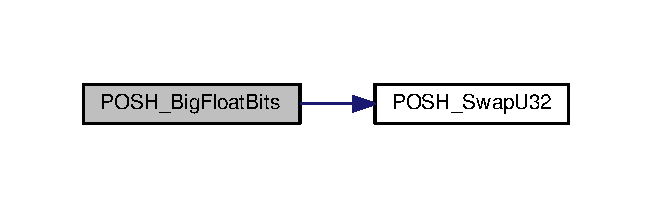
\includegraphics[width=313pt]{d0/dc0/group__FloatingPoint_ga1eca8e7b3d6e9f4953765d2bf33b0426_cgraph}
\end{center}
\end{figure}




Here is the caller graph for this function\+:
\nopagebreak
\begin{figure}[H]
\begin{center}
\leavevmode
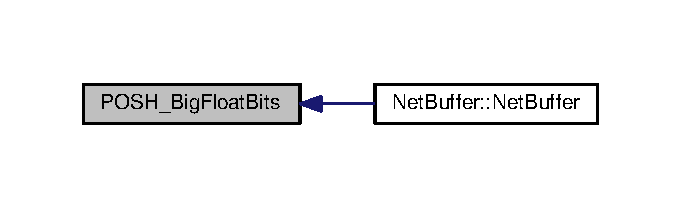
\includegraphics[width=327pt]{d0/dc0/group__FloatingPoint_ga1eca8e7b3d6e9f4953765d2bf33b0426_icgraph}
\end{center}
\end{figure}


\index{Floating Point@{Floating Point}!P\+O\+S\+H\+\_\+\+Double\+Bits@{P\+O\+S\+H\+\_\+\+Double\+Bits}}
\index{P\+O\+S\+H\+\_\+\+Double\+Bits@{P\+O\+S\+H\+\_\+\+Double\+Bits}!Floating Point@{Floating Point}}
\subsubsection[{\texorpdfstring{P\+O\+S\+H\+\_\+\+Double\+Bits(double d, posh\+\_\+byte\+\_\+t dst[8])}{POSH_DoubleBits(double d, posh_byte_t dst[8])}}]{\setlength{\rightskip}{0pt plus 5cm}void P\+O\+S\+H\+\_\+\+Double\+Bits (
\begin{DoxyParamCaption}
\item[{double}]{d, }
\item[{{\bf posh\+\_\+byte\+\_\+t}}]{dst\mbox{[}8\mbox{]}}
\end{DoxyParamCaption}
)}\hypertarget{group__FloatingPoint_gaf99025b522ae347afdcffae40dcacb8e}{}\label{group__FloatingPoint_gaf99025b522ae347afdcffae40dcacb8e}
Extracts raw, little-\/endian bit representation from a 64-\/bit double.


\begin{DoxyParams}{Parameters}
{\em d\mbox{[}in\mbox{]}} & 64-\/bit double precision value \\
\hline
{\em dst\mbox{[}out\mbox{]}} & 8-\/byte storage buffer\\
\hline
\end{DoxyParams}
\begin{DoxyReturn}{Returns}
the raw bits used to represent the value \textquotesingle{}d\textquotesingle{}, in the form dst\mbox{[}0\mbox{]}=L\+SB 
\end{DoxyReturn}


Here is the caller graph for this function\+:
\nopagebreak
\begin{figure}[H]
\begin{center}
\leavevmode
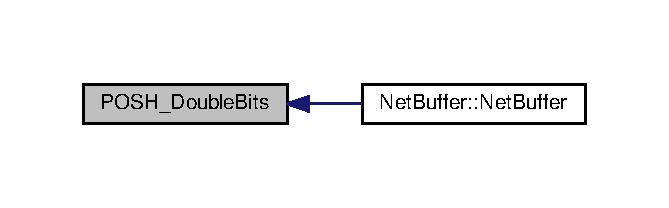
\includegraphics[width=321pt]{d0/dc0/group__FloatingPoint_gaf99025b522ae347afdcffae40dcacb8e_icgraph}
\end{center}
\end{figure}


\index{Floating Point@{Floating Point}!P\+O\+S\+H\+\_\+\+Double\+From\+Bits@{P\+O\+S\+H\+\_\+\+Double\+From\+Bits}}
\index{P\+O\+S\+H\+\_\+\+Double\+From\+Bits@{P\+O\+S\+H\+\_\+\+Double\+From\+Bits}!Floating Point@{Floating Point}}
\subsubsection[{\texorpdfstring{P\+O\+S\+H\+\_\+\+Double\+From\+Bits(const posh\+\_\+byte\+\_\+t src[8])}{POSH_DoubleFromBits(const posh_byte_t src[8])}}]{\setlength{\rightskip}{0pt plus 5cm}double P\+O\+S\+H\+\_\+\+Double\+From\+Bits (
\begin{DoxyParamCaption}
\item[{const {\bf posh\+\_\+byte\+\_\+t}}]{src\mbox{[}8\mbox{]}}
\end{DoxyParamCaption}
)}\hypertarget{group__FloatingPoint_ga87e8b2d4f305581c96b1edb2345a5dbe}{}\label{group__FloatingPoint_ga87e8b2d4f305581c96b1edb2345a5dbe}
Creates a double-\/precision, 64-\/bit floating point value from a set if raw, little-\/endian bits


\begin{DoxyParams}{Parameters}
{\em src\mbox{[}in\mbox{]}} & little-\/endian byte representation of 64-\/bit double precision floating point value \\
\hline
\end{DoxyParams}
\begin{DoxyReturn}{Returns}
double precision floating point representation of the raw bits 
\end{DoxyReturn}
\begin{DoxyRemark}{Remarks}
No error checking is performed, so there are no guarantees that the result is a valid number, nor is there any check to ensure that src is non-\/\+N\+U\+LL. BE C\+A\+R\+E\+F\+UL U\+S\+I\+NG T\+H\+IS. 
\end{DoxyRemark}


Here is the caller graph for this function\+:
\nopagebreak
\begin{figure}[H]
\begin{center}
\leavevmode
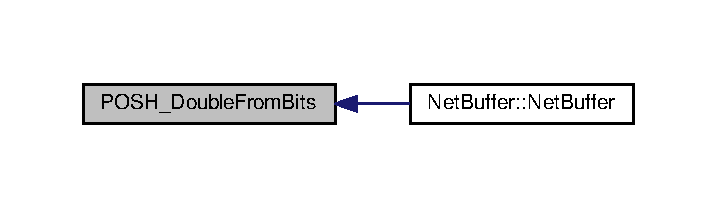
\includegraphics[width=344pt]{d0/dc0/group__FloatingPoint_ga87e8b2d4f305581c96b1edb2345a5dbe_icgraph}
\end{center}
\end{figure}


\index{Floating Point@{Floating Point}!P\+O\+S\+H\+\_\+\+Float\+From\+Big\+Bits@{P\+O\+S\+H\+\_\+\+Float\+From\+Big\+Bits}}
\index{P\+O\+S\+H\+\_\+\+Float\+From\+Big\+Bits@{P\+O\+S\+H\+\_\+\+Float\+From\+Big\+Bits}!Floating Point@{Floating Point}}
\subsubsection[{\texorpdfstring{P\+O\+S\+H\+\_\+\+Float\+From\+Big\+Bits(posh\+\_\+u32\+\_\+t bits)}{POSH_FloatFromBigBits(posh_u32_t bits)}}]{\setlength{\rightskip}{0pt plus 5cm}float P\+O\+S\+H\+\_\+\+Float\+From\+Big\+Bits (
\begin{DoxyParamCaption}
\item[{{\bf posh\+\_\+u32\+\_\+t}}]{bits}
\end{DoxyParamCaption}
)}\hypertarget{group__FloatingPoint_ga1556934ccc724bdf546127f4a2945b31}{}\label{group__FloatingPoint_ga1556934ccc724bdf546127f4a2945b31}
Creates a floating point number from big-\/endian bits


\begin{DoxyParams}{Parameters}
{\em bits\mbox{[}in\mbox{]}} & raw floating point bits in big-\/endian form \\
\hline
\end{DoxyParams}
\begin{DoxyReturn}{Returns}
a floating point number based on the given bit representation 
\end{DoxyReturn}
\begin{DoxyRemark}{Remarks}
No error checking is performed, so there are no guarantees that the result is a valid number. BE C\+A\+R\+E\+F\+UL U\+S\+I\+NG T\+H\+IS. 
\end{DoxyRemark}


Here is the call graph for this function\+:
\nopagebreak
\begin{figure}[H]
\begin{center}
\leavevmode
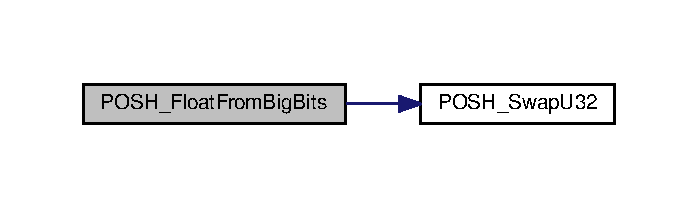
\includegraphics[width=335pt]{d0/dc0/group__FloatingPoint_ga1556934ccc724bdf546127f4a2945b31_cgraph}
\end{center}
\end{figure}




Here is the caller graph for this function\+:
\nopagebreak
\begin{figure}[H]
\begin{center}
\leavevmode
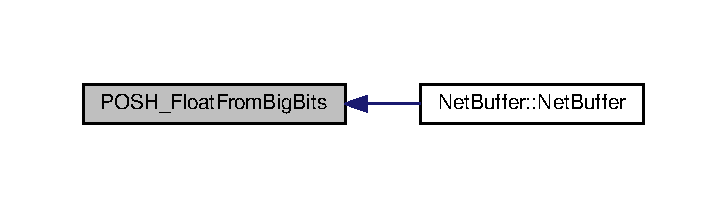
\includegraphics[width=349pt]{d0/dc0/group__FloatingPoint_ga1556934ccc724bdf546127f4a2945b31_icgraph}
\end{center}
\end{figure}


\index{Floating Point@{Floating Point}!P\+O\+S\+H\+\_\+\+Float\+From\+Little\+Bits@{P\+O\+S\+H\+\_\+\+Float\+From\+Little\+Bits}}
\index{P\+O\+S\+H\+\_\+\+Float\+From\+Little\+Bits@{P\+O\+S\+H\+\_\+\+Float\+From\+Little\+Bits}!Floating Point@{Floating Point}}
\subsubsection[{\texorpdfstring{P\+O\+S\+H\+\_\+\+Float\+From\+Little\+Bits(posh\+\_\+u32\+\_\+t bits)}{POSH_FloatFromLittleBits(posh_u32_t bits)}}]{\setlength{\rightskip}{0pt plus 5cm}float P\+O\+S\+H\+\_\+\+Float\+From\+Little\+Bits (
\begin{DoxyParamCaption}
\item[{{\bf posh\+\_\+u32\+\_\+t}}]{bits}
\end{DoxyParamCaption}
)}\hypertarget{group__FloatingPoint_gacefa578ca480f04ec24ce85f7b63634a}{}\label{group__FloatingPoint_gacefa578ca480f04ec24ce85f7b63634a}
Creates a floating point number from little endian bits


\begin{DoxyParams}{Parameters}
{\em bits\mbox{[}in\mbox{]}} & raw floating point bits in little-\/endian form \\
\hline
\end{DoxyParams}
\begin{DoxyReturn}{Returns}
a floating point number based on the given bit representation 
\end{DoxyReturn}
\begin{DoxyRemark}{Remarks}
No error checking is performed, so there are no guarantees that the result is a valid number. BE C\+A\+R\+E\+F\+UL U\+S\+I\+NG T\+H\+IS. 
\end{DoxyRemark}


Here is the call graph for this function\+:
\nopagebreak
\begin{figure}[H]
\begin{center}
\leavevmode
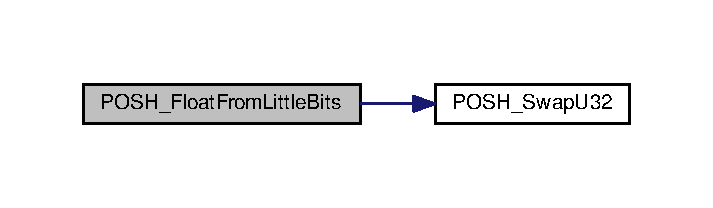
\includegraphics[width=342pt]{d0/dc0/group__FloatingPoint_gacefa578ca480f04ec24ce85f7b63634a_cgraph}
\end{center}
\end{figure}


\index{Floating Point@{Floating Point}!P\+O\+S\+H\+\_\+\+Little\+Float\+Bits@{P\+O\+S\+H\+\_\+\+Little\+Float\+Bits}}
\index{P\+O\+S\+H\+\_\+\+Little\+Float\+Bits@{P\+O\+S\+H\+\_\+\+Little\+Float\+Bits}!Floating Point@{Floating Point}}
\subsubsection[{\texorpdfstring{P\+O\+S\+H\+\_\+\+Little\+Float\+Bits(float f)}{POSH_LittleFloatBits(float f)}}]{\setlength{\rightskip}{0pt plus 5cm}{\bf posh\+\_\+u32\+\_\+t} P\+O\+S\+H\+\_\+\+Little\+Float\+Bits (
\begin{DoxyParamCaption}
\item[{float}]{f}
\end{DoxyParamCaption}
)}\hypertarget{group__FloatingPoint_ga384e7a2791d023062bcd0fb0c56d33cf}{}\label{group__FloatingPoint_ga384e7a2791d023062bcd0fb0c56d33cf}
Extracts raw little-\/endian bits from a 32-\/bit floating point value


\begin{DoxyParams}{Parameters}
{\em f\mbox{[}in\mbox{]}} & floating point value \\
\hline
\end{DoxyParams}
\begin{DoxyReturn}{Returns}
a little-\/endian bit representation of f 
\end{DoxyReturn}


Here is the call graph for this function\+:
\nopagebreak
\begin{figure}[H]
\begin{center}
\leavevmode
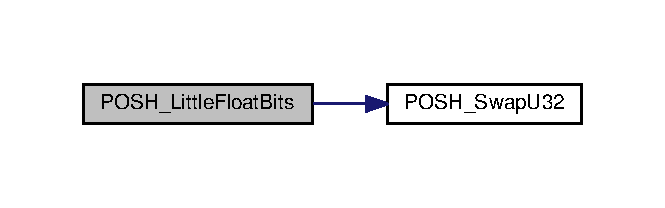
\includegraphics[width=319pt]{d0/dc0/group__FloatingPoint_ga384e7a2791d023062bcd0fb0c56d33cf_cgraph}
\end{center}
\end{figure}



\hypertarget{group__ByteSwapFunctions}{}\section{Byte Swapping Functions}
\label{group__ByteSwapFunctions}\index{Byte Swapping Functions@{Byte Swapping Functions}}
\subsection*{Functions}
\begin{DoxyCompactItemize}
\item 
\hyperlink{group__PoshTypes_ga8ef2f2264276677d018795b0ff67d486}{posh\+\_\+u16\+\_\+t} \hyperlink{group__ByteSwapFunctions_ga401e0af0e8d08dba16164b5c8c9b3afd}{P\+O\+S\+H\+\_\+\+Swap\+U16} (\hyperlink{group__PoshTypes_ga8ef2f2264276677d018795b0ff67d486}{posh\+\_\+u16\+\_\+t} u)
\item 
\hyperlink{group__PoshTypes_gabb2c3e11f94548b8c3bc63fbbe7c2110}{posh\+\_\+s16\+\_\+t} \hyperlink{group__ByteSwapFunctions_ga0b4aa282339ed3629dd4517deb777387}{P\+O\+S\+H\+\_\+\+Swap\+S16} (\hyperlink{group__PoshTypes_gabb2c3e11f94548b8c3bc63fbbe7c2110}{posh\+\_\+s16\+\_\+t} u)
\item 
\hyperlink{group__PoshTypes_ga020bf929bf912667f0fa4312d816c2e0}{posh\+\_\+u32\+\_\+t} \hyperlink{group__ByteSwapFunctions_ga97f53ca21ec6feab173b13693f714b27}{P\+O\+S\+H\+\_\+\+Swap\+U32} (\hyperlink{group__PoshTypes_ga020bf929bf912667f0fa4312d816c2e0}{posh\+\_\+u32\+\_\+t} u)
\item 
\hyperlink{group__PoshTypes_gaa13412fdeac2c495d0e0278bd28ac8cb}{posh\+\_\+s32\+\_\+t} \hyperlink{group__ByteSwapFunctions_ga489b591bc4db4d2682be5f69cc5acb24}{P\+O\+S\+H\+\_\+\+Swap\+S32} (\hyperlink{group__PoshTypes_gaa13412fdeac2c495d0e0278bd28ac8cb}{posh\+\_\+s32\+\_\+t} u)
\end{DoxyCompactItemize}


\subsection{Detailed Description}
These functions perform byte swapping of 16 and 32-\/bit values. The 64-\/bit versions of these functions are documented under Sixty\+Four\+Bit 

\subsection{Function Documentation}
\index{Byte Swapping Functions@{Byte Swapping Functions}!P\+O\+S\+H\+\_\+\+Swap\+S16@{P\+O\+S\+H\+\_\+\+Swap\+S16}}
\index{P\+O\+S\+H\+\_\+\+Swap\+S16@{P\+O\+S\+H\+\_\+\+Swap\+S16}!Byte Swapping Functions@{Byte Swapping Functions}}
\subsubsection[{\texorpdfstring{P\+O\+S\+H\+\_\+\+Swap\+S16(posh\+\_\+s16\+\_\+t u)}{POSH_SwapS16(posh_s16_t u)}}]{\setlength{\rightskip}{0pt plus 5cm}{\bf posh\+\_\+s16\+\_\+t} P\+O\+S\+H\+\_\+\+Swap\+S16 (
\begin{DoxyParamCaption}
\item[{{\bf posh\+\_\+s16\+\_\+t}}]{v}
\end{DoxyParamCaption}
)}\hypertarget{group__ByteSwapFunctions_ga0b4aa282339ed3629dd4517deb777387}{}\label{group__ByteSwapFunctions_ga0b4aa282339ed3629dd4517deb777387}
Byte swaps a 16-\/bit signed value


\begin{DoxyParams}{Parameters}
{\em v\mbox{[}in\mbox{]}} & signed 16-\/bit input value to swap \\
\hline
\end{DoxyParams}
\begin{DoxyReturn}{Returns}
a byte swapped version of v 
\end{DoxyReturn}
\begin{DoxyRemark}{Remarks}
This just calls back to the unsigned version, since byte swapping is independent of sign. However, we still provide this function to avoid signed/unsigned mismatch compiler warnings. 
\end{DoxyRemark}


Here is the call graph for this function\+:
\nopagebreak
\begin{figure}[H]
\begin{center}
\leavevmode
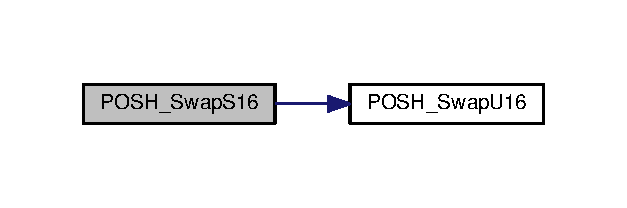
\includegraphics[width=301pt]{d0/d0f/group__ByteSwapFunctions_ga0b4aa282339ed3629dd4517deb777387_cgraph}
\end{center}
\end{figure}


\index{Byte Swapping Functions@{Byte Swapping Functions}!P\+O\+S\+H\+\_\+\+Swap\+S32@{P\+O\+S\+H\+\_\+\+Swap\+S32}}
\index{P\+O\+S\+H\+\_\+\+Swap\+S32@{P\+O\+S\+H\+\_\+\+Swap\+S32}!Byte Swapping Functions@{Byte Swapping Functions}}
\subsubsection[{\texorpdfstring{P\+O\+S\+H\+\_\+\+Swap\+S32(posh\+\_\+s32\+\_\+t u)}{POSH_SwapS32(posh_s32_t u)}}]{\setlength{\rightskip}{0pt plus 5cm}{\bf posh\+\_\+s32\+\_\+t} P\+O\+S\+H\+\_\+\+Swap\+S32 (
\begin{DoxyParamCaption}
\item[{{\bf posh\+\_\+s32\+\_\+t}}]{v}
\end{DoxyParamCaption}
)}\hypertarget{group__ByteSwapFunctions_ga489b591bc4db4d2682be5f69cc5acb24}{}\label{group__ByteSwapFunctions_ga489b591bc4db4d2682be5f69cc5acb24}
Byte swaps a 32-\/bit signed value


\begin{DoxyParams}{Parameters}
{\em v\mbox{[}in\mbox{]}} & signed 32-\/bit input value to swap \\
\hline
\end{DoxyParams}
\begin{DoxyReturn}{Returns}
a byte swapped version of v 
\end{DoxyReturn}
\begin{DoxyRemark}{Remarks}
This just calls back to the unsigned version, since byte swapping is independent of sign. However, we still provide this function to avoid signed/unsigned mismatch compiler warnings. 
\end{DoxyRemark}


Here is the call graph for this function\+:
\nopagebreak
\begin{figure}[H]
\begin{center}
\leavevmode
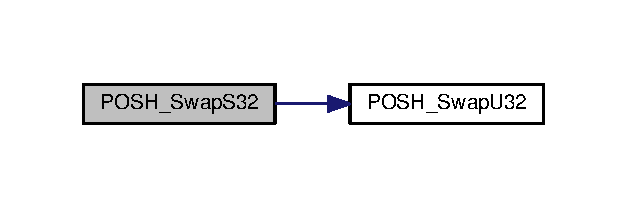
\includegraphics[width=301pt]{d0/d0f/group__ByteSwapFunctions_ga489b591bc4db4d2682be5f69cc5acb24_cgraph}
\end{center}
\end{figure}


\index{Byte Swapping Functions@{Byte Swapping Functions}!P\+O\+S\+H\+\_\+\+Swap\+U16@{P\+O\+S\+H\+\_\+\+Swap\+U16}}
\index{P\+O\+S\+H\+\_\+\+Swap\+U16@{P\+O\+S\+H\+\_\+\+Swap\+U16}!Byte Swapping Functions@{Byte Swapping Functions}}
\subsubsection[{\texorpdfstring{P\+O\+S\+H\+\_\+\+Swap\+U16(posh\+\_\+u16\+\_\+t u)}{POSH_SwapU16(posh_u16_t u)}}]{\setlength{\rightskip}{0pt plus 5cm}{\bf posh\+\_\+u16\+\_\+t} P\+O\+S\+H\+\_\+\+Swap\+U16 (
\begin{DoxyParamCaption}
\item[{{\bf posh\+\_\+u16\+\_\+t}}]{v}
\end{DoxyParamCaption}
)}\hypertarget{group__ByteSwapFunctions_ga401e0af0e8d08dba16164b5c8c9b3afd}{}\label{group__ByteSwapFunctions_ga401e0af0e8d08dba16164b5c8c9b3afd}
Byte swaps a 16-\/bit unsigned value


\begin{DoxyParams}{Parameters}
{\em v\mbox{[}in\mbox{]}} & unsigned 16-\/bit input value to swap \\
\hline
\end{DoxyParams}
\begin{DoxyReturn}{Returns}
a byte swapped version of v 
\end{DoxyReturn}


Here is the caller graph for this function\+:
\nopagebreak
\begin{figure}[H]
\begin{center}
\leavevmode
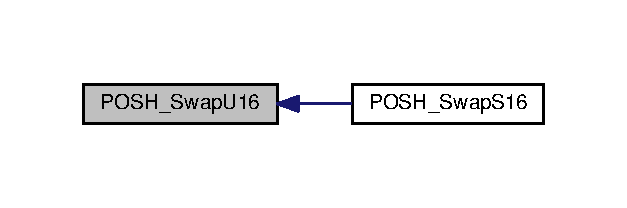
\includegraphics[width=301pt]{d0/d0f/group__ByteSwapFunctions_ga401e0af0e8d08dba16164b5c8c9b3afd_icgraph}
\end{center}
\end{figure}


\index{Byte Swapping Functions@{Byte Swapping Functions}!P\+O\+S\+H\+\_\+\+Swap\+U32@{P\+O\+S\+H\+\_\+\+Swap\+U32}}
\index{P\+O\+S\+H\+\_\+\+Swap\+U32@{P\+O\+S\+H\+\_\+\+Swap\+U32}!Byte Swapping Functions@{Byte Swapping Functions}}
\subsubsection[{\texorpdfstring{P\+O\+S\+H\+\_\+\+Swap\+U32(posh\+\_\+u32\+\_\+t u)}{POSH_SwapU32(posh_u32_t u)}}]{\setlength{\rightskip}{0pt plus 5cm}{\bf posh\+\_\+u32\+\_\+t} P\+O\+S\+H\+\_\+\+Swap\+U32 (
\begin{DoxyParamCaption}
\item[{{\bf posh\+\_\+u32\+\_\+t}}]{v}
\end{DoxyParamCaption}
)}\hypertarget{group__ByteSwapFunctions_ga97f53ca21ec6feab173b13693f714b27}{}\label{group__ByteSwapFunctions_ga97f53ca21ec6feab173b13693f714b27}
Byte swaps a 32-\/bit unsigned value


\begin{DoxyParams}{Parameters}
{\em v\mbox{[}in\mbox{]}} & unsigned 32-\/bit input value to swap \\
\hline
\end{DoxyParams}
\begin{DoxyReturn}{Returns}
a byte swapped version of v 
\end{DoxyReturn}


Here is the caller graph for this function\+:
\nopagebreak
\begin{figure}[H]
\begin{center}
\leavevmode
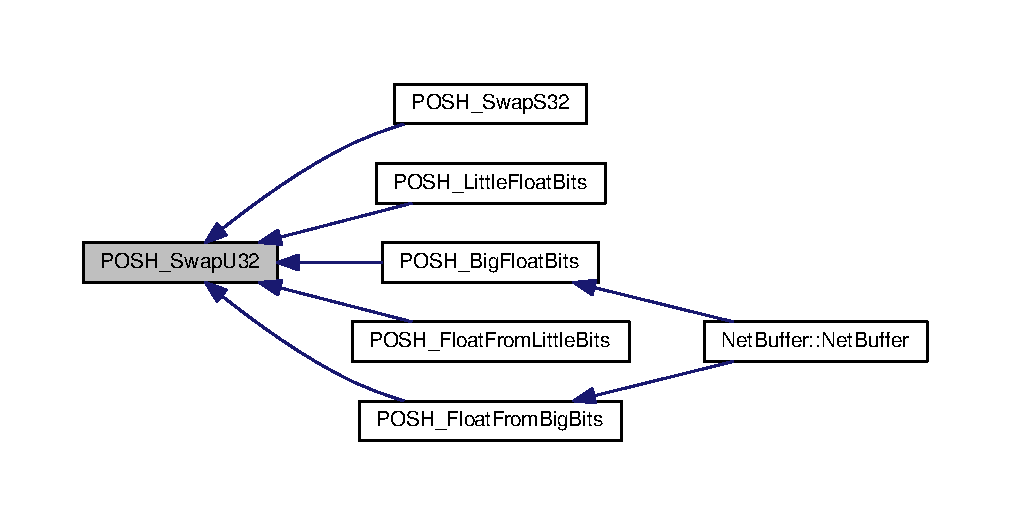
\includegraphics[width=350pt]{d0/d0f/group__ByteSwapFunctions_ga97f53ca21ec6feab173b13693f714b27_icgraph}
\end{center}
\end{figure}



\hypertarget{group__MemoryBuffer}{}\section{In Memory Serialization/\+Deserialization Functions}
\label{group__MemoryBuffer}\index{In Memory Serialization/\+Deserialization  Functions@{In Memory Serialization/\+Deserialization  Functions}}
\subsection*{Functions}
\begin{DoxyCompactItemize}
\item 
\hyperlink{group__PoshTypes_ga8ef2f2264276677d018795b0ff67d486}{posh\+\_\+u16\+\_\+t} $\ast$ \hyperlink{group__MemoryBuffer_gabc9ddeabcbc3696e7cbbd30d40653292}{P\+O\+S\+H\+\_\+\+Write\+U16\+To\+Little} (void $\ast$dst, \hyperlink{group__PoshTypes_ga8ef2f2264276677d018795b0ff67d486}{posh\+\_\+u16\+\_\+t} value)
\item 
\hyperlink{group__PoshTypes_gabb2c3e11f94548b8c3bc63fbbe7c2110}{posh\+\_\+s16\+\_\+t} $\ast$ \hyperlink{group__MemoryBuffer_ga59abb65bd711a2cc79d190ed5ebeaf87}{P\+O\+S\+H\+\_\+\+Write\+S16\+To\+Little} (void $\ast$dst, \hyperlink{group__PoshTypes_gabb2c3e11f94548b8c3bc63fbbe7c2110}{posh\+\_\+s16\+\_\+t} value)
\item 
\hyperlink{group__PoshTypes_ga020bf929bf912667f0fa4312d816c2e0}{posh\+\_\+u32\+\_\+t} $\ast$ \hyperlink{group__MemoryBuffer_gac0bc12452f6b9a48b61c8fec0897297c}{P\+O\+S\+H\+\_\+\+Write\+U32\+To\+Little} (void $\ast$dst, \hyperlink{group__PoshTypes_ga020bf929bf912667f0fa4312d816c2e0}{posh\+\_\+u32\+\_\+t} value)
\item 
\hyperlink{group__PoshTypes_gaa13412fdeac2c495d0e0278bd28ac8cb}{posh\+\_\+s32\+\_\+t} $\ast$ \hyperlink{group__MemoryBuffer_ga745f6b6dd96c185f1a63120b20cff195}{P\+O\+S\+H\+\_\+\+Write\+S32\+To\+Little} (void $\ast$dst, \hyperlink{group__PoshTypes_gaa13412fdeac2c495d0e0278bd28ac8cb}{posh\+\_\+s32\+\_\+t} value)
\item 
\hyperlink{group__PoshTypes_ga8ef2f2264276677d018795b0ff67d486}{posh\+\_\+u16\+\_\+t} $\ast$ \hyperlink{group__MemoryBuffer_ga8d58963ea4443ea22f0c80552a10504c}{P\+O\+S\+H\+\_\+\+Write\+U16\+To\+Big} (void $\ast$dst, \hyperlink{group__PoshTypes_ga8ef2f2264276677d018795b0ff67d486}{posh\+\_\+u16\+\_\+t} value)
\item 
\hyperlink{group__PoshTypes_gabb2c3e11f94548b8c3bc63fbbe7c2110}{posh\+\_\+s16\+\_\+t} $\ast$ \hyperlink{group__MemoryBuffer_gaedbeff50ae5ab8bb235c9670d7d50e65}{P\+O\+S\+H\+\_\+\+Write\+S16\+To\+Big} (void $\ast$dst, \hyperlink{group__PoshTypes_gabb2c3e11f94548b8c3bc63fbbe7c2110}{posh\+\_\+s16\+\_\+t} value)
\item 
\hyperlink{group__PoshTypes_ga020bf929bf912667f0fa4312d816c2e0}{posh\+\_\+u32\+\_\+t} $\ast$ \hyperlink{group__MemoryBuffer_ga50e70604bd589ee0e31bb05ffa894025}{P\+O\+S\+H\+\_\+\+Write\+U32\+To\+Big} (void $\ast$dst, \hyperlink{group__PoshTypes_ga020bf929bf912667f0fa4312d816c2e0}{posh\+\_\+u32\+\_\+t} value)
\item 
\hyperlink{group__PoshTypes_gaa13412fdeac2c495d0e0278bd28ac8cb}{posh\+\_\+s32\+\_\+t} $\ast$ \hyperlink{group__MemoryBuffer_ga55857b82054acbe60119c04f5f62f0d4}{P\+O\+S\+H\+\_\+\+Write\+S32\+To\+Big} (void $\ast$dst, \hyperlink{group__PoshTypes_gaa13412fdeac2c495d0e0278bd28ac8cb}{posh\+\_\+s32\+\_\+t} value)
\item 
\hyperlink{group__PoshTypes_ga8ef2f2264276677d018795b0ff67d486}{posh\+\_\+u16\+\_\+t} \hyperlink{group__MemoryBuffer_gaf1415105ce1d48d08d2b181b9f7f267e}{P\+O\+S\+H\+\_\+\+Read\+U16\+From\+Little} (const void $\ast$src)
\item 
\hyperlink{group__PoshTypes_gabb2c3e11f94548b8c3bc63fbbe7c2110}{posh\+\_\+s16\+\_\+t} \hyperlink{group__MemoryBuffer_ga9eb41467ccc40d4234447d0f90014911}{P\+O\+S\+H\+\_\+\+Read\+S16\+From\+Little} (const void $\ast$src)
\item 
\hyperlink{group__PoshTypes_ga020bf929bf912667f0fa4312d816c2e0}{posh\+\_\+u32\+\_\+t} \hyperlink{group__MemoryBuffer_gacbf72e43b684db66c0087f51c9bd4967}{P\+O\+S\+H\+\_\+\+Read\+U32\+From\+Little} (const void $\ast$src)
\item 
\hyperlink{group__PoshTypes_gaa13412fdeac2c495d0e0278bd28ac8cb}{posh\+\_\+s32\+\_\+t} \hyperlink{group__MemoryBuffer_ga2e2ad299e028edd9d050d50dfa3a5575}{P\+O\+S\+H\+\_\+\+Read\+S32\+From\+Little} (const void $\ast$src)
\item 
\hyperlink{group__PoshTypes_ga8ef2f2264276677d018795b0ff67d486}{posh\+\_\+u16\+\_\+t} \hyperlink{group__MemoryBuffer_ga896f0a5ea23035ef39e778dbeb409d64}{P\+O\+S\+H\+\_\+\+Read\+U16\+From\+Big} (const void $\ast$src)
\item 
\hyperlink{group__PoshTypes_gabb2c3e11f94548b8c3bc63fbbe7c2110}{posh\+\_\+s16\+\_\+t} \hyperlink{group__MemoryBuffer_gaf642e7bebe90a0d68471b9fbc80042d2}{P\+O\+S\+H\+\_\+\+Read\+S16\+From\+Big} (const void $\ast$src)
\item 
\hyperlink{group__PoshTypes_ga020bf929bf912667f0fa4312d816c2e0}{posh\+\_\+u32\+\_\+t} \hyperlink{group__MemoryBuffer_ga2e4f347d47fc307e497cc9be04dd22dd}{P\+O\+S\+H\+\_\+\+Read\+U32\+From\+Big} (const void $\ast$src)
\item 
\hyperlink{group__PoshTypes_gaa13412fdeac2c495d0e0278bd28ac8cb}{posh\+\_\+s32\+\_\+t} \hyperlink{group__MemoryBuffer_ga28207cf0a49b8eee0fa5ad048f1d0957}{P\+O\+S\+H\+\_\+\+Read\+S32\+From\+Big} (const void $\ast$src)
\end{DoxyCompactItemize}


\subsection{Detailed Description}
These functions take host endian values and serialize them into explicit endianess buffers and vice versa. The 64-\/bit versions of these functions can be found under Sixty\+Four\+Bit

Here\textquotesingle{}s an example usage that serializes a struct into a big-\/endian buffer\+:

\begin{DoxyVerb}*
*  struct mystruct
*  {
*  posh_u16_t u16;
*  posh_s32_t s32;
*  };
*
*  void WriteStruct( void *buffer, const struct mystruct *s )
*  {
*  void *p = buffer;
*
*  //The POSH_Write??? functions return a pointer to the next write address
*  p = POSH_WriteU16ToBig( p, &s->u16 );
*  p = POSH_WriteS32ToBig( p, &s->s32 );
*  }
*
*  \end{DoxyVerb}
 

\subsection{Function Documentation}
\index{In Memory Serialization/\+Deserialization  Functions@{In Memory Serialization/\+Deserialization  Functions}!P\+O\+S\+H\+\_\+\+Read\+S16\+From\+Big@{P\+O\+S\+H\+\_\+\+Read\+S16\+From\+Big}}
\index{P\+O\+S\+H\+\_\+\+Read\+S16\+From\+Big@{P\+O\+S\+H\+\_\+\+Read\+S16\+From\+Big}!In Memory Serialization/\+Deserialization  Functions@{In Memory Serialization/\+Deserialization  Functions}}
\subsubsection[{\texorpdfstring{P\+O\+S\+H\+\_\+\+Read\+S16\+From\+Big(const void $\ast$src)}{POSH_ReadS16FromBig(const void *src)}}]{\setlength{\rightskip}{0pt plus 5cm}{\bf posh\+\_\+s16\+\_\+t} P\+O\+S\+H\+\_\+\+Read\+S16\+From\+Big (
\begin{DoxyParamCaption}
\item[{const void $\ast$}]{src}
\end{DoxyParamCaption}
)}\hypertarget{group__MemoryBuffer_gaf642e7bebe90a0d68471b9fbc80042d2}{}\label{group__MemoryBuffer_gaf642e7bebe90a0d68471b9fbc80042d2}
Reads a signed 16-\/bit value from a big-\/endian buffer 
\begin{DoxyParams}{Parameters}
{\em src\mbox{[}in\mbox{]}} & source buffer \\
\hline
\end{DoxyParams}
\begin{DoxyReturn}{Returns}
host-\/endian signed 16-\/bit value 
\end{DoxyReturn}
\index{In Memory Serialization/\+Deserialization  Functions@{In Memory Serialization/\+Deserialization  Functions}!P\+O\+S\+H\+\_\+\+Read\+S16\+From\+Little@{P\+O\+S\+H\+\_\+\+Read\+S16\+From\+Little}}
\index{P\+O\+S\+H\+\_\+\+Read\+S16\+From\+Little@{P\+O\+S\+H\+\_\+\+Read\+S16\+From\+Little}!In Memory Serialization/\+Deserialization  Functions@{In Memory Serialization/\+Deserialization  Functions}}
\subsubsection[{\texorpdfstring{P\+O\+S\+H\+\_\+\+Read\+S16\+From\+Little(const void $\ast$src)}{POSH_ReadS16FromLittle(const void *src)}}]{\setlength{\rightskip}{0pt plus 5cm}{\bf posh\+\_\+s16\+\_\+t} P\+O\+S\+H\+\_\+\+Read\+S16\+From\+Little (
\begin{DoxyParamCaption}
\item[{const void $\ast$}]{src}
\end{DoxyParamCaption}
)}\hypertarget{group__MemoryBuffer_ga9eb41467ccc40d4234447d0f90014911}{}\label{group__MemoryBuffer_ga9eb41467ccc40d4234447d0f90014911}
Reads a signed 16-\/bit value from a little-\/endian buffer 
\begin{DoxyParams}{Parameters}
{\em src\mbox{[}in\mbox{]}} & source buffer \\
\hline
\end{DoxyParams}
\begin{DoxyReturn}{Returns}
host-\/endian signed 16-\/bit value 
\end{DoxyReturn}
\index{In Memory Serialization/\+Deserialization  Functions@{In Memory Serialization/\+Deserialization  Functions}!P\+O\+S\+H\+\_\+\+Read\+S32\+From\+Big@{P\+O\+S\+H\+\_\+\+Read\+S32\+From\+Big}}
\index{P\+O\+S\+H\+\_\+\+Read\+S32\+From\+Big@{P\+O\+S\+H\+\_\+\+Read\+S32\+From\+Big}!In Memory Serialization/\+Deserialization  Functions@{In Memory Serialization/\+Deserialization  Functions}}
\subsubsection[{\texorpdfstring{P\+O\+S\+H\+\_\+\+Read\+S32\+From\+Big(const void $\ast$src)}{POSH_ReadS32FromBig(const void *src)}}]{\setlength{\rightskip}{0pt plus 5cm}{\bf posh\+\_\+s32\+\_\+t} P\+O\+S\+H\+\_\+\+Read\+S32\+From\+Big (
\begin{DoxyParamCaption}
\item[{const void $\ast$}]{src}
\end{DoxyParamCaption}
)}\hypertarget{group__MemoryBuffer_ga28207cf0a49b8eee0fa5ad048f1d0957}{}\label{group__MemoryBuffer_ga28207cf0a49b8eee0fa5ad048f1d0957}
Reads a signed 32-\/bit value from a big-\/endian buffer 
\begin{DoxyParams}{Parameters}
{\em src\mbox{[}in\mbox{]}} & source buffer \\
\hline
\end{DoxyParams}
\begin{DoxyReturn}{Returns}
host-\/endian signed 32-\/bit value 
\end{DoxyReturn}


Here is the caller graph for this function\+:
\nopagebreak
\begin{figure}[H]
\begin{center}
\leavevmode
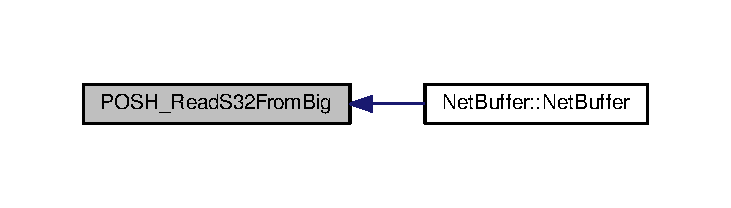
\includegraphics[width=350pt]{dd/dda/group__MemoryBuffer_ga28207cf0a49b8eee0fa5ad048f1d0957_icgraph}
\end{center}
\end{figure}


\index{In Memory Serialization/\+Deserialization  Functions@{In Memory Serialization/\+Deserialization  Functions}!P\+O\+S\+H\+\_\+\+Read\+S32\+From\+Little@{P\+O\+S\+H\+\_\+\+Read\+S32\+From\+Little}}
\index{P\+O\+S\+H\+\_\+\+Read\+S32\+From\+Little@{P\+O\+S\+H\+\_\+\+Read\+S32\+From\+Little}!In Memory Serialization/\+Deserialization  Functions@{In Memory Serialization/\+Deserialization  Functions}}
\subsubsection[{\texorpdfstring{P\+O\+S\+H\+\_\+\+Read\+S32\+From\+Little(const void $\ast$src)}{POSH_ReadS32FromLittle(const void *src)}}]{\setlength{\rightskip}{0pt plus 5cm}{\bf posh\+\_\+s32\+\_\+t} P\+O\+S\+H\+\_\+\+Read\+S32\+From\+Little (
\begin{DoxyParamCaption}
\item[{const void $\ast$}]{src}
\end{DoxyParamCaption}
)}\hypertarget{group__MemoryBuffer_ga2e2ad299e028edd9d050d50dfa3a5575}{}\label{group__MemoryBuffer_ga2e2ad299e028edd9d050d50dfa3a5575}
Reads a signed 32-\/bit value from a little-\/endian buffer 
\begin{DoxyParams}{Parameters}
{\em src\mbox{[}in\mbox{]}} & source buffer \\
\hline
\end{DoxyParams}
\begin{DoxyReturn}{Returns}
host-\/endian signed 32-\/bit value 
\end{DoxyReturn}
\index{In Memory Serialization/\+Deserialization  Functions@{In Memory Serialization/\+Deserialization  Functions}!P\+O\+S\+H\+\_\+\+Read\+U16\+From\+Big@{P\+O\+S\+H\+\_\+\+Read\+U16\+From\+Big}}
\index{P\+O\+S\+H\+\_\+\+Read\+U16\+From\+Big@{P\+O\+S\+H\+\_\+\+Read\+U16\+From\+Big}!In Memory Serialization/\+Deserialization  Functions@{In Memory Serialization/\+Deserialization  Functions}}
\subsubsection[{\texorpdfstring{P\+O\+S\+H\+\_\+\+Read\+U16\+From\+Big(const void $\ast$src)}{POSH_ReadU16FromBig(const void *src)}}]{\setlength{\rightskip}{0pt plus 5cm}{\bf posh\+\_\+u16\+\_\+t} P\+O\+S\+H\+\_\+\+Read\+U16\+From\+Big (
\begin{DoxyParamCaption}
\item[{const void $\ast$}]{src}
\end{DoxyParamCaption}
)}\hypertarget{group__MemoryBuffer_ga896f0a5ea23035ef39e778dbeb409d64}{}\label{group__MemoryBuffer_ga896f0a5ea23035ef39e778dbeb409d64}
Reads an unsigned 16-\/bit value from a big-\/endian buffer 
\begin{DoxyParams}{Parameters}
{\em src\mbox{[}in\mbox{]}} & source buffer \\
\hline
\end{DoxyParams}
\begin{DoxyReturn}{Returns}
host-\/endian unsigned 16-\/bit value 
\end{DoxyReturn}


Here is the caller graph for this function\+:
\nopagebreak
\begin{figure}[H]
\begin{center}
\leavevmode
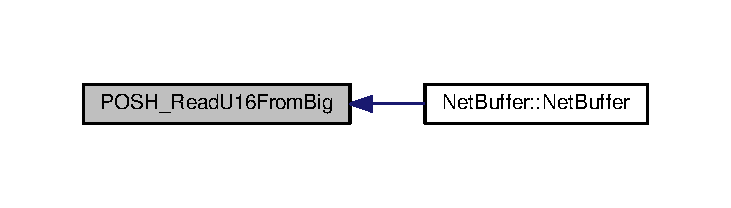
\includegraphics[width=350pt]{dd/dda/group__MemoryBuffer_ga896f0a5ea23035ef39e778dbeb409d64_icgraph}
\end{center}
\end{figure}


\index{In Memory Serialization/\+Deserialization  Functions@{In Memory Serialization/\+Deserialization  Functions}!P\+O\+S\+H\+\_\+\+Read\+U16\+From\+Little@{P\+O\+S\+H\+\_\+\+Read\+U16\+From\+Little}}
\index{P\+O\+S\+H\+\_\+\+Read\+U16\+From\+Little@{P\+O\+S\+H\+\_\+\+Read\+U16\+From\+Little}!In Memory Serialization/\+Deserialization  Functions@{In Memory Serialization/\+Deserialization  Functions}}
\subsubsection[{\texorpdfstring{P\+O\+S\+H\+\_\+\+Read\+U16\+From\+Little(const void $\ast$src)}{POSH_ReadU16FromLittle(const void *src)}}]{\setlength{\rightskip}{0pt plus 5cm}{\bf posh\+\_\+u16\+\_\+t} P\+O\+S\+H\+\_\+\+Read\+U16\+From\+Little (
\begin{DoxyParamCaption}
\item[{const void $\ast$}]{src}
\end{DoxyParamCaption}
)}\hypertarget{group__MemoryBuffer_gaf1415105ce1d48d08d2b181b9f7f267e}{}\label{group__MemoryBuffer_gaf1415105ce1d48d08d2b181b9f7f267e}
Reads an unsigned 16-\/bit value from a little-\/endian buffer 
\begin{DoxyParams}{Parameters}
{\em src\mbox{[}in\mbox{]}} & source buffer \\
\hline
\end{DoxyParams}
\begin{DoxyReturn}{Returns}
host-\/endian unsigned 16-\/bit value 
\end{DoxyReturn}
\index{In Memory Serialization/\+Deserialization  Functions@{In Memory Serialization/\+Deserialization  Functions}!P\+O\+S\+H\+\_\+\+Read\+U32\+From\+Big@{P\+O\+S\+H\+\_\+\+Read\+U32\+From\+Big}}
\index{P\+O\+S\+H\+\_\+\+Read\+U32\+From\+Big@{P\+O\+S\+H\+\_\+\+Read\+U32\+From\+Big}!In Memory Serialization/\+Deserialization  Functions@{In Memory Serialization/\+Deserialization  Functions}}
\subsubsection[{\texorpdfstring{P\+O\+S\+H\+\_\+\+Read\+U32\+From\+Big(const void $\ast$src)}{POSH_ReadU32FromBig(const void *src)}}]{\setlength{\rightskip}{0pt plus 5cm}{\bf posh\+\_\+u32\+\_\+t} P\+O\+S\+H\+\_\+\+Read\+U32\+From\+Big (
\begin{DoxyParamCaption}
\item[{const void $\ast$}]{src}
\end{DoxyParamCaption}
)}\hypertarget{group__MemoryBuffer_ga2e4f347d47fc307e497cc9be04dd22dd}{}\label{group__MemoryBuffer_ga2e4f347d47fc307e497cc9be04dd22dd}
Reads an unsigned 32-\/bit value from a big-\/endian buffer 
\begin{DoxyParams}{Parameters}
{\em src\mbox{[}in\mbox{]}} & source buffer \\
\hline
\end{DoxyParams}
\begin{DoxyReturn}{Returns}
host-\/endian unsigned 32-\/bit value 
\end{DoxyReturn}


Here is the caller graph for this function\+:
\nopagebreak
\begin{figure}[H]
\begin{center}
\leavevmode
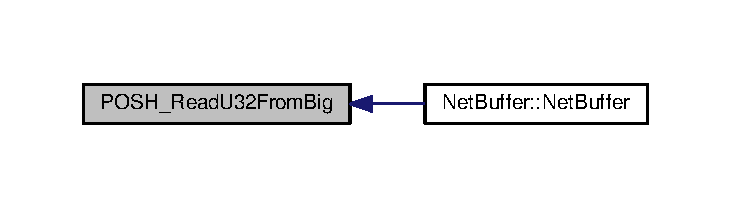
\includegraphics[width=350pt]{dd/dda/group__MemoryBuffer_ga2e4f347d47fc307e497cc9be04dd22dd_icgraph}
\end{center}
\end{figure}


\index{In Memory Serialization/\+Deserialization  Functions@{In Memory Serialization/\+Deserialization  Functions}!P\+O\+S\+H\+\_\+\+Read\+U32\+From\+Little@{P\+O\+S\+H\+\_\+\+Read\+U32\+From\+Little}}
\index{P\+O\+S\+H\+\_\+\+Read\+U32\+From\+Little@{P\+O\+S\+H\+\_\+\+Read\+U32\+From\+Little}!In Memory Serialization/\+Deserialization  Functions@{In Memory Serialization/\+Deserialization  Functions}}
\subsubsection[{\texorpdfstring{P\+O\+S\+H\+\_\+\+Read\+U32\+From\+Little(const void $\ast$src)}{POSH_ReadU32FromLittle(const void *src)}}]{\setlength{\rightskip}{0pt plus 5cm}{\bf posh\+\_\+u32\+\_\+t} P\+O\+S\+H\+\_\+\+Read\+U32\+From\+Little (
\begin{DoxyParamCaption}
\item[{const void $\ast$}]{src}
\end{DoxyParamCaption}
)}\hypertarget{group__MemoryBuffer_gacbf72e43b684db66c0087f51c9bd4967}{}\label{group__MemoryBuffer_gacbf72e43b684db66c0087f51c9bd4967}
Reads an unsigned 32-\/bit value from a little-\/endian buffer 
\begin{DoxyParams}{Parameters}
{\em src\mbox{[}in\mbox{]}} & source buffer \\
\hline
\end{DoxyParams}
\begin{DoxyReturn}{Returns}
host-\/endian unsigned 32-\/bit value 
\end{DoxyReturn}
\index{In Memory Serialization/\+Deserialization  Functions@{In Memory Serialization/\+Deserialization  Functions}!P\+O\+S\+H\+\_\+\+Write\+S16\+To\+Big@{P\+O\+S\+H\+\_\+\+Write\+S16\+To\+Big}}
\index{P\+O\+S\+H\+\_\+\+Write\+S16\+To\+Big@{P\+O\+S\+H\+\_\+\+Write\+S16\+To\+Big}!In Memory Serialization/\+Deserialization  Functions@{In Memory Serialization/\+Deserialization  Functions}}
\subsubsection[{\texorpdfstring{P\+O\+S\+H\+\_\+\+Write\+S16\+To\+Big(void $\ast$dst, posh\+\_\+s16\+\_\+t value)}{POSH_WriteS16ToBig(void *dst, posh_s16_t value)}}]{\setlength{\rightskip}{0pt plus 5cm}{\bf posh\+\_\+s16\+\_\+t}$\ast$ P\+O\+S\+H\+\_\+\+Write\+S16\+To\+Big (
\begin{DoxyParamCaption}
\item[{void $\ast$}]{dst, }
\item[{{\bf posh\+\_\+s16\+\_\+t}}]{value}
\end{DoxyParamCaption}
)}\hypertarget{group__MemoryBuffer_gaedbeff50ae5ab8bb235c9670d7d50e65}{}\label{group__MemoryBuffer_gaedbeff50ae5ab8bb235c9670d7d50e65}
Writes a signed 16-\/bit value to a big endian buffer


\begin{DoxyParams}{Parameters}
{\em dst\mbox{[}out\mbox{]}} & pointer to the destination buffer, may not be N\+U\+LL \\
\hline
{\em value\mbox{[}in\mbox{]}} & host-\/endian signed 16-\/bit value \\
\hline
\end{DoxyParams}
\begin{DoxyReturn}{Returns}
a pointer to the location two bytes after dst 
\end{DoxyReturn}
\begin{DoxyRemark}{Remarks}
does no validation of the inputs. This simply calls \hyperlink{group__MemoryBuffer_gabc9ddeabcbc3696e7cbbd30d40653292}{P\+O\+S\+H\+\_\+\+Write\+U16\+To\+Little()} with appropriate casting. 
\end{DoxyRemark}


Here is the call graph for this function\+:
\nopagebreak
\begin{figure}[H]
\begin{center}
\leavevmode
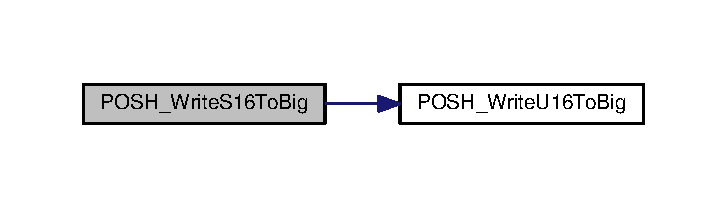
\includegraphics[width=349pt]{dd/dda/group__MemoryBuffer_gaedbeff50ae5ab8bb235c9670d7d50e65_cgraph}
\end{center}
\end{figure}


\index{In Memory Serialization/\+Deserialization  Functions@{In Memory Serialization/\+Deserialization  Functions}!P\+O\+S\+H\+\_\+\+Write\+S16\+To\+Little@{P\+O\+S\+H\+\_\+\+Write\+S16\+To\+Little}}
\index{P\+O\+S\+H\+\_\+\+Write\+S16\+To\+Little@{P\+O\+S\+H\+\_\+\+Write\+S16\+To\+Little}!In Memory Serialization/\+Deserialization  Functions@{In Memory Serialization/\+Deserialization  Functions}}
\subsubsection[{\texorpdfstring{P\+O\+S\+H\+\_\+\+Write\+S16\+To\+Little(void $\ast$dst, posh\+\_\+s16\+\_\+t value)}{POSH_WriteS16ToLittle(void *dst, posh_s16_t value)}}]{\setlength{\rightskip}{0pt plus 5cm}{\bf posh\+\_\+s16\+\_\+t}$\ast$ P\+O\+S\+H\+\_\+\+Write\+S16\+To\+Little (
\begin{DoxyParamCaption}
\item[{void $\ast$}]{dst, }
\item[{{\bf posh\+\_\+s16\+\_\+t}}]{value}
\end{DoxyParamCaption}
)}\hypertarget{group__MemoryBuffer_ga59abb65bd711a2cc79d190ed5ebeaf87}{}\label{group__MemoryBuffer_ga59abb65bd711a2cc79d190ed5ebeaf87}
Writes a signed 16-\/bit value to a little endian buffer


\begin{DoxyParams}{Parameters}
{\em dst\mbox{[}out\mbox{]}} & pointer to the destination buffer, may not be N\+U\+LL \\
\hline
{\em value\mbox{[}in\mbox{]}} & host-\/endian signed 16-\/bit value \\
\hline
\end{DoxyParams}
\begin{DoxyReturn}{Returns}
a pointer to the location two bytes after dst 
\end{DoxyReturn}
\begin{DoxyRemark}{Remarks}
does no validation of the inputs. This simply calls \hyperlink{group__MemoryBuffer_gabc9ddeabcbc3696e7cbbd30d40653292}{P\+O\+S\+H\+\_\+\+Write\+U16\+To\+Little()} with appropriate casting. 
\end{DoxyRemark}


Here is the call graph for this function\+:
\nopagebreak
\begin{figure}[H]
\begin{center}
\leavevmode
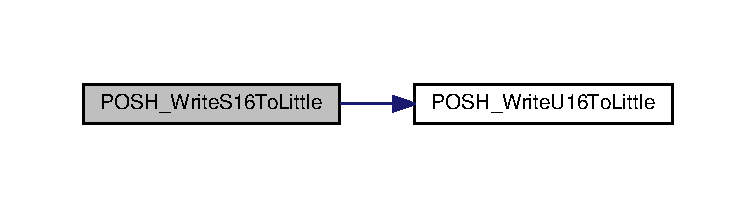
\includegraphics[width=350pt]{dd/dda/group__MemoryBuffer_ga59abb65bd711a2cc79d190ed5ebeaf87_cgraph}
\end{center}
\end{figure}


\index{In Memory Serialization/\+Deserialization  Functions@{In Memory Serialization/\+Deserialization  Functions}!P\+O\+S\+H\+\_\+\+Write\+S32\+To\+Big@{P\+O\+S\+H\+\_\+\+Write\+S32\+To\+Big}}
\index{P\+O\+S\+H\+\_\+\+Write\+S32\+To\+Big@{P\+O\+S\+H\+\_\+\+Write\+S32\+To\+Big}!In Memory Serialization/\+Deserialization  Functions@{In Memory Serialization/\+Deserialization  Functions}}
\subsubsection[{\texorpdfstring{P\+O\+S\+H\+\_\+\+Write\+S32\+To\+Big(void $\ast$dst, posh\+\_\+s32\+\_\+t value)}{POSH_WriteS32ToBig(void *dst, posh_s32_t value)}}]{\setlength{\rightskip}{0pt plus 5cm}{\bf posh\+\_\+s32\+\_\+t}$\ast$ P\+O\+S\+H\+\_\+\+Write\+S32\+To\+Big (
\begin{DoxyParamCaption}
\item[{void $\ast$}]{dst, }
\item[{{\bf posh\+\_\+s32\+\_\+t}}]{value}
\end{DoxyParamCaption}
)}\hypertarget{group__MemoryBuffer_ga55857b82054acbe60119c04f5f62f0d4}{}\label{group__MemoryBuffer_ga55857b82054acbe60119c04f5f62f0d4}
Writes a signed 32-\/bit value to a big endian buffer


\begin{DoxyParams}{Parameters}
{\em dst\mbox{[}out\mbox{]}} & pointer to the destination buffer, may not be N\+U\+LL \\
\hline
{\em value\mbox{[}in\mbox{]}} & host-\/endian signed 32-\/bit value \\
\hline
\end{DoxyParams}
\begin{DoxyReturn}{Returns}
a pointer to the location four bytes after dst 
\end{DoxyReturn}
\begin{DoxyRemark}{Remarks}
does no validation of the inputs. This simply calls \hyperlink{group__MemoryBuffer_ga50e70604bd589ee0e31bb05ffa894025}{P\+O\+S\+H\+\_\+\+Write\+U32\+To\+Big()} with appropriate casting. 
\end{DoxyRemark}


Here is the call graph for this function\+:
\nopagebreak
\begin{figure}[H]
\begin{center}
\leavevmode
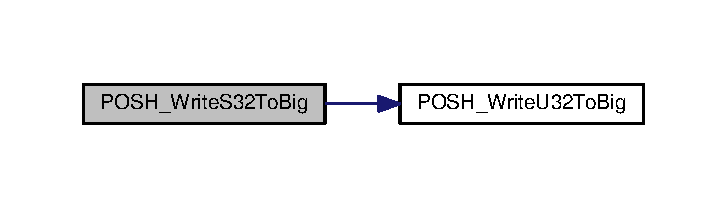
\includegraphics[width=349pt]{dd/dda/group__MemoryBuffer_ga55857b82054acbe60119c04f5f62f0d4_cgraph}
\end{center}
\end{figure}




Here is the caller graph for this function\+:
\nopagebreak
\begin{figure}[H]
\begin{center}
\leavevmode
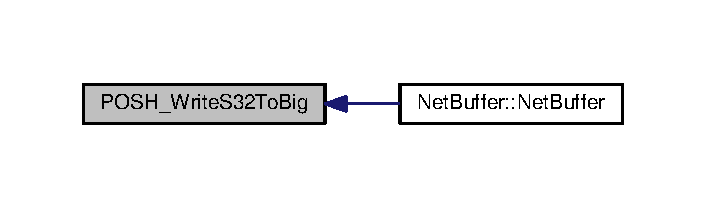
\includegraphics[width=339pt]{dd/dda/group__MemoryBuffer_ga55857b82054acbe60119c04f5f62f0d4_icgraph}
\end{center}
\end{figure}


\index{In Memory Serialization/\+Deserialization  Functions@{In Memory Serialization/\+Deserialization  Functions}!P\+O\+S\+H\+\_\+\+Write\+S32\+To\+Little@{P\+O\+S\+H\+\_\+\+Write\+S32\+To\+Little}}
\index{P\+O\+S\+H\+\_\+\+Write\+S32\+To\+Little@{P\+O\+S\+H\+\_\+\+Write\+S32\+To\+Little}!In Memory Serialization/\+Deserialization  Functions@{In Memory Serialization/\+Deserialization  Functions}}
\subsubsection[{\texorpdfstring{P\+O\+S\+H\+\_\+\+Write\+S32\+To\+Little(void $\ast$dst, posh\+\_\+s32\+\_\+t value)}{POSH_WriteS32ToLittle(void *dst, posh_s32_t value)}}]{\setlength{\rightskip}{0pt plus 5cm}{\bf posh\+\_\+s32\+\_\+t}$\ast$ P\+O\+S\+H\+\_\+\+Write\+S32\+To\+Little (
\begin{DoxyParamCaption}
\item[{void $\ast$}]{dst, }
\item[{{\bf posh\+\_\+s32\+\_\+t}}]{value}
\end{DoxyParamCaption}
)}\hypertarget{group__MemoryBuffer_ga745f6b6dd96c185f1a63120b20cff195}{}\label{group__MemoryBuffer_ga745f6b6dd96c185f1a63120b20cff195}
Writes a signed 32-\/bit value to a little endian buffer


\begin{DoxyParams}{Parameters}
{\em dst\mbox{[}out\mbox{]}} & pointer to the destination buffer, may not be N\+U\+LL \\
\hline
{\em value\mbox{[}in\mbox{]}} & host-\/endian signed 32-\/bit value \\
\hline
\end{DoxyParams}
\begin{DoxyReturn}{Returns}
a pointer to the location four bytes after dst 
\end{DoxyReturn}
\begin{DoxyRemark}{Remarks}
does no validation of the inputs. This simply calls \hyperlink{group__MemoryBuffer_gac0bc12452f6b9a48b61c8fec0897297c}{P\+O\+S\+H\+\_\+\+Write\+U32\+To\+Little()} with appropriate casting. 
\end{DoxyRemark}


Here is the call graph for this function\+:
\nopagebreak
\begin{figure}[H]
\begin{center}
\leavevmode
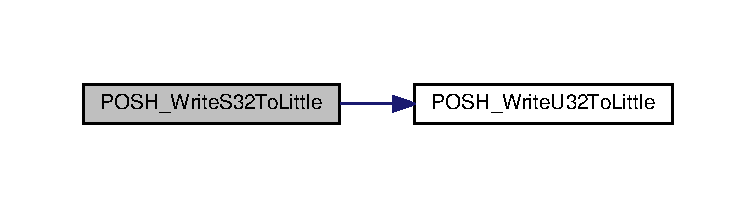
\includegraphics[width=350pt]{dd/dda/group__MemoryBuffer_ga745f6b6dd96c185f1a63120b20cff195_cgraph}
\end{center}
\end{figure}


\index{In Memory Serialization/\+Deserialization  Functions@{In Memory Serialization/\+Deserialization  Functions}!P\+O\+S\+H\+\_\+\+Write\+U16\+To\+Big@{P\+O\+S\+H\+\_\+\+Write\+U16\+To\+Big}}
\index{P\+O\+S\+H\+\_\+\+Write\+U16\+To\+Big@{P\+O\+S\+H\+\_\+\+Write\+U16\+To\+Big}!In Memory Serialization/\+Deserialization  Functions@{In Memory Serialization/\+Deserialization  Functions}}
\subsubsection[{\texorpdfstring{P\+O\+S\+H\+\_\+\+Write\+U16\+To\+Big(void $\ast$dst, posh\+\_\+u16\+\_\+t value)}{POSH_WriteU16ToBig(void *dst, posh_u16_t value)}}]{\setlength{\rightskip}{0pt plus 5cm}{\bf posh\+\_\+u16\+\_\+t}$\ast$ P\+O\+S\+H\+\_\+\+Write\+U16\+To\+Big (
\begin{DoxyParamCaption}
\item[{void $\ast$}]{dst, }
\item[{{\bf posh\+\_\+u16\+\_\+t}}]{value}
\end{DoxyParamCaption}
)}\hypertarget{group__MemoryBuffer_ga8d58963ea4443ea22f0c80552a10504c}{}\label{group__MemoryBuffer_ga8d58963ea4443ea22f0c80552a10504c}
Writes an unsigned 16-\/bit value to a big endian buffer


\begin{DoxyParams}{Parameters}
{\em dst\mbox{[}out\mbox{]}} & pointer to the destination buffer, may not be N\+U\+LL \\
\hline
{\em value\mbox{[}in\mbox{]}} & host-\/endian unsigned 16-\/bit value \\
\hline
\end{DoxyParams}
\begin{DoxyReturn}{Returns}
a pointer to the location two bytes after dst 
\end{DoxyReturn}
\begin{DoxyRemark}{Remarks}
does no validation of the inputs 
\end{DoxyRemark}


Here is the caller graph for this function\+:
\nopagebreak
\begin{figure}[H]
\begin{center}
\leavevmode
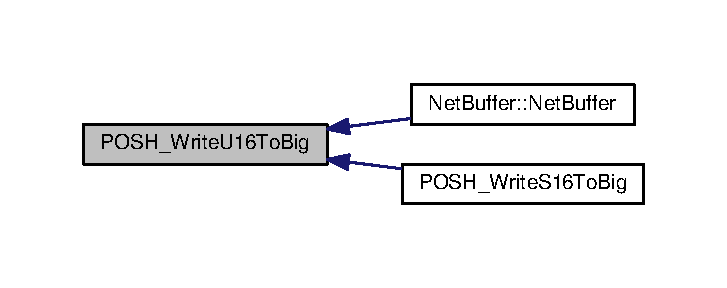
\includegraphics[width=349pt]{dd/dda/group__MemoryBuffer_ga8d58963ea4443ea22f0c80552a10504c_icgraph}
\end{center}
\end{figure}


\index{In Memory Serialization/\+Deserialization  Functions@{In Memory Serialization/\+Deserialization  Functions}!P\+O\+S\+H\+\_\+\+Write\+U16\+To\+Little@{P\+O\+S\+H\+\_\+\+Write\+U16\+To\+Little}}
\index{P\+O\+S\+H\+\_\+\+Write\+U16\+To\+Little@{P\+O\+S\+H\+\_\+\+Write\+U16\+To\+Little}!In Memory Serialization/\+Deserialization  Functions@{In Memory Serialization/\+Deserialization  Functions}}
\subsubsection[{\texorpdfstring{P\+O\+S\+H\+\_\+\+Write\+U16\+To\+Little(void $\ast$dst, posh\+\_\+u16\+\_\+t value)}{POSH_WriteU16ToLittle(void *dst, posh_u16_t value)}}]{\setlength{\rightskip}{0pt plus 5cm}{\bf posh\+\_\+u16\+\_\+t}$\ast$ P\+O\+S\+H\+\_\+\+Write\+U16\+To\+Little (
\begin{DoxyParamCaption}
\item[{void $\ast$}]{dst, }
\item[{{\bf posh\+\_\+u16\+\_\+t}}]{value}
\end{DoxyParamCaption}
)}\hypertarget{group__MemoryBuffer_gabc9ddeabcbc3696e7cbbd30d40653292}{}\label{group__MemoryBuffer_gabc9ddeabcbc3696e7cbbd30d40653292}
Writes an unsigned 16-\/bit value to a little endian buffer


\begin{DoxyParams}{Parameters}
{\em dst\mbox{[}out\mbox{]}} & pointer to the destination buffer, may not be N\+U\+LL \\
\hline
{\em value\mbox{[}in\mbox{]}} & host-\/endian unsigned 16-\/bit value \\
\hline
\end{DoxyParams}
\begin{DoxyReturn}{Returns}
a pointer to the location two bytes after dst 
\end{DoxyReturn}
\begin{DoxyRemark}{Remarks}
does no validation of the inputs 
\end{DoxyRemark}


Here is the caller graph for this function\+:
\nopagebreak
\begin{figure}[H]
\begin{center}
\leavevmode
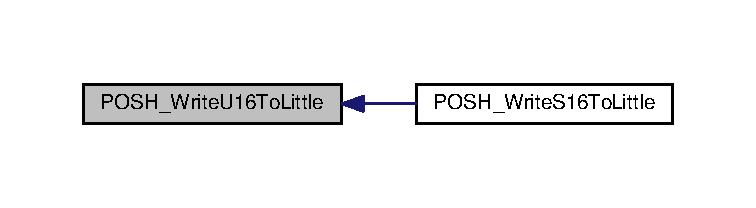
\includegraphics[width=350pt]{dd/dda/group__MemoryBuffer_gabc9ddeabcbc3696e7cbbd30d40653292_icgraph}
\end{center}
\end{figure}


\index{In Memory Serialization/\+Deserialization  Functions@{In Memory Serialization/\+Deserialization  Functions}!P\+O\+S\+H\+\_\+\+Write\+U32\+To\+Big@{P\+O\+S\+H\+\_\+\+Write\+U32\+To\+Big}}
\index{P\+O\+S\+H\+\_\+\+Write\+U32\+To\+Big@{P\+O\+S\+H\+\_\+\+Write\+U32\+To\+Big}!In Memory Serialization/\+Deserialization  Functions@{In Memory Serialization/\+Deserialization  Functions}}
\subsubsection[{\texorpdfstring{P\+O\+S\+H\+\_\+\+Write\+U32\+To\+Big(void $\ast$dst, posh\+\_\+u32\+\_\+t value)}{POSH_WriteU32ToBig(void *dst, posh_u32_t value)}}]{\setlength{\rightskip}{0pt plus 5cm}{\bf posh\+\_\+u32\+\_\+t}$\ast$ P\+O\+S\+H\+\_\+\+Write\+U32\+To\+Big (
\begin{DoxyParamCaption}
\item[{void $\ast$}]{dst, }
\item[{{\bf posh\+\_\+u32\+\_\+t}}]{value}
\end{DoxyParamCaption}
)}\hypertarget{group__MemoryBuffer_ga50e70604bd589ee0e31bb05ffa894025}{}\label{group__MemoryBuffer_ga50e70604bd589ee0e31bb05ffa894025}
Writes an unsigned 32-\/bit value to a big endian buffer


\begin{DoxyParams}{Parameters}
{\em dst\mbox{[}out\mbox{]}} & pointer to the destination buffer, may not be N\+U\+LL \\
\hline
{\em value\mbox{[}in\mbox{]}} & host-\/endian unsigned 32-\/bit value \\
\hline
\end{DoxyParams}
\begin{DoxyReturn}{Returns}
a pointer to the location four bytes after dst 
\end{DoxyReturn}
\begin{DoxyRemark}{Remarks}
does no validation of the inputs. 
\end{DoxyRemark}


Here is the caller graph for this function\+:
\nopagebreak
\begin{figure}[H]
\begin{center}
\leavevmode
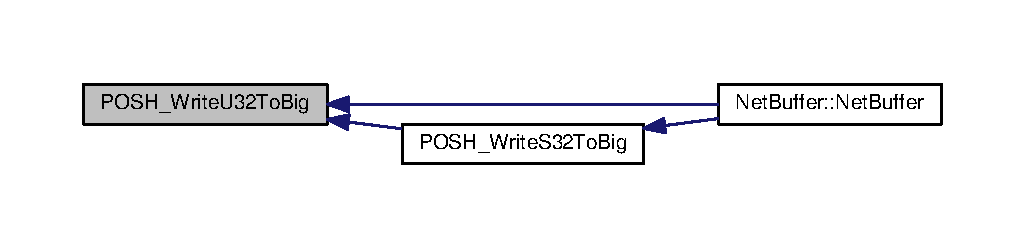
\includegraphics[width=350pt]{dd/dda/group__MemoryBuffer_ga50e70604bd589ee0e31bb05ffa894025_icgraph}
\end{center}
\end{figure}


\index{In Memory Serialization/\+Deserialization  Functions@{In Memory Serialization/\+Deserialization  Functions}!P\+O\+S\+H\+\_\+\+Write\+U32\+To\+Little@{P\+O\+S\+H\+\_\+\+Write\+U32\+To\+Little}}
\index{P\+O\+S\+H\+\_\+\+Write\+U32\+To\+Little@{P\+O\+S\+H\+\_\+\+Write\+U32\+To\+Little}!In Memory Serialization/\+Deserialization  Functions@{In Memory Serialization/\+Deserialization  Functions}}
\subsubsection[{\texorpdfstring{P\+O\+S\+H\+\_\+\+Write\+U32\+To\+Little(void $\ast$dst, posh\+\_\+u32\+\_\+t value)}{POSH_WriteU32ToLittle(void *dst, posh_u32_t value)}}]{\setlength{\rightskip}{0pt plus 5cm}{\bf posh\+\_\+u32\+\_\+t}$\ast$ P\+O\+S\+H\+\_\+\+Write\+U32\+To\+Little (
\begin{DoxyParamCaption}
\item[{void $\ast$}]{dst, }
\item[{{\bf posh\+\_\+u32\+\_\+t}}]{value}
\end{DoxyParamCaption}
)}\hypertarget{group__MemoryBuffer_gac0bc12452f6b9a48b61c8fec0897297c}{}\label{group__MemoryBuffer_gac0bc12452f6b9a48b61c8fec0897297c}
Writes an unsigned 32-\/bit value to a little endian buffer


\begin{DoxyParams}{Parameters}
{\em dst\mbox{[}out\mbox{]}} & pointer to the destination buffer, may not be N\+U\+LL \\
\hline
{\em value\mbox{[}in\mbox{]}} & host-\/endian signed 32-\/bit value \\
\hline
\end{DoxyParams}
\begin{DoxyReturn}{Returns}
a pointer to the location four bytes after dst 
\end{DoxyReturn}
\begin{DoxyRemark}{Remarks}
does no validation of the inputs. 
\end{DoxyRemark}


Here is the caller graph for this function\+:
\nopagebreak
\begin{figure}[H]
\begin{center}
\leavevmode
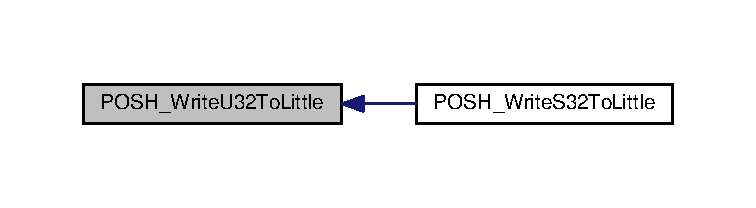
\includegraphics[width=350pt]{dd/dda/group__MemoryBuffer_gac0bc12452f6b9a48b61c8fec0897297c_icgraph}
\end{center}
\end{figure}



\hypertarget{group__ByteSwapMacros}{}\section{Endianess Conversion Macros}
\label{group__ByteSwapMacros}\index{Endianess Conversion Macros@{Endianess Conversion Macros}}
\subsection*{Macros}
\begin{DoxyCompactItemize}
\item 
\#define {\bfseries P\+O\+S\+H\+\_\+\+Big\+U16}(x)~(x)\hypertarget{group__ByteSwapMacros_ga8fe6962c20f07c920073a7bc228b454a}{}\label{group__ByteSwapMacros_ga8fe6962c20f07c920073a7bc228b454a}

\item 
\#define {\bfseries P\+O\+S\+H\+\_\+\+Big\+U32}(x)~(x)\hypertarget{group__ByteSwapMacros_gacecb3c053be442cebd4f9947183537cc}{}\label{group__ByteSwapMacros_gacecb3c053be442cebd4f9947183537cc}

\item 
\#define {\bfseries P\+O\+S\+H\+\_\+\+Big\+S16}(x)~(x)\hypertarget{group__ByteSwapMacros_ga49c7bc8ecf38b60e09118f6cf5a45f5a}{}\label{group__ByteSwapMacros_ga49c7bc8ecf38b60e09118f6cf5a45f5a}

\item 
\#define {\bfseries P\+O\+S\+H\+\_\+\+Big\+S32}(x)~(x)\hypertarget{group__ByteSwapMacros_ga1cfaafaa2b0a92b7987eb257cf0bfa36}{}\label{group__ByteSwapMacros_ga1cfaafaa2b0a92b7987eb257cf0bfa36}

\item 
\#define {\bfseries P\+O\+S\+H\+\_\+\+Little\+U16}(x)~\hyperlink{group__ByteSwapFunctions_ga401e0af0e8d08dba16164b5c8c9b3afd}{P\+O\+S\+H\+\_\+\+Swap\+U16}( x )\hypertarget{group__ByteSwapMacros_ga11c748ee5e06d0b69f78e065f2f7d943}{}\label{group__ByteSwapMacros_ga11c748ee5e06d0b69f78e065f2f7d943}

\item 
\#define {\bfseries P\+O\+S\+H\+\_\+\+Little\+U32}(x)~\hyperlink{group__ByteSwapFunctions_ga97f53ca21ec6feab173b13693f714b27}{P\+O\+S\+H\+\_\+\+Swap\+U32}( x )\hypertarget{group__ByteSwapMacros_gaa20638280e56bfbc7c4b89b816498e56}{}\label{group__ByteSwapMacros_gaa20638280e56bfbc7c4b89b816498e56}

\item 
\#define {\bfseries P\+O\+S\+H\+\_\+\+Little\+S16}(x)~\hyperlink{group__ByteSwapFunctions_ga0b4aa282339ed3629dd4517deb777387}{P\+O\+S\+H\+\_\+\+Swap\+S16}( x )\hypertarget{group__ByteSwapMacros_gabf6d5fbd6c442eeae138737d5bd67ee9}{}\label{group__ByteSwapMacros_gabf6d5fbd6c442eeae138737d5bd67ee9}

\item 
\#define {\bfseries P\+O\+S\+H\+\_\+\+Little\+S32}(x)~\hyperlink{group__ByteSwapFunctions_ga489b591bc4db4d2682be5f69cc5acb24}{P\+O\+S\+H\+\_\+\+Swap\+S32}( x )\hypertarget{group__ByteSwapMacros_gaf7bf5570a1a65707305892a859a1c30a}{}\label{group__ByteSwapMacros_gaf7bf5570a1a65707305892a859a1c30a}

\end{DoxyCompactItemize}


\subsection{Detailed Description}
The actual definitions of these macros depend on the underlying platform. They will either map to a no-\/op, or they will map to the appropriate byte swapping function. 
\hypertarget{group__geom__utils}{}\section{Geom\+\_\+utils}
\label{group__geom__utils}\index{Geom\+\_\+utils@{Geom\+\_\+utils}}
\subsection*{Functions}
\begin{DoxyCompactItemize}
\item 
{\footnotesize template$<$class T $>$ }\\const T \& \hyperlink{group__geom__utils_gad847ae4a7674e661f256da05955e7eb7}{cs\+Max} (const T \&a, const T \&b)
\item 
{\footnotesize template$<$class T $>$ }\\const T \& \hyperlink{group__geom__utils_ga84074616ede088bc78fe3566f87eab81}{cs\+Min} (const T \&a, const T \&b)
\item 
{\footnotesize template$<$class T $>$ }\\void \hyperlink{group__geom__utils_gae988b1834e0316df2aab598e45ea4639}{cs\+Sort} (T \&a, T \&b)
\item 
{\footnotesize template$<$class T , class U $>$ }\\void \hyperlink{group__geom__utils_gac15f60e919826a14d41be755b9a73cad}{cs\+Sort} (T \&a, T \&b, U \&x, U \&\hyperlink{IceUtils_8h_aa7ffaed69623192258fb8679569ff9ba}{y})
\item 
{\footnotesize template$<$class T $>$ }\\T \hyperlink{group__geom__utils_gaa317019148dc6f7659a3a6ab244a39ba}{cs\+Clamp} (const T \&a, T max, T min)
\item 
{\footnotesize template$<$class T $>$ }\\T \hyperlink{group__geom__utils_ga4ae5527a870c7f63d552657905c9939a}{cs\+Smooth\+Step} (const T \&a, T max, T min)
\item 
{\footnotesize template$<$class T , class Tfactor $>$ }\\T \hyperlink{group__geom__utils_gad5238b838897dc5350774d44e5f52001}{cs\+Lerp} (const T \&a, const T \&b, const Tfactor \&f)
\item 
{\footnotesize template$<$class T $>$ }\\T \hyperlink{group__geom__utils_ga490abe249d6289528341e55af14b5e14}{cs\+Square} (const T \&x)
\end{DoxyCompactItemize}
\begin{DoxyCompactItemize}
\item 
C\+S\+\_\+\+F\+O\+R\+C\+E\+I\+N\+L\+I\+NE bool \hyperlink{group__geom__utils_ga9f09b774d5cca1884a80213a91d84b64}{cs\+Finite} (float f)\hypertarget{group__geom__utils_ga9f09b774d5cca1884a80213a91d84b64}{}\label{group__geom__utils_ga9f09b774d5cca1884a80213a91d84b64}

\begin{DoxyCompactList}\small\item\em Checks if a floating point value is finite. \end{DoxyCompactList}\item 
C\+S\+\_\+\+F\+O\+R\+C\+E\+I\+N\+L\+I\+NE bool \hyperlink{group__geom__utils_ga4cd283243ebdd16050674317314df026}{cs\+Finite} (double d)\hypertarget{group__geom__utils_ga4cd283243ebdd16050674317314df026}{}\label{group__geom__utils_ga4cd283243ebdd16050674317314df026}

\begin{DoxyCompactList}\small\item\em Checks if a double-\/precision floating point value is finite. \end{DoxyCompactList}\item 
C\+S\+\_\+\+F\+O\+R\+C\+E\+I\+N\+L\+I\+NE bool \hyperlink{group__geom__utils_gaed49a33b4a87f5efa741888aaf9c5eca}{cs\+NaN} (float f)\hypertarget{group__geom__utils_gaed49a33b4a87f5efa741888aaf9c5eca}{}\label{group__geom__utils_gaed49a33b4a87f5efa741888aaf9c5eca}

\begin{DoxyCompactList}\small\item\em Checks if a floating point value is not-\/a-\/number. \end{DoxyCompactList}\item 
C\+S\+\_\+\+F\+O\+R\+C\+E\+I\+N\+L\+I\+NE bool \hyperlink{group__geom__utils_gac302c6cf13d5219407a1502838dfc1bf}{cs\+NaN} (double d)\hypertarget{group__geom__utils_gac302c6cf13d5219407a1502838dfc1bf}{}\label{group__geom__utils_gac302c6cf13d5219407a1502838dfc1bf}

\begin{DoxyCompactList}\small\item\em Checks if a double-\/precision floating point value is not-\/a-\/number. \end{DoxyCompactList}\item 
C\+S\+\_\+\+F\+O\+R\+C\+E\+I\+N\+L\+I\+NE bool \hyperlink{group__geom__utils_gaca1dc0177b20035712ee9144abdd41f1}{cs\+Normal} (float f)\hypertarget{group__geom__utils_gaca1dc0177b20035712ee9144abdd41f1}{}\label{group__geom__utils_gaca1dc0177b20035712ee9144abdd41f1}

\begin{DoxyCompactList}\small\item\em Checks if a floating point value is normal (not infinite or nan). \end{DoxyCompactList}\item 
C\+S\+\_\+\+F\+O\+R\+C\+E\+I\+N\+L\+I\+NE bool \hyperlink{group__geom__utils_gadc53a075ca2450bd20c4fb1c8cf406aa}{cs\+Normal} (double d)\hypertarget{group__geom__utils_gadc53a075ca2450bd20c4fb1c8cf406aa}{}\label{group__geom__utils_gadc53a075ca2450bd20c4fb1c8cf406aa}

\begin{DoxyCompactList}\small\item\em Checks if a double-\/precision floating point value is normal. \end{DoxyCompactList}\end{DoxyCompactItemize}


\subsection{Detailed Description}


\subsection{Function Documentation}
\index{Geom\+\_\+utils@{Geom\+\_\+utils}!cs\+Clamp@{cs\+Clamp}}
\index{cs\+Clamp@{cs\+Clamp}!Geom\+\_\+utils@{Geom\+\_\+utils}}
\subsubsection[{\texorpdfstring{cs\+Clamp(const T \&a, T max, T min)}{csClamp(const T &a, T max, T min)}}]{\setlength{\rightskip}{0pt plus 5cm}template$<$class T $>$ T cs\+Clamp (
\begin{DoxyParamCaption}
\item[{const T \&}]{a, }
\item[{T}]{max, }
\item[{T}]{min}
\end{DoxyParamCaption}
)}\hypertarget{group__geom__utils_gaa317019148dc6f7659a3a6ab244a39ba}{}\label{group__geom__utils_gaa317019148dc6f7659a3a6ab244a39ba}
Clamp a between max and min. 

Here is the call graph for this function\+:
\nopagebreak
\begin{figure}[H]
\begin{center}
\leavevmode
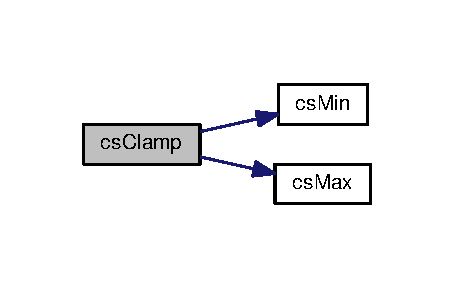
\includegraphics[width=218pt]{d4/d1c/group__geom__utils_gaa317019148dc6f7659a3a6ab244a39ba_cgraph}
\end{center}
\end{figure}


\index{Geom\+\_\+utils@{Geom\+\_\+utils}!cs\+Lerp@{cs\+Lerp}}
\index{cs\+Lerp@{cs\+Lerp}!Geom\+\_\+utils@{Geom\+\_\+utils}}
\subsubsection[{\texorpdfstring{cs\+Lerp(const T \&a, const T \&b, const Tfactor \&f)}{csLerp(const T &a, const T &b, const Tfactor &f)}}]{\setlength{\rightskip}{0pt plus 5cm}template$<$class T , class Tfactor $>$ T cs\+Lerp (
\begin{DoxyParamCaption}
\item[{const T \&}]{a, }
\item[{const T \&}]{b, }
\item[{const Tfactor \&}]{f}
\end{DoxyParamCaption}
)}\hypertarget{group__geom__utils_gad5238b838897dc5350774d44e5f52001}{}\label{group__geom__utils_gad5238b838897dc5350774d44e5f52001}
Performs a linear interpolation between {\itshape a} and {\itshape b} with the factor {\itshape f}. \index{Geom\+\_\+utils@{Geom\+\_\+utils}!cs\+Max@{cs\+Max}}
\index{cs\+Max@{cs\+Max}!Geom\+\_\+utils@{Geom\+\_\+utils}}
\subsubsection[{\texorpdfstring{cs\+Max(const T \&a, const T \&b)}{csMax(const T &a, const T &b)}}]{\setlength{\rightskip}{0pt plus 5cm}template$<$class T $>$ const T\& cs\+Max (
\begin{DoxyParamCaption}
\item[{const T \&}]{a, }
\item[{const T \&}]{b}
\end{DoxyParamCaption}
)}\hypertarget{group__geom__utils_gad847ae4a7674e661f256da05955e7eb7}{}\label{group__geom__utils_gad847ae4a7674e661f256da05955e7eb7}
Returns bigger of a and b. If they are equal, a or b can be returned. 

Here is the caller graph for this function\+:
\nopagebreak
\begin{figure}[H]
\begin{center}
\leavevmode
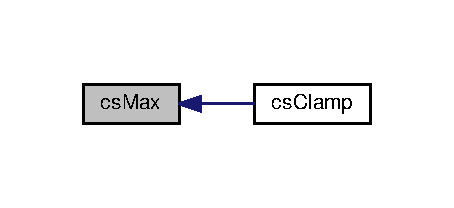
\includegraphics[width=218pt]{d4/d1c/group__geom__utils_gad847ae4a7674e661f256da05955e7eb7_icgraph}
\end{center}
\end{figure}


\index{Geom\+\_\+utils@{Geom\+\_\+utils}!cs\+Min@{cs\+Min}}
\index{cs\+Min@{cs\+Min}!Geom\+\_\+utils@{Geom\+\_\+utils}}
\subsubsection[{\texorpdfstring{cs\+Min(const T \&a, const T \&b)}{csMin(const T &a, const T &b)}}]{\setlength{\rightskip}{0pt plus 5cm}template$<$class T $>$ const T\& cs\+Min (
\begin{DoxyParamCaption}
\item[{const T \&}]{a, }
\item[{const T \&}]{b}
\end{DoxyParamCaption}
)}\hypertarget{group__geom__utils_ga84074616ede088bc78fe3566f87eab81}{}\label{group__geom__utils_ga84074616ede088bc78fe3566f87eab81}
Returns smaller of a and b. If they are equal, a or b can be returned. 

Here is the caller graph for this function\+:
\nopagebreak
\begin{figure}[H]
\begin{center}
\leavevmode
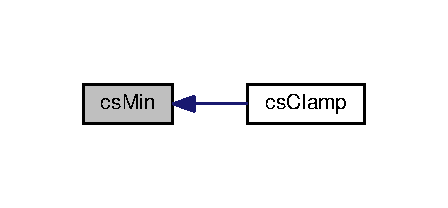
\includegraphics[width=215pt]{d4/d1c/group__geom__utils_ga84074616ede088bc78fe3566f87eab81_icgraph}
\end{center}
\end{figure}


\index{Geom\+\_\+utils@{Geom\+\_\+utils}!cs\+Smooth\+Step@{cs\+Smooth\+Step}}
\index{cs\+Smooth\+Step@{cs\+Smooth\+Step}!Geom\+\_\+utils@{Geom\+\_\+utils}}
\subsubsection[{\texorpdfstring{cs\+Smooth\+Step(const T \&a, T max, T min)}{csSmoothStep(const T &a, T max, T min)}}]{\setlength{\rightskip}{0pt plus 5cm}template$<$class T $>$ T cs\+Smooth\+Step (
\begin{DoxyParamCaption}
\item[{const T \&}]{a, }
\item[{T}]{max, }
\item[{T}]{min}
\end{DoxyParamCaption}
)}\hypertarget{group__geom__utils_ga4ae5527a870c7f63d552657905c9939a}{}\label{group__geom__utils_ga4ae5527a870c7f63d552657905c9939a}
Performs a smooth interpolation of a on range min to max. \begin{DoxyReturn}{Returns}
Smooth interporlated value if {\itshape min} $<$ {\itshape a} $<$ {\itshape max}, and 0 resp. 1 if {\itshape a} is smaller than {\itshape min} resp. larger than {\itshape max}. 
\end{DoxyReturn}
\index{Geom\+\_\+utils@{Geom\+\_\+utils}!cs\+Sort@{cs\+Sort}}
\index{cs\+Sort@{cs\+Sort}!Geom\+\_\+utils@{Geom\+\_\+utils}}
\subsubsection[{\texorpdfstring{cs\+Sort(\+T \&a, T \&b)}{csSort(T &a, T &b)}}]{\setlength{\rightskip}{0pt plus 5cm}template$<$class T $>$ void cs\+Sort (
\begin{DoxyParamCaption}
\item[{T \&}]{a, }
\item[{T \&}]{b}
\end{DoxyParamCaption}
)}\hypertarget{group__geom__utils_gae988b1834e0316df2aab598e45ea4639}{}\label{group__geom__utils_gae988b1834e0316df2aab598e45ea4639}
Sort a and b in order of size. \index{Geom\+\_\+utils@{Geom\+\_\+utils}!cs\+Sort@{cs\+Sort}}
\index{cs\+Sort@{cs\+Sort}!Geom\+\_\+utils@{Geom\+\_\+utils}}
\subsubsection[{\texorpdfstring{cs\+Sort(\+T \&a, T \&b, U \&x, U \&y)}{csSort(T &a, T &b, U &x, U &y)}}]{\setlength{\rightskip}{0pt plus 5cm}template$<$class T , class U $>$ void cs\+Sort (
\begin{DoxyParamCaption}
\item[{T \&}]{a, }
\item[{T \&}]{b, }
\item[{U \&}]{x, }
\item[{U \&}]{y}
\end{DoxyParamCaption}
)}\hypertarget{group__geom__utils_gac15f60e919826a14d41be755b9a73cad}{}\label{group__geom__utils_gac15f60e919826a14d41be755b9a73cad}
Sort a and b in order of size. If swapping them, also swap x and y \index{Geom\+\_\+utils@{Geom\+\_\+utils}!cs\+Square@{cs\+Square}}
\index{cs\+Square@{cs\+Square}!Geom\+\_\+utils@{Geom\+\_\+utils}}
\subsubsection[{\texorpdfstring{cs\+Square(const T \&x)}{csSquare(const T &x)}}]{\setlength{\rightskip}{0pt plus 5cm}template$<$class T $>$ T cs\+Square (
\begin{DoxyParamCaption}
\item[{const T \&}]{x}
\end{DoxyParamCaption}
)}\hypertarget{group__geom__utils_ga490abe249d6289528341e55af14b5e14}{}\label{group__geom__utils_ga490abe249d6289528341e55af14b5e14}
Returns the square of the argument 

Here is the call graph for this function\+:
\nopagebreak
\begin{figure}[H]
\begin{center}
\leavevmode
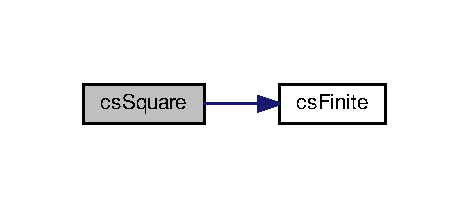
\includegraphics[width=225pt]{d4/d1c/group__geom__utils_ga490abe249d6289528341e55af14b5e14_cgraph}
\end{center}
\end{figure}



\chapter{Namespace Documentation}
\hypertarget{namespaceAIEvents}{}\section{A\+I\+Events Namespace Reference}
\label{namespaceAIEvents}\index{A\+I\+Events@{A\+I\+Events}}
\subsection*{Classes}
\begin{DoxyCompactItemize}
\item 
struct \hyperlink{structAIEvents_1_1AIEvresult}{A\+I\+Evresult}
\begin{DoxyCompactList}\small\item\em A struct indicating an event that may or may not be executed. \end{DoxyCompactList}\item 
struct \hyperlink{structAIEvents_1_1ElemAttrMap}{Elem\+Attr\+Map}
\end{DoxyCompactItemize}
\subsection*{Functions}
\begin{DoxyCompactItemize}
\item 
void {\bfseries General\+A\+I\+Event\+Begin} (void $\ast$user\+Data, const X\+M\+L\+\_\+\+Char $\ast$name, const X\+M\+L\+\_\+\+Char $\ast$$\ast$atts)\hypertarget{namespaceAIEvents_adc5735397c3ba97b815e3659f9d83d99}{}\label{namespaceAIEvents_adc5735397c3ba97b815e3659f9d83d99}

\item 
void {\bfseries General\+A\+I\+Event\+End} (void $\ast$user\+Data, const X\+M\+L\+\_\+\+Char $\ast$name)\hypertarget{namespaceAIEvents_a319830e1c00ebfdb54b9719c226bdefd}{}\label{namespaceAIEvents_a319830e1c00ebfdb54b9719c226bdefd}

\item 
void {\bfseries Load\+AI} (const char $\ast$filename, \hyperlink{structAIEvents_1_1ElemAttrMap}{Elem\+Attr\+Map} \&result, const string \&faction)\hypertarget{namespaceAIEvents_a3979facd17d551e2c70c29389912754d}{}\label{namespaceAIEvents_a3979facd17d551e2c70c29389912754d}

\item 
void {\bfseries Load\+AI} (const char $\ast$filename, \hyperlink{structAIEvents_1_1ElemAttrMap}{Elem\+Attr\+Map} \&result, const std\+::string \&faction)\hypertarget{namespaceAIEvents_a0356629e34574db2d7273a53c521994c}{}\label{namespaceAIEvents_a0356629e34574db2d7273a53c521994c}

\end{DoxyCompactItemize}
\subsection*{Variables}
\begin{DoxyCompactItemize}
\item 
const int {\bfseries A\+I\+U\+N\+K\+N\+O\+WN} = 0\hypertarget{namespaceAIEvents_aa18e9f19a00c8e5349afd46345f0d8b3}{}\label{namespaceAIEvents_aa18e9f19a00c8e5349afd46345f0d8b3}

\item 
const int {\bfseries A\+I\+M\+IN} = 1\hypertarget{namespaceAIEvents_a30cd747e2af24ac18f55a20a1cffe512}{}\label{namespaceAIEvents_a30cd747e2af24ac18f55a20a1cffe512}

\item 
const int {\bfseries A\+I\+M\+AX} = 2\hypertarget{namespaceAIEvents_a9d10fd91d32808d4fddd0de471b7c82a}{}\label{namespaceAIEvents_a9d10fd91d32808d4fddd0de471b7c82a}

\item 
const int {\bfseries A\+I\+S\+C\+R\+I\+PT} = 3\hypertarget{namespaceAIEvents_a053c46b604990deaa76d4afb5c025303}{}\label{namespaceAIEvents_a053c46b604990deaa76d4afb5c025303}

\item 
const int {\bfseries A\+I\+N\+OT} = 4\hypertarget{namespaceAIEvents_aa088167e7e6bd56b73927dc3ff28b93e}{}\label{namespaceAIEvents_aa088167e7e6bd56b73927dc3ff28b93e}

\item 
const int {\bfseries T\+I\+M\+E\+IT} = 5\hypertarget{namespaceAIEvents_a225f9031106522e7144ecb18252e7a15}{}\label{namespaceAIEvents_a225f9031106522e7144ecb18252e7a15}

\item 
const int {\bfseries O\+B\+E\+D\+I\+E\+N\+CE} = 6\hypertarget{namespaceAIEvents_a872d85a12033a8af8dbf10715762bd7a}{}\label{namespaceAIEvents_a872d85a12033a8af8dbf10715762bd7a}

\item 
const int {\bfseries T\+I\+M\+E\+T\+O\+I\+N\+T\+E\+R\+R\+U\+PT} = 7\hypertarget{namespaceAIEvents_a7eef2147d184201a3c7067571be358bb}{}\label{namespaceAIEvents_a7eef2147d184201a3c7067571be358bb}

\item 
const int {\bfseries P\+R\+I\+O\+R\+I\+TY} = 8\hypertarget{namespaceAIEvents_a28261e9fa671fc2517c2cc695e4c8d5e}{}\label{namespaceAIEvents_a28261e9fa671fc2517c2cc695e4c8d5e}

\item 
const \hyperlink{structXMLSupport_1_1EnumMap_1_1Pair}{X\+M\+L\+Support\+::\+Enum\+Map\+::\+Pair} {\bfseries A\+Iattribute\+\_\+names} \mbox{[}$\,$\mbox{]}
\item 
const \hyperlink{classXMLSupport_1_1EnumMap}{X\+M\+L\+Support\+::\+Enum\+Map} {\bfseries attr\+\_\+map} (A\+Iattribute\+\_\+names, 9)\hypertarget{namespaceAIEvents_ad2483ea87557a04acd8bd74b7931ce7b}{}\label{namespaceAIEvents_ad2483ea87557a04acd8bd74b7931ce7b}

\end{DoxyCompactItemize}


\subsection{Detailed Description}
General namespace that does nothing on its own, but Deals with the parsing of an X\+ML file tha tcontains a number of event \char`\"{}if\char`\"{} statements Each statement can have a minimum, max value and a \char`\"{}not\char`\"{} flag to invert it and the type references the enum in the class using this one, and is eventually only used for the \char`\"{}not\char`\"{} tag 

\subsection{Variable Documentation}
\index{A\+I\+Events@{A\+I\+Events}!A\+Iattribute\+\_\+names@{A\+Iattribute\+\_\+names}}
\index{A\+Iattribute\+\_\+names@{A\+Iattribute\+\_\+names}!A\+I\+Events@{A\+I\+Events}}
\subsubsection[{\texorpdfstring{A\+Iattribute\+\_\+names}{AIattribute_names}}]{\setlength{\rightskip}{0pt plus 5cm}const {\bf X\+M\+L\+Support\+::\+Enum\+Map\+::\+Pair} A\+I\+Events\+::\+A\+Iattribute\+\_\+names\mbox{[}$\,$\mbox{]}}\hypertarget{namespaceAIEvents_a3e13e5faa015783773d98b7ce06353ab}{}\label{namespaceAIEvents_a3e13e5faa015783773d98b7ce06353ab}
{\bfseries Initial value\+:}
\begin{DoxyCode}
= \{
    \hyperlink{structXMLSupport_1_1EnumMap_1_1Pair}{EnumMap::Pair}( \textcolor{stringliteral}{"UNKNOWN"},         AIUNKNOWN ),
    \hyperlink{structXMLSupport_1_1EnumMap_1_1Pair}{EnumMap::Pair}( \textcolor{stringliteral}{"min"},             AIMIN ),
    \hyperlink{structXMLSupport_1_1EnumMap_1_1Pair}{EnumMap::Pair}( \textcolor{stringliteral}{"max"},             AIMAX ),
    \hyperlink{structXMLSupport_1_1EnumMap_1_1Pair}{EnumMap::Pair}( \textcolor{stringliteral}{"not"},             AINOT ),
    \hyperlink{structXMLSupport_1_1EnumMap_1_1Pair}{EnumMap::Pair}( \textcolor{stringliteral}{"Script"},          AISCRIPT ),
    \hyperlink{structXMLSupport_1_1EnumMap_1_1Pair}{EnumMap::Pair}( \textcolor{stringliteral}{"time"},            TIMEIT ),
    \hyperlink{structXMLSupport_1_1EnumMap_1_1Pair}{EnumMap::Pair}( \textcolor{stringliteral}{"obedience"},       OBEDIENCE ),
    \hyperlink{structXMLSupport_1_1EnumMap_1_1Pair}{EnumMap::Pair}( \textcolor{stringliteral}{"timetointerrupt"}, TIMETOINTERRUPT ),
    \hyperlink{structXMLSupport_1_1EnumMap_1_1Pair}{EnumMap::Pair}( \textcolor{stringliteral}{"priority"},        PRIORITY )
\}
\end{DoxyCode}

\hypertarget{namespaceGalaxyXML}{}\section{Galaxy\+X\+ML Namespace Reference}
\label{namespaceGalaxyXML}\index{Galaxy\+X\+ML@{Galaxy\+X\+ML}}
\subsection*{Classes}
\begin{DoxyCompactItemize}
\item 
class \hyperlink{classGalaxyXML_1_1Galaxy}{Galaxy}
\item 
class \hyperlink{classGalaxyXML_1_1SGalaxy}{S\+Galaxy}
\item 
class \hyperlink{classGalaxyXML_1_1SubHeirarchy}{Sub\+Heirarchy}
\item 
class \hyperlink{classGalaxyXML_1_1XML}{X\+ML}
\end{DoxyCompactItemize}
\subsection*{Typedefs}
\begin{DoxyCompactItemize}
\item 
typedef std\+::map$<$ std\+::string, std\+::string $>$ {\bfseries String\+Map}\hypertarget{namespaceGalaxyXML_aa29f3f4f258a86e6c4d4e520c8c7f799}{}\label{namespaceGalaxyXML_aa29f3f4f258a86e6c4d4e520c8c7f799}

\end{DoxyCompactItemize}
\subsection*{Enumerations}
\begin{DoxyCompactItemize}
\item 
enum {\bfseries Galaxy\+Names} \{ \\*
{\bfseries U\+N\+K\+N\+O\+WN}, 
{\bfseries G\+A\+L\+A\+XY}, 
{\bfseries S\+Y\+S\+T\+E\+MS}, 
{\bfseries S\+E\+C\+T\+OR}, 
\\*
{\bfseries S\+Y\+S\+T\+EM}, 
{\bfseries V\+AR}, 
{\bfseries N\+A\+ME}, 
{\bfseries V\+A\+L\+UE}, 
\\*
{\bfseries P\+L\+A\+N\+E\+TS}, 
{\bfseries P\+L\+A\+N\+ET}
 \}\hypertarget{namespaceGalaxyXML_a6540aeea78df7fddb1ef120cd03ec1fb}{}\label{namespaceGalaxyXML_a6540aeea78df7fddb1ef120cd03ec1fb}

\end{DoxyCompactItemize}
\subsection*{Functions}
\begin{DoxyCompactItemize}
\item 
void {\bfseries begin\+Element} (void $\ast$userdata, const X\+M\+L\+\_\+\+Char $\ast$nam, const X\+M\+L\+\_\+\+Char $\ast$$\ast$atts)\hypertarget{namespaceGalaxyXML_aa527140c20cae1c23e17abe714f857ce}{}\label{namespaceGalaxyXML_aa527140c20cae1c23e17abe714f857ce}

\item 
void {\bfseries end\+Element} (void $\ast$userdata, const X\+M\+L\+\_\+\+Char $\ast$nam)\hypertarget{namespaceGalaxyXML_a7979206e086c90e60fb7e63bccaa57dd}{}\label{namespaceGalaxyXML_a7979206e086c90e60fb7e63bccaa57dd}

\end{DoxyCompactItemize}
\subsection*{Variables}
\begin{DoxyCompactItemize}
\item 
const \hyperlink{structXMLSupport_1_1EnumMap_1_1Pair}{Enum\+Map\+::\+Pair} {\bfseries element\+\_\+names} \mbox{[}8\mbox{]}
\item 
const \hyperlink{structXMLSupport_1_1EnumMap_1_1Pair}{Enum\+Map\+::\+Pair} {\bfseries attribute\+\_\+names} \mbox{[}3\mbox{]}
\item 
const \hyperlink{classXMLSupport_1_1EnumMap}{Enum\+Map} {\bfseries element\+\_\+map} (element\+\_\+names, 8)\hypertarget{namespaceGalaxyXML_a5693f207e9899508f02cfce82d47dda3}{}\label{namespaceGalaxyXML_a5693f207e9899508f02cfce82d47dda3}

\item 
const \hyperlink{classXMLSupport_1_1EnumMap}{Enum\+Map} {\bfseries attribute\+\_\+map} (attribute\+\_\+names, 3)\hypertarget{namespaceGalaxyXML_ad21e620d6511ff988a2b59360e771a31}{}\label{namespaceGalaxyXML_ad21e620d6511ff988a2b59360e771a31}

\end{DoxyCompactItemize}


\subsection{Detailed Description}
Class \hyperlink{classUniverse}{Universe} Deals with universal constants. It is a global, accessed from anywhere as \+\_\+\+Universe-\/$>$ \hyperlink{classUniverse}{Universe} may be queried for Relationships, the current star system rendering is taking place in etc. It acts as a wrapper to the active Star System. Additionally it handles beginning and ending the main loop. And starting and ending graphics. (incl the task of wiping temp lights) Deprecated\+: loaded dynamic gldrv module 

\subsection{Variable Documentation}
\index{Galaxy\+X\+ML@{Galaxy\+X\+ML}!attribute\+\_\+names@{attribute\+\_\+names}}
\index{attribute\+\_\+names@{attribute\+\_\+names}!Galaxy\+X\+ML@{Galaxy\+X\+ML}}
\subsubsection[{\texorpdfstring{attribute\+\_\+names}{attribute_names}}]{\setlength{\rightskip}{0pt plus 5cm}const {\bf Enum\+Map\+::\+Pair} Galaxy\+X\+M\+L\+::attribute\+\_\+names\mbox{[}3\mbox{]}}\hypertarget{namespaceGalaxyXML_a761fbe2b92781a4d5a1220233d96f94d}{}\label{namespaceGalaxyXML_a761fbe2b92781a4d5a1220233d96f94d}
{\bfseries Initial value\+:}
\begin{DoxyCode}
= \{
    \hyperlink{structXMLSupport_1_1EnumMap_1_1Pair}{EnumMap::Pair}( \textcolor{stringliteral}{"UNKNOWN"}, UNKNOWN ),
    \hyperlink{structXMLSupport_1_1EnumMap_1_1Pair}{EnumMap::Pair}( \textcolor{stringliteral}{"name"},    NAME ),
    \hyperlink{structXMLSupport_1_1EnumMap_1_1Pair}{EnumMap::Pair}( \textcolor{stringliteral}{"value"},   VALUE )
\}
\end{DoxyCode}
\index{Galaxy\+X\+ML@{Galaxy\+X\+ML}!element\+\_\+names@{element\+\_\+names}}
\index{element\+\_\+names@{element\+\_\+names}!Galaxy\+X\+ML@{Galaxy\+X\+ML}}
\subsubsection[{\texorpdfstring{element\+\_\+names}{element_names}}]{\setlength{\rightskip}{0pt plus 5cm}const {\bf Enum\+Map\+::\+Pair} Galaxy\+X\+M\+L\+::element\+\_\+names\mbox{[}8\mbox{]}}\hypertarget{namespaceGalaxyXML_a27768b93eb7d224d795e1b91062346cf}{}\label{namespaceGalaxyXML_a27768b93eb7d224d795e1b91062346cf}
{\bfseries Initial value\+:}
\begin{DoxyCode}
= \{
    \hyperlink{structXMLSupport_1_1EnumMap_1_1Pair}{EnumMap::Pair}( \textcolor{stringliteral}{"UNKNOWN"}, UNKNOWN ),
    \hyperlink{structXMLSupport_1_1EnumMap_1_1Pair}{EnumMap::Pair}( \textcolor{stringliteral}{"Galaxy"},  GALAXY ),
    \hyperlink{structXMLSupport_1_1EnumMap_1_1Pair}{EnumMap::Pair}( \textcolor{stringliteral}{"Systems"}, SYSTEMS ),
    \hyperlink{structXMLSupport_1_1EnumMap_1_1Pair}{EnumMap::Pair}( \textcolor{stringliteral}{"Sector"},  SECTOR ),
    \hyperlink{structXMLSupport_1_1EnumMap_1_1Pair}{EnumMap::Pair}( \textcolor{stringliteral}{"System"},  SYSTEM ),
    \hyperlink{structXMLSupport_1_1EnumMap_1_1Pair}{EnumMap::Pair}( \textcolor{stringliteral}{"Planets"}, PLANETS ),
    \hyperlink{structXMLSupport_1_1EnumMap_1_1Pair}{EnumMap::Pair}( \textcolor{stringliteral}{"Planet"},  PLANET ),
    \hyperlink{structXMLSupport_1_1EnumMap_1_1Pair}{EnumMap::Pair}( \textcolor{stringliteral}{"Var"},     VAR )
\}
\end{DoxyCode}

\hypertarget{namespacevsphysics}{}\section{vsphysics Namespace Reference}
\label{namespacevsphysics}\index{vsphysics@{vsphysics}}
\subsection*{Functions}
\begin{DoxyCompactItemize}
\item 
float {\bfseries copysign} (float x, float \hyperlink{IceUtils_8h_aa7ffaed69623192258fb8679569ff9ba}{y})\hypertarget{namespacevsphysics_a4d7b86cf1b3209bfcc793c76785313a1}{}\label{namespacevsphysics_a4d7b86cf1b3209bfcc793c76785313a1}

\end{DoxyCompactItemize}


\subsection{Detailed Description}
A work around to overrule the cmath copysign function 
\chapter{Class Documentation}
\hypertarget{classOpcode_1_1AABB}{}\section{Opcode\+:\+:A\+A\+BB Class Reference}
\label{classOpcode_1_1AABB}\index{Opcode\+::\+A\+A\+BB@{Opcode\+::\+A\+A\+BB}}


Collaboration diagram for Opcode\+:\+:A\+A\+BB\+:
\nopagebreak
\begin{figure}[H]
\begin{center}
\leavevmode
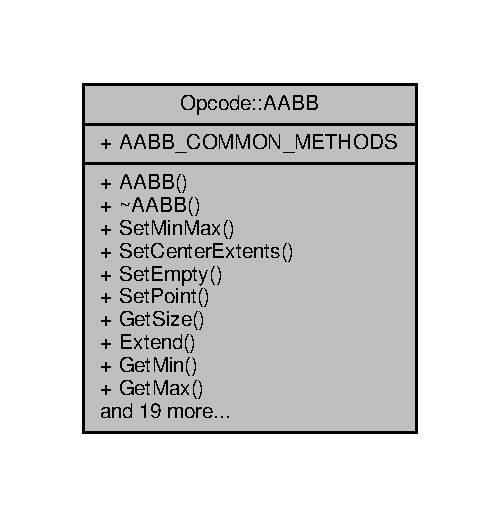
\includegraphics[width=240pt]{d2/df1/classOpcode_1_1AABB__coll__graph}
\end{center}
\end{figure}
\subsection*{Public Member Functions}
\begin{DoxyCompactItemize}
\item 
inline\+\_\+ \hyperlink{classOpcode_1_1AABB_af3a2bceac729e44344b8d695f2187805}{A\+A\+BB} ()\hypertarget{classOpcode_1_1AABB_af3a2bceac729e44344b8d695f2187805}{}\label{classOpcode_1_1AABB_af3a2bceac729e44344b8d695f2187805}

\begin{DoxyCompactList}\small\item\em Constructor. \end{DoxyCompactList}\item 
inline\+\_\+ \hyperlink{classOpcode_1_1AABB_af58c46252c82df4a6076e179bb6da790}{$\sim$\+A\+A\+BB} ()\hypertarget{classOpcode_1_1AABB_af58c46252c82df4a6076e179bb6da790}{}\label{classOpcode_1_1AABB_af58c46252c82df4a6076e179bb6da790}

\begin{DoxyCompactList}\small\item\em Destructor. \end{DoxyCompactList}\item 
void \hyperlink{classOpcode_1_1AABB_abf58854d4d784e23e61db12ff4d3b4ec}{Set\+Min\+Max} (const \hyperlink{classOpcode_1_1Point}{Point} \&min, const \hyperlink{classOpcode_1_1Point}{Point} \&max)
\item 
void \hyperlink{classOpcode_1_1AABB_a066f07ceb695a45b4a55313be175df37}{Set\+Center\+Extents} (const \hyperlink{classOpcode_1_1Point}{Point} \&c, const \hyperlink{classOpcode_1_1Point}{Point} \&e)
\item 
void \hyperlink{classOpcode_1_1AABB_a246e9552769168c552224f0d04ebecbb}{Set\+Empty} ()
\item 
void \hyperlink{classOpcode_1_1AABB_abae6b66247af798712b77e14020d9784}{Set\+Point} (const \hyperlink{classOpcode_1_1Point}{Point} \&pt)
\item 
float \hyperlink{classOpcode_1_1AABB_a4d218f6315aea4ff39465d00a90d64a5}{Get\+Size} () const 
\item 
void \hyperlink{classOpcode_1_1AABB_ae95fd015ce28e7daf0c805f6c9702cb4}{Extend} (const \hyperlink{classOpcode_1_1Point}{Point} \&p)
\item 
inline\+\_\+ void \hyperlink{classOpcode_1_1AABB_a0e44911edf58a8dea4f2552b3943faab}{Get\+Min} (\hyperlink{classOpcode_1_1Point}{Point} \&min) const \hypertarget{classOpcode_1_1AABB_a0e44911edf58a8dea4f2552b3943faab}{}\label{classOpcode_1_1AABB_a0e44911edf58a8dea4f2552b3943faab}

\begin{DoxyCompactList}\small\item\em Get min point of the box. \end{DoxyCompactList}\item 
inline\+\_\+ void \hyperlink{classOpcode_1_1AABB_a5e6b0466007c308755a4280007d2c0ee}{Get\+Max} (\hyperlink{classOpcode_1_1Point}{Point} \&max) const \hypertarget{classOpcode_1_1AABB_a5e6b0466007c308755a4280007d2c0ee}{}\label{classOpcode_1_1AABB_a5e6b0466007c308755a4280007d2c0ee}

\begin{DoxyCompactList}\small\item\em Get max point of the box. \end{DoxyCompactList}\item 
inline\+\_\+ float \hyperlink{classOpcode_1_1AABB_a722ee19222271ce6066e7c2437b45e3d}{Get\+Min} (\hyperlink{IceTypes_8h_a44c6f1920ba5551225fb534f9d1a1733}{udword} axis) const \hypertarget{classOpcode_1_1AABB_a722ee19222271ce6066e7c2437b45e3d}{}\label{classOpcode_1_1AABB_a722ee19222271ce6066e7c2437b45e3d}

\begin{DoxyCompactList}\small\item\em Get component of the box\textquotesingle{}s min point along a given axis. \end{DoxyCompactList}\item 
inline\+\_\+ float \hyperlink{classOpcode_1_1AABB_acf448abb3a0abb3165b7be4d8a4872da}{Get\+Max} (\hyperlink{IceTypes_8h_a44c6f1920ba5551225fb534f9d1a1733}{udword} axis) const \hypertarget{classOpcode_1_1AABB_acf448abb3a0abb3165b7be4d8a4872da}{}\label{classOpcode_1_1AABB_acf448abb3a0abb3165b7be4d8a4872da}

\begin{DoxyCompactList}\small\item\em Get component of the box\textquotesingle{}s max point along a given axis. \end{DoxyCompactList}\item 
inline\+\_\+ void \hyperlink{classOpcode_1_1AABB_a2061784d0e109f9f56b28a6a2563a6ee}{Get\+Center} (\hyperlink{classOpcode_1_1Point}{Point} \&center) const \hypertarget{classOpcode_1_1AABB_a2061784d0e109f9f56b28a6a2563a6ee}{}\label{classOpcode_1_1AABB_a2061784d0e109f9f56b28a6a2563a6ee}

\begin{DoxyCompactList}\small\item\em Get box center. \end{DoxyCompactList}\item 
inline\+\_\+ void \hyperlink{classOpcode_1_1AABB_adf84613f075324b49b8c5611179ea20c}{Get\+Extents} (\hyperlink{classOpcode_1_1Point}{Point} \&extents) const \hypertarget{classOpcode_1_1AABB_adf84613f075324b49b8c5611179ea20c}{}\label{classOpcode_1_1AABB_adf84613f075324b49b8c5611179ea20c}

\begin{DoxyCompactList}\small\item\em Get box extents. \end{DoxyCompactList}\item 
inline\+\_\+ float \hyperlink{classOpcode_1_1AABB_aee39d809e7aa6e221a27de75ba0e5160}{Get\+Center} (\hyperlink{IceTypes_8h_a44c6f1920ba5551225fb534f9d1a1733}{udword} axis) const \hypertarget{classOpcode_1_1AABB_aee39d809e7aa6e221a27de75ba0e5160}{}\label{classOpcode_1_1AABB_aee39d809e7aa6e221a27de75ba0e5160}

\begin{DoxyCompactList}\small\item\em Get component of the box\textquotesingle{}s center along a given axis. \end{DoxyCompactList}\item 
inline\+\_\+ float \hyperlink{classOpcode_1_1AABB_a42db4e26211463b9d796095ab03875ee}{Get\+Extents} (\hyperlink{IceTypes_8h_a44c6f1920ba5551225fb534f9d1a1733}{udword} axis) const \hypertarget{classOpcode_1_1AABB_a42db4e26211463b9d796095ab03875ee}{}\label{classOpcode_1_1AABB_a42db4e26211463b9d796095ab03875ee}

\begin{DoxyCompactList}\small\item\em Get component of the box\textquotesingle{}s extents along a given axis. \end{DoxyCompactList}\item 
inline\+\_\+ void \hyperlink{classOpcode_1_1AABB_af18c597f5e7dd08562dbfc74994a896b}{Get\+Diagonal} (\hyperlink{classOpcode_1_1Point}{Point} \&diagonal) const \hypertarget{classOpcode_1_1AABB_af18c597f5e7dd08562dbfc74994a896b}{}\label{classOpcode_1_1AABB_af18c597f5e7dd08562dbfc74994a896b}

\begin{DoxyCompactList}\small\item\em Get box diagonal. \end{DoxyCompactList}\item 
inline\+\_\+ float {\bfseries Get\+Width} () const \hypertarget{classOpcode_1_1AABB_ad6eafbfdf50b700bf67ecc8398972ff0}{}\label{classOpcode_1_1AABB_ad6eafbfdf50b700bf67ecc8398972ff0}

\item 
inline\+\_\+ float {\bfseries Get\+Height} () const \hypertarget{classOpcode_1_1AABB_aebac63c661210cb32a08d1c1d0152b35}{}\label{classOpcode_1_1AABB_aebac63c661210cb32a08d1c1d0152b35}

\item 
inline\+\_\+ float {\bfseries Get\+Depth} () const \hypertarget{classOpcode_1_1AABB_a4f4f096614a9cc74065d4e985326e7de}{}\label{classOpcode_1_1AABB_a4f4f096614a9cc74065d4e985326e7de}

\item 
inline\+\_\+ float \hyperlink{classOpcode_1_1AABB_a48f0f94aca074e5e0c075dfb4c188e6c}{Get\+Volume} () const \hypertarget{classOpcode_1_1AABB_a48f0f94aca074e5e0c075dfb4c188e6c}{}\label{classOpcode_1_1AABB_a48f0f94aca074e5e0c075dfb4c188e6c}

\begin{DoxyCompactList}\small\item\em Volume. \end{DoxyCompactList}\item 
inline\+\_\+ \hyperlink{IceTypes_8h_a050c65e107f0c828f856a231f4b4e788}{B\+O\+OL} \hyperlink{classOpcode_1_1AABB_a2e8a66919a32819076a118097449bba4}{Intersect} (const \hyperlink{classOpcode_1_1AABB}{A\+A\+BB} \&a) const 
\item 
inline\+\_\+ bool \hyperlink{classOpcode_1_1AABB_a6e99cceccfb17187fbfeff396f35e72b}{Gomez\+Intersect} (const \hyperlink{classOpcode_1_1AABB}{A\+A\+BB} \&a)
\item 
inline\+\_\+ \hyperlink{IceTypes_8h_a050c65e107f0c828f856a231f4b4e788}{B\+O\+OL} \hyperlink{classOpcode_1_1AABB_ac637f7ff897553ab3221c94f8b6bff51}{Intersect} (const \hyperlink{classOpcode_1_1AABB}{A\+A\+BB} \&a, \hyperlink{IceTypes_8h_a44c6f1920ba5551225fb534f9d1a1733}{udword} axis) const 
\item 
inline\+\_\+ void \hyperlink{classOpcode_1_1AABB_a1757edfe1363ddbab5be20c8264dd14e}{Rotate} (const \hyperlink{classOpcode_1_1Matrix4x4}{Matrix4x4} \&mtx, \hyperlink{classOpcode_1_1AABB}{A\+A\+BB} \&aabb) const 
\item 
inline\+\_\+ \hyperlink{IceTypes_8h_a050c65e107f0c828f856a231f4b4e788}{B\+O\+OL} \hyperlink{classOpcode_1_1AABB_a227e86486c6611f9154955363f569aaa}{Is\+Valid} () const 
\item 
inline\+\_\+ \hyperlink{classOpcode_1_1AABB}{A\+A\+BB} \& \hyperlink{classOpcode_1_1AABB_a9711deef52caaf24923a3574c6f88f09}{operator$\ast$=} (float s)\hypertarget{classOpcode_1_1AABB_a9711deef52caaf24923a3574c6f88f09}{}\label{classOpcode_1_1AABB_a9711deef52caaf24923a3574c6f88f09}

\begin{DoxyCompactList}\small\item\em Operator for \hyperlink{classOpcode_1_1AABB}{A\+A\+BB} $\ast$= float. Scales the extents, keeps same center. \end{DoxyCompactList}\item 
inline\+\_\+ \hyperlink{classOpcode_1_1AABB}{A\+A\+BB} \& \hyperlink{classOpcode_1_1AABB_aec4b3f09ae8c54b4201a43e4f8d1756e}{operator/=} (float s)\hypertarget{classOpcode_1_1AABB_aec4b3f09ae8c54b4201a43e4f8d1756e}{}\label{classOpcode_1_1AABB_aec4b3f09ae8c54b4201a43e4f8d1756e}

\begin{DoxyCompactList}\small\item\em Operator for \hyperlink{classOpcode_1_1AABB}{A\+A\+BB} /= float. Scales the extents, keeps same center. \end{DoxyCompactList}\item 
inline\+\_\+ \hyperlink{classOpcode_1_1AABB}{A\+A\+BB} \& \hyperlink{classOpcode_1_1AABB_a27a554b6965cbe64f2890c3794de6844}{operator+=} (const \hyperlink{classOpcode_1_1Point}{Point} \&trans)\hypertarget{classOpcode_1_1AABB_a27a554b6965cbe64f2890c3794de6844}{}\label{classOpcode_1_1AABB_a27a554b6965cbe64f2890c3794de6844}

\begin{DoxyCompactList}\small\item\em Operator for \hyperlink{classOpcode_1_1AABB}{A\+A\+BB} += \hyperlink{classOpcode_1_1Point}{Point}. Translates the box. \end{DoxyCompactList}\end{DoxyCompactItemize}
\subsection*{Public Attributes}
\begin{DoxyCompactItemize}
\item 
\hyperlink{classOpcode_1_1AABB_a8c3c9c6f10e834586252520ef9fe37a0}{A\+A\+B\+B\+\_\+\+C\+O\+M\+M\+O\+N\+\_\+\+M\+E\+T\+H\+O\+DS}\hypertarget{classOpcode_1_1AABB_a8c3c9c6f10e834586252520ef9fe37a0}{}\label{classOpcode_1_1AABB_a8c3c9c6f10e834586252520ef9fe37a0}

\begin{DoxyCompactList}\small\item\em Type-\/independent methods. \end{DoxyCompactList}\end{DoxyCompactItemize}


\subsection{Member Function Documentation}
\index{Opcode\+::\+A\+A\+BB@{Opcode\+::\+A\+A\+BB}!Extend@{Extend}}
\index{Extend@{Extend}!Opcode\+::\+A\+A\+BB@{Opcode\+::\+A\+A\+BB}}
\subsubsection[{\texorpdfstring{Extend(const Point \&p)}{Extend(const Point &p)}}]{\setlength{\rightskip}{0pt plus 5cm}void Opcode\+::\+A\+A\+B\+B\+::\+Extend (
\begin{DoxyParamCaption}
\item[{const {\bf Point} \&}]{p}
\end{DoxyParamCaption}
)\hspace{0.3cm}{\ttfamily [inline]}}\hypertarget{classOpcode_1_1AABB_ae95fd015ce28e7daf0c805f6c9702cb4}{}\label{classOpcode_1_1AABB_ae95fd015ce28e7daf0c805f6c9702cb4}
Extends the \hyperlink{classOpcode_1_1AABB}{A\+A\+BB}. 
\begin{DoxyParams}{Parameters}
{\em p} & \mbox{[}in\mbox{]} the next point \\
\hline
\end{DoxyParams}
\index{Opcode\+::\+A\+A\+BB@{Opcode\+::\+A\+A\+BB}!Get\+Size@{Get\+Size}}
\index{Get\+Size@{Get\+Size}!Opcode\+::\+A\+A\+BB@{Opcode\+::\+A\+A\+BB}}
\subsubsection[{\texorpdfstring{Get\+Size() const }{GetSize() const }}]{\setlength{\rightskip}{0pt plus 5cm}float Opcode\+::\+A\+A\+B\+B\+::\+Get\+Size (
\begin{DoxyParamCaption}
{}
\end{DoxyParamCaption}
) const\hspace{0.3cm}{\ttfamily [inline]}}\hypertarget{classOpcode_1_1AABB_a4d218f6315aea4ff39465d00a90d64a5}{}\label{classOpcode_1_1AABB_a4d218f6315aea4ff39465d00a90d64a5}
Gets the size of the \hyperlink{classOpcode_1_1AABB}{A\+A\+BB}. The size is defined as the longest extent. \begin{DoxyReturn}{Returns}
the size of the \hyperlink{classOpcode_1_1AABB}{A\+A\+BB} 
\end{DoxyReturn}
\index{Opcode\+::\+A\+A\+BB@{Opcode\+::\+A\+A\+BB}!Gomez\+Intersect@{Gomez\+Intersect}}
\index{Gomez\+Intersect@{Gomez\+Intersect}!Opcode\+::\+A\+A\+BB@{Opcode\+::\+A\+A\+BB}}
\subsubsection[{\texorpdfstring{Gomez\+Intersect(const A\+A\+B\+B \&a)}{GomezIntersect(const AABB &a)}}]{\setlength{\rightskip}{0pt plus 5cm}inline\+\_\+ bool Opcode\+::\+A\+A\+B\+B\+::\+Gomez\+Intersect (
\begin{DoxyParamCaption}
\item[{const {\bf A\+A\+BB} \&}]{a}
\end{DoxyParamCaption}
)\hspace{0.3cm}{\ttfamily [inline]}}\hypertarget{classOpcode_1_1AABB_a6e99cceccfb17187fbfeff396f35e72b}{}\label{classOpcode_1_1AABB_a6e99cceccfb17187fbfeff396f35e72b}
The standard intersection method from Gamasutra. Just here to check its speed against the one above. 
\begin{DoxyParams}{Parameters}
{\em a} & \mbox{[}in\mbox{]} the other \hyperlink{classOpcode_1_1AABB}{A\+A\+BB} \\
\hline
\end{DoxyParams}
\begin{DoxyReturn}{Returns}
true on intersection 
\end{DoxyReturn}
\index{Opcode\+::\+A\+A\+BB@{Opcode\+::\+A\+A\+BB}!Intersect@{Intersect}}
\index{Intersect@{Intersect}!Opcode\+::\+A\+A\+BB@{Opcode\+::\+A\+A\+BB}}
\subsubsection[{\texorpdfstring{Intersect(const A\+A\+B\+B \&a) const }{Intersect(const AABB &a) const }}]{\setlength{\rightskip}{0pt plus 5cm}inline\+\_\+ {\bf B\+O\+OL} Opcode\+::\+A\+A\+B\+B\+::\+Intersect (
\begin{DoxyParamCaption}
\item[{const {\bf A\+A\+BB} \&}]{a}
\end{DoxyParamCaption}
) const\hspace{0.3cm}{\ttfamily [inline]}}\hypertarget{classOpcode_1_1AABB_a2e8a66919a32819076a118097449bba4}{}\label{classOpcode_1_1AABB_a2e8a66919a32819076a118097449bba4}
Computes the intersection between two A\+A\+B\+Bs. 
\begin{DoxyParams}{Parameters}
{\em a} & \mbox{[}in\mbox{]} the other \hyperlink{classOpcode_1_1AABB}{A\+A\+BB} \\
\hline
\end{DoxyParams}
\begin{DoxyReturn}{Returns}
true on intersection 
\end{DoxyReturn}
\index{Opcode\+::\+A\+A\+BB@{Opcode\+::\+A\+A\+BB}!Intersect@{Intersect}}
\index{Intersect@{Intersect}!Opcode\+::\+A\+A\+BB@{Opcode\+::\+A\+A\+BB}}
\subsubsection[{\texorpdfstring{Intersect(const A\+A\+B\+B \&a, udword axis) const }{Intersect(const AABB &a, udword axis) const }}]{\setlength{\rightskip}{0pt plus 5cm}inline\+\_\+ {\bf B\+O\+OL} Opcode\+::\+A\+A\+B\+B\+::\+Intersect (
\begin{DoxyParamCaption}
\item[{const {\bf A\+A\+BB} \&}]{a, }
\item[{{\bf udword}}]{axis}
\end{DoxyParamCaption}
) const\hspace{0.3cm}{\ttfamily [inline]}}\hypertarget{classOpcode_1_1AABB_ac637f7ff897553ab3221c94f8b6bff51}{}\label{classOpcode_1_1AABB_ac637f7ff897553ab3221c94f8b6bff51}
Computes the 1\+D-\/intersection between two A\+A\+B\+Bs, on a given axis. 
\begin{DoxyParams}{Parameters}
{\em a} & \mbox{[}in\mbox{]} the other \hyperlink{classOpcode_1_1AABB}{A\+A\+BB} \\
\hline
{\em axis} & \mbox{[}in\mbox{]} the axis (0, 1, 2) \\
\hline
\end{DoxyParams}
\begin{DoxyReturn}{Returns}
true on intersection 
\end{DoxyReturn}
\index{Opcode\+::\+A\+A\+BB@{Opcode\+::\+A\+A\+BB}!Is\+Valid@{Is\+Valid}}
\index{Is\+Valid@{Is\+Valid}!Opcode\+::\+A\+A\+BB@{Opcode\+::\+A\+A\+BB}}
\subsubsection[{\texorpdfstring{Is\+Valid() const }{IsValid() const }}]{\setlength{\rightskip}{0pt plus 5cm}inline\+\_\+ {\bf B\+O\+OL} Opcode\+::\+A\+A\+B\+B\+::\+Is\+Valid (
\begin{DoxyParamCaption}
{}
\end{DoxyParamCaption}
) const\hspace{0.3cm}{\ttfamily [inline]}}\hypertarget{classOpcode_1_1AABB_a227e86486c6611f9154955363f569aaa}{}\label{classOpcode_1_1AABB_a227e86486c6611f9154955363f569aaa}
Checks the \hyperlink{classOpcode_1_1AABB}{A\+A\+BB} is valid. \begin{DoxyReturn}{Returns}
true if the box is valid 
\end{DoxyReturn}
\index{Opcode\+::\+A\+A\+BB@{Opcode\+::\+A\+A\+BB}!Rotate@{Rotate}}
\index{Rotate@{Rotate}!Opcode\+::\+A\+A\+BB@{Opcode\+::\+A\+A\+BB}}
\subsubsection[{\texorpdfstring{Rotate(const Matrix4x4 \&mtx, A\+A\+B\+B \&aabb) const }{Rotate(const Matrix4x4 &mtx, AABB &aabb) const }}]{\setlength{\rightskip}{0pt plus 5cm}inline\+\_\+ void Opcode\+::\+A\+A\+B\+B\+::\+Rotate (
\begin{DoxyParamCaption}
\item[{const {\bf Matrix4x4} \&}]{mtx, }
\item[{{\bf A\+A\+BB} \&}]{aabb}
\end{DoxyParamCaption}
) const\hspace{0.3cm}{\ttfamily [inline]}}\hypertarget{classOpcode_1_1AABB_a1757edfe1363ddbab5be20c8264dd14e}{}\label{classOpcode_1_1AABB_a1757edfe1363ddbab5be20c8264dd14e}
Recomputes the \hyperlink{classOpcode_1_1AABB}{A\+A\+BB} after an arbitrary transform by a 4x4 matrix. 
\begin{DoxyParams}{Parameters}
{\em mtx} & \mbox{[}in\mbox{]} the transform matrix \\
\hline
{\em aabb} & \mbox{[}out\mbox{]} the transformed \hyperlink{classOpcode_1_1AABB}{A\+A\+BB} \mbox{[}can be $\ast$this\mbox{]} \\
\hline
\end{DoxyParams}
\index{Opcode\+::\+A\+A\+BB@{Opcode\+::\+A\+A\+BB}!Set\+Center\+Extents@{Set\+Center\+Extents}}
\index{Set\+Center\+Extents@{Set\+Center\+Extents}!Opcode\+::\+A\+A\+BB@{Opcode\+::\+A\+A\+BB}}
\subsubsection[{\texorpdfstring{Set\+Center\+Extents(const Point \&c, const Point \&e)}{SetCenterExtents(const Point &c, const Point &e)}}]{\setlength{\rightskip}{0pt plus 5cm}void Opcode\+::\+A\+A\+B\+B\+::\+Set\+Center\+Extents (
\begin{DoxyParamCaption}
\item[{const {\bf Point} \&}]{c, }
\item[{const {\bf Point} \&}]{e}
\end{DoxyParamCaption}
)\hspace{0.3cm}{\ttfamily [inline]}}\hypertarget{classOpcode_1_1AABB_a066f07ceb695a45b4a55313be175df37}{}\label{classOpcode_1_1AABB_a066f07ceb695a45b4a55313be175df37}
Setups an \hyperlink{classOpcode_1_1AABB}{A\+A\+BB} from center \& extents vectors. 
\begin{DoxyParams}{Parameters}
{\em c} & \mbox{[}in\mbox{]} the center point \\
\hline
{\em e} & \mbox{[}in\mbox{]} the extents vector \\
\hline
\end{DoxyParams}
\index{Opcode\+::\+A\+A\+BB@{Opcode\+::\+A\+A\+BB}!Set\+Empty@{Set\+Empty}}
\index{Set\+Empty@{Set\+Empty}!Opcode\+::\+A\+A\+BB@{Opcode\+::\+A\+A\+BB}}
\subsubsection[{\texorpdfstring{Set\+Empty()}{SetEmpty()}}]{\setlength{\rightskip}{0pt plus 5cm}void Opcode\+::\+A\+A\+B\+B\+::\+Set\+Empty (
\begin{DoxyParamCaption}
{}
\end{DoxyParamCaption}
)\hspace{0.3cm}{\ttfamily [inline]}}\hypertarget{classOpcode_1_1AABB_a246e9552769168c552224f0d04ebecbb}{}\label{classOpcode_1_1AABB_a246e9552769168c552224f0d04ebecbb}
Setups an empty \hyperlink{classOpcode_1_1AABB}{A\+A\+BB}. \index{Opcode\+::\+A\+A\+BB@{Opcode\+::\+A\+A\+BB}!Set\+Min\+Max@{Set\+Min\+Max}}
\index{Set\+Min\+Max@{Set\+Min\+Max}!Opcode\+::\+A\+A\+BB@{Opcode\+::\+A\+A\+BB}}
\subsubsection[{\texorpdfstring{Set\+Min\+Max(const Point \&min, const Point \&max)}{SetMinMax(const Point &min, const Point &max)}}]{\setlength{\rightskip}{0pt plus 5cm}void Opcode\+::\+A\+A\+B\+B\+::\+Set\+Min\+Max (
\begin{DoxyParamCaption}
\item[{const {\bf Point} \&}]{min, }
\item[{const {\bf Point} \&}]{max}
\end{DoxyParamCaption}
)\hspace{0.3cm}{\ttfamily [inline]}}\hypertarget{classOpcode_1_1AABB_abf58854d4d784e23e61db12ff4d3b4ec}{}\label{classOpcode_1_1AABB_abf58854d4d784e23e61db12ff4d3b4ec}
Setups an \hyperlink{classOpcode_1_1AABB}{A\+A\+BB} from min \& max vectors. 
\begin{DoxyParams}{Parameters}
{\em min} & \mbox{[}in\mbox{]} the min point \\
\hline
{\em max} & \mbox{[}in\mbox{]} the max point \\
\hline
\end{DoxyParams}
\index{Opcode\+::\+A\+A\+BB@{Opcode\+::\+A\+A\+BB}!Set\+Point@{Set\+Point}}
\index{Set\+Point@{Set\+Point}!Opcode\+::\+A\+A\+BB@{Opcode\+::\+A\+A\+BB}}
\subsubsection[{\texorpdfstring{Set\+Point(const Point \&pt)}{SetPoint(const Point &pt)}}]{\setlength{\rightskip}{0pt plus 5cm}void Opcode\+::\+A\+A\+B\+B\+::\+Set\+Point (
\begin{DoxyParamCaption}
\item[{const {\bf Point} \&}]{pt}
\end{DoxyParamCaption}
)\hspace{0.3cm}{\ttfamily [inline]}}\hypertarget{classOpcode_1_1AABB_abae6b66247af798712b77e14020d9784}{}\label{classOpcode_1_1AABB_abae6b66247af798712b77e14020d9784}
Setups a point \hyperlink{classOpcode_1_1AABB}{A\+A\+BB}. 

The documentation for this class was generated from the following file\+:\begin{DoxyCompactItemize}
\item 
cmd/collide2/\hyperlink{Opcode_8h}{Opcode.\+h}\end{DoxyCompactItemize}

\hypertarget{classAABB}{}\section{A\+A\+BB Class Reference}
\label{classAABB}\index{A\+A\+BB@{A\+A\+BB}}


Collaboration diagram for A\+A\+BB\+:
\nopagebreak
\begin{figure}[H]
\begin{center}
\leavevmode
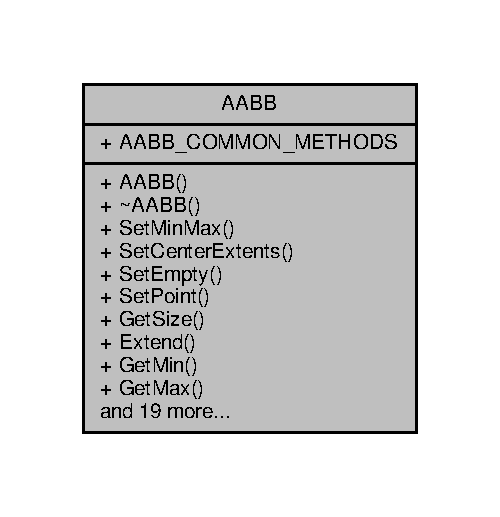
\includegraphics[width=240pt]{d6/d68/classAABB__coll__graph}
\end{center}
\end{figure}
\subsection*{Public Member Functions}
\begin{DoxyCompactItemize}
\item 
inline\+\_\+ \hyperlink{classAABB_ad318cad1a1e40ecb7560f953d439527c}{A\+A\+BB} ()\hypertarget{classAABB_ad318cad1a1e40ecb7560f953d439527c}{}\label{classAABB_ad318cad1a1e40ecb7560f953d439527c}

\begin{DoxyCompactList}\small\item\em Constructor. \end{DoxyCompactList}\item 
inline\+\_\+ \hyperlink{classAABB_a013e16f21145d12bd19b384b31055fb2}{$\sim$\+A\+A\+BB} ()\hypertarget{classAABB_a013e16f21145d12bd19b384b31055fb2}{}\label{classAABB_a013e16f21145d12bd19b384b31055fb2}

\begin{DoxyCompactList}\small\item\em Destructor. \end{DoxyCompactList}\item 
void \hyperlink{classAABB_aefd07f1b846deede5a40294e0128357d}{Set\+Min\+Max} (const \hyperlink{classPoint}{Point} \&min, const \hyperlink{classPoint}{Point} \&max)
\item 
void \hyperlink{classAABB_a926e591a06add61aaf40f4660bd52438}{Set\+Center\+Extents} (const \hyperlink{classPoint}{Point} \&c, const \hyperlink{classPoint}{Point} \&e)
\item 
void \hyperlink{classAABB_acbb23abc7e661b2388c17fca54cc80ed}{Set\+Empty} ()
\item 
void \hyperlink{classAABB_a5fa5fe0ce941e8c991775be34337acad}{Set\+Point} (const \hyperlink{classPoint}{Point} \&pt)
\item 
float \hyperlink{classAABB_ad40b364b3fd436764dd297336a902040}{Get\+Size} () const 
\item 
void \hyperlink{classAABB_af1ec90a9de45e8ee2a0f3589404f2981}{Extend} (const \hyperlink{classPoint}{Point} \&p)
\item 
inline\+\_\+ void \hyperlink{classAABB_ac8cb1707616aba70f650bb017476531e}{Get\+Min} (\hyperlink{classPoint}{Point} \&min) const \hypertarget{classAABB_ac8cb1707616aba70f650bb017476531e}{}\label{classAABB_ac8cb1707616aba70f650bb017476531e}

\begin{DoxyCompactList}\small\item\em Get min point of the box. \end{DoxyCompactList}\item 
inline\+\_\+ void \hyperlink{classAABB_ae332b8f1debc4985c7e2f0aac6ed761b}{Get\+Max} (\hyperlink{classPoint}{Point} \&max) const \hypertarget{classAABB_ae332b8f1debc4985c7e2f0aac6ed761b}{}\label{classAABB_ae332b8f1debc4985c7e2f0aac6ed761b}

\begin{DoxyCompactList}\small\item\em Get max point of the box. \end{DoxyCompactList}\item 
inline\+\_\+ float \hyperlink{classAABB_ae0adf093a00a40712aa1d07cade6e48b}{Get\+Min} (\hyperlink{IceTypes_8h_a44c6f1920ba5551225fb534f9d1a1733}{udword} axis) const \hypertarget{classAABB_ae0adf093a00a40712aa1d07cade6e48b}{}\label{classAABB_ae0adf093a00a40712aa1d07cade6e48b}

\begin{DoxyCompactList}\small\item\em Get component of the box\textquotesingle{}s min point along a given axis. \end{DoxyCompactList}\item 
inline\+\_\+ float \hyperlink{classAABB_a36fdeb0316837b4a39b1a98b02dbbdcb}{Get\+Max} (\hyperlink{IceTypes_8h_a44c6f1920ba5551225fb534f9d1a1733}{udword} axis) const \hypertarget{classAABB_a36fdeb0316837b4a39b1a98b02dbbdcb}{}\label{classAABB_a36fdeb0316837b4a39b1a98b02dbbdcb}

\begin{DoxyCompactList}\small\item\em Get component of the box\textquotesingle{}s max point along a given axis. \end{DoxyCompactList}\item 
inline\+\_\+ void \hyperlink{classAABB_a96ae6fa137afbc679cef52948a4d365a}{Get\+Center} (\hyperlink{classPoint}{Point} \&center) const \hypertarget{classAABB_a96ae6fa137afbc679cef52948a4d365a}{}\label{classAABB_a96ae6fa137afbc679cef52948a4d365a}

\begin{DoxyCompactList}\small\item\em Get box center. \end{DoxyCompactList}\item 
inline\+\_\+ void \hyperlink{classAABB_ae10e5bc6ce234bb65595196f0c7670cd}{Get\+Extents} (\hyperlink{classPoint}{Point} \&extents) const \hypertarget{classAABB_ae10e5bc6ce234bb65595196f0c7670cd}{}\label{classAABB_ae10e5bc6ce234bb65595196f0c7670cd}

\begin{DoxyCompactList}\small\item\em Get box extents. \end{DoxyCompactList}\item 
inline\+\_\+ float \hyperlink{classAABB_aebbb26fe0c3d93c062d698e9c5b5a74e}{Get\+Center} (\hyperlink{IceTypes_8h_a44c6f1920ba5551225fb534f9d1a1733}{udword} axis) const \hypertarget{classAABB_aebbb26fe0c3d93c062d698e9c5b5a74e}{}\label{classAABB_aebbb26fe0c3d93c062d698e9c5b5a74e}

\begin{DoxyCompactList}\small\item\em Get component of the box\textquotesingle{}s center along a given axis. \end{DoxyCompactList}\item 
inline\+\_\+ float \hyperlink{classAABB_aea26078bba53d349784874129f57c43a}{Get\+Extents} (\hyperlink{IceTypes_8h_a44c6f1920ba5551225fb534f9d1a1733}{udword} axis) const \hypertarget{classAABB_aea26078bba53d349784874129f57c43a}{}\label{classAABB_aea26078bba53d349784874129f57c43a}

\begin{DoxyCompactList}\small\item\em Get component of the box\textquotesingle{}s extents along a given axis. \end{DoxyCompactList}\item 
inline\+\_\+ void \hyperlink{classAABB_a6d67e251acd758927015377cf984b5f8}{Get\+Diagonal} (\hyperlink{classPoint}{Point} \&diagonal) const \hypertarget{classAABB_a6d67e251acd758927015377cf984b5f8}{}\label{classAABB_a6d67e251acd758927015377cf984b5f8}

\begin{DoxyCompactList}\small\item\em Get box diagonal. \end{DoxyCompactList}\item 
inline\+\_\+ float {\bfseries Get\+Width} () const \hypertarget{classAABB_ad7e334a58884b34d931593627b80f439}{}\label{classAABB_ad7e334a58884b34d931593627b80f439}

\item 
inline\+\_\+ float {\bfseries Get\+Height} () const \hypertarget{classAABB_a94ec6a1ad6ccdb538be061ea6c63c664}{}\label{classAABB_a94ec6a1ad6ccdb538be061ea6c63c664}

\item 
inline\+\_\+ float {\bfseries Get\+Depth} () const \hypertarget{classAABB_a3ad1814f5600a0a73bcb36148c9afb20}{}\label{classAABB_a3ad1814f5600a0a73bcb36148c9afb20}

\item 
inline\+\_\+ float \hyperlink{classAABB_a2c888a7387ffd8fbc4144f5d63892be6}{Get\+Volume} () const \hypertarget{classAABB_a2c888a7387ffd8fbc4144f5d63892be6}{}\label{classAABB_a2c888a7387ffd8fbc4144f5d63892be6}

\begin{DoxyCompactList}\small\item\em Volume. \end{DoxyCompactList}\item 
inline\+\_\+ \hyperlink{IceTypes_8h_a050c65e107f0c828f856a231f4b4e788}{B\+O\+OL} \hyperlink{classAABB_a4e1faf2a1bc32174c468dd49ac5452b3}{Intersect} (const \hyperlink{classAABB}{A\+A\+BB} \&a) const 
\item 
inline\+\_\+ bool \hyperlink{classAABB_a277bc0c18b7561ebee24739ecad805b5}{Gomez\+Intersect} (const \hyperlink{classAABB}{A\+A\+BB} \&a)
\item 
inline\+\_\+ \hyperlink{IceTypes_8h_a050c65e107f0c828f856a231f4b4e788}{B\+O\+OL} \hyperlink{classAABB_a18b9b090a4a5cbdbd7c809347df2ff03}{Intersect} (const \hyperlink{classAABB}{A\+A\+BB} \&a, \hyperlink{IceTypes_8h_a44c6f1920ba5551225fb534f9d1a1733}{udword} axis) const 
\item 
inline\+\_\+ void \hyperlink{classAABB_ad4f1de1a5d1a4ff71bcc8a47f7e8ca11}{Rotate} (const \hyperlink{classMatrix4x4}{Matrix4x4} \&mtx, \hyperlink{classAABB}{A\+A\+BB} \&aabb) const 
\item 
inline\+\_\+ \hyperlink{IceTypes_8h_a050c65e107f0c828f856a231f4b4e788}{B\+O\+OL} \hyperlink{classAABB_aef83f74a817f5ad98693b40c16548f4c}{Is\+Valid} () const 
\item 
inline\+\_\+ \hyperlink{classAABB}{A\+A\+BB} \& \hyperlink{classAABB_a7af8c6a1926fa0914d4ccc563399affb}{operator$\ast$=} (float s)\hypertarget{classAABB_a7af8c6a1926fa0914d4ccc563399affb}{}\label{classAABB_a7af8c6a1926fa0914d4ccc563399affb}

\begin{DoxyCompactList}\small\item\em Operator for \hyperlink{classAABB}{A\+A\+BB} $\ast$= float. Scales the extents, keeps same center. \end{DoxyCompactList}\item 
inline\+\_\+ \hyperlink{classAABB}{A\+A\+BB} \& \hyperlink{classAABB_a10378a1b9a6540384a6112128cdd5972}{operator/=} (float s)\hypertarget{classAABB_a10378a1b9a6540384a6112128cdd5972}{}\label{classAABB_a10378a1b9a6540384a6112128cdd5972}

\begin{DoxyCompactList}\small\item\em Operator for \hyperlink{classAABB}{A\+A\+BB} /= float. Scales the extents, keeps same center. \end{DoxyCompactList}\item 
inline\+\_\+ \hyperlink{classAABB}{A\+A\+BB} \& \hyperlink{classAABB_a1aa2bcb5279bd03fc4b9e074e1249fec}{operator+=} (const \hyperlink{classPoint}{Point} \&trans)\hypertarget{classAABB_a1aa2bcb5279bd03fc4b9e074e1249fec}{}\label{classAABB_a1aa2bcb5279bd03fc4b9e074e1249fec}

\begin{DoxyCompactList}\small\item\em Operator for \hyperlink{classAABB}{A\+A\+BB} += \hyperlink{classPoint}{Point}. Translates the box. \end{DoxyCompactList}\end{DoxyCompactItemize}
\subsection*{Public Attributes}
\begin{DoxyCompactItemize}
\item 
\hyperlink{classAABB_a27373818e3e3da2d9b1681917916da81}{A\+A\+B\+B\+\_\+\+C\+O\+M\+M\+O\+N\+\_\+\+M\+E\+T\+H\+O\+DS}\hypertarget{classAABB_a27373818e3e3da2d9b1681917916da81}{}\label{classAABB_a27373818e3e3da2d9b1681917916da81}

\begin{DoxyCompactList}\small\item\em Type-\/independent methods. \end{DoxyCompactList}\end{DoxyCompactItemize}


\subsection{Detailed Description}
\hyperlink{classAABB}{A\+A\+BB} class.

\begin{DoxyAuthor}{Author}
Pierre Terdiman 
\end{DoxyAuthor}
\begin{DoxyVersion}{Version}
1.\+0 
\end{DoxyVersion}


\subsection{Member Function Documentation}
\index{A\+A\+BB@{A\+A\+BB}!Extend@{Extend}}
\index{Extend@{Extend}!A\+A\+BB@{A\+A\+BB}}
\subsubsection[{\texorpdfstring{Extend(const Point \&p)}{Extend(const Point &p)}}]{\setlength{\rightskip}{0pt plus 5cm}void A\+A\+B\+B\+::\+Extend (
\begin{DoxyParamCaption}
\item[{const {\bf Point} \&}]{p}
\end{DoxyParamCaption}
)\hspace{0.3cm}{\ttfamily [inline]}}\hypertarget{classAABB_af1ec90a9de45e8ee2a0f3589404f2981}{}\label{classAABB_af1ec90a9de45e8ee2a0f3589404f2981}
Extends the \hyperlink{classAABB}{A\+A\+BB}. 
\begin{DoxyParams}{Parameters}
{\em p} & \mbox{[}in\mbox{]} the next point \\
\hline
\end{DoxyParams}
\index{A\+A\+BB@{A\+A\+BB}!Get\+Size@{Get\+Size}}
\index{Get\+Size@{Get\+Size}!A\+A\+BB@{A\+A\+BB}}
\subsubsection[{\texorpdfstring{Get\+Size() const }{GetSize() const }}]{\setlength{\rightskip}{0pt plus 5cm}float A\+A\+B\+B\+::\+Get\+Size (
\begin{DoxyParamCaption}
{}
\end{DoxyParamCaption}
) const\hspace{0.3cm}{\ttfamily [inline]}}\hypertarget{classAABB_ad40b364b3fd436764dd297336a902040}{}\label{classAABB_ad40b364b3fd436764dd297336a902040}
Gets the size of the \hyperlink{classAABB}{A\+A\+BB}. The size is defined as the longest extent. \begin{DoxyReturn}{Returns}
the size of the \hyperlink{classAABB}{A\+A\+BB} 
\end{DoxyReturn}
\index{A\+A\+BB@{A\+A\+BB}!Gomez\+Intersect@{Gomez\+Intersect}}
\index{Gomez\+Intersect@{Gomez\+Intersect}!A\+A\+BB@{A\+A\+BB}}
\subsubsection[{\texorpdfstring{Gomez\+Intersect(const A\+A\+B\+B \&a)}{GomezIntersect(const AABB &a)}}]{\setlength{\rightskip}{0pt plus 5cm}inline\+\_\+ bool A\+A\+B\+B\+::\+Gomez\+Intersect (
\begin{DoxyParamCaption}
\item[{const {\bf A\+A\+BB} \&}]{a}
\end{DoxyParamCaption}
)\hspace{0.3cm}{\ttfamily [inline]}}\hypertarget{classAABB_a277bc0c18b7561ebee24739ecad805b5}{}\label{classAABB_a277bc0c18b7561ebee24739ecad805b5}
The standard intersection method from Gamasutra. Just here to check its speed against the one above. 
\begin{DoxyParams}{Parameters}
{\em a} & \mbox{[}in\mbox{]} the other \hyperlink{classAABB}{A\+A\+BB} \\
\hline
\end{DoxyParams}
\begin{DoxyReturn}{Returns}
true on intersection 
\end{DoxyReturn}
\index{A\+A\+BB@{A\+A\+BB}!Intersect@{Intersect}}
\index{Intersect@{Intersect}!A\+A\+BB@{A\+A\+BB}}
\subsubsection[{\texorpdfstring{Intersect(const A\+A\+B\+B \&a) const }{Intersect(const AABB &a) const }}]{\setlength{\rightskip}{0pt plus 5cm}inline\+\_\+ {\bf B\+O\+OL} A\+A\+B\+B\+::\+Intersect (
\begin{DoxyParamCaption}
\item[{const {\bf A\+A\+BB} \&}]{a}
\end{DoxyParamCaption}
) const\hspace{0.3cm}{\ttfamily [inline]}}\hypertarget{classAABB_a4e1faf2a1bc32174c468dd49ac5452b3}{}\label{classAABB_a4e1faf2a1bc32174c468dd49ac5452b3}
Computes the intersection between two A\+A\+B\+Bs. 
\begin{DoxyParams}{Parameters}
{\em a} & \mbox{[}in\mbox{]} the other \hyperlink{classAABB}{A\+A\+BB} \\
\hline
\end{DoxyParams}
\begin{DoxyReturn}{Returns}
true on intersection 
\end{DoxyReturn}
\index{A\+A\+BB@{A\+A\+BB}!Intersect@{Intersect}}
\index{Intersect@{Intersect}!A\+A\+BB@{A\+A\+BB}}
\subsubsection[{\texorpdfstring{Intersect(const A\+A\+B\+B \&a, udword axis) const }{Intersect(const AABB &a, udword axis) const }}]{\setlength{\rightskip}{0pt plus 5cm}inline\+\_\+ {\bf B\+O\+OL} A\+A\+B\+B\+::\+Intersect (
\begin{DoxyParamCaption}
\item[{const {\bf A\+A\+BB} \&}]{a, }
\item[{{\bf udword}}]{axis}
\end{DoxyParamCaption}
) const\hspace{0.3cm}{\ttfamily [inline]}}\hypertarget{classAABB_a18b9b090a4a5cbdbd7c809347df2ff03}{}\label{classAABB_a18b9b090a4a5cbdbd7c809347df2ff03}
Computes the 1\+D-\/intersection between two A\+A\+B\+Bs, on a given axis. 
\begin{DoxyParams}{Parameters}
{\em a} & \mbox{[}in\mbox{]} the other \hyperlink{classAABB}{A\+A\+BB} \\
\hline
{\em axis} & \mbox{[}in\mbox{]} the axis (0, 1, 2) \\
\hline
\end{DoxyParams}
\begin{DoxyReturn}{Returns}
true on intersection 
\end{DoxyReturn}
\index{A\+A\+BB@{A\+A\+BB}!Is\+Valid@{Is\+Valid}}
\index{Is\+Valid@{Is\+Valid}!A\+A\+BB@{A\+A\+BB}}
\subsubsection[{\texorpdfstring{Is\+Valid() const }{IsValid() const }}]{\setlength{\rightskip}{0pt plus 5cm}inline\+\_\+ {\bf B\+O\+OL} A\+A\+B\+B\+::\+Is\+Valid (
\begin{DoxyParamCaption}
{}
\end{DoxyParamCaption}
) const\hspace{0.3cm}{\ttfamily [inline]}}\hypertarget{classAABB_aef83f74a817f5ad98693b40c16548f4c}{}\label{classAABB_aef83f74a817f5ad98693b40c16548f4c}
Checks the \hyperlink{classAABB}{A\+A\+BB} is valid. \begin{DoxyReturn}{Returns}
true if the box is valid 
\end{DoxyReturn}
\index{A\+A\+BB@{A\+A\+BB}!Rotate@{Rotate}}
\index{Rotate@{Rotate}!A\+A\+BB@{A\+A\+BB}}
\subsubsection[{\texorpdfstring{Rotate(const Matrix4x4 \&mtx, A\+A\+B\+B \&aabb) const }{Rotate(const Matrix4x4 &mtx, AABB &aabb) const }}]{\setlength{\rightskip}{0pt plus 5cm}inline\+\_\+ void A\+A\+B\+B\+::\+Rotate (
\begin{DoxyParamCaption}
\item[{const {\bf Matrix4x4} \&}]{mtx, }
\item[{{\bf A\+A\+BB} \&}]{aabb}
\end{DoxyParamCaption}
) const\hspace{0.3cm}{\ttfamily [inline]}}\hypertarget{classAABB_ad4f1de1a5d1a4ff71bcc8a47f7e8ca11}{}\label{classAABB_ad4f1de1a5d1a4ff71bcc8a47f7e8ca11}
Recomputes the \hyperlink{classAABB}{A\+A\+BB} after an arbitrary transform by a 4x4 matrix. 
\begin{DoxyParams}{Parameters}
{\em mtx} & \mbox{[}in\mbox{]} the transform matrix \\
\hline
{\em aabb} & \mbox{[}out\mbox{]} the transformed \hyperlink{classAABB}{A\+A\+BB} \mbox{[}can be $\ast$this\mbox{]} \\
\hline
\end{DoxyParams}
\index{A\+A\+BB@{A\+A\+BB}!Set\+Center\+Extents@{Set\+Center\+Extents}}
\index{Set\+Center\+Extents@{Set\+Center\+Extents}!A\+A\+BB@{A\+A\+BB}}
\subsubsection[{\texorpdfstring{Set\+Center\+Extents(const Point \&c, const Point \&e)}{SetCenterExtents(const Point &c, const Point &e)}}]{\setlength{\rightskip}{0pt plus 5cm}void A\+A\+B\+B\+::\+Set\+Center\+Extents (
\begin{DoxyParamCaption}
\item[{const {\bf Point} \&}]{c, }
\item[{const {\bf Point} \&}]{e}
\end{DoxyParamCaption}
)\hspace{0.3cm}{\ttfamily [inline]}}\hypertarget{classAABB_a926e591a06add61aaf40f4660bd52438}{}\label{classAABB_a926e591a06add61aaf40f4660bd52438}
Setups an \hyperlink{classAABB}{A\+A\+BB} from center \& extents vectors. 
\begin{DoxyParams}{Parameters}
{\em c} & \mbox{[}in\mbox{]} the center point \\
\hline
{\em e} & \mbox{[}in\mbox{]} the extents vector \\
\hline
\end{DoxyParams}
\index{A\+A\+BB@{A\+A\+BB}!Set\+Empty@{Set\+Empty}}
\index{Set\+Empty@{Set\+Empty}!A\+A\+BB@{A\+A\+BB}}
\subsubsection[{\texorpdfstring{Set\+Empty()}{SetEmpty()}}]{\setlength{\rightskip}{0pt plus 5cm}void A\+A\+B\+B\+::\+Set\+Empty (
\begin{DoxyParamCaption}
{}
\end{DoxyParamCaption}
)\hspace{0.3cm}{\ttfamily [inline]}}\hypertarget{classAABB_acbb23abc7e661b2388c17fca54cc80ed}{}\label{classAABB_acbb23abc7e661b2388c17fca54cc80ed}
Setups an empty \hyperlink{classAABB}{A\+A\+BB}. \index{A\+A\+BB@{A\+A\+BB}!Set\+Min\+Max@{Set\+Min\+Max}}
\index{Set\+Min\+Max@{Set\+Min\+Max}!A\+A\+BB@{A\+A\+BB}}
\subsubsection[{\texorpdfstring{Set\+Min\+Max(const Point \&min, const Point \&max)}{SetMinMax(const Point &min, const Point &max)}}]{\setlength{\rightskip}{0pt plus 5cm}void A\+A\+B\+B\+::\+Set\+Min\+Max (
\begin{DoxyParamCaption}
\item[{const {\bf Point} \&}]{min, }
\item[{const {\bf Point} \&}]{max}
\end{DoxyParamCaption}
)\hspace{0.3cm}{\ttfamily [inline]}}\hypertarget{classAABB_aefd07f1b846deede5a40294e0128357d}{}\label{classAABB_aefd07f1b846deede5a40294e0128357d}
Setups an \hyperlink{classAABB}{A\+A\+BB} from min \& max vectors. 
\begin{DoxyParams}{Parameters}
{\em min} & \mbox{[}in\mbox{]} the min point \\
\hline
{\em max} & \mbox{[}in\mbox{]} the max point \\
\hline
\end{DoxyParams}


Here is the caller graph for this function\+:
\nopagebreak
\begin{figure}[H]
\begin{center}
\leavevmode
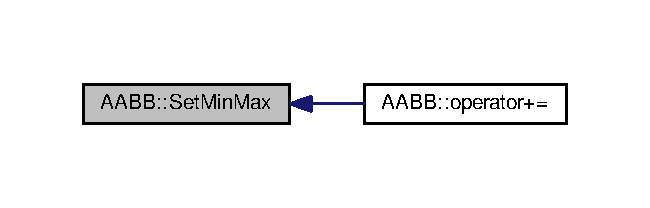
\includegraphics[width=312pt]{d2/d1a/classAABB_aefd07f1b846deede5a40294e0128357d_icgraph}
\end{center}
\end{figure}


\index{A\+A\+BB@{A\+A\+BB}!Set\+Point@{Set\+Point}}
\index{Set\+Point@{Set\+Point}!A\+A\+BB@{A\+A\+BB}}
\subsubsection[{\texorpdfstring{Set\+Point(const Point \&pt)}{SetPoint(const Point &pt)}}]{\setlength{\rightskip}{0pt plus 5cm}void A\+A\+B\+B\+::\+Set\+Point (
\begin{DoxyParamCaption}
\item[{const {\bf Point} \&}]{pt}
\end{DoxyParamCaption}
)\hspace{0.3cm}{\ttfamily [inline]}}\hypertarget{classAABB_a5fa5fe0ce941e8c991775be34337acad}{}\label{classAABB_a5fa5fe0ce941e8c991775be34337acad}
Setups a point \hyperlink{classAABB}{A\+A\+BB}. 

The documentation for this class was generated from the following file\+:\begin{DoxyCompactItemize}
\item 
cmd/collide2/\+Ice/\hyperlink{IceAABB_8h}{Ice\+A\+A\+B\+B.\+h}\end{DoxyCompactItemize}

\hypertarget{structOpcode_1_1AABBCache}{}\section{Opcode\+:\+:A\+A\+B\+B\+Cache Struct Reference}
\label{structOpcode_1_1AABBCache}\index{Opcode\+::\+A\+A\+B\+B\+Cache@{Opcode\+::\+A\+A\+B\+B\+Cache}}


Inheritance diagram for Opcode\+:\+:A\+A\+B\+B\+Cache\+:
\nopagebreak
\begin{figure}[H]
\begin{center}
\leavevmode
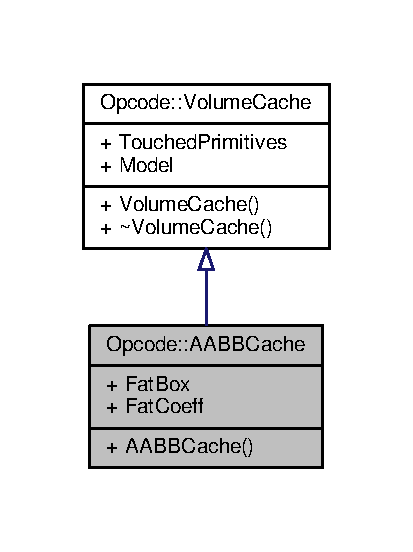
\includegraphics[width=198pt]{d7/d8b/structOpcode_1_1AABBCache__inherit__graph}
\end{center}
\end{figure}


Collaboration diagram for Opcode\+:\+:A\+A\+B\+B\+Cache\+:
\nopagebreak
\begin{figure}[H]
\begin{center}
\leavevmode
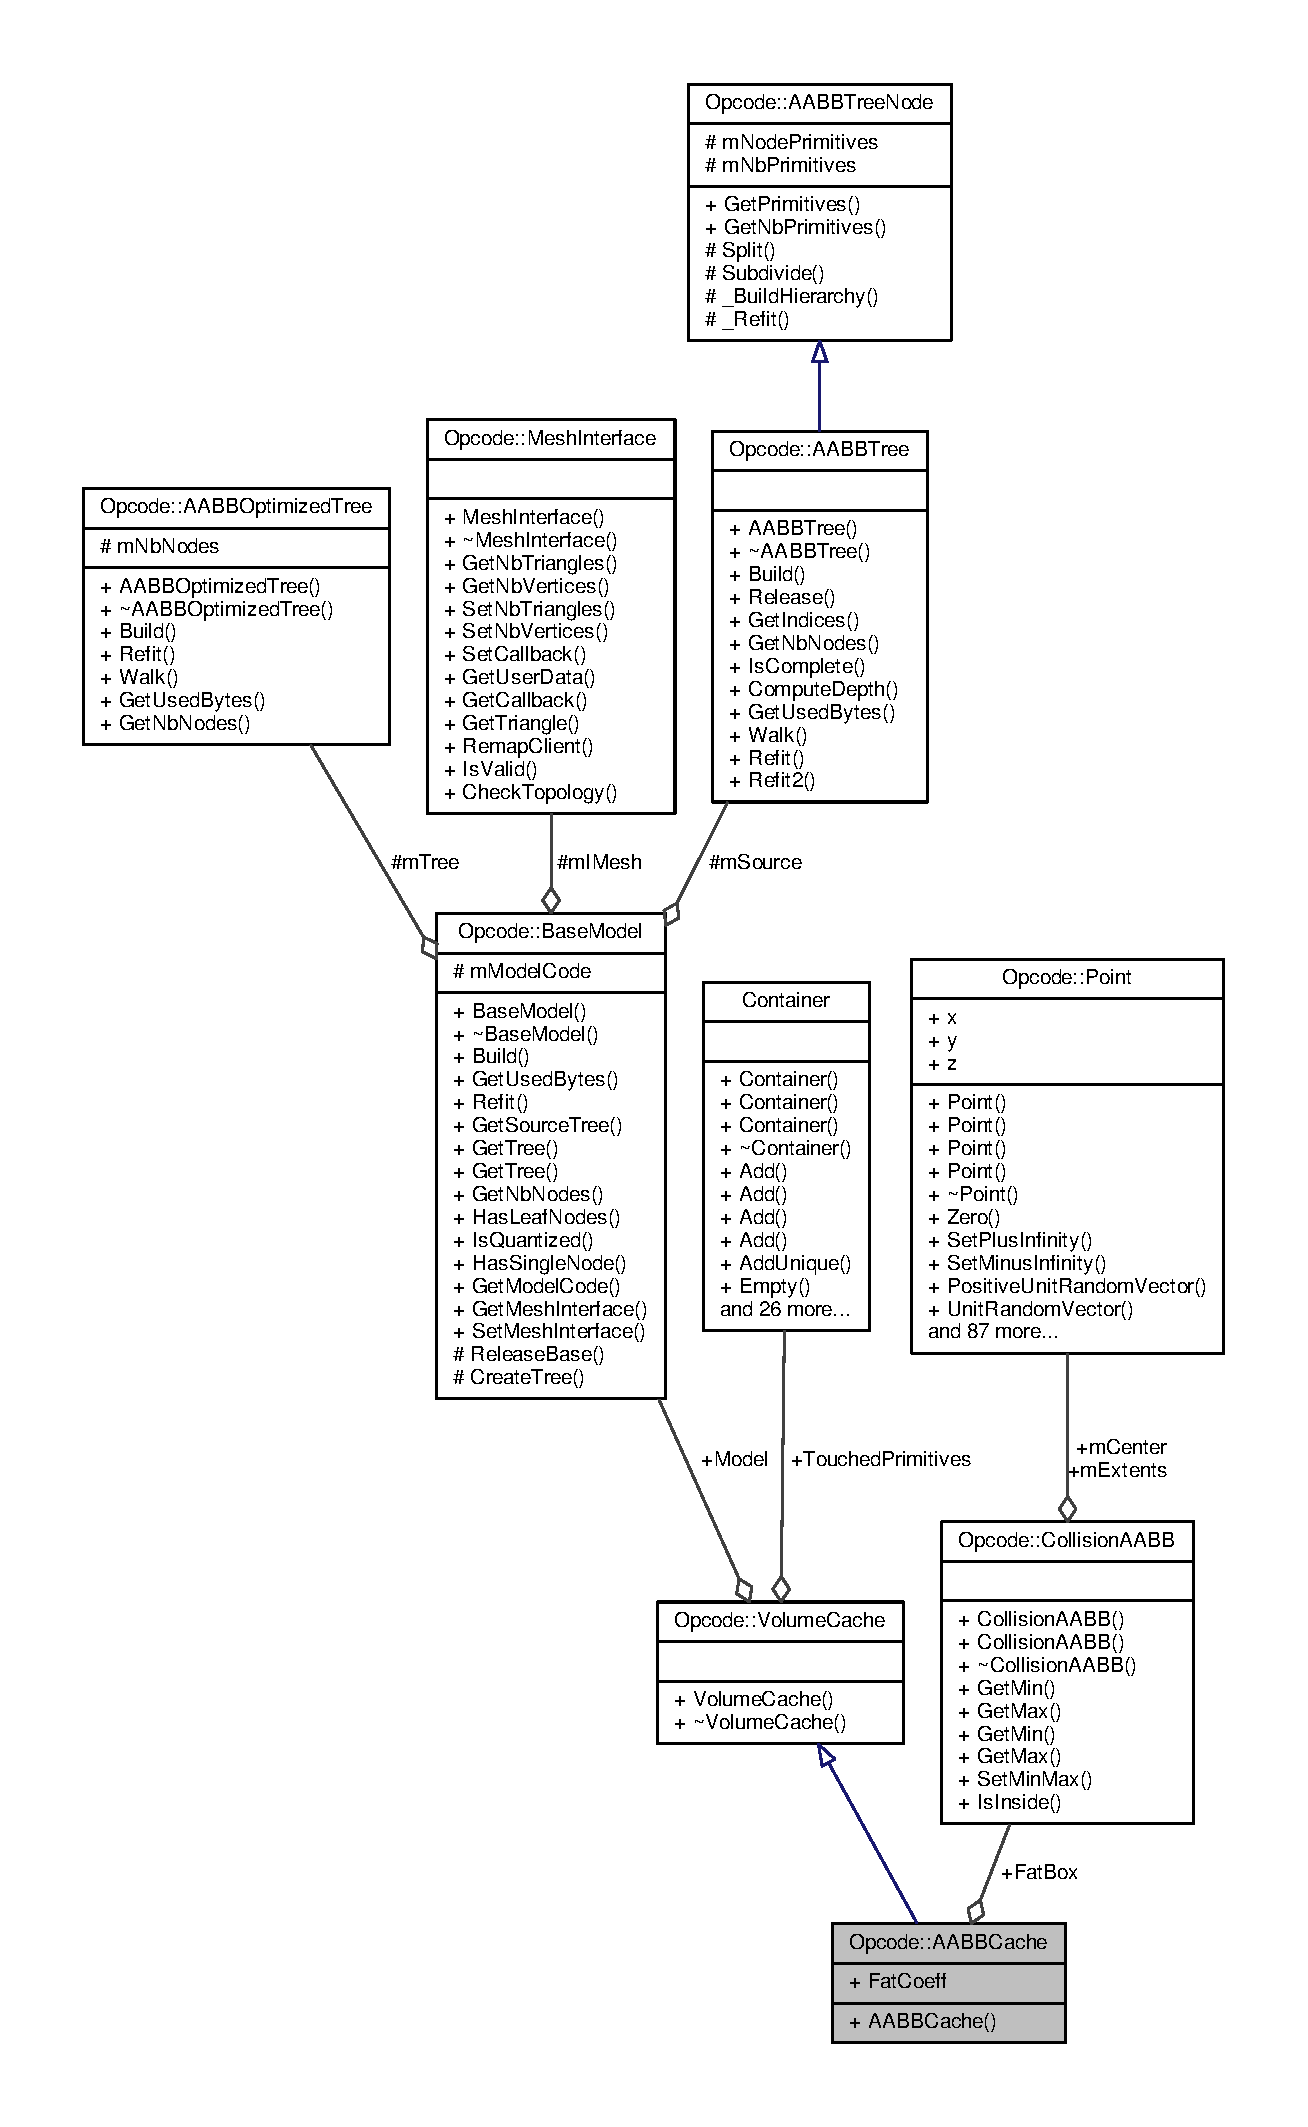
\includegraphics[height=550pt]{d5/d0f/structOpcode_1_1AABBCache__coll__graph}
\end{center}
\end{figure}
\subsection*{Public Attributes}
\begin{DoxyCompactItemize}
\item 
\hyperlink{classOpcode_1_1CollisionAABB}{Collision\+A\+A\+BB} \hyperlink{structOpcode_1_1AABBCache_abbbaff7342f3f82d6a0bf0ec8a2dbe12}{Fat\+Box}\hypertarget{structOpcode_1_1AABBCache_abbbaff7342f3f82d6a0bf0ec8a2dbe12}{}\label{structOpcode_1_1AABBCache_abbbaff7342f3f82d6a0bf0ec8a2dbe12}

\begin{DoxyCompactList}\small\item\em \hyperlink{classBox}{Box} used when performing the query resulting in cached faces. \end{DoxyCompactList}\item 
float \hyperlink{structOpcode_1_1AABBCache_a277d5f9dd30242d99aef111fbe146ba8}{Fat\+Coeff}\hypertarget{structOpcode_1_1AABBCache_a277d5f9dd30242d99aef111fbe146ba8}{}\label{structOpcode_1_1AABBCache_a277d5f9dd30242d99aef111fbe146ba8}

\begin{DoxyCompactList}\small\item\em m\+Radius2 multiplier used to create a fat sphere \end{DoxyCompactList}\end{DoxyCompactItemize}


The documentation for this struct was generated from the following file\+:\begin{DoxyCompactItemize}
\item 
cmd/collide2/\hyperlink{Opcode_8h}{Opcode.\+h}\end{DoxyCompactItemize}

\hypertarget{structAABBCache}{}\section{A\+A\+B\+B\+Cache Struct Reference}
\label{structAABBCache}\index{A\+A\+B\+B\+Cache@{A\+A\+B\+B\+Cache}}


Inheritance diagram for A\+A\+B\+B\+Cache\+:
\nopagebreak
\begin{figure}[H]
\begin{center}
\leavevmode
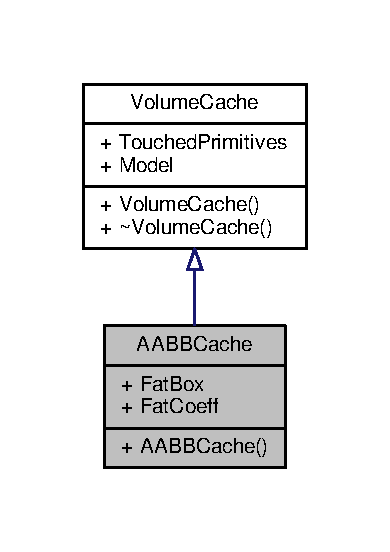
\includegraphics[width=187pt]{d2/d80/structAABBCache__inherit__graph}
\end{center}
\end{figure}


Collaboration diagram for A\+A\+B\+B\+Cache\+:
\nopagebreak
\begin{figure}[H]
\begin{center}
\leavevmode
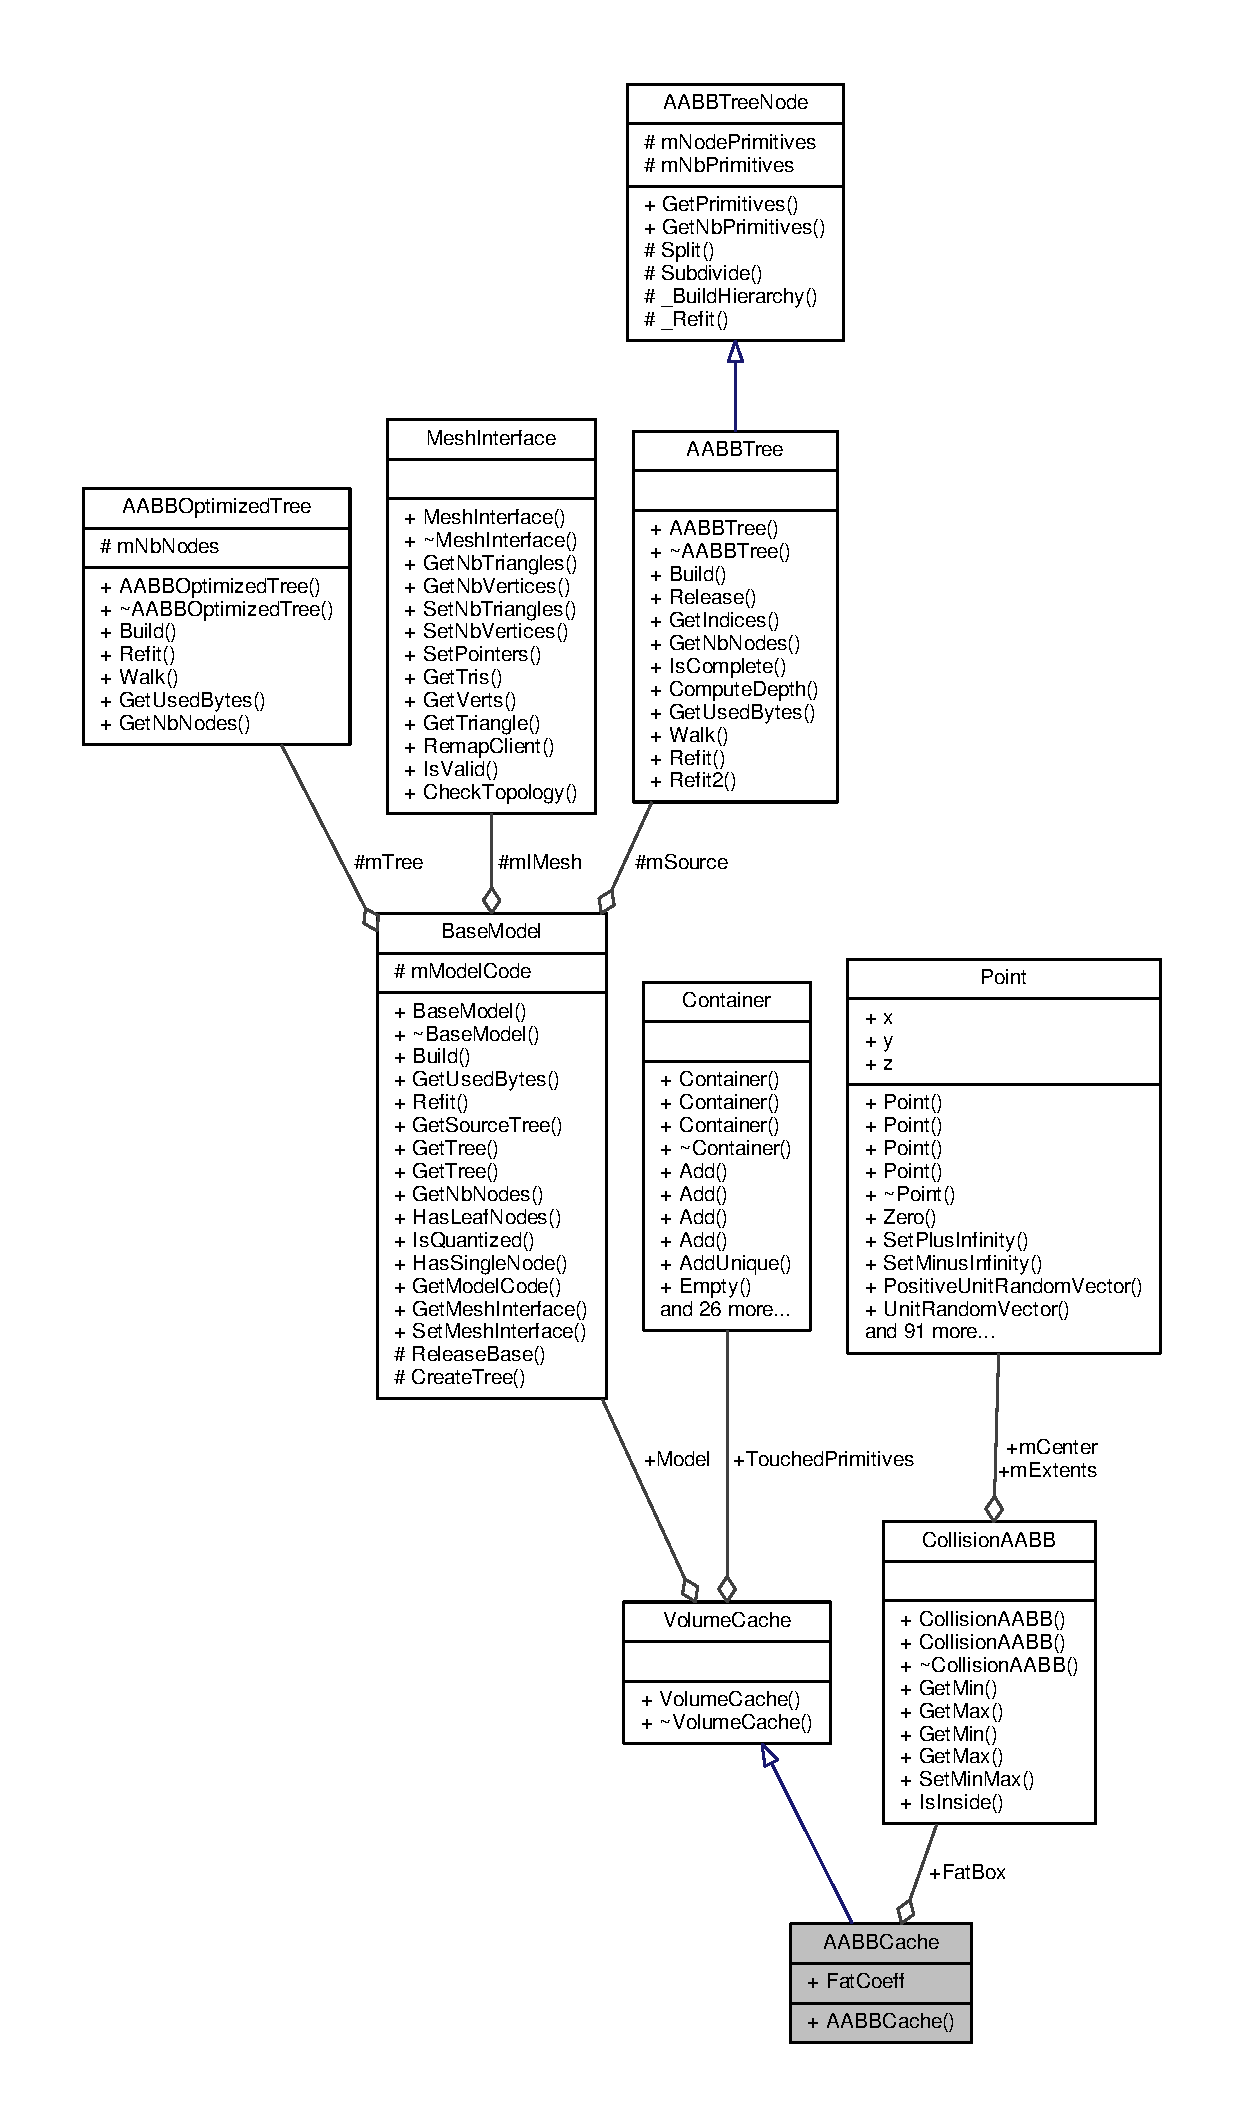
\includegraphics[height=550pt]{da/d40/structAABBCache__coll__graph}
\end{center}
\end{figure}
\subsection*{Public Attributes}
\begin{DoxyCompactItemize}
\item 
\hyperlink{classCollisionAABB}{Collision\+A\+A\+BB} \hyperlink{structAABBCache_a739e3bc835cf651d3040bf615ec63996}{Fat\+Box}\hypertarget{structAABBCache_a739e3bc835cf651d3040bf615ec63996}{}\label{structAABBCache_a739e3bc835cf651d3040bf615ec63996}

\begin{DoxyCompactList}\small\item\em \hyperlink{classBox}{Box} used when performing the query resulting in cached faces. \end{DoxyCompactList}\item 
float \hyperlink{structAABBCache_aa3e8dde6b0472dd391a2884cd0aa9efa}{Fat\+Coeff}\hypertarget{structAABBCache_aa3e8dde6b0472dd391a2884cd0aa9efa}{}\label{structAABBCache_aa3e8dde6b0472dd391a2884cd0aa9efa}

\begin{DoxyCompactList}\small\item\em m\+Radius2 multiplier used to create a fat sphere \end{DoxyCompactList}\end{DoxyCompactItemize}


The documentation for this struct was generated from the following file\+:\begin{DoxyCompactItemize}
\item 
cmd/collide2/\hyperlink{OPC__AABBCollider_8h}{O\+P\+C\+\_\+\+A\+A\+B\+B\+Collider.\+h}\end{DoxyCompactItemize}

\hypertarget{classOpcode_1_1AABBCollider}{}\section{Opcode\+:\+:A\+A\+B\+B\+Collider Class Reference}
\label{classOpcode_1_1AABBCollider}\index{Opcode\+::\+A\+A\+B\+B\+Collider@{Opcode\+::\+A\+A\+B\+B\+Collider}}


Inheritance diagram for Opcode\+:\+:A\+A\+B\+B\+Collider\+:
\nopagebreak
\begin{figure}[H]
\begin{center}
\leavevmode
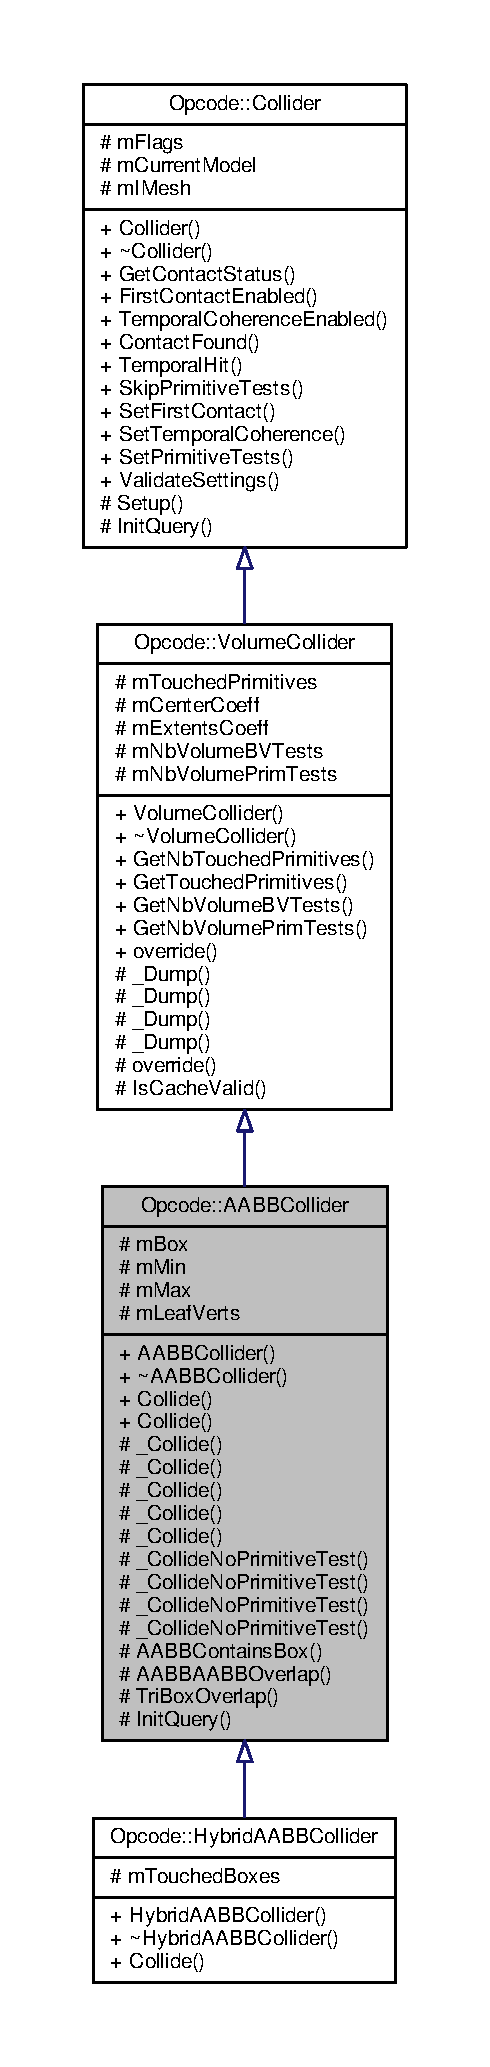
\includegraphics[height=550pt]{d7/d1b/classOpcode_1_1AABBCollider__inherit__graph}
\end{center}
\end{figure}


Collaboration diagram for Opcode\+:\+:A\+A\+B\+B\+Collider\+:
\nopagebreak
\begin{figure}[H]
\begin{center}
\leavevmode
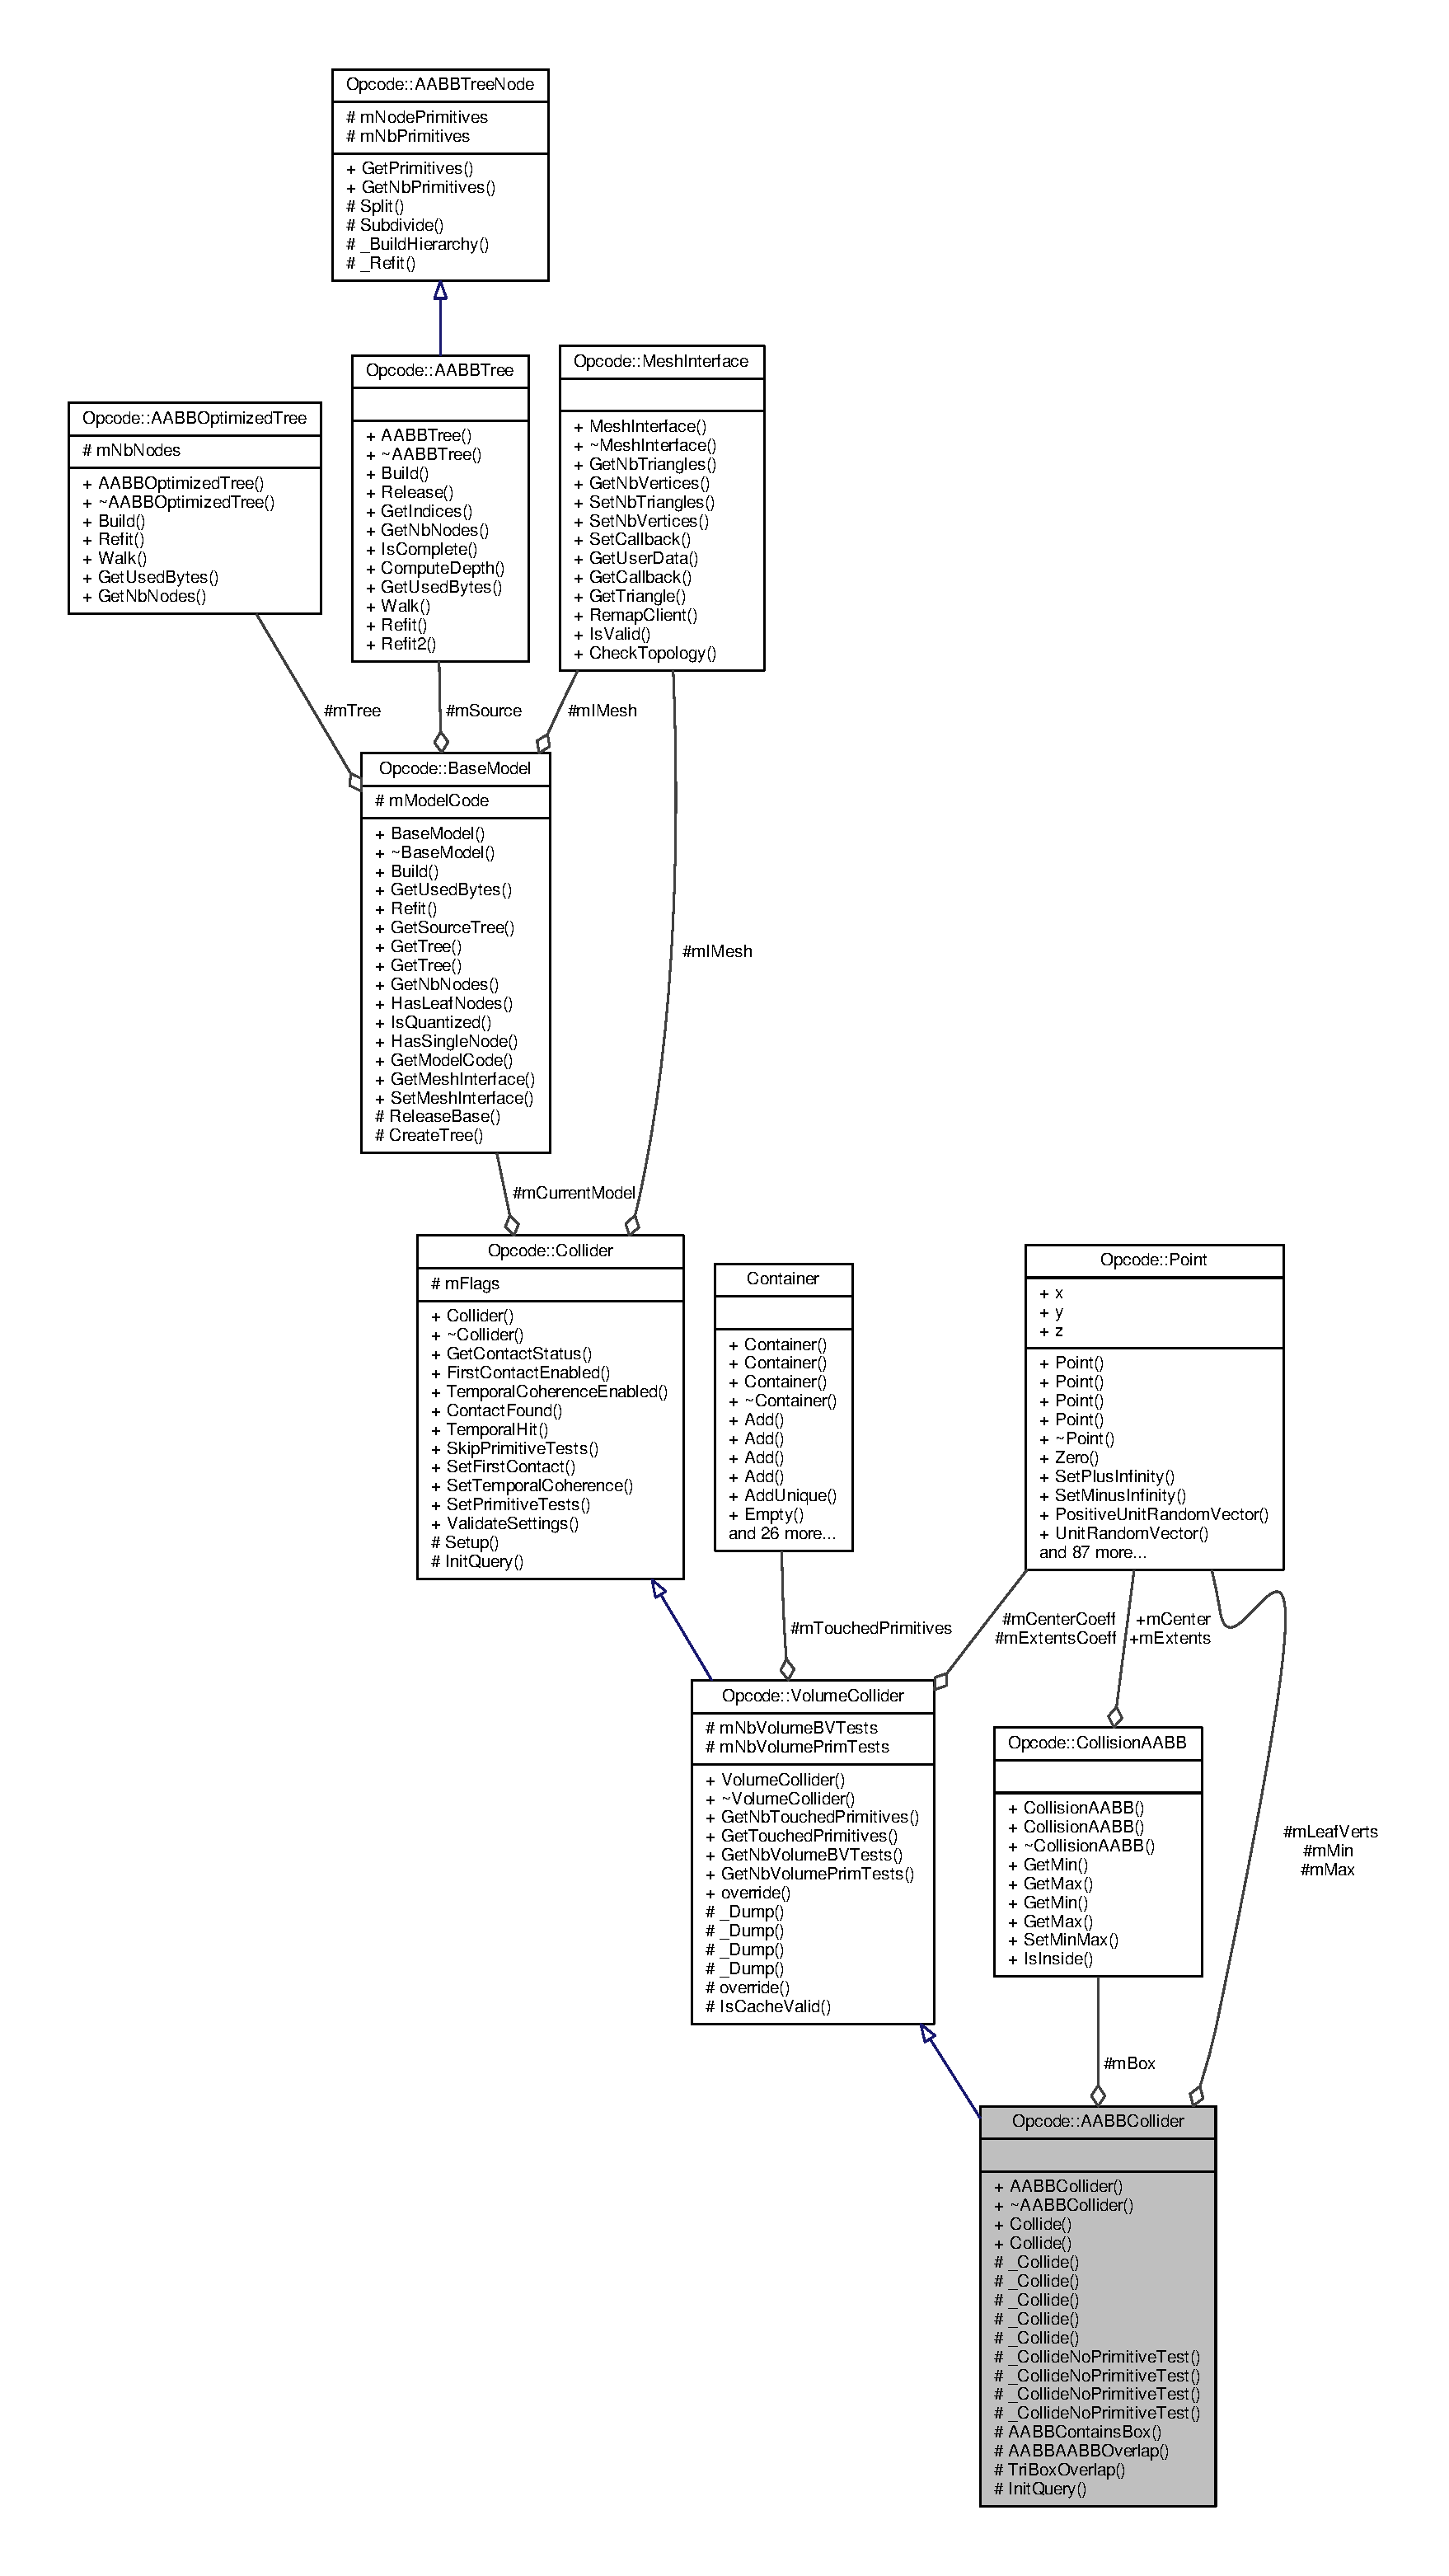
\includegraphics[height=550pt]{d6/d00/classOpcode_1_1AABBCollider__coll__graph}
\end{center}
\end{figure}
\subsection*{Public Member Functions}
\begin{DoxyCompactItemize}
\item 
\hyperlink{classOpcode_1_1AABBCollider_a6a679c11c6a716b1f7a387aa5fa1884a}{A\+A\+B\+B\+Collider} ()
\item 
virtual \hyperlink{classOpcode_1_1AABBCollider_a21f405d3f68a7196286ba9933e34674e}{$\sim$\+A\+A\+B\+B\+Collider} ()
\item 
bool \hyperlink{classOpcode_1_1AABBCollider_a6c5443558bd612a744bbfc74ff2b7368}{Collide} (\hyperlink{structOpcode_1_1AABBCache}{A\+A\+B\+B\+Cache} \&cache, const \hyperlink{classOpcode_1_1CollisionAABB}{Collision\+A\+A\+BB} \&box, const \hyperlink{classOpcode_1_1Model}{Model} \&model)
\item 
bool \hyperlink{classOpcode_1_1AABBCollider_ad26d4fe09769619954dad20961c56f78}{Collide} (\hyperlink{structOpcode_1_1AABBCache}{A\+A\+B\+B\+Cache} \&cache, const \hyperlink{classOpcode_1_1CollisionAABB}{Collision\+A\+A\+BB} \&box, const \hyperlink{classOpcode_1_1AABBTree}{A\+A\+B\+B\+Tree} $\ast$tree)
\end{DoxyCompactItemize}
\subsection*{Protected Member Functions}
\begin{DoxyCompactItemize}
\item 
void \hyperlink{classOpcode_1_1AABBCollider_aa4aa676986ee7f507e957e45f2f5b4ba}{\+\_\+\+Collide} (const \hyperlink{classOpcode_1_1AABBCollisionNode}{A\+A\+B\+B\+Collision\+Node} $\ast$node)
\item 
void \hyperlink{classOpcode_1_1AABBCollider_a7ff71717c0c1ef6d3894fc9ab5e5dcfa}{\+\_\+\+Collide} (const \hyperlink{classOpcode_1_1AABBNoLeafNode}{A\+A\+B\+B\+No\+Leaf\+Node} $\ast$node)
\item 
void \hyperlink{classOpcode_1_1AABBCollider_ae779f38892cb3398c0c1d893f3f6f277}{\+\_\+\+Collide} (const \hyperlink{classOpcode_1_1AABBQuantizedNode}{A\+A\+B\+B\+Quantized\+Node} $\ast$node)
\item 
void \hyperlink{classOpcode_1_1AABBCollider_a9b38f0dda1f0ba7b3225f0f8f2abbf25}{\+\_\+\+Collide} (const \hyperlink{classOpcode_1_1AABBQuantizedNoLeafNode}{A\+A\+B\+B\+Quantized\+No\+Leaf\+Node} $\ast$node)
\item 
void \hyperlink{classOpcode_1_1AABBCollider_ae5e560d946cf02643db63f8856bcb1f9}{\+\_\+\+Collide} (const \hyperlink{classOpcode_1_1AABBTreeNode}{A\+A\+B\+B\+Tree\+Node} $\ast$node)
\item 
void \hyperlink{classOpcode_1_1AABBCollider_aa8eaafb1934f7961ce7caedae4a3142d}{\+\_\+\+Collide\+No\+Primitive\+Test} (const \hyperlink{classOpcode_1_1AABBCollisionNode}{A\+A\+B\+B\+Collision\+Node} $\ast$node)
\item 
void \hyperlink{classOpcode_1_1AABBCollider_a9a23722e23e4d49d248f85daa0482772}{\+\_\+\+Collide\+No\+Primitive\+Test} (const \hyperlink{classOpcode_1_1AABBNoLeafNode}{A\+A\+B\+B\+No\+Leaf\+Node} $\ast$node)
\item 
void \hyperlink{classOpcode_1_1AABBCollider_a700cf755f32326cd8c68c4bbcb3c4b1f}{\+\_\+\+Collide\+No\+Primitive\+Test} (const \hyperlink{classOpcode_1_1AABBQuantizedNode}{A\+A\+B\+B\+Quantized\+Node} $\ast$node)
\item 
void \hyperlink{classOpcode_1_1AABBCollider_a440e56705eec03a65d56a66a44f41bc7}{\+\_\+\+Collide\+No\+Primitive\+Test} (const \hyperlink{classOpcode_1_1AABBQuantizedNoLeafNode}{A\+A\+B\+B\+Quantized\+No\+Leaf\+Node} $\ast$node)
\item 
inline\+\_\+ bool \hyperlink{classOpcode_1_1AABBCollider_abcd553e5b1275abfbad884f11968110a}{A\+A\+B\+B\+Contains\+Box} (const \hyperlink{classOpcode_1_1Point}{Point} \&bc, const \hyperlink{classOpcode_1_1Point}{Point} \&be)
\item 
inline\+\_\+ bool {\bfseries A\+A\+B\+B\+A\+A\+B\+B\+Overlap} (const \hyperlink{classOpcode_1_1Point}{Point} \&b, const \hyperlink{classOpcode_1_1Point}{Point} \&Pb)\hypertarget{classOpcode_1_1AABBCollider_ab70ad121c377c7ca6c1c59c3e5573f61}{}\label{classOpcode_1_1AABBCollider_ab70ad121c377c7ca6c1c59c3e5573f61}

\item 
inline\+\_\+ bool {\bfseries Tri\+Box\+Overlap} ()\hypertarget{classOpcode_1_1AABBCollider_a066a75dae5b12b42d93c4368750a3fd4}{}\label{classOpcode_1_1AABBCollider_a066a75dae5b12b42d93c4368750a3fd4}

\item 
bool \hyperlink{classOpcode_1_1AABBCollider_afc5a6945b3c809051fa20b5587047b68}{Init\+Query} (\hyperlink{structOpcode_1_1AABBCache}{A\+A\+B\+B\+Cache} \&cache, const \hyperlink{classOpcode_1_1CollisionAABB}{Collision\+A\+A\+BB} \&box)
\end{DoxyCompactItemize}
\subsection*{Protected Attributes}
\begin{DoxyCompactItemize}
\item 
\hyperlink{classOpcode_1_1CollisionAABB}{Collision\+A\+A\+BB} \hyperlink{classOpcode_1_1AABBCollider_a9e8ed12586372d9d4de78a6a93cf9781}{m\+Box}\hypertarget{classOpcode_1_1AABBCollider_a9e8ed12586372d9d4de78a6a93cf9781}{}\label{classOpcode_1_1AABBCollider_a9e8ed12586372d9d4de78a6a93cf9781}

\begin{DoxyCompactList}\small\item\em Query box in (center, extents) form. \end{DoxyCompactList}\item 
\hyperlink{classOpcode_1_1Point}{Point} \hyperlink{classOpcode_1_1AABBCollider_a400889f0a812283de13b327824c15b26}{m\+Min}\hypertarget{classOpcode_1_1AABBCollider_a400889f0a812283de13b327824c15b26}{}\label{classOpcode_1_1AABBCollider_a400889f0a812283de13b327824c15b26}

\begin{DoxyCompactList}\small\item\em Query box min point. \end{DoxyCompactList}\item 
\hyperlink{classOpcode_1_1Point}{Point} \hyperlink{classOpcode_1_1AABBCollider_a1e32eb32df46d71ed66ab4bfa7fa192f}{m\+Max}\hypertarget{classOpcode_1_1AABBCollider_a1e32eb32df46d71ed66ab4bfa7fa192f}{}\label{classOpcode_1_1AABBCollider_a1e32eb32df46d71ed66ab4bfa7fa192f}

\begin{DoxyCompactList}\small\item\em Query box max point. \end{DoxyCompactList}\item 
\hyperlink{classOpcode_1_1Point}{Point} \hyperlink{classOpcode_1_1AABBCollider_a347899641399dc3a082999d1f034b177}{m\+Leaf\+Verts} \mbox{[}3\mbox{]}\hypertarget{classOpcode_1_1AABBCollider_a347899641399dc3a082999d1f034b177}{}\label{classOpcode_1_1AABBCollider_a347899641399dc3a082999d1f034b177}

\begin{DoxyCompactList}\small\item\em \hyperlink{classOpcode_1_1Triangle}{Triangle} vertices. \end{DoxyCompactList}\end{DoxyCompactItemize}


\subsection{Constructor \& Destructor Documentation}
\index{Opcode\+::\+A\+A\+B\+B\+Collider@{Opcode\+::\+A\+A\+B\+B\+Collider}!A\+A\+B\+B\+Collider@{A\+A\+B\+B\+Collider}}
\index{A\+A\+B\+B\+Collider@{A\+A\+B\+B\+Collider}!Opcode\+::\+A\+A\+B\+B\+Collider@{Opcode\+::\+A\+A\+B\+B\+Collider}}
\subsubsection[{\texorpdfstring{A\+A\+B\+B\+Collider()}{AABBCollider()}}]{\setlength{\rightskip}{0pt plus 5cm}A\+A\+B\+B\+Collider\+::\+A\+A\+B\+B\+Collider (
\begin{DoxyParamCaption}
{}
\end{DoxyParamCaption}
)}\hypertarget{classOpcode_1_1AABBCollider_a6a679c11c6a716b1f7a387aa5fa1884a}{}\label{classOpcode_1_1AABBCollider_a6a679c11c6a716b1f7a387aa5fa1884a}
Constructor. \index{Opcode\+::\+A\+A\+B\+B\+Collider@{Opcode\+::\+A\+A\+B\+B\+Collider}!````~A\+A\+B\+B\+Collider@{$\sim$\+A\+A\+B\+B\+Collider}}
\index{````~A\+A\+B\+B\+Collider@{$\sim$\+A\+A\+B\+B\+Collider}!Opcode\+::\+A\+A\+B\+B\+Collider@{Opcode\+::\+A\+A\+B\+B\+Collider}}
\subsubsection[{\texorpdfstring{$\sim$\+A\+A\+B\+B\+Collider()}{~AABBCollider()}}]{\setlength{\rightskip}{0pt plus 5cm}A\+A\+B\+B\+Collider\+::$\sim$\+A\+A\+B\+B\+Collider (
\begin{DoxyParamCaption}
{}
\end{DoxyParamCaption}
)\hspace{0.3cm}{\ttfamily [virtual]}}\hypertarget{classOpcode_1_1AABBCollider_a21f405d3f68a7196286ba9933e34674e}{}\label{classOpcode_1_1AABBCollider_a21f405d3f68a7196286ba9933e34674e}
Destructor. 

\subsection{Member Function Documentation}
\index{Opcode\+::\+A\+A\+B\+B\+Collider@{Opcode\+::\+A\+A\+B\+B\+Collider}!\+\_\+\+Collide@{\+\_\+\+Collide}}
\index{\+\_\+\+Collide@{\+\_\+\+Collide}!Opcode\+::\+A\+A\+B\+B\+Collider@{Opcode\+::\+A\+A\+B\+B\+Collider}}
\subsubsection[{\texorpdfstring{\+\_\+\+Collide(const A\+A\+B\+B\+Collision\+Node $\ast$node)}{_Collide(const AABBCollisionNode *node)}}]{\setlength{\rightskip}{0pt plus 5cm}void A\+A\+B\+B\+Collider\+::\+\_\+\+Collide (
\begin{DoxyParamCaption}
\item[{const {\bf A\+A\+B\+B\+Collision\+Node} $\ast$}]{node}
\end{DoxyParamCaption}
)\hspace{0.3cm}{\ttfamily [protected]}}\hypertarget{classOpcode_1_1AABBCollider_aa4aa676986ee7f507e957e45f2f5b4ba}{}\label{classOpcode_1_1AABBCollider_aa4aa676986ee7f507e957e45f2f5b4ba}
Recursive collision query for normal \hyperlink{classOpcode_1_1AABB}{A\+A\+BB} trees. 
\begin{DoxyParams}{Parameters}
{\em node} & \mbox{[}in\mbox{]} current collision node \\
\hline
\end{DoxyParams}
\index{Opcode\+::\+A\+A\+B\+B\+Collider@{Opcode\+::\+A\+A\+B\+B\+Collider}!\+\_\+\+Collide@{\+\_\+\+Collide}}
\index{\+\_\+\+Collide@{\+\_\+\+Collide}!Opcode\+::\+A\+A\+B\+B\+Collider@{Opcode\+::\+A\+A\+B\+B\+Collider}}
\subsubsection[{\texorpdfstring{\+\_\+\+Collide(const A\+A\+B\+B\+No\+Leaf\+Node $\ast$node)}{_Collide(const AABBNoLeafNode *node)}}]{\setlength{\rightskip}{0pt plus 5cm}void A\+A\+B\+B\+Collider\+::\+\_\+\+Collide (
\begin{DoxyParamCaption}
\item[{const {\bf A\+A\+B\+B\+No\+Leaf\+Node} $\ast$}]{node}
\end{DoxyParamCaption}
)\hspace{0.3cm}{\ttfamily [protected]}}\hypertarget{classOpcode_1_1AABBCollider_a7ff71717c0c1ef6d3894fc9ab5e5dcfa}{}\label{classOpcode_1_1AABBCollider_a7ff71717c0c1ef6d3894fc9ab5e5dcfa}
Recursive collision query for no-\/leaf \hyperlink{classOpcode_1_1AABB}{A\+A\+BB} trees. 
\begin{DoxyParams}{Parameters}
{\em node} & \mbox{[}in\mbox{]} current collision node \\
\hline
\end{DoxyParams}
\index{Opcode\+::\+A\+A\+B\+B\+Collider@{Opcode\+::\+A\+A\+B\+B\+Collider}!\+\_\+\+Collide@{\+\_\+\+Collide}}
\index{\+\_\+\+Collide@{\+\_\+\+Collide}!Opcode\+::\+A\+A\+B\+B\+Collider@{Opcode\+::\+A\+A\+B\+B\+Collider}}
\subsubsection[{\texorpdfstring{\+\_\+\+Collide(const A\+A\+B\+B\+Quantized\+Node $\ast$node)}{_Collide(const AABBQuantizedNode *node)}}]{\setlength{\rightskip}{0pt plus 5cm}void A\+A\+B\+B\+Collider\+::\+\_\+\+Collide (
\begin{DoxyParamCaption}
\item[{const {\bf A\+A\+B\+B\+Quantized\+Node} $\ast$}]{node}
\end{DoxyParamCaption}
)\hspace{0.3cm}{\ttfamily [protected]}}\hypertarget{classOpcode_1_1AABBCollider_ae779f38892cb3398c0c1d893f3f6f277}{}\label{classOpcode_1_1AABBCollider_ae779f38892cb3398c0c1d893f3f6f277}
Recursive collision query for quantized \hyperlink{classOpcode_1_1AABB}{A\+A\+BB} trees. 
\begin{DoxyParams}{Parameters}
{\em node} & \mbox{[}in\mbox{]} current collision node \\
\hline
\end{DoxyParams}
\index{Opcode\+::\+A\+A\+B\+B\+Collider@{Opcode\+::\+A\+A\+B\+B\+Collider}!\+\_\+\+Collide@{\+\_\+\+Collide}}
\index{\+\_\+\+Collide@{\+\_\+\+Collide}!Opcode\+::\+A\+A\+B\+B\+Collider@{Opcode\+::\+A\+A\+B\+B\+Collider}}
\subsubsection[{\texorpdfstring{\+\_\+\+Collide(const A\+A\+B\+B\+Quantized\+No\+Leaf\+Node $\ast$node)}{_Collide(const AABBQuantizedNoLeafNode *node)}}]{\setlength{\rightskip}{0pt plus 5cm}void A\+A\+B\+B\+Collider\+::\+\_\+\+Collide (
\begin{DoxyParamCaption}
\item[{const {\bf A\+A\+B\+B\+Quantized\+No\+Leaf\+Node} $\ast$}]{node}
\end{DoxyParamCaption}
)\hspace{0.3cm}{\ttfamily [protected]}}\hypertarget{classOpcode_1_1AABBCollider_a9b38f0dda1f0ba7b3225f0f8f2abbf25}{}\label{classOpcode_1_1AABBCollider_a9b38f0dda1f0ba7b3225f0f8f2abbf25}
Recursive collision query for quantized no-\/leaf \hyperlink{classOpcode_1_1AABB}{A\+A\+BB} trees. 
\begin{DoxyParams}{Parameters}
{\em node} & \mbox{[}in\mbox{]} current collision node \\
\hline
\end{DoxyParams}
\index{Opcode\+::\+A\+A\+B\+B\+Collider@{Opcode\+::\+A\+A\+B\+B\+Collider}!\+\_\+\+Collide@{\+\_\+\+Collide}}
\index{\+\_\+\+Collide@{\+\_\+\+Collide}!Opcode\+::\+A\+A\+B\+B\+Collider@{Opcode\+::\+A\+A\+B\+B\+Collider}}
\subsubsection[{\texorpdfstring{\+\_\+\+Collide(const A\+A\+B\+B\+Tree\+Node $\ast$node)}{_Collide(const AABBTreeNode *node)}}]{\setlength{\rightskip}{0pt plus 5cm}void A\+A\+B\+B\+Collider\+::\+\_\+\+Collide (
\begin{DoxyParamCaption}
\item[{const {\bf A\+A\+B\+B\+Tree\+Node} $\ast$}]{node}
\end{DoxyParamCaption}
)\hspace{0.3cm}{\ttfamily [protected]}}\hypertarget{classOpcode_1_1AABBCollider_ae5e560d946cf02643db63f8856bcb1f9}{}\label{classOpcode_1_1AABBCollider_ae5e560d946cf02643db63f8856bcb1f9}
Recursive collision query for vanilla \hyperlink{classOpcode_1_1AABB}{A\+A\+BB} trees. 
\begin{DoxyParams}{Parameters}
{\em node} & \mbox{[}in\mbox{]} current collision node \\
\hline
\end{DoxyParams}
\index{Opcode\+::\+A\+A\+B\+B\+Collider@{Opcode\+::\+A\+A\+B\+B\+Collider}!\+\_\+\+Collide\+No\+Primitive\+Test@{\+\_\+\+Collide\+No\+Primitive\+Test}}
\index{\+\_\+\+Collide\+No\+Primitive\+Test@{\+\_\+\+Collide\+No\+Primitive\+Test}!Opcode\+::\+A\+A\+B\+B\+Collider@{Opcode\+::\+A\+A\+B\+B\+Collider}}
\subsubsection[{\texorpdfstring{\+\_\+\+Collide\+No\+Primitive\+Test(const A\+A\+B\+B\+Collision\+Node $\ast$node)}{_CollideNoPrimitiveTest(const AABBCollisionNode *node)}}]{\setlength{\rightskip}{0pt plus 5cm}void A\+A\+B\+B\+Collider\+::\+\_\+\+Collide\+No\+Primitive\+Test (
\begin{DoxyParamCaption}
\item[{const {\bf A\+A\+B\+B\+Collision\+Node} $\ast$}]{node}
\end{DoxyParamCaption}
)\hspace{0.3cm}{\ttfamily [protected]}}\hypertarget{classOpcode_1_1AABBCollider_aa8eaafb1934f7961ce7caedae4a3142d}{}\label{classOpcode_1_1AABBCollider_aa8eaafb1934f7961ce7caedae4a3142d}
Recursive collision query for normal \hyperlink{classOpcode_1_1AABB}{A\+A\+BB} trees, without primitive tests. 
\begin{DoxyParams}{Parameters}
{\em node} & \mbox{[}in\mbox{]} current collision node \\
\hline
\end{DoxyParams}
\index{Opcode\+::\+A\+A\+B\+B\+Collider@{Opcode\+::\+A\+A\+B\+B\+Collider}!\+\_\+\+Collide\+No\+Primitive\+Test@{\+\_\+\+Collide\+No\+Primitive\+Test}}
\index{\+\_\+\+Collide\+No\+Primitive\+Test@{\+\_\+\+Collide\+No\+Primitive\+Test}!Opcode\+::\+A\+A\+B\+B\+Collider@{Opcode\+::\+A\+A\+B\+B\+Collider}}
\subsubsection[{\texorpdfstring{\+\_\+\+Collide\+No\+Primitive\+Test(const A\+A\+B\+B\+No\+Leaf\+Node $\ast$node)}{_CollideNoPrimitiveTest(const AABBNoLeafNode *node)}}]{\setlength{\rightskip}{0pt plus 5cm}void A\+A\+B\+B\+Collider\+::\+\_\+\+Collide\+No\+Primitive\+Test (
\begin{DoxyParamCaption}
\item[{const {\bf A\+A\+B\+B\+No\+Leaf\+Node} $\ast$}]{node}
\end{DoxyParamCaption}
)\hspace{0.3cm}{\ttfamily [protected]}}\hypertarget{classOpcode_1_1AABBCollider_a9a23722e23e4d49d248f85daa0482772}{}\label{classOpcode_1_1AABBCollider_a9a23722e23e4d49d248f85daa0482772}
Recursive collision query for no-\/leaf \hyperlink{classOpcode_1_1AABB}{A\+A\+BB} trees, without primitive tests. 
\begin{DoxyParams}{Parameters}
{\em node} & \mbox{[}in\mbox{]} current collision node \\
\hline
\end{DoxyParams}
\index{Opcode\+::\+A\+A\+B\+B\+Collider@{Opcode\+::\+A\+A\+B\+B\+Collider}!\+\_\+\+Collide\+No\+Primitive\+Test@{\+\_\+\+Collide\+No\+Primitive\+Test}}
\index{\+\_\+\+Collide\+No\+Primitive\+Test@{\+\_\+\+Collide\+No\+Primitive\+Test}!Opcode\+::\+A\+A\+B\+B\+Collider@{Opcode\+::\+A\+A\+B\+B\+Collider}}
\subsubsection[{\texorpdfstring{\+\_\+\+Collide\+No\+Primitive\+Test(const A\+A\+B\+B\+Quantized\+Node $\ast$node)}{_CollideNoPrimitiveTest(const AABBQuantizedNode *node)}}]{\setlength{\rightskip}{0pt plus 5cm}void A\+A\+B\+B\+Collider\+::\+\_\+\+Collide\+No\+Primitive\+Test (
\begin{DoxyParamCaption}
\item[{const {\bf A\+A\+B\+B\+Quantized\+Node} $\ast$}]{node}
\end{DoxyParamCaption}
)\hspace{0.3cm}{\ttfamily [protected]}}\hypertarget{classOpcode_1_1AABBCollider_a700cf755f32326cd8c68c4bbcb3c4b1f}{}\label{classOpcode_1_1AABBCollider_a700cf755f32326cd8c68c4bbcb3c4b1f}
Recursive collision query for quantized \hyperlink{classOpcode_1_1AABB}{A\+A\+BB} trees, without primitive tests. 
\begin{DoxyParams}{Parameters}
{\em node} & \mbox{[}in\mbox{]} current collision node \\
\hline
\end{DoxyParams}
\index{Opcode\+::\+A\+A\+B\+B\+Collider@{Opcode\+::\+A\+A\+B\+B\+Collider}!\+\_\+\+Collide\+No\+Primitive\+Test@{\+\_\+\+Collide\+No\+Primitive\+Test}}
\index{\+\_\+\+Collide\+No\+Primitive\+Test@{\+\_\+\+Collide\+No\+Primitive\+Test}!Opcode\+::\+A\+A\+B\+B\+Collider@{Opcode\+::\+A\+A\+B\+B\+Collider}}
\subsubsection[{\texorpdfstring{\+\_\+\+Collide\+No\+Primitive\+Test(const A\+A\+B\+B\+Quantized\+No\+Leaf\+Node $\ast$node)}{_CollideNoPrimitiveTest(const AABBQuantizedNoLeafNode *node)}}]{\setlength{\rightskip}{0pt plus 5cm}void A\+A\+B\+B\+Collider\+::\+\_\+\+Collide\+No\+Primitive\+Test (
\begin{DoxyParamCaption}
\item[{const {\bf A\+A\+B\+B\+Quantized\+No\+Leaf\+Node} $\ast$}]{node}
\end{DoxyParamCaption}
)\hspace{0.3cm}{\ttfamily [protected]}}\hypertarget{classOpcode_1_1AABBCollider_a440e56705eec03a65d56a66a44f41bc7}{}\label{classOpcode_1_1AABBCollider_a440e56705eec03a65d56a66a44f41bc7}
Recursive collision query for quantized no-\/leaf \hyperlink{classOpcode_1_1AABB}{A\+A\+BB} trees, without primitive tests. 
\begin{DoxyParams}{Parameters}
{\em node} & \mbox{[}in\mbox{]} current collision node \\
\hline
\end{DoxyParams}
\index{Opcode\+::\+A\+A\+B\+B\+Collider@{Opcode\+::\+A\+A\+B\+B\+Collider}!A\+A\+B\+B\+Contains\+Box@{A\+A\+B\+B\+Contains\+Box}}
\index{A\+A\+B\+B\+Contains\+Box@{A\+A\+B\+B\+Contains\+Box}!Opcode\+::\+A\+A\+B\+B\+Collider@{Opcode\+::\+A\+A\+B\+B\+Collider}}
\subsubsection[{\texorpdfstring{A\+A\+B\+B\+Contains\+Box(const Point \&bc, const Point \&be)}{AABBContainsBox(const Point &bc, const Point &be)}}]{\setlength{\rightskip}{0pt plus 5cm}inline\+\_\+ bool A\+A\+B\+B\+Collider\+::\+A\+A\+B\+B\+Contains\+Box (
\begin{DoxyParamCaption}
\item[{const {\bf Point} \&}]{bc, }
\item[{const {\bf Point} \&}]{be}
\end{DoxyParamCaption}
)\hspace{0.3cm}{\ttfamily [protected]}}\hypertarget{classOpcode_1_1AABBCollider_abcd553e5b1275abfbad884f11968110a}{}\label{classOpcode_1_1AABBCollider_abcd553e5b1275abfbad884f11968110a}
Checks the \hyperlink{classOpcode_1_1AABB}{A\+A\+BB} completely contains the box. In which case we can end the query sooner. 
\begin{DoxyParams}{Parameters}
{\em bc} & \mbox{[}in\mbox{]} box center \\
\hline
{\em be} & \mbox{[}in\mbox{]} box extents \\
\hline
\end{DoxyParams}
\begin{DoxyReturn}{Returns}
true if the \hyperlink{classOpcode_1_1AABB}{A\+A\+BB} contains the whole box 
\end{DoxyReturn}
\index{Opcode\+::\+A\+A\+B\+B\+Collider@{Opcode\+::\+A\+A\+B\+B\+Collider}!Collide@{Collide}}
\index{Collide@{Collide}!Opcode\+::\+A\+A\+B\+B\+Collider@{Opcode\+::\+A\+A\+B\+B\+Collider}}
\subsubsection[{\texorpdfstring{Collide(\+A\+A\+B\+B\+Cache \&cache, const Collision\+A\+A\+B\+B \&box, const Model \&model)}{Collide(AABBCache &cache, const CollisionAABB &box, const Model &model)}}]{\setlength{\rightskip}{0pt plus 5cm}bool A\+A\+B\+B\+Collider\+::\+Collide (
\begin{DoxyParamCaption}
\item[{{\bf A\+A\+B\+B\+Cache} \&}]{cache, }
\item[{const {\bf Collision\+A\+A\+BB} \&}]{box, }
\item[{const {\bf Model} \&}]{model}
\end{DoxyParamCaption}
)}\hypertarget{classOpcode_1_1AABBCollider_a6c5443558bd612a744bbfc74ff2b7368}{}\label{classOpcode_1_1AABBCollider_a6c5443558bd612a744bbfc74ff2b7368}
Generic collision query for generic O\+P\+C\+O\+DE models. After the call, access the results\+:
\begin{DoxyItemize}
\item with \hyperlink{classOpcode_1_1Collider_a7d8c3e6a85be417ac7505930f14f141c}{Get\+Contact\+Status()}
\item with \hyperlink{classOpcode_1_1VolumeCollider_ab4ab03fdecae438e89ef98433b7fc6c1}{Get\+Nb\+Touched\+Primitives()}
\item with \hyperlink{classOpcode_1_1VolumeCollider_ac85a0c717bc3d3424af31becc7abbebd}{Get\+Touched\+Primitives()}
\end{DoxyItemize}


\begin{DoxyParams}{Parameters}
{\em cache} & \mbox{[}in/out\mbox{]} a box cache \\
\hline
{\em box} & \mbox{[}in\mbox{]} collision \hyperlink{classOpcode_1_1AABB}{A\+A\+BB} in world space \\
\hline
{\em model} & \mbox{[}in\mbox{]} Opcode model to collide with \\
\hline
\end{DoxyParams}
\begin{DoxyReturn}{Returns}
true if success 
\end{DoxyReturn}
\begin{DoxyWarning}{Warning}
S\+C\+A\+LE N\+OT S\+U\+P\+P\+O\+R\+T\+ED. The matrices must contain rotation \& translation parts only. 
\end{DoxyWarning}
\index{Opcode\+::\+A\+A\+B\+B\+Collider@{Opcode\+::\+A\+A\+B\+B\+Collider}!Collide@{Collide}}
\index{Collide@{Collide}!Opcode\+::\+A\+A\+B\+B\+Collider@{Opcode\+::\+A\+A\+B\+B\+Collider}}
\subsubsection[{\texorpdfstring{Collide(\+A\+A\+B\+B\+Cache \&cache, const Collision\+A\+A\+B\+B \&box, const A\+A\+B\+B\+Tree $\ast$tree)}{Collide(AABBCache &cache, const CollisionAABB &box, const AABBTree *tree)}}]{\setlength{\rightskip}{0pt plus 5cm}bool A\+A\+B\+B\+Collider\+::\+Collide (
\begin{DoxyParamCaption}
\item[{{\bf A\+A\+B\+B\+Cache} \&}]{cache, }
\item[{const {\bf Collision\+A\+A\+BB} \&}]{box, }
\item[{const {\bf A\+A\+B\+B\+Tree} $\ast$}]{tree}
\end{DoxyParamCaption}
)}\hypertarget{classOpcode_1_1AABBCollider_ad26d4fe09769619954dad20961c56f78}{}\label{classOpcode_1_1AABBCollider_ad26d4fe09769619954dad20961c56f78}
Collision query for vanilla \hyperlink{classOpcode_1_1AABB}{A\+A\+BB} trees. 
\begin{DoxyParams}{Parameters}
{\em cache} & \mbox{[}in/out\mbox{]} a box cache \\
\hline
{\em box} & \mbox{[}in\mbox{]} collision \hyperlink{classOpcode_1_1AABB}{A\+A\+BB} in world space \\
\hline
{\em tree} & \mbox{[}in\mbox{]} \hyperlink{classOpcode_1_1AABB}{A\+A\+BB} tree \\
\hline
\end{DoxyParams}
\begin{DoxyReturn}{Returns}
true if success 
\end{DoxyReturn}
\index{Opcode\+::\+A\+A\+B\+B\+Collider@{Opcode\+::\+A\+A\+B\+B\+Collider}!Init\+Query@{Init\+Query}}
\index{Init\+Query@{Init\+Query}!Opcode\+::\+A\+A\+B\+B\+Collider@{Opcode\+::\+A\+A\+B\+B\+Collider}}
\subsubsection[{\texorpdfstring{Init\+Query(\+A\+A\+B\+B\+Cache \&cache, const Collision\+A\+A\+B\+B \&box)}{InitQuery(AABBCache &cache, const CollisionAABB &box)}}]{\setlength{\rightskip}{0pt plus 5cm}bool A\+A\+B\+B\+Collider\+::\+Init\+Query (
\begin{DoxyParamCaption}
\item[{{\bf A\+A\+B\+B\+Cache} \&}]{cache, }
\item[{const {\bf Collision\+A\+A\+BB} \&}]{box}
\end{DoxyParamCaption}
)\hspace{0.3cm}{\ttfamily [protected]}}\hypertarget{classOpcode_1_1AABBCollider_afc5a6945b3c809051fa20b5587047b68}{}\label{classOpcode_1_1AABBCollider_afc5a6945b3c809051fa20b5587047b68}
Initializes a collision query \+:
\begin{DoxyItemize}
\item reset stats \& contact status
\item check temporal coherence
\end{DoxyItemize}


\begin{DoxyParams}{Parameters}
{\em cache} & \mbox{[}in/out\mbox{]} a box cache \\
\hline
{\em box} & \mbox{[}in\mbox{]} \hyperlink{classOpcode_1_1AABB}{A\+A\+BB} in world space \\
\hline
\end{DoxyParams}
\begin{DoxyReturn}{Returns}
T\+R\+UE if we can return immediately 
\end{DoxyReturn}


The documentation for this class was generated from the following files\+:\begin{DoxyCompactItemize}
\item 
cmd/collide2/\hyperlink{Opcode_8h}{Opcode.\+h}\item 
cmd/collide2/\hyperlink{OPC__AABBCollider_8cpp}{O\+P\+C\+\_\+\+A\+A\+B\+B\+Collider.\+cpp}\end{DoxyCompactItemize}

\hypertarget{classAABBCollider}{}\section{A\+A\+B\+B\+Collider Class Reference}
\label{classAABBCollider}\index{A\+A\+B\+B\+Collider@{A\+A\+B\+B\+Collider}}


Inheritance diagram for A\+A\+B\+B\+Collider\+:
\nopagebreak
\begin{figure}[H]
\begin{center}
\leavevmode
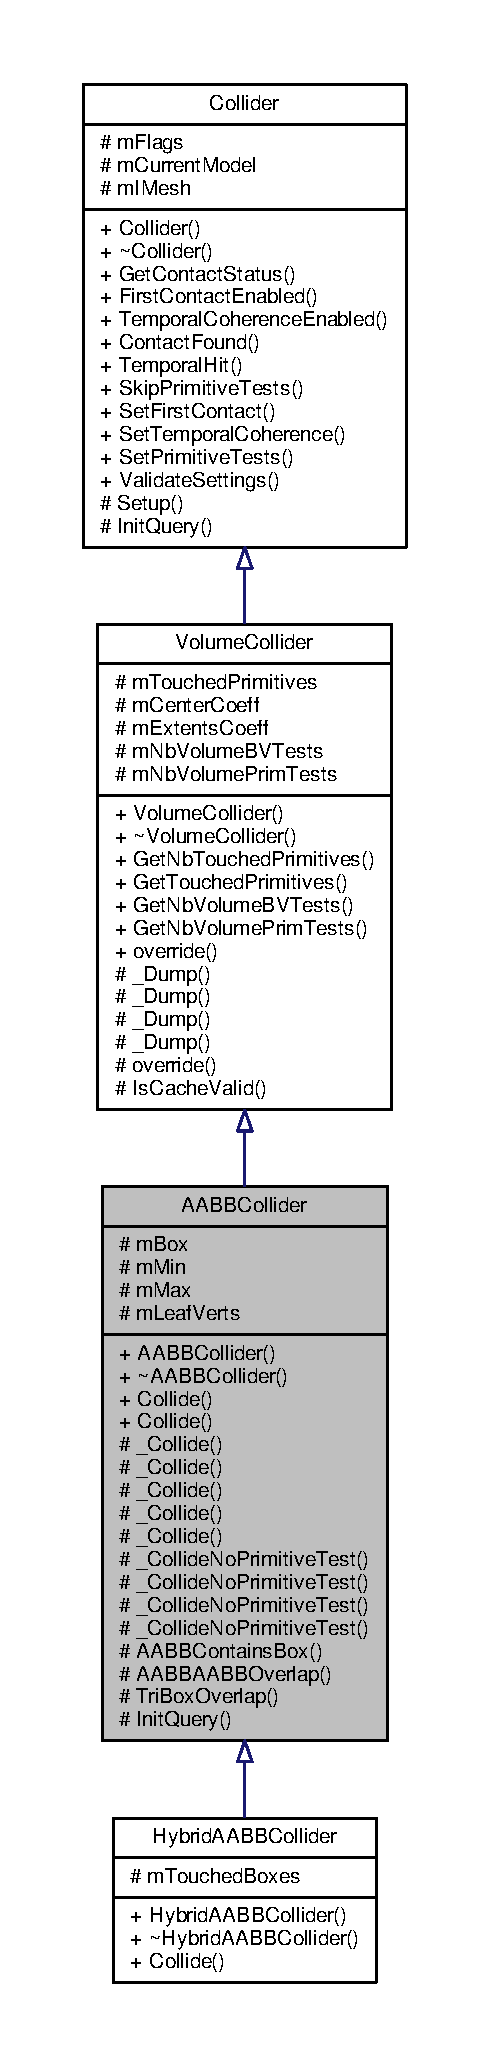
\includegraphics[height=550pt]{dc/d23/classAABBCollider__inherit__graph}
\end{center}
\end{figure}


Collaboration diagram for A\+A\+B\+B\+Collider\+:
\nopagebreak
\begin{figure}[H]
\begin{center}
\leavevmode
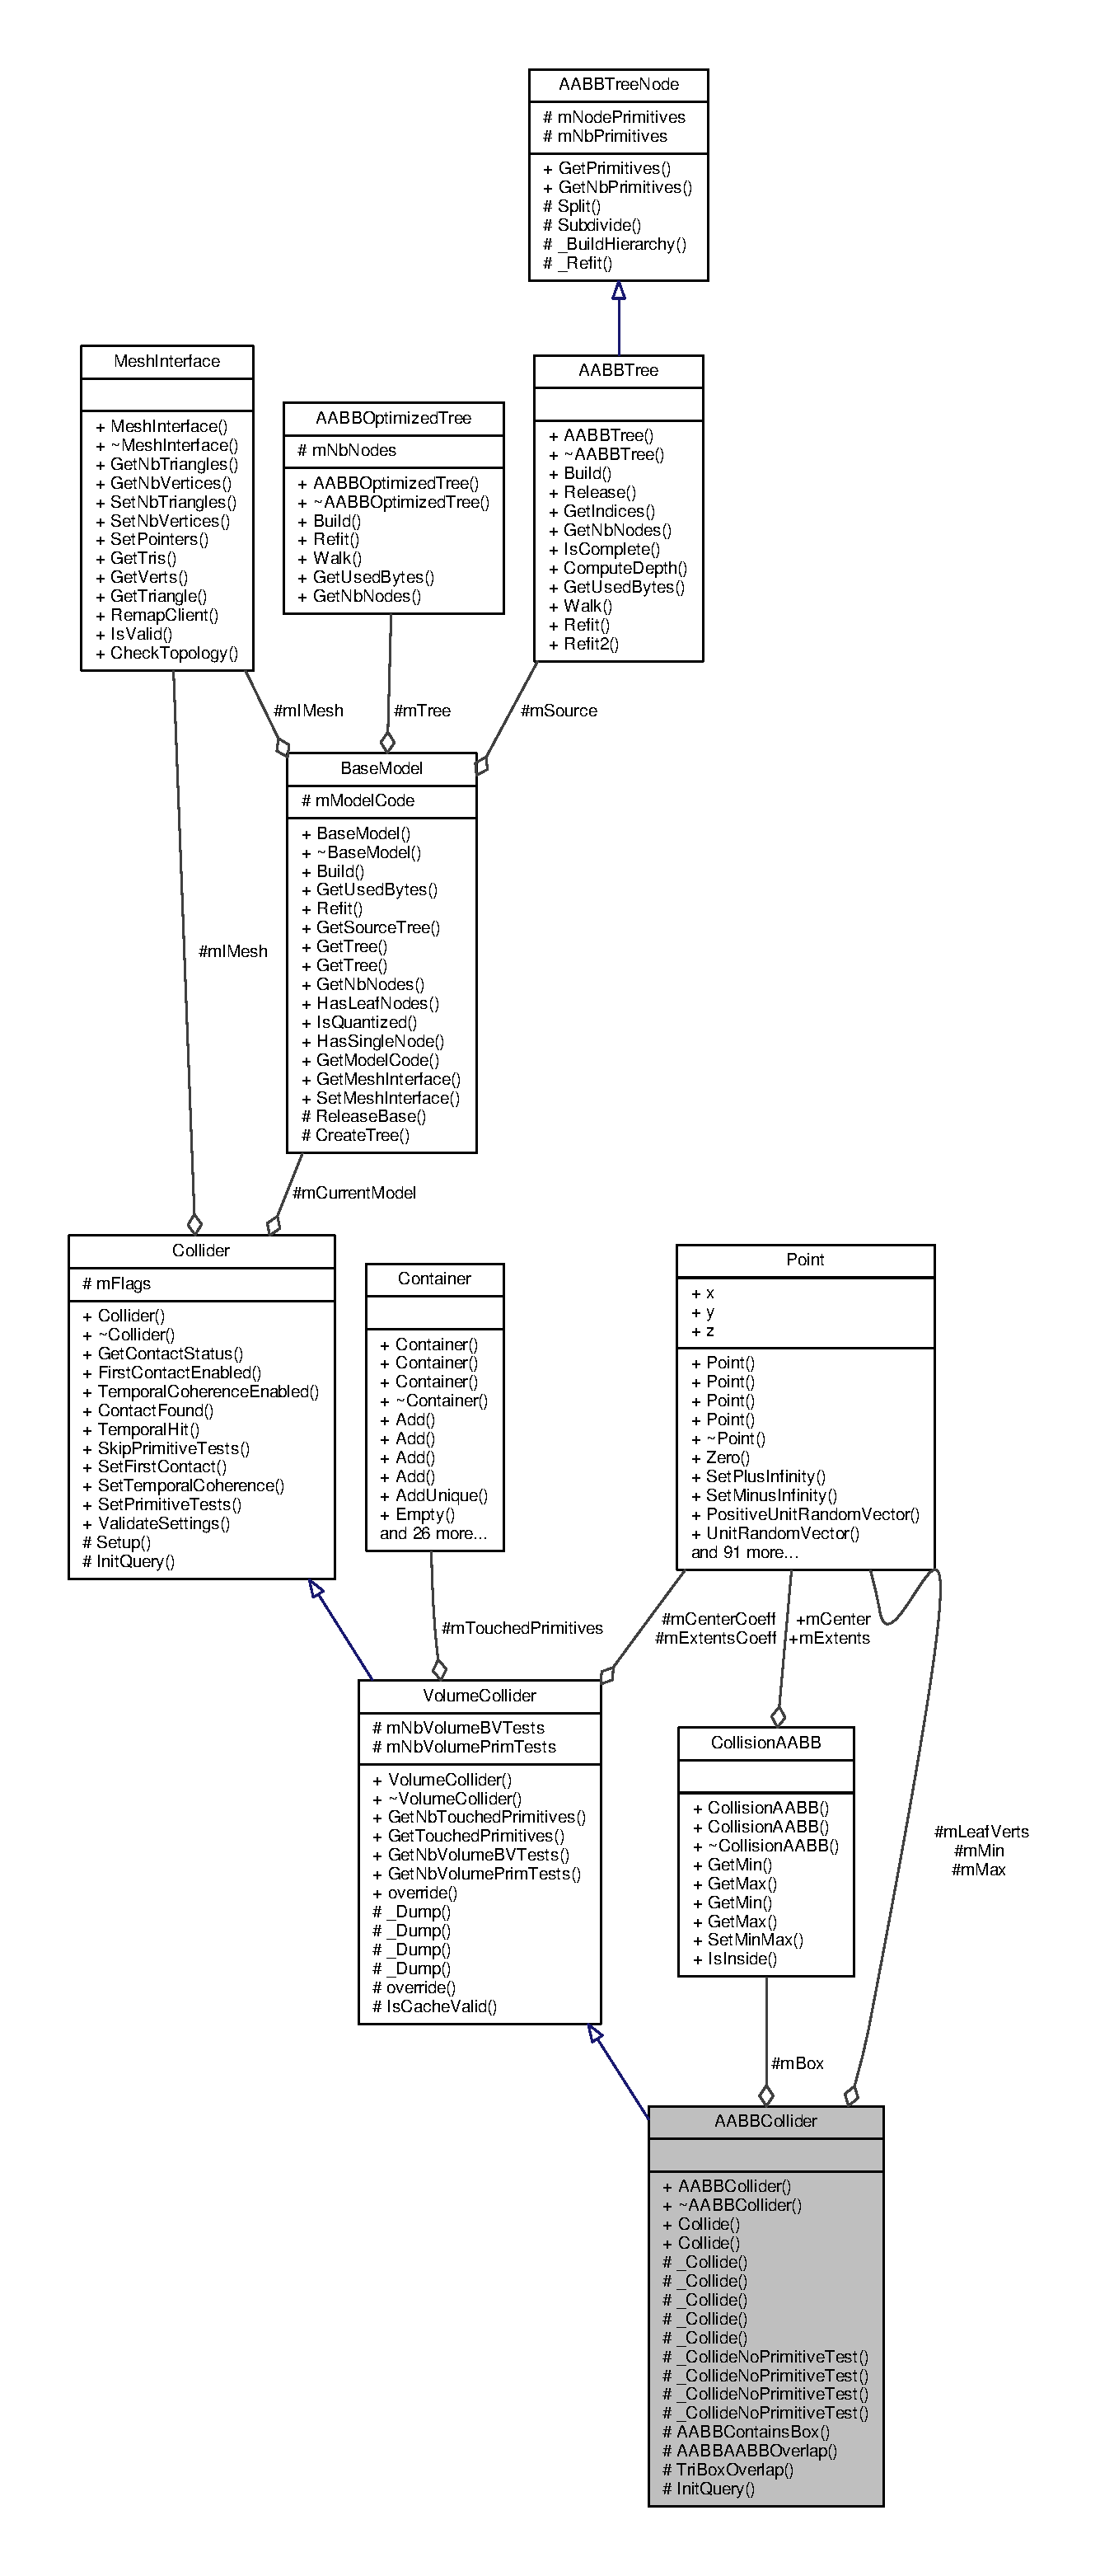
\includegraphics[height=550pt]{d6/daa/classAABBCollider__coll__graph}
\end{center}
\end{figure}
\subsection*{Public Member Functions}
\begin{DoxyCompactItemize}
\item 
bool \hyperlink{classAABBCollider_a6c5443558bd612a744bbfc74ff2b7368}{Collide} (\hyperlink{structAABBCache}{A\+A\+B\+B\+Cache} \&cache, const \hyperlink{classCollisionAABB}{Collision\+A\+A\+BB} \&box, const \hyperlink{classModel}{Model} \&model)
\item 
bool {\bfseries Collide} (\hyperlink{structAABBCache}{A\+A\+B\+B\+Cache} \&cache, const \hyperlink{classCollisionAABB}{Collision\+A\+A\+BB} \&box, const \hyperlink{classAABBTree}{A\+A\+B\+B\+Tree} $\ast$tree)\hypertarget{classAABBCollider_ad26d4fe09769619954dad20961c56f78}{}\label{classAABBCollider_ad26d4fe09769619954dad20961c56f78}

\end{DoxyCompactItemize}
\subsection*{Protected Member Functions}
\begin{DoxyCompactItemize}
\item 
void {\bfseries \+\_\+\+Collide} (const \hyperlink{classAABBCollisionNode}{A\+A\+B\+B\+Collision\+Node} $\ast$node)\hypertarget{classAABBCollider_aa4aa676986ee7f507e957e45f2f5b4ba}{}\label{classAABBCollider_aa4aa676986ee7f507e957e45f2f5b4ba}

\item 
void {\bfseries \+\_\+\+Collide} (const \hyperlink{classAABBNoLeafNode}{A\+A\+B\+B\+No\+Leaf\+Node} $\ast$node)\hypertarget{classAABBCollider_a7ff71717c0c1ef6d3894fc9ab5e5dcfa}{}\label{classAABBCollider_a7ff71717c0c1ef6d3894fc9ab5e5dcfa}

\item 
void {\bfseries \+\_\+\+Collide} (const \hyperlink{classAABBQuantizedNode}{A\+A\+B\+B\+Quantized\+Node} $\ast$node)\hypertarget{classAABBCollider_ae779f38892cb3398c0c1d893f3f6f277}{}\label{classAABBCollider_ae779f38892cb3398c0c1d893f3f6f277}

\item 
void {\bfseries \+\_\+\+Collide} (const \hyperlink{classAABBQuantizedNoLeafNode}{A\+A\+B\+B\+Quantized\+No\+Leaf\+Node} $\ast$node)\hypertarget{classAABBCollider_a9b38f0dda1f0ba7b3225f0f8f2abbf25}{}\label{classAABBCollider_a9b38f0dda1f0ba7b3225f0f8f2abbf25}

\item 
void {\bfseries \+\_\+\+Collide} (const \hyperlink{classAABBTreeNode}{A\+A\+B\+B\+Tree\+Node} $\ast$node)\hypertarget{classAABBCollider_ae5e560d946cf02643db63f8856bcb1f9}{}\label{classAABBCollider_ae5e560d946cf02643db63f8856bcb1f9}

\item 
void {\bfseries \+\_\+\+Collide\+No\+Primitive\+Test} (const \hyperlink{classAABBCollisionNode}{A\+A\+B\+B\+Collision\+Node} $\ast$node)\hypertarget{classAABBCollider_aa8eaafb1934f7961ce7caedae4a3142d}{}\label{classAABBCollider_aa8eaafb1934f7961ce7caedae4a3142d}

\item 
void {\bfseries \+\_\+\+Collide\+No\+Primitive\+Test} (const \hyperlink{classAABBNoLeafNode}{A\+A\+B\+B\+No\+Leaf\+Node} $\ast$node)\hypertarget{classAABBCollider_a9a23722e23e4d49d248f85daa0482772}{}\label{classAABBCollider_a9a23722e23e4d49d248f85daa0482772}

\item 
void {\bfseries \+\_\+\+Collide\+No\+Primitive\+Test} (const \hyperlink{classAABBQuantizedNode}{A\+A\+B\+B\+Quantized\+Node} $\ast$node)\hypertarget{classAABBCollider_a700cf755f32326cd8c68c4bbcb3c4b1f}{}\label{classAABBCollider_a700cf755f32326cd8c68c4bbcb3c4b1f}

\item 
void {\bfseries \+\_\+\+Collide\+No\+Primitive\+Test} (const \hyperlink{classAABBQuantizedNoLeafNode}{A\+A\+B\+B\+Quantized\+No\+Leaf\+Node} $\ast$node)\hypertarget{classAABBCollider_a440e56705eec03a65d56a66a44f41bc7}{}\label{classAABBCollider_a440e56705eec03a65d56a66a44f41bc7}

\item 
inline\+\_\+ bool {\bfseries A\+A\+B\+B\+Contains\+Box} (const \hyperlink{classPoint}{Point} \&bc, const \hyperlink{classPoint}{Point} \&be)\hypertarget{classAABBCollider_abcd553e5b1275abfbad884f11968110a}{}\label{classAABBCollider_abcd553e5b1275abfbad884f11968110a}

\item 
inline\+\_\+ bool \hyperlink{classAABBCollider_ac423a1dbebf589fcb3f37e1e982476cf}{A\+A\+B\+B\+A\+A\+B\+B\+Overlap} (const \hyperlink{classPoint}{Point} \&b, const \hyperlink{classPoint}{Point} \&Pb)\hypertarget{classAABBCollider_ac423a1dbebf589fcb3f37e1e982476cf}{}\label{classAABBCollider_ac423a1dbebf589fcb3f37e1e982476cf}

\begin{DoxyCompactList}\small\item\em A special version for 2 axis-\/aligned boxes. \end{DoxyCompactList}\item 
inline\+\_\+ bool \hyperlink{classAABBCollider_a2339d6ef853a4a4a437e472e9ddfd659}{Tri\+Box\+Overlap} ()\hypertarget{classAABBCollider_a2339d6ef853a4a4a437e472e9ddfd659}{}\label{classAABBCollider_a2339d6ef853a4a4a437e472e9ddfd659}

\begin{DoxyCompactList}\small\item\em ...and another one, jeez \end{DoxyCompactList}\item 
bool {\bfseries Init\+Query} (\hyperlink{structAABBCache}{A\+A\+B\+B\+Cache} \&cache, const \hyperlink{classCollisionAABB}{Collision\+A\+A\+BB} \&box)\hypertarget{classAABBCollider_afc5a6945b3c809051fa20b5587047b68}{}\label{classAABBCollider_afc5a6945b3c809051fa20b5587047b68}

\end{DoxyCompactItemize}
\subsection*{Protected Attributes}
\begin{DoxyCompactItemize}
\item 
\hyperlink{classCollisionAABB}{Collision\+A\+A\+BB} \hyperlink{classAABBCollider_aef6bd97ceed9bca72a3896aa3e41749e}{m\+Box}\hypertarget{classAABBCollider_aef6bd97ceed9bca72a3896aa3e41749e}{}\label{classAABBCollider_aef6bd97ceed9bca72a3896aa3e41749e}

\begin{DoxyCompactList}\small\item\em Query box in (center, extents) form. \end{DoxyCompactList}\item 
\hyperlink{classPoint}{Point} \hyperlink{classAABBCollider_a8c00192504356f5016957e9a034dfeeb}{m\+Min}\hypertarget{classAABBCollider_a8c00192504356f5016957e9a034dfeeb}{}\label{classAABBCollider_a8c00192504356f5016957e9a034dfeeb}

\begin{DoxyCompactList}\small\item\em Query box min point. \end{DoxyCompactList}\item 
\hyperlink{classPoint}{Point} \hyperlink{classAABBCollider_af40446c606f2d4a02d515a58696d272d}{m\+Max}\hypertarget{classAABBCollider_af40446c606f2d4a02d515a58696d272d}{}\label{classAABBCollider_af40446c606f2d4a02d515a58696d272d}

\begin{DoxyCompactList}\small\item\em Query box max point. \end{DoxyCompactList}\item 
\hyperlink{classPoint}{Point} \hyperlink{classAABBCollider_a3357982377483d5d131721ae72e36643}{m\+Leaf\+Verts} \mbox{[}3\mbox{]}\hypertarget{classAABBCollider_a3357982377483d5d131721ae72e36643}{}\label{classAABBCollider_a3357982377483d5d131721ae72e36643}

\begin{DoxyCompactList}\small\item\em \hyperlink{classTriangle}{Triangle} vertices. \end{DoxyCompactList}\end{DoxyCompactItemize}


\subsection{Detailed Description}
Contains an A\+A\+B\+B-\/vs-\/tree collider.

\begin{DoxyAuthor}{Author}
Pierre Terdiman 
\end{DoxyAuthor}
\begin{DoxyVersion}{Version}
1.\+3 
\end{DoxyVersion}
\begin{DoxyDate}{Date}
January, 1st, 2002 
\end{DoxyDate}


\subsection{Member Function Documentation}
\index{A\+A\+B\+B\+Collider@{A\+A\+B\+B\+Collider}!Collide@{Collide}}
\index{Collide@{Collide}!A\+A\+B\+B\+Collider@{A\+A\+B\+B\+Collider}}
\subsubsection[{\texorpdfstring{Collide(\+A\+A\+B\+B\+Cache \&cache, const Collision\+A\+A\+B\+B \&box, const Model \&model)}{Collide(AABBCache &cache, const CollisionAABB &box, const Model &model)}}]{\setlength{\rightskip}{0pt plus 5cm}bool A\+A\+B\+B\+Collider\+::\+Collide (
\begin{DoxyParamCaption}
\item[{{\bf A\+A\+B\+B\+Cache} \&}]{cache, }
\item[{const {\bf Collision\+A\+A\+BB} \&}]{box, }
\item[{const {\bf Model} \&}]{model}
\end{DoxyParamCaption}
)}\hypertarget{classAABBCollider_a6c5443558bd612a744bbfc74ff2b7368}{}\label{classAABBCollider_a6c5443558bd612a744bbfc74ff2b7368}
Generic collision query for generic O\+P\+C\+O\+DE models. After the call, access the results\+:
\begin{DoxyItemize}
\item with \hyperlink{classCollider_a64a73882d4f167a6175658f014868f66}{Get\+Contact\+Status()}
\item with \hyperlink{classVolumeCollider_a274b51032b2c2e4394b1cc9308fa8d71}{Get\+Nb\+Touched\+Primitives()}
\item with \hyperlink{classVolumeCollider_afca0d34cb9f4aa27537a4bfd03fe40d9}{Get\+Touched\+Primitives()}
\end{DoxyItemize}


\begin{DoxyParams}{Parameters}
{\em cache} & \mbox{[}in/out\mbox{]} a box cache \\
\hline
{\em box} & \mbox{[}in\mbox{]} collision \hyperlink{classAABB}{A\+A\+BB} in world space \\
\hline
{\em model} & \mbox{[}in\mbox{]} Opcode model to collide with \\
\hline
\end{DoxyParams}
\begin{DoxyReturn}{Returns}
true if success 
\end{DoxyReturn}
\begin{DoxyWarning}{Warning}
S\+C\+A\+LE N\+OT S\+U\+P\+P\+O\+R\+T\+ED. The matrices must contain rotation \& translation parts only. 
\end{DoxyWarning}


The documentation for this class was generated from the following files\+:\begin{DoxyCompactItemize}
\item 
cmd/collide2/\hyperlink{OPC__AABBCollider_8h}{O\+P\+C\+\_\+\+A\+A\+B\+B\+Collider.\+h}\item 
cmd/collide2/O\+P\+C\+\_\+\+Box\+Box\+Overlap.\+h\item 
cmd/collide2/O\+P\+C\+\_\+\+Tri\+Box\+Overlap.\+h\end{DoxyCompactItemize}

\hypertarget{classOpcode_1_1AABBCollisionNode}{}\section{Opcode\+:\+:A\+A\+B\+B\+Collision\+Node Class Reference}
\label{classOpcode_1_1AABBCollisionNode}\index{Opcode\+::\+A\+A\+B\+B\+Collision\+Node@{Opcode\+::\+A\+A\+B\+B\+Collision\+Node}}


Collaboration diagram for Opcode\+:\+:A\+A\+B\+B\+Collision\+Node\+:
\nopagebreak
\begin{figure}[H]
\begin{center}
\leavevmode
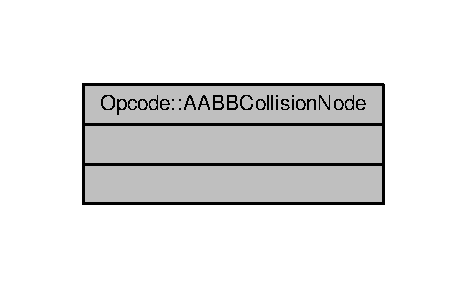
\includegraphics[width=224pt]{d2/ded/classOpcode_1_1AABBCollisionNode__coll__graph}
\end{center}
\end{figure}


The documentation for this class was generated from the following file\+:\begin{DoxyCompactItemize}
\item 
cmd/collide2/\hyperlink{Opcode_8h}{Opcode.\+h}\end{DoxyCompactItemize}

\hypertarget{classAABBCollisionNode}{}\section{A\+A\+B\+B\+Collision\+Node Class Reference}
\label{classAABBCollisionNode}\index{A\+A\+B\+B\+Collision\+Node@{A\+A\+B\+B\+Collision\+Node}}


Collaboration diagram for A\+A\+B\+B\+Collision\+Node\+:
\nopagebreak
\begin{figure}[H]
\begin{center}
\leavevmode
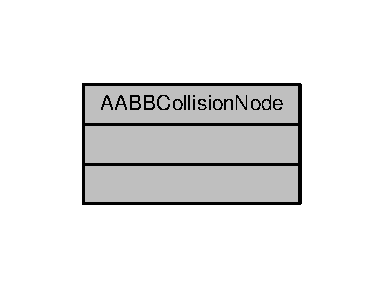
\includegraphics[width=184pt]{d6/dd8/classAABBCollisionNode__coll__graph}
\end{center}
\end{figure}
\subsection*{Related Functions}
(Note that these are not member functions.) \begin{DoxyCompactItemize}
\item 
\hyperlink{classAABBCollisionNode_ada461a1e7da4f92ef39f9a6aa4a012b8}{\+\_\+\+Build\+Collision\+Tree} (\hyperlink{classOpcode_1_1AABBCollisionNode}{A\+A\+B\+B\+Collision\+Node} $\ast$linear, const \hyperlink{IceTypes_8h_a44c6f1920ba5551225fb534f9d1a1733}{udword} box\+\_\+id, \hyperlink{IceTypes_8h_a44c6f1920ba5551225fb534f9d1a1733}{udword} \&current\+\_\+id, const \hyperlink{classOpcode_1_1AABBTreeNode}{A\+A\+B\+B\+Tree\+Node} $\ast$current\+\_\+node)
\end{DoxyCompactItemize}


\subsection{Friends And Related Function Documentation}
\index{A\+A\+B\+B\+Collision\+Node@{A\+A\+B\+B\+Collision\+Node}!\+\_\+\+Build\+Collision\+Tree@{\+\_\+\+Build\+Collision\+Tree}}
\index{\+\_\+\+Build\+Collision\+Tree@{\+\_\+\+Build\+Collision\+Tree}!A\+A\+B\+B\+Collision\+Node@{A\+A\+B\+B\+Collision\+Node}}
\subsubsection[{\texorpdfstring{\+\_\+\+Build\+Collision\+Tree(\+A\+A\+B\+B\+Collision\+Node $\ast$linear, const udword box\+\_\+id, udword \&current\+\_\+id, const A\+A\+B\+B\+Tree\+Node $\ast$current\+\_\+node)}{_BuildCollisionTree(AABBCollisionNode *linear, const udword box_id, udword &current_id, const AABBTreeNode *current_node)}}]{\setlength{\rightskip}{0pt plus 5cm}\+\_\+\+Build\+Collision\+Tree (
\begin{DoxyParamCaption}
\item[{{\bf A\+A\+B\+B\+Collision\+Node} $\ast$}]{linear, }
\item[{const {\bf udword}}]{box\+\_\+id, }
\item[{{\bf udword} \&}]{current\+\_\+id, }
\item[{const {\bf A\+A\+B\+B\+Tree\+Node} $\ast$}]{current\+\_\+node}
\end{DoxyParamCaption}
)\hspace{0.3cm}{\ttfamily [related]}}\hypertarget{classAABBCollisionNode_ada461a1e7da4f92ef39f9a6aa4a012b8}{}\label{classAABBCollisionNode_ada461a1e7da4f92ef39f9a6aa4a012b8}
Builds an implicit tree from a standard one. An implicit tree is a complete tree (2$\ast$\+N-\/1 nodes) whose negative box pointers and primitive pointers have been made implicit, hence packing 3 pointers in one.

Layout for implicit trees\+: Node\+:
\begin{DoxyItemize}
\item box
\item data (32-\/bits value)
\end{DoxyItemize}

if data\textquotesingle{}s L\+SB = 1 =$>$ remaining bits are a primitive pointer else remaining bits are a P-\/node pointer, and N = P + 1


\begin{DoxyParams}{Parameters}
{\em linear} & \mbox{[}in\mbox{]} base address of destination nodes \\
\hline
{\em box\+\_\+id} & \mbox{[}in\mbox{]} index of destination node \\
\hline
{\em current\+\_\+id} & \mbox{[}in\mbox{]} current running index \\
\hline
{\em current\+\_\+node} & \mbox{[}in\mbox{]} current node from input tree \\
\hline
\end{DoxyParams}


The documentation for this class was generated from the following files\+:\begin{DoxyCompactItemize}
\item 
cmd/collide2/\hyperlink{OPC__OptimizedTree_8h}{O\+P\+C\+\_\+\+Optimized\+Tree.\+h}\item 
cmd/collide2/\hyperlink{OPC__OptimizedTree_8cpp}{O\+P\+C\+\_\+\+Optimized\+Tree.\+cpp}\end{DoxyCompactItemize}

\hypertarget{classOpcode_1_1AABBCollisionTree}{}\section{Opcode\+:\+:A\+A\+B\+B\+Collision\+Tree Class Reference}
\label{classOpcode_1_1AABBCollisionTree}\index{Opcode\+::\+A\+A\+B\+B\+Collision\+Tree@{Opcode\+::\+A\+A\+B\+B\+Collision\+Tree}}


Inheritance diagram for Opcode\+:\+:A\+A\+B\+B\+Collision\+Tree\+:
\nopagebreak
\begin{figure}[H]
\begin{center}
\leavevmode
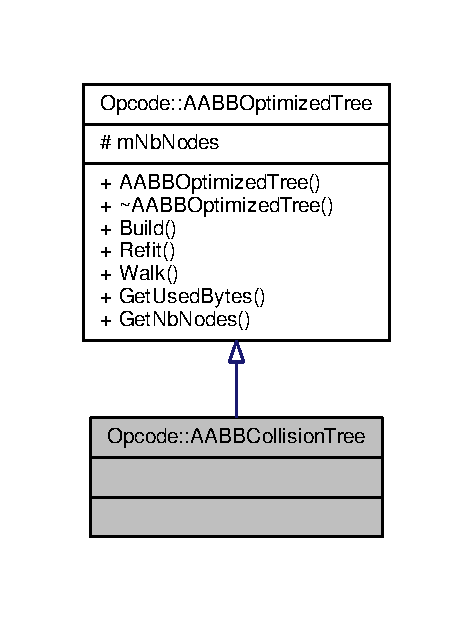
\includegraphics[width=227pt]{de/df1/classOpcode_1_1AABBCollisionTree__inherit__graph}
\end{center}
\end{figure}


Collaboration diagram for Opcode\+:\+:A\+A\+B\+B\+Collision\+Tree\+:
\nopagebreak
\begin{figure}[H]
\begin{center}
\leavevmode
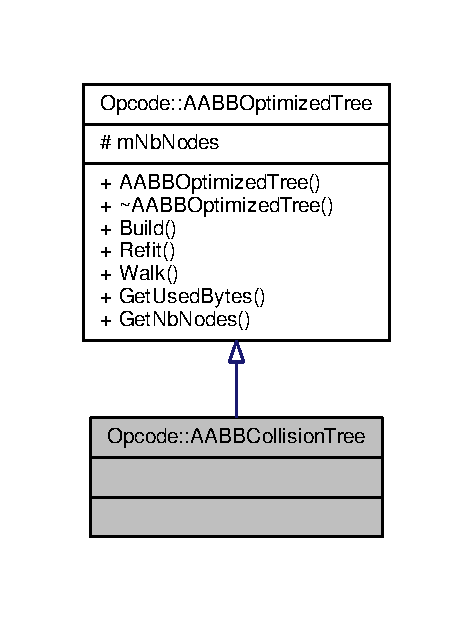
\includegraphics[width=227pt]{d5/d39/classOpcode_1_1AABBCollisionTree__coll__graph}
\end{center}
\end{figure}
\subsection*{Additional Inherited Members}


The documentation for this class was generated from the following file\+:\begin{DoxyCompactItemize}
\item 
cmd/collide2/\hyperlink{Opcode_8h}{Opcode.\+h}\end{DoxyCompactItemize}

\hypertarget{classAABBCollisionTree}{}\section{A\+A\+B\+B\+Collision\+Tree Class Reference}
\label{classAABBCollisionTree}\index{A\+A\+B\+B\+Collision\+Tree@{A\+A\+B\+B\+Collision\+Tree}}


Inheritance diagram for A\+A\+B\+B\+Collision\+Tree\+:
\nopagebreak
\begin{figure}[H]
\begin{center}
\leavevmode
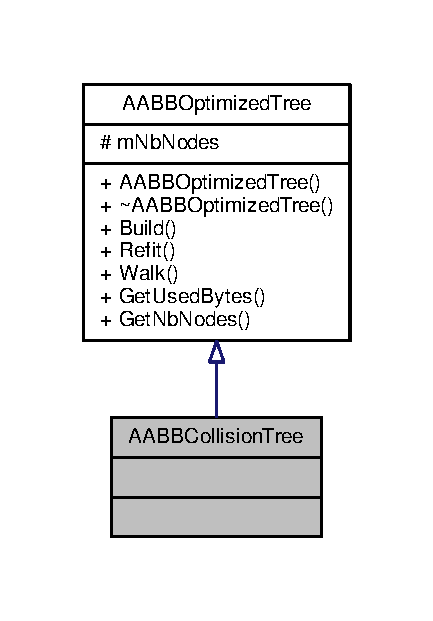
\includegraphics[width=208pt]{de/ded/classAABBCollisionTree__inherit__graph}
\end{center}
\end{figure}


Collaboration diagram for A\+A\+B\+B\+Collision\+Tree\+:
\nopagebreak
\begin{figure}[H]
\begin{center}
\leavevmode
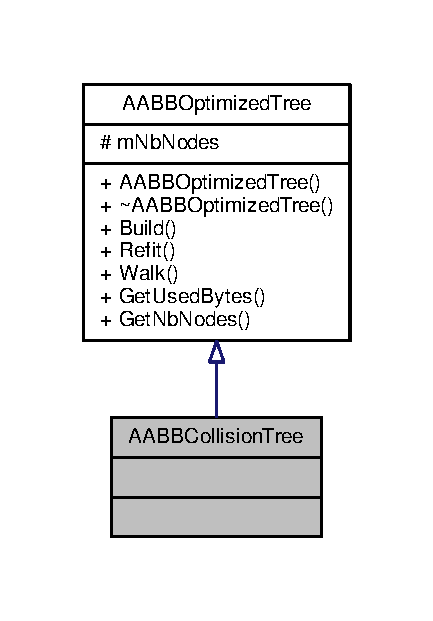
\includegraphics[width=208pt]{dd/d9e/classAABBCollisionTree__coll__graph}
\end{center}
\end{figure}
\subsection*{Additional Inherited Members}


\subsection{Detailed Description}
A standard \hyperlink{classAABB}{A\+A\+BB} tree.

\begin{DoxyAuthor}{Author}
Pierre Terdiman 
\end{DoxyAuthor}
\begin{DoxyVersion}{Version}
1.\+3 
\end{DoxyVersion}
\begin{DoxyDate}{Date}
March, 20, 2001 
\end{DoxyDate}


The documentation for this class was generated from the following file\+:\begin{DoxyCompactItemize}
\item 
cmd/collide2/\hyperlink{OPC__OptimizedTree_8h}{O\+P\+C\+\_\+\+Optimized\+Tree.\+h}\end{DoxyCompactItemize}

\hypertarget{classOpcode_1_1AABBNoLeafNode}{}\section{Opcode\+:\+:A\+A\+B\+B\+No\+Leaf\+Node Class Reference}
\label{classOpcode_1_1AABBNoLeafNode}\index{Opcode\+::\+A\+A\+B\+B\+No\+Leaf\+Node@{Opcode\+::\+A\+A\+B\+B\+No\+Leaf\+Node}}


Collaboration diagram for Opcode\+:\+:A\+A\+B\+B\+No\+Leaf\+Node\+:
\nopagebreak
\begin{figure}[H]
\begin{center}
\leavevmode
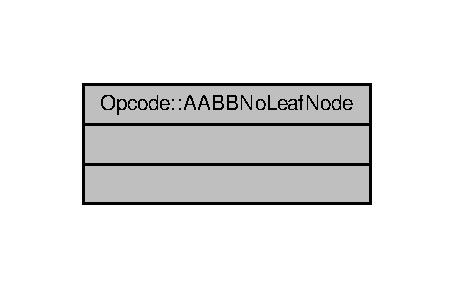
\includegraphics[width=218pt]{d8/dd6/classOpcode_1_1AABBNoLeafNode__coll__graph}
\end{center}
\end{figure}


The documentation for this class was generated from the following file\+:\begin{DoxyCompactItemize}
\item 
cmd/collide2/\hyperlink{Opcode_8h}{Opcode.\+h}\end{DoxyCompactItemize}

\hypertarget{classAABBNoLeafNode}{}\section{A\+A\+B\+B\+No\+Leaf\+Node Class Reference}
\label{classAABBNoLeafNode}\index{A\+A\+B\+B\+No\+Leaf\+Node@{A\+A\+B\+B\+No\+Leaf\+Node}}


Collaboration diagram for A\+A\+B\+B\+No\+Leaf\+Node\+:
\nopagebreak
\begin{figure}[H]
\begin{center}
\leavevmode
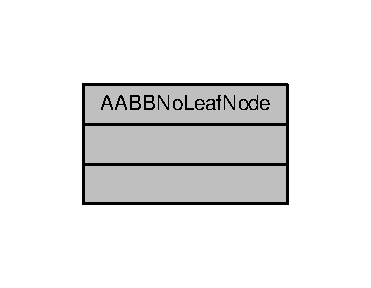
\includegraphics[width=178pt]{d9/d2a/classAABBNoLeafNode__coll__graph}
\end{center}
\end{figure}
\subsection*{Related Functions}
(Note that these are not member functions.) \begin{DoxyCompactItemize}
\item 
\hyperlink{classAABBNoLeafNode_a72bbc7c9d7839051c0e0ffb808f57d2d}{\+\_\+\+Build\+No\+Leaf\+Tree} (\hyperlink{classOpcode_1_1AABBNoLeafNode}{A\+A\+B\+B\+No\+Leaf\+Node} $\ast$linear, const \hyperlink{IceTypes_8h_a44c6f1920ba5551225fb534f9d1a1733}{udword} box\+\_\+id, \hyperlink{IceTypes_8h_a44c6f1920ba5551225fb534f9d1a1733}{udword} \&current\+\_\+id, const \hyperlink{classOpcode_1_1AABBTreeNode}{A\+A\+B\+B\+Tree\+Node} $\ast$current\+\_\+node)
\end{DoxyCompactItemize}


\subsection{Friends And Related Function Documentation}
\index{A\+A\+B\+B\+No\+Leaf\+Node@{A\+A\+B\+B\+No\+Leaf\+Node}!\+\_\+\+Build\+No\+Leaf\+Tree@{\+\_\+\+Build\+No\+Leaf\+Tree}}
\index{\+\_\+\+Build\+No\+Leaf\+Tree@{\+\_\+\+Build\+No\+Leaf\+Tree}!A\+A\+B\+B\+No\+Leaf\+Node@{A\+A\+B\+B\+No\+Leaf\+Node}}
\subsubsection[{\texorpdfstring{\+\_\+\+Build\+No\+Leaf\+Tree(\+A\+A\+B\+B\+No\+Leaf\+Node $\ast$linear, const udword box\+\_\+id, udword \&current\+\_\+id, const A\+A\+B\+B\+Tree\+Node $\ast$current\+\_\+node)}{_BuildNoLeafTree(AABBNoLeafNode *linear, const udword box_id, udword &current_id, const AABBTreeNode *current_node)}}]{\setlength{\rightskip}{0pt plus 5cm}\+\_\+\+Build\+No\+Leaf\+Tree (
\begin{DoxyParamCaption}
\item[{{\bf A\+A\+B\+B\+No\+Leaf\+Node} $\ast$}]{linear, }
\item[{const {\bf udword}}]{box\+\_\+id, }
\item[{{\bf udword} \&}]{current\+\_\+id, }
\item[{const {\bf A\+A\+B\+B\+Tree\+Node} $\ast$}]{current\+\_\+node}
\end{DoxyParamCaption}
)\hspace{0.3cm}{\ttfamily [related]}}\hypertarget{classAABBNoLeafNode_a72bbc7c9d7839051c0e0ffb808f57d2d}{}\label{classAABBNoLeafNode_a72bbc7c9d7839051c0e0ffb808f57d2d}
Builds a \char`\"{}no-\/leaf\char`\"{} tree from a standard one. This is a tree whose leaf nodes have been removed.

Layout for no-\/leaf trees\+:

Node\+:
\begin{DoxyItemize}
\item box
\item P pointer =$>$ a node (L\+SB=0) or a primitive (L\+SB=1)
\item N pointer =$>$ a node (L\+SB=0) or a primitive (L\+SB=1)
\end{DoxyItemize}


\begin{DoxyParams}{Parameters}
{\em linear} & \mbox{[}in\mbox{]} base address of destination nodes \\
\hline
{\em box\+\_\+id} & \mbox{[}in\mbox{]} index of destination node \\
\hline
{\em current\+\_\+id} & \mbox{[}in\mbox{]} current running index \\
\hline
{\em current\+\_\+node} & \mbox{[}in\mbox{]} current node from input tree \\
\hline
\end{DoxyParams}


The documentation for this class was generated from the following files\+:\begin{DoxyCompactItemize}
\item 
cmd/collide2/\hyperlink{OPC__OptimizedTree_8h}{O\+P\+C\+\_\+\+Optimized\+Tree.\+h}\item 
cmd/collide2/\hyperlink{OPC__OptimizedTree_8cpp}{O\+P\+C\+\_\+\+Optimized\+Tree.\+cpp}\end{DoxyCompactItemize}

\hypertarget{classOpcode_1_1AABBNoLeafTree}{}\section{Opcode\+:\+:A\+A\+B\+B\+No\+Leaf\+Tree Class Reference}
\label{classOpcode_1_1AABBNoLeafTree}\index{Opcode\+::\+A\+A\+B\+B\+No\+Leaf\+Tree@{Opcode\+::\+A\+A\+B\+B\+No\+Leaf\+Tree}}


Inheritance diagram for Opcode\+:\+:A\+A\+B\+B\+No\+Leaf\+Tree\+:
\nopagebreak
\begin{figure}[H]
\begin{center}
\leavevmode
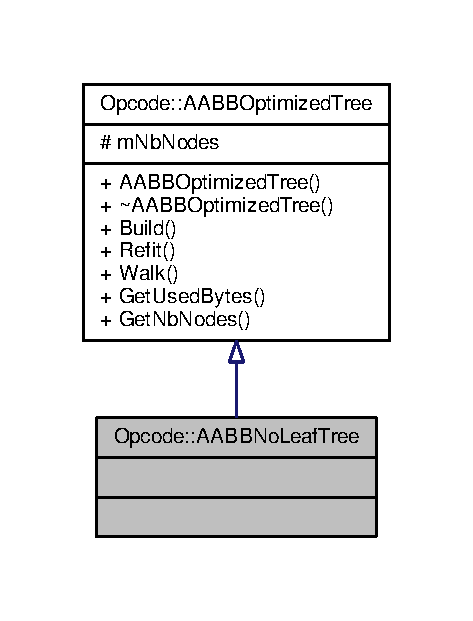
\includegraphics[width=227pt]{d4/d5d/classOpcode_1_1AABBNoLeafTree__inherit__graph}
\end{center}
\end{figure}


Collaboration diagram for Opcode\+:\+:A\+A\+B\+B\+No\+Leaf\+Tree\+:
\nopagebreak
\begin{figure}[H]
\begin{center}
\leavevmode
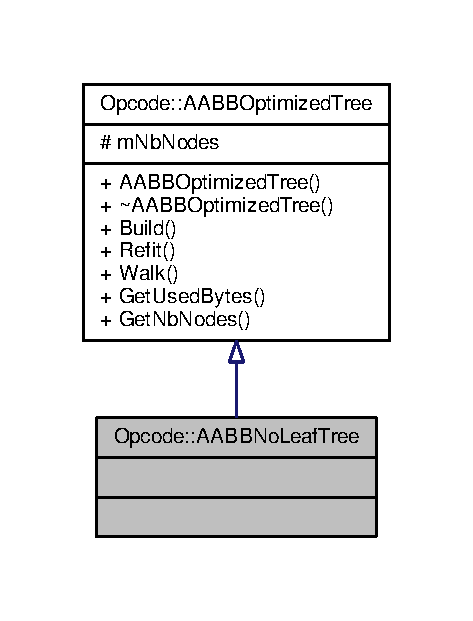
\includegraphics[width=227pt]{de/d4b/classOpcode_1_1AABBNoLeafTree__coll__graph}
\end{center}
\end{figure}
\subsection*{Additional Inherited Members}


The documentation for this class was generated from the following file\+:\begin{DoxyCompactItemize}
\item 
cmd/collide2/\hyperlink{Opcode_8h}{Opcode.\+h}\end{DoxyCompactItemize}

\hypertarget{classAABBNoLeafTree}{}\section{A\+A\+B\+B\+No\+Leaf\+Tree Class Reference}
\label{classAABBNoLeafTree}\index{A\+A\+B\+B\+No\+Leaf\+Tree@{A\+A\+B\+B\+No\+Leaf\+Tree}}


Inheritance diagram for A\+A\+B\+B\+No\+Leaf\+Tree\+:
\nopagebreak
\begin{figure}[H]
\begin{center}
\leavevmode
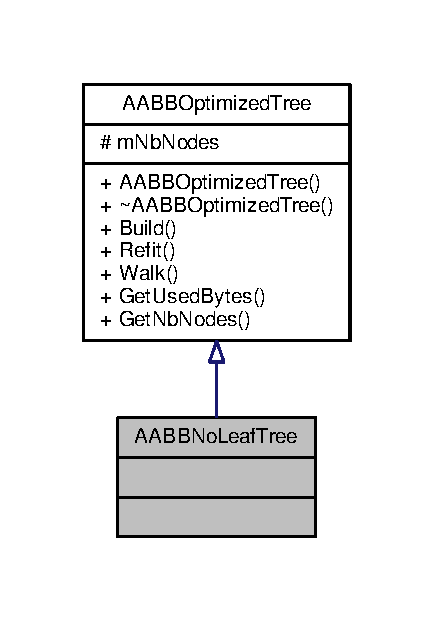
\includegraphics[width=208pt]{da/df0/classAABBNoLeafTree__inherit__graph}
\end{center}
\end{figure}


Collaboration diagram for A\+A\+B\+B\+No\+Leaf\+Tree\+:
\nopagebreak
\begin{figure}[H]
\begin{center}
\leavevmode
\includegraphics[width=208pt]{d5/d49/classAABBNoLeafTree__coll__graph}
\end{center}
\end{figure}
\subsection*{Additional Inherited Members}


\subsection{Detailed Description}
A no-\/leaf \hyperlink{classAABB}{A\+A\+BB} tree.

\begin{DoxyAuthor}{Author}
Pierre Terdiman 
\end{DoxyAuthor}
\begin{DoxyVersion}{Version}
1.\+3 
\end{DoxyVersion}
\begin{DoxyDate}{Date}
March, 20, 2001 
\end{DoxyDate}


The documentation for this class was generated from the following file\+:\begin{DoxyCompactItemize}
\item 
cmd/collide2/\hyperlink{OPC__OptimizedTree_8h}{O\+P\+C\+\_\+\+Optimized\+Tree.\+h}\end{DoxyCompactItemize}

\hypertarget{classOpcode_1_1AABBOptimizedTree}{}\section{Opcode\+:\+:A\+A\+B\+B\+Optimized\+Tree Class Reference}
\label{classOpcode_1_1AABBOptimizedTree}\index{Opcode\+::\+A\+A\+B\+B\+Optimized\+Tree@{Opcode\+::\+A\+A\+B\+B\+Optimized\+Tree}}


Inheritance diagram for Opcode\+:\+:A\+A\+B\+B\+Optimized\+Tree\+:
\nopagebreak
\begin{figure}[H]
\begin{center}
\leavevmode
\includegraphics[width=350pt]{d8/d28/classOpcode_1_1AABBOptimizedTree__inherit__graph}
\end{center}
\end{figure}


Collaboration diagram for Opcode\+:\+:A\+A\+B\+B\+Optimized\+Tree\+:
\nopagebreak
\begin{figure}[H]
\begin{center}
\leavevmode
\includegraphics[width=227pt]{d4/d52/classOpcode_1_1AABBOptimizedTree__coll__graph}
\end{center}
\end{figure}
\subsection*{Public Member Functions}
\begin{DoxyCompactItemize}
\item 
virtual bool \hyperlink{classOpcode_1_1AABBOptimizedTree_a395cac6d17bfbfa77c1ea441e31ce7c5}{Build} (\hyperlink{classOpcode_1_1AABBTree}{A\+A\+B\+B\+Tree} $\ast$tree)=0
\item 
virtual bool \hyperlink{classOpcode_1_1AABBOptimizedTree_a9c1c89c134a2ea4a5de4333266032fa6}{Refit} (const \hyperlink{classOpcode_1_1MeshInterface}{Mesh\+Interface} $\ast$mesh\+\_\+interface)=0
\item 
virtual bool \hyperlink{classOpcode_1_1AABBOptimizedTree_a78a98ae632876d1df1d0a5d0e0a75668}{Walk} (Generic\+Walking\+Callback callback, void $\ast$user\+\_\+data) const =0
\item 
virtual \hyperlink{IceTypes_8h_a44c6f1920ba5551225fb534f9d1a1733}{udword} {\bfseries Get\+Used\+Bytes} () const =0\hypertarget{classOpcode_1_1AABBOptimizedTree_ac02fbbe089c45fa5e0f95167aeec796a}{}\label{classOpcode_1_1AABBOptimizedTree_ac02fbbe089c45fa5e0f95167aeec796a}

\item 
inline\+\_\+ \hyperlink{IceTypes_8h_a44c6f1920ba5551225fb534f9d1a1733}{udword} {\bfseries Get\+Nb\+Nodes} () const \hypertarget{classOpcode_1_1AABBOptimizedTree_af42286dd6f277ba448728e14519512bd}{}\label{classOpcode_1_1AABBOptimizedTree_af42286dd6f277ba448728e14519512bd}

\end{DoxyCompactItemize}
\subsection*{Protected Attributes}
\begin{DoxyCompactItemize}
\item 
\hyperlink{IceTypes_8h_a44c6f1920ba5551225fb534f9d1a1733}{udword} {\bfseries m\+Nb\+Nodes}\hypertarget{classOpcode_1_1AABBOptimizedTree_a4116d37caddf74b45611217203878d5c}{}\label{classOpcode_1_1AABBOptimizedTree_a4116d37caddf74b45611217203878d5c}

\end{DoxyCompactItemize}


\subsection{Member Function Documentation}
\index{Opcode\+::\+A\+A\+B\+B\+Optimized\+Tree@{Opcode\+::\+A\+A\+B\+B\+Optimized\+Tree}!Build@{Build}}
\index{Build@{Build}!Opcode\+::\+A\+A\+B\+B\+Optimized\+Tree@{Opcode\+::\+A\+A\+B\+B\+Optimized\+Tree}}
\subsubsection[{\texorpdfstring{Build(\+A\+A\+B\+B\+Tree $\ast$tree)=0}{Build(AABBTree *tree)=0}}]{\setlength{\rightskip}{0pt plus 5cm}virtual bool Opcode\+::\+A\+A\+B\+B\+Optimized\+Tree\+::\+Build (
\begin{DoxyParamCaption}
\item[{{\bf A\+A\+B\+B\+Tree} $\ast$}]{tree}
\end{DoxyParamCaption}
)\hspace{0.3cm}{\ttfamily [pure virtual]}}\hypertarget{classOpcode_1_1AABBOptimizedTree_a395cac6d17bfbfa77c1ea441e31ce7c5}{}\label{classOpcode_1_1AABBOptimizedTree_a395cac6d17bfbfa77c1ea441e31ce7c5}
Builds the collision tree from a generic \hyperlink{classOpcode_1_1AABB}{A\+A\+BB} tree. 
\begin{DoxyParams}{Parameters}
{\em tree} & \mbox{[}in\mbox{]} generic \hyperlink{classOpcode_1_1AABB}{A\+A\+BB} tree \\
\hline
\end{DoxyParams}
\begin{DoxyReturn}{Returns}
true if success 
\end{DoxyReturn}
\index{Opcode\+::\+A\+A\+B\+B\+Optimized\+Tree@{Opcode\+::\+A\+A\+B\+B\+Optimized\+Tree}!Refit@{Refit}}
\index{Refit@{Refit}!Opcode\+::\+A\+A\+B\+B\+Optimized\+Tree@{Opcode\+::\+A\+A\+B\+B\+Optimized\+Tree}}
\subsubsection[{\texorpdfstring{Refit(const Mesh\+Interface $\ast$mesh\+\_\+interface)=0}{Refit(const MeshInterface *mesh_interface)=0}}]{\setlength{\rightskip}{0pt plus 5cm}virtual bool Opcode\+::\+A\+A\+B\+B\+Optimized\+Tree\+::\+Refit (
\begin{DoxyParamCaption}
\item[{const {\bf Mesh\+Interface} $\ast$}]{mesh\+\_\+interface}
\end{DoxyParamCaption}
)\hspace{0.3cm}{\ttfamily [pure virtual]}}\hypertarget{classOpcode_1_1AABBOptimizedTree_a9c1c89c134a2ea4a5de4333266032fa6}{}\label{classOpcode_1_1AABBOptimizedTree_a9c1c89c134a2ea4a5de4333266032fa6}
Refits the collision tree after vertices have been modified. 
\begin{DoxyParams}{Parameters}
{\em mesh\+\_\+interface} & \mbox{[}in\mbox{]} mesh interface for current model \\
\hline
\end{DoxyParams}
\begin{DoxyReturn}{Returns}
true if success 
\end{DoxyReturn}
\index{Opcode\+::\+A\+A\+B\+B\+Optimized\+Tree@{Opcode\+::\+A\+A\+B\+B\+Optimized\+Tree}!Walk@{Walk}}
\index{Walk@{Walk}!Opcode\+::\+A\+A\+B\+B\+Optimized\+Tree@{Opcode\+::\+A\+A\+B\+B\+Optimized\+Tree}}
\subsubsection[{\texorpdfstring{Walk(\+Generic\+Walking\+Callback callback, void $\ast$user\+\_\+data) const =0}{Walk(GenericWalkingCallback callback, void *user_data) const =0}}]{\setlength{\rightskip}{0pt plus 5cm}virtual bool Opcode\+::\+A\+A\+B\+B\+Optimized\+Tree\+::\+Walk (
\begin{DoxyParamCaption}
\item[{Generic\+Walking\+Callback}]{callback, }
\item[{void $\ast$}]{user\+\_\+data}
\end{DoxyParamCaption}
) const\hspace{0.3cm}{\ttfamily [pure virtual]}}\hypertarget{classOpcode_1_1AABBOptimizedTree_a78a98ae632876d1df1d0a5d0e0a75668}{}\label{classOpcode_1_1AABBOptimizedTree_a78a98ae632876d1df1d0a5d0e0a75668}
Walks the tree and call the user back for each node. 
\begin{DoxyParams}{Parameters}
{\em callback} & \mbox{[}in\mbox{]} walking callback \\
\hline
{\em user\+\_\+data} & \mbox{[}in\mbox{]} callback\textquotesingle{}s user data \\
\hline
\end{DoxyParams}
\begin{DoxyReturn}{Returns}
true if success 
\end{DoxyReturn}


The documentation for this class was generated from the following file\+:\begin{DoxyCompactItemize}
\item 
cmd/collide2/\hyperlink{Opcode_8h}{Opcode.\+h}\end{DoxyCompactItemize}

\hypertarget{classAABBOptimizedTree}{}\section{A\+A\+B\+B\+Optimized\+Tree Class Reference}
\label{classAABBOptimizedTree}\index{A\+A\+B\+B\+Optimized\+Tree@{A\+A\+B\+B\+Optimized\+Tree}}


Inheritance diagram for A\+A\+B\+B\+Optimized\+Tree\+:
\nopagebreak
\begin{figure}[H]
\begin{center}
\leavevmode
\includegraphics[width=350pt]{d4/d8a/classAABBOptimizedTree__inherit__graph}
\end{center}
\end{figure}


Collaboration diagram for A\+A\+B\+B\+Optimized\+Tree\+:
\nopagebreak
\begin{figure}[H]
\begin{center}
\leavevmode
\includegraphics[width=208pt]{dc/d9e/classAABBOptimizedTree__coll__graph}
\end{center}
\end{figure}
\subsection*{Public Member Functions}
\begin{DoxyCompactItemize}
\item 
virtual bool \hyperlink{classAABBOptimizedTree_acbe22cc880be2a05232bd84efb029e37}{Build} (\hyperlink{classAABBTree}{A\+A\+B\+B\+Tree} $\ast$tree)=0
\item 
virtual bool \hyperlink{classAABBOptimizedTree_a306eaa4c045e8549937df133dfe94e12}{Refit} (const \hyperlink{classMeshInterface}{Mesh\+Interface} $\ast$mesh\+\_\+interface)=0
\item 
virtual bool \hyperlink{classAABBOptimizedTree_addc2788f0391992e359ee76cf87923de}{Walk} (Generic\+Walking\+Callback callback, void $\ast$user\+\_\+data) const =0
\item 
virtual \hyperlink{IceTypes_8h_a44c6f1920ba5551225fb534f9d1a1733}{udword} {\bfseries Get\+Used\+Bytes} () const =0\hypertarget{classAABBOptimizedTree_a167d786413b470a0a5970c95a78feaf5}{}\label{classAABBOptimizedTree_a167d786413b470a0a5970c95a78feaf5}

\item 
inline\+\_\+ \hyperlink{IceTypes_8h_a44c6f1920ba5551225fb534f9d1a1733}{udword} {\bfseries Get\+Nb\+Nodes} () const \hypertarget{classAABBOptimizedTree_a0b37c6e0b222dd0f2b776b81cdc43c93}{}\label{classAABBOptimizedTree_a0b37c6e0b222dd0f2b776b81cdc43c93}

\end{DoxyCompactItemize}
\subsection*{Protected Attributes}
\begin{DoxyCompactItemize}
\item 
\hyperlink{IceTypes_8h_a44c6f1920ba5551225fb534f9d1a1733}{udword} {\bfseries m\+Nb\+Nodes}\hypertarget{classAABBOptimizedTree_a808983c59c9aa9fb9efefec356bdf13d}{}\label{classAABBOptimizedTree_a808983c59c9aa9fb9efefec356bdf13d}

\end{DoxyCompactItemize}


\subsection{Member Function Documentation}
\index{A\+A\+B\+B\+Optimized\+Tree@{A\+A\+B\+B\+Optimized\+Tree}!Build@{Build}}
\index{Build@{Build}!A\+A\+B\+B\+Optimized\+Tree@{A\+A\+B\+B\+Optimized\+Tree}}
\subsubsection[{\texorpdfstring{Build(\+A\+A\+B\+B\+Tree $\ast$tree)=0}{Build(AABBTree *tree)=0}}]{\setlength{\rightskip}{0pt plus 5cm}virtual bool A\+A\+B\+B\+Optimized\+Tree\+::\+Build (
\begin{DoxyParamCaption}
\item[{{\bf A\+A\+B\+B\+Tree} $\ast$}]{tree}
\end{DoxyParamCaption}
)\hspace{0.3cm}{\ttfamily [pure virtual]}}\hypertarget{classAABBOptimizedTree_acbe22cc880be2a05232bd84efb029e37}{}\label{classAABBOptimizedTree_acbe22cc880be2a05232bd84efb029e37}
Builds the collision tree from a generic \hyperlink{classAABB}{A\+A\+BB} tree. 
\begin{DoxyParams}{Parameters}
{\em tree} & \mbox{[}in\mbox{]} generic \hyperlink{classAABB}{A\+A\+BB} tree \\
\hline
\end{DoxyParams}
\begin{DoxyReturn}{Returns}
true if success 
\end{DoxyReturn}
\index{A\+A\+B\+B\+Optimized\+Tree@{A\+A\+B\+B\+Optimized\+Tree}!Refit@{Refit}}
\index{Refit@{Refit}!A\+A\+B\+B\+Optimized\+Tree@{A\+A\+B\+B\+Optimized\+Tree}}
\subsubsection[{\texorpdfstring{Refit(const Mesh\+Interface $\ast$mesh\+\_\+interface)=0}{Refit(const MeshInterface *mesh_interface)=0}}]{\setlength{\rightskip}{0pt plus 5cm}virtual bool A\+A\+B\+B\+Optimized\+Tree\+::\+Refit (
\begin{DoxyParamCaption}
\item[{const {\bf Mesh\+Interface} $\ast$}]{mesh\+\_\+interface}
\end{DoxyParamCaption}
)\hspace{0.3cm}{\ttfamily [pure virtual]}}\hypertarget{classAABBOptimizedTree_a306eaa4c045e8549937df133dfe94e12}{}\label{classAABBOptimizedTree_a306eaa4c045e8549937df133dfe94e12}
Refits the collision tree after vertices have been modified. 
\begin{DoxyParams}{Parameters}
{\em mesh\+\_\+interface} & \mbox{[}in\mbox{]} mesh interface for current model \\
\hline
\end{DoxyParams}
\begin{DoxyReturn}{Returns}
true if success 
\end{DoxyReturn}
\index{A\+A\+B\+B\+Optimized\+Tree@{A\+A\+B\+B\+Optimized\+Tree}!Walk@{Walk}}
\index{Walk@{Walk}!A\+A\+B\+B\+Optimized\+Tree@{A\+A\+B\+B\+Optimized\+Tree}}
\subsubsection[{\texorpdfstring{Walk(\+Generic\+Walking\+Callback callback, void $\ast$user\+\_\+data) const =0}{Walk(GenericWalkingCallback callback, void *user_data) const =0}}]{\setlength{\rightskip}{0pt plus 5cm}virtual bool A\+A\+B\+B\+Optimized\+Tree\+::\+Walk (
\begin{DoxyParamCaption}
\item[{Generic\+Walking\+Callback}]{callback, }
\item[{void $\ast$}]{user\+\_\+data}
\end{DoxyParamCaption}
) const\hspace{0.3cm}{\ttfamily [pure virtual]}}\hypertarget{classAABBOptimizedTree_addc2788f0391992e359ee76cf87923de}{}\label{classAABBOptimizedTree_addc2788f0391992e359ee76cf87923de}
Walks the tree and call the user back for each node. 
\begin{DoxyParams}{Parameters}
{\em callback} & \mbox{[}in\mbox{]} walking callback \\
\hline
{\em user\+\_\+data} & \mbox{[}in\mbox{]} callback\textquotesingle{}s user data \\
\hline
\end{DoxyParams}
\begin{DoxyReturn}{Returns}
true if success 
\end{DoxyReturn}


The documentation for this class was generated from the following file\+:\begin{DoxyCompactItemize}
\item 
cmd/collide2/\hyperlink{OPC__OptimizedTree_8h}{O\+P\+C\+\_\+\+Optimized\+Tree.\+h}\end{DoxyCompactItemize}

\hypertarget{classOpcode_1_1AABBQuantizedNode}{}\section{Opcode\+:\+:A\+A\+B\+B\+Quantized\+Node Class Reference}
\label{classOpcode_1_1AABBQuantizedNode}\index{Opcode\+::\+A\+A\+B\+B\+Quantized\+Node@{Opcode\+::\+A\+A\+B\+B\+Quantized\+Node}}


Collaboration diagram for Opcode\+:\+:A\+A\+B\+B\+Quantized\+Node\+:
\nopagebreak
\begin{figure}[H]
\begin{center}
\leavevmode
\includegraphics[width=231pt]{d4/d31/classOpcode_1_1AABBQuantizedNode__coll__graph}
\end{center}
\end{figure}


The documentation for this class was generated from the following file\+:\begin{DoxyCompactItemize}
\item 
cmd/collide2/\hyperlink{Opcode_8h}{Opcode.\+h}\end{DoxyCompactItemize}

\hypertarget{classAABBQuantizedNode}{}\section{A\+A\+B\+B\+Quantized\+Node Class Reference}
\label{classAABBQuantizedNode}\index{A\+A\+B\+B\+Quantized\+Node@{A\+A\+B\+B\+Quantized\+Node}}


Collaboration diagram for A\+A\+B\+B\+Quantized\+Node\+:
\nopagebreak
\begin{figure}[H]
\begin{center}
\leavevmode
\includegraphics[width=191pt]{de/dce/classAABBQuantizedNode__coll__graph}
\end{center}
\end{figure}


The documentation for this class was generated from the following file\+:\begin{DoxyCompactItemize}
\item 
cmd/collide2/\hyperlink{OPC__OptimizedTree_8h}{O\+P\+C\+\_\+\+Optimized\+Tree.\+h}\end{DoxyCompactItemize}

\hypertarget{classOpcode_1_1AABBQuantizedNoLeafNode}{}\section{Opcode\+:\+:A\+A\+B\+B\+Quantized\+No\+Leaf\+Node Class Reference}
\label{classOpcode_1_1AABBQuantizedNoLeafNode}\index{Opcode\+::\+A\+A\+B\+B\+Quantized\+No\+Leaf\+Node@{Opcode\+::\+A\+A\+B\+B\+Quantized\+No\+Leaf\+Node}}


Collaboration diagram for Opcode\+:\+:A\+A\+B\+B\+Quantized\+No\+Leaf\+Node\+:
\nopagebreak
\begin{figure}[H]
\begin{center}
\leavevmode
\includegraphics[width=262pt]{d0/d53/classOpcode_1_1AABBQuantizedNoLeafNode__coll__graph}
\end{center}
\end{figure}


The documentation for this class was generated from the following file\+:\begin{DoxyCompactItemize}
\item 
cmd/collide2/\hyperlink{Opcode_8h}{Opcode.\+h}\end{DoxyCompactItemize}

\hypertarget{classAABBQuantizedNoLeafNode}{}\section{A\+A\+B\+B\+Quantized\+No\+Leaf\+Node Class Reference}
\label{classAABBQuantizedNoLeafNode}\index{A\+A\+B\+B\+Quantized\+No\+Leaf\+Node@{A\+A\+B\+B\+Quantized\+No\+Leaf\+Node}}


Collaboration diagram for A\+A\+B\+B\+Quantized\+No\+Leaf\+Node\+:
\nopagebreak
\begin{figure}[H]
\begin{center}
\leavevmode
\includegraphics[width=223pt]{d9/d3e/classAABBQuantizedNoLeafNode__coll__graph}
\end{center}
\end{figure}


The documentation for this class was generated from the following file\+:\begin{DoxyCompactItemize}
\item 
cmd/collide2/\hyperlink{OPC__OptimizedTree_8h}{O\+P\+C\+\_\+\+Optimized\+Tree.\+h}\end{DoxyCompactItemize}

\hypertarget{classOpcode_1_1AABBQuantizedNoLeafTree}{}\section{Opcode\+:\+:A\+A\+B\+B\+Quantized\+No\+Leaf\+Tree Class Reference}
\label{classOpcode_1_1AABBQuantizedNoLeafTree}\index{Opcode\+::\+A\+A\+B\+B\+Quantized\+No\+Leaf\+Tree@{Opcode\+::\+A\+A\+B\+B\+Quantized\+No\+Leaf\+Tree}}


Inheritance diagram for Opcode\+:\+:A\+A\+B\+B\+Quantized\+No\+Leaf\+Tree\+:
\nopagebreak
\begin{figure}[H]
\begin{center}
\leavevmode
\includegraphics[width=259pt]{da/dce/classOpcode_1_1AABBQuantizedNoLeafTree__inherit__graph}
\end{center}
\end{figure}


Collaboration diagram for Opcode\+:\+:A\+A\+B\+B\+Quantized\+No\+Leaf\+Tree\+:
\nopagebreak
\begin{figure}[H]
\begin{center}
\leavevmode
\includegraphics[width=350pt]{d7/d44/classOpcode_1_1AABBQuantizedNoLeafTree__coll__graph}
\end{center}
\end{figure}
\subsection*{Public Attributes}
\begin{DoxyCompactItemize}
\item 
\hyperlink{classOpcode_1_1Point}{Point} {\bfseries m\+Center\+Coeff}\hypertarget{classOpcode_1_1AABBQuantizedNoLeafTree_ae8a53f4494002b16476c169b746f2a85}{}\label{classOpcode_1_1AABBQuantizedNoLeafTree_ae8a53f4494002b16476c169b746f2a85}

\item 
\hyperlink{classOpcode_1_1Point}{Point} {\bfseries m\+Extents\+Coeff}\hypertarget{classOpcode_1_1AABBQuantizedNoLeafTree_aa6d74fa90b5755afa7e908a035ba9614}{}\label{classOpcode_1_1AABBQuantizedNoLeafTree_aa6d74fa90b5755afa7e908a035ba9614}

\end{DoxyCompactItemize}
\subsection*{Additional Inherited Members}


The documentation for this class was generated from the following file\+:\begin{DoxyCompactItemize}
\item 
cmd/collide2/\hyperlink{Opcode_8h}{Opcode.\+h}\end{DoxyCompactItemize}

\hypertarget{classAABBQuantizedNoLeafTree}{}\section{A\+A\+B\+B\+Quantized\+No\+Leaf\+Tree Class Reference}
\label{classAABBQuantizedNoLeafTree}\index{A\+A\+B\+B\+Quantized\+No\+Leaf\+Tree@{A\+A\+B\+B\+Quantized\+No\+Leaf\+Tree}}


Inheritance diagram for A\+A\+B\+B\+Quantized\+No\+Leaf\+Tree\+:
\nopagebreak
\begin{figure}[H]
\begin{center}
\leavevmode
\includegraphics[width=219pt]{da/d67/classAABBQuantizedNoLeafTree__inherit__graph}
\end{center}
\end{figure}


Collaboration diagram for A\+A\+B\+B\+Quantized\+No\+Leaf\+Tree\+:
\nopagebreak
\begin{figure}[H]
\begin{center}
\leavevmode
\includegraphics[width=350pt]{d0/d37/classAABBQuantizedNoLeafTree__coll__graph}
\end{center}
\end{figure}
\subsection*{Public Attributes}
\begin{DoxyCompactItemize}
\item 
\hyperlink{classPoint}{Point} {\bfseries m\+Center\+Coeff}\hypertarget{classAABBQuantizedNoLeafTree_aa809fdb1fc8661847b3f4db825d88108}{}\label{classAABBQuantizedNoLeafTree_aa809fdb1fc8661847b3f4db825d88108}

\item 
\hyperlink{classPoint}{Point} {\bfseries m\+Extents\+Coeff}\hypertarget{classAABBQuantizedNoLeafTree_afc58a1ef3cd7de690b2f00b2a07662c0}{}\label{classAABBQuantizedNoLeafTree_afc58a1ef3cd7de690b2f00b2a07662c0}

\end{DoxyCompactItemize}
\subsection*{Additional Inherited Members}


\subsection{Detailed Description}
A quantized no-\/leaf \hyperlink{classAABB}{A\+A\+BB} tree.

\begin{DoxyAuthor}{Author}
Pierre Terdiman 
\end{DoxyAuthor}
\begin{DoxyVersion}{Version}
1.\+3 
\end{DoxyVersion}
\begin{DoxyDate}{Date}
March, 20, 2001 
\end{DoxyDate}


The documentation for this class was generated from the following file\+:\begin{DoxyCompactItemize}
\item 
cmd/collide2/\hyperlink{OPC__OptimizedTree_8h}{O\+P\+C\+\_\+\+Optimized\+Tree.\+h}\end{DoxyCompactItemize}

\hypertarget{classOpcode_1_1AABBQuantizedTree}{}\section{Opcode\+:\+:A\+A\+B\+B\+Quantized\+Tree Class Reference}
\label{classOpcode_1_1AABBQuantizedTree}\index{Opcode\+::\+A\+A\+B\+B\+Quantized\+Tree@{Opcode\+::\+A\+A\+B\+B\+Quantized\+Tree}}


Inheritance diagram for Opcode\+:\+:A\+A\+B\+B\+Quantized\+Tree\+:
\nopagebreak
\begin{figure}[H]
\begin{center}
\leavevmode
\includegraphics[width=227pt]{d1/d1f/classOpcode_1_1AABBQuantizedTree__inherit__graph}
\end{center}
\end{figure}


Collaboration diagram for Opcode\+:\+:A\+A\+B\+B\+Quantized\+Tree\+:
\nopagebreak
\begin{figure}[H]
\begin{center}
\leavevmode
\includegraphics[width=350pt]{de/d67/classOpcode_1_1AABBQuantizedTree__coll__graph}
\end{center}
\end{figure}
\subsection*{Public Attributes}
\begin{DoxyCompactItemize}
\item 
\hyperlink{classOpcode_1_1Point}{Point} {\bfseries m\+Center\+Coeff}\hypertarget{classOpcode_1_1AABBQuantizedTree_a821fe621bfe8a27b2629dfd4a684fdd7}{}\label{classOpcode_1_1AABBQuantizedTree_a821fe621bfe8a27b2629dfd4a684fdd7}

\item 
\hyperlink{classOpcode_1_1Point}{Point} {\bfseries m\+Extents\+Coeff}\hypertarget{classOpcode_1_1AABBQuantizedTree_a9648936c2107bda3d055f66390bd0c1a}{}\label{classOpcode_1_1AABBQuantizedTree_a9648936c2107bda3d055f66390bd0c1a}

\end{DoxyCompactItemize}
\subsection*{Additional Inherited Members}


The documentation for this class was generated from the following file\+:\begin{DoxyCompactItemize}
\item 
cmd/collide2/\hyperlink{Opcode_8h}{Opcode.\+h}\end{DoxyCompactItemize}

\hypertarget{classAABBQuantizedTree}{}\section{A\+A\+B\+B\+Quantized\+Tree Class Reference}
\label{classAABBQuantizedTree}\index{A\+A\+B\+B\+Quantized\+Tree@{A\+A\+B\+B\+Quantized\+Tree}}


Inheritance diagram for A\+A\+B\+B\+Quantized\+Tree\+:
\nopagebreak
\begin{figure}[H]
\begin{center}
\leavevmode
\includegraphics[width=208pt]{df/d6d/classAABBQuantizedTree__inherit__graph}
\end{center}
\end{figure}


Collaboration diagram for A\+A\+B\+B\+Quantized\+Tree\+:
\nopagebreak
\begin{figure}[H]
\begin{center}
\leavevmode
\includegraphics[width=350pt]{d4/d04/classAABBQuantizedTree__coll__graph}
\end{center}
\end{figure}
\subsection*{Public Attributes}
\begin{DoxyCompactItemize}
\item 
\hyperlink{classPoint}{Point} {\bfseries m\+Center\+Coeff}\hypertarget{classAABBQuantizedTree_a0ac59d4d4e7476474f7e806deb5db8f5}{}\label{classAABBQuantizedTree_a0ac59d4d4e7476474f7e806deb5db8f5}

\item 
\hyperlink{classPoint}{Point} {\bfseries m\+Extents\+Coeff}\hypertarget{classAABBQuantizedTree_a44e03a9e9bc58969e9941862d85295aa}{}\label{classAABBQuantizedTree_a44e03a9e9bc58969e9941862d85295aa}

\end{DoxyCompactItemize}
\subsection*{Additional Inherited Members}


\subsection{Detailed Description}
A quantized \hyperlink{classAABB}{A\+A\+BB} tree.

\begin{DoxyAuthor}{Author}
Pierre Terdiman 
\end{DoxyAuthor}
\begin{DoxyVersion}{Version}
1.\+3 
\end{DoxyVersion}
\begin{DoxyDate}{Date}
March, 20, 2001 
\end{DoxyDate}


The documentation for this class was generated from the following file\+:\begin{DoxyCompactItemize}
\item 
cmd/collide2/\hyperlink{OPC__OptimizedTree_8h}{O\+P\+C\+\_\+\+Optimized\+Tree.\+h}\end{DoxyCompactItemize}

\hypertarget{classOpcode_1_1AABBTree}{}\section{Opcode\+:\+:A\+A\+B\+B\+Tree Class Reference}
\label{classOpcode_1_1AABBTree}\index{Opcode\+::\+A\+A\+B\+B\+Tree@{Opcode\+::\+A\+A\+B\+B\+Tree}}


Inheritance diagram for Opcode\+:\+:A\+A\+B\+B\+Tree\+:
\nopagebreak
\begin{figure}[H]
\begin{center}
\leavevmode
\includegraphics[width=206pt]{df/d98/classOpcode_1_1AABBTree__inherit__graph}
\end{center}
\end{figure}


Collaboration diagram for Opcode\+:\+:A\+A\+B\+B\+Tree\+:
\nopagebreak
\begin{figure}[H]
\begin{center}
\leavevmode
\includegraphics[width=206pt]{de/d20/classOpcode_1_1AABBTree__coll__graph}
\end{center}
\end{figure}
\subsection*{Public Member Functions}
\begin{DoxyCompactItemize}
\item 
\hyperlink{classOpcode_1_1AABBTree_ad5b760ccbc90b5cfa5ba2b08231a00e4}{A\+A\+B\+B\+Tree} ()
\item 
\hyperlink{classOpcode_1_1AABBTree_a093aa9a3837c574f8779f36ce882332a}{$\sim$\+A\+A\+B\+B\+Tree} ()
\item 
bool \hyperlink{classOpcode_1_1AABBTree_a4cc7addadfb139b13288d09b7fe5f3ad}{Build} (\hyperlink{classOpcode_1_1AABBTreeBuilder}{A\+A\+B\+B\+Tree\+Builder} $\ast$builder)
\item 
void \hyperlink{classOpcode_1_1AABBTree_a5afb9bb2637b341242003ba2df1378f9}{Release} ()
\item 
inline\+\_\+ const \hyperlink{IceTypes_8h_a44c6f1920ba5551225fb534f9d1a1733}{udword} $\ast$ \hyperlink{classOpcode_1_1AABBTree_ab63e5f0004e0679d38c5bcd35970a0c7}{Get\+Indices} () const \hypertarget{classOpcode_1_1AABBTree_ab63e5f0004e0679d38c5bcd35970a0c7}{}\label{classOpcode_1_1AABBTree_ab63e5f0004e0679d38c5bcd35970a0c7}

\begin{DoxyCompactList}\small\item\em Catch the indices. \end{DoxyCompactList}\item 
inline\+\_\+ \hyperlink{IceTypes_8h_a44c6f1920ba5551225fb534f9d1a1733}{udword} \hyperlink{classOpcode_1_1AABBTree_a87ca01c4eac53b7b21cb20fddd9aa268}{Get\+Nb\+Nodes} () const \hypertarget{classOpcode_1_1AABBTree_a87ca01c4eac53b7b21cb20fddd9aa268}{}\label{classOpcode_1_1AABBTree_a87ca01c4eac53b7b21cb20fddd9aa268}

\begin{DoxyCompactList}\small\item\em Catch the number of nodes. \end{DoxyCompactList}\item 
bool \hyperlink{classOpcode_1_1AABBTree_af03ae8eaa80a889ef6c715a0c9313c7a}{Is\+Complete} () const 
\item 
\hyperlink{IceTypes_8h_a44c6f1920ba5551225fb534f9d1a1733}{udword} \hyperlink{classOpcode_1_1AABBTree_a0f9b2f254109393c75dad19f1d63cc3c}{Compute\+Depth} () const 
\item 
\hyperlink{IceTypes_8h_a44c6f1920ba5551225fb534f9d1a1733}{udword} \hyperlink{classOpcode_1_1AABBTree_a2d646d050c93b9600c74a27259d39882}{Get\+Used\+Bytes} () const 
\item 
\hyperlink{IceTypes_8h_a44c6f1920ba5551225fb534f9d1a1733}{udword} \hyperlink{classOpcode_1_1AABBTree_a992607fb1f96ca3e378f0b465e49785b}{Walk} (\hyperlink{OPC__AABBTree_8h_a4064dc9ce0892a5ebe07b5c8ec13568a}{Walking\+Callback} callback, void $\ast$user\+\_\+data) const 
\item 
bool \hyperlink{classOpcode_1_1AABBTree_a833fbf09b1989a73f852dfaf30e33546}{Refit} (\hyperlink{classOpcode_1_1AABBTreeBuilder}{A\+A\+B\+B\+Tree\+Builder} $\ast$builder)
\item 
bool \hyperlink{classOpcode_1_1AABBTree_a78b55dd9239d8ec9505f79b0601a8b1c}{Refit2} (\hyperlink{classOpcode_1_1AABBTreeBuilder}{A\+A\+B\+B\+Tree\+Builder} $\ast$builder)
\end{DoxyCompactItemize}
\subsection*{Additional Inherited Members}


\subsection{Constructor \& Destructor Documentation}
\index{Opcode\+::\+A\+A\+B\+B\+Tree@{Opcode\+::\+A\+A\+B\+B\+Tree}!A\+A\+B\+B\+Tree@{A\+A\+B\+B\+Tree}}
\index{A\+A\+B\+B\+Tree@{A\+A\+B\+B\+Tree}!Opcode\+::\+A\+A\+B\+B\+Tree@{Opcode\+::\+A\+A\+B\+B\+Tree}}
\subsubsection[{\texorpdfstring{A\+A\+B\+B\+Tree()}{AABBTree()}}]{\setlength{\rightskip}{0pt plus 5cm}A\+A\+B\+B\+Tree\+::\+A\+A\+B\+B\+Tree (
\begin{DoxyParamCaption}
{}
\end{DoxyParamCaption}
)}\hypertarget{classOpcode_1_1AABBTree_ad5b760ccbc90b5cfa5ba2b08231a00e4}{}\label{classOpcode_1_1AABBTree_ad5b760ccbc90b5cfa5ba2b08231a00e4}
Constructor. \index{Opcode\+::\+A\+A\+B\+B\+Tree@{Opcode\+::\+A\+A\+B\+B\+Tree}!````~A\+A\+B\+B\+Tree@{$\sim$\+A\+A\+B\+B\+Tree}}
\index{````~A\+A\+B\+B\+Tree@{$\sim$\+A\+A\+B\+B\+Tree}!Opcode\+::\+A\+A\+B\+B\+Tree@{Opcode\+::\+A\+A\+B\+B\+Tree}}
\subsubsection[{\texorpdfstring{$\sim$\+A\+A\+B\+B\+Tree()}{~AABBTree()}}]{\setlength{\rightskip}{0pt plus 5cm}A\+A\+B\+B\+Tree\+::$\sim$\+A\+A\+B\+B\+Tree (
\begin{DoxyParamCaption}
{}
\end{DoxyParamCaption}
)}\hypertarget{classOpcode_1_1AABBTree_a093aa9a3837c574f8779f36ce882332a}{}\label{classOpcode_1_1AABBTree_a093aa9a3837c574f8779f36ce882332a}
Destructor. 

\subsection{Member Function Documentation}
\index{Opcode\+::\+A\+A\+B\+B\+Tree@{Opcode\+::\+A\+A\+B\+B\+Tree}!Build@{Build}}
\index{Build@{Build}!Opcode\+::\+A\+A\+B\+B\+Tree@{Opcode\+::\+A\+A\+B\+B\+Tree}}
\subsubsection[{\texorpdfstring{Build(\+A\+A\+B\+B\+Tree\+Builder $\ast$builder)}{Build(AABBTreeBuilder *builder)}}]{\setlength{\rightskip}{0pt plus 5cm}bool A\+A\+B\+B\+Tree\+::\+Build (
\begin{DoxyParamCaption}
\item[{{\bf A\+A\+B\+B\+Tree\+Builder} $\ast$}]{builder}
\end{DoxyParamCaption}
)}\hypertarget{classOpcode_1_1AABBTree_a4cc7addadfb139b13288d09b7fe5f3ad}{}\label{classOpcode_1_1AABBTree_a4cc7addadfb139b13288d09b7fe5f3ad}
Builds a generic \hyperlink{classOpcode_1_1AABB}{A\+A\+BB} tree from a tree builder. 
\begin{DoxyParams}{Parameters}
{\em builder} & \mbox{[}in\mbox{]} the tree builder \\
\hline
\end{DoxyParams}
\begin{DoxyReturn}{Returns}
true if success 
\end{DoxyReturn}
\index{Opcode\+::\+A\+A\+B\+B\+Tree@{Opcode\+::\+A\+A\+B\+B\+Tree}!Compute\+Depth@{Compute\+Depth}}
\index{Compute\+Depth@{Compute\+Depth}!Opcode\+::\+A\+A\+B\+B\+Tree@{Opcode\+::\+A\+A\+B\+B\+Tree}}
\subsubsection[{\texorpdfstring{Compute\+Depth() const }{ComputeDepth() const }}]{\setlength{\rightskip}{0pt plus 5cm}{\bf udword} A\+A\+B\+B\+Tree\+::\+Compute\+Depth (
\begin{DoxyParamCaption}
{}
\end{DoxyParamCaption}
) const}\hypertarget{classOpcode_1_1AABBTree_a0f9b2f254109393c75dad19f1d63cc3c}{}\label{classOpcode_1_1AABBTree_a0f9b2f254109393c75dad19f1d63cc3c}
Computes the depth of the tree. A well-\/balanced tree should have a log(n) depth. A degenerate tree O(n) depth. \begin{DoxyReturn}{Returns}
depth of the tree 
\end{DoxyReturn}
\index{Opcode\+::\+A\+A\+B\+B\+Tree@{Opcode\+::\+A\+A\+B\+B\+Tree}!Get\+Used\+Bytes@{Get\+Used\+Bytes}}
\index{Get\+Used\+Bytes@{Get\+Used\+Bytes}!Opcode\+::\+A\+A\+B\+B\+Tree@{Opcode\+::\+A\+A\+B\+B\+Tree}}
\subsubsection[{\texorpdfstring{Get\+Used\+Bytes() const }{GetUsedBytes() const }}]{\setlength{\rightskip}{0pt plus 5cm}{\bf udword} A\+A\+B\+B\+Tree\+::\+Get\+Used\+Bytes (
\begin{DoxyParamCaption}
{}
\end{DoxyParamCaption}
) const}\hypertarget{classOpcode_1_1AABBTree_a2d646d050c93b9600c74a27259d39882}{}\label{classOpcode_1_1AABBTree_a2d646d050c93b9600c74a27259d39882}
Computes the number of bytes used by the tree. \begin{DoxyReturn}{Returns}
number of bytes used 
\end{DoxyReturn}
\index{Opcode\+::\+A\+A\+B\+B\+Tree@{Opcode\+::\+A\+A\+B\+B\+Tree}!Is\+Complete@{Is\+Complete}}
\index{Is\+Complete@{Is\+Complete}!Opcode\+::\+A\+A\+B\+B\+Tree@{Opcode\+::\+A\+A\+B\+B\+Tree}}
\subsubsection[{\texorpdfstring{Is\+Complete() const }{IsComplete() const }}]{\setlength{\rightskip}{0pt plus 5cm}bool A\+A\+B\+B\+Tree\+::\+Is\+Complete (
\begin{DoxyParamCaption}
{}
\end{DoxyParamCaption}
) const}\hypertarget{classOpcode_1_1AABBTree_af03ae8eaa80a889ef6c715a0c9313c7a}{}\label{classOpcode_1_1AABBTree_af03ae8eaa80a889ef6c715a0c9313c7a}
Checks the tree is a complete tree or not. A complete tree is made of 2$\ast$\+N-\/1 nodes, where N is the number of primitives in the tree. \begin{DoxyReturn}{Returns}
true for complete trees 
\end{DoxyReturn}
\index{Opcode\+::\+A\+A\+B\+B\+Tree@{Opcode\+::\+A\+A\+B\+B\+Tree}!Refit@{Refit}}
\index{Refit@{Refit}!Opcode\+::\+A\+A\+B\+B\+Tree@{Opcode\+::\+A\+A\+B\+B\+Tree}}
\subsubsection[{\texorpdfstring{Refit(\+A\+A\+B\+B\+Tree\+Builder $\ast$builder)}{Refit(AABBTreeBuilder *builder)}}]{\setlength{\rightskip}{0pt plus 5cm}bool A\+A\+B\+B\+Tree\+::\+Refit (
\begin{DoxyParamCaption}
\item[{{\bf A\+A\+B\+B\+Tree\+Builder} $\ast$}]{builder}
\end{DoxyParamCaption}
)}\hypertarget{classOpcode_1_1AABBTree_a833fbf09b1989a73f852dfaf30e33546}{}\label{classOpcode_1_1AABBTree_a833fbf09b1989a73f852dfaf30e33546}
Refits the tree in a top-\/down way. 
\begin{DoxyParams}{Parameters}
{\em builder} & \mbox{[}in\mbox{]} the tree builder \\
\hline
\end{DoxyParams}
\index{Opcode\+::\+A\+A\+B\+B\+Tree@{Opcode\+::\+A\+A\+B\+B\+Tree}!Refit2@{Refit2}}
\index{Refit2@{Refit2}!Opcode\+::\+A\+A\+B\+B\+Tree@{Opcode\+::\+A\+A\+B\+B\+Tree}}
\subsubsection[{\texorpdfstring{Refit2(\+A\+A\+B\+B\+Tree\+Builder $\ast$builder)}{Refit2(AABBTreeBuilder *builder)}}]{\setlength{\rightskip}{0pt plus 5cm}bool A\+A\+B\+B\+Tree\+::\+Refit2 (
\begin{DoxyParamCaption}
\item[{{\bf A\+A\+B\+B\+Tree\+Builder} $\ast$}]{builder}
\end{DoxyParamCaption}
)}\hypertarget{classOpcode_1_1AABBTree_a78b55dd9239d8ec9505f79b0601a8b1c}{}\label{classOpcode_1_1AABBTree_a78b55dd9239d8ec9505f79b0601a8b1c}
Refits the tree in a bottom-\/up way. 
\begin{DoxyParams}{Parameters}
{\em builder} & \mbox{[}in\mbox{]} the tree builder \\
\hline
\end{DoxyParams}
\index{Opcode\+::\+A\+A\+B\+B\+Tree@{Opcode\+::\+A\+A\+B\+B\+Tree}!Release@{Release}}
\index{Release@{Release}!Opcode\+::\+A\+A\+B\+B\+Tree@{Opcode\+::\+A\+A\+B\+B\+Tree}}
\subsubsection[{\texorpdfstring{Release()}{Release()}}]{\setlength{\rightskip}{0pt plus 5cm}void A\+A\+B\+B\+Tree\+::\+Release (
\begin{DoxyParamCaption}
{}
\end{DoxyParamCaption}
)}\hypertarget{classOpcode_1_1AABBTree_a5afb9bb2637b341242003ba2df1378f9}{}\label{classOpcode_1_1AABBTree_a5afb9bb2637b341242003ba2df1378f9}
Releases the tree. \index{Opcode\+::\+A\+A\+B\+B\+Tree@{Opcode\+::\+A\+A\+B\+B\+Tree}!Walk@{Walk}}
\index{Walk@{Walk}!Opcode\+::\+A\+A\+B\+B\+Tree@{Opcode\+::\+A\+A\+B\+B\+Tree}}
\subsubsection[{\texorpdfstring{Walk(\+Walking\+Callback callback, void $\ast$user\+\_\+data) const }{Walk(WalkingCallback callback, void *user_data) const }}]{\setlength{\rightskip}{0pt plus 5cm}{\bf udword} A\+A\+B\+B\+Tree\+::\+Walk (
\begin{DoxyParamCaption}
\item[{{\bf Walking\+Callback}}]{callback, }
\item[{void $\ast$}]{user\+\_\+data}
\end{DoxyParamCaption}
) const}\hypertarget{classOpcode_1_1AABBTree_a992607fb1f96ca3e378f0b465e49785b}{}\label{classOpcode_1_1AABBTree_a992607fb1f96ca3e378f0b465e49785b}
Walks the tree, calling the user back for each node. 

The documentation for this class was generated from the following files\+:\begin{DoxyCompactItemize}
\item 
cmd/collide2/\hyperlink{Opcode_8h}{Opcode.\+h}\item 
cmd/collide2/\hyperlink{OPC__AABBTree_8cpp}{O\+P\+C\+\_\+\+A\+A\+B\+B\+Tree.\+cpp}\end{DoxyCompactItemize}

\hypertarget{classAABBTree}{}\section{A\+A\+B\+B\+Tree Class Reference}
\label{classAABBTree}\index{A\+A\+B\+B\+Tree@{A\+A\+B\+B\+Tree}}


Inheritance diagram for A\+A\+B\+B\+Tree\+:
\nopagebreak
\begin{figure}[H]
\begin{center}
\leavevmode
\includegraphics[width=184pt]{d5/d3e/classAABBTree__inherit__graph}
\end{center}
\end{figure}


Collaboration diagram for A\+A\+B\+B\+Tree\+:
\nopagebreak
\begin{figure}[H]
\begin{center}
\leavevmode
\includegraphics[width=184pt]{d8/d22/classAABBTree__coll__graph}
\end{center}
\end{figure}
\subsection*{Public Member Functions}
\begin{DoxyCompactItemize}
\item 
bool {\bfseries Build} (\hyperlink{classAABBTreeBuilder}{A\+A\+B\+B\+Tree\+Builder} $\ast$builder)\hypertarget{classAABBTree_a4cc7addadfb139b13288d09b7fe5f3ad}{}\label{classAABBTree_a4cc7addadfb139b13288d09b7fe5f3ad}

\item 
void {\bfseries Release} ()\hypertarget{classAABBTree_a5afb9bb2637b341242003ba2df1378f9}{}\label{classAABBTree_a5afb9bb2637b341242003ba2df1378f9}

\item 
inline\+\_\+ const \hyperlink{IceTypes_8h_a44c6f1920ba5551225fb534f9d1a1733}{udword} $\ast$ \hyperlink{classAABBTree_a71f0c0c2593f20c034dd5a90534c082c}{Get\+Indices} () const \hypertarget{classAABBTree_a71f0c0c2593f20c034dd5a90534c082c}{}\label{classAABBTree_a71f0c0c2593f20c034dd5a90534c082c}

\begin{DoxyCompactList}\small\item\em Catch the indices. \end{DoxyCompactList}\item 
inline\+\_\+ \hyperlink{IceTypes_8h_a44c6f1920ba5551225fb534f9d1a1733}{udword} \hyperlink{classAABBTree_a1726969e74677384364703bb246addb8}{Get\+Nb\+Nodes} () const \hypertarget{classAABBTree_a1726969e74677384364703bb246addb8}{}\label{classAABBTree_a1726969e74677384364703bb246addb8}

\begin{DoxyCompactList}\small\item\em Catch the number of nodes. \end{DoxyCompactList}\item 
bool {\bfseries Is\+Complete} () const \hypertarget{classAABBTree_af03ae8eaa80a889ef6c715a0c9313c7a}{}\label{classAABBTree_af03ae8eaa80a889ef6c715a0c9313c7a}

\item 
\hyperlink{IceTypes_8h_a44c6f1920ba5551225fb534f9d1a1733}{udword} {\bfseries Compute\+Depth} () const \hypertarget{classAABBTree_a0f9b2f254109393c75dad19f1d63cc3c}{}\label{classAABBTree_a0f9b2f254109393c75dad19f1d63cc3c}

\item 
\hyperlink{IceTypes_8h_a44c6f1920ba5551225fb534f9d1a1733}{udword} {\bfseries Get\+Used\+Bytes} () const \hypertarget{classAABBTree_a2d646d050c93b9600c74a27259d39882}{}\label{classAABBTree_a2d646d050c93b9600c74a27259d39882}

\item 
\hyperlink{IceTypes_8h_a44c6f1920ba5551225fb534f9d1a1733}{udword} {\bfseries Walk} (\hyperlink{OPC__AABBTree_8h_a4064dc9ce0892a5ebe07b5c8ec13568a}{Walking\+Callback} callback, void $\ast$user\+\_\+data) const \hypertarget{classAABBTree_a992607fb1f96ca3e378f0b465e49785b}{}\label{classAABBTree_a992607fb1f96ca3e378f0b465e49785b}

\item 
bool {\bfseries Refit} (\hyperlink{classAABBTreeBuilder}{A\+A\+B\+B\+Tree\+Builder} $\ast$builder)\hypertarget{classAABBTree_a833fbf09b1989a73f852dfaf30e33546}{}\label{classAABBTree_a833fbf09b1989a73f852dfaf30e33546}

\item 
bool {\bfseries Refit2} (\hyperlink{classAABBTreeBuilder}{A\+A\+B\+B\+Tree\+Builder} $\ast$builder)\hypertarget{classAABBTree_a78b55dd9239d8ec9505f79b0601a8b1c}{}\label{classAABBTree_a78b55dd9239d8ec9505f79b0601a8b1c}

\end{DoxyCompactItemize}
\subsection*{Additional Inherited Members}


\subsection{Detailed Description}
Contains a generic \hyperlink{classAABB}{A\+A\+BB} tree. This is a vanilla \hyperlink{classAABB}{A\+A\+BB} tree, without any particular optimization. It contains anonymous references to user-\/provided primitives, which can theoretically be anything -\/ triangles, boxes, etc. Each primitive is surrounded by an \hyperlink{classAABB}{A\+A\+BB}, regardless of the primitive\textquotesingle{}s nature. When the primitive is a triangle, the resulting tree can be converted into an optimized tree. If the primitive is a box, the resulting tree can be used for culling -\/ V\+FC or occlusion -\/, assuming you cull on a mesh-\/by-\/mesh basis (modern way).

\begin{DoxyAuthor}{Author}
Pierre Terdiman 
\end{DoxyAuthor}
\begin{DoxyVersion}{Version}
1.\+3 
\end{DoxyVersion}
\begin{DoxyDate}{Date}
March, 20, 2001 
\end{DoxyDate}


The documentation for this class was generated from the following file\+:\begin{DoxyCompactItemize}
\item 
cmd/collide2/\hyperlink{OPC__AABBTree_8h}{O\+P\+C\+\_\+\+A\+A\+B\+B\+Tree.\+h}\end{DoxyCompactItemize}

\hypertarget{classOpcode_1_1AABBTreeBuilder}{}\section{Opcode\+:\+:A\+A\+B\+B\+Tree\+Builder Class Reference}
\label{classOpcode_1_1AABBTreeBuilder}\index{Opcode\+::\+A\+A\+B\+B\+Tree\+Builder@{Opcode\+::\+A\+A\+B\+B\+Tree\+Builder}}


Inheritance diagram for Opcode\+:\+:A\+A\+B\+B\+Tree\+Builder\+:
\nopagebreak
\begin{figure}[H]
\begin{center}
\leavevmode
\includegraphics[width=350pt]{d6/d6b/classOpcode_1_1AABBTreeBuilder__inherit__graph}
\end{center}
\end{figure}


Collaboration diagram for Opcode\+:\+:A\+A\+B\+B\+Tree\+Builder\+:
\nopagebreak
\begin{figure}[H]
\begin{center}
\leavevmode
\includegraphics[width=215pt]{d9/d2b/classOpcode_1_1AABBTreeBuilder__coll__graph}
\end{center}
\end{figure}
\subsection*{Public Member Functions}
\begin{DoxyCompactItemize}
\item 
\hyperlink{classOpcode_1_1AABBTreeBuilder_a9d3054a04e81cb893c0ad9c32f3e8c7f}{A\+A\+B\+B\+Tree\+Builder} ()\hypertarget{classOpcode_1_1AABBTreeBuilder_a9d3054a04e81cb893c0ad9c32f3e8c7f}{}\label{classOpcode_1_1AABBTreeBuilder_a9d3054a04e81cb893c0ad9c32f3e8c7f}

\begin{DoxyCompactList}\small\item\em Constructor. \end{DoxyCompactList}\item 
virtual \hyperlink{classOpcode_1_1AABBTreeBuilder_aee5cf728293d89920811e11154a702f9}{$\sim$\+A\+A\+B\+B\+Tree\+Builder} ()\hypertarget{classOpcode_1_1AABBTreeBuilder_aee5cf728293d89920811e11154a702f9}{}\label{classOpcode_1_1AABBTreeBuilder_aee5cf728293d89920811e11154a702f9}

\begin{DoxyCompactList}\small\item\em Destructor. \end{DoxyCompactList}\item 
virtual bool \hyperlink{classOpcode_1_1AABBTreeBuilder_a7d9fe535e2dd4649b58b416e9ef63ae8}{Compute\+Global\+Box} (const \hyperlink{IceTypes_8h_a44c6f1920ba5551225fb534f9d1a1733}{udword} $\ast$primitives, \hyperlink{IceTypes_8h_a44c6f1920ba5551225fb534f9d1a1733}{udword} nb\+\_\+prims, \hyperlink{classOpcode_1_1AABB}{A\+A\+BB} \&global\+\_\+box) const =0
\item 
virtual float \hyperlink{classOpcode_1_1AABBTreeBuilder_ab98a8fb0617c8ec21eadc51c9ff593d4}{Get\+Splitting\+Value} (\hyperlink{IceTypes_8h_a44c6f1920ba5551225fb534f9d1a1733}{udword} index, \hyperlink{IceTypes_8h_a44c6f1920ba5551225fb534f9d1a1733}{udword} axis) const =0
\item 
virtual float \hyperlink{classOpcode_1_1AABBTreeBuilder_ae33ffcdc18e729e64afc903e76769339}{Get\+Splitting\+Value} (const \hyperlink{IceTypes_8h_a44c6f1920ba5551225fb534f9d1a1733}{udword} $\ast$, \hyperlink{IceTypes_8h_a44c6f1920ba5551225fb534f9d1a1733}{udword}, const \hyperlink{classOpcode_1_1AABB}{A\+A\+BB} \&global\+\_\+box, \hyperlink{IceTypes_8h_a44c6f1920ba5551225fb534f9d1a1733}{udword} axis) const 
\item 
virtual \hyperlink{IceTypes_8h_a050c65e107f0c828f856a231f4b4e788}{B\+O\+OL} \hyperlink{classOpcode_1_1AABBTreeBuilder_a110b2b3ec294dd4a10bd463bc6547f89}{Validate\+Subdivision} (const \hyperlink{IceTypes_8h_a44c6f1920ba5551225fb534f9d1a1733}{udword} $\ast$, \hyperlink{IceTypes_8h_a44c6f1920ba5551225fb534f9d1a1733}{udword} nb\+\_\+prims, const \hyperlink{classOpcode_1_1AABB}{A\+A\+BB} \&)
\item 
inline\+\_\+ void {\bfseries Set\+Count} (\hyperlink{IceTypes_8h_a44c6f1920ba5551225fb534f9d1a1733}{udword} nb)\hypertarget{classOpcode_1_1AABBTreeBuilder_a58c22009ba142dfb4de6cbd9a6622e29}{}\label{classOpcode_1_1AABBTreeBuilder_a58c22009ba142dfb4de6cbd9a6622e29}

\item 
inline\+\_\+ void {\bfseries Increase\+Count} (\hyperlink{IceTypes_8h_a44c6f1920ba5551225fb534f9d1a1733}{udword} nb)\hypertarget{classOpcode_1_1AABBTreeBuilder_a9b48b310b48dac2c1e2fbdb68df04c3c}{}\label{classOpcode_1_1AABBTreeBuilder_a9b48b310b48dac2c1e2fbdb68df04c3c}

\item 
inline\+\_\+ \hyperlink{IceTypes_8h_a44c6f1920ba5551225fb534f9d1a1733}{udword} {\bfseries Get\+Count} () const \hypertarget{classOpcode_1_1AABBTreeBuilder_aa5a88de31279de3d42bfd8992cea27b7}{}\label{classOpcode_1_1AABBTreeBuilder_aa5a88de31279de3d42bfd8992cea27b7}

\item 
inline\+\_\+ void {\bfseries Set\+Nb\+Invalid\+Splits} (\hyperlink{IceTypes_8h_a44c6f1920ba5551225fb534f9d1a1733}{udword} nb)\hypertarget{classOpcode_1_1AABBTreeBuilder_a309460772abd97f2ed0e47e8b33ca2a3}{}\label{classOpcode_1_1AABBTreeBuilder_a309460772abd97f2ed0e47e8b33ca2a3}

\item 
inline\+\_\+ void {\bfseries Increase\+Nb\+Invalid\+Splits} ()\hypertarget{classOpcode_1_1AABBTreeBuilder_a357f39c93343f21ac9c2faec03cc8d1e}{}\label{classOpcode_1_1AABBTreeBuilder_a357f39c93343f21ac9c2faec03cc8d1e}

\item 
inline\+\_\+ \hyperlink{IceTypes_8h_a44c6f1920ba5551225fb534f9d1a1733}{udword} {\bfseries Get\+Nb\+Invalid\+Splits} () const \hypertarget{classOpcode_1_1AABBTreeBuilder_af51776afa0135c54796a2f1ed5394731}{}\label{classOpcode_1_1AABBTreeBuilder_af51776afa0135c54796a2f1ed5394731}

\end{DoxyCompactItemize}
\subsection*{Public Attributes}
\begin{DoxyCompactItemize}
\item 
\hyperlink{structOpcode_1_1BuildSettings}{Build\+Settings} \hyperlink{classOpcode_1_1AABBTreeBuilder_af611caf2ec3e36607f7f1c89b5b90ce3}{m\+Settings}\hypertarget{classOpcode_1_1AABBTreeBuilder_af611caf2ec3e36607f7f1c89b5b90ce3}{}\label{classOpcode_1_1AABBTreeBuilder_af611caf2ec3e36607f7f1c89b5b90ce3}

\begin{DoxyCompactList}\small\item\em Splitting rules \& split limit \mbox{[}Opcode 1.\+3\mbox{]}. \end{DoxyCompactList}\item 
\hyperlink{IceTypes_8h_a44c6f1920ba5551225fb534f9d1a1733}{udword} \hyperlink{classOpcode_1_1AABBTreeBuilder_af5f999f273efaa5d6fb8270bddd20af9}{m\+Nb\+Primitives}\hypertarget{classOpcode_1_1AABBTreeBuilder_af5f999f273efaa5d6fb8270bddd20af9}{}\label{classOpcode_1_1AABBTreeBuilder_af5f999f273efaa5d6fb8270bddd20af9}

\begin{DoxyCompactList}\small\item\em Total number of primitives. \end{DoxyCompactList}\item 
void $\ast$ \hyperlink{classOpcode_1_1AABBTreeBuilder_afa4b0704c6e57deb8e9aa2e1dbf5a3ae}{m\+Node\+Base}\hypertarget{classOpcode_1_1AABBTreeBuilder_afa4b0704c6e57deb8e9aa2e1dbf5a3ae}{}\label{classOpcode_1_1AABBTreeBuilder_afa4b0704c6e57deb8e9aa2e1dbf5a3ae}

\begin{DoxyCompactList}\small\item\em Address of node pool \mbox{[}Opcode 1.\+3\mbox{]}. \end{DoxyCompactList}\end{DoxyCompactItemize}


\subsection{Member Function Documentation}
\index{Opcode\+::\+A\+A\+B\+B\+Tree\+Builder@{Opcode\+::\+A\+A\+B\+B\+Tree\+Builder}!Compute\+Global\+Box@{Compute\+Global\+Box}}
\index{Compute\+Global\+Box@{Compute\+Global\+Box}!Opcode\+::\+A\+A\+B\+B\+Tree\+Builder@{Opcode\+::\+A\+A\+B\+B\+Tree\+Builder}}
\subsubsection[{\texorpdfstring{Compute\+Global\+Box(const udword $\ast$primitives, udword nb\+\_\+prims, A\+A\+B\+B \&global\+\_\+box) const =0}{ComputeGlobalBox(const udword *primitives, udword nb_prims, AABB &global_box) const =0}}]{\setlength{\rightskip}{0pt plus 5cm}virtual bool Opcode\+::\+A\+A\+B\+B\+Tree\+Builder\+::\+Compute\+Global\+Box (
\begin{DoxyParamCaption}
\item[{const {\bf udword} $\ast$}]{primitives, }
\item[{{\bf udword}}]{nb\+\_\+prims, }
\item[{{\bf A\+A\+BB} \&}]{global\+\_\+box}
\end{DoxyParamCaption}
) const\hspace{0.3cm}{\ttfamily [pure virtual]}}\hypertarget{classOpcode_1_1AABBTreeBuilder_a7d9fe535e2dd4649b58b416e9ef63ae8}{}\label{classOpcode_1_1AABBTreeBuilder_a7d9fe535e2dd4649b58b416e9ef63ae8}
Computes the \hyperlink{classOpcode_1_1AABB}{A\+A\+BB} of a set of primitives. 
\begin{DoxyParams}{Parameters}
{\em primitives} & \mbox{[}in\mbox{]} list of indices of primitives \\
\hline
{\em nb\+\_\+prims} & \mbox{[}in\mbox{]} number of indices \\
\hline
{\em global\+\_\+box} & \mbox{[}out\mbox{]} global \hyperlink{classOpcode_1_1AABB}{A\+A\+BB} enclosing the set of input primitives \\
\hline
\end{DoxyParams}
\begin{DoxyReturn}{Returns}
true if success 
\end{DoxyReturn}
\index{Opcode\+::\+A\+A\+B\+B\+Tree\+Builder@{Opcode\+::\+A\+A\+B\+B\+Tree\+Builder}!Get\+Splitting\+Value@{Get\+Splitting\+Value}}
\index{Get\+Splitting\+Value@{Get\+Splitting\+Value}!Opcode\+::\+A\+A\+B\+B\+Tree\+Builder@{Opcode\+::\+A\+A\+B\+B\+Tree\+Builder}}
\subsubsection[{\texorpdfstring{Get\+Splitting\+Value(udword index, udword axis) const =0}{GetSplittingValue(udword index, udword axis) const =0}}]{\setlength{\rightskip}{0pt plus 5cm}virtual float Opcode\+::\+A\+A\+B\+B\+Tree\+Builder\+::\+Get\+Splitting\+Value (
\begin{DoxyParamCaption}
\item[{{\bf udword}}]{index, }
\item[{{\bf udword}}]{axis}
\end{DoxyParamCaption}
) const\hspace{0.3cm}{\ttfamily [pure virtual]}}\hypertarget{classOpcode_1_1AABBTreeBuilder_ab98a8fb0617c8ec21eadc51c9ff593d4}{}\label{classOpcode_1_1AABBTreeBuilder_ab98a8fb0617c8ec21eadc51c9ff593d4}
Computes the splitting value along a given axis for a given primitive. 
\begin{DoxyParams}{Parameters}
{\em index} & \mbox{[}in\mbox{]} index of the primitive to split \\
\hline
{\em axis} & \mbox{[}in\mbox{]} axis index (0,1,2) \\
\hline
\end{DoxyParams}
\begin{DoxyReturn}{Returns}
splitting value 
\end{DoxyReturn}
\index{Opcode\+::\+A\+A\+B\+B\+Tree\+Builder@{Opcode\+::\+A\+A\+B\+B\+Tree\+Builder}!Get\+Splitting\+Value@{Get\+Splitting\+Value}}
\index{Get\+Splitting\+Value@{Get\+Splitting\+Value}!Opcode\+::\+A\+A\+B\+B\+Tree\+Builder@{Opcode\+::\+A\+A\+B\+B\+Tree\+Builder}}
\subsubsection[{\texorpdfstring{Get\+Splitting\+Value(const udword $\ast$, udword, const A\+A\+B\+B \&global\+\_\+box, udword axis) const }{GetSplittingValue(const udword *, udword, const AABB &global_box, udword axis) const }}]{\setlength{\rightskip}{0pt plus 5cm}virtual float Opcode\+::\+A\+A\+B\+B\+Tree\+Builder\+::\+Get\+Splitting\+Value (
\begin{DoxyParamCaption}
\item[{const {\bf udword} $\ast$}]{, }
\item[{{\bf udword}}]{, }
\item[{const {\bf A\+A\+BB} \&}]{global\+\_\+box, }
\item[{{\bf udword}}]{axis}
\end{DoxyParamCaption}
) const\hspace{0.3cm}{\ttfamily [inline]}, {\ttfamily [virtual]}}\hypertarget{classOpcode_1_1AABBTreeBuilder_ae33ffcdc18e729e64afc903e76769339}{}\label{classOpcode_1_1AABBTreeBuilder_ae33ffcdc18e729e64afc903e76769339}
Computes the splitting value along a given axis for a given node. 
\begin{DoxyParams}{Parameters}
{\em primitives} & \mbox{[}in\mbox{]} list of indices of primitives \\
\hline
{\em nb\+\_\+prims} & \mbox{[}in\mbox{]} number of indices \\
\hline
{\em global\+\_\+box} & \mbox{[}in\mbox{]} global \hyperlink{classOpcode_1_1AABB}{A\+A\+BB} enclosing the set of input primitives \\
\hline
{\em axis} & \mbox{[}in\mbox{]} axis index (0,1,2) \\
\hline
\end{DoxyParams}
\begin{DoxyReturn}{Returns}
splitting value 
\end{DoxyReturn}
\index{Opcode\+::\+A\+A\+B\+B\+Tree\+Builder@{Opcode\+::\+A\+A\+B\+B\+Tree\+Builder}!Validate\+Subdivision@{Validate\+Subdivision}}
\index{Validate\+Subdivision@{Validate\+Subdivision}!Opcode\+::\+A\+A\+B\+B\+Tree\+Builder@{Opcode\+::\+A\+A\+B\+B\+Tree\+Builder}}
\subsubsection[{\texorpdfstring{Validate\+Subdivision(const udword $\ast$, udword nb\+\_\+prims, const A\+A\+B\+B \&)}{ValidateSubdivision(const udword *, udword nb_prims, const AABB &)}}]{\setlength{\rightskip}{0pt plus 5cm}virtual {\bf B\+O\+OL} Opcode\+::\+A\+A\+B\+B\+Tree\+Builder\+::\+Validate\+Subdivision (
\begin{DoxyParamCaption}
\item[{const {\bf udword} $\ast$}]{, }
\item[{{\bf udword}}]{nb\+\_\+prims, }
\item[{const {\bf A\+A\+BB} \&}]{}
\end{DoxyParamCaption}
)\hspace{0.3cm}{\ttfamily [inline]}, {\ttfamily [virtual]}}\hypertarget{classOpcode_1_1AABBTreeBuilder_a110b2b3ec294dd4a10bd463bc6547f89}{}\label{classOpcode_1_1AABBTreeBuilder_a110b2b3ec294dd4a10bd463bc6547f89}
Validates node subdivision. This is called each time a node is considered for subdivision, during tree building. 
\begin{DoxyParams}{Parameters}
{\em primitives} & \mbox{[}in\mbox{]} list of indices of primitives \\
\hline
{\em nb\+\_\+prims} & \mbox{[}in\mbox{]} number of indices \\
\hline
{\em global\+\_\+box} & \mbox{[}in\mbox{]} global \hyperlink{classOpcode_1_1AABB}{A\+A\+BB} enclosing the set of input primitives \\
\hline
\end{DoxyParams}
\begin{DoxyReturn}{Returns}
T\+R\+UE if the node should be subdivised 
\end{DoxyReturn}


The documentation for this class was generated from the following file\+:\begin{DoxyCompactItemize}
\item 
cmd/collide2/\hyperlink{Opcode_8h}{Opcode.\+h}\end{DoxyCompactItemize}

\hypertarget{classAABBTreeBuilder}{}\section{A\+A\+B\+B\+Tree\+Builder Class Reference}
\label{classAABBTreeBuilder}\index{A\+A\+B\+B\+Tree\+Builder@{A\+A\+B\+B\+Tree\+Builder}}


Inheritance diagram for A\+A\+B\+B\+Tree\+Builder\+:
\nopagebreak
\begin{figure}[H]
\begin{center}
\leavevmode
\includegraphics[width=350pt]{da/de1/classAABBTreeBuilder__inherit__graph}
\end{center}
\end{figure}


Collaboration diagram for A\+A\+B\+B\+Tree\+Builder\+:
\nopagebreak
\begin{figure}[H]
\begin{center}
\leavevmode
\includegraphics[width=215pt]{de/d7d/classAABBTreeBuilder__coll__graph}
\end{center}
\end{figure}
\subsection*{Public Member Functions}
\begin{DoxyCompactItemize}
\item 
\hyperlink{classAABBTreeBuilder_a892c7e33c261342a6eee3f41e8f4f014}{A\+A\+B\+B\+Tree\+Builder} ()\hypertarget{classAABBTreeBuilder_a892c7e33c261342a6eee3f41e8f4f014}{}\label{classAABBTreeBuilder_a892c7e33c261342a6eee3f41e8f4f014}

\begin{DoxyCompactList}\small\item\em Constructor. \end{DoxyCompactList}\item 
virtual \hyperlink{classAABBTreeBuilder_a0ad3a7a7585ea8f917a4c9d807bab481}{$\sim$\+A\+A\+B\+B\+Tree\+Builder} ()\hypertarget{classAABBTreeBuilder_a0ad3a7a7585ea8f917a4c9d807bab481}{}\label{classAABBTreeBuilder_a0ad3a7a7585ea8f917a4c9d807bab481}

\begin{DoxyCompactList}\small\item\em Destructor. \end{DoxyCompactList}\item 
virtual bool \hyperlink{classAABBTreeBuilder_adde85a9974ea5dc2c74fd851e11abf75}{Compute\+Global\+Box} (const \hyperlink{IceTypes_8h_a44c6f1920ba5551225fb534f9d1a1733}{udword} $\ast$primitives, \hyperlink{IceTypes_8h_a44c6f1920ba5551225fb534f9d1a1733}{udword} nb\+\_\+prims, \hyperlink{classAABB}{A\+A\+BB} \&global\+\_\+box) const =0
\item 
virtual float \hyperlink{classAABBTreeBuilder_acf08d2d4275763e25585aa240e641be1}{Get\+Splitting\+Value} (\hyperlink{IceTypes_8h_a44c6f1920ba5551225fb534f9d1a1733}{udword} index, \hyperlink{IceTypes_8h_a44c6f1920ba5551225fb534f9d1a1733}{udword} axis) const =0
\item 
virtual float \hyperlink{classAABBTreeBuilder_ad22a318124c28d38de4a1a3a940d43c7}{Get\+Splitting\+Value} (const \hyperlink{IceTypes_8h_a44c6f1920ba5551225fb534f9d1a1733}{udword} $\ast$, \hyperlink{IceTypes_8h_a44c6f1920ba5551225fb534f9d1a1733}{udword}, const \hyperlink{classAABB}{A\+A\+BB} \&global\+\_\+box, \hyperlink{IceTypes_8h_a44c6f1920ba5551225fb534f9d1a1733}{udword} axis) const 
\item 
virtual \hyperlink{IceTypes_8h_a050c65e107f0c828f856a231f4b4e788}{B\+O\+OL} \hyperlink{classAABBTreeBuilder_ae04410f2d64c81d1cad6d5e7e4152858}{Validate\+Subdivision} (const \hyperlink{IceTypes_8h_a44c6f1920ba5551225fb534f9d1a1733}{udword} $\ast$, \hyperlink{IceTypes_8h_a44c6f1920ba5551225fb534f9d1a1733}{udword} nb\+\_\+prims, const \hyperlink{classAABB}{A\+A\+BB} \&)
\item 
inline\+\_\+ void {\bfseries Set\+Count} (\hyperlink{IceTypes_8h_a44c6f1920ba5551225fb534f9d1a1733}{udword} nb)\hypertarget{classAABBTreeBuilder_a47983eff336e89e78e452a8683a5e4d7}{}\label{classAABBTreeBuilder_a47983eff336e89e78e452a8683a5e4d7}

\item 
inline\+\_\+ void {\bfseries Increase\+Count} (\hyperlink{IceTypes_8h_a44c6f1920ba5551225fb534f9d1a1733}{udword} nb)\hypertarget{classAABBTreeBuilder_ae9a3c783c6f9c386c78d98474780cbdd}{}\label{classAABBTreeBuilder_ae9a3c783c6f9c386c78d98474780cbdd}

\item 
inline\+\_\+ \hyperlink{IceTypes_8h_a44c6f1920ba5551225fb534f9d1a1733}{udword} {\bfseries Get\+Count} () const \hypertarget{classAABBTreeBuilder_a491ed2f10111692ca0816c56561f20d8}{}\label{classAABBTreeBuilder_a491ed2f10111692ca0816c56561f20d8}

\item 
inline\+\_\+ void {\bfseries Set\+Nb\+Invalid\+Splits} (\hyperlink{IceTypes_8h_a44c6f1920ba5551225fb534f9d1a1733}{udword} nb)\hypertarget{classAABBTreeBuilder_a2cec3a6a39e79e13b8cd152f0ef75351}{}\label{classAABBTreeBuilder_a2cec3a6a39e79e13b8cd152f0ef75351}

\item 
inline\+\_\+ void {\bfseries Increase\+Nb\+Invalid\+Splits} ()\hypertarget{classAABBTreeBuilder_adc8ad321e70d4fe79a98259ee40dab75}{}\label{classAABBTreeBuilder_adc8ad321e70d4fe79a98259ee40dab75}

\item 
inline\+\_\+ \hyperlink{IceTypes_8h_a44c6f1920ba5551225fb534f9d1a1733}{udword} {\bfseries Get\+Nb\+Invalid\+Splits} () const \hypertarget{classAABBTreeBuilder_ad61e2640272e6c0ca2f73892f4ec82ee}{}\label{classAABBTreeBuilder_ad61e2640272e6c0ca2f73892f4ec82ee}

\end{DoxyCompactItemize}
\subsection*{Public Attributes}
\begin{DoxyCompactItemize}
\item 
\hyperlink{structBuildSettings}{Build\+Settings} \hyperlink{classAABBTreeBuilder_a608e2b63c531582147797a44f797faab}{m\+Settings}\hypertarget{classAABBTreeBuilder_a608e2b63c531582147797a44f797faab}{}\label{classAABBTreeBuilder_a608e2b63c531582147797a44f797faab}

\begin{DoxyCompactList}\small\item\em Splitting rules \& split limit \mbox{[}Opcode 1.\+3\mbox{]}. \end{DoxyCompactList}\item 
\hyperlink{IceTypes_8h_a44c6f1920ba5551225fb534f9d1a1733}{udword} \hyperlink{classAABBTreeBuilder_a25a042f34509d0c94cbd2e825ed9eaca}{m\+Nb\+Primitives}\hypertarget{classAABBTreeBuilder_a25a042f34509d0c94cbd2e825ed9eaca}{}\label{classAABBTreeBuilder_a25a042f34509d0c94cbd2e825ed9eaca}

\begin{DoxyCompactList}\small\item\em Total number of primitives. \end{DoxyCompactList}\item 
void $\ast$ \hyperlink{classAABBTreeBuilder_a8f081024d14f27c49b6734d849f878a4}{m\+Node\+Base}\hypertarget{classAABBTreeBuilder_a8f081024d14f27c49b6734d849f878a4}{}\label{classAABBTreeBuilder_a8f081024d14f27c49b6734d849f878a4}

\begin{DoxyCompactList}\small\item\em Address of node pool \mbox{[}Opcode 1.\+3\mbox{]}. \end{DoxyCompactList}\end{DoxyCompactItemize}


\subsection{Member Function Documentation}
\index{A\+A\+B\+B\+Tree\+Builder@{A\+A\+B\+B\+Tree\+Builder}!Compute\+Global\+Box@{Compute\+Global\+Box}}
\index{Compute\+Global\+Box@{Compute\+Global\+Box}!A\+A\+B\+B\+Tree\+Builder@{A\+A\+B\+B\+Tree\+Builder}}
\subsubsection[{\texorpdfstring{Compute\+Global\+Box(const udword $\ast$primitives, udword nb\+\_\+prims, A\+A\+B\+B \&global\+\_\+box) const =0}{ComputeGlobalBox(const udword *primitives, udword nb_prims, AABB &global_box) const =0}}]{\setlength{\rightskip}{0pt plus 5cm}virtual bool A\+A\+B\+B\+Tree\+Builder\+::\+Compute\+Global\+Box (
\begin{DoxyParamCaption}
\item[{const {\bf udword} $\ast$}]{primitives, }
\item[{{\bf udword}}]{nb\+\_\+prims, }
\item[{{\bf A\+A\+BB} \&}]{global\+\_\+box}
\end{DoxyParamCaption}
) const\hspace{0.3cm}{\ttfamily [pure virtual]}}\hypertarget{classAABBTreeBuilder_adde85a9974ea5dc2c74fd851e11abf75}{}\label{classAABBTreeBuilder_adde85a9974ea5dc2c74fd851e11abf75}
Computes the \hyperlink{classAABB}{A\+A\+BB} of a set of primitives. 
\begin{DoxyParams}{Parameters}
{\em primitives} & \mbox{[}in\mbox{]} list of indices of primitives \\
\hline
{\em nb\+\_\+prims} & \mbox{[}in\mbox{]} number of indices \\
\hline
{\em global\+\_\+box} & \mbox{[}out\mbox{]} global \hyperlink{classAABB}{A\+A\+BB} enclosing the set of input primitives \\
\hline
\end{DoxyParams}
\begin{DoxyReturn}{Returns}
true if success 
\end{DoxyReturn}


Here is the caller graph for this function\+:
\nopagebreak
\begin{figure}[H]
\begin{center}
\leavevmode
\includegraphics[width=350pt]{d6/d3a/classAABBTreeBuilder_adde85a9974ea5dc2c74fd851e11abf75_icgraph}
\end{center}
\end{figure}


\index{A\+A\+B\+B\+Tree\+Builder@{A\+A\+B\+B\+Tree\+Builder}!Get\+Splitting\+Value@{Get\+Splitting\+Value}}
\index{Get\+Splitting\+Value@{Get\+Splitting\+Value}!A\+A\+B\+B\+Tree\+Builder@{A\+A\+B\+B\+Tree\+Builder}}
\subsubsection[{\texorpdfstring{Get\+Splitting\+Value(udword index, udword axis) const =0}{GetSplittingValue(udword index, udword axis) const =0}}]{\setlength{\rightskip}{0pt plus 5cm}virtual float A\+A\+B\+B\+Tree\+Builder\+::\+Get\+Splitting\+Value (
\begin{DoxyParamCaption}
\item[{{\bf udword}}]{index, }
\item[{{\bf udword}}]{axis}
\end{DoxyParamCaption}
) const\hspace{0.3cm}{\ttfamily [pure virtual]}}\hypertarget{classAABBTreeBuilder_acf08d2d4275763e25585aa240e641be1}{}\label{classAABBTreeBuilder_acf08d2d4275763e25585aa240e641be1}
Computes the splitting value along a given axis for a given primitive. 
\begin{DoxyParams}{Parameters}
{\em index} & \mbox{[}in\mbox{]} index of the primitive to split \\
\hline
{\em axis} & \mbox{[}in\mbox{]} axis index (0,1,2) \\
\hline
\end{DoxyParams}
\begin{DoxyReturn}{Returns}
splitting value 
\end{DoxyReturn}


Here is the caller graph for this function\+:
\nopagebreak
\begin{figure}[H]
\begin{center}
\leavevmode
\includegraphics[width=350pt]{d6/d3a/classAABBTreeBuilder_acf08d2d4275763e25585aa240e641be1_icgraph}
\end{center}
\end{figure}


\index{A\+A\+B\+B\+Tree\+Builder@{A\+A\+B\+B\+Tree\+Builder}!Get\+Splitting\+Value@{Get\+Splitting\+Value}}
\index{Get\+Splitting\+Value@{Get\+Splitting\+Value}!A\+A\+B\+B\+Tree\+Builder@{A\+A\+B\+B\+Tree\+Builder}}
\subsubsection[{\texorpdfstring{Get\+Splitting\+Value(const udword $\ast$, udword, const A\+A\+B\+B \&global\+\_\+box, udword axis) const }{GetSplittingValue(const udword *, udword, const AABB &global_box, udword axis) const }}]{\setlength{\rightskip}{0pt plus 5cm}virtual float A\+A\+B\+B\+Tree\+Builder\+::\+Get\+Splitting\+Value (
\begin{DoxyParamCaption}
\item[{const {\bf udword} $\ast$}]{, }
\item[{{\bf udword}}]{, }
\item[{const {\bf A\+A\+BB} \&}]{global\+\_\+box, }
\item[{{\bf udword}}]{axis}
\end{DoxyParamCaption}
) const\hspace{0.3cm}{\ttfamily [inline]}, {\ttfamily [virtual]}}\hypertarget{classAABBTreeBuilder_ad22a318124c28d38de4a1a3a940d43c7}{}\label{classAABBTreeBuilder_ad22a318124c28d38de4a1a3a940d43c7}
Computes the splitting value along a given axis for a given node. 
\begin{DoxyParams}{Parameters}
{\em primitives} & \mbox{[}in\mbox{]} list of indices of primitives \\
\hline
{\em nb\+\_\+prims} & \mbox{[}in\mbox{]} number of indices \\
\hline
{\em global\+\_\+box} & \mbox{[}in\mbox{]} global \hyperlink{classAABB}{A\+A\+BB} enclosing the set of input primitives \\
\hline
{\em axis} & \mbox{[}in\mbox{]} axis index (0,1,2) \\
\hline
\end{DoxyParams}
\begin{DoxyReturn}{Returns}
splitting value 
\end{DoxyReturn}
\index{A\+A\+B\+B\+Tree\+Builder@{A\+A\+B\+B\+Tree\+Builder}!Validate\+Subdivision@{Validate\+Subdivision}}
\index{Validate\+Subdivision@{Validate\+Subdivision}!A\+A\+B\+B\+Tree\+Builder@{A\+A\+B\+B\+Tree\+Builder}}
\subsubsection[{\texorpdfstring{Validate\+Subdivision(const udword $\ast$, udword nb\+\_\+prims, const A\+A\+B\+B \&)}{ValidateSubdivision(const udword *, udword nb_prims, const AABB &)}}]{\setlength{\rightskip}{0pt plus 5cm}virtual {\bf B\+O\+OL} A\+A\+B\+B\+Tree\+Builder\+::\+Validate\+Subdivision (
\begin{DoxyParamCaption}
\item[{const {\bf udword} $\ast$}]{, }
\item[{{\bf udword}}]{nb\+\_\+prims, }
\item[{const {\bf A\+A\+BB} \&}]{}
\end{DoxyParamCaption}
)\hspace{0.3cm}{\ttfamily [inline]}, {\ttfamily [virtual]}}\hypertarget{classAABBTreeBuilder_ae04410f2d64c81d1cad6d5e7e4152858}{}\label{classAABBTreeBuilder_ae04410f2d64c81d1cad6d5e7e4152858}
Validates node subdivision. This is called each time a node is considered for subdivision, during tree building. 
\begin{DoxyParams}{Parameters}
{\em primitives} & \mbox{[}in\mbox{]} list of indices of primitives \\
\hline
{\em nb\+\_\+prims} & \mbox{[}in\mbox{]} number of indices \\
\hline
{\em global\+\_\+box} & \mbox{[}in\mbox{]} global \hyperlink{classAABB}{A\+A\+BB} enclosing the set of input primitives \\
\hline
\end{DoxyParams}
\begin{DoxyReturn}{Returns}
T\+R\+UE if the node should be subdivised 
\end{DoxyReturn}


The documentation for this class was generated from the following file\+:\begin{DoxyCompactItemize}
\item 
cmd/collide2/\hyperlink{OPC__TreeBuilders_8h}{O\+P\+C\+\_\+\+Tree\+Builders.\+h}\end{DoxyCompactItemize}

\hypertarget{classAABBTreeCollider}{}\section{A\+A\+B\+B\+Tree\+Collider Class Reference}
\label{classAABBTreeCollider}\index{A\+A\+B\+B\+Tree\+Collider@{A\+A\+B\+B\+Tree\+Collider}}


Inheritance diagram for A\+A\+B\+B\+Tree\+Collider\+:
\nopagebreak
\begin{figure}[H]
\begin{center}
\leavevmode
\includegraphics[height=550pt]{d1/dd9/classAABBTreeCollider__inherit__graph}
\end{center}
\end{figure}


Collaboration diagram for A\+A\+B\+B\+Tree\+Collider\+:
\nopagebreak
\begin{figure}[H]
\begin{center}
\leavevmode
\includegraphics[height=550pt]{dd/d70/classAABBTreeCollider__coll__graph}
\end{center}
\end{figure}
\subsection*{Public Member Functions}
\begin{DoxyCompactItemize}
\item 
bool \hyperlink{classAABBTreeCollider_a2e7e3213e9d863cc88c10efc808708ba}{Collide} (\hyperlink{structBVTCache}{B\+V\+T\+Cache} \&cache, const \hyperlink{classMatrix4x4}{Matrix4x4} $\ast$world0=\hyperlink{IceTypes_8h_ac97b8ee753e4405397a42ad5799b0f9e}{null}, const \hyperlink{classMatrix4x4}{Matrix4x4} $\ast$world1=\hyperlink{IceTypes_8h_ac97b8ee753e4405397a42ad5799b0f9e}{null})
\item 
bool {\bfseries Collide} (const \hyperlink{classAABBCollisionTree}{A\+A\+B\+B\+Collision\+Tree} $\ast$tree0, const \hyperlink{classAABBCollisionTree}{A\+A\+B\+B\+Collision\+Tree} $\ast$tree1, const \hyperlink{classMatrix4x4}{Matrix4x4} $\ast$world0=\hyperlink{IceTypes_8h_ac97b8ee753e4405397a42ad5799b0f9e}{null}, const \hyperlink{classMatrix4x4}{Matrix4x4} $\ast$world1=\hyperlink{IceTypes_8h_ac97b8ee753e4405397a42ad5799b0f9e}{null}, \hyperlink{structPair}{Pair} $\ast$cache=\hyperlink{IceTypes_8h_ac97b8ee753e4405397a42ad5799b0f9e}{null})\hypertarget{classAABBTreeCollider_afd6126e7f6d1e38d77282956bb719170}{}\label{classAABBTreeCollider_afd6126e7f6d1e38d77282956bb719170}

\item 
bool {\bfseries Collide} (const \hyperlink{classAABBNoLeafTree}{A\+A\+B\+B\+No\+Leaf\+Tree} $\ast$tree0, const \hyperlink{classAABBNoLeafTree}{A\+A\+B\+B\+No\+Leaf\+Tree} $\ast$tree1, const \hyperlink{classMatrix4x4}{Matrix4x4} $\ast$world0=\hyperlink{IceTypes_8h_ac97b8ee753e4405397a42ad5799b0f9e}{null}, const \hyperlink{classMatrix4x4}{Matrix4x4} $\ast$world1=\hyperlink{IceTypes_8h_ac97b8ee753e4405397a42ad5799b0f9e}{null}, \hyperlink{structPair}{Pair} $\ast$cache=\hyperlink{IceTypes_8h_ac97b8ee753e4405397a42ad5799b0f9e}{null})\hypertarget{classAABBTreeCollider_ad64c8281e2cefa4fa33d2026b2fb899a}{}\label{classAABBTreeCollider_ad64c8281e2cefa4fa33d2026b2fb899a}

\item 
bool {\bfseries Collide} (const \hyperlink{classAABBQuantizedTree}{A\+A\+B\+B\+Quantized\+Tree} $\ast$tree0, const \hyperlink{classAABBQuantizedTree}{A\+A\+B\+B\+Quantized\+Tree} $\ast$tree1, const \hyperlink{classMatrix4x4}{Matrix4x4} $\ast$world0=\hyperlink{IceTypes_8h_ac97b8ee753e4405397a42ad5799b0f9e}{null}, const \hyperlink{classMatrix4x4}{Matrix4x4} $\ast$world1=\hyperlink{IceTypes_8h_ac97b8ee753e4405397a42ad5799b0f9e}{null}, \hyperlink{structPair}{Pair} $\ast$cache=\hyperlink{IceTypes_8h_ac97b8ee753e4405397a42ad5799b0f9e}{null})\hypertarget{classAABBTreeCollider_a4ad33802d81db3bc504c64b9aebe88f4}{}\label{classAABBTreeCollider_a4ad33802d81db3bc504c64b9aebe88f4}

\item 
bool {\bfseries Collide} (const \hyperlink{classAABBQuantizedNoLeafTree}{A\+A\+B\+B\+Quantized\+No\+Leaf\+Tree} $\ast$tree0, const \hyperlink{classAABBQuantizedNoLeafTree}{A\+A\+B\+B\+Quantized\+No\+Leaf\+Tree} $\ast$tree1, const \hyperlink{classMatrix4x4}{Matrix4x4} $\ast$world0=\hyperlink{IceTypes_8h_ac97b8ee753e4405397a42ad5799b0f9e}{null}, const \hyperlink{classMatrix4x4}{Matrix4x4} $\ast$world1=\hyperlink{IceTypes_8h_ac97b8ee753e4405397a42ad5799b0f9e}{null}, \hyperlink{structPair}{Pair} $\ast$cache=\hyperlink{IceTypes_8h_ac97b8ee753e4405397a42ad5799b0f9e}{null})\hypertarget{classAABBTreeCollider_ad5829608c064e19c01191c1e336ac89c}{}\label{classAABBTreeCollider_ad5829608c064e19c01191c1e336ac89c}

\item 
inline\+\_\+ void \hyperlink{classAABBTreeCollider_af9ae98fa5e9b721069a0dd4122754deb}{Set\+Full\+Box\+Box\+Test} (bool flag)
\item 
void \hyperlink{classAABBTreeCollider_a4aa21d13a55b5874783b227f95ae967f}{Set\+Full\+Prim\+Box\+Test} (bool flag)
\item 
inline\+\_\+ \hyperlink{IceTypes_8h_a44c6f1920ba5551225fb534f9d1a1733}{udword} \hyperlink{classAABBTreeCollider_a23f2a701706c6c900d64bc44105a828e}{Get\+Nb\+B\+V\+B\+V\+Tests} () const 
\item 
inline\+\_\+ \hyperlink{IceTypes_8h_a44c6f1920ba5551225fb534f9d1a1733}{udword} \hyperlink{classAABBTreeCollider_a11b71bcccec8a69ab8332f7f268caab7}{Get\+Nb\+Prim\+Prim\+Tests} () const 
\item 
inline\+\_\+ \hyperlink{IceTypes_8h_a44c6f1920ba5551225fb534f9d1a1733}{udword} \hyperlink{classAABBTreeCollider_a46918d4c878c578c37f7ac5c6c96cd09}{Get\+Nb\+B\+V\+Prim\+Tests} () const 
\item 
inline\+\_\+ \hyperlink{IceTypes_8h_a44c6f1920ba5551225fb534f9d1a1733}{udword} \hyperlink{classAABBTreeCollider_a8b070ba9da290af5bbc187298870f00b}{Get\+Nb\+Pairs} () const 
\item 
inline\+\_\+ const \hyperlink{structPair}{Pair} $\ast$ \hyperlink{classAABBTreeCollider_a1a65b30029d7d0b3e9a4dfe204b3e660}{Get\+Pairs} () const 
\item 
\hyperlink{classAABBTreeCollider_a8ca1c49353c7a329221a1ae27d616cc8}{override} (\hyperlink{classCollider}{Collider}) const char $\ast$\hyperlink{classCollider_a225d4861b2184336433894174c6e3e2d}{Validate\+Settings}()
\end{DoxyCompactItemize}
\subsection*{Protected Member Functions}
\begin{DoxyCompactItemize}
\item 
void {\bfseries \+\_\+\+Collide} (const \hyperlink{classAABBCollisionNode}{A\+A\+B\+B\+Collision\+Node} $\ast$b0, const \hyperlink{classAABBCollisionNode}{A\+A\+B\+B\+Collision\+Node} $\ast$b1)\hypertarget{classAABBTreeCollider_acd61a409f03743eba0423f7a341a01fb}{}\label{classAABBTreeCollider_acd61a409f03743eba0423f7a341a01fb}

\item 
void {\bfseries \+\_\+\+Collide} (const \hyperlink{classAABBQuantizedNode}{A\+A\+B\+B\+Quantized\+Node} $\ast$b0, const \hyperlink{classAABBQuantizedNode}{A\+A\+B\+B\+Quantized\+Node} $\ast$b1, const \hyperlink{classPoint}{Point} \&a, const \hyperlink{classPoint}{Point} \&Pa, const \hyperlink{classPoint}{Point} \&b, const \hyperlink{classPoint}{Point} \&Pb)\hypertarget{classAABBTreeCollider_acf3599e2543d75be61e985d2be02385f}{}\label{classAABBTreeCollider_acf3599e2543d75be61e985d2be02385f}

\item 
void {\bfseries \+\_\+\+Collide\+Tri\+Box} (const \hyperlink{classAABBNoLeafNode}{A\+A\+B\+B\+No\+Leaf\+Node} $\ast$b)\hypertarget{classAABBTreeCollider_ac472301f03796767728a8b2debe3cb77}{}\label{classAABBTreeCollider_ac472301f03796767728a8b2debe3cb77}

\item 
void {\bfseries \+\_\+\+Collide\+Box\+Tri} (const \hyperlink{classAABBNoLeafNode}{A\+A\+B\+B\+No\+Leaf\+Node} $\ast$b)\hypertarget{classAABBTreeCollider_ab3b86e653052018c0f6e8b77a0e287ec}{}\label{classAABBTreeCollider_ab3b86e653052018c0f6e8b77a0e287ec}

\item 
void {\bfseries \+\_\+\+Collide} (const \hyperlink{classAABBNoLeafNode}{A\+A\+B\+B\+No\+Leaf\+Node} $\ast$a, const \hyperlink{classAABBNoLeafNode}{A\+A\+B\+B\+No\+Leaf\+Node} $\ast$b)\hypertarget{classAABBTreeCollider_a8791691a59e7b295b7954d4296cba6be}{}\label{classAABBTreeCollider_a8791691a59e7b295b7954d4296cba6be}

\item 
void {\bfseries \+\_\+\+Collide\+Tri\+Box} (const \hyperlink{classAABBQuantizedNoLeafNode}{A\+A\+B\+B\+Quantized\+No\+Leaf\+Node} $\ast$b)\hypertarget{classAABBTreeCollider_a980e360e4ddcfbc5333f1e7d0cb92787}{}\label{classAABBTreeCollider_a980e360e4ddcfbc5333f1e7d0cb92787}

\item 
void {\bfseries \+\_\+\+Collide\+Box\+Tri} (const \hyperlink{classAABBQuantizedNoLeafNode}{A\+A\+B\+B\+Quantized\+No\+Leaf\+Node} $\ast$b)\hypertarget{classAABBTreeCollider_a986b84d848d5125b5314fb431583d9f2}{}\label{classAABBTreeCollider_a986b84d848d5125b5314fb431583d9f2}

\item 
void {\bfseries \+\_\+\+Collide} (const \hyperlink{classAABBQuantizedNoLeafNode}{A\+A\+B\+B\+Quantized\+No\+Leaf\+Node} $\ast$a, const \hyperlink{classAABBQuantizedNoLeafNode}{A\+A\+B\+B\+Quantized\+No\+Leaf\+Node} $\ast$b)\hypertarget{classAABBTreeCollider_a440c924079dab66e021367be7a52a84b}{}\label{classAABBTreeCollider_a440c924079dab66e021367be7a52a84b}

\item 
void {\bfseries Prim\+Test} (\hyperlink{IceTypes_8h_a44c6f1920ba5551225fb534f9d1a1733}{udword} id0, \hyperlink{IceTypes_8h_a44c6f1920ba5551225fb534f9d1a1733}{udword} id1)\hypertarget{classAABBTreeCollider_ac2dc406579fce4f35db3570f7fc2a0bf}{}\label{classAABBTreeCollider_ac2dc406579fce4f35db3570f7fc2a0bf}

\item 
inline\+\_\+ void {\bfseries Prim\+Test\+Tri\+Index} (\hyperlink{IceTypes_8h_a44c6f1920ba5551225fb534f9d1a1733}{udword} id1)\hypertarget{classAABBTreeCollider_a0508888368cc7948330dc7e813c1451d}{}\label{classAABBTreeCollider_a0508888368cc7948330dc7e813c1451d}

\item 
inline\+\_\+ void {\bfseries Prim\+Test\+Index\+Tri} (\hyperlink{IceTypes_8h_a44c6f1920ba5551225fb534f9d1a1733}{udword} id0)\hypertarget{classAABBTreeCollider_a33193f42d2b57c88e8a389ac4f997e1d}{}\label{classAABBTreeCollider_a33193f42d2b57c88e8a389ac4f997e1d}

\item 
inline\+\_\+ bool \hyperlink{classAABBTreeCollider_a6444f1d145266d4281ffdb2283fd27e6}{Box\+Box\+Overlap} (const \hyperlink{classPoint}{Point} \&ea, const \hyperlink{classPoint}{Point} \&ca, const \hyperlink{classPoint}{Point} \&eb, const \hyperlink{classPoint}{Point} \&cb)
\item 
inline\+\_\+ bool \hyperlink{classAABBTreeCollider_a7a4c0e942f0bdd445b833051698efca4}{Tri\+Box\+Overlap} (const \hyperlink{classPoint}{Point} \&center, const \hyperlink{classPoint}{Point} \&extents)
\item 
inline\+\_\+ bool \hyperlink{classAABBTreeCollider_a82591e4b811ab651669ef2f99659bedf}{Tri\+Tri\+Overlap} (const \hyperlink{classPoint}{Point} \&V0, const \hyperlink{classPoint}{Point} \&V1, const \hyperlink{classPoint}{Point} \&V2, const \hyperlink{classPoint}{Point} \&U0, const \hyperlink{classPoint}{Point} \&U1, const \hyperlink{classPoint}{Point} \&U2)
\item 
void {\bfseries Init\+Query} (const \hyperlink{classMatrix4x4}{Matrix4x4} $\ast$world0=\hyperlink{IceTypes_8h_ac97b8ee753e4405397a42ad5799b0f9e}{null}, const \hyperlink{classMatrix4x4}{Matrix4x4} $\ast$world1=\hyperlink{IceTypes_8h_ac97b8ee753e4405397a42ad5799b0f9e}{null})\hypertarget{classAABBTreeCollider_a80deda4fb16093f2f8ad802685edfbdf}{}\label{classAABBTreeCollider_a80deda4fb16093f2f8ad802685edfbdf}

\item 
bool {\bfseries Check\+Temporal\+Coherence} (\hyperlink{structPair}{Pair} $\ast$cache)\hypertarget{classAABBTreeCollider_ad153e4171d8202dbc0ae7c68d3a94a5d}{}\label{classAABBTreeCollider_ad153e4171d8202dbc0ae7c68d3a94a5d}

\item 
inline\+\_\+ bool {\bfseries Setup} (const \hyperlink{classMeshInterface}{Mesh\+Interface} $\ast$mi0, const \hyperlink{classMeshInterface}{Mesh\+Interface} $\ast$mi1)\hypertarget{classAABBTreeCollider_a2ce0078b8ce283bc1a796e77bf1db0df}{}\label{classAABBTreeCollider_a2ce0078b8ce283bc1a796e77bf1db0df}

\end{DoxyCompactItemize}
\subsection*{Protected Attributes}
\begin{DoxyCompactItemize}
\item 
\hyperlink{classContainer}{Container} \hyperlink{classAABBTreeCollider_a28cbeb908431b41d71942e51daa51c6f}{m\+Pairs}\hypertarget{classAABBTreeCollider_a28cbeb908431b41d71942e51daa51c6f}{}\label{classAABBTreeCollider_a28cbeb908431b41d71942e51daa51c6f}

\begin{DoxyCompactList}\small\item\em \hyperlink{classPairs}{Pairs} of colliding primitives. \end{DoxyCompactList}\item 
const \hyperlink{classMeshInterface}{Mesh\+Interface} $\ast$ \hyperlink{classAABBTreeCollider_aced97c67458e450960a8e389e54e4ecd}{m\+I\+Mesh0}\hypertarget{classAABBTreeCollider_aced97c67458e450960a8e389e54e4ecd}{}\label{classAABBTreeCollider_aced97c67458e450960a8e389e54e4ecd}

\begin{DoxyCompactList}\small\item\em User-\/defined mesh interface for object0. \end{DoxyCompactList}\item 
const \hyperlink{classMeshInterface}{Mesh\+Interface} $\ast$ \hyperlink{classAABBTreeCollider_af6f880c75e796750f78a3e594486c616}{m\+I\+Mesh1}\hypertarget{classAABBTreeCollider_af6f880c75e796750f78a3e594486c616}{}\label{classAABBTreeCollider_af6f880c75e796750f78a3e594486c616}

\begin{DoxyCompactList}\small\item\em User-\/defined mesh interface for object1. \end{DoxyCompactList}\item 
\hyperlink{IceTypes_8h_a44c6f1920ba5551225fb534f9d1a1733}{udword} \hyperlink{classAABBTreeCollider_af32b0d3ad97e359a04142bc92dd8fc46}{m\+Nb\+B\+V\+B\+V\+Tests}\hypertarget{classAABBTreeCollider_af32b0d3ad97e359a04142bc92dd8fc46}{}\label{classAABBTreeCollider_af32b0d3ad97e359a04142bc92dd8fc46}

\begin{DoxyCompactList}\small\item\em Number of B\+V-\/\+BV tests. \end{DoxyCompactList}\item 
\hyperlink{IceTypes_8h_a44c6f1920ba5551225fb534f9d1a1733}{udword} \hyperlink{classAABBTreeCollider_ade31b7ade21233ec4b06cf0f5f8de48b}{m\+Nb\+Prim\+Prim\+Tests}\hypertarget{classAABBTreeCollider_ade31b7ade21233ec4b06cf0f5f8de48b}{}\label{classAABBTreeCollider_ade31b7ade21233ec4b06cf0f5f8de48b}

\begin{DoxyCompactList}\small\item\em Number of Primitive-\/\+Primitive tests. \end{DoxyCompactList}\item 
\hyperlink{IceTypes_8h_a44c6f1920ba5551225fb534f9d1a1733}{udword} \hyperlink{classAABBTreeCollider_a0fa1cc8910a727857fa68220da09dd88}{m\+Nb\+B\+V\+Prim\+Tests}\hypertarget{classAABBTreeCollider_a0fa1cc8910a727857fa68220da09dd88}{}\label{classAABBTreeCollider_a0fa1cc8910a727857fa68220da09dd88}

\begin{DoxyCompactList}\small\item\em Number of B\+V-\/\+Primitive tests. \end{DoxyCompactList}\item 
\hyperlink{classMatrix3x3}{Matrix3x3} \hyperlink{classAABBTreeCollider_a0bb086abbf578b169180fefef2e10c7b}{m\+AR}\hypertarget{classAABBTreeCollider_a0bb086abbf578b169180fefef2e10c7b}{}\label{classAABBTreeCollider_a0bb086abbf578b169180fefef2e10c7b}

\begin{DoxyCompactList}\small\item\em Absolute rotation matrix. \end{DoxyCompactList}\item 
\hyperlink{classMatrix3x3}{Matrix3x3} \hyperlink{classAABBTreeCollider_a0028b67802c67ad784c1690c0890cdbf}{m\+R0to1}\hypertarget{classAABBTreeCollider_a0028b67802c67ad784c1690c0890cdbf}{}\label{classAABBTreeCollider_a0028b67802c67ad784c1690c0890cdbf}

\begin{DoxyCompactList}\small\item\em Rotation from object0 to object1. \end{DoxyCompactList}\item 
\hyperlink{classMatrix3x3}{Matrix3x3} \hyperlink{classAABBTreeCollider_ac504e7b180109cc835b8d94fbcaf11b5}{m\+R1to0}\hypertarget{classAABBTreeCollider_ac504e7b180109cc835b8d94fbcaf11b5}{}\label{classAABBTreeCollider_ac504e7b180109cc835b8d94fbcaf11b5}

\begin{DoxyCompactList}\small\item\em Rotation from object1 to object0. \end{DoxyCompactList}\item 
\hyperlink{classPoint}{Point} \hyperlink{classAABBTreeCollider_afb6d524a70c358da166ed849e39d3b3f}{m\+T0to1}\hypertarget{classAABBTreeCollider_afb6d524a70c358da166ed849e39d3b3f}{}\label{classAABBTreeCollider_afb6d524a70c358da166ed849e39d3b3f}

\begin{DoxyCompactList}\small\item\em Translation from object0 to object1. \end{DoxyCompactList}\item 
\hyperlink{classPoint}{Point} \hyperlink{classAABBTreeCollider_ae9545bb15e31bb964b180bb4f96f5c6e}{m\+T1to0}\hypertarget{classAABBTreeCollider_ae9545bb15e31bb964b180bb4f96f5c6e}{}\label{classAABBTreeCollider_ae9545bb15e31bb964b180bb4f96f5c6e}

\begin{DoxyCompactList}\small\item\em Translation from object1 to object0. \end{DoxyCompactList}\item 
\hyperlink{classPoint}{Point} {\bfseries m\+Center\+Coeff0}\hypertarget{classAABBTreeCollider_ac69b6e53726f37f85627774a2aea2f58}{}\label{classAABBTreeCollider_ac69b6e53726f37f85627774a2aea2f58}

\item 
\hyperlink{classPoint}{Point} {\bfseries m\+Extents\+Coeff0}\hypertarget{classAABBTreeCollider_afb06c04eb8ec7a45056545fd2222da36}{}\label{classAABBTreeCollider_afb06c04eb8ec7a45056545fd2222da36}

\item 
\hyperlink{classPoint}{Point} {\bfseries m\+Center\+Coeff1}\hypertarget{classAABBTreeCollider_a8584edaa99690280f993168eb050f190}{}\label{classAABBTreeCollider_a8584edaa99690280f993168eb050f190}

\item 
\hyperlink{classPoint}{Point} {\bfseries m\+Extents\+Coeff1}\hypertarget{classAABBTreeCollider_aa56ff318aba204cfba09213bbd48536a}{}\label{classAABBTreeCollider_aa56ff318aba204cfba09213bbd48536a}

\item 
\hyperlink{classPoint}{Point} \hyperlink{classAABBTreeCollider_a322d9d87379225c6474cb4f16dfee714}{m\+Leaf\+Verts} \mbox{[}3\mbox{]}\hypertarget{classAABBTreeCollider_a322d9d87379225c6474cb4f16dfee714}{}\label{classAABBTreeCollider_a322d9d87379225c6474cb4f16dfee714}

\begin{DoxyCompactList}\small\item\em \hyperlink{classTriangle}{Triangle} vertices. \end{DoxyCompactList}\item 
\hyperlink{IceTypes_8h_a44c6f1920ba5551225fb534f9d1a1733}{udword} \hyperlink{classAABBTreeCollider_a24cdabfd08ad43d88eaae58440323c14}{m\+Leaf\+Index}\hypertarget{classAABBTreeCollider_a24cdabfd08ad43d88eaae58440323c14}{}\label{classAABBTreeCollider_a24cdabfd08ad43d88eaae58440323c14}

\begin{DoxyCompactList}\small\item\em \hyperlink{classTriangle}{Triangle} index. \end{DoxyCompactList}\item 
bool \hyperlink{classAABBTreeCollider_aef765401c9ddb30867bf8cd2e0299717}{m\+Full\+Box\+Box\+Test}\hypertarget{classAABBTreeCollider_aef765401c9ddb30867bf8cd2e0299717}{}\label{classAABBTreeCollider_aef765401c9ddb30867bf8cd2e0299717}

\begin{DoxyCompactList}\small\item\em Perform full B\+V-\/\+BV tests (true) or S\+A\+T-\/lite tests (false) \end{DoxyCompactList}\item 
bool \hyperlink{classAABBTreeCollider_aa36ffb0f18e1e0af7f10e02cc8a6eedd}{m\+Full\+Prim\+Box\+Test}\hypertarget{classAABBTreeCollider_aa36ffb0f18e1e0af7f10e02cc8a6eedd}{}\label{classAABBTreeCollider_aa36ffb0f18e1e0af7f10e02cc8a6eedd}

\begin{DoxyCompactList}\small\item\em Perform full Primitive-\/\+BV tests (true) or S\+A\+T-\/lite tests (false) \end{DoxyCompactList}\end{DoxyCompactItemize}


\subsection{Detailed Description}
Contains an \hyperlink{classAABB}{A\+A\+BB} tree collider. This class performs a collision test between two \hyperlink{classAABB}{A\+A\+BB} trees.

\begin{DoxyAuthor}{Author}
Pierre Terdiman 
\end{DoxyAuthor}
\begin{DoxyVersion}{Version}
1.\+3 
\end{DoxyVersion}
\begin{DoxyDate}{Date}
March, 20, 2001 
\end{DoxyDate}


\subsection{Member Function Documentation}
\index{A\+A\+B\+B\+Tree\+Collider@{A\+A\+B\+B\+Tree\+Collider}!Box\+Box\+Overlap@{Box\+Box\+Overlap}}
\index{Box\+Box\+Overlap@{Box\+Box\+Overlap}!A\+A\+B\+B\+Tree\+Collider@{A\+A\+B\+B\+Tree\+Collider}}
\subsubsection[{\texorpdfstring{Box\+Box\+Overlap(const Point \&ea, const Point \&ca, const Point \&eb, const Point \&cb)}{BoxBoxOverlap(const Point &ea, const Point &ca, const Point &eb, const Point &cb)}}]{\setlength{\rightskip}{0pt plus 5cm}inline\+\_\+ bool A\+A\+B\+B\+Tree\+Collider\+::\+Box\+Box\+Overlap (
\begin{DoxyParamCaption}
\item[{const {\bf Point} \&}]{ea, }
\item[{const {\bf Point} \&}]{ca, }
\item[{const {\bf Point} \&}]{eb, }
\item[{const {\bf Point} \&}]{cb}
\end{DoxyParamCaption}
)\hspace{0.3cm}{\ttfamily [protected]}}\hypertarget{classAABBTreeCollider_a6444f1d145266d4281ffdb2283fd27e6}{}\label{classAABBTreeCollider_a6444f1d145266d4281ffdb2283fd27e6}
O\+B\+B-\/\+O\+BB overlap test using the separating axis theorem.
\begin{DoxyItemize}
\item original code by Gomez / Gamasutra (similar to Gottschalk\textquotesingle{}s one in R\+A\+P\+ID)
\item optimized for \hyperlink{classAABB}{A\+A\+BB} trees by computing the rotation matrix once (S\+O\+L\+I\+D-\/fashion)
\item the fabs matrix is precomputed as well and epsilon-\/tweaked (R\+A\+P\+I\+D-\/style, we found this almost mandatory)
\item Class I\+II axes can be disabled... (S\+O\+L\+ID \& Intel fashion)
\item ...or enabled to perform some profiling
\item C\+PU comparisons used when appropriate
\item lazy evaluation sometimes saves some work in case of early exits (unlike S\+O\+L\+ID)
\end{DoxyItemize}


\begin{DoxyParams}{Parameters}
{\em ea} & \mbox{[}in\mbox{]} extents from box A \\
\hline
{\em ca} & \mbox{[}in\mbox{]} center from box A \\
\hline
{\em eb} & \mbox{[}in\mbox{]} extents from box B \\
\hline
{\em cb} & \mbox{[}in\mbox{]} center from box B \\
\hline
\end{DoxyParams}
\begin{DoxyReturn}{Returns}
true if boxes overlap 
\end{DoxyReturn}
\index{A\+A\+B\+B\+Tree\+Collider@{A\+A\+B\+B\+Tree\+Collider}!Collide@{Collide}}
\index{Collide@{Collide}!A\+A\+B\+B\+Tree\+Collider@{A\+A\+B\+B\+Tree\+Collider}}
\subsubsection[{\texorpdfstring{Collide(\+B\+V\+T\+Cache \&cache, const Matrix4x4 $\ast$world0=null, const Matrix4x4 $\ast$world1=null)}{Collide(BVTCache &cache, const Matrix4x4 *world0=null, const Matrix4x4 *world1=null)}}]{\setlength{\rightskip}{0pt plus 5cm}bool A\+A\+B\+B\+Tree\+Collider\+::\+Collide (
\begin{DoxyParamCaption}
\item[{{\bf B\+V\+T\+Cache} \&}]{cache, }
\item[{const {\bf Matrix4x4} $\ast$}]{world0 = {\ttfamily {\bf null}}, }
\item[{const {\bf Matrix4x4} $\ast$}]{world1 = {\ttfamily {\bf null}}}
\end{DoxyParamCaption}
)}\hypertarget{classAABBTreeCollider_a2e7e3213e9d863cc88c10efc808708ba}{}\label{classAABBTreeCollider_a2e7e3213e9d863cc88c10efc808708ba}
Generic collision query for generic O\+P\+C\+O\+DE models. After the call, access the results with\+:
\begin{DoxyItemize}
\item \hyperlink{classCollider_a64a73882d4f167a6175658f014868f66}{Get\+Contact\+Status()}
\item \hyperlink{classAABBTreeCollider_a8b070ba9da290af5bbc187298870f00b}{Get\+Nb\+Pairs()}
\item \hyperlink{classAABBTreeCollider_a1a65b30029d7d0b3e9a4dfe204b3e660}{Get\+Pairs()}
\end{DoxyItemize}


\begin{DoxyParams}{Parameters}
{\em cache} & \mbox{[}in\mbox{]} collision cache for model pointers and a colliding pair of primitives \\
\hline
{\em world0} & \mbox{[}in\mbox{]} world matrix for first object, or null \\
\hline
{\em world1} & \mbox{[}in\mbox{]} world matrix for second object, or null \\
\hline
\end{DoxyParams}
\begin{DoxyReturn}{Returns}
true if success 
\end{DoxyReturn}
\begin{DoxyWarning}{Warning}
S\+C\+A\+LE N\+OT S\+U\+P\+P\+O\+R\+T\+ED. The matrices must contain rotation \& translation parts only. 
\end{DoxyWarning}
\index{A\+A\+B\+B\+Tree\+Collider@{A\+A\+B\+B\+Tree\+Collider}!Get\+Nb\+B\+V\+B\+V\+Tests@{Get\+Nb\+B\+V\+B\+V\+Tests}}
\index{Get\+Nb\+B\+V\+B\+V\+Tests@{Get\+Nb\+B\+V\+B\+V\+Tests}!A\+A\+B\+B\+Tree\+Collider@{A\+A\+B\+B\+Tree\+Collider}}
\subsubsection[{\texorpdfstring{Get\+Nb\+B\+V\+B\+V\+Tests() const }{GetNbBVBVTests() const }}]{\setlength{\rightskip}{0pt plus 5cm}inline\+\_\+ {\bf udword} A\+A\+B\+B\+Tree\+Collider\+::\+Get\+Nb\+B\+V\+B\+V\+Tests (
\begin{DoxyParamCaption}
{}
\end{DoxyParamCaption}
) const\hspace{0.3cm}{\ttfamily [inline]}}\hypertarget{classAABBTreeCollider_a23f2a701706c6c900d64bc44105a828e}{}\label{classAABBTreeCollider_a23f2a701706c6c900d64bc44105a828e}
Stats\+: gets the number of B\+V-\/\+BV overlap tests after a collision query. \begin{DoxySeeAlso}{See also}
\hyperlink{classAABBTreeCollider_a11b71bcccec8a69ab8332f7f268caab7}{Get\+Nb\+Prim\+Prim\+Tests()} 

\hyperlink{classAABBTreeCollider_a46918d4c878c578c37f7ac5c6c96cd09}{Get\+Nb\+B\+V\+Prim\+Tests()} 
\end{DoxySeeAlso}
\begin{DoxyReturn}{Returns}
the number of B\+V-\/\+BV tests performed during last query 
\end{DoxyReturn}
\index{A\+A\+B\+B\+Tree\+Collider@{A\+A\+B\+B\+Tree\+Collider}!Get\+Nb\+B\+V\+Prim\+Tests@{Get\+Nb\+B\+V\+Prim\+Tests}}
\index{Get\+Nb\+B\+V\+Prim\+Tests@{Get\+Nb\+B\+V\+Prim\+Tests}!A\+A\+B\+B\+Tree\+Collider@{A\+A\+B\+B\+Tree\+Collider}}
\subsubsection[{\texorpdfstring{Get\+Nb\+B\+V\+Prim\+Tests() const }{GetNbBVPrimTests() const }}]{\setlength{\rightskip}{0pt plus 5cm}inline\+\_\+ {\bf udword} A\+A\+B\+B\+Tree\+Collider\+::\+Get\+Nb\+B\+V\+Prim\+Tests (
\begin{DoxyParamCaption}
{}
\end{DoxyParamCaption}
) const\hspace{0.3cm}{\ttfamily [inline]}}\hypertarget{classAABBTreeCollider_a46918d4c878c578c37f7ac5c6c96cd09}{}\label{classAABBTreeCollider_a46918d4c878c578c37f7ac5c6c96cd09}
Stats\+: gets the number of B\+V-\/\+Triangle overlap tests after a collision query. \begin{DoxySeeAlso}{See also}
\hyperlink{classAABBTreeCollider_a23f2a701706c6c900d64bc44105a828e}{Get\+Nb\+B\+V\+B\+V\+Tests()} 

\hyperlink{classAABBTreeCollider_a11b71bcccec8a69ab8332f7f268caab7}{Get\+Nb\+Prim\+Prim\+Tests()} 
\end{DoxySeeAlso}
\begin{DoxyReturn}{Returns}
the number of B\+V-\/\+Triangle tests performed during last query 
\end{DoxyReturn}
\index{A\+A\+B\+B\+Tree\+Collider@{A\+A\+B\+B\+Tree\+Collider}!Get\+Nb\+Pairs@{Get\+Nb\+Pairs}}
\index{Get\+Nb\+Pairs@{Get\+Nb\+Pairs}!A\+A\+B\+B\+Tree\+Collider@{A\+A\+B\+B\+Tree\+Collider}}
\subsubsection[{\texorpdfstring{Get\+Nb\+Pairs() const }{GetNbPairs() const }}]{\setlength{\rightskip}{0pt plus 5cm}inline\+\_\+ {\bf udword} A\+A\+B\+B\+Tree\+Collider\+::\+Get\+Nb\+Pairs (
\begin{DoxyParamCaption}
{}
\end{DoxyParamCaption}
) const\hspace{0.3cm}{\ttfamily [inline]}}\hypertarget{classAABBTreeCollider_a8b070ba9da290af5bbc187298870f00b}{}\label{classAABBTreeCollider_a8b070ba9da290af5bbc187298870f00b}
Gets the number of contacts after a collision query. \begin{DoxySeeAlso}{See also}
\hyperlink{classCollider_a64a73882d4f167a6175658f014868f66}{Get\+Contact\+Status()} 

\hyperlink{classAABBTreeCollider_a1a65b30029d7d0b3e9a4dfe204b3e660}{Get\+Pairs()} 
\end{DoxySeeAlso}
\begin{DoxyReturn}{Returns}
the number of contacts / colliding pairs. 
\end{DoxyReturn}
\index{A\+A\+B\+B\+Tree\+Collider@{A\+A\+B\+B\+Tree\+Collider}!Get\+Nb\+Prim\+Prim\+Tests@{Get\+Nb\+Prim\+Prim\+Tests}}
\index{Get\+Nb\+Prim\+Prim\+Tests@{Get\+Nb\+Prim\+Prim\+Tests}!A\+A\+B\+B\+Tree\+Collider@{A\+A\+B\+B\+Tree\+Collider}}
\subsubsection[{\texorpdfstring{Get\+Nb\+Prim\+Prim\+Tests() const }{GetNbPrimPrimTests() const }}]{\setlength{\rightskip}{0pt plus 5cm}inline\+\_\+ {\bf udword} A\+A\+B\+B\+Tree\+Collider\+::\+Get\+Nb\+Prim\+Prim\+Tests (
\begin{DoxyParamCaption}
{}
\end{DoxyParamCaption}
) const\hspace{0.3cm}{\ttfamily [inline]}}\hypertarget{classAABBTreeCollider_a11b71bcccec8a69ab8332f7f268caab7}{}\label{classAABBTreeCollider_a11b71bcccec8a69ab8332f7f268caab7}
Stats\+: gets the number of Triangle-\/\+Triangle overlap tests after a collision query. \begin{DoxySeeAlso}{See also}
\hyperlink{classAABBTreeCollider_a23f2a701706c6c900d64bc44105a828e}{Get\+Nb\+B\+V\+B\+V\+Tests()} 

\hyperlink{classAABBTreeCollider_a46918d4c878c578c37f7ac5c6c96cd09}{Get\+Nb\+B\+V\+Prim\+Tests()} 
\end{DoxySeeAlso}
\begin{DoxyReturn}{Returns}
the number of Triangle-\/\+Triangle tests performed during last query 
\end{DoxyReturn}
\index{A\+A\+B\+B\+Tree\+Collider@{A\+A\+B\+B\+Tree\+Collider}!Get\+Pairs@{Get\+Pairs}}
\index{Get\+Pairs@{Get\+Pairs}!A\+A\+B\+B\+Tree\+Collider@{A\+A\+B\+B\+Tree\+Collider}}
\subsubsection[{\texorpdfstring{Get\+Pairs() const }{GetPairs() const }}]{\setlength{\rightskip}{0pt plus 5cm}inline\+\_\+ const {\bf Pair}$\ast$ A\+A\+B\+B\+Tree\+Collider\+::\+Get\+Pairs (
\begin{DoxyParamCaption}
{}
\end{DoxyParamCaption}
) const\hspace{0.3cm}{\ttfamily [inline]}}\hypertarget{classAABBTreeCollider_a1a65b30029d7d0b3e9a4dfe204b3e660}{}\label{classAABBTreeCollider_a1a65b30029d7d0b3e9a4dfe204b3e660}
Gets the pairs of colliding triangles after a collision query. \begin{DoxySeeAlso}{See also}
\hyperlink{classCollider_a64a73882d4f167a6175658f014868f66}{Get\+Contact\+Status()} 

\hyperlink{classAABBTreeCollider_a8b070ba9da290af5bbc187298870f00b}{Get\+Nb\+Pairs()} 
\end{DoxySeeAlso}
\begin{DoxyReturn}{Returns}
the list of colliding pairs (triangle indices) 
\end{DoxyReturn}
\index{A\+A\+B\+B\+Tree\+Collider@{A\+A\+B\+B\+Tree\+Collider}!override@{override}}
\index{override@{override}!A\+A\+B\+B\+Tree\+Collider@{A\+A\+B\+B\+Tree\+Collider}}
\subsubsection[{\texorpdfstring{override(\+Collider) const char $\ast$\+Validate\+Settings()}{override(Collider) const char *ValidateSettings()}}]{\setlength{\rightskip}{0pt plus 5cm}A\+A\+B\+B\+Tree\+Collider\+::override (
\begin{DoxyParamCaption}
\item[{{\bf Collider}}]{}
\end{DoxyParamCaption}
) const}\hypertarget{classAABBTreeCollider_a8ca1c49353c7a329221a1ae27d616cc8}{}\label{classAABBTreeCollider_a8ca1c49353c7a329221a1ae27d616cc8}
Validates current settings. You should call this method after all the settings and callbacks have been defined for a collider. \begin{DoxyReturn}{Returns}
null if everything is ok, else a string describing the problem 
\end{DoxyReturn}
\index{A\+A\+B\+B\+Tree\+Collider@{A\+A\+B\+B\+Tree\+Collider}!Set\+Full\+Box\+Box\+Test@{Set\+Full\+Box\+Box\+Test}}
\index{Set\+Full\+Box\+Box\+Test@{Set\+Full\+Box\+Box\+Test}!A\+A\+B\+B\+Tree\+Collider@{A\+A\+B\+B\+Tree\+Collider}}
\subsubsection[{\texorpdfstring{Set\+Full\+Box\+Box\+Test(bool flag)}{SetFullBoxBoxTest(bool flag)}}]{\setlength{\rightskip}{0pt plus 5cm}inline\+\_\+ void A\+A\+B\+B\+Tree\+Collider\+::\+Set\+Full\+Box\+Box\+Test (
\begin{DoxyParamCaption}
\item[{bool}]{flag}
\end{DoxyParamCaption}
)\hspace{0.3cm}{\ttfamily [inline]}}\hypertarget{classAABBTreeCollider_af9ae98fa5e9b721069a0dd4122754deb}{}\label{classAABBTreeCollider_af9ae98fa5e9b721069a0dd4122754deb}
Settings\+: selects between full box-\/box tests or \char`\"{}\+S\+A\+T-\/lite\char`\"{} tests (where Class I\+II axes are discarded) 
\begin{DoxyParams}{Parameters}
{\em flag} & \mbox{[}in\mbox{]} true for full tests, false for coarse tests \\
\hline
\end{DoxyParams}
\begin{DoxySeeAlso}{See also}
\hyperlink{classAABBTreeCollider_a4aa21d13a55b5874783b227f95ae967f}{Set\+Full\+Prim\+Box\+Test(bool flag)} 
\end{DoxySeeAlso}
\index{A\+A\+B\+B\+Tree\+Collider@{A\+A\+B\+B\+Tree\+Collider}!Set\+Full\+Prim\+Box\+Test@{Set\+Full\+Prim\+Box\+Test}}
\index{Set\+Full\+Prim\+Box\+Test@{Set\+Full\+Prim\+Box\+Test}!A\+A\+B\+B\+Tree\+Collider@{A\+A\+B\+B\+Tree\+Collider}}
\subsubsection[{\texorpdfstring{Set\+Full\+Prim\+Box\+Test(bool flag)}{SetFullPrimBoxTest(bool flag)}}]{\setlength{\rightskip}{0pt plus 5cm}void A\+A\+B\+B\+Tree\+Collider\+::\+Set\+Full\+Prim\+Box\+Test (
\begin{DoxyParamCaption}
\item[{bool}]{flag}
\end{DoxyParamCaption}
)\hspace{0.3cm}{\ttfamily [inline]}}\hypertarget{classAABBTreeCollider_a4aa21d13a55b5874783b227f95ae967f}{}\label{classAABBTreeCollider_a4aa21d13a55b5874783b227f95ae967f}
Settings\+: selects between full triangle-\/box tests or \char`\"{}\+S\+A\+T-\/lite\char`\"{} tests (where Class I\+II axes are discarded) 
\begin{DoxyParams}{Parameters}
{\em flag} & \mbox{[}in\mbox{]} true for full tests, false for coarse tests \\
\hline
\end{DoxyParams}
\begin{DoxySeeAlso}{See also}
\hyperlink{classAABBTreeCollider_af9ae98fa5e9b721069a0dd4122754deb}{Set\+Full\+Box\+Box\+Test(bool flag)} 
\end{DoxySeeAlso}
\index{A\+A\+B\+B\+Tree\+Collider@{A\+A\+B\+B\+Tree\+Collider}!Tri\+Box\+Overlap@{Tri\+Box\+Overlap}}
\index{Tri\+Box\+Overlap@{Tri\+Box\+Overlap}!A\+A\+B\+B\+Tree\+Collider@{A\+A\+B\+B\+Tree\+Collider}}
\subsubsection[{\texorpdfstring{Tri\+Box\+Overlap(const Point \&center, const Point \&extents)}{TriBoxOverlap(const Point &center, const Point &extents)}}]{\setlength{\rightskip}{0pt plus 5cm}inline\+\_\+ bool A\+A\+B\+B\+Tree\+Collider\+::\+Tri\+Box\+Overlap (
\begin{DoxyParamCaption}
\item[{const {\bf Point} \&}]{center, }
\item[{const {\bf Point} \&}]{extents}
\end{DoxyParamCaption}
)\hspace{0.3cm}{\ttfamily [protected]}}\hypertarget{classAABBTreeCollider_a7a4c0e942f0bdd445b833051698efca4}{}\label{classAABBTreeCollider_a7a4c0e942f0bdd445b833051698efca4}
Triangle-\/\+Box overlap test using the separating axis theorem. This is the code from Tomas M�ller, a bit optimized\+:
\begin{DoxyItemize}
\item with some more lazy evaluation (faster path on PC)
\item with a tiny bit of assembly
\item with \char`\"{}\+S\+A\+T-\/lite\char`\"{} applied if needed
\item and perhaps with some more minor modifs...
\end{DoxyItemize}


\begin{DoxyParams}{Parameters}
{\em center} & \mbox{[}in\mbox{]} box center \\
\hline
{\em extents} & \mbox{[}in\mbox{]} box extents \\
\hline
\end{DoxyParams}
\begin{DoxyReturn}{Returns}
true if triangle \& box overlap 
\end{DoxyReturn}
\index{A\+A\+B\+B\+Tree\+Collider@{A\+A\+B\+B\+Tree\+Collider}!Tri\+Tri\+Overlap@{Tri\+Tri\+Overlap}}
\index{Tri\+Tri\+Overlap@{Tri\+Tri\+Overlap}!A\+A\+B\+B\+Tree\+Collider@{A\+A\+B\+B\+Tree\+Collider}}
\subsubsection[{\texorpdfstring{Tri\+Tri\+Overlap(const Point \&\+V0, const Point \&\+V1, const Point \&\+V2, const Point \&\+U0, const Point \&\+U1, const Point \&\+U2)}{TriTriOverlap(const Point &V0, const Point &V1, const Point &V2, const Point &U0, const Point &U1, const Point &U2)}}]{\setlength{\rightskip}{0pt plus 5cm}inline\+\_\+ bool A\+A\+B\+B\+Tree\+Collider\+::\+Tri\+Tri\+Overlap (
\begin{DoxyParamCaption}
\item[{const {\bf Point} \&}]{V0, }
\item[{const {\bf Point} \&}]{V1, }
\item[{const {\bf Point} \&}]{V2, }
\item[{const {\bf Point} \&}]{U0, }
\item[{const {\bf Point} \&}]{U1, }
\item[{const {\bf Point} \&}]{U2}
\end{DoxyParamCaption}
)\hspace{0.3cm}{\ttfamily [protected]}}\hypertarget{classAABBTreeCollider_a82591e4b811ab651669ef2f99659bedf}{}\label{classAABBTreeCollider_a82591e4b811ab651669ef2f99659bedf}
Triangle/triangle intersection test routine, by Tomas Moller, 1997. See article \char`\"{}\+A Fast Triangle-\/\+Triangle Intersection Test\char`\"{}, Journal of Graphics Tools, 2(2), 1997

Updated June 1999\+: removed the divisions -- a little faster now! Updated October 1999\+: added \{\} to C\+R\+O\+SS and S\+UB macros

int No\+Div\+Tri\+Tri\+Isect(float V0\mbox{[}3\mbox{]},float V1\mbox{[}3\mbox{]},float V2\mbox{[}3\mbox{]}, float U0\mbox{[}3\mbox{]},float U1\mbox{[}3\mbox{]},float U2\mbox{[}3\mbox{]})


\begin{DoxyParams}{Parameters}
{\em V0} & \mbox{[}in\mbox{]} triangle 0, vertex 0 \\
\hline
{\em V1} & \mbox{[}in\mbox{]} triangle 0, vertex 1 \\
\hline
{\em V2} & \mbox{[}in\mbox{]} triangle 0, vertex 2 \\
\hline
{\em U0} & \mbox{[}in\mbox{]} triangle 1, vertex 0 \\
\hline
{\em U1} & \mbox{[}in\mbox{]} triangle 1, vertex 1 \\
\hline
{\em U2} & \mbox{[}in\mbox{]} triangle 1, vertex 2 \\
\hline
\end{DoxyParams}
\begin{DoxyReturn}{Returns}
true if triangles overlap 
\end{DoxyReturn}


The documentation for this class was generated from the following files\+:\begin{DoxyCompactItemize}
\item 
cmd/collide2/\hyperlink{OPC__TreeCollider_8h}{O\+P\+C\+\_\+\+Tree\+Collider.\+h}\item 
cmd/collide2/O\+P\+C\+\_\+\+Box\+Box\+Overlap.\+h\item 
cmd/collide2/O\+P\+C\+\_\+\+Tri\+Box\+Overlap.\+h\item 
cmd/collide2/O\+P\+C\+\_\+\+Tri\+Tri\+Overlap.\+h\end{DoxyCompactItemize}

\hypertarget{classOpcode_1_1AABBTreeCollider}{}\section{Opcode\+:\+:A\+A\+B\+B\+Tree\+Collider Class Reference}
\label{classOpcode_1_1AABBTreeCollider}\index{Opcode\+::\+A\+A\+B\+B\+Tree\+Collider@{Opcode\+::\+A\+A\+B\+B\+Tree\+Collider}}


Inheritance diagram for Opcode\+:\+:A\+A\+B\+B\+Tree\+Collider\+:
\nopagebreak
\begin{figure}[H]
\begin{center}
\leavevmode
\includegraphics[height=550pt]{de/dd3/classOpcode_1_1AABBTreeCollider__inherit__graph}
\end{center}
\end{figure}


Collaboration diagram for Opcode\+:\+:A\+A\+B\+B\+Tree\+Collider\+:
\nopagebreak
\begin{figure}[H]
\begin{center}
\leavevmode
\includegraphics[height=550pt]{d3/d08/classOpcode_1_1AABBTreeCollider__coll__graph}
\end{center}
\end{figure}
\subsection*{Public Member Functions}
\begin{DoxyCompactItemize}
\item 
\hyperlink{classOpcode_1_1AABBTreeCollider_aa72f368c543cd786858341d2f087565f}{A\+A\+B\+B\+Tree\+Collider} ()
\item 
virtual \hyperlink{classOpcode_1_1AABBTreeCollider_aca1c5cd562bfa332e019727a61c6a8df}{$\sim$\+A\+A\+B\+B\+Tree\+Collider} ()
\item 
bool \hyperlink{classOpcode_1_1AABBTreeCollider_a2e7e3213e9d863cc88c10efc808708ba}{Collide} (\hyperlink{structOpcode_1_1BVTCache}{B\+V\+T\+Cache} \&cache, const \hyperlink{classOpcode_1_1Matrix4x4}{Matrix4x4} $\ast$world0=\hyperlink{IceTypes_8h_ac97b8ee753e4405397a42ad5799b0f9e}{null}, const \hyperlink{classOpcode_1_1Matrix4x4}{Matrix4x4} $\ast$world1=\hyperlink{IceTypes_8h_ac97b8ee753e4405397a42ad5799b0f9e}{null})
\item 
bool \hyperlink{classOpcode_1_1AABBTreeCollider_afd6126e7f6d1e38d77282956bb719170}{Collide} (const \hyperlink{classOpcode_1_1AABBCollisionTree}{A\+A\+B\+B\+Collision\+Tree} $\ast$tree0, const \hyperlink{classOpcode_1_1AABBCollisionTree}{A\+A\+B\+B\+Collision\+Tree} $\ast$tree1, const \hyperlink{classOpcode_1_1Matrix4x4}{Matrix4x4} $\ast$world0=\hyperlink{IceTypes_8h_ac97b8ee753e4405397a42ad5799b0f9e}{null}, const \hyperlink{classOpcode_1_1Matrix4x4}{Matrix4x4} $\ast$world1=\hyperlink{IceTypes_8h_ac97b8ee753e4405397a42ad5799b0f9e}{null}, \hyperlink{structPair}{Pair} $\ast$cache=\hyperlink{IceTypes_8h_ac97b8ee753e4405397a42ad5799b0f9e}{null})
\item 
bool \hyperlink{classOpcode_1_1AABBTreeCollider_ad64c8281e2cefa4fa33d2026b2fb899a}{Collide} (const \hyperlink{classOpcode_1_1AABBNoLeafTree}{A\+A\+B\+B\+No\+Leaf\+Tree} $\ast$tree0, const \hyperlink{classOpcode_1_1AABBNoLeafTree}{A\+A\+B\+B\+No\+Leaf\+Tree} $\ast$tree1, const \hyperlink{classOpcode_1_1Matrix4x4}{Matrix4x4} $\ast$world0=\hyperlink{IceTypes_8h_ac97b8ee753e4405397a42ad5799b0f9e}{null}, const \hyperlink{classOpcode_1_1Matrix4x4}{Matrix4x4} $\ast$world1=\hyperlink{IceTypes_8h_ac97b8ee753e4405397a42ad5799b0f9e}{null}, \hyperlink{structPair}{Pair} $\ast$cache=\hyperlink{IceTypes_8h_ac97b8ee753e4405397a42ad5799b0f9e}{null})
\item 
bool \hyperlink{classOpcode_1_1AABBTreeCollider_a4ad33802d81db3bc504c64b9aebe88f4}{Collide} (const \hyperlink{classOpcode_1_1AABBQuantizedTree}{A\+A\+B\+B\+Quantized\+Tree} $\ast$tree0, const \hyperlink{classOpcode_1_1AABBQuantizedTree}{A\+A\+B\+B\+Quantized\+Tree} $\ast$tree1, const \hyperlink{classOpcode_1_1Matrix4x4}{Matrix4x4} $\ast$world0=\hyperlink{IceTypes_8h_ac97b8ee753e4405397a42ad5799b0f9e}{null}, const \hyperlink{classOpcode_1_1Matrix4x4}{Matrix4x4} $\ast$world1=\hyperlink{IceTypes_8h_ac97b8ee753e4405397a42ad5799b0f9e}{null}, \hyperlink{structPair}{Pair} $\ast$cache=\hyperlink{IceTypes_8h_ac97b8ee753e4405397a42ad5799b0f9e}{null})
\item 
bool \hyperlink{classOpcode_1_1AABBTreeCollider_ad5829608c064e19c01191c1e336ac89c}{Collide} (const \hyperlink{classOpcode_1_1AABBQuantizedNoLeafTree}{A\+A\+B\+B\+Quantized\+No\+Leaf\+Tree} $\ast$tree0, const \hyperlink{classOpcode_1_1AABBQuantizedNoLeafTree}{A\+A\+B\+B\+Quantized\+No\+Leaf\+Tree} $\ast$tree1, const \hyperlink{classOpcode_1_1Matrix4x4}{Matrix4x4} $\ast$world0=\hyperlink{IceTypes_8h_ac97b8ee753e4405397a42ad5799b0f9e}{null}, const \hyperlink{classOpcode_1_1Matrix4x4}{Matrix4x4} $\ast$world1=\hyperlink{IceTypes_8h_ac97b8ee753e4405397a42ad5799b0f9e}{null}, \hyperlink{structPair}{Pair} $\ast$cache=\hyperlink{IceTypes_8h_ac97b8ee753e4405397a42ad5799b0f9e}{null})
\item 
inline\+\_\+ void \hyperlink{classOpcode_1_1AABBTreeCollider_abef9bda9e0707afbddc99d21172efb22}{Set\+Full\+Box\+Box\+Test} (bool flag)
\item 
void \hyperlink{classOpcode_1_1AABBTreeCollider_a875259c590d9330ffa1003fea1b8217d}{Set\+Full\+Prim\+Box\+Test} (bool flag)
\item 
inline\+\_\+ \hyperlink{IceTypes_8h_a44c6f1920ba5551225fb534f9d1a1733}{udword} \hyperlink{classOpcode_1_1AABBTreeCollider_afd130b0a89dc111fd0220dc392d60c06}{Get\+Nb\+B\+V\+B\+V\+Tests} () const 
\item 
inline\+\_\+ \hyperlink{IceTypes_8h_a44c6f1920ba5551225fb534f9d1a1733}{udword} \hyperlink{classOpcode_1_1AABBTreeCollider_a12f6ef206ef9b992e8f69c9563e76112}{Get\+Nb\+Prim\+Prim\+Tests} () const 
\item 
inline\+\_\+ \hyperlink{IceTypes_8h_a44c6f1920ba5551225fb534f9d1a1733}{udword} \hyperlink{classOpcode_1_1AABBTreeCollider_aca8efbad55faa3335b1acb5c0673ad46}{Get\+Nb\+B\+V\+Prim\+Tests} () const 
\item 
inline\+\_\+ \hyperlink{IceTypes_8h_a44c6f1920ba5551225fb534f9d1a1733}{udword} \hyperlink{classOpcode_1_1AABBTreeCollider_a7383c38102befb48167f908b689a7f17}{Get\+Nb\+Pairs} () const 
\item 
inline\+\_\+ const \hyperlink{structPair}{Pair} $\ast$ \hyperlink{classOpcode_1_1AABBTreeCollider_a3929ec25cc5058552676fc5e634b8c77}{Get\+Pairs} () const 
\item 
\hyperlink{classOpcode_1_1AABBTreeCollider_a5a1580d6f874fc70c8114b68d1730714}{override} (\hyperlink{classOpcode_1_1Collider}{Collider}) const char $\ast$\hyperlink{classOpcode_1_1Collider_a9099aa79f7b57fe4018f37e967cc6be5}{Validate\+Settings}()
\end{DoxyCompactItemize}
\subsection*{Protected Member Functions}
\begin{DoxyCompactItemize}
\item 
void \hyperlink{classOpcode_1_1AABBTreeCollider_acd61a409f03743eba0423f7a341a01fb}{\+\_\+\+Collide} (const \hyperlink{classOpcode_1_1AABBCollisionNode}{A\+A\+B\+B\+Collision\+Node} $\ast$b0, const \hyperlink{classOpcode_1_1AABBCollisionNode}{A\+A\+B\+B\+Collision\+Node} $\ast$b1)
\item 
void \hyperlink{classOpcode_1_1AABBTreeCollider_acf3599e2543d75be61e985d2be02385f}{\+\_\+\+Collide} (const \hyperlink{classOpcode_1_1AABBQuantizedNode}{A\+A\+B\+B\+Quantized\+Node} $\ast$b0, const \hyperlink{classOpcode_1_1AABBQuantizedNode}{A\+A\+B\+B\+Quantized\+Node} $\ast$b1, const \hyperlink{classOpcode_1_1Point}{Point} \&a, const \hyperlink{classOpcode_1_1Point}{Point} \&Pa, const \hyperlink{classOpcode_1_1Point}{Point} \&b, const \hyperlink{classOpcode_1_1Point}{Point} \&Pb)
\item 
void \hyperlink{classOpcode_1_1AABBTreeCollider_ac472301f03796767728a8b2debe3cb77}{\+\_\+\+Collide\+Tri\+Box} (const \hyperlink{classOpcode_1_1AABBNoLeafNode}{A\+A\+B\+B\+No\+Leaf\+Node} $\ast$b)
\item 
void \hyperlink{classOpcode_1_1AABBTreeCollider_ab3b86e653052018c0f6e8b77a0e287ec}{\+\_\+\+Collide\+Box\+Tri} (const \hyperlink{classOpcode_1_1AABBNoLeafNode}{A\+A\+B\+B\+No\+Leaf\+Node} $\ast$b)
\item 
void \hyperlink{classOpcode_1_1AABBTreeCollider_a8791691a59e7b295b7954d4296cba6be}{\+\_\+\+Collide} (const \hyperlink{classOpcode_1_1AABBNoLeafNode}{A\+A\+B\+B\+No\+Leaf\+Node} $\ast$a, const \hyperlink{classOpcode_1_1AABBNoLeafNode}{A\+A\+B\+B\+No\+Leaf\+Node} $\ast$b)
\item 
void \hyperlink{classOpcode_1_1AABBTreeCollider_a980e360e4ddcfbc5333f1e7d0cb92787}{\+\_\+\+Collide\+Tri\+Box} (const \hyperlink{classOpcode_1_1AABBQuantizedNoLeafNode}{A\+A\+B\+B\+Quantized\+No\+Leaf\+Node} $\ast$b)
\item 
void \hyperlink{classOpcode_1_1AABBTreeCollider_a986b84d848d5125b5314fb431583d9f2}{\+\_\+\+Collide\+Box\+Tri} (const \hyperlink{classOpcode_1_1AABBQuantizedNoLeafNode}{A\+A\+B\+B\+Quantized\+No\+Leaf\+Node} $\ast$b)
\item 
void \hyperlink{classOpcode_1_1AABBTreeCollider_a440c924079dab66e021367be7a52a84b}{\+\_\+\+Collide} (const \hyperlink{classOpcode_1_1AABBQuantizedNoLeafNode}{A\+A\+B\+B\+Quantized\+No\+Leaf\+Node} $\ast$a, const \hyperlink{classOpcode_1_1AABBQuantizedNoLeafNode}{A\+A\+B\+B\+Quantized\+No\+Leaf\+Node} $\ast$b)
\item 
void \hyperlink{classOpcode_1_1AABBTreeCollider_ac2dc406579fce4f35db3570f7fc2a0bf}{Prim\+Test} (\hyperlink{IceTypes_8h_a44c6f1920ba5551225fb534f9d1a1733}{udword} id0, \hyperlink{IceTypes_8h_a44c6f1920ba5551225fb534f9d1a1733}{udword} id1)
\item 
inline\+\_\+ void \hyperlink{classOpcode_1_1AABBTreeCollider_a0508888368cc7948330dc7e813c1451d}{Prim\+Test\+Tri\+Index} (\hyperlink{IceTypes_8h_a44c6f1920ba5551225fb534f9d1a1733}{udword} id1)
\item 
inline\+\_\+ void \hyperlink{classOpcode_1_1AABBTreeCollider_a33193f42d2b57c88e8a389ac4f997e1d}{Prim\+Test\+Index\+Tri} (\hyperlink{IceTypes_8h_a44c6f1920ba5551225fb534f9d1a1733}{udword} id0)
\item 
inline\+\_\+ bool {\bfseries Box\+Box\+Overlap} (const \hyperlink{classOpcode_1_1Point}{Point} \&ea, const \hyperlink{classOpcode_1_1Point}{Point} \&ca, const \hyperlink{classOpcode_1_1Point}{Point} \&eb, const \hyperlink{classOpcode_1_1Point}{Point} \&cb)\hypertarget{classOpcode_1_1AABBTreeCollider_afcb85460d850e1441f9e2ba831fedf63}{}\label{classOpcode_1_1AABBTreeCollider_afcb85460d850e1441f9e2ba831fedf63}

\item 
inline\+\_\+ bool {\bfseries Tri\+Box\+Overlap} (const \hyperlink{classOpcode_1_1Point}{Point} \&center, const \hyperlink{classOpcode_1_1Point}{Point} \&extents)\hypertarget{classOpcode_1_1AABBTreeCollider_a0e4e842e48126e24f5b79fceb08b5439}{}\label{classOpcode_1_1AABBTreeCollider_a0e4e842e48126e24f5b79fceb08b5439}

\item 
inline\+\_\+ bool {\bfseries Tri\+Tri\+Overlap} (const \hyperlink{classOpcode_1_1Point}{Point} \&V0, const \hyperlink{classOpcode_1_1Point}{Point} \&V1, const \hyperlink{classOpcode_1_1Point}{Point} \&V2, const \hyperlink{classOpcode_1_1Point}{Point} \&U0, const \hyperlink{classOpcode_1_1Point}{Point} \&U1, const \hyperlink{classOpcode_1_1Point}{Point} \&U2)\hypertarget{classOpcode_1_1AABBTreeCollider_a037086eb9a54bd9815526c9d694f7642}{}\label{classOpcode_1_1AABBTreeCollider_a037086eb9a54bd9815526c9d694f7642}

\item 
void \hyperlink{classOpcode_1_1AABBTreeCollider_a80deda4fb16093f2f8ad802685edfbdf}{Init\+Query} (const \hyperlink{classOpcode_1_1Matrix4x4}{Matrix4x4} $\ast$world0=\hyperlink{IceTypes_8h_ac97b8ee753e4405397a42ad5799b0f9e}{null}, const \hyperlink{classOpcode_1_1Matrix4x4}{Matrix4x4} $\ast$world1=\hyperlink{IceTypes_8h_ac97b8ee753e4405397a42ad5799b0f9e}{null})
\item 
bool \hyperlink{classOpcode_1_1AABBTreeCollider_ad153e4171d8202dbc0ae7c68d3a94a5d}{Check\+Temporal\+Coherence} (\hyperlink{structPair}{Pair} $\ast$cache)
\item 
inline\+\_\+ bool {\bfseries Setup} (const \hyperlink{classOpcode_1_1MeshInterface}{Mesh\+Interface} $\ast$mi0, const \hyperlink{classOpcode_1_1MeshInterface}{Mesh\+Interface} $\ast$mi1)\hypertarget{classOpcode_1_1AABBTreeCollider_af16e950c81e8ba2e0431243e2796eca4}{}\label{classOpcode_1_1AABBTreeCollider_af16e950c81e8ba2e0431243e2796eca4}

\end{DoxyCompactItemize}
\subsection*{Protected Attributes}
\begin{DoxyCompactItemize}
\item 
\hyperlink{classContainer}{Container} \hyperlink{classOpcode_1_1AABBTreeCollider_ac12349fa7a984a53f59fe3974ef52785}{m\+Pairs}\hypertarget{classOpcode_1_1AABBTreeCollider_ac12349fa7a984a53f59fe3974ef52785}{}\label{classOpcode_1_1AABBTreeCollider_ac12349fa7a984a53f59fe3974ef52785}

\begin{DoxyCompactList}\small\item\em \hyperlink{classPairs}{Pairs} of colliding primitives. \end{DoxyCompactList}\item 
const \hyperlink{classOpcode_1_1MeshInterface}{Mesh\+Interface} $\ast$ \hyperlink{classOpcode_1_1AABBTreeCollider_a547ebf8b1145d94e88bd0b43d8ce0562}{m\+I\+Mesh0}\hypertarget{classOpcode_1_1AABBTreeCollider_a547ebf8b1145d94e88bd0b43d8ce0562}{}\label{classOpcode_1_1AABBTreeCollider_a547ebf8b1145d94e88bd0b43d8ce0562}

\begin{DoxyCompactList}\small\item\em User-\/defined mesh interface for object0. \end{DoxyCompactList}\item 
const \hyperlink{classOpcode_1_1MeshInterface}{Mesh\+Interface} $\ast$ \hyperlink{classOpcode_1_1AABBTreeCollider_ab8b5e33930c7269562b7a8b6bb8d6ebe}{m\+I\+Mesh1}\hypertarget{classOpcode_1_1AABBTreeCollider_ab8b5e33930c7269562b7a8b6bb8d6ebe}{}\label{classOpcode_1_1AABBTreeCollider_ab8b5e33930c7269562b7a8b6bb8d6ebe}

\begin{DoxyCompactList}\small\item\em User-\/defined mesh interface for object1. \end{DoxyCompactList}\item 
\hyperlink{IceTypes_8h_a44c6f1920ba5551225fb534f9d1a1733}{udword} \hyperlink{classOpcode_1_1AABBTreeCollider_ae04df53705794ffe62081883df92b8e1}{m\+Nb\+B\+V\+B\+V\+Tests}\hypertarget{classOpcode_1_1AABBTreeCollider_ae04df53705794ffe62081883df92b8e1}{}\label{classOpcode_1_1AABBTreeCollider_ae04df53705794ffe62081883df92b8e1}

\begin{DoxyCompactList}\small\item\em Number of B\+V-\/\+BV tests. \end{DoxyCompactList}\item 
\hyperlink{IceTypes_8h_a44c6f1920ba5551225fb534f9d1a1733}{udword} \hyperlink{classOpcode_1_1AABBTreeCollider_af17f596d0e521727030ac56e7c8411e5}{m\+Nb\+Prim\+Prim\+Tests}\hypertarget{classOpcode_1_1AABBTreeCollider_af17f596d0e521727030ac56e7c8411e5}{}\label{classOpcode_1_1AABBTreeCollider_af17f596d0e521727030ac56e7c8411e5}

\begin{DoxyCompactList}\small\item\em Number of Primitive-\/\+Primitive tests. \end{DoxyCompactList}\item 
\hyperlink{IceTypes_8h_a44c6f1920ba5551225fb534f9d1a1733}{udword} \hyperlink{classOpcode_1_1AABBTreeCollider_a0402bcbfe97ebda06ff6cb44ca6f966c}{m\+Nb\+B\+V\+Prim\+Tests}\hypertarget{classOpcode_1_1AABBTreeCollider_a0402bcbfe97ebda06ff6cb44ca6f966c}{}\label{classOpcode_1_1AABBTreeCollider_a0402bcbfe97ebda06ff6cb44ca6f966c}

\begin{DoxyCompactList}\small\item\em Number of B\+V-\/\+Primitive tests. \end{DoxyCompactList}\item 
\hyperlink{classOpcode_1_1Matrix3x3}{Matrix3x3} \hyperlink{classOpcode_1_1AABBTreeCollider_ae1f88f039545e45c62b68704f4d58e72}{m\+AR}\hypertarget{classOpcode_1_1AABBTreeCollider_ae1f88f039545e45c62b68704f4d58e72}{}\label{classOpcode_1_1AABBTreeCollider_ae1f88f039545e45c62b68704f4d58e72}

\begin{DoxyCompactList}\small\item\em Absolute rotation matrix. \end{DoxyCompactList}\item 
\hyperlink{classOpcode_1_1Matrix3x3}{Matrix3x3} \hyperlink{classOpcode_1_1AABBTreeCollider_a8a04d1d4ab02976bbc9992fd04fc37f7}{m\+R0to1}\hypertarget{classOpcode_1_1AABBTreeCollider_a8a04d1d4ab02976bbc9992fd04fc37f7}{}\label{classOpcode_1_1AABBTreeCollider_a8a04d1d4ab02976bbc9992fd04fc37f7}

\begin{DoxyCompactList}\small\item\em Rotation from object0 to object1. \end{DoxyCompactList}\item 
\hyperlink{classOpcode_1_1Matrix3x3}{Matrix3x3} \hyperlink{classOpcode_1_1AABBTreeCollider_ada54940b0a1fdced722e9f6c1266b831}{m\+R1to0}\hypertarget{classOpcode_1_1AABBTreeCollider_ada54940b0a1fdced722e9f6c1266b831}{}\label{classOpcode_1_1AABBTreeCollider_ada54940b0a1fdced722e9f6c1266b831}

\begin{DoxyCompactList}\small\item\em Rotation from object1 to object0. \end{DoxyCompactList}\item 
\hyperlink{classOpcode_1_1Point}{Point} \hyperlink{classOpcode_1_1AABBTreeCollider_a8e25a9b906a42b862e20f181a704505b}{m\+T0to1}\hypertarget{classOpcode_1_1AABBTreeCollider_a8e25a9b906a42b862e20f181a704505b}{}\label{classOpcode_1_1AABBTreeCollider_a8e25a9b906a42b862e20f181a704505b}

\begin{DoxyCompactList}\small\item\em Translation from object0 to object1. \end{DoxyCompactList}\item 
\hyperlink{classOpcode_1_1Point}{Point} \hyperlink{classOpcode_1_1AABBTreeCollider_acf02cf5104cb79da8130740dfab899af}{m\+T1to0}\hypertarget{classOpcode_1_1AABBTreeCollider_acf02cf5104cb79da8130740dfab899af}{}\label{classOpcode_1_1AABBTreeCollider_acf02cf5104cb79da8130740dfab899af}

\begin{DoxyCompactList}\small\item\em Translation from object1 to object0. \end{DoxyCompactList}\item 
\hyperlink{classOpcode_1_1Point}{Point} {\bfseries m\+Center\+Coeff0}\hypertarget{classOpcode_1_1AABBTreeCollider_a2bf42807a94dcffe41cb934556100081}{}\label{classOpcode_1_1AABBTreeCollider_a2bf42807a94dcffe41cb934556100081}

\item 
\hyperlink{classOpcode_1_1Point}{Point} {\bfseries m\+Extents\+Coeff0}\hypertarget{classOpcode_1_1AABBTreeCollider_afb85064b0500ff1d7ce10befffccf2b5}{}\label{classOpcode_1_1AABBTreeCollider_afb85064b0500ff1d7ce10befffccf2b5}

\item 
\hyperlink{classOpcode_1_1Point}{Point} {\bfseries m\+Center\+Coeff1}\hypertarget{classOpcode_1_1AABBTreeCollider_ada63b7d7135d940b3439a94d8cc4966c}{}\label{classOpcode_1_1AABBTreeCollider_ada63b7d7135d940b3439a94d8cc4966c}

\item 
\hyperlink{classOpcode_1_1Point}{Point} {\bfseries m\+Extents\+Coeff1}\hypertarget{classOpcode_1_1AABBTreeCollider_a6a407d3c284894825d76d407669f07b1}{}\label{classOpcode_1_1AABBTreeCollider_a6a407d3c284894825d76d407669f07b1}

\item 
\hyperlink{classOpcode_1_1Point}{Point} \hyperlink{classOpcode_1_1AABBTreeCollider_a9cac064d9ea8238ae7401d103917e229}{m\+Leaf\+Verts} \mbox{[}3\mbox{]}\hypertarget{classOpcode_1_1AABBTreeCollider_a9cac064d9ea8238ae7401d103917e229}{}\label{classOpcode_1_1AABBTreeCollider_a9cac064d9ea8238ae7401d103917e229}

\begin{DoxyCompactList}\small\item\em \hyperlink{classOpcode_1_1Triangle}{Triangle} vertices. \end{DoxyCompactList}\item 
\hyperlink{IceTypes_8h_a44c6f1920ba5551225fb534f9d1a1733}{udword} \hyperlink{classOpcode_1_1AABBTreeCollider_a9b307c543579259d38cce23b2c2a476e}{m\+Leaf\+Index}\hypertarget{classOpcode_1_1AABBTreeCollider_a9b307c543579259d38cce23b2c2a476e}{}\label{classOpcode_1_1AABBTreeCollider_a9b307c543579259d38cce23b2c2a476e}

\begin{DoxyCompactList}\small\item\em \hyperlink{classOpcode_1_1Triangle}{Triangle} index. \end{DoxyCompactList}\item 
bool \hyperlink{classOpcode_1_1AABBTreeCollider_ab704f1a3892f8c752496839c8c0d4939}{m\+Full\+Box\+Box\+Test}\hypertarget{classOpcode_1_1AABBTreeCollider_ab704f1a3892f8c752496839c8c0d4939}{}\label{classOpcode_1_1AABBTreeCollider_ab704f1a3892f8c752496839c8c0d4939}

\begin{DoxyCompactList}\small\item\em Perform full B\+V-\/\+BV tests (true) or S\+A\+T-\/lite tests (false) \end{DoxyCompactList}\item 
bool \hyperlink{classOpcode_1_1AABBTreeCollider_aa4d646b9afc47a76b1d647a1fdf3ac21}{m\+Full\+Prim\+Box\+Test}\hypertarget{classOpcode_1_1AABBTreeCollider_aa4d646b9afc47a76b1d647a1fdf3ac21}{}\label{classOpcode_1_1AABBTreeCollider_aa4d646b9afc47a76b1d647a1fdf3ac21}

\begin{DoxyCompactList}\small\item\em Perform full Primitive-\/\+BV tests (true) or S\+A\+T-\/lite tests (false) \end{DoxyCompactList}\end{DoxyCompactItemize}


\subsection{Constructor \& Destructor Documentation}
\index{Opcode\+::\+A\+A\+B\+B\+Tree\+Collider@{Opcode\+::\+A\+A\+B\+B\+Tree\+Collider}!A\+A\+B\+B\+Tree\+Collider@{A\+A\+B\+B\+Tree\+Collider}}
\index{A\+A\+B\+B\+Tree\+Collider@{A\+A\+B\+B\+Tree\+Collider}!Opcode\+::\+A\+A\+B\+B\+Tree\+Collider@{Opcode\+::\+A\+A\+B\+B\+Tree\+Collider}}
\subsubsection[{\texorpdfstring{A\+A\+B\+B\+Tree\+Collider()}{AABBTreeCollider()}}]{\setlength{\rightskip}{0pt plus 5cm}A\+A\+B\+B\+Tree\+Collider\+::\+A\+A\+B\+B\+Tree\+Collider (
\begin{DoxyParamCaption}
{}
\end{DoxyParamCaption}
)}\hypertarget{classOpcode_1_1AABBTreeCollider_aa72f368c543cd786858341d2f087565f}{}\label{classOpcode_1_1AABBTreeCollider_aa72f368c543cd786858341d2f087565f}
Constructor. \index{Opcode\+::\+A\+A\+B\+B\+Tree\+Collider@{Opcode\+::\+A\+A\+B\+B\+Tree\+Collider}!````~A\+A\+B\+B\+Tree\+Collider@{$\sim$\+A\+A\+B\+B\+Tree\+Collider}}
\index{````~A\+A\+B\+B\+Tree\+Collider@{$\sim$\+A\+A\+B\+B\+Tree\+Collider}!Opcode\+::\+A\+A\+B\+B\+Tree\+Collider@{Opcode\+::\+A\+A\+B\+B\+Tree\+Collider}}
\subsubsection[{\texorpdfstring{$\sim$\+A\+A\+B\+B\+Tree\+Collider()}{~AABBTreeCollider()}}]{\setlength{\rightskip}{0pt plus 5cm}A\+A\+B\+B\+Tree\+Collider\+::$\sim$\+A\+A\+B\+B\+Tree\+Collider (
\begin{DoxyParamCaption}
{}
\end{DoxyParamCaption}
)\hspace{0.3cm}{\ttfamily [virtual]}}\hypertarget{classOpcode_1_1AABBTreeCollider_aca1c5cd562bfa332e019727a61c6a8df}{}\label{classOpcode_1_1AABBTreeCollider_aca1c5cd562bfa332e019727a61c6a8df}
Destructor. 

\subsection{Member Function Documentation}
\index{Opcode\+::\+A\+A\+B\+B\+Tree\+Collider@{Opcode\+::\+A\+A\+B\+B\+Tree\+Collider}!\+\_\+\+Collide@{\+\_\+\+Collide}}
\index{\+\_\+\+Collide@{\+\_\+\+Collide}!Opcode\+::\+A\+A\+B\+B\+Tree\+Collider@{Opcode\+::\+A\+A\+B\+B\+Tree\+Collider}}
\subsubsection[{\texorpdfstring{\+\_\+\+Collide(const A\+A\+B\+B\+Collision\+Node $\ast$b0, const A\+A\+B\+B\+Collision\+Node $\ast$b1)}{_Collide(const AABBCollisionNode *b0, const AABBCollisionNode *b1)}}]{\setlength{\rightskip}{0pt plus 5cm}void A\+A\+B\+B\+Tree\+Collider\+::\+\_\+\+Collide (
\begin{DoxyParamCaption}
\item[{const {\bf A\+A\+B\+B\+Collision\+Node} $\ast$}]{b0, }
\item[{const {\bf A\+A\+B\+B\+Collision\+Node} $\ast$}]{b1}
\end{DoxyParamCaption}
)\hspace{0.3cm}{\ttfamily [protected]}}\hypertarget{classOpcode_1_1AABBTreeCollider_acd61a409f03743eba0423f7a341a01fb}{}\label{classOpcode_1_1AABBTreeCollider_acd61a409f03743eba0423f7a341a01fb}
Recursive collision query for normal \hyperlink{classOpcode_1_1AABB}{A\+A\+BB} trees. 
\begin{DoxyParams}{Parameters}
{\em b0} & \mbox{[}in\mbox{]} collision node from first tree \\
\hline
{\em b1} & \mbox{[}in\mbox{]} collision node from second tree \\
\hline
\end{DoxyParams}
\index{Opcode\+::\+A\+A\+B\+B\+Tree\+Collider@{Opcode\+::\+A\+A\+B\+B\+Tree\+Collider}!\+\_\+\+Collide@{\+\_\+\+Collide}}
\index{\+\_\+\+Collide@{\+\_\+\+Collide}!Opcode\+::\+A\+A\+B\+B\+Tree\+Collider@{Opcode\+::\+A\+A\+B\+B\+Tree\+Collider}}
\subsubsection[{\texorpdfstring{\+\_\+\+Collide(const A\+A\+B\+B\+Quantized\+Node $\ast$b0, const A\+A\+B\+B\+Quantized\+Node $\ast$b1, const Point \&a, const Point \&\+Pa, const Point \&b, const Point \&\+Pb)}{_Collide(const AABBQuantizedNode *b0, const AABBQuantizedNode *b1, const Point &a, const Point &Pa, const Point &b, const Point &Pb)}}]{\setlength{\rightskip}{0pt plus 5cm}void A\+A\+B\+B\+Tree\+Collider\+::\+\_\+\+Collide (
\begin{DoxyParamCaption}
\item[{const {\bf A\+A\+B\+B\+Quantized\+Node} $\ast$}]{b0, }
\item[{const {\bf A\+A\+B\+B\+Quantized\+Node} $\ast$}]{b1, }
\item[{const {\bf Point} \&}]{a, }
\item[{const {\bf Point} \&}]{Pa, }
\item[{const {\bf Point} \&}]{b, }
\item[{const {\bf Point} \&}]{Pb}
\end{DoxyParamCaption}
)\hspace{0.3cm}{\ttfamily [protected]}}\hypertarget{classOpcode_1_1AABBTreeCollider_acf3599e2543d75be61e985d2be02385f}{}\label{classOpcode_1_1AABBTreeCollider_acf3599e2543d75be61e985d2be02385f}
Recursive collision query for quantized \hyperlink{classOpcode_1_1AABB}{A\+A\+BB} trees. 
\begin{DoxyParams}{Parameters}
{\em b0} & \mbox{[}in\mbox{]} collision node from first tree \\
\hline
{\em b1} & \mbox{[}in\mbox{]} collision node from second tree \\
\hline
{\em a} & \mbox{[}in\mbox{]} extent from box A \\
\hline
{\em Pa} & \mbox{[}in\mbox{]} center from box A \\
\hline
{\em b} & \mbox{[}in\mbox{]} extent from box B \\
\hline
{\em Pb} & \mbox{[}in\mbox{]} center from box B \\
\hline
\end{DoxyParams}
\index{Opcode\+::\+A\+A\+B\+B\+Tree\+Collider@{Opcode\+::\+A\+A\+B\+B\+Tree\+Collider}!\+\_\+\+Collide@{\+\_\+\+Collide}}
\index{\+\_\+\+Collide@{\+\_\+\+Collide}!Opcode\+::\+A\+A\+B\+B\+Tree\+Collider@{Opcode\+::\+A\+A\+B\+B\+Tree\+Collider}}
\subsubsection[{\texorpdfstring{\+\_\+\+Collide(const A\+A\+B\+B\+No\+Leaf\+Node $\ast$a, const A\+A\+B\+B\+No\+Leaf\+Node $\ast$b)}{_Collide(const AABBNoLeafNode *a, const AABBNoLeafNode *b)}}]{\setlength{\rightskip}{0pt plus 5cm}void A\+A\+B\+B\+Tree\+Collider\+::\+\_\+\+Collide (
\begin{DoxyParamCaption}
\item[{const {\bf A\+A\+B\+B\+No\+Leaf\+Node} $\ast$}]{a, }
\item[{const {\bf A\+A\+B\+B\+No\+Leaf\+Node} $\ast$}]{b}
\end{DoxyParamCaption}
)\hspace{0.3cm}{\ttfamily [protected]}}\hypertarget{classOpcode_1_1AABBTreeCollider_a8791691a59e7b295b7954d4296cba6be}{}\label{classOpcode_1_1AABBTreeCollider_a8791691a59e7b295b7954d4296cba6be}
Recursive collision query for no-\/leaf \hyperlink{classOpcode_1_1AABB}{A\+A\+BB} trees. 
\begin{DoxyParams}{Parameters}
{\em a} & \mbox{[}in\mbox{]} collision node from first tree \\
\hline
{\em b} & \mbox{[}in\mbox{]} collision node from second tree \\
\hline
\end{DoxyParams}
\index{Opcode\+::\+A\+A\+B\+B\+Tree\+Collider@{Opcode\+::\+A\+A\+B\+B\+Tree\+Collider}!\+\_\+\+Collide@{\+\_\+\+Collide}}
\index{\+\_\+\+Collide@{\+\_\+\+Collide}!Opcode\+::\+A\+A\+B\+B\+Tree\+Collider@{Opcode\+::\+A\+A\+B\+B\+Tree\+Collider}}
\subsubsection[{\texorpdfstring{\+\_\+\+Collide(const A\+A\+B\+B\+Quantized\+No\+Leaf\+Node $\ast$a, const A\+A\+B\+B\+Quantized\+No\+Leaf\+Node $\ast$b)}{_Collide(const AABBQuantizedNoLeafNode *a, const AABBQuantizedNoLeafNode *b)}}]{\setlength{\rightskip}{0pt plus 5cm}void A\+A\+B\+B\+Tree\+Collider\+::\+\_\+\+Collide (
\begin{DoxyParamCaption}
\item[{const {\bf A\+A\+B\+B\+Quantized\+No\+Leaf\+Node} $\ast$}]{a, }
\item[{const {\bf A\+A\+B\+B\+Quantized\+No\+Leaf\+Node} $\ast$}]{b}
\end{DoxyParamCaption}
)\hspace{0.3cm}{\ttfamily [protected]}}\hypertarget{classOpcode_1_1AABBTreeCollider_a440c924079dab66e021367be7a52a84b}{}\label{classOpcode_1_1AABBTreeCollider_a440c924079dab66e021367be7a52a84b}
Recursive collision query for quantized no-\/leaf \hyperlink{classOpcode_1_1AABB}{A\+A\+BB} trees. 
\begin{DoxyParams}{Parameters}
{\em a} & \mbox{[}in\mbox{]} collision node from first tree \\
\hline
{\em b} & \mbox{[}in\mbox{]} collision node from second tree \\
\hline
\end{DoxyParams}
\index{Opcode\+::\+A\+A\+B\+B\+Tree\+Collider@{Opcode\+::\+A\+A\+B\+B\+Tree\+Collider}!\+\_\+\+Collide\+Box\+Tri@{\+\_\+\+Collide\+Box\+Tri}}
\index{\+\_\+\+Collide\+Box\+Tri@{\+\_\+\+Collide\+Box\+Tri}!Opcode\+::\+A\+A\+B\+B\+Tree\+Collider@{Opcode\+::\+A\+A\+B\+B\+Tree\+Collider}}
\subsubsection[{\texorpdfstring{\+\_\+\+Collide\+Box\+Tri(const A\+A\+B\+B\+No\+Leaf\+Node $\ast$b)}{_CollideBoxTri(const AABBNoLeafNode *b)}}]{\setlength{\rightskip}{0pt plus 5cm}void A\+A\+B\+B\+Tree\+Collider\+::\+\_\+\+Collide\+Box\+Tri (
\begin{DoxyParamCaption}
\item[{const {\bf A\+A\+B\+B\+No\+Leaf\+Node} $\ast$}]{b}
\end{DoxyParamCaption}
)\hspace{0.3cm}{\ttfamily [protected]}}\hypertarget{classOpcode_1_1AABBTreeCollider_ab3b86e653052018c0f6e8b77a0e287ec}{}\label{classOpcode_1_1AABBTreeCollider_ab3b86e653052018c0f6e8b77a0e287ec}
Recursive collision of a leaf node from B and a branch from A. 
\begin{DoxyParams}{Parameters}
{\em b} & \mbox{[}in\mbox{]} collision node from first tree \\
\hline
\end{DoxyParams}
\index{Opcode\+::\+A\+A\+B\+B\+Tree\+Collider@{Opcode\+::\+A\+A\+B\+B\+Tree\+Collider}!\+\_\+\+Collide\+Box\+Tri@{\+\_\+\+Collide\+Box\+Tri}}
\index{\+\_\+\+Collide\+Box\+Tri@{\+\_\+\+Collide\+Box\+Tri}!Opcode\+::\+A\+A\+B\+B\+Tree\+Collider@{Opcode\+::\+A\+A\+B\+B\+Tree\+Collider}}
\subsubsection[{\texorpdfstring{\+\_\+\+Collide\+Box\+Tri(const A\+A\+B\+B\+Quantized\+No\+Leaf\+Node $\ast$b)}{_CollideBoxTri(const AABBQuantizedNoLeafNode *b)}}]{\setlength{\rightskip}{0pt plus 5cm}void A\+A\+B\+B\+Tree\+Collider\+::\+\_\+\+Collide\+Box\+Tri (
\begin{DoxyParamCaption}
\item[{const {\bf A\+A\+B\+B\+Quantized\+No\+Leaf\+Node} $\ast$}]{b}
\end{DoxyParamCaption}
)\hspace{0.3cm}{\ttfamily [protected]}}\hypertarget{classOpcode_1_1AABBTreeCollider_a986b84d848d5125b5314fb431583d9f2}{}\label{classOpcode_1_1AABBTreeCollider_a986b84d848d5125b5314fb431583d9f2}
Recursive collision of a leaf node from B and a quantized branch from A. 
\begin{DoxyParams}{Parameters}
{\em b} & \mbox{[}in\mbox{]} collision node from first tree \\
\hline
{\em leaf} & \mbox{[}in\mbox{]} leaf triangle from second tree \\
\hline
\end{DoxyParams}
\index{Opcode\+::\+A\+A\+B\+B\+Tree\+Collider@{Opcode\+::\+A\+A\+B\+B\+Tree\+Collider}!\+\_\+\+Collide\+Tri\+Box@{\+\_\+\+Collide\+Tri\+Box}}
\index{\+\_\+\+Collide\+Tri\+Box@{\+\_\+\+Collide\+Tri\+Box}!Opcode\+::\+A\+A\+B\+B\+Tree\+Collider@{Opcode\+::\+A\+A\+B\+B\+Tree\+Collider}}
\subsubsection[{\texorpdfstring{\+\_\+\+Collide\+Tri\+Box(const A\+A\+B\+B\+No\+Leaf\+Node $\ast$b)}{_CollideTriBox(const AABBNoLeafNode *b)}}]{\setlength{\rightskip}{0pt plus 5cm}void A\+A\+B\+B\+Tree\+Collider\+::\+\_\+\+Collide\+Tri\+Box (
\begin{DoxyParamCaption}
\item[{const {\bf A\+A\+B\+B\+No\+Leaf\+Node} $\ast$}]{b}
\end{DoxyParamCaption}
)\hspace{0.3cm}{\ttfamily [protected]}}\hypertarget{classOpcode_1_1AABBTreeCollider_ac472301f03796767728a8b2debe3cb77}{}\label{classOpcode_1_1AABBTreeCollider_ac472301f03796767728a8b2debe3cb77}
Recursive collision of a leaf node from A and a branch from B. 
\begin{DoxyParams}{Parameters}
{\em b} & \mbox{[}in\mbox{]} collision node from second tree \\
\hline
\end{DoxyParams}
\index{Opcode\+::\+A\+A\+B\+B\+Tree\+Collider@{Opcode\+::\+A\+A\+B\+B\+Tree\+Collider}!\+\_\+\+Collide\+Tri\+Box@{\+\_\+\+Collide\+Tri\+Box}}
\index{\+\_\+\+Collide\+Tri\+Box@{\+\_\+\+Collide\+Tri\+Box}!Opcode\+::\+A\+A\+B\+B\+Tree\+Collider@{Opcode\+::\+A\+A\+B\+B\+Tree\+Collider}}
\subsubsection[{\texorpdfstring{\+\_\+\+Collide\+Tri\+Box(const A\+A\+B\+B\+Quantized\+No\+Leaf\+Node $\ast$b)}{_CollideTriBox(const AABBQuantizedNoLeafNode *b)}}]{\setlength{\rightskip}{0pt plus 5cm}void A\+A\+B\+B\+Tree\+Collider\+::\+\_\+\+Collide\+Tri\+Box (
\begin{DoxyParamCaption}
\item[{const {\bf A\+A\+B\+B\+Quantized\+No\+Leaf\+Node} $\ast$}]{b}
\end{DoxyParamCaption}
)\hspace{0.3cm}{\ttfamily [protected]}}\hypertarget{classOpcode_1_1AABBTreeCollider_a980e360e4ddcfbc5333f1e7d0cb92787}{}\label{classOpcode_1_1AABBTreeCollider_a980e360e4ddcfbc5333f1e7d0cb92787}
Recursive collision of a leaf node from A and a quantized branch from B. 
\begin{DoxyParams}{Parameters}
{\em leaf} & \mbox{[}in\mbox{]} leaf triangle from first tree \\
\hline
{\em b} & \mbox{[}in\mbox{]} collision node from second tree \\
\hline
\end{DoxyParams}
\index{Opcode\+::\+A\+A\+B\+B\+Tree\+Collider@{Opcode\+::\+A\+A\+B\+B\+Tree\+Collider}!Check\+Temporal\+Coherence@{Check\+Temporal\+Coherence}}
\index{Check\+Temporal\+Coherence@{Check\+Temporal\+Coherence}!Opcode\+::\+A\+A\+B\+B\+Tree\+Collider@{Opcode\+::\+A\+A\+B\+B\+Tree\+Collider}}
\subsubsection[{\texorpdfstring{Check\+Temporal\+Coherence(\+Pair $\ast$cache)}{CheckTemporalCoherence(Pair *cache)}}]{\setlength{\rightskip}{0pt plus 5cm}bool A\+A\+B\+B\+Tree\+Collider\+::\+Check\+Temporal\+Coherence (
\begin{DoxyParamCaption}
\item[{{\bf Pair} $\ast$}]{cache}
\end{DoxyParamCaption}
)\hspace{0.3cm}{\ttfamily [protected]}}\hypertarget{classOpcode_1_1AABBTreeCollider_ad153e4171d8202dbc0ae7c68d3a94a5d}{}\label{classOpcode_1_1AABBTreeCollider_ad153e4171d8202dbc0ae7c68d3a94a5d}
Takes advantage of temporal coherence. 
\begin{DoxyParams}{Parameters}
{\em cache} & \mbox{[}in\mbox{]} cache for a pair of previously colliding primitives \\
\hline
\end{DoxyParams}
\begin{DoxyReturn}{Returns}
true if we can return immediately 
\end{DoxyReturn}
\begin{DoxyWarning}{Warning}
only works for \char`\"{}\+First Contact\char`\"{} mode 
\end{DoxyWarning}
\index{Opcode\+::\+A\+A\+B\+B\+Tree\+Collider@{Opcode\+::\+A\+A\+B\+B\+Tree\+Collider}!Collide@{Collide}}
\index{Collide@{Collide}!Opcode\+::\+A\+A\+B\+B\+Tree\+Collider@{Opcode\+::\+A\+A\+B\+B\+Tree\+Collider}}
\subsubsection[{\texorpdfstring{Collide(\+B\+V\+T\+Cache \&cache, const Matrix4x4 $\ast$world0=null, const Matrix4x4 $\ast$world1=null)}{Collide(BVTCache &cache, const Matrix4x4 *world0=null, const Matrix4x4 *world1=null)}}]{\setlength{\rightskip}{0pt plus 5cm}bool A\+A\+B\+B\+Tree\+Collider\+::\+Collide (
\begin{DoxyParamCaption}
\item[{{\bf B\+V\+T\+Cache} \&}]{cache, }
\item[{const {\bf Matrix4x4} $\ast$}]{world0 = {\ttfamily {\bf null}}, }
\item[{const {\bf Matrix4x4} $\ast$}]{world1 = {\ttfamily {\bf null}}}
\end{DoxyParamCaption}
)}\hypertarget{classOpcode_1_1AABBTreeCollider_a2e7e3213e9d863cc88c10efc808708ba}{}\label{classOpcode_1_1AABBTreeCollider_a2e7e3213e9d863cc88c10efc808708ba}
Generic collision query for generic O\+P\+C\+O\+DE models. After the call, access the results with\+:
\begin{DoxyItemize}
\item \hyperlink{classOpcode_1_1Collider_a7d8c3e6a85be417ac7505930f14f141c}{Get\+Contact\+Status()}
\item \hyperlink{classOpcode_1_1AABBTreeCollider_a7383c38102befb48167f908b689a7f17}{Get\+Nb\+Pairs()}
\item \hyperlink{classOpcode_1_1AABBTreeCollider_a3929ec25cc5058552676fc5e634b8c77}{Get\+Pairs()}
\end{DoxyItemize}


\begin{DoxyParams}{Parameters}
{\em cache} & \mbox{[}in\mbox{]} collision cache for model pointers and a colliding pair of primitives \\
\hline
{\em world0} & \mbox{[}in\mbox{]} world matrix for first object, or null \\
\hline
{\em world1} & \mbox{[}in\mbox{]} world matrix for second object, or null \\
\hline
\end{DoxyParams}
\begin{DoxyReturn}{Returns}
true if success 
\end{DoxyReturn}
\begin{DoxyWarning}{Warning}
S\+C\+A\+LE N\+OT S\+U\+P\+P\+O\+R\+T\+ED. The matrices must contain rotation \& translation parts only.
\end{DoxyWarning}
Generic collision query for generic O\+P\+C\+O\+DE models. After the call, access the results with\+:
\begin{DoxyItemize}
\item \hyperlink{classOpcode_1_1Collider_a7d8c3e6a85be417ac7505930f14f141c}{Get\+Contact\+Status()}
\item \hyperlink{classOpcode_1_1AABBTreeCollider_a7383c38102befb48167f908b689a7f17}{Get\+Nb\+Pairs()}
\item \hyperlink{classOpcode_1_1AABBTreeCollider_a3929ec25cc5058552676fc5e634b8c77}{Get\+Pairs()}
\end{DoxyItemize}


\begin{DoxyParams}{Parameters}
{\em cache} & \mbox{[}in\mbox{]} collision cache for model pointers and a colliding pair of primitives \\
\hline
{\em world0} & \mbox{[}in\mbox{]} world matrix for first object \\
\hline
{\em world1} & \mbox{[}in\mbox{]} world matrix for second object \\
\hline
\end{DoxyParams}
\begin{DoxyReturn}{Returns}
true if success 
\end{DoxyReturn}
\begin{DoxyWarning}{Warning}
S\+C\+A\+LE N\+OT S\+U\+P\+P\+O\+R\+T\+ED. The matrices must contain rotation \& translation parts only. 
\end{DoxyWarning}
\index{Opcode\+::\+A\+A\+B\+B\+Tree\+Collider@{Opcode\+::\+A\+A\+B\+B\+Tree\+Collider}!Collide@{Collide}}
\index{Collide@{Collide}!Opcode\+::\+A\+A\+B\+B\+Tree\+Collider@{Opcode\+::\+A\+A\+B\+B\+Tree\+Collider}}
\subsubsection[{\texorpdfstring{Collide(const A\+A\+B\+B\+Collision\+Tree $\ast$tree0, const A\+A\+B\+B\+Collision\+Tree $\ast$tree1, const Matrix4x4 $\ast$world0=null, const Matrix4x4 $\ast$world1=null, Pair $\ast$cache=null)}{Collide(const AABBCollisionTree *tree0, const AABBCollisionTree *tree1, const Matrix4x4 *world0=null, const Matrix4x4 *world1=null, Pair *cache=null)}}]{\setlength{\rightskip}{0pt plus 5cm}bool A\+A\+B\+B\+Tree\+Collider\+::\+Collide (
\begin{DoxyParamCaption}
\item[{const {\bf A\+A\+B\+B\+Collision\+Tree} $\ast$}]{tree0, }
\item[{const {\bf A\+A\+B\+B\+Collision\+Tree} $\ast$}]{tree1, }
\item[{const {\bf Matrix4x4} $\ast$}]{world0 = {\ttfamily {\bf null}}, }
\item[{const {\bf Matrix4x4} $\ast$}]{world1 = {\ttfamily {\bf null}}, }
\item[{{\bf Pair} $\ast$}]{cache = {\ttfamily {\bf null}}}
\end{DoxyParamCaption}
)}\hypertarget{classOpcode_1_1AABBTreeCollider_afd6126e7f6d1e38d77282956bb719170}{}\label{classOpcode_1_1AABBTreeCollider_afd6126e7f6d1e38d77282956bb719170}
Collision query for normal \hyperlink{classOpcode_1_1AABB}{A\+A\+BB} trees. 
\begin{DoxyParams}{Parameters}
{\em tree0} & \mbox{[}in\mbox{]} \hyperlink{classOpcode_1_1AABB}{A\+A\+BB} tree from first object \\
\hline
{\em tree1} & \mbox{[}in\mbox{]} \hyperlink{classOpcode_1_1AABB}{A\+A\+BB} tree from second object \\
\hline
{\em world0} & \mbox{[}in\mbox{]} world matrix for first object \\
\hline
{\em world1} & \mbox{[}in\mbox{]} world matrix for second object \\
\hline
{\em cache} & \mbox{[}in/out\mbox{]} cache for a pair of previously colliding primitives \\
\hline
\end{DoxyParams}
\begin{DoxyReturn}{Returns}
true if success 
\end{DoxyReturn}
\begin{DoxyWarning}{Warning}
S\+C\+A\+LE N\+OT S\+U\+P\+P\+O\+R\+T\+ED. The matrices must contain rotation \& translation parts only. 
\end{DoxyWarning}
\index{Opcode\+::\+A\+A\+B\+B\+Tree\+Collider@{Opcode\+::\+A\+A\+B\+B\+Tree\+Collider}!Collide@{Collide}}
\index{Collide@{Collide}!Opcode\+::\+A\+A\+B\+B\+Tree\+Collider@{Opcode\+::\+A\+A\+B\+B\+Tree\+Collider}}
\subsubsection[{\texorpdfstring{Collide(const A\+A\+B\+B\+No\+Leaf\+Tree $\ast$tree0, const A\+A\+B\+B\+No\+Leaf\+Tree $\ast$tree1, const Matrix4x4 $\ast$world0=null, const Matrix4x4 $\ast$world1=null, Pair $\ast$cache=null)}{Collide(const AABBNoLeafTree *tree0, const AABBNoLeafTree *tree1, const Matrix4x4 *world0=null, const Matrix4x4 *world1=null, Pair *cache=null)}}]{\setlength{\rightskip}{0pt plus 5cm}bool A\+A\+B\+B\+Tree\+Collider\+::\+Collide (
\begin{DoxyParamCaption}
\item[{const {\bf A\+A\+B\+B\+No\+Leaf\+Tree} $\ast$}]{tree0, }
\item[{const {\bf A\+A\+B\+B\+No\+Leaf\+Tree} $\ast$}]{tree1, }
\item[{const {\bf Matrix4x4} $\ast$}]{world0 = {\ttfamily {\bf null}}, }
\item[{const {\bf Matrix4x4} $\ast$}]{world1 = {\ttfamily {\bf null}}, }
\item[{{\bf Pair} $\ast$}]{cache = {\ttfamily {\bf null}}}
\end{DoxyParamCaption}
)}\hypertarget{classOpcode_1_1AABBTreeCollider_ad64c8281e2cefa4fa33d2026b2fb899a}{}\label{classOpcode_1_1AABBTreeCollider_ad64c8281e2cefa4fa33d2026b2fb899a}
Collision query for no-\/leaf \hyperlink{classOpcode_1_1AABB}{A\+A\+BB} trees. 
\begin{DoxyParams}{Parameters}
{\em tree0} & \mbox{[}in\mbox{]} \hyperlink{classOpcode_1_1AABB}{A\+A\+BB} tree from first object \\
\hline
{\em tree1} & \mbox{[}in\mbox{]} \hyperlink{classOpcode_1_1AABB}{A\+A\+BB} tree from second object \\
\hline
{\em world0} & \mbox{[}in\mbox{]} world matrix for first object \\
\hline
{\em world1} & \mbox{[}in\mbox{]} world matrix for second object \\
\hline
{\em cache} & \mbox{[}in/out\mbox{]} cache for a pair of previously colliding primitives \\
\hline
\end{DoxyParams}
\begin{DoxyReturn}{Returns}
true if success 
\end{DoxyReturn}
\begin{DoxyWarning}{Warning}
S\+C\+A\+LE N\+OT S\+U\+P\+P\+O\+R\+T\+ED. The matrices must contain rotation \& translation parts only. 
\end{DoxyWarning}
\index{Opcode\+::\+A\+A\+B\+B\+Tree\+Collider@{Opcode\+::\+A\+A\+B\+B\+Tree\+Collider}!Collide@{Collide}}
\index{Collide@{Collide}!Opcode\+::\+A\+A\+B\+B\+Tree\+Collider@{Opcode\+::\+A\+A\+B\+B\+Tree\+Collider}}
\subsubsection[{\texorpdfstring{Collide(const A\+A\+B\+B\+Quantized\+Tree $\ast$tree0, const A\+A\+B\+B\+Quantized\+Tree $\ast$tree1, const Matrix4x4 $\ast$world0=null, const Matrix4x4 $\ast$world1=null, Pair $\ast$cache=null)}{Collide(const AABBQuantizedTree *tree0, const AABBQuantizedTree *tree1, const Matrix4x4 *world0=null, const Matrix4x4 *world1=null, Pair *cache=null)}}]{\setlength{\rightskip}{0pt plus 5cm}bool A\+A\+B\+B\+Tree\+Collider\+::\+Collide (
\begin{DoxyParamCaption}
\item[{const {\bf A\+A\+B\+B\+Quantized\+Tree} $\ast$}]{tree0, }
\item[{const {\bf A\+A\+B\+B\+Quantized\+Tree} $\ast$}]{tree1, }
\item[{const {\bf Matrix4x4} $\ast$}]{world0 = {\ttfamily {\bf null}}, }
\item[{const {\bf Matrix4x4} $\ast$}]{world1 = {\ttfamily {\bf null}}, }
\item[{{\bf Pair} $\ast$}]{cache = {\ttfamily {\bf null}}}
\end{DoxyParamCaption}
)}\hypertarget{classOpcode_1_1AABBTreeCollider_a4ad33802d81db3bc504c64b9aebe88f4}{}\label{classOpcode_1_1AABBTreeCollider_a4ad33802d81db3bc504c64b9aebe88f4}
Collision query for quantized \hyperlink{classOpcode_1_1AABB}{A\+A\+BB} trees. 
\begin{DoxyParams}{Parameters}
{\em tree0} & \mbox{[}in\mbox{]} \hyperlink{classOpcode_1_1AABB}{A\+A\+BB} tree from first object \\
\hline
{\em tree1} & \mbox{[}in\mbox{]} \hyperlink{classOpcode_1_1AABB}{A\+A\+BB} tree from second object \\
\hline
{\em world0} & \mbox{[}in\mbox{]} world matrix for first object \\
\hline
{\em world1} & \mbox{[}in\mbox{]} world matrix for second object \\
\hline
{\em cache} & \mbox{[}in/out\mbox{]} cache for a pair of previously colliding primitives \\
\hline
\end{DoxyParams}
\begin{DoxyReturn}{Returns}
true if success 
\end{DoxyReturn}
\begin{DoxyWarning}{Warning}
S\+C\+A\+LE N\+OT S\+U\+P\+P\+O\+R\+T\+ED. The matrices must contain rotation \& translation parts only. 
\end{DoxyWarning}
\index{Opcode\+::\+A\+A\+B\+B\+Tree\+Collider@{Opcode\+::\+A\+A\+B\+B\+Tree\+Collider}!Collide@{Collide}}
\index{Collide@{Collide}!Opcode\+::\+A\+A\+B\+B\+Tree\+Collider@{Opcode\+::\+A\+A\+B\+B\+Tree\+Collider}}
\subsubsection[{\texorpdfstring{Collide(const A\+A\+B\+B\+Quantized\+No\+Leaf\+Tree $\ast$tree0, const A\+A\+B\+B\+Quantized\+No\+Leaf\+Tree $\ast$tree1, const Matrix4x4 $\ast$world0=null, const Matrix4x4 $\ast$world1=null, Pair $\ast$cache=null)}{Collide(const AABBQuantizedNoLeafTree *tree0, const AABBQuantizedNoLeafTree *tree1, const Matrix4x4 *world0=null, const Matrix4x4 *world1=null, Pair *cache=null)}}]{\setlength{\rightskip}{0pt plus 5cm}bool A\+A\+B\+B\+Tree\+Collider\+::\+Collide (
\begin{DoxyParamCaption}
\item[{const {\bf A\+A\+B\+B\+Quantized\+No\+Leaf\+Tree} $\ast$}]{tree0, }
\item[{const {\bf A\+A\+B\+B\+Quantized\+No\+Leaf\+Tree} $\ast$}]{tree1, }
\item[{const {\bf Matrix4x4} $\ast$}]{world0 = {\ttfamily {\bf null}}, }
\item[{const {\bf Matrix4x4} $\ast$}]{world1 = {\ttfamily {\bf null}}, }
\item[{{\bf Pair} $\ast$}]{cache = {\ttfamily {\bf null}}}
\end{DoxyParamCaption}
)}\hypertarget{classOpcode_1_1AABBTreeCollider_ad5829608c064e19c01191c1e336ac89c}{}\label{classOpcode_1_1AABBTreeCollider_ad5829608c064e19c01191c1e336ac89c}
Collision query for quantized no-\/leaf \hyperlink{classOpcode_1_1AABB}{A\+A\+BB} trees. 
\begin{DoxyParams}{Parameters}
{\em tree0} & \mbox{[}in\mbox{]} \hyperlink{classOpcode_1_1AABB}{A\+A\+BB} tree from first object \\
\hline
{\em tree1} & \mbox{[}in\mbox{]} \hyperlink{classOpcode_1_1AABB}{A\+A\+BB} tree from second object \\
\hline
{\em world0} & \mbox{[}in\mbox{]} world matrix for first object \\
\hline
{\em world1} & \mbox{[}in\mbox{]} world matrix for second object \\
\hline
{\em cache} & \mbox{[}in/out\mbox{]} cache for a pair of previously colliding primitives \\
\hline
\end{DoxyParams}
\begin{DoxyReturn}{Returns}
true if success 
\end{DoxyReturn}
\begin{DoxyWarning}{Warning}
S\+C\+A\+LE N\+OT S\+U\+P\+P\+O\+R\+T\+ED. The matrices must contain rotation \& translation parts only. 
\end{DoxyWarning}
\index{Opcode\+::\+A\+A\+B\+B\+Tree\+Collider@{Opcode\+::\+A\+A\+B\+B\+Tree\+Collider}!Get\+Nb\+B\+V\+B\+V\+Tests@{Get\+Nb\+B\+V\+B\+V\+Tests}}
\index{Get\+Nb\+B\+V\+B\+V\+Tests@{Get\+Nb\+B\+V\+B\+V\+Tests}!Opcode\+::\+A\+A\+B\+B\+Tree\+Collider@{Opcode\+::\+A\+A\+B\+B\+Tree\+Collider}}
\subsubsection[{\texorpdfstring{Get\+Nb\+B\+V\+B\+V\+Tests() const }{GetNbBVBVTests() const }}]{\setlength{\rightskip}{0pt plus 5cm}inline\+\_\+ {\bf udword} Opcode\+::\+A\+A\+B\+B\+Tree\+Collider\+::\+Get\+Nb\+B\+V\+B\+V\+Tests (
\begin{DoxyParamCaption}
{}
\end{DoxyParamCaption}
) const\hspace{0.3cm}{\ttfamily [inline]}}\hypertarget{classOpcode_1_1AABBTreeCollider_afd130b0a89dc111fd0220dc392d60c06}{}\label{classOpcode_1_1AABBTreeCollider_afd130b0a89dc111fd0220dc392d60c06}
Stats\+: gets the number of B\+V-\/\+BV overlap tests after a collision query. \begin{DoxySeeAlso}{See also}
\hyperlink{classOpcode_1_1AABBTreeCollider_a12f6ef206ef9b992e8f69c9563e76112}{Get\+Nb\+Prim\+Prim\+Tests()} 

\hyperlink{classOpcode_1_1AABBTreeCollider_aca8efbad55faa3335b1acb5c0673ad46}{Get\+Nb\+B\+V\+Prim\+Tests()} 
\end{DoxySeeAlso}
\begin{DoxyReturn}{Returns}
the number of B\+V-\/\+BV tests performed during last query 
\end{DoxyReturn}
\index{Opcode\+::\+A\+A\+B\+B\+Tree\+Collider@{Opcode\+::\+A\+A\+B\+B\+Tree\+Collider}!Get\+Nb\+B\+V\+Prim\+Tests@{Get\+Nb\+B\+V\+Prim\+Tests}}
\index{Get\+Nb\+B\+V\+Prim\+Tests@{Get\+Nb\+B\+V\+Prim\+Tests}!Opcode\+::\+A\+A\+B\+B\+Tree\+Collider@{Opcode\+::\+A\+A\+B\+B\+Tree\+Collider}}
\subsubsection[{\texorpdfstring{Get\+Nb\+B\+V\+Prim\+Tests() const }{GetNbBVPrimTests() const }}]{\setlength{\rightskip}{0pt plus 5cm}inline\+\_\+ {\bf udword} Opcode\+::\+A\+A\+B\+B\+Tree\+Collider\+::\+Get\+Nb\+B\+V\+Prim\+Tests (
\begin{DoxyParamCaption}
{}
\end{DoxyParamCaption}
) const\hspace{0.3cm}{\ttfamily [inline]}}\hypertarget{classOpcode_1_1AABBTreeCollider_aca8efbad55faa3335b1acb5c0673ad46}{}\label{classOpcode_1_1AABBTreeCollider_aca8efbad55faa3335b1acb5c0673ad46}
Stats\+: gets the number of B\+V-\/\+Triangle overlap tests after a collision query. \begin{DoxySeeAlso}{See also}
\hyperlink{classOpcode_1_1AABBTreeCollider_afd130b0a89dc111fd0220dc392d60c06}{Get\+Nb\+B\+V\+B\+V\+Tests()} 

\hyperlink{classOpcode_1_1AABBTreeCollider_a12f6ef206ef9b992e8f69c9563e76112}{Get\+Nb\+Prim\+Prim\+Tests()} 
\end{DoxySeeAlso}
\begin{DoxyReturn}{Returns}
the number of B\+V-\/\+Triangle tests performed during last query 
\end{DoxyReturn}
\index{Opcode\+::\+A\+A\+B\+B\+Tree\+Collider@{Opcode\+::\+A\+A\+B\+B\+Tree\+Collider}!Get\+Nb\+Pairs@{Get\+Nb\+Pairs}}
\index{Get\+Nb\+Pairs@{Get\+Nb\+Pairs}!Opcode\+::\+A\+A\+B\+B\+Tree\+Collider@{Opcode\+::\+A\+A\+B\+B\+Tree\+Collider}}
\subsubsection[{\texorpdfstring{Get\+Nb\+Pairs() const }{GetNbPairs() const }}]{\setlength{\rightskip}{0pt plus 5cm}inline\+\_\+ {\bf udword} Opcode\+::\+A\+A\+B\+B\+Tree\+Collider\+::\+Get\+Nb\+Pairs (
\begin{DoxyParamCaption}
{}
\end{DoxyParamCaption}
) const\hspace{0.3cm}{\ttfamily [inline]}}\hypertarget{classOpcode_1_1AABBTreeCollider_a7383c38102befb48167f908b689a7f17}{}\label{classOpcode_1_1AABBTreeCollider_a7383c38102befb48167f908b689a7f17}
Gets the number of contacts after a collision query. \begin{DoxySeeAlso}{See also}
\hyperlink{classOpcode_1_1Collider_a7d8c3e6a85be417ac7505930f14f141c}{Get\+Contact\+Status()} 

\hyperlink{classOpcode_1_1AABBTreeCollider_a3929ec25cc5058552676fc5e634b8c77}{Get\+Pairs()} 
\end{DoxySeeAlso}
\begin{DoxyReturn}{Returns}
the number of contacts / colliding pairs. 
\end{DoxyReturn}
\index{Opcode\+::\+A\+A\+B\+B\+Tree\+Collider@{Opcode\+::\+A\+A\+B\+B\+Tree\+Collider}!Get\+Nb\+Prim\+Prim\+Tests@{Get\+Nb\+Prim\+Prim\+Tests}}
\index{Get\+Nb\+Prim\+Prim\+Tests@{Get\+Nb\+Prim\+Prim\+Tests}!Opcode\+::\+A\+A\+B\+B\+Tree\+Collider@{Opcode\+::\+A\+A\+B\+B\+Tree\+Collider}}
\subsubsection[{\texorpdfstring{Get\+Nb\+Prim\+Prim\+Tests() const }{GetNbPrimPrimTests() const }}]{\setlength{\rightskip}{0pt plus 5cm}inline\+\_\+ {\bf udword} Opcode\+::\+A\+A\+B\+B\+Tree\+Collider\+::\+Get\+Nb\+Prim\+Prim\+Tests (
\begin{DoxyParamCaption}
{}
\end{DoxyParamCaption}
) const\hspace{0.3cm}{\ttfamily [inline]}}\hypertarget{classOpcode_1_1AABBTreeCollider_a12f6ef206ef9b992e8f69c9563e76112}{}\label{classOpcode_1_1AABBTreeCollider_a12f6ef206ef9b992e8f69c9563e76112}
Stats\+: gets the number of Triangle-\/\+Triangle overlap tests after a collision query. \begin{DoxySeeAlso}{See also}
\hyperlink{classOpcode_1_1AABBTreeCollider_afd130b0a89dc111fd0220dc392d60c06}{Get\+Nb\+B\+V\+B\+V\+Tests()} 

\hyperlink{classOpcode_1_1AABBTreeCollider_aca8efbad55faa3335b1acb5c0673ad46}{Get\+Nb\+B\+V\+Prim\+Tests()} 
\end{DoxySeeAlso}
\begin{DoxyReturn}{Returns}
the number of Triangle-\/\+Triangle tests performed during last query 
\end{DoxyReturn}
\index{Opcode\+::\+A\+A\+B\+B\+Tree\+Collider@{Opcode\+::\+A\+A\+B\+B\+Tree\+Collider}!Get\+Pairs@{Get\+Pairs}}
\index{Get\+Pairs@{Get\+Pairs}!Opcode\+::\+A\+A\+B\+B\+Tree\+Collider@{Opcode\+::\+A\+A\+B\+B\+Tree\+Collider}}
\subsubsection[{\texorpdfstring{Get\+Pairs() const }{GetPairs() const }}]{\setlength{\rightskip}{0pt plus 5cm}inline\+\_\+ const {\bf Pair}$\ast$ Opcode\+::\+A\+A\+B\+B\+Tree\+Collider\+::\+Get\+Pairs (
\begin{DoxyParamCaption}
{}
\end{DoxyParamCaption}
) const\hspace{0.3cm}{\ttfamily [inline]}}\hypertarget{classOpcode_1_1AABBTreeCollider_a3929ec25cc5058552676fc5e634b8c77}{}\label{classOpcode_1_1AABBTreeCollider_a3929ec25cc5058552676fc5e634b8c77}
Gets the pairs of colliding triangles after a collision query. \begin{DoxySeeAlso}{See also}
\hyperlink{classOpcode_1_1Collider_a7d8c3e6a85be417ac7505930f14f141c}{Get\+Contact\+Status()} 

\hyperlink{classOpcode_1_1AABBTreeCollider_a7383c38102befb48167f908b689a7f17}{Get\+Nb\+Pairs()} 
\end{DoxySeeAlso}
\begin{DoxyReturn}{Returns}
the list of colliding pairs (triangle indices) 
\end{DoxyReturn}
\index{Opcode\+::\+A\+A\+B\+B\+Tree\+Collider@{Opcode\+::\+A\+A\+B\+B\+Tree\+Collider}!Init\+Query@{Init\+Query}}
\index{Init\+Query@{Init\+Query}!Opcode\+::\+A\+A\+B\+B\+Tree\+Collider@{Opcode\+::\+A\+A\+B\+B\+Tree\+Collider}}
\subsubsection[{\texorpdfstring{Init\+Query(const Matrix4x4 $\ast$world0=null, const Matrix4x4 $\ast$world1=null)}{InitQuery(const Matrix4x4 *world0=null, const Matrix4x4 *world1=null)}}]{\setlength{\rightskip}{0pt plus 5cm}void A\+A\+B\+B\+Tree\+Collider\+::\+Init\+Query (
\begin{DoxyParamCaption}
\item[{const {\bf Matrix4x4} $\ast$}]{world0 = {\ttfamily {\bf null}}, }
\item[{const {\bf Matrix4x4} $\ast$}]{world1 = {\ttfamily {\bf null}}}
\end{DoxyParamCaption}
)\hspace{0.3cm}{\ttfamily [protected]}}\hypertarget{classOpcode_1_1AABBTreeCollider_a80deda4fb16093f2f8ad802685edfbdf}{}\label{classOpcode_1_1AABBTreeCollider_a80deda4fb16093f2f8ad802685edfbdf}
Initializes a collision query \+:
\begin{DoxyItemize}
\item reset stats \& contact status
\item setup matrices
\end{DoxyItemize}


\begin{DoxyParams}{Parameters}
{\em world0} & \mbox{[}in\mbox{]} world matrix for first object \\
\hline
{\em world1} & \mbox{[}in\mbox{]} world matrix for second object \\
\hline
\end{DoxyParams}
\begin{DoxyWarning}{Warning}
S\+C\+A\+LE N\+OT S\+U\+P\+P\+O\+R\+T\+ED. The matrices must contain rotation \& translation parts only. 
\end{DoxyWarning}
\index{Opcode\+::\+A\+A\+B\+B\+Tree\+Collider@{Opcode\+::\+A\+A\+B\+B\+Tree\+Collider}!override@{override}}
\index{override@{override}!Opcode\+::\+A\+A\+B\+B\+Tree\+Collider@{Opcode\+::\+A\+A\+B\+B\+Tree\+Collider}}
\subsubsection[{\texorpdfstring{override(\+Collider) const char $\ast$\+Validate\+Settings()}{override(Collider) const char *ValidateSettings()}}]{\setlength{\rightskip}{0pt plus 5cm}Opcode\+::\+A\+A\+B\+B\+Tree\+Collider\+::override (
\begin{DoxyParamCaption}
\item[{{\bf Collider}}]{}
\end{DoxyParamCaption}
) const}\hypertarget{classOpcode_1_1AABBTreeCollider_a5a1580d6f874fc70c8114b68d1730714}{}\label{classOpcode_1_1AABBTreeCollider_a5a1580d6f874fc70c8114b68d1730714}
Validates current settings. You should call this method after all the settings and callbacks have been defined for a collider. \begin{DoxyReturn}{Returns}
null if everything is ok, else a string describing the problem 
\end{DoxyReturn}
\index{Opcode\+::\+A\+A\+B\+B\+Tree\+Collider@{Opcode\+::\+A\+A\+B\+B\+Tree\+Collider}!Prim\+Test@{Prim\+Test}}
\index{Prim\+Test@{Prim\+Test}!Opcode\+::\+A\+A\+B\+B\+Tree\+Collider@{Opcode\+::\+A\+A\+B\+B\+Tree\+Collider}}
\subsubsection[{\texorpdfstring{Prim\+Test(udword id0, udword id1)}{PrimTest(udword id0, udword id1)}}]{\setlength{\rightskip}{0pt plus 5cm}void A\+A\+B\+B\+Tree\+Collider\+::\+Prim\+Test (
\begin{DoxyParamCaption}
\item[{{\bf udword}}]{id0, }
\item[{{\bf udword}}]{id1}
\end{DoxyParamCaption}
)\hspace{0.3cm}{\ttfamily [protected]}}\hypertarget{classOpcode_1_1AABBTreeCollider_ac2dc406579fce4f35db3570f7fc2a0bf}{}\label{classOpcode_1_1AABBTreeCollider_ac2dc406579fce4f35db3570f7fc2a0bf}
Leaf-\/leaf test for two primitive indices. 
\begin{DoxyParams}{Parameters}
{\em id0} & \mbox{[}in\mbox{]} index from first leaf-\/triangle \\
\hline
{\em id1} & \mbox{[}in\mbox{]} index from second leaf-\/triangle \\
\hline
\end{DoxyParams}
\index{Opcode\+::\+A\+A\+B\+B\+Tree\+Collider@{Opcode\+::\+A\+A\+B\+B\+Tree\+Collider}!Prim\+Test\+Index\+Tri@{Prim\+Test\+Index\+Tri}}
\index{Prim\+Test\+Index\+Tri@{Prim\+Test\+Index\+Tri}!Opcode\+::\+A\+A\+B\+B\+Tree\+Collider@{Opcode\+::\+A\+A\+B\+B\+Tree\+Collider}}
\subsubsection[{\texorpdfstring{Prim\+Test\+Index\+Tri(udword id0)}{PrimTestIndexTri(udword id0)}}]{\setlength{\rightskip}{0pt plus 5cm}inline\+\_\+ void A\+A\+B\+B\+Tree\+Collider\+::\+Prim\+Test\+Index\+Tri (
\begin{DoxyParamCaption}
\item[{{\bf udword}}]{id0}
\end{DoxyParamCaption}
)\hspace{0.3cm}{\ttfamily [protected]}}\hypertarget{classOpcode_1_1AABBTreeCollider_a33193f42d2b57c88e8a389ac4f997e1d}{}\label{classOpcode_1_1AABBTreeCollider_a33193f42d2b57c88e8a389ac4f997e1d}
Leaf-\/leaf test for a previously fetched triangle from tree B (in A\textquotesingle{}s space) and a new leaf from A. 
\begin{DoxyParams}{Parameters}
{\em id0} & \mbox{[}in\mbox{]} leaf-\/triangle index from tree A \\
\hline
\end{DoxyParams}
\index{Opcode\+::\+A\+A\+B\+B\+Tree\+Collider@{Opcode\+::\+A\+A\+B\+B\+Tree\+Collider}!Prim\+Test\+Tri\+Index@{Prim\+Test\+Tri\+Index}}
\index{Prim\+Test\+Tri\+Index@{Prim\+Test\+Tri\+Index}!Opcode\+::\+A\+A\+B\+B\+Tree\+Collider@{Opcode\+::\+A\+A\+B\+B\+Tree\+Collider}}
\subsubsection[{\texorpdfstring{Prim\+Test\+Tri\+Index(udword id1)}{PrimTestTriIndex(udword id1)}}]{\setlength{\rightskip}{0pt plus 5cm}inline\+\_\+ void A\+A\+B\+B\+Tree\+Collider\+::\+Prim\+Test\+Tri\+Index (
\begin{DoxyParamCaption}
\item[{{\bf udword}}]{id1}
\end{DoxyParamCaption}
)\hspace{0.3cm}{\ttfamily [protected]}}\hypertarget{classOpcode_1_1AABBTreeCollider_a0508888368cc7948330dc7e813c1451d}{}\label{classOpcode_1_1AABBTreeCollider_a0508888368cc7948330dc7e813c1451d}
Leaf-\/leaf test for a previously fetched triangle from tree A (in B\textquotesingle{}s space) and a new leaf from B. 
\begin{DoxyParams}{Parameters}
{\em id1} & \mbox{[}in\mbox{]} leaf-\/triangle index from tree B \\
\hline
\end{DoxyParams}
\index{Opcode\+::\+A\+A\+B\+B\+Tree\+Collider@{Opcode\+::\+A\+A\+B\+B\+Tree\+Collider}!Set\+Full\+Box\+Box\+Test@{Set\+Full\+Box\+Box\+Test}}
\index{Set\+Full\+Box\+Box\+Test@{Set\+Full\+Box\+Box\+Test}!Opcode\+::\+A\+A\+B\+B\+Tree\+Collider@{Opcode\+::\+A\+A\+B\+B\+Tree\+Collider}}
\subsubsection[{\texorpdfstring{Set\+Full\+Box\+Box\+Test(bool flag)}{SetFullBoxBoxTest(bool flag)}}]{\setlength{\rightskip}{0pt plus 5cm}inline\+\_\+ void Opcode\+::\+A\+A\+B\+B\+Tree\+Collider\+::\+Set\+Full\+Box\+Box\+Test (
\begin{DoxyParamCaption}
\item[{bool}]{flag}
\end{DoxyParamCaption}
)\hspace{0.3cm}{\ttfamily [inline]}}\hypertarget{classOpcode_1_1AABBTreeCollider_abef9bda9e0707afbddc99d21172efb22}{}\label{classOpcode_1_1AABBTreeCollider_abef9bda9e0707afbddc99d21172efb22}
Settings\+: selects between full box-\/box tests or \char`\"{}\+S\+A\+T-\/lite\char`\"{} tests (where Class I\+II axes are discarded) 
\begin{DoxyParams}{Parameters}
{\em flag} & \mbox{[}in\mbox{]} true for full tests, false for coarse tests \\
\hline
\end{DoxyParams}
\begin{DoxySeeAlso}{See also}
\hyperlink{classOpcode_1_1AABBTreeCollider_a875259c590d9330ffa1003fea1b8217d}{Set\+Full\+Prim\+Box\+Test(bool flag)} 
\end{DoxySeeAlso}
\index{Opcode\+::\+A\+A\+B\+B\+Tree\+Collider@{Opcode\+::\+A\+A\+B\+B\+Tree\+Collider}!Set\+Full\+Prim\+Box\+Test@{Set\+Full\+Prim\+Box\+Test}}
\index{Set\+Full\+Prim\+Box\+Test@{Set\+Full\+Prim\+Box\+Test}!Opcode\+::\+A\+A\+B\+B\+Tree\+Collider@{Opcode\+::\+A\+A\+B\+B\+Tree\+Collider}}
\subsubsection[{\texorpdfstring{Set\+Full\+Prim\+Box\+Test(bool flag)}{SetFullPrimBoxTest(bool flag)}}]{\setlength{\rightskip}{0pt plus 5cm}void Opcode\+::\+A\+A\+B\+B\+Tree\+Collider\+::\+Set\+Full\+Prim\+Box\+Test (
\begin{DoxyParamCaption}
\item[{bool}]{flag}
\end{DoxyParamCaption}
)\hspace{0.3cm}{\ttfamily [inline]}}\hypertarget{classOpcode_1_1AABBTreeCollider_a875259c590d9330ffa1003fea1b8217d}{}\label{classOpcode_1_1AABBTreeCollider_a875259c590d9330ffa1003fea1b8217d}
Settings\+: selects between full triangle-\/box tests or \char`\"{}\+S\+A\+T-\/lite\char`\"{} tests (where Class I\+II axes are discarded) 
\begin{DoxyParams}{Parameters}
{\em flag} & \mbox{[}in\mbox{]} true for full tests, false for coarse tests \\
\hline
\end{DoxyParams}
\begin{DoxySeeAlso}{See also}
\hyperlink{classOpcode_1_1AABBTreeCollider_abef9bda9e0707afbddc99d21172efb22}{Set\+Full\+Box\+Box\+Test(bool flag)} 
\end{DoxySeeAlso}


The documentation for this class was generated from the following files\+:\begin{DoxyCompactItemize}
\item 
cmd/collide2/\hyperlink{Opcode_8h}{Opcode.\+h}\item 
cmd/collide2/\hyperlink{OPC__TreeCollider_8cpp}{O\+P\+C\+\_\+\+Tree\+Collider.\+cpp}\end{DoxyCompactItemize}

\hypertarget{classOpcode_1_1AABBTreeNode}{}\section{Opcode\+:\+:A\+A\+B\+B\+Tree\+Node Class Reference}
\label{classOpcode_1_1AABBTreeNode}\index{Opcode\+::\+A\+A\+B\+B\+Tree\+Node@{Opcode\+::\+A\+A\+B\+B\+Tree\+Node}}


Inheritance diagram for Opcode\+:\+:A\+A\+B\+B\+Tree\+Node\+:
\nopagebreak
\begin{figure}[H]
\begin{center}
\leavevmode
\includegraphics[width=206pt]{d5/d98/classOpcode_1_1AABBTreeNode__inherit__graph}
\end{center}
\end{figure}


Collaboration diagram for Opcode\+:\+:A\+A\+B\+B\+Tree\+Node\+:
\nopagebreak
\begin{figure}[H]
\begin{center}
\leavevmode
\includegraphics[width=206pt]{d9/df3/classOpcode_1_1AABBTreeNode__coll__graph}
\end{center}
\end{figure}
\subsection*{Public Member Functions}
\begin{DoxyCompactItemize}
\item 
inline\+\_\+ const \hyperlink{IceTypes_8h_a44c6f1920ba5551225fb534f9d1a1733}{udword} $\ast$ {\bfseries Get\+Primitives} () const \hypertarget{classOpcode_1_1AABBTreeNode_aa1171a159544b7ba5a4867078d6779ad}{}\label{classOpcode_1_1AABBTreeNode_aa1171a159544b7ba5a4867078d6779ad}

\item 
inline\+\_\+ \hyperlink{IceTypes_8h_a44c6f1920ba5551225fb534f9d1a1733}{udword} {\bfseries Get\+Nb\+Primitives} () const \hypertarget{classOpcode_1_1AABBTreeNode_aff39cd631d8de320ea7cfb8a1aa717ed}{}\label{classOpcode_1_1AABBTreeNode_aff39cd631d8de320ea7cfb8a1aa717ed}

\end{DoxyCompactItemize}
\subsection*{Protected Member Functions}
\begin{DoxyCompactItemize}
\item 
\hyperlink{IceTypes_8h_a44c6f1920ba5551225fb534f9d1a1733}{udword} \hyperlink{classOpcode_1_1AABBTreeNode_aefc4588f956b98d324b26d9dbecc20f8}{Split} (\hyperlink{IceTypes_8h_a44c6f1920ba5551225fb534f9d1a1733}{udword} axis, \hyperlink{classOpcode_1_1AABBTreeBuilder}{A\+A\+B\+B\+Tree\+Builder} $\ast$builder)
\item 
bool \hyperlink{classOpcode_1_1AABBTreeNode_a30febc55e0cd39f7114f02395e2a69f5}{Subdivide} (\hyperlink{classOpcode_1_1AABBTreeBuilder}{A\+A\+B\+B\+Tree\+Builder} $\ast$builder)
\item 
void \hyperlink{classOpcode_1_1AABBTreeNode_acf08af7ca37efb06780ef3ff433effcd}{\+\_\+\+Build\+Hierarchy} (\hyperlink{classOpcode_1_1AABBTreeBuilder}{A\+A\+B\+B\+Tree\+Builder} $\ast$builder)
\item 
void \hyperlink{classOpcode_1_1AABBTreeNode_a9b07d0707b9b2d043a60672f3c9cb47a}{\+\_\+\+Refit} (\hyperlink{classOpcode_1_1AABBTreeBuilder}{A\+A\+B\+B\+Tree\+Builder} $\ast$builder)
\end{DoxyCompactItemize}
\subsection*{Protected Attributes}
\begin{DoxyCompactItemize}
\item 
\hyperlink{IceTypes_8h_a44c6f1920ba5551225fb534f9d1a1733}{udword} $\ast$ \hyperlink{classOpcode_1_1AABBTreeNode_a491abd9c69cc731cee5cb9189a93e8e5}{m\+Node\+Primitives}\hypertarget{classOpcode_1_1AABBTreeNode_a491abd9c69cc731cee5cb9189a93e8e5}{}\label{classOpcode_1_1AABBTreeNode_a491abd9c69cc731cee5cb9189a93e8e5}

\begin{DoxyCompactList}\small\item\em Node-\/related primitives (shortcut to a position in m\+Indices below) \end{DoxyCompactList}\item 
\hyperlink{IceTypes_8h_a44c6f1920ba5551225fb534f9d1a1733}{udword} \hyperlink{classOpcode_1_1AABBTreeNode_ac4ab77883ac393f3421dd434ff15ec76}{m\+Nb\+Primitives}\hypertarget{classOpcode_1_1AABBTreeNode_ac4ab77883ac393f3421dd434ff15ec76}{}\label{classOpcode_1_1AABBTreeNode_ac4ab77883ac393f3421dd434ff15ec76}

\begin{DoxyCompactList}\small\item\em Number of primitives for this node. \end{DoxyCompactList}\end{DoxyCompactItemize}


\subsection{Member Function Documentation}
\index{Opcode\+::\+A\+A\+B\+B\+Tree\+Node@{Opcode\+::\+A\+A\+B\+B\+Tree\+Node}!\+\_\+\+Build\+Hierarchy@{\+\_\+\+Build\+Hierarchy}}
\index{\+\_\+\+Build\+Hierarchy@{\+\_\+\+Build\+Hierarchy}!Opcode\+::\+A\+A\+B\+B\+Tree\+Node@{Opcode\+::\+A\+A\+B\+B\+Tree\+Node}}
\subsubsection[{\texorpdfstring{\+\_\+\+Build\+Hierarchy(\+A\+A\+B\+B\+Tree\+Builder $\ast$builder)}{_BuildHierarchy(AABBTreeBuilder *builder)}}]{\setlength{\rightskip}{0pt plus 5cm}void A\+A\+B\+B\+Tree\+Node\+::\+\_\+\+Build\+Hierarchy (
\begin{DoxyParamCaption}
\item[{{\bf A\+A\+B\+B\+Tree\+Builder} $\ast$}]{builder}
\end{DoxyParamCaption}
)\hspace{0.3cm}{\ttfamily [protected]}}\hypertarget{classOpcode_1_1AABBTreeNode_acf08af7ca37efb06780ef3ff433effcd}{}\label{classOpcode_1_1AABBTreeNode_acf08af7ca37efb06780ef3ff433effcd}
Recursive hierarchy building in a top-\/down fashion. 
\begin{DoxyParams}{Parameters}
{\em builder} & \mbox{[}in\mbox{]} the tree builder \\
\hline
\end{DoxyParams}
\index{Opcode\+::\+A\+A\+B\+B\+Tree\+Node@{Opcode\+::\+A\+A\+B\+B\+Tree\+Node}!\+\_\+\+Refit@{\+\_\+\+Refit}}
\index{\+\_\+\+Refit@{\+\_\+\+Refit}!Opcode\+::\+A\+A\+B\+B\+Tree\+Node@{Opcode\+::\+A\+A\+B\+B\+Tree\+Node}}
\subsubsection[{\texorpdfstring{\+\_\+\+Refit(\+A\+A\+B\+B\+Tree\+Builder $\ast$builder)}{_Refit(AABBTreeBuilder *builder)}}]{\setlength{\rightskip}{0pt plus 5cm}void A\+A\+B\+B\+Tree\+Node\+::\+\_\+\+Refit (
\begin{DoxyParamCaption}
\item[{{\bf A\+A\+B\+B\+Tree\+Builder} $\ast$}]{builder}
\end{DoxyParamCaption}
)\hspace{0.3cm}{\ttfamily [protected]}}\hypertarget{classOpcode_1_1AABBTreeNode_a9b07d0707b9b2d043a60672f3c9cb47a}{}\label{classOpcode_1_1AABBTreeNode_a9b07d0707b9b2d043a60672f3c9cb47a}
Refits the tree (top-\/down). 
\begin{DoxyParams}{Parameters}
{\em builder} & \mbox{[}in\mbox{]} the tree builder \\
\hline
\end{DoxyParams}
\index{Opcode\+::\+A\+A\+B\+B\+Tree\+Node@{Opcode\+::\+A\+A\+B\+B\+Tree\+Node}!Split@{Split}}
\index{Split@{Split}!Opcode\+::\+A\+A\+B\+B\+Tree\+Node@{Opcode\+::\+A\+A\+B\+B\+Tree\+Node}}
\subsubsection[{\texorpdfstring{Split(udword axis, A\+A\+B\+B\+Tree\+Builder $\ast$builder)}{Split(udword axis, AABBTreeBuilder *builder)}}]{\setlength{\rightskip}{0pt plus 5cm}{\bf udword} A\+A\+B\+B\+Tree\+Node\+::\+Split (
\begin{DoxyParamCaption}
\item[{{\bf udword}}]{axis, }
\item[{{\bf A\+A\+B\+B\+Tree\+Builder} $\ast$}]{builder}
\end{DoxyParamCaption}
)\hspace{0.3cm}{\ttfamily [protected]}}\hypertarget{classOpcode_1_1AABBTreeNode_aefc4588f956b98d324b26d9dbecc20f8}{}\label{classOpcode_1_1AABBTreeNode_aefc4588f956b98d324b26d9dbecc20f8}
Splits the node along a given axis. The list of indices is reorganized according to the split values. 
\begin{DoxyParams}{Parameters}
{\em axis} & \mbox{[}in\mbox{]} splitting axis index \\
\hline
{\em builder} & \mbox{[}in\mbox{]} the tree builder \\
\hline
\end{DoxyParams}
\begin{DoxyReturn}{Returns}
the number of primitives assigned to the first child 
\end{DoxyReturn}
\begin{DoxyWarning}{Warning}
this method reorganizes the internal list of primitives 
\end{DoxyWarning}
\index{Opcode\+::\+A\+A\+B\+B\+Tree\+Node@{Opcode\+::\+A\+A\+B\+B\+Tree\+Node}!Subdivide@{Subdivide}}
\index{Subdivide@{Subdivide}!Opcode\+::\+A\+A\+B\+B\+Tree\+Node@{Opcode\+::\+A\+A\+B\+B\+Tree\+Node}}
\subsubsection[{\texorpdfstring{Subdivide(\+A\+A\+B\+B\+Tree\+Builder $\ast$builder)}{Subdivide(AABBTreeBuilder *builder)}}]{\setlength{\rightskip}{0pt plus 5cm}bool A\+A\+B\+B\+Tree\+Node\+::\+Subdivide (
\begin{DoxyParamCaption}
\item[{{\bf A\+A\+B\+B\+Tree\+Builder} $\ast$}]{builder}
\end{DoxyParamCaption}
)\hspace{0.3cm}{\ttfamily [protected]}}\hypertarget{classOpcode_1_1AABBTreeNode_a30febc55e0cd39f7114f02395e2a69f5}{}\label{classOpcode_1_1AABBTreeNode_a30febc55e0cd39f7114f02395e2a69f5}
Subdivides the node. \begin{DoxyVerb}      N
    /   \
  /       \
\end{DoxyVerb}
 N/2 N/2 / \textbackslash{} / \textbackslash{} N/4 N/4 N/4 N/4 (etc)

A well-\/balanced tree should have a O(log n) depth. A degenerate tree would have a O(n) depth. Note a perfectly-\/balanced tree is not well-\/suited to collision detection anyway.


\begin{DoxyParams}{Parameters}
{\em builder} & \mbox{[}in\mbox{]} the tree builder \\
\hline
\end{DoxyParams}
\begin{DoxyReturn}{Returns}
true if success 
\end{DoxyReturn}


The documentation for this class was generated from the following files\+:\begin{DoxyCompactItemize}
\item 
cmd/collide2/\hyperlink{Opcode_8h}{Opcode.\+h}\item 
cmd/collide2/\hyperlink{OPC__AABBTree_8cpp}{O\+P\+C\+\_\+\+A\+A\+B\+B\+Tree.\+cpp}\end{DoxyCompactItemize}

\hypertarget{classAABBTreeNode}{}\section{A\+A\+B\+B\+Tree\+Node Class Reference}
\label{classAABBTreeNode}\index{A\+A\+B\+B\+Tree\+Node@{A\+A\+B\+B\+Tree\+Node}}


Inheritance diagram for A\+A\+B\+B\+Tree\+Node\+:
\nopagebreak
\begin{figure}[H]
\begin{center}
\leavevmode
\includegraphics[width=184pt]{de/d0e/classAABBTreeNode__inherit__graph}
\end{center}
\end{figure}


Collaboration diagram for A\+A\+B\+B\+Tree\+Node\+:
\nopagebreak
\begin{figure}[H]
\begin{center}
\leavevmode
\includegraphics[width=184pt]{d9/d2c/classAABBTreeNode__coll__graph}
\end{center}
\end{figure}
\subsection*{Public Member Functions}
\begin{DoxyCompactItemize}
\item 
inline\+\_\+ const \hyperlink{IceTypes_8h_a44c6f1920ba5551225fb534f9d1a1733}{udword} $\ast$ {\bfseries Get\+Primitives} () const \hypertarget{classAABBTreeNode_a5657ae9a805b1f4242d3cad8d6776862}{}\label{classAABBTreeNode_a5657ae9a805b1f4242d3cad8d6776862}

\item 
inline\+\_\+ \hyperlink{IceTypes_8h_a44c6f1920ba5551225fb534f9d1a1733}{udword} {\bfseries Get\+Nb\+Primitives} () const \hypertarget{classAABBTreeNode_addab28e7f0dc9e2737f08a82148121a1}{}\label{classAABBTreeNode_addab28e7f0dc9e2737f08a82148121a1}

\end{DoxyCompactItemize}
\subsection*{Protected Member Functions}
\begin{DoxyCompactItemize}
\item 
\hyperlink{IceTypes_8h_a44c6f1920ba5551225fb534f9d1a1733}{udword} {\bfseries Split} (\hyperlink{IceTypes_8h_a44c6f1920ba5551225fb534f9d1a1733}{udword} axis, \hyperlink{classAABBTreeBuilder}{A\+A\+B\+B\+Tree\+Builder} $\ast$builder)\hypertarget{classAABBTreeNode_aefc4588f956b98d324b26d9dbecc20f8}{}\label{classAABBTreeNode_aefc4588f956b98d324b26d9dbecc20f8}

\item 
bool {\bfseries Subdivide} (\hyperlink{classAABBTreeBuilder}{A\+A\+B\+B\+Tree\+Builder} $\ast$builder)\hypertarget{classAABBTreeNode_a30febc55e0cd39f7114f02395e2a69f5}{}\label{classAABBTreeNode_a30febc55e0cd39f7114f02395e2a69f5}

\item 
void {\bfseries \+\_\+\+Build\+Hierarchy} (\hyperlink{classAABBTreeBuilder}{A\+A\+B\+B\+Tree\+Builder} $\ast$builder)\hypertarget{classAABBTreeNode_acf08af7ca37efb06780ef3ff433effcd}{}\label{classAABBTreeNode_acf08af7ca37efb06780ef3ff433effcd}

\item 
void {\bfseries \+\_\+\+Refit} (\hyperlink{classAABBTreeBuilder}{A\+A\+B\+B\+Tree\+Builder} $\ast$builder)\hypertarget{classAABBTreeNode_a9b07d0707b9b2d043a60672f3c9cb47a}{}\label{classAABBTreeNode_a9b07d0707b9b2d043a60672f3c9cb47a}

\end{DoxyCompactItemize}
\subsection*{Protected Attributes}
\begin{DoxyCompactItemize}
\item 
\hyperlink{IceTypes_8h_a44c6f1920ba5551225fb534f9d1a1733}{udword} $\ast$ \hyperlink{classAABBTreeNode_ac01ca7b2cdae3d84ace89e53b700f319}{m\+Node\+Primitives}\hypertarget{classAABBTreeNode_ac01ca7b2cdae3d84ace89e53b700f319}{}\label{classAABBTreeNode_ac01ca7b2cdae3d84ace89e53b700f319}

\begin{DoxyCompactList}\small\item\em Node-\/related primitives (shortcut to a position in m\+Indices below) \end{DoxyCompactList}\item 
\hyperlink{IceTypes_8h_a44c6f1920ba5551225fb534f9d1a1733}{udword} \hyperlink{classAABBTreeNode_ad06152e9431cd71da9d82ac60801b9a0}{m\+Nb\+Primitives}\hypertarget{classAABBTreeNode_ad06152e9431cd71da9d82ac60801b9a0}{}\label{classAABBTreeNode_ad06152e9431cd71da9d82ac60801b9a0}

\begin{DoxyCompactList}\small\item\em Number of primitives for this node. \end{DoxyCompactList}\end{DoxyCompactItemize}


\subsection{Detailed Description}
Contains a generic \hyperlink{classAABB}{A\+A\+BB} tree node.

\begin{DoxyAuthor}{Author}
Pierre Terdiman 
\end{DoxyAuthor}
\begin{DoxyVersion}{Version}
1.\+3 
\end{DoxyVersion}
\begin{DoxyDate}{Date}
March, 20, 2001 
\end{DoxyDate}


The documentation for this class was generated from the following file\+:\begin{DoxyCompactItemize}
\item 
cmd/collide2/\hyperlink{OPC__AABBTree_8h}{O\+P\+C\+\_\+\+A\+A\+B\+B\+Tree.\+h}\end{DoxyCompactItemize}

\hypertarget{classAABBTreeOfAABBsBuilder}{}\section{A\+A\+B\+B\+Tree\+Of\+A\+A\+B\+Bs\+Builder Class Reference}
\label{classAABBTreeOfAABBsBuilder}\index{A\+A\+B\+B\+Tree\+Of\+A\+A\+B\+Bs\+Builder@{A\+A\+B\+B\+Tree\+Of\+A\+A\+B\+Bs\+Builder}}


Inheritance diagram for A\+A\+B\+B\+Tree\+Of\+A\+A\+B\+Bs\+Builder\+:
\nopagebreak
\begin{figure}[H]
\begin{center}
\leavevmode
\includegraphics[width=237pt]{d3/d14/classAABBTreeOfAABBsBuilder__inherit__graph}
\end{center}
\end{figure}


Collaboration diagram for A\+A\+B\+B\+Tree\+Of\+A\+A\+B\+Bs\+Builder\+:
\nopagebreak
\begin{figure}[H]
\begin{center}
\leavevmode
\includegraphics[width=350pt]{d3/ddc/classAABBTreeOfAABBsBuilder__coll__graph}
\end{center}
\end{figure}
\subsection*{Public Member Functions}
\begin{DoxyCompactItemize}
\item 
\hyperlink{classAABBTreeOfAABBsBuilder_a108af2bfc576e2561eaee38fdabc2452}{A\+A\+B\+B\+Tree\+Of\+A\+A\+B\+Bs\+Builder} ()\hypertarget{classAABBTreeOfAABBsBuilder_a108af2bfc576e2561eaee38fdabc2452}{}\label{classAABBTreeOfAABBsBuilder_a108af2bfc576e2561eaee38fdabc2452}

\begin{DoxyCompactList}\small\item\em Constructor. \end{DoxyCompactList}\item 
virtual \hyperlink{classAABBTreeOfAABBsBuilder_a7ecceb64442ad56862a5cd766a6be82e}{$\sim$\+A\+A\+B\+B\+Tree\+Of\+A\+A\+B\+Bs\+Builder} ()\hypertarget{classAABBTreeOfAABBsBuilder_a7ecceb64442ad56862a5cd766a6be82e}{}\label{classAABBTreeOfAABBsBuilder_a7ecceb64442ad56862a5cd766a6be82e}

\begin{DoxyCompactList}\small\item\em Destructor. \end{DoxyCompactList}\item 
{\bfseries override} (\hyperlink{classAABBTreeBuilder}{A\+A\+B\+B\+Tree\+Builder}) bool \hyperlink{classAABBTreeBuilder_adde85a9974ea5dc2c74fd851e11abf75}{Compute\+Global\+Box}(const \hyperlink{IceTypes_8h_a44c6f1920ba5551225fb534f9d1a1733}{udword} $\ast$primitives\hypertarget{classAABBTreeOfAABBsBuilder_a4dda34eb7aeb4e9e423eebc0968e4cd1}{}\label{classAABBTreeOfAABBsBuilder_a4dda34eb7aeb4e9e423eebc0968e4cd1}

\item 
{\bfseries override} (\hyperlink{classAABBTreeBuilder}{A\+A\+B\+B\+Tree\+Builder}) float \hyperlink{classAABBTreeBuilder_acf08d2d4275763e25585aa240e641be1}{Get\+Splitting\+Value}(\hyperlink{IceTypes_8h_a44c6f1920ba5551225fb534f9d1a1733}{udword} index\hypertarget{classAABBTreeOfAABBsBuilder_acb1b48ca7ac33204ea27223270e67323}{}\label{classAABBTreeOfAABBsBuilder_acb1b48ca7ac33204ea27223270e67323}

\end{DoxyCompactItemize}
\subsection*{Public Attributes}
\begin{DoxyCompactItemize}
\item 
\hyperlink{IceTypes_8h_a44c6f1920ba5551225fb534f9d1a1733}{udword} {\bfseries nb\+\_\+prims}\hypertarget{classAABBTreeOfAABBsBuilder_a67b547425865dfd0666bcb25b9db8978}{}\label{classAABBTreeOfAABBsBuilder_a67b547425865dfd0666bcb25b9db8978}

\item 
\hyperlink{IceTypes_8h_a44c6f1920ba5551225fb534f9d1a1733}{udword} \hyperlink{classAABB}{A\+A\+BB} \&global\+\_\+box {\bfseries const}\hypertarget{classAABBTreeOfAABBsBuilder_aab7fd0453729c3c2bccbde62cc45ee5f}{}\label{classAABBTreeOfAABBsBuilder_aab7fd0453729c3c2bccbde62cc45ee5f}

\item 
\hyperlink{IceTypes_8h_a44c6f1920ba5551225fb534f9d1a1733}{udword} axis {\bfseries const}\hypertarget{classAABBTreeOfAABBsBuilder_af4e33d234e9361e05c9c573fe75cd556}{}\label{classAABBTreeOfAABBsBuilder_af4e33d234e9361e05c9c573fe75cd556}

\item 
const \hyperlink{classAABB}{A\+A\+BB} $\ast$ \hyperlink{classAABBTreeOfAABBsBuilder_af9744ff347031aa034de95b421a44c5a}{m\+A\+A\+B\+B\+Array}\hypertarget{classAABBTreeOfAABBsBuilder_af9744ff347031aa034de95b421a44c5a}{}\label{classAABBTreeOfAABBsBuilder_af9744ff347031aa034de95b421a44c5a}

\begin{DoxyCompactList}\small\item\em Shortcut to an app-\/controlled array of A\+A\+B\+Bs. \end{DoxyCompactList}\end{DoxyCompactItemize}


\subsection{Detailed Description}
A builder for A\+A\+B\+B-\/trees of A\+A\+B\+Bs.

\begin{DoxyAuthor}{Author}
Pierre Terdiman 
\end{DoxyAuthor}
\begin{DoxyVersion}{Version}
1.\+3 
\end{DoxyVersion}
\begin{DoxyDate}{Date}
March, 20, 2001 
\end{DoxyDate}


The documentation for this class was generated from the following file\+:\begin{DoxyCompactItemize}
\item 
cmd/collide2/\hyperlink{OPC__TreeBuilders_8h}{O\+P\+C\+\_\+\+Tree\+Builders.\+h}\end{DoxyCompactItemize}

\hypertarget{classOpcode_1_1AABBTreeOfAABBsBuilder}{}\section{Opcode\+:\+:A\+A\+B\+B\+Tree\+Of\+A\+A\+B\+Bs\+Builder Class Reference}
\label{classOpcode_1_1AABBTreeOfAABBsBuilder}\index{Opcode\+::\+A\+A\+B\+B\+Tree\+Of\+A\+A\+B\+Bs\+Builder@{Opcode\+::\+A\+A\+B\+B\+Tree\+Of\+A\+A\+B\+Bs\+Builder}}


Inheritance diagram for Opcode\+:\+:A\+A\+B\+B\+Tree\+Of\+A\+A\+B\+Bs\+Builder\+:
\nopagebreak
\begin{figure}[H]
\begin{center}
\leavevmode
\includegraphics[width=256pt]{d6/d15/classOpcode_1_1AABBTreeOfAABBsBuilder__inherit__graph}
\end{center}
\end{figure}


Collaboration diagram for Opcode\+:\+:A\+A\+B\+B\+Tree\+Of\+A\+A\+B\+Bs\+Builder\+:
\nopagebreak
\begin{figure}[H]
\begin{center}
\leavevmode
\includegraphics[width=350pt]{d6/d3d/classOpcode_1_1AABBTreeOfAABBsBuilder__coll__graph}
\end{center}
\end{figure}
\subsection*{Public Member Functions}
\begin{DoxyCompactItemize}
\item 
\hyperlink{classOpcode_1_1AABBTreeOfAABBsBuilder_a68405288663bd12f87fd1cc1f4bc313a}{A\+A\+B\+B\+Tree\+Of\+A\+A\+B\+Bs\+Builder} ()\hypertarget{classOpcode_1_1AABBTreeOfAABBsBuilder_a68405288663bd12f87fd1cc1f4bc313a}{}\label{classOpcode_1_1AABBTreeOfAABBsBuilder_a68405288663bd12f87fd1cc1f4bc313a}

\begin{DoxyCompactList}\small\item\em Constructor. \end{DoxyCompactList}\item 
virtual \hyperlink{classOpcode_1_1AABBTreeOfAABBsBuilder_a29bb36577bed10de1754a37acb38e27b}{$\sim$\+A\+A\+B\+B\+Tree\+Of\+A\+A\+B\+Bs\+Builder} ()\hypertarget{classOpcode_1_1AABBTreeOfAABBsBuilder_a29bb36577bed10de1754a37acb38e27b}{}\label{classOpcode_1_1AABBTreeOfAABBsBuilder_a29bb36577bed10de1754a37acb38e27b}

\begin{DoxyCompactList}\small\item\em Destructor. \end{DoxyCompactList}\item 
{\bfseries override} (\hyperlink{classOpcode_1_1AABBTreeBuilder}{A\+A\+B\+B\+Tree\+Builder}) bool \hyperlink{classOpcode_1_1AABBTreeBuilder_a7d9fe535e2dd4649b58b416e9ef63ae8}{Compute\+Global\+Box}(const \hyperlink{IceTypes_8h_a44c6f1920ba5551225fb534f9d1a1733}{udword} $\ast$primitives\hypertarget{classOpcode_1_1AABBTreeOfAABBsBuilder_aa706093c06b5ab298cc8e71ce35cda59}{}\label{classOpcode_1_1AABBTreeOfAABBsBuilder_aa706093c06b5ab298cc8e71ce35cda59}

\item 
{\bfseries override} (\hyperlink{classOpcode_1_1AABBTreeBuilder}{A\+A\+B\+B\+Tree\+Builder}) float \hyperlink{classOpcode_1_1AABBTreeBuilder_ab98a8fb0617c8ec21eadc51c9ff593d4}{Get\+Splitting\+Value}(\hyperlink{IceTypes_8h_a44c6f1920ba5551225fb534f9d1a1733}{udword} index\hypertarget{classOpcode_1_1AABBTreeOfAABBsBuilder_a11afaaff76e83abc45ca1f294abc8c23}{}\label{classOpcode_1_1AABBTreeOfAABBsBuilder_a11afaaff76e83abc45ca1f294abc8c23}

\end{DoxyCompactItemize}
\subsection*{Public Attributes}
\begin{DoxyCompactItemize}
\item 
\hyperlink{IceTypes_8h_a44c6f1920ba5551225fb534f9d1a1733}{udword} {\bfseries nb\+\_\+prims}\hypertarget{classOpcode_1_1AABBTreeOfAABBsBuilder_aeda251056c36240467ca6ad743e3b414}{}\label{classOpcode_1_1AABBTreeOfAABBsBuilder_aeda251056c36240467ca6ad743e3b414}

\item 
\hyperlink{IceTypes_8h_a44c6f1920ba5551225fb534f9d1a1733}{udword} \hyperlink{classOpcode_1_1AABB}{A\+A\+BB} \&global\+\_\+box {\bfseries const}\hypertarget{classOpcode_1_1AABBTreeOfAABBsBuilder_af0d5368a7326bf8acc68ed7222f86598}{}\label{classOpcode_1_1AABBTreeOfAABBsBuilder_af0d5368a7326bf8acc68ed7222f86598}

\item 
\hyperlink{IceTypes_8h_a44c6f1920ba5551225fb534f9d1a1733}{udword} axis {\bfseries const}\hypertarget{classOpcode_1_1AABBTreeOfAABBsBuilder_a48deb508c42f725dcbae24b675d57492}{}\label{classOpcode_1_1AABBTreeOfAABBsBuilder_a48deb508c42f725dcbae24b675d57492}

\item 
const \hyperlink{classOpcode_1_1AABB}{A\+A\+BB} $\ast$ \hyperlink{classOpcode_1_1AABBTreeOfAABBsBuilder_af2fe709b3e7643b8ef54a8adb1ab5e01}{m\+A\+A\+B\+B\+Array}\hypertarget{classOpcode_1_1AABBTreeOfAABBsBuilder_af2fe709b3e7643b8ef54a8adb1ab5e01}{}\label{classOpcode_1_1AABBTreeOfAABBsBuilder_af2fe709b3e7643b8ef54a8adb1ab5e01}

\begin{DoxyCompactList}\small\item\em Shortcut to an app-\/controlled array of A\+A\+B\+Bs. \end{DoxyCompactList}\end{DoxyCompactItemize}


The documentation for this class was generated from the following file\+:\begin{DoxyCompactItemize}
\item 
cmd/collide2/\hyperlink{Opcode_8h}{Opcode.\+h}\end{DoxyCompactItemize}

\hypertarget{classAABBTreeOfTrianglesBuilder}{}\section{A\+A\+B\+B\+Tree\+Of\+Triangles\+Builder Class Reference}
\label{classAABBTreeOfTrianglesBuilder}\index{A\+A\+B\+B\+Tree\+Of\+Triangles\+Builder@{A\+A\+B\+B\+Tree\+Of\+Triangles\+Builder}}


Inheritance diagram for A\+A\+B\+B\+Tree\+Of\+Triangles\+Builder\+:
\nopagebreak
\begin{figure}[H]
\begin{center}
\leavevmode
\includegraphics[width=244pt]{d4/db8/classAABBTreeOfTrianglesBuilder__inherit__graph}
\end{center}
\end{figure}


Collaboration diagram for A\+A\+B\+B\+Tree\+Of\+Triangles\+Builder\+:
\nopagebreak
\begin{figure}[H]
\begin{center}
\leavevmode
\includegraphics[width=350pt]{db/def/classAABBTreeOfTrianglesBuilder__coll__graph}
\end{center}
\end{figure}
\subsection*{Public Member Functions}
\begin{DoxyCompactItemize}
\item 
\hyperlink{classAABBTreeOfTrianglesBuilder_ade9a5c88862b3ac659cbc9060e794ba6}{A\+A\+B\+B\+Tree\+Of\+Triangles\+Builder} ()\hypertarget{classAABBTreeOfTrianglesBuilder_ade9a5c88862b3ac659cbc9060e794ba6}{}\label{classAABBTreeOfTrianglesBuilder_ade9a5c88862b3ac659cbc9060e794ba6}

\begin{DoxyCompactList}\small\item\em Constructor. \end{DoxyCompactList}\item 
virtual \hyperlink{classAABBTreeOfTrianglesBuilder_a33247c5452e9ea6d17f3e1721ce23980}{$\sim$\+A\+A\+B\+B\+Tree\+Of\+Triangles\+Builder} ()\hypertarget{classAABBTreeOfTrianglesBuilder_a33247c5452e9ea6d17f3e1721ce23980}{}\label{classAABBTreeOfTrianglesBuilder_a33247c5452e9ea6d17f3e1721ce23980}

\begin{DoxyCompactList}\small\item\em Destructor. \end{DoxyCompactList}\item 
{\bfseries override} (\hyperlink{classAABBTreeBuilder}{A\+A\+B\+B\+Tree\+Builder}) bool \hyperlink{classAABBTreeBuilder_adde85a9974ea5dc2c74fd851e11abf75}{Compute\+Global\+Box}(const \hyperlink{IceTypes_8h_a44c6f1920ba5551225fb534f9d1a1733}{udword} $\ast$primitives\hypertarget{classAABBTreeOfTrianglesBuilder_a2f6283c1e6984f911b174f782855382e}{}\label{classAABBTreeOfTrianglesBuilder_a2f6283c1e6984f911b174f782855382e}

\item 
{\bfseries override} (\hyperlink{classAABBTreeBuilder}{A\+A\+B\+B\+Tree\+Builder}) float \hyperlink{classAABBTreeBuilder_acf08d2d4275763e25585aa240e641be1}{Get\+Splitting\+Value}(\hyperlink{IceTypes_8h_a44c6f1920ba5551225fb534f9d1a1733}{udword} index\hypertarget{classAABBTreeOfTrianglesBuilder_a403388f4d1d770202e88be67d87040ed}{}\label{classAABBTreeOfTrianglesBuilder_a403388f4d1d770202e88be67d87040ed}

\item 
{\bfseries override} (\hyperlink{classAABBTreeBuilder}{A\+A\+B\+B\+Tree\+Builder}) float \hyperlink{classAABBTreeBuilder_acf08d2d4275763e25585aa240e641be1}{Get\+Splitting\+Value}(const \hyperlink{IceTypes_8h_a44c6f1920ba5551225fb534f9d1a1733}{udword} $\ast$primitives\hypertarget{classAABBTreeOfTrianglesBuilder_a8760cf1bd0076081e2ac58d0b07ade36}{}\label{classAABBTreeOfTrianglesBuilder_a8760cf1bd0076081e2ac58d0b07ade36}

\end{DoxyCompactItemize}
\subsection*{Public Attributes}
\begin{DoxyCompactItemize}
\item 
\hyperlink{IceTypes_8h_a44c6f1920ba5551225fb534f9d1a1733}{udword} {\bfseries nb\+\_\+prims}\hypertarget{classAABBTreeOfTrianglesBuilder_aa815faf1fa45cdbbf6aebdca768f122c}{}\label{classAABBTreeOfTrianglesBuilder_aa815faf1fa45cdbbf6aebdca768f122c}

\item 
\hyperlink{IceTypes_8h_a44c6f1920ba5551225fb534f9d1a1733}{udword} \hyperlink{classAABB}{A\+A\+BB} \&global\+\_\+box {\bfseries const}\hypertarget{classAABBTreeOfTrianglesBuilder_a01c2f66808f9f6c33d52c5975afa3d77}{}\label{classAABBTreeOfTrianglesBuilder_a01c2f66808f9f6c33d52c5975afa3d77}

\item 
\hyperlink{IceTypes_8h_a44c6f1920ba5551225fb534f9d1a1733}{udword} axis {\bfseries const}\hypertarget{classAABBTreeOfTrianglesBuilder_a00bb083133d23c4027870dffa290d829}{}\label{classAABBTreeOfTrianglesBuilder_a00bb083133d23c4027870dffa290d829}

\item 
\hyperlink{IceTypes_8h_a44c6f1920ba5551225fb534f9d1a1733}{udword} const \hyperlink{classAABB}{A\+A\+BB} \& {\bfseries global\+\_\+box}\hypertarget{classAABBTreeOfTrianglesBuilder_abce3cdc82a6750c2f79ff387fb6469f2}{}\label{classAABBTreeOfTrianglesBuilder_abce3cdc82a6750c2f79ff387fb6469f2}

\item 
\hyperlink{IceTypes_8h_a44c6f1920ba5551225fb534f9d1a1733}{udword} const \hyperlink{classAABB}{A\+A\+BB} \hyperlink{IceTypes_8h_a44c6f1920ba5551225fb534f9d1a1733}{udword} axis {\bfseries const}\hypertarget{classAABBTreeOfTrianglesBuilder_aeedf1ec31dc9956856a54ab7c1f1515a}{}\label{classAABBTreeOfTrianglesBuilder_aeedf1ec31dc9956856a54ab7c1f1515a}

\item 
const \hyperlink{classMeshInterface}{Mesh\+Interface} $\ast$ \hyperlink{classAABBTreeOfTrianglesBuilder_a5b79a2a7ce69c921484e71b75a0988d0}{m\+I\+Mesh}\hypertarget{classAABBTreeOfTrianglesBuilder_a5b79a2a7ce69c921484e71b75a0988d0}{}\label{classAABBTreeOfTrianglesBuilder_a5b79a2a7ce69c921484e71b75a0988d0}

\begin{DoxyCompactList}\small\item\em Shortcut to an app-\/controlled mesh interface. \end{DoxyCompactList}\end{DoxyCompactItemize}


\subsection{Detailed Description}
A builder for A\+A\+B\+B-\/trees of triangles.

\begin{DoxyAuthor}{Author}
Pierre Terdiman 
\end{DoxyAuthor}
\begin{DoxyVersion}{Version}
1.\+3 
\end{DoxyVersion}
\begin{DoxyDate}{Date}
March, 20, 2001 
\end{DoxyDate}


The documentation for this class was generated from the following file\+:\begin{DoxyCompactItemize}
\item 
cmd/collide2/\hyperlink{OPC__TreeBuilders_8h}{O\+P\+C\+\_\+\+Tree\+Builders.\+h}\end{DoxyCompactItemize}

\hypertarget{classOpcode_1_1AABBTreeOfTrianglesBuilder}{}\section{Opcode\+:\+:A\+A\+B\+B\+Tree\+Of\+Triangles\+Builder Class Reference}
\label{classOpcode_1_1AABBTreeOfTrianglesBuilder}\index{Opcode\+::\+A\+A\+B\+B\+Tree\+Of\+Triangles\+Builder@{Opcode\+::\+A\+A\+B\+B\+Tree\+Of\+Triangles\+Builder}}


Inheritance diagram for Opcode\+:\+:A\+A\+B\+B\+Tree\+Of\+Triangles\+Builder\+:
\nopagebreak
\begin{figure}[H]
\begin{center}
\leavevmode
\includegraphics[width=244pt]{de/da7/classOpcode_1_1AABBTreeOfTrianglesBuilder__inherit__graph}
\end{center}
\end{figure}


Collaboration diagram for Opcode\+:\+:A\+A\+B\+B\+Tree\+Of\+Triangles\+Builder\+:
\nopagebreak
\begin{figure}[H]
\begin{center}
\leavevmode
\includegraphics[width=350pt]{d8/df9/classOpcode_1_1AABBTreeOfTrianglesBuilder__coll__graph}
\end{center}
\end{figure}
\subsection*{Public Member Functions}
\begin{DoxyCompactItemize}
\item 
\hyperlink{classOpcode_1_1AABBTreeOfTrianglesBuilder_a0e0666c398e2f523c3d87549483199f9}{A\+A\+B\+B\+Tree\+Of\+Triangles\+Builder} ()\hypertarget{classOpcode_1_1AABBTreeOfTrianglesBuilder_a0e0666c398e2f523c3d87549483199f9}{}\label{classOpcode_1_1AABBTreeOfTrianglesBuilder_a0e0666c398e2f523c3d87549483199f9}

\begin{DoxyCompactList}\small\item\em Constructor. \end{DoxyCompactList}\item 
virtual \hyperlink{classOpcode_1_1AABBTreeOfTrianglesBuilder_a21713ae6879cb6dabb91bf8a493eff21}{$\sim$\+A\+A\+B\+B\+Tree\+Of\+Triangles\+Builder} ()\hypertarget{classOpcode_1_1AABBTreeOfTrianglesBuilder_a21713ae6879cb6dabb91bf8a493eff21}{}\label{classOpcode_1_1AABBTreeOfTrianglesBuilder_a21713ae6879cb6dabb91bf8a493eff21}

\begin{DoxyCompactList}\small\item\em Destructor. \end{DoxyCompactList}\item 
{\bfseries override} (\hyperlink{classOpcode_1_1AABBTreeBuilder}{A\+A\+B\+B\+Tree\+Builder}) bool \hyperlink{classOpcode_1_1AABBTreeBuilder_a7d9fe535e2dd4649b58b416e9ef63ae8}{Compute\+Global\+Box}(const \hyperlink{IceTypes_8h_a44c6f1920ba5551225fb534f9d1a1733}{udword} $\ast$primitives\hypertarget{classOpcode_1_1AABBTreeOfTrianglesBuilder_a78edec38d84ff5fe1baf08fc01c3f1ba}{}\label{classOpcode_1_1AABBTreeOfTrianglesBuilder_a78edec38d84ff5fe1baf08fc01c3f1ba}

\item 
{\bfseries override} (\hyperlink{classOpcode_1_1AABBTreeBuilder}{A\+A\+B\+B\+Tree\+Builder}) float \hyperlink{classOpcode_1_1AABBTreeBuilder_ab98a8fb0617c8ec21eadc51c9ff593d4}{Get\+Splitting\+Value}(\hyperlink{IceTypes_8h_a44c6f1920ba5551225fb534f9d1a1733}{udword} index\hypertarget{classOpcode_1_1AABBTreeOfTrianglesBuilder_a55b38e8931f0b26d6cc8c4b453b07982}{}\label{classOpcode_1_1AABBTreeOfTrianglesBuilder_a55b38e8931f0b26d6cc8c4b453b07982}

\item 
{\bfseries override} (\hyperlink{classOpcode_1_1AABBTreeBuilder}{A\+A\+B\+B\+Tree\+Builder}) float \hyperlink{classOpcode_1_1AABBTreeBuilder_ab98a8fb0617c8ec21eadc51c9ff593d4}{Get\+Splitting\+Value}(const \hyperlink{IceTypes_8h_a44c6f1920ba5551225fb534f9d1a1733}{udword} $\ast$primitives\hypertarget{classOpcode_1_1AABBTreeOfTrianglesBuilder_a65c96bc91c05eecca43051633186f0e1}{}\label{classOpcode_1_1AABBTreeOfTrianglesBuilder_a65c96bc91c05eecca43051633186f0e1}

\end{DoxyCompactItemize}
\subsection*{Public Attributes}
\begin{DoxyCompactItemize}
\item 
\hyperlink{IceTypes_8h_a44c6f1920ba5551225fb534f9d1a1733}{udword} {\bfseries nb\+\_\+prims}\hypertarget{classOpcode_1_1AABBTreeOfTrianglesBuilder_aa815faf1fa45cdbbf6aebdca768f122c}{}\label{classOpcode_1_1AABBTreeOfTrianglesBuilder_aa815faf1fa45cdbbf6aebdca768f122c}

\item 
\hyperlink{IceTypes_8h_a44c6f1920ba5551225fb534f9d1a1733}{udword} \hyperlink{classOpcode_1_1AABB}{A\+A\+BB} \&global\+\_\+box {\bfseries const}\hypertarget{classOpcode_1_1AABBTreeOfTrianglesBuilder_a7cd49baed2ed4678db6b43785803e4e2}{}\label{classOpcode_1_1AABBTreeOfTrianglesBuilder_a7cd49baed2ed4678db6b43785803e4e2}

\item 
\hyperlink{IceTypes_8h_a44c6f1920ba5551225fb534f9d1a1733}{udword} axis {\bfseries const}\hypertarget{classOpcode_1_1AABBTreeOfTrianglesBuilder_abad7a863a41eebd9899a74df4d4fe778}{}\label{classOpcode_1_1AABBTreeOfTrianglesBuilder_abad7a863a41eebd9899a74df4d4fe778}

\item 
\hyperlink{IceTypes_8h_a44c6f1920ba5551225fb534f9d1a1733}{udword} const \hyperlink{classOpcode_1_1AABB}{A\+A\+BB} \& {\bfseries global\+\_\+box}\hypertarget{classOpcode_1_1AABBTreeOfTrianglesBuilder_abe69e468804469e75b63251f85fe498c}{}\label{classOpcode_1_1AABBTreeOfTrianglesBuilder_abe69e468804469e75b63251f85fe498c}

\item 
\hyperlink{IceTypes_8h_a44c6f1920ba5551225fb534f9d1a1733}{udword} const \hyperlink{classOpcode_1_1AABB}{A\+A\+BB} \hyperlink{IceTypes_8h_a44c6f1920ba5551225fb534f9d1a1733}{udword} axis {\bfseries const}\hypertarget{classOpcode_1_1AABBTreeOfTrianglesBuilder_a94addcf3463cea264471151d9c8c8c27}{}\label{classOpcode_1_1AABBTreeOfTrianglesBuilder_a94addcf3463cea264471151d9c8c8c27}

\item 
const \hyperlink{classOpcode_1_1MeshInterface}{Mesh\+Interface} $\ast$ \hyperlink{classOpcode_1_1AABBTreeOfTrianglesBuilder_a5dc7de9a366e72c2b54c3f2b7d113cc4}{m\+I\+Mesh}\hypertarget{classOpcode_1_1AABBTreeOfTrianglesBuilder_a5dc7de9a366e72c2b54c3f2b7d113cc4}{}\label{classOpcode_1_1AABBTreeOfTrianglesBuilder_a5dc7de9a366e72c2b54c3f2b7d113cc4}

\begin{DoxyCompactList}\small\item\em Shortcut to an app-\/controlled mesh interface. \end{DoxyCompactList}\end{DoxyCompactItemize}


The documentation for this class was generated from the following file\+:\begin{DoxyCompactItemize}
\item 
cmd/collide2/\hyperlink{Opcode_8h}{Opcode.\+h}\end{DoxyCompactItemize}

\hypertarget{classAABBTreeOfVerticesBuilder}{}\section{A\+A\+B\+B\+Tree\+Of\+Vertices\+Builder Class Reference}
\label{classAABBTreeOfVerticesBuilder}\index{A\+A\+B\+B\+Tree\+Of\+Vertices\+Builder@{A\+A\+B\+B\+Tree\+Of\+Vertices\+Builder}}


Inheritance diagram for A\+A\+B\+B\+Tree\+Of\+Vertices\+Builder\+:
\nopagebreak
\begin{figure}[H]
\begin{center}
\leavevmode
\includegraphics[width=241pt]{d0/d60/classAABBTreeOfVerticesBuilder__inherit__graph}
\end{center}
\end{figure}


Collaboration diagram for A\+A\+B\+B\+Tree\+Of\+Vertices\+Builder\+:
\nopagebreak
\begin{figure}[H]
\begin{center}
\leavevmode
\includegraphics[width=350pt]{d9/d38/classAABBTreeOfVerticesBuilder__coll__graph}
\end{center}
\end{figure}
\subsection*{Public Member Functions}
\begin{DoxyCompactItemize}
\item 
\hyperlink{classAABBTreeOfVerticesBuilder_a8f78a7745ee4112b13dc5c8dba347787}{A\+A\+B\+B\+Tree\+Of\+Vertices\+Builder} ()\hypertarget{classAABBTreeOfVerticesBuilder_a8f78a7745ee4112b13dc5c8dba347787}{}\label{classAABBTreeOfVerticesBuilder_a8f78a7745ee4112b13dc5c8dba347787}

\begin{DoxyCompactList}\small\item\em Constructor. \end{DoxyCompactList}\item 
virtual \hyperlink{classAABBTreeOfVerticesBuilder_a05cabae50a1583e106430952b7e2d3a5}{$\sim$\+A\+A\+B\+B\+Tree\+Of\+Vertices\+Builder} ()\hypertarget{classAABBTreeOfVerticesBuilder_a05cabae50a1583e106430952b7e2d3a5}{}\label{classAABBTreeOfVerticesBuilder_a05cabae50a1583e106430952b7e2d3a5}

\begin{DoxyCompactList}\small\item\em Destructor. \end{DoxyCompactList}\item 
{\bfseries override} (\hyperlink{classAABBTreeBuilder}{A\+A\+B\+B\+Tree\+Builder}) bool \hyperlink{classAABBTreeBuilder_adde85a9974ea5dc2c74fd851e11abf75}{Compute\+Global\+Box}(const \hyperlink{IceTypes_8h_a44c6f1920ba5551225fb534f9d1a1733}{udword} $\ast$primitives\hypertarget{classAABBTreeOfVerticesBuilder_ad942b8962dc32f7a550bf47b18d8a7d7}{}\label{classAABBTreeOfVerticesBuilder_ad942b8962dc32f7a550bf47b18d8a7d7}

\item 
{\bfseries override} (\hyperlink{classAABBTreeBuilder}{A\+A\+B\+B\+Tree\+Builder}) float \hyperlink{classAABBTreeBuilder_acf08d2d4275763e25585aa240e641be1}{Get\+Splitting\+Value}(\hyperlink{IceTypes_8h_a44c6f1920ba5551225fb534f9d1a1733}{udword} index\hypertarget{classAABBTreeOfVerticesBuilder_a62330aaeef2a801fcaba42c51f3a7b4a}{}\label{classAABBTreeOfVerticesBuilder_a62330aaeef2a801fcaba42c51f3a7b4a}

\item 
{\bfseries override} (\hyperlink{classAABBTreeBuilder}{A\+A\+B\+B\+Tree\+Builder}) float \hyperlink{classAABBTreeBuilder_acf08d2d4275763e25585aa240e641be1}{Get\+Splitting\+Value}(const \hyperlink{IceTypes_8h_a44c6f1920ba5551225fb534f9d1a1733}{udword} $\ast$primitives\hypertarget{classAABBTreeOfVerticesBuilder_a3d1643101d9f06f6ec1a24646b9ecea5}{}\label{classAABBTreeOfVerticesBuilder_a3d1643101d9f06f6ec1a24646b9ecea5}

\end{DoxyCompactItemize}
\subsection*{Public Attributes}
\begin{DoxyCompactItemize}
\item 
\hyperlink{IceTypes_8h_a44c6f1920ba5551225fb534f9d1a1733}{udword} {\bfseries nb\+\_\+prims}\hypertarget{classAABBTreeOfVerticesBuilder_a09cf7412499a010a6d742e5f953c4b3f}{}\label{classAABBTreeOfVerticesBuilder_a09cf7412499a010a6d742e5f953c4b3f}

\item 
\hyperlink{IceTypes_8h_a44c6f1920ba5551225fb534f9d1a1733}{udword} \hyperlink{classAABB}{A\+A\+BB} \&global\+\_\+box {\bfseries const}\hypertarget{classAABBTreeOfVerticesBuilder_a622ea577da96b33896b34feda7bb77cd}{}\label{classAABBTreeOfVerticesBuilder_a622ea577da96b33896b34feda7bb77cd}

\item 
\hyperlink{IceTypes_8h_a44c6f1920ba5551225fb534f9d1a1733}{udword} axis {\bfseries const}\hypertarget{classAABBTreeOfVerticesBuilder_a17e1301f885f60b507c4dd34a729cd9f}{}\label{classAABBTreeOfVerticesBuilder_a17e1301f885f60b507c4dd34a729cd9f}

\item 
\hyperlink{IceTypes_8h_a44c6f1920ba5551225fb534f9d1a1733}{udword} const \hyperlink{classAABB}{A\+A\+BB} \& {\bfseries global\+\_\+box}\hypertarget{classAABBTreeOfVerticesBuilder_a0185dc7161d7d6048c9bb6e598831539}{}\label{classAABBTreeOfVerticesBuilder_a0185dc7161d7d6048c9bb6e598831539}

\item 
\hyperlink{IceTypes_8h_a44c6f1920ba5551225fb534f9d1a1733}{udword} const \hyperlink{classAABB}{A\+A\+BB} \hyperlink{IceTypes_8h_a44c6f1920ba5551225fb534f9d1a1733}{udword} axis {\bfseries const}\hypertarget{classAABBTreeOfVerticesBuilder_a88d3c2901903d42c031411cb09cba121}{}\label{classAABBTreeOfVerticesBuilder_a88d3c2901903d42c031411cb09cba121}

\item 
const \hyperlink{classPoint}{Point} $\ast$ \hyperlink{classAABBTreeOfVerticesBuilder_a39bde90170c56f45bb60286c6c710e20}{m\+Vertex\+Array}\hypertarget{classAABBTreeOfVerticesBuilder_a39bde90170c56f45bb60286c6c710e20}{}\label{classAABBTreeOfVerticesBuilder_a39bde90170c56f45bb60286c6c710e20}

\begin{DoxyCompactList}\small\item\em Shortcut to an app-\/controlled array of vertices. \end{DoxyCompactList}\end{DoxyCompactItemize}


\subsection{Detailed Description}
A builder for A\+A\+B\+B-\/trees of vertices.

\begin{DoxyAuthor}{Author}
Pierre Terdiman 
\end{DoxyAuthor}
\begin{DoxyVersion}{Version}
1.\+3 
\end{DoxyVersion}
\begin{DoxyDate}{Date}
March, 20, 2001 
\end{DoxyDate}


The documentation for this class was generated from the following file\+:\begin{DoxyCompactItemize}
\item 
cmd/collide2/\hyperlink{OPC__TreeBuilders_8h}{O\+P\+C\+\_\+\+Tree\+Builders.\+h}\end{DoxyCompactItemize}

\hypertarget{classOpcode_1_1AABBTreeOfVerticesBuilder}{}\section{Opcode\+:\+:A\+A\+B\+B\+Tree\+Of\+Vertices\+Builder Class Reference}
\label{classOpcode_1_1AABBTreeOfVerticesBuilder}\index{Opcode\+::\+A\+A\+B\+B\+Tree\+Of\+Vertices\+Builder@{Opcode\+::\+A\+A\+B\+B\+Tree\+Of\+Vertices\+Builder}}


Inheritance diagram for Opcode\+:\+:A\+A\+B\+B\+Tree\+Of\+Vertices\+Builder\+:
\nopagebreak
\begin{figure}[H]
\begin{center}
\leavevmode
\includegraphics[width=241pt]{d4/da8/classOpcode_1_1AABBTreeOfVerticesBuilder__inherit__graph}
\end{center}
\end{figure}


Collaboration diagram for Opcode\+:\+:A\+A\+B\+B\+Tree\+Of\+Vertices\+Builder\+:
\nopagebreak
\begin{figure}[H]
\begin{center}
\leavevmode
\includegraphics[width=350pt]{d6/d5c/classOpcode_1_1AABBTreeOfVerticesBuilder__coll__graph}
\end{center}
\end{figure}
\subsection*{Public Member Functions}
\begin{DoxyCompactItemize}
\item 
\hyperlink{classOpcode_1_1AABBTreeOfVerticesBuilder_a48f3934dd8959c866c932f092d825e2e}{A\+A\+B\+B\+Tree\+Of\+Vertices\+Builder} ()\hypertarget{classOpcode_1_1AABBTreeOfVerticesBuilder_a48f3934dd8959c866c932f092d825e2e}{}\label{classOpcode_1_1AABBTreeOfVerticesBuilder_a48f3934dd8959c866c932f092d825e2e}

\begin{DoxyCompactList}\small\item\em Constructor. \end{DoxyCompactList}\item 
virtual \hyperlink{classOpcode_1_1AABBTreeOfVerticesBuilder_a08a85f0c468469523d869bad6a500193}{$\sim$\+A\+A\+B\+B\+Tree\+Of\+Vertices\+Builder} ()\hypertarget{classOpcode_1_1AABBTreeOfVerticesBuilder_a08a85f0c468469523d869bad6a500193}{}\label{classOpcode_1_1AABBTreeOfVerticesBuilder_a08a85f0c468469523d869bad6a500193}

\begin{DoxyCompactList}\small\item\em Destructor. \end{DoxyCompactList}\item 
{\bfseries override} (\hyperlink{classOpcode_1_1AABBTreeBuilder}{A\+A\+B\+B\+Tree\+Builder}) bool \hyperlink{classOpcode_1_1AABBTreeBuilder_a7d9fe535e2dd4649b58b416e9ef63ae8}{Compute\+Global\+Box}(const \hyperlink{IceTypes_8h_a44c6f1920ba5551225fb534f9d1a1733}{udword} $\ast$primitives\hypertarget{classOpcode_1_1AABBTreeOfVerticesBuilder_a8545b5961eab1a183d19930eebd79f15}{}\label{classOpcode_1_1AABBTreeOfVerticesBuilder_a8545b5961eab1a183d19930eebd79f15}

\item 
{\bfseries override} (\hyperlink{classOpcode_1_1AABBTreeBuilder}{A\+A\+B\+B\+Tree\+Builder}) float \hyperlink{classOpcode_1_1AABBTreeBuilder_ab98a8fb0617c8ec21eadc51c9ff593d4}{Get\+Splitting\+Value}(\hyperlink{IceTypes_8h_a44c6f1920ba5551225fb534f9d1a1733}{udword} index\hypertarget{classOpcode_1_1AABBTreeOfVerticesBuilder_ac3ab611428fcf47c51efda70b583a837}{}\label{classOpcode_1_1AABBTreeOfVerticesBuilder_ac3ab611428fcf47c51efda70b583a837}

\item 
{\bfseries override} (\hyperlink{classOpcode_1_1AABBTreeBuilder}{A\+A\+B\+B\+Tree\+Builder}) float \hyperlink{classOpcode_1_1AABBTreeBuilder_ab98a8fb0617c8ec21eadc51c9ff593d4}{Get\+Splitting\+Value}(const \hyperlink{IceTypes_8h_a44c6f1920ba5551225fb534f9d1a1733}{udword} $\ast$primitives\hypertarget{classOpcode_1_1AABBTreeOfVerticesBuilder_a7944155f6aeaae4f8bf7fc9551cd8322}{}\label{classOpcode_1_1AABBTreeOfVerticesBuilder_a7944155f6aeaae4f8bf7fc9551cd8322}

\end{DoxyCompactItemize}
\subsection*{Public Attributes}
\begin{DoxyCompactItemize}
\item 
\hyperlink{IceTypes_8h_a44c6f1920ba5551225fb534f9d1a1733}{udword} {\bfseries nb\+\_\+prims}\hypertarget{classOpcode_1_1AABBTreeOfVerticesBuilder_a09cf7412499a010a6d742e5f953c4b3f}{}\label{classOpcode_1_1AABBTreeOfVerticesBuilder_a09cf7412499a010a6d742e5f953c4b3f}

\item 
\hyperlink{IceTypes_8h_a44c6f1920ba5551225fb534f9d1a1733}{udword} \hyperlink{classOpcode_1_1AABB}{A\+A\+BB} \&global\+\_\+box {\bfseries const}\hypertarget{classOpcode_1_1AABBTreeOfVerticesBuilder_ad8bd7cac8b8ac23db7a3ef264f612c5a}{}\label{classOpcode_1_1AABBTreeOfVerticesBuilder_ad8bd7cac8b8ac23db7a3ef264f612c5a}

\item 
\hyperlink{IceTypes_8h_a44c6f1920ba5551225fb534f9d1a1733}{udword} axis {\bfseries const}\hypertarget{classOpcode_1_1AABBTreeOfVerticesBuilder_a7197a6ce337c5189ee25c4a533a4a4aa}{}\label{classOpcode_1_1AABBTreeOfVerticesBuilder_a7197a6ce337c5189ee25c4a533a4a4aa}

\item 
\hyperlink{IceTypes_8h_a44c6f1920ba5551225fb534f9d1a1733}{udword} const \hyperlink{classOpcode_1_1AABB}{A\+A\+BB} \& {\bfseries global\+\_\+box}\hypertarget{classOpcode_1_1AABBTreeOfVerticesBuilder_a19c5b61fb13fedb072b20be380c59112}{}\label{classOpcode_1_1AABBTreeOfVerticesBuilder_a19c5b61fb13fedb072b20be380c59112}

\item 
\hyperlink{IceTypes_8h_a44c6f1920ba5551225fb534f9d1a1733}{udword} const \hyperlink{classOpcode_1_1AABB}{A\+A\+BB} \hyperlink{IceTypes_8h_a44c6f1920ba5551225fb534f9d1a1733}{udword} axis {\bfseries const}\hypertarget{classOpcode_1_1AABBTreeOfVerticesBuilder_a9a58eaf6b543a1938e10f3eedf494e71}{}\label{classOpcode_1_1AABBTreeOfVerticesBuilder_a9a58eaf6b543a1938e10f3eedf494e71}

\item 
const \hyperlink{classOpcode_1_1Point}{Point} $\ast$ \hyperlink{classOpcode_1_1AABBTreeOfVerticesBuilder_a77ad2269d4c3029a6a8b5654c64ce1a3}{m\+Vertex\+Array}\hypertarget{classOpcode_1_1AABBTreeOfVerticesBuilder_a77ad2269d4c3029a6a8b5654c64ce1a3}{}\label{classOpcode_1_1AABBTreeOfVerticesBuilder_a77ad2269d4c3029a6a8b5654c64ce1a3}

\begin{DoxyCompactList}\small\item\em Shortcut to an app-\/controlled array of vertices. \end{DoxyCompactList}\end{DoxyCompactItemize}


The documentation for this class was generated from the following file\+:\begin{DoxyCompactItemize}
\item 
cmd/collide2/\hyperlink{Opcode_8h}{Opcode.\+h}\end{DoxyCompactItemize}

\hypertarget{classAbsolutePathNode}{}\section{Absolute\+Path\+Node Class Reference}
\label{classAbsolutePathNode}\index{Absolute\+Path\+Node@{Absolute\+Path\+Node}}


Inheritance diagram for Absolute\+Path\+Node\+:
\nopagebreak
\begin{figure}[H]
\begin{center}
\leavevmode
\includegraphics[width=199pt]{d1/dca/classAbsolutePathNode__inherit__graph}
\end{center}
\end{figure}


Collaboration diagram for Absolute\+Path\+Node\+:
\nopagebreak
\begin{figure}[H]
\begin{center}
\leavevmode
\includegraphics[width=199pt]{db/d48/classAbsolutePathNode__coll__graph}
\end{center}
\end{figure}
\subsection*{Public Member Functions}
\begin{DoxyCompactItemize}
\item 
bool {\bfseries is\+Absolute} () const \hypertarget{classAbsolutePathNode_a4fb9da7a2171abe342d46cc8f1c970ff}{}\label{classAbsolutePathNode_a4fb9da7a2171abe342d46cc8f1c970ff}

\item 
bool {\bfseries is\+Sourceable} () const \hypertarget{classAbsolutePathNode_a25c7b9536b3626ec0548ac0a58b171d9}{}\label{classAbsolutePathNode_a25c7b9536b3626ec0548ac0a58b171d9}

\item 
std\+::string {\bfseries get\+Description} () const \hypertarget{classAbsolutePathNode_a0ac09ab7e5c539d541f55bdc3878ac63}{}\label{classAbsolutePathNode_a0ac09ab7e5c539d541f55bdc3878ac63}

\item 
std\+::deque$<$ unsigned $>$ {\bfseries init\+Search\+Queue} () const \hypertarget{classAbsolutePathNode_a593caba54fcfeb665b5b1397498f79b8}{}\label{classAbsolutePathNode_a593caba54fcfeb665b5b1397498f79b8}

\item 
bool {\bfseries is\+Destination} (unsigned index) const \hypertarget{classAbsolutePathNode_a7b34e8ba71e983bf0379ded385f73a78}{}\label{classAbsolutePathNode_a7b34e8ba71e983bf0379ded385f73a78}

\item 
unsigned {\bfseries get\+System\+Index} ()\hypertarget{classAbsolutePathNode_ae0b165e1f774d5c7441df8c24f83f346}{}\label{classAbsolutePathNode_ae0b165e1f774d5c7441df8c24f83f346}

\item 
\hyperlink{classPathNode}{Path\+Node} $\ast$ {\bfseries clone} () const \hypertarget{classAbsolutePathNode_a3879494f8279fdec61fe3fb64fae0faf}{}\label{classAbsolutePathNode_a3879494f8279fdec61fe3fb64fae0faf}

\item 
{\bfseries Absolute\+Path\+Node} (unsigned index)\hypertarget{classAbsolutePathNode_a1e53a0cab765a6aa8ac514c92ce6a230}{}\label{classAbsolutePathNode_a1e53a0cab765a6aa8ac514c92ce6a230}

\end{DoxyCompactItemize}
\subsection*{Protected Attributes}
\begin{DoxyCompactItemize}
\item 
unsigned {\bfseries system}\hypertarget{classAbsolutePathNode_a2bc9b1aa2276936dae066178d3350c2c}{}\label{classAbsolutePathNode_a2bc9b1aa2276936dae066178d3350c2c}

\end{DoxyCompactItemize}


The documentation for this class was generated from the following files\+:\begin{DoxyCompactItemize}
\item 
gfx/nav/navpath.\+h\item 
gfx/nav/navpath.\+cpp\end{DoxyCompactItemize}

\hypertarget{classAccount}{}\section{Account Class Reference}
\label{classAccount}\index{Account@{Account}}


Collaboration diagram for Account\+:
\nopagebreak
\begin{figure}[H]
\begin{center}
\leavevmode
\includegraphics[width=170pt]{dd/d1d/classAccount__coll__graph}
\end{center}
\end{figure}
\subsection*{Public Types}
\begin{DoxyCompactItemize}
\item 
enum {\bfseries account\+\_\+type} \{ {\bfseries U\+N\+K\+N\+O\+WN}, 
{\bfseries P\+L\+A\+Y\+ER}, 
{\bfseries A\+D\+M\+IN}
 \}\hypertarget{classAccount_ae50212ba656822f3c77cfdb3da7f55ae}{}\label{classAccount_ae50212ba656822f3c77cfdb3da7f55ae}

\end{DoxyCompactItemize}
\subsection*{Public Member Functions}
\begin{DoxyCompactItemize}
\item 
{\bfseries Account} (char $\ast$scallsign, char $\ast$spasswd)\hypertarget{classAccount_afa290b91d18c6c9f661a292ff77c7bde}{}\label{classAccount_afa290b91d18c6c9f661a292ff77c7bde}

\item 
{\bfseries Account} (string scallsign, string spasswd)\hypertarget{classAccount_ae2826dad6955d31b8c760633dc0d59f6}{}\label{classAccount_ae2826dad6955d31b8c760633dc0d59f6}

\item 
void {\bfseries display} ()\hypertarget{classAccount_a8c06d6472944250620d378f253e1ddc2}{}\label{classAccount_a8c06d6472944250620d378f253e1ddc2}

\item 
short {\bfseries is\+New} ()\hypertarget{classAccount_a737ff10ba79d624122d95b4e3fb87c14}{}\label{classAccount_a737ff10ba79d624122d95b4e3fb87c14}

\item 
void {\bfseries set\+Is\+New} (int new1)\hypertarget{classAccount_a572b5a2dfb1e3009e997ec5b9d12c623}{}\label{classAccount_a572b5a2dfb1e3009e997ec5b9d12c623}

\item 
Obj\+Serial {\bfseries get\+Serial} ()\hypertarget{classAccount_a6dea5a7c5301f8961c6d42b6989ba4a6}{}\label{classAccount_a6dea5a7c5301f8961c6d42b6989ba4a6}

\item 
void {\bfseries set\+Serial} (Obj\+Serial sernum)\hypertarget{classAccount_ad9e4761efb80300d87b70993b615c4f7}{}\label{classAccount_ad9e4761efb80300d87b70993b615c4f7}

\item 
\hyperlink{classSOCKETALT}{S\+O\+C\+K\+E\+T\+A\+LT} {\bfseries get\+Socket} ()\hypertarget{classAccount_a4cc8bca03e7af60534727869dbe22d5c}{}\label{classAccount_a4cc8bca03e7af60534727869dbe22d5c}

\item 
void {\bfseries set\+Socket} (\hyperlink{classSOCKETALT}{S\+O\+C\+K\+E\+T\+A\+LT} sck)\hypertarget{classAccount_a67946e2c30e3951b186f891ab30c1ffc}{}\label{classAccount_a67946e2c30e3951b186f891ab30c1ffc}

\item 
void {\bfseries set} (char $\ast$scallsign, char $\ast$spasswd)\hypertarget{classAccount_aee502d02abe842502cb4a657a549e9f1}{}\label{classAccount_aee502d02abe842502cb4a657a549e9f1}

\item 
void {\bfseries set} (string scallsign, string spasswd)\hypertarget{classAccount_a95a3ebcb5ded95f5c58804a082b51f1d}{}\label{classAccount_a95a3ebcb5ded95f5c58804a082b51f1d}

\item 
int {\bfseries compare\+Name} (char $\ast$str)\hypertarget{classAccount_ab9870c176b8c4c960f55b82ac55ecc3a}{}\label{classAccount_ab9870c176b8c4c960f55b82ac55ecc3a}

\item 
int {\bfseries compare\+Pass} (char $\ast$str)\hypertarget{classAccount_a83eaa1917e70158dd1994cbede67a090}{}\label{classAccount_a83eaa1917e70158dd1994cbede67a090}

\item 
int {\bfseries compare\+Name} (string str)\hypertarget{classAccount_a65cb1613fc76da6e28dd466d974afd6e}{}\label{classAccount_a65cb1613fc76da6e28dd466d974afd6e}

\item 
int {\bfseries compare\+Pass} (string str)\hypertarget{classAccount_a4cd679ea4b42d9aa6f8ff5a092b52201}{}\label{classAccount_a4cd679ea4b42d9aa6f8ff5a092b52201}

\item 
bool {\bfseries is\+Connected} ()\hypertarget{classAccount_ac0a8311d399d9a50a3e9953307dac913}{}\label{classAccount_ac0a8311d399d9a50a3e9953307dac913}

\item 
int {\bfseries retry\+Connected\+Count} ()\hypertarget{classAccount_aba8b0af89cb9c452d5895bf3b1597281}{}\label{classAccount_aba8b0af89cb9c452d5895bf3b1597281}

\item 
void {\bfseries set\+Connected} (bool mode)\hypertarget{classAccount_a2797301ff3be0d6cf0d9d30e08be57de}{}\label{classAccount_a2797301ff3be0d6cf0d9d30e08be57de}

\item 
void {\bfseries inc\+Connected} ()\hypertarget{classAccount_a2e23c5821710c8b6007d38ee056c75f5}{}\label{classAccount_a2e23c5821710c8b6007d38ee056c75f5}

\end{DoxyCompactItemize}
\subsection*{Public Attributes}
\begin{DoxyCompactItemize}
\item 
enum Account\+::account\+\_\+type {\bfseries type}\hypertarget{classAccount_a58f7265a1c5cecaf34b188e980024553}{}\label{classAccount_a58f7265a1c5cecaf34b188e980024553}

\item 
F\+I\+LE $\ast$ {\bfseries fp}\hypertarget{classAccount_acd680cbae733b4b883de67ee13e4b465}{}\label{classAccount_acd680cbae733b4b883de67ee13e4b465}

\item 
string {\bfseries callsign}\hypertarget{classAccount_a00f21aacaca2fce3d18ee364cff58123}{}\label{classAccount_a00f21aacaca2fce3d18ee364cff58123}

\item 
string {\bfseries passwd}\hypertarget{classAccount_a1e6ade1b68755a397540b3239d47deb6}{}\label{classAccount_a1e6ade1b68755a397540b3239d47deb6}

\item 
string {\bfseries serverip}\hypertarget{classAccount_a3d72233d4c604857ac3c033fd8a39184}{}\label{classAccount_a3d72233d4c604857ac3c033fd8a39184}

\item 
string {\bfseries serverport}\hypertarget{classAccount_a46e91749eaff2c6d089559caf3452e2a}{}\label{classAccount_a46e91749eaff2c6d089559caf3452e2a}

\end{DoxyCompactItemize}


The documentation for this class was generated from the following files\+:\begin{DoxyCompactItemize}
\item 
networking/accountsxml.\+h\item 
networking/accountsxml.\+cpp\end{DoxyCompactItemize}

\hypertarget{classAccountServer}{}\section{Account\+Server Class Reference}
\label{classAccountServer}\index{Account\+Server@{Account\+Server}}


{\ttfamily \#include $<$acctserver.\+h$>$}



Collaboration diagram for Account\+Server\+:
\nopagebreak
\begin{figure}[H]
\begin{center}
\leavevmode
\includegraphics[width=213pt]{d8/d4a/classAccountServer__coll__graph}
\end{center}
\end{figure}
\subsection*{Public Member Functions}
\begin{DoxyCompactItemize}
\item 
void {\bfseries start\+Msg} ()\hypertarget{classAccountServer_aa35e263aacb22a4e2620f70d8329ac9a}{}\label{classAccountServer_aa35e263aacb22a4e2620f70d8329ac9a}

\item 
void {\bfseries start} ()\hypertarget{classAccountServer_a7628cfd55af988183b9d1f29360f419a}{}\label{classAccountServer_a7628cfd55af988183b9d1f29360f419a}

\item 
void {\bfseries save} ()\hypertarget{classAccountServer_a277cf839fc049f8dad8af203b461d11e}{}\label{classAccountServer_a277cf839fc049f8dad8af203b461d11e}

\item 
void {\bfseries recv\+Msg} (\hyperlink{classSOCKETALT}{S\+O\+C\+K\+E\+T\+A\+LT} sock)\hypertarget{classAccountServer_ae2011d8f1febf26f6a43edf4e05ddcb7}{}\label{classAccountServer_ae2011d8f1febf26f6a43edf4e05ddcb7}

\item 
void {\bfseries send\+Authorized} (\hyperlink{classSOCKETALT}{S\+O\+C\+K\+E\+T\+A\+LT} sock, \hyperlink{classAccount}{Account} $\ast$acct)\hypertarget{classAccountServer_a72c7d2f749dff93bb737b2830b918937}{}\label{classAccountServer_a72c7d2f749dff93bb737b2830b918937}

\item 
void {\bfseries send\+Unauthorized} (\hyperlink{classSOCKETALT}{S\+O\+C\+K\+E\+T\+A\+LT} sock, \hyperlink{classAccount}{Account} $\ast$acct)\hypertarget{classAccountServer_aead7aed91e964baf95c4ce1889f49170}{}\label{classAccountServer_aead7aed91e964baf95c4ce1889f49170}

\item 
void {\bfseries send\+Already\+Connected} (\hyperlink{classSOCKETALT}{S\+O\+C\+K\+E\+T\+A\+LT} sock, \hyperlink{classAccount}{Account} $\ast$acct)\hypertarget{classAccountServer_ad0c6211a987a80b2b458e4201df69872}{}\label{classAccountServer_ad0c6211a987a80b2b458e4201df69872}

\item 
void {\bfseries send\+Server\+Data} (\hyperlink{classSOCKETALT}{S\+O\+C\+K\+E\+T\+A\+LT} sock, \hyperlink{classAccount}{Account} $\ast$acct)\hypertarget{classAccountServer_a29fe0df9be18acd85603263b9e6575c4}{}\label{classAccountServer_a29fe0df9be18acd85603263b9e6575c4}

\item 
void {\bfseries write\+Save} (const char $\ast$buffer, unsigned int bufferlen)\hypertarget{classAccountServer_a0dc28c294cf6c00b2e3ed65142b4be6d}{}\label{classAccountServer_a0dc28c294cf6c00b2e3ed65142b4be6d}

\item 
void {\bfseries remove\+Dead\+Sockets} ()\hypertarget{classAccountServer_afc183267a620e94f2f8cf1ace47512b2}{}\label{classAccountServer_afc183267a620e94f2f8cf1ace47512b2}

\end{DoxyCompactItemize}


\subsection{Detailed Description}
Class that manages player accounts
\begin{DoxyItemize}
\item Receives authentication request packets
\item Returns a packet with L\+O\+G\+I\+N\+\_\+\+A\+C\+C\+E\+PT or L\+O\+G\+I\+N\+\_\+\+E\+R\+R\+OR and with player name This class should also \+:
\item manage accounts info (ships descriptions...)
\item handle future web subscriptions 
\end{DoxyItemize}

The documentation for this class was generated from the following files\+:\begin{DoxyCompactItemize}
\item 
networking/acctserver.\+h\item 
networking/acctserver.\+cpp\end{DoxyCompactItemize}

\hypertarget{structAddressIP}{}\section{Address\+IP Struct Reference}
\label{structAddressIP}\index{Address\+IP@{Address\+IP}}


Inheritance diagram for Address\+IP\+:
\nopagebreak
\begin{figure}[H]
\begin{center}
\leavevmode
\includegraphics[width=157pt]{d2/d8e/structAddressIP__inherit__graph}
\end{center}
\end{figure}


Collaboration diagram for Address\+IP\+:
\nopagebreak
\begin{figure}[H]
\begin{center}
\leavevmode
\includegraphics[width=157pt]{d3/dd1/structAddressIP__coll__graph}
\end{center}
\end{figure}
\subsection*{Public Member Functions}
\begin{DoxyCompactItemize}
\item 
{\bfseries Address\+IP} (const \hyperlink{structAddressIP}{Address\+IP} \&orig)\hypertarget{structAddressIP_aacf78d7cc01060985b9c6fd1b6090c3c}{}\label{structAddressIP_aacf78d7cc01060985b9c6fd1b6090c3c}

\item 
{\bfseries Address\+IP} (const sockaddr\+\_\+in \&orig)\hypertarget{structAddressIP_a4dc9acdb8099790e91e46dd7216feb38}{}\label{structAddressIP_a4dc9acdb8099790e91e46dd7216feb38}

\item 
{\bfseries Address\+IP} (const \hyperlink{structAddressIP}{Address\+IP} \&orig, unsigned short port)\hypertarget{structAddressIP_ae87a8a25f38db58ef4229bdbf0b31872}{}\label{structAddressIP_ae87a8a25f38db58ef4229bdbf0b31872}

\item 
{\bfseries Address\+IP} (const char $\ast$address, unsigned short port)\hypertarget{structAddressIP_a8d0d4bb01b6cec7692b6deb3046b205e}{}\label{structAddressIP_a8d0d4bb01b6cec7692b6deb3046b205e}

\item 
\hyperlink{structAddressIP}{Address\+IP} \& {\bfseries operator=} (const \hyperlink{structAddressIP}{Address\+IP} \&orig)\hypertarget{structAddressIP_aedc23850a45c7d06d59af9985efe2103}{}\label{structAddressIP_aedc23850a45c7d06d59af9985efe2103}

\item 
\hyperlink{structAddressIP}{Address\+IP} \& {\bfseries operator=} (const sockaddr\+\_\+in \&orig)\hypertarget{structAddressIP_a9812d56d8c0ac4662f329374d0394256}{}\label{structAddressIP_a9812d56d8c0ac4662f329374d0394256}

\item 
void \hyperlink{structAddressIP_a0fda8148a8bd707be92114cf27df7780}{dump} ()\hypertarget{structAddressIP_a0fda8148a8bd707be92114cf27df7780}{}\label{structAddressIP_a0fda8148a8bd707be92114cf27df7780}

\begin{DoxyCompactList}\small\item\em print ip\+:port to stdout \end{DoxyCompactList}\item 
const char $\ast$ \hyperlink{structAddressIP_a07b7880ac5c27ce1791ddaf20d6503ce}{ipadr} () const 
\item 
unsigned long {\bfseries inaddr} () const \hypertarget{structAddressIP_ae445286f71691d07444290e2234d818a}{}\label{structAddressIP_ae445286f71691d07444290e2234d818a}

\end{DoxyCompactItemize}
\subsection*{Friends}
\begin{DoxyCompactItemize}
\item 
std\+::ostream \& {\bfseries operator$<$$<$} (std\+::ostream \&ostr, const \hyperlink{structAddressIP}{Address\+IP} \&adr)\hypertarget{structAddressIP_a05fa57176cf1daf76e8592133fdeef17}{}\label{structAddressIP_a05fa57176cf1daf76e8592133fdeef17}

\item 
bool {\bfseries operator==} (const \hyperlink{structAddressIP}{Address\+IP} \&l, const \hyperlink{structAddressIP}{Address\+IP} \&r)\hypertarget{structAddressIP_a3b2a683b645607824fac826151fe8850}{}\label{structAddressIP_a3b2a683b645607824fac826151fe8850}

\item 
bool {\bfseries operator!=} (const \hyperlink{structAddressIP}{Address\+IP} \&l, const \hyperlink{structAddressIP}{Address\+IP} \&r)\hypertarget{structAddressIP_a3de31f96a0c3c42c24aded3b29fc994c}{}\label{structAddressIP_a3de31f96a0c3c42c24aded3b29fc994c}

\item 
bool {\bfseries operator$<$} (const \hyperlink{structAddressIP}{Address\+IP} \&l, const \hyperlink{structAddressIP}{Address\+IP} \&r)\hypertarget{structAddressIP_a99bb049b44df108225eae18870b0ee42}{}\label{structAddressIP_a99bb049b44df108225eae18870b0ee42}

\end{DoxyCompactItemize}


\subsection{Member Function Documentation}
\index{Address\+IP@{Address\+IP}!ipadr@{ipadr}}
\index{ipadr@{ipadr}!Address\+IP@{Address\+IP}}
\subsubsection[{\texorpdfstring{ipadr() const }{ipadr() const }}]{\setlength{\rightskip}{0pt plus 5cm}const char $\ast$ Address\+I\+P\+::ipadr (
\begin{DoxyParamCaption}
{}
\end{DoxyParamCaption}
) const}\hypertarget{structAddressIP_a07b7880ac5c27ce1791ddaf20d6503ce}{}\label{structAddressIP_a07b7880ac5c27ce1791ddaf20d6503ce}
note that this string is temporary and should not be used for anything but debug output. 

The documentation for this struct was generated from the following files\+:\begin{DoxyCompactItemize}
\item 
networking/lowlevel/vsnet\+\_\+address.\+h\item 
networking/lowlevel/vsnet\+\_\+address.\+cpp\end{DoxyCompactItemize}

\hypertarget{classOrders_1_1AggressiveAI}{}\section{Orders\+:\+:Aggressive\+AI Class Reference}
\label{classOrders_1_1AggressiveAI}\index{Orders\+::\+Aggressive\+AI@{Orders\+::\+Aggressive\+AI}}


Inheritance diagram for Orders\+:\+:Aggressive\+AI\+:
\nopagebreak
\begin{figure}[H]
\begin{center}
\leavevmode
\includegraphics[height=550pt]{d7/dc7/classOrders_1_1AggressiveAI__inherit__graph}
\end{center}
\end{figure}


Collaboration diagram for Orders\+:\+:Aggressive\+AI\+:
\nopagebreak
\begin{figure}[H]
\begin{center}
\leavevmode
\includegraphics[width=350pt]{de/d50/classOrders_1_1AggressiveAI__coll__graph}
\end{center}
\end{figure}
\subsection*{Public Types}
\begin{DoxyCompactItemize}
\item 
enum {\bfseries types} \{ \\*
{\bfseries A\+G\+G\+AI}, 
{\bfseries M\+O\+V\+E\+M\+E\+NT}, 
{\bfseries F\+A\+C\+I\+NG}, 
{\bfseries U\+N\+K\+N\+O\+WN}, 
\\*
{\bfseries D\+I\+S\+T\+A\+N\+CE}, 
{\bfseries M\+E\+T\+E\+R\+D\+I\+S\+T\+A\+N\+CE}, 
{\bfseries T\+H\+R\+E\+AT}, 
{\bfseries F\+S\+H\+I\+E\+LD}, 
\\*
{\bfseries L\+S\+H\+I\+E\+LD}, 
{\bfseries R\+S\+H\+I\+E\+LD}, 
{\bfseries B\+S\+H\+I\+E\+LD}, 
{\bfseries F\+A\+R\+M\+OR}, 
\\*
{\bfseries B\+A\+R\+M\+OR}, 
{\bfseries L\+A\+R\+M\+OR}, 
{\bfseries R\+A\+R\+M\+OR}, 
{\bfseries H\+U\+LL}, 
\\*
{\bfseries R\+A\+N\+D\+O\+M\+IZ}, 
{\bfseries F\+S\+H\+I\+E\+L\+D\+\_\+\+H\+E\+A\+L\+\_\+\+R\+A\+TE}, 
{\bfseries B\+S\+H\+I\+E\+L\+D\+\_\+\+H\+E\+A\+L\+\_\+\+R\+A\+TE}, 
{\bfseries L\+S\+H\+I\+E\+L\+D\+\_\+\+H\+E\+A\+L\+\_\+\+R\+A\+TE}, 
\\*
{\bfseries R\+S\+H\+I\+E\+L\+D\+\_\+\+H\+E\+A\+L\+\_\+\+R\+A\+TE}, 
{\bfseries F\+A\+R\+M\+O\+R\+\_\+\+H\+E\+A\+L\+\_\+\+R\+A\+TE}, 
{\bfseries B\+A\+R\+M\+O\+R\+\_\+\+H\+E\+A\+L\+\_\+\+R\+A\+TE}, 
{\bfseries L\+A\+R\+M\+O\+R\+\_\+\+H\+E\+A\+L\+\_\+\+R\+A\+TE}, 
\\*
{\bfseries R\+A\+R\+M\+O\+R\+\_\+\+H\+E\+A\+L\+\_\+\+R\+A\+TE}, 
{\bfseries H\+U\+L\+L\+\_\+\+H\+E\+A\+L\+\_\+\+R\+A\+TE}, 
{\bfseries T\+A\+R\+G\+E\+T\+\_\+\+F\+A\+C\+E\+S\+\_\+\+Y\+OU}, 
{\bfseries T\+A\+R\+G\+E\+T\+\_\+\+I\+N\+\_\+\+F\+R\+O\+N\+T\+\_\+\+O\+F\+\_\+\+Y\+OU}, 
\\*
{\bfseries T\+A\+R\+G\+E\+T\+\_\+\+G\+O\+I\+N\+G\+\_\+\+Y\+O\+U\+R\+\_\+\+D\+I\+R\+E\+C\+T\+I\+ON}
 \}\hypertarget{classOrders_1_1AggressiveAI_a4486de18fcb4a05c27b485a6453e93d9}{}\label{classOrders_1_1AggressiveAI_a4486de18fcb4a05c27b485a6453e93d9}

\end{DoxyCompactItemize}
\subsection*{Public Member Functions}
\begin{DoxyCompactItemize}
\item 
virtual void \hyperlink{classOrders_1_1AggressiveAI_a716fd752f7351f2bd2fbf828f4dc7786}{Set\+Parent} (\hyperlink{classUnit}{Unit} $\ast$parent1)\hypertarget{classOrders_1_1AggressiveAI_a716fd752f7351f2bd2fbf828f4dc7786}{}\label{classOrders_1_1AggressiveAI_a716fd752f7351f2bd2fbf828f4dc7786}

\begin{DoxyCompactList}\small\item\em Sets the parent of this \hyperlink{classUnit}{Unit}. Any virtual functions must call this one. \end{DoxyCompactList}\item 
{\bfseries Aggressive\+AI} (const char $\ast$file, \hyperlink{classUnit}{Unit} $\ast$target=N\+U\+LL)\hypertarget{classOrders_1_1AggressiveAI_af3121df3e26792ffceb86bba943de6d0}{}\label{classOrders_1_1AggressiveAI_af3121df3e26792ffceb86bba943de6d0}

\item 
void {\bfseries Execute\+No\+Enemies} ()\hypertarget{classOrders_1_1AggressiveAI_a7ffa5fc92dabcf07e15f0415ef0c46c1}{}\label{classOrders_1_1AggressiveAI_a7ffa5fc92dabcf07e15f0415ef0c46c1}

\item 
void \hyperlink{classOrders_1_1AggressiveAI_abefcea3c9bea565eb545c8d9b68c7705}{Execute} ()\hypertarget{classOrders_1_1AggressiveAI_abefcea3c9bea565eb545c8d9b68c7705}{}\label{classOrders_1_1AggressiveAI_abefcea3c9bea565eb545c8d9b68c7705}

\begin{DoxyCompactList}\small\item\em The function that gets called and executes all queued suborders. \end{DoxyCompactList}\item 
virtual std\+::string {\bfseries get\+Order\+Description} ()\hypertarget{classOrders_1_1AggressiveAI_a0ee88dbeca94d27d953ef86795095ec6}{}\label{classOrders_1_1AggressiveAI_a0ee88dbeca94d27d953ef86795095ec6}

\item 
void {\bfseries Afterburner\+Jump\+Turn\+Towards} (\hyperlink{classUnit}{Unit} $\ast$target)\hypertarget{classOrders_1_1AggressiveAI_a295c3356f8167b3bbaeac67a808f60bc}{}\label{classOrders_1_1AggressiveAI_a295c3356f8167b3bbaeac67a808f60bc}

\end{DoxyCompactItemize}
\subsection*{Public Attributes}
\begin{DoxyCompactItemize}
\item 
float {\bfseries Fshield\+\_\+prev}\hypertarget{classOrders_1_1AggressiveAI_aaf2f7755f0d2d959d066d3652744f020}{}\label{classOrders_1_1AggressiveAI_aaf2f7755f0d2d959d066d3652744f020}

\item 
float {\bfseries Fshield\+\_\+rate\+\_\+old}\hypertarget{classOrders_1_1AggressiveAI_a2965adcc1021b53c6a9e8c2ad542df27}{}\label{classOrders_1_1AggressiveAI_a2965adcc1021b53c6a9e8c2ad542df27}

\item 
double {\bfseries Fshield\+\_\+prev\+\_\+time}\hypertarget{classOrders_1_1AggressiveAI_a954c06e50fb48d6dff3cc82aaba620f0}{}\label{classOrders_1_1AggressiveAI_a954c06e50fb48d6dff3cc82aaba620f0}

\item 
float {\bfseries Bshield\+\_\+prev}\hypertarget{classOrders_1_1AggressiveAI_a8d659f86b4dbe2f79e226498287b1b85}{}\label{classOrders_1_1AggressiveAI_a8d659f86b4dbe2f79e226498287b1b85}

\item 
float {\bfseries Bshield\+\_\+rate\+\_\+old}\hypertarget{classOrders_1_1AggressiveAI_a426387c4de720fe8e1d330b4211cdad4}{}\label{classOrders_1_1AggressiveAI_a426387c4de720fe8e1d330b4211cdad4}

\item 
double {\bfseries Bshield\+\_\+prev\+\_\+time}\hypertarget{classOrders_1_1AggressiveAI_a9d01715f337c7237aeff71b19f0ceab6}{}\label{classOrders_1_1AggressiveAI_a9d01715f337c7237aeff71b19f0ceab6}

\item 
float {\bfseries Lshield\+\_\+prev}\hypertarget{classOrders_1_1AggressiveAI_ad7a6dca0d83e6d96aabcdb2bc61bb433}{}\label{classOrders_1_1AggressiveAI_ad7a6dca0d83e6d96aabcdb2bc61bb433}

\item 
float {\bfseries Lshield\+\_\+rate\+\_\+old}\hypertarget{classOrders_1_1AggressiveAI_a9ed669fa78a3f953c130a70866666810}{}\label{classOrders_1_1AggressiveAI_a9ed669fa78a3f953c130a70866666810}

\item 
double {\bfseries Lshield\+\_\+prev\+\_\+time}\hypertarget{classOrders_1_1AggressiveAI_a0471023602b5904a7a3426f5f9f7ea2d}{}\label{classOrders_1_1AggressiveAI_a0471023602b5904a7a3426f5f9f7ea2d}

\item 
float {\bfseries Rshield\+\_\+prev}\hypertarget{classOrders_1_1AggressiveAI_a148bfa929e98b74417bdf911e523f3d9}{}\label{classOrders_1_1AggressiveAI_a148bfa929e98b74417bdf911e523f3d9}

\item 
float {\bfseries Rshield\+\_\+rate\+\_\+old}\hypertarget{classOrders_1_1AggressiveAI_a3c27128d069f4f349d3685731b2eb94d}{}\label{classOrders_1_1AggressiveAI_a3c27128d069f4f349d3685731b2eb94d}

\item 
double {\bfseries Rshield\+\_\+prev\+\_\+time}\hypertarget{classOrders_1_1AggressiveAI_a87a474fb1e6e2c2d6989e799d48e91fe}{}\label{classOrders_1_1AggressiveAI_a87a474fb1e6e2c2d6989e799d48e91fe}

\item 
float {\bfseries Farmour\+\_\+prev}\hypertarget{classOrders_1_1AggressiveAI_a6f4cc496d5a1424bdd597ac43fb6d455}{}\label{classOrders_1_1AggressiveAI_a6f4cc496d5a1424bdd597ac43fb6d455}

\item 
float {\bfseries Farmour\+\_\+rate\+\_\+old}\hypertarget{classOrders_1_1AggressiveAI_a1c698a217d1d45b91015538a6083c900}{}\label{classOrders_1_1AggressiveAI_a1c698a217d1d45b91015538a6083c900}

\item 
double {\bfseries Farmour\+\_\+prev\+\_\+time}\hypertarget{classOrders_1_1AggressiveAI_a777e3c1b9516baad8293889af4e5308e}{}\label{classOrders_1_1AggressiveAI_a777e3c1b9516baad8293889af4e5308e}

\item 
float {\bfseries Barmour\+\_\+prev}\hypertarget{classOrders_1_1AggressiveAI_a7da74b9a8f065a0825cfd6177142d744}{}\label{classOrders_1_1AggressiveAI_a7da74b9a8f065a0825cfd6177142d744}

\item 
float {\bfseries Barmour\+\_\+rate\+\_\+old}\hypertarget{classOrders_1_1AggressiveAI_aacded3a867bb1f4df6b65e5acfa69205}{}\label{classOrders_1_1AggressiveAI_aacded3a867bb1f4df6b65e5acfa69205}

\item 
double {\bfseries Barmour\+\_\+prev\+\_\+time}\hypertarget{classOrders_1_1AggressiveAI_aa41dedbd0d7b893b334e69f714d50772}{}\label{classOrders_1_1AggressiveAI_aa41dedbd0d7b893b334e69f714d50772}

\item 
float {\bfseries Larmour\+\_\+prev}\hypertarget{classOrders_1_1AggressiveAI_a1ed5d6bcea5c1e9538faab9b2dc2b588}{}\label{classOrders_1_1AggressiveAI_a1ed5d6bcea5c1e9538faab9b2dc2b588}

\item 
float {\bfseries Larmour\+\_\+rate\+\_\+old}\hypertarget{classOrders_1_1AggressiveAI_acca52f51076468e14a4291809cccd5c4}{}\label{classOrders_1_1AggressiveAI_acca52f51076468e14a4291809cccd5c4}

\item 
double {\bfseries Larmour\+\_\+prev\+\_\+time}\hypertarget{classOrders_1_1AggressiveAI_a84df1d208dbb6bd632066e115265f29b}{}\label{classOrders_1_1AggressiveAI_a84df1d208dbb6bd632066e115265f29b}

\item 
float {\bfseries Rarmour\+\_\+prev}\hypertarget{classOrders_1_1AggressiveAI_aad5ed2e95b1a601297e3ce9b8994941e}{}\label{classOrders_1_1AggressiveAI_aad5ed2e95b1a601297e3ce9b8994941e}

\item 
float {\bfseries Rarmour\+\_\+rate\+\_\+old}\hypertarget{classOrders_1_1AggressiveAI_aa97691436ce8604ab7f4d02419f1bb58}{}\label{classOrders_1_1AggressiveAI_aa97691436ce8604ab7f4d02419f1bb58}

\item 
double {\bfseries Rarmour\+\_\+prev\+\_\+time}\hypertarget{classOrders_1_1AggressiveAI_a9646f1208f92d5e74fed5659442dabbe}{}\label{classOrders_1_1AggressiveAI_a9646f1208f92d5e74fed5659442dabbe}

\item 
float {\bfseries Hull\+\_\+prev}\hypertarget{classOrders_1_1AggressiveAI_a8e94460f75bcedf6f12160baedd87f77}{}\label{classOrders_1_1AggressiveAI_a8e94460f75bcedf6f12160baedd87f77}

\item 
float {\bfseries Hull\+\_\+rate\+\_\+old}\hypertarget{classOrders_1_1AggressiveAI_a3bde5f5a1fce7aa6405d0b52203d2a1f}{}\label{classOrders_1_1AggressiveAI_a3bde5f5a1fce7aa6405d0b52203d2a1f}

\item 
double {\bfseries Hull\+\_\+prev\+\_\+time}\hypertarget{classOrders_1_1AggressiveAI_ad4a7a21d02b5ac9cb06246b3a5ed78ee}{}\label{classOrders_1_1AggressiveAI_ad4a7a21d02b5ac9cb06246b3a5ed78ee}

\item 
int {\bfseries personalityseed}\hypertarget{classOrders_1_1AggressiveAI_a28006794745c7bc7419a861e97c367bb}{}\label{classOrders_1_1AggressiveAI_a28006794745c7bc7419a861e97c367bb}

\end{DoxyCompactItemize}
\subsection*{Protected Member Functions}
\begin{DoxyCompactItemize}
\item 
void {\bfseries Signal\+Chosen\+Target} ()\hypertarget{classOrders_1_1AggressiveAI_aa0710b43eb95c79b231a9cf195b930a4}{}\label{classOrders_1_1AggressiveAI_aa0710b43eb95c79b231a9cf195b930a4}

\item 
bool \hyperlink{classOrders_1_1AggressiveAI_a0fddb46fa2da2e53ef0472cf5e392f24}{Process\+Logic\+Item} (const \hyperlink{structAIEvents_1_1AIEvresult}{A\+I\+Events\+::\+A\+I\+Evresult} \&item)
\item 
bool {\bfseries Execute\+Logic\+Item} (const \hyperlink{structAIEvents_1_1AIEvresult}{A\+I\+Events\+::\+A\+I\+Evresult} \&item)\hypertarget{classOrders_1_1AggressiveAI_a70a20372cb6b5d2c1b5782f0b528c5cd}{}\label{classOrders_1_1AggressiveAI_a70a20372cb6b5d2c1b5782f0b528c5cd}

\item 
bool {\bfseries Process\+Logic} (\hyperlink{structAIEvents_1_1ElemAttrMap}{A\+I\+Events\+::\+Elem\+Attr\+Map} \&logic, bool inter)\hypertarget{classOrders_1_1AggressiveAI_aa0ec8ba257f1616c8e382c17c6e1ede9}{}\label{classOrders_1_1AggressiveAI_aa0ec8ba257f1616c8e382c17c6e1ede9}

\item 
void {\bfseries Re\+Command\+Wing} (\hyperlink{classFlightgroup}{Flightgroup} $\ast$fg)\hypertarget{classOrders_1_1AggressiveAI_aa937c06031fbc61a3a3d49d42b81fb46}{}\label{classOrders_1_1AggressiveAI_aa937c06031fbc61a3a3d49d42b81fb46}

\item 
bool {\bfseries Process\+Current\+Fg\+Directive} (\hyperlink{classFlightgroup}{Flightgroup} $\ast$fg)\hypertarget{classOrders_1_1AggressiveAI_a239ddbd5da6000110858abff9ba68919}{}\label{classOrders_1_1AggressiveAI_a239ddbd5da6000110858abff9ba68919}

\end{DoxyCompactItemize}
\subsection*{Protected Attributes}
\begin{DoxyCompactItemize}
\item 
\hyperlink{structAIEvents_1_1ElemAttrMap}{A\+I\+Events\+::\+Elem\+Attr\+Map} $\ast$ {\bfseries logic}\hypertarget{classOrders_1_1AggressiveAI_ac311c77690f99887ee52284483cc07de}{}\label{classOrders_1_1AggressiveAI_ac311c77690f99887ee52284483cc07de}

\item 
float {\bfseries logiccurtime}\hypertarget{classOrders_1_1AggressiveAI_a72819389ebb0a5a9baf3ffa876e65c33}{}\label{classOrders_1_1AggressiveAI_a72819389ebb0a5a9baf3ffa876e65c33}

\item 
float {\bfseries interruptcurtime}\hypertarget{classOrders_1_1AggressiveAI_a427af043e4c1bb71c1d853d7f2764713}{}\label{classOrders_1_1AggressiveAI_a427af043e4c1bb71c1d853d7f2764713}

\item 
Q\+Vector {\bfseries nav}\hypertarget{classOrders_1_1AggressiveAI_ac4a5c4e0319f3be6259bac9a328fdf5b}{}\label{classOrders_1_1AggressiveAI_ac4a5c4e0319f3be6259bac9a328fdf5b}

\item 
\hyperlink{classUnitContainer}{Unit\+Container} {\bfseries nav\+Destination}\hypertarget{classOrders_1_1AggressiveAI_a2652faf0ba7dd55da73e9a22295436d7}{}\label{classOrders_1_1AggressiveAI_a2652faf0ba7dd55da73e9a22295436d7}

\item 
float {\bfseries lurk\+\_\+on\+\_\+arrival}\hypertarget{classOrders_1_1AggressiveAI_af28f0643740268f86c9dd5b87b02bf7e}{}\label{classOrders_1_1AggressiveAI_af28f0643740268f86c9dd5b87b02bf7e}

\item 
std\+::string {\bfseries last\+\_\+directive}\hypertarget{classOrders_1_1AggressiveAI_ae918b0850afbf3ff860e66b807e4d3e2}{}\label{classOrders_1_1AggressiveAI_ae918b0850afbf3ff860e66b807e4d3e2}

\end{DoxyCompactItemize}


\subsection{Member Function Documentation}
\index{Orders\+::\+Aggressive\+AI@{Orders\+::\+Aggressive\+AI}!Process\+Logic\+Item@{Process\+Logic\+Item}}
\index{Process\+Logic\+Item@{Process\+Logic\+Item}!Orders\+::\+Aggressive\+AI@{Orders\+::\+Aggressive\+AI}}
\subsubsection[{\texorpdfstring{Process\+Logic\+Item(const A\+I\+Events\+::\+A\+I\+Evresult \&item)}{ProcessLogicItem(const AIEvents::AIEvresult &item)}}]{\setlength{\rightskip}{0pt plus 5cm}bool Aggressive\+A\+I\+::\+Process\+Logic\+Item (
\begin{DoxyParamCaption}
\item[{const {\bf A\+I\+Events\+::\+A\+I\+Evresult} \&}]{item}
\end{DoxyParamCaption}
)\hspace{0.3cm}{\ttfamily [protected]}}\hypertarget{classOrders_1_1AggressiveAI_a0fddb46fa2da2e53ef0472cf5e392f24}{}\label{classOrders_1_1AggressiveAI_a0fddb46fa2da2e53ef0472cf5e392f24}
pdmag; 

Here is the call graph for this function\+:
\nopagebreak
\begin{figure}[H]
\begin{center}
\leavevmode
\includegraphics[width=350pt]{d9/d86/classOrders_1_1AggressiveAI_a0fddb46fa2da2e53ef0472cf5e392f24_cgraph}
\end{center}
\end{figure}




The documentation for this class was generated from the following files\+:\begin{DoxyCompactItemize}
\item 
cmd/ai/aggressive.\+h\item 
cmd/ai/aggressive.\+cpp\end{DoxyCompactItemize}

\hypertarget{structAIEvents_1_1AIEvresult}{}\section{A\+I\+Events\+:\+:A\+I\+Evresult Struct Reference}
\label{structAIEvents_1_1AIEvresult}\index{A\+I\+Events\+::\+A\+I\+Evresult@{A\+I\+Events\+::\+A\+I\+Evresult}}


A struct indicating an event that may or may not be executed.  




{\ttfamily \#include $<$event\+\_\+xml.\+h$>$}



Collaboration diagram for A\+I\+Events\+:\+:A\+I\+Evresult\+:
\nopagebreak
\begin{figure}[H]
\begin{center}
\leavevmode
\includegraphics[width=189pt]{dc/db6/structAIEvents_1_1AIEvresult__coll__graph}
\end{center}
\end{figure}
\subsection*{Public Member Functions}
\begin{DoxyCompactItemize}
\item 
{\bfseries A\+I\+Evresult} (int \hyperlink{structAIEvents_1_1AIEvresult_a9451d24c24b691e1e5da2858d89d03ad}{type}, float const min, const float \hyperlink{structAIEvents_1_1AIEvresult_a73c1e1005a163ac566b75b9afd027bc3}{max}, float timetofinish, float timetointerrupt, float priority, const std\+::string \&aiscript)\hypertarget{structAIEvents_1_1AIEvresult_a7a6ff4a3c2bb5967701210fa5608f21c}{}\label{structAIEvents_1_1AIEvresult_a7a6ff4a3c2bb5967701210fa5608f21c}

\item 
bool {\bfseries Eval} (const float eval) const \hypertarget{structAIEvents_1_1AIEvresult_aa3b100ebf940a643660ac0e4e3b7fc2a}{}\label{structAIEvents_1_1AIEvresult_aa3b100ebf940a643660ac0e4e3b7fc2a}

\end{DoxyCompactItemize}
\subsection*{Public Attributes}
\begin{DoxyCompactItemize}
\item 
int \hyperlink{structAIEvents_1_1AIEvresult_a9451d24c24b691e1e5da2858d89d03ad}{type}\hypertarget{structAIEvents_1_1AIEvresult_a9451d24c24b691e1e5da2858d89d03ad}{}\label{structAIEvents_1_1AIEvresult_a9451d24c24b691e1e5da2858d89d03ad}

\begin{DoxyCompactList}\small\item\em will never be zero...negative indicates \char`\"{}not\char`\"{} \end{DoxyCompactList}\item 
float \hyperlink{structAIEvents_1_1AIEvresult_a73c1e1005a163ac566b75b9afd027bc3}{max}\hypertarget{structAIEvents_1_1AIEvresult_a73c1e1005a163ac566b75b9afd027bc3}{}\label{structAIEvents_1_1AIEvresult_a73c1e1005a163ac566b75b9afd027bc3}

\begin{DoxyCompactList}\small\item\em The maximum/minimum values that will cause this event. \end{DoxyCompactList}\item 
float {\bfseries min}\hypertarget{structAIEvents_1_1AIEvresult_a68b71858307ee62a074feeca707fda3a}{}\label{structAIEvents_1_1AIEvresult_a68b71858307ee62a074feeca707fda3a}

\item 
float {\bfseries timetofinish}\hypertarget{structAIEvents_1_1AIEvresult_a0940eca480092c355ecaa149d90f531a}{}\label{structAIEvents_1_1AIEvresult_a0940eca480092c355ecaa149d90f531a}

\item 
float {\bfseries timetointerrupt}\hypertarget{structAIEvents_1_1AIEvresult_a7631fea1f7b2f53c66f0403bf9b6ee27}{}\label{structAIEvents_1_1AIEvresult_a7631fea1f7b2f53c66f0403bf9b6ee27}

\item 
float {\bfseries priority}\hypertarget{structAIEvents_1_1AIEvresult_a93c4ca9b48c328966ae0e753f967444c}{}\label{structAIEvents_1_1AIEvresult_a93c4ca9b48c328966ae0e753f967444c}

\item 
std\+::string \hyperlink{structAIEvents_1_1AIEvresult_a99b7c2d135ba0fa700b75da038972259}{script}\hypertarget{structAIEvents_1_1AIEvresult_a99b7c2d135ba0fa700b75da038972259}{}\label{structAIEvents_1_1AIEvresult_a99b7c2d135ba0fa700b75da038972259}

\begin{DoxyCompactList}\small\item\em The string indicating what type of thing this event evaluates. \end{DoxyCompactList}\end{DoxyCompactItemize}


\subsection{Detailed Description}
A struct indicating an event that may or may not be executed. 

The documentation for this struct was generated from the following files\+:\begin{DoxyCompactItemize}
\item 
cmd/ai/event\+\_\+xml.\+h\item 
cmd/ai/event\+\_\+xml.\+cpp\end{DoxyCompactItemize}

\hypertarget{classAIFlyToJumppoint}{}\section{A\+I\+Fly\+To\+Jumppoint Class Reference}
\label{classAIFlyToJumppoint}\index{A\+I\+Fly\+To\+Jumppoint@{A\+I\+Fly\+To\+Jumppoint}}


Inheritance diagram for A\+I\+Fly\+To\+Jumppoint\+:
\nopagebreak
\begin{figure}[H]
\begin{center}
\leavevmode
\includegraphics[height=550pt]{d0/dfb/classAIFlyToJumppoint__inherit__graph}
\end{center}
\end{figure}


Collaboration diagram for A\+I\+Fly\+To\+Jumppoint\+:
\nopagebreak
\begin{figure}[H]
\begin{center}
\leavevmode
\includegraphics[width=350pt]{d4/ded/classAIFlyToJumppoint__coll__graph}
\end{center}
\end{figure}
\subsection*{Public Member Functions}
\begin{DoxyCompactItemize}
\item 
{\bfseries A\+I\+Fly\+To\+Jumppoint} (\hyperlink{classUnit}{Unit} $\ast$jumppoint, float fly\+\_\+speed, bool aft)\hypertarget{classAIFlyToJumppoint_a81cd1bf9c66fc16fed72e62a7e0e767d}{}\label{classAIFlyToJumppoint_a81cd1bf9c66fc16fed72e62a7e0e767d}

\end{DoxyCompactItemize}
\subsection*{Additional Inherited Members}


The documentation for this class was generated from the following files\+:\begin{DoxyCompactItemize}
\item 
cmd/ai/missionscript.\+h\item 
cmd/ai/missionscript.\+cpp\end{DoxyCompactItemize}

\hypertarget{classAIFlyToWaypoint}{}\section{A\+I\+Fly\+To\+Waypoint Class Reference}
\label{classAIFlyToWaypoint}\index{A\+I\+Fly\+To\+Waypoint@{A\+I\+Fly\+To\+Waypoint}}


Inheritance diagram for A\+I\+Fly\+To\+Waypoint\+:
\nopagebreak
\begin{figure}[H]
\begin{center}
\leavevmode
\includegraphics[height=550pt]{db/d40/classAIFlyToWaypoint__inherit__graph}
\end{center}
\end{figure}


Collaboration diagram for A\+I\+Fly\+To\+Waypoint\+:
\nopagebreak
\begin{figure}[H]
\begin{center}
\leavevmode
\includegraphics[width=350pt]{d9/d10/classAIFlyToWaypoint__coll__graph}
\end{center}
\end{figure}
\subsection*{Public Member Functions}
\begin{DoxyCompactItemize}
\item 
{\bfseries A\+I\+Fly\+To\+Waypoint} (const Q\+Vector \&waypoint, float vel, bool afburn, float range)\hypertarget{classAIFlyToWaypoint_a886b565a66116e743832129d613ad965}{}\label{classAIFlyToWaypoint_a886b565a66116e743832129d613ad965}

\end{DoxyCompactItemize}
\subsection*{Public Attributes}
\begin{DoxyCompactItemize}
\item 
Q\+Vector {\bfseries waypoint}\hypertarget{classAIFlyToWaypoint_ad72acc6f92025c88f3d374ec4a0bcd13}{}\label{classAIFlyToWaypoint_ad72acc6f92025c88f3d374ec4a0bcd13}

\item 
float {\bfseries vel}\hypertarget{classAIFlyToWaypoint_ac56a2b9c330d25118e4ea91e09ae1ccf}{}\label{classAIFlyToWaypoint_ac56a2b9c330d25118e4ea91e09ae1ccf}

\item 
float {\bfseries range}\hypertarget{classAIFlyToWaypoint_a5bab35342ac5b3bba050771879765d7f}{}\label{classAIFlyToWaypoint_a5bab35342ac5b3bba050771879765d7f}

\item 
bool {\bfseries aburn}\hypertarget{classAIFlyToWaypoint_a3f38ba77de88d128d3e8d74f870dda94}{}\label{classAIFlyToWaypoint_a3f38ba77de88d128d3e8d74f870dda94}

\end{DoxyCompactItemize}
\subsection*{Additional Inherited Members}


The documentation for this class was generated from the following files\+:\begin{DoxyCompactItemize}
\item 
cmd/ai/missionscript.\+h\item 
cmd/ai/missionscript.\+cpp\end{DoxyCompactItemize}

\hypertarget{classAIFlyToWaypointDefend}{}\section{A\+I\+Fly\+To\+Waypoint\+Defend Class Reference}
\label{classAIFlyToWaypointDefend}\index{A\+I\+Fly\+To\+Waypoint\+Defend@{A\+I\+Fly\+To\+Waypoint\+Defend}}


Inheritance diagram for A\+I\+Fly\+To\+Waypoint\+Defend\+:
\nopagebreak
\begin{figure}[H]
\begin{center}
\leavevmode
\includegraphics[height=550pt]{d2/d79/classAIFlyToWaypointDefend__inherit__graph}
\end{center}
\end{figure}


Collaboration diagram for A\+I\+Fly\+To\+Waypoint\+Defend\+:
\nopagebreak
\begin{figure}[H]
\begin{center}
\leavevmode
\includegraphics[width=350pt]{dc/db7/classAIFlyToWaypointDefend__coll__graph}
\end{center}
\end{figure}
\subsection*{Public Member Functions}
\begin{DoxyCompactItemize}
\item 
{\bfseries A\+I\+Fly\+To\+Waypoint\+Defend} (const Q\+Vector \&waypoint, float vel, bool afburn, float range, float defend\+\_\+range)\hypertarget{classAIFlyToWaypointDefend_a0524993f97fe5c9ea10c2dcc2634d929}{}\label{classAIFlyToWaypointDefend_a0524993f97fe5c9ea10c2dcc2634d929}

\end{DoxyCompactItemize}
\subsection*{Public Attributes}
\begin{DoxyCompactItemize}
\item 
Q\+Vector {\bfseries waypoint}\hypertarget{classAIFlyToWaypointDefend_a55419470ced05c17d70a4f94a1a2c2e2}{}\label{classAIFlyToWaypointDefend_a55419470ced05c17d70a4f94a1a2c2e2}

\item 
float {\bfseries vel}\hypertarget{classAIFlyToWaypointDefend_ac5c09b26527765447a9cbb71ec5e7bfd}{}\label{classAIFlyToWaypointDefend_ac5c09b26527765447a9cbb71ec5e7bfd}

\item 
float {\bfseries range}\hypertarget{classAIFlyToWaypointDefend_a3d78cda4a9891654d400673368a99c9d}{}\label{classAIFlyToWaypointDefend_a3d78cda4a9891654d400673368a99c9d}

\item 
bool {\bfseries aburn}\hypertarget{classAIFlyToWaypointDefend_a50022d762aad72bbded0069594750d6a}{}\label{classAIFlyToWaypointDefend_a50022d762aad72bbded0069594750d6a}

\end{DoxyCompactItemize}
\subsection*{Additional Inherited Members}


The documentation for this class was generated from the following files\+:\begin{DoxyCompactItemize}
\item 
cmd/ai/missionscript.\+h\item 
cmd/ai/missionscript.\+cpp\end{DoxyCompactItemize}

\hypertarget{classAImissionScript}{}\section{A\+Imission\+Script Class Reference}
\label{classAImissionScript}\index{A\+Imission\+Script@{A\+Imission\+Script}}


Inheritance diagram for A\+Imission\+Script\+:
\nopagebreak
\begin{figure}[H]
\begin{center}
\leavevmode
\includegraphics[width=350pt]{d0/dbc/classAImissionScript__inherit__graph}
\end{center}
\end{figure}


Collaboration diagram for A\+Imission\+Script\+:
\nopagebreak
\begin{figure}[H]
\begin{center}
\leavevmode
\includegraphics[width=350pt]{d3/de6/classAImissionScript__coll__graph}
\end{center}
\end{figure}
\subsection*{Public Member Functions}
\begin{DoxyCompactItemize}
\item 
\hyperlink{classAImissionScript_a6385899ed88831e415ab4366f4101339}{A\+Imission\+Script} (string modulename)\hypertarget{classAImissionScript_a6385899ed88831e415ab4366f4101339}{}\label{classAImissionScript_a6385899ed88831e415ab4366f4101339}

\begin{DoxyCompactList}\small\item\em saves scriptname in the filename var \end{DoxyCompactList}\item 
void \hyperlink{classAImissionScript_ab06a26d7daee482cd1f8c6cd8fce5023}{Execute} ()\hypertarget{classAImissionScript_ab06a26d7daee482cd1f8c6cd8fce5023}{}\label{classAImissionScript_ab06a26d7daee482cd1f8c6cd8fce5023}

\begin{DoxyCompactList}\small\item\em Loads the AI script from the hard drive, or executes if loaded. \end{DoxyCompactList}\item 
virtual string {\bfseries get\+Order\+Description} ()\hypertarget{classAImissionScript_aadedb8370309b14cc8ca356834aaf5a1}{}\label{classAImissionScript_aadedb8370309b14cc8ca356834aaf5a1}

\end{DoxyCompactItemize}
\subsection*{Protected Attributes}
\begin{DoxyCompactItemize}
\item 
string {\bfseries modulename}\hypertarget{classAImissionScript_a9d5d0ff88130c0b20feea49a1bcf7d8f}{}\label{classAImissionScript_a9d5d0ff88130c0b20feea49a1bcf7d8f}

\item 
unsigned int {\bfseries classid}\hypertarget{classAImissionScript_adde31356f53adefe5667826ab200894c}{}\label{classAImissionScript_adde31356f53adefe5667826ab200894c}

\item 
bool {\bfseries first\+\_\+run}\hypertarget{classAImissionScript_a1ece8156233b39d86c93368021b9684e}{}\label{classAImissionScript_a1ece8156233b39d86c93368021b9684e}

\end{DoxyCompactItemize}
\subsection*{Additional Inherited Members}


The documentation for this class was generated from the following files\+:\begin{DoxyCompactItemize}
\item 
cmd/ai/missionscript.\+h\item 
cmd/ai/missionscript.\+cpp\end{DoxyCompactItemize}

\hypertarget{classAIOrderList}{}\section{A\+I\+Order\+List Class Reference}
\label{classAIOrderList}\index{A\+I\+Order\+List@{A\+I\+Order\+List}}


Inheritance diagram for A\+I\+Order\+List\+:
\nopagebreak
\begin{figure}[H]
\begin{center}
\leavevmode
\includegraphics[height=550pt]{dd/d6b/classAIOrderList__inherit__graph}
\end{center}
\end{figure}


Collaboration diagram for A\+I\+Order\+List\+:
\nopagebreak
\begin{figure}[H]
\begin{center}
\leavevmode
\includegraphics[width=350pt]{d4/d44/classAIOrderList__coll__graph}
\end{center}
\end{figure}
\subsection*{Public Member Functions}
\begin{DoxyCompactItemize}
\item 
{\bfseries A\+I\+Order\+List} (olist\+\_\+t $\ast$orderlist)\hypertarget{classAIOrderList_ae66d48a47dd30fc6e7194da6b115edf6}{}\label{classAIOrderList_ae66d48a47dd30fc6e7194da6b115edf6}

\item 
virtual olist\+\_\+t $\ast$ \hyperlink{classAIOrderList_aed700504c6eee6c983af8fb08fed00b2}{get\+Order\+List} ()\hypertarget{classAIOrderList_aed700504c6eee6c983af8fb08fed00b2}{}\label{classAIOrderList_aed700504c6eee6c983af8fb08fed00b2}

\begin{DoxyCompactList}\small\item\em returns the orderlist (N\+U\+LL for orders that haven\textquotesingle{}t got any) \end{DoxyCompactList}\end{DoxyCompactItemize}
\subsection*{Additional Inherited Members}


The documentation for this class was generated from the following files\+:\begin{DoxyCompactItemize}
\item 
cmd/ai/missionscript.\+h\item 
cmd/ai/missionscript.\+cpp\end{DoxyCompactItemize}

\hypertarget{classAIPatrol}{}\section{A\+I\+Patrol Class Reference}
\label{classAIPatrol}\index{A\+I\+Patrol@{A\+I\+Patrol}}


Inheritance diagram for A\+I\+Patrol\+:
\nopagebreak
\begin{figure}[H]
\begin{center}
\leavevmode
\includegraphics[height=550pt]{d6/d90/classAIPatrol__inherit__graph}
\end{center}
\end{figure}


Collaboration diagram for A\+I\+Patrol\+:
\nopagebreak
\begin{figure}[H]
\begin{center}
\leavevmode
\includegraphics[width=350pt]{db/d0c/classAIPatrol__coll__graph}
\end{center}
\end{figure}
\subsection*{Public Member Functions}
\begin{DoxyCompactItemize}
\item 
{\bfseries A\+I\+Patrol} (int mode, const Q\+Vector \&area, float range, \hyperlink{classUnit}{Unit} $\ast$around\+\_\+unit, float patrol\+\_\+speed)\hypertarget{classAIPatrol_a2a443173f5016a5043489b66046c336e}{}\label{classAIPatrol_a2a443173f5016a5043489b66046c336e}

\end{DoxyCompactItemize}
\subsection*{Additional Inherited Members}


The documentation for this class was generated from the following files\+:\begin{DoxyCompactItemize}
\item 
cmd/ai/missionscript.\+h\item 
cmd/ai/missionscript.\+cpp\end{DoxyCompactItemize}

\hypertarget{classAIPatrolDefend}{}\section{A\+I\+Patrol\+Defend Class Reference}
\label{classAIPatrolDefend}\index{A\+I\+Patrol\+Defend@{A\+I\+Patrol\+Defend}}


Inheritance diagram for A\+I\+Patrol\+Defend\+:
\nopagebreak
\begin{figure}[H]
\begin{center}
\leavevmode
\includegraphics[height=550pt]{dc/d3a/classAIPatrolDefend__inherit__graph}
\end{center}
\end{figure}


Collaboration diagram for A\+I\+Patrol\+Defend\+:
\nopagebreak
\begin{figure}[H]
\begin{center}
\leavevmode
\includegraphics[width=350pt]{d2/d31/classAIPatrolDefend__coll__graph}
\end{center}
\end{figure}
\subsection*{Public Member Functions}
\begin{DoxyCompactItemize}
\item 
{\bfseries A\+I\+Patrol\+Defend} (int mode, const Q\+Vector \&area, float range, \hyperlink{classUnit}{Unit} $\ast$around\+\_\+unit, float patrol\+\_\+speed)\hypertarget{classAIPatrolDefend_a2eccdd1c02aed3ec38cea9d6916c2c7e}{}\label{classAIPatrolDefend_a2eccdd1c02aed3ec38cea9d6916c2c7e}

\end{DoxyCompactItemize}
\subsection*{Additional Inherited Members}


The documentation for this class was generated from the following files\+:\begin{DoxyCompactItemize}
\item 
cmd/ai/missionscript.\+h\item 
cmd/ai/missionscript.\+cpp\end{DoxyCompactItemize}

\hypertarget{classAIScript}{}\section{A\+I\+Script Class Reference}
\label{classAIScript}\index{A\+I\+Script@{A\+I\+Script}}


Inheritance diagram for A\+I\+Script\+:
\nopagebreak
\begin{figure}[H]
\begin{center}
\leavevmode
\includegraphics[width=180pt]{d6/db2/classAIScript__inherit__graph}
\end{center}
\end{figure}


Collaboration diagram for A\+I\+Script\+:
\nopagebreak
\begin{figure}[H]
\begin{center}
\leavevmode
\includegraphics[width=350pt]{d6/de5/classAIScript__coll__graph}
\end{center}
\end{figure}
\subsection*{Public Member Functions}
\begin{DoxyCompactItemize}
\item 
\hyperlink{classAIScript_a6373b771d00a87afbfbf8a62111ba295}{A\+I\+Script} (const char $\ast$scriptname)\hypertarget{classAIScript_a6373b771d00a87afbfbf8a62111ba295}{}\label{classAIScript_a6373b771d00a87afbfbf8a62111ba295}

\begin{DoxyCompactList}\small\item\em saves scriptname in the filename var \end{DoxyCompactList}\item 
void \hyperlink{classAIScript_a1eab791c0cd8505ef33dc4a92d8824fc}{Execute} ()\hypertarget{classAIScript_a1eab791c0cd8505ef33dc4a92d8824fc}{}\label{classAIScript_a1eab791c0cd8505ef33dc4a92d8824fc}

\begin{DoxyCompactList}\small\item\em Loads the AI script from the hard drive, or executes if loaded. \end{DoxyCompactList}\end{DoxyCompactItemize}
\subsection*{Additional Inherited Members}


The documentation for this class was generated from the following files\+:\begin{DoxyCompactItemize}
\item 
cmd/ai/script.\+h\item 
cmd/ai/script.\+cpp\end{DoxyCompactItemize}

\hypertarget{structAIScriptXML}{}\section{A\+I\+Script\+X\+ML Struct Reference}
\label{structAIScriptXML}\index{A\+I\+Script\+X\+ML@{A\+I\+Script\+X\+ML}}


Collaboration diagram for A\+I\+Script\+X\+ML\+:
\nopagebreak
\begin{figure}[H]
\begin{center}
\leavevmode
\includegraphics[width=175pt]{d2/d74/structAIScriptXML__coll__graph}
\end{center}
\end{figure}
\subsection*{Public Attributes}
\begin{DoxyCompactItemize}
\item 
int {\bfseries unitlevel}\hypertarget{structAIScriptXML_ad33711ddea17d075e0478325f301015b}{}\label{structAIScriptXML_ad33711ddea17d075e0478325f301015b}

\item 
int {\bfseries acc}\hypertarget{structAIScriptXML_a913e263c98b4d8f927862d7dcd04914f}{}\label{structAIScriptXML_a913e263c98b4d8f927862d7dcd04914f}

\item 
vector$<$ float $>$ {\bfseries executefor}\hypertarget{structAIScriptXML_a514dc049e58d78ad22a7e02357eba233}{}\label{structAIScriptXML_a514dc049e58d78ad22a7e02357eba233}

\item 
bool {\bfseries itts}\hypertarget{structAIScriptXML_aa57fc65c14f42095b420d3c25c11a0a7}{}\label{structAIScriptXML_aa57fc65c14f42095b420d3c25c11a0a7}

\item 
bool {\bfseries afterburn}\hypertarget{structAIScriptXML_aab5807d31f9ef50afa78b2d4c25433ea}{}\label{structAIScriptXML_aab5807d31f9ef50afa78b2d4c25433ea}

\item 
bool {\bfseries terminate}\hypertarget{structAIScriptXML_a0e9499ebbafb7bbce2419cf7325bbd26}{}\label{structAIScriptXML_a0e9499ebbafb7bbce2419cf7325bbd26}

\item 
char {\bfseries lin}\hypertarget{structAIScriptXML_ada0b71cd3ee30cfc0ba8b3a4a2ce4701}{}\label{structAIScriptXML_ada0b71cd3ee30cfc0ba8b3a4a2ce4701}

\item 
Q\+Vector {\bfseries defaultvec}\hypertarget{structAIScriptXML_a2f570876b52079dc5fbccc947af09744}{}\label{structAIScriptXML_a2f570876b52079dc5fbccc947af09744}

\item 
float {\bfseries defaultf}\hypertarget{structAIScriptXML_a8fcae40cf80fd70fadd9bbb25baacb03}{}\label{structAIScriptXML_a8fcae40cf80fd70fadd9bbb25baacb03}

\item 
std\+::stack$<$ Q\+Vector $>$ {\bfseries vectors}\hypertarget{structAIScriptXML_afcbf2ba6227deed892ff101822cc5b96}{}\label{structAIScriptXML_afcbf2ba6227deed892ff101822cc5b96}

\item 
std\+::stack$<$ float $>$ {\bfseries floats}\hypertarget{structAIScriptXML_a0c6797825d1b9d7dc64be73cc2aa9770}{}\label{structAIScriptXML_a0c6797825d1b9d7dc64be73cc2aa9770}

\item 
std\+::vector$<$ \hyperlink{classOrder}{Order} $\ast$ $>$ {\bfseries orders}\hypertarget{structAIScriptXML_a7b2c4fb3d455c27f0c4877c1c993df00}{}\label{structAIScriptXML_a7b2c4fb3d455c27f0c4877c1c993df00}

\end{DoxyCompactItemize}


The documentation for this struct was generated from the following file\+:\begin{DoxyCompactItemize}
\item 
cmd/ai/script.\+cpp\end{DoxyCompactItemize}

\hypertarget{classAISuperiority}{}\section{A\+I\+Superiority Class Reference}
\label{classAISuperiority}\index{A\+I\+Superiority@{A\+I\+Superiority}}


Inheritance diagram for A\+I\+Superiority\+:
\nopagebreak
\begin{figure}[H]
\begin{center}
\leavevmode
\includegraphics[height=550pt]{d8/db8/classAISuperiority__inherit__graph}
\end{center}
\end{figure}


Collaboration diagram for A\+I\+Superiority\+:
\nopagebreak
\begin{figure}[H]
\begin{center}
\leavevmode
\includegraphics[width=350pt]{dc/dd9/classAISuperiority__coll__graph}
\end{center}
\end{figure}
\subsection*{Additional Inherited Members}


The documentation for this class was generated from the following files\+:\begin{DoxyCompactItemize}
\item 
cmd/ai/missionscript.\+h\item 
cmd/ai/missionscript.\+cpp\end{DoxyCompactItemize}

\hypertarget{classAlertDialog}{}\section{Alert\+Dialog Class Reference}
\label{classAlertDialog}\index{Alert\+Dialog@{Alert\+Dialog}}


Inheritance diagram for Alert\+Dialog\+:
\nopagebreak
\begin{figure}[H]
\begin{center}
\leavevmode
\includegraphics[height=550pt]{d4/d10/classAlertDialog__inherit__graph}
\end{center}
\end{figure}


Collaboration diagram for Alert\+Dialog\+:
\nopagebreak
\begin{figure}[H]
\begin{center}
\leavevmode
\includegraphics[height=550pt]{d2/d03/classAlertDialog__coll__graph}
\end{center}
\end{figure}
\subsection*{Additional Inherited Members}


The documentation for this class was generated from the following file\+:\begin{DoxyCompactItemize}
\item 
gui/modaldialog.\+cpp\end{DoxyCompactItemize}

\hypertarget{classAnimatedTexture}{}\section{Animated\+Texture Class Reference}
\label{classAnimatedTexture}\index{Animated\+Texture@{Animated\+Texture}}


Inheritance diagram for Animated\+Texture\+:
\nopagebreak
\begin{figure}[H]
\begin{center}
\leavevmode
\includegraphics[height=550pt]{da/de7/classAnimatedTexture__inherit__graph}
\end{center}
\end{figure}


Collaboration diagram for Animated\+Texture\+:
\nopagebreak
\begin{figure}[H]
\begin{center}
\leavevmode
\includegraphics[height=550pt]{d5/dcb/classAnimatedTexture__coll__graph}
\end{center}
\end{figure}
\subsection*{Public Member Functions}
\begin{DoxyCompactItemize}
\item 
virtual void {\bfseries set\+Time} (double tim)\hypertarget{classAnimatedTexture_a558ce2245ecf8fc5463a8298420b8c8c}{}\label{classAnimatedTexture_a558ce2245ecf8fc5463a8298420b8c8c}

\item 
virtual double {\bfseries cur\+Time} () const \hypertarget{classAnimatedTexture_a6c2d647576a5f4c059f3dc6d1f8a870e}{}\label{classAnimatedTexture_a6c2d647576a5f4c059f3dc6d1f8a870e}

\item 
virtual unsigned int {\bfseries num\+Frames} () const \hypertarget{classAnimatedTexture_ac4f3e26cb52fb042f59009b24568a4be}{}\label{classAnimatedTexture_ac4f3e26cb52fb042f59009b24568a4be}

\item 
virtual float {\bfseries frames\+Per\+Second} () const \hypertarget{classAnimatedTexture_a28bb6af6c208b95232f0654ccbab7a82}{}\label{classAnimatedTexture_a28bb6af6c208b95232f0654ccbab7a82}

\item 
virtual unsigned int {\bfseries num\+Layers} () const \hypertarget{classAnimatedTexture_af7b0216ac1c15db825341dd5f28e9966}{}\label{classAnimatedTexture_af7b0216ac1c15db825341dd5f28e9966}

\item 
virtual unsigned int {\bfseries num\+Passes} () const \hypertarget{classAnimatedTexture_a98660b168299099ce75d7573b7b7f7af}{}\label{classAnimatedTexture_a98660b168299099ce75d7573b7b7f7af}

\item 
virtual bool {\bfseries can\+Multi\+Pass} () const \hypertarget{classAnimatedTexture_a4d87874e7689db3d59a869fa79ab7b25}{}\label{classAnimatedTexture_a4d87874e7689db3d59a869fa79ab7b25}

\item 
virtual bool {\bfseries const\+Frame\+Rate} () const \hypertarget{classAnimatedTexture_af6f526ff5b55694cac785a5a5ae8086d}{}\label{classAnimatedTexture_af6f526ff5b55694cac785a5a5ae8086d}

\item 
{\bfseries Animated\+Texture} (int \hyperlink{classTexture_aa38999434f9fcf409ca20b4523852b7b}{stage}, enum F\+I\+L\+T\+ER imm, bool detailtexture=false)\hypertarget{classAnimatedTexture_a845be43d145fa8e2d5a08d2a7de9a48c}{}\label{classAnimatedTexture_a845be43d145fa8e2d5a08d2a7de9a48c}

\item 
{\bfseries Animated\+Texture} (const char $\ast$file, int \hyperlink{classTexture_aa38999434f9fcf409ca20b4523852b7b}{stage}, enum F\+I\+L\+T\+ER imm, bool detailtexture=false)\hypertarget{classAnimatedTexture_a367812df19c6bf462c19d63cea5d4c44}{}\label{classAnimatedTexture_a367812df19c6bf462c19d63cea5d4c44}

\item 
{\bfseries Animated\+Texture} (\hyperlink{classVSFileSystem_1_1VSFile}{V\+S\+File\+System\+::\+V\+S\+File} \&openedfile, int \hyperlink{classTexture_aa38999434f9fcf409ca20b4523852b7b}{stage}, enum F\+I\+L\+T\+ER imm, bool detailtexture=false)\hypertarget{classAnimatedTexture_aac18eaa3d1acabf45bd0dce210781876}{}\label{classAnimatedTexture_aac18eaa3d1acabf45bd0dce210781876}

\item 
void {\bfseries Load} (\hyperlink{classVSFileSystem_1_1VSFile}{V\+S\+File\+System\+::\+V\+S\+File} \&f, int \hyperlink{classTexture_aa38999434f9fcf409ca20b4523852b7b}{stage}, enum F\+I\+L\+T\+ER ismipmapped, bool detailtex=false)\hypertarget{classAnimatedTexture_aecd10d6ff9927da3e2248bec89e862fa}{}\label{classAnimatedTexture_aecd10d6ff9927da3e2248bec89e862fa}

\item 
void {\bfseries Load\+Ani} (\hyperlink{classVSFileSystem_1_1VSFile}{V\+S\+File\+System\+::\+V\+S\+File} \&f, int \hyperlink{classTexture_aa38999434f9fcf409ca20b4523852b7b}{stage}, enum F\+I\+L\+T\+ER ismipmapped, bool detailtex=false)\hypertarget{classAnimatedTexture_a6072aa83242801ace718d65e5d3e866d}{}\label{classAnimatedTexture_a6072aa83242801ace718d65e5d3e866d}

\item 
void {\bfseries Load\+Video\+Source} (\hyperlink{classVSFileSystem_1_1VSFile}{V\+S\+File\+System\+::\+V\+S\+File} \&f)\hypertarget{classAnimatedTexture_ac97c0b40d46a2a058b31213a2c720490}{}\label{classAnimatedTexture_ac97c0b40d46a2a058b31213a2c720490}

\item 
virtual void {\bfseries Load\+Frame} (int num)\hypertarget{classAnimatedTexture_aec78d972c6094ae112100f48a4c90b7c}{}\label{classAnimatedTexture_aec78d972c6094ae112100f48a4c90b7c}

\item 
void {\bfseries Destroy} ()\hypertarget{classAnimatedTexture_a8c6b85b8d2b0ca80a2e764370d09e7bb}{}\label{classAnimatedTexture_a8c6b85b8d2b0ca80a2e764370d09e7bb}

\item 
virtual const \hyperlink{classTexture}{Texture} $\ast$ {\bfseries Original} () const \hypertarget{classAnimatedTexture_ac320629705f48e781cf10d33051c584c}{}\label{classAnimatedTexture_ac320629705f48e781cf10d33051c584c}

\item 
virtual \hyperlink{classTexture}{Texture} $\ast$ {\bfseries Original} ()\hypertarget{classAnimatedTexture_afb5e12178bf3a357c71589a9ebdcd47b}{}\label{classAnimatedTexture_afb5e12178bf3a357c71589a9ebdcd47b}

\item 
virtual \hyperlink{classTexture}{Texture} $\ast$ {\bfseries Clone} ()\hypertarget{classAnimatedTexture_a1b3456591e8c283d1e270046eed0b0e8}{}\label{classAnimatedTexture_a1b3456591e8c283d1e270046eed0b0e8}

\item 
virtual void \hyperlink{classAnimatedTexture_a73d20cd3d934f3b2eb96ea26b04bdd2b}{Make\+Active} ()\hypertarget{classAnimatedTexture_a73d20cd3d934f3b2eb96ea26b04bdd2b}{}\label{classAnimatedTexture_a73d20cd3d934f3b2eb96ea26b04bdd2b}

\begin{DoxyCompactList}\small\item\em Binds the texture in the G\+FX library. \end{DoxyCompactList}\item 
virtual void {\bfseries Make\+Active} (int \hyperlink{classTexture_aa38999434f9fcf409ca20b4523852b7b}{stage})\hypertarget{classAnimatedTexture_ae2be6dc0632b85df1aaa14a799aa1058}{}\label{classAnimatedTexture_ae2be6dc0632b85df1aaa14a799aa1058}

\item 
virtual void {\bfseries Make\+Active} (int \hyperlink{classTexture_aa38999434f9fcf409ca20b4523852b7b}{stage}, int pass)\hypertarget{classAnimatedTexture_a11ddc79e84b632dc3ab94c74d5c497cd}{}\label{classAnimatedTexture_a11ddc79e84b632dc3ab94c74d5c497cd}

\item 
bool {\bfseries Setup\+Pass} (int pass, int \hyperlink{classTexture_aa38999434f9fcf409ca20b4523852b7b}{stage}, const enum B\+L\+E\+N\+D\+F\+U\+NC src, const enum B\+L\+E\+N\+D\+F\+U\+NC dst)\hypertarget{classAnimatedTexture_aa07386b71f3a0a8250428f7ca39ec110}{}\label{classAnimatedTexture_aa07386b71f3a0a8250428f7ca39ec110}

\item 
bool {\bfseries Setup\+Pass} (int pass, const enum B\+L\+E\+N\+D\+F\+U\+NC src, const enum B\+L\+E\+N\+D\+F\+U\+NC dst)\hypertarget{classAnimatedTexture_a16c352fddeda2d9e92463d214b1eaad8}{}\label{classAnimatedTexture_a16c352fddeda2d9e92463d214b1eaad8}

\item 
void {\bfseries Set\+Interpolate\+Frames} (bool set)\hypertarget{classAnimatedTexture_ab79712f21eefa3a16e4cb81fca8db83b}{}\label{classAnimatedTexture_ab79712f21eefa3a16e4cb81fca8db83b}

\item 
void {\bfseries Set\+Interpolate\+T\+Coord} (bool set)\hypertarget{classAnimatedTexture_a2f6bca7fc8c6fa33031b1ba7d23804f5}{}\label{classAnimatedTexture_a2f6bca7fc8c6fa33031b1ba7d23804f5}

\item 
void {\bfseries Set\+Loop\+Interp} (bool set)\hypertarget{classAnimatedTexture_aa7262cafdcbaa01452760636f639a138}{}\label{classAnimatedTexture_aa7262cafdcbaa01452760636f639a138}

\item 
void {\bfseries Set\+Loop} (bool set)\hypertarget{classAnimatedTexture_a2892f58a12b381441c639e02b04f19e2}{}\label{classAnimatedTexture_a2892f58a12b381441c639e02b04f19e2}

\item 
bool {\bfseries Get\+Interpolate\+Frames} () const \hypertarget{classAnimatedTexture_ae10388214c77fb483a28d954d69430eb}{}\label{classAnimatedTexture_ae10388214c77fb483a28d954d69430eb}

\item 
bool {\bfseries Get\+Interpolate\+T\+Coord} () const \hypertarget{classAnimatedTexture_a5c0f8bc1f34a0716684f85ec3674a472}{}\label{classAnimatedTexture_a5c0f8bc1f34a0716684f85ec3674a472}

\item 
bool {\bfseries Get\+Loop\+Interp} () const \hypertarget{classAnimatedTexture_a606a524fc362770aa09cdd2be1d0685b}{}\label{classAnimatedTexture_a606a524fc362770aa09cdd2be1d0685b}

\item 
bool {\bfseries Get\+Loop} () const \hypertarget{classAnimatedTexture_a9e3856afd613935e7a29a66d78dc5dad}{}\label{classAnimatedTexture_a9e3856afd613935e7a29a66d78dc5dad}

\item 
Shared\+Ptr$<$ \hyperlink{classAudio_1_1Source}{Audio\+::\+Source} $>$ {\bfseries Get\+Time\+Source} () const \hypertarget{classAnimatedTexture_ac76ac7a07d3e61d1370c9571e6773414}{}\label{classAnimatedTexture_ac76ac7a07d3e61d1370c9571e6773414}

\item 
void {\bfseries Set\+Time\+Source} (Shared\+Ptr$<$ \hyperlink{classAudio_1_1Source}{Audio\+::\+Source} $>$ source)\hypertarget{classAnimatedTexture_a08c64b9ea089718b357d1b33b79aa3ca}{}\label{classAnimatedTexture_a08c64b9ea089718b357d1b33b79aa3ca}

\item 
void {\bfseries Clear\+Time\+Source} ()\hypertarget{classAnimatedTexture_a864400a47c00eecc5401a81bf9efb678}{}\label{classAnimatedTexture_a864400a47c00eecc5401a81bf9efb678}

\item 
void {\bfseries Reset} ()\hypertarget{classAnimatedTexture_a97b4a32b3eaad1200ff90bc349010004}{}\label{classAnimatedTexture_a97b4a32b3eaad1200ff90bc349010004}

\item 
bool {\bfseries Done} () const \hypertarget{classAnimatedTexture_a9e7f52346b339a6dc8af58ffa5d995fd}{}\label{classAnimatedTexture_a9e7f52346b339a6dc8af58ffa5d995fd}

\item 
virtual bool \hyperlink{classAnimatedTexture_aabb88a6db6ca3df2c1b7c46814cec39e}{Load\+Success} ()\hypertarget{classAnimatedTexture_aabb88a6db6ca3df2c1b7c46814cec39e}{}\label{classAnimatedTexture_aabb88a6db6ca3df2c1b7c46814cec39e}

\begin{DoxyCompactList}\small\item\em If the texture has loaded properly returns true. \end{DoxyCompactList}\end{DoxyCompactItemize}
\subsection*{Static Public Member Functions}
\begin{DoxyCompactItemize}
\item 
static void {\bfseries Update\+All\+Physics} ()\hypertarget{classAnimatedTexture_a6c94693cdb8e5b26ebfa0531689a7c38}{}\label{classAnimatedTexture_a6c94693cdb8e5b26ebfa0531689a7c38}

\item 
static void {\bfseries Update\+All\+Frame} ()\hypertarget{classAnimatedTexture_a14ec56b5c3cca0f6d66bcf79355edb2a}{}\label{classAnimatedTexture_a14ec56b5c3cca0f6d66bcf79355edb2a}

\item 
static \hyperlink{classAnimatedTexture}{Animated\+Texture} $\ast$ {\bfseries Create\+Video\+Texture} (const std\+::string \&fname, int \hyperlink{classTexture_aa38999434f9fcf409ca20b4523852b7b}{stage}=0, enum F\+I\+L\+T\+ER ismipmapped=B\+I\+L\+I\+N\+E\+AR, bool detailtex=false)\hypertarget{classAnimatedTexture_a4732c7e13b8a2bb78f656e5549ee4469}{}\label{classAnimatedTexture_a4732c7e13b8a2bb78f656e5549ee4469}

\end{DoxyCompactItemize}
\subsection*{Protected Attributes}
\begin{DoxyCompactItemize}
\item 
unsigned int {\bfseries numframes}\hypertarget{classAnimatedTexture_a48e2e0187b14b06aee186888964f2c3a}{}\label{classAnimatedTexture_a48e2e0187b14b06aee186888964f2c3a}

\item 
float {\bfseries timeperframe}\hypertarget{classAnimatedTexture_a067439be8034018648ed504ae7095225}{}\label{classAnimatedTexture_a067439be8034018648ed504ae7095225}

\item 
unsigned int {\bfseries active}\hypertarget{classAnimatedTexture_adf61c8d1d11053a915ecc6e08fc376e1}{}\label{classAnimatedTexture_adf61c8d1d11053a915ecc6e08fc376e1}

\item 
unsigned int {\bfseries nextactive}\hypertarget{classAnimatedTexture_a2f3541dd35caab396d2d2cb2369bc490}{}\label{classAnimatedTexture_a2f3541dd35caab396d2d2cb2369bc490}

\item 
float {\bfseries active\+\_\+fraction}\hypertarget{classAnimatedTexture_a5e70f6afcd062664158d6d55fee3e619}{}\label{classAnimatedTexture_a5e70f6afcd062664158d6d55fee3e619}

\item 
double {\bfseries curtime}\hypertarget{classAnimatedTexture_a9674676c28309943c8069cdbe2154a5d}{}\label{classAnimatedTexture_a9674676c28309943c8069cdbe2154a5d}

\item 
double {\bfseries lastcurtime}\hypertarget{classAnimatedTexture_a5efe18125725ae9acfbfb3fc569fdcf7}{}\label{classAnimatedTexture_a5efe18125725ae9acfbfb3fc569fdcf7}

\item 
double {\bfseries lastrealtime}\hypertarget{classAnimatedTexture_ab0ca5366f585dc2769f9792afba6cb8b}{}\label{classAnimatedTexture_ab0ca5366f585dc2769f9792afba6cb8b}

\item 
bool {\bfseries constframerate}\hypertarget{classAnimatedTexture_a4e1f0a55ee2a2f079253a855408686ca}{}\label{classAnimatedTexture_a4e1f0a55ee2a2f079253a855408686ca}

\item 
bool {\bfseries done}\hypertarget{classAnimatedTexture_a391420aa952276bef770835d05c284c6}{}\label{classAnimatedTexture_a391420aa952276bef770835d05c284c6}

\end{DoxyCompactItemize}
\subsection*{Additional Inherited Members}


The documentation for this class was generated from the following files\+:\begin{DoxyCompactItemize}
\item 
gfx/ani\+\_\+texture.\+h\item 
gfx/ani\+\_\+texture.\+cpp\end{DoxyCompactItemize}

\hypertarget{classAnimation}{}\section{Animation Class Reference}
\label{classAnimation}\index{Animation@{Animation}}


Inheritance diagram for Animation\+:
\nopagebreak
\begin{figure}[H]
\begin{center}
\leavevmode
\includegraphics[height=550pt]{d1/dc2/classAnimation__inherit__graph}
\end{center}
\end{figure}


Collaboration diagram for Animation\+:
\nopagebreak
\begin{figure}[H]
\begin{center}
\leavevmode
\includegraphics[height=550pt]{d1/d1f/classAnimation__coll__graph}
\end{center}
\end{figure}
\subsection*{Public Member Functions}
\begin{DoxyCompactItemize}
\item 
{\bfseries Animation} (\hyperlink{classVSFileSystem_1_1VSFile}{V\+S\+File\+System\+::\+V\+S\+File} $\ast$f, bool Rep=0, float priority=.\+1, enum F\+I\+L\+T\+ER ismipmapped=M\+I\+P\+M\+AP, bool camorient=false, bool appear\+\_\+near\+\_\+by\+\_\+radius=false, const \hyperlink{structGFXColor}{G\+F\+X\+Color} \&col=\hyperlink{structGFXColor}{G\+F\+X\+Color}(1, 1, 1, 1))\hypertarget{classAnimation_a1f8bed06ba7b54aa27f302fadd5e690d}{}\label{classAnimation_a1f8bed06ba7b54aa27f302fadd5e690d}

\item 
{\bfseries Animation} (const char $\ast$, bool Rep=0, float priority=.\+1, enum F\+I\+L\+T\+ER ismipmapped=M\+I\+P\+M\+AP, bool camorient=false, bool appear\+\_\+near\+\_\+by\+\_\+radius=false, const \hyperlink{structGFXColor}{G\+F\+X\+Color} \&col=\hyperlink{structGFXColor}{G\+F\+X\+Color}(1, 1, 1, 1))\hypertarget{classAnimation_abda07a4a066899801020e014b02b7acd}{}\label{classAnimation_abda07a4a066899801020e014b02b7acd}

\item 
void {\bfseries Draw} ()\hypertarget{classAnimation_a708aaadcc89b683ae349666cbe9e27df}{}\label{classAnimation_a708aaadcc89b683ae349666cbe9e27df}

\item 
void {\bfseries Set\+Face\+Cam} (bool face)\hypertarget{classAnimation_ae6f7a577f9be5f531d7ac799ce8ba960}{}\label{classAnimation_ae6f7a577f9be5f531d7ac799ce8ba960}

\item 
void {\bfseries Set\+Interpolate} (bool interp)\hypertarget{classAnimation_ac73eff7ff26a2269b636d3f7d129402a}{}\label{classAnimation_ac73eff7ff26a2269b636d3f7d129402a}

\item 
bool {\bfseries Calculate\+Orientation} (\hyperlink{classMatrix}{Matrix} \&result)\hypertarget{classAnimation_a1c5d290bc76c761ed4edc6787db90eb5}{}\label{classAnimation_a1c5d290bc76c761ed4edc6787db90eb5}

\item 
void {\bfseries Draw\+Now} (const \hyperlink{classMatrix}{Matrix} \&final\+\_\+orientation)\hypertarget{classAnimation_aec7c3f5f295780a1640f721868e3288c}{}\label{classAnimation_aec7c3f5f295780a1640f721868e3288c}

\item 
void {\bfseries Draw\+No\+Transform} (bool cross=true, bool blendoption=false)\hypertarget{classAnimation_abe31bddf26a2a9ea9b796524271b2ef3}{}\label{classAnimation_abe31bddf26a2a9ea9b796524271b2ef3}

\item 
void {\bfseries Draw\+As\+V\+S\+Sprite} (class \hyperlink{classVSSprite}{V\+S\+Sprite} $\ast$spr)\hypertarget{classAnimation_a233b7936ab9edf6fbfc77c2d02884f60}{}\label{classAnimation_a233b7936ab9edf6fbfc77c2d02884f60}

\item 
void {\bfseries Set\+Dimensions} (float wid, float hei)\hypertarget{classAnimation_a7b40ccd4044dd8d22e0d0316941f0c28}{}\label{classAnimation_a7b40ccd4044dd8d22e0d0316941f0c28}

\item 
void {\bfseries Get\+Dimensions} (float \&wid, float \&hei)\hypertarget{classAnimation_a8f13ee7fc4e2fe9ca7f379031e5e3170}{}\label{classAnimation_a8f13ee7fc4e2fe9ca7f379031e5e3170}

\item 
Q\+Vector {\bfseries Position} ()\hypertarget{classAnimation_ad6a22c1d0955b39d57a6a078bb9a5e0a}{}\label{classAnimation_ad6a22c1d0955b39d57a6a078bb9a5e0a}

\item 
void {\bfseries Set\+Position} (const Q\+Vector \&)\hypertarget{classAnimation_a52400e63423ebdd95212cce589f9d396}{}\label{classAnimation_a52400e63423ebdd95212cce589f9d396}

\item 
void {\bfseries Set\+Orientation} (const Vector \&p, const Vector \&q, const Vector \&r)\hypertarget{classAnimation_a61296590598c512ce0c23ae4c8a28337}{}\label{classAnimation_a61296590598c512ce0c23ae4c8a28337}

\end{DoxyCompactItemize}
\subsection*{Static Public Member Functions}
\begin{DoxyCompactItemize}
\item 
static void {\bfseries Process\+Draw\+Queue} (std\+::vector$<$ \hyperlink{classAnimation}{Animation} $\ast$ $>$ \&, float)\hypertarget{classAnimation_a56a07af49c37f8c27416925bedb5808c}{}\label{classAnimation_a56a07af49c37f8c27416925bedb5808c}

\item 
static void {\bfseries Process\+Draw\+Queue} ()\hypertarget{classAnimation_af455263b6b23701dce7a2407163e3718}{}\label{classAnimation_af455263b6b23701dce7a2407163e3718}

\item 
static bool {\bfseries Needs\+Process\+Draw\+Queue} ()\hypertarget{classAnimation_a3d1e91b8d8c791e442d96fd26443e317}{}\label{classAnimation_a3d1e91b8d8c791e442d96fd26443e317}

\item 
static void {\bfseries Process\+Far\+Draw\+Queue} (float)\hypertarget{classAnimation_abc9e911a591570dd3faee42ea1f931dc}{}\label{classAnimation_abc9e911a591570dd3faee42ea1f931dc}

\item 
static bool {\bfseries Needs\+Process\+Far\+Draw\+Queue} ()\hypertarget{classAnimation_a16fecba0e8d3c584ad7e9eba8afadd8d}{}\label{classAnimation_a16fecba0e8d3c584ad7e9eba8afadd8d}

\end{DoxyCompactItemize}
\subsection*{Additional Inherited Members}


The documentation for this class was generated from the following files\+:\begin{DoxyCompactItemize}
\item 
gfx/animation.\+h\item 
gfx/animation.\+cpp\end{DoxyCompactItemize}

\hypertarget{structRadar_1_1BubbleDisplay_1_1AnimationItem}{}\section{Radar\+:\+:Bubble\+Display\+:\+:Animation\+Item Struct Reference}
\label{structRadar_1_1BubbleDisplay_1_1AnimationItem}\index{Radar\+::\+Bubble\+Display\+::\+Animation\+Item@{Radar\+::\+Bubble\+Display\+::\+Animation\+Item}}


Collaboration diagram for Radar\+:\+:Bubble\+Display\+:\+:Animation\+Item\+:
\nopagebreak
\begin{figure}[H]
\begin{center}
\leavevmode
\includegraphics[width=192pt]{d9/dab/structRadar_1_1BubbleDisplay_1_1AnimationItem__coll__graph}
\end{center}
\end{figure}
\subsection*{Public Attributes}
\begin{DoxyCompactItemize}
\item 
float {\bfseries sphere\+Zoom}\hypertarget{structRadar_1_1BubbleDisplay_1_1AnimationItem_aed4cc3d538f8e42ffe8e8cae97ec6adb}{}\label{structRadar_1_1BubbleDisplay_1_1AnimationItem_aed4cc3d538f8e42ffe8e8cae97ec6adb}

\item 
float {\bfseries duration}\hypertarget{structRadar_1_1BubbleDisplay_1_1AnimationItem_a0c982c03f513e18ac3d381b588edc16c}{}\label{structRadar_1_1BubbleDisplay_1_1AnimationItem_a0c982c03f513e18ac3d381b588edc16c}

\end{DoxyCompactItemize}


The documentation for this struct was generated from the following file\+:\begin{DoxyCompactItemize}
\item 
gfx/radar/bubble\+\_\+display.\+h\end{DoxyCompactItemize}

\hypertarget{structRadar_1_1PlaneDisplay_1_1AnimationItem}{}\section{Radar\+:\+:Plane\+Display\+:\+:Animation\+Item Struct Reference}
\label{structRadar_1_1PlaneDisplay_1_1AnimationItem}\index{Radar\+::\+Plane\+Display\+::\+Animation\+Item@{Radar\+::\+Plane\+Display\+::\+Animation\+Item}}


Collaboration diagram for Radar\+:\+:Plane\+Display\+:\+:Animation\+Item\+:
\nopagebreak
\begin{figure}[H]
\begin{center}
\leavevmode
\includegraphics[width=187pt]{df/d95/structRadar_1_1PlaneDisplay_1_1AnimationItem__coll__graph}
\end{center}
\end{figure}
\subsection*{Public Attributes}
\begin{DoxyCompactItemize}
\item 
float {\bfseries duration}\hypertarget{structRadar_1_1PlaneDisplay_1_1AnimationItem_a2af9aa76cdf7ebe9d94f2e746c0609db}{}\label{structRadar_1_1PlaneDisplay_1_1AnimationItem_a2af9aa76cdf7ebe9d94f2e746c0609db}

\item 
Vector {\bfseries position}\hypertarget{structRadar_1_1PlaneDisplay_1_1AnimationItem_a0d74468d051171e32b17bf311c2fe0cf}{}\label{structRadar_1_1PlaneDisplay_1_1AnimationItem_a0d74468d051171e32b17bf311c2fe0cf}

\end{DoxyCompactItemize}


The documentation for this struct was generated from the following file\+:\begin{DoxyCompactItemize}
\item 
gfx/radar/plane\+\_\+display.\+h\end{DoxyCompactItemize}

\hypertarget{structdefault__result__converter_1_1apply_3_01Unit_01_5_01_4}{}\section{default\+\_\+result\+\_\+converter\+:\+:apply$<$ Unit $\ast$ $>$ Struct Template Reference}
\label{structdefault__result__converter_1_1apply_3_01Unit_01_5_01_4}\index{default\+\_\+result\+\_\+converter\+::apply$<$ Unit $\ast$ $>$@{default\+\_\+result\+\_\+converter\+::apply$<$ Unit $\ast$ $>$}}


Collaboration diagram for default\+\_\+result\+\_\+converter\+:\+:apply$<$ Unit $\ast$ $>$\+:
\nopagebreak
\begin{figure}[H]
\begin{center}
\leavevmode
\includegraphics[width=201pt]{d2/d2d/structdefault__result__converter_1_1apply_3_01Unit_01_5_01_4__coll__graph}
\end{center}
\end{figure}
\subsection*{Public Attributes}
\begin{DoxyCompactItemize}
\item 
typedef\+::boost\+::python\+::default\+\_\+result\+\_\+converter\+::apply$<$ \hyperlink{classUnitWrapper}{Unit\+Wrapper} $>$\+::type {\bfseries type}\hypertarget{structdefault__result__converter_1_1apply_3_01Unit_01_5_01_4_a2f1608b1f4b36f4c8e973abe7f43fa35}{}\label{structdefault__result__converter_1_1apply_3_01Unit_01_5_01_4_a2f1608b1f4b36f4c8e973abe7f43fa35}

\end{DoxyCompactItemize}


The documentation for this struct was generated from the following file\+:\begin{DoxyCompactItemize}
\item 
python/unit\+\_\+from\+\_\+to\+\_\+python.\+h\end{DoxyCompactItemize}

\hypertarget{structApproxSound}{}\section{Approx\+Sound Struct Reference}
\label{structApproxSound}\index{Approx\+Sound@{Approx\+Sound}}


Collaboration diagram for Approx\+Sound\+:
\nopagebreak
\begin{figure}[H]
\begin{center}
\leavevmode
\includegraphics[width=156pt]{d6/d3d/structApproxSound__coll__graph}
\end{center}
\end{figure}
\subsection*{Public Attributes}
\begin{DoxyCompactItemize}
\item 
int {\bfseries soundname}\hypertarget{structApproxSound_a8c49bbcc49f1f5f6aba3b345ab16e343}{}\label{structApproxSound_a8c49bbcc49f1f5f6aba3b345ab16e343}

\end{DoxyCompactItemize}


The documentation for this struct was generated from the following file\+:\begin{DoxyCompactItemize}
\item 
aldrv/al\+\_\+listen.\+cpp\end{DoxyCompactItemize}

\hypertarget{structArmor}{}\section{Armor Struct Reference}
\label{structArmor}\index{Armor@{Armor}}


\hyperlink{structArmor}{Armor} values\+: how much damage armor can withhold before internal damage accrues.  




{\ttfamily \#include $<$unit\+\_\+armorshield.\+h$>$}



Collaboration diagram for Armor\+:
\nopagebreak
\begin{figure}[H]
\begin{center}
\leavevmode
\includegraphics[width=175pt]{da/d91/structArmor__coll__graph}
\end{center}
\end{figure}
\subsection*{Public Attributes}
\begin{DoxyCompactItemize}
\item 
float {\bfseries frontlefttop}\hypertarget{structArmor_a413afd76e79bdc6823ad2c5d2a0c2202}{}\label{structArmor_a413afd76e79bdc6823ad2c5d2a0c2202}

\item 
float {\bfseries backlefttop}\hypertarget{structArmor_a9585b2dd37bce70e4fee6512198d6d73}{}\label{structArmor_a9585b2dd37bce70e4fee6512198d6d73}

\item 
float {\bfseries frontrighttop}\hypertarget{structArmor_a39e0665da630045db4aed0f0997ad591}{}\label{structArmor_a39e0665da630045db4aed0f0997ad591}

\item 
float {\bfseries backrighttop}\hypertarget{structArmor_a6e8c588dbe204109bde79577471ef3be}{}\label{structArmor_a6e8c588dbe204109bde79577471ef3be}

\item 
float {\bfseries frontleftbottom}\hypertarget{structArmor_a68138db9177137ea221f6a5e0c5f6256}{}\label{structArmor_a68138db9177137ea221f6a5e0c5f6256}

\item 
float {\bfseries backleftbottom}\hypertarget{structArmor_a837d376f011a2010674c7aaf6a5cc32f}{}\label{structArmor_a837d376f011a2010674c7aaf6a5cc32f}

\item 
float {\bfseries frontrightbottom}\hypertarget{structArmor_a3b1069af1423c276a976e131c301d5ec}{}\label{structArmor_a3b1069af1423c276a976e131c301d5ec}

\item 
float {\bfseries backrightbottom}\hypertarget{structArmor_af138716be8ae4dadba058c3b5475083f}{}\label{structArmor_af138716be8ae4dadba058c3b5475083f}

\end{DoxyCompactItemize}


\subsection{Detailed Description}
\hyperlink{structArmor}{Armor} values\+: how much damage armor can withhold before internal damage accrues. 

The documentation for this struct was generated from the following file\+:\begin{DoxyCompactItemize}
\item 
cmd/unit\+\_\+armorshield.\+h\end{DoxyCompactItemize}

\hypertarget{classAsteroid}{}\section{Asteroid Class Reference}
\label{classAsteroid}\index{Asteroid@{Asteroid}}


Inheritance diagram for Asteroid\+:
\nopagebreak
\begin{figure}[H]
\begin{center}
\leavevmode
\includegraphics[height=550pt]{dd/dc6/classAsteroid__inherit__graph}
\end{center}
\end{figure}


Collaboration diagram for Asteroid\+:
\nopagebreak
\begin{figure}[H]
\begin{center}
\leavevmode
\includegraphics[width=350pt]{dd/d5b/classAsteroid__coll__graph}
\end{center}
\end{figure}
\subsection*{Public Member Functions}
\begin{DoxyCompactItemize}
\item 
void {\bfseries Init} (float difficulty)\hypertarget{classAsteroid_af73bfdbf8f0b85636055dbea060df60a}{}\label{classAsteroid_af73bfdbf8f0b85636055dbea060df60a}

\item 
virtual enum clsptr {\bfseries is\+Unit} () const \hypertarget{classAsteroid_a970f126a40dd6eace4ee107a3efd2ab3}{}\label{classAsteroid_a970f126a40dd6eace4ee107a3efd2ab3}

\item 
virtual void {\bfseries react\+To\+Collision} (\hyperlink{classUnit}{Unit} $\ast$smaller, const Q\+Vector \&biglocation, const Vector \&bignormal, const Q\+Vector \&smalllocation, const Vector \&smallnormal, float dist)\hypertarget{classAsteroid_a7c1faad0b6b4e49f61cfab75fee7b641}{}\label{classAsteroid_a7c1faad0b6b4e49f61cfab75fee7b641}

\end{DoxyCompactItemize}
\subsection*{Protected Member Functions}
\begin{DoxyCompactItemize}
\item 
\hyperlink{classAsteroid_affc6fbe47011026956bc189608260c5f}{Asteroid} (const char $\ast$filename, int faction, \hyperlink{classFlightgroup}{Flightgroup} $\ast$fg=N\+U\+LL, int fg\+\_\+snumber=0, float difficulty=.\+01)
\item 
{\bfseries Asteroid} (std\+::vector$<$ \hyperlink{classMesh}{Mesh} $\ast$ $>$ m, bool b, int i)\hypertarget{classAsteroid_a2f62621ae5bf8895801b50ff4426b8c9}{}\label{classAsteroid_a2f62621ae5bf8895801b50ff4426b8c9}

\end{DoxyCompactItemize}
\subsection*{Friends}
\begin{DoxyCompactItemize}
\item 
class {\bfseries Unit\+Factory}\hypertarget{classAsteroid_a187c66d2d867f6265d3b0c99ffc34838}{}\label{classAsteroid_a187c66d2d867f6265d3b0c99ffc34838}

\end{DoxyCompactItemize}
\subsection*{Additional Inherited Members}


\subsection{Constructor \& Destructor Documentation}
\index{Asteroid@{Asteroid}!Asteroid@{Asteroid}}
\index{Asteroid@{Asteroid}!Asteroid@{Asteroid}}
\subsubsection[{\texorpdfstring{Asteroid(const char $\ast$filename, int faction, Flightgroup $\ast$fg=\+N\+U\+L\+L, int fg\+\_\+snumber=0, float difficulty=.\+01)}{Asteroid(const char *filename, int faction, Flightgroup *fg=NULL, int fg_snumber=0, float difficulty=.01)}}]{\setlength{\rightskip}{0pt plus 5cm}Asteroid\+::\+Asteroid (
\begin{DoxyParamCaption}
\item[{const char $\ast$}]{filename, }
\item[{int}]{faction, }
\item[{{\bf Flightgroup} $\ast$}]{fg = {\ttfamily NULL}, }
\item[{int}]{fg\+\_\+snumber = {\ttfamily 0}, }
\item[{float}]{difficulty = {\ttfamily .01}}
\end{DoxyParamCaption}
)\hspace{0.3cm}{\ttfamily [protected]}}\hypertarget{classAsteroid_affc6fbe47011026956bc189608260c5f}{}\label{classAsteroid_affc6fbe47011026956bc189608260c5f}
Constructor that can only be called by the \hyperlink{classUnitFactory}{Unit\+Factory}. 

Here is the call graph for this function\+:
\nopagebreak
\begin{figure}[H]
\begin{center}
\leavevmode
\includegraphics[width=175pt]{d6/d21/classAsteroid_affc6fbe47011026956bc189608260c5f_cgraph}
\end{center}
\end{figure}




Here is the caller graph for this function\+:
\nopagebreak
\begin{figure}[H]
\begin{center}
\leavevmode
\includegraphics[width=175pt]{d6/d21/classAsteroid_affc6fbe47011026956bc189608260c5f_icgraph}
\end{center}
\end{figure}




The documentation for this class was generated from the following files\+:\begin{DoxyCompactItemize}
\item 
cmd/asteroid\+\_\+generic.\+h\item 
cmd/asteroid\+\_\+generic.\+cpp\end{DoxyCompactItemize}

\hypertarget{classAtmosphere}{}\section{Atmosphere Class Reference}
\label{classAtmosphere}\index{Atmosphere@{Atmosphere}}


Collaboration diagram for Atmosphere\+:
\nopagebreak
\begin{figure}[H]
\begin{center}
\leavevmode
\includegraphics[width=205pt]{da/d36/classAtmosphere__coll__graph}
\end{center}
\end{figure}
\subsection*{Classes}
\begin{DoxyCompactItemize}
\item 
struct \hyperlink{structAtmosphere_1_1Parameters}{Parameters}
\end{DoxyCompactItemize}
\subsection*{Public Member Functions}
\begin{DoxyCompactItemize}
\item 
{\bfseries Atmosphere} (const \hyperlink{structAtmosphere_1_1Parameters}{Parameters} \&params)\hypertarget{classAtmosphere_a0dfeb46a7c15c06a1bb6743f96102ec7}{}\label{classAtmosphere_a0dfeb46a7c15c06a1bb6743f96102ec7}

\item 
const \hyperlink{structAtmosphere_1_1Parameters}{Parameters} \& {\bfseries parameters} ()\hypertarget{classAtmosphere_aec7b5de8088642537a49909491c07ad4}{}\label{classAtmosphere_aec7b5de8088642537a49909491c07ad4}

\item 
void {\bfseries Set\+Parameters} (const \hyperlink{structAtmosphere_1_1Parameters}{Parameters} \&params)\hypertarget{classAtmosphere_a4a11390c6ef2f218636a5a29a49bf767}{}\label{classAtmosphere_a4a11390c6ef2f218636a5a29a49bf767}

\item 
void {\bfseries Update} (const Q\+Vector \&position, const \hyperlink{classMatrix}{Matrix} \&tmatrix)\hypertarget{classAtmosphere_a94d30409c22d1484ce3a80962f1b4d33}{}\label{classAtmosphere_a94d30409c22d1484ce3a80962f1b4d33}

\item 
void {\bfseries Draw} ()\hypertarget{classAtmosphere_a821187f632aef41b46b1ae2aba23724e}{}\label{classAtmosphere_a821187f632aef41b46b1ae2aba23724e}

\item 
void {\bfseries Set\+Matrices\+And\+Draw} (const Q\+Vector \&position, const \hyperlink{classMatrix}{Matrix} tmatrix)\hypertarget{classAtmosphere_a0901fd393723a1d348cb6e9bb353e46e}{}\label{classAtmosphere_a0901fd393723a1d348cb6e9bb353e46e}

\end{DoxyCompactItemize}
\subsection*{Static Public Member Functions}
\begin{DoxyCompactItemize}
\item 
static void {\bfseries Process\+Draw\+Queue} ()\hypertarget{classAtmosphere_aef0bf3a4f199a09a3ccff227d5e24c8f}{}\label{classAtmosphere_aef0bf3a4f199a09a3ccff227d5e24c8f}

\item 
static void {\bfseries Draw\+Atmospheres} ()\hypertarget{classAtmosphere_aaca0fe2fc554dedfea0a2aec8a76ed0f}{}\label{classAtmosphere_aaca0fe2fc554dedfea0a2aec8a76ed0f}

\end{DoxyCompactItemize}


The documentation for this class was generated from the following files\+:\begin{DoxyCompactItemize}
\item 
cmd/atmosphere.\+h\item 
cmd/atmosphere.\+cpp\item 
cmd/atmosphere\+\_\+server.\+cpp\end{DoxyCompactItemize}

\hypertarget{classAtmosphereHalo}{}\section{Atmosphere\+Halo Class Reference}
\label{classAtmosphereHalo}\index{Atmosphere\+Halo@{Atmosphere\+Halo}}


Inheritance diagram for Atmosphere\+Halo\+:
\nopagebreak
\begin{figure}[H]
\begin{center}
\leavevmode
\includegraphics[height=550pt]{d8/d89/classAtmosphereHalo__inherit__graph}
\end{center}
\end{figure}


Collaboration diagram for Atmosphere\+Halo\+:
\nopagebreak
\begin{figure}[H]
\begin{center}
\leavevmode
\includegraphics[width=350pt]{db/d30/classAtmosphereHalo__coll__graph}
\end{center}
\end{figure}
\subsection*{Public Member Functions}
\begin{DoxyCompactItemize}
\item 
{\bfseries Atmosphere\+Halo} (float radius\+Of\+Planet, vector$<$ \hyperlink{classMesh}{Mesh} $\ast$ $>$ \&meshes, int faction)\hypertarget{classAtmosphereHalo_ab753b8f6a268deb94a43d66cc7b23b8e}{}\label{classAtmosphereHalo_ab753b8f6a268deb94a43d66cc7b23b8e}

\item 
virtual void \hyperlink{classAtmosphereHalo_a22e0efeb28321a7341756554d4dc0167}{Draw} (const \hyperlink{structTransformation}{Transformation} \&quat=identity\+\_\+transformation, const \hyperlink{classMatrix}{Matrix} \&m=identity\+\_\+matrix)\hypertarget{classAtmosphereHalo_a22e0efeb28321a7341756554d4dc0167}{}\label{classAtmosphereHalo_a22e0efeb28321a7341756554d4dc0167}

\begin{DoxyCompactList}\small\item\em Draws this unit with the transformation and matrix (should be equiv) separately. \end{DoxyCompactList}\end{DoxyCompactItemize}
\subsection*{Public Attributes}
\begin{DoxyCompactItemize}
\item 
float {\bfseries planet\+Radius}\hypertarget{classAtmosphereHalo_a29c81b5d1ccb3431e9bc37617cba41d0}{}\label{classAtmosphereHalo_a29c81b5d1ccb3431e9bc37617cba41d0}

\end{DoxyCompactItemize}
\subsection*{Additional Inherited Members}


The documentation for this class was generated from the following file\+:\begin{DoxyCompactItemize}
\item 
cmd/planet.\+cpp\end{DoxyCompactItemize}

\hypertarget{structAtmosphericFogMesh}{}\section{Atmospheric\+Fog\+Mesh Struct Reference}
\label{structAtmosphericFogMesh}\index{Atmospheric\+Fog\+Mesh@{Atmospheric\+Fog\+Mesh}}


Collaboration diagram for Atmospheric\+Fog\+Mesh\+:
\nopagebreak
\begin{figure}[H]
\begin{center}
\leavevmode
\includegraphics[width=207pt]{dd/d11/structAtmosphericFogMesh__coll__graph}
\end{center}
\end{figure}
\subsection*{Public Attributes}
\begin{DoxyCompactItemize}
\item 
std\+::string {\bfseries meshname}\hypertarget{structAtmosphericFogMesh_af24a35549a383c8e1679c4fbc635727a}{}\label{structAtmosphericFogMesh_af24a35549a383c8e1679c4fbc635727a}

\item 
double {\bfseries scale}\hypertarget{structAtmosphericFogMesh_ae3fd750969c5f0a2951c5cc115e9f798}{}\label{structAtmosphericFogMesh_ae3fd750969c5f0a2951c5cc115e9f798}

\item 
float {\bfseries er}\hypertarget{structAtmosphericFogMesh_aaf3c5bdf410555442fb13469646e7b2b}{}\label{structAtmosphericFogMesh_aaf3c5bdf410555442fb13469646e7b2b}

\item 
float {\bfseries eg}\hypertarget{structAtmosphericFogMesh_aa7e7da61723ded0a22bb4829df67bb50}{}\label{structAtmosphericFogMesh_aa7e7da61723ded0a22bb4829df67bb50}

\item 
float {\bfseries eb}\hypertarget{structAtmosphericFogMesh_a4c85fc74e7b2fe82c7bebccdfc799000}{}\label{structAtmosphericFogMesh_a4c85fc74e7b2fe82c7bebccdfc799000}

\item 
float {\bfseries ea}\hypertarget{structAtmosphericFogMesh_a61ef7c76f824b55a9a23c12465605256}{}\label{structAtmosphericFogMesh_a61ef7c76f824b55a9a23c12465605256}

\item 
float {\bfseries dr}\hypertarget{structAtmosphericFogMesh_aabbb914181ddb2fac5c5e351b820f79f}{}\label{structAtmosphericFogMesh_aabbb914181ddb2fac5c5e351b820f79f}

\item 
float {\bfseries dg}\hypertarget{structAtmosphericFogMesh_a2366fedafbdc16041ef56dc882b79737}{}\label{structAtmosphericFogMesh_a2366fedafbdc16041ef56dc882b79737}

\item 
float {\bfseries db}\hypertarget{structAtmosphericFogMesh_ad363659bfa6ffd25ed48ac020c4523ba}{}\label{structAtmosphericFogMesh_ad363659bfa6ffd25ed48ac020c4523ba}

\item 
float {\bfseries da}\hypertarget{structAtmosphericFogMesh_a74716b95bd46a89ee6d63477dafe881b}{}\label{structAtmosphericFogMesh_a74716b95bd46a89ee6d63477dafe881b}

\item 
double {\bfseries focus}\hypertarget{structAtmosphericFogMesh_a3bf0e3e5c6ee609fcc4453e017c244c1}{}\label{structAtmosphericFogMesh_a3bf0e3e5c6ee609fcc4453e017c244c1}

\item 
double {\bfseries concavity}\hypertarget{structAtmosphericFogMesh_a0b414385243f72174d1f992caf6cc40b}{}\label{structAtmosphericFogMesh_a0b414385243f72174d1f992caf6cc40b}

\item 
int {\bfseries tail\+\_\+mode\+\_\+start}\hypertarget{structAtmosphericFogMesh_ac957f0639f5005e269d064ae73b98add}{}\label{structAtmosphericFogMesh_ac957f0639f5005e269d064ae73b98add}

\item 
int {\bfseries tail\+\_\+mode\+\_\+end}\hypertarget{structAtmosphericFogMesh_a4aa433d51511e662dff6ffad7c369700}{}\label{structAtmosphericFogMesh_a4aa433d51511e662dff6ffad7c369700}

\item 
int {\bfseries min\+\_\+alpha}\hypertarget{structAtmosphericFogMesh_a7d929f95873755ef511b54d58a4aee6c}{}\label{structAtmosphericFogMesh_a7d929f95873755ef511b54d58a4aee6c}

\item 
int {\bfseries max\+\_\+alpha}\hypertarget{structAtmosphericFogMesh_ae4909e6b66ea1174cbf1078310839dc7}{}\label{structAtmosphericFogMesh_ae4909e6b66ea1174cbf1078310839dc7}

\end{DoxyCompactItemize}


The documentation for this struct was generated from the following files\+:\begin{DoxyCompactItemize}
\item 
star\+\_\+system\+\_\+generic.\+h\item 
star\+\_\+system\+\_\+xml.\+cpp\end{DoxyCompactItemize}

\hypertarget{structXMLSupport_1_1Attribute}{}\section{X\+M\+L\+Support\+:\+:Attribute Struct Reference}
\label{structXMLSupport_1_1Attribute}\index{X\+M\+L\+Support\+::\+Attribute@{X\+M\+L\+Support\+::\+Attribute}}


Collaboration diagram for X\+M\+L\+Support\+:\+:Attribute\+:
\nopagebreak
\begin{figure}[H]
\begin{center}
\leavevmode
\includegraphics[width=193pt]{dc/d3f/structXMLSupport_1_1Attribute__coll__graph}
\end{center}
\end{figure}
\subsection*{Public Member Functions}
\begin{DoxyCompactItemize}
\item 
{\bfseries Attribute} (std\+::string name, std\+::string value)\hypertarget{structXMLSupport_1_1Attribute_a114fd8eb14899d691824165a64f0262d}{}\label{structXMLSupport_1_1Attribute_a114fd8eb14899d691824165a64f0262d}

\end{DoxyCompactItemize}
\subsection*{Public Attributes}
\begin{DoxyCompactItemize}
\item 
std\+::string {\bfseries name}\hypertarget{structXMLSupport_1_1Attribute_a78e1afed47ba07aaf3904840d76911fd}{}\label{structXMLSupport_1_1Attribute_a78e1afed47ba07aaf3904840d76911fd}

\item 
std\+::string {\bfseries value}\hypertarget{structXMLSupport_1_1Attribute_aaf6418f7f2049d50fed13026181a9c7b}{}\label{structXMLSupport_1_1Attribute_aaf6418f7f2049d50fed13026181a9c7b}

\end{DoxyCompactItemize}


The documentation for this struct was generated from the following file\+:\begin{DoxyCompactItemize}
\item 
xml\+\_\+support.\+h\end{DoxyCompactItemize}

\hypertarget{classXMLSupport_1_1AttributeList}{}\section{X\+M\+L\+Support\+:\+:Attribute\+List Class Reference}
\label{classXMLSupport_1_1AttributeList}\index{X\+M\+L\+Support\+::\+Attribute\+List@{X\+M\+L\+Support\+::\+Attribute\+List}}


Inheritance diagram for X\+M\+L\+Support\+:\+:Attribute\+List\+:
\nopagebreak
\begin{figure}[H]
\begin{center}
\leavevmode
\includegraphics[width=209pt]{d6/d75/classXMLSupport_1_1AttributeList__inherit__graph}
\end{center}
\end{figure}


Collaboration diagram for X\+M\+L\+Support\+:\+:Attribute\+List\+:
\nopagebreak
\begin{figure}[H]
\begin{center}
\leavevmode
\includegraphics[width=209pt]{dc/d0f/classXMLSupport_1_1AttributeList__coll__graph}
\end{center}
\end{figure}
\subsection*{Public Member Functions}
\begin{DoxyCompactItemize}
\item 
{\bfseries Attribute\+List} (const X\+M\+L\+\_\+\+Char $\ast$$\ast$atts)\hypertarget{classXMLSupport_1_1AttributeList_aa068b6c840bd4ef8eda73a6cf43d858b}{}\label{classXMLSupport_1_1AttributeList_aa068b6c840bd4ef8eda73a6cf43d858b}

\end{DoxyCompactItemize}


The documentation for this class was generated from the following files\+:\begin{DoxyCompactItemize}
\item 
xml\+\_\+support.\+h\item 
xml\+\_\+support.\+cpp\end{DoxyCompactItemize}

\hypertarget{classAttributes}{}\section{Attributes Class Reference}
\label{classAttributes}\index{Attributes@{Attributes}}


Collaboration diagram for Attributes\+:
\nopagebreak
\begin{figure}[H]
\begin{center}
\leavevmode
\includegraphics[width=191pt]{d9/d5f/classAttributes__coll__graph}
\end{center}
\end{figure}
\subsection*{Classes}
\begin{DoxyCompactItemize}
\item 
class \hyperlink{classAttributes_1_1returnType}{return\+Type}
\end{DoxyCompactItemize}
\subsection*{Public Attributes}
\begin{DoxyCompactItemize}
\item 
bool {\bfseries hidden}\hypertarget{classAttributes_afa4988dac122ca2c90ae332e7c927e28}{}\label{classAttributes_afa4988dac122ca2c90ae332e7c927e28}

\item 
bool {\bfseries webbcmd}\hypertarget{classAttributes_ad1507534e0242ca0d12cc6544ffea5f2}{}\label{classAttributes_ad1507534e0242ca0d12cc6544ffea5f2}

\item 
bool {\bfseries immcmd}\hypertarget{classAttributes_aaf6b03c436056b1aeed3f8ca8908a284}{}\label{classAttributes_aaf6b03c436056b1aeed3f8ca8908a284}

\item 
int {\bfseries type}\hypertarget{classAttributes_abac47954263d5921fade01124e02b640}{}\label{classAttributes_abac47954263d5921fade01124e02b640}

\item 
\hyperlink{classAttributes_1_1returnType}{return\+Type} {\bfseries m\+\_\+return}\hypertarget{classAttributes_a7ceff9ddacb50383629ffe67f0a8cbd4}{}\label{classAttributes_a7ceff9ddacb50383629ffe67f0a8cbd4}

\end{DoxyCompactItemize}


The documentation for this class was generated from the following file\+:\begin{DoxyCompactItemize}
\item 
functors.\+h\end{DoxyCompactItemize}

\hypertarget{classOrders_1_1AutoDocking}{}\section{Orders\+:\+:Auto\+Docking Class Reference}
\label{classOrders_1_1AutoDocking}\index{Orders\+::\+Auto\+Docking@{Orders\+::\+Auto\+Docking}}


Inheritance diagram for Orders\+:\+:Auto\+Docking\+:
\nopagebreak
\begin{figure}[H]
\begin{center}
\leavevmode
\includegraphics[height=550pt]{d8/db4/classOrders_1_1AutoDocking__inherit__graph}
\end{center}
\end{figure}


Collaboration diagram for Orders\+:\+:Auto\+Docking\+:
\nopagebreak
\begin{figure}[H]
\begin{center}
\leavevmode
\includegraphics[width=350pt]{d1/d9f/classOrders_1_1AutoDocking__coll__graph}
\end{center}
\end{figure}
\subsection*{Public Types}
\begin{DoxyCompactItemize}
\item 
typedef std\+::deque$<$ size\+\_\+t $>$ {\bfseries Docking\+Path}\hypertarget{classOrders_1_1AutoDocking_ae8578041722594263e5f7490da2abeb0}{}\label{classOrders_1_1AutoDocking_ae8578041722594263e5f7490da2abeb0}

\end{DoxyCompactItemize}
\subsection*{Public Member Functions}
\begin{DoxyCompactItemize}
\item 
{\bfseries Auto\+Docking} (\hyperlink{classUnit}{Unit} $\ast$destination)\hypertarget{classOrders_1_1AutoDocking_afb9705952b77d652eb68e2fe53c1794b}{}\label{classOrders_1_1AutoDocking_afb9705952b77d652eb68e2fe53c1794b}

\item 
void \hyperlink{classOrders_1_1AutoDocking_a5394447eca321816ce91fddff2a85c26}{Execute} ()\hypertarget{classOrders_1_1AutoDocking_a5394447eca321816ce91fddff2a85c26}{}\label{classOrders_1_1AutoDocking_a5394447eca321816ce91fddff2a85c26}

\begin{DoxyCompactList}\small\item\em The function that gets called and executes all queued suborders. \end{DoxyCompactList}\end{DoxyCompactItemize}
\subsection*{Static Public Member Functions}
\begin{DoxyCompactItemize}
\item 
static bool {\bfseries Can\+Dock} (\hyperlink{classUnit}{Unit} $\ast$player, \hyperlink{classUnit}{Unit} $\ast$station)\hypertarget{classOrders_1_1AutoDocking_af1a5bbb7d06ea28795b4a071406c7a23}{}\label{classOrders_1_1AutoDocking_af1a5bbb7d06ea28795b4a071406c7a23}

\end{DoxyCompactItemize}
\subsection*{Protected Member Functions}
\begin{DoxyCompactItemize}
\item 
void {\bfseries Initial\+State} (\hyperlink{classUnit}{Unit} $\ast$player, \hyperlink{classUnit}{Unit} $\ast$station)\hypertarget{classOrders_1_1AutoDocking_a9d18f11ec6abd36aab77a632f65b976c}{}\label{classOrders_1_1AutoDocking_a9d18f11ec6abd36aab77a632f65b976c}

\item 
void {\bfseries Selection\+State} (\hyperlink{classUnit}{Unit} $\ast$, \hyperlink{classUnit}{Unit} $\ast$)\hypertarget{classOrders_1_1AutoDocking_a0f75f77afb54cc5d66ae3e54256b1fae}{}\label{classOrders_1_1AutoDocking_a0f75f77afb54cc5d66ae3e54256b1fae}

\item 
void {\bfseries Approach\+State} (\hyperlink{classUnit}{Unit} $\ast$, \hyperlink{classUnit}{Unit} $\ast$)\hypertarget{classOrders_1_1AutoDocking_a442f66ff16ced772e24499785da8fe79}{}\label{classOrders_1_1AutoDocking_a442f66ff16ced772e24499785da8fe79}

\item 
void {\bfseries Docking\+State} (\hyperlink{classUnit}{Unit} $\ast$, \hyperlink{classUnit}{Unit} $\ast$)\hypertarget{classOrders_1_1AutoDocking_ab9e7f7b766df455a3740d09a04d04f1c}{}\label{classOrders_1_1AutoDocking_ab9e7f7b766df455a3740d09a04d04f1c}

\item 
void {\bfseries Docked\+State} (\hyperlink{classUnit}{Unit} $\ast$, \hyperlink{classUnit}{Unit} $\ast$)\hypertarget{classOrders_1_1AutoDocking_a4e433a4876ba870812cb885f02885164}{}\label{classOrders_1_1AutoDocking_a4e433a4876ba870812cb885f02885164}

\item 
void {\bfseries Undocking\+State} (\hyperlink{classUnit}{Unit} $\ast$, \hyperlink{classUnit}{Unit} $\ast$)\hypertarget{classOrders_1_1AutoDocking_a7ba86f9e492aed2e96c52b21ed35a74e}{}\label{classOrders_1_1AutoDocking_a7ba86f9e492aed2e96c52b21ed35a74e}

\item 
void {\bfseries Departure\+State} (\hyperlink{classUnit}{Unit} $\ast$, \hyperlink{classUnit}{Unit} $\ast$)\hypertarget{classOrders_1_1AutoDocking_a3ae1f13578ea3e79ef706fc33d642f32}{}\label{classOrders_1_1AutoDocking_a3ae1f13578ea3e79ef706fc33d642f32}

\item 
void {\bfseries Abort\+State} (\hyperlink{classUnit}{Unit} $\ast$, \hyperlink{classUnit}{Unit} $\ast$)\hypertarget{classOrders_1_1AutoDocking_a4501055d0e2cb4880d8d480d13e276ec}{}\label{classOrders_1_1AutoDocking_a4501055d0e2cb4880d8d480d13e276ec}

\item 
void {\bfseries End\+State} (\hyperlink{classUnit}{Unit} $\ast$, \hyperlink{classUnit}{Unit} $\ast$)\hypertarget{classOrders_1_1AutoDocking_a219027e143912c21700a4c814f194c2f}{}\label{classOrders_1_1AutoDocking_a219027e143912c21700a4c814f194c2f}

\item 
void {\bfseries Enqueue\+Port} (\hyperlink{classUnit}{Unit} $\ast$, \hyperlink{classUnit}{Unit} $\ast$, size\+\_\+t)\hypertarget{classOrders_1_1AutoDocking_a28cb733856d4d700870f152aeef88a4f}{}\label{classOrders_1_1AutoDocking_a28cb733856d4d700870f152aeef88a4f}

\item 
void {\bfseries Erase\+Orders} ()\hypertarget{classOrders_1_1AutoDocking_a2d145f9baba3322593d101a1281b6b05}{}\label{classOrders_1_1AutoDocking_a2d145f9baba3322593d101a1281b6b05}

\end{DoxyCompactItemize}
\subsection*{Additional Inherited Members}


The documentation for this class was generated from the following files\+:\begin{DoxyCompactItemize}
\item 
cmd/ai/autodocking.\+h\item 
cmd/ai/autodocking.\+cpp\end{DoxyCompactItemize}

\hypertarget{classOrders_1_1AutoLongHaul}{}\section{Orders\+:\+:Auto\+Long\+Haul Class Reference}
\label{classOrders_1_1AutoLongHaul}\index{Orders\+::\+Auto\+Long\+Haul@{Orders\+::\+Auto\+Long\+Haul}}


{\ttfamily \#include $<$navigation.\+h$>$}



Inheritance diagram for Orders\+:\+:Auto\+Long\+Haul\+:
\nopagebreak
\begin{figure}[H]
\begin{center}
\leavevmode
\includegraphics[height=550pt]{d9/d8d/classOrders_1_1AutoLongHaul__inherit__graph}
\end{center}
\end{figure}


Collaboration diagram for Orders\+:\+:Auto\+Long\+Haul\+:
\nopagebreak
\begin{figure}[H]
\begin{center}
\leavevmode
\includegraphics[width=350pt]{dd/d6a/classOrders_1_1AutoLongHaul__coll__graph}
\end{center}
\end{figure}
\subsection*{Public Member Functions}
\begin{DoxyCompactItemize}
\item 
{\bfseries Auto\+Long\+Haul} (bool fini=false, int accuracy=1)\hypertarget{classOrders_1_1AutoLongHaul_aafb884853e27f54b971f2ed903eb17a4}{}\label{classOrders_1_1AutoLongHaul_aafb884853e27f54b971f2ed903eb17a4}

\item 
virtual void \hyperlink{classOrders_1_1AutoLongHaul_a007071f7371f23cdccecac32728ff746}{Execute} ()\hypertarget{classOrders_1_1AutoLongHaul_a007071f7371f23cdccecac32728ff746}{}\label{classOrders_1_1AutoLongHaul_a007071f7371f23cdccecac32728ff746}

\begin{DoxyCompactList}\small\item\em The function that gets called and executes all queued suborders. \end{DoxyCompactList}\item 
virtual void \hyperlink{classOrders_1_1AutoLongHaul_a8c331258bcc8e57544ab8128def61b02}{Set\+Parent} (\hyperlink{classUnit}{Unit} $\ast$parent1)\hypertarget{classOrders_1_1AutoLongHaul_a8c331258bcc8e57544ab8128def61b02}{}\label{classOrders_1_1AutoLongHaul_a8c331258bcc8e57544ab8128def61b02}

\begin{DoxyCompactList}\small\item\em Sets the parent of this \hyperlink{classUnit}{Unit}. Any virtual functions must call this one. \end{DoxyCompactList}\item 
virtual string {\bfseries get\+Order\+Description} ()\hypertarget{classOrders_1_1AutoLongHaul_ad2f091025fb92b61d6a8126aaefdc135}{}\label{classOrders_1_1AutoLongHaul_ad2f091025fb92b61d6a8126aaefdc135}

\end{DoxyCompactItemize}
\subsection*{Additional Inherited Members}


\subsection{Detailed Description}
This class analyzes a \hyperlink{classUnit}{Unit}\textquotesingle{}s position and adjusts \hyperlink{classOrders_1_1ChangeHeading}{Change\+Heading} to S\+P\+EC towards target 

The documentation for this class was generated from the following files\+:\begin{DoxyCompactItemize}
\item 
cmd/ai/navigation.\+h\item 
cmd/ai/navigation.\+cpp\end{DoxyCompactItemize}

\hypertarget{classOpcode_1_1Axes}{}\section{Opcode\+:\+:Axes Class Reference}
\label{classOpcode_1_1Axes}\index{Opcode\+::\+Axes@{Opcode\+::\+Axes}}


Collaboration diagram for Opcode\+:\+:Axes\+:
\nopagebreak
\begin{figure}[H]
\begin{center}
\leavevmode
\includegraphics[width=159pt]{d5/db9/classOpcode_1_1Axes__coll__graph}
\end{center}
\end{figure}
\subsection*{Public Member Functions}
\begin{DoxyCompactItemize}
\item 
inline\+\_\+ {\bfseries Axes} (Axis\+Order order)\hypertarget{classOpcode_1_1Axes_a4a97d1a53d0a2821eaafa670dd887975}{}\label{classOpcode_1_1Axes_a4a97d1a53d0a2821eaafa670dd887975}

\end{DoxyCompactItemize}
\subsection*{Public Attributes}
\begin{DoxyCompactItemize}
\item 
\hyperlink{IceTypes_8h_a44c6f1920ba5551225fb534f9d1a1733}{udword} {\bfseries m\+Axis0}\hypertarget{classOpcode_1_1Axes_a214b0c1d878b96b527c564997e843dc3}{}\label{classOpcode_1_1Axes_a214b0c1d878b96b527c564997e843dc3}

\item 
\hyperlink{IceTypes_8h_a44c6f1920ba5551225fb534f9d1a1733}{udword} {\bfseries m\+Axis1}\hypertarget{classOpcode_1_1Axes_abd28e53899c6a42f8e1954eb70c63e07}{}\label{classOpcode_1_1Axes_abd28e53899c6a42f8e1954eb70c63e07}

\item 
\hyperlink{IceTypes_8h_a44c6f1920ba5551225fb534f9d1a1733}{udword} {\bfseries m\+Axis2}\hypertarget{classOpcode_1_1Axes_a5712523c66eed360489caaf73060b9fe}{}\label{classOpcode_1_1Axes_a5712523c66eed360489caaf73060b9fe}

\end{DoxyCompactItemize}


The documentation for this class was generated from the following file\+:\begin{DoxyCompactItemize}
\item 
cmd/collide2/\hyperlink{Opcode_8h}{Opcode.\+h}\end{DoxyCompactItemize}

\hypertarget{classAxes}{}\section{Axes Class Reference}
\label{classAxes}\index{Axes@{Axes}}


Collaboration diagram for Axes\+:
\nopagebreak
\begin{figure}[H]
\begin{center}
\leavevmode
\includegraphics[width=140pt]{d1/d79/classAxes__coll__graph}
\end{center}
\end{figure}
\subsection*{Public Member Functions}
\begin{DoxyCompactItemize}
\item 
inline\+\_\+ {\bfseries Axes} (Axis\+Order order)\hypertarget{classAxes_afc6cb9cc184d368fc3396822721b7396}{}\label{classAxes_afc6cb9cc184d368fc3396822721b7396}

\end{DoxyCompactItemize}
\subsection*{Public Attributes}
\begin{DoxyCompactItemize}
\item 
\hyperlink{IceTypes_8h_a44c6f1920ba5551225fb534f9d1a1733}{udword} {\bfseries m\+Axis0}\hypertarget{classAxes_ac5bcbfce6741b8846eb8d21aef50081c}{}\label{classAxes_ac5bcbfce6741b8846eb8d21aef50081c}

\item 
\hyperlink{IceTypes_8h_a44c6f1920ba5551225fb534f9d1a1733}{udword} {\bfseries m\+Axis1}\hypertarget{classAxes_a7ca52fbdbdfeb2e2f0374ebe5e546444}{}\label{classAxes_a7ca52fbdbdfeb2e2f0374ebe5e546444}

\item 
\hyperlink{IceTypes_8h_a44c6f1920ba5551225fb534f9d1a1733}{udword} {\bfseries m\+Axis2}\hypertarget{classAxes_a5b43e8f1a068fdfcdfefe677b24ceff1}{}\label{classAxes_a5b43e8f1a068fdfcdfefe677b24ceff1}

\end{DoxyCompactItemize}


The documentation for this class was generated from the following file\+:\begin{DoxyCompactItemize}
\item 
cmd/collide2/\+Ice/\hyperlink{IceAxes_8h}{Ice\+Axes.\+h}\end{DoxyCompactItemize}

\hypertarget{classBackground}{}\section{Background Class Reference}
\label{classBackground}\index{Background@{Background}}


Collaboration diagram for Background\+:
\nopagebreak
\begin{figure}[H]
\begin{center}
\leavevmode
\includegraphics[width=169pt]{d9/d27/classBackground__coll__graph}
\end{center}
\end{figure}
\subsection*{Classes}
\begin{DoxyCompactItemize}
\item 
struct \hyperlink{structBackground_1_1BackgroundClone}{Background\+Clone}
\end{DoxyCompactItemize}
\subsection*{Public Member Functions}
\begin{DoxyCompactItemize}
\item 
{\bfseries Background} (const char $\ast$file, int numstars, float spread, const std\+::string \&starfilename, const \hyperlink{structGFXColor}{G\+F\+X\+Color} \&color, bool degamma)\hypertarget{classBackground_aed4b26fd0af7be5bed26debeeafa7895}{}\label{classBackground_aed4b26fd0af7be5bed26debeeafa7895}

\item 
void {\bfseries Enable\+BG} (bool)\hypertarget{classBackground_a53fbc7a2381a2c48d0de8b83ce54ebaf}{}\label{classBackground_a53fbc7a2381a2c48d0de8b83ce54ebaf}

\item 
void {\bfseries Draw} ()\hypertarget{classBackground_a6a491bcc0a1fc2f4eca32f415ed92c5f}{}\label{classBackground_a6a491bcc0a1fc2f4eca32f415ed92c5f}

\item 
\hyperlink{structBackground_1_1BackgroundClone}{Background\+Clone} {\bfseries Cache} ()\hypertarget{classBackground_a6ca1650f4167d0bcf4372994df19fdaa}{}\label{classBackground_a6ca1650f4167d0bcf4372994df19fdaa}

\end{DoxyCompactItemize}


The documentation for this class was generated from the following files\+:\begin{DoxyCompactItemize}
\item 
gfx/background.\+h\item 
gfx/background.\+cpp\item 
gfx/background\+\_\+server.\+cpp\end{DoxyCompactItemize}

\hypertarget{structBackground_1_1BackgroundClone}{}\section{Background\+:\+:Background\+Clone Struct Reference}
\label{structBackground_1_1BackgroundClone}\index{Background\+::\+Background\+Clone@{Background\+::\+Background\+Clone}}


Collaboration diagram for Background\+:\+:Background\+Clone\+:
\nopagebreak
\begin{figure}[H]
\begin{center}
\leavevmode
\includegraphics[height=550pt]{dd/d83/structBackground_1_1BackgroundClone__coll__graph}
\end{center}
\end{figure}
\subsection*{Public Member Functions}
\begin{DoxyCompactItemize}
\item 
void {\bfseries Free\+Clone} ()\hypertarget{structBackground_1_1BackgroundClone_ae6dc337fab662ddd31a43a3af75acc91}{}\label{structBackground_1_1BackgroundClone_ae6dc337fab662ddd31a43a3af75acc91}

\end{DoxyCompactItemize}
\subsection*{Public Attributes}
\begin{DoxyCompactItemize}
\item 
\hyperlink{classTexture}{Texture} $\ast$ {\bfseries backups} \mbox{[}7\mbox{]}\hypertarget{structBackground_1_1BackgroundClone_ad47964dea07010a6b85c755b71b87f05}{}\label{structBackground_1_1BackgroundClone_ad47964dea07010a6b85c755b71b87f05}

\end{DoxyCompactItemize}


The documentation for this struct was generated from the following files\+:\begin{DoxyCompactItemize}
\item 
gfx/background.\+h\item 
gfx/background.\+cpp\item 
gfx/background\+\_\+server.\+cpp\end{DoxyCompactItemize}

\hypertarget{structVsnetDownload_1_1Adapter_1_1Base}{}\section{Vsnet\+Download\+:\+:Adapter\+:\+:Base Struct Reference}
\label{structVsnetDownload_1_1Adapter_1_1Base}\index{Vsnet\+Download\+::\+Adapter\+::\+Base@{Vsnet\+Download\+::\+Adapter\+::\+Base}}


Inheritance diagram for Vsnet\+Download\+:\+:Adapter\+:\+:Base\+:
\nopagebreak
\begin{figure}[H]
\begin{center}
\leavevmode
\includegraphics[width=350pt]{dc/dd4/structVsnetDownload_1_1Adapter_1_1Base__inherit__graph}
\end{center}
\end{figure}


Collaboration diagram for Vsnet\+Download\+:\+:Adapter\+:\+:Base\+:
\nopagebreak
\begin{figure}[H]
\begin{center}
\leavevmode
\includegraphics[width=205pt]{d1/ddc/structVsnetDownload_1_1Adapter_1_1Base__coll__graph}
\end{center}
\end{figure}
\subsection*{Public Attributes}
\begin{DoxyCompactItemize}
\item 
Vsnet\+Download\+::\+Subcommand {\bfseries c}\hypertarget{structVsnetDownload_1_1Adapter_1_1Base_a1166da532fe346f0157d57f3457612eb}{}\label{structVsnetDownload_1_1Adapter_1_1Base_a1166da532fe346f0157d57f3457612eb}

\end{DoxyCompactItemize}


The documentation for this struct was generated from the following file\+:\begin{DoxyCompactItemize}
\item 
networking/lowlevel/vsnet\+\_\+parsecmd.\+h\end{DoxyCompactItemize}

\hypertarget{structBaseColor}{}\section{Base\+Color Struct Reference}
\label{structBaseColor}\index{Base\+Color@{Base\+Color}}


Collaboration diagram for Base\+Color\+:
\nopagebreak
\begin{figure}[H]
\begin{center}
\leavevmode
\includegraphics[width=142pt]{d7/d9d/structBaseColor__coll__graph}
\end{center}
\end{figure}
\subsection*{Public Attributes}
\begin{DoxyCompactItemize}
\item 
unsigned char {\bfseries r}\hypertarget{structBaseColor_a0aa0445305b1bf070ac668fdafba78da}{}\label{structBaseColor_a0aa0445305b1bf070ac668fdafba78da}

\item 
unsigned char {\bfseries g}\hypertarget{structBaseColor_ac8306b8840021e027055b38ef9318ea1}{}\label{structBaseColor_ac8306b8840021e027055b38ef9318ea1}

\item 
unsigned char {\bfseries b}\hypertarget{structBaseColor_a0bd01f7bb943a2b9c490bac957b85256}{}\label{structBaseColor_a0bd01f7bb943a2b9c490bac957b85256}

\item 
unsigned char {\bfseries a}\hypertarget{structBaseColor_aa6487991d594f0d9eb2758c980888580}{}\label{structBaseColor_aa6487991d594f0d9eb2758c980888580}

\end{DoxyCompactItemize}


The documentation for this struct was generated from the following file\+:\begin{DoxyCompactItemize}
\item 
cmd/base\+\_\+interface.\+cpp\end{DoxyCompactItemize}

\hypertarget{classBaseComputer}{}\section{Base\+Computer Class Reference}
\label{classBaseComputer}\index{Base\+Computer@{Base\+Computer}}


Inheritance diagram for Base\+Computer\+:
\nopagebreak
\begin{figure}[H]
\begin{center}
\leavevmode
\includegraphics[height=550pt]{d0/df3/classBaseComputer__inherit__graph}
\end{center}
\end{figure}


Collaboration diagram for Base\+Computer\+:
\nopagebreak
\begin{figure}[H]
\begin{center}
\leavevmode
\includegraphics[width=350pt]{d6/d68/classBaseComputer__coll__graph}
\end{center}
\end{figure}
\subsection*{Classes}
\begin{DoxyCompactItemize}
\item 
class \hyperlink{classBaseComputer_1_1BuyUpgradeOperation}{Buy\+Upgrade\+Operation}
\item 
class \hyperlink{classBaseComputer_1_1LoadSaveQuitConfirm}{Load\+Save\+Quit\+Confirm}
\item 
class \hyperlink{classBaseComputer_1_1SellUpgradeOperation}{Sell\+Upgrade\+Operation}
\item 
struct \hyperlink{structBaseComputer_1_1TransactionList}{Transaction\+List}
\item 
class \hyperlink{classBaseComputer_1_1UpgradeOperation}{Upgrade\+Operation}
\end{DoxyCompactItemize}
\subsection*{Public Types}
\begin{DoxyCompactItemize}
\item 
enum {\bfseries Display\+Mode} \{ \\*
{\bfseries C\+A\+R\+GO} =0, 
{\bfseries U\+P\+G\+R\+A\+DE}, 
{\bfseries S\+H\+I\+P\+\_\+\+D\+E\+A\+L\+ER}, 
{\bfseries M\+I\+S\+S\+I\+O\+NS}, 
\\*
{\bfseries N\+E\+WS}, 
{\bfseries I\+N\+FO}, 
{\bfseries L\+O\+A\+D\+S\+A\+VE}, 
{\bfseries N\+E\+T\+W\+O\+RK}, 
\\*
{\bfseries D\+I\+S\+P\+L\+A\+Y\+\_\+\+M\+O\+D\+E\+\_\+\+C\+O\+U\+NT}, 
{\bfseries N\+U\+L\+L\+\_\+\+D\+I\+S\+P\+L\+AY} =D\+I\+S\+P\+L\+A\+Y\+\_\+\+M\+O\+D\+E\+\_\+\+C\+O\+U\+NT
 \}\hypertarget{classBaseComputer_a46b20885af5c38f328ac62bae4eda2b2}{}\label{classBaseComputer_a46b20885af5c38f328ac62bae4eda2b2}

\item 
enum {\bfseries Transaction\+Type} \{ \\*
{\bfseries B\+U\+Y\+\_\+\+C\+A\+R\+GO}, 
{\bfseries S\+E\+L\+L\+\_\+\+C\+A\+R\+GO}, 
{\bfseries B\+U\+Y\+\_\+\+U\+P\+G\+R\+A\+DE}, 
{\bfseries S\+E\+L\+L\+\_\+\+U\+P\+G\+R\+A\+DE}, 
\\*
{\bfseries B\+U\+Y\+\_\+\+S\+H\+IP}, 
{\bfseries A\+C\+C\+E\+P\+T\+\_\+\+M\+I\+S\+S\+I\+ON}, 
{\bfseries N\+U\+L\+L\+\_\+\+T\+R\+A\+N\+S\+A\+C\+T\+I\+ON}
 \}\hypertarget{classBaseComputer_ac8054536252a650d63430dbf97c12440}{}\label{classBaseComputer_ac8054536252a650d63430dbf97c12440}

\end{DoxyCompactItemize}
\subsection*{Public Member Functions}
\begin{DoxyCompactItemize}
\item 
virtual void {\bfseries init} (void)\hypertarget{classBaseComputer_a81278559755088477f77daf01017520c}{}\label{classBaseComputer_a81278559755088477f77daf01017520c}

\item 
virtual void {\bfseries run} (void)\hypertarget{classBaseComputer_ae63bce240508339475df4bb1e6753c43}{}\label{classBaseComputer_ae63bce240508339475df4bb1e6753c43}

\item 
virtual void {\bfseries draw} (void)\hypertarget{classBaseComputer_aa754d56026e404463303ec3b77d06322}{}\label{classBaseComputer_aa754d56026e404463303ec3b77d06322}

\item 
{\bfseries Base\+Computer} (\hyperlink{classUnit}{Unit} $\ast$player, \hyperlink{classUnit}{Unit} $\ast$base, const vector$<$ Display\+Mode $>$ \&modes)\hypertarget{classBaseComputer_ad2ecf0f07ac5f7cbaa4f0cbd12c46304}{}\label{classBaseComputer_ad2ecf0f07ac5f7cbaa4f0cbd12c46304}

\item 
void {\bfseries update\+Transaction\+Controls} (const \hyperlink{classCargo}{Cargo} \&item, bool skip\+First\+Category=false)\hypertarget{classBaseComputer_a2cbe05f8a30b96bf0407556634a44d38}{}\label{classBaseComputer_a2cbe05f8a30b96bf0407556634a44d38}

\item 
void {\bfseries update\+Transaction\+Controls\+For\+Selection} (\hyperlink{structBaseComputer_1_1TransactionList}{Transaction\+List} $\ast$list)\hypertarget{classBaseComputer_aacc46a9d7455d7ad84e2305f92fcb53f}{}\label{classBaseComputer_aacc46a9d7455d7ad84e2305f92fcb53f}

\item 
void {\bfseries load\+Ship\+Dealer\+Controls} (void)\hypertarget{classBaseComputer_a3c3b6f2df5c294a133e401056151e04a}{}\label{classBaseComputer_a3c3b6f2df5c294a133e401056151e04a}

\item 
void {\bfseries second\+Stage\+Join\+Game} (void)\hypertarget{classBaseComputer_a7f43594474c0b4e4ffdfabdbd0200449}{}\label{classBaseComputer_a7f43594474c0b4e4ffdfabdbd0200449}

\item 
void {\bfseries finalize\+Join\+Game} (int launch\+Ship=0)\hypertarget{classBaseComputer_a190d7a201b1ad64405fcfebe6a1c93a7}{}\label{classBaseComputer_a190d7a201b1ad64405fcfebe6a1c93a7}

\item 
void {\bfseries finalize\+Net\+Save\+Game} (void)\hypertarget{classBaseComputer_a4617f47f675531c706097e87b2085b53}{}\label{classBaseComputer_a4617f47f675531c706097e87b2085b53}

\end{DoxyCompactItemize}
\subsection*{Public Attributes}
\begin{DoxyCompactItemize}
\item 
\hyperlink{classUnitContainer}{Unit\+Container} {\bfseries m\+\_\+player}\hypertarget{classBaseComputer_a9fe5bf690700e885393bcaa9f9143e22}{}\label{classBaseComputer_a9fe5bf690700e885393bcaa9f9143e22}

\item 
\hyperlink{classUnitContainer}{Unit\+Container} {\bfseries m\+\_\+base}\hypertarget{classBaseComputer_a7efa5d8b56ef32eea1217e572853fc6b}{}\label{classBaseComputer_a7efa5d8b56ef32eea1217e572853fc6b}

\end{DoxyCompactItemize}
\subsection*{Static Public Attributes}
\begin{DoxyCompactItemize}
\item 
static int {\bfseries dirty} = 0\hypertarget{classBaseComputer_a9c5238be605fc4cdbb6d4993de1d028e}{}\label{classBaseComputer_a9c5238be605fc4cdbb6d4993de1d028e}

\end{DoxyCompactItemize}
\subsection*{Protected Member Functions}
\begin{DoxyCompactItemize}
\item 
bool {\bfseries news\+Picker\+Changed\+Selection} (const Event\+Command\+Id \&command, \hyperlink{classControl}{Control} $\ast$control)\hypertarget{classBaseComputer_a1c12c0535b19bbd0619ff6c418ef673c}{}\label{classBaseComputer_a1c12c0535b19bbd0619ff6c418ef673c}

\item 
bool {\bfseries load\+Save\+Picker\+Changed\+Selection} (const Event\+Command\+Id \&command, \hyperlink{classControl}{Control} $\ast$control)\hypertarget{classBaseComputer_a92115302861f81e89e6784dd7d45f422}{}\label{classBaseComputer_a92115302861f81e89e6784dd7d45f422}

\item 
bool {\bfseries picker\+Changed\+Selection} (const Event\+Command\+Id \&command, \hyperlink{classControl}{Control} $\ast$control)\hypertarget{classBaseComputer_a2785ba846aabf71b7ee00a115ad3ef51}{}\label{classBaseComputer_a2785ba846aabf71b7ee00a115ad3ef51}

\item 
bool {\bfseries buy\+Cargo} (const Event\+Command\+Id \&command, \hyperlink{classControl}{Control} $\ast$control)\hypertarget{classBaseComputer_a278960c1622fc83812773f88d3513d31}{}\label{classBaseComputer_a278960c1622fc83812773f88d3513d31}

\item 
bool {\bfseries buy10\+Cargo} (const Event\+Command\+Id \&command, \hyperlink{classControl}{Control} $\ast$control)\hypertarget{classBaseComputer_ab774c11c83238da7c53264ad482d9d1d}{}\label{classBaseComputer_ab774c11c83238da7c53264ad482d9d1d}

\item 
bool {\bfseries buy\+All\+Cargo} (const Event\+Command\+Id \&command, \hyperlink{classControl}{Control} $\ast$control)\hypertarget{classBaseComputer_a70a576ad472cea8ef8300fb461066090}{}\label{classBaseComputer_a70a576ad472cea8ef8300fb461066090}

\item 
bool {\bfseries sell\+Cargo} (const Event\+Command\+Id \&command, \hyperlink{classControl}{Control} $\ast$control)\hypertarget{classBaseComputer_aaad6521ed2972f0d40d518e60f97d4a8}{}\label{classBaseComputer_aaad6521ed2972f0d40d518e60f97d4a8}

\item 
bool {\bfseries sell10\+Cargo} (const Event\+Command\+Id \&command, \hyperlink{classControl}{Control} $\ast$control)\hypertarget{classBaseComputer_a680a84e37aa7e964206ceda6e12e5d93}{}\label{classBaseComputer_a680a84e37aa7e964206ceda6e12e5d93}

\item 
bool {\bfseries sell\+All\+Cargo} (const Event\+Command\+Id \&command, \hyperlink{classControl}{Control} $\ast$control)\hypertarget{classBaseComputer_a695f970095047a0b00c72a135dafa713}{}\label{classBaseComputer_a695f970095047a0b00c72a135dafa713}

\item 
bool {\bfseries buy\+Upgrade} (const Event\+Command\+Id \&command, \hyperlink{classControl}{Control} $\ast$control)\hypertarget{classBaseComputer_aab6f7a84bc37e3cec8286ee9c0480ebf}{}\label{classBaseComputer_aab6f7a84bc37e3cec8286ee9c0480ebf}

\item 
bool {\bfseries sell\+Upgrade} (const Event\+Command\+Id \&command, \hyperlink{classControl}{Control} $\ast$control)\hypertarget{classBaseComputer_ada0cac1d69aac3d83a2c85a0aa3d75ea}{}\label{classBaseComputer_ada0cac1d69aac3d83a2c85a0aa3d75ea}

\item 
bool {\bfseries fix\+Upgrade} (const Event\+Command\+Id \&command, \hyperlink{classControl}{Control} $\ast$control)\hypertarget{classBaseComputer_a97bde2f7e9fa2c513c276724a877572a}{}\label{classBaseComputer_a97bde2f7e9fa2c513c276724a877572a}

\item 
bool {\bfseries buy\+Ship} (const Event\+Command\+Id \&command, \hyperlink{classControl}{Control} $\ast$control)\hypertarget{classBaseComputer_a1ba06d82b330baf81a1951a0c270abbf}{}\label{classBaseComputer_a1ba06d82b330baf81a1951a0c270abbf}

\item 
bool {\bfseries sell\+Ship} (const Event\+Command\+Id \&command, \hyperlink{classControl}{Control} $\ast$control)\hypertarget{classBaseComputer_a8d196667a632331c33fc7cb3e6c68c27}{}\label{classBaseComputer_a8d196667a632331c33fc7cb3e6c68c27}

\item 
bool {\bfseries accept\+Mission} (const Event\+Command\+Id \&command, \hyperlink{classControl}{Control} $\ast$control)\hypertarget{classBaseComputer_add00aa647096102fff62c71829148ae7}{}\label{classBaseComputer_add00aa647096102fff62c71829148ae7}

\item 
bool {\bfseries action\+Confirmed\+Load\+Game} ()\hypertarget{classBaseComputer_a59e5bbe4c5078698c14c1f96dcc81b0a}{}\label{classBaseComputer_a59e5bbe4c5078698c14c1f96dcc81b0a}

\item 
bool {\bfseries action\+Load\+Game} (const Event\+Command\+Id \&command, \hyperlink{classControl}{Control} $\ast$control)\hypertarget{classBaseComputer_a2d4c1d252006c7bf952d6e925c092416}{}\label{classBaseComputer_a2d4c1d252006c7bf952d6e925c092416}

\item 
bool {\bfseries action\+Confirmed\+Save\+Game} ()\hypertarget{classBaseComputer_ab9ccc33edc6592ce03daf1821902d27f}{}\label{classBaseComputer_ab9ccc33edc6592ce03daf1821902d27f}

\item 
bool {\bfseries action\+Save\+Game} (const Event\+Command\+Id \&command, \hyperlink{classControl}{Control} $\ast$control)\hypertarget{classBaseComputer_accc295ba41aea6e10a3593917040e9be}{}\label{classBaseComputer_accc295ba41aea6e10a3593917040e9be}

\item 
bool {\bfseries action\+New\+Game} (const Event\+Command\+Id \&command, \hyperlink{classControl}{Control} $\ast$control)\hypertarget{classBaseComputer_acd69dbc42a6252b83abb9b7dfcaf122a}{}\label{classBaseComputer_acd69dbc42a6252b83abb9b7dfcaf122a}

\item 
bool {\bfseries action\+Confirmed\+Quit\+Game} ()\hypertarget{classBaseComputer_aeb25eb7f477787c6c64480be32fd2287}{}\label{classBaseComputer_aeb25eb7f477787c6c64480be32fd2287}

\item 
bool {\bfseries action\+Quit\+Game} (const Event\+Command\+Id \&command, \hyperlink{classControl}{Control} $\ast$control)\hypertarget{classBaseComputer_a20b70c6e2eda424758b7a7856489ad2d}{}\label{classBaseComputer_a20b70c6e2eda424758b7a7856489ad2d}

\item 
bool {\bfseries action\+Net\+Save\+Game} (const Event\+Command\+Id \&command, \hyperlink{classControl}{Control} $\ast$control)\hypertarget{classBaseComputer_a9b5845bea7c544a129fb527b4a592666}{}\label{classBaseComputer_a9b5845bea7c544a129fb527b4a592666}

\item 
bool {\bfseries action\+Net\+Die} (const Event\+Command\+Id \&command, \hyperlink{classControl}{Control} $\ast$control)\hypertarget{classBaseComputer_a693ece38704367916902e933cd0f9a9a}{}\label{classBaseComputer_a693ece38704367916902e933cd0f9a9a}

\item 
bool {\bfseries action\+Join\+Game} (const Event\+Command\+Id \&command, \hyperlink{classControl}{Control} $\ast$control)\hypertarget{classBaseComputer_aaee38a47be407994c16ecbc278ba8f4d}{}\label{classBaseComputer_aaee38a47be407994c16ecbc278ba8f4d}

\item 
bool {\bfseries action\+Show\+Account\+Menu} (const Event\+Command\+Id \&command, \hyperlink{classControl}{Control} $\ast$control)\hypertarget{classBaseComputer_ac6159b611281c82a1117255503149dd3}{}\label{classBaseComputer_ac6159b611281c82a1117255503149dd3}

\item 
bool {\bfseries action\+Show\+Server\+Menu} (const Event\+Command\+Id \&command, \hyperlink{classControl}{Control} $\ast$control)\hypertarget{classBaseComputer_a893846ef8fde9720d7bb6a1f60de3bbd}{}\label{classBaseComputer_a893846ef8fde9720d7bb6a1f60de3bbd}

\item 
bool {\bfseries action\+Done} (const Event\+Command\+Id \&command, \hyperlink{classControl}{Control} $\ast$control)\hypertarget{classBaseComputer_aa92ebba95fa7f590bd88240efdd7a283}{}\label{classBaseComputer_aa92ebba95fa7f590bd88240efdd7a283}

\item 
bool {\bfseries show\+Player\+Info} (const Event\+Command\+Id \&command, \hyperlink{classControl}{Control} $\ast$control)\hypertarget{classBaseComputer_a9f9435b8ecd4d719045d3c604fc496a2}{}\label{classBaseComputer_a9f9435b8ecd4d719045d3c604fc496a2}

\item 
bool {\bfseries show\+Ship\+Stats} (const Event\+Command\+Id \&command, \hyperlink{classControl}{Control} $\ast$control)\hypertarget{classBaseComputer_a06de780101cc2c1eb186d29f08ae38ae}{}\label{classBaseComputer_a06de780101cc2c1eb186d29f08ae38ae}

\item 
bool {\bfseries change\+To\+Cargo\+Mode} (const Event\+Command\+Id \&command, \hyperlink{classControl}{Control} $\ast$control)\hypertarget{classBaseComputer_a65138f7b859a042d537fe561f2e6a433}{}\label{classBaseComputer_a65138f7b859a042d537fe561f2e6a433}

\item 
bool {\bfseries change\+To\+Upgrade\+Mode} (const Event\+Command\+Id \&command, \hyperlink{classControl}{Control} $\ast$control)\hypertarget{classBaseComputer_aad88e1caf1ba132ab6a1bcae10a4cbd3}{}\label{classBaseComputer_aad88e1caf1ba132ab6a1bcae10a4cbd3}

\item 
bool {\bfseries change\+To\+Ship\+Dealer\+Mode} (const Event\+Command\+Id \&command, \hyperlink{classControl}{Control} $\ast$control)\hypertarget{classBaseComputer_ace1f19cc0fa070b4dcda744eb47af304}{}\label{classBaseComputer_ace1f19cc0fa070b4dcda744eb47af304}

\item 
bool {\bfseries change\+To\+News\+Mode} (const Event\+Command\+Id \&command, \hyperlink{classControl}{Control} $\ast$control)\hypertarget{classBaseComputer_a48030ef509e2062080b5d28630a0d100}{}\label{classBaseComputer_a48030ef509e2062080b5d28630a0d100}

\item 
bool {\bfseries change\+To\+Missions\+Mode} (const Event\+Command\+Id \&command, \hyperlink{classControl}{Control} $\ast$control)\hypertarget{classBaseComputer_a4adc22a8464e3132c81adc35cd246337}{}\label{classBaseComputer_a4adc22a8464e3132c81adc35cd246337}

\item 
bool {\bfseries change\+To\+Info\+Mode} (const Event\+Command\+Id \&command, \hyperlink{classControl}{Control} $\ast$control)\hypertarget{classBaseComputer_a24894bbfc883d2ab1c49fc11ca23cdc8}{}\label{classBaseComputer_a24894bbfc883d2ab1c49fc11ca23cdc8}

\item 
bool {\bfseries change\+To\+Load\+Save\+Mode} (const Event\+Command\+Id \&command, \hyperlink{classControl}{Control} $\ast$control)\hypertarget{classBaseComputer_a3f3597bd8c98b4eabf9a92d28609a89e}{}\label{classBaseComputer_a3f3597bd8c98b4eabf9a92d28609a89e}

\item 
bool {\bfseries change\+To\+Network\+Mode} (const Event\+Command\+Id \&command, \hyperlink{classControl}{Control} $\ast$control)\hypertarget{classBaseComputer_a08dbbfd13945c886705a0b45066a9d4a}{}\label{classBaseComputer_a08dbbfd13945c886705a0b45066a9d4a}

\item 
void {\bfseries show\+Network\+Status} (bool show=true)\hypertarget{classBaseComputer_a5b7b516dae3c591fa59d058f2a0acdf4}{}\label{classBaseComputer_a5b7b516dae3c591fa59d058f2a0acdf4}

\item 
bool {\bfseries hide\+Network\+Status} (const Event\+Command\+Id \&command, \hyperlink{classControl}{Control} $\ast$control)\hypertarget{classBaseComputer_a9b9fbad335800145aa255025b7dcad57}{}\label{classBaseComputer_a9b9fbad335800145aa255025b7dcad57}

\item 
void {\bfseries recalc\+Title} (void)\hypertarget{classBaseComputer_a7a2a0b0e78adc2355e4fa7336faba3c2}{}\label{classBaseComputer_a7a2a0b0e78adc2355e4fa7336faba3c2}

\item 
void {\bfseries refresh} (void)\hypertarget{classBaseComputer_ab487bf5b2d8964f502867eea6d79c738}{}\label{classBaseComputer_ab487bf5b2d8964f502867eea6d79c738}

\item 
bool {\bfseries is\+Transaction\+OK} (const \hyperlink{classCargo}{Cargo} \&original\+Item, Transaction\+Type trans\+Type, int quantity=1)\hypertarget{classBaseComputer_ac65cdbcc59139a38ed323998b45ce3cb}{}\label{classBaseComputer_ac65cdbcc59139a38ed323998b45ce3cb}

\item 
\hyperlink{classSimplePickerCell}{Simple\+Picker\+Cell} $\ast$ {\bfseries create\+Category\+Cell} (\hyperlink{classSimplePickerCells}{Simple\+Picker\+Cells} \&cells, const string \&category, bool skip\+First\+Category)\hypertarget{classBaseComputer_aa4efee9fb1cc70be3276d4f89d4c5c5d}{}\label{classBaseComputer_aa4efee9fb1cc70be3276d4f89d4c5c5d}

\item 
void {\bfseries load\+List\+Picker} (\hyperlink{structBaseComputer_1_1TransactionList}{Transaction\+List} \&list, \hyperlink{classSimplePicker}{Simple\+Picker} \&picker, Transaction\+Type trans\+Type, bool skip\+First\+Category=false)\hypertarget{classBaseComputer_a10f2eed9eabfd46084503f3d90d2ff9d}{}\label{classBaseComputer_a10f2eed9eabfd46084503f3d90d2ff9d}

\item 
bool {\bfseries scroll\+To\+Item} (\hyperlink{classPicker}{Picker} $\ast$picker, const \hyperlink{classCargo}{Cargo} \&item, bool select, bool skip\+First\+Category)\hypertarget{classBaseComputer_ab7d4200c207eefef5a612fa90008ac35}{}\label{classBaseComputer_ab7d4200c207eefef5a612fa90008ac35}

\item 
void {\bfseries hide\+Commit\+Controls} (void)\hypertarget{classBaseComputer_adc92718fdcc36321e6a18d5e8b758879}{}\label{classBaseComputer_adc92718fdcc36321e6a18d5e8b758879}

\item 
void {\bfseries configure\+Cargo\+Commit\+Controls} (const \hyperlink{classCargo}{Cargo} \&item, Transaction\+Type trans)\hypertarget{classBaseComputer_aca1491a8f5fc75d8f61ef0d6361e6a84}{}\label{classBaseComputer_aca1491a8f5fc75d8f61ef0d6361e6a84}

\item 
bool {\bfseries configure\+Upgrade\+Commit\+Controls} (const \hyperlink{classCargo}{Cargo} \&item, Transaction\+Type trans)\hypertarget{classBaseComputer_a65967ac5cb95cf30e9cb27050545f2e5}{}\label{classBaseComputer_a65967ac5cb95cf30e9cb27050545f2e5}

\item 
void {\bfseries reset\+Transaction\+Lists} (void)\hypertarget{classBaseComputer_af7ae9f28684435578a2ff543d203dfcd}{}\label{classBaseComputer_af7ae9f28684435578a2ff543d203dfcd}

\item 
void {\bfseries load\+Cargo\+Controls} (void)\hypertarget{classBaseComputer_ae4e5a8f2dd6eec8d637fabf517d4318c}{}\label{classBaseComputer_ae4e5a8f2dd6eec8d637fabf517d4318c}

\item 
bool {\bfseries buy\+Selected\+Cargo} (int requested\+Quantity)\hypertarget{classBaseComputer_a91d8f2540ee5af3c528fb727419c5f56}{}\label{classBaseComputer_a91d8f2540ee5af3c528fb727419c5f56}

\item 
int {\bfseries max\+Quantity\+For\+Player} (const \hyperlink{classCargo}{Cargo} \&item, int suggested\+Quantity)\hypertarget{classBaseComputer_ab3e33112ed06a29322d44b79773e1ad0}{}\label{classBaseComputer_ab3e33112ed06a29322d44b79773e1ad0}

\item 
bool {\bfseries sell\+Selected\+Cargo} (int requested\+Quantity)\hypertarget{classBaseComputer_abb68056b076a55e97d5ef24439ef3284}{}\label{classBaseComputer_abb68056b076a55e97d5ef24439ef3284}

\item 
void {\bfseries load\+News\+Controls} (void)\hypertarget{classBaseComputer_a8cf0bbd4d696718181c38f4750b6c888}{}\label{classBaseComputer_a8cf0bbd4d696718181c38f4750b6c888}

\item 
void {\bfseries load\+Load\+Save\+Controls} (void)\hypertarget{classBaseComputer_a632e70dd4a23db04a51ae0351c48943b}{}\label{classBaseComputer_a632e70dd4a23db04a51ae0351c48943b}

\item 
void {\bfseries load\+Network\+Controls} (void)\hypertarget{classBaseComputer_a828650b1f00213913e417d73ce6c8ec3}{}\label{classBaseComputer_a828650b1f00213913e417d73ce6c8ec3}

\item 
void {\bfseries load\+Missions\+Controls} (void)\hypertarget{classBaseComputer_afcfd0c3a9a27a80d832b0c75ce0ffeb2}{}\label{classBaseComputer_afcfd0c3a9a27a80d832b0c75ce0ffeb2}

\item 
void {\bfseries load\+Upgrade\+Controls} (void)\hypertarget{classBaseComputer_a15c9d7c1c0a7b379a626d3b0b79f1c94}{}\label{classBaseComputer_a15c9d7c1c0a7b379a626d3b0b79f1c94}

\item 
void {\bfseries load\+Buy\+Upgrade\+Controls} (void)\hypertarget{classBaseComputer_a63aee2005518d0c0d8f0117760a69345}{}\label{classBaseComputer_a63aee2005518d0c0d8f0117760a69345}

\item 
void {\bfseries load\+Sell\+Upgrade\+Controls} (void)\hypertarget{classBaseComputer_a28d4ca790825dc8f234d9355e3cabe6b}{}\label{classBaseComputer_a28d4ca790825dc8f234d9355e3cabe6b}

\item 
\hyperlink{classCargo}{Cargo} $\ast$ {\bfseries selected\+Item} (void)\hypertarget{classBaseComputer_a64b15707950676d6927c6ad283fad09d}{}\label{classBaseComputer_a64b15707950676d6927c6ad283fad09d}

\item 
void {\bfseries switch\+To\+Controls} (Display\+Mode mode)\hypertarget{classBaseComputer_a549fd1082bbb4a4f5bb8b1acaa6ef601}{}\label{classBaseComputer_a549fd1082bbb4a4f5bb8b1acaa6ef601}

\item 
void {\bfseries create\+Mode\+Buttons} (void)\hypertarget{classBaseComputer_acfd057efb3cce6c4b9afc7da6b038b8b}{}\label{classBaseComputer_acfd057efb3cce6c4b9afc7da6b038b8b}

\item 
void {\bfseries create\+Controls} (void)\hypertarget{classBaseComputer_ac6d733e909b5d1888ece62aa5854904b}{}\label{classBaseComputer_ac6d733e909b5d1888ece62aa5854904b}

\item 
void {\bfseries construct\+Controls} (void)\hypertarget{classBaseComputer_af9a09bcfe22916238a109aa1aa9525d4}{}\label{classBaseComputer_af9a09bcfe22916238a109aa1aa9525d4}

\item 
\hyperlink{structGFXColor}{G\+F\+X\+Color} {\bfseries get\+Color\+For\+Group} (std\+::string id)\hypertarget{classBaseComputer_ac2894f89ad578a5fedce6863756b9e10}{}\label{classBaseComputer_ac2894f89ad578a5fedce6863756b9e10}

\item 
void {\bfseries load\+Master\+List} (\hyperlink{classUnit}{Unit} $\ast$un, const vector$<$ string $>$ \&filterthis, const vector$<$ string $>$ \&invfilterthis, bool removezero, \hyperlink{structBaseComputer_1_1TransactionList}{Transaction\+List} \&list)\hypertarget{classBaseComputer_abdd1f7b98a60587511eaa69b0b5d5d93}{}\label{classBaseComputer_abdd1f7b98a60587511eaa69b0b5d5d93}

\item 
void {\bfseries load\+Missions\+Master\+List} (\hyperlink{structBaseComputer_1_1TransactionList}{Transaction\+List} \&list)\hypertarget{classBaseComputer_a149395e44842d01524f083a3e254484a}{}\label{classBaseComputer_a149395e44842d01524f083a3e254484a}

\end{DoxyCompactItemize}
\subsection*{Protected Attributes}
\begin{DoxyCompactItemize}
\item 
vector$<$ Display\+Mode $>$ {\bfseries m\+\_\+display\+Modes}\hypertarget{classBaseComputer_af669cf865fe3ae8071039860df17cbd6}{}\label{classBaseComputer_af669cf865fe3ae8071039860df17cbd6}

\item 
Display\+Mode {\bfseries m\+\_\+current\+Display}\hypertarget{classBaseComputer_a1e2489aa3ef2c936b1ecf4b9be79a154}{}\label{classBaseComputer_a1e2489aa3ef2c936b1ecf4b9be79a154}

\item 
\hyperlink{structBaseComputer_1_1TransactionList}{Transaction\+List} {\bfseries m\+\_\+trans\+List1}\hypertarget{classBaseComputer_af7335d4ef2009079e707f3e8486266ef}{}\label{classBaseComputer_af7335d4ef2009079e707f3e8486266ef}

\item 
\hyperlink{structBaseComputer_1_1TransactionList}{Transaction\+List} {\bfseries m\+\_\+trans\+List2}\hypertarget{classBaseComputer_abc7239a3a44d21316ac689fde130aa08}{}\label{classBaseComputer_abc7239a3a44d21316ac689fde130aa08}

\item 
\hyperlink{structBaseComputer_1_1TransactionList}{Transaction\+List} $\ast$ {\bfseries m\+\_\+selected\+List}\hypertarget{classBaseComputer_a0781ab4a51a8a88656c846d546733e5c}{}\label{classBaseComputer_a0781ab4a51a8a88656c846d546733e5c}

\item 
\hyperlink{classControl}{Control} $\ast$ {\bfseries m\+\_\+mode\+Groups} \mbox{[}D\+I\+S\+P\+L\+A\+Y\+\_\+\+M\+O\+D\+E\+\_\+\+C\+O\+U\+NT\mbox{]}\hypertarget{classBaseComputer_a5e378ba1683d4ff9f4e9fd9b49adbcf9}{}\label{classBaseComputer_a5e378ba1683d4ff9f4e9fd9b49adbcf9}

\item 
bool {\bfseries m\+\_\+playing\+Muzak}\hypertarget{classBaseComputer_a56c452eeaf66faf7810ded591a1d7bfe}{}\label{classBaseComputer_a56c452eeaf66faf7810ded591a1d7bfe}

\end{DoxyCompactItemize}
\subsection*{Friends}
\begin{DoxyCompactItemize}
\item 
class {\bfseries Wctl\+Base$<$ Base\+Computer $>$}\hypertarget{classBaseComputer_a35a31bef0cac4e1f63f0eebf2eb04339}{}\label{classBaseComputer_a35a31bef0cac4e1f63f0eebf2eb04339}

\item 
class {\bfseries Load\+Save\+Quit\+Confirm}\hypertarget{classBaseComputer_aed32c38334cb910334c7d6a575ee28fc}{}\label{classBaseComputer_aed32c38334cb910334c7d6a575ee28fc}

\item 
class {\bfseries Upgrade\+Operation}\hypertarget{classBaseComputer_a3a75291c12bd401f9ccc200a44064e1a}{}\label{classBaseComputer_a3a75291c12bd401f9ccc200a44064e1a}

\item 
class {\bfseries Buy\+Upgrade\+Operation}\hypertarget{classBaseComputer_a80ccf2bfc6b8a2525fc5754a5133dd5b}{}\label{classBaseComputer_a80ccf2bfc6b8a2525fc5754a5133dd5b}

\item 
class {\bfseries Sell\+Upgrade\+Operation}\hypertarget{classBaseComputer_a1534467de6680b2f31d34cb1a0863ae7}{}\label{classBaseComputer_a1534467de6680b2f31d34cb1a0863ae7}

\end{DoxyCompactItemize}
\subsection*{Additional Inherited Members}


The documentation for this class was generated from the following files\+:\begin{DoxyCompactItemize}
\item 
cmd/basecomputer.\+h\item 
cmd/basecomputer.\+cpp\end{DoxyCompactItemize}

\hypertarget{classBaseInterface}{}\section{Base\+Interface Class Reference}
\label{classBaseInterface}\index{Base\+Interface@{Base\+Interface}}


Collaboration diagram for Base\+Interface\+:
\nopagebreak
\begin{figure}[H]
\begin{center}
\leavevmode
\includegraphics[width=350pt]{d8/de4/classBaseInterface__coll__graph}
\end{center}
\end{figure}
\subsection*{Classes}
\begin{DoxyCompactItemize}
\item 
class \hyperlink{classBaseInterface_1_1Room}{Room}
\end{DoxyCompactItemize}
\subsection*{Public Member Functions}
\begin{DoxyCompactItemize}
\item 
void {\bfseries Terminate} ()\hypertarget{classBaseInterface_a1e32e79a22d1848c5f4d8ded8d3411e9}{}\label{classBaseInterface_a1e32e79a22d1848c5f4d8ded8d3411e9}

\item 
void {\bfseries Goto\+Link} (int linknum)\hypertarget{classBaseInterface_ae51f0c4f5e629130c7b77d3ab5109bbd}{}\label{classBaseInterface_ae51f0c4f5e629130c7b77d3ab5109bbd}

\item 
void {\bfseries Init\+Callbacks} ()\hypertarget{classBaseInterface_afad634fbfb146eb1f2f717e1537655b0}{}\label{classBaseInterface_afad634fbfb146eb1f2f717e1537655b0}

\item 
void {\bfseries Call\+Common\+Links} (const std\+::string \&name, const std\+::string \&value)\hypertarget{classBaseInterface_a6218db7d82b68c8502873cdcdb1079cf}{}\label{classBaseInterface_a6218db7d82b68c8502873cdcdb1079cf}

\item 
void {\bfseries Load} (const char $\ast$filename, const char $\ast$time\+\_\+of\+\_\+day, const char $\ast$faction)\hypertarget{classBaseInterface_a5064c3dd44f4276d97fef696c1f0ee6f}{}\label{classBaseInterface_a5064c3dd44f4276d97fef696c1f0ee6f}

\item 
void {\bfseries Click} (int x, int \hyperlink{IceUtils_8h_aa7ffaed69623192258fb8679569ff9ba}{y}, int button, int state)\hypertarget{classBaseInterface_a8694438607fd36b1a0a1161aa3aa55e9}{}\label{classBaseInterface_a8694438607fd36b1a0a1161aa3aa55e9}

\item 
void {\bfseries Key} (unsigned int ch, unsigned int mod, bool release, int x, int \hyperlink{IceUtils_8h_aa7ffaed69623192258fb8679569ff9ba}{y})\hypertarget{classBaseInterface_a575d78acd3eb80b9c92f0c2eda6b88a0}{}\label{classBaseInterface_a575d78acd3eb80b9c92f0c2eda6b88a0}

\item 
void {\bfseries Mouse\+Over} (int x, int \hyperlink{IceUtils_8h_aa7ffaed69623192258fb8679569ff9ba}{y})\hypertarget{classBaseInterface_a03e878227252b7d3059e7edee24b78a4}{}\label{classBaseInterface_a03e878227252b7d3059e7edee24b78a4}

\item 
{\bfseries Base\+Interface} (const char $\ast$basefile, \hyperlink{classUnit}{Unit} $\ast$base, \hyperlink{classUnit}{Unit} $\ast$un)\hypertarget{classBaseInterface_a6d36c9c516ea290b37e71f3539d58e93}{}\label{classBaseInterface_a6d36c9c516ea290b37e71f3539d58e93}

\item 
void {\bfseries Draw} ()\hypertarget{classBaseInterface_a14042b459721fc1b13e8fe56fce68976}{}\label{classBaseInterface_a14042b459721fc1b13e8fe56fce68976}

\item 
void {\bfseries set\+D\+J\+Enabled} (bool enabled)\hypertarget{classBaseInterface_a42eb58c9f0405d900ffaa8519de15ad2}{}\label{classBaseInterface_a42eb58c9f0405d900ffaa8519de15ad2}

\item 
bool {\bfseries is\+D\+J\+Enabled} () const \hypertarget{classBaseInterface_a156021313f6bc4477c0be1c1d50d3664}{}\label{classBaseInterface_a156021313f6bc4477c0be1c1d50d3664}

\end{DoxyCompactItemize}
\subsection*{Static Public Member Functions}
\begin{DoxyCompactItemize}
\item 
static void {\bfseries Click\+Win} (int x, int \hyperlink{IceUtils_8h_aa7ffaed69623192258fb8679569ff9ba}{y}, int button, int state)\hypertarget{classBaseInterface_a19324b59032393f85ae6ab5da22dc5fc}{}\label{classBaseInterface_a19324b59032393f85ae6ab5da22dc5fc}

\item 
static void {\bfseries Passive\+Mouse\+Over\+Win} (int x, int \hyperlink{IceUtils_8h_aa7ffaed69623192258fb8679569ff9ba}{y})\hypertarget{classBaseInterface_a5b06f27913f0c5264d093e225d524213}{}\label{classBaseInterface_a5b06f27913f0c5264d093e225d524213}

\item 
static void {\bfseries Active\+Mouse\+Over\+Win} (int x, int \hyperlink{IceUtils_8h_aa7ffaed69623192258fb8679569ff9ba}{y})\hypertarget{classBaseInterface_adeab0c898b07e108a382d9f310e058c6}{}\label{classBaseInterface_adeab0c898b07e108a382d9f310e058c6}

\item 
static void {\bfseries Process\+Keyboard\+Buffer} ()\hypertarget{classBaseInterface_a89548dd65819dfae05706ea542f8ffc5}{}\label{classBaseInterface_a89548dd65819dfae05706ea542f8ffc5}

\end{DoxyCompactItemize}
\subsection*{Public Attributes}
\begin{DoxyCompactItemize}
\item 
int {\bfseries curroom}\hypertarget{classBaseInterface_ac33b060adca6c223f16e844343bc9899}{}\label{classBaseInterface_ac33b060adca6c223f16e844343bc9899}

\item 
std\+::vector$<$ \hyperlink{classBaseInterface_1_1Room}{Room} $\ast$ $>$ {\bfseries rooms}\hypertarget{classBaseInterface_ae328b79b61564e61761a9fcbb0fc02a7}{}\label{classBaseInterface_ae328b79b61564e61761a9fcbb0fc02a7}

\item 
\hyperlink{classTextPlane}{Text\+Plane} {\bfseries othtext}\hypertarget{classBaseInterface_aab9e6492e5edcdab1ccf974f6338b782}{}\label{classBaseInterface_aab9e6492e5edcdab1ccf974f6338b782}

\item 
bool {\bfseries Call\+Comp}\hypertarget{classBaseInterface_acafdf946aa1fd15825f7ec0858cc05c0}{}\label{classBaseInterface_acafdf946aa1fd15825f7ec0858cc05c0}

\item 
\hyperlink{classUnitContainer}{Unit\+Container} {\bfseries caller}\hypertarget{classBaseInterface_ac4f19a5632686c2e0abcdff219ce2ff7}{}\label{classBaseInterface_ac4f19a5632686c2e0abcdff219ce2ff7}

\item 
\hyperlink{classUnitContainer}{Unit\+Container} {\bfseries baseun}\hypertarget{classBaseInterface_ac2837f44c635a0df431d36f779e4dca3}{}\label{classBaseInterface_ac2837f44c635a0df431d36f779e4dca3}

\item 
std\+::string {\bfseries python\+\_\+kbhandler}\hypertarget{classBaseInterface_aa4cfc38aff849d46fc1682e048de2000}{}\label{classBaseInterface_aa4cfc38aff849d46fc1682e048de2000}

\end{DoxyCompactItemize}
\subsection*{Static Public Attributes}
\begin{DoxyCompactItemize}
\item 
static \hyperlink{classBaseInterface}{Base\+Interface} $\ast$ {\bfseries Current\+Base} = N\+U\+LL\hypertarget{classBaseInterface_ac2a6fbc455c5f52dd3e3e8d15b03c6e1}{}\label{classBaseInterface_ac2a6fbc455c5f52dd3e3e8d15b03c6e1}

\end{DoxyCompactItemize}
\subsection*{Friends}
\begin{DoxyCompactItemize}
\item 
class {\bfseries Room}\hypertarget{classBaseInterface_ad579dfb5bd3be0d05d8775896307d9b3}{}\label{classBaseInterface_ad579dfb5bd3be0d05d8775896307d9b3}

\item 
class {\bfseries Room\+::\+Base\+Talk}\hypertarget{classBaseInterface_a1a3ddb07dae2662cb2eca8ea742168cd}{}\label{classBaseInterface_a1a3ddb07dae2662cb2eca8ea742168cd}

\end{DoxyCompactItemize}


The documentation for this class was generated from the following files\+:\begin{DoxyCompactItemize}
\item 
cmd/base.\+h\item 
cmd/base\+\_\+interface.\+cpp\item 
cmd/base\+\_\+xml.\+cpp\end{DoxyCompactItemize}

\hypertarget{classOpcode_1_1BaseModel}{}\section{Opcode\+:\+:Base\+Model Class Reference}
\label{classOpcode_1_1BaseModel}\index{Opcode\+::\+Base\+Model@{Opcode\+::\+Base\+Model}}


Inheritance diagram for Opcode\+:\+:Base\+Model\+:
\nopagebreak
\begin{figure}[H]
\begin{center}
\leavevmode
\includegraphics[width=292pt]{d8/daa/classOpcode_1_1BaseModel__inherit__graph}
\end{center}
\end{figure}


Collaboration diagram for Opcode\+:\+:Base\+Model\+:
\nopagebreak
\begin{figure}[H]
\begin{center}
\leavevmode
\includegraphics[width=350pt]{d2/d5b/classOpcode_1_1BaseModel__coll__graph}
\end{center}
\end{figure}
\subsection*{Public Member Functions}
\begin{DoxyCompactItemize}
\item 
\hyperlink{classOpcode_1_1BaseModel_a8e9c9d6d5ff39a7db2788affdd2c9de2}{Base\+Model} ()
\item 
virtual \hyperlink{classOpcode_1_1BaseModel_a772199c091da3e8afc6a2715b564847c}{$\sim$\+Base\+Model} ()
\item 
virtual bool \hyperlink{classOpcode_1_1BaseModel_aa6d81288c9a60ffb1866d60ef2af3c2d}{Build} (const \hyperlink{structOpcode_1_1OPCODECREATE}{O\+P\+C\+O\+D\+E\+C\+R\+E\+A\+TE} \&create)=0
\item 
virtual \hyperlink{IceTypes_8h_a44c6f1920ba5551225fb534f9d1a1733}{udword} \hyperlink{classOpcode_1_1BaseModel_a98e9f8effab91a773edb478347acdb54}{Get\+Used\+Bytes} () const =0
\item 
virtual bool \hyperlink{classOpcode_1_1BaseModel_a930a22828bbcab033ac73d2e2ead3ba4}{Refit} ()
\item 
inline\+\_\+ const \hyperlink{classOpcode_1_1AABBTree}{A\+A\+B\+B\+Tree} $\ast$ \hyperlink{classOpcode_1_1BaseModel_a1ea8852b942c9922dbe49d7433484541}{Get\+Source\+Tree} () const 
\item 
inline\+\_\+ const \hyperlink{classOpcode_1_1AABBOptimizedTree}{A\+A\+B\+B\+Optimized\+Tree} $\ast$ \hyperlink{classOpcode_1_1BaseModel_ab236b5e21e1f9c8d4fa32cd3b1aa6200}{Get\+Tree} () const 
\item 
inline\+\_\+ \hyperlink{classOpcode_1_1AABBOptimizedTree}{A\+A\+B\+B\+Optimized\+Tree} $\ast$ \hyperlink{classOpcode_1_1BaseModel_a0ea824d97d9c8e22d0969c407702489e}{Get\+Tree} ()
\item 
inline\+\_\+ \hyperlink{IceTypes_8h_a44c6f1920ba5551225fb534f9d1a1733}{udword} \hyperlink{classOpcode_1_1BaseModel_acf9f894d8f22ae06f770395c82b24751}{Get\+Nb\+Nodes} () const 
\item 
inline\+\_\+ \hyperlink{IceTypes_8h_a050c65e107f0c828f856a231f4b4e788}{B\+O\+OL} \hyperlink{classOpcode_1_1BaseModel_abd682151037c748ea40a9253b6d6248e}{Has\+Leaf\+Nodes} () const 
\item 
inline\+\_\+ \hyperlink{IceTypes_8h_a050c65e107f0c828f856a231f4b4e788}{B\+O\+OL} \hyperlink{classOpcode_1_1BaseModel_aef68c14a6eaf69ca79f9ae38ee43de3d}{Is\+Quantized} () const 
\item 
inline\+\_\+ \hyperlink{IceTypes_8h_a050c65e107f0c828f856a231f4b4e788}{B\+O\+OL} \hyperlink{classOpcode_1_1BaseModel_ad4cb563ad2761d9bacaf7615eb3edde3}{Has\+Single\+Node} () const 
\item 
inline\+\_\+ \hyperlink{IceTypes_8h_a44c6f1920ba5551225fb534f9d1a1733}{udword} \hyperlink{classOpcode_1_1BaseModel_a98a124482ec138a5dc3c362914bbc527}{Get\+Model\+Code} () const 
\item 
inline\+\_\+ const \hyperlink{classOpcode_1_1MeshInterface}{Mesh\+Interface} $\ast$ \hyperlink{classOpcode_1_1BaseModel_a6d0c9275877300bc9e4be4c4ff6d37b6}{Get\+Mesh\+Interface} () const 
\item 
inline\+\_\+ void \hyperlink{classOpcode_1_1BaseModel_a8b61e87a490cb0cb12859b11e2c90321}{Set\+Mesh\+Interface} (const \hyperlink{classOpcode_1_1MeshInterface}{Mesh\+Interface} $\ast$imesh)
\end{DoxyCompactItemize}
\subsection*{Protected Member Functions}
\begin{DoxyCompactItemize}
\item 
void \hyperlink{classOpcode_1_1BaseModel_ac0b331eda307bebf1c2b0ed568cd0b65}{Release\+Base} ()
\item 
bool \hyperlink{classOpcode_1_1BaseModel_acd802b59a4199af81a6b629c386bd950}{Create\+Tree} (bool no\+\_\+leaf, bool quantized)
\end{DoxyCompactItemize}
\subsection*{Protected Attributes}
\begin{DoxyCompactItemize}
\item 
const \hyperlink{classOpcode_1_1MeshInterface}{Mesh\+Interface} $\ast$ \hyperlink{classOpcode_1_1BaseModel_a58f02b40e912e82e7e6eaec8d3b7e149}{m\+I\+Mesh}\hypertarget{classOpcode_1_1BaseModel_a58f02b40e912e82e7e6eaec8d3b7e149}{}\label{classOpcode_1_1BaseModel_a58f02b40e912e82e7e6eaec8d3b7e149}

\begin{DoxyCompactList}\small\item\em User-\/defined mesh interface. \end{DoxyCompactList}\item 
\hyperlink{IceTypes_8h_a44c6f1920ba5551225fb534f9d1a1733}{udword} \hyperlink{classOpcode_1_1BaseModel_af2b7c0654a8277bb69a8ea6e01a95633}{m\+Model\+Code}\hypertarget{classOpcode_1_1BaseModel_af2b7c0654a8277bb69a8ea6e01a95633}{}\label{classOpcode_1_1BaseModel_af2b7c0654a8277bb69a8ea6e01a95633}

\begin{DoxyCompactList}\small\item\em \hyperlink{classOpcode_1_1Model}{Model} code = combination of Model\+Flag(s) \end{DoxyCompactList}\item 
\hyperlink{classOpcode_1_1AABBTree}{A\+A\+B\+B\+Tree} $\ast$ \hyperlink{classOpcode_1_1BaseModel_a2f93fda5039493fadf8970ce77abd1aa}{m\+Source}\hypertarget{classOpcode_1_1BaseModel_a2f93fda5039493fadf8970ce77abd1aa}{}\label{classOpcode_1_1BaseModel_a2f93fda5039493fadf8970ce77abd1aa}

\begin{DoxyCompactList}\small\item\em Original source tree. \end{DoxyCompactList}\item 
\hyperlink{classOpcode_1_1AABBOptimizedTree}{A\+A\+B\+B\+Optimized\+Tree} $\ast$ \hyperlink{classOpcode_1_1BaseModel_ac36630432be5c38debbd9240ce04b154}{m\+Tree}\hypertarget{classOpcode_1_1BaseModel_ac36630432be5c38debbd9240ce04b154}{}\label{classOpcode_1_1BaseModel_ac36630432be5c38debbd9240ce04b154}

\begin{DoxyCompactList}\small\item\em Optimized tree owned by the model. \end{DoxyCompactList}\end{DoxyCompactItemize}


\subsection{Constructor \& Destructor Documentation}
\index{Opcode\+::\+Base\+Model@{Opcode\+::\+Base\+Model}!Base\+Model@{Base\+Model}}
\index{Base\+Model@{Base\+Model}!Opcode\+::\+Base\+Model@{Opcode\+::\+Base\+Model}}
\subsubsection[{\texorpdfstring{Base\+Model()}{BaseModel()}}]{\setlength{\rightskip}{0pt plus 5cm}Base\+Model\+::\+Base\+Model (
\begin{DoxyParamCaption}
{}
\end{DoxyParamCaption}
)}\hypertarget{classOpcode_1_1BaseModel_a8e9c9d6d5ff39a7db2788affdd2c9de2}{}\label{classOpcode_1_1BaseModel_a8e9c9d6d5ff39a7db2788affdd2c9de2}
Constructor. \index{Opcode\+::\+Base\+Model@{Opcode\+::\+Base\+Model}!````~Base\+Model@{$\sim$\+Base\+Model}}
\index{````~Base\+Model@{$\sim$\+Base\+Model}!Opcode\+::\+Base\+Model@{Opcode\+::\+Base\+Model}}
\subsubsection[{\texorpdfstring{$\sim$\+Base\+Model()}{~BaseModel()}}]{\setlength{\rightskip}{0pt plus 5cm}Base\+Model\+::$\sim$\+Base\+Model (
\begin{DoxyParamCaption}
{}
\end{DoxyParamCaption}
)\hspace{0.3cm}{\ttfamily [virtual]}}\hypertarget{classOpcode_1_1BaseModel_a772199c091da3e8afc6a2715b564847c}{}\label{classOpcode_1_1BaseModel_a772199c091da3e8afc6a2715b564847c}
Destructor. 

\subsection{Member Function Documentation}
\index{Opcode\+::\+Base\+Model@{Opcode\+::\+Base\+Model}!Build@{Build}}
\index{Build@{Build}!Opcode\+::\+Base\+Model@{Opcode\+::\+Base\+Model}}
\subsubsection[{\texorpdfstring{Build(const O\+P\+C\+O\+D\+E\+C\+R\+E\+A\+T\+E \&create)=0}{Build(const OPCODECREATE &create)=0}}]{\setlength{\rightskip}{0pt plus 5cm}virtual bool Opcode\+::\+Base\+Model\+::\+Build (
\begin{DoxyParamCaption}
\item[{const {\bf O\+P\+C\+O\+D\+E\+C\+R\+E\+A\+TE} \&}]{create}
\end{DoxyParamCaption}
)\hspace{0.3cm}{\ttfamily [pure virtual]}}\hypertarget{classOpcode_1_1BaseModel_aa6d81288c9a60ffb1866d60ef2af3c2d}{}\label{classOpcode_1_1BaseModel_aa6d81288c9a60ffb1866d60ef2af3c2d}
Builds a collision model. 
\begin{DoxyParams}{Parameters}
{\em create} & \mbox{[}in\mbox{]} model creation structure \\
\hline
\end{DoxyParams}
\begin{DoxyReturn}{Returns}
true if success 
\end{DoxyReturn}
\index{Opcode\+::\+Base\+Model@{Opcode\+::\+Base\+Model}!Create\+Tree@{Create\+Tree}}
\index{Create\+Tree@{Create\+Tree}!Opcode\+::\+Base\+Model@{Opcode\+::\+Base\+Model}}
\subsubsection[{\texorpdfstring{Create\+Tree(bool no\+\_\+leaf, bool quantized)}{CreateTree(bool no_leaf, bool quantized)}}]{\setlength{\rightskip}{0pt plus 5cm}bool Base\+Model\+::\+Create\+Tree (
\begin{DoxyParamCaption}
\item[{bool}]{no\+\_\+leaf, }
\item[{bool}]{quantized}
\end{DoxyParamCaption}
)\hspace{0.3cm}{\ttfamily [protected]}}\hypertarget{classOpcode_1_1BaseModel_acd802b59a4199af81a6b629c386bd950}{}\label{classOpcode_1_1BaseModel_acd802b59a4199af81a6b629c386bd950}
Creates an optimized tree according to user-\/settings, and setups m\+Model\+Code. 
\begin{DoxyParams}{Parameters}
{\em no\+\_\+leaf} & \mbox{[}in\mbox{]} true for \char`\"{}no leaf\char`\"{} tree \\
\hline
{\em quantized} & \mbox{[}in\mbox{]} true for quantized tree \\
\hline
\end{DoxyParams}
\begin{DoxyReturn}{Returns}
true if success 
\end{DoxyReturn}
\index{Opcode\+::\+Base\+Model@{Opcode\+::\+Base\+Model}!Get\+Mesh\+Interface@{Get\+Mesh\+Interface}}
\index{Get\+Mesh\+Interface@{Get\+Mesh\+Interface}!Opcode\+::\+Base\+Model@{Opcode\+::\+Base\+Model}}
\subsubsection[{\texorpdfstring{Get\+Mesh\+Interface() const }{GetMeshInterface() const }}]{\setlength{\rightskip}{0pt plus 5cm}inline\+\_\+ const {\bf Mesh\+Interface}$\ast$ Opcode\+::\+Base\+Model\+::\+Get\+Mesh\+Interface (
\begin{DoxyParamCaption}
{}
\end{DoxyParamCaption}
) const\hspace{0.3cm}{\ttfamily [inline]}}\hypertarget{classOpcode_1_1BaseModel_a6d0c9275877300bc9e4be4c4ff6d37b6}{}\label{classOpcode_1_1BaseModel_a6d0c9275877300bc9e4be4c4ff6d37b6}
Gets the mesh interface. \begin{DoxyReturn}{Returns}
mesh interface 
\end{DoxyReturn}
\index{Opcode\+::\+Base\+Model@{Opcode\+::\+Base\+Model}!Get\+Model\+Code@{Get\+Model\+Code}}
\index{Get\+Model\+Code@{Get\+Model\+Code}!Opcode\+::\+Base\+Model@{Opcode\+::\+Base\+Model}}
\subsubsection[{\texorpdfstring{Get\+Model\+Code() const }{GetModelCode() const }}]{\setlength{\rightskip}{0pt plus 5cm}inline\+\_\+ {\bf udword} Opcode\+::\+Base\+Model\+::\+Get\+Model\+Code (
\begin{DoxyParamCaption}
{}
\end{DoxyParamCaption}
) const\hspace{0.3cm}{\ttfamily [inline]}}\hypertarget{classOpcode_1_1BaseModel_a98a124482ec138a5dc3c362914bbc527}{}\label{classOpcode_1_1BaseModel_a98a124482ec138a5dc3c362914bbc527}
Gets the model\textquotesingle{}s code. \begin{DoxyReturn}{Returns}
model\textquotesingle{}s code 
\end{DoxyReturn}
\index{Opcode\+::\+Base\+Model@{Opcode\+::\+Base\+Model}!Get\+Nb\+Nodes@{Get\+Nb\+Nodes}}
\index{Get\+Nb\+Nodes@{Get\+Nb\+Nodes}!Opcode\+::\+Base\+Model@{Opcode\+::\+Base\+Model}}
\subsubsection[{\texorpdfstring{Get\+Nb\+Nodes() const }{GetNbNodes() const }}]{\setlength{\rightskip}{0pt plus 5cm}inline\+\_\+ {\bf udword} Opcode\+::\+Base\+Model\+::\+Get\+Nb\+Nodes (
\begin{DoxyParamCaption}
{}
\end{DoxyParamCaption}
) const\hspace{0.3cm}{\ttfamily [inline]}}\hypertarget{classOpcode_1_1BaseModel_acf9f894d8f22ae06f770395c82b24751}{}\label{classOpcode_1_1BaseModel_acf9f894d8f22ae06f770395c82b24751}
Gets the number of nodes in the tree. Should be 2$\ast$\+N-\/1 for normal trees and N-\/1 for optimized ones. \begin{DoxyReturn}{Returns}
number of nodes 
\end{DoxyReturn}
\index{Opcode\+::\+Base\+Model@{Opcode\+::\+Base\+Model}!Get\+Source\+Tree@{Get\+Source\+Tree}}
\index{Get\+Source\+Tree@{Get\+Source\+Tree}!Opcode\+::\+Base\+Model@{Opcode\+::\+Base\+Model}}
\subsubsection[{\texorpdfstring{Get\+Source\+Tree() const }{GetSourceTree() const }}]{\setlength{\rightskip}{0pt plus 5cm}inline\+\_\+ const {\bf A\+A\+B\+B\+Tree}$\ast$ Opcode\+::\+Base\+Model\+::\+Get\+Source\+Tree (
\begin{DoxyParamCaption}
{}
\end{DoxyParamCaption}
) const\hspace{0.3cm}{\ttfamily [inline]}}\hypertarget{classOpcode_1_1BaseModel_a1ea8852b942c9922dbe49d7433484541}{}\label{classOpcode_1_1BaseModel_a1ea8852b942c9922dbe49d7433484541}
Gets the source tree. \begin{DoxyReturn}{Returns}
generic tree 
\end{DoxyReturn}
\index{Opcode\+::\+Base\+Model@{Opcode\+::\+Base\+Model}!Get\+Tree@{Get\+Tree}}
\index{Get\+Tree@{Get\+Tree}!Opcode\+::\+Base\+Model@{Opcode\+::\+Base\+Model}}
\subsubsection[{\texorpdfstring{Get\+Tree() const }{GetTree() const }}]{\setlength{\rightskip}{0pt plus 5cm}inline\+\_\+ const {\bf A\+A\+B\+B\+Optimized\+Tree}$\ast$ Opcode\+::\+Base\+Model\+::\+Get\+Tree (
\begin{DoxyParamCaption}
{}
\end{DoxyParamCaption}
) const\hspace{0.3cm}{\ttfamily [inline]}}\hypertarget{classOpcode_1_1BaseModel_ab236b5e21e1f9c8d4fa32cd3b1aa6200}{}\label{classOpcode_1_1BaseModel_ab236b5e21e1f9c8d4fa32cd3b1aa6200}
Gets the tree. \begin{DoxyReturn}{Returns}
the collision tree 
\end{DoxyReturn}
\index{Opcode\+::\+Base\+Model@{Opcode\+::\+Base\+Model}!Get\+Tree@{Get\+Tree}}
\index{Get\+Tree@{Get\+Tree}!Opcode\+::\+Base\+Model@{Opcode\+::\+Base\+Model}}
\subsubsection[{\texorpdfstring{Get\+Tree()}{GetTree()}}]{\setlength{\rightskip}{0pt plus 5cm}inline\+\_\+ {\bf A\+A\+B\+B\+Optimized\+Tree}$\ast$ Opcode\+::\+Base\+Model\+::\+Get\+Tree (
\begin{DoxyParamCaption}
{}
\end{DoxyParamCaption}
)\hspace{0.3cm}{\ttfamily [inline]}}\hypertarget{classOpcode_1_1BaseModel_a0ea824d97d9c8e22d0969c407702489e}{}\label{classOpcode_1_1BaseModel_a0ea824d97d9c8e22d0969c407702489e}
Gets the tree. \begin{DoxyReturn}{Returns}
the collision tree 
\end{DoxyReturn}
\index{Opcode\+::\+Base\+Model@{Opcode\+::\+Base\+Model}!Get\+Used\+Bytes@{Get\+Used\+Bytes}}
\index{Get\+Used\+Bytes@{Get\+Used\+Bytes}!Opcode\+::\+Base\+Model@{Opcode\+::\+Base\+Model}}
\subsubsection[{\texorpdfstring{Get\+Used\+Bytes() const =0}{GetUsedBytes() const =0}}]{\setlength{\rightskip}{0pt plus 5cm}virtual {\bf udword} Opcode\+::\+Base\+Model\+::\+Get\+Used\+Bytes (
\begin{DoxyParamCaption}
{}
\end{DoxyParamCaption}
) const\hspace{0.3cm}{\ttfamily [pure virtual]}}\hypertarget{classOpcode_1_1BaseModel_a98e9f8effab91a773edb478347acdb54}{}\label{classOpcode_1_1BaseModel_a98e9f8effab91a773edb478347acdb54}
Gets the number of bytes used by the tree. \begin{DoxyReturn}{Returns}
amount of bytes used 
\end{DoxyReturn}
\index{Opcode\+::\+Base\+Model@{Opcode\+::\+Base\+Model}!Has\+Leaf\+Nodes@{Has\+Leaf\+Nodes}}
\index{Has\+Leaf\+Nodes@{Has\+Leaf\+Nodes}!Opcode\+::\+Base\+Model@{Opcode\+::\+Base\+Model}}
\subsubsection[{\texorpdfstring{Has\+Leaf\+Nodes() const }{HasLeafNodes() const }}]{\setlength{\rightskip}{0pt plus 5cm}inline\+\_\+ {\bf B\+O\+OL} Opcode\+::\+Base\+Model\+::\+Has\+Leaf\+Nodes (
\begin{DoxyParamCaption}
{}
\end{DoxyParamCaption}
) const\hspace{0.3cm}{\ttfamily [inline]}}\hypertarget{classOpcode_1_1BaseModel_abd682151037c748ea40a9253b6d6248e}{}\label{classOpcode_1_1BaseModel_abd682151037c748ea40a9253b6d6248e}
Checks whether the tree has leaf nodes or not. \begin{DoxyReturn}{Returns}
true if the tree has leaf nodes (normal tree), else false (optimized tree) 
\end{DoxyReturn}
\index{Opcode\+::\+Base\+Model@{Opcode\+::\+Base\+Model}!Has\+Single\+Node@{Has\+Single\+Node}}
\index{Has\+Single\+Node@{Has\+Single\+Node}!Opcode\+::\+Base\+Model@{Opcode\+::\+Base\+Model}}
\subsubsection[{\texorpdfstring{Has\+Single\+Node() const }{HasSingleNode() const }}]{\setlength{\rightskip}{0pt plus 5cm}inline\+\_\+ {\bf B\+O\+OL} Opcode\+::\+Base\+Model\+::\+Has\+Single\+Node (
\begin{DoxyParamCaption}
{}
\end{DoxyParamCaption}
) const\hspace{0.3cm}{\ttfamily [inline]}}\hypertarget{classOpcode_1_1BaseModel_ad4cb563ad2761d9bacaf7615eb3edde3}{}\label{classOpcode_1_1BaseModel_ad4cb563ad2761d9bacaf7615eb3edde3}
Checks whether the model has a single node or not. This special case must be handled separately. \begin{DoxyReturn}{Returns}
true if the model has only 1 node 
\end{DoxyReturn}
\index{Opcode\+::\+Base\+Model@{Opcode\+::\+Base\+Model}!Is\+Quantized@{Is\+Quantized}}
\index{Is\+Quantized@{Is\+Quantized}!Opcode\+::\+Base\+Model@{Opcode\+::\+Base\+Model}}
\subsubsection[{\texorpdfstring{Is\+Quantized() const }{IsQuantized() const }}]{\setlength{\rightskip}{0pt plus 5cm}inline\+\_\+ {\bf B\+O\+OL} Opcode\+::\+Base\+Model\+::\+Is\+Quantized (
\begin{DoxyParamCaption}
{}
\end{DoxyParamCaption}
) const\hspace{0.3cm}{\ttfamily [inline]}}\hypertarget{classOpcode_1_1BaseModel_aef68c14a6eaf69ca79f9ae38ee43de3d}{}\label{classOpcode_1_1BaseModel_aef68c14a6eaf69ca79f9ae38ee43de3d}
Checks whether the tree is quantized or not. \begin{DoxyReturn}{Returns}
true if the tree is quantized 
\end{DoxyReturn}
\index{Opcode\+::\+Base\+Model@{Opcode\+::\+Base\+Model}!Refit@{Refit}}
\index{Refit@{Refit}!Opcode\+::\+Base\+Model@{Opcode\+::\+Base\+Model}}
\subsubsection[{\texorpdfstring{Refit()}{Refit()}}]{\setlength{\rightskip}{0pt plus 5cm}bool Base\+Model\+::\+Refit (
\begin{DoxyParamCaption}
{}
\end{DoxyParamCaption}
)\hspace{0.3cm}{\ttfamily [virtual]}}\hypertarget{classOpcode_1_1BaseModel_a930a22828bbcab033ac73d2e2ead3ba4}{}\label{classOpcode_1_1BaseModel_a930a22828bbcab033ac73d2e2ead3ba4}
Refits the collision model. This can be used to handle dynamic meshes. Usage is\+:
\begin{DoxyEnumerate}
\item modify your mesh vertices (keep the topology constant!)
\item refit the tree (call this method) \begin{DoxyReturn}{Returns}
true if success 
\end{DoxyReturn}

\end{DoxyEnumerate}\index{Opcode\+::\+Base\+Model@{Opcode\+::\+Base\+Model}!Release\+Base@{Release\+Base}}
\index{Release\+Base@{Release\+Base}!Opcode\+::\+Base\+Model@{Opcode\+::\+Base\+Model}}
\subsubsection[{\texorpdfstring{Release\+Base()}{ReleaseBase()}}]{\setlength{\rightskip}{0pt plus 5cm}void Base\+Model\+::\+Release\+Base (
\begin{DoxyParamCaption}
{}
\end{DoxyParamCaption}
)\hspace{0.3cm}{\ttfamily [protected]}}\hypertarget{classOpcode_1_1BaseModel_ac0b331eda307bebf1c2b0ed568cd0b65}{}\label{classOpcode_1_1BaseModel_ac0b331eda307bebf1c2b0ed568cd0b65}
Releases everything. \index{Opcode\+::\+Base\+Model@{Opcode\+::\+Base\+Model}!Set\+Mesh\+Interface@{Set\+Mesh\+Interface}}
\index{Set\+Mesh\+Interface@{Set\+Mesh\+Interface}!Opcode\+::\+Base\+Model@{Opcode\+::\+Base\+Model}}
\subsubsection[{\texorpdfstring{Set\+Mesh\+Interface(const Mesh\+Interface $\ast$imesh)}{SetMeshInterface(const MeshInterface *imesh)}}]{\setlength{\rightskip}{0pt plus 5cm}inline\+\_\+ void Opcode\+::\+Base\+Model\+::\+Set\+Mesh\+Interface (
\begin{DoxyParamCaption}
\item[{const {\bf Mesh\+Interface} $\ast$}]{imesh}
\end{DoxyParamCaption}
)\hspace{0.3cm}{\ttfamily [inline]}}\hypertarget{classOpcode_1_1BaseModel_a8b61e87a490cb0cb12859b11e2c90321}{}\label{classOpcode_1_1BaseModel_a8b61e87a490cb0cb12859b11e2c90321}
Sets the mesh interface. 
\begin{DoxyParams}{Parameters}
{\em imesh} & \mbox{[}in\mbox{]} mesh interface \\
\hline
\end{DoxyParams}


The documentation for this class was generated from the following files\+:\begin{DoxyCompactItemize}
\item 
cmd/collide2/\hyperlink{Opcode_8h}{Opcode.\+h}\item 
cmd/collide2/\hyperlink{OPC__BaseModel_8cpp}{O\+P\+C\+\_\+\+Base\+Model.\+cpp}\end{DoxyCompactItemize}

\hypertarget{classBaseModel}{}\section{Base\+Model Class Reference}
\label{classBaseModel}\index{Base\+Model@{Base\+Model}}


Inheritance diagram for Base\+Model\+:
\nopagebreak
\begin{figure}[H]
\begin{center}
\leavevmode
\includegraphics[width=270pt]{dd/d1e/classBaseModel__inherit__graph}
\end{center}
\end{figure}


Collaboration diagram for Base\+Model\+:
\nopagebreak
\begin{figure}[H]
\begin{center}
\leavevmode
\includegraphics[height=550pt]{d5/db0/classBaseModel__coll__graph}
\end{center}
\end{figure}
\subsection*{Public Member Functions}
\begin{DoxyCompactItemize}
\item 
virtual bool \hyperlink{classBaseModel_ab2692ac2ec9c0c8c452d73f3a0bd341b}{Build} (const \hyperlink{structOPCODECREATE}{O\+P\+C\+O\+D\+E\+C\+R\+E\+A\+TE} \&create)=0
\item 
virtual \hyperlink{IceTypes_8h_a44c6f1920ba5551225fb534f9d1a1733}{udword} \hyperlink{classBaseModel_a714251e9cd861e4e304f5740c75a5b74}{Get\+Used\+Bytes} () const =0
\item 
virtual bool \hyperlink{classBaseModel_a5776072914754d8ba95856d27ce24a6d}{Refit} ()
\item 
inline\+\_\+ const \hyperlink{classAABBTree}{A\+A\+B\+B\+Tree} $\ast$ \hyperlink{classBaseModel_a9a72077f4535987b8bcca9d8fd4322ff}{Get\+Source\+Tree} () const 
\item 
inline\+\_\+ const \hyperlink{classAABBOptimizedTree}{A\+A\+B\+B\+Optimized\+Tree} $\ast$ \hyperlink{classBaseModel_abc95fd0dde58d8c9468f6772c1e085f2}{Get\+Tree} () const 
\item 
inline\+\_\+ \hyperlink{classAABBOptimizedTree}{A\+A\+B\+B\+Optimized\+Tree} $\ast$ \hyperlink{classBaseModel_ac278bb341163cec3d71026f4e7f7f29e}{Get\+Tree} ()
\item 
inline\+\_\+ \hyperlink{IceTypes_8h_a44c6f1920ba5551225fb534f9d1a1733}{udword} \hyperlink{classBaseModel_a511257faf2505c41f70c41ddee13a22d}{Get\+Nb\+Nodes} () const 
\item 
inline\+\_\+ \hyperlink{IceTypes_8h_a050c65e107f0c828f856a231f4b4e788}{B\+O\+OL} \hyperlink{classBaseModel_a6e6e9719dd522561c1473997db74c260}{Has\+Leaf\+Nodes} () const 
\item 
inline\+\_\+ \hyperlink{IceTypes_8h_a050c65e107f0c828f856a231f4b4e788}{B\+O\+OL} \hyperlink{classBaseModel_a8403c6e8982a6aec5d10615391e5c74f}{Is\+Quantized} () const 
\item 
inline\+\_\+ \hyperlink{IceTypes_8h_a050c65e107f0c828f856a231f4b4e788}{B\+O\+OL} \hyperlink{classBaseModel_a2bd8daf07f806dd18d248547295673ce}{Has\+Single\+Node} () const 
\item 
inline\+\_\+ \hyperlink{IceTypes_8h_a44c6f1920ba5551225fb534f9d1a1733}{udword} \hyperlink{classBaseModel_a70e5ef1ac02803b27ab5ac24ee8fea2f}{Get\+Model\+Code} () const 
\item 
inline\+\_\+ const \hyperlink{classMeshInterface}{Mesh\+Interface} $\ast$ \hyperlink{classBaseModel_a0fb2f7fb04cfa2187e1168d328736c48}{Get\+Mesh\+Interface} () const 
\item 
inline\+\_\+ void \hyperlink{classBaseModel_a3ee9dff2e45def7842c8a96133b62c3c}{Set\+Mesh\+Interface} (const \hyperlink{classMeshInterface}{Mesh\+Interface} $\ast$imesh)
\end{DoxyCompactItemize}
\subsection*{Protected Member Functions}
\begin{DoxyCompactItemize}
\item 
void {\bfseries Release\+Base} ()\hypertarget{classBaseModel_ac0b331eda307bebf1c2b0ed568cd0b65}{}\label{classBaseModel_ac0b331eda307bebf1c2b0ed568cd0b65}

\item 
bool {\bfseries Create\+Tree} (bool no\+\_\+leaf, bool quantized)\hypertarget{classBaseModel_acd802b59a4199af81a6b629c386bd950}{}\label{classBaseModel_acd802b59a4199af81a6b629c386bd950}

\end{DoxyCompactItemize}
\subsection*{Protected Attributes}
\begin{DoxyCompactItemize}
\item 
const \hyperlink{classMeshInterface}{Mesh\+Interface} $\ast$ \hyperlink{classBaseModel_abdbd9a2d7c59d2b3161a118a15780a50}{m\+I\+Mesh}\hypertarget{classBaseModel_abdbd9a2d7c59d2b3161a118a15780a50}{}\label{classBaseModel_abdbd9a2d7c59d2b3161a118a15780a50}

\begin{DoxyCompactList}\small\item\em User-\/defined mesh interface. \end{DoxyCompactList}\item 
\hyperlink{IceTypes_8h_a44c6f1920ba5551225fb534f9d1a1733}{udword} \hyperlink{classBaseModel_a93494cf2cdf224e416a095c9a2a44be0}{m\+Model\+Code}\hypertarget{classBaseModel_a93494cf2cdf224e416a095c9a2a44be0}{}\label{classBaseModel_a93494cf2cdf224e416a095c9a2a44be0}

\begin{DoxyCompactList}\small\item\em \hyperlink{classModel}{Model} code = combination of Model\+Flag(s) \end{DoxyCompactList}\item 
\hyperlink{classAABBTree}{A\+A\+B\+B\+Tree} $\ast$ \hyperlink{classBaseModel_a8dba99d0c67cf49ab0ba23f5028ba392}{m\+Source}\hypertarget{classBaseModel_a8dba99d0c67cf49ab0ba23f5028ba392}{}\label{classBaseModel_a8dba99d0c67cf49ab0ba23f5028ba392}

\begin{DoxyCompactList}\small\item\em Original source tree. \end{DoxyCompactList}\item 
\hyperlink{classAABBOptimizedTree}{A\+A\+B\+B\+Optimized\+Tree} $\ast$ \hyperlink{classBaseModel_ab08d18ef9386b3dc40ea2de23ca73b44}{m\+Tree}\hypertarget{classBaseModel_ab08d18ef9386b3dc40ea2de23ca73b44}{}\label{classBaseModel_ab08d18ef9386b3dc40ea2de23ca73b44}

\begin{DoxyCompactList}\small\item\em Optimized tree owned by the model. \end{DoxyCompactList}\end{DoxyCompactItemize}


\subsection{Detailed Description}
The base class for collision models.

\begin{DoxyAuthor}{Author}
Pierre Terdiman 
\end{DoxyAuthor}
\begin{DoxyVersion}{Version}
1.\+3 
\end{DoxyVersion}
\begin{DoxyDate}{Date}
May, 18, 2003 
\end{DoxyDate}


\subsection{Member Function Documentation}
\index{Base\+Model@{Base\+Model}!Build@{Build}}
\index{Build@{Build}!Base\+Model@{Base\+Model}}
\subsubsection[{\texorpdfstring{Build(const O\+P\+C\+O\+D\+E\+C\+R\+E\+A\+T\+E \&create)=0}{Build(const OPCODECREATE &create)=0}}]{\setlength{\rightskip}{0pt plus 5cm}virtual bool Base\+Model\+::\+Build (
\begin{DoxyParamCaption}
\item[{const {\bf O\+P\+C\+O\+D\+E\+C\+R\+E\+A\+TE} \&}]{create}
\end{DoxyParamCaption}
)\hspace{0.3cm}{\ttfamily [pure virtual]}}\hypertarget{classBaseModel_ab2692ac2ec9c0c8c452d73f3a0bd341b}{}\label{classBaseModel_ab2692ac2ec9c0c8c452d73f3a0bd341b}
Builds a collision model. 
\begin{DoxyParams}{Parameters}
{\em create} & \mbox{[}in\mbox{]} model creation structure \\
\hline
\end{DoxyParams}
\begin{DoxyReturn}{Returns}
true if success 
\end{DoxyReturn}
\index{Base\+Model@{Base\+Model}!Get\+Mesh\+Interface@{Get\+Mesh\+Interface}}
\index{Get\+Mesh\+Interface@{Get\+Mesh\+Interface}!Base\+Model@{Base\+Model}}
\subsubsection[{\texorpdfstring{Get\+Mesh\+Interface() const }{GetMeshInterface() const }}]{\setlength{\rightskip}{0pt plus 5cm}inline\+\_\+ const {\bf Mesh\+Interface}$\ast$ Base\+Model\+::\+Get\+Mesh\+Interface (
\begin{DoxyParamCaption}
{}
\end{DoxyParamCaption}
) const\hspace{0.3cm}{\ttfamily [inline]}}\hypertarget{classBaseModel_a0fb2f7fb04cfa2187e1168d328736c48}{}\label{classBaseModel_a0fb2f7fb04cfa2187e1168d328736c48}
Gets the mesh interface. \begin{DoxyReturn}{Returns}
mesh interface 
\end{DoxyReturn}
\index{Base\+Model@{Base\+Model}!Get\+Model\+Code@{Get\+Model\+Code}}
\index{Get\+Model\+Code@{Get\+Model\+Code}!Base\+Model@{Base\+Model}}
\subsubsection[{\texorpdfstring{Get\+Model\+Code() const }{GetModelCode() const }}]{\setlength{\rightskip}{0pt plus 5cm}inline\+\_\+ {\bf udword} Base\+Model\+::\+Get\+Model\+Code (
\begin{DoxyParamCaption}
{}
\end{DoxyParamCaption}
) const\hspace{0.3cm}{\ttfamily [inline]}}\hypertarget{classBaseModel_a70e5ef1ac02803b27ab5ac24ee8fea2f}{}\label{classBaseModel_a70e5ef1ac02803b27ab5ac24ee8fea2f}
Gets the model\textquotesingle{}s code. \begin{DoxyReturn}{Returns}
model\textquotesingle{}s code 
\end{DoxyReturn}
\index{Base\+Model@{Base\+Model}!Get\+Nb\+Nodes@{Get\+Nb\+Nodes}}
\index{Get\+Nb\+Nodes@{Get\+Nb\+Nodes}!Base\+Model@{Base\+Model}}
\subsubsection[{\texorpdfstring{Get\+Nb\+Nodes() const }{GetNbNodes() const }}]{\setlength{\rightskip}{0pt plus 5cm}inline\+\_\+ {\bf udword} Base\+Model\+::\+Get\+Nb\+Nodes (
\begin{DoxyParamCaption}
{}
\end{DoxyParamCaption}
) const\hspace{0.3cm}{\ttfamily [inline]}}\hypertarget{classBaseModel_a511257faf2505c41f70c41ddee13a22d}{}\label{classBaseModel_a511257faf2505c41f70c41ddee13a22d}
Gets the number of nodes in the tree. Should be 2$\ast$\+N-\/1 for normal trees and N-\/1 for optimized ones. \begin{DoxyReturn}{Returns}
number of nodes 
\end{DoxyReturn}
\index{Base\+Model@{Base\+Model}!Get\+Source\+Tree@{Get\+Source\+Tree}}
\index{Get\+Source\+Tree@{Get\+Source\+Tree}!Base\+Model@{Base\+Model}}
\subsubsection[{\texorpdfstring{Get\+Source\+Tree() const }{GetSourceTree() const }}]{\setlength{\rightskip}{0pt plus 5cm}inline\+\_\+ const {\bf A\+A\+B\+B\+Tree}$\ast$ Base\+Model\+::\+Get\+Source\+Tree (
\begin{DoxyParamCaption}
{}
\end{DoxyParamCaption}
) const\hspace{0.3cm}{\ttfamily [inline]}}\hypertarget{classBaseModel_a9a72077f4535987b8bcca9d8fd4322ff}{}\label{classBaseModel_a9a72077f4535987b8bcca9d8fd4322ff}
Gets the source tree. \begin{DoxyReturn}{Returns}
generic tree 
\end{DoxyReturn}
\index{Base\+Model@{Base\+Model}!Get\+Tree@{Get\+Tree}}
\index{Get\+Tree@{Get\+Tree}!Base\+Model@{Base\+Model}}
\subsubsection[{\texorpdfstring{Get\+Tree() const }{GetTree() const }}]{\setlength{\rightskip}{0pt plus 5cm}inline\+\_\+ const {\bf A\+A\+B\+B\+Optimized\+Tree}$\ast$ Base\+Model\+::\+Get\+Tree (
\begin{DoxyParamCaption}
{}
\end{DoxyParamCaption}
) const\hspace{0.3cm}{\ttfamily [inline]}}\hypertarget{classBaseModel_abc95fd0dde58d8c9468f6772c1e085f2}{}\label{classBaseModel_abc95fd0dde58d8c9468f6772c1e085f2}
Gets the tree. \begin{DoxyReturn}{Returns}
the collision tree 
\end{DoxyReturn}
\index{Base\+Model@{Base\+Model}!Get\+Tree@{Get\+Tree}}
\index{Get\+Tree@{Get\+Tree}!Base\+Model@{Base\+Model}}
\subsubsection[{\texorpdfstring{Get\+Tree()}{GetTree()}}]{\setlength{\rightskip}{0pt plus 5cm}inline\+\_\+ {\bf A\+A\+B\+B\+Optimized\+Tree}$\ast$ Base\+Model\+::\+Get\+Tree (
\begin{DoxyParamCaption}
{}
\end{DoxyParamCaption}
)\hspace{0.3cm}{\ttfamily [inline]}}\hypertarget{classBaseModel_ac278bb341163cec3d71026f4e7f7f29e}{}\label{classBaseModel_ac278bb341163cec3d71026f4e7f7f29e}
Gets the tree. \begin{DoxyReturn}{Returns}
the collision tree 
\end{DoxyReturn}
\index{Base\+Model@{Base\+Model}!Get\+Used\+Bytes@{Get\+Used\+Bytes}}
\index{Get\+Used\+Bytes@{Get\+Used\+Bytes}!Base\+Model@{Base\+Model}}
\subsubsection[{\texorpdfstring{Get\+Used\+Bytes() const =0}{GetUsedBytes() const =0}}]{\setlength{\rightskip}{0pt plus 5cm}virtual {\bf udword} Base\+Model\+::\+Get\+Used\+Bytes (
\begin{DoxyParamCaption}
{}
\end{DoxyParamCaption}
) const\hspace{0.3cm}{\ttfamily [pure virtual]}}\hypertarget{classBaseModel_a714251e9cd861e4e304f5740c75a5b74}{}\label{classBaseModel_a714251e9cd861e4e304f5740c75a5b74}
Gets the number of bytes used by the tree. \begin{DoxyReturn}{Returns}
amount of bytes used 
\end{DoxyReturn}
\index{Base\+Model@{Base\+Model}!Has\+Leaf\+Nodes@{Has\+Leaf\+Nodes}}
\index{Has\+Leaf\+Nodes@{Has\+Leaf\+Nodes}!Base\+Model@{Base\+Model}}
\subsubsection[{\texorpdfstring{Has\+Leaf\+Nodes() const }{HasLeafNodes() const }}]{\setlength{\rightskip}{0pt plus 5cm}inline\+\_\+ {\bf B\+O\+OL} Base\+Model\+::\+Has\+Leaf\+Nodes (
\begin{DoxyParamCaption}
{}
\end{DoxyParamCaption}
) const\hspace{0.3cm}{\ttfamily [inline]}}\hypertarget{classBaseModel_a6e6e9719dd522561c1473997db74c260}{}\label{classBaseModel_a6e6e9719dd522561c1473997db74c260}
Checks whether the tree has leaf nodes or not. \begin{DoxyReturn}{Returns}
true if the tree has leaf nodes (normal tree), else false (optimized tree) 
\end{DoxyReturn}
\index{Base\+Model@{Base\+Model}!Has\+Single\+Node@{Has\+Single\+Node}}
\index{Has\+Single\+Node@{Has\+Single\+Node}!Base\+Model@{Base\+Model}}
\subsubsection[{\texorpdfstring{Has\+Single\+Node() const }{HasSingleNode() const }}]{\setlength{\rightskip}{0pt plus 5cm}inline\+\_\+ {\bf B\+O\+OL} Base\+Model\+::\+Has\+Single\+Node (
\begin{DoxyParamCaption}
{}
\end{DoxyParamCaption}
) const\hspace{0.3cm}{\ttfamily [inline]}}\hypertarget{classBaseModel_a2bd8daf07f806dd18d248547295673ce}{}\label{classBaseModel_a2bd8daf07f806dd18d248547295673ce}
Checks whether the model has a single node or not. This special case must be handled separately. \begin{DoxyReturn}{Returns}
true if the model has only 1 node 
\end{DoxyReturn}
\index{Base\+Model@{Base\+Model}!Is\+Quantized@{Is\+Quantized}}
\index{Is\+Quantized@{Is\+Quantized}!Base\+Model@{Base\+Model}}
\subsubsection[{\texorpdfstring{Is\+Quantized() const }{IsQuantized() const }}]{\setlength{\rightskip}{0pt plus 5cm}inline\+\_\+ {\bf B\+O\+OL} Base\+Model\+::\+Is\+Quantized (
\begin{DoxyParamCaption}
{}
\end{DoxyParamCaption}
) const\hspace{0.3cm}{\ttfamily [inline]}}\hypertarget{classBaseModel_a8403c6e8982a6aec5d10615391e5c74f}{}\label{classBaseModel_a8403c6e8982a6aec5d10615391e5c74f}
Checks whether the tree is quantized or not. \begin{DoxyReturn}{Returns}
true if the tree is quantized 
\end{DoxyReturn}
\index{Base\+Model@{Base\+Model}!Refit@{Refit}}
\index{Refit@{Refit}!Base\+Model@{Base\+Model}}
\subsubsection[{\texorpdfstring{Refit()}{Refit()}}]{\setlength{\rightskip}{0pt plus 5cm}virtual bool Base\+Model\+::\+Refit (
\begin{DoxyParamCaption}
{}
\end{DoxyParamCaption}
)\hspace{0.3cm}{\ttfamily [virtual]}}\hypertarget{classBaseModel_a5776072914754d8ba95856d27ce24a6d}{}\label{classBaseModel_a5776072914754d8ba95856d27ce24a6d}
Refits the collision model. This can be used to handle dynamic meshes. Usage is\+:
\begin{DoxyEnumerate}
\item modify your mesh vertices (keep the topology constant!)
\item refit the tree (call this method) \begin{DoxyReturn}{Returns}
true if success 
\end{DoxyReturn}

\end{DoxyEnumerate}\index{Base\+Model@{Base\+Model}!Set\+Mesh\+Interface@{Set\+Mesh\+Interface}}
\index{Set\+Mesh\+Interface@{Set\+Mesh\+Interface}!Base\+Model@{Base\+Model}}
\subsubsection[{\texorpdfstring{Set\+Mesh\+Interface(const Mesh\+Interface $\ast$imesh)}{SetMeshInterface(const MeshInterface *imesh)}}]{\setlength{\rightskip}{0pt plus 5cm}inline\+\_\+ void Base\+Model\+::\+Set\+Mesh\+Interface (
\begin{DoxyParamCaption}
\item[{const {\bf Mesh\+Interface} $\ast$}]{imesh}
\end{DoxyParamCaption}
)\hspace{0.3cm}{\ttfamily [inline]}}\hypertarget{classBaseModel_a3ee9dff2e45def7842c8a96133b62c3c}{}\label{classBaseModel_a3ee9dff2e45def7842c8a96133b62c3c}
Sets the mesh interface. 
\begin{DoxyParams}{Parameters}
{\em imesh} & \mbox{[}in\mbox{]} mesh interface \\
\hline
\end{DoxyParams}


The documentation for this class was generated from the following file\+:\begin{DoxyCompactItemize}
\item 
cmd/collide2/\hyperlink{OPC__BaseModel_8h}{O\+P\+C\+\_\+\+Base\+Model.\+h}\end{DoxyCompactItemize}

\hypertarget{classBaseInterface_1_1Room_1_1BaseObj}{}\section{Base\+Interface\+:\+:Room\+:\+:Base\+Obj Class Reference}
\label{classBaseInterface_1_1Room_1_1BaseObj}\index{Base\+Interface\+::\+Room\+::\+Base\+Obj@{Base\+Interface\+::\+Room\+::\+Base\+Obj}}


Inheritance diagram for Base\+Interface\+:\+:Room\+:\+:Base\+Obj\+:
\nopagebreak
\begin{figure}[H]
\begin{center}
\leavevmode
\includegraphics[width=350pt]{dd/d59/classBaseInterface_1_1Room_1_1BaseObj__inherit__graph}
\end{center}
\end{figure}


Collaboration diagram for Base\+Interface\+:\+:Room\+:\+:Base\+Obj\+:
\nopagebreak
\begin{figure}[H]
\begin{center}
\leavevmode
\includegraphics[width=190pt]{d4/dd9/classBaseInterface_1_1Room_1_1BaseObj__coll__graph}
\end{center}
\end{figure}
\subsection*{Public Member Functions}
\begin{DoxyCompactItemize}
\item 
virtual void {\bfseries Draw} (\+::\hyperlink{classBaseInterface}{Base\+Interface} $\ast$base)\hypertarget{classBaseInterface_1_1Room_1_1BaseObj_a700a084816971d2d3687df42c9b6755e}{}\label{classBaseInterface_1_1Room_1_1BaseObj_a700a084816971d2d3687df42c9b6755e}

\item 
{\bfseries Base\+Obj} (const std\+::string \&ind)\hypertarget{classBaseInterface_1_1Room_1_1BaseObj_a7c97e4ff6607ec39c72d0248d069c382}{}\label{classBaseInterface_1_1Room_1_1BaseObj_a7c97e4ff6607ec39c72d0248d069c382}

\end{DoxyCompactItemize}
\subsection*{Public Attributes}
\begin{DoxyCompactItemize}
\item 
const std\+::string {\bfseries index}\hypertarget{classBaseInterface_1_1Room_1_1BaseObj_a41339546ed7f07104e6f3425c53a106c}{}\label{classBaseInterface_1_1Room_1_1BaseObj_a41339546ed7f07104e6f3425c53a106c}

\end{DoxyCompactItemize}


The documentation for this class was generated from the following files\+:\begin{DoxyCompactItemize}
\item 
cmd/base.\+h\item 
cmd/base\+\_\+interface.\+cpp\end{DoxyCompactItemize}

\hypertarget{classBaseInterface_1_1Room_1_1BasePython}{}\section{Base\+Interface\+:\+:Room\+:\+:Base\+Python Class Reference}
\label{classBaseInterface_1_1Room_1_1BasePython}\index{Base\+Interface\+::\+Room\+::\+Base\+Python@{Base\+Interface\+::\+Room\+::\+Base\+Python}}


Inheritance diagram for Base\+Interface\+:\+:Room\+:\+:Base\+Python\+:
\nopagebreak
\begin{figure}[H]
\begin{center}
\leavevmode
\includegraphics[width=190pt]{d4/dff/classBaseInterface_1_1Room_1_1BasePython__inherit__graph}
\end{center}
\end{figure}


Collaboration diagram for Base\+Interface\+:\+:Room\+:\+:Base\+Python\+:
\nopagebreak
\begin{figure}[H]
\begin{center}
\leavevmode
\includegraphics[width=261pt]{dd/d15/classBaseInterface_1_1Room_1_1BasePython__coll__graph}
\end{center}
\end{figure}
\subsection*{Public Member Functions}
\begin{DoxyCompactItemize}
\item 
virtual void {\bfseries Draw} (\+::\hyperlink{classBaseInterface}{Base\+Interface} $\ast$base)\hypertarget{classBaseInterface_1_1Room_1_1BasePython_a22476519ba284df80931c7453acc62c2}{}\label{classBaseInterface_1_1Room_1_1BasePython_a22476519ba284df80931c7453acc62c2}

\item 
{\bfseries Base\+Python} (const std\+::string \&ind, const std\+::string \&python, float time)\hypertarget{classBaseInterface_1_1Room_1_1BasePython_a424ff002e5aee159a48603937b0c01ab}{}\label{classBaseInterface_1_1Room_1_1BasePython_a424ff002e5aee159a48603937b0c01ab}

\item 
virtual void {\bfseries Relink} (const std\+::string \&python)\hypertarget{classBaseInterface_1_1Room_1_1BasePython_a0b9521ae0409d63876c282bef515aee4}{}\label{classBaseInterface_1_1Room_1_1BasePython_a0b9521ae0409d63876c282bef515aee4}

\end{DoxyCompactItemize}
\subsection*{Public Attributes}
\begin{DoxyCompactItemize}
\item 
std\+::string {\bfseries pythonfile}\hypertarget{classBaseInterface_1_1Room_1_1BasePython_afe7b05b5ec1c9210e4c511fe8c8a0f28}{}\label{classBaseInterface_1_1Room_1_1BasePython_afe7b05b5ec1c9210e4c511fe8c8a0f28}

\item 
float {\bfseries timeleft}\hypertarget{classBaseInterface_1_1Room_1_1BasePython_ad74b3ccd2fc05f74969ceab799f461de}{}\label{classBaseInterface_1_1Room_1_1BasePython_ad74b3ccd2fc05f74969ceab799f461de}

\item 
float {\bfseries maxtime}\hypertarget{classBaseInterface_1_1Room_1_1BasePython_a3c2c86285854d8ff63bc72ed10f78c98}{}\label{classBaseInterface_1_1Room_1_1BasePython_a3c2c86285854d8ff63bc72ed10f78c98}

\end{DoxyCompactItemize}


The documentation for this class was generated from the following files\+:\begin{DoxyCompactItemize}
\item 
cmd/base.\+h\item 
cmd/base\+\_\+interface.\+cpp\end{DoxyCompactItemize}

\hypertarget{classBaseInterface_1_1Room_1_1BaseShip}{}\section{Base\+Interface\+:\+:Room\+:\+:Base\+Ship Class Reference}
\label{classBaseInterface_1_1Room_1_1BaseShip}\index{Base\+Interface\+::\+Room\+::\+Base\+Ship@{Base\+Interface\+::\+Room\+::\+Base\+Ship}}


Inheritance diagram for Base\+Interface\+:\+:Room\+:\+:Base\+Ship\+:
\nopagebreak
\begin{figure}[H]
\begin{center}
\leavevmode
\includegraphics[width=190pt]{df/d27/classBaseInterface_1_1Room_1_1BaseShip__inherit__graph}
\end{center}
\end{figure}


Collaboration diagram for Base\+Interface\+:\+:Room\+:\+:Base\+Ship\+:
\nopagebreak
\begin{figure}[H]
\begin{center}
\leavevmode
\includegraphics[width=318pt]{de/d30/classBaseInterface_1_1Room_1_1BaseShip__coll__graph}
\end{center}
\end{figure}
\subsection*{Public Member Functions}
\begin{DoxyCompactItemize}
\item 
virtual void {\bfseries Draw} (\+::\hyperlink{classBaseInterface}{Base\+Interface} $\ast$base)\hypertarget{classBaseInterface_1_1Room_1_1BaseShip_a0a443f674557748f050c10201eb88cc2}{}\label{classBaseInterface_1_1Room_1_1BaseShip_a0a443f674557748f050c10201eb88cc2}

\item 
{\bfseries Base\+Ship} (const std\+::string \&ind)\hypertarget{classBaseInterface_1_1Room_1_1BaseShip_a76564a081e1afd1a5e8c2d544c1154a2}{}\label{classBaseInterface_1_1Room_1_1BaseShip_a76564a081e1afd1a5e8c2d544c1154a2}

\item 
{\bfseries Base\+Ship} (float r0, float r1, float r2, float r3, float r4, float r5, float r6, float r7, float r8, Q\+Vector pos, const std\+::string \&ind)\hypertarget{classBaseInterface_1_1Room_1_1BaseShip_aa4a25d6e54f67963801265522a11924b}{}\label{classBaseInterface_1_1Room_1_1BaseShip_aa4a25d6e54f67963801265522a11924b}

\end{DoxyCompactItemize}
\subsection*{Public Attributes}
\begin{DoxyCompactItemize}
\item 
\hyperlink{classMatrix}{Matrix} {\bfseries mat}\hypertarget{classBaseInterface_1_1Room_1_1BaseShip_ad685d90ded6daa6fc81e9183f78a393e}{}\label{classBaseInterface_1_1Room_1_1BaseShip_ad685d90ded6daa6fc81e9183f78a393e}

\end{DoxyCompactItemize}


The documentation for this class was generated from the following files\+:\begin{DoxyCompactItemize}
\item 
cmd/base.\+h\item 
cmd/base\+\_\+interface.\+cpp\end{DoxyCompactItemize}

\hypertarget{classBaseInterface_1_1Room_1_1BaseTalk}{}\section{Base\+Interface\+:\+:Room\+:\+:Base\+Talk Class Reference}
\label{classBaseInterface_1_1Room_1_1BaseTalk}\index{Base\+Interface\+::\+Room\+::\+Base\+Talk@{Base\+Interface\+::\+Room\+::\+Base\+Talk}}


Inheritance diagram for Base\+Interface\+:\+:Room\+:\+:Base\+Talk\+:
\nopagebreak
\begin{figure}[H]
\begin{center}
\leavevmode
\includegraphics[width=190pt]{d0/d6c/classBaseInterface_1_1Room_1_1BaseTalk__inherit__graph}
\end{center}
\end{figure}


Collaboration diagram for Base\+Interface\+:\+:Room\+:\+:Base\+Talk\+:
\nopagebreak
\begin{figure}[H]
\begin{center}
\leavevmode
\includegraphics[width=258pt]{d9/d0d/classBaseInterface_1_1Room_1_1BaseTalk__coll__graph}
\end{center}
\end{figure}
\subsection*{Public Member Functions}
\begin{DoxyCompactItemize}
\item 
virtual void {\bfseries Draw} (\+::\hyperlink{classBaseInterface}{Base\+Interface} $\ast$base)\hypertarget{classBaseInterface_1_1Room_1_1BaseTalk_a7fb3bfe7945d94f00553bcec33e2dde3}{}\label{classBaseInterface_1_1Room_1_1BaseTalk_a7fb3bfe7945d94f00553bcec33e2dde3}

\item 
{\bfseries Base\+Talk} (const std\+::string \&msg, const std\+::string \&ind, bool only\+\_\+one\+\_\+talk)\hypertarget{classBaseInterface_1_1Room_1_1BaseTalk_aaba6c033732cd584c37f1ac7b0c11a17}{}\label{classBaseInterface_1_1Room_1_1BaseTalk_aaba6c033732cd584c37f1ac7b0c11a17}

\end{DoxyCompactItemize}
\subsection*{Public Attributes}
\begin{DoxyCompactItemize}
\item 
unsigned int {\bfseries curchar}\hypertarget{classBaseInterface_1_1Room_1_1BaseTalk_aea1f19e0158f136a8e11edc083b8617d}{}\label{classBaseInterface_1_1Room_1_1BaseTalk_aea1f19e0158f136a8e11edc083b8617d}

\item 
float {\bfseries curtime}\hypertarget{classBaseInterface_1_1Room_1_1BaseTalk_afda4fb3b2b28f09501a9d0d3b0be4610}{}\label{classBaseInterface_1_1Room_1_1BaseTalk_afda4fb3b2b28f09501a9d0d3b0be4610}

\item 
std\+::string {\bfseries message}\hypertarget{classBaseInterface_1_1Room_1_1BaseTalk_a5efa242e02dc65902478995275a22468}{}\label{classBaseInterface_1_1Room_1_1BaseTalk_a5efa242e02dc65902478995275a22468}

\end{DoxyCompactItemize}
\subsection*{Static Public Attributes}
\begin{DoxyCompactItemize}
\item 
static bool {\bfseries hastalked} = false\hypertarget{classBaseInterface_1_1Room_1_1BaseTalk_a8bf2f39ca317f50b63b099e01dc913ec}{}\label{classBaseInterface_1_1Room_1_1BaseTalk_a8bf2f39ca317f50b63b099e01dc913ec}

\end{DoxyCompactItemize}


The documentation for this class was generated from the following files\+:\begin{DoxyCompactItemize}
\item 
cmd/base.\+h\item 
cmd/base\+\_\+interface.\+cpp\end{DoxyCompactItemize}

\hypertarget{classBaseInterface_1_1Room_1_1BaseText}{}\section{Base\+Interface\+:\+:Room\+:\+:Base\+Text Class Reference}
\label{classBaseInterface_1_1Room_1_1BaseText}\index{Base\+Interface\+::\+Room\+::\+Base\+Text@{Base\+Interface\+::\+Room\+::\+Base\+Text}}


Inheritance diagram for Base\+Interface\+:\+:Room\+:\+:Base\+Text\+:
\nopagebreak
\begin{figure}[H]
\begin{center}
\leavevmode
\includegraphics[width=190pt]{d2/d18/classBaseInterface_1_1Room_1_1BaseText__inherit__graph}
\end{center}
\end{figure}


Collaboration diagram for Base\+Interface\+:\+:Room\+:\+:Base\+Text\+:
\nopagebreak
\begin{figure}[H]
\begin{center}
\leavevmode
\includegraphics[height=550pt]{dd/daf/classBaseInterface_1_1Room_1_1BaseText__coll__graph}
\end{center}
\end{figure}
\subsection*{Public Member Functions}
\begin{DoxyCompactItemize}
\item 
virtual void {\bfseries Draw} (\+::\hyperlink{classBaseInterface}{Base\+Interface} $\ast$base)\hypertarget{classBaseInterface_1_1Room_1_1BaseText_ac16b16616e0904b59c9d882cd0e59004}{}\label{classBaseInterface_1_1Room_1_1BaseText_ac16b16616e0904b59c9d882cd0e59004}

\item 
{\bfseries Base\+Text} (const std\+::string \&texts, float posx, float posy, float wid, float hei, float charsizemult, \hyperlink{structGFXColor}{G\+F\+X\+Color} backcol, \hyperlink{structGFXColor}{G\+F\+X\+Color} forecol, const std\+::string \&ind)\hypertarget{classBaseInterface_1_1Room_1_1BaseText_a7bf0e7767ff79efce8795980a3df36b4}{}\label{classBaseInterface_1_1Room_1_1BaseText_a7bf0e7767ff79efce8795980a3df36b4}

\item 
void {\bfseries Set\+Text} (const std\+::string \&newtext)\hypertarget{classBaseInterface_1_1Room_1_1BaseText_ae9e26324d1d7cb31eda787ebfdd62792}{}\label{classBaseInterface_1_1Room_1_1BaseText_ae9e26324d1d7cb31eda787ebfdd62792}

\item 
void {\bfseries Set\+Pos} (float posx, float posy)\hypertarget{classBaseInterface_1_1Room_1_1BaseText_add7771f6070359fb1f445277f87a20be}{}\label{classBaseInterface_1_1Room_1_1BaseText_add7771f6070359fb1f445277f87a20be}

\item 
void {\bfseries Set\+Size} (float wid, float hei)\hypertarget{classBaseInterface_1_1Room_1_1BaseText_aff8663d0dd679e7ed95a04e2b396c6c0}{}\label{classBaseInterface_1_1Room_1_1BaseText_aff8663d0dd679e7ed95a04e2b396c6c0}

\end{DoxyCompactItemize}
\subsection*{Public Attributes}
\begin{DoxyCompactItemize}
\item 
\hyperlink{classTextPlane}{Text\+Plane} {\bfseries text}\hypertarget{classBaseInterface_1_1Room_1_1BaseText_ae05993930a3f74068b11bbaceb9f89a4}{}\label{classBaseInterface_1_1Room_1_1BaseText_ae05993930a3f74068b11bbaceb9f89a4}

\end{DoxyCompactItemize}


The documentation for this class was generated from the following files\+:\begin{DoxyCompactItemize}
\item 
cmd/base.\+h\item 
cmd/base\+\_\+interface.\+cpp\end{DoxyCompactItemize}

\hypertarget{classBaseInterface_1_1Room_1_1BaseVSMovie}{}\section{Base\+Interface\+:\+:Room\+:\+:Base\+V\+S\+Movie Class Reference}
\label{classBaseInterface_1_1Room_1_1BaseVSMovie}\index{Base\+Interface\+::\+Room\+::\+Base\+V\+S\+Movie@{Base\+Interface\+::\+Room\+::\+Base\+V\+S\+Movie}}


Inheritance diagram for Base\+Interface\+:\+:Room\+:\+:Base\+V\+S\+Movie\+:
\nopagebreak
\begin{figure}[H]
\begin{center}
\leavevmode
\includegraphics[height=550pt]{de/d50/classBaseInterface_1_1Room_1_1BaseVSMovie__inherit__graph}
\end{center}
\end{figure}


Collaboration diagram for Base\+Interface\+:\+:Room\+:\+:Base\+V\+S\+Movie\+:
\nopagebreak
\begin{figure}[H]
\begin{center}
\leavevmode
\includegraphics[height=550pt]{d9/de0/classBaseInterface_1_1Room_1_1BaseVSMovie__coll__graph}
\end{center}
\end{figure}
\subsection*{Public Member Functions}
\begin{DoxyCompactItemize}
\item 
{\bfseries Base\+V\+S\+Movie} (const std\+::string \&moviefile, const std\+::string \&ind)\hypertarget{classBaseInterface_1_1Room_1_1BaseVSMovie_ad955a4ad3038ebdc4c263cc96f520b49}{}\label{classBaseInterface_1_1Room_1_1BaseVSMovie_ad955a4ad3038ebdc4c263cc96f520b49}

\item 
void {\bfseries Set\+Movie} (const std\+::string \&moviefile)\hypertarget{classBaseInterface_1_1Room_1_1BaseVSMovie_ae098f4bfb71e8444ad3fa3bdde657062}{}\label{classBaseInterface_1_1Room_1_1BaseVSMovie_ae098f4bfb71e8444ad3fa3bdde657062}

\item 
float {\bfseries Get\+Time} () const \hypertarget{classBaseInterface_1_1Room_1_1BaseVSMovie_a075bd23166a74cbec2a8b170b89fbbf8}{}\label{classBaseInterface_1_1Room_1_1BaseVSMovie_a075bd23166a74cbec2a8b170b89fbbf8}

\item 
void {\bfseries Set\+Time} (float t)\hypertarget{classBaseInterface_1_1Room_1_1BaseVSMovie_a14cbd0dc39f3fc7a8677e80a6ad8ec78}{}\label{classBaseInterface_1_1Room_1_1BaseVSMovie_a14cbd0dc39f3fc7a8677e80a6ad8ec78}

\item 
bool {\bfseries Get\+Hide\+Pointer} () const \hypertarget{classBaseInterface_1_1Room_1_1BaseVSMovie_aac6ff179e31af42fb8bebaa456253b11}{}\label{classBaseInterface_1_1Room_1_1BaseVSMovie_aac6ff179e31af42fb8bebaa456253b11}

\item 
void {\bfseries Set\+Hide\+Pointer} (bool hide)\hypertarget{classBaseInterface_1_1Room_1_1BaseVSMovie_aee6dad8f73309f4b93e99179117d82b9}{}\label{classBaseInterface_1_1Room_1_1BaseVSMovie_aee6dad8f73309f4b93e99179117d82b9}

\item 
const std\+::string \& {\bfseries get\+Callback} () const \hypertarget{classBaseInterface_1_1Room_1_1BaseVSMovie_a9f671283e3aa88977411f28ff3a9422b}{}\label{classBaseInterface_1_1Room_1_1BaseVSMovie_a9f671283e3aa88977411f28ff3a9422b}

\item 
void {\bfseries set\+Callback} (const std\+::string \&callback)\hypertarget{classBaseInterface_1_1Room_1_1BaseVSMovie_acdf90f9e7d1aa5b7ad08e4e733d6a72b}{}\label{classBaseInterface_1_1Room_1_1BaseVSMovie_acdf90f9e7d1aa5b7ad08e4e733d6a72b}

\item 
virtual void {\bfseries Draw} (\+::\hyperlink{classBaseInterface}{Base\+Interface} $\ast$base)\hypertarget{classBaseInterface_1_1Room_1_1BaseVSMovie_a5000706f38be20ebf0adc7f2970a9c39}{}\label{classBaseInterface_1_1Room_1_1BaseVSMovie_a5000706f38be20ebf0adc7f2970a9c39}

\end{DoxyCompactItemize}
\subsection*{Additional Inherited Members}


The documentation for this class was generated from the following files\+:\begin{DoxyCompactItemize}
\item 
cmd/base.\+h\item 
cmd/base\+\_\+interface.\+cpp\end{DoxyCompactItemize}

\hypertarget{classBaseInterface_1_1Room_1_1BaseVSSprite}{}\section{Base\+Interface\+:\+:Room\+:\+:Base\+V\+S\+Sprite Class Reference}
\label{classBaseInterface_1_1Room_1_1BaseVSSprite}\index{Base\+Interface\+::\+Room\+::\+Base\+V\+S\+Sprite@{Base\+Interface\+::\+Room\+::\+Base\+V\+S\+Sprite}}


Inheritance diagram for Base\+Interface\+:\+:Room\+:\+:Base\+V\+S\+Sprite\+:
\nopagebreak
\begin{figure}[H]
\begin{center}
\leavevmode
\includegraphics[height=550pt]{d8/da6/classBaseInterface_1_1Room_1_1BaseVSSprite__inherit__graph}
\end{center}
\end{figure}


Collaboration diagram for Base\+Interface\+:\+:Room\+:\+:Base\+V\+S\+Sprite\+:
\nopagebreak
\begin{figure}[H]
\begin{center}
\leavevmode
\includegraphics[width=350pt]{d5/dcf/classBaseInterface_1_1Room_1_1BaseVSSprite__coll__graph}
\end{center}
\end{figure}
\subsection*{Public Member Functions}
\begin{DoxyCompactItemize}
\item 
virtual void {\bfseries Draw} (\+::\hyperlink{classBaseInterface}{Base\+Interface} $\ast$base)\hypertarget{classBaseInterface_1_1Room_1_1BaseVSSprite_a6d28ecee3ea6154adb574ee7d658aaa2}{}\label{classBaseInterface_1_1Room_1_1BaseVSSprite_a6d28ecee3ea6154adb574ee7d658aaa2}

\item 
{\bfseries Base\+V\+S\+Sprite} (const std\+::string \&spritefile, const std\+::string \&ind)\hypertarget{classBaseInterface_1_1Room_1_1BaseVSSprite_a6aef39b8137cf60617edf5da0b027d86}{}\label{classBaseInterface_1_1Room_1_1BaseVSSprite_a6aef39b8137cf60617edf5da0b027d86}

\item 
void {\bfseries Set\+Sprite} (const std\+::string \&spritefile)\hypertarget{classBaseInterface_1_1Room_1_1BaseVSSprite_a83f52bbad54c99931922bbde5e44d889}{}\label{classBaseInterface_1_1Room_1_1BaseVSSprite_a83f52bbad54c99931922bbde5e44d889}

\item 
void {\bfseries Set\+Pos} (float posx, float posy)\hypertarget{classBaseInterface_1_1Room_1_1BaseVSSprite_a154ca93dfd7e8cb282fe11de25865dde}{}\label{classBaseInterface_1_1Room_1_1BaseVSSprite_a154ca93dfd7e8cb282fe11de25865dde}

\item 
void {\bfseries Set\+Size} (float wid, float hei)\hypertarget{classBaseInterface_1_1Room_1_1BaseVSSprite_a09bfe65ee4bb0220cf9e0f3b18ef93bc}{}\label{classBaseInterface_1_1Room_1_1BaseVSSprite_a09bfe65ee4bb0220cf9e0f3b18ef93bc}

\item 
void {\bfseries Set\+Time} (float t)\hypertarget{classBaseInterface_1_1Room_1_1BaseVSSprite_a48c5db1543d0bc71ea08eeed600a3df0}{}\label{classBaseInterface_1_1Room_1_1BaseVSSprite_a48c5db1543d0bc71ea08eeed600a3df0}

\item 
bool {\bfseries is\+Playing} () const \hypertarget{classBaseInterface_1_1Room_1_1BaseVSSprite_a3e343a374745c690b0471d6de2db85f5}{}\label{classBaseInterface_1_1Room_1_1BaseVSSprite_a3e343a374745c690b0471d6de2db85f5}

\end{DoxyCompactItemize}
\subsection*{Public Attributes}
\begin{DoxyCompactItemize}
\item 
\hyperlink{classVSSprite}{V\+S\+Sprite} {\bfseries spr}\hypertarget{classBaseInterface_1_1Room_1_1BaseVSSprite_ab86d69dc5d7042af74ca14b6cf32546e}{}\label{classBaseInterface_1_1Room_1_1BaseVSSprite_ab86d69dc5d7042af74ca14b6cf32546e}

\item 
Shared\+Ptr$<$ \hyperlink{classAudio_1_1Source}{Audio\+::\+Source} $>$ {\bfseries soundsource}\hypertarget{classBaseInterface_1_1Room_1_1BaseVSSprite_abf33dc6c207c192c1331a87054212d76}{}\label{classBaseInterface_1_1Room_1_1BaseVSSprite_abf33dc6c207c192c1331a87054212d76}

\item 
std\+::string {\bfseries soundscene}\hypertarget{classBaseInterface_1_1Room_1_1BaseVSSprite_a0cd180be14ef99390163cd5240dac259}{}\label{classBaseInterface_1_1Room_1_1BaseVSSprite_a0cd180be14ef99390163cd5240dac259}

\end{DoxyCompactItemize}
\subsection*{Protected Member Functions}
\begin{DoxyCompactItemize}
\item 
{\bfseries Base\+V\+S\+Sprite} (const std\+::string \&ind, const \hyperlink{classVSSprite}{V\+S\+Sprite} \&sprite)\hypertarget{classBaseInterface_1_1Room_1_1BaseVSSprite_a6ddd446243ef697c91cb1f35b1b61b63}{}\label{classBaseInterface_1_1Room_1_1BaseVSSprite_a6ddd446243ef697c91cb1f35b1b61b63}

\end{DoxyCompactItemize}


The documentation for this class was generated from the following files\+:\begin{DoxyCompactItemize}
\item 
cmd/base.\+h\item 
cmd/base\+\_\+interface.\+cpp\end{DoxyCompactItemize}

\hypertarget{classBasicPointer}{}\section{Basic\+Pointer$<$ T $>$ Class Template Reference}
\label{classBasicPointer}\index{Basic\+Pointer$<$ T $>$@{Basic\+Pointer$<$ T $>$}}


{\ttfamily \#include $<$python\+\_\+compile.\+h$>$}



Collaboration diagram for Basic\+Pointer$<$ T $>$\+:
\nopagebreak
\begin{figure}[H]
\begin{center}
\leavevmode
\includegraphics[width=176pt]{d3/d52/classBasicPointer__coll__graph}
\end{center}
\end{figure}
\subsection*{Public Member Functions}
\begin{DoxyCompactItemize}
\item 
{\bfseries Basic\+Pointer} (T $\ast$myitem)\hypertarget{classBasicPointer_ac66747806d418557e803c2f1702a990f}{}\label{classBasicPointer_ac66747806d418557e803c2f1702a990f}

\item 
T \& {\bfseries operator$\ast$} ()\hypertarget{classBasicPointer_a304a13fa65a836801e33b9679b9d9667}{}\label{classBasicPointer_a304a13fa65a836801e33b9679b9d9667}

\end{DoxyCompactItemize}


\subsection{Detailed Description}
\subsubsection*{template$<$class T$>$\\*
class Basic\+Pointer$<$ T $>$}

Warning\+: The basic pointer class does N\+O\+T\+H\+I\+NG for the user. NO Refcounts...if python holds onto this for longer than it can... C\+R\+A\+S\+H!! 

The documentation for this class was generated from the following file\+:\begin{DoxyCompactItemize}
\item 
python/python\+\_\+compile.\+h\end{DoxyCompactItemize}

\hypertarget{classBasicRandom}{}\section{Basic\+Random Class Reference}
\label{classBasicRandom}\index{Basic\+Random@{Basic\+Random}}


Collaboration diagram for Basic\+Random\+:
\nopagebreak
\begin{figure}[H]
\begin{center}
\leavevmode
\includegraphics[width=184pt]{d7/d54/classBasicRandom__coll__graph}
\end{center}
\end{figure}
\subsection*{Public Member Functions}
\begin{DoxyCompactItemize}
\item 
inline\+\_\+ \hyperlink{classBasicRandom_aa0c310555289aaf7331447f9e98acd7f}{Basic\+Random} (\hyperlink{IceTypes_8h_a44c6f1920ba5551225fb534f9d1a1733}{udword} seed=0)\hypertarget{classBasicRandom_aa0c310555289aaf7331447f9e98acd7f}{}\label{classBasicRandom_aa0c310555289aaf7331447f9e98acd7f}

\begin{DoxyCompactList}\small\item\em Constructor. \end{DoxyCompactList}\item 
inline\+\_\+ \hyperlink{classBasicRandom_a2990bcd02ae20f844d2fdf54069f8a45}{$\sim$\+Basic\+Random} ()\hypertarget{classBasicRandom_a2990bcd02ae20f844d2fdf54069f8a45}{}\label{classBasicRandom_a2990bcd02ae20f844d2fdf54069f8a45}

\begin{DoxyCompactList}\small\item\em Destructor. \end{DoxyCompactList}\item 
inline\+\_\+ void {\bfseries Set\+Seed} (\hyperlink{IceTypes_8h_a44c6f1920ba5551225fb534f9d1a1733}{udword} seed)\hypertarget{classBasicRandom_ad6cc026eb6d290c918be4215e87710d7}{}\label{classBasicRandom_ad6cc026eb6d290c918be4215e87710d7}

\item 
inline\+\_\+ \hyperlink{IceTypes_8h_a44c6f1920ba5551225fb534f9d1a1733}{udword} {\bfseries Get\+Current\+Value} () const \hypertarget{classBasicRandom_a9092bbd85517a43a9a5351f888f97561}{}\label{classBasicRandom_a9092bbd85517a43a9a5351f888f97561}

\item 
inline\+\_\+ \hyperlink{IceTypes_8h_a44c6f1920ba5551225fb534f9d1a1733}{udword} {\bfseries Randomize} ()\hypertarget{classBasicRandom_a291834b6e62d7dceb80020cd120c8dbf}{}\label{classBasicRandom_a291834b6e62d7dceb80020cd120c8dbf}

\end{DoxyCompactItemize}


The documentation for this class was generated from the following file\+:\begin{DoxyCompactItemize}
\item 
cmd/collide2/\+Ice/\hyperlink{IceRandom_8h}{Ice\+Random.\+h}\end{DoxyCompactItemize}

\hypertarget{classBeam}{}\section{Beam Class Reference}
\label{classBeam}\index{Beam@{Beam}}


Collaboration diagram for Beam\+:
\nopagebreak
\begin{figure}[H]
\begin{center}
\leavevmode
\includegraphics[width=205pt]{d6/d54/classBeam__coll__graph}
\end{center}
\end{figure}
\subsection*{Public Member Functions}
\begin{DoxyCompactItemize}
\item 
void {\bfseries Listen\+To\+Owner} (bool listen)\hypertarget{classBeam_a185ae23ad9f8f7e38436670e24500f83}{}\label{classBeam_a185ae23ad9f8f7e38436670e24500f83}

\item 
{\bfseries Beam} (const \hyperlink{structTransformation}{Transformation} \&trans, const \hyperlink{structweapon__info}{weapon\+\_\+info} \&clne, void $\ast$own, \hyperlink{classUnit}{Unit} $\ast$firer, int sound)\hypertarget{classBeam_a134201794f977941d454408e9223869e}{}\label{classBeam_a134201794f977941d454408e9223869e}

\item 
void {\bfseries Init} (const \hyperlink{structTransformation}{Transformation} \&trans, const \hyperlink{structweapon__info}{weapon\+\_\+info} \&clne, void $\ast$own, \hyperlink{classUnit}{Unit} $\ast$firer)\hypertarget{classBeam_a24a19ca4b4295a7dcdbec5b706dc7817}{}\label{classBeam_a24a19ca4b4295a7dcdbec5b706dc7817}

\item 
void {\bfseries Remove\+From\+System} (bool eradicate)\hypertarget{classBeam_abfcfde6cd518afafc4ec5bb823b33d70}{}\label{classBeam_abfcfde6cd518afafc4ec5bb823b33d70}

\item 
float {\bfseries refire\+Time} ()\hypertarget{classBeam_a9dd4ef3f8649bc256bec7f863c732b33}{}\label{classBeam_a9dd4ef3f8649bc256bec7f863c732b33}

\item 
Q\+Vector {\bfseries Get\+Position} () const \hypertarget{classBeam_a594d27784228c4618084db18c10de41d}{}\label{classBeam_a594d27784228c4618084db18c10de41d}

\item 
void {\bfseries Set\+Position} (const Q\+Vector \&)\hypertarget{classBeam_ab448d0bfc9caac901b0d930d87a5985c}{}\label{classBeam_ab448d0bfc9caac901b0d930d87a5985c}

\item 
void {\bfseries Set\+Orientation} (const Vector \&p, const Vector \&q, const Vector \&r)\hypertarget{classBeam_ae25ef88d1538c08b559a1f441bd1f0c6}{}\label{classBeam_ae25ef88d1538c08b559a1f441bd1f0c6}

\item 
void {\bfseries Update\+Physics} (const \hyperlink{structTransformation}{Transformation} \&, const \hyperlink{classMatrix}{Matrix} \&, class \hyperlink{classUnit}{Unit} $\ast$target, float trackingcone, \hyperlink{classUnit}{Unit} $\ast$target\+To\+Collide\+With, float Heat\+Sink, \hyperlink{classUnit}{Unit} $\ast$firer, \hyperlink{classUnit}{Unit} $\ast$superunit)\hypertarget{classBeam_a2e701af39de96784f641834697dc1480}{}\label{classBeam_a2e701af39de96784f641834697dc1480}

\item 
void {\bfseries Draw} (const \hyperlink{structTransformation}{Transformation} \&, const \hyperlink{classMatrix}{Matrix} \&, class \hyperlink{classUnit}{Unit} $\ast$target, float trackingcone)\hypertarget{classBeam_ac075193cc965b18b3016205783b6d769}{}\label{classBeam_ac075193cc965b18b3016205783b6d769}

\item 
void {\bfseries Destabilize} ()\hypertarget{classBeam_ad145ccb64ba2989c2f3e74a046ff0fcc}{}\label{classBeam_ad145ccb64ba2989c2f3e74a046ff0fcc}

\item 
bool {\bfseries Dissolved} ()\hypertarget{classBeam_ac8c280bf812a76a6e615a4842c59305e}{}\label{classBeam_ac8c280bf812a76a6e615a4842c59305e}

\item 
bool {\bfseries Ready} ()\hypertarget{classBeam_aeae724d0ed2e5947161e376d767a379f}{}\label{classBeam_aeae724d0ed2e5947161e376d767a379f}

\item 
bool {\bfseries Collide} (class \hyperlink{classUnit}{Unit} $\ast$target, \hyperlink{classUnit}{Unit} $\ast$firer, \hyperlink{classUnit}{Unit} $\ast$superunit)\hypertarget{classBeam_a2ea05d5e1dc66e21de07be3ca38850ab}{}\label{classBeam_a2ea05d5e1dc66e21de07be3ca38850ab}

\end{DoxyCompactItemize}
\subsection*{Static Public Member Functions}
\begin{DoxyCompactItemize}
\item 
static void {\bfseries Process\+Draw\+Queue} ()\hypertarget{classBeam_ad9e12b24aa9a83b684d340f314a06fe1}{}\label{classBeam_ad9e12b24aa9a83b684d340f314a06fe1}

\end{DoxyCompactItemize}


The documentation for this class was generated from the following files\+:\begin{DoxyCompactItemize}
\item 
cmd/beam.\+h\item 
cmd/beam.\+cpp\item 
cmd/beam\+\_\+generic.\+cpp\item 
cmd/beam\+\_\+server.\+cpp\item 
cmd/collide.\+cpp\end{DoxyCompactItemize}

\hypertarget{structBeamDrawContext}{}\section{Beam\+Draw\+Context Struct Reference}
\label{structBeamDrawContext}\index{Beam\+Draw\+Context@{Beam\+Draw\+Context}}


Collaboration diagram for Beam\+Draw\+Context\+:
\nopagebreak
\begin{figure}[H]
\begin{center}
\leavevmode
\includegraphics[height=550pt]{da/d5f/structBeamDrawContext__coll__graph}
\end{center}
\end{figure}
\subsection*{Public Member Functions}
\begin{DoxyCompactItemize}
\item 
{\bfseries Beam\+Draw\+Context} (const \hyperlink{classMatrix}{Matrix} \&a, \hyperlink{classGFXVertexList}{G\+F\+X\+Vertex\+List} $\ast$vl, \hyperlink{classBeam}{Beam} $\ast$b)\hypertarget{structBeamDrawContext_abb0b66975d3a8691207c392011dde568}{}\label{structBeamDrawContext_abb0b66975d3a8691207c392011dde568}

\end{DoxyCompactItemize}
\subsection*{Public Attributes}
\begin{DoxyCompactItemize}
\item 
\hyperlink{classMatrix}{Matrix} {\bfseries m}\hypertarget{structBeamDrawContext_ab8ffd1d66d8f9fa501a1cefb96e345b2}{}\label{structBeamDrawContext_ab8ffd1d66d8f9fa501a1cefb96e345b2}

\item 
class \hyperlink{classGFXVertexList}{G\+F\+X\+Vertex\+List} $\ast$ {\bfseries vlist}\hypertarget{structBeamDrawContext_aee5863e179b5cfdcec6072f4bc0d3228}{}\label{structBeamDrawContext_aee5863e179b5cfdcec6072f4bc0d3228}

\item 
\hyperlink{classBeam}{Beam} $\ast$ {\bfseries beam}\hypertarget{structBeamDrawContext_a8beaec8473a4cafd014dd45bdc7d4f3c}{}\label{structBeamDrawContext_a8beaec8473a4cafd014dd45bdc7d4f3c}

\end{DoxyCompactItemize}


The documentation for this struct was generated from the following file\+:\begin{DoxyCompactItemize}
\item 
cmd/beam.\+cpp\end{DoxyCompactItemize}

\hypertarget{structcsBox3_1_1bEdge}{}\section{cs\+Box3\+:\+:b\+Edge Struct Reference}
\label{structcsBox3_1_1bEdge}\index{cs\+Box3\+::b\+Edge@{cs\+Box3\+::b\+Edge}}


Collaboration diagram for cs\+Box3\+:\+:b\+Edge\+:
\nopagebreak
\begin{figure}[H]
\begin{center}
\leavevmode
\includegraphics[width=163pt]{d8/db7/structcsBox3_1_1bEdge__coll__graph}
\end{center}
\end{figure}
\subsection*{Public Attributes}
\begin{DoxyCompactItemize}
\item 
uint8 {\bfseries v1}\hypertarget{structcsBox3_1_1bEdge_aafcdb017fc37fe5d440da616e9a389c4}{}\label{structcsBox3_1_1bEdge_aafcdb017fc37fe5d440da616e9a389c4}

\item 
uint8 {\bfseries v2}\hypertarget{structcsBox3_1_1bEdge_ad116802ebee10bb0d637c120824faaec}{}\label{structcsBox3_1_1bEdge_ad116802ebee10bb0d637c120824faaec}

\item 
uint8 {\bfseries fl}\hypertarget{structcsBox3_1_1bEdge_a8c7ffb43361eddf33ee3c8006c546a0e}{}\label{structcsBox3_1_1bEdge_a8c7ffb43361eddf33ee3c8006c546a0e}

\item 
uint8 {\bfseries fr}\hypertarget{structcsBox3_1_1bEdge_a76936eee3dbcaa3e00b318e0c7878d93}{}\label{structcsBox3_1_1bEdge_a76936eee3dbcaa3e00b318e0c7878d93}

\end{DoxyCompactItemize}


The documentation for this struct was generated from the following file\+:\begin{DoxyCompactItemize}
\item 
cmd/collide2/csgeom2/opbox.\+h\end{DoxyCompactItemize}

\hypertarget{structBITMAPFILEHEADER}{}\section{B\+I\+T\+M\+A\+P\+F\+I\+L\+E\+H\+E\+A\+D\+ER Struct Reference}
\label{structBITMAPFILEHEADER}\index{B\+I\+T\+M\+A\+P\+F\+I\+L\+E\+H\+E\+A\+D\+ER@{B\+I\+T\+M\+A\+P\+F\+I\+L\+E\+H\+E\+A\+D\+ER}}


{\ttfamily \#include $<$vsimage.\+h$>$}



Collaboration diagram for B\+I\+T\+M\+A\+P\+F\+I\+L\+E\+H\+E\+A\+D\+ER\+:
\nopagebreak
\begin{figure}[H]
\begin{center}
\leavevmode
\includegraphics[width=198pt]{dd/d24/structBITMAPFILEHEADER__coll__graph}
\end{center}
\end{figure}
\subsection*{Public Attributes}
\begin{DoxyCompactItemize}
\item 
W\+O\+RD {\bfseries bf\+Type}\hypertarget{structBITMAPFILEHEADER_a7781f8145f964b71d7361ee2f958b456}{}\label{structBITMAPFILEHEADER_a7781f8145f964b71d7361ee2f958b456}

\item 
D\+W\+O\+RD {\bfseries bf\+Size}\hypertarget{structBITMAPFILEHEADER_a0fe0b806d46d1ad4a8a496208cc995a8}{}\label{structBITMAPFILEHEADER_a0fe0b806d46d1ad4a8a496208cc995a8}

\item 
W\+O\+RD {\bfseries bf\+Reserved1}\hypertarget{structBITMAPFILEHEADER_af72353342176ea4041b9e33f6bbf4b29}{}\label{structBITMAPFILEHEADER_af72353342176ea4041b9e33f6bbf4b29}

\item 
W\+O\+RD {\bfseries bf\+Reserved2}\hypertarget{structBITMAPFILEHEADER_af7e9a15e42d1b91b03c460a6c48aa6be}{}\label{structBITMAPFILEHEADER_af7e9a15e42d1b91b03c460a6c48aa6be}

\item 
D\+W\+O\+RD {\bfseries bf\+Off\+Bits}\hypertarget{structBITMAPFILEHEADER_a6e4e0440b732667cfad36120db68bf10}{}\label{structBITMAPFILEHEADER_a6e4e0440b732667cfad36120db68bf10}

\end{DoxyCompactItemize}


\subsection{Detailed Description}
File header of a bitmap. Won\textquotesingle{}t work on mips architecture with misaligned structs 

The documentation for this struct was generated from the following files\+:\begin{DoxyCompactItemize}
\item 
gfx/bmp\+\_\+to\+\_\+png.\+cpp\item 
gfx/vsimage.\+h\end{DoxyCompactItemize}

\hypertarget{structBITMAPINFOHEADER}{}\section{B\+I\+T\+M\+A\+P\+I\+N\+F\+O\+H\+E\+A\+D\+ER Struct Reference}
\label{structBITMAPINFOHEADER}\index{B\+I\+T\+M\+A\+P\+I\+N\+F\+O\+H\+E\+A\+D\+ER@{B\+I\+T\+M\+A\+P\+I\+N\+F\+O\+H\+E\+A\+D\+ER}}


{\ttfamily \#include $<$vsimage.\+h$>$}



Collaboration diagram for B\+I\+T\+M\+A\+P\+I\+N\+F\+O\+H\+E\+A\+D\+ER\+:
\nopagebreak
\begin{figure}[H]
\begin{center}
\leavevmode
\includegraphics[width=201pt]{d6/dd2/structBITMAPINFOHEADER__coll__graph}
\end{center}
\end{figure}
\subsection*{Public Attributes}
\begin{DoxyCompactItemize}
\item 
D\+W\+O\+RD {\bfseries bi\+Size}\hypertarget{structBITMAPINFOHEADER_aa3eda9e52cd8fd84dcce1162f3a10890}{}\label{structBITMAPINFOHEADER_aa3eda9e52cd8fd84dcce1162f3a10890}

\item 
L\+O\+NG {\bfseries bi\+Width}\hypertarget{structBITMAPINFOHEADER_a12b20dd347e2335a599531f2c9fbf363}{}\label{structBITMAPINFOHEADER_a12b20dd347e2335a599531f2c9fbf363}

\item 
L\+O\+NG {\bfseries bi\+Height}\hypertarget{structBITMAPINFOHEADER_ab6956c967f4f4f5b17028827551a4593}{}\label{structBITMAPINFOHEADER_ab6956c967f4f4f5b17028827551a4593}

\item 
W\+O\+RD {\bfseries bi\+Planes}\hypertarget{structBITMAPINFOHEADER_ac2ad9da25ad2222375ffd1c6adac648b}{}\label{structBITMAPINFOHEADER_ac2ad9da25ad2222375ffd1c6adac648b}

\item 
W\+O\+RD {\bfseries bi\+Bit\+Count}\hypertarget{structBITMAPINFOHEADER_af9368c153e139bb6cf1a6483e1c14b31}{}\label{structBITMAPINFOHEADER_af9368c153e139bb6cf1a6483e1c14b31}

\item 
D\+W\+O\+RD {\bfseries bi\+Compression}\hypertarget{structBITMAPINFOHEADER_a245c45b905d9abf2a52fac3977686980}{}\label{structBITMAPINFOHEADER_a245c45b905d9abf2a52fac3977686980}

\item 
D\+W\+O\+RD {\bfseries bi\+Size\+Image}\hypertarget{structBITMAPINFOHEADER_ac86e2e0d1da5a0f2b7a3447992336fbf}{}\label{structBITMAPINFOHEADER_ac86e2e0d1da5a0f2b7a3447992336fbf}

\item 
L\+O\+NG {\bfseries bi\+X\+Pels\+Per\+Meter}\hypertarget{structBITMAPINFOHEADER_a7557581e2890ebadbaf8193aa5107b9b}{}\label{structBITMAPINFOHEADER_a7557581e2890ebadbaf8193aa5107b9b}

\item 
L\+O\+NG {\bfseries bi\+Y\+Pels\+Per\+Meter}\hypertarget{structBITMAPINFOHEADER_a2364a8e9b8471459be76df7a73d8d314}{}\label{structBITMAPINFOHEADER_a2364a8e9b8471459be76df7a73d8d314}

\item 
D\+W\+O\+RD {\bfseries bi\+Clr\+Used}\hypertarget{structBITMAPINFOHEADER_a070ff95afaf7b25e2ec779536a8d1800}{}\label{structBITMAPINFOHEADER_a070ff95afaf7b25e2ec779536a8d1800}

\item 
D\+W\+O\+RD {\bfseries bi\+Clr\+Important}\hypertarget{structBITMAPINFOHEADER_a71feaaa15749a0284945e802b237a73d}{}\label{structBITMAPINFOHEADER_a71feaaa15749a0284945e802b237a73d}

\end{DoxyCompactItemize}


\subsection{Detailed Description}
Windows Bitmap format. Caution about mips systems which cannot handle misaligned structs Caution about big endian systems (use \hyperlink{endianness_8h_source}{endianness.\+h} to read in things) 

The documentation for this struct was generated from the following files\+:\begin{DoxyCompactItemize}
\item 
gfx/bmp\+\_\+to\+\_\+png.\+cpp\item 
gfx/vsimage.\+h\end{DoxyCompactItemize}

\hypertarget{structBlendMode}{}\section{Blend\+Mode Struct Reference}
\label{structBlendMode}\index{Blend\+Mode@{Blend\+Mode}}


Collaboration diagram for Blend\+Mode\+:
\nopagebreak
\begin{figure}[H]
\begin{center}
\leavevmode
\includegraphics[width=160pt]{dd/d5e/structBlendMode__coll__graph}
\end{center}
\end{figure}
\subsection*{Public Attributes}
\begin{DoxyCompactItemize}
\item 
B\+L\+E\+N\+D\+F\+U\+NC {\bfseries sfactor}\hypertarget{structBlendMode_a23a7824c88af4f92931e9240424ef1f6}{}\label{structBlendMode_a23a7824c88af4f92931e9240424ef1f6}

\item 
B\+L\+E\+N\+D\+F\+U\+NC {\bfseries dfactor}\hypertarget{structBlendMode_aefec8fe078913d0f94362440e5aa2162}{}\label{structBlendMode_aefec8fe078913d0f94362440e5aa2162}

\end{DoxyCompactItemize}


The documentation for this struct was generated from the following file\+:\begin{DoxyCompactItemize}
\item 
gldrv/gl\+\_\+state.\+cpp\end{DoxyCompactItemize}

\hypertarget{structVsnetTCPSocket_1_1Blob}{}\section{Vsnet\+T\+C\+P\+Socket\+:\+:Blob Struct Reference}
\label{structVsnetTCPSocket_1_1Blob}\index{Vsnet\+T\+C\+P\+Socket\+::\+Blob@{Vsnet\+T\+C\+P\+Socket\+::\+Blob}}


Collaboration diagram for Vsnet\+T\+C\+P\+Socket\+:\+:Blob\+:
\nopagebreak
\begin{figure}[H]
\begin{center}
\leavevmode
\includegraphics[width=199pt]{d0/d16/structVsnetTCPSocket_1_1Blob__coll__graph}
\end{center}
\end{figure}
\subsection*{Public Member Functions}
\begin{DoxyCompactItemize}
\item 
{\bfseries Blob} (size\+\_\+t len)\hypertarget{structVsnetTCPSocket_1_1Blob_ac38077a824b8a804377408f6a2d3422a}{}\label{structVsnetTCPSocket_1_1Blob_ac38077a824b8a804377408f6a2d3422a}

\item 
size\+\_\+t {\bfseries missing} () const \hypertarget{structVsnetTCPSocket_1_1Blob_ac5a795d112c34e6a2316bcdec80de8e1}{}\label{structVsnetTCPSocket_1_1Blob_ac5a795d112c34e6a2316bcdec80de8e1}

\item 
char $\ast$ {\bfseries base} ()\hypertarget{structVsnetTCPSocket_1_1Blob_ad9ce83b1dca67666fa2eea3ec1015f52}{}\label{structVsnetTCPSocket_1_1Blob_ad9ce83b1dca67666fa2eea3ec1015f52}

\end{DoxyCompactItemize}
\subsection*{Public Attributes}
\begin{DoxyCompactItemize}
\item 
char $\ast$ {\bfseries buf}\hypertarget{structVsnetTCPSocket_1_1Blob_af24027a78fb4cd5dc78c12e8c7b2b4c0}{}\label{structVsnetTCPSocket_1_1Blob_af24027a78fb4cd5dc78c12e8c7b2b4c0}

\item 
size\+\_\+t {\bfseries present\+\_\+len}\hypertarget{structVsnetTCPSocket_1_1Blob_a36ec1b32a2945ebf56e8622aeeababc4}{}\label{structVsnetTCPSocket_1_1Blob_a36ec1b32a2945ebf56e8622aeeababc4}

\item 
size\+\_\+t {\bfseries expected\+\_\+len}\hypertarget{structVsnetTCPSocket_1_1Blob_aa78a2fd226c70b5932b2073c23dfc2d3}{}\label{structVsnetTCPSocket_1_1Blob_aa78a2fd226c70b5932b2073c23dfc2d3}

\end{DoxyCompactItemize}


The documentation for this struct was generated from the following file\+:\begin{DoxyCompactItemize}
\item 
networking/lowlevel/vsnet\+\_\+sockettcp.\+cpp\end{DoxyCompactItemize}

\hypertarget{classBolt}{}\section{Bolt Class Reference}
\label{classBolt}\index{Bolt@{Bolt}}


Collaboration diagram for Bolt\+:
\nopagebreak
\begin{figure}[H]
\begin{center}
\leavevmode
\includegraphics[width=178pt]{d1/dd1/classBolt__coll__graph}
\end{center}
\end{figure}
\subsection*{Public Member Functions}
\begin{DoxyCompactItemize}
\item 
bool {\bfseries Collide} (\hyperlink{classUnit}{Unit} $\ast$target)\hypertarget{classBolt_a7a4c15e452ed78369badcf0b806ece5d}{}\label{classBolt_a7a4c15e452ed78369badcf0b806ece5d}

\item 
bool {\bfseries operator==} (const \hyperlink{classBolt}{Bolt} \&b) const \hypertarget{classBolt_a8597b8a16f7de47e83eed61931c4f9da}{}\label{classBolt_a8597b8a16f7de47e83eed61931c4f9da}

\item 
{\bfseries Bolt} (const \hyperlink{structweapon__info}{weapon\+\_\+info} $\ast$type, const \hyperlink{classMatrix}{Matrix} \&orientationpos, const Vector \&Ship\+Speed, void $\ast$owner, \hyperlink{classCollidable}{Collide\+Map\+::iterator} hint)\hypertarget{classBolt_a7f02e3eabd6c5f0426d3d18cf509d873}{}\label{classBolt_a7f02e3eabd6c5f0426d3d18cf509d873}

\item 
void {\bfseries Destroy} (unsigned int index)\hypertarget{classBolt_a3055e88bafe429b0a9af1cf1fe1164e8}{}\label{classBolt_a3055e88bafe429b0a9af1cf1fe1164e8}

\item 
bool {\bfseries Update} (\hyperlink{unionCollidable_1_1CollideRef}{Collidable\+::\+Collide\+Ref} index)\hypertarget{classBolt_aa7e688f1ef4621df1c66fde43c253841}{}\label{classBolt_aa7e688f1ef4621df1c66fde43c253841}

\item 
bool {\bfseries Collide} (\hyperlink{unionCollidable_1_1CollideRef}{Collidable\+::\+Collide\+Ref} index)\hypertarget{classBolt_ae3006858a90917c9ca3a1ae62ef7235b}{}\label{classBolt_ae3006858a90917c9ca3a1ae62ef7235b}

\item 
void {\bfseries noop} () const \hypertarget{classBolt_a2e4cd3f23945cebdfc4f1c79b0b2adc3}{}\label{classBolt_a2e4cd3f23945cebdfc4f1c79b0b2adc3}

\end{DoxyCompactItemize}
\subsection*{Static Public Member Functions}
\begin{DoxyCompactItemize}
\item 
static int {\bfseries Add\+Texture} (\hyperlink{classbolt__draw}{bolt\+\_\+draw} $\ast$q, std\+::string filename)\hypertarget{classBolt_a9989b71c21699d8057d09f675763c5ab}{}\label{classBolt_a9989b71c21699d8057d09f675763c5ab}

\item 
static int {\bfseries Add\+Animation} (\hyperlink{classbolt__draw}{bolt\+\_\+draw} $\ast$q, std\+::string filename, Q\+Vector cur\+\_\+position)\hypertarget{classBolt_a3eb7da35648398efa275ed74e5b05f32}{}\label{classBolt_a3eb7da35648398efa275ed74e5b05f32}

\item 
static bool {\bfseries Collide\+Anon} (\hyperlink{unionCollidable_1_1CollideRef}{Collidable\+::\+Collide\+Ref} bolt\+\_\+name, \hyperlink{classUnit}{Unit} $\ast$target)\hypertarget{classBolt_ae893020d24dc20c0dbc632d790f7555e}{}\label{classBolt_ae893020d24dc20c0dbc632d790f7555e}

\item 
static \hyperlink{classBolt}{Bolt} $\ast$ {\bfseries Bolt\+From\+Index} (\hyperlink{classStarSystem}{Star\+System} $\ast$ss, \hyperlink{unionCollidable_1_1CollideRef}{Collidable\+::\+Collide\+Ref} bolt\+\_\+name)\hypertarget{classBolt_a746e41a09b517a45bafb810eab56880c}{}\label{classBolt_a746e41a09b517a45bafb810eab56880c}

\item 
static \hyperlink{unionCollidable_1_1CollideRef}{Collidable\+::\+Collide\+Ref} {\bfseries Bolt\+Index} (int index, int decal, bool is\+Ball)\hypertarget{classBolt_acbf9de87ef4342a032dfe1149cbf8f8f}{}\label{classBolt_acbf9de87ef4342a032dfe1149cbf8f8f}

\item 
static void {\bfseries Draw} ()\hypertarget{classBolt_ae0d0a972930d96aca0dab1c1f5e89953}{}\label{classBolt_ae0d0a972930d96aca0dab1c1f5e89953}

\item 
static void {\bfseries Update\+Physics} (\hyperlink{classStarSystem}{Star\+System} $\ast$ss)\hypertarget{classBolt_a03aa4759ec2aea4c7c72511e2ebd5fc1}{}\label{classBolt_a03aa4759ec2aea4c7c72511e2ebd5fc1}

\end{DoxyCompactItemize}
\subsection*{Public Attributes}
\begin{DoxyCompactItemize}
\item 
\hyperlink{classCollidable}{Collide\+Map\+::iterator} {\bfseries location}\hypertarget{classBolt_af494d7935d5d49a2158e86495beba801}{}\label{classBolt_af494d7935d5d49a2158e86495beba801}

\end{DoxyCompactItemize}


The documentation for this class was generated from the following files\+:\begin{DoxyCompactItemize}
\item 
cmd/bolt.\+h\item 
cmd/bolt.\+cpp\item 
cmd/bolt\+\_\+generic.\+cpp\item 
cmd/bolt\+\_\+server.\+cpp\item 
cmd/collide.\+cpp\end{DoxyCompactItemize}

\hypertarget{classbolt__draw}{}\section{bolt\+\_\+draw Class Reference}
\label{classbolt__draw}\index{bolt\+\_\+draw@{bolt\+\_\+draw}}


Collaboration diagram for bolt\+\_\+draw\+:
\nopagebreak
\begin{figure}[H]
\begin{center}
\leavevmode
\includegraphics[width=350pt]{d8/dda/classbolt__draw__coll__graph}
\end{center}
\end{figure}
\subsection*{Public Attributes}
\begin{DoxyCompactItemize}
\item 
class \hyperlink{classDecalQueue}{Decal\+Queue} $\ast$ {\bfseries boltdecals}\hypertarget{classbolt__draw_ab0137bca9d045d35e87b9747de8c6684}{}\label{classbolt__draw_ab0137bca9d045d35e87b9747de8c6684}

\item 
vector$<$ std\+::string $>$ {\bfseries animationname}\hypertarget{classbolt__draw_ae6695f57a147de98ae8472658a82d21f}{}\label{classbolt__draw_ae6695f57a147de98ae8472658a82d21f}

\item 
vector$<$ \hyperlink{classAnimation}{Animation} $\ast$ $>$ {\bfseries animations}\hypertarget{classbolt__draw_aecba714ff08edde72a8db6153ca61edc}{}\label{classbolt__draw_aecba714ff08edde72a8db6153ca61edc}

\item 
vector$<$ vector$<$ \hyperlink{classBolt}{Bolt} $>$ $>$ {\bfseries bolts}\hypertarget{classbolt__draw_ae5f449ebf7b71bfd3ebe88c8176268be}{}\label{classbolt__draw_ae5f449ebf7b71bfd3ebe88c8176268be}

\item 
vector$<$ vector$<$ \hyperlink{classBolt}{Bolt} $>$ $>$ {\bfseries balls}\hypertarget{classbolt__draw_a27b2acdd888236a7bdc22bd2ea785a74}{}\label{classbolt__draw_a27b2acdd888236a7bdc22bd2ea785a74}

\item 
vector$<$ int $>$ {\bfseries cachedecals}\hypertarget{classbolt__draw_add4dcc9d6252b8a1eb7a6852c5a6d26f}{}\label{classbolt__draw_add4dcc9d6252b8a1eb7a6852c5a6d26f}

\end{DoxyCompactItemize}
\subsection*{Static Public Attributes}
\begin{DoxyCompactItemize}
\item 
static \hyperlink{classGFXVertexList}{G\+F\+X\+Vertex\+List} $\ast$ {\bfseries boltmesh} = N\+U\+LL\hypertarget{classbolt__draw_ad29a59932eda1f22ee1c5dcc1d3a8f09}{}\label{classbolt__draw_ad29a59932eda1f22ee1c5dcc1d3a8f09}

\end{DoxyCompactItemize}


The documentation for this class was generated from the following files\+:\begin{DoxyCompactItemize}
\item 
cmd/bolt.\+h\item 
cmd/bolt.\+cpp\item 
cmd/bolt\+\_\+server.\+cpp\end{DoxyCompactItemize}

\hypertarget{classAudio_1_1BorrowedOpenALRenderer}{}\section{Audio\+:\+:Borrowed\+Open\+A\+L\+Renderer Class Reference}
\label{classAudio_1_1BorrowedOpenALRenderer}\index{Audio\+::\+Borrowed\+Open\+A\+L\+Renderer@{Audio\+::\+Borrowed\+Open\+A\+L\+Renderer}}


{\ttfamily \#include $<$Borrowed\+Open\+A\+L\+Renderer.\+h$>$}



Inheritance diagram for Audio\+:\+:Borrowed\+Open\+A\+L\+Renderer\+:
\nopagebreak
\begin{figure}[H]
\begin{center}
\leavevmode
\includegraphics[height=550pt]{d0/d52/classAudio_1_1BorrowedOpenALRenderer__inherit__graph}
\end{center}
\end{figure}


Collaboration diagram for Audio\+:\+:Borrowed\+Open\+A\+L\+Renderer\+:
\nopagebreak
\begin{figure}[H]
\begin{center}
\leavevmode
\includegraphics[height=550pt]{d2/d12/classAudio_1_1BorrowedOpenALRenderer__coll__graph}
\end{center}
\end{figure}
\subsection*{Public Member Functions}
\begin{DoxyCompactItemize}
\item 
\hyperlink{classAudio_1_1BorrowedOpenALRenderer_a450cc345a7d4a9571fbc70090753def6}{Borrowed\+Open\+A\+L\+Renderer} (A\+L\+Cdevice $\ast$device=0, A\+L\+Ccontext $\ast$context=0)  throw (\+Exception)
\item 
virtual void \hyperlink{classAudio_1_1BorrowedOpenALRenderer_a67db564a97a04c1efc4840e3bd5947ad}{set\+Output\+Format} (const \hyperlink{structAudio_1_1Format}{Format} \&format)  throw (\+Exception)
\end{DoxyCompactItemize}
\subsection*{Protected Member Functions}
\begin{DoxyCompactItemize}
\item 
virtual void \hyperlink{classAudio_1_1BorrowedOpenALRenderer_a9d18fab66b1017f7e335f2e8d0325927}{check\+Context} ()  throw (\+Exception)
\end{DoxyCompactItemize}
\subsection*{Additional Inherited Members}


\subsection{Detailed Description}
Hooks up the renderer to an already-\/existing Open\+AL context

\begin{DoxyRemark}{Remarks}
If you\textquotesingle{}re already using Open\+AL in a standard fashion, you can still benefit from the scene graph provided by the Audio library by initializing the Open\+AL renderer through this method. The default constructor will assume the current Open\+AL context has been previously initialized and hook up to that context. 
\end{DoxyRemark}


\subsection{Constructor \& Destructor Documentation}
\index{Audio\+::\+Borrowed\+Open\+A\+L\+Renderer@{Audio\+::\+Borrowed\+Open\+A\+L\+Renderer}!Borrowed\+Open\+A\+L\+Renderer@{Borrowed\+Open\+A\+L\+Renderer}}
\index{Borrowed\+Open\+A\+L\+Renderer@{Borrowed\+Open\+A\+L\+Renderer}!Audio\+::\+Borrowed\+Open\+A\+L\+Renderer@{Audio\+::\+Borrowed\+Open\+A\+L\+Renderer}}
\subsubsection[{\texorpdfstring{Borrowed\+Open\+A\+L\+Renderer(\+A\+L\+Cdevice $\ast$device=0, A\+L\+Ccontext $\ast$context=0)}{BorrowedOpenALRenderer(ALCdevice *device=0, ALCcontext *context=0)}}]{\setlength{\rightskip}{0pt plus 5cm}Audio\+::\+Borrowed\+Open\+A\+L\+Renderer\+::\+Borrowed\+Open\+A\+L\+Renderer (
\begin{DoxyParamCaption}
\item[{A\+L\+Cdevice $\ast$}]{device = {\ttfamily 0}, }
\item[{A\+L\+Ccontext $\ast$}]{context = {\ttfamily 0}}
\end{DoxyParamCaption}
) throw  {\bf Exception}) }\hypertarget{classAudio_1_1BorrowedOpenALRenderer_a450cc345a7d4a9571fbc70090753def6}{}\label{classAudio_1_1BorrowedOpenALRenderer_a450cc345a7d4a9571fbc70090753def6}
Hooks up the renderer to an already-\/existing Open\+AL context

\begin{DoxyRemark}{Remarks}
If you\textquotesingle{}re already using Open\+AL in a standard fashion, you can still benefit from the scene graph provided by the Audio library by initializing the Open\+AL renderer through this method. If any parameter was passed as null, it will be retrieved from the current Open\+AL context (which must have been previously initialized)
\end{DoxyRemark}

\begin{DoxyParams}{Parameters}
{\em device} & The Open\+AL device associated to this context \\
\hline
{\em context} & The Open\+AL context associated to this renderer \\
\hline
\end{DoxyParams}


\subsection{Member Function Documentation}
\index{Audio\+::\+Borrowed\+Open\+A\+L\+Renderer@{Audio\+::\+Borrowed\+Open\+A\+L\+Renderer}!check\+Context@{check\+Context}}
\index{check\+Context@{check\+Context}!Audio\+::\+Borrowed\+Open\+A\+L\+Renderer@{Audio\+::\+Borrowed\+Open\+A\+L\+Renderer}}
\subsubsection[{\texorpdfstring{check\+Context()}{checkContext()}}]{\setlength{\rightskip}{0pt plus 5cm}void Audio\+::\+Borrowed\+Open\+A\+L\+Renderer\+::check\+Context (
\begin{DoxyParamCaption}
{}
\end{DoxyParamCaption}
) throw  {\bf Exception}) \hspace{0.3cm}{\ttfamily [protected]}, {\ttfamily [virtual]}}\hypertarget{classAudio_1_1BorrowedOpenALRenderer_a9d18fab66b1017f7e335f2e8d0325927}{}\label{classAudio_1_1BorrowedOpenALRenderer_a9d18fab66b1017f7e335f2e8d0325927}
Makes sure the AL context is valid, creating one if necessary 

Reimplemented from \hyperlink{classAudio_1_1OpenALRenderer_a4019dfda262b1093841b4b6ffcda8963}{Audio\+::\+Open\+A\+L\+Renderer}.

\index{Audio\+::\+Borrowed\+Open\+A\+L\+Renderer@{Audio\+::\+Borrowed\+Open\+A\+L\+Renderer}!set\+Output\+Format@{set\+Output\+Format}}
\index{set\+Output\+Format@{set\+Output\+Format}!Audio\+::\+Borrowed\+Open\+A\+L\+Renderer@{Audio\+::\+Borrowed\+Open\+A\+L\+Renderer}}
\subsubsection[{\texorpdfstring{set\+Output\+Format(const Format \&format)}{setOutputFormat(const Format &format)}}]{\setlength{\rightskip}{0pt plus 5cm}void Audio\+::\+Borrowed\+Open\+A\+L\+Renderer\+::set\+Output\+Format (
\begin{DoxyParamCaption}
\item[{const {\bf Format} \&}]{format}
\end{DoxyParamCaption}
) throw  {\bf Exception}) \hspace{0.3cm}{\ttfamily [virtual]}}\hypertarget{classAudio_1_1BorrowedOpenALRenderer_a67db564a97a04c1efc4840e3bd5947ad}{}\label{classAudio_1_1BorrowedOpenALRenderer_a67db564a97a04c1efc4840e3bd5947ad}




Sets the (preferred) output format. \begin{DoxyRemark}{Remarks}
Renderers are encouraged to set their effective output format to the closest \char`\"{}better\char`\"{} format, where better is defined as either having heigher sampling frequency, bit depth, or number of channels. The effective output format, if known, must be reflected in subsequent calls to get\+Output\+Format. 
\end{DoxyRemark}


Reimplemented from \hyperlink{classAudio_1_1OpenALRenderer_afcc034c847de965fc0aa7330802e2a3c}{Audio\+::\+Open\+A\+L\+Renderer}.



Here is the call graph for this function\+:
\nopagebreak
\begin{figure}[H]
\begin{center}
\leavevmode
\includegraphics[width=350pt]{de/da5/classAudio_1_1BorrowedOpenALRenderer_a67db564a97a04c1efc4840e3bd5947ad_cgraph}
\end{center}
\end{figure}




The documentation for this class was generated from the following files\+:\begin{DoxyCompactItemize}
\item 
audio/renderers/\+Open\+A\+L/Borrowed\+Open\+A\+L\+Renderer.\+h\item 
audio/renderers/\+Open\+A\+L/Open\+A\+L\+Renderer.\+cpp\end{DoxyCompactItemize}

\hypertarget{classBox}{}\section{Box Class Reference}
\label{classBox}\index{Box@{Box}}


Inheritance diagram for Box\+:
\nopagebreak
\begin{figure}[H]
\begin{center}
\leavevmode
\includegraphics[height=550pt]{d4/df1/classBox__inherit__graph}
\end{center}
\end{figure}


Collaboration diagram for Box\+:
\nopagebreak
\begin{figure}[H]
\begin{center}
\leavevmode
\includegraphics[width=350pt]{d3/dde/classBox__coll__graph}
\end{center}
\end{figure}
\subsection*{Public Member Functions}
\begin{DoxyCompactItemize}
\item 
{\bfseries Box} (const Vector \&cornermin, const Vector \&cornermax)\hypertarget{classBox_a2b108c5136ae1db85d26c6fe12478c39}{}\label{classBox_a2b108c5136ae1db85d26c6fe12478c39}

\item 
void {\bfseries Process\+Draw\+Queue} (int whichdrawqueue)\hypertarget{classBox_a5bc97af2177830e7863dfb90a94632f9}{}\label{classBox_a5bc97af2177830e7863dfb90a94632f9}

\end{DoxyCompactItemize}
\subsection*{Additional Inherited Members}


The documentation for this class was generated from the following files\+:\begin{DoxyCompactItemize}
\item 
gfx/vsbox.\+h\item 
gfx/vsbox.\+cpp\item 
gfx/vsbox\+\_\+server.\+cpp\end{DoxyCompactItemize}

\hypertarget{structUnit_1_1Computer_1_1RADARLIM_1_1Brand}{}\section{Unit\+:\+:Computer\+:\+:R\+A\+D\+A\+R\+L\+IM\+:\+:Brand Struct Reference}
\label{structUnit_1_1Computer_1_1RADARLIM_1_1Brand}\index{Unit\+::\+Computer\+::\+R\+A\+D\+A\+R\+L\+I\+M\+::\+Brand@{Unit\+::\+Computer\+::\+R\+A\+D\+A\+R\+L\+I\+M\+::\+Brand}}


Collaboration diagram for Unit\+:\+:Computer\+:\+:R\+A\+D\+A\+R\+L\+IM\+:\+:Brand\+:
\nopagebreak
\begin{figure}[H]
\begin{center}
\leavevmode
\includegraphics[width=222pt]{d9/d3e/structUnit_1_1Computer_1_1RADARLIM_1_1Brand__coll__graph}
\end{center}
\end{figure}
\subsection*{Public Types}
\begin{DoxyCompactItemize}
\item 
enum {\bfseries Value} \{ {\bfseries S\+P\+H\+E\+RE} = 0, 
{\bfseries B\+U\+B\+B\+LE} = 1, 
{\bfseries P\+L\+A\+NE} = 2
 \}\hypertarget{structUnit_1_1Computer_1_1RADARLIM_1_1Brand_a019e5de9363c67a8264722ce4a4b2b4a}{}\label{structUnit_1_1Computer_1_1RADARLIM_1_1Brand_a019e5de9363c67a8264722ce4a4b2b4a}

\end{DoxyCompactItemize}


The documentation for this struct was generated from the following file\+:\begin{DoxyCompactItemize}
\item 
cmd/unit\+\_\+generic.\+h\end{DoxyCompactItemize}

\hypertarget{classBriefing}{}\section{Briefing Class Reference}
\label{classBriefing}\index{Briefing@{Briefing}}


Collaboration diagram for Briefing\+:
\nopagebreak
\begin{figure}[H]
\begin{center}
\leavevmode
\includegraphics[width=350pt]{d7/d21/classBriefing__coll__graph}
\end{center}
\end{figure}
\subsection*{Classes}
\begin{DoxyCompactItemize}
\item 
class \hyperlink{classBriefing_1_1Ship}{Ship}
\end{DoxyCompactItemize}
\subsection*{Public Member Functions}
\begin{DoxyCompactItemize}
\item 
void {\bfseries Render} ()\hypertarget{classBriefing_a2a9a6cde82d372b7d0d5472e822e1b86}{}\label{classBriefing_a2a9a6cde82d372b7d0d5472e822e1b86}

\item 
void {\bfseries Update} ()\hypertarget{classBriefing_a0a60eed127c5a662689b44171b71c1dd}{}\label{classBriefing_a0a60eed127c5a662689b44171b71c1dd}

\item 
int {\bfseries Add\+Starship} (const char $\ast$filename, int faction, const Vector \&)\hypertarget{classBriefing_a7e8e76264314908bb639d1517c4f421b}{}\label{classBriefing_a7e8e76264314908bb639d1517c4f421b}

\item 
void {\bfseries Remove\+Starship} (int)\hypertarget{classBriefing_a2d93b434e6f125d0e2d1f8f85ebc120d}{}\label{classBriefing_a2d93b434e6f125d0e2d1f8f85ebc120d}

\item 
void {\bfseries Enqueue\+Order} (int, const Vector \&destination, float time)\hypertarget{classBriefing_af71f0fc24f6d79dd49817c38aaae1603}{}\label{classBriefing_af71f0fc24f6d79dd49817c38aaae1603}

\item 
void {\bfseries Override\+Order} (int, const Vector \&destination, float time)\hypertarget{classBriefing_afd46a4d91ff2676f335c66c53c72c09e}{}\label{classBriefing_afd46a4d91ff2676f335c66c53c72c09e}

\item 
void {\bfseries Set\+Position} (int, const Vector \&Position)\hypertarget{classBriefing_a40c17738ba5d0a21242f78bf6c59108e}{}\label{classBriefing_a40c17738ba5d0a21242f78bf6c59108e}

\item 
Vector {\bfseries Get\+Position} (int)\hypertarget{classBriefing_a7a76a55f342580141f39389569db0951}{}\label{classBriefing_a7a76a55f342580141f39389569db0951}

\item 
void {\bfseries Set\+Cloak} (int, float)\hypertarget{classBriefing_a309e7ed78cf3fe63d1dc6025f62c6928}{}\label{classBriefing_a309e7ed78cf3fe63d1dc6025f62c6928}

\end{DoxyCompactItemize}
\subsection*{Public Attributes}
\begin{DoxyCompactItemize}
\item 
\hyperlink{classCamera}{Camera} {\bfseries cam}\hypertarget{classBriefing_ab25597f74966f2c297a928186adedfd0}{}\label{classBriefing_ab25597f74966f2c297a928186adedfd0}

\item 
\hyperlink{classTextPlane}{Text\+Plane} {\bfseries tp}\hypertarget{classBriefing_a139ef177f32554429b513b3c03e4f003}{}\label{classBriefing_a139ef177f32554429b513b3c03e4f003}

\item 
vector$<$ \hyperlink{classBriefing_1_1Ship}{Ship} $\ast$ $>$ {\bfseries starships}\hypertarget{classBriefing_a992ac73bfdfbbaae28129b17ed66f5e8}{}\label{classBriefing_a992ac73bfdfbbaae28129b17ed66f5e8}

\end{DoxyCompactItemize}


The documentation for this class was generated from the following files\+:\begin{DoxyCompactItemize}
\item 
cmd/briefing.\+h\item 
cmd/briefing.\+cpp\end{DoxyCompactItemize}

\hypertarget{classBriefingOrder}{}\section{Briefing\+Order Class Reference}
\label{classBriefingOrder}\index{Briefing\+Order@{Briefing\+Order}}


Collaboration diagram for Briefing\+Order\+:
\nopagebreak
\begin{figure}[H]
\begin{center}
\leavevmode
\includegraphics[width=169pt]{d6/d93/classBriefingOrder__coll__graph}
\end{center}
\end{figure}
\subsection*{Public Member Functions}
\begin{DoxyCompactItemize}
\item 
{\bfseries Briefing\+Order} (const Vector \&v, const float s)\hypertarget{classBriefingOrder_a0faba1df995dc997c786659c1a0f3e99}{}\label{classBriefingOrder_a0faba1df995dc997c786659c1a0f3e99}

\end{DoxyCompactItemize}
\subsection*{Public Attributes}
\begin{DoxyCompactItemize}
\item 
Vector {\bfseries vec}\hypertarget{classBriefingOrder_ae266f73f8ecab6a25bdf31b0fcd862e2}{}\label{classBriefingOrder_ae266f73f8ecab6a25bdf31b0fcd862e2}

\item 
float {\bfseries speed}\hypertarget{classBriefingOrder_ae3f3c7c45d7fd989d169a39023f57513}{}\label{classBriefingOrder_ae3f3c7c45d7fd989d169a39023f57513}

\end{DoxyCompactItemize}


The documentation for this class was generated from the following file\+:\begin{DoxyCompactItemize}
\item 
cmd/briefing.\+h\end{DoxyCompactItemize}

\hypertarget{classRadar_1_1BubbleDisplay}{}\section{Radar\+:\+:Bubble\+Display Class Reference}
\label{classRadar_1_1BubbleDisplay}\index{Radar\+::\+Bubble\+Display@{Radar\+::\+Bubble\+Display}}


Inheritance diagram for Radar\+:\+:Bubble\+Display\+:
\nopagebreak
\begin{figure}[H]
\begin{center}
\leavevmode
\includegraphics[height=550pt]{d2/d0b/classRadar_1_1BubbleDisplay__inherit__graph}
\end{center}
\end{figure}


Collaboration diagram for Radar\+:\+:Bubble\+Display\+:
\nopagebreak
\begin{figure}[H]
\begin{center}
\leavevmode
\includegraphics[height=550pt]{d6/d5b/classRadar_1_1BubbleDisplay__coll__graph}
\end{center}
\end{figure}
\subsection*{Classes}
\begin{DoxyCompactItemize}
\item 
struct \hyperlink{structRadar_1_1BubbleDisplay_1_1AnimationItem}{Animation\+Item}
\end{DoxyCompactItemize}
\subsection*{Public Member Functions}
\begin{DoxyCompactItemize}
\item 
void {\bfseries Draw} (const \hyperlink{classRadar_1_1Sensor}{Sensor} \&, \hyperlink{classVSSprite}{V\+S\+Sprite} $\ast$, \hyperlink{classVSSprite}{V\+S\+Sprite} $\ast$)\hypertarget{classRadar_1_1BubbleDisplay_a3e75b0e4ef86d5f99eebacb2ea665ba1}{}\label{classRadar_1_1BubbleDisplay_a3e75b0e4ef86d5f99eebacb2ea665ba1}

\item 
void {\bfseries On\+Dock\+End} ()\hypertarget{classRadar_1_1BubbleDisplay_aed12f133906170519f51081cd6646f54}{}\label{classRadar_1_1BubbleDisplay_aed12f133906170519f51081cd6646f54}

\item 
void {\bfseries On\+Jump\+Begin} ()\hypertarget{classRadar_1_1BubbleDisplay_a8e457e9f4a36fe59d9c9a23755e65ea1}{}\label{classRadar_1_1BubbleDisplay_a8e457e9f4a36fe59d9c9a23755e65ea1}

\item 
void {\bfseries On\+Jump\+End} ()\hypertarget{classRadar_1_1BubbleDisplay_aec569d96355a749f7d7febe70c4b1f9b}{}\label{classRadar_1_1BubbleDisplay_aec569d96355a749f7d7febe70c4b1f9b}

\end{DoxyCompactItemize}
\subsection*{Protected Types}
\begin{DoxyCompactItemize}
\item 
typedef std\+::vector$<$ float $>$ {\bfseries Zoom\+Sequence}\hypertarget{classRadar_1_1BubbleDisplay_ab0f4ab60a8af1873fd8a169e22045a3e}{}\label{classRadar_1_1BubbleDisplay_ab0f4ab60a8af1873fd8a169e22045a3e}

\item 
typedef std\+::queue$<$ \hyperlink{structRadar_1_1BubbleDisplay_1_1AnimationItem}{Animation\+Item} $>$ {\bfseries Animation\+Collection}\hypertarget{classRadar_1_1BubbleDisplay_a5e5d9ed35d57d472bec66b1aa3017e80}{}\label{classRadar_1_1BubbleDisplay_a5e5d9ed35d57d472bec66b1aa3017e80}

\end{DoxyCompactItemize}
\subsection*{Protected Member Functions}
\begin{DoxyCompactItemize}
\item 
void {\bfseries Draw\+Background} (const \hyperlink{structRadar_1_1ViewArea}{View\+Area} \&, float)\hypertarget{classRadar_1_1BubbleDisplay_ad306e7a8b7716747a42f06508c650201}{}\label{classRadar_1_1BubbleDisplay_ad306e7a8b7716747a42f06508c650201}

\item 
void {\bfseries Draw\+Track} (const \hyperlink{classRadar_1_1Sensor}{Sensor} \&, const \hyperlink{structRadar_1_1ViewArea}{View\+Area} \&, const \hyperlink{classRadar_1_1Track}{Track} \&)\hypertarget{classRadar_1_1BubbleDisplay_adb063c63cc42ff14fc8529e853974fe9}{}\label{classRadar_1_1BubbleDisplay_adb063c63cc42ff14fc8529e853974fe9}

\item 
void {\bfseries Draw\+Target\+Marker} (const Vector \&, float)\hypertarget{classRadar_1_1BubbleDisplay_a1c2483aa32f216eb6e9670700fe97ae7}{}\label{classRadar_1_1BubbleDisplay_a1c2483aa32f216eb6e9670700fe97ae7}

\item 
void {\bfseries Animate} ()\hypertarget{classRadar_1_1BubbleDisplay_a9c307304b000ecf9dfe2bcc429a6dc11}{}\label{classRadar_1_1BubbleDisplay_a9c307304b000ecf9dfe2bcc429a6dc11}

\item 
void {\bfseries Prepare\+Animation} (const Zoom\+Sequence \&)\hypertarget{classRadar_1_1BubbleDisplay_a9e02326b9a2e090fe5929612897b066c}{}\label{classRadar_1_1BubbleDisplay_a9e02326b9a2e090fe5929612897b066c}

\end{DoxyCompactItemize}
\subsection*{Protected Attributes}
\begin{DoxyCompactItemize}
\item 
const float {\bfseries inner\+Sphere}\hypertarget{classRadar_1_1BubbleDisplay_a19f6d87a140c8ba1ef2ce022049bf52f}{}\label{classRadar_1_1BubbleDisplay_a19f6d87a140c8ba1ef2ce022049bf52f}

\item 
const float {\bfseries outer\+Sphere}\hypertarget{classRadar_1_1BubbleDisplay_a16aa371aecaa93edca07814c656d797d}{}\label{classRadar_1_1BubbleDisplay_a16aa371aecaa93edca07814c656d797d}

\item 
float {\bfseries sphere\+Zoom}\hypertarget{classRadar_1_1BubbleDisplay_a78823c4db1bdb3e94f5888db0e1480a9}{}\label{classRadar_1_1BubbleDisplay_a78823c4db1bdb3e94f5888db0e1480a9}

\item 
float {\bfseries radar\+Time}\hypertarget{classRadar_1_1BubbleDisplay_a02327f621ebde497a76cbe6aa6360aa5}{}\label{classRadar_1_1BubbleDisplay_a02327f621ebde497a76cbe6aa6360aa5}

\item 
float {\bfseries current\+Target\+Marker\+Size}\hypertarget{classRadar_1_1BubbleDisplay_a71449ec85bf0de96041016f262c75fb7}{}\label{classRadar_1_1BubbleDisplay_a71449ec85bf0de96041016f262c75fb7}

\item 
Animation\+Collection {\bfseries animation}\hypertarget{classRadar_1_1BubbleDisplay_a7fa0a6bdeeb2194f1dcb3cac7669ef8c}{}\label{classRadar_1_1BubbleDisplay_a7fa0a6bdeeb2194f1dcb3cac7669ef8c}

\item 
float {\bfseries last\+Animation\+Time}\hypertarget{classRadar_1_1BubbleDisplay_a1847e9c8b1501a2a36875f2a69b8eec9}{}\label{classRadar_1_1BubbleDisplay_a1847e9c8b1501a2a36875f2a69b8eec9}

\item 
Zoom\+Sequence {\bfseries explode\+Sequence}\hypertarget{classRadar_1_1BubbleDisplay_a6ef3380e71c3d2b9c9882323bba3213e}{}\label{classRadar_1_1BubbleDisplay_a6ef3380e71c3d2b9c9882323bba3213e}

\item 
Zoom\+Sequence {\bfseries implode\+Sequence}\hypertarget{classRadar_1_1BubbleDisplay_ab4eb850f596272ea0b9bf350a26610ce}{}\label{classRadar_1_1BubbleDisplay_ab4eb850f596272ea0b9bf350a26610ce}

\end{DoxyCompactItemize}


The documentation for this class was generated from the following files\+:\begin{DoxyCompactItemize}
\item 
gfx/radar/bubble\+\_\+display.\+h\item 
gfx/radar/bubble\+\_\+display.\+cpp\end{DoxyCompactItemize}

\hypertarget{classVsnetDownload_1_1Client_1_1Buffer}{}\section{Vsnet\+Download\+:\+:Client\+:\+:Buffer Class Reference}
\label{classVsnetDownload_1_1Client_1_1Buffer}\index{Vsnet\+Download\+::\+Client\+::\+Buffer@{Vsnet\+Download\+::\+Client\+::\+Buffer}}


Inheritance diagram for Vsnet\+Download\+:\+:Client\+:\+:Buffer\+:
\nopagebreak
\begin{figure}[H]
\begin{center}
\leavevmode
\includegraphics[width=223pt]{d9/d50/classVsnetDownload_1_1Client_1_1Buffer__inherit__graph}
\end{center}
\end{figure}


Collaboration diagram for Vsnet\+Download\+:\+:Client\+:\+:Buffer\+:
\nopagebreak
\begin{figure}[H]
\begin{center}
\leavevmode
\includegraphics[height=550pt]{d9/d20/classVsnetDownload_1_1Client_1_1Buffer__coll__graph}
\end{center}
\end{figure}
\subsection*{Public Member Functions}
\begin{DoxyCompactItemize}
\item 
{\bfseries Buffer} (\hyperlink{classSOCKETALT}{S\+O\+C\+K\+E\+T\+A\+LT} sock, const std\+::string \&filename, V\+S\+File\+System\+::\+V\+S\+File\+Type ft)\hypertarget{classVsnetDownload_1_1Client_1_1Buffer_a72220934cf7a19afb2b19d80f2e03207}{}\label{classVsnetDownload_1_1Client_1_1Buffer_a72220934cf7a19afb2b19d80f2e03207}

\item 
boost\+::shared\+\_\+array$<$ uchar $>$ {\bfseries get\+Buffer} () const \hypertarget{classVsnetDownload_1_1Client_1_1Buffer_a7a3f3a437c9c23aec9eb0925e8a6d805}{}\label{classVsnetDownload_1_1Client_1_1Buffer_a7a3f3a437c9c23aec9eb0925e8a6d805}

\item 
int {\bfseries get\+Size} ()\hypertarget{classVsnetDownload_1_1Client_1_1Buffer_a3be13e0f1963d17dedb3a0e45e940f63}{}\label{classVsnetDownload_1_1Client_1_1Buffer_a3be13e0f1963d17dedb3a0e45e940f63}

\item 
bool {\bfseries done} () const \hypertarget{classVsnetDownload_1_1Client_1_1Buffer_ae35626d4876bb8e68d3f8247cba3747b}{}\label{classVsnetDownload_1_1Client_1_1Buffer_ae35626d4876bb8e68d3f8247cba3747b}

\item 
bool {\bfseries ok} () const \hypertarget{classVsnetDownload_1_1Client_1_1Buffer_a402e6174bb9f206aacbdf511031d8a77}{}\label{classVsnetDownload_1_1Client_1_1Buffer_a402e6174bb9f206aacbdf511031d8a77}

\item 
int {\bfseries total} () const \hypertarget{classVsnetDownload_1_1Client_1_1Buffer_a3b1df2bb066d8746d9c13a0d009cf0dc}{}\label{classVsnetDownload_1_1Client_1_1Buffer_a3b1df2bb066d8746d9c13a0d009cf0dc}

\item 
int {\bfseries offset} () const \hypertarget{classVsnetDownload_1_1Client_1_1Buffer_a34685d2bc1938a247eceda09ee2ce772}{}\label{classVsnetDownload_1_1Client_1_1Buffer_a34685d2bc1938a247eceda09ee2ce772}

\end{DoxyCompactItemize}
\subsection*{Protected Member Functions}
\begin{DoxyCompactItemize}
\item 
virtual void {\bfseries child\+Set\+Size} (int len)\hypertarget{classVsnetDownload_1_1Client_1_1Buffer_ab53a0507466304695b1681bccd78aef2}{}\label{classVsnetDownload_1_1Client_1_1Buffer_ab53a0507466304695b1681bccd78aef2}

\item 
virtual void {\bfseries child\+Append} (unsigned char $\ast$buffer, int bufsize)\hypertarget{classVsnetDownload_1_1Client_1_1Buffer_a22e4c05001a7f3ecdff9441f3ded78f7}{}\label{classVsnetDownload_1_1Client_1_1Buffer_a22e4c05001a7f3ecdff9441f3ded78f7}

\end{DoxyCompactItemize}
\subsection*{Additional Inherited Members}


The documentation for this class was generated from the following files\+:\begin{DoxyCompactItemize}
\item 
networking/lowlevel/vsnet\+\_\+notify.\+h\item 
networking/lowlevel/vsnet\+\_\+notify.\+cpp\end{DoxyCompactItemize}

\hypertarget{classBuilding}{}\section{Building Class Reference}
\label{classBuilding}\index{Building@{Building}}


Inheritance diagram for Building\+:
\nopagebreak
\begin{figure}[H]
\begin{center}
\leavevmode
\includegraphics[height=550pt]{de/d1e/classBuilding__inherit__graph}
\end{center}
\end{figure}


Collaboration diagram for Building\+:
\nopagebreak
\begin{figure}[H]
\begin{center}
\leavevmode
\includegraphics[width=350pt]{df/d9f/classBuilding__coll__graph}
\end{center}
\end{figure}
\subsection*{Classes}
\begin{DoxyCompactItemize}
\item 
union \hyperlink{unionBuilding_1_1Buildingparent}{Buildingparent}
\end{DoxyCompactItemize}
\subsection*{Public Member Functions}
\begin{DoxyCompactItemize}
\item 
virtual enum clsptr {\bfseries is\+Unit} () const \hypertarget{classBuilding_aa0c11e297f1bf5c6c46a0e3c79caca94}{}\label{classBuilding_aa0c11e297f1bf5c6c46a0e3c79caca94}

\item 
virtual void {\bfseries Update\+Physics2} (const \hyperlink{structTransformation}{Transformation} \&trans, const \hyperlink{structTransformation}{Transformation} \&old\+\_\+physical\+\_\+state, const Vector \&accel, float difficulty, const \hyperlink{classMatrix}{Matrix} \&transmat, const Vector \&Cumulative\+Velocity, bool Resolve\+Last, \hyperlink{classUnitCollection}{Unit\+Collection} $\ast$uc=N\+U\+LL)\hypertarget{classBuilding_a07f0a403144b48f3050c1e8e889d1adb}{}\label{classBuilding_a07f0a403144b48f3050c1e8e889d1adb}

\item 
bool {\bfseries ownz} (void $\ast$parent)\hypertarget{classBuilding_ac10dc9561fc9d6bdf986d7c8113e16c2}{}\label{classBuilding_ac10dc9561fc9d6bdf986d7c8113e16c2}

\end{DoxyCompactItemize}
\subsection*{Protected Member Functions}
\begin{DoxyCompactItemize}
\item 
{\bfseries Building} (\hyperlink{classContinuousTerrain}{Continuous\+Terrain} $\ast$parent, bool vehicle, const char $\ast$filename, bool Sub\+Unit, int faction, const std\+::string \&unit\+Modifications=std\+::string(\char`\"{}\char`\"{}), \hyperlink{classFlightgroup}{Flightgroup} $\ast$fg=N\+U\+LL)\hypertarget{classBuilding_a87165e4cf8b2b36d33e2f076295b4473}{}\label{classBuilding_a87165e4cf8b2b36d33e2f076295b4473}

\item 
{\bfseries Building} (\hyperlink{classTerrain}{Terrain} $\ast$parent, bool vehicle, const char $\ast$filename, bool Sub\+Unit, int faction, const std\+::string \&unit\+Modifications=std\+::string(\char`\"{}\char`\"{}), \hyperlink{classFlightgroup}{Flightgroup} $\ast$fg=N\+U\+LL)\hypertarget{classBuilding_a712e95b78d1096e73a613b724571957e}{}\label{classBuilding_a712e95b78d1096e73a613b724571957e}

\item 
{\bfseries Building} (std\+::vector$<$ \hyperlink{classMesh}{Mesh} $\ast$ $>$m, bool b, int i)\hypertarget{classBuilding_a66fd6dff6ffa0e44fcf95a4188718283}{}\label{classBuilding_a66fd6dff6ffa0e44fcf95a4188718283}

\item 
\hyperlink{classBuilding_ab570ec0a203ee621f9f522c678a147d9}{Building} ()\hypertarget{classBuilding_ab570ec0a203ee621f9f522c678a147d9}{}\label{classBuilding_ab570ec0a203ee621f9f522c678a147d9}

\begin{DoxyCompactList}\small\item\em default constructor forbidden \end{DoxyCompactList}\end{DoxyCompactItemize}
\subsection*{Protected Attributes}
\begin{DoxyCompactItemize}
\item 
union \hyperlink{unionBuilding_1_1Buildingparent}{Building\+::\+Buildingparent} {\bfseries parent}\hypertarget{classBuilding_a8774aeaa16ac2efc6aeda222ae46cdde}{}\label{classBuilding_a8774aeaa16ac2efc6aeda222ae46cdde}

\item 
bool {\bfseries continuous}\hypertarget{classBuilding_a4851130d70d11031001956ff4349bc6b}{}\label{classBuilding_a4851130d70d11031001956ff4349bc6b}

\item 
bool {\bfseries vehicle}\hypertarget{classBuilding_ab798aa517373319d2ea18cc140894389}{}\label{classBuilding_ab798aa517373319d2ea18cc140894389}

\end{DoxyCompactItemize}
\subsection*{Friends}
\begin{DoxyCompactItemize}
\item 
class {\bfseries Unit\+Factory}\hypertarget{classBuilding_a187c66d2d867f6265d3b0c99ffc34838}{}\label{classBuilding_a187c66d2d867f6265d3b0c99ffc34838}

\end{DoxyCompactItemize}
\subsection*{Additional Inherited Members}


The documentation for this class was generated from the following files\+:\begin{DoxyCompactItemize}
\item 
cmd/building\+\_\+generic.\+h\item 
cmd/building\+\_\+generic.\+cpp\end{DoxyCompactItemize}

\hypertarget{unionBuilding_1_1Buildingparent}{}\section{Building\+:\+:Buildingparent Union Reference}
\label{unionBuilding_1_1Buildingparent}\index{Building\+::\+Buildingparent@{Building\+::\+Buildingparent}}


Collaboration diagram for Building\+:\+:Buildingparent\+:
\nopagebreak
\begin{figure}[H]
\begin{center}
\leavevmode
\includegraphics[height=550pt]{d0/da8/unionBuilding_1_1Buildingparent__coll__graph}
\end{center}
\end{figure}
\subsection*{Public Attributes}
\begin{DoxyCompactItemize}
\item 
\hyperlink{classTerrain}{Terrain} $\ast$ {\bfseries terrain}\hypertarget{unionBuilding_1_1Buildingparent_a380a5fb4911e32740972f04118ddfa08}{}\label{unionBuilding_1_1Buildingparent_a380a5fb4911e32740972f04118ddfa08}

\item 
\hyperlink{classContinuousTerrain}{Continuous\+Terrain} $\ast$ {\bfseries plane}\hypertarget{unionBuilding_1_1Buildingparent_a9c0d20d0f240e8b1ec238f1c71078d7b}{}\label{unionBuilding_1_1Buildingparent_a9c0d20d0f240e8b1ec238f1c71078d7b}

\end{DoxyCompactItemize}


The documentation for this union was generated from the following file\+:\begin{DoxyCompactItemize}
\item 
cmd/building\+\_\+generic.\+h\end{DoxyCompactItemize}

\hypertarget{structBuildSettings}{}\section{Build\+Settings Struct Reference}
\label{structBuildSettings}\index{Build\+Settings@{Build\+Settings}}


Simple wrapper around build-\/related settings \mbox{[}Opcode 1.\+3\mbox{]}.  




{\ttfamily \#include $<$O\+P\+C\+\_\+\+Tree\+Builders.\+h$>$}



Collaboration diagram for Build\+Settings\+:
\nopagebreak
\begin{figure}[H]
\begin{center}
\leavevmode
\includegraphics[width=169pt]{de/de7/structBuildSettings__coll__graph}
\end{center}
\end{figure}
\subsection*{Public Attributes}
\begin{DoxyCompactItemize}
\item 
\hyperlink{IceTypes_8h_a44c6f1920ba5551225fb534f9d1a1733}{udword} \hyperlink{structBuildSettings_adbb3ccc7333ad8b997d1909a5dc8d9a1}{m\+Limit}\hypertarget{structBuildSettings_adbb3ccc7333ad8b997d1909a5dc8d9a1}{}\label{structBuildSettings_adbb3ccc7333ad8b997d1909a5dc8d9a1}

\begin{DoxyCompactList}\small\item\em Limit number of primitives / node. If limit is 1, build a complete tree (2$\ast$\+N-\/1 nodes) \end{DoxyCompactList}\item 
\hyperlink{IceTypes_8h_a44c6f1920ba5551225fb534f9d1a1733}{udword} \hyperlink{structBuildSettings_ad14dde5bf9e78ec536efe5f4d1bb8885}{m\+Rules}\hypertarget{structBuildSettings_ad14dde5bf9e78ec536efe5f4d1bb8885}{}\label{structBuildSettings_ad14dde5bf9e78ec536efe5f4d1bb8885}

\begin{DoxyCompactList}\small\item\em Building/\+Splitting rules (a combination of Splitting\+Rules flags) \end{DoxyCompactList}\end{DoxyCompactItemize}


\subsection{Detailed Description}
Simple wrapper around build-\/related settings \mbox{[}Opcode 1.\+3\mbox{]}. 

The documentation for this struct was generated from the following file\+:\begin{DoxyCompactItemize}
\item 
cmd/collide2/\hyperlink{OPC__TreeBuilders_8h}{O\+P\+C\+\_\+\+Tree\+Builders.\+h}\end{DoxyCompactItemize}

\hypertarget{structOpcode_1_1BuildSettings}{}\section{Opcode\+:\+:Build\+Settings Struct Reference}
\label{structOpcode_1_1BuildSettings}\index{Opcode\+::\+Build\+Settings@{Opcode\+::\+Build\+Settings}}


Simple wrapper around build-\/related settings \mbox{[}Opcode 1.\+3\mbox{]}.  




{\ttfamily \#include $<$Opcode.\+h$>$}



Collaboration diagram for Opcode\+:\+:Build\+Settings\+:
\nopagebreak
\begin{figure}[H]
\begin{center}
\leavevmode
\includegraphics[width=194pt]{dc/dad/structOpcode_1_1BuildSettings__coll__graph}
\end{center}
\end{figure}
\subsection*{Public Attributes}
\begin{DoxyCompactItemize}
\item 
\hyperlink{IceTypes_8h_a44c6f1920ba5551225fb534f9d1a1733}{udword} \hyperlink{structOpcode_1_1BuildSettings_a468d86ed95f23fc22035e3d89c21fb28}{m\+Limit}\hypertarget{structOpcode_1_1BuildSettings_a468d86ed95f23fc22035e3d89c21fb28}{}\label{structOpcode_1_1BuildSettings_a468d86ed95f23fc22035e3d89c21fb28}

\begin{DoxyCompactList}\small\item\em Limit number of primitives / node. If limit is 1, build a complete tree (2$\ast$\+N-\/1 nodes) \end{DoxyCompactList}\item 
\hyperlink{IceTypes_8h_a44c6f1920ba5551225fb534f9d1a1733}{udword} \hyperlink{structOpcode_1_1BuildSettings_a912528f21ae40e1d1ccbd15e3d1a28e2}{m\+Rules}\hypertarget{structOpcode_1_1BuildSettings_a912528f21ae40e1d1ccbd15e3d1a28e2}{}\label{structOpcode_1_1BuildSettings_a912528f21ae40e1d1ccbd15e3d1a28e2}

\begin{DoxyCompactList}\small\item\em Building/\+Splitting rules (a combination of Splitting\+Rules flags) \end{DoxyCompactList}\end{DoxyCompactItemize}


\subsection{Detailed Description}
Simple wrapper around build-\/related settings \mbox{[}Opcode 1.\+3\mbox{]}. 

The documentation for this struct was generated from the following file\+:\begin{DoxyCompactItemize}
\item 
cmd/collide2/\hyperlink{Opcode_8h}{Opcode.\+h}\end{DoxyCompactItemize}

\hypertarget{classButton}{}\section{Button Class Reference}
\label{classButton}\index{Button@{Button}}


Collaboration diagram for Button\+:
\nopagebreak
\begin{figure}[H]
\begin{center}
\leavevmode
\includegraphics[width=187pt]{d6/dbf/classButton__coll__graph}
\end{center}
\end{figure}
\subsection*{Public Member Functions}
\begin{DoxyCompactItemize}
\item 
{\bfseries Button} (float x, float \hyperlink{IceUtils_8h_aa7ffaed69623192258fb8679569ff9ba}{y}, float wid, float hei, const char $\ast$name)\hypertarget{classButton_ab361aed01fd778c5ff7fce686c69ef6b}{}\label{classButton_ab361aed01fd778c5ff7fce686c69ef6b}

\item 
void {\bfseries Refresh} (void)\hypertarget{classButton_a0c10b2a274f6465f96ced81b307050f2}{}\label{classButton_a0c10b2a274f6465f96ced81b307050f2}

\item 
int {\bfseries Mouse\+Click} (int button, int state, float x, float)\hypertarget{classButton_ae44df34635570bbaf1f8a0fe49df6ddb}{}\label{classButton_ae44df34635570bbaf1f8a0fe49df6ddb}

\item 
int {\bfseries Mouse\+Move} (float x, float \hyperlink{IceUtils_8h_aa7ffaed69623192258fb8679569ff9ba}{y})\hypertarget{classButton_a65353fb9ceeb9d0637246682ae90dae1}{}\label{classButton_a65353fb9ceeb9d0637246682ae90dae1}

\item 
int {\bfseries Mouse\+Move\+Click} (float x, float \hyperlink{IceUtils_8h_aa7ffaed69623192258fb8679569ff9ba}{y})\hypertarget{classButton_a7a0e2c58c7b71bf2ed6a0e7e145c2f04}{}\label{classButton_a7a0e2c58c7b71bf2ed6a0e7e145c2f04}

\item 
int {\bfseries Do\+Mouse} (int type, float x, float \hyperlink{IceUtils_8h_aa7ffaed69623192258fb8679569ff9ba}{y}, int button, int state)\hypertarget{classButton_ac467a26007f4476414185e8a34f66ab1}{}\label{classButton_ac467a26007f4476414185e8a34f66ab1}

\item 
void {\bfseries Modify\+Name} (const char $\ast$newname)\hypertarget{classButton_a2b6685678345d0fd4bb8a1877e66f65d}{}\label{classButton_a2b6685678345d0fd4bb8a1877e66f65d}

\end{DoxyCompactItemize}


The documentation for this class was generated from the following files\+:\begin{DoxyCompactItemize}
\item 
gui/button.\+h\item 
gui/button.\+cpp\end{DoxyCompactItemize}

\hypertarget{classBaseComputer_1_1BuyUpgradeOperation}{}\section{Base\+Computer\+:\+:Buy\+Upgrade\+Operation Class Reference}
\label{classBaseComputer_1_1BuyUpgradeOperation}\index{Base\+Computer\+::\+Buy\+Upgrade\+Operation@{Base\+Computer\+::\+Buy\+Upgrade\+Operation}}


Inheritance diagram for Base\+Computer\+:\+:Buy\+Upgrade\+Operation\+:
\nopagebreak
\begin{figure}[H]
\begin{center}
\leavevmode
\includegraphics[height=550pt]{da/d26/classBaseComputer_1_1BuyUpgradeOperation__inherit__graph}
\end{center}
\end{figure}


Collaboration diagram for Base\+Computer\+:\+:Buy\+Upgrade\+Operation\+:
\nopagebreak
\begin{figure}[H]
\begin{center}
\leavevmode
\includegraphics[width=350pt]{dc/d92/classBaseComputer_1_1BuyUpgradeOperation__coll__graph}
\end{center}
\end{figure}
\subsection*{Public Member Functions}
\begin{DoxyCompactItemize}
\item 
void {\bfseries start} (void)\hypertarget{classBaseComputer_1_1BuyUpgradeOperation_ae4c909ef34fd67040dcf5b0af45e0f55}{}\label{classBaseComputer_1_1BuyUpgradeOperation_ae4c909ef34fd67040dcf5b0af45e0f55}

\item 
{\bfseries Buy\+Upgrade\+Operation} (\hyperlink{classBaseComputer}{Base\+Computer} \&p)\hypertarget{classBaseComputer_1_1BuyUpgradeOperation_a7117eedc9e3e185897b2ea7b89776cd0}{}\label{classBaseComputer_1_1BuyUpgradeOperation_a7117eedc9e3e185897b2ea7b89776cd0}

\end{DoxyCompactItemize}
\subsection*{Protected Member Functions}
\begin{DoxyCompactItemize}
\item 
virtual bool {\bfseries check\+Transaction} (void)\hypertarget{classBaseComputer_1_1BuyUpgradeOperation_ad41ce992ca056177415307334d11ba0a}{}\label{classBaseComputer_1_1BuyUpgradeOperation_ad41ce992ca056177415307334d11ba0a}

\item 
virtual void {\bfseries conclude\+Transaction} (void)\hypertarget{classBaseComputer_1_1BuyUpgradeOperation_a3be516482657a819f2336f042c318835}{}\label{classBaseComputer_1_1BuyUpgradeOperation_a3be516482657a819f2336f042c318835}

\item 
virtual void {\bfseries select\+Mount} (void)\hypertarget{classBaseComputer_1_1BuyUpgradeOperation_a0049c6296aadd429f8ce78643f607470}{}\label{classBaseComputer_1_1BuyUpgradeOperation_a0049c6296aadd429f8ce78643f607470}

\end{DoxyCompactItemize}
\subsection*{Protected Attributes}
\begin{DoxyCompactItemize}
\item 
const \hyperlink{classUnit}{Unit} $\ast$ {\bfseries m\+\_\+the\+Template}\hypertarget{classBaseComputer_1_1BuyUpgradeOperation_a81d86105ada8d8b37458d61293e1a86c}{}\label{classBaseComputer_1_1BuyUpgradeOperation_a81d86105ada8d8b37458d61293e1a86c}

\item 
int {\bfseries m\+\_\+add\+Mult\+Mode}\hypertarget{classBaseComputer_1_1BuyUpgradeOperation_a4365e5f49019bf088d538060281a8a0c}{}\label{classBaseComputer_1_1BuyUpgradeOperation_a4365e5f49019bf088d538060281a8a0c}

\end{DoxyCompactItemize}


The documentation for this class was generated from the following file\+:\begin{DoxyCompactItemize}
\item 
cmd/basecomputer.\+cpp\end{DoxyCompactItemize}

\hypertarget{structBVTCache}{}\section{B\+V\+T\+Cache Struct Reference}
\label{structBVTCache}\index{B\+V\+T\+Cache@{B\+V\+T\+Cache}}


{\ttfamily \#include $<$O\+P\+C\+\_\+\+Tree\+Collider.\+h$>$}



Inheritance diagram for B\+V\+T\+Cache\+:
\nopagebreak
\begin{figure}[H]
\begin{center}
\leavevmode
\includegraphics[width=190pt]{d4/dc7/structBVTCache__inherit__graph}
\end{center}
\end{figure}


Collaboration diagram for B\+V\+T\+Cache\+:
\nopagebreak
\begin{figure}[H]
\begin{center}
\leavevmode
\includegraphics[height=550pt]{d2/d40/structBVTCache__coll__graph}
\end{center}
\end{figure}
\subsection*{Public Member Functions}
\begin{DoxyCompactItemize}
\item 
\hyperlink{structBVTCache_a2d02fc5772b2911eab77480fb602ba03}{B\+V\+T\+Cache} ()\hypertarget{structBVTCache_a2d02fc5772b2911eab77480fb602ba03}{}\label{structBVTCache_a2d02fc5772b2911eab77480fb602ba03}

\begin{DoxyCompactList}\small\item\em Constructor. \end{DoxyCompactList}\item 
void {\bfseries Reset\+Cache} ()\hypertarget{structBVTCache_aacca357b3b467e10268de85690bd7469}{}\label{structBVTCache_aacca357b3b467e10268de85690bd7469}

\item 
void {\bfseries Reset\+Count\+Down} ()\hypertarget{structBVTCache_a0ddd027537abc53a06f921d08855ca70}{}\label{structBVTCache_a0ddd027537abc53a06f921d08855ca70}

\end{DoxyCompactItemize}
\subsection*{Public Attributes}
\begin{DoxyCompactItemize}
\item 
const \hyperlink{classModel}{Model} $\ast$ \hyperlink{structBVTCache_a69f8d5a7613435e6c58a6816ecd15e0a}{Model0}\hypertarget{structBVTCache_a69f8d5a7613435e6c58a6816ecd15e0a}{}\label{structBVTCache_a69f8d5a7613435e6c58a6816ecd15e0a}

\begin{DoxyCompactList}\small\item\em \hyperlink{classModel}{Model} for first object. \end{DoxyCompactList}\item 
const \hyperlink{classModel}{Model} $\ast$ \hyperlink{structBVTCache_a092159126dbd147d9488f881e675fea0}{Model1}\hypertarget{structBVTCache_a092159126dbd147d9488f881e675fea0}{}\label{structBVTCache_a092159126dbd147d9488f881e675fea0}

\begin{DoxyCompactList}\small\item\em \hyperlink{classModel}{Model} for second object. \end{DoxyCompactList}\end{DoxyCompactItemize}


\subsection{Detailed Description}
This structure holds cached information used by the algorithm. Two model pointers and two colliding primitives are cached. \hyperlink{classModel}{Model} pointers are assigned to their respective meshes, and the pair of colliding primitives is used for temporal coherence. That is, in case temporal coherence is enabled, those two primitives are tested for overlap before everything else. If they still collide, we\textquotesingle{}re done before even entering the recursive collision code. 

The documentation for this struct was generated from the following file\+:\begin{DoxyCompactItemize}
\item 
cmd/collide2/\hyperlink{OPC__TreeCollider_8h}{O\+P\+C\+\_\+\+Tree\+Collider.\+h}\end{DoxyCompactItemize}

\hypertarget{structOpcode_1_1BVTCache}{}\section{Opcode\+:\+:B\+V\+T\+Cache Struct Reference}
\label{structOpcode_1_1BVTCache}\index{Opcode\+::\+B\+V\+T\+Cache@{Opcode\+::\+B\+V\+T\+Cache}}


{\ttfamily \#include $<$Opcode.\+h$>$}



Inheritance diagram for Opcode\+:\+:B\+V\+T\+Cache\+:
\nopagebreak
\begin{figure}[H]
\begin{center}
\leavevmode
\includegraphics[width=190pt]{d5/d78/structOpcode_1_1BVTCache__inherit__graph}
\end{center}
\end{figure}


Collaboration diagram for Opcode\+:\+:B\+V\+T\+Cache\+:
\nopagebreak
\begin{figure}[H]
\begin{center}
\leavevmode
\includegraphics[height=550pt]{d3/d58/structOpcode_1_1BVTCache__coll__graph}
\end{center}
\end{figure}
\subsection*{Public Member Functions}
\begin{DoxyCompactItemize}
\item 
\hyperlink{structOpcode_1_1BVTCache_a064e447850ccddf54288211c1423eef5}{B\+V\+T\+Cache} ()\hypertarget{structOpcode_1_1BVTCache_a064e447850ccddf54288211c1423eef5}{}\label{structOpcode_1_1BVTCache_a064e447850ccddf54288211c1423eef5}

\begin{DoxyCompactList}\small\item\em Constructor. \end{DoxyCompactList}\item 
void {\bfseries Reset\+Cache} ()\hypertarget{structOpcode_1_1BVTCache_ab3ac638549f4af01a62f1aa82c25210b}{}\label{structOpcode_1_1BVTCache_ab3ac638549f4af01a62f1aa82c25210b}

\item 
void {\bfseries Reset\+Count\+Down} ()\hypertarget{structOpcode_1_1BVTCache_a5e09b031c97779ecd759aa96e7c56baa}{}\label{structOpcode_1_1BVTCache_a5e09b031c97779ecd759aa96e7c56baa}

\end{DoxyCompactItemize}
\subsection*{Public Attributes}
\begin{DoxyCompactItemize}
\item 
const \hyperlink{classOpcode_1_1Model}{Model} $\ast$ \hyperlink{structOpcode_1_1BVTCache_a623b0e8df04b74c6b8f73ae670a3cada}{Model0}\hypertarget{structOpcode_1_1BVTCache_a623b0e8df04b74c6b8f73ae670a3cada}{}\label{structOpcode_1_1BVTCache_a623b0e8df04b74c6b8f73ae670a3cada}

\begin{DoxyCompactList}\small\item\em \hyperlink{classOpcode_1_1Model}{Model} for first object. \end{DoxyCompactList}\item 
const \hyperlink{classOpcode_1_1Model}{Model} $\ast$ \hyperlink{structOpcode_1_1BVTCache_ac75edb1f1715bce42a62ae31c5053a7b}{Model1}\hypertarget{structOpcode_1_1BVTCache_ac75edb1f1715bce42a62ae31c5053a7b}{}\label{structOpcode_1_1BVTCache_ac75edb1f1715bce42a62ae31c5053a7b}

\begin{DoxyCompactList}\small\item\em \hyperlink{classOpcode_1_1Model}{Model} for second object. \end{DoxyCompactList}\end{DoxyCompactItemize}


\subsection{Detailed Description}
This structure holds cached information used by the algorithm. Two model pointers and two colliding primitives are cached. \hyperlink{classOpcode_1_1Model}{Model} pointers are assigned to their respective meshes, and the pair of colliding primitives is used for temporal coherence. That is, in case temporal coherence is enabled, those two primitives are tested for overlap before everything else. If they still collide, we\textquotesingle{}re done before even entering the recursive collision code. 

The documentation for this struct was generated from the following file\+:\begin{DoxyCompactItemize}
\item 
cmd/collide2/\hyperlink{Opcode_8h}{Opcode.\+h}\end{DoxyCompactItemize}

\hypertarget{classNavigationSystem_1_1CachedSectorIterator}{}\section{Navigation\+System\+:\+:Cached\+Sector\+Iterator Class Reference}
\label{classNavigationSystem_1_1CachedSectorIterator}\index{Navigation\+System\+::\+Cached\+Sector\+Iterator@{Navigation\+System\+::\+Cached\+Sector\+Iterator}}


Collaboration diagram for Navigation\+System\+:\+:Cached\+Sector\+Iterator\+:
\nopagebreak
\begin{figure}[H]
\begin{center}
\leavevmode
\includegraphics[width=217pt]{d9/d16/classNavigationSystem_1_1CachedSectorIterator__coll__graph}
\end{center}
\end{figure}
\subsection*{Classes}
\begin{DoxyCompactItemize}
\item 
class \hyperlink{classNavigationSystem_1_1CachedSectorIterator_1_1SectorInfo}{Sector\+Info}
\end{DoxyCompactItemize}
\subsection*{Public Member Functions}
\begin{DoxyCompactItemize}
\item 
{\bfseries Cached\+Sector\+Iterator} (\hyperlink{classNavigationSystem_1_1CachedSystemIterator}{Cached\+System\+Iterator} \&system\+Iter)\hypertarget{classNavigationSystem_1_1CachedSectorIterator_a920c6d31602f97b0b4a6b3f55bc080fb}{}\label{classNavigationSystem_1_1CachedSectorIterator_a920c6d31602f97b0b4a6b3f55bc080fb}

\item 
void {\bfseries init} (\hyperlink{classNavigationSystem_1_1CachedSystemIterator}{Cached\+System\+Iterator} \&system\+Iter)\hypertarget{classNavigationSystem_1_1CachedSectorIterator_ac030cc2a0fbc068d89c4821b48077c86}{}\label{classNavigationSystem_1_1CachedSectorIterator_ac030cc2a0fbc068d89c4821b48077c86}

\item 
bool {\bfseries seek} (unsigned position=0)\hypertarget{classNavigationSystem_1_1CachedSectorIterator_af64c4a535b8c327fb11fd6bc58b09d82}{}\label{classNavigationSystem_1_1CachedSectorIterator_af64c4a535b8c327fb11fd6bc58b09d82}

\item 
unsigned {\bfseries get\+Index} () const \hypertarget{classNavigationSystem_1_1CachedSectorIterator_a1e550897c1df43a8c843bd948d5f3944}{}\label{classNavigationSystem_1_1CachedSectorIterator_a1e550897c1df43a8c843bd948d5f3944}

\item 
unsigned {\bfseries size} () const \hypertarget{classNavigationSystem_1_1CachedSectorIterator_a08bd1a9eef79cc0c692e9306a375a6f6}{}\label{classNavigationSystem_1_1CachedSectorIterator_a08bd1a9eef79cc0c692e9306a375a6f6}

\item 
bool {\bfseries done} () const \hypertarget{classNavigationSystem_1_1CachedSectorIterator_a128a74df513714a0b49a12d6be45c8c1}{}\label{classNavigationSystem_1_1CachedSectorIterator_a128a74df513714a0b49a12d6be45c8c1}

\item 
\hyperlink{classNavigationSystem_1_1CachedSectorIterator_1_1SectorInfo}{Sector\+Info} \& {\bfseries operator\mbox{[}$\,$\mbox{]}} (unsigned pos)\hypertarget{classNavigationSystem_1_1CachedSectorIterator_aad69180888d7114470a32ae28c959b4c}{}\label{classNavigationSystem_1_1CachedSectorIterator_aad69180888d7114470a32ae28c959b4c}

\item 
const \hyperlink{classNavigationSystem_1_1CachedSectorIterator_1_1SectorInfo}{Sector\+Info} \& {\bfseries operator\mbox{[}$\,$\mbox{]}} (unsigned pos) const \hypertarget{classNavigationSystem_1_1CachedSectorIterator_a051ab3d6a262c8f18c7b493bd14b417c}{}\label{classNavigationSystem_1_1CachedSectorIterator_a051ab3d6a262c8f18c7b493bd14b417c}

\item 
\hyperlink{classNavigationSystem_1_1CachedSectorIterator_1_1SectorInfo}{Sector\+Info} \& {\bfseries operator$\ast$} ()\hypertarget{classNavigationSystem_1_1CachedSectorIterator_addeb33b69d43d9fcbb8f6e3e5b18a96b}{}\label{classNavigationSystem_1_1CachedSectorIterator_addeb33b69d43d9fcbb8f6e3e5b18a96b}

\item 
const \hyperlink{classNavigationSystem_1_1CachedSectorIterator_1_1SectorInfo}{Sector\+Info} \& {\bfseries operator$\ast$} () const \hypertarget{classNavigationSystem_1_1CachedSectorIterator_ab9ff14bbbfa5768a9ba22ed755506654}{}\label{classNavigationSystem_1_1CachedSectorIterator_ab9ff14bbbfa5768a9ba22ed755506654}

\item 
\hyperlink{classNavigationSystem_1_1CachedSectorIterator_1_1SectorInfo}{Sector\+Info} $\ast$ {\bfseries operator-\/$>$} ()\hypertarget{classNavigationSystem_1_1CachedSectorIterator_ad3bfddbd7aa01f8f84c163926aba2e9c}{}\label{classNavigationSystem_1_1CachedSectorIterator_ad3bfddbd7aa01f8f84c163926aba2e9c}

\item 
const \hyperlink{classNavigationSystem_1_1CachedSectorIterator_1_1SectorInfo}{Sector\+Info} $\ast$ {\bfseries operator-\/$>$} () const \hypertarget{classNavigationSystem_1_1CachedSectorIterator_ab624f4ca79df8340398b7745ffed6730}{}\label{classNavigationSystem_1_1CachedSectorIterator_ab624f4ca79df8340398b7745ffed6730}

\item 
\hyperlink{classNavigationSystem_1_1CachedSectorIterator}{Cached\+Sector\+Iterator} \& {\bfseries next} ()\hypertarget{classNavigationSystem_1_1CachedSectorIterator_a4c6773804ad0ae3d939ed83e2fd128de}{}\label{classNavigationSystem_1_1CachedSectorIterator_a4c6773804ad0ae3d939ed83e2fd128de}

\item 
\hyperlink{classNavigationSystem_1_1CachedSectorIterator}{Cached\+Sector\+Iterator} \& {\bfseries operator++} ()\hypertarget{classNavigationSystem_1_1CachedSectorIterator_adb148c3f47842c8ed85059aa6f02b575}{}\label{classNavigationSystem_1_1CachedSectorIterator_adb148c3f47842c8ed85059aa6f02b575}

\end{DoxyCompactItemize}
\subsection*{Friends}
\begin{DoxyCompactItemize}
\item 
class {\bfseries Sector\+Info}\hypertarget{classNavigationSystem_1_1CachedSectorIterator_a62bc299e024ae79c0e86a3f0f883ae33}{}\label{classNavigationSystem_1_1CachedSectorIterator_a62bc299e024ae79c0e86a3f0f883ae33}

\end{DoxyCompactItemize}


The documentation for this class was generated from the following files\+:\begin{DoxyCompactItemize}
\item 
gfx/nav/navscreen.\+h\item 
gfx/nav/drawgalaxy.\+cpp\end{DoxyCompactItemize}

\hypertarget{classNavigationSystem_1_1CachedSystemIterator}{}\section{Navigation\+System\+:\+:Cached\+System\+Iterator Class Reference}
\label{classNavigationSystem_1_1CachedSystemIterator}\index{Navigation\+System\+::\+Cached\+System\+Iterator@{Navigation\+System\+::\+Cached\+System\+Iterator}}


Collaboration diagram for Navigation\+System\+:\+:Cached\+System\+Iterator\+:
\nopagebreak
\begin{figure}[H]
\begin{center}
\leavevmode
\includegraphics[width=217pt]{d6/d10/classNavigationSystem_1_1CachedSystemIterator__coll__graph}
\end{center}
\end{figure}
\subsection*{Classes}
\begin{DoxyCompactItemize}
\item 
struct \hyperlink{structNavigationSystem_1_1CachedSystemIterator_1_1SystemInfo}{System\+Info}
\end{DoxyCompactItemize}
\subsection*{Public Member Functions}
\begin{DoxyCompactItemize}
\item 
{\bfseries Cached\+System\+Iterator} (string current\+\_\+system, unsigned max\+\_\+systems=2)\hypertarget{classNavigationSystem_1_1CachedSystemIterator_a9458ef3440e2ed9e25fb1f4adba167f5}{}\label{classNavigationSystem_1_1CachedSystemIterator_a9458ef3440e2ed9e25fb1f4adba167f5}

\item 
void {\bfseries init} (string current\+\_\+system, unsigned max\+\_\+systems=2)\hypertarget{classNavigationSystem_1_1CachedSystemIterator_a0a5931fea04c89eecc14235810951e4e}{}\label{classNavigationSystem_1_1CachedSystemIterator_a0a5931fea04c89eecc14235810951e4e}

\item 
bool {\bfseries seek} (unsigned position=0)\hypertarget{classNavigationSystem_1_1CachedSystemIterator_a6f0518a61344777fb1520a6c3e424672}{}\label{classNavigationSystem_1_1CachedSystemIterator_a6f0518a61344777fb1520a6c3e424672}

\item 
unsigned {\bfseries get\+Index} () const \hypertarget{classNavigationSystem_1_1CachedSystemIterator_ab71446cbbb65c98fe0458161c338c399}{}\label{classNavigationSystem_1_1CachedSystemIterator_ab71446cbbb65c98fe0458161c338c399}

\item 
unsigned {\bfseries size} () const \hypertarget{classNavigationSystem_1_1CachedSystemIterator_ae51f8ed737f8d1ff11cf9ef24a3b628d}{}\label{classNavigationSystem_1_1CachedSystemIterator_ae51f8ed737f8d1ff11cf9ef24a3b628d}

\item 
bool {\bfseries done} () const \hypertarget{classNavigationSystem_1_1CachedSystemIterator_ad71c5eab794bf29ce5c0f87d8141e502}{}\label{classNavigationSystem_1_1CachedSystemIterator_ad71c5eab794bf29ce5c0f87d8141e502}

\item 
\hyperlink{structNavigationSystem_1_1CachedSystemIterator_1_1SystemInfo}{System\+Info} \& {\bfseries operator\mbox{[}$\,$\mbox{]}} (unsigned pos)\hypertarget{classNavigationSystem_1_1CachedSystemIterator_a0224ed728222a1a6b8d24516f80b9d98}{}\label{classNavigationSystem_1_1CachedSystemIterator_a0224ed728222a1a6b8d24516f80b9d98}

\item 
const \hyperlink{structNavigationSystem_1_1CachedSystemIterator_1_1SystemInfo}{System\+Info} \& {\bfseries operator\mbox{[}$\,$\mbox{]}} (unsigned pos) const \hypertarget{classNavigationSystem_1_1CachedSystemIterator_a18a05d7fd003018193a566f09f33fa7e}{}\label{classNavigationSystem_1_1CachedSystemIterator_a18a05d7fd003018193a566f09f33fa7e}

\item 
\hyperlink{structNavigationSystem_1_1CachedSystemIterator_1_1SystemInfo}{System\+Info} \& {\bfseries operator$\ast$} ()\hypertarget{classNavigationSystem_1_1CachedSystemIterator_aa3d33950a86e1e2b821a11fe2ab2bb51}{}\label{classNavigationSystem_1_1CachedSystemIterator_aa3d33950a86e1e2b821a11fe2ab2bb51}

\item 
const \hyperlink{structNavigationSystem_1_1CachedSystemIterator_1_1SystemInfo}{System\+Info} \& {\bfseries operator$\ast$} () const \hypertarget{classNavigationSystem_1_1CachedSystemIterator_a366a4f24991f7bec591cd6b179ce1c22}{}\label{classNavigationSystem_1_1CachedSystemIterator_a366a4f24991f7bec591cd6b179ce1c22}

\item 
\hyperlink{structNavigationSystem_1_1CachedSystemIterator_1_1SystemInfo}{System\+Info} $\ast$ {\bfseries operator-\/$>$} ()\hypertarget{classNavigationSystem_1_1CachedSystemIterator_a7bc947970ba1f66738a4862d8048e565}{}\label{classNavigationSystem_1_1CachedSystemIterator_a7bc947970ba1f66738a4862d8048e565}

\item 
const \hyperlink{structNavigationSystem_1_1CachedSystemIterator_1_1SystemInfo}{System\+Info} $\ast$ {\bfseries operator-\/$>$} () const \hypertarget{classNavigationSystem_1_1CachedSystemIterator_add4055a661a0f0995d4ca173aaf46cd2}{}\label{classNavigationSystem_1_1CachedSystemIterator_add4055a661a0f0995d4ca173aaf46cd2}

\item 
\hyperlink{classNavigationSystem_1_1CachedSystemIterator}{Cached\+System\+Iterator} \& {\bfseries next} ()\hypertarget{classNavigationSystem_1_1CachedSystemIterator_ae393eb838bbf4197c0b0301868950515}{}\label{classNavigationSystem_1_1CachedSystemIterator_ae393eb838bbf4197c0b0301868950515}

\item 
\hyperlink{classNavigationSystem_1_1CachedSystemIterator}{Cached\+System\+Iterator} \& {\bfseries operator++} ()\hypertarget{classNavigationSystem_1_1CachedSystemIterator_abc169cb508b5701c5cff5833fc1080be}{}\label{classNavigationSystem_1_1CachedSystemIterator_abc169cb508b5701c5cff5833fc1080be}

\end{DoxyCompactItemize}
\subsection*{Friends}
\begin{DoxyCompactItemize}
\item 
struct {\bfseries System\+Info}\hypertarget{classNavigationSystem_1_1CachedSystemIterator_abb6a0ce9d3dc81a0025e9fa2f22ed5e7}{}\label{classNavigationSystem_1_1CachedSystemIterator_abb6a0ce9d3dc81a0025e9fa2f22ed5e7}

\end{DoxyCompactItemize}


The documentation for this class was generated from the following files\+:\begin{DoxyCompactItemize}
\item 
gfx/nav/navscreen.\+h\item 
gfx/nav/drawgalaxy.\+cpp\end{DoxyCompactItemize}

\hypertarget{classdefs_1_1Callable}{}\section{defs.\+Callable Class Reference}
\label{classdefs_1_1Callable}\index{defs.\+Callable@{defs.\+Callable}}


Collaboration diagram for defs.\+Callable\+:
\nopagebreak
\begin{figure}[H]
\begin{center}
\leavevmode
\includegraphics[width=154pt]{d5/d35/classdefs_1_1Callable__coll__graph}
\end{center}
\end{figure}
\subsection*{Public Member Functions}
\begin{DoxyCompactItemize}
\item 
def {\bfseries \+\_\+\+\_\+init\+\_\+\+\_\+} (self, anycallable)\hypertarget{classdefs_1_1Callable_af3048d3b470b73607602b3e5f9f9b6c8}{}\label{classdefs_1_1Callable_af3048d3b470b73607602b3e5f9f9b6c8}

\end{DoxyCompactItemize}


The documentation for this class was generated from the following file\+:\begin{DoxyCompactItemize}
\item 
python/defs.\+py\end{DoxyCompactItemize}

\hypertarget{classCamera}{}\section{Camera Class Reference}
\label{classCamera}\index{Camera@{Camera}}


Collaboration diagram for Camera\+:
\nopagebreak
\begin{figure}[H]
\begin{center}
\leavevmode
\includegraphics[width=211pt]{d4/ddb/classCamera__coll__graph}
\end{center}
\end{figure}
\subsection*{Public Types}
\begin{DoxyCompactItemize}
\item 
enum {\bfseries Projection\+Type} \{ {\bfseries P\+A\+R\+A\+L\+L\+EL}, 
{\bfseries P\+E\+R\+S\+P\+E\+C\+T\+I\+VE}
 \}\hypertarget{classCamera_ad98e4e57f3d6471357d0779c65613be1}{}\label{classCamera_ad98e4e57f3d6471357d0779c65613be1}

\end{DoxyCompactItemize}
\subsection*{Public Member Functions}
\begin{DoxyCompactItemize}
\item 
void {\bfseries set\+Cockpit\+Offset} (float c)\hypertarget{classCamera_a06684a517619efc0e55b3fcc1b139782}{}\label{classCamera_a06684a517619efc0e55b3fcc1b139782}

\item 
float {\bfseries get\+Cockpit\+Offset} ()\hypertarget{classCamera_ac3a12f6e9575a5c2f06c4df8c77e4dfc}{}\label{classCamera_ac3a12f6e9575a5c2f06c4df8c77e4dfc}

\item 
\hyperlink{classCamera_a3d906bcf7cb14fec2e62bc7dec9699a2}{Camera} (Projection\+Type proj=P\+E\+R\+S\+P\+E\+C\+T\+I\+VE)\hypertarget{classCamera_a3d906bcf7cb14fec2e62bc7dec9699a2}{}\label{classCamera_a3d906bcf7cb14fec2e62bc7dec9699a2}

\begin{DoxyCompactList}\small\item\em for Get\+Unit (); \end{DoxyCompactList}\item 
void {\bfseries Look\+Direction} (const Vector \&forevec, const Vector \&up)\hypertarget{classCamera_a7d8599b811ab34d4dbd5c268554f9cd4}{}\label{classCamera_a7d8599b811ab34d4dbd5c268554f9cd4}

\item 
void {\bfseries Set\+Nebula} (\hyperlink{classNebula}{Nebula} $\ast$neb)\hypertarget{classCamera_a43e6a60de275ff258b785febb3a7b107}{}\label{classCamera_a43e6a60de275ff258b785febb3a7b107}

\item 
\hyperlink{classNebula}{Nebula} $\ast$ {\bfseries Get\+Nebula} ()\hypertarget{classCamera_a86d5ea21457ab560fbe5b962c0d9237d}{}\label{classCamera_a86d5ea21457ab560fbe5b962c0d9237d}

\item 
void \hyperlink{classCamera_abc7d906afa5fbc4dbab916e967667b2e}{Update\+Camera\+Sounds} ()\hypertarget{classCamera_abc7d906afa5fbc4dbab916e967667b2e}{}\label{classCamera_abc7d906afa5fbc4dbab916e967667b2e}

\begin{DoxyCompactList}\small\item\em This function updates the sound if sound is not updated on a per frame basis. \end{DoxyCompactList}\item 
void {\bfseries Get\+View} (\hyperlink{classMatrix}{Matrix} \&)\hypertarget{classCamera_a598d450ce97e8b168de813afca4bc77a}{}\label{classCamera_a598d450ce97e8b168de813afca4bc77a}

\item 
const Vector \& {\bfseries GetR} ()\hypertarget{classCamera_a070588d0684768534f8bbbe9cfc80ce4}{}\label{classCamera_a070588d0684768534f8bbbe9cfc80ce4}

\item 
void {\bfseries Get\+P\+QR} (Vector \&p1, Vector \&q1, Vector \&r1)\hypertarget{classCamera_ad53fce5afb44f52fed1cbc04dcc78116}{}\label{classCamera_ad53fce5afb44f52fed1cbc04dcc78116}

\item 
void {\bfseries Update\+G\+FX} (G\+F\+X\+B\+O\+OL clip, G\+F\+X\+B\+O\+OL update\+Frustum, G\+F\+X\+B\+O\+OL center\+Camera, G\+F\+X\+B\+O\+OL override\+Z\+Frustum, float override\+Z\+Near, float override\+Z\+Far)\hypertarget{classCamera_a34033fc30cb7ab719872ae8e950e6f56}{}\label{classCamera_a34033fc30cb7ab719872ae8e950e6f56}

\item 
void {\bfseries Update\+G\+FX} (G\+F\+X\+B\+O\+OL clip=G\+F\+X\+T\+R\+UE, G\+F\+X\+B\+O\+OL update\+Frustum=G\+F\+X\+T\+R\+UE, G\+F\+X\+B\+O\+OL center\+Camera=G\+F\+X\+F\+A\+L\+SE)\hypertarget{classCamera_a4bd104f3c72ada744287bdef41bbf149}{}\label{classCamera_a4bd104f3c72ada744287bdef41bbf149}

\item 
void {\bfseries Update\+G\+F\+X\+Frustum} (G\+F\+X\+B\+O\+OL override\+Z\+Frustum, float override\+Z\+Near, float override\+Z\+Far)\hypertarget{classCamera_ab17457938679c559f7079798d1861fcf}{}\label{classCamera_ab17457938679c559f7079798d1861fcf}

\item 
void {\bfseries Update\+G\+F\+X\+Again} ()\hypertarget{classCamera_ae7b6b57f519565f4863b3293899bf625}{}\label{classCamera_ae7b6b57f519565f4863b3293899bf625}

\item 
void {\bfseries Update\+Planet\+G\+FX} ()\hypertarget{classCamera_a86aa1e55c74d1219cdac7b2de1f6c1a5}{}\label{classCamera_a86aa1e55c74d1219cdac7b2de1f6c1a5}

\item 
\hyperlink{classMatrix}{Matrix} $\ast$ \hyperlink{classCamera_a4263186b84618f0403eff92c8c147c0b}{Get\+Planet\+G\+FX} ()
\item 
void {\bfseries Update\+G\+L\+Center} ()\hypertarget{classCamera_a24e03f195cf366d41695d5b8900afd7d}{}\label{classCamera_a24e03f195cf366d41695d5b8900afd7d}

\item 
void {\bfseries Set\+Position} (const Q\+Vector \&origin, const Vector \&velocity, const Vector \&angular\+\_\+velocity, const Vector \&acceleration)\hypertarget{classCamera_a4f0575898ea040a2932702f3ac703be9}{}\label{classCamera_a4f0575898ea040a2932702f3ac703be9}

\item 
void {\bfseries Get\+Position} (Q\+Vector \&vect)\hypertarget{classCamera_a813ec89a24c2b6556573a2316f0d5a6d}{}\label{classCamera_a813ec89a24c2b6556573a2316f0d5a6d}

\item 
Vector {\bfseries Get\+Angular\+Velocity} () const \hypertarget{classCamera_a55547cff21848600f2ff7d63a412b176}{}\label{classCamera_a55547cff21848600f2ff7d63a412b176}

\item 
Vector {\bfseries Get\+Velocity} () const \hypertarget{classCamera_a407b7427c1267b9e34ecfadb6be1cc53}{}\label{classCamera_a407b7427c1267b9e34ecfadb6be1cc53}

\item 
Vector {\bfseries Get\+Acceleration} () const \hypertarget{classCamera_aa3d451aa82c38df35196f7284d8a46d2}{}\label{classCamera_aa3d451aa82c38df35196f7284d8a46d2}

\item 
void {\bfseries Get\+Orientation} (Vector \&p, Vector \&q, Vector \&r)\hypertarget{classCamera_a54c0e84d1752b064d8f9f8afe9949545}{}\label{classCamera_a54c0e84d1752b064d8f9f8afe9949545}

\item 
const Q\+Vector \& {\bfseries Get\+Position} () const \hypertarget{classCamera_a814164b580663ec5fa11f2e730f4acc6}{}\label{classCamera_a814164b580663ec5fa11f2e730f4acc6}

\item 
float {\bfseries Get\+Z\+Dist} (const Vector \&v) const \hypertarget{classCamera_a79cef6906d202291be0f38d47f281669}{}\label{classCamera_a79cef6906d202291be0f38d47f281669}

\item 
void {\bfseries Set\+Orientation} (const Vector \&p, const Vector \&q, const Vector \&r)\hypertarget{classCamera_ab8df07f549ee35053aff02be96f75b1c}{}\label{classCamera_ab8df07f549ee35053aff02be96f75b1c}

\item 
void {\bfseries Set\+Subwindow} (float x, float y, float xsize, float ysize)\hypertarget{classCamera_a794aa2a0e60327707ac765eb0011ddee}{}\label{classCamera_a794aa2a0e60327707ac765eb0011ddee}

\item 
void {\bfseries Set\+Projection\+Type} (Projection\+Type t)\hypertarget{classCamera_ad722ad237a9fec650080739d1e7809f3}{}\label{classCamera_ad722ad237a9fec650080739d1e7809f3}

\item 
void {\bfseries Set\+Zoom} (float z)\hypertarget{classCamera_ae260d200c0de40a8bd474b3e964fcec3}{}\label{classCamera_ae260d200c0de40a8bd474b3e964fcec3}

\item 
float {\bfseries Get\+Zoom} () const \hypertarget{classCamera_a68d9f0b5127fc2526bdb95840358dab8}{}\label{classCamera_a68d9f0b5127fc2526bdb95840358dab8}

\item 
void {\bfseries Set\+Fov} (float f)\hypertarget{classCamera_adc85190cf830510bb201522655562b1c}{}\label{classCamera_adc85190cf830510bb201522655562b1c}

\item 
float {\bfseries Get\+Fov} () const \hypertarget{classCamera_aaa4009f80907d3df162dca0a0ad410d3}{}\label{classCamera_aaa4009f80907d3df162dca0a0ad410d3}

\item 
void {\bfseries Yaw} (float rad)\hypertarget{classCamera_a73556e647628dfefe8506b90241810f0}{}\label{classCamera_a73556e647628dfefe8506b90241810f0}

\item 
void {\bfseries Pitch} (float rad)\hypertarget{classCamera_a1dcded3261d6692d2e7cc52095229afb}{}\label{classCamera_a1dcded3261d6692d2e7cc52095229afb}

\item 
void {\bfseries Roll} (float rad)\hypertarget{classCamera_a67c035a9486710b5535170c0df233751}{}\label{classCamera_a67c035a9486710b5535170c0df233751}

\item 
void {\bfseries X\+Slide} (float factor)\hypertarget{classCamera_ab83c459772d08e0489186f52b24d4553}{}\label{classCamera_ab83c459772d08e0489186f52b24d4553}

\item 
void {\bfseries Y\+Slide} (float factor)\hypertarget{classCamera_aaada743736f71994d5b02582d91dbb4c}{}\label{classCamera_aaada743736f71994d5b02582d91dbb4c}

\item 
void {\bfseries Z\+Slide} (float factor)\hypertarget{classCamera_ae1c71d445786ebc7734237667fe3b919}{}\label{classCamera_ae1c71d445786ebc7734237667fe3b919}

\item 
void {\bfseries Restore\+View\+Port} (float xoffset, float yoffset)\hypertarget{classCamera_a83727e5e3a0a4bf157067b9278ca9103}{}\label{classCamera_a83727e5e3a0a4bf157067b9278ca9103}

\end{DoxyCompactItemize}
\subsection*{Public Attributes}
\begin{DoxyCompactItemize}
\item 
Vector {\bfseries P}\hypertarget{classCamera_a006e79ce146cf74eb17eb81896e0fea7}{}\label{classCamera_a006e79ce146cf74eb17eb81896e0fea7}

\item 
Vector {\bfseries Q}\hypertarget{classCamera_ad11b2071726cc007eebb8febbbc80e1f}{}\label{classCamera_ad11b2071726cc007eebb8febbbc80e1f}

\item 
Vector {\bfseries R}\hypertarget{classCamera_a77572a2256f413691401d11e81394a99}{}\label{classCamera_a77572a2256f413691401d11e81394a99}

\item 
\hyperlink{classPhysicsSystem}{Physics\+System} {\bfseries my\+Physics}\hypertarget{classCamera_a2bb6692167f5b51a34d72b96f1c103f4}{}\label{classCamera_a2bb6692167f5b51a34d72b96f1c103f4}

\end{DoxyCompactItemize}


\subsection{Member Function Documentation}
\index{Camera@{Camera}!Get\+Planet\+G\+FX@{Get\+Planet\+G\+FX}}
\index{Get\+Planet\+G\+FX@{Get\+Planet\+G\+FX}!Camera@{Camera}}
\subsubsection[{\texorpdfstring{Get\+Planet\+G\+F\+X()}{GetPlanetGFX()}}]{\setlength{\rightskip}{0pt plus 5cm}{\bf Matrix} $\ast$ Camera\+::\+Get\+Planet\+G\+FX (
\begin{DoxyParamCaption}
{}
\end{DoxyParamCaption}
)}\hypertarget{classCamera_a4263186b84618f0403eff92c8c147c0b}{}\label{classCamera_a4263186b84618f0403eff92c8c147c0b}
Get\+View (\hyperlink{classMatrix}{Matrix} x) returns the view matrix (inverse matrix based on camera pqr) 

Here is the caller graph for this function\+:
\nopagebreak
\begin{figure}[H]
\begin{center}
\leavevmode
\includegraphics[width=337pt]{d1/df0/classCamera_a4263186b84618f0403eff92c8c147c0b_icgraph}
\end{center}
\end{figure}




The documentation for this class was generated from the following files\+:\begin{DoxyCompactItemize}
\item 
gfx/camera.\+h\item 
gfx/camera.\+cpp\end{DoxyCompactItemize}

\hypertarget{structRadar_1_1Sensor_1_1Capability}{}\section{Radar\+:\+:Sensor\+:\+:Capability Struct Reference}
\label{structRadar_1_1Sensor_1_1Capability}\index{Radar\+::\+Sensor\+::\+Capability@{Radar\+::\+Sensor\+::\+Capability}}


Collaboration diagram for Radar\+:\+:Sensor\+:\+:Capability\+:
\nopagebreak
\begin{figure}[H]
\begin{center}
\leavevmode
\includegraphics[width=209pt]{de/df4/structRadar_1_1Sensor_1_1Capability__coll__graph}
\end{center}
\end{figure}
\subsection*{Public Types}
\begin{DoxyCompactItemize}
\item 
enum {\bfseries Value} \{ {\bfseries None} = 0, 
{\bfseries Friend\+Foe} = 1 $<$$<$ 0, 
{\bfseries Object\+Type} = 1 $<$$<$ 1, 
{\bfseries Threat\+Assessment} = 1 $<$$<$ 2
 \}\hypertarget{structRadar_1_1Sensor_1_1Capability_a00609291d72be945fd88d4ceaacb1a25}{}\label{structRadar_1_1Sensor_1_1Capability_a00609291d72be945fd88d4ceaacb1a25}

\end{DoxyCompactItemize}


The documentation for this struct was generated from the following file\+:\begin{DoxyCompactItemize}
\item 
gfx/radar/sensor.\+h\end{DoxyCompactItemize}

\hypertarget{structUnit_1_1Computer_1_1RADARLIM_1_1Capability}{}\section{Unit\+:\+:Computer\+:\+:R\+A\+D\+A\+R\+L\+IM\+:\+:Capability Struct Reference}
\label{structUnit_1_1Computer_1_1RADARLIM_1_1Capability}\index{Unit\+::\+Computer\+::\+R\+A\+D\+A\+R\+L\+I\+M\+::\+Capability@{Unit\+::\+Computer\+::\+R\+A\+D\+A\+R\+L\+I\+M\+::\+Capability}}


Collaboration diagram for Unit\+:\+:Computer\+:\+:R\+A\+D\+A\+R\+L\+IM\+:\+:Capability\+:
\nopagebreak
\begin{figure}[H]
\begin{center}
\leavevmode
\includegraphics[width=222pt]{df/dfb/structUnit_1_1Computer_1_1RADARLIM_1_1Capability__coll__graph}
\end{center}
\end{figure}
\subsection*{Public Types}
\begin{DoxyCompactItemize}
\item 
enum {\bfseries Value} \{ \\*
{\bfseries I\+F\+F\+\_\+\+U\+P\+P\+E\+R\+\_\+\+S\+H\+I\+FT} = 16, 
{\bfseries I\+F\+F\+\_\+\+L\+O\+W\+E\+R\+\_\+\+M\+A\+SK} = (1 $<$$<$ I\+F\+F\+\_\+\+U\+P\+P\+E\+R\+\_\+\+S\+H\+I\+FT) -\/ 1, 
{\bfseries I\+F\+F\+\_\+\+U\+P\+P\+E\+R\+\_\+\+M\+A\+SK} = $\sim$\+I\+F\+F\+\_\+\+L\+O\+W\+E\+R\+\_\+\+M\+A\+SK, 
{\bfseries I\+F\+F\+\_\+\+N\+O\+NE} = 0, 
\\*
{\bfseries I\+F\+F\+\_\+\+F\+R\+I\+E\+N\+D\+\_\+\+F\+OE} = 1 $<$$<$ 0, 
{\bfseries I\+F\+F\+\_\+\+O\+B\+J\+E\+C\+T\+\_\+\+R\+E\+C\+O\+G\+N\+I\+T\+I\+ON} = 1 $<$$<$ 1, 
{\bfseries I\+F\+F\+\_\+\+T\+H\+R\+E\+A\+T\+\_\+\+A\+S\+S\+E\+S\+S\+M\+E\+NT} = 1 $<$$<$ 2, 
{\bfseries I\+F\+F\+\_\+\+S\+P\+H\+E\+RE} = Brand\+:\+:S\+P\+H\+E\+RE $<$$<$ I\+F\+F\+\_\+\+U\+P\+P\+E\+R\+\_\+\+S\+H\+I\+FT, 
\\*
{\bfseries I\+F\+F\+\_\+\+B\+U\+B\+B\+LE} = Brand\+:\+:B\+U\+B\+B\+LE $<$$<$ I\+F\+F\+\_\+\+U\+P\+P\+E\+R\+\_\+\+S\+H\+I\+FT, 
{\bfseries I\+F\+F\+\_\+\+P\+L\+A\+NE} = Brand\+:\+:P\+L\+A\+NE $<$$<$ I\+F\+F\+\_\+\+U\+P\+P\+E\+R\+\_\+\+S\+H\+I\+FT
 \}\hypertarget{structUnit_1_1Computer_1_1RADARLIM_1_1Capability_a6d3c2ee59c7e761596b2e1d2ab318a9d}{}\label{structUnit_1_1Computer_1_1RADARLIM_1_1Capability_a6d3c2ee59c7e761596b2e1d2ab318a9d}

\end{DoxyCompactItemize}


The documentation for this struct was generated from the following file\+:\begin{DoxyCompactItemize}
\item 
cmd/unit\+\_\+generic.\+h\end{DoxyCompactItemize}

\hypertarget{classCargo}{}\section{Cargo Class Reference}
\label{classCargo}\index{Cargo@{Cargo}}


Collaboration diagram for Cargo\+:
\nopagebreak
\begin{figure}[H]
\begin{center}
\leavevmode
\includegraphics[height=550pt]{dc/d62/classCargo__coll__graph}
\end{center}
\end{figure}
\subsection*{Public Member Functions}
\begin{DoxyCompactItemize}
\item 
{\bfseries Cargo} (std\+::string name, std\+::string cc, float pp, int qq, float mm, float vv, float func, float maxfunc)\hypertarget{classCargo_acbf4db6b76a04a6be0dbb61858928315}{}\label{classCargo_acbf4db6b76a04a6be0dbb61858928315}

\item 
{\bfseries Cargo} (std\+::string name, std\+::string cc, float pp, int qq, float mm, float vv)\hypertarget{classCargo_acd839c4d5860d77c3c23555b4496e6e0}{}\label{classCargo_acd839c4d5860d77c3c23555b4496e6e0}

\item 
float {\bfseries Get\+Functionality} ()\hypertarget{classCargo_af9020c638ef7ef741fe51eb96402f59c}{}\label{classCargo_af9020c638ef7ef741fe51eb96402f59c}

\item 
float {\bfseries Get\+Max\+Functionality} ()\hypertarget{classCargo_acdda4de138bd233fa5f51480d23b39b6}{}\label{classCargo_acdda4de138bd233fa5f51480d23b39b6}

\item 
void {\bfseries Set\+Functionality} (float func)\hypertarget{classCargo_a8adc4994abf8ac4e34e542a1065444ba}{}\label{classCargo_a8adc4994abf8ac4e34e542a1065444ba}

\item 
void {\bfseries Set\+Max\+Functionality} (float func)\hypertarget{classCargo_a797ce6ee9e5bf5a8f02c5c1f9b5cf23d}{}\label{classCargo_a797ce6ee9e5bf5a8f02c5c1f9b5cf23d}

\item 
void {\bfseries Set\+Mission\+Flag} (bool flag)\hypertarget{classCargo_acb8724c763d3194e05a34d6322a04292}{}\label{classCargo_acb8724c763d3194e05a34d6322a04292}

\item 
void {\bfseries Set\+Price} (float price)\hypertarget{classCargo_a41821d363301db03c50255939c4347e4}{}\label{classCargo_a41821d363301db03c50255939c4347e4}

\item 
void {\bfseries Set\+Mass} (float mass)\hypertarget{classCargo_afb9e9cb6a66dfc2af8d7778964d32258}{}\label{classCargo_afb9e9cb6a66dfc2af8d7778964d32258}

\item 
void {\bfseries Set\+Volume} (float vol)\hypertarget{classCargo_ae2879c748d9695d4417cb0adb195d08a}{}\label{classCargo_ae2879c748d9695d4417cb0adb195d08a}

\item 
void {\bfseries Set\+Quantity} (int quantity)\hypertarget{classCargo_ad6fae4fa33422b91d78e0f938e502868}{}\label{classCargo_ad6fae4fa33422b91d78e0f938e502868}

\item 
void {\bfseries Set\+Content} (const std\+::string \&content)\hypertarget{classCargo_aed73830ab9a07cdd7d4055e7e1687941}{}\label{classCargo_aed73830ab9a07cdd7d4055e7e1687941}

\item 
void {\bfseries Set\+Category} (const std\+::string \&category)\hypertarget{classCargo_a045dda6255e371d2e07b69a8025e4d1c}{}\label{classCargo_a045dda6255e371d2e07b69a8025e4d1c}

\item 
bool {\bfseries Get\+Mission\+Flag} () const \hypertarget{classCargo_a2a718f4540c38a9b479829661111a974}{}\label{classCargo_a2a718f4540c38a9b479829661111a974}

\item 
const std\+::string \& {\bfseries Get\+Category} () const \hypertarget{classCargo_a29f725eb6b2669c186b8c390f29822b0}{}\label{classCargo_a29f725eb6b2669c186b8c390f29822b0}

\item 
const std\+::string \& {\bfseries Get\+Content} () const \hypertarget{classCargo_a3478f65bfc93711bc9d72ecf049bdb5d}{}\label{classCargo_a3478f65bfc93711bc9d72ecf049bdb5d}

\item 
const std\+::string \& {\bfseries Get\+Description} () const \hypertarget{classCargo_a77ae29562f2097e685ffc4adfbdd5ffb}{}\label{classCargo_a77ae29562f2097e685ffc4adfbdd5ffb}

\item 
std\+::string {\bfseries Get\+Category\+Python} ()\hypertarget{classCargo_abf083809b618b514cd768dd10281b34e}{}\label{classCargo_abf083809b618b514cd768dd10281b34e}

\item 
std\+::string {\bfseries Get\+Content\+Python} ()\hypertarget{classCargo_a881e729a1f676f9106eb8668232260cf}{}\label{classCargo_a881e729a1f676f9106eb8668232260cf}

\item 
std\+::string {\bfseries Get\+Description\+Python} ()\hypertarget{classCargo_abc47b630b497ecad62342ade8e457b40}{}\label{classCargo_abc47b630b497ecad62342ade8e457b40}

\item 
int {\bfseries Get\+Quantity} () const \hypertarget{classCargo_a1a016e94e4661e0b56d81e59010e6503}{}\label{classCargo_a1a016e94e4661e0b56d81e59010e6503}

\item 
float {\bfseries Get\+Volume} () const \hypertarget{classCargo_a83981825fb7fa52bbbf974b534644884}{}\label{classCargo_a83981825fb7fa52bbbf974b534644884}

\item 
float {\bfseries Get\+Mass} () const \hypertarget{classCargo_abd725af5c0c36164963fb1d794451cf0}{}\label{classCargo_abd725af5c0c36164963fb1d794451cf0}

\item 
float {\bfseries Get\+Price} () const \hypertarget{classCargo_aafd544e2b27b39a53c3bbe56e405c392}{}\label{classCargo_aafd544e2b27b39a53c3bbe56e405c392}

\item 
bool {\bfseries operator==} (const \hyperlink{classCargo}{Cargo} \&other) const \hypertarget{classCargo_a4b2d3f88e1ae1b612935258a058b62c7}{}\label{classCargo_a4b2d3f88e1ae1b612935258a058b62c7}

\item 
bool {\bfseries operator$<$} (const \hyperlink{classCargo}{Cargo} \&other) const \hypertarget{classCargo_a0054924718b75b60f05b52c2d126222b}{}\label{classCargo_a0054924718b75b60f05b52c2d126222b}

\end{DoxyCompactItemize}
\subsection*{Public Attributes}
\begin{DoxyCompactItemize}
\item 
\hyperlink{classSharedPool_1_1Reference}{String\+Pool\+::\+Reference} {\bfseries content}\hypertarget{classCargo_a690c766426e20fd3fd49572d3c8e0cb6}{}\label{classCargo_a690c766426e20fd3fd49572d3c8e0cb6}

\item 
\hyperlink{classSharedPool_1_1Reference}{String\+Pool\+::\+Reference} {\bfseries category}\hypertarget{classCargo_a6c3144d6cb0a8e98bc31028938706949}{}\label{classCargo_a6c3144d6cb0a8e98bc31028938706949}

\item 
\hyperlink{classSharedPool_1_1Reference}{String\+Pool\+::\+Reference} {\bfseries description}\hypertarget{classCargo_a0934e7d8b65e5fe4b599ed8d49813636}{}\label{classCargo_a0934e7d8b65e5fe4b599ed8d49813636}

\item 
int {\bfseries quantity}\hypertarget{classCargo_ae54f0072259df1320dfb404985d0baa7}{}\label{classCargo_ae54f0072259df1320dfb404985d0baa7}

\item 
float {\bfseries price}\hypertarget{classCargo_a5aa9629766167b0ada69e5f083f502a6}{}\label{classCargo_a5aa9629766167b0ada69e5f083f502a6}

\item 
float {\bfseries mass}\hypertarget{classCargo_a67777dab8ef455eba62086ca0c8bee82}{}\label{classCargo_a67777dab8ef455eba62086ca0c8bee82}

\item 
float {\bfseries volume}\hypertarget{classCargo_a8a78d89ab21fb1d84257b6467f7a9538}{}\label{classCargo_a8a78d89ab21fb1d84257b6467f7a9538}

\item 
bool {\bfseries mission}\hypertarget{classCargo_ae967b28b32a62fc63b1825a0ab3fd3fb}{}\label{classCargo_ae967b28b32a62fc63b1825a0ab3fd3fb}

\item 
bool {\bfseries installed}\hypertarget{classCargo_a2b80725596497037c20237bf48cce625}{}\label{classCargo_a2b80725596497037c20237bf48cce625}

\item 
float {\bfseries functionality}\hypertarget{classCargo_a246071556d2f7e56f79ac87c0e1fb7a9}{}\label{classCargo_a246071556d2f7e56f79ac87c0e1fb7a9}

\item 
float {\bfseries maxfunctionality}\hypertarget{classCargo_a2d4f11cfbc0b540fcdb9581e28298e01}{}\label{classCargo_a2d4f11cfbc0b540fcdb9581e28298e01}

\end{DoxyCompactItemize}


The documentation for this class was generated from the following file\+:\begin{DoxyCompactItemize}
\item 
cmd/images.\+h\end{DoxyCompactItemize}

\hypertarget{classCargoColor}{}\section{Cargo\+Color Class Reference}
\label{classCargoColor}\index{Cargo\+Color@{Cargo\+Color}}


Collaboration diagram for Cargo\+Color\+:
\nopagebreak
\begin{figure}[H]
\begin{center}
\leavevmode
\includegraphics[height=550pt]{d4/d0a/classCargoColor__coll__graph}
\end{center}
\end{figure}
\subsection*{Public Attributes}
\begin{DoxyCompactItemize}
\item 
\hyperlink{classCargo}{Cargo} {\bfseries cargo}\hypertarget{classCargoColor_a92c0de30b5e1444e33fd5f7fa77145e7}{}\label{classCargoColor_a92c0de30b5e1444e33fd5f7fa77145e7}

\item 
\hyperlink{structGFXColor}{G\+F\+X\+Color} {\bfseries color}\hypertarget{classCargoColor_a1f793ba0c1d4aece7ef105308311d27d}{}\label{classCargoColor_a1f793ba0c1d4aece7ef105308311d27d}

\end{DoxyCompactItemize}


The documentation for this class was generated from the following file\+:\begin{DoxyCompactItemize}
\item 
cmd/unit\+\_\+generic.\+h\end{DoxyCompactItemize}

\hypertarget{classCargoColorSort}{}\section{Cargo\+Color\+Sort Class Reference}
\label{classCargoColorSort}\index{Cargo\+Color\+Sort@{Cargo\+Color\+Sort}}


Collaboration diagram for Cargo\+Color\+Sort\+:
\nopagebreak
\begin{figure}[H]
\begin{center}
\leavevmode
\includegraphics[width=164pt]{d9/dd5/classCargoColorSort__coll__graph}
\end{center}
\end{figure}
\subsection*{Public Member Functions}
\begin{DoxyCompactItemize}
\item 
bool {\bfseries operator()} (const \hyperlink{classCargoColor}{Cargo\+Color} \&a, const \hyperlink{classCargoColor}{Cargo\+Color} \&b)\hypertarget{classCargoColorSort_a7cc92a762083490184f7b1c40c1d4eb7}{}\label{classCargoColorSort_a7cc92a762083490184f7b1c40c1d4eb7}

\end{DoxyCompactItemize}


The documentation for this class was generated from the following file\+:\begin{DoxyCompactItemize}
\item 
cmd/basecomputer.\+cpp\end{DoxyCompactItemize}

\hypertarget{classCatCompare}{}\section{Cat\+Compare Class Reference}
\label{classCatCompare}\index{Cat\+Compare@{Cat\+Compare}}


Collaboration diagram for Cat\+Compare\+:
\nopagebreak
\begin{figure}[H]
\begin{center}
\leavevmode
\includegraphics[width=153pt]{d2/d3b/classCatCompare__coll__graph}
\end{center}
\end{figure}
\subsection*{Public Member Functions}
\begin{DoxyCompactItemize}
\item 
bool {\bfseries operator()} (const \hyperlink{classCargo}{Cargo} \&a, const \hyperlink{classCargo}{Cargo} \&b)\hypertarget{classCatCompare_a1ac0e10c743d9c63dd004d45465aa729}{}\label{classCatCompare_a1ac0e10c743d9c63dd004d45465aa729}

\end{DoxyCompactItemize}


The documentation for this class was generated from the following file\+:\begin{DoxyCompactItemize}
\item 
cmd/unit\+\_\+generic.\+cpp\end{DoxyCompactItemize}

\hypertarget{classAudio_1_1ChainingIterator}{}\section{Audio\+:\+:Chaining\+Iterator$<$ \+\_\+\+It1, \+\_\+\+It2 $>$ Class Template Reference}
\label{classAudio_1_1ChainingIterator}\index{Audio\+::\+Chaining\+Iterator$<$ \+\_\+\+It1, \+\_\+\+It2 $>$@{Audio\+::\+Chaining\+Iterator$<$ \+\_\+\+It1, \+\_\+\+It2 $>$}}


Inheritance diagram for Audio\+:\+:Chaining\+Iterator$<$ \+\_\+\+It1, \+\_\+\+It2 $>$\+:
\nopagebreak
\begin{figure}[H]
\begin{center}
\leavevmode
\includegraphics[height=550pt]{dc/d2c/classAudio_1_1ChainingIterator__inherit__graph}
\end{center}
\end{figure}


Collaboration diagram for Audio\+:\+:Chaining\+Iterator$<$ \+\_\+\+It1, \+\_\+\+It2 $>$\+:
\nopagebreak
\begin{figure}[H]
\begin{center}
\leavevmode
\includegraphics[height=550pt]{d6/d4b/classAudio_1_1ChainingIterator__coll__graph}
\end{center}
\end{figure}
\subsection*{Public Types}
\begin{DoxyCompactItemize}
\item 
typedef \+\_\+\+It1\+::value\+\_\+type {\bfseries value\+\_\+type}\hypertarget{classAudio_1_1ChainingIterator_abea0e30f8dbdbbc296a252523c571237}{}\label{classAudio_1_1ChainingIterator_abea0e30f8dbdbbc296a252523c571237}

\item 
typedef \+\_\+\+It1\+::reference\+\_\+type {\bfseries reference\+\_\+type}\hypertarget{classAudio_1_1ChainingIterator_a1b5e8dfad8ff295f213de6b8b550a499}{}\label{classAudio_1_1ChainingIterator_a1b5e8dfad8ff295f213de6b8b550a499}

\item 
typedef \+\_\+\+It1\+::pointer\+\_\+type {\bfseries pointer\+\_\+type}\hypertarget{classAudio_1_1ChainingIterator_af8c542aa6122adbd588902aabb9b1187}{}\label{classAudio_1_1ChainingIterator_af8c542aa6122adbd588902aabb9b1187}

\item 
typedef \hyperlink{classAudio_1_1VirtualIterator}{Virtual\+Iterator}$<$ value\+\_\+type, reference\+\_\+type, pointer\+\_\+type $>$ {\bfseries iterator\+\_\+type}\hypertarget{classAudio_1_1ChainingIterator_ae9525c8187f07f76d65eb98e91cd4698}{}\label{classAudio_1_1ChainingIterator_ae9525c8187f07f76d65eb98e91cd4698}

\end{DoxyCompactItemize}
\subsection*{Public Member Functions}
\begin{DoxyCompactItemize}
\item 
{\bfseries Chaining\+Iterator} (const \hyperlink{classAudio_1_1ChainingIterator}{Chaining\+Iterator}$<$ \+\_\+\+It1, \+\_\+\+It2 $>$ \&o)\hypertarget{classAudio_1_1ChainingIterator_a007f00b467e9672e18001613582a6a2c}{}\label{classAudio_1_1ChainingIterator_a007f00b467e9672e18001613582a6a2c}

\item 
{\bfseries Chaining\+Iterator} (\+\_\+\+It1 \+\_\+it1, \+\_\+\+It2 \+\_\+it2)\hypertarget{classAudio_1_1ChainingIterator_a724fc122ffd04fe6e95c939b1c5f1aea}{}\label{classAudio_1_1ChainingIterator_a724fc122ffd04fe6e95c939b1c5f1aea}

\item 
virtual reference\+\_\+type {\bfseries operator$\ast$} ()\hypertarget{classAudio_1_1ChainingIterator_a5ed0bd6626ce9eae09241c6bf48889a3}{}\label{classAudio_1_1ChainingIterator_a5ed0bd6626ce9eae09241c6bf48889a3}

\item 
virtual pointer\+\_\+type {\bfseries operator-\/$>$} ()\hypertarget{classAudio_1_1ChainingIterator_af9eec049fbb5e048c000151d96aab196}{}\label{classAudio_1_1ChainingIterator_af9eec049fbb5e048c000151d96aab196}

\item 
virtual \hyperlink{classAudio_1_1VirtualIterator}{iterator\+\_\+type} \& {\bfseries operator++} ()\hypertarget{classAudio_1_1ChainingIterator_a17165694fbccffde048e8dc6db7f868c}{}\label{classAudio_1_1ChainingIterator_a17165694fbccffde048e8dc6db7f868c}

\item 
virtual \hyperlink{classAudio_1_1VirtualIterator}{iterator\+\_\+type} \& {\bfseries operator-\/-\/} ()\hypertarget{classAudio_1_1ChainingIterator_aad4cab67c70e4ceb127fb76562350562}{}\label{classAudio_1_1ChainingIterator_aad4cab67c70e4ceb127fb76562350562}

\item 
virtual Shared\+Ptr$<$ \hyperlink{classAudio_1_1VirtualIterator}{iterator\+\_\+type} $>$ {\bfseries clone} () const \hypertarget{classAudio_1_1ChainingIterator_adff0a8ee3ad79d2ccb76b6f91e0b4626}{}\label{classAudio_1_1ChainingIterator_adff0a8ee3ad79d2ccb76b6f91e0b4626}

\item 
virtual bool \hyperlink{classAudio_1_1ChainingIterator_a64a7391285444b1f7dd3468942550bfb}{eos} () const \hypertarget{classAudio_1_1ChainingIterator_a64a7391285444b1f7dd3468942550bfb}{}\label{classAudio_1_1ChainingIterator_a64a7391285444b1f7dd3468942550bfb}

\begin{DoxyCompactList}\small\item\em End-\/of-\/sequence. \end{DoxyCompactList}\item 
virtual bool \hyperlink{classAudio_1_1ChainingIterator_aaab79153b46e2a5696918866a0a2da93}{sos} () const \hypertarget{classAudio_1_1ChainingIterator_aaab79153b46e2a5696918866a0a2da93}{}\label{classAudio_1_1ChainingIterator_aaab79153b46e2a5696918866a0a2da93}

\begin{DoxyCompactList}\small\item\em Start-\/of-\/sequence. \end{DoxyCompactList}\end{DoxyCompactItemize}


The documentation for this class was generated from the following file\+:\begin{DoxyCompactItemize}
\item 
audio/Virtual\+Iterator.\+h\end{DoxyCompactItemize}

\hypertarget{classChainPathNode}{}\section{Chain\+Path\+Node Class Reference}
\label{classChainPathNode}\index{Chain\+Path\+Node@{Chain\+Path\+Node}}


Inheritance diagram for Chain\+Path\+Node\+:
\nopagebreak
\begin{figure}[H]
\begin{center}
\leavevmode
\includegraphics[width=199pt]{d3/d64/classChainPathNode__inherit__graph}
\end{center}
\end{figure}


Collaboration diagram for Chain\+Path\+Node\+:
\nopagebreak
\begin{figure}[H]
\begin{center}
\leavevmode
\includegraphics[width=199pt]{d0/dcf/classChainPathNode__coll__graph}
\end{center}
\end{figure}
\subsection*{Public Types}
\begin{DoxyCompactItemize}
\item 
enum {\bfseries Part\+Type} \{ {\bfseries S\+O\+U\+R\+CE}, 
{\bfseries D\+E\+S\+T\+I\+N\+A\+T\+I\+ON}, 
{\bfseries A\+L\+L\+\_\+\+P\+O\+I\+N\+TS}
 \}\hypertarget{classChainPathNode_add81b3fc52e9012a66a5fd39505294ed}{}\label{classChainPathNode_add81b3fc52e9012a66a5fd39505294ed}

\end{DoxyCompactItemize}
\subsection*{Public Member Functions}
\begin{DoxyCompactItemize}
\item 
bool {\bfseries is\+Absolute} () const \hypertarget{classChainPathNode_a6121fdb1bed5cb13abd3dfbb4b36d9c2}{}\label{classChainPathNode_a6121fdb1bed5cb13abd3dfbb4b36d9c2}

\item 
bool {\bfseries is\+Sourceable} () const \hypertarget{classChainPathNode_aaf00c15e8d2058bb3580e0ad33d33ae6}{}\label{classChainPathNode_aaf00c15e8d2058bb3580e0ad33d33ae6}

\item 
std\+::string {\bfseries get\+Description} () const \hypertarget{classChainPathNode_afa682ac581e02d20cae1e74e8ec3a6de}{}\label{classChainPathNode_afa682ac581e02d20cae1e74e8ec3a6de}

\item 
\hyperlink{classNavPath}{Nav\+Path} $\ast$ {\bfseries get\+Required\+Path} ()\hypertarget{classChainPathNode_a8871216caebf21b9c6e2f25fe02bdae3}{}\label{classChainPathNode_a8871216caebf21b9c6e2f25fe02bdae3}

\item 
std\+::deque$<$ unsigned $>$ {\bfseries init\+Search\+Queue} () const \hypertarget{classChainPathNode_a38edf5973e60c7da59a5704a182f2ca0}{}\label{classChainPathNode_a38edf5973e60c7da59a5704a182f2ca0}

\item 
bool {\bfseries is\+Destination} (unsigned index) const \hypertarget{classChainPathNode_ad31edf6977ed8cc07ed73d0976070028}{}\label{classChainPathNode_ad31edf6977ed8cc07ed73d0976070028}

\item 
void {\bfseries set\+Supplier\+Path} (\hyperlink{classNavPath}{Nav\+Path} $\ast$supplier)\hypertarget{classChainPathNode_a99354429a2845014fc19a27c2889a21e}{}\label{classChainPathNode_a99354429a2845014fc19a27c2889a21e}

\item 
\hyperlink{classNavPath}{Nav\+Path} $\ast$ {\bfseries get\+Supplier\+Path} ()\hypertarget{classChainPathNode_a604c33fc6d7262b08393292f7c385f80}{}\label{classChainPathNode_a604c33fc6d7262b08393292f7c385f80}

\item 
void {\bfseries set\+Part\+Type} (Part\+Type part)\hypertarget{classChainPathNode_ac0940fb1aa9608e315c84b7ccf9ddfea}{}\label{classChainPathNode_ac0940fb1aa9608e315c84b7ccf9ddfea}

\item 
Part\+Type {\bfseries get\+Part\+Type} ()\hypertarget{classChainPathNode_aa3cbfcb2f7e9ee58e584d0d31efb920d}{}\label{classChainPathNode_aa3cbfcb2f7e9ee58e584d0d31efb920d}

\item 
\hyperlink{classPathNode}{Path\+Node} $\ast$ {\bfseries clone} () const \hypertarget{classChainPathNode_afd515aaee54cac05451c1273436321e1}{}\label{classChainPathNode_afd515aaee54cac05451c1273436321e1}

\item 
{\bfseries Chain\+Path\+Node} (\hyperlink{classNavPath}{Nav\+Path} $\ast$supplier, Part\+Type part)\hypertarget{classChainPathNode_a8fcd6918f3fbbafba8c513e7efe7a654}{}\label{classChainPathNode_a8fcd6918f3fbbafba8c513e7efe7a654}

\end{DoxyCompactItemize}


The documentation for this class was generated from the following files\+:\begin{DoxyCompactItemize}
\item 
gfx/nav/navpath.\+h\item 
gfx/nav/navpath.\+cpp\end{DoxyCompactItemize}

\hypertarget{classOrders_1_1ChangeHeading}{}\section{Orders\+:\+:Change\+Heading Class Reference}
\label{classOrders_1_1ChangeHeading}\index{Orders\+::\+Change\+Heading@{Orders\+::\+Change\+Heading}}


{\ttfamily \#include $<$navigation.\+h$>$}



Inheritance diagram for Orders\+:\+:Change\+Heading\+:
\nopagebreak
\begin{figure}[H]
\begin{center}
\leavevmode
\includegraphics[width=350pt]{d7/ddc/classOrders_1_1ChangeHeading__inherit__graph}
\end{center}
\end{figure}


Collaboration diagram for Orders\+:\+:Change\+Heading\+:
\nopagebreak
\begin{figure}[H]
\begin{center}
\leavevmode
\includegraphics[width=350pt]{d5/d7a/classOrders_1_1ChangeHeading__coll__graph}
\end{center}
\end{figure}
\subsection*{Public Member Functions}
\begin{DoxyCompactItemize}
\item 
\hyperlink{classOrders_1_1ChangeHeading_a40a3f6807b8ce84cdabddc3a0086cd1f}{Change\+Heading} (const Q\+Vector \&final\+\_\+heading, int switchback, float turning\+\_\+speed=1, bool term=false)\hypertarget{classOrders_1_1ChangeHeading_a40a3f6807b8ce84cdabddc3a0086cd1f}{}\label{classOrders_1_1ChangeHeading_a40a3f6807b8ce84cdabddc3a0086cd1f}

\begin{DoxyCompactList}\small\item\em takes in the destination target, and the ammount of accuracy (how many times it should miss destination and come back) should be used \end{DoxyCompactList}\item 
void {\bfseries Set\+Dest} (const Q\+Vector \&)\hypertarget{classOrders_1_1ChangeHeading_abc23c29dcc1830d1c8e945d752364d23}{}\label{classOrders_1_1ChangeHeading_abc23c29dcc1830d1c8e945d752364d23}

\item 
virtual void \hyperlink{classOrders_1_1ChangeHeading_af63f4b951775ccdf0d02e65422be3e46}{Execute} ()\hypertarget{classOrders_1_1ChangeHeading_af63f4b951775ccdf0d02e65422be3e46}{}\label{classOrders_1_1ChangeHeading_af63f4b951775ccdf0d02e65422be3e46}

\begin{DoxyCompactList}\small\item\em The function that gets called and executes all queued suborders. \end{DoxyCompactList}\item 
virtual string {\bfseries get\+Order\+Description} ()\hypertarget{classOrders_1_1ChangeHeading_a093fef960492b36c4a4b086cb19487d4}{}\label{classOrders_1_1ChangeHeading_a093fef960492b36c4a4b086cb19487d4}

\end{DoxyCompactItemize}
\subsection*{Protected Member Functions}
\begin{DoxyCompactItemize}
\item 
void {\bfseries Reset\+Done} ()\hypertarget{classOrders_1_1ChangeHeading_abf53d79fd7baaadaead3bccfa3c02241}{}\label{classOrders_1_1ChangeHeading_abf53d79fd7baaadaead3bccfa3c02241}

\end{DoxyCompactItemize}
\subsection*{Additional Inherited Members}


\subsection{Detailed Description}
This AI script attempts to change headings to face a given direction again it is inaccurate to within 1 physics frame, though calculating thrust at 1/3 the way through a physics frame has made this effect of wobbling all but subside! switchbacks keep track of how many times it has almost but passed over target destination 

The documentation for this class was generated from the following files\+:\begin{DoxyCompactItemize}
\item 
cmd/ai/navigation.\+h\item 
cmd/ai/navigation.\+cpp\end{DoxyCompactItemize}

\hypertarget{classCheckBackref}{}\section{Check\+Backref$<$ T $>$ Class Template Reference}
\label{classCheckBackref}\index{Check\+Backref$<$ T $>$@{Check\+Backref$<$ T $>$}}


Collaboration diagram for Check\+Backref$<$ T $>$\+:
\nopagebreak
\begin{figure}[H]
\begin{center}
\leavevmode
\includegraphics[width=183pt]{d5/d35/classCheckBackref__coll__graph}
\end{center}
\end{figure}
\subsection*{Public Member Functions}
\begin{DoxyCompactItemize}
\item 
\hyperlink{classCollidable}{Collide\+Map\+::iterator} {\bfseries operator()} (T $\ast$input, unsigned int location\+\_\+index)\hypertarget{classCheckBackref_a9c1a59497e384fbe7fb3c4be2b0565b8}{}\label{classCheckBackref_a9c1a59497e384fbe7fb3c4be2b0565b8}

\end{DoxyCompactItemize}


The documentation for this class was generated from the following file\+:\begin{DoxyCompactItemize}
\item 
cmd/collide\+\_\+map.\+cpp\end{DoxyCompactItemize}

\hypertarget{classCheckBackref_3_01Bolt_01_4}{}\section{Check\+Backref$<$ Bolt $>$ Class Template Reference}
\label{classCheckBackref_3_01Bolt_01_4}\index{Check\+Backref$<$ Bolt $>$@{Check\+Backref$<$ Bolt $>$}}


Collaboration diagram for Check\+Backref$<$ Bolt $>$\+:
\nopagebreak
\begin{figure}[H]
\begin{center}
\leavevmode
\includegraphics[width=194pt]{d9/d5a/classCheckBackref_3_01Bolt_01_4__coll__graph}
\end{center}
\end{figure}
\subsection*{Public Member Functions}
\begin{DoxyCompactItemize}
\item 
\hyperlink{classCollidable}{Collide\+Map\+::iterator} {\bfseries operator()} (\hyperlink{classBolt}{Bolt} $\ast$input, unsigned int location\+\_\+index)\hypertarget{classCheckBackref_3_01Bolt_01_4_ad68d6e60bd291865ea1e7a3a68bc427b}{}\label{classCheckBackref_3_01Bolt_01_4_ad68d6e60bd291865ea1e7a3a68bc427b}

\end{DoxyCompactItemize}


The documentation for this class was generated from the following file\+:\begin{DoxyCompactItemize}
\item 
cmd/collide\+\_\+map.\+cpp\end{DoxyCompactItemize}

\hypertarget{classChooseTargetClass}{}\section{Choose\+Target\+Class$<$ num\+Tuple $>$ Class Template Reference}
\label{classChooseTargetClass}\index{Choose\+Target\+Class$<$ num\+Tuple $>$@{Choose\+Target\+Class$<$ num\+Tuple $>$}}


Collaboration diagram for Choose\+Target\+Class$<$ num\+Tuple $>$\+:
\nopagebreak
\begin{figure}[H]
\begin{center}
\leavevmode
\includegraphics[width=350pt]{db/da3/classChooseTargetClass__coll__graph}
\end{center}
\end{figure}
\subsection*{Public Member Functions}
\begin{DoxyCompactItemize}
\item 
void {\bfseries init} (\hyperlink{classOrders_1_1FireAt}{Fire\+At} $\ast$fireat, \hyperlink{classUnit}{Unit} $\ast$un, float gunrange, vector$<$ \hyperlink{structTurretBin}{Turret\+Bin} $>$ $\ast$tbin, const \hyperlink{classStaticTuple}{Static\+Tuple}$<$ float, num\+Tuple $>$ \&innermaxrange, char maxrolepriority, int maxtargets)\hypertarget{classChooseTargetClass_a948de64675462c4393319f1ccc57b866}{}\label{classChooseTargetClass_a948de64675462c4393319f1ccc57b866}

\item 
bool {\bfseries acquire} (\hyperlink{classUnit}{Unit} $\ast$un, float distance)\hypertarget{classChooseTargetClass_ae2de930c3bdfb8ca67443d37c08cebb4}{}\label{classChooseTargetClass_ae2de930c3bdfb8ca67443d37c08cebb4}

\item 
bool {\bfseries Should\+Target\+Unit} (\hyperlink{classUnit}{Unit} $\ast$un, float distance)\hypertarget{classChooseTargetClass_aa47453eb20790f9fa1f2628079ee2f2c}{}\label{classChooseTargetClass_aa47453eb20790f9fa1f2628079ee2f2c}

\end{DoxyCompactItemize}
\subsection*{Public Attributes}
\begin{DoxyCompactItemize}
\item 
\hyperlink{classUnit}{Unit} $\ast$ {\bfseries mytarg}\hypertarget{classChooseTargetClass_a64ab66481cf4687cea4967ab792dc4d9}{}\label{classChooseTargetClass_a64ab66481cf4687cea4967ab792dc4d9}

\end{DoxyCompactItemize}


The documentation for this class was generated from the following file\+:\begin{DoxyCompactItemize}
\item 
cmd/ai/fire.\+cpp\end{DoxyCompactItemize}

\hypertarget{classCityLights}{}\section{City\+Lights Class Reference}
\label{classCityLights}\index{City\+Lights@{City\+Lights}}


Inheritance diagram for City\+Lights\+:
\nopagebreak
\begin{figure}[H]
\begin{center}
\leavevmode
\includegraphics[height=550pt]{d1/d1c/classCityLights__inherit__graph}
\end{center}
\end{figure}


Collaboration diagram for City\+Lights\+:
\nopagebreak
\begin{figure}[H]
\begin{center}
\leavevmode
\includegraphics[width=350pt]{d5/d21/classCityLights__coll__graph}
\end{center}
\end{figure}
\subsection*{Public Member Functions}
\begin{DoxyCompactItemize}
\item 
{\bfseries City\+Lights} (float radius, int stacks, int slices, const char $\ast$texture, int texturewrapx, int texturewrapy, bool insideout=false, const B\+L\+E\+N\+D\+F\+U\+NC a=O\+NE, const B\+L\+E\+N\+D\+F\+U\+NC b=Z\+E\+RO, bool env\+Map=false, float rho\+\_\+min=0.\+0, float rho\+\_\+max=M\+\_\+\+PI, float theta\+\_\+min=0.\+0, float theta\+\_\+max=2 $\ast$M\+\_\+\+PI, bool inside\+\_\+out=true)\hypertarget{classCityLights_a372fb6cead57b50034ada1be4e4221a0}{}\label{classCityLights_a372fb6cead57b50034ada1be4e4221a0}

\item 
virtual void {\bfseries Process\+Draw\+Queue} (int whichpass, int which, bool zsort, const Q\+Vector \&sortctr)\hypertarget{classCityLights_a9e0a4271783bdae188bbc1192a387610}{}\label{classCityLights_a9e0a4271783bdae188bbc1192a387610}

\end{DoxyCompactItemize}
\subsection*{Protected Member Functions}
\begin{DoxyCompactItemize}
\item 
virtual float {\bfseries GetT} (float rho, float rho\+\_\+min, float rho\+\_\+max) const \hypertarget{classCityLights_a6fabdb95b908ed8896a6e0cc528fb27b}{}\label{classCityLights_a6fabdb95b908ed8896a6e0cc528fb27b}

\item 
virtual float {\bfseries GetS} (float theta, float theta\+\_\+min, float theta\+\_\+max) const \hypertarget{classCityLights_a13021e4d10d90d6808ac53f0904aa083}{}\label{classCityLights_a13021e4d10d90d6808ac53f0904aa083}

\item 
virtual \hyperlink{classMesh}{Mesh} $\ast$ {\bfseries Alloc\+New\+Meshes\+Each\+In\+Sizeof\+Mesh\+Space} (int num)\hypertarget{classCityLights_a998821df5af993b702742449224dc645}{}\label{classCityLights_a998821df5af993b702742449224dc645}

\end{DoxyCompactItemize}
\subsection*{Additional Inherited Members}


The documentation for this class was generated from the following files\+:\begin{DoxyCompactItemize}
\item 
gfx/sphere.\+h\item 
gfx/sphere.\+cpp\item 
gfx/sphere\+\_\+generic.\+cpp\item 
gfx/sphere\+\_\+server.\+cpp\end{DoxyCompactItemize}

\hypertarget{classClassCache}{}\section{Class\+Cache$<$ Typ, Key $>$ Class Template Reference}
\label{classClassCache}\index{Class\+Cache$<$ Typ, Key $>$@{Class\+Cache$<$ Typ, Key $>$}}


Collaboration diagram for Class\+Cache$<$ Typ, Key $>$\+:
\nopagebreak
\begin{figure}[H]
\begin{center}
\leavevmode
\includegraphics[width=208pt]{d8/d8e/classClassCache__coll__graph}
\end{center}
\end{figure}
\subsection*{Static Public Member Functions}
\begin{DoxyCompactItemize}
\item 
static const Typ $\ast$ {\bfseries get\+Cached\+Const} (Key k)\hypertarget{classClassCache_a2c586dfc54618aa7d3f067d9f699fd4c}{}\label{classClassCache_a2c586dfc54618aa7d3f067d9f699fd4c}

\item 
static Typ $\ast$ {\bfseries get\+Cached\+Mutable} (const Key \&k)\hypertarget{classClassCache_ae668286ec7b7391d70d62d073e705d96}{}\label{classClassCache_ae668286ec7b7391d70d62d073e705d96}

\item 
static Typ $\ast$ {\bfseries set\+Cached\+Mutable} (const Key \&k, Typ $\ast$un)\hypertarget{classClassCache_a54c02833b036cfd1daf30e93c06c2b2b}{}\label{classClassCache_a54c02833b036cfd1daf30e93c06c2b2b}

\item 
static const Typ $\ast$ {\bfseries set\+Cached\+Const} (const Key \&k, Typ $\ast$un)\hypertarget{classClassCache_ae4b18df71ed5e0dd8a36a3db5fe034ec}{}\label{classClassCache_ae4b18df71ed5e0dd8a36a3db5fe034ec}

\item 
static void {\bfseries purge\+Cache} (void($\ast$Kill)(Typ $\ast$un))\hypertarget{classClassCache_aa54b20b87ab2ce07abd5ff6dbbac3391}{}\label{classClassCache_aa54b20b87ab2ce07abd5ff6dbbac3391}

\end{DoxyCompactItemize}


The documentation for this class was generated from the following files\+:\begin{DoxyCompactItemize}
\item 
cmd/unit\+\_\+const\+\_\+cache.\+h\item 
cmd/unit\+\_\+const\+\_\+cache.\+cpp\end{DoxyCompactItemize}

\hypertarget{classClickList}{}\section{Click\+List Class Reference}
\label{classClickList}\index{Click\+List@{Click\+List}}


Collaboration diagram for Click\+List\+:
\nopagebreak
\begin{figure}[H]
\begin{center}
\leavevmode
\includegraphics[width=175pt]{d3/de6/classClickList__coll__graph}
\end{center}
\end{figure}
\subsection*{Public Member Functions}
\begin{DoxyCompactItemize}
\item 
bool {\bfseries query\+Ship} (int mouseX, int mouseY, \hyperlink{classUnit}{Unit} $\ast$)\hypertarget{classClickList_afc6e23c4fc8845af80c866bdf7d35236}{}\label{classClickList_afc6e23c4fc8845af80c866bdf7d35236}

\item 
{\bfseries Click\+List} (\hyperlink{classStarSystem}{Star\+System} $\ast$par\+System, \hyperlink{classUnitCollection}{Unit\+Collection} $\ast$parent\+Iter)\hypertarget{classClickList_a651bef89842c673470b9438559636eaf}{}\label{classClickList_a651bef89842c673470b9438559636eaf}

\item 
\hyperlink{classUnitCollection}{Unit\+Collection} $\ast$ {\bfseries request\+Iterator} (int mouseX, int mouseY)\hypertarget{classClickList_aa099c7f4d82576e8b23eddb395892d40}{}\label{classClickList_aa099c7f4d82576e8b23eddb395892d40}

\item 
\hyperlink{classUnitCollection}{Unit\+Collection} $\ast$ \hyperlink{classClickList_ae98cf470a1844dcffd69037e22cf5461}{request\+Iterator} (int minX, int minY, int maxX, int maxY)
\item 
\hyperlink{classUnit}{Unit} $\ast$ {\bfseries request\+Ship} (int mouseX, int mouseY)\hypertarget{classClickList_ac698bc976fee27a61934b3c9a381110d}{}\label{classClickList_ac698bc976fee27a61934b3c9a381110d}

\end{DoxyCompactItemize}


\subsection{Member Function Documentation}
\index{Click\+List@{Click\+List}!request\+Iterator@{request\+Iterator}}
\index{request\+Iterator@{request\+Iterator}!Click\+List@{Click\+List}}
\subsubsection[{\texorpdfstring{request\+Iterator(int min\+X, int min\+Y, int max\+X, int max\+Y)}{requestIterator(int minX, int minY, int maxX, int maxY)}}]{\setlength{\rightskip}{0pt plus 5cm}{\bf Unit\+Collection} $\ast$ Click\+List\+::request\+Iterator (
\begin{DoxyParamCaption}
\item[{int}]{minX, }
\item[{int}]{minY, }
\item[{int}]{maxX, }
\item[{int}]{maxY}
\end{DoxyParamCaption}
)}\hypertarget{classClickList_ae98cf470a1844dcffd69037e22cf5461}{}\label{classClickList_ae98cf470a1844dcffd69037e22cf5461}
arrgh dumb last collection thing to cycel through ships 

Here is the call graph for this function\+:
\nopagebreak
\begin{figure}[H]
\begin{center}
\leavevmode
\includegraphics[width=350pt]{d8/d46/classClickList_ae98cf470a1844dcffd69037e22cf5461_cgraph}
\end{center}
\end{figure}




The documentation for this class was generated from the following files\+:\begin{DoxyCompactItemize}
\item 
cmd/click\+\_\+list.\+h\item 
cmd/click\+\_\+list.\+cpp\end{DoxyCompactItemize}

\hypertarget{classClient}{}\section{Client Class Reference}
\label{classClient}\index{Client@{Client}}


Collaboration diagram for Client\+:
\nopagebreak
\begin{figure}[H]
\begin{center}
\leavevmode
\includegraphics[width=350pt]{da/dc1/classClient__coll__graph}
\end{center}
\end{figure}
\subsection*{Public Types}
\begin{DoxyCompactItemize}
\item 
enum {\bfseries Loginstate} \{ \\*
{\bfseries C\+O\+N\+N\+E\+C\+T\+ED}, 
{\bfseries W\+A\+I\+T\+L\+I\+S\+T\+ED}, 
{\bfseries L\+O\+G\+G\+E\+D\+IN}, 
{\bfseries S\+A\+V\+E\+D\+G\+A\+ME}, 
\\*
{\bfseries I\+N\+G\+A\+ME}
 \}\hypertarget{classClient_a8876aed2bb4cc003b3fb8e5f8dd4e8a0}{}\label{classClient_a8876aed2bb4cc003b3fb8e5f8dd4e8a0}

\end{DoxyCompactItemize}
\subsection*{Public Member Functions}
\begin{DoxyCompactItemize}
\item 
{\bfseries Client} (\hyperlink{classSOCKETALT}{S\+O\+C\+K\+E\+T\+A\+LT} \&s)\hypertarget{classClient_acd7d5b6eec101992240ff0c8d47c4188}{}\label{classClient_acd7d5b6eec101992240ff0c8d47c4188}

\item 
void {\bfseries set\+Latest\+Timestamp} (unsigned int ts)\hypertarget{classClient_abbffaaffa2faeb0b15fe03716b4b803d}{}\label{classClient_abbffaaffa2faeb0b15fe03716b4b803d}

\item 
void {\bfseries set\+U\+DP} (\hyperlink{classSOCKETALT}{S\+O\+C\+K\+E\+T\+A\+LT} $\ast$udp\+Sock, \hyperlink{structAddressIP}{Address\+IP} \&cltudpadr)\hypertarget{classClient_a205f767e9f56159def2e174a053d4537}{}\label{classClient_a205f767e9f56159def2e174a053d4537}

\item 
void {\bfseries set\+T\+CP} ()\hypertarget{classClient_af51bfccefa83244291f5f9c170424da2}{}\label{classClient_af51bfccefa83244291f5f9c170424da2}

\item 
void {\bfseries clear\+Latest\+Timestamp} ()\hypertarget{classClient_a0e67944489a846ea54ceae0aa72654d7}{}\label{classClient_a0e67944489a846ea54ceae0aa72654d7}

\item 
unsigned int {\bfseries get\+Latest\+Timestamp} () const \hypertarget{classClient_a90aa7f8c5b14cb2dc6eae6ea40115932}{}\label{classClient_a90aa7f8c5b14cb2dc6eae6ea40115932}

\item 
double {\bfseries get\+Deltatime} () const \hypertarget{classClient_a2528d321ac32c5e05f7771e13accf2bb}{}\label{classClient_a2528d321ac32c5e05f7771e13accf2bb}

\item 
double {\bfseries get\+Next\+Deltatime} () const \hypertarget{classClient_a8496201e21857d6135ffdd427a76a179}{}\label{classClient_a8496201e21857d6135ffdd427a76a179}

\item 
void {\bfseries version\+Buf} (\hyperlink{classNetBuffer}{Net\+Buffer} \&buf) const \hypertarget{classClient_ad736d712b801daa8b9380748ece4aec7}{}\label{classClient_ad736d712b801daa8b9380748ece4aec7}

\end{DoxyCompactItemize}
\subsection*{Public Attributes}
\begin{DoxyCompactItemize}
\item 
\hyperlink{classUnitContainer}{Unit\+Container} {\bfseries game\+\_\+unit}\hypertarget{classClient_a9415ddb7a0ec7db547890ec1563955b2}{}\label{classClient_a9415ddb7a0ec7db547890ec1563955b2}

\item 
\hyperlink{structAddressIP}{Address\+IP} {\bfseries cltadr}\hypertarget{classClient_a71d805dada88ba03c9c1c6198782543d}{}\label{classClient_a71d805dada88ba03c9c1c6198782543d}

\item 
\hyperlink{structAddressIP}{Address\+IP} {\bfseries cltudpadr}\hypertarget{classClient_a424fabfe5260da6f6f95994447917cbc}{}\label{classClient_a424fabfe5260da6f6f95994447917cbc}

\item 
\hyperlink{classSOCKETALT}{S\+O\+C\+K\+E\+T\+A\+LT} $\ast$ {\bfseries lossy\+\_\+socket}\hypertarget{classClient_ac473e56ac67d10d325c7885829cd0db2}{}\label{classClient_ac473e56ac67d10d325c7885829cd0db2}

\item 
\hyperlink{classSOCKETALT}{S\+O\+C\+K\+E\+T\+A\+LT} {\bfseries tcp\+\_\+sock}\hypertarget{classClient_aab9afcd91974d2c61130a1a0e33c7437}{}\label{classClient_aab9afcd91974d2c61130a1a0e33c7437}

\item 
double {\bfseries old\+\_\+timeout}\hypertarget{classClient_a02db058653e4067709f0cdb9749d605f}{}\label{classClient_a02db058653e4067709f0cdb9749d605f}

\item 
double {\bfseries latest\+\_\+timeout}\hypertarget{classClient_a5bd0bc0ee62c6641fba76819d9765fdf}{}\label{classClient_a5bd0bc0ee62c6641fba76819d9765fdf}

\item 
double {\bfseries elapsed\+\_\+since\+\_\+packet}\hypertarget{classClient_a1d86766bfb1abc2d1bdeac5d2802944e}{}\label{classClient_a1d86766bfb1abc2d1bdeac5d2802944e}

\item 
string {\bfseries callsign}\hypertarget{classClient_a46451f0d7aff4fb30e51be4307136e4b}{}\label{classClient_a46451f0d7aff4fb30e51be4307136e4b}

\item 
string {\bfseries name}\hypertarget{classClient_a456e36f9972a8bf3ecdb5f0e70b3bd5d}{}\label{classClient_a456e36f9972a8bf3ecdb5f0e70b3bd5d}

\item 
string {\bfseries passwd}\hypertarget{classClient_af1ef64e639b2353dc31280ebf2b6c41b}{}\label{classClient_af1ef64e639b2353dc31280ebf2b6c41b}

\item 
string {\bfseries server\+\_\+ip}\hypertarget{classClient_a4e6dcf1b7f5422f0abdb9ad2b02768e2}{}\label{classClient_a4e6dcf1b7f5422f0abdb9ad2b02768e2}

\item 
unsigned short {\bfseries server\+\_\+port}\hypertarget{classClient_a3f8f8195195695bb141ffa2160515d73}{}\label{classClient_a3f8f8195195695bb141ffa2160515d73}

\item 
bool {\bfseries ingame}\hypertarget{classClient_a6d89462c509b05d42898f3b23a8026d0}{}\label{classClient_a6d89462c509b05d42898f3b23a8026d0}

\item 
int {\bfseries loginstate}\hypertarget{classClient_ae922135453d9b65a84358d91b2599783}{}\label{classClient_ae922135453d9b65a84358d91b2599783}

\item 
char {\bfseries webcam}\hypertarget{classClient_ade668473d950843391ed049280b7d677}{}\label{classClient_ade668473d950843391ed049280b7d677}

\item 
char {\bfseries portaudio}\hypertarget{classClient_ad1a30574feeeb9a22edef0d00b3fa843}{}\label{classClient_ad1a30574feeeb9a22edef0d00b3fa843}

\item 
char {\bfseries secured}\hypertarget{classClient_a7ac8548e1bef39474265e7b4a94cb75b}{}\label{classClient_a7ac8548e1bef39474265e7b4a94cb75b}

\item 
char {\bfseries jumpok}\hypertarget{classClient_a96049940c7408fa5c0c5658fdcba5725}{}\label{classClient_a96049940c7408fa5c0c5658fdcba5725}

\item 
string {\bfseries jumpfile}\hypertarget{classClient_a1eb05f190f930035726733cb7952888b}{}\label{classClient_a1eb05f190f930035726733cb7952888b}

\item 
Obj\+Serial {\bfseries netversion}\hypertarget{classClient_a8f88d2c836bc651b8ae8c682459a042f}{}\label{classClient_a8f88d2c836bc651b8ae8c682459a042f}

\item 
vector$<$ string $>$ {\bfseries savegame}\hypertarget{classClient_abb09eeb6859419a59d8b385d1f057677}{}\label{classClient_abb09eeb6859419a59d8b385d1f057677}

\item 
float {\bfseries comm\+\_\+freq}\hypertarget{classClient_a4098c372388382054cc59d66508b23a6}{}\label{classClient_a4098c372388382054cc59d66508b23a6}

\item 
\hyperlink{classClientState}{Client\+State} {\bfseries last\+\_\+packet}\hypertarget{classClient_aa7e640392046d207d5239872fd11de4c}{}\label{classClient_aa7e640392046d207d5239872fd11de4c}

\item 
string {\bfseries \+\_\+disconnect\+Reason}\hypertarget{classClient_ae1990fa00d6522bb3ec6f604c3376c30}{}\label{classClient_ae1990fa00d6522bb3ec6f604c3376c30}

\item 
\hyperlink{classPrediction}{Prediction} $\ast$ {\bfseries prediction}\hypertarget{classClient_a584915659c6c484055aa83392a6eccbb}{}\label{classClient_a584915659c6c484055aa83392a6eccbb}

\end{DoxyCompactItemize}
\subsection*{Friends}
\begin{DoxyCompactItemize}
\item 
std\+::ostream \& {\bfseries operator$<$$<$} (std\+::ostream \&ostr, const \hyperlink{classClient}{Client} \&c)\hypertarget{classClient_a76d223a46be2da06b0ef590a04163c52}{}\label{classClient_a76d223a46be2da06b0ef590a04163c52}

\end{DoxyCompactItemize}


The documentation for this class was generated from the following files\+:\begin{DoxyCompactItemize}
\item 
networking/client.\+h\item 
networking/client.\+cpp\end{DoxyCompactItemize}

\hypertarget{classClientState}{}\section{Client\+State Class Reference}
\label{classClientState}\index{Client\+State@{Client\+State}}


Collaboration diagram for Client\+State\+:
\nopagebreak
\begin{figure}[H]
\begin{center}
\leavevmode
\includegraphics[width=190pt]{da/dbd/classClientState__coll__graph}
\end{center}
\end{figure}
\subsection*{Public Member Functions}
\begin{DoxyCompactItemize}
\item 
{\bfseries Client\+State} (Obj\+Serial serial)\hypertarget{classClientState_a36ce0b4082f863a287dfa736373cd147}{}\label{classClientState_a36ce0b4082f863a287dfa736373cd147}

\item 
{\bfseries Client\+State} (Obj\+Serial serial, Q\+Vector posit, \hyperlink{structQuaternion}{Quaternion} orientat, Vector velocity, Vector acc, Vector angvel)\hypertarget{classClientState_a02ac64fb525dbbbe20a7c7279654da36}{}\label{classClientState_a02ac64fb525dbbbe20a7c7279654da36}

\item 
{\bfseries Client\+State} (Obj\+Serial serial, Q\+Vector posit, \hyperlink{structQuaternion}{Quaternion} orientat, Vector velocity, Vector acc, Vector angvel, unsigned int del)\hypertarget{classClientState_a33110642d240550f91d826993dcd1c8f}{}\label{classClientState_a33110642d240550f91d826993dcd1c8f}

\item 
{\bfseries Client\+State} (Obj\+Serial serial, \hyperlink{structTransformation}{Transformation} trans, Vector velocity, Vector acc, Vector angvel, unsigned int del)\hypertarget{classClientState_a3ef93e711477b55aa9f53d00102522a7}{}\label{classClientState_a3ef93e711477b55aa9f53d00102522a7}

\item 
{\bfseries Client\+State} (const \hyperlink{classUnit}{Unit} $\ast$un)\hypertarget{classClientState_a10fd14df81ed7ca8201d9ece333d75a6}{}\label{classClientState_a10fd14df81ed7ca8201d9ece333d75a6}

\item 
const Q\+Vector \& {\bfseries get\+Position} () const \hypertarget{classClientState_a01eea88cbe8349abcc6588fffe2d83bc}{}\label{classClientState_a01eea88cbe8349abcc6588fffe2d83bc}

\item 
const \hyperlink{structQuaternion}{Quaternion} \& {\bfseries get\+Orientation} () const \hypertarget{classClientState_aba1129a9a378551e0587c4c421056ad7}{}\label{classClientState_aba1129a9a378551e0587c4c421056ad7}

\item 
const \hyperlink{structTransformation}{Transformation} \& {\bfseries get\+Transformation} () const \hypertarget{classClientState_af288a074bd60b7bdfbf23d668a15fe63}{}\label{classClientState_af288a074bd60b7bdfbf23d668a15fe63}

\item 
const Vector \& {\bfseries get\+Velocity} () const \hypertarget{classClientState_a68087f4461e6837a58a32d695d1bbfd0}{}\label{classClientState_a68087f4461e6837a58a32d695d1bbfd0}

\item 
const Vector \& {\bfseries get\+Angular\+Velocity} () const \hypertarget{classClientState_ac19050a6f29a6f5a6e5f9dd0d5b5c216}{}\label{classClientState_ac19050a6f29a6f5a6e5f9dd0d5b5c216}

\item 
float {\bfseries get\+Spec\+Ramp} () const \hypertarget{classClientState_a9a1d6c1f4080ea5e6fb100fa4d7b4242}{}\label{classClientState_a9a1d6c1f4080ea5e6fb100fa4d7b4242}

\item 
float {\bfseries get\+Spec\+Mult} () const \hypertarget{classClientState_ae02b427f1c3439fa9c6752d1dcc9e4ab}{}\label{classClientState_ae02b427f1c3439fa9c6752d1dcc9e4ab}

\item 
void {\bfseries set\+Acceleration} (Vector acc)\hypertarget{classClientState_a812fa6fb3d2949775e90ba5134847d4c}{}\label{classClientState_a812fa6fb3d2949775e90ba5134847d4c}

\item 
void {\bfseries set\+Unit\+State} (\hyperlink{classUnit}{Unit} $\ast$un) const \hypertarget{classClientState_aec621385e79d33a80f21097a970c7912}{}\label{classClientState_aec621385e79d33a80f21097a970c7912}

\item 
Obj\+Serial {\bfseries get\+Serial} () const \hypertarget{classClientState_ab4e2ff85df0857c600b265b9459b92ad}{}\label{classClientState_ab4e2ff85df0857c600b265b9459b92ad}

\item 
void {\bfseries set\+Serial} (Obj\+Serial ser)\hypertarget{classClientState_abb156ffb85a143d472de857783ec0486}{}\label{classClientState_abb156ffb85a143d472de857783ec0486}

\item 
void {\bfseries set\+Position} (Q\+Vector posit)\hypertarget{classClientState_af4dab10fa684d59375402aa5f575b167}{}\label{classClientState_af4dab10fa684d59375402aa5f575b167}

\item 
void {\bfseries set\+Orientation} (\hyperlink{structQuaternion}{Quaternion} orient)\hypertarget{classClientState_a72518188418744c3b2543a34f62b22a7}{}\label{classClientState_a72518188418744c3b2543a34f62b22a7}

\item 
void {\bfseries set\+Velocity} (Vector vel)\hypertarget{classClientState_a6b4bd861a417fee756fd288af2fae981}{}\label{classClientState_a6b4bd861a417fee756fd288af2fae981}

\item 
void {\bfseries set\+Angular\+Velocity} (Vector vel)\hypertarget{classClientState_a78c96a8cf3ffa6f58e7ca6b75bf61e2b}{}\label{classClientState_a78c96a8cf3ffa6f58e7ca6b75bf61e2b}

\item 
void {\bfseries set\+Spec\+Ramp} (float rc)\hypertarget{classClientState_a56187e4ed07588f62f3a250188003819}{}\label{classClientState_a56187e4ed07588f62f3a250188003819}

\item 
void {\bfseries set\+Spec\+Mult} (float wfm)\hypertarget{classClientState_a0b2bb7fd9df8ded4001d28f18fd1074a}{}\label{classClientState_a0b2bb7fd9df8ded4001d28f18fd1074a}

\item 
void {\bfseries display} (std\+::ostream \&ostr) const \hypertarget{classClientState_ac7821e2ba472cf53b83fb38b83623072}{}\label{classClientState_ac7821e2ba472cf53b83fb38b83623072}

\item 
void {\bfseries display} () const \hypertarget{classClientState_a8cc9648db9a7e72bd344c1c53fc27367}{}\label{classClientState_a8cc9648db9a7e72bd344c1c53fc27367}

\item 
int {\bfseries operator==} (const \hyperlink{classClientState}{Client\+State} \&ctmp) const \hypertarget{classClientState_a0a197f19dfe55a571de8ce18e789bc2e}{}\label{classClientState_a0a197f19dfe55a571de8ce18e789bc2e}

\end{DoxyCompactItemize}
\subsection*{Friends}
\begin{DoxyCompactItemize}
\item 
class {\bfseries Net\+Buffer}\hypertarget{classClientState_a5fa9dc68a18506d711ae309eb2b89feb}{}\label{classClientState_a5fa9dc68a18506d711ae309eb2b89feb}

\end{DoxyCompactItemize}


The documentation for this class was generated from the following files\+:\begin{DoxyCompactItemize}
\item 
networking/lowlevel/vsnet\+\_\+clientstate.\+h\item 
networking/lowlevel/vsnet\+\_\+clientstate.\+cpp\end{DoxyCompactItemize}

\hypertarget{classCloakFor}{}\section{Cloak\+For Class Reference}
\label{classCloakFor}\index{Cloak\+For@{Cloak\+For}}


Inheritance diagram for Cloak\+For\+:
\nopagebreak
\begin{figure}[H]
\begin{center}
\leavevmode
\includegraphics[width=180pt]{d9/d4b/classCloakFor__inherit__graph}
\end{center}
\end{figure}


Collaboration diagram for Cloak\+For\+:
\nopagebreak
\begin{figure}[H]
\begin{center}
\leavevmode
\includegraphics[width=350pt]{d7/d60/classCloakFor__coll__graph}
\end{center}
\end{figure}
\subsection*{Public Member Functions}
\begin{DoxyCompactItemize}
\item 
{\bfseries Cloak\+For} (bool enable, float seconds=0)\hypertarget{classCloakFor_aec23ea4f43ce720606bb72d23dd82d0e}{}\label{classCloakFor_aec23ea4f43ce720606bb72d23dd82d0e}

\item 
void \hyperlink{classCloakFor_a689dfb2d48d46a4accc88eefe0b9cda2}{Execute} ()\hypertarget{classCloakFor_a689dfb2d48d46a4accc88eefe0b9cda2}{}\label{classCloakFor_a689dfb2d48d46a4accc88eefe0b9cda2}

\begin{DoxyCompactList}\small\item\em The function that gets called and executes all queued suborders. \end{DoxyCompactList}\end{DoxyCompactItemize}
\subsection*{Additional Inherited Members}


The documentation for this class was generated from the following files\+:\begin{DoxyCompactItemize}
\item 
cmd/ai/tactics.\+h\item 
cmd/ai/tactics.\+cpp\end{DoxyCompactItemize}

\hypertarget{classCockpit}{}\section{Cockpit Class Reference}
\label{classCockpit}\index{Cockpit@{Cockpit}}


{\ttfamily \#include $<$cockpit\+\_\+generic.\+h$>$}



Inheritance diagram for Cockpit\+:
\nopagebreak
\begin{figure}[H]
\begin{center}
\leavevmode
\includegraphics[height=550pt]{d9/db0/classCockpit__inherit__graph}
\end{center}
\end{figure}


Collaboration diagram for Cockpit\+:
\nopagebreak
\begin{figure}[H]
\begin{center}
\leavevmode
\includegraphics[width=350pt]{d6/d76/classCockpit__coll__graph}
\end{center}
\end{figure}
\subsection*{Public Member Functions}
\begin{DoxyCompactItemize}
\item 
virtual void {\bfseries set\+Target\+Label} (const string \&msg)\hypertarget{classCockpit_ae78bbb2e6e5aadf1708c1f77ff0ffdac}{}\label{classCockpit_ae78bbb2e6e5aadf1708c1f77ff0ffdac}

\item 
virtual string {\bfseries get\+Target\+Label} ()\hypertarget{classCockpit_af6ecb87af721bac5ad943335237f1605}{}\label{classCockpit_af6ecb87af721bac5ad943335237f1605}

\item 
void {\bfseries update\+Attackers} ()\hypertarget{classCockpit_a8eaa12e0bcd9ab96a8e840ed3ca16dec}{}\label{classCockpit_a8eaa12e0bcd9ab96a8e840ed3ca16dec}

\item 
virtual void {\bfseries Received\+Target\+Info} ()\hypertarget{classCockpit_aedae14870dd9b635a3faafcf91340f11}{}\label{classCockpit_aedae14870dd9b635a3faafcf91340f11}

\item 
bool {\bfseries auto\+In\+Progress} ()\hypertarget{classCockpit_a269df6973d64e8c919eee52b3ed89006}{}\label{classCockpit_a269df6973d64e8c919eee52b3ed89006}

\item 
bool {\bfseries unit\+In\+Auto\+Region} (\hyperlink{classUnit}{Unit} $\ast$un)\hypertarget{classCockpit_aedf53dea32f89b442d05896dff0ce1b5}{}\label{classCockpit_aedf53dea32f89b442d05896dff0ce1b5}

\item 
void \hyperlink{classCockpit_adb74db30dc16904fce01905d6936276a}{Set\+View} (const enum V\+I\+E\+W\+S\+T\+Y\+LE tmp)\hypertarget{classCockpit_adb74db30dc16904fce01905d6936276a}{}\label{classCockpit_adb74db30dc16904fce01905d6936276a}

\begin{DoxyCompactList}\small\item\em Sets the current viewstyle. \end{DoxyCompactList}\item 
enum V\+I\+E\+W\+S\+T\+Y\+LE {\bfseries Get\+View} ()\hypertarget{classCockpit_a16a730e9c3b8f8588927e259cf7b1219}{}\label{classCockpit_a16a730e9c3b8f8588927e259cf7b1219}

\item 
virtual void {\bfseries Init\+Static} ()\hypertarget{classCockpit_aecf8c9487493aae39d94fbaae661183c}{}\label{classCockpit_aecf8c9487493aae39d94fbaae661183c}

\item 
virtual void {\bfseries Shake} (float amt, int level)\hypertarget{classCockpit_a053728d5029c082f7e357b54ee713c84}{}\label{classCockpit_a053728d5029c082f7e357b54ee713c84}

\item 
virtual int {\bfseries Autopilot} (\hyperlink{classUnit}{Unit} $\ast$target)\hypertarget{classCockpit_a1222457e2ed20659ffd4b6cfeb278f4f}{}\label{classCockpit_a1222457e2ed20659ffd4b6cfeb278f4f}

\item 
void {\bfseries Restore\+Godliness} ()\hypertarget{classCockpit_a92125756dbde65a20d2f720ffbd244eb}{}\label{classCockpit_a92125756dbde65a20d2f720ffbd244eb}

\item 
virtual void \hyperlink{classCockpit_a507f3a179c90907af6f43c216358bcd7}{Restore\+View\+Port} ()\hypertarget{classCockpit_a507f3a179c90907af6f43c216358bcd7}{}\label{classCockpit_a507f3a179c90907af6f43c216358bcd7}

\begin{DoxyCompactList}\small\item\em Restores the view from the I\+Dentity \hyperlink{classMatrix}{Matrix} needed to draw sprites. \end{DoxyCompactList}\item 
std\+::string \& {\bfseries Get\+Unit\+File\+Name} (unsigned int which=0)\hypertarget{classCockpit_a16427591227a42993d19f5a0b4a060f4}{}\label{classCockpit_a16427591227a42993d19f5a0b4a060f4}

\item 
std\+::string \& {\bfseries Get\+Unit\+System\+Name} (unsigned int which=0)\hypertarget{classCockpit_ac6511b14d7657b9f0f2bfc05b605956c}{}\label{classCockpit_ac6511b14d7657b9f0f2bfc05b605956c}

\item 
std\+::string \& {\bfseries Get\+Unit\+Base\+Name} (unsigned int which=0)\hypertarget{classCockpit_adc62cc76c20fb94419d225925c2946e2}{}\label{classCockpit_adc62cc76c20fb94419d225925c2946e2}

\item 
const std\+::string \& {\bfseries Get\+Unit\+File\+Name} (unsigned int which=0) const \hypertarget{classCockpit_ad27011ea0c57586f5d7f6a6a81e4e93d}{}\label{classCockpit_ad27011ea0c57586f5d7f6a6a81e4e93d}

\item 
const std\+::string \& {\bfseries Get\+Unit\+System\+Name} (unsigned int which=0) const \hypertarget{classCockpit_af8fd64112a478971038d087de1518237}{}\label{classCockpit_af8fd64112a478971038d087de1518237}

\item 
const std\+::string \& {\bfseries Get\+Unit\+Base\+Name} (unsigned int which=0) const \hypertarget{classCockpit_ae99efc9f24d1be16f5454dc83e48d1cf}{}\label{classCockpit_ae99efc9f24d1be16f5454dc83e48d1cf}

\item 
void {\bfseries Remove\+Unit} (unsigned int which=0)\hypertarget{classCockpit_a82ef99d03fd9e178d5be38d3ebd748b0}{}\label{classCockpit_a82ef99d03fd9e178d5be38d3ebd748b0}

\item 
std\+::string {\bfseries Get\+Unit\+Modifications} ()\hypertarget{classCockpit_abb3618f27a8eef75cbf08d8be5459e2f}{}\label{classCockpit_abb3618f27a8eef75cbf08d8be5459e2f}

\item 
size\+\_\+t {\bfseries Get\+Num\+Units} () const \hypertarget{classCockpit_a304f2bdf891a120481bcbfa6e073c575}{}\label{classCockpit_a304f2bdf891a120481bcbfa6e073c575}

\item 
void {\bfseries Pack\+Unit\+Info} (vector$<$ std\+::string $>$ \&info) const \hypertarget{classCockpit_af8e1a107ee8e7b5d0fdf6f10d97c46ac}{}\label{classCockpit_af8e1a107ee8e7b5d0fdf6f10d97c46ac}

\item 
void {\bfseries Unpack\+Unit\+Info} (vector$<$ std\+::string $>$ \&info)\hypertarget{classCockpit_a1c76aabafdb15212845eec13eae59990}{}\label{classCockpit_a1c76aabafdb15212845eec13eae59990}

\item 
{\bfseries Cockpit} (const char $\ast$file, \hyperlink{classUnit}{Unit} $\ast$\hyperlink{classCockpit_a5a28bce27feff8d43de419368eb2da1c}{parent}, const std\+::string \&pilotname)\hypertarget{classCockpit_ab5475e4ad7960ec82e6853f7434f292b}{}\label{classCockpit_ab5475e4ad7960ec82e6853f7434f292b}

\item 
virtual float \hyperlink{classCockpit_a7a4c5ba80c42238eb5becb611bac0490}{Lookup\+Target\+Stat} (int \hyperlink{structstat}{stat}, \hyperlink{classUnit}{Unit} $\ast$target)\hypertarget{classCockpit_a7a4c5ba80c42238eb5becb611bac0490}{}\label{classCockpit_a7a4c5ba80c42238eb5becb611bac0490}

\begin{DoxyCompactList}\small\item\em Looks up a particular \hyperlink{classGauge}{Gauge} stat on target unit. \end{DoxyCompactList}\item 
virtual void \hyperlink{classCockpit_a4203dc3421c88348938455a73b3726bd}{Init} (const char $\ast$file, bool default\+Cockpit=false)\hypertarget{classCockpit_a4203dc3421c88348938455a73b3726bd}{}\label{classCockpit_a4203dc3421c88348938455a73b3726bd}

\begin{DoxyCompactList}\small\item\em Loads cockpit info...just as constructor. \end{DoxyCompactList}\item 
void {\bfseries recreate} (const std\+::string \&pilotname)\hypertarget{classCockpit_aabf7e31dd786dcf295fb1a2d83ce3096}{}\label{classCockpit_aabf7e31dd786dcf295fb1a2d83ce3096}

\item 
virtual void {\bfseries Set\+Parent} (\hyperlink{classUnit}{Unit} $\ast$unit, const char $\ast$filename, const char $\ast$\hyperlink{classCockpit_ac7211adcabf919204ebf498bb73adbd6}{unitmodname}, const Q\+Vector \&startloc)\hypertarget{classCockpit_a6db02cd8ce3e2e6ba024bc23a101580e}{}\label{classCockpit_a6db02cd8ce3e2e6ba024bc23a101580e}

\item 
\hyperlink{classUnit}{Unit} $\ast$ {\bfseries Get\+Parent} ()\hypertarget{classCockpit_a14f33431037e8420423acfa491bbe94a}{}\label{classCockpit_a14f33431037e8420423acfa491bbe94a}

\item 
\hyperlink{classUnit}{Unit} $\ast$ {\bfseries Get\+Save\+Parent} ()\hypertarget{classCockpit_ae87878913437d1c9ae664471f0efb0e9}{}\label{classCockpit_ae87878913437d1c9ae664471f0efb0e9}

\item 
virtual void \hyperlink{classCockpit_a77661eaba99c97a4bcb0192adaee01be}{Draw} ()\hypertarget{classCockpit_a77661eaba99c97a4bcb0192adaee01be}{}\label{classCockpit_a77661eaba99c97a4bcb0192adaee01be}

\begin{DoxyCompactList}\small\item\em Draws \hyperlink{classCockpit}{Cockpit} then restores viewport. \end{DoxyCompactList}\item 
bool {\bfseries Update} ()\hypertarget{classCockpit_a7f8bc1217ab41b5540bbd796954c9686}{}\label{classCockpit_a7f8bc1217ab41b5540bbd796954c9686}

\item 
virtual void {\bfseries Upd\+Auto\+Pilot} ()\hypertarget{classCockpit_ad7282e03bc3d3dba6141766931550fb9}{}\label{classCockpit_ad7282e03bc3d3dba6141766931550fb9}

\item 
virtual void \hyperlink{classCockpit_ad5ebe898866c1fc287b37aec2bb180d7}{Setup\+View\+Port} (bool clip=true)\hypertarget{classCockpit_ad5ebe898866c1fc287b37aec2bb180d7}{}\label{classCockpit_ad5ebe898866c1fc287b37aec2bb180d7}

\begin{DoxyCompactList}\small\item\em Sets up the world for rendering...call before draw. \end{DoxyCompactList}\item 
virtual int {\bfseries get\+V\+D\+U\+Mode} (int vdunum)\hypertarget{classCockpit_a4582c82ce8c098feba16659302cc2e02}{}\label{classCockpit_a4582c82ce8c098feba16659302cc2e02}

\item 
virtual void {\bfseries V\+D\+U\+Switch} (int vdunum)\hypertarget{classCockpit_ae6bf08abe0b07a21f4026829616dacff}{}\label{classCockpit_ae6bf08abe0b07a21f4026829616dacff}

\item 
virtual void {\bfseries Scroll\+V\+DU} (int vdunum, int howmuch)\hypertarget{classCockpit_a3e2c6dc09b4b4b8cec2216827f4b34bb}{}\label{classCockpit_a3e2c6dc09b4b4b8cec2216827f4b34bb}

\item 
virtual void {\bfseries Scroll\+All\+V\+DU} (int howmuch)\hypertarget{classCockpit_abc45680bca86f20ee8a386de0386197f}{}\label{classCockpit_abc45680bca86f20ee8a386de0386197f}

\item 
virtual int {\bfseries get\+Scroll\+Offset} (unsigned int whichtype)\hypertarget{classCockpit_a0d329e032adc5515341a7350abd85484}{}\label{classCockpit_a0d329e032adc5515341a7350abd85484}

\item 
virtual void {\bfseries Select\+Proper\+Camera} ()\hypertarget{classCockpit_a64c05ddd1eabe3f2b3ea879be8491161}{}\label{classCockpit_a64c05ddd1eabe3f2b3ea879be8491161}

\item 
virtual void {\bfseries Eject} ()\hypertarget{classCockpit_ab8a3343d97a26e8131c1c03242172d92}{}\label{classCockpit_ab8a3343d97a26e8131c1c03242172d92}

\item 
virtual void {\bfseries Eject\+Dock} ()\hypertarget{classCockpit_aa7e89db9adef5e2364e918305ec09353}{}\label{classCockpit_aa7e89db9adef5e2364e918305ec09353}

\item 
virtual void {\bfseries Set\+Inside\+Pan\+Yaw\+Speed} (float speed)\hypertarget{classCockpit_a4c55bfac6a710651f8798dbd935da4f6}{}\label{classCockpit_a4c55bfac6a710651f8798dbd935da4f6}

\item 
virtual void {\bfseries Set\+Inside\+Pan\+Pitch\+Speed} (float speed)\hypertarget{classCockpit_a57a8425a9a8814119bd13cc20e24d5e1}{}\label{classCockpit_a57a8425a9a8814119bd13cc20e24d5e1}

\item 
virtual void {\bfseries Set\+Comm\+Animation} (\hyperlink{classAnimation}{Animation} $\ast$ani, \hyperlink{classUnit}{Unit} $\ast$un)\hypertarget{classCockpit_a6199d9fa448fbb229744282e63912f64}{}\label{classCockpit_a6199d9fa448fbb229744282e63912f64}

\item 
virtual void {\bfseries Set\+Static\+Animation} ()\hypertarget{classCockpit_a0743c9c20c4b56eb21d08859be171e98}{}\label{classCockpit_a0743c9c20c4b56eb21d08859be171e98}

\item 
virtual \hyperlink{classNavigationSystem}{Navigation\+System} $\ast$ \hyperlink{classCockpit_a795ae1ce60cad8d66ba9d062435ba9ac}{Access\+Nav\+System} ()\hypertarget{classCockpit_a795ae1ce60cad8d66ba9d062435ba9ac}{}\label{classCockpit_a795ae1ce60cad8d66ba9d062435ba9ac}

\begin{DoxyCompactList}\small\item\em Accesses the current navigationsystem. \end{DoxyCompactList}\item 
virtual std\+::string {\bfseries Get\+Nav\+Selected\+System} ()\hypertarget{classCockpit_aa771ef2631ae36eff272e828aa6131a1}{}\label{classCockpit_aa771ef2631ae36eff272e828aa6131a1}

\item 
virtual \hyperlink{classCamera}{Camera} $\ast$ \hyperlink{classCockpit_a60d1ff1ef51c62c036ec1acc1321be33}{Access\+Camera} ()\hypertarget{classCockpit_a60d1ff1ef51c62c036ec1acc1321be33}{}\label{classCockpit_a60d1ff1ef51c62c036ec1acc1321be33}

\begin{DoxyCompactList}\small\item\em Accesses the current camera. \end{DoxyCompactList}\item 
virtual \hyperlink{classCamera}{Camera} $\ast$ \hyperlink{classCockpit_a4d844e6bb4ed19f6ca763d0a08c5ed1c}{Access\+Camera} (int)\hypertarget{classCockpit_a4d844e6bb4ed19f6ca763d0a08c5ed1c}{}\label{classCockpit_a4d844e6bb4ed19f6ca763d0a08c5ed1c}

\begin{DoxyCompactList}\small\item\em Returns the passed in cam. \end{DoxyCompactList}\item 
virtual void \hyperlink{classCockpit_a3a6ed1512288540e668cd8f0cba94720}{Select\+Camera} (int)\hypertarget{classCockpit_a3a6ed1512288540e668cd8f0cba94720}{}\label{classCockpit_a3a6ed1512288540e668cd8f0cba94720}

\begin{DoxyCompactList}\small\item\em Changes current camera to selected camera. \end{DoxyCompactList}\item 
virtual void \hyperlink{classCockpit_ad10193e00b4455177ab6efc0b712cc57}{Set\+Viewport} ()\hypertarget{classCockpit_ad10193e00b4455177ab6efc0b712cc57}{}\label{classCockpit_ad10193e00b4455177ab6efc0b712cc57}

\begin{DoxyCompactList}\small\item\em G\+F\+X\+Load\+Matrix proper camera. \end{DoxyCompactList}\item 
virtual void {\bfseries visit\+System} (std\+::string system\+Name)\hypertarget{classCockpit_a96efa6ebd1229937d2d659cf07431122}{}\label{classCockpit_a96efa6ebd1229937d2d659cf07431122}

\item 
virtual bool {\bfseries Set\+Draw\+Nav\+System} (bool)\hypertarget{classCockpit_ab937da34a33b617152910885d8f8ea3e}{}\label{classCockpit_ab937da34a33b617152910885d8f8ea3e}

\item 
virtual bool {\bfseries Can\+Draw\+Nav\+System} ()\hypertarget{classCockpit_ac4b089e4f7a8fcb3b4c3b0d97aac2b10}{}\label{classCockpit_ac4b089e4f7a8fcb3b4c3b0d97aac2b10}

\item 
virtual bool {\bfseries Draw\+Nav\+System} ()\hypertarget{classCockpit_aded4c6c860c0b89933957d89c50a2ae2}{}\label{classCockpit_aded4c6c860c0b89933957d89c50a2ae2}

\item 
virtual bool {\bfseries Check\+Comm\+Animation} (\hyperlink{classUnit}{Unit} $\ast$un)\hypertarget{classCockpit_a4305e051971f5585595fb74f9c98f77c}{}\label{classCockpit_a4305e051971f5585595fb74f9c98f77c}

\item 
virtual void {\bfseries On\+Pause\+Begin} ()\hypertarget{classCockpit_ae248da7618a58117ba1b023096919b61}{}\label{classCockpit_ae248da7618a58117ba1b023096919b61}

\item 
virtual void {\bfseries On\+Pause\+End} ()\hypertarget{classCockpit_a9e5f4b7fb5ac4bc2771b4b4d52dd7af4}{}\label{classCockpit_a9e5f4b7fb5ac4bc2771b4b4d52dd7af4}

\item 
virtual void {\bfseries On\+Dock\+End} (\hyperlink{classUnit}{Unit} $\ast$, \hyperlink{classUnit}{Unit} $\ast$)\hypertarget{classCockpit_a37681ddfd248a92d557a0e91a99d932c}{}\label{classCockpit_a37681ddfd248a92d557a0e91a99d932c}

\item 
virtual void {\bfseries On\+Jump\+Begin} (\hyperlink{classUnit}{Unit} $\ast$)\hypertarget{classCockpit_a2a7edac20ed33ca5c90bc66bb2d10b3b}{}\label{classCockpit_a2a7edac20ed33ca5c90bc66bb2d10b3b}

\item 
virtual void {\bfseries On\+Jump\+End} (\hyperlink{classUnit}{Unit} $\ast$)\hypertarget{classCockpit_a9baa7c2f6653bfdd204ed71c1b5bbfc4}{}\label{classCockpit_a9baa7c2f6653bfdd204ed71c1b5bbfc4}

\end{DoxyCompactItemize}
\subsection*{Static Public Member Functions}
\begin{DoxyCompactItemize}
\item 
static bool {\bfseries too\+Many\+Attackers} ()\hypertarget{classCockpit_af7c4a90f2ae4746257b6a0cc1afcb5a5}{}\label{classCockpit_af7c4a90f2ae4746257b6a0cc1afcb5a5}

\item 
static std\+::string {\bfseries Make\+Base\+Name} (const \hyperlink{classUnit}{Unit} $\ast$base)\hypertarget{classCockpit_afbeafa66ea5b336343607cfabe26f484}{}\label{classCockpit_afbeafa66ea5b336343607cfabe26f484}

\item 
static void {\bfseries Respawn} (const \hyperlink{classKBData}{K\+B\+Data} \&, K\+B\+S\+T\+A\+TE)\hypertarget{classCockpit_a2de15ff63a53432bed802bbfe4d65af2}{}\label{classCockpit_a2de15ff63a53432bed802bbfe4d65af2}

\item 
static void {\bfseries Switch\+Control} (const \hyperlink{classKBData}{K\+B\+Data} \&, K\+B\+S\+T\+A\+TE)\hypertarget{classCockpit_af332c0c16dd186014682fcf55414e551}{}\label{classCockpit_af332c0c16dd186014682fcf55414e551}

\item 
static void {\bfseries Force\+Switch\+Control} (const \hyperlink{classKBData}{K\+B\+Data} \&, K\+B\+S\+T\+A\+TE)\hypertarget{classCockpit_ad8f76c663b208f5de615475f31515f70}{}\label{classCockpit_ad8f76c663b208f5de615475f31515f70}

\item 
static void {\bfseries Turret\+Control} (const \hyperlink{classKBData}{K\+B\+Data} \&, K\+B\+S\+T\+A\+TE)\hypertarget{classCockpit_a8668683eb6cad415ea99a3f9e525e589}{}\label{classCockpit_a8668683eb6cad415ea99a3f9e525e589}

\end{DoxyCompactItemize}
\subsection*{Public Attributes}
\begin{DoxyCompactItemize}
\item 
double {\bfseries seconds\+With\+Zero\+Energy}\hypertarget{classCockpit_a0de3f3111f5148b8e192387ba252feda}{}\label{classCockpit_a0de3f3111f5148b8e192387ba252feda}

\item 
int {\bfseries number\+\_\+of\+\_\+attackers}\hypertarget{classCockpit_a11ec935b77d9fe237e2d553f117961d9}{}\label{classCockpit_a11ec935b77d9fe237e2d553f117961d9}

\item 
unsigned int {\bfseries retry\+\_\+dock}\hypertarget{classCockpit_a45cd153dafeee012d63c72edfd0ce624}{}\label{classCockpit_a45cd153dafeee012d63c72edfd0ce624}

\item 
double {\bfseries Time\+Of\+Last\+Collision}\hypertarget{classCockpit_acdb6c117f3683f0945deb7ec202e35f7}{}\label{classCockpit_acdb6c117f3683f0945deb7ec202e35f7}

\item 
char {\bfseries jumpok}\hypertarget{classCockpit_ae122921304a733c442d5d65d2f151138}{}\label{classCockpit_ae122921304a733c442d5d65d2f151138}

\item 
float {\bfseries godliness}\hypertarget{classCockpit_a269833671448067e897867abe7845792}{}\label{classCockpit_a269833671448067e897867abe7845792}

\item 
std\+::string {\bfseries communication\+\_\+choices}\hypertarget{classCockpit_a6e34a3f461dcb7155231edad361eb2bd}{}\label{classCockpit_a6e34a3f461dcb7155231edad361eb2bd}

\item 
float {\bfseries credits}\hypertarget{classCockpit_aade2c48dbd8b4c2b4aa2a7ebef0998e4}{}\label{classCockpit_aade2c48dbd8b4c2b4aa2a7ebef0998e4}

\item 
float \hyperlink{classCockpit_a19cb4a855d955d1cf2e6215c6cb3fbf2}{zoomfactor}\hypertarget{classCockpit_a19cb4a855d955d1cf2e6215c6cb3fbf2}{}\label{classCockpit_a19cb4a855d955d1cf2e6215c6cb3fbf2}

\begin{DoxyCompactList}\small\item\em How far away chasecam and pan cam is. \end{DoxyCompactList}\item 
class \hyperlink{classFlightgroup}{Flightgroup} $\ast$ \hyperlink{classCockpit_a9bb8c7dd6a52b72b61ec58db9bbfa5aa}{fg}\hypertarget{classCockpit_a9bb8c7dd6a52b72b61ec58db9bbfa5aa}{}\label{classCockpit_a9bb8c7dd6a52b72b61ec58db9bbfa5aa}

\begin{DoxyCompactList}\small\item\em Sets owner of this cockpit. \end{DoxyCompactList}\item 
class \hyperlink{classStarSystem}{Star\+System} $\ast$ {\bfseries active\+Star\+System}\hypertarget{classCockpit_a8dbefe60276613268c8c9b25b8851829}{}\label{classCockpit_a8dbefe60276613268c8c9b25b8851829}

\item 
class \hyperlink{classSaveGame}{Save\+Game} $\ast$ {\bfseries savegame}\hypertarget{classCockpit_ac03d766ee2a98e3f38df75e447cf1c12}{}\label{classCockpit_ac03d766ee2a98e3f38df75e447cf1c12}

\end{DoxyCompactItemize}
\subsection*{Protected Member Functions}
\begin{DoxyCompactItemize}
\item 
virtual void {\bfseries Load\+X\+ML} (const char $\ast$file)\hypertarget{classCockpit_a877ed59b9c05666ddd871aeda2d949fc}{}\label{classCockpit_a877ed59b9c05666ddd871aeda2d949fc}

\item 
virtual void {\bfseries Load\+X\+ML} (\hyperlink{classVSFileSystem_1_1VSFile}{V\+S\+File\+System\+::\+V\+S\+File} \&f)\hypertarget{classCockpit_a27e78520c916d5fa1e0c4decb0a09bb6}{}\label{classCockpit_a27e78520c916d5fa1e0c4decb0a09bb6}

\item 
virtual void {\bfseries begin\+Element} (const string \&name, const \hyperlink{classXMLSupport_1_1AttributeList}{Attribute\+List} \&attributes)\hypertarget{classCockpit_ab718a4367e3e5e23c16b8bddae04cdb2}{}\label{classCockpit_ab718a4367e3e5e23c16b8bddae04cdb2}

\item 
virtual void {\bfseries end\+Element} (const string \&name)\hypertarget{classCockpit_a1e752e7e85dd42123c10452ba5f99a8a}{}\label{classCockpit_a1e752e7e85dd42123c10452ba5f99a8a}

\item 
virtual void \hyperlink{classCockpit_a4315ca8cdf10b2a20a8768b35bf963f3}{Delete} ()\hypertarget{classCockpit_a4315ca8cdf10b2a20a8768b35bf963f3}{}\label{classCockpit_a4315ca8cdf10b2a20a8768b35bf963f3}

\begin{DoxyCompactList}\small\item\em Destructs cockpit info for new loading. \end{DoxyCompactList}\item 
virtual void \hyperlink{classCockpit_a172ebf9a8d38f44b252bd23f0aa89106}{Draw\+Navigation\+Symbol} (const Vector \&loc, const Vector \&p, const Vector \&q, float size)\hypertarget{classCockpit_a172ebf9a8d38f44b252bd23f0aa89106}{}\label{classCockpit_a172ebf9a8d38f44b252bd23f0aa89106}

\begin{DoxyCompactList}\small\item\em draws the navigation symbol around targetted location \end{DoxyCompactList}\item 
virtual float \hyperlink{classCockpit_afa51d54ed020eb6dc757c5daa461cc3e}{compute\+Locking\+Symbol} (\hyperlink{classUnit}{Unit} $\ast$par)\hypertarget{classCockpit_afa51d54ed020eb6dc757c5daa461cc3e}{}\label{classCockpit_afa51d54ed020eb6dc757c5daa461cc3e}

\begin{DoxyCompactList}\small\item\em draws the target box around targetted unit \end{DoxyCompactList}\item 
virtual void {\bfseries Draw\+Target\+Box} ()\hypertarget{classCockpit_a3f6b90d520528eaac24b6c5e783fd8fc}{}\label{classCockpit_a3f6b90d520528eaac24b6c5e783fd8fc}

\item 
virtual void \hyperlink{classCockpit_abc76993825a065e7d40b69ae2fa4a3db}{Draw\+Target\+Boxes} (const \hyperlink{classRadar_1_1Sensor}{Radar\+::\+Sensor} \&)\hypertarget{classCockpit_abc76993825a065e7d40b69ae2fa4a3db}{}\label{classCockpit_abc76993825a065e7d40b69ae2fa4a3db}

\begin{DoxyCompactList}\small\item\em draws the target box around all units \end{DoxyCompactList}\item 
virtual void \hyperlink{classCockpit_a4d666d42baa8cef5e187c364df97f71e}{Draw\+Turret\+Target\+Boxes} ()\hypertarget{classCockpit_a4d666d42baa8cef5e187c364df97f71e}{}\label{classCockpit_a4d666d42baa8cef5e187c364df97f71e}

\begin{DoxyCompactList}\small\item\em draws a target cross around all units targeted by your turrets // $\ast$$\ast$ jay \end{DoxyCompactList}\item 
virtual void \hyperlink{classCockpit_a89616f9df4b1d96d3237a483fce19425}{Draw\+Tactical\+Target\+Box} ()\hypertarget{classCockpit_a89616f9df4b1d96d3237a483fce19425}{}\label{classCockpit_a89616f9df4b1d96d3237a483fce19425}

\begin{DoxyCompactList}\small\item\em Shows the flightgroup\textquotesingle{}s target, if any. \end{DoxyCompactList}\item 
virtual void \hyperlink{classCockpit_a49816449cb1a72ce9f431ecdd78e6b5e}{Draw\+Radar} (const \hyperlink{classRadar_1_1Sensor}{Radar\+::\+Sensor} \&)\hypertarget{classCockpit_a49816449cb1a72ce9f431ecdd78e6b5e}{}\label{classCockpit_a49816449cb1a72ce9f431ecdd78e6b5e}

\begin{DoxyCompactList}\small\item\em Draws all the tracks on the radar. \end{DoxyCompactList}\item 
virtual void \hyperlink{classCockpit_a9f8fa6143bf6ef9d1eff8b5c3117ca64}{Draw\+Gauges} (\hyperlink{classUnit}{Unit} $\ast$un)\hypertarget{classCockpit_a9f8fa6143bf6ef9d1eff8b5c3117ca64}{}\label{classCockpit_a9f8fa6143bf6ef9d1eff8b5c3117ca64}

\begin{DoxyCompactList}\small\item\em Draws gauges. \end{DoxyCompactList}\end{DoxyCompactItemize}
\subsection*{Static Protected Member Functions}
\begin{DoxyCompactItemize}
\item 
static void {\bfseries begin\+Element} (void $\ast$user\+Data, const X\+M\+L\+\_\+\+Char $\ast$name, const X\+M\+L\+\_\+\+Char $\ast$$\ast$atts)\hypertarget{classCockpit_af0d8b5b428f14e9d5cf61defeeed0e76}{}\label{classCockpit_af0d8b5b428f14e9d5cf61defeeed0e76}

\item 
static void {\bfseries end\+Element} (void $\ast$user\+Data, const X\+M\+L\+\_\+\+Char $\ast$name)\hypertarget{classCockpit_a1f9172d778733568cfde72151053b92b}{}\label{classCockpit_a1f9172d778733568cfde72151053b92b}

\end{DoxyCompactItemize}
\subsection*{Protected Attributes}
\begin{DoxyCompactItemize}
\item 
enum V\+I\+E\+W\+S\+T\+Y\+LE \hyperlink{classCockpit_ab782766f007eec4072d5e5c0da573553}{view}\hypertarget{classCockpit_ab782766f007eec4072d5e5c0da573553}{}\label{classCockpit_ab782766f007eec4072d5e5c0da573553}

\begin{DoxyCompactList}\small\item\em style of current view (chase cam, inside) \end{DoxyCompactList}\item 
int {\bfseries currentcamera}\hypertarget{classCockpit_a5dafef9fc211d69d8f9238193dec16cb}{}\label{classCockpit_a5dafef9fc211d69d8f9238193dec16cb}

\item 
float {\bfseries radar\+\_\+time}\hypertarget{classCockpit_ad303bb6fe3139f939aa8ea65e9a0d604}{}\label{classCockpit_ad303bb6fe3139f939aa8ea65e9a0d604}

\item 
float {\bfseries gauge\+\_\+time} \mbox{[}\hyperlink{structUnitImages}{Unit\+Images}$<$ void $>$\+::N\+U\+M\+G\+A\+U\+G\+ES\mbox{]}\hypertarget{classCockpit_afe53cbd357a95fb5c86a6222d6d8a7dd}{}\label{classCockpit_afe53cbd357a95fb5c86a6222d6d8a7dd}

\item 
float \hyperlink{classCockpit_aa38272d3115d052d2c80bed75b97a12f}{Start\+Armor} \mbox{[}9\mbox{]}
\begin{DoxyCompactList}\small\item\em 8 armor vals and 1 for startfuel \end{DoxyCompactList}\item 
float \hyperlink{classCockpit_a6546ea5815cfe3d734437f78a3a64473}{maxfuel}\hypertarget{classCockpit_a6546ea5815cfe3d734437f78a3a64473}{}\label{classCockpit_a6546ea5815cfe3d734437f78a3a64473}

\begin{DoxyCompactList}\small\item\em saved values to compare with current values (might need more for damage) \end{DoxyCompactList}\item 
float {\bfseries maxhull}\hypertarget{classCockpit_a3249aee890a7f50fa2750ce146a64baa}{}\label{classCockpit_a3249aee890a7f50fa2750ce146a64baa}

\item 
\hyperlink{classUnitContainer}{Unit\+Container} \hyperlink{classCockpit_a5a28bce27feff8d43de419368eb2da1c}{parent}\hypertarget{classCockpit_a5a28bce27feff8d43de419368eb2da1c}{}\label{classCockpit_a5a28bce27feff8d43de419368eb2da1c}

\begin{DoxyCompactList}\small\item\em this is the parent that \hyperlink{classCockpit}{Cockpit} will read data from \end{DoxyCompactList}\item 
\hyperlink{classUnitContainer}{Unit\+Container} {\bfseries parentturret}\hypertarget{classCockpit_af11d4927e2e18404b583e9bd1a99af4f}{}\label{classCockpit_af11d4927e2e18404b583e9bd1a99af4f}

\item 
int {\bfseries unitfaction}\hypertarget{classCockpit_a0bd296375ba8c42a1a69f4ae35d42cfe}{}\label{classCockpit_a0bd296375ba8c42a1a69f4ae35d42cfe}

\item 
float \hyperlink{classCockpit_a87434e008fefecbca3dac9272ba7f25b}{shakin}\hypertarget{classCockpit_a87434e008fefecbca3dac9272ba7f25b}{}\label{classCockpit_a87434e008fefecbca3dac9272ba7f25b}

\begin{DoxyCompactList}\small\item\em 4 views f/r/l/b \end{DoxyCompactList}\item 
std\+::string \hyperlink{classCockpit_ac7211adcabf919204ebf498bb73adbd6}{unitmodname}\hypertarget{classCockpit_ac7211adcabf919204ebf498bb73adbd6}{}\label{classCockpit_ac7211adcabf919204ebf498bb73adbd6}

\begin{DoxyCompactList}\small\item\em Video Display Units (may need more than 2 in future) \end{DoxyCompactList}\item 
float \hyperlink{classCockpit_af9bafcbbecb751c2d3529f2a1f632a69}{autopilot\+\_\+time}
\item 
\hyperlink{classUnitContainer}{Unit\+Container} {\bfseries autopilot\+\_\+target}\hypertarget{classCockpit_ac61f327dd555f422b9aef7200ba9e409}{}\label{classCockpit_ac61f327dd555f422b9aef7200ba9e409}

\item 
float \hyperlink{classCockpit_abfd38e7f629da18799014c03912a8f7d}{cockpit\+\_\+offset}
\item 
float {\bfseries viewport\+\_\+offset}\hypertarget{classCockpit_a528c3dd4a506eabb6fad8df059295cc6}{}\label{classCockpit_a528c3dd4a506eabb6fad8df059295cc6}

\item 
float {\bfseries cockpit\+\_\+time}\hypertarget{classCockpit_aafb1f1b671707c6de53be28709ed83c8}{}\label{classCockpit_aafb1f1b671707c6de53be28709ed83c8}

\item 
bool {\bfseries ejecting}\hypertarget{classCockpit_aaa7a00f2f9388f7d5858e9b99d3ece77}{}\label{classCockpit_aaa7a00f2f9388f7d5858e9b99d3ece77}

\item 
bool {\bfseries going\+\_\+to\+\_\+dock\+\_\+screen}\hypertarget{classCockpit_a7ef625751f8844ad1d60f225d95b6535}{}\label{classCockpit_a7ef625751f8844ad1d60f225d95b6535}

\item 
int {\bfseries partial\+\_\+number\+\_\+of\+\_\+attackers}\hypertarget{classCockpit_aaec23a67f7a0557f857d46f42be986f8}{}\label{classCockpit_aaec23a67f7a0557f857d46f42be986f8}

\end{DoxyCompactItemize}


\subsection{Detailed Description}
The \hyperlink{classCockpit}{Cockpit} Contains all displayable information about a particular \hyperlink{classUnit}{Unit} $\ast$ Gauges are used to indicate analog controls, and some diagital ones The ones starting from K\+PS are digital with text readout 

\subsection{Member Data Documentation}
\index{Cockpit@{Cockpit}!autopilot\+\_\+time@{autopilot\+\_\+time}}
\index{autopilot\+\_\+time@{autopilot\+\_\+time}!Cockpit@{Cockpit}}
\subsubsection[{\texorpdfstring{autopilot\+\_\+time}{autopilot_time}}]{\setlength{\rightskip}{0pt plus 5cm}float Cockpit\+::autopilot\+\_\+time\hspace{0.3cm}{\ttfamily [protected]}}\hypertarget{classCockpit_af9bafcbbecb751c2d3529f2a1f632a69}{}\label{classCockpit_af9bafcbbecb751c2d3529f2a1f632a69}
Color of cockpit default text The font that the entire cockpit will use. Currently without color \index{Cockpit@{Cockpit}!cockpit\+\_\+offset@{cockpit\+\_\+offset}}
\index{cockpit\+\_\+offset@{cockpit\+\_\+offset}!Cockpit@{Cockpit}}
\subsubsection[{\texorpdfstring{cockpit\+\_\+offset}{cockpit_offset}}]{\setlength{\rightskip}{0pt plus 5cm}float Cockpit\+::cockpit\+\_\+offset\hspace{0.3cm}{\ttfamily [protected]}}\hypertarget{classCockpit_abfd38e7f629da18799014c03912a8f7d}{}\label{classCockpit_abfd38e7f629da18799014c03912a8f7d}
two values that represent the adjustment to perspective needed to center teh crosshairs in the perceived view. \index{Cockpit@{Cockpit}!Start\+Armor@{Start\+Armor}}
\index{Start\+Armor@{Start\+Armor}!Cockpit@{Cockpit}}
\subsubsection[{\texorpdfstring{Start\+Armor}{StartArmor}}]{\setlength{\rightskip}{0pt plus 5cm}float Cockpit\+::\+Start\+Armor\mbox{[}9\mbox{]}\hspace{0.3cm}{\ttfamily [protected]}}\hypertarget{classCockpit_aa38272d3115d052d2c80bed75b97a12f}{}\label{classCockpit_aa38272d3115d052d2c80bed75b97a12f}


8 armor vals and 1 for startfuel 

8 armor vals and 1 for startfuel 

The documentation for this class was generated from the following files\+:\begin{DoxyCompactItemize}
\item 
gfx/cockpit\+\_\+generic.\+h\item 
gfx/cockpit\+\_\+generic.\+cpp\end{DoxyCompactItemize}

\hypertarget{classAudio_1_1Codec}{}\section{Audio\+:\+:Codec Class Reference}
\label{classAudio_1_1Codec}\index{Audio\+::\+Codec@{Audio\+::\+Codec}}


{\ttfamily \#include $<$Codec.\+h$>$}



Inheritance diagram for Audio\+:\+:Codec\+:
\nopagebreak
\begin{figure}[H]
\begin{center}
\leavevmode
\includegraphics[width=280pt]{d5/dd7/classAudio_1_1Codec__inherit__graph}
\end{center}
\end{figure}


Collaboration diagram for Audio\+:\+:Codec\+:
\nopagebreak
\begin{figure}[H]
\begin{center}
\leavevmode
\includegraphics[width=174pt]{db/d4c/classAudio_1_1Codec__coll__graph}
\end{center}
\end{figure}
\subsection*{Public Types}
\begin{DoxyCompactItemize}
\item 
typedef std\+::vector$<$ std\+::string $>$ \hyperlink{classAudio_1_1Codec_a2f2e8eb4d85b0e5b338764adfa4bc881}{Extensions}
\end{DoxyCompactItemize}
\subsection*{Public Member Functions}
\begin{DoxyCompactItemize}
\item 
const std\+::string \& \hyperlink{classAudio_1_1Codec_a7ecc8f41ee30126119376f6ca096af23}{get\+Name} () const   throw ()
\item 
virtual const \hyperlink{classAudio_1_1Codec_a2f2e8eb4d85b0e5b338764adfa4bc881}{Extensions} $\ast$ \hyperlink{classAudio_1_1Codec_af898298ac49f9bc82db8f352159014ef}{get\+Extensions} () const   throw ()
\item 
virtual bool \hyperlink{classAudio_1_1Codec_aaae42e87264f1bfa7a75ed041c4432fb}{can\+Handle} (const std\+::string \&path, bool can\+Open, V\+S\+File\+System\+::\+V\+S\+File\+Type type=V\+S\+File\+System\+::\+Unknown\+File)=0  throw ()
\item 
virtual \hyperlink{classAudio_1_1Stream}{Stream} $\ast$ \hyperlink{classAudio_1_1Codec_ace346d58a094f8c467cb152da061f82e}{open} (const std\+::string \&path, V\+S\+File\+System\+::\+V\+S\+File\+Type type=V\+S\+File\+System\+::\+Unknown\+File)=0  throw (\+Exception)
\end{DoxyCompactItemize}
\subsection*{Protected Member Functions}
\begin{DoxyCompactItemize}
\item 
\hyperlink{classAudio_1_1Codec_ae4d9035b22c35be2dcc48a2e6531e9b6}{Codec} (const std\+::string \&name)  throw ()
\end{DoxyCompactItemize}


\subsection{Detailed Description}
\hyperlink{classAudio_1_1Codec}{Codec} factory class.

\begin{DoxyRemark}{Remarks}
Use it to create \hyperlink{classAudio_1_1Stream}{Stream} instances attached to a file. 
\end{DoxyRemark}
\begin{DoxySeeAlso}{See also}
\hyperlink{classAudio_1_1CodecRegistry}{Codec\+Registry} to create \hyperlink{classAudio_1_1Codec}{Codec} instances. 
\end{DoxySeeAlso}


\subsection{Member Typedef Documentation}
\index{Audio\+::\+Codec@{Audio\+::\+Codec}!Extensions@{Extensions}}
\index{Extensions@{Extensions}!Audio\+::\+Codec@{Audio\+::\+Codec}}
\subsubsection[{\texorpdfstring{Extensions}{Extensions}}]{\setlength{\rightskip}{0pt plus 5cm}typedef std\+::vector$<$std\+::string$>$ {\bf Audio\+::\+Codec\+::\+Extensions}}\hypertarget{classAudio_1_1Codec_a2f2e8eb4d85b0e5b338764adfa4bc881}{}\label{classAudio_1_1Codec_a2f2e8eb4d85b0e5b338764adfa4bc881}
Back-\/appendable collection of std\+::string, optimally for static readonly data 

\subsection{Constructor \& Destructor Documentation}
\index{Audio\+::\+Codec@{Audio\+::\+Codec}!Codec@{Codec}}
\index{Codec@{Codec}!Audio\+::\+Codec@{Audio\+::\+Codec}}
\subsubsection[{\texorpdfstring{Codec(const std\+::string \&name)}{Codec(const std::string &name)}}]{\setlength{\rightskip}{0pt plus 5cm}Audio\+::\+Codec\+::\+Codec (
\begin{DoxyParamCaption}
\item[{const std\+::string \&}]{name}
\end{DoxyParamCaption}
) throw  ) \hspace{0.3cm}{\ttfamily [protected]}}\hypertarget{classAudio_1_1Codec_ae4d9035b22c35be2dcc48a2e6531e9b6}{}\label{classAudio_1_1Codec_ae4d9035b22c35be2dcc48a2e6531e9b6}
Internal constructor 

\subsection{Member Function Documentation}
\index{Audio\+::\+Codec@{Audio\+::\+Codec}!can\+Handle@{can\+Handle}}
\index{can\+Handle@{can\+Handle}!Audio\+::\+Codec@{Audio\+::\+Codec}}
\subsubsection[{\texorpdfstring{can\+Handle(const std\+::string \&path, bool can\+Open, V\+S\+File\+System\+::\+V\+S\+File\+Type type=\+V\+S\+File\+System\+::\+Unknown\+File)=0}{canHandle(const std::string &path, bool canOpen, VSFileSystem::VSFileType type=VSFileSystem::UnknownFile)=0}}]{\setlength{\rightskip}{0pt plus 5cm}virtual bool Audio\+::\+Codec\+::can\+Handle (
\begin{DoxyParamCaption}
\item[{const std\+::string \&}]{path, }
\item[{bool}]{can\+Open, }
\item[{V\+S\+File\+System\+::\+V\+S\+File\+Type}]{type = {\ttfamily VSFileSystem\+:\+:UnknownFile}}
\end{DoxyParamCaption}
) throw  ) \hspace{0.3cm}{\ttfamily [pure virtual]}}\hypertarget{classAudio_1_1Codec_aaae42e87264f1bfa7a75ed041c4432fb}{}\label{classAudio_1_1Codec_aaae42e87264f1bfa7a75ed041c4432fb}
Returns whether this codec instanc can handle the specified file. 
\begin{DoxyParams}{Parameters}
{\em path} & the file to be tested \\
\hline
{\em can\+Open} & whether opening the file to take a peek is allowed. If not, the implementation should rely on the filename alone to do its task (ie\+: look for an extension). See the remarks for more details.\\
\hline
\end{DoxyParams}
\begin{DoxyRemark}{Remarks}
This member will return true when it thinks the codec can decode the specified file, and false otherwise. No certainty is required. However, an assumption is made that codec implementations will make a reasonable effort to guess the outcome of an \char`\"{}open\char`\"{} call, given the allowed operations. If can\+Open is true, the implementation can open the file to inspect its format and accurately decide that. The operation is still expected to be rather quick. If can\+Open is false, the operation is expected to be even quicker and the implementation may not open the file. Rather, filename patterns (or any other method that doesn\textquotesingle{}t open the file) are the only viable methods of implementation, and thus it is expected that the returned value will be less accurate. Whenever in doubt, the function will return success (true). 
\end{DoxyRemark}


Implemented in \hyperlink{classAudio_1_1OggCodec_af8071151d8920b49f7ca5ed1c826ee80}{Audio\+::\+Ogg\+Codec}, and \hyperlink{classAudio_1_1FFCodec_ab13399f816a4665befa72222aba6c81e}{Audio\+::\+F\+F\+Codec}.

\index{Audio\+::\+Codec@{Audio\+::\+Codec}!get\+Extensions@{get\+Extensions}}
\index{get\+Extensions@{get\+Extensions}!Audio\+::\+Codec@{Audio\+::\+Codec}}
\subsubsection[{\texorpdfstring{get\+Extensions() const }{getExtensions() const }}]{\setlength{\rightskip}{0pt plus 5cm}const std\+::vector$<$ std\+::string $>$ $\ast$ Audio\+::\+Codec\+::get\+Extensions (
\begin{DoxyParamCaption}
{}
\end{DoxyParamCaption}
) const throw  ) \hspace{0.3cm}{\ttfamily [virtual]}}\hypertarget{classAudio_1_1Codec_af898298ac49f9bc82db8f352159014ef}{}\label{classAudio_1_1Codec_af898298ac49f9bc82db8f352159014ef}
Return a list of supported extensions. \begin{DoxyRemark}{Remarks}
If it returns something, it is expected that files handled by this codec be named by appending one of the returned extensions as a suffix. 
\end{DoxyRemark}
\begin{DoxyParagraph}{Though supported extensions are a big help to the codec registry}
when asked to suggest codecs for a file, a null value can be returned asking the registry to always try this codec. This is useful if the codec can handle many (perhaps unknown) file types, or if there is no associated extension to the type handled. 
\end{DoxyParagraph}
\begin{DoxyParagraph}{The base implementation does just that -\/ returns null.}

\end{DoxyParagraph}
\begin{DoxyParagraph}{It is expected that files named with returned extensions will pass the}
tests for can\+Handle(path,false). Though this may not always be true. So the final test can\+Handle(path,true) should never be skipped, even if the file includes an extension within the returned set. 
\end{DoxyParagraph}


Reimplemented in \hyperlink{classAudio_1_1OggCodec_acc8ecbc48b092d851b2e9280234f1cdd}{Audio\+::\+Ogg\+Codec}.

\index{Audio\+::\+Codec@{Audio\+::\+Codec}!get\+Name@{get\+Name}}
\index{get\+Name@{get\+Name}!Audio\+::\+Codec@{Audio\+::\+Codec}}
\subsubsection[{\texorpdfstring{get\+Name() const }{getName() const }}]{\setlength{\rightskip}{0pt plus 5cm}const std\+::string \& Audio\+::\+Codec\+::get\+Name (
\begin{DoxyParamCaption}
{}
\end{DoxyParamCaption}
) const throw  ) }\hypertarget{classAudio_1_1Codec_a7ecc8f41ee30126119376f6ca096af23}{}\label{classAudio_1_1Codec_a7ecc8f41ee30126119376f6ca096af23}
Return the descriptive name of the codec. \index{Audio\+::\+Codec@{Audio\+::\+Codec}!open@{open}}
\index{open@{open}!Audio\+::\+Codec@{Audio\+::\+Codec}}
\subsubsection[{\texorpdfstring{open(const std\+::string \&path, V\+S\+File\+System\+::\+V\+S\+File\+Type type=\+V\+S\+File\+System\+::\+Unknown\+File)=0}{open(const std::string &path, VSFileSystem::VSFileType type=VSFileSystem::UnknownFile)=0}}]{\setlength{\rightskip}{0pt plus 5cm}virtual {\bf Stream}$\ast$ Audio\+::\+Codec\+::open (
\begin{DoxyParamCaption}
\item[{const std\+::string \&}]{path, }
\item[{V\+S\+File\+System\+::\+V\+S\+File\+Type}]{type = {\ttfamily VSFileSystem\+:\+:UnknownFile}}
\end{DoxyParamCaption}
) throw  {\bf Exception}) \hspace{0.3cm}{\ttfamily [pure virtual]}}\hypertarget{classAudio_1_1Codec_ace346d58a094f8c467cb152da061f82e}{}\label{classAudio_1_1Codec_ace346d58a094f8c467cb152da061f82e}
Returns an instance of the \hyperlink{classAudio_1_1Stream}{Stream} class attached to this codec and the specified file.


\begin{DoxyParams}{Parameters}
{\em path} & the file to be attached to the returned object. \\
\hline
{\em type} & (optional) the type of file, used by resource management A\+P\+Is. \\
\hline
\end{DoxyParams}
\begin{DoxyRemark}{Remarks}
Don\textquotesingle{}t even bother to call it if can\+Handle returns false. However, if it returns true, this can still fail. Be prepared to catch exceptions and deal with them accordingly. 
\end{DoxyRemark}


Implemented in \hyperlink{classAudio_1_1OggCodec_a23ea17b563b23f37bd607932ccb9a06d}{Audio\+::\+Ogg\+Codec}, and \hyperlink{classAudio_1_1FFCodec_aa8e9f3e49b9bb3634302642805a3630a}{Audio\+::\+F\+F\+Codec}.



Here is the caller graph for this function\+:
\nopagebreak
\begin{figure}[H]
\begin{center}
\leavevmode
\includegraphics[width=332pt]{d2/d14/classAudio_1_1Codec_ace346d58a094f8c467cb152da061f82e_icgraph}
\end{center}
\end{figure}




The documentation for this class was generated from the following files\+:\begin{DoxyCompactItemize}
\item 
audio/codecs/Codec.\+h\item 
audio/codecs/Codec.\+cpp\end{DoxyCompactItemize}

\hypertarget{classAudio_1_1CodecNotFoundException}{}\section{Audio\+:\+:Codec\+Not\+Found\+Exception Class Reference}
\label{classAudio_1_1CodecNotFoundException}\index{Audio\+::\+Codec\+Not\+Found\+Exception@{Audio\+::\+Codec\+Not\+Found\+Exception}}


{\ttfamily \#include $<$Exceptions.\+h$>$}



Inheritance diagram for Audio\+:\+:Codec\+Not\+Found\+Exception\+:
\nopagebreak
\begin{figure}[H]
\begin{center}
\leavevmode
\includegraphics[width=242pt]{d1/d31/classAudio_1_1CodecNotFoundException__inherit__graph}
\end{center}
\end{figure}


Collaboration diagram for Audio\+:\+:Codec\+Not\+Found\+Exception\+:
\nopagebreak
\begin{figure}[H]
\begin{center}
\leavevmode
\includegraphics[width=242pt]{dc/d46/classAudio_1_1CodecNotFoundException__coll__graph}
\end{center}
\end{figure}
\subsection*{Public Member Functions}
\begin{DoxyCompactItemize}
\item 
{\bfseries Codec\+Not\+Found\+Exception} (const \hyperlink{classAudio_1_1CodecNotFoundException}{Codec\+Not\+Found\+Exception} \&other)\hypertarget{classAudio_1_1CodecNotFoundException_a0624bea53de29e702d717f6dc3c4ed8a}{}\label{classAudio_1_1CodecNotFoundException_a0624bea53de29e702d717f6dc3c4ed8a}

\item 
{\bfseries Codec\+Not\+Found\+Exception} (const std\+::string \&message)\hypertarget{classAudio_1_1CodecNotFoundException_a99028761bbfc34603386d0bf35e4c162}{}\label{classAudio_1_1CodecNotFoundException_a99028761bbfc34603386d0bf35e4c162}

\end{DoxyCompactItemize}


\subsection{Detailed Description}
\hyperlink{classAudio_1_1Codec}{Codec} not found exception \begin{DoxyRemark}{Remarks}
thrown when an attempt to open a file with a certain codec fails, or when such codec cannot be found. 
\end{DoxyRemark}


The documentation for this class was generated from the following file\+:\begin{DoxyCompactItemize}
\item 
audio/Exceptions.\+h\end{DoxyCompactItemize}

\hypertarget{classAudio_1_1CodecRegistration}{}\section{Audio\+:\+:Codec\+Registration Class Reference}
\label{classAudio_1_1CodecRegistration}\index{Audio\+::\+Codec\+Registration@{Audio\+::\+Codec\+Registration}}


Collaboration diagram for Audio\+:\+:Codec\+Registration\+:
\nopagebreak
\begin{figure}[H]
\begin{center}
\leavevmode
\includegraphics[width=208pt]{d8/d69/classAudio_1_1CodecRegistration__coll__graph}
\end{center}
\end{figure}
\subsection*{Public Member Functions}
\begin{DoxyCompactItemize}
\item 
{\bfseries Codec\+Registration} (\hyperlink{classAudio_1_1Codec}{Codec} $\ast$codec, int priority=0)  throw ()\hypertarget{classAudio_1_1CodecRegistration_aea154a5a2a8e350e7fd1db75fc30ad98}{}\label{classAudio_1_1CodecRegistration_aea154a5a2a8e350e7fd1db75fc30ad98}

\end{DoxyCompactItemize}


The documentation for this class was generated from the following files\+:\begin{DoxyCompactItemize}
\item 
audio/Codec\+Registry.\+h\item 
audio/Codec\+Registry.\+cpp\end{DoxyCompactItemize}

\hypertarget{classAudio_1_1CodecRegistry}{}\section{Audio\+:\+:Codec\+Registry Class Reference}
\label{classAudio_1_1CodecRegistry}\index{Audio\+::\+Codec\+Registry@{Audio\+::\+Codec\+Registry}}


{\ttfamily \#include $<$Codec\+Registry.\+h$>$}



Inheritance diagram for Audio\+:\+:Codec\+Registry\+:
\nopagebreak
\begin{figure}[H]
\begin{center}
\leavevmode
\includegraphics[width=220pt]{d7/d7b/classAudio_1_1CodecRegistry__inherit__graph}
\end{center}
\end{figure}


Collaboration diagram for Audio\+:\+:Codec\+Registry\+:
\nopagebreak
\begin{figure}[H]
\begin{center}
\leavevmode
\includegraphics[width=220pt]{d3/dfc/classAudio_1_1CodecRegistry__coll__graph}
\end{center}
\end{figure}
\subsection*{Public Member Functions}
\begin{DoxyCompactItemize}
\item 
\hyperlink{classAudio_1_1CodecRegistry_a0b1fc60fc8571c6d0d13b17cc49091f3}{Codec\+Registry} ()  throw ()
\item 
void \hyperlink{classAudio_1_1CodecRegistry_adf1e05e89721942b570f0537607302a7}{add} (\hyperlink{classAudio_1_1Codec}{Codec} $\ast$codec, int priority=0)  throw ()
\item 
void \hyperlink{classAudio_1_1CodecRegistry_abf72b91e3cfe71074275d8dfde204765}{remove} (\hyperlink{classAudio_1_1Codec}{Codec} $\ast$codec)  throw ()
\item 
\hyperlink{classAudio_1_1Codec}{Codec} $\ast$ \hyperlink{classAudio_1_1CodecRegistry_a13ce976bea9061df6d985a7d4856249b}{find\+By\+Name} (const std\+::string \&name) const   throw (\+Codec\+Not\+Found\+Exception)
\item 
\hyperlink{classAudio_1_1Codec}{Codec} $\ast$ \hyperlink{classAudio_1_1CodecRegistry_a8deaea0aa8d872195d2aa18916b17af7}{find\+By\+File} (const std\+::string \&path, V\+S\+File\+System\+::\+V\+S\+File\+Type type=V\+S\+File\+System\+::\+Unknown\+File) const   throw (\+Codec\+Not\+Found\+Exception)
\item 
\hyperlink{classAudio_1_1Stream}{Stream} $\ast$ \hyperlink{classAudio_1_1CodecRegistry_aa5632e436185ad839fe32a588794cea8}{open} (const std\+::string \&path, V\+S\+File\+System\+::\+V\+S\+File\+Type type=V\+S\+File\+System\+::\+Unknown\+File) const   throw (\+Exception)
\end{DoxyCompactItemize}
\subsection*{Additional Inherited Members}


\subsection{Detailed Description}
\hyperlink{classAudio_1_1Codec}{Codec} registry class.

\begin{DoxyRemark}{Remarks}
Use it to manage codec implementations. 
\end{DoxyRemark}
\begin{DoxyParagraph}{It handles codec factories and manages resolving file-\/to-\/codec associations.}

\end{DoxyParagraph}
\begin{DoxySeeAlso}{See also}
\hyperlink{classAudio_1_1Codec}{Codec} 
\end{DoxySeeAlso}


\subsection{Constructor \& Destructor Documentation}
\index{Audio\+::\+Codec\+Registry@{Audio\+::\+Codec\+Registry}!Codec\+Registry@{Codec\+Registry}}
\index{Codec\+Registry@{Codec\+Registry}!Audio\+::\+Codec\+Registry@{Audio\+::\+Codec\+Registry}}
\subsubsection[{\texorpdfstring{Codec\+Registry()}{CodecRegistry()}}]{\setlength{\rightskip}{0pt plus 5cm}Audio\+::\+Codec\+Registry\+::\+Codec\+Registry (
\begin{DoxyParamCaption}
{}
\end{DoxyParamCaption}
) throw  ) }\hypertarget{classAudio_1_1CodecRegistry_a0b1fc60fc8571c6d0d13b17cc49091f3}{}\label{classAudio_1_1CodecRegistry_a0b1fc60fc8571c6d0d13b17cc49091f3}
Construct an empty registry \begin{DoxyRemark}{Remarks}
End-\/users of the class shouldn\textquotesingle{}t be using this. Singletons need it 
\end{DoxyRemark}


Here is the caller graph for this function\+:
\nopagebreak
\begin{figure}[H]
\begin{center}
\leavevmode
\includegraphics[width=342pt]{da/dff/classAudio_1_1CodecRegistry_a0b1fc60fc8571c6d0d13b17cc49091f3_icgraph}
\end{center}
\end{figure}




\subsection{Member Function Documentation}
\index{Audio\+::\+Codec\+Registry@{Audio\+::\+Codec\+Registry}!add@{add}}
\index{add@{add}!Audio\+::\+Codec\+Registry@{Audio\+::\+Codec\+Registry}}
\subsubsection[{\texorpdfstring{add(\+Codec $\ast$codec, int priority=0)}{add(Codec *codec, int priority=0)}}]{\setlength{\rightskip}{0pt plus 5cm}void Audio\+::\+Codec\+Registry\+::add (
\begin{DoxyParamCaption}
\item[{{\bf Codec} $\ast$}]{codec, }
\item[{int}]{priority = {\ttfamily 0}}
\end{DoxyParamCaption}
) throw  ) }\hypertarget{classAudio_1_1CodecRegistry_adf1e05e89721942b570f0537607302a7}{}\label{classAudio_1_1CodecRegistry_adf1e05e89721942b570f0537607302a7}
Add a codec to the registry \begin{DoxyRemark}{Remarks}
You may add a codec multiple times if you wish. The class guarantees that any further call will be a no-\/op. Previos priority will still apply. 
\end{DoxyRemark}

\begin{DoxyParams}{Parameters}
{\em codec} & The codec to be added to the registry. \\
\hline
\end{DoxyParams}
\index{Audio\+::\+Codec\+Registry@{Audio\+::\+Codec\+Registry}!find\+By\+File@{find\+By\+File}}
\index{find\+By\+File@{find\+By\+File}!Audio\+::\+Codec\+Registry@{Audio\+::\+Codec\+Registry}}
\subsubsection[{\texorpdfstring{find\+By\+File(const std\+::string \&path, V\+S\+File\+System\+::\+V\+S\+File\+Type type=\+V\+S\+File\+System\+::\+Unknown\+File) const }{findByFile(const std::string &path, VSFileSystem::VSFileType type=VSFileSystem::UnknownFile) const }}]{\setlength{\rightskip}{0pt plus 5cm}{\bf Codec} $\ast$ Audio\+::\+Codec\+Registry\+::find\+By\+File (
\begin{DoxyParamCaption}
\item[{const std\+::string \&}]{path, }
\item[{V\+S\+File\+System\+::\+V\+S\+File\+Type}]{type = {\ttfamily VSFileSystem\+:\+:UnknownFile}}
\end{DoxyParamCaption}
) const throw  {\bf Codec\+Not\+Found\+Exception}) }\hypertarget{classAudio_1_1CodecRegistry_a8deaea0aa8d872195d2aa18916b17af7}{}\label{classAudio_1_1CodecRegistry_a8deaea0aa8d872195d2aa18916b17af7}
Find a codec that can handle the file. \begin{DoxyReturn}{Returns}
A codec instance that can handle the specified file (ie\+: can\+Handle() returns true). It will never return null. 
\end{DoxyReturn}
\begin{DoxyRemark}{Remarks}
If there\textquotesingle{}s more than one codec that can handle the file, the one with the higher priority will be returned. Notice that it can\textquotesingle{}t be assured that the codec will be able to open the file, so be prepared to handle failures further down the road. 
\end{DoxyRemark}
\begin{DoxyParagraph}{Instead of returning null, if a codec of such characteristics cannot be found, }
an Codec\+Not\+Found exception is risen. 
\end{DoxyParagraph}


Here is the caller graph for this function\+:
\nopagebreak
\begin{figure}[H]
\begin{center}
\leavevmode
\includegraphics[width=342pt]{da/dff/classAudio_1_1CodecRegistry_a8deaea0aa8d872195d2aa18916b17af7_icgraph}
\end{center}
\end{figure}


\index{Audio\+::\+Codec\+Registry@{Audio\+::\+Codec\+Registry}!find\+By\+Name@{find\+By\+Name}}
\index{find\+By\+Name@{find\+By\+Name}!Audio\+::\+Codec\+Registry@{Audio\+::\+Codec\+Registry}}
\subsubsection[{\texorpdfstring{find\+By\+Name(const std\+::string \&name) const }{findByName(const std::string &name) const }}]{\setlength{\rightskip}{0pt plus 5cm}{\bf Codec} $\ast$ Audio\+::\+Codec\+Registry\+::find\+By\+Name (
\begin{DoxyParamCaption}
\item[{const std\+::string \&}]{name}
\end{DoxyParamCaption}
) const throw  {\bf Codec\+Not\+Found\+Exception}) }\hypertarget{classAudio_1_1CodecRegistry_a13ce976bea9061df6d985a7d4856249b}{}\label{classAudio_1_1CodecRegistry_a13ce976bea9061df6d985a7d4856249b}
Find a codec by its name \begin{DoxyReturn}{Returns}
A codec instance named by the specified name, never null. 
\end{DoxyReturn}
\begin{DoxyRemark}{Remarks}
If there\textquotesingle{}s more than one codec with the same name, any one of them is returned. Not even necessarily the same each time. So avoid adding conflicting codecs. 
\end{DoxyRemark}
\begin{DoxyParagraph}{Instead of returning null, if a codec of such characteristics cannot be found, }
a Codec\+Not\+Found exception is risen. 
\end{DoxyParagraph}
\index{Audio\+::\+Codec\+Registry@{Audio\+::\+Codec\+Registry}!open@{open}}
\index{open@{open}!Audio\+::\+Codec\+Registry@{Audio\+::\+Codec\+Registry}}
\subsubsection[{\texorpdfstring{open(const std\+::string \&path, V\+S\+File\+System\+::\+V\+S\+File\+Type type=\+V\+S\+File\+System\+::\+Unknown\+File) const }{open(const std::string &path, VSFileSystem::VSFileType type=VSFileSystem::UnknownFile) const }}]{\setlength{\rightskip}{0pt plus 5cm}{\bf Stream} $\ast$ Audio\+::\+Codec\+Registry\+::open (
\begin{DoxyParamCaption}
\item[{const std\+::string \&}]{path, }
\item[{V\+S\+File\+System\+::\+V\+S\+File\+Type}]{type = {\ttfamily VSFileSystem\+:\+:UnknownFile}}
\end{DoxyParamCaption}
) const throw  {\bf Exception}) }\hypertarget{classAudio_1_1CodecRegistry_aa5632e436185ad839fe32a588794cea8}{}\label{classAudio_1_1CodecRegistry_aa5632e436185ad839fe32a588794cea8}
Open the specified file with a suitable codec. \begin{DoxySeeAlso}{See also}
\hyperlink{classAudio_1_1CodecRegistry_a8deaea0aa8d872195d2aa18916b17af7}{find\+By\+File} 
\end{DoxySeeAlso}


Here is the call graph for this function\+:
\nopagebreak
\begin{figure}[H]
\begin{center}
\leavevmode
\includegraphics[width=342pt]{da/dff/classAudio_1_1CodecRegistry_aa5632e436185ad839fe32a588794cea8_cgraph}
\end{center}
\end{figure}


\index{Audio\+::\+Codec\+Registry@{Audio\+::\+Codec\+Registry}!remove@{remove}}
\index{remove@{remove}!Audio\+::\+Codec\+Registry@{Audio\+::\+Codec\+Registry}}
\subsubsection[{\texorpdfstring{remove(\+Codec $\ast$codec)}{remove(Codec *codec)}}]{\setlength{\rightskip}{0pt plus 5cm}void Audio\+::\+Codec\+Registry\+::remove (
\begin{DoxyParamCaption}
\item[{{\bf Codec} $\ast$}]{codec}
\end{DoxyParamCaption}
) throw  ) }\hypertarget{classAudio_1_1CodecRegistry_abf72b91e3cfe71074275d8dfde204765}{}\label{classAudio_1_1CodecRegistry_abf72b91e3cfe71074275d8dfde204765}
Remove a codec from the registry \begin{DoxyRemark}{Remarks}
If the codec had already been removed, this is a no-\/op. 
\end{DoxyRemark}

\begin{DoxyParams}{Parameters}
{\em codec} & The codec to be removed from the registry. \\
\hline
\end{DoxyParams}


The documentation for this class was generated from the following files\+:\begin{DoxyCompactItemize}
\item 
audio/Codec\+Registry.\+h\item 
audio/Codec\+Registry.\+cpp\end{DoxyCompactItemize}

\hypertarget{classRadar_1_1CollectRadarTracks}{}\section{Radar\+:\+:Collect\+Radar\+Tracks Class Reference}
\label{classRadar_1_1CollectRadarTracks}\index{Radar\+::\+Collect\+Radar\+Tracks@{Radar\+::\+Collect\+Radar\+Tracks}}


Collaboration diagram for Radar\+:\+:Collect\+Radar\+Tracks\+:
\nopagebreak
\begin{figure}[H]
\begin{center}
\leavevmode
\includegraphics[width=216pt]{dc/d70/classRadar_1_1CollectRadarTracks__coll__graph}
\end{center}
\end{figure}
\subsection*{Public Member Functions}
\begin{DoxyCompactItemize}
\item 
void {\bfseries init} (const \hyperlink{classRadar_1_1Sensor}{Sensor} $\ast$sensor, Sensor\+::\+Track\+Collection $\ast$collection, \hyperlink{classUnit}{Unit} $\ast$player)\hypertarget{classRadar_1_1CollectRadarTracks_a5f9f8d4086e144ee62485954657e86e7}{}\label{classRadar_1_1CollectRadarTracks_a5f9f8d4086e144ee62485954657e86e7}

\item 
bool {\bfseries acquire} (\hyperlink{classUnit}{Unit} $\ast$target, float distance)\hypertarget{classRadar_1_1CollectRadarTracks_a855389dd118e9dd292ae481e8bbe1629}{}\label{classRadar_1_1CollectRadarTracks_a855389dd118e9dd292ae481e8bbe1629}

\end{DoxyCompactItemize}


The documentation for this class was generated from the following file\+:\begin{DoxyCompactItemize}
\item 
gfx/radar/sensor.\+cpp\end{DoxyCompactItemize}

\hypertarget{classCollidable}{}\section{Collidable Class Reference}
\label{classCollidable}\index{Collidable@{Collidable}}


Inheritance diagram for Collidable\+:
\nopagebreak
\begin{figure}[H]
\begin{center}
\leavevmode
\includegraphics[width=199pt]{d0/df1/classCollidable__inherit__graph}
\end{center}
\end{figure}


Collaboration diagram for Collidable\+:
\nopagebreak
\begin{figure}[H]
\begin{center}
\leavevmode
\includegraphics[width=350pt]{da/dbd/classCollidable__coll__graph}
\end{center}
\end{figure}
\subsection*{Classes}
\begin{DoxyCompactItemize}
\item 
union \hyperlink{unionCollidable_1_1CollideRef}{Collide\+Ref}
\end{DoxyCompactItemize}
\subsection*{Public Member Functions}
\begin{DoxyCompactItemize}
\item 
Q\+Vector {\bfseries Get\+Position} () const \hypertarget{classCollidable_a382e7e9d882fefe81621fcb2ef92850a}{}\label{classCollidable_a382e7e9d882fefe81621fcb2ef92850a}

\item 
void {\bfseries Set\+Position} (const Q\+Vector \&bpos)\hypertarget{classCollidable_a9df1e27a9f2161880a01aac07dd221d2}{}\label{classCollidable_a9df1e27a9f2161880a01aac07dd221d2}

\item 
\hyperlink{classCollidable}{Collidable} \& {\bfseries operator$\ast$} ()\hypertarget{classCollidable_afb62030fedd2efc1c62be9f24349d7cc}{}\label{classCollidable_afb62030fedd2efc1c62be9f24349d7cc}

\item 
\hyperlink{classCollidable}{Collidable} $\ast$ {\bfseries operator-\/$>$} ()\hypertarget{classCollidable_aca1be35c664d61819b6347ea89b6cd81}{}\label{classCollidable_aca1be35c664d61819b6347ea89b6cd81}

\item 
double {\bfseries get\+Key} () const \hypertarget{classCollidable_a3fdef889d55f3f648d192ec6c7cbea21}{}\label{classCollidable_a3fdef889d55f3f648d192ec6c7cbea21}

\item 
bool {\bfseries operator$<$} (const \hyperlink{classCollidable}{Collidable} \&other) const \hypertarget{classCollidable_a90bb5a0970ee0455fa4605ac982aac58}{}\label{classCollidable_a90bb5a0970ee0455fa4605ac982aac58}

\item 
\hyperlink{classCollidable}{Collidable} \& {\bfseries get} ()\hypertarget{classCollidable_ace2f417695ac9a8901ae79aa0c7c1366}{}\label{classCollidable_ace2f417695ac9a8901ae79aa0c7c1366}

\item 
{\bfseries Collidable} (\hyperlink{classUnit}{Unit} $\ast$un)\hypertarget{classCollidable_ae3b8d27666607bcfa177bb97502d8aec}{}\label{classCollidable_ae3b8d27666607bcfa177bb97502d8aec}

\item 
{\bfseries Collidable} (unsigned int bolt\+\_\+index, float speed, const Q\+Vector \&p)\hypertarget{classCollidable_a345638e87fb772b99320fbab396081ea}{}\label{classCollidable_a345638e87fb772b99320fbab396081ea}

\end{DoxyCompactItemize}
\subsection*{Public Attributes}
\begin{DoxyCompactItemize}
\item 
Q\+Vector {\bfseries position}\hypertarget{classCollidable_a4fd02dce0d75aa0a7501ea003671a3d6}{}\label{classCollidable_a4fd02dce0d75aa0a7501ea003671a3d6}

\item 
float {\bfseries radius}\hypertarget{classCollidable_a3ddf08ec019976df1adae29e476b9bec}{}\label{classCollidable_a3ddf08ec019976df1adae29e476b9bec}

\item 
union \hyperlink{unionCollidable_1_1CollideRef}{Collidable\+::\+Collide\+Ref} {\bfseries ref}\hypertarget{classCollidable_a02283d9a0edced2eb2014184a0b2d0e5}{}\label{classCollidable_a02283d9a0edced2eb2014184a0b2d0e5}

\end{DoxyCompactItemize}


The documentation for this class was generated from the following files\+:\begin{DoxyCompactItemize}
\item 
cmd/collide\+\_\+map.\+h\item 
cmd/collide\+\_\+map.\+cpp\end{DoxyCompactItemize}

\hypertarget{classCollideArray_1_1CollidableBackref}{}\section{Collide\+Array\+:\+:Collidable\+Backref Class Reference}
\label{classCollideArray_1_1CollidableBackref}\index{Collide\+Array\+::\+Collidable\+Backref@{Collide\+Array\+::\+Collidable\+Backref}}


Inheritance diagram for Collide\+Array\+:\+:Collidable\+Backref\+:
\nopagebreak
\begin{figure}[H]
\begin{center}
\leavevmode
\includegraphics[width=199pt]{da/d62/classCollideArray_1_1CollidableBackref__inherit__graph}
\end{center}
\end{figure}


Collaboration diagram for Collide\+Array\+:\+:Collidable\+Backref\+:
\nopagebreak
\begin{figure}[H]
\begin{center}
\leavevmode
\includegraphics[width=350pt]{dd/ddb/classCollideArray_1_1CollidableBackref__coll__graph}
\end{center}
\end{figure}
\subsection*{Public Member Functions}
\begin{DoxyCompactItemize}
\item 
{\bfseries Collidable\+Backref} (\hyperlink{classUnit}{Unit} $\ast$un)\hypertarget{classCollideArray_1_1CollidableBackref_a3e436b742c4233e417c14222e8cea1c3}{}\label{classCollideArray_1_1CollidableBackref_a3e436b742c4233e417c14222e8cea1c3}

\item 
{\bfseries Collidable\+Backref} (unsigned int bolt\+\_\+index, float speed, const Q\+Vector \&p)\hypertarget{classCollideArray_1_1CollidableBackref_a99de7d4c9f159bdabe5e0b1e3925b83a}{}\label{classCollideArray_1_1CollidableBackref_a99de7d4c9f159bdabe5e0b1e3925b83a}

\item 
{\bfseries Collidable\+Backref} (const \hyperlink{classCollidable}{Collidable} \&b, size\+\_\+t offset)\hypertarget{classCollideArray_1_1CollidableBackref_ab84ff2b90bd21564314a952f7282a539}{}\label{classCollideArray_1_1CollidableBackref_ab84ff2b90bd21564314a952f7282a539}

\end{DoxyCompactItemize}
\subsection*{Public Attributes}
\begin{DoxyCompactItemize}
\item 
size\+\_\+t {\bfseries toflattenhints\+\_\+offset}\hypertarget{classCollideArray_1_1CollidableBackref_a0da0a644a9f3c7c552848686c6584d2f}{}\label{classCollideArray_1_1CollidableBackref_a0da0a644a9f3c7c552848686c6584d2f}

\end{DoxyCompactItemize}


The documentation for this class was generated from the following file\+:\begin{DoxyCompactItemize}
\item 
cmd/collide\+\_\+map.\+h\end{DoxyCompactItemize}

\hypertarget{classCollideArray}{}\section{Collide\+Array Class Reference}
\label{classCollideArray}\index{Collide\+Array@{Collide\+Array}}


Inheritance diagram for Collide\+Array\+:
\nopagebreak
\begin{figure}[H]
\begin{center}
\leavevmode
\includegraphics[width=201pt]{d3/dce/classCollideArray__inherit__graph}
\end{center}
\end{figure}


Collaboration diagram for Collide\+Array\+:
\nopagebreak
\begin{figure}[H]
\begin{center}
\leavevmode
\includegraphics[width=187pt]{df/dab/classCollideArray__coll__graph}
\end{center}
\end{figure}
\subsection*{Classes}
\begin{DoxyCompactItemize}
\item 
class \hyperlink{classCollideArray_1_1CollidableBackref}{Collidable\+Backref}
\end{DoxyCompactItemize}
\subsection*{Public Types}
\begin{DoxyCompactItemize}
\item 
typedef \hyperlink{classCollidable}{Collidable} $\ast$ {\bfseries iterator}\hypertarget{classCollideArray_abccaa5060a5edc674f8060e72d8d5f78}{}\label{classCollideArray_abccaa5060a5edc674f8060e72d8d5f78}

\item 
typedef std\+::vector$<$ \hyperlink{classCollidable}{Collidable} $>$ {\bfseries Resizable\+Array}\hypertarget{classCollideArray_a051a3c662716abd72d57098308a7bf62}{}\label{classCollideArray_a051a3c662716abd72d57098308a7bf62}

\end{DoxyCompactItemize}
\subsection*{Public Member Functions}
\begin{DoxyCompactItemize}
\item 
void {\bfseries Set\+Location\+Index} (unsigned int li)\hypertarget{classCollideArray_a2a3f9c7d751e5ddd4b27fb3881c8f263}{}\label{classCollideArray_a2a3f9c7d751e5ddd4b27fb3881c8f263}

\item 
bool {\bfseries Iterable} (\hyperlink{classCollidable}{iterator})\hypertarget{classCollideArray_a99f18029467659002727f399ff088db1}{}\label{classCollideArray_a99f18029467659002727f399ff088db1}

\item 
void {\bfseries Update\+Bolt\+Info} (\hyperlink{classCollidable}{iterator} iter, \hyperlink{unionCollidable_1_1CollideRef}{Collidable\+::\+Collide\+Ref} ref)\hypertarget{classCollideArray_a2a89d4a29e5a7b0729cf78b348772987}{}\label{classCollideArray_a2a89d4a29e5a7b0729cf78b348772987}

\item 
void {\bfseries flatten} ()\hypertarget{classCollideArray_abf7d4deda92ec0571172f3bd8c5b9ece}{}\label{classCollideArray_abf7d4deda92ec0571172f3bd8c5b9ece}

\item 
void {\bfseries flatten} (\hyperlink{classCollideArray}{Collide\+Array} \&example)\hypertarget{classCollideArray_a015241ae33ab3e8861c6e990ca98b31d}{}\label{classCollideArray_a015241ae33ab3e8861c6e990ca98b31d}

\item 
\hyperlink{classCollidable}{iterator} {\bfseries insert} (const \hyperlink{classCollidable}{Collidable} \&new\+Key, \hyperlink{classCollidable}{iterator} hint)\hypertarget{classCollideArray_a630fea81f5982845d2b7aa5c3f3e9c1b}{}\label{classCollideArray_a630fea81f5982845d2b7aa5c3f3e9c1b}

\item 
\hyperlink{classCollidable}{iterator} {\bfseries insert} (const \hyperlink{classCollidable}{Collidable} \&new\+Key)\hypertarget{classCollideArray_a29abd38a0d40a6984b895effd4ccf38b}{}\label{classCollideArray_a29abd38a0d40a6984b895effd4ccf38b}

\item 
\hyperlink{classCollidable}{iterator} {\bfseries change\+Key} (\hyperlink{classCollidable}{iterator} iter, const \hyperlink{classCollidable}{Collidable} \&new\+Key)\hypertarget{classCollideArray_ab97f997cc5fa4e019c7c61c63b7059d9}{}\label{classCollideArray_ab97f997cc5fa4e019c7c61c63b7059d9}

\item 
\hyperlink{classCollidable}{iterator} {\bfseries change\+Key} (\hyperlink{classCollidable}{iterator} iter, const \hyperlink{classCollidable}{Collidable} \&new\+Key, \hyperlink{classCollidable}{iterator} tless, \hyperlink{classCollidable}{iterator} tmore)\hypertarget{classCollideArray_ad6f18c82c75761d3c906437977dfd98b}{}\label{classCollideArray_ad6f18c82c75761d3c906437977dfd98b}

\item 
\hyperlink{classCollidable}{iterator} {\bfseries begin} ()\hypertarget{classCollideArray_ad0d128b3845e2e7c2ebd9bfb59f39d34}{}\label{classCollideArray_ad0d128b3845e2e7c2ebd9bfb59f39d34}

\item 
\hyperlink{classCollidable}{iterator} {\bfseries end} ()\hypertarget{classCollideArray_af473a2cab73491c3f3356645073def71}{}\label{classCollideArray_af473a2cab73491c3f3356645073def71}

\item 
\hyperlink{classCollidable}{iterator} {\bfseries lower\+\_\+bound} (const \hyperlink{classCollidable}{Collidable} \&)\hypertarget{classCollideArray_ac8c729aea446c3a31dfe6296bc976563}{}\label{classCollideArray_ac8c729aea446c3a31dfe6296bc976563}

\item 
void {\bfseries erase} (\hyperlink{classCollidable}{iterator} iter)\hypertarget{classCollideArray_af469813547eba4bf7d7d37d437a65653}{}\label{classCollideArray_af469813547eba4bf7d7d37d437a65653}

\item 
void {\bfseries check\+Set} ()\hypertarget{classCollideArray_ac9f171203fb819774eb66a57cd227596}{}\label{classCollideArray_ac9f171203fb819774eb66a57cd227596}

\item 
{\bfseries Collide\+Array} (unsigned int location\+\_\+index)\hypertarget{classCollideArray_a5e269c62c3fed0a3a4b1a09c85f12e3a}{}\label{classCollideArray_a5e269c62c3fed0a3a4b1a09c85f12e3a}

\end{DoxyCompactItemize}
\subsection*{Public Attributes}
\begin{DoxyCompactItemize}
\item 
std\+::vector$<$ float $>$ {\bfseries max\+\_\+radius}\hypertarget{classCollideArray_a770f73dd0bae59b1fc036776b835e6fe}{}\label{classCollideArray_a770f73dd0bae59b1fc036776b835e6fe}

\item 
unsigned int {\bfseries location\+\_\+index}\hypertarget{classCollideArray_ae2c0557c082383a7d6f9c71831a46804}{}\label{classCollideArray_ae2c0557c082383a7d6f9c71831a46804}

\item 
Resizable\+Array {\bfseries sorted}\hypertarget{classCollideArray_a844328f26a010daacb28fb909e2cb57d}{}\label{classCollideArray_a844328f26a010daacb28fb909e2cb57d}

\item 
Resizable\+Array {\bfseries unsorted}\hypertarget{classCollideArray_ac4f37768e5cb842daae5df40c4882f63}{}\label{classCollideArray_ac4f37768e5cb842daae5df40c4882f63}

\item 
std\+::vector$<$ std\+::list$<$ \hyperlink{classCollideArray_1_1CollidableBackref}{Collidable\+Backref} $>$ $>$ {\bfseries toflattenhints}\hypertarget{classCollideArray_a4f174b8698d57e54fe9fda6a6a09ffd4}{}\label{classCollideArray_a4f174b8698d57e54fe9fda6a6a09ffd4}

\item 
unsigned int {\bfseries count}\hypertarget{classCollideArray_aced9e6e2a23a38d0c4fe101da5fbbef3}{}\label{classCollideArray_aced9e6e2a23a38d0c4fe101da5fbbef3}

\end{DoxyCompactItemize}
\subsection*{Static Public Attributes}
\begin{DoxyCompactItemize}
\item 
static float {\bfseries max\+\_\+bolt\+\_\+radius} = 0\hypertarget{classCollideArray_abfc04833c4b6adcefb6c5c19332c9be6}{}\label{classCollideArray_abfc04833c4b6adcefb6c5c19332c9be6}

\end{DoxyCompactItemize}


The documentation for this class was generated from the following files\+:\begin{DoxyCompactItemize}
\item 
cmd/collide\+\_\+map.\+h\item 
cmd/collide\+\_\+map.\+cpp\end{DoxyCompactItemize}

\hypertarget{classCollideChecker}{}\section{Collide\+Checker$<$ T, canbebolt $>$ Class Template Reference}
\label{classCollideChecker}\index{Collide\+Checker$<$ T, canbebolt $>$@{Collide\+Checker$<$ T, canbebolt $>$}}


Collaboration diagram for Collide\+Checker$<$ T, canbebolt $>$\+:
\nopagebreak
\begin{figure}[H]
\begin{center}
\leavevmode
\includegraphics[width=228pt]{df/daa/classCollideChecker__coll__graph}
\end{center}
\end{figure}
\subsection*{Static Public Member Functions}
\begin{DoxyCompactItemize}
\item 
static void {\bfseries Fix\+Min\+Look\+Max\+Look} (\hyperlink{classCollideMap}{Collide\+Map} $\ast$tmpcm, \hyperlink{classCollidable}{Collide\+Map\+::iterator} tmptmore, double \&minlook, double \&maxlook)\hypertarget{classCollideChecker_aeec06b65b92b6671d47859be346199e1}{}\label{classCollideChecker_aeec06b65b92b6671d47859be346199e1}

\item 
static bool {\bfseries Check\+Collisions\+Inner} (\hyperlink{classCollidable}{Collide\+Map\+::iterator} cmbegin, \hyperlink{classCollidable}{Collide\+Map\+::iterator} cmend, T $\ast$un, const \hyperlink{classCollidable}{Collidable} \&collider, unsigned int location\+\_\+index, \hyperlink{classCollidable}{Collide\+Map\+::iterator} tless, \hyperlink{classCollidable}{Collide\+Map\+::iterator} tmore, double minlook, double maxlook)\hypertarget{classCollideChecker_a8613e3de11c14709969ab8d20088dfeb}{}\label{classCollideChecker_a8613e3de11c14709969ab8d20088dfeb}

\item 
static bool {\bfseries Compute\+Max\+Look\+Min\+Look} (\hyperlink{classUnit}{Unit} $\ast$un, \hyperlink{classCollideMap}{Collide\+Map} $\ast$cm, \hyperlink{classCollidable}{Collide\+Map\+::iterator} collider, \hyperlink{classCollidable}{Collide\+Map\+::iterator} begin, \hyperlink{classCollidable}{Collide\+Map\+::iterator} end, double sortedloc, float radius, double \&minlook, double \&maxlook)\hypertarget{classCollideChecker_a9e142ed13929d5b832b3697e21aec935}{}\label{classCollideChecker_a9e142ed13929d5b832b3697e21aec935}

\item 
static bool {\bfseries Compute\+Max\+Look\+Min\+Look} (\hyperlink{classBolt}{Bolt} $\ast$un, \hyperlink{classCollideMap}{Collide\+Map} $\ast$cm, \hyperlink{classCollidable}{Collide\+Map\+::iterator} collider, \hyperlink{classCollidable}{Collide\+Map\+::iterator} cmbegin, \hyperlink{classCollidable}{Collide\+Map\+::iterator} cmend, double sortedloc, float rad, double \&minlook, double \&maxlook)\hypertarget{classCollideChecker_a1ed8fd76a1a06727c6b389a5f1e58306}{}\label{classCollideChecker_a1ed8fd76a1a06727c6b389a5f1e58306}

\item 
static bool {\bfseries Check\+Collisions} (\hyperlink{classCollideMap}{Collide\+Map} $\ast$cm, T $\ast$un, const \hyperlink{classCollidable}{Collidable} \&collider, unsigned int location\+\_\+index)\hypertarget{classCollideChecker_a12f8d74d1bce8374fda9b960280e7857}{}\label{classCollideChecker_a12f8d74d1bce8374fda9b960280e7857}

\item 
static bool {\bfseries do\+Update\+Key} (\hyperlink{classBolt}{Bolt} $\ast$b)\hypertarget{classCollideChecker_a1915889ffc76fd4dfd1e197d6a11532f}{}\label{classCollideChecker_a1915889ffc76fd4dfd1e197d6a11532f}

\item 
static bool {\bfseries do\+Update\+Key} (\hyperlink{classUnit}{Unit} $\ast$un)\hypertarget{classCollideChecker_a6a7ab509f0b19f48e8b5a0139f55a2fb}{}\label{classCollideChecker_a6a7ab509f0b19f48e8b5a0139f55a2fb}

\item 
static bool {\bfseries end\+After\+Collide} (\hyperlink{classBolt}{Bolt} $\ast$b, unsigned int location\+\_\+index)\hypertarget{classCollideChecker_a0eb3e444072653fe9b7c43758cf91edc}{}\label{classCollideChecker_a0eb3e444072653fe9b7c43758cf91edc}

\item 
static bool {\bfseries end\+After\+Collide} (\hyperlink{classUnit}{Unit} $\ast$un, unsigned int location\+\_\+index)\hypertarget{classCollideChecker_ab99b936c85da5b0c839271a7ade7849d}{}\label{classCollideChecker_ab99b936c85da5b0c839271a7ade7849d}

\item 
static bool {\bfseries Apart\+Positive} (const \hyperlink{classCollidable}{Collidable} \&a, const \hyperlink{classCollidable}{Collidable} \&b)\hypertarget{classCollideChecker_a17572cea4deeac0b417e393896554b04}{}\label{classCollideChecker_a17572cea4deeac0b417e393896554b04}

\item 
static bool {\bfseries Apart\+Neg} (const \hyperlink{classCollidable}{Collidable} \&a, const \hyperlink{classCollidable}{Collidable} \&b)\hypertarget{classCollideChecker_a2fe068e2fcbdbc853a7439a137a2959c}{}\label{classCollideChecker_a2fe068e2fcbdbc853a7439a137a2959c}

\item 
static bool {\bfseries Check\+Collision} (\hyperlink{classUnit}{Unit} $\ast$a, const \hyperlink{classCollidable}{Collidable} \&aiter, \hyperlink{classUnit}{Unit} $\ast$b, const \hyperlink{classCollidable}{Collidable} \&biter)\hypertarget{classCollideChecker_ad918c6b0c761457dda2e74b44e1b79df}{}\label{classCollideChecker_ad918c6b0c761457dda2e74b44e1b79df}

\item 
static bool {\bfseries Check\+Collision} (\hyperlink{classBolt}{Bolt} $\ast$a, const \hyperlink{classCollidable}{Collidable} \&aiter, \hyperlink{classUnit}{Unit} $\ast$b, const \hyperlink{classCollidable}{Collidable} \&biter)\hypertarget{classCollideChecker_adb1c3d27e97c9b29561558e581455da5}{}\label{classCollideChecker_adb1c3d27e97c9b29561558e581455da5}

\item 
static bool {\bfseries Bolt\+Type} (\hyperlink{classBolt}{Bolt} $\ast$a)\hypertarget{classCollideChecker_abb4927547fd6360d1b061da7c97ecf65}{}\label{classCollideChecker_abb4927547fd6360d1b061da7c97ecf65}

\item 
static bool {\bfseries Bolt\+Type} (\hyperlink{classUnit}{Unit} $\ast$a)\hypertarget{classCollideChecker_a4fdfa579263eadf220f349976d4d469d}{}\label{classCollideChecker_a4fdfa579263eadf220f349976d4d469d}

\item 
static bool {\bfseries Check\+Collision} (\hyperlink{classBolt}{Bolt} $\ast$a, const \hyperlink{classCollidable}{Collidable} \&aiter, \hyperlink{unionCollidable_1_1CollideRef}{Collidable\+::\+Collide\+Ref} b, const \hyperlink{classCollidable}{Collidable} \&biter)\hypertarget{classCollideChecker_ad64daba724830ff498f011fd96b95b86}{}\label{classCollideChecker_ad64daba724830ff498f011fd96b95b86}

\item 
static bool {\bfseries Check\+Collision} (\hyperlink{classUnit}{Unit} $\ast$un, const \hyperlink{classCollidable}{Collidable} \&aiter, \hyperlink{unionCollidable_1_1CollideRef}{Collidable\+::\+Collide\+Ref} b, const \hyperlink{classCollidable}{Collidable} \&biter)\hypertarget{classCollideChecker_a3a4d0ae54ecb1d417f827b8e69de9bc2}{}\label{classCollideChecker_a3a4d0ae54ecb1d417f827b8e69de9bc2}

\end{DoxyCompactItemize}


The documentation for this class was generated from the following file\+:\begin{DoxyCompactItemize}
\item 
cmd/collide\+\_\+map.\+cpp\end{DoxyCompactItemize}

\hypertarget{classCollideMap}{}\section{Collide\+Map Class Reference}
\label{classCollideMap}\index{Collide\+Map@{Collide\+Map}}


Inheritance diagram for Collide\+Map\+:
\nopagebreak
\begin{figure}[H]
\begin{center}
\leavevmode
\includegraphics[width=201pt]{db/d00/classCollideMap__inherit__graph}
\end{center}
\end{figure}


Collaboration diagram for Collide\+Map\+:
\nopagebreak
\begin{figure}[H]
\begin{center}
\leavevmode
\includegraphics[width=201pt]{d3/d54/classCollideMap__coll__graph}
\end{center}
\end{figure}
\subsection*{Public Member Functions}
\begin{DoxyCompactItemize}
\item 
{\bfseries Collide\+Map} (unsigned int location\+\_\+offset)\hypertarget{classCollideMap_a3329d7cc3cb4c04860f7519384b925fb}{}\label{classCollideMap_a3329d7cc3cb4c04860f7519384b925fb}

\item 
bool {\bfseries Check\+Collisions} (\hyperlink{classBolt}{Bolt} $\ast$bol, const \hyperlink{classCollidable}{Collidable} \&updated)\hypertarget{classCollideMap_acd7f43c625de77c1addb57cab48e3ff3}{}\label{classCollideMap_acd7f43c625de77c1addb57cab48e3ff3}

\item 
bool {\bfseries Check\+Unit\+Collisions} (\hyperlink{classBolt}{Bolt} $\ast$bol, const \hyperlink{classCollidable}{Collidable} \&updated)\hypertarget{classCollideMap_a5f85066e79b3b56fc59a9445fc5c11b1}{}\label{classCollideMap_a5f85066e79b3b56fc59a9445fc5c11b1}

\item 
bool {\bfseries Check\+Collisions} (\hyperlink{classUnit}{Unit} $\ast$un, const \hyperlink{classCollidable}{Collidable} \&updated)\hypertarget{classCollideMap_a594d554b9807c7742d329c3fc20ba618}{}\label{classCollideMap_a594d554b9807c7742d329c3fc20ba618}

\item 
bool {\bfseries Check\+Unit\+Collisions} (\hyperlink{classUnit}{Unit} $\ast$un, const \hyperlink{classCollidable}{Collidable} \&updated)\hypertarget{classCollideMap_aa08f168c2f4e3f3c5e7f614e2663e481}{}\label{classCollideMap_aa08f168c2f4e3f3c5e7f614e2663e481}

\end{DoxyCompactItemize}
\subsection*{Additional Inherited Members}


The documentation for this class was generated from the following files\+:\begin{DoxyCompactItemize}
\item 
cmd/collide\+\_\+map.\+h\item 
cmd/collide\+\_\+map.\+cpp\end{DoxyCompactItemize}

\hypertarget{classOpcode_1_1Collider}{}\section{Opcode\+:\+:Collider Class Reference}
\label{classOpcode_1_1Collider}\index{Opcode\+::\+Collider@{Opcode\+::\+Collider}}


Inheritance diagram for Opcode\+:\+:Collider\+:
\nopagebreak
\begin{figure}[H]
\begin{center}
\leavevmode
\includegraphics[width=350pt]{d9/d4f/classOpcode_1_1Collider__inherit__graph}
\end{center}
\end{figure}


Collaboration diagram for Opcode\+:\+:Collider\+:
\nopagebreak
\begin{figure}[H]
\begin{center}
\leavevmode
\includegraphics[height=550pt]{d2/d1d/classOpcode_1_1Collider__coll__graph}
\end{center}
\end{figure}
\subsection*{Public Member Functions}
\begin{DoxyCompactItemize}
\item 
\hyperlink{classOpcode_1_1Collider_aa7186870221f868bbc74c3ae8609fa66}{Collider} ()
\item 
virtual \hyperlink{classOpcode_1_1Collider_a564acde9860f875a32a6638c573d87be}{$\sim$\+Collider} ()
\item 
inline\+\_\+ \hyperlink{IceTypes_8h_a050c65e107f0c828f856a231f4b4e788}{B\+O\+OL} \hyperlink{classOpcode_1_1Collider_a7d8c3e6a85be417ac7505930f14f141c}{Get\+Contact\+Status} () const 
\item 
inline\+\_\+ \hyperlink{IceTypes_8h_a050c65e107f0c828f856a231f4b4e788}{B\+O\+OL} \hyperlink{classOpcode_1_1Collider_ada64ad003b3a76368ef596eee435794e}{First\+Contact\+Enabled} () const 
\item 
inline\+\_\+ \hyperlink{IceTypes_8h_a050c65e107f0c828f856a231f4b4e788}{B\+O\+OL} \hyperlink{classOpcode_1_1Collider_ac50a74aa843f3c2d62e6a99403294f7d}{Temporal\+Coherence\+Enabled} () const 
\item 
inline\+\_\+ \hyperlink{IceTypes_8h_a050c65e107f0c828f856a231f4b4e788}{B\+O\+OL} \hyperlink{classOpcode_1_1Collider_a88f24122190d1e794733ea19e9f1fb8f}{Contact\+Found} () const 
\item 
inline\+\_\+ \hyperlink{IceTypes_8h_a050c65e107f0c828f856a231f4b4e788}{B\+O\+OL} \hyperlink{classOpcode_1_1Collider_a6ad315c31a59fe19ab443f11af8dd6c3}{Temporal\+Hit} () const 
\item 
inline\+\_\+ \hyperlink{IceTypes_8h_a050c65e107f0c828f856a231f4b4e788}{B\+O\+OL} \hyperlink{classOpcode_1_1Collider_a78992fbe3768af903cbb0b55d05e7894}{Skip\+Primitive\+Tests} () const 
\item 
inline\+\_\+ void \hyperlink{classOpcode_1_1Collider_a53c576522ae9d6043178501ca13a9de5}{Set\+First\+Contact} (bool flag)
\item 
inline\+\_\+ void \hyperlink{classOpcode_1_1Collider_abab8adce812c4ae0e59b023696c7719f}{Set\+Temporal\+Coherence} (bool flag)
\item 
inline\+\_\+ void \hyperlink{classOpcode_1_1Collider_a82b403f25c13aa1780a1b68a84347251}{Set\+Primitive\+Tests} (bool flag)
\item 
virtual const char $\ast$ \hyperlink{classOpcode_1_1Collider_a9099aa79f7b57fe4018f37e967cc6be5}{Validate\+Settings} ()=0
\end{DoxyCompactItemize}
\subsection*{Protected Member Functions}
\begin{DoxyCompactItemize}
\item 
inline\+\_\+ \hyperlink{IceTypes_8h_a050c65e107f0c828f856a231f4b4e788}{B\+O\+OL} \hyperlink{classOpcode_1_1Collider_aa4d882d312992243a98a63ea1fa75a4f}{Setup} (const \hyperlink{classOpcode_1_1BaseModel}{Base\+Model} $\ast$model)
\item 
virtual inline\+\_\+ void \hyperlink{classOpcode_1_1Collider_af53b15341c03e4cc0cc98342cb9a36d1}{Init\+Query} ()
\end{DoxyCompactItemize}
\subsection*{Protected Attributes}
\begin{DoxyCompactItemize}
\item 
\hyperlink{IceTypes_8h_a44c6f1920ba5551225fb534f9d1a1733}{udword} \hyperlink{classOpcode_1_1Collider_a8d4d15540af3e9150f573a68e8cf8492}{m\+Flags}\hypertarget{classOpcode_1_1Collider_a8d4d15540af3e9150f573a68e8cf8492}{}\label{classOpcode_1_1Collider_a8d4d15540af3e9150f573a68e8cf8492}

\begin{DoxyCompactList}\small\item\em Bit flags. \end{DoxyCompactList}\item 
const \hyperlink{classOpcode_1_1BaseModel}{Base\+Model} $\ast$ \hyperlink{classOpcode_1_1Collider_a28e87e54243aae73a30eff2f95e74a36}{m\+Current\+Model}\hypertarget{classOpcode_1_1Collider_a28e87e54243aae73a30eff2f95e74a36}{}\label{classOpcode_1_1Collider_a28e87e54243aae73a30eff2f95e74a36}

\begin{DoxyCompactList}\small\item\em Current model for collision query (owner of touched faces) \end{DoxyCompactList}\item 
const \hyperlink{classOpcode_1_1MeshInterface}{Mesh\+Interface} $\ast$ \hyperlink{classOpcode_1_1Collider_a9d90401184dc5526f9ce7d94b911fabe}{m\+I\+Mesh}\hypertarget{classOpcode_1_1Collider_a9d90401184dc5526f9ce7d94b911fabe}{}\label{classOpcode_1_1Collider_a9d90401184dc5526f9ce7d94b911fabe}

\begin{DoxyCompactList}\small\item\em User-\/defined mesh interface. \end{DoxyCompactList}\end{DoxyCompactItemize}


\subsection{Constructor \& Destructor Documentation}
\index{Opcode\+::\+Collider@{Opcode\+::\+Collider}!Collider@{Collider}}
\index{Collider@{Collider}!Opcode\+::\+Collider@{Opcode\+::\+Collider}}
\subsubsection[{\texorpdfstring{Collider()}{Collider()}}]{\setlength{\rightskip}{0pt plus 5cm}Collider\+::\+Collider (
\begin{DoxyParamCaption}
{}
\end{DoxyParamCaption}
)}\hypertarget{classOpcode_1_1Collider_aa7186870221f868bbc74c3ae8609fa66}{}\label{classOpcode_1_1Collider_aa7186870221f868bbc74c3ae8609fa66}
Constructor. \index{Opcode\+::\+Collider@{Opcode\+::\+Collider}!````~Collider@{$\sim$\+Collider}}
\index{````~Collider@{$\sim$\+Collider}!Opcode\+::\+Collider@{Opcode\+::\+Collider}}
\subsubsection[{\texorpdfstring{$\sim$\+Collider()}{~Collider()}}]{\setlength{\rightskip}{0pt plus 5cm}Collider\+::$\sim$\+Collider (
\begin{DoxyParamCaption}
{}
\end{DoxyParamCaption}
)\hspace{0.3cm}{\ttfamily [virtual]}}\hypertarget{classOpcode_1_1Collider_a564acde9860f875a32a6638c573d87be}{}\label{classOpcode_1_1Collider_a564acde9860f875a32a6638c573d87be}
Destructor. 

\subsection{Member Function Documentation}
\index{Opcode\+::\+Collider@{Opcode\+::\+Collider}!Contact\+Found@{Contact\+Found}}
\index{Contact\+Found@{Contact\+Found}!Opcode\+::\+Collider@{Opcode\+::\+Collider}}
\subsubsection[{\texorpdfstring{Contact\+Found() const }{ContactFound() const }}]{\setlength{\rightskip}{0pt plus 5cm}inline\+\_\+ {\bf B\+O\+OL} Opcode\+::\+Collider\+::\+Contact\+Found (
\begin{DoxyParamCaption}
{}
\end{DoxyParamCaption}
) const\hspace{0.3cm}{\ttfamily [inline]}}\hypertarget{classOpcode_1_1Collider_a88f24122190d1e794733ea19e9f1fb8f}{}\label{classOpcode_1_1Collider_a88f24122190d1e794733ea19e9f1fb8f}
Checks a first contact has already been found. \begin{DoxyReturn}{Returns}
true if a first contact has been found and we can stop a query 
\end{DoxyReturn}
\index{Opcode\+::\+Collider@{Opcode\+::\+Collider}!First\+Contact\+Enabled@{First\+Contact\+Enabled}}
\index{First\+Contact\+Enabled@{First\+Contact\+Enabled}!Opcode\+::\+Collider@{Opcode\+::\+Collider}}
\subsubsection[{\texorpdfstring{First\+Contact\+Enabled() const }{FirstContactEnabled() const }}]{\setlength{\rightskip}{0pt plus 5cm}inline\+\_\+ {\bf B\+O\+OL} Opcode\+::\+Collider\+::\+First\+Contact\+Enabled (
\begin{DoxyParamCaption}
{}
\end{DoxyParamCaption}
) const\hspace{0.3cm}{\ttfamily [inline]}}\hypertarget{classOpcode_1_1Collider_ada64ad003b3a76368ef596eee435794e}{}\label{classOpcode_1_1Collider_ada64ad003b3a76368ef596eee435794e}
Gets the \char`\"{}first contact\char`\"{} mode. \begin{DoxyReturn}{Returns}
true if \char`\"{}first contact\char`\"{} mode is on 
\end{DoxyReturn}
\index{Opcode\+::\+Collider@{Opcode\+::\+Collider}!Get\+Contact\+Status@{Get\+Contact\+Status}}
\index{Get\+Contact\+Status@{Get\+Contact\+Status}!Opcode\+::\+Collider@{Opcode\+::\+Collider}}
\subsubsection[{\texorpdfstring{Get\+Contact\+Status() const }{GetContactStatus() const }}]{\setlength{\rightskip}{0pt plus 5cm}inline\+\_\+ {\bf B\+O\+OL} Opcode\+::\+Collider\+::\+Get\+Contact\+Status (
\begin{DoxyParamCaption}
{}
\end{DoxyParamCaption}
) const\hspace{0.3cm}{\ttfamily [inline]}}\hypertarget{classOpcode_1_1Collider_a7d8c3e6a85be417ac7505930f14f141c}{}\label{classOpcode_1_1Collider_a7d8c3e6a85be417ac7505930f14f141c}
Gets the last collision status after a collision query. \begin{DoxyReturn}{Returns}
true if a collision occured 
\end{DoxyReturn}
\index{Opcode\+::\+Collider@{Opcode\+::\+Collider}!Init\+Query@{Init\+Query}}
\index{Init\+Query@{Init\+Query}!Opcode\+::\+Collider@{Opcode\+::\+Collider}}
\subsubsection[{\texorpdfstring{Init\+Query()}{InitQuery()}}]{\setlength{\rightskip}{0pt plus 5cm}virtual inline\+\_\+ void Opcode\+::\+Collider\+::\+Init\+Query (
\begin{DoxyParamCaption}
{}
\end{DoxyParamCaption}
)\hspace{0.3cm}{\ttfamily [inline]}, {\ttfamily [protected]}, {\ttfamily [virtual]}}\hypertarget{classOpcode_1_1Collider_af53b15341c03e4cc0cc98342cb9a36d1}{}\label{classOpcode_1_1Collider_af53b15341c03e4cc0cc98342cb9a36d1}
Initializes a query \index{Opcode\+::\+Collider@{Opcode\+::\+Collider}!Set\+First\+Contact@{Set\+First\+Contact}}
\index{Set\+First\+Contact@{Set\+First\+Contact}!Opcode\+::\+Collider@{Opcode\+::\+Collider}}
\subsubsection[{\texorpdfstring{Set\+First\+Contact(bool flag)}{SetFirstContact(bool flag)}}]{\setlength{\rightskip}{0pt plus 5cm}inline\+\_\+ void Opcode\+::\+Collider\+::\+Set\+First\+Contact (
\begin{DoxyParamCaption}
\item[{bool}]{flag}
\end{DoxyParamCaption}
)\hspace{0.3cm}{\ttfamily [inline]}}\hypertarget{classOpcode_1_1Collider_a53c576522ae9d6043178501ca13a9de5}{}\label{classOpcode_1_1Collider_a53c576522ae9d6043178501ca13a9de5}
Reports all contacts (false) or first contact only (true) 
\begin{DoxyParams}{Parameters}
{\em flag} & \mbox{[}in\mbox{]} true for first contact, false for all contacts \\
\hline
\end{DoxyParams}
\begin{DoxySeeAlso}{See also}
\hyperlink{classOpcode_1_1Collider_abab8adce812c4ae0e59b023696c7719f}{Set\+Temporal\+Coherence(bool flag)} 

\hyperlink{classOpcode_1_1Collider_a9099aa79f7b57fe4018f37e967cc6be5}{Validate\+Settings()} 
\end{DoxySeeAlso}
\index{Opcode\+::\+Collider@{Opcode\+::\+Collider}!Set\+Primitive\+Tests@{Set\+Primitive\+Tests}}
\index{Set\+Primitive\+Tests@{Set\+Primitive\+Tests}!Opcode\+::\+Collider@{Opcode\+::\+Collider}}
\subsubsection[{\texorpdfstring{Set\+Primitive\+Tests(bool flag)}{SetPrimitiveTests(bool flag)}}]{\setlength{\rightskip}{0pt plus 5cm}inline\+\_\+ void Opcode\+::\+Collider\+::\+Set\+Primitive\+Tests (
\begin{DoxyParamCaption}
\item[{bool}]{flag}
\end{DoxyParamCaption}
)\hspace{0.3cm}{\ttfamily [inline]}}\hypertarget{classOpcode_1_1Collider_a82b403f25c13aa1780a1b68a84347251}{}\label{classOpcode_1_1Collider_a82b403f25c13aa1780a1b68a84347251}
Enable/disable primitive tests. 
\begin{DoxyParams}{Parameters}
{\em flag} & \mbox{[}in\mbox{]} true to enable primitive tests, false to discard them \\
\hline
\end{DoxyParams}
\index{Opcode\+::\+Collider@{Opcode\+::\+Collider}!Set\+Temporal\+Coherence@{Set\+Temporal\+Coherence}}
\index{Set\+Temporal\+Coherence@{Set\+Temporal\+Coherence}!Opcode\+::\+Collider@{Opcode\+::\+Collider}}
\subsubsection[{\texorpdfstring{Set\+Temporal\+Coherence(bool flag)}{SetTemporalCoherence(bool flag)}}]{\setlength{\rightskip}{0pt plus 5cm}inline\+\_\+ void Opcode\+::\+Collider\+::\+Set\+Temporal\+Coherence (
\begin{DoxyParamCaption}
\item[{bool}]{flag}
\end{DoxyParamCaption}
)\hspace{0.3cm}{\ttfamily [inline]}}\hypertarget{classOpcode_1_1Collider_abab8adce812c4ae0e59b023696c7719f}{}\label{classOpcode_1_1Collider_abab8adce812c4ae0e59b023696c7719f}
Enable/disable temporal coherence. 
\begin{DoxyParams}{Parameters}
{\em flag} & \mbox{[}in\mbox{]} true to enable temporal coherence, false to discard it \\
\hline
\end{DoxyParams}
\begin{DoxySeeAlso}{See also}
\hyperlink{classOpcode_1_1Collider_a53c576522ae9d6043178501ca13a9de5}{Set\+First\+Contact(bool flag)} 

\hyperlink{classOpcode_1_1Collider_a9099aa79f7b57fe4018f37e967cc6be5}{Validate\+Settings()} 
\end{DoxySeeAlso}
\index{Opcode\+::\+Collider@{Opcode\+::\+Collider}!Setup@{Setup}}
\index{Setup@{Setup}!Opcode\+::\+Collider@{Opcode\+::\+Collider}}
\subsubsection[{\texorpdfstring{Setup(const Base\+Model $\ast$model)}{Setup(const BaseModel *model)}}]{\setlength{\rightskip}{0pt plus 5cm}inline\+\_\+ {\bf B\+O\+OL} Opcode\+::\+Collider\+::\+Setup (
\begin{DoxyParamCaption}
\item[{const {\bf Base\+Model} $\ast$}]{model}
\end{DoxyParamCaption}
)\hspace{0.3cm}{\ttfamily [inline]}, {\ttfamily [protected]}}\hypertarget{classOpcode_1_1Collider_aa4d882d312992243a98a63ea1fa75a4f}{}\label{classOpcode_1_1Collider_aa4d882d312992243a98a63ea1fa75a4f}
Setups current collision model 
\begin{DoxyParams}{Parameters}
{\em model} & \mbox{[}in\mbox{]} current collision model \\
\hline
\end{DoxyParams}
\begin{DoxyReturn}{Returns}
T\+R\+UE if success 
\end{DoxyReturn}
\index{Opcode\+::\+Collider@{Opcode\+::\+Collider}!Skip\+Primitive\+Tests@{Skip\+Primitive\+Tests}}
\index{Skip\+Primitive\+Tests@{Skip\+Primitive\+Tests}!Opcode\+::\+Collider@{Opcode\+::\+Collider}}
\subsubsection[{\texorpdfstring{Skip\+Primitive\+Tests() const }{SkipPrimitiveTests() const }}]{\setlength{\rightskip}{0pt plus 5cm}inline\+\_\+ {\bf B\+O\+OL} Opcode\+::\+Collider\+::\+Skip\+Primitive\+Tests (
\begin{DoxyParamCaption}
{}
\end{DoxyParamCaption}
) const\hspace{0.3cm}{\ttfamily [inline]}}\hypertarget{classOpcode_1_1Collider_a78992fbe3768af903cbb0b55d05e7894}{}\label{classOpcode_1_1Collider_a78992fbe3768af903cbb0b55d05e7894}
Checks primitive tests are enabled; \begin{DoxyReturn}{Returns}
true if primitive tests must be skipped 
\end{DoxyReturn}
\index{Opcode\+::\+Collider@{Opcode\+::\+Collider}!Temporal\+Coherence\+Enabled@{Temporal\+Coherence\+Enabled}}
\index{Temporal\+Coherence\+Enabled@{Temporal\+Coherence\+Enabled}!Opcode\+::\+Collider@{Opcode\+::\+Collider}}
\subsubsection[{\texorpdfstring{Temporal\+Coherence\+Enabled() const }{TemporalCoherenceEnabled() const }}]{\setlength{\rightskip}{0pt plus 5cm}inline\+\_\+ {\bf B\+O\+OL} Opcode\+::\+Collider\+::\+Temporal\+Coherence\+Enabled (
\begin{DoxyParamCaption}
{}
\end{DoxyParamCaption}
) const\hspace{0.3cm}{\ttfamily [inline]}}\hypertarget{classOpcode_1_1Collider_ac50a74aa843f3c2d62e6a99403294f7d}{}\label{classOpcode_1_1Collider_ac50a74aa843f3c2d62e6a99403294f7d}
Gets the temporal coherence mode. \begin{DoxyReturn}{Returns}
true if temporal coherence is on 
\end{DoxyReturn}
\index{Opcode\+::\+Collider@{Opcode\+::\+Collider}!Temporal\+Hit@{Temporal\+Hit}}
\index{Temporal\+Hit@{Temporal\+Hit}!Opcode\+::\+Collider@{Opcode\+::\+Collider}}
\subsubsection[{\texorpdfstring{Temporal\+Hit() const }{TemporalHit() const }}]{\setlength{\rightskip}{0pt plus 5cm}inline\+\_\+ {\bf B\+O\+OL} Opcode\+::\+Collider\+::\+Temporal\+Hit (
\begin{DoxyParamCaption}
{}
\end{DoxyParamCaption}
) const\hspace{0.3cm}{\ttfamily [inline]}}\hypertarget{classOpcode_1_1Collider_a6ad315c31a59fe19ab443f11af8dd6c3}{}\label{classOpcode_1_1Collider_a6ad315c31a59fe19ab443f11af8dd6c3}
Checks there\textquotesingle{}s been an early exit due to temporal coherence; \begin{DoxyReturn}{Returns}
true if a temporal hit has occured 
\end{DoxyReturn}
\index{Opcode\+::\+Collider@{Opcode\+::\+Collider}!Validate\+Settings@{Validate\+Settings}}
\index{Validate\+Settings@{Validate\+Settings}!Opcode\+::\+Collider@{Opcode\+::\+Collider}}
\subsubsection[{\texorpdfstring{Validate\+Settings()=0}{ValidateSettings()=0}}]{\setlength{\rightskip}{0pt plus 5cm}virtual const char$\ast$ Opcode\+::\+Collider\+::\+Validate\+Settings (
\begin{DoxyParamCaption}
{}
\end{DoxyParamCaption}
)\hspace{0.3cm}{\ttfamily [pure virtual]}}\hypertarget{classOpcode_1_1Collider_a9099aa79f7b57fe4018f37e967cc6be5}{}\label{classOpcode_1_1Collider_a9099aa79f7b57fe4018f37e967cc6be5}
Validates current settings. You should call this method after all the settings / callbacks have been defined for a collider. \begin{DoxyReturn}{Returns}
null if everything is ok, else a string describing the problem 
\end{DoxyReturn}


The documentation for this class was generated from the following files\+:\begin{DoxyCompactItemize}
\item 
cmd/collide2/\hyperlink{Opcode_8h}{Opcode.\+h}\item 
cmd/collide2/\hyperlink{OPC__Collider_8cpp}{O\+P\+C\+\_\+\+Collider.\+cpp}\end{DoxyCompactItemize}

\hypertarget{classCollider}{}\section{Collider Class Reference}
\label{classCollider}\index{Collider@{Collider}}


Inheritance diagram for Collider\+:
\nopagebreak
\begin{figure}[H]
\begin{center}
\leavevmode
\includegraphics[height=550pt]{dc/da1/classCollider__inherit__graph}
\end{center}
\end{figure}


Collaboration diagram for Collider\+:
\nopagebreak
\begin{figure}[H]
\begin{center}
\leavevmode
\includegraphics[height=550pt]{d1/d15/classCollider__coll__graph}
\end{center}
\end{figure}
\subsection*{Public Member Functions}
\begin{DoxyCompactItemize}
\item 
inline\+\_\+ \hyperlink{IceTypes_8h_a050c65e107f0c828f856a231f4b4e788}{B\+O\+OL} \hyperlink{classCollider_a64a73882d4f167a6175658f014868f66}{Get\+Contact\+Status} () const 
\item 
inline\+\_\+ \hyperlink{IceTypes_8h_a050c65e107f0c828f856a231f4b4e788}{B\+O\+OL} \hyperlink{classCollider_af57d7a211c40826fa86e6623dfc387a0}{First\+Contact\+Enabled} () const 
\item 
inline\+\_\+ \hyperlink{IceTypes_8h_a050c65e107f0c828f856a231f4b4e788}{B\+O\+OL} \hyperlink{classCollider_a94d86f6bd160dfbd02bd83e227f22047}{Temporal\+Coherence\+Enabled} () const 
\item 
inline\+\_\+ \hyperlink{IceTypes_8h_a050c65e107f0c828f856a231f4b4e788}{B\+O\+OL} \hyperlink{classCollider_a447787bced889e4a5843177f74f7e019}{Contact\+Found} () const 
\item 
inline\+\_\+ \hyperlink{IceTypes_8h_a050c65e107f0c828f856a231f4b4e788}{B\+O\+OL} \hyperlink{classCollider_a987693a9088b196d17a3af31190ed040}{Temporal\+Hit} () const 
\item 
inline\+\_\+ \hyperlink{IceTypes_8h_a050c65e107f0c828f856a231f4b4e788}{B\+O\+OL} \hyperlink{classCollider_a206226280dfadc656a7ead72542a9025}{Skip\+Primitive\+Tests} () const 
\item 
inline\+\_\+ void \hyperlink{classCollider_a106bfa35e6d203dfdb27a291b9fab01a}{Set\+First\+Contact} (bool flag)
\item 
inline\+\_\+ void \hyperlink{classCollider_a66fdf6157bf0159578723f3ed66f6e3f}{Set\+Temporal\+Coherence} (bool flag)
\item 
inline\+\_\+ void \hyperlink{classCollider_ad1c058ee059dc67a363dcad107742c07}{Set\+Primitive\+Tests} (bool flag)
\item 
virtual const char $\ast$ \hyperlink{classCollider_a225d4861b2184336433894174c6e3e2d}{Validate\+Settings} ()=0
\end{DoxyCompactItemize}
\subsection*{Protected Member Functions}
\begin{DoxyCompactItemize}
\item 
inline\+\_\+ \hyperlink{IceTypes_8h_a050c65e107f0c828f856a231f4b4e788}{B\+O\+OL} \hyperlink{classCollider_a1ff2fb91de2e8a6d613ef97a8ed7f780}{Setup} (const \hyperlink{classBaseModel}{Base\+Model} $\ast$model)
\item 
virtual inline\+\_\+ void \hyperlink{classCollider_a4ad7ed0314483cf47898290f4ac69081}{Init\+Query} ()
\end{DoxyCompactItemize}
\subsection*{Protected Attributes}
\begin{DoxyCompactItemize}
\item 
\hyperlink{IceTypes_8h_a44c6f1920ba5551225fb534f9d1a1733}{udword} \hyperlink{classCollider_addb58ecc6bcc487ffadc95261aef5a9c}{m\+Flags}\hypertarget{classCollider_addb58ecc6bcc487ffadc95261aef5a9c}{}\label{classCollider_addb58ecc6bcc487ffadc95261aef5a9c}

\begin{DoxyCompactList}\small\item\em Bit flags. \end{DoxyCompactList}\item 
const \hyperlink{classBaseModel}{Base\+Model} $\ast$ \hyperlink{classCollider_a805dbb0b279950de2cd8b186f670629c}{m\+Current\+Model}\hypertarget{classCollider_a805dbb0b279950de2cd8b186f670629c}{}\label{classCollider_a805dbb0b279950de2cd8b186f670629c}

\begin{DoxyCompactList}\small\item\em Current model for collision query (owner of touched faces) \end{DoxyCompactList}\item 
const \hyperlink{classMeshInterface}{Mesh\+Interface} $\ast$ \hyperlink{classCollider_a813d9df8888b7e8932871af4b75e34f9}{m\+I\+Mesh}\hypertarget{classCollider_a813d9df8888b7e8932871af4b75e34f9}{}\label{classCollider_a813d9df8888b7e8932871af4b75e34f9}

\begin{DoxyCompactList}\small\item\em User-\/defined mesh interface. \end{DoxyCompactList}\end{DoxyCompactItemize}


\subsection{Detailed Description}
Contains the abstract class for colliders.

\begin{DoxyAuthor}{Author}
Pierre Terdiman 
\end{DoxyAuthor}
\begin{DoxyVersion}{Version}
1.\+3 
\end{DoxyVersion}
\begin{DoxyDate}{Date}
June, 2, 2001 
\end{DoxyDate}


\subsection{Member Function Documentation}
\index{Collider@{Collider}!Contact\+Found@{Contact\+Found}}
\index{Contact\+Found@{Contact\+Found}!Collider@{Collider}}
\subsubsection[{\texorpdfstring{Contact\+Found() const }{ContactFound() const }}]{\setlength{\rightskip}{0pt plus 5cm}inline\+\_\+ {\bf B\+O\+OL} Collider\+::\+Contact\+Found (
\begin{DoxyParamCaption}
{}
\end{DoxyParamCaption}
) const\hspace{0.3cm}{\ttfamily [inline]}}\hypertarget{classCollider_a447787bced889e4a5843177f74f7e019}{}\label{classCollider_a447787bced889e4a5843177f74f7e019}
Checks a first contact has already been found. \begin{DoxyReturn}{Returns}
true if a first contact has been found and we can stop a query 
\end{DoxyReturn}
\index{Collider@{Collider}!First\+Contact\+Enabled@{First\+Contact\+Enabled}}
\index{First\+Contact\+Enabled@{First\+Contact\+Enabled}!Collider@{Collider}}
\subsubsection[{\texorpdfstring{First\+Contact\+Enabled() const }{FirstContactEnabled() const }}]{\setlength{\rightskip}{0pt plus 5cm}inline\+\_\+ {\bf B\+O\+OL} Collider\+::\+First\+Contact\+Enabled (
\begin{DoxyParamCaption}
{}
\end{DoxyParamCaption}
) const\hspace{0.3cm}{\ttfamily [inline]}}\hypertarget{classCollider_af57d7a211c40826fa86e6623dfc387a0}{}\label{classCollider_af57d7a211c40826fa86e6623dfc387a0}
Gets the \char`\"{}first contact\char`\"{} mode. \begin{DoxyReturn}{Returns}
true if \char`\"{}first contact\char`\"{} mode is on 
\end{DoxyReturn}
\index{Collider@{Collider}!Get\+Contact\+Status@{Get\+Contact\+Status}}
\index{Get\+Contact\+Status@{Get\+Contact\+Status}!Collider@{Collider}}
\subsubsection[{\texorpdfstring{Get\+Contact\+Status() const }{GetContactStatus() const }}]{\setlength{\rightskip}{0pt plus 5cm}inline\+\_\+ {\bf B\+O\+OL} Collider\+::\+Get\+Contact\+Status (
\begin{DoxyParamCaption}
{}
\end{DoxyParamCaption}
) const\hspace{0.3cm}{\ttfamily [inline]}}\hypertarget{classCollider_a64a73882d4f167a6175658f014868f66}{}\label{classCollider_a64a73882d4f167a6175658f014868f66}
Gets the last collision status after a collision query. \begin{DoxyReturn}{Returns}
true if a collision occured 
\end{DoxyReturn}
\index{Collider@{Collider}!Init\+Query@{Init\+Query}}
\index{Init\+Query@{Init\+Query}!Collider@{Collider}}
\subsubsection[{\texorpdfstring{Init\+Query()}{InitQuery()}}]{\setlength{\rightskip}{0pt plus 5cm}virtual inline\+\_\+ void Collider\+::\+Init\+Query (
\begin{DoxyParamCaption}
{}
\end{DoxyParamCaption}
)\hspace{0.3cm}{\ttfamily [inline]}, {\ttfamily [protected]}, {\ttfamily [virtual]}}\hypertarget{classCollider_a4ad7ed0314483cf47898290f4ac69081}{}\label{classCollider_a4ad7ed0314483cf47898290f4ac69081}
Initializes a query \index{Collider@{Collider}!Set\+First\+Contact@{Set\+First\+Contact}}
\index{Set\+First\+Contact@{Set\+First\+Contact}!Collider@{Collider}}
\subsubsection[{\texorpdfstring{Set\+First\+Contact(bool flag)}{SetFirstContact(bool flag)}}]{\setlength{\rightskip}{0pt plus 5cm}inline\+\_\+ void Collider\+::\+Set\+First\+Contact (
\begin{DoxyParamCaption}
\item[{bool}]{flag}
\end{DoxyParamCaption}
)\hspace{0.3cm}{\ttfamily [inline]}}\hypertarget{classCollider_a106bfa35e6d203dfdb27a291b9fab01a}{}\label{classCollider_a106bfa35e6d203dfdb27a291b9fab01a}
Reports all contacts (false) or first contact only (true) 
\begin{DoxyParams}{Parameters}
{\em flag} & \mbox{[}in\mbox{]} true for first contact, false for all contacts \\
\hline
\end{DoxyParams}
\begin{DoxySeeAlso}{See also}
\hyperlink{classCollider_a66fdf6157bf0159578723f3ed66f6e3f}{Set\+Temporal\+Coherence(bool flag)} 

\hyperlink{classCollider_a225d4861b2184336433894174c6e3e2d}{Validate\+Settings()} 
\end{DoxySeeAlso}
\index{Collider@{Collider}!Set\+Primitive\+Tests@{Set\+Primitive\+Tests}}
\index{Set\+Primitive\+Tests@{Set\+Primitive\+Tests}!Collider@{Collider}}
\subsubsection[{\texorpdfstring{Set\+Primitive\+Tests(bool flag)}{SetPrimitiveTests(bool flag)}}]{\setlength{\rightskip}{0pt plus 5cm}inline\+\_\+ void Collider\+::\+Set\+Primitive\+Tests (
\begin{DoxyParamCaption}
\item[{bool}]{flag}
\end{DoxyParamCaption}
)\hspace{0.3cm}{\ttfamily [inline]}}\hypertarget{classCollider_ad1c058ee059dc67a363dcad107742c07}{}\label{classCollider_ad1c058ee059dc67a363dcad107742c07}
Enable/disable primitive tests. 
\begin{DoxyParams}{Parameters}
{\em flag} & \mbox{[}in\mbox{]} true to enable primitive tests, false to discard them \\
\hline
\end{DoxyParams}
\index{Collider@{Collider}!Set\+Temporal\+Coherence@{Set\+Temporal\+Coherence}}
\index{Set\+Temporal\+Coherence@{Set\+Temporal\+Coherence}!Collider@{Collider}}
\subsubsection[{\texorpdfstring{Set\+Temporal\+Coherence(bool flag)}{SetTemporalCoherence(bool flag)}}]{\setlength{\rightskip}{0pt plus 5cm}inline\+\_\+ void Collider\+::\+Set\+Temporal\+Coherence (
\begin{DoxyParamCaption}
\item[{bool}]{flag}
\end{DoxyParamCaption}
)\hspace{0.3cm}{\ttfamily [inline]}}\hypertarget{classCollider_a66fdf6157bf0159578723f3ed66f6e3f}{}\label{classCollider_a66fdf6157bf0159578723f3ed66f6e3f}
Enable/disable temporal coherence. 
\begin{DoxyParams}{Parameters}
{\em flag} & \mbox{[}in\mbox{]} true to enable temporal coherence, false to discard it \\
\hline
\end{DoxyParams}
\begin{DoxySeeAlso}{See also}
\hyperlink{classCollider_a106bfa35e6d203dfdb27a291b9fab01a}{Set\+First\+Contact(bool flag)} 

\hyperlink{classCollider_a225d4861b2184336433894174c6e3e2d}{Validate\+Settings()} 
\end{DoxySeeAlso}
\index{Collider@{Collider}!Setup@{Setup}}
\index{Setup@{Setup}!Collider@{Collider}}
\subsubsection[{\texorpdfstring{Setup(const Base\+Model $\ast$model)}{Setup(const BaseModel *model)}}]{\setlength{\rightskip}{0pt plus 5cm}inline\+\_\+ {\bf B\+O\+OL} Collider\+::\+Setup (
\begin{DoxyParamCaption}
\item[{const {\bf Base\+Model} $\ast$}]{model}
\end{DoxyParamCaption}
)\hspace{0.3cm}{\ttfamily [inline]}, {\ttfamily [protected]}}\hypertarget{classCollider_a1ff2fb91de2e8a6d613ef97a8ed7f780}{}\label{classCollider_a1ff2fb91de2e8a6d613ef97a8ed7f780}
Setups current collision model 
\begin{DoxyParams}{Parameters}
{\em model} & \mbox{[}in\mbox{]} current collision model \\
\hline
\end{DoxyParams}
\begin{DoxyReturn}{Returns}
T\+R\+UE if success 
\end{DoxyReturn}
\index{Collider@{Collider}!Skip\+Primitive\+Tests@{Skip\+Primitive\+Tests}}
\index{Skip\+Primitive\+Tests@{Skip\+Primitive\+Tests}!Collider@{Collider}}
\subsubsection[{\texorpdfstring{Skip\+Primitive\+Tests() const }{SkipPrimitiveTests() const }}]{\setlength{\rightskip}{0pt plus 5cm}inline\+\_\+ {\bf B\+O\+OL} Collider\+::\+Skip\+Primitive\+Tests (
\begin{DoxyParamCaption}
{}
\end{DoxyParamCaption}
) const\hspace{0.3cm}{\ttfamily [inline]}}\hypertarget{classCollider_a206226280dfadc656a7ead72542a9025}{}\label{classCollider_a206226280dfadc656a7ead72542a9025}
Checks primitive tests are enabled; \begin{DoxyReturn}{Returns}
true if primitive tests must be skipped 
\end{DoxyReturn}
\index{Collider@{Collider}!Temporal\+Coherence\+Enabled@{Temporal\+Coherence\+Enabled}}
\index{Temporal\+Coherence\+Enabled@{Temporal\+Coherence\+Enabled}!Collider@{Collider}}
\subsubsection[{\texorpdfstring{Temporal\+Coherence\+Enabled() const }{TemporalCoherenceEnabled() const }}]{\setlength{\rightskip}{0pt plus 5cm}inline\+\_\+ {\bf B\+O\+OL} Collider\+::\+Temporal\+Coherence\+Enabled (
\begin{DoxyParamCaption}
{}
\end{DoxyParamCaption}
) const\hspace{0.3cm}{\ttfamily [inline]}}\hypertarget{classCollider_a94d86f6bd160dfbd02bd83e227f22047}{}\label{classCollider_a94d86f6bd160dfbd02bd83e227f22047}
Gets the temporal coherence mode. \begin{DoxyReturn}{Returns}
true if temporal coherence is on 
\end{DoxyReturn}
\index{Collider@{Collider}!Temporal\+Hit@{Temporal\+Hit}}
\index{Temporal\+Hit@{Temporal\+Hit}!Collider@{Collider}}
\subsubsection[{\texorpdfstring{Temporal\+Hit() const }{TemporalHit() const }}]{\setlength{\rightskip}{0pt plus 5cm}inline\+\_\+ {\bf B\+O\+OL} Collider\+::\+Temporal\+Hit (
\begin{DoxyParamCaption}
{}
\end{DoxyParamCaption}
) const\hspace{0.3cm}{\ttfamily [inline]}}\hypertarget{classCollider_a987693a9088b196d17a3af31190ed040}{}\label{classCollider_a987693a9088b196d17a3af31190ed040}
Checks there\textquotesingle{}s been an early exit due to temporal coherence; \begin{DoxyReturn}{Returns}
true if a temporal hit has occured 
\end{DoxyReturn}
\index{Collider@{Collider}!Validate\+Settings@{Validate\+Settings}}
\index{Validate\+Settings@{Validate\+Settings}!Collider@{Collider}}
\subsubsection[{\texorpdfstring{Validate\+Settings()=0}{ValidateSettings()=0}}]{\setlength{\rightskip}{0pt plus 5cm}virtual const char$\ast$ Collider\+::\+Validate\+Settings (
\begin{DoxyParamCaption}
{}
\end{DoxyParamCaption}
)\hspace{0.3cm}{\ttfamily [pure virtual]}}\hypertarget{classCollider_a225d4861b2184336433894174c6e3e2d}{}\label{classCollider_a225d4861b2184336433894174c6e3e2d}
Validates current settings. You should call this method after all the settings / callbacks have been defined for a collider. \begin{DoxyReturn}{Returns}
null if everything is ok, else a string describing the problem 
\end{DoxyReturn}


The documentation for this class was generated from the following file\+:\begin{DoxyCompactItemize}
\item 
cmd/collide2/\hyperlink{OPC__Collider_8h}{O\+P\+C\+\_\+\+Collider.\+h}\end{DoxyCompactItemize}

\hypertarget{unionCollidable_1_1CollideRef}{}\section{Collidable\+:\+:Collide\+Ref Union Reference}
\label{unionCollidable_1_1CollideRef}\index{Collidable\+::\+Collide\+Ref@{Collidable\+::\+Collide\+Ref}}


Collaboration diagram for Collidable\+:\+:Collide\+Ref\+:
\nopagebreak
\begin{figure}[H]
\begin{center}
\leavevmode
\includegraphics[width=350pt]{d0/dc2/unionCollidable_1_1CollideRef__coll__graph}
\end{center}
\end{figure}
\subsection*{Public Attributes}
\begin{DoxyCompactItemize}
\item 
\hyperlink{classUnit}{Unit} $\ast$ {\bfseries unit}\hypertarget{unionCollidable_1_1CollideRef_a080872c82c9f01c7c16f5e4330b7d197}{}\label{unionCollidable_1_1CollideRef_a080872c82c9f01c7c16f5e4330b7d197}

\item 
unsigned int {\bfseries bolt\+\_\+index}\hypertarget{unionCollidable_1_1CollideRef_a4997b0d84a675e568bafbf75828ce6b3}{}\label{unionCollidable_1_1CollideRef_a4997b0d84a675e568bafbf75828ce6b3}

\end{DoxyCompactItemize}


The documentation for this union was generated from the following file\+:\begin{DoxyCompactItemize}
\item 
cmd/collide\+\_\+map.\+h\end{DoxyCompactItemize}

\hypertarget{classCollideTable}{}\section{Collide\+Table Class Reference}
\label{classCollideTable}\index{Collide\+Table@{Collide\+Table}}


Collaboration diagram for Collide\+Table\+:
\nopagebreak
\begin{figure}[H]
\begin{center}
\leavevmode
\includegraphics[width=234pt]{d9/db8/classCollideTable__coll__graph}
\end{center}
\end{figure}
\subsection*{Public Member Functions}
\begin{DoxyCompactItemize}
\item 
{\bfseries Collide\+Table} (\hyperlink{classStarSystem}{Star\+System} $\ast$ss)\hypertarget{classCollideTable_aabf875d6697f736ead59a303adf434d3}{}\label{classCollideTable_aabf875d6697f736ead59a303adf434d3}

\item 
void {\bfseries Update} ()\hypertarget{classCollideTable_a850dd5298c09bf0e9247fcf62f042ec0}{}\label{classCollideTable_a850dd5298c09bf0e9247fcf62f042ec0}

\end{DoxyCompactItemize}
\subsection*{Public Attributes}
\begin{DoxyCompactItemize}
\item 
\hyperlink{classUnitHash3d}{Unit\+Hash3d}$<$ char\mbox{[}coltablesize\mbox{]}, char\mbox{[}coltableacc\mbox{]}, char\mbox{[}tablehuge\mbox{]} $>$ {\bfseries c}\hypertarget{classCollideTable_a89bb6abecbfc9145a2179de0810b4b2f}{}\label{classCollideTable_a89bb6abecbfc9145a2179de0810b4b2f}

\end{DoxyCompactItemize}


The documentation for this class was generated from the following file\+:\begin{DoxyCompactItemize}
\item 
cmd/unit\+\_\+collide.\+h\end{DoxyCompactItemize}

\hypertarget{structcollideTrees}{}\section{collide\+Trees Struct Reference}
\label{structcollideTrees}\index{collide\+Trees@{collide\+Trees}}


Collaboration diagram for collide\+Trees\+:
\nopagebreak
\begin{figure}[H]
\begin{center}
\leavevmode
\includegraphics[width=268pt]{d3/d72/structcollideTrees__coll__graph}
\end{center}
\end{figure}
\subsection*{Public Member Functions}
\begin{DoxyCompactItemize}
\item 
bool {\bfseries using\+Col\+Tree} () const \hypertarget{structcollideTrees_ae26812cb8bbd5b2bdd09f823ec294a32}{}\label{structcollideTrees_ae26812cb8bbd5b2bdd09f823ec294a32}

\item 
\hyperlink{classcsOPCODECollider}{cs\+O\+P\+C\+O\+D\+E\+Collider} $\ast$ {\bfseries col\+Tree} (\hyperlink{classUnit}{Unit} $\ast$un, const Vector \&othervelocity)\hypertarget{structcollideTrees_a892dac007838d45bcdd9f45b40f1f3a8}{}\label{structcollideTrees_a892dac007838d45bcdd9f45b40f1f3a8}

\item 
{\bfseries collide\+Trees} (const std\+::string \&hk, \hyperlink{classcsOPCODECollider}{cs\+O\+P\+C\+O\+D\+E\+Collider} $\ast$cT, \hyperlink{classcsOPCODECollider}{cs\+O\+P\+C\+O\+D\+E\+Collider} $\ast$cS)\hypertarget{structcollideTrees_ad1f95188cdeb979cbb9e4e2824125be2}{}\label{structcollideTrees_ad1f95188cdeb979cbb9e4e2824125be2}

\item 
void {\bfseries Inc} ()\hypertarget{structcollideTrees_ab2a08017d961c7eac3a3307e47ffe560}{}\label{structcollideTrees_ab2a08017d961c7eac3a3307e47ffe560}

\item 
void {\bfseries Dec} ()\hypertarget{structcollideTrees_a1895d1f70188b7d841a7a22179524394}{}\label{structcollideTrees_a1895d1f70188b7d841a7a22179524394}

\end{DoxyCompactItemize}
\subsection*{Static Public Member Functions}
\begin{DoxyCompactItemize}
\item 
static \hyperlink{structcollideTrees}{collide\+Trees} $\ast$ {\bfseries Get} (const std\+::string \&hash\+\_\+key)\hypertarget{structcollideTrees_a754e57ef7e249db8a3edb7974d7a4bcb}{}\label{structcollideTrees_a754e57ef7e249db8a3edb7974d7a4bcb}

\end{DoxyCompactItemize}
\subsection*{Public Attributes}
\begin{DoxyCompactItemize}
\item 
std\+::string {\bfseries hash\+\_\+key}\hypertarget{structcollideTrees_aba88bdabb86722bbd7d8ce9121443e42}{}\label{structcollideTrees_aba88bdabb86722bbd7d8ce9121443e42}

\item 
\hyperlink{classcsOPCODECollider}{cs\+O\+P\+C\+O\+D\+E\+Collider} $\ast$ {\bfseries rapid\+Colliders} \mbox{[}collide\+Trees\+Max\+Trees\mbox{]}\hypertarget{structcollideTrees_a6475badc4575e0adcd2341fb9f37c724}{}\label{structcollideTrees_a6475badc4575e0adcd2341fb9f37c724}

\item 
\hyperlink{classcsOPCODECollider}{cs\+O\+P\+C\+O\+D\+E\+Collider} $\ast$ {\bfseries col\+Shield}\hypertarget{structcollideTrees_aeaa375618c0b1028d40e0273f234d7a8}{}\label{structcollideTrees_aeaa375618c0b1028d40e0273f234d7a8}

\item 
int {\bfseries refcount}\hypertarget{structcollideTrees_acb3f8a081496800077213b6c641aa047}{}\label{structcollideTrees_acb3f8a081496800077213b6c641aa047}

\end{DoxyCompactItemize}


The documentation for this struct was generated from the following files\+:\begin{DoxyCompactItemize}
\item 
cmd/unit\+\_\+collide.\+h\item 
cmd/collide.\+cpp\end{DoxyCompactItemize}

\hypertarget{classOpcode_1_1CollisionAABB}{}\section{Opcode\+:\+:Collision\+A\+A\+BB Class Reference}
\label{classOpcode_1_1CollisionAABB}\index{Opcode\+::\+Collision\+A\+A\+BB@{Opcode\+::\+Collision\+A\+A\+BB}}


Collaboration diagram for Opcode\+:\+:Collision\+A\+A\+BB\+:
\nopagebreak
\begin{figure}[H]
\begin{center}
\leavevmode
\includegraphics[width=230pt]{d2/d99/classOpcode_1_1CollisionAABB__coll__graph}
\end{center}
\end{figure}
\subsection*{Public Member Functions}
\begin{DoxyCompactItemize}
\item 
inline\+\_\+ \hyperlink{classOpcode_1_1CollisionAABB_a150e1b36c867344e8caa266f36d38be7}{Collision\+A\+A\+BB} ()\hypertarget{classOpcode_1_1CollisionAABB_a150e1b36c867344e8caa266f36d38be7}{}\label{classOpcode_1_1CollisionAABB_a150e1b36c867344e8caa266f36d38be7}

\begin{DoxyCompactList}\small\item\em Constructor. \end{DoxyCompactList}\item 
inline\+\_\+ \hyperlink{classOpcode_1_1CollisionAABB_a6f5cc59cd54e3a13c74da824c845d2f3}{Collision\+A\+A\+BB} (const \hyperlink{classOpcode_1_1AABB}{A\+A\+BB} \&b)\hypertarget{classOpcode_1_1CollisionAABB_a6f5cc59cd54e3a13c74da824c845d2f3}{}\label{classOpcode_1_1CollisionAABB_a6f5cc59cd54e3a13c74da824c845d2f3}

\begin{DoxyCompactList}\small\item\em Constructor. \end{DoxyCompactList}\item 
inline\+\_\+ \hyperlink{classOpcode_1_1CollisionAABB_ad5f7540bc10a3de478825b2f3d6d460a}{$\sim$\+Collision\+A\+A\+BB} ()\hypertarget{classOpcode_1_1CollisionAABB_ad5f7540bc10a3de478825b2f3d6d460a}{}\label{classOpcode_1_1CollisionAABB_ad5f7540bc10a3de478825b2f3d6d460a}

\begin{DoxyCompactList}\small\item\em Destructor. \end{DoxyCompactList}\item 
inline\+\_\+ void \hyperlink{classOpcode_1_1CollisionAABB_a549c6774357785303f40d0d28c1b9077}{Get\+Min} (\hyperlink{classOpcode_1_1Point}{Point} \&min) const \hypertarget{classOpcode_1_1CollisionAABB_a549c6774357785303f40d0d28c1b9077}{}\label{classOpcode_1_1CollisionAABB_a549c6774357785303f40d0d28c1b9077}

\begin{DoxyCompactList}\small\item\em Get min point of the box. \end{DoxyCompactList}\item 
inline\+\_\+ void \hyperlink{classOpcode_1_1CollisionAABB_a804d7b5bd0c962f9265dc196d0da8049}{Get\+Max} (\hyperlink{classOpcode_1_1Point}{Point} \&max) const \hypertarget{classOpcode_1_1CollisionAABB_a804d7b5bd0c962f9265dc196d0da8049}{}\label{classOpcode_1_1CollisionAABB_a804d7b5bd0c962f9265dc196d0da8049}

\begin{DoxyCompactList}\small\item\em Get max point of the box. \end{DoxyCompactList}\item 
inline\+\_\+ float \hyperlink{classOpcode_1_1CollisionAABB_abca9428684efc9d33c9a98dd24d95267}{Get\+Min} (\hyperlink{IceTypes_8h_a44c6f1920ba5551225fb534f9d1a1733}{udword} axis) const \hypertarget{classOpcode_1_1CollisionAABB_abca9428684efc9d33c9a98dd24d95267}{}\label{classOpcode_1_1CollisionAABB_abca9428684efc9d33c9a98dd24d95267}

\begin{DoxyCompactList}\small\item\em Get component of the box\textquotesingle{}s min point along a given axis. \end{DoxyCompactList}\item 
inline\+\_\+ float \hyperlink{classOpcode_1_1CollisionAABB_ac4eafa31aa5a9c93649ca15f558cde19}{Get\+Max} (\hyperlink{IceTypes_8h_a44c6f1920ba5551225fb534f9d1a1733}{udword} axis) const \hypertarget{classOpcode_1_1CollisionAABB_ac4eafa31aa5a9c93649ca15f558cde19}{}\label{classOpcode_1_1CollisionAABB_ac4eafa31aa5a9c93649ca15f558cde19}

\begin{DoxyCompactList}\small\item\em Get component of the box\textquotesingle{}s max point along a given axis. \end{DoxyCompactList}\item 
inline\+\_\+ void \hyperlink{classOpcode_1_1CollisionAABB_aa418ccf68557d58f539868ea54dfdec4}{Set\+Min\+Max} (const \hyperlink{classOpcode_1_1Point}{Point} \&min, const \hyperlink{classOpcode_1_1Point}{Point} \&max)
\item 
inline\+\_\+ \hyperlink{IceTypes_8h_a050c65e107f0c828f856a231f4b4e788}{B\+O\+OL} \hyperlink{classOpcode_1_1CollisionAABB_a2e4cabf7e8d8f4461b1f4f56391c973c}{Is\+Inside} (const \hyperlink{classOpcode_1_1CollisionAABB}{Collision\+A\+A\+BB} \&box) const 
\end{DoxyCompactItemize}
\subsection*{Public Attributes}
\begin{DoxyCompactItemize}
\item 
\hyperlink{classOpcode_1_1Point}{Point} \hyperlink{classOpcode_1_1CollisionAABB_a8f0fddd36eed66548871a508bde34711}{m\+Center}\hypertarget{classOpcode_1_1CollisionAABB_a8f0fddd36eed66548871a508bde34711}{}\label{classOpcode_1_1CollisionAABB_a8f0fddd36eed66548871a508bde34711}

\begin{DoxyCompactList}\small\item\em \hyperlink{classBox}{Box} center. \end{DoxyCompactList}\item 
\hyperlink{classOpcode_1_1Point}{Point} \hyperlink{classOpcode_1_1CollisionAABB_a10128d5b2224d3eac9d7c51e415c7a56}{m\+Extents}\hypertarget{classOpcode_1_1CollisionAABB_a10128d5b2224d3eac9d7c51e415c7a56}{}\label{classOpcode_1_1CollisionAABB_a10128d5b2224d3eac9d7c51e415c7a56}

\begin{DoxyCompactList}\small\item\em \hyperlink{classBox}{Box} extents. \end{DoxyCompactList}\end{DoxyCompactItemize}


\subsection{Member Function Documentation}
\index{Opcode\+::\+Collision\+A\+A\+BB@{Opcode\+::\+Collision\+A\+A\+BB}!Is\+Inside@{Is\+Inside}}
\index{Is\+Inside@{Is\+Inside}!Opcode\+::\+Collision\+A\+A\+BB@{Opcode\+::\+Collision\+A\+A\+BB}}
\subsubsection[{\texorpdfstring{Is\+Inside(const Collision\+A\+A\+B\+B \&box) const }{IsInside(const CollisionAABB &box) const }}]{\setlength{\rightskip}{0pt plus 5cm}inline\+\_\+ {\bf B\+O\+OL} Opcode\+::\+Collision\+A\+A\+B\+B\+::\+Is\+Inside (
\begin{DoxyParamCaption}
\item[{const {\bf Collision\+A\+A\+BB} \&}]{box}
\end{DoxyParamCaption}
) const\hspace{0.3cm}{\ttfamily [inline]}}\hypertarget{classOpcode_1_1CollisionAABB_a2e4cabf7e8d8f4461b1f4f56391c973c}{}\label{classOpcode_1_1CollisionAABB_a2e4cabf7e8d8f4461b1f4f56391c973c}
Checks a box is inside another box. 
\begin{DoxyParams}{Parameters}
{\em box} & \mbox{[}in\mbox{]} the other box \\
\hline
\end{DoxyParams}
\begin{DoxyReturn}{Returns}
true if current box is inside input box 
\end{DoxyReturn}
\index{Opcode\+::\+Collision\+A\+A\+BB@{Opcode\+::\+Collision\+A\+A\+BB}!Set\+Min\+Max@{Set\+Min\+Max}}
\index{Set\+Min\+Max@{Set\+Min\+Max}!Opcode\+::\+Collision\+A\+A\+BB@{Opcode\+::\+Collision\+A\+A\+BB}}
\subsubsection[{\texorpdfstring{Set\+Min\+Max(const Point \&min, const Point \&max)}{SetMinMax(const Point &min, const Point &max)}}]{\setlength{\rightskip}{0pt plus 5cm}inline\+\_\+ void Opcode\+::\+Collision\+A\+A\+B\+B\+::\+Set\+Min\+Max (
\begin{DoxyParamCaption}
\item[{const {\bf Point} \&}]{min, }
\item[{const {\bf Point} \&}]{max}
\end{DoxyParamCaption}
)\hspace{0.3cm}{\ttfamily [inline]}}\hypertarget{classOpcode_1_1CollisionAABB_aa418ccf68557d58f539868ea54dfdec4}{}\label{classOpcode_1_1CollisionAABB_aa418ccf68557d58f539868ea54dfdec4}
Setups an \hyperlink{classOpcode_1_1AABB}{A\+A\+BB} from min \& max vectors. 
\begin{DoxyParams}{Parameters}
{\em min} & \mbox{[}in\mbox{]} the min point \\
\hline
{\em max} & \mbox{[}in\mbox{]} the max point \\
\hline
\end{DoxyParams}


The documentation for this class was generated from the following file\+:\begin{DoxyCompactItemize}
\item 
cmd/collide2/\hyperlink{Opcode_8h}{Opcode.\+h}\end{DoxyCompactItemize}

\hypertarget{classCollisionAABB}{}\section{Collision\+A\+A\+BB Class Reference}
\label{classCollisionAABB}\index{Collision\+A\+A\+BB@{Collision\+A\+A\+BB}}


Collaboration diagram for Collision\+A\+A\+BB\+:
\nopagebreak
\begin{figure}[H]
\begin{center}
\leavevmode
\includegraphics[width=230pt]{d4/d2e/classCollisionAABB__coll__graph}
\end{center}
\end{figure}
\subsection*{Public Member Functions}
\begin{DoxyCompactItemize}
\item 
inline\+\_\+ \hyperlink{classCollisionAABB_af906906c07792fd4206d6acc58ebb514}{Collision\+A\+A\+BB} ()\hypertarget{classCollisionAABB_af906906c07792fd4206d6acc58ebb514}{}\label{classCollisionAABB_af906906c07792fd4206d6acc58ebb514}

\begin{DoxyCompactList}\small\item\em Constructor. \end{DoxyCompactList}\item 
inline\+\_\+ \hyperlink{classCollisionAABB_ada0c6c5a1c80b46156c965e56b752fbc}{Collision\+A\+A\+BB} (const \hyperlink{classAABB}{A\+A\+BB} \&b)\hypertarget{classCollisionAABB_ada0c6c5a1c80b46156c965e56b752fbc}{}\label{classCollisionAABB_ada0c6c5a1c80b46156c965e56b752fbc}

\begin{DoxyCompactList}\small\item\em Constructor. \end{DoxyCompactList}\item 
inline\+\_\+ \hyperlink{classCollisionAABB_a61df95f9c6f7eccd172efaeadc780ba2}{$\sim$\+Collision\+A\+A\+BB} ()\hypertarget{classCollisionAABB_a61df95f9c6f7eccd172efaeadc780ba2}{}\label{classCollisionAABB_a61df95f9c6f7eccd172efaeadc780ba2}

\begin{DoxyCompactList}\small\item\em Destructor. \end{DoxyCompactList}\item 
inline\+\_\+ void \hyperlink{classCollisionAABB_a5084b74e57fa1af3a24046393cc40927}{Get\+Min} (\hyperlink{classPoint}{Point} \&min) const \hypertarget{classCollisionAABB_a5084b74e57fa1af3a24046393cc40927}{}\label{classCollisionAABB_a5084b74e57fa1af3a24046393cc40927}

\begin{DoxyCompactList}\small\item\em Get min point of the box. \end{DoxyCompactList}\item 
inline\+\_\+ void \hyperlink{classCollisionAABB_a3a6017937a77b1f2b0c85ef65e4e2b68}{Get\+Max} (\hyperlink{classPoint}{Point} \&max) const \hypertarget{classCollisionAABB_a3a6017937a77b1f2b0c85ef65e4e2b68}{}\label{classCollisionAABB_a3a6017937a77b1f2b0c85ef65e4e2b68}

\begin{DoxyCompactList}\small\item\em Get max point of the box. \end{DoxyCompactList}\item 
inline\+\_\+ float \hyperlink{classCollisionAABB_a5d0562b18a2f9c1b6650497418151d2b}{Get\+Min} (\hyperlink{IceTypes_8h_a44c6f1920ba5551225fb534f9d1a1733}{udword} axis) const \hypertarget{classCollisionAABB_a5d0562b18a2f9c1b6650497418151d2b}{}\label{classCollisionAABB_a5d0562b18a2f9c1b6650497418151d2b}

\begin{DoxyCompactList}\small\item\em Get component of the box\textquotesingle{}s min point along a given axis. \end{DoxyCompactList}\item 
inline\+\_\+ float \hyperlink{classCollisionAABB_a04092d9c71ac7959bdd7e8864759ada2}{Get\+Max} (\hyperlink{IceTypes_8h_a44c6f1920ba5551225fb534f9d1a1733}{udword} axis) const \hypertarget{classCollisionAABB_a04092d9c71ac7959bdd7e8864759ada2}{}\label{classCollisionAABB_a04092d9c71ac7959bdd7e8864759ada2}

\begin{DoxyCompactList}\small\item\em Get component of the box\textquotesingle{}s max point along a given axis. \end{DoxyCompactList}\item 
inline\+\_\+ void \hyperlink{classCollisionAABB_a77f7c00377db42bc0988a9b882bad296}{Set\+Min\+Max} (const \hyperlink{classPoint}{Point} \&min, const \hyperlink{classPoint}{Point} \&max)
\item 
inline\+\_\+ \hyperlink{IceTypes_8h_a050c65e107f0c828f856a231f4b4e788}{B\+O\+OL} \hyperlink{classCollisionAABB_a108349eb75dbdebc7444b35e3e40aa46}{Is\+Inside} (const \hyperlink{classCollisionAABB}{Collision\+A\+A\+BB} \&box) const 
\end{DoxyCompactItemize}
\subsection*{Public Attributes}
\begin{DoxyCompactItemize}
\item 
\hyperlink{classPoint}{Point} \hyperlink{classCollisionAABB_a4be227d0bf648dcfefb6f8bb0cb7b4d3}{m\+Center}\hypertarget{classCollisionAABB_a4be227d0bf648dcfefb6f8bb0cb7b4d3}{}\label{classCollisionAABB_a4be227d0bf648dcfefb6f8bb0cb7b4d3}

\begin{DoxyCompactList}\small\item\em \hyperlink{classBox}{Box} center. \end{DoxyCompactList}\item 
\hyperlink{classPoint}{Point} \hyperlink{classCollisionAABB_a8c66d75004d57c817e73fe16e263e87d}{m\+Extents}\hypertarget{classCollisionAABB_a8c66d75004d57c817e73fe16e263e87d}{}\label{classCollisionAABB_a8c66d75004d57c817e73fe16e263e87d}

\begin{DoxyCompactList}\small\item\em \hyperlink{classBox}{Box} extents. \end{DoxyCompactList}\end{DoxyCompactItemize}


\subsection{Detailed Description}
An \hyperlink{classAABB}{A\+A\+BB} dedicated to collision detection. We don\textquotesingle{}t use the generic \hyperlink{classAABB}{A\+A\+BB} class included in I\+CE, since it can be a Min/\+Max or a Center/\+Extents one (depends on compilation flags). Since the Center/\+Extents model is more efficient in collision detection, it was worth using an extra special class.

\begin{DoxyAuthor}{Author}
Pierre Terdiman 
\end{DoxyAuthor}
\begin{DoxyVersion}{Version}
1.\+3 
\end{DoxyVersion}
\begin{DoxyDate}{Date}
March, 20, 2001 
\end{DoxyDate}


\subsection{Member Function Documentation}
\index{Collision\+A\+A\+BB@{Collision\+A\+A\+BB}!Is\+Inside@{Is\+Inside}}
\index{Is\+Inside@{Is\+Inside}!Collision\+A\+A\+BB@{Collision\+A\+A\+BB}}
\subsubsection[{\texorpdfstring{Is\+Inside(const Collision\+A\+A\+B\+B \&box) const }{IsInside(const CollisionAABB &box) const }}]{\setlength{\rightskip}{0pt plus 5cm}inline\+\_\+ {\bf B\+O\+OL} Collision\+A\+A\+B\+B\+::\+Is\+Inside (
\begin{DoxyParamCaption}
\item[{const {\bf Collision\+A\+A\+BB} \&}]{box}
\end{DoxyParamCaption}
) const\hspace{0.3cm}{\ttfamily [inline]}}\hypertarget{classCollisionAABB_a108349eb75dbdebc7444b35e3e40aa46}{}\label{classCollisionAABB_a108349eb75dbdebc7444b35e3e40aa46}
Checks a box is inside another box. 
\begin{DoxyParams}{Parameters}
{\em box} & \mbox{[}in\mbox{]} the other box \\
\hline
\end{DoxyParams}
\begin{DoxyReturn}{Returns}
true if current box is inside input box 
\end{DoxyReturn}
\index{Collision\+A\+A\+BB@{Collision\+A\+A\+BB}!Set\+Min\+Max@{Set\+Min\+Max}}
\index{Set\+Min\+Max@{Set\+Min\+Max}!Collision\+A\+A\+BB@{Collision\+A\+A\+BB}}
\subsubsection[{\texorpdfstring{Set\+Min\+Max(const Point \&min, const Point \&max)}{SetMinMax(const Point &min, const Point &max)}}]{\setlength{\rightskip}{0pt plus 5cm}inline\+\_\+ void Collision\+A\+A\+B\+B\+::\+Set\+Min\+Max (
\begin{DoxyParamCaption}
\item[{const {\bf Point} \&}]{min, }
\item[{const {\bf Point} \&}]{max}
\end{DoxyParamCaption}
)\hspace{0.3cm}{\ttfamily [inline]}}\hypertarget{classCollisionAABB_a77f7c00377db42bc0988a9b882bad296}{}\label{classCollisionAABB_a77f7c00377db42bc0988a9b882bad296}
Setups an \hyperlink{classAABB}{A\+A\+BB} from min \& max vectors. 
\begin{DoxyParams}{Parameters}
{\em min} & \mbox{[}in\mbox{]} the min point \\
\hline
{\em max} & \mbox{[}in\mbox{]} the max point \\
\hline
\end{DoxyParams}


The documentation for this class was generated from the following file\+:\begin{DoxyCompactItemize}
\item 
cmd/collide2/\hyperlink{OPC__Common_8h}{O\+P\+C\+\_\+\+Common.\+h}\end{DoxyCompactItemize}

\hypertarget{classCollisionFace}{}\section{Collision\+Face Class Reference}
\label{classCollisionFace}\index{Collision\+Face@{Collision\+Face}}


Collaboration diagram for Collision\+Face\+:
\nopagebreak
\begin{figure}[H]
\begin{center}
\leavevmode
\includegraphics[width=177pt]{d0/d0e/classCollisionFace__coll__graph}
\end{center}
\end{figure}
\subsection*{Public Member Functions}
\begin{DoxyCompactItemize}
\item 
inline\+\_\+ \hyperlink{classCollisionFace_a7c41bd768a480b02f5dd5c4969472db4}{Collision\+Face} ()\hypertarget{classCollisionFace_a7c41bd768a480b02f5dd5c4969472db4}{}\label{classCollisionFace_a7c41bd768a480b02f5dd5c4969472db4}

\begin{DoxyCompactList}\small\item\em Constructor. \end{DoxyCompactList}\item 
inline\+\_\+ \hyperlink{classCollisionFace_a1282cad4af455c6af279a59e523c27f8}{$\sim$\+Collision\+Face} ()\hypertarget{classCollisionFace_a1282cad4af455c6af279a59e523c27f8}{}\label{classCollisionFace_a1282cad4af455c6af279a59e523c27f8}

\begin{DoxyCompactList}\small\item\em Destructor. \end{DoxyCompactList}\end{DoxyCompactItemize}
\subsection*{Public Attributes}
\begin{DoxyCompactItemize}
\item 
\hyperlink{IceTypes_8h_a44c6f1920ba5551225fb534f9d1a1733}{udword} \hyperlink{classCollisionFace_a2699f1cef97a7624e06fdfd12a03a387}{m\+Face\+ID}\hypertarget{classCollisionFace_a2699f1cef97a7624e06fdfd12a03a387}{}\label{classCollisionFace_a2699f1cef97a7624e06fdfd12a03a387}

\begin{DoxyCompactList}\small\item\em Index of touched face. \end{DoxyCompactList}\item 
float \hyperlink{classCollisionFace_a82300f037805abb4a6cf673853162408}{m\+Distance}\hypertarget{classCollisionFace_a82300f037805abb4a6cf673853162408}{}\label{classCollisionFace_a82300f037805abb4a6cf673853162408}

\begin{DoxyCompactList}\small\item\em Distance from collider to hitpoint. \end{DoxyCompactList}\item 
float {\bfseries mU}\hypertarget{classCollisionFace_af85ee469ff2819f0ce67fa51feee61d4}{}\label{classCollisionFace_af85ee469ff2819f0ce67fa51feee61d4}

\item 
float \hyperlink{classCollisionFace_aaf93812d02c2e878a5d35f8f3068881d}{mV}\hypertarget{classCollisionFace_aaf93812d02c2e878a5d35f8f3068881d}{}\label{classCollisionFace_aaf93812d02c2e878a5d35f8f3068881d}

\begin{DoxyCompactList}\small\item\em Impact barycentric coordinates. \end{DoxyCompactList}\end{DoxyCompactItemize}


\subsection{Detailed Description}
This class describes a face hit by a ray or segment. This is a particular class dedicated to stabbing queries.

\begin{DoxyAuthor}{Author}
Pierre Terdiman 
\end{DoxyAuthor}
\begin{DoxyVersion}{Version}
1.\+3 
\end{DoxyVersion}
\begin{DoxyDate}{Date}
March, 20, 2001 
\end{DoxyDate}


The documentation for this class was generated from the following file\+:\begin{DoxyCompactItemize}
\item 
cmd/collide2/\hyperlink{OPC__RayCollider_8h}{O\+P\+C\+\_\+\+Ray\+Collider.\+h}\end{DoxyCompactItemize}

\hypertarget{classOpcode_1_1CollisionFace}{}\section{Opcode\+:\+:Collision\+Face Class Reference}
\label{classOpcode_1_1CollisionFace}\index{Opcode\+::\+Collision\+Face@{Opcode\+::\+Collision\+Face}}


Collaboration diagram for Opcode\+:\+:Collision\+Face\+:
\nopagebreak
\begin{figure}[H]
\begin{center}
\leavevmode
\includegraphics[width=196pt]{d8/de2/classOpcode_1_1CollisionFace__coll__graph}
\end{center}
\end{figure}
\subsection*{Public Member Functions}
\begin{DoxyCompactItemize}
\item 
inline\+\_\+ \hyperlink{classOpcode_1_1CollisionFace_a02655c12d6dfd5ca4523d2f08a0e5ced}{Collision\+Face} ()\hypertarget{classOpcode_1_1CollisionFace_a02655c12d6dfd5ca4523d2f08a0e5ced}{}\label{classOpcode_1_1CollisionFace_a02655c12d6dfd5ca4523d2f08a0e5ced}

\begin{DoxyCompactList}\small\item\em Constructor. \end{DoxyCompactList}\item 
inline\+\_\+ \hyperlink{classOpcode_1_1CollisionFace_ae4faa48100a3c8ea40bb1b0b085ece69}{$\sim$\+Collision\+Face} ()\hypertarget{classOpcode_1_1CollisionFace_ae4faa48100a3c8ea40bb1b0b085ece69}{}\label{classOpcode_1_1CollisionFace_ae4faa48100a3c8ea40bb1b0b085ece69}

\begin{DoxyCompactList}\small\item\em Destructor. \end{DoxyCompactList}\end{DoxyCompactItemize}
\subsection*{Public Attributes}
\begin{DoxyCompactItemize}
\item 
\hyperlink{IceTypes_8h_a44c6f1920ba5551225fb534f9d1a1733}{udword} \hyperlink{classOpcode_1_1CollisionFace_a8d51a85909185be5f17ab0c44db73425}{m\+Face\+ID}\hypertarget{classOpcode_1_1CollisionFace_a8d51a85909185be5f17ab0c44db73425}{}\label{classOpcode_1_1CollisionFace_a8d51a85909185be5f17ab0c44db73425}

\begin{DoxyCompactList}\small\item\em Index of touched face. \end{DoxyCompactList}\item 
float \hyperlink{classOpcode_1_1CollisionFace_a9407fcbe3e1a488a258b65ed0e1aa229}{m\+Distance}\hypertarget{classOpcode_1_1CollisionFace_a9407fcbe3e1a488a258b65ed0e1aa229}{}\label{classOpcode_1_1CollisionFace_a9407fcbe3e1a488a258b65ed0e1aa229}

\begin{DoxyCompactList}\small\item\em Distance from collider to hitpoint. \end{DoxyCompactList}\item 
float {\bfseries mU}\hypertarget{classOpcode_1_1CollisionFace_aee68a4a1d8f22e2ebf51051a41f6c1d8}{}\label{classOpcode_1_1CollisionFace_aee68a4a1d8f22e2ebf51051a41f6c1d8}

\item 
float \hyperlink{classOpcode_1_1CollisionFace_a027fafc2b5906c9e43c635c428b4dc96}{mV}\hypertarget{classOpcode_1_1CollisionFace_a027fafc2b5906c9e43c635c428b4dc96}{}\label{classOpcode_1_1CollisionFace_a027fafc2b5906c9e43c635c428b4dc96}

\begin{DoxyCompactList}\small\item\em Impact barycentric coordinates. \end{DoxyCompactList}\end{DoxyCompactItemize}


The documentation for this class was generated from the following file\+:\begin{DoxyCompactItemize}
\item 
cmd/collide2/\hyperlink{Opcode_8h}{Opcode.\+h}\end{DoxyCompactItemize}

\hypertarget{classCollisionFaces}{}\section{Collision\+Faces Class Reference}
\label{classCollisionFaces}\index{Collision\+Faces@{Collision\+Faces}}


Inheritance diagram for Collision\+Faces\+:
\nopagebreak
\begin{figure}[H]
\begin{center}
\leavevmode
\includegraphics[width=182pt]{de/d15/classCollisionFaces__inherit__graph}
\end{center}
\end{figure}


Collaboration diagram for Collision\+Faces\+:
\nopagebreak
\begin{figure}[H]
\begin{center}
\leavevmode
\includegraphics[width=182pt]{d7/d9b/classCollisionFaces__coll__graph}
\end{center}
\end{figure}
\subsection*{Public Member Functions}
\begin{DoxyCompactItemize}
\item 
\hyperlink{classCollisionFaces_a0761a58635aec8c24492a4b9497e68a6}{Collision\+Faces} ()\hypertarget{classCollisionFaces_a0761a58635aec8c24492a4b9497e68a6}{}\label{classCollisionFaces_a0761a58635aec8c24492a4b9497e68a6}

\begin{DoxyCompactList}\small\item\em Constructor. \end{DoxyCompactList}\item 
\hyperlink{classCollisionFaces_a9b2944dc74e3315a4c9355fdedeeb556}{$\sim$\+Collision\+Faces} ()\hypertarget{classCollisionFaces_a9b2944dc74e3315a4c9355fdedeeb556}{}\label{classCollisionFaces_a9b2944dc74e3315a4c9355fdedeeb556}

\begin{DoxyCompactList}\small\item\em Destructor. \end{DoxyCompactList}\item 
inline\+\_\+ \hyperlink{IceTypes_8h_a44c6f1920ba5551225fb534f9d1a1733}{udword} {\bfseries Get\+Nb\+Faces} () const \hypertarget{classCollisionFaces_acdac7dbcfc09a49b05fc7b12363d69f6}{}\label{classCollisionFaces_acdac7dbcfc09a49b05fc7b12363d69f6}

\item 
inline\+\_\+ const \hyperlink{classCollisionFace}{Collision\+Face} $\ast$ {\bfseries Get\+Faces} () const \hypertarget{classCollisionFaces_a1114d6ce1b79b39209d33db54152386f}{}\label{classCollisionFaces_a1114d6ce1b79b39209d33db54152386f}

\item 
inline\+\_\+ void {\bfseries Reset} ()\hypertarget{classCollisionFaces_a14f7778792996117d2754eced0e22aaa}{}\label{classCollisionFaces_a14f7778792996117d2754eced0e22aaa}

\item 
inline\+\_\+ void {\bfseries Add\+Face} (const \hyperlink{classCollisionFace}{Collision\+Face} \&face)\hypertarget{classCollisionFaces_a4e391dcd12f0930e630420d639687742}{}\label{classCollisionFaces_a4e391dcd12f0930e630420d639687742}

\end{DoxyCompactItemize}


\subsection{Detailed Description}
This class is a dedicated collection of \hyperlink{classCollisionFace}{Collision\+Face}.

\begin{DoxyAuthor}{Author}
Pierre Terdiman 
\end{DoxyAuthor}
\begin{DoxyVersion}{Version}
1.\+3 
\end{DoxyVersion}
\begin{DoxyDate}{Date}
March, 20, 2001 
\end{DoxyDate}


The documentation for this class was generated from the following file\+:\begin{DoxyCompactItemize}
\item 
cmd/collide2/\hyperlink{OPC__RayCollider_8h}{O\+P\+C\+\_\+\+Ray\+Collider.\+h}\end{DoxyCompactItemize}

\hypertarget{classOpcode_1_1CollisionFaces}{}\section{Opcode\+:\+:Collision\+Faces Class Reference}
\label{classOpcode_1_1CollisionFaces}\index{Opcode\+::\+Collision\+Faces@{Opcode\+::\+Collision\+Faces}}


Inheritance diagram for Opcode\+:\+:Collision\+Faces\+:
\nopagebreak
\begin{figure}[H]
\begin{center}
\leavevmode
\includegraphics[width=201pt]{d9/d60/classOpcode_1_1CollisionFaces__inherit__graph}
\end{center}
\end{figure}


Collaboration diagram for Opcode\+:\+:Collision\+Faces\+:
\nopagebreak
\begin{figure}[H]
\begin{center}
\leavevmode
\includegraphics[width=201pt]{d2/d4e/classOpcode_1_1CollisionFaces__coll__graph}
\end{center}
\end{figure}
\subsection*{Public Member Functions}
\begin{DoxyCompactItemize}
\item 
\hyperlink{classOpcode_1_1CollisionFaces_a5132ad48f93a547570f75a2b1bd9914a}{Collision\+Faces} ()\hypertarget{classOpcode_1_1CollisionFaces_a5132ad48f93a547570f75a2b1bd9914a}{}\label{classOpcode_1_1CollisionFaces_a5132ad48f93a547570f75a2b1bd9914a}

\begin{DoxyCompactList}\small\item\em Constructor. \end{DoxyCompactList}\item 
\hyperlink{classOpcode_1_1CollisionFaces_af61c7a76b8b9047933ce00946e5b3ebd}{$\sim$\+Collision\+Faces} ()\hypertarget{classOpcode_1_1CollisionFaces_af61c7a76b8b9047933ce00946e5b3ebd}{}\label{classOpcode_1_1CollisionFaces_af61c7a76b8b9047933ce00946e5b3ebd}

\begin{DoxyCompactList}\small\item\em Destructor. \end{DoxyCompactList}\item 
inline\+\_\+ \hyperlink{IceTypes_8h_a44c6f1920ba5551225fb534f9d1a1733}{udword} {\bfseries Get\+Nb\+Faces} () const \hypertarget{classOpcode_1_1CollisionFaces_a4769192f7145fd028de11c52968f2cf4}{}\label{classOpcode_1_1CollisionFaces_a4769192f7145fd028de11c52968f2cf4}

\item 
inline\+\_\+ const \hyperlink{classOpcode_1_1CollisionFace}{Collision\+Face} $\ast$ {\bfseries Get\+Faces} () const \hypertarget{classOpcode_1_1CollisionFaces_a104da499ad40edc9da5734dfd58e9bc4}{}\label{classOpcode_1_1CollisionFaces_a104da499ad40edc9da5734dfd58e9bc4}

\item 
inline\+\_\+ void {\bfseries Reset} ()\hypertarget{classOpcode_1_1CollisionFaces_a84fba8964eaca93f23475fb58ca07a09}{}\label{classOpcode_1_1CollisionFaces_a84fba8964eaca93f23475fb58ca07a09}

\item 
inline\+\_\+ void {\bfseries Add\+Face} (const \hyperlink{classOpcode_1_1CollisionFace}{Collision\+Face} \&face)\hypertarget{classOpcode_1_1CollisionFaces_ad443b77d902ee08a31bc94161af01da8}{}\label{classOpcode_1_1CollisionFaces_ad443b77d902ee08a31bc94161af01da8}

\end{DoxyCompactItemize}


The documentation for this class was generated from the following file\+:\begin{DoxyCompactItemize}
\item 
cmd/collide2/\hyperlink{Opcode_8h}{Opcode.\+h}\end{DoxyCompactItemize}

\hypertarget{structStarSystemGent_1_1Color}{}\section{Star\+System\+Gent\+:\+:Color Struct Reference}
\label{structStarSystemGent_1_1Color}\index{Star\+System\+Gent\+::\+Color@{Star\+System\+Gent\+::\+Color}}


Collaboration diagram for Star\+System\+Gent\+:\+:Color\+:
\nopagebreak
\begin{figure}[H]
\begin{center}
\leavevmode
\includegraphics[width=199pt]{df/d00/structStarSystemGent_1_1Color__coll__graph}
\end{center}
\end{figure}
\subsection*{Public Member Functions}
\begin{DoxyCompactItemize}
\item 
{\bfseries Color} (float rr, float gg, float bb)\hypertarget{structStarSystemGent_1_1Color_a227a51c87de0373a5769a01a559fb162}{}\label{structStarSystemGent_1_1Color_a227a51c87de0373a5769a01a559fb162}

\end{DoxyCompactItemize}
\subsection*{Public Attributes}
\begin{DoxyCompactItemize}
\item 
float {\bfseries r}\hypertarget{structStarSystemGent_1_1Color_a41521b43ae65703d04abb69d056dc392}{}\label{structStarSystemGent_1_1Color_a41521b43ae65703d04abb69d056dc392}

\item 
float {\bfseries g}\hypertarget{structStarSystemGent_1_1Color_aef9ea4a3b1f03c614a2068897db49109}{}\label{structStarSystemGent_1_1Color_aef9ea4a3b1f03c614a2068897db49109}

\item 
float {\bfseries b}\hypertarget{structStarSystemGent_1_1Color_a39cb1e666a45b6e6792fb503b205d575}{}\label{structStarSystemGent_1_1Color_a39cb1e666a45b6e6792fb503b205d575}

\item 
float {\bfseries a}\hypertarget{structStarSystemGent_1_1Color_ad31c77de6041f93c1c4f6845dfab94de}{}\label{structStarSystemGent_1_1Color_ad31c77de6041f93c1c4f6845dfab94de}

\item 
float {\bfseries nr}\hypertarget{structStarSystemGent_1_1Color_a3cc1f2c7131fbb9927dd1520297a07d8}{}\label{structStarSystemGent_1_1Color_a3cc1f2c7131fbb9927dd1520297a07d8}

\item 
float {\bfseries ng}\hypertarget{structStarSystemGent_1_1Color_ae5ba2b1739fd83ed318826834166538c}{}\label{structStarSystemGent_1_1Color_ae5ba2b1739fd83ed318826834166538c}

\item 
float {\bfseries nb}\hypertarget{structStarSystemGent_1_1Color_a7cb742d80a697224fe3558ed0d8fa38f}{}\label{structStarSystemGent_1_1Color_a7cb742d80a697224fe3558ed0d8fa38f}

\item 
float {\bfseries na}\hypertarget{structStarSystemGent_1_1Color_a92b316346c5e863324b20455d3f2dd35}{}\label{structStarSystemGent_1_1Color_a92b316346c5e863324b20455d3f2dd35}

\end{DoxyCompactItemize}


The documentation for this struct was generated from the following file\+:\begin{DoxyCompactItemize}
\item 
galaxy\+\_\+gen.\+cpp\end{DoxyCompactItemize}

\hypertarget{structcolorstring}{}\section{colorstring Struct Reference}
\label{structcolorstring}\index{colorstring@{colorstring}}


Collaboration diagram for colorstring\+:
\nopagebreak
\begin{figure}[H]
\begin{center}
\leavevmode
\includegraphics[width=142pt]{d7/d70/structcolorstring__coll__graph}
\end{center}
\end{figure}
\subsection*{Public Attributes}
\begin{DoxyCompactItemize}
\item 
char {\bfseries str} \mbox{[}8\mbox{]}\hypertarget{structcolorstring_ab599cf58129b39ef5d82cae5b5246967}{}\label{structcolorstring_ab599cf58129b39ef5d82cae5b5246967}

\end{DoxyCompactItemize}


The documentation for this struct was generated from the following file\+:\begin{DoxyCompactItemize}
\item 
gfx/vdu.\+cpp\end{DoxyCompactItemize}

\hypertarget{structFaction_1_1comm__face__t}{}\section{Faction\+:\+:comm\+\_\+face\+\_\+t Struct Reference}
\label{structFaction_1_1comm__face__t}\index{Faction\+::comm\+\_\+face\+\_\+t@{Faction\+::comm\+\_\+face\+\_\+t}}


Collaboration diagram for Faction\+:\+:comm\+\_\+face\+\_\+t\+:
\nopagebreak
\begin{figure}[H]
\begin{center}
\leavevmode
\includegraphics[width=194pt]{dc/d2e/structFaction_1_1comm__face__t__coll__graph}
\end{center}
\end{figure}
\subsection*{Public Types}
\begin{DoxyCompactItemize}
\item 
enum {\bfseries C\+H\+O\+I\+CE} \{ {\bfseries C\+NO}, 
{\bfseries C\+Y\+ES}, 
{\bfseries C\+E\+I\+T\+H\+ER}
 \}\hypertarget{structFaction_1_1comm__face__t_ac20d67d15e4607a9a8d8e80f4cfbac13}{}\label{structFaction_1_1comm__face__t_ac20d67d15e4607a9a8d8e80f4cfbac13}

\end{DoxyCompactItemize}
\subsection*{Public Attributes}
\begin{DoxyCompactItemize}
\item 
std\+::vector$<$ class \hyperlink{classAnimation}{Animation} $\ast$ $>$ {\bfseries animations}\hypertarget{structFaction_1_1comm__face__t_a687ec41a0cad8bdad6c63730f4d1c617}{}\label{structFaction_1_1comm__face__t_a687ec41a0cad8bdad6c63730f4d1c617}

\item 
C\+H\+O\+I\+CE {\bfseries dockable}\hypertarget{structFaction_1_1comm__face__t_a705473b7d9372933b79f90f2dbc02355}{}\label{structFaction_1_1comm__face__t_a705473b7d9372933b79f90f2dbc02355}

\item 
C\+H\+O\+I\+CE {\bfseries base}\hypertarget{structFaction_1_1comm__face__t_aa9dcf8301af1696d43fe44aca43df4d9}{}\label{structFaction_1_1comm__face__t_aa9dcf8301af1696d43fe44aca43df4d9}

\end{DoxyCompactItemize}


The documentation for this struct was generated from the following file\+:\begin{DoxyCompactItemize}
\item 
faction\+\_\+generic.\+h\end{DoxyCompactItemize}

\hypertarget{classcommandI}{}\section{commandI Class Reference}
\label{classcommandI}\index{commandI@{commandI}}


Inheritance diagram for commandI\+:
\nopagebreak
\begin{figure}[H]
\begin{center}
\leavevmode
\includegraphics[height=550pt]{d9/db3/classcommandI__inherit__graph}
\end{center}
\end{figure}


Collaboration diagram for commandI\+:
\nopagebreak
\begin{figure}[H]
\begin{center}
\leavevmode
\includegraphics[width=192pt]{d7/d43/classcommandI__coll__graph}
\end{center}
\end{figure}
\subsection*{Public Member Functions}
\begin{DoxyCompactItemize}
\item 
bool {\bfseries getmenumode} () const \hypertarget{classcommandI_a416a2ab310c8982665d1a94193462d03}{}\label{classcommandI_a416a2ab310c8982665d1a94193462d03}

\item 
void {\bfseries help} (std\+::string \&d)\hypertarget{classcommandI_acf0766f9a6ee1b75b9dc97686bf6d292}{}\label{classcommandI_acf0766f9a6ee1b75b9dc97686bf6d292}

\item 
void {\bfseries add\+Command} (\hyperlink{classTFunctor}{T\+Functor} $\ast$com, const char $\ast$name)\hypertarget{classcommandI_af8697724746b2c0bc3edc08463be65fc}{}\label{classcommandI_af8697724746b2c0bc3edc08463be65fc}

\item 
void {\bfseries rem\+Command} (char $\ast$name)\hypertarget{classcommandI_a2af7b3ff8d4c1147ab3dc3ff7ea52e34}{}\label{classcommandI_a2af7b3ff8d4c1147ab3dc3ff7ea52e34}

\item 
void {\bfseries rem\+Command} (\hyperlink{classTFunctor}{T\+Functor} $\ast$com)\hypertarget{classcommandI_a7cb338a958c432ba728c5acb4a741af0}{}\label{classcommandI_a7cb338a958c432ba728c5acb4a741af0}

\item 
void {\bfseries dummy} (std\+::vector$<$ std\+::string $\ast$ $>$ $\ast$d)\hypertarget{classcommandI_afd106682e3c13c65b86edcabb696e2be}{}\label{classcommandI_afd106682e3c13c65b86edcabb696e2be}

\item 
void {\bfseries prompt} ()\hypertarget{classcommandI_aa81dc096135efb83be067a53e1d25399}{}\label{classcommandI_aa81dc096135efb83be067a53e1d25399}

\item 
void {\bfseries pcommands} ()\hypertarget{classcommandI_a3a4ab15e2fe0087a1c4e0aa5dd302899}{}\label{classcommandI_a3a4ab15e2fe0087a1c4e0aa5dd302899}

\item 
bool \hyperlink{classcommandI_a4918f1f16c279d905e3ca8c3c1c22f74}{execute} (std\+::string $\ast$incommand, bool is\+Down, int sock\+\_\+in=0)\hypertarget{classcommandI_a4918f1f16c279d905e3ca8c3c1c22f74}{}\label{classcommandI_a4918f1f16c279d905e3ca8c3c1c22f74}

\begin{DoxyCompactList}\small\item\em \}\}\} \end{DoxyCompactList}\item 
bool {\bfseries fexecute} (std\+::string $\ast$incommand, bool is\+Down, int sock\+\_\+in=0)\hypertarget{classcommandI_a0806b8b86073d973d0077c760bfdc021}{}\label{classcommandI_a0806b8b86073d973d0077c760bfdc021}

\item 
bool {\bfseries exec\+Command} (std\+::string $\ast$string, bool is\+Down)\hypertarget{classcommandI_af8c50972789602de8887644174ac7f84}{}\label{classcommandI_af8c50972789602de8887644174ac7f84}

\item 
bool {\bfseries add\+Menu} (\hyperlink{classmenu}{menu} $\ast$menu2add)\hypertarget{classcommandI_a139847064175c83ad620c1588da2b271}{}\label{classcommandI_a139847064175c83ad620c1588da2b271}

\item 
bool {\bfseries add\+Menu\+Item} (\hyperlink{classmItem}{m\+Item} $\ast$mitem2add, \hyperlink{classmenu}{menu} $\ast$=N\+U\+LL)\hypertarget{classcommandI_ac0d225c450873f89466bb07ef8cb83d9}{}\label{classcommandI_ac0d225c450873f89466bb07ef8cb83d9}

\item 
bool {\bfseries call\+Menu} (char $\ast$name, char $\ast$args, std\+::string \&s2manip)\hypertarget{classcommandI_a95dee376e4e42a9011ef08886af1be18}{}\label{classcommandI_a95dee376e4e42a9011ef08886af1be18}

\item 
std\+::string {\bfseries set\+Menu} (std\+::string name)\hypertarget{classcommandI_a67f350774bd122797ccf390edd13fe48}{}\label{classcommandI_a67f350774bd122797ccf390edd13fe48}

\item 
std\+::string {\bfseries displaymenu} ()\hypertarget{classcommandI_ab01af6d09f26b2594619d5bab88e78c2}{}\label{classcommandI_ab01af6d09f26b2594619d5bab88e78c2}

\item 
void {\bfseries breakmenu} ()\hypertarget{classcommandI_a9fd6c025b73a4c96627b6a8de1bec1a4}{}\label{classcommandI_a9fd6c025b73a4c96627b6a8de1bec1a4}

\item 
virtual std\+::string {\bfseries display} (std\+::string \&s)\hypertarget{classcommandI_a1c2f548d92f094a84f33a4c655d697a0}{}\label{classcommandI_a1c2f548d92f094a84f33a4c655d697a0}

\end{DoxyCompactItemize}
\subsection*{Static Public Member Functions}
\begin{DoxyCompactItemize}
\item 
static void \hyperlink{classcommandI_a552b20a9099915545e5c66f070a6e939}{keypress} (int code, int modifiers, bool is\+Down, int x, int \hyperlink{IceUtils_8h_aa7ffaed69623192258fb8679569ff9ba}{y})
\end{DoxyCompactItemize}
\subsection*{Public Attributes}
\begin{DoxyCompactItemize}
\item 
bool {\bfseries console}\hypertarget{classcommandI_aa2aad5a8b9dafdc89dd9168800140bef}{}\label{classcommandI_aa2aad5a8b9dafdc89dd9168800140bef}

\item 
bool {\bfseries immortal}\hypertarget{classcommandI_a5fd79a41264f14de74694185d35c9dbe}{}\label{classcommandI_a5fd79a41264f14de74694185d35c9dbe}

\end{DoxyCompactItemize}


\subsection{Member Function Documentation}
\index{commandI@{commandI}!keypress@{keypress}}
\index{keypress@{keypress}!commandI@{commandI}}
\subsubsection[{\texorpdfstring{keypress(int code, int modifiers, bool is\+Down, int x, int y)}{keypress(int code, int modifiers, bool isDown, int x, int y)}}]{\setlength{\rightskip}{0pt plus 5cm}void command\+I\+::keypress (
\begin{DoxyParamCaption}
\item[{int}]{code, }
\item[{int}]{modifiers, }
\item[{bool}]{is\+Down, }
\item[{int}]{x, }
\item[{int}]{y}
\end{DoxyParamCaption}
)\hspace{0.3cm}{\ttfamily [static]}}\hypertarget{classcommandI_a552b20a9099915545e5c66f070a6e939}{}\label{classcommandI_a552b20a9099915545e5c66f070a6e939}
New input wrapper for new Command Processor S\+DL version \begin{DoxyAuthor}{Author}
Rogue 
\end{DoxyAuthor}
\begin{DoxyDate}{Date}
Created\+: 2005-\/8-\/16 
\end{DoxyDate}


Here is the call graph for this function\+:
\nopagebreak
\begin{figure}[H]
\begin{center}
\leavevmode
\includegraphics[width=327pt]{d9/d07/classcommandI_a552b20a9099915545e5c66f070a6e939_cgraph}
\end{center}
\end{figure}




The documentation for this class was generated from the following files\+:\begin{DoxyCompactItemize}
\item 
command.\+h\item 
command.\+cpp\end{DoxyCompactItemize}

\hypertarget{classCommunicatingAI}{}\section{Communicating\+AI Class Reference}
\label{classCommunicatingAI}\index{Communicating\+AI@{Communicating\+AI}}


this class is meant to be inherited by AI wishing to process comm messages  




{\ttfamily \#include $<$comm\+\_\+ai.\+h$>$}



Inheritance diagram for Communicating\+AI\+:
\nopagebreak
\begin{figure}[H]
\begin{center}
\leavevmode
\includegraphics[height=550pt]{d9/d04/classCommunicatingAI__inherit__graph}
\end{center}
\end{figure}


Collaboration diagram for Communicating\+AI\+:
\nopagebreak
\begin{figure}[H]
\begin{center}
\leavevmode
\includegraphics[width=350pt]{d1/dfc/classCommunicatingAI__coll__graph}
\end{center}
\end{figure}
\subsection*{Public Member Functions}
\begin{DoxyCompactItemize}
\item 
virtual void \hyperlink{classCommunicatingAI_ac1ba228f69815ab82e08c7277919a2ed}{Destroy} ()\hypertarget{classCommunicatingAI_ac1ba228f69815ab82e08c7277919a2ed}{}\label{classCommunicatingAI_ac1ba228f69815ab82e08c7277919a2ed}

\begin{DoxyCompactList}\small\item\em The virutal function that unrefs all memory then calls Destruct () which takes care of unreffing this or calling delete on this. \end{DoxyCompactList}\item 
virtual float {\bfseries get\+Mood} ()\hypertarget{classCommunicatingAI_ad40507377c0a80e481cbfaff5c0b7954}{}\label{classCommunicatingAI_ad40507377c0a80e481cbfaff5c0b7954}

\item 
\hyperlink{classUnit}{Unit} $\ast$ {\bfseries Get\+Random\+Unit} (float Player\+Probability, float Target\+Probability)\hypertarget{classCommunicatingAI_a26cf23858b5830195d889856fbbf399e}{}\label{classCommunicatingAI_a26cf23858b5830195d889856fbbf399e}

\item 
void {\bfseries Random\+Initiate\+Communication} (float Player\+Probability, float Target\+Probability)\hypertarget{classCommunicatingAI_a2aa20dd1630981dbe7f58e95fcba7831}{}\label{classCommunicatingAI_a2aa20dd1630981dbe7f58e95fcba7831}

\item 
void {\bfseries Terminate\+Contraband\+Search} (bool foundcontraband)\hypertarget{classCommunicatingAI_ab193cabfa5e7edbf345cb54cb71560c1}{}\label{classCommunicatingAI_ab193cabfa5e7edbf345cb54cb71560c1}

\item 
void {\bfseries Initiate\+Contraband\+Search} (float Player\+Probability, float Target\+Probability)\hypertarget{classCommunicatingAI_a7f029927ff4f301760b3f613ba517ec3}{}\label{classCommunicatingAI_a7f029927ff4f301760b3f613ba517ec3}

\item 
void {\bfseries Update\+Contraband\+Search} ()\hypertarget{classCommunicatingAI_ad8b2df74c717cd4717f9a6f97c462553}{}\label{classCommunicatingAI_ad8b2df74c717cd4717f9a6f97c462553}

\item 
{\bfseries Communicating\+AI} (int ttype, int stype, float mood=0, float anger=-\/666, float appeasement=666, float moodswingyness=666, float randomnessresponse=666)\hypertarget{classCommunicatingAI_a0e98b1ccd2433716520a59104a61028b}{}\label{classCommunicatingAI_a0e98b1ccd2433716520a59104a61028b}

\item 
virtual void \hyperlink{classCommunicatingAI_a468baea9cc0679615b7f5976de5b5bce}{Process\+Comm\+Message} (class \hyperlink{classCommunicationMessage}{Communication\+Message} \&c)\hypertarget{classCommunicatingAI_a468baea9cc0679615b7f5976de5b5bce}{}\label{classCommunicatingAI_a468baea9cc0679615b7f5976de5b5bce}

\begin{DoxyCompactList}\small\item\em processes a single message...generally called by the Messages() func \end{DoxyCompactList}\item 
virtual void {\bfseries Adjust\+Relation\+To} (\hyperlink{classUnit}{Unit} $\ast$un, float factor)\hypertarget{classCommunicatingAI_af445b7b8c394dc19edba816515e4dff0}{}\label{classCommunicatingAI_af445b7b8c394dc19edba816515e4dff0}

\item 
virtual int {\bfseries select\+Communication\+Message} (class \hyperlink{classCommunicationMessage}{Communication\+Message} \&c, \hyperlink{classUnit}{Unit} $\ast$)\hypertarget{classCommunicatingAI_acd733e5670f879773eea1f6dc38010fc}{}\label{classCommunicatingAI_acd733e5670f879773eea1f6dc38010fc}

\item 
virtual int {\bfseries select\+Communication\+Message\+Mood} (\hyperlink{classCommunicationMessage}{Communication\+Message} \&c, float mood)\hypertarget{classCommunicatingAI_a2d49aa5fb086c7e333241054463224a3}{}\label{classCommunicatingAI_a2d49aa5fb086c7e333241054463224a3}

\end{DoxyCompactItemize}
\subsection*{Protected Member Functions}
\begin{DoxyCompactItemize}
\item 
void {\bfseries Get\+Mad\+At} (\hyperlink{classUnit}{Unit} $\ast$which, int how\+Mad)\hypertarget{classCommunicatingAI_ab806cccfbc16af054c63a675d7830bad}{}\label{classCommunicatingAI_ab806cccfbc16af054c63a675d7830bad}

\end{DoxyCompactItemize}
\subsection*{Protected Attributes}
\begin{DoxyCompactItemize}
\item 
float {\bfseries anger}\hypertarget{classCommunicatingAI_a220ef78b4638ff74acbe507bd4bfd1fb}{}\label{classCommunicatingAI_a220ef78b4638ff74acbe507bd4bfd1fb}

\item 
float {\bfseries appease}\hypertarget{classCommunicatingAI_a337b4a770f2e7d86d24a6b6db91e2549}{}\label{classCommunicatingAI_a337b4a770f2e7d86d24a6b6db91e2549}

\item 
float {\bfseries moodswingyness}\hypertarget{classCommunicatingAI_a6432f4be8f6a48d91f98c6e2e8e386c9}{}\label{classCommunicatingAI_a6432f4be8f6a48d91f98c6e2e8e386c9}

\item 
float {\bfseries randomresponse}\hypertarget{classCommunicatingAI_a0f6a920089f33aff6baa86ba6c918e2b}{}\label{classCommunicatingAI_a0f6a920089f33aff6baa86ba6c918e2b}

\item 
float {\bfseries mood}\hypertarget{classCommunicatingAI_afbdaac5f1c8dfbab42ae341f23a3a0c6}{}\label{classCommunicatingAI_afbdaac5f1c8dfbab42ae341f23a3a0c6}

\item 
\hyperlink{classUnitContainer}{Unit\+Container} {\bfseries contraband\+\_\+searchee}\hypertarget{classCommunicatingAI_a575b973313f8c5d42b5778bd2261e26b}{}\label{classCommunicatingAI_a575b973313f8c5d42b5778bd2261e26b}

\item 
Vector {\bfseries Speed\+And\+Course}\hypertarget{classCommunicatingAI_ac27ed566fc73efd1aaec475d2d645f3c}{}\label{classCommunicatingAI_ac27ed566fc73efd1aaec475d2d645f3c}

\item 
int {\bfseries which\+\_\+cargo\+\_\+item}\hypertarget{classCommunicatingAI_a2188f196508c0d32d604ca38b470cc57}{}\label{classCommunicatingAI_a2188f196508c0d32d604ca38b470cc57}

\end{DoxyCompactItemize}
\subsection*{Additional Inherited Members}


\subsection{Detailed Description}
this class is meant to be inherited by AI wishing to process comm messages 

The documentation for this class was generated from the following files\+:\begin{DoxyCompactItemize}
\item 
cmd/ai/comm\+\_\+ai.\+h\item 
cmd/ai/comm\+\_\+ai.\+cpp\end{DoxyCompactItemize}

\hypertarget{classCommunicationMessage}{}\section{Communication\+Message Class Reference}
\label{classCommunicationMessage}\index{Communication\+Message@{Communication\+Message}}


Collaboration diagram for Communication\+Message\+:
\nopagebreak
\begin{figure}[H]
\begin{center}
\leavevmode
\includegraphics[width=350pt]{d8/d1e/classCommunicationMessage__coll__graph}
\end{center}
\end{figure}
\subsection*{Public Member Functions}
\begin{DoxyCompactItemize}
\item 
{\bfseries Communication\+Message} (\hyperlink{classUnit}{Unit} $\ast$send, \hyperlink{classUnit}{Unit} $\ast$recv, std\+::vector$<$ class \hyperlink{classAnimation}{Animation} $\ast$ $>$ $\ast$ani, unsigned char sex)\hypertarget{classCommunicationMessage_a19377df4495b104bf27516462988a81f}{}\label{classCommunicationMessage_a19377df4495b104bf27516462988a81f}

\item 
{\bfseries Communication\+Message} (\hyperlink{classUnit}{Unit} $\ast$send, \hyperlink{classUnit}{Unit} $\ast$recv, int curstate, std\+::vector$<$ class \hyperlink{classAnimation}{Animation} $\ast$ $>$ $\ast$ani, unsigned char sex)\hypertarget{classCommunicationMessage_a0afaddb94380d42de2aba2602ecabd8c}{}\label{classCommunicationMessage_a0afaddb94380d42de2aba2602ecabd8c}

\item 
{\bfseries Communication\+Message} (\hyperlink{classUnit}{Unit} $\ast$send, \hyperlink{classUnit}{Unit} $\ast$recv, int prevvstate, int curstate, std\+::vector$<$ class \hyperlink{classAnimation}{Animation} $\ast$ $>$ $\ast$ani, unsigned char sex)\hypertarget{classCommunicationMessage_aee71de049dc669c6c425c39ba419e4f1}{}\label{classCommunicationMessage_aee71de049dc669c6c425c39ba419e4f1}

\item 
{\bfseries Communication\+Message} (\hyperlink{classUnit}{Unit} $\ast$send, \hyperlink{classUnit}{Unit} $\ast$recv, const \hyperlink{classCommunicationMessage}{Communication\+Message} \&prevsvtate, int curstate, std\+::vector$<$ class \hyperlink{classAnimation}{Animation} $\ast$ $>$ $\ast$ani, unsigned char sex)\hypertarget{classCommunicationMessage_a56e127c09f5a24e8ca999a426746bf38}{}\label{classCommunicationMessage_a56e127c09f5a24e8ca999a426746bf38}

\item 
void {\bfseries Set\+Current\+State} (int message, std\+::vector$<$ class \hyperlink{classAnimation}{Animation} $\ast$ $>$ $\ast$ani, unsigned char sex)\hypertarget{classCommunicationMessage_a1fdfe36707cec53a6c9ead95803b6658}{}\label{classCommunicationMessage_a1fdfe36707cec53a6c9ead95803b6658}

\item 
\hyperlink{structFSM_1_1Node}{F\+S\+M\+::\+Node} $\ast$ {\bfseries get\+Current\+State} () const \hypertarget{classCommunicationMessage_ae9a92e1aa492ad43fa403ef86d602e04}{}\label{classCommunicationMessage_ae9a92e1aa492ad43fa403ef86d602e04}

\item 
const vector$<$ \hyperlink{structFSM_1_1Node}{F\+S\+M\+::\+Node} $>$ \& {\bfseries Get\+Possible\+State} () const \hypertarget{classCommunicationMessage_a40398bc299a38c82b061e52dba41c5c7}{}\label{classCommunicationMessage_a40398bc299a38c82b061e52dba41c5c7}

\item 
float {\bfseries get\+Delta\+Relation} () const \hypertarget{classCommunicationMessage_aa37ce0a31d89fa251e0d50b34d2f543d}{}\label{classCommunicationMessage_aa37ce0a31d89fa251e0d50b34d2f543d}

\end{DoxyCompactItemize}
\subsection*{Public Attributes}
\begin{DoxyCompactItemize}
\item 
\hyperlink{classFSM}{F\+SM} $\ast$ {\bfseries fsm}\hypertarget{classCommunicationMessage_ac255eed86b15fa129e4c68eec3be900b}{}\label{classCommunicationMessage_ac255eed86b15fa129e4c68eec3be900b}

\item 
class \hyperlink{classAnimation}{Animation} $\ast$ {\bfseries ani}\hypertarget{classCommunicationMessage_a98ce22cc3f80a67c44a9f0bcf58ef661}{}\label{classCommunicationMessage_a98ce22cc3f80a67c44a9f0bcf58ef661}

\item 
unsigned char {\bfseries sex}\hypertarget{classCommunicationMessage_a8748c20dcc4027f0369a1fe2b7eb31fe}{}\label{classCommunicationMessage_a8748c20dcc4027f0369a1fe2b7eb31fe}

\item 
int {\bfseries prevstate}\hypertarget{classCommunicationMessage_a8e0683c1d5164263f4414ac55e44ea32}{}\label{classCommunicationMessage_a8e0683c1d5164263f4414ac55e44ea32}

\item 
int {\bfseries curstate}\hypertarget{classCommunicationMessage_af435ec0bc8296b3cfb1bb37cce91a5f6}{}\label{classCommunicationMessage_af435ec0bc8296b3cfb1bb37cce91a5f6}

\item 
int {\bfseries edgenum}\hypertarget{classCommunicationMessage_a459612f94c76cd11bd03f93a937f523e}{}\label{classCommunicationMessage_a459612f94c76cd11bd03f93a937f523e}

\item 
\hyperlink{classUnitContainer}{Unit\+Container} {\bfseries sender}\hypertarget{classCommunicationMessage_a8d6b50a6cbfd9722a1306f21de503fe9}{}\label{classCommunicationMessage_a8d6b50a6cbfd9722a1306f21de503fe9}

\end{DoxyCompactItemize}


The documentation for this class was generated from the following files\+:\begin{DoxyCompactItemize}
\item 
cmd/ai/communication.\+h\item 
cmd/ai/communication.\+cpp\end{DoxyCompactItemize}

\hypertarget{classBaseInterface_1_1Room_1_1Comp}{}\section{Base\+Interface\+:\+:Room\+:\+:Comp Class Reference}
\label{classBaseInterface_1_1Room_1_1Comp}\index{Base\+Interface\+::\+Room\+::\+Comp@{Base\+Interface\+::\+Room\+::\+Comp}}


Inheritance diagram for Base\+Interface\+:\+:Room\+:\+:Comp\+:
\nopagebreak
\begin{figure}[H]
\begin{center}
\leavevmode
\includegraphics[width=190pt]{d4/d9f/classBaseInterface_1_1Room_1_1Comp__inherit__graph}
\end{center}
\end{figure}


Collaboration diagram for Base\+Interface\+:\+:Room\+:\+:Comp\+:
\nopagebreak
\begin{figure}[H]
\begin{center}
\leavevmode
\includegraphics[height=550pt]{d8/d23/classBaseInterface_1_1Room_1_1Comp__coll__graph}
\end{center}
\end{figure}
\subsection*{Public Member Functions}
\begin{DoxyCompactItemize}
\item 
virtual void {\bfseries Click} (\+::\hyperlink{classBaseInterface}{Base\+Interface} $\ast$base, float x, float y, int button, int state)\hypertarget{classBaseInterface_1_1Room_1_1Comp_a9b6248c8c3cf2bbf74c766ed0b146eb5}{}\label{classBaseInterface_1_1Room_1_1Comp_a9b6248c8c3cf2bbf74c766ed0b146eb5}

\item 
{\bfseries Comp} (const std\+::string \&ind, const std\+::string \&pythonfile)\hypertarget{classBaseInterface_1_1Room_1_1Comp_a4e0fcde70cb29a232c9908b28ed7190a}{}\label{classBaseInterface_1_1Room_1_1Comp_a4e0fcde70cb29a232c9908b28ed7190a}

\end{DoxyCompactItemize}
\subsection*{Public Attributes}
\begin{DoxyCompactItemize}
\item 
vector$<$ Base\+Computer\+::\+Display\+Mode $>$ {\bfseries modes}\hypertarget{classBaseInterface_1_1Room_1_1Comp_a4fee795dd3f5fe34ffec9e650170a800}{}\label{classBaseInterface_1_1Room_1_1Comp_a4fee795dd3f5fe34ffec9e650170a800}

\end{DoxyCompactItemize}
\subsection*{Additional Inherited Members}


The documentation for this class was generated from the following files\+:\begin{DoxyCompactItemize}
\item 
cmd/base.\+h\item 
cmd/base\+\_\+interface.\+cpp\end{DoxyCompactItemize}

\hypertarget{classSOCKETALT_1_1CompareLt}{}\section{S\+O\+C\+K\+E\+T\+A\+LT\+:\+:Compare\+Lt Class Reference}
\label{classSOCKETALT_1_1CompareLt}\index{S\+O\+C\+K\+E\+T\+A\+L\+T\+::\+Compare\+Lt@{S\+O\+C\+K\+E\+T\+A\+L\+T\+::\+Compare\+Lt}}


Collaboration diagram for S\+O\+C\+K\+E\+T\+A\+LT\+:\+:Compare\+Lt\+:
\nopagebreak
\begin{figure}[H]
\begin{center}
\leavevmode
\includegraphics[width=210pt]{d6/dde/classSOCKETALT_1_1CompareLt__coll__graph}
\end{center}
\end{figure}
\subsection*{Public Member Functions}
\begin{DoxyCompactItemize}
\item 
bool {\bfseries operator()} (const \hyperlink{classSOCKETALT}{S\+O\+C\+K\+E\+T\+A\+LT} \&l, const \hyperlink{classSOCKETALT}{S\+O\+C\+K\+E\+T\+A\+LT} \&r) const \hypertarget{classSOCKETALT_1_1CompareLt_a31068bfd2092c3c4fd438a77d532b14c}{}\label{classSOCKETALT_1_1CompareLt_a31068bfd2092c3c4fd438a77d532b14c}

\end{DoxyCompactItemize}


The documentation for this class was generated from the following files\+:\begin{DoxyCompactItemize}
\item 
networking/lowlevel/vsnet\+\_\+socket.\+h\item 
networking/lowlevel/vsnet\+\_\+socket.\+cpp\end{DoxyCompactItemize}

\hypertarget{classUnit_1_1Computer}{}\section{Unit\+:\+:Computer Class Reference}
\label{classUnit_1_1Computer}\index{Unit\+::\+Computer@{Unit\+::\+Computer}}


{\ttfamily \#include $<$unit\+\_\+generic.\+h$>$}



Collaboration diagram for Unit\+:\+:Computer\+:
\nopagebreak
\begin{figure}[H]
\begin{center}
\leavevmode
\includegraphics[width=350pt]{de/d76/classUnit_1_1Computer__coll__graph}
\end{center}
\end{figure}
\subsection*{Classes}
\begin{DoxyCompactItemize}
\item 
class \hyperlink{classUnit_1_1Computer_1_1RADARLIM}{R\+A\+D\+A\+R\+L\+IM}
\end{DoxyCompactItemize}
\subsection*{Public Member Functions}
\begin{DoxyCompactItemize}
\item 
float {\bfseries max\+\_\+speed} () const \hypertarget{classUnit_1_1Computer_ac9906eaab7099f30d86723938b528358}{}\label{classUnit_1_1Computer_ac9906eaab7099f30d86723938b528358}

\item 
float {\bfseries max\+\_\+ab\+\_\+speed} () const \hypertarget{classUnit_1_1Computer_a0dcd93d2506fd8f199508209ca95644e}{}\label{classUnit_1_1Computer_a0dcd93d2506fd8f199508209ca95644e}

\end{DoxyCompactItemize}
\subsection*{Public Attributes}
\begin{DoxyCompactItemize}
\item 
class \hyperlink{classUnit_1_1Computer_1_1RADARLIM}{Unit\+::\+Computer\+::\+R\+A\+D\+A\+R\+L\+IM} {\bfseries radar}\hypertarget{classUnit_1_1Computer_a14c11e057e24829d2dd875ee78b1c3cf}{}\label{classUnit_1_1Computer_a14c11e057e24829d2dd875ee78b1c3cf}

\item 
bool {\bfseries ecmactive}\hypertarget{classUnit_1_1Computer_a0ca8bccc784a2a6de65870dc151d9887}{}\label{classUnit_1_1Computer_a0ca8bccc784a2a6de65870dc151d9887}

\item 
Vector {\bfseries Nav\+Point}\hypertarget{classUnit_1_1Computer_acb5221d0f3a5b670cb7c773c267f5d76}{}\label{classUnit_1_1Computer_acb5221d0f3a5b670cb7c773c267f5d76}

\item 
\hyperlink{classUnitContainer}{Unit\+Container} {\bfseries target}\hypertarget{classUnit_1_1Computer_a6583466e6d24ae982f470fe3fa5c34da}{}\label{classUnit_1_1Computer_a6583466e6d24ae982f470fe3fa5c34da}

\item 
\hyperlink{classUnitContainer}{Unit\+Container} {\bfseries threat}\hypertarget{classUnit_1_1Computer_a1eca96e53b63fd426547e456d6399801}{}\label{classUnit_1_1Computer_a1eca96e53b63fd426547e456d6399801}

\item 
\hyperlink{classUnitContainer}{Unit\+Container} {\bfseries velocity\+\_\+ref}\hypertarget{classUnit_1_1Computer_a7829ff257ebb1997413037f437696bc7}{}\label{classUnit_1_1Computer_a7829ff257ebb1997413037f437696bc7}

\item 
bool {\bfseries force\+\_\+velocity\+\_\+ref}\hypertarget{classUnit_1_1Computer_a12836009d88f6c1e4276b52f10374e85}{}\label{classUnit_1_1Computer_a12836009d88f6c1e4276b52f10374e85}

\item 
float {\bfseries threatlevel}\hypertarget{classUnit_1_1Computer_ae223459691e2d160217bf8d90032e924}{}\label{classUnit_1_1Computer_ae223459691e2d160217bf8d90032e924}

\item 
float {\bfseries set\+\_\+speed}\hypertarget{classUnit_1_1Computer_a7a24ee410054c963f1811e312bd1c806}{}\label{classUnit_1_1Computer_a7a24ee410054c963f1811e312bd1c806}

\item 
float {\bfseries max\+\_\+combat\+\_\+speed}\hypertarget{classUnit_1_1Computer_a1834d2c40a4399c346293f6bcb932408}{}\label{classUnit_1_1Computer_a1834d2c40a4399c346293f6bcb932408}

\item 
float {\bfseries max\+\_\+combat\+\_\+ab\+\_\+speed}\hypertarget{classUnit_1_1Computer_abb1b567358e4deb3157f80b894ea80e2}{}\label{classUnit_1_1Computer_abb1b567358e4deb3157f80b894ea80e2}

\item 
float {\bfseries max\+\_\+yaw\+\_\+left}\hypertarget{classUnit_1_1Computer_a0fe71cd4eb76de4c3258b4ad7e61cafc}{}\label{classUnit_1_1Computer_a0fe71cd4eb76de4c3258b4ad7e61cafc}

\item 
float {\bfseries max\+\_\+yaw\+\_\+right}\hypertarget{classUnit_1_1Computer_a2b910bdb6c3e97aaee501599a86ac41d}{}\label{classUnit_1_1Computer_a2b910bdb6c3e97aaee501599a86ac41d}

\item 
float {\bfseries max\+\_\+pitch\+\_\+down}\hypertarget{classUnit_1_1Computer_a846dea13db377596d55d640f87af67d5}{}\label{classUnit_1_1Computer_a846dea13db377596d55d640f87af67d5}

\item 
float {\bfseries max\+\_\+pitch\+\_\+up}\hypertarget{classUnit_1_1Computer_af7ec154396fc6265c56933a10abe20df}{}\label{classUnit_1_1Computer_af7ec154396fc6265c56933a10abe20df}

\item 
float {\bfseries max\+\_\+roll\+\_\+left}\hypertarget{classUnit_1_1Computer_a1ff87d65d336bd21dccac83088be24f7}{}\label{classUnit_1_1Computer_a1ff87d65d336bd21dccac83088be24f7}

\item 
float {\bfseries max\+\_\+roll\+\_\+right}\hypertarget{classUnit_1_1Computer_ab45b44e91276c5351f4773981396cee6}{}\label{classUnit_1_1Computer_ab45b44e91276c5351f4773981396cee6}

\item 
unsigned char {\bfseries slide\+\_\+start}\hypertarget{classUnit_1_1Computer_abd525606f44c3c9832a560485444615b}{}\label{classUnit_1_1Computer_abd525606f44c3c9832a560485444615b}

\item 
unsigned char {\bfseries slide\+\_\+end}\hypertarget{classUnit_1_1Computer_af2f095bbecbe7b93a3b576022f63e95d}{}\label{classUnit_1_1Computer_af2f095bbecbe7b93a3b576022f63e95d}

\item 
bool {\bfseries itts}\hypertarget{classUnit_1_1Computer_ab5ab2bc20d4eb0f6612443165ec9172c}{}\label{classUnit_1_1Computer_ab5ab2bc20d4eb0f6612443165ec9172c}

\item 
bool {\bfseries combat\+\_\+mode}\hypertarget{classUnit_1_1Computer_a87b13507c2e01e99466c75cfd3194e4d}{}\label{classUnit_1_1Computer_a87b13507c2e01e99466c75cfd3194e4d}

\end{DoxyCompactItemize}


\subsection{Detailed Description}
The computer holds all data in the navigation computer of the current unit It is outside modifyable with Get\+Computer\+Data() and holds only volatile Information inside containers so that destruction of containers will not result in segfaults. Maximum speeds and turning restrictions are merely facts of the computer and have nothing to do with the limitations of the physical nature of space combat 

The documentation for this class was generated from the following files\+:\begin{DoxyCompactItemize}
\item 
cmd/unit\+\_\+generic.\+h\item 
cmd/unit\+\_\+generic.\+cpp\end{DoxyCompactItemize}

\hypertarget{classcoms}{}\section{coms Class Reference}
\label{classcoms}\index{coms@{coms}}


Collaboration diagram for coms\+:
\nopagebreak
\begin{figure}[H]
\begin{center}
\leavevmode
\includegraphics[height=550pt]{df/d9d/classcoms__coll__graph}
\end{center}
\end{figure}
\subsection*{Public Member Functions}
\begin{DoxyCompactItemize}
\item 
{\bfseries coms} (\hyperlink{classTFunctor}{T\+Functor} $\ast$t\+\_\+in)\hypertarget{classcoms_a290eaf728c2d00a042515db0eb4240eb}{}\label{classcoms_a290eaf728c2d00a042515db0eb4240eb}

\item 
{\bfseries coms} (\hyperlink{classcoms}{coms} $\ast$old\+Com)\hypertarget{classcoms_a7ebfe370d34543cb07e57babf54f2913}{}\label{classcoms_a7ebfe370d34543cb07e57babf54f2913}

\item 
{\bfseries coms} (const \hyperlink{classcoms}{coms} \&in)\hypertarget{classcoms_a00d8f560c1752b5fdd1063a8fdd1f7f9}{}\label{classcoms_a00d8f560c1752b5fdd1063a8fdd1f7f9}

\end{DoxyCompactItemize}
\subsection*{Public Attributes}
\begin{DoxyCompactItemize}
\item 
std\+::string {\bfseries Name}\hypertarget{classcoms_ad0d0eda55216a924aabcec95a2ab409a}{}\label{classcoms_ad0d0eda55216a924aabcec95a2ab409a}

\item 
\hyperlink{classTFunctor}{T\+Functor} $\ast$ {\bfseries functor}\hypertarget{classcoms_a54f1040ecdd8fa4ae6484e3c1e0a356d}{}\label{classcoms_a54f1040ecdd8fa4ae6484e3c1e0a356d}

\end{DoxyCompactItemize}


The documentation for this class was generated from the following files\+:\begin{DoxyCompactItemize}
\item 
command.\+h\item 
command.\+cpp\end{DoxyCompactItemize}

\hypertarget{classconfigNode}{}\section{config\+Node Class Reference}
\label{classconfigNode}\index{config\+Node@{config\+Node}}


Inheritance diagram for config\+Node\+:
\nopagebreak
\begin{figure}[H]
\begin{center}
\leavevmode
\includegraphics[width=177pt]{d7/d95/classconfigNode__inherit__graph}
\end{center}
\end{figure}


Collaboration diagram for config\+Node\+:
\nopagebreak
\begin{figure}[H]
\begin{center}
\leavevmode
\includegraphics[width=286pt]{d5/d4d/classconfigNode__coll__graph}
\end{center}
\end{figure}
\subsection*{Public Attributes}
\begin{DoxyCompactItemize}
\item 
\hyperlink{classvColor}{v\+Color} $\ast$ {\bfseries color}\hypertarget{classconfigNode_a85efd068edef7e306702176596257d0d}{}\label{classconfigNode_a85efd068edef7e306702176596257d0d}

\end{DoxyCompactItemize}
\subsection*{Additional Inherited Members}


The documentation for this class was generated from the following file\+:\begin{DoxyCompactItemize}
\item 
configxml.\+h\end{DoxyCompactItemize}

\hypertarget{classconfigNodeFactory}{}\section{config\+Node\+Factory Class Reference}
\label{classconfigNodeFactory}\index{config\+Node\+Factory@{config\+Node\+Factory}}


Inheritance diagram for config\+Node\+Factory\+:
\nopagebreak
\begin{figure}[H]
\begin{center}
\leavevmode
\includegraphics[width=239pt]{dd/d1b/classconfigNodeFactory__inherit__graph}
\end{center}
\end{figure}


Collaboration diagram for config\+Node\+Factory\+:
\nopagebreak
\begin{figure}[H]
\begin{center}
\leavevmode
\includegraphics[width=350pt]{dc/d3b/classconfigNodeFactory__coll__graph}
\end{center}
\end{figure}
\subsection*{Additional Inherited Members}


The documentation for this class was generated from the following file\+:\begin{DoxyCompactItemize}
\item 
configxml.\+h\end{DoxyCompactItemize}

\hypertarget{classUnitCollection_1_1ConstFastIterator}{}\section{Unit\+Collection\+:\+:Const\+Fast\+Iterator Class Reference}
\label{classUnitCollection_1_1ConstFastIterator}\index{Unit\+Collection\+::\+Const\+Fast\+Iterator@{Unit\+Collection\+::\+Const\+Fast\+Iterator}}


Collaboration diagram for Unit\+Collection\+:\+:Const\+Fast\+Iterator\+:
\nopagebreak
\begin{figure}[H]
\begin{center}
\leavevmode
\includegraphics[width=210pt]{d9/dea/classUnitCollection_1_1ConstFastIterator__coll__graph}
\end{center}
\end{figure}
\subsection*{Public Member Functions}
\begin{DoxyCompactItemize}
\item 
{\bfseries Const\+Fast\+Iterator} (const \hyperlink{classUnitCollection_1_1ConstFastIterator}{Const\+Fast\+Iterator} \&orig)\hypertarget{classUnitCollection_1_1ConstFastIterator_a3aad89c61e6609aeb80081e40eb0004a}{}\label{classUnitCollection_1_1ConstFastIterator_a3aad89c61e6609aeb80081e40eb0004a}

\item 
{\bfseries Const\+Fast\+Iterator} (const Unit\+List\+Node $\ast$start)\hypertarget{classUnitCollection_1_1ConstFastIterator_afa695345819c84da570f4cbb130bfd65}{}\label{classUnitCollection_1_1ConstFastIterator_afa695345819c84da570f4cbb130bfd65}

\item 
const \hyperlink{classUnit}{Unit} $\ast$ {\bfseries current} () const \hypertarget{classUnitCollection_1_1ConstFastIterator_aae027a572b7184b94ae22c9ac604cc78}{}\label{classUnitCollection_1_1ConstFastIterator_aae027a572b7184b94ae22c9ac604cc78}

\item 
void {\bfseries advance} ()\hypertarget{classUnitCollection_1_1ConstFastIterator_aeea61f0c93b86298862beec24bf658cb}{}\label{classUnitCollection_1_1ConstFastIterator_aeea61f0c93b86298862beec24bf658cb}

\item 
const \hyperlink{classUnit}{Unit} $\ast$ {\bfseries operator++} ()\hypertarget{classUnitCollection_1_1ConstFastIterator_ad226fe4792eacf54dac86ab2cdc0556f}{}\label{classUnitCollection_1_1ConstFastIterator_ad226fe4792eacf54dac86ab2cdc0556f}

\item 
const \hyperlink{classUnit}{Unit} $\ast$ {\bfseries operator++} (int)\hypertarget{classUnitCollection_1_1ConstFastIterator_a222cc21cbd459567de2d554c7ee0cf0e}{}\label{classUnitCollection_1_1ConstFastIterator_a222cc21cbd459567de2d554c7ee0cf0e}

\item 
const \hyperlink{classUnit}{Unit} $\ast$ {\bfseries operator$\ast$} () const \hypertarget{classUnitCollection_1_1ConstFastIterator_ad0e3dbe25d9f1c479906678b9d93fdac}{}\label{classUnitCollection_1_1ConstFastIterator_ad0e3dbe25d9f1c479906678b9d93fdac}

\item 
const \hyperlink{classUnit}{Unit} $\ast$ {\bfseries next} ()\hypertarget{classUnitCollection_1_1ConstFastIterator_a5c52a55386862d70333d4ea71a3b402e}{}\label{classUnitCollection_1_1ConstFastIterator_a5c52a55386862d70333d4ea71a3b402e}

\item 
bool {\bfseries is\+Done} () const \hypertarget{classUnitCollection_1_1ConstFastIterator_a3ec15abed99321952ea21b3aa2b93348}{}\label{classUnitCollection_1_1ConstFastIterator_a3ec15abed99321952ea21b3aa2b93348}

\item 
bool {\bfseries not\+Done} () const \hypertarget{classUnitCollection_1_1ConstFastIterator_a9a2e332cd4fc852bd45c336a3c90d83a}{}\label{classUnitCollection_1_1ConstFastIterator_a9a2e332cd4fc852bd45c336a3c90d83a}

\end{DoxyCompactItemize}


The documentation for this class was generated from the following file\+:\begin{DoxyCompactItemize}
\item 
cmd/oldcollection.\+h\end{DoxyCompactItemize}

\hypertarget{classConstHasher}{}\section{Const\+Hasher Class Reference}
\label{classConstHasher}\index{Const\+Hasher@{Const\+Hasher}}


Collaboration diagram for Const\+Hasher\+:
\nopagebreak
\begin{figure}[H]
\begin{center}
\leavevmode
\includegraphics[width=154pt]{de/d3a/classConstHasher__coll__graph}
\end{center}
\end{figure}
\subsection*{Public Member Functions}
\begin{DoxyCompactItemize}
\item 
{\footnotesize template$<$class T $>$ }\\size\+\_\+t {\bfseries operator()} (const T \&key) const \hypertarget{classConstHasher_aaa59c75fb4def76ec2aeadb81150a36d}{}\label{classConstHasher_aaa59c75fb4def76ec2aeadb81150a36d}

\item 
size\+\_\+t {\bfseries operator()} (const \hyperlink{classStringIntKey}{String\+Int\+Key} \&key) const \hypertarget{classConstHasher_a8e1c539542acdec482932a1e835bfada}{}\label{classConstHasher_a8e1c539542acdec482932a1e835bfada}

\end{DoxyCompactItemize}


The documentation for this class was generated from the following file\+:\begin{DoxyCompactItemize}
\item 
cmd/unit\+\_\+const\+\_\+cache.\+h\end{DoxyCompactItemize}

\hypertarget{classUnitCollection_1_1ConstIterator}{}\section{Unit\+Collection\+:\+:Const\+Iterator Class Reference}
\label{classUnitCollection_1_1ConstIterator}\index{Unit\+Collection\+::\+Const\+Iterator@{Unit\+Collection\+::\+Const\+Iterator}}


Collaboration diagram for Unit\+Collection\+:\+:Const\+Iterator\+:
\nopagebreak
\begin{figure}[H]
\begin{center}
\leavevmode
\includegraphics[width=221pt]{d3/d4a/classUnitCollection_1_1ConstIterator__coll__graph}
\end{center}
\end{figure}
\subsection*{Public Member Functions}
\begin{DoxyCompactItemize}
\item 
{\bfseries Const\+Iterator} (const \hyperlink{classUnitCollection_1_1ConstIterator}{Const\+Iterator} \&)\hypertarget{classUnitCollection_1_1ConstIterator_aa61cb97e84dece1be7683fc01b0aa93e}{}\label{classUnitCollection_1_1ConstIterator_aa61cb97e84dece1be7683fc01b0aa93e}

\item 
{\bfseries Const\+Iterator} (const \hyperlink{classUnitCollection}{Unit\+Collection} $\ast$)\hypertarget{classUnitCollection_1_1ConstIterator_a7c2c0ac6d3005608b4032bbb19264cca}{}\label{classUnitCollection_1_1ConstIterator_a7c2c0ac6d3005608b4032bbb19264cca}

\item 
\hyperlink{classUnitCollection_1_1ConstIterator}{Const\+Iterator} \& {\bfseries operator=} (const \hyperlink{classUnitCollection_1_1ConstIterator}{Const\+Iterator} \&orig)\hypertarget{classUnitCollection_1_1ConstIterator_a8ac6664fea0d96f806a1c47fecdff211}{}\label{classUnitCollection_1_1ConstIterator_a8ac6664fea0d96f806a1c47fecdff211}

\item 
\hyperlink{classUnit}{Unit} $\ast$ {\bfseries next} ()\hypertarget{classUnitCollection_1_1ConstIterator_aea215c179ae9c58e2491b1a60271eb20}{}\label{classUnitCollection_1_1ConstIterator_aea215c179ae9c58e2491b1a60271eb20}

\item 
bool {\bfseries is\+Done} ()\hypertarget{classUnitCollection_1_1ConstIterator_a00d72f07a2d2df356cad7b3be66995f0}{}\label{classUnitCollection_1_1ConstIterator_a00d72f07a2d2df356cad7b3be66995f0}

\item 
bool {\bfseries not\+Done} ()\hypertarget{classUnitCollection_1_1ConstIterator_a210921ca03bc4c155593c940682a7d46}{}\label{classUnitCollection_1_1ConstIterator_a210921ca03bc4c155593c940682a7d46}

\item 
void {\bfseries advance} ()\hypertarget{classUnitCollection_1_1ConstIterator_a96279da6b6012957a586988577b33f07}{}\label{classUnitCollection_1_1ConstIterator_a96279da6b6012957a586988577b33f07}

\item 
const \hyperlink{classUnitCollection_1_1ConstIterator}{Const\+Iterator} \& {\bfseries operator++} ()\hypertarget{classUnitCollection_1_1ConstIterator_a9e4ba11777f92df2aa04355b29ae4e2f}{}\label{classUnitCollection_1_1ConstIterator_a9e4ba11777f92df2aa04355b29ae4e2f}

\item 
const \hyperlink{classUnitCollection_1_1ConstIterator}{Const\+Iterator} {\bfseries operator++} (int)\hypertarget{classUnitCollection_1_1ConstIterator_a694025476d13580efc9f7797b56bab65}{}\label{classUnitCollection_1_1ConstIterator_a694025476d13580efc9f7797b56bab65}

\item 
\hyperlink{classUnit}{Unit} $\ast$ {\bfseries operator$\ast$} () const \hypertarget{classUnitCollection_1_1ConstIterator_afd0b42c8e5f0c72d653380e5763c799c}{}\label{classUnitCollection_1_1ConstIterator_afd0b42c8e5f0c72d653380e5763c799c}

\item 
{\bfseries Const\+Iterator} (const \hyperlink{classUnitCollection_1_1ConstIterator}{Const\+Iterator} \&orig)\hypertarget{classUnitCollection_1_1ConstIterator_a4a6bde3c01c7936412c821d3ee1f5e2f}{}\label{classUnitCollection_1_1ConstIterator_a4a6bde3c01c7936412c821d3ee1f5e2f}

\item 
{\bfseries Const\+Iterator} (const Unit\+List\+Node $\ast$start)\hypertarget{classUnitCollection_1_1ConstIterator_a487a2e03bbb42eb340e384ec6363d02a}{}\label{classUnitCollection_1_1ConstIterator_a487a2e03bbb42eb340e384ec6363d02a}

\item 
\hyperlink{classUnitCollection_1_1ConstIterator}{Const\+Iterator} \& {\bfseries operator=} (const \hyperlink{classUnitCollection_1_1ConstIterator}{Const\+Iterator} \&orig)\hypertarget{classUnitCollection_1_1ConstIterator_aba0646db1073c6b80bbcae8c1e4e7167}{}\label{classUnitCollection_1_1ConstIterator_aba0646db1073c6b80bbcae8c1e4e7167}

\item 
const \hyperlink{classUnit}{Unit} $\ast$ {\bfseries next} ()\hypertarget{classUnitCollection_1_1ConstIterator_a1397168f784d486f002b4ed6e19f8b05}{}\label{classUnitCollection_1_1ConstIterator_a1397168f784d486f002b4ed6e19f8b05}

\item 
const \hyperlink{classUnit}{Unit} $\ast$ {\bfseries current} () const \hypertarget{classUnitCollection_1_1ConstIterator_a999f0b84da35785c942b6fab8e3277d9}{}\label{classUnitCollection_1_1ConstIterator_a999f0b84da35785c942b6fab8e3277d9}

\item 
bool {\bfseries is\+Done} () const \hypertarget{classUnitCollection_1_1ConstIterator_ae224532fbe4f87dd3cd8451a5e9a1e36}{}\label{classUnitCollection_1_1ConstIterator_ae224532fbe4f87dd3cd8451a5e9a1e36}

\item 
bool {\bfseries not\+Done} () const \hypertarget{classUnitCollection_1_1ConstIterator_a3d06d0add2bf249e53f009feef8a26f1}{}\label{classUnitCollection_1_1ConstIterator_a3d06d0add2bf249e53f009feef8a26f1}

\item 
void {\bfseries advance} ()\hypertarget{classUnitCollection_1_1ConstIterator_a96279da6b6012957a586988577b33f07}{}\label{classUnitCollection_1_1ConstIterator_a96279da6b6012957a586988577b33f07}

\item 
const \hyperlink{classUnit}{Unit} $\ast$ {\bfseries operator++} ()\hypertarget{classUnitCollection_1_1ConstIterator_a8b51a3311bcb66b519894d64da0ef840}{}\label{classUnitCollection_1_1ConstIterator_a8b51a3311bcb66b519894d64da0ef840}

\item 
const \hyperlink{classUnit}{Unit} $\ast$ {\bfseries operator++} (int)\hypertarget{classUnitCollection_1_1ConstIterator_a3632acada9ac4bb0e64fb652165b2acc}{}\label{classUnitCollection_1_1ConstIterator_a3632acada9ac4bb0e64fb652165b2acc}

\item 
const \hyperlink{classUnit}{Unit} $\ast$ {\bfseries operator$\ast$} () const \hypertarget{classUnitCollection_1_1ConstIterator_a83d01c293ba0d654bbc4b8d22572add2}{}\label{classUnitCollection_1_1ConstIterator_a83d01c293ba0d654bbc4b8d22572add2}

\end{DoxyCompactItemize}
\subsection*{Protected Attributes}
\begin{DoxyCompactItemize}
\item 
const \hyperlink{classUnitCollection}{Unit\+Collection} $\ast$ {\bfseries col}\hypertarget{classUnitCollection_1_1ConstIterator_ab90b533b80b79d1f4e0b4be13ada6255}{}\label{classUnitCollection_1_1ConstIterator_ab90b533b80b79d1f4e0b4be13ada6255}

\item 
std\+::list$<$ class \hyperlink{classUnit}{Unit} $\ast$ $>$\+::const\+\_\+iterator {\bfseries it}\hypertarget{classUnitCollection_1_1ConstIterator_a0ebd7d9d7baab4162c775297b75a84e4}{}\label{classUnitCollection_1_1ConstIterator_a0ebd7d9d7baab4162c775297b75a84e4}

\end{DoxyCompactItemize}
\subsection*{Friends}
\begin{DoxyCompactItemize}
\item 
class {\bfseries Unit\+Collection}\hypertarget{classUnitCollection_1_1ConstIterator_a6279c32de851a8d1507adb240445913e}{}\label{classUnitCollection_1_1ConstIterator_a6279c32de851a8d1507adb240445913e}

\end{DoxyCompactItemize}


The documentation for this class was generated from the following files\+:\begin{DoxyCompactItemize}
\item 
cmd/collection.\+h\item 
cmd/oldcollection.\+h\item 
cmd/collection.\+cpp\item 
cmd/oldcollection.\+cpp\end{DoxyCompactItemize}

\hypertarget{classContainer}{}\section{Container Class Reference}
\label{classContainer}\index{Container@{Container}}


Inheritance diagram for Container\+:
\nopagebreak
\begin{figure}[H]
\begin{center}
\leavevmode
\includegraphics[width=350pt]{da/d71/classContainer__inherit__graph}
\end{center}
\end{figure}


Collaboration diagram for Container\+:
\nopagebreak
\begin{figure}[H]
\begin{center}
\leavevmode
\includegraphics[width=160pt]{d3/d25/classContainer__coll__graph}
\end{center}
\end{figure}
\subsection*{Public Member Functions}
\begin{DoxyCompactItemize}
\item 
\hyperlink{classContainer_a1b0c5515d6863c1bc98cc93b65952f42}{Container} ()
\item 
\hyperlink{classContainer_a38b2b6815b1dbcb61c255aa4b0c6549d}{Container} (const \hyperlink{classContainer}{Container} \&object)
\item 
\hyperlink{classContainer_a357a6c570a212995f29e0c161d0bdedd}{Container} (\hyperlink{IceTypes_8h_a44c6f1920ba5551225fb534f9d1a1733}{udword} size, float growth\+\_\+factor)
\item 
\hyperlink{classContainer_ae9f5d07bfc3defda274aa06091c19f56}{$\sim$\+Container} ()
\item 
inline\+\_\+ \hyperlink{classContainer}{Container} \& \hyperlink{classContainer_ab02175b19abdd65e70e2ac36c4d098ab}{Add} (\hyperlink{IceTypes_8h_a44c6f1920ba5551225fb534f9d1a1733}{udword} entry)
\item 
inline\+\_\+ \hyperlink{classContainer}{Container} \& {\bfseries Add} (const \hyperlink{IceTypes_8h_a44c6f1920ba5551225fb534f9d1a1733}{udword} $\ast$entries, \hyperlink{IceTypes_8h_a44c6f1920ba5551225fb534f9d1a1733}{udword} nb)\hypertarget{classContainer_a8efe7e32963cd5708b2ff5ec44218b09}{}\label{classContainer_a8efe7e32963cd5708b2ff5ec44218b09}

\item 
inline\+\_\+ \hyperlink{classContainer}{Container} \& \hyperlink{classContainer_a405dd927b0f31f5d4b1307c6f17cd044}{Add} (float entry)
\item 
inline\+\_\+ \hyperlink{classContainer}{Container} \& {\bfseries Add} (const float $\ast$entries, \hyperlink{IceTypes_8h_a44c6f1920ba5551225fb534f9d1a1733}{udword} nb)\hypertarget{classContainer_a73c097e99165dc065ef121fd42017424}{}\label{classContainer_a73c097e99165dc065ef121fd42017424}

\item 
inline\+\_\+ \hyperlink{classContainer}{Container} \& \hyperlink{classContainer_a8c6620607260e093f00238b12d2aac5a}{Add\+Unique} (\hyperlink{IceTypes_8h_a44c6f1920ba5551225fb534f9d1a1733}{udword} entry)\hypertarget{classContainer_a8c6620607260e093f00238b12d2aac5a}{}\label{classContainer_a8c6620607260e093f00238b12d2aac5a}

\begin{DoxyCompactList}\small\item\em Add unique \mbox{[}slow\mbox{]}. \end{DoxyCompactList}\item 
\hyperlink{classContainer}{Container} \& \hyperlink{classContainer_a4d668ec7d3cbeef642906943e053d7fe}{Empty} ()
\item 
inline\+\_\+ void \hyperlink{classContainer_a6544f7c7bbc942fe6d3dde661d39214b}{Reset} ()
\item 
inline\+\_\+ void {\bfseries Force\+Size} (\hyperlink{IceTypes_8h_a44c6f1920ba5551225fb534f9d1a1733}{udword} size)\hypertarget{classContainer_a6e513df7e95aa3c2345baacbab50978e}{}\label{classContainer_a6e513df7e95aa3c2345baacbab50978e}

\item 
bool \hyperlink{classContainer_a5556de324fa97f6dbed8f8b85cf4f6e3}{Set\+Size} (\hyperlink{IceTypes_8h_a44c6f1920ba5551225fb534f9d1a1733}{udword} nb)
\item 
bool \hyperlink{classContainer_a5a91b8f53d736b761aa75f8f2df3f78a}{Refit} ()
\item 
bool \hyperlink{classContainer_ab81b5847d0ca21c32b3db0d3b460d7ee}{Contains} (\hyperlink{IceTypes_8h_a44c6f1920ba5551225fb534f9d1a1733}{udword} entry, \hyperlink{IceTypes_8h_a44c6f1920ba5551225fb534f9d1a1733}{udword} $\ast$location=\hyperlink{IceTypes_8h_ac97b8ee753e4405397a42ad5799b0f9e}{null}) const 
\item 
bool \hyperlink{classContainer_af26b7fe0482696af03c7b14b94619995}{Delete} (\hyperlink{IceTypes_8h_a44c6f1920ba5551225fb534f9d1a1733}{udword} entry)
\item 
bool \hyperlink{classContainer_a57191aecc817cf1c87d40beeff33c975}{Delete\+Keeping\+Order} (\hyperlink{IceTypes_8h_a44c6f1920ba5551225fb534f9d1a1733}{udword} entry)
\item 
inline\+\_\+ void \hyperlink{classContainer_abfc2182a69a695b274efc258e5816aff}{Delete\+Last\+Entry} ()\hypertarget{classContainer_abfc2182a69a695b274efc258e5816aff}{}\label{classContainer_abfc2182a69a695b274efc258e5816aff}

\begin{DoxyCompactList}\small\item\em Deletes the very last entry. \end{DoxyCompactList}\item 
inline\+\_\+ void \hyperlink{classContainer_a2b617daa7417d0aac0646bbf7cc12c1c}{Delete\+Index} (\hyperlink{IceTypes_8h_a44c6f1920ba5551225fb534f9d1a1733}{udword} index)\hypertarget{classContainer_a2b617daa7417d0aac0646bbf7cc12c1c}{}\label{classContainer_a2b617daa7417d0aac0646bbf7cc12c1c}

\begin{DoxyCompactList}\small\item\em Deletes the entry whose index is given. \end{DoxyCompactList}\item 
\hyperlink{classContainer}{Container} \& \hyperlink{classContainer_aba8a86ac1c2a2886e5288ad37140c3d7}{Find\+Next} (\hyperlink{IceTypes_8h_a44c6f1920ba5551225fb534f9d1a1733}{udword} \&entry, Find\+Mode find\+\_\+mode=F\+I\+N\+D\+\_\+\+C\+L\+A\+MP)
\item 
\hyperlink{classContainer}{Container} \& \hyperlink{classContainer_a81363f8e9b925fe4d736fd3f3ab5c879}{Find\+Prev} (\hyperlink{IceTypes_8h_a44c6f1920ba5551225fb534f9d1a1733}{udword} \&entry, Find\+Mode find\+\_\+mode=F\+I\+N\+D\+\_\+\+C\+L\+A\+MP)
\item 
inline\+\_\+ \hyperlink{IceTypes_8h_a44c6f1920ba5551225fb534f9d1a1733}{udword} \hyperlink{classContainer_af970efd22b612ec421c0b3e44a484631}{Get\+Nb\+Entries} () const \hypertarget{classContainer_af970efd22b612ec421c0b3e44a484631}{}\label{classContainer_af970efd22b612ec421c0b3e44a484631}

\begin{DoxyCompactList}\small\item\em Returns the current number of entries. \end{DoxyCompactList}\item 
inline\+\_\+ \hyperlink{IceTypes_8h_a44c6f1920ba5551225fb534f9d1a1733}{udword} \hyperlink{classContainer_a1cf43c7ba75d50806837359a35233a5d}{Get\+Entry} (\hyperlink{IceTypes_8h_a44c6f1920ba5551225fb534f9d1a1733}{udword} i) const \hypertarget{classContainer_a1cf43c7ba75d50806837359a35233a5d}{}\label{classContainer_a1cf43c7ba75d50806837359a35233a5d}

\begin{DoxyCompactList}\small\item\em Returns ith entry. \end{DoxyCompactList}\item 
inline\+\_\+ \hyperlink{IceTypes_8h_a44c6f1920ba5551225fb534f9d1a1733}{udword} $\ast$ \hyperlink{classContainer_a1f1684b828d5eca692962de4f2fa7e63}{Get\+Entries} () const \hypertarget{classContainer_a1f1684b828d5eca692962de4f2fa7e63}{}\label{classContainer_a1f1684b828d5eca692962de4f2fa7e63}

\begin{DoxyCompactList}\small\item\em Returns the list of entries. \end{DoxyCompactList}\item 
inline\+\_\+ \hyperlink{IceTypes_8h_a44c6f1920ba5551225fb534f9d1a1733}{udword} {\bfseries Get\+First} () const \hypertarget{classContainer_af6a9dce121bf062e798893a8cd4d0cf0}{}\label{classContainer_af6a9dce121bf062e798893a8cd4d0cf0}

\item 
inline\+\_\+ \hyperlink{IceTypes_8h_a44c6f1920ba5551225fb534f9d1a1733}{udword} {\bfseries Get\+Last} () const \hypertarget{classContainer_a5e46c20fe6bb336b97ff5bffbbae2a35}{}\label{classContainer_a5e46c20fe6bb336b97ff5bffbbae2a35}

\item 
inline\+\_\+ float \hyperlink{classContainer_a3e128b9acd4c435a88580cb9b8c1c4c9}{Get\+Growth\+Factor} () const \hypertarget{classContainer_a3e128b9acd4c435a88580cb9b8c1c4c9}{}\label{classContainer_a3e128b9acd4c435a88580cb9b8c1c4c9}

\begin{DoxyCompactList}\small\item\em Returns the growth factor. \end{DoxyCompactList}\item 
inline\+\_\+ void \hyperlink{classContainer_a510c453e97761b99bc8e0f6ae98cac63}{Set\+Growth\+Factor} (float growth)\hypertarget{classContainer_a510c453e97761b99bc8e0f6ae98cac63}{}\label{classContainer_a510c453e97761b99bc8e0f6ae98cac63}

\begin{DoxyCompactList}\small\item\em Sets the growth factor. \end{DoxyCompactList}\item 
inline\+\_\+ bool \hyperlink{classContainer_ab4f4c688a934dfe321cf0404a788e76c}{Is\+Full} () const \hypertarget{classContainer_ab4f4c688a934dfe321cf0404a788e76c}{}\label{classContainer_ab4f4c688a934dfe321cf0404a788e76c}

\begin{DoxyCompactList}\small\item\em Checks the container is full. \end{DoxyCompactList}\item 
inline\+\_\+ \hyperlink{IceTypes_8h_a050c65e107f0c828f856a231f4b4e788}{B\+O\+OL} \hyperlink{classContainer_abc697b9791b85a99aeb31f7a8cf1946f}{Is\+Not\+Empty} () const \hypertarget{classContainer_abc697b9791b85a99aeb31f7a8cf1946f}{}\label{classContainer_abc697b9791b85a99aeb31f7a8cf1946f}

\begin{DoxyCompactList}\small\item\em Checks the container is empty. \end{DoxyCompactList}\item 
inline\+\_\+ \hyperlink{IceTypes_8h_a44c6f1920ba5551225fb534f9d1a1733}{udword} \hyperlink{classContainer_a78a4444fc422f4863cdad29f79f4e558}{operator\mbox{[}$\,$\mbox{]}} (\hyperlink{IceTypes_8h_a44c6f1920ba5551225fb534f9d1a1733}{udword} i) const \hypertarget{classContainer_a78a4444fc422f4863cdad29f79f4e558}{}\label{classContainer_a78a4444fc422f4863cdad29f79f4e558}

\begin{DoxyCompactList}\small\item\em Read-\/access as an array. \end{DoxyCompactList}\item 
inline\+\_\+ \hyperlink{IceTypes_8h_a44c6f1920ba5551225fb534f9d1a1733}{udword} \& \hyperlink{classContainer_a8f2ac06a6c0d40eea078c108219d3cfd}{operator\mbox{[}$\,$\mbox{]}} (\hyperlink{IceTypes_8h_a44c6f1920ba5551225fb534f9d1a1733}{udword} i)\hypertarget{classContainer_a8f2ac06a6c0d40eea078c108219d3cfd}{}\label{classContainer_a8f2ac06a6c0d40eea078c108219d3cfd}

\begin{DoxyCompactList}\small\item\em Write-\/access as an array. \end{DoxyCompactList}\item 
\hyperlink{IceTypes_8h_a44c6f1920ba5551225fb534f9d1a1733}{udword} \hyperlink{classContainer_a5c3d8b367f025e179ae73aadcc620c51}{Get\+Used\+Ram} () const 
\item 
void \hyperlink{classContainer_a15a48bab360df6824d861cf3695112da}{operator=} (const \hyperlink{classContainer}{Container} \&object)\hypertarget{classContainer_a15a48bab360df6824d861cf3695112da}{}\label{classContainer_a15a48bab360df6824d861cf3695112da}

\begin{DoxyCompactList}\small\item\em Operator for \char`\"{}\+Container A = Container B\char`\"{}. \end{DoxyCompactList}\item 
inline\+\_\+ \hyperlink{IceTypes_8h_a44c6f1920ba5551225fb534f9d1a1733}{udword} {\bfseries Get\+Nb\+Containers} () const \hypertarget{classContainer_a8611d4190442ec255f7c486a2d05d8ad}{}\label{classContainer_a8611d4190442ec255f7c486a2d05d8ad}

\item 
inline\+\_\+ \hyperlink{IceTypes_8h_a44c6f1920ba5551225fb534f9d1a1733}{udword} {\bfseries Get\+Total\+Bytes} () const \hypertarget{classContainer_a225b40ce711aebc7063a93b295475d91}{}\label{classContainer_a225b40ce711aebc7063a93b295475d91}

\end{DoxyCompactItemize}


\subsection{Detailed Description}
Contains a list of 32-\/bits values. Use this class when you need to store an unknown number of values. The list is automatically resized and can contains 32-\/bits entities (dwords or floats)

\begin{DoxyAuthor}{Author}
Pierre Terdiman 
\end{DoxyAuthor}
\begin{DoxyVersion}{Version}
1.\+0 
\end{DoxyVersion}
\begin{DoxyDate}{Date}
08.\+15.\+98 
\end{DoxyDate}


\subsection{Constructor \& Destructor Documentation}
\index{Container@{Container}!Container@{Container}}
\index{Container@{Container}!Container@{Container}}
\subsubsection[{\texorpdfstring{Container()}{Container()}}]{\setlength{\rightskip}{0pt plus 5cm}Container\+::\+Container (
\begin{DoxyParamCaption}
{}
\end{DoxyParamCaption}
)}\hypertarget{classContainer_a1b0c5515d6863c1bc98cc93b65952f42}{}\label{classContainer_a1b0c5515d6863c1bc98cc93b65952f42}
Constructor. No entries allocated there. \index{Container@{Container}!Container@{Container}}
\index{Container@{Container}!Container@{Container}}
\subsubsection[{\texorpdfstring{Container(const Container \&object)}{Container(const Container &object)}}]{\setlength{\rightskip}{0pt plus 5cm}Container\+::\+Container (
\begin{DoxyParamCaption}
\item[{const {\bf Container} \&}]{object}
\end{DoxyParamCaption}
)}\hypertarget{classContainer_a38b2b6815b1dbcb61c255aa4b0c6549d}{}\label{classContainer_a38b2b6815b1dbcb61c255aa4b0c6549d}
Copy constructor. \index{Container@{Container}!Container@{Container}}
\index{Container@{Container}!Container@{Container}}
\subsubsection[{\texorpdfstring{Container(udword size, float growth\+\_\+factor)}{Container(udword size, float growth_factor)}}]{\setlength{\rightskip}{0pt plus 5cm}Container\+::\+Container (
\begin{DoxyParamCaption}
\item[{{\bf udword}}]{size, }
\item[{float}]{growth\+\_\+factor}
\end{DoxyParamCaption}
)}\hypertarget{classContainer_a357a6c570a212995f29e0c161d0bdedd}{}\label{classContainer_a357a6c570a212995f29e0c161d0bdedd}
Constructor. Also allocates a given number of entries. \index{Container@{Container}!````~Container@{$\sim$\+Container}}
\index{````~Container@{$\sim$\+Container}!Container@{Container}}
\subsubsection[{\texorpdfstring{$\sim$\+Container()}{~Container()}}]{\setlength{\rightskip}{0pt plus 5cm}Container\+::$\sim$\+Container (
\begin{DoxyParamCaption}
{}
\end{DoxyParamCaption}
)}\hypertarget{classContainer_ae9f5d07bfc3defda274aa06091c19f56}{}\label{classContainer_ae9f5d07bfc3defda274aa06091c19f56}
Destructor. Frees everything and leaves. 

\subsection{Member Function Documentation}
\index{Container@{Container}!Add@{Add}}
\index{Add@{Add}!Container@{Container}}
\subsubsection[{\texorpdfstring{Add(udword entry)}{Add(udword entry)}}]{\setlength{\rightskip}{0pt plus 5cm}inline\+\_\+ {\bf Container}\& Container\+::\+Add (
\begin{DoxyParamCaption}
\item[{{\bf udword}}]{entry}
\end{DoxyParamCaption}
)\hspace{0.3cm}{\ttfamily [inline]}}\hypertarget{classContainer_ab02175b19abdd65e70e2ac36c4d098ab}{}\label{classContainer_ab02175b19abdd65e70e2ac36c4d098ab}
A O(1) method to add a value in the container. The container is automatically resized if needed. The method is inline, not the resize. The call overhead happens on resizes only, which is not a problem since the resizing operation costs a lot more than the call overhead...


\begin{DoxyParams}{Parameters}
{\em entry} & \mbox{[}in\mbox{]} a udword to store in the container \\
\hline
\end{DoxyParams}
\begin{DoxySeeAlso}{See also}
\hyperlink{classContainer_a405dd927b0f31f5d4b1307c6f17cd044}{Add(float entry)} 

\hyperlink{classContainer_a4d668ec7d3cbeef642906943e053d7fe}{Empty()} 

Contains(udword entry) 
\end{DoxySeeAlso}
\begin{DoxyReturn}{Returns}
Self-\/\+Reference 
\end{DoxyReturn}


Here is the caller graph for this function\+:
\nopagebreak
\begin{figure}[H]
\begin{center}
\leavevmode
\includegraphics[width=329pt]{d0/d7b/classContainer_ab02175b19abdd65e70e2ac36c4d098ab_icgraph}
\end{center}
\end{figure}


\index{Container@{Container}!Add@{Add}}
\index{Add@{Add}!Container@{Container}}
\subsubsection[{\texorpdfstring{Add(float entry)}{Add(float entry)}}]{\setlength{\rightskip}{0pt plus 5cm}inline\+\_\+ {\bf Container}\& Container\+::\+Add (
\begin{DoxyParamCaption}
\item[{float}]{entry}
\end{DoxyParamCaption}
)\hspace{0.3cm}{\ttfamily [inline]}}\hypertarget{classContainer_a405dd927b0f31f5d4b1307c6f17cd044}{}\label{classContainer_a405dd927b0f31f5d4b1307c6f17cd044}
A O(1) method to add a value in the container. The container is automatically resized if needed. The method is inline, not the resize. The call overhead happens on resizes only, which is not a problem since the resizing operation costs a lot more than the call overhead...


\begin{DoxyParams}{Parameters}
{\em entry} & \mbox{[}in\mbox{]} a float to store in the container \\
\hline
\end{DoxyParams}
\begin{DoxySeeAlso}{See also}
\hyperlink{classContainer_ab02175b19abdd65e70e2ac36c4d098ab}{Add(udword entry)} 

\hyperlink{classContainer_a4d668ec7d3cbeef642906943e053d7fe}{Empty()} 

Contains(udword entry) 
\end{DoxySeeAlso}
\begin{DoxyReturn}{Returns}
Self-\/\+Reference 
\end{DoxyReturn}
\index{Container@{Container}!Contains@{Contains}}
\index{Contains@{Contains}!Container@{Container}}
\subsubsection[{\texorpdfstring{Contains(udword entry, udword $\ast$location=null) const }{Contains(udword entry, udword *location=null) const }}]{\setlength{\rightskip}{0pt plus 5cm}bool Container\+::\+Contains (
\begin{DoxyParamCaption}
\item[{{\bf udword}}]{entry, }
\item[{{\bf udword} $\ast$}]{location = {\ttfamily {\bf null}}}
\end{DoxyParamCaption}
) const}\hypertarget{classContainer_ab81b5847d0ca21c32b3db0d3b460d7ee}{}\label{classContainer_ab81b5847d0ca21c32b3db0d3b460d7ee}
Checks whether the container already contains a given value. 
\begin{DoxyParams}{Parameters}
{\em entry} & \mbox{[}in\mbox{]} the value to look for in the container \\
\hline
{\em location} & \mbox{[}out\mbox{]} a possible pointer to store the entry location \\
\hline
\end{DoxyParams}
\begin{DoxySeeAlso}{See also}
\hyperlink{classContainer_ab02175b19abdd65e70e2ac36c4d098ab}{Add(udword entry)} 

\hyperlink{classContainer_a405dd927b0f31f5d4b1307c6f17cd044}{Add(float entry)} 

\hyperlink{classContainer_a4d668ec7d3cbeef642906943e053d7fe}{Empty()} 
\end{DoxySeeAlso}
\begin{DoxyReturn}{Returns}
true if the value has been found in the container, else false. 
\end{DoxyReturn}
\index{Container@{Container}!Delete@{Delete}}
\index{Delete@{Delete}!Container@{Container}}
\subsubsection[{\texorpdfstring{Delete(udword entry)}{Delete(udword entry)}}]{\setlength{\rightskip}{0pt plus 5cm}bool Container\+::\+Delete (
\begin{DoxyParamCaption}
\item[{{\bf udword}}]{entry}
\end{DoxyParamCaption}
)}\hypertarget{classContainer_af26b7fe0482696af03c7b14b94619995}{}\label{classContainer_af26b7fe0482696af03c7b14b94619995}
Deletes an entry. If the container contains such an entry, it\textquotesingle{}s removed. 
\begin{DoxyParams}{Parameters}
{\em entry} & \mbox{[}in\mbox{]} the value to delete. \\
\hline
\end{DoxyParams}
\begin{DoxyReturn}{Returns}
true if the value has been found in the container, else false. 
\end{DoxyReturn}
\begin{DoxyWarning}{Warning}
This method is arbitrary slow (O(n)) and should be used carefully. Insertion order is not preserved. 
\end{DoxyWarning}
\index{Container@{Container}!Delete\+Keeping\+Order@{Delete\+Keeping\+Order}}
\index{Delete\+Keeping\+Order@{Delete\+Keeping\+Order}!Container@{Container}}
\subsubsection[{\texorpdfstring{Delete\+Keeping\+Order(udword entry)}{DeleteKeepingOrder(udword entry)}}]{\setlength{\rightskip}{0pt plus 5cm}bool Container\+::\+Delete\+Keeping\+Order (
\begin{DoxyParamCaption}
\item[{{\bf udword}}]{entry}
\end{DoxyParamCaption}
)}\hypertarget{classContainer_a57191aecc817cf1c87d40beeff33c975}{}\label{classContainer_a57191aecc817cf1c87d40beeff33c975}
Deletes an entry, preserving the insertion order. If the container contains such an entry, it\textquotesingle{}s removed. 
\begin{DoxyParams}{Parameters}
{\em entry} & \mbox{[}in\mbox{]} the value to delete. \\
\hline
\end{DoxyParams}
\begin{DoxyReturn}{Returns}
true if the value has been found in the container, else false. 
\end{DoxyReturn}
\begin{DoxyWarning}{Warning}
This method is arbitrary slow (O(n)) and should be used carefully. 
\end{DoxyWarning}
\index{Container@{Container}!Empty@{Empty}}
\index{Empty@{Empty}!Container@{Container}}
\subsubsection[{\texorpdfstring{Empty()}{Empty()}}]{\setlength{\rightskip}{0pt plus 5cm}{\bf Container} \& Container\+::\+Empty (
\begin{DoxyParamCaption}
{}
\end{DoxyParamCaption}
)}\hypertarget{classContainer_a4d668ec7d3cbeef642906943e053d7fe}{}\label{classContainer_a4d668ec7d3cbeef642906943e053d7fe}
Clears the container. All stored values are deleted, and it frees used ram. \begin{DoxySeeAlso}{See also}
\hyperlink{classContainer_a6544f7c7bbc942fe6d3dde661d39214b}{Reset()} 
\end{DoxySeeAlso}
\begin{DoxyReturn}{Returns}
Self-\/\+Reference 
\end{DoxyReturn}
\index{Container@{Container}!Find\+Next@{Find\+Next}}
\index{Find\+Next@{Find\+Next}!Container@{Container}}
\subsubsection[{\texorpdfstring{Find\+Next(udword \&entry, Find\+Mode find\+\_\+mode=\+F\+I\+N\+D\+\_\+\+C\+L\+A\+M\+P)}{FindNext(udword &entry, FindMode find_mode=FIND_CLAMP)}}]{\setlength{\rightskip}{0pt plus 5cm}{\bf Container} \& Container\+::\+Find\+Next (
\begin{DoxyParamCaption}
\item[{{\bf udword} \&}]{entry, }
\item[{Find\+Mode}]{find\+\_\+mode = {\ttfamily FIND\+\_\+CLAMP}}
\end{DoxyParamCaption}
)}\hypertarget{classContainer_aba8a86ac1c2a2886e5288ad37140c3d7}{}\label{classContainer_aba8a86ac1c2a2886e5288ad37140c3d7}
Gets the next entry, starting from input one. 
\begin{DoxyParams}{Parameters}
{\em entry} & \mbox{[}in/out\mbox{]} On input, the entry to look for. On output, the next entry \\
\hline
{\em find\+\_\+mode} & \mbox{[}in\mbox{]} wrap/clamp \\
\hline
\end{DoxyParams}
\begin{DoxyReturn}{Returns}
Self-\/\+Reference 
\end{DoxyReturn}
\index{Container@{Container}!Find\+Prev@{Find\+Prev}}
\index{Find\+Prev@{Find\+Prev}!Container@{Container}}
\subsubsection[{\texorpdfstring{Find\+Prev(udword \&entry, Find\+Mode find\+\_\+mode=\+F\+I\+N\+D\+\_\+\+C\+L\+A\+M\+P)}{FindPrev(udword &entry, FindMode find_mode=FIND_CLAMP)}}]{\setlength{\rightskip}{0pt plus 5cm}{\bf Container} \& Container\+::\+Find\+Prev (
\begin{DoxyParamCaption}
\item[{{\bf udword} \&}]{entry, }
\item[{Find\+Mode}]{find\+\_\+mode = {\ttfamily FIND\+\_\+CLAMP}}
\end{DoxyParamCaption}
)}\hypertarget{classContainer_a81363f8e9b925fe4d736fd3f3ab5c879}{}\label{classContainer_a81363f8e9b925fe4d736fd3f3ab5c879}
Gets the previous entry, starting from input one. 
\begin{DoxyParams}{Parameters}
{\em entry} & \mbox{[}in/out\mbox{]} On input, the entry to look for. On output, the previous entry \\
\hline
{\em find\+\_\+mode} & \mbox{[}in\mbox{]} wrap/clamp \\
\hline
\end{DoxyParams}
\begin{DoxyReturn}{Returns}
Self-\/\+Reference 
\end{DoxyReturn}
\index{Container@{Container}!Get\+Used\+Ram@{Get\+Used\+Ram}}
\index{Get\+Used\+Ram@{Get\+Used\+Ram}!Container@{Container}}
\subsubsection[{\texorpdfstring{Get\+Used\+Ram() const }{GetUsedRam() const }}]{\setlength{\rightskip}{0pt plus 5cm}{\bf udword} Container\+::\+Get\+Used\+Ram (
\begin{DoxyParamCaption}
{}
\end{DoxyParamCaption}
) const}\hypertarget{classContainer_a5c3d8b367f025e179ae73aadcc620c51}{}\label{classContainer_a5c3d8b367f025e179ae73aadcc620c51}
Gets the ram used by the container. \begin{DoxyReturn}{Returns}
the ram used in bytes. 
\end{DoxyReturn}
\index{Container@{Container}!Refit@{Refit}}
\index{Refit@{Refit}!Container@{Container}}
\subsubsection[{\texorpdfstring{Refit()}{Refit()}}]{\setlength{\rightskip}{0pt plus 5cm}bool Container\+::\+Refit (
\begin{DoxyParamCaption}
{}
\end{DoxyParamCaption}
)}\hypertarget{classContainer_a5a91b8f53d736b761aa75f8f2df3f78a}{}\label{classContainer_a5a91b8f53d736b761aa75f8f2df3f78a}
Refits the container and get rid of unused bytes. \begin{DoxyReturn}{Returns}
true if success 
\end{DoxyReturn}
\index{Container@{Container}!Reset@{Reset}}
\index{Reset@{Reset}!Container@{Container}}
\subsubsection[{\texorpdfstring{Reset()}{Reset()}}]{\setlength{\rightskip}{0pt plus 5cm}inline\+\_\+ void Container\+::\+Reset (
\begin{DoxyParamCaption}
{}
\end{DoxyParamCaption}
)\hspace{0.3cm}{\ttfamily [inline]}}\hypertarget{classContainer_a6544f7c7bbc942fe6d3dde661d39214b}{}\label{classContainer_a6544f7c7bbc942fe6d3dde661d39214b}
Resets the container. Stored values are discarded but the buffer is kept so that further calls don\textquotesingle{}t need resizing again. That\textquotesingle{}s a kind of temporal coherence. \begin{DoxySeeAlso}{See also}
\hyperlink{classContainer_a4d668ec7d3cbeef642906943e053d7fe}{Empty()} 
\end{DoxySeeAlso}


Here is the caller graph for this function\+:
\nopagebreak
\begin{figure}[H]
\begin{center}
\leavevmode
\includegraphics[width=338pt]{d0/d7b/classContainer_a6544f7c7bbc942fe6d3dde661d39214b_icgraph}
\end{center}
\end{figure}


\index{Container@{Container}!Set\+Size@{Set\+Size}}
\index{Set\+Size@{Set\+Size}!Container@{Container}}
\subsubsection[{\texorpdfstring{Set\+Size(udword nb)}{SetSize(udword nb)}}]{\setlength{\rightskip}{0pt plus 5cm}bool Container\+::\+Set\+Size (
\begin{DoxyParamCaption}
\item[{{\bf udword}}]{nb}
\end{DoxyParamCaption}
)}\hypertarget{classContainer_a5556de324fa97f6dbed8f8b85cf4f6e3}{}\label{classContainer_a5556de324fa97f6dbed8f8b85cf4f6e3}
Sets the initial size of the container. If it already contains something, it\textquotesingle{}s discarded. 
\begin{DoxyParams}{Parameters}
{\em nb} & \mbox{[}in\mbox{]} Number of entries \\
\hline
\end{DoxyParams}
\begin{DoxyReturn}{Returns}
true if success 
\end{DoxyReturn}


The documentation for this class was generated from the following files\+:\begin{DoxyCompactItemize}
\item 
cmd/collide2/\+Ice/\hyperlink{IceContainer_8h}{Ice\+Container.\+h}\item 
cmd/collide2/\+Ice/\hyperlink{IceContainer_8cpp}{Ice\+Container.\+cpp}\end{DoxyCompactItemize}

\hypertarget{classcontextStack}{}\section{context\+Stack Class Reference}
\label{classcontextStack}\index{context\+Stack@{context\+Stack}}


Collaboration diagram for context\+Stack\+:
\nopagebreak
\begin{figure}[H]
\begin{center}
\leavevmode
\includegraphics[width=350pt]{d4/d4b/classcontextStack__coll__graph}
\end{center}
\end{figure}
\subsection*{Public Attributes}
\begin{DoxyCompactItemize}
\item 
vector$<$ \hyperlink{classscriptContext}{script\+Context} $\ast$ $>$ {\bfseries contexts}\hypertarget{classcontextStack_a93a68856228e80fcdc52a9775b387063}{}\label{classcontextStack_a93a68856228e80fcdc52a9775b387063}

\item 
\hyperlink{classvarInst}{var\+Inst} $\ast$ {\bfseries return\+\_\+value}\hypertarget{classcontextStack_a53298c4d3203c6e6336a2d9380a40db5}{}\label{classcontextStack_a53298c4d3203c6e6336a2d9380a40db5}

\end{DoxyCompactItemize}


The documentation for this class was generated from the following file\+:\begin{DoxyCompactItemize}
\item 
cmd/script/mission.\+h\end{DoxyCompactItemize}

\hypertarget{classContinuousTerrain}{}\section{Continuous\+Terrain Class Reference}
\label{classContinuousTerrain}\index{Continuous\+Terrain@{Continuous\+Terrain}}


Collaboration diagram for Continuous\+Terrain\+:
\nopagebreak
\begin{figure}[H]
\begin{center}
\leavevmode
\includegraphics[width=197pt]{d6/d7e/classContinuousTerrain__coll__graph}
\end{center}
\end{figure}
\subsection*{Public Member Functions}
\begin{DoxyCompactItemize}
\item 
{\bfseries Continuous\+Terrain} (const char $\ast$filename\+UL, const Vector \&Scales=Vector(0, 0, 0), const float mass=0)\hypertarget{classContinuousTerrain_a6b7b5e03f7833802ce6a00d19c1661be}{}\label{classContinuousTerrain_a6b7b5e03f7833802ce6a00d19c1661be}

\item 
void {\bfseries Set\+Transformation} (const \hyperlink{classMatrix}{Matrix} \&transformation)\hypertarget{classContinuousTerrain_a91910ffa8cb76ac130827ba49394f4fe}{}\label{classContinuousTerrain_a91910ffa8cb76ac130827ba49394f4fe}

\item 
void \hyperlink{classContinuousTerrain_a62d328b085bbc744966ebed9ea18c599}{Adjust\+Terrain} (\hyperlink{classStarSystem}{Star\+System} $\ast$)
\item 
void {\bfseries Adjust\+Terrain} (\hyperlink{classMatrix}{Matrix} \&transform, const \hyperlink{classMatrix}{Matrix} \&transformation, const Q\+Vector \&unitpos, int i)\hypertarget{classContinuousTerrain_ac87094d827b107b62b6a9de548c1c204}{}\label{classContinuousTerrain_ac87094d827b107b62b6a9de548c1c204}

\item 
void {\bfseries Disable\+Draw} ()\hypertarget{classContinuousTerrain_a6da3eb8f52b4b8b67c2ab653433f5298}{}\label{classContinuousTerrain_a6da3eb8f52b4b8b67c2ab653433f5298}

\item 
void {\bfseries Enable\+Draw} ()\hypertarget{classContinuousTerrain_a121ce24866e76cb80585ba2dbd8722e8}{}\label{classContinuousTerrain_a121ce24866e76cb80585ba2dbd8722e8}

\item 
void {\bfseries Disable\+Update} ()\hypertarget{classContinuousTerrain_a77d0a5f6211c6899be06c3dd1103d1b8}{}\label{classContinuousTerrain_a77d0a5f6211c6899be06c3dd1103d1b8}

\item 
void {\bfseries Enable\+Update} ()\hypertarget{classContinuousTerrain_afa4e086c0c5d75c14d034887d774843e}{}\label{classContinuousTerrain_afa4e086c0c5d75c14d034887d774843e}

\item 
void {\bfseries Draw} ()\hypertarget{classContinuousTerrain_a13b90d3ec94ea0fd20b543a72db7a5f8}{}\label{classContinuousTerrain_a13b90d3ec94ea0fd20b543a72db7a5f8}

\item 
Q\+Vector {\bfseries Get\+Ground\+Pos\+Ident\+Trans} (Q\+Vector Ship\+Pos, Vector \&norm)\hypertarget{classContinuousTerrain_ad2fe5d33086b4417a65d00f422835a99}{}\label{classContinuousTerrain_ad2fe5d33086b4417a65d00f422835a99}

\item 
Q\+Vector {\bfseries Get\+Ground\+Pos} (Q\+Vector Ship\+Pos, Vector \&norm)\hypertarget{classContinuousTerrain_abcde9fe0731878dd87f372c947c11194}{}\label{classContinuousTerrain_abcde9fe0731878dd87f372c947c11194}

\item 
Vector {\bfseries Get\+Up\+Vector} (const Vector \&pos)\hypertarget{classContinuousTerrain_a695fe5803a9248a3cb15614239980959}{}\label{classContinuousTerrain_a695fe5803a9248a3cb15614239980959}

\item 
void {\bfseries Collide} (\hyperlink{classUnit}{Unit} $\ast$un, \hyperlink{classMatrix}{Matrix} trans)\hypertarget{classContinuousTerrain_afadffede286522c6de77bb229fd96ce7}{}\label{classContinuousTerrain_afadffede286522c6de77bb229fd96ce7}

\item 
void {\bfseries Collide} (\hyperlink{classUnit}{Unit} $\ast$un)\hypertarget{classContinuousTerrain_af8048ea5ebdef9d2a3801cfffe698aec}{}\label{classContinuousTerrain_af8048ea5ebdef9d2a3801cfffe698aec}

\item 
void {\bfseries Collide} ()\hypertarget{classContinuousTerrain_ae8dc78399fe4c2ab10d38595439b453f}{}\label{classContinuousTerrain_ae8dc78399fe4c2ab10d38595439b453f}

\item 
void {\bfseries Get\+Total\+Size} (float \&X, float \&Z)\hypertarget{classContinuousTerrain_a5def9441bdce138a24a7137eb7e07ca4}{}\label{classContinuousTerrain_a5def9441bdce138a24a7137eb7e07ca4}

\end{DoxyCompactItemize}


\subsection{Member Function Documentation}
\index{Continuous\+Terrain@{Continuous\+Terrain}!Adjust\+Terrain@{Adjust\+Terrain}}
\index{Adjust\+Terrain@{Adjust\+Terrain}!Continuous\+Terrain@{Continuous\+Terrain}}
\subsubsection[{\texorpdfstring{Adjust\+Terrain(\+Star\+System $\ast$)}{AdjustTerrain(StarSystem *)}}]{\setlength{\rightskip}{0pt plus 5cm}void Continuous\+Terrain\+::\+Adjust\+Terrain (
\begin{DoxyParamCaption}
\item[{{\bf Star\+System} $\ast$}]{ss}
\end{DoxyParamCaption}
)}\hypertarget{classContinuousTerrain_a62d328b085bbc744966ebed9ea18c599}{}\label{classContinuousTerrain_a62d328b085bbc744966ebed9ea18c599}
Centers terrain around camera 

Here is the call graph for this function\+:
\nopagebreak
\begin{figure}[H]
\begin{center}
\leavevmode
\includegraphics[width=347pt]{dd/d00/classContinuousTerrain_a62d328b085bbc744966ebed9ea18c599_cgraph}
\end{center}
\end{figure}




The documentation for this class was generated from the following files\+:\begin{DoxyCompactItemize}
\item 
cmd/cont\+\_\+terrain.\+h\item 
cmd/cont\+\_\+terrain.\+cpp\end{DoxyCompactItemize}

\hypertarget{classControl}{}\section{Control Class Reference}
\label{classControl}\index{Control@{Control}}


Inheritance diagram for Control\+:
\nopagebreak
\begin{figure}[H]
\begin{center}
\leavevmode
\includegraphics[width=350pt]{d4/d45/classControl__inherit__graph}
\end{center}
\end{figure}


Collaboration diagram for Control\+:
\nopagebreak
\begin{figure}[H]
\begin{center}
\leavevmode
\includegraphics[width=350pt]{d5/de6/classControl__coll__graph}
\end{center}
\end{figure}
\subsection*{Public Member Functions}
\begin{DoxyCompactItemize}
\item 
virtual \hyperlink{classRect}{Rect} {\bfseries rect} (void)\hypertarget{classControl_a569c1fdc6ea2f4514cf6fcec2ce40875}{}\label{classControl_a569c1fdc6ea2f4514cf6fcec2ce40875}

\item 
virtual void {\bfseries set\+Rect} (const \hyperlink{classRect}{Rect} \&r)\hypertarget{classControl_a2dadab62e6a1bcf15c3ec16db3df9346}{}\label{classControl_a2dadab62e6a1bcf15c3ec16db3df9346}

\item 
virtual bool {\bfseries hit\+Test} (const \hyperlink{classPoint}{Point} \&p)\hypertarget{classControl_acca4a39f312b22762ffe1b63186460c2}{}\label{classControl_acca4a39f312b22762ffe1b63186460c2}

\item 
virtual bool {\bfseries hidden} (void)\hypertarget{classControl_a002c9a2dfcccd6bf7a7f5b428fa88ca4}{}\label{classControl_a002c9a2dfcccd6bf7a7f5b428fa88ca4}

\item 
virtual void {\bfseries set\+Hidden} (bool h=true)\hypertarget{classControl_a0606de6ff054f80fed7f29e451a7663a}{}\label{classControl_a0606de6ff054f80fed7f29e451a7663a}

\item 
virtual const std\+::string \& {\bfseries id} (void)\hypertarget{classControl_a8721efbbb7b42f0dd36c79a76540993b}{}\label{classControl_a8721efbbb7b42f0dd36c79a76540993b}

\item 
virtual void {\bfseries set\+Id} (const std\+::string \&new\+Id)\hypertarget{classControl_a28cf75180031844cb573b2f2729438b5}{}\label{classControl_a28cf75180031844cb573b2f2729438b5}

\item 
virtual \hyperlink{structGFXColor}{G\+F\+X\+Color} {\bfseries color} (void)\hypertarget{classControl_a14d9529c5c0d6aaf6da28cb61ce39bfb}{}\label{classControl_a14d9529c5c0d6aaf6da28cb61ce39bfb}

\item 
virtual void {\bfseries set\+Color} (const \hyperlink{structGFXColor}{G\+F\+X\+Color} \&c)\hypertarget{classControl_acb91720cc14c817ec3982aa51ca4b6bc}{}\label{classControl_acb91720cc14c817ec3982aa51ca4b6bc}

\item 
virtual \hyperlink{structGFXColor}{G\+F\+X\+Color} {\bfseries outline\+Color} (void)\hypertarget{classControl_adcd9ce32d0a972dfd00cf6c5c27499a8}{}\label{classControl_adcd9ce32d0a972dfd00cf6c5c27499a8}

\item 
virtual void {\bfseries set\+Outline\+Color} (const \hyperlink{structGFXColor}{G\+F\+X\+Color} \&c)\hypertarget{classControl_ab821918402316596740cd0ad050322f3}{}\label{classControl_ab821918402316596740cd0ad050322f3}

\item 
virtual \hyperlink{structGFXColor}{G\+F\+X\+Color} {\bfseries text\+Color} (void)\hypertarget{classControl_ab43ee966231a42d175e3bc75e6602776}{}\label{classControl_ab43ee966231a42d175e3bc75e6602776}

\item 
virtual void {\bfseries set\+Text\+Color} (const \hyperlink{structGFXColor}{G\+F\+X\+Color} \&c)\hypertarget{classControl_a8291a4bed2c7d3a946cbc6a4f42d7fc2}{}\label{classControl_a8291a4bed2c7d3a946cbc6a4f42d7fc2}

\item 
virtual \hyperlink{classFont}{Font} {\bfseries font} (void)\hypertarget{classControl_a9ffe79e4fc6e2fa2c5621f3c4bb74f5b}{}\label{classControl_a9ffe79e4fc6e2fa2c5621f3c4bb74f5b}

\item 
virtual void {\bfseries set\+Font} (const \hyperlink{classFont}{Font} \&f)\hypertarget{classControl_ad16bd326ce7a1641a44e6b3408192573}{}\label{classControl_ad16bd326ce7a1641a44e6b3408192573}

\item 
virtual bool {\bfseries has\+Group\+Children} (void)\hypertarget{classControl_ad877ade9b9004ec6681e9b57adae75d2}{}\label{classControl_ad877ade9b9004ec6681e9b57adae75d2}

\item 
virtual void {\bfseries draw} (void)=0\hypertarget{classControl_a829cbf6ac6876b17801743ed05fce4d6}{}\label{classControl_a829cbf6ac6876b17801743ed05fce4d6}

\end{DoxyCompactItemize}
\subsection*{Protected Member Functions}
\begin{DoxyCompactItemize}
\item 
virtual void {\bfseries draw\+Background} (void)\hypertarget{classControl_ada09253ae2b112665339ae808b018f45}{}\label{classControl_ada09253ae2b112665339ae808b018f45}

\end{DoxyCompactItemize}
\subsection*{Protected Attributes}
\begin{DoxyCompactItemize}
\item 
\hyperlink{classRect}{Rect} {\bfseries m\+\_\+rect}\hypertarget{classControl_a4f9c50c49ac9062273b2b883936f3607}{}\label{classControl_a4f9c50c49ac9062273b2b883936f3607}

\item 
std\+::string {\bfseries m\+\_\+id}\hypertarget{classControl_aad2890aa19203348ccaf282c2add2d1d}{}\label{classControl_aad2890aa19203348ccaf282c2add2d1d}

\item 
\hyperlink{structGFXColor}{G\+F\+X\+Color} {\bfseries m\+\_\+color}\hypertarget{classControl_af613b0d1634729d9f8b26c93240ef3c7}{}\label{classControl_af613b0d1634729d9f8b26c93240ef3c7}

\item 
\hyperlink{structGFXColor}{G\+F\+X\+Color} {\bfseries m\+\_\+outline\+Color}\hypertarget{classControl_a403fc50cfd7f293a85ec0200e752fc97}{}\label{classControl_a403fc50cfd7f293a85ec0200e752fc97}

\item 
\hyperlink{structGFXColor}{G\+F\+X\+Color} {\bfseries m\+\_\+text\+Color}\hypertarget{classControl_acb58c70ff0e286d7e4c98e41389ea1fb}{}\label{classControl_acb58c70ff0e286d7e4c98e41389ea1fb}

\item 
\hyperlink{classFont}{Font} {\bfseries m\+\_\+font}\hypertarget{classControl_addfbeffbc4faaee1e00509f8e6b724e5}{}\label{classControl_addfbeffbc4faaee1e00509f8e6b724e5}

\item 
bool {\bfseries m\+\_\+hidden}\hypertarget{classControl_acc0beadb9fa738b814929ef6bcdfa39a}{}\label{classControl_acc0beadb9fa738b814929ef6bcdfa39a}

\end{DoxyCompactItemize}


The documentation for this class was generated from the following files\+:\begin{DoxyCompactItemize}
\item 
gui/control.\+h\item 
gui/control.\+cpp\end{DoxyCompactItemize}

\hypertarget{classCoordinateSelect}{}\section{Coordinate\+Select Class Reference}
\label{classCoordinateSelect}\index{Coordinate\+Select@{Coordinate\+Select}}


Collaboration diagram for Coordinate\+Select\+:
\nopagebreak
\begin{figure}[H]
\begin{center}
\leavevmode
\includegraphics[height=550pt]{d9/d68/classCoordinateSelect__coll__graph}
\end{center}
\end{figure}
\subsection*{Public Member Functions}
\begin{DoxyCompactItemize}
\item 
{\bfseries Coordinate\+Select} (Q\+Vector)\hypertarget{classCoordinateSelect_a940c5f6b9f4fd39ac7aaab7e03520146}{}\label{classCoordinateSelect_a940c5f6b9f4fd39ac7aaab7e03520146}

\item 
Q\+Vector {\bfseries Get\+Vector} ()\hypertarget{classCoordinateSelect_a224993e25ecf585555ea5223ea8e8417}{}\label{classCoordinateSelect_a224993e25ecf585555ea5223ea8e8417}

\item 
void {\bfseries Draw} ()\hypertarget{classCoordinateSelect_a95c5bdd9e68c9bc234d6f7be40a80e93}{}\label{classCoordinateSelect_a95c5bdd9e68c9bc234d6f7be40a80e93}

\end{DoxyCompactItemize}
\subsection*{Static Public Member Functions}
\begin{DoxyCompactItemize}
\item 
static void {\bfseries Mouse\+Move\+Handle} (K\+B\+S\+T\+A\+TE, int, int, int, int, int)\hypertarget{classCoordinateSelect_a4309312034b454ca69e76dbbdf8b935c}{}\label{classCoordinateSelect_a4309312034b454ca69e76dbbdf8b935c}

\end{DoxyCompactItemize}
\subsection*{Protected Member Functions}
\begin{DoxyCompactItemize}
\item 
void \hyperlink{classCoordinateSelect_aee21b92610c335294dfd319587edb13c}{Update\+Mouse} ()
\end{DoxyCompactItemize}
\subsection*{Protected Attributes}
\begin{DoxyCompactItemize}
\item 
float {\bfseries Crosshair\+Size}\hypertarget{classCoordinateSelect_a9908f8b93ac19dd8100abc32ba8d0472}{}\label{classCoordinateSelect_a9908f8b93ac19dd8100abc32ba8d0472}

\item 
\hyperlink{classAnimation}{Animation} {\bfseries Loc\+Sel\+Ani}\hypertarget{classCoordinateSelect_a577e8742dbd0413d4a0927b5816a2c3e}{}\label{classCoordinateSelect_a577e8742dbd0413d4a0927b5816a2c3e}

\item 
Q\+Vector {\bfseries Local\+Position}\hypertarget{classCoordinateSelect_a05b9dd3df20f84f8a703515ac9b07171}{}\label{classCoordinateSelect_a05b9dd3df20f84f8a703515ac9b07171}

\end{DoxyCompactItemize}


\subsection{Member Function Documentation}
\index{Coordinate\+Select@{Coordinate\+Select}!Update\+Mouse@{Update\+Mouse}}
\index{Update\+Mouse@{Update\+Mouse}!Coordinate\+Select@{Coordinate\+Select}}
\subsubsection[{\texorpdfstring{Update\+Mouse()}{UpdateMouse()}}]{\setlength{\rightskip}{0pt plus 5cm}void Coordinate\+Select\+::\+Update\+Mouse (
\begin{DoxyParamCaption}
{}
\end{DoxyParamCaption}
)\hspace{0.3cm}{\ttfamily [protected]}}\hypertarget{classCoordinateSelect_aee21b92610c335294dfd319587edb13c}{}\label{classCoordinateSelect_aee21b92610c335294dfd319587edb13c}
unkind call \+:-\/D 

Here is the call graph for this function\+:
\nopagebreak
\begin{figure}[H]
\begin{center}
\leavevmode
\includegraphics[width=350pt]{dc/d23/classCoordinateSelect_aee21b92610c335294dfd319587edb13c_cgraph}
\end{center}
\end{figure}




The documentation for this class was generated from the following files\+:\begin{DoxyCompactItemize}
\item 
gfx/coord\+\_\+select.\+h\item 
gfx/coord\+\_\+select.\+cpp\end{DoxyCompactItemize}

\hypertarget{classCopyExample}{}\section{Copy\+Example Class Reference}
\label{classCopyExample}\index{Copy\+Example@{Copy\+Example}}


Inheritance diagram for Copy\+Example\+:
\nopagebreak
\begin{figure}[H]
\begin{center}
\leavevmode
\includegraphics[width=195pt]{d2/d1f/classCopyExample__inherit__graph}
\end{center}
\end{figure}


Collaboration diagram for Copy\+Example\+:
\nopagebreak
\begin{figure}[H]
\begin{center}
\leavevmode
\includegraphics[width=195pt]{de/d93/classCopyExample__coll__graph}
\end{center}
\end{figure}
\subsection*{Public Member Functions}
\begin{DoxyCompactItemize}
\item 
{\bfseries Copy\+Example} (Collide\+Array\+::\+Resizable\+Array\+::iterator beg, Collide\+Array\+::\+Resizable\+Array\+::iterator end)\hypertarget{classCopyExample_a82b8d5d0679e9f9e34af24bbf3ad8584}{}\label{classCopyExample_a82b8d5d0679e9f9e34af24bbf3ad8584}

\item 
void {\bfseries operator()} (\hyperlink{classCollidable}{Collidable} \&collidable)\hypertarget{classCopyExample_a1eb202591f40a13aa0cfc5b5c00b5700}{}\label{classCopyExample_a1eb202591f40a13aa0cfc5b5c00b5700}

\end{DoxyCompactItemize}
\subsection*{Public Attributes}
\begin{DoxyCompactItemize}
\item 
Collide\+Array\+::\+Resizable\+Array\+::iterator {\bfseries examplebegin}\hypertarget{classCopyExample_a0154eff7e8fc5c9a6cee29818a016f97}{}\label{classCopyExample_a0154eff7e8fc5c9a6cee29818a016f97}

\item 
Collide\+Array\+::\+Resizable\+Array\+::iterator {\bfseries exampleend}\hypertarget{classCopyExample_ab6c28e50722bf687639d14b48abc0b3e}{}\label{classCopyExample_ab6c28e50722bf687639d14b48abc0b3e}

\end{DoxyCompactItemize}


The documentation for this class was generated from the following file\+:\begin{DoxyCompactItemize}
\item 
cmd/collide\+\_\+map.\+cpp\end{DoxyCompactItemize}

\hypertarget{classAudio_1_1CorruptStreamException}{}\section{Audio\+:\+:Corrupt\+Stream\+Exception Class Reference}
\label{classAudio_1_1CorruptStreamException}\index{Audio\+::\+Corrupt\+Stream\+Exception@{Audio\+::\+Corrupt\+Stream\+Exception}}


{\ttfamily \#include $<$Exceptions.\+h$>$}



Inheritance diagram for Audio\+:\+:Corrupt\+Stream\+Exception\+:
\nopagebreak
\begin{figure}[H]
\begin{center}
\leavevmode
\includegraphics[width=235pt]{dd/dfb/classAudio_1_1CorruptStreamException__inherit__graph}
\end{center}
\end{figure}


Collaboration diagram for Audio\+:\+:Corrupt\+Stream\+Exception\+:
\nopagebreak
\begin{figure}[H]
\begin{center}
\leavevmode
\includegraphics[width=235pt]{dc/d3f/classAudio_1_1CorruptStreamException__coll__graph}
\end{center}
\end{figure}
\subsection*{Public Member Functions}
\begin{DoxyCompactItemize}
\item 
{\bfseries Corrupt\+Stream\+Exception} (const \hyperlink{classAudio_1_1CorruptStreamException}{Corrupt\+Stream\+Exception} \&other)\hypertarget{classAudio_1_1CorruptStreamException_adcc63f9d6b65e0814c0087eee73a5670}{}\label{classAudio_1_1CorruptStreamException_adcc63f9d6b65e0814c0087eee73a5670}

\item 
{\bfseries Corrupt\+Stream\+Exception} (bool \+\_\+fatal)\hypertarget{classAudio_1_1CorruptStreamException_a741478b32a7a39490346105e59a87ade}{}\label{classAudio_1_1CorruptStreamException_a741478b32a7a39490346105e59a87ade}

\item 
bool {\bfseries is\+Fatal} () const \hypertarget{classAudio_1_1CorruptStreamException_aeb76cc1fcb088fbfb2000cacea2679e3}{}\label{classAudio_1_1CorruptStreamException_aeb76cc1fcb088fbfb2000cacea2679e3}

\end{DoxyCompactItemize}


\subsection{Detailed Description}
Corrupt-\/\+Stream exception \begin{DoxyRemark}{Remarks}
thrown when a corruption in an already open and seemingly correct stream is found. 
\end{DoxyRemark}
\begin{DoxyParagraph}{It is possible that implementations may recover from this. If so, a second attempt}
at reading may or may not fail. Recoverability is reported by is\+Fatal(). Notice that recoverable corruption means only that an attempt to recover is possible, not that the attempt will succeed. 
\end{DoxyParagraph}


The documentation for this class was generated from the following file\+:\begin{DoxyCompactItemize}
\item 
audio/Exceptions.\+h\end{DoxyCompactItemize}

\hypertarget{classCPK3}{}\section{C\+P\+K3 Class Reference}
\label{classCPK3}\index{C\+P\+K3@{C\+P\+K3}}


Collaboration diagram for C\+P\+K3\+:
\nopagebreak
\begin{figure}[H]
\begin{center}
\leavevmode
\includegraphics[width=182pt]{d7/d18/classCPK3__coll__graph}
\end{center}
\end{figure}
\subsection*{Classes}
\begin{DoxyCompactItemize}
\item 
struct \hyperlink{structCPK3_1_1TZipDirFileHeader}{T\+Zip\+Dir\+File\+Header}
\item 
struct \hyperlink{structCPK3_1_1TZipDirHeader}{T\+Zip\+Dir\+Header}
\item 
struct \hyperlink{structCPK3_1_1TZipLocalHeader}{T\+Zip\+Local\+Header}
\end{DoxyCompactItemize}
\subsection*{Public Member Functions}
\begin{DoxyCompactItemize}
\item 
{\bfseries C\+P\+K3} (F\+I\+LE $\ast$n\+\_\+f)\hypertarget{classCPK3_a751b0a005ed2797682729b89c3c31d5b}{}\label{classCPK3_a751b0a005ed2797682729b89c3c31d5b}

\item 
{\bfseries C\+P\+K3} (const char $\ast$filename)\hypertarget{classCPK3_a478d91d46879e20b646c48137f7b6c29}{}\label{classCPK3_a478d91d46879e20b646c48137f7b6c29}

\item 
bool {\bfseries Check\+P\+K3} (F\+I\+LE $\ast$f)\hypertarget{classCPK3_a4f349484a4b70f487739a793d0b3e17f}{}\label{classCPK3_a4f349484a4b70f487739a793d0b3e17f}

\item 
bool {\bfseries Open} (const char $\ast$filename)\hypertarget{classCPK3_afcb4e01f2dd69ee880a650fdbd7ee201}{}\label{classCPK3_afcb4e01f2dd69ee880a650fdbd7ee201}

\item 
bool {\bfseries Extract\+File} (const char $\ast$lp\+\_\+name)\hypertarget{classCPK3_a19542104e93786941297662202ae228c}{}\label{classCPK3_a19542104e93786941297662202ae228c}

\item 
bool {\bfseries Extract\+File} (const char $\ast$lp\+\_\+name, const char $\ast$new\+\_\+filename)\hypertarget{classCPK3_a825761aa10328e350b74a187a99d1df2}{}\label{classCPK3_a825761aa10328e350b74a187a99d1df2}

\item 
char $\ast$ {\bfseries Extract\+File} (int index, int $\ast$file\+\_\+size)\hypertarget{classCPK3_a07acb088e5a7e1c469f1afe3d883cc0c}{}\label{classCPK3_a07acb088e5a7e1c469f1afe3d883cc0c}

\item 
char $\ast$ {\bfseries Extract\+File} (const char $\ast$lpname, int $\ast$file\+\_\+size)\hypertarget{classCPK3_ab68d57ea69bb412b7d0cfb8c30aa0a07}{}\label{classCPK3_ab68d57ea69bb412b7d0cfb8c30aa0a07}

\item 
int {\bfseries File\+Exists} (const char $\ast$lpname)\hypertarget{classCPK3_abb17892071464307a7315c3f07171048}{}\label{classCPK3_abb17892071464307a7315c3f07171048}

\item 
bool {\bfseries Close} (void)\hypertarget{classCPK3_a986897457605fc34cc13c249a94e5ba5}{}\label{classCPK3_a986897457605fc34cc13c249a94e5ba5}

\item 
void {\bfseries Print\+File\+Content} ()\hypertarget{classCPK3_aa370be02375bb252289cdba3f52252bb}{}\label{classCPK3_aa370be02375bb252289cdba3f52252bb}

\end{DoxyCompactItemize}


The documentation for this class was generated from the following files\+:\begin{DoxyCompactItemize}
\item 
pk3.\+h\item 
pk3.\+cpp\end{DoxyCompactItemize}

\hypertarget{classCreateFlightgroup}{}\section{Create\+Flightgroup Class Reference}
\label{classCreateFlightgroup}\index{Create\+Flightgroup@{Create\+Flightgroup}}


Collaboration diagram for Create\+Flightgroup\+:
\nopagebreak
\begin{figure}[H]
\begin{center}
\leavevmode
\includegraphics[width=350pt]{d5/dee/classCreateFlightgroup__coll__graph}
\end{center}
\end{figure}
\subsection*{Public Types}
\begin{DoxyCompactItemize}
\item 
enum \{ {\bfseries U\+N\+IT}, 
{\bfseries V\+E\+H\+I\+C\+LE}, 
{\bfseries B\+U\+I\+L\+D\+I\+NG}
 \}\hypertarget{classCreateFlightgroup_a442cff3b6456ddf9bf38f1599b9b6b50}{}\label{classCreateFlightgroup_a442cff3b6456ddf9bf38f1599b9b6b50}

\end{DoxyCompactItemize}
\subsection*{Public Attributes}
\begin{DoxyCompactItemize}
\item 
\hyperlink{classFlightgroup}{Flightgroup} $\ast$ {\bfseries fg}\hypertarget{classCreateFlightgroup_a6ebb08f91eecb863138d5e183d6cf8c0}{}\label{classCreateFlightgroup_a6ebb08f91eecb863138d5e183d6cf8c0}

\item 
int {\bfseries terrain\+\_\+nr}\hypertarget{classCreateFlightgroup_ae12ef133e2cdfabb74efacc12a8d37a2}{}\label{classCreateFlightgroup_ae12ef133e2cdfabb74efacc12a8d37a2}

\item 
enum Create\+Flightgroup\+:: \{ ... \}  {\bfseries unittype}\hypertarget{classCreateFlightgroup_ad919bc0389ecc05d979e766184ef2556}{}\label{classCreateFlightgroup_ad919bc0389ecc05d979e766184ef2556}

\item 
int {\bfseries waves}\hypertarget{classCreateFlightgroup_a5ed394b10d9a9b157f9111f39c0a5588}{}\label{classCreateFlightgroup_a5ed394b10d9a9b157f9111f39c0a5588}

\item 
int {\bfseries nr\+\_\+ships}\hypertarget{classCreateFlightgroup_a033c3716b8420429850b0f01261654a4}{}\label{classCreateFlightgroup_a033c3716b8420429850b0f01261654a4}

\item 
float {\bfseries rot} \mbox{[}3\mbox{]}\hypertarget{classCreateFlightgroup_afad3b624a06b9de45c7378faf31def62}{}\label{classCreateFlightgroup_afad3b624a06b9de45c7378faf31def62}

\item 
class \hyperlink{classeasyDomNode}{easy\+Dom\+Node} $\ast$ {\bfseries domnode}\hypertarget{classCreateFlightgroup_a0a9103134c52e013f8ff2b0bb8c40872}{}\label{classCreateFlightgroup_a0a9103134c52e013f8ff2b0bb8c40872}

\end{DoxyCompactItemize}


The documentation for this class was generated from the following file\+:\begin{DoxyCompactItemize}
\item 
cmd/script/flightgroup.\+h\end{DoxyCompactItemize}

\hypertarget{classCriteriaAnd}{}\section{Criteria\+And Class Reference}
\label{classCriteriaAnd}\index{Criteria\+And@{Criteria\+And}}


Inheritance diagram for Criteria\+And\+:
\nopagebreak
\begin{figure}[H]
\begin{center}
\leavevmode
\includegraphics[height=550pt]{d7/dff/classCriteriaAnd__inherit__graph}
\end{center}
\end{figure}


Collaboration diagram for Criteria\+And\+:
\nopagebreak
\begin{figure}[H]
\begin{center}
\leavevmode
\includegraphics[height=550pt]{db/df6/classCriteriaAnd__coll__graph}
\end{center}
\end{figure}
\subsection*{Public Member Functions}
\begin{DoxyCompactItemize}
\item 
virtual bool {\bfseries is\+Destination} (unsigned system) const \hypertarget{classCriteriaAnd_a6d27daf5fc14716f90b90f83ff87754c}{}\label{classCriteriaAnd_a6d27daf5fc14716f90b90f83ff87754c}

\item 
virtual std\+::string {\bfseries get\+Description} () const \hypertarget{classCriteriaAnd_a40f1a9a59fd0b3ad40378d3094040171}{}\label{classCriteriaAnd_a40f1a9a59fd0b3ad40378d3094040171}

\item 
virtual std\+::string {\bfseries get\+Text} () const \hypertarget{classCriteriaAnd_ab8f7ee15479dbbad0854c60239d0b8db}{}\label{classCriteriaAnd_ab8f7ee15479dbbad0854c60239d0b8db}

\item 
virtual \hyperlink{classCriteriaNode}{Criteria\+Node} $\ast$ {\bfseries clone} () const \hypertarget{classCriteriaAnd_a6ab3bda77f413aebf86a2e7cc28eb1a0}{}\label{classCriteriaAnd_a6ab3bda77f413aebf86a2e7cc28eb1a0}

\item 
{\bfseries Criteria\+And} (\hyperlink{classCriteriaNode}{Criteria\+Node} $\ast$child, \hyperlink{classCriteriaNode}{Criteria\+Node} $\ast$new\+Node)\hypertarget{classCriteriaAnd_a7ee1eb959e125dcaf1f4fd1dc11fe7e6}{}\label{classCriteriaAnd_a7ee1eb959e125dcaf1f4fd1dc11fe7e6}

\end{DoxyCompactItemize}
\subsection*{Additional Inherited Members}


The documentation for this class was generated from the following files\+:\begin{DoxyCompactItemize}
\item 
gfx/nav/criteria.\+h\item 
gfx/nav/criteria.\+cpp\end{DoxyCompactItemize}

\hypertarget{classCriteriaBinaryOperator}{}\section{Criteria\+Binary\+Operator Class Reference}
\label{classCriteriaBinaryOperator}\index{Criteria\+Binary\+Operator@{Criteria\+Binary\+Operator}}


Inheritance diagram for Criteria\+Binary\+Operator\+:
\nopagebreak
\begin{figure}[H]
\begin{center}
\leavevmode
\includegraphics[height=550pt]{d2/d8b/classCriteriaBinaryOperator__inherit__graph}
\end{center}
\end{figure}


Collaboration diagram for Criteria\+Binary\+Operator\+:
\nopagebreak
\begin{figure}[H]
\begin{center}
\leavevmode
\includegraphics[width=271pt]{da/db8/classCriteriaBinaryOperator__coll__graph}
\end{center}
\end{figure}
\subsection*{Public Member Functions}
\begin{DoxyCompactItemize}
\item 
virtual \hyperlink{classCriteriaNode}{Criteria\+Node} $\ast$ {\bfseries unhook} ()\hypertarget{classCriteriaBinaryOperator_a6983ccb02e9d05c84fe091f3857633e5}{}\label{classCriteriaBinaryOperator_a6983ccb02e9d05c84fe091f3857633e5}

\item 
virtual \hyperlink{classCriteriaNode}{Criteria\+Node} $\ast$ {\bfseries unhook} (\hyperlink{classCriteriaNode}{Criteria\+Node} $\ast$child)\hypertarget{classCriteriaBinaryOperator_acc2b1cfee79de429a43a0d8d1262e7cb}{}\label{classCriteriaBinaryOperator_acc2b1cfee79de429a43a0d8d1262e7cb}

\item 
virtual std\+::vector$<$ \hyperlink{classCriteriaNode}{Criteria\+Node} $\ast$ $>$ {\bfseries get\+Children} () const \hypertarget{classCriteriaBinaryOperator_a3a3e572aec19a36498a70e089f61dddc}{}\label{classCriteriaBinaryOperator_a3a3e572aec19a36498a70e089f61dddc}

\item 
virtual \hyperlink{classCriteriaNode}{Criteria\+Node} $\ast$ {\bfseries clone} () const =0\hypertarget{classCriteriaBinaryOperator_a206b4d159517178f71d7a1c0858d4cf6}{}\label{classCriteriaBinaryOperator_a206b4d159517178f71d7a1c0858d4cf6}

\item 
{\bfseries Criteria\+Binary\+Operator} (\hyperlink{classCriteriaNode}{Criteria\+Node} $\ast$child, \hyperlink{classCriteriaNode}{Criteria\+Node} $\ast$new\+Node)\hypertarget{classCriteriaBinaryOperator_a2a8521a46600be2d25ccdbc1237d8074}{}\label{classCriteriaBinaryOperator_a2a8521a46600be2d25ccdbc1237d8074}

\item 
virtual void {\bfseries replace\+Child} (\hyperlink{classCriteriaNode}{Criteria\+Node} $\ast$child, \hyperlink{classCriteriaNode}{Criteria\+Node} $\ast$replacement)\hypertarget{classCriteriaBinaryOperator_a103e2c307152802dfbdd307e84891198}{}\label{classCriteriaBinaryOperator_a103e2c307152802dfbdd307e84891198}

\end{DoxyCompactItemize}
\subsection*{Protected Attributes}
\begin{DoxyCompactItemize}
\item 
\hyperlink{classCriteriaNode}{Criteria\+Node} $\ast$ {\bfseries m\+\_\+left}\hypertarget{classCriteriaBinaryOperator_ae39db63f27268019145fbcfa1f9a52d6}{}\label{classCriteriaBinaryOperator_ae39db63f27268019145fbcfa1f9a52d6}

\item 
\hyperlink{classCriteriaNode}{Criteria\+Node} $\ast$ {\bfseries m\+\_\+right}\hypertarget{classCriteriaBinaryOperator_aeaa65ed22efbb8d4afae405053357b62}{}\label{classCriteriaBinaryOperator_aeaa65ed22efbb8d4afae405053357b62}

\end{DoxyCompactItemize}


The documentation for this class was generated from the following files\+:\begin{DoxyCompactItemize}
\item 
gfx/nav/criteria.\+h\item 
gfx/nav/criteria.\+cpp\end{DoxyCompactItemize}

\hypertarget{classCriteriaContains}{}\section{Criteria\+Contains Class Reference}
\label{classCriteriaContains}\index{Criteria\+Contains@{Criteria\+Contains}}


Inheritance diagram for Criteria\+Contains\+:
\nopagebreak
\begin{figure}[H]
\begin{center}
\leavevmode
\includegraphics[width=188pt]{d8/d38/classCriteriaContains__inherit__graph}
\end{center}
\end{figure}


Collaboration diagram for Criteria\+Contains\+:
\nopagebreak
\begin{figure}[H]
\begin{center}
\leavevmode
\includegraphics[width=235pt]{d1/dbd/classCriteriaContains__coll__graph}
\end{center}
\end{figure}
\subsection*{Public Member Functions}
\begin{DoxyCompactItemize}
\item 
virtual bool {\bfseries is\+Destination} (unsigned system) const \hypertarget{classCriteriaContains_a61f37208b2ba2d6a18a72f6d8c2ed550}{}\label{classCriteriaContains_a61f37208b2ba2d6a18a72f6d8c2ed550}

\item 
virtual std\+::string {\bfseries get\+Description} () const \hypertarget{classCriteriaContains_a2e198ffe3607077241861ee44ac0cb78}{}\label{classCriteriaContains_a2e198ffe3607077241861ee44ac0cb78}

\item 
virtual std\+::string {\bfseries get\+Text} () const \hypertarget{classCriteriaContains_a4150023cc0623925bac7815f628c478e}{}\label{classCriteriaContains_a4150023cc0623925bac7815f628c478e}

\item 
virtual \hyperlink{classCriteriaNode}{Criteria\+Node} $\ast$ {\bfseries clone} () const \hypertarget{classCriteriaContains_a379671ff14879b79819ad51452cf8d0b}{}\label{classCriteriaContains_a379671ff14879b79819ad51452cf8d0b}

\item 
{\bfseries Criteria\+Contains} (std\+::string value, \hyperlink{classCriteriaParent}{Criteria\+Parent} $\ast$parent=N\+U\+LL)\hypertarget{classCriteriaContains_a5c8c02ed3472dbc938a9c000002f1d4c}{}\label{classCriteriaContains_a5c8c02ed3472dbc938a9c000002f1d4c}

\end{DoxyCompactItemize}
\subsection*{Additional Inherited Members}


The documentation for this class was generated from the following files\+:\begin{DoxyCompactItemize}
\item 
gfx/nav/criteria.\+h\item 
gfx/nav/criteria.\+cpp\item 
gfx/nav/criteria\+\_\+xml.\+cpp\end{DoxyCompactItemize}

\hypertarget{classCriteriaLeaf}{}\section{Criteria\+Leaf Class Reference}
\label{classCriteriaLeaf}\index{Criteria\+Leaf@{Criteria\+Leaf}}


Inheritance diagram for Criteria\+Leaf\+:
\nopagebreak
\begin{figure}[H]
\begin{center}
\leavevmode
\includegraphics[width=350pt]{d7/deb/classCriteriaLeaf__inherit__graph}
\end{center}
\end{figure}


Collaboration diagram for Criteria\+Leaf\+:
\nopagebreak
\begin{figure}[H]
\begin{center}
\leavevmode
\includegraphics[width=235pt]{d7/d25/classCriteriaLeaf__coll__graph}
\end{center}
\end{figure}
\subsection*{Public Member Functions}
\begin{DoxyCompactItemize}
\item 
virtual \hyperlink{classCriteriaNode}{Criteria\+Node} $\ast$ {\bfseries unhook} ()\hypertarget{classCriteriaLeaf_ad5e92988b7a7e4f60877a5439a1a1694}{}\label{classCriteriaLeaf_ad5e92988b7a7e4f60877a5439a1a1694}

\item 
virtual std\+::vector$<$ \hyperlink{classCriteriaNode}{Criteria\+Node} $\ast$ $>$ {\bfseries get\+Children} () const \hypertarget{classCriteriaLeaf_a7d07de8dee6a910b801d85d7ad789b8e}{}\label{classCriteriaLeaf_a7d07de8dee6a910b801d85d7ad789b8e}

\item 
virtual \hyperlink{classCriteriaNode}{Criteria\+Node} $\ast$ {\bfseries clone} () const =0\hypertarget{classCriteriaLeaf_aeb450f2738b9b15534e3394a755bf8d6}{}\label{classCriteriaLeaf_aeb450f2738b9b15534e3394a755bf8d6}

\item 
{\bfseries Criteria\+Leaf} (\hyperlink{classCriteriaParent}{Criteria\+Parent} $\ast$parent, std\+::string value)\hypertarget{classCriteriaLeaf_a27666ecb4e068938a5c0abd8da6ebf75}{}\label{classCriteriaLeaf_a27666ecb4e068938a5c0abd8da6ebf75}

\end{DoxyCompactItemize}
\subsection*{Protected Attributes}
\begin{DoxyCompactItemize}
\item 
std\+::string {\bfseries m\+\_\+value}\hypertarget{classCriteriaLeaf_a3dbe390ede46ae40b91f1674c4929eae}{}\label{classCriteriaLeaf_a3dbe390ede46ae40b91f1674c4929eae}

\end{DoxyCompactItemize}


The documentation for this class was generated from the following files\+:\begin{DoxyCompactItemize}
\item 
gfx/nav/criteria.\+h\item 
gfx/nav/criteria.\+cpp\end{DoxyCompactItemize}

\hypertarget{classCriteriaNode}{}\section{Criteria\+Node Class Reference}
\label{classCriteriaNode}\index{Criteria\+Node@{Criteria\+Node}}


Inheritance diagram for Criteria\+Node\+:
\nopagebreak
\begin{figure}[H]
\begin{center}
\leavevmode
\includegraphics[width=350pt]{d0/d3d/classCriteriaNode__inherit__graph}
\end{center}
\end{figure}


Collaboration diagram for Criteria\+Node\+:
\nopagebreak
\begin{figure}[H]
\begin{center}
\leavevmode
\includegraphics[width=175pt]{d2/d41/classCriteriaNode__coll__graph}
\end{center}
\end{figure}
\subsection*{Public Member Functions}
\begin{DoxyCompactItemize}
\item 
virtual bool {\bfseries is\+Destination} (unsigned system) const =0\hypertarget{classCriteriaNode_a8a5aedd6f9ff953369bef70c0435aa22}{}\label{classCriteriaNode_a8a5aedd6f9ff953369bef70c0435aa22}

\item 
virtual std\+::string {\bfseries get\+Description} () const =0\hypertarget{classCriteriaNode_a4add2fee39927ee0bce2227d2d3bbce0}{}\label{classCriteriaNode_a4add2fee39927ee0bce2227d2d3bbce0}

\item 
virtual std\+::string {\bfseries get\+Text} () const =0\hypertarget{classCriteriaNode_a2ebffd96aa74827325fa7baf68685700}{}\label{classCriteriaNode_a2ebffd96aa74827325fa7baf68685700}

\item 
virtual \hyperlink{classCriteriaNode}{Criteria\+Node} $\ast$ {\bfseries unhook} ()=0\hypertarget{classCriteriaNode_a2d3a4f4026b08a75a7245f1fdb3c5c59}{}\label{classCriteriaNode_a2d3a4f4026b08a75a7245f1fdb3c5c59}

\item 
virtual std\+::vector$<$ \hyperlink{classCriteriaNode}{Criteria\+Node} $\ast$ $>$ {\bfseries get\+Children} () const =0\hypertarget{classCriteriaNode_a6ee91db14e8720c70b66b750aee0b95e}{}\label{classCriteriaNode_a6ee91db14e8720c70b66b750aee0b95e}

\item 
virtual \hyperlink{classCriteriaNode}{Criteria\+Node} $\ast$ {\bfseries clone} () const =0\hypertarget{classCriteriaNode_af4a6f530c733f84c5f373f6e0ee28773}{}\label{classCriteriaNode_af4a6f530c733f84c5f373f6e0ee28773}

\item 
{\bfseries Criteria\+Node} (\hyperlink{classCriteriaParent}{Criteria\+Parent} $\ast$parent=N\+U\+LL)\hypertarget{classCriteriaNode_a2c7242d24aad74402285e76d29f4c311}{}\label{classCriteriaNode_a2c7242d24aad74402285e76d29f4c311}

\item 
void {\bfseries set\+Parent} (\hyperlink{classCriteriaParent}{Criteria\+Parent} $\ast$parent)\hypertarget{classCriteriaNode_ad899d65654190a38ec80f90b921b026b}{}\label{classCriteriaNode_ad899d65654190a38ec80f90b921b026b}

\item 
\hyperlink{classCriteriaParent}{Criteria\+Parent} $\ast$ {\bfseries get\+Parent} ()\hypertarget{classCriteriaNode_a18df42928d67f74acf51c64c8f2e1afb}{}\label{classCriteriaNode_a18df42928d67f74acf51c64c8f2e1afb}

\end{DoxyCompactItemize}


The documentation for this class was generated from the following file\+:\begin{DoxyCompactItemize}
\item 
gfx/nav/criteria.\+h\end{DoxyCompactItemize}

\hypertarget{classCriteriaNot}{}\section{Criteria\+Not Class Reference}
\label{classCriteriaNot}\index{Criteria\+Not@{Criteria\+Not}}


Inheritance diagram for Criteria\+Not\+:
\nopagebreak
\begin{figure}[H]
\begin{center}
\leavevmode
\includegraphics[height=550pt]{db/d76/classCriteriaNot__inherit__graph}
\end{center}
\end{figure}


Collaboration diagram for Criteria\+Not\+:
\nopagebreak
\begin{figure}[H]
\begin{center}
\leavevmode
\includegraphics[height=550pt]{d6/d4e/classCriteriaNot__coll__graph}
\end{center}
\end{figure}
\subsection*{Public Member Functions}
\begin{DoxyCompactItemize}
\item 
virtual bool {\bfseries is\+Destination} (unsigned system) const \hypertarget{classCriteriaNot_a8e0db9f0e64e7e8c6f7959823c9a59c0}{}\label{classCriteriaNot_a8e0db9f0e64e7e8c6f7959823c9a59c0}

\item 
virtual std\+::string {\bfseries get\+Description} () const \hypertarget{classCriteriaNot_a8db0da448db286cf71eb13e5f27c3f06}{}\label{classCriteriaNot_a8db0da448db286cf71eb13e5f27c3f06}

\item 
virtual std\+::string {\bfseries get\+Text} () const \hypertarget{classCriteriaNot_ab10d853d0290b7be4a66b7bbc9e19e53}{}\label{classCriteriaNot_ab10d853d0290b7be4a66b7bbc9e19e53}

\item 
virtual \hyperlink{classCriteriaNode}{Criteria\+Node} $\ast$ {\bfseries unhook} ()\hypertarget{classCriteriaNot_a9f28a5e977c74beccdbe25bc1b25b435}{}\label{classCriteriaNot_a9f28a5e977c74beccdbe25bc1b25b435}

\item 
virtual \hyperlink{classCriteriaNode}{Criteria\+Node} $\ast$ {\bfseries unhook} (\hyperlink{classCriteriaNode}{Criteria\+Node} $\ast$child)\hypertarget{classCriteriaNot_ac8005c34b7331ee8e2b34266fdf8496d}{}\label{classCriteriaNot_ac8005c34b7331ee8e2b34266fdf8496d}

\item 
virtual std\+::vector$<$ \hyperlink{classCriteriaNode}{Criteria\+Node} $\ast$ $>$ {\bfseries get\+Children} () const \hypertarget{classCriteriaNot_a48661ea7fe2f4df53595520e8135b9b0}{}\label{classCriteriaNot_a48661ea7fe2f4df53595520e8135b9b0}

\item 
virtual \hyperlink{classCriteriaNode}{Criteria\+Node} $\ast$ {\bfseries clone} () const \hypertarget{classCriteriaNot_a02ba2c9ece00303b97950945db5d6247}{}\label{classCriteriaNot_a02ba2c9ece00303b97950945db5d6247}

\item 
{\bfseries Criteria\+Not} (\hyperlink{classCriteriaNode}{Criteria\+Node} $\ast$child)\hypertarget{classCriteriaNot_a71229da162e1f73354f8a88e3f9ff12a}{}\label{classCriteriaNot_a71229da162e1f73354f8a88e3f9ff12a}

\item 
virtual void {\bfseries replace\+Child} (\hyperlink{classCriteriaNode}{Criteria\+Node} $\ast$child, \hyperlink{classCriteriaNode}{Criteria\+Node} $\ast$replacement)\hypertarget{classCriteriaNot_a1f2203bdad999647a9b2910630f3ba4a}{}\label{classCriteriaNot_a1f2203bdad999647a9b2910630f3ba4a}

\end{DoxyCompactItemize}
\subsection*{Protected Attributes}
\begin{DoxyCompactItemize}
\item 
\hyperlink{classCriteriaNode}{Criteria\+Node} $\ast$ {\bfseries m\+\_\+child}\hypertarget{classCriteriaNot_a407397c9534d8d5d652ad4abeda8fba5}{}\label{classCriteriaNot_a407397c9534d8d5d652ad4abeda8fba5}

\end{DoxyCompactItemize}


The documentation for this class was generated from the following files\+:\begin{DoxyCompactItemize}
\item 
gfx/nav/criteria.\+h\item 
gfx/nav/criteria.\+cpp\end{DoxyCompactItemize}

\hypertarget{classCriteriaOr}{}\section{Criteria\+Or Class Reference}
\label{classCriteriaOr}\index{Criteria\+Or@{Criteria\+Or}}


Inheritance diagram for Criteria\+Or\+:
\nopagebreak
\begin{figure}[H]
\begin{center}
\leavevmode
\includegraphics[height=550pt]{d3/d89/classCriteriaOr__inherit__graph}
\end{center}
\end{figure}


Collaboration diagram for Criteria\+Or\+:
\nopagebreak
\begin{figure}[H]
\begin{center}
\leavevmode
\includegraphics[height=550pt]{db/df0/classCriteriaOr__coll__graph}
\end{center}
\end{figure}
\subsection*{Public Member Functions}
\begin{DoxyCompactItemize}
\item 
virtual bool {\bfseries is\+Destination} (unsigned system) const \hypertarget{classCriteriaOr_af82948cae82350abac4d4ce358ad3736}{}\label{classCriteriaOr_af82948cae82350abac4d4ce358ad3736}

\item 
virtual std\+::string {\bfseries get\+Description} () const \hypertarget{classCriteriaOr_afd2b4d793179caf2f3731a626425c991}{}\label{classCriteriaOr_afd2b4d793179caf2f3731a626425c991}

\item 
virtual std\+::string {\bfseries get\+Text} () const \hypertarget{classCriteriaOr_a97bdb7d3088016af45324b69352e9972}{}\label{classCriteriaOr_a97bdb7d3088016af45324b69352e9972}

\item 
virtual \hyperlink{classCriteriaNode}{Criteria\+Node} $\ast$ {\bfseries clone} () const \hypertarget{classCriteriaOr_afaf885c6b7b3d9616f486652e490f4c6}{}\label{classCriteriaOr_afaf885c6b7b3d9616f486652e490f4c6}

\item 
{\bfseries Criteria\+Or} (\hyperlink{classCriteriaNode}{Criteria\+Node} $\ast$child, \hyperlink{classCriteriaNode}{Criteria\+Node} $\ast$new\+Node)\hypertarget{classCriteriaOr_a0124e6bf414ca4060a2bd1b9fccf9699}{}\label{classCriteriaOr_a0124e6bf414ca4060a2bd1b9fccf9699}

\end{DoxyCompactItemize}
\subsection*{Additional Inherited Members}


The documentation for this class was generated from the following files\+:\begin{DoxyCompactItemize}
\item 
gfx/nav/criteria.\+h\item 
gfx/nav/criteria.\+cpp\end{DoxyCompactItemize}

\hypertarget{classCriteriaOwnedBy}{}\section{Criteria\+Owned\+By Class Reference}
\label{classCriteriaOwnedBy}\index{Criteria\+Owned\+By@{Criteria\+Owned\+By}}


Inheritance diagram for Criteria\+Owned\+By\+:
\nopagebreak
\begin{figure}[H]
\begin{center}
\leavevmode
\includegraphics[width=192pt]{df/d4c/classCriteriaOwnedBy__inherit__graph}
\end{center}
\end{figure}


Collaboration diagram for Criteria\+Owned\+By\+:
\nopagebreak
\begin{figure}[H]
\begin{center}
\leavevmode
\includegraphics[width=235pt]{d9/d4b/classCriteriaOwnedBy__coll__graph}
\end{center}
\end{figure}
\subsection*{Public Member Functions}
\begin{DoxyCompactItemize}
\item 
virtual bool {\bfseries is\+Destination} (unsigned system) const \hypertarget{classCriteriaOwnedBy_adba0159fcddd0f1c9c232ff5457daf87}{}\label{classCriteriaOwnedBy_adba0159fcddd0f1c9c232ff5457daf87}

\item 
virtual std\+::string {\bfseries get\+Description} () const \hypertarget{classCriteriaOwnedBy_a8850acad3bc7efe24fba1770d540ae29}{}\label{classCriteriaOwnedBy_a8850acad3bc7efe24fba1770d540ae29}

\item 
virtual std\+::string {\bfseries get\+Text} () const \hypertarget{classCriteriaOwnedBy_a6b0bce2ffceb68965bc5eb674f5de909}{}\label{classCriteriaOwnedBy_a6b0bce2ffceb68965bc5eb674f5de909}

\item 
virtual \hyperlink{classCriteriaNode}{Criteria\+Node} $\ast$ {\bfseries clone} () const \hypertarget{classCriteriaOwnedBy_ae08538ab098360216dfa2403635efbe2}{}\label{classCriteriaOwnedBy_ae08538ab098360216dfa2403635efbe2}

\item 
{\bfseries Criteria\+Owned\+By} (std\+::string value, \hyperlink{classCriteriaParent}{Criteria\+Parent} $\ast$parent=N\+U\+LL)\hypertarget{classCriteriaOwnedBy_a110450a8f29a065c0a83ebd82fdc30df}{}\label{classCriteriaOwnedBy_a110450a8f29a065c0a83ebd82fdc30df}

\end{DoxyCompactItemize}
\subsection*{Additional Inherited Members}


The documentation for this class was generated from the following files\+:\begin{DoxyCompactItemize}
\item 
gfx/nav/criteria.\+h\item 
gfx/nav/criteria.\+cpp\end{DoxyCompactItemize}

\hypertarget{classCriteriaParent}{}\section{Criteria\+Parent Class Reference}
\label{classCriteriaParent}\index{Criteria\+Parent@{Criteria\+Parent}}


Inheritance diagram for Criteria\+Parent\+:
\nopagebreak
\begin{figure}[H]
\begin{center}
\leavevmode
\includegraphics[width=350pt]{da/daa/classCriteriaParent__inherit__graph}
\end{center}
\end{figure}


Collaboration diagram for Criteria\+Parent\+:
\nopagebreak
\begin{figure}[H]
\begin{center}
\leavevmode
\includegraphics[width=178pt]{d5/da7/classCriteriaParent__coll__graph}
\end{center}
\end{figure}
\subsection*{Public Member Functions}
\begin{DoxyCompactItemize}
\item 
virtual \hyperlink{classCriteriaNode}{Criteria\+Node} $\ast$ {\bfseries unhook} (\hyperlink{classCriteriaNode}{Criteria\+Node} $\ast$child)=0\hypertarget{classCriteriaParent_ad925961506b4d67d700c785d8dd88d48}{}\label{classCriteriaParent_ad925961506b4d67d700c785d8dd88d48}

\item 
virtual \hyperlink{classCriteriaNode}{Criteria\+Node} $\ast$ {\bfseries clone} () const =0\hypertarget{classCriteriaParent_a010a5190a5b2f567099843294c0ca94b}{}\label{classCriteriaParent_a010a5190a5b2f567099843294c0ca94b}

\item 
{\bfseries Criteria\+Parent} (\hyperlink{classCriteriaParent}{Criteria\+Parent} $\ast$parent=N\+U\+LL)\hypertarget{classCriteriaParent_a5c42bbd8871d4aaa24e1159f8fbebbb0}{}\label{classCriteriaParent_a5c42bbd8871d4aaa24e1159f8fbebbb0}

\item 
virtual void {\bfseries replace\+Child} (\hyperlink{classCriteriaNode}{Criteria\+Node} $\ast$child, \hyperlink{classCriteriaNode}{Criteria\+Node} $\ast$replacement)=0\hypertarget{classCriteriaParent_a8f0d0cb157ba08aa56d2e84121c39251}{}\label{classCriteriaParent_a8f0d0cb157ba08aa56d2e84121c39251}

\end{DoxyCompactItemize}


The documentation for this class was generated from the following file\+:\begin{DoxyCompactItemize}
\item 
gfx/nav/criteria.\+h\end{DoxyCompactItemize}

\hypertarget{classCriteriaPathNode}{}\section{Criteria\+Path\+Node Class Reference}
\label{classCriteriaPathNode}\index{Criteria\+Path\+Node@{Criteria\+Path\+Node}}


Inheritance diagram for Criteria\+Path\+Node\+:
\nopagebreak
\begin{figure}[H]
\begin{center}
\leavevmode
\includegraphics[width=199pt]{dc/dcf/classCriteriaPathNode__inherit__graph}
\end{center}
\end{figure}


Collaboration diagram for Criteria\+Path\+Node\+:
\nopagebreak
\begin{figure}[H]
\begin{center}
\leavevmode
\includegraphics[width=199pt]{d8/d3b/classCriteriaPathNode__coll__graph}
\end{center}
\end{figure}
\subsection*{Public Member Functions}
\begin{DoxyCompactItemize}
\item 
bool {\bfseries is\+Absolute} () const \hypertarget{classCriteriaPathNode_a648c9340a15f8fccb101eaee83966e90}{}\label{classCriteriaPathNode_a648c9340a15f8fccb101eaee83966e90}

\item 
bool {\bfseries is\+Sourceable} () const \hypertarget{classCriteriaPathNode_a31d6cdefecbfe832bae8eaeae5a2d70c}{}\label{classCriteriaPathNode_a31d6cdefecbfe832bae8eaeae5a2d70c}

\item 
std\+::string {\bfseries get\+Description} () const \hypertarget{classCriteriaPathNode_a62fae8cb03445e4f861907097a680cfc}{}\label{classCriteriaPathNode_a62fae8cb03445e4f861907097a680cfc}

\item 
std\+::deque$<$ unsigned $>$ {\bfseries init\+Search\+Queue} () const \hypertarget{classCriteriaPathNode_a7c162f113e371cda232b7cb3b2d293ad}{}\label{classCriteriaPathNode_a7c162f113e371cda232b7cb3b2d293ad}

\item 
bool {\bfseries is\+Destination} (unsigned index) const \hypertarget{classCriteriaPathNode_aa6b4bd80b7f69253382bfc5410ebf7c1}{}\label{classCriteriaPathNode_aa6b4bd80b7f69253382bfc5410ebf7c1}

\item 
\hyperlink{classCriteriaRoot}{Criteria\+Root} $\ast$ {\bfseries get\+Root} ()\hypertarget{classCriteriaPathNode_adf1276fc189cc3b602c859c86c835b12}{}\label{classCriteriaPathNode_adf1276fc189cc3b602c859c86c835b12}

\item 
\hyperlink{classPathNode}{Path\+Node} $\ast$ {\bfseries clone} () const \hypertarget{classCriteriaPathNode_ae16fdd55c8e1d80f3101a91d2a94719f}{}\label{classCriteriaPathNode_ae16fdd55c8e1d80f3101a91d2a94719f}

\end{DoxyCompactItemize}


The documentation for this class was generated from the following files\+:\begin{DoxyCompactItemize}
\item 
gfx/nav/navpath.\+h\item 
gfx/nav/navpath.\+cpp\end{DoxyCompactItemize}

\hypertarget{classCriteriaRoot}{}\section{Criteria\+Root Class Reference}
\label{classCriteriaRoot}\index{Criteria\+Root@{Criteria\+Root}}


Inheritance diagram for Criteria\+Root\+:
\nopagebreak
\begin{figure}[H]
\begin{center}
\leavevmode
\includegraphics[height=550pt]{dc/d53/classCriteriaRoot__inherit__graph}
\end{center}
\end{figure}


Collaboration diagram for Criteria\+Root\+:
\nopagebreak
\begin{figure}[H]
\begin{center}
\leavevmode
\includegraphics[height=550pt]{d8/dca/classCriteriaRoot__coll__graph}
\end{center}
\end{figure}
\subsection*{Public Member Functions}
\begin{DoxyCompactItemize}
\item 
virtual bool {\bfseries is\+Destination} (unsigned system) const \hypertarget{classCriteriaRoot_ae3223360383a9c38ad0d94adb744e018}{}\label{classCriteriaRoot_ae3223360383a9c38ad0d94adb744e018}

\item 
virtual std\+::string {\bfseries get\+Description} () const \hypertarget{classCriteriaRoot_aec4a2ddffcc0c50dca16c04864634570}{}\label{classCriteriaRoot_aec4a2ddffcc0c50dca16c04864634570}

\item 
virtual std\+::string {\bfseries get\+Text} () const \hypertarget{classCriteriaRoot_aacc4f4ea5b41f30d27611f0e1b174c29}{}\label{classCriteriaRoot_aacc4f4ea5b41f30d27611f0e1b174c29}

\item 
virtual \hyperlink{classCriteriaNode}{Criteria\+Node} $\ast$ {\bfseries unhook} ()\hypertarget{classCriteriaRoot_a98095b193b1303802d576a8dbd75b3c9}{}\label{classCriteriaRoot_a98095b193b1303802d576a8dbd75b3c9}

\item 
virtual \hyperlink{classCriteriaNode}{Criteria\+Node} $\ast$ {\bfseries unhook} (\hyperlink{classCriteriaNode}{Criteria\+Node} $\ast$child)\hypertarget{classCriteriaRoot_ae2b34b4983db54a4fb048d456a2ec46b}{}\label{classCriteriaRoot_ae2b34b4983db54a4fb048d456a2ec46b}

\item 
virtual std\+::vector$<$ \hyperlink{classCriteriaNode}{Criteria\+Node} $\ast$ $>$ {\bfseries get\+Children} () const \hypertarget{classCriteriaRoot_afa413fc2d32bb15fcf57b2e93a773f58}{}\label{classCriteriaRoot_afa413fc2d32bb15fcf57b2e93a773f58}

\item 
\hyperlink{classCriteriaNode}{Criteria\+Node} $\ast$ {\bfseries get\+Child} () const \hypertarget{classCriteriaRoot_aff07505671119abbe2a18804d3cc7509}{}\label{classCriteriaRoot_aff07505671119abbe2a18804d3cc7509}

\item 
void {\bfseries set\+Child} (\hyperlink{classCriteriaNode}{Criteria\+Node} $\ast$node)\hypertarget{classCriteriaRoot_abc6d548ab17ebd5055ca224e4b03f1cf}{}\label{classCriteriaRoot_abc6d548ab17ebd5055ca224e4b03f1cf}

\item 
virtual \hyperlink{classCriteriaNode}{Criteria\+Node} $\ast$ {\bfseries clone} () const \hypertarget{classCriteriaRoot_ac963920925d90df6ab7a187de5b06e08}{}\label{classCriteriaRoot_ac963920925d90df6ab7a187de5b06e08}

\item 
{\bfseries Criteria\+Root} (\hyperlink{classCriteriaNode}{Criteria\+Node} $\ast$child=N\+U\+LL)\hypertarget{classCriteriaRoot_aba77ff0c57e2896c30a1b7f71479bf96}{}\label{classCriteriaRoot_aba77ff0c57e2896c30a1b7f71479bf96}

\item 
virtual void {\bfseries replace\+Child} (\hyperlink{classCriteriaNode}{Criteria\+Node} $\ast$child, \hyperlink{classCriteriaNode}{Criteria\+Node} $\ast$replacement)\hypertarget{classCriteriaRoot_a95b8634c5ebd4b07f613caa7d5233caa}{}\label{classCriteriaRoot_a95b8634c5ebd4b07f613caa7d5233caa}

\end{DoxyCompactItemize}
\subsection*{Protected Attributes}
\begin{DoxyCompactItemize}
\item 
\hyperlink{classCriteriaNode}{Criteria\+Node} $\ast$ {\bfseries m\+\_\+child}\hypertarget{classCriteriaRoot_a7ce011d6d71fd64bc7b0f99ae69c9aba}{}\label{classCriteriaRoot_a7ce011d6d71fd64bc7b0f99ae69c9aba}

\end{DoxyCompactItemize}


The documentation for this class was generated from the following files\+:\begin{DoxyCompactItemize}
\item 
gfx/nav/criteria.\+h\item 
gfx/nav/criteria.\+cpp\end{DoxyCompactItemize}

\hypertarget{classCriteriaSector}{}\section{Criteria\+Sector Class Reference}
\label{classCriteriaSector}\index{Criteria\+Sector@{Criteria\+Sector}}


Inheritance diagram for Criteria\+Sector\+:
\nopagebreak
\begin{figure}[H]
\begin{center}
\leavevmode
\includegraphics[width=178pt]{da/d1a/classCriteriaSector__inherit__graph}
\end{center}
\end{figure}


Collaboration diagram for Criteria\+Sector\+:
\nopagebreak
\begin{figure}[H]
\begin{center}
\leavevmode
\includegraphics[width=235pt]{db/d26/classCriteriaSector__coll__graph}
\end{center}
\end{figure}
\subsection*{Public Member Functions}
\begin{DoxyCompactItemize}
\item 
virtual bool {\bfseries is\+Destination} (unsigned system) const \hypertarget{classCriteriaSector_a14133c95eac54255563abb42c1df3e7b}{}\label{classCriteriaSector_a14133c95eac54255563abb42c1df3e7b}

\item 
virtual std\+::string {\bfseries get\+Description} () const \hypertarget{classCriteriaSector_a1ddced6e9baf23e768189bfb8ff7ca75}{}\label{classCriteriaSector_a1ddced6e9baf23e768189bfb8ff7ca75}

\item 
virtual std\+::string {\bfseries get\+Text} () const \hypertarget{classCriteriaSector_a60148514f57e1afa8595610473eaf656}{}\label{classCriteriaSector_a60148514f57e1afa8595610473eaf656}

\item 
virtual \hyperlink{classCriteriaNode}{Criteria\+Node} $\ast$ {\bfseries clone} () const \hypertarget{classCriteriaSector_a018cc196d2a0c3e3e35ba2d574d2dad3}{}\label{classCriteriaSector_a018cc196d2a0c3e3e35ba2d574d2dad3}

\item 
{\bfseries Criteria\+Sector} (std\+::string value, \hyperlink{classCriteriaParent}{Criteria\+Parent} $\ast$parent=N\+U\+LL)\hypertarget{classCriteriaSector_a72e4fb945c881dd5be5d068e671565ee}{}\label{classCriteriaSector_a72e4fb945c881dd5be5d068e671565ee}

\end{DoxyCompactItemize}
\subsection*{Additional Inherited Members}


The documentation for this class was generated from the following files\+:\begin{DoxyCompactItemize}
\item 
gfx/nav/criteria.\+h\item 
gfx/nav/criteria.\+cpp\end{DoxyCompactItemize}

\hypertarget{classcsBox3}{}\section{cs\+Box3 Class Reference}
\label{classcsBox3}\index{cs\+Box3@{cs\+Box3}}


{\ttfamily \#include $<$opbox.\+h$>$}



Collaboration diagram for cs\+Box3\+:
\nopagebreak
\begin{figure}[H]
\begin{center}
\leavevmode
\includegraphics[width=262pt]{d8/de4/classcsBox3__coll__graph}
\end{center}
\end{figure}
\subsection*{Classes}
\begin{DoxyCompactItemize}
\item 
struct \hyperlink{structcsBox3_1_1bEdge}{b\+Edge}
\end{DoxyCompactItemize}
\subsection*{Public Member Functions}
\begin{DoxyCompactItemize}
\item 
float \hyperlink{classcsBox3_a1684d10b3de0888c02113376bcf491b4}{MinX} () const \hypertarget{classcsBox3_a1684d10b3de0888c02113376bcf491b4}{}\label{classcsBox3_a1684d10b3de0888c02113376bcf491b4}

\begin{DoxyCompactList}\small\item\em Get the minimum X value of the box. \end{DoxyCompactList}\item 
float \hyperlink{classcsBox3_a73cdfa54c11dca6eb943bda4a2b7e79c}{MinY} () const \hypertarget{classcsBox3_a73cdfa54c11dca6eb943bda4a2b7e79c}{}\label{classcsBox3_a73cdfa54c11dca6eb943bda4a2b7e79c}

\begin{DoxyCompactList}\small\item\em Get the minimum Y value of the box. \end{DoxyCompactList}\item 
float \hyperlink{classcsBox3_a0ad994d08b9aeb5be8adf9a2eaefb605}{MinZ} () const \hypertarget{classcsBox3_a0ad994d08b9aeb5be8adf9a2eaefb605}{}\label{classcsBox3_a0ad994d08b9aeb5be8adf9a2eaefb605}

\begin{DoxyCompactList}\small\item\em Get the minimum Z value of the box. \end{DoxyCompactList}\item 
float \hyperlink{classcsBox3_ac19067966974b9291d26295852e3add7}{MaxX} () const \hypertarget{classcsBox3_ac19067966974b9291d26295852e3add7}{}\label{classcsBox3_ac19067966974b9291d26295852e3add7}

\begin{DoxyCompactList}\small\item\em Get the maximum X value of the box. \end{DoxyCompactList}\item 
float \hyperlink{classcsBox3_ac0738f597a36b7c8c17701e6fe48d5a2}{MaxY} () const \hypertarget{classcsBox3_ac0738f597a36b7c8c17701e6fe48d5a2}{}\label{classcsBox3_ac0738f597a36b7c8c17701e6fe48d5a2}

\begin{DoxyCompactList}\small\item\em Get the maximum Y value of the box. \end{DoxyCompactList}\item 
float \hyperlink{classcsBox3_ac391f4928f19f28e077442fe90a02f56}{MaxZ} () const \hypertarget{classcsBox3_ac391f4928f19f28e077442fe90a02f56}{}\label{classcsBox3_ac391f4928f19f28e077442fe90a02f56}

\begin{DoxyCompactList}\small\item\em Get the maximum Z value of the box. \end{DoxyCompactList}\item 
float \hyperlink{classcsBox3_aaee257765252b6978de14c635995f31f}{Min} (int idx) const \hypertarget{classcsBox3_aaee257765252b6978de14c635995f31f}{}\label{classcsBox3_aaee257765252b6978de14c635995f31f}

\begin{DoxyCompactList}\small\item\em Get Min component for 0 (x), 1 (y), or 2 (z). \end{DoxyCompactList}\item 
float \hyperlink{classcsBox3_a77ef61cc6b6d9d6bca11e7dd03199d31}{Max} (int idx) const \hypertarget{classcsBox3_a77ef61cc6b6d9d6bca11e7dd03199d31}{}\label{classcsBox3_a77ef61cc6b6d9d6bca11e7dd03199d31}

\begin{DoxyCompactList}\small\item\em Get Max component for 0 (x), 1 (y), or 2 (z). \end{DoxyCompactList}\item 
const \hyperlink{classcsVector3}{cs\+Vector3} \& \hyperlink{classcsBox3_a57e7ebc42b8d8e0379dbde60a1443122}{Min} () const \hypertarget{classcsBox3_a57e7ebc42b8d8e0379dbde60a1443122}{}\label{classcsBox3_a57e7ebc42b8d8e0379dbde60a1443122}

\begin{DoxyCompactList}\small\item\em Get the 3d vector of minimum (x, y, z) values. \end{DoxyCompactList}\item 
const \hyperlink{classcsVector3}{cs\+Vector3} \& \hyperlink{classcsBox3_a3086d59f7c2dd2d5ad71f5d0d911f001}{Max} () const \hypertarget{classcsBox3_a3086d59f7c2dd2d5ad71f5d0d911f001}{}\label{classcsBox3_a3086d59f7c2dd2d5ad71f5d0d911f001}

\begin{DoxyCompactList}\small\item\em Get the 3d vector of maximum (x, y, z) values. \end{DoxyCompactList}\item 
\hyperlink{classcsVector3}{cs\+Vector3} \hyperlink{classcsBox3_a414acf5fe1fee22d056e65fd0aa89fd8}{Get\+Corner} (int corner) const 
\item 
void \hyperlink{classcsBox3_a7dd86bf643bb17b8059dd75b93a11f76}{Get\+Edge\+Info} (int edge, int \&v1, int \&v2, int \&fleft, int \&fright) const 
\item 
uint8 $\ast$ \hyperlink{classcsBox3_ae2c05ca56f6200bc93d373a0866357db}{Get\+Face\+Edges} (int face) const 
\item 
\hyperlink{classcsVector3}{cs\+Vector3} \hyperlink{classcsBox3_a3bb267ed23f663a3c24da8b74727ce8c}{Get\+Center} () const 
\item 
void \hyperlink{classcsBox3_a81d9340a00e6c1c6a06e5aa7fc23434b}{Set\+Center} (const \hyperlink{classcsVector3}{cs\+Vector3} \&c)
\item 
void \hyperlink{classcsBox3_a7045c1e7c84379c62797f52ee8b66109}{Set\+Size} (const \hyperlink{classcsVector3}{cs\+Vector3} \&s)
\item 
int \hyperlink{classcsBox3_a8387b45783c4a8b3721016691d54947e}{Get\+Visible\+Sides} (const \hyperlink{classcsVector3}{cs\+Vector3} \&pos, int $\ast$visible\+\_\+sides) const 
\item 
bool \hyperlink{classcsBox3_afd1f8ba93d546d19e9c00edaa855943c}{In} (float x, float \hyperlink{IceUtils_8h_aa7ffaed69623192258fb8679569ff9ba}{y}, float z) const 
\begin{DoxyCompactList}\small\item\em Test if the given coordinate is in this box. \end{DoxyCompactList}\item 
bool \hyperlink{classcsBox3_ad8e8a62251204aae1b1898534e21a759}{In} (const \hyperlink{classcsVector3}{cs\+Vector3} \&v) const \hypertarget{classcsBox3_ad8e8a62251204aae1b1898534e21a759}{}\label{classcsBox3_ad8e8a62251204aae1b1898534e21a759}

\begin{DoxyCompactList}\small\item\em Test if the given coordinate is in this box. \end{DoxyCompactList}\item 
bool \hyperlink{classcsBox3_acba21deeca4e73ac49e175ec9077bb9b}{Overlap} (const \hyperlink{classcsBox3}{cs\+Box3} \&box) const \hypertarget{classcsBox3_acba21deeca4e73ac49e175ec9077bb9b}{}\label{classcsBox3_acba21deeca4e73ac49e175ec9077bb9b}

\begin{DoxyCompactList}\small\item\em Test if this box overlaps with the given box. \end{DoxyCompactList}\item 
bool \hyperlink{classcsBox3_a07627740a824d7ab267b47d84cc941c3}{Contains} (const \hyperlink{classcsBox3}{cs\+Box3} \&box) const \hypertarget{classcsBox3_a07627740a824d7ab267b47d84cc941c3}{}\label{classcsBox3_a07627740a824d7ab267b47d84cc941c3}

\begin{DoxyCompactList}\small\item\em Test if this box contains the other box. \end{DoxyCompactList}\item 
bool \hyperlink{classcsBox3_a5f5ea5715fcd1c3f6e872bd738003c46}{Empty} () const \hypertarget{classcsBox3_a5f5ea5715fcd1c3f6e872bd738003c46}{}\label{classcsBox3_a5f5ea5715fcd1c3f6e872bd738003c46}

\begin{DoxyCompactList}\small\item\em Test if this box is empty. \end{DoxyCompactList}\item 
void \hyperlink{classcsBox3_a80242120b00afc06f7279bef87f08845}{Start\+Bounding\+Box} ()\hypertarget{classcsBox3_a80242120b00afc06f7279bef87f08845}{}\label{classcsBox3_a80242120b00afc06f7279bef87f08845}

\begin{DoxyCompactList}\small\item\em Initialize this box to empty. \end{DoxyCompactList}\item 
void \hyperlink{classcsBox3_ad75ddae9c8600e2d34ac29cfaa37c1a0}{Start\+Bounding\+Box} (const \hyperlink{classcsVector3}{cs\+Vector3} \&v)\hypertarget{classcsBox3_ad75ddae9c8600e2d34ac29cfaa37c1a0}{}\label{classcsBox3_ad75ddae9c8600e2d34ac29cfaa37c1a0}

\begin{DoxyCompactList}\small\item\em Initialize this box to one vertex. \end{DoxyCompactList}\item 
void \hyperlink{classcsBox3_a8b6848ac4bfe8795d6f412cea3700368}{Add\+Bounding\+Vertex} (float x, float \hyperlink{IceUtils_8h_aa7ffaed69623192258fb8679569ff9ba}{y}, float z)\hypertarget{classcsBox3_a8b6848ac4bfe8795d6f412cea3700368}{}\label{classcsBox3_a8b6848ac4bfe8795d6f412cea3700368}

\begin{DoxyCompactList}\small\item\em Add a new vertex and recalculate the bounding box. \end{DoxyCompactList}\item 
void \hyperlink{classcsBox3_a9afd44e57fa7ad90e6636029c570014d}{Add\+Bounding\+Vertex} (const \hyperlink{classcsVector3}{cs\+Vector3} \&v)\hypertarget{classcsBox3_a9afd44e57fa7ad90e6636029c570014d}{}\label{classcsBox3_a9afd44e57fa7ad90e6636029c570014d}

\begin{DoxyCompactList}\small\item\em Add a new vertex and recalculate the bounding box. \end{DoxyCompactList}\item 
void \hyperlink{classcsBox3_a9bb79f738a03a5b2713cbf4488048641}{Add\+Bounding\+Vertex\+Smart} (float x, float \hyperlink{IceUtils_8h_aa7ffaed69623192258fb8679569ff9ba}{y}, float z)
\item 
void \hyperlink{classcsBox3_afb321a08d1fa8449acb0205b9ca009e5}{Add\+Bounding\+Vertex\+Smart} (const \hyperlink{classcsVector3}{cs\+Vector3} \&v)
\item 
\hyperlink{classcsBox3_a470b19b9c15cb52381d58eeff54ed19b}{cs\+Box3} ()\hypertarget{classcsBox3_a470b19b9c15cb52381d58eeff54ed19b}{}\label{classcsBox3_a470b19b9c15cb52381d58eeff54ed19b}

\begin{DoxyCompactList}\small\item\em Initialize this box to empty. \end{DoxyCompactList}\item 
\hyperlink{classcsBox3_a026a5a0f026acad91c35b33293d21ccf}{cs\+Box3} (const \hyperlink{classcsVector3}{cs\+Vector3} \&v)\hypertarget{classcsBox3_a026a5a0f026acad91c35b33293d21ccf}{}\label{classcsBox3_a026a5a0f026acad91c35b33293d21ccf}

\begin{DoxyCompactList}\small\item\em Initialize this box with one point. \end{DoxyCompactList}\item 
\hyperlink{classcsBox3_ac707c7ef8d72029ae8995ed9bb1cd4b9}{cs\+Box3} (const \hyperlink{classcsVector3}{cs\+Vector3} \&v1, const \hyperlink{classcsVector3}{cs\+Vector3} \&v2)\hypertarget{classcsBox3_ac707c7ef8d72029ae8995ed9bb1cd4b9}{}\label{classcsBox3_ac707c7ef8d72029ae8995ed9bb1cd4b9}

\begin{DoxyCompactList}\small\item\em Initialize this box with two points. \end{DoxyCompactList}\item 
\hyperlink{classcsBox3_afdfeab82d5b2bd4730515ebd964f1280}{cs\+Box3} (float x1, float y1, float z1, float x2, float y2, float z2)\hypertarget{classcsBox3_afdfeab82d5b2bd4730515ebd964f1280}{}\label{classcsBox3_afdfeab82d5b2bd4730515ebd964f1280}

\begin{DoxyCompactList}\small\item\em Initialize this box with the given values. \end{DoxyCompactList}\item 
void \hyperlink{classcsBox3_a5d2a0176797feec906f6d37849861f02}{Set} (const \hyperlink{classcsVector3}{cs\+Vector3} \&bmin, const \hyperlink{classcsVector3}{cs\+Vector3} \&bmax)\hypertarget{classcsBox3_a5d2a0176797feec906f6d37849861f02}{}\label{classcsBox3_a5d2a0176797feec906f6d37849861f02}

\begin{DoxyCompactList}\small\item\em Sets the bounds of the box with the given values. \end{DoxyCompactList}\item 
void \hyperlink{classcsBox3_add1fd1473a613636e920f0659b2fd22b}{Set} (float x1, float y1, float z1, float x2, float y2, float z2)\hypertarget{classcsBox3_add1fd1473a613636e920f0659b2fd22b}{}\label{classcsBox3_add1fd1473a613636e920f0659b2fd22b}

\begin{DoxyCompactList}\small\item\em Sets the bounds of the box with the given values. \end{DoxyCompactList}\item 
bool \hyperlink{classcsBox3_a68d9c65cbf3a97bdc1fc61913aa009b5}{AdjacentX} (const \hyperlink{classcsBox3}{cs\+Box3} \&other) const 
\item 
bool \hyperlink{classcsBox3_a34ead7c3742758e1d7afd3b8da9fa089}{AdjacentY} (const \hyperlink{classcsBox3}{cs\+Box3} \&other) const 
\item 
bool \hyperlink{classcsBox3_ad1a515d501609c5a877c12e6516861b1}{AdjacentZ} (const \hyperlink{classcsBox3}{cs\+Box3} \&other) const 
\item 
int \hyperlink{classcsBox3_a3ff96830825b85f7cd517c16ae3c9746}{Adjacent} (const \hyperlink{classcsBox3}{cs\+Box3} \&other) const 
\item 
void \hyperlink{classcsBox3_a480419ab9fd05251a381323a664097ea}{Get\+Convex\+Outline} (const \hyperlink{classcsVector3}{cs\+Vector3} \&pos, \hyperlink{classcsVector3}{cs\+Vector3} $\ast$array, int \&num\+\_\+array, bool b\+Visible=false) const 
\item 
bool \hyperlink{classcsBox3_aa5f168cfb01d4b76875c022529f23059}{Between} (const \hyperlink{classcsBox3}{cs\+Box3} \&box1, const \hyperlink{classcsBox3}{cs\+Box3} \&box2) const 
\item 
void \hyperlink{classcsBox3_a067ec5b8e9f6c16ba14ae2ab113972cd}{Manhattan\+Distance} (const \hyperlink{classcsBox3}{cs\+Box3} \&other, \hyperlink{classcsVector3}{cs\+Vector3} \&dist) const 
\item 
float \hyperlink{classcsBox3_ac42856d771e6be888c110cc644cd9f15}{Squared\+Origin\+Dist} () const 
\item 
float \hyperlink{classcsBox3_ab797ab62f59fc71e913168dd29b36799}{Squared\+Origin\+Max\+Dist} () const 
\item 
\hyperlink{classcsBox3}{cs\+Box3} \& \hyperlink{classcsBox3_ae8bc7303e469c5ba05d717e279b3501d}{operator+=} (const \hyperlink{classcsBox3}{cs\+Box3} \&box)\hypertarget{classcsBox3_ae8bc7303e469c5ba05d717e279b3501d}{}\label{classcsBox3_ae8bc7303e469c5ba05d717e279b3501d}

\begin{DoxyCompactList}\small\item\em Compute the union of two bounding boxes. \end{DoxyCompactList}\item 
\hyperlink{classcsBox3}{cs\+Box3} \& \hyperlink{classcsBox3_a8563bc98cd089efd92f72505e239b07a}{operator+=} (const \hyperlink{classcsVector3}{cs\+Vector3} \&point)\hypertarget{classcsBox3_a8563bc98cd089efd92f72505e239b07a}{}\label{classcsBox3_a8563bc98cd089efd92f72505e239b07a}

\begin{DoxyCompactList}\small\item\em Compute the union of a point with this bounding box. \end{DoxyCompactList}\item 
\hyperlink{classcsBox3}{cs\+Box3} \& \hyperlink{classcsBox3_a1c65f5be2cb89647cb94b9f81bffad21}{operator$\ast$=} (const \hyperlink{classcsBox3}{cs\+Box3} \&box)\hypertarget{classcsBox3_a1c65f5be2cb89647cb94b9f81bffad21}{}\label{classcsBox3_a1c65f5be2cb89647cb94b9f81bffad21}

\begin{DoxyCompactList}\small\item\em Compute the intersection of two bounding boxes. \end{DoxyCompactList}\end{DoxyCompactItemize}
\subsection*{Static Public Member Functions}
\begin{DoxyCompactItemize}
\item 
static int \hyperlink{classcsBox3_ad62b3cb9b9765edd9146eadc2f5ed2de}{Other\+Side} (int side)
\end{DoxyCompactItemize}
\subsection*{Protected Types}
\begin{DoxyCompactItemize}
\item 
typedef uint8 {\bfseries b\+Face}\mbox{[}4\mbox{]}\hypertarget{classcsBox3_afe14501543994e0e1c0b61e0d29213f8}{}\label{classcsBox3_afe14501543994e0e1c0b61e0d29213f8}

\end{DoxyCompactItemize}
\subsection*{Protected Attributes}
\begin{DoxyCompactItemize}
\item 
\hyperlink{classcsVector3}{cs\+Vector3} \hyperlink{classcsBox3_a587f32cdcb29f9b068df8b6c873d4f87}{minbox}\hypertarget{classcsBox3_a587f32cdcb29f9b068df8b6c873d4f87}{}\label{classcsBox3_a587f32cdcb29f9b068df8b6c873d4f87}

\begin{DoxyCompactList}\small\item\em The top-\/left of this bounding box. \end{DoxyCompactList}\item 
\hyperlink{classcsVector3}{cs\+Vector3} \hyperlink{classcsBox3_a400fc087f1cf85700dec0f1d48e2842b}{maxbox}\hypertarget{classcsBox3_a400fc087f1cf85700dec0f1d48e2842b}{}\label{classcsBox3_a400fc087f1cf85700dec0f1d48e2842b}

\begin{DoxyCompactList}\small\item\em The bottom-\/right. \end{DoxyCompactList}\end{DoxyCompactItemize}
\subsection*{Static Protected Attributes}
\begin{DoxyCompactItemize}
\item 
static \hyperlink{structcsBox3_1_1bEdge}{b\+Edge} {\bfseries edges} \mbox{[}24\mbox{]}
\item 
static b\+Face {\bfseries faces} \mbox{[}6\mbox{]}
\end{DoxyCompactItemize}
\subsection*{Friends}
\begin{DoxyCompactItemize}
\item 
\hyperlink{classcsBox3}{cs\+Box3} \hyperlink{classcsBox3_ad98ee83b7eb1d53cc48697562e274103}{operator+} (const \hyperlink{classcsBox3}{cs\+Box3} \&box1, const \hyperlink{classcsBox3}{cs\+Box3} \&box2)\hypertarget{classcsBox3_ad98ee83b7eb1d53cc48697562e274103}{}\label{classcsBox3_ad98ee83b7eb1d53cc48697562e274103}

\begin{DoxyCompactList}\small\item\em Compute the union of two bounding boxes. \end{DoxyCompactList}\item 
\hyperlink{classcsBox3}{cs\+Box3} \hyperlink{classcsBox3_a07e11249f0a94add75fc8bc865070ce9}{operator+} (const \hyperlink{classcsBox3}{cs\+Box3} \&box, const \hyperlink{classcsVector3}{cs\+Vector3} \&point)\hypertarget{classcsBox3_a07e11249f0a94add75fc8bc865070ce9}{}\label{classcsBox3_a07e11249f0a94add75fc8bc865070ce9}

\begin{DoxyCompactList}\small\item\em Compute the union of a bounding box and a point. \end{DoxyCompactList}\item 
\hyperlink{classcsBox3}{cs\+Box3} \hyperlink{classcsBox3_ade58ae162d62682f1f66a8e9cbddfd47}{operator$\ast$} (const \hyperlink{classcsBox3}{cs\+Box3} \&box1, const \hyperlink{classcsBox3}{cs\+Box3} \&box2)\hypertarget{classcsBox3_ade58ae162d62682f1f66a8e9cbddfd47}{}\label{classcsBox3_ade58ae162d62682f1f66a8e9cbddfd47}

\begin{DoxyCompactList}\small\item\em Compute the intersection of two bounding boxes. \end{DoxyCompactList}\item 
bool \hyperlink{classcsBox3_a31e84ae705a79224f140d629f68a612b}{operator==} (const \hyperlink{classcsBox3}{cs\+Box3} \&box1, const \hyperlink{classcsBox3}{cs\+Box3} \&box2)\hypertarget{classcsBox3_a31e84ae705a79224f140d629f68a612b}{}\label{classcsBox3_a31e84ae705a79224f140d629f68a612b}

\begin{DoxyCompactList}\small\item\em Tests if two bounding boxes are equal. \end{DoxyCompactList}\item 
bool \hyperlink{classcsBox3_ae4c5328bb5179aae216fd1af2816abdb}{operator!=} (const \hyperlink{classcsBox3}{cs\+Box3} \&box1, const \hyperlink{classcsBox3}{cs\+Box3} \&box2)\hypertarget{classcsBox3_ae4c5328bb5179aae216fd1af2816abdb}{}\label{classcsBox3_ae4c5328bb5179aae216fd1af2816abdb}

\begin{DoxyCompactList}\small\item\em Tests if two bounding boxes are unequal. \end{DoxyCompactList}\item 
bool \hyperlink{classcsBox3_ad4a3f86a7260aa0f58c63a8b362dfd1a}{operator$<$} (const \hyperlink{classcsBox3}{cs\+Box3} \&box1, const \hyperlink{classcsBox3}{cs\+Box3} \&box2)\hypertarget{classcsBox3_ad4a3f86a7260aa0f58c63a8b362dfd1a}{}\label{classcsBox3_ad4a3f86a7260aa0f58c63a8b362dfd1a}

\begin{DoxyCompactList}\small\item\em Tests if box1 is a subset of box2. \end{DoxyCompactList}\item 
bool \hyperlink{classcsBox3_a800db4b5b562663918a8481d7b41be21}{operator$>$} (const \hyperlink{classcsBox3}{cs\+Box3} \&box1, const \hyperlink{classcsBox3}{cs\+Box3} \&box2)\hypertarget{classcsBox3_a800db4b5b562663918a8481d7b41be21}{}\label{classcsBox3_a800db4b5b562663918a8481d7b41be21}

\begin{DoxyCompactList}\small\item\em Tests if box1 is a superset of box2. \end{DoxyCompactList}\item 
bool \hyperlink{classcsBox3_a54f2ca4591081159072cb78b5e5c43c1}{operator$<$} (const \hyperlink{classcsVector3}{cs\+Vector3} \&point, const \hyperlink{classcsBox3}{cs\+Box3} \&box)\hypertarget{classcsBox3_a54f2ca4591081159072cb78b5e5c43c1}{}\label{classcsBox3_a54f2ca4591081159072cb78b5e5c43c1}

\begin{DoxyCompactList}\small\item\em Tests if a point is contained in a box. \end{DoxyCompactList}\end{DoxyCompactItemize}


\subsection{Detailed Description}
A bounding box in 3D space. In order to operate correctly, this bounding box assumes that all values entered or compared against lie within the range (-\/\+C\+S\+\_\+\+B\+O\+U\+N\+D\+I\+N\+G\+B\+O\+X\+\_\+\+M\+A\+X\+V\+A\+L\+UE, C\+S\+\_\+\+B\+O\+U\+N\+D\+I\+N\+G\+B\+O\+X\+\_\+\+M\+A\+X\+V\+A\+L\+UE). It is not recommended to use points outside of this range. 

\subsection{Member Function Documentation}
\index{cs\+Box3@{cs\+Box3}!Add\+Bounding\+Vertex\+Smart@{Add\+Bounding\+Vertex\+Smart}}
\index{Add\+Bounding\+Vertex\+Smart@{Add\+Bounding\+Vertex\+Smart}!cs\+Box3@{cs\+Box3}}
\subsubsection[{\texorpdfstring{Add\+Bounding\+Vertex\+Smart(float x, float y, float z)}{AddBoundingVertexSmart(float x, float y, float z)}}]{\setlength{\rightskip}{0pt plus 5cm}void cs\+Box3\+::\+Add\+Bounding\+Vertex\+Smart (
\begin{DoxyParamCaption}
\item[{float}]{x, }
\item[{float}]{y, }
\item[{float}]{z}
\end{DoxyParamCaption}
)\hspace{0.3cm}{\ttfamily [inline]}}\hypertarget{classcsBox3_a9bb79f738a03a5b2713cbf4488048641}{}\label{classcsBox3_a9bb79f738a03a5b2713cbf4488048641}
Add a new vertex and recalculate the bounding box. This version is a little more optimal. It assumes however that at least one point has been added to the bounding box. 

Here is the caller graph for this function\+:
\nopagebreak
\begin{figure}[H]
\begin{center}
\leavevmode
\includegraphics[width=350pt]{d2/d95/classcsBox3_a9bb79f738a03a5b2713cbf4488048641_icgraph}
\end{center}
\end{figure}


\index{cs\+Box3@{cs\+Box3}!Add\+Bounding\+Vertex\+Smart@{Add\+Bounding\+Vertex\+Smart}}
\index{Add\+Bounding\+Vertex\+Smart@{Add\+Bounding\+Vertex\+Smart}!cs\+Box3@{cs\+Box3}}
\subsubsection[{\texorpdfstring{Add\+Bounding\+Vertex\+Smart(const cs\+Vector3 \&v)}{AddBoundingVertexSmart(const csVector3 &v)}}]{\setlength{\rightskip}{0pt plus 5cm}void cs\+Box3\+::\+Add\+Bounding\+Vertex\+Smart (
\begin{DoxyParamCaption}
\item[{const {\bf cs\+Vector3} \&}]{v}
\end{DoxyParamCaption}
)\hspace{0.3cm}{\ttfamily [inline]}}\hypertarget{classcsBox3_afb321a08d1fa8449acb0205b9ca009e5}{}\label{classcsBox3_afb321a08d1fa8449acb0205b9ca009e5}
Add a new vertex and recalculate the bounding box. This version is a little more optimal. It assumes however that at least one point has been added to the bounding box. 

Here is the call graph for this function\+:
\nopagebreak
\begin{figure}[H]
\begin{center}
\leavevmode
\includegraphics[width=350pt]{d2/d95/classcsBox3_afb321a08d1fa8449acb0205b9ca009e5_cgraph}
\end{center}
\end{figure}


\index{cs\+Box3@{cs\+Box3}!Adjacent@{Adjacent}}
\index{Adjacent@{Adjacent}!cs\+Box3@{cs\+Box3}}
\subsubsection[{\texorpdfstring{Adjacent(const cs\+Box3 \&other) const }{Adjacent(const csBox3 &other) const }}]{\setlength{\rightskip}{0pt plus 5cm}int cs\+Box3\+::\+Adjacent (
\begin{DoxyParamCaption}
\item[{const {\bf cs\+Box3} \&}]{other}
\end{DoxyParamCaption}
) const}\hypertarget{classcsBox3_a3ff96830825b85f7cd517c16ae3c9746}{}\label{classcsBox3_a3ff96830825b85f7cd517c16ae3c9746}
Test if this box is adjacent to the other one. Return -\/1 if not adjacent or else any of the B\+O\+X\+\_\+\+S\+I\+D\+E\+\_\+??? flags to indicate the side of this box that the other box is adjacent with. 

Here is the call graph for this function\+:
\nopagebreak
\begin{figure}[H]
\begin{center}
\leavevmode
\includegraphics[width=291pt]{d2/d95/classcsBox3_a3ff96830825b85f7cd517c16ae3c9746_cgraph}
\end{center}
\end{figure}




Here is the caller graph for this function\+:
\nopagebreak
\begin{figure}[H]
\begin{center}
\leavevmode
\includegraphics[width=281pt]{d2/d95/classcsBox3_a3ff96830825b85f7cd517c16ae3c9746_icgraph}
\end{center}
\end{figure}


\index{cs\+Box3@{cs\+Box3}!AdjacentX@{AdjacentX}}
\index{AdjacentX@{AdjacentX}!cs\+Box3@{cs\+Box3}}
\subsubsection[{\texorpdfstring{Adjacent\+X(const cs\+Box3 \&other) const }{AdjacentX(const csBox3 &other) const }}]{\setlength{\rightskip}{0pt plus 5cm}bool cs\+Box3\+::\+AdjacentX (
\begin{DoxyParamCaption}
\item[{const {\bf cs\+Box3} \&}]{other}
\end{DoxyParamCaption}
) const}\hypertarget{classcsBox3_a68d9c65cbf3a97bdc1fc61913aa009b5}{}\label{classcsBox3_a68d9c65cbf3a97bdc1fc61913aa009b5}
Test if this box is adjacent to the other on the X side. 

Here is the call graph for this function\+:
\nopagebreak
\begin{figure}[H]
\begin{center}
\leavevmode
\includegraphics[width=298pt]{d2/d95/classcsBox3_a68d9c65cbf3a97bdc1fc61913aa009b5_cgraph}
\end{center}
\end{figure}




Here is the caller graph for this function\+:
\nopagebreak
\begin{figure}[H]
\begin{center}
\leavevmode
\includegraphics[width=288pt]{d2/d95/classcsBox3_a68d9c65cbf3a97bdc1fc61913aa009b5_icgraph}
\end{center}
\end{figure}


\index{cs\+Box3@{cs\+Box3}!AdjacentY@{AdjacentY}}
\index{AdjacentY@{AdjacentY}!cs\+Box3@{cs\+Box3}}
\subsubsection[{\texorpdfstring{Adjacent\+Y(const cs\+Box3 \&other) const }{AdjacentY(const csBox3 &other) const }}]{\setlength{\rightskip}{0pt plus 5cm}bool cs\+Box3\+::\+AdjacentY (
\begin{DoxyParamCaption}
\item[{const {\bf cs\+Box3} \&}]{other}
\end{DoxyParamCaption}
) const}\hypertarget{classcsBox3_a34ead7c3742758e1d7afd3b8da9fa089}{}\label{classcsBox3_a34ead7c3742758e1d7afd3b8da9fa089}
Test if this box is adjacent to the other on the Y side. 

Here is the call graph for this function\+:
\nopagebreak
\begin{figure}[H]
\begin{center}
\leavevmode
\includegraphics[width=298pt]{d2/d95/classcsBox3_a34ead7c3742758e1d7afd3b8da9fa089_cgraph}
\end{center}
\end{figure}




Here is the caller graph for this function\+:
\nopagebreak
\begin{figure}[H]
\begin{center}
\leavevmode
\includegraphics[width=288pt]{d2/d95/classcsBox3_a34ead7c3742758e1d7afd3b8da9fa089_icgraph}
\end{center}
\end{figure}


\index{cs\+Box3@{cs\+Box3}!AdjacentZ@{AdjacentZ}}
\index{AdjacentZ@{AdjacentZ}!cs\+Box3@{cs\+Box3}}
\subsubsection[{\texorpdfstring{Adjacent\+Z(const cs\+Box3 \&other) const }{AdjacentZ(const csBox3 &other) const }}]{\setlength{\rightskip}{0pt plus 5cm}bool cs\+Box3\+::\+AdjacentZ (
\begin{DoxyParamCaption}
\item[{const {\bf cs\+Box3} \&}]{other}
\end{DoxyParamCaption}
) const}\hypertarget{classcsBox3_ad1a515d501609c5a877c12e6516861b1}{}\label{classcsBox3_ad1a515d501609c5a877c12e6516861b1}
Test if this box is adjacent to the other on the Z side. 

Here is the call graph for this function\+:
\nopagebreak
\begin{figure}[H]
\begin{center}
\leavevmode
\includegraphics[width=297pt]{d2/d95/classcsBox3_ad1a515d501609c5a877c12e6516861b1_cgraph}
\end{center}
\end{figure}




Here is the caller graph for this function\+:
\nopagebreak
\begin{figure}[H]
\begin{center}
\leavevmode
\includegraphics[width=287pt]{d2/d95/classcsBox3_ad1a515d501609c5a877c12e6516861b1_icgraph}
\end{center}
\end{figure}


\index{cs\+Box3@{cs\+Box3}!Between@{Between}}
\index{Between@{Between}!cs\+Box3@{cs\+Box3}}
\subsubsection[{\texorpdfstring{Between(const cs\+Box3 \&box1, const cs\+Box3 \&box2) const }{Between(const csBox3 &box1, const csBox3 &box2) const }}]{\setlength{\rightskip}{0pt plus 5cm}bool cs\+Box3\+::\+Between (
\begin{DoxyParamCaption}
\item[{const {\bf cs\+Box3} \&}]{box1, }
\item[{const {\bf cs\+Box3} \&}]{box2}
\end{DoxyParamCaption}
) const}\hypertarget{classcsBox3_aa5f168cfb01d4b76875c022529f23059}{}\label{classcsBox3_aa5f168cfb01d4b76875c022529f23059}
Test if this box is between two others. 

Here is the caller graph for this function\+:
\nopagebreak
\begin{figure}[H]
\begin{center}
\leavevmode
\includegraphics[width=281pt]{d2/d95/classcsBox3_aa5f168cfb01d4b76875c022529f23059_icgraph}
\end{center}
\end{figure}


\index{cs\+Box3@{cs\+Box3}!Get\+Center@{Get\+Center}}
\index{Get\+Center@{Get\+Center}!cs\+Box3@{cs\+Box3}}
\subsubsection[{\texorpdfstring{Get\+Center() const }{GetCenter() const }}]{\setlength{\rightskip}{0pt plus 5cm}{\bf cs\+Vector3} cs\+Box3\+::\+Get\+Center (
\begin{DoxyParamCaption}
{}
\end{DoxyParamCaption}
) const\hspace{0.3cm}{\ttfamily [inline]}}\hypertarget{classcsBox3_a3bb267ed23f663a3c24da8b74727ce8c}{}\label{classcsBox3_a3bb267ed23f663a3c24da8b74727ce8c}
Get the center of this box. 

Here is the call graph for this function\+:
\nopagebreak
\begin{figure}[H]
\begin{center}
\leavevmode
\includegraphics[width=342pt]{d2/d95/classcsBox3_a3bb267ed23f663a3c24da8b74727ce8c_cgraph}
\end{center}
\end{figure}


\index{cs\+Box3@{cs\+Box3}!Get\+Convex\+Outline@{Get\+Convex\+Outline}}
\index{Get\+Convex\+Outline@{Get\+Convex\+Outline}!cs\+Box3@{cs\+Box3}}
\subsubsection[{\texorpdfstring{Get\+Convex\+Outline(const cs\+Vector3 \&pos, cs\+Vector3 $\ast$array, int \&num\+\_\+array, bool b\+Visible=false) const }{GetConvexOutline(const csVector3 &pos, csVector3 *array, int &num_array, bool bVisible=false) const }}]{\setlength{\rightskip}{0pt plus 5cm}void cs\+Box3\+::\+Get\+Convex\+Outline (
\begin{DoxyParamCaption}
\item[{const {\bf cs\+Vector3} \&}]{pos, }
\item[{{\bf cs\+Vector3} $\ast$}]{array, }
\item[{int \&}]{num\+\_\+array, }
\item[{bool}]{b\+Visible = {\ttfamily false}}
\end{DoxyParamCaption}
) const}\hypertarget{classcsBox3_a480419ab9fd05251a381323a664097ea}{}\label{classcsBox3_a480419ab9fd05251a381323a664097ea}
Get a convex outline (not a polygon unless projected to 2D) for for this box as seen from the given position. The coordinates returned are world space coordinates. Note that you need place for at least six vectors in the array. If you set b\+Visible true, you will get all visible corners -\/ this could be up to 7. 

Here is the caller graph for this function\+:
\nopagebreak
\begin{figure}[H]
\begin{center}
\leavevmode
\includegraphics[width=323pt]{d2/d95/classcsBox3_a480419ab9fd05251a381323a664097ea_icgraph}
\end{center}
\end{figure}


\index{cs\+Box3@{cs\+Box3}!Get\+Corner@{Get\+Corner}}
\index{Get\+Corner@{Get\+Corner}!cs\+Box3@{cs\+Box3}}
\subsubsection[{\texorpdfstring{Get\+Corner(int corner) const }{GetCorner(int corner) const }}]{\setlength{\rightskip}{0pt plus 5cm}{\bf cs\+Vector3} cs\+Box3\+::\+Get\+Corner (
\begin{DoxyParamCaption}
\item[{int}]{corner}
\end{DoxyParamCaption}
) const}\hypertarget{classcsBox3_a414acf5fe1fee22d056e65fd0aa89fd8}{}\label{classcsBox3_a414acf5fe1fee22d056e65fd0aa89fd8}
Return every corner of this bounding box from 0 to 7. This contrasts with \hyperlink{classcsBox3_aaee257765252b6978de14c635995f31f}{Min()} and \hyperlink{classcsBox3_a77ef61cc6b6d9d6bca11e7dd03199d31}{Max()} because those are only the min and max corners. Corner 0 = xyz, 1 = xyZ, 2 = x\+Yz, 3 = x\+YZ, 4 = Xyz, 5 = XyZ, 6 = X\+Yz, 7 = X\+YZ. Use B\+O\+X\+\_\+\+C\+O\+R\+N\+E\+R\+\_\+??? defines. 

Here is the caller graph for this function\+:
\nopagebreak
\begin{figure}[H]
\begin{center}
\leavevmode
\includegraphics[width=291pt]{d2/d95/classcsBox3_a414acf5fe1fee22d056e65fd0aa89fd8_icgraph}
\end{center}
\end{figure}


\index{cs\+Box3@{cs\+Box3}!Get\+Edge\+Info@{Get\+Edge\+Info}}
\index{Get\+Edge\+Info@{Get\+Edge\+Info}!cs\+Box3@{cs\+Box3}}
\subsubsection[{\texorpdfstring{Get\+Edge\+Info(int edge, int \&v1, int \&v2, int \&fleft, int \&fright) const }{GetEdgeInfo(int edge, int &v1, int &v2, int &fleft, int &fright) const }}]{\setlength{\rightskip}{0pt plus 5cm}void cs\+Box3\+::\+Get\+Edge\+Info (
\begin{DoxyParamCaption}
\item[{int}]{edge, }
\item[{int \&}]{v1, }
\item[{int \&}]{v2, }
\item[{int \&}]{fleft, }
\item[{int \&}]{fright}
\end{DoxyParamCaption}
) const\hspace{0.3cm}{\ttfamily [inline]}}\hypertarget{classcsBox3_a7dd86bf643bb17b8059dd75b93a11f76}{}\label{classcsBox3_a7dd86bf643bb17b8059dd75b93a11f76}
Given an edge index (B\+O\+X\+\_\+\+E\+D\+G\+E\+\_\+???) return the two vertices (index B\+O\+X\+\_\+\+C\+O\+R\+N\+E\+R\+\_\+???) and left/right faces (B\+O\+X\+\_\+\+S\+I\+D\+E\+\_\+???). \index{cs\+Box3@{cs\+Box3}!Get\+Face\+Edges@{Get\+Face\+Edges}}
\index{Get\+Face\+Edges@{Get\+Face\+Edges}!cs\+Box3@{cs\+Box3}}
\subsubsection[{\texorpdfstring{Get\+Face\+Edges(int face) const }{GetFaceEdges(int face) const }}]{\setlength{\rightskip}{0pt plus 5cm}uint8$\ast$ cs\+Box3\+::\+Get\+Face\+Edges (
\begin{DoxyParamCaption}
\item[{int}]{face}
\end{DoxyParamCaption}
) const\hspace{0.3cm}{\ttfamily [inline]}}\hypertarget{classcsBox3_ae2c05ca56f6200bc93d373a0866357db}{}\label{classcsBox3_ae2c05ca56f6200bc93d373a0866357db}
Given a face index (B\+O\+X\+\_\+\+S\+I\+D\+E\+\_\+???) return the four edges oriented clockwise around this face (B\+O\+X\+\_\+\+E\+D\+G\+E\+\_\+???). \index{cs\+Box3@{cs\+Box3}!Get\+Visible\+Sides@{Get\+Visible\+Sides}}
\index{Get\+Visible\+Sides@{Get\+Visible\+Sides}!cs\+Box3@{cs\+Box3}}
\subsubsection[{\texorpdfstring{Get\+Visible\+Sides(const cs\+Vector3 \&pos, int $\ast$visible\+\_\+sides) const }{GetVisibleSides(const csVector3 &pos, int *visible_sides) const }}]{\setlength{\rightskip}{0pt plus 5cm}int cs\+Box3\+::\+Get\+Visible\+Sides (
\begin{DoxyParamCaption}
\item[{const {\bf cs\+Vector3} \&}]{pos, }
\item[{int $\ast$}]{visible\+\_\+sides}
\end{DoxyParamCaption}
) const}\hypertarget{classcsBox3_a8387b45783c4a8b3721016691d54947e}{}\label{classcsBox3_a8387b45783c4a8b3721016691d54947e}
Get a side of this box as a 2D box. Use B\+O\+X\+\_\+\+S\+I\+D\+E\+\_\+??? defines.

cs\+Box2 Get\+Side (int side) const; Fill the array (which should be three long at least) with all visible sides (B\+O\+X\+\_\+\+S\+I\+D\+E\+\_\+??? defines) as seen from the given point. Returns the number of visible sides. 

Here is the caller graph for this function\+:
\nopagebreak
\begin{figure}[H]
\begin{center}
\leavevmode
\includegraphics[width=342pt]{d2/d95/classcsBox3_a8387b45783c4a8b3721016691d54947e_icgraph}
\end{center}
\end{figure}


\index{cs\+Box3@{cs\+Box3}!In@{In}}
\index{In@{In}!cs\+Box3@{cs\+Box3}}
\subsubsection[{\texorpdfstring{In(float x, float y, float z) const }{In(float x, float y, float z) const }}]{\setlength{\rightskip}{0pt plus 5cm}bool cs\+Box3\+::\+In (
\begin{DoxyParamCaption}
\item[{float}]{x, }
\item[{float}]{y, }
\item[{float}]{z}
\end{DoxyParamCaption}
) const\hspace{0.3cm}{\ttfamily [inline]}}\hypertarget{classcsBox3_afd1f8ba93d546d19e9c00edaa855943c}{}\label{classcsBox3_afd1f8ba93d546d19e9c00edaa855943c}


Test if the given coordinate is in this box. 

Return every edge (segment) of this bounding box from 0 to 23 (use one of the B\+O\+X\+\_\+\+E\+D\+G\+E\+\_\+??? indices). The returned edge is undefined for any other index.

cs\+Segment3 Get\+Edge (int edge) const \{ return cs\+Segment3 (Get\+Corner (edges\mbox{[}edge\mbox{]}.v1), Get\+Corner (edges\mbox{[}edge\mbox{]}.v2)); \} Return every edge (segment) of this bounding box from 0 to 23 (use one of the B\+O\+X\+\_\+\+E\+D\+G\+E\+\_\+??? indices). The returned edge is undefined for any other index.

void Get\+Edge (int edge, cs\+Segment3\& e) const \{ e.\+Set\+Start (Get\+Corner (edges\mbox{[}edge\mbox{]}.v1)); e.\+Set\+End (Get\+Corner (edges\mbox{[}edge\mbox{]}.v2)); \} 

Here is the caller graph for this function\+:
\nopagebreak
\begin{figure}[H]
\begin{center}
\leavevmode
\includegraphics[width=279pt]{d2/d95/classcsBox3_afd1f8ba93d546d19e9c00edaa855943c_icgraph}
\end{center}
\end{figure}


\index{cs\+Box3@{cs\+Box3}!Manhattan\+Distance@{Manhattan\+Distance}}
\index{Manhattan\+Distance@{Manhattan\+Distance}!cs\+Box3@{cs\+Box3}}
\subsubsection[{\texorpdfstring{Manhattan\+Distance(const cs\+Box3 \&other, cs\+Vector3 \&dist) const }{ManhattanDistance(const csBox3 &other, csVector3 &dist) const }}]{\setlength{\rightskip}{0pt plus 5cm}void cs\+Box3\+::\+Manhattan\+Distance (
\begin{DoxyParamCaption}
\item[{const {\bf cs\+Box3} \&}]{other, }
\item[{{\bf cs\+Vector3} \&}]{dist}
\end{DoxyParamCaption}
) const}\hypertarget{classcsBox3_a067ec5b8e9f6c16ba14ae2ab113972cd}{}\label{classcsBox3_a067ec5b8e9f6c16ba14ae2ab113972cd}
Calculate the minimum manhattan distance between this box and another one. 

Here is the call graph for this function\+:
\nopagebreak
\begin{figure}[H]
\begin{center}
\leavevmode
\includegraphics[width=337pt]{d2/d95/classcsBox3_a067ec5b8e9f6c16ba14ae2ab113972cd_cgraph}
\end{center}
\end{figure}




Here is the caller graph for this function\+:
\nopagebreak
\begin{figure}[H]
\begin{center}
\leavevmode
\includegraphics[width=327pt]{d2/d95/classcsBox3_a067ec5b8e9f6c16ba14ae2ab113972cd_icgraph}
\end{center}
\end{figure}


\index{cs\+Box3@{cs\+Box3}!Other\+Side@{Other\+Side}}
\index{Other\+Side@{Other\+Side}!cs\+Box3@{cs\+Box3}}
\subsubsection[{\texorpdfstring{Other\+Side(int side)}{OtherSide(int side)}}]{\setlength{\rightskip}{0pt plus 5cm}static int cs\+Box3\+::\+Other\+Side (
\begin{DoxyParamCaption}
\item[{int}]{side}
\end{DoxyParamCaption}
)\hspace{0.3cm}{\ttfamily [inline]}, {\ttfamily [static]}}\hypertarget{classcsBox3_ad62b3cb9b9765edd9146eadc2f5ed2de}{}\label{classcsBox3_ad62b3cb9b9765edd9146eadc2f5ed2de}
Static function to get the \textquotesingle{}other\textquotesingle{} side (i.\+e. B\+O\+X\+\_\+\+S\+I\+D\+E\+\_\+X to B\+O\+X\+\_\+\+S\+I\+D\+E\+\_\+x, ...). 

Here is the call graph for this function\+:
\nopagebreak
\begin{figure}[H]
\begin{center}
\leavevmode
\includegraphics[width=279pt]{d2/d95/classcsBox3_ad62b3cb9b9765edd9146eadc2f5ed2de_cgraph}
\end{center}
\end{figure}


\index{cs\+Box3@{cs\+Box3}!Set\+Center@{Set\+Center}}
\index{Set\+Center@{Set\+Center}!cs\+Box3@{cs\+Box3}}
\subsubsection[{\texorpdfstring{Set\+Center(const cs\+Vector3 \&c)}{SetCenter(const csVector3 &c)}}]{\setlength{\rightskip}{0pt plus 5cm}void cs\+Box3\+::\+Set\+Center (
\begin{DoxyParamCaption}
\item[{const {\bf cs\+Vector3} \&}]{c}
\end{DoxyParamCaption}
)}\hypertarget{classcsBox3_a81d9340a00e6c1c6a06e5aa7fc23434b}{}\label{classcsBox3_a81d9340a00e6c1c6a06e5aa7fc23434b}
Set the center of this box. This will not change the size of the box but just relocate the center. 

Here is the caller graph for this function\+:
\nopagebreak
\begin{figure}[H]
\begin{center}
\leavevmode
\includegraphics[width=317pt]{d2/d95/classcsBox3_a81d9340a00e6c1c6a06e5aa7fc23434b_icgraph}
\end{center}
\end{figure}


\index{cs\+Box3@{cs\+Box3}!Set\+Size@{Set\+Size}}
\index{Set\+Size@{Set\+Size}!cs\+Box3@{cs\+Box3}}
\subsubsection[{\texorpdfstring{Set\+Size(const cs\+Vector3 \&s)}{SetSize(const csVector3 &s)}}]{\setlength{\rightskip}{0pt plus 5cm}void cs\+Box3\+::\+Set\+Size (
\begin{DoxyParamCaption}
\item[{const {\bf cs\+Vector3} \&}]{s}
\end{DoxyParamCaption}
)}\hypertarget{classcsBox3_a7045c1e7c84379c62797f52ee8b66109}{}\label{classcsBox3_a7045c1e7c84379c62797f52ee8b66109}
Set the size of the box but keep the center intact. 

Here is the caller graph for this function\+:
\nopagebreak
\begin{figure}[H]
\begin{center}
\leavevmode
\includegraphics[width=307pt]{d2/d95/classcsBox3_a7045c1e7c84379c62797f52ee8b66109_icgraph}
\end{center}
\end{figure}


\index{cs\+Box3@{cs\+Box3}!Squared\+Origin\+Dist@{Squared\+Origin\+Dist}}
\index{Squared\+Origin\+Dist@{Squared\+Origin\+Dist}!cs\+Box3@{cs\+Box3}}
\subsubsection[{\texorpdfstring{Squared\+Origin\+Dist() const }{SquaredOriginDist() const }}]{\setlength{\rightskip}{0pt plus 5cm}float cs\+Box3\+::\+Squared\+Origin\+Dist (
\begin{DoxyParamCaption}
{}
\end{DoxyParamCaption}
) const}\hypertarget{classcsBox3_ac42856d771e6be888c110cc644cd9f15}{}\label{classcsBox3_ac42856d771e6be888c110cc644cd9f15}
Calculate the squared distance between (0,0,0) and the box This routine is extremely efficient. 

Here is the caller graph for this function\+:
\nopagebreak
\begin{figure}[H]
\begin{center}
\leavevmode
\includegraphics[width=322pt]{d2/d95/classcsBox3_ac42856d771e6be888c110cc644cd9f15_icgraph}
\end{center}
\end{figure}


\index{cs\+Box3@{cs\+Box3}!Squared\+Origin\+Max\+Dist@{Squared\+Origin\+Max\+Dist}}
\index{Squared\+Origin\+Max\+Dist@{Squared\+Origin\+Max\+Dist}!cs\+Box3@{cs\+Box3}}
\subsubsection[{\texorpdfstring{Squared\+Origin\+Max\+Dist() const }{SquaredOriginMaxDist() const }}]{\setlength{\rightskip}{0pt plus 5cm}float cs\+Box3\+::\+Squared\+Origin\+Max\+Dist (
\begin{DoxyParamCaption}
{}
\end{DoxyParamCaption}
) const}\hypertarget{classcsBox3_ab797ab62f59fc71e913168dd29b36799}{}\label{classcsBox3_ab797ab62f59fc71e913168dd29b36799}
Calculate the squared distance between (0,0,0) and the point on the box which is furthest away from (0,0,0). This routine is extremely efficient. 

Here is the caller graph for this function\+:
\nopagebreak
\begin{figure}[H]
\begin{center}
\leavevmode
\includegraphics[width=341pt]{d2/d95/classcsBox3_ab797ab62f59fc71e913168dd29b36799_icgraph}
\end{center}
\end{figure}




\subsection{Member Data Documentation}
\index{cs\+Box3@{cs\+Box3}!edges@{edges}}
\index{edges@{edges}!cs\+Box3@{cs\+Box3}}
\subsubsection[{\texorpdfstring{edges}{edges}}]{\setlength{\rightskip}{0pt plus 5cm}{\bf cs\+Box3\+::b\+Edge} cs\+Box3\+::edges\hspace{0.3cm}{\ttfamily [static]}, {\ttfamily [protected]}}\hypertarget{classcsBox3_aa5d77f927fe13973395a52424cd8798f}{}\label{classcsBox3_aa5d77f927fe13973395a52424cd8798f}
{\bfseries Initial value\+:}
\begin{DoxyCode}
=
  \{
    \{ BOX\_CORNER\_Xyz, BOX\_CORNER\_xyz, BOX\_SIDE\_y, BOX\_SIDE\_z \},
    \{ BOX\_CORNER\_xyz, BOX\_CORNER\_Xyz, BOX\_SIDE\_z, BOX\_SIDE\_y \},
    \{ BOX\_CORNER\_xyz, BOX\_CORNER\_xYz, BOX\_SIDE\_x, BOX\_SIDE\_z \},
    \{ BOX\_CORNER\_xYz, BOX\_CORNER\_xyz, BOX\_SIDE\_z, BOX\_SIDE\_x \},
    \{ BOX\_CORNER\_xYz, BOX\_CORNER\_XYz, BOX\_SIDE\_Y, BOX\_SIDE\_z \},
    \{ BOX\_CORNER\_XYz, BOX\_CORNER\_xYz, BOX\_SIDE\_z, BOX\_SIDE\_Y \},
    \{ BOX\_CORNER\_XYz, BOX\_CORNER\_Xyz, BOX\_SIDE\_X, BOX\_SIDE\_z \},
    \{ BOX\_CORNER\_Xyz, BOX\_CORNER\_XYz, BOX\_SIDE\_z, BOX\_SIDE\_X \},

    \{ BOX\_CORNER\_Xyz, BOX\_CORNER\_XyZ, BOX\_SIDE\_X, BOX\_SIDE\_y \},
    \{ BOX\_CORNER\_XyZ, BOX\_CORNER\_Xyz, BOX\_SIDE\_y, BOX\_SIDE\_X \},
    \{ BOX\_CORNER\_XyZ, BOX\_CORNER\_XYZ, BOX\_SIDE\_X, BOX\_SIDE\_Z \},
    \{ BOX\_CORNER\_XYZ, BOX\_CORNER\_XyZ, BOX\_SIDE\_Z, BOX\_SIDE\_X \},
    \{ BOX\_CORNER\_XYZ, BOX\_CORNER\_XYz, BOX\_SIDE\_X, BOX\_SIDE\_Y \},
    \{ BOX\_CORNER\_XYz, BOX\_CORNER\_XYZ, BOX\_SIDE\_Y, BOX\_SIDE\_X \},
    \{ BOX\_CORNER\_XYZ, BOX\_CORNER\_xYZ, BOX\_SIDE\_Y, BOX\_SIDE\_Z \},
    \{ BOX\_CORNER\_xYZ, BOX\_CORNER\_XYZ, BOX\_SIDE\_Z, BOX\_SIDE\_Y \},

    \{ BOX\_CORNER\_xYZ, BOX\_CORNER\_xYz, BOX\_SIDE\_Y, BOX\_SIDE\_x \},
    \{ BOX\_CORNER\_xYz, BOX\_CORNER\_xYZ, BOX\_SIDE\_x, BOX\_SIDE\_Y \},
    \{ BOX\_CORNER\_xYZ, BOX\_CORNER\_xyZ, BOX\_SIDE\_x, BOX\_SIDE\_Z \},
    \{ BOX\_CORNER\_xyZ, BOX\_CORNER\_xYZ, BOX\_SIDE\_Z, BOX\_SIDE\_x \},
    \{ BOX\_CORNER\_xyZ, BOX\_CORNER\_xyz, BOX\_SIDE\_x, BOX\_SIDE\_y \},
    \{ BOX\_CORNER\_xyz, BOX\_CORNER\_xyZ, BOX\_SIDE\_y, BOX\_SIDE\_x \},
    \{ BOX\_CORNER\_xyZ, BOX\_CORNER\_XyZ, BOX\_SIDE\_y, BOX\_SIDE\_Z \},
    \{ BOX\_CORNER\_XyZ, BOX\_CORNER\_xyZ, BOX\_SIDE\_Z, BOX\_SIDE\_y \}
  \}
\end{DoxyCode}
\index{cs\+Box3@{cs\+Box3}!faces@{faces}}
\index{faces@{faces}!cs\+Box3@{cs\+Box3}}
\subsubsection[{\texorpdfstring{faces}{faces}}]{\setlength{\rightskip}{0pt plus 5cm}cs\+Box3\+::b\+Face cs\+Box3\+::faces\hspace{0.3cm}{\ttfamily [static]}, {\ttfamily [protected]}}\hypertarget{classcsBox3_a32f9a6acf0712aacec04638bfba9ceae}{}\label{classcsBox3_a32f9a6acf0712aacec04638bfba9ceae}
{\bfseries Initial value\+:}
\begin{DoxyCode}
=
  \{
    \{ BOX\_EDGE\_xyz\_xyZ, BOX\_EDGE\_xyZ\_xYZ, BOX\_EDGE\_xYZ\_xYz, BOX\_EDGE\_xYz\_xyz \},
    \{ BOX\_EDGE\_XYz\_XYZ, BOX\_EDGE\_XYZ\_XyZ, BOX\_EDGE\_XyZ\_Xyz, BOX\_EDGE\_Xyz\_XYz \},
    \{ BOX\_EDGE\_xyz\_Xyz, BOX\_EDGE\_Xyz\_XyZ, BOX\_EDGE\_XyZ\_xyZ, BOX\_EDGE\_xyZ\_xyz \},
    \{ BOX\_EDGE\_xYZ\_XYZ, BOX\_EDGE\_XYZ\_XYz, BOX\_EDGE\_XYz\_xYz, BOX\_EDGE\_xYz\_xYZ \},
    \{ BOX\_EDGE\_xYz\_XYz, BOX\_EDGE\_XYz\_Xyz, BOX\_EDGE\_Xyz\_xyz, BOX\_EDGE\_xyz\_xYz \},
    \{ BOX\_EDGE\_XYZ\_xYZ, BOX\_EDGE\_xYZ\_xyZ, BOX\_EDGE\_xyZ\_XyZ, BOX\_EDGE\_XyZ\_XYZ \}
  \}
\end{DoxyCode}


The documentation for this class was generated from the following files\+:\begin{DoxyCompactItemize}
\item 
cmd/collide2/csgeom2/opbox.\+h\item 
cmd/collide2/csgeom2/opbox.\+cpp\end{DoxyCompactItemize}

\hypertarget{structcsCollisionPair}{}\section{cs\+Collision\+Pair Struct Reference}
\label{structcsCollisionPair}\index{cs\+Collision\+Pair@{cs\+Collision\+Pair}}


{\ttfamily \#include $<$basecollider.\+h$>$}



Collaboration diagram for cs\+Collision\+Pair\+:
\nopagebreak
\begin{figure}[H]
\begin{center}
\leavevmode
\includegraphics[width=230pt]{d0/ddd/structcsCollisionPair__coll__graph}
\end{center}
\end{figure}
\subsection*{Public Attributes}
\begin{DoxyCompactItemize}
\item 
\hyperlink{classOpcode_1_1Point}{Opcode\+::\+Point} {\bfseries a1}\hypertarget{structcsCollisionPair_aa0eb59b7c1fcf1426dfd96fa4012c626}{}\label{structcsCollisionPair_aa0eb59b7c1fcf1426dfd96fa4012c626}

\item 
\hyperlink{classOpcode_1_1Point}{Opcode\+::\+Point} {\bfseries b1}\hypertarget{structcsCollisionPair_ae9fbac9823f844e7d0b35484cee53159}{}\label{structcsCollisionPair_ae9fbac9823f844e7d0b35484cee53159}

\item 
\hyperlink{classOpcode_1_1Point}{Opcode\+::\+Point} {\bfseries c1}\hypertarget{structcsCollisionPair_a27509240266e945231b13a3bdf6ed663}{}\label{structcsCollisionPair_a27509240266e945231b13a3bdf6ed663}

\item 
\hyperlink{classOpcode_1_1Point}{Opcode\+::\+Point} {\bfseries a2}\hypertarget{structcsCollisionPair_a1e2a4a432061b69b9f9a188248e5141d}{}\label{structcsCollisionPair_a1e2a4a432061b69b9f9a188248e5141d}

\item 
\hyperlink{classOpcode_1_1Point}{Opcode\+::\+Point} {\bfseries b2}\hypertarget{structcsCollisionPair_a728615d064b058e4b265e87e6e5ae8a7}{}\label{structcsCollisionPair_a728615d064b058e4b265e87e6e5ae8a7}

\item 
\hyperlink{classOpcode_1_1Point}{Opcode\+::\+Point} {\bfseries c2}\hypertarget{structcsCollisionPair_a1aa1f8b3d0d48cb9fc489c1c03ae13fc}{}\label{structcsCollisionPair_a1aa1f8b3d0d48cb9fc489c1c03ae13fc}

\end{DoxyCompactItemize}


\subsection{Detailed Description}
A structure used to return collision pairs. 

The documentation for this struct was generated from the following file\+:\begin{DoxyCompactItemize}
\item 
cmd/collide2/basecollider.\+h\end{DoxyCompactItemize}

\hypertarget{classcsMatrix3}{}\section{cs\+Matrix3 Class Reference}
\label{classcsMatrix3}\index{cs\+Matrix3@{cs\+Matrix3}}


{\ttfamily \#include $<$opmatrix3.\+h$>$}



Inheritance diagram for cs\+Matrix3\+:
\nopagebreak
\begin{figure}[H]
\begin{center}
\leavevmode
\includegraphics[width=350pt]{d3/d99/classcsMatrix3__inherit__graph}
\end{center}
\end{figure}


Collaboration diagram for cs\+Matrix3\+:
\nopagebreak
\begin{figure}[H]
\begin{center}
\leavevmode
\includegraphics[width=160pt]{d3/d77/classcsMatrix3__coll__graph}
\end{center}
\end{figure}
\subsection*{Public Member Functions}
\begin{DoxyCompactItemize}
\item 
\hyperlink{classcsMatrix3_a3ec397749c3898a54479d7779fcc3d22}{cs\+Matrix3} ()\hypertarget{classcsMatrix3_a3ec397749c3898a54479d7779fcc3d22}{}\label{classcsMatrix3_a3ec397749c3898a54479d7779fcc3d22}

\begin{DoxyCompactList}\small\item\em Construct a matrix, initialized to be the identity. \end{DoxyCompactList}\item 
\hyperlink{classcsMatrix3_a51401dc3d8a370c4c89c671cf4a696f2}{cs\+Matrix3} (float am11, float am12, float am13, float am21, float am22, float am23, float am31, float am32, float am33)\hypertarget{classcsMatrix3_a51401dc3d8a370c4c89c671cf4a696f2}{}\label{classcsMatrix3_a51401dc3d8a370c4c89c671cf4a696f2}

\begin{DoxyCompactList}\small\item\em Construct a matrix and initialize it. \end{DoxyCompactList}\item 
\hyperlink{classcsMatrix3_aa6696423c3716c10b0a9f3fbaab048e1}{cs\+Matrix3} (const \hyperlink{structQuaternion}{Quaternion} \&quat)\hypertarget{classcsMatrix3_aa6696423c3716c10b0a9f3fbaab048e1}{}\label{classcsMatrix3_aa6696423c3716c10b0a9f3fbaab048e1}

\begin{DoxyCompactList}\small\item\em Construct a matrix with a quaternion. \end{DoxyCompactList}\item 
\hyperlink{classcsVector3}{cs\+Vector3} \hyperlink{classcsMatrix3_a841bb7ccfb239c7766c4ce90075e5051}{Row1} () const \hypertarget{classcsMatrix3_a841bb7ccfb239c7766c4ce90075e5051}{}\label{classcsMatrix3_a841bb7ccfb239c7766c4ce90075e5051}

\begin{DoxyCompactList}\small\item\em Get the first row of this matrix as a vector. \end{DoxyCompactList}\item 
\hyperlink{classcsVector3}{cs\+Vector3} \hyperlink{classcsMatrix3_a37412d02aab4bdca56afe69eab32c052}{Row2} () const \hypertarget{classcsMatrix3_a37412d02aab4bdca56afe69eab32c052}{}\label{classcsMatrix3_a37412d02aab4bdca56afe69eab32c052}

\begin{DoxyCompactList}\small\item\em Get the second row of this matrix as a vector. \end{DoxyCompactList}\item 
\hyperlink{classcsVector3}{cs\+Vector3} \hyperlink{classcsMatrix3_a0b959a176543ec1f13d113f114257034}{Row3} () const \hypertarget{classcsMatrix3_a0b959a176543ec1f13d113f114257034}{}\label{classcsMatrix3_a0b959a176543ec1f13d113f114257034}

\begin{DoxyCompactList}\small\item\em Get the third row of this matrix as a vector. \end{DoxyCompactList}\item 
\hyperlink{classcsVector3}{cs\+Vector3} \hyperlink{classcsMatrix3_a42bbd5a0bb15545d1597a3e47ce9a382}{Col1} () const \hypertarget{classcsMatrix3_a42bbd5a0bb15545d1597a3e47ce9a382}{}\label{classcsMatrix3_a42bbd5a0bb15545d1597a3e47ce9a382}

\begin{DoxyCompactList}\small\item\em Get the first column of this matrix as a vector. \end{DoxyCompactList}\item 
\hyperlink{classcsVector3}{cs\+Vector3} \hyperlink{classcsMatrix3_a7929b4c55a4c45dec318ab44da480c6c}{Col2} () const \hypertarget{classcsMatrix3_a7929b4c55a4c45dec318ab44da480c6c}{}\label{classcsMatrix3_a7929b4c55a4c45dec318ab44da480c6c}

\begin{DoxyCompactList}\small\item\em Get the second column of this matrix as a vector. \end{DoxyCompactList}\item 
\hyperlink{classcsVector3}{cs\+Vector3} \hyperlink{classcsMatrix3_a4b648cf40fa5c8d68bd1e748a7b2685a}{Col3} () const \hypertarget{classcsMatrix3_a4b648cf40fa5c8d68bd1e748a7b2685a}{}\label{classcsMatrix3_a4b648cf40fa5c8d68bd1e748a7b2685a}

\begin{DoxyCompactList}\small\item\em Get the third column of this matrix as a vector. \end{DoxyCompactList}\item 
void \hyperlink{classcsMatrix3_a1e04ede544dbc62b6facd38db846a4aa}{Set} (float m11, float m12, float m13, float m21, float m22, float m23, float m31, float m32, float m33)\hypertarget{classcsMatrix3_a1e04ede544dbc62b6facd38db846a4aa}{}\label{classcsMatrix3_a1e04ede544dbc62b6facd38db846a4aa}

\begin{DoxyCompactList}\small\item\em Set matrix values. \end{DoxyCompactList}\item 
void \hyperlink{classcsMatrix3_a76cdcc1451201ef8d80c5373d44e1f92}{Set} (const \hyperlink{structQuaternion}{Quaternion} \&quat)\hypertarget{classcsMatrix3_a76cdcc1451201ef8d80c5373d44e1f92}{}\label{classcsMatrix3_a76cdcc1451201ef8d80c5373d44e1f92}

\begin{DoxyCompactList}\small\item\em Initialize matrix with a quaternion. \end{DoxyCompactList}\item 
\hyperlink{classcsMatrix3}{cs\+Matrix3} \& \hyperlink{classcsMatrix3_a483b113b1a46fc7a20fcb27007dddc79}{operator+=} (const \hyperlink{classcsMatrix3}{cs\+Matrix3} \&m)\hypertarget{classcsMatrix3_a483b113b1a46fc7a20fcb27007dddc79}{}\label{classcsMatrix3_a483b113b1a46fc7a20fcb27007dddc79}

\begin{DoxyCompactList}\small\item\em Add another matrix to this matrix. \end{DoxyCompactList}\item 
\hyperlink{classcsMatrix3}{cs\+Matrix3} \& \hyperlink{classcsMatrix3_a4bc48155f056c99de9accc24f80bdfd8}{operator-\/=} (const \hyperlink{classcsMatrix3}{cs\+Matrix3} \&m)\hypertarget{classcsMatrix3_a4bc48155f056c99de9accc24f80bdfd8}{}\label{classcsMatrix3_a4bc48155f056c99de9accc24f80bdfd8}

\begin{DoxyCompactList}\small\item\em Subtract another matrix from this matrix. \end{DoxyCompactList}\item 
\hyperlink{classcsMatrix3}{cs\+Matrix3} \& \hyperlink{classcsMatrix3_a67c725c1afc15d2e56e5966a28f8edac}{operator$\ast$=} (const \hyperlink{classcsMatrix3}{cs\+Matrix3} \&m)\hypertarget{classcsMatrix3_a67c725c1afc15d2e56e5966a28f8edac}{}\label{classcsMatrix3_a67c725c1afc15d2e56e5966a28f8edac}

\begin{DoxyCompactList}\small\item\em Multiply another matrix with this matrix. \end{DoxyCompactList}\item 
\hyperlink{classcsMatrix3}{cs\+Matrix3} \& \hyperlink{classcsMatrix3_a0fd5670d3aa7a31f2b0c6fbc528e106d}{operator$\ast$=} (float s)\hypertarget{classcsMatrix3_a0fd5670d3aa7a31f2b0c6fbc528e106d}{}\label{classcsMatrix3_a0fd5670d3aa7a31f2b0c6fbc528e106d}

\begin{DoxyCompactList}\small\item\em Multiply this matrix with a scalar. \end{DoxyCompactList}\item 
\hyperlink{classcsMatrix3}{cs\+Matrix3} \& \hyperlink{classcsMatrix3_ad5de183a7aa3365177cd6c5da7bd5d1d}{operator/=} (float s)\hypertarget{classcsMatrix3_ad5de183a7aa3365177cd6c5da7bd5d1d}{}\label{classcsMatrix3_ad5de183a7aa3365177cd6c5da7bd5d1d}

\begin{DoxyCompactList}\small\item\em Divide this matrix by a scalar. \end{DoxyCompactList}\item 
\hyperlink{classcsMatrix3}{cs\+Matrix3} \hyperlink{classcsMatrix3_a9064c6c431d6d3b6f6097e35f45d957c}{operator+} () const \hypertarget{classcsMatrix3_a9064c6c431d6d3b6f6097e35f45d957c}{}\label{classcsMatrix3_a9064c6c431d6d3b6f6097e35f45d957c}

\begin{DoxyCompactList}\small\item\em Unary + operator. \end{DoxyCompactList}\item 
\hyperlink{classcsMatrix3}{cs\+Matrix3} \hyperlink{classcsMatrix3_a3cd848598b321f7ba81dcc9556e38343}{operator-\/} () const \hypertarget{classcsMatrix3_a3cd848598b321f7ba81dcc9556e38343}{}\label{classcsMatrix3_a3cd848598b321f7ba81dcc9556e38343}

\begin{DoxyCompactList}\small\item\em Unary -\/ operator. \end{DoxyCompactList}\item 
void \hyperlink{classcsMatrix3_a8d621bdf1d5cdada7b50c24324ba5977}{Transpose} ()\hypertarget{classcsMatrix3_a8d621bdf1d5cdada7b50c24324ba5977}{}\label{classcsMatrix3_a8d621bdf1d5cdada7b50c24324ba5977}

\begin{DoxyCompactList}\small\item\em Transpose this matrix. \end{DoxyCompactList}\item 
\hyperlink{classcsMatrix3}{cs\+Matrix3} \hyperlink{classcsMatrix3_ac7b62f445a1a6f388c16874d954d595f}{Get\+Transpose} () const \hypertarget{classcsMatrix3_ac7b62f445a1a6f388c16874d954d595f}{}\label{classcsMatrix3_ac7b62f445a1a6f388c16874d954d595f}

\begin{DoxyCompactList}\small\item\em Return the transpose of this matrix. \end{DoxyCompactList}\item 
\hyperlink{classcsMatrix3}{cs\+Matrix3} \hyperlink{classcsMatrix3_ac030fcde1006e30203943b62279478c7}{Get\+Inverse} () const \hypertarget{classcsMatrix3_ac030fcde1006e30203943b62279478c7}{}\label{classcsMatrix3_ac030fcde1006e30203943b62279478c7}

\begin{DoxyCompactList}\small\item\em Return the inverse of this matrix. \end{DoxyCompactList}\item 
void \hyperlink{classcsMatrix3_a55fde128b92e1655519ace4cde07648d}{Invert} ()\hypertarget{classcsMatrix3_a55fde128b92e1655519ace4cde07648d}{}\label{classcsMatrix3_a55fde128b92e1655519ace4cde07648d}

\begin{DoxyCompactList}\small\item\em Invert this matrix. \end{DoxyCompactList}\item 
float \hyperlink{classcsMatrix3_a6fff68877b42606c830e30b924c4d211}{Determinant} () const \hypertarget{classcsMatrix3_a6fff68877b42606c830e30b924c4d211}{}\label{classcsMatrix3_a6fff68877b42606c830e30b924c4d211}

\begin{DoxyCompactList}\small\item\em Compute the determinant of this matrix. \end{DoxyCompactList}\item 
void \hyperlink{classcsMatrix3_a0acfb319aa4feb890e5f1ca1d078d93c}{Identity} ()\hypertarget{classcsMatrix3_a0acfb319aa4feb890e5f1ca1d078d93c}{}\label{classcsMatrix3_a0acfb319aa4feb890e5f1ca1d078d93c}

\begin{DoxyCompactList}\small\item\em Set this matrix to the identity matrix. \end{DoxyCompactList}\item 
bool \hyperlink{classcsMatrix3_a82cdde0965f44eadfc8be4df7d8b5eee}{Is\+Identity} () const \hypertarget{classcsMatrix3_a82cdde0965f44eadfc8be4df7d8b5eee}{}\label{classcsMatrix3_a82cdde0965f44eadfc8be4df7d8b5eee}

\begin{DoxyCompactList}\small\item\em Check if the matrix is identity. \end{DoxyCompactList}\end{DoxyCompactItemize}
\subsection*{Public Attributes}
\begin{DoxyCompactItemize}
\item 
float {\bfseries m11}\hypertarget{classcsMatrix3_a7abb8769eb9f1110a860dd1cbe1ebc83}{}\label{classcsMatrix3_a7abb8769eb9f1110a860dd1cbe1ebc83}

\item 
float {\bfseries m12}\hypertarget{classcsMatrix3_a03f36748a74f2452374ee7aa33a047c1}{}\label{classcsMatrix3_a03f36748a74f2452374ee7aa33a047c1}

\item 
float {\bfseries m13}\hypertarget{classcsMatrix3_a6cc4385d82d3f6c6161d7a33324d585a}{}\label{classcsMatrix3_a6cc4385d82d3f6c6161d7a33324d585a}

\item 
float {\bfseries m21}\hypertarget{classcsMatrix3_a5e4b3835d5a06ef37011d201f1b3580f}{}\label{classcsMatrix3_a5e4b3835d5a06ef37011d201f1b3580f}

\item 
float {\bfseries m22}\hypertarget{classcsMatrix3_a8263527f4f5327dd8b7c553852356c24}{}\label{classcsMatrix3_a8263527f4f5327dd8b7c553852356c24}

\item 
float {\bfseries m23}\hypertarget{classcsMatrix3_a67476f669601bac648b0b908f9998560}{}\label{classcsMatrix3_a67476f669601bac648b0b908f9998560}

\item 
float {\bfseries m31}\hypertarget{classcsMatrix3_a6466a3ad591b333c46d3bd164c371167}{}\label{classcsMatrix3_a6466a3ad591b333c46d3bd164c371167}

\item 
float {\bfseries m32}\hypertarget{classcsMatrix3_a1c9bd8515840fb4e61ae72ea7af5927c}{}\label{classcsMatrix3_a1c9bd8515840fb4e61ae72ea7af5927c}

\item 
float {\bfseries m33}\hypertarget{classcsMatrix3_a651ffebc45af74241ec8fe1294a4f6d0}{}\label{classcsMatrix3_a651ffebc45af74241ec8fe1294a4f6d0}

\end{DoxyCompactItemize}
\subsection*{Friends}
\begin{DoxyCompactItemize}
\item 
\hyperlink{classcsMatrix3}{cs\+Matrix3} \hyperlink{classcsMatrix3_a1812f4c5f495c0f8693d4b8ddab90b8d}{operator+} (const \hyperlink{classcsMatrix3}{cs\+Matrix3} \&m1, const \hyperlink{classcsMatrix3}{cs\+Matrix3} \&m2)\hypertarget{classcsMatrix3_a1812f4c5f495c0f8693d4b8ddab90b8d}{}\label{classcsMatrix3_a1812f4c5f495c0f8693d4b8ddab90b8d}

\begin{DoxyCompactList}\small\item\em Add two matricies. \end{DoxyCompactList}\item 
\hyperlink{classcsMatrix3}{cs\+Matrix3} \hyperlink{classcsMatrix3_a114173e10da80d8f3d27331e529a7d58}{operator-\/} (const \hyperlink{classcsMatrix3}{cs\+Matrix3} \&m1, const \hyperlink{classcsMatrix3}{cs\+Matrix3} \&m2)\hypertarget{classcsMatrix3_a114173e10da80d8f3d27331e529a7d58}{}\label{classcsMatrix3_a114173e10da80d8f3d27331e529a7d58}

\begin{DoxyCompactList}\small\item\em Subtract two matricies. \end{DoxyCompactList}\item 
\hyperlink{classcsMatrix3}{cs\+Matrix3} \hyperlink{classcsMatrix3_a2142d94bca5ade10e0d34412463823df}{operator$\ast$} (const \hyperlink{classcsMatrix3}{cs\+Matrix3} \&m1, const \hyperlink{classcsMatrix3}{cs\+Matrix3} \&m2)\hypertarget{classcsMatrix3_a2142d94bca5ade10e0d34412463823df}{}\label{classcsMatrix3_a2142d94bca5ade10e0d34412463823df}

\begin{DoxyCompactList}\small\item\em Multiply two matricies. \end{DoxyCompactList}\item 
\hyperlink{classcsVector3}{cs\+Vector3} \hyperlink{classcsMatrix3_afb3f3ef060c7436538f17901ce41a410}{operator$\ast$} (const \hyperlink{classcsMatrix3}{cs\+Matrix3} \&m, const \hyperlink{classcsVector3}{cs\+Vector3} \&v)\hypertarget{classcsMatrix3_afb3f3ef060c7436538f17901ce41a410}{}\label{classcsMatrix3_afb3f3ef060c7436538f17901ce41a410}

\begin{DoxyCompactList}\small\item\em Multiply a vector by a matrix (transform it). \end{DoxyCompactList}\item 
\hyperlink{classcsMatrix3}{cs\+Matrix3} \hyperlink{classcsMatrix3_a7a540bf654d2ebcf0464fd5fdcaaae7c}{operator$\ast$} (const \hyperlink{classcsMatrix3}{cs\+Matrix3} \&m, float f)\hypertarget{classcsMatrix3_a7a540bf654d2ebcf0464fd5fdcaaae7c}{}\label{classcsMatrix3_a7a540bf654d2ebcf0464fd5fdcaaae7c}

\begin{DoxyCompactList}\small\item\em Multiply a matrix and a scalar. \end{DoxyCompactList}\item 
\hyperlink{classcsMatrix3}{cs\+Matrix3} \hyperlink{classcsMatrix3_a47cccf5c33cd784e669f1993eac6ac46}{operator$\ast$} (float f, const \hyperlink{classcsMatrix3}{cs\+Matrix3} \&m)\hypertarget{classcsMatrix3_a47cccf5c33cd784e669f1993eac6ac46}{}\label{classcsMatrix3_a47cccf5c33cd784e669f1993eac6ac46}

\begin{DoxyCompactList}\small\item\em Multiply a matrix and a scalar. \end{DoxyCompactList}\item 
\hyperlink{classcsMatrix3}{cs\+Matrix3} \hyperlink{classcsMatrix3_ab79793d2fd598218302ce2f5d059dad5}{operator/} (const \hyperlink{classcsMatrix3}{cs\+Matrix3} \&m, float f)\hypertarget{classcsMatrix3_ab79793d2fd598218302ce2f5d059dad5}{}\label{classcsMatrix3_ab79793d2fd598218302ce2f5d059dad5}

\begin{DoxyCompactList}\small\item\em Divide a matrix by a scalar. \end{DoxyCompactList}\item 
bool \hyperlink{classcsMatrix3_a2569c6a8aa03572650ced4af397326fe}{operator==} (const \hyperlink{classcsMatrix3}{cs\+Matrix3} \&m1, const \hyperlink{classcsMatrix3}{cs\+Matrix3} \&m2)\hypertarget{classcsMatrix3_a2569c6a8aa03572650ced4af397326fe}{}\label{classcsMatrix3_a2569c6a8aa03572650ced4af397326fe}

\begin{DoxyCompactList}\small\item\em Check if two matricies are equal. \end{DoxyCompactList}\item 
bool \hyperlink{classcsMatrix3_a6ad89b5e6d2deb08585c51ee77c91665}{operator!=} (const \hyperlink{classcsMatrix3}{cs\+Matrix3} \&m1, const \hyperlink{classcsMatrix3}{cs\+Matrix3} \&m2)\hypertarget{classcsMatrix3_a6ad89b5e6d2deb08585c51ee77c91665}{}\label{classcsMatrix3_a6ad89b5e6d2deb08585c51ee77c91665}

\begin{DoxyCompactList}\small\item\em Check if two matricies are not equal. \end{DoxyCompactList}\item 
bool \hyperlink{classcsMatrix3_a8ae3db841c7ab66b35b7160152faaa8f}{operator$<$} (const \hyperlink{classcsMatrix3}{cs\+Matrix3} \&m, float f)\hypertarget{classcsMatrix3_a8ae3db841c7ab66b35b7160152faaa8f}{}\label{classcsMatrix3_a8ae3db841c7ab66b35b7160152faaa8f}

\begin{DoxyCompactList}\small\item\em Test if each component of a matrix is less than a small epsilon value. \end{DoxyCompactList}\item 
bool \hyperlink{classcsMatrix3_a72eb8fb14377b25cc558731610d32e1a}{operator$>$} (float f, const \hyperlink{classcsMatrix3}{cs\+Matrix3} \&m)\hypertarget{classcsMatrix3_a72eb8fb14377b25cc558731610d32e1a}{}\label{classcsMatrix3_a72eb8fb14377b25cc558731610d32e1a}

\begin{DoxyCompactList}\small\item\em Test if each component of a matrix is greater than a small epsilon value. \end{DoxyCompactList}\end{DoxyCompactItemize}


\subsection{Detailed Description}
A 3x3 matrix. 

The documentation for this class was generated from the following files\+:\begin{DoxyCompactItemize}
\item 
cmd/collide2/csgeom2/opmatrix3.\+h\item 
cmd/collide2/csgeom2/opmatrix3.\+cpp\end{DoxyCompactItemize}

\hypertarget{classcsObject}{}\section{cs\+Object Class Reference}
\label{classcsObject}\index{cs\+Object@{cs\+Object}}


Collaboration diagram for cs\+Object\+:
\nopagebreak
\begin{figure}[H]
\begin{center}
\leavevmode
\includegraphics[width=136pt]{d6/da7/classcsObject__coll__graph}
\end{center}
\end{figure}


The documentation for this class was generated from the following file\+:\begin{DoxyCompactItemize}
\item 
cmd/collide2/opcodesysdef.\+h\end{DoxyCompactItemize}

\hypertarget{classcsOPCODECollider}{}\section{cs\+O\+P\+C\+O\+D\+E\+Collider Class Reference}
\label{classcsOPCODECollider}\index{cs\+O\+P\+C\+O\+D\+E\+Collider@{cs\+O\+P\+C\+O\+D\+E\+Collider}}


Collaboration diagram for cs\+O\+P\+C\+O\+D\+E\+Collider\+:
\nopagebreak
\begin{figure}[H]
\begin{center}
\leavevmode
\includegraphics[width=208pt]{d8/d9a/classcsOPCODECollider__coll__graph}
\end{center}
\end{figure}
\subsection*{Public Member Functions}
\begin{DoxyCompactItemize}
\item 
{\bfseries cs\+O\+P\+C\+O\+D\+E\+Collider} (const std\+::vector$<$ \hyperlink{structmesh__polygon}{mesh\+\_\+polygon} $>$ \&polygons)\hypertarget{classcsOPCODECollider_a63c5a546f8e7ed4b1f9eabf97494cefc}{}\label{classcsOPCODECollider_a63c5a546f8e7ed4b1f9eabf97494cefc}

\item 
int {\bfseries Get\+Collider\+Type} () const \hypertarget{classcsOPCODECollider_a3045f0d0f715db5c21a02a67329ec9a5}{}\label{classcsOPCODECollider_a3045f0d0f715db5c21a02a67329ec9a5}

\item 
bool {\bfseries ray\+Collide} (const \hyperlink{classOpcode_1_1Ray}{Opcode\+::\+Ray} \&boltbeam, Vector \&norm, float \&distance)\hypertarget{classcsOPCODECollider_ad95e4cb6a70eaf8b8b1179fd4a0c1385}{}\label{classcsOPCODECollider_ad95e4cb6a70eaf8b8b1179fd4a0c1385}

\item 
bool {\bfseries Collide} (\hyperlink{classcsOPCODECollider}{cs\+O\+P\+C\+O\+D\+E\+Collider} \&p\+Other\+Collider, const \hyperlink{classcsReversibleTransform}{cs\+Reversible\+Transform} $\ast$p\+This\+Transform=0, const \hyperlink{classcsReversibleTransform}{cs\+Reversible\+Transform} $\ast$p\+Other\+Transform=0)\hypertarget{classcsOPCODECollider_ab295d71cd436ef322062a5f2bf455a2b}{}\label{classcsOPCODECollider_ab295d71cd436ef322062a5f2bf455a2b}

\item 
void {\bfseries Set\+One\+Hit\+Only} (bool fh)\hypertarget{classcsOPCODECollider_acf5c3709fa89ffa08b979f26398419b8}{}\label{classcsOPCODECollider_acf5c3709fa89ffa08b979f26398419b8}

\item 
bool {\bfseries Get\+One\+Hit\+Only} () const \hypertarget{classcsOPCODECollider_a0822b34c63d6e85c7a2e11ab3e9a9299}{}\label{classcsOPCODECollider_a0822b34c63d6e85c7a2e11ab3e9a9299}

\item 
float {\bfseries Get\+Radius} () const \hypertarget{classcsOPCODECollider_a2175fb62e2291f7b7f0802e8484abf84}{}\label{classcsOPCODECollider_a2175fb62e2291f7b7f0802e8484abf84}

\item 
Vector {\bfseries get\+Vertex} (unsigned int which) const \hypertarget{classcsOPCODECollider_a646b8b87cc296f790cb7bb91c117189a}{}\label{classcsOPCODECollider_a646b8b87cc296f790cb7bb91c117189a}

\item 
unsigned int {\bfseries get\+Num\+Vertex} () const \hypertarget{classcsOPCODECollider_a3e635c61cd40245eb779cb81b5b658c6}{}\label{classcsOPCODECollider_a3e635c61cd40245eb779cb81b5b658c6}

\end{DoxyCompactItemize}
\subsection*{Static Public Member Functions}
\begin{DoxyCompactItemize}
\item 
static \hyperlink{structcsCollisionPair}{cs\+Collision\+Pair} $\ast$ {\bfseries Get\+Collisions} ()\hypertarget{classcsOPCODECollider_a521fa2626ffc384ae47ddbc5426135dc}{}\label{classcsOPCODECollider_a521fa2626ffc384ae47ddbc5426135dc}

\item 
static void {\bfseries Reset\+Collision\+Pairs} ()\hypertarget{classcsOPCODECollider_a235d48cf9ff05c26b62edae6ed9a3090}{}\label{classcsOPCODECollider_a235d48cf9ff05c26b62edae6ed9a3090}

\item 
static size\+\_\+t {\bfseries Get\+Collision\+Pair\+Count} ()\hypertarget{classcsOPCODECollider_a43b9d13b5036508c1213f59437787aa7}{}\label{classcsOPCODECollider_a43b9d13b5036508c1213f59437787aa7}

\end{DoxyCompactItemize}


The documentation for this class was generated from the following files\+:\begin{DoxyCompactItemize}
\item 
cmd/collide2/C\+Sopcodecollider.\+h\item 
cmd/collide2/C\+Sopcodecollider.\+cpp\end{DoxyCompactItemize}

\hypertarget{classcsOrthoTransform}{}\section{cs\+Ortho\+Transform Class Reference}
\label{classcsOrthoTransform}\index{cs\+Ortho\+Transform@{cs\+Ortho\+Transform}}


{\ttfamily \#include $<$optransfrm.\+h$>$}



Inheritance diagram for cs\+Ortho\+Transform\+:
\nopagebreak
\begin{figure}[H]
\begin{center}
\leavevmode
\includegraphics[height=550pt]{d9/daf/classcsOrthoTransform__inherit__graph}
\end{center}
\end{figure}


Collaboration diagram for cs\+Ortho\+Transform\+:
\nopagebreak
\begin{figure}[H]
\begin{center}
\leavevmode
\includegraphics[height=550pt]{d6/db6/classcsOrthoTransform__coll__graph}
\end{center}
\end{figure}
\subsection*{Public Member Functions}
\begin{DoxyCompactItemize}
\item 
\hyperlink{classcsOrthoTransform_a21956bd7babb5be7864b4b0c8da3c3bc}{cs\+Ortho\+Transform} ()
\item 
\hyperlink{classcsOrthoTransform_add19421188e21e7e33303d70a5658edb}{cs\+Ortho\+Transform} (const \hyperlink{classcsMatrix3}{cs\+Matrix3} \&o2t, const \hyperlink{classcsVector3}{cs\+Vector3} \&pos)
\item 
\hyperlink{classcsOrthoTransform_a6c4d9be981e5487d02baa4015fd2d748}{cs\+Ortho\+Transform} (const \hyperlink{classcsTransform}{cs\+Transform} \&t)
\item 
virtual void \hyperlink{classcsOrthoTransform_a2c075ede84fdeddac05480eb5a39b85d}{Set\+O2T} (const \hyperlink{classcsMatrix3}{cs\+Matrix3} \&m)
\item 
virtual void \hyperlink{classcsOrthoTransform_a851a3ee657be77e99ba8b926f837eeed}{Set\+T2O} (const \hyperlink{classcsMatrix3}{cs\+Matrix3} \&m)
\end{DoxyCompactItemize}
\subsection*{Additional Inherited Members}


\subsection{Detailed Description}
A class which defines a reversible transformation from one coordinate system to another by maintaining an inverse transformation matrix. This is a variant which only works on orthonormal transformations (like the camera transformation) and is consequently much more optimal. 

\subsection{Constructor \& Destructor Documentation}
\index{cs\+Ortho\+Transform@{cs\+Ortho\+Transform}!cs\+Ortho\+Transform@{cs\+Ortho\+Transform}}
\index{cs\+Ortho\+Transform@{cs\+Ortho\+Transform}!cs\+Ortho\+Transform@{cs\+Ortho\+Transform}}
\subsubsection[{\texorpdfstring{cs\+Ortho\+Transform()}{csOrthoTransform()}}]{\setlength{\rightskip}{0pt plus 5cm}cs\+Ortho\+Transform\+::cs\+Ortho\+Transform (
\begin{DoxyParamCaption}
{}
\end{DoxyParamCaption}
)\hspace{0.3cm}{\ttfamily [inline]}}\hypertarget{classcsOrthoTransform_a21956bd7babb5be7864b4b0c8da3c3bc}{}\label{classcsOrthoTransform_a21956bd7babb5be7864b4b0c8da3c3bc}
Initialize with the identity transformation. \index{cs\+Ortho\+Transform@{cs\+Ortho\+Transform}!cs\+Ortho\+Transform@{cs\+Ortho\+Transform}}
\index{cs\+Ortho\+Transform@{cs\+Ortho\+Transform}!cs\+Ortho\+Transform@{cs\+Ortho\+Transform}}
\subsubsection[{\texorpdfstring{cs\+Ortho\+Transform(const cs\+Matrix3 \&o2t, const cs\+Vector3 \&pos)}{csOrthoTransform(const csMatrix3 &o2t, const csVector3 &pos)}}]{\setlength{\rightskip}{0pt plus 5cm}cs\+Ortho\+Transform\+::cs\+Ortho\+Transform (
\begin{DoxyParamCaption}
\item[{const {\bf cs\+Matrix3} \&}]{o2t, }
\item[{const {\bf cs\+Vector3} \&}]{pos}
\end{DoxyParamCaption}
)\hspace{0.3cm}{\ttfamily [inline]}}\hypertarget{classcsOrthoTransform_add19421188e21e7e33303d70a5658edb}{}\label{classcsOrthoTransform_add19421188e21e7e33303d70a5658edb}
Initialize with the given transformation. \index{cs\+Ortho\+Transform@{cs\+Ortho\+Transform}!cs\+Ortho\+Transform@{cs\+Ortho\+Transform}}
\index{cs\+Ortho\+Transform@{cs\+Ortho\+Transform}!cs\+Ortho\+Transform@{cs\+Ortho\+Transform}}
\subsubsection[{\texorpdfstring{cs\+Ortho\+Transform(const cs\+Transform \&t)}{csOrthoTransform(const csTransform &t)}}]{\setlength{\rightskip}{0pt plus 5cm}cs\+Ortho\+Transform\+::cs\+Ortho\+Transform (
\begin{DoxyParamCaption}
\item[{const {\bf cs\+Transform} \&}]{t}
\end{DoxyParamCaption}
)\hspace{0.3cm}{\ttfamily [inline]}}\hypertarget{classcsOrthoTransform_a6c4d9be981e5487d02baa4015fd2d748}{}\label{classcsOrthoTransform_a6c4d9be981e5487d02baa4015fd2d748}
Initialize with the given transformation. 

\subsection{Member Function Documentation}
\index{cs\+Ortho\+Transform@{cs\+Ortho\+Transform}!Set\+O2T@{Set\+O2T}}
\index{Set\+O2T@{Set\+O2T}!cs\+Ortho\+Transform@{cs\+Ortho\+Transform}}
\subsubsection[{\texorpdfstring{Set\+O2\+T(const cs\+Matrix3 \&m)}{SetO2T(const csMatrix3 &m)}}]{\setlength{\rightskip}{0pt plus 5cm}virtual void cs\+Ortho\+Transform\+::\+Set\+O2T (
\begin{DoxyParamCaption}
\item[{const {\bf cs\+Matrix3} \&}]{m}
\end{DoxyParamCaption}
)\hspace{0.3cm}{\ttfamily [inline]}, {\ttfamily [virtual]}}\hypertarget{classcsOrthoTransform_a2c075ede84fdeddac05480eb5a39b85d}{}\label{classcsOrthoTransform_a2c075ede84fdeddac05480eb5a39b85d}
Set \textquotesingle{}other\textquotesingle{} to \textquotesingle{}this\textquotesingle{} transformation matrix. 

Reimplemented from \hyperlink{classcsReversibleTransform_a7adc3d305ab65cd54d4360d5fcf8c0f1}{cs\+Reversible\+Transform}.



Here is the call graph for this function\+:
\nopagebreak
\begin{figure}[H]
\begin{center}
\leavevmode
\includegraphics[width=350pt]{d4/d41/classcsOrthoTransform_a2c075ede84fdeddac05480eb5a39b85d_cgraph}
\end{center}
\end{figure}


\index{cs\+Ortho\+Transform@{cs\+Ortho\+Transform}!Set\+T2O@{Set\+T2O}}
\index{Set\+T2O@{Set\+T2O}!cs\+Ortho\+Transform@{cs\+Ortho\+Transform}}
\subsubsection[{\texorpdfstring{Set\+T2\+O(const cs\+Matrix3 \&m)}{SetT2O(const csMatrix3 &m)}}]{\setlength{\rightskip}{0pt plus 5cm}virtual void cs\+Ortho\+Transform\+::\+Set\+T2O (
\begin{DoxyParamCaption}
\item[{const {\bf cs\+Matrix3} \&}]{m}
\end{DoxyParamCaption}
)\hspace{0.3cm}{\ttfamily [inline]}, {\ttfamily [virtual]}}\hypertarget{classcsOrthoTransform_a851a3ee657be77e99ba8b926f837eeed}{}\label{classcsOrthoTransform_a851a3ee657be77e99ba8b926f837eeed}
Set \textquotesingle{}this\textquotesingle{} to \textquotesingle{}other\textquotesingle{} transformation matrix. 

Reimplemented from \hyperlink{classcsReversibleTransform_aa0ae7c7834a8104fa463f9501734337c}{cs\+Reversible\+Transform}.



Here is the call graph for this function\+:
\nopagebreak
\begin{figure}[H]
\begin{center}
\leavevmode
\includegraphics[width=350pt]{d4/d41/classcsOrthoTransform_a851a3ee657be77e99ba8b926f837eeed_cgraph}
\end{center}
\end{figure}




The documentation for this class was generated from the following file\+:\begin{DoxyCompactItemize}
\item 
cmd/collide2/csgeom2/optransfrm.\+h\end{DoxyCompactItemize}

\hypertarget{classcsReversibleTransform}{}\section{cs\+Reversible\+Transform Class Reference}
\label{classcsReversibleTransform}\index{cs\+Reversible\+Transform@{cs\+Reversible\+Transform}}


{\ttfamily \#include $<$optransfrm.\+h$>$}



Inheritance diagram for cs\+Reversible\+Transform\+:
\nopagebreak
\begin{figure}[H]
\begin{center}
\leavevmode
\includegraphics[height=550pt]{d0/d1f/classcsReversibleTransform__inherit__graph}
\end{center}
\end{figure}


Collaboration diagram for cs\+Reversible\+Transform\+:
\nopagebreak
\begin{figure}[H]
\begin{center}
\leavevmode
\includegraphics[height=550pt]{d0/d6e/classcsReversibleTransform__coll__graph}
\end{center}
\end{figure}
\subsection*{Public Member Functions}
\begin{DoxyCompactItemize}
\item 
\hyperlink{classcsReversibleTransform_a141d3b365df0f36b1fb1b704d2e8dc91}{cs\+Reversible\+Transform} ()
\item 
\hyperlink{classcsReversibleTransform_a917f54955d333318b6c5214aab098d42}{cs\+Reversible\+Transform} (const \hyperlink{classMatrix}{Matrix} \&m)
\item 
\hyperlink{classcsReversibleTransform_af0d26f0b33e7692b5fc018b1e9a7f8c1}{cs\+Reversible\+Transform} (const \hyperlink{classcsMatrix3}{cs\+Matrix3} \&o2t, const \hyperlink{classcsVector3}{cs\+Vector3} \&pos)
\item 
\hyperlink{classcsReversibleTransform_a2430185a991ce4493378b2e657828499}{cs\+Reversible\+Transform} (const \hyperlink{classcsTransform}{cs\+Transform} \&t)
\item 
{\bfseries cs\+Reversible\+Transform} (const \hyperlink{classcsReversibleTransform}{cs\+Reversible\+Transform} \&t)\hypertarget{classcsReversibleTransform_a262626bbd8bc304f09ab008e67ff7e54}{}\label{classcsReversibleTransform_a262626bbd8bc304f09ab008e67ff7e54}

\item 
const \hyperlink{classcsMatrix3}{cs\+Matrix3} \& \hyperlink{classcsReversibleTransform_a9b24e3ccd1874dd74ed48c8ef504db36}{Get\+T2O} () const 
\item 
\hyperlink{classcsVector3}{cs\+Vector3} \hyperlink{classcsReversibleTransform_a7d76fc227ef7e67297899060f70c3273}{Get\+T2\+O\+Translation} () const 
\item 
\hyperlink{classcsReversibleTransform}{cs\+Reversible\+Transform} \hyperlink{classcsReversibleTransform_a4da7113ed78952f3c0fbec4534595492}{Get\+Inverse} () const 
\item 
virtual void \hyperlink{classcsReversibleTransform_a7adc3d305ab65cd54d4360d5fcf8c0f1}{Set\+O2T} (const \hyperlink{classcsMatrix3}{cs\+Matrix3} \&m)
\item 
virtual void \hyperlink{classcsReversibleTransform_aa0ae7c7834a8104fa463f9501734337c}{Set\+T2O} (const \hyperlink{classcsMatrix3}{cs\+Matrix3} \&m)
\item 
\hyperlink{classcsVector3}{cs\+Vector3} \hyperlink{classcsReversibleTransform_a0583af0d751ee86b38a29ff5f260facd}{This2\+Other} (const \hyperlink{classcsVector3}{cs\+Vector3} \&v) const 
\item 
\hyperlink{classcsVector3}{cs\+Vector3} \hyperlink{classcsReversibleTransform_a812d772c7db08d2ac2c17ce9b3c9f048}{This2\+Other\+Relative} (const \hyperlink{classcsVector3}{cs\+Vector3} \&v) const 
\item 
void \hyperlink{classcsReversibleTransform_a36f17397f444e8a98b2b4d086c215df8}{Rotate\+Other} (const \hyperlink{classcsVector3}{cs\+Vector3} \&v, float angle)
\item 
void \hyperlink{classcsReversibleTransform_ad774bc775536dd10c2490752e1ebbef5}{Rotate\+This} (const \hyperlink{classcsVector3}{cs\+Vector3} \&v, float angle)
\item 
void \hyperlink{classcsReversibleTransform_acc4167fabbf3b9195f9f24d6312e4bf5}{Rotate\+Other} (const \hyperlink{classcsMatrix3}{cs\+Matrix3} \&m)
\item 
void \hyperlink{classcsReversibleTransform_ab9dc14db5f80245d9ce2025df8e3c470}{Rotate\+This} (const \hyperlink{classcsMatrix3}{cs\+Matrix3} \&m)
\item 
void \hyperlink{classcsReversibleTransform_a10ce5361544cb5cb59f259f677879769}{Look\+At} (const \hyperlink{classcsVector3}{cs\+Vector3} \&v, const \hyperlink{classcsVector3}{cs\+Vector3} \&up)
\end{DoxyCompactItemize}
\subsection*{Protected Member Functions}
\begin{DoxyCompactItemize}
\item 
\hyperlink{classcsReversibleTransform_a07618e95ad9ccd82c3c07e4f6e2914cd}{cs\+Reversible\+Transform} (const \hyperlink{classcsMatrix3}{cs\+Matrix3} \&o2t, const \hyperlink{classcsMatrix3}{cs\+Matrix3} \&t2o, const \hyperlink{classcsVector3}{cs\+Vector3} \&pos)
\end{DoxyCompactItemize}
\subsection*{Protected Attributes}
\begin{DoxyCompactItemize}
\item 
\hyperlink{classcsMatrix3}{cs\+Matrix3} \hyperlink{classcsReversibleTransform_af500740bc965322a64e7bc714ce7196d}{m\+\_\+t2o}\hypertarget{classcsReversibleTransform_af500740bc965322a64e7bc714ce7196d}{}\label{classcsReversibleTransform_af500740bc965322a64e7bc714ce7196d}

\begin{DoxyCompactList}\small\item\em Inverse transformation matrix (\textquotesingle{}this\textquotesingle{} to \textquotesingle{}other\textquotesingle{} space). \end{DoxyCompactList}\end{DoxyCompactItemize}
\subsection*{Friends}
\begin{DoxyCompactItemize}
\item 
\hyperlink{classcsVector3}{cs\+Vector3} \hyperlink{classcsReversibleTransform_af7f65049e697c557c82c21ecd92097e2}{operator/} (const \hyperlink{classcsVector3}{cs\+Vector3} \&v, const \hyperlink{classcsReversibleTransform}{cs\+Reversible\+Transform} \&t)\hypertarget{classcsReversibleTransform_af7f65049e697c557c82c21ecd92097e2}{}\label{classcsReversibleTransform_af7f65049e697c557c82c21ecd92097e2}

\begin{DoxyCompactList}\small\item\em Reverse a transformation on a 3D vector. \end{DoxyCompactList}\item 
\hyperlink{classcsVector3}{cs\+Vector3} \& \hyperlink{classcsReversibleTransform_a6151843d11cd0c1cf381013acb7b990d}{operator/=} (\hyperlink{classcsVector3}{cs\+Vector3} \&v, const \hyperlink{classcsReversibleTransform}{cs\+Reversible\+Transform} \&t)\hypertarget{classcsReversibleTransform_a6151843d11cd0c1cf381013acb7b990d}{}\label{classcsReversibleTransform_a6151843d11cd0c1cf381013acb7b990d}

\begin{DoxyCompactList}\small\item\em Reverse a transformation on a 3D vector. \end{DoxyCompactList}\item 
\hyperlink{classcsReversibleTransform}{cs\+Reversible\+Transform} \& \hyperlink{classcsReversibleTransform_a506b68248f2d1bf11a062c908b05d5c8}{operator$\ast$=} (\hyperlink{classcsReversibleTransform}{cs\+Reversible\+Transform} \&t1, const \hyperlink{classcsReversibleTransform}{cs\+Reversible\+Transform} \&t2)
\begin{DoxyCompactList}\small\item\em Reverse a transformation on a \hyperlink{classPlane}{Plane}. \end{DoxyCompactList}\item 
\hyperlink{classcsReversibleTransform}{cs\+Reversible\+Transform} \hyperlink{classcsReversibleTransform_ae76a19c7d0d0933b3bf909f6896e5d95}{operator$\ast$} (const \hyperlink{classcsReversibleTransform}{cs\+Reversible\+Transform} \&t1, const \hyperlink{classcsReversibleTransform}{cs\+Reversible\+Transform} \&t2)\hypertarget{classcsReversibleTransform_ae76a19c7d0d0933b3bf909f6896e5d95}{}\label{classcsReversibleTransform_ae76a19c7d0d0933b3bf909f6896e5d95}

\begin{DoxyCompactList}\small\item\em Combine two transforms, with the rightmost being applied first. \end{DoxyCompactList}\item 
\hyperlink{classcsTransform}{cs\+Transform} \hyperlink{classcsReversibleTransform_a176327eefeb5555004a1fdd03478b836}{operator$\ast$} (const \hyperlink{classcsTransform}{cs\+Transform} \&t1, const \hyperlink{classcsReversibleTransform}{cs\+Reversible\+Transform} \&t2)\hypertarget{classcsReversibleTransform_a176327eefeb5555004a1fdd03478b836}{}\label{classcsReversibleTransform_a176327eefeb5555004a1fdd03478b836}

\begin{DoxyCompactList}\small\item\em Combine two transforms, with the rightmost being applied first. \end{DoxyCompactList}\item 
\hyperlink{classcsReversibleTransform}{cs\+Reversible\+Transform} \& \hyperlink{classcsReversibleTransform_ac67052dda388b6f7234a0f65aa2ecbe5}{operator/=} (\hyperlink{classcsReversibleTransform}{cs\+Reversible\+Transform} \&t1, const \hyperlink{classcsReversibleTransform}{cs\+Reversible\+Transform} \&t2)\hypertarget{classcsReversibleTransform_ac67052dda388b6f7234a0f65aa2ecbe5}{}\label{classcsReversibleTransform_ac67052dda388b6f7234a0f65aa2ecbe5}

\begin{DoxyCompactList}\small\item\em Combine two transforms, reversing t2 then applying t1. \end{DoxyCompactList}\item 
\hyperlink{classcsReversibleTransform}{cs\+Reversible\+Transform} \hyperlink{classcsReversibleTransform_ae3764bd4248ab88bd11ffb18d8618af0}{operator/} (const \hyperlink{classcsReversibleTransform}{cs\+Reversible\+Transform} \&t1, const \hyperlink{classcsReversibleTransform}{cs\+Reversible\+Transform} \&t2)\hypertarget{classcsReversibleTransform_ae3764bd4248ab88bd11ffb18d8618af0}{}\label{classcsReversibleTransform_ae3764bd4248ab88bd11ffb18d8618af0}

\begin{DoxyCompactList}\small\item\em Combine two transforms, reversing t2 then applying t1. \end{DoxyCompactList}\end{DoxyCompactItemize}


\subsection{Detailed Description}
A class which defines a reversible transformation from one coordinate system to another by maintaining an inverse transformation matrix. This version is similar to \hyperlink{classcsTransform}{cs\+Transform} (in fact, it is a sub-\/class) but it is more efficient if you plan to do inverse transformations often. 

\subsection{Constructor \& Destructor Documentation}
\index{cs\+Reversible\+Transform@{cs\+Reversible\+Transform}!cs\+Reversible\+Transform@{cs\+Reversible\+Transform}}
\index{cs\+Reversible\+Transform@{cs\+Reversible\+Transform}!cs\+Reversible\+Transform@{cs\+Reversible\+Transform}}
\subsubsection[{\texorpdfstring{cs\+Reversible\+Transform(const cs\+Matrix3 \&o2t, const cs\+Matrix3 \&t2o, const cs\+Vector3 \&pos)}{csReversibleTransform(const csMatrix3 &o2t, const csMatrix3 &t2o, const csVector3 &pos)}}]{\setlength{\rightskip}{0pt plus 5cm}cs\+Reversible\+Transform\+::cs\+Reversible\+Transform (
\begin{DoxyParamCaption}
\item[{const {\bf cs\+Matrix3} \&}]{o2t, }
\item[{const {\bf cs\+Matrix3} \&}]{t2o, }
\item[{const {\bf cs\+Vector3} \&}]{pos}
\end{DoxyParamCaption}
)\hspace{0.3cm}{\ttfamily [inline]}, {\ttfamily [protected]}}\hypertarget{classcsReversibleTransform_a07618e95ad9ccd82c3c07e4f6e2914cd}{}\label{classcsReversibleTransform_a07618e95ad9ccd82c3c07e4f6e2914cd}
Initialize transform with both transform matrix and inverse tranform. \index{cs\+Reversible\+Transform@{cs\+Reversible\+Transform}!cs\+Reversible\+Transform@{cs\+Reversible\+Transform}}
\index{cs\+Reversible\+Transform@{cs\+Reversible\+Transform}!cs\+Reversible\+Transform@{cs\+Reversible\+Transform}}
\subsubsection[{\texorpdfstring{cs\+Reversible\+Transform()}{csReversibleTransform()}}]{\setlength{\rightskip}{0pt plus 5cm}cs\+Reversible\+Transform\+::cs\+Reversible\+Transform (
\begin{DoxyParamCaption}
{}
\end{DoxyParamCaption}
)\hspace{0.3cm}{\ttfamily [inline]}}\hypertarget{classcsReversibleTransform_a141d3b365df0f36b1fb1b704d2e8dc91}{}\label{classcsReversibleTransform_a141d3b365df0f36b1fb1b704d2e8dc91}
Initialize with the identity transformation. \index{cs\+Reversible\+Transform@{cs\+Reversible\+Transform}!cs\+Reversible\+Transform@{cs\+Reversible\+Transform}}
\index{cs\+Reversible\+Transform@{cs\+Reversible\+Transform}!cs\+Reversible\+Transform@{cs\+Reversible\+Transform}}
\subsubsection[{\texorpdfstring{cs\+Reversible\+Transform(const Matrix \&m)}{csReversibleTransform(const Matrix &m)}}]{\setlength{\rightskip}{0pt plus 5cm}cs\+Reversible\+Transform\+::cs\+Reversible\+Transform (
\begin{DoxyParamCaption}
\item[{const {\bf Matrix} \&}]{m}
\end{DoxyParamCaption}
)\hspace{0.3cm}{\ttfamily [inline]}}\hypertarget{classcsReversibleTransform_a917f54955d333318b6c5214aab098d42}{}\label{classcsReversibleTransform_a917f54955d333318b6c5214aab098d42}
Daniel\+: I think that this matrix is in row major order... but it appears to look for the matrix that takes from world to object hence it is the transpose... transpose of transpose is identty...which is what I pass in below \index{cs\+Reversible\+Transform@{cs\+Reversible\+Transform}!cs\+Reversible\+Transform@{cs\+Reversible\+Transform}}
\index{cs\+Reversible\+Transform@{cs\+Reversible\+Transform}!cs\+Reversible\+Transform@{cs\+Reversible\+Transform}}
\subsubsection[{\texorpdfstring{cs\+Reversible\+Transform(const cs\+Matrix3 \&o2t, const cs\+Vector3 \&pos)}{csReversibleTransform(const csMatrix3 &o2t, const csVector3 &pos)}}]{\setlength{\rightskip}{0pt plus 5cm}cs\+Reversible\+Transform\+::cs\+Reversible\+Transform (
\begin{DoxyParamCaption}
\item[{const {\bf cs\+Matrix3} \&}]{o2t, }
\item[{const {\bf cs\+Vector3} \&}]{pos}
\end{DoxyParamCaption}
)\hspace{0.3cm}{\ttfamily [inline]}}\hypertarget{classcsReversibleTransform_af0d26f0b33e7692b5fc018b1e9a7f8c1}{}\label{classcsReversibleTransform_af0d26f0b33e7692b5fc018b1e9a7f8c1}
Initialize with the given transformation. The transformation is given as a 3x3 matrix and a vector. The transformation is defined to mean T=M$\ast$(O-\/V) with T the vector in \textquotesingle{}this\textquotesingle{} space, O the vector in \textquotesingle{}other\textquotesingle{} space, M the transformation matrix and V the transformation vector. 

Here is the call graph for this function\+:
\nopagebreak
\begin{figure}[H]
\begin{center}
\leavevmode
\includegraphics[width=350pt]{db/d96/classcsReversibleTransform_af0d26f0b33e7692b5fc018b1e9a7f8c1_cgraph}
\end{center}
\end{figure}


\index{cs\+Reversible\+Transform@{cs\+Reversible\+Transform}!cs\+Reversible\+Transform@{cs\+Reversible\+Transform}}
\index{cs\+Reversible\+Transform@{cs\+Reversible\+Transform}!cs\+Reversible\+Transform@{cs\+Reversible\+Transform}}
\subsubsection[{\texorpdfstring{cs\+Reversible\+Transform(const cs\+Transform \&t)}{csReversibleTransform(const csTransform &t)}}]{\setlength{\rightskip}{0pt plus 5cm}cs\+Reversible\+Transform\+::cs\+Reversible\+Transform (
\begin{DoxyParamCaption}
\item[{const {\bf cs\+Transform} \&}]{t}
\end{DoxyParamCaption}
)\hspace{0.3cm}{\ttfamily [inline]}}\hypertarget{classcsReversibleTransform_a2430185a991ce4493378b2e657828499}{}\label{classcsReversibleTransform_a2430185a991ce4493378b2e657828499}
Initialize with the given transformation. 

Here is the call graph for this function\+:
\nopagebreak
\begin{figure}[H]
\begin{center}
\leavevmode
\includegraphics[width=350pt]{db/d96/classcsReversibleTransform_a2430185a991ce4493378b2e657828499_cgraph}
\end{center}
\end{figure}




\subsection{Member Function Documentation}
\index{cs\+Reversible\+Transform@{cs\+Reversible\+Transform}!Get\+Inverse@{Get\+Inverse}}
\index{Get\+Inverse@{Get\+Inverse}!cs\+Reversible\+Transform@{cs\+Reversible\+Transform}}
\subsubsection[{\texorpdfstring{Get\+Inverse() const }{GetInverse() const }}]{\setlength{\rightskip}{0pt plus 5cm}{\bf cs\+Reversible\+Transform} cs\+Reversible\+Transform\+::\+Get\+Inverse (
\begin{DoxyParamCaption}
{}
\end{DoxyParamCaption}
) const\hspace{0.3cm}{\ttfamily [inline]}}\hypertarget{classcsReversibleTransform_a4da7113ed78952f3c0fbec4534595492}{}\label{classcsReversibleTransform_a4da7113ed78952f3c0fbec4534595492}
Get the inverse of this transform. \index{cs\+Reversible\+Transform@{cs\+Reversible\+Transform}!Get\+T2O@{Get\+T2O}}
\index{Get\+T2O@{Get\+T2O}!cs\+Reversible\+Transform@{cs\+Reversible\+Transform}}
\subsubsection[{\texorpdfstring{Get\+T2\+O() const }{GetT2O() const }}]{\setlength{\rightskip}{0pt plus 5cm}const {\bf cs\+Matrix3}\& cs\+Reversible\+Transform\+::\+Get\+T2O (
\begin{DoxyParamCaption}
{}
\end{DoxyParamCaption}
) const\hspace{0.3cm}{\ttfamily [inline]}}\hypertarget{classcsReversibleTransform_a9b24e3ccd1874dd74ed48c8ef504db36}{}\label{classcsReversibleTransform_a9b24e3ccd1874dd74ed48c8ef504db36}
Get \textquotesingle{}this\textquotesingle{} to \textquotesingle{}other\textquotesingle{} transformation matrix. \index{cs\+Reversible\+Transform@{cs\+Reversible\+Transform}!Get\+T2\+O\+Translation@{Get\+T2\+O\+Translation}}
\index{Get\+T2\+O\+Translation@{Get\+T2\+O\+Translation}!cs\+Reversible\+Transform@{cs\+Reversible\+Transform}}
\subsubsection[{\texorpdfstring{Get\+T2\+O\+Translation() const }{GetT2OTranslation() const }}]{\setlength{\rightskip}{0pt plus 5cm}{\bf cs\+Vector3} cs\+Reversible\+Transform\+::\+Get\+T2\+O\+Translation (
\begin{DoxyParamCaption}
{}
\end{DoxyParamCaption}
) const\hspace{0.3cm}{\ttfamily [inline]}}\hypertarget{classcsReversibleTransform_a7d76fc227ef7e67297899060f70c3273}{}\label{classcsReversibleTransform_a7d76fc227ef7e67297899060f70c3273}
Get \textquotesingle{}this\textquotesingle{} to \textquotesingle{}other\textquotesingle{} translation. \index{cs\+Reversible\+Transform@{cs\+Reversible\+Transform}!Look\+At@{Look\+At}}
\index{Look\+At@{Look\+At}!cs\+Reversible\+Transform@{cs\+Reversible\+Transform}}
\subsubsection[{\texorpdfstring{Look\+At(const cs\+Vector3 \&v, const cs\+Vector3 \&up)}{LookAt(const csVector3 &v, const csVector3 &up)}}]{\setlength{\rightskip}{0pt plus 5cm}void cs\+Reversible\+Transform\+::\+Look\+At (
\begin{DoxyParamCaption}
\item[{const {\bf cs\+Vector3} \&}]{v, }
\item[{const {\bf cs\+Vector3} \&}]{up}
\end{DoxyParamCaption}
)}\hypertarget{classcsReversibleTransform_a10ce5361544cb5cb59f259f677879769}{}\label{classcsReversibleTransform_a10ce5361544cb5cb59f259f677879769}
Let this transform look at the given (x,y,z) point, using up as the up-\/vector. \textquotesingle{}v\textquotesingle{} should be given relative to the position of the origin of this transform. \index{cs\+Reversible\+Transform@{cs\+Reversible\+Transform}!Rotate\+Other@{Rotate\+Other}}
\index{Rotate\+Other@{Rotate\+Other}!cs\+Reversible\+Transform@{cs\+Reversible\+Transform}}
\subsubsection[{\texorpdfstring{Rotate\+Other(const cs\+Vector3 \&v, float angle)}{RotateOther(const csVector3 &v, float angle)}}]{\setlength{\rightskip}{0pt plus 5cm}void cs\+Reversible\+Transform\+::\+Rotate\+Other (
\begin{DoxyParamCaption}
\item[{const {\bf cs\+Vector3} \&}]{v, }
\item[{float}]{angle}
\end{DoxyParamCaption}
)}\hypertarget{classcsReversibleTransform_a36f17397f444e8a98b2b4d086c215df8}{}\label{classcsReversibleTransform_a36f17397f444e8a98b2b4d086c215df8}
Convert a plane in \textquotesingle{}this\textquotesingle{} space to \textquotesingle{}other\textquotesingle{} space. Convert a plane in \textquotesingle{}this\textquotesingle{} space to \textquotesingle{}other\textquotesingle{} space. This version ignores translation. Convert a plane in \textquotesingle{}this\textquotesingle{} space to \textquotesingle{}other\textquotesingle{} space. This is an optimized version for which a point on the new plane is known (point). The result is stored in \textquotesingle{}result\textquotesingle{}. Rotate the transform by the angle (radians) around the given vector, in other coordinates. Note\+: this function rotates the transform, not the coordinate system. \index{cs\+Reversible\+Transform@{cs\+Reversible\+Transform}!Rotate\+Other@{Rotate\+Other}}
\index{Rotate\+Other@{Rotate\+Other}!cs\+Reversible\+Transform@{cs\+Reversible\+Transform}}
\subsubsection[{\texorpdfstring{Rotate\+Other(const cs\+Matrix3 \&m)}{RotateOther(const csMatrix3 &m)}}]{\setlength{\rightskip}{0pt plus 5cm}void cs\+Reversible\+Transform\+::\+Rotate\+Other (
\begin{DoxyParamCaption}
\item[{const {\bf cs\+Matrix3} \&}]{m}
\end{DoxyParamCaption}
)\hspace{0.3cm}{\ttfamily [inline]}}\hypertarget{classcsReversibleTransform_acc4167fabbf3b9195f9f24d6312e4bf5}{}\label{classcsReversibleTransform_acc4167fabbf3b9195f9f24d6312e4bf5}
Use the given transformation matrix, in other space, to reorient the transformation. Note\+: this function rotates the transformation, not the coordinate system. \index{cs\+Reversible\+Transform@{cs\+Reversible\+Transform}!Rotate\+This@{Rotate\+This}}
\index{Rotate\+This@{Rotate\+This}!cs\+Reversible\+Transform@{cs\+Reversible\+Transform}}
\subsubsection[{\texorpdfstring{Rotate\+This(const cs\+Vector3 \&v, float angle)}{RotateThis(const csVector3 &v, float angle)}}]{\setlength{\rightskip}{0pt plus 5cm}void cs\+Reversible\+Transform\+::\+Rotate\+This (
\begin{DoxyParamCaption}
\item[{const {\bf cs\+Vector3} \&}]{v, }
\item[{float}]{angle}
\end{DoxyParamCaption}
)}\hypertarget{classcsReversibleTransform_ad774bc775536dd10c2490752e1ebbef5}{}\label{classcsReversibleTransform_ad774bc775536dd10c2490752e1ebbef5}
Rotate the transform by the angle (radians) around the given vector, in these coordinates. Note\+: this function rotates the tranform, not the coordinate system. \index{cs\+Reversible\+Transform@{cs\+Reversible\+Transform}!Rotate\+This@{Rotate\+This}}
\index{Rotate\+This@{Rotate\+This}!cs\+Reversible\+Transform@{cs\+Reversible\+Transform}}
\subsubsection[{\texorpdfstring{Rotate\+This(const cs\+Matrix3 \&m)}{RotateThis(const csMatrix3 &m)}}]{\setlength{\rightskip}{0pt plus 5cm}void cs\+Reversible\+Transform\+::\+Rotate\+This (
\begin{DoxyParamCaption}
\item[{const {\bf cs\+Matrix3} \&}]{m}
\end{DoxyParamCaption}
)\hspace{0.3cm}{\ttfamily [inline]}}\hypertarget{classcsReversibleTransform_ab9dc14db5f80245d9ce2025df8e3c470}{}\label{classcsReversibleTransform_ab9dc14db5f80245d9ce2025df8e3c470}
Use the given transformation matrix, in this space, to reorient the transformation. Note\+: this function rotates the transformation, not the coordinate system. \index{cs\+Reversible\+Transform@{cs\+Reversible\+Transform}!Set\+O2T@{Set\+O2T}}
\index{Set\+O2T@{Set\+O2T}!cs\+Reversible\+Transform@{cs\+Reversible\+Transform}}
\subsubsection[{\texorpdfstring{Set\+O2\+T(const cs\+Matrix3 \&m)}{SetO2T(const csMatrix3 &m)}}]{\setlength{\rightskip}{0pt plus 5cm}virtual void cs\+Reversible\+Transform\+::\+Set\+O2T (
\begin{DoxyParamCaption}
\item[{const {\bf cs\+Matrix3} \&}]{m}
\end{DoxyParamCaption}
)\hspace{0.3cm}{\ttfamily [inline]}, {\ttfamily [virtual]}}\hypertarget{classcsReversibleTransform_a7adc3d305ab65cd54d4360d5fcf8c0f1}{}\label{classcsReversibleTransform_a7adc3d305ab65cd54d4360d5fcf8c0f1}
Set \textquotesingle{}other\textquotesingle{} to \textquotesingle{}this\textquotesingle{} transformation matrix. 

Reimplemented from \hyperlink{classcsTransform_a8982b8df6c6260a98fbf9ac18ec0a681}{cs\+Transform}.



Reimplemented in \hyperlink{classcsOrthoTransform_a2c075ede84fdeddac05480eb5a39b85d}{cs\+Ortho\+Transform}.



Here is the call graph for this function\+:
\nopagebreak
\begin{figure}[H]
\begin{center}
\leavevmode
\includegraphics[width=347pt]{db/d96/classcsReversibleTransform_a7adc3d305ab65cd54d4360d5fcf8c0f1_cgraph}
\end{center}
\end{figure}


\index{cs\+Reversible\+Transform@{cs\+Reversible\+Transform}!Set\+T2O@{Set\+T2O}}
\index{Set\+T2O@{Set\+T2O}!cs\+Reversible\+Transform@{cs\+Reversible\+Transform}}
\subsubsection[{\texorpdfstring{Set\+T2\+O(const cs\+Matrix3 \&m)}{SetT2O(const csMatrix3 &m)}}]{\setlength{\rightskip}{0pt plus 5cm}virtual void cs\+Reversible\+Transform\+::\+Set\+T2O (
\begin{DoxyParamCaption}
\item[{const {\bf cs\+Matrix3} \&}]{m}
\end{DoxyParamCaption}
)\hspace{0.3cm}{\ttfamily [inline]}, {\ttfamily [virtual]}}\hypertarget{classcsReversibleTransform_aa0ae7c7834a8104fa463f9501734337c}{}\label{classcsReversibleTransform_aa0ae7c7834a8104fa463f9501734337c}
Set \textquotesingle{}this\textquotesingle{} to \textquotesingle{}other\textquotesingle{} transformation matrix. 

Reimplemented in \hyperlink{classcsOrthoTransform_a851a3ee657be77e99ba8b926f837eeed}{cs\+Ortho\+Transform}.



Here is the call graph for this function\+:
\nopagebreak
\begin{figure}[H]
\begin{center}
\leavevmode
\includegraphics[width=347pt]{db/d96/classcsReversibleTransform_aa0ae7c7834a8104fa463f9501734337c_cgraph}
\end{center}
\end{figure}


\index{cs\+Reversible\+Transform@{cs\+Reversible\+Transform}!This2\+Other@{This2\+Other}}
\index{This2\+Other@{This2\+Other}!cs\+Reversible\+Transform@{cs\+Reversible\+Transform}}
\subsubsection[{\texorpdfstring{This2\+Other(const cs\+Vector3 \&v) const }{This2Other(const csVector3 &v) const }}]{\setlength{\rightskip}{0pt plus 5cm}{\bf cs\+Vector3} cs\+Reversible\+Transform\+::\+This2\+Other (
\begin{DoxyParamCaption}
\item[{const {\bf cs\+Vector3} \&}]{v}
\end{DoxyParamCaption}
) const\hspace{0.3cm}{\ttfamily [inline]}}\hypertarget{classcsReversibleTransform_a0583af0d751ee86b38a29ff5f260facd}{}\label{classcsReversibleTransform_a0583af0d751ee86b38a29ff5f260facd}
Convert vector v in \textquotesingle{}this\textquotesingle{} space to \textquotesingle{}other\textquotesingle{} space. This is the basic inverse transform operation. \index{cs\+Reversible\+Transform@{cs\+Reversible\+Transform}!This2\+Other\+Relative@{This2\+Other\+Relative}}
\index{This2\+Other\+Relative@{This2\+Other\+Relative}!cs\+Reversible\+Transform@{cs\+Reversible\+Transform}}
\subsubsection[{\texorpdfstring{This2\+Other\+Relative(const cs\+Vector3 \&v) const }{This2OtherRelative(const csVector3 &v) const }}]{\setlength{\rightskip}{0pt plus 5cm}{\bf cs\+Vector3} cs\+Reversible\+Transform\+::\+This2\+Other\+Relative (
\begin{DoxyParamCaption}
\item[{const {\bf cs\+Vector3} \&}]{v}
\end{DoxyParamCaption}
) const\hspace{0.3cm}{\ttfamily [inline]}}\hypertarget{classcsReversibleTransform_a812d772c7db08d2ac2c17ce9b3c9f048}{}\label{classcsReversibleTransform_a812d772c7db08d2ac2c17ce9b3c9f048}
Convert vector v in \textquotesingle{}this\textquotesingle{} space to a vector in \textquotesingle{}other\textquotesingle{} space, relative to local origin. 

\subsection{Friends And Related Function Documentation}
\index{cs\+Reversible\+Transform@{cs\+Reversible\+Transform}!operator$\ast$=@{operator$\ast$=}}
\index{operator$\ast$=@{operator$\ast$=}!cs\+Reversible\+Transform@{cs\+Reversible\+Transform}}
\subsubsection[{\texorpdfstring{operator$\ast$=}{operator*=}}]{\setlength{\rightskip}{0pt plus 5cm}{\bf cs\+Reversible\+Transform}\& operator$\ast$= (
\begin{DoxyParamCaption}
\item[{{\bf cs\+Reversible\+Transform} \&}]{t1, }
\item[{const {\bf cs\+Reversible\+Transform} \&}]{t2}
\end{DoxyParamCaption}
)\hspace{0.3cm}{\ttfamily [friend]}}\hypertarget{classcsReversibleTransform_a506b68248f2d1bf11a062c908b05d5c8}{}\label{classcsReversibleTransform_a506b68248f2d1bf11a062c908b05d5c8}


Reverse a transformation on a \hyperlink{classPlane}{Plane}. 

Reverse a transformation on a \hyperlink{classPlane}{Plane}. Combine two transforms, with the rightmost being applied first. 

The documentation for this class was generated from the following file\+:\begin{DoxyCompactItemize}
\item 
cmd/collide2/csgeom2/optransfrm.\+h\end{DoxyCompactItemize}

\hypertarget{classcsTerrainSegmentCellCollider}{}\section{cs\+Terrain\+Segment\+Cell\+Collider Class Reference}
\label{classcsTerrainSegmentCellCollider}\index{cs\+Terrain\+Segment\+Cell\+Collider@{cs\+Terrain\+Segment\+Cell\+Collider}}


Collaboration diagram for cs\+Terrain\+Segment\+Cell\+Collider\+:
\nopagebreak
\begin{figure}[H]
\begin{center}
\leavevmode
\includegraphics[width=241pt]{d6/d9d/classcsTerrainSegmentCellCollider__coll__graph}
\end{center}
\end{figure}
\subsection*{Public Member Functions}
\begin{DoxyCompactItemize}
\item 
{\bfseries cs\+Terrain\+Segment\+Cell\+Collider} (i\+Terrain\+Cell $\ast$cell, const \hyperlink{classcsVector3}{cs\+Vector3} \&start, const \hyperlink{classcsVector3}{cs\+Vector3} \&end)\hypertarget{classcsTerrainSegmentCellCollider_adba7de0091df9213aff7da1a78fb060d}{}\label{classcsTerrainSegmentCellCollider_adba7de0091df9213aff7da1a78fb060d}

\item 
int {\bfseries Get\+Intersection} (\hyperlink{classcsVector3}{cs\+Vector3} \&result, cs\+Vector2 \&cell\+\_\+result)\hypertarget{classcsTerrainSegmentCellCollider_a012fcbc0d639bb602457161081ec6262}{}\label{classcsTerrainSegmentCellCollider_a012fcbc0d639bb602457161081ec6262}

\end{DoxyCompactItemize}


The documentation for this class was generated from the following file\+:\begin{DoxyCompactItemize}
\item 
cmd/collide2/segmentcell.\+h\end{DoxyCompactItemize}

\hypertarget{classcsTransform}{}\section{cs\+Transform Class Reference}
\label{classcsTransform}\index{cs\+Transform@{cs\+Transform}}


{\ttfamily \#include $<$optransfrm.\+h$>$}



Inheritance diagram for cs\+Transform\+:
\nopagebreak
\begin{figure}[H]
\begin{center}
\leavevmode
\includegraphics[height=550pt]{df/d12/classcsTransform__inherit__graph}
\end{center}
\end{figure}


Collaboration diagram for cs\+Transform\+:
\nopagebreak
\begin{figure}[H]
\begin{center}
\leavevmode
\includegraphics[height=550pt]{d4/d50/classcsTransform__coll__graph}
\end{center}
\end{figure}
\subsection*{Public Member Functions}
\begin{DoxyCompactItemize}
\item 
\hyperlink{classcsTransform_a1b862dc9f2a33edd0db4814b71c26860}{cs\+Transform} ()
\item 
\hyperlink{classcsTransform_a5e0ff99eda1b2e313b62cdfae53df4af}{cs\+Transform} (const \hyperlink{classcsMatrix3}{cs\+Matrix3} \&other2this, const \hyperlink{classcsVector3}{cs\+Vector3} \&origin\+\_\+pos)
\item 
const \hyperlink{classcsMatrix3}{cs\+Matrix3} \& \hyperlink{classcsTransform_a6b9dc087bd425a9bc8fe1c35a127e7b3}{Get\+O2T} () const 
\item 
const \hyperlink{classcsVector3}{cs\+Vector3} \& \hyperlink{classcsTransform_addaca558caeb0026f10074a43192a6b3}{Get\+O2\+T\+Translation} () const 
\item 
const \hyperlink{classcsVector3}{cs\+Vector3} \& \hyperlink{classcsTransform_a913ab986883038d0a450f07448d47c7d}{Get\+Origin} () const 
\item 
virtual void \hyperlink{classcsTransform_a8982b8df6c6260a98fbf9ac18ec0a681}{Set\+O2T} (const \hyperlink{classcsMatrix3}{cs\+Matrix3} \&m)
\item 
virtual void \hyperlink{classcsTransform_a1630a99216c2b2a39116f4c42ffbf649}{Set\+O2\+T\+Translation} (const \hyperlink{classcsVector3}{cs\+Vector3} \&v)
\item 
void \hyperlink{classcsTransform_a5a12e267771bda04fee9a37c7d13d016}{Set\+Origin} (const \hyperlink{classcsVector3}{cs\+Vector3} \&v)
\item 
void \hyperlink{classcsTransform_a23206c158aa7582116460d126a427df0}{Translate} (const \hyperlink{classcsVector3}{cs\+Vector3} \&v)
\item 
\hyperlink{classcsVector3}{cs\+Vector3} \hyperlink{classcsTransform_a463655d40948540a2a5b2a867d5ba03c}{Other2\+This} (const \hyperlink{classcsVector3}{cs\+Vector3} \&v) const 
\item 
\hyperlink{classcsVector3}{cs\+Vector3} \hyperlink{classcsTransform_a7a1a4a71f1a2406bca35ac678d53f92e}{Other2\+This\+Relative} (const \hyperlink{classcsVector3}{cs\+Vector3} \&v) const 
\end{DoxyCompactItemize}
\subsection*{Protected Attributes}
\begin{DoxyCompactItemize}
\item 
\hyperlink{classcsMatrix3}{cs\+Matrix3} \hyperlink{classcsTransform_a7f5f51248980a3ebf56744520e6a3825}{m\+\_\+o2t}\hypertarget{classcsTransform_a7f5f51248980a3ebf56744520e6a3825}{}\label{classcsTransform_a7f5f51248980a3ebf56744520e6a3825}

\begin{DoxyCompactList}\small\item\em \hyperlink{structTransformation}{Transformation} matrix from \textquotesingle{}other\textquotesingle{} space to \textquotesingle{}this\textquotesingle{} space. \end{DoxyCompactList}\item 
\hyperlink{classcsVector3}{cs\+Vector3} \hyperlink{classcsTransform_a155b35f82b56b9b7bbc8a0b2921d3c17}{v\+\_\+o2t}\hypertarget{classcsTransform_a155b35f82b56b9b7bbc8a0b2921d3c17}{}\label{classcsTransform_a155b35f82b56b9b7bbc8a0b2921d3c17}

\begin{DoxyCompactList}\small\item\em Location of the origin for \textquotesingle{}this\textquotesingle{} space. \end{DoxyCompactList}\end{DoxyCompactItemize}
\subsection*{Friends}
\begin{DoxyCompactItemize}
\item 
\hyperlink{classcsVector3}{cs\+Vector3} \hyperlink{classcsTransform_ace54e0736582a671a04a33b79a5f6cce}{operator$\ast$} (const \hyperlink{classcsVector3}{cs\+Vector3} \&v, const \hyperlink{classcsTransform}{cs\+Transform} \&t)
\item 
\hyperlink{classcsVector3}{cs\+Vector3} \hyperlink{classcsTransform_a70e1d86872f3ed4561963a2bdfd01e8c}{operator$\ast$} (const \hyperlink{classcsTransform}{cs\+Transform} \&t, const \hyperlink{classcsVector3}{cs\+Vector3} \&v)\hypertarget{classcsTransform_a70e1d86872f3ed4561963a2bdfd01e8c}{}\label{classcsTransform_a70e1d86872f3ed4561963a2bdfd01e8c}

\begin{DoxyCompactList}\small\item\em Apply a transformation to a 3D vector. \end{DoxyCompactList}\item 
\hyperlink{classcsVector3}{cs\+Vector3} \& \hyperlink{classcsTransform_a5bdd4aee62548b5330d36a81cd417e49}{operator$\ast$=} (\hyperlink{classcsVector3}{cs\+Vector3} \&v, const \hyperlink{classcsTransform}{cs\+Transform} \&t)\hypertarget{classcsTransform_a5bdd4aee62548b5330d36a81cd417e49}{}\label{classcsTransform_a5bdd4aee62548b5330d36a81cd417e49}

\begin{DoxyCompactList}\small\item\em Apply a transformation to a 3D vector. \end{DoxyCompactList}\item 
\hyperlink{classcsMatrix3}{cs\+Matrix3} \hyperlink{classcsTransform_adde3b7d29bcb49e5ff6e1d01c39d7c29}{operator$\ast$} (const \hyperlink{classcsMatrix3}{cs\+Matrix3} \&m, const \hyperlink{classcsTransform}{cs\+Transform} \&t)
\begin{DoxyCompactList}\small\item\em Apply a transformation to a \hyperlink{classPlane}{Plane}. \end{DoxyCompactList}\item 
\hyperlink{classcsMatrix3}{cs\+Matrix3} \hyperlink{classcsTransform_a05d5caa141bd87b23486292cf724aa89}{operator$\ast$} (const \hyperlink{classcsTransform}{cs\+Transform} \&t, const \hyperlink{classcsMatrix3}{cs\+Matrix3} \&m)\hypertarget{classcsTransform_a05d5caa141bd87b23486292cf724aa89}{}\label{classcsTransform_a05d5caa141bd87b23486292cf724aa89}

\begin{DoxyCompactList}\small\item\em Multiply a matrix with the transformation matrix. \end{DoxyCompactList}\item 
\hyperlink{classcsMatrix3}{cs\+Matrix3} \& \hyperlink{classcsTransform_a7cb1bd7b0a38eaf3f6beee7c08c60d24}{operator$\ast$=} (\hyperlink{classcsMatrix3}{cs\+Matrix3} \&m, const \hyperlink{classcsTransform}{cs\+Transform} \&t)\hypertarget{classcsTransform_a7cb1bd7b0a38eaf3f6beee7c08c60d24}{}\label{classcsTransform_a7cb1bd7b0a38eaf3f6beee7c08c60d24}

\begin{DoxyCompactList}\small\item\em Multiply a matrix with the transformation matrix. \end{DoxyCompactList}\item 
\hyperlink{classcsTransform}{cs\+Transform} \hyperlink{classcsTransform_a176327eefeb5555004a1fdd03478b836}{operator$\ast$} (const \hyperlink{classcsTransform}{cs\+Transform} \&t1, const \hyperlink{classcsReversibleTransform}{cs\+Reversible\+Transform} \&t2)\hypertarget{classcsTransform_a176327eefeb5555004a1fdd03478b836}{}\label{classcsTransform_a176327eefeb5555004a1fdd03478b836}

\begin{DoxyCompactList}\small\item\em Combine two transforms, rightmost first. \end{DoxyCompactList}\end{DoxyCompactItemize}


\subsection{Detailed Description}
A class which defines a transformation from one coordinate system to another. The two coordinate systems are refered to as \textquotesingle{}other\textquotesingle{} and \textquotesingle{}this\textquotesingle{}. The transform defines a transformation from \textquotesingle{}other\textquotesingle{} to \textquotesingle{}this\textquotesingle{}. 

\subsection{Constructor \& Destructor Documentation}
\index{cs\+Transform@{cs\+Transform}!cs\+Transform@{cs\+Transform}}
\index{cs\+Transform@{cs\+Transform}!cs\+Transform@{cs\+Transform}}
\subsubsection[{\texorpdfstring{cs\+Transform()}{csTransform()}}]{\setlength{\rightskip}{0pt plus 5cm}cs\+Transform\+::cs\+Transform (
\begin{DoxyParamCaption}
{}
\end{DoxyParamCaption}
)\hspace{0.3cm}{\ttfamily [inline]}}\hypertarget{classcsTransform_a1b862dc9f2a33edd0db4814b71c26860}{}\label{classcsTransform_a1b862dc9f2a33edd0db4814b71c26860}
Initialize with the identity transformation. 

Here is the caller graph for this function\+:
\nopagebreak
\begin{figure}[H]
\begin{center}
\leavevmode
\includegraphics[width=350pt]{dc/d92/classcsTransform_a1b862dc9f2a33edd0db4814b71c26860_icgraph}
\end{center}
\end{figure}


\index{cs\+Transform@{cs\+Transform}!cs\+Transform@{cs\+Transform}}
\index{cs\+Transform@{cs\+Transform}!cs\+Transform@{cs\+Transform}}
\subsubsection[{\texorpdfstring{cs\+Transform(const cs\+Matrix3 \&other2this, const cs\+Vector3 \&origin\+\_\+pos)}{csTransform(const csMatrix3 &other2this, const csVector3 &origin_pos)}}]{\setlength{\rightskip}{0pt plus 5cm}cs\+Transform\+::cs\+Transform (
\begin{DoxyParamCaption}
\item[{const {\bf cs\+Matrix3} \&}]{other2this, }
\item[{const {\bf cs\+Vector3} \&}]{origin\+\_\+pos}
\end{DoxyParamCaption}
)\hspace{0.3cm}{\ttfamily [inline]}}\hypertarget{classcsTransform_a5e0ff99eda1b2e313b62cdfae53df4af}{}\label{classcsTransform_a5e0ff99eda1b2e313b62cdfae53df4af}
Initialize with the given transformation. The transformation is given as a 3x3 matrix and a vector. The transformation is defined to mean T=M$\ast$(O-\/V) with T the vector in \textquotesingle{}this\textquotesingle{} space, O the vector in \textquotesingle{}other\textquotesingle{} space, M the transformation matrix and V the transformation vector. 

\subsection{Member Function Documentation}
\index{cs\+Transform@{cs\+Transform}!Get\+O2T@{Get\+O2T}}
\index{Get\+O2T@{Get\+O2T}!cs\+Transform@{cs\+Transform}}
\subsubsection[{\texorpdfstring{Get\+O2\+T() const }{GetO2T() const }}]{\setlength{\rightskip}{0pt plus 5cm}const {\bf cs\+Matrix3}\& cs\+Transform\+::\+Get\+O2T (
\begin{DoxyParamCaption}
{}
\end{DoxyParamCaption}
) const\hspace{0.3cm}{\ttfamily [inline]}}\hypertarget{classcsTransform_a6b9dc087bd425a9bc8fe1c35a127e7b3}{}\label{classcsTransform_a6b9dc087bd425a9bc8fe1c35a127e7b3}
Get \textquotesingle{}other\textquotesingle{} to \textquotesingle{}this\textquotesingle{} transformation matrix. This is the 3x3 matrix M from the transform equation T=M$\ast$(O-\/V). \index{cs\+Transform@{cs\+Transform}!Get\+O2\+T\+Translation@{Get\+O2\+T\+Translation}}
\index{Get\+O2\+T\+Translation@{Get\+O2\+T\+Translation}!cs\+Transform@{cs\+Transform}}
\subsubsection[{\texorpdfstring{Get\+O2\+T\+Translation() const }{GetO2TTranslation() const }}]{\setlength{\rightskip}{0pt plus 5cm}const {\bf cs\+Vector3}\& cs\+Transform\+::\+Get\+O2\+T\+Translation (
\begin{DoxyParamCaption}
{}
\end{DoxyParamCaption}
) const\hspace{0.3cm}{\ttfamily [inline]}}\hypertarget{classcsTransform_addaca558caeb0026f10074a43192a6b3}{}\label{classcsTransform_addaca558caeb0026f10074a43192a6b3}
Get \textquotesingle{}world\textquotesingle{} to \textquotesingle{}this\textquotesingle{} translation. This is the vector V from the transform equation T=M$\ast$(O-\/V). \index{cs\+Transform@{cs\+Transform}!Get\+Origin@{Get\+Origin}}
\index{Get\+Origin@{Get\+Origin}!cs\+Transform@{cs\+Transform}}
\subsubsection[{\texorpdfstring{Get\+Origin() const }{GetOrigin() const }}]{\setlength{\rightskip}{0pt plus 5cm}const {\bf cs\+Vector3}\& cs\+Transform\+::\+Get\+Origin (
\begin{DoxyParamCaption}
{}
\end{DoxyParamCaption}
) const\hspace{0.3cm}{\ttfamily [inline]}}\hypertarget{classcsTransform_a913ab986883038d0a450f07448d47c7d}{}\label{classcsTransform_a913ab986883038d0a450f07448d47c7d}
Get origin of transformed coordinate system. \index{cs\+Transform@{cs\+Transform}!Other2\+This@{Other2\+This}}
\index{Other2\+This@{Other2\+This}!cs\+Transform@{cs\+Transform}}
\subsubsection[{\texorpdfstring{Other2\+This(const cs\+Vector3 \&v) const }{Other2This(const csVector3 &v) const }}]{\setlength{\rightskip}{0pt plus 5cm}{\bf cs\+Vector3} cs\+Transform\+::\+Other2\+This (
\begin{DoxyParamCaption}
\item[{const {\bf cs\+Vector3} \&}]{v}
\end{DoxyParamCaption}
) const\hspace{0.3cm}{\ttfamily [inline]}}\hypertarget{classcsTransform_a463655d40948540a2a5b2a867d5ba03c}{}\label{classcsTransform_a463655d40948540a2a5b2a867d5ba03c}
Transform vector in \textquotesingle{}other\textquotesingle{} space v to a vector in \textquotesingle{}this\textquotesingle{} space. This is the basic transform function. \index{cs\+Transform@{cs\+Transform}!Other2\+This\+Relative@{Other2\+This\+Relative}}
\index{Other2\+This\+Relative@{Other2\+This\+Relative}!cs\+Transform@{cs\+Transform}}
\subsubsection[{\texorpdfstring{Other2\+This\+Relative(const cs\+Vector3 \&v) const }{Other2ThisRelative(const csVector3 &v) const }}]{\setlength{\rightskip}{0pt plus 5cm}{\bf cs\+Vector3} cs\+Transform\+::\+Other2\+This\+Relative (
\begin{DoxyParamCaption}
\item[{const {\bf cs\+Vector3} \&}]{v}
\end{DoxyParamCaption}
) const\hspace{0.3cm}{\ttfamily [inline]}}\hypertarget{classcsTransform_a7a1a4a71f1a2406bca35ac678d53f92e}{}\label{classcsTransform_a7a1a4a71f1a2406bca35ac678d53f92e}
Convert vector v in \textquotesingle{}other\textquotesingle{} space to a vector in \textquotesingle{}this\textquotesingle{} space. Use the origin of \textquotesingle{}other\textquotesingle{} space. \index{cs\+Transform@{cs\+Transform}!Set\+O2T@{Set\+O2T}}
\index{Set\+O2T@{Set\+O2T}!cs\+Transform@{cs\+Transform}}
\subsubsection[{\texorpdfstring{Set\+O2\+T(const cs\+Matrix3 \&m)}{SetO2T(const csMatrix3 &m)}}]{\setlength{\rightskip}{0pt plus 5cm}virtual void cs\+Transform\+::\+Set\+O2T (
\begin{DoxyParamCaption}
\item[{const {\bf cs\+Matrix3} \&}]{m}
\end{DoxyParamCaption}
)\hspace{0.3cm}{\ttfamily [inline]}, {\ttfamily [virtual]}}\hypertarget{classcsTransform_a8982b8df6c6260a98fbf9ac18ec0a681}{}\label{classcsTransform_a8982b8df6c6260a98fbf9ac18ec0a681}
Set \textquotesingle{}other\textquotesingle{} to \textquotesingle{}this\textquotesingle{} transformation matrix. this is the 3x3 matrix M from the transform equation T=M$\ast$(O-\/V). 

Reimplemented in \hyperlink{classcsOrthoTransform_a2c075ede84fdeddac05480eb5a39b85d}{cs\+Ortho\+Transform}, and \hyperlink{classcsReversibleTransform_a7adc3d305ab65cd54d4360d5fcf8c0f1}{cs\+Reversible\+Transform}.

\index{cs\+Transform@{cs\+Transform}!Set\+O2\+T\+Translation@{Set\+O2\+T\+Translation}}
\index{Set\+O2\+T\+Translation@{Set\+O2\+T\+Translation}!cs\+Transform@{cs\+Transform}}
\subsubsection[{\texorpdfstring{Set\+O2\+T\+Translation(const cs\+Vector3 \&v)}{SetO2TTranslation(const csVector3 &v)}}]{\setlength{\rightskip}{0pt plus 5cm}virtual void cs\+Transform\+::\+Set\+O2\+T\+Translation (
\begin{DoxyParamCaption}
\item[{const {\bf cs\+Vector3} \&}]{v}
\end{DoxyParamCaption}
)\hspace{0.3cm}{\ttfamily [inline]}, {\ttfamily [virtual]}}\hypertarget{classcsTransform_a1630a99216c2b2a39116f4c42ffbf649}{}\label{classcsTransform_a1630a99216c2b2a39116f4c42ffbf649}
Set \textquotesingle{}world\textquotesingle{} to \textquotesingle{}this\textquotesingle{} translation. This is the vector V from the transform equation T=M$\ast$(O-\/V). 

Here is the caller graph for this function\+:
\nopagebreak
\begin{figure}[H]
\begin{center}
\leavevmode
\includegraphics[width=350pt]{dc/d92/classcsTransform_a1630a99216c2b2a39116f4c42ffbf649_icgraph}
\end{center}
\end{figure}


\index{cs\+Transform@{cs\+Transform}!Set\+Origin@{Set\+Origin}}
\index{Set\+Origin@{Set\+Origin}!cs\+Transform@{cs\+Transform}}
\subsubsection[{\texorpdfstring{Set\+Origin(const cs\+Vector3 \&v)}{SetOrigin(const csVector3 &v)}}]{\setlength{\rightskip}{0pt plus 5cm}void cs\+Transform\+::\+Set\+Origin (
\begin{DoxyParamCaption}
\item[{const {\bf cs\+Vector3} \&}]{v}
\end{DoxyParamCaption}
)\hspace{0.3cm}{\ttfamily [inline]}}\hypertarget{classcsTransform_a5a12e267771bda04fee9a37c7d13d016}{}\label{classcsTransform_a5a12e267771bda04fee9a37c7d13d016}
Set origin of transformed coordinate system. 

Here is the call graph for this function\+:
\nopagebreak
\begin{figure}[H]
\begin{center}
\leavevmode
\includegraphics[width=350pt]{dc/d92/classcsTransform_a5a12e267771bda04fee9a37c7d13d016_cgraph}
\end{center}
\end{figure}


\index{cs\+Transform@{cs\+Transform}!Translate@{Translate}}
\index{Translate@{Translate}!cs\+Transform@{cs\+Transform}}
\subsubsection[{\texorpdfstring{Translate(const cs\+Vector3 \&v)}{Translate(const csVector3 &v)}}]{\setlength{\rightskip}{0pt plus 5cm}void cs\+Transform\+::\+Translate (
\begin{DoxyParamCaption}
\item[{const {\bf cs\+Vector3} \&}]{v}
\end{DoxyParamCaption}
)\hspace{0.3cm}{\ttfamily [inline]}}\hypertarget{classcsTransform_a23206c158aa7582116460d126a427df0}{}\label{classcsTransform_a23206c158aa7582116460d126a427df0}
Move the \textquotesingle{}other\textquotesingle{} to \textquotesingle{}this\textquotesingle{} translation by a specified amount. 

Here is the call graph for this function\+:
\nopagebreak
\begin{figure}[H]
\begin{center}
\leavevmode
\includegraphics[width=350pt]{dc/d92/classcsTransform_a23206c158aa7582116460d126a427df0_cgraph}
\end{center}
\end{figure}




\subsection{Friends And Related Function Documentation}
\index{cs\+Transform@{cs\+Transform}!operator$\ast$@{operator$\ast$}}
\index{operator$\ast$@{operator$\ast$}!cs\+Transform@{cs\+Transform}}
\subsubsection[{\texorpdfstring{operator$\ast$}{operator*}}]{\setlength{\rightskip}{0pt plus 5cm}{\bf cs\+Vector3} operator$\ast$ (
\begin{DoxyParamCaption}
\item[{const {\bf cs\+Vector3} \&}]{v, }
\item[{const {\bf cs\+Transform} \&}]{t}
\end{DoxyParamCaption}
)\hspace{0.3cm}{\ttfamily [friend]}}\hypertarget{classcsTransform_ace54e0736582a671a04a33b79a5f6cce}{}\label{classcsTransform_ace54e0736582a671a04a33b79a5f6cce}
Convert a plane in \textquotesingle{}other\textquotesingle{} space to \textquotesingle{}this\textquotesingle{} space. Convert a plane in \textquotesingle{}other\textquotesingle{} space to \textquotesingle{}this\textquotesingle{} space. This version ignores translation. Convert a plane in \textquotesingle{}other\textquotesingle{} space to \textquotesingle{}this\textquotesingle{} space. This is an optimized version for which a point on the new plane is known (point). The result is stored in \textquotesingle{}result\textquotesingle{}. Apply a transformation to a 3D vector. \index{cs\+Transform@{cs\+Transform}!operator$\ast$@{operator$\ast$}}
\index{operator$\ast$@{operator$\ast$}!cs\+Transform@{cs\+Transform}}
\subsubsection[{\texorpdfstring{operator$\ast$}{operator*}}]{\setlength{\rightskip}{0pt plus 5cm}{\bf cs\+Matrix3} operator$\ast$ (
\begin{DoxyParamCaption}
\item[{const {\bf cs\+Matrix3} \&}]{m, }
\item[{const {\bf cs\+Transform} \&}]{t}
\end{DoxyParamCaption}
)\hspace{0.3cm}{\ttfamily [friend]}}\hypertarget{classcsTransform_adde3b7d29bcb49e5ff6e1d01c39d7c29}{}\label{classcsTransform_adde3b7d29bcb49e5ff6e1d01c39d7c29}


Apply a transformation to a \hyperlink{classPlane}{Plane}. 

Apply a transformation to a \hyperlink{classPlane}{Plane}. Apply a transformation to a \hyperlink{classPlane}{Plane}. Multiply a matrix with the transformation matrix. 

The documentation for this class was generated from the following file\+:\begin{DoxyCompactItemize}
\item 
cmd/collide2/csgeom2/optransfrm.\+h\end{DoxyCompactItemize}

\hypertarget{classcsVector3}{}\section{cs\+Vector3 Class Reference}
\label{classcsVector3}\index{cs\+Vector3@{cs\+Vector3}}


{\ttfamily \#include $<$opvector3.\+h$>$}



Collaboration diagram for cs\+Vector3\+:
\nopagebreak
\begin{figure}[H]
\begin{center}
\leavevmode
\includegraphics[width=160pt]{de/da9/classcsVector3__coll__graph}
\end{center}
\end{figure}
\subsection*{Public Member Functions}
\begin{DoxyCompactItemize}
\item 
\hyperlink{classcsVector3_a27d80c7e6bcdaee093012aa843492ca6}{cs\+Vector3} ()
\item 
\hyperlink{classcsVector3_a0267a154da795520aa74c4861ab36d77}{cs\+Vector3} (float m)
\item 
\hyperlink{classcsVector3_a5c187c254a4d44d364670ff9e57b59a5}{cs\+Vector3} (float ix, float iy, float iz=0)\hypertarget{classcsVector3_a5c187c254a4d44d364670ff9e57b59a5}{}\label{classcsVector3_a5c187c254a4d44d364670ff9e57b59a5}

\begin{DoxyCompactList}\small\item\em Make a new vector and initialize with the given values. \end{DoxyCompactList}\item 
\hyperlink{classcsVector3_a83e55d80b89992b33983461997aaf3f0}{cs\+Vector3} (const \hyperlink{classcsVector3}{cs\+Vector3} \&v)\hypertarget{classcsVector3_a83e55d80b89992b33983461997aaf3f0}{}\label{classcsVector3_a83e55d80b89992b33983461997aaf3f0}

\begin{DoxyCompactList}\small\item\em Copy Constructor. \end{DoxyCompactList}\item 
{\bfseries cs\+Vector3} (const Vector v)\hypertarget{classcsVector3_a101337ee894cace1bf624a249afd1c72}{}\label{classcsVector3_a101337ee894cace1bf624a249afd1c72}

\item 
\hyperlink{classcsVector3}{cs\+Vector3} \hyperlink{classcsVector3_a75181b739e17421a621bfc557684368c}{operator+} (const \hyperlink{classcsVector3}{cs\+Vector3} \&v2) const 
\item 
\hyperlink{classcsVector3}{cs\+Vector3} \hyperlink{classcsVector3_af6366d1a3e08a496563ff72305d22f4c}{operator-\/} (const \hyperlink{classcsVector3}{cs\+Vector3} \&v2) const \hypertarget{classcsVector3_af6366d1a3e08a496563ff72305d22f4c}{}\label{classcsVector3_af6366d1a3e08a496563ff72305d22f4c}

\begin{DoxyCompactList}\small\item\em Subtract two vectors. \end{DoxyCompactList}\item 
void \hyperlink{classcsVector3_a6da3afcc16d51f5cbb122786530abfc8}{Cross} (const \hyperlink{classcsVector3}{cs\+Vector3} \&px, const \hyperlink{classcsVector3}{cs\+Vector3} \&py)\hypertarget{classcsVector3_a6da3afcc16d51f5cbb122786530abfc8}{}\label{classcsVector3_a6da3afcc16d51f5cbb122786530abfc8}

\begin{DoxyCompactList}\small\item\em Take cross product of two vectors and put result in this vector. \end{DoxyCompactList}\item 
void {\bfseries Cross} (const \hyperlink{classOpcode_1_1Point}{Opcode\+::\+Point} \&px, const \hyperlink{classOpcode_1_1Point}{Opcode\+::\+Point} \&py)\hypertarget{classcsVector3_ac34b4515d13a0843ca798c64d7bef750}{}\label{classcsVector3_ac34b4515d13a0843ca798c64d7bef750}

\item 
float \hyperlink{classcsVector3_a0a0d701e92a23d0eb90e56bb3b17cf16}{operator\mbox{[}$\,$\mbox{]}} (int n) const \hypertarget{classcsVector3_a0a0d701e92a23d0eb90e56bb3b17cf16}{}\label{classcsVector3_a0a0d701e92a23d0eb90e56bb3b17cf16}

\begin{DoxyCompactList}\small\item\em Returns n-\/th component of the vector. \end{DoxyCompactList}\item 
float \& \hyperlink{classcsVector3_af3d7eeb816f1cfb47319af2ccd73654f}{operator\mbox{[}$\,$\mbox{]}} (int n)\hypertarget{classcsVector3_af3d7eeb816f1cfb47319af2ccd73654f}{}\label{classcsVector3_af3d7eeb816f1cfb47319af2ccd73654f}

\begin{DoxyCompactList}\small\item\em Returns n-\/th component of the vector. \end{DoxyCompactList}\item 
\hyperlink{classcsVector3}{cs\+Vector3} \& \hyperlink{classcsVector3_a4af056573151e79dcad7b24d459de7eb}{operator+=} (const \hyperlink{classcsVector3}{cs\+Vector3} \&v)\hypertarget{classcsVector3_a4af056573151e79dcad7b24d459de7eb}{}\label{classcsVector3_a4af056573151e79dcad7b24d459de7eb}

\begin{DoxyCompactList}\small\item\em Add another vector to this vector. \end{DoxyCompactList}\item 
\hyperlink{classcsVector3}{cs\+Vector3} \& \hyperlink{classcsVector3_a0677b4ef702018e0186600a1027ef101}{operator-\/=} (const \hyperlink{classcsVector3}{cs\+Vector3} \&v)\hypertarget{classcsVector3_a0677b4ef702018e0186600a1027ef101}{}\label{classcsVector3_a0677b4ef702018e0186600a1027ef101}

\begin{DoxyCompactList}\small\item\em Subtract another vector from this vector. \end{DoxyCompactList}\item 
\hyperlink{classcsVector3}{cs\+Vector3} \& \hyperlink{classcsVector3_abf4b44ab5968f7869dbd6ad7be4358cd}{operator$\ast$=} (float f)\hypertarget{classcsVector3_abf4b44ab5968f7869dbd6ad7be4358cd}{}\label{classcsVector3_abf4b44ab5968f7869dbd6ad7be4358cd}

\begin{DoxyCompactList}\small\item\em Multiply this vector by a scalar. \end{DoxyCompactList}\item 
\hyperlink{classcsVector3}{cs\+Vector3} \& \hyperlink{classcsVector3_a49f06c8a62f0f119e9d37aed324dc2b0}{operator/=} (float f)\hypertarget{classcsVector3_a49f06c8a62f0f119e9d37aed324dc2b0}{}\label{classcsVector3_a49f06c8a62f0f119e9d37aed324dc2b0}

\begin{DoxyCompactList}\small\item\em Divide this vector by a scalar. \end{DoxyCompactList}\item 
\hyperlink{classcsVector3}{cs\+Vector3} \hyperlink{classcsVector3_a9d7480756a79154054ecc07de0b5ec0a}{operator+} () const \hypertarget{classcsVector3_a9d7480756a79154054ecc07de0b5ec0a}{}\label{classcsVector3_a9d7480756a79154054ecc07de0b5ec0a}

\begin{DoxyCompactList}\small\item\em Unary + operator. \end{DoxyCompactList}\item 
\hyperlink{classcsVector3}{cs\+Vector3} \hyperlink{classcsVector3_a7eff302cef5eab01d17025acc9d94a9d}{operator-\/} () const \hypertarget{classcsVector3_a7eff302cef5eab01d17025acc9d94a9d}{}\label{classcsVector3_a7eff302cef5eab01d17025acc9d94a9d}

\begin{DoxyCompactList}\small\item\em Unary -\/ operator. \end{DoxyCompactList}\item 
void \hyperlink{classcsVector3_a2d705cdca75eafea8df1400583509e88}{Set} (float sx, float sy, float sz)\hypertarget{classcsVector3_a2d705cdca75eafea8df1400583509e88}{}\label{classcsVector3_a2d705cdca75eafea8df1400583509e88}

\begin{DoxyCompactList}\small\item\em Set the value of this vector. \end{DoxyCompactList}\item 
void \hyperlink{classcsVector3_a9601245e9d3b7ab95759c5eb3a0c3347}{Set} (const \hyperlink{classcsVector3}{cs\+Vector3} \&v)\hypertarget{classcsVector3_a9601245e9d3b7ab95759c5eb3a0c3347}{}\label{classcsVector3_a9601245e9d3b7ab95759c5eb3a0c3347}

\begin{DoxyCompactList}\small\item\em Set the value of this vector. \end{DoxyCompactList}\item 
float \hyperlink{classcsVector3_a42b1546a61c4fd76ec17c50592fcad1e}{Norm} () const \hypertarget{classcsVector3_a42b1546a61c4fd76ec17c50592fcad1e}{}\label{classcsVector3_a42b1546a61c4fd76ec17c50592fcad1e}

\begin{DoxyCompactList}\small\item\em Returns the norm of this vector. \end{DoxyCompactList}\item 
float \hyperlink{classcsVector3_a4f8fb0ed2df4d38898bbcda746c47552}{Squared\+Norm} () const \hypertarget{classcsVector3_a4f8fb0ed2df4d38898bbcda746c47552}{}\label{classcsVector3_a4f8fb0ed2df4d38898bbcda746c47552}

\begin{DoxyCompactList}\small\item\em Return the squared norm (magnitude) of this vector. \end{DoxyCompactList}\item 
\hyperlink{classcsVector3}{cs\+Vector3} \hyperlink{classcsVector3_adfe6a123b665375450d78bf47eee2b77}{Unit} () const 
\item 
void \hyperlink{classcsVector3_a59c1a6333abbb77268b7e661b3be36b5}{Normalize} ()\hypertarget{classcsVector3_a59c1a6333abbb77268b7e661b3be36b5}{}\label{classcsVector3_a59c1a6333abbb77268b7e661b3be36b5}

\begin{DoxyCompactList}\small\item\em Scale this vector to length = 1.\+0;. \end{DoxyCompactList}\item 
bool \hyperlink{classcsVector3_af990b4b98a7e26f25dc3765feef5e08d}{Is\+Zero} () const \hypertarget{classcsVector3_af990b4b98a7e26f25dc3765feef5e08d}{}\label{classcsVector3_af990b4b98a7e26f25dc3765feef5e08d}

\begin{DoxyCompactList}\small\item\em Query if the vector is zero. \end{DoxyCompactList}\end{DoxyCompactItemize}
\subsection*{Static Public Member Functions}
\begin{DoxyCompactItemize}
\item 
static float \hyperlink{classcsVector3_a710f2bd2de6b6e842774632e1654050e}{Norm} (const \hyperlink{classcsVector3}{cs\+Vector3} \&v)\hypertarget{classcsVector3_a710f2bd2de6b6e842774632e1654050e}{}\label{classcsVector3_a710f2bd2de6b6e842774632e1654050e}

\begin{DoxyCompactList}\small\item\em Returns the norm (magnitude) of a vector. \end{DoxyCompactList}\item 
static \hyperlink{classcsVector3}{cs\+Vector3} \hyperlink{classcsVector3_af438a4e42d69985e693dcbaf78cc9940}{Unit} (const \hyperlink{classcsVector3}{cs\+Vector3} \&v)\hypertarget{classcsVector3_af438a4e42d69985e693dcbaf78cc9940}{}\label{classcsVector3_af438a4e42d69985e693dcbaf78cc9940}

\begin{DoxyCompactList}\small\item\em Normalizes a vector to a unit vector. \end{DoxyCompactList}\end{DoxyCompactItemize}
\subsection*{Public Attributes}
\begin{DoxyCompactItemize}
\item 
float \hyperlink{classcsVector3_a823fdba459ff91e8a5e6834ded7c815f}{x}\hypertarget{classcsVector3_a823fdba459ff91e8a5e6834ded7c815f}{}\label{classcsVector3_a823fdba459ff91e8a5e6834ded7c815f}

\begin{DoxyCompactList}\small\item\em The X component of the vector. \end{DoxyCompactList}\item 
float \hyperlink{classcsVector3_ae0a74264b61eb5d61da63b3c101af719}{y}\hypertarget{classcsVector3_ae0a74264b61eb5d61da63b3c101af719}{}\label{classcsVector3_ae0a74264b61eb5d61da63b3c101af719}

\begin{DoxyCompactList}\small\item\em The Y component of the vector. \end{DoxyCompactList}\item 
float \hyperlink{classcsVector3_a3f761bd195c7ccec59ea863a87a1ad05}{z}\hypertarget{classcsVector3_a3f761bd195c7ccec59ea863a87a1ad05}{}\label{classcsVector3_a3f761bd195c7ccec59ea863a87a1ad05}

\begin{DoxyCompactList}\small\item\em The Z component of the vector. \end{DoxyCompactList}\end{DoxyCompactItemize}
\subsection*{Friends}
\begin{DoxyCompactItemize}
\item 
float \hyperlink{classcsVector3_a6b29c838ff34389fd676dd9a43fa1dea}{operator$\ast$} (const \hyperlink{classcsVector3}{cs\+Vector3} \&v1, const \hyperlink{classcsVector3}{cs\+Vector3} \&v2)
\begin{DoxyCompactList}\small\item\em Subtract two vectors of differing type, cast to double. \end{DoxyCompactList}\item 
\hyperlink{classcsVector3}{cs\+Vector3} \hyperlink{classcsVector3_a9cf0725e53867457381292b60987f4c0}{operator\%} (const \hyperlink{classcsVector3}{cs\+Vector3} \&v1, const \hyperlink{classcsVector3}{cs\+Vector3} \&v2)\hypertarget{classcsVector3_a9cf0725e53867457381292b60987f4c0}{}\label{classcsVector3_a9cf0725e53867457381292b60987f4c0}

\begin{DoxyCompactList}\small\item\em Take the cross product of two vectors. \end{DoxyCompactList}\item 
\hyperlink{classcsVector3}{cs\+Vector3} \hyperlink{classcsVector3_a30480a5e6806462c14a4f7b1f5a140e0}{operator$\ast$} (const \hyperlink{classcsVector3}{cs\+Vector3} \&v, float f)\hypertarget{classcsVector3_a30480a5e6806462c14a4f7b1f5a140e0}{}\label{classcsVector3_a30480a5e6806462c14a4f7b1f5a140e0}

\begin{DoxyCompactList}\small\item\em Multiply a vector and a scalar. \end{DoxyCompactList}\item 
\hyperlink{classcsVector3}{cs\+Vector3} \hyperlink{classcsVector3_a296fecdbf1967232b32a117087c3f145}{operator$\ast$} (float f, const \hyperlink{classcsVector3}{cs\+Vector3} \&v)\hypertarget{classcsVector3_a296fecdbf1967232b32a117087c3f145}{}\label{classcsVector3_a296fecdbf1967232b32a117087c3f145}

\begin{DoxyCompactList}\small\item\em Multiply a vector and a scalar. \end{DoxyCompactList}\item 
\hyperlink{classcsVector3}{cs\+Vector3} \hyperlink{classcsVector3_a4f17ab6a2d111192460718ba7cfcd690}{operator$\ast$} (const \hyperlink{classcsVector3}{cs\+Vector3} \&v, int f)\hypertarget{classcsVector3_a4f17ab6a2d111192460718ba7cfcd690}{}\label{classcsVector3_a4f17ab6a2d111192460718ba7cfcd690}

\begin{DoxyCompactList}\small\item\em Multiply a vector and a scalar int. \end{DoxyCompactList}\item 
\hyperlink{classcsVector3}{cs\+Vector3} \hyperlink{classcsVector3_a34a0f8189f67eb601ba8a3862a31f493}{operator$\ast$} (int f, const \hyperlink{classcsVector3}{cs\+Vector3} \&v)\hypertarget{classcsVector3_a34a0f8189f67eb601ba8a3862a31f493}{}\label{classcsVector3_a34a0f8189f67eb601ba8a3862a31f493}

\begin{DoxyCompactList}\small\item\em Multiply a vector and a scalar int. \end{DoxyCompactList}\item 
\hyperlink{classcsVector3}{cs\+Vector3} \hyperlink{classcsVector3_a052b2559d5d577132492d1213bac4ce0}{operator/} (const \hyperlink{classcsVector3}{cs\+Vector3} \&v, float f)\hypertarget{classcsVector3_a052b2559d5d577132492d1213bac4ce0}{}\label{classcsVector3_a052b2559d5d577132492d1213bac4ce0}

\begin{DoxyCompactList}\small\item\em Divide a vector by a scalar. \end{DoxyCompactList}\item 
\hyperlink{classcsVector3}{cs\+Vector3} \hyperlink{classcsVector3_a7d8f52709a5520e2b9fa71ae9bdcc7fa}{operator/} (const \hyperlink{classcsVector3}{cs\+Vector3} \&v, int f)\hypertarget{classcsVector3_a7d8f52709a5520e2b9fa71ae9bdcc7fa}{}\label{classcsVector3_a7d8f52709a5520e2b9fa71ae9bdcc7fa}

\begin{DoxyCompactList}\small\item\em Divide a vector by a scalar int. \end{DoxyCompactList}\item 
bool \hyperlink{classcsVector3_a66e0e8c5f4adc5dc97d9101ed7d087b8}{operator==} (const \hyperlink{classcsVector3}{cs\+Vector3} \&v1, const \hyperlink{classcsVector3}{cs\+Vector3} \&v2)\hypertarget{classcsVector3_a66e0e8c5f4adc5dc97d9101ed7d087b8}{}\label{classcsVector3_a66e0e8c5f4adc5dc97d9101ed7d087b8}

\begin{DoxyCompactList}\small\item\em Check if two vectors are equal. \end{DoxyCompactList}\item 
bool \hyperlink{classcsVector3_a14effb8e6e631957c158846343cc362e}{operator!=} (const \hyperlink{classcsVector3}{cs\+Vector3} \&v1, const \hyperlink{classcsVector3}{cs\+Vector3} \&v2)\hypertarget{classcsVector3_a14effb8e6e631957c158846343cc362e}{}\label{classcsVector3_a14effb8e6e631957c158846343cc362e}

\begin{DoxyCompactList}\small\item\em Check if two vectors are not equal. \end{DoxyCompactList}\item 
\hyperlink{classcsVector3}{cs\+Vector3} \hyperlink{classcsVector3_a457aa88a73812661db71dac5aa422799}{operator$>$$>$} (const \hyperlink{classcsVector3}{cs\+Vector3} \&v1, const \hyperlink{classcsVector3}{cs\+Vector3} \&v2)\hypertarget{classcsVector3_a457aa88a73812661db71dac5aa422799}{}\label{classcsVector3_a457aa88a73812661db71dac5aa422799}

\begin{DoxyCompactList}\small\item\em Project one vector onto another. \end{DoxyCompactList}\item 
\hyperlink{classcsVector3}{cs\+Vector3} \hyperlink{classcsVector3_a5a6e8a9dd6eb45cf808d1f11e85e8a05}{operator$<$$<$} (const \hyperlink{classcsVector3}{cs\+Vector3} \&v1, const \hyperlink{classcsVector3}{cs\+Vector3} \&v2)\hypertarget{classcsVector3_a5a6e8a9dd6eb45cf808d1f11e85e8a05}{}\label{classcsVector3_a5a6e8a9dd6eb45cf808d1f11e85e8a05}

\begin{DoxyCompactList}\small\item\em Project one vector onto another. \end{DoxyCompactList}\item 
bool \hyperlink{classcsVector3_a6e1bbeabb9f0f71d3a0816111006c897}{operator$<$} (const \hyperlink{classcsVector3}{cs\+Vector3} \&v, float f)\hypertarget{classcsVector3_a6e1bbeabb9f0f71d3a0816111006c897}{}\label{classcsVector3_a6e1bbeabb9f0f71d3a0816111006c897}

\begin{DoxyCompactList}\small\item\em Test if each component of a vector is less than a small epsilon value. \end{DoxyCompactList}\item 
bool \hyperlink{classcsVector3_ab810d5c75c97a7119cc48f9efb4cfa19}{operator$>$} (float f, const \hyperlink{classcsVector3}{cs\+Vector3} \&v)\hypertarget{classcsVector3_ab810d5c75c97a7119cc48f9efb4cfa19}{}\label{classcsVector3_ab810d5c75c97a7119cc48f9efb4cfa19}

\begin{DoxyCompactList}\small\item\em Test if each component of a vector is less than a small epsilon value. \end{DoxyCompactList}\end{DoxyCompactItemize}


\subsection{Detailed Description}
A 3D vector. 

\subsection{Constructor \& Destructor Documentation}
\index{cs\+Vector3@{cs\+Vector3}!cs\+Vector3@{cs\+Vector3}}
\index{cs\+Vector3@{cs\+Vector3}!cs\+Vector3@{cs\+Vector3}}
\subsubsection[{\texorpdfstring{cs\+Vector3()}{csVector3()}}]{\setlength{\rightskip}{0pt plus 5cm}cs\+Vector3\+::cs\+Vector3 (
\begin{DoxyParamCaption}
{}
\end{DoxyParamCaption}
)\hspace{0.3cm}{\ttfamily [inline]}}\hypertarget{classcsVector3_a27d80c7e6bcdaee093012aa843492ca6}{}\label{classcsVector3_a27d80c7e6bcdaee093012aa843492ca6}
Make a new vector. The vector is not initialized. This makes the code slightly faster as \hyperlink{classcsVector3}{cs\+Vector3} objects are used a lot. 

Here is the caller graph for this function\+:
\nopagebreak
\begin{figure}[H]
\begin{center}
\leavevmode
\includegraphics[width=338pt]{d2/d97/classcsVector3_a27d80c7e6bcdaee093012aa843492ca6_icgraph}
\end{center}
\end{figure}


\index{cs\+Vector3@{cs\+Vector3}!cs\+Vector3@{cs\+Vector3}}
\index{cs\+Vector3@{cs\+Vector3}!cs\+Vector3@{cs\+Vector3}}
\subsubsection[{\texorpdfstring{cs\+Vector3(float m)}{csVector3(float m)}}]{\setlength{\rightskip}{0pt plus 5cm}cs\+Vector3\+::cs\+Vector3 (
\begin{DoxyParamCaption}
\item[{float}]{m}
\end{DoxyParamCaption}
)\hspace{0.3cm}{\ttfamily [inline]}}\hypertarget{classcsVector3_a0267a154da795520aa74c4861ab36d77}{}\label{classcsVector3_a0267a154da795520aa74c4861ab36d77}
Make a new initialized vector. Creates a new vector and initializes it to m$\ast$$<$1,1,1$>$. To create a vector initialized to the zero vector, use \hyperlink{classcsVector3}{cs\+Vector3(0)} 

\subsection{Member Function Documentation}
\index{cs\+Vector3@{cs\+Vector3}!operator+@{operator+}}
\index{operator+@{operator+}!cs\+Vector3@{cs\+Vector3}}
\subsubsection[{\texorpdfstring{operator+(const cs\+Vector3 \&v2) const }{operator+(const csVector3 &v2) const }}]{\setlength{\rightskip}{0pt plus 5cm}{\bf cs\+Vector3} cs\+Vector3\+::operator+ (
\begin{DoxyParamCaption}
\item[{const {\bf cs\+Vector3} \&}]{v2}
\end{DoxyParamCaption}
) const\hspace{0.3cm}{\ttfamily [inline]}}\hypertarget{classcsVector3_a75181b739e17421a621bfc557684368c}{}\label{classcsVector3_a75181b739e17421a621bfc557684368c}
Conversion from double precision vector to single. Add two vectors. 

Here is the call graph for this function\+:
\nopagebreak
\begin{figure}[H]
\begin{center}
\leavevmode
\includegraphics[width=335pt]{d2/d97/classcsVector3_a75181b739e17421a621bfc557684368c_cgraph}
\end{center}
\end{figure}


\index{cs\+Vector3@{cs\+Vector3}!Unit@{Unit}}
\index{Unit@{Unit}!cs\+Vector3@{cs\+Vector3}}
\subsubsection[{\texorpdfstring{Unit() const }{Unit() const }}]{\setlength{\rightskip}{0pt plus 5cm}{\bf cs\+Vector3} cs\+Vector3\+::\+Unit (
\begin{DoxyParamCaption}
{}
\end{DoxyParamCaption}
) const\hspace{0.3cm}{\ttfamily [inline]}}\hypertarget{classcsVector3_adfe6a123b665375450d78bf47eee2b77}{}\label{classcsVector3_adfe6a123b665375450d78bf47eee2b77}
Returns the unit vector in the direction of this vector. Attempting to normalize a zero-\/vector will result in a divide by zero error. This is as it should be... fix the calling code. 

Here is the call graph for this function\+:
\nopagebreak
\begin{figure}[H]
\begin{center}
\leavevmode
\includegraphics[width=292pt]{d2/d97/classcsVector3_adfe6a123b665375450d78bf47eee2b77_cgraph}
\end{center}
\end{figure}




Here is the caller graph for this function\+:
\nopagebreak
\begin{figure}[H]
\begin{center}
\leavevmode
\includegraphics[width=286pt]{d2/d97/classcsVector3_adfe6a123b665375450d78bf47eee2b77_icgraph}
\end{center}
\end{figure}




\subsection{Friends And Related Function Documentation}
\index{cs\+Vector3@{cs\+Vector3}!operator$\ast$@{operator$\ast$}}
\index{operator$\ast$@{operator$\ast$}!cs\+Vector3@{cs\+Vector3}}
\subsubsection[{\texorpdfstring{operator$\ast$}{operator*}}]{\setlength{\rightskip}{0pt plus 5cm}float operator$\ast$ (
\begin{DoxyParamCaption}
\item[{const {\bf cs\+Vector3} \&}]{v1, }
\item[{const {\bf cs\+Vector3} \&}]{v2}
\end{DoxyParamCaption}
)\hspace{0.3cm}{\ttfamily [friend]}}\hypertarget{classcsVector3_a6b29c838ff34389fd676dd9a43fa1dea}{}\label{classcsVector3_a6b29c838ff34389fd676dd9a43fa1dea}


Subtract two vectors of differing type, cast to double. 

Subtract two vectors of differing type, cast to double. Take the dot product of two vectors. 

The documentation for this class was generated from the following files\+:\begin{DoxyCompactItemize}
\item 
cmd/collide2/csgeom2/opvector3.\+h\item 
cmd/collide2/csgeom2/opvector3.\+cpp\end{DoxyCompactItemize}

\hypertarget{classCSVRow}{}\section{C\+S\+V\+Row Class Reference}
\label{classCSVRow}\index{C\+S\+V\+Row@{C\+S\+V\+Row}}


Collaboration diagram for C\+S\+V\+Row\+:
\nopagebreak
\begin{figure}[H]
\begin{center}
\leavevmode
\includegraphics[width=154pt]{d9/d56/classCSVRow__coll__graph}
\end{center}
\end{figure}
\subsection*{Public Member Functions}
\begin{DoxyCompactItemize}
\item 
std\+::string {\bfseries get\+Root} ()\hypertarget{classCSVRow_afd0b91abfa5faf60218538abd091d625}{}\label{classCSVRow_afd0b91abfa5faf60218538abd091d625}

\item 
size\+\_\+t {\bfseries size} ()\hypertarget{classCSVRow_aed86be159b0a0d4fca1749bda785d7f6}{}\label{classCSVRow_aed86be159b0a0d4fca1749bda785d7f6}

\item 
{\bfseries C\+S\+V\+Row} (\hyperlink{classCSVTable}{C\+S\+V\+Table} $\ast$parent, std\+::string key)\hypertarget{classCSVRow_aaa1a8da326ee33a4d0728eb4a5cf3b2e}{}\label{classCSVRow_aaa1a8da326ee33a4d0728eb4a5cf3b2e}

\item 
{\bfseries C\+S\+V\+Row} (\hyperlink{classCSVTable}{C\+S\+V\+Table} $\ast$parent, unsigned int which)\hypertarget{classCSVRow_a4bc171fd2ffc19ea705455334a993edf}{}\label{classCSVRow_a4bc171fd2ffc19ea705455334a993edf}

\item 
const std\+::string \& {\bfseries operator\mbox{[}$\,$\mbox{]}} (const std\+::string \&) const \hypertarget{classCSVRow_a7f200a688d77f319ce2aea84b5c3f5c1}{}\label{classCSVRow_a7f200a688d77f319ce2aea84b5c3f5c1}

\item 
const std\+::string \& {\bfseries operator\mbox{[}$\,$\mbox{]}} (unsigned int) const \hypertarget{classCSVRow_ac2d34b34fed947c347edc215b9eb2fe7}{}\label{classCSVRow_ac2d34b34fed947c347edc215b9eb2fe7}

\item 
const std\+::string \& {\bfseries get\+Key} (unsigned int which) const \hypertarget{classCSVRow_aef230b1ae84c3d8698364445c8481831}{}\label{classCSVRow_aef230b1ae84c3d8698364445c8481831}

\item 
std\+::vector$<$ std\+::string $>$\+::iterator {\bfseries begin} ()\hypertarget{classCSVRow_adceab7f86ad28bab8fe5be5cd51b657e}{}\label{classCSVRow_adceab7f86ad28bab8fe5be5cd51b657e}

\item 
std\+::vector$<$ std\+::string $>$\+::iterator {\bfseries end} ()\hypertarget{classCSVRow_a686e8fe9f86cfa9c6dd801e460204a52}{}\label{classCSVRow_a686e8fe9f86cfa9c6dd801e460204a52}

\item 
bool {\bfseries success} () const \hypertarget{classCSVRow_a5b1bdb9f939418e164f1459c14f57ada}{}\label{classCSVRow_a5b1bdb9f939418e164f1459c14f57ada}

\item 
\hyperlink{classCSVTable}{C\+S\+V\+Table} $\ast$ {\bfseries get\+Parent} ()\hypertarget{classCSVRow_a338775e96aece89b2794c089c7371c85}{}\label{classCSVRow_a338775e96aece89b2794c089c7371c85}

\end{DoxyCompactItemize}


The documentation for this class was generated from the following files\+:\begin{DoxyCompactItemize}
\item 
cmd/csv.\+h\item 
cmd/csv.\+cpp\end{DoxyCompactItemize}

\hypertarget{classCSVTable}{}\section{C\+S\+V\+Table Class Reference}
\label{classCSVTable}\index{C\+S\+V\+Table@{C\+S\+V\+Table}}


Collaboration diagram for C\+S\+V\+Table\+:
\nopagebreak
\begin{figure}[H]
\begin{center}
\leavevmode
\includegraphics[width=249pt]{db/d01/classCSVTable__coll__graph}
\end{center}
\end{figure}
\subsection*{Public Types}
\begin{DoxyCompactItemize}
\item 
enum {\bfseries optimizer\+\_\+enum} \{ {\bfseries optimizer\+\_\+undefined} =0x7fffffff
 \}\hypertarget{classCSVTable_a489feda9ec30a72f913047a9fc61dac0}{}\label{classCSVTable_a489feda9ec30a72f913047a9fc61dac0}

\end{DoxyCompactItemize}
\subsection*{Public Member Functions}
\begin{DoxyCompactItemize}
\item 
{\bfseries C\+S\+V\+Table} (std\+::string name, std\+::string saveroot)\hypertarget{classCSVTable_ad1c690add30b68ea2022d2f89b9d4520}{}\label{classCSVTable_ad1c690add30b68ea2022d2f89b9d4520}

\item 
{\bfseries C\+S\+V\+Table} (\hyperlink{classVSFileSystem_1_1VSFile}{V\+S\+File\+System\+::\+V\+S\+File} \&f, std\+::string saveroot)\hypertarget{classCSVTable_a435af710fd6b74cbf118a9a9b97abd00}{}\label{classCSVTable_a435af710fd6b74cbf118a9a9b97abd00}

\item 
bool {\bfseries Row\+Exists} (std\+::string name, unsigned int \&where)\hypertarget{classCSVTable_a63d9a4d59cec92b262ab2259fe003a8d}{}\label{classCSVTable_a63d9a4d59cec92b262ab2259fe003a8d}

\item 
bool {\bfseries Column\+Exists} (std\+::string name, unsigned int \&where)\hypertarget{classCSVTable_a3412e97aa17da155aa5f7d2eeb20f913}{}\label{classCSVTable_a3412e97aa17da155aa5f7d2eeb20f913}

\item 
void {\bfseries Setup\+Optimizer} (std\+::vector$<$ std\+::string $>$keys, unsigned int type)\hypertarget{classCSVTable_af78f8e456ed312500a7dd179a9ae891f}{}\label{classCSVTable_af78f8e456ed312500a7dd179a9ae891f}

\end{DoxyCompactItemize}
\subsection*{Public Attributes}
\begin{DoxyCompactItemize}
\item 
std\+::string {\bfseries rootdir}\hypertarget{classCSVTable_a3c455681adcb5ca6aacda48ab4b9e722}{}\label{classCSVTable_a3c455681adcb5ca6aacda48ab4b9e722}

\item 
vs\+U\+Map$<$ std\+::string, int $>$ {\bfseries columns}\hypertarget{classCSVTable_a80b11b55d41b6b87cd39741c1f905132}{}\label{classCSVTable_a80b11b55d41b6b87cd39741c1f905132}

\item 
vs\+U\+Map$<$ std\+::string, int $>$ {\bfseries rows}\hypertarget{classCSVTable_a1aeb093c68bac10e2ce035f08cb454c5}{}\label{classCSVTable_a1aeb093c68bac10e2ce035f08cb454c5}

\item 
std\+::vector$<$ std\+::string $>$ {\bfseries key}\hypertarget{classCSVTable_ac2dbe9738c37434907d5f48b0bd69cf0}{}\label{classCSVTable_ac2dbe9738c37434907d5f48b0bd69cf0}

\item 
std\+::vector$<$ std\+::string $>$ {\bfseries table}\hypertarget{classCSVTable_af7bb9a2805ecbfa3f8e5ea64cebc7fca}{}\label{classCSVTable_af7bb9a2805ecbfa3f8e5ea64cebc7fca}

\item 
bool {\bfseries optimizer\+\_\+setup}\hypertarget{classCSVTable_aee41a97bee04a6f9f8e66e1088878a2d}{}\label{classCSVTable_aee41a97bee04a6f9f8e66e1088878a2d}

\item 
unsigned int {\bfseries optimizer\+\_\+type}\hypertarget{classCSVTable_adab94bd294edc7407708db12dc7aed15}{}\label{classCSVTable_adab94bd294edc7407708db12dc7aed15}

\item 
std\+::vector$<$ std\+::string $>$ {\bfseries optimizer\+\_\+keys}\hypertarget{classCSVTable_a87e4917e91fbbe24461bf5834d1b0398}{}\label{classCSVTable_a87e4917e91fbbe24461bf5834d1b0398}

\item 
std\+::vector$<$ unsigned int $>$ {\bfseries optimizer\+\_\+indexes}\hypertarget{classCSVTable_a4c892eeb3a1391a7d7180c8095b3c210}{}\label{classCSVTable_a4c892eeb3a1391a7d7180c8095b3c210}

\end{DoxyCompactItemize}


The documentation for this class was generated from the following files\+:\begin{DoxyCompactItemize}
\item 
cmd/csv.\+h\item 
cmd/csv.\+cpp\end{DoxyCompactItemize}

\hypertarget{classcsXRotMatrix3}{}\section{cs\+X\+Rot\+Matrix3 Class Reference}
\label{classcsXRotMatrix3}\index{cs\+X\+Rot\+Matrix3@{cs\+X\+Rot\+Matrix3}}


An instance of \hyperlink{classcsMatrix3}{cs\+Matrix3} that is initialized as a rotation about X.  




{\ttfamily \#include $<$opmatrix3.\+h$>$}



Inheritance diagram for cs\+X\+Rot\+Matrix3\+:
\nopagebreak
\begin{figure}[H]
\begin{center}
\leavevmode
\includegraphics[width=177pt]{dc/de3/classcsXRotMatrix3__inherit__graph}
\end{center}
\end{figure}


Collaboration diagram for cs\+X\+Rot\+Matrix3\+:
\nopagebreak
\begin{figure}[H]
\begin{center}
\leavevmode
\includegraphics[width=177pt]{d2/de2/classcsXRotMatrix3__coll__graph}
\end{center}
\end{figure}
\subsection*{Public Member Functions}
\begin{DoxyCompactItemize}
\item 
\hyperlink{classcsXRotMatrix3_af033eb7d179bc46a5f566f234a45c2d9}{cs\+X\+Rot\+Matrix3} (float angle)
\end{DoxyCompactItemize}
\subsection*{Additional Inherited Members}


\subsection{Detailed Description}
An instance of \hyperlink{classcsMatrix3}{cs\+Matrix3} that is initialized as a rotation about X. 

\subsection{Constructor \& Destructor Documentation}
\index{cs\+X\+Rot\+Matrix3@{cs\+X\+Rot\+Matrix3}!cs\+X\+Rot\+Matrix3@{cs\+X\+Rot\+Matrix3}}
\index{cs\+X\+Rot\+Matrix3@{cs\+X\+Rot\+Matrix3}!cs\+X\+Rot\+Matrix3@{cs\+X\+Rot\+Matrix3}}
\subsubsection[{\texorpdfstring{cs\+X\+Rot\+Matrix3(float angle)}{csXRotMatrix3(float angle)}}]{\setlength{\rightskip}{0pt plus 5cm}cs\+X\+Rot\+Matrix3\+::cs\+X\+Rot\+Matrix3 (
\begin{DoxyParamCaption}
\item[{float}]{angle}
\end{DoxyParamCaption}
)}\hypertarget{classcsXRotMatrix3_af033eb7d179bc46a5f566f234a45c2d9}{}\label{classcsXRotMatrix3_af033eb7d179bc46a5f566f234a45c2d9}
Return a rotation matrix around the X axis. \textquotesingle{}angle\textquotesingle{} is given in radians. 

The documentation for this class was generated from the following files\+:\begin{DoxyCompactItemize}
\item 
cmd/collide2/csgeom2/opmatrix3.\+h\item 
cmd/collide2/csgeom2/opmatrix3.\+cpp\end{DoxyCompactItemize}

\hypertarget{classcsXScaleMatrix3}{}\section{cs\+X\+Scale\+Matrix3 Class Reference}
\label{classcsXScaleMatrix3}\index{cs\+X\+Scale\+Matrix3@{cs\+X\+Scale\+Matrix3}}


An instance of \hyperlink{classcsMatrix3}{cs\+Matrix3} that is initialized to scale the X dimension.  




{\ttfamily \#include $<$opmatrix3.\+h$>$}



Inheritance diagram for cs\+X\+Scale\+Matrix3\+:
\nopagebreak
\begin{figure}[H]
\begin{center}
\leavevmode
\includegraphics[width=186pt]{d2/df9/classcsXScaleMatrix3__inherit__graph}
\end{center}
\end{figure}


Collaboration diagram for cs\+X\+Scale\+Matrix3\+:
\nopagebreak
\begin{figure}[H]
\begin{center}
\leavevmode
\includegraphics[width=186pt]{d7/dc0/classcsXScaleMatrix3__coll__graph}
\end{center}
\end{figure}
\subsection*{Public Member Functions}
\begin{DoxyCompactItemize}
\item 
\hyperlink{classcsXScaleMatrix3_ab0dd071cac694f5760ece07974ad283a}{cs\+X\+Scale\+Matrix3} (float scaler)
\end{DoxyCompactItemize}
\subsection*{Additional Inherited Members}


\subsection{Detailed Description}
An instance of \hyperlink{classcsMatrix3}{cs\+Matrix3} that is initialized to scale the X dimension. 

\subsection{Constructor \& Destructor Documentation}
\index{cs\+X\+Scale\+Matrix3@{cs\+X\+Scale\+Matrix3}!cs\+X\+Scale\+Matrix3@{cs\+X\+Scale\+Matrix3}}
\index{cs\+X\+Scale\+Matrix3@{cs\+X\+Scale\+Matrix3}!cs\+X\+Scale\+Matrix3@{cs\+X\+Scale\+Matrix3}}
\subsubsection[{\texorpdfstring{cs\+X\+Scale\+Matrix3(float scaler)}{csXScaleMatrix3(float scaler)}}]{\setlength{\rightskip}{0pt plus 5cm}cs\+X\+Scale\+Matrix3\+::cs\+X\+Scale\+Matrix3 (
\begin{DoxyParamCaption}
\item[{float}]{scaler}
\end{DoxyParamCaption}
)\hspace{0.3cm}{\ttfamily [inline]}}\hypertarget{classcsXScaleMatrix3_ab0dd071cac694f5760ece07974ad283a}{}\label{classcsXScaleMatrix3_ab0dd071cac694f5760ece07974ad283a}
Return a matrix which scales in the X dimension. 

The documentation for this class was generated from the following file\+:\begin{DoxyCompactItemize}
\item 
cmd/collide2/csgeom2/opmatrix3.\+h\end{DoxyCompactItemize}

\hypertarget{classcsYRotMatrix3}{}\section{cs\+Y\+Rot\+Matrix3 Class Reference}
\label{classcsYRotMatrix3}\index{cs\+Y\+Rot\+Matrix3@{cs\+Y\+Rot\+Matrix3}}


An instance of \hyperlink{classcsMatrix3}{cs\+Matrix3} that is initialized as a rotation about Y.  




{\ttfamily \#include $<$opmatrix3.\+h$>$}



Inheritance diagram for cs\+Y\+Rot\+Matrix3\+:
\nopagebreak
\begin{figure}[H]
\begin{center}
\leavevmode
\includegraphics[width=177pt]{da/d29/classcsYRotMatrix3__inherit__graph}
\end{center}
\end{figure}


Collaboration diagram for cs\+Y\+Rot\+Matrix3\+:
\nopagebreak
\begin{figure}[H]
\begin{center}
\leavevmode
\includegraphics[width=177pt]{d5/dec/classcsYRotMatrix3__coll__graph}
\end{center}
\end{figure}
\subsection*{Public Member Functions}
\begin{DoxyCompactItemize}
\item 
\hyperlink{classcsYRotMatrix3_a765b63f20ab51766a1b79150c9c40a50}{cs\+Y\+Rot\+Matrix3} (float angle)
\end{DoxyCompactItemize}
\subsection*{Additional Inherited Members}


\subsection{Detailed Description}
An instance of \hyperlink{classcsMatrix3}{cs\+Matrix3} that is initialized as a rotation about Y. 

\subsection{Constructor \& Destructor Documentation}
\index{cs\+Y\+Rot\+Matrix3@{cs\+Y\+Rot\+Matrix3}!cs\+Y\+Rot\+Matrix3@{cs\+Y\+Rot\+Matrix3}}
\index{cs\+Y\+Rot\+Matrix3@{cs\+Y\+Rot\+Matrix3}!cs\+Y\+Rot\+Matrix3@{cs\+Y\+Rot\+Matrix3}}
\subsubsection[{\texorpdfstring{cs\+Y\+Rot\+Matrix3(float angle)}{csYRotMatrix3(float angle)}}]{\setlength{\rightskip}{0pt plus 5cm}cs\+Y\+Rot\+Matrix3\+::cs\+Y\+Rot\+Matrix3 (
\begin{DoxyParamCaption}
\item[{float}]{angle}
\end{DoxyParamCaption}
)}\hypertarget{classcsYRotMatrix3_a765b63f20ab51766a1b79150c9c40a50}{}\label{classcsYRotMatrix3_a765b63f20ab51766a1b79150c9c40a50}
Return a rotation matrix around the Y axis. \textquotesingle{}angle\textquotesingle{} is given in radians. 

The documentation for this class was generated from the following files\+:\begin{DoxyCompactItemize}
\item 
cmd/collide2/csgeom2/opmatrix3.\+h\item 
cmd/collide2/csgeom2/opmatrix3.\+cpp\end{DoxyCompactItemize}

\hypertarget{classcsYScaleMatrix3}{}\section{cs\+Y\+Scale\+Matrix3 Class Reference}
\label{classcsYScaleMatrix3}\index{cs\+Y\+Scale\+Matrix3@{cs\+Y\+Scale\+Matrix3}}


An instance of \hyperlink{classcsMatrix3}{cs\+Matrix3} that is initialized to scale the Y dimension.  




{\ttfamily \#include $<$opmatrix3.\+h$>$}



Inheritance diagram for cs\+Y\+Scale\+Matrix3\+:
\nopagebreak
\begin{figure}[H]
\begin{center}
\leavevmode
\includegraphics[width=186pt]{d3/d22/classcsYScaleMatrix3__inherit__graph}
\end{center}
\end{figure}


Collaboration diagram for cs\+Y\+Scale\+Matrix3\+:
\nopagebreak
\begin{figure}[H]
\begin{center}
\leavevmode
\includegraphics[width=186pt]{d3/d66/classcsYScaleMatrix3__coll__graph}
\end{center}
\end{figure}
\subsection*{Public Member Functions}
\begin{DoxyCompactItemize}
\item 
\hyperlink{classcsYScaleMatrix3_ae461ae74854241aa270aae22f09428c6}{cs\+Y\+Scale\+Matrix3} (float scaler)
\end{DoxyCompactItemize}
\subsection*{Additional Inherited Members}


\subsection{Detailed Description}
An instance of \hyperlink{classcsMatrix3}{cs\+Matrix3} that is initialized to scale the Y dimension. 

\subsection{Constructor \& Destructor Documentation}
\index{cs\+Y\+Scale\+Matrix3@{cs\+Y\+Scale\+Matrix3}!cs\+Y\+Scale\+Matrix3@{cs\+Y\+Scale\+Matrix3}}
\index{cs\+Y\+Scale\+Matrix3@{cs\+Y\+Scale\+Matrix3}!cs\+Y\+Scale\+Matrix3@{cs\+Y\+Scale\+Matrix3}}
\subsubsection[{\texorpdfstring{cs\+Y\+Scale\+Matrix3(float scaler)}{csYScaleMatrix3(float scaler)}}]{\setlength{\rightskip}{0pt plus 5cm}cs\+Y\+Scale\+Matrix3\+::cs\+Y\+Scale\+Matrix3 (
\begin{DoxyParamCaption}
\item[{float}]{scaler}
\end{DoxyParamCaption}
)\hspace{0.3cm}{\ttfamily [inline]}}\hypertarget{classcsYScaleMatrix3_ae461ae74854241aa270aae22f09428c6}{}\label{classcsYScaleMatrix3_ae461ae74854241aa270aae22f09428c6}
Return a matrix which scales in the Y dimension. 

The documentation for this class was generated from the following file\+:\begin{DoxyCompactItemize}
\item 
cmd/collide2/csgeom2/opmatrix3.\+h\end{DoxyCompactItemize}

\hypertarget{classcsZRotMatrix3}{}\section{cs\+Z\+Rot\+Matrix3 Class Reference}
\label{classcsZRotMatrix3}\index{cs\+Z\+Rot\+Matrix3@{cs\+Z\+Rot\+Matrix3}}


An instance of \hyperlink{classcsMatrix3}{cs\+Matrix3} that is initialized as a rotation about Z.  




{\ttfamily \#include $<$opmatrix3.\+h$>$}



Inheritance diagram for cs\+Z\+Rot\+Matrix3\+:
\nopagebreak
\begin{figure}[H]
\begin{center}
\leavevmode
\includegraphics[width=176pt]{d9/d0b/classcsZRotMatrix3__inherit__graph}
\end{center}
\end{figure}


Collaboration diagram for cs\+Z\+Rot\+Matrix3\+:
\nopagebreak
\begin{figure}[H]
\begin{center}
\leavevmode
\includegraphics[width=176pt]{d0/dfd/classcsZRotMatrix3__coll__graph}
\end{center}
\end{figure}
\subsection*{Public Member Functions}
\begin{DoxyCompactItemize}
\item 
\hyperlink{classcsZRotMatrix3_accd3335b6c57c7b48b3156dbc99df34b}{cs\+Z\+Rot\+Matrix3} (float angle)
\end{DoxyCompactItemize}
\subsection*{Additional Inherited Members}


\subsection{Detailed Description}
An instance of \hyperlink{classcsMatrix3}{cs\+Matrix3} that is initialized as a rotation about Z. 

\subsection{Constructor \& Destructor Documentation}
\index{cs\+Z\+Rot\+Matrix3@{cs\+Z\+Rot\+Matrix3}!cs\+Z\+Rot\+Matrix3@{cs\+Z\+Rot\+Matrix3}}
\index{cs\+Z\+Rot\+Matrix3@{cs\+Z\+Rot\+Matrix3}!cs\+Z\+Rot\+Matrix3@{cs\+Z\+Rot\+Matrix3}}
\subsubsection[{\texorpdfstring{cs\+Z\+Rot\+Matrix3(float angle)}{csZRotMatrix3(float angle)}}]{\setlength{\rightskip}{0pt plus 5cm}cs\+Z\+Rot\+Matrix3\+::cs\+Z\+Rot\+Matrix3 (
\begin{DoxyParamCaption}
\item[{float}]{angle}
\end{DoxyParamCaption}
)}\hypertarget{classcsZRotMatrix3_accd3335b6c57c7b48b3156dbc99df34b}{}\label{classcsZRotMatrix3_accd3335b6c57c7b48b3156dbc99df34b}
Return a rotation matrix around the Z axis. \textquotesingle{}angle\textquotesingle{} is given in radians. 

The documentation for this class was generated from the following files\+:\begin{DoxyCompactItemize}
\item 
cmd/collide2/csgeom2/opmatrix3.\+h\item 
cmd/collide2/csgeom2/opmatrix3.\+cpp\end{DoxyCompactItemize}

\hypertarget{classcsZScaleMatrix3}{}\section{cs\+Z\+Scale\+Matrix3 Class Reference}
\label{classcsZScaleMatrix3}\index{cs\+Z\+Scale\+Matrix3@{cs\+Z\+Scale\+Matrix3}}


An instance of \hyperlink{classcsMatrix3}{cs\+Matrix3} that is initialized to scale the Z dimension.  




{\ttfamily \#include $<$opmatrix3.\+h$>$}



Inheritance diagram for cs\+Z\+Scale\+Matrix3\+:
\nopagebreak
\begin{figure}[H]
\begin{center}
\leavevmode
\includegraphics[width=185pt]{d4/d59/classcsZScaleMatrix3__inherit__graph}
\end{center}
\end{figure}


Collaboration diagram for cs\+Z\+Scale\+Matrix3\+:
\nopagebreak
\begin{figure}[H]
\begin{center}
\leavevmode
\includegraphics[width=185pt]{d6/df5/classcsZScaleMatrix3__coll__graph}
\end{center}
\end{figure}
\subsection*{Public Member Functions}
\begin{DoxyCompactItemize}
\item 
\hyperlink{classcsZScaleMatrix3_a21203eff67eaabd5154fdcbeed0d18ad}{cs\+Z\+Scale\+Matrix3} (float scaler)
\end{DoxyCompactItemize}
\subsection*{Additional Inherited Members}


\subsection{Detailed Description}
An instance of \hyperlink{classcsMatrix3}{cs\+Matrix3} that is initialized to scale the Z dimension. 

\subsection{Constructor \& Destructor Documentation}
\index{cs\+Z\+Scale\+Matrix3@{cs\+Z\+Scale\+Matrix3}!cs\+Z\+Scale\+Matrix3@{cs\+Z\+Scale\+Matrix3}}
\index{cs\+Z\+Scale\+Matrix3@{cs\+Z\+Scale\+Matrix3}!cs\+Z\+Scale\+Matrix3@{cs\+Z\+Scale\+Matrix3}}
\subsubsection[{\texorpdfstring{cs\+Z\+Scale\+Matrix3(float scaler)}{csZScaleMatrix3(float scaler)}}]{\setlength{\rightskip}{0pt plus 5cm}cs\+Z\+Scale\+Matrix3\+::cs\+Z\+Scale\+Matrix3 (
\begin{DoxyParamCaption}
\item[{float}]{scaler}
\end{DoxyParamCaption}
)\hspace{0.3cm}{\ttfamily [inline]}}\hypertarget{classcsZScaleMatrix3_a21203eff67eaabd5154fdcbeed0d18ad}{}\label{classcsZScaleMatrix3_a21203eff67eaabd5154fdcbeed0d18ad}
Return a matrix which scales in the Z dimension. 

The documentation for this class was generated from the following file\+:\begin{DoxyCompactItemize}
\item 
cmd/collide2/csgeom2/opmatrix3.\+h\end{DoxyCompactItemize}

\hypertarget{structCubeCoord}{}\section{Cube\+Coord Struct Reference}
\label{structCubeCoord}\index{Cube\+Coord@{Cube\+Coord}}


Collaboration diagram for Cube\+Coord\+:
\nopagebreak
\begin{figure}[H]
\begin{center}
\leavevmode
\includegraphics[width=146pt]{dd/d59/structCubeCoord__coll__graph}
\end{center}
\end{figure}
\subsection*{Public Attributes}
\begin{DoxyCompactItemize}
\item 
float {\bfseries s}\hypertarget{structCubeCoord_ab3ec852708c7976e65c20f07c242b119}{}\label{structCubeCoord_ab3ec852708c7976e65c20f07c242b119}

\item 
float {\bfseries t}\hypertarget{structCubeCoord_aa22097ae5d187ed54514eb7f5981e3bc}{}\label{structCubeCoord_aa22097ae5d187ed54514eb7f5981e3bc}

\item 
unsigned int {\bfseries Tex\+Map}\hypertarget{structCubeCoord_afede03b38c070b3d845cd8ce2e7e97f7}{}\label{structCubeCoord_afede03b38c070b3d845cd8ce2e7e97f7}

\item 
unsigned int {\bfseries padding}\hypertarget{structCubeCoord_a8758175c69fa3dbc0edb2855e4cb9eb7}{}\label{structCubeCoord_a8758175c69fa3dbc0edb2855e4cb9eb7}

\end{DoxyCompactItemize}


The documentation for this struct was generated from the following file\+:\begin{DoxyCompactItemize}
\item 
gfx/env\+\_\+map\+\_\+gent.\+cpp\end{DoxyCompactItemize}

\hypertarget{classCubicSpline}{}\section{Cubic\+Spline Class Reference}
\label{classCubicSpline}\index{Cubic\+Spline@{Cubic\+Spline}}


Collaboration diagram for Cubic\+Spline\+:
\nopagebreak
\begin{figure}[H]
\begin{center}
\leavevmode
\includegraphics[width=172pt]{d8/dde/classCubicSpline__coll__graph}
\end{center}
\end{figure}
\subsection*{Public Member Functions}
\begin{DoxyCompactItemize}
\item 
\hyperlink{classCubicSpline_a3eee74ae159c9473a6d15512ddc68d25}{Cubic\+Spline} ()
\item 
void {\bfseries create\+Spline} (Q\+Vector P0, Q\+Vector P1, Q\+Vector P2, Q\+Vector P3)\hypertarget{classCubicSpline_a89ba579adab130541bd17d1132e7006a}{}\label{classCubicSpline_a89ba579adab130541bd17d1132e7006a}

\item 
Q\+Vector {\bfseries compute\+Point} (double t) const \hypertarget{classCubicSpline_a5fd9c145a16d785584268c369e2f7f2a}{}\label{classCubicSpline_a5fd9c145a16d785584268c369e2f7f2a}

\end{DoxyCompactItemize}


\subsection{Constructor \& Destructor Documentation}
\index{Cubic\+Spline@{Cubic\+Spline}!Cubic\+Spline@{Cubic\+Spline}}
\index{Cubic\+Spline@{Cubic\+Spline}!Cubic\+Spline@{Cubic\+Spline}}
\subsubsection[{\texorpdfstring{Cubic\+Spline()}{CubicSpline()}}]{\setlength{\rightskip}{0pt plus 5cm}Cubic\+Spline\+::\+Cubic\+Spline (
\begin{DoxyParamCaption}
{}
\end{DoxyParamCaption}
)}\hypertarget{classCubicSpline_a3eee74ae159c9473a6d15512ddc68d25}{}\label{classCubicSpline_a3eee74ae159c9473a6d15512ddc68d25}
Source for \hyperlink{classCubicSpline}{Cubic\+Spline} class 

The documentation for this class was generated from the following files\+:\begin{DoxyCompactItemize}
\item 
networking/cubicsplines.\+h\item 
networking/cubicsplines.\+cpp\end{DoxyCompactItemize}

\hypertarget{classCubicSplinePrediction}{}\section{Cubic\+Spline\+Prediction Class Reference}
\label{classCubicSplinePrediction}\index{Cubic\+Spline\+Prediction@{Cubic\+Spline\+Prediction}}


Inheritance diagram for Cubic\+Spline\+Prediction\+:
\nopagebreak
\begin{figure}[H]
\begin{center}
\leavevmode
\includegraphics[width=205pt]{da/dfe/classCubicSplinePrediction__inherit__graph}
\end{center}
\end{figure}


Collaboration diagram for Cubic\+Spline\+Prediction\+:
\nopagebreak
\begin{figure}[H]
\begin{center}
\leavevmode
\includegraphics[height=550pt]{d4/daf/classCubicSplinePrediction__coll__graph}
\end{center}
\end{figure}
\subsection*{Public Member Functions}
\begin{DoxyCompactItemize}
\item 
virtual void {\bfseries Init\+Interpolation} (\hyperlink{classUnit}{Unit} $\ast$un, const \hyperlink{classClientState}{Client\+State} \&last\+\_\+packet\+\_\+state, double elapsed\+\_\+since\+\_\+last\+\_\+packet, double deltatime)\hypertarget{classCubicSplinePrediction_a5ff09ed892c1e0715b2ebd52b5579a77}{}\label{classCubicSplinePrediction_a5ff09ed892c1e0715b2ebd52b5579a77}

\item 
virtual Q\+Vector {\bfseries Interpolate\+Position} (\hyperlink{classUnit}{Unit} $\ast$un, double deltatime) const \hypertarget{classCubicSplinePrediction_a626450f90a49587f8cd1b1aea725a73b}{}\label{classCubicSplinePrediction_a626450f90a49587f8cd1b1aea725a73b}

\item 
virtual \hyperlink{structQuaternion}{Quaternion} {\bfseries Interpolate\+Orientation} (\hyperlink{classUnit}{Unit} $\ast$un, double deltatime) const \hypertarget{classCubicSplinePrediction_a21ee4a68c0202248831c63b4df1cbcd4}{}\label{classCubicSplinePrediction_a21ee4a68c0202248831c63b4df1cbcd4}

\end{DoxyCompactItemize}
\subsection*{Additional Inherited Members}


The documentation for this class was generated from the following files\+:\begin{DoxyCompactItemize}
\item 
networking/prediction.\+h\item 
networking/prediction.\+cpp\end{DoxyCompactItemize}

\hypertarget{classCurrentPathNode}{}\section{Current\+Path\+Node Class Reference}
\label{classCurrentPathNode}\index{Current\+Path\+Node@{Current\+Path\+Node}}


Inheritance diagram for Current\+Path\+Node\+:
\nopagebreak
\begin{figure}[H]
\begin{center}
\leavevmode
\includegraphics[width=199pt]{dc/d20/classCurrentPathNode__inherit__graph}
\end{center}
\end{figure}


Collaboration diagram for Current\+Path\+Node\+:
\nopagebreak
\begin{figure}[H]
\begin{center}
\leavevmode
\includegraphics[width=199pt]{d9/d0e/classCurrentPathNode__coll__graph}
\end{center}
\end{figure}
\subsection*{Public Member Functions}
\begin{DoxyCompactItemize}
\item 
bool {\bfseries is\+Absolute} () const \hypertarget{classCurrentPathNode_a5492802bd4284189b2dc1cfc0018ff18}{}\label{classCurrentPathNode_a5492802bd4284189b2dc1cfc0018ff18}

\item 
bool {\bfseries is\+Sourceable} () const \hypertarget{classCurrentPathNode_af877b629e897af43763b91b27b29c073}{}\label{classCurrentPathNode_af877b629e897af43763b91b27b29c073}

\item 
std\+::string {\bfseries get\+Description} () const \hypertarget{classCurrentPathNode_a3cf687da0af6c235952139d795afe3e6}{}\label{classCurrentPathNode_a3cf687da0af6c235952139d795afe3e6}

\item 
bool {\bfseries is\+Current\+Dependant} () const \hypertarget{classCurrentPathNode_a09680b937c0b6e005058019a688558a3}{}\label{classCurrentPathNode_a09680b937c0b6e005058019a688558a3}

\item 
std\+::deque$<$ unsigned $>$ {\bfseries init\+Search\+Queue} () const \hypertarget{classCurrentPathNode_a6b3710e96a66ea303d6f8748b4d8ea89}{}\label{classCurrentPathNode_a6b3710e96a66ea303d6f8748b4d8ea89}

\item 
bool {\bfseries is\+Destination} (unsigned index) const \hypertarget{classCurrentPathNode_a39059fc6fb5b03849f85b3a0973cf93b}{}\label{classCurrentPathNode_a39059fc6fb5b03849f85b3a0973cf93b}

\item 
\hyperlink{classPathNode}{Path\+Node} $\ast$ {\bfseries clone} () const \hypertarget{classCurrentPathNode_a38175eccd85a30d60fd02ee22ca7b4ed}{}\label{classCurrentPathNode_a38175eccd85a30d60fd02ee22ca7b4ed}

\end{DoxyCompactItemize}


The documentation for this class was generated from the following files\+:\begin{DoxyCompactItemize}
\item 
gfx/nav/navpath.\+h\item 
gfx/nav/navpath.\+cpp\end{DoxyCompactItemize}

\hypertarget{structddsHeader}{}\section{dds\+Header Struct Reference}
\label{structddsHeader}\index{dds\+Header@{dds\+Header}}


Collaboration diagram for dds\+Header\+:
\nopagebreak
\begin{figure}[H]
\begin{center}
\leavevmode
\includegraphics[width=173pt]{d7/d6e/structddsHeader__coll__graph}
\end{center}
\end{figure}
\subsection*{Public Attributes}
\begin{DoxyCompactItemize}
\item 
int {\bfseries size}\hypertarget{structddsHeader_a826dc443204fd72ff5b38b6b4f508aeb}{}\label{structddsHeader_a826dc443204fd72ff5b38b6b4f508aeb}

\item 
int {\bfseries flags}\hypertarget{structddsHeader_a8c05b0acfd51fad3415db764609fc103}{}\label{structddsHeader_a8c05b0acfd51fad3415db764609fc103}

\item 
int {\bfseries height}\hypertarget{structddsHeader_a050fe3f7f7972cd1a886890f365c47d0}{}\label{structddsHeader_a050fe3f7f7972cd1a886890f365c47d0}

\item 
int {\bfseries width}\hypertarget{structddsHeader_aa28759d082116ce8db4bb19893a74f9f}{}\label{structddsHeader_aa28759d082116ce8db4bb19893a74f9f}

\item 
int {\bfseries linsize}\hypertarget{structddsHeader_af54d5ccb7e1756d53f5f4946b78d024f}{}\label{structddsHeader_af54d5ccb7e1756d53f5f4946b78d024f}

\item 
int {\bfseries depth}\hypertarget{structddsHeader_a1eff7f04cbd2020c5695d16dc4c8043a}{}\label{structddsHeader_a1eff7f04cbd2020c5695d16dc4c8043a}

\item 
int {\bfseries nmips}\hypertarget{structddsHeader_ad8bebbe73dc30cc553cb96574e6f8394}{}\label{structddsHeader_ad8bebbe73dc30cc553cb96574e6f8394}

\item 
\hyperlink{structpxlformat}{pxlformat} {\bfseries pixel\+Format}\hypertarget{structddsHeader_a2a4be1d994641445ec4a22cdfa2e2349}{}\label{structddsHeader_a2a4be1d994641445ec4a22cdfa2e2349}

\item 
int {\bfseries dcaps1}\hypertarget{structddsHeader_a5e46bb6cb424bc619c08a0b6baa7f33d}{}\label{structddsHeader_a5e46bb6cb424bc619c08a0b6baa7f33d}

\item 
int {\bfseries dcaps2}\hypertarget{structddsHeader_ac128f5d26e279ddef25dc36d6fa04a48}{}\label{structddsHeader_ac128f5d26e279ddef25dc36d6fa04a48}

\end{DoxyCompactItemize}


The documentation for this struct was generated from the following file\+:\begin{DoxyCompactItemize}
\item 
gfx/vsimage.\+h\end{DoxyCompactItemize}

\hypertarget{classDecalQueue}{}\section{Decal\+Queue Class Reference}
\label{classDecalQueue}\index{Decal\+Queue@{Decal\+Queue}}


Collaboration diagram for Decal\+Queue\+:
\nopagebreak
\begin{figure}[H]
\begin{center}
\leavevmode
\includegraphics[width=166pt]{d7/d57/classDecalQueue__coll__graph}
\end{center}
\end{figure}
\subsection*{Public Member Functions}
\begin{DoxyCompactItemize}
\item 
\hyperlink{classTexture}{Texture} $\ast$ {\bfseries Get\+Texture} (const unsigned int ref)\hypertarget{classDecalQueue_a463abb58d025f4ecc986c601ca5f5e5b}{}\label{classDecalQueue_a463abb58d025f4ecc986c601ca5f5e5b}

\item 
unsigned int {\bfseries Add\+Texture} (const char $\ast$texname, enum F\+I\+L\+T\+ER mipmap)\hypertarget{classDecalQueue_aaac820a0030934e0fb71bf5e63b9191d}{}\label{classDecalQueue_aaac820a0030934e0fb71bf5e63b9191d}

\item 
bool {\bfseries Del\+Texture} (unsigned int ref)\hypertarget{classDecalQueue_a18edb4267b82e4ba42af97e298f03aa3}{}\label{classDecalQueue_a18edb4267b82e4ba42af97e298f03aa3}

\end{DoxyCompactItemize}


The documentation for this class was generated from the following file\+:\begin{DoxyCompactItemize}
\item 
gfx/decalqueue.\+h\end{DoxyCompactItemize}

\hypertarget{classInitializationFunctors_1_1DefaultConstructor}{}\section{Initialization\+Functors\+:\+:Default\+Constructor$<$ T $>$ Class Template Reference}
\label{classInitializationFunctors_1_1DefaultConstructor}\index{Initialization\+Functors\+::\+Default\+Constructor$<$ T $>$@{Initialization\+Functors\+::\+Default\+Constructor$<$ T $>$}}


Collaboration diagram for Initialization\+Functors\+:\+:Default\+Constructor$<$ T $>$\+:
\nopagebreak
\begin{figure}[H]
\begin{center}
\leavevmode
\includegraphics[width=209pt]{d5/dc4/classInitializationFunctors_1_1DefaultConstructor__coll__graph}
\end{center}
\end{figure}
\subsection*{Public Member Functions}
\begin{DoxyCompactItemize}
\item 
T $\ast$ {\bfseries operator()} () const \hypertarget{classInitializationFunctors_1_1DefaultConstructor_a003704f6daa62cd962bf1a360b4b01ff}{}\label{classInitializationFunctors_1_1DefaultConstructor_a003704f6daa62cd962bf1a360b4b01ff}

\end{DoxyCompactItemize}


The documentation for this class was generated from the following file\+:\begin{DoxyCompactItemize}
\item 
Singleton.\+h\end{DoxyCompactItemize}

\hypertarget{structAudio_1_1____impl_1_1TemplateManagerData_1_1DefinitionFileInfo}{}\section{Audio\+:\+:\+\_\+\+\_\+impl\+:\+:Template\+Manager\+Data\+:\+:Definition\+File\+Info Struct Reference}
\label{structAudio_1_1____impl_1_1TemplateManagerData_1_1DefinitionFileInfo}\index{Audio\+::\+\_\+\+\_\+impl\+::\+Template\+Manager\+Data\+::\+Definition\+File\+Info@{Audio\+::\+\_\+\+\_\+impl\+::\+Template\+Manager\+Data\+::\+Definition\+File\+Info}}


Collaboration diagram for Audio\+:\+:\+\_\+\+\_\+impl\+:\+:Template\+Manager\+Data\+:\+:Definition\+File\+Info\+:
\nopagebreak
\begin{figure}[H]
\begin{center}
\leavevmode
\includegraphics[width=240pt]{d8/d7a/structAudio_1_1____impl_1_1TemplateManagerData_1_1DefinitionFileInfo__coll__graph}
\end{center}
\end{figure}
\subsection*{Public Member Functions}
\begin{DoxyCompactItemize}
\item 
void {\bfseries compute\+Expiration\+Time} ()  throw ()\hypertarget{structAudio_1_1____impl_1_1TemplateManagerData_1_1DefinitionFileInfo_a120a1ca75b1fdc0682c496f8ca17dc86}{}\label{structAudio_1_1____impl_1_1TemplateManagerData_1_1DefinitionFileInfo_a120a1ca75b1fdc0682c496f8ca17dc86}

\item 
void {\bfseries load} (const string \&path)  throw (\+Exception)\hypertarget{structAudio_1_1____impl_1_1TemplateManagerData_1_1DefinitionFileInfo_a2fab7dc3b2c48fb1685fb3ab2422d925}{}\label{structAudio_1_1____impl_1_1TemplateManagerData_1_1DefinitionFileInfo_a2fab7dc3b2c48fb1685fb3ab2422d925}

\item 
void {\bfseries touch} () const   throw ()\hypertarget{structAudio_1_1____impl_1_1TemplateManagerData_1_1DefinitionFileInfo_af9fbfbad9b7164b548094772682a83d4}{}\label{structAudio_1_1____impl_1_1TemplateManagerData_1_1DefinitionFileInfo_af9fbfbad9b7164b548094772682a83d4}

\end{DoxyCompactItemize}
\subsection*{Public Attributes}
\begin{DoxyCompactItemize}
\item 
Shared\+Ptr$<$ \hyperlink{classXMLDOM_1_1XMLDocument}{X\+M\+L\+D\+O\+M\+::\+X\+M\+L\+Document} $>$ \hyperlink{structAudio_1_1____impl_1_1TemplateManagerData_1_1DefinitionFileInfo_a63d30a8c972c159479ba7cffafd0dd64}{parsed}
\item 
Timestamp \hyperlink{structAudio_1_1____impl_1_1TemplateManagerData_1_1DefinitionFileInfo_a160cef86b17ce9ef5c5fd5ead1f44f23}{last\+Usage\+Time}
\item 
Duration \hyperlink{structAudio_1_1____impl_1_1TemplateManagerData_1_1DefinitionFileInfo_a3cb6d5f3b2087b25e198aa07f23b05dc}{expiration\+Time}
\end{DoxyCompactItemize}


\subsection{Member Data Documentation}
\index{Audio\+::\+\_\+\+\_\+impl\+::\+Template\+Manager\+Data\+::\+Definition\+File\+Info@{Audio\+::\+\_\+\+\_\+impl\+::\+Template\+Manager\+Data\+::\+Definition\+File\+Info}!expiration\+Time@{expiration\+Time}}
\index{expiration\+Time@{expiration\+Time}!Audio\+::\+\_\+\+\_\+impl\+::\+Template\+Manager\+Data\+::\+Definition\+File\+Info@{Audio\+::\+\_\+\+\_\+impl\+::\+Template\+Manager\+Data\+::\+Definition\+File\+Info}}
\subsubsection[{\texorpdfstring{expiration\+Time}{expirationTime}}]{\setlength{\rightskip}{0pt plus 5cm}Duration Audio\+::\+\_\+\+\_\+impl\+::\+Template\+Manager\+Data\+::\+Definition\+File\+Info\+::expiration\+Time}\hypertarget{structAudio_1_1____impl_1_1TemplateManagerData_1_1DefinitionFileInfo_a3cb6d5f3b2087b25e198aa07f23b05dc}{}\label{structAudio_1_1____impl_1_1TemplateManagerData_1_1DefinitionFileInfo_a3cb6d5f3b2087b25e198aa07f23b05dc}
Time since last usage that must pass before the entry is purged. \begin{DoxyNote}{Note}
0 means keep forever. -\/1 means auto (calculate based on definition count) 
\end{DoxyNote}
\index{Audio\+::\+\_\+\+\_\+impl\+::\+Template\+Manager\+Data\+::\+Definition\+File\+Info@{Audio\+::\+\_\+\+\_\+impl\+::\+Template\+Manager\+Data\+::\+Definition\+File\+Info}!last\+Usage\+Time@{last\+Usage\+Time}}
\index{last\+Usage\+Time@{last\+Usage\+Time}!Audio\+::\+\_\+\+\_\+impl\+::\+Template\+Manager\+Data\+::\+Definition\+File\+Info@{Audio\+::\+\_\+\+\_\+impl\+::\+Template\+Manager\+Data\+::\+Definition\+File\+Info}}
\subsubsection[{\texorpdfstring{last\+Usage\+Time}{lastUsageTime}}]{\setlength{\rightskip}{0pt plus 5cm}Timestamp Audio\+::\+\_\+\+\_\+impl\+::\+Template\+Manager\+Data\+::\+Definition\+File\+Info\+::last\+Usage\+Time\hspace{0.3cm}{\ttfamily [mutable]}}\hypertarget{structAudio_1_1____impl_1_1TemplateManagerData_1_1DefinitionFileInfo_a160cef86b17ce9ef5c5fd5ead1f44f23}{}\label{structAudio_1_1____impl_1_1TemplateManagerData_1_1DefinitionFileInfo_a160cef86b17ce9ef5c5fd5ead1f44f23}
Last time the file was used -\/ for aging and purging \index{Audio\+::\+\_\+\+\_\+impl\+::\+Template\+Manager\+Data\+::\+Definition\+File\+Info@{Audio\+::\+\_\+\+\_\+impl\+::\+Template\+Manager\+Data\+::\+Definition\+File\+Info}!parsed@{parsed}}
\index{parsed@{parsed}!Audio\+::\+\_\+\+\_\+impl\+::\+Template\+Manager\+Data\+::\+Definition\+File\+Info@{Audio\+::\+\_\+\+\_\+impl\+::\+Template\+Manager\+Data\+::\+Definition\+File\+Info}}
\subsubsection[{\texorpdfstring{parsed}{parsed}}]{\setlength{\rightskip}{0pt plus 5cm}Shared\+Ptr$<${\bf X\+M\+L\+D\+O\+M\+::\+X\+M\+L\+Document}$>$ Audio\+::\+\_\+\+\_\+impl\+::\+Template\+Manager\+Data\+::\+Definition\+File\+Info\+::parsed}\hypertarget{structAudio_1_1____impl_1_1TemplateManagerData_1_1DefinitionFileInfo_a63d30a8c972c159479ba7cffafd0dd64}{}\label{structAudio_1_1____impl_1_1TemplateManagerData_1_1DefinitionFileInfo_a63d30a8c972c159479ba7cffafd0dd64}
Pointer to the already-\/parsed document 

The documentation for this struct was generated from the following file\+:\begin{DoxyCompactItemize}
\item 
audio/Template\+Manager.\+cpp\end{DoxyCompactItemize}

\hypertarget{structdelayed__mission}{}\section{delayed\+\_\+mission Struct Reference}
\label{structdelayed__mission}\index{delayed\+\_\+mission@{delayed\+\_\+mission}}


Collaboration diagram for delayed\+\_\+mission\+:
\nopagebreak
\begin{figure}[H]
\begin{center}
\leavevmode
\includegraphics[width=184pt]{d3/d8f/structdelayed__mission__coll__graph}
\end{center}
\end{figure}
\subsection*{Public Member Functions}
\begin{DoxyCompactItemize}
\item 
{\bfseries delayed\+\_\+mission} (std\+::string str, std\+::string script)\hypertarget{structdelayed__mission_a2074dae0448ad3a5ef04852e121d1406}{}\label{structdelayed__mission_a2074dae0448ad3a5ef04852e121d1406}

\end{DoxyCompactItemize}
\subsection*{Public Attributes}
\begin{DoxyCompactItemize}
\item 
std\+::string {\bfseries str}\hypertarget{structdelayed__mission_a3360caeadcb2c997c3fa3a3e0c0d2fe2}{}\label{structdelayed__mission_a3360caeadcb2c997c3fa3a3e0c0d2fe2}

\item 
std\+::string {\bfseries script}\hypertarget{structdelayed__mission_ab4c44dcfa0d3acb56972e6422047271e}{}\label{structdelayed__mission_ab4c44dcfa0d3acb56972e6422047271e}

\item 
unsigned int {\bfseries player}\hypertarget{structdelayed__mission_a721af940c2350a6dae3bb962a965df9e}{}\label{structdelayed__mission_a721af940c2350a6dae3bb962a965df9e}

\end{DoxyCompactItemize}


The documentation for this struct was generated from the following file\+:\begin{DoxyCompactItemize}
\item 
load\+\_\+mission.\+cpp\end{DoxyCompactItemize}

\hypertarget{structAudio_1_1Listener_1_1Dirty}{}\section{Audio\+:\+:Listener\+:\+:Dirty Struct Reference}
\label{structAudio_1_1Listener_1_1Dirty}\index{Audio\+::\+Listener\+::\+Dirty@{Audio\+::\+Listener\+::\+Dirty}}


{\ttfamily \#include $<$Listener.\+h$>$}



Collaboration diagram for Audio\+:\+:Listener\+:\+:Dirty\+:
\nopagebreak
\begin{figure}[H]
\begin{center}
\leavevmode
\includegraphics[width=189pt]{d8/d12/structAudio_1_1Listener_1_1Dirty__coll__graph}
\end{center}
\end{figure}
\subsection*{Public Member Functions}
\begin{DoxyCompactItemize}
\item 
void {\bfseries reset} ()\hypertarget{structAudio_1_1Listener_1_1Dirty_aa17dbd542d298427c4dd05dcd7ddef88}{}\label{structAudio_1_1Listener_1_1Dirty_aa17dbd542d298427c4dd05dcd7ddef88}

\item 
void {\bfseries set\+All} ()\hypertarget{structAudio_1_1Listener_1_1Dirty_a3065f418e8b0ca6a8fb0c07088a3612e}{}\label{structAudio_1_1Listener_1_1Dirty_a3065f418e8b0ca6a8fb0c07088a3612e}

\end{DoxyCompactItemize}
\subsection*{Public Attributes}
\begin{DoxyCompactItemize}
\item 
int \hyperlink{structAudio_1_1Listener_1_1Dirty_a5d78bd7ab799bee823262ca6daa0d4b6}{location}\+: 1
\item 
int \hyperlink{structAudio_1_1Listener_1_1Dirty_a1ad61f5193e118670c13eeaddb7de153}{attributes}\+: 1
\item 
int \hyperlink{structAudio_1_1Listener_1_1Dirty_a86c739a3691ef1610babb65c7963a234}{gain}\+: 1
\end{DoxyCompactItemize}


\subsection{Detailed Description}
Notify implementations after position and/or attributes changes \begin{DoxyRemark}{Remarks}
Implementations use the \char`\"{}dirty\char`\"{} member struct to precisely know and track what changed and what didn\textquotesingle{}t. Call reset() when synchronized. 
\end{DoxyRemark}


\subsection{Member Data Documentation}
\index{Audio\+::\+Listener\+::\+Dirty@{Audio\+::\+Listener\+::\+Dirty}!attributes@{attributes}}
\index{attributes@{attributes}!Audio\+::\+Listener\+::\+Dirty@{Audio\+::\+Listener\+::\+Dirty}}
\subsubsection[{\texorpdfstring{attributes}{attributes}}]{\setlength{\rightskip}{0pt plus 5cm}int Audio\+::\+Listener\+::\+Dirty\+::attributes}\hypertarget{structAudio_1_1Listener_1_1Dirty_a1ad61f5193e118670c13eeaddb7de153}{}\label{structAudio_1_1Listener_1_1Dirty_a1ad61f5193e118670c13eeaddb7de153}
min/max angle, radius, pf radius ratios, reference freqs \index{Audio\+::\+Listener\+::\+Dirty@{Audio\+::\+Listener\+::\+Dirty}!gain@{gain}}
\index{gain@{gain}!Audio\+::\+Listener\+::\+Dirty@{Audio\+::\+Listener\+::\+Dirty}}
\subsubsection[{\texorpdfstring{gain}{gain}}]{\setlength{\rightskip}{0pt plus 5cm}int Audio\+::\+Listener\+::\+Dirty\+::gain}\hypertarget{structAudio_1_1Listener_1_1Dirty_a86c739a3691ef1610babb65c7963a234}{}\label{structAudio_1_1Listener_1_1Dirty_a86c739a3691ef1610babb65c7963a234}
min/max angle, radius, pf radius ratios, reference freqs \index{Audio\+::\+Listener\+::\+Dirty@{Audio\+::\+Listener\+::\+Dirty}!location@{location}}
\index{location@{location}!Audio\+::\+Listener\+::\+Dirty@{Audio\+::\+Listener\+::\+Dirty}}
\subsubsection[{\texorpdfstring{location}{location}}]{\setlength{\rightskip}{0pt plus 5cm}int Audio\+::\+Listener\+::\+Dirty\+::location}\hypertarget{structAudio_1_1Listener_1_1Dirty_a5d78bd7ab799bee823262ca6daa0d4b6}{}\label{structAudio_1_1Listener_1_1Dirty_a5d78bd7ab799bee823262ca6daa0d4b6}
position, velocity \& direction 

The documentation for this struct was generated from the following file\+:\begin{DoxyCompactItemize}
\item 
audio/Listener.\+h\end{DoxyCompactItemize}

\hypertarget{classRadar_1_1Display}{}\section{Radar\+:\+:Display Class Reference}
\label{classRadar_1_1Display}\index{Radar\+::\+Display@{Radar\+::\+Display}}


Inheritance diagram for Radar\+:\+:Display\+:
\nopagebreak
\begin{figure}[H]
\begin{center}
\leavevmode
\includegraphics[height=550pt]{d2/db1/classRadar_1_1Display__inherit__graph}
\end{center}
\end{figure}


Collaboration diagram for Radar\+:\+:Display\+:
\nopagebreak
\begin{figure}[H]
\begin{center}
\leavevmode
\includegraphics[width=177pt]{d4/d5c/classRadar_1_1Display__coll__graph}
\end{center}
\end{figure}
\subsection*{Public Member Functions}
\begin{DoxyCompactItemize}
\item 
virtual void {\bfseries Draw} (const \hyperlink{classRadar_1_1Sensor}{Sensor} \&sensor, \hyperlink{classVSSprite}{V\+S\+Sprite} $\ast$, \hyperlink{classVSSprite}{V\+S\+Sprite} $\ast$)=0\hypertarget{classRadar_1_1Display_aec74798c00b4b8c9994b1261e2d253a4}{}\label{classRadar_1_1Display_aec74798c00b4b8c9994b1261e2d253a4}

\item 
virtual void {\bfseries On\+Dock\+End} ()\hypertarget{classRadar_1_1Display_a41e632f18df1a43e538bb95ffb120f62}{}\label{classRadar_1_1Display_a41e632f18df1a43e538bb95ffb120f62}

\item 
virtual void {\bfseries On\+Jump\+Begin} ()\hypertarget{classRadar_1_1Display_a5ba78eb8d80f7b4f56eb6ac1e2820cf9}{}\label{classRadar_1_1Display_a5ba78eb8d80f7b4f56eb6ac1e2820cf9}

\item 
virtual void {\bfseries On\+Jump\+End} ()\hypertarget{classRadar_1_1Display_acee0955352ade5a675316f232e422f9f}{}\label{classRadar_1_1Display_acee0955352ade5a675316f232e422f9f}

\item 
virtual void {\bfseries On\+Pause\+Begin} ()\hypertarget{classRadar_1_1Display_ae4e6f0ac6ca9600bb8b993d486a8ef33}{}\label{classRadar_1_1Display_ae4e6f0ac6ca9600bb8b993d486a8ef33}

\item 
virtual void {\bfseries On\+Pause\+End} ()\hypertarget{classRadar_1_1Display_afa605f0e91a9cf61a3912ac8f7cc4362}{}\label{classRadar_1_1Display_afa605f0e91a9cf61a3912ac8f7cc4362}

\end{DoxyCompactItemize}


The documentation for this class was generated from the following file\+:\begin{DoxyCompactItemize}
\item 
gfx/radar/radar.\+h\end{DoxyCompactItemize}

\hypertarget{structPicker_1_1DisplayCell}{}\section{Picker\+:\+:Display\+Cell Struct Reference}
\label{structPicker_1_1DisplayCell}\index{Picker\+::\+Display\+Cell@{Picker\+::\+Display\+Cell}}


Collaboration diagram for Picker\+:\+:Display\+Cell\+:
\nopagebreak
\begin{figure}[H]
\begin{center}
\leavevmode
\includegraphics[width=350pt]{dc/dd3/structPicker_1_1DisplayCell__coll__graph}
\end{center}
\end{figure}
\subsection*{Public Member Functions}
\begin{DoxyCompactItemize}
\item 
{\bfseries Display\+Cell} (\hyperlink{classPickerCell}{Picker\+Cell} $\ast$c=N\+U\+LL, int l=0)\hypertarget{structPicker_1_1DisplayCell_ae9402f53a25afccfa48597e7283a088c}{}\label{structPicker_1_1DisplayCell_ae9402f53a25afccfa48597e7283a088c}

\end{DoxyCompactItemize}
\subsection*{Public Attributes}
\begin{DoxyCompactItemize}
\item 
\hyperlink{classPickerCell}{Picker\+Cell} $\ast$ {\bfseries cell}\hypertarget{structPicker_1_1DisplayCell_ab17295c7c92dd044e201d2d46499eb8d}{}\label{structPicker_1_1DisplayCell_ab17295c7c92dd044e201d2d46499eb8d}

\item 
int {\bfseries level}\hypertarget{structPicker_1_1DisplayCell_adea5c003d2d3787ec7050d5e73a7fe9f}{}\label{structPicker_1_1DisplayCell_adea5c003d2d3787ec7050d5e73a7fe9f}

\item 
\hyperlink{classPaintText}{Paint\+Text} {\bfseries paint\+Text}\hypertarget{structPicker_1_1DisplayCell_ac50139621e1a13fa938c693dcd40d3e1}{}\label{structPicker_1_1DisplayCell_ac50139621e1a13fa938c693dcd40d3e1}

\end{DoxyCompactItemize}


The documentation for this struct was generated from the following file\+:\begin{DoxyCompactItemize}
\item 
gui/picker.\+h\end{DoxyCompactItemize}

\hypertarget{structDockedUnits}{}\section{Docked\+Units Struct Reference}
\label{structDockedUnits}\index{Docked\+Units@{Docked\+Units}}


Collaboration diagram for Docked\+Units\+:
\nopagebreak
\begin{figure}[H]
\begin{center}
\leavevmode
\includegraphics[width=350pt]{de/dbd/structDockedUnits__coll__graph}
\end{center}
\end{figure}
\subsection*{Public Member Functions}
\begin{DoxyCompactItemize}
\item 
{\bfseries Docked\+Units} (\hyperlink{classUnit}{Unit} $\ast$un, unsigned int w)\hypertarget{structDockedUnits_a450c61e9bc2e4df0b4f2bdb35be04215}{}\label{structDockedUnits_a450c61e9bc2e4df0b4f2bdb35be04215}

\end{DoxyCompactItemize}
\subsection*{Public Attributes}
\begin{DoxyCompactItemize}
\item 
\hyperlink{classUnitContainer}{Unit\+Container} {\bfseries uc}\hypertarget{structDockedUnits_ae3063e4024020e3c8f1b917452dcdaab}{}\label{structDockedUnits_ae3063e4024020e3c8f1b917452dcdaab}

\item 
unsigned int {\bfseries whichdock}\hypertarget{structDockedUnits_a3f6796e1121c4e224d7f7ae274cb01cb}{}\label{structDockedUnits_a3f6796e1121c4e224d7f7ae274cb01cb}

\end{DoxyCompactItemize}


The documentation for this struct was generated from the following file\+:\begin{DoxyCompactItemize}
\item 
cmd/images.\+h\end{DoxyCompactItemize}

\hypertarget{classOrders_1_1DockingOps}{}\section{Orders\+:\+:Docking\+Ops Class Reference}
\label{classOrders_1_1DockingOps}\index{Orders\+::\+Docking\+Ops@{Orders\+::\+Docking\+Ops}}


Inheritance diagram for Orders\+:\+:Docking\+Ops\+:
\nopagebreak
\begin{figure}[H]
\begin{center}
\leavevmode
\includegraphics[height=550pt]{d9/dfa/classOrders_1_1DockingOps__inherit__graph}
\end{center}
\end{figure}


Collaboration diagram for Orders\+:\+:Docking\+Ops\+:
\nopagebreak
\begin{figure}[H]
\begin{center}
\leavevmode
\includegraphics[width=350pt]{db/d54/classOrders_1_1DockingOps__coll__graph}
\end{center}
\end{figure}
\subsection*{Public Member Functions}
\begin{DoxyCompactItemize}
\item 
Q\+Vector {\bfseries Movement} (\hyperlink{classUnit}{Unit} $\ast$utdw)\hypertarget{classOrders_1_1DockingOps_a172b851c51f5d09c00823c6a32300956}{}\label{classOrders_1_1DockingOps_a172b851c51f5d09c00823c6a32300956}

\item 
{\bfseries Docking\+Ops} (\hyperlink{classUnit}{Unit} $\ast$unit\+To\+Dock\+With, \hyperlink{classOrder}{Order} $\ast$oldstate, bool physically\+Dock, bool keeptrying)\hypertarget{classOrders_1_1DockingOps_a342ab326114f62ab8797672c457d2173}{}\label{classOrders_1_1DockingOps_a342ab326114f62ab8797672c457d2173}

\item 
virtual void \hyperlink{classOrders_1_1DockingOps_a4b192de706e5ee7d251efdb7630ebc86}{Set\+Parent} (\hyperlink{classUnit}{Unit} $\ast$par)\hypertarget{classOrders_1_1DockingOps_a4b192de706e5ee7d251efdb7630ebc86}{}\label{classOrders_1_1DockingOps_a4b192de706e5ee7d251efdb7630ebc86}

\begin{DoxyCompactList}\small\item\em Sets the parent of this \hyperlink{classUnit}{Unit}. Any virtual functions must call this one. \end{DoxyCompactList}\item 
void \hyperlink{classOrders_1_1DockingOps_a3c520293b417dbf2d9b97f685cb59f93}{Execute} ()\hypertarget{classOrders_1_1DockingOps_a3c520293b417dbf2d9b97f685cb59f93}{}\label{classOrders_1_1DockingOps_a3c520293b417dbf2d9b97f685cb59f93}

\begin{DoxyCompactList}\small\item\em The function that gets called and executes all queued suborders. \end{DoxyCompactList}\item 
bool {\bfseries Request\+Clearence} (\hyperlink{classUnit}{Unit} $\ast$)\hypertarget{classOrders_1_1DockingOps_a2cb0c040e51f21653e0ede836ce2cd72}{}\label{classOrders_1_1DockingOps_a2cb0c040e51f21653e0ede836ce2cd72}

\item 
bool {\bfseries Dock\+To\+Target} (\hyperlink{classUnit}{Unit} $\ast$)\hypertarget{classOrders_1_1DockingOps_a02d8c94db38d907473e07b295c6d587a}{}\label{classOrders_1_1DockingOps_a02d8c94db38d907473e07b295c6d587a}

\item 
bool {\bfseries Perform\+Docking\+Operations} (\hyperlink{classUnit}{Unit} $\ast$)\hypertarget{classOrders_1_1DockingOps_af3710294c032309ff0ec569d8ddf3d16}{}\label{classOrders_1_1DockingOps_af3710294c032309ff0ec569d8ddf3d16}

\item 
bool {\bfseries Undock} (\hyperlink{classUnit}{Unit} $\ast$)\hypertarget{classOrders_1_1DockingOps_a3e8953638805366c80624d71e481208a}{}\label{classOrders_1_1DockingOps_a3e8953638805366c80624d71e481208a}

\item 
virtual void \hyperlink{classOrders_1_1DockingOps_a8100dff0d09ee8e706b16b60c2477304}{Destroy} ()\hypertarget{classOrders_1_1DockingOps_a8100dff0d09ee8e706b16b60c2477304}{}\label{classOrders_1_1DockingOps_a8100dff0d09ee8e706b16b60c2477304}

\begin{DoxyCompactList}\small\item\em The virutal function that unrefs all memory then calls Destruct () which takes care of unreffing this or calling delete on this. \end{DoxyCompactList}\item 
void {\bfseries Restore\+Old\+AI} ()\hypertarget{classOrders_1_1DockingOps_a9b3e56121f535c1b94409a57243b08be}{}\label{classOrders_1_1DockingOps_a9b3e56121f535c1b94409a57243b08be}

\end{DoxyCompactItemize}
\subsection*{Additional Inherited Members}


The documentation for this class was generated from the following files\+:\begin{DoxyCompactItemize}
\item 
cmd/ai/docking.\+h\item 
cmd/ai/docking.\+cpp\end{DoxyCompactItemize}

\hypertarget{structDockingPorts}{}\section{Docking\+Ports Struct Reference}
\label{structDockingPorts}\index{Docking\+Ports@{Docking\+Ports}}


Collaboration diagram for Docking\+Ports\+:
\nopagebreak
\begin{figure}[H]
\begin{center}
\leavevmode
\includegraphics[width=171pt]{d1/d51/structDockingPorts__coll__graph}
\end{center}
\end{figure}
\subsection*{Classes}
\begin{DoxyCompactItemize}
\item 
struct \hyperlink{structDockingPorts_1_1Type}{Type}
\end{DoxyCompactItemize}
\subsection*{Public Member Functions}
\begin{DoxyCompactItemize}
\item 
{\bfseries Docking\+Ports} (const Vector \&center, float radius, float minradius, const Type\+::\+Value \&type)\hypertarget{structDockingPorts_afca49998d5fb641aaccf799f8426fcee}{}\label{structDockingPorts_afca49998d5fb641aaccf799f8426fcee}

\item 
{\bfseries Docking\+Ports} (const Vector \&min, const Vector \&max, float minradius, const Type\+::\+Value \&type)\hypertarget{structDockingPorts_a9670211edbe0d15134af5c1341d076ef}{}\label{structDockingPorts_a9670211edbe0d15134af5c1341d076ef}

\item 
float {\bfseries Get\+Radius} () const \hypertarget{structDockingPorts_ad61e47dcda081d0a84ebbebbc69edb11}{}\label{structDockingPorts_ad61e47dcda081d0a84ebbebbc69edb11}

\item 
const Vector \& {\bfseries Get\+Position} () const \hypertarget{structDockingPorts_aa5ca32570397af91c40f76937743bea7}{}\label{structDockingPorts_aa5ca32570397af91c40f76937743bea7}

\item 
bool {\bfseries Is\+Occupied} () const \hypertarget{structDockingPorts_ae7ab03307a5c2ec7220a9d7c7986d11d}{}\label{structDockingPorts_ae7ab03307a5c2ec7220a9d7c7986d11d}

\item 
void {\bfseries Occupy} (bool yes)\hypertarget{structDockingPorts_a9a83a56bd6187ac127a42d55ccfb791f}{}\label{structDockingPorts_a9a83a56bd6187ac127a42d55ccfb791f}

\item 
bool {\bfseries Is\+Connected} () const \hypertarget{structDockingPorts_a95beaf7651327049f05e9f6719322783}{}\label{structDockingPorts_a95beaf7651327049f05e9f6719322783}

\item 
bool {\bfseries Is\+Inside} () const \hypertarget{structDockingPorts_a44f19387df2d8759def1b4fba6bbb83c}{}\label{structDockingPorts_a44f19387df2d8759def1b4fba6bbb83c}

\item 
bool {\bfseries Is\+Dockable} () const \hypertarget{structDockingPorts_a00193704fbcfaf95685bf1b7bdd32fbd}{}\label{structDockingPorts_a00193704fbcfaf95685bf1b7bdd32fbd}

\end{DoxyCompactItemize}


The documentation for this struct was generated from the following file\+:\begin{DoxyCompactItemize}
\item 
cmd/images.\+h\end{DoxyCompactItemize}

\hypertarget{classDoubleName}{}\section{Double\+Name Class Reference}
\label{classDoubleName}\index{Double\+Name@{Double\+Name}}


Collaboration diagram for Double\+Name\+:
\nopagebreak
\begin{figure}[H]
\begin{center}
\leavevmode
\includegraphics[width=169pt]{d7/d7b/classDoubleName__coll__graph}
\end{center}
\end{figure}
\subsection*{Public Member Functions}
\begin{DoxyCompactItemize}
\item 
{\bfseries Double\+Name} (string ss, double dd)\hypertarget{classDoubleName_a6b51f573c38295a8e13b60a6825fb33f}{}\label{classDoubleName_a6b51f573c38295a8e13b60a6825fb33f}

\end{DoxyCompactItemize}
\subsection*{Public Attributes}
\begin{DoxyCompactItemize}
\item 
string {\bfseries s}\hypertarget{classDoubleName_a858da4c105fc2be3112dfe48f4eefda2}{}\label{classDoubleName_a858da4c105fc2be3112dfe48f4eefda2}

\item 
double {\bfseries d}\hypertarget{classDoubleName_a0d11b50439bc8fcef11da550bc168b11}{}\label{classDoubleName_a0d11b50439bc8fcef11da550bc168b11}

\end{DoxyCompactItemize}


The documentation for this class was generated from the following file\+:\begin{DoxyCompactItemize}
\item 
cmd/unit\+\_\+generic.\+cpp\end{DoxyCompactItemize}

\hypertarget{structVsnetDownload_1_1Adapter_1_1Download}{}\section{Vsnet\+Download\+:\+:Adapter\+:\+:Download Struct Reference}
\label{structVsnetDownload_1_1Adapter_1_1Download}\index{Vsnet\+Download\+::\+Adapter\+::\+Download@{Vsnet\+Download\+::\+Adapter\+::\+Download}}


Inheritance diagram for Vsnet\+Download\+:\+:Adapter\+:\+:Download\+:
\nopagebreak
\begin{figure}[H]
\begin{center}
\leavevmode
\includegraphics[width=205pt]{d6/dad/structVsnetDownload_1_1Adapter_1_1Download__inherit__graph}
\end{center}
\end{figure}


Collaboration diagram for Vsnet\+Download\+:\+:Adapter\+:\+:Download\+:
\nopagebreak
\begin{figure}[H]
\begin{center}
\leavevmode
\includegraphics[width=264pt]{d2/d61/structVsnetDownload_1_1Adapter_1_1Download__coll__graph}
\end{center}
\end{figure}
\subsection*{Public Attributes}
\begin{DoxyCompactItemize}
\item 
string {\bfseries file}\hypertarget{structVsnetDownload_1_1Adapter_1_1Download_ada666e2bcf496e9383addde0355def6a}{}\label{structVsnetDownload_1_1Adapter_1_1Download_ada666e2bcf496e9383addde0355def6a}

\item 
short {\bfseries payload\+\_\+len}\hypertarget{structVsnetDownload_1_1Adapter_1_1Download_a121de82ec54b4357b00a1ac32db9209b}{}\label{structVsnetDownload_1_1Adapter_1_1Download_a121de82ec54b4357b00a1ac32db9209b}

\item 
unsigned char $\ast$ {\bfseries payload}\hypertarget{structVsnetDownload_1_1Adapter_1_1Download_a2fb7b0735eb0353393eacf867523fc2f}{}\label{structVsnetDownload_1_1Adapter_1_1Download_a2fb7b0735eb0353393eacf867523fc2f}

\end{DoxyCompactItemize}


The documentation for this struct was generated from the following file\+:\begin{DoxyCompactItemize}
\item 
networking/lowlevel/vsnet\+\_\+parsecmd.\+h\end{DoxyCompactItemize}

\hypertarget{structVsnetDownload_1_1Adapter_1_1DownloadError}{}\section{Vsnet\+Download\+:\+:Adapter\+:\+:Download\+Error Struct Reference}
\label{structVsnetDownload_1_1Adapter_1_1DownloadError}\index{Vsnet\+Download\+::\+Adapter\+::\+Download\+Error@{Vsnet\+Download\+::\+Adapter\+::\+Download\+Error}}


Inheritance diagram for Vsnet\+Download\+:\+:Adapter\+:\+:Download\+Error\+:
\nopagebreak
\begin{figure}[H]
\begin{center}
\leavevmode
\includegraphics[width=205pt]{d7/d20/structVsnetDownload_1_1Adapter_1_1DownloadError__inherit__graph}
\end{center}
\end{figure}


Collaboration diagram for Vsnet\+Download\+:\+:Adapter\+:\+:Download\+Error\+:
\nopagebreak
\begin{figure}[H]
\begin{center}
\leavevmode
\includegraphics[width=264pt]{da/de6/structVsnetDownload_1_1Adapter_1_1DownloadError__coll__graph}
\end{center}
\end{figure}
\subsection*{Public Attributes}
\begin{DoxyCompactItemize}
\item 
string {\bfseries file}\hypertarget{structVsnetDownload_1_1Adapter_1_1DownloadError_a9b45e67d4d28d4fa5fb8d0de3c45f265}{}\label{structVsnetDownload_1_1Adapter_1_1DownloadError_a9b45e67d4d28d4fa5fb8d0de3c45f265}

\end{DoxyCompactItemize}


The documentation for this struct was generated from the following file\+:\begin{DoxyCompactItemize}
\item 
networking/lowlevel/vsnet\+\_\+parsecmd.\+h\end{DoxyCompactItemize}

\hypertarget{structVsnetDownload_1_1Adapter_1_1DownloadFirstFragment}{}\section{Vsnet\+Download\+:\+:Adapter\+:\+:Download\+First\+Fragment Struct Reference}
\label{structVsnetDownload_1_1Adapter_1_1DownloadFirstFragment}\index{Vsnet\+Download\+::\+Adapter\+::\+Download\+First\+Fragment@{Vsnet\+Download\+::\+Adapter\+::\+Download\+First\+Fragment}}


Inheritance diagram for Vsnet\+Download\+:\+:Adapter\+:\+:Download\+First\+Fragment\+:
\nopagebreak
\begin{figure}[H]
\begin{center}
\leavevmode
\includegraphics[width=207pt]{d5/de1/structVsnetDownload_1_1Adapter_1_1DownloadFirstFragment__inherit__graph}
\end{center}
\end{figure}


Collaboration diagram for Vsnet\+Download\+:\+:Adapter\+:\+:Download\+First\+Fragment\+:
\nopagebreak
\begin{figure}[H]
\begin{center}
\leavevmode
\includegraphics[width=264pt]{d4/da5/structVsnetDownload_1_1Adapter_1_1DownloadFirstFragment__coll__graph}
\end{center}
\end{figure}
\subsection*{Public Attributes}
\begin{DoxyCompactItemize}
\item 
string {\bfseries file}\hypertarget{structVsnetDownload_1_1Adapter_1_1DownloadFirstFragment_ac490ab23ff56fc90597fca62297ce903}{}\label{structVsnetDownload_1_1Adapter_1_1DownloadFirstFragment_ac490ab23ff56fc90597fca62297ce903}

\item 
int {\bfseries file\+\_\+len}\hypertarget{structVsnetDownload_1_1Adapter_1_1DownloadFirstFragment_a15fa66848dde0878d9bc789886fe2ef0}{}\label{structVsnetDownload_1_1Adapter_1_1DownloadFirstFragment_a15fa66848dde0878d9bc789886fe2ef0}

\item 
short {\bfseries payload\+\_\+len}\hypertarget{structVsnetDownload_1_1Adapter_1_1DownloadFirstFragment_a7fc62e1399519bd1624253c90613de70}{}\label{structVsnetDownload_1_1Adapter_1_1DownloadFirstFragment_a7fc62e1399519bd1624253c90613de70}

\item 
unsigned char $\ast$ {\bfseries payload}\hypertarget{structVsnetDownload_1_1Adapter_1_1DownloadFirstFragment_aed2b901f4e980d94e1dd99d91ac717fa}{}\label{structVsnetDownload_1_1Adapter_1_1DownloadFirstFragment_aed2b901f4e980d94e1dd99d91ac717fa}

\end{DoxyCompactItemize}


The documentation for this struct was generated from the following file\+:\begin{DoxyCompactItemize}
\item 
networking/lowlevel/vsnet\+\_\+parsecmd.\+h\end{DoxyCompactItemize}

\hypertarget{structVsnetDownload_1_1Adapter_1_1DownloadFragment}{}\section{Vsnet\+Download\+:\+:Adapter\+:\+:Download\+Fragment Struct Reference}
\label{structVsnetDownload_1_1Adapter_1_1DownloadFragment}\index{Vsnet\+Download\+::\+Adapter\+::\+Download\+Fragment@{Vsnet\+Download\+::\+Adapter\+::\+Download\+Fragment}}


Inheritance diagram for Vsnet\+Download\+:\+:Adapter\+:\+:Download\+Fragment\+:
\nopagebreak
\begin{figure}[H]
\begin{center}
\leavevmode
\includegraphics[width=205pt]{d5/d75/structVsnetDownload_1_1Adapter_1_1DownloadFragment__inherit__graph}
\end{center}
\end{figure}


Collaboration diagram for Vsnet\+Download\+:\+:Adapter\+:\+:Download\+Fragment\+:
\nopagebreak
\begin{figure}[H]
\begin{center}
\leavevmode
\includegraphics[width=205pt]{d4/d21/structVsnetDownload_1_1Adapter_1_1DownloadFragment__coll__graph}
\end{center}
\end{figure}
\subsection*{Public Attributes}
\begin{DoxyCompactItemize}
\item 
short {\bfseries payload\+\_\+len}\hypertarget{structVsnetDownload_1_1Adapter_1_1DownloadFragment_a7be3679675804e42ff518a18b107b5e8}{}\label{structVsnetDownload_1_1Adapter_1_1DownloadFragment_a7be3679675804e42ff518a18b107b5e8}

\item 
unsigned char $\ast$ {\bfseries payload}\hypertarget{structVsnetDownload_1_1Adapter_1_1DownloadFragment_a99b46a4422accb09bcd432996ff8b1c1}{}\label{structVsnetDownload_1_1Adapter_1_1DownloadFragment_a99b46a4422accb09bcd432996ff8b1c1}

\end{DoxyCompactItemize}


The documentation for this struct was generated from the following file\+:\begin{DoxyCompactItemize}
\item 
networking/lowlevel/vsnet\+\_\+parsecmd.\+h\end{DoxyCompactItemize}

\hypertarget{classVsnetDownload_1_1Server_1_1DownloadItem}{}\section{Vsnet\+Download\+:\+:Server\+:\+:Download\+Item Class Reference}
\label{classVsnetDownload_1_1Server_1_1DownloadItem}\index{Vsnet\+Download\+::\+Server\+::\+Download\+Item@{Vsnet\+Download\+::\+Server\+::\+Download\+Item}}


Inheritance diagram for Vsnet\+Download\+:\+:Server\+:\+:Download\+Item\+:
\nopagebreak
\begin{figure}[H]
\begin{center}
\leavevmode
\includegraphics[width=338pt]{db/d83/classVsnetDownload_1_1Server_1_1DownloadItem__inherit__graph}
\end{center}
\end{figure}


Collaboration diagram for Vsnet\+Download\+:\+:Server\+:\+:Download\+Item\+:
\nopagebreak
\begin{figure}[H]
\begin{center}
\leavevmode
\includegraphics[width=200pt]{dd/da5/classVsnetDownload_1_1Server_1_1DownloadItem__coll__graph}
\end{center}
\end{figure}
\subsection*{Public Member Functions}
\begin{DoxyCompactItemize}
\item 
{\bfseries Download\+Item} (\hyperlink{classSOCKETALT}{S\+O\+C\+K\+E\+T\+A\+LT} sock, bool error, const std\+::string \&file)\hypertarget{classVsnetDownload_1_1Server_1_1DownloadItem_abcf626c02930e117798560875d300900}{}\label{classVsnetDownload_1_1Server_1_1DownloadItem_abcf626c02930e117798560875d300900}

\item 
\hyperlink{classSOCKETALT}{S\+O\+C\+K\+E\+T\+A\+LT} {\bfseries get\+Sock} () const \hypertarget{classVsnetDownload_1_1Server_1_1DownloadItem_afe9f1f54215d5193d4a6ff3edf0e1d4c}{}\label{classVsnetDownload_1_1Server_1_1DownloadItem_afe9f1f54215d5193d4a6ff3edf0e1d4c}

\item 
bool {\bfseries error} () const \hypertarget{classVsnetDownload_1_1Server_1_1DownloadItem_a5cf4442ba5b8e1851f5f60d1063c3304}{}\label{classVsnetDownload_1_1Server_1_1DownloadItem_a5cf4442ba5b8e1851f5f60d1063c3304}

\item 
std\+::string {\bfseries file} () const \hypertarget{classVsnetDownload_1_1Server_1_1DownloadItem_a0a5e5776622887f5d4c654c21505dd05}{}\label{classVsnetDownload_1_1Server_1_1DownloadItem_a0a5e5776622887f5d4c654c21505dd05}

\item 
virtual size\+\_\+t {\bfseries offset} () const =0\hypertarget{classVsnetDownload_1_1Server_1_1DownloadItem_a76a17c496fdb756a3524a2d6e53369e1}{}\label{classVsnetDownload_1_1Server_1_1DownloadItem_a76a17c496fdb756a3524a2d6e53369e1}

\item 
virtual size\+\_\+t {\bfseries remaining\+Size} () const =0\hypertarget{classVsnetDownload_1_1Server_1_1DownloadItem_aae0bea7c9524bd741ef8f520b049262c}{}\label{classVsnetDownload_1_1Server_1_1DownloadItem_aae0bea7c9524bd741ef8f520b049262c}

\item 
virtual void {\bfseries copy\+From\+File} (unsigned char $\ast$buf, size\+\_\+t sz)=0\hypertarget{classVsnetDownload_1_1Server_1_1DownloadItem_a587143762114d121ef73ffb677ef32d2}{}\label{classVsnetDownload_1_1Server_1_1DownloadItem_a587143762114d121ef73ffb677ef32d2}

\end{DoxyCompactItemize}


The documentation for this class was generated from the following files\+:\begin{DoxyCompactItemize}
\item 
networking/lowlevel/vsnet\+\_\+dloadmgr.\+h\item 
networking/lowlevel/vsnet\+\_\+dloadmgr.\+cpp\end{DoxyCompactItemize}

\hypertarget{classVsnetDownload_1_1Server_1_1DownloadItemBuf}{}\section{Vsnet\+Download\+:\+:Server\+:\+:Download\+Item\+Buf Class Reference}
\label{classVsnetDownload_1_1Server_1_1DownloadItemBuf}\index{Vsnet\+Download\+::\+Server\+::\+Download\+Item\+Buf@{Vsnet\+Download\+::\+Server\+::\+Download\+Item\+Buf}}


Inheritance diagram for Vsnet\+Download\+:\+:Server\+:\+:Download\+Item\+Buf\+:
\nopagebreak
\begin{figure}[H]
\begin{center}
\leavevmode
\includegraphics[width=200pt]{da/dab/classVsnetDownload_1_1Server_1_1DownloadItemBuf__inherit__graph}
\end{center}
\end{figure}


Collaboration diagram for Vsnet\+Download\+:\+:Server\+:\+:Download\+Item\+Buf\+:
\nopagebreak
\begin{figure}[H]
\begin{center}
\leavevmode
\includegraphics[width=200pt]{d7/d5f/classVsnetDownload_1_1Server_1_1DownloadItemBuf__coll__graph}
\end{center}
\end{figure}
\subsection*{Public Member Functions}
\begin{DoxyCompactItemize}
\item 
{\bfseries Download\+Item\+Buf} (\hyperlink{classSOCKETALT}{S\+O\+C\+K\+E\+T\+A\+LT} sock, const std\+::string \&file, const char $\ast$buf, size\+\_\+t sz)\hypertarget{classVsnetDownload_1_1Server_1_1DownloadItemBuf_ad4d06bc2865cde8972ab2fe4e12e8f18}{}\label{classVsnetDownload_1_1Server_1_1DownloadItemBuf_ad4d06bc2865cde8972ab2fe4e12e8f18}

\item 
virtual size\+\_\+t {\bfseries offset} () const \hypertarget{classVsnetDownload_1_1Server_1_1DownloadItemBuf_a5915b9f8a54b0633bd965e17df3f5f22}{}\label{classVsnetDownload_1_1Server_1_1DownloadItemBuf_a5915b9f8a54b0633bd965e17df3f5f22}

\item 
virtual size\+\_\+t {\bfseries remaining\+Size} () const \hypertarget{classVsnetDownload_1_1Server_1_1DownloadItemBuf_ac1baa579a4e1355afaa77f879091791d}{}\label{classVsnetDownload_1_1Server_1_1DownloadItemBuf_ac1baa579a4e1355afaa77f879091791d}

\item 
virtual void {\bfseries copy\+From\+File} (unsigned char $\ast$buf, size\+\_\+t sz)\hypertarget{classVsnetDownload_1_1Server_1_1DownloadItemBuf_a9fa757c34e4e4a6629b66a9094493093}{}\label{classVsnetDownload_1_1Server_1_1DownloadItemBuf_a9fa757c34e4e4a6629b66a9094493093}

\end{DoxyCompactItemize}


The documentation for this class was generated from the following files\+:\begin{DoxyCompactItemize}
\item 
networking/lowlevel/vsnet\+\_\+dloadmgr.\+h\item 
networking/lowlevel/vsnet\+\_\+dloadmgr.\+cpp\end{DoxyCompactItemize}

\hypertarget{classVsnetDownload_1_1Server_1_1DownloadItemFile}{}\section{Vsnet\+Download\+:\+:Server\+:\+:Download\+Item\+File Class Reference}
\label{classVsnetDownload_1_1Server_1_1DownloadItemFile}\index{Vsnet\+Download\+::\+Server\+::\+Download\+Item\+File@{Vsnet\+Download\+::\+Server\+::\+Download\+Item\+File}}


Inheritance diagram for Vsnet\+Download\+:\+:Server\+:\+:Download\+Item\+File\+:
\nopagebreak
\begin{figure}[H]
\begin{center}
\leavevmode
\includegraphics[width=200pt]{dc/d20/classVsnetDownload_1_1Server_1_1DownloadItemFile__inherit__graph}
\end{center}
\end{figure}


Collaboration diagram for Vsnet\+Download\+:\+:Server\+:\+:Download\+Item\+File\+:
\nopagebreak
\begin{figure}[H]
\begin{center}
\leavevmode
\includegraphics[width=200pt]{db/d80/classVsnetDownload_1_1Server_1_1DownloadItemFile__coll__graph}
\end{center}
\end{figure}
\subsection*{Public Member Functions}
\begin{DoxyCompactItemize}
\item 
{\bfseries Download\+Item\+File} (\hyperlink{classSOCKETALT}{S\+O\+C\+K\+E\+T\+A\+LT} sock, const std\+::string \&failed\+\_\+file)\hypertarget{classVsnetDownload_1_1Server_1_1DownloadItemFile_ab986164881238d5587c353f8f6e3ac0a}{}\label{classVsnetDownload_1_1Server_1_1DownloadItemFile_ab986164881238d5587c353f8f6e3ac0a}

\item 
{\bfseries Download\+Item\+File} (\hyperlink{classSOCKETALT}{S\+O\+C\+K\+E\+T\+A\+LT} sock, const std\+::string \&file, \hyperlink{classVSFileSystem_1_1VSFile}{V\+S\+File\+System\+::\+V\+S\+File} $\ast$f, size\+\_\+t sz)\hypertarget{classVsnetDownload_1_1Server_1_1DownloadItemFile_a126325df265dc4dfe7e831df22ae60e8}{}\label{classVsnetDownload_1_1Server_1_1DownloadItemFile_a126325df265dc4dfe7e831df22ae60e8}

\item 
virtual size\+\_\+t {\bfseries offset} () const \hypertarget{classVsnetDownload_1_1Server_1_1DownloadItemFile_a5c08dc1db0d0a4c5ce59480709567852}{}\label{classVsnetDownload_1_1Server_1_1DownloadItemFile_a5c08dc1db0d0a4c5ce59480709567852}

\item 
virtual size\+\_\+t {\bfseries remaining\+Size} () const \hypertarget{classVsnetDownload_1_1Server_1_1DownloadItemFile_a1677eef26b62667bad6ddaed5d7a9c69}{}\label{classVsnetDownload_1_1Server_1_1DownloadItemFile_a1677eef26b62667bad6ddaed5d7a9c69}

\item 
virtual void {\bfseries copy\+From\+File} (unsigned char $\ast$buf, size\+\_\+t sz)\hypertarget{classVsnetDownload_1_1Server_1_1DownloadItemFile_adedef6520872f5daf2c5a242dbfa2c1f}{}\label{classVsnetDownload_1_1Server_1_1DownloadItemFile_adedef6520872f5daf2c5a242dbfa2c1f}

\end{DoxyCompactItemize}


The documentation for this class was generated from the following files\+:\begin{DoxyCompactItemize}
\item 
networking/lowlevel/vsnet\+\_\+dloadmgr.\+h\item 
networking/lowlevel/vsnet\+\_\+dloadmgr.\+cpp\end{DoxyCompactItemize}

\hypertarget{structVsnetDownload_1_1Adapter_1_1DownloadLastFragment}{}\section{Vsnet\+Download\+:\+:Adapter\+:\+:Download\+Last\+Fragment Struct Reference}
\label{structVsnetDownload_1_1Adapter_1_1DownloadLastFragment}\index{Vsnet\+Download\+::\+Adapter\+::\+Download\+Last\+Fragment@{Vsnet\+Download\+::\+Adapter\+::\+Download\+Last\+Fragment}}


Inheritance diagram for Vsnet\+Download\+:\+:Adapter\+:\+:Download\+Last\+Fragment\+:
\nopagebreak
\begin{figure}[H]
\begin{center}
\leavevmode
\includegraphics[width=206pt]{d3/d15/structVsnetDownload_1_1Adapter_1_1DownloadLastFragment__inherit__graph}
\end{center}
\end{figure}


Collaboration diagram for Vsnet\+Download\+:\+:Adapter\+:\+:Download\+Last\+Fragment\+:
\nopagebreak
\begin{figure}[H]
\begin{center}
\leavevmode
\includegraphics[width=206pt]{dd/d9c/structVsnetDownload_1_1Adapter_1_1DownloadLastFragment__coll__graph}
\end{center}
\end{figure}
\subsection*{Public Attributes}
\begin{DoxyCompactItemize}
\item 
short {\bfseries payload\+\_\+len}\hypertarget{structVsnetDownload_1_1Adapter_1_1DownloadLastFragment_ae004e4dc5af071ed748395beee960b5b}{}\label{structVsnetDownload_1_1Adapter_1_1DownloadLastFragment_ae004e4dc5af071ed748395beee960b5b}

\item 
unsigned char $\ast$ {\bfseries payload}\hypertarget{structVsnetDownload_1_1Adapter_1_1DownloadLastFragment_a9da0eaeea766c010e04ed34416202eb6}{}\label{structVsnetDownload_1_1Adapter_1_1DownloadLastFragment_a9da0eaeea766c010e04ed34416202eb6}

\end{DoxyCompactItemize}


The documentation for this struct was generated from the following file\+:\begin{DoxyCompactItemize}
\item 
networking/lowlevel/vsnet\+\_\+parsecmd.\+h\end{DoxyCompactItemize}

\hypertarget{structVsnetDownload_1_1Adapter_1_1DownloadRequest}{}\section{Vsnet\+Download\+:\+:Adapter\+:\+:Download\+Request Struct Reference}
\label{structVsnetDownload_1_1Adapter_1_1DownloadRequest}\index{Vsnet\+Download\+::\+Adapter\+::\+Download\+Request@{Vsnet\+Download\+::\+Adapter\+::\+Download\+Request}}


Inheritance diagram for Vsnet\+Download\+:\+:Adapter\+:\+:Download\+Request\+:
\nopagebreak
\begin{figure}[H]
\begin{center}
\leavevmode
\includegraphics[width=205pt]{de/d3c/structVsnetDownload_1_1Adapter_1_1DownloadRequest__inherit__graph}
\end{center}
\end{figure}


Collaboration diagram for Vsnet\+Download\+:\+:Adapter\+:\+:Download\+Request\+:
\nopagebreak
\begin{figure}[H]
\begin{center}
\leavevmode
\includegraphics[width=350pt]{d6/d61/structVsnetDownload_1_1Adapter_1_1DownloadRequest__coll__graph}
\end{center}
\end{figure}
\subsection*{Classes}
\begin{DoxyCompactItemize}
\item 
struct \hyperlink{structVsnetDownload_1_1Adapter_1_1DownloadRequest_1_1entry}{entry}
\end{DoxyCompactItemize}
\subsection*{Public Types}
\begin{DoxyCompactItemize}
\item 
typedef vector$<$ \hyperlink{structVsnetDownload_1_1Adapter_1_1DownloadRequest_1_1entry}{entry} $>$\+::iterator {\bfseries iterator}\hypertarget{structVsnetDownload_1_1Adapter_1_1DownloadRequest_adf0f20284b643695ea6bca164bbd985c}{}\label{structVsnetDownload_1_1Adapter_1_1DownloadRequest_adf0f20284b643695ea6bca164bbd985c}

\end{DoxyCompactItemize}
\subsection*{Public Attributes}
\begin{DoxyCompactItemize}
\item 
short {\bfseries num}\hypertarget{structVsnetDownload_1_1Adapter_1_1DownloadRequest_a97777ad4baae507a87f07c23bb3c85c7}{}\label{structVsnetDownload_1_1Adapter_1_1DownloadRequest_a97777ad4baae507a87f07c23bb3c85c7}

\item 
vector$<$ \hyperlink{structVsnetDownload_1_1Adapter_1_1DownloadRequest_1_1entry}{entry} $>$ {\bfseries files}\hypertarget{structVsnetDownload_1_1Adapter_1_1DownloadRequest_a0fb9b6dd1875d5d32938d0e2379b5379}{}\label{structVsnetDownload_1_1Adapter_1_1DownloadRequest_a0fb9b6dd1875d5d32938d0e2379b5379}

\end{DoxyCompactItemize}


The documentation for this struct was generated from the following file\+:\begin{DoxyCompactItemize}
\item 
networking/lowlevel/vsnet\+\_\+parsecmd.\+h\end{DoxyCompactItemize}

\hypertarget{structDrawContext}{}\section{Draw\+Context Struct Reference}
\label{structDrawContext}\index{Draw\+Context@{Draw\+Context}}


Collaboration diagram for Draw\+Context\+:
\nopagebreak
\begin{figure}[H]
\begin{center}
\leavevmode
\includegraphics[height=550pt]{df/dd9/structDrawContext__coll__graph}
\end{center}
\end{figure}
\subsection*{Public Member Functions}
\begin{DoxyCompactItemize}
\item 
{\bfseries Draw\+Context} (const \hyperlink{classMatrix}{Matrix} \&a, \hyperlink{classGFXVertexList}{G\+F\+X\+Vertex\+List} $\ast$vl)\hypertarget{structDrawContext_abdebe5d3a41d5d230250ad465ce3eca3}{}\label{structDrawContext_abdebe5d3a41d5d230250ad465ce3eca3}

\end{DoxyCompactItemize}
\subsection*{Public Attributes}
\begin{DoxyCompactItemize}
\item 
\hyperlink{classMatrix}{Matrix} {\bfseries m}\hypertarget{structDrawContext_a3eec9e93475d95168d29bec7a192cd64}{}\label{structDrawContext_a3eec9e93475d95168d29bec7a192cd64}

\item 
class \hyperlink{classGFXVertexList}{G\+F\+X\+Vertex\+List} $\ast$ {\bfseries vlist}\hypertarget{structDrawContext_a32957367f0a6d63637ad849456095f96}{}\label{structDrawContext_a32957367f0a6d63637ad849456095f96}

\end{DoxyCompactItemize}


The documentation for this struct was generated from the following file\+:\begin{DoxyCompactItemize}
\item 
gfx/matrix.\+h\end{DoxyCompactItemize}

\hypertarget{classRadar_1_1DualDisplayBase}{}\section{Radar\+:\+:Dual\+Display\+Base Class Reference}
\label{classRadar_1_1DualDisplayBase}\index{Radar\+::\+Dual\+Display\+Base@{Radar\+::\+Dual\+Display\+Base}}


Inheritance diagram for Radar\+:\+:Dual\+Display\+Base\+:
\nopagebreak
\begin{figure}[H]
\begin{center}
\leavevmode
\includegraphics[height=550pt]{de/d9d/classRadar_1_1DualDisplayBase__inherit__graph}
\end{center}
\end{figure}


Collaboration diagram for Radar\+:\+:Dual\+Display\+Base\+:
\nopagebreak
\begin{figure}[H]
\begin{center}
\leavevmode
\includegraphics[height=550pt]{d0/db5/classRadar_1_1DualDisplayBase__coll__graph}
\end{center}
\end{figure}
\subsection*{Public Member Functions}
\begin{DoxyCompactItemize}
\item 
void {\bfseries On\+Pause\+Begin} ()\hypertarget{classRadar_1_1DualDisplayBase_a267eeaed0d2762cfefb2cff38af85120}{}\label{classRadar_1_1DualDisplayBase_a267eeaed0d2762cfefb2cff38af85120}

\item 
void {\bfseries On\+Pause\+End} ()\hypertarget{classRadar_1_1DualDisplayBase_a16c5124d5c055823b4c9cf7189c87803}{}\label{classRadar_1_1DualDisplayBase_a16c5124d5c055823b4c9cf7189c87803}

\end{DoxyCompactItemize}
\subsection*{Protected Member Functions}
\begin{DoxyCompactItemize}
\item 
float {\bfseries Jitter} (float error\+Offset, float error\+Range)\hypertarget{classRadar_1_1DualDisplayBase_a841c7f0b4a1372621bc0101fceb89f62}{}\label{classRadar_1_1DualDisplayBase_a841c7f0b4a1372621bc0101fceb89f62}

\item 
void {\bfseries Jitter} (float error\+Offset, float error\+Range, Vector \&position)\hypertarget{classRadar_1_1DualDisplayBase_ad550cc318dcfe20aba1f9ceb49d601f9}{}\label{classRadar_1_1DualDisplayBase_ad550cc318dcfe20aba1f9ceb49d601f9}

\end{DoxyCompactItemize}
\subsection*{Protected Attributes}
\begin{DoxyCompactItemize}
\item 
\hyperlink{structRadar_1_1ViewArea}{View\+Area} {\bfseries left\+Radar}\hypertarget{classRadar_1_1DualDisplayBase_ae564d416c4742feab2911a5322b2d4b5}{}\label{classRadar_1_1DualDisplayBase_ae564d416c4742feab2911a5322b2d4b5}

\item 
\hyperlink{structRadar_1_1ViewArea}{View\+Area} {\bfseries right\+Radar}\hypertarget{classRadar_1_1DualDisplayBase_ac3b3c45e0bc33c55a65aeac6f6761687}{}\label{classRadar_1_1DualDisplayBase_ac3b3c45e0bc33c55a65aeac6f6761687}

\item 
bool {\bfseries is\+Paused}\hypertarget{classRadar_1_1DualDisplayBase_ae5d31c5a3ad8a464d7b208c7ef5154f7}{}\label{classRadar_1_1DualDisplayBase_ae5d31c5a3ad8a464d7b208c7ef5154f7}

\item 
Random\+Engine {\bfseries random\+Engine}\hypertarget{classRadar_1_1DualDisplayBase_aff5a711b996d63c8614789cc9d336b52}{}\label{classRadar_1_1DualDisplayBase_aff5a711b996d63c8614789cc9d336b52}

\item 
Random\+Distribution {\bfseries random\+Distribution}\hypertarget{classRadar_1_1DualDisplayBase_af9203346ccc81c9b0640394473edef4a}{}\label{classRadar_1_1DualDisplayBase_af9203346ccc81c9b0640394473edef4a}

\item 
Random\+Generator {\bfseries random\+Generator}\hypertarget{classRadar_1_1DualDisplayBase_a9f3ab67c3ccfd06f6327f89a5076e30d}{}\label{classRadar_1_1DualDisplayBase_a9f3ab67c3ccfd06f6327f89a5076e30d}

\end{DoxyCompactItemize}


The documentation for this class was generated from the following files\+:\begin{DoxyCompactItemize}
\item 
gfx/radar/dual\+\_\+display.\+h\item 
gfx/radar/dual\+\_\+display.\+cpp\end{DoxyCompactItemize}

\hypertarget{classAudio_1_1DuplicateObjectException}{}\section{Audio\+:\+:Duplicate\+Object\+Exception Class Reference}
\label{classAudio_1_1DuplicateObjectException}\index{Audio\+::\+Duplicate\+Object\+Exception@{Audio\+::\+Duplicate\+Object\+Exception}}


{\ttfamily \#include $<$Exceptions.\+h$>$}



Inheritance diagram for Audio\+:\+:Duplicate\+Object\+Exception\+:
\nopagebreak
\begin{figure}[H]
\begin{center}
\leavevmode
\includegraphics[width=241pt]{d4/dc2/classAudio_1_1DuplicateObjectException__inherit__graph}
\end{center}
\end{figure}


Collaboration diagram for Audio\+:\+:Duplicate\+Object\+Exception\+:
\nopagebreak
\begin{figure}[H]
\begin{center}
\leavevmode
\includegraphics[width=241pt]{d5/d14/classAudio_1_1DuplicateObjectException__coll__graph}
\end{center}
\end{figure}
\subsection*{Public Member Functions}
\begin{DoxyCompactItemize}
\item 
{\bfseries Duplicate\+Object\+Exception} (const std\+::string \&name)\hypertarget{classAudio_1_1DuplicateObjectException_a521e292e810466f672cad87014cfaa67}{}\label{classAudio_1_1DuplicateObjectException_a521e292e810466f672cad87014cfaa67}

\end{DoxyCompactItemize}


\subsection{Detailed Description}
Attempted to create an object that already existed 

The documentation for this class was generated from the following file\+:\begin{DoxyCompactItemize}
\item 
audio/Exceptions.\+h\end{DoxyCompactItemize}

\hypertarget{classeasyDomFactory}{}\section{easy\+Dom\+Factory$<$ dom\+Node\+Type $>$ Class Template Reference}
\label{classeasyDomFactory}\index{easy\+Dom\+Factory$<$ dom\+Node\+Type $>$@{easy\+Dom\+Factory$<$ dom\+Node\+Type $>$}}


Collaboration diagram for easy\+Dom\+Factory$<$ dom\+Node\+Type $>$\+:
\nopagebreak
\begin{figure}[H]
\begin{center}
\leavevmode
\includegraphics[width=350pt]{da/d65/classeasyDomFactory__coll__graph}
\end{center}
\end{figure}
\subsection*{Classes}
\begin{DoxyCompactItemize}
\item 
struct \hyperlink{structeasyDomFactory_1_1easyDomFactoryXML}{easy\+Dom\+Factory\+X\+ML}
\end{DoxyCompactItemize}
\subsection*{Public Member Functions}
\begin{DoxyCompactItemize}
\item 
void {\bfseries get\+Color} (char $\ast$name, float color\mbox{[}4\mbox{]})\hypertarget{classeasyDomFactory_a2ee4a61364d6891caf5f600a506270db}{}\label{classeasyDomFactory_a2ee4a61364d6891caf5f600a506270db}

\item 
char $\ast$ {\bfseries get\+Variable} (char $\ast$section, char $\ast$name)\hypertarget{classeasyDomFactory_a572ca37a3ef70969d289bbc8daddeb3c}{}\label{classeasyDomFactory_a572ca37a3ef70969d289bbc8daddeb3c}

\item 
void {\bfseries c\+\_\+alike\+\_\+to\+\_\+xml} (const char $\ast$filename)\hypertarget{classeasyDomFactory_a50dfdbde0252ba77493370f8a02b1722}{}\label{classeasyDomFactory_a50dfdbde0252ba77493370f8a02b1722}

\item 
dom\+Node\+Type $\ast$ {\bfseries Load\+X\+ML} (const char $\ast$filename)\hypertarget{classeasyDomFactory_a94e57295429bf3afdfb2cb3a096501d8}{}\label{classeasyDomFactory_a94e57295429bf3afdfb2cb3a096501d8}

\item 
dom\+Node\+Type $\ast$ {\bfseries Load\+Calike} (const char $\ast$filename)\hypertarget{classeasyDomFactory_afecb6103b2fa7e0a25ae02f6560f55c7}{}\label{classeasyDomFactory_afecb6103b2fa7e0a25ae02f6560f55c7}

\item 
void {\bfseries do\+Text\+Buffer} ()\hypertarget{classeasyDomFactory_a9a12778b23a93196658415a9ec1c9fe4}{}\label{classeasyDomFactory_a9a12778b23a93196658415a9ec1c9fe4}

\item 
void {\bfseries begin\+Element} (const string \&name, const X\+M\+L\+\_\+\+Char $\ast$$\ast$atts)\hypertarget{classeasyDomFactory_a9c8a2ae3d673c61f85a200214bb846cc}{}\label{classeasyDomFactory_a9c8a2ae3d673c61f85a200214bb846cc}

\item 
void {\bfseries end\+Element} (const string \&name)\hypertarget{classeasyDomFactory_ae176e5701a331924085fc59d237c5366}{}\label{classeasyDomFactory_ae176e5701a331924085fc59d237c5366}

\end{DoxyCompactItemize}
\subsection*{Static Public Member Functions}
\begin{DoxyCompactItemize}
\item 
static void {\bfseries char\+Handler} (void $\ast$user\+Data, const X\+M\+L\+\_\+\+Char $\ast$s, int len)\hypertarget{classeasyDomFactory_a49fbf125db12ac26420ce190aa914da5}{}\label{classeasyDomFactory_a49fbf125db12ac26420ce190aa914da5}

\item 
static void {\bfseries begin\+Element} (void $\ast$user\+Data, const X\+M\+L\+\_\+\+Char $\ast$name, const X\+M\+L\+\_\+\+Char $\ast$$\ast$atts)\hypertarget{classeasyDomFactory_ac1c745ddee5f5cdbf238b78dd8ae6769}{}\label{classeasyDomFactory_ac1c745ddee5f5cdbf238b78dd8ae6769}

\item 
static void {\bfseries end\+Element} (void $\ast$user\+Data, const X\+M\+L\+\_\+\+Char $\ast$name)\hypertarget{classeasyDomFactory_a7537d4e6cb2e509e1f188abf9b5cb1bb}{}\label{classeasyDomFactory_a7537d4e6cb2e509e1f188abf9b5cb1bb}

\end{DoxyCompactItemize}
\subsection*{Public Attributes}
\begin{DoxyCompactItemize}
\item 
struct \hyperlink{structeasyDomFactory_1_1easyDomFactoryXML}{easy\+Dom\+Factory\+::easy\+Dom\+Factory\+X\+ML} $\ast$ {\bfseries xml}\hypertarget{classeasyDomFactory_a960bfb4852ec72f92c9759299ed8a26a}{}\label{classeasyDomFactory_a960bfb4852ec72f92c9759299ed8a26a}

\item 
stack$<$ dom\+Node\+Type $\ast$ $>$ {\bfseries nodestack}\hypertarget{classeasyDomFactory_a6117323a04bafc6d04729b1a61775a18}{}\label{classeasyDomFactory_a6117323a04bafc6d04729b1a61775a18}

\item 
dom\+Node\+Type $\ast$ {\bfseries topnode}\hypertarget{classeasyDomFactory_a2ed304f8aa44c995266abb8289ed8c70}{}\label{classeasyDomFactory_a2ed304f8aa44c995266abb8289ed8c70}

\end{DoxyCompactItemize}


The documentation for this class was generated from the following file\+:\begin{DoxyCompactItemize}
\item 
easydom.\+h\end{DoxyCompactItemize}

\hypertarget{structeasyDomFactory_1_1easyDomFactoryXML}{}\section{easy\+Dom\+Factory$<$ dom\+Node\+Type $>$\+:\+:easy\+Dom\+Factory\+X\+ML Struct Reference}
\label{structeasyDomFactory_1_1easyDomFactoryXML}\index{easy\+Dom\+Factory$<$ dom\+Node\+Type $>$\+::easy\+Dom\+Factory\+X\+ML@{easy\+Dom\+Factory$<$ dom\+Node\+Type $>$\+::easy\+Dom\+Factory\+X\+ML}}


Collaboration diagram for easy\+Dom\+Factory$<$ dom\+Node\+Type $>$\+:\+:easy\+Dom\+Factory\+X\+ML\+:
\nopagebreak
\begin{figure}[H]
\begin{center}
\leavevmode
\includegraphics[width=244pt]{d9/d03/structeasyDomFactory_1_1easyDomFactoryXML__coll__graph}
\end{center}
\end{figure}
\subsection*{Public Attributes}
\begin{DoxyCompactItemize}
\item 
int {\bfseries currentindex}\hypertarget{structeasyDomFactory_1_1easyDomFactoryXML_afd012fa8658546e5cc75f99d6fec3702}{}\label{structeasyDomFactory_1_1easyDomFactoryXML_afd012fa8658546e5cc75f99d6fec3702}

\item 
char $\ast$ {\bfseries buffer}\hypertarget{structeasyDomFactory_1_1easyDomFactoryXML_a2083ceeccc38d85493081715813eb62e}{}\label{structeasyDomFactory_1_1easyDomFactoryXML_a2083ceeccc38d85493081715813eb62e}

\end{DoxyCompactItemize}


The documentation for this struct was generated from the following file\+:\begin{DoxyCompactItemize}
\item 
easydom.\+h\end{DoxyCompactItemize}

\hypertarget{classeasyDomNode}{}\section{easy\+Dom\+Node Class Reference}
\label{classeasyDomNode}\index{easy\+Dom\+Node@{easy\+Dom\+Node}}


Inheritance diagram for easy\+Dom\+Node\+:
\nopagebreak
\begin{figure}[H]
\begin{center}
\leavevmode
\includegraphics[width=238pt]{db/d08/classeasyDomNode__inherit__graph}
\end{center}
\end{figure}


Collaboration diagram for easy\+Dom\+Node\+:
\nopagebreak
\begin{figure}[H]
\begin{center}
\leavevmode
\includegraphics[width=214pt]{d9/d69/classeasyDomNode__coll__graph}
\end{center}
\end{figure}
\subsection*{Public Member Functions}
\begin{DoxyCompactItemize}
\item 
void {\bfseries set} (\hyperlink{classeasyDomNode}{easy\+Dom\+Node} $\ast$parent, string name, const X\+M\+L\+\_\+\+Char $\ast$$\ast$atts)\hypertarget{classeasyDomNode_a9159f38bf4e3425451471282b36720f5}{}\label{classeasyDomNode_a9159f38bf4e3425451471282b36720f5}

\item 
void {\bfseries print\+Node} (ostream \&out, int recurse\+\_\+level, int level)\hypertarget{classeasyDomNode_aabeaf20125e3ade5c758634d4398ad17}{}\label{classeasyDomNode_aabeaf20125e3ade5c758634d4398ad17}

\item 
void {\bfseries add\+Child} (\hyperlink{classeasyDomNode}{easy\+Dom\+Node} $\ast$child)\hypertarget{classeasyDomNode_a0edd06c911e3544f78aa424e8c734a5d}{}\label{classeasyDomNode_a0edd06c911e3544f78aa424e8c734a5d}

\item 
string {\bfseries Name} ()\hypertarget{classeasyDomNode_a7cb692bf3949ee776387c3607fb2912c}{}\label{classeasyDomNode_a7cb692bf3949ee776387c3607fb2912c}

\item 
void {\bfseries set\+\_\+attribute} (string name, string value)\hypertarget{classeasyDomNode_a4bae9cd70dcd0962aba8e6ad42162571}{}\label{classeasyDomNode_a4bae9cd70dcd0962aba8e6ad42162571}

\item 
string {\bfseries attr\+\_\+value} (string attr\+\_\+name)\hypertarget{classeasyDomNode_a3be754c62d5ae17c6f47366aa68e6991}{}\label{classeasyDomNode_a3be754c62d5ae17c6f47366aa68e6991}

\end{DoxyCompactItemize}
\subsection*{Public Attributes}
\begin{DoxyCompactItemize}
\item 
vector$<$ \hyperlink{classeasyDomNode}{easy\+Dom\+Node} $\ast$ $>$ {\bfseries subnodes}\hypertarget{classeasyDomNode_a780bf5c01c6a9a5831e0e219f8a8a580}{}\label{classeasyDomNode_a780bf5c01c6a9a5831e0e219f8a8a580}

\end{DoxyCompactItemize}


The documentation for this class was generated from the following files\+:\begin{DoxyCompactItemize}
\item 
easydom.\+h\item 
easydom.\+cpp\end{DoxyCompactItemize}

\hypertarget{classBaseInterface_1_1Room_1_1Eject}{}\section{Base\+Interface\+:\+:Room\+:\+:Eject Class Reference}
\label{classBaseInterface_1_1Room_1_1Eject}\index{Base\+Interface\+::\+Room\+::\+Eject@{Base\+Interface\+::\+Room\+::\+Eject}}


Inheritance diagram for Base\+Interface\+:\+:Room\+:\+:Eject\+:
\nopagebreak
\begin{figure}[H]
\begin{center}
\leavevmode
\includegraphics[width=190pt]{d0/d8e/classBaseInterface_1_1Room_1_1Eject__inherit__graph}
\end{center}
\end{figure}


Collaboration diagram for Base\+Interface\+:\+:Room\+:\+:Eject\+:
\nopagebreak
\begin{figure}[H]
\begin{center}
\leavevmode
\includegraphics[width=190pt]{d7/da2/classBaseInterface_1_1Room_1_1Eject__coll__graph}
\end{center}
\end{figure}
\subsection*{Public Member Functions}
\begin{DoxyCompactItemize}
\item 
virtual void {\bfseries Click} (\+::\hyperlink{classBaseInterface}{Base\+Interface} $\ast$base, float x, float y, int button, int state)\hypertarget{classBaseInterface_1_1Room_1_1Eject_a4fab77c53bd7f6412d30beb094efba58}{}\label{classBaseInterface_1_1Room_1_1Eject_a4fab77c53bd7f6412d30beb094efba58}

\item 
{\bfseries Eject} (const std\+::string \&ind, const std\+::string \&pythonfile)\hypertarget{classBaseInterface_1_1Room_1_1Eject_af5079b274a041ccd3e8430e0bc6005b1}{}\label{classBaseInterface_1_1Room_1_1Eject_af5079b274a041ccd3e8430e0bc6005b1}

\end{DoxyCompactItemize}
\subsection*{Additional Inherited Members}


The documentation for this class was generated from the following files\+:\begin{DoxyCompactItemize}
\item 
cmd/base.\+h\item 
cmd/base\+\_\+interface.\+cpp\end{DoxyCompactItemize}

\hypertarget{structAIEvents_1_1ElemAttrMap}{}\section{A\+I\+Events\+:\+:Elem\+Attr\+Map Struct Reference}
\label{structAIEvents_1_1ElemAttrMap}\index{A\+I\+Events\+::\+Elem\+Attr\+Map@{A\+I\+Events\+::\+Elem\+Attr\+Map}}


Collaboration diagram for A\+I\+Events\+:\+:Elem\+Attr\+Map\+:
\nopagebreak
\begin{figure}[H]
\begin{center}
\leavevmode
\includegraphics[width=209pt]{db/d04/structAIEvents_1_1ElemAttrMap__coll__graph}
\end{center}
\end{figure}
\subsection*{Public Member Functions}
\begin{DoxyCompactItemize}
\item 
{\bfseries Elem\+Attr\+Map} (const \hyperlink{classXMLSupport_1_1EnumMap}{X\+M\+L\+Support\+::\+Enum\+Map} \&el)\hypertarget{structAIEvents_1_1ElemAttrMap_a6e41a3ea9492a6567a52b24abc846cda}{}\label{structAIEvents_1_1ElemAttrMap_a6e41a3ea9492a6567a52b24abc846cda}

\end{DoxyCompactItemize}
\subsection*{Public Attributes}
\begin{DoxyCompactItemize}
\item 
\hyperlink{classXMLSupport_1_1EnumMap}{X\+M\+L\+Support\+::\+Enum\+Map} {\bfseries element\+\_\+map}\hypertarget{structAIEvents_1_1ElemAttrMap_a7751e8b8b493976eaed39ca75ca77ec9}{}\label{structAIEvents_1_1ElemAttrMap_a7751e8b8b493976eaed39ca75ca77ec9}

\item 
int {\bfseries level}\hypertarget{structAIEvents_1_1ElemAttrMap_a19f58781fc82f05e9f84cf3a52acaee6}{}\label{structAIEvents_1_1ElemAttrMap_a19f58781fc82f05e9f84cf3a52acaee6}

\item 
float {\bfseries curtime}\hypertarget{structAIEvents_1_1ElemAttrMap_af8a0eb5af510a5cda9c5879ced0f5c04}{}\label{structAIEvents_1_1ElemAttrMap_af8a0eb5af510a5cda9c5879ced0f5c04}

\item 
float {\bfseries maxtime}\hypertarget{structAIEvents_1_1ElemAttrMap_ab1b04f6f0da77095a9bd21b7bf133e9b}{}\label{structAIEvents_1_1ElemAttrMap_ab1b04f6f0da77095a9bd21b7bf133e9b}

\item 
float {\bfseries obedience}\hypertarget{structAIEvents_1_1ElemAttrMap_a563fbbf9f36d7e92866665b3bb1be248}{}\label{structAIEvents_1_1ElemAttrMap_a563fbbf9f36d7e92866665b3bb1be248}

\item 
std\+::vector$<$ std\+::list$<$ \hyperlink{structAIEvents_1_1AIEvresult}{A\+I\+Evresult} $>$ $>$ {\bfseries result}\hypertarget{structAIEvents_1_1ElemAttrMap_a831c7133a5f689ee88f8736f91f6a479}{}\label{structAIEvents_1_1ElemAttrMap_a831c7133a5f689ee88f8736f91f6a479}

\end{DoxyCompactItemize}


The documentation for this struct was generated from the following file\+:\begin{DoxyCompactItemize}
\item 
cmd/ai/event\+\_\+xml.\+h\end{DoxyCompactItemize}

\hypertarget{classVidFile_1_1EndOfStreamException}{}\section{Vid\+File\+:\+:End\+Of\+Stream\+Exception Class Reference}
\label{classVidFile_1_1EndOfStreamException}\index{Vid\+File\+::\+End\+Of\+Stream\+Exception@{Vid\+File\+::\+End\+Of\+Stream\+Exception}}


Inheritance diagram for Vid\+File\+:\+:End\+Of\+Stream\+Exception\+:
\nopagebreak
\begin{figure}[H]
\begin{center}
\leavevmode
\includegraphics[width=235pt]{db/dad/classVidFile_1_1EndOfStreamException__inherit__graph}
\end{center}
\end{figure}


Collaboration diagram for Vid\+File\+:\+:End\+Of\+Stream\+Exception\+:
\nopagebreak
\begin{figure}[H]
\begin{center}
\leavevmode
\includegraphics[width=235pt]{d7/d84/classVidFile_1_1EndOfStreamException__coll__graph}
\end{center}
\end{figure}
\subsection*{Public Member Functions}
\begin{DoxyCompactItemize}
\item 
{\bfseries End\+Of\+Stream\+Exception} (const \hyperlink{classVidFile_1_1EndOfStreamException}{End\+Of\+Stream\+Exception} \&other)\hypertarget{classVidFile_1_1EndOfStreamException_ac981f4f5c68edecae91132d23371998c}{}\label{classVidFile_1_1EndOfStreamException_ac981f4f5c68edecae91132d23371998c}

\item 
{\bfseries End\+Of\+Stream\+Exception} (const std\+::string \&message)\hypertarget{classVidFile_1_1EndOfStreamException_a54528a69392168802b15272097bac8f9}{}\label{classVidFile_1_1EndOfStreamException_a54528a69392168802b15272097bac8f9}

\end{DoxyCompactItemize}


The documentation for this class was generated from the following file\+:\begin{DoxyCompactItemize}
\item 
gfx/vid\+\_\+file.\+h\end{DoxyCompactItemize}

\hypertarget{classAudio_1_1EndOfStreamException}{}\section{Audio\+:\+:End\+Of\+Stream\+Exception Class Reference}
\label{classAudio_1_1EndOfStreamException}\index{Audio\+::\+End\+Of\+Stream\+Exception@{Audio\+::\+End\+Of\+Stream\+Exception}}


{\ttfamily \#include $<$Exceptions.\+h$>$}



Inheritance diagram for Audio\+:\+:End\+Of\+Stream\+Exception\+:
\nopagebreak
\begin{figure}[H]
\begin{center}
\leavevmode
\includegraphics[width=230pt]{df/d1a/classAudio_1_1EndOfStreamException__inherit__graph}
\end{center}
\end{figure}


Collaboration diagram for Audio\+:\+:End\+Of\+Stream\+Exception\+:
\nopagebreak
\begin{figure}[H]
\begin{center}
\leavevmode
\includegraphics[width=230pt]{d7/d8c/classAudio_1_1EndOfStreamException__coll__graph}
\end{center}
\end{figure}
\subsection*{Public Member Functions}
\begin{DoxyCompactItemize}
\item 
{\bfseries End\+Of\+Stream\+Exception} (const \hyperlink{classAudio_1_1EndOfStreamException}{End\+Of\+Stream\+Exception} \&other)\hypertarget{classAudio_1_1EndOfStreamException_ab312fed43402b5bac04ac4683a0943eb}{}\label{classAudio_1_1EndOfStreamException_ab312fed43402b5bac04ac4683a0943eb}

\item 
{\bfseries End\+Of\+Stream\+Exception} (const std\+::string \&message)\hypertarget{classAudio_1_1EndOfStreamException_abfca22c940ee821ecb1c9ba0a17243ee}{}\label{classAudio_1_1EndOfStreamException_abfca22c940ee821ecb1c9ba0a17243ee}

\end{DoxyCompactItemize}


\subsection{Detailed Description}
End-\/\+Of-\/\+Stream exception \begin{DoxyRemark}{Remarks}
thrown when an attempt to seek past the end of a stream is made. 
\end{DoxyRemark}


The documentation for this class was generated from the following file\+:\begin{DoxyCompactItemize}
\item 
audio/Exceptions.\+h\end{DoxyCompactItemize}

\hypertarget{classAudio_1_1Test_1_1EngParticleListener}{}\section{Audio\+:\+:Test\+:\+:Eng\+Particle\+Listener Class Reference}
\label{classAudio_1_1Test_1_1EngParticleListener}\index{Audio\+::\+Test\+::\+Eng\+Particle\+Listener@{Audio\+::\+Test\+::\+Eng\+Particle\+Listener}}


Inheritance diagram for Audio\+:\+:Test\+:\+:Eng\+Particle\+Listener\+:
\nopagebreak
\begin{figure}[H]
\begin{center}
\leavevmode
\includegraphics[height=550pt]{d5/de0/classAudio_1_1Test_1_1EngParticleListener__inherit__graph}
\end{center}
\end{figure}


Collaboration diagram for Audio\+:\+:Test\+:\+:Eng\+Particle\+Listener\+:
\nopagebreak
\begin{figure}[H]
\begin{center}
\leavevmode
\includegraphics[height=550pt]{d6/d60/classAudio_1_1Test_1_1EngParticleListener__coll__graph}
\end{center}
\end{figure}
\subsection*{Public Member Functions}
\begin{DoxyCompactItemize}
\item 
{\bfseries Eng\+Particle\+Listener} (const vector$<$ \hyperlink{classAudio_1_1TVector3}{L\+Vector3} $>$ \&engpaths, double worldsize)\hypertarget{classAudio_1_1Test_1_1EngParticleListener_a34e0e6cd17de84d7b1739eeede972dd7}{}\label{classAudio_1_1Test_1_1EngParticleListener_a34e0e6cd17de84d7b1739eeede972dd7}

\item 
\hyperlink{classAudio_1_1TVector3}{L\+Vector3} {\bfseries compute\+Position} (long which, double phase\+Offset=0.\+0) const \hypertarget{classAudio_1_1Test_1_1EngParticleListener_a036c2348ef920e83876db90eda7ca4d2}{}\label{classAudio_1_1Test_1_1EngParticleListener_a036c2348ef920e83876db90eda7ca4d2}

\item 
\hyperlink{classAudio_1_1TVector3}{L\+Vector3} {\bfseries compute\+Velocity} (long which, double phase\+Offset=0.\+0) const \hypertarget{classAudio_1_1Test_1_1EngParticleListener_af81e9aa6320814a60e3a2181ca94b239}{}\label{classAudio_1_1Test_1_1EngParticleListener_af81e9aa6320814a60e3a2181ca94b239}

\item 
virtual void \hyperlink{classAudio_1_1Test_1_1EngParticleListener_a9d18798d9a8565b367f65350268b26be}{on\+Update} (\hyperlink{classAudio_1_1Source}{Source} \&source, int update\+Flags)
\end{DoxyCompactItemize}
\subsection*{Public Attributes}
\begin{DoxyCompactItemize}
\item 
double {\bfseries time}\hypertarget{classAudio_1_1Test_1_1EngParticleListener_afd588af19aabd1a0a3e4bb1bc539c7e3}{}\label{classAudio_1_1Test_1_1EngParticleListener_afd588af19aabd1a0a3e4bb1bc539c7e3}

\end{DoxyCompactItemize}
\subsection*{Additional Inherited Members}


\subsection{Member Function Documentation}
\index{Audio\+::\+Test\+::\+Eng\+Particle\+Listener@{Audio\+::\+Test\+::\+Eng\+Particle\+Listener}!on\+Update@{on\+Update}}
\index{on\+Update@{on\+Update}!Audio\+::\+Test\+::\+Eng\+Particle\+Listener@{Audio\+::\+Test\+::\+Eng\+Particle\+Listener}}
\subsubsection[{\texorpdfstring{on\+Update(\+Source \&source, int update\+Flags)}{onUpdate(Source &source, int updateFlags)}}]{\setlength{\rightskip}{0pt plus 5cm}virtual void Audio\+::\+Test\+::\+Eng\+Particle\+Listener\+::on\+Update (
\begin{DoxyParamCaption}
\item[{{\bf Source} \&}]{source, }
\item[{int}]{update\+Flags}
\end{DoxyParamCaption}
)\hspace{0.3cm}{\ttfamily [inline]}, {\ttfamily [virtual]}}\hypertarget{classAudio_1_1Test_1_1EngParticleListener_a9d18798d9a8565b367f65350268b26be}{}\label{classAudio_1_1Test_1_1EngParticleListener_a9d18798d9a8565b367f65350268b26be}
Called when the source is A\+B\+O\+UT TO be updated. 
\begin{DoxyParams}{Parameters}
{\em source} & the source to be updated \\
\hline
{\em update\+Flags} & the level of update the source will receive. See Renderable\+Source\+::\+Update\+Flags \\
\hline
\end{DoxyParams}
\begin{DoxySeeAlso}{See also}
\hyperlink{classAudio_1_1SourceListener_a63e8ecc4c172b1d1f116e8115e708b41}{Source\+Listener\+::on\+Update} 
\end{DoxySeeAlso}


Implements \hyperlink{classAudio_1_1SourceListener_a63e8ecc4c172b1d1f116e8115e708b41}{Audio\+::\+Source\+Listener}.



Here is the call graph for this function\+:
\nopagebreak
\begin{figure}[H]
\begin{center}
\leavevmode
\includegraphics[width=350pt]{da/d16/classAudio_1_1Test_1_1EngParticleListener_a9d18798d9a8565b367f65350268b26be_cgraph}
\end{center}
\end{figure}




The documentation for this class was generated from the following file\+:\begin{DoxyCompactItemize}
\item 
audio/test.\+cpp\end{DoxyCompactItemize}

\hypertarget{classEnhancement}{}\section{Enhancement Class Reference}
\label{classEnhancement}\index{Enhancement@{Enhancement}}


Inheritance diagram for Enhancement\+:
\nopagebreak
\begin{figure}[H]
\begin{center}
\leavevmode
\includegraphics[height=550pt]{d2/dab/classEnhancement__inherit__graph}
\end{center}
\end{figure}


Collaboration diagram for Enhancement\+:
\nopagebreak
\begin{figure}[H]
\begin{center}
\leavevmode
\includegraphics[width=350pt]{d8/d7d/classEnhancement__coll__graph}
\end{center}
\end{figure}
\subsection*{Public Member Functions}
\begin{DoxyCompactItemize}
\item 
virtual void {\bfseries react\+To\+Collision} (\hyperlink{classUnit}{Unit} $\ast$smaller, const Q\+Vector \&biglocation, const Vector \&bignormal, const Q\+Vector \&smalllocation, const Vector \&smallnormal, float dist)\hypertarget{classEnhancement_a7d3e59478a47db9ee40ea339b655adba}{}\label{classEnhancement_a7d3e59478a47db9ee40ea339b655adba}

\end{DoxyCompactItemize}
\subsection*{Protected Member Functions}
\begin{DoxyCompactItemize}
\item 
virtual enum clsptr {\bfseries is\+Unit} () const \hypertarget{classEnhancement_a2604d0f1355ddc601508ff919ee668ef}{}\label{classEnhancement_a2604d0f1355ddc601508ff919ee668ef}

\item 
\hyperlink{classEnhancement_a398e2223c902bbee5058d412fa9e1705}{Enhancement} (const char $\ast$filename, int faction, const string \&modifications, \hyperlink{classFlightgroup}{Flightgroup} $\ast$flightgrp=N\+U\+LL, int fg\+\_\+subnumber=0)\hypertarget{classEnhancement_a398e2223c902bbee5058d412fa9e1705}{}\label{classEnhancement_a398e2223c902bbee5058d412fa9e1705}

\begin{DoxyCompactList}\small\item\em constructor only to be called by \hyperlink{classUnitFactory}{Unit\+Factory} \end{DoxyCompactList}\item 
\hyperlink{classEnhancement_ab348c08841ab57c76daa7c3eab2ad4a3}{Enhancement} ()\hypertarget{classEnhancement_ab348c08841ab57c76daa7c3eab2ad4a3}{}\label{classEnhancement_ab348c08841ab57c76daa7c3eab2ad4a3}

\begin{DoxyCompactList}\small\item\em default constructor forbidden \end{DoxyCompactList}\item 
{\bfseries Enhancement} (std\+::vector$<$ \hyperlink{classMesh}{Mesh} $\ast$ $>$m, bool b, int i)\hypertarget{classEnhancement_ae281ed9b1c567ead4650f9ce66d964b8}{}\label{classEnhancement_ae281ed9b1c567ead4650f9ce66d964b8}

\end{DoxyCompactItemize}
\subsection*{Protected Attributes}
\begin{DoxyCompactItemize}
\item 
std\+::string {\bfseries filename}\hypertarget{classEnhancement_a3f6974a16ef585a8b339324a04f9a898}{}\label{classEnhancement_a3f6974a16ef585a8b339324a04f9a898}

\end{DoxyCompactItemize}
\subsection*{Friends}
\begin{DoxyCompactItemize}
\item 
class {\bfseries Unit\+Factory}\hypertarget{classEnhancement_a187c66d2d867f6265d3b0c99ffc34838}{}\label{classEnhancement_a187c66d2d867f6265d3b0c99ffc34838}

\end{DoxyCompactItemize}
\subsection*{Additional Inherited Members}


The documentation for this class was generated from the following file\+:\begin{DoxyCompactItemize}
\item 
cmd/enhancement\+\_\+generic.\+h\end{DoxyCompactItemize}

\hypertarget{structVsnetDownload_1_1Adapter_1_1ResolveRequest_1_1entry}{}\section{Vsnet\+Download\+:\+:Adapter\+:\+:Resolve\+Request\+:\+:entry Struct Reference}
\label{structVsnetDownload_1_1Adapter_1_1ResolveRequest_1_1entry}\index{Vsnet\+Download\+::\+Adapter\+::\+Resolve\+Request\+::entry@{Vsnet\+Download\+::\+Adapter\+::\+Resolve\+Request\+::entry}}


Collaboration diagram for Vsnet\+Download\+:\+:Adapter\+:\+:Resolve\+Request\+:\+:entry\+:
\nopagebreak
\begin{figure}[H]
\begin{center}
\leavevmode
\includegraphics[width=205pt]{dd/d79/structVsnetDownload_1_1Adapter_1_1ResolveRequest_1_1entry__coll__graph}
\end{center}
\end{figure}
\subsection*{Public Attributes}
\begin{DoxyCompactItemize}
\item 
char {\bfseries ft}\hypertarget{structVsnetDownload_1_1Adapter_1_1ResolveRequest_1_1entry_a8193decbf2125e065934472958e85ac0}{}\label{structVsnetDownload_1_1Adapter_1_1ResolveRequest_1_1entry_a8193decbf2125e065934472958e85ac0}

\item 
string {\bfseries file}\hypertarget{structVsnetDownload_1_1Adapter_1_1ResolveRequest_1_1entry_a01a0382cbb5a5437208fb74ae982d63d}{}\label{structVsnetDownload_1_1Adapter_1_1ResolveRequest_1_1entry_a01a0382cbb5a5437208fb74ae982d63d}

\end{DoxyCompactItemize}


The documentation for this struct was generated from the following file\+:\begin{DoxyCompactItemize}
\item 
networking/lowlevel/vsnet\+\_\+parsecmd.\+h\end{DoxyCompactItemize}

\hypertarget{structVsnetDownload_1_1Adapter_1_1ResolveResponse_1_1entry}{}\section{Vsnet\+Download\+:\+:Adapter\+:\+:Resolve\+Response\+:\+:entry Struct Reference}
\label{structVsnetDownload_1_1Adapter_1_1ResolveResponse_1_1entry}\index{Vsnet\+Download\+::\+Adapter\+::\+Resolve\+Response\+::entry@{Vsnet\+Download\+::\+Adapter\+::\+Resolve\+Response\+::entry}}


Collaboration diagram for Vsnet\+Download\+:\+:Adapter\+:\+:Resolve\+Response\+:\+:entry\+:
\nopagebreak
\begin{figure}[H]
\begin{center}
\leavevmode
\includegraphics[width=211pt]{d2/d56/structVsnetDownload_1_1Adapter_1_1ResolveResponse_1_1entry__coll__graph}
\end{center}
\end{figure}
\subsection*{Public Attributes}
\begin{DoxyCompactItemize}
\item 
string {\bfseries file}\hypertarget{structVsnetDownload_1_1Adapter_1_1ResolveResponse_1_1entry_a3858136803bdc3bf78cc758307347be2}{}\label{structVsnetDownload_1_1Adapter_1_1ResolveResponse_1_1entry_a3858136803bdc3bf78cc758307347be2}

\item 
char {\bfseries ok}\hypertarget{structVsnetDownload_1_1Adapter_1_1ResolveResponse_1_1entry_a28d1cdfeeb9d0495cb0b6ab46da56953}{}\label{structVsnetDownload_1_1Adapter_1_1ResolveResponse_1_1entry_a28d1cdfeeb9d0495cb0b6ab46da56953}

\end{DoxyCompactItemize}


The documentation for this struct was generated from the following file\+:\begin{DoxyCompactItemize}
\item 
networking/lowlevel/vsnet\+\_\+parsecmd.\+h\end{DoxyCompactItemize}

\hypertarget{structVsnetDownload_1_1Adapter_1_1DownloadRequest_1_1entry}{}\section{Vsnet\+Download\+:\+:Adapter\+:\+:Download\+Request\+:\+:entry Struct Reference}
\label{structVsnetDownload_1_1Adapter_1_1DownloadRequest_1_1entry}\index{Vsnet\+Download\+::\+Adapter\+::\+Download\+Request\+::entry@{Vsnet\+Download\+::\+Adapter\+::\+Download\+Request\+::entry}}


Collaboration diagram for Vsnet\+Download\+:\+:Adapter\+:\+:Download\+Request\+:\+:entry\+:
\nopagebreak
\begin{figure}[H]
\begin{center}
\leavevmode
\includegraphics[width=211pt]{dc/d71/structVsnetDownload_1_1Adapter_1_1DownloadRequest_1_1entry__coll__graph}
\end{center}
\end{figure}
\subsection*{Public Attributes}
\begin{DoxyCompactItemize}
\item 
char {\bfseries ft}\hypertarget{structVsnetDownload_1_1Adapter_1_1DownloadRequest_1_1entry_a585c0e311b9ff6b546eb33401c8f5435}{}\label{structVsnetDownload_1_1Adapter_1_1DownloadRequest_1_1entry_a585c0e311b9ff6b546eb33401c8f5435}

\item 
string {\bfseries file}\hypertarget{structVsnetDownload_1_1Adapter_1_1DownloadRequest_1_1entry_a942782a3ca7cbe8df1ac647ad3e5c3bf}{}\label{structVsnetDownload_1_1Adapter_1_1DownloadRequest_1_1entry_a942782a3ca7cbe8df1ac647ad3e5c3bf}

\end{DoxyCompactItemize}


The documentation for this struct was generated from the following file\+:\begin{DoxyCompactItemize}
\item 
networking/lowlevel/vsnet\+\_\+parsecmd.\+h\end{DoxyCompactItemize}

\hypertarget{classXMLSupport_1_1EnumMap}{}\section{X\+M\+L\+Support\+:\+:Enum\+Map Class Reference}
\label{classXMLSupport_1_1EnumMap}\index{X\+M\+L\+Support\+::\+Enum\+Map@{X\+M\+L\+Support\+::\+Enum\+Map}}


Collaboration diagram for X\+M\+L\+Support\+:\+:Enum\+Map\+:
\nopagebreak
\begin{figure}[H]
\begin{center}
\leavevmode
\includegraphics[width=201pt]{dc/d3a/classXMLSupport_1_1EnumMap__coll__graph}
\end{center}
\end{figure}
\subsection*{Classes}
\begin{DoxyCompactItemize}
\item 
struct \hyperlink{structXMLSupport_1_1EnumMap_1_1Pair}{Pair}
\end{DoxyCompactItemize}
\subsection*{Public Member Functions}
\begin{DoxyCompactItemize}
\item 
{\bfseries Enum\+Map} (const \hyperlink{structXMLSupport_1_1EnumMap_1_1Pair}{Pair} $\ast$data, unsigned int num)\hypertarget{classXMLSupport_1_1EnumMap_a281a7adbd33e873d8042c08250e33480}{}\label{classXMLSupport_1_1EnumMap_a281a7adbd33e873d8042c08250e33480}

\item 
int {\bfseries lookup} (const std\+::string \&str) const \hypertarget{classXMLSupport_1_1EnumMap_a8c47c4e35c3107bf0f13dd032900e95b}{}\label{classXMLSupport_1_1EnumMap_a8c47c4e35c3107bf0f13dd032900e95b}

\item 
const std\+::string \& {\bfseries lookup} (int val) const \hypertarget{classXMLSupport_1_1EnumMap_a1e72a753b311be8104fda5777912f37d}{}\label{classXMLSupport_1_1EnumMap_a1e72a753b311be8104fda5777912f37d}

\end{DoxyCompactItemize}


The documentation for this class was generated from the following files\+:\begin{DoxyCompactItemize}
\item 
xml\+\_\+support.\+h\item 
xml\+\_\+support.\+cpp\end{DoxyCompactItemize}

\hypertarget{classEvadeLeftRightC}{}\section{Evade\+Left\+RightC Class Reference}
\label{classEvadeLeftRightC}\index{Evade\+Left\+RightC@{Evade\+Left\+RightC}}


Inheritance diagram for Evade\+Left\+RightC\+:
\nopagebreak
\begin{figure}[H]
\begin{center}
\leavevmode
\includegraphics[height=550pt]{d0/dc6/classEvadeLeftRightC__inherit__graph}
\end{center}
\end{figure}


Collaboration diagram for Evade\+Left\+RightC\+:
\nopagebreak
\begin{figure}[H]
\begin{center}
\leavevmode
\includegraphics[width=350pt]{d8/df4/classEvadeLeftRightC__coll__graph}
\end{center}
\end{figure}
\subsection*{Public Member Functions}
\begin{DoxyCompactItemize}
\item 
{\bfseries Evade\+Left\+RightC} (bool updown)\hypertarget{classEvadeLeftRightC_ad8e291bb185c997c09c746d66bf5515f}{}\label{classEvadeLeftRightC_ad8e291bb185c997c09c746d66bf5515f}

\item 
void {\bfseries Set\+Opposite\+Dir} ()\hypertarget{classEvadeLeftRightC_a7fa41deeef3bc837699c3a0c325dd5af}{}\label{classEvadeLeftRightC_a7fa41deeef3bc837699c3a0c325dd5af}

\item 
virtual void \hyperlink{classEvadeLeftRightC_a450ec55b6da811c3288c0d673b1b39f8}{Set\+Parent} (\hyperlink{classUnit}{Unit} $\ast$parent1)\hypertarget{classEvadeLeftRightC_a450ec55b6da811c3288c0d673b1b39f8}{}\label{classEvadeLeftRightC_a450ec55b6da811c3288c0d673b1b39f8}

\begin{DoxyCompactList}\small\item\em Sets the parent of this \hyperlink{classUnit}{Unit}. Any virtual functions must call this one. \end{DoxyCompactList}\item 
void \hyperlink{classEvadeLeftRightC_aa67a3d4320b5ea76f5393333e24fe62f}{Execute} ()\hypertarget{classEvadeLeftRightC_aa67a3d4320b5ea76f5393333e24fe62f}{}\label{classEvadeLeftRightC_aa67a3d4320b5ea76f5393333e24fe62f}

\begin{DoxyCompactList}\small\item\em The function that gets called and executes all queued suborders. \end{DoxyCompactList}\end{DoxyCompactItemize}
\subsection*{Additional Inherited Members}


The documentation for this class was generated from the following file\+:\begin{DoxyCompactItemize}
\item 
cmd/ai/hard\+\_\+coded\+\_\+scripts.\+cpp\end{DoxyCompactItemize}

\hypertarget{classEventManager}{}\section{Event\+Manager Class Reference}
\label{classEventManager}\index{Event\+Manager@{Event\+Manager}}


Collaboration diagram for Event\+Manager\+:
\nopagebreak
\begin{figure}[H]
\begin{center}
\leavevmode
\includegraphics[width=260pt]{db/d78/classEventManager__coll__graph}
\end{center}
\end{figure}
\subsection*{Public Member Functions}
\begin{DoxyCompactItemize}
\item 
void {\bfseries push\+Responder} (\hyperlink{classEventResponder}{Event\+Responder} $\ast$responder)\hypertarget{classEventManager_ad08661baf935449c53e99c44325c7e1b}{}\label{classEventManager_ad08661baf935449c53e99c44325c7e1b}

\item 
void {\bfseries remove\+Responder} (\hyperlink{classEventResponder}{Event\+Responder} $\ast$responder, bool top=false)\hypertarget{classEventManager_ad4618279e658f2a63f90866760dc3c5d}{}\label{classEventManager_ad4618279e658f2a63f90866760dc3c5d}

\item 
void {\bfseries send\+Command} (const Event\+Command\+Id \&id, \hyperlink{classControl}{Control} $\ast$control)\hypertarget{classEventManager_a00ade079f81b3e1a46dcc64daa21b101}{}\label{classEventManager_a00ade079f81b3e1a46dcc64daa21b101}

\item 
\hyperlink{classPoint}{Point} {\bfseries mouse\+Loc} (void)\hypertarget{classEventManager_ac8f7e971c5e7d2aa22a1d5cd35350bfd}{}\label{classEventManager_ac8f7e971c5e7d2aa22a1d5cd35350bfd}

\end{DoxyCompactItemize}
\subsection*{Static Public Member Functions}
\begin{DoxyCompactItemize}
\item 
static void {\bfseries add\+To\+Delete\+Queue} (\hyperlink{classEventResponder}{Event\+Responder} $\ast$control\+To\+Delete)\hypertarget{classEventManager_a1a0da82f04f947ff598d6c9ffa02b5db}{}\label{classEventManager_a1a0da82f04f947ff598d6c9ffa02b5db}

\item 
static void {\bfseries initialize\+Event\+Manager} (void)\hypertarget{classEventManager_a0e94eab662a2acb79b853f75c37031ce}{}\label{classEventManager_a0e94eab662a2acb79b853f75c37031ce}

\item 
static void {\bfseries Process\+Mouse\+Click} (int button, int state, int x, int \hyperlink{IceUtils_8h_aa7ffaed69623192258fb8679569ff9ba}{y})\hypertarget{classEventManager_ae694afdd47a901faa369829dcb3a6f44}{}\label{classEventManager_ae694afdd47a901faa369829dcb3a6f44}

\item 
static void {\bfseries Process\+Mouse\+Active} (int x, int \hyperlink{IceUtils_8h_aa7ffaed69623192258fb8679569ff9ba}{y})\hypertarget{classEventManager_a15a4e944907bb17adabde9ff53ae04b6}{}\label{classEventManager_a15a4e944907bb17adabde9ff53ae04b6}

\item 
static void {\bfseries Process\+Mouse\+Passive} (int x, int \hyperlink{IceUtils_8h_aa7ffaed69623192258fb8679569ff9ba}{y})\hypertarget{classEventManager_a17bb3487b9debc365dd00a943a2d4c83}{}\label{classEventManager_a17bb3487b9debc365dd00a943a2d4c83}

\end{DoxyCompactItemize}
\subsection*{Protected Member Functions}
\begin{DoxyCompactItemize}
\item 
void {\bfseries send\+Input\+Event} (const \hyperlink{structInputEvent}{Input\+Event} \&event)\hypertarget{classEventManager_a677b00241d7074baeb2b95d2c216cbf1}{}\label{classEventManager_a677b00241d7074baeb2b95d2c216cbf1}

\item 
void {\bfseries check\+For\+Shut\+Down\+Event\+Manager} (void)\hypertarget{classEventManager_ad9c69182d6451f377d0c856f4d99e6d1}{}\label{classEventManager_ad9c69182d6451f377d0c856f4d99e6d1}

\item 
void {\bfseries take\+Over\+Event\+Management} (void)\hypertarget{classEventManager_a985f3640258bad937b619e81c2997419}{}\label{classEventManager_a985f3640258bad937b619e81c2997419}

\end{DoxyCompactItemize}
\subsection*{Protected Attributes}
\begin{DoxyCompactItemize}
\item 
std\+::vector$<$ \hyperlink{classEventResponder}{Event\+Responder} $\ast$ $>$ {\bfseries m\+\_\+responders}\hypertarget{classEventManager_a39e5d700ce23e46a667eee89114e49ac}{}\label{classEventManager_a39e5d700ce23e46a667eee89114e49ac}

\item 
\hyperlink{classPoint}{Point} {\bfseries m\+\_\+mouse\+Loc}\hypertarget{classEventManager_aab8efd880880fc6830dd864f52f46191}{}\label{classEventManager_aab8efd880880fc6830dd864f52f46191}

\end{DoxyCompactItemize}


The documentation for this class was generated from the following files\+:\begin{DoxyCompactItemize}
\item 
gui/eventmanager.\+h\item 
gui/eventmanager.\+cpp\end{DoxyCompactItemize}

\hypertarget{classEventResponder}{}\section{Event\+Responder Class Reference}
\label{classEventResponder}\index{Event\+Responder@{Event\+Responder}}


Inheritance diagram for Event\+Responder\+:
\nopagebreak
\begin{figure}[H]
\begin{center}
\leavevmode
\includegraphics[width=350pt]{dc/d59/classEventResponder__inherit__graph}
\end{center}
\end{figure}


Collaboration diagram for Event\+Responder\+:
\nopagebreak
\begin{figure}[H]
\begin{center}
\leavevmode
\includegraphics[width=312pt]{d1/d5e/classEventResponder__coll__graph}
\end{center}
\end{figure}
\subsection*{Public Member Functions}
\begin{DoxyCompactItemize}
\item 
virtual bool {\bfseries process\+Command} (const Event\+Command\+Id \&command, \hyperlink{classControl}{Control} $\ast$control)\hypertarget{classEventResponder_aac5500c8e381375cbf714e926c77230b}{}\label{classEventResponder_aac5500c8e381375cbf714e926c77230b}

\item 
virtual bool {\bfseries process\+Key\+Down} (const \hyperlink{structInputEvent}{Input\+Event} \&event)\hypertarget{classEventResponder_a5dc846dde6aeb6e6bc261cf92a9341d2}{}\label{classEventResponder_a5dc846dde6aeb6e6bc261cf92a9341d2}

\item 
virtual bool {\bfseries process\+Key\+Up} (const \hyperlink{structInputEvent}{Input\+Event} \&event)\hypertarget{classEventResponder_a0ca7cdc9476b0814c2b5726c8806fe74}{}\label{classEventResponder_a0ca7cdc9476b0814c2b5726c8806fe74}

\item 
virtual bool {\bfseries process\+Mouse\+Down} (const \hyperlink{structInputEvent}{Input\+Event} \&event)\hypertarget{classEventResponder_a689e9eb7b3f075dfd19ba663fec0451d}{}\label{classEventResponder_a689e9eb7b3f075dfd19ba663fec0451d}

\item 
virtual void {\bfseries process\+Unfocus} (const \hyperlink{structInputEvent}{Input\+Event} \&event)\hypertarget{classEventResponder_ab434ad26278f99a7002e8ace5cae3412}{}\label{classEventResponder_ab434ad26278f99a7002e8ace5cae3412}

\item 
virtual bool {\bfseries process\+Mouse\+Up} (const \hyperlink{structInputEvent}{Input\+Event} \&event)\hypertarget{classEventResponder_ad616e1b2a5ba8f082bf750e3b10b8bcc}{}\label{classEventResponder_ad616e1b2a5ba8f082bf750e3b10b8bcc}

\item 
virtual bool {\bfseries process\+Mouse\+Move} (const \hyperlink{structInputEvent}{Input\+Event} \&event)\hypertarget{classEventResponder_a032ba2f0a13002708662b73fad412ec7}{}\label{classEventResponder_a032ba2f0a13002708662b73fad412ec7}

\item 
virtual bool {\bfseries process\+Mouse\+Drag} (const \hyperlink{structInputEvent}{Input\+Event} \&event)\hypertarget{classEventResponder_a2e23a9cc196342c3db715aace31c11d7}{}\label{classEventResponder_a2e23a9cc196342c3db715aace31c11d7}

\item 
virtual void {\bfseries send\+Command} (const Event\+Command\+Id \&command, \hyperlink{classControl}{Control} $\ast$control)\hypertarget{classEventResponder_a60bd5ddf50537193dd62e87cd89501f7}{}\label{classEventResponder_a60bd5ddf50537193dd62e87cd89501f7}

\item 
virtual void {\bfseries set\+Command\+Target} (\hyperlink{classEventResponder}{Event\+Responder} $\ast$responder)\hypertarget{classEventResponder_af646a872cede20dcc5fbbc61dd0a722a}{}\label{classEventResponder_af646a872cede20dcc5fbbc61dd0a722a}

\item 
virtual void {\bfseries set\+Modal} (bool modal)\hypertarget{classEventResponder_a1d702b9eb291481aaac1370162633d60}{}\label{classEventResponder_a1d702b9eb291481aaac1370162633d60}

\end{DoxyCompactItemize}
\subsection*{Protected Attributes}
\begin{DoxyCompactItemize}
\item 
bool {\bfseries m\+\_\+modal}\hypertarget{classEventResponder_a7bce5b9ab602d3d7edb3a71d89b924f6}{}\label{classEventResponder_a7bce5b9ab602d3d7edb3a71d89b924f6}

\item 
\hyperlink{classEventResponder}{Event\+Responder} $\ast$ {\bfseries m\+\_\+command\+Target}\hypertarget{classEventResponder_a5cdaf677fe2dafaab9513ab1d68f6267}{}\label{classEventResponder_a5cdaf677fe2dafaab9513ab1d68f6267}

\end{DoxyCompactItemize}


The documentation for this class was generated from the following files\+:\begin{DoxyCompactItemize}
\item 
gui/eventresponder.\+h\item 
gui/eventresponder.\+cpp\end{DoxyCompactItemize}

\hypertarget{classException}{}\section{Exception Class Reference}
\label{classException}\index{Exception@{Exception}}


Inheritance diagram for Exception\+:
\nopagebreak
\begin{figure}[H]
\begin{center}
\leavevmode
\includegraphics[width=178pt]{d5/d4c/classException__inherit__graph}
\end{center}
\end{figure}


Collaboration diagram for Exception\+:
\nopagebreak
\begin{figure}[H]
\begin{center}
\leavevmode
\includegraphics[width=161pt]{d3/d79/classException__coll__graph}
\end{center}
\end{figure}
\subsection*{Public Member Functions}
\begin{DoxyCompactItemize}
\item 
{\bfseries Exception} (const \hyperlink{classException}{Exception} \&other)\hypertarget{classException_ae0fd52e62283ee92c085d767d0aab736}{}\label{classException_ae0fd52e62283ee92c085d767d0aab736}

\item 
{\bfseries Exception} (const std\+::string \&message)\hypertarget{classException_a472b7904dadf1047ba48c23741888456}{}\label{classException_a472b7904dadf1047ba48c23741888456}

\item 
virtual const char $\ast$ {\bfseries what} () const   throw ()\hypertarget{classException_a78154a31544a609cbd226d32574f52cd}{}\label{classException_a78154a31544a609cbd226d32574f52cd}

\end{DoxyCompactItemize}


The documentation for this class was generated from the following file\+:\begin{DoxyCompactItemize}
\item 
gfx/mesh\+\_\+gfx.\+cpp\end{DoxyCompactItemize}

\hypertarget{class____impl_1_1Exception}{}\section{\+\_\+\+\_\+impl\+:\+:Exception Class Reference}
\label{class____impl_1_1Exception}\index{\+\_\+\+\_\+impl\+::\+Exception@{\+\_\+\+\_\+impl\+::\+Exception}}


Inheritance diagram for \+\_\+\+\_\+impl\+:\+:Exception\+:
\nopagebreak
\begin{figure}[H]
\begin{center}
\leavevmode
\includegraphics[width=350pt]{d2/d3b/class____impl_1_1Exception__inherit__graph}
\end{center}
\end{figure}


Collaboration diagram for \+\_\+\+\_\+impl\+:\+:Exception\+:
\nopagebreak
\begin{figure}[H]
\begin{center}
\leavevmode
\includegraphics[width=175pt]{dc/db0/class____impl_1_1Exception__coll__graph}
\end{center}
\end{figure}
\subsection*{Public Member Functions}
\begin{DoxyCompactItemize}
\item 
{\bfseries Exception} (const \hyperlink{class____impl_1_1Exception}{Exception} \&other)\hypertarget{class____impl_1_1Exception_a754eddf2855314a176870f2d643e53dd}{}\label{class____impl_1_1Exception_a754eddf2855314a176870f2d643e53dd}

\item 
{\bfseries Exception} (const std\+::string \&message)\hypertarget{class____impl_1_1Exception_a72bd83b3e6f85b553396ab335e9ab5de}{}\label{class____impl_1_1Exception_a72bd83b3e6f85b553396ab335e9ab5de}

\item 
virtual const char $\ast$ {\bfseries what} () const   throw ()\hypertarget{class____impl_1_1Exception_ae2f50ed80cebffb9e3060cc6b036481e}{}\label{class____impl_1_1Exception_ae2f50ed80cebffb9e3060cc6b036481e}

\end{DoxyCompactItemize}


The documentation for this class was generated from the following file\+:\begin{DoxyCompactItemize}
\item 
gfx/technique.\+cpp\end{DoxyCompactItemize}

\hypertarget{classVidFile_1_1Exception}{}\section{Vid\+File\+:\+:Exception Class Reference}
\label{classVidFile_1_1Exception}\index{Vid\+File\+::\+Exception@{Vid\+File\+::\+Exception}}


Inheritance diagram for Vid\+File\+:\+:Exception\+:
\nopagebreak
\begin{figure}[H]
\begin{center}
\leavevmode
\includegraphics[width=350pt]{dc/d65/classVidFile_1_1Exception__inherit__graph}
\end{center}
\end{figure}


Collaboration diagram for Vid\+File\+:\+:Exception\+:
\nopagebreak
\begin{figure}[H]
\begin{center}
\leavevmode
\includegraphics[width=176pt]{d3/da5/classVidFile_1_1Exception__coll__graph}
\end{center}
\end{figure}
\subsection*{Public Member Functions}
\begin{DoxyCompactItemize}
\item 
{\bfseries Exception} (const \hyperlink{classVidFile_1_1Exception}{Exception} \&other)\hypertarget{classVidFile_1_1Exception_a20aad509b98090f76c8eb589cba7a4b6}{}\label{classVidFile_1_1Exception_a20aad509b98090f76c8eb589cba7a4b6}

\item 
{\bfseries Exception} (const std\+::string \&message)\hypertarget{classVidFile_1_1Exception_adfb10e829b13407b9c8c12f0b665919c}{}\label{classVidFile_1_1Exception_adfb10e829b13407b9c8c12f0b665919c}

\item 
virtual const char $\ast$ {\bfseries what} () const   throw ()\hypertarget{classVidFile_1_1Exception_ae6d45bc59c76a486646d15059f8bf92b}{}\label{classVidFile_1_1Exception_ae6d45bc59c76a486646d15059f8bf92b}

\end{DoxyCompactItemize}


The documentation for this class was generated from the following file\+:\begin{DoxyCompactItemize}
\item 
gfx/vid\+\_\+file.\+h\end{DoxyCompactItemize}

\hypertarget{classAudio_1_1Exception}{}\section{Audio\+:\+:Exception Class Reference}
\label{classAudio_1_1Exception}\index{Audio\+::\+Exception@{Audio\+::\+Exception}}


{\ttfamily \#include $<$Exceptions.\+h$>$}



Inheritance diagram for Audio\+:\+:Exception\+:
\nopagebreak
\begin{figure}[H]
\begin{center}
\leavevmode
\includegraphics[width=350pt]{d0/d16/classAudio_1_1Exception__inherit__graph}
\end{center}
\end{figure}


Collaboration diagram for Audio\+:\+:Exception\+:
\nopagebreak
\begin{figure}[H]
\begin{center}
\leavevmode
\includegraphics[width=171pt]{d1/df6/classAudio_1_1Exception__coll__graph}
\end{center}
\end{figure}
\subsection*{Public Member Functions}
\begin{DoxyCompactItemize}
\item 
{\bfseries Exception} (const \hyperlink{classAudio_1_1Exception}{Exception} \&other)\hypertarget{classAudio_1_1Exception_a1a02fa22af4bdf2e9ed213aa6be81a2a}{}\label{classAudio_1_1Exception_a1a02fa22af4bdf2e9ed213aa6be81a2a}

\item 
{\bfseries Exception} (const std\+::string \&message)\hypertarget{classAudio_1_1Exception_ae7fcbd2a69030427df2bea53b042ee66}{}\label{classAudio_1_1Exception_ae7fcbd2a69030427df2bea53b042ee66}

\item 
virtual const char $\ast$ {\bfseries what} () const   throw ()\hypertarget{classAudio_1_1Exception_a939257eebd97683e49e9185dfcc425a8}{}\label{classAudio_1_1Exception_a939257eebd97683e49e9185dfcc425a8}

\end{DoxyCompactItemize}


\subsection{Detailed Description}
Base exception class

\begin{DoxySeeAlso}{See also}
std\+::exception 
\end{DoxySeeAlso}


The documentation for this class was generated from the following file\+:\begin{DoxyCompactItemize}
\item 
audio/Exceptions.\+h\end{DoxyCompactItemize}

\hypertarget{classOrders_1_1ExecuteFor}{}\section{Orders\+:\+:Execute\+For Class Reference}
\label{classOrders_1_1ExecuteFor}\index{Orders\+::\+Execute\+For@{Orders\+::\+Execute\+For}}


Executes another order for a number of seconds.  




{\ttfamily \#include $<$order.\+h$>$}



Inheritance diagram for Orders\+:\+:Execute\+For\+:
\nopagebreak
\begin{figure}[H]
\begin{center}
\leavevmode
\includegraphics[width=182pt]{de/db0/classOrders_1_1ExecuteFor__inherit__graph}
\end{center}
\end{figure}


Collaboration diagram for Orders\+:\+:Execute\+For\+:
\nopagebreak
\begin{figure}[H]
\begin{center}
\leavevmode
\includegraphics[width=350pt]{d4/d24/classOrders_1_1ExecuteFor__coll__graph}
\end{center}
\end{figure}
\subsection*{Public Member Functions}
\begin{DoxyCompactItemize}
\item 
{\bfseries Execute\+For} (\hyperlink{classOrder}{Order} $\ast$chld, float seconds)\hypertarget{classOrders_1_1ExecuteFor_a3896b304281907f21a568b62e145b59b}{}\label{classOrders_1_1ExecuteFor_a3896b304281907f21a568b62e145b59b}

\item 
void \hyperlink{classOrders_1_1ExecuteFor_a1801ada418e5606f44ea1e5fc59c0369}{Execute} ()\hypertarget{classOrders_1_1ExecuteFor_a1801ada418e5606f44ea1e5fc59c0369}{}\label{classOrders_1_1ExecuteFor_a1801ada418e5606f44ea1e5fc59c0369}

\begin{DoxyCompactList}\small\item\em Executes child order and then any suborders that may be pertinant. \end{DoxyCompactList}\item 
virtual void \hyperlink{classOrders_1_1ExecuteFor_a00cb6375b7f0afc14ef6d178d4746d3b}{Destroy} ()\hypertarget{classOrders_1_1ExecuteFor_a00cb6375b7f0afc14ef6d178d4746d3b}{}\label{classOrders_1_1ExecuteFor_a00cb6375b7f0afc14ef6d178d4746d3b}

\begin{DoxyCompactList}\small\item\em Removes this order. \end{DoxyCompactList}\end{DoxyCompactItemize}
\subsection*{Additional Inherited Members}


\subsection{Detailed Description}
Executes another order for a number of seconds. 

The documentation for this class was generated from the following files\+:\begin{DoxyCompactItemize}
\item 
cmd/ai/order.\+h\item 
cmd/ai/order.\+cpp\end{DoxyCompactItemize}

\hypertarget{classOrders_1_1FaceDirection}{}\section{Orders\+:\+:Face\+Direction Class Reference}
\label{classOrders_1_1FaceDirection}\index{Orders\+::\+Face\+Direction@{Orders\+::\+Face\+Direction}}


Inheritance diagram for Orders\+:\+:Face\+Direction\+:
\nopagebreak
\begin{figure}[H]
\begin{center}
\leavevmode
\includegraphics[height=550pt]{d1/dcd/classOrders_1_1FaceDirection__inherit__graph}
\end{center}
\end{figure}


Collaboration diagram for Orders\+:\+:Face\+Direction\+:
\nopagebreak
\begin{figure}[H]
\begin{center}
\leavevmode
\includegraphics[width=350pt]{d2/d46/classOrders_1_1FaceDirection__coll__graph}
\end{center}
\end{figure}
\subsection*{Public Member Functions}
\begin{DoxyCompactItemize}
\item 
{\bfseries Face\+Direction} (float dist\+To\+Match\+Facing, bool fini=false, int accuracy=3)\hypertarget{classOrders_1_1FaceDirection_a24cb9cd35072890eae7e711b4b60da7c}{}\label{classOrders_1_1FaceDirection_a24cb9cd35072890eae7e711b4b60da7c}

\item 
virtual void \hyperlink{classOrders_1_1FaceDirection_a6914910bb18eff409b98ce9a7a7793d6}{Set\+Parent} (\hyperlink{classUnit}{Unit} $\ast$parent1)\hypertarget{classOrders_1_1FaceDirection_a6914910bb18eff409b98ce9a7a7793d6}{}\label{classOrders_1_1FaceDirection_a6914910bb18eff409b98ce9a7a7793d6}

\begin{DoxyCompactList}\small\item\em Sets the parent of this \hyperlink{classUnit}{Unit}. Any virtual functions must call this one. \end{DoxyCompactList}\item 
virtual void \hyperlink{classOrders_1_1FaceDirection_a3f00e75aba0462d764359c2fd26d9a62}{Execute} ()\hypertarget{classOrders_1_1FaceDirection_a3f00e75aba0462d764359c2fd26d9a62}{}\label{classOrders_1_1FaceDirection_a3f00e75aba0462d764359c2fd26d9a62}

\begin{DoxyCompactList}\small\item\em The function that gets called and executes all queued suborders. \end{DoxyCompactList}\item 
virtual string {\bfseries get\+Order\+Description} ()\hypertarget{classOrders_1_1FaceDirection_a0a2a93491045d0a130420d2f2af2a1b3}{}\label{classOrders_1_1FaceDirection_a0a2a93491045d0a130420d2f2af2a1b3}

\end{DoxyCompactItemize}
\subsection*{Additional Inherited Members}


The documentation for this class was generated from the following files\+:\begin{DoxyCompactItemize}
\item 
cmd/ai/navigation.\+h\item 
cmd/ai/navigation.\+cpp\end{DoxyCompactItemize}

\hypertarget{classOrders_1_1FacePerpendicular}{}\section{Orders\+:\+:Face\+Perpendicular Class Reference}
\label{classOrders_1_1FacePerpendicular}\index{Orders\+::\+Face\+Perpendicular@{Orders\+::\+Face\+Perpendicular}}


Inheritance diagram for Orders\+:\+:Face\+Perpendicular\+:
\nopagebreak
\begin{figure}[H]
\begin{center}
\leavevmode
\includegraphics[height=550pt]{df/d61/classOrders_1_1FacePerpendicular__inherit__graph}
\end{center}
\end{figure}


Collaboration diagram for Orders\+:\+:Face\+Perpendicular\+:
\nopagebreak
\begin{figure}[H]
\begin{center}
\leavevmode
\includegraphics[width=350pt]{d5/df0/classOrders_1_1FacePerpendicular__coll__graph}
\end{center}
\end{figure}
\subsection*{Public Member Functions}
\begin{DoxyCompactItemize}
\item 
void \hyperlink{classOrders_1_1FacePerpendicular_ac86f95dd51f26d785e357e76dbe16011}{Set\+Parent} (\hyperlink{classUnit}{Unit} $\ast$parent1)\hypertarget{classOrders_1_1FacePerpendicular_ac86f95dd51f26d785e357e76dbe16011}{}\label{classOrders_1_1FacePerpendicular_ac86f95dd51f26d785e357e76dbe16011}

\begin{DoxyCompactList}\small\item\em Sets the parent of this \hyperlink{classUnit}{Unit}. Any virtual functions must call this one. \end{DoxyCompactList}\item 
{\bfseries Face\+Perpendicular} (bool aggressive, bool afterburn, bool force\+\_\+afterburn, int seed)\hypertarget{classOrders_1_1FacePerpendicular_a9cf2f7562188b546b5cc8bf7fc6f7dba}{}\label{classOrders_1_1FacePerpendicular_a9cf2f7562188b546b5cc8bf7fc6f7dba}

\item 
void \hyperlink{classOrders_1_1FacePerpendicular_af83473b27b43c0aa5fafafb558f08bc4}{Execute} ()\hypertarget{classOrders_1_1FacePerpendicular_af83473b27b43c0aa5fafafb558f08bc4}{}\label{classOrders_1_1FacePerpendicular_af83473b27b43c0aa5fafafb558f08bc4}

\begin{DoxyCompactList}\small\item\em The function that gets called and executes all queued suborders. \end{DoxyCompactList}\end{DoxyCompactItemize}
\subsection*{Additional Inherited Members}


The documentation for this class was generated from the following file\+:\begin{DoxyCompactItemize}
\item 
cmd/ai/hard\+\_\+coded\+\_\+scripts.\+cpp\end{DoxyCompactItemize}

\hypertarget{classOrders_1_1FaceTarget}{}\section{Orders\+:\+:Face\+Target Class Reference}
\label{classOrders_1_1FaceTarget}\index{Orders\+::\+Face\+Target@{Orders\+::\+Face\+Target}}


{\ttfamily \#include $<$navigation.\+h$>$}



Inheritance diagram for Orders\+:\+:Face\+Target\+:
\nopagebreak
\begin{figure}[H]
\begin{center}
\leavevmode
\includegraphics[height=550pt]{d3/d77/classOrders_1_1FaceTarget__inherit__graph}
\end{center}
\end{figure}


Collaboration diagram for Orders\+:\+:Face\+Target\+:
\nopagebreak
\begin{figure}[H]
\begin{center}
\leavevmode
\includegraphics[width=350pt]{d8/d96/classOrders_1_1FaceTarget__coll__graph}
\end{center}
\end{figure}
\subsection*{Public Member Functions}
\begin{DoxyCompactItemize}
\item 
{\bfseries Face\+Target} (bool fini=false, int accuracy=3)\hypertarget{classOrders_1_1FaceTarget_ab567b64801edd8de918149280c9b899e}{}\label{classOrders_1_1FaceTarget_ab567b64801edd8de918149280c9b899e}

\item 
virtual void \hyperlink{classOrders_1_1FaceTarget_aea0a3dfe713941481cf02e0487b76bef}{Execute} ()\hypertarget{classOrders_1_1FaceTarget_aea0a3dfe713941481cf02e0487b76bef}{}\label{classOrders_1_1FaceTarget_aea0a3dfe713941481cf02e0487b76bef}

\begin{DoxyCompactList}\small\item\em The function that gets called and executes all queued suborders. \end{DoxyCompactList}\item 
virtual string {\bfseries get\+Order\+Description} ()\hypertarget{classOrders_1_1FaceTarget_a2828cb78138771d967461d83c47f6969}{}\label{classOrders_1_1FaceTarget_a2828cb78138771d967461d83c47f6969}

\end{DoxyCompactItemize}
\subsection*{Additional Inherited Members}


\subsection{Detailed Description}
This class analyzes a \hyperlink{classUnit}{Unit}\textquotesingle{}s position and adjusts \hyperlink{classOrders_1_1ChangeHeading}{Change\+Heading} to face that target\textquotesingle{}s center 

The documentation for this class was generated from the following files\+:\begin{DoxyCompactItemize}
\item 
cmd/ai/navigation.\+h\item 
cmd/ai/navigation.\+cpp\end{DoxyCompactItemize}

\hypertarget{classOrders_1_1FaceTargetITTS}{}\section{Orders\+:\+:Face\+Target\+I\+T\+TS Class Reference}
\label{classOrders_1_1FaceTargetITTS}\index{Orders\+::\+Face\+Target\+I\+T\+TS@{Orders\+::\+Face\+Target\+I\+T\+TS}}


{\ttfamily \#include $<$navigation.\+h$>$}



Inheritance diagram for Orders\+:\+:Face\+Target\+I\+T\+TS\+:
\nopagebreak
\begin{figure}[H]
\begin{center}
\leavevmode
\includegraphics[width=350pt]{d5/db3/classOrders_1_1FaceTargetITTS__inherit__graph}
\end{center}
\end{figure}


Collaboration diagram for Orders\+:\+:Face\+Target\+I\+T\+TS\+:
\nopagebreak
\begin{figure}[H]
\begin{center}
\leavevmode
\includegraphics[width=350pt]{d0/dc9/classOrders_1_1FaceTargetITTS__coll__graph}
\end{center}
\end{figure}
\subsection*{Public Member Functions}
\begin{DoxyCompactItemize}
\item 
{\bfseries Face\+Target\+I\+T\+TS} (bool fini=false, int accuracy=3)\hypertarget{classOrders_1_1FaceTargetITTS_a292361db1155fbaa4afd275d4c257391}{}\label{classOrders_1_1FaceTargetITTS_a292361db1155fbaa4afd275d4c257391}

\item 
virtual void \hyperlink{classOrders_1_1FaceTargetITTS_a8511f57b6a13e09d1a65cb5e9106fe01}{Execute} ()\hypertarget{classOrders_1_1FaceTargetITTS_a8511f57b6a13e09d1a65cb5e9106fe01}{}\label{classOrders_1_1FaceTargetITTS_a8511f57b6a13e09d1a65cb5e9106fe01}

\begin{DoxyCompactList}\small\item\em The function that gets called and executes all queued suborders. \end{DoxyCompactList}\item 
virtual string {\bfseries get\+Order\+Description} ()\hypertarget{classOrders_1_1FaceTargetITTS_a88fdf81661fdb89f7b861d80a03eafbe}{}\label{classOrders_1_1FaceTargetITTS_a88fdf81661fdb89f7b861d80a03eafbe}

\end{DoxyCompactItemize}
\subsection*{Additional Inherited Members}


\subsection{Detailed Description}
This class analyzes a \hyperlink{classUnit}{Unit}\textquotesingle{}s position and adjusts \hyperlink{classOrders_1_1ChangeHeading}{Change\+Heading} to face that target\textquotesingle{}s I\+T\+TS indicator for best firing solution 

The documentation for this class was generated from the following files\+:\begin{DoxyCompactItemize}
\item 
cmd/ai/navigation.\+h\item 
cmd/ai/navigation.\+cpp\end{DoxyCompactItemize}

\hypertarget{classFaction}{}\section{Faction Class Reference}
\label{classFaction}\index{Faction@{Faction}}


Collaboration diagram for Faction\+:
\nopagebreak
\begin{figure}[H]
\begin{center}
\leavevmode
\includegraphics[height=550pt]{d9/dc3/classFaction__coll__graph}
\end{center}
\end{figure}
\subsection*{Classes}
\begin{DoxyCompactItemize}
\item 
struct \hyperlink{structFaction_1_1comm__face__t}{comm\+\_\+face\+\_\+t}
\item 
struct \hyperlink{structFaction_1_1faction__stuff}{faction\+\_\+stuff}
\end{DoxyCompactItemize}
\subsection*{Public Member Functions}
\begin{DoxyCompactItemize}
\item 
void {\bfseries Parse\+Allies} (unsigned int whichfaction)\hypertarget{classFaction_aa0995211c1562192bb3378cf3479fb54}{}\label{classFaction_aa0995211c1562192bb3378cf3479fb54}

\end{DoxyCompactItemize}
\subsection*{Static Public Member Functions}
\begin{DoxyCompactItemize}
\item 
static void \hyperlink{classFaction_aa73bc9f12725112e8ba2d7d6b56feb55}{Parse\+All\+Allies} ()\hypertarget{classFaction_aa73bc9f12725112e8ba2d7d6b56feb55}{}\label{classFaction_aa73bc9f12725112e8ba2d7d6b56feb55}

\begin{DoxyCompactList}\small\item\em Figures out the relationships of each faction with each other. \end{DoxyCompactList}\item 
static void {\bfseries Load\+X\+ML} (const char $\ast$factionfile, char $\ast$xmlbuffer=N\+U\+LL, int buflength=0)\hypertarget{classFaction_ad5a0ce446dc8ac913b46f8633b0d1bd6}{}\label{classFaction_ad5a0ce446dc8ac913b46f8633b0d1bd6}

\item 
static void {\bfseries begin\+Element} (void $\ast$user\+Data, const X\+M\+L\+\_\+\+Char $\ast$name, const X\+M\+L\+\_\+\+Char $\ast$$\ast$atts)\hypertarget{classFaction_a8c01f1e57a5d44273dc3a1a730a64c0f}{}\label{classFaction_a8c01f1e57a5d44273dc3a1a730a64c0f}

\item 
static void {\bfseries end\+Element} (void $\ast$user\+Data, const X\+M\+L\+\_\+\+Char $\ast$name)\hypertarget{classFaction_a433ae03bd3366a470bf1215cf18c9140}{}\label{classFaction_a433ae03bd3366a470bf1215cf18c9140}

\end{DoxyCompactItemize}
\subsection*{Public Attributes}
\begin{DoxyCompactItemize}
\item 
bool \hyperlink{classFaction_aa3709d8463a31af0232e5e329ac462a2}{citizen}
\item 
int {\bfseries playlist}\hypertarget{classFaction_acc9a08ccc2ac0d0adb47e550e4427d9d}{}\label{classFaction_acc9a08ccc2ac0d0adb47e550e4427d9d}

\item 
float {\bfseries sparkcolor} \mbox{[}4\mbox{]}\hypertarget{classFaction_a06e9e0357347fb231c3db4d1ddf285f8}{}\label{classFaction_a06e9e0357347fb231c3db4d1ddf285f8}

\item 
std\+::vector$<$ \hyperlink{structFaction_1_1faction__stuff}{faction\+\_\+stuff} $>$ {\bfseries faction}\hypertarget{classFaction_a8ddfb6a3ef606234a6eb7d6b14b17f89}{}\label{classFaction_a8ddfb6a3ef606234a6eb7d6b14b17f89}

\item 
std\+::string \hyperlink{classFaction_aac8dbfad40ea6ae3e43528309ae17cb6}{logo\+Name}\hypertarget{classFaction_aac8dbfad40ea6ae3e43528309ae17cb6}{}\label{classFaction_aac8dbfad40ea6ae3e43528309ae17cb6}

\begin{DoxyCompactList}\small\item\em If logo==0, load from this one. \end{DoxyCompactList}\item 
std\+::string {\bfseries logo\+Alpha\+Name}\hypertarget{classFaction_a874c8c28c3afcb0ecb02b854ded34030}{}\label{classFaction_a874c8c28c3afcb0ecb02b854ded34030}

\item 
std\+::string \hyperlink{classFaction_ab85951d50ffab7c6b122aab67fec9fee}{secondary\+Logo\+Name}\hypertarget{classFaction_ab85951d50ffab7c6b122aab67fec9fee}{}\label{classFaction_ab85951d50ffab7c6b122aab67fec9fee}

\begin{DoxyCompactList}\small\item\em If secondary\+Logo==0, load from this one. \end{DoxyCompactList}\item 
std\+::string {\bfseries secondary\+Logo\+Alpha\+Name}\hypertarget{classFaction_a48f2f78cb6d0b1d5b9c1a089e9b0a41a}{}\label{classFaction_a48f2f78cb6d0b1d5b9c1a089e9b0a41a}

\item 
\hyperlink{classTexture}{Texture} $\ast$ \hyperlink{classFaction_a26377103e73c631aebd1c05c84bf42b7}{logo}\hypertarget{classFaction_a26377103e73c631aebd1c05c84bf42b7}{}\label{classFaction_a26377103e73c631aebd1c05c84bf42b7}

\begin{DoxyCompactList}\small\item\em Logos used by the ships of that faction. \end{DoxyCompactList}\item 
\hyperlink{classTexture}{Texture} $\ast$ {\bfseries secondary\+Logo}\hypertarget{classFaction_a3434584472d3de98752765cbe581b085}{}\label{classFaction_a3434584472d3de98752765cbe581b085}

\item 
char $\ast$ \hyperlink{classFaction_ae9a90b799c0b0c78a163c2dd97be244d}{factionname}\hypertarget{classFaction_ae9a90b799c0b0c78a163c2dd97be244d}{}\label{classFaction_ae9a90b799c0b0c78a163c2dd97be244d}

\begin{DoxyCompactList}\small\item\em char $\ast$ of the name \end{DoxyCompactList}\item 
std\+::vector$<$ \hyperlink{structFaction_1_1comm__face__t}{comm\+\_\+face\+\_\+t} $>$ {\bfseries comm\+\_\+faces}\hypertarget{classFaction_a36451a2afb7c15435f60f35c09318e17}{}\label{classFaction_a36451a2afb7c15435f60f35c09318e17}

\item 
std\+::vector$<$ boost\+::shared\+\_\+ptr$<$ \hyperlink{classAnimation}{Animation} $>$ $>$ {\bfseries explosion}\hypertarget{classFaction_a6490e63a206ed1160c66e42739d85143}{}\label{classFaction_a6490e63a206ed1160c66e42739d85143}

\item 
std\+::vector$<$ std\+::string $>$ {\bfseries explosion\+\_\+name}\hypertarget{classFaction_a2a7df1ab88bae97559856c5609b83804}{}\label{classFaction_a2a7df1ab88bae97559856c5609b83804}

\item 
std\+::vector$<$ unsigned char $>$ {\bfseries comm\+\_\+face\+\_\+sex}\hypertarget{classFaction_a9c0e7f834633733c79ea48e8ce5cd915}{}\label{classFaction_a9c0e7f834633733c79ea48e8ce5cd915}

\item 
Map\+String\+Float {\bfseries ship\+\_\+relation\+\_\+modifier}\hypertarget{classFaction_a9e36747ebe78c255b70abcfec0a40495}{}\label{classFaction_a9e36747ebe78c255b70abcfec0a40495}

\item 
boost\+::shared\+\_\+ptr$<$ \hyperlink{classUnit}{Unit} $>$ {\bfseries contraband}\hypertarget{classFaction_a130cdc7d544bdfb2cf1f2ba7d3fd7487}{}\label{classFaction_a130cdc7d544bdfb2cf1f2ba7d3fd7487}

\end{DoxyCompactItemize}


\subsection{Member Data Documentation}
\index{Faction@{Faction}!citizen@{citizen}}
\index{citizen@{citizen}!Faction@{Faction}}
\subsubsection[{\texorpdfstring{citizen}{citizen}}]{\setlength{\rightskip}{0pt plus 5cm}bool Faction\+::citizen}\hypertarget{classFaction_aa3709d8463a31af0232e5e329ac462a2}{}\label{classFaction_aa3709d8463a31af0232e5e329ac462a2}
holds the relationships to all {\itshape other} factions loaded hold misguided info for self F\+I\+X\+ME 

The documentation for this class was generated from the following files\+:\begin{DoxyCompactItemize}
\item 
faction\+\_\+generic.\+h\item 
cmd/faction\+\_\+xml.\+cpp\item 
faction\+\_\+generic.\+cpp\item 
faction\+\_\+util.\+cpp\item 
faction\+\_\+util\+\_\+server.\+cpp\end{DoxyCompactItemize}

\hypertarget{unionFaction_1_1faction__stuff_1_1faction__name}{}\section{Faction\+:\+:faction\+\_\+stuff\+:\+:faction\+\_\+name Union Reference}
\label{unionFaction_1_1faction__stuff_1_1faction__name}\index{Faction\+::faction\+\_\+stuff\+::faction\+\_\+name@{Faction\+::faction\+\_\+stuff\+::faction\+\_\+name}}


for internal purposes only.  




{\ttfamily \#include $<$faction\+\_\+generic.\+h$>$}



Collaboration diagram for Faction\+:\+:faction\+\_\+stuff\+:\+:faction\+\_\+name\+:
\nopagebreak
\begin{figure}[H]
\begin{center}
\leavevmode
\includegraphics[width=189pt]{d8/d19/unionFaction_1_1faction__stuff_1_1faction__name__coll__graph}
\end{center}
\end{figure}
\subsection*{Public Attributes}
\begin{DoxyCompactItemize}
\item 
int {\bfseries index}\hypertarget{unionFaction_1_1faction__stuff_1_1faction__name_a05aada700276b2b289c5b6ead06b84b2}{}\label{unionFaction_1_1faction__stuff_1_1faction__name_a05aada700276b2b289c5b6ead06b84b2}

\item 
char $\ast$ {\bfseries name}\hypertarget{unionFaction_1_1faction__stuff_1_1faction__name_a8ce73162e3a49df6e74be113dac3711a}{}\label{unionFaction_1_1faction__stuff_1_1faction__name_a8ce73162e3a49df6e74be113dac3711a}

\end{DoxyCompactItemize}


\subsection{Detailed Description}
for internal purposes only. 

The documentation for this union was generated from the following file\+:\begin{DoxyCompactItemize}
\item 
faction\+\_\+generic.\+h\end{DoxyCompactItemize}

\hypertarget{structFaction_1_1faction__stuff}{}\section{Faction\+:\+:faction\+\_\+stuff Struct Reference}
\label{structFaction_1_1faction__stuff}\index{Faction\+::faction\+\_\+stuff@{Faction\+::faction\+\_\+stuff}}


{\ttfamily \#include $<$faction\+\_\+generic.\+h$>$}



Collaboration diagram for Faction\+:\+:faction\+\_\+stuff\+:
\nopagebreak
\begin{figure}[H]
\begin{center}
\leavevmode
\includegraphics[width=189pt]{dc/d6e/structFaction_1_1faction__stuff__coll__graph}
\end{center}
\end{figure}
\subsection*{Classes}
\begin{DoxyCompactItemize}
\item 
union \hyperlink{unionFaction_1_1faction__stuff_1_1faction__name}{faction\+\_\+name}
\begin{DoxyCompactList}\small\item\em for internal purposes only. \end{DoxyCompactList}\end{DoxyCompactItemize}
\subsection*{Public Attributes}
\begin{DoxyCompactItemize}
\item 
union \hyperlink{unionFaction_1_1faction__stuff_1_1faction__name}{Faction\+::faction\+\_\+stuff\+::faction\+\_\+name} {\bfseries stats}\hypertarget{structFaction_1_1faction__stuff_a82354b1346d0fb335588e05049ee4167}{}\label{structFaction_1_1faction__stuff_a82354b1346d0fb335588e05049ee4167}

\item 
float \hyperlink{structFaction_1_1faction__stuff_a4610e6a1ac2bf7dea1bedc1cb4154c39}{relationship}\hypertarget{structFaction_1_1faction__stuff_a4610e6a1ac2bf7dea1bedc1cb4154c39}{}\label{structFaction_1_1faction__stuff_a4610e6a1ac2bf7dea1bedc1cb4154c39}

\begin{DoxyCompactList}\small\item\em A value between 0 and 1 indicating my attitude towards index. \end{DoxyCompactList}\item 
boost\+::shared\+\_\+ptr$<$ \hyperlink{classFSM}{F\+SM} $>$ {\bfseries conversation}\hypertarget{structFaction_1_1faction__stuff_a88fa348d8723683b9d2da02c7d1e2240}{}\label{structFaction_1_1faction__stuff_a88fa348d8723683b9d2da02c7d1e2240}

\end{DoxyCompactItemize}


\subsection{Detailed Description}
Faction\+\_\+stuff holds the index and relationship of each and every Other faction. After it has been properly processed when calling Load\+X\+ML, it will hold an ordered list containing all factions. myfaction.\+faction\mbox{[}theirfaction\mbox{]}.relationship will contain my attitude to their faction 

The documentation for this struct was generated from the following file\+:\begin{DoxyCompactItemize}
\item 
faction\+\_\+generic.\+h\end{DoxyCompactItemize}

\hypertarget{classUnitCollection_1_1FastIterator}{}\section{Unit\+Collection\+:\+:Fast\+Iterator Class Reference}
\label{classUnitCollection_1_1FastIterator}\index{Unit\+Collection\+::\+Fast\+Iterator@{Unit\+Collection\+::\+Fast\+Iterator}}


Collaboration diagram for Unit\+Collection\+:\+:Fast\+Iterator\+:
\nopagebreak
\begin{figure}[H]
\begin{center}
\leavevmode
\includegraphics[width=214pt]{da/daf/classUnitCollection_1_1FastIterator__coll__graph}
\end{center}
\end{figure}
\subsection*{Public Member Functions}
\begin{DoxyCompactItemize}
\item 
void \hyperlink{classUnitCollection_1_1FastIterator_a6f286f4e53cb4d663903dc9755c0bc51}{remove} ()\hypertarget{classUnitCollection_1_1FastIterator_a6f286f4e53cb4d663903dc9755c0bc51}{}\label{classUnitCollection_1_1FastIterator_a6f286f4e53cb4d663903dc9755c0bc51}

\begin{DoxyCompactList}\small\item\em removes something after pos. eg the first valid unit. or current() \end{DoxyCompactList}\item 
void \hyperlink{classUnitCollection_1_1FastIterator_a4c171a6260f99457c16bfe36203f04f8}{preinsert} (\hyperlink{classUnit}{Unit} $\ast$unit)\hypertarget{classUnitCollection_1_1FastIterator_a4c171a6260f99457c16bfe36203f04f8}{}\label{classUnitCollection_1_1FastIterator_a4c171a6260f99457c16bfe36203f04f8}

\begin{DoxyCompactList}\small\item\em inserts in front of current \end{DoxyCompactList}\item 
void \hyperlink{classUnitCollection_1_1FastIterator_a9ea5dbe8abeb95744bc4b56e6e548d1a}{postinsert} (\hyperlink{classUnit}{Unit} $\ast$unit)\hypertarget{classUnitCollection_1_1FastIterator_a9ea5dbe8abeb95744bc4b56e6e548d1a}{}\label{classUnitCollection_1_1FastIterator_a9ea5dbe8abeb95744bc4b56e6e548d1a}

\begin{DoxyCompactList}\small\item\em inserts after current \end{DoxyCompactList}\item 
{\bfseries Fast\+Iterator} (const \hyperlink{classUnitCollection_1_1FastIterator}{Fast\+Iterator} \&orig)\hypertarget{classUnitCollection_1_1FastIterator_a6f5f3b1b8c321a44a56bea1bbda74f32}{}\label{classUnitCollection_1_1FastIterator_a6f5f3b1b8c321a44a56bea1bbda74f32}

\item 
{\bfseries Fast\+Iterator} (Unit\+List\+Node $\ast$start)\hypertarget{classUnitCollection_1_1FastIterator_acf8b599b8013269cdbf9969f23a41a9e}{}\label{classUnitCollection_1_1FastIterator_acf8b599b8013269cdbf9969f23a41a9e}

\item 
\hyperlink{classUnit}{Unit} $\ast$ {\bfseries current} ()\hypertarget{classUnitCollection_1_1FastIterator_aa5eadb449f9feb45f829017355fe95ec}{}\label{classUnitCollection_1_1FastIterator_aa5eadb449f9feb45f829017355fe95ec}

\item 
void {\bfseries advance} ()\hypertarget{classUnitCollection_1_1FastIterator_ad09949ecf3aea2349f5ebcbb36f04f99}{}\label{classUnitCollection_1_1FastIterator_ad09949ecf3aea2349f5ebcbb36f04f99}

\item 
\hyperlink{classUnit}{Unit} $\ast$ {\bfseries operator++} (int)\hypertarget{classUnitCollection_1_1FastIterator_a2e7608926db898df77155d17ed4220e8}{}\label{classUnitCollection_1_1FastIterator_a2e7608926db898df77155d17ed4220e8}

\item 
\hyperlink{classUnit}{Unit} $\ast$ {\bfseries operator++} ()\hypertarget{classUnitCollection_1_1FastIterator_a1e375b4c68ca105440056f81b37aebaf}{}\label{classUnitCollection_1_1FastIterator_a1e375b4c68ca105440056f81b37aebaf}

\item 
\hyperlink{classUnit}{Unit} $\ast$ {\bfseries operator$\ast$} ()\hypertarget{classUnitCollection_1_1FastIterator_ac463709c044ced96ea7591f764c8ca24}{}\label{classUnitCollection_1_1FastIterator_ac463709c044ced96ea7591f764c8ca24}

\item 
\hyperlink{classUnit}{Unit} $\ast$ {\bfseries next} ()\hypertarget{classUnitCollection_1_1FastIterator_a6ad356d8cc5702099a7a5bdf47fa3a0c}{}\label{classUnitCollection_1_1FastIterator_a6ad356d8cc5702099a7a5bdf47fa3a0c}

\item 
bool {\bfseries is\+Done} () const \hypertarget{classUnitCollection_1_1FastIterator_a39c400991a0204ec7e63a5c4c3d0ac29}{}\label{classUnitCollection_1_1FastIterator_a39c400991a0204ec7e63a5c4c3d0ac29}

\item 
bool {\bfseries not\+Done} () const \hypertarget{classUnitCollection_1_1FastIterator_a63531727f9528eec162291ecebdd2195}{}\label{classUnitCollection_1_1FastIterator_a63531727f9528eec162291ecebdd2195}

\end{DoxyCompactItemize}


The documentation for this class was generated from the following files\+:\begin{DoxyCompactItemize}
\item 
cmd/oldcollection.\+h\item 
cmd/oldcollection.\+cpp\end{DoxyCompactItemize}

\hypertarget{unionFastSqrtUnion}{}\section{Fast\+Sqrt\+Union Union Reference}
\label{unionFastSqrtUnion}\index{Fast\+Sqrt\+Union@{Fast\+Sqrt\+Union}}


Collaboration diagram for Fast\+Sqrt\+Union\+:
\nopagebreak
\begin{figure}[H]
\begin{center}
\leavevmode
\includegraphics[width=160pt]{d8/db9/unionFastSqrtUnion__coll__graph}
\end{center}
\end{figure}
\subsection*{Public Attributes}
\begin{DoxyCompactItemize}
\item 
float {\bfseries f}\hypertarget{unionFastSqrtUnion_ae2aafc4b0414d915e8f5a3a33b0fc1cc}{}\label{unionFastSqrtUnion_ae2aafc4b0414d915e8f5a3a33b0fc1cc}

\item 
unsigned int {\bfseries i}\hypertarget{unionFastSqrtUnion_ade6f306feacf4d539b9fbcbb76f9c356}{}\label{unionFastSqrtUnion_ade6f306feacf4d539b9fbcbb76f9c356}

\end{DoxyCompactItemize}


The documentation for this union was generated from the following file\+:\begin{DoxyCompactItemize}
\item 
fastmath.\+cpp\end{DoxyCompactItemize}

\hypertarget{classAudio_1_1FFCodec}{}\section{Audio\+:\+:F\+F\+Codec Class Reference}
\label{classAudio_1_1FFCodec}\index{Audio\+::\+F\+F\+Codec@{Audio\+::\+F\+F\+Codec}}


{\ttfamily \#include $<$F\+F\+Codec.\+h$>$}



Inheritance diagram for Audio\+:\+:F\+F\+Codec\+:
\nopagebreak
\begin{figure}[H]
\begin{center}
\leavevmode
\includegraphics[width=174pt]{d4/dd4/classAudio_1_1FFCodec__inherit__graph}
\end{center}
\end{figure}


Collaboration diagram for Audio\+:\+:F\+F\+Codec\+:
\nopagebreak
\begin{figure}[H]
\begin{center}
\leavevmode
\includegraphics[width=174pt]{d1/d0e/classAudio_1_1FFCodec__coll__graph}
\end{center}
\end{figure}
\subsection*{Public Member Functions}
\begin{DoxyCompactItemize}
\item 
virtual bool \hyperlink{classAudio_1_1FFCodec_ab13399f816a4665befa72222aba6c81e}{can\+Handle} (const std\+::string \&path, bool can\+Open, V\+S\+File\+System\+::\+V\+S\+File\+Type type=V\+S\+File\+System\+::\+Unknown\+File)  throw ()
\item 
virtual \hyperlink{classAudio_1_1Stream}{Stream} $\ast$ \hyperlink{classAudio_1_1FFCodec_aa8e9f3e49b9bb3634302642805a3630a}{open} (const std\+::string \&path, V\+S\+File\+System\+::\+V\+S\+File\+Type type=V\+S\+File\+System\+::\+Unknown\+File)  throw (\+Exception)
\end{DoxyCompactItemize}
\subsection*{Additional Inherited Members}


\subsection{Detailed Description}
\hyperlink{classAudio_1_1OggCodec}{Ogg\+Codec} factory class, for Ogg audio streams. \begin{DoxySeeAlso}{See also}
\hyperlink{classAudio_1_1CodecRegistry}{Codec\+Registry} to create \hyperlink{classAudio_1_1OggCodec}{Ogg\+Codec} instances. 
\end{DoxySeeAlso}


\subsection{Member Function Documentation}
\index{Audio\+::\+F\+F\+Codec@{Audio\+::\+F\+F\+Codec}!can\+Handle@{can\+Handle}}
\index{can\+Handle@{can\+Handle}!Audio\+::\+F\+F\+Codec@{Audio\+::\+F\+F\+Codec}}
\subsubsection[{\texorpdfstring{can\+Handle(const std\+::string \&path, bool can\+Open, V\+S\+File\+System\+::\+V\+S\+File\+Type type=\+V\+S\+File\+System\+::\+Unknown\+File)}{canHandle(const std::string &path, bool canOpen, VSFileSystem::VSFileType type=VSFileSystem::UnknownFile)}}]{\setlength{\rightskip}{0pt plus 5cm}virtual bool Audio\+::\+F\+F\+Codec\+::can\+Handle (
\begin{DoxyParamCaption}
\item[{const std\+::string \&}]{path, }
\item[{bool}]{can\+Open, }
\item[{V\+S\+File\+System\+::\+V\+S\+File\+Type}]{type = {\ttfamily VSFileSystem\+:\+:UnknownFile}}
\end{DoxyParamCaption}
) throw  ) \hspace{0.3cm}{\ttfamily [virtual]}}\hypertarget{classAudio_1_1FFCodec_ab13399f816a4665befa72222aba6c81e}{}\label{classAudio_1_1FFCodec_ab13399f816a4665befa72222aba6c81e}
\begin{DoxySeeAlso}{See also}
\hyperlink{classAudio_1_1Codec_aaae42e87264f1bfa7a75ed041c4432fb}{Codec\+::can\+Handle} 
\end{DoxySeeAlso}


Implements \hyperlink{classAudio_1_1Codec_aaae42e87264f1bfa7a75ed041c4432fb}{Audio\+::\+Codec}.

\index{Audio\+::\+F\+F\+Codec@{Audio\+::\+F\+F\+Codec}!open@{open}}
\index{open@{open}!Audio\+::\+F\+F\+Codec@{Audio\+::\+F\+F\+Codec}}
\subsubsection[{\texorpdfstring{open(const std\+::string \&path, V\+S\+File\+System\+::\+V\+S\+File\+Type type=\+V\+S\+File\+System\+::\+Unknown\+File)}{open(const std::string &path, VSFileSystem::VSFileType type=VSFileSystem::UnknownFile)}}]{\setlength{\rightskip}{0pt plus 5cm}virtual {\bf Stream}$\ast$ Audio\+::\+F\+F\+Codec\+::open (
\begin{DoxyParamCaption}
\item[{const std\+::string \&}]{path, }
\item[{V\+S\+File\+System\+::\+V\+S\+File\+Type}]{type = {\ttfamily VSFileSystem\+:\+:UnknownFile}}
\end{DoxyParamCaption}
) throw  {\bf Exception}) \hspace{0.3cm}{\ttfamily [virtual]}}\hypertarget{classAudio_1_1FFCodec_aa8e9f3e49b9bb3634302642805a3630a}{}\label{classAudio_1_1FFCodec_aa8e9f3e49b9bb3634302642805a3630a}
\begin{DoxySeeAlso}{See also}
\hyperlink{classAudio_1_1Codec_ace346d58a094f8c467cb152da061f82e}{Codec\+::open} 
\end{DoxySeeAlso}


Implements \hyperlink{classAudio_1_1Codec_ace346d58a094f8c467cb152da061f82e}{Audio\+::\+Codec}.



The documentation for this class was generated from the following file\+:\begin{DoxyCompactItemize}
\item 
audio/codecs/F\+F\+Codec.\+h\end{DoxyCompactItemize}

\hypertarget{classVsnetDownload_1_1Client_1_1File}{}\section{Vsnet\+Download\+:\+:Client\+:\+:File Class Reference}
\label{classVsnetDownload_1_1Client_1_1File}\index{Vsnet\+Download\+::\+Client\+::\+File@{Vsnet\+Download\+::\+Client\+::\+File}}


Inheritance diagram for Vsnet\+Download\+:\+:Client\+:\+:File\+:
\nopagebreak
\begin{figure}[H]
\begin{center}
\leavevmode
\includegraphics[height=550pt]{d7/d6b/classVsnetDownload_1_1Client_1_1File__inherit__graph}
\end{center}
\end{figure}


Collaboration diagram for Vsnet\+Download\+:\+:Client\+:\+:File\+:
\nopagebreak
\begin{figure}[H]
\begin{center}
\leavevmode
\includegraphics[height=550pt]{df/d3e/classVsnetDownload_1_1Client_1_1File__coll__graph}
\end{center}
\end{figure}
\subsection*{Public Member Functions}
\begin{DoxyCompactItemize}
\item 
{\bfseries File} (\hyperlink{classSOCKETALT}{S\+O\+C\+K\+E\+T\+A\+LT} sock, const std\+::string \&filename, std\+::string localbasepath, V\+S\+File\+System\+::\+V\+S\+File\+Type ft, Notify\+Ptr notify=Notify\+Ptr())\hypertarget{classVsnetDownload_1_1Client_1_1File_a7b776ae4417c1d3271a85500afc60398}{}\label{classVsnetDownload_1_1Client_1_1File_a7b776ae4417c1d3271a85500afc60398}

\item 
{\bfseries File} (const std\+::string \&destfile, \hyperlink{classSOCKETALT}{S\+O\+C\+K\+E\+T\+A\+LT} sock, const std\+::string \&filename, std\+::string localbasepath, V\+S\+File\+System\+::\+V\+S\+File\+Type ft, Notify\+Ptr notify=Notify\+Ptr())\hypertarget{classVsnetDownload_1_1Client_1_1File_a628918b95c87ddc483700e077c08bfb7}{}\label{classVsnetDownload_1_1Client_1_1File_a628918b95c87ddc483700e077c08bfb7}

\end{DoxyCompactItemize}
\subsection*{Protected Member Functions}
\begin{DoxyCompactItemize}
\item 
virtual void {\bfseries child\+Set\+Size} (int len)\hypertarget{classVsnetDownload_1_1Client_1_1File_a5e8e1f2f5c7c43c8769ff00c9ec522e9}{}\label{classVsnetDownload_1_1Client_1_1File_a5e8e1f2f5c7c43c8769ff00c9ec522e9}

\item 
virtual void {\bfseries child\+Append} (unsigned char $\ast$buffer, int bufsize)\hypertarget{classVsnetDownload_1_1Client_1_1File_a7205646748896c077d0a6d2d85b8806d}{}\label{classVsnetDownload_1_1Client_1_1File_a7205646748896c077d0a6d2d85b8806d}

\end{DoxyCompactItemize}
\subsection*{Additional Inherited Members}


The documentation for this class was generated from the following files\+:\begin{DoxyCompactItemize}
\item 
networking/lowlevel/vsnet\+\_\+notify.\+h\item 
networking/lowlevel/vsnet\+\_\+notify.\+cpp\end{DoxyCompactItemize}

\hypertarget{classAudio_1_1FileFormatException}{}\section{Audio\+:\+:File\+Format\+Exception Class Reference}
\label{classAudio_1_1FileFormatException}\index{Audio\+::\+File\+Format\+Exception@{Audio\+::\+File\+Format\+Exception}}


{\ttfamily \#include $<$Exceptions.\+h$>$}



Inheritance diagram for Audio\+:\+:File\+Format\+Exception\+:
\nopagebreak
\begin{figure}[H]
\begin{center}
\leavevmode
\includegraphics[width=217pt]{d8/d2f/classAudio_1_1FileFormatException__inherit__graph}
\end{center}
\end{figure}


Collaboration diagram for Audio\+:\+:File\+Format\+Exception\+:
\nopagebreak
\begin{figure}[H]
\begin{center}
\leavevmode
\includegraphics[width=217pt]{d2/da1/classAudio_1_1FileFormatException__coll__graph}
\end{center}
\end{figure}
\subsection*{Public Member Functions}
\begin{DoxyCompactItemize}
\item 
{\bfseries File\+Format\+Exception} (const \hyperlink{classAudio_1_1FileFormatException}{File\+Format\+Exception} \&other)\hypertarget{classAudio_1_1FileFormatException_a3bc471568cb7d535c0f5b30584fae73d}{}\label{classAudio_1_1FileFormatException_a3bc471568cb7d535c0f5b30584fae73d}

\item 
{\bfseries File\+Format\+Exception} (const std\+::string \&message)\hypertarget{classAudio_1_1FileFormatException_a7976fd23b82f76a725248b07aca7a409}{}\label{classAudio_1_1FileFormatException_a7976fd23b82f76a725248b07aca7a409}

\end{DoxyCompactItemize}


\subsection{Detailed Description}
File \hyperlink{structAudio_1_1Format}{Format} exception \begin{DoxyRemark}{Remarks}
thrown when an unrecoverable attempt to parse a file fails. 
\end{DoxyRemark}


The documentation for this class was generated from the following file\+:\begin{DoxyCompactItemize}
\item 
audio/Exceptions.\+h\end{DoxyCompactItemize}

\hypertarget{classVidFile_1_1FileOpenException}{}\section{Vid\+File\+:\+:File\+Open\+Exception Class Reference}
\label{classVidFile_1_1FileOpenException}\index{Vid\+File\+::\+File\+Open\+Exception@{Vid\+File\+::\+File\+Open\+Exception}}


Inheritance diagram for Vid\+File\+:\+:File\+Open\+Exception\+:
\nopagebreak
\begin{figure}[H]
\begin{center}
\leavevmode
\includegraphics[width=215pt]{da/deb/classVidFile_1_1FileOpenException__inherit__graph}
\end{center}
\end{figure}


Collaboration diagram for Vid\+File\+:\+:File\+Open\+Exception\+:
\nopagebreak
\begin{figure}[H]
\begin{center}
\leavevmode
\includegraphics[width=215pt]{d5/d6a/classVidFile_1_1FileOpenException__coll__graph}
\end{center}
\end{figure}
\subsection*{Public Member Functions}
\begin{DoxyCompactItemize}
\item 
{\bfseries File\+Open\+Exception} (const \hyperlink{classVidFile_1_1FileOpenException}{File\+Open\+Exception} \&other)\hypertarget{classVidFile_1_1FileOpenException_aa0b01bd9651aa6465017a05d8f6aa295}{}\label{classVidFile_1_1FileOpenException_aa0b01bd9651aa6465017a05d8f6aa295}

\item 
{\bfseries File\+Open\+Exception} (const std\+::string \&message)\hypertarget{classVidFile_1_1FileOpenException_a4cc05a47c11257b10bc7018f2dc00f44}{}\label{classVidFile_1_1FileOpenException_a4cc05a47c11257b10bc7018f2dc00f44}

\end{DoxyCompactItemize}


The documentation for this class was generated from the following file\+:\begin{DoxyCompactItemize}
\item 
gfx/vid\+\_\+file.\+h\end{DoxyCompactItemize}

\hypertarget{classAudio_1_1FileOpenException}{}\section{Audio\+:\+:File\+Open\+Exception Class Reference}
\label{classAudio_1_1FileOpenException}\index{Audio\+::\+File\+Open\+Exception@{Audio\+::\+File\+Open\+Exception}}


{\ttfamily \#include $<$Exceptions.\+h$>$}



Inheritance diagram for Audio\+:\+:File\+Open\+Exception\+:
\nopagebreak
\begin{figure}[H]
\begin{center}
\leavevmode
\includegraphics[width=210pt]{d3/d1b/classAudio_1_1FileOpenException__inherit__graph}
\end{center}
\end{figure}


Collaboration diagram for Audio\+:\+:File\+Open\+Exception\+:
\nopagebreak
\begin{figure}[H]
\begin{center}
\leavevmode
\includegraphics[width=210pt]{d0/d3d/classAudio_1_1FileOpenException__coll__graph}
\end{center}
\end{figure}
\subsection*{Public Member Functions}
\begin{DoxyCompactItemize}
\item 
{\bfseries File\+Open\+Exception} (const \hyperlink{classAudio_1_1FileOpenException}{File\+Open\+Exception} \&other)\hypertarget{classAudio_1_1FileOpenException_a940cda2fb2332655932758a4e15fc7bf}{}\label{classAudio_1_1FileOpenException_a940cda2fb2332655932758a4e15fc7bf}

\item 
{\bfseries File\+Open\+Exception} (const std\+::string \&message)\hypertarget{classAudio_1_1FileOpenException_a4b3a2542a6c34dcacb822e3ecc29585d}{}\label{classAudio_1_1FileOpenException_a4b3a2542a6c34dcacb822e3ecc29585d}

\end{DoxyCompactItemize}


\subsection{Detailed Description}
File Open exception \begin{DoxyRemark}{Remarks}
thrown when an unrecoverable attempt to open a file fails. 
\end{DoxyRemark}


The documentation for this class was generated from the following file\+:\begin{DoxyCompactItemize}
\item 
audio/Exceptions.\+h\end{DoxyCompactItemize}

\hypertarget{classVsnetDownload_1_1Client_1_1FileSet}{}\section{Vsnet\+Download\+:\+:Client\+:\+:File\+Set Class Reference}
\label{classVsnetDownload_1_1Client_1_1FileSet}\index{Vsnet\+Download\+::\+Client\+::\+File\+Set@{Vsnet\+Download\+::\+Client\+::\+File\+Set}}


{\ttfamily \#include $<$vsnet\+\_\+notify.\+h$>$}



Collaboration diagram for Vsnet\+Download\+:\+:Client\+:\+:File\+Set\+:
\nopagebreak
\begin{figure}[H]
\begin{center}
\leavevmode
\includegraphics[width=197pt]{d1/d72/classVsnetDownload_1_1Client_1_1FileSet__coll__graph}
\end{center}
\end{figure}
\subsection*{Classes}
\begin{DoxyCompactItemize}
\item 
class \hyperlink{classVsnetDownload_1_1Client_1_1FileSet_1_1NotifyConclusion}{Notify\+Conclusion}
\end{DoxyCompactItemize}
\subsection*{Public Member Functions}
\begin{DoxyCompactItemize}
\item 
{\bfseries File\+Set} (boost\+::shared\+\_\+ptr$<$ \hyperlink{classVsnetDownload_1_1Client_1_1Manager}{Manager} $>$mgr, \hyperlink{classSOCKETALT}{S\+O\+C\+K\+E\+T\+A\+LT} sock, std\+::list$<$ std\+::string $>$filesnames, std\+::string localbasepath)\hypertarget{classVsnetDownload_1_1Client_1_1FileSet_a0686d2715e5e2878266a4f37c7868bbc}{}\label{classVsnetDownload_1_1Client_1_1FileSet_a0686d2715e5e2878266a4f37c7868bbc}

\item 
bool {\bfseries is\+Done} () const \hypertarget{classVsnetDownload_1_1Client_1_1FileSet_a88a941eccb688b88ce8b1b21969bb400}{}\label{classVsnetDownload_1_1Client_1_1FileSet_a88a941eccb688b88ce8b1b21969bb400}

\item 
void {\bfseries update} (std\+::string s, bool v)\hypertarget{classVsnetDownload_1_1Client_1_1FileSet_af6a456de28ce47893babba9c13b12686}{}\label{classVsnetDownload_1_1Client_1_1FileSet_af6a456de28ce47893babba9c13b12686}

\end{DoxyCompactItemize}


\subsection{Detailed Description}
We can\textquotesingle{}t really support blocking until a set of files has been downloaded inside this class. The problem is that the variables that we must wait for exist in netserver, netclient and accountserver, and they are called in several places and potentially several threads. Therefore the waiting itself should be handled in those classes. This helper class allows a simple check.

Create a \hyperlink{classVsnetDownload_1_1Client_1_1FileSet}{File\+Set} with the appropriate \hyperlink{classVsnetDownload_1_1Client_1_1Manager}{Manager}, the socket to the remote side that you want to use, the list of filenames as string, and the existing(!) directory where you want to store the files. Then call is\+Done() a couple of times. If it returns true, the downloads are all completed (but they may have failed -\/ if you need to check that, add a function for reading the int values from the member variable \+\_\+files, 1 success, 0 failure). 

The documentation for this class was generated from the following files\+:\begin{DoxyCompactItemize}
\item 
networking/lowlevel/vsnet\+\_\+notify.\+h\item 
networking/lowlevel/vsnet\+\_\+notify.\+cpp\end{DoxyCompactItemize}

\hypertarget{classOrders_1_1FireAllYouGot}{}\section{Orders\+:\+:Fire\+All\+You\+Got Class Reference}
\label{classOrders_1_1FireAllYouGot}\index{Orders\+::\+Fire\+All\+You\+Got@{Orders\+::\+Fire\+All\+You\+Got}}


Inheritance diagram for Orders\+:\+:Fire\+All\+You\+Got\+:
\nopagebreak
\begin{figure}[H]
\begin{center}
\leavevmode
\includegraphics[width=193pt]{de/d0d/classOrders_1_1FireAllYouGot__inherit__graph}
\end{center}
\end{figure}


Collaboration diagram for Orders\+:\+:Fire\+All\+You\+Got\+:
\nopagebreak
\begin{figure}[H]
\begin{center}
\leavevmode
\includegraphics[width=350pt]{d2/d9d/classOrders_1_1FireAllYouGot__coll__graph}
\end{center}
\end{figure}
\subsection*{Public Member Functions}
\begin{DoxyCompactItemize}
\item 
void \hyperlink{classOrders_1_1FireAllYouGot_a1b10c76ea77b80de3e59aa86e2560b59}{Execute} ()\hypertarget{classOrders_1_1FireAllYouGot_a1b10c76ea77b80de3e59aa86e2560b59}{}\label{classOrders_1_1FireAllYouGot_a1b10c76ea77b80de3e59aa86e2560b59}

\begin{DoxyCompactList}\small\item\em The function that gets called and executes all queued suborders. \end{DoxyCompactList}\end{DoxyCompactItemize}
\subsection*{Additional Inherited Members}


The documentation for this class was generated from the following files\+:\begin{DoxyCompactItemize}
\item 
cmd/ai/fireall.\+h\item 
cmd/ai/fireall.\+cpp\end{DoxyCompactItemize}

\hypertarget{classOrders_1_1FireAt}{}\section{Orders\+:\+:Fire\+At Class Reference}
\label{classOrders_1_1FireAt}\index{Orders\+::\+Fire\+At@{Orders\+::\+Fire\+At}}


Inheritance diagram for Orders\+:\+:Fire\+At\+:
\nopagebreak
\begin{figure}[H]
\begin{center}
\leavevmode
\includegraphics[height=550pt]{da/d67/classOrders_1_1FireAt__inherit__graph}
\end{center}
\end{figure}


Collaboration diagram for Orders\+:\+:Fire\+At\+:
\nopagebreak
\begin{figure}[H]
\begin{center}
\leavevmode
\includegraphics[width=350pt]{d6/d47/classOrders_1_1FireAt__coll__graph}
\end{center}
\end{figure}
\subsection*{Public Member Functions}
\begin{DoxyCompactItemize}
\item 
virtual void \hyperlink{classOrders_1_1FireAt_aeb4d831d84e41f4cb29eccc23868209f}{Choose\+Target} ()\hypertarget{classOrders_1_1FireAt_aeb4d831d84e41f4cb29eccc23868209f}{}\label{classOrders_1_1FireAt_aeb4d831d84e41f4cb29eccc23868209f}

\begin{DoxyCompactList}\small\item\em this function calls the destructor (needs to be overridden for python; \end{DoxyCompactList}\item 
void {\bfseries Possibly\+Switch\+Target} (bool istargetjumpableplanet)\hypertarget{classOrders_1_1FireAt_ad15f25306a476f32bdc82c86eb25e768}{}\label{classOrders_1_1FireAt_ad15f25306a476f32bdc82c86eb25e768}

\item 
virtual bool {\bfseries Pursue\+Target} (\hyperlink{classUnit}{Unit} $\ast$, bool leader)\hypertarget{classOrders_1_1FireAt_a4abd6e3cb9b20cbb446049101164c307}{}\label{classOrders_1_1FireAt_a4abd6e3cb9b20cbb446049101164c307}

\item 
void {\bfseries Add\+Replace\+Last\+Order} (bool replace)\hypertarget{classOrders_1_1FireAt_abcfefd55ed8872fc3ae5693121f604ae}{}\label{classOrders_1_1FireAt_abcfefd55ed8872fc3ae5693121f604ae}

\item 
void {\bfseries Execute\+Last\+Script\+For} (float time)\hypertarget{classOrders_1_1FireAt_ab1fd773debcb12c146c43c8a6420e075}{}\label{classOrders_1_1FireAt_ab1fd773debcb12c146c43c8a6420e075}

\item 
void {\bfseries Face\+Target} (bool end)\hypertarget{classOrders_1_1FireAt_ae3ffddcd4cc14ed68ba40bb0e8f2fdd5}{}\label{classOrders_1_1FireAt_ae3ffddcd4cc14ed68ba40bb0e8f2fdd5}

\item 
void {\bfseries Face\+Target\+I\+T\+TS} (bool end)\hypertarget{classOrders_1_1FireAt_ae392beed667acb393ef2914e80b78d16}{}\label{classOrders_1_1FireAt_ae392beed667acb393ef2914e80b78d16}

\item 
void {\bfseries Match\+Linear\+Velocity} (bool terminate, Vector vec, bool afterburn, bool local)\hypertarget{classOrders_1_1FireAt_a7c870b68fc11e439e21df0b2b25ac06e}{}\label{classOrders_1_1FireAt_a7c870b68fc11e439e21df0b2b25ac06e}

\item 
void {\bfseries Match\+Angular\+Velocity} (bool terminate, Vector vec, bool local)\hypertarget{classOrders_1_1FireAt_a7ae2533fe9e7a5cdc00f1d63411b7ba1}{}\label{classOrders_1_1FireAt_a7ae2533fe9e7a5cdc00f1d63411b7ba1}

\item 
void {\bfseries Change\+Heading} (Q\+Vector vec)\hypertarget{classOrders_1_1FireAt_af31f9fca0fc2ec60e7997781ac35f31f}{}\label{classOrders_1_1FireAt_af31f9fca0fc2ec60e7997781ac35f31f}

\item 
void {\bfseries Change\+Local\+Direction} (Vector vec)\hypertarget{classOrders_1_1FireAt_a6eeba111fcefb3747ea6d04c39262366}{}\label{classOrders_1_1FireAt_a6eeba111fcefb3747ea6d04c39262366}

\item 
void {\bfseries Move\+To} (Q\+Vector, bool afterburn)\hypertarget{classOrders_1_1FireAt_a087c586eef9140ea3058de10ce1f270d}{}\label{classOrders_1_1FireAt_a087c586eef9140ea3058de10ce1f270d}

\item 
void {\bfseries Match\+Velocity} (bool terminate, Vector vec, Vector angvel, bool afterburn, bool local)\hypertarget{classOrders_1_1FireAt_abd68e0b5c2ecd90d4887986fbbc01e8e}{}\label{classOrders_1_1FireAt_abd68e0b5c2ecd90d4887986fbbc01e8e}

\item 
void {\bfseries Cloak} (bool enable, float seconds)\hypertarget{classOrders_1_1FireAt_a59159ad8a5d932926808fa5db6dc0418}{}\label{classOrders_1_1FireAt_a59159ad8a5d932926808fa5db6dc0418}

\item 
void {\bfseries Form\+Up} (Q\+Vector pos)\hypertarget{classOrders_1_1FireAt_a4cb667cd288ac35f0998feb1f6b4a062}{}\label{classOrders_1_1FireAt_a4cb667cd288ac35f0998feb1f6b4a062}

\item 
void {\bfseries Form\+Up\+To\+Owner} (Q\+Vector pos)\hypertarget{classOrders_1_1FireAt_ae5073ff68aff239d35704d141351af6b}{}\label{classOrders_1_1FireAt_ae5073ff68aff239d35704d141351af6b}

\item 
void {\bfseries Face\+Direction} (float dist\+To\+Match\+Facing, bool finish)\hypertarget{classOrders_1_1FireAt_a59ac4dbe8327b591e00abf68e7d4699a}{}\label{classOrders_1_1FireAt_a59ac4dbe8327b591e00abf68e7d4699a}

\item 
void {\bfseries X\+M\+L\+Script} (std\+::string script)\hypertarget{classOrders_1_1FireAt_a93a83a1330cfd9559657bd4ff73940e7}{}\label{classOrders_1_1FireAt_a93a83a1330cfd9559657bd4ff73940e7}

\item 
void {\bfseries Last\+Python\+Script} ()\hypertarget{classOrders_1_1FireAt_aa3067c8a54c8d9547b6493009047bfdb}{}\label{classOrders_1_1FireAt_aa3067c8a54c8d9547b6493009047bfdb}

\item 
virtual void \hyperlink{classOrders_1_1FireAt_a5baee844238331c1b52c05b45f567e73}{Set\+Parent} (\hyperlink{classUnit}{Unit} $\ast$\hyperlink{classOrder_a57548b2476945f89ac22fafa4cb5863b}{parent})\hypertarget{classOrders_1_1FireAt_a5baee844238331c1b52c05b45f567e73}{}\label{classOrders_1_1FireAt_a5baee844238331c1b52c05b45f567e73}

\begin{DoxyCompactList}\small\item\em Sets the parent of this \hyperlink{classUnit}{Unit}. Any virtual functions must call this one. \end{DoxyCompactList}\item 
\hyperlink{classUnit}{Unit} $\ast$ {\bfseries Get\+Parent} ()\hypertarget{classOrders_1_1FireAt_ad04a07697ac3eb0169ddbcbb123974d8}{}\label{classOrders_1_1FireAt_ad04a07697ac3eb0169ddbcbb123974d8}

\item 
{\bfseries Fire\+At} (float aggressivitylevel)\hypertarget{classOrders_1_1FireAt_af8895fec4dad0e091285fe191e548dba}{}\label{classOrders_1_1FireAt_af8895fec4dad0e091285fe191e548dba}

\item 
virtual void \hyperlink{classOrders_1_1FireAt_a096a03fe925bc1fd639e05c5543d2734}{Execute} ()\hypertarget{classOrders_1_1FireAt_a096a03fe925bc1fd639e05c5543d2734}{}\label{classOrders_1_1FireAt_a096a03fe925bc1fd639e05c5543d2734}

\begin{DoxyCompactList}\small\item\em The function that gets called and executes all queued suborders. \end{DoxyCompactList}\item 
virtual std\+::string {\bfseries Pickle} ()\hypertarget{classOrders_1_1FireAt_a898249a6a5c66d2ff18b3ca8f466470b}{}\label{classOrders_1_1FireAt_a898249a6a5c66d2ff18b3ca8f466470b}

\item 
virtual void {\bfseries Un\+Pickle} (std\+::string)\hypertarget{classOrders_1_1FireAt_a08c5d66b35a27ec564db919c0d108b9a}{}\label{classOrders_1_1FireAt_a08c5d66b35a27ec564db919c0d108b9a}

\end{DoxyCompactItemize}
\subsection*{Protected Member Functions}
\begin{DoxyCompactItemize}
\item 
bool {\bfseries Should\+Fire} (\hyperlink{classUnit}{Unit} $\ast$targ, bool \&missilelock)\hypertarget{classOrders_1_1FireAt_aa7cf8b89c06620ca5b9493d2b6093c4c}{}\label{classOrders_1_1FireAt_aa7cf8b89c06620ca5b9493d2b6093c4c}

\item 
void {\bfseries Fire\+Weapons} (bool shouldfire, bool lockmissile)\hypertarget{classOrders_1_1FireAt_ae462ad59e39c2c648bd7906086e1ac3b}{}\label{classOrders_1_1FireAt_ae462ad59e39c2c648bd7906086e1ac3b}

\item 
virtual void {\bfseries Choose\+Targets} (int num, bool force=false)\hypertarget{classOrders_1_1FireAt_a99e5c740d50ece858025975b0c700ea2}{}\label{classOrders_1_1FireAt_a99e5c740d50ece858025975b0c700ea2}

\item 
bool {\bfseries is\+Jumpable\+Planet} (\hyperlink{classUnit}{Unit} $\ast$)\hypertarget{classOrders_1_1FireAt_a41a2cd20916c9ab5e4c6b1becf6626aa}{}\label{classOrders_1_1FireAt_a41a2cd20916c9ab5e4c6b1becf6626aa}

\item 
void {\bfseries Re\+Init} (float agglevel)\hypertarget{classOrders_1_1FireAt_a1cd79614e2188572630072838b52efbd}{}\label{classOrders_1_1FireAt_a1cd79614e2188572630072838b52efbd}

\item 
virtual void {\bfseries Signal\+Chosen\+Target} ()\hypertarget{classOrders_1_1FireAt_a31e70675ce0bb46bd5889d41761cfbcc}{}\label{classOrders_1_1FireAt_a31e70675ce0bb46bd5889d41761cfbcc}

\end{DoxyCompactItemize}
\subsection*{Protected Attributes}
\begin{DoxyCompactItemize}
\item 
float {\bfseries missileprobability}\hypertarget{classOrders_1_1FireAt_ac81ccacb0b8955ae629f760537504e11}{}\label{classOrders_1_1FireAt_ac81ccacb0b8955ae629f760537504e11}

\item 
float {\bfseries lastmissiletime}\hypertarget{classOrders_1_1FireAt_a2056dd15f93cc35d210ab78d4f7d79df}{}\label{classOrders_1_1FireAt_a2056dd15f93cc35d210ab78d4f7d79df}

\item 
float {\bfseries delay}\hypertarget{classOrders_1_1FireAt_a48b12f34c1271ec056679a58aa1c9671}{}\label{classOrders_1_1FireAt_a48b12f34c1271ec056679a58aa1c9671}

\item 
float {\bfseries agg}\hypertarget{classOrders_1_1FireAt_a1d459c91d9abe2c8833a998c03a7f4e8}{}\label{classOrders_1_1FireAt_a1d459c91d9abe2c8833a998c03a7f4e8}

\item 
float {\bfseries distance}\hypertarget{classOrders_1_1FireAt_a8f46ed2e9c3a3a6d597f0249e3acf928}{}\label{classOrders_1_1FireAt_a8f46ed2e9c3a3a6d597f0249e3acf928}

\item 
float {\bfseries lastchangedtarg}\hypertarget{classOrders_1_1FireAt_a21d9098aba0fe657ca458390c3294a3c}{}\label{classOrders_1_1FireAt_a21d9098aba0fe657ca458390c3294a3c}

\item 
bool {\bfseries had\+\_\+target}\hypertarget{classOrders_1_1FireAt_a6440ad256b86467d6a52e23a4b9cdbf1}{}\label{classOrders_1_1FireAt_a6440ad256b86467d6a52e23a4b9cdbf1}

\end{DoxyCompactItemize}
\subsection*{Additional Inherited Members}


The documentation for this class was generated from the following files\+:\begin{DoxyCompactItemize}
\item 
cmd/ai/fire.\+h\item 
cmd/ai/fire.\+cpp\item 
cmd/ai/hard\+\_\+coded\+\_\+scripts.\+cpp\end{DoxyCompactItemize}

\hypertarget{classFireKeyboard}{}\section{Fire\+Keyboard Class Reference}
\label{classFireKeyboard}\index{Fire\+Keyboard@{Fire\+Keyboard}}


Inheritance diagram for Fire\+Keyboard\+:
\nopagebreak
\begin{figure}[H]
\begin{center}
\leavevmode
\includegraphics[height=550pt]{d0/d8d/classFireKeyboard__inherit__graph}
\end{center}
\end{figure}


Collaboration diagram for Fire\+Keyboard\+:
\nopagebreak
\begin{figure}[H]
\begin{center}
\leavevmode
\includegraphics[width=350pt]{d1/d02/classFireKeyboard__coll__graph}
\end{center}
\end{figure}
\subsection*{Public Member Functions}
\begin{DoxyCompactItemize}
\item 
virtual void \hyperlink{classFireKeyboard_ab5fbb465ea0db4b996b5aa851cae383b}{Set\+Parent} (\hyperlink{classUnit}{Unit} $\ast$parent1)\hypertarget{classFireKeyboard_ab5fbb465ea0db4b996b5aa851cae383b}{}\label{classFireKeyboard_ab5fbb465ea0db4b996b5aa851cae383b}

\begin{DoxyCompactList}\small\item\em Sets the parent of this \hyperlink{classUnit}{Unit}. Any virtual functions must call this one. \end{DoxyCompactList}\item 
virtual void \hyperlink{classFireKeyboard_a86c7bba2cd1fd67c7113480a868a1d11}{Process\+Comm\+Message} (class \hyperlink{classCommunicationMessage}{Communication\+Message} \&c)\hypertarget{classFireKeyboard_a86c7bba2cd1fd67c7113480a868a1d11}{}\label{classFireKeyboard_a86c7bba2cd1fd67c7113480a868a1d11}

\begin{DoxyCompactList}\small\item\em processes a single message...generally called by the Messages() func \end{DoxyCompactList}\item 
{\bfseries Fire\+Keyboard} (unsigned int whichjoystick, unsigned int whichplayer)\hypertarget{classFireKeyboard_a302cde707c87104a89e027b273e01b55}{}\label{classFireKeyboard_a302cde707c87104a89e027b273e01b55}

\item 
virtual void \hyperlink{classFireKeyboard_a383506e379691f1c8116a9cd89f5aaaf}{Execute} ()\hypertarget{classFireKeyboard_a383506e379691f1c8116a9cd89f5aaaf}{}\label{classFireKeyboard_a383506e379691f1c8116a9cd89f5aaaf}

\begin{DoxyCompactList}\small\item\em The function that gets called and executes all queued suborders. \end{DoxyCompactList}\end{DoxyCompactItemize}
\subsection*{Static Public Member Functions}
\begin{DoxyCompactItemize}
\item 
static void {\bfseries Set\+Shields\+Off} (const \hyperlink{classKBData}{K\+B\+Data} \&, K\+B\+S\+T\+A\+TE)\hypertarget{classFireKeyboard_a1de26895e9da4dbedbb1a8affb0f45e7}{}\label{classFireKeyboard_a1de26895e9da4dbedbb1a8affb0f45e7}

\item 
static void {\bfseries Set\+Shields\+One\+Third} (const \hyperlink{classKBData}{K\+B\+Data} \&, K\+B\+S\+T\+A\+TE)\hypertarget{classFireKeyboard_a0f0dab52d8cc4b98a0a26f2ce1c14e52}{}\label{classFireKeyboard_a0f0dab52d8cc4b98a0a26f2ce1c14e52}

\item 
static void {\bfseries Set\+Shields\+Two\+Third} (const \hyperlink{classKBData}{K\+B\+Data} \&, K\+B\+S\+T\+A\+TE)\hypertarget{classFireKeyboard_ad76b430eb29b98fa4a88a9e007d0647f}{}\label{classFireKeyboard_ad76b430eb29b98fa4a88a9e007d0647f}

\item 
static void {\bfseries Toggle\+Glow} (const \hyperlink{classKBData}{K\+B\+Data} \&, K\+B\+S\+T\+A\+TE)\hypertarget{classFireKeyboard_ab93a3e7fcacb7971234f0224981d383f}{}\label{classFireKeyboard_ab93a3e7fcacb7971234f0224981d383f}

\item 
static void {\bfseries Toggle\+Warp\+Drive} (const \hyperlink{classKBData}{K\+B\+Data} \&, K\+B\+S\+T\+A\+TE)\hypertarget{classFireKeyboard_a48b0cb1c0a487f5dbd38140767c7afed}{}\label{classFireKeyboard_a48b0cb1c0a487f5dbd38140767c7afed}

\item 
static void {\bfseries Toggle\+Autotracking} (const \hyperlink{classKBData}{K\+B\+Data} \&, K\+B\+S\+T\+A\+TE)\hypertarget{classFireKeyboard_a5935493a6ca126db1f471e30d6dc381d}{}\label{classFireKeyboard_a5935493a6ca126db1f471e30d6dc381d}

\item 
static void {\bfseries Toggle\+Animation} (const \hyperlink{classKBData}{K\+B\+Data} \&, K\+B\+S\+T\+A\+TE)\hypertarget{classFireKeyboard_a5355fbb34cc4d72b3843fbdea38f6982}{}\label{classFireKeyboard_a5355fbb34cc4d72b3843fbdea38f6982}

\item 
static void {\bfseries Press\+Comm1\+Key} (const \hyperlink{classKBData}{K\+B\+Data} \&, K\+B\+S\+T\+A\+TE)\hypertarget{classFireKeyboard_ae214e9ed0f1fd43e2b1fdb874ae2f673}{}\label{classFireKeyboard_ae214e9ed0f1fd43e2b1fdb874ae2f673}

\item 
static void {\bfseries Press\+Comm2\+Key} (const \hyperlink{classKBData}{K\+B\+Data} \&, K\+B\+S\+T\+A\+TE)\hypertarget{classFireKeyboard_a22c2b29f0c9c3937db8f1988f6aa5826}{}\label{classFireKeyboard_a22c2b29f0c9c3937db8f1988f6aa5826}

\item 
static void {\bfseries Press\+Comm3\+Key} (const \hyperlink{classKBData}{K\+B\+Data} \&, K\+B\+S\+T\+A\+TE)\hypertarget{classFireKeyboard_a867c2dc15e3318483e5a5a68b1734943}{}\label{classFireKeyboard_a867c2dc15e3318483e5a5a68b1734943}

\item 
static void {\bfseries Press\+Comm4\+Key} (const \hyperlink{classKBData}{K\+B\+Data} \&, K\+B\+S\+T\+A\+TE)\hypertarget{classFireKeyboard_aea5c918fd67b03524164d913fb2b905a}{}\label{classFireKeyboard_aea5c918fd67b03524164d913fb2b905a}

\item 
static void {\bfseries Press\+Comm5\+Key} (const \hyperlink{classKBData}{K\+B\+Data} \&, K\+B\+S\+T\+A\+TE)\hypertarget{classFireKeyboard_a64f864388f3dad2c8442a21ca1974c3e}{}\label{classFireKeyboard_a64f864388f3dad2c8442a21ca1974c3e}

\item 
static void {\bfseries Press\+Comm6\+Key} (const \hyperlink{classKBData}{K\+B\+Data} \&, K\+B\+S\+T\+A\+TE)\hypertarget{classFireKeyboard_a5d62f9ae71e99fa26b02f942f40be31e}{}\label{classFireKeyboard_a5d62f9ae71e99fa26b02f942f40be31e}

\item 
static void {\bfseries Press\+Comm7\+Key} (const \hyperlink{classKBData}{K\+B\+Data} \&, K\+B\+S\+T\+A\+TE)\hypertarget{classFireKeyboard_a3909aa89fe2dad2d358409e8182ecb60}{}\label{classFireKeyboard_a3909aa89fe2dad2d358409e8182ecb60}

\item 
static void {\bfseries Press\+Comm8\+Key} (const \hyperlink{classKBData}{K\+B\+Data} \&, K\+B\+S\+T\+A\+TE)\hypertarget{classFireKeyboard_a68e1f9bd5b09df02ab81970dceaaf7ee}{}\label{classFireKeyboard_a68e1f9bd5b09df02ab81970dceaaf7ee}

\item 
static void {\bfseries Press\+Comm9\+Key} (const \hyperlink{classKBData}{K\+B\+Data} \&, K\+B\+S\+T\+A\+TE)\hypertarget{classFireKeyboard_aebfae0c0375323fad8ebb9da17bdad5c}{}\label{classFireKeyboard_aebfae0c0375323fad8ebb9da17bdad5c}

\item 
static void {\bfseries Press\+Comm10\+Key} (const \hyperlink{classKBData}{K\+B\+Data} \&, K\+B\+S\+T\+A\+TE)\hypertarget{classFireKeyboard_a65d6423662568cf7f5734b51e2053939}{}\label{classFireKeyboard_a65d6423662568cf7f5734b51e2053939}

\item 
static void {\bfseries Save\+Target1\+Key} (const \hyperlink{classKBData}{K\+B\+Data} \&, K\+B\+S\+T\+A\+TE)\hypertarget{classFireKeyboard_af458e85fe3e262506f9a80bd349af5ac}{}\label{classFireKeyboard_af458e85fe3e262506f9a80bd349af5ac}

\item 
static void {\bfseries Save\+Target2\+Key} (const \hyperlink{classKBData}{K\+B\+Data} \&, K\+B\+S\+T\+A\+TE)\hypertarget{classFireKeyboard_a783bca6e88df52b382c6bcb89835b9d7}{}\label{classFireKeyboard_a783bca6e88df52b382c6bcb89835b9d7}

\item 
static void {\bfseries Save\+Target3\+Key} (const \hyperlink{classKBData}{K\+B\+Data} \&, K\+B\+S\+T\+A\+TE)\hypertarget{classFireKeyboard_a0152e5876856c5861f7dd6464e6aa2b1}{}\label{classFireKeyboard_a0152e5876856c5861f7dd6464e6aa2b1}

\item 
static void {\bfseries Save\+Target4\+Key} (const \hyperlink{classKBData}{K\+B\+Data} \&, K\+B\+S\+T\+A\+TE)\hypertarget{classFireKeyboard_a4a150da27db1f4a7bd3bb33a3b29ccf5}{}\label{classFireKeyboard_a4a150da27db1f4a7bd3bb33a3b29ccf5}

\item 
static void {\bfseries Save\+Target5\+Key} (const \hyperlink{classKBData}{K\+B\+Data} \&, K\+B\+S\+T\+A\+TE)\hypertarget{classFireKeyboard_a667d959afb31e6c34a17fac651de7568}{}\label{classFireKeyboard_a667d959afb31e6c34a17fac651de7568}

\item 
static void {\bfseries Save\+Target6\+Key} (const \hyperlink{classKBData}{K\+B\+Data} \&, K\+B\+S\+T\+A\+TE)\hypertarget{classFireKeyboard_a8fc38fd002666d37dfe7eda5b54a5d0c}{}\label{classFireKeyboard_a8fc38fd002666d37dfe7eda5b54a5d0c}

\item 
static void {\bfseries Save\+Target7\+Key} (const \hyperlink{classKBData}{K\+B\+Data} \&, K\+B\+S\+T\+A\+TE)\hypertarget{classFireKeyboard_afe565d60878d1ba628418b8f4652d843}{}\label{classFireKeyboard_afe565d60878d1ba628418b8f4652d843}

\item 
static void {\bfseries Save\+Target8\+Key} (const \hyperlink{classKBData}{K\+B\+Data} \&, K\+B\+S\+T\+A\+TE)\hypertarget{classFireKeyboard_abef242c08d7ed43265a3a485942a234a}{}\label{classFireKeyboard_abef242c08d7ed43265a3a485942a234a}

\item 
static void {\bfseries Save\+Target9\+Key} (const \hyperlink{classKBData}{K\+B\+Data} \&, K\+B\+S\+T\+A\+TE)\hypertarget{classFireKeyboard_a141ee959a90713faf3eb1d0bd413b0ae}{}\label{classFireKeyboard_a141ee959a90713faf3eb1d0bd413b0ae}

\item 
static void {\bfseries Save\+Target10\+Key} (const \hyperlink{classKBData}{K\+B\+Data} \&, K\+B\+S\+T\+A\+TE)\hypertarget{classFireKeyboard_a88b5935a663c3bb3a42f1da341d4f647}{}\label{classFireKeyboard_a88b5935a663c3bb3a42f1da341d4f647}

\item 
static void {\bfseries Restore\+Target1\+Key} (const \hyperlink{classKBData}{K\+B\+Data} \&, K\+B\+S\+T\+A\+TE)\hypertarget{classFireKeyboard_a54a1cf442667b066f5c47c1659f71516}{}\label{classFireKeyboard_a54a1cf442667b066f5c47c1659f71516}

\item 
static void {\bfseries Restore\+Target2\+Key} (const \hyperlink{classKBData}{K\+B\+Data} \&, K\+B\+S\+T\+A\+TE)\hypertarget{classFireKeyboard_ad6dc400ce83c84732cb1fb4336506ce0}{}\label{classFireKeyboard_ad6dc400ce83c84732cb1fb4336506ce0}

\item 
static void {\bfseries Restore\+Target3\+Key} (const \hyperlink{classKBData}{K\+B\+Data} \&, K\+B\+S\+T\+A\+TE)\hypertarget{classFireKeyboard_a0f660c5c95eaeb601d7fe2b1b727ce76}{}\label{classFireKeyboard_a0f660c5c95eaeb601d7fe2b1b727ce76}

\item 
static void {\bfseries Restore\+Target4\+Key} (const \hyperlink{classKBData}{K\+B\+Data} \&, K\+B\+S\+T\+A\+TE)\hypertarget{classFireKeyboard_a2f77e4d54bcaed85fd1c63a1b2cd6762}{}\label{classFireKeyboard_a2f77e4d54bcaed85fd1c63a1b2cd6762}

\item 
static void {\bfseries Restore\+Target5\+Key} (const \hyperlink{classKBData}{K\+B\+Data} \&, K\+B\+S\+T\+A\+TE)\hypertarget{classFireKeyboard_a6ef34de294fb63ae2f6ff6308f8f36e5}{}\label{classFireKeyboard_a6ef34de294fb63ae2f6ff6308f8f36e5}

\item 
static void {\bfseries Restore\+Target6\+Key} (const \hyperlink{classKBData}{K\+B\+Data} \&, K\+B\+S\+T\+A\+TE)\hypertarget{classFireKeyboard_a7f4acc91d04f0af73309a5cb15131e99}{}\label{classFireKeyboard_a7f4acc91d04f0af73309a5cb15131e99}

\item 
static void {\bfseries Restore\+Target7\+Key} (const \hyperlink{classKBData}{K\+B\+Data} \&, K\+B\+S\+T\+A\+TE)\hypertarget{classFireKeyboard_a436181a0786f88413c10b0b0700a3b8e}{}\label{classFireKeyboard_a436181a0786f88413c10b0b0700a3b8e}

\item 
static void {\bfseries Restore\+Target8\+Key} (const \hyperlink{classKBData}{K\+B\+Data} \&, K\+B\+S\+T\+A\+TE)\hypertarget{classFireKeyboard_acd5972886340b24a0065a49a52c78c25}{}\label{classFireKeyboard_acd5972886340b24a0065a49a52c78c25}

\item 
static void {\bfseries Restore\+Target9\+Key} (const \hyperlink{classKBData}{K\+B\+Data} \&, K\+B\+S\+T\+A\+TE)\hypertarget{classFireKeyboard_a4735aa28f304360d980df4d07c0da170}{}\label{classFireKeyboard_a4735aa28f304360d980df4d07c0da170}

\item 
static void {\bfseries Restore\+Target10\+Key} (const \hyperlink{classKBData}{K\+B\+Data} \&, K\+B\+S\+T\+A\+TE)\hypertarget{classFireKeyboard_a1951c2b6734f828c55ef55e65a2ad889}{}\label{classFireKeyboard_a1951c2b6734f828c55ef55e65a2ad889}

\item 
static void {\bfseries Request\+Clearence\+Key} (const \hyperlink{classKBData}{K\+B\+Data} \&, K\+B\+S\+T\+A\+TE)\hypertarget{classFireKeyboard_a8d403a6a2a1e7666f2c432bce8e01f3c}{}\label{classFireKeyboard_a8d403a6a2a1e7666f2c432bce8e01f3c}

\item 
static void {\bfseries Un\+Dock\+Key} (const \hyperlink{classKBData}{K\+B\+Data} \&, K\+B\+S\+T\+A\+TE)\hypertarget{classFireKeyboard_a2b7f21b1c6f8258425c2394dbab45c34}{}\label{classFireKeyboard_a2b7f21b1c6f8258425c2394dbab45c34}

\item 
static void {\bfseries Eject\+Key} (const \hyperlink{classKBData}{K\+B\+Data} \&, K\+B\+S\+T\+A\+TE)\hypertarget{classFireKeyboard_a03e10062b6e09cbbee3f2bcae25f972f}{}\label{classFireKeyboard_a03e10062b6e09cbbee3f2bcae25f972f}

\item 
static void {\bfseries Eject\+Dock\+Key} (const \hyperlink{classKBData}{K\+B\+Data} \&, K\+B\+S\+T\+A\+TE)\hypertarget{classFireKeyboard_ae993dddb285abc00f57b39dc2fc48212}{}\label{classFireKeyboard_ae993dddb285abc00f57b39dc2fc48212}

\item 
static void {\bfseries Eject\+Cargo\+Key} (const \hyperlink{classKBData}{K\+B\+Data} \&, K\+B\+S\+T\+A\+TE)\hypertarget{classFireKeyboard_af7b33f7aff60a65be246fc56c54a40e9}{}\label{classFireKeyboard_af7b33f7aff60a65be246fc56c54a40e9}

\item 
static void {\bfseries Eject\+Non\+Mission\+Cargo\+Key} (const \hyperlink{classKBData}{K\+B\+Data} \&, K\+B\+S\+T\+A\+TE)\hypertarget{classFireKeyboard_a88b414f8c5a9b4b658de442f505c62dd}{}\label{classFireKeyboard_a88b414f8c5a9b4b658de442f505c62dd}

\item 
static void {\bfseries Dock\+Key} (const \hyperlink{classKBData}{K\+B\+Data} \&, K\+B\+S\+T\+A\+TE)\hypertarget{classFireKeyboard_af292ea28016a5e1606c53fed484cd09f}{}\label{classFireKeyboard_af292ea28016a5e1606c53fed484cd09f}

\item 
static void {\bfseries Fire\+Key} (const \hyperlink{classKBData}{K\+B\+Data} \&, K\+B\+S\+T\+A\+TE)\hypertarget{classFireKeyboard_ab62eba427e628f6837bf433f7d63de63}{}\label{classFireKeyboard_ab62eba427e628f6837bf433f7d63de63}

\item 
static void {\bfseries Missile\+Key} (const \hyperlink{classKBData}{K\+B\+Data} \&, K\+B\+S\+T\+A\+TE)\hypertarget{classFireKeyboard_ac8823c6aabba6885dec2ead7476e64e1}{}\label{classFireKeyboard_ac8823c6aabba6885dec2ead7476e64e1}

\item 
static void {\bfseries Target\+Key} (const \hyperlink{classKBData}{K\+B\+Data} \&, K\+B\+S\+T\+A\+TE k)\hypertarget{classFireKeyboard_a7b22f08e14659c61d85ff876379d22f6}{}\label{classFireKeyboard_a7b22f08e14659c61d85ff876379d22f6}

\item 
static void {\bfseries Mission\+Target\+Key} (const \hyperlink{classKBData}{K\+B\+Data} \&, K\+B\+S\+T\+A\+TE k)\hypertarget{classFireKeyboard_a185b5d65f6104f30a07357443cdccd14}{}\label{classFireKeyboard_a185b5d65f6104f30a07357443cdccd14}

\item 
static void {\bfseries Reverse\+Mission\+Target\+Key} (const \hyperlink{classKBData}{K\+B\+Data} \&, K\+B\+S\+T\+A\+TE k)\hypertarget{classFireKeyboard_ac659327566c1b686ae1543ea70d2d2bf}{}\label{classFireKeyboard_ac659327566c1b686ae1543ea70d2d2bf}

\item 
static void {\bfseries Missile\+Target\+Key} (const \hyperlink{classKBData}{K\+B\+Data} \&, K\+B\+S\+T\+A\+TE k)\hypertarget{classFireKeyboard_a4bb75d2e412be4941fbd9ae86dc644ac}{}\label{classFireKeyboard_a4bb75d2e412be4941fbd9ae86dc644ac}

\item 
static void {\bfseries Incoming\+Missile\+Target\+Key} (const \hyperlink{classKBData}{K\+B\+Data} \&, K\+B\+S\+T\+A\+TE k)\hypertarget{classFireKeyboard_a346c2d51e3a0a21ca820e29954b9fc3d}{}\label{classFireKeyboard_a346c2d51e3a0a21ca820e29954b9fc3d}

\item 
static void {\bfseries Reverse\+Missile\+Target\+Key} (const \hyperlink{classKBData}{K\+B\+Data} \&, K\+B\+S\+T\+A\+TE k)\hypertarget{classFireKeyboard_a2cf077a2fbceedac314ee89633344bef}{}\label{classFireKeyboard_a2cf077a2fbceedac314ee89633344bef}

\item 
static void {\bfseries Reverse\+Incoming\+Missile\+Target\+Key} (const \hyperlink{classKBData}{K\+B\+Data} \&, K\+B\+S\+T\+A\+TE k)\hypertarget{classFireKeyboard_a09dc27ac1715b40354b4d75876f7bd15}{}\label{classFireKeyboard_a09dc27ac1715b40354b4d75876f7bd15}

\item 
static void {\bfseries Pick\+Target\+Key} (const \hyperlink{classKBData}{K\+B\+Data} \&, K\+B\+S\+T\+A\+TE k)\hypertarget{classFireKeyboard_a5eb47d738199a56e9f429ff63d5fb535}{}\label{classFireKeyboard_a5eb47d738199a56e9f429ff63d5fb535}

\item 
static void {\bfseries Nearest\+Target\+Key} (const \hyperlink{classKBData}{K\+B\+Data} \&, K\+B\+S\+T\+A\+TE k)\hypertarget{classFireKeyboard_a3999d2a693ddc67a62748789adb175ba}{}\label{classFireKeyboard_a3999d2a693ddc67a62748789adb175ba}

\item 
static void {\bfseries Sub\+Unit\+Target\+Key} (const \hyperlink{classKBData}{K\+B\+Data} \&, K\+B\+S\+T\+A\+TE k)\hypertarget{classFireKeyboard_afb13505c8f4cae1f80c3c92c7b10e4db}{}\label{classFireKeyboard_afb13505c8f4cae1f80c3c92c7b10e4db}

\item 
static void {\bfseries Threat\+Target\+Key} (const \hyperlink{classKBData}{K\+B\+Data} \&, K\+B\+S\+T\+A\+TE k)\hypertarget{classFireKeyboard_a99008d15472f4ae7305d22e91bf5c963}{}\label{classFireKeyboard_a99008d15472f4ae7305d22e91bf5c963}

\item 
static void {\bfseries Unit\+Target\+Key} (const \hyperlink{classKBData}{K\+B\+Data} \&, K\+B\+S\+T\+A\+TE k)\hypertarget{classFireKeyboard_aa4c8af462c5939fe81656becda7d26ff}{}\label{classFireKeyboard_aa4c8af462c5939fe81656becda7d26ff}

\item 
static void {\bfseries Sig\+Target\+Key} (const \hyperlink{classKBData}{K\+B\+Data} \&, K\+B\+S\+T\+A\+TE k)\hypertarget{classFireKeyboard_a4338e19389c58acfa8e08004197dc0dd}{}\label{classFireKeyboard_a4338e19389c58acfa8e08004197dc0dd}

\item 
static void {\bfseries Reverse\+Target\+Key} (const \hyperlink{classKBData}{K\+B\+Data} \&, K\+B\+S\+T\+A\+TE k)\hypertarget{classFireKeyboard_a0b30a30ff50fefc0c4d31be2c0d92bb7}{}\label{classFireKeyboard_a0b30a30ff50fefc0c4d31be2c0d92bb7}

\item 
static void {\bfseries Reverse\+Pick\+Target\+Key} (const \hyperlink{classKBData}{K\+B\+Data} \&, K\+B\+S\+T\+A\+TE k)\hypertarget{classFireKeyboard_a3b68d8886323c2ff7e1ab9dccf215f86}{}\label{classFireKeyboard_a3b68d8886323c2ff7e1ab9dccf215f86}

\item 
static void {\bfseries Reverse\+Nearest\+Target\+Key} (const \hyperlink{classKBData}{K\+B\+Data} \&, K\+B\+S\+T\+A\+TE k)\hypertarget{classFireKeyboard_a6a7c94feb2d9a0adffd33baf36472ddb}{}\label{classFireKeyboard_a6a7c94feb2d9a0adffd33baf36472ddb}

\item 
static void {\bfseries Reverse\+Threat\+Target\+Key} (const \hyperlink{classKBData}{K\+B\+Data} \&, K\+B\+S\+T\+A\+TE k)\hypertarget{classFireKeyboard_a17821603743ee1a9b9715abb16b3f482}{}\label{classFireKeyboard_a17821603743ee1a9b9715abb16b3f482}

\item 
static void {\bfseries Reverse\+Unit\+Target\+Key} (const \hyperlink{classKBData}{K\+B\+Data} \&, K\+B\+S\+T\+A\+TE k)\hypertarget{classFireKeyboard_a2afbd2d0f6155976164aee03c51b3eb7}{}\label{classFireKeyboard_a2afbd2d0f6155976164aee03c51b3eb7}

\item 
static void {\bfseries Reverse\+Sig\+Target\+Key} (const \hyperlink{classKBData}{K\+B\+Data} \&, K\+B\+S\+T\+A\+TE k)\hypertarget{classFireKeyboard_a5022b5667699d92e66876814984fdbfc}{}\label{classFireKeyboard_a5022b5667699d92e66876814984fdbfc}

\item 
static void {\bfseries Nearest\+Target\+Turret\+Key} (const \hyperlink{classKBData}{K\+B\+Data} \&, K\+B\+S\+T\+A\+TE)\hypertarget{classFireKeyboard_a6ca0411b74103ed55fea7ab35433203e}{}\label{classFireKeyboard_a6ca0411b74103ed55fea7ab35433203e}

\item 
static void {\bfseries Threat\+Target\+Turret\+Key} (const \hyperlink{classKBData}{K\+B\+Data} \&, K\+B\+S\+T\+A\+TE)\hypertarget{classFireKeyboard_ad3cc1ab59495d1aed2276674fcaaaaea}{}\label{classFireKeyboard_ad3cc1ab59495d1aed2276674fcaaaaea}

\item 
static void {\bfseries Target\+Turret\+Key} (const \hyperlink{classKBData}{K\+B\+Data} \&, K\+B\+S\+T\+A\+TE)\hypertarget{classFireKeyboard_af1fe84e7e5007a1ecf568b09f3057bb4}{}\label{classFireKeyboard_af1fe84e7e5007a1ecf568b09f3057bb4}

\item 
static void {\bfseries Pick\+Target\+Turret\+Key} (const \hyperlink{classKBData}{K\+B\+Data} \&, K\+B\+S\+T\+A\+TE)\hypertarget{classFireKeyboard_a7abb07b7051fcbb393039da0d58265a7}{}\label{classFireKeyboard_a7abb07b7051fcbb393039da0d58265a7}

\item 
static void {\bfseries J\+Fire\+Key} (K\+B\+S\+T\+A\+TE, float, float, int)\hypertarget{classFireKeyboard_a9c2ec503434abffd31e9e4c614c1ee2d}{}\label{classFireKeyboard_a9c2ec503434abffd31e9e4c614c1ee2d}

\item 
static void {\bfseries J\+Missile\+Key} (K\+B\+S\+T\+A\+TE, float, float, int)\hypertarget{classFireKeyboard_a0190a15cd41fc425dbc247aeb3d76e73}{}\label{classFireKeyboard_a0190a15cd41fc425dbc247aeb3d76e73}

\item 
static void {\bfseries J\+Target\+Key} (K\+B\+S\+T\+A\+TE, float, float, int)\hypertarget{classFireKeyboard_aa07b6803a880d1618a71fe035df99c3c}{}\label{classFireKeyboard_aa07b6803a880d1618a71fe035df99c3c}

\item 
static void {\bfseries Weap\+Sel\+Key} (const \hyperlink{classKBData}{K\+B\+Data} \&, K\+B\+S\+T\+A\+TE)\hypertarget{classFireKeyboard_ad4e2802235499aa501cb6b906ff5ad01}{}\label{classFireKeyboard_ad4e2802235499aa501cb6b906ff5ad01}

\item 
static void {\bfseries Mis\+Sel\+Key} (const \hyperlink{classKBData}{K\+B\+Data} \&, K\+B\+S\+T\+A\+TE)\hypertarget{classFireKeyboard_ad2f513620c23d2a7721e89ebbbacb86f}{}\label{classFireKeyboard_ad2f513620c23d2a7721e89ebbbacb86f}

\item 
static void {\bfseries Reverse\+Weap\+Sel\+Key} (const \hyperlink{classKBData}{K\+B\+Data} \&, K\+B\+S\+T\+A\+TE)\hypertarget{classFireKeyboard_af94ab4aeab0f94d497dbf71770371f4d}{}\label{classFireKeyboard_af94ab4aeab0f94d497dbf71770371f4d}

\item 
static void {\bfseries Reverse\+Mis\+Sel\+Key} (const \hyperlink{classKBData}{K\+B\+Data} \&, K\+B\+S\+T\+A\+TE)\hypertarget{classFireKeyboard_a5a00ba4481e93cfc422688108636aa16}{}\label{classFireKeyboard_a5a00ba4481e93cfc422688108636aa16}

\item 
static void {\bfseries Cloak\+Key} (const \hyperlink{classKBData}{K\+B\+Data} \&, K\+B\+S\+T\+A\+TE)\hypertarget{classFireKeyboard_a2f84cba6adbf889d663bead67cdc12ab}{}\label{classFireKeyboard_a2f84cba6adbf889d663bead67cdc12ab}

\item 
static void {\bfseries Lock\+Key} (const \hyperlink{classKBData}{K\+B\+Data} \&, K\+B\+S\+T\+A\+TE)\hypertarget{classFireKeyboard_a23cd8230fb5c89b4b26f7777999913cc}{}\label{classFireKeyboard_a23cd8230fb5c89b4b26f7777999913cc}

\item 
static void {\bfseries E\+C\+M\+Key} (const \hyperlink{classKBData}{K\+B\+Data} \&, K\+B\+S\+T\+A\+TE)\hypertarget{classFireKeyboard_a922cc298f681c04e43a93319f7a5f02c}{}\label{classFireKeyboard_a922cc298f681c04e43a93319f7a5f02c}

\item 
static void {\bfseries Help\+Me\+Out} (const \hyperlink{classKBData}{K\+B\+Data} \&, K\+B\+S\+T\+A\+TE)\hypertarget{classFireKeyboard_abbdd581775c9d488b4de10e75c67ae8c}{}\label{classFireKeyboard_abbdd581775c9d488b4de10e75c67ae8c}

\item 
static void {\bfseries Help\+Me\+Out\+Faction} (const \hyperlink{classKBData}{K\+B\+Data} \&, K\+B\+S\+T\+A\+TE)\hypertarget{classFireKeyboard_a5ed9387ccf70af75abfb6f9f2e73e101}{}\label{classFireKeyboard_a5ed9387ccf70af75abfb6f9f2e73e101}

\item 
static void {\bfseries Enslave\+Key} (const \hyperlink{classKBData}{K\+B\+Data} \&, K\+B\+S\+T\+A\+TE)\hypertarget{classFireKeyboard_a6809cc3ab7669d27014c597f41382691}{}\label{classFireKeyboard_a6809cc3ab7669d27014c597f41382691}

\item 
static void {\bfseries Free\+Slave\+Key} (const \hyperlink{classKBData}{K\+B\+Data} \&, K\+B\+S\+T\+A\+TE)\hypertarget{classFireKeyboard_ad22c9d5ea95c27c3a302d0dd2fb0c9b4}{}\label{classFireKeyboard_ad22c9d5ea95c27c3a302d0dd2fb0c9b4}

\item 
static void {\bfseries Help\+Me\+Out\+Crit} (const \hyperlink{classKBData}{K\+B\+Data} \&, K\+B\+S\+T\+A\+TE)\hypertarget{classFireKeyboard_a707200cc5aaf58d89a73977aa169be4e}{}\label{classFireKeyboard_a707200cc5aaf58d89a73977aa169be4e}

\item 
static void {\bfseries Join\+Fg} (const \hyperlink{classKBData}{K\+B\+Data} \&, K\+B\+S\+T\+A\+TE)\hypertarget{classFireKeyboard_a980d859e111e79c990f579cdcfc206d5}{}\label{classFireKeyboard_a980d859e111e79c990f579cdcfc206d5}

\item 
static void {\bfseries Break\+Formation} (const \hyperlink{classKBData}{K\+B\+Data} \&, K\+B\+S\+T\+A\+TE)\hypertarget{classFireKeyboard_a34c06ddd49d67347981d6671c436bcb7}{}\label{classFireKeyboard_a34c06ddd49d67347981d6671c436bcb7}

\item 
static void {\bfseries Form\+Up} (const \hyperlink{classKBData}{K\+B\+Data} \&, K\+B\+S\+T\+A\+TE)\hypertarget{classFireKeyboard_a57045776afc9e70fe78ed0ebceab0665}{}\label{classFireKeyboard_a57045776afc9e70fe78ed0ebceab0665}

\item 
static void {\bfseries Dock\+With\+Me} (const \hyperlink{classKBData}{K\+B\+Data} \&, K\+B\+S\+T\+A\+TE)\hypertarget{classFireKeyboard_a7ff7b6429113684c091b319ed53f5cc6}{}\label{classFireKeyboard_a7ff7b6429113684c091b319ed53f5cc6}

\item 
static void {\bfseries Defend\+Target} (const \hyperlink{classKBData}{K\+B\+Data} \&, K\+B\+S\+T\+A\+TE)\hypertarget{classFireKeyboard_a022ea5ca6719ce0c9bf645fa6f64f2f2}{}\label{classFireKeyboard_a022ea5ca6719ce0c9bf645fa6f64f2f2}

\item 
static void {\bfseries Dock\+Target} (const \hyperlink{classKBData}{K\+B\+Data} \&, K\+B\+S\+T\+A\+TE k)\hypertarget{classFireKeyboard_a9322071129fa78935af8869111c92105}{}\label{classFireKeyboard_a9322071129fa78935af8869111c92105}

\item 
static void {\bfseries Hold\+Position} (const \hyperlink{classKBData}{K\+B\+Data} \&, K\+B\+S\+T\+A\+TE k)\hypertarget{classFireKeyboard_ad61700102c1316d092ebe5623d710e0f}{}\label{classFireKeyboard_ad61700102c1316d092ebe5623d710e0f}

\item 
static void {\bfseries Attack\+Target} (const \hyperlink{classKBData}{K\+B\+Data} \&, K\+B\+S\+T\+A\+TE)\hypertarget{classFireKeyboard_acd0b2d622082942709eb15d915e9a03d}{}\label{classFireKeyboard_acd0b2d622082942709eb15d915e9a03d}

\item 
static void {\bfseries Turret\+A\+I\+On} (const \hyperlink{classKBData}{K\+B\+Data} \&, K\+B\+S\+T\+A\+TE)\hypertarget{classFireKeyboard_a1b0bcc108a756a129a25f22c757fbfa5}{}\label{classFireKeyboard_a1b0bcc108a756a129a25f22c757fbfa5}

\item 
static void {\bfseries Turret\+A\+I\+Off} (const \hyperlink{classKBData}{K\+B\+Data} \&, K\+B\+S\+T\+A\+TE)\hypertarget{classFireKeyboard_a57c31a2be56ee298de0565a14e420221}{}\label{classFireKeyboard_a57c31a2be56ee298de0565a14e420221}

\item 
static void {\bfseries Turret\+Fire\+At\+Will} (const \hyperlink{classKBData}{K\+B\+Data} \&, K\+B\+S\+T\+A\+TE)\hypertarget{classFireKeyboard_a175a94a07e4b9ed32e40dc9932eedd9f}{}\label{classFireKeyboard_a175a94a07e4b9ed32e40dc9932eedd9f}

\item 
static void {\bfseries Nearest\+Hostile\+Target\+Key} (const \hyperlink{classKBData}{K\+B\+Data} \&, K\+B\+S\+T\+A\+TE k)\hypertarget{classFireKeyboard_ac4f0b9d04aaeed799d351c1904e2f6e6}{}\label{classFireKeyboard_ac4f0b9d04aaeed799d351c1904e2f6e6}

\item 
static void {\bfseries Nearest\+Dangerous\+Hostile\+Key} (const \hyperlink{classKBData}{K\+B\+Data} \&, K\+B\+S\+T\+A\+TE k)\hypertarget{classFireKeyboard_a9d31418ea860bb2b35921bfa5a9f79ca}{}\label{classFireKeyboard_a9d31418ea860bb2b35921bfa5a9f79ca}

\item 
static void {\bfseries Nearest\+Friendly\+Key} (const \hyperlink{classKBData}{K\+B\+Data} \&, K\+B\+S\+T\+A\+TE k)\hypertarget{classFireKeyboard_a792af2d909b63054a483a508c78a3362}{}\label{classFireKeyboard_a792af2d909b63054a483a508c78a3362}

\item 
static void {\bfseries Nearest\+Base\+Key} (const \hyperlink{classKBData}{K\+B\+Data} \&, K\+B\+S\+T\+A\+TE k)\hypertarget{classFireKeyboard_ab47169d0e1dd1343ec17065494019812}{}\label{classFireKeyboard_ab47169d0e1dd1343ec17065494019812}

\item 
static void {\bfseries Nearest\+Planet\+Key} (const \hyperlink{classKBData}{K\+B\+Data} \&, K\+B\+S\+T\+A\+TE k)\hypertarget{classFireKeyboard_ab7a842ff6a3278d06071c0ff6ce59d22}{}\label{classFireKeyboard_ab7a842ff6a3278d06071c0ff6ce59d22}

\item 
static void {\bfseries Nearest\+Jump\+Key} (const \hyperlink{classKBData}{K\+B\+Data} \&, K\+B\+S\+T\+A\+TE k)\hypertarget{classFireKeyboard_adbade7f9a2c02762e93358169f32c007}{}\label{classFireKeyboard_adbade7f9a2c02762e93358169f32c007}

\item 
static void {\bfseries Toggle\+Pause} (const \hyperlink{classKBData}{K\+B\+Data} \&, K\+B\+S\+T\+A\+TE)\hypertarget{classFireKeyboard_a143e5a0b30f6fe61e64b786b0bc015f5}{}\label{classFireKeyboard_a143e5a0b30f6fe61e64b786b0bc015f5}

\end{DoxyCompactItemize}
\subsection*{Protected Member Functions}
\begin{DoxyCompactItemize}
\item 
struct \hyperlink{structFIREKEYBOARDTYPE}{F\+I\+R\+E\+K\+E\+Y\+B\+O\+A\+R\+D\+T\+Y\+PE} \& {\bfseries f} ()\hypertarget{classFireKeyboard_ae73da382d675d107e2c218aa967a78ef}{}\label{classFireKeyboard_ae73da382d675d107e2c218aa967a78ef}

\item 
struct \hyperlink{structFIREKEYBOARDTYPE}{F\+I\+R\+E\+K\+E\+Y\+B\+O\+A\+R\+D\+T\+Y\+PE} \& {\bfseries j} ()\hypertarget{classFireKeyboard_add508ba51e8196587bac3e6451ecbad4}{}\label{classFireKeyboard_add508ba51e8196587bac3e6451ecbad4}

\item 
unsigned int {\bfseries Do\+Speech\+And\+Ani} (\hyperlink{classUnit}{Unit} $\ast$un, \hyperlink{classUnit}{Unit} $\ast$\hyperlink{classOrder_a57548b2476945f89ac22fafa4cb5863b}{parent}, class \hyperlink{classCommunicationMessage}{Communication\+Message} \&c)\hypertarget{classFireKeyboard_aeab1f841bf6914e8ba84be3448fb222d}{}\label{classFireKeyboard_aeab1f841bf6914e8ba84be3448fb222d}

\end{DoxyCompactItemize}
\subsection*{Protected Attributes}
\begin{DoxyCompactItemize}
\item 
void $\ast$ {\bfseries saved\+Targets} \mbox{[}N\+U\+M\+S\+A\+V\+E\+D\+T\+A\+R\+G\+E\+TS\mbox{]}\hypertarget{classFireKeyboard_a44a14e6f90e5769d5d66c442c3f7f020}{}\label{classFireKeyboard_a44a14e6f90e5769d5d66c442c3f7f020}

\item 
float {\bfseries distance}\hypertarget{classFireKeyboard_a5b314633e785747882d31442f1321ee2}{}\label{classFireKeyboard_a5b314633e785747882d31442f1321ee2}

\item 
unsigned int {\bfseries whichplayer}\hypertarget{classFireKeyboard_a9aae8f6c25b1e54cb50ad0b248e7b94c}{}\label{classFireKeyboard_a9aae8f6c25b1e54cb50ad0b248e7b94c}

\item 
unsigned int {\bfseries whichjoystick}\hypertarget{classFireKeyboard_acbee5d1ae4f427d6b07db6ba1ea4b9f3}{}\label{classFireKeyboard_acbee5d1ae4f427d6b07db6ba1ea4b9f3}

\end{DoxyCompactItemize}
\subsection*{Additional Inherited Members}


The documentation for this class was generated from the following files\+:\begin{DoxyCompactItemize}
\item 
cmd/ai/firekeyboard.\+h\item 
cmd/ai/firekeyboard.\+cpp\end{DoxyCompactItemize}

\hypertarget{structFIREKEYBOARDTYPE}{}\section{F\+I\+R\+E\+K\+E\+Y\+B\+O\+A\+R\+D\+T\+Y\+PE Struct Reference}
\label{structFIREKEYBOARDTYPE}\index{F\+I\+R\+E\+K\+E\+Y\+B\+O\+A\+R\+D\+T\+Y\+PE@{F\+I\+R\+E\+K\+E\+Y\+B\+O\+A\+R\+D\+T\+Y\+PE}}


Collaboration diagram for F\+I\+R\+E\+K\+E\+Y\+B\+O\+A\+R\+D\+T\+Y\+PE\+:
\nopagebreak
\begin{figure}[H]
\begin{center}
\leavevmode
\includegraphics[width=219pt]{de/d1f/structFIREKEYBOARDTYPE__coll__graph}
\end{center}
\end{figure}
\subsection*{Public Attributes}
\begin{DoxyCompactItemize}
\item 
K\+B\+S\+T\+A\+TE {\bfseries firekey}\hypertarget{structFIREKEYBOARDTYPE_a1d433e2d88f231794bdb04933fdc3f54}{}\label{structFIREKEYBOARDTYPE_a1d433e2d88f231794bdb04933fdc3f54}

\item 
float {\bfseries shieldpowerstate}\hypertarget{structFIREKEYBOARDTYPE_ae99c13918b6db8327c1d567178c5208b}{}\label{structFIREKEYBOARDTYPE_ae99c13918b6db8327c1d567178c5208b}

\item 
bool {\bfseries doc}\hypertarget{structFIREKEYBOARDTYPE_af3688c4291b5f06ccca88a25d10531c8}{}\label{structFIREKEYBOARDTYPE_af3688c4291b5f06ccca88a25d10531c8}

\item 
bool {\bfseries und}\hypertarget{structFIREKEYBOARDTYPE_aed18ff261df6aef296fe5d5e980d988f}{}\label{structFIREKEYBOARDTYPE_aed18ff261df6aef296fe5d5e980d988f}

\item 
bool {\bfseries req}\hypertarget{structFIREKEYBOARDTYPE_a12b857536e5b236a2781ad29bb389d5e}{}\label{structFIREKEYBOARDTYPE_a12b857536e5b236a2781ad29bb389d5e}

\item 
K\+B\+S\+T\+A\+TE {\bfseries missiletargetkey}\hypertarget{structFIREKEYBOARDTYPE_abf2e1e6d39306a81b3493e5f06b6584a}{}\label{structFIREKEYBOARDTYPE_abf2e1e6d39306a81b3493e5f06b6584a}

\item 
K\+B\+S\+T\+A\+TE {\bfseries incomingmissiletargetkey}\hypertarget{structFIREKEYBOARDTYPE_a0b57edfefafb576474297ee79de5fd5d}{}\label{structFIREKEYBOARDTYPE_a0b57edfefafb576474297ee79de5fd5d}

\item 
K\+B\+S\+T\+A\+TE {\bfseries rmissiletargetkey}\hypertarget{structFIREKEYBOARDTYPE_ac8588f7367d6b0b9f4eed7c0d3417e9e}{}\label{structFIREKEYBOARDTYPE_ac8588f7367d6b0b9f4eed7c0d3417e9e}

\item 
K\+B\+S\+T\+A\+TE {\bfseries rincomingmissiletargetkey}\hypertarget{structFIREKEYBOARDTYPE_a32147ec72ccd25ed375471d9aa178b01}{}\label{structFIREKEYBOARDTYPE_a32147ec72ccd25ed375471d9aa178b01}

\item 
K\+B\+S\+T\+A\+TE {\bfseries rneartargetkey}\hypertarget{structFIREKEYBOARDTYPE_a01f1ec77ddf45c71526c50ac0880a467}{}\label{structFIREKEYBOARDTYPE_a01f1ec77ddf45c71526c50ac0880a467}

\item 
K\+B\+S\+T\+A\+TE {\bfseries rthreattargetkey}\hypertarget{structFIREKEYBOARDTYPE_ab41cb6d57cc8b32fc5ee9965e99d3a73}{}\label{structFIREKEYBOARDTYPE_ab41cb6d57cc8b32fc5ee9965e99d3a73}

\item 
K\+B\+S\+T\+A\+TE {\bfseries rpicktargetkey}\hypertarget{structFIREKEYBOARDTYPE_a2aad99561d69e30f6165447e7c569dda}{}\label{structFIREKEYBOARDTYPE_a2aad99561d69e30f6165447e7c569dda}

\item 
K\+B\+S\+T\+A\+TE {\bfseries rtargetkey}\hypertarget{structFIREKEYBOARDTYPE_a95105c1710e92a9590c81660e0c372d9}{}\label{structFIREKEYBOARDTYPE_a95105c1710e92a9590c81660e0c372d9}

\item 
K\+B\+S\+T\+A\+TE {\bfseries rtargetskey}\hypertarget{structFIREKEYBOARDTYPE_a3e0f13209bdd10f6aaf8392f0238cd24}{}\label{structFIREKEYBOARDTYPE_a3e0f13209bdd10f6aaf8392f0238cd24}

\item 
K\+B\+S\+T\+A\+TE {\bfseries rtargetukey}\hypertarget{structFIREKEYBOARDTYPE_a31097d38f3713c75f623a785d812bc51}{}\label{structFIREKEYBOARDTYPE_a31097d38f3713c75f623a785d812bc51}

\item 
K\+B\+S\+T\+A\+TE {\bfseries missilekey}\hypertarget{structFIREKEYBOARDTYPE_a78cd8e8c1cc7009fa8a872edfcd8da6f}{}\label{structFIREKEYBOARDTYPE_a78cd8e8c1cc7009fa8a872edfcd8da6f}

\item 
K\+B\+S\+T\+A\+TE {\bfseries missiontargetkey}\hypertarget{structFIREKEYBOARDTYPE_a4932259ef56ff8917d3ac5a3083b7765}{}\label{structFIREKEYBOARDTYPE_a4932259ef56ff8917d3ac5a3083b7765}

\item 
K\+B\+S\+T\+A\+TE {\bfseries rmissiontargetkey}\hypertarget{structFIREKEYBOARDTYPE_ab4ffe9ca45e8ccab91d21f91c2fd7ea9}{}\label{structFIREKEYBOARDTYPE_ab4ffe9ca45e8ccab91d21f91c2fd7ea9}

\item 
K\+B\+S\+T\+A\+TE {\bfseries jfirekey}\hypertarget{structFIREKEYBOARDTYPE_afc48b98d27e2eee7b8b67b1a2aa47065}{}\label{structFIREKEYBOARDTYPE_afc48b98d27e2eee7b8b67b1a2aa47065}

\item 
K\+B\+S\+T\+A\+TE {\bfseries jtargetkey}\hypertarget{structFIREKEYBOARDTYPE_a164dc3391f59f55ceee18eef16c3fbc1}{}\label{structFIREKEYBOARDTYPE_a164dc3391f59f55ceee18eef16c3fbc1}

\item 
K\+B\+S\+T\+A\+TE {\bfseries jmissilekey}\hypertarget{structFIREKEYBOARDTYPE_a137faf69ec7eb3c89a813f4e35ecc88b}{}\label{structFIREKEYBOARDTYPE_a137faf69ec7eb3c89a813f4e35ecc88b}

\item 
K\+B\+S\+T\+A\+TE {\bfseries weapk}\hypertarget{structFIREKEYBOARDTYPE_a883b76174c7ea07cad5aaa50e0463a0b}{}\label{structFIREKEYBOARDTYPE_a883b76174c7ea07cad5aaa50e0463a0b}

\item 
K\+B\+S\+T\+A\+TE {\bfseries misk}\hypertarget{structFIREKEYBOARDTYPE_a560c22f22d9b21313f1ebebb71e9f561}{}\label{structFIREKEYBOARDTYPE_a560c22f22d9b21313f1ebebb71e9f561}

\item 
K\+B\+S\+T\+A\+TE {\bfseries rweapk}\hypertarget{structFIREKEYBOARDTYPE_a2c80989c2cd07b6e790a172de0ea98dd}{}\label{structFIREKEYBOARDTYPE_a2c80989c2cd07b6e790a172de0ea98dd}

\item 
K\+B\+S\+T\+A\+TE {\bfseries rmisk}\hypertarget{structFIREKEYBOARDTYPE_ac3581bbbe8da23a96449988c2aa007d0}{}\label{structFIREKEYBOARDTYPE_ac3581bbbe8da23a96449988c2aa007d0}

\item 
K\+B\+S\+T\+A\+TE {\bfseries eject}\hypertarget{structFIREKEYBOARDTYPE_ac08090c94bb4a139b3d6854ba790e1a6}{}\label{structFIREKEYBOARDTYPE_ac08090c94bb4a139b3d6854ba790e1a6}

\item 
K\+B\+S\+T\+A\+TE {\bfseries ejectdock}\hypertarget{structFIREKEYBOARDTYPE_a3fd647bd225971b0540cc3554765cf82}{}\label{structFIREKEYBOARDTYPE_a3fd647bd225971b0540cc3554765cf82}

\item 
K\+B\+S\+T\+A\+TE {\bfseries lockkey}\hypertarget{structFIREKEYBOARDTYPE_a1bbf2f8ef5d39a75821e391bf964029f}{}\label{structFIREKEYBOARDTYPE_a1bbf2f8ef5d39a75821e391bf964029f}

\item 
K\+B\+S\+T\+A\+TE {\bfseries ejectcargo}\hypertarget{structFIREKEYBOARDTYPE_ace58b1abffd4cdeb610525e673a7cbd0}{}\label{structFIREKEYBOARDTYPE_ace58b1abffd4cdeb610525e673a7cbd0}

\item 
K\+B\+S\+T\+A\+TE {\bfseries ejectnonmissioncargo}\hypertarget{structFIREKEYBOARDTYPE_a297028daf9287d61f9f9ea18d91a4308}{}\label{structFIREKEYBOARDTYPE_a297028daf9287d61f9f9ea18d91a4308}

\item 
K\+B\+S\+T\+A\+TE {\bfseries cloakkey}\hypertarget{structFIREKEYBOARDTYPE_a349660690b12adf18c46287f215a0557}{}\label{structFIREKEYBOARDTYPE_a349660690b12adf18c46287f215a0557}

\item 
K\+B\+S\+T\+A\+TE {\bfseries E\+C\+Mkey}\hypertarget{structFIREKEYBOARDTYPE_af24f3821894588ea3d8af6863fcb5f18}{}\label{structFIREKEYBOARDTYPE_af24f3821894588ea3d8af6863fcb5f18}

\item 
K\+B\+S\+T\+A\+TE {\bfseries neartargetkey}\hypertarget{structFIREKEYBOARDTYPE_ad8e89a98b3c558fc0577615ba4dbc78f}{}\label{structFIREKEYBOARDTYPE_ad8e89a98b3c558fc0577615ba4dbc78f}

\item 
K\+B\+S\+T\+A\+TE {\bfseries threattargetkey}\hypertarget{structFIREKEYBOARDTYPE_a16c3c3f2d5af6ad2f21888ba49dde131}{}\label{structFIREKEYBOARDTYPE_a16c3c3f2d5af6ad2f21888ba49dde131}

\item 
K\+B\+S\+T\+A\+TE {\bfseries picktargetkey}\hypertarget{structFIREKEYBOARDTYPE_a0da25954a52455fbcb6598e00614fa6c}{}\label{structFIREKEYBOARDTYPE_a0da25954a52455fbcb6598e00614fa6c}

\item 
K\+B\+S\+T\+A\+TE {\bfseries subtargetkey}\hypertarget{structFIREKEYBOARDTYPE_a652d9d2cdd7417c8ff881152e235a535}{}\label{structFIREKEYBOARDTYPE_a652d9d2cdd7417c8ff881152e235a535}

\item 
K\+B\+S\+T\+A\+TE {\bfseries targetkey}\hypertarget{structFIREKEYBOARDTYPE_a3aba95b943ec1b069c35e0c369f13369}{}\label{structFIREKEYBOARDTYPE_a3aba95b943ec1b069c35e0c369f13369}

\item 
K\+B\+S\+T\+A\+TE {\bfseries targetskey}\hypertarget{structFIREKEYBOARDTYPE_a8f0a4294eb6dd73821a21e94f8dc5cb0}{}\label{structFIREKEYBOARDTYPE_a8f0a4294eb6dd73821a21e94f8dc5cb0}

\item 
K\+B\+S\+T\+A\+TE {\bfseries targetukey}\hypertarget{structFIREKEYBOARDTYPE_a6c037e3d7946de100c173efbf5d56d2c}{}\label{structFIREKEYBOARDTYPE_a6c037e3d7946de100c173efbf5d56d2c}

\item 
K\+B\+S\+T\+A\+TE {\bfseries turretaikey}\hypertarget{structFIREKEYBOARDTYPE_a39fe0ba8362e1e50788b083906760471}{}\label{structFIREKEYBOARDTYPE_a39fe0ba8362e1e50788b083906760471}

\item 
K\+B\+S\+T\+A\+TE {\bfseries turretoffkey}\hypertarget{structFIREKEYBOARDTYPE_ac2298ea041067116b223adf1730a6e9d}{}\label{structFIREKEYBOARDTYPE_ac2298ea041067116b223adf1730a6e9d}

\item 
K\+B\+S\+T\+A\+TE {\bfseries turretfaw}\hypertarget{structFIREKEYBOARDTYPE_a19c6ecbb63367d410fa95d414ff3a3ef}{}\label{structFIREKEYBOARDTYPE_a19c6ecbb63367d410fa95d414ff3a3ef}

\item 
K\+B\+S\+T\+A\+TE {\bfseries toggleglow}\hypertarget{structFIREKEYBOARDTYPE_a81e84bb798d58de65ec85691bf85fd5a}{}\label{structFIREKEYBOARDTYPE_a81e84bb798d58de65ec85691bf85fd5a}

\item 
K\+B\+S\+T\+A\+TE {\bfseries toggleautotracking}\hypertarget{structFIREKEYBOARDTYPE_a9e5df573486b4ecbf44801900ae76d91}{}\label{structFIREKEYBOARDTYPE_a9e5df573486b4ecbf44801900ae76d91}

\item 
K\+B\+S\+T\+A\+TE {\bfseries togglewarpdrive}\hypertarget{structFIREKEYBOARDTYPE_a492f3d81853c8f5d52ec65e8b9da7faf}{}\label{structFIREKEYBOARDTYPE_a492f3d81853c8f5d52ec65e8b9da7faf}

\item 
K\+B\+S\+T\+A\+TE {\bfseries toggleanimation}\hypertarget{structFIREKEYBOARDTYPE_a7b9244afe7470cfe847d30d3f770ef9e}{}\label{structFIREKEYBOARDTYPE_a7b9244afe7470cfe847d30d3f770ef9e}

\item 
K\+B\+S\+T\+A\+TE {\bfseries comm\+Keys} \mbox{[}N\+U\+M\+C\+O\+M\+M\+K\+E\+YS\mbox{]}\hypertarget{structFIREKEYBOARDTYPE_afab6ee68e7d804d51897e922a83d82e3}{}\label{structFIREKEYBOARDTYPE_afab6ee68e7d804d51897e922a83d82e3}

\item 
K\+B\+S\+T\+A\+TE {\bfseries save\+Target\+Keys} \mbox{[}N\+U\+M\+S\+A\+V\+E\+D\+T\+A\+R\+G\+E\+TS\mbox{]}\hypertarget{structFIREKEYBOARDTYPE_a889243e8e19ae2924a115ec7426dc6c9}{}\label{structFIREKEYBOARDTYPE_a889243e8e19ae2924a115ec7426dc6c9}

\item 
K\+B\+S\+T\+A\+TE {\bfseries restore\+Target\+Keys} \mbox{[}N\+U\+M\+S\+A\+V\+E\+D\+T\+A\+R\+G\+E\+TS\mbox{]}\hypertarget{structFIREKEYBOARDTYPE_a11c5ed09f9bdf1386a388def12d91d24}{}\label{structFIREKEYBOARDTYPE_a11c5ed09f9bdf1386a388def12d91d24}

\item 
K\+B\+S\+T\+A\+TE {\bfseries nearturrettargetkey}\hypertarget{structFIREKEYBOARDTYPE_a547a02ee2a434495056e27257821b39a}{}\label{structFIREKEYBOARDTYPE_a547a02ee2a434495056e27257821b39a}

\item 
K\+B\+S\+T\+A\+TE {\bfseries threatturrettargetkey}\hypertarget{structFIREKEYBOARDTYPE_a0ebabaa8f9c38c5726b0a750324b3964}{}\label{structFIREKEYBOARDTYPE_a0ebabaa8f9c38c5726b0a750324b3964}

\item 
K\+B\+S\+T\+A\+TE {\bfseries pickturrettargetkey}\hypertarget{structFIREKEYBOARDTYPE_a5a51acbb8e709c967ac8803c22f46219}{}\label{structFIREKEYBOARDTYPE_a5a51acbb8e709c967ac8803c22f46219}

\item 
K\+B\+S\+T\+A\+TE {\bfseries turrettargetkey}\hypertarget{structFIREKEYBOARDTYPE_a06b4d02de28a1c0e92cf6df025b88f8f}{}\label{structFIREKEYBOARDTYPE_a06b4d02de28a1c0e92cf6df025b88f8f}

\item 
K\+B\+S\+T\+A\+TE {\bfseries enslave}\hypertarget{structFIREKEYBOARDTYPE_ab29098b98de7e0bf32fa7a6da353f4b8}{}\label{structFIREKEYBOARDTYPE_ab29098b98de7e0bf32fa7a6da353f4b8}

\item 
K\+B\+S\+T\+A\+TE {\bfseries freeslave}\hypertarget{structFIREKEYBOARDTYPE_a63efa8c848780bd0d7068847bb4d55ee}{}\label{structFIREKEYBOARDTYPE_a63efa8c848780bd0d7068847bb4d55ee}

\item 
K\+B\+S\+T\+A\+TE {\bfseries nearesthostilekey}\hypertarget{structFIREKEYBOARDTYPE_a2cc246ccb7cd8af69f8befbefa0aea7c}{}\label{structFIREKEYBOARDTYPE_a2cc246ccb7cd8af69f8befbefa0aea7c}

\item 
K\+B\+S\+T\+A\+TE {\bfseries nearestdangeroushostilekey}\hypertarget{structFIREKEYBOARDTYPE_a87ca137e4eaf8deb7ac90a00c8556929}{}\label{structFIREKEYBOARDTYPE_a87ca137e4eaf8deb7ac90a00c8556929}

\item 
K\+B\+S\+T\+A\+TE {\bfseries nearestfriendlykey}\hypertarget{structFIREKEYBOARDTYPE_a02fb21d26e24499e638b62c5e1d0ba4b}{}\label{structFIREKEYBOARDTYPE_a02fb21d26e24499e638b62c5e1d0ba4b}

\item 
K\+B\+S\+T\+A\+TE {\bfseries nearestbasekey}\hypertarget{structFIREKEYBOARDTYPE_a095057abae2c4a267d8bcaa63dcb0f22}{}\label{structFIREKEYBOARDTYPE_a095057abae2c4a267d8bcaa63dcb0f22}

\item 
K\+B\+S\+T\+A\+TE {\bfseries nearestplanetkey}\hypertarget{structFIREKEYBOARDTYPE_a9bc6cd5f8f9b61776f7f11e6f0bb881a}{}\label{structFIREKEYBOARDTYPE_a9bc6cd5f8f9b61776f7f11e6f0bb881a}

\item 
K\+B\+S\+T\+A\+TE {\bfseries nearestjumpkey}\hypertarget{structFIREKEYBOARDTYPE_a2482e86a86aded19450edd43dca243a6}{}\label{structFIREKEYBOARDTYPE_a2482e86a86aded19450edd43dca243a6}

\item 
K\+B\+S\+T\+A\+TE {\bfseries togglepausekey}\hypertarget{structFIREKEYBOARDTYPE_a9a778e7ca4f5ce5fa2ca15ece33340f0}{}\label{structFIREKEYBOARDTYPE_a9a778e7ca4f5ce5fa2ca15ece33340f0}

\end{DoxyCompactItemize}


The documentation for this struct was generated from the following file\+:\begin{DoxyCompactItemize}
\item 
cmd/ai/firekeyboard.\+cpp\end{DoxyCompactItemize}

\hypertarget{structAudio_1_1Sound_1_1Flags}{}\section{Audio\+:\+:Sound\+:\+:Flags Struct Reference}
\label{structAudio_1_1Sound_1_1Flags}\index{Audio\+::\+Sound\+::\+Flags@{Audio\+::\+Sound\+::\+Flags}}


{\ttfamily \#include $<$Sound.\+h$>$}



Collaboration diagram for Audio\+:\+:Sound\+:\+:Flags\+:
\nopagebreak
\begin{figure}[H]
\begin{center}
\leavevmode
\includegraphics[width=185pt]{da/dc3/structAudio_1_1Sound_1_1Flags__coll__graph}
\end{center}
\end{figure}
\subsection*{Public Attributes}
\begin{DoxyCompactItemize}
\item 
int \hyperlink{structAudio_1_1Sound_1_1Flags_a983c6af241ce852ef7dc7aa28d007e86}{loaded}\+: 1
\item 
int \hyperlink{structAudio_1_1Sound_1_1Flags_aee2379eb089d1b1b0a5a59dc654d282e}{loading}\+: 1
\item 
int \hyperlink{structAudio_1_1Sound_1_1Flags_a21c89ac7107c98af17861a5fde0ad7f4}{streaming}\+: 1
\end{DoxyCompactItemize}


\subsection{Detailed Description}
\begin{DoxyNote}{Note}
Accessible to derived classes to support external unloading (ie\+: memory-\/short events) 
\end{DoxyNote}


\subsection{Member Data Documentation}
\index{Audio\+::\+Sound\+::\+Flags@{Audio\+::\+Sound\+::\+Flags}!loaded@{loaded}}
\index{loaded@{loaded}!Audio\+::\+Sound\+::\+Flags@{Audio\+::\+Sound\+::\+Flags}}
\subsubsection[{\texorpdfstring{loaded}{loaded}}]{\setlength{\rightskip}{0pt plus 5cm}int Audio\+::\+Sound\+::\+Flags\+::loaded}\hypertarget{structAudio_1_1Sound_1_1Flags_a983c6af241ce852ef7dc7aa28d007e86}{}\label{structAudio_1_1Sound_1_1Flags_a983c6af241ce852ef7dc7aa28d007e86}
Loaded state of the resource. \index{Audio\+::\+Sound\+::\+Flags@{Audio\+::\+Sound\+::\+Flags}!loading@{loading}}
\index{loading@{loading}!Audio\+::\+Sound\+::\+Flags@{Audio\+::\+Sound\+::\+Flags}}
\subsubsection[{\texorpdfstring{loading}{loading}}]{\setlength{\rightskip}{0pt plus 5cm}int Audio\+::\+Sound\+::\+Flags\+::loading}\hypertarget{structAudio_1_1Sound_1_1Flags_aee2379eb089d1b1b0a5a59dc654d282e}{}\label{structAudio_1_1Sound_1_1Flags_aee2379eb089d1b1b0a5a59dc654d282e}
\hyperlink{classBackground}{Background} loading state of the resource. \begin{DoxyNote}{Note}
Accessible to derived classes to support easier and safer threading 
\end{DoxyNote}
\index{Audio\+::\+Sound\+::\+Flags@{Audio\+::\+Sound\+::\+Flags}!streaming@{streaming}}
\index{streaming@{streaming}!Audio\+::\+Sound\+::\+Flags@{Audio\+::\+Sound\+::\+Flags}}
\subsubsection[{\texorpdfstring{streaming}{streaming}}]{\setlength{\rightskip}{0pt plus 5cm}int Audio\+::\+Sound\+::\+Flags\+::streaming}\hypertarget{structAudio_1_1Sound_1_1Flags_a21c89ac7107c98af17861a5fde0ad7f4}{}\label{structAudio_1_1Sound_1_1Flags_a21c89ac7107c98af17861a5fde0ad7f4}
\hyperlink{classAudio_1_1Sound}{Sound} is a streaming resource \begin{DoxyNote}{Note}
Accessible to derived classes to support easier and safer threading 
\end{DoxyNote}


The documentation for this struct was generated from the following file\+:\begin{DoxyCompactItemize}
\item 
audio/Sound.\+h\end{DoxyCompactItemize}

\hypertarget{classFlightgroup}{}\section{Flightgroup Class Reference}
\label{classFlightgroup}\index{Flightgroup@{Flightgroup}}


Collaboration diagram for Flightgroup\+:
\nopagebreak
\begin{figure}[H]
\begin{center}
\leavevmode
\includegraphics[width=350pt]{d4/dba/classFlightgroup__coll__graph}
\end{center}
\end{figure}
\subsection*{Public Member Functions}
\begin{DoxyCompactItemize}
\item 
void {\bfseries Decrement} (\hyperlink{classUnit}{Unit} $\ast$trashed)\hypertarget{classFlightgroup_a7459b7a546007c3f08dbc988b37ae4f6}{}\label{classFlightgroup_a7459b7a546007c3f08dbc988b37ae4f6}

\item 
void {\bfseries Init} (\hyperlink{classFlightgroup}{Flightgroup} $\ast$fg, const std\+::string \&name, const std\+::string \&type, const std\+::string \&faction, const std\+::string \&order, int num\+\_\+ships, int num\+\_\+waves, \hyperlink{classMission}{Mission} $\ast$mis)\hypertarget{classFlightgroup_a426fc5314ac8bcb25653601da6044ba3}{}\label{classFlightgroup_a426fc5314ac8bcb25653601da6044ba3}

\item 
{\bfseries Flightgroup} (\hyperlink{classFlightgroup}{Flightgroup} \&other)\hypertarget{classFlightgroup_a6298a3de16369fdba5a9323a4bb57851}{}\label{classFlightgroup_a6298a3de16369fdba5a9323a4bb57851}

\item 
\hyperlink{classFlightgroup}{Flightgroup} \& {\bfseries operator=} (\hyperlink{classFlightgroup}{Flightgroup} \&other)\hypertarget{classFlightgroup_a3de9b1eb3b428d4ea3469e9713a698c6}{}\label{classFlightgroup_a3de9b1eb3b428d4ea3469e9713a698c6}

\end{DoxyCompactItemize}
\subsection*{Static Public Member Functions}
\begin{DoxyCompactItemize}
\item 
static \hyperlink{classFlightgroup}{Flightgroup} $\ast$ {\bfseries new\+Flightgroup} (const std\+::string \&name, const std\+::string \&type, const std\+::string \&faction, const std\+::string \&order, int num\+\_\+ships, int num\+\_\+waves, const std\+::string \&texname, const std\+::string \&alphname, class \hyperlink{classMission}{Mission} $\ast$mis)\hypertarget{classFlightgroup_ab69035f87d78cb356e73787267527496}{}\label{classFlightgroup_ab69035f87d78cb356e73787267527496}

\end{DoxyCompactItemize}
\subsection*{Public Attributes}
\begin{DoxyCompactItemize}
\item 
\hyperlink{classUnitContainer}{Unit\+Container} {\bfseries leader}\hypertarget{classFlightgroup_a2d4afc0e965d80ad73d6248f74a93e67}{}\label{classFlightgroup_a2d4afc0e965d80ad73d6248f74a93e67}

\item 
\hyperlink{classUnitContainer}{Unit\+Container} {\bfseries target}\hypertarget{classFlightgroup_a5c7a8c3ec479068e64fa9a1b1f61d6e0}{}\label{classFlightgroup_a5c7a8c3ec479068e64fa9a1b1f61d6e0}

\item 
int {\bfseries leader\+\_\+decision}\hypertarget{classFlightgroup_a0955c4933d98ba11bfae1250abf0873f}{}\label{classFlightgroup_a0955c4933d98ba11bfae1250abf0873f}

\item 
\hyperlink{classTexture}{Texture} $\ast$ {\bfseries squad\+Logo}\hypertarget{classFlightgroup_ae92f1464e682fafbc68b87602d27c159}{}\label{classFlightgroup_ae92f1464e682fafbc68b87602d27c159}

\item 
std\+::string {\bfseries directive}\hypertarget{classFlightgroup_a85ffbd8c5d0a7afe6b0de8a6ed76978f}{}\label{classFlightgroup_a85ffbd8c5d0a7afe6b0de8a6ed76978f}

\item 
std\+::string {\bfseries name}\hypertarget{classFlightgroup_a115771915e519da42c9647df96e1c0f5}{}\label{classFlightgroup_a115771915e519da42c9647df96e1c0f5}

\item 
std\+::string {\bfseries type}\hypertarget{classFlightgroup_a66481b4b452cceceea080fa20caeb6fe}{}\label{classFlightgroup_a66481b4b452cceceea080fa20caeb6fe}

\item 
std\+::string {\bfseries ainame}\hypertarget{classFlightgroup_aa83ea46662b8b50c9126fdc6c88bcd96}{}\label{classFlightgroup_aa83ea46662b8b50c9126fdc6c88bcd96}

\item 
std\+::string {\bfseries faction}\hypertarget{classFlightgroup_a148a01e383c688f5cdfab5d0db8be187}{}\label{classFlightgroup_a148a01e383c688f5cdfab5d0db8be187}

\item 
int {\bfseries flightgroup\+\_\+nr}\hypertarget{classFlightgroup_a25bcd04c5d5066f7ae768bba5dcb2a99}{}\label{classFlightgroup_a25bcd04c5d5066f7ae768bba5dcb2a99}

\item 
int {\bfseries nr\+\_\+ships}\hypertarget{classFlightgroup_a2e2bbe59e023e9fb935278dab4cea6bc}{}\label{classFlightgroup_a2e2bbe59e023e9fb935278dab4cea6bc}

\item 
Q\+Vector {\bfseries pos}\hypertarget{classFlightgroup_a1ab0bad879f6c8770fd3fb3d8f2ca7de}{}\label{classFlightgroup_a1ab0bad879f6c8770fd3fb3d8f2ca7de}

\item 
int {\bfseries nr\+\_\+ships\+\_\+left}\hypertarget{classFlightgroup_aca2afe6d6589d330aa9ef239ac0054e2}{}\label{classFlightgroup_aca2afe6d6589d330aa9ef239ac0054e2}

\item 
int {\bfseries nr\+\_\+waves\+\_\+left}\hypertarget{classFlightgroup_a8c8553e6c714d636c5e10fcaf297d87b}{}\label{classFlightgroup_a8c8553e6c714d636c5e10fcaf297d87b}

\item 
vs\+U\+Map$<$ std\+::string, std\+::string $>$ {\bfseries ordermap}\hypertarget{classFlightgroup_a793830005c72ea36487fc2bc437dce95}{}\label{classFlightgroup_a793830005c72ea36487fc2bc437dce95}

\item 
std\+::vector$<$ class \hyperlink{classvarInst}{var\+Inst} $\ast$ $>$ $\ast$ {\bfseries orderlist}\hypertarget{classFlightgroup_a290c580e17d6165bc4a498dafa7087a6}{}\label{classFlightgroup_a290c580e17d6165bc4a498dafa7087a6}

\end{DoxyCompactItemize}


The documentation for this class was generated from the following files\+:\begin{DoxyCompactItemize}
\item 
cmd/script/flightgroup.\+h\item 
cmd/script/flightgroup.\+cpp\item 
cmd/script/flightgroup\+\_\+server.\+cpp\end{DoxyCompactItemize}

\hypertarget{classFlyByJoystick}{}\section{Fly\+By\+Joystick Class Reference}
\label{classFlyByJoystick}\index{Fly\+By\+Joystick@{Fly\+By\+Joystick}}


Inheritance diagram for Fly\+By\+Joystick\+:
\nopagebreak
\begin{figure}[H]
\begin{center}
\leavevmode
\includegraphics[height=550pt]{d0/d73/classFlyByJoystick__inherit__graph}
\end{center}
\end{figure}


Collaboration diagram for Fly\+By\+Joystick\+:
\nopagebreak
\begin{figure}[H]
\begin{center}
\leavevmode
\includegraphics[width=350pt]{de/d73/classFlyByJoystick__coll__graph}
\end{center}
\end{figure}
\subsection*{Public Member Functions}
\begin{DoxyCompactItemize}
\item 
{\bfseries Fly\+By\+Joystick} (unsigned int whichplayer)\hypertarget{classFlyByJoystick_a642906074868f4572aabda2fdddf5fdf}{}\label{classFlyByJoystick_a642906074868f4572aabda2fdddf5fdf}

\item 
void \hyperlink{classFlyByJoystick_a16e27ea4dc855164a923a19b56d00c6f}{Execute} ()\hypertarget{classFlyByJoystick_a16e27ea4dc855164a923a19b56d00c6f}{}\label{classFlyByJoystick_a16e27ea4dc855164a923a19b56d00c6f}

\begin{DoxyCompactList}\small\item\em The function that gets called and executes all queued suborders. \end{DoxyCompactList}\end{DoxyCompactItemize}
\subsection*{Static Public Member Functions}
\begin{DoxyCompactItemize}
\item 
static void {\bfseries J\+Accel\+Key} (K\+B\+S\+T\+A\+TE, float, float, int)\hypertarget{classFlyByJoystick_abe60701deb1baec9860a8fab23451074}{}\label{classFlyByJoystick_abe60701deb1baec9860a8fab23451074}

\item 
static void {\bfseries J\+Decel\+Key} (K\+B\+S\+T\+A\+TE, float, float, int)\hypertarget{classFlyByJoystick_a06cacbd5625ebf87f3351355ad0d8d32}{}\label{classFlyByJoystick_a06cacbd5625ebf87f3351355ad0d8d32}

\item 
static void {\bfseries J\+Shelt} (K\+B\+S\+T\+A\+TE, float, float, int)\hypertarget{classFlyByJoystick_a80b3c3f414b7c3165f84a1b63467a058}{}\label{classFlyByJoystick_a80b3c3f414b7c3165f84a1b63467a058}

\item 
static void {\bfseries J\+AB} (K\+B\+S\+T\+A\+TE, float, float, int)\hypertarget{classFlyByJoystick_a449f1c8913567433d8b8d200373fe056}{}\label{classFlyByJoystick_a449f1c8913567433d8b8d200373fe056}

\end{DoxyCompactItemize}
\subsection*{Additional Inherited Members}


The documentation for this class was generated from the following files\+:\begin{DoxyCompactItemize}
\item 
cmd/ai/flyjoystick.\+h\item 
cmd/ai/flyjoystick.\+cpp\end{DoxyCompactItemize}

\hypertarget{classFlyByKeyboard}{}\section{Fly\+By\+Keyboard Class Reference}
\label{classFlyByKeyboard}\index{Fly\+By\+Keyboard@{Fly\+By\+Keyboard}}


Inheritance diagram for Fly\+By\+Keyboard\+:
\nopagebreak
\begin{figure}[H]
\begin{center}
\leavevmode
\includegraphics[height=550pt]{d1/df6/classFlyByKeyboard__inherit__graph}
\end{center}
\end{figure}


Collaboration diagram for Fly\+By\+Keyboard\+:
\nopagebreak
\begin{figure}[H]
\begin{center}
\leavevmode
\includegraphics[width=350pt]{dc/d07/classFlyByKeyboard__coll__graph}
\end{center}
\end{figure}
\subsection*{Public Member Functions}
\begin{DoxyCompactItemize}
\item 
{\bfseries Fly\+By\+Keyboard} (unsigned int whichplayer)\hypertarget{classFlyByKeyboard_a2e39d59a2041a6007c4463e0185cb2b6}{}\label{classFlyByKeyboard_a2e39d59a2041a6007c4463e0185cb2b6}

\item 
virtual void \hyperlink{classFlyByKeyboard_ac8cbc6782ccc50f12bbd4536982ce3d4}{Destroy} ()\hypertarget{classFlyByKeyboard_ac8cbc6782ccc50f12bbd4536982ce3d4}{}\label{classFlyByKeyboard_ac8cbc6782ccc50f12bbd4536982ce3d4}

\begin{DoxyCompactList}\small\item\em The virutal function that unrefs all memory then calls Destruct () which takes care of unreffing this or calling delete on this. \end{DoxyCompactList}\item 
void {\bfseries Execute} (bool)\hypertarget{classFlyByKeyboard_ab631c0778ac648d00c03e3ce7b51df71}{}\label{classFlyByKeyboard_ab631c0778ac648d00c03e3ce7b51df71}

\item 
void \hyperlink{classFlyByKeyboard_ae58789080bb04455159fcb5f26c37b8f}{Execute} ()\hypertarget{classFlyByKeyboard_ae58789080bb04455159fcb5f26c37b8f}{}\label{classFlyByKeyboard_ae58789080bb04455159fcb5f26c37b8f}

\begin{DoxyCompactList}\small\item\em The function that gets called and executes all queued suborders. \end{DoxyCompactList}\end{DoxyCompactItemize}
\subsection*{Static Public Member Functions}
\begin{DoxyCompactItemize}
\item 
static void {\bfseries Switch\+Webcam} (const \hyperlink{classKBData}{K\+B\+Data} \&, K\+B\+S\+T\+A\+TE)\hypertarget{classFlyByKeyboard_aa6438bc437864f02b6cbae872ca40a07}{}\label{classFlyByKeyboard_aa6438bc437864f02b6cbae872ca40a07}

\item 
static void {\bfseries Switch\+Secured} (const \hyperlink{classKBData}{K\+B\+Data} \&, K\+B\+S\+T\+A\+TE)\hypertarget{classFlyByKeyboard_ad199158c4b93d327aac8ab7e795ddf18}{}\label{classFlyByKeyboard_ad199158c4b93d327aac8ab7e795ddf18}

\item 
static void {\bfseries Change\+Comm\+Status} (const \hyperlink{classKBData}{K\+B\+Data} \&, K\+B\+S\+T\+A\+TE)\hypertarget{classFlyByKeyboard_ae99257b7374caf42a37f542baf4c91e7}{}\label{classFlyByKeyboard_ae99257b7374caf42a37f542baf4c91e7}

\item 
static void {\bfseries Down\+Freq} (const \hyperlink{classKBData}{K\+B\+Data} \&, K\+B\+S\+T\+A\+TE)\hypertarget{classFlyByKeyboard_afad18668d5496d7a6f8bfae6fc3b11ca}{}\label{classFlyByKeyboard_afad18668d5496d7a6f8bfae6fc3b11ca}

\item 
static void {\bfseries Up\+Freq} (const \hyperlink{classKBData}{K\+B\+Data} \&, K\+B\+S\+T\+A\+TE)\hypertarget{classFlyByKeyboard_a5e6dcc9d2c4a4c9f9a7db68271f9104c}{}\label{classFlyByKeyboard_a5e6dcc9d2c4a4c9f9a7db68271f9104c}

\item 
static void {\bfseries K\+Switch\+Flight\+Mode} (const \hyperlink{classKBData}{K\+B\+Data} \&, K\+B\+S\+T\+A\+TE)\hypertarget{classFlyByKeyboard_a8538c583523ddb5fcec025928a4e58ab}{}\label{classFlyByKeyboard_a8538c583523ddb5fcec025928a4e58ab}

\item 
static void {\bfseries K\+Thrust\+Right} (const \hyperlink{classKBData}{K\+B\+Data} \&, K\+B\+S\+T\+A\+TE)\hypertarget{classFlyByKeyboard_af6049531aa7decca493b9188d12c1ef5}{}\label{classFlyByKeyboard_af6049531aa7decca493b9188d12c1ef5}

\item 
static void {\bfseries K\+Thrust\+Left} (const \hyperlink{classKBData}{K\+B\+Data} \&, K\+B\+S\+T\+A\+TE)\hypertarget{classFlyByKeyboard_ad9720e6e41828a80f9d27f1a79becf75}{}\label{classFlyByKeyboard_ad9720e6e41828a80f9d27f1a79becf75}

\item 
static void {\bfseries K\+Thrust\+Up} (const \hyperlink{classKBData}{K\+B\+Data} \&, K\+B\+S\+T\+A\+TE)\hypertarget{classFlyByKeyboard_a3a7c4e92799992a4c151dd30e9dd2c26}{}\label{classFlyByKeyboard_a3a7c4e92799992a4c151dd30e9dd2c26}

\item 
static void {\bfseries K\+Thrust\+Down} (const \hyperlink{classKBData}{K\+B\+Data} \&, K\+B\+S\+T\+A\+TE)\hypertarget{classFlyByKeyboard_a8c18bcf200bf9bcbc30bbe63f3b33d3e}{}\label{classFlyByKeyboard_a8c18bcf200bf9bcbc30bbe63f3b33d3e}

\item 
static void {\bfseries K\+Thrust\+Front} (const \hyperlink{classKBData}{K\+B\+Data} \&, K\+B\+S\+T\+A\+TE)\hypertarget{classFlyByKeyboard_ab6577c5312469cd25875ddf3dd8b5270}{}\label{classFlyByKeyboard_ab6577c5312469cd25875ddf3dd8b5270}

\item 
static void {\bfseries K\+Thrust\+Back} (const \hyperlink{classKBData}{K\+B\+Data} \&, K\+B\+S\+T\+A\+TE)\hypertarget{classFlyByKeyboard_a4fb33c8910bcf08486f10144b3905ce3}{}\label{classFlyByKeyboard_a4fb33c8910bcf08486f10144b3905ce3}

\item 
static void {\bfseries Shelton\+Key} (const \hyperlink{classKBData}{K\+B\+Data} \&, K\+B\+S\+T\+A\+TE)\hypertarget{classFlyByKeyboard_a62ad0e0a8534bf1a50a911454d864f6d}{}\label{classFlyByKeyboard_a62ad0e0a8534bf1a50a911454d864f6d}

\item 
static void {\bfseries Inertial\+Toggle\+Key} (const \hyperlink{classKBData}{K\+B\+Data} \&, K\+B\+S\+T\+A\+TE)\hypertarget{classFlyByKeyboard_a6f6e9c13739ea213ea6cf3011fe103a3}{}\label{classFlyByKeyboard_a6f6e9c13739ea213ea6cf3011fe103a3}

\item 
static void {\bfseries Inertial\+Pulsor\+Key} (const \hyperlink{classKBData}{K\+B\+Data} \&, K\+B\+S\+T\+A\+TE)\hypertarget{classFlyByKeyboard_aee1865ac49a87e6851fdd4bd27d7cd29}{}\label{classFlyByKeyboard_aee1865ac49a87e6851fdd4bd27d7cd29}

\item 
static void {\bfseries Joy\+Inertial\+X\+Y\+Pulsor\+Key} (const \hyperlink{classKBData}{K\+B\+Data} \&, K\+B\+S\+T\+A\+TE)\hypertarget{classFlyByKeyboard_a83af90adce1351b009fe4ff78f3bb3c2}{}\label{classFlyByKeyboard_a83af90adce1351b009fe4ff78f3bb3c2}

\item 
static void {\bfseries Joy\+Inertial\+X\+Z\+Pulsor\+Key} (const \hyperlink{classKBData}{K\+B\+Data} \&, K\+B\+S\+T\+A\+TE)\hypertarget{classFlyByKeyboard_a045d05e2c2bbe5938ccb526d7ba04197}{}\label{classFlyByKeyboard_a045d05e2c2bbe5938ccb526d7ba04197}

\item 
static void {\bfseries Joy\+Inertial\+X\+Y\+Toggle\+Key} (const \hyperlink{classKBData}{K\+B\+Data} \&, K\+B\+S\+T\+A\+TE)\hypertarget{classFlyByKeyboard_acb5b6faccaab47e079c6dc93f847e25d}{}\label{classFlyByKeyboard_acb5b6faccaab47e079c6dc93f847e25d}

\item 
static void {\bfseries Joy\+Inertial\+X\+Z\+Toggle\+Key} (const \hyperlink{classKBData}{K\+B\+Data} \&, K\+B\+S\+T\+A\+TE)\hypertarget{classFlyByKeyboard_a7da25c34b78ff4d8c6a3b4cbff0375d5}{}\label{classFlyByKeyboard_a7da25c34b78ff4d8c6a3b4cbff0375d5}

\item 
static void {\bfseries Joy\+Roll\+Pulsor\+Key} (const \hyperlink{classKBData}{K\+B\+Data} \&, K\+B\+S\+T\+A\+TE)\hypertarget{classFlyByKeyboard_a6c423922d7f6a473635d370cbbbed401}{}\label{classFlyByKeyboard_a6c423922d7f6a473635d370cbbbed401}

\item 
static void {\bfseries Joy\+Roll\+Toggle\+Key} (const \hyperlink{classKBData}{K\+B\+Data} \&, K\+B\+S\+T\+A\+TE)\hypertarget{classFlyByKeyboard_a37e95d2f7a9e02ba40fa96a86cf21c24}{}\label{classFlyByKeyboard_a37e95d2f7a9e02ba40fa96a86cf21c24}

\item 
static void {\bfseries Joy\+Bank\+Pulsor\+Key} (const \hyperlink{classKBData}{K\+B\+Data} \&, K\+B\+S\+T\+A\+TE)\hypertarget{classFlyByKeyboard_ab77c8417f859e03ad0947fa4be56bb1a}{}\label{classFlyByKeyboard_ab77c8417f859e03ad0947fa4be56bb1a}

\item 
static void {\bfseries Joy\+Bank\+Toggle\+Key} (const \hyperlink{classKBData}{K\+B\+Data} \&, K\+B\+S\+T\+A\+TE)\hypertarget{classFlyByKeyboard_a036ba02f1864e5408c5a3dd2b50f5ca3}{}\label{classFlyByKeyboard_a036ba02f1864e5408c5a3dd2b50f5ca3}

\item 
static void {\bfseries Start\+Key} (const \hyperlink{classKBData}{K\+B\+Data} \&, K\+B\+S\+T\+A\+TE)\hypertarget{classFlyByKeyboard_acd605fc34e6693843f7e6d5adb41fca9}{}\label{classFlyByKeyboard_acd605fc34e6693843f7e6d5adb41fca9}

\item 
static void {\bfseries Stop\+Key} (const \hyperlink{classKBData}{K\+B\+Data} \&, K\+B\+S\+T\+A\+TE)\hypertarget{classFlyByKeyboard_aba10ab2226bf1afcf6a399ee551c98ee}{}\label{classFlyByKeyboard_aba10ab2226bf1afcf6a399ee551c98ee}

\item 
static void {\bfseries Up\+Key} (const \hyperlink{classKBData}{K\+B\+Data} \&, K\+B\+S\+T\+A\+TE)\hypertarget{classFlyByKeyboard_a170096a579c219802bcc5fc146e2780c}{}\label{classFlyByKeyboard_a170096a579c219802bcc5fc146e2780c}

\item 
static void {\bfseries Down\+Key} (const \hyperlink{classKBData}{K\+B\+Data} \&, K\+B\+S\+T\+A\+TE)\hypertarget{classFlyByKeyboard_af9073d95a43fe8aaf891f54c1d56c818}{}\label{classFlyByKeyboard_af9073d95a43fe8aaf891f54c1d56c818}

\item 
static void {\bfseries Left\+Key} (const \hyperlink{classKBData}{K\+B\+Data} \&, K\+B\+S\+T\+A\+TE)\hypertarget{classFlyByKeyboard_a87459e6f2525328ec9030500c6dcecb8}{}\label{classFlyByKeyboard_a87459e6f2525328ec9030500c6dcecb8}

\item 
static void {\bfseries Right\+Key} (const \hyperlink{classKBData}{K\+B\+Data} \&, K\+B\+S\+T\+A\+TE)\hypertarget{classFlyByKeyboard_a9476923bb18b42d92e9d78e56d05cbc4}{}\label{classFlyByKeyboard_a9476923bb18b42d92e9d78e56d05cbc4}

\item 
static void {\bfseries A\+B\+Key} (const \hyperlink{classKBData}{K\+B\+Data} \&, K\+B\+S\+T\+A\+TE)\hypertarget{classFlyByKeyboard_ae2b2b13bf72b50f01abd09f0b1f02165}{}\label{classFlyByKeyboard_ae2b2b13bf72b50f01abd09f0b1f02165}

\item 
static void {\bfseries Accel\+Key} (const \hyperlink{classKBData}{K\+B\+Data} \&, K\+B\+S\+T\+A\+TE)\hypertarget{classFlyByKeyboard_a84a30ba8ad4f327dc0533d6543be478a}{}\label{classFlyByKeyboard_a84a30ba8ad4f327dc0533d6543be478a}

\item 
static void {\bfseries Decel\+Key} (const \hyperlink{classKBData}{K\+B\+Data} \&, K\+B\+S\+T\+A\+TE)\hypertarget{classFlyByKeyboard_a435e0d68f2afce756cf8592d3b9bad81}{}\label{classFlyByKeyboard_a435e0d68f2afce756cf8592d3b9bad81}

\item 
static void {\bfseries Roll\+Left\+Key} (const \hyperlink{classKBData}{K\+B\+Data} \&, K\+B\+S\+T\+A\+TE)\hypertarget{classFlyByKeyboard_a5147b337865e558472fdfd10c62ef8f5}{}\label{classFlyByKeyboard_a5147b337865e558472fdfd10c62ef8f5}

\item 
static void {\bfseries Roll\+Right\+Key} (const \hyperlink{classKBData}{K\+B\+Data} \&, K\+B\+S\+T\+A\+TE)\hypertarget{classFlyByKeyboard_ad3b8995c7c2ef7f879838a4f4563ba92}{}\label{classFlyByKeyboard_ad3b8995c7c2ef7f879838a4f4563ba92}

\item 
static void {\bfseries Match\+Speed\+Key} (const \hyperlink{classKBData}{K\+B\+Data} \&, K\+B\+S\+T\+A\+TE)\hypertarget{classFlyByKeyboard_aeb0bb9919a4731a575db0e43f3ae7814}{}\label{classFlyByKeyboard_aeb0bb9919a4731a575db0e43f3ae7814}

\item 
static void {\bfseries Jump\+Key} (const \hyperlink{classKBData}{K\+B\+Data} \&, K\+B\+S\+T\+A\+TE)\hypertarget{classFlyByKeyboard_ad67a243e11825aed571814051095316c}{}\label{classFlyByKeyboard_ad67a243e11825aed571814051095316c}

\item 
static void {\bfseries Auto\+Key} (const \hyperlink{classKBData}{K\+B\+Data} \&, K\+B\+S\+T\+A\+TE)\hypertarget{classFlyByKeyboard_a6d41f5ed0bd93a296aeee8c66f59bcf2}{}\label{classFlyByKeyboard_a6d41f5ed0bd93a296aeee8c66f59bcf2}

\item 
static void {\bfseries Switch\+Combat\+Mode\+Key} (const \hyperlink{classKBData}{K\+B\+Data} \&, K\+B\+S\+T\+A\+TE)\hypertarget{classFlyByKeyboard_acef5e4003e04dbb31d495ccd9e92e927}{}\label{classFlyByKeyboard_acef5e4003e04dbb31d495ccd9e92e927}

\item 
static void {\bfseries Engage\+Spec\+Auto} (const \hyperlink{classKBData}{K\+B\+Data} \&, K\+B\+S\+T\+A\+TE)\hypertarget{classFlyByKeyboard_ab1e1b7a1d4403193697addeedf27a350}{}\label{classFlyByKeyboard_ab1e1b7a1d4403193697addeedf27a350}

\item 
static void {\bfseries Stop\+Auto\+Key} (const \hyperlink{classKBData}{K\+B\+Data} \&, K\+B\+S\+T\+A\+TE)\hypertarget{classFlyByKeyboard_a01d775f8f47ae91009d2c9086fcbee81}{}\label{classFlyByKeyboard_a01d775f8f47ae91009d2c9086fcbee81}

\item 
static void {\bfseries Set\+Velocity\+Ref\+Key} (const \hyperlink{classKBData}{K\+B\+Data} \&, K\+B\+S\+T\+A\+TE)\hypertarget{classFlyByKeyboard_ac69093204bd003c91fa2ef02fa454fb8}{}\label{classFlyByKeyboard_ac69093204bd003c91fa2ef02fa454fb8}

\item 
static void {\bfseries Set\+Null\+Velocity\+Ref\+Key} (const \hyperlink{classKBData}{K\+B\+Data} \&, K\+B\+S\+T\+A\+TE)\hypertarget{classFlyByKeyboard_a1f1fc443add8546accc1a99343d39c70}{}\label{classFlyByKeyboard_a1f1fc443add8546accc1a99343d39c70}

\end{DoxyCompactItemize}
\subsection*{Public Attributes}
\begin{DoxyCompactItemize}
\item 
int {\bfseries whichplayer}\hypertarget{classFlyByKeyboard_af8098682c8a2eb555e288ee4e59177a9}{}\label{classFlyByKeyboard_af8098682c8a2eb555e288ee4e59177a9}

\item 
bool {\bfseries inauto}\hypertarget{classFlyByKeyboard_add9375e95e9c5f1e47421ba3298a6498}{}\label{classFlyByKeyboard_add9375e95e9c5f1e47421ba3298a6498}

\end{DoxyCompactItemize}
\subsection*{Protected Types}
\begin{DoxyCompactItemize}
\item 
enum {\bfseries joy\+\_\+mode\+\_\+enum} \{ \\*
{\bfseries joy\+Mode\+Normal} =0, 
{\bfseries joy\+Mode\+Inertial\+XY} =1, 
{\bfseries joy\+Mode\+Inertial\+XZ} =2, 
{\bfseries joy\+Mode\+Roll} =4, 
\\*
{\bfseries joy\+Mode\+Bank} =8
 \}\hypertarget{classFlyByKeyboard_ad19eac33bf18494bcd57f04f618fae56}{}\label{classFlyByKeyboard_ad19eac33bf18494bcd57f04f618fae56}

\end{DoxyCompactItemize}
\subsection*{Protected Member Functions}
\begin{DoxyCompactItemize}
\item 
void {\bfseries Keyboard\+Up} (float val)\hypertarget{classFlyByKeyboard_a39fccf226d4440c7f48c831fa7298d56}{}\label{classFlyByKeyboard_a39fccf226d4440c7f48c831fa7298d56}

\item 
void {\bfseries Keyboard\+Right} (float val)\hypertarget{classFlyByKeyboard_a4662c70c4688116d7e74562409bf6108}{}\label{classFlyByKeyboard_a4662c70c4688116d7e74562409bf6108}

\item 
void {\bfseries Keyboard\+Roll\+Right} (float val)\hypertarget{classFlyByKeyboard_ac191fd4a4ca9291132adc25810be814d}{}\label{classFlyByKeyboard_ac191fd4a4ca9291132adc25810be814d}

\item 
float {\bfseries clamp\+\_\+axis} (float v)\hypertarget{classFlyByKeyboard_a7dadc19defc9c04efef600f9031f4178}{}\label{classFlyByKeyboard_a7dadc19defc9c04efef600f9031f4178}

\item 
float {\bfseries reduce\+\_\+axis} (float v)\hypertarget{classFlyByKeyboard_a09666ec06d66b08d9b27b8d662459404}{}\label{classFlyByKeyboard_a09666ec06d66b08d9b27b8d662459404}

\end{DoxyCompactItemize}
\subsection*{Protected Attributes}
\begin{DoxyCompactItemize}
\item 
char {\bfseries joy\+\_\+mode}\hypertarget{classFlyByKeyboard_a809cfc29446afcb096fd22371a1ff35e}{}\label{classFlyByKeyboard_a809cfc29446afcb096fd22371a1ff35e}

\end{DoxyCompactItemize}
\subsection*{Additional Inherited Members}


The documentation for this class was generated from the following files\+:\begin{DoxyCompactItemize}
\item 
cmd/ai/flykeyboard.\+h\item 
cmd/ai/flykeyboard.\+cpp\item 
cmd/ai/flykeyboard\+\_\+generic.\+cpp\item 
cmd/ai/flykeyboard\+\_\+server.\+cpp\end{DoxyCompactItemize}

\hypertarget{classFlyByWire}{}\section{Fly\+By\+Wire Class Reference}
\label{classFlyByWire}\index{Fly\+By\+Wire@{Fly\+By\+Wire}}


{\ttfamily \#include $<$flybywire.\+h$>$}



Inheritance diagram for Fly\+By\+Wire\+:
\nopagebreak
\begin{figure}[H]
\begin{center}
\leavevmode
\includegraphics[width=350pt]{d4/dde/classFlyByWire__inherit__graph}
\end{center}
\end{figure}


Collaboration diagram for Fly\+By\+Wire\+:
\nopagebreak
\begin{figure}[H]
\begin{center}
\leavevmode
\includegraphics[width=350pt]{da/d12/classFlyByWire__coll__graph}
\end{center}
\end{figure}
\subsection*{Public Member Functions}
\begin{DoxyCompactItemize}
\item 
void {\bfseries Switch\+Flight\+Mode} ()\hypertarget{classFlyByWire_af9250cf7eafb904f21574990d5c18bbb}{}\label{classFlyByWire_af9250cf7eafb904f21574990d5c18bbb}

\item 
void \hyperlink{classFlyByWire_a2eb3522f0b4c44f01d60c26e58e99970}{Thrust\+Right} (float percent)\hypertarget{classFlyByWire_a2eb3522f0b4c44f01d60c26e58e99970}{}\label{classFlyByWire_a2eb3522f0b4c44f01d60c26e58e99970}

\begin{DoxyCompactList}\small\item\em Turns on or off velocity resolution. \end{DoxyCompactList}\item 
void {\bfseries Thrust\+Up} (float percent)\hypertarget{classFlyByWire_a7f42f95122ce1140fff6c35977e398b4}{}\label{classFlyByWire_a7f42f95122ce1140fff6c35977e398b4}

\item 
void {\bfseries Thrust\+Front} (float percent)\hypertarget{classFlyByWire_a0964410d899a57570177986f729035b6}{}\label{classFlyByWire_a0964410d899a57570177986f729035b6}

\item 
void {\bfseries Direct\+Thrust\+Right} (float percent)\hypertarget{classFlyByWire_acc553e7ce408bf5ca1d333d232f8830f}{}\label{classFlyByWire_acc553e7ce408bf5ca1d333d232f8830f}

\item 
void {\bfseries Direct\+Thrust\+Up} (float percent)\hypertarget{classFlyByWire_af7155f932bb00a0967edaf8cd2d5f709}{}\label{classFlyByWire_af7155f932bb00a0967edaf8cd2d5f709}

\item 
void {\bfseries Direct\+Thrust\+Front} (float percent)\hypertarget{classFlyByWire_a80d37467a1489e74fe30764c2f5d4079}{}\label{classFlyByWire_a80d37467a1489e74fe30764c2f5d4079}

\item 
void {\bfseries Shelton\+Slide} (bool onoff)\hypertarget{classFlyByWire_a4534776da46c3f1cdb186e4a1c53a370}{}\label{classFlyByWire_a4534776da46c3f1cdb186e4a1c53a370}

\item 
void {\bfseries Inertial\+Flight} (bool onoff)\hypertarget{classFlyByWire_a978a1fbd8062b6b9712b5a145aedacac}{}\label{classFlyByWire_a978a1fbd8062b6b9712b5a145aedacac}

\item 
bool {\bfseries Inertial\+Flight} () const \hypertarget{classFlyByWire_a6e7b6d2b30bf89221550478c064196f6}{}\label{classFlyByWire_a6e7b6d2b30bf89221550478c064196f6}

\item 
bool {\bfseries Inertial\+Flight\+Enable} () const \hypertarget{classFlyByWire_a39fe7199c12e3caf0e73b6dd2ce26fc1}{}\label{classFlyByWire_a39fe7199c12e3caf0e73b6dd2ce26fc1}

\item 
void \hyperlink{classFlyByWire_a02e54abfef72087848790346b31e1ee4}{Stop} (float percentage)\hypertarget{classFlyByWire_a02e54abfef72087848790346b31e1ee4}{}\label{classFlyByWire_a02e54abfef72087848790346b31e1ee4}

\begin{DoxyCompactList}\small\item\em Stops... sets desired velocity to 0. \end{DoxyCompactList}\item 
void \hyperlink{classFlyByWire_a322551d7199efa744babab4ada6634a4}{Right} (float percentage)\hypertarget{classFlyByWire_a322551d7199efa744babab4ada6634a4}{}\label{classFlyByWire_a322551d7199efa744babab4ada6634a4}

\begin{DoxyCompactList}\small\item\em pass in the percentage of the turn they were turnin right. -\/age indicates left \end{DoxyCompactList}\item 
void \hyperlink{classFlyByWire_a95f789458a0e84048eb1c5f5a8c4f063}{Up} (float percentage)\hypertarget{classFlyByWire_a95f789458a0e84048eb1c5f5a8c4f063}{}\label{classFlyByWire_a95f789458a0e84048eb1c5f5a8c4f063}

\begin{DoxyCompactList}\small\item\em pass in the percentage of the turn they were turning up \end{DoxyCompactList}\item 
void {\bfseries Roll\+Right} (float percentage)\hypertarget{classFlyByWire_a7ccdbe972b502f304ccff07813cecd09}{}\label{classFlyByWire_a7ccdbe972b502f304ccff07813cecd09}

\item 
void \hyperlink{classFlyByWire_a09437ec17ae996e175aa4d5a1a76e713}{Afterburn} (float percentage)\hypertarget{classFlyByWire_a09437ec17ae996e175aa4d5a1a76e713}{}\label{classFlyByWire_a09437ec17ae996e175aa4d5a1a76e713}

\begin{DoxyCompactList}\small\item\em Specifies match speed to use afterbuner and gives in higher velocity. \end{DoxyCompactList}\item 
void \hyperlink{classFlyByWire_a70540d9a99dcebafa3515d54ebce76c3}{Match\+Speed} (const Vector \&velocity)\hypertarget{classFlyByWire_a70540d9a99dcebafa3515d54ebce76c3}{}\label{classFlyByWire_a70540d9a99dcebafa3515d54ebce76c3}

\begin{DoxyCompactList}\small\item\em matches set\+\_\+speed to this velocity\textquotesingle{}s magnitude \end{DoxyCompactList}\item 
void \hyperlink{classFlyByWire_a355b7129a48a80633858e1b22a36d5b8}{Accel} (float percentage)\hypertarget{classFlyByWire_a355b7129a48a80633858e1b22a36d5b8}{}\label{classFlyByWire_a355b7129a48a80633858e1b22a36d5b8}

\begin{DoxyCompactList}\small\item\em negative is decel... 0 = nothing \end{DoxyCompactList}\item 
void \hyperlink{classFlyByWire_aad45982f30b6a60845992fde8d4e0751}{Execute} ()\hypertarget{classFlyByWire_aad45982f30b6a60845992fde8d4e0751}{}\label{classFlyByWire_aad45982f30b6a60845992fde8d4e0751}

\begin{DoxyCompactList}\small\item\em The function that gets called and executes all queued suborders. \end{DoxyCompactList}\item 
virtual std\+::string {\bfseries get\+Order\+Description} ()\hypertarget{classFlyByWire_a79dc98cd05ef198e40b45308fdd871fd}{}\label{classFlyByWire_a79dc98cd05ef198e40b45308fdd871fd}

\end{DoxyCompactItemize}
\subsection*{Protected Attributes}
\begin{DoxyCompactItemize}
\item 
Vector {\bfseries Desired\+Shift\+Velocity}\hypertarget{classFlyByWire_a0613fc81986fb77ce6df328d68145201}{}\label{classFlyByWire_a0613fc81986fb77ce6df328d68145201}

\item 
Vector {\bfseries Direct\+Thrust}\hypertarget{classFlyByWire_a0753a76934bad3f22ccc6758a76ab5c3}{}\label{classFlyByWire_a0753a76934bad3f22ccc6758a76ab5c3}

\item 
bool \hyperlink{classFlyByWire_ab4d7371aa25c9714effd69abaf4595f2}{sheltonslide}\hypertarget{classFlyByWire_ab4d7371aa25c9714effd69abaf4595f2}{}\label{classFlyByWire_ab4d7371aa25c9714effd69abaf4595f2}

\begin{DoxyCompactList}\small\item\em If shelton slide, do not have the computer match linear. \end{DoxyCompactList}\item 
bool {\bfseries controltype}\hypertarget{classFlyByWire_ae113d29bc358d047ff657cfa52507ae4}{}\label{classFlyByWire_ae113d29bc358d047ff657cfa52507ae4}

\item 
bool {\bfseries inertial\+\_\+flight\+\_\+model}\hypertarget{classFlyByWire_affd1a8888199f1deb3b5531979f8a512}{}\label{classFlyByWire_affd1a8888199f1deb3b5531979f8a512}

\item 
bool {\bfseries inertial\+\_\+flight\+\_\+enable}\hypertarget{classFlyByWire_adb29bbf8bbd933a99acf00d858b3eb87}{}\label{classFlyByWire_adb29bbf8bbd933a99acf00d858b3eb87}

\item 
bool {\bfseries stolen\+\_\+setspeed}\hypertarget{classFlyByWire_a0006e4dbddb9c9ac966c9a6951b5525c}{}\label{classFlyByWire_a0006e4dbddb9c9ac966c9a6951b5525c}

\item 
float {\bfseries stolen\+\_\+setspeed\+\_\+value}\hypertarget{classFlyByWire_a15747b2d6555e33ff7af0f820553dfa3}{}\label{classFlyByWire_a15747b2d6555e33ff7af0f820553dfa3}

\end{DoxyCompactItemize}
\subsection*{Additional Inherited Members}


\subsection{Detailed Description}
This class uses a parent\textquotesingle{}s computer struct to set the appropriate desired linear and angular velocity based on what the user input may be 

The documentation for this class was generated from the following files\+:\begin{DoxyCompactItemize}
\item 
cmd/ai/flybywire.\+h\item 
cmd/ai/flybywire.\+cpp\end{DoxyCompactItemize}

\hypertarget{classFlyTo}{}\section{Fly\+To Class Reference}
\label{classFlyTo}\index{Fly\+To@{Fly\+To}}


Inheritance diagram for Fly\+To\+:
\nopagebreak
\begin{figure}[H]
\begin{center}
\leavevmode
\includegraphics[height=550pt]{df/d88/classFlyTo__inherit__graph}
\end{center}
\end{figure}


Collaboration diagram for Fly\+To\+:
\nopagebreak
\begin{figure}[H]
\begin{center}
\leavevmode
\includegraphics[width=350pt]{d4/d3f/classFlyTo__coll__graph}
\end{center}
\end{figure}
\subsection*{Public Member Functions}
\begin{DoxyCompactItemize}
\item 
{\bfseries Fly\+To} (const Q\+Vector \&target, bool aft, bool terminating=true, float creationtime=0, int leniency=6, \hyperlink{classUnit}{Unit} $\ast$dest\+Unit=N\+U\+LL)\hypertarget{classFlyTo_aaccce9f52a903b3f859942b70532cb36}{}\label{classFlyTo_aaccce9f52a903b3f859942b70532cb36}

\item 
virtual void \hyperlink{classFlyTo_a35f877de5b2677cefeee567f06816ec3}{Execute} ()\hypertarget{classFlyTo_a35f877de5b2677cefeee567f06816ec3}{}\label{classFlyTo_a35f877de5b2677cefeee567f06816ec3}

\begin{DoxyCompactList}\small\item\em The function that gets called and executes all queued suborders. \end{DoxyCompactList}\end{DoxyCompactItemize}
\subsection*{Additional Inherited Members}


The documentation for this class was generated from the following file\+:\begin{DoxyCompactItemize}
\item 
cmd/ai/aggressive.\+cpp\end{DoxyCompactItemize}

\hypertarget{classFont}{}\section{Font Class Reference}
\label{classFont}\index{Font@{Font}}


Collaboration diagram for Font\+:
\nopagebreak
\begin{figure}[H]
\begin{center}
\leavevmode
\includegraphics[width=201pt]{d2/d28/classFont__coll__graph}
\end{center}
\end{figure}
\subsection*{Public Member Functions}
\begin{DoxyCompactItemize}
\item 
float {\bfseries size} (void) const \hypertarget{classFont_aa1f92bd535e70a3ddec63b1562f13f20}{}\label{classFont_aa1f92bd535e70a3ddec63b1562f13f20}

\item 
void {\bfseries set\+Size} (float s)\hypertarget{classFont_a9b71d856ceaa3b2ad2b499168d8e46eb}{}\label{classFont_a9b71d856ceaa3b2ad2b499168d8e46eb}

\item 
float {\bfseries stroke\+Weight} (void) const \hypertarget{classFont_ada7ce5b68054ffec0b73a139dd1aea4b}{}\label{classFont_ada7ce5b68054ffec0b73a139dd1aea4b}

\item 
void {\bfseries set\+Stroke\+Weight} (float w)\hypertarget{classFont_a6ae112827c60ca12c975373ae65a040b}{}\label{classFont_a6ae112827c60ca12c975373ae65a040b}

\item 
float {\bfseries draw\+Char} (char c) const \hypertarget{classFont_a50f43bb75d949fc657020cf43676964c}{}\label{classFont_a50f43bb75d949fc657020cf43676964c}

\item 
double {\bfseries char\+Width} (char c) const \hypertarget{classFont_ab44f83c7831e439c2f3908141d01769d}{}\label{classFont_ab44f83c7831e439c2f3908141d01769d}

\item 
double {\bfseries string\+Width} (const std\+::string \&str) const \hypertarget{classFont_afee9cd456595ba05ad116f02ae2fb75b}{}\label{classFont_afee9cd456595ba05ad116f02ae2fb75b}

\item 
double {\bfseries vertical\+Scaling} (void) const \hypertarget{classFont_a914a935eeb540581c1568e88687854e6}{}\label{classFont_a914a935eeb540581c1568e88687854e6}

\item 
double {\bfseries horizontal\+Scaling} (void) const \hypertarget{classFont_ab6f63e8febfd6f8ab470ad0b5b677bd2}{}\label{classFont_ab6f63e8febfd6f8ab470ad0b5b677bd2}

\item 
{\bfseries Font} (float newsize=.\+1, float weight=N\+O\+R\+M\+A\+L\+\_\+\+S\+T\+R\+O\+KE)\hypertarget{classFont_a92929701abd36716e5e33fbde41f4c10}{}\label{classFont_a92929701abd36716e5e33fbde41f4c10}

\item 
double {\bfseries stroke\+Width} (void) const \hypertarget{classFont_a1fc0aff1181216101f3fba9cd182132e}{}\label{classFont_a1fc0aff1181216101f3fba9cd182132e}

\item 
bool {\bfseries operator==} (const \hyperlink{classFont}{Font} \&other)\hypertarget{classFont_af3d7892204120c7f7363fa94e44c0fcb}{}\label{classFont_af3d7892204120c7f7363fa94e44c0fcb}

\item 
bool {\bfseries operator!=} (const \hyperlink{classFont}{Font} \&other)\hypertarget{classFont_a90b10c4891689a1fe14fd645be2bc5e0}{}\label{classFont_a90b10c4891689a1fe14fd645be2bc5e0}

\end{DoxyCompactItemize}
\subsection*{Protected Member Functions}
\begin{DoxyCompactItemize}
\item 
void {\bfseries calc\+Metrics} (void)\hypertarget{classFont_a00798e79cc476774b00f6b541ed2c8c2}{}\label{classFont_a00798e79cc476774b00f6b541ed2c8c2}

\item 
void {\bfseries calc\+Metrics\+If\+Needed} (void) const \hypertarget{classFont_ad88cb3405a0aa457f583fab7ea359503}{}\label{classFont_ad88cb3405a0aa457f583fab7ea359503}

\end{DoxyCompactItemize}
\subsection*{Protected Attributes}
\begin{DoxyCompactItemize}
\item 
float {\bfseries m\+\_\+size}\hypertarget{classFont_ae486ccbfea0edbb501f6a6bced528e5f}{}\label{classFont_ae486ccbfea0edbb501f6a6bced528e5f}

\item 
float {\bfseries m\+\_\+stroke\+Weight}\hypertarget{classFont_a3fa8629d3db1db583920bee2c070b324}{}\label{classFont_a3fa8629d3db1db583920bee2c070b324}

\item 
bool {\bfseries m\+\_\+need\+Metrics}\hypertarget{classFont_a8a5cee982178a3fbaea1df6cd11fbb1d}{}\label{classFont_a8a5cee982178a3fbaea1df6cd11fbb1d}

\item 
double {\bfseries m\+\_\+stroke\+Width}\hypertarget{classFont_a2cf1d258de7089376b109ae766f944dd}{}\label{classFont_a2cf1d258de7089376b109ae766f944dd}

\item 
double {\bfseries m\+\_\+extra\+Char\+Width}\hypertarget{classFont_a466abcbe811cd531491b68c349a2ba94}{}\label{classFont_a466abcbe811cd531491b68c349a2ba94}

\item 
double {\bfseries m\+\_\+space\+Char\+Fixup}\hypertarget{classFont_a1aa27d37be126f5db9a8e5c7e3411a90}{}\label{classFont_a1aa27d37be126f5db9a8e5c7e3411a90}

\item 
double {\bfseries m\+\_\+vertical\+Scaling}\hypertarget{classFont_a8321146126cfa5a1f81c3c424bfb7874}{}\label{classFont_a8321146126cfa5a1f81c3c424bfb7874}

\item 
double {\bfseries m\+\_\+horizontal\+Scaling}\hypertarget{classFont_a422ec7bc502b57586b0a91e2b4a9e9c5}{}\label{classFont_a422ec7bc502b57586b0a91e2b4a9e9c5}

\end{DoxyCompactItemize}


The documentation for this class was generated from the following files\+:\begin{DoxyCompactItemize}
\item 
gui/font.\+h\item 
gui/font.\+cpp\end{DoxyCompactItemize}

\hypertarget{structForce}{}\section{Force Struct Reference}
\label{structForce}\index{Force@{Force}}


Collaboration diagram for Force\+:
\nopagebreak
\begin{figure}[H]
\begin{center}
\leavevmode
\includegraphics[width=121pt]{d3/d81/structForce__coll__graph}
\end{center}
\end{figure}
\subsection*{Public Attributes}
\begin{DoxyCompactItemize}
\item 
Vector {\bfseries F}\hypertarget{structForce_a0108f6a05cf0e8a93e65cbae6c250f4d}{}\label{structForce_a0108f6a05cf0e8a93e65cbae6c250f4d}

\item 
float {\bfseries t}\hypertarget{structForce_ad874f33a616702a3c6687cc83a6473c9}{}\label{structForce_ad874f33a616702a3c6687cc83a6473c9}

\end{DoxyCompactItemize}


The documentation for this struct was generated from the following file\+:\begin{DoxyCompactItemize}
\item 
physics.\+h\end{DoxyCompactItemize}

\hypertarget{classForceFeedback}{}\section{Force\+Feedback Class Reference}
\label{classForceFeedback}\index{Force\+Feedback@{Force\+Feedback}}


Collaboration diagram for Force\+Feedback\+:
\nopagebreak
\begin{figure}[H]
\begin{center}
\leavevmode
\includegraphics[width=195pt]{db/ded/classForceFeedback__coll__graph}
\end{center}
\end{figure}
\subsection*{Public Member Functions}
\begin{DoxyCompactItemize}
\item 
bool {\bfseries have\+FF} ()\hypertarget{classForceFeedback_a13f76af136b6e8ddbeaed3fbd357572f}{}\label{classForceFeedback_a13f76af136b6e8ddbeaed3fbd357572f}

\item 
void {\bfseries play\+Duration\+Effect} (unsigned int eff\+\_\+nr, bool activate)\hypertarget{classForceFeedback_a414c080346c8dbc07d89922e08b905e2}{}\label{classForceFeedback_a414c080346c8dbc07d89922e08b905e2}

\item 
void {\bfseries play\+Short\+Effect} (unsigned int eff\+\_\+nr)\hypertarget{classForceFeedback_ad1b9c9b26a0e1403394cb1f12145626d}{}\label{classForceFeedback_ad1b9c9b26a0e1403394cb1f12145626d}

\item 
void {\bfseries play\+Hit} (float angle, float strength)\hypertarget{classForceFeedback_a35826febd8fd7a9df56f16b46612b81c}{}\label{classForceFeedback_a35826febd8fd7a9df56f16b46612b81c}

\item 
void {\bfseries update\+Force} (float angle, float strength)\hypertarget{classForceFeedback_ae49dfc9a5d483107e8acabc59d2c6d78}{}\label{classForceFeedback_ae49dfc9a5d483107e8acabc59d2c6d78}

\item 
void {\bfseries update\+Speed\+Effect} (float strength)\hypertarget{classForceFeedback_a85af7db22ad23fce68b440c3131204b9}{}\label{classForceFeedback_a85af7db22ad23fce68b440c3131204b9}

\item 
void {\bfseries play\+Afterburner} (bool activate)\hypertarget{classForceFeedback_ad23b79db6784d17f0a5afd2833596a53}{}\label{classForceFeedback_ad23b79db6784d17f0a5afd2833596a53}

\item 
void {\bfseries play\+Laser} ()\hypertarget{classForceFeedback_a1c34a7e517eadea331cdf2533463f9a3}{}\label{classForceFeedback_a1c34a7e517eadea331cdf2533463f9a3}

\end{DoxyCompactItemize}


The documentation for this class was generated from the following files\+:\begin{DoxyCompactItemize}
\item 
force\+\_\+feedback.\+h\item 
force\+\_\+feedback.\+cpp\item 
force\+\_\+feedback\+\_\+server.\+cpp\end{DoxyCompactItemize}

\hypertarget{structAudio_1_1Format}{}\section{Audio\+:\+:Format Struct Reference}
\label{structAudio_1_1Format}\index{Audio\+::\+Format@{Audio\+::\+Format}}


{\ttfamily \#include $<$Format.\+h$>$}



Collaboration diagram for Audio\+:\+:Format\+:
\nopagebreak
\begin{figure}[H]
\begin{center}
\leavevmode
\includegraphics[width=184pt]{d6/d37/structAudio_1_1Format__coll__graph}
\end{center}
\end{figure}
\subsection*{Public Member Functions}
\begin{DoxyCompactItemize}
\item 
{\bfseries Format} (unsigned int freq, unsigned char bps, unsigned char nch)\hypertarget{structAudio_1_1Format_a7ec0f8459bfb19ee0994865d88bf6680}{}\label{structAudio_1_1Format_a7ec0f8459bfb19ee0994865d88bf6680}

\item 
unsigned int {\bfseries frame\+Size} () const \hypertarget{structAudio_1_1Format_a3bb725504e8f6a166c06c8ba29d3ea15}{}\label{structAudio_1_1Format_a3bb725504e8f6a166c06c8ba29d3ea15}

\item 
unsigned int {\bfseries bytes\+Per\+Second} () const \hypertarget{structAudio_1_1Format_a8446b7fdb18fa9e4b207ddf32921f8bd}{}\label{structAudio_1_1Format_a8446b7fdb18fa9e4b207ddf32921f8bd}

\item 
bool {\bfseries operator==} (const \hyperlink{structAudio_1_1Format}{Format} \&o) const \hypertarget{structAudio_1_1Format_a6d326b9faad2cd23e9cf23a0f4dd0355}{}\label{structAudio_1_1Format_a6d326b9faad2cd23e9cf23a0f4dd0355}

\item 
bool {\bfseries operator!=} (const \hyperlink{structAudio_1_1Format}{Format} \&o) const \hypertarget{structAudio_1_1Format_a6e60fbf6af3de5b8dc0aade53dcad1b3}{}\label{structAudio_1_1Format_a6e60fbf6af3de5b8dc0aade53dcad1b3}

\end{DoxyCompactItemize}
\subsection*{Public Attributes}
\begin{DoxyCompactItemize}
\item 
unsigned int {\bfseries sample\+Frequency}\hypertarget{structAudio_1_1Format_a1d2952951e343fee21b3c087ac84e80e}{}\label{structAudio_1_1Format_a1d2952951e343fee21b3c087ac84e80e}

\item 
unsigned char {\bfseries bits\+Per\+Sample}\hypertarget{structAudio_1_1Format_adba094cb4e1502d0f3053389fe7f6965}{}\label{structAudio_1_1Format_adba094cb4e1502d0f3053389fe7f6965}

\item 
unsigned char {\bfseries channels}\hypertarget{structAudio_1_1Format_adc635d35be9a3f33043ca44424ca4594}{}\label{structAudio_1_1Format_adc635d35be9a3f33043ca44424ca4594}

\item 
int {\bfseries signed\+Samples}\+: 1\hypertarget{structAudio_1_1Format_a0f1db832ab5d02544b18fa479ae4bbc1}{}\label{structAudio_1_1Format_a0f1db832ab5d02544b18fa479ae4bbc1}

\item 
int {\bfseries native\+Order}\+: 1\hypertarget{structAudio_1_1Format_a55ddaf7c530687e7ff5ff0a4a7e0d016}{}\label{structAudio_1_1Format_a55ddaf7c530687e7ff5ff0a4a7e0d016}

\end{DoxyCompactItemize}


\subsection{Detailed Description}
Audio format information class 

The documentation for this struct was generated from the following file\+:\begin{DoxyCompactItemize}
\item 
audio/Format.\+h\end{DoxyCompactItemize}

\hypertarget{classOrders_1_1FormUp}{}\section{Orders\+:\+:Form\+Up Class Reference}
\label{classOrders_1_1FormUp}\index{Orders\+::\+Form\+Up@{Orders\+::\+Form\+Up}}


Inheritance diagram for Orders\+:\+:Form\+Up\+:
\nopagebreak
\begin{figure}[H]
\begin{center}
\leavevmode
\includegraphics[height=550pt]{de/d48/classOrders_1_1FormUp__inherit__graph}
\end{center}
\end{figure}


Collaboration diagram for Orders\+:\+:Form\+Up\+:
\nopagebreak
\begin{figure}[H]
\begin{center}
\leavevmode
\includegraphics[width=350pt]{dc/d4b/classOrders_1_1FormUp__coll__graph}
\end{center}
\end{figure}
\subsection*{Public Member Functions}
\begin{DoxyCompactItemize}
\item 
{\bfseries Form\+Up} (const Q\+Vector \&Position)\hypertarget{classOrders_1_1FormUp_a5de0a558db2d0faa829d9086b5bb4bf2}{}\label{classOrders_1_1FormUp_a5de0a558db2d0faa829d9086b5bb4bf2}

\item 
void {\bfseries Set\+Pos} (const Q\+Vector \&)\hypertarget{classOrders_1_1FormUp_a9034675d01ce4f4d5bc5c86ea7366a6f}{}\label{classOrders_1_1FormUp_a9034675d01ce4f4d5bc5c86ea7366a6f}

\item 
virtual void \hyperlink{classOrders_1_1FormUp_a1878c6e8bc2e314914c16ecad1333062}{Set\+Parent} (\hyperlink{classUnit}{Unit} $\ast$parent1)\hypertarget{classOrders_1_1FormUp_a1878c6e8bc2e314914c16ecad1333062}{}\label{classOrders_1_1FormUp_a1878c6e8bc2e314914c16ecad1333062}

\begin{DoxyCompactList}\small\item\em Sets the parent of this \hyperlink{classUnit}{Unit}. Any virtual functions must call this one. \end{DoxyCompactList}\item 
virtual void \hyperlink{classOrders_1_1FormUp_a11c653f8cedd81cd9aefaf92cc3f3253}{Execute} ()\hypertarget{classOrders_1_1FormUp_a11c653f8cedd81cd9aefaf92cc3f3253}{}\label{classOrders_1_1FormUp_a11c653f8cedd81cd9aefaf92cc3f3253}

\begin{DoxyCompactList}\small\item\em The function that gets called and executes all queued suborders. \end{DoxyCompactList}\item 
virtual string {\bfseries get\+Order\+Description} ()\hypertarget{classOrders_1_1FormUp_abd4c666eb24b6c11a5ac3fa25f88321d}{}\label{classOrders_1_1FormUp_abd4c666eb24b6c11a5ac3fa25f88321d}

\end{DoxyCompactItemize}
\subsection*{Additional Inherited Members}


The documentation for this class was generated from the following files\+:\begin{DoxyCompactItemize}
\item 
cmd/ai/navigation.\+h\item 
cmd/ai/navigation.\+cpp\end{DoxyCompactItemize}

\hypertarget{classOrders_1_1FormUpToOwner}{}\section{Orders\+:\+:Form\+Up\+To\+Owner Class Reference}
\label{classOrders_1_1FormUpToOwner}\index{Orders\+::\+Form\+Up\+To\+Owner@{Orders\+::\+Form\+Up\+To\+Owner}}


Inheritance diagram for Orders\+:\+:Form\+Up\+To\+Owner\+:
\nopagebreak
\begin{figure}[H]
\begin{center}
\leavevmode
\includegraphics[height=550pt]{d5/dd3/classOrders_1_1FormUpToOwner__inherit__graph}
\end{center}
\end{figure}


Collaboration diagram for Orders\+:\+:Form\+Up\+To\+Owner\+:
\nopagebreak
\begin{figure}[H]
\begin{center}
\leavevmode
\includegraphics[width=350pt]{db/dd1/classOrders_1_1FormUpToOwner__coll__graph}
\end{center}
\end{figure}
\subsection*{Public Member Functions}
\begin{DoxyCompactItemize}
\item 
{\bfseries Form\+Up\+To\+Owner} (const Q\+Vector \&Position)\hypertarget{classOrders_1_1FormUpToOwner_aa06faad632be90a167c910119c8d3d5f}{}\label{classOrders_1_1FormUpToOwner_aa06faad632be90a167c910119c8d3d5f}

\item 
void {\bfseries Set\+Pos} (const Q\+Vector \&)\hypertarget{classOrders_1_1FormUpToOwner_ae010362bfdec78bb01a52885726c2581}{}\label{classOrders_1_1FormUpToOwner_ae010362bfdec78bb01a52885726c2581}

\item 
virtual void \hyperlink{classOrders_1_1FormUpToOwner_a1ab7bb84c5cc342a25cd688fc0d4c20c}{Set\+Parent} (\hyperlink{classUnit}{Unit} $\ast$parent1)\hypertarget{classOrders_1_1FormUpToOwner_a1ab7bb84c5cc342a25cd688fc0d4c20c}{}\label{classOrders_1_1FormUpToOwner_a1ab7bb84c5cc342a25cd688fc0d4c20c}

\begin{DoxyCompactList}\small\item\em Sets the parent of this \hyperlink{classUnit}{Unit}. Any virtual functions must call this one. \end{DoxyCompactList}\item 
virtual void \hyperlink{classOrders_1_1FormUpToOwner_aed42110ce2b3f3c6852588cd6627700d}{Execute} ()\hypertarget{classOrders_1_1FormUpToOwner_aed42110ce2b3f3c6852588cd6627700d}{}\label{classOrders_1_1FormUpToOwner_aed42110ce2b3f3c6852588cd6627700d}

\begin{DoxyCompactList}\small\item\em The function that gets called and executes all queued suborders. \end{DoxyCompactList}\item 
virtual string {\bfseries get\+Order\+Description} ()\hypertarget{classOrders_1_1FormUpToOwner_a87a841c15ba48fa9131a139f7cd7849d}{}\label{classOrders_1_1FormUpToOwner_a87a841c15ba48fa9131a139f7cd7849d}

\end{DoxyCompactItemize}
\subsection*{Additional Inherited Members}


The documentation for this class was generated from the following files\+:\begin{DoxyCompactItemize}
\item 
cmd/ai/navigation.\+h\item 
cmd/ai/navigation.\+cpp\end{DoxyCompactItemize}

\hypertarget{classVidFile_1_1FrameDecodeException}{}\section{Vid\+File\+:\+:Frame\+Decode\+Exception Class Reference}
\label{classVidFile_1_1FrameDecodeException}\index{Vid\+File\+::\+Frame\+Decode\+Exception@{Vid\+File\+::\+Frame\+Decode\+Exception}}


Inheritance diagram for Vid\+File\+:\+:Frame\+Decode\+Exception\+:
\nopagebreak
\begin{figure}[H]
\begin{center}
\leavevmode
\includegraphics[width=238pt]{d6/dc5/classVidFile_1_1FrameDecodeException__inherit__graph}
\end{center}
\end{figure}


Collaboration diagram for Vid\+File\+:\+:Frame\+Decode\+Exception\+:
\nopagebreak
\begin{figure}[H]
\begin{center}
\leavevmode
\includegraphics[width=238pt]{db/d7f/classVidFile_1_1FrameDecodeException__coll__graph}
\end{center}
\end{figure}
\subsection*{Public Member Functions}
\begin{DoxyCompactItemize}
\item 
{\bfseries Frame\+Decode\+Exception} (const \hyperlink{classVidFile_1_1FrameDecodeException}{Frame\+Decode\+Exception} \&other)\hypertarget{classVidFile_1_1FrameDecodeException_a717433f75d094eef5b883060c1b21b3a}{}\label{classVidFile_1_1FrameDecodeException_a717433f75d094eef5b883060c1b21b3a}

\item 
{\bfseries Frame\+Decode\+Exception} (const std\+::string \&message)\hypertarget{classVidFile_1_1FrameDecodeException_ab58234dc0effdabf73eeb80cedf729d4}{}\label{classVidFile_1_1FrameDecodeException_ab58234dc0effdabf73eeb80cedf729d4}

\end{DoxyCompactItemize}


The documentation for this class was generated from the following file\+:\begin{DoxyCompactItemize}
\item 
gfx/vid\+\_\+file.\+h\end{DoxyCompactItemize}

\hypertarget{classFSM}{}\section{F\+SM Class Reference}
\label{classFSM}\index{F\+SM@{F\+SM}}


Collaboration diagram for F\+SM\+:
\nopagebreak
\begin{figure}[H]
\begin{center}
\leavevmode
\includegraphics[width=218pt]{dc/d55/classFSM__coll__graph}
\end{center}
\end{figure}
\subsection*{Classes}
\begin{DoxyCompactItemize}
\item 
struct \hyperlink{structFSM_1_1Node}{Node}
\end{DoxyCompactItemize}
\subsection*{Public Member Functions}
\begin{DoxyCompactItemize}
\item 
bool {\bfseries Stop\+All\+Sounds} (unsigned char sex)\hypertarget{classFSM_a0f74c42b778d479e60cd20f6e1091d87}{}\label{classFSM_a0f74c42b778d479e60cd20f6e1091d87}

\item 
{\bfseries F\+SM} (const std\+::string \&filename)\hypertarget{classFSM_afdea01bdf64def509ac34f004298af14}{}\label{classFSM_afdea01bdf64def509ac34f004298af14}

\item 
void {\bfseries Load\+X\+ML} (const char $\ast$factionfile)\hypertarget{classFSM_a8aae87a68d2e37808f5bf2dad882885e}{}\label{classFSM_a8aae87a68d2e37808f5bf2dad882885e}

\item 
void {\bfseries begin\+Element} (const string \&name, const \hyperlink{classXMLSupport_1_1AttributeList}{Attribute\+List} attributes)\hypertarget{classFSM_a3f5336fe3273dfd270e9963a10e082cf}{}\label{classFSM_a3f5336fe3273dfd270e9963a10e082cf}

\item 
std\+::string {\bfseries Get\+Edges\+String} (unsigned int curstate)\hypertarget{classFSM_a1361b0ff3ed433629eea598c73ee0d05}{}\label{classFSM_a1361b0ff3ed433629eea598c73ee0d05}

\item 
float {\bfseries get\+Delta\+Relation} (int prevstate, unsigned int curstate) const \hypertarget{classFSM_a2cb1e52d17cd6cdb3b287b76bcaf1ae7}{}\label{classFSM_a2cb1e52d17cd6cdb3b287b76bcaf1ae7}

\item 
int {\bfseries get\+Comm\+Message\+Mood} (int curstate, float mood, float randomresponsefactor, float relationship) const \hypertarget{classFSM_a2545d8c581a19bf567404a4a4bd68e31}{}\label{classFSM_a2545d8c581a19bf567404a4a4bd68e31}

\item 
int {\bfseries get\+Default\+State} (float relationship) const \hypertarget{classFSM_a4c615f9aad4634a9a2dc15ae37e9c177}{}\label{classFSM_a4c615f9aad4634a9a2dc15ae37e9c177}

\item 
int {\bfseries Get\+Un\+Dock\+Node} () const \hypertarget{classFSM_a2d1c6ae118d02cf557f75b6044f64ad1}{}\label{classFSM_a2d1c6ae118d02cf557f75b6044f64ad1}

\item 
int {\bfseries Get\+Fail\+Dock\+Node} () const \hypertarget{classFSM_a73aa82135d7c337e29c3c6610b4e4fe6}{}\label{classFSM_a73aa82135d7c337e29c3c6610b4e4fe6}

\item 
int {\bfseries Get\+Dock\+Node} () const \hypertarget{classFSM_a21bef925b6ccc4f90015206743868f89}{}\label{classFSM_a21bef925b6ccc4f90015206743868f89}

\item 
int {\bfseries Get\+Able\+To\+Dock\+Node} () const \hypertarget{classFSM_ae7cc500372ae077f481fec372758582e}{}\label{classFSM_ae7cc500372ae077f481fec372758582e}

\item 
int {\bfseries Get\+Un\+Able\+To\+Dock\+Node} () const \hypertarget{classFSM_ade8a8554f8906acd4398d1994f53757f}{}\label{classFSM_ade8a8554f8906acd4398d1994f53757f}

\item 
int {\bfseries Get\+Yes\+Node} () const \hypertarget{classFSM_afc36ea0c689227f08934c29ef83c4aa1}{}\label{classFSM_afc36ea0c689227f08934c29ef83c4aa1}

\item 
int {\bfseries Get\+No\+Node} () const \hypertarget{classFSM_a18167f1a56c1077a63c9ef86f009e9f9}{}\label{classFSM_a18167f1a56c1077a63c9ef86f009e9f9}

\item 
int {\bfseries Get\+Hit\+Node} () const \hypertarget{classFSM_ae458c0d2ef859475e583d561293cc8ce}{}\label{classFSM_ae458c0d2ef859475e583d561293cc8ce}

\item 
int {\bfseries Get\+Damaged\+Node} () const \hypertarget{classFSM_aa0c3c9efc7f14efc0ca856056b3c642b}{}\label{classFSM_aa0c3c9efc7f14efc0ca856056b3c642b}

\item 
int {\bfseries Get\+Dealt\+Damage\+Node} () const \hypertarget{classFSM_a8b78c6bdf064406967c2bdc1bc2f3867}{}\label{classFSM_a8b78c6bdf064406967c2bdc1bc2f3867}

\item 
int {\bfseries Get\+Score\+Kill\+Node} () const \hypertarget{classFSM_ab992c0c3c9ff1cd00145d5c8cd9a5234}{}\label{classFSM_ab992c0c3c9ff1cd00145d5c8cd9a5234}

\item 
int {\bfseries Get\+Request\+Land\+Node} () const \hypertarget{classFSM_a83be690775e2075dedbc3e467a6b0865}{}\label{classFSM_a83be690775e2075dedbc3e467a6b0865}

\item 
int {\bfseries Get\+Contraband\+Initiate\+Node} () const \hypertarget{classFSM_a5c063c3c11b7ea9682b29ffce531cd12}{}\label{classFSM_a5c063c3c11b7ea9682b29ffce531cd12}

\item 
int {\bfseries Get\+Contraband\+Un\+Detected\+Node} () const \hypertarget{classFSM_a9147c9400d1be87613b8394c9ecd9fc2}{}\label{classFSM_a9147c9400d1be87613b8394c9ecd9fc2}

\item 
int {\bfseries Get\+Contraband\+Detected\+Node} () const \hypertarget{classFSM_ab1efa5cf561b7ca3bc0ce669a107da5e}{}\label{classFSM_ab1efa5cf561b7ca3bc0ce669a107da5e}

\item 
int {\bfseries Get\+Contraband\+Wobbly\+Node} () const \hypertarget{classFSM_a96f881cd947555baac3c734430b36e0f}{}\label{classFSM_a96f881cd947555baac3c734430b36e0f}

\end{DoxyCompactItemize}
\subsection*{Static Public Member Functions}
\begin{DoxyCompactItemize}
\item 
static void {\bfseries begin\+Element} (void $\ast$user\+Data, const X\+M\+L\+\_\+\+Char $\ast$name, const X\+M\+L\+\_\+\+Char $\ast$$\ast$atts)\hypertarget{classFSM_adc708200edf172ff393ba8adbbc681ac}{}\label{classFSM_adc708200edf172ff393ba8adbbc681ac}

\item 
static void {\bfseries end\+Element} (void $\ast$user\+Data, const X\+M\+L\+\_\+\+Char $\ast$name)\hypertarget{classFSM_aebc6f0a0cb99a8474c0d237f940f18f9}{}\label{classFSM_aebc6f0a0cb99a8474c0d237f940f18f9}

\end{DoxyCompactItemize}
\subsection*{Public Attributes}
\begin{DoxyCompactItemize}
\item 
vector$<$ \hyperlink{structFSM_1_1Node}{Node} $>$ {\bfseries nodes}\hypertarget{classFSM_aaa486eabf885207fc51ddce4675c44df}{}\label{classFSM_aaa486eabf885207fc51ddce4675c44df}

\end{DoxyCompactItemize}


The documentation for this class was generated from the following files\+:\begin{DoxyCompactItemize}
\item 
cmd/ai/communication.\+h\item 
cmd/ai/communication.\+cpp\item 
cmd/ai/communication\+\_\+xml.\+cpp\end{DoxyCompactItemize}

\hypertarget{classFunctor}{}\section{Functor$<$ T\+Class $>$ Class Template Reference}
\label{classFunctor}\index{Functor$<$ T\+Class $>$@{Functor$<$ T\+Class $>$}}


Inheritance diagram for Functor$<$ T\+Class $>$\+:
\nopagebreak
\begin{figure}[H]
\begin{center}
\leavevmode
\includegraphics[width=179pt]{d9/dd3/classFunctor__inherit__graph}
\end{center}
\end{figure}


Collaboration diagram for Functor$<$ T\+Class $>$\+:
\nopagebreak
\begin{figure}[H]
\begin{center}
\leavevmode
\includegraphics[height=550pt]{dd/de8/classFunctor__coll__graph}
\end{center}
\end{figure}
\subsection*{Public Member Functions}
\begin{DoxyCompactItemize}
\item 
virtual void $\ast$ {\bfseries Call} (std\+::vector$<$ std\+::string $>$ \&d, int \&sock\+\_\+in, bool $\ast$is\+Down)\hypertarget{classFunctor_a10ea65d5d5e773f153b7bc2f6dc70b53}{}\label{classFunctor_a10ea65d5d5e773f153b7bc2f6dc70b53}

\item 
void {\bfseries nullify} ()\hypertarget{classFunctor_a9c1880e746aa15c3a656c44f606ac395}{}\label{classFunctor_a9c1880e746aa15c3a656c44f606ac395}

\item 
{\bfseries Functor} (T\+Class $\ast$\+\_\+pt2\+Object, void(T\+Class\+::$\ast$\+\_\+fpt)())\hypertarget{classFunctor_a9d17f69403a92f81099e1c4107aedf81}{}\label{classFunctor_a9d17f69403a92f81099e1c4107aedf81}

\item 
{\bfseries Functor} (T\+Class $\ast$\+\_\+pt2\+Object, void(T\+Class\+::$\ast$\+\_\+fpt)(std\+::string \&))\hypertarget{classFunctor_af6033489a0f82bd3fd986e2b3a5a383a}{}\label{classFunctor_af6033489a0f82bd3fd986e2b3a5a383a}

\item 
{\bfseries Functor} (T\+Class $\ast$\+\_\+pt2\+Object, void(T\+Class\+::$\ast$\+\_\+fpt)(const char $\ast$))\hypertarget{classFunctor_adda4c4c0485cf3fa401e21c77ca8afd1}{}\label{classFunctor_adda4c4c0485cf3fa401e21c77ca8afd1}

\item 
{\bfseries Functor} (T\+Class $\ast$\+\_\+pt2\+Object, void(T\+Class\+::$\ast$\+\_\+fpt)(const char $\ast$array\mbox{[}$\,$\mbox{]}))\hypertarget{classFunctor_ad86c9ae148566745ae632bc204b8213b}{}\label{classFunctor_ad86c9ae148566745ae632bc204b8213b}

\item 
{\bfseries Functor} (T\+Class $\ast$\+\_\+\+Obj, void(T\+Class\+::$\ast$\+\_\+fpt)(const char $\ast$, const char $\ast$))\hypertarget{classFunctor_abe44e9ce8dc74f5dd02ddcf8897c1368}{}\label{classFunctor_abe44e9ce8dc74f5dd02ddcf8897c1368}

\item 
{\bfseries Functor} (T\+Class $\ast$\+\_\+\+Obj, void(T\+Class\+::$\ast$\+\_\+fpt)(bool $\ast$))\hypertarget{classFunctor_adafd41007717fd53b0a118f6fcdffeec}{}\label{classFunctor_adafd41007717fd53b0a118f6fcdffeec}

\item 
{\bfseries Functor} (T\+Class $\ast$\+\_\+\+Obj, void(T\+Class\+::$\ast$\+\_\+fpt)(int))\hypertarget{classFunctor_a63413111cf1720fba9992253d336491f}{}\label{classFunctor_a63413111cf1720fba9992253d336491f}

\item 
{\bfseries Functor} (T\+Class $\ast$\+\_\+\+Obj, void(T\+Class\+::$\ast$\+\_\+fpt)(char))\hypertarget{classFunctor_a097ea2250bfbf1b15312028cb034902f}{}\label{classFunctor_a097ea2250bfbf1b15312028cb034902f}

\item 
{\bfseries Functor} (T\+Class $\ast$\+\_\+\+Obj, void(T\+Class\+::$\ast$\+\_\+fpt)(std\+::vector$<$ std\+::string $\ast$ $>$ $\ast$d))\hypertarget{classFunctor_a54d0c0448831b5c8b9f4668f29b57baa}{}\label{classFunctor_a54d0c0448831b5c8b9f4668f29b57baa}

\item 
{\bfseries Functor} (T\+Class $\ast$\+\_\+\+Obj, void(T\+Class\+::$\ast$\+\_\+fpt)(std\+::vector$<$ std\+::string $\ast$ $>$ $\ast$d, int \&))\hypertarget{classFunctor_aaa54c00db0212e6e115cd931151c93bd}{}\label{classFunctor_aaa54c00db0212e6e115cd931151c93bd}

\item 
{\bfseries Functor} (T\+Class $\ast$\+\_\+pt2\+Object, void(T\+Class\+::$\ast$\+\_\+fpt)(std\+::string \&, int \&))\hypertarget{classFunctor_a336ee3d31d395bbe2f0f5ee1364a6445}{}\label{classFunctor_a336ee3d31d395bbe2f0f5ee1364a6445}

\item 
{\bfseries Functor} (T\+Class $\ast$\+\_\+\+Obj, void(T\+Class\+::$\ast$\+\_\+fpt)(std\+::vector$<$ std\+::string $\ast$ $>$ $\ast$d, int \&, bool))\hypertarget{classFunctor_a02283c515b7d23e9293cb8287e5bb549}{}\label{classFunctor_a02283c515b7d23e9293cb8287e5bb549}

\end{DoxyCompactItemize}
\subsection*{Additional Inherited Members}


The documentation for this class was generated from the following file\+:\begin{DoxyCompactItemize}
\item 
functors.\+h\end{DoxyCompactItemize}

\hypertarget{classGalaxyXML_1_1Galaxy}{}\section{Galaxy\+X\+ML\+:\+:Galaxy Class Reference}
\label{classGalaxyXML_1_1Galaxy}\index{Galaxy\+X\+M\+L\+::\+Galaxy@{Galaxy\+X\+M\+L\+::\+Galaxy}}


Inheritance diagram for Galaxy\+X\+ML\+:\+:Galaxy\+:
\nopagebreak
\begin{figure}[H]
\begin{center}
\leavevmode
\includegraphics[width=235pt]{d3/d1f/classGalaxyXML_1_1Galaxy__inherit__graph}
\end{center}
\end{figure}


Collaboration diagram for Galaxy\+X\+ML\+:\+:Galaxy\+:
\nopagebreak
\begin{figure}[H]
\begin{center}
\leavevmode
\includegraphics[height=550pt]{da/d0e/classGalaxyXML_1_1Galaxy__coll__graph}
\end{center}
\end{figure}
\subsection*{Public Member Functions}
\begin{DoxyCompactItemize}
\item 
const string \& {\bfseries get\+Planet\+Name\+From\+Initial} (const string \&abbrev) const \hypertarget{classGalaxyXML_1_1Galaxy_a1864897bdebe0458d096239235afdf45}{}\label{classGalaxyXML_1_1Galaxy_a1864897bdebe0458d096239235afdf45}

\item 
const string \& {\bfseries get\+Planet\+Name\+From\+Texture} (const string \&tex) const \hypertarget{classGalaxyXML_1_1Galaxy_a8759e12f2386ffa9b2ef0874d98df1f4}{}\label{classGalaxyXML_1_1Galaxy_a8759e12f2386ffa9b2ef0874d98df1f4}

\item 
const string \& {\bfseries get\+Planet\+Variable} (const string \&name, const string \&defaultvalue) const \hypertarget{classGalaxyXML_1_1Galaxy_a3f89630c547071c66c0f8d94fd14c6c8}{}\label{classGalaxyXML_1_1Galaxy_a3f89630c547071c66c0f8d94fd14c6c8}

\item 
const string \& {\bfseries get\+Planet\+Variable} (const string \&planet, const string \&name, const string \&defaultvalue) const \hypertarget{classGalaxyXML_1_1Galaxy_a3276efa86384c0986639a0e43b901ec3}{}\label{classGalaxyXML_1_1Galaxy_a3276efa86384c0986639a0e43b901ec3}

\item 
void {\bfseries write\+Galaxy} (\hyperlink{classVSFileSystem_1_1VSFile}{V\+S\+File\+System\+::\+V\+S\+File} \&f) const \hypertarget{classGalaxyXML_1_1Galaxy_aaf3fc721994f760b37500233beeba054}{}\label{classGalaxyXML_1_1Galaxy_aaf3fc721994f760b37500233beeba054}

\item 
\hyperlink{classGalaxyXML_1_1SGalaxy}{S\+Galaxy} $\ast$ {\bfseries get\+Planet\+Types} ()\hypertarget{classGalaxyXML_1_1Galaxy_a42301d47b55f8752b753d64acc198f48}{}\label{classGalaxyXML_1_1Galaxy_a42301d47b55f8752b753d64acc198f48}

\item 
bool {\bfseries set\+Planet\+Variable} (const string \&name, const string \&value)\hypertarget{classGalaxyXML_1_1Galaxy_a6f99c9373af81984027838caeb99efc8}{}\label{classGalaxyXML_1_1Galaxy_a6f99c9373af81984027838caeb99efc8}

\item 
void {\bfseries add\+Planet\+Section} (const std\+::vector$<$ string $>$ \&section)\hypertarget{classGalaxyXML_1_1Galaxy_aa527db88d87842943734a0c5af9b4cce}{}\label{classGalaxyXML_1_1Galaxy_aa527db88d87842943734a0c5af9b4cce}

\item 
bool {\bfseries set\+Planet\+Variable} (const string \&planet, const string \&name, const string \&value)\hypertarget{classGalaxyXML_1_1Galaxy_a5a0b04c5a2bbb955092c5af119dbc9ca}{}\label{classGalaxyXML_1_1Galaxy_a5a0b04c5a2bbb955092c5af119dbc9ca}

\item 
{\bfseries Galaxy} (const char $\ast$configfile)\hypertarget{classGalaxyXML_1_1Galaxy_a815f2b4f6adc6814a8f120f15876d12b}{}\label{classGalaxyXML_1_1Galaxy_a815f2b4f6adc6814a8f120f15876d12b}

\item 
{\bfseries Galaxy} (const \hyperlink{classGalaxyXML_1_1SGalaxy}{S\+Galaxy} \&g)\hypertarget{classGalaxyXML_1_1Galaxy_a660b4e482730f0326d690cc6d8b48272}{}\label{classGalaxyXML_1_1Galaxy_a660b4e482730f0326d690cc6d8b48272}

\end{DoxyCompactItemize}
\subsection*{Additional Inherited Members}


The documentation for this class was generated from the following files\+:\begin{DoxyCompactItemize}
\item 
galaxy\+\_\+xml.\+h\item 
galaxy\+\_\+xml.\+cpp\end{DoxyCompactItemize}

\hypertarget{structgame__data__t}{}\section{game\+\_\+data\+\_\+t Struct Reference}
\label{structgame__data__t}\index{game\+\_\+data\+\_\+t@{game\+\_\+data\+\_\+t}}


Collaboration diagram for game\+\_\+data\+\_\+t\+:
\nopagebreak
\begin{figure}[H]
\begin{center}
\leavevmode
\includegraphics[width=206pt]{d5/d40/structgame__data__t__coll__graph}
\end{center}
\end{figure}
\subsection*{Public Attributes}
\begin{DoxyCompactItemize}
\item 
char {\bfseries use\+\_\+textures}\hypertarget{structgame__data__t_a82f9c359890befd7fda647d2de00a1a9}{}\label{structgame__data__t_a82f9c359890befd7fda647d2de00a1a9}

\item 
char {\bfseries use\+\_\+animations}\hypertarget{structgame__data__t_a4f0a94793cbcfcb00239d103f1bb9720}{}\label{structgame__data__t_a4f0a94793cbcfcb00239d103f1bb9720}

\item 
char {\bfseries use\+\_\+videos}\hypertarget{structgame__data__t_a8044fefe4a0b0013d1f5f33a24e3366a}{}\label{structgame__data__t_a8044fefe4a0b0013d1f5f33a24e3366a}

\item 
char {\bfseries use\+\_\+sprites}\hypertarget{structgame__data__t_abc29ad68e26242b9b6c9c81c2c7de12a}{}\label{structgame__data__t_abc29ad68e26242b9b6c9c81c2c7de12a}

\item 
char {\bfseries use\+\_\+logos}\hypertarget{structgame__data__t_af33095edd9f82fc273d22aa3c21501f1}{}\label{structgame__data__t_af33095edd9f82fc273d22aa3c21501f1}

\item 
char {\bfseries use\+\_\+ship\+\_\+textures}\hypertarget{structgame__data__t_a512c348929befce9066695f076d8e80b}{}\label{structgame__data__t_a512c348929befce9066695f076d8e80b}

\item 
char {\bfseries use\+\_\+planet\+\_\+textures}\hypertarget{structgame__data__t_a41168cd216886f872525380d2cc1a9db}{}\label{structgame__data__t_a41168cd216886f872525380d2cc1a9db}

\item 
int {\bfseries audio\+\_\+frequency\+\_\+mode}\hypertarget{structgame__data__t_aa458f56490f0365d5dbb0508ae098170}{}\label{structgame__data__t_aa458f56490f0365d5dbb0508ae098170}

\item 
int {\bfseries sound\+\_\+enabled}\hypertarget{structgame__data__t_ab563ef858ef89e5bdde1b75067842c16}{}\label{structgame__data__t_ab563ef858ef89e5bdde1b75067842c16}

\item 
int {\bfseries music\+\_\+enabled}\hypertarget{structgame__data__t_a959baa7dde409441d7822b16e7e48d8a}{}\label{structgame__data__t_a959baa7dde409441d7822b16e7e48d8a}

\item 
int {\bfseries sound\+\_\+volume}\hypertarget{structgame__data__t_a081f319a55566abef5bf2cab200b3033}{}\label{structgame__data__t_a081f319a55566abef5bf2cab200b3033}

\item 
int {\bfseries music\+\_\+volume}\hypertarget{structgame__data__t_a3ec8fab521e172938fe03fe1954d929f}{}\label{structgame__data__t_a3ec8fab521e172938fe03fe1954d929f}

\item 
int {\bfseries max\+\_\+sound\+\_\+sources}\hypertarget{structgame__data__t_ac12fc1211d5ada47d74c6e7d0ae29870}{}\label{structgame__data__t_ac12fc1211d5ada47d74c6e7d0ae29870}

\item 
int {\bfseries warning\+\_\+level}\hypertarget{structgame__data__t_a11526f4a6492c12f957e21f81463ce6b}{}\label{structgame__data__t_a11526f4a6492c12f957e21f81463ce6b}

\item 
int {\bfseries capture\+\_\+mouse}\hypertarget{structgame__data__t_ae60b64efff34b105f9d70e7b6dc36e0a}{}\label{structgame__data__t_ae60b64efff34b105f9d70e7b6dc36e0a}

\item 
float {\bfseries Mouse\+SensitivityX}\hypertarget{structgame__data__t_aa9b0f5ffb6663586fd890e7e6dc311c9}{}\label{structgame__data__t_aa9b0f5ffb6663586fd890e7e6dc311c9}

\item 
float {\bfseries Mouse\+SensitivityY}\hypertarget{structgame__data__t_aeee794d303123a5ee44894ad32bc2c60}{}\label{structgame__data__t_aeee794d303123a5ee44894ad32bc2c60}

\item 
float {\bfseries detaillevel}\hypertarget{structgame__data__t_a164b337d5bc40d1b60d6b11f3c7e65a5}{}\label{structgame__data__t_a164b337d5bc40d1b60d6b11f3c7e65a5}

\item 
int {\bfseries y\+\_\+resolution}\hypertarget{structgame__data__t_a7aa5ab9d6cce7ff3301aca4c18a45490}{}\label{structgame__data__t_a7aa5ab9d6cce7ff3301aca4c18a45490}

\item 
int {\bfseries x\+\_\+resolution}\hypertarget{structgame__data__t_a0e5e36fce30eaf412d89e5e9afca5f3e}{}\label{structgame__data__t_a0e5e36fce30eaf412d89e5e9afca5f3e}

\item 
float {\bfseries znear}\hypertarget{structgame__data__t_af0287d16a528b082aea4509630e35132}{}\label{structgame__data__t_af0287d16a528b082aea4509630e35132}

\item 
float {\bfseries zfar}\hypertarget{structgame__data__t_a513460aee5ee2467871fa2589e0e1e69}{}\label{structgame__data__t_a513460aee5ee2467871fa2589e0e1e69}

\item 
float {\bfseries fov}\hypertarget{structgame__data__t_a11f933866affe330345ef2277baf50e2}{}\label{structgame__data__t_a11f933866affe330345ef2277baf50e2}

\item 
float {\bfseries aspect}\hypertarget{structgame__data__t_a5df4f8439877885e693bc66c8601dd01}{}\label{structgame__data__t_a5df4f8439877885e693bc66c8601dd01}

\item 
float {\bfseries difficulty}\hypertarget{structgame__data__t_a81575e7c247809983f1390928e91ae67}{}\label{structgame__data__t_a81575e7c247809983f1390928e91ae67}

\item 
char {\bfseries vsdebug}\hypertarget{structgame__data__t_a1a85ed1c9da250e471c0463fccb91423}{}\label{structgame__data__t_a1a85ed1c9da250e471c0463fccb91423}

\end{DoxyCompactItemize}


The documentation for this struct was generated from the following file\+:\begin{DoxyCompactItemize}
\item 
vs\+\_\+globals.\+h\end{DoxyCompactItemize}

\hypertarget{classGameAsteroid}{}\section{Game\+Asteroid Class Reference}
\label{classGameAsteroid}\index{Game\+Asteroid@{Game\+Asteroid}}


Inheritance diagram for Game\+Asteroid\+:
\nopagebreak
\begin{figure}[H]
\begin{center}
\leavevmode
\includegraphics[height=550pt]{dc/dfc/classGameAsteroid__inherit__graph}
\end{center}
\end{figure}


Collaboration diagram for Game\+Asteroid\+:
\nopagebreak
\begin{figure}[H]
\begin{center}
\leavevmode
\includegraphics[width=350pt]{da/db1/classGameAsteroid__coll__graph}
\end{center}
\end{figure}
\subsection*{Public Member Functions}
\begin{DoxyCompactItemize}
\item 
virtual void \hyperlink{classGameAsteroid_a7bc503988abf7084187034a723a08aed}{Update\+Physics2} (const \hyperlink{structTransformation}{Transformation} \&trans, const \hyperlink{structTransformation}{Transformation} \&old\+\_\+physical\+\_\+state, const Vector \&accel, float difficulty, const \hyperlink{classMatrix}{Matrix} \&transmat, const Vector \&Cumulative\+Velocity, bool Resolve\+Last, \hyperlink{classUnitCollection}{Unit\+Collection} $\ast$uc=N\+U\+LL)
\begin{DoxyCompactList}\small\item\em returns true if jump possible even if not taken \end{DoxyCompactList}\end{DoxyCompactItemize}
\subsection*{Protected Member Functions}
\begin{DoxyCompactItemize}
\item 
\hyperlink{classGameAsteroid_aa1dfce4ffca3206f2ead9e84d494358e}{Game\+Asteroid} (const char $\ast$filename, int faction, \hyperlink{classFlightgroup}{Flightgroup} $\ast$fg=N\+U\+LL, int fg\+\_\+snumber=0, float difficulty=.\+01)
\end{DoxyCompactItemize}
\subsection*{Friends}
\begin{DoxyCompactItemize}
\item 
class {\bfseries Unit\+Factory}\hypertarget{classGameAsteroid_a187c66d2d867f6265d3b0c99ffc34838}{}\label{classGameAsteroid_a187c66d2d867f6265d3b0c99ffc34838}

\end{DoxyCompactItemize}
\subsection*{Additional Inherited Members}


\subsection{Constructor \& Destructor Documentation}
\index{Game\+Asteroid@{Game\+Asteroid}!Game\+Asteroid@{Game\+Asteroid}}
\index{Game\+Asteroid@{Game\+Asteroid}!Game\+Asteroid@{Game\+Asteroid}}
\subsubsection[{\texorpdfstring{Game\+Asteroid(const char $\ast$filename, int faction, Flightgroup $\ast$fg=\+N\+U\+L\+L, int fg\+\_\+snumber=0, float difficulty=.\+01)}{GameAsteroid(const char *filename, int faction, Flightgroup *fg=NULL, int fg_snumber=0, float difficulty=.01)}}]{\setlength{\rightskip}{0pt plus 5cm}Game\+Asteroid\+::\+Game\+Asteroid (
\begin{DoxyParamCaption}
\item[{const char $\ast$}]{filename, }
\item[{int}]{faction, }
\item[{{\bf Flightgroup} $\ast$}]{fg = {\ttfamily NULL}, }
\item[{int}]{fg\+\_\+snumber = {\ttfamily 0}, }
\item[{float}]{difficulty = {\ttfamily .01}}
\end{DoxyParamCaption}
)\hspace{0.3cm}{\ttfamily [protected]}}\hypertarget{classGameAsteroid_aa1dfce4ffca3206f2ead9e84d494358e}{}\label{classGameAsteroid_aa1dfce4ffca3206f2ead9e84d494358e}
Constructor that can only be called by the \hyperlink{classUnitFactory}{Unit\+Factory}. 

Here is the call graph for this function\+:
\nopagebreak
\begin{figure}[H]
\begin{center}
\leavevmode
\includegraphics[width=227pt]{de/db6/classGameAsteroid_aa1dfce4ffca3206f2ead9e84d494358e_cgraph}
\end{center}
\end{figure}




Here is the caller graph for this function\+:
\nopagebreak
\begin{figure}[H]
\begin{center}
\leavevmode
\includegraphics[width=227pt]{de/db6/classGameAsteroid_aa1dfce4ffca3206f2ead9e84d494358e_icgraph}
\end{center}
\end{figure}




\subsection{Member Function Documentation}
\index{Game\+Asteroid@{Game\+Asteroid}!Update\+Physics2@{Update\+Physics2}}
\index{Update\+Physics2@{Update\+Physics2}!Game\+Asteroid@{Game\+Asteroid}}
\subsubsection[{\texorpdfstring{Update\+Physics2(const Transformation \&trans, const Transformation \&old\+\_\+physical\+\_\+state, const Vector \&accel, float difficulty, const Matrix \&transmat, const Vector \&\+Cumulative\+Velocity, bool Resolve\+Last, Unit\+Collection $\ast$uc=\+N\+U\+L\+L)}{UpdatePhysics2(const Transformation &trans, const Transformation &old_physical_state, const Vector &accel, float difficulty, const Matrix &transmat, const Vector &CumulativeVelocity, bool ResolveLast, UnitCollection *uc=NULL)}}]{\setlength{\rightskip}{0pt plus 5cm}void Game\+Asteroid\+::\+Update\+Physics2 (
\begin{DoxyParamCaption}
\item[{const {\bf Transformation} \&}]{trans, }
\item[{const {\bf Transformation} \&}]{old\+\_\+physical\+\_\+state, }
\item[{const Vector \&}]{accel, }
\item[{float}]{difficulty, }
\item[{const {\bf Matrix} \&}]{transmat, }
\item[{const Vector \&}]{Cumulative\+Velocity, }
\item[{bool}]{Resolve\+Last, }
\item[{{\bf Unit\+Collection} $\ast$}]{uc = {\ttfamily NULL}}
\end{DoxyParamCaption}
)\hspace{0.3cm}{\ttfamily [virtual]}}\hypertarget{classGameAsteroid_a7bc503988abf7084187034a723a08aed}{}\label{classGameAsteroid_a7bc503988abf7084187034a723a08aed}


returns true if jump possible even if not taken 

Updates physics given unit space transformations and if this is the last physics frame in the current gfx frame 

Reimplemented from \hyperlink{classGameUnit_af229f9e649c3dcf2f7a94082e070cc2b}{Game\+Unit$<$ Asteroid $>$}.



Here is the call graph for this function\+:
\nopagebreak
\begin{figure}[H]
\begin{center}
\leavevmode
\includegraphics[width=350pt]{de/db6/classGameAsteroid_a7bc503988abf7084187034a723a08aed_cgraph}
\end{center}
\end{figure}




The documentation for this class was generated from the following files\+:\begin{DoxyCompactItemize}
\item 
cmd/asteroid.\+h\item 
cmd/asteroid.\+cpp\end{DoxyCompactItemize}

\hypertarget{classGameBuilding}{}\section{Game\+Building Class Reference}
\label{classGameBuilding}\index{Game\+Building@{Game\+Building}}


Inheritance diagram for Game\+Building\+:
\nopagebreak
\begin{figure}[H]
\begin{center}
\leavevmode
\includegraphics[height=550pt]{d8/dbc/classGameBuilding__inherit__graph}
\end{center}
\end{figure}


Collaboration diagram for Game\+Building\+:
\nopagebreak
\begin{figure}[H]
\begin{center}
\leavevmode
\includegraphics[width=350pt]{d6/da2/classGameBuilding__coll__graph}
\end{center}
\end{figure}
\subsection*{Public Member Functions}
\begin{DoxyCompactItemize}
\item 
virtual void \hyperlink{classGameBuilding_a41b1af4a3b09603e76b52cf7f7617482}{Update\+Physics2} (const \hyperlink{structTransformation}{Transformation} \&trans, const \hyperlink{structTransformation}{Transformation} \&oldtranssmat, const Vector \&, float difficulty, const \hyperlink{classMatrix}{Matrix} \&, const Vector \&Cumulative\+Velocity, bool Resolve\+Last, \hyperlink{classUnitCollection}{Unit\+Collection} $\ast$uc=N\+U\+LL)
\begin{DoxyCompactList}\small\item\em returns true if jump possible even if not taken \end{DoxyCompactList}\end{DoxyCompactItemize}
\subsection*{Protected Member Functions}
\begin{DoxyCompactItemize}
\item 
{\bfseries Game\+Building} (\hyperlink{classContinuousTerrain}{Continuous\+Terrain} $\ast$parent, bool vehicle, const char $\ast$filename, bool Sub\+Unit, int faction, const std\+::string \&unit\+Modifications=std\+::string(\char`\"{}\char`\"{}), \hyperlink{classFlightgroup}{Flightgroup} $\ast$fg=N\+U\+LL)\hypertarget{classGameBuilding_a7db26f5eb02c970c93759d16eb2d96db}{}\label{classGameBuilding_a7db26f5eb02c970c93759d16eb2d96db}

\item 
{\bfseries Game\+Building} (\hyperlink{classTerrain}{Terrain} $\ast$parent, bool vehicle, const char $\ast$filename, bool Sub\+Unit, int faction, const std\+::string \&unit\+Modifications=std\+::string(\char`\"{}\char`\"{}), \hyperlink{classFlightgroup}{Flightgroup} $\ast$fg=N\+U\+LL)\hypertarget{classGameBuilding_a18ae0cbbceb986ff6814f81973276693}{}\label{classGameBuilding_a18ae0cbbceb986ff6814f81973276693}

\item 
\hyperlink{classGameBuilding_a8340c9b640c90ecd757b713e8ca110ed}{Game\+Building} ()\hypertarget{classGameBuilding_a8340c9b640c90ecd757b713e8ca110ed}{}\label{classGameBuilding_a8340c9b640c90ecd757b713e8ca110ed}

\begin{DoxyCompactList}\small\item\em default constructor forbidden \end{DoxyCompactList}\item 
\hyperlink{classGameBuilding_ac4642b0e05ad56e639aa9178f3b437bc}{Game\+Building} (const \hyperlink{classBuilding}{Building} \&)\hypertarget{classGameBuilding_ac4642b0e05ad56e639aa9178f3b437bc}{}\label{classGameBuilding_ac4642b0e05ad56e639aa9178f3b437bc}

\begin{DoxyCompactList}\small\item\em copy constructor forbidden \end{DoxyCompactList}\item 
\hyperlink{classGameBuilding}{Game\+Building} \& \hyperlink{classGameBuilding_a1e427732e0bb577d631803c04c912aca}{operator=} (const \hyperlink{classBuilding}{Building} \&)\hypertarget{classGameBuilding_a1e427732e0bb577d631803c04c912aca}{}\label{classGameBuilding_a1e427732e0bb577d631803c04c912aca}

\begin{DoxyCompactList}\small\item\em assignment operator forbidden \end{DoxyCompactList}\end{DoxyCompactItemize}
\subsection*{Friends}
\begin{DoxyCompactItemize}
\item 
class {\bfseries Unit\+Factory}\hypertarget{classGameBuilding_a187c66d2d867f6265d3b0c99ffc34838}{}\label{classGameBuilding_a187c66d2d867f6265d3b0c99ffc34838}

\end{DoxyCompactItemize}
\subsection*{Additional Inherited Members}


\subsection{Member Function Documentation}
\index{Game\+Building@{Game\+Building}!Update\+Physics2@{Update\+Physics2}}
\index{Update\+Physics2@{Update\+Physics2}!Game\+Building@{Game\+Building}}
\subsubsection[{\texorpdfstring{Update\+Physics2(const Transformation \&trans, const Transformation \&oldtranssmat, const Vector \&, float difficulty, const Matrix \&, const Vector \&\+Cumulative\+Velocity, bool Resolve\+Last, Unit\+Collection $\ast$uc=\+N\+U\+L\+L)}{UpdatePhysics2(const Transformation &trans, const Transformation &oldtranssmat, const Vector &, float difficulty, const Matrix &, const Vector &CumulativeVelocity, bool ResolveLast, UnitCollection *uc=NULL)}}]{\setlength{\rightskip}{0pt plus 5cm}void Game\+Building\+::\+Update\+Physics2 (
\begin{DoxyParamCaption}
\item[{const {\bf Transformation} \&}]{trans, }
\item[{const {\bf Transformation} \&}]{old\+\_\+physical\+\_\+state, }
\item[{const Vector \&}]{accel, }
\item[{float}]{difficulty, }
\item[{const {\bf Matrix} \&}]{transmat, }
\item[{const Vector \&}]{Cumulative\+Velocity, }
\item[{bool}]{Resolve\+Last, }
\item[{{\bf Unit\+Collection} $\ast$}]{uc = {\ttfamily NULL}}
\end{DoxyParamCaption}
)\hspace{0.3cm}{\ttfamily [virtual]}}\hypertarget{classGameBuilding_a41b1af4a3b09603e76b52cf7f7617482}{}\label{classGameBuilding_a41b1af4a3b09603e76b52cf7f7617482}


returns true if jump possible even if not taken 

Updates physics given unit space transformations and if this is the last physics frame in the current gfx frame 

Reimplemented from \hyperlink{classGameUnit_af229f9e649c3dcf2f7a94082e070cc2b}{Game\+Unit$<$ Building $>$}.



Here is the call graph for this function\+:
\nopagebreak
\begin{figure}[H]
\begin{center}
\leavevmode
\includegraphics[width=350pt]{d8/d4a/classGameBuilding_a41b1af4a3b09603e76b52cf7f7617482_cgraph}
\end{center}
\end{figure}




The documentation for this class was generated from the following files\+:\begin{DoxyCompactItemize}
\item 
cmd/building.\+h\item 
cmd/building.\+cpp\end{DoxyCompactItemize}

\hypertarget{classGameCockpit}{}\section{Game\+Cockpit Class Reference}
\label{classGameCockpit}\index{Game\+Cockpit@{Game\+Cockpit}}


Inheritance diagram for Game\+Cockpit\+:
\nopagebreak
\begin{figure}[H]
\begin{center}
\leavevmode
\includegraphics[height=550pt]{d7/ddf/classGameCockpit__inherit__graph}
\end{center}
\end{figure}


Collaboration diagram for Game\+Cockpit\+:
\nopagebreak
\begin{figure}[H]
\begin{center}
\leavevmode
\includegraphics[width=350pt]{d9/d7b/classGameCockpit__coll__graph}
\end{center}
\end{figure}
\subsection*{Public Member Functions}
\begin{DoxyCompactItemize}
\item 
virtual void {\bfseries set\+Target\+Label} (const string \&msg)\hypertarget{classGameCockpit_aae5fc2e6199274862b1742a1520f0f3a}{}\label{classGameCockpit_aae5fc2e6199274862b1742a1520f0f3a}

\item 
virtual string {\bfseries get\+Target\+Label} ()\hypertarget{classGameCockpit_a94c8f776b17a3a2c4a30c5a2f000e56d}{}\label{classGameCockpit_a94c8f776b17a3a2c4a30c5a2f000e56d}

\item 
void {\bfseries Received\+Target\+Info} ()\hypertarget{classGameCockpit_a72ea240a0bbcac38dd9e45d8fabdcc9d}{}\label{classGameCockpit_a72ea240a0bbcac38dd9e45d8fabdcc9d}

\item 
void {\bfseries Init\+Static} ()\hypertarget{classGameCockpit_aab82f16dc5dfeb8ef8f692860df041b9}{}\label{classGameCockpit_aab82f16dc5dfeb8ef8f692860df041b9}

\item 
void {\bfseries Shake} (float amt, int level)\hypertarget{classGameCockpit_a4270bc790c68071204788278261637d2}{}\label{classGameCockpit_a4270bc790c68071204788278261637d2}

\item 
int {\bfseries Autopilot} (\hyperlink{classUnit}{Unit} $\ast$target)\hypertarget{classGameCockpit_a500b6cff2de8d35e0e81337b349088cb}{}\label{classGameCockpit_a500b6cff2de8d35e0e81337b349088cb}

\item 
void \hyperlink{classGameCockpit_af149854832503d1196ed1ddd4393c6f8}{Restore\+View\+Port} ()\hypertarget{classGameCockpit_af149854832503d1196ed1ddd4393c6f8}{}\label{classGameCockpit_af149854832503d1196ed1ddd4393c6f8}

\begin{DoxyCompactList}\small\item\em Restores the view from the I\+Dentity \hyperlink{classMatrix}{Matrix} needed to draw sprites. \end{DoxyCompactList}\item 
{\bfseries Game\+Cockpit} (const char $\ast$file, \hyperlink{classUnit}{Unit} $\ast$\hyperlink{classCockpit_a5a28bce27feff8d43de419368eb2da1c}{parent}, const std\+::string \&pilotname)\hypertarget{classGameCockpit_aad80c2889052496e01da34c7ad6d884e}{}\label{classGameCockpit_aad80c2889052496e01da34c7ad6d884e}

\item 
float \hyperlink{classGameCockpit_a5efc1a5bcdfefbab56592858a749fe3e}{Lookup\+Target\+Stat} (int \hyperlink{structstat}{stat}, \hyperlink{classUnit}{Unit} $\ast$target)\hypertarget{classGameCockpit_a5efc1a5bcdfefbab56592858a749fe3e}{}\label{classGameCockpit_a5efc1a5bcdfefbab56592858a749fe3e}

\begin{DoxyCompactList}\small\item\em Looks up a particular \hyperlink{classGauge}{Gauge} stat on target unit. \end{DoxyCompactList}\item 
float \hyperlink{classGameCockpit_a4855231f4bcdc6deb2d9e9cf26fe42de}{Lookup\+Unit\+Stat} (int \hyperlink{structstat}{stat}, \hyperlink{classUnit}{Unit} $\ast$target)\hypertarget{classGameCockpit_a4855231f4bcdc6deb2d9e9cf26fe42de}{}\label{classGameCockpit_a4855231f4bcdc6deb2d9e9cf26fe42de}

\begin{DoxyCompactList}\small\item\em Looks up a particular \hyperlink{classGauge}{Gauge} stat on unit. \end{DoxyCompactList}\item 
void \hyperlink{classGameCockpit_ac6830c42b8dab613f34a7415fd936811}{Init} (const char $\ast$file)\hypertarget{classGameCockpit_ac6830c42b8dab613f34a7415fd936811}{}\label{classGameCockpit_ac6830c42b8dab613f34a7415fd936811}

\begin{DoxyCompactList}\small\item\em Loads cockpit info...just as constructor. \end{DoxyCompactList}\item 
void \hyperlink{classGameCockpit_a558479694454a63b1ec53f2df316e1ae}{Draw} ()\hypertarget{classGameCockpit_a558479694454a63b1ec53f2df316e1ae}{}\label{classGameCockpit_a558479694454a63b1ec53f2df316e1ae}

\begin{DoxyCompactList}\small\item\em Draws \hyperlink{classCockpit}{Cockpit} then restores viewport. \end{DoxyCompactList}\item 
void {\bfseries Upd\+Auto\+Pilot} ()\hypertarget{classGameCockpit_a5829510d1626a56f1524c388cf0629ed}{}\label{classGameCockpit_a5829510d1626a56f1524c388cf0629ed}

\item 
void \hyperlink{classGameCockpit_aeed9336123c6121fc87de959c35c1d4b}{Setup\+View\+Port} (bool clip=true)\hypertarget{classGameCockpit_aeed9336123c6121fc87de959c35c1d4b}{}\label{classGameCockpit_aeed9336123c6121fc87de959c35c1d4b}

\begin{DoxyCompactList}\small\item\em Sets up the world for rendering...call before draw. \end{DoxyCompactList}\item 
int {\bfseries get\+V\+D\+U\+Mode} (int vdunum)\hypertarget{classGameCockpit_ad40f186dcdfcf0e357fcd802ba432201}{}\label{classGameCockpit_ad40f186dcdfcf0e357fcd802ba432201}

\item 
void {\bfseries V\+D\+U\+Switch} (int vdunum)\hypertarget{classGameCockpit_a0edebaa11ecbd68fd27378e63f1d490c}{}\label{classGameCockpit_a0edebaa11ecbd68fd27378e63f1d490c}

\item 
void {\bfseries Scroll\+V\+DU} (int vdunum, int howmuch)\hypertarget{classGameCockpit_aa1aa002e5af2846d47da67135a815726}{}\label{classGameCockpit_aa1aa002e5af2846d47da67135a815726}

\item 
void {\bfseries Scroll\+All\+V\+DU} (int howmuch)\hypertarget{classGameCockpit_a78cc3470f7ab32701776bd673f62f3a9}{}\label{classGameCockpit_a78cc3470f7ab32701776bd673f62f3a9}

\item 
int {\bfseries get\+Scroll\+Offset} (unsigned int whichtype)\hypertarget{classGameCockpit_a6e0e72960ec2cdfdbeaa579c8598ce02}{}\label{classGameCockpit_a6e0e72960ec2cdfdbeaa579c8598ce02}

\item 
void {\bfseries Select\+Proper\+Camera} ()\hypertarget{classGameCockpit_a21fcb386b15f48ebf6d9a4652499e022}{}\label{classGameCockpit_a21fcb386b15f48ebf6d9a4652499e022}

\item 
void {\bfseries Eject} ()\hypertarget{classGameCockpit_a5245cf28d392efd2f8218a1dab149d40}{}\label{classGameCockpit_a5245cf28d392efd2f8218a1dab149d40}

\item 
void {\bfseries Eject\+Dock} ()\hypertarget{classGameCockpit_a6288e1d5dac45a306541afb0675deb89}{}\label{classGameCockpit_a6288e1d5dac45a306541afb0675deb89}

\item 
void {\bfseries Set\+Sound\+File} (std\+::string sound)\hypertarget{classGameCockpit_a2a4543d2fe241ae5928f2b7f4db91864}{}\label{classGameCockpit_a2a4543d2fe241ae5928f2b7f4db91864}

\item 
int {\bfseries Get\+Sound\+File} ()\hypertarget{classGameCockpit_a348f6ede9c8e7c356b15d4effc02c001}{}\label{classGameCockpit_a348f6ede9c8e7c356b15d4effc02c001}

\item 
void {\bfseries Set\+Comm\+Animation} (\hyperlink{classAnimation}{Animation} $\ast$ani, \hyperlink{classUnit}{Unit} $\ast$un)\hypertarget{classGameCockpit_a397776a478eb3fe7755b0236396e313c}{}\label{classGameCockpit_a397776a478eb3fe7755b0236396e313c}

\item 
void {\bfseries Set\+Static\+Animation} ()\hypertarget{classGameCockpit_a503a76cdb764a3e332764ed373cb2ad6}{}\label{classGameCockpit_a503a76cdb764a3e332764ed373cb2ad6}

\item 
\hyperlink{classNavigationSystem}{Navigation\+System} $\ast$ \hyperlink{classGameCockpit_a839c83cf45c2e81fd0e7268111f72ee3}{Access\+Nav\+System} ()\hypertarget{classGameCockpit_a839c83cf45c2e81fd0e7268111f72ee3}{}\label{classGameCockpit_a839c83cf45c2e81fd0e7268111f72ee3}

\begin{DoxyCompactList}\small\item\em Accesses the current navigationsystem. \end{DoxyCompactList}\item 
virtual std\+::string {\bfseries Get\+Nav\+Selected\+System} ()\hypertarget{classGameCockpit_a3935c2f78ad115d3341146ed187072d7}{}\label{classGameCockpit_a3935c2f78ad115d3341146ed187072d7}

\item 
\hyperlink{classCamera}{Camera} $\ast$ \hyperlink{classGameCockpit_ae7f1671e3a0a16a9f95c7f731723b780}{Access\+Camera} ()\hypertarget{classGameCockpit_ae7f1671e3a0a16a9f95c7f731723b780}{}\label{classGameCockpit_ae7f1671e3a0a16a9f95c7f731723b780}

\begin{DoxyCompactList}\small\item\em Accesses the current camera. \end{DoxyCompactList}\item 
\hyperlink{classCamera}{Camera} $\ast$ \hyperlink{classGameCockpit_aa75767422e3572f0c7e63491fc2a9d60}{Access\+Camera} (int)\hypertarget{classGameCockpit_aa75767422e3572f0c7e63491fc2a9d60}{}\label{classGameCockpit_aa75767422e3572f0c7e63491fc2a9d60}

\begin{DoxyCompactList}\small\item\em Returns the passed in cam. \end{DoxyCompactList}\item 
void \hyperlink{classGameCockpit_a2b15c1cba09cd14e9642c2282b970274}{Select\+Camera} (int)\hypertarget{classGameCockpit_a2b15c1cba09cd14e9642c2282b970274}{}\label{classGameCockpit_a2b15c1cba09cd14e9642c2282b970274}

\begin{DoxyCompactList}\small\item\em Changes current camera to selected camera. \end{DoxyCompactList}\item 
void \hyperlink{classGameCockpit_a6325d965c6ba6279596f2e6b5742b8c5}{Set\+Viewport} ()\hypertarget{classGameCockpit_a6325d965c6ba6279596f2e6b5742b8c5}{}\label{classGameCockpit_a6325d965c6ba6279596f2e6b5742b8c5}

\begin{DoxyCompactList}\small\item\em G\+F\+X\+Load\+Matrix proper camera. \end{DoxyCompactList}\item 
virtual bool {\bfseries Set\+Draw\+Nav\+System} (bool)\hypertarget{classGameCockpit_acc21b525244f307b6c991a79aeb2e369}{}\label{classGameCockpit_acc21b525244f307b6c991a79aeb2e369}

\item 
virtual bool {\bfseries Can\+Draw\+Nav\+System} ()\hypertarget{classGameCockpit_a3d4bd043a23dfaf3e97e40a2d35d6523}{}\label{classGameCockpit_a3d4bd043a23dfaf3e97e40a2d35d6523}

\item 
virtual bool {\bfseries Draw\+Nav\+System} ()\hypertarget{classGameCockpit_a89ca60f12c339c54abc4c6c456aff5de}{}\label{classGameCockpit_a89ca60f12c339c54abc4c6c456aff5de}

\item 
virtual bool {\bfseries Check\+Comm\+Animation} (\hyperlink{classUnit}{Unit} $\ast$un)\hypertarget{classGameCockpit_a5d21caeeea0be7a0f7c1cc75ce9f2fea}{}\label{classGameCockpit_a5d21caeeea0be7a0f7c1cc75ce9f2fea}

\item 
virtual void {\bfseries visit\+System} (std\+::string system\+Name)\hypertarget{classGameCockpit_a3e3405166f05f2f3475d9b0e4a1cebea}{}\label{classGameCockpit_a3e3405166f05f2f3475d9b0e4a1cebea}

\item 
void {\bfseries Auto\+Landing} ()\hypertarget{classGameCockpit_a9d482100e272fe6edf5cfcf655faa298}{}\label{classGameCockpit_a9d482100e272fe6edf5cfcf655faa298}

\item 
void {\bfseries Do\+Auto\+Landing} (\hyperlink{classUnit}{Unit} $\ast$, \hyperlink{classUnit}{Unit} $\ast$)\hypertarget{classGameCockpit_ad6516aa74c7c686475b1bef498807f6d}{}\label{classGameCockpit_ad6516aa74c7c686475b1bef498807f6d}

\item 
virtual void {\bfseries Set\+Inside\+Pan\+Yaw\+Speed} (float speed)\hypertarget{classGameCockpit_a9ecfe087be123aaecc4634e86cbe4fea}{}\label{classGameCockpit_a9ecfe087be123aaecc4634e86cbe4fea}

\item 
virtual void {\bfseries Set\+Inside\+Pan\+Pitch\+Speed} (float speed)\hypertarget{classGameCockpit_aa37db680f9456f2bfd57b052e345616d}{}\label{classGameCockpit_aa37db680f9456f2bfd57b052e345616d}

\item 
bool {\bfseries Is\+Paused} () const \hypertarget{classGameCockpit_ab33b7410f7dfb368161d534613e474e7}{}\label{classGameCockpit_ab33b7410f7dfb368161d534613e474e7}

\item 
void {\bfseries On\+Pause\+Begin} ()\hypertarget{classGameCockpit_a96fd319de470514178397f6f88f3c1eb}{}\label{classGameCockpit_a96fd319de470514178397f6f88f3c1eb}

\item 
void {\bfseries On\+Pause\+End} ()\hypertarget{classGameCockpit_acc911cf89c9cd5bfaffb5c9094d20c0a}{}\label{classGameCockpit_acc911cf89c9cd5bfaffb5c9094d20c0a}

\item 
void {\bfseries On\+Dock\+End} (\hyperlink{classUnit}{Unit} $\ast$station, \hyperlink{classUnit}{Unit} $\ast$unit)\hypertarget{classGameCockpit_a69edc289d43ae27462c1abdbc9505272}{}\label{classGameCockpit_a69edc289d43ae27462c1abdbc9505272}

\item 
void {\bfseries On\+Jump\+Begin} (\hyperlink{classUnit}{Unit} $\ast$unit)\hypertarget{classGameCockpit_a97bf221652b18494320120630ba3f842}{}\label{classGameCockpit_a97bf221652b18494320120630ba3f842}

\item 
void {\bfseries On\+Jump\+End} (\hyperlink{classUnit}{Unit} $\ast$unit)\hypertarget{classGameCockpit_aa3faf6d973a33aa7af097edf3ad7811c}{}\label{classGameCockpit_aa3faf6d973a33aa7af097edf3ad7811c}

\end{DoxyCompactItemize}
\subsection*{Static Public Member Functions}
\begin{DoxyCompactItemize}
\item 
static void {\bfseries Nav\+Screen} (const \hyperlink{classKBData}{K\+B\+Data} \&, K\+B\+S\+T\+A\+TE k)\hypertarget{classGameCockpit_a87228f7b35ea265058491157a236f7cc}{}\label{classGameCockpit_a87228f7b35ea265058491157a236f7cc}

\item 
static string {\bfseries getsoundending} (int which=0)\hypertarget{classGameCockpit_aa7d7c70c2508ff47a991e0c5854a04ea}{}\label{classGameCockpit_aa7d7c70c2508ff47a991e0c5854a04ea}

\item 
static string {\bfseries getsoundfile} (string filename)\hypertarget{classGameCockpit_a13b505fbc8e54965c0d4117cecdfafa9}{}\label{classGameCockpit_a13b505fbc8e54965c0d4117cecdfafa9}

\item 
static void {\bfseries Respawn} (const \hyperlink{classKBData}{K\+B\+Data} \&, K\+B\+S\+T\+A\+TE)\hypertarget{classGameCockpit_a883d6f019317f4702346f88ab687f2ff}{}\label{classGameCockpit_a883d6f019317f4702346f88ab687f2ff}

\item 
static void {\bfseries Switch\+Control} (const \hyperlink{classKBData}{K\+B\+Data} \&, K\+B\+S\+T\+A\+TE)\hypertarget{classGameCockpit_abdabfbcb31ab5bc091778b23ce033da6}{}\label{classGameCockpit_abdabfbcb31ab5bc091778b23ce033da6}

\item 
static void {\bfseries Force\+Switch\+Control} (const \hyperlink{classKBData}{K\+B\+Data} \&, K\+B\+S\+T\+A\+TE)\hypertarget{classGameCockpit_ace03f8a4b0585deb8a115dd4914e1636}{}\label{classGameCockpit_ace03f8a4b0585deb8a115dd4914e1636}

\item 
static void {\bfseries Turret\+Control} (const \hyperlink{classKBData}{K\+B\+Data} \&, K\+B\+S\+T\+A\+TE)\hypertarget{classGameCockpit_aab8924519fe2c2429b470a89469d9cdc}{}\label{classGameCockpit_aab8924519fe2c2429b470a89469d9cdc}

\end{DoxyCompactItemize}
\subsection*{Public Attributes}
\begin{DoxyCompactItemize}
\item 
std\+::string {\bfseries text\+Message}\hypertarget{classGameCockpit_aef8822d33319732962a6e4179c835dd6}{}\label{classGameCockpit_aef8822d33319732962a6e4179c835dd6}

\item 
bool {\bfseries editing\+Text\+Message}\hypertarget{classGameCockpit_a285c1233784801e1975ae8a3af23fa01}{}\label{classGameCockpit_a285c1233784801e1975ae8a3af23fa01}

\item 
std\+::string {\bfseries auto\+Message}\hypertarget{classGameCockpit_aa9baf9b4a4cb9506615710985ff6f37d}{}\label{classGameCockpit_aa9baf9b4a4cb9506615710985ff6f37d}

\item 
float {\bfseries auto\+Message\+Time}\hypertarget{classGameCockpit_a1869ca9acd1fe36d5049f8dbd770d551}{}\label{classGameCockpit_a1869ca9acd1fe36d5049f8dbd770d551}

\end{DoxyCompactItemize}
\subsection*{Additional Inherited Members}


The documentation for this class was generated from the following files\+:\begin{DoxyCompactItemize}
\item 
gfx/cockpit.\+h\item 
gfx/cockpit.\+cpp\item 
gfx/cockpit\+\_\+xml.\+cpp\end{DoxyCompactItemize}

\hypertarget{classGameEnhancement}{}\section{Game\+Enhancement Class Reference}
\label{classGameEnhancement}\index{Game\+Enhancement@{Game\+Enhancement}}


Inheritance diagram for Game\+Enhancement\+:
\nopagebreak
\begin{figure}[H]
\begin{center}
\leavevmode
\includegraphics[height=550pt]{df/d4d/classGameEnhancement__inherit__graph}
\end{center}
\end{figure}


Collaboration diagram for Game\+Enhancement\+:
\nopagebreak
\begin{figure}[H]
\begin{center}
\leavevmode
\includegraphics[width=350pt]{d6/d32/classGameEnhancement__coll__graph}
\end{center}
\end{figure}
\subsection*{Protected Member Functions}
\begin{DoxyCompactItemize}
\item 
\hyperlink{classGameEnhancement_a31bb2247919af18ca791b6f1c3d2c634}{Game\+Enhancement} (const char $\ast$filename, int faction, const string \&modifications, \hyperlink{classFlightgroup}{Flightgroup} $\ast$flightgrp=N\+U\+LL, int fg\+\_\+subnumber=0)\hypertarget{classGameEnhancement_a31bb2247919af18ca791b6f1c3d2c634}{}\label{classGameEnhancement_a31bb2247919af18ca791b6f1c3d2c634}

\begin{DoxyCompactList}\small\item\em constructor only to be called by \hyperlink{classUnitFactory}{Unit\+Factory} \end{DoxyCompactList}\end{DoxyCompactItemize}
\subsection*{Friends}
\begin{DoxyCompactItemize}
\item 
class {\bfseries Unit\+Factory}\hypertarget{classGameEnhancement_a187c66d2d867f6265d3b0c99ffc34838}{}\label{classGameEnhancement_a187c66d2d867f6265d3b0c99ffc34838}

\end{DoxyCompactItemize}
\subsection*{Additional Inherited Members}


The documentation for this class was generated from the following file\+:\begin{DoxyCompactItemize}
\item 
cmd/enhancement.\+h\end{DoxyCompactItemize}

\hypertarget{classGameMenu}{}\section{Game\+Menu Class Reference}
\label{classGameMenu}\index{Game\+Menu@{Game\+Menu}}


Inheritance diagram for Game\+Menu\+:
\nopagebreak
\begin{figure}[H]
\begin{center}
\leavevmode
\includegraphics[height=550pt]{d2/d9c/classGameMenu__inherit__graph}
\end{center}
\end{figure}


Collaboration diagram for Game\+Menu\+:
\nopagebreak
\begin{figure}[H]
\begin{center}
\leavevmode
\includegraphics[height=550pt]{d5/d46/classGameMenu__coll__graph}
\end{center}
\end{figure}
\subsection*{Public Member Functions}
\begin{DoxyCompactItemize}
\item 
virtual void {\bfseries init} (void)\hypertarget{classGameMenu_a5dfdd1c9d883c2dd6850e798ab872adb}{}\label{classGameMenu_a5dfdd1c9d883c2dd6850e798ab872adb}

\item 
virtual void {\bfseries run} (void)\hypertarget{classGameMenu_aaa29413a8cfc6e10ebffdd2dd0868863}{}\label{classGameMenu_aaa29413a8cfc6e10ebffdd2dd0868863}

\item 
{\bfseries Game\+Menu} (bool firsttime)\hypertarget{classGameMenu_afeaafed7d997d76bcf4262bf80323810}{}\label{classGameMenu_afeaafed7d997d76bcf4262bf80323810}

\end{DoxyCompactItemize}
\subsection*{Static Public Member Functions}
\begin{DoxyCompactItemize}
\item 
static void {\bfseries create\+Network\+Controls} (\hyperlink{classGroupControl}{Group\+Control} $\ast$server\+Conn\+Group, std\+::vector$<$ unsigned int $>$ $\ast$keyboard\+\_\+input\+\_\+queue)\hypertarget{classGameMenu_af17a4dfecd7c3da6e7c56e6af514bf50}{}\label{classGameMenu_af17a4dfecd7c3da6e7c56e6af514bf50}

\item 
static void {\bfseries read\+Join\+Game\+Controls} (\hyperlink{classWindow}{Window} $\ast$window, string \&user, string \&pass)\hypertarget{classGameMenu_a9cdbeb2ac09e3df2fe5d47e63d8063b1}{}\label{classGameMenu_a9cdbeb2ac09e3df2fe5d47e63d8063b1}

\end{DoxyCompactItemize}
\subsection*{Protected Member Functions}
\begin{DoxyCompactItemize}
\item 
bool {\bfseries process\+Single\+Player\+Button} (const Event\+Command\+Id \&command, \hyperlink{classControl}{Control} $\ast$control)\hypertarget{classGameMenu_a8df58220dc170bb9a8d31eae89fa6e31}{}\label{classGameMenu_a8df58220dc170bb9a8d31eae89fa6e31}

\item 
bool {\bfseries process\+Multi\+Player\+Host\+Button} (const Event\+Command\+Id \&command, \hyperlink{classControl}{Control} $\ast$control)\hypertarget{classGameMenu_a3390f39560f7bd43a073a1d2eb7b79fc}{}\label{classGameMenu_a3390f39560f7bd43a073a1d2eb7b79fc}

\item 
bool {\bfseries process\+Multi\+Player\+Acct\+Button} (const Event\+Command\+Id \&command, \hyperlink{classControl}{Control} $\ast$control)\hypertarget{classGameMenu_a5a54f42d56b82eacf369ada7ed0ce725}{}\label{classGameMenu_a5a54f42d56b82eacf369ada7ed0ce725}

\item 
bool {\bfseries process\+Multi\+Player\+Button} (const Event\+Command\+Id \&command, \hyperlink{classControl}{Control} $\ast$control)\hypertarget{classGameMenu_aea599b67c859055f3939fd02fefec2b7}{}\label{classGameMenu_aea599b67c859055f3939fd02fefec2b7}

\item 
bool {\bfseries process\+Exit\+Game\+Button} (const Event\+Command\+Id \&command, \hyperlink{classControl}{Control} $\ast$control)\hypertarget{classGameMenu_a94197398ae16d4e7145b297f363e8bda}{}\label{classGameMenu_a94197398ae16d4e7145b297f363e8bda}

\item 
bool {\bfseries process\+Join\+Game\+Button} (const Event\+Command\+Id \&command, \hyperlink{classControl}{Control} $\ast$control)\hypertarget{classGameMenu_a5967f8fcafa1bd0de9794f911efd7e96}{}\label{classGameMenu_a5967f8fcafa1bd0de9794f911efd7e96}

\item 
bool {\bfseries process\+Main\+Menu\+Button} (const Event\+Command\+Id \&command, \hyperlink{classControl}{Control} $\ast$control)\hypertarget{classGameMenu_a1868758ca7585631ca0f429c76ee0b9c}{}\label{classGameMenu_a1868758ca7585631ca0f429c76ee0b9c}

\item 
void {\bfseries create\+Controls} ()\hypertarget{classGameMenu_a6f9a0e315c7a03dad0162e10e025cfcc}{}\label{classGameMenu_a6f9a0e315c7a03dad0162e10e025cfcc}

\end{DoxyCompactItemize}
\subsection*{Protected Attributes}
\begin{DoxyCompactItemize}
\item 
bool {\bfseries m\+\_\+first\+Time}\hypertarget{classGameMenu_a18e24a0f39544a292a4152d10bcd309f}{}\label{classGameMenu_a18e24a0f39544a292a4152d10bcd309f}

\end{DoxyCompactItemize}
\subsection*{Friends}
\begin{DoxyCompactItemize}
\item 
class {\bfseries Wctl\+Base$<$ Game\+Menu $>$}\hypertarget{classGameMenu_a1281c4248374b0cecefdfb3019c0f9a6}{}\label{classGameMenu_a1281c4248374b0cecefdfb3019c0f9a6}

\end{DoxyCompactItemize}
\subsection*{Additional Inherited Members}


The documentation for this class was generated from the following files\+:\begin{DoxyCompactItemize}
\item 
gamemenu.\+h\item 
gamemenu.\+cpp\end{DoxyCompactItemize}

\hypertarget{classgameMessage}{}\section{game\+Message Class Reference}
\label{classgameMessage}\index{game\+Message@{game\+Message}}


Collaboration diagram for game\+Message\+:
\nopagebreak
\begin{figure}[H]
\begin{center}
\leavevmode
\includegraphics[width=216pt]{d0/d1f/classgameMessage__coll__graph}
\end{center}
\end{figure}
\subsection*{Public Attributes}
\begin{DoxyCompactItemize}
\item 
\hyperlink{classSharedPool_1_1Reference}{String\+Pool\+::\+Reference} {\bfseries from}\hypertarget{classgameMessage_aa407d67cf72f47e11f84cd8de53128fc}{}\label{classgameMessage_aa407d67cf72f47e11f84cd8de53128fc}

\item 
\hyperlink{classSharedPool_1_1Reference}{String\+Pool\+::\+Reference} {\bfseries to}\hypertarget{classgameMessage_aae0411ad856a40777a62fe2bcf1fd4fb}{}\label{classgameMessage_aae0411ad856a40777a62fe2bcf1fd4fb}

\item 
\hyperlink{classSharedPool_1_1Reference}{String\+Pool\+::\+Reference} {\bfseries message}\hypertarget{classgameMessage_a382b03a43ee7bfc5d3e3ede2cde0e160}{}\label{classgameMessage_a382b03a43ee7bfc5d3e3ede2cde0e160}

\item 
double {\bfseries time}\hypertarget{classgameMessage_a348df57eec181888c499efbd7a99f1d1}{}\label{classgameMessage_a348df57eec181888c499efbd7a99f1d1}

\end{DoxyCompactItemize}


The documentation for this class was generated from the following file\+:\begin{DoxyCompactItemize}
\item 
cmd/script/msgcenter.\+h\end{DoxyCompactItemize}

\hypertarget{classGameMissile}{}\section{Game\+Missile Class Reference}
\label{classGameMissile}\index{Game\+Missile@{Game\+Missile}}


Inheritance diagram for Game\+Missile\+:
\nopagebreak
\begin{figure}[H]
\begin{center}
\leavevmode
\includegraphics[height=550pt]{dc/d5b/classGameMissile__inherit__graph}
\end{center}
\end{figure}


Collaboration diagram for Game\+Missile\+:
\nopagebreak
\begin{figure}[H]
\begin{center}
\leavevmode
\includegraphics[width=350pt]{df/d39/classGameMissile__coll__graph}
\end{center}
\end{figure}
\subsection*{Public Member Functions}
\begin{DoxyCompactItemize}
\item 
virtual void {\bfseries Kill} (bool erase=true)\hypertarget{classGameMissile_a02ce1416ddd29cc36ec9cbd672f3541d}{}\label{classGameMissile_a02ce1416ddd29cc36ec9cbd672f3541d}

\item 
virtual void {\bfseries react\+To\+Collision} (\hyperlink{classUnit}{Unit} $\ast$smaller, const Q\+Vector \&biglocation, const Vector \&bignormal, const Q\+Vector \&smalllocation, const Vector \&smallnormal, float dist)\hypertarget{classGameMissile_a54a00b8215afbad1e185ef6c1088d35e}{}\label{classGameMissile_a54a00b8215afbad1e185ef6c1088d35e}

\item 
virtual void \hyperlink{classGameMissile_ab82fd3b8a814694c8df124d637bc9a45}{Update\+Physics2} (const \hyperlink{structTransformation}{Transformation} \&trans, const \hyperlink{structTransformation}{Transformation} \&old\+\_\+physical\+\_\+state, const Vector \&accel, float difficulty, const \hyperlink{classMatrix}{Matrix} \&transmat, const Vector \&Cumulative\+Velocity, bool Resolve\+Last, \hyperlink{classUnitCollection}{Unit\+Collection} $\ast$uc=N\+U\+LL)
\begin{DoxyCompactList}\small\item\em returns true if jump possible even if not taken \end{DoxyCompactList}\end{DoxyCompactItemize}
\subsection*{Protected Member Functions}
\begin{DoxyCompactItemize}
\item 
\hyperlink{classGameMissile_ab7b57c7286bccdc26152a2d8ccf2c6be}{Game\+Missile} (const char $\ast$filename, int faction, const string \&modifications, const float damage, float phasedamage, float time, float radialeffect, float radmult, float detonation\+\_\+radius)\hypertarget{classGameMissile_ab7b57c7286bccdc26152a2d8ccf2c6be}{}\label{classGameMissile_ab7b57c7286bccdc26152a2d8ccf2c6be}

\begin{DoxyCompactList}\small\item\em constructor only to be called by \hyperlink{classUnitFactory}{Unit\+Factory} \end{DoxyCompactList}\end{DoxyCompactItemize}
\subsection*{Friends}
\begin{DoxyCompactItemize}
\item 
class {\bfseries Unit\+Factory}\hypertarget{classGameMissile_a187c66d2d867f6265d3b0c99ffc34838}{}\label{classGameMissile_a187c66d2d867f6265d3b0c99ffc34838}

\end{DoxyCompactItemize}
\subsection*{Additional Inherited Members}


\subsection{Member Function Documentation}
\index{Game\+Missile@{Game\+Missile}!Update\+Physics2@{Update\+Physics2}}
\index{Update\+Physics2@{Update\+Physics2}!Game\+Missile@{Game\+Missile}}
\subsubsection[{\texorpdfstring{Update\+Physics2(const Transformation \&trans, const Transformation \&old\+\_\+physical\+\_\+state, const Vector \&accel, float difficulty, const Matrix \&transmat, const Vector \&\+Cumulative\+Velocity, bool Resolve\+Last, Unit\+Collection $\ast$uc=\+N\+U\+L\+L)}{UpdatePhysics2(const Transformation &trans, const Transformation &old_physical_state, const Vector &accel, float difficulty, const Matrix &transmat, const Vector &CumulativeVelocity, bool ResolveLast, UnitCollection *uc=NULL)}}]{\setlength{\rightskip}{0pt plus 5cm}virtual void Game\+Missile\+::\+Update\+Physics2 (
\begin{DoxyParamCaption}
\item[{const {\bf Transformation} \&}]{trans, }
\item[{const {\bf Transformation} \&}]{old\+\_\+physical\+\_\+state, }
\item[{const Vector \&}]{accel, }
\item[{float}]{difficulty, }
\item[{const {\bf Matrix} \&}]{transmat, }
\item[{const Vector \&}]{Cumulative\+Velocity, }
\item[{bool}]{Resolve\+Last, }
\item[{{\bf Unit\+Collection} $\ast$}]{uc = {\ttfamily NULL}}
\end{DoxyParamCaption}
)\hspace{0.3cm}{\ttfamily [inline]}, {\ttfamily [virtual]}}\hypertarget{classGameMissile_ab82fd3b8a814694c8df124d637bc9a45}{}\label{classGameMissile_ab82fd3b8a814694c8df124d637bc9a45}


returns true if jump possible even if not taken 

Updates physics given unit space transformations and if this is the last physics frame in the current gfx frame 

Reimplemented from \hyperlink{classGameUnit_af229f9e649c3dcf2f7a94082e070cc2b}{Game\+Unit$<$ Missile $>$}.



Here is the call graph for this function\+:
\nopagebreak
\begin{figure}[H]
\begin{center}
\leavevmode
\includegraphics[width=350pt]{db/d4a/classGameMissile_ab82fd3b8a814694c8df124d637bc9a45_cgraph}
\end{center}
\end{figure}




The documentation for this class was generated from the following file\+:\begin{DoxyCompactItemize}
\item 
cmd/missile.\+h\end{DoxyCompactItemize}

\hypertarget{classGameNebula}{}\section{Game\+Nebula Class Reference}
\label{classGameNebula}\index{Game\+Nebula@{Game\+Nebula}}


Inheritance diagram for Game\+Nebula\+:
\nopagebreak
\begin{figure}[H]
\begin{center}
\leavevmode
\includegraphics[height=550pt]{d1/dcc/classGameNebula__inherit__graph}
\end{center}
\end{figure}


Collaboration diagram for Game\+Nebula\+:
\nopagebreak
\begin{figure}[H]
\begin{center}
\leavevmode
\includegraphics[width=350pt]{de/dbb/classGameNebula__coll__graph}
\end{center}
\end{figure}
\subsection*{Public Member Functions}
\begin{DoxyCompactItemize}
\item 
virtual void \hyperlink{classGameNebula_a3028dccb3764fba45b25990d1a31d8bb}{Update\+Physics2} (const \hyperlink{structTransformation}{Transformation} \&trans, const \hyperlink{structTransformation}{Transformation} \&old\+\_\+physical\+\_\+state, const Vector \&accel, float difficulty, const \hyperlink{classMatrix}{Matrix} \&transmat, const Vector \&Cumulative\+Velocity, bool Resolve\+Last, \hyperlink{classUnitCollection}{Unit\+Collection} $\ast$uc=N\+U\+LL)
\begin{DoxyCompactList}\small\item\em returns true if jump possible even if not taken \end{DoxyCompactList}\item 
void {\bfseries Set\+Fog\+State} ()\hypertarget{classGameNebula_a2c891cc71cb3522489ecd5180373af62}{}\label{classGameNebula_a2c891cc71cb3522489ecd5180373af62}

\item 
void {\bfseries Put\+Inside\+Cam} (int)\hypertarget{classGameNebula_a0077bafd00f793becd01f30837dc2d56}{}\label{classGameNebula_a0077bafd00f793becd01f30837dc2d56}

\end{DoxyCompactItemize}
\subsection*{Protected Member Functions}
\begin{DoxyCompactItemize}
\item 
\hyperlink{classGameNebula_a32ef4fc24cf332b2b9564fd9d5348e5e}{Game\+Nebula} (const char $\ast$unitfile, bool SubU, int faction, \hyperlink{classFlightgroup}{Flightgroup} $\ast$fg=N\+U\+LL, int fg\+\_\+snumber=0)\hypertarget{classGameNebula_a32ef4fc24cf332b2b9564fd9d5348e5e}{}\label{classGameNebula_a32ef4fc24cf332b2b9564fd9d5348e5e}

\begin{DoxyCompactList}\small\item\em constructor only to be called by \hyperlink{classUnitFactory}{Unit\+Factory} \end{DoxyCompactList}\end{DoxyCompactItemize}
\subsection*{Friends}
\begin{DoxyCompactItemize}
\item 
class {\bfseries Unit\+Factory}\hypertarget{classGameNebula_a187c66d2d867f6265d3b0c99ffc34838}{}\label{classGameNebula_a187c66d2d867f6265d3b0c99ffc34838}

\end{DoxyCompactItemize}
\subsection*{Additional Inherited Members}


\subsection{Member Function Documentation}
\index{Game\+Nebula@{Game\+Nebula}!Update\+Physics2@{Update\+Physics2}}
\index{Update\+Physics2@{Update\+Physics2}!Game\+Nebula@{Game\+Nebula}}
\subsubsection[{\texorpdfstring{Update\+Physics2(const Transformation \&trans, const Transformation \&old\+\_\+physical\+\_\+state, const Vector \&accel, float difficulty, const Matrix \&transmat, const Vector \&\+Cumulative\+Velocity, bool Resolve\+Last, Unit\+Collection $\ast$uc=\+N\+U\+L\+L)}{UpdatePhysics2(const Transformation &trans, const Transformation &old_physical_state, const Vector &accel, float difficulty, const Matrix &transmat, const Vector &CumulativeVelocity, bool ResolveLast, UnitCollection *uc=NULL)}}]{\setlength{\rightskip}{0pt plus 5cm}void Game\+Nebula\+::\+Update\+Physics2 (
\begin{DoxyParamCaption}
\item[{const {\bf Transformation} \&}]{trans, }
\item[{const {\bf Transformation} \&}]{old\+\_\+physical\+\_\+state, }
\item[{const Vector \&}]{accel, }
\item[{float}]{difficulty, }
\item[{const {\bf Matrix} \&}]{transmat, }
\item[{const Vector \&}]{Cumulative\+Velocity, }
\item[{bool}]{Resolve\+Last, }
\item[{{\bf Unit\+Collection} $\ast$}]{uc = {\ttfamily NULL}}
\end{DoxyParamCaption}
)\hspace{0.3cm}{\ttfamily [virtual]}}\hypertarget{classGameNebula_a3028dccb3764fba45b25990d1a31d8bb}{}\label{classGameNebula_a3028dccb3764fba45b25990d1a31d8bb}


returns true if jump possible even if not taken 

Updates physics given unit space transformations and if this is the last physics frame in the current gfx frame 

Reimplemented from \hyperlink{classGameUnit_af229f9e649c3dcf2f7a94082e070cc2b}{Game\+Unit$<$ Nebula $>$}.



Here is the call graph for this function\+:
\nopagebreak
\begin{figure}[H]
\begin{center}
\leavevmode
\includegraphics[width=350pt]{d6/d62/classGameNebula_a3028dccb3764fba45b25990d1a31d8bb_cgraph}
\end{center}
\end{figure}




The documentation for this class was generated from the following files\+:\begin{DoxyCompactItemize}
\item 
cmd/nebula.\+h\item 
cmd/nebula.\+cpp\end{DoxyCompactItemize}

\hypertarget{classGamePlanet}{}\section{Game\+Planet Class Reference}
\label{classGamePlanet}\index{Game\+Planet@{Game\+Planet}}


Inheritance diagram for Game\+Planet\+:
\nopagebreak
\begin{figure}[H]
\begin{center}
\leavevmode
\includegraphics[height=550pt]{d7/d17/classGamePlanet__inherit__graph}
\end{center}
\end{figure}


Collaboration diagram for Game\+Planet\+:
\nopagebreak
\begin{figure}[H]
\begin{center}
\leavevmode
\includegraphics[height=550pt]{de/d7b/classGamePlanet__coll__graph}
\end{center}
\end{figure}
\subsection*{Public Member Functions}
\begin{DoxyCompactItemize}
\item 
virtual void {\bfseries Add\+Fog} (const std\+::vector$<$ \hyperlink{structAtmosphericFogMesh}{Atmospheric\+Fog\+Mesh} $>$ \&, bool optical\+\_\+illusion)\hypertarget{classGamePlanet_aff000a3f42620aeac8bc55e0c3fed2f6}{}\label{classGamePlanet_aff000a3f42620aeac8bc55e0c3fed2f6}

\item 
Vector {\bfseries Add\+Space\+Elevator} (const std\+::string \&name, const std\+::string \&faction, char direction)\hypertarget{classGamePlanet_a216af9cccef5641854b97c0929b28de5}{}\label{classGamePlanet_a216af9cccef5641854b97c0929b28de5}

\item 
void {\bfseries Add\+Atmosphere} (const std\+::string \&texture, float radius, B\+L\+E\+N\+D\+F\+U\+NC blend\+Src, B\+L\+E\+N\+D\+F\+U\+NC blend\+Dst, bool inside\+\_\+out)\hypertarget{classGamePlanet_a4b0253b10241483ef464c7d19cb7c8fc}{}\label{classGamePlanet_a4b0253b10241483ef464c7d19cb7c8fc}

\item 
void {\bfseries Add\+Ring} (const std\+::string \&texture, float iradius, float oradius, const Q\+Vector \&r, const Q\+Vector \&s, int slices, int numwrapx, int numwrapy, B\+L\+E\+N\+D\+F\+U\+NC blend\+Src, B\+L\+E\+N\+D\+F\+U\+NC blend\+Dst)\hypertarget{classGamePlanet_ac3331c20bbc74cd09849d927a39aa8a5}{}\label{classGamePlanet_ac3331c20bbc74cd09849d927a39aa8a5}

\item 
void {\bfseries Add\+City} (const std\+::string \&texture, float radius, int numwrapx, int numwrapy, B\+L\+E\+N\+D\+F\+U\+NC blend\+Src, B\+L\+E\+N\+D\+F\+U\+NC blend\+Dst, bool inside\+\_\+out=false, bool reverse\+\_\+normals=true)\hypertarget{classGamePlanet_a7988915f23e112a039fca57599430211}{}\label{classGamePlanet_a7988915f23e112a039fca57599430211}

\item 
void {\bfseries Disable\+Lights} ()\hypertarget{classGamePlanet_a0dec74c274d32ffa5fe795e0ce0b4174}{}\label{classGamePlanet_a0dec74c274d32ffa5fe795e0ce0b4174}

\item 
void {\bfseries Enable\+Lights} ()\hypertarget{classGamePlanet_adb913e1407679381abdd54c0bbd938cb}{}\label{classGamePlanet_adb913e1407679381abdd54c0bbd938cb}

\item 
virtual void \hyperlink{classGamePlanet_a006a502b61472d5226bdaf0d55aff6e3}{Draw} (const \hyperlink{structTransformation}{Transformation} \&quat=identity\+\_\+transformation, const \hyperlink{classMatrix}{Matrix} \&m=identity\+\_\+matrix)
\begin{DoxyCompactList}\small\item\em Draws this unit with the transformation and matrix (should be equiv) separately. \end{DoxyCompactList}\item 
void {\bfseries Draw\+Terrain} ()\hypertarget{classGamePlanet_a8725609d2eabde1b41fe0cb8519a2a1b}{}\label{classGamePlanet_a8725609d2eabde1b41fe0cb8519a2a1b}

\item 
virtual void {\bfseries Kill} (bool erasefromsave=false)\hypertarget{classGamePlanet_aa7d8911a448222ab8463988e633f87f8}{}\label{classGamePlanet_aa7d8911a448222ab8463988e633f87f8}

\item 
Planetary\+Transform $\ast$ {\bfseries set\+Terrain} (\hyperlink{classContinuousTerrain}{Continuous\+Terrain} $\ast$, float ratiox, int numwraps, float scaleatmos)\hypertarget{classGamePlanet_a94d801271ee032208cf038aff0211aca}{}\label{classGamePlanet_a94d801271ee032208cf038aff0211aca}

\item 
\hyperlink{classContinuousTerrain}{Continuous\+Terrain} $\ast$ {\bfseries get\+Terrain} (Planetary\+Transform $\ast$\&t)\hypertarget{classGamePlanet_a4b1f42200adede8494383df429f0038a}{}\label{classGamePlanet_a4b1f42200adede8494383df429f0038a}

\item 
void {\bfseries set\+Atmosphere} (\hyperlink{classAtmosphere}{Atmosphere} $\ast$)\hypertarget{classGamePlanet_a70e54f0b428cc59f4cbdcaebb95db708}{}\label{classGamePlanet_a70e54f0b428cc59f4cbdcaebb95db708}

\item 
\hyperlink{classAtmosphere}{Atmosphere} $\ast$ {\bfseries get\+Atmosphere} ()\hypertarget{classGamePlanet_a260a13745f0a7c5a7331e3760f280d56}{}\label{classGamePlanet_a260a13745f0a7c5a7331e3760f280d56}

\item 
void {\bfseries react\+To\+Collision} (\hyperlink{classUnit}{Unit} $\ast$smaller, const Q\+Vector \&biglocation, const Vector \&bignormal, const Q\+Vector \&smalllocation, const Vector \&smallnormal, float dist)\hypertarget{classGamePlanet_acdc71500d1d1a4d1dc2251c9235b67ac}{}\label{classGamePlanet_acdc71500d1d1a4d1dc2251c9235b67ac}

\end{DoxyCompactItemize}
\subsection*{Static Public Member Functions}
\begin{DoxyCompactItemize}
\item 
static void {\bfseries Process\+Terrains} ()\hypertarget{classGamePlanet_ac11fc5a8bd891764d32b366fe67ba007}{}\label{classGamePlanet_ac11fc5a8bd891764d32b366fe67ba007}

\end{DoxyCompactItemize}
\subsection*{Public Attributes}
\begin{DoxyCompactItemize}
\item 
\hyperlink{classUnitCollection}{Unit\+Collection} {\bfseries satellites}\hypertarget{classGamePlanet_a6d977b354c716307a9f8c2d131e7dab7}{}\label{classGamePlanet_a6d977b354c716307a9f8c2d131e7dab7}

\end{DoxyCompactItemize}
\subsection*{Protected Member Functions}
\begin{DoxyCompactItemize}
\item 
\hyperlink{classGamePlanet_a0482bae22611a255eaa2d622d7c3be74}{Game\+Planet} ()\hypertarget{classGamePlanet_a0482bae22611a255eaa2d622d7c3be74}{}\label{classGamePlanet_a0482bae22611a255eaa2d622d7c3be74}

\begin{DoxyCompactList}\small\item\em default constructor -\/ only to be called by \hyperlink{classUnitFactory}{Unit\+Factory} \end{DoxyCompactList}\item 
\hyperlink{classGamePlanet_a60e0eb2b3e04ecc0ee48df3672a6cd8b}{Game\+Planet} (Q\+Vector x, Q\+Vector \hyperlink{IceUtils_8h_aa7ffaed69623192258fb8679569ff9ba}{y}, float vely, const Vector \&rotvel, float pos, float gravity, float radius, const std\+::string \&filename, const std\+::string \&technique, const std\+::string \&unitname, B\+L\+E\+N\+D\+F\+U\+NC blendsrc, B\+L\+E\+N\+D\+F\+U\+NC blenddst, const std\+::vector$<$ std\+::string $>$ \&dest, const Q\+Vector \&orbitcent, \hyperlink{classUnit}{Unit} $\ast$parent, const \hyperlink{structGFXMaterial}{G\+F\+X\+Material} \&ourmat, const std\+::vector$<$ \hyperlink{structGFXLightLocal}{G\+F\+X\+Light\+Local} $>$ \&, int faction, string fullname, bool inside\+\_\+out=false)\hypertarget{classGamePlanet_a60e0eb2b3e04ecc0ee48df3672a6cd8b}{}\label{classGamePlanet_a60e0eb2b3e04ecc0ee48df3672a6cd8b}

\begin{DoxyCompactList}\small\item\em constructor -\/ only to be called by \hyperlink{classUnitFactory}{Unit\+Factory} \end{DoxyCompactList}\end{DoxyCompactItemize}
\subsection*{Friends}
\begin{DoxyCompactItemize}
\item 
class {\bfseries Unit\+Factory}\hypertarget{classGamePlanet_a187c66d2d867f6265d3b0c99ffc34838}{}\label{classGamePlanet_a187c66d2d867f6265d3b0c99ffc34838}

\item 
class {\bfseries Planet\+::\+Planet\+Iterator}\hypertarget{classGamePlanet_a19c8a3f114292356a9bea4371bceb4c0}{}\label{classGamePlanet_a19c8a3f114292356a9bea4371bceb4c0}

\item 
class {\bfseries Planetary\+Orbit}\hypertarget{classGamePlanet_aa0e5d74fa4ec6dca72b358c4c600203f}{}\label{classGamePlanet_aa0e5d74fa4ec6dca72b358c4c600203f}

\end{DoxyCompactItemize}


\subsection{Member Function Documentation}
\index{Game\+Planet@{Game\+Planet}!Draw@{Draw}}
\index{Draw@{Draw}!Game\+Planet@{Game\+Planet}}
\subsubsection[{\texorpdfstring{Draw(const Transformation \&quat=identity\+\_\+transformation, const Matrix \&m=identity\+\_\+matrix)}{Draw(const Transformation &quat=identity_transformation, const Matrix &m=identity_matrix)}}]{\setlength{\rightskip}{0pt plus 5cm}void Game\+Planet\+::\+Draw (
\begin{DoxyParamCaption}
\item[{const {\bf Transformation} \&}]{quat = {\ttfamily identity\+\_\+transformation}, }
\item[{const {\bf Matrix} \&}]{m = {\ttfamily identity\+\_\+matrix}}
\end{DoxyParamCaption}
)\hspace{0.3cm}{\ttfamily [virtual]}}\hypertarget{classGamePlanet_a006a502b61472d5226bdaf0d55aff6e3}{}\label{classGamePlanet_a006a502b61472d5226bdaf0d55aff6e3}


Draws this unit with the transformation and matrix (should be equiv) separately. 

somehow warp unit to reasonable place outisde of planet 

Reimplemented from \hyperlink{classGameUnit_a86e85603e44428c44307e0e69cf42dc7}{Game\+Unit$<$ class Planet $>$}.



Here is the call graph for this function\+:
\nopagebreak
\begin{figure}[H]
\begin{center}
\leavevmode
\includegraphics[width=350pt]{d6/d6a/classGamePlanet_a006a502b61472d5226bdaf0d55aff6e3_cgraph}
\end{center}
\end{figure}




Here is the caller graph for this function\+:
\nopagebreak
\begin{figure}[H]
\begin{center}
\leavevmode
\includegraphics[width=180pt]{d6/d6a/classGamePlanet_a006a502b61472d5226bdaf0d55aff6e3_icgraph}
\end{center}
\end{figure}




The documentation for this class was generated from the following files\+:\begin{DoxyCompactItemize}
\item 
cmd/planet.\+h\item 
cmd/planet.\+cpp\end{DoxyCompactItemize}

\hypertarget{classGameStarSystem}{}\section{Game\+Star\+System Class Reference}
\label{classGameStarSystem}\index{Game\+Star\+System@{Game\+Star\+System}}


{\ttfamily \#include $<$star\+\_\+system.\+h$>$}



Inheritance diagram for Game\+Star\+System\+:
\nopagebreak
\begin{figure}[H]
\begin{center}
\leavevmode
\includegraphics[height=550pt]{d6/d6b/classGameStarSystem__inherit__graph}
\end{center}
\end{figure}


Collaboration diagram for Game\+Star\+System\+:
\nopagebreak
\begin{figure}[H]
\begin{center}
\leavevmode
\includegraphics[width=350pt]{d9/dba/classGameStarSystem__coll__graph}
\end{center}
\end{figure}
\subsection*{Public Member Functions}
\begin{DoxyCompactItemize}
\item 
\hyperlink{classGameStarSystem_adc47d08069caab62564ed07668457d5d}{Game\+Star\+System} (const char $\ast$filename, const Vector \&centr=Vector(0, 0, 0), const float timeofyear=0)
\item 
\hyperlink{classBackground}{Background} $\ast$ {\bfseries get\+Background} ()\hypertarget{classGameStarSystem_a3a797a7ae91116f1f86ad8ad593a019a}{}\label{classGameStarSystem_a3a797a7ae91116f1f86ad8ad593a019a}

\item 
void \hyperlink{classGameStarSystem_ae31c600a5ee91ef9b3603634825d7a0c}{activate\+Light\+Map} (int stage=1)\hypertarget{classGameStarSystem_ae31c600a5ee91ef9b3603634825d7a0c}{}\label{classGameStarSystem_ae31c600a5ee91ef9b3603634825d7a0c}

\begin{DoxyCompactList}\small\item\em activates the light map texture \end{DoxyCompactList}\item 
\hyperlink{classTexture}{Texture} $\ast$ {\bfseries get\+Light\+Map} ()\hypertarget{classGameStarSystem_ae234218f0135455d519436593d930098}{}\label{classGameStarSystem_ae234218f0135455d519436593d930098}

\item 
\hyperlink{classTerrain}{Terrain} $\ast$ {\bfseries get\+Terrain} (unsigned int which)\hypertarget{classGameStarSystem_ade6504cb01fc50681a214d545f092c8b}{}\label{classGameStarSystem_ade6504cb01fc50681a214d545f092c8b}

\item 
unsigned int \hyperlink{classGameStarSystem_a08724f59ce670c81fd5c43aef06401c1}{num\+Terrain} ()\hypertarget{classGameStarSystem_a08724f59ce670c81fd5c43aef06401c1}{}\label{classGameStarSystem_a08724f59ce670c81fd5c43aef06401c1}

\begin{DoxyCompactList}\small\item\em activates the light map texture \end{DoxyCompactList}\item 
\hyperlink{classContinuousTerrain}{Continuous\+Terrain} $\ast$ {\bfseries get\+Cont\+Terrain} (unsigned int which)\hypertarget{classGameStarSystem_ada3bbeeb2af95f7cf4a191188eab6e86}{}\label{classGameStarSystem_ada3bbeeb2af95f7cf4a191188eab6e86}

\item 
unsigned int {\bfseries num\+Cont\+Terrain} ()\hypertarget{classGameStarSystem_af55fb8610bb0e1576128c9f7b3e039eb}{}\label{classGameStarSystem_af55fb8610bb0e1576128c9f7b3e039eb}

\item 
\hyperlink{classClickList}{Click\+List} $\ast$ \hyperlink{classGameStarSystem_a88b2c8285b7f190a727586025ffddb94}{get\+Click\+List} ()
\item 
void \hyperlink{classGameStarSystem_a22a64a77861767b3503b7c6b5ab0b786}{Draw} (bool Draw\+Cockpit=true)
\item 
void \hyperlink{classGameStarSystem_a1bffb16822504291ff696811dcd574e6}{Update} (float priority, bool execute\+Director)\hypertarget{classGameStarSystem_a1bffb16822504291ff696811dcd574e6}{}\label{classGameStarSystem_a1bffb16822504291ff696811dcd574e6}

\begin{DoxyCompactList}\small\item\em update a simulation atom Execute\+Director must be false if star system is just loaded before mission is loaded \end{DoxyCompactList}\item 
void \hyperlink{classGameStarSystem_a5b934b63e4b95dc0f3e676c0d5e53bf6}{Swap\+In} ()\hypertarget{classGameStarSystem_a5b934b63e4b95dc0f3e676c0d5e53bf6}{}\label{classGameStarSystem_a5b934b63e4b95dc0f3e676c0d5e53bf6}

\begin{DoxyCompactList}\small\item\em re-\/enables the included lights and terrains \end{DoxyCompactList}\item 
void \hyperlink{classGameStarSystem_ab2d3e4ec1e68e3c63d086eabf320f9c6}{Swap\+Out} ()\hypertarget{classGameStarSystem_ab2d3e4ec1e68e3c63d086eabf320f9c6}{}\label{classGameStarSystem_ab2d3e4ec1e68e3c63d086eabf320f9c6}

\begin{DoxyCompactList}\small\item\em Disables included lights and terrains. \end{DoxyCompactList}\item 
virtual void {\bfseries Volitalize\+Jump\+Animation} (const int ani)\hypertarget{classGameStarSystem_aeaecc0c114649348767260637192f1c5}{}\label{classGameStarSystem_aeaecc0c114649348767260637192f1c5}

\item 
virtual void {\bfseries Do\+Jumping\+Come\+Sight\+And\+Sound} (\hyperlink{classUnit}{Unit} $\ast$un)\hypertarget{classGameStarSystem_a79aa06196af9ecbcf5267089bfb09304}{}\label{classGameStarSystem_a79aa06196af9ecbcf5267089bfb09304}

\item 
virtual int {\bfseries Do\+Jumping\+Leave\+Sight\+And\+Sound} (\hyperlink{classUnit}{Unit} $\ast$un)\hypertarget{classGameStarSystem_a457fdf7d22f9d280d60f859ea6af8048}{}\label{classGameStarSystem_a457fdf7d22f9d280d60f859ea6af8048}

\item 
void {\bfseries create\+Background} (\hyperlink{structStarSystem_1_1StarXML}{Star\+System\+::\+Star\+X\+ML} $\ast$xml)\hypertarget{classGameStarSystem_a34b679f959826666fb9eb88f866f2df3}{}\label{classGameStarSystem_a34b679f959826666fb9eb88f866f2df3}

\end{DoxyCompactItemize}
\subsection*{Static Public Member Functions}
\begin{DoxyCompactItemize}
\item 
static void {\bfseries Draw\+Jump\+Stars} ()\hypertarget{classGameStarSystem_a586aca838f6dec84ddaa494b889d919a}{}\label{classGameStarSystem_a586aca838f6dec84ddaa494b889d919a}

\end{DoxyCompactItemize}
\subsection*{Friends}
\begin{DoxyCompactItemize}
\item 
class {\bfseries Atmosphere}\hypertarget{classGameStarSystem_acc7b8176b47162079049510bd09627ae}{}\label{classGameStarSystem_acc7b8176b47162079049510bd09627ae}

\end{DoxyCompactItemize}
\subsection*{Additional Inherited Members}


\subsection{Detailed Description}
Star System Scene management for a star system Per-\/\+Frame Drawing \& Physics simulation 

\subsection{Constructor \& Destructor Documentation}
\index{Game\+Star\+System@{Game\+Star\+System}!Game\+Star\+System@{Game\+Star\+System}}
\index{Game\+Star\+System@{Game\+Star\+System}!Game\+Star\+System@{Game\+Star\+System}}
\subsubsection[{\texorpdfstring{Game\+Star\+System(const char $\ast$filename, const Vector \&centr=\+Vector(0, 0, 0), const float timeofyear=0)}{GameStarSystem(const char *filename, const Vector &centr=Vector(0, 0, 0), const float timeofyear=0)}}]{\setlength{\rightskip}{0pt plus 5cm}Game\+Star\+System\+::\+Game\+Star\+System (
\begin{DoxyParamCaption}
\item[{const char $\ast$}]{filename, }
\item[{const Vector \&}]{centr = {\ttfamily Vector(~0,~0,~0~)}, }
\item[{const float}]{timeofyear = {\ttfamily 0}}
\end{DoxyParamCaption}
)}\hypertarget{classGameStarSystem_adc47d08069caab62564ed07668457d5d}{}\label{classGameStarSystem_adc47d08069caab62564ed07668457d5d}
adds to jumping table; 

Here is the call graph for this function\+:
\nopagebreak
\begin{figure}[H]
\begin{center}
\leavevmode
\includegraphics[width=350pt]{d5/d38/classGameStarSystem_adc47d08069caab62564ed07668457d5d_cgraph}
\end{center}
\end{figure}




\subsection{Member Function Documentation}
\index{Game\+Star\+System@{Game\+Star\+System}!Draw@{Draw}}
\index{Draw@{Draw}!Game\+Star\+System@{Game\+Star\+System}}
\subsubsection[{\texorpdfstring{Draw(bool Draw\+Cockpit=true)}{Draw(bool DrawCockpit=true)}}]{\setlength{\rightskip}{0pt plus 5cm}void Game\+Star\+System\+::\+Draw (
\begin{DoxyParamCaption}
\item[{bool}]{Draw\+Cockpit = {\ttfamily true}}
\end{DoxyParamCaption}
)\hspace{0.3cm}{\ttfamily [virtual]}}\hypertarget{classGameStarSystem_a22a64a77861767b3503b7c6b5ab0b786}{}\label{classGameStarSystem_a22a64a77861767b3503b7c6b5ab0b786}
Adds to draw list Draws a frame of action, interpolating between physics frames this is the final, smoothly calculated cam 

Reimplemented from \hyperlink{classStarSystem_abae8700eaf960b3b1750f5c67b3999eb}{Star\+System}.



Here is the call graph for this function\+:
\nopagebreak
\begin{figure}[H]
\begin{center}
\leavevmode
\includegraphics[width=350pt]{d5/d38/classGameStarSystem_a22a64a77861767b3503b7c6b5ab0b786_cgraph}
\end{center}
\end{figure}




Here is the caller graph for this function\+:
\nopagebreak
\begin{figure}[H]
\begin{center}
\leavevmode
\includegraphics[width=350pt]{d5/d38/classGameStarSystem_a22a64a77861767b3503b7c6b5ab0b786_icgraph}
\end{center}
\end{figure}


\index{Game\+Star\+System@{Game\+Star\+System}!get\+Click\+List@{get\+Click\+List}}
\index{get\+Click\+List@{get\+Click\+List}!Game\+Star\+System@{Game\+Star\+System}}
\subsubsection[{\texorpdfstring{get\+Click\+List()}{getClickList()}}]{\setlength{\rightskip}{0pt plus 5cm}{\bf Click\+List} $\ast$ Game\+Star\+System\+::get\+Click\+List (
\begin{DoxyParamCaption}
{}
\end{DoxyParamCaption}
)\hspace{0.3cm}{\ttfamily [virtual]}}\hypertarget{classGameStarSystem_a88b2c8285b7f190a727586025ffddb94}{}\label{classGameStarSystem_a88b2c8285b7f190a727586025ffddb94}
Loads the star system from an X\+ML file returns xy sorted bounding spheres of all units in current view 

Reimplemented from \hyperlink{classStarSystem}{Star\+System}.



Here is the caller graph for this function\+:
\nopagebreak
\begin{figure}[H]
\begin{center}
\leavevmode
\includegraphics[width=350pt]{d5/d38/classGameStarSystem_a88b2c8285b7f190a727586025ffddb94_icgraph}
\end{center}
\end{figure}




The documentation for this class was generated from the following files\+:\begin{DoxyCompactItemize}
\item 
star\+\_\+system.\+h\item 
star\+\_\+system.\+cpp\item 
star\+\_\+system\+\_\+jump.\+cpp\end{DoxyCompactItemize}

\hypertarget{classGameUnit}{}\section{Game\+Unit$<$ Unit\+Type $>$ Class Template Reference}
\label{classGameUnit}\index{Game\+Unit$<$ Unit\+Type $>$@{Game\+Unit$<$ Unit\+Type $>$}}


{\ttfamily \#include $<$unit.\+h$>$}



Inheritance diagram for Game\+Unit$<$ Unit\+Type $>$\+:
\nopagebreak
\begin{figure}[H]
\begin{center}
\leavevmode
\includegraphics[width=203pt]{d0/d33/classGameUnit__inherit__graph}
\end{center}
\end{figure}


Collaboration diagram for Game\+Unit$<$ Unit\+Type $>$\+:
\nopagebreak
\begin{figure}[H]
\begin{center}
\leavevmode
\includegraphics[width=203pt]{d5/dcc/classGameUnit__coll__graph}
\end{center}
\end{figure}
\subsection*{Public Member Functions}
\begin{DoxyCompactItemize}
\item 
{\bfseries Game\+Unit} (int dummy)\hypertarget{classGameUnit_a1ddc1efd7c3eba118c7868034c899728}{}\label{classGameUnit_a1ddc1efd7c3eba118c7868034c899728}

\item 
{\bfseries Game\+Unit} (std\+::vector$<$ \hyperlink{classMesh}{Mesh} $\ast$ $>$ \&meshes, bool Subunit, int faction)\hypertarget{classGameUnit_a58fc738959d3f4e71e59c25067270b2e}{}\label{classGameUnit_a58fc738959d3f4e71e59c25067270b2e}

\item 
{\bfseries Game\+Unit} (const char $\ast$filename, bool Sub\+Unit, int faction, std\+::string customized\+Unit=std\+::string(\char`\"{}\char`\"{}), \hyperlink{classFlightgroup}{Flightgroup} $\ast$flightgroup=N\+U\+LL, int fg\+\_\+subnumber=0, std\+::string $\ast$netxml=N\+U\+LL)\hypertarget{classGameUnit_a2aa84f611c884a6f1ac87e4a061f4925}{}\label{classGameUnit_a2aa84f611c884a6f1ac87e4a061f4925}

\item 
int {\bfseries nummesh} () const \hypertarget{classGameUnit_a67751db2fb9132df43051ff4c87c78f8}{}\label{classGameUnit_a67751db2fb9132df43051ff4c87c78f8}

\item 
\hyperlink{structUnitImages}{Unit\+Images}$<$ void $>$ \& \hyperlink{classGameUnit_a679b72aede6566ee76857ef32996c6dd}{Get\+Image\+Information} ()
\item 
bool {\bfseries Request\+Clearance} (\hyperlink{classUnit}{Unit} $\ast$dockingunit)\hypertarget{classGameUnit_a2ff601b8abe0e6bc009a92a6f2af35e5}{}\label{classGameUnit_a2ff601b8abe0e6bc009a92a6f2af35e5}

\item 
void \hyperlink{classGameUnit_adfdc7375e26693445e6f99212b9e1ffd}{Upgrade\+Interface} (\hyperlink{classUnit}{Unit} $\ast$base)\hypertarget{classGameUnit_adfdc7375e26693445e6f99212b9e1ffd}{}\label{classGameUnit_adfdc7375e26693445e6f99212b9e1ffd}

\begin{DoxyCompactList}\small\item\em Loads a user interface for the user to upgrade his ship. \end{DoxyCompactList}\item 
virtual void \hyperlink{classGameUnit_a0bb5b3a42edc611db6f059886ad56445}{Cloak} (bool cloak)\hypertarget{classGameUnit_a0bb5b3a42edc611db6f059886ad56445}{}\label{classGameUnit_a0bb5b3a42edc611db6f059886ad56445}

\begin{DoxyCompactList}\small\item\em The name (type) of this unit shouldn\textquotesingle{}t be public. \end{DoxyCompactList}\item 
void \hyperlink{classGameUnit_ab589dae4fc04c31898c7bf23e6f8cb46}{Split} (int level)
\item 
void {\bfseries Fix\+Gauges} ()\hypertarget{classGameUnit_a0526b5472cf9a1776baa694e1e127d89}{}\label{classGameUnit_a0526b5472cf9a1776baa694e1e127d89}

\item 
void \hyperlink{classGameUnit_a3737ac418f41325367169998f7131202}{Update\+Hud\+Matrix} (int whichcam)\hypertarget{classGameUnit_a3737ac418f41325367169998f7131202}{}\label{classGameUnit_a3737ac418f41325367169998f7131202}

\begin{DoxyCompactList}\small\item\em Sets the camera to be within this unit. \end{DoxyCompactList}\item 
\hyperlink{classVSSprite}{V\+S\+Sprite} $\ast$ \hyperlink{classGameUnit_af8a022384d903e6549b217fa5410b3e0}{get\+Hud\+Image} () const \hypertarget{classGameUnit_af8a022384d903e6549b217fa5410b3e0}{}\label{classGameUnit_af8a022384d903e6549b217fa5410b3e0}

\begin{DoxyCompactList}\small\item\em What\textquotesingle{}s the Hud\+Image of this unit. \end{DoxyCompactList}\item 
virtual void \hyperlink{classGameUnit_a86e85603e44428c44307e0e69cf42dc7}{Draw} (const \hyperlink{structTransformation}{Transformation} \&quat, const \hyperlink{classMatrix}{Matrix} \&m)
\begin{DoxyCompactList}\small\item\em Draws this unit with the transformation and matrix (should be equiv) separately. \end{DoxyCompactList}\item 
virtual void {\bfseries Draw} (const \hyperlink{structTransformation}{Transformation} \&quat)\hypertarget{classGameUnit_ae6f888087ba2d006da70f51cffb6066d}{}\label{classGameUnit_ae6f888087ba2d006da70f51cffb6066d}

\item 
virtual void {\bfseries Draw} ()\hypertarget{classGameUnit_ab482c73133174c5d2593af5b54adfa1b}{}\label{classGameUnit_ab482c73133174c5d2593af5b54adfa1b}

\item 
virtual void {\bfseries Draw\+Now} (const \hyperlink{classMatrix}{Matrix} \&m, float lod=1000000000)\hypertarget{classGameUnit_ac499f6361446eed9eb43b6153a9e0924}{}\label{classGameUnit_ac499f6361446eed9eb43b6153a9e0924}

\item 
virtual void {\bfseries Draw\+Now} ()\hypertarget{classGameUnit_a5c29dcffb82f4ae08dd763568504413e}{}\label{classGameUnit_a5c29dcffb82f4ae08dd763568504413e}

\item 
void \hyperlink{classGameUnit_a1b65655a514df6cb21ae9cbf45994bc5}{add\+Halo} (const char $\ast$filename, const Q\+Vector \&loc, const Vector \&size, const \hyperlink{structGFXColor}{G\+F\+X\+Color} \&col, std\+::string halo\+\_\+type, float halo\+\_\+speed)\hypertarget{classGameUnit_a1b65655a514df6cb21ae9cbf45994bc5}{}\label{classGameUnit_a1b65655a514df6cb21ae9cbf45994bc5}

\begin{DoxyCompactList}\small\item\em Deprecated. \end{DoxyCompactList}\item 
virtual void {\bfseries apply\+Technique\+Overrides} (const std\+::map$<$ std\+::string, std\+::string $>$ \&overrides)\hypertarget{classGameUnit_a7b7fa6f2683b6e4b356eb7b0b771abd6}{}\label{classGameUnit_a7b7fa6f2683b6e4b356eb7b0b771abd6}

\item 
bool \hyperlink{classGameUnit_abe09b07b8312b8d04502645f3908b126}{Transfer\+Unit\+To\+System} (unsigned int which\+Jump\+Queue, \hyperlink{classStarSystem}{Star\+System} $\ast$\&previously\+Active\+Star\+System, bool Do\+Sight\+And\+Sound)
\item 
bool \hyperlink{classGameUnit_af6ee1a18d0294030c1dda77e88c2b19a}{Explode} (bool draw, float timeit)\hypertarget{classGameUnit_af6ee1a18d0294030c1dda77e88c2b19a}{}\label{classGameUnit_af6ee1a18d0294030c1dda77e88c2b19a}

\begin{DoxyCompactList}\small\item\em Begin and continue explosion. \end{DoxyCompactList}\item 
bool \hyperlink{classGameUnit_a870fb65b0287bce27c3af657447a4c7b}{query\+Frustum} (double frustum\mbox{[}6\mbox{]}\mbox{[}4\mbox{]}) const 
\item 
$\ast$bool \hyperlink{classGameUnit_ac19d313642f33c5173a7622b2ea297d5}{query\+Sphere\+Click\+List} (int, int, float err, \hyperlink{classCamera}{Camera} $\ast$active\+Cam)
\item 
virtual void \hyperlink{classGameUnit_af229f9e649c3dcf2f7a94082e070cc2b}{Update\+Physics2} (const \hyperlink{structTransformation}{Transformation} \&trans, const \hyperlink{structTransformation}{Transformation} \&old\+\_\+physical\+\_\+state, const Vector \&accel, float difficulty, const \hyperlink{classMatrix}{Matrix} \&transmat, const Vector \&Cumulative\+Velocity, bool Resolve\+Last, \hyperlink{classUnitCollection}{Unit\+Collection} $\ast$uc=N\+U\+LL)
\begin{DoxyCompactList}\small\item\em returns true if jump possible even if not taken \end{DoxyCompactList}\item 
void \hyperlink{classGameUnit_a4ac3e06ce64c3515ab8c4264087d1ae4}{Thrust} (const Vector \&amt, bool afterburn=false)\hypertarget{classGameUnit_a4ac3e06ce64c3515ab8c4264087d1ae4}{}\label{classGameUnit_a4ac3e06ce64c3515ab8c4264087d1ae4}

\begin{DoxyCompactList}\small\item\em Thrusts by ammt and clamps accordingly (afterburn or not) \end{DoxyCompactList}\item 
Vector \hyperlink{classGameUnit_a8d1ce6d41ee6a8504ac4f84f2e2f1ce3}{Resolve\+Forces} (const \hyperlink{structTransformation}{Transformation} \&, const \hyperlink{classMatrix}{Matrix} \&)\hypertarget{classGameUnit_a8d1ce6d41ee6a8504ac4f84f2e2f1ce3}{}\label{classGameUnit_a8d1ce6d41ee6a8504ac4f84f2e2f1ce3}

\begin{DoxyCompactList}\small\item\em Resolves forces of given unit on a physics frame. \end{DoxyCompactList}\item 
virtual void {\bfseries Armor\+Damage\+Sound} (const Vector \&pnt)\hypertarget{classGameUnit_aaebef7534f3ee00576cb1a83eda9f2b6}{}\label{classGameUnit_aaebef7534f3ee00576cb1a83eda9f2b6}

\item 
virtual void {\bfseries Hull\+Damage\+Sound} (const Vector \&pnt)\hypertarget{classGameUnit_a054312c6b9f9056634c1872fc4816f3f}{}\label{classGameUnit_a054312c6b9f9056634c1872fc4816f3f}

\item 
float \hyperlink{classGameUnit_aa6d15ec47e4141670f2a70475c5ff496}{Deal\+Damage\+To\+Shield} (const Vector \&pnt, float \&Damage)\hypertarget{classGameUnit_aa6d15ec47e4141670f2a70475c5ff496}{}\label{classGameUnit_aa6d15ec47e4141670f2a70475c5ff496}

\begin{DoxyCompactList}\small\item\em applies damage from the given pnt to the shield, and returns \% damage applied and applies lighitn \end{DoxyCompactList}\item 
bool {\bfseries Upgrade\+Sub\+Units} (const \hyperlink{classUnit}{Unit} $\ast$up, int subunitoffset, bool touchme, bool downgrade, int \&numave, double \&percentage)\hypertarget{classGameUnit_a3d1173ec336a4744643d69305f0236fc}{}\label{classGameUnit_a3d1173ec336a4744643d69305f0236fc}

\item 
double {\bfseries Upgrade} (const std\+::string \&file, int mountoffset, int subunitoffset, bool force, bool loop\+\_\+through\+\_\+mounts)\hypertarget{classGameUnit_ab4c5ed89df4936dea673718a31039ce1}{}\label{classGameUnit_ab4c5ed89df4936dea673718a31039ce1}

\item 
\hyperlink{classMatrix}{Matrix} \hyperlink{classGameUnit_a3628587fb593c58ad5179801c35bf63b}{Warp\+Matrix} (const \hyperlink{classMatrix}{Matrix} \&ctm) const \hypertarget{classGameUnit_a3628587fb593c58ad5179801c35bf63b}{}\label{classGameUnit_a3628587fb593c58ad5179801c35bf63b}

\begin{DoxyCompactList}\small\item\em Holds temporary values for inter-\/function X\+ML communication Saves deprecated restr info. \end{DoxyCompactList}\end{DoxyCompactItemize}
\subsection*{Public Attributes}
\begin{DoxyCompactItemize}
\item 
double {\bfseries sparkle\+\_\+accum}\hypertarget{classGameUnit_a39a31c3ecb63c6bacb97d860119b8933}{}\label{classGameUnit_a39a31c3ecb63c6bacb97d860119b8933}

\item 
std\+::auto\+\_\+ptr$<$ \hyperlink{classHaloSystem}{Halo\+System} $>$ {\bfseries phalos}\hypertarget{classGameUnit_a9c4ecfc212b033d0a24d459bb21d98b5}{}\label{classGameUnit_a9c4ecfc212b033d0a24d459bb21d98b5}

\end{DoxyCompactItemize}
\subsection*{Friends}
\begin{DoxyCompactItemize}
\item 
class {\bfseries Unit\+Factory}\hypertarget{classGameUnit_a187c66d2d867f6265d3b0c99ffc34838}{}\label{classGameUnit_a187c66d2d867f6265d3b0c99ffc34838}

\end{DoxyCompactItemize}


\subsection{Detailed Description}
\subsubsection*{template$<$class Unit\+Type$>$\\*
class Game\+Unit$<$ Unit\+Type $>$}

\hyperlink{classGameUnit}{Game\+Unit} contains any physical object that may collide with something And may be physically affected by forces. Units are assumed to have various damage and explode when they are dead. Units may have any number of weapons which, themselves may be units the aistate indicates how the unit will behave in the upcoming phys frame 

\subsection{Member Function Documentation}
\index{Game\+Unit@{Game\+Unit}!Draw@{Draw}}
\index{Draw@{Draw}!Game\+Unit@{Game\+Unit}}
\subsubsection[{\texorpdfstring{Draw(const Transformation \&quat, const Matrix \&m)}{Draw(const Transformation &quat, const Matrix &m)}}]{\setlength{\rightskip}{0pt plus 5cm}template$<$class Unit\+Type $>$ void {\bf Game\+Unit}$<$ Unit\+Type $>$\+::Draw (
\begin{DoxyParamCaption}
\item[{const {\bf Transformation} \&}]{quat, }
\item[{const {\bf Matrix} \&}]{m}
\end{DoxyParamCaption}
)\hspace{0.3cm}{\ttfamily [virtual]}}\hypertarget{classGameUnit_a86e85603e44428c44307e0e69cf42dc7}{}\label{classGameUnit_a86e85603e44428c44307e0e69cf42dc7}


Draws this unit with the transformation and matrix (should be equiv) separately. 

this is the final, smoothly calculated cam 

Reimplemented in \hyperlink{classAtmosphereHalo_a22e0efeb28321a7341756554d4dc0167}{Atmosphere\+Halo}, and \hyperlink{classGamePlanet_a006a502b61472d5226bdaf0d55aff6e3}{Game\+Planet}.



Here is the call graph for this function\+:
\nopagebreak
\begin{figure}[H]
\begin{center}
\leavevmode
\includegraphics[width=350pt]{de/d19/classGameUnit_a86e85603e44428c44307e0e69cf42dc7_cgraph}
\end{center}
\end{figure}




Here is the caller graph for this function\+:
\nopagebreak
\begin{figure}[H]
\begin{center}
\leavevmode
\includegraphics[width=350pt]{de/d19/classGameUnit_a86e85603e44428c44307e0e69cf42dc7_icgraph}
\end{center}
\end{figure}


\index{Game\+Unit@{Game\+Unit}!Get\+Image\+Information@{Get\+Image\+Information}}
\index{Get\+Image\+Information@{Get\+Image\+Information}!Game\+Unit@{Game\+Unit}}
\subsubsection[{\texorpdfstring{Get\+Image\+Information()}{GetImageInformation()}}]{\setlength{\rightskip}{0pt plus 5cm}template$<$class Unit\+Type$>$ {\bf Unit\+Images}$<$ void $>$\& {\bf Game\+Unit}$<$ Unit\+Type $>$\+::Get\+Image\+Information (
\begin{DoxyParamCaption}
{}
\end{DoxyParamCaption}
)}\hypertarget{classGameUnit_a679b72aede6566ee76857ef32996c6dd}{}\label{classGameUnit_a679b72aede6566ee76857ef32996c6dd}
fils in corner\+\_\+min,corner\+\_\+max and radial\+\_\+size returns -\/1 if unit cannot dock, otherwise returns which dock it can dock at \index{Game\+Unit@{Game\+Unit}!query\+Frustum@{query\+Frustum}}
\index{query\+Frustum@{query\+Frustum}!Game\+Unit@{Game\+Unit}}
\subsubsection[{\texorpdfstring{query\+Frustum(double frustum[6][4]) const }{queryFrustum(double frustum[6][4]) const }}]{\setlength{\rightskip}{0pt plus 5cm}template$<$class Unit\+Type $>$ bool {\bf Game\+Unit}$<$ Unit\+Type $>$\+::query\+Frustum (
\begin{DoxyParamCaption}
\item[{double}]{frustum\mbox{[}6\mbox{]}\mbox{[}4\mbox{]}}
\end{DoxyParamCaption}
) const}\hypertarget{classGameUnit_a870fb65b0287bce27c3af657447a4c7b}{}\label{classGameUnit_a870fb65b0287bce27c3af657447a4c7b}
Updates the collide Queue with any possible change in sectors Queries if this unit is within a given frustum \index{Game\+Unit@{Game\+Unit}!query\+Sphere\+Click\+List@{query\+Sphere\+Click\+List}}
\index{query\+Sphere\+Click\+List@{query\+Sphere\+Click\+List}!Game\+Unit@{Game\+Unit}}
\subsubsection[{\texorpdfstring{query\+Sphere\+Click\+List(int, int, float err, Camera $\ast$active\+Cam)}{querySphereClickList(int, int, float err, Camera *activeCam)}}]{\setlength{\rightskip}{0pt plus 5cm}template$<$class Unit\+Type $>$ bool {\bf Game\+Unit}$<$ Unit\+Type $>$\+::query\+Sphere\+Click\+List (
\begin{DoxyParamCaption}
\item[{int}]{mouseX, }
\item[{int}]{mouseY, }
\item[{float}]{err, }
\item[{{\bf Camera} $\ast$}]{active\+Cam}
\end{DoxyParamCaption}
)}\hypertarget{classGameUnit_ac19d313642f33c5173a7622b2ea297d5}{}\label{classGameUnit_ac19d313642f33c5173a7622b2ea297d5}
Queries the bounding sphere with a duo of mouse coordinates that project to the center of a ship and compare with a sphere...pretty fast 

Here is the call graph for this function\+:
\nopagebreak
\begin{figure}[H]
\begin{center}
\leavevmode
\includegraphics[width=350pt]{de/d19/classGameUnit_ac19d313642f33c5173a7622b2ea297d5_cgraph}
\end{center}
\end{figure}


\index{Game\+Unit@{Game\+Unit}!Split@{Split}}
\index{Split@{Split}!Game\+Unit@{Game\+Unit}}
\subsubsection[{\texorpdfstring{Split(int level)}{Split(int level)}}]{\setlength{\rightskip}{0pt plus 5cm}template$<$class Unit\+Type $>$ void {\bf Game\+Unit}$<$ Unit\+Type $>$\+::Split (
\begin{DoxyParamCaption}
\item[{int}]{level}
\end{DoxyParamCaption}
)}\hypertarget{classGameUnit_ab589dae4fc04c31898c7bf23e6f8cb46}{}\label{classGameUnit_ab589dae4fc04c31898c7bf23e6f8cb46}
Process all meshes to be deleted Split this mesh with into 2$^\wedge$level submeshes at arbitrary planes \index{Game\+Unit@{Game\+Unit}!Transfer\+Unit\+To\+System@{Transfer\+Unit\+To\+System}}
\index{Transfer\+Unit\+To\+System@{Transfer\+Unit\+To\+System}!Game\+Unit@{Game\+Unit}}
\subsubsection[{\texorpdfstring{Transfer\+Unit\+To\+System(unsigned int which\+Jump\+Queue, Star\+System $\ast$\&previously\+Active\+Star\+System, bool Do\+Sight\+And\+Sound)}{TransferUnitToSystem(unsigned int whichJumpQueue, StarSystem *&previouslyActiveStarSystem, bool DoSightAndSound)}}]{\setlength{\rightskip}{0pt plus 5cm}template$<$class Unit\+Type $>$ bool {\bf Game\+Unit}$<$ Unit\+Type $>$\+::Transfer\+Unit\+To\+System (
\begin{DoxyParamCaption}
\item[{unsigned int}]{which\+Jump\+Queue, }
\item[{{\bf Star\+System} $\ast$\&}]{previously\+Active\+Star\+System, }
\item[{bool}]{Do\+Sight\+And\+Sound}
\end{DoxyParamCaption}
)}\hypertarget{classGameUnit_abe09b07b8312b8d04502645f3908b126}{}\label{classGameUnit_abe09b07b8312b8d04502645f3908b126}
eradicating from system, leaving no trace 

Here is the call graph for this function\+:
\nopagebreak
\begin{figure}[H]
\begin{center}
\leavevmode
\includegraphics[width=350pt]{de/d19/classGameUnit_abe09b07b8312b8d04502645f3908b126_cgraph}
\end{center}
\end{figure}


\index{Game\+Unit@{Game\+Unit}!Update\+Physics2@{Update\+Physics2}}
\index{Update\+Physics2@{Update\+Physics2}!Game\+Unit@{Game\+Unit}}
\subsubsection[{\texorpdfstring{Update\+Physics2(const Transformation \&trans, const Transformation \&old\+\_\+physical\+\_\+state, const Vector \&accel, float difficulty, const Matrix \&transmat, const Vector \&\+Cumulative\+Velocity, bool Resolve\+Last, Unit\+Collection $\ast$uc=\+N\+U\+L\+L)}{UpdatePhysics2(const Transformation &trans, const Transformation &old_physical_state, const Vector &accel, float difficulty, const Matrix &transmat, const Vector &CumulativeVelocity, bool ResolveLast, UnitCollection *uc=NULL)}}]{\setlength{\rightskip}{0pt plus 5cm}template$<$class Unit\+Type $>$ void {\bf Game\+Unit}$<$ Unit\+Type $>$\+::Update\+Physics2 (
\begin{DoxyParamCaption}
\item[{const {\bf Transformation} \&}]{trans, }
\item[{const {\bf Transformation} \&}]{old\+\_\+physical\+\_\+state, }
\item[{const Vector \&}]{accel, }
\item[{float}]{difficulty, }
\item[{const {\bf Matrix} \&}]{transmat, }
\item[{const Vector \&}]{Cumulative\+Velocity, }
\item[{bool}]{Resolve\+Last, }
\item[{{\bf Unit\+Collection} $\ast$}]{uc = {\ttfamily NULL}}
\end{DoxyParamCaption}
)\hspace{0.3cm}{\ttfamily [virtual]}}\hypertarget{classGameUnit_af229f9e649c3dcf2f7a94082e070cc2b}{}\label{classGameUnit_af229f9e649c3dcf2f7a94082e070cc2b}


returns true if jump possible even if not taken 

Updates physics given unit space transformations and if this is the last physics frame in the current gfx frame 

Reimplemented in \hyperlink{classGameMissile_ab82fd3b8a814694c8df124d637bc9a45}{Game\+Missile}, \hyperlink{classGameBuilding_a41b1af4a3b09603e76b52cf7f7617482}{Game\+Building}, \hyperlink{classGameAsteroid_a7bc503988abf7084187034a723a08aed}{Game\+Asteroid}, and \hyperlink{classGameNebula_a3028dccb3764fba45b25990d1a31d8bb}{Game\+Nebula}.



Here is the caller graph for this function\+:
\nopagebreak
\begin{figure}[H]
\begin{center}
\leavevmode
\includegraphics[width=350pt]{de/d19/classGameUnit_af229f9e649c3dcf2f7a94082e070cc2b_icgraph}
\end{center}
\end{figure}




The documentation for this class was generated from the following files\+:\begin{DoxyCompactItemize}
\item 
cmd/unit.\+h\item 
cmd/unit.\+cpp\item 
cmd/unit\+\_\+click.\+h\item 
cmd/unit\+\_\+customize.\+h\item 
cmd/unit\+\_\+damage.\+h\item 
cmd/unit\+\_\+jump.\+h\item 
cmd/unit\+\_\+physics.\+h\end{DoxyCompactItemize}

\hypertarget{classGameUniverse}{}\section{Game\+Universe Class Reference}
\label{classGameUniverse}\index{Game\+Universe@{Game\+Universe}}


{\ttfamily \#include $<$universe.\+h$>$}



Inheritance diagram for Game\+Universe\+:
\nopagebreak
\begin{figure}[H]
\begin{center}
\leavevmode
\includegraphics[height=550pt]{d7/deb/classGameUniverse__inherit__graph}
\end{center}
\end{figure}


Collaboration diagram for Game\+Universe\+:
\nopagebreak
\begin{figure}[H]
\begin{center}
\leavevmode
\includegraphics[width=350pt]{dd/db7/classGameUniverse__coll__graph}
\end{center}
\end{figure}
\subsection*{Public Member Functions}
\begin{DoxyCompactItemize}
\item 
\hyperlink{classStarSystem}{Star\+System} $\ast$ \hyperlink{classGameUniverse_ac2317f5bc265b0dbfc9d00be2e4ea20b}{Generate\+Star\+System} (const char $\ast$file, const char $\ast$jumpback, Vector origin)\hypertarget{classGameUniverse_ac2317f5bc265b0dbfc9d00be2e4ea20b}{}\label{classGameUniverse_ac2317f5bc265b0dbfc9d00be2e4ea20b}

\begin{DoxyCompactList}\small\item\em A list of all factions. \end{DoxyCompactList}\item 
void {\bfseries Write\+Save\+Game} (bool auto\+\_\+save)\hypertarget{classGameUniverse_afa16d96039777dca774da1d7a409dc32}{}\label{classGameUniverse_afa16d96039777dca774da1d7a409dc32}

\item 
void {\bfseries Setup\+Cockpits} (std\+::vector$<$ std\+::string $>$players)\hypertarget{classGameUniverse_ad54be1a76b1e5a26e0baed51bb26bd33}{}\label{classGameUniverse_ad54be1a76b1e5a26e0baed51bb26bd33}

\item 
void {\bfseries activate\+Light\+Map} (int stage=1)\hypertarget{classGameUniverse_aed979389e1cbb1d94ebdfc63e39236d5}{}\label{classGameUniverse_aed979389e1cbb1d94ebdfc63e39236d5}

\item 
\hyperlink{classTexture}{Texture} $\ast$ {\bfseries get\+Light\+Map} ()\hypertarget{classGameUniverse_a166021f29be438f91c004498a1d57469}{}\label{classGameUniverse_a166021f29be438f91c004498a1d57469}

\item 
\hyperlink{classGameUniverse_a7aea55ebb828e4e6174639d559f5dab7}{Game\+Universe} (int argc, char $\ast$$\ast$argv, const char $\ast$galaxy)\hypertarget{classGameUniverse_a7aea55ebb828e4e6174639d559f5dab7}{}\label{classGameUniverse_a7aea55ebb828e4e6174639d559f5dab7}

\begin{DoxyCompactList}\small\item\em inits graphics with args \end{DoxyCompactList}\item 
void {\bfseries Init} (int argc, char $\ast$$\ast$argv, const char $\ast$galaxy)\hypertarget{classGameUniverse_ad5156e0f251f934187ddac03c01cb213}{}\label{classGameUniverse_ad5156e0f251f934187ddac03c01cb213}

\item 
void \hyperlink{classGameUniverse_a15e30010b9d79ae5d247fe4796302738}{Start\+G\+FX} ()\hypertarget{classGameUniverse_a15e30010b9d79ae5d247fe4796302738}{}\label{classGameUniverse_a15e30010b9d79ae5d247fe4796302738}

\begin{DoxyCompactList}\small\item\em Loads Defaults in Graphics Drivers. \end{DoxyCompactList}\item 
class \hyperlink{classStarSystem}{Star\+System} $\ast$ \hyperlink{classGameUniverse_a498907a74126272d0339303cb8ff31ed}{Init} (string systemfile, const Vector \&centroid=Vector(0, 0, 0), const string planetname=string())\hypertarget{classGameUniverse_a498907a74126272d0339303cb8ff31ed}{}\label{classGameUniverse_a498907a74126272d0339303cb8ff31ed}

\begin{DoxyCompactList}\small\item\em Should load the \hyperlink{classUniverse}{Universe} data file. Now just inits system with test.\+xml. \end{DoxyCompactList}\item 
void \hyperlink{classGameUniverse_a03a60a21ff73d975b9d5e176c27fb26d}{Start\+Draw} ()\hypertarget{classGameUniverse_a03a60a21ff73d975b9d5e176c27fb26d}{}\label{classGameUniverse_a03a60a21ff73d975b9d5e176c27fb26d}

\begin{DoxyCompactList}\small\item\em Begins a scene. \end{DoxyCompactList}\item 
void \hyperlink{classGameUniverse_aaddabc56fbce3070ec1029cbb6a57012}{Loop} (void main\+\_\+loop())\hypertarget{classGameUniverse_aaddabc56fbce3070ec1029cbb6a57012}{}\label{classGameUniverse_aaddabc56fbce3070ec1029cbb6a57012}

\begin{DoxyCompactList}\small\item\em Runs the main loop. \end{DoxyCompactList}\item 
void \hyperlink{classGameUniverse_aa9cfc73e3cf569a0f5822e335f777582}{Select\+Camera} (int cam)\hypertarget{classGameUniverse_aa9cfc73e3cf569a0f5822e335f777582}{}\label{classGameUniverse_aa9cfc73e3cf569a0f5822e335f777582}

\begin{DoxyCompactList}\small\item\em Wrapper function for Star System. \end{DoxyCompactList}\item 
\hyperlink{classCamera}{Camera} $\ast$ \hyperlink{classGameUniverse_a39a641088e1e94eff4b29d00c87dc930}{Access\+Camera} (int num)
\begin{DoxyCompactList}\small\item\em Accessor to cockpit. \end{DoxyCompactList}\item 
\hyperlink{classCamera}{Camera} $\ast$ \hyperlink{classGameUniverse_a5396db9ed4982fc978eb4467bfdee262}{Access\+Camera} ()\hypertarget{classGameUniverse_a5396db9ed4982fc978eb4467bfdee262}{}\label{classGameUniverse_a5396db9ed4982fc978eb4467bfdee262}

\begin{DoxyCompactList}\small\item\em Wrapper function for star system. \end{DoxyCompactList}\item 
\hyperlink{classCamera}{Camera} $\ast$ \hyperlink{classGameUniverse_a4b66bc4193207b91c3978045a0578b55}{Access\+Hud\+Camera} ()\hypertarget{classGameUniverse_a4b66bc4193207b91c3978045a0578b55}{}\label{classGameUniverse_a4b66bc4193207b91c3978045a0578b55}

\begin{DoxyCompactList}\small\item\em Returns the current hud cam. \end{DoxyCompactList}\item 
void \hyperlink{classGameUniverse_acf52d326b454289fcefbd8126b6fc185}{Set\+Viewport} ()\hypertarget{classGameUniverse_acf52d326b454289fcefbd8126b6fc185}{}\label{classGameUniverse_acf52d326b454289fcefbd8126b6fc185}

\begin{DoxyCompactList}\small\item\em Wrapper function for star system. \end{DoxyCompactList}\end{DoxyCompactItemize}
\subsection*{Protected Member Functions}
\begin{DoxyCompactItemize}
\item 
void \hyperlink{classGameUniverse_a4377ca9b4107bd0c5874379bf3dc9d2c}{Start\+GL} ()\hypertarget{classGameUniverse_a4377ca9b4107bd0c5874379bf3dc9d2c}{}\label{classGameUniverse_a4377ca9b4107bd0c5874379bf3dc9d2c}

\begin{DoxyCompactList}\small\item\em init proc \end{DoxyCompactList}\end{DoxyCompactItemize}
\subsection*{Protected Attributes}
\begin{DoxyCompactItemize}
\item 
\hyperlink{classCamera}{Camera} \hyperlink{classGameUniverse_a54f0e74750ae6274f4f759c8bce9c097}{hud\+\_\+camera}
\begin{DoxyCompactList}\small\item\em The users cockpit. \end{DoxyCompactList}\end{DoxyCompactItemize}
\subsection*{Friends}
\begin{DoxyCompactItemize}
\item 
void \hyperlink{classGameUniverse_a4a1f7c0cbc176eac176210f33da3c025}{bootstrap\+\_\+main\+\_\+loop} ()
\end{DoxyCompactItemize}
\subsection*{Additional Inherited Members}


\subsection{Detailed Description}
Class \hyperlink{classGameUniverse}{Game\+Universe} Deals with universal constants. It is a global, accessed from anywhere as \+\_\+\+Universe-\/$>$ \hyperlink{classUniverse}{Universe} may be queried for Relationships, the current star system rendering is taking place in etc. It acts as a wrapper to the active Star System. Additionally it handles beginning and ending the main loop. And starting and ending graphics. (incl the task of wiping temp lights) Deprecated\+: loaded dynamic gldrv module 

\subsection{Member Function Documentation}
\index{Game\+Universe@{Game\+Universe}!Access\+Camera@{Access\+Camera}}
\index{Access\+Camera@{Access\+Camera}!Game\+Universe@{Game\+Universe}}
\subsubsection[{\texorpdfstring{Access\+Camera(int num)}{AccessCamera(int num)}}]{\setlength{\rightskip}{0pt plus 5cm}{\bf Camera}$\ast$ Game\+Universe\+::\+Access\+Camera (
\begin{DoxyParamCaption}
\item[{int}]{num}
\end{DoxyParamCaption}
)\hspace{0.3cm}{\ttfamily [inline]}, {\ttfamily [virtual]}}\hypertarget{classGameUniverse_a39a641088e1e94eff4b29d00c87dc930}{}\label{classGameUniverse_a39a641088e1e94eff4b29d00c87dc930}


Accessor to cockpit. 

Wrapper function for Star System 

Reimplemented from \hyperlink{classUniverse_a04a32ac804354ce7074bd8db0efe5386}{Universe}.



Here is the call graph for this function\+:
\nopagebreak
\begin{figure}[H]
\begin{center}
\leavevmode
\includegraphics[width=350pt]{d6/da9/classGameUniverse_a39a641088e1e94eff4b29d00c87dc930_cgraph}
\end{center}
\end{figure}




\subsection{Friends And Related Function Documentation}
\index{Game\+Universe@{Game\+Universe}!bootstrap\+\_\+main\+\_\+loop@{bootstrap\+\_\+main\+\_\+loop}}
\index{bootstrap\+\_\+main\+\_\+loop@{bootstrap\+\_\+main\+\_\+loop}!Game\+Universe@{Game\+Universe}}
\subsubsection[{\texorpdfstring{bootstrap\+\_\+main\+\_\+loop}{bootstrap_main_loop}}]{\setlength{\rightskip}{0pt plus 5cm}void bootstrap\+\_\+main\+\_\+loop (
\begin{DoxyParamCaption}
{}
\end{DoxyParamCaption}
)\hspace{0.3cm}{\ttfamily [friend]}}\hypertarget{classGameUniverse_a4a1f7c0cbc176eac176210f33da3c025}{}\label{classGameUniverse_a4a1f7c0cbc176eac176210f33da3c025}
return to idle func which now should call main\+\_\+loop mohahahah

Draw \hyperlink{classTexture}{Texture} 

\subsection{Member Data Documentation}
\index{Game\+Universe@{Game\+Universe}!hud\+\_\+camera@{hud\+\_\+camera}}
\index{hud\+\_\+camera@{hud\+\_\+camera}!Game\+Universe@{Game\+Universe}}
\subsubsection[{\texorpdfstring{hud\+\_\+camera}{hud_camera}}]{\setlength{\rightskip}{0pt plus 5cm}{\bf Camera} Game\+Universe\+::hud\+\_\+camera\hspace{0.3cm}{\ttfamily [protected]}}\hypertarget{classGameUniverse_a54f0e74750ae6274f4f759c8bce9c097}{}\label{classGameUniverse_a54f0e74750ae6274f4f759c8bce9c097}


The users cockpit. 

a generic camera facing the H\+UD 

The documentation for this class was generated from the following files\+:\begin{DoxyCompactItemize}
\item 
universe.\+h\item 
universe.\+cpp\end{DoxyCompactItemize}

\hypertarget{classGameVegaConfig}{}\section{Game\+Vega\+Config Class Reference}
\label{classGameVegaConfig}\index{Game\+Vega\+Config@{Game\+Vega\+Config}}


Inheritance diagram for Game\+Vega\+Config\+:
\nopagebreak
\begin{figure}[H]
\begin{center}
\leavevmode
\includegraphics[height=550pt]{df/d2c/classGameVegaConfig__inherit__graph}
\end{center}
\end{figure}


Collaboration diagram for Game\+Vega\+Config\+:
\nopagebreak
\begin{figure}[H]
\begin{center}
\leavevmode
\includegraphics[height=550pt]{d8/d08/classGameVegaConfig__coll__graph}
\end{center}
\end{figure}
\subsection*{Public Member Functions}
\begin{DoxyCompactItemize}
\item 
{\bfseries Game\+Vega\+Config} (const char $\ast$configfile)\hypertarget{classGameVegaConfig_af7c33fc11622afcfa6feb4ed501eb609}{}\label{classGameVegaConfig_af7c33fc11622afcfa6feb4ed501eb609}

\end{DoxyCompactItemize}
\subsection*{Additional Inherited Members}


The documentation for this class was generated from the following files\+:\begin{DoxyCompactItemize}
\item 
config\+\_\+xml.\+h\item 
config\+\_\+xml.\+cpp\end{DoxyCompactItemize}

\hypertarget{classGauge}{}\section{Gauge Class Reference}
\label{classGauge}\index{Gauge@{Gauge}}


Inheritance diagram for Gauge\+:
\nopagebreak
\begin{figure}[H]
\begin{center}
\leavevmode
\includegraphics[width=171pt]{d1/da3/classGauge__inherit__graph}
\end{center}
\end{figure}


Collaboration diagram for Gauge\+:
\nopagebreak
\begin{figure}[H]
\begin{center}
\leavevmode
\includegraphics[width=171pt]{dc/d75/classGauge__coll__graph}
\end{center}
\end{figure}
\subsection*{Public Types}
\begin{DoxyCompactItemize}
\item 
enum {\bfseries D\+I\+R\+E\+C\+T\+I\+ON} \{ \\*
{\bfseries G\+A\+U\+G\+E\+\_\+\+UP}, 
{\bfseries G\+A\+U\+G\+E\+\_\+\+D\+O\+WN}, 
{\bfseries G\+A\+U\+G\+E\+\_\+\+R\+I\+G\+HT}, 
{\bfseries G\+A\+U\+G\+E\+\_\+\+L\+E\+FT}, 
\\*
{\bfseries G\+A\+U\+G\+E\+\_\+\+T\+I\+ME}
 \}\hypertarget{classGauge_a3d63ecb78dd157371874e9b602ad0e57}{}\label{classGauge_a3d63ecb78dd157371874e9b602ad0e57}

\end{DoxyCompactItemize}
\subsection*{Public Member Functions}
\begin{DoxyCompactItemize}
\item 
{\bfseries Gauge} (const char $\ast$file, D\+I\+R\+E\+C\+T\+I\+ON up)\hypertarget{classGauge_a32e85e6c61e7abf70101f5a88475c2d1}{}\label{classGauge_a32e85e6c61e7abf70101f5a88475c2d1}

\item 
void {\bfseries Draw} (float percentage)\hypertarget{classGauge_a0d720f523759ff51f52f59e454fb8557}{}\label{classGauge_a0d720f523759ff51f52f59e454fb8557}

\item 
void {\bfseries Set\+Size} (float x, float \hyperlink{IceUtils_8h_aa7ffaed69623192258fb8679569ff9ba}{y})\hypertarget{classGauge_a77cea5ef767701abd01043b2b155f29a}{}\label{classGauge_a77cea5ef767701abd01043b2b155f29a}

\item 
void {\bfseries Get\+Size} (float \&x, float \&\hyperlink{IceUtils_8h_aa7ffaed69623192258fb8679569ff9ba}{y})\hypertarget{classGauge_a79e8fea2d426426f126f1ca65b232896}{}\label{classGauge_a79e8fea2d426426f126f1ca65b232896}

\end{DoxyCompactItemize}


The documentation for this class was generated from the following files\+:\begin{DoxyCompactItemize}
\item 
gfx/gauge.\+h\item 
gfx/gauge.\+cpp\end{DoxyCompactItemize}

\hypertarget{classgfx__light}{}\section{gfx\+\_\+light Class Reference}
\label{classgfx__light}\index{gfx\+\_\+light@{gfx\+\_\+light}}


{\ttfamily \#include $<$gl\+\_\+light.\+h$>$}



Inheritance diagram for gfx\+\_\+light\+:
\nopagebreak
\begin{figure}[H]
\begin{center}
\leavevmode
\includegraphics[height=550pt]{db/d87/classgfx__light__inherit__graph}
\end{center}
\end{figure}


Collaboration diagram for gfx\+\_\+light\+:
\nopagebreak
\begin{figure}[H]
\begin{center}
\leavevmode
\includegraphics[height=550pt]{da/dec/classgfx__light__coll__graph}
\end{center}
\end{figure}
\subsection*{Public Member Functions}
\begin{DoxyCompactItemize}
\item 
\hyperlink{classGFXLight}{G\+F\+X\+Light} \hyperlink{classgfx__light_a3266f2d2d33523590d891dc0ea4f7d82}{operator=} (const \hyperlink{classGFXLight}{G\+F\+X\+Light} \&tmp)\hypertarget{classgfx__light_a3266f2d2d33523590d891dc0ea4f7d82}{}\label{classgfx__light_a3266f2d2d33523590d891dc0ea4f7d82}

\begin{DoxyCompactList}\small\item\em assigns a \hyperlink{classGFXLight}{G\+F\+X\+Light} to a \hyperlink{classgfx__light}{gfx\+\_\+light} \end{DoxyCompactList}\item 
int \hyperlink{classgfx__light_a67a2d7edb4c0704edbe3bac49fa1c0a8}{light\+Num} ()\hypertarget{classgfx__light_a67a2d7edb4c0704edbe3bac49fa1c0a8}{}\label{classgfx__light_a67a2d7edb4c0704edbe3bac49fa1c0a8}

\begin{DoxyCompactList}\small\item\em Returns the number this light is in the \+\_\+llights list. \end{DoxyCompactList}\item 
bool \hyperlink{classgfx__light_a3523fbb38f63574f301d9297d509afb6}{Local\+Light} () const \hypertarget{classgfx__light_a3523fbb38f63574f301d9297d509afb6}{}\label{classgfx__light_a3523fbb38f63574f301d9297d509afb6}

\begin{DoxyCompactList}\small\item\em Returns if this light was saved as a local light. \end{DoxyCompactList}\item 
bool \hyperlink{classgfx__light_a0fff10aa6915be6907600782738914c8}{enabled} () const \hypertarget{classgfx__light_a0fff10aa6915be6907600782738914c8}{}\label{classgfx__light_a0fff10aa6915be6907600782738914c8}

\begin{DoxyCompactList}\small\item\em Retursn if this light is enabled. \end{DoxyCompactList}\item 
int \& \hyperlink{classgfx__light_ab401bb123118d1f2197daf42dafc4a88}{Target} ()\hypertarget{classgfx__light_ab401bb123118d1f2197daf42dafc4a88}{}\label{classgfx__light_ab401bb123118d1f2197daf42dafc4a88}

\begin{DoxyCompactList}\small\item\em Returns the target Open\+GL light of this light. -\/1 is unassigned to a \char`\"{}real\char`\"{} light. \end{DoxyCompactList}\item 
bool \hyperlink{classgfx__light_ac59f52b68d1631e537aea5b0397ddfe5}{Create} (const \hyperlink{classGFXLight}{G\+F\+X\+Light} \&, bool global)
\item 
void \hyperlink{classgfx__light_a176a34465b470ae5e50b0ebcb8e690a2}{Kill} ()\hypertarget{classgfx__light_a176a34465b470ae5e50b0ebcb8e690a2}{}\label{classgfx__light_a176a34465b470ae5e50b0ebcb8e690a2}

\begin{DoxyCompactList}\small\item\em Disables it (may remove from table), trashes it from G\+Llights. sets target to -\/2 (dead) \end{DoxyCompactList}\item 
void \hyperlink{classgfx__light_abb55026e68c8f5b8292d6d9915061913}{Send\+G\+L\+Position} (const G\+Lenum \hyperlink{classGFXLight_a4ff967e8c7144289a11061d4dc218aaa}{target}) const 
\begin{DoxyCompactList}\small\item\em properly utilizes union to send to O\+GL \end{DoxyCompactList}\item 
void \hyperlink{classgfx__light_af977a44d7ac73d054a866033c4e9cfbf}{Clobber\+G\+L\+Light} (const int \hyperlink{classGFXLight_a4ff967e8c7144289a11061d4dc218aaa}{target})\hypertarget{classgfx__light_af977a44d7ac73d054a866033c4e9cfbf}{}\label{classgfx__light_af977a44d7ac73d054a866033c4e9cfbf}

\begin{DoxyCompactList}\small\item\em replaces target GL light in the implementation. Sets this-\/$>$target! Checks for -\/1 and calls Context\+Switch to clobber completely \end{DoxyCompactList}\item 
void \hyperlink{classgfx__light_a093403b4e4c23264c4b56522ece80313}{Finesse\+Clobber\+Light} (const G\+Lenum \hyperlink{classGFXLight_a4ff967e8c7144289a11061d4dc218aaa}{target}, const int original)\hypertarget{classgfx__light_a093403b4e4c23264c4b56522ece80313}{}\label{classgfx__light_a093403b4e4c23264c4b56522ece80313}

\begin{DoxyCompactList}\small\item\em replaces target GL light, copying all state sets this-\/$>$target! \end{DoxyCompactList}\item 
void \hyperlink{classgfx__light_a7cc8477fa2d9d8544ce79513c769912e}{Context\+Switch\+Clobber\+Light} (const G\+Lenum \hyperlink{classGFXLight_a4ff967e8c7144289a11061d4dc218aaa}{target}, const int original) const \hypertarget{classgfx__light_a7cc8477fa2d9d8544ce79513c769912e}{}\label{classgfx__light_a7cc8477fa2d9d8544ce79513c769912e}

\begin{DoxyCompactList}\small\item\em replaces target GL light, copying all state sets this-\/$>$target! \end{DoxyCompactList}\item 
void \hyperlink{classgfx__light_a98dd12bab9a5abd1e753cfe45bc691e5}{Enable} ()
\item 
void \hyperlink{classgfx__light_a6f2e3188d31ac410ed8bb9f359109ada}{Disable} ()
\item 
void \hyperlink{classgfx__light_ad2f21e62fda27aa966ead4cdf970b498}{Reset\+Properties} (const enum L\+I\+G\+H\+T\+\_\+\+T\+A\+R\+G\+ET, const \hyperlink{structGFXColor}{G\+F\+X\+Color} \&color)
\item 
void \hyperlink{classgfx__light_ab1082197235eca910a259c3862de4a91}{Add\+To\+Table} ()\hypertarget{classgfx__light_ab1082197235eca910a259c3862de4a91}{}\label{classgfx__light_ab1082197235eca910a259c3862de4a91}

\begin{DoxyCompactList}\small\item\em Adds this light to table (assume local) \end{DoxyCompactList}\item 
bool \hyperlink{classgfx__light_abe5840a659d06adf02edb7970595ca0f}{Remove\+From\+Table} (bool shouldremove=true, const \hyperlink{classGFXLight}{G\+F\+X\+Light} \&t=\hyperlink{classGFXLight}{G\+F\+X\+Light}())\hypertarget{classgfx__light_abe5840a659d06adf02edb7970595ca0f}{}\label{classgfx__light_abe5840a659d06adf02edb7970595ca0f}

\begin{DoxyCompactList}\small\item\em Removes this light from light table. \end{DoxyCompactList}\item 
void \hyperlink{classgfx__light_a089842c22a956701aace437146b3393b}{Trash\+From\+G\+L\+Lights} ()\hypertarget{classgfx__light_a089842c22a956701aace437146b3393b}{}\label{classgfx__light_a089842c22a956701aace437146b3393b}

\begin{DoxyCompactList}\small\item\em Trash this light from active G\+L\+Lights. \end{DoxyCompactList}\item 
\hyperlink{structLineCollide}{Line\+Collide} \hyperlink{classgfx__light_a5e722e1372b93fe2eee3c68bbf472fc0}{Calculate\+Bounds} (bool \&err)\hypertarget{classgfx__light_a5e722e1372b93fe2eee3c68bbf472fc0}{}\label{classgfx__light_a5e722e1372b93fe2eee3c68bbf472fc0}

\begin{DoxyCompactList}\small\item\em calculates bounds for the table given cutoffs! \end{DoxyCompactList}\end{DoxyCompactItemize}
\subsection*{Static Public Member Functions}
\begin{DoxyCompactItemize}
\item 
static void \hyperlink{classgfx__light_ab55dc26e554c05574d62ca845f02b21d}{dopickenables} ()\hypertarget{classgfx__light_ab55dc26e554c05574d62ca845f02b21d}{}\label{classgfx__light_ab55dc26e554c05574d62ca845f02b21d}

\begin{DoxyCompactList}\small\item\em Do all enables from picking. \end{DoxyCompactList}\end{DoxyCompactItemize}
\subsection*{Additional Inherited Members}


\subsection{Detailed Description}
This stores the state of a given GL Light in its fullness It inherits all values a light may have, and gains a number of functions that assist it in maintaining the virtual Open\+GL state amidst the limited Number of lights, etc 

\subsection{Member Function Documentation}
\index{gfx\+\_\+light@{gfx\+\_\+light}!Create@{Create}}
\index{Create@{Create}!gfx\+\_\+light@{gfx\+\_\+light}}
\subsubsection[{\texorpdfstring{Create(const G\+F\+X\+Light \&, bool global)}{Create(const GFXLight &, bool global)}}]{\setlength{\rightskip}{0pt plus 5cm}bool gfx\+\_\+light\+::\+Create (
\begin{DoxyParamCaption}
\item[{const {\bf G\+F\+X\+Light} \&}]{temp, }
\item[{bool}]{global}
\end{DoxyParamCaption}
)}\hypertarget{classgfx__light_ac59f52b68d1631e537aea5b0397ddfe5}{}\label{classgfx__light_ac59f52b68d1631e537aea5b0397ddfe5}
if global, puts it into G\+Llights (if space $\vert$$\vert$enabled) $<$clobber?$>$ for local lights, if enabled, call \hyperlink{classgfx__light_a98dd12bab9a5abd1e753cfe45bc691e5}{Enable()}. 

Here is the call graph for this function\+:
\nopagebreak
\begin{figure}[H]
\begin{center}
\leavevmode
\includegraphics[width=350pt]{d9/dcc/classgfx__light_ac59f52b68d1631e537aea5b0397ddfe5_cgraph}
\end{center}
\end{figure}




Here is the caller graph for this function\+:
\nopagebreak
\begin{figure}[H]
\begin{center}
\leavevmode
\includegraphics[width=350pt]{d9/dcc/classgfx__light_ac59f52b68d1631e537aea5b0397ddfe5_icgraph}
\end{center}
\end{figure}


\index{gfx\+\_\+light@{gfx\+\_\+light}!Disable@{Disable}}
\index{Disable@{Disable}!gfx\+\_\+light@{gfx\+\_\+light}}
\subsubsection[{\texorpdfstring{Disable()}{Disable()}}]{\setlength{\rightskip}{0pt plus 5cm}void gfx\+\_\+light\+::\+Disable (
\begin{DoxyParamCaption}
{}
\end{DoxyParamCaption}
)}\hypertarget{classgfx__light_a6f2e3188d31ac410ed8bb9f359109ada}{}\label{classgfx__light_a6f2e3188d31ac410ed8bb9f359109ada}
for global lights, G\+Ldisables it. for local lights, removes it from the table. and trashes it form G\+Llights. 

Here is the call graph for this function\+:
\nopagebreak
\begin{figure}[H]
\begin{center}
\leavevmode
\includegraphics[width=350pt]{d9/dcc/classgfx__light_a6f2e3188d31ac410ed8bb9f359109ada_cgraph}
\end{center}
\end{figure}




Here is the caller graph for this function\+:
\nopagebreak
\begin{figure}[H]
\begin{center}
\leavevmode
\includegraphics[width=350pt]{d9/dcc/classgfx__light_a6f2e3188d31ac410ed8bb9f359109ada_icgraph}
\end{center}
\end{figure}


\index{gfx\+\_\+light@{gfx\+\_\+light}!Enable@{Enable}}
\index{Enable@{Enable}!gfx\+\_\+light@{gfx\+\_\+light}}
\subsubsection[{\texorpdfstring{Enable()}{Enable()}}]{\setlength{\rightskip}{0pt plus 5cm}void gfx\+\_\+light\+::\+Enable (
\begin{DoxyParamCaption}
{}
\end{DoxyParamCaption}
)}\hypertarget{classgfx__light_a98dd12bab9a5abd1e753cfe45bc691e5}{}\label{classgfx__light_a98dd12bab9a5abd1e753cfe45bc691e5}
for global lights, clobbers S\+O\+M\+E\+T\+H\+I\+NG for sure, calls G\+Lenable for local lights, puts it into the light table 

Here is the call graph for this function\+:
\nopagebreak
\begin{figure}[H]
\begin{center}
\leavevmode
\includegraphics[width=350pt]{d9/dcc/classgfx__light_a98dd12bab9a5abd1e753cfe45bc691e5_cgraph}
\end{center}
\end{figure}




Here is the caller graph for this function\+:
\nopagebreak
\begin{figure}[H]
\begin{center}
\leavevmode
\includegraphics[width=350pt]{d9/dcc/classgfx__light_a98dd12bab9a5abd1e753cfe45bc691e5_icgraph}
\end{center}
\end{figure}


\index{gfx\+\_\+light@{gfx\+\_\+light}!Reset\+Properties@{Reset\+Properties}}
\index{Reset\+Properties@{Reset\+Properties}!gfx\+\_\+light@{gfx\+\_\+light}}
\subsubsection[{\texorpdfstring{Reset\+Properties(const enum L\+I\+G\+H\+T\+\_\+\+T\+A\+R\+G\+E\+T, const G\+F\+X\+Color \&color)}{ResetProperties(const enum LIGHT_TARGET, const GFXColor &color)}}]{\setlength{\rightskip}{0pt plus 5cm}void gfx\+\_\+light\+::\+Reset\+Properties (
\begin{DoxyParamCaption}
\item[{const enum L\+I\+G\+H\+T\+\_\+\+T\+A\+R\+G\+ET}]{light\+\_\+targ, }
\item[{const {\bf G\+F\+X\+Color} \&}]{color}
\end{DoxyParamCaption}
)}\hypertarget{classgfx__light_ad2f21e62fda27aa966ead4cdf970b498}{}\label{classgfx__light_ad2f21e62fda27aa966ead4cdf970b498}
sets properties, making minimum GL state changes for global, for local lights, removes it from table, trashes it from G\+Llights, if enabled, puts it bakc in table. 

Here is the call graph for this function\+:
\nopagebreak
\begin{figure}[H]
\begin{center}
\leavevmode
\includegraphics[width=350pt]{d9/dcc/classgfx__light_ad2f21e62fda27aa966ead4cdf970b498_cgraph}
\end{center}
\end{figure}




Here is the caller graph for this function\+:
\nopagebreak
\begin{figure}[H]
\begin{center}
\leavevmode
\includegraphics[width=350pt]{d9/dcc/classgfx__light_ad2f21e62fda27aa966ead4cdf970b498_icgraph}
\end{center}
\end{figure}


\index{gfx\+\_\+light@{gfx\+\_\+light}!Send\+G\+L\+Position@{Send\+G\+L\+Position}}
\index{Send\+G\+L\+Position@{Send\+G\+L\+Position}!gfx\+\_\+light@{gfx\+\_\+light}}
\subsubsection[{\texorpdfstring{Send\+G\+L\+Position(const G\+Lenum target) const }{SendGLPosition(const GLenum target) const }}]{\setlength{\rightskip}{0pt plus 5cm}void gfx\+\_\+light\+::\+Send\+G\+L\+Position (
\begin{DoxyParamCaption}
\item[{const G\+Lenum}]{target}
\end{DoxyParamCaption}
) const}\hypertarget{classgfx__light_abb55026e68c8f5b8292d6d9915061913}{}\label{classgfx__light_abb55026e68c8f5b8292d6d9915061913}


properly utilizes union to send to O\+GL 

Clobber\+G\+L\+Light $\ast$$\ast$$\ast$$\ast$ most Open\+GL implementation dirty lighting if any info is changed at all having two different lights with the same stats and pos is unlikely at best 

Here is the caller graph for this function\+:
\nopagebreak
\begin{figure}[H]
\begin{center}
\leavevmode
\includegraphics[width=350pt]{d9/dcc/classgfx__light_abb55026e68c8f5b8292d6d9915061913_icgraph}
\end{center}
\end{figure}




The documentation for this class was generated from the following files\+:\begin{DoxyCompactItemize}
\item 
gldrv/gl\+\_\+light.\+h\item 
gldrv/gl\+\_\+light\+\_\+pick.\+cpp\item 
gldrv/gl\+\_\+light\+\_\+state.\+cpp\end{DoxyCompactItemize}

\hypertarget{structGFXColor}{}\section{G\+F\+X\+Color Struct Reference}
\label{structGFXColor}\index{G\+F\+X\+Color@{G\+F\+X\+Color}}


Collaboration diagram for G\+F\+X\+Color\+:
\nopagebreak
\begin{figure}[H]
\begin{center}
\leavevmode
\includegraphics[width=155pt]{d9/daa/structGFXColor__coll__graph}
\end{center}
\end{figure}
\subsection*{Public Member Functions}
\begin{DoxyCompactItemize}
\item 
{\bfseries G\+F\+X\+Color} (const Vector \&v, float a=1.\+0)\hypertarget{structGFXColor_ab7c1ee884182ae90d92828a269f192d1}{}\label{structGFXColor_ab7c1ee884182ae90d92828a269f192d1}

\item 
{\bfseries G\+F\+X\+Color} (float r, float g, float b)\hypertarget{structGFXColor_a4784077c9d6d66cb299b8ddffcc5a084}{}\label{structGFXColor_a4784077c9d6d66cb299b8ddffcc5a084}

\item 
{\bfseries G\+F\+X\+Color} (float r, float g, float b, float a)\hypertarget{structGFXColor_a1bc2ca73ce2ecfff84f33976cb529577}{}\label{structGFXColor_a1bc2ca73ce2ecfff84f33976cb529577}

\item 
void {\bfseries netswap} ()\hypertarget{structGFXColor_a323d31d1c205778be13c1b30e43821a2}{}\label{structGFXColor_a323d31d1c205778be13c1b30e43821a2}

\item 
\hyperlink{structGFXColor}{G\+F\+X\+Color} {\bfseries clamp} () const \hypertarget{structGFXColor_aa954a59ad7b142a89cc95993c58c4a50}{}\label{structGFXColor_aa954a59ad7b142a89cc95993c58c4a50}

\end{DoxyCompactItemize}
\subsection*{Public Attributes}
\begin{DoxyCompactItemize}
\item 
float {\bfseries r}\hypertarget{structGFXColor_a2ce7ff32c12e5a143028f1096ae16044}{}\label{structGFXColor_a2ce7ff32c12e5a143028f1096ae16044}

\item 
float {\bfseries g}\hypertarget{structGFXColor_a853b235ca9edc19c88ac1e64e53127fd}{}\label{structGFXColor_a853b235ca9edc19c88ac1e64e53127fd}

\item 
float {\bfseries b}\hypertarget{structGFXColor_a2496775fa3b3ebce5b9a3d728b9d291a}{}\label{structGFXColor_a2496775fa3b3ebce5b9a3d728b9d291a}

\item 
float {\bfseries a}\hypertarget{structGFXColor_aea4f85993ae9080a13ff0644cef85f1f}{}\label{structGFXColor_aea4f85993ae9080a13ff0644cef85f1f}

\end{DoxyCompactItemize}


The documentation for this struct was generated from the following file\+:\begin{DoxyCompactItemize}
\item 
gfxlib\+\_\+struct.\+h\end{DoxyCompactItemize}

\hypertarget{structGFXColorVertex}{}\section{G\+F\+X\+Color\+Vertex Struct Reference}
\label{structGFXColorVertex}\index{G\+F\+X\+Color\+Vertex@{G\+F\+X\+Color\+Vertex}}


This vertex is used for the interleaved array argument for color based arrays T2\+F\+\_\+\+C4\+F\+\_\+\+N3\+F\+\_\+\+V3F.  




{\ttfamily \#include $<$gfxlib\+\_\+struct.\+h$>$}



Collaboration diagram for G\+F\+X\+Color\+Vertex\+:
\nopagebreak
\begin{figure}[H]
\begin{center}
\leavevmode
\includegraphics[width=188pt]{df/dbf/structGFXColorVertex__coll__graph}
\end{center}
\end{figure}
\subsection*{Public Member Functions}
\begin{DoxyCompactItemize}
\item 
{\bfseries G\+F\+X\+Color\+Vertex} (const Vector \&vert, const Vector \&norm, const \hyperlink{structGFXColor}{G\+F\+X\+Color} \&rgba, float s, float t)\hypertarget{structGFXColorVertex_a35ca79ea69ce008bd3cd9aee2ae005a8}{}\label{structGFXColorVertex_a35ca79ea69ce008bd3cd9aee2ae005a8}

\item 
{\bfseries G\+F\+X\+Color\+Vertex} (float x, float y, float z, float i, float j, float k, float r, float g, float b, float a, float s, float t)\hypertarget{structGFXColorVertex_ac048da939de2a3f9da0c5a0323d78a4c}{}\label{structGFXColorVertex_ac048da939de2a3f9da0c5a0323d78a4c}

\item 
\hyperlink{structGFXColorVertex}{G\+F\+X\+Color\+Vertex} \& {\bfseries Set\+Tex\+Coord} (float s, float t)\hypertarget{structGFXColorVertex_a79c7f63626fc1cb54fc49fa3dfd1ec21}{}\label{structGFXColorVertex_a79c7f63626fc1cb54fc49fa3dfd1ec21}

\item 
\hyperlink{structGFXColorVertex}{G\+F\+X\+Color\+Vertex} \& {\bfseries Set\+Normal} (const Vector \&norm)\hypertarget{structGFXColorVertex_ad9df04fcb5b1df40e888fafac22a3f66}{}\label{structGFXColorVertex_ad9df04fcb5b1df40e888fafac22a3f66}

\item 
\hyperlink{structGFXColorVertex}{G\+F\+X\+Color\+Vertex} \& {\bfseries Set\+Vertex} (const Vector \&vert)\hypertarget{structGFXColorVertex_a6711fef8ee7188434c1603516e3701e3}{}\label{structGFXColorVertex_a6711fef8ee7188434c1603516e3701e3}

\item 
\hyperlink{structGFXColorVertex}{G\+F\+X\+Color\+Vertex} \& {\bfseries Set\+Color} (const \hyperlink{structGFXColor}{G\+F\+X\+Color} \&col)\hypertarget{structGFXColorVertex_a8df43d7a3f11c0a8af1f932c8e95a1e2}{}\label{structGFXColorVertex_a8df43d7a3f11c0a8af1f932c8e95a1e2}

\item 
\hyperlink{structGFXColorVertex}{G\+F\+X\+Color\+Vertex} \& {\bfseries Set\+Tangent} (const Vector \&tgt, float parity=1.f)\hypertarget{structGFXColorVertex_a073320c3d4503176d7bb75aecd3e287f}{}\label{structGFXColorVertex_a073320c3d4503176d7bb75aecd3e287f}

\item 
Vector {\bfseries Get\+Normal} () const \hypertarget{structGFXColorVertex_a26ff23d4c4e70438465f031b2c77e266}{}\label{structGFXColorVertex_a26ff23d4c4e70438465f031b2c77e266}

\item 
Vector {\bfseries Get\+Position} () const \hypertarget{structGFXColorVertex_a9b986b28d7706bf42c09d053e94f7cee}{}\label{structGFXColorVertex_a9b986b28d7706bf42c09d053e94f7cee}

\item 
void {\bfseries Set\+Vtx} (const \hyperlink{structGFXVertex}{G\+F\+X\+Vertex} \&vv)\hypertarget{structGFXColorVertex_ad49f2ac4f0093f87ef9032888f714134}{}\label{structGFXColorVertex_ad49f2ac4f0093f87ef9032888f714134}

\item 
Vector {\bfseries Get\+Tangent} () const \hypertarget{structGFXColorVertex_ab779e1283cb17d2c69d68d20e8cb946a}{}\label{structGFXColorVertex_ab779e1283cb17d2c69d68d20e8cb946a}

\item 
float {\bfseries Get\+Tangent\+Parity} () const \hypertarget{structGFXColorVertex_a49c472db444206f66bf251e379b3d9db}{}\label{structGFXColorVertex_a49c472db444206f66bf251e379b3d9db}

\end{DoxyCompactItemize}
\subsection*{Public Attributes}
\begin{DoxyCompactItemize}
\item 
float {\bfseries s}\hypertarget{structGFXColorVertex_aeb52b79338e3572c22a717914f3ed26d}{}\label{structGFXColorVertex_aeb52b79338e3572c22a717914f3ed26d}

\item 
float {\bfseries t}\hypertarget{structGFXColorVertex_a10a3b73cda8d5ffde739f001a6e5e9bc}{}\label{structGFXColorVertex_a10a3b73cda8d5ffde739f001a6e5e9bc}

\item 
float {\bfseries r}\hypertarget{structGFXColorVertex_a825bdcf22be5d35c787924bd3b5af65c}{}\label{structGFXColorVertex_a825bdcf22be5d35c787924bd3b5af65c}

\item 
float {\bfseries g}\hypertarget{structGFXColorVertex_aa1086037f606cb512f101a34aff9714d}{}\label{structGFXColorVertex_aa1086037f606cb512f101a34aff9714d}

\item 
float {\bfseries b}\hypertarget{structGFXColorVertex_ab3bbfd3b32be55a021f1a899964c5cc9}{}\label{structGFXColorVertex_ab3bbfd3b32be55a021f1a899964c5cc9}

\item 
float {\bfseries a}\hypertarget{structGFXColorVertex_a10c2c5ed2c634dce70521bcfa7370cf7}{}\label{structGFXColorVertex_a10c2c5ed2c634dce70521bcfa7370cf7}

\item 
float {\bfseries i}\hypertarget{structGFXColorVertex_a74529d53ae423995e077449089dca3ef}{}\label{structGFXColorVertex_a74529d53ae423995e077449089dca3ef}

\item 
float {\bfseries j}\hypertarget{structGFXColorVertex_a7e4e84237cd10c9e418201256f27c000}{}\label{structGFXColorVertex_a7e4e84237cd10c9e418201256f27c000}

\item 
float {\bfseries k}\hypertarget{structGFXColorVertex_ab4798310c3d0ead5f1e419faa0dc2993}{}\label{structGFXColorVertex_ab4798310c3d0ead5f1e419faa0dc2993}

\item 
float {\bfseries x}\hypertarget{structGFXColorVertex_aba79910d63eca8a5787e4091a1502141}{}\label{structGFXColorVertex_aba79910d63eca8a5787e4091a1502141}

\item 
float {\bfseries y}\hypertarget{structGFXColorVertex_a1edd87a102cd623ef65ba810933ed09c}{}\label{structGFXColorVertex_a1edd87a102cd623ef65ba810933ed09c}

\item 
float {\bfseries z}\hypertarget{structGFXColorVertex_a450d78a66b269d21b7dde0d1e1a2c4a9}{}\label{structGFXColorVertex_a450d78a66b269d21b7dde0d1e1a2c4a9}

\item 
float {\bfseries tx}\hypertarget{structGFXColorVertex_a57bbd2b6a415a2b054f31769d940440e}{}\label{structGFXColorVertex_a57bbd2b6a415a2b054f31769d940440e}

\item 
float {\bfseries ty}\hypertarget{structGFXColorVertex_a3604e74cd4d52156edf8a3c4e31f8f7d}{}\label{structGFXColorVertex_a3604e74cd4d52156edf8a3c4e31f8f7d}

\item 
float {\bfseries tz}\hypertarget{structGFXColorVertex_a4a869e956e547ff562bd23581b407f90}{}\label{structGFXColorVertex_a4a869e956e547ff562bd23581b407f90}

\item 
float {\bfseries tw}\hypertarget{structGFXColorVertex_aafc317c687351221d058a2771a05ac45}{}\label{structGFXColorVertex_aafc317c687351221d058a2771a05ac45}

\end{DoxyCompactItemize}


\subsection{Detailed Description}
This vertex is used for the interleaved array argument for color based arrays T2\+F\+\_\+\+C4\+F\+\_\+\+N3\+F\+\_\+\+V3F. 

The documentation for this struct was generated from the following file\+:\begin{DoxyCompactItemize}
\item 
gfxlib\+\_\+struct.\+h\end{DoxyCompactItemize}

\hypertarget{classGFXLight}{}\section{G\+F\+X\+Light Class Reference}
\label{classGFXLight}\index{G\+F\+X\+Light@{G\+F\+X\+Light}}


Holds all information for a single light object.  




{\ttfamily \#include $<$gfxlib\+\_\+struct.\+h$>$}



Inheritance diagram for G\+F\+X\+Light\+:
\nopagebreak
\begin{figure}[H]
\begin{center}
\leavevmode
\includegraphics[height=550pt]{dc/d1c/classGFXLight__inherit__graph}
\end{center}
\end{figure}


Collaboration diagram for G\+F\+X\+Light\+:
\nopagebreak
\begin{figure}[H]
\begin{center}
\leavevmode
\includegraphics[width=181pt]{d5/df1/classGFXLight__coll__graph}
\end{center}
\end{figure}
\subsection*{Public Member Functions}
\begin{DoxyCompactItemize}
\item 
{\bfseries G\+F\+X\+Light} (const bool enabled, const \hyperlink{structGFXColor}{G\+F\+X\+Color} \&\hyperlink{classGFXLight_a334e846aa90e15b6bf371f6fed258134}{vect}, const \hyperlink{structGFXColor}{G\+F\+X\+Color} \&diffuse=\hyperlink{structGFXColor}{G\+F\+X\+Color}(0, 0, 0, 1), const \hyperlink{structGFXColor}{G\+F\+X\+Color} \&specular=\hyperlink{structGFXColor}{G\+F\+X\+Color}(0, 0, 0, 1), const \hyperlink{structGFXColor}{G\+F\+X\+Color} \&ambient=\hyperlink{structGFXColor}{G\+F\+X\+Color}(0, 0, 0, 1), const \hyperlink{structGFXColor}{G\+F\+X\+Color} \&attenuate=\hyperlink{structGFXColor}{G\+F\+X\+Color}(1, 0, 0), const \hyperlink{structGFXColor}{G\+F\+X\+Color} \&direction=\hyperlink{structGFXColor}{G\+F\+X\+Color}(0, 0, 0), float exp=0.\+0f, float cutoff=180.\+0f, float size=0.\+0f)\hypertarget{classGFXLight_a17a6184ecae3ab7af6f5c1059d172df7}{}\label{classGFXLight_a17a6184ecae3ab7af6f5c1059d172df7}

\item 
void {\bfseries Set\+Properties} (enum L\+I\+G\+H\+T\+\_\+\+T\+A\+R\+G\+ET, const \hyperlink{structGFXColor}{G\+F\+X\+Color} \&color)\hypertarget{classGFXLight_a684875e057cf732b2ce45b9f4359fb64}{}\label{classGFXLight_a684875e057cf732b2ce45b9f4359fb64}

\item 
\hyperlink{structGFXColor}{G\+F\+X\+Color} {\bfseries Get\+Properties} (enum L\+I\+G\+H\+T\+\_\+\+T\+A\+R\+G\+ET) const \hypertarget{classGFXLight_a64c35244526b9717db771824ec3c5fac}{}\label{classGFXLight_a64c35244526b9717db771824ec3c5fac}

\item 
void {\bfseries set\+Size} (float size\+\_\+)\hypertarget{classGFXLight_abd907fd75c0375cc851f1aaaad54f169}{}\label{classGFXLight_abd907fd75c0375cc851f1aaaad54f169}

\item 
float {\bfseries get\+Size} () const \hypertarget{classGFXLight_a2bf690c26ee9e5d2792054195bdc703e}{}\label{classGFXLight_a2bf690c26ee9e5d2792054195bdc703e}

\item 
Vector {\bfseries get\+Position} () const \hypertarget{classGFXLight_a0ad7ac117d42a5982eb30ef384e59dd9}{}\label{classGFXLight_a0ad7ac117d42a5982eb30ef384e59dd9}

\item 
void {\bfseries disable} ()\hypertarget{classGFXLight_a0892a9f2586fc8a0f0e161a901c2c474}{}\label{classGFXLight_a0892a9f2586fc8a0f0e161a901c2c474}

\item 
void {\bfseries enable} ()\hypertarget{classGFXLight_aa87d0d648313c5e4acac94f5217c698b}{}\label{classGFXLight_aa87d0d648313c5e4acac94f5217c698b}

\item 
bool {\bfseries attenuated} () const \hypertarget{classGFXLight_af6552bf56ab40bc07c1b745de243556e}{}\label{classGFXLight_af6552bf56ab40bc07c1b745de243556e}

\item 
void {\bfseries apply\+\_\+attenuate} (bool attenuated)\hypertarget{classGFXLight_a25d9b6576e5a2326592c17906ae74c87}{}\label{classGFXLight_a25d9b6576e5a2326592c17906ae74c87}

\end{DoxyCompactItemize}
\subsection*{Public Attributes}
\begin{DoxyCompactItemize}
\item 
int \hyperlink{classGFXLight_a4ff967e8c7144289a11061d4dc218aaa}{target}\hypertarget{classGFXLight_a4ff967e8c7144289a11061d4dc218aaa}{}\label{classGFXLight_a4ff967e8c7144289a11061d4dc218aaa}

\begin{DoxyCompactList}\small\item\em physical GL light its saved in \end{DoxyCompactList}\item 
float \hyperlink{classGFXLight_a334e846aa90e15b6bf371f6fed258134}{vect} \mbox{[}3\mbox{]}\hypertarget{classGFXLight_a334e846aa90e15b6bf371f6fed258134}{}\label{classGFXLight_a334e846aa90e15b6bf371f6fed258134}

\begin{DoxyCompactList}\small\item\em last is w for positional, otherwise 3 for spec \end{DoxyCompactList}\item 
int {\bfseries options}\hypertarget{classGFXLight_ad91c4852eba52fbfb19e728823d52e8e}{}\label{classGFXLight_ad91c4852eba52fbfb19e728823d52e8e}

\item 
float {\bfseries diffuse} \mbox{[}4\mbox{]}\hypertarget{classGFXLight_a82e6da308249544633c4058c2c85bd05}{}\label{classGFXLight_a82e6da308249544633c4058c2c85bd05}

\item 
float {\bfseries specular} \mbox{[}4\mbox{]}\hypertarget{classGFXLight_aeee7c49491dd59cee202955548d75027}{}\label{classGFXLight_aeee7c49491dd59cee202955548d75027}

\item 
float {\bfseries ambient} \mbox{[}4\mbox{]}\hypertarget{classGFXLight_ac18426f44d69e865b4e7a44062926feb}{}\label{classGFXLight_ac18426f44d69e865b4e7a44062926feb}

\item 
float {\bfseries attenuate} \mbox{[}3\mbox{]}\hypertarget{classGFXLight_ae83bd33b1073616fd4c8ab499aad36f5}{}\label{classGFXLight_ae83bd33b1073616fd4c8ab499aad36f5}

\item 
float {\bfseries direction} \mbox{[}3\mbox{]}\hypertarget{classGFXLight_aced62f24b249c6ecac4bf99f14811b98}{}\label{classGFXLight_aced62f24b249c6ecac4bf99f14811b98}

\item 
float {\bfseries exp}\hypertarget{classGFXLight_ad9f3d780508b6b78918e42a9825ba677}{}\label{classGFXLight_ad9f3d780508b6b78918e42a9825ba677}

\item 
float {\bfseries cutoff}\hypertarget{classGFXLight_adc12f745ecff220e997c7158a5b42e91}{}\label{classGFXLight_adc12f745ecff220e997c7158a5b42e91}

\item 
float {\bfseries size}\hypertarget{classGFXLight_aaeaa2245ea4a6807bade07602589bbc9}{}\label{classGFXLight_aaeaa2245ea4a6807bade07602589bbc9}

\end{DoxyCompactItemize}


\subsection{Detailed Description}
Holds all information for a single light object. 

The documentation for this class was generated from the following files\+:\begin{DoxyCompactItemize}
\item 
gfxlib\+\_\+struct.\+h\item 
gfxlib\+\_\+struct\+\_\+server.\+cpp\item 
gldrv/gl\+\_\+light.\+cpp\item 
libserver.\+cpp\end{DoxyCompactItemize}

\hypertarget{structGFXLightLocal}{}\section{G\+F\+X\+Light\+Local Struct Reference}
\label{structGFXLightLocal}\index{G\+F\+X\+Light\+Local@{G\+F\+X\+Light\+Local}}


Collaboration diagram for G\+F\+X\+Light\+Local\+:
\nopagebreak
\begin{figure}[H]
\begin{center}
\leavevmode
\includegraphics[width=181pt]{db/d5c/structGFXLightLocal__coll__graph}
\end{center}
\end{figure}
\subsection*{Public Attributes}
\begin{DoxyCompactItemize}
\item 
\hyperlink{classGFXLight}{G\+F\+X\+Light} {\bfseries ligh}\hypertarget{structGFXLightLocal_a816cb46bd423430c3d2945b9f98f6f99}{}\label{structGFXLightLocal_a816cb46bd423430c3d2945b9f98f6f99}

\item 
bool {\bfseries islocal}\hypertarget{structGFXLightLocal_a964f41aba6f93b27157ff4f0f5f4b4ff}{}\label{structGFXLightLocal_a964f41aba6f93b27157ff4f0f5f4b4ff}

\end{DoxyCompactItemize}


The documentation for this struct was generated from the following file\+:\begin{DoxyCompactItemize}
\item 
gfxlib\+\_\+struct.\+h\end{DoxyCompactItemize}

\hypertarget{structGFXMaterial}{}\section{G\+F\+X\+Material Struct Reference}
\label{structGFXMaterial}\index{G\+F\+X\+Material@{G\+F\+X\+Material}}


{\ttfamily \#include $<$gfxlib\+\_\+struct.\+h$>$}



Collaboration diagram for G\+F\+X\+Material\+:
\nopagebreak
\begin{figure}[H]
\begin{center}
\leavevmode
\includegraphics[width=154pt]{d5/d7c/structGFXMaterial__coll__graph}
\end{center}
\end{figure}
\subsection*{Public Attributes}
\begin{DoxyCompactItemize}
\item 
float \hyperlink{structGFXMaterial_acf97653259b52b674a2e66b9bb453cad}{ar}\hypertarget{structGFXMaterial_acf97653259b52b674a2e66b9bb453cad}{}\label{structGFXMaterial_acf97653259b52b674a2e66b9bb453cad}

\begin{DoxyCompactList}\small\item\em ambient rgba, if you don\textquotesingle{}t like these things, ask me to rename them \end{DoxyCompactList}\item 
float {\bfseries ag}\hypertarget{structGFXMaterial_a3be0d8602d33780ff7224efddc66cdbb}{}\label{structGFXMaterial_a3be0d8602d33780ff7224efddc66cdbb}

\item 
float {\bfseries ab}\hypertarget{structGFXMaterial_aaf09854858d941fdce532fb8890e7622}{}\label{structGFXMaterial_aaf09854858d941fdce532fb8890e7622}

\item 
float {\bfseries aa}\hypertarget{structGFXMaterial_a63da785611864d459ea6281b74ca08e9}{}\label{structGFXMaterial_a63da785611864d459ea6281b74ca08e9}

\item 
float \hyperlink{structGFXMaterial_a21e4d343b87179f743f83dbba6f97579}{dr}\hypertarget{structGFXMaterial_a21e4d343b87179f743f83dbba6f97579}{}\label{structGFXMaterial_a21e4d343b87179f743f83dbba6f97579}

\begin{DoxyCompactList}\small\item\em diffuse rgba \end{DoxyCompactList}\item 
float {\bfseries dg}\hypertarget{structGFXMaterial_af81d9833567d0f28c90c3e140ee10671}{}\label{structGFXMaterial_af81d9833567d0f28c90c3e140ee10671}

\item 
float {\bfseries db}\hypertarget{structGFXMaterial_ad94b8f8cbbcc0a6b4ca1ae5f55fcf53d}{}\label{structGFXMaterial_ad94b8f8cbbcc0a6b4ca1ae5f55fcf53d}

\item 
float {\bfseries da}\hypertarget{structGFXMaterial_a8ca13cdb367559716e000a382727618c}{}\label{structGFXMaterial_a8ca13cdb367559716e000a382727618c}

\item 
float \hyperlink{structGFXMaterial_a21e5efe95883d34a177fcd95505c244c}{sr}\hypertarget{structGFXMaterial_a21e5efe95883d34a177fcd95505c244c}{}\label{structGFXMaterial_a21e5efe95883d34a177fcd95505c244c}

\begin{DoxyCompactList}\small\item\em specular rgba \end{DoxyCompactList}\item 
float {\bfseries sg}\hypertarget{structGFXMaterial_a3435a4c89357589b3ec34ab62d54dda2}{}\label{structGFXMaterial_a3435a4c89357589b3ec34ab62d54dda2}

\item 
float {\bfseries sb}\hypertarget{structGFXMaterial_a71af2e437cd6abf4e9546e78aed8d232}{}\label{structGFXMaterial_a71af2e437cd6abf4e9546e78aed8d232}

\item 
float {\bfseries sa}\hypertarget{structGFXMaterial_a239b069a1f9eaa59b9f87e27d456b81d}{}\label{structGFXMaterial_a239b069a1f9eaa59b9f87e27d456b81d}

\item 
float \hyperlink{structGFXMaterial_a722b75b356d7f1a0a670ff288fffff4e}{er}\hypertarget{structGFXMaterial_a722b75b356d7f1a0a670ff288fffff4e}{}\label{structGFXMaterial_a722b75b356d7f1a0a670ff288fffff4e}

\begin{DoxyCompactList}\small\item\em emissive rgba \end{DoxyCompactList}\item 
float {\bfseries eg}\hypertarget{structGFXMaterial_a7d37a95b99b7653bff69aea51660af6b}{}\label{structGFXMaterial_a7d37a95b99b7653bff69aea51660af6b}

\item 
float {\bfseries eb}\hypertarget{structGFXMaterial_a1f2fa72176fd8c42ea9a539b2ece490f}{}\label{structGFXMaterial_a1f2fa72176fd8c42ea9a539b2ece490f}

\item 
float {\bfseries ea}\hypertarget{structGFXMaterial_ae34ec9a2b094e4941fb976b723df45df}{}\label{structGFXMaterial_ae34ec9a2b094e4941fb976b723df45df}

\item 
float \hyperlink{structGFXMaterial_afb297edebdf173b55b0b5053fbcec64b}{power}\hypertarget{structGFXMaterial_afb297edebdf173b55b0b5053fbcec64b}{}\label{structGFXMaterial_afb297edebdf173b55b0b5053fbcec64b}

\begin{DoxyCompactList}\small\item\em specular power \end{DoxyCompactList}\end{DoxyCompactItemize}


\subsection{Detailed Description}
Stores the Draw Context that a vertex list might be drawn with. Especially useful for mass queued drawing (load matrix, draw... ) holds all parameters for materials 

The documentation for this struct was generated from the following file\+:\begin{DoxyCompactItemize}
\item 
gfxlib\+\_\+struct.\+h\end{DoxyCompactItemize}

\hypertarget{classGFXQuadList}{}\section{G\+F\+X\+Quad\+List Class Reference}
\label{classGFXQuadList}\index{G\+F\+X\+Quad\+List@{G\+F\+X\+Quad\+List}}


{\ttfamily \#include $<$gfxlib\+\_\+struct.\+h$>$}



Collaboration diagram for G\+F\+X\+Quad\+List\+:
\nopagebreak
\begin{figure}[H]
\begin{center}
\leavevmode
\includegraphics[width=177pt]{d0/d11/classGFXQuadList__coll__graph}
\end{center}
\end{figure}
\subsection*{Public Member Functions}
\begin{DoxyCompactItemize}
\item 
\hyperlink{classGFXQuadList_a7517009764979d63a89cdbe101f69477}{G\+F\+X\+Quad\+List} (G\+F\+X\+B\+O\+OL color=G\+F\+X\+F\+A\+L\+SE)\hypertarget{classGFXQuadList_a7517009764979d63a89cdbe101f69477}{}\label{classGFXQuadList_a7517009764979d63a89cdbe101f69477}

\begin{DoxyCompactList}\small\item\em Creates an initial Quad List. \end{DoxyCompactList}\item 
\hyperlink{classGFXQuadList_adb9be24cf6657dd1da29f7b404a34a37}{$\sim$\+G\+F\+X\+Quad\+List} ()\hypertarget{classGFXQuadList_adb9be24cf6657dd1da29f7b404a34a37}{}\label{classGFXQuadList_adb9be24cf6657dd1da29f7b404a34a37}

\begin{DoxyCompactList}\small\item\em Trashes given quad list. \end{DoxyCompactList}\item 
void \hyperlink{classGFXQuadList_a814cc54debab7ac7d2b2e05bfbb1331a}{Draw} ()\hypertarget{classGFXQuadList_a814cc54debab7ac7d2b2e05bfbb1331a}{}\label{classGFXQuadList_a814cc54debab7ac7d2b2e05bfbb1331a}

\begin{DoxyCompactList}\small\item\em Draws all quads contained in quad list. \end{DoxyCompactList}\item 
int \hyperlink{classGFXQuadList_a4234039736ab549085f2697f48d9f7f7}{Add\+Quad} (const \hyperlink{structGFXVertex}{G\+F\+X\+Vertex} $\ast$vertices, const \hyperlink{structGFXColorVertex}{G\+F\+X\+Color\+Vertex} $\ast$colors=0)\hypertarget{classGFXQuadList_a4234039736ab549085f2697f48d9f7f7}{}\label{classGFXQuadList_a4234039736ab549085f2697f48d9f7f7}

\begin{DoxyCompactList}\small\item\em Adds quad to quad list, an integer indicating number that should be used to henceforth Mod it or delete it. \end{DoxyCompactList}\item 
void \hyperlink{classGFXQuadList_a1e173f5e74832aabba2db50c09036c2a}{Del\+Quad} (int which)\hypertarget{classGFXQuadList_a1e173f5e74832aabba2db50c09036c2a}{}\label{classGFXQuadList_a1e173f5e74832aabba2db50c09036c2a}

\begin{DoxyCompactList}\small\item\em Removes quad from Quad list. \end{DoxyCompactList}\item 
void \hyperlink{classGFXQuadList_a85921ff68b8dc0a06b15a022d0518204}{Mod\+Quad} (int which, const \hyperlink{structGFXVertex}{G\+F\+X\+Vertex} $\ast$vertices, float alpha=-\/1)\hypertarget{classGFXQuadList_a85921ff68b8dc0a06b15a022d0518204}{}\label{classGFXQuadList_a85921ff68b8dc0a06b15a022d0518204}

\begin{DoxyCompactList}\small\item\em modifies quad in quad list to contain new vertices and color information \end{DoxyCompactList}\item 
void {\bfseries Mod\+Quad} (int which, const \hyperlink{structGFXColorVertex}{G\+F\+X\+Color\+Vertex} $\ast$vertices)\hypertarget{classGFXQuadList_a233d88906363229e81d35b0b699f6705}{}\label{classGFXQuadList_a233d88906363229e81d35b0b699f6705}

\end{DoxyCompactItemize}


\subsection{Detailed Description}
Meant to be a huge list of individual quads (like light maps) that need to be resizable, etc all to be drawn at once.... nice on GL \+:-\/) 

The documentation for this class was generated from the following files\+:\begin{DoxyCompactItemize}
\item 
gfxlib\+\_\+struct.\+h\item 
gldrv/gl\+\_\+quad\+\_\+list.\+cpp\end{DoxyCompactItemize}

\hypertarget{classGFXSphereVertexList}{}\section{G\+F\+X\+Sphere\+Vertex\+List Class Reference}
\label{classGFXSphereVertexList}\index{G\+F\+X\+Sphere\+Vertex\+List@{G\+F\+X\+Sphere\+Vertex\+List}}


Inheritance diagram for G\+F\+X\+Sphere\+Vertex\+List\+:
\nopagebreak
\begin{figure}[H]
\begin{center}
\leavevmode
\includegraphics[height=550pt]{d2/d9a/classGFXSphereVertexList__inherit__graph}
\end{center}
\end{figure}


Collaboration diagram for G\+F\+X\+Sphere\+Vertex\+List\+:
\nopagebreak
\begin{figure}[H]
\begin{center}
\leavevmode
\includegraphics[height=550pt]{d9/d46/classGFXSphereVertexList__coll__graph}
\end{center}
\end{figure}
\subsection*{Public Member Functions}
\begin{DoxyCompactItemize}
\item 
\hyperlink{classGFXSphereVertexList_a2aae4cdb061f80611bfa0c7570cc7f41}{G\+F\+X\+Sphere\+Vertex\+List} (float \hyperlink{classGFXSphereVertexList_af159c8d27cfd8958c62847c7b0a0ef72}{radius}, int detail, bool insideout, bool reverse\+\_\+normals)\hypertarget{classGFXSphereVertexList_a2aae4cdb061f80611bfa0c7570cc7f41}{}\label{classGFXSphereVertexList_a2aae4cdb061f80611bfa0c7570cc7f41}

\begin{DoxyCompactList}\small\item\em creates a vertex list with 1 polytype and a given number of vertices \end{DoxyCompactList}\item 
virtual \hyperlink{unionGFXVertexList_1_1VDAT}{V\+D\+AT} $\ast$ \hyperlink{classGFXSphereVertexList_a81443dc562b004991ca0b6c0c897248f}{Begin\+Mutate} (int offset)\hypertarget{classGFXSphereVertexList_a81443dc562b004991ca0b6c0c897248f}{}\label{classGFXSphereVertexList_a81443dc562b004991ca0b6c0c897248f}

\begin{DoxyCompactList}\small\item\em Returns the array of vertices to be mutated. \end{DoxyCompactList}\item 
virtual void \hyperlink{classGFXSphereVertexList_a3533d6a1549db39bce69bb681c8baaff}{End\+Mutate} (int newsize=0)\hypertarget{classGFXSphereVertexList_a3533d6a1549db39bce69bb681c8baaff}{}\label{classGFXSphereVertexList_a3533d6a1549db39bce69bb681c8baaff}

\begin{DoxyCompactList}\small\item\em Ends mutation and refreshes display list. \end{DoxyCompactList}\item 
virtual void \hyperlink{classGFXSphereVertexList_af80a8ac097f61c86aed76ee7b12968e4}{Begin\+Draw\+State} (G\+F\+X\+B\+O\+OL lock=G\+F\+X\+T\+R\+UE)
\item 
virtual void \hyperlink{classGFXSphereVertexList_a015ab21af69ce3201dbdfc2ff2285082}{Draw} ()\hypertarget{classGFXSphereVertexList_a015ab21af69ce3201dbdfc2ff2285082}{}\label{classGFXSphereVertexList_a015ab21af69ce3201dbdfc2ff2285082}

\begin{DoxyCompactList}\small\item\em Draws a single copy of the mass-\/loaded vlist. \end{DoxyCompactList}\item 
virtual void {\bfseries End\+Draw\+State} (G\+F\+X\+B\+O\+OL lock=G\+F\+X\+T\+R\+UE)\hypertarget{classGFXSphereVertexList_a51b4ea78f0d21958aa342b3a46dc7f30}{}\label{classGFXSphereVertexList_a51b4ea78f0d21958aa342b3a46dc7f30}

\item 
virtual void \hyperlink{classGFXSphereVertexList_a4088433d33f095b6a441a7c77c9f75e4}{Get\+Polys} (\hyperlink{structGFXVertex}{G\+F\+X\+Vertex} $\ast$$\ast$vert, int $\ast$num\+Polys, int $\ast$\hyperlink{classGFXVertexList_af0ca7d06410f649c6d1d506121c4f6da}{num\+Tris})\hypertarget{classGFXSphereVertexList_a4088433d33f095b6a441a7c77c9f75e4}{}\label{classGFXSphereVertexList_a4088433d33f095b6a441a7c77c9f75e4}

\begin{DoxyCompactList}\small\item\em returns a packed vertex list with number of polys and number of tries to passed in arguments. Useful for getting vertex info from a mesh \end{DoxyCompactList}\item 
virtual void \hyperlink{classGFXSphereVertexList_a76d93b953b1cc9fda46cb58a359e2cb0}{Procedural\+Modification} ()\hypertarget{classGFXSphereVertexList_a76d93b953b1cc9fda46cb58a359e2cb0}{}\label{classGFXSphereVertexList_a76d93b953b1cc9fda46cb58a359e2cb0}

\begin{DoxyCompactList}\small\item\em generates procedural planetdata to the actual detaillevel with the \char`\"{}plasma method\char`\"{} \end{DoxyCompactList}\end{DoxyCompactItemize}
\subsection*{Protected Member Functions}
\begin{DoxyCompactItemize}
\item 
virtual void {\bfseries Draw} (enum P\+O\+L\+Y\+T\+Y\+PE $\ast$poly, const \hyperlink{unionGFXVertexList_1_1INDEX}{I\+N\+D\+EX} index, const int num\+Lists, const int $\ast$\hyperlink{classGFXVertexList_a0310e1bd4dbc7bfb1240b200368ce8c9}{offsets})\hypertarget{classGFXSphereVertexList_ae16a2d54788c580593414574a8e866d4}{}\label{classGFXSphereVertexList_ae16a2d54788c580593414574a8e866d4}

\end{DoxyCompactItemize}
\subsection*{Protected Attributes}
\begin{DoxyCompactItemize}
\item 
float \hyperlink{classGFXSphereVertexList_af159c8d27cfd8958c62847c7b0a0ef72}{radius}\hypertarget{classGFXSphereVertexList_af159c8d27cfd8958c62847c7b0a0ef72}{}\label{classGFXSphereVertexList_af159c8d27cfd8958c62847c7b0a0ef72}

\begin{DoxyCompactList}\small\item\em Num vertices allocated. \end{DoxyCompactList}\item 
\hyperlink{classGFXVertexList}{G\+F\+X\+Vertex\+List} $\ast$ {\bfseries sphere}\hypertarget{classGFXSphereVertexList_aa609a7a8457f38d299d6115d33c66c49}{}\label{classGFXSphereVertexList_aa609a7a8457f38d299d6115d33c66c49}

\end{DoxyCompactItemize}
\subsection*{Additional Inherited Members}


\subsection{Member Function Documentation}
\index{G\+F\+X\+Sphere\+Vertex\+List@{G\+F\+X\+Sphere\+Vertex\+List}!Begin\+Draw\+State@{Begin\+Draw\+State}}
\index{Begin\+Draw\+State@{Begin\+Draw\+State}!G\+F\+X\+Sphere\+Vertex\+List@{G\+F\+X\+Sphere\+Vertex\+List}}
\subsubsection[{\texorpdfstring{Begin\+Draw\+State(\+G\+F\+X\+B\+O\+O\+L lock=\+G\+F\+X\+T\+R\+U\+E)}{BeginDrawState(GFXBOOL lock=GFXTRUE)}}]{\setlength{\rightskip}{0pt plus 5cm}void G\+F\+X\+Sphere\+Vertex\+List\+::\+Begin\+Draw\+State (
\begin{DoxyParamCaption}
\item[{G\+F\+X\+B\+O\+OL}]{lock = {\ttfamily GFXTRUE}}
\end{DoxyParamCaption}
)\hspace{0.3cm}{\ttfamily [virtual]}}\hypertarget{classGFXSphereVertexList_af80a8ac097f61c86aed76ee7b12968e4}{}\label{classGFXSphereVertexList_af80a8ac097f61c86aed76ee7b12968e4}
Loads the draw state (what is active) of a given vlist for mass drawing Specifies array pointers and loads the draw state of a given vlist for mass drawing 

Reimplemented from \hyperlink{classGFXVertexList_adf3bac4d8b6c7c2941d046007a0bdaf5}{G\+F\+X\+Vertex\+List}.



Here is the call graph for this function\+:
\nopagebreak
\begin{figure}[H]
\begin{center}
\leavevmode
\includegraphics[width=350pt]{d9/d56/classGFXSphereVertexList_af80a8ac097f61c86aed76ee7b12968e4_cgraph}
\end{center}
\end{figure}




The documentation for this class was generated from the following files\+:\begin{DoxyCompactItemize}
\item 
gfxlib\+\_\+struct.\+h\item 
gfxlib\+\_\+struct.\+cpp\item 
gfxlib\+\_\+struct\+\_\+server.\+cpp\item 
gldrv/gl\+\_\+sphere\+\_\+list.\+cpp\item 
gldrv/gl\+\_\+sphere\+\_\+list\+\_\+server.\+cpp\end{DoxyCompactItemize}

\hypertarget{structGFXTVertex}{}\section{G\+F\+X\+T\+Vertex Struct Reference}
\label{structGFXTVertex}\index{G\+F\+X\+T\+Vertex@{G\+F\+X\+T\+Vertex}}


Contains 4 texture coordinates (deprecated)  




{\ttfamily \#include $<$gfxlib\+\_\+struct.\+h$>$}



Collaboration diagram for G\+F\+X\+T\+Vertex\+:
\nopagebreak
\begin{figure}[H]
\begin{center}
\leavevmode
\includegraphics[width=151pt]{d4/d40/structGFXTVertex__coll__graph}
\end{center}
\end{figure}
\subsection*{Public Attributes}
\begin{DoxyCompactItemize}
\item 
float {\bfseries x}\hypertarget{structGFXTVertex_a5fd2c06ba232a3b481ac4f7a2230398b}{}\label{structGFXTVertex_a5fd2c06ba232a3b481ac4f7a2230398b}

\item 
float {\bfseries y}\hypertarget{structGFXTVertex_aedc990138c8c95922a1bd041306f6fc2}{}\label{structGFXTVertex_aedc990138c8c95922a1bd041306f6fc2}

\item 
float {\bfseries z}\hypertarget{structGFXTVertex_a5df4a132d4e9ae704b85459e1e9ab06d}{}\label{structGFXTVertex_a5df4a132d4e9ae704b85459e1e9ab06d}

\item 
float \hyperlink{structGFXTVertex_a2c23429d105eba83aca495f10693de5a}{rhw}\hypertarget{structGFXTVertex_a2c23429d105eba83aca495f10693de5a}{}\label{structGFXTVertex_a2c23429d105eba83aca495f10693de5a}

\begin{DoxyCompactList}\small\item\em reciprocal homogenous w \end{DoxyCompactList}\item 
int {\bfseries diffuse}\hypertarget{structGFXTVertex_ae4b01978aa859dadd86bf312124bae5f}{}\label{structGFXTVertex_ae4b01978aa859dadd86bf312124bae5f}

\item 
int {\bfseries specular}\hypertarget{structGFXTVertex_a2763018c83c5f8c497e3f2d9e4b8394d}{}\label{structGFXTVertex_a2763018c83c5f8c497e3f2d9e4b8394d}

\item 
float {\bfseries s}\hypertarget{structGFXTVertex_a9c9cbe03bf456db1f6496435f3bc720d}{}\label{structGFXTVertex_a9c9cbe03bf456db1f6496435f3bc720d}

\item 
float {\bfseries t}\hypertarget{structGFXTVertex_adbad8c1a74aa66516c421fa43e94cccc}{}\label{structGFXTVertex_adbad8c1a74aa66516c421fa43e94cccc}

\item 
float {\bfseries u}\hypertarget{structGFXTVertex_a685529feb8301ac774d28c56bbd9ca88}{}\label{structGFXTVertex_a685529feb8301ac774d28c56bbd9ca88}

\item 
float {\bfseries v}\hypertarget{structGFXTVertex_a8bf42ca4e51b50518abfef2a140bdf0b}{}\label{structGFXTVertex_a8bf42ca4e51b50518abfef2a140bdf0b}

\end{DoxyCompactItemize}


\subsection{Detailed Description}
Contains 4 texture coordinates (deprecated) 

The documentation for this struct was generated from the following file\+:\begin{DoxyCompactItemize}
\item 
gfxlib\+\_\+struct.\+h\end{DoxyCompactItemize}

\hypertarget{structGFXVertex}{}\section{G\+F\+X\+Vertex Struct Reference}
\label{structGFXVertex}\index{G\+F\+X\+Vertex@{G\+F\+X\+Vertex}}


Vertex, Normal, \hyperlink{classTexture}{Texture}, and (deprecated) Environment Mapping T2\+F\+\_\+\+N3\+F\+\_\+\+V3F format.  




{\ttfamily \#include $<$gfxlib\+\_\+struct.\+h$>$}



Collaboration diagram for G\+F\+X\+Vertex\+:
\nopagebreak
\begin{figure}[H]
\begin{center}
\leavevmode
\includegraphics[width=188pt]{da/da3/structGFXVertex__coll__graph}
\end{center}
\end{figure}
\subsection*{Public Member Functions}
\begin{DoxyCompactItemize}
\item 
{\bfseries G\+F\+X\+Vertex} (const Q\+Vector \&vert, const Vector \&norm, float s, float t)\hypertarget{structGFXVertex_a4cb4af00ea2eb9ef561b0914219c1402}{}\label{structGFXVertex_a4cb4af00ea2eb9ef561b0914219c1402}

\item 
{\bfseries G\+F\+X\+Vertex} (const Vector \&vert, const Vector \&norm, float s, float t)\hypertarget{structGFXVertex_a64179a4ffca6b7835a93b5ed9788b74d}{}\label{structGFXVertex_a64179a4ffca6b7835a93b5ed9788b74d}

\item 
{\bfseries G\+F\+X\+Vertex} (float x, float y, float z, float i, float j, float k, float s, float t)\hypertarget{structGFXVertex_aad80fdf078cb59343eee1baa478c052c}{}\label{structGFXVertex_aad80fdf078cb59343eee1baa478c052c}

\item 
\hyperlink{structGFXVertex}{G\+F\+X\+Vertex} \& {\bfseries Set\+Tex\+Coord} (float s, float t)\hypertarget{structGFXVertex_a30236eb6fbb17f9587c815a3f1e5c01f}{}\label{structGFXVertex_a30236eb6fbb17f9587c815a3f1e5c01f}

\item 
\hyperlink{structGFXVertex}{G\+F\+X\+Vertex} \& {\bfseries Set\+Normal} (const Vector \&norm)\hypertarget{structGFXVertex_a893537687bd89e16da91f9c54c2f210b}{}\label{structGFXVertex_a893537687bd89e16da91f9c54c2f210b}

\item 
\hyperlink{structGFXVertex}{G\+F\+X\+Vertex} \& {\bfseries Set\+Vertex} (const Vector \&vert)\hypertarget{structGFXVertex_a0d5b989eb01869fda1121ade33ddccfa}{}\label{structGFXVertex_a0d5b989eb01869fda1121ade33ddccfa}

\item 
\hyperlink{structGFXVertex}{G\+F\+X\+Vertex} \& {\bfseries Set\+Tangent} (const Vector \&tgt, float parity=1.f)\hypertarget{structGFXVertex_ab6193e794ed00601a8822824d930b9b2}{}\label{structGFXVertex_ab6193e794ed00601a8822824d930b9b2}

\item 
Vector {\bfseries Get\+Vertex} () const \hypertarget{structGFXVertex_a70331ce6d7a3db37fdf0729740cbf88e}{}\label{structGFXVertex_a70331ce6d7a3db37fdf0729740cbf88e}

\item 
const Vector \& {\bfseries Get\+Const\+Vertex} () const \hypertarget{structGFXVertex_ac0d1a37f29c051a7141d3c3e4d190337}{}\label{structGFXVertex_ac0d1a37f29c051a7141d3c3e4d190337}

\item 
Vector {\bfseries Get\+Normal} () const \hypertarget{structGFXVertex_a7632d0534c86ae6f7e3d23ea8b807c9c}{}\label{structGFXVertex_a7632d0534c86ae6f7e3d23ea8b807c9c}

\item 
Vector {\bfseries Get\+Position} () const \hypertarget{structGFXVertex_ab95c89c70f6e43ec7e2c636883852e5e}{}\label{structGFXVertex_ab95c89c70f6e43ec7e2c636883852e5e}

\item 
Vector {\bfseries Get\+Tangent} () const \hypertarget{structGFXVertex_a3ab5907b39764b1d7d35306bd655a232}{}\label{structGFXVertex_a3ab5907b39764b1d7d35306bd655a232}

\item 
float {\bfseries Get\+Tangent\+Parity} () const \hypertarget{structGFXVertex_a3dd7146ec51bcaba5ca16a4c1242b0d7}{}\label{structGFXVertex_a3dd7146ec51bcaba5ca16a4c1242b0d7}

\end{DoxyCompactItemize}
\subsection*{Public Attributes}
\begin{DoxyCompactItemize}
\item 
float {\bfseries s}\hypertarget{structGFXVertex_a7b867a247dd1e843392ccc3d888cfe1b}{}\label{structGFXVertex_a7b867a247dd1e843392ccc3d888cfe1b}

\item 
float {\bfseries t}\hypertarget{structGFXVertex_a35e69cb828a5e35e931ac6ac64443495}{}\label{structGFXVertex_a35e69cb828a5e35e931ac6ac64443495}

\item 
float {\bfseries i}\hypertarget{structGFXVertex_a9eff48b97e60ebb42920ae1b89d4fef3}{}\label{structGFXVertex_a9eff48b97e60ebb42920ae1b89d4fef3}

\item 
float {\bfseries j}\hypertarget{structGFXVertex_abacb3b68f11caacd75972e3d30ed629e}{}\label{structGFXVertex_abacb3b68f11caacd75972e3d30ed629e}

\item 
float {\bfseries k}\hypertarget{structGFXVertex_a7a907088b5c175ae4ec425bb4ba1f096}{}\label{structGFXVertex_a7a907088b5c175ae4ec425bb4ba1f096}

\item 
float {\bfseries x}\hypertarget{structGFXVertex_a2016b98fa14b3962e0f0065d226b1fea}{}\label{structGFXVertex_a2016b98fa14b3962e0f0065d226b1fea}

\item 
float {\bfseries y}\hypertarget{structGFXVertex_af83363fb8c850dbe06a0a9aeaa63dd4d}{}\label{structGFXVertex_af83363fb8c850dbe06a0a9aeaa63dd4d}

\item 
float {\bfseries z}\hypertarget{structGFXVertex_a9cec4d82ecaf4846ada539723082678d}{}\label{structGFXVertex_a9cec4d82ecaf4846ada539723082678d}

\item 
float {\bfseries tx}\hypertarget{structGFXVertex_a2360bad239b4a6b251f3d3f22c3191d7}{}\label{structGFXVertex_a2360bad239b4a6b251f3d3f22c3191d7}

\item 
float {\bfseries ty}\hypertarget{structGFXVertex_a16db83540495ff1d36dfbffea570a32f}{}\label{structGFXVertex_a16db83540495ff1d36dfbffea570a32f}

\item 
float {\bfseries tz}\hypertarget{structGFXVertex_a8a8f986bcfd83da3b09b5792cdd2ac6a}{}\label{structGFXVertex_a8a8f986bcfd83da3b09b5792cdd2ac6a}

\item 
float {\bfseries tw}\hypertarget{structGFXVertex_a31161eadc7ff52c7bc3b6f0cfb9aed83}{}\label{structGFXVertex_a31161eadc7ff52c7bc3b6f0cfb9aed83}

\end{DoxyCompactItemize}


\subsection{Detailed Description}
Vertex, Normal, \hyperlink{classTexture}{Texture}, and (deprecated) Environment Mapping T2\+F\+\_\+\+N3\+F\+\_\+\+V3F format. 

The documentation for this struct was generated from the following file\+:\begin{DoxyCompactItemize}
\item 
gfxlib\+\_\+struct.\+h\end{DoxyCompactItemize}

\hypertarget{classGFXVertexList}{}\section{G\+F\+X\+Vertex\+List Class Reference}
\label{classGFXVertexList}\index{G\+F\+X\+Vertex\+List@{G\+F\+X\+Vertex\+List}}


{\ttfamily \#include $<$gfxlib\+\_\+struct.\+h$>$}



Inheritance diagram for G\+F\+X\+Vertex\+List\+:
\nopagebreak
\begin{figure}[H]
\begin{center}
\leavevmode
\includegraphics[height=550pt]{da/d83/classGFXVertexList__inherit__graph}
\end{center}
\end{figure}


Collaboration diagram for G\+F\+X\+Vertex\+List\+:
\nopagebreak
\begin{figure}[H]
\begin{center}
\leavevmode
\includegraphics[height=550pt]{d5/d22/classGFXVertexList__coll__graph}
\end{center}
\end{figure}
\subsection*{Classes}
\begin{DoxyCompactItemize}
\item 
union \hyperlink{unionGFXVertexList_1_1INDEX}{I\+N\+D\+EX}
\item 
union \hyperlink{unionGFXVertexList_1_1VDAT}{V\+D\+AT}
\begin{DoxyCompactList}\small\item\em Vertices and colors stored. \end{DoxyCompactList}\end{DoxyCompactItemize}
\subsection*{Public Member Functions}
\begin{DoxyCompactItemize}
\item 
void \hyperlink{classGFXVertexList_a5887f1abe7988692a2df354816b6e06a}{Refresh\+Display\+List} ()\hypertarget{classGFXVertexList_a5887f1abe7988692a2df354816b6e06a}{}\label{classGFXVertexList_a5887f1abe7988692a2df354816b6e06a}

\begin{DoxyCompactList}\small\item\em Propagates modifications to the display list. \end{DoxyCompactList}\item 
\hyperlink{classGFXVertexList_a6f14bb2fb013285f9ef4adc83688c7b1}{G\+F\+X\+Vertex\+List} (enum P\+O\+L\+Y\+T\+Y\+PE poly, int num\+Vertices, const \hyperlink{structGFXVertex}{G\+F\+X\+Vertex} $\ast$vertices, int numindices, bool Mutable=false, unsigned int $\ast$index=0)\hypertarget{classGFXVertexList_a6f14bb2fb013285f9ef4adc83688c7b1}{}\label{classGFXVertexList_a6f14bb2fb013285f9ef4adc83688c7b1}

\begin{DoxyCompactList}\small\item\em creates a vertex list with 1 polytype and a given number of vertices \end{DoxyCompactList}\item 
\hyperlink{classGFXVertexList_af0c30a3d3f0387f27ebb38c7b27ff967}{G\+F\+X\+Vertex\+List} (enum P\+O\+L\+Y\+T\+Y\+PE $\ast$poly, int num\+Vertices, const \hyperlink{structGFXVertex}{G\+F\+X\+Vertex} $\ast$vertices, int \hyperlink{classGFXVertexList_a50b552e54f117f7456f3cb618c076190}{numlists}, int $\ast$\hyperlink{classGFXVertexList_a0310e1bd4dbc7bfb1240b200368ce8c9}{offsets}, bool Mutable=false, unsigned int $\ast$index=0)\hypertarget{classGFXVertexList_af0c30a3d3f0387f27ebb38c7b27ff967}{}\label{classGFXVertexList_af0c30a3d3f0387f27ebb38c7b27ff967}

\begin{DoxyCompactList}\small\item\em Creates a vertex list with an arbitrary number of poly types and given vertices, num list and offsets (see above) \end{DoxyCompactList}\item 
\hyperlink{classGFXVertexList_a4ef3c36add97917cf1b713de9b2eb7e6}{G\+F\+X\+Vertex\+List} (enum P\+O\+L\+Y\+T\+Y\+PE poly, int num\+Vertices, const \hyperlink{structGFXColorVertex}{G\+F\+X\+Color\+Vertex} $\ast$colors, int numindices, bool Mutable=false, unsigned int $\ast$index=0)\hypertarget{classGFXVertexList_a4ef3c36add97917cf1b713de9b2eb7e6}{}\label{classGFXVertexList_a4ef3c36add97917cf1b713de9b2eb7e6}

\begin{DoxyCompactList}\small\item\em Creates a vertex list with 1 poly type and color information to boot. \end{DoxyCompactList}\item 
\hyperlink{classGFXVertexList_a0cf5dcc57c95a7d3823f03be44384602}{G\+F\+X\+Vertex\+List} (enum P\+O\+L\+Y\+T\+Y\+PE $\ast$poly, int num\+Vertices, const \hyperlink{structGFXColorVertex}{G\+F\+X\+Color\+Vertex} $\ast$colors, int \hyperlink{classGFXVertexList_a50b552e54f117f7456f3cb618c076190}{numlists}, int $\ast$\hyperlink{classGFXVertexList_a0310e1bd4dbc7bfb1240b200368ce8c9}{offsets}, bool Mutable=false, unsigned int $\ast$index=0)\hypertarget{classGFXVertexList_a0cf5dcc57c95a7d3823f03be44384602}{}\label{classGFXVertexList_a0cf5dcc57c95a7d3823f03be44384602}

\begin{DoxyCompactList}\small\item\em Creates a vertex list with an arbitrary number of poly types and color. \end{DoxyCompactList}\item 
virtual int \hyperlink{classGFXVertexList_af0ca7d06410f649c6d1d506121c4f6da}{num\+Tris} () const \hypertarget{classGFXVertexList_af0ca7d06410f649c6d1d506121c4f6da}{}\label{classGFXVertexList_af0ca7d06410f649c6d1d506121c4f6da}

\begin{DoxyCompactList}\small\item\em Returns number of Triangles in vertex list (counts tri strips) \end{DoxyCompactList}\item 
virtual int \hyperlink{classGFXVertexList_a1ccb94d8563c3ba9f041c42449af9f39}{num\+Quads} () const \hypertarget{classGFXVertexList_a1ccb94d8563c3ba9f041c42449af9f39}{}\label{classGFXVertexList_a1ccb94d8563c3ba9f041c42449af9f39}

\begin{DoxyCompactList}\small\item\em Returns number of Quads in vertex list (counts quad strips) \end{DoxyCompactList}\item 
unsigned int \hyperlink{classGFXVertexList_adab1c9a190a15884b699aef9d5fc22ea}{Get\+Index} (int offset) const \hypertarget{classGFXVertexList_adab1c9a190a15884b699aef9d5fc22ea}{}\label{classGFXVertexList_adab1c9a190a15884b699aef9d5fc22ea}

\begin{DoxyCompactList}\small\item\em Looks up the index in the appropriate short, char or int array. \end{DoxyCompactList}\item 
P\+O\+L\+Y\+T\+Y\+PE $\ast$ {\bfseries Get\+Poly\+Type} () const \hypertarget{classGFXVertexList_a497d36c60d6297b7e3801568c40145fc}{}\label{classGFXVertexList_a497d36c60d6297b7e3801568c40145fc}

\item 
int $\ast$ {\bfseries Get\+Offsets} () const \hypertarget{classGFXVertexList_ad3b66984e35a59a630d858f63f8695b9}{}\label{classGFXVertexList_ad3b66984e35a59a630d858f63f8695b9}

\item 
int {\bfseries Get\+Num\+Lists} () const \hypertarget{classGFXVertexList_a9599981c4a21cf3725e50cb55c1958d2}{}\label{classGFXVertexList_a9599981c4a21cf3725e50cb55c1958d2}

\item 
bool {\bfseries has\+Color} () const \hypertarget{classGFXVertexList_a6da0fb8c8c8ecf314fd6847068c4a84d}{}\label{classGFXVertexList_a6da0fb8c8c8ecf314fd6847068c4a84d}

\item 
int {\bfseries Get\+Num\+Vertices} () const \hypertarget{classGFXVertexList_aa63a7c23344da154250d7feb15f7cd7a}{}\label{classGFXVertexList_aa63a7c23344da154250d7feb15f7cd7a}

\item 
virtual \hyperlink{unionGFXVertexList_1_1VDAT}{V\+D\+AT} $\ast$ {\bfseries Map} (bool read, bool write)\hypertarget{classGFXVertexList_ad46d07e494df460116bbda27b2d87957}{}\label{classGFXVertexList_ad46d07e494df460116bbda27b2d87957}

\item 
void {\bfseries Un\+Map} ()\hypertarget{classGFXVertexList_a100c64319a28d1639a69235c3ea16fc8}{}\label{classGFXVertexList_a100c64319a28d1639a69235c3ea16fc8}

\item 
virtual \hyperlink{unionGFXVertexList_1_1VDAT}{V\+D\+AT} $\ast$ \hyperlink{classGFXVertexList_ab795d3c64cc6b281edc46008fe193fa5}{Begin\+Mutate} (int offset)\hypertarget{classGFXVertexList_ab795d3c64cc6b281edc46008fe193fa5}{}\label{classGFXVertexList_ab795d3c64cc6b281edc46008fe193fa5}

\begin{DoxyCompactList}\small\item\em Returns the array of vertices to be mutated. \end{DoxyCompactList}\item 
virtual void \hyperlink{classGFXVertexList_a811ff18855d2b128e973ed72c263f0f1}{End\+Mutate} (int newsize=0)\hypertarget{classGFXVertexList_a811ff18855d2b128e973ed72c263f0f1}{}\label{classGFXVertexList_a811ff18855d2b128e973ed72c263f0f1}

\begin{DoxyCompactList}\small\item\em Ends mutation and refreshes display list. \end{DoxyCompactList}\item 
void \hyperlink{classGFXVertexList_ad73454fc1dd64087da2015202989ff0d}{Load\+Draw\+State} ()\hypertarget{classGFXVertexList_ad73454fc1dd64087da2015202989ff0d}{}\label{classGFXVertexList_ad73454fc1dd64087da2015202989ff0d}

\begin{DoxyCompactList}\small\item\em Loads the draw state (what is active) of a given vlist for mass drawing. \end{DoxyCompactList}\item 
virtual void \hyperlink{classGFXVertexList_adf3bac4d8b6c7c2941d046007a0bdaf5}{Begin\+Draw\+State} (G\+F\+X\+B\+O\+OL lock=G\+F\+X\+T\+R\+UE)\hypertarget{classGFXVertexList_adf3bac4d8b6c7c2941d046007a0bdaf5}{}\label{classGFXVertexList_adf3bac4d8b6c7c2941d046007a0bdaf5}

\begin{DoxyCompactList}\small\item\em Specifies array pointers and loads the draw state of a given vlist for mass drawing. \end{DoxyCompactList}\item 
virtual void \hyperlink{classGFXVertexList_a3b255f67295ad39da053bfac48af19ac}{Draw} ()\hypertarget{classGFXVertexList_a3b255f67295ad39da053bfac48af19ac}{}\label{classGFXVertexList_a3b255f67295ad39da053bfac48af19ac}

\begin{DoxyCompactList}\small\item\em Draws a single copy of the mass-\/loaded vlist. \end{DoxyCompactList}\item 
void {\bfseries Draw} (enum P\+O\+L\+Y\+T\+Y\+PE poly, int numV)\hypertarget{classGFXVertexList_a02d7a8d42ac6c63db2fd13e042c30201}{}\label{classGFXVertexList_a02d7a8d42ac6c63db2fd13e042c30201}

\item 
void {\bfseries Draw} (enum P\+O\+L\+Y\+T\+Y\+PE poly, int numV, unsigned char $\ast$index)\hypertarget{classGFXVertexList_a3021fa8f97d1f4bab4c3156e651a9772}{}\label{classGFXVertexList_a3021fa8f97d1f4bab4c3156e651a9772}

\item 
void {\bfseries Draw} (enum P\+O\+L\+Y\+T\+Y\+PE poly, int numV, unsigned short $\ast$index)\hypertarget{classGFXVertexList_a27d7f40bfc939090064ea9cba1e71796}{}\label{classGFXVertexList_a27d7f40bfc939090064ea9cba1e71796}

\item 
void {\bfseries Draw} (enum P\+O\+L\+Y\+T\+Y\+PE poly, int numV, unsigned int $\ast$index)\hypertarget{classGFXVertexList_ad0cdfb78e8720c2aa3166d522e43753e}{}\label{classGFXVertexList_ad0cdfb78e8720c2aa3166d522e43753e}

\item 
void \hyperlink{classGFXVertexList_a965e59eb121d7ba4a0626cf9b5f0dcc1}{Draw\+Once} ()\hypertarget{classGFXVertexList_a965e59eb121d7ba4a0626cf9b5f0dcc1}{}\label{classGFXVertexList_a965e59eb121d7ba4a0626cf9b5f0dcc1}

\begin{DoxyCompactList}\small\item\em Loads draw state and prepares to draw only once. \end{DoxyCompactList}\item 
virtual void {\bfseries End\+Draw\+State} (G\+F\+X\+B\+O\+OL lock=G\+F\+X\+T\+R\+UE)\hypertarget{classGFXVertexList_a71b8f6132eb44a75a932ca7b6f55c547}{}\label{classGFXVertexList_a71b8f6132eb44a75a932ca7b6f55c547}

\item 
virtual void \hyperlink{classGFXVertexList_a59a08674ffc8cad57e0961b05110333e}{Get\+Polys} (\hyperlink{structGFXVertex}{G\+F\+X\+Vertex} $\ast$$\ast$vert, int $\ast$num\+Polys, int $\ast$\hyperlink{classGFXVertexList_af0ca7d06410f649c6d1d506121c4f6da}{num\+Tris})\hypertarget{classGFXVertexList_a59a08674ffc8cad57e0961b05110333e}{}\label{classGFXVertexList_a59a08674ffc8cad57e0961b05110333e}

\begin{DoxyCompactList}\small\item\em returns a packed vertex list with number of polys and number of tries to passed in arguments. Useful for getting vertex info from a mesh \end{DoxyCompactList}\end{DoxyCompactItemize}
\subsection*{Protected Member Functions}
\begin{DoxyCompactItemize}
\item 
const \hyperlink{structGFXVertex}{G\+F\+X\+Vertex} $\ast$ \hyperlink{classGFXVertexList_aaa9bfa28a3bf3c0d19b2d779754e7364}{Get\+Vertex} (int index) const \hypertarget{classGFXVertexList_aaa9bfa28a3bf3c0d19b2d779754e7364}{}\label{classGFXVertexList_aaa9bfa28a3bf3c0d19b2d779754e7364}

\begin{DoxyCompactList}\small\item\em Num vertices allocated. \end{DoxyCompactList}\item 
const \hyperlink{structGFXColorVertex}{G\+F\+X\+Color\+Vertex} $\ast$ {\bfseries Get\+Color\+Vertex} (int index) const \hypertarget{classGFXVertexList_ad5cc08c44fdecd01048d98c02be8af6c}{}\label{classGFXVertexList_ad5cc08c44fdecd01048d98c02be8af6c}

\item 
void \hyperlink{classGFXVertexList_a07293ea055c210e97471c7836e466537}{Init} (enum P\+O\+L\+Y\+T\+Y\+PE $\ast$poly, int num\+Vertices, const \hyperlink{structGFXVertex}{G\+F\+X\+Vertex} $\ast$vert, const \hyperlink{structGFXColorVertex}{G\+F\+X\+Color\+Vertex} $\ast$colors, int \hyperlink{classGFXVertexList_a50b552e54f117f7456f3cb618c076190}{numlists}, int $\ast$\hyperlink{classGFXVertexList_a0310e1bd4dbc7bfb1240b200368ce8c9}{offsets}, bool Mutable, unsigned int $\ast$indices)\hypertarget{classGFXVertexList_a07293ea055c210e97471c7836e466537}{}\label{classGFXVertexList_a07293ea055c210e97471c7836e466537}

\begin{DoxyCompactList}\small\item\em Init function (call from construtor) \end{DoxyCompactList}\item 
virtual void {\bfseries Draw} (enum P\+O\+L\+Y\+T\+Y\+PE $\ast$poly, const \hyperlink{unionGFXVertexList_1_1INDEX}{I\+N\+D\+EX} index, const int num\+Lists, const int $\ast$\hyperlink{classGFXVertexList_a0310e1bd4dbc7bfb1240b200368ce8c9}{offsets})\hypertarget{classGFXVertexList_aed3abd3fc8ce0f1f17c1ffba249f89b2}{}\label{classGFXVertexList_aed3abd3fc8ce0f1f17c1ffba249f89b2}

\item 
void {\bfseries Renormalize\+Normals} ()\hypertarget{classGFXVertexList_afb18a6de62ade4d4f2e9d0b97f477e25}{}\label{classGFXVertexList_afb18a6de62ade4d4f2e9d0b97f477e25}

\end{DoxyCompactItemize}
\subsection*{Static Protected Member Functions}
\begin{DoxyCompactItemize}
\item 
static void \hyperlink{classGFXVertexList_a50cd52a8a59f2b99ecfbb9cfb66c1d8a}{Vtx\+Copy} (\hyperlink{classGFXVertexList}{G\+F\+X\+Vertex\+List} $\ast$thus, \hyperlink{structGFXVertex}{G\+F\+X\+Vertex} $\ast$dst, int offset, int howmany)\hypertarget{classGFXVertexList_a50cd52a8a59f2b99ecfbb9cfb66c1d8a}{}\label{classGFXVertexList_a50cd52a8a59f2b99ecfbb9cfb66c1d8a}

\begin{DoxyCompactList}\small\item\em copies nonindexed vertices to dst vertex array \end{DoxyCompactList}\item 
static void \hyperlink{classGFXVertexList_a51596d25644bb93d46d923c5a3422278}{Col\+Vtx\+Copy} (\hyperlink{classGFXVertexList}{G\+F\+X\+Vertex\+List} $\ast$thus, \hyperlink{structGFXVertex}{G\+F\+X\+Vertex} $\ast$dst, int offset, int howmany)\hypertarget{classGFXVertexList_a51596d25644bb93d46d923c5a3422278}{}\label{classGFXVertexList_a51596d25644bb93d46d923c5a3422278}

\begin{DoxyCompactList}\small\item\em Copies nonindex colored vertices to dst vertex array. \end{DoxyCompactList}\item 
static void \hyperlink{classGFXVertexList_a6fc0c87585b9d5765b03ef8a21378f75}{Col\+Ind\+Vtx\+Copy} (\hyperlink{classGFXVertexList}{G\+F\+X\+Vertex\+List} $\ast$thus, \hyperlink{structGFXVertex}{G\+F\+X\+Vertex} $\ast$dst, int offset, int howmany)\hypertarget{classGFXVertexList_a6fc0c87585b9d5765b03ef8a21378f75}{}\label{classGFXVertexList_a6fc0c87585b9d5765b03ef8a21378f75}

\begin{DoxyCompactList}\small\item\em Copies indexed colored vertices to dst vertex array. \end{DoxyCompactList}\item 
static void \hyperlink{classGFXVertexList_a091b1a0152e67f664d5bb58dcb772600}{Ind\+Vtx\+Copy} (\hyperlink{classGFXVertexList}{G\+F\+X\+Vertex\+List} $\ast$thus, \hyperlink{structGFXVertex}{G\+F\+X\+Vertex} $\ast$dst, int offset, int howmany)\hypertarget{classGFXVertexList_a091b1a0152e67f664d5bb58dcb772600}{}\label{classGFXVertexList_a091b1a0152e67f664d5bb58dcb772600}

\begin{DoxyCompactList}\small\item\em Copies indexed vertices to dst vertex array. \end{DoxyCompactList}\end{DoxyCompactItemize}
\subsection*{Protected Attributes}
\begin{DoxyCompactItemize}
\item 
int {\bfseries num\+Vertices}\hypertarget{classGFXVertexList_a06d823718d174da3f29e0c51581ed43e}{}\label{classGFXVertexList_a06d823718d174da3f29e0c51581ed43e}

\item 
union \hyperlink{unionGFXVertexList_1_1VDAT}{G\+F\+X\+Vertex\+List\+::\+V\+D\+AT} {\bfseries data}\hypertarget{classGFXVertexList_abfc802c05f439d9466149d4d2100077e}{}\label{classGFXVertexList_abfc802c05f439d9466149d4d2100077e}

\item 
union \hyperlink{unionGFXVertexList_1_1INDEX}{G\+F\+X\+Vertex\+List\+::\+I\+N\+D\+EX} {\bfseries index}\hypertarget{classGFXVertexList_aa14c94ea8236d9f75eda0af2baeeb5dc}{}\label{classGFXVertexList_aa14c94ea8236d9f75eda0af2baeeb5dc}

\item 
enum P\+O\+L\+Y\+T\+Y\+PE $\ast$ \hyperlink{classGFXVertexList_af5a1158f2be60e95d24093a6d930c6a3}{mode}\hypertarget{classGFXVertexList_af5a1158f2be60e95d24093a6d930c6a3}{}\label{classGFXVertexList_af5a1158f2be60e95d24093a6d930c6a3}

\begin{DoxyCompactList}\small\item\em Array of modes that vertices will be drawn with. \end{DoxyCompactList}\item 
bool {\bfseries unique\+\_\+mode}\hypertarget{classGFXVertexList_a19827e0e7e4a715b5e693b544a1fa8ce}{}\label{classGFXVertexList_a19827e0e7e4a715b5e693b544a1fa8ce}

\item 
int \hyperlink{classGFXVertexList_a9b76a564361a63b71b846a79ef07ec29}{display\+\_\+list}\hypertarget{classGFXVertexList_a9b76a564361a63b71b846a79ef07ec29}{}\label{classGFXVertexList_a9b76a564361a63b71b846a79ef07ec29}

\begin{DoxyCompactList}\small\item\em Display list number if list is indeed active. 0 otherwise. \end{DoxyCompactList}\item 
int {\bfseries vbo\+\_\+data}\hypertarget{classGFXVertexList_a2f7aec434935bfb31fa71ba7914643b4}{}\label{classGFXVertexList_a2f7aec434935bfb31fa71ba7914643b4}

\item 
int \hyperlink{classGFXVertexList_a50b552e54f117f7456f3cb618c076190}{numlists}\hypertarget{classGFXVertexList_a50b552e54f117f7456f3cb618c076190}{}\label{classGFXVertexList_a50b552e54f117f7456f3cb618c076190}

\begin{DoxyCompactList}\small\item\em number of different mode, drawn lists \end{DoxyCompactList}\item 
int $\ast$ \hyperlink{classGFXVertexList_a0310e1bd4dbc7bfb1240b200368ce8c9}{offsets}
\item 
char \hyperlink{classGFXVertexList_a3d7999f82e16363e359e77f44175bc48}{changed}\hypertarget{classGFXVertexList_a3d7999f82e16363e359e77f44175bc48}{}\label{classGFXVertexList_a3d7999f82e16363e359e77f44175bc48}

\begin{DoxyCompactList}\small\item\em If vertex list has been mutated since last draw. Low 3 bits store the stride of the index list (if avail). another bit for if color is presnet. \end{DoxyCompactList}\end{DoxyCompactItemize}
\subsection*{Friends}
\begin{DoxyCompactItemize}
\item 
class {\bfseries G\+F\+X\+Sphere\+Vertex\+List}\hypertarget{classGFXVertexList_a318d264f73ad682e0de493cce9fde224}{}\label{classGFXVertexList_a318d264f73ad682e0de493cce9fde224}

\end{DoxyCompactItemize}


\subsection{Detailed Description}
A vertex list is a list of any conglomeration of P\+O\+LY T\+Y\+P\+ES. It is held for storage in an array of \hyperlink{structGFXVertex}{G\+F\+X\+Vertex} but attempts to use a display list to hold information if possible 

\subsection{Member Data Documentation}
\index{G\+F\+X\+Vertex\+List@{G\+F\+X\+Vertex\+List}!offsets@{offsets}}
\index{offsets@{offsets}!G\+F\+X\+Vertex\+List@{G\+F\+X\+Vertex\+List}}
\subsubsection[{\texorpdfstring{offsets}{offsets}}]{\setlength{\rightskip}{0pt plus 5cm}int$\ast$ G\+F\+X\+Vertex\+List\+::offsets\hspace{0.3cm}{\ttfamily [protected]}}\hypertarget{classGFXVertexList_a0310e1bd4dbc7bfb1240b200368ce8c9}{}\label{classGFXVertexList_a0310e1bd4dbc7bfb1240b200368ce8c9}
number of vertices in each individual mode. 2 triangles 3 quads and 2 lines would be \{6,12,4\} as the offsets 

The documentation for this class was generated from the following files\+:\begin{DoxyCompactItemize}
\item 
gfxlib\+\_\+struct.\+h\item 
gfxlib\+\_\+struct.\+cpp\item 
gfxlib\+\_\+struct\+\_\+server.\+cpp\item 
gldrv/gl\+\_\+vertex\+\_\+list.\+cpp\end{DoxyCompactItemize}

\hypertarget{structgl__options__t}{}\section{gl\+\_\+options\+\_\+t Struct Reference}
\label{structgl__options__t}\index{gl\+\_\+options\+\_\+t@{gl\+\_\+options\+\_\+t}}


Collaboration diagram for gl\+\_\+options\+\_\+t\+:
\nopagebreak
\begin{figure}[H]
\begin{center}
\leavevmode
\includegraphics[width=169pt]{d8/d22/structgl__options__t__coll__graph}
\end{center}
\end{figure}
\subsection*{Public Attributes}
\begin{DoxyCompactItemize}
\item 
int {\bfseries fullscreen}\hypertarget{structgl__options__t_a269835aff867eba7cf63470538ea2802}{}\label{structgl__options__t_a269835aff867eba7cf63470538ea2802}

\item 
size\+\_\+t {\bfseries Multitexture}\hypertarget{structgl__options__t_a6b356f0852a3e84a42c3a6751c8639f9}{}\label{structgl__options__t_a6b356f0852a3e84a42c3a6751c8639f9}

\item 
int {\bfseries Palette\+Ext}\hypertarget{structgl__options__t_af702f8d6e52160ba086e213a1b209375}{}\label{structgl__options__t_af702f8d6e52160ba086e213a1b209375}

\item 
int {\bfseries display\+\_\+lists}\hypertarget{structgl__options__t_a70e6d2e7d91671dd1131263ed2487b76}{}\label{structgl__options__t_a70e6d2e7d91671dd1131263ed2487b76}

\item 
int {\bfseries mipmap}\hypertarget{structgl__options__t_afd8334d01aed1b4e1b7ecdbc2fe29bd5}{}\label{structgl__options__t_afd8334d01aed1b4e1b7ecdbc2fe29bd5}

\item 
int {\bfseries color\+\_\+depth}\hypertarget{structgl__options__t_a7bfa49f9b89c7734d0a0fbb9245074fe}{}\label{structgl__options__t_a7bfa49f9b89c7734d0a0fbb9245074fe}

\item 
int {\bfseries cubemap}\hypertarget{structgl__options__t_af61fc71954a06f21e31628fc08cb0c6f}{}\label{structgl__options__t_af61fc71954a06f21e31628fc08cb0c6f}

\item 
int {\bfseries compression}\hypertarget{structgl__options__t_a98472d0f4b0268fed6a9b5fb09c9482e}{}\label{structgl__options__t_a98472d0f4b0268fed6a9b5fb09c9482e}

\item 
char {\bfseries wireframe}\hypertarget{structgl__options__t_a78a6792020f3c19d0ee55d07f9e68ad4}{}\label{structgl__options__t_a78a6792020f3c19d0ee55d07f9e68ad4}

\item 
char {\bfseries smooth\+\_\+shade}\hypertarget{structgl__options__t_a4d322c5dff7589b9fe9ab236f63f7449}{}\label{structgl__options__t_a4d322c5dff7589b9fe9ab236f63f7449}

\item 
int {\bfseries max\+\_\+texture\+\_\+dimension}\hypertarget{structgl__options__t_a224093ab60c973ef91c1866e43e58e44}{}\label{structgl__options__t_a224093ab60c973ef91c1866e43e58e44}

\item 
int {\bfseries max\+\_\+movie\+\_\+dimension}\hypertarget{structgl__options__t_a7cd133b02d0b815cd6397f56df5e7046}{}\label{structgl__options__t_a7cd133b02d0b815cd6397f56df5e7046}

\item 
int {\bfseries max\+\_\+rect\+\_\+dimension}\hypertarget{structgl__options__t_a8a734d055988a558a116aebd692582e3}{}\label{structgl__options__t_a8a734d055988a558a116aebd692582e3}

\item 
int {\bfseries max\+\_\+array\+\_\+indices}\hypertarget{structgl__options__t_af23a3f4ec5b3f1c1faf13c9372603615}{}\label{structgl__options__t_af23a3f4ec5b3f1c1faf13c9372603615}

\item 
int {\bfseries max\+\_\+array\+\_\+vertices}\hypertarget{structgl__options__t_a433941e64dfcf7a0caa3cc2433c25418}{}\label{structgl__options__t_a433941e64dfcf7a0caa3cc2433c25418}

\item 
bool {\bfseries rect\+\_\+textures}\hypertarget{structgl__options__t_a3c36a31abced843a5051df46638bedfb}{}\label{structgl__options__t_a3c36a31abced843a5051df46638bedfb}

\item 
bool {\bfseries pot\+\_\+video\+\_\+textures}\hypertarget{structgl__options__t_a684ddd73c47fa2bdcd9e81723952a87a}{}\label{structgl__options__t_a684ddd73c47fa2bdcd9e81723952a87a}

\item 
bool {\bfseries s3tc}\hypertarget{structgl__options__t_ac4110477a9119530a8f05d4cc40f71f8}{}\label{structgl__options__t_ac4110477a9119530a8f05d4cc40f71f8}

\item 
bool {\bfseries ext\+\_\+clamp\+\_\+to\+\_\+edge}\hypertarget{structgl__options__t_ac294984be76fee04ee7c8c4c5988e26e}{}\label{structgl__options__t_ac294984be76fee04ee7c8c4c5988e26e}

\item 
bool {\bfseries ext\+\_\+clamp\+\_\+to\+\_\+border}\hypertarget{structgl__options__t_a6d4a09669293302bd13fe175adb7b233}{}\label{structgl__options__t_a6d4a09669293302bd13fe175adb7b233}

\item 
bool {\bfseries ext\+\_\+srgb\+\_\+framebuffer}\hypertarget{structgl__options__t_a181473cb6d723c0a96ae5940cb2fad29}{}\label{structgl__options__t_a181473cb6d723c0a96ae5940cb2fad29}

\item 
bool {\bfseries nv\+\_\+fp2}\hypertarget{structgl__options__t_ad546c9d3c396201ff9c84936dc411c74}{}\label{structgl__options__t_ad546c9d3c396201ff9c84936dc411c74}

\item 
bool {\bfseries smooth\+\_\+lines}\hypertarget{structgl__options__t_a6b11c00608eab0d055ef94b2c7331aac}{}\label{structgl__options__t_a6b11c00608eab0d055ef94b2c7331aac}

\item 
bool {\bfseries smooth\+\_\+points}\hypertarget{structgl__options__t_a76f6f22e9bc78fdc328e2b15ff5897ca}{}\label{structgl__options__t_a76f6f22e9bc78fdc328e2b15ff5897ca}

\end{DoxyCompactItemize}


The documentation for this struct was generated from the following file\+:\begin{DoxyCompactItemize}
\item 
gldrv/gl\+\_\+globals.\+h\end{DoxyCompactItemize}

\hypertarget{structGLTexture}{}\section{G\+L\+Texture Struct Reference}
\label{structGLTexture}\index{G\+L\+Texture@{G\+L\+Texture}}


Collaboration diagram for G\+L\+Texture\+:
\nopagebreak
\begin{figure}[H]
\begin{center}
\leavevmode
\includegraphics[width=163pt]{d9/d45/structGLTexture__coll__graph}
\end{center}
\end{figure}
\subsection*{Public Attributes}
\begin{DoxyCompactItemize}
\item 
G\+Lubyte $\ast$ {\bfseries palette}\hypertarget{structGLTexture_abc6d9a450100b93b5955e6482aeaec67}{}\label{structGLTexture_abc6d9a450100b93b5955e6482aeaec67}

\item 
int {\bfseries width}\hypertarget{structGLTexture_adb5580a8773468c2286a48a2c6f465e2}{}\label{structGLTexture_adb5580a8773468c2286a48a2c6f465e2}

\item 
int {\bfseries height}\hypertarget{structGLTexture_af4a24bae76d7af470602942f3c207c32}{}\label{structGLTexture_af4a24bae76d7af470602942f3c207c32}

\item 
int {\bfseries iwidth}\hypertarget{structGLTexture_a4117ae4a39fe0cf94813da3c55c160cd}{}\label{structGLTexture_a4117ae4a39fe0cf94813da3c55c160cd}

\item 
int {\bfseries iheight}\hypertarget{structGLTexture_ad2187d5695b9327a4f7db5e152d6bf4c}{}\label{structGLTexture_ad2187d5695b9327a4f7db5e152d6bf4c}

\item 
int {\bfseries texturestage}\hypertarget{structGLTexture_a03bf927131e0ad6a1595e34a915b38a6}{}\label{structGLTexture_a03bf927131e0ad6a1595e34a915b38a6}

\item 
G\+Luint {\bfseries name}\hypertarget{structGLTexture_a8ad8173c8a56ce14ed158a85e0d4e179}{}\label{structGLTexture_a8ad8173c8a56ce14ed158a85e0d4e179}

\item 
G\+F\+X\+B\+O\+OL {\bfseries alive}\hypertarget{structGLTexture_ab0100ffc74cf1441ca8fa5dfe4dc49e7}{}\label{structGLTexture_ab0100ffc74cf1441ca8fa5dfe4dc49e7}

\item 
G\+Lenum {\bfseries textureformat}\hypertarget{structGLTexture_a15ce585e885d45a3cb843eb2aa47efad}{}\label{structGLTexture_a15ce585e885d45a3cb843eb2aa47efad}

\item 
G\+Lenum {\bfseries targets}\hypertarget{structGLTexture_acf3aba832360144efe4515b026cad9bf}{}\label{structGLTexture_acf3aba832360144efe4515b026cad9bf}

\item 
enum F\+I\+L\+T\+ER {\bfseries mipmapped}\hypertarget{structGLTexture_ac483f17edd53736a83f736c20fb0681d}{}\label{structGLTexture_ac483f17edd53736a83f736c20fb0681d}

\end{DoxyCompactItemize}


The documentation for this struct was generated from the following file\+:\begin{DoxyCompactItemize}
\item 
gldrv/gl\+\_\+texture.\+cpp\end{DoxyCompactItemize}

\hypertarget{structglVertex}{}\section{gl\+Vertex Struct Reference}
\label{structglVertex}\index{gl\+Vertex@{gl\+Vertex}}


Collaboration diagram for gl\+Vertex\+:
\nopagebreak
\begin{figure}[H]
\begin{center}
\leavevmode
\includegraphics[width=169pt]{dd/d5f/structglVertex__coll__graph}
\end{center}
\end{figure}
\subsection*{Public Member Functions}
\begin{DoxyCompactItemize}
\item 
\hyperlink{structglVertex}{gl\+Vertex} \& {\bfseries Set\+Tex\+Coord} (float s, float t)\hypertarget{structglVertex_a4c67bdfba6819ceaddfa3a8b6f84e7e5}{}\label{structglVertex_a4c67bdfba6819ceaddfa3a8b6f84e7e5}

\item 
\hyperlink{structglVertex}{gl\+Vertex} \& {\bfseries Set\+Normal} (const Vector \&norm)\hypertarget{structglVertex_a0b89a8bb2e1a30bc7baa308a8aa37569}{}\label{structglVertex_a0b89a8bb2e1a30bc7baa308a8aa37569}

\item 
\hyperlink{structglVertex}{gl\+Vertex} \& {\bfseries Set\+Vertex} (const Vector \&vert)\hypertarget{structglVertex_ad44cc307ec3506ac24d30bb320389a47}{}\label{structglVertex_ad44cc307ec3506ac24d30bb320389a47}

\end{DoxyCompactItemize}
\subsection*{Public Attributes}
\begin{DoxyCompactItemize}
\item 
float {\bfseries s}\hypertarget{structglVertex_a9b100d023666172eed3c4887b3679ad2}{}\label{structglVertex_a9b100d023666172eed3c4887b3679ad2}

\item 
float {\bfseries t}\hypertarget{structglVertex_ae99a0479a4cb14129f2a620ed023ceb4}{}\label{structglVertex_ae99a0479a4cb14129f2a620ed023ceb4}

\item 
float {\bfseries i}\hypertarget{structglVertex_aa63469e0e14d834bf37e3a6daa328f70}{}\label{structglVertex_aa63469e0e14d834bf37e3a6daa328f70}

\item 
float {\bfseries j}\hypertarget{structglVertex_acb727950cbdaf7552f7952608365837f}{}\label{structglVertex_acb727950cbdaf7552f7952608365837f}

\item 
float {\bfseries k}\hypertarget{structglVertex_aa36bfd3412681e07215ea2f0de589d5e}{}\label{structglVertex_aa36bfd3412681e07215ea2f0de589d5e}

\item 
float {\bfseries x}\hypertarget{structglVertex_ac639847adf71043347d8765cec700622}{}\label{structglVertex_ac639847adf71043347d8765cec700622}

\item 
float {\bfseries y}\hypertarget{structglVertex_a52128c5d33b53bb2760452dba81da84d}{}\label{structglVertex_a52128c5d33b53bb2760452dba81da84d}

\item 
float {\bfseries z}\hypertarget{structglVertex_a95eea3e9faa0773b587cba4a29a427e8}{}\label{structglVertex_a95eea3e9faa0773b587cba4a29a427e8}

\end{DoxyCompactItemize}


The documentation for this struct was generated from the following file\+:\begin{DoxyCompactItemize}
\item 
gfx/vertex.\+h\end{DoxyCompactItemize}

\hypertarget{classBaseInterface_1_1Room_1_1Goto}{}\section{Base\+Interface\+:\+:Room\+:\+:Goto Class Reference}
\label{classBaseInterface_1_1Room_1_1Goto}\index{Base\+Interface\+::\+Room\+::\+Goto@{Base\+Interface\+::\+Room\+::\+Goto}}


Inheritance diagram for Base\+Interface\+:\+:Room\+:\+:Goto\+:
\nopagebreak
\begin{figure}[H]
\begin{center}
\leavevmode
\includegraphics[width=190pt]{d3/d60/classBaseInterface_1_1Room_1_1Goto__inherit__graph}
\end{center}
\end{figure}


Collaboration diagram for Base\+Interface\+:\+:Room\+:\+:Goto\+:
\nopagebreak
\begin{figure}[H]
\begin{center}
\leavevmode
\includegraphics[width=190pt]{d0/df6/classBaseInterface_1_1Room_1_1Goto__coll__graph}
\end{center}
\end{figure}
\subsection*{Public Member Functions}
\begin{DoxyCompactItemize}
\item 
virtual void {\bfseries Click} (\+::\hyperlink{classBaseInterface}{Base\+Interface} $\ast$base, float x, float y, int button, int state)\hypertarget{classBaseInterface_1_1Room_1_1Goto_a8c620b5a2f129ed0cc891194424f4361}{}\label{classBaseInterface_1_1Room_1_1Goto_a8c620b5a2f129ed0cc891194424f4361}

\item 
{\bfseries Goto} (const std\+::string \&ind, const std\+::string \&pythonfile)\hypertarget{classBaseInterface_1_1Room_1_1Goto_a53aa0adb6bcef0ed59394f90b6ac30aa}{}\label{classBaseInterface_1_1Room_1_1Goto_a53aa0adb6bcef0ed59394f90b6ac30aa}

\end{DoxyCompactItemize}
\subsection*{Public Attributes}
\begin{DoxyCompactItemize}
\item 
int {\bfseries index}\hypertarget{classBaseInterface_1_1Room_1_1Goto_abf032777f8c511b443cb0176e9620a47}{}\label{classBaseInterface_1_1Room_1_1Goto_abf032777f8c511b443cb0176e9620a47}

\end{DoxyCompactItemize}
\subsection*{Additional Inherited Members}


The documentation for this class was generated from the following files\+:\begin{DoxyCompactItemize}
\item 
cmd/base.\+h\item 
cmd/base\+\_\+interface.\+cpp\end{DoxyCompactItemize}

\hypertarget{structStarSystemGent_1_1GradColor}{}\section{Star\+System\+Gent\+:\+:Grad\+Color Struct Reference}
\label{structStarSystemGent_1_1GradColor}\index{Star\+System\+Gent\+::\+Grad\+Color@{Star\+System\+Gent\+::\+Grad\+Color}}


Collaboration diagram for Star\+System\+Gent\+:\+:Grad\+Color\+:
\nopagebreak
\begin{figure}[H]
\begin{center}
\leavevmode
\includegraphics[width=220pt]{dd/d67/structStarSystemGent_1_1GradColor__coll__graph}
\end{center}
\end{figure}
\subsection*{Public Attributes}
\begin{DoxyCompactItemize}
\item 
float {\bfseries minrad}\hypertarget{structStarSystemGent_1_1GradColor_aa41fe4072a4035c2d85f277485b420f1}{}\label{structStarSystemGent_1_1GradColor_aa41fe4072a4035c2d85f277485b420f1}

\item 
float {\bfseries r}\hypertarget{structStarSystemGent_1_1GradColor_a44e68b0b7adfe5319724967344495e99}{}\label{structStarSystemGent_1_1GradColor_a44e68b0b7adfe5319724967344495e99}

\item 
float {\bfseries g}\hypertarget{structStarSystemGent_1_1GradColor_a58ebc8693698b813aa8406bf289bb51d}{}\label{structStarSystemGent_1_1GradColor_a58ebc8693698b813aa8406bf289bb51d}

\item 
float {\bfseries b}\hypertarget{structStarSystemGent_1_1GradColor_a2a003ead6df6908b931c3c5e15455cd8}{}\label{structStarSystemGent_1_1GradColor_a2a003ead6df6908b931c3c5e15455cd8}

\item 
float {\bfseries variance}\hypertarget{structStarSystemGent_1_1GradColor_afbf3215482c12eea5b7b6b54b335d6fd}{}\label{structStarSystemGent_1_1GradColor_afbf3215482c12eea5b7b6b54b335d6fd}

\end{DoxyCompactItemize}


The documentation for this struct was generated from the following file\+:\begin{DoxyCompactItemize}
\item 
galaxy\+\_\+gen.\+cpp\end{DoxyCompactItemize}

\hypertarget{classUnit_1_1graphic__options}{}\section{Unit\+:\+:graphic\+\_\+options Class Reference}
\label{classUnit_1_1graphic__options}\index{Unit\+::graphic\+\_\+options@{Unit\+::graphic\+\_\+options}}


Collaboration diagram for Unit\+:\+:graphic\+\_\+options\+:
\nopagebreak
\begin{figure}[H]
\begin{center}
\leavevmode
\includegraphics[width=250pt]{d7/d07/classUnit_1_1graphic__options__coll__graph}
\end{center}
\end{figure}
\subsection*{Public Attributes}
\begin{DoxyCompactItemize}
\item 
unsigned {\bfseries Sub\+Unit}\+: 1\hypertarget{classUnit_1_1graphic__options_a99bc7030ce81a360dc120f5a2d28fed4}{}\label{classUnit_1_1graphic__options_a99bc7030ce81a360dc120f5a2d28fed4}

\item 
unsigned {\bfseries Recurse\+Into\+Sub\+Units\+On\+Collision}\+: 1\hypertarget{classUnit_1_1graphic__options_aac63ec44f218f2b6344b0f66af305169}{}\label{classUnit_1_1graphic__options_aac63ec44f218f2b6344b0f66af305169}

\item 
unsigned {\bfseries missilelock}\+: 1\hypertarget{classUnit_1_1graphic__options_aa84e412d0048a0d564b0aeecf5ea0d03}{}\label{classUnit_1_1graphic__options_aa84e412d0048a0d564b0aeecf5ea0d03}

\item 
unsigned {\bfseries Face\+Camera}\+: 1\hypertarget{classUnit_1_1graphic__options_a4af013d8c40c11c563d5fb6936e5968d}{}\label{classUnit_1_1graphic__options_a4af013d8c40c11c563d5fb6936e5968d}

\item 
unsigned {\bfseries Animating}\+: 1\hypertarget{classUnit_1_1graphic__options_aea6524e27006be978679db3a3ac07c94}{}\label{classUnit_1_1graphic__options_aea6524e27006be978679db3a3ac07c94}

\item 
unsigned {\bfseries In\+Warp}\+: 1\hypertarget{classUnit_1_1graphic__options_a5d8f8e0b8c1e6cabdb274fe0734f2746}{}\label{classUnit_1_1graphic__options_a5d8f8e0b8c1e6cabdb274fe0734f2746}

\item 
unsigned {\bfseries Warp\+Ramping}\+: 1\hypertarget{classUnit_1_1graphic__options_ae0354c97e07ebbd892b07b7794d6b832}{}\label{classUnit_1_1graphic__options_ae0354c97e07ebbd892b07b7794d6b832}

\item 
unsigned {\bfseries unused1}\+: 1\hypertarget{classUnit_1_1graphic__options_a12ba8d4af6a837b66333ad01f0ca44b2}{}\label{classUnit_1_1graphic__options_a12ba8d4af6a837b66333ad01f0ca44b2}

\item 
unsigned {\bfseries No\+Damage\+Particles}\+: 1\hypertarget{classUnit_1_1graphic__options_a7956bc74d169290cbe87eb7d3976c614}{}\label{classUnit_1_1graphic__options_a7956bc74d169290cbe87eb7d3976c614}

\item 
unsigned {\bfseries spec\+Interdiction\+Online}\+: 1\hypertarget{classUnit_1_1graphic__options_aafc1aec33c1c1d82f469c841973ce62c}{}\label{classUnit_1_1graphic__options_aafc1aec33c1c1d82f469c841973ce62c}

\item 
unsigned char {\bfseries Num\+Animation\+Points}\hypertarget{classUnit_1_1graphic__options_a9da972a67195258177182e93b965cf62}{}\label{classUnit_1_1graphic__options_a9da972a67195258177182e93b965cf62}

\item 
float {\bfseries Warp\+Field\+Strength}\hypertarget{classUnit_1_1graphic__options_a6ab1cdcaef4cbbdfa1ca5d0053f6636c}{}\label{classUnit_1_1graphic__options_a6ab1cdcaef4cbbdfa1ca5d0053f6636c}

\item 
float {\bfseries Ramp\+Counter}\hypertarget{classUnit_1_1graphic__options_a5a4842b384c4919eaa97339771e59138}{}\label{classUnit_1_1graphic__options_a5a4842b384c4919eaa97339771e59138}

\item 
float {\bfseries Min\+Warp\+Multiplier}\hypertarget{classUnit_1_1graphic__options_a6eb3b539e3e6d465721ec76779bc24c7}{}\label{classUnit_1_1graphic__options_a6eb3b539e3e6d465721ec76779bc24c7}

\item 
float {\bfseries Max\+Warp\+Multiplier}\hypertarget{classUnit_1_1graphic__options_ae249f807b268c94dc717d024d949d62d}{}\label{classUnit_1_1graphic__options_ae249f807b268c94dc717d024d949d62d}

\end{DoxyCompactItemize}


The documentation for this class was generated from the following files\+:\begin{DoxyCompactItemize}
\item 
cmd/unit\+\_\+generic.\+h\item 
cmd/unit\+\_\+generic.\+cpp\end{DoxyCompactItemize}

\hypertarget{classGroupControl}{}\section{Group\+Control Class Reference}
\label{classGroupControl}\index{Group\+Control@{Group\+Control}}


Inheritance diagram for Group\+Control\+:
\nopagebreak
\begin{figure}[H]
\begin{center}
\leavevmode
\includegraphics[height=550pt]{d1/dad/classGroupControl__inherit__graph}
\end{center}
\end{figure}


Collaboration diagram for Group\+Control\+:
\nopagebreak
\begin{figure}[H]
\begin{center}
\leavevmode
\includegraphics[width=350pt]{d8/df2/classGroupControl__coll__graph}
\end{center}
\end{figure}
\subsection*{Public Member Functions}
\begin{DoxyCompactItemize}
\item 
virtual bool {\bfseries has\+Group\+Children} (void)\hypertarget{classGroupControl_a992a7003a77415c77df353a72456a932}{}\label{classGroupControl_a992a7003a77415c77df353a72456a932}

\item 
void {\bfseries add\+Child} (\hyperlink{classControl}{Control} $\ast$child)\hypertarget{classGroupControl_a71ec2f983610426a14264846903c2efa}{}\label{classGroupControl_a71ec2f983610426a14264846903c2efa}

\item 
bool {\bfseries delete\+Control} (\hyperlink{classControl}{Control} $\ast$c)\hypertarget{classGroupControl_a073d64f52a68a09c71004fc110312f0c}{}\label{classGroupControl_a073d64f52a68a09c71004fc110312f0c}

\item 
\hyperlink{classControl}{Control} $\ast$ {\bfseries remove\+Control\+From\+Group} (\hyperlink{classControl}{Control} $\ast$c)\hypertarget{classGroupControl_afee2ea055689509c26aac63506d83736}{}\label{classGroupControl_afee2ea055689509c26aac63506d83736}

\item 
\hyperlink{classControl}{Control} $\ast$ {\bfseries find\+Control\+By\+Id} (const std\+::string \&id)\hypertarget{classGroupControl_a8b7a8d85ab32b63c30ddd4a8f5371b17}{}\label{classGroupControl_a8b7a8d85ab32b63c30ddd4a8f5371b17}

\item 
int {\bfseries child\+Count} (void)\hypertarget{classGroupControl_a6f29b0d7204befd35a9947b76fcf1d24}{}\label{classGroupControl_a6f29b0d7204befd35a9947b76fcf1d24}

\item 
\hyperlink{classControl}{Control} $\ast$ {\bfseries child\+At} (int index)\hypertarget{classGroupControl_af3bef28b01cea2c4399800e82018d445}{}\label{classGroupControl_af3bef28b01cea2c4399800e82018d445}

\item 
virtual void {\bfseries draw} (void)\hypertarget{classGroupControl_a6a0b4844c1f142140b544fdf9cca8982}{}\label{classGroupControl_a6a0b4844c1f142140b544fdf9cca8982}

\item 
virtual bool {\bfseries process\+Mouse\+Down} (const \hyperlink{structInputEvent}{Input\+Event} \&event)\hypertarget{classGroupControl_a26d6d720b55005fa2eed82dacbeaddc4}{}\label{classGroupControl_a26d6d720b55005fa2eed82dacbeaddc4}

\item 
virtual bool {\bfseries process\+Mouse\+Up} (const \hyperlink{structInputEvent}{Input\+Event} \&event)\hypertarget{classGroupControl_a9d2e6a07fd2883bf4a24b33e57348490}{}\label{classGroupControl_a9d2e6a07fd2883bf4a24b33e57348490}

\item 
virtual bool {\bfseries process\+Mouse\+Move} (const \hyperlink{structInputEvent}{Input\+Event} \&event)\hypertarget{classGroupControl_abc5da944a795f30f1655fbe923bc9a13}{}\label{classGroupControl_abc5da944a795f30f1655fbe923bc9a13}

\item 
virtual bool {\bfseries process\+Mouse\+Drag} (const \hyperlink{structInputEvent}{Input\+Event} \&event)\hypertarget{classGroupControl_a43052cd235e03eed9bb8c981a93f7634}{}\label{classGroupControl_a43052cd235e03eed9bb8c981a93f7634}

\end{DoxyCompactItemize}
\subsection*{Protected Attributes}
\begin{DoxyCompactItemize}
\item 
std\+::vector$<$ \hyperlink{classControl}{Control} $\ast$ $>$ {\bfseries m\+\_\+controls}\hypertarget{classGroupControl_abeca9ed2512f47c8bc08f4a6c6cb1653}{}\label{classGroupControl_abeca9ed2512f47c8bc08f4a6c6cb1653}

\end{DoxyCompactItemize}
\subsection*{Additional Inherited Members}


The documentation for this class was generated from the following files\+:\begin{DoxyCompactItemize}
\item 
gui/groupcontrol.\+h\item 
gui/groupcontrol.\+cpp\end{DoxyCompactItemize}

\hypertarget{classGuiTexture}{}\section{Gui\+Texture Class Reference}
\label{classGuiTexture}\index{Gui\+Texture@{Gui\+Texture}}


Collaboration diagram for Gui\+Texture\+:
\nopagebreak
\begin{figure}[H]
\begin{center}
\leavevmode
\includegraphics[height=550pt]{d1/df1/classGuiTexture__coll__graph}
\end{center}
\end{figure}
\subsection*{Public Member Functions}
\begin{DoxyCompactItemize}
\item 
bool {\bfseries read} (const std\+::string \&file\+Name)\hypertarget{classGuiTexture_afd3bc6bf39ba21ae58340e20f30b93a4}{}\label{classGuiTexture_afd3bc6bf39ba21ae58340e20f30b93a4}

\item 
void {\bfseries draw} (const \hyperlink{classRect}{Rect} \&rect) const \hypertarget{classGuiTexture_a1b3a6aa926ff7f623b72f095fac1ca65}{}\label{classGuiTexture_a1b3a6aa926ff7f623b72f095fac1ca65}

\end{DoxyCompactItemize}
\subsection*{Protected Attributes}
\begin{DoxyCompactItemize}
\item 
class \hyperlink{classTexture}{Texture} $\ast$ {\bfseries m\+\_\+texture}\hypertarget{classGuiTexture_a7ca8c35d3d50d1a9d319dda1cb03f872}{}\label{classGuiTexture_a7ca8c35d3d50d1a9d319dda1cb03f872}

\end{DoxyCompactItemize}


The documentation for this class was generated from the following files\+:\begin{DoxyCompactItemize}
\item 
gui/guitexture.\+h\item 
gui/guitexture.\+cpp\end{DoxyCompactItemize}

\hypertarget{classHalo}{}\section{Halo Class Reference}
\label{classHalo}\index{Halo@{Halo}}


Collaboration diagram for Halo\+:
\nopagebreak
\begin{figure}[H]
\begin{center}
\leavevmode
\includegraphics[width=199pt]{dd/d66/classHalo__coll__graph}
\end{center}
\end{figure}
\subsection*{Public Member Functions}
\begin{DoxyCompactItemize}
\item 
{\bfseries Halo} (const char $\ast$texture, const \hyperlink{structGFXColor}{G\+F\+X\+Color} \&col=Translucent\+White, const Q\+Vector \&pos=Zero\+Qvector, float sizx=1, float sizy=1)\hypertarget{classHalo_a609e844ec39f1541a10097eab8c1137f}{}\label{classHalo_a609e844ec39f1541a10097eab8c1137f}

\item 
void {\bfseries Draw} (const \hyperlink{structTransformation}{Transformation} \&quat=identity\+\_\+transformation, const \hyperlink{classMatrix}{Matrix} \&m=identity\+\_\+matrix, float alpha=-\/1)\hypertarget{classHalo_abc1d824b8250b4f04aa5653da654ee97}{}\label{classHalo_abc1d824b8250b4f04aa5653da654ee97}

\item 
void {\bfseries Set\+Dimensions} (float wid, float hei)\hypertarget{classHalo_a565c67fcaa57ca70907a6e5177e12e65}{}\label{classHalo_a565c67fcaa57ca70907a6e5177e12e65}

\item 
void {\bfseries Set\+Position} (const Q\+Vector \&k)\hypertarget{classHalo_a7999c7daa5cf379970b2f6805fdfb57c}{}\label{classHalo_a7999c7daa5cf379970b2f6805fdfb57c}

\item 
Q\+Vector \& {\bfseries Position} ()\hypertarget{classHalo_ab5577306bedef80f39471b19ed934077}{}\label{classHalo_ab5577306bedef80f39471b19ed934077}

\item 
void {\bfseries Set\+Color} (const \hyperlink{structGFXColor}{G\+F\+X\+Color} \&col)\hypertarget{classHalo_ab85146510da19dc00653aba379cddc0e}{}\label{classHalo_ab85146510da19dc00653aba379cddc0e}

\item 
void {\bfseries Get\+Dimensions} (float \&wid, float \&hei)\hypertarget{classHalo_a2927d5e027f5e1f1c0ea05dc7c690169}{}\label{classHalo_a2927d5e027f5e1f1c0ea05dc7c690169}

\end{DoxyCompactItemize}
\subsection*{Static Public Member Functions}
\begin{DoxyCompactItemize}
\item 
static void {\bfseries Process\+Draw\+Queue} ()\hypertarget{classHalo_a2bbe86637d3ba51e845dc1739cf7a5f7}{}\label{classHalo_a2bbe86637d3ba51e845dc1739cf7a5f7}

\end{DoxyCompactItemize}


The documentation for this class was generated from the following files\+:\begin{DoxyCompactItemize}
\item 
gfx/halo.\+h\item 
gfx/halo.\+cpp\end{DoxyCompactItemize}

\hypertarget{classHaloSystem}{}\section{Halo\+System Class Reference}
\label{classHaloSystem}\index{Halo\+System@{Halo\+System}}


Collaboration diagram for Halo\+System\+:
\nopagebreak
\begin{figure}[H]
\begin{center}
\leavevmode
\includegraphics[width=172pt]{d3/df6/classHaloSystem__coll__graph}
\end{center}
\end{figure}
\subsection*{Public Member Functions}
\begin{DoxyCompactItemize}
\item 
Q\+Vector \& {\bfseries Halo\+Loc} (unsigned int i)\hypertarget{classHaloSystem_a0f8c7e009f7da8e861ec2fd5bed900ae}{}\label{classHaloSystem_a0f8c7e009f7da8e861ec2fd5bed900ae}

\item 
unsigned int {\bfseries numhalo} ()\hypertarget{classHaloSystem_abc05bd3f7153c011868025ae32fc4a64}{}\label{classHaloSystem_abc05bd3f7153c011868025ae32fc4a64}

\item 
unsigned int {\bfseries Add\+Halo} (const char $\ast$filename, const Q\+Vector \&loc, const Vector \&size, const \hyperlink{structGFXColor}{G\+F\+X\+Color} \&col, std\+::string halo\+\_\+type, float activation\+\_\+accel)\hypertarget{classHaloSystem_ae3a2d3f4272d997067e1e14458d40fa7}{}\label{classHaloSystem_ae3a2d3f4272d997067e1e14458d40fa7}

\item 
bool {\bfseries Should\+Draw} (const \hyperlink{classMatrix}{Matrix} \&trans, const Vector \&velocity, const Vector \&accel, float maxaccel, float maxvelocity)\hypertarget{classHaloSystem_aca9267c5c4fc5c55d1157e6817ca255c}{}\label{classHaloSystem_aca9267c5c4fc5c55d1157e6817ca255c}

\item 
void {\bfseries Draw} (const \hyperlink{classMatrix}{Matrix} \&trans, const Vector \&scale, int halo\+\_\+alpha, float nebdist, float hullpercentage, const Vector \&velocity, const Vector \&accel, float maxaccel, float maxvelocity, int faction)\hypertarget{classHaloSystem_a47c093765f114711f9c7c61d543c40f2}{}\label{classHaloSystem_a47c093765f114711f9c7c61d543c40f2}

\item 
void {\bfseries Set\+Position} (unsigned int which, const Q\+Vector \&loc)\hypertarget{classHaloSystem_a2a34d25ccee75c0086bab3e5c6f9018a}{}\label{classHaloSystem_a2a34d25ccee75c0086bab3e5c6f9018a}

\item 
void {\bfseries Set\+Size} (unsigned int which, const Vector \&scale)\hypertarget{classHaloSystem_a29ae4648ddc1380865c3d73c2dfff6e1}{}\label{classHaloSystem_a29ae4648ddc1380865c3d73c2dfff6e1}

\item 
int {\bfseries Num\+Halos} () const \hypertarget{classHaloSystem_a965808dd69b1dac7b63efea2f0299775}{}\label{classHaloSystem_a965808dd69b1dac7b63efea2f0299775}

\end{DoxyCompactItemize}


The documentation for this class was generated from the following files\+:\begin{DoxyCompactItemize}
\item 
gfx/halo\+\_\+system.\+h\item 
gfx/halo\+\_\+system.\+cpp\end{DoxyCompactItemize}

\hypertarget{structHandlerCall}{}\section{Handler\+Call Struct Reference}
\label{structHandlerCall}\index{Handler\+Call@{Handler\+Call}}


Collaboration diagram for Handler\+Call\+:
\nopagebreak
\begin{figure}[H]
\begin{center}
\leavevmode
\includegraphics[width=163pt]{de/d62/structHandlerCall__coll__graph}
\end{center}
\end{figure}
\subsection*{Public Attributes}
\begin{DoxyCompactItemize}
\item 
K\+B\+Handler {\bfseries function}\hypertarget{structHandlerCall_a4d4dcaeb58f8db33019ffda146b70521}{}\label{structHandlerCall_a4d4dcaeb58f8db33019ffda146b70521}

\item 
\hyperlink{classKBData}{K\+B\+Data} {\bfseries data}\hypertarget{structHandlerCall_a470ca9e5a850ea626a133a4be6cff442}{}\label{structHandlerCall_a470ca9e5a850ea626a133a4be6cff442}

\end{DoxyCompactItemize}


The documentation for this struct was generated from the following file\+:\begin{DoxyCompactItemize}
\item 
in\+\_\+kb.\+cpp\end{DoxyCompactItemize}

\hypertarget{classstdext_1_1hash_3_01const_01Unit_01_5_01_4}{}\section{stdext\+:\+:hash$<$ const Unit $\ast$ $>$ Class Template Reference}
\label{classstdext_1_1hash_3_01const_01Unit_01_5_01_4}\index{stdext\+::hash$<$ const Unit $\ast$ $>$@{stdext\+::hash$<$ const Unit $\ast$ $>$}}


Collaboration diagram for stdext\+:\+:hash$<$ const Unit $\ast$ $>$\+:
\nopagebreak
\begin{figure}[H]
\begin{center}
\leavevmode
\includegraphics[width=184pt]{dc/de1/classstdext_1_1hash_3_01const_01Unit_01_5_01_4__coll__graph}
\end{center}
\end{figure}
\subsection*{Public Member Functions}
\begin{DoxyCompactItemize}
\item 
size\+\_\+t {\bfseries operator()} (const \hyperlink{classUnit}{Unit} $\ast$const \&key) const \hypertarget{classstdext_1_1hash_3_01const_01Unit_01_5_01_4_a7a3b51583d76bafdb64171d25e625195}{}\label{classstdext_1_1hash_3_01const_01Unit_01_5_01_4_a7a3b51583d76bafdb64171d25e625195}

\end{DoxyCompactItemize}


The documentation for this class was generated from the following file\+:\begin{DoxyCompactItemize}
\item 
gnuhash.\+h\end{DoxyCompactItemize}

\hypertarget{classstdext_1_1hash_3_01const_01void_01_5_01_4}{}\section{stdext\+:\+:hash$<$ const void $\ast$ $>$ Class Template Reference}
\label{classstdext_1_1hash_3_01const_01void_01_5_01_4}\index{stdext\+::hash$<$ const void $\ast$ $>$@{stdext\+::hash$<$ const void $\ast$ $>$}}


Collaboration diagram for stdext\+:\+:hash$<$ const void $\ast$ $>$\+:
\nopagebreak
\begin{figure}[H]
\begin{center}
\leavevmode
\includegraphics[width=184pt]{d5/d51/classstdext_1_1hash_3_01const_01void_01_5_01_4__coll__graph}
\end{center}
\end{figure}
\subsection*{Public Member Functions}
\begin{DoxyCompactItemize}
\item 
size\+\_\+t {\bfseries operator()} (const void $\ast$const \&key) const \hypertarget{classstdext_1_1hash_3_01const_01void_01_5_01_4_a4175463513c684d721a96135ed12dc16}{}\label{classstdext_1_1hash_3_01const_01void_01_5_01_4_a4175463513c684d721a96135ed12dc16}

\end{DoxyCompactItemize}


The documentation for this class was generated from the following file\+:\begin{DoxyCompactItemize}
\item 
gnuhash.\+h\end{DoxyCompactItemize}

\hypertarget{classstdext_1_1hash_3_01std_1_1pair_3_01Unit_01_5_00_01Unit_01_5_01_4_01_4}{}\section{stdext\+:\+:hash$<$ std\+:\+:pair$<$ Unit $\ast$, Unit $\ast$ $>$ $>$ Class Template Reference}
\label{classstdext_1_1hash_3_01std_1_1pair_3_01Unit_01_5_00_01Unit_01_5_01_4_01_4}\index{stdext\+::hash$<$ std\+::pair$<$ Unit $\ast$, Unit $\ast$ $>$ $>$@{stdext\+::hash$<$ std\+::pair$<$ Unit $\ast$, Unit $\ast$ $>$ $>$}}


Collaboration diagram for stdext\+:\+:hash$<$ std\+:\+:pair$<$ Unit $\ast$, Unit $\ast$ $>$ $>$\+:
\nopagebreak
\begin{figure}[H]
\begin{center}
\leavevmode
\includegraphics[width=195pt]{db/d5e/classstdext_1_1hash_3_01std_1_1pair_3_01Unit_01_5_00_01Unit_01_5_01_4_01_4__coll__graph}
\end{center}
\end{figure}
\subsection*{Public Member Functions}
\begin{DoxyCompactItemize}
\item 
size\+\_\+t {\bfseries operator()} (const std\+::pair$<$ \hyperlink{classUnit}{Unit} $\ast$, \hyperlink{classUnit}{Unit} $\ast$ $>$ \&key) const \hypertarget{classstdext_1_1hash_3_01std_1_1pair_3_01Unit_01_5_00_01Unit_01_5_01_4_01_4_adfe37280e74bb6ef39243fc2b20722b1}{}\label{classstdext_1_1hash_3_01std_1_1pair_3_01Unit_01_5_00_01Unit_01_5_01_4_01_4_adfe37280e74bb6ef39243fc2b20722b1}

\end{DoxyCompactItemize}


The documentation for this class was generated from the following file\+:\begin{DoxyCompactItemize}
\item 
gnuhash.\+h\end{DoxyCompactItemize}

\hypertarget{classstdext_1_1hash_3_01std_1_1string_01_4}{}\section{stdext\+:\+:hash$<$ std\+:\+:string $>$ Class Template Reference}
\label{classstdext_1_1hash_3_01std_1_1string_01_4}\index{stdext\+::hash$<$ std\+::string $>$@{stdext\+::hash$<$ std\+::string $>$}}


Collaboration diagram for stdext\+:\+:hash$<$ std\+:\+:string $>$\+:
\nopagebreak
\begin{figure}[H]
\begin{center}
\leavevmode
\includegraphics[width=179pt]{d1/dd9/classstdext_1_1hash_3_01std_1_1string_01_4__coll__graph}
\end{center}
\end{figure}
\subsection*{Public Member Functions}
\begin{DoxyCompactItemize}
\item 
size\+\_\+t {\bfseries operator()} (const std\+::string \&key) const \hypertarget{classstdext_1_1hash_3_01std_1_1string_01_4_ad11bc992adc1034b82fb7e5022b97a3e}{}\label{classstdext_1_1hash_3_01std_1_1string_01_4_ad11bc992adc1034b82fb7e5022b97a3e}

\end{DoxyCompactItemize}


The documentation for this class was generated from the following file\+:\begin{DoxyCompactItemize}
\item 
gnuhash.\+h\end{DoxyCompactItemize}

\hypertarget{classstdext_1_1hash_3_01void_01_5_01_4}{}\section{stdext\+:\+:hash$<$ void $\ast$ $>$ Class Template Reference}
\label{classstdext_1_1hash_3_01void_01_5_01_4}\index{stdext\+::hash$<$ void $\ast$ $>$@{stdext\+::hash$<$ void $\ast$ $>$}}


Collaboration diagram for stdext\+:\+:hash$<$ void $\ast$ $>$\+:
\nopagebreak
\begin{figure}[H]
\begin{center}
\leavevmode
\includegraphics[width=193pt]{d2/d2a/classstdext_1_1hash_3_01void_01_5_01_4__coll__graph}
\end{center}
\end{figure}
\subsection*{Public Member Functions}
\begin{DoxyCompactItemize}
\item 
size\+\_\+t {\bfseries operator()} (const void $\ast$key) const \hypertarget{classstdext_1_1hash_3_01void_01_5_01_4_afe48b46e0ed20dcb4f29c8b613169b3a}{}\label{classstdext_1_1hash_3_01void_01_5_01_4_afe48b46e0ed20dcb4f29c8b613169b3a}

\end{DoxyCompactItemize}


The documentation for this class was generated from the following file\+:\begin{DoxyCompactItemize}
\item 
gnuhash.\+h\end{DoxyCompactItemize}

\hypertarget{classstdext_1_1hash__compare}{}\section{stdext\+:\+:hash\+\_\+compare$<$ Key, Traits $>$ Class Template Reference}
\label{classstdext_1_1hash__compare}\index{stdext\+::hash\+\_\+compare$<$ Key, Traits $>$@{stdext\+::hash\+\_\+compare$<$ Key, Traits $>$}}


Collaboration diagram for stdext\+:\+:hash\+\_\+compare$<$ Key, Traits $>$\+:
\nopagebreak
\begin{figure}[H]
\begin{center}
\leavevmode
\includegraphics[width=193pt]{d8/d61/classstdext_1_1hash__compare__coll__graph}
\end{center}
\end{figure}
\subsection*{Static Public Attributes}
\begin{DoxyCompactItemize}
\item 
static const size\+\_\+t {\bfseries bucket\+\_\+size} = 4\hypertarget{classstdext_1_1hash__compare_a505312df6032e605fe1f0d20f57a773e}{}\label{classstdext_1_1hash__compare_a505312df6032e605fe1f0d20f57a773e}

\item 
static const size\+\_\+t {\bfseries min\+\_\+buckets} = 8\hypertarget{classstdext_1_1hash__compare_a2f257de9473a47d56c23a85d17fcf9da}{}\label{classstdext_1_1hash__compare_a2f257de9473a47d56c23a85d17fcf9da}

\end{DoxyCompactItemize}


The documentation for this class was generated from the following file\+:\begin{DoxyCompactItemize}
\item 
gnuhash.\+h\end{DoxyCompactItemize}

\hypertarget{classHashtable}{}\section{Hashtable$<$ K\+EY, V\+A\+L\+UE, S\+IZ $>$ Class Template Reference}
\label{classHashtable}\index{Hashtable$<$ K\+E\+Y, V\+A\+L\+U\+E, S\+I\+Z $>$@{Hashtable$<$ K\+E\+Y, V\+A\+L\+U\+E, S\+I\+Z $>$}}


Inheritance diagram for Hashtable$<$ K\+EY, V\+A\+L\+UE, S\+IZ $>$\+:
\nopagebreak
\begin{figure}[H]
\begin{center}
\leavevmode
\includegraphics[width=217pt]{dc/d16/classHashtable__inherit__graph}
\end{center}
\end{figure}


Collaboration diagram for Hashtable$<$ K\+EY, V\+A\+L\+UE, S\+IZ $>$\+:
\nopagebreak
\begin{figure}[H]
\begin{center}
\leavevmode
\includegraphics[width=217pt]{d9/def/classHashtable__coll__graph}
\end{center}
\end{figure}
\subsection*{Public Member Functions}
\begin{DoxyCompactItemize}
\item 
std\+::vector$<$ V\+A\+L\+UE $\ast$ $>$ {\bfseries Get\+All} () const \hypertarget{classHashtable_a7bf91a0bad4df9f656f43819cc022527}{}\label{classHashtable_a7bf91a0bad4df9f656f43819cc022527}

\item 
V\+A\+L\+UE $\ast$ {\bfseries Get} (const K\+EY \&key) const \hypertarget{classHashtable_ace4f7392586e1ef3cf1ffee1ef0e41e1}{}\label{classHashtable_ace4f7392586e1ef3cf1ffee1ef0e41e1}

\item 
void {\bfseries Put} (const K\+EY \&key, V\+A\+L\+UE $\ast$value)\hypertarget{classHashtable_ac53e56e77afab80c98a0ad0ec139d10c}{}\label{classHashtable_ac53e56e77afab80c98a0ad0ec139d10c}

\item 
void {\bfseries Delete} (const K\+EY \&key)\hypertarget{classHashtable_ac870b1fede9f0f044568afadb2407179}{}\label{classHashtable_ac870b1fede9f0f044568afadb2407179}

\end{DoxyCompactItemize}
\subsection*{Static Public Member Functions}
\begin{DoxyCompactItemize}
\item 
static int {\bfseries hash} (const int key)\hypertarget{classHashtable_a0c455c787acfc5ee8ea31c4a858c1a72}{}\label{classHashtable_a0c455c787acfc5ee8ea31c4a858c1a72}

\item 
static int {\bfseries hash} (const char $\ast$key)\hypertarget{classHashtable_ad6dadb3f80f308d7eadfadfe81bf25ac}{}\label{classHashtable_ad6dadb3f80f308d7eadfadfe81bf25ac}

\item 
static int {\bfseries hash} (const std\+::string \&key)\hypertarget{classHashtable_a3dd620df36b8f3d6d44a6090117676d2}{}\label{classHashtable_a3dd620df36b8f3d6d44a6090117676d2}

\end{DoxyCompactItemize}


The documentation for this class was generated from the following file\+:\begin{DoxyCompactItemize}
\item 
hashtable.\+h\end{DoxyCompactItemize}

\hypertarget{classHashtable3d}{}\section{Hashtable3d$<$ T, C\+O\+L\+L\+I\+D\+E\+T\+A\+B\+L\+E\+S\+I\+ZE, C\+O\+L\+L\+I\+D\+E\+T\+A\+B\+L\+E\+A\+C\+C\+U\+R\+A\+CY, H\+U\+G\+E\+O\+B\+J\+E\+CT $>$ Class Template Reference}
\label{classHashtable3d}\index{Hashtable3d$<$ T, C\+O\+L\+L\+I\+D\+E\+T\+A\+B\+L\+E\+S\+I\+Z\+E, C\+O\+L\+L\+I\+D\+E\+T\+A\+B\+L\+E\+A\+C\+C\+U\+R\+A\+C\+Y, H\+U\+G\+E\+O\+B\+J\+E\+C\+T $>$@{Hashtable3d$<$ T, C\+O\+L\+L\+I\+D\+E\+T\+A\+B\+L\+E\+S\+I\+Z\+E, C\+O\+L\+L\+I\+D\+E\+T\+A\+B\+L\+E\+A\+C\+C\+U\+R\+A\+C\+Y, H\+U\+G\+E\+O\+B\+J\+E\+C\+T $>$}}


objects that go over 16 sectors are considered huge and better to check against everything.  




{\ttfamily \#include $<$hashtable\+\_\+3d.\+h$>$}



Collaboration diagram for Hashtable3d$<$ T, C\+O\+L\+L\+I\+D\+E\+T\+A\+B\+L\+E\+S\+I\+ZE, C\+O\+L\+L\+I\+D\+E\+T\+A\+B\+L\+E\+A\+C\+C\+U\+R\+A\+CY, H\+U\+G\+E\+O\+B\+J\+E\+CT $>$\+:
\nopagebreak
\begin{figure}[H]
\begin{center}
\leavevmode
\includegraphics[width=316pt]{df/d2a/classHashtable3d__coll__graph}
\end{center}
\end{figure}
\subsection*{Public Member Functions}
\begin{DoxyCompactItemize}
\item 
int \hyperlink{classHashtable3d_a47656ca4414fd32eeddb1b8d47575e2e}{hash\+\_\+int} (const double aye)\hypertarget{classHashtable3d_a47656ca4414fd32eeddb1b8d47575e2e}{}\label{classHashtable3d_a47656ca4414fd32eeddb1b8d47575e2e}

\begin{DoxyCompactList}\small\item\em Hashes a single value to a value on the collide table truncated to all 3d constraints. Consider using a swizzle. \end{DoxyCompactList}\item 
void \hyperlink{classHashtable3d_ab54ca803aa83f1fe7ad55618ae5728c9}{Clear} ()\hypertarget{classHashtable3d_ab54ca803aa83f1fe7ad55618ae5728c9}{}\label{classHashtable3d_ab54ca803aa83f1fe7ad55618ae5728c9}

\begin{DoxyCompactList}\small\item\em clears entire table \end{DoxyCompactList}\item 
int \hyperlink{classHashtable3d_afffd76fd7d3c83ada615b5315e8c5424}{Get} (const Q\+Vector \&Exact, std\+::vector$<$ T $>$ $\ast$retval\mbox{[}$\,$\mbox{]})\hypertarget{classHashtable3d_afffd76fd7d3c83ada615b5315e8c5424}{}\label{classHashtable3d_afffd76fd7d3c83ada615b5315e8c5424}

\begin{DoxyCompactList}\small\item\em returns any objects residing in the sector occupied by Exact \end{DoxyCompactList}\item 
std\+::vector$<$ T $>$ \& \hyperlink{classHashtable3d_ac5e963f02aedf9c6fd36063fa14a6239}{Get\+Huge} ()\hypertarget{classHashtable3d_ac5e963f02aedf9c6fd36063fa14a6239}{}\label{classHashtable3d_ac5e963f02aedf9c6fd36063fa14a6239}

\begin{DoxyCompactList}\small\item\em Returns all objects too big to be conveniently fit in the array. \end{DoxyCompactList}\item 
int \hyperlink{classHashtable3d_aa1337531f1c7f79da47799c849eeb578}{Get} (const \hyperlink{structLineCollide}{Line\+Collide} $\ast$target, std\+::vector$<$ T $>$ $\ast$retval\mbox{[}$\,$\mbox{]})\hypertarget{classHashtable3d_aa1337531f1c7f79da47799c849eeb578}{}\label{classHashtable3d_aa1337531f1c7f79da47799c849eeb578}

\begin{DoxyCompactList}\small\item\em Returns all objects within sector(s) occupied by target. \end{DoxyCompactList}\item 
void \hyperlink{classHashtable3d_acdc68907a47773a5ad3c13966d6cb702}{Put} (\hyperlink{structLineCollide}{Line\+Collide} $\ast$target, const T object\+To\+Put)\hypertarget{classHashtable3d_acdc68907a47773a5ad3c13966d6cb702}{}\label{classHashtable3d_acdc68907a47773a5ad3c13966d6cb702}

\begin{DoxyCompactList}\small\item\em Adds object\+To\+Put into collide table with limits specified by target. \end{DoxyCompactList}\item 
bool {\bfseries Eradicate} (T object\+To\+Kill)\hypertarget{classHashtable3d_a21859ec474cdd387de255fb152483e3e}{}\label{classHashtable3d_a21859ec474cdd387de255fb152483e3e}

\item 
bool \hyperlink{classHashtable3d_ab8ff713443c1a592d6df0514870ad155}{Remove} (const \hyperlink{structLineCollide}{Line\+Collide} $\ast$target, T \&object\+To\+Kill)\hypertarget{classHashtable3d_ab8ff713443c1a592d6df0514870ad155}{}\label{classHashtable3d_ab8ff713443c1a592d6df0514870ad155}

\begin{DoxyCompactList}\small\item\em Removes object\+To\+Kill from collide table with span of Target. \end{DoxyCompactList}\end{DoxyCompactItemize}
\subsection*{Static Public Member Functions}
\begin{DoxyCompactItemize}
\item 
static bool {\bfseries remove\+From\+Vector} (std\+::vector$<$ T $>$ \&myvector, T \&object\+To\+Kill)\hypertarget{classHashtable3d_acd756153bb7496562d1c0958d61e8c56}{}\label{classHashtable3d_acd756153bb7496562d1c0958d61e8c56}

\end{DoxyCompactItemize}


\subsection{Detailed Description}
\subsubsection*{template$<$class T, int C\+O\+L\+L\+I\+D\+E\+T\+A\+B\+L\+E\+S\+I\+ZE, int C\+O\+L\+L\+I\+D\+E\+T\+A\+B\+L\+E\+A\+C\+C\+U\+R\+A\+CY, int H\+U\+G\+E\+O\+B\+J\+E\+CT$>$\\*
class Hashtable3d$<$ T, C\+O\+L\+L\+I\+D\+E\+T\+A\+B\+L\+E\+S\+I\+Z\+E, C\+O\+L\+L\+I\+D\+E\+T\+A\+B\+L\+E\+A\+C\+C\+U\+R\+A\+C\+Y, H\+U\+G\+E\+O\+B\+J\+E\+C\+T $>$}

objects that go over 16 sectors are considered huge and better to check against everything. 

\hyperlink{classHashtable3d}{Hashtable3d} is a 3d datastructure that holds various starships that are near enough to crash into each other (or also lights that are big enough to shine on nearby units. 

The documentation for this class was generated from the following file\+:\begin{DoxyCompactItemize}
\item 
gldrv/hashtable\+\_\+3d.\+h\end{DoxyCompactItemize}

\hypertarget{structVsnetTCPSocket_1_1Header}{}\section{Vsnet\+T\+C\+P\+Socket\+:\+:Header Struct Reference}
\label{structVsnetTCPSocket_1_1Header}\index{Vsnet\+T\+C\+P\+Socket\+::\+Header@{Vsnet\+T\+C\+P\+Socket\+::\+Header}}


{\ttfamily \#include $<$vsnet\+\_\+sockettcp.\+h$>$}



Collaboration diagram for Vsnet\+T\+C\+P\+Socket\+:\+:Header\+:
\nopagebreak
\begin{figure}[H]
\begin{center}
\leavevmode
\includegraphics[width=211pt]{de/d40/structVsnetTCPSocket_1_1Header__coll__graph}
\end{center}
\end{figure}
\subsection*{Public Member Functions}
\begin{DoxyCompactItemize}
\item 
{\bfseries Header} (int l)\hypertarget{structVsnetTCPSocket_1_1Header_ad75e28f33e81bcc782fa5cb2b3d57427}{}\label{structVsnetTCPSocket_1_1Header_ad75e28f33e81bcc782fa5cb2b3d57427}

\item 
u\+\_\+int32\+\_\+t {\bfseries h\+\_\+len} () const \hypertarget{structVsnetTCPSocket_1_1Header_ab8f53366ab5080e4e409da8ee3a890b4}{}\label{structVsnetTCPSocket_1_1Header_ab8f53366ab5080e4e409da8ee3a890b4}

\end{DoxyCompactItemize}
\subsection*{Public Attributes}
\begin{DoxyCompactItemize}
\item 
u\+\_\+int32\+\_\+t {\bfseries \+\_\+len}\hypertarget{structVsnetTCPSocket_1_1Header_aa07ea0dd579b2ecdbded8cb7aa4c5ea6}{}\label{structVsnetTCPSocket_1_1Header_aa07ea0dd579b2ecdbded8cb7aa4c5ea6}

\item 
u\+\_\+int8\+\_\+t {\bfseries \+\_\+pri}\hypertarget{structVsnetTCPSocket_1_1Header_a236e54246edf5e8956ebce2ef7966d09}{}\label{structVsnetTCPSocket_1_1Header_a236e54246edf5e8956ebce2ef7966d09}

\item 
u\+\_\+int8\+\_\+t {\bfseries \+\_\+flags}\hypertarget{structVsnetTCPSocket_1_1Header_aaac7bf23669b859950c2f5c6689e2bda}{}\label{structVsnetTCPSocket_1_1Header_aaac7bf23669b859950c2f5c6689e2bda}

\end{DoxyCompactItemize}


\subsection{Detailed Description}
This structure is sent as a prefix for each T\+CP \char`\"{}packet\char`\"{}. It\textquotesingle{}s contents are always in network byte order. 

The documentation for this struct was generated from the following file\+:\begin{DoxyCompactItemize}
\item 
networking/lowlevel/vsnet\+\_\+sockettcp.\+h\end{DoxyCompactItemize}

\hypertarget{structHeightMapInfo}{}\section{Height\+Map\+Info Struct Reference}
\label{structHeightMapInfo}\index{Height\+Map\+Info@{Height\+Map\+Info}}


Collaboration diagram for Height\+Map\+Info\+:
\nopagebreak
\begin{figure}[H]
\begin{center}
\leavevmode
\includegraphics[width=160pt]{dc/d08/structHeightMapInfo__coll__graph}
\end{center}
\end{figure}
\subsection*{Public Member Functions}
\begin{DoxyCompactItemize}
\item 
float {\bfseries Sample} (int x, int z, float \&texture) const \hypertarget{structHeightMapInfo_aaaed1290de6254a6e680e86bda671ae3}{}\label{structHeightMapInfo_aaaed1290de6254a6e680e86bda671ae3}

\end{DoxyCompactItemize}
\subsection*{Public Attributes}
\begin{DoxyCompactItemize}
\item 
short $\ast$ {\bfseries Data}\hypertarget{structHeightMapInfo_acdd158a0f814c042164822f72caff719}{}\label{structHeightMapInfo_acdd158a0f814c042164822f72caff719}

\item 
unsigned char $\ast$ {\bfseries terrainmap}\hypertarget{structHeightMapInfo_a6d33a5e7d0aee643afa92d26ac34c293}{}\label{structHeightMapInfo_a6d33a5e7d0aee643afa92d26ac34c293}

\item 
int {\bfseries X\+Origin}\hypertarget{structHeightMapInfo_a87efbb0f2d9f3fd69ed96499e67e6247}{}\label{structHeightMapInfo_a87efbb0f2d9f3fd69ed96499e67e6247}

\item 
int {\bfseries Z\+Origin}\hypertarget{structHeightMapInfo_ad97551a36fecde554259a81aa08074ae}{}\label{structHeightMapInfo_ad97551a36fecde554259a81aa08074ae}

\item 
unsigned long {\bfseries X\+Size}\hypertarget{structHeightMapInfo_a335b301fb1bc923ee4e63494d051f010}{}\label{structHeightMapInfo_a335b301fb1bc923ee4e63494d051f010}

\item 
unsigned long {\bfseries Z\+Size}\hypertarget{structHeightMapInfo_a7846720d785ef0476dbc1cfecf9f98c9}{}\label{structHeightMapInfo_a7846720d785ef0476dbc1cfecf9f98c9}

\item 
unsigned int {\bfseries Row\+Width}\hypertarget{structHeightMapInfo_a49e7afaec2f5dc9a0d5f140f673ad1d5}{}\label{structHeightMapInfo_a49e7afaec2f5dc9a0d5f140f673ad1d5}

\item 
int {\bfseries Scale}\hypertarget{structHeightMapInfo_a9f450aa43ea22be6a10b73c92eaa1b75}{}\label{structHeightMapInfo_a9f450aa43ea22be6a10b73c92eaa1b75}

\end{DoxyCompactItemize}


The documentation for this struct was generated from the following files\+:\begin{DoxyCompactItemize}
\item 
gfx/quadsquare.\+h\item 
gfx/quadsquare.\+cpp\end{DoxyCompactItemize}

\hypertarget{classHoldCommands}{}\section{Hold\+Commands Class Reference}
\label{classHoldCommands}\index{Hold\+Commands@{Hold\+Commands}}


Collaboration diagram for Hold\+Commands\+:
\nopagebreak
\begin{figure}[H]
\begin{center}
\leavevmode
\includegraphics[width=167pt]{d4/deb/classHoldCommands__coll__graph}
\end{center}
\end{figure}
\subsection*{Friends}
\begin{DoxyCompactItemize}
\item 
class {\bfseries commandI}\hypertarget{classHoldCommands_a63824fb3323101bef5befca528f5230c}{}\label{classHoldCommands_a63824fb3323101bef5befca528f5230c}

\end{DoxyCompactItemize}


The documentation for this class was generated from the following file\+:\begin{DoxyCompactItemize}
\item 
command.\+cpp\end{DoxyCompactItemize}

\hypertarget{classOpcode_1_1HPoint}{}\section{Opcode\+:\+:H\+Point Class Reference}
\label{classOpcode_1_1HPoint}\index{Opcode\+::\+H\+Point@{Opcode\+::\+H\+Point}}


Inheritance diagram for Opcode\+:\+:H\+Point\+:
\nopagebreak
\begin{figure}[H]
\begin{center}
\leavevmode
\includegraphics[width=230pt]{d7/dc5/classOpcode_1_1HPoint__inherit__graph}
\end{center}
\end{figure}


Collaboration diagram for Opcode\+:\+:H\+Point\+:
\nopagebreak
\begin{figure}[H]
\begin{center}
\leavevmode
\includegraphics[width=230pt]{db/d4d/classOpcode_1_1HPoint__coll__graph}
\end{center}
\end{figure}
\subsection*{Public Member Functions}
\begin{DoxyCompactItemize}
\item 
inline\+\_\+ \hyperlink{classOpcode_1_1HPoint_a4a8e379656ca01895806df81defea762}{H\+Point} ()\hypertarget{classOpcode_1_1HPoint_a4a8e379656ca01895806df81defea762}{}\label{classOpcode_1_1HPoint_a4a8e379656ca01895806df81defea762}

\begin{DoxyCompactList}\small\item\em Empty constructor. \end{DoxyCompactList}\item 
inline\+\_\+ \hyperlink{classOpcode_1_1HPoint_aeeba49165ed22d33c68763c4941ab003}{H\+Point} (float \+\_\+x, float \+\_\+y, float \+\_\+z, float \+\_\+w=0.\+0f)\hypertarget{classOpcode_1_1HPoint_aeeba49165ed22d33c68763c4941ab003}{}\label{classOpcode_1_1HPoint_aeeba49165ed22d33c68763c4941ab003}

\begin{DoxyCompactList}\small\item\em Constructor from floats. \end{DoxyCompactList}\item 
inline\+\_\+ \hyperlink{classOpcode_1_1HPoint_a99fce394c3ddc61b22f99b14c44a038a}{H\+Point} (const float f\mbox{[}4\mbox{]})\hypertarget{classOpcode_1_1HPoint_a99fce394c3ddc61b22f99b14c44a038a}{}\label{classOpcode_1_1HPoint_a99fce394c3ddc61b22f99b14c44a038a}

\begin{DoxyCompactList}\small\item\em Constructor from array. \end{DoxyCompactList}\item 
inline\+\_\+ \hyperlink{classOpcode_1_1HPoint_a29c9728031348987be9d38c4555a5eef}{H\+Point} (const \hyperlink{classOpcode_1_1Point}{Point} \&p, float \+\_\+w=0.\+0f)\hypertarget{classOpcode_1_1HPoint_a29c9728031348987be9d38c4555a5eef}{}\label{classOpcode_1_1HPoint_a29c9728031348987be9d38c4555a5eef}

\begin{DoxyCompactList}\small\item\em Constructor from a \hyperlink{classOpcode_1_1Point}{Point}. \end{DoxyCompactList}\item 
inline\+\_\+ \hyperlink{classOpcode_1_1HPoint_a5b860f9c67238055bddac5a9e6f91837}{$\sim$\+H\+Point} ()\hypertarget{classOpcode_1_1HPoint_a5b860f9c67238055bddac5a9e6f91837}{}\label{classOpcode_1_1HPoint_a5b860f9c67238055bddac5a9e6f91837}

\begin{DoxyCompactList}\small\item\em Destructor. \end{DoxyCompactList}\item 
inline\+\_\+ \hyperlink{classOpcode_1_1HPoint}{H\+Point} \& \hyperlink{classOpcode_1_1HPoint_ad74f450e0d640f88a1d99e83758dc5fe}{Zero} ()\hypertarget{classOpcode_1_1HPoint_ad74f450e0d640f88a1d99e83758dc5fe}{}\label{classOpcode_1_1HPoint_ad74f450e0d640f88a1d99e83758dc5fe}

\begin{DoxyCompactList}\small\item\em Clear the point. \end{DoxyCompactList}\item 
inline\+\_\+ \hyperlink{classOpcode_1_1HPoint}{H\+Point} \& \hyperlink{classOpcode_1_1HPoint_ad261637b668bc0640c665834c7f6617a}{Set} (float \+\_\+x, float \+\_\+y, float \+\_\+z, float \+\_\+w)\hypertarget{classOpcode_1_1HPoint_ad261637b668bc0640c665834c7f6617a}{}\label{classOpcode_1_1HPoint_ad261637b668bc0640c665834c7f6617a}

\begin{DoxyCompactList}\small\item\em Assignment from values. \end{DoxyCompactList}\item 
inline\+\_\+ \hyperlink{classOpcode_1_1HPoint}{H\+Point} \& \hyperlink{classOpcode_1_1HPoint_ab566cdde88f205514399f1c7bb18b331}{Set} (const float f\mbox{[}4\mbox{]})\hypertarget{classOpcode_1_1HPoint_ab566cdde88f205514399f1c7bb18b331}{}\label{classOpcode_1_1HPoint_ab566cdde88f205514399f1c7bb18b331}

\begin{DoxyCompactList}\small\item\em Assignment from array. \end{DoxyCompactList}\item 
inline\+\_\+ \hyperlink{classOpcode_1_1HPoint}{H\+Point} \& \hyperlink{classOpcode_1_1HPoint_a8fb02a488b3bcab9c48039955d105621}{Set} (const \hyperlink{classOpcode_1_1HPoint}{H\+Point} \&src)\hypertarget{classOpcode_1_1HPoint_a8fb02a488b3bcab9c48039955d105621}{}\label{classOpcode_1_1HPoint_a8fb02a488b3bcab9c48039955d105621}

\begin{DoxyCompactList}\small\item\em Assignment from another h-\/point. \end{DoxyCompactList}\item 
inline\+\_\+ \hyperlink{classOpcode_1_1HPoint}{H\+Point} \& \hyperlink{classOpcode_1_1HPoint_a8ba0438e1bb7c426cc6eeaae01590d44}{Add} (float \+\_\+x, float \+\_\+y, float \+\_\+z, float \+\_\+w)\hypertarget{classOpcode_1_1HPoint_a8ba0438e1bb7c426cc6eeaae01590d44}{}\label{classOpcode_1_1HPoint_a8ba0438e1bb7c426cc6eeaae01590d44}

\begin{DoxyCompactList}\small\item\em Add a vector. \end{DoxyCompactList}\item 
inline\+\_\+ \hyperlink{classOpcode_1_1HPoint}{H\+Point} \& \hyperlink{classOpcode_1_1HPoint_a61a08e6a9d0c05ffc6efaee794d50cb3}{Add} (const float f\mbox{[}4\mbox{]})\hypertarget{classOpcode_1_1HPoint_a61a08e6a9d0c05ffc6efaee794d50cb3}{}\label{classOpcode_1_1HPoint_a61a08e6a9d0c05ffc6efaee794d50cb3}

\begin{DoxyCompactList}\small\item\em Add a vector. \end{DoxyCompactList}\item 
inline\+\_\+ \hyperlink{classOpcode_1_1HPoint}{H\+Point} \& \hyperlink{classOpcode_1_1HPoint_a771f8cd254a4118d52a2a0dca4959241}{Sub} (float \+\_\+x, float \+\_\+y, float \+\_\+z, float \+\_\+w)\hypertarget{classOpcode_1_1HPoint_a771f8cd254a4118d52a2a0dca4959241}{}\label{classOpcode_1_1HPoint_a771f8cd254a4118d52a2a0dca4959241}

\begin{DoxyCompactList}\small\item\em Subtract a vector. \end{DoxyCompactList}\item 
inline\+\_\+ \hyperlink{classOpcode_1_1HPoint}{H\+Point} \& \hyperlink{classOpcode_1_1HPoint_afae189f17b5821d15eb433a70b00db68}{Sub} (const float f\mbox{[}4\mbox{]})\hypertarget{classOpcode_1_1HPoint_afae189f17b5821d15eb433a70b00db68}{}\label{classOpcode_1_1HPoint_afae189f17b5821d15eb433a70b00db68}

\begin{DoxyCompactList}\small\item\em Subtract a vector. \end{DoxyCompactList}\item 
inline\+\_\+ \hyperlink{classOpcode_1_1HPoint}{H\+Point} \& \hyperlink{classOpcode_1_1HPoint_ab4bd0067921acdb66315ed61fdea86d6}{Mul} (float s)\hypertarget{classOpcode_1_1HPoint_ab4bd0067921acdb66315ed61fdea86d6}{}\label{classOpcode_1_1HPoint_ab4bd0067921acdb66315ed61fdea86d6}

\begin{DoxyCompactList}\small\item\em Multiplies by a scalar. \end{DoxyCompactList}\item 
float \hyperlink{classOpcode_1_1HPoint_a8d3fcb4135e20b8d40e25d30d7db31f9}{Min} () const \hypertarget{classOpcode_1_1HPoint_a8d3fcb4135e20b8d40e25d30d7db31f9}{}\label{classOpcode_1_1HPoint_a8d3fcb4135e20b8d40e25d30d7db31f9}

\begin{DoxyCompactList}\small\item\em Returns \hyperlink{IceTypes_8h_a3acffbd305ee72dcd4593c0d8af64a4f}{M\+I\+N(x, y, z, w)};. \end{DoxyCompactList}\item 
float \hyperlink{classOpcode_1_1HPoint_aad26409d690d56b8e715fb37c1be838e}{Max} () const \hypertarget{classOpcode_1_1HPoint_aad26409d690d56b8e715fb37c1be838e}{}\label{classOpcode_1_1HPoint_aad26409d690d56b8e715fb37c1be838e}

\begin{DoxyCompactList}\small\item\em Returns \hyperlink{IceTypes_8h_afa99ec4acc4ecb2dc3c2d05da15d0e3f}{M\+A\+X(x, y, z, w)};. \end{DoxyCompactList}\item 
\hyperlink{classOpcode_1_1HPoint}{H\+Point} \& \hyperlink{classOpcode_1_1HPoint_aa78c7bc7ded74497ee7ce232eea87511}{Min} (const \hyperlink{classOpcode_1_1HPoint}{H\+Point} \&p)\hypertarget{classOpcode_1_1HPoint_aa78c7bc7ded74497ee7ce232eea87511}{}\label{classOpcode_1_1HPoint_aa78c7bc7ded74497ee7ce232eea87511}

\begin{DoxyCompactList}\small\item\em Sets each element to be componentwise minimum. \end{DoxyCompactList}\item 
\hyperlink{classOpcode_1_1HPoint}{H\+Point} \& \hyperlink{classOpcode_1_1HPoint_a9490eeae0a6766fb01675d805d2c5b72}{Max} (const \hyperlink{classOpcode_1_1HPoint}{H\+Point} \&p)\hypertarget{classOpcode_1_1HPoint_a9490eeae0a6766fb01675d805d2c5b72}{}\label{classOpcode_1_1HPoint_a9490eeae0a6766fb01675d805d2c5b72}

\begin{DoxyCompactList}\small\item\em Sets each element to be componentwise maximum. \end{DoxyCompactList}\item 
inline\+\_\+ float \hyperlink{classOpcode_1_1HPoint_a7787ef76009f498812d55b6810f7801f}{Square\+Magnitude} () const \hypertarget{classOpcode_1_1HPoint_a7787ef76009f498812d55b6810f7801f}{}\label{classOpcode_1_1HPoint_a7787ef76009f498812d55b6810f7801f}

\begin{DoxyCompactList}\small\item\em Computes square magnitude. \end{DoxyCompactList}\item 
inline\+\_\+ float \hyperlink{classOpcode_1_1HPoint_ab678d86554fba768f10cf598562a60d1}{Magnitude} () const \hypertarget{classOpcode_1_1HPoint_ab678d86554fba768f10cf598562a60d1}{}\label{classOpcode_1_1HPoint_ab678d86554fba768f10cf598562a60d1}

\begin{DoxyCompactList}\small\item\em Computes magnitude. \end{DoxyCompactList}\item 
inline\+\_\+ \hyperlink{classOpcode_1_1HPoint}{H\+Point} \& \hyperlink{classOpcode_1_1HPoint_a4188881689e7d0a08f4403f5048ebcad}{Normalize} ()\hypertarget{classOpcode_1_1HPoint_a4188881689e7d0a08f4403f5048ebcad}{}\label{classOpcode_1_1HPoint_a4188881689e7d0a08f4403f5048ebcad}

\begin{DoxyCompactList}\small\item\em Normalize the vector. \end{DoxyCompactList}\item 
inline\+\_\+ \hyperlink{classOpcode_1_1HPoint}{H\+Point} \hyperlink{classOpcode_1_1HPoint_a7ef1f08898d894f2052f921f7f0f7a46}{operator-\/} () const \hypertarget{classOpcode_1_1HPoint_a7ef1f08898d894f2052f921f7f0f7a46}{}\label{classOpcode_1_1HPoint_a7ef1f08898d894f2052f921f7f0f7a46}

\begin{DoxyCompactList}\small\item\em Operator for \hyperlink{classOpcode_1_1HPoint}{H\+Point} Negate = -\/ \hyperlink{classOpcode_1_1HPoint}{H\+Point};. \end{DoxyCompactList}\item 
inline\+\_\+ \hyperlink{classOpcode_1_1HPoint}{H\+Point} \hyperlink{classOpcode_1_1HPoint_a6116f7a600793da86d96acdfdcae15e4}{operator+} (const \hyperlink{classOpcode_1_1HPoint}{H\+Point} \&p) const \hypertarget{classOpcode_1_1HPoint_a6116f7a600793da86d96acdfdcae15e4}{}\label{classOpcode_1_1HPoint_a6116f7a600793da86d96acdfdcae15e4}

\begin{DoxyCompactList}\small\item\em Operator for \hyperlink{classOpcode_1_1HPoint}{H\+Point} Plus = \hyperlink{classOpcode_1_1HPoint}{H\+Point} + \hyperlink{classOpcode_1_1HPoint}{H\+Point};. \end{DoxyCompactList}\item 
inline\+\_\+ \hyperlink{classOpcode_1_1HPoint}{H\+Point} \hyperlink{classOpcode_1_1HPoint_a707a4f72ed8403abbd10e163561379c6}{operator-\/} (const \hyperlink{classOpcode_1_1HPoint}{H\+Point} \&p) const \hypertarget{classOpcode_1_1HPoint_a707a4f72ed8403abbd10e163561379c6}{}\label{classOpcode_1_1HPoint_a707a4f72ed8403abbd10e163561379c6}

\begin{DoxyCompactList}\small\item\em Operator for \hyperlink{classOpcode_1_1HPoint}{H\+Point} Minus = \hyperlink{classOpcode_1_1HPoint}{H\+Point} -\/ \hyperlink{classOpcode_1_1HPoint}{H\+Point};. \end{DoxyCompactList}\item 
inline\+\_\+ \hyperlink{classOpcode_1_1HPoint}{H\+Point} \hyperlink{classOpcode_1_1HPoint_ae83536381e782ceeb7c0d3434fa08220}{operator$\ast$} (const \hyperlink{classOpcode_1_1HPoint}{H\+Point} \&p) const \hypertarget{classOpcode_1_1HPoint_ae83536381e782ceeb7c0d3434fa08220}{}\label{classOpcode_1_1HPoint_ae83536381e782ceeb7c0d3434fa08220}

\begin{DoxyCompactList}\small\item\em Operator for \hyperlink{classOpcode_1_1HPoint}{H\+Point} Mul = \hyperlink{classOpcode_1_1HPoint}{H\+Point} $\ast$ \hyperlink{classOpcode_1_1HPoint}{H\+Point};. \end{DoxyCompactList}\item 
inline\+\_\+ \hyperlink{classOpcode_1_1HPoint}{H\+Point} \hyperlink{classOpcode_1_1HPoint_abcff8950a9bb34e88b5a991afc478c36}{operator$\ast$} (float s) const \hypertarget{classOpcode_1_1HPoint_abcff8950a9bb34e88b5a991afc478c36}{}\label{classOpcode_1_1HPoint_abcff8950a9bb34e88b5a991afc478c36}

\begin{DoxyCompactList}\small\item\em Operator for \hyperlink{classOpcode_1_1HPoint}{H\+Point} Scale = \hyperlink{classOpcode_1_1HPoint}{H\+Point} $\ast$ float;. \end{DoxyCompactList}\item 
inline\+\_\+ \hyperlink{classOpcode_1_1HPoint}{H\+Point} \hyperlink{classOpcode_1_1HPoint_a8e696514cf5c87218a7347fcd210b67e}{operator/} (const \hyperlink{classOpcode_1_1HPoint}{H\+Point} \&p) const \hypertarget{classOpcode_1_1HPoint_a8e696514cf5c87218a7347fcd210b67e}{}\label{classOpcode_1_1HPoint_a8e696514cf5c87218a7347fcd210b67e}

\begin{DoxyCompactList}\small\item\em Operator for \hyperlink{classOpcode_1_1HPoint}{H\+Point} Div = \hyperlink{classOpcode_1_1HPoint}{H\+Point} / \hyperlink{classOpcode_1_1HPoint}{H\+Point};. \end{DoxyCompactList}\item 
inline\+\_\+ \hyperlink{classOpcode_1_1HPoint}{H\+Point} \hyperlink{classOpcode_1_1HPoint_a1758dd8f5d1c257f1ffc9b7a9ba4f653}{operator/} (float s) const \hypertarget{classOpcode_1_1HPoint_a1758dd8f5d1c257f1ffc9b7a9ba4f653}{}\label{classOpcode_1_1HPoint_a1758dd8f5d1c257f1ffc9b7a9ba4f653}

\begin{DoxyCompactList}\small\item\em Operator for \hyperlink{classOpcode_1_1HPoint}{H\+Point} Scale = \hyperlink{classOpcode_1_1HPoint}{H\+Point} / float;. \end{DoxyCompactList}\item 
inline\+\_\+ float \hyperlink{classOpcode_1_1HPoint_abfc7f5a714603f1155f0ae2dc16b52e4}{operator$\vert$} (const \hyperlink{classOpcode_1_1HPoint}{H\+Point} \&p) const \hypertarget{classOpcode_1_1HPoint_abfc7f5a714603f1155f0ae2dc16b52e4}{}\label{classOpcode_1_1HPoint_abfc7f5a714603f1155f0ae2dc16b52e4}

\begin{DoxyCompactList}\small\item\em Operator for float Dot\+Prod = \hyperlink{classOpcode_1_1HPoint}{H\+Point} $\vert$ \hyperlink{classOpcode_1_1HPoint}{H\+Point};. \end{DoxyCompactList}\item 
inline\+\_\+ \hyperlink{classOpcode_1_1HPoint}{H\+Point} \& \hyperlink{classOpcode_1_1HPoint_a039ab770f6f87d853d6d6899563d332e}{operator+=} (const \hyperlink{classOpcode_1_1HPoint}{H\+Point} \&p)\hypertarget{classOpcode_1_1HPoint_a039ab770f6f87d853d6d6899563d332e}{}\label{classOpcode_1_1HPoint_a039ab770f6f87d853d6d6899563d332e}

\begin{DoxyCompactList}\small\item\em Operator for \hyperlink{classOpcode_1_1HPoint}{H\+Point} += \hyperlink{classOpcode_1_1HPoint}{H\+Point};. \end{DoxyCompactList}\item 
inline\+\_\+ \hyperlink{classOpcode_1_1HPoint}{H\+Point} \& \hyperlink{classOpcode_1_1HPoint_a35537713b14d8df931c59e672bde980b}{operator+=} (float s)\hypertarget{classOpcode_1_1HPoint_a35537713b14d8df931c59e672bde980b}{}\label{classOpcode_1_1HPoint_a35537713b14d8df931c59e672bde980b}

\begin{DoxyCompactList}\small\item\em Operator for \hyperlink{classOpcode_1_1HPoint}{H\+Point} += float;. \end{DoxyCompactList}\item 
inline\+\_\+ \hyperlink{classOpcode_1_1HPoint}{H\+Point} \& \hyperlink{classOpcode_1_1HPoint_a814479ca732da04bd24ad61ec85e5d62}{operator-\/=} (const \hyperlink{classOpcode_1_1HPoint}{H\+Point} \&p)\hypertarget{classOpcode_1_1HPoint_a814479ca732da04bd24ad61ec85e5d62}{}\label{classOpcode_1_1HPoint_a814479ca732da04bd24ad61ec85e5d62}

\begin{DoxyCompactList}\small\item\em Operator for \hyperlink{classOpcode_1_1HPoint}{H\+Point} -\/= \hyperlink{classOpcode_1_1HPoint}{H\+Point};. \end{DoxyCompactList}\item 
inline\+\_\+ \hyperlink{classOpcode_1_1HPoint}{H\+Point} \& \hyperlink{classOpcode_1_1HPoint_af84e76ac709b7214fedf50523184fe8f}{operator-\/=} (float s)\hypertarget{classOpcode_1_1HPoint_af84e76ac709b7214fedf50523184fe8f}{}\label{classOpcode_1_1HPoint_af84e76ac709b7214fedf50523184fe8f}

\begin{DoxyCompactList}\small\item\em Operator for \hyperlink{classOpcode_1_1HPoint}{H\+Point} -\/= float;. \end{DoxyCompactList}\item 
inline\+\_\+ \hyperlink{classOpcode_1_1HPoint}{H\+Point} \& \hyperlink{classOpcode_1_1HPoint_af081b4feafb7a64c2f4196a323e76544}{operator$\ast$=} (const \hyperlink{classOpcode_1_1HPoint}{H\+Point} \&p)\hypertarget{classOpcode_1_1HPoint_af081b4feafb7a64c2f4196a323e76544}{}\label{classOpcode_1_1HPoint_af081b4feafb7a64c2f4196a323e76544}

\begin{DoxyCompactList}\small\item\em Operator for \hyperlink{classOpcode_1_1HPoint}{H\+Point} $\ast$= \hyperlink{classOpcode_1_1HPoint}{H\+Point};. \end{DoxyCompactList}\item 
inline\+\_\+ \hyperlink{classOpcode_1_1HPoint}{H\+Point} \& \hyperlink{classOpcode_1_1HPoint_a636ab58de2a1e829867254c15b5f4d64}{operator$\ast$=} (float s)\hypertarget{classOpcode_1_1HPoint_a636ab58de2a1e829867254c15b5f4d64}{}\label{classOpcode_1_1HPoint_a636ab58de2a1e829867254c15b5f4d64}

\begin{DoxyCompactList}\small\item\em Operator for \hyperlink{classOpcode_1_1HPoint}{H\+Point} $\ast$= float;. \end{DoxyCompactList}\item 
inline\+\_\+ \hyperlink{classOpcode_1_1HPoint}{H\+Point} \& \hyperlink{classOpcode_1_1HPoint_a04f0b52c5f271a15c8f00ae9cf5edd1c}{operator/=} (const \hyperlink{classOpcode_1_1HPoint}{H\+Point} \&p)\hypertarget{classOpcode_1_1HPoint_a04f0b52c5f271a15c8f00ae9cf5edd1c}{}\label{classOpcode_1_1HPoint_a04f0b52c5f271a15c8f00ae9cf5edd1c}

\begin{DoxyCompactList}\small\item\em Operator for \hyperlink{classOpcode_1_1HPoint}{H\+Point} /= \hyperlink{classOpcode_1_1HPoint}{H\+Point};. \end{DoxyCompactList}\item 
inline\+\_\+ \hyperlink{classOpcode_1_1HPoint}{H\+Point} \& \hyperlink{classOpcode_1_1HPoint_a67c748f696b78df75bde6a54e7860399}{operator/=} (float s)\hypertarget{classOpcode_1_1HPoint_a67c748f696b78df75bde6a54e7860399}{}\label{classOpcode_1_1HPoint_a67c748f696b78df75bde6a54e7860399}

\begin{DoxyCompactList}\small\item\em Operator for \hyperlink{classOpcode_1_1HPoint}{H\+Point} /= float;. \end{DoxyCompactList}\item 
\hyperlink{classOpcode_1_1Point}{Point} \hyperlink{classOpcode_1_1HPoint_a530bbf4cc9ab6469b64613cfeb7360b6}{operator$\ast$} (const \hyperlink{classOpcode_1_1Matrix3x3}{Matrix3x3} \&mat) const \hypertarget{classOpcode_1_1HPoint_a530bbf4cc9ab6469b64613cfeb7360b6}{}\label{classOpcode_1_1HPoint_a530bbf4cc9ab6469b64613cfeb7360b6}

\begin{DoxyCompactList}\small\item\em Operator for \hyperlink{classOpcode_1_1Point}{Point} Mul = \hyperlink{classOpcode_1_1HPoint}{H\+Point} $\ast$ \hyperlink{classOpcode_1_1Matrix3x3}{Matrix3x3};. \end{DoxyCompactList}\item 
\hyperlink{classOpcode_1_1HPoint}{H\+Point} \hyperlink{classOpcode_1_1HPoint_a58fccab708209221cd88ebd4f1c7e8c2}{operator$\ast$} (const \hyperlink{classOpcode_1_1Matrix4x4}{Matrix4x4} \&mat) const \hypertarget{classOpcode_1_1HPoint_a58fccab708209221cd88ebd4f1c7e8c2}{}\label{classOpcode_1_1HPoint_a58fccab708209221cd88ebd4f1c7e8c2}

\begin{DoxyCompactList}\small\item\em Operator for \hyperlink{classOpcode_1_1HPoint}{H\+Point} Mul = \hyperlink{classOpcode_1_1HPoint}{H\+Point} $\ast$ \hyperlink{classOpcode_1_1Matrix4x4}{Matrix4x4};. \end{DoxyCompactList}\item 
\hyperlink{classOpcode_1_1HPoint}{H\+Point} \& \hyperlink{classOpcode_1_1HPoint_a6fed42fdcf9b07c77786bbca4088a774}{operator$\ast$=} (const \hyperlink{classOpcode_1_1Matrix4x4}{Matrix4x4} \&mat)\hypertarget{classOpcode_1_1HPoint_a6fed42fdcf9b07c77786bbca4088a774}{}\label{classOpcode_1_1HPoint_a6fed42fdcf9b07c77786bbca4088a774}

\begin{DoxyCompactList}\small\item\em Operator for \hyperlink{classOpcode_1_1HPoint}{H\+Point} $\ast$= \hyperlink{classOpcode_1_1Matrix4x4}{Matrix4x4}. \end{DoxyCompactList}\item 
inline\+\_\+ bool \hyperlink{classOpcode_1_1HPoint_a8022a05d97020629b6062174e150c5a2}{operator==} (const \hyperlink{classOpcode_1_1HPoint}{H\+Point} \&p) const \hypertarget{classOpcode_1_1HPoint_a8022a05d97020629b6062174e150c5a2}{}\label{classOpcode_1_1HPoint_a8022a05d97020629b6062174e150c5a2}

\begin{DoxyCompactList}\small\item\em Operator for \char`\"{}if(\+H\+Point==\+H\+Point)\char`\"{}. \end{DoxyCompactList}\item 
inline\+\_\+ bool \hyperlink{classOpcode_1_1HPoint_a4d7fb88abdac1a478b5acbc724deacf3}{operator!=} (const \hyperlink{classOpcode_1_1HPoint}{H\+Point} \&p) const \hypertarget{classOpcode_1_1HPoint_a4d7fb88abdac1a478b5acbc724deacf3}{}\label{classOpcode_1_1HPoint_a4d7fb88abdac1a478b5acbc724deacf3}

\begin{DoxyCompactList}\small\item\em Operator for \char`\"{}if(\+H\+Point!=\+H\+Point)\char`\"{}. \end{DoxyCompactList}\end{DoxyCompactItemize}
\subsection*{Public Attributes}
\begin{DoxyCompactItemize}
\item 
float \hyperlink{classOpcode_1_1HPoint_a19917d69a25c616a52480e46b27fa660}{w}\hypertarget{classOpcode_1_1HPoint_a19917d69a25c616a52480e46b27fa660}{}\label{classOpcode_1_1HPoint_a19917d69a25c616a52480e46b27fa660}

\begin{DoxyCompactList}\small\item\em Cast a \hyperlink{classOpcode_1_1HPoint}{H\+Point} to a \hyperlink{classOpcode_1_1Point}{Point}. w is discarded. \end{DoxyCompactList}\end{DoxyCompactItemize}
\subsection*{Friends}
\begin{DoxyCompactItemize}
\item 
inline\+\_\+ friend \hyperlink{classOpcode_1_1HPoint}{H\+Point} \hyperlink{classOpcode_1_1HPoint_a1bf5d9b145d44fedc8cf73ffcd3ba4ce}{operator$\ast$} (float s, const \hyperlink{classOpcode_1_1HPoint}{H\+Point} \&p)\hypertarget{classOpcode_1_1HPoint_a1bf5d9b145d44fedc8cf73ffcd3ba4ce}{}\label{classOpcode_1_1HPoint_a1bf5d9b145d44fedc8cf73ffcd3ba4ce}

\begin{DoxyCompactList}\small\item\em Operator for \hyperlink{classOpcode_1_1HPoint}{H\+Point} Scale = float $\ast$ \hyperlink{classOpcode_1_1HPoint}{H\+Point};. \end{DoxyCompactList}\item 
inline\+\_\+ friend \hyperlink{classOpcode_1_1HPoint}{H\+Point} \hyperlink{classOpcode_1_1HPoint_a55dfa9a54972eb6849952bf355ebca45}{operator/} (float s, const \hyperlink{classOpcode_1_1HPoint}{H\+Point} \&p)\hypertarget{classOpcode_1_1HPoint_a55dfa9a54972eb6849952bf355ebca45}{}\label{classOpcode_1_1HPoint_a55dfa9a54972eb6849952bf355ebca45}

\begin{DoxyCompactList}\small\item\em Operator for \hyperlink{classOpcode_1_1HPoint}{H\+Point} Scale = float / \hyperlink{classOpcode_1_1HPoint}{H\+Point};. \end{DoxyCompactList}\end{DoxyCompactItemize}


The documentation for this class was generated from the following files\+:\begin{DoxyCompactItemize}
\item 
cmd/collide2/\hyperlink{Opcode_8h}{Opcode.\+h}\item 
cmd/collide2/\+Ice/\hyperlink{IceHPoint_8cpp}{Ice\+H\+Point.\+cpp}\end{DoxyCompactItemize}

\hypertarget{classHPoint}{}\section{H\+Point Class Reference}
\label{classHPoint}\index{H\+Point@{H\+Point}}


Inheritance diagram for H\+Point\+:
\nopagebreak
\begin{figure}[H]
\begin{center}
\leavevmode
\includegraphics[width=230pt]{d6/d4e/classHPoint__inherit__graph}
\end{center}
\end{figure}


Collaboration diagram for H\+Point\+:
\nopagebreak
\begin{figure}[H]
\begin{center}
\leavevmode
\includegraphics[width=230pt]{dd/d57/classHPoint__coll__graph}
\end{center}
\end{figure}
\subsection*{Public Member Functions}
\begin{DoxyCompactItemize}
\item 
inline\+\_\+ \hyperlink{classHPoint_a5e3fe1aeb8ff13965d728803c7c6483c}{H\+Point} ()\hypertarget{classHPoint_a5e3fe1aeb8ff13965d728803c7c6483c}{}\label{classHPoint_a5e3fe1aeb8ff13965d728803c7c6483c}

\begin{DoxyCompactList}\small\item\em Empty constructor. \end{DoxyCompactList}\item 
inline\+\_\+ \hyperlink{classHPoint_ad7facedfb7132b6cffb9e6cd701aef0c}{H\+Point} (float \+\_\+x, float \+\_\+y, float \+\_\+z, float \+\_\+w=0.\+0f)\hypertarget{classHPoint_ad7facedfb7132b6cffb9e6cd701aef0c}{}\label{classHPoint_ad7facedfb7132b6cffb9e6cd701aef0c}

\begin{DoxyCompactList}\small\item\em Constructor from floats. \end{DoxyCompactList}\item 
inline\+\_\+ \hyperlink{classHPoint_a9735769e9ac56ee78ff4894b958eeb33}{H\+Point} (const float f\mbox{[}4\mbox{]})\hypertarget{classHPoint_a9735769e9ac56ee78ff4894b958eeb33}{}\label{classHPoint_a9735769e9ac56ee78ff4894b958eeb33}

\begin{DoxyCompactList}\small\item\em Constructor from array. \end{DoxyCompactList}\item 
inline\+\_\+ \hyperlink{classHPoint_a9e7098725fdb57d522055922b901cbb5}{H\+Point} (const \hyperlink{classPoint}{Point} \&p, float \+\_\+w=0.\+0f)\hypertarget{classHPoint_a9e7098725fdb57d522055922b901cbb5}{}\label{classHPoint_a9e7098725fdb57d522055922b901cbb5}

\begin{DoxyCompactList}\small\item\em Constructor from a \hyperlink{classPoint}{Point}. \end{DoxyCompactList}\item 
inline\+\_\+ \hyperlink{classHPoint_af759f777bf37fff8a540bf28f6d763ae}{$\sim$\+H\+Point} ()\hypertarget{classHPoint_af759f777bf37fff8a540bf28f6d763ae}{}\label{classHPoint_af759f777bf37fff8a540bf28f6d763ae}

\begin{DoxyCompactList}\small\item\em Destructor. \end{DoxyCompactList}\item 
inline\+\_\+ \hyperlink{classHPoint}{H\+Point} \& \hyperlink{classHPoint_a23b827b1070296cd7a14663c8dc138fc}{Zero} ()\hypertarget{classHPoint_a23b827b1070296cd7a14663c8dc138fc}{}\label{classHPoint_a23b827b1070296cd7a14663c8dc138fc}

\begin{DoxyCompactList}\small\item\em Clear the point. \end{DoxyCompactList}\item 
inline\+\_\+ \hyperlink{classHPoint}{H\+Point} \& \hyperlink{classHPoint_a6bc4170ff94bceba2b87e6e808eaec5f}{Set} (float \+\_\+x, float \+\_\+y, float \+\_\+z, float \+\_\+w)\hypertarget{classHPoint_a6bc4170ff94bceba2b87e6e808eaec5f}{}\label{classHPoint_a6bc4170ff94bceba2b87e6e808eaec5f}

\begin{DoxyCompactList}\small\item\em Assignment from values. \end{DoxyCompactList}\item 
inline\+\_\+ \hyperlink{classHPoint}{H\+Point} \& \hyperlink{classHPoint_abcf02d3721448daad95a079045e533bb}{Set} (const float f\mbox{[}4\mbox{]})\hypertarget{classHPoint_abcf02d3721448daad95a079045e533bb}{}\label{classHPoint_abcf02d3721448daad95a079045e533bb}

\begin{DoxyCompactList}\small\item\em Assignment from array. \end{DoxyCompactList}\item 
inline\+\_\+ \hyperlink{classHPoint}{H\+Point} \& \hyperlink{classHPoint_a1e94bdece89d1aac96f95df9ebd79eaf}{Set} (const \hyperlink{classHPoint}{H\+Point} \&src)\hypertarget{classHPoint_a1e94bdece89d1aac96f95df9ebd79eaf}{}\label{classHPoint_a1e94bdece89d1aac96f95df9ebd79eaf}

\begin{DoxyCompactList}\small\item\em Assignment from another h-\/point. \end{DoxyCompactList}\item 
inline\+\_\+ \hyperlink{classHPoint}{H\+Point} \& \hyperlink{classHPoint_a33767b385428491a53b0cd86f7671ee1}{Add} (float \+\_\+x, float \+\_\+y, float \+\_\+z, float \+\_\+w)\hypertarget{classHPoint_a33767b385428491a53b0cd86f7671ee1}{}\label{classHPoint_a33767b385428491a53b0cd86f7671ee1}

\begin{DoxyCompactList}\small\item\em Add a vector. \end{DoxyCompactList}\item 
inline\+\_\+ \hyperlink{classHPoint}{H\+Point} \& \hyperlink{classHPoint_ac98c43aed4f928ba5393985b47b31630}{Add} (const float f\mbox{[}4\mbox{]})\hypertarget{classHPoint_ac98c43aed4f928ba5393985b47b31630}{}\label{classHPoint_ac98c43aed4f928ba5393985b47b31630}

\begin{DoxyCompactList}\small\item\em Add a vector. \end{DoxyCompactList}\item 
inline\+\_\+ \hyperlink{classHPoint}{H\+Point} \& \hyperlink{classHPoint_ac99006202ea5b04f84abc1b8875ad0d9}{Sub} (float \+\_\+x, float \+\_\+y, float \+\_\+z, float \+\_\+w)\hypertarget{classHPoint_ac99006202ea5b04f84abc1b8875ad0d9}{}\label{classHPoint_ac99006202ea5b04f84abc1b8875ad0d9}

\begin{DoxyCompactList}\small\item\em Subtract a vector. \end{DoxyCompactList}\item 
inline\+\_\+ \hyperlink{classHPoint}{H\+Point} \& \hyperlink{classHPoint_a0cebe5d5bf5e39c04f04863e0b902a91}{Sub} (const float f\mbox{[}4\mbox{]})\hypertarget{classHPoint_a0cebe5d5bf5e39c04f04863e0b902a91}{}\label{classHPoint_a0cebe5d5bf5e39c04f04863e0b902a91}

\begin{DoxyCompactList}\small\item\em Subtract a vector. \end{DoxyCompactList}\item 
inline\+\_\+ \hyperlink{classHPoint}{H\+Point} \& \hyperlink{classHPoint_ab94bdf382bf9166c872f7b06993ec13b}{Mul} (float s)\hypertarget{classHPoint_ab94bdf382bf9166c872f7b06993ec13b}{}\label{classHPoint_ab94bdf382bf9166c872f7b06993ec13b}

\begin{DoxyCompactList}\small\item\em Multiplies by a scalar. \end{DoxyCompactList}\item 
float \hyperlink{classHPoint_a5a24f3c82f145ed4ca6a194143cd0f01}{Min} () const \hypertarget{classHPoint_a5a24f3c82f145ed4ca6a194143cd0f01}{}\label{classHPoint_a5a24f3c82f145ed4ca6a194143cd0f01}

\begin{DoxyCompactList}\small\item\em Returns \hyperlink{IceTypes_8h_a3acffbd305ee72dcd4593c0d8af64a4f}{M\+I\+N(x, y, z, w)};. \end{DoxyCompactList}\item 
float \hyperlink{classHPoint_ae6d05272997559325b6d77fca17949c5}{Max} () const \hypertarget{classHPoint_ae6d05272997559325b6d77fca17949c5}{}\label{classHPoint_ae6d05272997559325b6d77fca17949c5}

\begin{DoxyCompactList}\small\item\em Returns \hyperlink{IceTypes_8h_afa99ec4acc4ecb2dc3c2d05da15d0e3f}{M\+A\+X(x, y, z, w)};. \end{DoxyCompactList}\item 
\hyperlink{classHPoint}{H\+Point} \& \hyperlink{classHPoint_af2cbee07c1867886df792470100bf397}{Min} (const \hyperlink{classHPoint}{H\+Point} \&p)\hypertarget{classHPoint_af2cbee07c1867886df792470100bf397}{}\label{classHPoint_af2cbee07c1867886df792470100bf397}

\begin{DoxyCompactList}\small\item\em Sets each element to be componentwise minimum. \end{DoxyCompactList}\item 
\hyperlink{classHPoint}{H\+Point} \& \hyperlink{classHPoint_a8ce5b1d87b642e766df8848bd2ef8e5d}{Max} (const \hyperlink{classHPoint}{H\+Point} \&p)\hypertarget{classHPoint_a8ce5b1d87b642e766df8848bd2ef8e5d}{}\label{classHPoint_a8ce5b1d87b642e766df8848bd2ef8e5d}

\begin{DoxyCompactList}\small\item\em Sets each element to be componentwise maximum. \end{DoxyCompactList}\item 
inline\+\_\+ float \hyperlink{classHPoint_a9dfac3b4c726f5371a6e005d4586b6df}{Square\+Magnitude} () const \hypertarget{classHPoint_a9dfac3b4c726f5371a6e005d4586b6df}{}\label{classHPoint_a9dfac3b4c726f5371a6e005d4586b6df}

\begin{DoxyCompactList}\small\item\em Computes square magnitude. \end{DoxyCompactList}\item 
inline\+\_\+ float \hyperlink{classHPoint_afd62312596b4f75efabd6c82367b7a1e}{Magnitude} () const \hypertarget{classHPoint_afd62312596b4f75efabd6c82367b7a1e}{}\label{classHPoint_afd62312596b4f75efabd6c82367b7a1e}

\begin{DoxyCompactList}\small\item\em Computes magnitude. \end{DoxyCompactList}\item 
inline\+\_\+ \hyperlink{classHPoint}{H\+Point} \& \hyperlink{classHPoint_ae012e12b2f38ad990c9d7724bb35d513}{Normalize} ()\hypertarget{classHPoint_ae012e12b2f38ad990c9d7724bb35d513}{}\label{classHPoint_ae012e12b2f38ad990c9d7724bb35d513}

\begin{DoxyCompactList}\small\item\em Normalize the vector. \end{DoxyCompactList}\item 
inline\+\_\+ \hyperlink{classHPoint}{H\+Point} \hyperlink{classHPoint_a0f93fb7382849ac838c572914992e1ed}{operator-\/} () const \hypertarget{classHPoint_a0f93fb7382849ac838c572914992e1ed}{}\label{classHPoint_a0f93fb7382849ac838c572914992e1ed}

\begin{DoxyCompactList}\small\item\em Operator for \hyperlink{classHPoint}{H\+Point} Negate = -\/ \hyperlink{classHPoint}{H\+Point};. \end{DoxyCompactList}\item 
inline\+\_\+ \hyperlink{classHPoint}{H\+Point} \hyperlink{classHPoint_a0b8634cc8070cd006c4df38e3f865b13}{operator+} (const \hyperlink{classHPoint}{H\+Point} \&p) const \hypertarget{classHPoint_a0b8634cc8070cd006c4df38e3f865b13}{}\label{classHPoint_a0b8634cc8070cd006c4df38e3f865b13}

\begin{DoxyCompactList}\small\item\em Operator for \hyperlink{classHPoint}{H\+Point} Plus = \hyperlink{classHPoint}{H\+Point} + \hyperlink{classHPoint}{H\+Point};. \end{DoxyCompactList}\item 
inline\+\_\+ \hyperlink{classHPoint}{H\+Point} \hyperlink{classHPoint_a215c8588bce1b73c2ffe10eaa2e11806}{operator-\/} (const \hyperlink{classHPoint}{H\+Point} \&p) const \hypertarget{classHPoint_a215c8588bce1b73c2ffe10eaa2e11806}{}\label{classHPoint_a215c8588bce1b73c2ffe10eaa2e11806}

\begin{DoxyCompactList}\small\item\em Operator for \hyperlink{classHPoint}{H\+Point} Minus = \hyperlink{classHPoint}{H\+Point} -\/ \hyperlink{classHPoint}{H\+Point};. \end{DoxyCompactList}\item 
inline\+\_\+ \hyperlink{classHPoint}{H\+Point} \hyperlink{classHPoint_a1d954b99cecbb6b9fb70f2eca41aede7}{operator$\ast$} (const \hyperlink{classHPoint}{H\+Point} \&p) const \hypertarget{classHPoint_a1d954b99cecbb6b9fb70f2eca41aede7}{}\label{classHPoint_a1d954b99cecbb6b9fb70f2eca41aede7}

\begin{DoxyCompactList}\small\item\em Operator for \hyperlink{classHPoint}{H\+Point} Mul = \hyperlink{classHPoint}{H\+Point} $\ast$ \hyperlink{classHPoint}{H\+Point};. \end{DoxyCompactList}\item 
inline\+\_\+ \hyperlink{classHPoint}{H\+Point} \hyperlink{classHPoint_a03246f811237b5e1a65fc306495140cd}{operator$\ast$} (float s) const \hypertarget{classHPoint_a03246f811237b5e1a65fc306495140cd}{}\label{classHPoint_a03246f811237b5e1a65fc306495140cd}

\begin{DoxyCompactList}\small\item\em Operator for \hyperlink{classHPoint}{H\+Point} Scale = \hyperlink{classHPoint}{H\+Point} $\ast$ float;. \end{DoxyCompactList}\item 
inline\+\_\+ \hyperlink{classHPoint}{H\+Point} \hyperlink{classHPoint_ae8f7600571fcc3b22eca98339163fbd6}{operator/} (const \hyperlink{classHPoint}{H\+Point} \&p) const \hypertarget{classHPoint_ae8f7600571fcc3b22eca98339163fbd6}{}\label{classHPoint_ae8f7600571fcc3b22eca98339163fbd6}

\begin{DoxyCompactList}\small\item\em Operator for \hyperlink{classHPoint}{H\+Point} Div = \hyperlink{classHPoint}{H\+Point} / \hyperlink{classHPoint}{H\+Point};. \end{DoxyCompactList}\item 
inline\+\_\+ \hyperlink{classHPoint}{H\+Point} \hyperlink{classHPoint_a3dbf22e6d49a939c8ab717766fa73f26}{operator/} (float s) const \hypertarget{classHPoint_a3dbf22e6d49a939c8ab717766fa73f26}{}\label{classHPoint_a3dbf22e6d49a939c8ab717766fa73f26}

\begin{DoxyCompactList}\small\item\em Operator for \hyperlink{classHPoint}{H\+Point} Scale = \hyperlink{classHPoint}{H\+Point} / float;. \end{DoxyCompactList}\item 
inline\+\_\+ float \hyperlink{classHPoint_a0303ae2cc164fd8ee05920637af64ad0}{operator$\vert$} (const \hyperlink{classHPoint}{H\+Point} \&p) const \hypertarget{classHPoint_a0303ae2cc164fd8ee05920637af64ad0}{}\label{classHPoint_a0303ae2cc164fd8ee05920637af64ad0}

\begin{DoxyCompactList}\small\item\em Operator for float Dot\+Prod = \hyperlink{classHPoint}{H\+Point} $\vert$ \hyperlink{classHPoint}{H\+Point};. \end{DoxyCompactList}\item 
inline\+\_\+ \hyperlink{classHPoint}{H\+Point} \& \hyperlink{classHPoint_a790342c8074c1a8bc3e322b83ea363b1}{operator+=} (const \hyperlink{classHPoint}{H\+Point} \&p)\hypertarget{classHPoint_a790342c8074c1a8bc3e322b83ea363b1}{}\label{classHPoint_a790342c8074c1a8bc3e322b83ea363b1}

\begin{DoxyCompactList}\small\item\em Operator for \hyperlink{classHPoint}{H\+Point} += \hyperlink{classHPoint}{H\+Point};. \end{DoxyCompactList}\item 
inline\+\_\+ \hyperlink{classHPoint}{H\+Point} \& \hyperlink{classHPoint_a0b8c23b373a2cb54d42dafb6cd123414}{operator+=} (float s)\hypertarget{classHPoint_a0b8c23b373a2cb54d42dafb6cd123414}{}\label{classHPoint_a0b8c23b373a2cb54d42dafb6cd123414}

\begin{DoxyCompactList}\small\item\em Operator for \hyperlink{classHPoint}{H\+Point} += float;. \end{DoxyCompactList}\item 
inline\+\_\+ \hyperlink{classHPoint}{H\+Point} \& \hyperlink{classHPoint_a44ea2d9212a5b9af9a94f44524b8ef31}{operator-\/=} (const \hyperlink{classHPoint}{H\+Point} \&p)\hypertarget{classHPoint_a44ea2d9212a5b9af9a94f44524b8ef31}{}\label{classHPoint_a44ea2d9212a5b9af9a94f44524b8ef31}

\begin{DoxyCompactList}\small\item\em Operator for \hyperlink{classHPoint}{H\+Point} -\/= \hyperlink{classHPoint}{H\+Point};. \end{DoxyCompactList}\item 
inline\+\_\+ \hyperlink{classHPoint}{H\+Point} \& \hyperlink{classHPoint_ad0a7b9c76d96a76b42659de9d33b3930}{operator-\/=} (float s)\hypertarget{classHPoint_ad0a7b9c76d96a76b42659de9d33b3930}{}\label{classHPoint_ad0a7b9c76d96a76b42659de9d33b3930}

\begin{DoxyCompactList}\small\item\em Operator for \hyperlink{classHPoint}{H\+Point} -\/= float;. \end{DoxyCompactList}\item 
inline\+\_\+ \hyperlink{classHPoint}{H\+Point} \& \hyperlink{classHPoint_a821dfc65bc17abdfefc46b500272bc6f}{operator$\ast$=} (const \hyperlink{classHPoint}{H\+Point} \&p)\hypertarget{classHPoint_a821dfc65bc17abdfefc46b500272bc6f}{}\label{classHPoint_a821dfc65bc17abdfefc46b500272bc6f}

\begin{DoxyCompactList}\small\item\em Operator for \hyperlink{classHPoint}{H\+Point} $\ast$= \hyperlink{classHPoint}{H\+Point};. \end{DoxyCompactList}\item 
inline\+\_\+ \hyperlink{classHPoint}{H\+Point} \& \hyperlink{classHPoint_a92fab606277095841cf6bd6c9a709ed3}{operator$\ast$=} (float s)\hypertarget{classHPoint_a92fab606277095841cf6bd6c9a709ed3}{}\label{classHPoint_a92fab606277095841cf6bd6c9a709ed3}

\begin{DoxyCompactList}\small\item\em Operator for \hyperlink{classHPoint}{H\+Point} $\ast$= float;. \end{DoxyCompactList}\item 
inline\+\_\+ \hyperlink{classHPoint}{H\+Point} \& \hyperlink{classHPoint_a6f344d8b5dafa320336651cd8373d184}{operator/=} (const \hyperlink{classHPoint}{H\+Point} \&p)\hypertarget{classHPoint_a6f344d8b5dafa320336651cd8373d184}{}\label{classHPoint_a6f344d8b5dafa320336651cd8373d184}

\begin{DoxyCompactList}\small\item\em Operator for \hyperlink{classHPoint}{H\+Point} /= \hyperlink{classHPoint}{H\+Point};. \end{DoxyCompactList}\item 
inline\+\_\+ \hyperlink{classHPoint}{H\+Point} \& \hyperlink{classHPoint_aedac2fd0b37b024b932760c2b2df8f21}{operator/=} (float s)\hypertarget{classHPoint_aedac2fd0b37b024b932760c2b2df8f21}{}\label{classHPoint_aedac2fd0b37b024b932760c2b2df8f21}

\begin{DoxyCompactList}\small\item\em Operator for \hyperlink{classHPoint}{H\+Point} /= float;. \end{DoxyCompactList}\item 
\hyperlink{classPoint}{Point} \hyperlink{classHPoint_a530bbf4cc9ab6469b64613cfeb7360b6}{operator$\ast$} (const \hyperlink{classMatrix3x3}{Matrix3x3} \&mat) const \hypertarget{classHPoint_a530bbf4cc9ab6469b64613cfeb7360b6}{}\label{classHPoint_a530bbf4cc9ab6469b64613cfeb7360b6}

\begin{DoxyCompactList}\small\item\em Operator for \hyperlink{classPoint}{Point} Mul = \hyperlink{classHPoint}{H\+Point} $\ast$ \hyperlink{classMatrix3x3}{Matrix3x3};. \end{DoxyCompactList}\item 
\hyperlink{classHPoint}{H\+Point} \hyperlink{classHPoint_a58fccab708209221cd88ebd4f1c7e8c2}{operator$\ast$} (const \hyperlink{classMatrix4x4}{Matrix4x4} \&mat) const \hypertarget{classHPoint_a58fccab708209221cd88ebd4f1c7e8c2}{}\label{classHPoint_a58fccab708209221cd88ebd4f1c7e8c2}

\begin{DoxyCompactList}\small\item\em Operator for \hyperlink{classHPoint}{H\+Point} Mul = \hyperlink{classHPoint}{H\+Point} $\ast$ \hyperlink{classMatrix4x4}{Matrix4x4};. \end{DoxyCompactList}\item 
\hyperlink{classHPoint}{H\+Point} \& \hyperlink{classHPoint_a731f66ee1919e3b0d5f944bd7f9e3f28}{operator$\ast$=} (const \hyperlink{classMatrix4x4}{Matrix4x4} \&mat)\hypertarget{classHPoint_a731f66ee1919e3b0d5f944bd7f9e3f28}{}\label{classHPoint_a731f66ee1919e3b0d5f944bd7f9e3f28}

\begin{DoxyCompactList}\small\item\em Operator for \hyperlink{classHPoint}{H\+Point} $\ast$= \hyperlink{classMatrix4x4}{Matrix4x4}. \end{DoxyCompactList}\item 
inline\+\_\+ bool \hyperlink{classHPoint_a791b07e47cf68ce4d314cd40533183a0}{operator==} (const \hyperlink{classHPoint}{H\+Point} \&p) const \hypertarget{classHPoint_a791b07e47cf68ce4d314cd40533183a0}{}\label{classHPoint_a791b07e47cf68ce4d314cd40533183a0}

\begin{DoxyCompactList}\small\item\em Operator for \char`\"{}if(\+H\+Point==\+H\+Point)\char`\"{}. \end{DoxyCompactList}\item 
inline\+\_\+ bool \hyperlink{classHPoint_a9c320547a4b02d18144cea3d2703170b}{operator!=} (const \hyperlink{classHPoint}{H\+Point} \&p) const \hypertarget{classHPoint_a9c320547a4b02d18144cea3d2703170b}{}\label{classHPoint_a9c320547a4b02d18144cea3d2703170b}

\begin{DoxyCompactList}\small\item\em Operator for \char`\"{}if(\+H\+Point!=\+H\+Point)\char`\"{}. \end{DoxyCompactList}\end{DoxyCompactItemize}
\subsection*{Public Attributes}
\begin{DoxyCompactItemize}
\item 
float \hyperlink{classHPoint_a3d75bd98937cbdfefad4efa0c1761ec4}{w}\hypertarget{classHPoint_a3d75bd98937cbdfefad4efa0c1761ec4}{}\label{classHPoint_a3d75bd98937cbdfefad4efa0c1761ec4}

\begin{DoxyCompactList}\small\item\em Cast a \hyperlink{classHPoint}{H\+Point} to a \hyperlink{classPoint}{Point}. w is discarded. \end{DoxyCompactList}\end{DoxyCompactItemize}
\subsection*{Friends}
\begin{DoxyCompactItemize}
\item 
inline\+\_\+ friend \hyperlink{classHPoint}{H\+Point} \hyperlink{classHPoint_a1bf5d9b145d44fedc8cf73ffcd3ba4ce}{operator$\ast$} (float s, const \hyperlink{classHPoint}{H\+Point} \&p)\hypertarget{classHPoint_a1bf5d9b145d44fedc8cf73ffcd3ba4ce}{}\label{classHPoint_a1bf5d9b145d44fedc8cf73ffcd3ba4ce}

\begin{DoxyCompactList}\small\item\em Operator for \hyperlink{classHPoint}{H\+Point} Scale = float $\ast$ \hyperlink{classHPoint}{H\+Point};. \end{DoxyCompactList}\item 
inline\+\_\+ friend \hyperlink{classHPoint}{H\+Point} \hyperlink{classHPoint_a55dfa9a54972eb6849952bf355ebca45}{operator/} (float s, const \hyperlink{classHPoint}{H\+Point} \&p)\hypertarget{classHPoint_a55dfa9a54972eb6849952bf355ebca45}{}\label{classHPoint_a55dfa9a54972eb6849952bf355ebca45}

\begin{DoxyCompactList}\small\item\em Operator for \hyperlink{classHPoint}{H\+Point} Scale = float / \hyperlink{classHPoint}{H\+Point};. \end{DoxyCompactList}\end{DoxyCompactItemize}


\subsection{Detailed Description}
Homogeneous point.

Use it\+:
\begin{DoxyItemize}
\item for clipping in homogeneous space (standard way)
\item to differentiate between points (w=1) and vectors (w=0).
\item in some cases you can also use it instead of \hyperlink{classPoint}{Point} for padding reasons.
\end{DoxyItemize}

\begin{DoxyAuthor}{Author}
Pierre Terdiman 
\end{DoxyAuthor}
\begin{DoxyVersion}{Version}
1.\+0 
\end{DoxyVersion}
\begin{DoxyWarning}{Warning}
No cross-\/product in 4D. 

\hyperlink{classHPoint}{H\+Point} $\ast$= \hyperlink{classMatrix3x3}{Matrix3x3} doesn\textquotesingle{}t exist, the matrix is first casted to a 4x4 
\end{DoxyWarning}


The documentation for this class was generated from the following file\+:\begin{DoxyCompactItemize}
\item 
cmd/collide2/\+Ice/\hyperlink{IceHPoint_8h}{Ice\+H\+Point.\+h}\end{DoxyCompactItemize}

\hypertarget{classOpcode_1_1HybridAABBCollider}{}\section{Opcode\+:\+:Hybrid\+A\+A\+B\+B\+Collider Class Reference}
\label{classOpcode_1_1HybridAABBCollider}\index{Opcode\+::\+Hybrid\+A\+A\+B\+B\+Collider@{Opcode\+::\+Hybrid\+A\+A\+B\+B\+Collider}}


Inheritance diagram for Opcode\+:\+:Hybrid\+A\+A\+B\+B\+Collider\+:
\nopagebreak
\begin{figure}[H]
\begin{center}
\leavevmode
\includegraphics[height=550pt]{d6/d49/classOpcode_1_1HybridAABBCollider__inherit__graph}
\end{center}
\end{figure}


Collaboration diagram for Opcode\+:\+:Hybrid\+A\+A\+B\+B\+Collider\+:
\nopagebreak
\begin{figure}[H]
\begin{center}
\leavevmode
\includegraphics[height=550pt]{d4/d6a/classOpcode_1_1HybridAABBCollider__coll__graph}
\end{center}
\end{figure}
\subsection*{Public Member Functions}
\begin{DoxyCompactItemize}
\item 
\hyperlink{classOpcode_1_1HybridAABBCollider_a22e09dd587b3b0f63f9bce1a9b84bbed}{Hybrid\+A\+A\+B\+B\+Collider} ()
\item 
virtual \hyperlink{classOpcode_1_1HybridAABBCollider_adc5ed4de439a7177b255d22e0da87347}{$\sim$\+Hybrid\+A\+A\+B\+B\+Collider} ()
\item 
bool {\bfseries Collide} (\hyperlink{structOpcode_1_1AABBCache}{A\+A\+B\+B\+Cache} \&cache, const \hyperlink{classOpcode_1_1CollisionAABB}{Collision\+A\+A\+BB} \&box, const \hyperlink{classOpcode_1_1HybridModel}{Hybrid\+Model} \&model)\hypertarget{classOpcode_1_1HybridAABBCollider_a166977ef6944a03cb4c1b3633e54216a}{}\label{classOpcode_1_1HybridAABBCollider_a166977ef6944a03cb4c1b3633e54216a}

\end{DoxyCompactItemize}
\subsection*{Protected Attributes}
\begin{DoxyCompactItemize}
\item 
\hyperlink{classContainer}{Container} {\bfseries m\+Touched\+Boxes}\hypertarget{classOpcode_1_1HybridAABBCollider_a3670fcc2f3c8b69b9601d142fcd2080f}{}\label{classOpcode_1_1HybridAABBCollider_a3670fcc2f3c8b69b9601d142fcd2080f}

\end{DoxyCompactItemize}
\subsection*{Additional Inherited Members}


\subsection{Constructor \& Destructor Documentation}
\index{Opcode\+::\+Hybrid\+A\+A\+B\+B\+Collider@{Opcode\+::\+Hybrid\+A\+A\+B\+B\+Collider}!Hybrid\+A\+A\+B\+B\+Collider@{Hybrid\+A\+A\+B\+B\+Collider}}
\index{Hybrid\+A\+A\+B\+B\+Collider@{Hybrid\+A\+A\+B\+B\+Collider}!Opcode\+::\+Hybrid\+A\+A\+B\+B\+Collider@{Opcode\+::\+Hybrid\+A\+A\+B\+B\+Collider}}
\subsubsection[{\texorpdfstring{Hybrid\+A\+A\+B\+B\+Collider()}{HybridAABBCollider()}}]{\setlength{\rightskip}{0pt plus 5cm}Hybrid\+A\+A\+B\+B\+Collider\+::\+Hybrid\+A\+A\+B\+B\+Collider (
\begin{DoxyParamCaption}
{}
\end{DoxyParamCaption}
)}\hypertarget{classOpcode_1_1HybridAABBCollider_a22e09dd587b3b0f63f9bce1a9b84bbed}{}\label{classOpcode_1_1HybridAABBCollider_a22e09dd587b3b0f63f9bce1a9b84bbed}
Constructor. \index{Opcode\+::\+Hybrid\+A\+A\+B\+B\+Collider@{Opcode\+::\+Hybrid\+A\+A\+B\+B\+Collider}!````~Hybrid\+A\+A\+B\+B\+Collider@{$\sim$\+Hybrid\+A\+A\+B\+B\+Collider}}
\index{````~Hybrid\+A\+A\+B\+B\+Collider@{$\sim$\+Hybrid\+A\+A\+B\+B\+Collider}!Opcode\+::\+Hybrid\+A\+A\+B\+B\+Collider@{Opcode\+::\+Hybrid\+A\+A\+B\+B\+Collider}}
\subsubsection[{\texorpdfstring{$\sim$\+Hybrid\+A\+A\+B\+B\+Collider()}{~HybridAABBCollider()}}]{\setlength{\rightskip}{0pt plus 5cm}Hybrid\+A\+A\+B\+B\+Collider\+::$\sim$\+Hybrid\+A\+A\+B\+B\+Collider (
\begin{DoxyParamCaption}
{}
\end{DoxyParamCaption}
)\hspace{0.3cm}{\ttfamily [virtual]}}\hypertarget{classOpcode_1_1HybridAABBCollider_adc5ed4de439a7177b255d22e0da87347}{}\label{classOpcode_1_1HybridAABBCollider_adc5ed4de439a7177b255d22e0da87347}
Destructor. 

The documentation for this class was generated from the following files\+:\begin{DoxyCompactItemize}
\item 
cmd/collide2/\hyperlink{Opcode_8h}{Opcode.\+h}\item 
cmd/collide2/\hyperlink{OPC__AABBCollider_8cpp}{O\+P\+C\+\_\+\+A\+A\+B\+B\+Collider.\+cpp}\end{DoxyCompactItemize}

\hypertarget{classHybridAABBCollider}{}\section{Hybrid\+A\+A\+B\+B\+Collider Class Reference}
\label{classHybridAABBCollider}\index{Hybrid\+A\+A\+B\+B\+Collider@{Hybrid\+A\+A\+B\+B\+Collider}}


Inheritance diagram for Hybrid\+A\+A\+B\+B\+Collider\+:
\nopagebreak
\begin{figure}[H]
\begin{center}
\leavevmode
\includegraphics[height=550pt]{d1/d33/classHybridAABBCollider__inherit__graph}
\end{center}
\end{figure}


Collaboration diagram for Hybrid\+A\+A\+B\+B\+Collider\+:
\nopagebreak
\begin{figure}[H]
\begin{center}
\leavevmode
\includegraphics[height=550pt]{d0/d88/classHybridAABBCollider__coll__graph}
\end{center}
\end{figure}
\subsection*{Public Member Functions}
\begin{DoxyCompactItemize}
\item 
bool {\bfseries Collide} (\hyperlink{structAABBCache}{A\+A\+B\+B\+Cache} \&cache, const \hyperlink{classCollisionAABB}{Collision\+A\+A\+BB} \&box, const \hyperlink{classHybridModel}{Hybrid\+Model} \&model)\hypertarget{classHybridAABBCollider_a166977ef6944a03cb4c1b3633e54216a}{}\label{classHybridAABBCollider_a166977ef6944a03cb4c1b3633e54216a}

\end{DoxyCompactItemize}
\subsection*{Protected Attributes}
\begin{DoxyCompactItemize}
\item 
\hyperlink{classContainer}{Container} {\bfseries m\+Touched\+Boxes}\hypertarget{classHybridAABBCollider_a29cebfbfa6395d4f4185acbb10ff1852}{}\label{classHybridAABBCollider_a29cebfbfa6395d4f4185acbb10ff1852}

\end{DoxyCompactItemize}
\subsection*{Additional Inherited Members}


The documentation for this class was generated from the following file\+:\begin{DoxyCompactItemize}
\item 
cmd/collide2/\hyperlink{OPC__AABBCollider_8h}{O\+P\+C\+\_\+\+A\+A\+B\+B\+Collider.\+h}\end{DoxyCompactItemize}

\hypertarget{classOpcode_1_1HybridLSSCollider}{}\section{Opcode\+:\+:Hybrid\+L\+S\+S\+Collider Class Reference}
\label{classOpcode_1_1HybridLSSCollider}\index{Opcode\+::\+Hybrid\+L\+S\+S\+Collider@{Opcode\+::\+Hybrid\+L\+S\+S\+Collider}}


Inheritance diagram for Opcode\+:\+:Hybrid\+L\+S\+S\+Collider\+:
\nopagebreak
\begin{figure}[H]
\begin{center}
\leavevmode
\includegraphics[height=550pt]{d2/d87/classOpcode_1_1HybridLSSCollider__inherit__graph}
\end{center}
\end{figure}


Collaboration diagram for Opcode\+:\+:Hybrid\+L\+S\+S\+Collider\+:
\nopagebreak
\begin{figure}[H]
\begin{center}
\leavevmode
\includegraphics[height=550pt]{dc/dc7/classOpcode_1_1HybridLSSCollider__coll__graph}
\end{center}
\end{figure}
\subsection*{Public Member Functions}
\begin{DoxyCompactItemize}
\item 
\hyperlink{classOpcode_1_1HybridLSSCollider_a766334bb5e4944577eaa425d00c45d84}{Hybrid\+L\+S\+S\+Collider} ()
\item 
virtual \hyperlink{classOpcode_1_1HybridLSSCollider_ade63c5a6ff2bb9f94749a6be867afbe7}{$\sim$\+Hybrid\+L\+S\+S\+Collider} ()
\item 
bool {\bfseries Collide} (\hyperlink{structOpcode_1_1LSSCache}{L\+S\+S\+Cache} \&cache, const \hyperlink{classOpcode_1_1LSS}{L\+SS} \&lss, const \hyperlink{classOpcode_1_1HybridModel}{Hybrid\+Model} \&model, const \hyperlink{classOpcode_1_1Matrix4x4}{Matrix4x4} $\ast$worldl=\hyperlink{IceTypes_8h_ac97b8ee753e4405397a42ad5799b0f9e}{null}, const \hyperlink{classOpcode_1_1Matrix4x4}{Matrix4x4} $\ast$worldm=\hyperlink{IceTypes_8h_ac97b8ee753e4405397a42ad5799b0f9e}{null})\hypertarget{classOpcode_1_1HybridLSSCollider_ab66b69917863c7fb1dc5229401ce9def}{}\label{classOpcode_1_1HybridLSSCollider_ab66b69917863c7fb1dc5229401ce9def}

\end{DoxyCompactItemize}
\subsection*{Protected Attributes}
\begin{DoxyCompactItemize}
\item 
\hyperlink{classContainer}{Container} {\bfseries m\+Touched\+Boxes}\hypertarget{classOpcode_1_1HybridLSSCollider_a3cb8989477263966201b9e35eacdd0ee}{}\label{classOpcode_1_1HybridLSSCollider_a3cb8989477263966201b9e35eacdd0ee}

\end{DoxyCompactItemize}
\subsection*{Additional Inherited Members}


\subsection{Constructor \& Destructor Documentation}
\index{Opcode\+::\+Hybrid\+L\+S\+S\+Collider@{Opcode\+::\+Hybrid\+L\+S\+S\+Collider}!Hybrid\+L\+S\+S\+Collider@{Hybrid\+L\+S\+S\+Collider}}
\index{Hybrid\+L\+S\+S\+Collider@{Hybrid\+L\+S\+S\+Collider}!Opcode\+::\+Hybrid\+L\+S\+S\+Collider@{Opcode\+::\+Hybrid\+L\+S\+S\+Collider}}
\subsubsection[{\texorpdfstring{Hybrid\+L\+S\+S\+Collider()}{HybridLSSCollider()}}]{\setlength{\rightskip}{0pt plus 5cm}Hybrid\+L\+S\+S\+Collider\+::\+Hybrid\+L\+S\+S\+Collider (
\begin{DoxyParamCaption}
{}
\end{DoxyParamCaption}
)}\hypertarget{classOpcode_1_1HybridLSSCollider_a766334bb5e4944577eaa425d00c45d84}{}\label{classOpcode_1_1HybridLSSCollider_a766334bb5e4944577eaa425d00c45d84}
Constructor. \index{Opcode\+::\+Hybrid\+L\+S\+S\+Collider@{Opcode\+::\+Hybrid\+L\+S\+S\+Collider}!````~Hybrid\+L\+S\+S\+Collider@{$\sim$\+Hybrid\+L\+S\+S\+Collider}}
\index{````~Hybrid\+L\+S\+S\+Collider@{$\sim$\+Hybrid\+L\+S\+S\+Collider}!Opcode\+::\+Hybrid\+L\+S\+S\+Collider@{Opcode\+::\+Hybrid\+L\+S\+S\+Collider}}
\subsubsection[{\texorpdfstring{$\sim$\+Hybrid\+L\+S\+S\+Collider()}{~HybridLSSCollider()}}]{\setlength{\rightskip}{0pt plus 5cm}Hybrid\+L\+S\+S\+Collider\+::$\sim$\+Hybrid\+L\+S\+S\+Collider (
\begin{DoxyParamCaption}
{}
\end{DoxyParamCaption}
)\hspace{0.3cm}{\ttfamily [virtual]}}\hypertarget{classOpcode_1_1HybridLSSCollider_ade63c5a6ff2bb9f94749a6be867afbe7}{}\label{classOpcode_1_1HybridLSSCollider_ade63c5a6ff2bb9f94749a6be867afbe7}
Destructor. 

The documentation for this class was generated from the following files\+:\begin{DoxyCompactItemize}
\item 
cmd/collide2/\hyperlink{Opcode_8h}{Opcode.\+h}\item 
cmd/collide2/\hyperlink{OPC__LSSCollider_8cpp}{O\+P\+C\+\_\+\+L\+S\+S\+Collider.\+cpp}\end{DoxyCompactItemize}

\hypertarget{classHybridLSSCollider}{}\section{Hybrid\+L\+S\+S\+Collider Class Reference}
\label{classHybridLSSCollider}\index{Hybrid\+L\+S\+S\+Collider@{Hybrid\+L\+S\+S\+Collider}}


Inheritance diagram for Hybrid\+L\+S\+S\+Collider\+:
\nopagebreak
\begin{figure}[H]
\begin{center}
\leavevmode
\includegraphics[height=550pt]{d6/d0b/classHybridLSSCollider__inherit__graph}
\end{center}
\end{figure}


Collaboration diagram for Hybrid\+L\+S\+S\+Collider\+:
\nopagebreak
\begin{figure}[H]
\begin{center}
\leavevmode
\includegraphics[height=550pt]{d3/d99/classHybridLSSCollider__coll__graph}
\end{center}
\end{figure}
\subsection*{Public Member Functions}
\begin{DoxyCompactItemize}
\item 
bool {\bfseries Collide} (\hyperlink{structLSSCache}{L\+S\+S\+Cache} \&cache, const \hyperlink{classLSS}{L\+SS} \&lss, const \hyperlink{classHybridModel}{Hybrid\+Model} \&model, const \hyperlink{classMatrix4x4}{Matrix4x4} $\ast$worldl=\hyperlink{IceTypes_8h_ac97b8ee753e4405397a42ad5799b0f9e}{null}, const \hyperlink{classMatrix4x4}{Matrix4x4} $\ast$worldm=\hyperlink{IceTypes_8h_ac97b8ee753e4405397a42ad5799b0f9e}{null})\hypertarget{classHybridLSSCollider_ab66b69917863c7fb1dc5229401ce9def}{}\label{classHybridLSSCollider_ab66b69917863c7fb1dc5229401ce9def}

\end{DoxyCompactItemize}
\subsection*{Protected Attributes}
\begin{DoxyCompactItemize}
\item 
\hyperlink{classContainer}{Container} {\bfseries m\+Touched\+Boxes}\hypertarget{classHybridLSSCollider_a6c681a5e01363be23e42b9699a9fbe67}{}\label{classHybridLSSCollider_a6c681a5e01363be23e42b9699a9fbe67}

\end{DoxyCompactItemize}
\subsection*{Additional Inherited Members}


The documentation for this class was generated from the following file\+:\begin{DoxyCompactItemize}
\item 
cmd/collide2/\hyperlink{OPC__LSSCollider_8h}{O\+P\+C\+\_\+\+L\+S\+S\+Collider.\+h}\end{DoxyCompactItemize}

\hypertarget{classOpcode_1_1HybridModel}{}\section{Opcode\+:\+:Hybrid\+Model Class Reference}
\label{classOpcode_1_1HybridModel}\index{Opcode\+::\+Hybrid\+Model@{Opcode\+::\+Hybrid\+Model}}


Inheritance diagram for Opcode\+:\+:Hybrid\+Model\+:
\nopagebreak
\begin{figure}[H]
\begin{center}
\leavevmode
\includegraphics[width=191pt]{de/dcf/classOpcode_1_1HybridModel__inherit__graph}
\end{center}
\end{figure}


Collaboration diagram for Opcode\+:\+:Hybrid\+Model\+:
\nopagebreak
\begin{figure}[H]
\begin{center}
\leavevmode
\includegraphics[height=550pt]{df/dc1/classOpcode_1_1HybridModel__coll__graph}
\end{center}
\end{figure}
\subsection*{Public Member Functions}
\begin{DoxyCompactItemize}
\item 
\hyperlink{classOpcode_1_1HybridModel_a491e0cdf0550d09199ae2f0830588f36}{Hybrid\+Model} ()
\item 
virtual \hyperlink{classOpcode_1_1HybridModel_a68349a092c538c0a3e58ce455f273f6d}{$\sim$\+Hybrid\+Model} ()
\item 
\hyperlink{classOpcode_1_1HybridModel_ad23994e63a43035ef35fc511af2ff9bc}{override} (\hyperlink{classOpcode_1_1BaseModel}{Base\+Model}) bool \hyperlink{classOpcode_1_1BaseModel_aa6d81288c9a60ffb1866d60ef2af3c2d}{Build}(const \hyperlink{structOpcode_1_1OPCODECREATE}{O\+P\+C\+O\+D\+E\+C\+R\+E\+A\+TE} \&create)
\item 
\hyperlink{classOpcode_1_1HybridModel_a4683b55ca8506f4d95dfead05cd27045}{override} (\hyperlink{classOpcode_1_1BaseModel}{Base\+Model}) \hyperlink{IceTypes_8h_a44c6f1920ba5551225fb534f9d1a1733}{udword} \hyperlink{classOpcode_1_1BaseModel_a98e9f8effab91a773edb478347acdb54}{Get\+Used\+Bytes}() const 
\item 
\hyperlink{classOpcode_1_1HybridModel_aeeac9b848dce4e06e42546f2bc86b8e8}{override} (\hyperlink{classOpcode_1_1BaseModel}{Base\+Model}) bool \hyperlink{classOpcode_1_1BaseModel_a930a22828bbcab033ac73d2e2ead3ba4}{Refit}()
\item 
inline\+\_\+ const \hyperlink{structOpcode_1_1LeafTriangles}{Leaf\+Triangles} $\ast$ \hyperlink{classOpcode_1_1HybridModel_a7dc9d3d7849855af0927e02f8b8b3f9d}{Get\+Leaf\+Triangles} () const 
\item 
inline\+\_\+ const \hyperlink{IceTypes_8h_a44c6f1920ba5551225fb534f9d1a1733}{udword} $\ast$ \hyperlink{classOpcode_1_1HybridModel_aa8dce457524dbaae425ab5fed349777e}{Get\+Indices} () const 
\end{DoxyCompactItemize}
\subsection*{Additional Inherited Members}


\subsection{Constructor \& Destructor Documentation}
\index{Opcode\+::\+Hybrid\+Model@{Opcode\+::\+Hybrid\+Model}!Hybrid\+Model@{Hybrid\+Model}}
\index{Hybrid\+Model@{Hybrid\+Model}!Opcode\+::\+Hybrid\+Model@{Opcode\+::\+Hybrid\+Model}}
\subsubsection[{\texorpdfstring{Hybrid\+Model()}{HybridModel()}}]{\setlength{\rightskip}{0pt plus 5cm}Hybrid\+Model\+::\+Hybrid\+Model (
\begin{DoxyParamCaption}
{}
\end{DoxyParamCaption}
)}\hypertarget{classOpcode_1_1HybridModel_a491e0cdf0550d09199ae2f0830588f36}{}\label{classOpcode_1_1HybridModel_a491e0cdf0550d09199ae2f0830588f36}
Constructor. \index{Opcode\+::\+Hybrid\+Model@{Opcode\+::\+Hybrid\+Model}!````~Hybrid\+Model@{$\sim$\+Hybrid\+Model}}
\index{````~Hybrid\+Model@{$\sim$\+Hybrid\+Model}!Opcode\+::\+Hybrid\+Model@{Opcode\+::\+Hybrid\+Model}}
\subsubsection[{\texorpdfstring{$\sim$\+Hybrid\+Model()}{~HybridModel()}}]{\setlength{\rightskip}{0pt plus 5cm}Hybrid\+Model\+::$\sim$\+Hybrid\+Model (
\begin{DoxyParamCaption}
{}
\end{DoxyParamCaption}
)\hspace{0.3cm}{\ttfamily [virtual]}}\hypertarget{classOpcode_1_1HybridModel_a68349a092c538c0a3e58ce455f273f6d}{}\label{classOpcode_1_1HybridModel_a68349a092c538c0a3e58ce455f273f6d}
Destructor. 

\subsection{Member Function Documentation}
\index{Opcode\+::\+Hybrid\+Model@{Opcode\+::\+Hybrid\+Model}!Get\+Indices@{Get\+Indices}}
\index{Get\+Indices@{Get\+Indices}!Opcode\+::\+Hybrid\+Model@{Opcode\+::\+Hybrid\+Model}}
\subsubsection[{\texorpdfstring{Get\+Indices() const }{GetIndices() const }}]{\setlength{\rightskip}{0pt plus 5cm}inline\+\_\+ const {\bf udword}$\ast$ Opcode\+::\+Hybrid\+Model\+::\+Get\+Indices (
\begin{DoxyParamCaption}
{}
\end{DoxyParamCaption}
) const\hspace{0.3cm}{\ttfamily [inline]}}\hypertarget{classOpcode_1_1HybridModel_aa8dce457524dbaae425ab5fed349777e}{}\label{classOpcode_1_1HybridModel_aa8dce457524dbaae425ab5fed349777e}
Gets array of indices. \begin{DoxyReturn}{Returns}
array of indices 
\end{DoxyReturn}
\index{Opcode\+::\+Hybrid\+Model@{Opcode\+::\+Hybrid\+Model}!Get\+Leaf\+Triangles@{Get\+Leaf\+Triangles}}
\index{Get\+Leaf\+Triangles@{Get\+Leaf\+Triangles}!Opcode\+::\+Hybrid\+Model@{Opcode\+::\+Hybrid\+Model}}
\subsubsection[{\texorpdfstring{Get\+Leaf\+Triangles() const }{GetLeafTriangles() const }}]{\setlength{\rightskip}{0pt plus 5cm}inline\+\_\+ const {\bf Leaf\+Triangles}$\ast$ Opcode\+::\+Hybrid\+Model\+::\+Get\+Leaf\+Triangles (
\begin{DoxyParamCaption}
{}
\end{DoxyParamCaption}
) const\hspace{0.3cm}{\ttfamily [inline]}}\hypertarget{classOpcode_1_1HybridModel_a7dc9d3d7849855af0927e02f8b8b3f9d}{}\label{classOpcode_1_1HybridModel_a7dc9d3d7849855af0927e02f8b8b3f9d}
Gets array of triangles. \begin{DoxyReturn}{Returns}
array of triangles 
\end{DoxyReturn}
\index{Opcode\+::\+Hybrid\+Model@{Opcode\+::\+Hybrid\+Model}!override@{override}}
\index{override@{override}!Opcode\+::\+Hybrid\+Model@{Opcode\+::\+Hybrid\+Model}}
\subsubsection[{\texorpdfstring{override(\+Base\+Model) bool Build(const O\+P\+C\+O\+D\+E\+C\+R\+E\+A\+T\+E \&create)}{override(BaseModel) bool Build(const OPCODECREATE &create)}}]{\setlength{\rightskip}{0pt plus 5cm}Opcode\+::\+Hybrid\+Model\+::override (
\begin{DoxyParamCaption}
\item[{{\bf Base\+Model}}]{}
\end{DoxyParamCaption}
) const}\hypertarget{classOpcode_1_1HybridModel_ad23994e63a43035ef35fc511af2ff9bc}{}\label{classOpcode_1_1HybridModel_ad23994e63a43035ef35fc511af2ff9bc}
Builds a collision model. 
\begin{DoxyParams}{Parameters}
{\em create} & \mbox{[}in\mbox{]} model creation structure \\
\hline
\end{DoxyParams}
\begin{DoxyReturn}{Returns}
true if success 
\end{DoxyReturn}
\index{Opcode\+::\+Hybrid\+Model@{Opcode\+::\+Hybrid\+Model}!override@{override}}
\index{override@{override}!Opcode\+::\+Hybrid\+Model@{Opcode\+::\+Hybrid\+Model}}
\subsubsection[{\texorpdfstring{override(\+Base\+Model) udword Get\+Used\+Bytes() const }{override(BaseModel) udword GetUsedBytes() const }}]{\setlength{\rightskip}{0pt plus 5cm}Opcode\+::\+Hybrid\+Model\+::override (
\begin{DoxyParamCaption}
\item[{{\bf Base\+Model}}]{}
\end{DoxyParamCaption}
) const}\hypertarget{classOpcode_1_1HybridModel_a4683b55ca8506f4d95dfead05cd27045}{}\label{classOpcode_1_1HybridModel_a4683b55ca8506f4d95dfead05cd27045}
Gets the number of bytes used by the tree. \begin{DoxyReturn}{Returns}
amount of bytes used 
\end{DoxyReturn}
\index{Opcode\+::\+Hybrid\+Model@{Opcode\+::\+Hybrid\+Model}!override@{override}}
\index{override@{override}!Opcode\+::\+Hybrid\+Model@{Opcode\+::\+Hybrid\+Model}}
\subsubsection[{\texorpdfstring{override(\+Base\+Model) bool Refit()}{override(BaseModel) bool Refit()}}]{\setlength{\rightskip}{0pt plus 5cm}Opcode\+::\+Hybrid\+Model\+::override (
\begin{DoxyParamCaption}
\item[{{\bf Base\+Model}}]{}
\end{DoxyParamCaption}
)}\hypertarget{classOpcode_1_1HybridModel_aeeac9b848dce4e06e42546f2bc86b8e8}{}\label{classOpcode_1_1HybridModel_aeeac9b848dce4e06e42546f2bc86b8e8}
Refits the collision model. This can be used to handle dynamic meshes. Usage is\+:
\begin{DoxyEnumerate}
\item modify your mesh vertices (keep the topology constant!)
\item refit the tree (call this method) \begin{DoxyReturn}{Returns}
true if success 
\end{DoxyReturn}

\end{DoxyEnumerate}

The documentation for this class was generated from the following files\+:\begin{DoxyCompactItemize}
\item 
cmd/collide2/\hyperlink{Opcode_8h}{Opcode.\+h}\item 
cmd/collide2/\hyperlink{OPC__HybridModel_8cpp}{O\+P\+C\+\_\+\+Hybrid\+Model.\+cpp}\end{DoxyCompactItemize}

\hypertarget{classHybridModel}{}\section{Hybrid\+Model Class Reference}
\label{classHybridModel}\index{Hybrid\+Model@{Hybrid\+Model}}


Inheritance diagram for Hybrid\+Model\+:
\nopagebreak
\begin{figure}[H]
\begin{center}
\leavevmode
\includegraphics[width=190pt]{d4/d1a/classHybridModel__inherit__graph}
\end{center}
\end{figure}


Collaboration diagram for Hybrid\+Model\+:
\nopagebreak
\begin{figure}[H]
\begin{center}
\leavevmode
\includegraphics[height=550pt]{de/d3c/classHybridModel__coll__graph}
\end{center}
\end{figure}
\subsection*{Public Member Functions}
\begin{DoxyCompactItemize}
\item 
\hyperlink{classHybridModel_aa59380d7035b6ba66ee39247de24609e}{override} (\hyperlink{classBaseModel}{Base\+Model}) bool \hyperlink{classBaseModel_ab2692ac2ec9c0c8c452d73f3a0bd341b}{Build}(const \hyperlink{structOPCODECREATE}{O\+P\+C\+O\+D\+E\+C\+R\+E\+A\+TE} \&create)
\item 
\hyperlink{classHybridModel_aad99f00881d448709249cf5959dd1f3a}{override} (\hyperlink{classBaseModel}{Base\+Model}) \hyperlink{IceTypes_8h_a44c6f1920ba5551225fb534f9d1a1733}{udword} \hyperlink{classBaseModel_a714251e9cd861e4e304f5740c75a5b74}{Get\+Used\+Bytes}() const 
\item 
\hyperlink{classHybridModel_ab624c7cb773f7dd2c614fe9b8c00d02a}{override} (\hyperlink{classBaseModel}{Base\+Model}) bool \hyperlink{classBaseModel_a5776072914754d8ba95856d27ce24a6d}{Refit}()
\item 
inline\+\_\+ const \hyperlink{structLeafTriangles}{Leaf\+Triangles} $\ast$ \hyperlink{classHybridModel_ae7c97d3ab7a1656125593cfdd641bebe}{Get\+Leaf\+Triangles} () const 
\item 
inline\+\_\+ const \hyperlink{IceTypes_8h_a44c6f1920ba5551225fb534f9d1a1733}{udword} $\ast$ \hyperlink{classHybridModel_a641aa5899ef8db31d9d18cbdf8ca50b7}{Get\+Indices} () const 
\end{DoxyCompactItemize}
\subsection*{Additional Inherited Members}


\subsection{Detailed Description}
An hybrid collision model.

The problem \+:

Opcode really shines for mesh-\/mesh collision, especially when meshes are deeply overlapping (it typically outperforms R\+A\+P\+ID in those cases).

Unfortunately this is not the typical scenario in games.

For close-\/proximity cases, especially for volume-\/mesh queries, it\textquotesingle{}s relatively easy to run faster than Opcode, that suffers from a relatively high setup time.

In particular, Opcode\textquotesingle{}s \char`\"{}vanilla\char`\"{} trees in those cases -\/can-\/ run faster. They can also use -\/less-\/ memory than the optimized ones, when you let the system stop at $\sim$10 triangles / leaf for example (i.\+e. when you don\textquotesingle{}t use \char`\"{}complete\char`\"{} trees). However, those trees tend to fragment memory quite a lot, increasing cache misses \+: since they\textquotesingle{}re not \char`\"{}complete\char`\"{}, we can\textquotesingle{}t predict the final number of nodes and we have to allocate nodes on-\/the-\/fly. For the same reasons we can\textquotesingle{}t use Opcode\textquotesingle{}s \char`\"{}optimized\char`\"{} trees here, since they rely on a known layout to perform the \char`\"{}optimization\char`\"{}.

Hybrid trees \+:

Hybrid trees try to combine best of both worlds \+:


\begin{DoxyItemize}
\item they use a maximum limit of 16 triangles/leaf. \char`\"{}16\char`\"{} is used so that we\textquotesingle{}ll be able to save the number of triangles using 4 bits only.
\item they\textquotesingle{}re still \char`\"{}complete\char`\"{} trees thanks to a two-\/passes building phase. First we create a \char`\"{}vanilla\char`\"{} A\+A\+B\+B-\/tree with Opcode, limited to 16 triangles/leaf. Then we create a {\itshape second} vanilla tree, this time using the leaves of the first one. The trick is \+: this second tree is now \char`\"{}complete\char`\"{}... so we can further transform it into an Opcode\textquotesingle{}s optimized tree.
\item then we run the collision queries on that standard Opcode tree. The only difference is that leaf nodes contain indices to leaf nodes of another tree. Also, we have to skip all primitive tests in Opcode optimized trees, since our leaves don\textquotesingle{}t contain triangles anymore.
\item finally, for each collided leaf, we simply loop through 16 triangles max, and collide them with the bounding volume used in the query (we only support volume-\/vs-\/mesh queries here, not mesh-\/vs-\/mesh)
\end{DoxyItemize}

All of that is wrapped in this \char`\"{}hybrid model\char`\"{} that contains the minimal data required for this to work. It\textquotesingle{}s a mix between old \char`\"{}vanilla\char`\"{} trees, and old \char`\"{}optimized\char`\"{} trees.

Extra advantages\+:


\begin{DoxyItemize}
\item If we use them for dynamic models, we\textquotesingle{}re left with a very small number of leaf nodes to refit. It might be a bit faster since we have less nodes to write back.
\item In rigid body simulation, using temporal coherence and sleeping objects greatly reduce the actual influence of one tree over another (i.\+e. the speed difference is often invisible). So memory is really the key element to consider, and in this regard hybrid trees are just better.
\end{DoxyItemize}

Information to take home\+:
\begin{DoxyItemize}
\item they use less ram
\item they\textquotesingle{}re not slower (they\textquotesingle{}re faster or slower depending on cases, overall there\textquotesingle{}s no significant difference {\itshape as long as objects don\textquotesingle{}t interpenetrate too much} -\/ in which case Opcode\textquotesingle{}s optimized trees are still notably faster)
\end{DoxyItemize}

\begin{DoxyAuthor}{Author}
Pierre Terdiman 
\end{DoxyAuthor}
\begin{DoxyVersion}{Version}
1.\+3 
\end{DoxyVersion}
\begin{DoxyDate}{Date}
May, 18, 2003 
\end{DoxyDate}


\subsection{Member Function Documentation}
\index{Hybrid\+Model@{Hybrid\+Model}!Get\+Indices@{Get\+Indices}}
\index{Get\+Indices@{Get\+Indices}!Hybrid\+Model@{Hybrid\+Model}}
\subsubsection[{\texorpdfstring{Get\+Indices() const }{GetIndices() const }}]{\setlength{\rightskip}{0pt plus 5cm}inline\+\_\+ const {\bf udword}$\ast$ Hybrid\+Model\+::\+Get\+Indices (
\begin{DoxyParamCaption}
{}
\end{DoxyParamCaption}
) const\hspace{0.3cm}{\ttfamily [inline]}}\hypertarget{classHybridModel_a641aa5899ef8db31d9d18cbdf8ca50b7}{}\label{classHybridModel_a641aa5899ef8db31d9d18cbdf8ca50b7}
Gets array of indices. \begin{DoxyReturn}{Returns}
array of indices 
\end{DoxyReturn}
\index{Hybrid\+Model@{Hybrid\+Model}!Get\+Leaf\+Triangles@{Get\+Leaf\+Triangles}}
\index{Get\+Leaf\+Triangles@{Get\+Leaf\+Triangles}!Hybrid\+Model@{Hybrid\+Model}}
\subsubsection[{\texorpdfstring{Get\+Leaf\+Triangles() const }{GetLeafTriangles() const }}]{\setlength{\rightskip}{0pt plus 5cm}inline\+\_\+ const {\bf Leaf\+Triangles}$\ast$ Hybrid\+Model\+::\+Get\+Leaf\+Triangles (
\begin{DoxyParamCaption}
{}
\end{DoxyParamCaption}
) const\hspace{0.3cm}{\ttfamily [inline]}}\hypertarget{classHybridModel_ae7c97d3ab7a1656125593cfdd641bebe}{}\label{classHybridModel_ae7c97d3ab7a1656125593cfdd641bebe}
Gets array of triangles. \begin{DoxyReturn}{Returns}
array of triangles 
\end{DoxyReturn}
\index{Hybrid\+Model@{Hybrid\+Model}!override@{override}}
\index{override@{override}!Hybrid\+Model@{Hybrid\+Model}}
\subsubsection[{\texorpdfstring{override(\+Base\+Model) bool Build(const O\+P\+C\+O\+D\+E\+C\+R\+E\+A\+T\+E \&create)}{override(BaseModel) bool Build(const OPCODECREATE &create)}}]{\setlength{\rightskip}{0pt plus 5cm}Hybrid\+Model\+::override (
\begin{DoxyParamCaption}
\item[{{\bf Base\+Model}}]{}
\end{DoxyParamCaption}
) const}\hypertarget{classHybridModel_aa59380d7035b6ba66ee39247de24609e}{}\label{classHybridModel_aa59380d7035b6ba66ee39247de24609e}
Builds a collision model. 
\begin{DoxyParams}{Parameters}
{\em create} & \mbox{[}in\mbox{]} model creation structure \\
\hline
\end{DoxyParams}
\begin{DoxyReturn}{Returns}
true if success 
\end{DoxyReturn}
\index{Hybrid\+Model@{Hybrid\+Model}!override@{override}}
\index{override@{override}!Hybrid\+Model@{Hybrid\+Model}}
\subsubsection[{\texorpdfstring{override(\+Base\+Model) udword Get\+Used\+Bytes() const }{override(BaseModel) udword GetUsedBytes() const }}]{\setlength{\rightskip}{0pt plus 5cm}Hybrid\+Model\+::override (
\begin{DoxyParamCaption}
\item[{{\bf Base\+Model}}]{}
\end{DoxyParamCaption}
) const}\hypertarget{classHybridModel_aad99f00881d448709249cf5959dd1f3a}{}\label{classHybridModel_aad99f00881d448709249cf5959dd1f3a}
Gets the number of bytes used by the tree. \begin{DoxyReturn}{Returns}
amount of bytes used 
\end{DoxyReturn}
\index{Hybrid\+Model@{Hybrid\+Model}!override@{override}}
\index{override@{override}!Hybrid\+Model@{Hybrid\+Model}}
\subsubsection[{\texorpdfstring{override(\+Base\+Model) bool Refit()}{override(BaseModel) bool Refit()}}]{\setlength{\rightskip}{0pt plus 5cm}Hybrid\+Model\+::override (
\begin{DoxyParamCaption}
\item[{{\bf Base\+Model}}]{}
\end{DoxyParamCaption}
)}\hypertarget{classHybridModel_ab624c7cb773f7dd2c614fe9b8c00d02a}{}\label{classHybridModel_ab624c7cb773f7dd2c614fe9b8c00d02a}
Refits the collision model. This can be used to handle dynamic meshes. Usage is\+:
\begin{DoxyEnumerate}
\item modify your mesh vertices (keep the topology constant!)
\item refit the tree (call this method) \begin{DoxyReturn}{Returns}
true if success 
\end{DoxyReturn}

\end{DoxyEnumerate}

The documentation for this class was generated from the following file\+:\begin{DoxyCompactItemize}
\item 
cmd/collide2/\hyperlink{OPC__HybridModel_8h}{O\+P\+C\+\_\+\+Hybrid\+Model.\+h}\end{DoxyCompactItemize}

\hypertarget{classOpcode_1_1HybridOBBCollider}{}\section{Opcode\+:\+:Hybrid\+O\+B\+B\+Collider Class Reference}
\label{classOpcode_1_1HybridOBBCollider}\index{Opcode\+::\+Hybrid\+O\+B\+B\+Collider@{Opcode\+::\+Hybrid\+O\+B\+B\+Collider}}


Inheritance diagram for Opcode\+:\+:Hybrid\+O\+B\+B\+Collider\+:
\nopagebreak
\begin{figure}[H]
\begin{center}
\leavevmode
\includegraphics[height=550pt]{d7/d43/classOpcode_1_1HybridOBBCollider__inherit__graph}
\end{center}
\end{figure}


Collaboration diagram for Opcode\+:\+:Hybrid\+O\+B\+B\+Collider\+:
\nopagebreak
\begin{figure}[H]
\begin{center}
\leavevmode
\includegraphics[height=550pt]{df/d57/classOpcode_1_1HybridOBBCollider__coll__graph}
\end{center}
\end{figure}
\subsection*{Public Member Functions}
\begin{DoxyCompactItemize}
\item 
\hyperlink{classOpcode_1_1HybridOBBCollider_a2b99e0c6c8d022f3b6479455c8856976}{Hybrid\+O\+B\+B\+Collider} ()
\item 
virtual \hyperlink{classOpcode_1_1HybridOBBCollider_a5e586273fcac97be30a049b45b584b53}{$\sim$\+Hybrid\+O\+B\+B\+Collider} ()
\item 
bool {\bfseries Collide} (\hyperlink{structOpcode_1_1OBBCache}{O\+B\+B\+Cache} \&cache, const \hyperlink{classOpcode_1_1OBB}{O\+BB} \&box, const \hyperlink{classOpcode_1_1HybridModel}{Hybrid\+Model} \&model, const \hyperlink{classOpcode_1_1Matrix4x4}{Matrix4x4} $\ast$worldb=\hyperlink{IceTypes_8h_ac97b8ee753e4405397a42ad5799b0f9e}{null}, const \hyperlink{classOpcode_1_1Matrix4x4}{Matrix4x4} $\ast$worldm=\hyperlink{IceTypes_8h_ac97b8ee753e4405397a42ad5799b0f9e}{null})\hypertarget{classOpcode_1_1HybridOBBCollider_a4f5c790cc308ace8db5c8d27f5c5805a}{}\label{classOpcode_1_1HybridOBBCollider_a4f5c790cc308ace8db5c8d27f5c5805a}

\end{DoxyCompactItemize}
\subsection*{Protected Attributes}
\begin{DoxyCompactItemize}
\item 
\hyperlink{classContainer}{Container} {\bfseries m\+Touched\+Boxes}\hypertarget{classOpcode_1_1HybridOBBCollider_a4f3ab5de8afc854053f6f03560119dc8}{}\label{classOpcode_1_1HybridOBBCollider_a4f3ab5de8afc854053f6f03560119dc8}

\end{DoxyCompactItemize}
\subsection*{Additional Inherited Members}


\subsection{Constructor \& Destructor Documentation}
\index{Opcode\+::\+Hybrid\+O\+B\+B\+Collider@{Opcode\+::\+Hybrid\+O\+B\+B\+Collider}!Hybrid\+O\+B\+B\+Collider@{Hybrid\+O\+B\+B\+Collider}}
\index{Hybrid\+O\+B\+B\+Collider@{Hybrid\+O\+B\+B\+Collider}!Opcode\+::\+Hybrid\+O\+B\+B\+Collider@{Opcode\+::\+Hybrid\+O\+B\+B\+Collider}}
\subsubsection[{\texorpdfstring{Hybrid\+O\+B\+B\+Collider()}{HybridOBBCollider()}}]{\setlength{\rightskip}{0pt plus 5cm}Hybrid\+O\+B\+B\+Collider\+::\+Hybrid\+O\+B\+B\+Collider (
\begin{DoxyParamCaption}
{}
\end{DoxyParamCaption}
)}\hypertarget{classOpcode_1_1HybridOBBCollider_a2b99e0c6c8d022f3b6479455c8856976}{}\label{classOpcode_1_1HybridOBBCollider_a2b99e0c6c8d022f3b6479455c8856976}
Constructor. \index{Opcode\+::\+Hybrid\+O\+B\+B\+Collider@{Opcode\+::\+Hybrid\+O\+B\+B\+Collider}!````~Hybrid\+O\+B\+B\+Collider@{$\sim$\+Hybrid\+O\+B\+B\+Collider}}
\index{````~Hybrid\+O\+B\+B\+Collider@{$\sim$\+Hybrid\+O\+B\+B\+Collider}!Opcode\+::\+Hybrid\+O\+B\+B\+Collider@{Opcode\+::\+Hybrid\+O\+B\+B\+Collider}}
\subsubsection[{\texorpdfstring{$\sim$\+Hybrid\+O\+B\+B\+Collider()}{~HybridOBBCollider()}}]{\setlength{\rightskip}{0pt plus 5cm}Hybrid\+O\+B\+B\+Collider\+::$\sim$\+Hybrid\+O\+B\+B\+Collider (
\begin{DoxyParamCaption}
{}
\end{DoxyParamCaption}
)\hspace{0.3cm}{\ttfamily [virtual]}}\hypertarget{classOpcode_1_1HybridOBBCollider_a5e586273fcac97be30a049b45b584b53}{}\label{classOpcode_1_1HybridOBBCollider_a5e586273fcac97be30a049b45b584b53}
Destructor. 

The documentation for this class was generated from the following files\+:\begin{DoxyCompactItemize}
\item 
cmd/collide2/\hyperlink{Opcode_8h}{Opcode.\+h}\item 
cmd/collide2/\hyperlink{OPC__OBBCollider_8cpp}{O\+P\+C\+\_\+\+O\+B\+B\+Collider.\+cpp}\end{DoxyCompactItemize}

\hypertarget{classHybridOBBCollider}{}\section{Hybrid\+O\+B\+B\+Collider Class Reference}
\label{classHybridOBBCollider}\index{Hybrid\+O\+B\+B\+Collider@{Hybrid\+O\+B\+B\+Collider}}


Inheritance diagram for Hybrid\+O\+B\+B\+Collider\+:
\nopagebreak
\begin{figure}[H]
\begin{center}
\leavevmode
\includegraphics[height=550pt]{da/db1/classHybridOBBCollider__inherit__graph}
\end{center}
\end{figure}


Collaboration diagram for Hybrid\+O\+B\+B\+Collider\+:
\nopagebreak
\begin{figure}[H]
\begin{center}
\leavevmode
\includegraphics[height=550pt]{d9/d23/classHybridOBBCollider__coll__graph}
\end{center}
\end{figure}
\subsection*{Public Member Functions}
\begin{DoxyCompactItemize}
\item 
bool {\bfseries Collide} (\hyperlink{structOBBCache}{O\+B\+B\+Cache} \&cache, const \hyperlink{classOBB}{O\+BB} \&box, const \hyperlink{classHybridModel}{Hybrid\+Model} \&model, const \hyperlink{classMatrix4x4}{Matrix4x4} $\ast$worldb=\hyperlink{IceTypes_8h_ac97b8ee753e4405397a42ad5799b0f9e}{null}, const \hyperlink{classMatrix4x4}{Matrix4x4} $\ast$worldm=\hyperlink{IceTypes_8h_ac97b8ee753e4405397a42ad5799b0f9e}{null})\hypertarget{classHybridOBBCollider_a4f5c790cc308ace8db5c8d27f5c5805a}{}\label{classHybridOBBCollider_a4f5c790cc308ace8db5c8d27f5c5805a}

\end{DoxyCompactItemize}
\subsection*{Protected Attributes}
\begin{DoxyCompactItemize}
\item 
\hyperlink{classContainer}{Container} {\bfseries m\+Touched\+Boxes}\hypertarget{classHybridOBBCollider_a1a98a4480ed5b011d490d26ebac8c8e9}{}\label{classHybridOBBCollider_a1a98a4480ed5b011d490d26ebac8c8e9}

\end{DoxyCompactItemize}
\subsection*{Additional Inherited Members}


The documentation for this class was generated from the following file\+:\begin{DoxyCompactItemize}
\item 
cmd/collide2/\hyperlink{OPC__OBBCollider_8h}{O\+P\+C\+\_\+\+O\+B\+B\+Collider.\+h}\end{DoxyCompactItemize}

\hypertarget{classHybridPlanesCollider}{}\section{Hybrid\+Planes\+Collider Class Reference}
\label{classHybridPlanesCollider}\index{Hybrid\+Planes\+Collider@{Hybrid\+Planes\+Collider}}


Inheritance diagram for Hybrid\+Planes\+Collider\+:
\nopagebreak
\begin{figure}[H]
\begin{center}
\leavevmode
\includegraphics[height=550pt]{d1/d2f/classHybridPlanesCollider__inherit__graph}
\end{center}
\end{figure}


Collaboration diagram for Hybrid\+Planes\+Collider\+:
\nopagebreak
\begin{figure}[H]
\begin{center}
\leavevmode
\includegraphics[height=550pt]{d0/dfd/classHybridPlanesCollider__coll__graph}
\end{center}
\end{figure}
\subsection*{Public Member Functions}
\begin{DoxyCompactItemize}
\item 
bool {\bfseries Collide} (\hyperlink{structPlanesCache}{Planes\+Cache} \&cache, const \hyperlink{classPlane}{Plane} $\ast$planes, \hyperlink{IceTypes_8h_a44c6f1920ba5551225fb534f9d1a1733}{udword} nb\+\_\+planes, const \hyperlink{classHybridModel}{Hybrid\+Model} \&model, const \hyperlink{classMatrix4x4}{Matrix4x4} $\ast$worldm=\hyperlink{IceTypes_8h_ac97b8ee753e4405397a42ad5799b0f9e}{null})\hypertarget{classHybridPlanesCollider_aeb4673000a3059f452ee8b48d81f5328}{}\label{classHybridPlanesCollider_aeb4673000a3059f452ee8b48d81f5328}

\end{DoxyCompactItemize}
\subsection*{Protected Attributes}
\begin{DoxyCompactItemize}
\item 
\hyperlink{classContainer}{Container} {\bfseries m\+Touched\+Boxes}\hypertarget{classHybridPlanesCollider_a809382e70d112fcaabd71f0b8cc5754f}{}\label{classHybridPlanesCollider_a809382e70d112fcaabd71f0b8cc5754f}

\end{DoxyCompactItemize}
\subsection*{Additional Inherited Members}


The documentation for this class was generated from the following file\+:\begin{DoxyCompactItemize}
\item 
cmd/collide2/\hyperlink{OPC__PlanesCollider_8h}{O\+P\+C\+\_\+\+Planes\+Collider.\+h}\end{DoxyCompactItemize}

\hypertarget{classOpcode_1_1HybridPlanesCollider}{}\section{Opcode\+:\+:Hybrid\+Planes\+Collider Class Reference}
\label{classOpcode_1_1HybridPlanesCollider}\index{Opcode\+::\+Hybrid\+Planes\+Collider@{Opcode\+::\+Hybrid\+Planes\+Collider}}


Inheritance diagram for Opcode\+:\+:Hybrid\+Planes\+Collider\+:
\nopagebreak
\begin{figure}[H]
\begin{center}
\leavevmode
\includegraphics[height=550pt]{d4/dc7/classOpcode_1_1HybridPlanesCollider__inherit__graph}
\end{center}
\end{figure}


Collaboration diagram for Opcode\+:\+:Hybrid\+Planes\+Collider\+:
\nopagebreak
\begin{figure}[H]
\begin{center}
\leavevmode
\includegraphics[height=550pt]{da/d2f/classOpcode_1_1HybridPlanesCollider__coll__graph}
\end{center}
\end{figure}
\subsection*{Public Member Functions}
\begin{DoxyCompactItemize}
\item 
\hyperlink{classOpcode_1_1HybridPlanesCollider_a8b2d131bec9a5f4a7b6e0df2d40cdbed}{Hybrid\+Planes\+Collider} ()
\item 
virtual \hyperlink{classOpcode_1_1HybridPlanesCollider_afb95e4c5d32a2c6f2e8a862a26d27fe1}{$\sim$\+Hybrid\+Planes\+Collider} ()
\item 
bool {\bfseries Collide} (\hyperlink{structOpcode_1_1PlanesCache}{Planes\+Cache} \&cache, const \hyperlink{classOpcode_1_1Plane}{Plane} $\ast$planes, \hyperlink{IceTypes_8h_a44c6f1920ba5551225fb534f9d1a1733}{udword} nb\+\_\+planes, const \hyperlink{classOpcode_1_1HybridModel}{Hybrid\+Model} \&model, const \hyperlink{classOpcode_1_1Matrix4x4}{Matrix4x4} $\ast$worldm=\hyperlink{IceTypes_8h_ac97b8ee753e4405397a42ad5799b0f9e}{null})\hypertarget{classOpcode_1_1HybridPlanesCollider_aeb4673000a3059f452ee8b48d81f5328}{}\label{classOpcode_1_1HybridPlanesCollider_aeb4673000a3059f452ee8b48d81f5328}

\end{DoxyCompactItemize}
\subsection*{Protected Attributes}
\begin{DoxyCompactItemize}
\item 
\hyperlink{classContainer}{Container} {\bfseries m\+Touched\+Boxes}\hypertarget{classOpcode_1_1HybridPlanesCollider_a0ed4d0dbd6579de979b6a1802cd807e2}{}\label{classOpcode_1_1HybridPlanesCollider_a0ed4d0dbd6579de979b6a1802cd807e2}

\end{DoxyCompactItemize}
\subsection*{Additional Inherited Members}


\subsection{Constructor \& Destructor Documentation}
\index{Opcode\+::\+Hybrid\+Planes\+Collider@{Opcode\+::\+Hybrid\+Planes\+Collider}!Hybrid\+Planes\+Collider@{Hybrid\+Planes\+Collider}}
\index{Hybrid\+Planes\+Collider@{Hybrid\+Planes\+Collider}!Opcode\+::\+Hybrid\+Planes\+Collider@{Opcode\+::\+Hybrid\+Planes\+Collider}}
\subsubsection[{\texorpdfstring{Hybrid\+Planes\+Collider()}{HybridPlanesCollider()}}]{\setlength{\rightskip}{0pt plus 5cm}Hybrid\+Planes\+Collider\+::\+Hybrid\+Planes\+Collider (
\begin{DoxyParamCaption}
{}
\end{DoxyParamCaption}
)}\hypertarget{classOpcode_1_1HybridPlanesCollider_a8b2d131bec9a5f4a7b6e0df2d40cdbed}{}\label{classOpcode_1_1HybridPlanesCollider_a8b2d131bec9a5f4a7b6e0df2d40cdbed}
Constructor. \index{Opcode\+::\+Hybrid\+Planes\+Collider@{Opcode\+::\+Hybrid\+Planes\+Collider}!````~Hybrid\+Planes\+Collider@{$\sim$\+Hybrid\+Planes\+Collider}}
\index{````~Hybrid\+Planes\+Collider@{$\sim$\+Hybrid\+Planes\+Collider}!Opcode\+::\+Hybrid\+Planes\+Collider@{Opcode\+::\+Hybrid\+Planes\+Collider}}
\subsubsection[{\texorpdfstring{$\sim$\+Hybrid\+Planes\+Collider()}{~HybridPlanesCollider()}}]{\setlength{\rightskip}{0pt plus 5cm}Hybrid\+Planes\+Collider\+::$\sim$\+Hybrid\+Planes\+Collider (
\begin{DoxyParamCaption}
{}
\end{DoxyParamCaption}
)\hspace{0.3cm}{\ttfamily [virtual]}}\hypertarget{classOpcode_1_1HybridPlanesCollider_afb95e4c5d32a2c6f2e8a862a26d27fe1}{}\label{classOpcode_1_1HybridPlanesCollider_afb95e4c5d32a2c6f2e8a862a26d27fe1}
Destructor. 

The documentation for this class was generated from the following files\+:\begin{DoxyCompactItemize}
\item 
cmd/collide2/\hyperlink{Opcode_8h}{Opcode.\+h}\item 
cmd/collide2/\hyperlink{OPC__PlanesCollider_8cpp}{O\+P\+C\+\_\+\+Planes\+Collider.\+cpp}\end{DoxyCompactItemize}

\hypertarget{classHybridSphereCollider}{}\section{Hybrid\+Sphere\+Collider Class Reference}
\label{classHybridSphereCollider}\index{Hybrid\+Sphere\+Collider@{Hybrid\+Sphere\+Collider}}


Inheritance diagram for Hybrid\+Sphere\+Collider\+:
\nopagebreak
\begin{figure}[H]
\begin{center}
\leavevmode
\includegraphics[height=550pt]{d3/d49/classHybridSphereCollider__inherit__graph}
\end{center}
\end{figure}


Collaboration diagram for Hybrid\+Sphere\+Collider\+:
\nopagebreak
\begin{figure}[H]
\begin{center}
\leavevmode
\includegraphics[height=550pt]{de/d06/classHybridSphereCollider__coll__graph}
\end{center}
\end{figure}
\subsection*{Public Member Functions}
\begin{DoxyCompactItemize}
\item 
bool {\bfseries Collide} (\hyperlink{structSphereCache}{Sphere\+Cache} \&cache, const \hyperlink{classSphere}{Sphere} \&sphere, const \hyperlink{classHybridModel}{Hybrid\+Model} \&model, const \hyperlink{classMatrix4x4}{Matrix4x4} $\ast$worlds=\hyperlink{IceTypes_8h_ac97b8ee753e4405397a42ad5799b0f9e}{null}, const \hyperlink{classMatrix4x4}{Matrix4x4} $\ast$worldm=\hyperlink{IceTypes_8h_ac97b8ee753e4405397a42ad5799b0f9e}{null})\hypertarget{classHybridSphereCollider_ae7b7c5befe93b1cef898b2f75746edbe}{}\label{classHybridSphereCollider_ae7b7c5befe93b1cef898b2f75746edbe}

\end{DoxyCompactItemize}
\subsection*{Protected Attributes}
\begin{DoxyCompactItemize}
\item 
\hyperlink{classContainer}{Container} {\bfseries m\+Touched\+Boxes}\hypertarget{classHybridSphereCollider_a72c848a0c71cfcc0cf4d2757f252bac4}{}\label{classHybridSphereCollider_a72c848a0c71cfcc0cf4d2757f252bac4}

\end{DoxyCompactItemize}
\subsection*{Additional Inherited Members}


The documentation for this class was generated from the following file\+:\begin{DoxyCompactItemize}
\item 
cmd/collide2/\hyperlink{OPC__SphereCollider_8h}{O\+P\+C\+\_\+\+Sphere\+Collider.\+h}\end{DoxyCompactItemize}

\hypertarget{classOpcode_1_1HybridSphereCollider}{}\section{Opcode\+:\+:Hybrid\+Sphere\+Collider Class Reference}
\label{classOpcode_1_1HybridSphereCollider}\index{Opcode\+::\+Hybrid\+Sphere\+Collider@{Opcode\+::\+Hybrid\+Sphere\+Collider}}


Inheritance diagram for Opcode\+:\+:Hybrid\+Sphere\+Collider\+:
\nopagebreak
\begin{figure}[H]
\begin{center}
\leavevmode
\includegraphics[height=550pt]{d9/dbf/classOpcode_1_1HybridSphereCollider__inherit__graph}
\end{center}
\end{figure}


Collaboration diagram for Opcode\+:\+:Hybrid\+Sphere\+Collider\+:
\nopagebreak
\begin{figure}[H]
\begin{center}
\leavevmode
\includegraphics[height=550pt]{db/d2b/classOpcode_1_1HybridSphereCollider__coll__graph}
\end{center}
\end{figure}
\subsection*{Public Member Functions}
\begin{DoxyCompactItemize}
\item 
\hyperlink{classOpcode_1_1HybridSphereCollider_a503c9df2597a80a88b7882e26916ebbd}{Hybrid\+Sphere\+Collider} ()
\item 
virtual \hyperlink{classOpcode_1_1HybridSphereCollider_a1df97d0aecf6953da20ba22ba85a236b}{$\sim$\+Hybrid\+Sphere\+Collider} ()
\item 
bool {\bfseries Collide} (\hyperlink{structOpcode_1_1SphereCache}{Sphere\+Cache} \&cache, const \hyperlink{classOpcode_1_1Sphere}{Sphere} \&sphere, const \hyperlink{classOpcode_1_1HybridModel}{Hybrid\+Model} \&model, const \hyperlink{classOpcode_1_1Matrix4x4}{Matrix4x4} $\ast$worlds=\hyperlink{IceTypes_8h_ac97b8ee753e4405397a42ad5799b0f9e}{null}, const \hyperlink{classOpcode_1_1Matrix4x4}{Matrix4x4} $\ast$worldm=\hyperlink{IceTypes_8h_ac97b8ee753e4405397a42ad5799b0f9e}{null})\hypertarget{classOpcode_1_1HybridSphereCollider_ae7b7c5befe93b1cef898b2f75746edbe}{}\label{classOpcode_1_1HybridSphereCollider_ae7b7c5befe93b1cef898b2f75746edbe}

\end{DoxyCompactItemize}
\subsection*{Protected Attributes}
\begin{DoxyCompactItemize}
\item 
\hyperlink{classContainer}{Container} {\bfseries m\+Touched\+Boxes}\hypertarget{classOpcode_1_1HybridSphereCollider_a4b5b9c5d419ba98cde8a2ef347c8db57}{}\label{classOpcode_1_1HybridSphereCollider_a4b5b9c5d419ba98cde8a2ef347c8db57}

\end{DoxyCompactItemize}
\subsection*{Additional Inherited Members}


\subsection{Constructor \& Destructor Documentation}
\index{Opcode\+::\+Hybrid\+Sphere\+Collider@{Opcode\+::\+Hybrid\+Sphere\+Collider}!Hybrid\+Sphere\+Collider@{Hybrid\+Sphere\+Collider}}
\index{Hybrid\+Sphere\+Collider@{Hybrid\+Sphere\+Collider}!Opcode\+::\+Hybrid\+Sphere\+Collider@{Opcode\+::\+Hybrid\+Sphere\+Collider}}
\subsubsection[{\texorpdfstring{Hybrid\+Sphere\+Collider()}{HybridSphereCollider()}}]{\setlength{\rightskip}{0pt plus 5cm}Hybrid\+Sphere\+Collider\+::\+Hybrid\+Sphere\+Collider (
\begin{DoxyParamCaption}
{}
\end{DoxyParamCaption}
)}\hypertarget{classOpcode_1_1HybridSphereCollider_a503c9df2597a80a88b7882e26916ebbd}{}\label{classOpcode_1_1HybridSphereCollider_a503c9df2597a80a88b7882e26916ebbd}
Constructor. \index{Opcode\+::\+Hybrid\+Sphere\+Collider@{Opcode\+::\+Hybrid\+Sphere\+Collider}!````~Hybrid\+Sphere\+Collider@{$\sim$\+Hybrid\+Sphere\+Collider}}
\index{````~Hybrid\+Sphere\+Collider@{$\sim$\+Hybrid\+Sphere\+Collider}!Opcode\+::\+Hybrid\+Sphere\+Collider@{Opcode\+::\+Hybrid\+Sphere\+Collider}}
\subsubsection[{\texorpdfstring{$\sim$\+Hybrid\+Sphere\+Collider()}{~HybridSphereCollider()}}]{\setlength{\rightskip}{0pt plus 5cm}Hybrid\+Sphere\+Collider\+::$\sim$\+Hybrid\+Sphere\+Collider (
\begin{DoxyParamCaption}
{}
\end{DoxyParamCaption}
)\hspace{0.3cm}{\ttfamily [virtual]}}\hypertarget{classOpcode_1_1HybridSphereCollider_a1df97d0aecf6953da20ba22ba85a236b}{}\label{classOpcode_1_1HybridSphereCollider_a1df97d0aecf6953da20ba22ba85a236b}
Destructor. 

The documentation for this class was generated from the following files\+:\begin{DoxyCompactItemize}
\item 
cmd/collide2/\hyperlink{Opcode_8h}{Opcode.\+h}\item 
cmd/collide2/\hyperlink{OPC__SphereCollider_8cpp}{O\+P\+C\+\_\+\+Sphere\+Collider.\+cpp}\end{DoxyCompactItemize}

\hypertarget{structiBase}{}\section{i\+Base Struct Reference}
\label{structiBase}\index{i\+Base@{i\+Base}}


Collaboration diagram for i\+Base\+:
\nopagebreak
\begin{figure}[H]
\begin{center}
\leavevmode
\includegraphics[width=121pt]{d3/d14/structiBase__coll__graph}
\end{center}
\end{figure}


The documentation for this struct was generated from the following file\+:\begin{DoxyCompactItemize}
\item 
cmd/collide2/opcodesysdef.\+h\end{DoxyCompactItemize}

\hypertarget{classIdentityTransform}{}\section{Identity\+Transform Class Reference}
\label{classIdentityTransform}\index{Identity\+Transform@{Identity\+Transform}}


{\ttfamily \#include $<$nonlinear\+\_\+transform.\+h$>$}



Inheritance diagram for Identity\+Transform\+:
\nopagebreak
\begin{figure}[H]
\begin{center}
\leavevmode
\includegraphics[width=196pt]{d1/df3/classIdentityTransform__inherit__graph}
\end{center}
\end{figure}


Collaboration diagram for Identity\+Transform\+:
\nopagebreak
\begin{figure}[H]
\begin{center}
\leavevmode
\includegraphics[width=187pt]{d0/d2e/classIdentityTransform__coll__graph}
\end{center}
\end{figure}
\subsection*{Public Member Functions}
\begin{DoxyCompactItemize}
\item 
virtual Q\+Vector \hyperlink{classIdentityTransform_a21de8ca99762c2321fa2c7b4ba8f09ef}{Transform} (const Q\+Vector \&v) const \hypertarget{classIdentityTransform_a21de8ca99762c2321fa2c7b4ba8f09ef}{}\label{classIdentityTransform_a21de8ca99762c2321fa2c7b4ba8f09ef}

\begin{DoxyCompactList}\small\item\em Transforms in a possibly nonlinear way the point to some new space. \end{DoxyCompactList}\item 
virtual Q\+Vector \hyperlink{classIdentityTransform_a3df83988de181c9be40799c29bf3fa62}{Transform\+Normal} (const Q\+Vector \&v, const Q\+Vector \&n) const \hypertarget{classIdentityTransform_a3df83988de181c9be40799c29bf3fa62}{}\label{classIdentityTransform_a3df83988de181c9be40799c29bf3fa62}

\begin{DoxyCompactList}\small\item\em transforms a direction to some new space \end{DoxyCompactList}\item 
virtual Q\+Vector \hyperlink{classIdentityTransform_a1d1a66296f878befe288eb4705d832fa}{Inv\+Transform} (const Q\+Vector \&v) const \hypertarget{classIdentityTransform_a1d1a66296f878befe288eb4705d832fa}{}\label{classIdentityTransform_a1d1a66296f878befe288eb4705d832fa}

\begin{DoxyCompactList}\small\item\em Transforms in reverse the vector into quadsquare space. \end{DoxyCompactList}\item 
virtual C\+L\+I\+P\+S\+T\+A\+TE \hyperlink{classIdentityTransform_a7f89e70a26e0b6d28450d4ce9eeaa47f}{Box\+In\+Frustum} (Vector \&min, Vector \&max, const Vector \&campos) const \hypertarget{classIdentityTransform_a7f89e70a26e0b6d28450d4ce9eeaa47f}{}\label{classIdentityTransform_a7f89e70a26e0b6d28450d4ce9eeaa47f}

\begin{DoxyCompactList}\small\item\em Transforms a min and a max vector and figures out what is bigger. \end{DoxyCompactList}\item 
float {\bfseries TransformS} (float x, float scale) const \hypertarget{classIdentityTransform_a3e6ee0010a1d649ea0faba077582fa55}{}\label{classIdentityTransform_a3e6ee0010a1d649ea0faba077582fa55}

\item 
float {\bfseries TransformT} (float \hyperlink{IceUtils_8h_aa7ffaed69623192258fb8679569ff9ba}{y}, float scale) const \hypertarget{classIdentityTransform_ab473c2f60a64238a9d69a45ec53b1869}{}\label{classIdentityTransform_ab473c2f60a64238a9d69a45ec53b1869}

\end{DoxyCompactItemize}


\subsection{Detailed Description}
We could make it virtual and ahve a sphere-\/map or cube-\/map version of this 

The documentation for this class was generated from the following file\+:\begin{DoxyCompactItemize}
\item 
gfx/nonlinear\+\_\+transform.\+h\end{DoxyCompactItemize}

\hypertarget{classOrders_1_1Ikarus}{}\section{Orders\+:\+:Ikarus Class Reference}
\label{classOrders_1_1Ikarus}\index{Orders\+::\+Ikarus@{Orders\+::\+Ikarus}}


Inheritance diagram for Orders\+:\+:Ikarus\+:
\nopagebreak
\begin{figure}[H]
\begin{center}
\leavevmode
\includegraphics[height=550pt]{d6/d92/classOrders_1_1Ikarus__inherit__graph}
\end{center}
\end{figure}


Collaboration diagram for Orders\+:\+:Ikarus\+:
\nopagebreak
\begin{figure}[H]
\begin{center}
\leavevmode
\includegraphics[width=350pt]{d1/d0c/classOrders_1_1Ikarus__coll__graph}
\end{center}
\end{figure}
\subsection*{Public Member Functions}
\begin{DoxyCompactItemize}
\item 
virtual void \hyperlink{classOrders_1_1Ikarus_a206f939ae6b30cdd7e45b05288609610}{Execute} ()\hypertarget{classOrders_1_1Ikarus_a206f939ae6b30cdd7e45b05288609610}{}\label{classOrders_1_1Ikarus_a206f939ae6b30cdd7e45b05288609610}

\begin{DoxyCompactList}\small\item\em you can ignore the function below unless it causes problems...this merely makes it so that the AI responds to your commands \end{DoxyCompactList}\item 
virtual string {\bfseries get\+Order\+Description} ()\hypertarget{classOrders_1_1Ikarus_a5fa9907ad205fdb8e39cfef6de943267}{}\label{classOrders_1_1Ikarus_a5fa9907ad205fdb8e39cfef6de943267}

\end{DoxyCompactItemize}
\subsection*{Additional Inherited Members}


The documentation for this class was generated from the following files\+:\begin{DoxyCompactItemize}
\item 
cmd/ai/ikarus.\+h\item 
cmd/ai/ikarus.\+cpp\end{DoxyCompactItemize}

\hypertarget{unionGFXVertexList_1_1INDEX}{}\section{G\+F\+X\+Vertex\+List\+:\+:I\+N\+D\+EX Union Reference}
\label{unionGFXVertexList_1_1INDEX}\index{G\+F\+X\+Vertex\+List\+::\+I\+N\+D\+EX@{G\+F\+X\+Vertex\+List\+::\+I\+N\+D\+EX}}


Collaboration diagram for G\+F\+X\+Vertex\+List\+:\+:I\+N\+D\+EX\+:
\nopagebreak
\begin{figure}[H]
\begin{center}
\leavevmode
\includegraphics[width=199pt]{d5/dfe/unionGFXVertexList_1_1INDEX__coll__graph}
\end{center}
\end{figure}
\subsection*{Public Attributes}
\begin{DoxyCompactItemize}
\item 
unsigned char $\ast$ {\bfseries b}\hypertarget{unionGFXVertexList_1_1INDEX_af1bac40fa6d9d46677435cf56088da3d}{}\label{unionGFXVertexList_1_1INDEX_af1bac40fa6d9d46677435cf56088da3d}

\item 
unsigned short $\ast$ {\bfseries s}\hypertarget{unionGFXVertexList_1_1INDEX_a6c7919362e8a3b5806441a9032be043b}{}\label{unionGFXVertexList_1_1INDEX_a6c7919362e8a3b5806441a9032be043b}

\item 
unsigned int $\ast$ {\bfseries i}\hypertarget{unionGFXVertexList_1_1INDEX_ae6a0d39ec97139cfeb3f4feccd2d417e}{}\label{unionGFXVertexList_1_1INDEX_ae6a0d39ec97139cfeb3f4feccd2d417e}

\end{DoxyCompactItemize}


The documentation for this union was generated from the following file\+:\begin{DoxyCompactItemize}
\item 
gfxlib\+\_\+struct.\+h\end{DoxyCompactItemize}

\hypertarget{classOpcode_1_1IndexedTriangle}{}\section{Opcode\+:\+:Indexed\+Triangle Class Reference}
\label{classOpcode_1_1IndexedTriangle}\index{Opcode\+::\+Indexed\+Triangle@{Opcode\+::\+Indexed\+Triangle}}


Collaboration diagram for Opcode\+:\+:Indexed\+Triangle\+:
\nopagebreak
\begin{figure}[H]
\begin{center}
\leavevmode
\includegraphics[width=205pt]{d0/d63/classOpcode_1_1IndexedTriangle__coll__graph}
\end{center}
\end{figure}
\subsection*{Public Member Functions}
\begin{DoxyCompactItemize}
\item 
inline\+\_\+ \hyperlink{classOpcode_1_1IndexedTriangle_a80123e71b80a1eaffbe79952824a5c7c}{Indexed\+Triangle} ()\hypertarget{classOpcode_1_1IndexedTriangle_a80123e71b80a1eaffbe79952824a5c7c}{}\label{classOpcode_1_1IndexedTriangle_a80123e71b80a1eaffbe79952824a5c7c}

\begin{DoxyCompactList}\small\item\em Constructor. \end{DoxyCompactList}\item 
inline\+\_\+ \hyperlink{classOpcode_1_1IndexedTriangle_abe14ea4ac803aa569be75d02ca7d795a}{Indexed\+Triangle} (\hyperlink{IceTypes_8h_a44c6f1920ba5551225fb534f9d1a1733}{udword} r0, \hyperlink{IceTypes_8h_a44c6f1920ba5551225fb534f9d1a1733}{udword} r1, \hyperlink{IceTypes_8h_a44c6f1920ba5551225fb534f9d1a1733}{udword} r2)\hypertarget{classOpcode_1_1IndexedTriangle_abe14ea4ac803aa569be75d02ca7d795a}{}\label{classOpcode_1_1IndexedTriangle_abe14ea4ac803aa569be75d02ca7d795a}

\begin{DoxyCompactList}\small\item\em Constructor. \end{DoxyCompactList}\item 
inline\+\_\+ \hyperlink{classOpcode_1_1IndexedTriangle_a4e15c7702173080750233b108c9ae12e}{Indexed\+Triangle} (const \hyperlink{classOpcode_1_1IndexedTriangle}{Indexed\+Triangle} \&triangle)\hypertarget{classOpcode_1_1IndexedTriangle_a4e15c7702173080750233b108c9ae12e}{}\label{classOpcode_1_1IndexedTriangle_a4e15c7702173080750233b108c9ae12e}

\begin{DoxyCompactList}\small\item\em Copy constructor. \end{DoxyCompactList}\item 
inline\+\_\+ \hyperlink{classOpcode_1_1IndexedTriangle_aa7ee31ae752cb42cb9dbfa7868f6bd04}{$\sim$\+Indexed\+Triangle} ()\hypertarget{classOpcode_1_1IndexedTriangle_aa7ee31ae752cb42cb9dbfa7868f6bd04}{}\label{classOpcode_1_1IndexedTriangle_aa7ee31ae752cb42cb9dbfa7868f6bd04}

\begin{DoxyCompactList}\small\item\em Destructor. \end{DoxyCompactList}\item 
void \hyperlink{classOpcode_1_1IndexedTriangle_a1f62befd6484bee954f067d5738c38a5}{Flip} ()
\item 
float \hyperlink{classOpcode_1_1IndexedTriangle_a726d46253ceaef9e3724d195374c1050}{Area} (const \hyperlink{classOpcode_1_1Point}{Point} $\ast$verts) const 
\item 
float \hyperlink{classOpcode_1_1IndexedTriangle_ab089bb99995ef572f42401d65868104f}{Perimeter} (const \hyperlink{classOpcode_1_1Point}{Point} $\ast$verts) const 
\item 
float \hyperlink{classOpcode_1_1IndexedTriangle_aa6fc9a36d7d895f5b23de439d7474e94}{Compacity} (const \hyperlink{classOpcode_1_1Point}{Point} $\ast$verts) const 
\item 
void \hyperlink{classOpcode_1_1IndexedTriangle_aec07600ca093248c4e49d02b3f2f7a36}{Normal} (const \hyperlink{classOpcode_1_1Point}{Point} $\ast$verts, \hyperlink{classOpcode_1_1Point}{Point} \&normal) const 
\item 
void \hyperlink{classOpcode_1_1IndexedTriangle_a6077f4cb876cdbbef181d4501d5b28f7}{Denormalized\+Normal} (const \hyperlink{classOpcode_1_1Point}{Point} $\ast$verts, \hyperlink{classOpcode_1_1Point}{Point} \&normal) const 
\item 
void \hyperlink{classOpcode_1_1IndexedTriangle_a773a19dac0e1b35913f94b8ec08f638d}{Center} (const \hyperlink{classOpcode_1_1Point}{Point} $\ast$verts, \hyperlink{classOpcode_1_1Point}{Point} \&center) const 
\item 
void \hyperlink{classOpcode_1_1IndexedTriangle_a307ff86b3dcb63701e4805ced9a21730}{Centered\+Normal} (const \hyperlink{classOpcode_1_1Point}{Point} $\ast$verts, \hyperlink{classOpcode_1_1Point}{Point} \&normal) const 
\item 
void \hyperlink{classOpcode_1_1IndexedTriangle_ad2fc2080a0d1ead335836991822eeca2}{Random\+Point} (const \hyperlink{classOpcode_1_1Point}{Point} $\ast$verts, \hyperlink{classOpcode_1_1Point}{Point} \&random) const 
\item 
bool \hyperlink{classOpcode_1_1IndexedTriangle_a6fc8b09c9cc16ce1e7c0b3fd825ddbf2}{Is\+Visible} (const \hyperlink{classOpcode_1_1Point}{Point} $\ast$verts, const \hyperlink{classOpcode_1_1Point}{Point} \&source) const 
\item 
bool \hyperlink{classOpcode_1_1IndexedTriangle_acac72a5c7e3a7e7963a9e9bc4ed2a3e8}{Backface\+Culling} (const \hyperlink{classOpcode_1_1Point}{Point} $\ast$verts, const \hyperlink{classOpcode_1_1Point}{Point} \&source) const 
\item 
float \hyperlink{classOpcode_1_1IndexedTriangle_a4df6adef9fba2d9426e13f03a12b0ea1}{Compute\+Occlusion\+Potential} (const \hyperlink{classOpcode_1_1Point}{Point} $\ast$verts, const \hyperlink{classOpcode_1_1Point}{Point} \&view) const 
\item 
bool \hyperlink{classOpcode_1_1IndexedTriangle_af5a5f522cb0b97eb27fc5bb62e6fc4e7}{Replace\+Vertex} (\hyperlink{IceTypes_8h_a44c6f1920ba5551225fb534f9d1a1733}{udword} oldref, \hyperlink{IceTypes_8h_a44c6f1920ba5551225fb534f9d1a1733}{udword} newref)
\item 
bool \hyperlink{classOpcode_1_1IndexedTriangle_a5ddd2c34c037481e0ba2b36b39e3f9ac}{Is\+Degenerate} () const 
\item 
bool \hyperlink{classOpcode_1_1IndexedTriangle_a5044242b46d49fd7b728f96b8d945e10}{Has\+Vertex} (\hyperlink{IceTypes_8h_a44c6f1920ba5551225fb534f9d1a1733}{udword} ref) const 
\item 
bool \hyperlink{classOpcode_1_1IndexedTriangle_a3698519a215745600e9a40ce49eca410}{Has\+Vertex} (\hyperlink{IceTypes_8h_a44c6f1920ba5551225fb534f9d1a1733}{udword} ref, \hyperlink{IceTypes_8h_a44c6f1920ba5551225fb534f9d1a1733}{udword} $\ast$index) const 
\item 
\hyperlink{IceTypes_8h_a5dd4f281954ce1405c92d62a427f839a}{ubyte} \hyperlink{classOpcode_1_1IndexedTriangle_aa8fc0c2b6623832647fa880e98de23b7}{Find\+Edge} (\hyperlink{IceTypes_8h_a44c6f1920ba5551225fb534f9d1a1733}{udword} vref0, \hyperlink{IceTypes_8h_a44c6f1920ba5551225fb534f9d1a1733}{udword} vref1) const 
\item 
\hyperlink{IceTypes_8h_a44c6f1920ba5551225fb534f9d1a1733}{udword} \hyperlink{classOpcode_1_1IndexedTriangle_a0c7351a54375f0a939bc3707c28508c8}{Opposite\+Vertex} (\hyperlink{IceTypes_8h_a44c6f1920ba5551225fb534f9d1a1733}{udword} vref0, \hyperlink{IceTypes_8h_a44c6f1920ba5551225fb534f9d1a1733}{udword} vref1) const 
\item 
inline\+\_\+ \hyperlink{IceTypes_8h_a44c6f1920ba5551225fb534f9d1a1733}{udword} {\bfseries Opposite\+Vertex} (\hyperlink{IceTypes_8h_a5dd4f281954ce1405c92d62a427f839a}{ubyte} edgenb) const \hypertarget{classOpcode_1_1IndexedTriangle_ac0e5e0429aea095fe83cd162b125e029}{}\label{classOpcode_1_1IndexedTriangle_ac0e5e0429aea095fe83cd162b125e029}

\item 
void \hyperlink{classOpcode_1_1IndexedTriangle_a8aa9652bf4799555773d2ecdf3da3291}{Get\+V\+Refs} (\hyperlink{IceTypes_8h_a5dd4f281954ce1405c92d62a427f839a}{ubyte} edgenb, \hyperlink{IceTypes_8h_a44c6f1920ba5551225fb534f9d1a1733}{udword} \&vref0, \hyperlink{IceTypes_8h_a44c6f1920ba5551225fb534f9d1a1733}{udword} \&vref1, \hyperlink{IceTypes_8h_a44c6f1920ba5551225fb534f9d1a1733}{udword} \&vref2) const 
\item 
float \hyperlink{classOpcode_1_1IndexedTriangle_a6b2352d5b214898c58f5c5bca7a360ec}{Min\+Edge\+Length} (const \hyperlink{classOpcode_1_1Point}{Point} $\ast$verts) const 
\item 
float \hyperlink{classOpcode_1_1IndexedTriangle_abad2f26ec2a8cee0c2753d094e87fb9c}{Max\+Edge\+Length} (const \hyperlink{classOpcode_1_1Point}{Point} $\ast$verts) const 
\item 
void \hyperlink{classOpcode_1_1IndexedTriangle_a4acfb3e8e81f5b8d7b59365d8d0d1897}{Compute\+Point} (const \hyperlink{classOpcode_1_1Point}{Point} $\ast$verts, float u, float v, \hyperlink{classOpcode_1_1Point}{Point} \&pt, \hyperlink{IceTypes_8h_a44c6f1920ba5551225fb534f9d1a1733}{udword} $\ast$nearvtx=\hyperlink{IceTypes_8h_ac97b8ee753e4405397a42ad5799b0f9e}{null}) const 
\item 
float \hyperlink{classOpcode_1_1IndexedTriangle_a876ee32ea917ca66141fe867a29ecbb4}{Angle} (const \hyperlink{classOpcode_1_1IndexedTriangle}{Indexed\+Triangle} \&tri, const \hyperlink{classOpcode_1_1Point}{Point} $\ast$verts) const 
\item 
inline\+\_\+ \hyperlink{classOpcode_1_1Plane}{Plane} {\bfseries Plane\+Equation} (const \hyperlink{classOpcode_1_1Point}{Point} $\ast$verts) const \hypertarget{classOpcode_1_1IndexedTriangle_a7d2d53f0f0d9abefacd86c565adfc153}{}\label{classOpcode_1_1IndexedTriangle_a7d2d53f0f0d9abefacd86c565adfc153}

\item 
bool \hyperlink{classOpcode_1_1IndexedTriangle_a15b576c437f90be4d6b9e015006deb75}{Equal} (const \hyperlink{classOpcode_1_1IndexedTriangle}{Indexed\+Triangle} \&tri) const 
\end{DoxyCompactItemize}
\subsection*{Public Attributes}
\begin{DoxyCompactItemize}
\item 
\hyperlink{IceTypes_8h_a44c6f1920ba5551225fb534f9d1a1733}{udword} \hyperlink{classOpcode_1_1IndexedTriangle_a783082e89cfdb575022958e3c1083676}{m\+V\+Ref} \mbox{[}3\mbox{]}\hypertarget{classOpcode_1_1IndexedTriangle_a783082e89cfdb575022958e3c1083676}{}\label{classOpcode_1_1IndexedTriangle_a783082e89cfdb575022958e3c1083676}

\begin{DoxyCompactList}\small\item\em Vertex-\/references. \end{DoxyCompactList}\end{DoxyCompactItemize}


\subsection{Member Function Documentation}
\index{Opcode\+::\+Indexed\+Triangle@{Opcode\+::\+Indexed\+Triangle}!Angle@{Angle}}
\index{Angle@{Angle}!Opcode\+::\+Indexed\+Triangle@{Opcode\+::\+Indexed\+Triangle}}
\subsubsection[{\texorpdfstring{Angle(const Indexed\+Triangle \&tri, const Point $\ast$verts) const }{Angle(const IndexedTriangle &tri, const Point *verts) const }}]{\setlength{\rightskip}{0pt plus 5cm}float Indexed\+Triangle\+::\+Angle (
\begin{DoxyParamCaption}
\item[{const {\bf Indexed\+Triangle} \&}]{tri, }
\item[{const {\bf Point} $\ast$}]{verts}
\end{DoxyParamCaption}
) const}\hypertarget{classOpcode_1_1IndexedTriangle_a876ee32ea917ca66141fe867a29ecbb4}{}\label{classOpcode_1_1IndexedTriangle_a876ee32ea917ca66141fe867a29ecbb4}
Computes the angle between two triangles. 
\begin{DoxyParams}{Parameters}
{\em tri} & \mbox{[}in\mbox{]} the other triangle \\
\hline
{\em verts} & \mbox{[}in\mbox{]} the list of indexed vertices \\
\hline
\end{DoxyParams}
\begin{DoxyReturn}{Returns}
the angle in radians 
\end{DoxyReturn}
\index{Opcode\+::\+Indexed\+Triangle@{Opcode\+::\+Indexed\+Triangle}!Area@{Area}}
\index{Area@{Area}!Opcode\+::\+Indexed\+Triangle@{Opcode\+::\+Indexed\+Triangle}}
\subsubsection[{\texorpdfstring{Area(const Point $\ast$verts) const }{Area(const Point *verts) const }}]{\setlength{\rightskip}{0pt plus 5cm}float Indexed\+Triangle\+::\+Area (
\begin{DoxyParamCaption}
\item[{const {\bf Point} $\ast$}]{verts}
\end{DoxyParamCaption}
) const}\hypertarget{classOpcode_1_1IndexedTriangle_a726d46253ceaef9e3724d195374c1050}{}\label{classOpcode_1_1IndexedTriangle_a726d46253ceaef9e3724d195374c1050}
Computes the triangle area. 
\begin{DoxyParams}{Parameters}
{\em verts} & \mbox{[}in\mbox{]} the list of indexed vertices \\
\hline
\end{DoxyParams}
\begin{DoxyReturn}{Returns}
the area 
\end{DoxyReturn}
\index{Opcode\+::\+Indexed\+Triangle@{Opcode\+::\+Indexed\+Triangle}!Backface\+Culling@{Backface\+Culling}}
\index{Backface\+Culling@{Backface\+Culling}!Opcode\+::\+Indexed\+Triangle@{Opcode\+::\+Indexed\+Triangle}}
\subsubsection[{\texorpdfstring{Backface\+Culling(const Point $\ast$verts, const Point \&source) const }{BackfaceCulling(const Point *verts, const Point &source) const }}]{\setlength{\rightskip}{0pt plus 5cm}bool Indexed\+Triangle\+::\+Backface\+Culling (
\begin{DoxyParamCaption}
\item[{const {\bf Point} $\ast$}]{verts, }
\item[{const {\bf Point} \&}]{source}
\end{DoxyParamCaption}
) const}\hypertarget{classOpcode_1_1IndexedTriangle_acac72a5c7e3a7e7963a9e9bc4ed2a3e8}{}\label{classOpcode_1_1IndexedTriangle_acac72a5c7e3a7e7963a9e9bc4ed2a3e8}
Computes backface culling. 
\begin{DoxyParams}{Parameters}
{\em verts} & \mbox{[}in\mbox{]} the list of indexed vertices \\
\hline
{\em source} & \mbox{[}in\mbox{]} source point (in local space) from which culling must be computed \\
\hline
\end{DoxyParams}
\begin{DoxyReturn}{Returns}
true if the triangle is visible from the source point 
\end{DoxyReturn}
\index{Opcode\+::\+Indexed\+Triangle@{Opcode\+::\+Indexed\+Triangle}!Center@{Center}}
\index{Center@{Center}!Opcode\+::\+Indexed\+Triangle@{Opcode\+::\+Indexed\+Triangle}}
\subsubsection[{\texorpdfstring{Center(const Point $\ast$verts, Point \&center) const }{Center(const Point *verts, Point &center) const }}]{\setlength{\rightskip}{0pt plus 5cm}void Indexed\+Triangle\+::\+Center (
\begin{DoxyParamCaption}
\item[{const {\bf Point} $\ast$}]{verts, }
\item[{{\bf Point} \&}]{center}
\end{DoxyParamCaption}
) const}\hypertarget{classOpcode_1_1IndexedTriangle_a773a19dac0e1b35913f94b8ec08f638d}{}\label{classOpcode_1_1IndexedTriangle_a773a19dac0e1b35913f94b8ec08f638d}
Computes the triangle center. 
\begin{DoxyParams}{Parameters}
{\em verts} & \mbox{[}in\mbox{]} the list of indexed vertices \\
\hline
{\em center} & \mbox{[}out\mbox{]} the computed center \\
\hline
\end{DoxyParams}
\index{Opcode\+::\+Indexed\+Triangle@{Opcode\+::\+Indexed\+Triangle}!Centered\+Normal@{Centered\+Normal}}
\index{Centered\+Normal@{Centered\+Normal}!Opcode\+::\+Indexed\+Triangle@{Opcode\+::\+Indexed\+Triangle}}
\subsubsection[{\texorpdfstring{Centered\+Normal(const Point $\ast$verts, Point \&normal) const }{CenteredNormal(const Point *verts, Point &normal) const }}]{\setlength{\rightskip}{0pt plus 5cm}void Indexed\+Triangle\+::\+Centered\+Normal (
\begin{DoxyParamCaption}
\item[{const {\bf Point} $\ast$}]{verts, }
\item[{{\bf Point} \&}]{normal}
\end{DoxyParamCaption}
) const}\hypertarget{classOpcode_1_1IndexedTriangle_a307ff86b3dcb63701e4805ced9a21730}{}\label{classOpcode_1_1IndexedTriangle_a307ff86b3dcb63701e4805ced9a21730}
Computes the centered normal 
\begin{DoxyParams}{Parameters}
{\em verts} & \mbox{[}in\mbox{]} the list of indexed vertices \\
\hline
{\em normal} & \mbox{[}out\mbox{]} the computed centered normal \\
\hline
\end{DoxyParams}
\index{Opcode\+::\+Indexed\+Triangle@{Opcode\+::\+Indexed\+Triangle}!Compacity@{Compacity}}
\index{Compacity@{Compacity}!Opcode\+::\+Indexed\+Triangle@{Opcode\+::\+Indexed\+Triangle}}
\subsubsection[{\texorpdfstring{Compacity(const Point $\ast$verts) const }{Compacity(const Point *verts) const }}]{\setlength{\rightskip}{0pt plus 5cm}float Indexed\+Triangle\+::\+Compacity (
\begin{DoxyParamCaption}
\item[{const {\bf Point} $\ast$}]{verts}
\end{DoxyParamCaption}
) const}\hypertarget{classOpcode_1_1IndexedTriangle_aa6fc9a36d7d895f5b23de439d7474e94}{}\label{classOpcode_1_1IndexedTriangle_aa6fc9a36d7d895f5b23de439d7474e94}
Computes the triangle compacity. 
\begin{DoxyParams}{Parameters}
{\em verts} & \mbox{[}in\mbox{]} the list of indexed vertices \\
\hline
\end{DoxyParams}
\begin{DoxyReturn}{Returns}
the compacity 
\end{DoxyReturn}
\index{Opcode\+::\+Indexed\+Triangle@{Opcode\+::\+Indexed\+Triangle}!Compute\+Occlusion\+Potential@{Compute\+Occlusion\+Potential}}
\index{Compute\+Occlusion\+Potential@{Compute\+Occlusion\+Potential}!Opcode\+::\+Indexed\+Triangle@{Opcode\+::\+Indexed\+Triangle}}
\subsubsection[{\texorpdfstring{Compute\+Occlusion\+Potential(const Point $\ast$verts, const Point \&view) const }{ComputeOcclusionPotential(const Point *verts, const Point &view) const }}]{\setlength{\rightskip}{0pt plus 5cm}float Indexed\+Triangle\+::\+Compute\+Occlusion\+Potential (
\begin{DoxyParamCaption}
\item[{const {\bf Point} $\ast$}]{verts, }
\item[{const {\bf Point} \&}]{view}
\end{DoxyParamCaption}
) const}\hypertarget{classOpcode_1_1IndexedTriangle_a4df6adef9fba2d9426e13f03a12b0ea1}{}\label{classOpcode_1_1IndexedTriangle_a4df6adef9fba2d9426e13f03a12b0ea1}
Computes the occlusion potential of the triangle. 
\begin{DoxyParams}{Parameters}
{\em verts} & \mbox{[}in\mbox{]} the list of indexed vertices \\
\hline
{\em source} & \mbox{[}in\mbox{]} source point (in local space) from which occlusion potential must be computed \\
\hline
\end{DoxyParams}
\begin{DoxyReturn}{Returns}
the occlusion potential 
\end{DoxyReturn}
\index{Opcode\+::\+Indexed\+Triangle@{Opcode\+::\+Indexed\+Triangle}!Compute\+Point@{Compute\+Point}}
\index{Compute\+Point@{Compute\+Point}!Opcode\+::\+Indexed\+Triangle@{Opcode\+::\+Indexed\+Triangle}}
\subsubsection[{\texorpdfstring{Compute\+Point(const Point $\ast$verts, float u, float v, Point \&pt, udword $\ast$nearvtx=null) const }{ComputePoint(const Point *verts, float u, float v, Point &pt, udword *nearvtx=null) const }}]{\setlength{\rightskip}{0pt plus 5cm}void Indexed\+Triangle\+::\+Compute\+Point (
\begin{DoxyParamCaption}
\item[{const {\bf Point} $\ast$}]{verts, }
\item[{float}]{u, }
\item[{float}]{v, }
\item[{{\bf Point} \&}]{pt, }
\item[{{\bf udword} $\ast$}]{nearvtx = {\ttfamily {\bf null}}}
\end{DoxyParamCaption}
) const}\hypertarget{classOpcode_1_1IndexedTriangle_a4acfb3e8e81f5b8d7b59365d8d0d1897}{}\label{classOpcode_1_1IndexedTriangle_a4acfb3e8e81f5b8d7b59365d8d0d1897}
Computes a point on the triangle according to the stabbing information. 
\begin{DoxyParams}{Parameters}
{\em verts} & \mbox{[}in\mbox{]} the list of indexed vertices \\
\hline
{\em u,v} & \mbox{[}in\mbox{]} point\textquotesingle{}s barycentric coordinates \\
\hline
{\em pt} & \mbox{[}out\mbox{]} point on triangle \\
\hline
{\em nearvtx} & \mbox{[}out\mbox{]} index of nearest vertex \\
\hline
\end{DoxyParams}
\index{Opcode\+::\+Indexed\+Triangle@{Opcode\+::\+Indexed\+Triangle}!Denormalized\+Normal@{Denormalized\+Normal}}
\index{Denormalized\+Normal@{Denormalized\+Normal}!Opcode\+::\+Indexed\+Triangle@{Opcode\+::\+Indexed\+Triangle}}
\subsubsection[{\texorpdfstring{Denormalized\+Normal(const Point $\ast$verts, Point \&normal) const }{DenormalizedNormal(const Point *verts, Point &normal) const }}]{\setlength{\rightskip}{0pt plus 5cm}void Indexed\+Triangle\+::\+Denormalized\+Normal (
\begin{DoxyParamCaption}
\item[{const {\bf Point} $\ast$}]{verts, }
\item[{{\bf Point} \&}]{normal}
\end{DoxyParamCaption}
) const}\hypertarget{classOpcode_1_1IndexedTriangle_a6077f4cb876cdbbef181d4501d5b28f7}{}\label{classOpcode_1_1IndexedTriangle_a6077f4cb876cdbbef181d4501d5b28f7}
Computes the triangle denormalized normal. 
\begin{DoxyParams}{Parameters}
{\em verts} & \mbox{[}in\mbox{]} the list of indexed vertices \\
\hline
{\em normal} & \mbox{[}out\mbox{]} the computed normal \\
\hline
\end{DoxyParams}
\index{Opcode\+::\+Indexed\+Triangle@{Opcode\+::\+Indexed\+Triangle}!Equal@{Equal}}
\index{Equal@{Equal}!Opcode\+::\+Indexed\+Triangle@{Opcode\+::\+Indexed\+Triangle}}
\subsubsection[{\texorpdfstring{Equal(const Indexed\+Triangle \&tri) const }{Equal(const IndexedTriangle &tri) const }}]{\setlength{\rightskip}{0pt plus 5cm}bool Indexed\+Triangle\+::\+Equal (
\begin{DoxyParamCaption}
\item[{const {\bf Indexed\+Triangle} \&}]{tri}
\end{DoxyParamCaption}
) const}\hypertarget{classOpcode_1_1IndexedTriangle_a15b576c437f90be4d6b9e015006deb75}{}\label{classOpcode_1_1IndexedTriangle_a15b576c437f90be4d6b9e015006deb75}
Checks a triangle is the same as another one. 
\begin{DoxyParams}{Parameters}
{\em tri} & \mbox{[}in\mbox{]} the other triangle \\
\hline
\end{DoxyParams}
\begin{DoxyReturn}{Returns}
true if same triangle 
\end{DoxyReturn}
\index{Opcode\+::\+Indexed\+Triangle@{Opcode\+::\+Indexed\+Triangle}!Find\+Edge@{Find\+Edge}}
\index{Find\+Edge@{Find\+Edge}!Opcode\+::\+Indexed\+Triangle@{Opcode\+::\+Indexed\+Triangle}}
\subsubsection[{\texorpdfstring{Find\+Edge(udword vref0, udword vref1) const }{FindEdge(udword vref0, udword vref1) const }}]{\setlength{\rightskip}{0pt plus 5cm}{\bf ubyte} Indexed\+Triangle\+::\+Find\+Edge (
\begin{DoxyParamCaption}
\item[{{\bf udword}}]{vref0, }
\item[{{\bf udword}}]{vref1}
\end{DoxyParamCaption}
) const}\hypertarget{classOpcode_1_1IndexedTriangle_aa8fc0c2b6623832647fa880e98de23b7}{}\label{classOpcode_1_1IndexedTriangle_aa8fc0c2b6623832647fa880e98de23b7}
Finds an edge in a tri, given two vertex references. 
\begin{DoxyParams}{Parameters}
{\em vref0} & \mbox{[}in\mbox{]} the edge\textquotesingle{}s first vertex reference \\
\hline
{\em vref1} & \mbox{[}in\mbox{]} the edge\textquotesingle{}s second vertex reference \\
\hline
\end{DoxyParams}
\begin{DoxyReturn}{Returns}
the edge number between 0 and 2, or 0xff if input refs are wrong. 
\end{DoxyReturn}
\index{Opcode\+::\+Indexed\+Triangle@{Opcode\+::\+Indexed\+Triangle}!Flip@{Flip}}
\index{Flip@{Flip}!Opcode\+::\+Indexed\+Triangle@{Opcode\+::\+Indexed\+Triangle}}
\subsubsection[{\texorpdfstring{Flip()}{Flip()}}]{\setlength{\rightskip}{0pt plus 5cm}void Indexed\+Triangle\+::\+Flip (
\begin{DoxyParamCaption}
{}
\end{DoxyParamCaption}
)}\hypertarget{classOpcode_1_1IndexedTriangle_a1f62befd6484bee954f067d5738c38a5}{}\label{classOpcode_1_1IndexedTriangle_a1f62befd6484bee954f067d5738c38a5}
Flips the winding order. \index{Opcode\+::\+Indexed\+Triangle@{Opcode\+::\+Indexed\+Triangle}!Get\+V\+Refs@{Get\+V\+Refs}}
\index{Get\+V\+Refs@{Get\+V\+Refs}!Opcode\+::\+Indexed\+Triangle@{Opcode\+::\+Indexed\+Triangle}}
\subsubsection[{\texorpdfstring{Get\+V\+Refs(ubyte edgenb, udword \&vref0, udword \&vref1, udword \&vref2) const }{GetVRefs(ubyte edgenb, udword &vref0, udword &vref1, udword &vref2) const }}]{\setlength{\rightskip}{0pt plus 5cm}void Indexed\+Triangle\+::\+Get\+V\+Refs (
\begin{DoxyParamCaption}
\item[{{\bf ubyte}}]{edgenb, }
\item[{{\bf udword} \&}]{vref0, }
\item[{{\bf udword} \&}]{vref1, }
\item[{{\bf udword} \&}]{vref2}
\end{DoxyParamCaption}
) const}\hypertarget{classOpcode_1_1IndexedTriangle_a8aa9652bf4799555773d2ecdf3da3291}{}\label{classOpcode_1_1IndexedTriangle_a8aa9652bf4799555773d2ecdf3da3291}
Gets the three sorted vertex references according to an edge number. edgenb = 0 =$>$ edge 0-\/1, returns references 0, 1, 2 edgenb = 1 =$>$ edge 0-\/2, returns references 0, 2, 1 edgenb = 2 =$>$ edge 1-\/2, returns references 1, 2, 0


\begin{DoxyParams}{Parameters}
{\em edgenb} & \mbox{[}in\mbox{]} the edge number, 0, 1 or 2 \\
\hline
{\em vref0} & \mbox{[}out\mbox{]} the returned first vertex reference \\
\hline
{\em vref1} & \mbox{[}out\mbox{]} the returned second vertex reference \\
\hline
{\em vref2} & \mbox{[}out\mbox{]} the returned third vertex reference \\
\hline
\end{DoxyParams}
\index{Opcode\+::\+Indexed\+Triangle@{Opcode\+::\+Indexed\+Triangle}!Has\+Vertex@{Has\+Vertex}}
\index{Has\+Vertex@{Has\+Vertex}!Opcode\+::\+Indexed\+Triangle@{Opcode\+::\+Indexed\+Triangle}}
\subsubsection[{\texorpdfstring{Has\+Vertex(udword ref) const }{HasVertex(udword ref) const }}]{\setlength{\rightskip}{0pt plus 5cm}bool Indexed\+Triangle\+::\+Has\+Vertex (
\begin{DoxyParamCaption}
\item[{{\bf udword}}]{ref}
\end{DoxyParamCaption}
) const}\hypertarget{classOpcode_1_1IndexedTriangle_a5044242b46d49fd7b728f96b8d945e10}{}\label{classOpcode_1_1IndexedTriangle_a5044242b46d49fd7b728f96b8d945e10}
Checks whether the input vertex reference belongs to the triangle or not. 
\begin{DoxyParams}{Parameters}
{\em ref} & \mbox{[}in\mbox{]} the vertex reference to look for \\
\hline
\end{DoxyParams}
\begin{DoxyReturn}{Returns}
true if the triangle contains the vertex reference 
\end{DoxyReturn}
\index{Opcode\+::\+Indexed\+Triangle@{Opcode\+::\+Indexed\+Triangle}!Has\+Vertex@{Has\+Vertex}}
\index{Has\+Vertex@{Has\+Vertex}!Opcode\+::\+Indexed\+Triangle@{Opcode\+::\+Indexed\+Triangle}}
\subsubsection[{\texorpdfstring{Has\+Vertex(udword ref, udword $\ast$index) const }{HasVertex(udword ref, udword *index) const }}]{\setlength{\rightskip}{0pt plus 5cm}bool Indexed\+Triangle\+::\+Has\+Vertex (
\begin{DoxyParamCaption}
\item[{{\bf udword}}]{ref, }
\item[{{\bf udword} $\ast$}]{index}
\end{DoxyParamCaption}
) const}\hypertarget{classOpcode_1_1IndexedTriangle_a3698519a215745600e9a40ce49eca410}{}\label{classOpcode_1_1IndexedTriangle_a3698519a215745600e9a40ce49eca410}
Checks whether the input vertex reference belongs to the triangle or not. 
\begin{DoxyParams}{Parameters}
{\em ref} & \mbox{[}in\mbox{]} the vertex reference to look for \\
\hline
{\em index} & \mbox{[}out\mbox{]} the corresponding index in the triangle \\
\hline
\end{DoxyParams}
\begin{DoxyReturn}{Returns}
true if the triangle contains the vertex reference 
\end{DoxyReturn}
\index{Opcode\+::\+Indexed\+Triangle@{Opcode\+::\+Indexed\+Triangle}!Is\+Degenerate@{Is\+Degenerate}}
\index{Is\+Degenerate@{Is\+Degenerate}!Opcode\+::\+Indexed\+Triangle@{Opcode\+::\+Indexed\+Triangle}}
\subsubsection[{\texorpdfstring{Is\+Degenerate() const }{IsDegenerate() const }}]{\setlength{\rightskip}{0pt plus 5cm}bool Indexed\+Triangle\+::\+Is\+Degenerate (
\begin{DoxyParamCaption}
{}
\end{DoxyParamCaption}
) const}\hypertarget{classOpcode_1_1IndexedTriangle_a5ddd2c34c037481e0ba2b36b39e3f9ac}{}\label{classOpcode_1_1IndexedTriangle_a5ddd2c34c037481e0ba2b36b39e3f9ac}
Checks whether the triangle is degenerate or not. A degenerate triangle has two common vertex references. This is a zero-\/area triangle. \begin{DoxyReturn}{Returns}
true if the triangle is degenerate 
\end{DoxyReturn}
\index{Opcode\+::\+Indexed\+Triangle@{Opcode\+::\+Indexed\+Triangle}!Is\+Visible@{Is\+Visible}}
\index{Is\+Visible@{Is\+Visible}!Opcode\+::\+Indexed\+Triangle@{Opcode\+::\+Indexed\+Triangle}}
\subsubsection[{\texorpdfstring{Is\+Visible(const Point $\ast$verts, const Point \&source) const }{IsVisible(const Point *verts, const Point &source) const }}]{\setlength{\rightskip}{0pt plus 5cm}bool Indexed\+Triangle\+::\+Is\+Visible (
\begin{DoxyParamCaption}
\item[{const {\bf Point} $\ast$}]{verts, }
\item[{const {\bf Point} \&}]{source}
\end{DoxyParamCaption}
) const}\hypertarget{classOpcode_1_1IndexedTriangle_a6fc8b09c9cc16ce1e7c0b3fd825ddbf2}{}\label{classOpcode_1_1IndexedTriangle_a6fc8b09c9cc16ce1e7c0b3fd825ddbf2}
Computes backface culling. 
\begin{DoxyParams}{Parameters}
{\em verts} & \mbox{[}in\mbox{]} the list of indexed vertices \\
\hline
{\em source} & \mbox{[}in\mbox{]} source point (in local space) from which culling must be computed \\
\hline
\end{DoxyParams}
\begin{DoxyReturn}{Returns}
true if the triangle is visible from the source point 
\end{DoxyReturn}
\index{Opcode\+::\+Indexed\+Triangle@{Opcode\+::\+Indexed\+Triangle}!Max\+Edge\+Length@{Max\+Edge\+Length}}
\index{Max\+Edge\+Length@{Max\+Edge\+Length}!Opcode\+::\+Indexed\+Triangle@{Opcode\+::\+Indexed\+Triangle}}
\subsubsection[{\texorpdfstring{Max\+Edge\+Length(const Point $\ast$verts) const }{MaxEdgeLength(const Point *verts) const }}]{\setlength{\rightskip}{0pt plus 5cm}float Indexed\+Triangle\+::\+Max\+Edge\+Length (
\begin{DoxyParamCaption}
\item[{const {\bf Point} $\ast$}]{verts}
\end{DoxyParamCaption}
) const}\hypertarget{classOpcode_1_1IndexedTriangle_abad2f26ec2a8cee0c2753d094e87fb9c}{}\label{classOpcode_1_1IndexedTriangle_abad2f26ec2a8cee0c2753d094e87fb9c}
Computes the triangle\textquotesingle{}s largest edge length. 
\begin{DoxyParams}{Parameters}
{\em verts} & \mbox{[}in\mbox{]} the list of indexed vertices \\
\hline
\end{DoxyParams}
\begin{DoxyReturn}{Returns}
the largest edge length 
\end{DoxyReturn}
\index{Opcode\+::\+Indexed\+Triangle@{Opcode\+::\+Indexed\+Triangle}!Min\+Edge\+Length@{Min\+Edge\+Length}}
\index{Min\+Edge\+Length@{Min\+Edge\+Length}!Opcode\+::\+Indexed\+Triangle@{Opcode\+::\+Indexed\+Triangle}}
\subsubsection[{\texorpdfstring{Min\+Edge\+Length(const Point $\ast$verts) const }{MinEdgeLength(const Point *verts) const }}]{\setlength{\rightskip}{0pt plus 5cm}float Indexed\+Triangle\+::\+Min\+Edge\+Length (
\begin{DoxyParamCaption}
\item[{const {\bf Point} $\ast$}]{verts}
\end{DoxyParamCaption}
) const}\hypertarget{classOpcode_1_1IndexedTriangle_a6b2352d5b214898c58f5c5bca7a360ec}{}\label{classOpcode_1_1IndexedTriangle_a6b2352d5b214898c58f5c5bca7a360ec}
Computes the triangle\textquotesingle{}s smallest edge length. 
\begin{DoxyParams}{Parameters}
{\em verts} & \mbox{[}in\mbox{]} the list of indexed vertices \\
\hline
\end{DoxyParams}
\begin{DoxyReturn}{Returns}
the smallest edge length 
\end{DoxyReturn}
\index{Opcode\+::\+Indexed\+Triangle@{Opcode\+::\+Indexed\+Triangle}!Normal@{Normal}}
\index{Normal@{Normal}!Opcode\+::\+Indexed\+Triangle@{Opcode\+::\+Indexed\+Triangle}}
\subsubsection[{\texorpdfstring{Normal(const Point $\ast$verts, Point \&normal) const }{Normal(const Point *verts, Point &normal) const }}]{\setlength{\rightskip}{0pt plus 5cm}void Indexed\+Triangle\+::\+Normal (
\begin{DoxyParamCaption}
\item[{const {\bf Point} $\ast$}]{verts, }
\item[{{\bf Point} \&}]{normal}
\end{DoxyParamCaption}
) const}\hypertarget{classOpcode_1_1IndexedTriangle_aec07600ca093248c4e49d02b3f2f7a36}{}\label{classOpcode_1_1IndexedTriangle_aec07600ca093248c4e49d02b3f2f7a36}
Computes the triangle normal. 
\begin{DoxyParams}{Parameters}
{\em verts} & \mbox{[}in\mbox{]} the list of indexed vertices \\
\hline
{\em normal} & \mbox{[}out\mbox{]} the computed normal \\
\hline
\end{DoxyParams}
\index{Opcode\+::\+Indexed\+Triangle@{Opcode\+::\+Indexed\+Triangle}!Opposite\+Vertex@{Opposite\+Vertex}}
\index{Opposite\+Vertex@{Opposite\+Vertex}!Opcode\+::\+Indexed\+Triangle@{Opcode\+::\+Indexed\+Triangle}}
\subsubsection[{\texorpdfstring{Opposite\+Vertex(udword vref0, udword vref1) const }{OppositeVertex(udword vref0, udword vref1) const }}]{\setlength{\rightskip}{0pt plus 5cm}{\bf udword} Indexed\+Triangle\+::\+Opposite\+Vertex (
\begin{DoxyParamCaption}
\item[{{\bf udword}}]{vref0, }
\item[{{\bf udword}}]{vref1}
\end{DoxyParamCaption}
) const}\hypertarget{classOpcode_1_1IndexedTriangle_a0c7351a54375f0a939bc3707c28508c8}{}\label{classOpcode_1_1IndexedTriangle_a0c7351a54375f0a939bc3707c28508c8}
Gets the last reference given the first two. 
\begin{DoxyParams}{Parameters}
{\em vref0} & \mbox{[}in\mbox{]} the first vertex reference \\
\hline
{\em vref1} & \mbox{[}in\mbox{]} the second vertex reference \\
\hline
\end{DoxyParams}
\begin{DoxyReturn}{Returns}
the last reference, or I\+N\+V\+A\+L\+I\+D\+\_\+\+ID if input refs are wrong. 
\end{DoxyReturn}
\index{Opcode\+::\+Indexed\+Triangle@{Opcode\+::\+Indexed\+Triangle}!Perimeter@{Perimeter}}
\index{Perimeter@{Perimeter}!Opcode\+::\+Indexed\+Triangle@{Opcode\+::\+Indexed\+Triangle}}
\subsubsection[{\texorpdfstring{Perimeter(const Point $\ast$verts) const }{Perimeter(const Point *verts) const }}]{\setlength{\rightskip}{0pt plus 5cm}float Indexed\+Triangle\+::\+Perimeter (
\begin{DoxyParamCaption}
\item[{const {\bf Point} $\ast$}]{verts}
\end{DoxyParamCaption}
) const}\hypertarget{classOpcode_1_1IndexedTriangle_ab089bb99995ef572f42401d65868104f}{}\label{classOpcode_1_1IndexedTriangle_ab089bb99995ef572f42401d65868104f}
Computes the triangle perimeter. 
\begin{DoxyParams}{Parameters}
{\em verts} & \mbox{[}in\mbox{]} the list of indexed vertices \\
\hline
\end{DoxyParams}
\begin{DoxyReturn}{Returns}
the perimeter 
\end{DoxyReturn}
\index{Opcode\+::\+Indexed\+Triangle@{Opcode\+::\+Indexed\+Triangle}!Random\+Point@{Random\+Point}}
\index{Random\+Point@{Random\+Point}!Opcode\+::\+Indexed\+Triangle@{Opcode\+::\+Indexed\+Triangle}}
\subsubsection[{\texorpdfstring{Random\+Point(const Point $\ast$verts, Point \&random) const }{RandomPoint(const Point *verts, Point &random) const }}]{\setlength{\rightskip}{0pt plus 5cm}void Indexed\+Triangle\+::\+Random\+Point (
\begin{DoxyParamCaption}
\item[{const {\bf Point} $\ast$}]{verts, }
\item[{{\bf Point} \&}]{random}
\end{DoxyParamCaption}
) const}\hypertarget{classOpcode_1_1IndexedTriangle_ad2fc2080a0d1ead335836991822eeca2}{}\label{classOpcode_1_1IndexedTriangle_ad2fc2080a0d1ead335836991822eeca2}
Computes a random point within the triangle. 
\begin{DoxyParams}{Parameters}
{\em verts} & \mbox{[}in\mbox{]} the list of indexed vertices \\
\hline
{\em normal} & \mbox{[}out\mbox{]} the computed centered normal \\
\hline
\end{DoxyParams}
\index{Opcode\+::\+Indexed\+Triangle@{Opcode\+::\+Indexed\+Triangle}!Replace\+Vertex@{Replace\+Vertex}}
\index{Replace\+Vertex@{Replace\+Vertex}!Opcode\+::\+Indexed\+Triangle@{Opcode\+::\+Indexed\+Triangle}}
\subsubsection[{\texorpdfstring{Replace\+Vertex(udword oldref, udword newref)}{ReplaceVertex(udword oldref, udword newref)}}]{\setlength{\rightskip}{0pt plus 5cm}bool Indexed\+Triangle\+::\+Replace\+Vertex (
\begin{DoxyParamCaption}
\item[{{\bf udword}}]{oldref, }
\item[{{\bf udword}}]{newref}
\end{DoxyParamCaption}
)}\hypertarget{classOpcode_1_1IndexedTriangle_af5a5f522cb0b97eb27fc5bb62e6fc4e7}{}\label{classOpcode_1_1IndexedTriangle_af5a5f522cb0b97eb27fc5bb62e6fc4e7}
Replaces a vertex reference with another one. 
\begin{DoxyParams}{Parameters}
{\em oldref} & \mbox{[}in\mbox{]} the vertex reference to replace \\
\hline
{\em newref} & \mbox{[}in\mbox{]} the new vertex reference \\
\hline
\end{DoxyParams}
\begin{DoxyReturn}{Returns}
true if success, else false if the input vertex reference doesn\textquotesingle{}t belong to the triangle 
\end{DoxyReturn}


The documentation for this class was generated from the following files\+:\begin{DoxyCompactItemize}
\item 
cmd/collide2/\hyperlink{Opcode_8h}{Opcode.\+h}\item 
cmd/collide2/\+Ice/\hyperlink{IceIndexedTriangle_8cpp}{Ice\+Indexed\+Triangle.\+cpp}\end{DoxyCompactItemize}

\hypertarget{classIndexedTriangle}{}\section{Indexed\+Triangle Class Reference}
\label{classIndexedTriangle}\index{Indexed\+Triangle@{Indexed\+Triangle}}


Collaboration diagram for Indexed\+Triangle\+:
\nopagebreak
\begin{figure}[H]
\begin{center}
\leavevmode
\includegraphics[width=203pt]{d9/de1/classIndexedTriangle__coll__graph}
\end{center}
\end{figure}
\subsection*{Public Member Functions}
\begin{DoxyCompactItemize}
\item 
inline\+\_\+ \hyperlink{classIndexedTriangle_ac90c80ffc51dfa77d1bd9ca619cece86}{Indexed\+Triangle} ()\hypertarget{classIndexedTriangle_ac90c80ffc51dfa77d1bd9ca619cece86}{}\label{classIndexedTriangle_ac90c80ffc51dfa77d1bd9ca619cece86}

\begin{DoxyCompactList}\small\item\em Constructor. \end{DoxyCompactList}\item 
inline\+\_\+ \hyperlink{classIndexedTriangle_a220b47bc4a43331b97cb40568f3e6943}{Indexed\+Triangle} (\hyperlink{IceTypes_8h_a44c6f1920ba5551225fb534f9d1a1733}{udword} r0, \hyperlink{IceTypes_8h_a44c6f1920ba5551225fb534f9d1a1733}{udword} r1, \hyperlink{IceTypes_8h_a44c6f1920ba5551225fb534f9d1a1733}{udword} r2)\hypertarget{classIndexedTriangle_a220b47bc4a43331b97cb40568f3e6943}{}\label{classIndexedTriangle_a220b47bc4a43331b97cb40568f3e6943}

\begin{DoxyCompactList}\small\item\em Constructor. \end{DoxyCompactList}\item 
inline\+\_\+ \hyperlink{classIndexedTriangle_a8353fbe1e859fd657fef6e53afbd6715}{Indexed\+Triangle} (const \hyperlink{classIndexedTriangle}{Indexed\+Triangle} \&triangle)\hypertarget{classIndexedTriangle_a8353fbe1e859fd657fef6e53afbd6715}{}\label{classIndexedTriangle_a8353fbe1e859fd657fef6e53afbd6715}

\begin{DoxyCompactList}\small\item\em Copy constructor. \end{DoxyCompactList}\item 
inline\+\_\+ \hyperlink{classIndexedTriangle_ac942c3fa7f0b31c0f8794f14f76afd3d}{$\sim$\+Indexed\+Triangle} ()\hypertarget{classIndexedTriangle_ac942c3fa7f0b31c0f8794f14f76afd3d}{}\label{classIndexedTriangle_ac942c3fa7f0b31c0f8794f14f76afd3d}

\begin{DoxyCompactList}\small\item\em Destructor. \end{DoxyCompactList}\item 
void {\bfseries Flip} ()\hypertarget{classIndexedTriangle_a1f62befd6484bee954f067d5738c38a5}{}\label{classIndexedTriangle_a1f62befd6484bee954f067d5738c38a5}

\item 
float {\bfseries Area} (const \hyperlink{classPoint}{Point} $\ast$verts) const \hypertarget{classIndexedTriangle_a726d46253ceaef9e3724d195374c1050}{}\label{classIndexedTriangle_a726d46253ceaef9e3724d195374c1050}

\item 
float {\bfseries Perimeter} (const \hyperlink{classPoint}{Point} $\ast$verts) const \hypertarget{classIndexedTriangle_ab089bb99995ef572f42401d65868104f}{}\label{classIndexedTriangle_ab089bb99995ef572f42401d65868104f}

\item 
float {\bfseries Compacity} (const \hyperlink{classPoint}{Point} $\ast$verts) const \hypertarget{classIndexedTriangle_aa6fc9a36d7d895f5b23de439d7474e94}{}\label{classIndexedTriangle_aa6fc9a36d7d895f5b23de439d7474e94}

\item 
void {\bfseries Normal} (const \hyperlink{classPoint}{Point} $\ast$verts, \hyperlink{classPoint}{Point} \&normal) const \hypertarget{classIndexedTriangle_aec07600ca093248c4e49d02b3f2f7a36}{}\label{classIndexedTriangle_aec07600ca093248c4e49d02b3f2f7a36}

\item 
void {\bfseries Denormalized\+Normal} (const \hyperlink{classPoint}{Point} $\ast$verts, \hyperlink{classPoint}{Point} \&normal) const \hypertarget{classIndexedTriangle_a6077f4cb876cdbbef181d4501d5b28f7}{}\label{classIndexedTriangle_a6077f4cb876cdbbef181d4501d5b28f7}

\item 
void {\bfseries Center} (const \hyperlink{classPoint}{Point} $\ast$verts, \hyperlink{classPoint}{Point} \&center) const \hypertarget{classIndexedTriangle_a773a19dac0e1b35913f94b8ec08f638d}{}\label{classIndexedTriangle_a773a19dac0e1b35913f94b8ec08f638d}

\item 
void {\bfseries Centered\+Normal} (const \hyperlink{classPoint}{Point} $\ast$verts, \hyperlink{classPoint}{Point} \&normal) const \hypertarget{classIndexedTriangle_a307ff86b3dcb63701e4805ced9a21730}{}\label{classIndexedTriangle_a307ff86b3dcb63701e4805ced9a21730}

\item 
void {\bfseries Random\+Point} (const \hyperlink{classPoint}{Point} $\ast$verts, \hyperlink{classPoint}{Point} \&random) const \hypertarget{classIndexedTriangle_ad2fc2080a0d1ead335836991822eeca2}{}\label{classIndexedTriangle_ad2fc2080a0d1ead335836991822eeca2}

\item 
bool {\bfseries Is\+Visible} (const \hyperlink{classPoint}{Point} $\ast$verts, const \hyperlink{classPoint}{Point} \&source) const \hypertarget{classIndexedTriangle_a6fc8b09c9cc16ce1e7c0b3fd825ddbf2}{}\label{classIndexedTriangle_a6fc8b09c9cc16ce1e7c0b3fd825ddbf2}

\item 
bool {\bfseries Backface\+Culling} (const \hyperlink{classPoint}{Point} $\ast$verts, const \hyperlink{classPoint}{Point} \&source) const \hypertarget{classIndexedTriangle_acac72a5c7e3a7e7963a9e9bc4ed2a3e8}{}\label{classIndexedTriangle_acac72a5c7e3a7e7963a9e9bc4ed2a3e8}

\item 
float {\bfseries Compute\+Occlusion\+Potential} (const \hyperlink{classPoint}{Point} $\ast$verts, const \hyperlink{classPoint}{Point} \&view) const \hypertarget{classIndexedTriangle_a4df6adef9fba2d9426e13f03a12b0ea1}{}\label{classIndexedTriangle_a4df6adef9fba2d9426e13f03a12b0ea1}

\item 
bool {\bfseries Replace\+Vertex} (\hyperlink{IceTypes_8h_a44c6f1920ba5551225fb534f9d1a1733}{udword} oldref, \hyperlink{IceTypes_8h_a44c6f1920ba5551225fb534f9d1a1733}{udword} newref)\hypertarget{classIndexedTriangle_af5a5f522cb0b97eb27fc5bb62e6fc4e7}{}\label{classIndexedTriangle_af5a5f522cb0b97eb27fc5bb62e6fc4e7}

\item 
bool {\bfseries Is\+Degenerate} () const \hypertarget{classIndexedTriangle_a5ddd2c34c037481e0ba2b36b39e3f9ac}{}\label{classIndexedTriangle_a5ddd2c34c037481e0ba2b36b39e3f9ac}

\item 
bool {\bfseries Has\+Vertex} (\hyperlink{IceTypes_8h_a44c6f1920ba5551225fb534f9d1a1733}{udword} ref) const \hypertarget{classIndexedTriangle_a5044242b46d49fd7b728f96b8d945e10}{}\label{classIndexedTriangle_a5044242b46d49fd7b728f96b8d945e10}

\item 
bool {\bfseries Has\+Vertex} (\hyperlink{IceTypes_8h_a44c6f1920ba5551225fb534f9d1a1733}{udword} ref, \hyperlink{IceTypes_8h_a44c6f1920ba5551225fb534f9d1a1733}{udword} $\ast$index) const \hypertarget{classIndexedTriangle_a3698519a215745600e9a40ce49eca410}{}\label{classIndexedTriangle_a3698519a215745600e9a40ce49eca410}

\item 
\hyperlink{IceTypes_8h_a5dd4f281954ce1405c92d62a427f839a}{ubyte} {\bfseries Find\+Edge} (\hyperlink{IceTypes_8h_a44c6f1920ba5551225fb534f9d1a1733}{udword} vref0, \hyperlink{IceTypes_8h_a44c6f1920ba5551225fb534f9d1a1733}{udword} vref1) const \hypertarget{classIndexedTriangle_aa8fc0c2b6623832647fa880e98de23b7}{}\label{classIndexedTriangle_aa8fc0c2b6623832647fa880e98de23b7}

\item 
\hyperlink{IceTypes_8h_a44c6f1920ba5551225fb534f9d1a1733}{udword} {\bfseries Opposite\+Vertex} (\hyperlink{IceTypes_8h_a44c6f1920ba5551225fb534f9d1a1733}{udword} vref0, \hyperlink{IceTypes_8h_a44c6f1920ba5551225fb534f9d1a1733}{udword} vref1) const \hypertarget{classIndexedTriangle_a0c7351a54375f0a939bc3707c28508c8}{}\label{classIndexedTriangle_a0c7351a54375f0a939bc3707c28508c8}

\item 
inline\+\_\+ \hyperlink{IceTypes_8h_a44c6f1920ba5551225fb534f9d1a1733}{udword} {\bfseries Opposite\+Vertex} (\hyperlink{IceTypes_8h_a5dd4f281954ce1405c92d62a427f839a}{ubyte} edgenb) const \hypertarget{classIndexedTriangle_ae86a63f6f634c0c67833e2f86b968c53}{}\label{classIndexedTriangle_ae86a63f6f634c0c67833e2f86b968c53}

\item 
void {\bfseries Get\+V\+Refs} (\hyperlink{IceTypes_8h_a5dd4f281954ce1405c92d62a427f839a}{ubyte} edgenb, \hyperlink{IceTypes_8h_a44c6f1920ba5551225fb534f9d1a1733}{udword} \&vref0, \hyperlink{IceTypes_8h_a44c6f1920ba5551225fb534f9d1a1733}{udword} \&vref1, \hyperlink{IceTypes_8h_a44c6f1920ba5551225fb534f9d1a1733}{udword} \&vref2) const \hypertarget{classIndexedTriangle_a8aa9652bf4799555773d2ecdf3da3291}{}\label{classIndexedTriangle_a8aa9652bf4799555773d2ecdf3da3291}

\item 
float {\bfseries Min\+Edge\+Length} (const \hyperlink{classPoint}{Point} $\ast$verts) const \hypertarget{classIndexedTriangle_a6b2352d5b214898c58f5c5bca7a360ec}{}\label{classIndexedTriangle_a6b2352d5b214898c58f5c5bca7a360ec}

\item 
float {\bfseries Max\+Edge\+Length} (const \hyperlink{classPoint}{Point} $\ast$verts) const \hypertarget{classIndexedTriangle_abad2f26ec2a8cee0c2753d094e87fb9c}{}\label{classIndexedTriangle_abad2f26ec2a8cee0c2753d094e87fb9c}

\item 
void {\bfseries Compute\+Point} (const \hyperlink{classPoint}{Point} $\ast$verts, float u, float v, \hyperlink{classPoint}{Point} \&pt, \hyperlink{IceTypes_8h_a44c6f1920ba5551225fb534f9d1a1733}{udword} $\ast$nearvtx=\hyperlink{IceTypes_8h_ac97b8ee753e4405397a42ad5799b0f9e}{null}) const \hypertarget{classIndexedTriangle_a4acfb3e8e81f5b8d7b59365d8d0d1897}{}\label{classIndexedTriangle_a4acfb3e8e81f5b8d7b59365d8d0d1897}

\item 
float {\bfseries Angle} (const \hyperlink{classIndexedTriangle}{Indexed\+Triangle} \&tri, const \hyperlink{classPoint}{Point} $\ast$verts) const \hypertarget{classIndexedTriangle_a876ee32ea917ca66141fe867a29ecbb4}{}\label{classIndexedTriangle_a876ee32ea917ca66141fe867a29ecbb4}

\item 
inline\+\_\+ \hyperlink{classPlane}{Plane} {\bfseries Plane\+Equation} (const \hyperlink{classPoint}{Point} $\ast$verts) const \hypertarget{classIndexedTriangle_a14e2d37a22733d895df30b14d82b7ee3}{}\label{classIndexedTriangle_a14e2d37a22733d895df30b14d82b7ee3}

\item 
bool {\bfseries Equal} (const \hyperlink{classIndexedTriangle}{Indexed\+Triangle} \&tri) const \hypertarget{classIndexedTriangle_a15b576c437f90be4d6b9e015006deb75}{}\label{classIndexedTriangle_a15b576c437f90be4d6b9e015006deb75}

\end{DoxyCompactItemize}
\subsection*{Public Attributes}
\begin{DoxyCompactItemize}
\item 
\hyperlink{IceTypes_8h_a44c6f1920ba5551225fb534f9d1a1733}{udword} \hyperlink{classIndexedTriangle_a1d3a5d08862ea2cdaf4ed3e15aa19166}{m\+V\+Ref} \mbox{[}3\mbox{]}\hypertarget{classIndexedTriangle_a1d3a5d08862ea2cdaf4ed3e15aa19166}{}\label{classIndexedTriangle_a1d3a5d08862ea2cdaf4ed3e15aa19166}

\begin{DoxyCompactList}\small\item\em Vertex-\/references. \end{DoxyCompactList}\end{DoxyCompactItemize}


The documentation for this class was generated from the following file\+:\begin{DoxyCompactItemize}
\item 
cmd/collide2/\+Ice/\hyperlink{IceIndexedTriangle_8h}{Ice\+Indexed\+Triangle.\+h}\end{DoxyCompactItemize}

\hypertarget{structInputEvent}{}\section{Input\+Event Struct Reference}
\label{structInputEvent}\index{Input\+Event@{Input\+Event}}


Collaboration diagram for Input\+Event\+:
\nopagebreak
\begin{figure}[H]
\begin{center}
\leavevmode
\includegraphics[width=230pt]{d6/dc1/structInputEvent__coll__graph}
\end{center}
\end{figure}
\subsection*{Public Member Functions}
\begin{DoxyCompactItemize}
\item 
{\bfseries Input\+Event} (Input\+Event\+Type t, unsigned int c, Event\+Mod\+Mask m, const \hyperlink{classPoint}{Point} \&l)\hypertarget{structInputEvent_addba9086d4ff9f983e282bbdc0cbe8d9}{}\label{structInputEvent_addba9086d4ff9f983e282bbdc0cbe8d9}

\end{DoxyCompactItemize}
\subsection*{Public Attributes}
\begin{DoxyCompactItemize}
\item 
Input\+Event\+Type {\bfseries type}\hypertarget{structInputEvent_a3a252efa580d9727fc0ca5025559eaec}{}\label{structInputEvent_a3a252efa580d9727fc0ca5025559eaec}

\item 
unsigned int {\bfseries code}\hypertarget{structInputEvent_af37559bdca25fd82c1aeee2893ab89c9}{}\label{structInputEvent_af37559bdca25fd82c1aeee2893ab89c9}

\item 
Event\+Mod\+Mask {\bfseries mask}\hypertarget{structInputEvent_a5ea1b6dbcd1dbca350cdd65000a9ead1}{}\label{structInputEvent_a5ea1b6dbcd1dbca350cdd65000a9ead1}

\item 
\hyperlink{classPoint}{Point} {\bfseries loc}\hypertarget{structInputEvent_a22616274fbf9515103f126720905bf2c}{}\label{structInputEvent_a22616274fbf9515103f126720905bf2c}

\end{DoxyCompactItemize}


The documentation for this struct was generated from the following file\+:\begin{DoxyCompactItemize}
\item 
gui/guidefs.\+h\end{DoxyCompactItemize}

\hypertarget{classInputListener}{}\section{Input\+Listener Class Reference}
\label{classInputListener}\index{Input\+Listener@{Input\+Listener}}


Collaboration diagram for Input\+Listener\+:
\nopagebreak
\begin{figure}[H]
\begin{center}
\leavevmode
\includegraphics[width=350pt]{d6/d20/classInputListener__coll__graph}
\end{center}
\end{figure}
\subsection*{Public Member Functions}
\begin{DoxyCompactItemize}
\item 
{\bfseries Input\+Listener} (\hyperlink{classUnit}{Unit} $\ast$parent)\hypertarget{classInputListener_ac0a3a9d801714538ee2bf144753b1b16}{}\label{classInputListener_ac0a3a9d801714538ee2bf144753b1b16}

\item 
virtual void {\bfseries Move\+Mouse} (int x, int \hyperlink{IceUtils_8h_aa7ffaed69623192258fb8679569ff9ba}{y})\hypertarget{classInputListener_ac67087cadc24c9df598b1051df039f86}{}\label{classInputListener_ac67087cadc24c9df598b1051df039f86}

\item 
virtual void {\bfseries Move\+Mouse} (int $\ast$x, int $\ast$\hyperlink{IceUtils_8h_aa7ffaed69623192258fb8679569ff9ba}{y}, int num)\hypertarget{classInputListener_a98628e628d49129f9e078e9cf6c473c5}{}\label{classInputListener_a98628e628d49129f9e078e9cf6c473c5}

\item 
virtual void {\bfseries Key\+Down} (int key)\hypertarget{classInputListener_a9ae559522c44dbc59d73070548eac497}{}\label{classInputListener_a9ae559522c44dbc59d73070548eac497}

\item 
virtual void {\bfseries Key\+Down} (int $\ast$key, int num)\hypertarget{classInputListener_a2784a2dde14ad84de33c456fcb47fbcf}{}\label{classInputListener_a2784a2dde14ad84de33c456fcb47fbcf}

\item 
virtual void {\bfseries Key\+Up} (int key)\hypertarget{classInputListener_ab3e08d248656a80786c5e9f3b7ceb9d0}{}\label{classInputListener_ab3e08d248656a80786c5e9f3b7ceb9d0}

\item 
virtual void {\bfseries Key\+Up} (int $\ast$key, int num)\hypertarget{classInputListener_a588358a52e3f33528bbab330d7a81f2e}{}\label{classInputListener_a588358a52e3f33528bbab330d7a81f2e}

\item 
virtual void {\bfseries Activate} ()\hypertarget{classInputListener_a0db1bb4ebcbdfdf10fc113eb908d33f3}{}\label{classInputListener_a0db1bb4ebcbdfdf10fc113eb908d33f3}

\item 
virtual void {\bfseries Deactivate} ()\hypertarget{classInputListener_ad457fee4b95ca766eec79132b9b3bcd4}{}\label{classInputListener_ad457fee4b95ca766eec79132b9b3bcd4}

\end{DoxyCompactItemize}
\subsection*{Public Attributes}
\begin{DoxyCompactItemize}
\item 
int $\ast$ {\bfseries mousex}\hypertarget{classInputListener_a60afc97e405ce7e03062b9ca2d6489e0}{}\label{classInputListener_a60afc97e405ce7e03062b9ca2d6489e0}

\item 
int $\ast$ {\bfseries mousey}\hypertarget{classInputListener_af5cc78f0e74fdc02190a90fc50bc1513}{}\label{classInputListener_af5cc78f0e74fdc02190a90fc50bc1513}

\item 
K\+B\+S\+T\+A\+TE($\ast$ {\bfseries keystate} )\mbox{[}K\+E\+Y\+M\+A\+P\+\_\+\+S\+I\+ZE\mbox{]}\hypertarget{classInputListener_ad1bc3712bf6dfb5be5432a5e1124c4df}{}\label{classInputListener_ad1bc3712bf6dfb5be5432a5e1124c4df}

\item 
\hyperlink{classUnit}{Unit} $\ast$ {\bfseries parent}\hypertarget{classInputListener_a9f78b71316f57edc3f9fab108d607f9f}{}\label{classInputListener_a9f78b71316f57edc3f9fab108d607f9f}

\end{DoxyCompactItemize}


The documentation for this class was generated from the following file\+:\begin{DoxyCompactItemize}
\item 
in\+\_\+handler.\+h\end{DoxyCompactItemize}

\hypertarget{structOpcode_1_1Internal}{}\section{Opcode\+:\+:Internal Struct Reference}
\label{structOpcode_1_1Internal}\index{Opcode\+::\+Internal@{Opcode\+::\+Internal}}


Collaboration diagram for Opcode\+:\+:Internal\+:
\nopagebreak
\begin{figure}[H]
\begin{center}
\leavevmode
\includegraphics[width=350pt]{d3/d3a/structOpcode_1_1Internal__coll__graph}
\end{center}
\end{figure}
\subsection*{Public Attributes}
\begin{DoxyCompactItemize}
\item 
\hyperlink{IceTypes_8h_a44c6f1920ba5551225fb534f9d1a1733}{udword} {\bfseries m\+Nb\+Leaves}\hypertarget{structOpcode_1_1Internal_a48002edabc583023c44555e7dbc4bb62}{}\label{structOpcode_1_1Internal_a48002edabc583023c44555e7dbc4bb62}

\item 
\hyperlink{classOpcode_1_1AABB}{A\+A\+BB} $\ast$ {\bfseries m\+Leaves}\hypertarget{structOpcode_1_1Internal_a1281ecdd60d495a563f58b557ae506a3}{}\label{structOpcode_1_1Internal_a1281ecdd60d495a563f58b557ae506a3}

\item 
\hyperlink{structOpcode_1_1LeafTriangles}{Leaf\+Triangles} $\ast$ {\bfseries m\+Triangles}\hypertarget{structOpcode_1_1Internal_a5e1020a358ea20fda2c34b0d12148a54}{}\label{structOpcode_1_1Internal_a5e1020a358ea20fda2c34b0d12148a54}

\item 
const \hyperlink{IceTypes_8h_a44c6f1920ba5551225fb534f9d1a1733}{udword} $\ast$ {\bfseries m\+Base}\hypertarget{structOpcode_1_1Internal_a13e66fd3e2aeb77a5d33bd6ac7182f3b}{}\label{structOpcode_1_1Internal_a13e66fd3e2aeb77a5d33bd6ac7182f3b}

\end{DoxyCompactItemize}


The documentation for this struct was generated from the following file\+:\begin{DoxyCompactItemize}
\item 
cmd/collide2/\hyperlink{OPC__HybridModel_8cpp}{O\+P\+C\+\_\+\+Hybrid\+Model.\+cpp}\end{DoxyCompactItemize}

\hypertarget{class____impl_1_1InvalidParameters}{}\section{\+\_\+\+\_\+impl\+:\+:Invalid\+Parameters Class Reference}
\label{class____impl_1_1InvalidParameters}\index{\+\_\+\+\_\+impl\+::\+Invalid\+Parameters@{\+\_\+\+\_\+impl\+::\+Invalid\+Parameters}}


Inheritance diagram for \+\_\+\+\_\+impl\+:\+:Invalid\+Parameters\+:
\nopagebreak
\begin{figure}[H]
\begin{center}
\leavevmode
\includegraphics[width=210pt]{d3/d52/class____impl_1_1InvalidParameters__inherit__graph}
\end{center}
\end{figure}


Collaboration diagram for \+\_\+\+\_\+impl\+:\+:Invalid\+Parameters\+:
\nopagebreak
\begin{figure}[H]
\begin{center}
\leavevmode
\includegraphics[width=210pt]{d8/d75/class____impl_1_1InvalidParameters__coll__graph}
\end{center}
\end{figure}
\subsection*{Public Member Functions}
\begin{DoxyCompactItemize}
\item 
{\bfseries Invalid\+Parameters} (const string \&msg)\hypertarget{class____impl_1_1InvalidParameters_a18b0f3a9d885ed8c464f4d63fa290517}{}\label{class____impl_1_1InvalidParameters_a18b0f3a9d885ed8c464f4d63fa290517}

\end{DoxyCompactItemize}


The documentation for this class was generated from the following file\+:\begin{DoxyCompactItemize}
\item 
gfx/technique.\+cpp\end{DoxyCompactItemize}

\hypertarget{classAudio_1_1InvalidParametersException}{}\section{Audio\+:\+:Invalid\+Parameters\+Exception Class Reference}
\label{classAudio_1_1InvalidParametersException}\index{Audio\+::\+Invalid\+Parameters\+Exception@{Audio\+::\+Invalid\+Parameters\+Exception}}


{\ttfamily \#include $<$Exceptions.\+h$>$}



Inheritance diagram for Audio\+:\+:Invalid\+Parameters\+Exception\+:
\nopagebreak
\begin{figure}[H]
\begin{center}
\leavevmode
\includegraphics[width=234pt]{dd/d5e/classAudio_1_1InvalidParametersException__inherit__graph}
\end{center}
\end{figure}


Collaboration diagram for Audio\+:\+:Invalid\+Parameters\+Exception\+:
\nopagebreak
\begin{figure}[H]
\begin{center}
\leavevmode
\includegraphics[width=234pt]{d0/dc7/classAudio_1_1InvalidParametersException__coll__graph}
\end{center}
\end{figure}
\subsection*{Public Member Functions}
\begin{DoxyCompactItemize}
\item 
{\bfseries Invalid\+Parameters\+Exception} (const \hyperlink{classAudio_1_1InvalidParametersException}{Invalid\+Parameters\+Exception} \&other)\hypertarget{classAudio_1_1InvalidParametersException_ae4668f411018eef36324b10f5e1d7870}{}\label{classAudio_1_1InvalidParametersException_ae4668f411018eef36324b10f5e1d7870}

\item 
{\bfseries Invalid\+Parameters\+Exception} (const std\+::string \&message)\hypertarget{classAudio_1_1InvalidParametersException_a92489262a867af7f4825572d5c04d2f0}{}\label{classAudio_1_1InvalidParametersException_a92489262a867af7f4825572d5c04d2f0}

\end{DoxyCompactItemize}


\subsection{Detailed Description}
Invalid parameters exception \begin{DoxyRemark}{Remarks}
thrown when a call to a method with invalid parameters is made. 
\end{DoxyRemark}


The documentation for this class was generated from the following file\+:\begin{DoxyCompactItemize}
\item 
audio/Exceptions.\+h\end{DoxyCompactItemize}

\hypertarget{classVsnetDownload_1_1Client_1_1Item}{}\section{Vsnet\+Download\+:\+:Client\+:\+:Item Class Reference}
\label{classVsnetDownload_1_1Client_1_1Item}\index{Vsnet\+Download\+::\+Client\+::\+Item@{Vsnet\+Download\+::\+Client\+::\+Item}}


Inheritance diagram for Vsnet\+Download\+:\+:Client\+:\+:Item\+:
\nopagebreak
\begin{figure}[H]
\begin{center}
\leavevmode
\includegraphics[width=350pt]{d4/d94/classVsnetDownload_1_1Client_1_1Item__inherit__graph}
\end{center}
\end{figure}


Collaboration diagram for Vsnet\+Download\+:\+:Client\+:\+:Item\+:
\nopagebreak
\begin{figure}[H]
\begin{center}
\leavevmode
\includegraphics[width=223pt]{d6/dcc/classVsnetDownload_1_1Client_1_1Item__coll__graph}
\end{center}
\end{figure}
\subsection*{Public Member Functions}
\begin{DoxyCompactItemize}
\item 
{\bfseries Item} (\hyperlink{classSOCKETALT}{S\+O\+C\+K\+E\+T\+A\+LT} sock, const std\+::string \&filename, V\+S\+File\+System\+::\+V\+S\+File\+Type=V\+S\+File\+System\+::\+Unknown\+File, Notify\+Ptr notify=Notify\+Ptr())\hypertarget{classVsnetDownload_1_1Client_1_1Item_a6c541aa3aac2fbbd6719846e01ad15a9}{}\label{classVsnetDownload_1_1Client_1_1Item_a6c541aa3aac2fbbd6719846e01ad15a9}

\item 
State {\bfseries state} () const \hypertarget{classVsnetDownload_1_1Client_1_1Item_aa30da1c6470728dba0c34acb8f19994b}{}\label{classVsnetDownload_1_1Client_1_1Item_aa30da1c6470728dba0c34acb8f19994b}

\item 
V\+S\+Error {\bfseries error} () const \hypertarget{classVsnetDownload_1_1Client_1_1Item_a10d84224e81d5b43a644eefb79800c52}{}\label{classVsnetDownload_1_1Client_1_1Item_a10d84224e81d5b43a644eefb79800c52}

\item 
void {\bfseries change\+State} (State s)\hypertarget{classVsnetDownload_1_1Client_1_1Item_a2f83372e22947169ef8bb67c01536489}{}\label{classVsnetDownload_1_1Client_1_1Item_a2f83372e22947169ef8bb67c01536489}

\item 
void {\bfseries change\+State} (State s, V\+S\+Error e)\hypertarget{classVsnetDownload_1_1Client_1_1Item_a63098106a6ac94471898e4319da9ece3}{}\label{classVsnetDownload_1_1Client_1_1Item_a63098106a6ac94471898e4319da9ece3}

\item 
void {\bfseries set\+File\+Type} (V\+S\+File\+System\+::\+V\+S\+File\+Type ft)\hypertarget{classVsnetDownload_1_1Client_1_1Item_a827ca12f702c9635fe6fe4778e8af4ec}{}\label{classVsnetDownload_1_1Client_1_1Item_a827ca12f702c9635fe6fe4778e8af4ec}

\item 
V\+S\+File\+System\+::\+V\+S\+File\+Type {\bfseries get\+File\+Type} ()\hypertarget{classVsnetDownload_1_1Client_1_1Item_a05a839c72a46afda1f31ced1987ad158}{}\label{classVsnetDownload_1_1Client_1_1Item_a05a839c72a46afda1f31ced1987ad158}

\item 
void {\bfseries set\+Size} (int len)\hypertarget{classVsnetDownload_1_1Client_1_1Item_a023c36a7628e52b456f91ad81314b71d}{}\label{classVsnetDownload_1_1Client_1_1Item_a023c36a7628e52b456f91ad81314b71d}

\item 
void {\bfseries append} (unsigned char $\ast$buffer, int bufsize)\hypertarget{classVsnetDownload_1_1Client_1_1Item_afcde01036825874184093dd85d5a2e47}{}\label{classVsnetDownload_1_1Client_1_1Item_afcde01036825874184093dd85d5a2e47}

\item 
const std\+::string \& {\bfseries get\+Filename} () const \hypertarget{classVsnetDownload_1_1Client_1_1Item_a37390e0b5f743215dbffb8fac0083eb2}{}\label{classVsnetDownload_1_1Client_1_1Item_a37390e0b5f743215dbffb8fac0083eb2}

\item 
\hyperlink{classSOCKETALT}{S\+O\+C\+K\+E\+T\+A\+LT} {\bfseries get\+Sock} () const \hypertarget{classVsnetDownload_1_1Client_1_1Item_a8d113e9870e8d93ccba4c7e55607ac21}{}\label{classVsnetDownload_1_1Client_1_1Item_a8d113e9870e8d93ccba4c7e55607ac21}

\item 
int {\bfseries get\+\_\+fd} () const \hypertarget{classVsnetDownload_1_1Client_1_1Item_a652beeeb06feb512418d14e795e8d442}{}\label{classVsnetDownload_1_1Client_1_1Item_a652beeeb06feb512418d14e795e8d442}

\end{DoxyCompactItemize}
\subsection*{Protected Member Functions}
\begin{DoxyCompactItemize}
\item 
virtual void {\bfseries child\+Set\+Size} (int len)=0\hypertarget{classVsnetDownload_1_1Client_1_1Item_a7c2cdfee537d5be95a60ed1bbd667f45}{}\label{classVsnetDownload_1_1Client_1_1Item_a7c2cdfee537d5be95a60ed1bbd667f45}

\item 
virtual void {\bfseries child\+Append} (unsigned char $\ast$buffer, int bufsize)=0\hypertarget{classVsnetDownload_1_1Client_1_1Item_af645a6f1c62857efa877ef3e620d80f4}{}\label{classVsnetDownload_1_1Client_1_1Item_af645a6f1c62857efa877ef3e620d80f4}

\item 
void {\bfseries protected\+\_\+replace\+\_\+notifier} (Notify\+Ptr ptr)\hypertarget{classVsnetDownload_1_1Client_1_1Item_a5dc6b6059cc75ba8260b2edf6723e198}{}\label{classVsnetDownload_1_1Client_1_1Item_a5dc6b6059cc75ba8260b2edf6723e198}

\end{DoxyCompactItemize}
\subsection*{Protected Attributes}
\begin{DoxyCompactItemize}
\item 
V\+S\+File\+System\+::\+V\+S\+File\+Type {\bfseries \+\_\+filetype}\hypertarget{classVsnetDownload_1_1Client_1_1Item_a686ffe35420537c86e0273148ed3ceb7}{}\label{classVsnetDownload_1_1Client_1_1Item_a686ffe35420537c86e0273148ed3ceb7}

\end{DoxyCompactItemize}


The documentation for this class was generated from the following files\+:\begin{DoxyCompactItemize}
\item 
networking/lowlevel/vsnet\+\_\+notify.\+h\item 
networking/lowlevel/vsnet\+\_\+notify.\+cpp\end{DoxyCompactItemize}

\hypertarget{classOrders_1_1Join}{}\section{Orders\+:\+:Join Class Reference}
\label{classOrders_1_1Join}\index{Orders\+::\+Join@{Orders\+::\+Join}}


Inheritance diagram for Orders\+:\+:Join\+:
\nopagebreak
\begin{figure}[H]
\begin{center}
\leavevmode
\includegraphics[width=180pt]{d8/d77/classOrders_1_1Join__inherit__graph}
\end{center}
\end{figure}


Collaboration diagram for Orders\+:\+:Join\+:
\nopagebreak
\begin{figure}[H]
\begin{center}
\leavevmode
\includegraphics[width=350pt]{d3/ddb/classOrders_1_1Join__coll__graph}
\end{center}
\end{figure}
\subsection*{Public Member Functions}
\begin{DoxyCompactItemize}
\item 
{\bfseries Join} (\hyperlink{classUnit}{Unit} $\ast$\hyperlink{classOrder_a57548b2476945f89ac22fafa4cb5863b}{parent}, \hyperlink{classOrder}{Order} $\ast$first\+Order, \hyperlink{classOrder}{Order} $\ast$second\+Order)\hypertarget{classOrders_1_1Join_ac2ec9cc9014ffc675098a61692166e8e}{}\label{classOrders_1_1Join_ac2ec9cc9014ffc675098a61692166e8e}

\item 
void \hyperlink{classOrders_1_1Join_a0fc44f29523d32e987e7fe4fa6523a8d}{Execute} ()\hypertarget{classOrders_1_1Join_a0fc44f29523d32e987e7fe4fa6523a8d}{}\label{classOrders_1_1Join_a0fc44f29523d32e987e7fe4fa6523a8d}

\begin{DoxyCompactList}\small\item\em The function that gets called and executes all queued suborders. \end{DoxyCompactList}\end{DoxyCompactItemize}
\subsection*{Additional Inherited Members}


The documentation for this class was generated from the following files\+:\begin{DoxyCompactItemize}
\item 
cmd/ai/order.\+h\item 
cmd/ai/order.\+cpp\end{DoxyCompactItemize}

\hypertarget{classJoyStick}{}\section{Joy\+Stick Class Reference}
\label{classJoyStick}\index{Joy\+Stick@{Joy\+Stick}}


Collaboration diagram for Joy\+Stick\+:
\nopagebreak
\begin{figure}[H]
\begin{center}
\leavevmode
\includegraphics[width=166pt]{da/dc3/classJoyStick__coll__graph}
\end{center}
\end{figure}
\subsection*{Public Member Functions}
\begin{DoxyCompactItemize}
\item 
{\bfseries Joy\+Stick} (int)\hypertarget{classJoyStick_ac74c06ba72a120baef194e3db5f5157e}{}\label{classJoyStick_ac74c06ba72a120baef194e3db5f5157e}

\item 
void {\bfseries Get\+Joy\+Stick} (float \&x, float \&\hyperlink{IceUtils_8h_aa7ffaed69623192258fb8679569ff9ba}{y}, float \&z, int \&buttons)\hypertarget{classJoyStick_a52e37162d5e3f50f0c0d6d9caacee9f1}{}\label{classJoyStick_a52e37162d5e3f50f0c0d6d9caacee9f1}

\item 
bool {\bfseries is\+Available} (void)\hypertarget{classJoyStick_a46f7baff52344440272a9668511cfbdc}{}\label{classJoyStick_a46f7baff52344440272a9668511cfbdc}

\item 
bool {\bfseries is\+\_\+around} (float axe, float hswitch)\hypertarget{classJoyStick_af2fb230a64349fd476e6ec5770a5988d}{}\label{classJoyStick_af2fb230a64349fd476e6ec5770a5988d}

\item 
int {\bfseries Num\+Buttons} ()\hypertarget{classJoyStick_a1421a9c44206cf3d9aed909e04d6a317}{}\label{classJoyStick_a1421a9c44206cf3d9aed909e04d6a317}

\end{DoxyCompactItemize}
\subsection*{Public Attributes}
\begin{DoxyCompactItemize}
\item 
void $\ast$ {\bfseries otherdata}\hypertarget{classJoyStick_a21c9937b7dea3bce97fc67c22e6789af}{}\label{classJoyStick_a21c9937b7dea3bce97fc67c22e6789af}

\item 
int {\bfseries nr\+\_\+of\+\_\+axes}\hypertarget{classJoyStick_ae994c848c5f44fc395fa4746cb11e9eb}{}\label{classJoyStick_ae994c848c5f44fc395fa4746cb11e9eb}

\item 
int {\bfseries nr\+\_\+of\+\_\+buttons}\hypertarget{classJoyStick_a4daf6d5c2a4a873b32b12136006acd85}{}\label{classJoyStick_a4daf6d5c2a4a873b32b12136006acd85}

\item 
int {\bfseries nr\+\_\+of\+\_\+hats}\hypertarget{classJoyStick_a21e1272d2b82de94f84b814525c96aa2}{}\label{classJoyStick_a21e1272d2b82de94f84b814525c96aa2}

\item 
int {\bfseries hat\+\_\+margin}\hypertarget{classJoyStick_aa3020ebb4ecc501a65dcff01d2b70c39}{}\label{classJoyStick_aa3020ebb4ecc501a65dcff01d2b70c39}

\item 
size\+\_\+t {\bfseries player}\hypertarget{classJoyStick_a63e52b170cc69dbe133dd79446228b16}{}\label{classJoyStick_a63e52b170cc69dbe133dd79446228b16}

\item 
bool {\bfseries axis\+\_\+inverse} \mbox{[}M\+A\+X\+\_\+\+A\+X\+ES\mbox{]}\hypertarget{classJoyStick_a1bbfa26af9423cb91b2d722a06dd758c}{}\label{classJoyStick_a1bbfa26af9423cb91b2d722a06dd758c}

\item 
int {\bfseries axis\+\_\+axis} \mbox{[}M\+A\+X\+\_\+\+A\+X\+ES\mbox{]}\hypertarget{classJoyStick_a4bcb362c546831b5916297b4fa392dd2}{}\label{classJoyStick_a4bcb362c546831b5916297b4fa392dd2}

\item 
float {\bfseries joy\+\_\+axis} \mbox{[}M\+A\+X\+\_\+\+A\+X\+ES\mbox{]}\hypertarget{classJoyStick_a7c4a786a1f26ba266d624b99433b58e4}{}\label{classJoyStick_a7c4a786a1f26ba266d624b99433b58e4}

\item 
unsigned char {\bfseries digital\+\_\+hat} \mbox{[}M\+A\+X\+\_\+\+D\+I\+G\+I\+T\+A\+L\+\_\+\+H\+A\+T\+S\+W\+I\+T\+C\+H\+ES\mbox{]}\hypertarget{classJoyStick_a6e255a810129143cfbd033e7df56b4d2}{}\label{classJoyStick_a6e255a810129143cfbd033e7df56b4d2}

\item 
bool {\bfseries debug\+\_\+digital\+\_\+hatswitch}\hypertarget{classJoyStick_af8d55c0d23e0ede05e44c5e986e12545}{}\label{classJoyStick_af8d55c0d23e0ede05e44c5e986e12545}

\item 
int {\bfseries joy\+\_\+buttons}\hypertarget{classJoyStick_a589b8f637ef43b37276b488f1a7ba5a8}{}\label{classJoyStick_a589b8f637ef43b37276b488f1a7ba5a8}

\item 
bool {\bfseries joy\+\_\+available}\hypertarget{classJoyStick_a779be88855642d95c7c893611cadbe52}{}\label{classJoyStick_a779be88855642d95c7c893611cadbe52}

\item 
float {\bfseries joy\+\_\+xmin}\hypertarget{classJoyStick_ab420e9541fa07a893b9f55d487192530}{}\label{classJoyStick_ab420e9541fa07a893b9f55d487192530}

\item 
float {\bfseries joy\+\_\+xmax}\hypertarget{classJoyStick_a0487512792f49c5cade9e0a026e90f44}{}\label{classJoyStick_a0487512792f49c5cade9e0a026e90f44}

\item 
float {\bfseries joy\+\_\+ymin}\hypertarget{classJoyStick_af208d4216cab262c9dff5fd2318dd68b}{}\label{classJoyStick_af208d4216cab262c9dff5fd2318dd68b}

\item 
float {\bfseries joy\+\_\+ymax}\hypertarget{classJoyStick_ac2c0fc48e9c1902da05e96e2aea3db67}{}\label{classJoyStick_ac2c0fc48e9c1902da05e96e2aea3db67}

\item 
float {\bfseries joy\+\_\+zmin}\hypertarget{classJoyStick_aa80421fc3d8304652e3ef0b18eba5904}{}\label{classJoyStick_aa80421fc3d8304652e3ef0b18eba5904}

\item 
float {\bfseries joy\+\_\+zmax}\hypertarget{classJoyStick_aefdb1a27acdc031309c1a556fa3cbe6c}{}\label{classJoyStick_aefdb1a27acdc031309c1a556fa3cbe6c}

\item 
float {\bfseries joy\+\_\+x}\hypertarget{classJoyStick_a34332cb4928cadbe8ee7fbaafe4a8cc2}{}\label{classJoyStick_a34332cb4928cadbe8ee7fbaafe4a8cc2}

\item 
float {\bfseries joy\+\_\+y}\hypertarget{classJoyStick_ad9ccf6e6ffa08ad219fd8fa0f698e943}{}\label{classJoyStick_ad9ccf6e6ffa08ad219fd8fa0f698e943}

\item 
float {\bfseries joy\+\_\+z}\hypertarget{classJoyStick_ae1876e06ca36e478f13c7a503ac9c9c5}{}\label{classJoyStick_ae1876e06ca36e478f13c7a503ac9c9c5}

\item 
float {\bfseries deadzone}\hypertarget{classJoyStick_a6a1e9bd5c748fd9216ea268f91561c94}{}\label{classJoyStick_a6a1e9bd5c748fd9216ea268f91561c94}

\end{DoxyCompactItemize}


The documentation for this class was generated from the following files\+:\begin{DoxyCompactItemize}
\item 
in\+\_\+joystick.\+h\item 
in\+\_\+joystick.\+cpp\end{DoxyCompactItemize}

\hypertarget{structJSHandlerCall}{}\section{J\+S\+Handler\+Call Struct Reference}
\label{structJSHandlerCall}\index{J\+S\+Handler\+Call@{J\+S\+Handler\+Call}}


Collaboration diagram for J\+S\+Handler\+Call\+:
\nopagebreak
\begin{figure}[H]
\begin{center}
\leavevmode
\includegraphics[width=175pt]{d3/df1/structJSHandlerCall__coll__graph}
\end{center}
\end{figure}
\subsection*{Public Member Functions}
\begin{DoxyCompactItemize}
\item 
{\bfseries J\+S\+Handler\+Call} (K\+B\+Handler function, const \hyperlink{classKBData}{K\+B\+Data} \&data)\hypertarget{structJSHandlerCall_aaceb1cc0741f32e987e6aee663aa51be}{}\label{structJSHandlerCall_aaceb1cc0741f32e987e6aee663aa51be}

\end{DoxyCompactItemize}
\subsection*{Public Attributes}
\begin{DoxyCompactItemize}
\item 
K\+B\+Handler {\bfseries function}\hypertarget{structJSHandlerCall_a7a1bc8e1b85c1e59af04de790289b0e3}{}\label{structJSHandlerCall_a7a1bc8e1b85c1e59af04de790289b0e3}

\item 
\hyperlink{classKBData}{K\+B\+Data} {\bfseries data}\hypertarget{structJSHandlerCall_addfbd01a933145a6847ca0ee2c8f01b6}{}\label{structJSHandlerCall_addfbd01a933145a6847ca0ee2c8f01b6}

\end{DoxyCompactItemize}


The documentation for this struct was generated from the following file\+:\begin{DoxyCompactItemize}
\item 
in\+\_\+sdl.\+cpp\end{DoxyCompactItemize}

\hypertarget{classKBData}{}\section{K\+B\+Data Class Reference}
\label{classKBData}\index{K\+B\+Data@{K\+B\+Data}}


Collaboration diagram for K\+B\+Data\+:
\nopagebreak
\begin{figure}[H]
\begin{center}
\leavevmode
\includegraphics[width=146pt]{d0/d9b/classKBData__coll__graph}
\end{center}
\end{figure}
\subsection*{Public Member Functions}
\begin{DoxyCompactItemize}
\item 
{\bfseries K\+B\+Data} (const std\+::string \&s)\hypertarget{classKBData_a14da020cad9340edf700e625429fb486}{}\label{classKBData_a14da020cad9340edf700e625429fb486}

\end{DoxyCompactItemize}
\subsection*{Public Attributes}
\begin{DoxyCompactItemize}
\item 
std\+::string {\bfseries data}\hypertarget{classKBData_a82f038f48b7bd35567e744ca8ab34fad}{}\label{classKBData_a82f038f48b7bd35567e744ca8ab34fad}

\end{DoxyCompactItemize}


The documentation for this class was generated from the following file\+:\begin{DoxyCompactItemize}
\item 
in\+\_\+kb\+\_\+data.\+h\end{DoxyCompactItemize}

\hypertarget{classKeyMutableSet}{}\section{Key\+Mutable\+Set$<$ T, \+\_\+\+Compare $>$ Class Template Reference}
\label{classKeyMutableSet}\index{Key\+Mutable\+Set$<$ T, \+\_\+\+Compare $>$@{Key\+Mutable\+Set$<$ T, \+\_\+\+Compare $>$}}


{\ttfamily \#include $<$key\+\_\+mutable\+\_\+set.\+h$>$}



Inheritance diagram for Key\+Mutable\+Set$<$ T, \+\_\+\+Compare $>$\+:
\nopagebreak
\begin{figure}[H]
\begin{center}
\leavevmode
\includegraphics[width=216pt]{d9/d0e/classKeyMutableSet__inherit__graph}
\end{center}
\end{figure}


Collaboration diagram for Key\+Mutable\+Set$<$ T, \+\_\+\+Compare $>$\+:
\nopagebreak
\begin{figure}[H]
\begin{center}
\leavevmode
\includegraphics[width=216pt]{d5/dea/classKeyMutableSet__coll__graph}
\end{center}
\end{figure}
\subsection*{Public Member Functions}
\begin{DoxyCompactItemize}
\item 
void \hyperlink{classKeyMutableSet_ad5f9c40826ad03b154076abcff2392eb}{check\+Set} ()\hypertarget{classKeyMutableSet_ad5f9c40826ad03b154076abcff2392eb}{}\label{classKeyMutableSet_ad5f9c40826ad03b154076abcff2392eb}

\begin{DoxyCompactList}\small\item\em This just checks the order of the set for testing purposes.. \end{DoxyCompactList}\item 
void \hyperlink{classKeyMutableSet_a89124ba6689e3b0ae9ddf37ee0f7b6d8}{change\+Key} (typename S\+U\+P\+E\+R\+::iterator \&iter, const T \&new\+Key, typename S\+U\+P\+E\+R\+::iterator \&templess, typename S\+U\+P\+E\+R\+::iterator \&rettempmore)
\begin{DoxyCompactList}\small\item\em Given an iterator you can alter that iterator\textquotesingle{}s key to be the one passed in. \end{DoxyCompactList}\item 
S\+U\+P\+E\+R\+::iterator {\bfseries insert} (const T \&new\+Key, typename S\+U\+P\+E\+R\+::iterator hint)\hypertarget{classKeyMutableSet_aaa02c428589f8277c63b98e86a7dfe6e}{}\label{classKeyMutableSet_aaa02c428589f8277c63b98e86a7dfe6e}

\item 
S\+U\+P\+E\+R\+::iterator {\bfseries insert} (const T \&new\+Key)\hypertarget{classKeyMutableSet_a65773fd4224797225b120c383fe115ec}{}\label{classKeyMutableSet_a65773fd4224797225b120c383fe115ec}

\item 
S\+U\+P\+E\+R\+::iterator {\bfseries change\+Key} (typename S\+U\+P\+E\+R\+::iterator iter, const T \&new\+Key)\hypertarget{classKeyMutableSet_a3533764d6280754fa8a56a97ddc55b36}{}\label{classKeyMutableSet_a3533764d6280754fa8a56a97ddc55b36}

\end{DoxyCompactItemize}


\subsection{Detailed Description}
\subsubsection*{template$<$class T, class \+\_\+\+Compare = std\+::less$<$ Mutable\+Shell$<$ T $>$ $>$$>$\\*
class Key\+Mutable\+Set$<$ T, \+\_\+\+Compare $>$}

This set inherits from the S\+TL multiset, with a slight variation\+: The value is nonconst--that means you are allowed to change things but must not alter the key. This set inherits from the S\+TL multiset, with a slight variation\+: You are allowed to update the key of a particular iterator that you have obtained. Note\+: T is the type that each element is pointing to. 

\subsection{Member Function Documentation}
\index{Key\+Mutable\+Set@{Key\+Mutable\+Set}!change\+Key@{change\+Key}}
\index{change\+Key@{change\+Key}!Key\+Mutable\+Set@{Key\+Mutable\+Set}}
\subsubsection[{\texorpdfstring{change\+Key(typename S\+U\+P\+E\+R\+::iterator \&iter, const T \&new\+Key, typename S\+U\+P\+E\+R\+::iterator \&templess, typename S\+U\+P\+E\+R\+::iterator \&rettempmore)}{changeKey(typename SUPER::iterator &iter, const T &newKey, typename SUPER::iterator &templess, typename SUPER::iterator &rettempmore)}}]{\setlength{\rightskip}{0pt plus 5cm}template$<$class T , class \+\_\+\+Compare  = std\+::less$<$ Mutable\+Shell$<$ T $>$ $>$$>$ void {\bf Key\+Mutable\+Set}$<$ T, \+\_\+\+Compare $>$\+::change\+Key (
\begin{DoxyParamCaption}
\item[{typename S\+U\+P\+E\+R\+::iterator \&}]{iter, }
\item[{const T \&}]{new\+Key, }
\item[{typename S\+U\+P\+E\+R\+::iterator \&}]{templess, }
\item[{typename S\+U\+P\+E\+R\+::iterator \&}]{rettempmore}
\end{DoxyParamCaption}
)\hspace{0.3cm}{\ttfamily [inline]}}\hypertarget{classKeyMutableSet_a89124ba6689e3b0ae9ddf37ee0f7b6d8}{}\label{classKeyMutableSet_a89124ba6689e3b0ae9ddf37ee0f7b6d8}


Given an iterator you can alter that iterator\textquotesingle{}s key to be the one passed in. 

The type must have a function called change\+Key(const Key \&new\+Key) that changes its key to the specified new key. 

The documentation for this class was generated from the following file\+:\begin{DoxyCompactItemize}
\item 
cmd/key\+\_\+mutable\+\_\+set.\+h\end{DoxyCompactItemize}

\hypertarget{classBaseInterface_1_1Room_1_1Launch}{}\section{Base\+Interface\+:\+:Room\+:\+:Launch Class Reference}
\label{classBaseInterface_1_1Room_1_1Launch}\index{Base\+Interface\+::\+Room\+::\+Launch@{Base\+Interface\+::\+Room\+::\+Launch}}


Inheritance diagram for Base\+Interface\+:\+:Room\+:\+:Launch\+:
\nopagebreak
\begin{figure}[H]
\begin{center}
\leavevmode
\includegraphics[width=190pt]{d8/d6a/classBaseInterface_1_1Room_1_1Launch__inherit__graph}
\end{center}
\end{figure}


Collaboration diagram for Base\+Interface\+:\+:Room\+:\+:Launch\+:
\nopagebreak
\begin{figure}[H]
\begin{center}
\leavevmode
\includegraphics[width=190pt]{db/d7b/classBaseInterface_1_1Room_1_1Launch__coll__graph}
\end{center}
\end{figure}
\subsection*{Public Member Functions}
\begin{DoxyCompactItemize}
\item 
virtual void {\bfseries Click} (\+::\hyperlink{classBaseInterface}{Base\+Interface} $\ast$base, float x, float y, int button, int state)\hypertarget{classBaseInterface_1_1Room_1_1Launch_a9070de133d64ce3059c40c902fba7faa}{}\label{classBaseInterface_1_1Room_1_1Launch_a9070de133d64ce3059c40c902fba7faa}

\item 
{\bfseries Launch} (const std\+::string \&ind, const std\+::string \&pythonfile)\hypertarget{classBaseInterface_1_1Room_1_1Launch_af4764c82de7bd5a14712d1ccfc1da561}{}\label{classBaseInterface_1_1Room_1_1Launch_af4764c82de7bd5a14712d1ccfc1da561}

\end{DoxyCompactItemize}
\subsection*{Additional Inherited Members}


The documentation for this class was generated from the following files\+:\begin{DoxyCompactItemize}
\item 
cmd/base.\+h\item 
cmd/base\+\_\+interface.\+cpp\end{DoxyCompactItemize}

\hypertarget{structPaintText_1_1LayoutState}{}\section{Paint\+Text\+:\+:Layout\+State Struct Reference}
\label{structPaintText_1_1LayoutState}\index{Paint\+Text\+::\+Layout\+State@{Paint\+Text\+::\+Layout\+State}}


Collaboration diagram for Paint\+Text\+:\+:Layout\+State\+:
\nopagebreak
\begin{figure}[H]
\begin{center}
\leavevmode
\includegraphics[width=284pt]{d0/d72/structPaintText_1_1LayoutState__coll__graph}
\end{center}
\end{figure}
\subsection*{Public Member Functions}
\begin{DoxyCompactItemize}
\item 
{\bfseries Layout\+State} (float line\+Spacing=0.\+0, float perm\+Spacing=0.\+0)\hypertarget{structPaintText_1_1LayoutState_a1ceccbdc959d22ef389bd126897f8c05}{}\label{structPaintText_1_1LayoutState_a1ceccbdc959d22ef389bd126897f8c05}

\end{DoxyCompactItemize}
\subsection*{Public Attributes}
\begin{DoxyCompactItemize}
\item 
vector$<$ \hyperlink{structGFXColor}{G\+F\+X\+Color} $>$ {\bfseries color\+Stack}\hypertarget{structPaintText_1_1LayoutState_ae47c08ce3927095f686aba291f37173c}{}\label{structPaintText_1_1LayoutState_ae47c08ce3927095f686aba291f37173c}

\item 
vector$<$ \hyperlink{classFont}{Font} $>$ {\bfseries font\+Stack}\hypertarget{structPaintText_1_1LayoutState_a7f02c8e02eb990c21982447532bd0910}{}\label{structPaintText_1_1LayoutState_a7f02c8e02eb990c21982447532bd0910}

\item 
float {\bfseries current\+Line\+Spacing}\hypertarget{structPaintText_1_1LayoutState_a1ee1d0f9c3a0df4681cfef6aad1429a8}{}\label{structPaintText_1_1LayoutState_a1ee1d0f9c3a0df4681cfef6aad1429a8}

\item 
float {\bfseries permanent\+Line\+Spacing}\hypertarget{structPaintText_1_1LayoutState_a1c6e057601487237e4ce78c08a57d9e2}{}\label{structPaintText_1_1LayoutState_a1c6e057601487237e4ce78c08a57d9e2}

\end{DoxyCompactItemize}


The documentation for this struct was generated from the following file\+:\begin{DoxyCompactItemize}
\item 
gui/painttext.\+h\end{DoxyCompactItemize}

\hypertarget{structLeafTriangles}{}\section{Leaf\+Triangles Struct Reference}
\label{structLeafTriangles}\index{Leaf\+Triangles@{Leaf\+Triangles}}


Leaf descriptor.  




{\ttfamily \#include $<$O\+P\+C\+\_\+\+Hybrid\+Model.\+h$>$}



Collaboration diagram for Leaf\+Triangles\+:
\nopagebreak
\begin{figure}[H]
\begin{center}
\leavevmode
\includegraphics[width=186pt]{d4/d5b/structLeafTriangles__coll__graph}
\end{center}
\end{figure}
\subsection*{Public Member Functions}
\begin{DoxyCompactItemize}
\item 
inline\+\_\+ \hyperlink{IceTypes_8h_a44c6f1920ba5551225fb534f9d1a1733}{udword} \hyperlink{structLeafTriangles_ae4e2a9f6f0c02d7cb40d9bb625603557}{Get\+Nb\+Triangles} () const 
\item 
inline\+\_\+ \hyperlink{IceTypes_8h_a44c6f1920ba5551225fb534f9d1a1733}{udword} \hyperlink{structLeafTriangles_ae5274c22470a13c5013a6b4d6b2317af}{Get\+Triangle\+Index} () const 
\item 
inline\+\_\+ void {\bfseries Set\+Data} (\hyperlink{IceTypes_8h_a44c6f1920ba5551225fb534f9d1a1733}{udword} nb, \hyperlink{IceTypes_8h_a44c6f1920ba5551225fb534f9d1a1733}{udword} index)\hypertarget{structLeafTriangles_aafba126434e6ed3b462615d95d25f74d}{}\label{structLeafTriangles_aafba126434e6ed3b462615d95d25f74d}

\end{DoxyCompactItemize}
\subsection*{Public Attributes}
\begin{DoxyCompactItemize}
\item 
\hyperlink{IceTypes_8h_a44c6f1920ba5551225fb534f9d1a1733}{udword} \hyperlink{structLeafTriangles_acf6f4448fce3c5d85372ba35d7befd49}{Data}\hypertarget{structLeafTriangles_acf6f4448fce3c5d85372ba35d7befd49}{}\label{structLeafTriangles_acf6f4448fce3c5d85372ba35d7befd49}

\begin{DoxyCompactList}\small\item\em Packed data. \end{DoxyCompactList}\end{DoxyCompactItemize}


\subsection{Detailed Description}
Leaf descriptor. 

\subsection{Member Function Documentation}
\index{Leaf\+Triangles@{Leaf\+Triangles}!Get\+Nb\+Triangles@{Get\+Nb\+Triangles}}
\index{Get\+Nb\+Triangles@{Get\+Nb\+Triangles}!Leaf\+Triangles@{Leaf\+Triangles}}
\subsubsection[{\texorpdfstring{Get\+Nb\+Triangles() const }{GetNbTriangles() const }}]{\setlength{\rightskip}{0pt plus 5cm}inline\+\_\+ {\bf udword} Leaf\+Triangles\+::\+Get\+Nb\+Triangles (
\begin{DoxyParamCaption}
{}
\end{DoxyParamCaption}
) const\hspace{0.3cm}{\ttfamily [inline]}}\hypertarget{structLeafTriangles_ae4e2a9f6f0c02d7cb40d9bb625603557}{}\label{structLeafTriangles_ae4e2a9f6f0c02d7cb40d9bb625603557}
Gets number of triangles in the leaf. \begin{DoxyReturn}{Returns}
number of triangles N, with 0 $<$ N $<$= 16 
\end{DoxyReturn}
\index{Leaf\+Triangles@{Leaf\+Triangles}!Get\+Triangle\+Index@{Get\+Triangle\+Index}}
\index{Get\+Triangle\+Index@{Get\+Triangle\+Index}!Leaf\+Triangles@{Leaf\+Triangles}}
\subsubsection[{\texorpdfstring{Get\+Triangle\+Index() const }{GetTriangleIndex() const }}]{\setlength{\rightskip}{0pt plus 5cm}inline\+\_\+ {\bf udword} Leaf\+Triangles\+::\+Get\+Triangle\+Index (
\begin{DoxyParamCaption}
{}
\end{DoxyParamCaption}
) const\hspace{0.3cm}{\ttfamily [inline]}}\hypertarget{structLeafTriangles_ae5274c22470a13c5013a6b4d6b2317af}{}\label{structLeafTriangles_ae5274c22470a13c5013a6b4d6b2317af}
Gets triangle index for this leaf. Indexed model\textquotesingle{}s array of indices retrieved with \hyperlink{classHybridModel_a641aa5899ef8db31d9d18cbdf8ca50b7}{Hybrid\+Model\+::\+Get\+Indices()} \begin{DoxyReturn}{Returns}
triangle index 
\end{DoxyReturn}


The documentation for this struct was generated from the following file\+:\begin{DoxyCompactItemize}
\item 
cmd/collide2/\hyperlink{OPC__HybridModel_8h}{O\+P\+C\+\_\+\+Hybrid\+Model.\+h}\end{DoxyCompactItemize}

\hypertarget{structOpcode_1_1LeafTriangles}{}\section{Opcode\+:\+:Leaf\+Triangles Struct Reference}
\label{structOpcode_1_1LeafTriangles}\index{Opcode\+::\+Leaf\+Triangles@{Opcode\+::\+Leaf\+Triangles}}


Leaf descriptor.  




{\ttfamily \#include $<$Opcode.\+h$>$}



Collaboration diagram for Opcode\+:\+:Leaf\+Triangles\+:
\nopagebreak
\begin{figure}[H]
\begin{center}
\leavevmode
\includegraphics[width=195pt]{d4/d4b/structOpcode_1_1LeafTriangles__coll__graph}
\end{center}
\end{figure}
\subsection*{Public Member Functions}
\begin{DoxyCompactItemize}
\item 
inline\+\_\+ \hyperlink{IceTypes_8h_a44c6f1920ba5551225fb534f9d1a1733}{udword} \hyperlink{structOpcode_1_1LeafTriangles_a07e101a33231de77f77b69b640ff5352}{Get\+Nb\+Triangles} () const 
\item 
inline\+\_\+ \hyperlink{IceTypes_8h_a44c6f1920ba5551225fb534f9d1a1733}{udword} \hyperlink{structOpcode_1_1LeafTriangles_a580c6be165011c9db16552f4be8fbc13}{Get\+Triangle\+Index} () const 
\item 
inline\+\_\+ void {\bfseries Set\+Data} (\hyperlink{IceTypes_8h_a44c6f1920ba5551225fb534f9d1a1733}{udword} nb, \hyperlink{IceTypes_8h_a44c6f1920ba5551225fb534f9d1a1733}{udword} index)\hypertarget{structOpcode_1_1LeafTriangles_a16e95e1db0dfb690c8faf7f368fce52a}{}\label{structOpcode_1_1LeafTriangles_a16e95e1db0dfb690c8faf7f368fce52a}

\end{DoxyCompactItemize}
\subsection*{Public Attributes}
\begin{DoxyCompactItemize}
\item 
\hyperlink{IceTypes_8h_a44c6f1920ba5551225fb534f9d1a1733}{udword} \hyperlink{structOpcode_1_1LeafTriangles_a140e22056b949b517015185f9468ae01}{Data}\hypertarget{structOpcode_1_1LeafTriangles_a140e22056b949b517015185f9468ae01}{}\label{structOpcode_1_1LeafTriangles_a140e22056b949b517015185f9468ae01}

\begin{DoxyCompactList}\small\item\em Packed data. \end{DoxyCompactList}\end{DoxyCompactItemize}


\subsection{Detailed Description}
Leaf descriptor. 

\subsection{Member Function Documentation}
\index{Opcode\+::\+Leaf\+Triangles@{Opcode\+::\+Leaf\+Triangles}!Get\+Nb\+Triangles@{Get\+Nb\+Triangles}}
\index{Get\+Nb\+Triangles@{Get\+Nb\+Triangles}!Opcode\+::\+Leaf\+Triangles@{Opcode\+::\+Leaf\+Triangles}}
\subsubsection[{\texorpdfstring{Get\+Nb\+Triangles() const }{GetNbTriangles() const }}]{\setlength{\rightskip}{0pt plus 5cm}inline\+\_\+ {\bf udword} Opcode\+::\+Leaf\+Triangles\+::\+Get\+Nb\+Triangles (
\begin{DoxyParamCaption}
{}
\end{DoxyParamCaption}
) const\hspace{0.3cm}{\ttfamily [inline]}}\hypertarget{structOpcode_1_1LeafTriangles_a07e101a33231de77f77b69b640ff5352}{}\label{structOpcode_1_1LeafTriangles_a07e101a33231de77f77b69b640ff5352}
Gets number of triangles in the leaf. \begin{DoxyReturn}{Returns}
number of triangles N, with 0 $<$ N $<$= 16 
\end{DoxyReturn}
\index{Opcode\+::\+Leaf\+Triangles@{Opcode\+::\+Leaf\+Triangles}!Get\+Triangle\+Index@{Get\+Triangle\+Index}}
\index{Get\+Triangle\+Index@{Get\+Triangle\+Index}!Opcode\+::\+Leaf\+Triangles@{Opcode\+::\+Leaf\+Triangles}}
\subsubsection[{\texorpdfstring{Get\+Triangle\+Index() const }{GetTriangleIndex() const }}]{\setlength{\rightskip}{0pt plus 5cm}inline\+\_\+ {\bf udword} Opcode\+::\+Leaf\+Triangles\+::\+Get\+Triangle\+Index (
\begin{DoxyParamCaption}
{}
\end{DoxyParamCaption}
) const\hspace{0.3cm}{\ttfamily [inline]}}\hypertarget{structOpcode_1_1LeafTriangles_a580c6be165011c9db16552f4be8fbc13}{}\label{structOpcode_1_1LeafTriangles_a580c6be165011c9db16552f4be8fbc13}
Gets triangle index for this leaf. Indexed model\textquotesingle{}s array of indices retrieved with \hyperlink{classOpcode_1_1HybridModel_aa8dce457524dbaae425ab5fed349777e}{Hybrid\+Model\+::\+Get\+Indices()} \begin{DoxyReturn}{Returns}
triangle index 
\end{DoxyReturn}


The documentation for this struct was generated from the following file\+:\begin{DoxyCompactItemize}
\item 
cmd/collide2/\hyperlink{Opcode_8h}{Opcode.\+h}\end{DoxyCompactItemize}

\hypertarget{classLeakVector}{}\section{Leak\+Vector$<$ My\+Type $>$ Class Template Reference}
\label{classLeakVector}\index{Leak\+Vector$<$ My\+Type $>$@{Leak\+Vector$<$ My\+Type $>$}}


Collaboration diagram for Leak\+Vector$<$ My\+Type $>$\+:
\nopagebreak
\begin{figure}[H]
\begin{center}
\leavevmode
\includegraphics[width=199pt]{d2/dfa/classLeakVector__coll__graph}
\end{center}
\end{figure}
\subsection*{Public Member Functions}
\begin{DoxyCompactItemize}
\item 
bool {\bfseries empty} () const \hypertarget{classLeakVector_ae5e7707922d6aa7a520da7a5dddb9c5b}{}\label{classLeakVector_ae5e7707922d6aa7a520da7a5dddb9c5b}

\item 
void {\bfseries push\+\_\+back} (My\+Type mis)\hypertarget{classLeakVector_aecf1fa59a814face8cc183aa73b3597c}{}\label{classLeakVector_aecf1fa59a814face8cc183aa73b3597c}

\item 
My\+Type {\bfseries back} ()\hypertarget{classLeakVector_a899619204c8e89ec5441af05d8962b33}{}\label{classLeakVector_a899619204c8e89ec5441af05d8962b33}

\item 
unsigned int {\bfseries size} () const \hypertarget{classLeakVector_a4d1361de2d525fe2dc34d58a70b319fa}{}\label{classLeakVector_a4d1361de2d525fe2dc34d58a70b319fa}

\item 
My\+Type {\bfseries operator\mbox{[}$\,$\mbox{]}} (unsigned int i)\hypertarget{classLeakVector_ae80f9c7296e17c8eebe2fc3f530df37f}{}\label{classLeakVector_ae80f9c7296e17c8eebe2fc3f530df37f}

\item 
std\+::vector$<$ My\+Type $>$ $\ast$ {\bfseries Get} ()\hypertarget{classLeakVector_abb9e4a6620fe666812c868133e530e3f}{}\label{classLeakVector_abb9e4a6620fe666812c868133e530e3f}

\end{DoxyCompactItemize}


The documentation for this class was generated from the following file\+:\begin{DoxyCompactItemize}
\item 
vs\+\_\+globals.\+h\end{DoxyCompactItemize}

\hypertarget{structlight__key}{}\section{light\+\_\+key Struct Reference}
\label{structlight__key}\index{light\+\_\+key@{light\+\_\+key}}


Collaboration diagram for light\+\_\+key\+:
\nopagebreak
\begin{figure}[H]
\begin{center}
\leavevmode
\includegraphics[width=163pt]{dd/dba/structlight__key__coll__graph}
\end{center}
\end{figure}
\subsection*{Public Member Functions}
\begin{DoxyCompactItemize}
\item 
{\bfseries light\+\_\+key} (int num, float inte)\hypertarget{structlight__key_a851a90164a79d2ace96ea15d2c3537b7}{}\label{structlight__key_a851a90164a79d2ace96ea15d2c3537b7}

\end{DoxyCompactItemize}
\subsection*{Public Attributes}
\begin{DoxyCompactItemize}
\item 
int {\bfseries number}\hypertarget{structlight__key_a4f37fde215d5e689ccd6c95d645fd6dc}{}\label{structlight__key_a4f37fde215d5e689ccd6c95d645fd6dc}

\item 
float {\bfseries intensity\+\_\+key}\hypertarget{structlight__key_aa548f3a9203b74860950e438cdfaa8a3}{}\label{structlight__key_aa548f3a9203b74860950e438cdfaa8a3}

\end{DoxyCompactItemize}


The documentation for this struct was generated from the following file\+:\begin{DoxyCompactItemize}
\item 
gldrv/gl\+\_\+light\+\_\+pick.\+cpp\end{DoxyCompactItemize}

\hypertarget{structlightsort}{}\section{lightsort Struct Reference}
\label{structlightsort}\index{lightsort@{lightsort}}


Collaboration diagram for lightsort\+:
\nopagebreak
\begin{figure}[H]
\begin{center}
\leavevmode
\includegraphics[width=153pt]{db/dad/structlightsort__coll__graph}
\end{center}
\end{figure}
\subsection*{Public Member Functions}
\begin{DoxyCompactItemize}
\item 
{\bfseries lightsort} (const Vector \&\+\_\+center, const float \+\_\+rad)\hypertarget{structlightsort_aa505d0fb201d403c28ab0556a5004428}{}\label{structlightsort_aa505d0fb201d403c28ab0556a5004428}

\item 
bool {\bfseries operator()} (const int a, const int b) const \hypertarget{structlightsort_abf1ea7061f14e1a29fc8c8f7288a020d}{}\label{structlightsort_abf1ea7061f14e1a29fc8c8f7288a020d}

\end{DoxyCompactItemize}
\subsection*{Public Attributes}
\begin{DoxyCompactItemize}
\item 
Vector {\bfseries center}\hypertarget{structlightsort_a366148c1f063609ccf5fe7d7a52399d9}{}\label{structlightsort_a366148c1f063609ccf5fe7d7a52399d9}

\item 
float {\bfseries rad}\hypertarget{structlightsort_a46b76c9f496086f7abee4a2bd629258f}{}\label{structlightsort_a46b76c9f496086f7abee4a2bd629258f}

\end{DoxyCompactItemize}


The documentation for this struct was generated from the following file\+:\begin{DoxyCompactItemize}
\item 
gldrv/gl\+\_\+light\+\_\+pick.\+cpp\end{DoxyCompactItemize}

\hypertarget{classUnit_1_1Limits}{}\section{Unit\+:\+:Limits Class Reference}
\label{classUnit_1_1Limits}\index{Unit\+::\+Limits@{Unit\+::\+Limits}}


Collaboration diagram for Unit\+:\+:Limits\+:
\nopagebreak
\begin{figure}[H]
\begin{center}
\leavevmode
\includegraphics[width=167pt]{d4/d5b/classUnit_1_1Limits__coll__graph}
\end{center}
\end{figure}
\subsection*{Public Attributes}
\begin{DoxyCompactItemize}
\item 
float {\bfseries yaw}\hypertarget{classUnit_1_1Limits_af306b0cd00e1adb58e1538e14e84a1db}{}\label{classUnit_1_1Limits_af306b0cd00e1adb58e1538e14e84a1db}

\item 
float {\bfseries pitch}\hypertarget{classUnit_1_1Limits_ad63ca14e97f04a2c873839a932366151}{}\label{classUnit_1_1Limits_ad63ca14e97f04a2c873839a932366151}

\item 
float {\bfseries roll}\hypertarget{classUnit_1_1Limits_a02f1a2e51f36f9b6fb0dda042eaaeeaf}{}\label{classUnit_1_1Limits_a02f1a2e51f36f9b6fb0dda042eaaeeaf}

\item 
float {\bfseries lateral}\hypertarget{classUnit_1_1Limits_a0a24804d08bf5685ff0b93b2b26c6afd}{}\label{classUnit_1_1Limits_a0a24804d08bf5685ff0b93b2b26c6afd}

\item 
float {\bfseries vertical}\hypertarget{classUnit_1_1Limits_a70dd947cc0c6a4b15b9a1e6bf9bbcffd}{}\label{classUnit_1_1Limits_a70dd947cc0c6a4b15b9a1e6bf9bbcffd}

\item 
float {\bfseries forward}\hypertarget{classUnit_1_1Limits_a55105a4e0d89371b7e1298f04a51bb8c}{}\label{classUnit_1_1Limits_a55105a4e0d89371b7e1298f04a51bb8c}

\item 
float {\bfseries retro}\hypertarget{classUnit_1_1Limits_ae928c0f21cc76a295953bef5d603ac64}{}\label{classUnit_1_1Limits_ae928c0f21cc76a295953bef5d603ac64}

\item 
float {\bfseries afterburn}\hypertarget{classUnit_1_1Limits_ac1381edbf59305095d893a3ea22bb6f2}{}\label{classUnit_1_1Limits_ac1381edbf59305095d893a3ea22bb6f2}

\item 
Vector {\bfseries structurelimits}\hypertarget{classUnit_1_1Limits_aae0f407387fc6de0c603dd0f433f5cb1}{}\label{classUnit_1_1Limits_aae0f407387fc6de0c603dd0f433f5cb1}

\item 
float {\bfseries limitmin}\hypertarget{classUnit_1_1Limits_ae057a0f8abe33ef5d228e661f3228fab}{}\label{classUnit_1_1Limits_ae057a0f8abe33ef5d228e661f3228fab}

\end{DoxyCompactItemize}


The documentation for this class was generated from the following file\+:\begin{DoxyCompactItemize}
\item 
cmd/unit\+\_\+generic.\+h\end{DoxyCompactItemize}

\hypertarget{classLinearPrediction}{}\section{Linear\+Prediction Class Reference}
\label{classLinearPrediction}\index{Linear\+Prediction@{Linear\+Prediction}}


Inheritance diagram for Linear\+Prediction\+:
\nopagebreak
\begin{figure}[H]
\begin{center}
\leavevmode
\includegraphics[width=205pt]{d3/d65/classLinearPrediction__inherit__graph}
\end{center}
\end{figure}


Collaboration diagram for Linear\+Prediction\+:
\nopagebreak
\begin{figure}[H]
\begin{center}
\leavevmode
\includegraphics[height=550pt]{d8/d3e/classLinearPrediction__coll__graph}
\end{center}
\end{figure}
\subsection*{Public Member Functions}
\begin{DoxyCompactItemize}
\item 
virtual Q\+Vector {\bfseries Interpolate\+Position} (\hyperlink{classUnit}{Unit} $\ast$un, double deltatime) const \hypertarget{classLinearPrediction_a2601f51e3a14ad1a1b1d794ecc45eea2}{}\label{classLinearPrediction_a2601f51e3a14ad1a1b1d794ecc45eea2}

\item 
virtual \hyperlink{structQuaternion}{Quaternion} {\bfseries Interpolate\+Orientation} (\hyperlink{classUnit}{Unit} $\ast$un, double deltatime) const \hypertarget{classLinearPrediction_affb01e5e8f1cec931e8c357ae1a029ee}{}\label{classLinearPrediction_affb01e5e8f1cec931e8c357ae1a029ee}

\item 
virtual \hyperlink{structTransformation}{Transformation} {\bfseries Interpolate} (\hyperlink{classUnit}{Unit} $\ast$un, double deltatime) const \hypertarget{classLinearPrediction_a3e326ef2dea68c5a0b78fd505d9b8469}{}\label{classLinearPrediction_a3e326ef2dea68c5a0b78fd505d9b8469}

\end{DoxyCompactItemize}
\subsection*{Additional Inherited Members}


The documentation for this class was generated from the following files\+:\begin{DoxyCompactItemize}
\item 
networking/prediction.\+h\item 
networking/prediction.\+cpp\end{DoxyCompactItemize}

\hypertarget{structLineCollide}{}\section{Line\+Collide Struct Reference}
\label{structLineCollide}\index{Line\+Collide@{Line\+Collide}}


Collaboration diagram for Line\+Collide\+:
\nopagebreak
\begin{figure}[H]
\begin{center}
\leavevmode
\includegraphics[width=350pt]{d3/d1e/structLineCollide__coll__graph}
\end{center}
\end{figure}
\subsection*{Public Types}
\begin{DoxyCompactItemize}
\item 
enum {\bfseries collidables} \{ \\*
{\bfseries U\+N\+IT}, 
{\bfseries B\+E\+AM}, 
{\bfseries B\+A\+LL}, 
{\bfseries B\+O\+LT}, 
\\*
{\bfseries P\+R\+O\+J\+E\+C\+T\+I\+LE}
 \}\hypertarget{structLineCollide_ad1c90a89c9143c9b32ac1b49d9b4aebf}{}\label{structLineCollide_ad1c90a89c9143c9b32ac1b49d9b4aebf}

\end{DoxyCompactItemize}
\subsection*{Public Member Functions}
\begin{DoxyCompactItemize}
\item 
{\bfseries Line\+Collide} (void $\ast$objec, collidables typ, const Q\+Vector \&st, const Q\+Vector \&en)\hypertarget{structLineCollide_ad57ac908b8d9f73f9a9ae47bf14fb594}{}\label{structLineCollide_ad57ac908b8d9f73f9a9ae47bf14fb594}

\item 
{\bfseries Line\+Collide} (const \hyperlink{structLineCollide}{Line\+Collide} \&l)\hypertarget{structLineCollide_ab4543d2ff9c9a93ea7fe8ec546f3d205}{}\label{structLineCollide_ab4543d2ff9c9a93ea7fe8ec546f3d205}

\item 
\hyperlink{structLineCollide}{Line\+Collide} \& {\bfseries operator=} (const \hyperlink{structLineCollide}{Line\+Collide} \&l)\hypertarget{structLineCollide_a38ff1d57c90273dc2c2293fe47cd6a96}{}\label{structLineCollide_a38ff1d57c90273dc2c2293fe47cd6a96}

\end{DoxyCompactItemize}
\subsection*{Public Attributes}
\begin{DoxyCompactItemize}
\item 
O\+B\+J\+E\+CT \hyperlink{structLineCollide_ad5eed5f93fffe7f6a2d8e46659eb7748}{object}\hypertarget{structLineCollide_ad5eed5f93fffe7f6a2d8e46659eb7748}{}\label{structLineCollide_ad5eed5f93fffe7f6a2d8e46659eb7748}

\begin{DoxyCompactList}\small\item\em The object that this \hyperlink{structLineCollide}{Line\+Collide} approximates. \end{DoxyCompactList}\item 
Q\+Vector \hyperlink{structLineCollide_a0fb31e503f18410bd557df42cd2f97c6}{Mini}\hypertarget{structLineCollide_a0fb31e503f18410bd557df42cd2f97c6}{}\label{structLineCollide_a0fb31e503f18410bd557df42cd2f97c6}

\begin{DoxyCompactList}\small\item\em The minimum x,y,z that this object has. \end{DoxyCompactList}\item 
Q\+Vector \hyperlink{structLineCollide_a90ce83ba60ef7500e2c39d5ba781835c}{Maxi}\hypertarget{structLineCollide_a90ce83ba60ef7500e2c39d5ba781835c}{}\label{structLineCollide_a90ce83ba60ef7500e2c39d5ba781835c}

\begin{DoxyCompactList}\small\item\em The maximum x,y,z that this object has. \end{DoxyCompactList}\item 
void $\ast$ \hyperlink{structLineCollide_ad90845099647656b719f14a462044894}{lastchecked}
\item 
collidables \hyperlink{structLineCollide_ac80a4c0d0f329a6ce6f3a9cb8fcc9517}{type}\hypertarget{structLineCollide_ac80a4c0d0f329a6ce6f3a9cb8fcc9517}{}\label{structLineCollide_ac80a4c0d0f329a6ce6f3a9cb8fcc9517}

\begin{DoxyCompactList}\small\item\em Which type of unit it is. Used for subsequently calling object\textquotesingle{}s Accurate collide func. \end{DoxyCompactList}\item 
bool \hyperlink{structLineCollide_a600f6736e7d05ee0f555a99027169855}{hhuge}\hypertarget{structLineCollide_a600f6736e7d05ee0f555a99027169855}{}\label{structLineCollide_a600f6736e7d05ee0f555a99027169855}

\begin{DoxyCompactList}\small\item\em If this object was saved as a huge object (hhuge for dos oddities) \end{DoxyCompactList}\end{DoxyCompactItemize}


\subsection{Member Data Documentation}
\index{Line\+Collide@{Line\+Collide}!lastchecked@{lastchecked}}
\index{lastchecked@{lastchecked}!Line\+Collide@{Line\+Collide}}
\subsubsection[{\texorpdfstring{lastchecked}{lastchecked}}]{\setlength{\rightskip}{0pt plus 5cm}void$\ast$ Line\+Collide\+::lastchecked}\hypertarget{structLineCollide_ad90845099647656b719f14a462044894}{}\label{structLineCollide_ad90845099647656b719f14a462044894}
The last item that checked this for collisions to prevent duplicate selection 

The documentation for this struct was generated from the following file\+:\begin{DoxyCompactItemize}
\item 
linecollide.\+h\end{DoxyCompactItemize}

\hypertarget{structLineCollideStar}{}\section{Line\+Collide\+Star Struct Reference}
\label{structLineCollideStar}\index{Line\+Collide\+Star@{Line\+Collide\+Star}}


A sortable line collide object that will sort by object addr for dup elim.  




{\ttfamily \#include $<$gl\+\_\+light.\+h$>$}



Collaboration diagram for Line\+Collide\+Star\+:
\nopagebreak
\begin{figure}[H]
\begin{center}
\leavevmode
\includegraphics[width=350pt]{d9/d75/structLineCollideStar__coll__graph}
\end{center}
\end{figure}
\subsection*{Public Member Functions}
\begin{DoxyCompactItemize}
\item 
bool {\bfseries operator==} (const \hyperlink{structLineCollideStar}{Line\+Collide\+Star} \&b) const \hypertarget{structLineCollideStar_ace3076f431271c2a940964c2c3ba22d4}{}\label{structLineCollideStar_ace3076f431271c2a940964c2c3ba22d4}

\item 
bool {\bfseries operator$<$} (const \hyperlink{structLineCollideStar}{Line\+Collide\+Star} \&b) const \hypertarget{structLineCollideStar_a38f2efc05a9e174c2aa65ee86140b52d}{}\label{structLineCollideStar_a38f2efc05a9e174c2aa65ee86140b52d}

\item 
int {\bfseries Get\+Index} ()\hypertarget{structLineCollideStar_a951365f0a177cf41da31111612ca3329}{}\label{structLineCollideStar_a951365f0a177cf41da31111612ca3329}

\end{DoxyCompactItemize}
\subsection*{Public Attributes}
\begin{DoxyCompactItemize}
\item 
\hyperlink{structLineCollide}{Line\+Collide} $\ast$ {\bfseries lc}\hypertarget{structLineCollideStar_a9143a9bb634ba8e7adbb4b57e3977747}{}\label{structLineCollideStar_a9143a9bb634ba8e7adbb4b57e3977747}

\end{DoxyCompactItemize}


\subsection{Detailed Description}
A sortable line collide object that will sort by object addr for dup elim. 

The documentation for this struct was generated from the following file\+:\begin{DoxyCompactItemize}
\item 
gldrv/gl\+\_\+light.\+h\end{DoxyCompactItemize}

\hypertarget{classBaseInterface_1_1Room_1_1Link}{}\section{Base\+Interface\+:\+:Room\+:\+:Link Class Reference}
\label{classBaseInterface_1_1Room_1_1Link}\index{Base\+Interface\+::\+Room\+::\+Link@{Base\+Interface\+::\+Room\+::\+Link}}


Inheritance diagram for Base\+Interface\+:\+:Room\+:\+:Link\+:
\nopagebreak
\begin{figure}[H]
\begin{center}
\leavevmode
\includegraphics[width=350pt]{dd/d81/classBaseInterface_1_1Room_1_1Link__inherit__graph}
\end{center}
\end{figure}


Collaboration diagram for Base\+Interface\+:\+:Room\+:\+:Link\+:
\nopagebreak
\begin{figure}[H]
\begin{center}
\leavevmode
\includegraphics[width=190pt]{d4/df9/classBaseInterface_1_1Room_1_1Link__coll__graph}
\end{center}
\end{figure}
\subsection*{Public Types}
\begin{DoxyCompactItemize}
\item 
enum \{ \\*
{\bfseries Click\+Event} =(1$<$$<$0), 
{\bfseries Down\+Event} =(1$<$$<$1), 
{\bfseries Up\+Event} =(1$<$$<$2), 
{\bfseries Move\+Event} =(1$<$$<$3), 
\\*
{\bfseries Enter\+Event} =(1$<$$<$4), 
{\bfseries Leave\+Event} =(1$<$$<$5)
 \}\hypertarget{classBaseInterface_1_1Room_1_1Link_aaba9d0534ab895e93f7a750df24a64d9}{}\label{classBaseInterface_1_1Room_1_1Link_aaba9d0534ab895e93f7a750df24a64d9}

\end{DoxyCompactItemize}
\subsection*{Public Member Functions}
\begin{DoxyCompactItemize}
\item 
virtual void {\bfseries Click} (\+::\hyperlink{classBaseInterface}{Base\+Interface} $\ast$base, float x, float y, int button, int state)\hypertarget{classBaseInterface_1_1Room_1_1Link_ae30b68abfd8570b4122944e992a43375}{}\label{classBaseInterface_1_1Room_1_1Link_ae30b68abfd8570b4122944e992a43375}

\item 
virtual void {\bfseries Mouse\+Move} (\+::\hyperlink{classBaseInterface}{Base\+Interface} $\ast$base, float x, float y, int buttonmask)\hypertarget{classBaseInterface_1_1Room_1_1Link_a935d897bc0368b8a87d60dab8d40d2dd}{}\label{classBaseInterface_1_1Room_1_1Link_a935d897bc0368b8a87d60dab8d40d2dd}

\item 
virtual void {\bfseries Mouse\+Enter} (\+::\hyperlink{classBaseInterface}{Base\+Interface} $\ast$base, float x, float y, int buttonmask)\hypertarget{classBaseInterface_1_1Room_1_1Link_a344a707a59512af99c3504d00681bcc0}{}\label{classBaseInterface_1_1Room_1_1Link_a344a707a59512af99c3504d00681bcc0}

\item 
virtual void {\bfseries Mouse\+Leave} (\+::\hyperlink{classBaseInterface}{Base\+Interface} $\ast$base, float x, float y, int buttonmask)\hypertarget{classBaseInterface_1_1Room_1_1Link_ad04386eb0557ec77490f8bf1075e32a8}{}\label{classBaseInterface_1_1Room_1_1Link_ad04386eb0557ec77490f8bf1075e32a8}

\item 
void {\bfseries set\+Event\+Mask} (unsigned int mask)\hypertarget{classBaseInterface_1_1Room_1_1Link_a0aaa902be5cbb42417a5695d2b57547f}{}\label{classBaseInterface_1_1Room_1_1Link_a0aaa902be5cbb42417a5695d2b57547f}

\item 
{\bfseries Link} (const std\+::string \&ind, const std\+::string \&pfile)\hypertarget{classBaseInterface_1_1Room_1_1Link_aebfad40a529f2391eaddff8f548fff50}{}\label{classBaseInterface_1_1Room_1_1Link_aebfad40a529f2391eaddff8f548fff50}

\item 
virtual void {\bfseries Relink} (const std\+::string \&pfile)\hypertarget{classBaseInterface_1_1Room_1_1Link_a476be82817f4d606003a0bfd830af195}{}\label{classBaseInterface_1_1Room_1_1Link_a476be82817f4d606003a0bfd830af195}

\end{DoxyCompactItemize}
\subsection*{Public Attributes}
\begin{DoxyCompactItemize}
\item 
std\+::string {\bfseries pythonfile}\hypertarget{classBaseInterface_1_1Room_1_1Link_a502a66474f2abd729bc536926d9c684a}{}\label{classBaseInterface_1_1Room_1_1Link_a502a66474f2abd729bc536926d9c684a}

\item 
float {\bfseries x}\hypertarget{classBaseInterface_1_1Room_1_1Link_a1cdc2edd6b2cfb7568a05741eabbbb8a}{}\label{classBaseInterface_1_1Room_1_1Link_a1cdc2edd6b2cfb7568a05741eabbbb8a}

\item 
float {\bfseries y}\hypertarget{classBaseInterface_1_1Room_1_1Link_a91aa1d740a75ff7284de9dff568ed2f3}{}\label{classBaseInterface_1_1Room_1_1Link_a91aa1d740a75ff7284de9dff568ed2f3}

\item 
float {\bfseries wid}\hypertarget{classBaseInterface_1_1Room_1_1Link_a972b5f8d35f5d093d4924d6e8ed914f0}{}\label{classBaseInterface_1_1Room_1_1Link_a972b5f8d35f5d093d4924d6e8ed914f0}

\item 
float {\bfseries hei}\hypertarget{classBaseInterface_1_1Room_1_1Link_a07a6d0c943cb624832fb2505a98836f1}{}\label{classBaseInterface_1_1Room_1_1Link_a07a6d0c943cb624832fb2505a98836f1}

\item 
float {\bfseries alpha}\hypertarget{classBaseInterface_1_1Room_1_1Link_aeb7ad74ccd6e3ca0dfd561e550940138}{}\label{classBaseInterface_1_1Room_1_1Link_aeb7ad74ccd6e3ca0dfd561e550940138}

\item 
std\+::string {\bfseries text}\hypertarget{classBaseInterface_1_1Room_1_1Link_a3a5110d6aa520b5e87168be5f57c96f4}{}\label{classBaseInterface_1_1Room_1_1Link_a3a5110d6aa520b5e87168be5f57c96f4}

\item 
const std\+::string {\bfseries index}\hypertarget{classBaseInterface_1_1Room_1_1Link_a3f437252c333c9e84442720b973fd5a7}{}\label{classBaseInterface_1_1Room_1_1Link_a3f437252c333c9e84442720b973fd5a7}

\item 
unsigned int {\bfseries event\+Mask}\hypertarget{classBaseInterface_1_1Room_1_1Link_a3b1662e9444d4624ef9996c75a82235e}{}\label{classBaseInterface_1_1Room_1_1Link_a3b1662e9444d4624ef9996c75a82235e}

\item 
int {\bfseries clickbtn}\hypertarget{classBaseInterface_1_1Room_1_1Link_aae63914dedcc12cc88053ff642237ca1}{}\label{classBaseInterface_1_1Room_1_1Link_aae63914dedcc12cc88053ff642237ca1}

\end{DoxyCompactItemize}


The documentation for this class was generated from the following files\+:\begin{DoxyCompactItemize}
\item 
cmd/base.\+h\item 
cmd/base\+\_\+interface.\+cpp\end{DoxyCompactItemize}

\hypertarget{structListener}{}\section{Listener Struct Reference}
\label{structListener}\index{Listener@{Listener}}


Collaboration diagram for Listener\+:
\nopagebreak
\begin{figure}[H]
\begin{center}
\leavevmode
\includegraphics[width=146pt]{d3/d79/structListener__coll__graph}
\end{center}
\end{figure}
\subsection*{Public Attributes}
\begin{DoxyCompactItemize}
\item 
Vector {\bfseries pos}\hypertarget{structListener_a794c48c2b3b7c35265e80647c8d620e3}{}\label{structListener_a794c48c2b3b7c35265e80647c8d620e3}

\item 
Vector {\bfseries vel}\hypertarget{structListener_a2dc69f9dc5bf01cc94a4646aa6d5b7fa}{}\label{structListener_a2dc69f9dc5bf01cc94a4646aa6d5b7fa}

\item 
Vector {\bfseries p}\hypertarget{structListener_a9e43e6e974a52b1514b7c7dbdf25b754}{}\label{structListener_a9e43e6e974a52b1514b7c7dbdf25b754}

\item 
Vector {\bfseries q}\hypertarget{structListener_aa5270db37bef272f36ce048cba6c92d6}{}\label{structListener_aa5270db37bef272f36ce048cba6c92d6}

\item 
Vector {\bfseries r}\hypertarget{structListener_a78b60a93fbd0b61d42ccd9aaf295824d}{}\label{structListener_a78b60a93fbd0b61d42ccd9aaf295824d}

\item 
float {\bfseries gain}\hypertarget{structListener_adf0a3846f74db696f902fac788e0d551}{}\label{structListener_adf0a3846f74db696f902fac788e0d551}

\item 
float {\bfseries rsize}\hypertarget{structListener_a3db59e868f1238752764a3b7ef90d604}{}\label{structListener_a3db59e868f1238752764a3b7ef90d604}

\end{DoxyCompactItemize}


The documentation for this struct was generated from the following file\+:\begin{DoxyCompactItemize}
\item 
aldrv/al\+\_\+listen.\+cpp\end{DoxyCompactItemize}

\hypertarget{classAudio_1_1Listener}{}\section{Audio\+:\+:Listener Class Reference}
\label{classAudio_1_1Listener}\index{Audio\+::\+Listener@{Audio\+::\+Listener}}


{\ttfamily \#include $<$Listener.\+h$>$}



Collaboration diagram for Audio\+:\+:Listener\+:
\nopagebreak
\begin{figure}[H]
\begin{center}
\leavevmode
\includegraphics[width=189pt]{dd/dab/classAudio_1_1Listener__coll__graph}
\end{center}
\end{figure}
\subsection*{Classes}
\begin{DoxyCompactItemize}
\item 
struct \hyperlink{structAudio_1_1Listener_1_1Dirty}{Dirty}
\end{DoxyCompactItemize}
\subsection*{Public Member Functions}
\begin{DoxyCompactItemize}
\item 
\hyperlink{classAudio_1_1Listener_a56b63285e0b3204991b956e505ebd23a}{Listener} ()  throw ()
\item 
\hyperlink{classAudio_1_1TVector3}{L\+Vector3} \hyperlink{classAudio_1_1Listener_abb791ce5606438ac120e97cb92e91380}{get\+Position} () const   throw ()
\item 
void \hyperlink{classAudio_1_1Listener_a74df3bb4c33cf9df4838f55608a4b24c}{set\+Position} (\hyperlink{classAudio_1_1TVector3}{L\+Vector3} x)  throw ()
\item 
\hyperlink{classAudio_1_1TVector3}{Vector3} \hyperlink{classAudio_1_1Listener_aab24702d7fddb1c225075c75fb49dff2}{get\+At\+Direction} () const   throw ()
\item 
\hyperlink{classAudio_1_1TVector3}{Vector3} \hyperlink{classAudio_1_1Listener_ac6fc56432c523d2a311c16fcc2bcbcad}{get\+Up\+Direction} () const   throw ()
\item 
void \hyperlink{classAudio_1_1Listener_a67556d14e2035e4627b2d0d6addb41e7}{set\+Orientation} (\hyperlink{classAudio_1_1TVector3}{Vector3} at, \hyperlink{classAudio_1_1TVector3}{Vector3} up)  throw ()
\item 
\hyperlink{classAudio_1_1TVector3}{Vector3} \hyperlink{classAudio_1_1Listener_aae6ef5039b3444ca418db198b6b1f290}{get\+Velocity} () const   throw ()
\item 
void \hyperlink{classAudio_1_1Listener_a3729356cacd581c643909e6f5f279860}{set\+Velocity} (\hyperlink{classAudio_1_1TVector3}{Vector3} x)  throw ()
\item 
\hyperlink{structAudio_1_1Range}{Range}$<$ Scalar $>$ \hyperlink{classAudio_1_1Listener_adcf4167277f42219b2ae59bb8f14ef52}{get\+Angle\+Range} () const   throw ()
\item 
void \hyperlink{classAudio_1_1Listener_a92d326feeb8a349d933fd5932cb57342}{set\+Angle\+Range} (\hyperlink{structAudio_1_1Range}{Range}$<$ Scalar $>$ r)  throw ()
\item 
\hyperlink{structAudio_1_1Range}{Range}$<$ Scalar $>$ \hyperlink{classAudio_1_1Listener_af819c59c53186afc0608bc71943bca6f}{get\+Cos\+Angle\+Range} () const   throw ()
\item 
void \hyperlink{classAudio_1_1Listener_a40cd01b70493dc2cfb6ac7ecfd22cef5}{set\+Cos\+Angle\+Range} (\hyperlink{structAudio_1_1Range}{Range}$<$ Scalar $>$ r)  throw ()
\item 
Scalar \hyperlink{classAudio_1_1Listener_a6a1b505e48441318cbe29ee81ea754dd}{get\+Radius} () const   throw ()
\item 
void \hyperlink{classAudio_1_1Listener_a19d236eca43919b879f4452536bff3e2}{set\+Radius} (Scalar r)  throw ()
\item 
Scalar \hyperlink{classAudio_1_1Listener_a4c38ceb9c99863207044dbae002bbe8e}{get\+Gain} () const   throw ()
\item 
void \hyperlink{classAudio_1_1Listener_ad35f55b40ad8e2ae430923618284c4de}{set\+Gain} (Scalar g)  throw ()
\item 
Shared\+Ptr$<$ \hyperlink{classAudio_1_1RenderableListener}{Renderable\+Listener} $>$ \hyperlink{classAudio_1_1Listener_a04f05258f172ec4e25dee2f14ab8662a}{get\+Renderable} () const   throw ()
\item 
void \hyperlink{classAudio_1_1Listener_a4460b39956073a48833e730ae34e7b38}{set\+Renderable} (Shared\+Ptr$<$ \hyperlink{classAudio_1_1RenderableListener}{Renderable\+Listener} $>$ ptr)  throw ()
\item 
Shared\+Ptr$<$ \hyperlink{classAudio_1_1UserData}{User\+Data} $>$ \hyperlink{classAudio_1_1Listener_a9b6d76b31eb0fe7f5b234bbfe98c3908}{get\+User\+Data} () const   throw ()
\item 
void \hyperlink{classAudio_1_1Listener_af119eadcadc057f00402c13aa757220a}{set\+User\+Data} (Shared\+Ptr$<$ \hyperlink{classAudio_1_1UserData}{User\+Data} $>$ ptr)  throw ()
\item 
void \hyperlink{classAudio_1_1Listener_a141c18f3bba8e9bf87f99197af98fc19}{update} (int flags)  throw ()
\item 
\hyperlink{classAudio_1_1TVector3}{Vector3} \hyperlink{classAudio_1_1Listener_a2a76a3a01e7ebbe5c4c6ab256c274ad1}{to\+Local\+Direction} (\hyperlink{classAudio_1_1TVector3}{Vector3} dir) const   throw ()
\end{DoxyCompactItemize}
\subsection*{Protected Attributes}
\begin{DoxyCompactItemize}
\item 
struct \hyperlink{structAudio_1_1Listener_1_1Dirty}{Audio\+::\+Listener\+::\+Dirty} {\bfseries dirty}\hypertarget{classAudio_1_1Listener_ad619e0529b365f8036b0a48807c0436d}{}\label{classAudio_1_1Listener_ad619e0529b365f8036b0a48807c0436d}

\end{DoxyCompactItemize}


\subsection{Detailed Description}
\hyperlink{classAudio_1_1Listener}{Listener} class

\begin{DoxyRemark}{Remarks}
This class represents a scene listener. Its interface is quite simple. It\textquotesingle{}s possible that scene managers (scenes) will provide their own implementation. 
\end{DoxyRemark}
\begin{DoxyParagraph}{This class is not abstract, its interface is simple enough so that Listener}
acts both as interface and basic implementation. 
\end{DoxyParagraph}


\subsection{Constructor \& Destructor Documentation}
\index{Audio\+::\+Listener@{Audio\+::\+Listener}!Listener@{Listener}}
\index{Listener@{Listener}!Audio\+::\+Listener@{Audio\+::\+Listener}}
\subsubsection[{\texorpdfstring{Listener()}{Listener()}}]{\setlength{\rightskip}{0pt plus 5cm}Listener\+::\+Listener (
\begin{DoxyParamCaption}
{}
\end{DoxyParamCaption}
) throw  ) }\hypertarget{classAudio_1_1Listener_a56b63285e0b3204991b956e505ebd23a}{}\label{classAudio_1_1Listener_a56b63285e0b3204991b956e505ebd23a}
Construct a default listener with default parameters 

\subsection{Member Function Documentation}
\index{Audio\+::\+Listener@{Audio\+::\+Listener}!get\+Angle\+Range@{get\+Angle\+Range}}
\index{get\+Angle\+Range@{get\+Angle\+Range}!Audio\+::\+Listener@{Audio\+::\+Listener}}
\subsubsection[{\texorpdfstring{get\+Angle\+Range() const }{getAngleRange() const }}]{\setlength{\rightskip}{0pt plus 5cm}{\bf Range}$<$ Scalar $>$ Listener\+::get\+Angle\+Range (
\begin{DoxyParamCaption}
{}
\end{DoxyParamCaption}
) const throw  ) }\hypertarget{classAudio_1_1Listener_adcf4167277f42219b2ae59bb8f14ef52}{}\label{classAudio_1_1Listener_adcf4167277f42219b2ae59bb8f14ef52}
Return the listener\textquotesingle{}s minimum/maximum perception angle \begin{DoxyRemark}{Remarks}
A listener\textquotesingle{}s sound perception may be directional or omnidirectional. Perception will be full within minimum directional drift. Further drift will attenuate the sound until it reaches maximum attenuation by the maximum perception angle. Notice that maximum attenuation may not be full silence. 
\end{DoxyRemark}


Here is the caller graph for this function\+:
\nopagebreak
\begin{figure}[H]
\begin{center}
\leavevmode
\includegraphics[width=350pt]{db/de1/classAudio_1_1Listener_adcf4167277f42219b2ae59bb8f14ef52_icgraph}
\end{center}
\end{figure}


\index{Audio\+::\+Listener@{Audio\+::\+Listener}!get\+At\+Direction@{get\+At\+Direction}}
\index{get\+At\+Direction@{get\+At\+Direction}!Audio\+::\+Listener@{Audio\+::\+Listener}}
\subsubsection[{\texorpdfstring{get\+At\+Direction() const }{getAtDirection() const }}]{\setlength{\rightskip}{0pt plus 5cm}{\bf Vector3} Audio\+::\+Listener\+::get\+At\+Direction (
\begin{DoxyParamCaption}
{}
\end{DoxyParamCaption}
) const throw  ) \hspace{0.3cm}{\ttfamily [inline]}}\hypertarget{classAudio_1_1Listener_aab24702d7fddb1c225075c75fb49dff2}{}\label{classAudio_1_1Listener_aab24702d7fddb1c225075c75fb49dff2}
Return the listener\textquotesingle{}s front direction \index{Audio\+::\+Listener@{Audio\+::\+Listener}!get\+Cos\+Angle\+Range@{get\+Cos\+Angle\+Range}}
\index{get\+Cos\+Angle\+Range@{get\+Cos\+Angle\+Range}!Audio\+::\+Listener@{Audio\+::\+Listener}}
\subsubsection[{\texorpdfstring{get\+Cos\+Angle\+Range() const }{getCosAngleRange() const }}]{\setlength{\rightskip}{0pt plus 5cm}{\bf Range}$<$Scalar$>$ Audio\+::\+Listener\+::get\+Cos\+Angle\+Range (
\begin{DoxyParamCaption}
{}
\end{DoxyParamCaption}
) const throw  ) \hspace{0.3cm}{\ttfamily [inline]}}\hypertarget{classAudio_1_1Listener_af819c59c53186afc0608bc71943bca6f}{}\label{classAudio_1_1Listener_af819c59c53186afc0608bc71943bca6f}
\begin{DoxySeeAlso}{See also}
\hyperlink{classAudio_1_1Listener_adcf4167277f42219b2ae59bb8f14ef52}{get\+Angle\+Range} 
\end{DoxySeeAlso}
\begin{DoxyRemark}{Remarks}
This version returns cosine-\/angles rather than radians, much quicker 
\end{DoxyRemark}
\index{Audio\+::\+Listener@{Audio\+::\+Listener}!get\+Gain@{get\+Gain}}
\index{get\+Gain@{get\+Gain}!Audio\+::\+Listener@{Audio\+::\+Listener}}
\subsubsection[{\texorpdfstring{get\+Gain() const }{getGain() const }}]{\setlength{\rightskip}{0pt plus 5cm}Scalar Audio\+::\+Listener\+::get\+Gain (
\begin{DoxyParamCaption}
{}
\end{DoxyParamCaption}
) const throw  ) \hspace{0.3cm}{\ttfamily [inline]}}\hypertarget{classAudio_1_1Listener_a4c38ceb9c99863207044dbae002bbe8e}{}\label{classAudio_1_1Listener_a4c38ceb9c99863207044dbae002bbe8e}
Get the listener\textquotesingle{}s gain \index{Audio\+::\+Listener@{Audio\+::\+Listener}!get\+Position@{get\+Position}}
\index{get\+Position@{get\+Position}!Audio\+::\+Listener@{Audio\+::\+Listener}}
\subsubsection[{\texorpdfstring{get\+Position() const }{getPosition() const }}]{\setlength{\rightskip}{0pt plus 5cm}{\bf L\+Vector3} Audio\+::\+Listener\+::get\+Position (
\begin{DoxyParamCaption}
{}
\end{DoxyParamCaption}
) const throw  ) \hspace{0.3cm}{\ttfamily [inline]}}\hypertarget{classAudio_1_1Listener_abb791ce5606438ac120e97cb92e91380}{}\label{classAudio_1_1Listener_abb791ce5606438ac120e97cb92e91380}
Return the listener\textquotesingle{}s central position in 3D space 

Here is the caller graph for this function\+:
\nopagebreak
\begin{figure}[H]
\begin{center}
\leavevmode
\includegraphics[width=350pt]{db/de1/classAudio_1_1Listener_abb791ce5606438ac120e97cb92e91380_icgraph}
\end{center}
\end{figure}


\index{Audio\+::\+Listener@{Audio\+::\+Listener}!get\+Radius@{get\+Radius}}
\index{get\+Radius@{get\+Radius}!Audio\+::\+Listener@{Audio\+::\+Listener}}
\subsubsection[{\texorpdfstring{get\+Radius() const }{getRadius() const }}]{\setlength{\rightskip}{0pt plus 5cm}Scalar Audio\+::\+Listener\+::get\+Radius (
\begin{DoxyParamCaption}
{}
\end{DoxyParamCaption}
) const throw  ) \hspace{0.3cm}{\ttfamily [inline]}}\hypertarget{classAudio_1_1Listener_a6a1b505e48441318cbe29ee81ea754dd}{}\label{classAudio_1_1Listener_a6a1b505e48441318cbe29ee81ea754dd}
Get the listener\textquotesingle{}s radius \index{Audio\+::\+Listener@{Audio\+::\+Listener}!get\+Renderable@{get\+Renderable}}
\index{get\+Renderable@{get\+Renderable}!Audio\+::\+Listener@{Audio\+::\+Listener}}
\subsubsection[{\texorpdfstring{get\+Renderable() const }{getRenderable() const }}]{\setlength{\rightskip}{0pt plus 5cm}Shared\+Ptr$<${\bf Renderable\+Listener}$>$ Audio\+::\+Listener\+::get\+Renderable (
\begin{DoxyParamCaption}
{}
\end{DoxyParamCaption}
) const throw  ) \hspace{0.3cm}{\ttfamily [inline]}}\hypertarget{classAudio_1_1Listener_a04f05258f172ec4e25dee2f14ab8662a}{}\label{classAudio_1_1Listener_a04f05258f172ec4e25dee2f14ab8662a}
Get renderer-\/specific data associated (and destroyed) with this sound source 

Here is the caller graph for this function\+:
\nopagebreak
\begin{figure}[H]
\begin{center}
\leavevmode
\includegraphics[width=350pt]{db/de1/classAudio_1_1Listener_a04f05258f172ec4e25dee2f14ab8662a_icgraph}
\end{center}
\end{figure}


\index{Audio\+::\+Listener@{Audio\+::\+Listener}!get\+Up\+Direction@{get\+Up\+Direction}}
\index{get\+Up\+Direction@{get\+Up\+Direction}!Audio\+::\+Listener@{Audio\+::\+Listener}}
\subsubsection[{\texorpdfstring{get\+Up\+Direction() const }{getUpDirection() const }}]{\setlength{\rightskip}{0pt plus 5cm}{\bf Vector3} Audio\+::\+Listener\+::get\+Up\+Direction (
\begin{DoxyParamCaption}
{}
\end{DoxyParamCaption}
) const throw  ) \hspace{0.3cm}{\ttfamily [inline]}}\hypertarget{classAudio_1_1Listener_ac6fc56432c523d2a311c16fcc2bcbcad}{}\label{classAudio_1_1Listener_ac6fc56432c523d2a311c16fcc2bcbcad}
Return the listener\textquotesingle{}s up direction \index{Audio\+::\+Listener@{Audio\+::\+Listener}!get\+User\+Data@{get\+User\+Data}}
\index{get\+User\+Data@{get\+User\+Data}!Audio\+::\+Listener@{Audio\+::\+Listener}}
\subsubsection[{\texorpdfstring{get\+User\+Data() const }{getUserData() const }}]{\setlength{\rightskip}{0pt plus 5cm}Shared\+Ptr$<${\bf User\+Data}$>$ Audio\+::\+Listener\+::get\+User\+Data (
\begin{DoxyParamCaption}
{}
\end{DoxyParamCaption}
) const throw  ) \hspace{0.3cm}{\ttfamily [inline]}}\hypertarget{classAudio_1_1Listener_a9b6d76b31eb0fe7f5b234bbfe98c3908}{}\label{classAudio_1_1Listener_a9b6d76b31eb0fe7f5b234bbfe98c3908}
Get user-\/specific data associated (and destroyed) with this listener \index{Audio\+::\+Listener@{Audio\+::\+Listener}!get\+Velocity@{get\+Velocity}}
\index{get\+Velocity@{get\+Velocity}!Audio\+::\+Listener@{Audio\+::\+Listener}}
\subsubsection[{\texorpdfstring{get\+Velocity() const }{getVelocity() const }}]{\setlength{\rightskip}{0pt plus 5cm}{\bf Vector3} Audio\+::\+Listener\+::get\+Velocity (
\begin{DoxyParamCaption}
{}
\end{DoxyParamCaption}
) const throw  ) \hspace{0.3cm}{\ttfamily [inline]}}\hypertarget{classAudio_1_1Listener_aae6ef5039b3444ca418db198b6b1f290}{}\label{classAudio_1_1Listener_aae6ef5039b3444ca418db198b6b1f290}
Return the listener\textquotesingle{}s velocity \index{Audio\+::\+Listener@{Audio\+::\+Listener}!set\+Angle\+Range@{set\+Angle\+Range}}
\index{set\+Angle\+Range@{set\+Angle\+Range}!Audio\+::\+Listener@{Audio\+::\+Listener}}
\subsubsection[{\texorpdfstring{set\+Angle\+Range(\+Range$<$ Scalar $>$ r)}{setAngleRange(Range< Scalar > r)}}]{\setlength{\rightskip}{0pt plus 5cm}void Listener\+::set\+Angle\+Range (
\begin{DoxyParamCaption}
\item[{{\bf Range}$<$ Scalar $>$}]{r}
\end{DoxyParamCaption}
) throw  ) }\hypertarget{classAudio_1_1Listener_a92d326feeb8a349d933fd5932cb57342}{}\label{classAudio_1_1Listener_a92d326feeb8a349d933fd5932cb57342}
\begin{DoxySeeAlso}{See also}
\hyperlink{classAudio_1_1Listener_adcf4167277f42219b2ae59bb8f14ef52}{get\+Angle\+Range} 
\end{DoxySeeAlso}


Here is the caller graph for this function\+:
\nopagebreak
\begin{figure}[H]
\begin{center}
\leavevmode
\includegraphics[width=350pt]{db/de1/classAudio_1_1Listener_a92d326feeb8a349d933fd5932cb57342_icgraph}
\end{center}
\end{figure}


\index{Audio\+::\+Listener@{Audio\+::\+Listener}!set\+Cos\+Angle\+Range@{set\+Cos\+Angle\+Range}}
\index{set\+Cos\+Angle\+Range@{set\+Cos\+Angle\+Range}!Audio\+::\+Listener@{Audio\+::\+Listener}}
\subsubsection[{\texorpdfstring{set\+Cos\+Angle\+Range(\+Range$<$ Scalar $>$ r)}{setCosAngleRange(Range< Scalar > r)}}]{\setlength{\rightskip}{0pt plus 5cm}void Audio\+::\+Listener\+::set\+Cos\+Angle\+Range (
\begin{DoxyParamCaption}
\item[{{\bf Range}$<$ Scalar $>$}]{r}
\end{DoxyParamCaption}
) throw  ) \hspace{0.3cm}{\ttfamily [inline]}}\hypertarget{classAudio_1_1Listener_a40cd01b70493dc2cfb6ac7ecfd22cef5}{}\label{classAudio_1_1Listener_a40cd01b70493dc2cfb6ac7ecfd22cef5}
\begin{DoxySeeAlso}{See also}
\hyperlink{classAudio_1_1Listener_adcf4167277f42219b2ae59bb8f14ef52}{get\+Angle\+Range} 
\end{DoxySeeAlso}
\begin{DoxyRemark}{Remarks}
This version takes cosine-\/angles rather than radians, much quicker 
\end{DoxyRemark}
\index{Audio\+::\+Listener@{Audio\+::\+Listener}!set\+Gain@{set\+Gain}}
\index{set\+Gain@{set\+Gain}!Audio\+::\+Listener@{Audio\+::\+Listener}}
\subsubsection[{\texorpdfstring{set\+Gain(\+Scalar g)}{setGain(Scalar g)}}]{\setlength{\rightskip}{0pt plus 5cm}void Audio\+::\+Listener\+::set\+Gain (
\begin{DoxyParamCaption}
\item[{Scalar}]{g}
\end{DoxyParamCaption}
) throw  ) \hspace{0.3cm}{\ttfamily [inline]}}\hypertarget{classAudio_1_1Listener_ad35f55b40ad8e2ae430923618284c4de}{}\label{classAudio_1_1Listener_ad35f55b40ad8e2ae430923618284c4de}
Set the listener\textquotesingle{}s gain \index{Audio\+::\+Listener@{Audio\+::\+Listener}!set\+Orientation@{set\+Orientation}}
\index{set\+Orientation@{set\+Orientation}!Audio\+::\+Listener@{Audio\+::\+Listener}}
\subsubsection[{\texorpdfstring{set\+Orientation(\+Vector3 at, Vector3 up)}{setOrientation(Vector3 at, Vector3 up)}}]{\setlength{\rightskip}{0pt plus 5cm}void Audio\+::\+Listener\+::set\+Orientation (
\begin{DoxyParamCaption}
\item[{{\bf Vector3}}]{at, }
\item[{{\bf Vector3}}]{up}
\end{DoxyParamCaption}
) throw  ) \hspace{0.3cm}{\ttfamily [inline]}}\hypertarget{classAudio_1_1Listener_a67556d14e2035e4627b2d0d6addb41e7}{}\label{classAudio_1_1Listener_a67556d14e2035e4627b2d0d6addb41e7}
Set the listener\textquotesingle{}s orientation \index{Audio\+::\+Listener@{Audio\+::\+Listener}!set\+Position@{set\+Position}}
\index{set\+Position@{set\+Position}!Audio\+::\+Listener@{Audio\+::\+Listener}}
\subsubsection[{\texorpdfstring{set\+Position(\+L\+Vector3 x)}{setPosition(LVector3 x)}}]{\setlength{\rightskip}{0pt plus 5cm}void Audio\+::\+Listener\+::set\+Position (
\begin{DoxyParamCaption}
\item[{{\bf L\+Vector3}}]{x}
\end{DoxyParamCaption}
) throw  ) \hspace{0.3cm}{\ttfamily [inline]}}\hypertarget{classAudio_1_1Listener_a74df3bb4c33cf9df4838f55608a4b24c}{}\label{classAudio_1_1Listener_a74df3bb4c33cf9df4838f55608a4b24c}
Set the listener\textquotesingle{}s central position in 3D space \index{Audio\+::\+Listener@{Audio\+::\+Listener}!set\+Radius@{set\+Radius}}
\index{set\+Radius@{set\+Radius}!Audio\+::\+Listener@{Audio\+::\+Listener}}
\subsubsection[{\texorpdfstring{set\+Radius(\+Scalar r)}{setRadius(Scalar r)}}]{\setlength{\rightskip}{0pt plus 5cm}void Audio\+::\+Listener\+::set\+Radius (
\begin{DoxyParamCaption}
\item[{Scalar}]{r}
\end{DoxyParamCaption}
) throw  ) \hspace{0.3cm}{\ttfamily [inline]}}\hypertarget{classAudio_1_1Listener_a19d236eca43919b879f4452536bff3e2}{}\label{classAudio_1_1Listener_a19d236eca43919b879f4452536bff3e2}
Set the listener\textquotesingle{}s radius \index{Audio\+::\+Listener@{Audio\+::\+Listener}!set\+Renderable@{set\+Renderable}}
\index{set\+Renderable@{set\+Renderable}!Audio\+::\+Listener@{Audio\+::\+Listener}}
\subsubsection[{\texorpdfstring{set\+Renderable(\+Shared\+Ptr$<$ Renderable\+Listener $>$ ptr)}{setRenderable(SharedPtr< RenderableListener > ptr)}}]{\setlength{\rightskip}{0pt plus 5cm}void Audio\+::\+Listener\+::set\+Renderable (
\begin{DoxyParamCaption}
\item[{Shared\+Ptr$<$ {\bf Renderable\+Listener} $>$}]{ptr}
\end{DoxyParamCaption}
) throw  ) \hspace{0.3cm}{\ttfamily [inline]}}\hypertarget{classAudio_1_1Listener_a4460b39956073a48833e730ae34e7b38}{}\label{classAudio_1_1Listener_a4460b39956073a48833e730ae34e7b38}
Set renderer-\/specific data to be associated (and destroyed) with this sound source \index{Audio\+::\+Listener@{Audio\+::\+Listener}!set\+User\+Data@{set\+User\+Data}}
\index{set\+User\+Data@{set\+User\+Data}!Audio\+::\+Listener@{Audio\+::\+Listener}}
\subsubsection[{\texorpdfstring{set\+User\+Data(\+Shared\+Ptr$<$ User\+Data $>$ ptr)}{setUserData(SharedPtr< UserData > ptr)}}]{\setlength{\rightskip}{0pt plus 5cm}void Audio\+::\+Listener\+::set\+User\+Data (
\begin{DoxyParamCaption}
\item[{Shared\+Ptr$<$ {\bf User\+Data} $>$}]{ptr}
\end{DoxyParamCaption}
) throw  ) \hspace{0.3cm}{\ttfamily [inline]}}\hypertarget{classAudio_1_1Listener_af119eadcadc057f00402c13aa757220a}{}\label{classAudio_1_1Listener_af119eadcadc057f00402c13aa757220a}
Set user-\/specific data to be associated (and destroyed) with this listener 

Here is the call graph for this function\+:
\nopagebreak
\begin{figure}[H]
\begin{center}
\leavevmode
\includegraphics[width=350pt]{db/de1/classAudio_1_1Listener_af119eadcadc057f00402c13aa757220a_cgraph}
\end{center}
\end{figure}


\index{Audio\+::\+Listener@{Audio\+::\+Listener}!set\+Velocity@{set\+Velocity}}
\index{set\+Velocity@{set\+Velocity}!Audio\+::\+Listener@{Audio\+::\+Listener}}
\subsubsection[{\texorpdfstring{set\+Velocity(\+Vector3 x)}{setVelocity(Vector3 x)}}]{\setlength{\rightskip}{0pt plus 5cm}void Audio\+::\+Listener\+::set\+Velocity (
\begin{DoxyParamCaption}
\item[{{\bf Vector3}}]{x}
\end{DoxyParamCaption}
) throw  ) \hspace{0.3cm}{\ttfamily [inline]}}\hypertarget{classAudio_1_1Listener_a3729356cacd581c643909e6f5f279860}{}\label{classAudio_1_1Listener_a3729356cacd581c643909e6f5f279860}
Set the listener\textquotesingle{}s velocity 

Here is the call graph for this function\+:
\nopagebreak
\begin{figure}[H]
\begin{center}
\leavevmode
\includegraphics[width=350pt]{db/de1/classAudio_1_1Listener_a3729356cacd581c643909e6f5f279860_cgraph}
\end{center}
\end{figure}


\index{Audio\+::\+Listener@{Audio\+::\+Listener}!to\+Local\+Direction@{to\+Local\+Direction}}
\index{to\+Local\+Direction@{to\+Local\+Direction}!Audio\+::\+Listener@{Audio\+::\+Listener}}
\subsubsection[{\texorpdfstring{to\+Local\+Direction(\+Vector3 dir) const }{toLocalDirection(Vector3 dir) const }}]{\setlength{\rightskip}{0pt plus 5cm}{\bf Vector3} Listener\+::to\+Local\+Direction (
\begin{DoxyParamCaption}
\item[{{\bf Vector3}}]{dir}
\end{DoxyParamCaption}
) const throw  ) }\hypertarget{classAudio_1_1Listener_a2a76a3a01e7ebbe5c4c6ab256c274ad1}{}\label{classAudio_1_1Listener_a2a76a3a01e7ebbe5c4c6ab256c274ad1}
Return the direction \textquotesingle{}dir\textquotesingle{} in a local coordinate system centered at the listener\textquotesingle{}s position, with the -\/Z axis pointing forward, +X pointing rightward and +Y pointing upwards (the Open\+GL way). \begin{DoxyNote}{Note}
The attributes used are those set during the last \hyperlink{classAudio_1_1Listener_a141c18f3bba8e9bf87f99197af98fc19}{update()} 

The behavior is unspecified if there was no previous call to \hyperlink{classAudio_1_1Listener_a141c18f3bba8e9bf87f99197af98fc19}{update()}. 
\end{DoxyNote}


Here is the caller graph for this function\+:
\nopagebreak
\begin{figure}[H]
\begin{center}
\leavevmode
\includegraphics[width=350pt]{db/de1/classAudio_1_1Listener_a2a76a3a01e7ebbe5c4c6ab256c274ad1_icgraph}
\end{center}
\end{figure}


\index{Audio\+::\+Listener@{Audio\+::\+Listener}!update@{update}}
\index{update@{update}!Audio\+::\+Listener@{Audio\+::\+Listener}}
\subsubsection[{\texorpdfstring{update(int flags)}{update(int flags)}}]{\setlength{\rightskip}{0pt plus 5cm}void Listener\+::update (
\begin{DoxyParamCaption}
\item[{int}]{flags}
\end{DoxyParamCaption}
) throw  ) }\hypertarget{classAudio_1_1Listener_a141c18f3bba8e9bf87f99197af98fc19}{}\label{classAudio_1_1Listener_a141c18f3bba8e9bf87f99197af98fc19}
\begin{DoxySeeAlso}{See also}
\hyperlink{classAudio_1_1RenderableListener_aed1e3ef1f4a64b6225288b67b0a33cd1}{Renderable\+Listener\+::update} 
\end{DoxySeeAlso}

\begin{DoxyParams}{Parameters}
{\em flags} & see Renderable\+Listener\+::\+Update\+Flags \\
\hline
\end{DoxyParams}
\begin{DoxyNote}{Note}
It\textquotesingle{}s not just a convenience, the abstract listener has to update its internal dirty flags and other things as well. 
\end{DoxyNote}


Here is the call graph for this function\+:
\nopagebreak
\begin{figure}[H]
\begin{center}
\leavevmode
\includegraphics[width=350pt]{db/de1/classAudio_1_1Listener_a141c18f3bba8e9bf87f99197af98fc19_cgraph}
\end{center}
\end{figure}




Here is the caller graph for this function\+:
\nopagebreak
\begin{figure}[H]
\begin{center}
\leavevmode
\includegraphics[width=350pt]{db/de1/classAudio_1_1Listener_a141c18f3bba8e9bf87f99197af98fc19_icgraph}
\end{center}
\end{figure}




The documentation for this class was generated from the following files\+:\begin{DoxyCompactItemize}
\item 
audio/Listener.\+h\item 
audio/Listener.\+cpp\end{DoxyCompactItemize}

\hypertarget{classListMutableSet}{}\section{List\+Mutable\+Set$<$ T, \+\_\+\+Compare $>$ Class Template Reference}
\label{classListMutableSet}\index{List\+Mutable\+Set$<$ T, \+\_\+\+Compare $>$@{List\+Mutable\+Set$<$ T, \+\_\+\+Compare $>$}}


Inheritance diagram for List\+Mutable\+Set$<$ T, \+\_\+\+Compare $>$\+:
\nopagebreak
\begin{figure}[H]
\begin{center}
\leavevmode
\includegraphics[width=180pt]{d5/d26/classListMutableSet__inherit__graph}
\end{center}
\end{figure}


Collaboration diagram for List\+Mutable\+Set$<$ T, \+\_\+\+Compare $>$\+:
\nopagebreak
\begin{figure}[H]
\begin{center}
\leavevmode
\includegraphics[width=180pt]{d8/dca/classListMutableSet__coll__graph}
\end{center}
\end{figure}
\subsection*{Public Member Functions}
\begin{DoxyCompactItemize}
\item 
void {\bfseries flatten} ()\hypertarget{classListMutableSet_a4a093a8574ad192af93477436a3ce0e5}{}\label{classListMutableSet_a4a093a8574ad192af93477436a3ce0e5}

\item 
void \hyperlink{classListMutableSet_a3860de511d3f9480d8eedad51bbe66ac}{check\+Set} ()\hypertarget{classListMutableSet_a3860de511d3f9480d8eedad51bbe66ac}{}\label{classListMutableSet_a3860de511d3f9480d8eedad51bbe66ac}

\begin{DoxyCompactList}\small\item\em This just checks the order of the set for testing purposes.. \end{DoxyCompactList}\item 
void \hyperlink{classListMutableSet_a7540fc87f18d5019e2e94b04bbb4383d}{change\+Key} (typename S\+U\+P\+E\+R\+::iterator \&iter, const T \&new\+Key, typename S\+U\+P\+E\+R\+::iterator \&templess, typename S\+U\+P\+E\+R\+::iterator \&rettempmore)
\begin{DoxyCompactList}\small\item\em Given an iterator you can alter that iterator\textquotesingle{}s key to be the one passed in. \end{DoxyCompactList}\item 
S\+U\+P\+E\+R\+::iterator {\bfseries change\+Key} (typename S\+U\+P\+E\+R\+::iterator iter, const T \&new\+Key)\hypertarget{classListMutableSet_a38f1754915730cde02bd9459710a10fc}{}\label{classListMutableSet_a38f1754915730cde02bd9459710a10fc}

\item 
S\+U\+P\+E\+R\+::iterator {\bfseries insert} (const T \&new\+Key, typename S\+U\+P\+E\+R\+::iterator hint)\hypertarget{classListMutableSet_a58341324365191a01f884960c3160dcd}{}\label{classListMutableSet_a58341324365191a01f884960c3160dcd}

\item 
S\+U\+P\+E\+R\+::iterator {\bfseries insert} (const T \&new\+Key)\hypertarget{classListMutableSet_a33161253b3430ab777d7b8122da8fb9f}{}\label{classListMutableSet_a33161253b3430ab777d7b8122da8fb9f}

\end{DoxyCompactItemize}


\subsection{Member Function Documentation}
\index{List\+Mutable\+Set@{List\+Mutable\+Set}!change\+Key@{change\+Key}}
\index{change\+Key@{change\+Key}!List\+Mutable\+Set@{List\+Mutable\+Set}}
\subsubsection[{\texorpdfstring{change\+Key(typename S\+U\+P\+E\+R\+::iterator \&iter, const T \&new\+Key, typename S\+U\+P\+E\+R\+::iterator \&templess, typename S\+U\+P\+E\+R\+::iterator \&rettempmore)}{changeKey(typename SUPER::iterator &iter, const T &newKey, typename SUPER::iterator &templess, typename SUPER::iterator &rettempmore)}}]{\setlength{\rightskip}{0pt plus 5cm}template$<$class T , class \+\_\+\+Compare  = std\+::less$<$ T $>$$>$ void {\bf List\+Mutable\+Set}$<$ T, \+\_\+\+Compare $>$\+::change\+Key (
\begin{DoxyParamCaption}
\item[{typename S\+U\+P\+E\+R\+::iterator \&}]{iter, }
\item[{const T \&}]{new\+Key, }
\item[{typename S\+U\+P\+E\+R\+::iterator \&}]{templess, }
\item[{typename S\+U\+P\+E\+R\+::iterator \&}]{rettempmore}
\end{DoxyParamCaption}
)\hspace{0.3cm}{\ttfamily [inline]}}\hypertarget{classListMutableSet_a7540fc87f18d5019e2e94b04bbb4383d}{}\label{classListMutableSet_a7540fc87f18d5019e2e94b04bbb4383d}


Given an iterator you can alter that iterator\textquotesingle{}s key to be the one passed in. 

The type must have a function called change\+Key(const Key \&new\+Key) that changes its key to the specified new key. 

The documentation for this class was generated from the following file\+:\begin{DoxyCompactItemize}
\item 
cmd/key\+\_\+mutable\+\_\+set.\+h\end{DoxyCompactItemize}

\hypertarget{classListQuestionDialog}{}\section{List\+Question\+Dialog Class Reference}
\label{classListQuestionDialog}\index{List\+Question\+Dialog@{List\+Question\+Dialog}}


Inheritance diagram for List\+Question\+Dialog\+:
\nopagebreak
\begin{figure}[H]
\begin{center}
\leavevmode
\includegraphics[height=550pt]{d3/d35/classListQuestionDialog__inherit__graph}
\end{center}
\end{figure}


Collaboration diagram for List\+Question\+Dialog\+:
\nopagebreak
\begin{figure}[H]
\begin{center}
\leavevmode
\includegraphics[height=550pt]{db/d04/classListQuestionDialog__coll__graph}
\end{center}
\end{figure}
\subsection*{Public Member Functions}
\begin{DoxyCompactItemize}
\item 
virtual void {\bfseries init\+Controls} (void)\hypertarget{classListQuestionDialog_ae7d665565e4f978e52632b47d396a82e}{}\label{classListQuestionDialog_ae7d665565e4f978e52632b47d396a82e}

\item 
virtual bool {\bfseries process\+Window\+Command} (const Event\+Command\+Id \&command, \hyperlink{classControl}{Control} $\ast$control)\hypertarget{classListQuestionDialog_a13fc129d0473624b23e24fe53e609eeb}{}\label{classListQuestionDialog_a13fc129d0473624b23e24fe53e609eeb}

\item 
class \hyperlink{classSimplePicker}{Simple\+Picker} $\ast$ {\bfseries get\+Picker} ()\hypertarget{classListQuestionDialog_a49e81f277eeeac265fd41502d6c123b8}{}\label{classListQuestionDialog_a49e81f277eeeac265fd41502d6c123b8}

\end{DoxyCompactItemize}
\subsection*{Static Protected Member Functions}
\begin{DoxyCompactItemize}
\item 
static void {\bfseries Create\+Controls\+For\+List\+Window} (\hyperlink{classWindow}{Window} $\ast$w)\hypertarget{classListQuestionDialog_af408728623403001fb142bd7d0a611ad}{}\label{classListQuestionDialog_af408728623403001fb142bd7d0a611ad}

\end{DoxyCompactItemize}
\subsection*{Additional Inherited Members}


The documentation for this class was generated from the following files\+:\begin{DoxyCompactItemize}
\item 
gui/modaldialog.\+h\item 
gui/modaldialog.\+cpp\end{DoxyCompactItemize}

\hypertarget{classBaseComputer_1_1LoadSaveQuitConfirm}{}\section{Base\+Computer\+:\+:Load\+Save\+Quit\+Confirm Class Reference}
\label{classBaseComputer_1_1LoadSaveQuitConfirm}\index{Base\+Computer\+::\+Load\+Save\+Quit\+Confirm@{Base\+Computer\+::\+Load\+Save\+Quit\+Confirm}}


Inheritance diagram for Base\+Computer\+:\+:Load\+Save\+Quit\+Confirm\+:
\nopagebreak
\begin{figure}[H]
\begin{center}
\leavevmode
\includegraphics[width=229pt]{d9/d5b/classBaseComputer_1_1LoadSaveQuitConfirm__inherit__graph}
\end{center}
\end{figure}


Collaboration diagram for Base\+Computer\+:\+:Load\+Save\+Quit\+Confirm\+:
\nopagebreak
\begin{figure}[H]
\begin{center}
\leavevmode
\includegraphics[width=350pt]{db/df7/classBaseComputer_1_1LoadSaveQuitConfirm__coll__graph}
\end{center}
\end{figure}
\subsection*{Public Member Functions}
\begin{DoxyCompactItemize}
\item 
{\bfseries Load\+Save\+Quit\+Confirm} (\hyperlink{classBaseComputer}{Base\+Computer} $\ast$player, std\+::string confirmtype, std\+::string text)\hypertarget{classBaseComputer_1_1LoadSaveQuitConfirm_a03fb85f2e27fa86b2a7d3aafe326148e}{}\label{classBaseComputer_1_1LoadSaveQuitConfirm_a03fb85f2e27fa86b2a7d3aafe326148e}

\item 
virtual void {\bfseries init} (void)\hypertarget{classBaseComputer_1_1LoadSaveQuitConfirm_a15f4128c49b06ede591b5944bb728084}{}\label{classBaseComputer_1_1LoadSaveQuitConfirm_a15f4128c49b06ede591b5944bb728084}

\item 
virtual bool {\bfseries process\+Window\+Command} (const Event\+Command\+Id \&command, \hyperlink{classControl}{Control} $\ast$control)\hypertarget{classBaseComputer_1_1LoadSaveQuitConfirm_ac42e5eef995d4ed87ece911842b66d36}{}\label{classBaseComputer_1_1LoadSaveQuitConfirm_ac42e5eef995d4ed87ece911842b66d36}

\end{DoxyCompactItemize}
\subsection*{Additional Inherited Members}


The documentation for this class was generated from the following files\+:\begin{DoxyCompactItemize}
\item 
cmd/basecomputer.\+h\item 
cmd/basecomputer.\+cpp\end{DoxyCompactItemize}

\hypertarget{classLocationSelect}{}\section{Location\+Select Class Reference}
\label{classLocationSelect}\index{Location\+Select@{Location\+Select}}


Collaboration diagram for Location\+Select\+:
\nopagebreak
\begin{figure}[H]
\begin{center}
\leavevmode
\includegraphics[height=550pt]{da/d1e/classLocationSelect__coll__graph}
\end{center}
\end{figure}
\subsection*{Public Member Functions}
\begin{DoxyCompactItemize}
\item 
{\bfseries Location\+Select} (Vector, Vector, Vector)\hypertarget{classLocationSelect_ae8381e630decb0b880f2ee131168b3ad}{}\label{classLocationSelect_ae8381e630decb0b880f2ee131168b3ad}

\item 
{\bfseries Location\+Select} (Vector, Vector, Vector, Vector)\hypertarget{classLocationSelect_af0e55f80433ad384ada24f86f7cf85f1}{}\label{classLocationSelect_af0e55f80433ad384ada24f86f7cf85f1}

\item 
Q\+Vector {\bfseries Get\+Vector} ()\hypertarget{classLocationSelect_a383dda3911de469d69a1508eb4af5452}{}\label{classLocationSelect_a383dda3911de469d69a1508eb4af5452}

\item 
void {\bfseries Move\+Location} (Vector pos, Vector p, Vector q)\hypertarget{classLocationSelect_acfc396e8ac2457605f78b4e101d5ef12}{}\label{classLocationSelect_acfc396e8ac2457605f78b4e101d5ef12}

\item 
void {\bfseries Move\+Location} (Vector pos, Vector p, Vector q, Vector r)\hypertarget{classLocationSelect_ada190e107d11d97775476c5625ffef51}{}\label{classLocationSelect_ada190e107d11d97775476c5625ffef51}

\item 
void \hyperlink{classLocationSelect_a822ae1784320aebe5461a0358964fe12}{Draw} ()
\item 
Q\+Vector \& {\bfseries Position} ()\hypertarget{classLocationSelect_a6073d7f9eacea50ec97e1a0e41ce0349}{}\label{classLocationSelect_a6073d7f9eacea50ec97e1a0e41ce0349}

\item 
void {\bfseries Set\+Position} (float, float, float)\hypertarget{classLocationSelect_a0f85622a6f4866f000903a9cc217a796}{}\label{classLocationSelect_a0f85622a6f4866f000903a9cc217a796}

\item 
void {\bfseries Set\+Position} (const Vector \&)\hypertarget{classLocationSelect_a1b6078be541a2dc6f2240c31a2bef02e}{}\label{classLocationSelect_a1b6078be541a2dc6f2240c31a2bef02e}

\item 
void {\bfseries Set\+Orientation} (const Vector \&p, const Vector \&q, const Vector \&r)\hypertarget{classLocationSelect_a1d2342f3a079201ca9dd7a981ea36b6e}{}\label{classLocationSelect_a1d2342f3a079201ca9dd7a981ea36b6e}

\end{DoxyCompactItemize}
\subsection*{Static Public Member Functions}
\begin{DoxyCompactItemize}
\item 
static void {\bfseries Mouse\+Move\+Handle} (K\+B\+S\+T\+A\+TE, int, int, int, int, int)\hypertarget{classLocationSelect_a024858ff825b777397382e8c000213a1}{}\label{classLocationSelect_a024858ff825b777397382e8c000213a1}

\end{DoxyCompactItemize}
\subsection*{Protected Attributes}
\begin{DoxyCompactItemize}
\item 
\hyperlink{structTransformation}{Transformation} {\bfseries local\+\_\+transformation}\hypertarget{classLocationSelect_a68df08d71b93b593c959e6ed98193e28}{}\label{classLocationSelect_a68df08d71b93b593c959e6ed98193e28}

\item 
float {\bfseries Crosshair\+Size}\hypertarget{classLocationSelect_a83024cbfbdfca7d5938f756fd4d8c230}{}\label{classLocationSelect_a83024cbfbdfca7d5938f756fd4d8c230}

\item 
\hyperlink{classAnimation}{Animation} {\bfseries Loc\+Sel\+Ani}\hypertarget{classLocationSelect_a8a209e425f4e9333ee2e030033b206d3}{}\label{classLocationSelect_a8a209e425f4e9333ee2e030033b206d3}

\item 
\hyperlink{classAnimation}{Animation} {\bfseries Loc\+Sel\+Up\+Ani}\hypertarget{classLocationSelect_a631ed0f6a1482306763374694bb3a1a7}{}\label{classLocationSelect_a631ed0f6a1482306763374694bb3a1a7}

\item 
Vector {\bfseries p}\hypertarget{classLocationSelect_a4cd10d0a9d57da359e946fbd27cf6a67}{}\label{classLocationSelect_a4cd10d0a9d57da359e946fbd27cf6a67}

\item 
Vector {\bfseries q}\hypertarget{classLocationSelect_aabf60943bbee902506e5f324cec5ecc5}{}\label{classLocationSelect_aabf60943bbee902506e5f324cec5ecc5}

\item 
Vector {\bfseries r}\hypertarget{classLocationSelect_a6cb48db90561d1c83f8e239bea2f87c3}{}\label{classLocationSelect_a6cb48db90561d1c83f8e239bea2f87c3}

\item 
Q\+Vector {\bfseries Local\+Position}\hypertarget{classLocationSelect_a5b8d9d8095dd7995e05b2e8b7e237419}{}\label{classLocationSelect_a5b8d9d8095dd7995e05b2e8b7e237419}

\end{DoxyCompactItemize}


\subsection{Member Function Documentation}
\index{Location\+Select@{Location\+Select}!Draw@{Draw}}
\index{Draw@{Draw}!Location\+Select@{Location\+Select}}
\subsubsection[{\texorpdfstring{Draw()}{Draw()}}]{\setlength{\rightskip}{0pt plus 5cm}void Location\+Select\+::\+Draw (
\begin{DoxyParamCaption}
{}
\end{DoxyParamCaption}
)}\hypertarget{classLocationSelect_a822ae1784320aebe5461a0358964fe12}{}\label{classLocationSelect_a822ae1784320aebe5461a0358964fe12}
unused Vector tR (t\mbox{[}8\mbox{]},t\mbox{[}9\mbox{]},t\mbox{[}10\mbox{]});//the q vector of the plane being selected on

zfar 

The documentation for this class was generated from the following files\+:\begin{DoxyCompactItemize}
\item 
gfx/loc\+\_\+select.\+h\item 
gfx/loc\+\_\+select.\+cpp\end{DoxyCompactItemize}

\hypertarget{classLogo}{}\section{Logo Class Reference}
\label{classLogo}\index{Logo@{Logo}}


Collaboration diagram for Logo\+:
\nopagebreak
\begin{figure}[H]
\begin{center}
\leavevmode
\includegraphics[width=323pt]{dd/df4/classLogo__coll__graph}
\end{center}
\end{figure}
\subsection*{Public Member Functions}
\begin{DoxyCompactItemize}
\item 
\hyperlink{classLogo_a56d89c35e1c64ffdbc82cbd50356555c}{Logo} (int numberlogos, Vector $\ast$center, Vector $\ast$normal, float $\ast$sizes, float $\ast$rotations, float offset, \hyperlink{classTexture}{Texture} $\ast$Dec, Vector $\ast$Ref)
\item 
{\bfseries Logo} (const \hyperlink{classLogo}{Logo} \&rval)\hypertarget{classLogo_a41f21e144b0850f95f2c4fb2f1bd0ddd}{}\label{classLogo_a41f21e144b0850f95f2c4fb2f1bd0ddd}

\item 
void {\bfseries Set\+Decal} (\hyperlink{classTexture}{Texture} $\ast$decal)\hypertarget{classLogo_aad8a005bcc9903d606407be64407a88a}{}\label{classLogo_aad8a005bcc9903d606407be64407a88a}

\item 
void {\bfseries Draw} (const \hyperlink{classMatrix}{Matrix} \&m)\hypertarget{classLogo_aabb164940f5438ca2308dedb77969579}{}\label{classLogo_aabb164940f5438ca2308dedb77969579}

\end{DoxyCompactItemize}
\subsection*{Protected Member Functions}
\begin{DoxyCompactItemize}
\item 
void {\bfseries Process\+Draw\+Queue} ()\hypertarget{classLogo_a049e5e2107db5f7a436441757bf133de}{}\label{classLogo_a049e5e2107db5f7a436441757bf133de}

\end{DoxyCompactItemize}
\subsection*{Protected Attributes}
\begin{DoxyCompactItemize}
\item 
int {\bfseries refcount}\hypertarget{classLogo_a375e8bc920202f78d3681baa62e419bc}{}\label{classLogo_a375e8bc920202f78d3681baa62e419bc}

\item 
\hyperlink{classLogo}{Logo} $\ast$ {\bfseries owner\+\_\+of\+\_\+draw\+\_\+queue}\hypertarget{classLogo_ac88ccaff099d690ef5105a943246bed2}{}\label{classLogo_ac88ccaff099d690ef5105a943246bed2}

\item 
vector$<$ \hyperlink{structDrawContext}{Draw\+Context} $>$ $\ast$ {\bfseries draw\+\_\+queue}\hypertarget{classLogo_aa8ea3c290d484c5c0b628128908e021e}{}\label{classLogo_aa8ea3c290d484c5c0b628128908e021e}

\item 
bool {\bfseries will\+\_\+be\+\_\+drawn}\hypertarget{classLogo_ad58f36e06abec9e25aeccb5747c07aa2}{}\label{classLogo_ad58f36e06abec9e25aeccb5747c07aa2}

\end{DoxyCompactItemize}
\subsection*{Friends}
\begin{DoxyCompactItemize}
\item 
class {\bfseries Mesh}\hypertarget{classLogo_aa41a130f156b145bffb3f4b5172c4c93}{}\label{classLogo_aa41a130f156b145bffb3f4b5172c4c93}

\end{DoxyCompactItemize}


\subsection{Constructor \& Destructor Documentation}
\index{Logo@{Logo}!Logo@{Logo}}
\index{Logo@{Logo}!Logo@{Logo}}
\subsubsection[{\texorpdfstring{Logo(int numberlogos, Vector $\ast$center, Vector $\ast$normal, float $\ast$sizes, float $\ast$rotations, float offset, Texture $\ast$\+Dec, Vector $\ast$\+Ref)}{Logo(int numberlogos, Vector *center, Vector *normal, float *sizes, float *rotations, float offset, Texture *Dec, Vector *Ref)}}]{\setlength{\rightskip}{0pt plus 5cm}Logo\+::\+Logo (
\begin{DoxyParamCaption}
\item[{int}]{numberlogos, }
\item[{Vector $\ast$}]{center, }
\item[{Vector $\ast$}]{normal, }
\item[{float $\ast$}]{sizes, }
\item[{float $\ast$}]{rotations, }
\item[{float}]{offset, }
\item[{{\bf Texture} $\ast$}]{Dec, }
\item[{Vector $\ast$}]{Ref}
\end{DoxyParamCaption}
)}\hypertarget{classLogo_a56d89c35e1c64ffdbc82cbd50356555c}{}\label{classLogo_a56d89c35e1c64ffdbc82cbd50356555c}
backwards compatibility shit 

Here is the call graph for this function\+:
\nopagebreak
\begin{figure}[H]
\begin{center}
\leavevmode
\includegraphics[width=350pt]{d7/d6e/classLogo_a56d89c35e1c64ffdbc82cbd50356555c_cgraph}
\end{center}
\end{figure}




The documentation for this class was generated from the following files\+:\begin{DoxyCompactItemize}
\item 
gfx/aux\+\_\+logo.\+h\item 
gfx/aux\+\_\+logo.\+cpp\end{DoxyCompactItemize}

\hypertarget{classOrders_1_1LoopAround}{}\section{Orders\+:\+:Loop\+Around Class Reference}
\label{classOrders_1_1LoopAround}\index{Orders\+::\+Loop\+Around@{Orders\+::\+Loop\+Around}}


Inheritance diagram for Orders\+:\+:Loop\+Around\+:
\nopagebreak
\begin{figure}[H]
\begin{center}
\leavevmode
\includegraphics[height=550pt]{d8/dcb/classOrders_1_1LoopAround__inherit__graph}
\end{center}
\end{figure}


Collaboration diagram for Orders\+:\+:Loop\+Around\+:
\nopagebreak
\begin{figure}[H]
\begin{center}
\leavevmode
\includegraphics[width=350pt]{d1/d20/classOrders_1_1LoopAround__coll__graph}
\end{center}
\end{figure}
\subsection*{Public Member Functions}
\begin{DoxyCompactItemize}
\item 
void \hyperlink{classOrders_1_1LoopAround_a429622468f6a69d1d9784bb2de75df7b}{Set\+Parent} (\hyperlink{classUnit}{Unit} $\ast$parent1)\hypertarget{classOrders_1_1LoopAround_a429622468f6a69d1d9784bb2de75df7b}{}\label{classOrders_1_1LoopAround_a429622468f6a69d1d9784bb2de75df7b}

\begin{DoxyCompactList}\small\item\em Sets the parent of this \hyperlink{classUnit}{Unit}. Any virtual functions must call this one. \end{DoxyCompactList}\item 
{\bfseries Loop\+Around} (bool aggressive, bool afterburn, bool force\+\_\+afterburn, int seed)\hypertarget{classOrders_1_1LoopAround_a4a8e848af8bbcf52cb56d4d0383b2ddb}{}\label{classOrders_1_1LoopAround_a4a8e848af8bbcf52cb56d4d0383b2ddb}

\item 
void \hyperlink{classOrders_1_1LoopAround_a3564034cd8d456733287f16aec69175c}{Execute} ()\hypertarget{classOrders_1_1LoopAround_a3564034cd8d456733287f16aec69175c}{}\label{classOrders_1_1LoopAround_a3564034cd8d456733287f16aec69175c}

\begin{DoxyCompactList}\small\item\em The function that gets called and executes all queued suborders. \end{DoxyCompactList}\end{DoxyCompactItemize}
\subsection*{Additional Inherited Members}


The documentation for this class was generated from the following file\+:\begin{DoxyCompactItemize}
\item 
cmd/ai/hard\+\_\+coded\+\_\+scripts.\+cpp\end{DoxyCompactItemize}

\hypertarget{classOrders_1_1LoopAroundAgro}{}\section{Orders\+:\+:Loop\+Around\+Agro Class Reference}
\label{classOrders_1_1LoopAroundAgro}\index{Orders\+::\+Loop\+Around\+Agro@{Orders\+::\+Loop\+Around\+Agro}}


Inheritance diagram for Orders\+:\+:Loop\+Around\+Agro\+:
\nopagebreak
\begin{figure}[H]
\begin{center}
\leavevmode
\includegraphics[height=550pt]{d7/dd5/classOrders_1_1LoopAroundAgro__inherit__graph}
\end{center}
\end{figure}


Collaboration diagram for Orders\+:\+:Loop\+Around\+Agro\+:
\nopagebreak
\begin{figure}[H]
\begin{center}
\leavevmode
\includegraphics[width=350pt]{d6/d03/classOrders_1_1LoopAroundAgro__coll__graph}
\end{center}
\end{figure}
\subsection*{Public Member Functions}
\begin{DoxyCompactItemize}
\item 
{\bfseries Loop\+Around\+Agro} (bool aggressive, bool afterburn, bool force\+\_\+afterburn, int seed)\hypertarget{classOrders_1_1LoopAroundAgro_abfd9578247eb1abfa663d90eeddfad52}{}\label{classOrders_1_1LoopAroundAgro_abfd9578247eb1abfa663d90eeddfad52}

\item 
void \hyperlink{classOrders_1_1LoopAroundAgro_a84fd0a9e64f5ff0a32eb5cdc8833bcb7}{Execute} ()\hypertarget{classOrders_1_1LoopAroundAgro_a84fd0a9e64f5ff0a32eb5cdc8833bcb7}{}\label{classOrders_1_1LoopAroundAgro_a84fd0a9e64f5ff0a32eb5cdc8833bcb7}

\begin{DoxyCompactList}\small\item\em The function that gets called and executes all queued suborders. \end{DoxyCompactList}\end{DoxyCompactItemize}
\subsection*{Additional Inherited Members}


The documentation for this class was generated from the following file\+:\begin{DoxyCompactItemize}
\item 
cmd/ai/hard\+\_\+coded\+\_\+scripts.\+cpp\end{DoxyCompactItemize}

\hypertarget{classOpcode_1_1LSS}{}\section{Opcode\+:\+:L\+SS Class Reference}
\label{classOpcode_1_1LSS}\index{Opcode\+::\+L\+SS@{Opcode\+::\+L\+SS}}


Inheritance diagram for Opcode\+:\+:L\+SS\+:
\nopagebreak
\begin{figure}[H]
\begin{center}
\leavevmode
\includegraphics[width=211pt]{d6/d7f/classOpcode_1_1LSS__inherit__graph}
\end{center}
\end{figure}


Collaboration diagram for Opcode\+:\+:L\+SS\+:
\nopagebreak
\begin{figure}[H]
\begin{center}
\leavevmode
\includegraphics[height=550pt]{d2/da0/classOpcode_1_1LSS__coll__graph}
\end{center}
\end{figure}
\subsection*{Public Member Functions}
\begin{DoxyCompactItemize}
\item 
inline\+\_\+ \hyperlink{classOpcode_1_1LSS_ab3ce2e0a510d377bc30d91f4007eb24e}{L\+SS} ()\hypertarget{classOpcode_1_1LSS_ab3ce2e0a510d377bc30d91f4007eb24e}{}\label{classOpcode_1_1LSS_ab3ce2e0a510d377bc30d91f4007eb24e}

\begin{DoxyCompactList}\small\item\em Constructor. \end{DoxyCompactList}\item 
inline\+\_\+ \hyperlink{classOpcode_1_1LSS_ad894b442ef98a841561a26e2f7b96566}{L\+SS} (const \hyperlink{classOpcode_1_1Segment}{Segment} \&seg, float radius)\hypertarget{classOpcode_1_1LSS_ad894b442ef98a841561a26e2f7b96566}{}\label{classOpcode_1_1LSS_ad894b442ef98a841561a26e2f7b96566}

\begin{DoxyCompactList}\small\item\em Constructor. \end{DoxyCompactList}\item 
inline\+\_\+ \hyperlink{classOpcode_1_1LSS_a4f570ca299ea69ecad6fce52d3a33d03}{$\sim$\+L\+SS} ()\hypertarget{classOpcode_1_1LSS_a4f570ca299ea69ecad6fce52d3a33d03}{}\label{classOpcode_1_1LSS_a4f570ca299ea69ecad6fce52d3a33d03}

\begin{DoxyCompactList}\small\item\em Destructor. \end{DoxyCompactList}\item 
void \hyperlink{classOpcode_1_1LSS_ad52f13885dfe3a773154dc1597ab359a}{Compute\+O\+BB} (\hyperlink{classOpcode_1_1OBB}{O\+BB} \&box)
\item 
inline\+\_\+ bool \hyperlink{classOpcode_1_1LSS_a12820c729caa83355cc3de770d2e43e4}{Contains} (const \hyperlink{classOpcode_1_1Point}{Point} \&pt) const 
\item 
inline\+\_\+ bool \hyperlink{classOpcode_1_1LSS_a88c641f0e90118d5b9714d6706385e00}{Contains} (const \hyperlink{classOpcode_1_1Sphere}{Sphere} \&sphere)
\item 
inline\+\_\+ bool \hyperlink{classOpcode_1_1LSS_aacac9a9588ded18465182686f339c88b}{Contains} (const \hyperlink{classOpcode_1_1LSS}{L\+SS} \&lss)
\end{DoxyCompactItemize}
\subsection*{Public Attributes}
\begin{DoxyCompactItemize}
\item 
float \hyperlink{classOpcode_1_1LSS_a1bf501900007bcd8b1786982ecc3bbfc}{m\+Radius}\hypertarget{classOpcode_1_1LSS_a1bf501900007bcd8b1786982ecc3bbfc}{}\label{classOpcode_1_1LSS_a1bf501900007bcd8b1786982ecc3bbfc}

\begin{DoxyCompactList}\small\item\em \hyperlink{classOpcode_1_1Sphere}{Sphere} radius. \end{DoxyCompactList}\end{DoxyCompactItemize}


\subsection{Member Function Documentation}
\index{Opcode\+::\+L\+SS@{Opcode\+::\+L\+SS}!Compute\+O\+BB@{Compute\+O\+BB}}
\index{Compute\+O\+BB@{Compute\+O\+BB}!Opcode\+::\+L\+SS@{Opcode\+::\+L\+SS}}
\subsubsection[{\texorpdfstring{Compute\+O\+B\+B(\+O\+B\+B \&box)}{ComputeOBB(OBB &box)}}]{\setlength{\rightskip}{0pt plus 5cm}void Opcode\+::\+L\+S\+S\+::\+Compute\+O\+BB (
\begin{DoxyParamCaption}
\item[{{\bf O\+BB} \&}]{box}
\end{DoxyParamCaption}
)}\hypertarget{classOpcode_1_1LSS_ad52f13885dfe3a773154dc1597ab359a}{}\label{classOpcode_1_1LSS_ad52f13885dfe3a773154dc1597ab359a}
Computes an \hyperlink{classOpcode_1_1OBB}{O\+BB} surrounding the \hyperlink{classOpcode_1_1LSS}{L\+SS}. 
\begin{DoxyParams}{Parameters}
{\em box} & \mbox{[}out\mbox{]} the \hyperlink{classOpcode_1_1OBB}{O\+BB} \\
\hline
\end{DoxyParams}
\index{Opcode\+::\+L\+SS@{Opcode\+::\+L\+SS}!Contains@{Contains}}
\index{Contains@{Contains}!Opcode\+::\+L\+SS@{Opcode\+::\+L\+SS}}
\subsubsection[{\texorpdfstring{Contains(const Point \&pt) const }{Contains(const Point &pt) const }}]{\setlength{\rightskip}{0pt plus 5cm}inline\+\_\+ bool Opcode\+::\+L\+S\+S\+::\+Contains (
\begin{DoxyParamCaption}
\item[{const {\bf Point} \&}]{pt}
\end{DoxyParamCaption}
) const\hspace{0.3cm}{\ttfamily [inline]}}\hypertarget{classOpcode_1_1LSS_a12820c729caa83355cc3de770d2e43e4}{}\label{classOpcode_1_1LSS_a12820c729caa83355cc3de770d2e43e4}
Tests if a point is contained within the \hyperlink{classOpcode_1_1LSS}{L\+SS}. 
\begin{DoxyParams}{Parameters}
{\em pt} & \mbox{[}in\mbox{]} the point to test \\
\hline
\end{DoxyParams}
\begin{DoxyReturn}{Returns}
true if inside the \hyperlink{classOpcode_1_1LSS}{L\+SS} 
\end{DoxyReturn}
\begin{DoxyWarning}{Warning}
point and \hyperlink{classOpcode_1_1LSS}{L\+SS} must be in same space 
\end{DoxyWarning}
\index{Opcode\+::\+L\+SS@{Opcode\+::\+L\+SS}!Contains@{Contains}}
\index{Contains@{Contains}!Opcode\+::\+L\+SS@{Opcode\+::\+L\+SS}}
\subsubsection[{\texorpdfstring{Contains(const Sphere \&sphere)}{Contains(const Sphere &sphere)}}]{\setlength{\rightskip}{0pt plus 5cm}inline\+\_\+ bool Opcode\+::\+L\+S\+S\+::\+Contains (
\begin{DoxyParamCaption}
\item[{const {\bf Sphere} \&}]{sphere}
\end{DoxyParamCaption}
)\hspace{0.3cm}{\ttfamily [inline]}}\hypertarget{classOpcode_1_1LSS_a88c641f0e90118d5b9714d6706385e00}{}\label{classOpcode_1_1LSS_a88c641f0e90118d5b9714d6706385e00}
Tests if a sphere is contained within the \hyperlink{classOpcode_1_1LSS}{L\+SS}. 
\begin{DoxyParams}{Parameters}
{\em sphere} & \mbox{[}in\mbox{]} the sphere to test \\
\hline
\end{DoxyParams}
\begin{DoxyReturn}{Returns}
true if inside the \hyperlink{classOpcode_1_1LSS}{L\+SS} 
\end{DoxyReturn}
\begin{DoxyWarning}{Warning}
sphere and \hyperlink{classOpcode_1_1LSS}{L\+SS} must be in same space 
\end{DoxyWarning}
\index{Opcode\+::\+L\+SS@{Opcode\+::\+L\+SS}!Contains@{Contains}}
\index{Contains@{Contains}!Opcode\+::\+L\+SS@{Opcode\+::\+L\+SS}}
\subsubsection[{\texorpdfstring{Contains(const L\+S\+S \&lss)}{Contains(const LSS &lss)}}]{\setlength{\rightskip}{0pt plus 5cm}inline\+\_\+ bool Opcode\+::\+L\+S\+S\+::\+Contains (
\begin{DoxyParamCaption}
\item[{const {\bf L\+SS} \&}]{lss}
\end{DoxyParamCaption}
)\hspace{0.3cm}{\ttfamily [inline]}}\hypertarget{classOpcode_1_1LSS_aacac9a9588ded18465182686f339c88b}{}\label{classOpcode_1_1LSS_aacac9a9588ded18465182686f339c88b}
Tests if an \hyperlink{classOpcode_1_1LSS}{L\+SS} is contained within the \hyperlink{classOpcode_1_1LSS}{L\+SS}. 
\begin{DoxyParams}{Parameters}
{\em lss} & \mbox{[}in\mbox{]} the \hyperlink{classOpcode_1_1LSS}{L\+SS} to test \\
\hline
\end{DoxyParams}
\begin{DoxyReturn}{Returns}
true if inside the \hyperlink{classOpcode_1_1LSS}{L\+SS} 
\end{DoxyReturn}
\begin{DoxyWarning}{Warning}
both \hyperlink{classOpcode_1_1LSS}{L\+SS} must be in same space 
\end{DoxyWarning}


The documentation for this class was generated from the following file\+:\begin{DoxyCompactItemize}
\item 
cmd/collide2/\hyperlink{Opcode_8h}{Opcode.\+h}\end{DoxyCompactItemize}

\hypertarget{classLSS}{}\section{L\+SS Class Reference}
\label{classLSS}\index{L\+SS@{L\+SS}}


Inheritance diagram for L\+SS\+:
\nopagebreak
\begin{figure}[H]
\begin{center}
\leavevmode
\includegraphics[width=211pt]{d7/dae/classLSS__inherit__graph}
\end{center}
\end{figure}


Collaboration diagram for L\+SS\+:
\nopagebreak
\begin{figure}[H]
\begin{center}
\leavevmode
\includegraphics[height=550pt]{d1/dfa/classLSS__coll__graph}
\end{center}
\end{figure}
\subsection*{Public Member Functions}
\begin{DoxyCompactItemize}
\item 
inline\+\_\+ \hyperlink{classLSS_a53df3c09d262024f461a2ee1f433b06c}{L\+SS} ()\hypertarget{classLSS_a53df3c09d262024f461a2ee1f433b06c}{}\label{classLSS_a53df3c09d262024f461a2ee1f433b06c}

\begin{DoxyCompactList}\small\item\em Constructor. \end{DoxyCompactList}\item 
inline\+\_\+ \hyperlink{classLSS_a171dd4bfc67cfd04f11bd22dd17fd536}{L\+SS} (const \hyperlink{classSegment}{Segment} \&seg, float radius)\hypertarget{classLSS_a171dd4bfc67cfd04f11bd22dd17fd536}{}\label{classLSS_a171dd4bfc67cfd04f11bd22dd17fd536}

\begin{DoxyCompactList}\small\item\em Constructor. \end{DoxyCompactList}\item 
inline\+\_\+ \hyperlink{classLSS_a044a4572cf4e2ff4b684e235ed87ffa0}{$\sim$\+L\+SS} ()\hypertarget{classLSS_a044a4572cf4e2ff4b684e235ed87ffa0}{}\label{classLSS_a044a4572cf4e2ff4b684e235ed87ffa0}

\begin{DoxyCompactList}\small\item\em Destructor. \end{DoxyCompactList}\item 
void \hyperlink{classLSS_a23bc306ab630c6badb301409562774ea}{Compute\+O\+BB} (\hyperlink{classOBB}{O\+BB} \&box)
\item 
inline\+\_\+ bool \hyperlink{classLSS_a52a11bc4815694cf9c8740ee4b1ba17b}{Contains} (const \hyperlink{classPoint}{Point} \&pt) const 
\item 
inline\+\_\+ bool \hyperlink{classLSS_a0937e7c07a6da4cae750d02a8b164499}{Contains} (const \hyperlink{classSphere}{Sphere} \&sphere)
\item 
inline\+\_\+ bool \hyperlink{classLSS_a60a0d4b412b9c1fe88e57cfd2e81d044}{Contains} (const \hyperlink{classLSS}{L\+SS} \&lss)
\end{DoxyCompactItemize}
\subsection*{Public Attributes}
\begin{DoxyCompactItemize}
\item 
float \hyperlink{classLSS_ad0c14a88b4dd17e7df3de6ff53c89fa9}{m\+Radius}\hypertarget{classLSS_ad0c14a88b4dd17e7df3de6ff53c89fa9}{}\label{classLSS_ad0c14a88b4dd17e7df3de6ff53c89fa9}

\begin{DoxyCompactList}\small\item\em \hyperlink{classSphere}{Sphere} radius. \end{DoxyCompactList}\end{DoxyCompactItemize}


\subsection{Member Function Documentation}
\index{L\+SS@{L\+SS}!Compute\+O\+BB@{Compute\+O\+BB}}
\index{Compute\+O\+BB@{Compute\+O\+BB}!L\+SS@{L\+SS}}
\subsubsection[{\texorpdfstring{Compute\+O\+B\+B(\+O\+B\+B \&box)}{ComputeOBB(OBB &box)}}]{\setlength{\rightskip}{0pt plus 5cm}void L\+S\+S\+::\+Compute\+O\+BB (
\begin{DoxyParamCaption}
\item[{{\bf O\+BB} \&}]{box}
\end{DoxyParamCaption}
)}\hypertarget{classLSS_a23bc306ab630c6badb301409562774ea}{}\label{classLSS_a23bc306ab630c6badb301409562774ea}
Computes an \hyperlink{classOBB}{O\+BB} surrounding the \hyperlink{classLSS}{L\+SS}. 
\begin{DoxyParams}{Parameters}
{\em box} & \mbox{[}out\mbox{]} the \hyperlink{classOBB}{O\+BB} \\
\hline
\end{DoxyParams}
\index{L\+SS@{L\+SS}!Contains@{Contains}}
\index{Contains@{Contains}!L\+SS@{L\+SS}}
\subsubsection[{\texorpdfstring{Contains(const Point \&pt) const }{Contains(const Point &pt) const }}]{\setlength{\rightskip}{0pt plus 5cm}inline\+\_\+ bool L\+S\+S\+::\+Contains (
\begin{DoxyParamCaption}
\item[{const {\bf Point} \&}]{pt}
\end{DoxyParamCaption}
) const\hspace{0.3cm}{\ttfamily [inline]}}\hypertarget{classLSS_a52a11bc4815694cf9c8740ee4b1ba17b}{}\label{classLSS_a52a11bc4815694cf9c8740ee4b1ba17b}
Tests if a point is contained within the \hyperlink{classLSS}{L\+SS}. 
\begin{DoxyParams}{Parameters}
{\em pt} & \mbox{[}in\mbox{]} the point to test \\
\hline
\end{DoxyParams}
\begin{DoxyReturn}{Returns}
true if inside the \hyperlink{classLSS}{L\+SS} 
\end{DoxyReturn}
\begin{DoxyWarning}{Warning}
point and \hyperlink{classLSS}{L\+SS} must be in same space 
\end{DoxyWarning}
\index{L\+SS@{L\+SS}!Contains@{Contains}}
\index{Contains@{Contains}!L\+SS@{L\+SS}}
\subsubsection[{\texorpdfstring{Contains(const Sphere \&sphere)}{Contains(const Sphere &sphere)}}]{\setlength{\rightskip}{0pt plus 5cm}inline\+\_\+ bool L\+S\+S\+::\+Contains (
\begin{DoxyParamCaption}
\item[{const {\bf Sphere} \&}]{sphere}
\end{DoxyParamCaption}
)\hspace{0.3cm}{\ttfamily [inline]}}\hypertarget{classLSS_a0937e7c07a6da4cae750d02a8b164499}{}\label{classLSS_a0937e7c07a6da4cae750d02a8b164499}
Tests if a sphere is contained within the \hyperlink{classLSS}{L\+SS}. 
\begin{DoxyParams}{Parameters}
{\em sphere} & \mbox{[}in\mbox{]} the sphere to test \\
\hline
\end{DoxyParams}
\begin{DoxyReturn}{Returns}
true if inside the \hyperlink{classLSS}{L\+SS} 
\end{DoxyReturn}
\begin{DoxyWarning}{Warning}
sphere and \hyperlink{classLSS}{L\+SS} must be in same space 
\end{DoxyWarning}
\index{L\+SS@{L\+SS}!Contains@{Contains}}
\index{Contains@{Contains}!L\+SS@{L\+SS}}
\subsubsection[{\texorpdfstring{Contains(const L\+S\+S \&lss)}{Contains(const LSS &lss)}}]{\setlength{\rightskip}{0pt plus 5cm}inline\+\_\+ bool L\+S\+S\+::\+Contains (
\begin{DoxyParamCaption}
\item[{const {\bf L\+SS} \&}]{lss}
\end{DoxyParamCaption}
)\hspace{0.3cm}{\ttfamily [inline]}}\hypertarget{classLSS_a60a0d4b412b9c1fe88e57cfd2e81d044}{}\label{classLSS_a60a0d4b412b9c1fe88e57cfd2e81d044}
Tests if an \hyperlink{classLSS}{L\+SS} is contained within the \hyperlink{classLSS}{L\+SS}. 
\begin{DoxyParams}{Parameters}
{\em lss} & \mbox{[}in\mbox{]} the \hyperlink{classLSS}{L\+SS} to test \\
\hline
\end{DoxyParams}
\begin{DoxyReturn}{Returns}
true if inside the \hyperlink{classLSS}{L\+SS} 
\end{DoxyReturn}
\begin{DoxyWarning}{Warning}
both \hyperlink{classLSS}{L\+SS} must be in same space 
\end{DoxyWarning}


The documentation for this class was generated from the following file\+:\begin{DoxyCompactItemize}
\item 
cmd/collide2/\+Ice/\hyperlink{IceLSS_8h}{Ice\+L\+S\+S.\+h}\end{DoxyCompactItemize}

\hypertarget{structOpcode_1_1LSSCache}{}\section{Opcode\+:\+:L\+S\+S\+Cache Struct Reference}
\label{structOpcode_1_1LSSCache}\index{Opcode\+::\+L\+S\+S\+Cache@{Opcode\+::\+L\+S\+S\+Cache}}


Inheritance diagram for Opcode\+:\+:L\+S\+S\+Cache\+:
\nopagebreak
\begin{figure}[H]
\begin{center}
\leavevmode
\includegraphics[width=198pt]{df/d26/structOpcode_1_1LSSCache__inherit__graph}
\end{center}
\end{figure}


Collaboration diagram for Opcode\+:\+:L\+S\+S\+Cache\+:
\nopagebreak
\begin{figure}[H]
\begin{center}
\leavevmode
\includegraphics[width=350pt]{d8/dda/structOpcode_1_1LSSCache__coll__graph}
\end{center}
\end{figure}
\subsection*{Public Attributes}
\begin{DoxyCompactItemize}
\item 
\hyperlink{classOpcode_1_1LSS}{L\+SS} \hyperlink{structOpcode_1_1LSSCache_af7d078e1c1ff23177f60d8af9b0aa5bc}{Previous}\hypertarget{structOpcode_1_1LSSCache_af7d078e1c1ff23177f60d8af9b0aa5bc}{}\label{structOpcode_1_1LSSCache_af7d078e1c1ff23177f60d8af9b0aa5bc}

\begin{DoxyCompactList}\small\item\em \hyperlink{classOpcode_1_1LSS}{L\+SS} used when performing the query resulting in cached faces. \end{DoxyCompactList}\item 
float \hyperlink{structOpcode_1_1LSSCache_a9ece592d89d01b4816526b15bc56da2b}{Fat\+Coeff}\hypertarget{structOpcode_1_1LSSCache_a9ece592d89d01b4816526b15bc56da2b}{}\label{structOpcode_1_1LSSCache_a9ece592d89d01b4816526b15bc56da2b}

\begin{DoxyCompactList}\small\item\em m\+Radius2 multiplier used to create a fat \hyperlink{classOpcode_1_1LSS}{L\+SS} \end{DoxyCompactList}\end{DoxyCompactItemize}


The documentation for this struct was generated from the following file\+:\begin{DoxyCompactItemize}
\item 
cmd/collide2/\hyperlink{Opcode_8h}{Opcode.\+h}\end{DoxyCompactItemize}

\hypertarget{structLSSCache}{}\section{L\+S\+S\+Cache Struct Reference}
\label{structLSSCache}\index{L\+S\+S\+Cache@{L\+S\+S\+Cache}}


Inheritance diagram for L\+S\+S\+Cache\+:
\nopagebreak
\begin{figure}[H]
\begin{center}
\leavevmode
\includegraphics[width=187pt]{d8/d81/structLSSCache__inherit__graph}
\end{center}
\end{figure}


Collaboration diagram for L\+S\+S\+Cache\+:
\nopagebreak
\begin{figure}[H]
\begin{center}
\leavevmode
\includegraphics[height=550pt]{dc/d3f/structLSSCache__coll__graph}
\end{center}
\end{figure}
\subsection*{Public Attributes}
\begin{DoxyCompactItemize}
\item 
\hyperlink{classLSS}{L\+SS} \hyperlink{structLSSCache_aa617d0f11615d556a68be403a71ca425}{Previous}\hypertarget{structLSSCache_aa617d0f11615d556a68be403a71ca425}{}\label{structLSSCache_aa617d0f11615d556a68be403a71ca425}

\begin{DoxyCompactList}\small\item\em \hyperlink{classLSS}{L\+SS} used when performing the query resulting in cached faces. \end{DoxyCompactList}\item 
float \hyperlink{structLSSCache_ad0b07b928f1fd59a62fb1491b5048192}{Fat\+Coeff}\hypertarget{structLSSCache_ad0b07b928f1fd59a62fb1491b5048192}{}\label{structLSSCache_ad0b07b928f1fd59a62fb1491b5048192}

\begin{DoxyCompactList}\small\item\em m\+Radius2 multiplier used to create a fat \hyperlink{classLSS}{L\+SS} \end{DoxyCompactList}\end{DoxyCompactItemize}


The documentation for this struct was generated from the following file\+:\begin{DoxyCompactItemize}
\item 
cmd/collide2/\hyperlink{OPC__LSSCollider_8h}{O\+P\+C\+\_\+\+L\+S\+S\+Collider.\+h}\end{DoxyCompactItemize}

\hypertarget{classOpcode_1_1LSSCollider}{}\section{Opcode\+:\+:L\+S\+S\+Collider Class Reference}
\label{classOpcode_1_1LSSCollider}\index{Opcode\+::\+L\+S\+S\+Collider@{Opcode\+::\+L\+S\+S\+Collider}}


Inheritance diagram for Opcode\+:\+:L\+S\+S\+Collider\+:
\nopagebreak
\begin{figure}[H]
\begin{center}
\leavevmode
\includegraphics[height=550pt]{d1/dcd/classOpcode_1_1LSSCollider__inherit__graph}
\end{center}
\end{figure}


Collaboration diagram for Opcode\+:\+:L\+S\+S\+Collider\+:
\nopagebreak
\begin{figure}[H]
\begin{center}
\leavevmode
\includegraphics[height=550pt]{db/d46/classOpcode_1_1LSSCollider__coll__graph}
\end{center}
\end{figure}
\subsection*{Public Member Functions}
\begin{DoxyCompactItemize}
\item 
\hyperlink{classOpcode_1_1LSSCollider_a4d249606834d6c0ad1ffb3e350b6fcc8}{L\+S\+S\+Collider} ()
\item 
virtual \hyperlink{classOpcode_1_1LSSCollider_a51b4c522fb19188b11858d884aec2c55}{$\sim$\+L\+S\+S\+Collider} ()
\item 
bool \hyperlink{classOpcode_1_1LSSCollider_a4c4ff9f48a8b7b2b01b71beea04ee261}{Collide} (\hyperlink{structOpcode_1_1LSSCache}{L\+S\+S\+Cache} \&cache, const \hyperlink{classOpcode_1_1LSS}{L\+SS} \&lss, const \hyperlink{classOpcode_1_1Model}{Model} \&model, const \hyperlink{classOpcode_1_1Matrix4x4}{Matrix4x4} $\ast$worldl=\hyperlink{IceTypes_8h_ac97b8ee753e4405397a42ad5799b0f9e}{null}, const \hyperlink{classOpcode_1_1Matrix4x4}{Matrix4x4} $\ast$worldm=\hyperlink{IceTypes_8h_ac97b8ee753e4405397a42ad5799b0f9e}{null})
\item 
bool \hyperlink{classOpcode_1_1LSSCollider_a3e68e9b2ecdbed62116fec0b3ec8d4cd}{Collide} (\hyperlink{structOpcode_1_1LSSCache}{L\+S\+S\+Cache} \&cache, const \hyperlink{classOpcode_1_1LSS}{L\+SS} \&lss, const \hyperlink{classOpcode_1_1AABBTree}{A\+A\+B\+B\+Tree} $\ast$tree)
\end{DoxyCompactItemize}
\subsection*{Protected Member Functions}
\begin{DoxyCompactItemize}
\item 
void \hyperlink{classOpcode_1_1LSSCollider_a74b9eb6e39c8b4859acf2d3ca081c0d4}{\+\_\+\+Collide} (const \hyperlink{classOpcode_1_1AABBCollisionNode}{A\+A\+B\+B\+Collision\+Node} $\ast$node)
\item 
void \hyperlink{classOpcode_1_1LSSCollider_a9792bff52aa3bf2649985effc4d9ad70}{\+\_\+\+Collide} (const \hyperlink{classOpcode_1_1AABBNoLeafNode}{A\+A\+B\+B\+No\+Leaf\+Node} $\ast$node)
\item 
void \hyperlink{classOpcode_1_1LSSCollider_ad825f62a1d2526c2e99a2af5914fa0a8}{\+\_\+\+Collide} (const \hyperlink{classOpcode_1_1AABBQuantizedNode}{A\+A\+B\+B\+Quantized\+Node} $\ast$node)
\item 
void \hyperlink{classOpcode_1_1LSSCollider_abf5c28e72380d3c823f3dbbb235bd14d}{\+\_\+\+Collide} (const \hyperlink{classOpcode_1_1AABBQuantizedNoLeafNode}{A\+A\+B\+B\+Quantized\+No\+Leaf\+Node} $\ast$node)
\item 
void \hyperlink{classOpcode_1_1LSSCollider_a9f2c81b73391ff1cc32c0ee4c4bc7aca}{\+\_\+\+Collide} (const \hyperlink{classOpcode_1_1AABBTreeNode}{A\+A\+B\+B\+Tree\+Node} $\ast$node)
\item 
void \hyperlink{classOpcode_1_1LSSCollider_a1bf5401f4728c864a6b147d72b29dcc7}{\+\_\+\+Collide\+No\+Primitive\+Test} (const \hyperlink{classOpcode_1_1AABBCollisionNode}{A\+A\+B\+B\+Collision\+Node} $\ast$node)
\item 
void \hyperlink{classOpcode_1_1LSSCollider_ab262f0ff938684510baddd1974867e90}{\+\_\+\+Collide\+No\+Primitive\+Test} (const \hyperlink{classOpcode_1_1AABBNoLeafNode}{A\+A\+B\+B\+No\+Leaf\+Node} $\ast$node)
\item 
void \hyperlink{classOpcode_1_1LSSCollider_a8bb347360fc20fe78652713c039da096}{\+\_\+\+Collide\+No\+Primitive\+Test} (const \hyperlink{classOpcode_1_1AABBQuantizedNode}{A\+A\+B\+B\+Quantized\+Node} $\ast$node)
\item 
void \hyperlink{classOpcode_1_1LSSCollider_a056188eaa9ebd253545261b848c85178}{\+\_\+\+Collide\+No\+Primitive\+Test} (const \hyperlink{classOpcode_1_1AABBQuantizedNoLeafNode}{A\+A\+B\+B\+Quantized\+No\+Leaf\+Node} $\ast$node)
\item 
inline\+\_\+ bool \hyperlink{classOpcode_1_1LSSCollider_aa94af15eb2e56b0ab8c9bfdcfb3f8a8f}{L\+S\+S\+Contains\+Box} (const \hyperlink{classOpcode_1_1Point}{Point} \&bc, const \hyperlink{classOpcode_1_1Point}{Point} \&be)
\item 
inline\+\_\+ bool {\bfseries L\+S\+S\+A\+A\+B\+B\+Overlap} (const \hyperlink{classOpcode_1_1Point}{Point} \&center, const \hyperlink{classOpcode_1_1Point}{Point} \&extents)\hypertarget{classOpcode_1_1LSSCollider_a6b241d8f90a8d62be0e4dfaeaaf3663e}{}\label{classOpcode_1_1LSSCollider_a6b241d8f90a8d62be0e4dfaeaaf3663e}

\item 
inline\+\_\+ bool {\bfseries L\+S\+S\+Tri\+Overlap} (const \hyperlink{classOpcode_1_1Point}{Point} \&vert0, const \hyperlink{classOpcode_1_1Point}{Point} \&vert1, const \hyperlink{classOpcode_1_1Point}{Point} \&vert2)\hypertarget{classOpcode_1_1LSSCollider_a30a79d8f1f7ed8e4636a0435d44c5183}{}\label{classOpcode_1_1LSSCollider_a30a79d8f1f7ed8e4636a0435d44c5183}

\item 
bool \hyperlink{classOpcode_1_1LSSCollider_ae4fbd3111a8d0b680b8c6a3cfa0e4884}{Init\+Query} (\hyperlink{structOpcode_1_1LSSCache}{L\+S\+S\+Cache} \&cache, const \hyperlink{classOpcode_1_1LSS}{L\+SS} \&lss, const \hyperlink{classOpcode_1_1Matrix4x4}{Matrix4x4} $\ast$worldl=\hyperlink{IceTypes_8h_ac97b8ee753e4405397a42ad5799b0f9e}{null}, const \hyperlink{classOpcode_1_1Matrix4x4}{Matrix4x4} $\ast$worldm=\hyperlink{IceTypes_8h_ac97b8ee753e4405397a42ad5799b0f9e}{null})
\end{DoxyCompactItemize}
\subsection*{Protected Attributes}
\begin{DoxyCompactItemize}
\item 
\hyperlink{classOpcode_1_1Segment}{Segment} \hyperlink{classOpcode_1_1LSSCollider_ae3d52d77955e3a0a811b1d46c941b254}{m\+Seg}\hypertarget{classOpcode_1_1LSSCollider_ae3d52d77955e3a0a811b1d46c941b254}{}\label{classOpcode_1_1LSSCollider_ae3d52d77955e3a0a811b1d46c941b254}

\begin{DoxyCompactList}\small\item\em \hyperlink{classOpcode_1_1Segment}{Segment}. \end{DoxyCompactList}\item 
float \hyperlink{classOpcode_1_1LSSCollider_a5536bbc8db3b11dbcb3bc5b44ba9249a}{m\+Radius2}\hypertarget{classOpcode_1_1LSSCollider_a5536bbc8db3b11dbcb3bc5b44ba9249a}{}\label{classOpcode_1_1LSSCollider_a5536bbc8db3b11dbcb3bc5b44ba9249a}

\begin{DoxyCompactList}\small\item\em \hyperlink{classOpcode_1_1LSS}{L\+SS} radius squared. \end{DoxyCompactList}\end{DoxyCompactItemize}


\subsection{Constructor \& Destructor Documentation}
\index{Opcode\+::\+L\+S\+S\+Collider@{Opcode\+::\+L\+S\+S\+Collider}!L\+S\+S\+Collider@{L\+S\+S\+Collider}}
\index{L\+S\+S\+Collider@{L\+S\+S\+Collider}!Opcode\+::\+L\+S\+S\+Collider@{Opcode\+::\+L\+S\+S\+Collider}}
\subsubsection[{\texorpdfstring{L\+S\+S\+Collider()}{LSSCollider()}}]{\setlength{\rightskip}{0pt plus 5cm}L\+S\+S\+Collider\+::\+L\+S\+S\+Collider (
\begin{DoxyParamCaption}
{}
\end{DoxyParamCaption}
)}\hypertarget{classOpcode_1_1LSSCollider_a4d249606834d6c0ad1ffb3e350b6fcc8}{}\label{classOpcode_1_1LSSCollider_a4d249606834d6c0ad1ffb3e350b6fcc8}
Constructor. \index{Opcode\+::\+L\+S\+S\+Collider@{Opcode\+::\+L\+S\+S\+Collider}!````~L\+S\+S\+Collider@{$\sim$\+L\+S\+S\+Collider}}
\index{````~L\+S\+S\+Collider@{$\sim$\+L\+S\+S\+Collider}!Opcode\+::\+L\+S\+S\+Collider@{Opcode\+::\+L\+S\+S\+Collider}}
\subsubsection[{\texorpdfstring{$\sim$\+L\+S\+S\+Collider()}{~LSSCollider()}}]{\setlength{\rightskip}{0pt plus 5cm}L\+S\+S\+Collider\+::$\sim$\+L\+S\+S\+Collider (
\begin{DoxyParamCaption}
{}
\end{DoxyParamCaption}
)\hspace{0.3cm}{\ttfamily [virtual]}}\hypertarget{classOpcode_1_1LSSCollider_a51b4c522fb19188b11858d884aec2c55}{}\label{classOpcode_1_1LSSCollider_a51b4c522fb19188b11858d884aec2c55}
Destructor. 

\subsection{Member Function Documentation}
\index{Opcode\+::\+L\+S\+S\+Collider@{Opcode\+::\+L\+S\+S\+Collider}!\+\_\+\+Collide@{\+\_\+\+Collide}}
\index{\+\_\+\+Collide@{\+\_\+\+Collide}!Opcode\+::\+L\+S\+S\+Collider@{Opcode\+::\+L\+S\+S\+Collider}}
\subsubsection[{\texorpdfstring{\+\_\+\+Collide(const A\+A\+B\+B\+Collision\+Node $\ast$node)}{_Collide(const AABBCollisionNode *node)}}]{\setlength{\rightskip}{0pt plus 5cm}void L\+S\+S\+Collider\+::\+\_\+\+Collide (
\begin{DoxyParamCaption}
\item[{const {\bf A\+A\+B\+B\+Collision\+Node} $\ast$}]{node}
\end{DoxyParamCaption}
)\hspace{0.3cm}{\ttfamily [protected]}}\hypertarget{classOpcode_1_1LSSCollider_a74b9eb6e39c8b4859acf2d3ca081c0d4}{}\label{classOpcode_1_1LSSCollider_a74b9eb6e39c8b4859acf2d3ca081c0d4}
Recursive collision query for normal \hyperlink{classOpcode_1_1AABB}{A\+A\+BB} trees. 
\begin{DoxyParams}{Parameters}
{\em node} & \mbox{[}in\mbox{]} current collision node \\
\hline
\end{DoxyParams}
\index{Opcode\+::\+L\+S\+S\+Collider@{Opcode\+::\+L\+S\+S\+Collider}!\+\_\+\+Collide@{\+\_\+\+Collide}}
\index{\+\_\+\+Collide@{\+\_\+\+Collide}!Opcode\+::\+L\+S\+S\+Collider@{Opcode\+::\+L\+S\+S\+Collider}}
\subsubsection[{\texorpdfstring{\+\_\+\+Collide(const A\+A\+B\+B\+No\+Leaf\+Node $\ast$node)}{_Collide(const AABBNoLeafNode *node)}}]{\setlength{\rightskip}{0pt plus 5cm}void L\+S\+S\+Collider\+::\+\_\+\+Collide (
\begin{DoxyParamCaption}
\item[{const {\bf A\+A\+B\+B\+No\+Leaf\+Node} $\ast$}]{node}
\end{DoxyParamCaption}
)\hspace{0.3cm}{\ttfamily [protected]}}\hypertarget{classOpcode_1_1LSSCollider_a9792bff52aa3bf2649985effc4d9ad70}{}\label{classOpcode_1_1LSSCollider_a9792bff52aa3bf2649985effc4d9ad70}
Recursive collision query for no-\/leaf \hyperlink{classOpcode_1_1AABB}{A\+A\+BB} trees. 
\begin{DoxyParams}{Parameters}
{\em node} & \mbox{[}in\mbox{]} current collision node \\
\hline
\end{DoxyParams}
\index{Opcode\+::\+L\+S\+S\+Collider@{Opcode\+::\+L\+S\+S\+Collider}!\+\_\+\+Collide@{\+\_\+\+Collide}}
\index{\+\_\+\+Collide@{\+\_\+\+Collide}!Opcode\+::\+L\+S\+S\+Collider@{Opcode\+::\+L\+S\+S\+Collider}}
\subsubsection[{\texorpdfstring{\+\_\+\+Collide(const A\+A\+B\+B\+Quantized\+Node $\ast$node)}{_Collide(const AABBQuantizedNode *node)}}]{\setlength{\rightskip}{0pt plus 5cm}void L\+S\+S\+Collider\+::\+\_\+\+Collide (
\begin{DoxyParamCaption}
\item[{const {\bf A\+A\+B\+B\+Quantized\+Node} $\ast$}]{node}
\end{DoxyParamCaption}
)\hspace{0.3cm}{\ttfamily [protected]}}\hypertarget{classOpcode_1_1LSSCollider_ad825f62a1d2526c2e99a2af5914fa0a8}{}\label{classOpcode_1_1LSSCollider_ad825f62a1d2526c2e99a2af5914fa0a8}
Recursive collision query for quantized \hyperlink{classOpcode_1_1AABB}{A\+A\+BB} trees. 
\begin{DoxyParams}{Parameters}
{\em node} & \mbox{[}in\mbox{]} current collision node \\
\hline
\end{DoxyParams}
\index{Opcode\+::\+L\+S\+S\+Collider@{Opcode\+::\+L\+S\+S\+Collider}!\+\_\+\+Collide@{\+\_\+\+Collide}}
\index{\+\_\+\+Collide@{\+\_\+\+Collide}!Opcode\+::\+L\+S\+S\+Collider@{Opcode\+::\+L\+S\+S\+Collider}}
\subsubsection[{\texorpdfstring{\+\_\+\+Collide(const A\+A\+B\+B\+Quantized\+No\+Leaf\+Node $\ast$node)}{_Collide(const AABBQuantizedNoLeafNode *node)}}]{\setlength{\rightskip}{0pt plus 5cm}void L\+S\+S\+Collider\+::\+\_\+\+Collide (
\begin{DoxyParamCaption}
\item[{const {\bf A\+A\+B\+B\+Quantized\+No\+Leaf\+Node} $\ast$}]{node}
\end{DoxyParamCaption}
)\hspace{0.3cm}{\ttfamily [protected]}}\hypertarget{classOpcode_1_1LSSCollider_abf5c28e72380d3c823f3dbbb235bd14d}{}\label{classOpcode_1_1LSSCollider_abf5c28e72380d3c823f3dbbb235bd14d}
Recursive collision query for quantized no-\/leaf \hyperlink{classOpcode_1_1AABB}{A\+A\+BB} trees. 
\begin{DoxyParams}{Parameters}
{\em node} & \mbox{[}in\mbox{]} current collision node \\
\hline
\end{DoxyParams}
\index{Opcode\+::\+L\+S\+S\+Collider@{Opcode\+::\+L\+S\+S\+Collider}!\+\_\+\+Collide@{\+\_\+\+Collide}}
\index{\+\_\+\+Collide@{\+\_\+\+Collide}!Opcode\+::\+L\+S\+S\+Collider@{Opcode\+::\+L\+S\+S\+Collider}}
\subsubsection[{\texorpdfstring{\+\_\+\+Collide(const A\+A\+B\+B\+Tree\+Node $\ast$node)}{_Collide(const AABBTreeNode *node)}}]{\setlength{\rightskip}{0pt plus 5cm}void L\+S\+S\+Collider\+::\+\_\+\+Collide (
\begin{DoxyParamCaption}
\item[{const {\bf A\+A\+B\+B\+Tree\+Node} $\ast$}]{node}
\end{DoxyParamCaption}
)\hspace{0.3cm}{\ttfamily [protected]}}\hypertarget{classOpcode_1_1LSSCollider_a9f2c81b73391ff1cc32c0ee4c4bc7aca}{}\label{classOpcode_1_1LSSCollider_a9f2c81b73391ff1cc32c0ee4c4bc7aca}
Recursive collision query for vanilla \hyperlink{classOpcode_1_1AABB}{A\+A\+BB} trees. 
\begin{DoxyParams}{Parameters}
{\em node} & \mbox{[}in\mbox{]} current collision node \\
\hline
\end{DoxyParams}
\index{Opcode\+::\+L\+S\+S\+Collider@{Opcode\+::\+L\+S\+S\+Collider}!\+\_\+\+Collide\+No\+Primitive\+Test@{\+\_\+\+Collide\+No\+Primitive\+Test}}
\index{\+\_\+\+Collide\+No\+Primitive\+Test@{\+\_\+\+Collide\+No\+Primitive\+Test}!Opcode\+::\+L\+S\+S\+Collider@{Opcode\+::\+L\+S\+S\+Collider}}
\subsubsection[{\texorpdfstring{\+\_\+\+Collide\+No\+Primitive\+Test(const A\+A\+B\+B\+Collision\+Node $\ast$node)}{_CollideNoPrimitiveTest(const AABBCollisionNode *node)}}]{\setlength{\rightskip}{0pt plus 5cm}void L\+S\+S\+Collider\+::\+\_\+\+Collide\+No\+Primitive\+Test (
\begin{DoxyParamCaption}
\item[{const {\bf A\+A\+B\+B\+Collision\+Node} $\ast$}]{node}
\end{DoxyParamCaption}
)\hspace{0.3cm}{\ttfamily [protected]}}\hypertarget{classOpcode_1_1LSSCollider_a1bf5401f4728c864a6b147d72b29dcc7}{}\label{classOpcode_1_1LSSCollider_a1bf5401f4728c864a6b147d72b29dcc7}
Recursive collision query for normal \hyperlink{classOpcode_1_1AABB}{A\+A\+BB} trees, without primitive tests. 
\begin{DoxyParams}{Parameters}
{\em node} & \mbox{[}in\mbox{]} current collision node \\
\hline
\end{DoxyParams}
\index{Opcode\+::\+L\+S\+S\+Collider@{Opcode\+::\+L\+S\+S\+Collider}!\+\_\+\+Collide\+No\+Primitive\+Test@{\+\_\+\+Collide\+No\+Primitive\+Test}}
\index{\+\_\+\+Collide\+No\+Primitive\+Test@{\+\_\+\+Collide\+No\+Primitive\+Test}!Opcode\+::\+L\+S\+S\+Collider@{Opcode\+::\+L\+S\+S\+Collider}}
\subsubsection[{\texorpdfstring{\+\_\+\+Collide\+No\+Primitive\+Test(const A\+A\+B\+B\+No\+Leaf\+Node $\ast$node)}{_CollideNoPrimitiveTest(const AABBNoLeafNode *node)}}]{\setlength{\rightskip}{0pt plus 5cm}void L\+S\+S\+Collider\+::\+\_\+\+Collide\+No\+Primitive\+Test (
\begin{DoxyParamCaption}
\item[{const {\bf A\+A\+B\+B\+No\+Leaf\+Node} $\ast$}]{node}
\end{DoxyParamCaption}
)\hspace{0.3cm}{\ttfamily [protected]}}\hypertarget{classOpcode_1_1LSSCollider_ab262f0ff938684510baddd1974867e90}{}\label{classOpcode_1_1LSSCollider_ab262f0ff938684510baddd1974867e90}
Recursive collision query for no-\/leaf \hyperlink{classOpcode_1_1AABB}{A\+A\+BB} trees, without primitive tests. 
\begin{DoxyParams}{Parameters}
{\em node} & \mbox{[}in\mbox{]} current collision node \\
\hline
\end{DoxyParams}
\index{Opcode\+::\+L\+S\+S\+Collider@{Opcode\+::\+L\+S\+S\+Collider}!\+\_\+\+Collide\+No\+Primitive\+Test@{\+\_\+\+Collide\+No\+Primitive\+Test}}
\index{\+\_\+\+Collide\+No\+Primitive\+Test@{\+\_\+\+Collide\+No\+Primitive\+Test}!Opcode\+::\+L\+S\+S\+Collider@{Opcode\+::\+L\+S\+S\+Collider}}
\subsubsection[{\texorpdfstring{\+\_\+\+Collide\+No\+Primitive\+Test(const A\+A\+B\+B\+Quantized\+Node $\ast$node)}{_CollideNoPrimitiveTest(const AABBQuantizedNode *node)}}]{\setlength{\rightskip}{0pt plus 5cm}void L\+S\+S\+Collider\+::\+\_\+\+Collide\+No\+Primitive\+Test (
\begin{DoxyParamCaption}
\item[{const {\bf A\+A\+B\+B\+Quantized\+Node} $\ast$}]{node}
\end{DoxyParamCaption}
)\hspace{0.3cm}{\ttfamily [protected]}}\hypertarget{classOpcode_1_1LSSCollider_a8bb347360fc20fe78652713c039da096}{}\label{classOpcode_1_1LSSCollider_a8bb347360fc20fe78652713c039da096}
Recursive collision query for quantized \hyperlink{classOpcode_1_1AABB}{A\+A\+BB} trees, without primitive tests. 
\begin{DoxyParams}{Parameters}
{\em node} & \mbox{[}in\mbox{]} current collision node \\
\hline
\end{DoxyParams}
\index{Opcode\+::\+L\+S\+S\+Collider@{Opcode\+::\+L\+S\+S\+Collider}!\+\_\+\+Collide\+No\+Primitive\+Test@{\+\_\+\+Collide\+No\+Primitive\+Test}}
\index{\+\_\+\+Collide\+No\+Primitive\+Test@{\+\_\+\+Collide\+No\+Primitive\+Test}!Opcode\+::\+L\+S\+S\+Collider@{Opcode\+::\+L\+S\+S\+Collider}}
\subsubsection[{\texorpdfstring{\+\_\+\+Collide\+No\+Primitive\+Test(const A\+A\+B\+B\+Quantized\+No\+Leaf\+Node $\ast$node)}{_CollideNoPrimitiveTest(const AABBQuantizedNoLeafNode *node)}}]{\setlength{\rightskip}{0pt plus 5cm}void L\+S\+S\+Collider\+::\+\_\+\+Collide\+No\+Primitive\+Test (
\begin{DoxyParamCaption}
\item[{const {\bf A\+A\+B\+B\+Quantized\+No\+Leaf\+Node} $\ast$}]{node}
\end{DoxyParamCaption}
)\hspace{0.3cm}{\ttfamily [protected]}}\hypertarget{classOpcode_1_1LSSCollider_a056188eaa9ebd253545261b848c85178}{}\label{classOpcode_1_1LSSCollider_a056188eaa9ebd253545261b848c85178}
Recursive collision query for quantized no-\/leaf \hyperlink{classOpcode_1_1AABB}{A\+A\+BB} trees, without primitive tests. 
\begin{DoxyParams}{Parameters}
{\em node} & \mbox{[}in\mbox{]} current collision node \\
\hline
\end{DoxyParams}
\index{Opcode\+::\+L\+S\+S\+Collider@{Opcode\+::\+L\+S\+S\+Collider}!Collide@{Collide}}
\index{Collide@{Collide}!Opcode\+::\+L\+S\+S\+Collider@{Opcode\+::\+L\+S\+S\+Collider}}
\subsubsection[{\texorpdfstring{Collide(\+L\+S\+S\+Cache \&cache, const L\+S\+S \&lss, const Model \&model, const Matrix4x4 $\ast$worldl=null, const Matrix4x4 $\ast$worldm=null)}{Collide(LSSCache &cache, const LSS &lss, const Model &model, const Matrix4x4 *worldl=null, const Matrix4x4 *worldm=null)}}]{\setlength{\rightskip}{0pt plus 5cm}bool L\+S\+S\+Collider\+::\+Collide (
\begin{DoxyParamCaption}
\item[{{\bf L\+S\+S\+Cache} \&}]{cache, }
\item[{const {\bf L\+SS} \&}]{lss, }
\item[{const {\bf Model} \&}]{model, }
\item[{const {\bf Matrix4x4} $\ast$}]{worldl = {\ttfamily {\bf null}}, }
\item[{const {\bf Matrix4x4} $\ast$}]{worldm = {\ttfamily {\bf null}}}
\end{DoxyParamCaption}
)}\hypertarget{classOpcode_1_1LSSCollider_a4c4ff9f48a8b7b2b01b71beea04ee261}{}\label{classOpcode_1_1LSSCollider_a4c4ff9f48a8b7b2b01b71beea04ee261}
Generic collision query for generic O\+P\+C\+O\+DE models. After the call, access the results\+:
\begin{DoxyItemize}
\item with \hyperlink{classOpcode_1_1Collider_a7d8c3e6a85be417ac7505930f14f141c}{Get\+Contact\+Status()}
\item with \hyperlink{classOpcode_1_1VolumeCollider_ab4ab03fdecae438e89ef98433b7fc6c1}{Get\+Nb\+Touched\+Primitives()}
\item with \hyperlink{classOpcode_1_1VolumeCollider_ac85a0c717bc3d3424af31becc7abbebd}{Get\+Touched\+Primitives()}
\end{DoxyItemize}


\begin{DoxyParams}{Parameters}
{\em cache} & \mbox{[}in/out\mbox{]} an lss cache \\
\hline
{\em lss} & \mbox{[}in\mbox{]} collision lss in local space \\
\hline
{\em model} & \mbox{[}in\mbox{]} Opcode model to collide with \\
\hline
{\em worldl} & \mbox{[}in\mbox{]} lss world matrix, or null \\
\hline
{\em worldm} & \mbox{[}in\mbox{]} model\textquotesingle{}s world matrix, or null \\
\hline
\end{DoxyParams}
\begin{DoxyReturn}{Returns}
true if success 
\end{DoxyReturn}
\begin{DoxyWarning}{Warning}
S\+C\+A\+LE N\+OT S\+U\+P\+P\+O\+R\+T\+ED. The matrices must contain rotation \& translation parts only. 
\end{DoxyWarning}
\index{Opcode\+::\+L\+S\+S\+Collider@{Opcode\+::\+L\+S\+S\+Collider}!Collide@{Collide}}
\index{Collide@{Collide}!Opcode\+::\+L\+S\+S\+Collider@{Opcode\+::\+L\+S\+S\+Collider}}
\subsubsection[{\texorpdfstring{Collide(\+L\+S\+S\+Cache \&cache, const L\+S\+S \&lss, const A\+A\+B\+B\+Tree $\ast$tree)}{Collide(LSSCache &cache, const LSS &lss, const AABBTree *tree)}}]{\setlength{\rightskip}{0pt plus 5cm}bool L\+S\+S\+Collider\+::\+Collide (
\begin{DoxyParamCaption}
\item[{{\bf L\+S\+S\+Cache} \&}]{cache, }
\item[{const {\bf L\+SS} \&}]{lss, }
\item[{const {\bf A\+A\+B\+B\+Tree} $\ast$}]{tree}
\end{DoxyParamCaption}
)}\hypertarget{classOpcode_1_1LSSCollider_a3e68e9b2ecdbed62116fec0b3ec8d4cd}{}\label{classOpcode_1_1LSSCollider_a3e68e9b2ecdbed62116fec0b3ec8d4cd}
Collision query for vanilla \hyperlink{classOpcode_1_1AABB}{A\+A\+BB} trees. 
\begin{DoxyParams}{Parameters}
{\em cache} & \mbox{[}in/out\mbox{]} an lss cache \\
\hline
{\em lss} & \mbox{[}in\mbox{]} collision lss in world space \\
\hline
{\em tree} & \mbox{[}in\mbox{]} \hyperlink{classOpcode_1_1AABB}{A\+A\+BB} tree \\
\hline
\end{DoxyParams}
\begin{DoxyReturn}{Returns}
true if success 
\end{DoxyReturn}
\index{Opcode\+::\+L\+S\+S\+Collider@{Opcode\+::\+L\+S\+S\+Collider}!Init\+Query@{Init\+Query}}
\index{Init\+Query@{Init\+Query}!Opcode\+::\+L\+S\+S\+Collider@{Opcode\+::\+L\+S\+S\+Collider}}
\subsubsection[{\texorpdfstring{Init\+Query(\+L\+S\+S\+Cache \&cache, const L\+S\+S \&lss, const Matrix4x4 $\ast$worldl=null, const Matrix4x4 $\ast$worldm=null)}{InitQuery(LSSCache &cache, const LSS &lss, const Matrix4x4 *worldl=null, const Matrix4x4 *worldm=null)}}]{\setlength{\rightskip}{0pt plus 5cm}bool L\+S\+S\+Collider\+::\+Init\+Query (
\begin{DoxyParamCaption}
\item[{{\bf L\+S\+S\+Cache} \&}]{cache, }
\item[{const {\bf L\+SS} \&}]{lss, }
\item[{const {\bf Matrix4x4} $\ast$}]{worldl = {\ttfamily {\bf null}}, }
\item[{const {\bf Matrix4x4} $\ast$}]{worldm = {\ttfamily {\bf null}}}
\end{DoxyParamCaption}
)\hspace{0.3cm}{\ttfamily [protected]}}\hypertarget{classOpcode_1_1LSSCollider_ae4fbd3111a8d0b680b8c6a3cfa0e4884}{}\label{classOpcode_1_1LSSCollider_ae4fbd3111a8d0b680b8c6a3cfa0e4884}
Initializes a collision query \+:
\begin{DoxyItemize}
\item reset stats \& contact status
\item setup matrices
\item check temporal coherence
\end{DoxyItemize}


\begin{DoxyParams}{Parameters}
{\em cache} & \mbox{[}in/out\mbox{]} an lss cache \\
\hline
{\em lss} & \mbox{[}in\mbox{]} lss in local space \\
\hline
{\em worldl} & \mbox{[}in\mbox{]} lss world matrix, or null \\
\hline
{\em worldm} & \mbox{[}in\mbox{]} model\textquotesingle{}s world matrix, or null \\
\hline
\end{DoxyParams}
\begin{DoxyReturn}{Returns}
T\+R\+UE if we can return immediately 
\end{DoxyReturn}
\begin{DoxyWarning}{Warning}
S\+C\+A\+LE N\+OT S\+U\+P\+P\+O\+R\+T\+ED. The matrices must contain rotation \& translation parts only. 
\end{DoxyWarning}
\index{Opcode\+::\+L\+S\+S\+Collider@{Opcode\+::\+L\+S\+S\+Collider}!L\+S\+S\+Contains\+Box@{L\+S\+S\+Contains\+Box}}
\index{L\+S\+S\+Contains\+Box@{L\+S\+S\+Contains\+Box}!Opcode\+::\+L\+S\+S\+Collider@{Opcode\+::\+L\+S\+S\+Collider}}
\subsubsection[{\texorpdfstring{L\+S\+S\+Contains\+Box(const Point \&bc, const Point \&be)}{LSSContainsBox(const Point &bc, const Point &be)}}]{\setlength{\rightskip}{0pt plus 5cm}inline\+\_\+ bool L\+S\+S\+Collider\+::\+L\+S\+S\+Contains\+Box (
\begin{DoxyParamCaption}
\item[{const {\bf Point} \&}]{bc, }
\item[{const {\bf Point} \&}]{be}
\end{DoxyParamCaption}
)\hspace{0.3cm}{\ttfamily [protected]}}\hypertarget{classOpcode_1_1LSSCollider_aa94af15eb2e56b0ab8c9bfdcfb3f8a8f}{}\label{classOpcode_1_1LSSCollider_aa94af15eb2e56b0ab8c9bfdcfb3f8a8f}
Checks the \hyperlink{classOpcode_1_1LSS}{L\+SS} completely contains the box. In which case we can end the query sooner. 
\begin{DoxyParams}{Parameters}
{\em bc} & \mbox{[}in\mbox{]} box center \\
\hline
{\em be} & \mbox{[}in\mbox{]} box extents \\
\hline
\end{DoxyParams}
\begin{DoxyReturn}{Returns}
true if the \hyperlink{classOpcode_1_1LSS}{L\+SS} contains the whole box 
\end{DoxyReturn}


The documentation for this class was generated from the following files\+:\begin{DoxyCompactItemize}
\item 
cmd/collide2/\hyperlink{Opcode_8h}{Opcode.\+h}\item 
cmd/collide2/\hyperlink{OPC__LSSCollider_8cpp}{O\+P\+C\+\_\+\+L\+S\+S\+Collider.\+cpp}\end{DoxyCompactItemize}

\hypertarget{classLSSCollider}{}\section{L\+S\+S\+Collider Class Reference}
\label{classLSSCollider}\index{L\+S\+S\+Collider@{L\+S\+S\+Collider}}


Inheritance diagram for L\+S\+S\+Collider\+:
\nopagebreak
\begin{figure}[H]
\begin{center}
\leavevmode
\includegraphics[height=550pt]{d7/d11/classLSSCollider__inherit__graph}
\end{center}
\end{figure}


Collaboration diagram for L\+S\+S\+Collider\+:
\nopagebreak
\begin{figure}[H]
\begin{center}
\leavevmode
\includegraphics[height=550pt]{d2/d83/classLSSCollider__coll__graph}
\end{center}
\end{figure}
\subsection*{Public Member Functions}
\begin{DoxyCompactItemize}
\item 
bool \hyperlink{classLSSCollider_a4c4ff9f48a8b7b2b01b71beea04ee261}{Collide} (\hyperlink{structLSSCache}{L\+S\+S\+Cache} \&cache, const \hyperlink{classLSS}{L\+SS} \&lss, const \hyperlink{classModel}{Model} \&model, const \hyperlink{classMatrix4x4}{Matrix4x4} $\ast$worldl=\hyperlink{IceTypes_8h_ac97b8ee753e4405397a42ad5799b0f9e}{null}, const \hyperlink{classMatrix4x4}{Matrix4x4} $\ast$worldm=\hyperlink{IceTypes_8h_ac97b8ee753e4405397a42ad5799b0f9e}{null})
\item 
bool {\bfseries Collide} (\hyperlink{structLSSCache}{L\+S\+S\+Cache} \&cache, const \hyperlink{classLSS}{L\+SS} \&lss, const \hyperlink{classAABBTree}{A\+A\+B\+B\+Tree} $\ast$tree)\hypertarget{classLSSCollider_a3e68e9b2ecdbed62116fec0b3ec8d4cd}{}\label{classLSSCollider_a3e68e9b2ecdbed62116fec0b3ec8d4cd}

\end{DoxyCompactItemize}
\subsection*{Protected Member Functions}
\begin{DoxyCompactItemize}
\item 
void {\bfseries \+\_\+\+Collide} (const \hyperlink{classAABBCollisionNode}{A\+A\+B\+B\+Collision\+Node} $\ast$node)\hypertarget{classLSSCollider_a74b9eb6e39c8b4859acf2d3ca081c0d4}{}\label{classLSSCollider_a74b9eb6e39c8b4859acf2d3ca081c0d4}

\item 
void {\bfseries \+\_\+\+Collide} (const \hyperlink{classAABBNoLeafNode}{A\+A\+B\+B\+No\+Leaf\+Node} $\ast$node)\hypertarget{classLSSCollider_a9792bff52aa3bf2649985effc4d9ad70}{}\label{classLSSCollider_a9792bff52aa3bf2649985effc4d9ad70}

\item 
void {\bfseries \+\_\+\+Collide} (const \hyperlink{classAABBQuantizedNode}{A\+A\+B\+B\+Quantized\+Node} $\ast$node)\hypertarget{classLSSCollider_ad825f62a1d2526c2e99a2af5914fa0a8}{}\label{classLSSCollider_ad825f62a1d2526c2e99a2af5914fa0a8}

\item 
void {\bfseries \+\_\+\+Collide} (const \hyperlink{classAABBQuantizedNoLeafNode}{A\+A\+B\+B\+Quantized\+No\+Leaf\+Node} $\ast$node)\hypertarget{classLSSCollider_abf5c28e72380d3c823f3dbbb235bd14d}{}\label{classLSSCollider_abf5c28e72380d3c823f3dbbb235bd14d}

\item 
void {\bfseries \+\_\+\+Collide} (const \hyperlink{classAABBTreeNode}{A\+A\+B\+B\+Tree\+Node} $\ast$node)\hypertarget{classLSSCollider_a9f2c81b73391ff1cc32c0ee4c4bc7aca}{}\label{classLSSCollider_a9f2c81b73391ff1cc32c0ee4c4bc7aca}

\item 
void {\bfseries \+\_\+\+Collide\+No\+Primitive\+Test} (const \hyperlink{classAABBCollisionNode}{A\+A\+B\+B\+Collision\+Node} $\ast$node)\hypertarget{classLSSCollider_a1bf5401f4728c864a6b147d72b29dcc7}{}\label{classLSSCollider_a1bf5401f4728c864a6b147d72b29dcc7}

\item 
void {\bfseries \+\_\+\+Collide\+No\+Primitive\+Test} (const \hyperlink{classAABBNoLeafNode}{A\+A\+B\+B\+No\+Leaf\+Node} $\ast$node)\hypertarget{classLSSCollider_ab262f0ff938684510baddd1974867e90}{}\label{classLSSCollider_ab262f0ff938684510baddd1974867e90}

\item 
void {\bfseries \+\_\+\+Collide\+No\+Primitive\+Test} (const \hyperlink{classAABBQuantizedNode}{A\+A\+B\+B\+Quantized\+Node} $\ast$node)\hypertarget{classLSSCollider_a8bb347360fc20fe78652713c039da096}{}\label{classLSSCollider_a8bb347360fc20fe78652713c039da096}

\item 
void {\bfseries \+\_\+\+Collide\+No\+Primitive\+Test} (const \hyperlink{classAABBQuantizedNoLeafNode}{A\+A\+B\+B\+Quantized\+No\+Leaf\+Node} $\ast$node)\hypertarget{classLSSCollider_a056188eaa9ebd253545261b848c85178}{}\label{classLSSCollider_a056188eaa9ebd253545261b848c85178}

\item 
inline\+\_\+ bool {\bfseries L\+S\+S\+Contains\+Box} (const \hyperlink{classPoint}{Point} \&bc, const \hyperlink{classPoint}{Point} \&be)\hypertarget{classLSSCollider_aa94af15eb2e56b0ab8c9bfdcfb3f8a8f}{}\label{classLSSCollider_aa94af15eb2e56b0ab8c9bfdcfb3f8a8f}

\item 
inline\+\_\+ bool {\bfseries L\+S\+S\+A\+A\+B\+B\+Overlap} (const \hyperlink{classPoint}{Point} \&center, const \hyperlink{classPoint}{Point} \&extents)\hypertarget{classLSSCollider_a5d103a8f316d1475fa03e58521cbb067}{}\label{classLSSCollider_a5d103a8f316d1475fa03e58521cbb067}

\item 
inline\+\_\+ bool {\bfseries L\+S\+S\+Tri\+Overlap} (const \hyperlink{classPoint}{Point} \&vert0, const \hyperlink{classPoint}{Point} \&vert1, const \hyperlink{classPoint}{Point} \&vert2)\hypertarget{classLSSCollider_a8a3b29bd4e15f8932797a5906c152da7}{}\label{classLSSCollider_a8a3b29bd4e15f8932797a5906c152da7}

\item 
bool {\bfseries Init\+Query} (\hyperlink{structLSSCache}{L\+S\+S\+Cache} \&cache, const \hyperlink{classLSS}{L\+SS} \&lss, const \hyperlink{classMatrix4x4}{Matrix4x4} $\ast$worldl=\hyperlink{IceTypes_8h_ac97b8ee753e4405397a42ad5799b0f9e}{null}, const \hyperlink{classMatrix4x4}{Matrix4x4} $\ast$worldm=\hyperlink{IceTypes_8h_ac97b8ee753e4405397a42ad5799b0f9e}{null})\hypertarget{classLSSCollider_ae4fbd3111a8d0b680b8c6a3cfa0e4884}{}\label{classLSSCollider_ae4fbd3111a8d0b680b8c6a3cfa0e4884}

\end{DoxyCompactItemize}
\subsection*{Protected Attributes}
\begin{DoxyCompactItemize}
\item 
\hyperlink{classSegment}{Segment} \hyperlink{classLSSCollider_a644a06ae278436a8a540c4f49f13c73f}{m\+Seg}\hypertarget{classLSSCollider_a644a06ae278436a8a540c4f49f13c73f}{}\label{classLSSCollider_a644a06ae278436a8a540c4f49f13c73f}

\begin{DoxyCompactList}\small\item\em \hyperlink{classSegment}{Segment}. \end{DoxyCompactList}\item 
float \hyperlink{classLSSCollider_a84f3909ea162922bc5778122b719831d}{m\+Radius2}\hypertarget{classLSSCollider_a84f3909ea162922bc5778122b719831d}{}\label{classLSSCollider_a84f3909ea162922bc5778122b719831d}

\begin{DoxyCompactList}\small\item\em \hyperlink{classLSS}{L\+SS} radius squared. \end{DoxyCompactList}\end{DoxyCompactItemize}


\subsection{Detailed Description}
Contains a lss-\/vs-\/tree collider.

\begin{DoxyAuthor}{Author}
Pierre Terdiman 
\end{DoxyAuthor}
\begin{DoxyVersion}{Version}
1.\+3 
\end{DoxyVersion}
\begin{DoxyDate}{Date}
December, 28, 2002 
\end{DoxyDate}


\subsection{Member Function Documentation}
\index{L\+S\+S\+Collider@{L\+S\+S\+Collider}!Collide@{Collide}}
\index{Collide@{Collide}!L\+S\+S\+Collider@{L\+S\+S\+Collider}}
\subsubsection[{\texorpdfstring{Collide(\+L\+S\+S\+Cache \&cache, const L\+S\+S \&lss, const Model \&model, const Matrix4x4 $\ast$worldl=null, const Matrix4x4 $\ast$worldm=null)}{Collide(LSSCache &cache, const LSS &lss, const Model &model, const Matrix4x4 *worldl=null, const Matrix4x4 *worldm=null)}}]{\setlength{\rightskip}{0pt plus 5cm}bool L\+S\+S\+Collider\+::\+Collide (
\begin{DoxyParamCaption}
\item[{{\bf L\+S\+S\+Cache} \&}]{cache, }
\item[{const {\bf L\+SS} \&}]{lss, }
\item[{const {\bf Model} \&}]{model, }
\item[{const {\bf Matrix4x4} $\ast$}]{worldl = {\ttfamily {\bf null}}, }
\item[{const {\bf Matrix4x4} $\ast$}]{worldm = {\ttfamily {\bf null}}}
\end{DoxyParamCaption}
)}\hypertarget{classLSSCollider_a4c4ff9f48a8b7b2b01b71beea04ee261}{}\label{classLSSCollider_a4c4ff9f48a8b7b2b01b71beea04ee261}
Generic collision query for generic O\+P\+C\+O\+DE models. After the call, access the results\+:
\begin{DoxyItemize}
\item with \hyperlink{classCollider_a64a73882d4f167a6175658f014868f66}{Get\+Contact\+Status()}
\item with \hyperlink{classVolumeCollider_a274b51032b2c2e4394b1cc9308fa8d71}{Get\+Nb\+Touched\+Primitives()}
\item with \hyperlink{classVolumeCollider_afca0d34cb9f4aa27537a4bfd03fe40d9}{Get\+Touched\+Primitives()}
\end{DoxyItemize}


\begin{DoxyParams}{Parameters}
{\em cache} & \mbox{[}in/out\mbox{]} an lss cache \\
\hline
{\em lss} & \mbox{[}in\mbox{]} collision lss in local space \\
\hline
{\em model} & \mbox{[}in\mbox{]} Opcode model to collide with \\
\hline
{\em worldl} & \mbox{[}in\mbox{]} lss world matrix, or null \\
\hline
{\em worldm} & \mbox{[}in\mbox{]} model\textquotesingle{}s world matrix, or null \\
\hline
\end{DoxyParams}
\begin{DoxyReturn}{Returns}
true if success 
\end{DoxyReturn}
\begin{DoxyWarning}{Warning}
S\+C\+A\+LE N\+OT S\+U\+P\+P\+O\+R\+T\+ED. The matrices must contain rotation \& translation parts only. 
\end{DoxyWarning}


The documentation for this class was generated from the following files\+:\begin{DoxyCompactItemize}
\item 
cmd/collide2/\hyperlink{OPC__LSSCollider_8h}{O\+P\+C\+\_\+\+L\+S\+S\+Collider.\+h}\item 
cmd/collide2/O\+P\+C\+\_\+\+L\+S\+S\+A\+A\+B\+B\+Overlap.\+h\item 
cmd/collide2/O\+P\+C\+\_\+\+L\+S\+S\+Tri\+Overlap.\+h\end{DoxyCompactItemize}

\hypertarget{classVsnetDownload_1_1Client_1_1Manager}{}\section{Vsnet\+Download\+:\+:Client\+:\+:Manager Class Reference}
\label{classVsnetDownload_1_1Client_1_1Manager}\index{Vsnet\+Download\+::\+Client\+::\+Manager@{Vsnet\+Download\+::\+Client\+::\+Manager}}


{\ttfamily \#include $<$vsnet\+\_\+dloadmgr.\+h$>$}



Collaboration diagram for Vsnet\+Download\+:\+:Client\+:\+:Manager\+:
\nopagebreak
\begin{figure}[H]
\begin{center}
\leavevmode
\includegraphics[width=211pt]{d3/d5b/classVsnetDownload_1_1Client_1_1Manager__coll__graph}
\end{center}
\end{figure}
\subsection*{Public Member Functions}
\begin{DoxyCompactItemize}
\item 
{\bfseries Manager} (\hyperlink{classSocketSet}{Socket\+Set} \&set, const char $\ast$$\ast$local\+\_\+search\+\_\+paths)\hypertarget{classVsnetDownload_1_1Client_1_1Manager_a23578a0fcb95262c2cb2630be835d35c}{}\label{classVsnetDownload_1_1Client_1_1Manager_a23578a0fcb95262c2cb2630be835d35c}

\item 
{\bfseries Manager} (\hyperlink{classSocketSet}{Socket\+Set} \&set)\hypertarget{classVsnetDownload_1_1Client_1_1Manager_ac462bdd8af365a96515bab80b134bed8}{}\label{classVsnetDownload_1_1Client_1_1Manager_ac462bdd8af365a96515bab80b134bed8}

\item 
void {\bfseries add\+Item} (\hyperlink{classVsnetDownload_1_1Client_1_1Item}{Item} $\ast$item)\hypertarget{classVsnetDownload_1_1Client_1_1Manager_a7f9523d1f89d819df1fb45a25db8c4a8}{}\label{classVsnetDownload_1_1Client_1_1Manager_a7f9523d1f89d819df1fb45a25db8c4a8}

\item 
void {\bfseries add\+Items} (std\+::list$<$ \hyperlink{classVsnetDownload_1_1Client_1_1Item}{Item} $\ast$ $>$ \&items)\hypertarget{classVsnetDownload_1_1Client_1_1Manager_a82b3bb836d823c42a8d2d59a7166a4db}{}\label{classVsnetDownload_1_1Client_1_1Manager_a82b3bb836d823c42a8d2d59a7166a4db}

\item 
void \hyperlink{classVsnetDownload_1_1Client_1_1Manager_ad60a6aeba39044e9bf6fd6fe5835111d}{process\+Cmd\+Download} (\hyperlink{classSOCKETALT}{S\+O\+C\+K\+E\+T\+A\+LT} sock, \hyperlink{classNetBuffer}{Net\+Buffer} \&buffer)
\item 
void \hyperlink{classVsnetDownload_1_1Client_1_1Manager_a3a4c303fd97ea28dbc5e169985f2c30e}{lower\+\_\+check\+\_\+queues} ()
\end{DoxyCompactItemize}


\subsection{Detailed Description}
The download manager works in the networking thread. New requests are added from all threads, and notifications may interfere with the Items that are owned by other threads, but the management of files and buffers is handled entirely in the networking threads. 

\subsection{Member Function Documentation}
\index{Vsnet\+Download\+::\+Client\+::\+Manager@{Vsnet\+Download\+::\+Client\+::\+Manager}!lower\+\_\+check\+\_\+queues@{lower\+\_\+check\+\_\+queues}}
\index{lower\+\_\+check\+\_\+queues@{lower\+\_\+check\+\_\+queues}!Vsnet\+Download\+::\+Client\+::\+Manager@{Vsnet\+Download\+::\+Client\+::\+Manager}}
\subsubsection[{\texorpdfstring{lower\+\_\+check\+\_\+queues()}{lower_check_queues()}}]{\setlength{\rightskip}{0pt plus 5cm}void Vsnet\+Download\+::\+Client\+::\+Manager\+::lower\+\_\+check\+\_\+queues (
\begin{DoxyParamCaption}
{}
\end{DoxyParamCaption}
)}\hypertarget{classVsnetDownload_1_1Client_1_1Manager_a3a4c303fd97ea28dbc5e169985f2c30e}{}\label{classVsnetDownload_1_1Client_1_1Manager_a3a4c303fd97ea28dbc5e169985f2c30e}
Called by \hyperlink{classSocketSet}{Socket\+Set} after each round. 

Here is the call graph for this function\+:
\nopagebreak
\begin{figure}[H]
\begin{center}
\leavevmode
\includegraphics[width=350pt]{d7/d26/classVsnetDownload_1_1Client_1_1Manager_a3a4c303fd97ea28dbc5e169985f2c30e_cgraph}
\end{center}
\end{figure}


\index{Vsnet\+Download\+::\+Client\+::\+Manager@{Vsnet\+Download\+::\+Client\+::\+Manager}!process\+Cmd\+Download@{process\+Cmd\+Download}}
\index{process\+Cmd\+Download@{process\+Cmd\+Download}!Vsnet\+Download\+::\+Client\+::\+Manager@{Vsnet\+Download\+::\+Client\+::\+Manager}}
\subsubsection[{\texorpdfstring{process\+Cmd\+Download(\+S\+O\+C\+K\+E\+T\+A\+L\+T sock, Net\+Buffer \&buffer)}{processCmdDownload(SOCKETALT sock, NetBuffer &buffer)}}]{\setlength{\rightskip}{0pt plus 5cm}void Vsnet\+Download\+::\+Client\+::\+Manager\+::process\+Cmd\+Download (
\begin{DoxyParamCaption}
\item[{{\bf S\+O\+C\+K\+E\+T\+A\+LT}}]{sock, }
\item[{{\bf Net\+Buffer} \&}]{buffer}
\end{DoxyParamCaption}
)}\hypertarget{classVsnetDownload_1_1Client_1_1Manager_ad60a6aeba39044e9bf6fd6fe5835111d}{}\label{classVsnetDownload_1_1Client_1_1Manager_ad60a6aeba39044e9bf6fd6fe5835111d}
Net\+Client\+::recv\+Msg calls this for answers from a server mgr (currently only from the server because no other socket is checked). 

The documentation for this class was generated from the following files\+:\begin{DoxyCompactItemize}
\item 
networking/lowlevel/vsnet\+\_\+dloadmgr.\+h\item 
networking/lowlevel/vsnet\+\_\+dloadmgr.\+cpp\end{DoxyCompactItemize}

\hypertarget{classVsnetDownload_1_1Server_1_1Manager}{}\section{Vsnet\+Download\+:\+:Server\+:\+:Manager Class Reference}
\label{classVsnetDownload_1_1Server_1_1Manager}\index{Vsnet\+Download\+::\+Server\+::\+Manager@{Vsnet\+Download\+::\+Server\+::\+Manager}}


{\ttfamily \#include $<$vsnet\+\_\+dloadmgr.\+h$>$}



Collaboration diagram for Vsnet\+Download\+:\+:Server\+:\+:Manager\+:
\nopagebreak
\begin{figure}[H]
\begin{center}
\leavevmode
\includegraphics[width=203pt]{d9/d8d/classVsnetDownload_1_1Server_1_1Manager__coll__graph}
\end{center}
\end{figure}
\subsection*{Public Member Functions}
\begin{DoxyCompactItemize}
\item 
{\bfseries Manager} (\hyperlink{classSocketSet}{Socket\+Set} \&set, const char $\ast$$\ast$local\+\_\+search\+\_\+paths)\hypertarget{classVsnetDownload_1_1Server_1_1Manager_af7888d23cb9a3ea4d2307ece74e0f9fc}{}\label{classVsnetDownload_1_1Server_1_1Manager_af7888d23cb9a3ea4d2307ece74e0f9fc}

\item 
{\bfseries Manager} (\hyperlink{classSocketSet}{Socket\+Set} \&set)\hypertarget{classVsnetDownload_1_1Server_1_1Manager_afe4971497a6953ae458b745220ee3007}{}\label{classVsnetDownload_1_1Server_1_1Manager_afe4971497a6953ae458b745220ee3007}

\item 
void \hyperlink{classVsnetDownload_1_1Server_1_1Manager_a13b3ea2c81edc5aa79b992921017c370}{add\+Cmd\+Download} (\hyperlink{classSOCKETALT}{S\+O\+C\+K\+E\+T\+A\+LT} sock, \hyperlink{classNetBuffer}{Net\+Buffer} \&buffer)
\item 
void \hyperlink{classVsnetDownload_1_1Server_1_1Manager_ac92eead82876c392edce9db03bfb053a}{clean\+Download} (\hyperlink{classSOCKETALT}{S\+O\+C\+K\+E\+T\+A\+LT} s)
\item 
void \hyperlink{classVsnetDownload_1_1Server_1_1Manager_ae8dab1180970773032769c9684102bf2}{lower\+\_\+check\+\_\+queues} ()
\end{DoxyCompactItemize}


\subsection{Detailed Description}
The download manager on the server side works in the networking thread as well. It does not catch C\+M\+D\+\_\+\+D\+O\+W\+N\+L\+O\+AD messages from the client, but it is handed these requests by Net\+Server\+::process\+Packet. It doesn\textquotesingle{}t care about the client, but only about the socket that connects the server to the client. The download manager could run in a separate process, but that would make it very difficult to manage the connection bandwidth. 

\subsection{Member Function Documentation}
\index{Vsnet\+Download\+::\+Server\+::\+Manager@{Vsnet\+Download\+::\+Server\+::\+Manager}!add\+Cmd\+Download@{add\+Cmd\+Download}}
\index{add\+Cmd\+Download@{add\+Cmd\+Download}!Vsnet\+Download\+::\+Server\+::\+Manager@{Vsnet\+Download\+::\+Server\+::\+Manager}}
\subsubsection[{\texorpdfstring{add\+Cmd\+Download(\+S\+O\+C\+K\+E\+T\+A\+L\+T sock, Net\+Buffer \&buffer)}{addCmdDownload(SOCKETALT sock, NetBuffer &buffer)}}]{\setlength{\rightskip}{0pt plus 5cm}void Vsnet\+Download\+::\+Server\+::\+Manager\+::add\+Cmd\+Download (
\begin{DoxyParamCaption}
\item[{{\bf S\+O\+C\+K\+E\+T\+A\+LT}}]{sock, }
\item[{{\bf Net\+Buffer} \&}]{buffer}
\end{DoxyParamCaption}
)}\hypertarget{classVsnetDownload_1_1Server_1_1Manager_a13b3ea2c81edc5aa79b992921017c370}{}\label{classVsnetDownload_1_1Server_1_1Manager_a13b3ea2c81edc5aa79b992921017c370}
Net\+Server\+::process\+Packet calls this. \hyperlink{classNetServer}{Net\+Server} doesn\textquotesingle{}t care, but we process the \hyperlink{classNetBuffer}{Net\+Buffer} actually already in the main thread before triggering wakeup. 

Here is the call graph for this function\+:
\nopagebreak
\begin{figure}[H]
\begin{center}
\leavevmode
\includegraphics[width=350pt]{d5/db0/classVsnetDownload_1_1Server_1_1Manager_a13b3ea2c81edc5aa79b992921017c370_cgraph}
\end{center}
\end{figure}


\index{Vsnet\+Download\+::\+Server\+::\+Manager@{Vsnet\+Download\+::\+Server\+::\+Manager}!clean\+Download@{clean\+Download}}
\index{clean\+Download@{clean\+Download}!Vsnet\+Download\+::\+Server\+::\+Manager@{Vsnet\+Download\+::\+Server\+::\+Manager}}
\subsubsection[{\texorpdfstring{clean\+Download(\+S\+O\+C\+K\+E\+T\+A\+L\+T s)}{cleanDownload(SOCKETALT s)}}]{\setlength{\rightskip}{0pt plus 5cm}void Vsnet\+Download\+::\+Server\+::\+Manager\+::clean\+Download (
\begin{DoxyParamCaption}
\item[{{\bf S\+O\+C\+K\+E\+T\+A\+LT}}]{s}
\end{DoxyParamCaption}
)}\hypertarget{classVsnetDownload_1_1Server_1_1Manager_ac92eead82876c392edce9db03bfb053a}{}\label{classVsnetDownload_1_1Server_1_1Manager_ac92eead82876c392edce9db03bfb053a}
The \hyperlink{classNetServer}{Net\+Server} must tell the download manager that a socket has been closed or is otherwise expired. \+: function needs cleanup (via mutex or private\+\_\+lower$\ast$) -\/ there is a bad race right now. \index{Vsnet\+Download\+::\+Server\+::\+Manager@{Vsnet\+Download\+::\+Server\+::\+Manager}!lower\+\_\+check\+\_\+queues@{lower\+\_\+check\+\_\+queues}}
\index{lower\+\_\+check\+\_\+queues@{lower\+\_\+check\+\_\+queues}!Vsnet\+Download\+::\+Server\+::\+Manager@{Vsnet\+Download\+::\+Server\+::\+Manager}}
\subsubsection[{\texorpdfstring{lower\+\_\+check\+\_\+queues()}{lower_check_queues()}}]{\setlength{\rightskip}{0pt plus 5cm}void Vsnet\+Download\+::\+Server\+::\+Manager\+::lower\+\_\+check\+\_\+queues (
\begin{DoxyParamCaption}
{}
\end{DoxyParamCaption}
)}\hypertarget{classVsnetDownload_1_1Server_1_1Manager_ae8dab1180970773032769c9684102bf2}{}\label{classVsnetDownload_1_1Server_1_1Manager_ae8dab1180970773032769c9684102bf2}
Called by \hyperlink{classSocketSet}{Socket\+Set} after each round. 

Here is the call graph for this function\+:
\nopagebreak
\begin{figure}[H]
\begin{center}
\leavevmode
\includegraphics[width=350pt]{d5/db0/classVsnetDownload_1_1Server_1_1Manager_ae8dab1180970773032769c9684102bf2_cgraph}
\end{center}
\end{figure}




The documentation for this class was generated from the following files\+:\begin{DoxyCompactItemize}
\item 
networking/lowlevel/vsnet\+\_\+dloadmgr.\+h\item 
networking/lowlevel/vsnet\+\_\+dloadmgr.\+cpp\end{DoxyCompactItemize}

\hypertarget{classAudio_1_1MappedComparator}{}\section{Audio\+:\+:Mapped\+Comparator$<$ I\+N\+D\+EX, T $>$ Class Template Reference}
\label{classAudio_1_1MappedComparator}\index{Audio\+::\+Mapped\+Comparator$<$ I\+N\+D\+E\+X, T $>$@{Audio\+::\+Mapped\+Comparator$<$ I\+N\+D\+E\+X, T $>$}}


Collaboration diagram for Audio\+:\+:Mapped\+Comparator$<$ I\+N\+D\+EX, T $>$\+:
\nopagebreak
\begin{figure}[H]
\begin{center}
\leavevmode
\includegraphics[width=213pt]{de/d65/classAudio_1_1MappedComparator__coll__graph}
\end{center}
\end{figure}
\subsection*{Public Member Functions}
\begin{DoxyCompactItemize}
\item 
{\bfseries Mapped\+Comparator} (const I\+N\+D\+EX \&index)\hypertarget{classAudio_1_1MappedComparator_a696a3940311c7c40beac5e96492ff10e}{}\label{classAudio_1_1MappedComparator_a696a3940311c7c40beac5e96492ff10e}

\item 
bool {\bfseries operator()} (const T \&a, const T \&b) const \hypertarget{classAudio_1_1MappedComparator_a27ff8f3e358e64ac414a6d17e66555dc}{}\label{classAudio_1_1MappedComparator_a27ff8f3e358e64ac414a6d17e66555dc}

\end{DoxyCompactItemize}


The documentation for this class was generated from the following file\+:\begin{DoxyCompactItemize}
\item 
audio/Codec\+Registry.\+cpp\end{DoxyCompactItemize}

\hypertarget{classOrders_1_1MatchAngularVelocity}{}\section{Orders\+:\+:Match\+Angular\+Velocity Class Reference}
\label{classOrders_1_1MatchAngularVelocity}\index{Orders\+::\+Match\+Angular\+Velocity@{Orders\+::\+Match\+Angular\+Velocity}}


{\ttfamily \#include $<$flybywire.\+h$>$}



Inheritance diagram for Orders\+:\+:Match\+Angular\+Velocity\+:
\nopagebreak
\begin{figure}[H]
\begin{center}
\leavevmode
\includegraphics[width=350pt]{d4/dfe/classOrders_1_1MatchAngularVelocity__inherit__graph}
\end{center}
\end{figure}


Collaboration diagram for Orders\+:\+:Match\+Angular\+Velocity\+:
\nopagebreak
\begin{figure}[H]
\begin{center}
\leavevmode
\includegraphics[width=350pt]{da/da8/classOrders_1_1MatchAngularVelocity__coll__graph}
\end{center}
\end{figure}
\subsection*{Public Member Functions}
\begin{DoxyCompactItemize}
\item 
{\bfseries Match\+Angular\+Velocity} (const Vector \&desired, bool Local, bool fini=true)\hypertarget{classOrders_1_1MatchAngularVelocity_a52e6c60fe28dd16f5f3873b485c6b5bb}{}\label{classOrders_1_1MatchAngularVelocity_a52e6c60fe28dd16f5f3873b485c6b5bb}

\item 
void \hyperlink{classOrders_1_1MatchAngularVelocity_a323fc3701dac9728779b46244bbc3826}{Execute} ()\hypertarget{classOrders_1_1MatchAngularVelocity_a323fc3701dac9728779b46244bbc3826}{}\label{classOrders_1_1MatchAngularVelocity_a323fc3701dac9728779b46244bbc3826}

\begin{DoxyCompactList}\small\item\em The function that gets called and executes all queued suborders. \end{DoxyCompactList}\item 
void {\bfseries Set\+Desired\+Angular\+Velocity} (const Vector \&desired, bool Local)\hypertarget{classOrders_1_1MatchAngularVelocity_ab71cba3ee80175afaaef57700b24b508}{}\label{classOrders_1_1MatchAngularVelocity_ab71cba3ee80175afaaef57700b24b508}

\item 
virtual std\+::string {\bfseries get\+Order\+Description} ()\hypertarget{classOrders_1_1MatchAngularVelocity_ae64356e5ad21ddf67b208156cbfb414c}{}\label{classOrders_1_1MatchAngularVelocity_ae64356e5ad21ddf67b208156cbfb414c}

\end{DoxyCompactItemize}
\subsection*{Protected Attributes}
\begin{DoxyCompactItemize}
\item 
Vector \hyperlink{classOrders_1_1MatchAngularVelocity_a5d02656b4268e37b882e6129a7364d64}{desired\+\_\+ang\+\_\+velocity}\hypertarget{classOrders_1_1MatchAngularVelocity_a5d02656b4268e37b882e6129a7364d64}{}\label{classOrders_1_1MatchAngularVelocity_a5d02656b4268e37b882e6129a7364d64}

\begin{DoxyCompactList}\small\item\em werld space or local space (pitch = 1 on the x axis) \end{DoxyCompactList}\item 
bool \hyperlink{classOrders_1_1MatchAngularVelocity_a129ae09c75a4a253c3b3efcefc3d81e7}{Local\+Ang}\hypertarget{classOrders_1_1MatchAngularVelocity_a129ae09c75a4a253c3b3efcefc3d81e7}{}\label{classOrders_1_1MatchAngularVelocity_a129ae09c75a4a253c3b3efcefc3d81e7}

\begin{DoxyCompactList}\small\item\em specified in Local or World coordinates \end{DoxyCompactList}\item 
bool \hyperlink{classOrders_1_1MatchAngularVelocity_a40c8a1464cbe25a66eaa3a800e85461a}{willfinish}\hypertarget{classOrders_1_1MatchAngularVelocity_a40c8a1464cbe25a66eaa3a800e85461a}{}\label{classOrders_1_1MatchAngularVelocity_a40c8a1464cbe25a66eaa3a800e85461a}

\begin{DoxyCompactList}\small\item\em Whether this script should terminate upon reaching desired angular velocity. \end{DoxyCompactList}\end{DoxyCompactItemize}
\subsection*{Additional Inherited Members}


\subsection{Detailed Description}
This class attempts to match given turning velocity through firing minimum ammt of thrusters 

The documentation for this class was generated from the following files\+:\begin{DoxyCompactItemize}
\item 
cmd/ai/flybywire.\+h\item 
cmd/ai/flybywire.\+cpp\end{DoxyCompactItemize}

\hypertarget{classOrders_1_1MatchLinearVelocity}{}\section{Orders\+:\+:Match\+Linear\+Velocity Class Reference}
\label{classOrders_1_1MatchLinearVelocity}\index{Orders\+::\+Match\+Linear\+Velocity@{Orders\+::\+Match\+Linear\+Velocity}}


{\ttfamily \#include $<$flybywire.\+h$>$}



Inheritance diagram for Orders\+:\+:Match\+Linear\+Velocity\+:
\nopagebreak
\begin{figure}[H]
\begin{center}
\leavevmode
\includegraphics[width=220pt]{d4/dea/classOrders_1_1MatchLinearVelocity__inherit__graph}
\end{center}
\end{figure}


Collaboration diagram for Orders\+:\+:Match\+Linear\+Velocity\+:
\nopagebreak
\begin{figure}[H]
\begin{center}
\leavevmode
\includegraphics[width=350pt]{d7/db0/classOrders_1_1MatchLinearVelocity__coll__graph}
\end{center}
\end{figure}
\subsection*{Public Member Functions}
\begin{DoxyCompactItemize}
\item 
{\bfseries Match\+Linear\+Velocity} (const Vector \&desired, bool Local, bool afterburner, bool fini=true)\hypertarget{classOrders_1_1MatchLinearVelocity_a380071cb1e0fb5edc76f7bde736e7cbd}{}\label{classOrders_1_1MatchLinearVelocity_a380071cb1e0fb5edc76f7bde736e7cbd}

\item 
void \hyperlink{classOrders_1_1MatchLinearVelocity_a242ae819e1ca6b0625a1866cdd54d21e}{Execute} ()
\item 
void {\bfseries Set\+Desired\+Velocity} (const Vector \&desired, bool Local)\hypertarget{classOrders_1_1MatchLinearVelocity_a426806f09c317ebff7bfaaeecf76805c}{}\label{classOrders_1_1MatchLinearVelocity_a426806f09c317ebff7bfaaeecf76805c}

\item 
void {\bfseries Set\+Afterburn} (bool use\+\_\+afterburn)\hypertarget{classOrders_1_1MatchLinearVelocity_a80101fe6086f11baf04fcb7e61dec708}{}\label{classOrders_1_1MatchLinearVelocity_a80101fe6086f11baf04fcb7e61dec708}

\item 
virtual std\+::string {\bfseries get\+Order\+Description} ()\hypertarget{classOrders_1_1MatchLinearVelocity_ade10adb9defd8dc5517884f3458eddf3}{}\label{classOrders_1_1MatchLinearVelocity_ade10adb9defd8dc5517884f3458eddf3}

\end{DoxyCompactItemize}
\subsection*{Protected Attributes}
\begin{DoxyCompactItemize}
\item 
Vector \hyperlink{classOrders_1_1MatchLinearVelocity_a07032cadaa53c404682880a3bfcbaf82}{desired\+\_\+velocity}\hypertarget{classOrders_1_1MatchLinearVelocity_a07032cadaa53c404682880a3bfcbaf82}{}\label{classOrders_1_1MatchLinearVelocity_a07032cadaa53c404682880a3bfcbaf82}

\begin{DoxyCompactList}\small\item\em werld space... generally r$\ast$speed or local space \end{DoxyCompactList}\item 
bool \hyperlink{classOrders_1_1MatchLinearVelocity_abc2e0e14fce0e308cf72baaacc12dafd}{Local\+Velocity}\hypertarget{classOrders_1_1MatchLinearVelocity_abc2e0e14fce0e308cf72baaacc12dafd}{}\label{classOrders_1_1MatchLinearVelocity_abc2e0e14fce0e308cf72baaacc12dafd}

\begin{DoxyCompactList}\small\item\em specified in Local or World coordinates \end{DoxyCompactList}\item 
bool {\bfseries willfinish}\hypertarget{classOrders_1_1MatchLinearVelocity_a06be86ec3cc2d76c381e66daf20d2172}{}\label{classOrders_1_1MatchLinearVelocity_a06be86ec3cc2d76c381e66daf20d2172}

\item 
bool {\bfseries afterburn}\hypertarget{classOrders_1_1MatchLinearVelocity_a9dc25fd04a37ce5bcc26fe6921eeb4cf}{}\label{classOrders_1_1MatchLinearVelocity_a9dc25fd04a37ce5bcc26fe6921eeb4cf}

\end{DoxyCompactItemize}
\subsection*{Additional Inherited Members}


\subsection{Detailed Description}
This class attempts to match a given Linear velocity given a desired velocity That velocity can be local (\char`\"{}all ahead full\char`\"{}) or in world space (\char`\"{}lets fire thrusters towards planet\char`\"{}) 

\subsection{Member Function Documentation}
\index{Orders\+::\+Match\+Linear\+Velocity@{Orders\+::\+Match\+Linear\+Velocity}!Execute@{Execute}}
\index{Execute@{Execute}!Orders\+::\+Match\+Linear\+Velocity@{Orders\+::\+Match\+Linear\+Velocity}}
\subsubsection[{\texorpdfstring{Execute()}{Execute()}}]{\setlength{\rightskip}{0pt plus 5cm}void Match\+Linear\+Velocity\+::\+Execute (
\begin{DoxyParamCaption}
{}
\end{DoxyParamCaption}
)\hspace{0.3cm}{\ttfamily [virtual]}}\hypertarget{classOrders_1_1MatchLinearVelocity_a242ae819e1ca6b0625a1866cdd54d21e}{}\label{classOrders_1_1MatchLinearVelocity_a242ae819e1ca6b0625a1866cdd54d21e}
don\textquotesingle{}t need to clamp thrust since the Thrust does it for you

caution might change 

Reimplemented from \hyperlink{classOrder_abcab68df8e1fdb17cad57307cea7966f}{Order}.



Here is the caller graph for this function\+:
\nopagebreak
\begin{figure}[H]
\begin{center}
\leavevmode
\includegraphics[width=350pt]{d5/d03/classOrders_1_1MatchLinearVelocity_a242ae819e1ca6b0625a1866cdd54d21e_icgraph}
\end{center}
\end{figure}




The documentation for this class was generated from the following files\+:\begin{DoxyCompactItemize}
\item 
cmd/ai/flybywire.\+h\item 
cmd/ai/flybywire.\+cpp\end{DoxyCompactItemize}

\hypertarget{classOrders_1_1MatchRoll}{}\section{Orders\+:\+:Match\+Roll Class Reference}
\label{classOrders_1_1MatchRoll}\index{Orders\+::\+Match\+Roll@{Orders\+::\+Match\+Roll}}


Inheritance diagram for Orders\+:\+:Match\+Roll\+:
\nopagebreak
\begin{figure}[H]
\begin{center}
\leavevmode
\includegraphics[width=199pt]{dd/d32/classOrders_1_1MatchRoll__inherit__graph}
\end{center}
\end{figure}


Collaboration diagram for Orders\+:\+:Match\+Roll\+:
\nopagebreak
\begin{figure}[H]
\begin{center}
\leavevmode
\includegraphics[width=350pt]{da/dfb/classOrders_1_1MatchRoll__coll__graph}
\end{center}
\end{figure}
\subsection*{Public Member Functions}
\begin{DoxyCompactItemize}
\item 
{\bfseries Match\+Roll} (float desired, bool finish)\hypertarget{classOrders_1_1MatchRoll_ac90a9db501afdc67f68b992db6c75cc5}{}\label{classOrders_1_1MatchRoll_ac90a9db501afdc67f68b992db6c75cc5}

\item 
virtual void \hyperlink{classOrders_1_1MatchRoll_aa597b9da97a5e2d01b242a29a4b744f2}{Execute} ()\hypertarget{classOrders_1_1MatchRoll_aa597b9da97a5e2d01b242a29a4b744f2}{}\label{classOrders_1_1MatchRoll_aa597b9da97a5e2d01b242a29a4b744f2}

\begin{DoxyCompactList}\small\item\em The function that gets called and executes all queued suborders. \end{DoxyCompactList}\item 
void {\bfseries Set\+Roll} (float roll)\hypertarget{classOrders_1_1MatchRoll_a8e4cbdc23126d9249f489d870fb4a88a}{}\label{classOrders_1_1MatchRoll_a8e4cbdc23126d9249f489d870fb4a88a}

\item 
float {\bfseries Get\+Roll} ()\hypertarget{classOrders_1_1MatchRoll_a9c4a88612b69fec657f7e48e61afef86}{}\label{classOrders_1_1MatchRoll_a9c4a88612b69fec657f7e48e61afef86}

\item 
virtual std\+::string {\bfseries get\+Order\+Description} ()\hypertarget{classOrders_1_1MatchRoll_a3cf4b981ad604166bda879e49f033252}{}\label{classOrders_1_1MatchRoll_a3cf4b981ad604166bda879e49f033252}

\end{DoxyCompactItemize}
\subsection*{Additional Inherited Members}


The documentation for this class was generated from the following files\+:\begin{DoxyCompactItemize}
\item 
cmd/ai/flybywire.\+h\item 
cmd/ai/flybywire.\+cpp\end{DoxyCompactItemize}

\hypertarget{classOrders_1_1MatchVelocity}{}\section{Orders\+:\+:Match\+Velocity Class Reference}
\label{classOrders_1_1MatchVelocity}\index{Orders\+::\+Match\+Velocity@{Orders\+::\+Match\+Velocity}}


{\ttfamily \#include $<$flybywire.\+h$>$}



Inheritance diagram for Orders\+:\+:Match\+Velocity\+:
\nopagebreak
\begin{figure}[H]
\begin{center}
\leavevmode
\includegraphics[width=350pt]{d2/d1a/classOrders_1_1MatchVelocity__inherit__graph}
\end{center}
\end{figure}


Collaboration diagram for Orders\+:\+:Match\+Velocity\+:
\nopagebreak
\begin{figure}[H]
\begin{center}
\leavevmode
\includegraphics[width=350pt]{db/dfd/classOrders_1_1MatchVelocity__coll__graph}
\end{center}
\end{figure}
\subsection*{Public Member Functions}
\begin{DoxyCompactItemize}
\item 
{\bfseries Match\+Velocity} (const Vector \&desired, const Vector \&desired\+\_\+ang, const bool Local, const bool afterburner, const bool fini=true)\hypertarget{classOrders_1_1MatchVelocity_a0a566225956806ad713522e7d79431b3}{}\label{classOrders_1_1MatchVelocity_a0a566225956806ad713522e7d79431b3}

\item 
void \hyperlink{classOrders_1_1MatchVelocity_a7097ae7ca76d4cb530fdb2cad7212851}{Execute} ()\hypertarget{classOrders_1_1MatchVelocity_a7097ae7ca76d4cb530fdb2cad7212851}{}\label{classOrders_1_1MatchVelocity_a7097ae7ca76d4cb530fdb2cad7212851}

\begin{DoxyCompactList}\small\item\em The function that gets called and executes all queued suborders. \end{DoxyCompactList}\item 
void {\bfseries Set\+Desired\+Velocity} (const Vector \&desired, const bool Local)\hypertarget{classOrders_1_1MatchVelocity_abfe5e7ab6343ebd9c0eda158886e4ffd}{}\label{classOrders_1_1MatchVelocity_abfe5e7ab6343ebd9c0eda158886e4ffd}

\item 
void {\bfseries Set\+Afterburn} (bool use\+\_\+afterburn)\hypertarget{classOrders_1_1MatchVelocity_a84e80290dd624c1610d5ab06b195bc57}{}\label{classOrders_1_1MatchVelocity_a84e80290dd624c1610d5ab06b195bc57}

\item 
virtual std\+::string {\bfseries get\+Order\+Description} ()\hypertarget{classOrders_1_1MatchVelocity_ad57154e02b9263949d8ad709f5c5bacc}{}\label{classOrders_1_1MatchVelocity_ad57154e02b9263949d8ad709f5c5bacc}

\end{DoxyCompactItemize}
\subsection*{Protected Attributes}
\begin{DoxyCompactItemize}
\item 
Vector \hyperlink{classOrders_1_1MatchVelocity_a03477a392949f67783ae5b03811ff30b}{desired\+\_\+velocity}\hypertarget{classOrders_1_1MatchVelocity_a03477a392949f67783ae5b03811ff30b}{}\label{classOrders_1_1MatchVelocity_a03477a392949f67783ae5b03811ff30b}

\begin{DoxyCompactList}\small\item\em werld space... generally r$\ast$speed or local space \end{DoxyCompactList}\item 
bool \hyperlink{classOrders_1_1MatchVelocity_a51804555d925398cdaaa92fffe31ae0a}{Local\+Velocity}\hypertarget{classOrders_1_1MatchVelocity_a51804555d925398cdaaa92fffe31ae0a}{}\label{classOrders_1_1MatchVelocity_a51804555d925398cdaaa92fffe31ae0a}

\begin{DoxyCompactList}\small\item\em Is the above in world space? \end{DoxyCompactList}\item 
bool {\bfseries afterburn}\hypertarget{classOrders_1_1MatchVelocity_aa506dedeca89d90d13264b9ce932fdd9}{}\label{classOrders_1_1MatchVelocity_aa506dedeca89d90d13264b9ce932fdd9}

\end{DoxyCompactItemize}
\subsection*{Additional Inherited Members}


\subsection{Detailed Description}
This class matches both angular and linear velocity. It cannot have multiple inheritance because of the colliding virtual \char`\"{}\+Execute\char`\"{} functions, I believe Use a \#define to \char`\"{}share code\char`\"{} between them 

The documentation for this class was generated from the following files\+:\begin{DoxyCompactItemize}
\item 
cmd/ai/flybywire.\+h\item 
cmd/ai/flybywire.\+cpp\end{DoxyCompactItemize}

\hypertarget{classMatrix}{}\section{Matrix Class Reference}
\label{classMatrix}\index{Matrix@{Matrix}}


Collaboration diagram for Matrix\+:
\nopagebreak
\begin{figure}[H]
\begin{center}
\leavevmode
\includegraphics[width=190pt]{d9/d72/classMatrix__coll__graph}
\end{center}
\end{figure}
\subsection*{Public Member Functions}
\begin{DoxyCompactItemize}
\item 
void {\bfseries netswap} ()\hypertarget{classMatrix_aeb1914f4e362151f28d99ec75d454324}{}\label{classMatrix_aeb1914f4e362151f28d99ec75d454324}

\item 
Vector {\bfseries getR} () const \hypertarget{classMatrix_a3d076ab703d76ec62bb24e57932d7860}{}\label{classMatrix_a3d076ab703d76ec62bb24e57932d7860}

\item 
Vector {\bfseries getQ} () const \hypertarget{classMatrix_a3c80a2d5d6ea84d5ac5c1fff92abf3ca}{}\label{classMatrix_a3c80a2d5d6ea84d5ac5c1fff92abf3ca}

\item 
Vector {\bfseries getP} () const \hypertarget{classMatrix_acd8f2a690685de5e3c6627092c6761fc}{}\label{classMatrix_acd8f2a690685de5e3c6627092c6761fc}

\item 
{\bfseries Matrix} (float r0, float r1, float r2, float r3, float r4, float r5, float r6, float r7, float r8, Q\+Vector pos)\hypertarget{classMatrix_a49420b57d0a37977823a6137fcea80a3}{}\label{classMatrix_a49420b57d0a37977823a6137fcea80a3}

\item 
void {\bfseries Invert\+Rotation\+Into} (\hyperlink{classMatrix}{Matrix} \&result) const \hypertarget{classMatrix_a5a80857bd111d7c32f13e2ac361f4102}{}\label{classMatrix_a5a80857bd111d7c32f13e2ac361f4102}

\item 
{\bfseries Matrix} (const Vector \&v1, const Vector \&v2, const Vector \&v3)\hypertarget{classMatrix_a95c1e29ca70d8cadbcf55c6a86fbf837}{}\label{classMatrix_a95c1e29ca70d8cadbcf55c6a86fbf837}

\item 
{\bfseries Matrix} (const Vector \&v1, const Vector \&v2, const Vector \&v3, const Q\+Vector \&pos)\hypertarget{classMatrix_a061542b86b8ae7a5677a73b3b0a80715}{}\label{classMatrix_a061542b86b8ae7a5677a73b3b0a80715}

\item 
\hyperlink{classMatrix}{Matrix} {\bfseries operator$\ast$} (const \hyperlink{classMatrix}{Matrix} \&m2) const \hypertarget{classMatrix_abe2c2f0a57084f74eda1cda177f2518e}{}\label{classMatrix_abe2c2f0a57084f74eda1cda177f2518e}

\end{DoxyCompactItemize}
\subsection*{Public Attributes}
\begin{DoxyCompactItemize}
\item 
float {\bfseries r} \mbox{[}9\mbox{]}\hypertarget{classMatrix_a08ff7b7e6b904fe4a594ce214910edbe}{}\label{classMatrix_a08ff7b7e6b904fe4a594ce214910edbe}

\item 
Q\+Vector {\bfseries p}\hypertarget{classMatrix_aafe5266a9ccca9ac336cbfabf46ac0a1}{}\label{classMatrix_aafe5266a9ccca9ac336cbfabf46ac0a1}

\end{DoxyCompactItemize}


The documentation for this class was generated from the following file\+:\begin{DoxyCompactItemize}
\item 
gfx/matrix.\+h\end{DoxyCompactItemize}

\hypertarget{classOpcode_1_1Matrix3x3}{}\section{Opcode\+:\+:Matrix3x3 Class Reference}
\label{classOpcode_1_1Matrix3x3}\index{Opcode\+::\+Matrix3x3@{Opcode\+::\+Matrix3x3}}


Collaboration diagram for Opcode\+:\+:Matrix3x3\+:
\nopagebreak
\begin{figure}[H]
\begin{center}
\leavevmode
\includegraphics[width=179pt]{d0/d37/classOpcode_1_1Matrix3x3__coll__graph}
\end{center}
\end{figure}
\subsection*{Public Member Functions}
\begin{DoxyCompactItemize}
\item 
inline\+\_\+ \hyperlink{classOpcode_1_1Matrix3x3_ae41096c213798561be72fc6445343dc2}{Matrix3x3} ()\hypertarget{classOpcode_1_1Matrix3x3_ae41096c213798561be72fc6445343dc2}{}\label{classOpcode_1_1Matrix3x3_ae41096c213798561be72fc6445343dc2}

\begin{DoxyCompactList}\small\item\em Empty constructor. \end{DoxyCompactList}\item 
inline\+\_\+ \hyperlink{classOpcode_1_1Matrix3x3_ab43ae449591252976f7c528e7da5e008}{Matrix3x3} (float m00, float m01, float m02, float m10, float m11, float m12, float m20, float m21, float m22)\hypertarget{classOpcode_1_1Matrix3x3_ab43ae449591252976f7c528e7da5e008}{}\label{classOpcode_1_1Matrix3x3_ab43ae449591252976f7c528e7da5e008}

\begin{DoxyCompactList}\small\item\em Constructor from 9 values. \end{DoxyCompactList}\item 
inline\+\_\+ \hyperlink{classOpcode_1_1Matrix3x3_a1a094bb5a722baa07ef3785b36131be9}{Matrix3x3} (const \hyperlink{classOpcode_1_1Matrix3x3}{Matrix3x3} \&mat)\hypertarget{classOpcode_1_1Matrix3x3_a1a094bb5a722baa07ef3785b36131be9}{}\label{classOpcode_1_1Matrix3x3_a1a094bb5a722baa07ef3785b36131be9}

\begin{DoxyCompactList}\small\item\em Copy constructor. \end{DoxyCompactList}\item 
inline\+\_\+ \hyperlink{classOpcode_1_1Matrix3x3_a06439046ba59889b65a2ccef6ba25659}{$\sim$\+Matrix3x3} ()\hypertarget{classOpcode_1_1Matrix3x3_a06439046ba59889b65a2ccef6ba25659}{}\label{classOpcode_1_1Matrix3x3_a06439046ba59889b65a2ccef6ba25659}

\begin{DoxyCompactList}\small\item\em Destructor. \end{DoxyCompactList}\item 
inline\+\_\+ void \hyperlink{classOpcode_1_1Matrix3x3_a188b1bca21501c1af0fcf612c5e9ac4a}{Set} (float m00, float m01, float m02, float m10, float m11, float m12, float m20, float m21, float m22)\hypertarget{classOpcode_1_1Matrix3x3_a188b1bca21501c1af0fcf612c5e9ac4a}{}\label{classOpcode_1_1Matrix3x3_a188b1bca21501c1af0fcf612c5e9ac4a}

\begin{DoxyCompactList}\small\item\em Assign values. \end{DoxyCompactList}\item 
inline\+\_\+ void \hyperlink{classOpcode_1_1Matrix3x3_a60a046135adc98536f21848fe2433c71}{Set\+Scale} (const \hyperlink{classOpcode_1_1Point}{Point} \&p)\hypertarget{classOpcode_1_1Matrix3x3_a60a046135adc98536f21848fe2433c71}{}\label{classOpcode_1_1Matrix3x3_a60a046135adc98536f21848fe2433c71}

\begin{DoxyCompactList}\small\item\em Sets the scale from a \hyperlink{classOpcode_1_1Point}{Point}. The point is put on the diagonal. \end{DoxyCompactList}\item 
inline\+\_\+ void \hyperlink{classOpcode_1_1Matrix3x3_a0e79c5b8d3934b6a53144822c667d680}{Set\+Scale} (float sx, float sy, float sz)\hypertarget{classOpcode_1_1Matrix3x3_a0e79c5b8d3934b6a53144822c667d680}{}\label{classOpcode_1_1Matrix3x3_a0e79c5b8d3934b6a53144822c667d680}

\begin{DoxyCompactList}\small\item\em Sets the scale from floats. Values are put on the diagonal. \end{DoxyCompactList}\item 
inline\+\_\+ void \hyperlink{classOpcode_1_1Matrix3x3_a1029a35764fbf29454e8a42fd2811405}{Scale} (const \hyperlink{classOpcode_1_1Point}{Point} \&p)\hypertarget{classOpcode_1_1Matrix3x3_a1029a35764fbf29454e8a42fd2811405}{}\label{classOpcode_1_1Matrix3x3_a1029a35764fbf29454e8a42fd2811405}

\begin{DoxyCompactList}\small\item\em Scales from a \hyperlink{classOpcode_1_1Point}{Point}. Each row is multiplied by a component. \end{DoxyCompactList}\item 
inline\+\_\+ void \hyperlink{classOpcode_1_1Matrix3x3_a93cd78ce9960191422a843e0f6cf1a05}{Scale} (float sx, float sy, float sz)\hypertarget{classOpcode_1_1Matrix3x3_a93cd78ce9960191422a843e0f6cf1a05}{}\label{classOpcode_1_1Matrix3x3_a93cd78ce9960191422a843e0f6cf1a05}

\begin{DoxyCompactList}\small\item\em Scales from floats. Each row is multiplied by a value. \end{DoxyCompactList}\item 
inline\+\_\+ void \hyperlink{classOpcode_1_1Matrix3x3_afd18ca193bc803534976220eb9b6f667}{Copy} (const \hyperlink{classOpcode_1_1Matrix3x3}{Matrix3x3} \&source)\hypertarget{classOpcode_1_1Matrix3x3_afd18ca193bc803534976220eb9b6f667}{}\label{classOpcode_1_1Matrix3x3_afd18ca193bc803534976220eb9b6f667}

\begin{DoxyCompactList}\small\item\em Copy from a \hyperlink{classOpcode_1_1Matrix3x3}{Matrix3x3}. \end{DoxyCompactList}\item 
inline\+\_\+ void \hyperlink{classOpcode_1_1Matrix3x3_a045ec767b5db56a4dca479a81932c1dd}{Get\+Row} (const \hyperlink{IceTypes_8h_a44c6f1920ba5551225fb534f9d1a1733}{udword} r, \hyperlink{classOpcode_1_1Point}{Point} \&p) const \hypertarget{classOpcode_1_1Matrix3x3_a045ec767b5db56a4dca479a81932c1dd}{}\label{classOpcode_1_1Matrix3x3_a045ec767b5db56a4dca479a81932c1dd}

\begin{DoxyCompactList}\small\item\em Returns a row. \end{DoxyCompactList}\item 
inline\+\_\+ const \hyperlink{classOpcode_1_1Point}{Point} \& \hyperlink{classOpcode_1_1Matrix3x3_a582699f5cc75265e1889ec9781967606}{Get\+Row} (const \hyperlink{IceTypes_8h_a44c6f1920ba5551225fb534f9d1a1733}{udword} r) const \hypertarget{classOpcode_1_1Matrix3x3_a582699f5cc75265e1889ec9781967606}{}\label{classOpcode_1_1Matrix3x3_a582699f5cc75265e1889ec9781967606}

\begin{DoxyCompactList}\small\item\em Returns a row. \end{DoxyCompactList}\item 
inline\+\_\+ \hyperlink{classOpcode_1_1Point}{Point} \& \hyperlink{classOpcode_1_1Matrix3x3_a7562cdb1ec688846a1b5a5f3364077e6}{Get\+Row} (const \hyperlink{IceTypes_8h_a44c6f1920ba5551225fb534f9d1a1733}{udword} r)\hypertarget{classOpcode_1_1Matrix3x3_a7562cdb1ec688846a1b5a5f3364077e6}{}\label{classOpcode_1_1Matrix3x3_a7562cdb1ec688846a1b5a5f3364077e6}

\begin{DoxyCompactList}\small\item\em Returns a row. \end{DoxyCompactList}\item 
inline\+\_\+ void \hyperlink{classOpcode_1_1Matrix3x3_aba1662233e03ad57d035278260b4a07c}{Set\+Row} (const \hyperlink{IceTypes_8h_a44c6f1920ba5551225fb534f9d1a1733}{udword} r, const \hyperlink{classOpcode_1_1Point}{Point} \&p)\hypertarget{classOpcode_1_1Matrix3x3_aba1662233e03ad57d035278260b4a07c}{}\label{classOpcode_1_1Matrix3x3_aba1662233e03ad57d035278260b4a07c}

\begin{DoxyCompactList}\small\item\em Sets a row. \end{DoxyCompactList}\item 
inline\+\_\+ void \hyperlink{classOpcode_1_1Matrix3x3_ab10d1ec4bb72230c72a93828837ffcd2}{Get\+Col} (const \hyperlink{IceTypes_8h_a44c6f1920ba5551225fb534f9d1a1733}{udword} c, \hyperlink{classOpcode_1_1Point}{Point} \&p) const \hypertarget{classOpcode_1_1Matrix3x3_ab10d1ec4bb72230c72a93828837ffcd2}{}\label{classOpcode_1_1Matrix3x3_ab10d1ec4bb72230c72a93828837ffcd2}

\begin{DoxyCompactList}\small\item\em Returns a column. \end{DoxyCompactList}\item 
inline\+\_\+ void \hyperlink{classOpcode_1_1Matrix3x3_a885ca85d5e736b61f7e77ed682bc8e25}{Set\+Col} (const \hyperlink{IceTypes_8h_a44c6f1920ba5551225fb534f9d1a1733}{udword} c, const \hyperlink{classOpcode_1_1Point}{Point} \&p)\hypertarget{classOpcode_1_1Matrix3x3_a885ca85d5e736b61f7e77ed682bc8e25}{}\label{classOpcode_1_1Matrix3x3_a885ca85d5e736b61f7e77ed682bc8e25}

\begin{DoxyCompactList}\small\item\em Sets a column. \end{DoxyCompactList}\item 
inline\+\_\+ float \hyperlink{classOpcode_1_1Matrix3x3_a68215689b86b979f61a8da29a5194345}{Trace} () const \hypertarget{classOpcode_1_1Matrix3x3_a68215689b86b979f61a8da29a5194345}{}\label{classOpcode_1_1Matrix3x3_a68215689b86b979f61a8da29a5194345}

\begin{DoxyCompactList}\small\item\em Computes the trace. The trace is the sum of the 3 diagonal components. \end{DoxyCompactList}\item 
inline\+\_\+ void \hyperlink{classOpcode_1_1Matrix3x3_a88580858346e18869337652ea3b95cb3}{Zero} ()\hypertarget{classOpcode_1_1Matrix3x3_a88580858346e18869337652ea3b95cb3}{}\label{classOpcode_1_1Matrix3x3_a88580858346e18869337652ea3b95cb3}

\begin{DoxyCompactList}\small\item\em Clears the matrix. \end{DoxyCompactList}\item 
inline\+\_\+ void \hyperlink{classOpcode_1_1Matrix3x3_af39e198ab36cd9e9a6e556cfc3bfab8b}{Identity} ()\hypertarget{classOpcode_1_1Matrix3x3_af39e198ab36cd9e9a6e556cfc3bfab8b}{}\label{classOpcode_1_1Matrix3x3_af39e198ab36cd9e9a6e556cfc3bfab8b}

\begin{DoxyCompactList}\small\item\em Sets the identity matrix. \end{DoxyCompactList}\item 
inline\+\_\+ bool \hyperlink{classOpcode_1_1Matrix3x3_a7606abd5616b2b19a60355edcda02211}{Is\+Identity} () const \hypertarget{classOpcode_1_1Matrix3x3_a7606abd5616b2b19a60355edcda02211}{}\label{classOpcode_1_1Matrix3x3_a7606abd5616b2b19a60355edcda02211}

\begin{DoxyCompactList}\small\item\em Checks for identity. \end{DoxyCompactList}\item 
inline\+\_\+ \hyperlink{IceTypes_8h_a050c65e107f0c828f856a231f4b4e788}{B\+O\+OL} \hyperlink{classOpcode_1_1Matrix3x3_aceb73b4de3eed16d083affa46c632d34}{Is\+Valid} () const \hypertarget{classOpcode_1_1Matrix3x3_aceb73b4de3eed16d083affa46c632d34}{}\label{classOpcode_1_1Matrix3x3_aceb73b4de3eed16d083affa46c632d34}

\begin{DoxyCompactList}\small\item\em Checks matrix validity. \end{DoxyCompactList}\item 
inline\+\_\+ void \hyperlink{classOpcode_1_1Matrix3x3_a58fda48394586d91d5716f6b13852253}{Skew\+Symmetric} (const \hyperlink{classOpcode_1_1Point}{Point} \&a)
\item 
inline\+\_\+ void \hyperlink{classOpcode_1_1Matrix3x3_ad8968d82cc1ac456bfb3cbb8af050ce5}{Neg} ()\hypertarget{classOpcode_1_1Matrix3x3_ad8968d82cc1ac456bfb3cbb8af050ce5}{}\label{classOpcode_1_1Matrix3x3_ad8968d82cc1ac456bfb3cbb8af050ce5}

\begin{DoxyCompactList}\small\item\em Negates the matrix. \end{DoxyCompactList}\item 
inline\+\_\+ void \hyperlink{classOpcode_1_1Matrix3x3_ac735e9337af200bd0800400583860690}{Neg} (const \hyperlink{classOpcode_1_1Matrix3x3}{Matrix3x3} \&mat)\hypertarget{classOpcode_1_1Matrix3x3_ac735e9337af200bd0800400583860690}{}\label{classOpcode_1_1Matrix3x3_ac735e9337af200bd0800400583860690}

\begin{DoxyCompactList}\small\item\em Neg from another matrix. \end{DoxyCompactList}\item 
inline\+\_\+ void \hyperlink{classOpcode_1_1Matrix3x3_aba98bc50dd23f8fafeb297268bbfe748}{Add} (const \hyperlink{classOpcode_1_1Matrix3x3}{Matrix3x3} \&mat)\hypertarget{classOpcode_1_1Matrix3x3_aba98bc50dd23f8fafeb297268bbfe748}{}\label{classOpcode_1_1Matrix3x3_aba98bc50dd23f8fafeb297268bbfe748}

\begin{DoxyCompactList}\small\item\em Add another matrix. \end{DoxyCompactList}\item 
inline\+\_\+ void \hyperlink{classOpcode_1_1Matrix3x3_acc6430711ff222fa2ed90e99aaa6d042}{Sub} (const \hyperlink{classOpcode_1_1Matrix3x3}{Matrix3x3} \&mat)\hypertarget{classOpcode_1_1Matrix3x3_acc6430711ff222fa2ed90e99aaa6d042}{}\label{classOpcode_1_1Matrix3x3_acc6430711ff222fa2ed90e99aaa6d042}

\begin{DoxyCompactList}\small\item\em Sub another matrix. \end{DoxyCompactList}\item 
inline\+\_\+ void \hyperlink{classOpcode_1_1Matrix3x3_a2c0d6d0f8f60a617da339e2a069134e0}{Mac} (const \hyperlink{classOpcode_1_1Matrix3x3}{Matrix3x3} \&a, const \hyperlink{classOpcode_1_1Matrix3x3}{Matrix3x3} \&b, float s)\hypertarget{classOpcode_1_1Matrix3x3_a2c0d6d0f8f60a617da339e2a069134e0}{}\label{classOpcode_1_1Matrix3x3_a2c0d6d0f8f60a617da339e2a069134e0}

\begin{DoxyCompactList}\small\item\em Mac. \end{DoxyCompactList}\item 
inline\+\_\+ void \hyperlink{classOpcode_1_1Matrix3x3_acbfb5af4a8c03adf5ce4f241c13f3308}{Mac} (const \hyperlink{classOpcode_1_1Matrix3x3}{Matrix3x3} \&a, float s)\hypertarget{classOpcode_1_1Matrix3x3_acbfb5af4a8c03adf5ce4f241c13f3308}{}\label{classOpcode_1_1Matrix3x3_acbfb5af4a8c03adf5ce4f241c13f3308}

\begin{DoxyCompactList}\small\item\em Mac. \end{DoxyCompactList}\item 
inline\+\_\+ void \hyperlink{classOpcode_1_1Matrix3x3_a8f1e6a033324867f2f616077af919d07}{Mult} (const \hyperlink{classOpcode_1_1Matrix3x3}{Matrix3x3} \&a, float s)\hypertarget{classOpcode_1_1Matrix3x3_a8f1e6a033324867f2f616077af919d07}{}\label{classOpcode_1_1Matrix3x3_a8f1e6a033324867f2f616077af919d07}

\begin{DoxyCompactList}\small\item\em this = A $\ast$ s \end{DoxyCompactList}\item 
inline\+\_\+ void {\bfseries Add} (const \hyperlink{classOpcode_1_1Matrix3x3}{Matrix3x3} \&a, const \hyperlink{classOpcode_1_1Matrix3x3}{Matrix3x3} \&b)\hypertarget{classOpcode_1_1Matrix3x3_a796a2655371f3c39d6e181c49aa0c6af}{}\label{classOpcode_1_1Matrix3x3_a796a2655371f3c39d6e181c49aa0c6af}

\item 
inline\+\_\+ void {\bfseries Sub} (const \hyperlink{classOpcode_1_1Matrix3x3}{Matrix3x3} \&a, const \hyperlink{classOpcode_1_1Matrix3x3}{Matrix3x3} \&b)\hypertarget{classOpcode_1_1Matrix3x3_a5738eb21a2ee8185aeb60a3f20f5dd65}{}\label{classOpcode_1_1Matrix3x3_a5738eb21a2ee8185aeb60a3f20f5dd65}

\item 
inline\+\_\+ void \hyperlink{classOpcode_1_1Matrix3x3_a87e36cf90b98870fd4baf13ffd74bf8c}{Mult} (const \hyperlink{classOpcode_1_1Matrix3x3}{Matrix3x3} \&a, const \hyperlink{classOpcode_1_1Matrix3x3}{Matrix3x3} \&b)\hypertarget{classOpcode_1_1Matrix3x3_a87e36cf90b98870fd4baf13ffd74bf8c}{}\label{classOpcode_1_1Matrix3x3_a87e36cf90b98870fd4baf13ffd74bf8c}

\begin{DoxyCompactList}\small\item\em this = a $\ast$ b \end{DoxyCompactList}\item 
inline\+\_\+ void \hyperlink{classOpcode_1_1Matrix3x3_a2269b5502c67bdd42bccaba7428658f7}{Mult\+AtB} (const \hyperlink{classOpcode_1_1Matrix3x3}{Matrix3x3} \&a, const \hyperlink{classOpcode_1_1Matrix3x3}{Matrix3x3} \&b)\hypertarget{classOpcode_1_1Matrix3x3_a2269b5502c67bdd42bccaba7428658f7}{}\label{classOpcode_1_1Matrix3x3_a2269b5502c67bdd42bccaba7428658f7}

\begin{DoxyCompactList}\small\item\em this = transpose(a) $\ast$ b \end{DoxyCompactList}\item 
inline\+\_\+ void \hyperlink{classOpcode_1_1Matrix3x3_a89cfcdb9c2fb22b873a538663e8e56e8}{Mult\+A\+Bt} (const \hyperlink{classOpcode_1_1Matrix3x3}{Matrix3x3} \&a, const \hyperlink{classOpcode_1_1Matrix3x3}{Matrix3x3} \&b)\hypertarget{classOpcode_1_1Matrix3x3_a89cfcdb9c2fb22b873a538663e8e56e8}{}\label{classOpcode_1_1Matrix3x3_a89cfcdb9c2fb22b873a538663e8e56e8}

\begin{DoxyCompactList}\small\item\em this = a $\ast$ transpose(b) \end{DoxyCompactList}\item 
\hyperlink{classOpcode_1_1Matrix3x3}{Matrix3x3} \& \hyperlink{classOpcode_1_1Matrix3x3_aae3ad19c280b8cfe557c879a6369a93f}{From\+To} (const \hyperlink{classOpcode_1_1Point}{Point} \&from, const \hyperlink{classOpcode_1_1Point}{Point} \&to)\hypertarget{classOpcode_1_1Matrix3x3_aae3ad19c280b8cfe557c879a6369a93f}{}\label{classOpcode_1_1Matrix3x3_aae3ad19c280b8cfe557c879a6369a93f}

\begin{DoxyCompactList}\small\item\em Makes a rotation matrix mapping vector \char`\"{}from\char`\"{} to vector \char`\"{}to\char`\"{}. \end{DoxyCompactList}\item 
void \hyperlink{classOpcode_1_1Matrix3x3_a22af89dd49400b7a830e67170b79632c}{RotX} (float angle)
\item 
void \hyperlink{classOpcode_1_1Matrix3x3_afc54cf83b38e86f63a101da930e5747a}{RotY} (float angle)
\item 
void \hyperlink{classOpcode_1_1Matrix3x3_acd72e96efec43115787ee429b4f00aa5}{RotZ} (float angle)
\item 
void \hyperlink{classOpcode_1_1Matrix3x3_a55cd22b34744d419faa867e5caa8fb83}{Rot\+YX} (float \hyperlink{IceUtils_8h_aa7ffaed69623192258fb8679569ff9ba}{y}, float x)
\item 
\hyperlink{classOpcode_1_1Matrix3x3}{Matrix3x3} \& \hyperlink{classOpcode_1_1Matrix3x3_aeada1d1ea03d2ad4763c36ef6417c83e}{Rot} (float angle, const \hyperlink{classOpcode_1_1Point}{Point} \&axis)\hypertarget{classOpcode_1_1Matrix3x3_aeada1d1ea03d2ad4763c36ef6417c83e}{}\label{classOpcode_1_1Matrix3x3_aeada1d1ea03d2ad4763c36ef6417c83e}

\begin{DoxyCompactList}\small\item\em Make a rotation matrix about an arbitrary axis. \end{DoxyCompactList}\item 
void \hyperlink{classOpcode_1_1Matrix3x3_ade81a1585f23a460384355d837f9d232}{Transpose} ()\hypertarget{classOpcode_1_1Matrix3x3_ade81a1585f23a460384355d837f9d232}{}\label{classOpcode_1_1Matrix3x3_ade81a1585f23a460384355d837f9d232}

\begin{DoxyCompactList}\small\item\em Transpose the matrix. \end{DoxyCompactList}\item 
void \hyperlink{classOpcode_1_1Matrix3x3_a215ef6339121dabfec9d45bf5e34170a}{Transpose} (const \hyperlink{classOpcode_1_1Matrix3x3}{Matrix3x3} \&a)\hypertarget{classOpcode_1_1Matrix3x3_a215ef6339121dabfec9d45bf5e34170a}{}\label{classOpcode_1_1Matrix3x3_a215ef6339121dabfec9d45bf5e34170a}

\begin{DoxyCompactList}\small\item\em this = Transpose(a) \end{DoxyCompactList}\item 
float \hyperlink{classOpcode_1_1Matrix3x3_a44176cb05a614bbe477b35881a7e7f48}{Determinant} () const \hypertarget{classOpcode_1_1Matrix3x3_a44176cb05a614bbe477b35881a7e7f48}{}\label{classOpcode_1_1Matrix3x3_a44176cb05a614bbe477b35881a7e7f48}

\begin{DoxyCompactList}\small\item\em Compute the determinant of the matrix. We use the rule of Sarrus. \end{DoxyCompactList}\item 
\hyperlink{classOpcode_1_1Matrix3x3}{Matrix3x3} \& \hyperlink{classOpcode_1_1Matrix3x3_a7a4cccdd5303d65cea1c282de7a9e5d3}{Invert} ()\hypertarget{classOpcode_1_1Matrix3x3_a7a4cccdd5303d65cea1c282de7a9e5d3}{}\label{classOpcode_1_1Matrix3x3_a7a4cccdd5303d65cea1c282de7a9e5d3}

\begin{DoxyCompactList}\small\item\em Invert the matrix. Determinant must be different from zero, else matrix can\textquotesingle{}t be inverted. \end{DoxyCompactList}\item 
\hyperlink{classOpcode_1_1Matrix3x3}{Matrix3x3} \& {\bfseries Normalize} ()\hypertarget{classOpcode_1_1Matrix3x3_a94e0e0c124cd5a8674de31a4dd6ff461}{}\label{classOpcode_1_1Matrix3x3_a94e0e0c124cd5a8674de31a4dd6ff461}

\item 
\hyperlink{classOpcode_1_1Matrix3x3}{Matrix3x3} \& \hyperlink{classOpcode_1_1Matrix3x3_a448f5cf2649cec9fe81640fc6792a320}{Exp} (const \hyperlink{classOpcode_1_1Matrix3x3}{Matrix3x3} \&a)\hypertarget{classOpcode_1_1Matrix3x3_a448f5cf2649cec9fe81640fc6792a320}{}\label{classOpcode_1_1Matrix3x3_a448f5cf2649cec9fe81640fc6792a320}

\begin{DoxyCompactList}\small\item\em this = exp(a) \end{DoxyCompactList}\item 
void {\bfseries From\+Quat} (const Quat \&q)\hypertarget{classOpcode_1_1Matrix3x3_ac274e46a4027686aaea3785cc01d96f1}{}\label{classOpcode_1_1Matrix3x3_ac274e46a4027686aaea3785cc01d96f1}

\item 
void {\bfseries From\+Quat\+L2} (const Quat \&q, float l2)\hypertarget{classOpcode_1_1Matrix3x3_ab9b00bc04499850fac3b14776ad49021}{}\label{classOpcode_1_1Matrix3x3_ab9b00bc04499850fac3b14776ad49021}

\item 
inline\+\_\+ \hyperlink{classOpcode_1_1Matrix3x3}{Matrix3x3} \hyperlink{classOpcode_1_1Matrix3x3_ae675e0484b5c7499ab7bc6c0ecf3a57e}{operator+} (const \hyperlink{classOpcode_1_1Matrix3x3}{Matrix3x3} \&mat) const \hypertarget{classOpcode_1_1Matrix3x3_ae675e0484b5c7499ab7bc6c0ecf3a57e}{}\label{classOpcode_1_1Matrix3x3_ae675e0484b5c7499ab7bc6c0ecf3a57e}

\begin{DoxyCompactList}\small\item\em Operator for \hyperlink{classOpcode_1_1Matrix3x3}{Matrix3x3} Plus = \hyperlink{classOpcode_1_1Matrix3x3}{Matrix3x3} + \hyperlink{classOpcode_1_1Matrix3x3}{Matrix3x3};. \end{DoxyCompactList}\item 
inline\+\_\+ \hyperlink{classOpcode_1_1Matrix3x3}{Matrix3x3} \hyperlink{classOpcode_1_1Matrix3x3_a07882c1b85e3e14e563b1dfa461ec49c}{operator-\/} (const \hyperlink{classOpcode_1_1Matrix3x3}{Matrix3x3} \&mat) const \hypertarget{classOpcode_1_1Matrix3x3_a07882c1b85e3e14e563b1dfa461ec49c}{}\label{classOpcode_1_1Matrix3x3_a07882c1b85e3e14e563b1dfa461ec49c}

\begin{DoxyCompactList}\small\item\em Operator for \hyperlink{classOpcode_1_1Matrix3x3}{Matrix3x3} Minus = \hyperlink{classOpcode_1_1Matrix3x3}{Matrix3x3} -\/ \hyperlink{classOpcode_1_1Matrix3x3}{Matrix3x3};. \end{DoxyCompactList}\item 
inline\+\_\+ \hyperlink{classOpcode_1_1Matrix3x3}{Matrix3x3} \hyperlink{classOpcode_1_1Matrix3x3_a7b3eb722311d813dfc3a7ebf7045d824}{operator$\ast$} (const \hyperlink{classOpcode_1_1Matrix3x3}{Matrix3x3} \&mat) const \hypertarget{classOpcode_1_1Matrix3x3_a7b3eb722311d813dfc3a7ebf7045d824}{}\label{classOpcode_1_1Matrix3x3_a7b3eb722311d813dfc3a7ebf7045d824}

\begin{DoxyCompactList}\small\item\em Operator for \hyperlink{classOpcode_1_1Matrix3x3}{Matrix3x3} Mul = \hyperlink{classOpcode_1_1Matrix3x3}{Matrix3x3} $\ast$ \hyperlink{classOpcode_1_1Matrix3x3}{Matrix3x3};. \end{DoxyCompactList}\item 
inline\+\_\+ \hyperlink{classOpcode_1_1Point}{Point} \hyperlink{classOpcode_1_1Matrix3x3_aa057b92af36150781f551e612dbc3cb7}{operator$\ast$} (const \hyperlink{classOpcode_1_1Point}{Point} \&v) const \hypertarget{classOpcode_1_1Matrix3x3_aa057b92af36150781f551e612dbc3cb7}{}\label{classOpcode_1_1Matrix3x3_aa057b92af36150781f551e612dbc3cb7}

\begin{DoxyCompactList}\small\item\em Operator for \hyperlink{classOpcode_1_1Point}{Point} Mul = \hyperlink{classOpcode_1_1Matrix3x3}{Matrix3x3} $\ast$ \hyperlink{classOpcode_1_1Point}{Point};. \end{DoxyCompactList}\item 
inline\+\_\+ \hyperlink{classOpcode_1_1Matrix3x3}{Matrix3x3} \hyperlink{classOpcode_1_1Matrix3x3_a6c2965c02d2cf84e04af932e9fba4083}{operator$\ast$} (float s) const \hypertarget{classOpcode_1_1Matrix3x3_a6c2965c02d2cf84e04af932e9fba4083}{}\label{classOpcode_1_1Matrix3x3_a6c2965c02d2cf84e04af932e9fba4083}

\begin{DoxyCompactList}\small\item\em Operator for \hyperlink{classOpcode_1_1Matrix3x3}{Matrix3x3} Mul = \hyperlink{classOpcode_1_1Matrix3x3}{Matrix3x3} $\ast$ float;. \end{DoxyCompactList}\item 
inline\+\_\+ \hyperlink{classOpcode_1_1Matrix3x3}{Matrix3x3} \hyperlink{classOpcode_1_1Matrix3x3_ae701856d64294ad4324a790488ec94ea}{operator/} (float s) const \hypertarget{classOpcode_1_1Matrix3x3_ae701856d64294ad4324a790488ec94ea}{}\label{classOpcode_1_1Matrix3x3_ae701856d64294ad4324a790488ec94ea}

\begin{DoxyCompactList}\small\item\em Operator for \hyperlink{classOpcode_1_1Matrix3x3}{Matrix3x3} Div = \hyperlink{classOpcode_1_1Matrix3x3}{Matrix3x3} / float;. \end{DoxyCompactList}\item 
inline\+\_\+ \hyperlink{classOpcode_1_1Matrix3x3}{Matrix3x3} \& \hyperlink{classOpcode_1_1Matrix3x3_a85955af5e883c64a95274a2fa492fc98}{operator+=} (const \hyperlink{classOpcode_1_1Matrix3x3}{Matrix3x3} \&mat)\hypertarget{classOpcode_1_1Matrix3x3_a85955af5e883c64a95274a2fa492fc98}{}\label{classOpcode_1_1Matrix3x3_a85955af5e883c64a95274a2fa492fc98}

\begin{DoxyCompactList}\small\item\em Operator for \hyperlink{classOpcode_1_1Matrix3x3}{Matrix3x3} += \hyperlink{classOpcode_1_1Matrix3x3}{Matrix3x3}. \end{DoxyCompactList}\item 
inline\+\_\+ \hyperlink{classOpcode_1_1Matrix3x3}{Matrix3x3} \& \hyperlink{classOpcode_1_1Matrix3x3_ac04c17906afbb6ff22aa3de4faecba73}{operator-\/=} (const \hyperlink{classOpcode_1_1Matrix3x3}{Matrix3x3} \&mat)\hypertarget{classOpcode_1_1Matrix3x3_ac04c17906afbb6ff22aa3de4faecba73}{}\label{classOpcode_1_1Matrix3x3_ac04c17906afbb6ff22aa3de4faecba73}

\begin{DoxyCompactList}\small\item\em Operator for \hyperlink{classOpcode_1_1Matrix3x3}{Matrix3x3} -\/= \hyperlink{classOpcode_1_1Matrix3x3}{Matrix3x3}. \end{DoxyCompactList}\item 
inline\+\_\+ \hyperlink{classOpcode_1_1Matrix3x3}{Matrix3x3} \& \hyperlink{classOpcode_1_1Matrix3x3_a914c1de458b94a5f6b0914818ffca78c}{operator$\ast$=} (const \hyperlink{classOpcode_1_1Matrix3x3}{Matrix3x3} \&mat)\hypertarget{classOpcode_1_1Matrix3x3_a914c1de458b94a5f6b0914818ffca78c}{}\label{classOpcode_1_1Matrix3x3_a914c1de458b94a5f6b0914818ffca78c}

\begin{DoxyCompactList}\small\item\em Operator for \hyperlink{classOpcode_1_1Matrix3x3}{Matrix3x3} $\ast$= \hyperlink{classOpcode_1_1Matrix3x3}{Matrix3x3}. \end{DoxyCompactList}\item 
inline\+\_\+ \hyperlink{classOpcode_1_1Matrix3x3}{Matrix3x3} \& \hyperlink{classOpcode_1_1Matrix3x3_ac7354489b2987fa050796c047bc393e6}{operator$\ast$=} (float s)\hypertarget{classOpcode_1_1Matrix3x3_ac7354489b2987fa050796c047bc393e6}{}\label{classOpcode_1_1Matrix3x3_ac7354489b2987fa050796c047bc393e6}

\begin{DoxyCompactList}\small\item\em Operator for \hyperlink{classOpcode_1_1Matrix3x3}{Matrix3x3} $\ast$= float. \end{DoxyCompactList}\item 
inline\+\_\+ \hyperlink{classOpcode_1_1Matrix3x3}{Matrix3x3} \& \hyperlink{classOpcode_1_1Matrix3x3_a8db97ef4447c7448a22a95b2f5681937}{operator/=} (float s)\hypertarget{classOpcode_1_1Matrix3x3_a8db97ef4447c7448a22a95b2f5681937}{}\label{classOpcode_1_1Matrix3x3_a8db97ef4447c7448a22a95b2f5681937}

\begin{DoxyCompactList}\small\item\em Operator for \hyperlink{classOpcode_1_1Matrix3x3}{Matrix3x3} /= float. \end{DoxyCompactList}\item 
\hyperlink{classOpcode_1_1Matrix3x3_a6c18a333c52912661fe2017a882b9b4f}{operator Matrix4x4} () const \hypertarget{classOpcode_1_1Matrix3x3_a6c18a333c52912661fe2017a882b9b4f}{}\label{classOpcode_1_1Matrix3x3_a6c18a333c52912661fe2017a882b9b4f}

\begin{DoxyCompactList}\small\item\em Cast a \hyperlink{classOpcode_1_1Matrix3x3}{Matrix3x3} to a \hyperlink{classOpcode_1_1Matrix4x4}{Matrix4x4}. \end{DoxyCompactList}\item 
\hyperlink{classOpcode_1_1Matrix3x3_ab744c78f1e50b231bc63dc8940ea90be}{operator Quat} () const \hypertarget{classOpcode_1_1Matrix3x3_ab744c78f1e50b231bc63dc8940ea90be}{}\label{classOpcode_1_1Matrix3x3_ab744c78f1e50b231bc63dc8940ea90be}

\begin{DoxyCompactList}\small\item\em Cast a \hyperlink{classOpcode_1_1Matrix3x3}{Matrix3x3} to a Quat. \end{DoxyCompactList}\item 
inline\+\_\+ const \hyperlink{classOpcode_1_1Point}{Point} \& {\bfseries operator\mbox{[}$\,$\mbox{]}} (int row) const \hypertarget{classOpcode_1_1Matrix3x3_adbaea9a2fde1481ecf3e741109cd32c7}{}\label{classOpcode_1_1Matrix3x3_adbaea9a2fde1481ecf3e741109cd32c7}

\item 
inline\+\_\+ \hyperlink{classOpcode_1_1Point}{Point} \& {\bfseries operator\mbox{[}$\,$\mbox{]}} (int row)\hypertarget{classOpcode_1_1Matrix3x3_a9a5d7695ae1cc05ed8d2403bd37b61b2}{}\label{classOpcode_1_1Matrix3x3_a9a5d7695ae1cc05ed8d2403bd37b61b2}

\end{DoxyCompactItemize}
\subsection*{Public Attributes}
\begin{DoxyCompactItemize}
\item 
float {\bfseries m} \mbox{[}3\mbox{]}\mbox{[}3\mbox{]}\hypertarget{classOpcode_1_1Matrix3x3_a7ab48ecd864f60ffc068122fd7494117}{}\label{classOpcode_1_1Matrix3x3_a7ab48ecd864f60ffc068122fd7494117}

\end{DoxyCompactItemize}
\subsection*{Friends}
\begin{DoxyCompactItemize}
\item 
inline\+\_\+ friend \hyperlink{classOpcode_1_1Matrix3x3}{Matrix3x3} \hyperlink{classOpcode_1_1Matrix3x3_a54e4cff7dc37c73de3e3d0235ad36271}{operator$\ast$} (float s, const \hyperlink{classOpcode_1_1Matrix3x3}{Matrix3x3} \&mat)\hypertarget{classOpcode_1_1Matrix3x3_a54e4cff7dc37c73de3e3d0235ad36271}{}\label{classOpcode_1_1Matrix3x3_a54e4cff7dc37c73de3e3d0235ad36271}

\begin{DoxyCompactList}\small\item\em Operator for \hyperlink{classOpcode_1_1Matrix3x3}{Matrix3x3} Mul = float $\ast$ \hyperlink{classOpcode_1_1Matrix3x3}{Matrix3x3};. \end{DoxyCompactList}\item 
inline\+\_\+ friend \hyperlink{classOpcode_1_1Matrix3x3}{Matrix3x3} \hyperlink{classOpcode_1_1Matrix3x3_a639deffb8c0b2003b65c9e7ad3c5e907}{operator/} (float s, const \hyperlink{classOpcode_1_1Matrix3x3}{Matrix3x3} \&mat)\hypertarget{classOpcode_1_1Matrix3x3_a639deffb8c0b2003b65c9e7ad3c5e907}{}\label{classOpcode_1_1Matrix3x3_a639deffb8c0b2003b65c9e7ad3c5e907}

\begin{DoxyCompactList}\small\item\em Operator for \hyperlink{classOpcode_1_1Matrix3x3}{Matrix3x3} Div = float / \hyperlink{classOpcode_1_1Matrix3x3}{Matrix3x3};. \end{DoxyCompactList}\end{DoxyCompactItemize}


\subsection{Member Function Documentation}
\index{Opcode\+::\+Matrix3x3@{Opcode\+::\+Matrix3x3}!RotX@{RotX}}
\index{RotX@{RotX}!Opcode\+::\+Matrix3x3@{Opcode\+::\+Matrix3x3}}
\subsubsection[{\texorpdfstring{Rot\+X(float angle)}{RotX(float angle)}}]{\setlength{\rightskip}{0pt plus 5cm}void Opcode\+::\+Matrix3x3\+::\+RotX (
\begin{DoxyParamCaption}
\item[{float}]{angle}
\end{DoxyParamCaption}
)}\hypertarget{classOpcode_1_1Matrix3x3_a22af89dd49400b7a830e67170b79632c}{}\label{classOpcode_1_1Matrix3x3_a22af89dd49400b7a830e67170b79632c}
Set a rotation matrix around the X axis. 1 0 0 RX = 0 cx sx 0 -\/sx cx \index{Opcode\+::\+Matrix3x3@{Opcode\+::\+Matrix3x3}!RotY@{RotY}}
\index{RotY@{RotY}!Opcode\+::\+Matrix3x3@{Opcode\+::\+Matrix3x3}}
\subsubsection[{\texorpdfstring{Rot\+Y(float angle)}{RotY(float angle)}}]{\setlength{\rightskip}{0pt plus 5cm}void Opcode\+::\+Matrix3x3\+::\+RotY (
\begin{DoxyParamCaption}
\item[{float}]{angle}
\end{DoxyParamCaption}
)}\hypertarget{classOpcode_1_1Matrix3x3_afc54cf83b38e86f63a101da930e5747a}{}\label{classOpcode_1_1Matrix3x3_afc54cf83b38e86f63a101da930e5747a}
Set a rotation matrix around the Y axis. cy 0 -\/sy RY = 0 1 0 sy 0 cy \index{Opcode\+::\+Matrix3x3@{Opcode\+::\+Matrix3x3}!Rot\+YX@{Rot\+YX}}
\index{Rot\+YX@{Rot\+YX}!Opcode\+::\+Matrix3x3@{Opcode\+::\+Matrix3x3}}
\subsubsection[{\texorpdfstring{Rot\+Y\+X(float y, float x)}{RotYX(float y, float x)}}]{\setlength{\rightskip}{0pt plus 5cm}void Opcode\+::\+Matrix3x3\+::\+Rot\+YX (
\begin{DoxyParamCaption}
\item[{float}]{y, }
\item[{float}]{x}
\end{DoxyParamCaption}
)}\hypertarget{classOpcode_1_1Matrix3x3_a55cd22b34744d419faa867e5caa8fb83}{}\label{classOpcode_1_1Matrix3x3_a55cd22b34744d419faa867e5caa8fb83}
cy sx.\+sy -\/sy.\+cx R\+Y.\+RX 0 cx sx sy -\/sx.\+cy cx.\+cy \index{Opcode\+::\+Matrix3x3@{Opcode\+::\+Matrix3x3}!RotZ@{RotZ}}
\index{RotZ@{RotZ}!Opcode\+::\+Matrix3x3@{Opcode\+::\+Matrix3x3}}
\subsubsection[{\texorpdfstring{Rot\+Z(float angle)}{RotZ(float angle)}}]{\setlength{\rightskip}{0pt plus 5cm}void Opcode\+::\+Matrix3x3\+::\+RotZ (
\begin{DoxyParamCaption}
\item[{float}]{angle}
\end{DoxyParamCaption}
)}\hypertarget{classOpcode_1_1Matrix3x3_acd72e96efec43115787ee429b4f00aa5}{}\label{classOpcode_1_1Matrix3x3_acd72e96efec43115787ee429b4f00aa5}
Set a rotation matrix around the Z axis. cz sz 0 RZ = -\/sz cz 0 0 0 1 \index{Opcode\+::\+Matrix3x3@{Opcode\+::\+Matrix3x3}!Skew\+Symmetric@{Skew\+Symmetric}}
\index{Skew\+Symmetric@{Skew\+Symmetric}!Opcode\+::\+Matrix3x3@{Opcode\+::\+Matrix3x3}}
\subsubsection[{\texorpdfstring{Skew\+Symmetric(const Point \&a)}{SkewSymmetric(const Point &a)}}]{\setlength{\rightskip}{0pt plus 5cm}inline\+\_\+ void Opcode\+::\+Matrix3x3\+::\+Skew\+Symmetric (
\begin{DoxyParamCaption}
\item[{const {\bf Point} \&}]{a}
\end{DoxyParamCaption}
)\hspace{0.3cm}{\ttfamily [inline]}}\hypertarget{classOpcode_1_1Matrix3x3_a58fda48394586d91d5716f6b13852253}{}\label{classOpcode_1_1Matrix3x3_a58fda48394586d91d5716f6b13852253}
Makes a skew-\/symmetric matrix (a.\+k.\+a. Star($\ast$) \hyperlink{classMatrix}{Matrix}) \mbox{[} 0.\+0 -\/a.\+z a.\+y \mbox{]} \mbox{[} a.\+z 0.\+0 -\/a.\+x \mbox{]} \mbox{[} -\/a.\+y a.\+x 0.\+0 \mbox{]} This is also called a \char`\"{}cross matrix\char`\"{} since for any vectors A and B, A$^\wedge$B = Skew(\+A) $\ast$ B = -\/ B $\ast$ Skew(\+A); 

The documentation for this class was generated from the following files\+:\begin{DoxyCompactItemize}
\item 
cmd/collide2/\hyperlink{Opcode_8h}{Opcode.\+h}\item 
cmd/collide2/\+Ice/\hyperlink{IceMatrix3x3_8cpp}{Ice\+Matrix3x3.\+cpp}\end{DoxyCompactItemize}

\hypertarget{classMatrix3x3}{}\section{Matrix3x3 Class Reference}
\label{classMatrix3x3}\index{Matrix3x3@{Matrix3x3}}


Collaboration diagram for Matrix3x3\+:
\nopagebreak
\begin{figure}[H]
\begin{center}
\leavevmode
\includegraphics[width=160pt]{d2/d27/classMatrix3x3__coll__graph}
\end{center}
\end{figure}
\subsection*{Public Member Functions}
\begin{DoxyCompactItemize}
\item 
inline\+\_\+ \hyperlink{classMatrix3x3_ad29ce73053fb451f5de0debb2959e72e}{Matrix3x3} ()\hypertarget{classMatrix3x3_ad29ce73053fb451f5de0debb2959e72e}{}\label{classMatrix3x3_ad29ce73053fb451f5de0debb2959e72e}

\begin{DoxyCompactList}\small\item\em Empty constructor. \end{DoxyCompactList}\item 
inline\+\_\+ \hyperlink{classMatrix3x3_a005fba917326df36dc28fadd7f54e4d8}{Matrix3x3} (float m00, float m01, float m02, float m10, float m11, float m12, float m20, float m21, float m22)\hypertarget{classMatrix3x3_a005fba917326df36dc28fadd7f54e4d8}{}\label{classMatrix3x3_a005fba917326df36dc28fadd7f54e4d8}

\begin{DoxyCompactList}\small\item\em Constructor from 9 values. \end{DoxyCompactList}\item 
inline\+\_\+ \hyperlink{classMatrix3x3_ade9bc27bcc432ce3543cda754ed0cf4a}{Matrix3x3} (const \hyperlink{classMatrix3x3}{Matrix3x3} \&mat)\hypertarget{classMatrix3x3_ade9bc27bcc432ce3543cda754ed0cf4a}{}\label{classMatrix3x3_ade9bc27bcc432ce3543cda754ed0cf4a}

\begin{DoxyCompactList}\small\item\em Copy constructor. \end{DoxyCompactList}\item 
inline\+\_\+ \hyperlink{classMatrix3x3_a596ea10f85a00caa0940275c9bd830a5}{$\sim$\+Matrix3x3} ()\hypertarget{classMatrix3x3_a596ea10f85a00caa0940275c9bd830a5}{}\label{classMatrix3x3_a596ea10f85a00caa0940275c9bd830a5}

\begin{DoxyCompactList}\small\item\em Destructor. \end{DoxyCompactList}\item 
inline\+\_\+ void \hyperlink{classMatrix3x3_a58ebc2c0d6b582fb7eb6bb3b78c97ad6}{Set} (float m00, float m01, float m02, float m10, float m11, float m12, float m20, float m21, float m22)\hypertarget{classMatrix3x3_a58ebc2c0d6b582fb7eb6bb3b78c97ad6}{}\label{classMatrix3x3_a58ebc2c0d6b582fb7eb6bb3b78c97ad6}

\begin{DoxyCompactList}\small\item\em Assign values. \end{DoxyCompactList}\item 
inline\+\_\+ void \hyperlink{classMatrix3x3_a3881bf406162edd7bff75f25eea7a38d}{Set\+Scale} (const \hyperlink{classPoint}{Point} \&p)\hypertarget{classMatrix3x3_a3881bf406162edd7bff75f25eea7a38d}{}\label{classMatrix3x3_a3881bf406162edd7bff75f25eea7a38d}

\begin{DoxyCompactList}\small\item\em Sets the scale from a \hyperlink{classPoint}{Point}. The point is put on the diagonal. \end{DoxyCompactList}\item 
inline\+\_\+ void \hyperlink{classMatrix3x3_ab41b04b95b68fef87e6acac6d1a35f55}{Set\+Scale} (float sx, float sy, float sz)\hypertarget{classMatrix3x3_ab41b04b95b68fef87e6acac6d1a35f55}{}\label{classMatrix3x3_ab41b04b95b68fef87e6acac6d1a35f55}

\begin{DoxyCompactList}\small\item\em Sets the scale from floats. Values are put on the diagonal. \end{DoxyCompactList}\item 
inline\+\_\+ void \hyperlink{classMatrix3x3_a19d9b0ee7f43f45120a9c33c625e83c3}{Scale} (const \hyperlink{classPoint}{Point} \&p)\hypertarget{classMatrix3x3_a19d9b0ee7f43f45120a9c33c625e83c3}{}\label{classMatrix3x3_a19d9b0ee7f43f45120a9c33c625e83c3}

\begin{DoxyCompactList}\small\item\em Scales from a \hyperlink{classPoint}{Point}. Each row is multiplied by a component. \end{DoxyCompactList}\item 
inline\+\_\+ void \hyperlink{classMatrix3x3_a5eab275f6204853875dd8837efdf695b}{Scale} (float sx, float sy, float sz)\hypertarget{classMatrix3x3_a5eab275f6204853875dd8837efdf695b}{}\label{classMatrix3x3_a5eab275f6204853875dd8837efdf695b}

\begin{DoxyCompactList}\small\item\em Scales from floats. Each row is multiplied by a value. \end{DoxyCompactList}\item 
inline\+\_\+ void \hyperlink{classMatrix3x3_a28ff52567bb186d38053a2740dbb23eb}{Copy} (const \hyperlink{classMatrix3x3}{Matrix3x3} \&source)\hypertarget{classMatrix3x3_a28ff52567bb186d38053a2740dbb23eb}{}\label{classMatrix3x3_a28ff52567bb186d38053a2740dbb23eb}

\begin{DoxyCompactList}\small\item\em Copy from a \hyperlink{classMatrix3x3}{Matrix3x3}. \end{DoxyCompactList}\item 
inline\+\_\+ void \hyperlink{classMatrix3x3_ac0fd6aa5e05e474951995431032f32d2}{Get\+Row} (const \hyperlink{IceTypes_8h_a44c6f1920ba5551225fb534f9d1a1733}{udword} r, \hyperlink{classPoint}{Point} \&p) const \hypertarget{classMatrix3x3_ac0fd6aa5e05e474951995431032f32d2}{}\label{classMatrix3x3_ac0fd6aa5e05e474951995431032f32d2}

\begin{DoxyCompactList}\small\item\em Returns a row. \end{DoxyCompactList}\item 
inline\+\_\+ const \hyperlink{classPoint}{Point} \& \hyperlink{classMatrix3x3_a82a2357d38e6b987e36cec2995b11aa8}{Get\+Row} (const \hyperlink{IceTypes_8h_a44c6f1920ba5551225fb534f9d1a1733}{udword} r) const \hypertarget{classMatrix3x3_a82a2357d38e6b987e36cec2995b11aa8}{}\label{classMatrix3x3_a82a2357d38e6b987e36cec2995b11aa8}

\begin{DoxyCompactList}\small\item\em Returns a row. \end{DoxyCompactList}\item 
inline\+\_\+ \hyperlink{classPoint}{Point} \& \hyperlink{classMatrix3x3_a1ece9d22cf514597b268b3bc129995ff}{Get\+Row} (const \hyperlink{IceTypes_8h_a44c6f1920ba5551225fb534f9d1a1733}{udword} r)\hypertarget{classMatrix3x3_a1ece9d22cf514597b268b3bc129995ff}{}\label{classMatrix3x3_a1ece9d22cf514597b268b3bc129995ff}

\begin{DoxyCompactList}\small\item\em Returns a row. \end{DoxyCompactList}\item 
inline\+\_\+ void \hyperlink{classMatrix3x3_ab27a1b055f5dcd6cb38d2a6291ff7cd4}{Set\+Row} (const \hyperlink{IceTypes_8h_a44c6f1920ba5551225fb534f9d1a1733}{udword} r, const \hyperlink{classPoint}{Point} \&p)\hypertarget{classMatrix3x3_ab27a1b055f5dcd6cb38d2a6291ff7cd4}{}\label{classMatrix3x3_ab27a1b055f5dcd6cb38d2a6291ff7cd4}

\begin{DoxyCompactList}\small\item\em Sets a row. \end{DoxyCompactList}\item 
inline\+\_\+ void \hyperlink{classMatrix3x3_a8d4813c36f57e9b563902989d9e2b86a}{Get\+Col} (const \hyperlink{IceTypes_8h_a44c6f1920ba5551225fb534f9d1a1733}{udword} c, \hyperlink{classPoint}{Point} \&p) const \hypertarget{classMatrix3x3_a8d4813c36f57e9b563902989d9e2b86a}{}\label{classMatrix3x3_a8d4813c36f57e9b563902989d9e2b86a}

\begin{DoxyCompactList}\small\item\em Returns a column. \end{DoxyCompactList}\item 
inline\+\_\+ void \hyperlink{classMatrix3x3_a806c9df77cbf6626a60be2850b1626fc}{Set\+Col} (const \hyperlink{IceTypes_8h_a44c6f1920ba5551225fb534f9d1a1733}{udword} c, const \hyperlink{classPoint}{Point} \&p)\hypertarget{classMatrix3x3_a806c9df77cbf6626a60be2850b1626fc}{}\label{classMatrix3x3_a806c9df77cbf6626a60be2850b1626fc}

\begin{DoxyCompactList}\small\item\em Sets a column. \end{DoxyCompactList}\item 
inline\+\_\+ float \hyperlink{classMatrix3x3_a45d850d0a4804a6d5de1aee1597e2001}{Trace} () const \hypertarget{classMatrix3x3_a45d850d0a4804a6d5de1aee1597e2001}{}\label{classMatrix3x3_a45d850d0a4804a6d5de1aee1597e2001}

\begin{DoxyCompactList}\small\item\em Computes the trace. The trace is the sum of the 3 diagonal components. \end{DoxyCompactList}\item 
inline\+\_\+ void \hyperlink{classMatrix3x3_a7d8c601a1aeb4f89cc51f54c9c5454f7}{Zero} ()\hypertarget{classMatrix3x3_a7d8c601a1aeb4f89cc51f54c9c5454f7}{}\label{classMatrix3x3_a7d8c601a1aeb4f89cc51f54c9c5454f7}

\begin{DoxyCompactList}\small\item\em Clears the matrix. \end{DoxyCompactList}\item 
inline\+\_\+ void \hyperlink{classMatrix3x3_adc929f7f8eee58f37fbc29f3eefe3a08}{Identity} ()\hypertarget{classMatrix3x3_adc929f7f8eee58f37fbc29f3eefe3a08}{}\label{classMatrix3x3_adc929f7f8eee58f37fbc29f3eefe3a08}

\begin{DoxyCompactList}\small\item\em Sets the identity matrix. \end{DoxyCompactList}\item 
inline\+\_\+ bool \hyperlink{classMatrix3x3_a0ecdee706e3a985063e3b372da19fbbc}{Is\+Identity} () const \hypertarget{classMatrix3x3_a0ecdee706e3a985063e3b372da19fbbc}{}\label{classMatrix3x3_a0ecdee706e3a985063e3b372da19fbbc}

\begin{DoxyCompactList}\small\item\em Checks for identity. \end{DoxyCompactList}\item 
inline\+\_\+ \hyperlink{IceTypes_8h_a050c65e107f0c828f856a231f4b4e788}{B\+O\+OL} \hyperlink{classMatrix3x3_a7a0a18d35e4a9d4f23f3ad1adff7da65}{Is\+Valid} () const \hypertarget{classMatrix3x3_a7a0a18d35e4a9d4f23f3ad1adff7da65}{}\label{classMatrix3x3_a7a0a18d35e4a9d4f23f3ad1adff7da65}

\begin{DoxyCompactList}\small\item\em Checks matrix validity. \end{DoxyCompactList}\item 
inline\+\_\+ void \hyperlink{classMatrix3x3_ae70311ba318a428a3eb5c6d011a00e9a}{Skew\+Symmetric} (const \hyperlink{classPoint}{Point} \&a)
\item 
inline\+\_\+ void \hyperlink{classMatrix3x3_a72c353f72929e8c4f703173f76f77b05}{Neg} ()\hypertarget{classMatrix3x3_a72c353f72929e8c4f703173f76f77b05}{}\label{classMatrix3x3_a72c353f72929e8c4f703173f76f77b05}

\begin{DoxyCompactList}\small\item\em Negates the matrix. \end{DoxyCompactList}\item 
inline\+\_\+ void \hyperlink{classMatrix3x3_a2fbcea9e9390924366e7b9e7216c8c0b}{Neg} (const \hyperlink{classMatrix3x3}{Matrix3x3} \&mat)\hypertarget{classMatrix3x3_a2fbcea9e9390924366e7b9e7216c8c0b}{}\label{classMatrix3x3_a2fbcea9e9390924366e7b9e7216c8c0b}

\begin{DoxyCompactList}\small\item\em Neg from another matrix. \end{DoxyCompactList}\item 
inline\+\_\+ void \hyperlink{classMatrix3x3_a2ec5f827890694e7040318034b26a02d}{Add} (const \hyperlink{classMatrix3x3}{Matrix3x3} \&mat)\hypertarget{classMatrix3x3_a2ec5f827890694e7040318034b26a02d}{}\label{classMatrix3x3_a2ec5f827890694e7040318034b26a02d}

\begin{DoxyCompactList}\small\item\em Add another matrix. \end{DoxyCompactList}\item 
inline\+\_\+ void \hyperlink{classMatrix3x3_a068602cc31da1c742896fbf333b5f6c2}{Sub} (const \hyperlink{classMatrix3x3}{Matrix3x3} \&mat)\hypertarget{classMatrix3x3_a068602cc31da1c742896fbf333b5f6c2}{}\label{classMatrix3x3_a068602cc31da1c742896fbf333b5f6c2}

\begin{DoxyCompactList}\small\item\em Sub another matrix. \end{DoxyCompactList}\item 
inline\+\_\+ void \hyperlink{classMatrix3x3_a98b8f18c1f5a16242a5149889c5f6202}{Mac} (const \hyperlink{classMatrix3x3}{Matrix3x3} \&a, const \hyperlink{classMatrix3x3}{Matrix3x3} \&b, float s)\hypertarget{classMatrix3x3_a98b8f18c1f5a16242a5149889c5f6202}{}\label{classMatrix3x3_a98b8f18c1f5a16242a5149889c5f6202}

\begin{DoxyCompactList}\small\item\em Mac. \end{DoxyCompactList}\item 
inline\+\_\+ void \hyperlink{classMatrix3x3_a3447245ea3ef24f98a8fe9335d002190}{Mac} (const \hyperlink{classMatrix3x3}{Matrix3x3} \&a, float s)\hypertarget{classMatrix3x3_a3447245ea3ef24f98a8fe9335d002190}{}\label{classMatrix3x3_a3447245ea3ef24f98a8fe9335d002190}

\begin{DoxyCompactList}\small\item\em Mac. \end{DoxyCompactList}\item 
inline\+\_\+ void \hyperlink{classMatrix3x3_aedd287d4f7c2ed61c80ac71460ab3c22}{Mult} (const \hyperlink{classMatrix3x3}{Matrix3x3} \&a, float s)\hypertarget{classMatrix3x3_aedd287d4f7c2ed61c80ac71460ab3c22}{}\label{classMatrix3x3_aedd287d4f7c2ed61c80ac71460ab3c22}

\begin{DoxyCompactList}\small\item\em this = A $\ast$ s \end{DoxyCompactList}\item 
inline\+\_\+ void {\bfseries Add} (const \hyperlink{classMatrix3x3}{Matrix3x3} \&a, const \hyperlink{classMatrix3x3}{Matrix3x3} \&b)\hypertarget{classMatrix3x3_a9dcba2e1c5f0cab8477fc69b53db2155}{}\label{classMatrix3x3_a9dcba2e1c5f0cab8477fc69b53db2155}

\item 
inline\+\_\+ void {\bfseries Sub} (const \hyperlink{classMatrix3x3}{Matrix3x3} \&a, const \hyperlink{classMatrix3x3}{Matrix3x3} \&b)\hypertarget{classMatrix3x3_a3bf4ff7a30a77a02fe8f78076541e3f0}{}\label{classMatrix3x3_a3bf4ff7a30a77a02fe8f78076541e3f0}

\item 
inline\+\_\+ void \hyperlink{classMatrix3x3_ac80995881ea1e23f8eb0f6f57bbb624a}{Mult} (const \hyperlink{classMatrix3x3}{Matrix3x3} \&a, const \hyperlink{classMatrix3x3}{Matrix3x3} \&b)\hypertarget{classMatrix3x3_ac80995881ea1e23f8eb0f6f57bbb624a}{}\label{classMatrix3x3_ac80995881ea1e23f8eb0f6f57bbb624a}

\begin{DoxyCompactList}\small\item\em this = a $\ast$ b \end{DoxyCompactList}\item 
inline\+\_\+ void \hyperlink{classMatrix3x3_acaaf066874db7aecf219c362a9029de6}{Mult\+AtB} (const \hyperlink{classMatrix3x3}{Matrix3x3} \&a, const \hyperlink{classMatrix3x3}{Matrix3x3} \&b)\hypertarget{classMatrix3x3_acaaf066874db7aecf219c362a9029de6}{}\label{classMatrix3x3_acaaf066874db7aecf219c362a9029de6}

\begin{DoxyCompactList}\small\item\em this = transpose(a) $\ast$ b \end{DoxyCompactList}\item 
inline\+\_\+ void \hyperlink{classMatrix3x3_a4df37cc8e30c8eb512c9645ea3446823}{Mult\+A\+Bt} (const \hyperlink{classMatrix3x3}{Matrix3x3} \&a, const \hyperlink{classMatrix3x3}{Matrix3x3} \&b)\hypertarget{classMatrix3x3_a4df37cc8e30c8eb512c9645ea3446823}{}\label{classMatrix3x3_a4df37cc8e30c8eb512c9645ea3446823}

\begin{DoxyCompactList}\small\item\em this = a $\ast$ transpose(b) \end{DoxyCompactList}\item 
\hyperlink{classMatrix3x3}{Matrix3x3} \& \hyperlink{classMatrix3x3_aa2420e6446d215b6146fe6c09563fdf0}{From\+To} (const \hyperlink{classPoint}{Point} \&from, const \hyperlink{classPoint}{Point} \&to)\hypertarget{classMatrix3x3_aa2420e6446d215b6146fe6c09563fdf0}{}\label{classMatrix3x3_aa2420e6446d215b6146fe6c09563fdf0}

\begin{DoxyCompactList}\small\item\em Makes a rotation matrix mapping vector \char`\"{}from\char`\"{} to vector \char`\"{}to\char`\"{}. \end{DoxyCompactList}\item 
void \hyperlink{classMatrix3x3_a2085f5fbfdc084bad6ec574e2efaec9c}{RotX} (float angle)
\item 
void \hyperlink{classMatrix3x3_a042b69c07653ba64a03a32f0912e16b3}{RotY} (float angle)
\item 
void \hyperlink{classMatrix3x3_ac95efa91905c221156b7b2ab58b946b8}{RotZ} (float angle)
\item 
void \hyperlink{classMatrix3x3_a7c4719756d1d0b58286f50258b645438}{Rot\+YX} (float \hyperlink{IceUtils_8h_aa7ffaed69623192258fb8679569ff9ba}{y}, float x)
\item 
\hyperlink{classMatrix3x3}{Matrix3x3} \& \hyperlink{classMatrix3x3_a945f9b8cc98fa3e2156acd531262c37b}{Rot} (float angle, const \hyperlink{classPoint}{Point} \&axis)\hypertarget{classMatrix3x3_a945f9b8cc98fa3e2156acd531262c37b}{}\label{classMatrix3x3_a945f9b8cc98fa3e2156acd531262c37b}

\begin{DoxyCompactList}\small\item\em Make a rotation matrix about an arbitrary axis. \end{DoxyCompactList}\item 
void \hyperlink{classMatrix3x3_a749e22af87eed9f1d646a2737792844d}{Transpose} ()\hypertarget{classMatrix3x3_a749e22af87eed9f1d646a2737792844d}{}\label{classMatrix3x3_a749e22af87eed9f1d646a2737792844d}

\begin{DoxyCompactList}\small\item\em Transpose the matrix. \end{DoxyCompactList}\item 
void \hyperlink{classMatrix3x3_a1102e3c3f8d5fa7436b7b448ee587339}{Transpose} (const \hyperlink{classMatrix3x3}{Matrix3x3} \&a)\hypertarget{classMatrix3x3_a1102e3c3f8d5fa7436b7b448ee587339}{}\label{classMatrix3x3_a1102e3c3f8d5fa7436b7b448ee587339}

\begin{DoxyCompactList}\small\item\em this = Transpose(a) \end{DoxyCompactList}\item 
float \hyperlink{classMatrix3x3_a37acc3f90610cd4afc0660be31297bd5}{Determinant} () const \hypertarget{classMatrix3x3_a37acc3f90610cd4afc0660be31297bd5}{}\label{classMatrix3x3_a37acc3f90610cd4afc0660be31297bd5}

\begin{DoxyCompactList}\small\item\em Compute the determinant of the matrix. We use the rule of Sarrus. \end{DoxyCompactList}\item 
\hyperlink{classMatrix3x3}{Matrix3x3} \& \hyperlink{classMatrix3x3_a09c69c6790de1d23159eef6cfaa67ade}{Invert} ()\hypertarget{classMatrix3x3_a09c69c6790de1d23159eef6cfaa67ade}{}\label{classMatrix3x3_a09c69c6790de1d23159eef6cfaa67ade}

\begin{DoxyCompactList}\small\item\em Invert the matrix. Determinant must be different from zero, else matrix can\textquotesingle{}t be inverted. \end{DoxyCompactList}\item 
\hyperlink{classMatrix3x3}{Matrix3x3} \& {\bfseries Normalize} ()\hypertarget{classMatrix3x3_a0f58e158b9b98d162c23eabe33f78acd}{}\label{classMatrix3x3_a0f58e158b9b98d162c23eabe33f78acd}

\item 
\hyperlink{classMatrix3x3}{Matrix3x3} \& \hyperlink{classMatrix3x3_a89f097e8a6c046d9b2a7c364f9a6dfbe}{Exp} (const \hyperlink{classMatrix3x3}{Matrix3x3} \&a)\hypertarget{classMatrix3x3_a89f097e8a6c046d9b2a7c364f9a6dfbe}{}\label{classMatrix3x3_a89f097e8a6c046d9b2a7c364f9a6dfbe}

\begin{DoxyCompactList}\small\item\em this = exp(a) \end{DoxyCompactList}\item 
void {\bfseries From\+Quat} (const Quat \&q)\hypertarget{classMatrix3x3_a89ea8a63ebc11e945fafdd9c761dcbb3}{}\label{classMatrix3x3_a89ea8a63ebc11e945fafdd9c761dcbb3}

\item 
void {\bfseries From\+Quat\+L2} (const Quat \&q, float l2)\hypertarget{classMatrix3x3_a9b951696a009332ac91d8ec6c5097dc3}{}\label{classMatrix3x3_a9b951696a009332ac91d8ec6c5097dc3}

\item 
inline\+\_\+ \hyperlink{classMatrix3x3}{Matrix3x3} \hyperlink{classMatrix3x3_a90ffab5eff83c9f3a65552a84d85b316}{operator+} (const \hyperlink{classMatrix3x3}{Matrix3x3} \&mat) const \hypertarget{classMatrix3x3_a90ffab5eff83c9f3a65552a84d85b316}{}\label{classMatrix3x3_a90ffab5eff83c9f3a65552a84d85b316}

\begin{DoxyCompactList}\small\item\em Operator for \hyperlink{classMatrix3x3}{Matrix3x3} Plus = \hyperlink{classMatrix3x3}{Matrix3x3} + \hyperlink{classMatrix3x3}{Matrix3x3};. \end{DoxyCompactList}\item 
inline\+\_\+ \hyperlink{classMatrix3x3}{Matrix3x3} \hyperlink{classMatrix3x3_a8e29e6a7f65275594aec4fb1f542f2ba}{operator-\/} (const \hyperlink{classMatrix3x3}{Matrix3x3} \&mat) const \hypertarget{classMatrix3x3_a8e29e6a7f65275594aec4fb1f542f2ba}{}\label{classMatrix3x3_a8e29e6a7f65275594aec4fb1f542f2ba}

\begin{DoxyCompactList}\small\item\em Operator for \hyperlink{classMatrix3x3}{Matrix3x3} Minus = \hyperlink{classMatrix3x3}{Matrix3x3} -\/ \hyperlink{classMatrix3x3}{Matrix3x3};. \end{DoxyCompactList}\item 
inline\+\_\+ \hyperlink{classMatrix3x3}{Matrix3x3} \hyperlink{classMatrix3x3_a5986f5b597c6cb501ff839f54ed8a701}{operator$\ast$} (const \hyperlink{classMatrix3x3}{Matrix3x3} \&mat) const \hypertarget{classMatrix3x3_a5986f5b597c6cb501ff839f54ed8a701}{}\label{classMatrix3x3_a5986f5b597c6cb501ff839f54ed8a701}

\begin{DoxyCompactList}\small\item\em Operator for \hyperlink{classMatrix3x3}{Matrix3x3} Mul = \hyperlink{classMatrix3x3}{Matrix3x3} $\ast$ \hyperlink{classMatrix3x3}{Matrix3x3};. \end{DoxyCompactList}\item 
inline\+\_\+ \hyperlink{classPoint}{Point} \hyperlink{classMatrix3x3_ae0459b2a4ceb2fd36e2e2d4e2adc3cb6}{operator$\ast$} (const \hyperlink{classPoint}{Point} \&v) const \hypertarget{classMatrix3x3_ae0459b2a4ceb2fd36e2e2d4e2adc3cb6}{}\label{classMatrix3x3_ae0459b2a4ceb2fd36e2e2d4e2adc3cb6}

\begin{DoxyCompactList}\small\item\em Operator for \hyperlink{classPoint}{Point} Mul = \hyperlink{classMatrix3x3}{Matrix3x3} $\ast$ \hyperlink{classPoint}{Point};. \end{DoxyCompactList}\item 
inline\+\_\+ \hyperlink{classMatrix3x3}{Matrix3x3} \hyperlink{classMatrix3x3_aa3d255c9c691eff3528afcd70880a11c}{operator$\ast$} (float s) const \hypertarget{classMatrix3x3_aa3d255c9c691eff3528afcd70880a11c}{}\label{classMatrix3x3_aa3d255c9c691eff3528afcd70880a11c}

\begin{DoxyCompactList}\small\item\em Operator for \hyperlink{classMatrix3x3}{Matrix3x3} Mul = \hyperlink{classMatrix3x3}{Matrix3x3} $\ast$ float;. \end{DoxyCompactList}\item 
inline\+\_\+ \hyperlink{classMatrix3x3}{Matrix3x3} \hyperlink{classMatrix3x3_a8680510944c1491c1d44ae03746935ea}{operator/} (float s) const \hypertarget{classMatrix3x3_a8680510944c1491c1d44ae03746935ea}{}\label{classMatrix3x3_a8680510944c1491c1d44ae03746935ea}

\begin{DoxyCompactList}\small\item\em Operator for \hyperlink{classMatrix3x3}{Matrix3x3} Div = \hyperlink{classMatrix3x3}{Matrix3x3} / float;. \end{DoxyCompactList}\item 
inline\+\_\+ \hyperlink{classMatrix3x3}{Matrix3x3} \& \hyperlink{classMatrix3x3_afae9d530887621b836dd95428b38ed7c}{operator+=} (const \hyperlink{classMatrix3x3}{Matrix3x3} \&mat)\hypertarget{classMatrix3x3_afae9d530887621b836dd95428b38ed7c}{}\label{classMatrix3x3_afae9d530887621b836dd95428b38ed7c}

\begin{DoxyCompactList}\small\item\em Operator for \hyperlink{classMatrix3x3}{Matrix3x3} += \hyperlink{classMatrix3x3}{Matrix3x3}. \end{DoxyCompactList}\item 
inline\+\_\+ \hyperlink{classMatrix3x3}{Matrix3x3} \& \hyperlink{classMatrix3x3_a787a01c0e7b22160992a99c4a7cf8cfe}{operator-\/=} (const \hyperlink{classMatrix3x3}{Matrix3x3} \&mat)\hypertarget{classMatrix3x3_a787a01c0e7b22160992a99c4a7cf8cfe}{}\label{classMatrix3x3_a787a01c0e7b22160992a99c4a7cf8cfe}

\begin{DoxyCompactList}\small\item\em Operator for \hyperlink{classMatrix3x3}{Matrix3x3} -\/= \hyperlink{classMatrix3x3}{Matrix3x3}. \end{DoxyCompactList}\item 
inline\+\_\+ \hyperlink{classMatrix3x3}{Matrix3x3} \& \hyperlink{classMatrix3x3_a0b111cd6ad50d5521b5ea1d8b1e6a2a3}{operator$\ast$=} (const \hyperlink{classMatrix3x3}{Matrix3x3} \&mat)\hypertarget{classMatrix3x3_a0b111cd6ad50d5521b5ea1d8b1e6a2a3}{}\label{classMatrix3x3_a0b111cd6ad50d5521b5ea1d8b1e6a2a3}

\begin{DoxyCompactList}\small\item\em Operator for \hyperlink{classMatrix3x3}{Matrix3x3} $\ast$= \hyperlink{classMatrix3x3}{Matrix3x3}. \end{DoxyCompactList}\item 
inline\+\_\+ \hyperlink{classMatrix3x3}{Matrix3x3} \& \hyperlink{classMatrix3x3_a3762041f07d0b9e7100b44f3220822c4}{operator$\ast$=} (float s)\hypertarget{classMatrix3x3_a3762041f07d0b9e7100b44f3220822c4}{}\label{classMatrix3x3_a3762041f07d0b9e7100b44f3220822c4}

\begin{DoxyCompactList}\small\item\em Operator for \hyperlink{classMatrix3x3}{Matrix3x3} $\ast$= float. \end{DoxyCompactList}\item 
inline\+\_\+ \hyperlink{classMatrix3x3}{Matrix3x3} \& \hyperlink{classMatrix3x3_ac60380215cd70ecb2445498901241d76}{operator/=} (float s)\hypertarget{classMatrix3x3_ac60380215cd70ecb2445498901241d76}{}\label{classMatrix3x3_ac60380215cd70ecb2445498901241d76}

\begin{DoxyCompactList}\small\item\em Operator for \hyperlink{classMatrix3x3}{Matrix3x3} /= float. \end{DoxyCompactList}\item 
\hyperlink{classMatrix3x3_a6c18a333c52912661fe2017a882b9b4f}{operator Matrix4x4} () const \hypertarget{classMatrix3x3_a6c18a333c52912661fe2017a882b9b4f}{}\label{classMatrix3x3_a6c18a333c52912661fe2017a882b9b4f}

\begin{DoxyCompactList}\small\item\em Cast a \hyperlink{classMatrix3x3}{Matrix3x3} to a \hyperlink{classMatrix4x4}{Matrix4x4}. \end{DoxyCompactList}\item 
\hyperlink{classMatrix3x3_aa3ecbe209786625479d28a7c34e5ed6f}{operator Quat} () const \hypertarget{classMatrix3x3_aa3ecbe209786625479d28a7c34e5ed6f}{}\label{classMatrix3x3_aa3ecbe209786625479d28a7c34e5ed6f}

\begin{DoxyCompactList}\small\item\em Cast a \hyperlink{classMatrix3x3}{Matrix3x3} to a Quat. \end{DoxyCompactList}\item 
inline\+\_\+ const \hyperlink{classPoint}{Point} \& {\bfseries operator\mbox{[}$\,$\mbox{]}} (int row) const \hypertarget{classMatrix3x3_a6acb17060e5f9fb57103abaf2e08f3cc}{}\label{classMatrix3x3_a6acb17060e5f9fb57103abaf2e08f3cc}

\item 
inline\+\_\+ \hyperlink{classPoint}{Point} \& {\bfseries operator\mbox{[}$\,$\mbox{]}} (int row)\hypertarget{classMatrix3x3_a1b1b2ce1c019cdd3b9e286ff75550751}{}\label{classMatrix3x3_a1b1b2ce1c019cdd3b9e286ff75550751}

\end{DoxyCompactItemize}
\subsection*{Public Attributes}
\begin{DoxyCompactItemize}
\item 
float {\bfseries m} \mbox{[}3\mbox{]}\mbox{[}3\mbox{]}\hypertarget{classMatrix3x3_a909d707fd0c26b98f816c395f9530b49}{}\label{classMatrix3x3_a909d707fd0c26b98f816c395f9530b49}

\end{DoxyCompactItemize}
\subsection*{Friends}
\begin{DoxyCompactItemize}
\item 
inline\+\_\+ friend \hyperlink{classMatrix3x3}{Matrix3x3} \hyperlink{classMatrix3x3_a54e4cff7dc37c73de3e3d0235ad36271}{operator$\ast$} (float s, const \hyperlink{classMatrix3x3}{Matrix3x3} \&mat)\hypertarget{classMatrix3x3_a54e4cff7dc37c73de3e3d0235ad36271}{}\label{classMatrix3x3_a54e4cff7dc37c73de3e3d0235ad36271}

\begin{DoxyCompactList}\small\item\em Operator for \hyperlink{classMatrix3x3}{Matrix3x3} Mul = float $\ast$ \hyperlink{classMatrix3x3}{Matrix3x3};. \end{DoxyCompactList}\item 
inline\+\_\+ friend \hyperlink{classMatrix3x3}{Matrix3x3} \hyperlink{classMatrix3x3_a639deffb8c0b2003b65c9e7ad3c5e907}{operator/} (float s, const \hyperlink{classMatrix3x3}{Matrix3x3} \&mat)\hypertarget{classMatrix3x3_a639deffb8c0b2003b65c9e7ad3c5e907}{}\label{classMatrix3x3_a639deffb8c0b2003b65c9e7ad3c5e907}

\begin{DoxyCompactList}\small\item\em Operator for \hyperlink{classMatrix3x3}{Matrix3x3} Div = float / \hyperlink{classMatrix3x3}{Matrix3x3};. \end{DoxyCompactList}\end{DoxyCompactItemize}


\subsection{Detailed Description}
3x3 matrix. Direct\+X-\/compliant, ie row-\/column order, ie m\mbox{[}Row\mbox{]}\mbox{[}Col\mbox{]}. Same as\+: m11 m12 m13 first row. m21 m22 m23 second row. m31 m32 m33 third row. Stored in memory as m11 m12 m13 m21...

Multiplication rules\+:

\mbox{[}x\textquotesingle{}y\textquotesingle{}z\textquotesingle{}\mbox{]} = \mbox{[}xyz\mbox{]}\mbox{[}M\mbox{]}

x\textquotesingle{} = x$\ast$m11 + y$\ast$m21 + z$\ast$m31 y\textquotesingle{} = x$\ast$m12 + y$\ast$m22 + z$\ast$m32 z\textquotesingle{} = x$\ast$m13 + y$\ast$m23 + z$\ast$m33

\begin{DoxyAuthor}{Author}
Pierre Terdiman 
\end{DoxyAuthor}
\begin{DoxyVersion}{Version}
1.\+0 
\end{DoxyVersion}


\subsection{Member Function Documentation}
\index{Matrix3x3@{Matrix3x3}!RotX@{RotX}}
\index{RotX@{RotX}!Matrix3x3@{Matrix3x3}}
\subsubsection[{\texorpdfstring{Rot\+X(float angle)}{RotX(float angle)}}]{\setlength{\rightskip}{0pt plus 5cm}void Matrix3x3\+::\+RotX (
\begin{DoxyParamCaption}
\item[{float}]{angle}
\end{DoxyParamCaption}
)}\hypertarget{classMatrix3x3_a2085f5fbfdc084bad6ec574e2efaec9c}{}\label{classMatrix3x3_a2085f5fbfdc084bad6ec574e2efaec9c}
Set a rotation matrix around the X axis. 1 0 0 RX = 0 cx sx 0 -\/sx cx \index{Matrix3x3@{Matrix3x3}!RotY@{RotY}}
\index{RotY@{RotY}!Matrix3x3@{Matrix3x3}}
\subsubsection[{\texorpdfstring{Rot\+Y(float angle)}{RotY(float angle)}}]{\setlength{\rightskip}{0pt plus 5cm}void Matrix3x3\+::\+RotY (
\begin{DoxyParamCaption}
\item[{float}]{angle}
\end{DoxyParamCaption}
)}\hypertarget{classMatrix3x3_a042b69c07653ba64a03a32f0912e16b3}{}\label{classMatrix3x3_a042b69c07653ba64a03a32f0912e16b3}
Set a rotation matrix around the Y axis. cy 0 -\/sy RY = 0 1 0 sy 0 cy \index{Matrix3x3@{Matrix3x3}!Rot\+YX@{Rot\+YX}}
\index{Rot\+YX@{Rot\+YX}!Matrix3x3@{Matrix3x3}}
\subsubsection[{\texorpdfstring{Rot\+Y\+X(float y, float x)}{RotYX(float y, float x)}}]{\setlength{\rightskip}{0pt plus 5cm}void Matrix3x3\+::\+Rot\+YX (
\begin{DoxyParamCaption}
\item[{float}]{y, }
\item[{float}]{x}
\end{DoxyParamCaption}
)}\hypertarget{classMatrix3x3_a7c4719756d1d0b58286f50258b645438}{}\label{classMatrix3x3_a7c4719756d1d0b58286f50258b645438}
cy sx.\+sy -\/sy.\+cx R\+Y.\+RX 0 cx sx sy -\/sx.\+cy cx.\+cy \index{Matrix3x3@{Matrix3x3}!RotZ@{RotZ}}
\index{RotZ@{RotZ}!Matrix3x3@{Matrix3x3}}
\subsubsection[{\texorpdfstring{Rot\+Z(float angle)}{RotZ(float angle)}}]{\setlength{\rightskip}{0pt plus 5cm}void Matrix3x3\+::\+RotZ (
\begin{DoxyParamCaption}
\item[{float}]{angle}
\end{DoxyParamCaption}
)}\hypertarget{classMatrix3x3_ac95efa91905c221156b7b2ab58b946b8}{}\label{classMatrix3x3_ac95efa91905c221156b7b2ab58b946b8}
Set a rotation matrix around the Z axis. cz sz 0 RZ = -\/sz cz 0 0 0 1 \index{Matrix3x3@{Matrix3x3}!Skew\+Symmetric@{Skew\+Symmetric}}
\index{Skew\+Symmetric@{Skew\+Symmetric}!Matrix3x3@{Matrix3x3}}
\subsubsection[{\texorpdfstring{Skew\+Symmetric(const Point \&a)}{SkewSymmetric(const Point &a)}}]{\setlength{\rightskip}{0pt plus 5cm}inline\+\_\+ void Matrix3x3\+::\+Skew\+Symmetric (
\begin{DoxyParamCaption}
\item[{const {\bf Point} \&}]{a}
\end{DoxyParamCaption}
)\hspace{0.3cm}{\ttfamily [inline]}}\hypertarget{classMatrix3x3_ae70311ba318a428a3eb5c6d011a00e9a}{}\label{classMatrix3x3_ae70311ba318a428a3eb5c6d011a00e9a}
Makes a skew-\/symmetric matrix (a.\+k.\+a. Star($\ast$) \hyperlink{classMatrix}{Matrix}) \mbox{[} 0.\+0 -\/a.\+z a.\+y \mbox{]} \mbox{[} a.\+z 0.\+0 -\/a.\+x \mbox{]} \mbox{[} -\/a.\+y a.\+x 0.\+0 \mbox{]} This is also called a \char`\"{}cross matrix\char`\"{} since for any vectors A and B, A$^\wedge$B = Skew(\+A) $\ast$ B = -\/ B $\ast$ Skew(\+A); 

The documentation for this class was generated from the following file\+:\begin{DoxyCompactItemize}
\item 
cmd/collide2/\+Ice/\hyperlink{IceMatrix3x3_8h}{Ice\+Matrix3x3.\+h}\end{DoxyCompactItemize}

\hypertarget{classOpcode_1_1Matrix4x4}{}\section{Opcode\+:\+:Matrix4x4 Class Reference}
\label{classOpcode_1_1Matrix4x4}\index{Opcode\+::\+Matrix4x4@{Opcode\+::\+Matrix4x4}}


Collaboration diagram for Opcode\+:\+:Matrix4x4\+:
\nopagebreak
\begin{figure}[H]
\begin{center}
\leavevmode
\includegraphics[width=179pt]{d3/d71/classOpcode_1_1Matrix4x4__coll__graph}
\end{center}
\end{figure}
\subsection*{Public Member Functions}
\begin{DoxyCompactItemize}
\item 
inline\+\_\+ \hyperlink{classOpcode_1_1Matrix4x4_a2b055a527b020187d0556b9c9c3a7609}{Matrix4x4} ()\hypertarget{classOpcode_1_1Matrix4x4_a2b055a527b020187d0556b9c9c3a7609}{}\label{classOpcode_1_1Matrix4x4_a2b055a527b020187d0556b9c9c3a7609}

\begin{DoxyCompactList}\small\item\em Empty constructor. \end{DoxyCompactList}\item 
inline\+\_\+ \hyperlink{classOpcode_1_1Matrix4x4_ad40b02ade09511aea5c3dd0f046a16d9}{Matrix4x4} (float m00, float m01, float m02, float m03, float m10, float m11, float m12, float m13, float m20, float m21, float m22, float m23, float m30, float m31, float m32, float m33)\hypertarget{classOpcode_1_1Matrix4x4_ad40b02ade09511aea5c3dd0f046a16d9}{}\label{classOpcode_1_1Matrix4x4_ad40b02ade09511aea5c3dd0f046a16d9}

\begin{DoxyCompactList}\small\item\em Constructor from 16 values. \end{DoxyCompactList}\item 
inline\+\_\+ \hyperlink{classOpcode_1_1Matrix4x4_ab8dddcc649222cf0f0e6d713591158cb}{Matrix4x4} (const \hyperlink{classOpcode_1_1Matrix4x4}{Matrix4x4} \&mat)\hypertarget{classOpcode_1_1Matrix4x4_ab8dddcc649222cf0f0e6d713591158cb}{}\label{classOpcode_1_1Matrix4x4_ab8dddcc649222cf0f0e6d713591158cb}

\begin{DoxyCompactList}\small\item\em Copy constructor. \end{DoxyCompactList}\item 
inline\+\_\+ \hyperlink{classOpcode_1_1Matrix4x4_ad06bc7add68fe8cf24a5ec76fd57377f}{$\sim$\+Matrix4x4} ()\hypertarget{classOpcode_1_1Matrix4x4_ad06bc7add68fe8cf24a5ec76fd57377f}{}\label{classOpcode_1_1Matrix4x4_ad06bc7add68fe8cf24a5ec76fd57377f}

\begin{DoxyCompactList}\small\item\em Destructor. \end{DoxyCompactList}\item 
inline\+\_\+ \hyperlink{classOpcode_1_1Matrix4x4}{Matrix4x4} \& \hyperlink{classOpcode_1_1Matrix4x4_a895319325aa6677e4d024e69f443c0d4}{Set} (float m00, float m01, float m02, float m10, float m11, float m12, float m20, float m21, float m22)\hypertarget{classOpcode_1_1Matrix4x4_a895319325aa6677e4d024e69f443c0d4}{}\label{classOpcode_1_1Matrix4x4_a895319325aa6677e4d024e69f443c0d4}

\begin{DoxyCompactList}\small\item\em Assign values (rotation only) \end{DoxyCompactList}\item 
inline\+\_\+ \hyperlink{classOpcode_1_1Matrix4x4}{Matrix4x4} \& \hyperlink{classOpcode_1_1Matrix4x4_a97f156f68404f6ff4b8fd9ebff026b2e}{Set} (float m00, float m01, float m02, float m03, float m10, float m11, float m12, float m13, float m20, float m21, float m22, float m23, float m30, float m31, float m32, float m33)\hypertarget{classOpcode_1_1Matrix4x4_a97f156f68404f6ff4b8fd9ebff026b2e}{}\label{classOpcode_1_1Matrix4x4_a97f156f68404f6ff4b8fd9ebff026b2e}

\begin{DoxyCompactList}\small\item\em Assign values. \end{DoxyCompactList}\item 
inline\+\_\+ void \hyperlink{classOpcode_1_1Matrix4x4_a64a4dae72d2a7971ddc8753ed100e53b}{Copy} (const \hyperlink{classOpcode_1_1Matrix4x4}{Matrix4x4} \&source)\hypertarget{classOpcode_1_1Matrix4x4_a64a4dae72d2a7971ddc8753ed100e53b}{}\label{classOpcode_1_1Matrix4x4_a64a4dae72d2a7971ddc8753ed100e53b}

\begin{DoxyCompactList}\small\item\em Copy from a \hyperlink{classOpcode_1_1Matrix4x4}{Matrix4x4}. \end{DoxyCompactList}\item 
inline\+\_\+ void \hyperlink{classOpcode_1_1Matrix4x4_a2c619caa16561f6af7131945b501c541}{Get\+Row} (const \hyperlink{IceTypes_8h_a44c6f1920ba5551225fb534f9d1a1733}{udword} r, \hyperlink{classOpcode_1_1HPoint}{H\+Point} \&p) const \hypertarget{classOpcode_1_1Matrix4x4_a2c619caa16561f6af7131945b501c541}{}\label{classOpcode_1_1Matrix4x4_a2c619caa16561f6af7131945b501c541}

\begin{DoxyCompactList}\small\item\em Returns a row. \end{DoxyCompactList}\item 
inline\+\_\+ void \hyperlink{classOpcode_1_1Matrix4x4_a6fe40128c19c04d70db3eb9a7c31c33a}{Get\+Row} (const \hyperlink{IceTypes_8h_a44c6f1920ba5551225fb534f9d1a1733}{udword} r, \hyperlink{classOpcode_1_1Point}{Point} \&p) const \hypertarget{classOpcode_1_1Matrix4x4_a6fe40128c19c04d70db3eb9a7c31c33a}{}\label{classOpcode_1_1Matrix4x4_a6fe40128c19c04d70db3eb9a7c31c33a}

\begin{DoxyCompactList}\small\item\em Returns a row. \end{DoxyCompactList}\item 
inline\+\_\+ const \hyperlink{classOpcode_1_1HPoint}{H\+Point} \& \hyperlink{classOpcode_1_1Matrix4x4_a2b20218d96c6bf46178393c9c10da075}{Get\+Row} (const \hyperlink{IceTypes_8h_a44c6f1920ba5551225fb534f9d1a1733}{udword} r) const \hypertarget{classOpcode_1_1Matrix4x4_a2b20218d96c6bf46178393c9c10da075}{}\label{classOpcode_1_1Matrix4x4_a2b20218d96c6bf46178393c9c10da075}

\begin{DoxyCompactList}\small\item\em Returns a row. \end{DoxyCompactList}\item 
inline\+\_\+ \hyperlink{classOpcode_1_1HPoint}{H\+Point} \& \hyperlink{classOpcode_1_1Matrix4x4_ac6fb5a0e639d0e221f302e09c01080b6}{Get\+Row} (const \hyperlink{IceTypes_8h_a44c6f1920ba5551225fb534f9d1a1733}{udword} r)\hypertarget{classOpcode_1_1Matrix4x4_ac6fb5a0e639d0e221f302e09c01080b6}{}\label{classOpcode_1_1Matrix4x4_ac6fb5a0e639d0e221f302e09c01080b6}

\begin{DoxyCompactList}\small\item\em Returns a row. \end{DoxyCompactList}\item 
inline\+\_\+ void \hyperlink{classOpcode_1_1Matrix4x4_aecfe4a796cb4cdd7e35deccd41129e81}{Set\+Row} (const \hyperlink{IceTypes_8h_a44c6f1920ba5551225fb534f9d1a1733}{udword} r, const \hyperlink{classOpcode_1_1HPoint}{H\+Point} \&p)\hypertarget{classOpcode_1_1Matrix4x4_aecfe4a796cb4cdd7e35deccd41129e81}{}\label{classOpcode_1_1Matrix4x4_aecfe4a796cb4cdd7e35deccd41129e81}

\begin{DoxyCompactList}\small\item\em Sets a row. \end{DoxyCompactList}\item 
inline\+\_\+ void \hyperlink{classOpcode_1_1Matrix4x4_a929ba9a3de02b021d853ee37247fdc5e}{Set\+Row} (const \hyperlink{IceTypes_8h_a44c6f1920ba5551225fb534f9d1a1733}{udword} r, const \hyperlink{classOpcode_1_1Point}{Point} \&p)\hypertarget{classOpcode_1_1Matrix4x4_a929ba9a3de02b021d853ee37247fdc5e}{}\label{classOpcode_1_1Matrix4x4_a929ba9a3de02b021d853ee37247fdc5e}

\begin{DoxyCompactList}\small\item\em Sets a row. \end{DoxyCompactList}\item 
inline\+\_\+ void \hyperlink{classOpcode_1_1Matrix4x4_a4fb24c32d1cda353823fd86d0d6ee4f8}{Get\+Col} (const \hyperlink{IceTypes_8h_a44c6f1920ba5551225fb534f9d1a1733}{udword} c, \hyperlink{classOpcode_1_1HPoint}{H\+Point} \&p) const \hypertarget{classOpcode_1_1Matrix4x4_a4fb24c32d1cda353823fd86d0d6ee4f8}{}\label{classOpcode_1_1Matrix4x4_a4fb24c32d1cda353823fd86d0d6ee4f8}

\begin{DoxyCompactList}\small\item\em Returns a column. \end{DoxyCompactList}\item 
inline\+\_\+ void \hyperlink{classOpcode_1_1Matrix4x4_a136bdb46c6ab5632372cf73937af4597}{Get\+Col} (const \hyperlink{IceTypes_8h_a44c6f1920ba5551225fb534f9d1a1733}{udword} c, \hyperlink{classOpcode_1_1Point}{Point} \&p) const \hypertarget{classOpcode_1_1Matrix4x4_a136bdb46c6ab5632372cf73937af4597}{}\label{classOpcode_1_1Matrix4x4_a136bdb46c6ab5632372cf73937af4597}

\begin{DoxyCompactList}\small\item\em Returns a column. \end{DoxyCompactList}\item 
inline\+\_\+ void \hyperlink{classOpcode_1_1Matrix4x4_a83955aafea38439f5ebddd48ee8766fa}{Set\+Col} (const \hyperlink{IceTypes_8h_a44c6f1920ba5551225fb534f9d1a1733}{udword} c, const \hyperlink{classOpcode_1_1HPoint}{H\+Point} \&p)\hypertarget{classOpcode_1_1Matrix4x4_a83955aafea38439f5ebddd48ee8766fa}{}\label{classOpcode_1_1Matrix4x4_a83955aafea38439f5ebddd48ee8766fa}

\begin{DoxyCompactList}\small\item\em Sets a column. \end{DoxyCompactList}\item 
inline\+\_\+ void \hyperlink{classOpcode_1_1Matrix4x4_a1d0c01e2b05a5f80e64e39b1155e44e8}{Set\+Col} (const \hyperlink{IceTypes_8h_a44c6f1920ba5551225fb534f9d1a1733}{udword} c, const \hyperlink{classOpcode_1_1Point}{Point} \&p)\hypertarget{classOpcode_1_1Matrix4x4_a1d0c01e2b05a5f80e64e39b1155e44e8}{}\label{classOpcode_1_1Matrix4x4_a1d0c01e2b05a5f80e64e39b1155e44e8}

\begin{DoxyCompactList}\small\item\em Sets a column. \end{DoxyCompactList}\item 
inline\+\_\+ const \hyperlink{classOpcode_1_1HPoint}{H\+Point} \& \hyperlink{classOpcode_1_1Matrix4x4_a277b0a6367423ab4c02d83af7ec103b2}{Get\+Trans} () const \hypertarget{classOpcode_1_1Matrix4x4_a277b0a6367423ab4c02d83af7ec103b2}{}\label{classOpcode_1_1Matrix4x4_a277b0a6367423ab4c02d83af7ec103b2}

\begin{DoxyCompactList}\small\item\em Returns the translation part of the matrix. \end{DoxyCompactList}\item 
inline\+\_\+ void \hyperlink{classOpcode_1_1Matrix4x4_a828b7b4cbc9a4dfa7c67c8719a73ccde}{Get\+Trans} (\hyperlink{classOpcode_1_1Point}{Point} \&p) const \hypertarget{classOpcode_1_1Matrix4x4_a828b7b4cbc9a4dfa7c67c8719a73ccde}{}\label{classOpcode_1_1Matrix4x4_a828b7b4cbc9a4dfa7c67c8719a73ccde}

\begin{DoxyCompactList}\small\item\em Gets the translation part of the matrix. \end{DoxyCompactList}\item 
inline\+\_\+ void \hyperlink{classOpcode_1_1Matrix4x4_a4b57405612d002dac2a15dd524200b19}{Set\+Trans} (const \hyperlink{classOpcode_1_1Point}{Point} \&p)\hypertarget{classOpcode_1_1Matrix4x4_a4b57405612d002dac2a15dd524200b19}{}\label{classOpcode_1_1Matrix4x4_a4b57405612d002dac2a15dd524200b19}

\begin{DoxyCompactList}\small\item\em Sets the translation part of the matrix, from a \hyperlink{classOpcode_1_1Point}{Point}. \end{DoxyCompactList}\item 
inline\+\_\+ void \hyperlink{classOpcode_1_1Matrix4x4_a8b9234c6dcee1411eaa6064ba4098735}{Set\+Trans} (const \hyperlink{classOpcode_1_1HPoint}{H\+Point} \&p)\hypertarget{classOpcode_1_1Matrix4x4_a8b9234c6dcee1411eaa6064ba4098735}{}\label{classOpcode_1_1Matrix4x4_a8b9234c6dcee1411eaa6064ba4098735}

\begin{DoxyCompactList}\small\item\em Sets the translation part of the matrix, from a \hyperlink{classOpcode_1_1HPoint}{H\+Point}. \end{DoxyCompactList}\item 
inline\+\_\+ void \hyperlink{classOpcode_1_1Matrix4x4_aa05a8e815fff5b0caf208fa18a1a5cb0}{Set\+Trans} (float tx, float ty, float tz)\hypertarget{classOpcode_1_1Matrix4x4_aa05a8e815fff5b0caf208fa18a1a5cb0}{}\label{classOpcode_1_1Matrix4x4_aa05a8e815fff5b0caf208fa18a1a5cb0}

\begin{DoxyCompactList}\small\item\em Sets the translation part of the matrix, from floats. \end{DoxyCompactList}\item 
inline\+\_\+ void \hyperlink{classOpcode_1_1Matrix4x4_a5c5ce08ab67a260f112d12f56de65f89}{Set\+Scale} (const \hyperlink{classOpcode_1_1Point}{Point} \&p)\hypertarget{classOpcode_1_1Matrix4x4_a5c5ce08ab67a260f112d12f56de65f89}{}\label{classOpcode_1_1Matrix4x4_a5c5ce08ab67a260f112d12f56de65f89}

\begin{DoxyCompactList}\small\item\em Sets the scale from a \hyperlink{classOpcode_1_1Point}{Point}. The point is put on the diagonal. \end{DoxyCompactList}\item 
inline\+\_\+ void \hyperlink{classOpcode_1_1Matrix4x4_ae0e13debedf3c48b2c8fa692509469f1}{Set\+Scale} (float sx, float sy, float sz)\hypertarget{classOpcode_1_1Matrix4x4_ae0e13debedf3c48b2c8fa692509469f1}{}\label{classOpcode_1_1Matrix4x4_ae0e13debedf3c48b2c8fa692509469f1}

\begin{DoxyCompactList}\small\item\em Sets the scale from floats. Values are put on the diagonal. \end{DoxyCompactList}\item 
void \hyperlink{classOpcode_1_1Matrix4x4_ae2de2e594b9d0ee3619daa6cff641550}{Scale} (const \hyperlink{classOpcode_1_1Point}{Point} \&p)\hypertarget{classOpcode_1_1Matrix4x4_ae2de2e594b9d0ee3619daa6cff641550}{}\label{classOpcode_1_1Matrix4x4_ae2de2e594b9d0ee3619daa6cff641550}

\begin{DoxyCompactList}\small\item\em Scales from a \hyperlink{classOpcode_1_1Point}{Point}. Each row is multiplied by a component. \end{DoxyCompactList}\item 
void \hyperlink{classOpcode_1_1Matrix4x4_a533927d62cc7a3ad3506f66b6235951f}{Scale} (float sx, float sy, float sz)\hypertarget{classOpcode_1_1Matrix4x4_a533927d62cc7a3ad3506f66b6235951f}{}\label{classOpcode_1_1Matrix4x4_a533927d62cc7a3ad3506f66b6235951f}

\begin{DoxyCompactList}\small\item\em Scales from floats. Each row is multiplied by a value. \end{DoxyCompactList}\item 
inline\+\_\+ float \hyperlink{classOpcode_1_1Matrix4x4_abc833434327f6235bfa9333e1bfb987f}{Trace} () const \hypertarget{classOpcode_1_1Matrix4x4_abc833434327f6235bfa9333e1bfb987f}{}\label{classOpcode_1_1Matrix4x4_abc833434327f6235bfa9333e1bfb987f}

\begin{DoxyCompactList}\small\item\em Computes the trace. The trace is the sum of the 4 diagonal components. \end{DoxyCompactList}\item 
inline\+\_\+ float \hyperlink{classOpcode_1_1Matrix4x4_a0fe6c027f848ec749b6c5a5dd0038f6e}{Trace3x3} () const \hypertarget{classOpcode_1_1Matrix4x4_a0fe6c027f848ec749b6c5a5dd0038f6e}{}\label{classOpcode_1_1Matrix4x4_a0fe6c027f848ec749b6c5a5dd0038f6e}

\begin{DoxyCompactList}\small\item\em Computes the trace of the upper 3x3 matrix. \end{DoxyCompactList}\item 
inline\+\_\+ void \hyperlink{classOpcode_1_1Matrix4x4_ac6a6dbcb474ded67f5d016358fa583eb}{Zero} ()\hypertarget{classOpcode_1_1Matrix4x4_ac6a6dbcb474ded67f5d016358fa583eb}{}\label{classOpcode_1_1Matrix4x4_ac6a6dbcb474ded67f5d016358fa583eb}

\begin{DoxyCompactList}\small\item\em Clears the matrix. \end{DoxyCompactList}\item 
inline\+\_\+ void \hyperlink{classOpcode_1_1Matrix4x4_a080368f0a2807e955ae729a8b41bd676}{Identity} ()\hypertarget{classOpcode_1_1Matrix4x4_a080368f0a2807e955ae729a8b41bd676}{}\label{classOpcode_1_1Matrix4x4_a080368f0a2807e955ae729a8b41bd676}

\begin{DoxyCompactList}\small\item\em Sets the identity matrix. \end{DoxyCompactList}\item 
inline\+\_\+ bool \hyperlink{classOpcode_1_1Matrix4x4_afe9b3d3d9e6864ffd7bcecd0177c9808}{Is\+Identity} () const \hypertarget{classOpcode_1_1Matrix4x4_afe9b3d3d9e6864ffd7bcecd0177c9808}{}\label{classOpcode_1_1Matrix4x4_afe9b3d3d9e6864ffd7bcecd0177c9808}

\begin{DoxyCompactList}\small\item\em Checks for identity. \end{DoxyCompactList}\item 
inline\+\_\+ \hyperlink{IceTypes_8h_a050c65e107f0c828f856a231f4b4e788}{B\+O\+OL} \hyperlink{classOpcode_1_1Matrix4x4_afc105f5843ae20ec803ddd947d0cc356}{Is\+Valid} () const \hypertarget{classOpcode_1_1Matrix4x4_afc105f5843ae20ec803ddd947d0cc356}{}\label{classOpcode_1_1Matrix4x4_afc105f5843ae20ec803ddd947d0cc356}

\begin{DoxyCompactList}\small\item\em Checks matrix validity. \end{DoxyCompactList}\item 
void \hyperlink{classOpcode_1_1Matrix4x4_a7e35151b14fe1493cd135aaee76452c8}{RotX} (float angle)\hypertarget{classOpcode_1_1Matrix4x4_a7e35151b14fe1493cd135aaee76452c8}{}\label{classOpcode_1_1Matrix4x4_a7e35151b14fe1493cd135aaee76452c8}

\begin{DoxyCompactList}\small\item\em Sets a rotation matrix around the X axis. \end{DoxyCompactList}\item 
void \hyperlink{classOpcode_1_1Matrix4x4_afbf1a212cc6dc4eadda74c9bf2c78a6c}{RotY} (float angle)\hypertarget{classOpcode_1_1Matrix4x4_afbf1a212cc6dc4eadda74c9bf2c78a6c}{}\label{classOpcode_1_1Matrix4x4_afbf1a212cc6dc4eadda74c9bf2c78a6c}

\begin{DoxyCompactList}\small\item\em Sets a rotation matrix around the Y axis. \end{DoxyCompactList}\item 
void \hyperlink{classOpcode_1_1Matrix4x4_acf110cf47a3dd301a3a04728d0b1f4c3}{RotZ} (float angle)\hypertarget{classOpcode_1_1Matrix4x4_acf110cf47a3dd301a3a04728d0b1f4c3}{}\label{classOpcode_1_1Matrix4x4_acf110cf47a3dd301a3a04728d0b1f4c3}

\begin{DoxyCompactList}\small\item\em Sets a rotation matrix around the Z axis. \end{DoxyCompactList}\item 
\hyperlink{classOpcode_1_1Matrix4x4}{Matrix4x4} \& \hyperlink{classOpcode_1_1Matrix4x4_a546dc008a834c4b99a658d056b1ca433}{Rot} (float angle, \hyperlink{classOpcode_1_1Point}{Point} \&p1, \hyperlink{classOpcode_1_1Point}{Point} \&p2)\hypertarget{classOpcode_1_1Matrix4x4_a546dc008a834c4b99a658d056b1ca433}{}\label{classOpcode_1_1Matrix4x4_a546dc008a834c4b99a658d056b1ca433}

\begin{DoxyCompactList}\small\item\em Makes a rotation matrix about an arbitrary axis. \end{DoxyCompactList}\item 
void \hyperlink{classOpcode_1_1Matrix4x4_a190c2a75b0db42c46a9a1986a8d4304d}{Transpose} ()\hypertarget{classOpcode_1_1Matrix4x4_a190c2a75b0db42c46a9a1986a8d4304d}{}\label{classOpcode_1_1Matrix4x4_a190c2a75b0db42c46a9a1986a8d4304d}

\begin{DoxyCompactList}\small\item\em Transposes the matrix. \end{DoxyCompactList}\item 
float \hyperlink{classOpcode_1_1Matrix4x4_afc8239c94e440436630123a1ac2b24df}{Co\+Factor} (\hyperlink{IceTypes_8h_a44c6f1920ba5551225fb534f9d1a1733}{udword} row, \hyperlink{IceTypes_8h_a44c6f1920ba5551225fb534f9d1a1733}{udword} col) const \hypertarget{classOpcode_1_1Matrix4x4_afc8239c94e440436630123a1ac2b24df}{}\label{classOpcode_1_1Matrix4x4_afc8239c94e440436630123a1ac2b24df}

\begin{DoxyCompactList}\small\item\em Computes a cofactor. Used for matrix inversion. \end{DoxyCompactList}\item 
float \hyperlink{classOpcode_1_1Matrix4x4_a0c106185086895c738f6dd356096df64}{Determinant} () const \hypertarget{classOpcode_1_1Matrix4x4_a0c106185086895c738f6dd356096df64}{}\label{classOpcode_1_1Matrix4x4_a0c106185086895c738f6dd356096df64}

\begin{DoxyCompactList}\small\item\em Computes the determinant of the matrix. \end{DoxyCompactList}\item 
\hyperlink{classOpcode_1_1Matrix4x4}{Matrix4x4} \& \hyperlink{classOpcode_1_1Matrix4x4_a23dc21fb54841388b54649bb9affd81c}{Invert} ()\hypertarget{classOpcode_1_1Matrix4x4_a23dc21fb54841388b54649bb9affd81c}{}\label{classOpcode_1_1Matrix4x4_a23dc21fb54841388b54649bb9affd81c}

\begin{DoxyCompactList}\small\item\em Inverts the matrix. Determinant must be different from zero, else matrix can\textquotesingle{}t be inverted. \end{DoxyCompactList}\item 
inline\+\_\+ \hyperlink{classOpcode_1_1Matrix4x4_aa973aa02bb42825e5aa46d2dc0d43ad5}{operator Matrix3x3} () const \hypertarget{classOpcode_1_1Matrix4x4_aa973aa02bb42825e5aa46d2dc0d43ad5}{}\label{classOpcode_1_1Matrix4x4_aa973aa02bb42825e5aa46d2dc0d43ad5}

\begin{DoxyCompactList}\small\item\em Casts a \hyperlink{classOpcode_1_1Matrix4x4}{Matrix4x4} to a \hyperlink{classOpcode_1_1Matrix3x3}{Matrix3x3}. \end{DoxyCompactList}\item 
\hyperlink{classOpcode_1_1Matrix4x4_a40085c6d8d24e0a7ed4d718748956ff4}{operator Quat} () const \hypertarget{classOpcode_1_1Matrix4x4_a40085c6d8d24e0a7ed4d718748956ff4}{}\label{classOpcode_1_1Matrix4x4_a40085c6d8d24e0a7ed4d718748956ff4}

\begin{DoxyCompactList}\small\item\em Casts a \hyperlink{classOpcode_1_1Matrix4x4}{Matrix4x4} to a Quat. \end{DoxyCompactList}\item 
\hyperlink{classOpcode_1_1Matrix4x4_a169ebc9e0132ed8479747730fa5503fa}{operator PR} () const \hypertarget{classOpcode_1_1Matrix4x4_a169ebc9e0132ed8479747730fa5503fa}{}\label{classOpcode_1_1Matrix4x4_a169ebc9e0132ed8479747730fa5503fa}

\begin{DoxyCompactList}\small\item\em Casts a \hyperlink{classOpcode_1_1Matrix4x4}{Matrix4x4} to a PR. \end{DoxyCompactList}\item 
inline\+\_\+ \hyperlink{classOpcode_1_1Matrix4x4}{Matrix4x4} \hyperlink{classOpcode_1_1Matrix4x4_a03f0830185ea5f2ac18181737ff5b31f}{operator+} (const \hyperlink{classOpcode_1_1Matrix4x4}{Matrix4x4} \&mat) const \hypertarget{classOpcode_1_1Matrix4x4_a03f0830185ea5f2ac18181737ff5b31f}{}\label{classOpcode_1_1Matrix4x4_a03f0830185ea5f2ac18181737ff5b31f}

\begin{DoxyCompactList}\small\item\em Operator for \hyperlink{classOpcode_1_1Matrix4x4}{Matrix4x4} Plus = \hyperlink{classOpcode_1_1Matrix4x4}{Matrix4x4} + \hyperlink{classOpcode_1_1Matrix4x4}{Matrix4x4};. \end{DoxyCompactList}\item 
inline\+\_\+ \hyperlink{classOpcode_1_1Matrix4x4}{Matrix4x4} \hyperlink{classOpcode_1_1Matrix4x4_a356a516a050b666d1940b9b62f089d12}{operator-\/} (const \hyperlink{classOpcode_1_1Matrix4x4}{Matrix4x4} \&mat) const \hypertarget{classOpcode_1_1Matrix4x4_a356a516a050b666d1940b9b62f089d12}{}\label{classOpcode_1_1Matrix4x4_a356a516a050b666d1940b9b62f089d12}

\begin{DoxyCompactList}\small\item\em Operator for \hyperlink{classOpcode_1_1Matrix4x4}{Matrix4x4} Minus = \hyperlink{classOpcode_1_1Matrix4x4}{Matrix4x4} -\/ \hyperlink{classOpcode_1_1Matrix4x4}{Matrix4x4};. \end{DoxyCompactList}\item 
inline\+\_\+ \hyperlink{classOpcode_1_1Matrix4x4}{Matrix4x4} \hyperlink{classOpcode_1_1Matrix4x4_ae7f3da12f4c7b2970ecf50b59a71eeab}{operator$\ast$} (const \hyperlink{classOpcode_1_1Matrix4x4}{Matrix4x4} \&mat) const \hypertarget{classOpcode_1_1Matrix4x4_ae7f3da12f4c7b2970ecf50b59a71eeab}{}\label{classOpcode_1_1Matrix4x4_ae7f3da12f4c7b2970ecf50b59a71eeab}

\begin{DoxyCompactList}\small\item\em Operator for \hyperlink{classOpcode_1_1Matrix4x4}{Matrix4x4} Mul = \hyperlink{classOpcode_1_1Matrix4x4}{Matrix4x4} $\ast$ \hyperlink{classOpcode_1_1Matrix4x4}{Matrix4x4};. \end{DoxyCompactList}\item 
inline\+\_\+ \hyperlink{classOpcode_1_1HPoint}{H\+Point} \hyperlink{classOpcode_1_1Matrix4x4_a749888c52584afc3c8726f029bbee465}{operator$\ast$} (const \hyperlink{classOpcode_1_1HPoint}{H\+Point} \&v) const \hypertarget{classOpcode_1_1Matrix4x4_a749888c52584afc3c8726f029bbee465}{}\label{classOpcode_1_1Matrix4x4_a749888c52584afc3c8726f029bbee465}

\begin{DoxyCompactList}\small\item\em Operator for \hyperlink{classOpcode_1_1HPoint}{H\+Point} Mul = \hyperlink{classOpcode_1_1Matrix4x4}{Matrix4x4} $\ast$ \hyperlink{classOpcode_1_1HPoint}{H\+Point};. \end{DoxyCompactList}\item 
inline\+\_\+ \hyperlink{classOpcode_1_1Point}{Point} \hyperlink{classOpcode_1_1Matrix4x4_adbb50bd2f396713eec9cf36ae5e4c8bc}{operator$\ast$} (const \hyperlink{classOpcode_1_1Point}{Point} \&v) const \hypertarget{classOpcode_1_1Matrix4x4_adbb50bd2f396713eec9cf36ae5e4c8bc}{}\label{classOpcode_1_1Matrix4x4_adbb50bd2f396713eec9cf36ae5e4c8bc}

\begin{DoxyCompactList}\small\item\em Operator for \hyperlink{classOpcode_1_1Point}{Point} Mul = \hyperlink{classOpcode_1_1Matrix4x4}{Matrix4x4} $\ast$ \hyperlink{classOpcode_1_1Point}{Point};. \end{DoxyCompactList}\item 
inline\+\_\+ \hyperlink{classOpcode_1_1Matrix4x4}{Matrix4x4} \hyperlink{classOpcode_1_1Matrix4x4_afcc5b6b4750d5878177e19bcac234344}{operator$\ast$} (float s) const \hypertarget{classOpcode_1_1Matrix4x4_afcc5b6b4750d5878177e19bcac234344}{}\label{classOpcode_1_1Matrix4x4_afcc5b6b4750d5878177e19bcac234344}

\begin{DoxyCompactList}\small\item\em Operator for \hyperlink{classOpcode_1_1Matrix4x4}{Matrix4x4} Scale = \hyperlink{classOpcode_1_1Matrix4x4}{Matrix4x4} $\ast$ float;. \end{DoxyCompactList}\item 
inline\+\_\+ \hyperlink{classOpcode_1_1Matrix4x4}{Matrix4x4} \hyperlink{classOpcode_1_1Matrix4x4_ae01a3c7adf38e00f44dd12d041ee30ff}{operator/} (float s) const \hypertarget{classOpcode_1_1Matrix4x4_ae01a3c7adf38e00f44dd12d041ee30ff}{}\label{classOpcode_1_1Matrix4x4_ae01a3c7adf38e00f44dd12d041ee30ff}

\begin{DoxyCompactList}\small\item\em Operator for \hyperlink{classOpcode_1_1Matrix4x4}{Matrix4x4} Div = \hyperlink{classOpcode_1_1Matrix4x4}{Matrix4x4} / float;. \end{DoxyCompactList}\item 
inline\+\_\+ \hyperlink{classOpcode_1_1Matrix4x4}{Matrix4x4} \& \hyperlink{classOpcode_1_1Matrix4x4_ae57464c07ff339c1a4efdfc85b7b0e58}{operator+=} (const \hyperlink{classOpcode_1_1Matrix4x4}{Matrix4x4} \&mat)\hypertarget{classOpcode_1_1Matrix4x4_ae57464c07ff339c1a4efdfc85b7b0e58}{}\label{classOpcode_1_1Matrix4x4_ae57464c07ff339c1a4efdfc85b7b0e58}

\begin{DoxyCompactList}\small\item\em Operator for \hyperlink{classOpcode_1_1Matrix4x4}{Matrix4x4} += \hyperlink{classOpcode_1_1Matrix4x4}{Matrix4x4};. \end{DoxyCompactList}\item 
inline\+\_\+ \hyperlink{classOpcode_1_1Matrix4x4}{Matrix4x4} \& \hyperlink{classOpcode_1_1Matrix4x4_ae7c32c2358ff9ea2ce0e6606e9c39110}{operator-\/=} (const \hyperlink{classOpcode_1_1Matrix4x4}{Matrix4x4} \&mat)\hypertarget{classOpcode_1_1Matrix4x4_ae7c32c2358ff9ea2ce0e6606e9c39110}{}\label{classOpcode_1_1Matrix4x4_ae7c32c2358ff9ea2ce0e6606e9c39110}

\begin{DoxyCompactList}\small\item\em Operator for \hyperlink{classOpcode_1_1Matrix4x4}{Matrix4x4} -\/= \hyperlink{classOpcode_1_1Matrix4x4}{Matrix4x4};. \end{DoxyCompactList}\item 
\hyperlink{classOpcode_1_1Matrix4x4}{Matrix4x4} \& \hyperlink{classOpcode_1_1Matrix4x4_acb2f052ddef04ed9aaa54d74cd12014e}{operator$\ast$=} (const \hyperlink{classOpcode_1_1Matrix4x4}{Matrix4x4} \&mat)\hypertarget{classOpcode_1_1Matrix4x4_acb2f052ddef04ed9aaa54d74cd12014e}{}\label{classOpcode_1_1Matrix4x4_acb2f052ddef04ed9aaa54d74cd12014e}

\begin{DoxyCompactList}\small\item\em Operator for \hyperlink{classOpcode_1_1Matrix4x4}{Matrix4x4} $\ast$= \hyperlink{classOpcode_1_1Matrix4x4}{Matrix4x4};. \end{DoxyCompactList}\item 
inline\+\_\+ \hyperlink{classOpcode_1_1Matrix4x4}{Matrix4x4} \& \hyperlink{classOpcode_1_1Matrix4x4_a3b9caa08f9ea8f4fcc47ca7ad7965d07}{operator$\ast$=} (float s)\hypertarget{classOpcode_1_1Matrix4x4_a3b9caa08f9ea8f4fcc47ca7ad7965d07}{}\label{classOpcode_1_1Matrix4x4_a3b9caa08f9ea8f4fcc47ca7ad7965d07}

\begin{DoxyCompactList}\small\item\em Operator for \hyperlink{classOpcode_1_1Matrix4x4}{Matrix4x4} $\ast$= float;. \end{DoxyCompactList}\item 
inline\+\_\+ \hyperlink{classOpcode_1_1Matrix4x4}{Matrix4x4} \& \hyperlink{classOpcode_1_1Matrix4x4_a3b1405d3dfe82db09e427fa540d13a60}{operator/=} (float s)\hypertarget{classOpcode_1_1Matrix4x4_a3b1405d3dfe82db09e427fa540d13a60}{}\label{classOpcode_1_1Matrix4x4_a3b1405d3dfe82db09e427fa540d13a60}

\begin{DoxyCompactList}\small\item\em Operator for \hyperlink{classOpcode_1_1Matrix4x4}{Matrix4x4} /= float;. \end{DoxyCompactList}\item 
inline\+\_\+ const \hyperlink{classOpcode_1_1HPoint}{H\+Point} \& {\bfseries operator\mbox{[}$\,$\mbox{]}} (int row) const \hypertarget{classOpcode_1_1Matrix4x4_a8fc0ce0c656a1d5e02496a6175d1d3f5}{}\label{classOpcode_1_1Matrix4x4_a8fc0ce0c656a1d5e02496a6175d1d3f5}

\item 
inline\+\_\+ \hyperlink{classOpcode_1_1HPoint}{H\+Point} \& {\bfseries operator\mbox{[}$\,$\mbox{]}} (int row)\hypertarget{classOpcode_1_1Matrix4x4_acc36a1a63a64dd5342b66d3372d9d653}{}\label{classOpcode_1_1Matrix4x4_acc36a1a63a64dd5342b66d3372d9d653}

\end{DoxyCompactItemize}
\subsection*{Public Attributes}
\begin{DoxyCompactItemize}
\item 
float {\bfseries m} \mbox{[}4\mbox{]}\mbox{[}4\mbox{]}\hypertarget{classOpcode_1_1Matrix4x4_a1487156c3da0d250f04109d07fa924b1}{}\label{classOpcode_1_1Matrix4x4_a1487156c3da0d250f04109d07fa924b1}

\end{DoxyCompactItemize}
\subsection*{Friends}
\begin{DoxyCompactItemize}
\item 
inline\+\_\+ friend \hyperlink{classOpcode_1_1Matrix4x4}{Matrix4x4} \hyperlink{classOpcode_1_1Matrix4x4_ab3955edca55444de0746eb97b6c7e147}{operator$\ast$} (float s, const \hyperlink{classOpcode_1_1Matrix4x4}{Matrix4x4} \&mat)\hypertarget{classOpcode_1_1Matrix4x4_ab3955edca55444de0746eb97b6c7e147}{}\label{classOpcode_1_1Matrix4x4_ab3955edca55444de0746eb97b6c7e147}

\begin{DoxyCompactList}\small\item\em Operator for \hyperlink{classOpcode_1_1Matrix4x4}{Matrix4x4} Scale = float $\ast$ \hyperlink{classOpcode_1_1Matrix4x4}{Matrix4x4};. \end{DoxyCompactList}\item 
inline\+\_\+ friend \hyperlink{classOpcode_1_1Matrix4x4}{Matrix4x4} \hyperlink{classOpcode_1_1Matrix4x4_a07714d6be5eeb50d185286661ee092e0}{operator/} (float s, const \hyperlink{classOpcode_1_1Matrix4x4}{Matrix4x4} \&mat)\hypertarget{classOpcode_1_1Matrix4x4_a07714d6be5eeb50d185286661ee092e0}{}\label{classOpcode_1_1Matrix4x4_a07714d6be5eeb50d185286661ee092e0}

\begin{DoxyCompactList}\small\item\em Operator for \hyperlink{classOpcode_1_1Matrix4x4}{Matrix4x4} Div = float / \hyperlink{classOpcode_1_1Matrix4x4}{Matrix4x4};. \end{DoxyCompactList}\end{DoxyCompactItemize}


The documentation for this class was generated from the following files\+:\begin{DoxyCompactItemize}
\item 
cmd/collide2/\hyperlink{Opcode_8h}{Opcode.\+h}\item 
cmd/collide2/\+Ice/\hyperlink{IceMatrix4x4_8cpp}{Ice\+Matrix4x4.\+cpp}\end{DoxyCompactItemize}

\hypertarget{classMatrix4x4}{}\section{Matrix4x4 Class Reference}
\label{classMatrix4x4}\index{Matrix4x4@{Matrix4x4}}


Collaboration diagram for Matrix4x4\+:
\nopagebreak
\begin{figure}[H]
\begin{center}
\leavevmode
\includegraphics[width=160pt]{d1/dde/classMatrix4x4__coll__graph}
\end{center}
\end{figure}
\subsection*{Public Member Functions}
\begin{DoxyCompactItemize}
\item 
inline\+\_\+ \hyperlink{classMatrix4x4_af12c3d04822f0fb2ee4e31f21117a889}{Matrix4x4} ()\hypertarget{classMatrix4x4_af12c3d04822f0fb2ee4e31f21117a889}{}\label{classMatrix4x4_af12c3d04822f0fb2ee4e31f21117a889}

\begin{DoxyCompactList}\small\item\em Empty constructor. \end{DoxyCompactList}\item 
inline\+\_\+ \hyperlink{classMatrix4x4_a99cc95e0b21467d1b25558aacfac7f1b}{Matrix4x4} (float m00, float m01, float m02, float m03, float m10, float m11, float m12, float m13, float m20, float m21, float m22, float m23, float m30, float m31, float m32, float m33)\hypertarget{classMatrix4x4_a99cc95e0b21467d1b25558aacfac7f1b}{}\label{classMatrix4x4_a99cc95e0b21467d1b25558aacfac7f1b}

\begin{DoxyCompactList}\small\item\em Constructor from 16 values. \end{DoxyCompactList}\item 
inline\+\_\+ \hyperlink{classMatrix4x4_a0d1bf6d849f305966d9cd641167372b1}{Matrix4x4} (const \hyperlink{classMatrix4x4}{Matrix4x4} \&mat)\hypertarget{classMatrix4x4_a0d1bf6d849f305966d9cd641167372b1}{}\label{classMatrix4x4_a0d1bf6d849f305966d9cd641167372b1}

\begin{DoxyCompactList}\small\item\em Copy constructor. \end{DoxyCompactList}\item 
inline\+\_\+ \hyperlink{classMatrix4x4_a6f86a878ccf07228c7ae1179c3ef246d}{$\sim$\+Matrix4x4} ()\hypertarget{classMatrix4x4_a6f86a878ccf07228c7ae1179c3ef246d}{}\label{classMatrix4x4_a6f86a878ccf07228c7ae1179c3ef246d}

\begin{DoxyCompactList}\small\item\em Destructor. \end{DoxyCompactList}\item 
inline\+\_\+ \hyperlink{classMatrix4x4}{Matrix4x4} \& \hyperlink{classMatrix4x4_ad5090f474b46193e3a2f03f410d1800a}{Set} (float m00, float m01, float m02, float m10, float m11, float m12, float m20, float m21, float m22)\hypertarget{classMatrix4x4_ad5090f474b46193e3a2f03f410d1800a}{}\label{classMatrix4x4_ad5090f474b46193e3a2f03f410d1800a}

\begin{DoxyCompactList}\small\item\em Assign values (rotation only) \end{DoxyCompactList}\item 
inline\+\_\+ \hyperlink{classMatrix4x4}{Matrix4x4} \& \hyperlink{classMatrix4x4_a13789f3a27674890fc8ca5522d899fe3}{Set} (float m00, float m01, float m02, float m03, float m10, float m11, float m12, float m13, float m20, float m21, float m22, float m23, float m30, float m31, float m32, float m33)\hypertarget{classMatrix4x4_a13789f3a27674890fc8ca5522d899fe3}{}\label{classMatrix4x4_a13789f3a27674890fc8ca5522d899fe3}

\begin{DoxyCompactList}\small\item\em Assign values. \end{DoxyCompactList}\item 
inline\+\_\+ void \hyperlink{classMatrix4x4_aea9e8b9bde1c68f00f9e5629d487d17f}{Copy} (const \hyperlink{classMatrix4x4}{Matrix4x4} \&source)\hypertarget{classMatrix4x4_aea9e8b9bde1c68f00f9e5629d487d17f}{}\label{classMatrix4x4_aea9e8b9bde1c68f00f9e5629d487d17f}

\begin{DoxyCompactList}\small\item\em Copy from a \hyperlink{classMatrix4x4}{Matrix4x4}. \end{DoxyCompactList}\item 
inline\+\_\+ void \hyperlink{classMatrix4x4_a341d15f2f21a815d499498fb2dfc05d4}{Get\+Row} (const \hyperlink{IceTypes_8h_a44c6f1920ba5551225fb534f9d1a1733}{udword} r, \hyperlink{classHPoint}{H\+Point} \&p) const \hypertarget{classMatrix4x4_a341d15f2f21a815d499498fb2dfc05d4}{}\label{classMatrix4x4_a341d15f2f21a815d499498fb2dfc05d4}

\begin{DoxyCompactList}\small\item\em Returns a row. \end{DoxyCompactList}\item 
inline\+\_\+ void \hyperlink{classMatrix4x4_a25d5b7ea8d63a5fde36eb2854d0cf1cb}{Get\+Row} (const \hyperlink{IceTypes_8h_a44c6f1920ba5551225fb534f9d1a1733}{udword} r, \hyperlink{classPoint}{Point} \&p) const \hypertarget{classMatrix4x4_a25d5b7ea8d63a5fde36eb2854d0cf1cb}{}\label{classMatrix4x4_a25d5b7ea8d63a5fde36eb2854d0cf1cb}

\begin{DoxyCompactList}\small\item\em Returns a row. \end{DoxyCompactList}\item 
inline\+\_\+ const \hyperlink{classHPoint}{H\+Point} \& \hyperlink{classMatrix4x4_a37e34d7c04a4353678634846326ba275}{Get\+Row} (const \hyperlink{IceTypes_8h_a44c6f1920ba5551225fb534f9d1a1733}{udword} r) const \hypertarget{classMatrix4x4_a37e34d7c04a4353678634846326ba275}{}\label{classMatrix4x4_a37e34d7c04a4353678634846326ba275}

\begin{DoxyCompactList}\small\item\em Returns a row. \end{DoxyCompactList}\item 
inline\+\_\+ \hyperlink{classHPoint}{H\+Point} \& \hyperlink{classMatrix4x4_a676a90f9991ea0b7ec6b544ba80af164}{Get\+Row} (const \hyperlink{IceTypes_8h_a44c6f1920ba5551225fb534f9d1a1733}{udword} r)\hypertarget{classMatrix4x4_a676a90f9991ea0b7ec6b544ba80af164}{}\label{classMatrix4x4_a676a90f9991ea0b7ec6b544ba80af164}

\begin{DoxyCompactList}\small\item\em Returns a row. \end{DoxyCompactList}\item 
inline\+\_\+ void \hyperlink{classMatrix4x4_a5e6eb34412992ba88352195ac93732df}{Set\+Row} (const \hyperlink{IceTypes_8h_a44c6f1920ba5551225fb534f9d1a1733}{udword} r, const \hyperlink{classHPoint}{H\+Point} \&p)\hypertarget{classMatrix4x4_a5e6eb34412992ba88352195ac93732df}{}\label{classMatrix4x4_a5e6eb34412992ba88352195ac93732df}

\begin{DoxyCompactList}\small\item\em Sets a row. \end{DoxyCompactList}\item 
inline\+\_\+ void \hyperlink{classMatrix4x4_a6182d58b4005e94820da408be3be75b3}{Set\+Row} (const \hyperlink{IceTypes_8h_a44c6f1920ba5551225fb534f9d1a1733}{udword} r, const \hyperlink{classPoint}{Point} \&p)\hypertarget{classMatrix4x4_a6182d58b4005e94820da408be3be75b3}{}\label{classMatrix4x4_a6182d58b4005e94820da408be3be75b3}

\begin{DoxyCompactList}\small\item\em Sets a row. \end{DoxyCompactList}\item 
inline\+\_\+ void \hyperlink{classMatrix4x4_a98031f98b3ceabda8bb299df1963db72}{Get\+Col} (const \hyperlink{IceTypes_8h_a44c6f1920ba5551225fb534f9d1a1733}{udword} c, \hyperlink{classHPoint}{H\+Point} \&p) const \hypertarget{classMatrix4x4_a98031f98b3ceabda8bb299df1963db72}{}\label{classMatrix4x4_a98031f98b3ceabda8bb299df1963db72}

\begin{DoxyCompactList}\small\item\em Returns a column. \end{DoxyCompactList}\item 
inline\+\_\+ void \hyperlink{classMatrix4x4_ae97452b5679c1efaa91aaf55e9d241a6}{Get\+Col} (const \hyperlink{IceTypes_8h_a44c6f1920ba5551225fb534f9d1a1733}{udword} c, \hyperlink{classPoint}{Point} \&p) const \hypertarget{classMatrix4x4_ae97452b5679c1efaa91aaf55e9d241a6}{}\label{classMatrix4x4_ae97452b5679c1efaa91aaf55e9d241a6}

\begin{DoxyCompactList}\small\item\em Returns a column. \end{DoxyCompactList}\item 
inline\+\_\+ void \hyperlink{classMatrix4x4_aac77ac4153ba1ddfc369bd93daeade2b}{Set\+Col} (const \hyperlink{IceTypes_8h_a44c6f1920ba5551225fb534f9d1a1733}{udword} c, const \hyperlink{classHPoint}{H\+Point} \&p)\hypertarget{classMatrix4x4_aac77ac4153ba1ddfc369bd93daeade2b}{}\label{classMatrix4x4_aac77ac4153ba1ddfc369bd93daeade2b}

\begin{DoxyCompactList}\small\item\em Sets a column. \end{DoxyCompactList}\item 
inline\+\_\+ void \hyperlink{classMatrix4x4_a8bb482e1520341e88d505698a6cdbb9e}{Set\+Col} (const \hyperlink{IceTypes_8h_a44c6f1920ba5551225fb534f9d1a1733}{udword} c, const \hyperlink{classPoint}{Point} \&p)\hypertarget{classMatrix4x4_a8bb482e1520341e88d505698a6cdbb9e}{}\label{classMatrix4x4_a8bb482e1520341e88d505698a6cdbb9e}

\begin{DoxyCompactList}\small\item\em Sets a column. \end{DoxyCompactList}\item 
inline\+\_\+ const \hyperlink{classHPoint}{H\+Point} \& \hyperlink{classMatrix4x4_ab4fc37881fcbff8e7338a6ee88530fe3}{Get\+Trans} () const \hypertarget{classMatrix4x4_ab4fc37881fcbff8e7338a6ee88530fe3}{}\label{classMatrix4x4_ab4fc37881fcbff8e7338a6ee88530fe3}

\begin{DoxyCompactList}\small\item\em Returns the translation part of the matrix. \end{DoxyCompactList}\item 
inline\+\_\+ void \hyperlink{classMatrix4x4_a7850e5ba38a89cfcc9f4aae4c1108b37}{Get\+Trans} (\hyperlink{classPoint}{Point} \&p) const \hypertarget{classMatrix4x4_a7850e5ba38a89cfcc9f4aae4c1108b37}{}\label{classMatrix4x4_a7850e5ba38a89cfcc9f4aae4c1108b37}

\begin{DoxyCompactList}\small\item\em Gets the translation part of the matrix. \end{DoxyCompactList}\item 
inline\+\_\+ void \hyperlink{classMatrix4x4_a6baf0a4d55ed572366ecc2d8022798a0}{Set\+Trans} (const \hyperlink{classPoint}{Point} \&p)\hypertarget{classMatrix4x4_a6baf0a4d55ed572366ecc2d8022798a0}{}\label{classMatrix4x4_a6baf0a4d55ed572366ecc2d8022798a0}

\begin{DoxyCompactList}\small\item\em Sets the translation part of the matrix, from a \hyperlink{classPoint}{Point}. \end{DoxyCompactList}\item 
inline\+\_\+ void \hyperlink{classMatrix4x4_a8eb35a06a0ebcc627400e28b078be014}{Set\+Trans} (const \hyperlink{classHPoint}{H\+Point} \&p)\hypertarget{classMatrix4x4_a8eb35a06a0ebcc627400e28b078be014}{}\label{classMatrix4x4_a8eb35a06a0ebcc627400e28b078be014}

\begin{DoxyCompactList}\small\item\em Sets the translation part of the matrix, from a \hyperlink{classHPoint}{H\+Point}. \end{DoxyCompactList}\item 
inline\+\_\+ void \hyperlink{classMatrix4x4_ac32b709a0cdad07a3f81194cad4fa617}{Set\+Trans} (float tx, float ty, float tz)\hypertarget{classMatrix4x4_ac32b709a0cdad07a3f81194cad4fa617}{}\label{classMatrix4x4_ac32b709a0cdad07a3f81194cad4fa617}

\begin{DoxyCompactList}\small\item\em Sets the translation part of the matrix, from floats. \end{DoxyCompactList}\item 
inline\+\_\+ void \hyperlink{classMatrix4x4_a3b2357c0ca9ecde2ceb834fd067d2124}{Set\+Scale} (const \hyperlink{classPoint}{Point} \&p)\hypertarget{classMatrix4x4_a3b2357c0ca9ecde2ceb834fd067d2124}{}\label{classMatrix4x4_a3b2357c0ca9ecde2ceb834fd067d2124}

\begin{DoxyCompactList}\small\item\em Sets the scale from a \hyperlink{classPoint}{Point}. The point is put on the diagonal. \end{DoxyCompactList}\item 
inline\+\_\+ void \hyperlink{classMatrix4x4_a38e74ddf318a3fa279522cf646174daa}{Set\+Scale} (float sx, float sy, float sz)\hypertarget{classMatrix4x4_a38e74ddf318a3fa279522cf646174daa}{}\label{classMatrix4x4_a38e74ddf318a3fa279522cf646174daa}

\begin{DoxyCompactList}\small\item\em Sets the scale from floats. Values are put on the diagonal. \end{DoxyCompactList}\item 
void \hyperlink{classMatrix4x4_aaeba89274dce846ba331e1cbd7c84ecb}{Scale} (const \hyperlink{classPoint}{Point} \&p)\hypertarget{classMatrix4x4_aaeba89274dce846ba331e1cbd7c84ecb}{}\label{classMatrix4x4_aaeba89274dce846ba331e1cbd7c84ecb}

\begin{DoxyCompactList}\small\item\em Scales from a \hyperlink{classPoint}{Point}. Each row is multiplied by a component. \end{DoxyCompactList}\item 
void \hyperlink{classMatrix4x4_a693da88056c8a9a5721e99f2a3580ca2}{Scale} (float sx, float sy, float sz)\hypertarget{classMatrix4x4_a693da88056c8a9a5721e99f2a3580ca2}{}\label{classMatrix4x4_a693da88056c8a9a5721e99f2a3580ca2}

\begin{DoxyCompactList}\small\item\em Scales from floats. Each row is multiplied by a value. \end{DoxyCompactList}\item 
inline\+\_\+ float \hyperlink{classMatrix4x4_a89d980f5744d581d314dd5e56e4b0fe3}{Trace} () const \hypertarget{classMatrix4x4_a89d980f5744d581d314dd5e56e4b0fe3}{}\label{classMatrix4x4_a89d980f5744d581d314dd5e56e4b0fe3}

\begin{DoxyCompactList}\small\item\em Computes the trace. The trace is the sum of the 4 diagonal components. \end{DoxyCompactList}\item 
inline\+\_\+ float \hyperlink{classMatrix4x4_a407415d11453cffbac03bcc98671c744}{Trace3x3} () const \hypertarget{classMatrix4x4_a407415d11453cffbac03bcc98671c744}{}\label{classMatrix4x4_a407415d11453cffbac03bcc98671c744}

\begin{DoxyCompactList}\small\item\em Computes the trace of the upper 3x3 matrix. \end{DoxyCompactList}\item 
inline\+\_\+ void \hyperlink{classMatrix4x4_aef42384cd995a5f1b1d7b00e4691614a}{Zero} ()\hypertarget{classMatrix4x4_aef42384cd995a5f1b1d7b00e4691614a}{}\label{classMatrix4x4_aef42384cd995a5f1b1d7b00e4691614a}

\begin{DoxyCompactList}\small\item\em Clears the matrix. \end{DoxyCompactList}\item 
inline\+\_\+ void \hyperlink{classMatrix4x4_a8161800bbc2eb0ea87a6065159cb71a5}{Identity} ()\hypertarget{classMatrix4x4_a8161800bbc2eb0ea87a6065159cb71a5}{}\label{classMatrix4x4_a8161800bbc2eb0ea87a6065159cb71a5}

\begin{DoxyCompactList}\small\item\em Sets the identity matrix. \end{DoxyCompactList}\item 
inline\+\_\+ bool \hyperlink{classMatrix4x4_aff0d23c65c1d11697b0927386b5fe291}{Is\+Identity} () const \hypertarget{classMatrix4x4_aff0d23c65c1d11697b0927386b5fe291}{}\label{classMatrix4x4_aff0d23c65c1d11697b0927386b5fe291}

\begin{DoxyCompactList}\small\item\em Checks for identity. \end{DoxyCompactList}\item 
inline\+\_\+ \hyperlink{IceTypes_8h_a050c65e107f0c828f856a231f4b4e788}{B\+O\+OL} \hyperlink{classMatrix4x4_a04f8868b9cb0673542cd7e6dfa6c3de0}{Is\+Valid} () const \hypertarget{classMatrix4x4_a04f8868b9cb0673542cd7e6dfa6c3de0}{}\label{classMatrix4x4_a04f8868b9cb0673542cd7e6dfa6c3de0}

\begin{DoxyCompactList}\small\item\em Checks matrix validity. \end{DoxyCompactList}\item 
void \hyperlink{classMatrix4x4_af91a5889c63233947ab803f76d8c0937}{RotX} (float angle)\hypertarget{classMatrix4x4_af91a5889c63233947ab803f76d8c0937}{}\label{classMatrix4x4_af91a5889c63233947ab803f76d8c0937}

\begin{DoxyCompactList}\small\item\em Sets a rotation matrix around the X axis. \end{DoxyCompactList}\item 
void \hyperlink{classMatrix4x4_a4b10603ffbb88969b0b889f5e695800e}{RotY} (float angle)\hypertarget{classMatrix4x4_a4b10603ffbb88969b0b889f5e695800e}{}\label{classMatrix4x4_a4b10603ffbb88969b0b889f5e695800e}

\begin{DoxyCompactList}\small\item\em Sets a rotation matrix around the Y axis. \end{DoxyCompactList}\item 
void \hyperlink{classMatrix4x4_a8effac9d4e833aef88c68a50186b54fa}{RotZ} (float angle)\hypertarget{classMatrix4x4_a8effac9d4e833aef88c68a50186b54fa}{}\label{classMatrix4x4_a8effac9d4e833aef88c68a50186b54fa}

\begin{DoxyCompactList}\small\item\em Sets a rotation matrix around the Z axis. \end{DoxyCompactList}\item 
\hyperlink{classMatrix4x4}{Matrix4x4} \& \hyperlink{classMatrix4x4_a34cb9027eb16313063f06a45835715aa}{Rot} (float angle, \hyperlink{classPoint}{Point} \&p1, \hyperlink{classPoint}{Point} \&p2)\hypertarget{classMatrix4x4_a34cb9027eb16313063f06a45835715aa}{}\label{classMatrix4x4_a34cb9027eb16313063f06a45835715aa}

\begin{DoxyCompactList}\small\item\em Makes a rotation matrix about an arbitrary axis. \end{DoxyCompactList}\item 
void \hyperlink{classMatrix4x4_a8d34646055a4572f3504d1f07a21a89e}{Transpose} ()\hypertarget{classMatrix4x4_a8d34646055a4572f3504d1f07a21a89e}{}\label{classMatrix4x4_a8d34646055a4572f3504d1f07a21a89e}

\begin{DoxyCompactList}\small\item\em Transposes the matrix. \end{DoxyCompactList}\item 
float \hyperlink{classMatrix4x4_afc8239c94e440436630123a1ac2b24df}{Co\+Factor} (\hyperlink{IceTypes_8h_a44c6f1920ba5551225fb534f9d1a1733}{udword} row, \hyperlink{IceTypes_8h_a44c6f1920ba5551225fb534f9d1a1733}{udword} col) const \hypertarget{classMatrix4x4_afc8239c94e440436630123a1ac2b24df}{}\label{classMatrix4x4_afc8239c94e440436630123a1ac2b24df}

\begin{DoxyCompactList}\small\item\em Computes a cofactor. Used for matrix inversion. \end{DoxyCompactList}\item 
float \hyperlink{classMatrix4x4_a0c106185086895c738f6dd356096df64}{Determinant} () const \hypertarget{classMatrix4x4_a0c106185086895c738f6dd356096df64}{}\label{classMatrix4x4_a0c106185086895c738f6dd356096df64}

\begin{DoxyCompactList}\small\item\em Computes the determinant of the matrix. \end{DoxyCompactList}\item 
\hyperlink{classMatrix4x4}{Matrix4x4} \& \hyperlink{classMatrix4x4_a0b405e13d25636b081fa88b407a9e1e8}{Invert} ()\hypertarget{classMatrix4x4_a0b405e13d25636b081fa88b407a9e1e8}{}\label{classMatrix4x4_a0b405e13d25636b081fa88b407a9e1e8}

\begin{DoxyCompactList}\small\item\em Inverts the matrix. Determinant must be different from zero, else matrix can\textquotesingle{}t be inverted. \end{DoxyCompactList}\item 
inline\+\_\+ \hyperlink{classMatrix4x4_a0d7fc2502933e85a83490f07c1ea1be5}{operator Matrix3x3} () const \hypertarget{classMatrix4x4_a0d7fc2502933e85a83490f07c1ea1be5}{}\label{classMatrix4x4_a0d7fc2502933e85a83490f07c1ea1be5}

\begin{DoxyCompactList}\small\item\em Casts a \hyperlink{classMatrix4x4}{Matrix4x4} to a \hyperlink{classMatrix3x3}{Matrix3x3}. \end{DoxyCompactList}\item 
\hyperlink{classMatrix4x4_a1dde2efce6464424b72d9f1dc44d26d2}{operator Quat} () const \hypertarget{classMatrix4x4_a1dde2efce6464424b72d9f1dc44d26d2}{}\label{classMatrix4x4_a1dde2efce6464424b72d9f1dc44d26d2}

\begin{DoxyCompactList}\small\item\em Casts a \hyperlink{classMatrix4x4}{Matrix4x4} to a Quat. \end{DoxyCompactList}\item 
\hyperlink{classMatrix4x4_a37307ac629fbb3b670d54adf5edb0c2b}{operator PR} () const \hypertarget{classMatrix4x4_a37307ac629fbb3b670d54adf5edb0c2b}{}\label{classMatrix4x4_a37307ac629fbb3b670d54adf5edb0c2b}

\begin{DoxyCompactList}\small\item\em Casts a \hyperlink{classMatrix4x4}{Matrix4x4} to a PR. \end{DoxyCompactList}\item 
inline\+\_\+ \hyperlink{classMatrix4x4}{Matrix4x4} \hyperlink{classMatrix4x4_a8dbb55175843512fed26857e5aedbb95}{operator+} (const \hyperlink{classMatrix4x4}{Matrix4x4} \&mat) const \hypertarget{classMatrix4x4_a8dbb55175843512fed26857e5aedbb95}{}\label{classMatrix4x4_a8dbb55175843512fed26857e5aedbb95}

\begin{DoxyCompactList}\small\item\em Operator for \hyperlink{classMatrix4x4}{Matrix4x4} Plus = \hyperlink{classMatrix4x4}{Matrix4x4} + \hyperlink{classMatrix4x4}{Matrix4x4};. \end{DoxyCompactList}\item 
inline\+\_\+ \hyperlink{classMatrix4x4}{Matrix4x4} \hyperlink{classMatrix4x4_a196ef375611a481f1f5ce644d87aae28}{operator-\/} (const \hyperlink{classMatrix4x4}{Matrix4x4} \&mat) const \hypertarget{classMatrix4x4_a196ef375611a481f1f5ce644d87aae28}{}\label{classMatrix4x4_a196ef375611a481f1f5ce644d87aae28}

\begin{DoxyCompactList}\small\item\em Operator for \hyperlink{classMatrix4x4}{Matrix4x4} Minus = \hyperlink{classMatrix4x4}{Matrix4x4} -\/ \hyperlink{classMatrix4x4}{Matrix4x4};. \end{DoxyCompactList}\item 
inline\+\_\+ \hyperlink{classMatrix4x4}{Matrix4x4} \hyperlink{classMatrix4x4_a132acb947401a0bc2234734f7ab21d0f}{operator$\ast$} (const \hyperlink{classMatrix4x4}{Matrix4x4} \&mat) const \hypertarget{classMatrix4x4_a132acb947401a0bc2234734f7ab21d0f}{}\label{classMatrix4x4_a132acb947401a0bc2234734f7ab21d0f}

\begin{DoxyCompactList}\small\item\em Operator for \hyperlink{classMatrix4x4}{Matrix4x4} Mul = \hyperlink{classMatrix4x4}{Matrix4x4} $\ast$ \hyperlink{classMatrix4x4}{Matrix4x4};. \end{DoxyCompactList}\item 
inline\+\_\+ \hyperlink{classHPoint}{H\+Point} \hyperlink{classMatrix4x4_a8b7f21ba3d530e8bcf9185316fbfb67c}{operator$\ast$} (const \hyperlink{classHPoint}{H\+Point} \&v) const \hypertarget{classMatrix4x4_a8b7f21ba3d530e8bcf9185316fbfb67c}{}\label{classMatrix4x4_a8b7f21ba3d530e8bcf9185316fbfb67c}

\begin{DoxyCompactList}\small\item\em Operator for \hyperlink{classHPoint}{H\+Point} Mul = \hyperlink{classMatrix4x4}{Matrix4x4} $\ast$ \hyperlink{classHPoint}{H\+Point};. \end{DoxyCompactList}\item 
inline\+\_\+ \hyperlink{classPoint}{Point} \hyperlink{classMatrix4x4_a3eafefe4cd0c934439f88831f4b0864a}{operator$\ast$} (const \hyperlink{classPoint}{Point} \&v) const \hypertarget{classMatrix4x4_a3eafefe4cd0c934439f88831f4b0864a}{}\label{classMatrix4x4_a3eafefe4cd0c934439f88831f4b0864a}

\begin{DoxyCompactList}\small\item\em Operator for \hyperlink{classPoint}{Point} Mul = \hyperlink{classMatrix4x4}{Matrix4x4} $\ast$ \hyperlink{classPoint}{Point};. \end{DoxyCompactList}\item 
inline\+\_\+ \hyperlink{classMatrix4x4}{Matrix4x4} \hyperlink{classMatrix4x4_a809c4a13de14973308a8cabc74409990}{operator$\ast$} (float s) const \hypertarget{classMatrix4x4_a809c4a13de14973308a8cabc74409990}{}\label{classMatrix4x4_a809c4a13de14973308a8cabc74409990}

\begin{DoxyCompactList}\small\item\em Operator for \hyperlink{classMatrix4x4}{Matrix4x4} Scale = \hyperlink{classMatrix4x4}{Matrix4x4} $\ast$ float;. \end{DoxyCompactList}\item 
inline\+\_\+ \hyperlink{classMatrix4x4}{Matrix4x4} \hyperlink{classMatrix4x4_a7409459b4e7c25164031148b290ba899}{operator/} (float s) const \hypertarget{classMatrix4x4_a7409459b4e7c25164031148b290ba899}{}\label{classMatrix4x4_a7409459b4e7c25164031148b290ba899}

\begin{DoxyCompactList}\small\item\em Operator for \hyperlink{classMatrix4x4}{Matrix4x4} Div = \hyperlink{classMatrix4x4}{Matrix4x4} / float;. \end{DoxyCompactList}\item 
inline\+\_\+ \hyperlink{classMatrix4x4}{Matrix4x4} \& \hyperlink{classMatrix4x4_a8646f6d6d1ecfd9d56f2d943056ad80d}{operator+=} (const \hyperlink{classMatrix4x4}{Matrix4x4} \&mat)\hypertarget{classMatrix4x4_a8646f6d6d1ecfd9d56f2d943056ad80d}{}\label{classMatrix4x4_a8646f6d6d1ecfd9d56f2d943056ad80d}

\begin{DoxyCompactList}\small\item\em Operator for \hyperlink{classMatrix4x4}{Matrix4x4} += \hyperlink{classMatrix4x4}{Matrix4x4};. \end{DoxyCompactList}\item 
inline\+\_\+ \hyperlink{classMatrix4x4}{Matrix4x4} \& \hyperlink{classMatrix4x4_a95b6e7baaaa01c70666b11ba30f22dd9}{operator-\/=} (const \hyperlink{classMatrix4x4}{Matrix4x4} \&mat)\hypertarget{classMatrix4x4_a95b6e7baaaa01c70666b11ba30f22dd9}{}\label{classMatrix4x4_a95b6e7baaaa01c70666b11ba30f22dd9}

\begin{DoxyCompactList}\small\item\em Operator for \hyperlink{classMatrix4x4}{Matrix4x4} -\/= \hyperlink{classMatrix4x4}{Matrix4x4};. \end{DoxyCompactList}\item 
\hyperlink{classMatrix4x4}{Matrix4x4} \& \hyperlink{classMatrix4x4_a94fe48c8fe7bc602a382e25c9f80c5cf}{operator$\ast$=} (const \hyperlink{classMatrix4x4}{Matrix4x4} \&mat)\hypertarget{classMatrix4x4_a94fe48c8fe7bc602a382e25c9f80c5cf}{}\label{classMatrix4x4_a94fe48c8fe7bc602a382e25c9f80c5cf}

\begin{DoxyCompactList}\small\item\em Operator for \hyperlink{classMatrix4x4}{Matrix4x4} $\ast$= \hyperlink{classMatrix4x4}{Matrix4x4};. \end{DoxyCompactList}\item 
inline\+\_\+ \hyperlink{classMatrix4x4}{Matrix4x4} \& \hyperlink{classMatrix4x4_a5b7cd0b32a1ed909719749a3e3835a3d}{operator$\ast$=} (float s)\hypertarget{classMatrix4x4_a5b7cd0b32a1ed909719749a3e3835a3d}{}\label{classMatrix4x4_a5b7cd0b32a1ed909719749a3e3835a3d}

\begin{DoxyCompactList}\small\item\em Operator for \hyperlink{classMatrix4x4}{Matrix4x4} $\ast$= float;. \end{DoxyCompactList}\item 
inline\+\_\+ \hyperlink{classMatrix4x4}{Matrix4x4} \& \hyperlink{classMatrix4x4_a54eb756b6824cd30e56a669d42774b02}{operator/=} (float s)\hypertarget{classMatrix4x4_a54eb756b6824cd30e56a669d42774b02}{}\label{classMatrix4x4_a54eb756b6824cd30e56a669d42774b02}

\begin{DoxyCompactList}\small\item\em Operator for \hyperlink{classMatrix4x4}{Matrix4x4} /= float;. \end{DoxyCompactList}\item 
inline\+\_\+ const \hyperlink{classHPoint}{H\+Point} \& {\bfseries operator\mbox{[}$\,$\mbox{]}} (int row) const \hypertarget{classMatrix4x4_a783156e0ef5e5eb7cf9a384feb60d7fb}{}\label{classMatrix4x4_a783156e0ef5e5eb7cf9a384feb60d7fb}

\item 
inline\+\_\+ \hyperlink{classHPoint}{H\+Point} \& {\bfseries operator\mbox{[}$\,$\mbox{]}} (int row)\hypertarget{classMatrix4x4_a9a26b36c4fb3d9a5e23acdef378db561}{}\label{classMatrix4x4_a9a26b36c4fb3d9a5e23acdef378db561}

\end{DoxyCompactItemize}
\subsection*{Public Attributes}
\begin{DoxyCompactItemize}
\item 
float {\bfseries m} \mbox{[}4\mbox{]}\mbox{[}4\mbox{]}\hypertarget{classMatrix4x4_a5ac0f2e2731307ac872f10cfcec868cd}{}\label{classMatrix4x4_a5ac0f2e2731307ac872f10cfcec868cd}

\end{DoxyCompactItemize}
\subsection*{Friends}
\begin{DoxyCompactItemize}
\item 
inline\+\_\+ friend \hyperlink{classMatrix4x4}{Matrix4x4} \hyperlink{classMatrix4x4_ab3955edca55444de0746eb97b6c7e147}{operator$\ast$} (float s, const \hyperlink{classMatrix4x4}{Matrix4x4} \&mat)\hypertarget{classMatrix4x4_ab3955edca55444de0746eb97b6c7e147}{}\label{classMatrix4x4_ab3955edca55444de0746eb97b6c7e147}

\begin{DoxyCompactList}\small\item\em Operator for \hyperlink{classMatrix4x4}{Matrix4x4} Scale = float $\ast$ \hyperlink{classMatrix4x4}{Matrix4x4};. \end{DoxyCompactList}\item 
inline\+\_\+ friend \hyperlink{classMatrix4x4}{Matrix4x4} \hyperlink{classMatrix4x4_a07714d6be5eeb50d185286661ee092e0}{operator/} (float s, const \hyperlink{classMatrix4x4}{Matrix4x4} \&mat)\hypertarget{classMatrix4x4_a07714d6be5eeb50d185286661ee092e0}{}\label{classMatrix4x4_a07714d6be5eeb50d185286661ee092e0}

\begin{DoxyCompactList}\small\item\em Operator for \hyperlink{classMatrix4x4}{Matrix4x4} Div = float / \hyperlink{classMatrix4x4}{Matrix4x4};. \end{DoxyCompactList}\end{DoxyCompactItemize}
\subsection*{Related Functions}
(Note that these are not member functions.) \begin{DoxyCompactItemize}
\item 
\hyperlink{classMatrix4x4_a48b3547948dc1927b8df321aa64f5516}{Invert\+P\+R\+Matrix} (\hyperlink{classMatrix4x4}{Matrix4x4} \&dest, const \hyperlink{classMatrix4x4}{Matrix4x4} \&src)
\end{DoxyCompactItemize}


\subsection{Detailed Description}
4x4 matrix. Direct\+X-\/compliant, ie row-\/column order, ie m\mbox{[}Row\mbox{]}\mbox{[}Col\mbox{]}. Same as\+: m11 m12 m13 m14 first row. m21 m22 m23 m24 second row. m31 m32 m33 m34 third row. m41 m42 m43 m44 fourth row. Translation is (m41, m42, m43), (m14, m24, m34, m44) = (0, 0, 0, 1). Stored in memory as m11 m12 m13 m14 m21...

Multiplication rules\+:

\mbox{[}x\textquotesingle{}y\textquotesingle{}z\textquotesingle{}1\mbox{]} = \mbox{[}xyz1\mbox{]}\mbox{[}M\mbox{]}

x\textquotesingle{} = x$\ast$m11 + y$\ast$m21 + z$\ast$m31 + m41 y\textquotesingle{} = x$\ast$m12 + y$\ast$m22 + z$\ast$m32 + m42 z\textquotesingle{} = x$\ast$m13 + y$\ast$m23 + z$\ast$m33 + m43 1\textquotesingle{} = 0 + 0 + 0 + m44

\begin{DoxyAuthor}{Author}
Pierre Terdiman 
\end{DoxyAuthor}
\begin{DoxyVersion}{Version}
1.\+0 
\end{DoxyVersion}


\subsection{Friends And Related Function Documentation}
\index{Matrix4x4@{Matrix4x4}!Invert\+P\+R\+Matrix@{Invert\+P\+R\+Matrix}}
\index{Invert\+P\+R\+Matrix@{Invert\+P\+R\+Matrix}!Matrix4x4@{Matrix4x4}}
\subsubsection[{\texorpdfstring{Invert\+P\+R\+Matrix(\+Matrix4x4 \&dest, const Matrix4x4 \&src)}{InvertPRMatrix(Matrix4x4 &dest, const Matrix4x4 &src)}}]{\setlength{\rightskip}{0pt plus 5cm}Invert\+P\+R\+Matrix (
\begin{DoxyParamCaption}
\item[{{\bf Matrix4x4} \&}]{dest, }
\item[{const {\bf Matrix4x4} \&}]{src}
\end{DoxyParamCaption}
)\hspace{0.3cm}{\ttfamily [related]}}\hypertarget{classMatrix4x4_a48b3547948dc1927b8df321aa64f5516}{}\label{classMatrix4x4_a48b3547948dc1927b8df321aa64f5516}
Inverts a PR matrix. (which only contains a rotation and a translation) This is faster and less subject to F\+PU errors than the generic inversion code.


\begin{DoxyParams}{Parameters}
{\em dest} & \mbox{[}out\mbox{]} destination matrix \\
\hline
{\em src} & \mbox{[}in\mbox{]} source matrix \\
\hline
\end{DoxyParams}


The documentation for this class was generated from the following files\+:\begin{DoxyCompactItemize}
\item 
cmd/collide2/\+Ice/\hyperlink{IceMatrix4x4_8h}{Ice\+Matrix4x4.\+h}\item 
cmd/collide2/\+Ice/\hyperlink{IceMatrix4x4_8cpp}{Ice\+Matrix4x4.\+cpp}\end{DoxyCompactItemize}

\hypertarget{structmemory__destination__mgr}{}\section{memory\+\_\+destination\+\_\+mgr Struct Reference}
\label{structmemory__destination__mgr}\index{memory\+\_\+destination\+\_\+mgr@{memory\+\_\+destination\+\_\+mgr}}


Collaboration diagram for memory\+\_\+destination\+\_\+mgr\+:
\nopagebreak
\begin{figure}[H]
\begin{center}
\leavevmode
\includegraphics[width=206pt]{d1/d36/structmemory__destination__mgr__coll__graph}
\end{center}
\end{figure}
\subsection*{Public Attributes}
\begin{DoxyCompactItemize}
\item 
struct jpeg\+\_\+destination\+\_\+mgr {\bfseries pub}\hypertarget{structmemory__destination__mgr_af8c2560ac94ef09532ff72404675d5d9}{}\label{structmemory__destination__mgr_af8c2560ac94ef09532ff72404675d5d9}

\item 
J\+O\+C\+T\+ET $\ast$ {\bfseries buffer}\hypertarget{structmemory__destination__mgr_a43da4fbb66aef931f8994e1e1173a314}{}\label{structmemory__destination__mgr_a43da4fbb66aef931f8994e1e1173a314}

\item 
int {\bfseries bufsize}\hypertarget{structmemory__destination__mgr_a613e5a9e69ca6a498e687d33799e97e2}{}\label{structmemory__destination__mgr_a613e5a9e69ca6a498e687d33799e97e2}

\item 
int {\bfseries datacount}\hypertarget{structmemory__destination__mgr_add951d03e7911d49dbe092f25f7fcf3f}{}\label{structmemory__destination__mgr_add951d03e7911d49dbe092f25f7fcf3f}

\end{DoxyCompactItemize}


The documentation for this struct was generated from the following file\+:\begin{DoxyCompactItemize}
\item 
gfx/jpeg\+\_\+memory.\+h\end{DoxyCompactItemize}

\hypertarget{classmenu}{}\section{menu Class Reference}
\label{classmenu}\index{menu@{menu}}


Collaboration diagram for menu\+:
\nopagebreak
\begin{figure}[H]
\begin{center}
\leavevmode
\includegraphics[width=219pt]{d0/d37/classmenu__coll__graph}
\end{center}
\end{figure}
\subsection*{Public Member Functions}
\begin{DoxyCompactItemize}
\item 
{\bfseries menu} (const std\+::string n\+\_\+in, char const $\ast$d\+\_\+in, char const $\ast$e\+\_\+in)\hypertarget{classmenu_ab2cf2dd2184f6d14b990e35377a004e7}{}\label{classmenu_ab2cf2dd2184f6d14b990e35377a004e7}

\end{DoxyCompactItemize}
\subsection*{Public Attributes}
\begin{DoxyCompactItemize}
\item 
std\+::string {\bfseries Name}\hypertarget{classmenu_a760df68a86d11000119480a0aa66bc60}{}\label{classmenu_a760df68a86d11000119480a0aa66bc60}

\item 
std\+::string {\bfseries Display}\hypertarget{classmenu_ac08be8fbaeadae2865341e72d6931be1}{}\label{classmenu_ac08be8fbaeadae2865341e72d6931be1}

\item 
std\+::vector$<$ \hyperlink{classmItem}{m\+Item} $\ast$ $>$ {\bfseries items}\hypertarget{classmenu_a7e153ee97a39c1814eda84800a148471}{}\label{classmenu_a7e153ee97a39c1814eda84800a148471}

\item 
bool {\bfseries selected}\hypertarget{classmenu_a71c8e92b51cbae2f46f3f612960be840}{}\label{classmenu_a71c8e92b51cbae2f46f3f612960be840}

\item 
\hyperlink{classmItem}{m\+Item} $\ast$ {\bfseries iselected}\hypertarget{classmenu_a39e3b188f7e064329274189308154f5d}{}\label{classmenu_a39e3b188f7e064329274189308154f5d}

\item 
std\+::string {\bfseries escape}\hypertarget{classmenu_ab5742e4d6f82384d4fcf9fe4db782bb3}{}\label{classmenu_ab5742e4d6f82384d4fcf9fe4db782bb3}

\item 
bool {\bfseries noescape}\hypertarget{classmenu_a5412b63f75cd2152dd8973dbe2c12e02}{}\label{classmenu_a5412b63f75cd2152dd8973dbe2c12e02}

\item 
bool {\bfseries autoselect}\hypertarget{classmenu_afa772336c01e7778c4b0cc70587d3156}{}\label{classmenu_afa772336c01e7778c4b0cc70587d3156}

\item 
\hyperlink{classmItem}{m\+Item} $\ast$ {\bfseries aselect}\hypertarget{classmenu_a4e5def5788f20e768c5358b5523f9fd7}{}\label{classmenu_a4e5def5788f20e768c5358b5523f9fd7}

\item 
bool {\bfseries default\+Input}\hypertarget{classmenu_a45a911e85247aca60905b1a782674c38}{}\label{classmenu_a45a911e85247aca60905b1a782674c38}

\item 
\hyperlink{classmItem}{m\+Item} $\ast$ {\bfseries idefault\+Input}\hypertarget{classmenu_a095c93d2298a131ea8a875fee5ac44e1}{}\label{classmenu_a095c93d2298a131ea8a875fee5ac44e1}

\end{DoxyCompactItemize}


The documentation for this class was generated from the following files\+:\begin{DoxyCompactItemize}
\item 
command.\+h\item 
command.\+cpp\end{DoxyCompactItemize}

\hypertarget{classMesh}{}\section{Mesh Class Reference}
\label{classMesh}\index{Mesh@{Mesh}}


{\ttfamily \#include $<$mesh.\+h$>$}



Inheritance diagram for Mesh\+:
\nopagebreak
\begin{figure}[H]
\begin{center}
\leavevmode
\includegraphics[height=550pt]{d5/d64/classMesh__inherit__graph}
\end{center}
\end{figure}


Collaboration diagram for Mesh\+:
\nopagebreak
\begin{figure}[H]
\begin{center}
\leavevmode
\includegraphics[width=350pt]{da/d2b/classMesh__coll__graph}
\end{center}
\end{figure}
\subsection*{Public Member Functions}
\begin{DoxyCompactItemize}
\item 
void {\bfseries init\+Technique} (const string \&\hyperlink{classMesh_a987e568f336befda6be200200a92509b}{technique})\hypertarget{classMesh_ade8dd6f0aafcc660089eab6b546fcaef}{}\label{classMesh_ade8dd6f0aafcc660089eab6b546fcaef}

\item 
Technique\+Ptr {\bfseries get\+Technique} () const \hypertarget{classMesh_aa46ab26d9a1014070e8efebd84bb5571}{}\label{classMesh_aa46ab26d9a1014070e8efebd84bb5571}

\item 
void {\bfseries set\+Technique} (Technique\+Ptr tech)\hypertarget{classMesh_a753368474948abad29a6f1e06dd0ef66}{}\label{classMesh_a753368474948abad29a6f1e06dd0ef66}

\item 
bool \hyperlink{classMesh_accee1e105cb68229434816ddaebe8551}{Load\+Existant} (\hyperlink{classMesh}{Mesh} $\ast$mesh)\hypertarget{classMesh_accee1e105cb68229434816ddaebe8551}{}\label{classMesh_accee1e105cb68229434816ddaebe8551}

\begin{DoxyCompactList}\small\item\em Loads a mesh that has been found in the hash table into this mesh (copying original data) \end{DoxyCompactList}\item 
bool {\bfseries Load\+Existant} (const string filehash, const Vector \&scale, int faction)\hypertarget{classMesh_a5b7c66cb8058eced5679f716074d50c6}{}\label{classMesh_a5b7c66cb8058eced5679f716074d50c6}

\item 
{\bfseries Mesh} (const \hyperlink{classMesh}{Mesh} \&m)\hypertarget{classMesh_a713cb62e7078cfd627108a0b14f72c6f}{}\label{classMesh_a713cb62e7078cfd627108a0b14f72c6f}

\item 
\hyperlink{classGFXVertexList}{G\+F\+X\+Vertex\+List} $\ast$ {\bfseries get\+Vertex\+List} () const \hypertarget{classMesh_ae83a92999485c3e9b63cfd33f30bb968}{}\label{classMesh_ae83a92999485c3e9b63cfd33f30bb968}

\item 
void {\bfseries set\+Vertex\+List} (\hyperlink{classGFXVertexList}{G\+F\+X\+Vertex\+List} $\ast$\+\_\+vlist)\hypertarget{classMesh_ac4d475a47d1ab421dcf044d6c39969a1}{}\label{classMesh_ac4d475a47d1ab421dcf044d6c39969a1}

\item 
float {\bfseries get\+Frames\+Per\+Second} () const \hypertarget{classMesh_afdc2e23926f07396d371e44a27c24a08}{}\label{classMesh_afdc2e23926f07396d371e44a27c24a08}

\item 
float {\bfseries get\+Current\+Frame} () const \hypertarget{classMesh_a259b2813ea29272077033eb93c27ab52}{}\label{classMesh_a259b2813ea29272077033eb93c27ab52}

\item 
void {\bfseries set\+Current\+Frame} (float)\hypertarget{classMesh_a0c479b41efbf2e69345c28dd88af8e8d}{}\label{classMesh_a0c479b41efbf2e69345c28dd88af8e8d}

\item 
int {\bfseries get\+Num\+Animation\+Frames} (const string \&which=string()) const \hypertarget{classMesh_a13eeeb0fac44df0d164f7d957f638c3e}{}\label{classMesh_a13eeeb0fac44df0d164f7d957f638c3e}

\item 
int {\bfseries get\+Num\+L\+OD} () const \hypertarget{classMesh_a5f2969487b8ce6071a43d6e64ae680d8}{}\label{classMesh_a5f2969487b8ce6071a43d6e64ae680d8}

\item 
int {\bfseries get\+Num\+Texture\+Frames} () const \hypertarget{classMesh_aaeac910ba208c2327318cb42e400e8af}{}\label{classMesh_aaeac910ba208c2327318cb42e400e8af}

\item 
float {\bfseries get\+Texture\+Frames\+Per\+Second} () const \hypertarget{classMesh_adbeae132b8096d35f828653f9204e1a0}{}\label{classMesh_adbeae132b8096d35f828653f9204e1a0}

\item 
double {\bfseries get\+Texture\+Cumulative\+Time} () const \hypertarget{classMesh_a529b838346fe0c237edf16d9878da0a9}{}\label{classMesh_a529b838346fe0c237edf16d9878da0a9}

\item 
void {\bfseries set\+Texture\+Cumulative\+Time} (double)\hypertarget{classMesh_a0ea6dc9937625edece8d05e322538b2f}{}\label{classMesh_a0ea6dc9937625edece8d05e322538b2f}

\item 
bool {\bfseries get\+Convex} () const \hypertarget{classMesh_a0bb3c31d6e7315fdb5f9dde3ff4c1988}{}\label{classMesh_a0bb3c31d6e7315fdb5f9dde3ff4c1988}

\item 
void {\bfseries set\+Convex} (bool b)\hypertarget{classMesh_a1bcbead4254f773c0cf027527e12d282}{}\label{classMesh_a1bcbead4254f773c0cf027527e12d282}

\item 
virtual int {\bfseries Mesh\+Type} () const \hypertarget{classMesh_aae6c0ebcb7f3ab28331006865c17e67a}{}\label{classMesh_aae6c0ebcb7f3ab28331006865c17e67a}

\item 
B\+L\+E\+N\+D\+F\+U\+NC {\bfseries get\+Blend\+Src} () const \hypertarget{classMesh_a0a34a217fc1497b60d0a121b25dde93c}{}\label{classMesh_a0a34a217fc1497b60d0a121b25dde93c}

\item 
B\+L\+E\+N\+D\+F\+U\+NC {\bfseries get\+Blend\+Dst} () const \hypertarget{classMesh_a239cf5e6d5253393fce20fb02dfd4844}{}\label{classMesh_a239cf5e6d5253393fce20fb02dfd4844}

\item 
void \hyperlink{classMesh_ad4af646ca1aee477e5559e3d11a01a55}{Fork} (\hyperlink{classMesh}{Mesh} $\ast$\&one, \hyperlink{classMesh}{Mesh} $\ast$\&two, float a, float b, float c, float d)\hypertarget{classMesh_ad4af646ca1aee477e5559e3d11a01a55}{}\label{classMesh_ad4af646ca1aee477e5559e3d11a01a55}

\begin{DoxyCompactList}\small\item\em Forks the mesh across the plane a,b,c,d into two separate meshes...upon which this may be deleted. \end{DoxyCompactList}\item 
virtual \hyperlink{classMesh_a5efe4da1a4c0971cfb037bd70304c303}{$\sim$\+Mesh} ()\hypertarget{classMesh_a5efe4da1a4c0971cfb037bd70304c303}{}\label{classMesh_a5efe4da1a4c0971cfb037bd70304c303}

\begin{DoxyCompactList}\small\item\em Destructor... kills orig if refcount of orig becomes zero. \end{DoxyCompactList}\item 
unsigned int \hyperlink{classMesh_a432a7a3c98b056d6bee7a968f136adcb}{num\+FX} () const \hypertarget{classMesh_a432a7a3c98b056d6bee7a968f136adcb}{}\label{classMesh_a432a7a3c98b056d6bee7a968f136adcb}

\begin{DoxyCompactList}\small\item\em Gets number of special\+FX. \end{DoxyCompactList}\item 
void \hyperlink{classMesh_a9cd57eaeeed589dd076070e2e6c3c7bc}{Enable\+Special\+FX} ()\hypertarget{classMesh_a9cd57eaeeed589dd076070e2e6c3c7bc}{}\label{classMesh_a9cd57eaeeed589dd076070e2e6c3c7bc}

\begin{DoxyCompactList}\small\item\em Turns on Special\+FX. \end{DoxyCompactList}\item 
unsigned int {\bfseries num\+Textures} () const \hypertarget{classMesh_a824d591c1cf5832f2dfadd765eb64cd2}{}\label{classMesh_a824d591c1cf5832f2dfadd765eb64cd2}

\item 
\hyperlink{classTexture}{Texture} $\ast$ {\bfseries texture} (int i) const \hypertarget{classMesh_ad19ac95e4498e54ecde68b92ed2b9863}{}\label{classMesh_ad19ac95e4498e54ecde68b92ed2b9863}

\item 
void {\bfseries Set\+Blend\+Mode} (B\+L\+E\+N\+D\+F\+U\+NC src, B\+L\+E\+N\+D\+F\+U\+NC dst, bool lodcascade=false)\hypertarget{classMesh_ad809849a87287d0b89f94a43120718ce}{}\label{classMesh_ad809849a87287d0b89f94a43120718ce}

\item 
void \hyperlink{classMesh_a84d2ab29e6396ba87c49813145ab2bc2}{Get\+Polys} (vector$<$ \hyperlink{structmesh__polygon}{mesh\+\_\+polygon} $>$ \&)\hypertarget{classMesh_a84d2ab29e6396ba87c49813145ab2bc2}{}\label{classMesh_a84d2ab29e6396ba87c49813145ab2bc2}

\begin{DoxyCompactList}\small\item\em Gets all polygons in this mesh for collision computation. \end{DoxyCompactList}\item 
void \hyperlink{classMesh_ad6f7f5a5972fbb324a304c4f6f8d7d56}{Set\+Material} (const \hyperlink{structGFXMaterial}{G\+F\+X\+Material} \&mat)\hypertarget{classMesh_ad6f7f5a5972fbb324a304c4f6f8d7d56}{}\label{classMesh_ad6f7f5a5972fbb324a304c4f6f8d7d56}

\begin{DoxyCompactList}\small\item\em Sets the material of this mesh to mat (affects original as well) \end{DoxyCompactList}\item 
const \hyperlink{structGFXMaterial}{G\+F\+X\+Material} \& {\bfseries Get\+Material} () const \hypertarget{classMesh_a683abc592f5e406a45d44704aadb9956}{}\label{classMesh_a683abc592f5e406a45d44704aadb9956}

\item 
G\+F\+X\+B\+O\+OL \hyperlink{classMesh_afe2ffaec2fe1b1ad52882fe98d836f57}{Has\+Been\+Drawn} () const \hypertarget{classMesh_afe2ffaec2fe1b1ad52882fe98d836f57}{}\label{classMesh_afe2ffaec2fe1b1ad52882fe98d836f57}

\begin{DoxyCompactList}\small\item\em If it has already been drawn this frame. \end{DoxyCompactList}\item 
void \hyperlink{classMesh_a26a790a3fe05ba580f0ed134e90826ec}{Un\+Draw} ()\hypertarget{classMesh_a26a790a3fe05ba580f0ed134e90826ec}{}\label{classMesh_a26a790a3fe05ba580f0ed134e90826ec}

\begin{DoxyCompactList}\small\item\em so one can query if it has or not been drawn \end{DoxyCompactList}\item 
Vector const \& \hyperlink{classMesh_a41fa0e804cb6f15141080c1b1ffd4214}{Position} () const \hypertarget{classMesh_a41fa0e804cb6f15141080c1b1ffd4214}{}\label{classMesh_a41fa0e804cb6f15141080c1b1ffd4214}

\begin{DoxyCompactList}\small\item\em Returns center of this mesh. \end{DoxyCompactList}\item 
void \hyperlink{classMesh_a951d49f48a9fa1a4ef287373eb5d0425}{Draw} (float lod, const \hyperlink{classMatrix}{Matrix} \&m=identity\+\_\+matrix, float toofar=1, int cloak=-\/1, float nebdist=0, unsigned char damage=0, bool renormalize\+\_\+normals=false, const \hyperlink{classMeshFX}{Mesh\+FX} $\ast$mfx=N\+U\+LL)
\begin{DoxyCompactList}\small\item\em Draws lod pixel wide mesh at \hyperlink{structTransformation}{Transformation} L\+A\+T\+ER. \end{DoxyCompactList}\item 
void \hyperlink{classMesh_ae4029861af0ac80167bf22b2ddc8ee81}{Draw\+Now} (float lod, bool centered, const \hyperlink{classMatrix}{Matrix} \&m=identity\+\_\+matrix, int cloak=-\/1, float nebdist=0)\hypertarget{classMesh_ae4029861af0ac80167bf22b2ddc8ee81}{}\label{classMesh_ae4029861af0ac80167bf22b2ddc8ee81}

\begin{DoxyCompactList}\small\item\em Draws lod pixels wide, mesh at \hyperlink{structTransformation}{Transformation} N\+OW. If centered, then will center on camera and disable cull. \end{DoxyCompactList}\item 
virtual void \hyperlink{classMesh_aa35dc50ae01f25282d7a58e24972f80f}{Process\+Draw\+Queue} (size\+\_\+t whichpass, int whichdrawqueue, bool zsort, const Q\+Vector \&sortctr)\hypertarget{classMesh_aa35dc50ae01f25282d7a58e24972f80f}{}\label{classMesh_aa35dc50ae01f25282d7a58e24972f80f}

\begin{DoxyCompactList}\small\item\em Will draw all undrawn meshes of this type. \end{DoxyCompactList}\item 
virtual void \hyperlink{classMesh_a3bce08f958963cf999e91da645b9e29a}{Select\+Cull\+Face} (int whichdrawqueue)\hypertarget{classMesh_a3bce08f958963cf999e91da645b9e29a}{}\label{classMesh_a3bce08f958963cf999e91da645b9e29a}

\begin{DoxyCompactList}\small\item\em Will draw all undrawn far meshes beyond the range of zbuffer (better be convex). \end{DoxyCompactList}\item 
virtual void {\bfseries Restore\+Cull\+Face} (int whichdrawqueue)\hypertarget{classMesh_a28e47cd8c0e96f3b7b7278f01215c43c}{}\label{classMesh_a28e47cd8c0e96f3b7b7278f01215c43c}

\item 
void \hyperlink{classMesh_aaae9a0433ceefc4bb82ca50e357a2318}{force\+Cull\+Face} (G\+F\+X\+B\+O\+OL new\+Value)\hypertarget{classMesh_aaae9a0433ceefc4bb82ca50e357a2318}{}\label{classMesh_aaae9a0433ceefc4bb82ca50e357a2318}

\begin{DoxyCompactList}\small\item\em Sets whether or not this unit should be environment mapped. \end{DoxyCompactList}\item 
G\+F\+X\+B\+O\+OL {\bfseries get\+Cull\+Face\+Forced\+On} () const \hypertarget{classMesh_abc1ff74c6bdb8289685661757cec81d1}{}\label{classMesh_abc1ff74c6bdb8289685661757cec81d1}

\item 
G\+F\+X\+B\+O\+OL {\bfseries get\+Cull\+Face\+Forced\+Off} () const \hypertarget{classMesh_a57e8a7419b74a57f54721adb4a71856e}{}\label{classMesh_a57e8a7419b74a57f54721adb4a71856e}

\item 
void {\bfseries set\+Env\+Map} (G\+F\+X\+B\+O\+OL new\+Value, bool lodcascade=false)\hypertarget{classMesh_a48b9d07af4622e2f2f4f034d62c661ac}{}\label{classMesh_a48b9d07af4622e2f2f4f034d62c661ac}

\item 
G\+F\+X\+B\+O\+OL {\bfseries get\+Env\+Map} () const \hypertarget{classMesh_a784ca8d070ae2f7c83999b34720d7c99}{}\label{classMesh_a784ca8d070ae2f7c83999b34720d7c99}

\item 
void {\bfseries set\+Lighting} (G\+F\+X\+B\+O\+OL new\+Value, bool lodcascade=false)\hypertarget{classMesh_ae237f15498d1577d2f2c0afec1d7c0d7}{}\label{classMesh_ae237f15498d1577d2f2c0afec1d7c0d7}

\item 
G\+F\+X\+B\+O\+OL {\bfseries get\+Lighting} () const \hypertarget{classMesh_ac5d54bdc71a6467267fc2a5776589274}{}\label{classMesh_ac5d54bdc71a6467267fc2a5776589274}

\item 
Vector \hyperlink{classMesh_ab435109e64381d67ee4d7266ee3aa9ce}{corner\+\_\+min} ()\hypertarget{classMesh_ab435109e64381d67ee4d7266ee3aa9ce}{}\label{classMesh_ab435109e64381d67ee4d7266ee3aa9ce}

\begin{DoxyCompactList}\small\item\em Returns bounding box values. \end{DoxyCompactList}\item 
Vector {\bfseries corner\+\_\+max} ()\hypertarget{classMesh_a1a1ce83fd3f1762ec58d0589075ea921}{}\label{classMesh_a1a1ce83fd3f1762ec58d0589075ea921}

\item 
Bounding\+Box $\ast$ \hyperlink{classMesh_a8df1563cd0c82eb094f06fc5134b7993}{get\+Bounding\+Box} ()\hypertarget{classMesh_a8df1563cd0c82eb094f06fc5134b7993}{}\label{classMesh_a8df1563cd0c82eb094f06fc5134b7993}

\begin{DoxyCompactList}\small\item\em Returns a physical boudning box in 3space instead of in current unit space. \end{DoxyCompactList}\item 
bool \hyperlink{classMesh_a23a4ede839804d68874e957e07e9a7b5}{query\+Bounding\+Box} (const Q\+Vector \&start, const float err) const \hypertarget{classMesh_a23a4ede839804d68874e957e07e9a7b5}{}\label{classMesh_a23a4ede839804d68874e957e07e9a7b5}

\begin{DoxyCompactList}\small\item\em queries this bounding box with a vector and radius \end{DoxyCompactList}\item 
bool \hyperlink{classMesh_a4279dca557dddaf7da23ad4151c4ba9f}{query\+Bounding\+Box} (const Q\+Vector \&start, const Q\+Vector \&end, const float err) const \hypertarget{classMesh_a4279dca557dddaf7da23ad4151c4ba9f}{}\label{classMesh_a4279dca557dddaf7da23ad4151c4ba9f}

\begin{DoxyCompactList}\small\item\em Queries bounding box with a ray. \end{DoxyCompactList}\item 
float \hyperlink{classMesh_a3381b5fa09794ad27c5824ca8b8a5710}{r\+Size} () const \hypertarget{classMesh_a3381b5fa09794ad27c5824ca8b8a5710}{}\label{classMesh_a3381b5fa09794ad27c5824ca8b8a5710}

\begin{DoxyCompactList}\small\item\em returns the radial size of this \end{DoxyCompactList}\item 
virtual float {\bfseries clip\+Radial\+Size} () const \hypertarget{classMesh_ada628205e87ad355680b168462f67531}{}\label{classMesh_ada628205e87ad355680b168462f67531}

\item 
void \hyperlink{classMesh_a685c5329473310eda6375fa487ddf1ef}{Update\+FX} (float ttime)\hypertarget{classMesh_a685c5329473310eda6375fa487ddf1ef}{}\label{classMesh_a685c5329473310eda6375fa487ddf1ef}

\begin{DoxyCompactList}\small\item\em based on T\+TL, etc, updates shield effects \end{DoxyCompactList}\item 
void \hyperlink{classMesh_a5895e14f3b6381b887c741c92f8b6476}{Add\+Damage\+FX} (const Vector \&Local\+Pos, const Vector \&Local\+Norm, const float percentage, const \hyperlink{structGFXColor}{G\+F\+X\+Color} \&color=\hyperlink{structGFXColor}{G\+F\+X\+Color}(1, 1, 1, 1))\hypertarget{classMesh_a5895e14f3b6381b887c741c92f8b6476}{}\label{classMesh_a5895e14f3b6381b887c741c92f8b6476}

\begin{DoxyCompactList}\small\item\em Adds a new damage effect with age damage to the part of the unit. Color specifies the shield oclor. \end{DoxyCompactList}\item 
void {\bfseries set\+Virtual\+Bounding\+Box} (const Vector \&mn, const Vector \&\hyperlink{classMesh_a2732fc31d4d22180fa07d2c19b72b83d}{mx}, float rsize)\hypertarget{classMesh_aa811dca14faab4549cb017e8ee2f7f26}{}\label{classMesh_aa811dca14faab4549cb017e8ee2f7f26}

\end{DoxyCompactItemize}
\subsection*{Static Public Member Functions}
\begin{DoxyCompactItemize}
\item 
static \hyperlink{classMesh}{Mesh} $\ast$ \hyperlink{classMesh_a41fda8d598b4f20153b020c2d3f38839}{Load\+Mesh} (const char $\ast$filename, const Vector \&scalex, int faction, class \hyperlink{classFlightgroup}{Flightgroup} $\ast$fg, const std\+::vector$<$ std\+::string $>$ \&texture\+Override=std\+::vector$<$ std\+::string $>$())\hypertarget{classMesh_a41fda8d598b4f20153b020c2d3f38839}{}\label{classMesh_a41fda8d598b4f20153b020c2d3f38839}

\begin{DoxyCompactList}\small\item\em Loading a mesh from an X\+ML file. faction specifies the logos. Orig is for internal (L\+OD) use only! \end{DoxyCompactList}\item 
static vector$<$ \hyperlink{classMesh}{Mesh} $\ast$ $>$ {\bfseries Load\+Meshes} (const char $\ast$filename, const Vector \&scalex, int faction, class \hyperlink{classFlightgroup}{Flightgroup} $\ast$fg, const std\+::vector$<$ std\+::string $>$ \&texture\+Override=std\+::vector$<$ std\+::string $>$())\hypertarget{classMesh_a53082909aa7539f0b0c244e474d462a1}{}\label{classMesh_a53082909aa7539f0b0c244e474d462a1}

\item 
static vector$<$ \hyperlink{classMesh}{Mesh} $\ast$ $>$ {\bfseries Load\+Meshes} (\hyperlink{classVSFileSystem_1_1VSFile}{V\+S\+File\+System\+::\+V\+S\+File} \&f, const Vector \&scalex, int faction, class \hyperlink{classFlightgroup}{Flightgroup} $\ast$fg, std\+::string \hyperlink{classMesh_a1e30f4793443788927376dd02d7bb918}{hash\+\_\+name}, const std\+::vector$<$ std\+::string $>$ \&texture\+Override=std\+::vector$<$ std\+::string $>$())\hypertarget{classMesh_adf213fba862e7be4ee62d1f683b95105}{}\label{classMesh_adf213fba862e7be4ee62d1f683b95105}

\item 
static void {\bfseries Process\+Z\+Far\+Meshes} (bool nocamerasetup=false)\hypertarget{classMesh_ab7eff87ab1f5a89b4f9aea1b2fc91c2f}{}\label{classMesh_ab7eff87ab1f5a89b4f9aea1b2fc91c2f}

\item 
static void \hyperlink{classMesh_ab00de322e0cefefc7d4948f54d853736}{Process\+Undrawn\+Meshes} (bool push\+Special\+Effects=false, bool nocamerasetup=false)\hypertarget{classMesh_ab00de322e0cefefc7d4948f54d853736}{}\label{classMesh_ab00de322e0cefefc7d4948f54d853736}

\begin{DoxyCompactList}\small\item\em Will draw all undrawn meshes in total If push\+Spcl\+FX, the last series of meshes will be drawn with other lighting off. \end{DoxyCompactList}\end{DoxyCompactItemize}
\subsection*{Protected Member Functions}
\begin{DoxyCompactItemize}
\item 
void {\bfseries Post\+Process\+Loading} (struct \hyperlink{structMeshXML}{Mesh\+X\+ML} $\ast$xml, const vector$<$ string $>$ \&override\+Texture)\hypertarget{classMesh_aaa57f5d82264adc362ac9948033d3bf7}{}\label{classMesh_aaa57f5d82264adc362ac9948033d3bf7}

\item 
{\bfseries Mesh} (std\+::string filename, const Vector \&scalex, int faction, class \hyperlink{classFlightgroup}{Flightgroup} $\ast$fg, bool orig=false)\hypertarget{classMesh_a884f04c4db8acf2af8c56e54fbfa5248}{}\label{classMesh_a884f04c4db8acf2af8c56e54fbfa5248}

\item 
void \hyperlink{classMesh_a9fe9ce7e90581f1b4eb58717066cd476}{Init\+Unit} ()\hypertarget{classMesh_a9fe9ce7e90581f1b4eb58717066cd476}{}\label{classMesh_a9fe9ce7e90581f1b4eb58717066cd476}

\begin{DoxyCompactList}\small\item\em Setting all values to defaults (good for mesh copying and stuff) \end{DoxyCompactList}\item 
\hyperlink{classMesh}{Mesh} $\ast$ \hyperlink{classMesh_a730c79719e8629ed9b3cf13dcd470b32}{get\+L\+OD} (float lod, bool b\+Bypass\+Damping=true)\hypertarget{classMesh_a730c79719e8629ed9b3cf13dcd470b32}{}\label{classMesh_a730c79719e8629ed9b3cf13dcd470b32}

\begin{DoxyCompactList}\small\item\em Returing the mesh relevant to \char`\"{}size\char`\"{} pixels L\+OD of this mesh. \end{DoxyCompactList}\end{DoxyCompactItemize}
\subsection*{Protected Attributes}
\begin{DoxyCompactItemize}
\item 
Vector \hyperlink{classMesh_a1c064ee7c04876544602c7c1bf95b6af}{local\+\_\+pos}\hypertarget{classMesh_a1c064ee7c04876544602c7c1bf95b6af}{}\label{classMesh_a1c064ee7c04876544602c7c1bf95b6af}

\begin{DoxyCompactList}\small\item\em the position of the center of this mesh for collision detection \end{DoxyCompactList}\item 
int \hyperlink{classMesh_a7e626b3e0ee42a6bc401d1af3e1d3ef5}{refcount}\hypertarget{classMesh_a7e626b3e0ee42a6bc401d1af3e1d3ef5}{}\label{classMesh_a7e626b3e0ee42a6bc401d1af3e1d3ef5}

\begin{DoxyCompactList}\small\item\em The refcount\+:\+: how many meshes are referencing the appropriate original. \end{DoxyCompactList}\item 
Vector \hyperlink{classMesh_a2732fc31d4d22180fa07d2c19b72b83d}{mx}\hypertarget{classMesh_a2732fc31d4d22180fa07d2c19b72b83d}{}\label{classMesh_a2732fc31d4d22180fa07d2c19b72b83d}

\begin{DoxyCompactList}\small\item\em bounding box \end{DoxyCompactList}\item 
Vector {\bfseries mn}\hypertarget{classMesh_a5d825c3b5d3c54d72a3806ee0eddb24c}{}\label{classMesh_a5d825c3b5d3c54d72a3806ee0eddb24c}

\item 
float \hyperlink{classMesh_aa4f806730478c523b93715acc9be8dd4}{radial\+Size}\hypertarget{classMesh_aa4f806730478c523b93715acc9be8dd4}{}\label{classMesh_aa4f806730478c523b93715acc9be8dd4}

\begin{DoxyCompactList}\small\item\em The radial size of this mesh. \end{DoxyCompactList}\item 
int \hyperlink{classMesh_a4a0649c4c4dfe2473400f9df85fc1206}{numlods}\hypertarget{classMesh_a4a0649c4c4dfe2473400f9df85fc1206}{}\label{classMesh_a4a0649c4c4dfe2473400f9df85fc1206}

\begin{DoxyCompactList}\small\item\em num lods contained in the array of \hyperlink{classMesh}{Mesh} \char`\"{}orig\char`\"{} \end{DoxyCompactList}\item 
float {\bfseries framespersecond}\hypertarget{classMesh_aa577847fb070abd830409a49e2f921b9}{}\label{classMesh_aa577847fb070abd830409a49e2f921b9}

\item 
\hyperlink{classMesh}{Mesh} $\ast$ {\bfseries orig}\hypertarget{classMesh_a05a2cbf492a0b3ed0e3b6afa871c29bf}{}\label{classMesh_a05a2cbf492a0b3ed0e3b6afa871c29bf}

\item 
float \hyperlink{classMesh_a03b98855f11eafecf30d12b253d4ffba}{lodsize}\hypertarget{classMesh_a03b98855f11eafecf30d12b253d4ffba}{}\label{classMesh_a03b98855f11eafecf30d12b253d4ffba}

\begin{DoxyCompactList}\small\item\em The size that this L\+OD (if original) comes into effect. \end{DoxyCompactList}\item 
\hyperlink{classLogo}{Logo} $\ast$ \hyperlink{classMesh_a8b12c305411ca924fa4ac8e6cae140ed}{forcelogos}\hypertarget{classMesh_a8b12c305411ca924fa4ac8e6cae140ed}{}\label{classMesh_a8b12c305411ca924fa4ac8e6cae140ed}

\begin{DoxyCompactList}\small\item\em The number of force logos on this mesh (original) \end{DoxyCompactList}\item 
int {\bfseries numforcelogo}\hypertarget{classMesh_a13aa2b4ffb4550d9a262cddb3a986916}{}\label{classMesh_a13aa2b4ffb4550d9a262cddb3a986916}

\item 
\hyperlink{classLogo}{Logo} $\ast$ \hyperlink{classMesh_aaa5038a1eaa7449aaf53e3fa19457642}{squadlogos}\hypertarget{classMesh_aaa5038a1eaa7449aaf53e3fa19457642}{}\label{classMesh_aaa5038a1eaa7449aaf53e3fa19457642}

\begin{DoxyCompactList}\small\item\em The number of squad logos on this mesh (original) \end{DoxyCompactList}\item 
int {\bfseries numsquadlogo}\hypertarget{classMesh_a02a0fe97270d8aadece6c731347f5fe2}{}\label{classMesh_a02a0fe97270d8aadece6c731347f5fe2}

\item 
\hyperlink{classGFXVertexList}{G\+F\+X\+Vertex\+List} $\ast$ \hyperlink{classMesh_a0e27151a7b15d599c15b6cc2eb688e88}{vlist}\hypertarget{classMesh_a0e27151a7b15d599c15b6cc2eb688e88}{}\label{classMesh_a0e27151a7b15d599c15b6cc2eb688e88}

\begin{DoxyCompactList}\small\item\em tri,quad,line, strips, etc \end{DoxyCompactList}\item 
unsigned int \hyperlink{classMesh_a2ee510acbee55ec88c2f92de7afcc634}{my\+Mat\+Num}\hypertarget{classMesh_a2ee510acbee55ec88c2f92de7afcc634}{}\label{classMesh_a2ee510acbee55ec88c2f92de7afcc634}

\begin{DoxyCompactList}\small\item\em The number of the appropriate material for this mesh (default 0) \end{DoxyCompactList}\item 
Technique\+Ptr \hyperlink{classMesh_a987e568f336befda6be200200a92509b}{technique}\hypertarget{classMesh_a987e568f336befda6be200200a92509b}{}\label{classMesh_a987e568f336befda6be200200a92509b}

\begin{DoxyCompactList}\small\item\em The technique used to render this mesh. \end{DoxyCompactList}\item 
vector$<$ \hyperlink{classTexture}{Texture} $\ast$ $>$ \hyperlink{classMesh_a3f784ffd86f77379da8e04890843ce49}{Decal}\hypertarget{classMesh_a3f784ffd86f77379da8e04890843ce49}{}\label{classMesh_a3f784ffd86f77379da8e04890843ce49}

\begin{DoxyCompactList}\small\item\em The decal relevant to this mesh. \end{DoxyCompactList}\item 
\hyperlink{classTexture}{Texture} $\ast$ {\bfseries detail\+Texture}\hypertarget{classMesh_afdb9b8b69db3b694c7298d4eaefa8344}{}\label{classMesh_afdb9b8b69db3b694c7298d4eaefa8344}

\item 
vector$<$ Vector $>$ {\bfseries detail\+Planes}\hypertarget{classMesh_a41e90e4c18120601651f117a3b37b100}{}\label{classMesh_a41e90e4c18120601651f117a3b37b100}

\item 
float {\bfseries polygon\+\_\+offset}\hypertarget{classMesh_a8dd82dc2d5a77f5eaa67cee428617ea7}{}\label{classMesh_a8dd82dc2d5a77f5eaa67cee428617ea7}

\item 
char \hyperlink{classMesh_aaa541c171c8681a0fa5f62afa9d65e11}{env\+Map\+And\+Lit}\hypertarget{classMesh_aaa541c171c8681a0fa5f62afa9d65e11}{}\label{classMesh_aaa541c171c8681a0fa5f62afa9d65e11}

\begin{DoxyCompactList}\small\item\em whether this should be environment mapped 0x1 and 0x2 for if it should be lit (ored together) \end{DoxyCompactList}\item 
G\+F\+X\+B\+O\+OL \hyperlink{classMesh_af682d73e059e78d2696c45ed78bbbf78}{will\+\_\+be\+\_\+drawn}\hypertarget{classMesh_af682d73e059e78d2696c45ed78bbbf78}{}\label{classMesh_af682d73e059e78d2696c45ed78bbbf78}

\begin{DoxyCompactList}\small\item\em Whether this original will be drawn this frame. \end{DoxyCompactList}\item 
bool \hyperlink{classMesh_a4e1e49439b24fea72ea885220003866b}{convex}\hypertarget{classMesh_a4e1e49439b24fea72ea885220003866b}{}\label{classMesh_a4e1e49439b24fea72ea885220003866b}

\begin{DoxyCompactList}\small\item\em The blend functions. \end{DoxyCompactList}\item 
unsigned char {\bfseries alphatest}\hypertarget{classMesh_a8038d48dda04c105e1c0be8a4d7de431}{}\label{classMesh_a8038d48dda04c105e1c0be8a4d7de431}

\item 
enum B\+L\+E\+N\+D\+F\+U\+NC {\bfseries blend\+Src}\hypertarget{classMesh_a1dc901bcd39faff4f5c116152bfbe68a}{}\label{classMesh_a1dc901bcd39faff4f5c116152bfbe68a}

\item 
enum B\+L\+E\+N\+D\+F\+U\+NC {\bfseries blend\+Dst}\hypertarget{classMesh_a591c751e79748318cbbd4ccbbdef9c31}{}\label{classMesh_a591c751e79748318cbbd4ccbbdef9c31}

\item 
vector$<$ \hyperlink{structMeshDrawContext}{Mesh\+Draw\+Context} $>$ $\ast$ \hyperlink{classMesh_a7e240909592627ef7074081906b9039f}{draw\+\_\+queue}\hypertarget{classMesh_a7e240909592627ef7074081906b9039f}{}\label{classMesh_a7e240909592627ef7074081906b9039f}

\begin{DoxyCompactList}\small\item\em Support for reorganized rendering. \end{DoxyCompactList}\item 
int \hyperlink{classMesh_ad02b0fbca5c35d6ce393718144b69471}{draw\+\_\+sequence}\hypertarget{classMesh_ad02b0fbca5c35d6ce393718144b69471}{}\label{classMesh_ad02b0fbca5c35d6ce393718144b69471}

\begin{DoxyCompactList}\small\item\em How transparent this mesh is (in what order should it be rendered in. \end{DoxyCompactList}\item 
string \hyperlink{classMesh_a1e30f4793443788927376dd02d7bb918}{hash\+\_\+name}\hypertarget{classMesh_a1e30f4793443788927376dd02d7bb918}{}\label{classMesh_a1e30f4793443788927376dd02d7bb918}

\begin{DoxyCompactList}\small\item\em The name of this unit. \end{DoxyCompactList}\item 
vector$<$ \hyperlink{classMeshFX}{Mesh\+FX} $>$ \hyperlink{classMesh_afd4993fb8b0b73ee60b289c104523d0b}{Local\+FX}\hypertarget{classMesh_afd4993fb8b0b73ee60b289c104523d0b}{}\label{classMesh_afd4993fb8b0b73ee60b289c104523d0b}

\begin{DoxyCompactList}\small\item\em The enabled light effects on this mesh. \end{DoxyCompactList}\end{DoxyCompactItemize}
\subsection*{Static Protected Attributes}
\begin{DoxyCompactItemize}
\item 
static \hyperlink{classHashtable}{Hashtable}$<$ std\+::string, \hyperlink{classMesh}{Mesh}, M\+E\+S\+H\+\_\+\+H\+A\+S\+T\+H\+A\+B\+L\+E\+\_\+\+S\+I\+ZE $>$ \hyperlink{classMesh_adc41b8516003b201e86722f66f50b0e8}{mesh\+Hash\+Table}\hypertarget{classMesh_adc41b8516003b201e86722f66f50b0e8}{}\label{classMesh_adc41b8516003b201e86722f66f50b0e8}

\begin{DoxyCompactList}\small\item\em The hash table of all meshes. \end{DoxyCompactList}\item 
static \hyperlink{classHashtable}{Hashtable}$<$ std\+::string, std\+::vector$<$ int $>$, M\+E\+S\+H\+\_\+\+H\+A\+S\+T\+H\+A\+B\+L\+E\+\_\+\+S\+I\+ZE $>$ {\bfseries animation\+Sequences}\hypertarget{classMesh_aa1f5595b1cfa3bd0853a1c5488c1034d}{}\label{classMesh_aa1f5595b1cfa3bd0853a1c5488c1034d}

\end{DoxyCompactItemize}
\subsection*{Friends}
\begin{DoxyCompactItemize}
\item 
class \hyperlink{classMesh_a82aef8bd526391fe75e64b50ab0cc688}{Orig\+Mesh\+Container}\hypertarget{classMesh_a82aef8bd526391fe75e64b50ab0cc688}{}\label{classMesh_a82aef8bd526391fe75e64b50ab0cc688}

\begin{DoxyCompactList}\small\item\em Needs to have access to our class. \end{DoxyCompactList}\end{DoxyCompactItemize}


\subsection{Detailed Description}
\hyperlink{classMesh}{Mesh} is the basic textured drawable \hyperlink{classMesh}{Mesh} has 1 texture and 1 vertex list (with possibly multiple primitives inside Meshes have a center-\/location but do not need to be translated to be drawn Meshes store various L\+OD\textquotesingle{}s and originals in the orig pointer. These may be accessed in order to draw quickly a whole series of meshes. Unless Draw\+Now is invoked, Drawing only stores the mesh on teh appropriate draw queue so they may be drawn at a later date Also meshe contain Logos, flags based on squadron and faction that may be user-\/edited and appear in pleasing places on the hull. 

\subsection{Member Function Documentation}
\index{Mesh@{Mesh}!Draw@{Draw}}
\index{Draw@{Draw}!Mesh@{Mesh}}
\subsubsection[{\texorpdfstring{Draw(float lod, const Matrix \&m=identity\+\_\+matrix, float toofar=1, int cloak=-\/1, float nebdist=0, unsigned char damage=0, bool renormalize\+\_\+normals=false, const Mesh\+F\+X $\ast$mfx=\+N\+U\+L\+L)}{Draw(float lod, const Matrix &m=identity_matrix, float toofar=1, int cloak=-1, float nebdist=0, unsigned char damage=0, bool renormalize_normals=false, const MeshFX *mfx=NULL)}}]{\setlength{\rightskip}{0pt plus 5cm}void Mesh\+::\+Draw (
\begin{DoxyParamCaption}
\item[{float}]{lod, }
\item[{const {\bf Matrix} \&}]{m = {\ttfamily identity\+\_\+matrix}, }
\item[{float}]{toofar = {\ttfamily 1}, }
\item[{int}]{cloak = {\ttfamily -\/1}, }
\item[{float}]{nebdist = {\ttfamily 0}, }
\item[{unsigned char}]{damage = {\ttfamily 0}, }
\item[{bool}]{renormalize\+\_\+normals = {\ttfamily false}, }
\item[{const {\bf Mesh\+FX} $\ast$}]{mfx = {\ttfamily NULL}}
\end{DoxyParamCaption}
)}\hypertarget{classMesh_a951d49f48a9fa1a4ef287373eb5d0425}{}\label{classMesh_a951d49f48a9fa1a4ef287373eb5d0425}


Draws lod pixel wide mesh at \hyperlink{structTransformation}{Transformation} L\+A\+T\+ER. 

all else == defaults, only ambient 

Here is the call graph for this function\+:
\nopagebreak
\begin{figure}[H]
\begin{center}
\leavevmode
\includegraphics[width=255pt]{d9/d5e/classMesh_a951d49f48a9fa1a4ef287373eb5d0425_cgraph}
\end{center}
\end{figure}




Here is the caller graph for this function\+:
\nopagebreak
\begin{figure}[H]
\begin{center}
\leavevmode
\includegraphics[width=350pt]{d9/d5e/classMesh_a951d49f48a9fa1a4ef287373eb5d0425_icgraph}
\end{center}
\end{figure}




The documentation for this class was generated from the following files\+:\begin{DoxyCompactItemize}
\item 
gfx/mesh.\+h\item 
gfx/mesh.\+cpp\item 
gfx/mesh\+\_\+bin.\+cpp\item 
gfx/mesh\+\_\+bin\+\_\+server.\+cpp\item 
gfx/mesh\+\_\+bxm.\+cpp\item 
gfx/mesh\+\_\+fx.\+cpp\item 
gfx/mesh\+\_\+gfx.\+cpp\item 
gfx/mesh\+\_\+poly.\+cpp\item 
gfx/mesh\+\_\+server.\+cpp\item 
gfx/mesh\+\_\+xml.\+cpp\end{DoxyCompactItemize}

\hypertarget{structmesh__polygon}{}\section{mesh\+\_\+polygon Struct Reference}
\label{structmesh__polygon}\index{mesh\+\_\+polygon@{mesh\+\_\+polygon}}


Collaboration diagram for mesh\+\_\+polygon\+:
\nopagebreak
\begin{figure}[H]
\begin{center}
\leavevmode
\includegraphics[width=160pt]{d7/dc2/structmesh__polygon__coll__graph}
\end{center}
\end{figure}
\subsection*{Public Attributes}
\begin{DoxyCompactItemize}
\item 
std\+::vector$<$ Vector $>$ {\bfseries v}\hypertarget{structmesh__polygon_a039c75b0cfba0cc401601448582d19ef}{}\label{structmesh__polygon_a039c75b0cfba0cc401601448582d19ef}

\end{DoxyCompactItemize}


The documentation for this struct was generated from the following file\+:\begin{DoxyCompactItemize}
\item 
gfx/mesh.\+h\end{DoxyCompactItemize}

\hypertarget{structMesh__vec3f}{}\section{Mesh\+\_\+vec3f Struct Reference}
\label{structMesh__vec3f}\index{Mesh\+\_\+vec3f@{Mesh\+\_\+vec3f}}


Collaboration diagram for Mesh\+\_\+vec3f\+:
\nopagebreak
\begin{figure}[H]
\begin{center}
\leavevmode
\includegraphics[width=150pt]{d1/dbd/structMesh__vec3f__coll__graph}
\end{center}
\end{figure}
\subsection*{Public Attributes}
\begin{DoxyCompactItemize}
\item 
float {\bfseries x}\hypertarget{structMesh__vec3f_a9ea59b57790760f4bad51f8a82c7e046}{}\label{structMesh__vec3f_a9ea59b57790760f4bad51f8a82c7e046}

\item 
float {\bfseries y}\hypertarget{structMesh__vec3f_ad00b16e45fc12eee3e386f7c81f113b7}{}\label{structMesh__vec3f_ad00b16e45fc12eee3e386f7c81f113b7}

\item 
float {\bfseries z}\hypertarget{structMesh__vec3f_ae196133d0c6cdcb29deed55fd21516ab}{}\label{structMesh__vec3f_ae196133d0c6cdcb29deed55fd21516ab}

\end{DoxyCompactItemize}


The documentation for this struct was generated from the following file\+:\begin{DoxyCompactItemize}
\item 
gfx/mesh\+\_\+io.\+h\end{DoxyCompactItemize}

\hypertarget{classMeshAnimation}{}\section{Mesh\+Animation Class Reference}
\label{classMeshAnimation}\index{Mesh\+Animation@{Mesh\+Animation}}


Collaboration diagram for Mesh\+Animation\+:
\nopagebreak
\begin{figure}[H]
\begin{center}
\leavevmode
\includegraphics[width=350pt]{d9/d38/classMeshAnimation__coll__graph}
\end{center}
\end{figure}
\subsection*{Public Member Functions}
\begin{DoxyCompactItemize}
\item 
{\bfseries Mesh\+Animation} (\hyperlink{classUnit}{Unit} $\ast$\+\_\+unit\+Dst)\hypertarget{classMeshAnimation_a4d2fd7576765b1cdc126c61fc0feba0c}{}\label{classMeshAnimation_a4d2fd7576765b1cdc126c61fc0feba0c}

\item 
bool {\bfseries Init} (const char $\ast$filename, int faction, \hyperlink{classFlightgroup}{Flightgroup} $\ast$flightgrp=N\+U\+LL, const char $\ast$animation\+Ext=N\+U\+LL)\hypertarget{classMeshAnimation_aede48e11690cbbef28f9a6ded05ce856}{}\label{classMeshAnimation_aede48e11690cbbef28f9a6ded05ce856}

\item 
void {\bfseries Animation\+Step} ()\hypertarget{classMeshAnimation_a730850e10db6f063ba5ca090ea2e462e}{}\label{classMeshAnimation_a730850e10db6f063ba5ca090ea2e462e}

\item 
void {\bfseries clear} ()\hypertarget{classMeshAnimation_a090db9b8127c6207038e06d67c80c26f}{}\label{classMeshAnimation_a090db9b8127c6207038e06d67c80c26f}

\item 
string {\bfseries get\+Animation\+Name} (unsigned int animation\+Number) const \hypertarget{classMeshAnimation_a15fc528d68a0a519e38cbb9cc7b7e1db}{}\label{classMeshAnimation_a15fc528d68a0a519e38cbb9cc7b7e1db}

\item 
unsigned int {\bfseries get\+Animation\+Number} (const char $\ast$name) const \hypertarget{classMeshAnimation_ad2e8354c66ee48c3e185b885b788eae5}{}\label{classMeshAnimation_ad2e8354c66ee48c3e185b885b788eae5}

\item 
void {\bfseries Change\+Animation} (const char $\ast$name)\hypertarget{classMeshAnimation_a125024ca229cf6f557f05e6fc7c088f0}{}\label{classMeshAnimation_a125024ca229cf6f557f05e6fc7c088f0}

\item 
void {\bfseries Change\+Animation} (unsigned int Anim\+Number)\hypertarget{classMeshAnimation_aff784a934d786bbe75f988e14cd63caa}{}\label{classMeshAnimation_aff784a934d786bbe75f988e14cd63caa}

\item 
void {\bfseries Start\+Animation} (unsigned int how\+\_\+many\+\_\+times=0, int num\+Animation=0)\hypertarget{classMeshAnimation_a967a1f5a4846b521d72077a9e7e305ab}{}\label{classMeshAnimation_a967a1f5a4846b521d72077a9e7e305ab}

\item 
void {\bfseries Stop\+Animation} ()\hypertarget{classMeshAnimation_a1c9a422813f07019027e67e2cf0dec1e}{}\label{classMeshAnimation_a1c9a422813f07019027e67e2cf0dec1e}

\item 
bool {\bfseries is\+Animated\+Mesh} () const \hypertarget{classMeshAnimation_ac1ff349498b5752c6fd59f449ea52b08}{}\label{classMeshAnimation_ac1ff349498b5752c6fd59f449ea52b08}

\item 
bool {\bfseries animation\+Runs} () const \hypertarget{classMeshAnimation_a7841c4c0adb9620b66f496eebc03183f}{}\label{classMeshAnimation_a7841c4c0adb9620b66f496eebc03183f}

\item 
unsigned int {\bfseries num\+Animations} ()\hypertarget{classMeshAnimation_a71acdec19bdf52be1ecc1ad74a872469}{}\label{classMeshAnimation_a71acdec19bdf52be1ecc1ad74a872469}

\item 
bool {\bfseries is\+Continuous\+Loop} () const \hypertarget{classMeshAnimation_aff687f32d3c4eff27711d0387dbff66f}{}\label{classMeshAnimation_aff687f32d3c4eff27711d0387dbff66f}

\item 
void {\bfseries add\+Animation} (std\+::vector$<$ \hyperlink{classMesh}{Mesh} $\ast$ $>$ $\ast$meshes, const char $\ast$name)\hypertarget{classMeshAnimation_affc51d5f42663b03ddb7561bfde5a45b}{}\label{classMeshAnimation_affc51d5f42663b03ddb7561bfde5a45b}

\item 
double {\bfseries frames\+Per\+Second} () const \hypertarget{classMeshAnimation_aba38d809319d9a3622a8e59988f98f55}{}\label{classMeshAnimation_aba38d809319d9a3622a8e59988f98f55}

\item 
double {\bfseries time\+Per\+Frame} () const \hypertarget{classMeshAnimation_acb4d6a8706498056b373231c91fcd0a5}{}\label{classMeshAnimation_acb4d6a8706498056b373231c91fcd0a5}

\item 
void {\bfseries Toggle\+Animated\+Mesh} (bool on)\hypertarget{classMeshAnimation_a1018e7dcdbc3e838c9f218f442f6e772}{}\label{classMeshAnimation_a1018e7dcdbc3e838c9f218f442f6e772}

\item 
void {\bfseries Set\+Ani\+Speed} (float speed)\hypertarget{classMeshAnimation_a9928384425b66db7c4116da4997b2f45}{}\label{classMeshAnimation_a9928384425b66db7c4116da4997b2f45}

\end{DoxyCompactItemize}
\subsection*{Static Public Member Functions}
\begin{DoxyCompactItemize}
\item 
static void {\bfseries Update\+Frames} ()\hypertarget{classMeshAnimation_ac610344f80f84ee7a75edbaa1010eca5}{}\label{classMeshAnimation_ac610344f80f84ee7a75edbaa1010eca5}

\end{DoxyCompactItemize}
\subsection*{Public Attributes}
\begin{DoxyCompactItemize}
\item 
double {\bfseries curtime}\hypertarget{classMeshAnimation_a4203b6efee95e719763bbad6e9cf11cf}{}\label{classMeshAnimation_a4203b6efee95e719763bbad6e9cf11cf}

\end{DoxyCompactItemize}
\subsection*{Static Public Attributes}
\begin{DoxyCompactItemize}
\item 
static unsigned int {\bfseries unit\+Count} = 0\hypertarget{classMeshAnimation_ac4488165f322d59a0e2f2848713c43fa}{}\label{classMeshAnimation_ac4488165f322d59a0e2f2848713c43fa}

\item 
static std\+::map$<$ string, \hyperlink{classUnit}{Unit} $\ast$ $>$ {\bfseries Units}\hypertarget{classMeshAnimation_a6d2e59ab8413b670e019a9d70fdf0fdf}{}\label{classMeshAnimation_a6d2e59ab8413b670e019a9d70fdf0fdf}

\end{DoxyCompactItemize}
\subsection*{Protected Attributes}
\begin{DoxyCompactItemize}
\item 
std\+::vector$<$ std\+::vector$<$ \hyperlink{classMesh}{Mesh} $\ast$ $>$ $\ast$ $>$ {\bfseries vec\+Animations}\hypertarget{classMeshAnimation_a3628b8cfdb70732b80b45174c4d58d04}{}\label{classMeshAnimation_a3628b8cfdb70732b80b45174c4d58d04}

\item 
std\+::vector$<$ string $>$ {\bfseries vec\+Animation\+Names}\hypertarget{classMeshAnimation_aa1bc2a2aa26b89e3ecfe880f94df4db1}{}\label{classMeshAnimation_aa1bc2a2aa26b89e3ecfe880f94df4db1}

\item 
bool {\bfseries animated\+Mesh}\hypertarget{classMeshAnimation_ad1cacb200fa8f6efe6da96e99aa7218e}{}\label{classMeshAnimation_ad1cacb200fa8f6efe6da96e99aa7218e}

\item 
unsigned int {\bfseries active\+Animation}\hypertarget{classMeshAnimation_ab2c652eba7967e36f3ab66a313949dc4}{}\label{classMeshAnimation_ab2c652eba7967e36f3ab66a313949dc4}

\item 
double {\bfseries timeperframe}\hypertarget{classMeshAnimation_a421bec11dcbb84aa7d3f5d07d774fef3}{}\label{classMeshAnimation_a421bec11dcbb84aa7d3f5d07d774fef3}

\item 
bool {\bfseries done}\hypertarget{classMeshAnimation_aacd635ad003beaccae183d613298f757}{}\label{classMeshAnimation_aacd635ad003beaccae183d613298f757}

\item 
unsigned int {\bfseries active\+Mesh}\hypertarget{classMeshAnimation_a1f0c9dc8dfadb4b225a735087091347b}{}\label{classMeshAnimation_a1f0c9dc8dfadb4b225a735087091347b}

\item 
unsigned int {\bfseries nextactive\+Mesh}\hypertarget{classMeshAnimation_a120f1eef3967297d9afd652ca73121b7}{}\label{classMeshAnimation_a120f1eef3967297d9afd652ca73121b7}

\item 
bool {\bfseries infinite\+Loop}\hypertarget{classMeshAnimation_a491f4ce60dbc04ea75c447c465d6211e}{}\label{classMeshAnimation_a491f4ce60dbc04ea75c447c465d6211e}

\item 
unsigned int {\bfseries loop\+Count}\hypertarget{classMeshAnimation_a4ce23d0673a810b1c8e33ea5867978a2}{}\label{classMeshAnimation_a4ce23d0673a810b1c8e33ea5867978a2}

\item 
string {\bfseries unique\+Unit\+Name}\hypertarget{classMeshAnimation_ae3a1a053b6a80740d628548037cb8dfa}{}\label{classMeshAnimation_ae3a1a053b6a80740d628548037cb8dfa}

\item 
\hyperlink{classUnit}{Unit} $\ast$ {\bfseries unit\+Dst}\hypertarget{classMeshAnimation_a92938e6f16ce068330960ab869c2579a}{}\label{classMeshAnimation_a92938e6f16ce068330960ab869c2579a}

\end{DoxyCompactItemize}


The documentation for this class was generated from the following files\+:\begin{DoxyCompactItemize}
\item 
cmd/unit\+\_\+generic.\+h\item 
cmd/unit\+\_\+generic.\+cpp\end{DoxyCompactItemize}

\hypertarget{structMeshDat}{}\section{Mesh\+Dat Struct Reference}
\label{structMeshDat}\index{Mesh\+Dat@{Mesh\+Dat}}


Collaboration diagram for Mesh\+Dat\+:
\nopagebreak
\begin{figure}[H]
\begin{center}
\leavevmode
\includegraphics[width=350pt]{d3/d88/structMeshDat__coll__graph}
\end{center}
\end{figure}
\subsection*{Public Attributes}
\begin{DoxyCompactItemize}
\item 
class \hyperlink{classMesh}{Mesh} $\ast$ {\bfseries mesh}\hypertarget{structMeshDat_a6c4cb4156cf28281713e11bd1527c9da}{}\label{structMeshDat_a6c4cb4156cf28281713e11bd1527c9da}

\item 
class \hyperlink{classcsOPCODECollider}{cs\+O\+P\+C\+O\+D\+E\+Collider} $\ast$ {\bfseries collider}\hypertarget{structMeshDat_ab676dbf27730419371456ccd40f0bc5b}{}\label{structMeshDat_ab676dbf27730419371456ccd40f0bc5b}

\item 
\hyperlink{classMatrix}{Matrix} {\bfseries mat}\hypertarget{structMeshDat_aa43823da7cc7b74bd9dc330ebfffecac}{}\label{structMeshDat_aa43823da7cc7b74bd9dc330ebfffecac}

\end{DoxyCompactItemize}


The documentation for this struct was generated from the following file\+:\begin{DoxyCompactItemize}
\item 
cmd/cont\+\_\+terrain.\+h\end{DoxyCompactItemize}

\hypertarget{structMeshDrawContext}{}\section{Mesh\+Draw\+Context Struct Reference}
\label{structMeshDrawContext}\index{Mesh\+Draw\+Context@{Mesh\+Draw\+Context}}


{\ttfamily \#include $<$mesh.\+h$>$}



Collaboration diagram for Mesh\+Draw\+Context\+:
\nopagebreak
\begin{figure}[H]
\begin{center}
\leavevmode
\includegraphics[width=350pt]{d1/d79/structMeshDrawContext__coll__graph}
\end{center}
\end{figure}
\subsection*{Public Types}
\begin{DoxyCompactItemize}
\item 
enum {\bfseries C\+LK} \{ \\*
{\bfseries N\+O\+NE} =0x0, 
{\bfseries C\+L\+O\+AK} =0x1, 
{\bfseries F\+OG} =0x2, 
{\bfseries N\+E\+A\+R\+I\+N\+V\+IS} =0x4, 
\\*
{\bfseries G\+L\+A\+S\+S\+C\+L\+O\+AK} =0x8, 
{\bfseries R\+E\+N\+O\+R\+M\+A\+L\+I\+ZE} =0x10
 \}\hypertarget{structMeshDrawContext_a1fe8f2f1fae247c69a1543cdb23763e6}{}\label{structMeshDrawContext_a1fe8f2f1fae247c69a1543cdb23763e6}

\end{DoxyCompactItemize}
\subsection*{Public Member Functions}
\begin{DoxyCompactItemize}
\item 
{\bfseries Mesh\+Draw\+Context} (const \hyperlink{classMatrix}{Matrix} \&m)\hypertarget{structMeshDrawContext_a4a44ae658e46d4b2017c113a01141429}{}\label{structMeshDrawContext_a4a44ae658e46d4b2017c113a01141429}

\end{DoxyCompactItemize}
\subsection*{Public Attributes}
\begin{DoxyCompactItemize}
\item 
\hyperlink{classMatrix}{Matrix} \hyperlink{structMeshDrawContext_af89df36085c8cee5b915f2079ffdd166}{mat}\hypertarget{structMeshDrawContext_af89df36085c8cee5b915f2079ffdd166}{}\label{structMeshDrawContext_af89df36085c8cee5b915f2079ffdd166}

\begin{DoxyCompactList}\small\item\em The matrix in world space. \end{DoxyCompactList}\item 
vector$<$ \hyperlink{classMeshFX}{Mesh\+FX} $>$ $\ast$ \hyperlink{structMeshDrawContext_a2233171fc39890c1ffe0e312b1f200b5}{Special\+FX}\hypertarget{structMeshDrawContext_a2233171fc39890c1ffe0e312b1f200b5}{}\label{structMeshDrawContext_a2233171fc39890c1ffe0e312b1f200b5}

\begin{DoxyCompactList}\small\item\em The special FX vector pointing to all active special FX. \end{DoxyCompactList}\item 
\hyperlink{classMeshFX}{Mesh\+FX} {\bfseries xtra\+FX}\hypertarget{structMeshDrawContext_ae918e776282b08b045e41851bb0e29fc}{}\label{structMeshDrawContext_ae918e776282b08b045e41851bb0e29fc}

\item 
bool {\bfseries use\+Xtra\+FX}\hypertarget{structMeshDrawContext_aea475ee55fb4f1ca7b5db6c995177a25}{}\label{structMeshDrawContext_aea475ee55fb4f1ca7b5db6c995177a25}

\item 
\hyperlink{structGFXColor}{G\+F\+X\+Color} {\bfseries Cloak\+FX}\hypertarget{structMeshDrawContext_a7b992930f5c1bd0487a6e656e35fb914}{}\label{structMeshDrawContext_a7b992930f5c1bd0487a6e656e35fb914}

\item 
char {\bfseries cloaked}\hypertarget{structMeshDrawContext_a4acc77c295fab2b50f14fd9a2397e81b}{}\label{structMeshDrawContext_a4acc77c295fab2b50f14fd9a2397e81b}

\item 
char {\bfseries mesh\+\_\+seq}\hypertarget{structMeshDrawContext_ae0093a7f17ff0b2c4b49a2e33d0e01cb}{}\label{structMeshDrawContext_ae0093a7f17ff0b2c4b49a2e33d0e01cb}

\item 
unsigned char {\bfseries damage}\hypertarget{structMeshDrawContext_a08472e729743ccc68fc099ce7b8ab634}{}\label{structMeshDrawContext_a08472e729743ccc68fc099ce7b8ab634}

\end{DoxyCompactItemize}


\subsection{Detailed Description}
Stores relevant info needed to draw a mesh given only the orig 

The documentation for this struct was generated from the following file\+:\begin{DoxyCompactItemize}
\item 
gfx/mesh.\+h\end{DoxyCompactItemize}

\hypertarget{structMeshDrawContextPainterSort}{}\section{Mesh\+Draw\+Context\+Painter\+Sort Struct Reference}
\label{structMeshDrawContextPainterSort}\index{Mesh\+Draw\+Context\+Painter\+Sort@{Mesh\+Draw\+Context\+Painter\+Sort}}


Collaboration diagram for Mesh\+Draw\+Context\+Painter\+Sort\+:
\nopagebreak
\begin{figure}[H]
\begin{center}
\leavevmode
\includegraphics[width=242pt]{d7/df2/structMeshDrawContextPainterSort__coll__graph}
\end{center}
\end{figure}
\subsection*{Public Member Functions}
\begin{DoxyCompactItemize}
\item 
{\bfseries Mesh\+Draw\+Context\+Painter\+Sort} (const Vector \&center, const std\+::vector$<$ \hyperlink{structMeshDrawContext}{Mesh\+Draw\+Context} $>$ \&q)\hypertarget{structMeshDrawContextPainterSort_a1c9a934c265f4572393c5be7ce9e6594}{}\label{structMeshDrawContextPainterSort_a1c9a934c265f4572393c5be7ce9e6594}

\item 
bool {\bfseries operator()} (int a, int b) const \hypertarget{structMeshDrawContextPainterSort_a6b172e9197f732bfe0d96c52ea3aa619}{}\label{structMeshDrawContextPainterSort_a6b172e9197f732bfe0d96c52ea3aa619}

\end{DoxyCompactItemize}
\subsection*{Public Attributes}
\begin{DoxyCompactItemize}
\item 
Vector {\bfseries ctr}\hypertarget{structMeshDrawContextPainterSort_aa7fdb3ba942f2c16ad786c75723fe690}{}\label{structMeshDrawContextPainterSort_aa7fdb3ba942f2c16ad786c75723fe690}

\item 
const std\+::vector$<$ \hyperlink{structMeshDrawContext}{Mesh\+Draw\+Context} $>$ \& {\bfseries queue}\hypertarget{structMeshDrawContextPainterSort_af4be7b977829885e2030c0d03c80e45e}{}\label{structMeshDrawContextPainterSort_af4be7b977829885e2030c0d03c80e45e}

\end{DoxyCompactItemize}


The documentation for this struct was generated from the following file\+:\begin{DoxyCompactItemize}
\item 
gfx/mesh\+\_\+gfx.\+cpp\end{DoxyCompactItemize}

\hypertarget{classMeshFX}{}\section{Mesh\+FX Class Reference}
\label{classMeshFX}\index{Mesh\+FX@{Mesh\+FX}}


{\ttfamily \#include $<$mesh.\+h$>$}



Inheritance diagram for Mesh\+FX\+:
\nopagebreak
\begin{figure}[H]
\begin{center}
\leavevmode
\includegraphics[width=181pt]{da/dc6/classMeshFX__inherit__graph}
\end{center}
\end{figure}


Collaboration diagram for Mesh\+FX\+:
\nopagebreak
\begin{figure}[H]
\begin{center}
\leavevmode
\includegraphics[width=181pt]{d6/d09/classMeshFX__coll__graph}
\end{center}
\end{figure}
\subsection*{Public Member Functions}
\begin{DoxyCompactItemize}
\item 
\hyperlink{classMeshFX_ac30f7d36d47e48a75b7c3aecf3429897}{Mesh\+FX} (const float \hyperlink{classMeshFX_a9b23656f04e276cc9cb03018d2238f78}{T\+TL}, const float \hyperlink{classMeshFX_ac1d051b39f8f4a3ae09484c75bf69a3c}{delta}, const bool enabled, const \hyperlink{structGFXColor}{G\+F\+X\+Color} \&\hyperlink{classGFXLight_a334e846aa90e15b6bf371f6fed258134}{vect}, const \hyperlink{structGFXColor}{G\+F\+X\+Color} \&diffuse=\hyperlink{structGFXColor}{G\+F\+X\+Color}(0, 0, 0, 1), const \hyperlink{structGFXColor}{G\+F\+X\+Color} \&specular=\hyperlink{structGFXColor}{G\+F\+X\+Color}(0, 0, 0, 1), const \hyperlink{structGFXColor}{G\+F\+X\+Color} \&ambient=\hyperlink{structGFXColor}{G\+F\+X\+Color}(0, 0, 0, 1), const \hyperlink{structGFXColor}{G\+F\+X\+Color} \&attenuate=\hyperlink{structGFXColor}{G\+F\+X\+Color}(1, 0, 0))\hypertarget{classMeshFX_ac30f7d36d47e48a75b7c3aecf3429897}{}\label{classMeshFX_ac30f7d36d47e48a75b7c3aecf3429897}

\begin{DoxyCompactList}\small\item\em Makes a mesh\+FX given T\+TL and delta values. \end{DoxyCompactList}\item 
void \hyperlink{classMeshFX_a68327b32b6d5f8c11d62421d5a233fc6}{Merge\+Lights} (const \hyperlink{classMeshFX}{Mesh\+FX} \&other)\hypertarget{classMeshFX_a68327b32b6d5f8c11d62421d5a233fc6}{}\label{classMeshFX_a68327b32b6d5f8c11d62421d5a233fc6}

\begin{DoxyCompactList}\small\item\em Merges two \hyperlink{classMeshFX}{Mesh\+FX} in a given way to seamlessly blend multiple hits on a shield. \end{DoxyCompactList}\item 
bool \hyperlink{classMeshFX_aa6e0a1af71105744f1541a6358f256ef}{Update} (float ttime)\hypertarget{classMeshFX_aa6e0a1af71105744f1541a6358f256ef}{}\label{classMeshFX_aa6e0a1af71105744f1541a6358f256ef}

\begin{DoxyCompactList}\small\item\em updates the growth and death of the FX. Returns false if dead \end{DoxyCompactList}\end{DoxyCompactItemize}
\subsection*{Public Attributes}
\begin{DoxyCompactItemize}
\item 
float \hyperlink{classMeshFX_ac1d051b39f8f4a3ae09484c75bf69a3c}{delta}\hypertarget{classMeshFX_ac1d051b39f8f4a3ae09484c75bf69a3c}{}\label{classMeshFX_ac1d051b39f8f4a3ae09484c75bf69a3c}

\begin{DoxyCompactList}\small\item\em The ammt of change that such mesh\+FX objects attenuation get. \end{DoxyCompactList}\item 
float \hyperlink{classMeshFX_a9b23656f04e276cc9cb03018d2238f78}{T\+TL}\hypertarget{classMeshFX_a9b23656f04e276cc9cb03018d2238f78}{}\label{classMeshFX_a9b23656f04e276cc9cb03018d2238f78}

\begin{DoxyCompactList}\small\item\em The Time to live of the current light effect. \end{DoxyCompactList}\item 
float \hyperlink{classMeshFX_af38dc6cf5d395f501f28000da1f122e5}{T\+TD}\hypertarget{classMeshFX_af38dc6cf5d395f501f28000da1f122e5}{}\label{classMeshFX_af38dc6cf5d395f501f28000da1f122e5}

\begin{DoxyCompactList}\small\item\em After it has achieved its time to live max it has to slowly fade out and die. \end{DoxyCompactList}\end{DoxyCompactItemize}


\subsection{Detailed Description}
\hyperlink{classMesh}{Mesh} FX stores various lights that light up shield or hull for damage They may be merged and they grow and shring based on their T\+TL and T\+TD and delta values They must be updated every frame or every physics frame if not drawn (pass in time 

The documentation for this class was generated from the following files\+:\begin{DoxyCompactItemize}
\item 
gfx/mesh.\+h\item 
gfx/mesh\+\_\+fx.\+cpp\end{DoxyCompactItemize}

\hypertarget{classOpcode_1_1MeshInterface}{}\section{Opcode\+:\+:Mesh\+Interface Class Reference}
\label{classOpcode_1_1MeshInterface}\index{Opcode\+::\+Mesh\+Interface@{Opcode\+::\+Mesh\+Interface}}


Collaboration diagram for Opcode\+:\+:Mesh\+Interface\+:
\nopagebreak
\begin{figure}[H]
\begin{center}
\leavevmode
\includegraphics[width=199pt]{d3/d84/classOpcode_1_1MeshInterface__coll__graph}
\end{center}
\end{figure}
\subsection*{Public Member Functions}
\begin{DoxyCompactItemize}
\item 
\hyperlink{classOpcode_1_1MeshInterface_aba590ec6ec5432322174b1450745f808}{Mesh\+Interface} ()
\item 
\hyperlink{classOpcode_1_1MeshInterface_abb1a0da3ced5e305f059d66b289a1f85}{$\sim$\+Mesh\+Interface} ()
\item 
inline\+\_\+ \hyperlink{IceTypes_8h_a44c6f1920ba5551225fb534f9d1a1733}{udword} {\bfseries Get\+Nb\+Triangles} () const \hypertarget{classOpcode_1_1MeshInterface_a23527784fa1a47b9d6616ba26b9e11c6}{}\label{classOpcode_1_1MeshInterface_a23527784fa1a47b9d6616ba26b9e11c6}

\item 
inline\+\_\+ \hyperlink{IceTypes_8h_a44c6f1920ba5551225fb534f9d1a1733}{udword} {\bfseries Get\+Nb\+Vertices} () const \hypertarget{classOpcode_1_1MeshInterface_ad28dd32ec1a81aaef187bd6bdfb93596}{}\label{classOpcode_1_1MeshInterface_ad28dd32ec1a81aaef187bd6bdfb93596}

\item 
inline\+\_\+ void {\bfseries Set\+Nb\+Triangles} (\hyperlink{IceTypes_8h_a44c6f1920ba5551225fb534f9d1a1733}{udword} nb)\hypertarget{classOpcode_1_1MeshInterface_aeca8af2c1f71da2dc455a4ced7d9da74}{}\label{classOpcode_1_1MeshInterface_aeca8af2c1f71da2dc455a4ced7d9da74}

\item 
inline\+\_\+ void {\bfseries Set\+Nb\+Vertices} (\hyperlink{IceTypes_8h_a44c6f1920ba5551225fb534f9d1a1733}{udword} nb)\hypertarget{classOpcode_1_1MeshInterface_a48eec38993e540f2bef7cd15416ac1c0}{}\label{classOpcode_1_1MeshInterface_a48eec38993e540f2bef7cd15416ac1c0}

\item 
bool \hyperlink{classOpcode_1_1MeshInterface_af21a0ce88197f843e178349289f0b335}{Set\+Callback} (Request\+Callback callback, void $\ast$user\+\_\+data)
\item 
inline\+\_\+ void $\ast$ {\bfseries Get\+User\+Data} () const \hypertarget{classOpcode_1_1MeshInterface_aed086ab8ebb179be61e25f755766955f}{}\label{classOpcode_1_1MeshInterface_aed086ab8ebb179be61e25f755766955f}

\item 
inline\+\_\+ Request\+Callback {\bfseries Get\+Callback} () const \hypertarget{classOpcode_1_1MeshInterface_a5cb1bd40e16779b42f34e9f7ffad1ed1}{}\label{classOpcode_1_1MeshInterface_a5cb1bd40e16779b42f34e9f7ffad1ed1}

\item 
inline\+\_\+ void \hyperlink{classOpcode_1_1MeshInterface_a0b29d914aa1a078f0034b19fe2df61ff}{Get\+Triangle} (\hyperlink{structOpcode_1_1VertexPointers}{Vertex\+Pointers} \&vp, \hyperlink{IceTypes_8h_a44c6f1920ba5551225fb534f9d1a1733}{udword} index) const 
\item 
bool \hyperlink{classOpcode_1_1MeshInterface_a7507e521cb4cd844960dd5e24eba937a}{Remap\+Client} (\hyperlink{IceTypes_8h_a44c6f1920ba5551225fb534f9d1a1733}{udword} nb\+\_\+indices, const \hyperlink{IceTypes_8h_a44c6f1920ba5551225fb534f9d1a1733}{udword} $\ast$permutation) const 
\item 
bool \hyperlink{classOpcode_1_1MeshInterface_a28e02f1fa9f6d41523fae3f8649fcdb5}{Is\+Valid} () const 
\item 
\hyperlink{IceTypes_8h_a44c6f1920ba5551225fb534f9d1a1733}{udword} \hyperlink{classOpcode_1_1MeshInterface_a27f3838ddf40b99457039bf161fc2aa7}{Check\+Topology} () const 
\end{DoxyCompactItemize}


\subsection{Constructor \& Destructor Documentation}
\index{Opcode\+::\+Mesh\+Interface@{Opcode\+::\+Mesh\+Interface}!Mesh\+Interface@{Mesh\+Interface}}
\index{Mesh\+Interface@{Mesh\+Interface}!Opcode\+::\+Mesh\+Interface@{Opcode\+::\+Mesh\+Interface}}
\subsubsection[{\texorpdfstring{Mesh\+Interface()}{MeshInterface()}}]{\setlength{\rightskip}{0pt plus 5cm}Mesh\+Interface\+::\+Mesh\+Interface (
\begin{DoxyParamCaption}
{}
\end{DoxyParamCaption}
)}\hypertarget{classOpcode_1_1MeshInterface_aba590ec6ec5432322174b1450745f808}{}\label{classOpcode_1_1MeshInterface_aba590ec6ec5432322174b1450745f808}
Constructor. \index{Opcode\+::\+Mesh\+Interface@{Opcode\+::\+Mesh\+Interface}!````~Mesh\+Interface@{$\sim$\+Mesh\+Interface}}
\index{````~Mesh\+Interface@{$\sim$\+Mesh\+Interface}!Opcode\+::\+Mesh\+Interface@{Opcode\+::\+Mesh\+Interface}}
\subsubsection[{\texorpdfstring{$\sim$\+Mesh\+Interface()}{~MeshInterface()}}]{\setlength{\rightskip}{0pt plus 5cm}Mesh\+Interface\+::$\sim$\+Mesh\+Interface (
\begin{DoxyParamCaption}
{}
\end{DoxyParamCaption}
)}\hypertarget{classOpcode_1_1MeshInterface_abb1a0da3ced5e305f059d66b289a1f85}{}\label{classOpcode_1_1MeshInterface_abb1a0da3ced5e305f059d66b289a1f85}
Destructor. 

\subsection{Member Function Documentation}
\index{Opcode\+::\+Mesh\+Interface@{Opcode\+::\+Mesh\+Interface}!Check\+Topology@{Check\+Topology}}
\index{Check\+Topology@{Check\+Topology}!Opcode\+::\+Mesh\+Interface@{Opcode\+::\+Mesh\+Interface}}
\subsubsection[{\texorpdfstring{Check\+Topology() const }{CheckTopology() const }}]{\setlength{\rightskip}{0pt plus 5cm}{\bf udword} Mesh\+Interface\+::\+Check\+Topology (
\begin{DoxyParamCaption}
{}
\end{DoxyParamCaption}
) const}\hypertarget{classOpcode_1_1MeshInterface_a27f3838ddf40b99457039bf161fc2aa7}{}\label{classOpcode_1_1MeshInterface_a27f3838ddf40b99457039bf161fc2aa7}
Checks the mesh itself is valid. Currently we only look for degenerate faces. \begin{DoxyReturn}{Returns}
number of degenerate faces 
\end{DoxyReturn}
\index{Opcode\+::\+Mesh\+Interface@{Opcode\+::\+Mesh\+Interface}!Get\+Triangle@{Get\+Triangle}}
\index{Get\+Triangle@{Get\+Triangle}!Opcode\+::\+Mesh\+Interface@{Opcode\+::\+Mesh\+Interface}}
\subsubsection[{\texorpdfstring{Get\+Triangle(\+Vertex\+Pointers \&vp, udword index) const }{GetTriangle(VertexPointers &vp, udword index) const }}]{\setlength{\rightskip}{0pt plus 5cm}inline\+\_\+ void Opcode\+::\+Mesh\+Interface\+::\+Get\+Triangle (
\begin{DoxyParamCaption}
\item[{{\bf Vertex\+Pointers} \&}]{vp, }
\item[{{\bf udword}}]{index}
\end{DoxyParamCaption}
) const\hspace{0.3cm}{\ttfamily [inline]}}\hypertarget{classOpcode_1_1MeshInterface_a0b29d914aa1a078f0034b19fe2df61ff}{}\label{classOpcode_1_1MeshInterface_a0b29d914aa1a078f0034b19fe2df61ff}
Fetches a triangle given a triangle index. 
\begin{DoxyParams}{Parameters}
{\em vp} & \mbox{[}out\mbox{]} required triangle\textquotesingle{}s vertex pointers \\
\hline
{\em index} & \mbox{[}in\mbox{]} triangle index \\
\hline
\end{DoxyParams}
\index{Opcode\+::\+Mesh\+Interface@{Opcode\+::\+Mesh\+Interface}!Is\+Valid@{Is\+Valid}}
\index{Is\+Valid@{Is\+Valid}!Opcode\+::\+Mesh\+Interface@{Opcode\+::\+Mesh\+Interface}}
\subsubsection[{\texorpdfstring{Is\+Valid() const }{IsValid() const }}]{\setlength{\rightskip}{0pt plus 5cm}bool Mesh\+Interface\+::\+Is\+Valid (
\begin{DoxyParamCaption}
{}
\end{DoxyParamCaption}
) const}\hypertarget{classOpcode_1_1MeshInterface_a28e02f1fa9f6d41523fae3f8649fcdb5}{}\label{classOpcode_1_1MeshInterface_a28e02f1fa9f6d41523fae3f8649fcdb5}
Checks the mesh interface is valid, i.\+e. things have been setup correctly. \begin{DoxyReturn}{Returns}
true if valid 
\end{DoxyReturn}
\index{Opcode\+::\+Mesh\+Interface@{Opcode\+::\+Mesh\+Interface}!Remap\+Client@{Remap\+Client}}
\index{Remap\+Client@{Remap\+Client}!Opcode\+::\+Mesh\+Interface@{Opcode\+::\+Mesh\+Interface}}
\subsubsection[{\texorpdfstring{Remap\+Client(udword nb\+\_\+indices, const udword $\ast$permutation) const }{RemapClient(udword nb_indices, const udword *permutation) const }}]{\setlength{\rightskip}{0pt plus 5cm}bool Mesh\+Interface\+::\+Remap\+Client (
\begin{DoxyParamCaption}
\item[{{\bf udword}}]{nb\+\_\+indices, }
\item[{const {\bf udword} $\ast$}]{permutation}
\end{DoxyParamCaption}
) const}\hypertarget{classOpcode_1_1MeshInterface_a7507e521cb4cd844960dd5e24eba937a}{}\label{classOpcode_1_1MeshInterface_a7507e521cb4cd844960dd5e24eba937a}
Remaps client\textquotesingle{}s mesh according to a permutation. 
\begin{DoxyParams}{Parameters}
{\em nb\+\_\+indices} & \mbox{[}in\mbox{]} number of indices in the permutation (will be checked against number of triangles) \\
\hline
{\em permutation} & \mbox{[}in\mbox{]} list of triangle indices \\
\hline
\end{DoxyParams}
\begin{DoxyReturn}{Returns}
true if success 
\end{DoxyReturn}
\index{Opcode\+::\+Mesh\+Interface@{Opcode\+::\+Mesh\+Interface}!Set\+Callback@{Set\+Callback}}
\index{Set\+Callback@{Set\+Callback}!Opcode\+::\+Mesh\+Interface@{Opcode\+::\+Mesh\+Interface}}
\subsubsection[{\texorpdfstring{Set\+Callback(\+Request\+Callback callback, void $\ast$user\+\_\+data)}{SetCallback(RequestCallback callback, void *user_data)}}]{\setlength{\rightskip}{0pt plus 5cm}bool Mesh\+Interface\+::\+Set\+Callback (
\begin{DoxyParamCaption}
\item[{Request\+Callback}]{callback, }
\item[{void $\ast$}]{user\+\_\+data}
\end{DoxyParamCaption}
)}\hypertarget{classOpcode_1_1MeshInterface_af21a0ce88197f843e178349289f0b335}{}\label{classOpcode_1_1MeshInterface_af21a0ce88197f843e178349289f0b335}
Callback control\+: setups object callback. Must provide triangle-\/vertices for a given triangle index. 
\begin{DoxyParams}{Parameters}
{\em callback} & \mbox{[}in\mbox{]} user-\/defined callback \\
\hline
{\em user\+\_\+data} & \mbox{[}in\mbox{]} user-\/defined data \\
\hline
\end{DoxyParams}
\begin{DoxyReturn}{Returns}
true if success 
\end{DoxyReturn}


The documentation for this class was generated from the following files\+:\begin{DoxyCompactItemize}
\item 
cmd/collide2/\hyperlink{Opcode_8h}{Opcode.\+h}\item 
cmd/collide2/\hyperlink{OPC__MeshInterface_8cpp}{O\+P\+C\+\_\+\+Mesh\+Interface.\+cpp}\end{DoxyCompactItemize}

\hypertarget{classMeshInterface}{}\section{Mesh\+Interface Class Reference}
\label{classMeshInterface}\index{Mesh\+Interface@{Mesh\+Interface}}


Collaboration diagram for Mesh\+Interface\+:
\nopagebreak
\begin{figure}[H]
\begin{center}
\leavevmode
\includegraphics[width=180pt]{da/d71/classMeshInterface__coll__graph}
\end{center}
\end{figure}
\subsection*{Public Member Functions}
\begin{DoxyCompactItemize}
\item 
inline\+\_\+ \hyperlink{IceTypes_8h_a44c6f1920ba5551225fb534f9d1a1733}{udword} {\bfseries Get\+Nb\+Triangles} () const \hypertarget{classMeshInterface_a166fa0dd2932406c1662f11308d143f0}{}\label{classMeshInterface_a166fa0dd2932406c1662f11308d143f0}

\item 
inline\+\_\+ \hyperlink{IceTypes_8h_a44c6f1920ba5551225fb534f9d1a1733}{udword} {\bfseries Get\+Nb\+Vertices} () const \hypertarget{classMeshInterface_a9f4e57faca3d41acb1e595f221b71769}{}\label{classMeshInterface_a9f4e57faca3d41acb1e595f221b71769}

\item 
inline\+\_\+ void {\bfseries Set\+Nb\+Triangles} (\hyperlink{IceTypes_8h_a44c6f1920ba5551225fb534f9d1a1733}{udword} nb)\hypertarget{classMeshInterface_abfd3284e03432fe0fefe895b79df6cdf}{}\label{classMeshInterface_abfd3284e03432fe0fefe895b79df6cdf}

\item 
inline\+\_\+ void {\bfseries Set\+Nb\+Vertices} (\hyperlink{IceTypes_8h_a44c6f1920ba5551225fb534f9d1a1733}{udword} nb)\hypertarget{classMeshInterface_a5f9a5aae4efcd8d21a174fedbdcbfcf7}{}\label{classMeshInterface_a5f9a5aae4efcd8d21a174fedbdcbfcf7}

\item 
bool \hyperlink{classMeshInterface_a4810ebe4cad5b7ff08ca26187fa1c301}{Set\+Pointers} (const \hyperlink{classIndexedTriangle}{Indexed\+Triangle} $\ast$tris, const \hyperlink{classPoint}{Point} $\ast$verts)
\item 
inline\+\_\+ const \hyperlink{classIndexedTriangle}{Indexed\+Triangle} $\ast$ {\bfseries Get\+Tris} () const \hypertarget{classMeshInterface_a5c3594184da578eee7b7163453bf0269}{}\label{classMeshInterface_a5c3594184da578eee7b7163453bf0269}

\item 
inline\+\_\+ const \hyperlink{classPoint}{Point} $\ast$ {\bfseries Get\+Verts} () const \hypertarget{classMeshInterface_ac2ba230f02dbec05b265c31b1f76bed3}{}\label{classMeshInterface_ac2ba230f02dbec05b265c31b1f76bed3}

\item 
inline\+\_\+ void \hyperlink{classMeshInterface_ae2ce7bb92b4a2825147c33616114f2c1}{Get\+Triangle} (\hyperlink{structVertexPointers}{Vertex\+Pointers} \&vp, \hyperlink{IceTypes_8h_a44c6f1920ba5551225fb534f9d1a1733}{udword} index) const 
\item 
bool \hyperlink{classMeshInterface_a7507e521cb4cd844960dd5e24eba937a}{Remap\+Client} (\hyperlink{IceTypes_8h_a44c6f1920ba5551225fb534f9d1a1733}{udword} nb\+\_\+indices, const \hyperlink{IceTypes_8h_a44c6f1920ba5551225fb534f9d1a1733}{udword} $\ast$permutation) const 
\item 
bool \hyperlink{classMeshInterface_a28e02f1fa9f6d41523fae3f8649fcdb5}{Is\+Valid} () const 
\item 
\hyperlink{IceTypes_8h_a44c6f1920ba5551225fb534f9d1a1733}{udword} \hyperlink{classMeshInterface_a27f3838ddf40b99457039bf161fc2aa7}{Check\+Topology} () const 
\end{DoxyCompactItemize}


\subsection{Detailed Description}
This class is an interface between us and user-\/defined meshes. Meshes can be defined in a lot of ways, and here we try to support most of them.

Basically you have two options\+:
\begin{DoxyItemize}
\item callbacks, if O\+P\+C\+\_\+\+U\+S\+E\+\_\+\+C\+A\+L\+L\+B\+A\+C\+KS is defined in \hyperlink{OPC__Settings_8h}{O\+P\+C\+\_\+\+Settings.\+h}.
\item else pointers.
\end{DoxyItemize}

If using pointers, you can also use strides or not. Strides are used when O\+P\+C\+\_\+\+U\+S\+E\+\_\+\+S\+T\+R\+I\+DE is defined.

C\+A\+L\+L\+B\+A\+C\+KS\+:

Using callbacks is the most generic way to feed O\+P\+C\+O\+DE with your meshes. Indeed, you just have to give access to three vertices at the end of the day. It\textquotesingle{}s up to you to fetch them from your database, using whatever method you want. Hence your meshes can lie in system memory or A\+GP, be indexed or not, use 16 or 32-\/bits indices, you can decompress them on-\/the-\/fly if needed, etc. On the other hand, a callback is called each time O\+P\+C\+O\+DE needs access to a particular triangle, so there might be a slight overhead.

To make things clear\+: geometry \& topology are N\+OT stored in the collision system, in order to save some ram. So, when the system needs them to perform accurate intersection tests, you\textquotesingle{}re requested to provide the triangle-\/vertices corresponding to a given face index.

Ex\+:


\begin{DoxyCode}
\textcolor{keyword}{static} \textcolor{keywordtype}{void} ColCallback(\hyperlink{IceTypes_8h_a44c6f1920ba5551225fb534f9d1a1733}{udword} triangle\_index, \hyperlink{structVertexPointers}{VertexPointers}& triangle, 
      \hyperlink{IceTypes_8h_a44c6f1920ba5551225fb534f9d1a1733}{udword} user\_data)
\{
    \textcolor{comment}{// Get back Mesh0 or Mesh1 (you also can use 2 different callbacks)}
    \hyperlink{classMesh}{Mesh}* MyMesh = (\hyperlink{classMesh}{Mesh}*)user\_data;
    \textcolor{comment}{// Get correct triangle in the app-controlled database}
    \textcolor{keyword}{const} \hyperlink{classTriangle}{Triangle}* Tri = MyMesh->GetTriangle(triangle\_index);
    \textcolor{comment}{// Setup pointers to vertices for the collision system}
    triangle.Vertex[0] = MyMesh->GetVertex(Tri->mVRef[0]);
    triangle.Vertex[1] = MyMesh->GetVertex(Tri->mVRef[1]);
    triangle.Vertex[2] = MyMesh->GetVertex(Tri->mVRef[2]);
\}

\textcolor{comment}{// Setup callbacks}
MeshInterface0->SetCallback(ColCallback, \hyperlink{IceTypes_8h_a44c6f1920ba5551225fb534f9d1a1733}{udword}(Mesh0));
MeshInterface1->SetCallback(ColCallback, \hyperlink{IceTypes_8h_a44c6f1920ba5551225fb534f9d1a1733}{udword}(Mesh1));
\end{DoxyCode}


Of course, you should make this callback as fast as possible. And you\textquotesingle{}re also not supposed to modify the geometry {\itshape after} the collision trees have been built. The alternative was to store the geometry \& topology in the collision system as well (as in R\+A\+P\+ID) but we have found this approach to waste a lot of ram in many cases.

P\+O\+I\+N\+T\+E\+RS\+:

If you\textquotesingle{}re internally using the following canonical structures\+:
\begin{DoxyItemize}
\item a vertex made of three 32-\/bits floating point values
\item a triangle made of three 32-\/bits integer vertex references ...then you may want to use pointers instead of callbacks. This is the same, except O\+P\+C\+O\+DE will directly use provided pointers to access the topology and geometry, without using a callback. It might be faster, but probably not as safe. Pointers have been introduced in O\+P\+C\+O\+DE 1.\+2.
\end{DoxyItemize}

Ex\+:


\begin{DoxyCode}
\textcolor{comment}{// Setup pointers}
MeshInterface0->SetPointers(Mesh0->GetFaces(), Mesh0->GetVerts());
MeshInterface1->SetPointers(Mesh1->GetFaces(), Mesh1->GetVerts());
\end{DoxyCode}


S\+T\+R\+I\+D\+ES\+:

If your vertices are D3\+D-\/like entities interleaving a position, a normal and/or texture coordinates (i.\+e. if your vertices are F\+V\+Fs), you might want to use a vertex stride to skip extra data O\+P\+C\+O\+DE doesn\textquotesingle{}t need. Using a stride shouldn\textquotesingle{}t be notably slower than not using it, but it might increase cache misses. Please also note that you {\itshape shouldn\textquotesingle{}t} read from A\+GP or video-\/memory buffers !

In any case, compilation flags are here to select callbacks/pointers/strides at compile time, so choose what\textquotesingle{}s best for your application. All of this has been wrapped into this \hyperlink{classMeshInterface}{Mesh\+Interface}.

\begin{DoxyAuthor}{Author}
Pierre Terdiman 
\end{DoxyAuthor}
\begin{DoxyVersion}{Version}
1.\+3 
\end{DoxyVersion}
\begin{DoxyDate}{Date}
November, 27, 2002 
\end{DoxyDate}


\subsection{Member Function Documentation}
\index{Mesh\+Interface@{Mesh\+Interface}!Check\+Topology@{Check\+Topology}}
\index{Check\+Topology@{Check\+Topology}!Mesh\+Interface@{Mesh\+Interface}}
\subsubsection[{\texorpdfstring{Check\+Topology() const }{CheckTopology() const }}]{\setlength{\rightskip}{0pt plus 5cm}{\bf udword} Mesh\+Interface\+::\+Check\+Topology (
\begin{DoxyParamCaption}
{}
\end{DoxyParamCaption}
) const}\hypertarget{classMeshInterface_a27f3838ddf40b99457039bf161fc2aa7}{}\label{classMeshInterface_a27f3838ddf40b99457039bf161fc2aa7}
Checks the mesh itself is valid. Currently we only look for degenerate faces. \begin{DoxyReturn}{Returns}
number of degenerate faces 
\end{DoxyReturn}
\index{Mesh\+Interface@{Mesh\+Interface}!Get\+Triangle@{Get\+Triangle}}
\index{Get\+Triangle@{Get\+Triangle}!Mesh\+Interface@{Mesh\+Interface}}
\subsubsection[{\texorpdfstring{Get\+Triangle(\+Vertex\+Pointers \&vp, udword index) const }{GetTriangle(VertexPointers &vp, udword index) const }}]{\setlength{\rightskip}{0pt plus 5cm}inline\+\_\+ void Mesh\+Interface\+::\+Get\+Triangle (
\begin{DoxyParamCaption}
\item[{{\bf Vertex\+Pointers} \&}]{vp, }
\item[{{\bf udword}}]{index}
\end{DoxyParamCaption}
) const\hspace{0.3cm}{\ttfamily [inline]}}\hypertarget{classMeshInterface_ae2ce7bb92b4a2825147c33616114f2c1}{}\label{classMeshInterface_ae2ce7bb92b4a2825147c33616114f2c1}
Fetches a triangle given a triangle index. 
\begin{DoxyParams}{Parameters}
{\em vp} & \mbox{[}out\mbox{]} required triangle\textquotesingle{}s vertex pointers \\
\hline
{\em index} & \mbox{[}in\mbox{]} triangle index \\
\hline
\end{DoxyParams}
\index{Mesh\+Interface@{Mesh\+Interface}!Is\+Valid@{Is\+Valid}}
\index{Is\+Valid@{Is\+Valid}!Mesh\+Interface@{Mesh\+Interface}}
\subsubsection[{\texorpdfstring{Is\+Valid() const }{IsValid() const }}]{\setlength{\rightskip}{0pt plus 5cm}bool Mesh\+Interface\+::\+Is\+Valid (
\begin{DoxyParamCaption}
{}
\end{DoxyParamCaption}
) const}\hypertarget{classMeshInterface_a28e02f1fa9f6d41523fae3f8649fcdb5}{}\label{classMeshInterface_a28e02f1fa9f6d41523fae3f8649fcdb5}
Checks the mesh interface is valid, i.\+e. things have been setup correctly. \begin{DoxyReturn}{Returns}
true if valid 
\end{DoxyReturn}
\index{Mesh\+Interface@{Mesh\+Interface}!Remap\+Client@{Remap\+Client}}
\index{Remap\+Client@{Remap\+Client}!Mesh\+Interface@{Mesh\+Interface}}
\subsubsection[{\texorpdfstring{Remap\+Client(udword nb\+\_\+indices, const udword $\ast$permutation) const }{RemapClient(udword nb_indices, const udword *permutation) const }}]{\setlength{\rightskip}{0pt plus 5cm}bool Mesh\+Interface\+::\+Remap\+Client (
\begin{DoxyParamCaption}
\item[{{\bf udword}}]{nb\+\_\+indices, }
\item[{const {\bf udword} $\ast$}]{permutation}
\end{DoxyParamCaption}
) const}\hypertarget{classMeshInterface_a7507e521cb4cd844960dd5e24eba937a}{}\label{classMeshInterface_a7507e521cb4cd844960dd5e24eba937a}
Remaps client\textquotesingle{}s mesh according to a permutation. 
\begin{DoxyParams}{Parameters}
{\em nb\+\_\+indices} & \mbox{[}in\mbox{]} number of indices in the permutation (will be checked against number of triangles) \\
\hline
{\em permutation} & \mbox{[}in\mbox{]} list of triangle indices \\
\hline
\end{DoxyParams}
\begin{DoxyReturn}{Returns}
true if success 
\end{DoxyReturn}
\index{Mesh\+Interface@{Mesh\+Interface}!Set\+Pointers@{Set\+Pointers}}
\index{Set\+Pointers@{Set\+Pointers}!Mesh\+Interface@{Mesh\+Interface}}
\subsubsection[{\texorpdfstring{Set\+Pointers(const Indexed\+Triangle $\ast$tris, const Point $\ast$verts)}{SetPointers(const IndexedTriangle *tris, const Point *verts)}}]{\setlength{\rightskip}{0pt plus 5cm}bool Mesh\+Interface\+::\+Set\+Pointers (
\begin{DoxyParamCaption}
\item[{const {\bf Indexed\+Triangle} $\ast$}]{tris, }
\item[{const {\bf Point} $\ast$}]{verts}
\end{DoxyParamCaption}
)}\hypertarget{classMeshInterface_a4810ebe4cad5b7ff08ca26187fa1c301}{}\label{classMeshInterface_a4810ebe4cad5b7ff08ca26187fa1c301}
Pointers control\+: setups object pointers. Must provide access to faces and vertices for a given object. 
\begin{DoxyParams}{Parameters}
{\em tris} & \mbox{[}in\mbox{]} pointer to triangles \\
\hline
{\em verts} & \mbox{[}in\mbox{]} pointer to vertices \\
\hline
\end{DoxyParams}
\begin{DoxyReturn}{Returns}
true if success 
\end{DoxyReturn}


The documentation for this class was generated from the following file\+:\begin{DoxyCompactItemize}
\item 
cmd/collide2/\hyperlink{OPC__MeshInterface_8h}{O\+P\+C\+\_\+\+Mesh\+Interface.\+h}\end{DoxyCompactItemize}

\hypertarget{structMeshXML}{}\section{Mesh\+X\+ML Struct Reference}
\label{structMeshXML}\index{Mesh\+X\+ML@{Mesh\+X\+ML}}


Collaboration diagram for Mesh\+X\+ML\+:
\nopagebreak
\begin{figure}[H]
\begin{center}
\leavevmode
\includegraphics[width=350pt]{d6/d4c/structMeshXML__coll__graph}
\end{center}
\end{figure}
\subsection*{Classes}
\begin{DoxyCompactItemize}
\item 
struct \hyperlink{structMeshXML_1_1ZeLogo}{Ze\+Logo}
\begin{DoxyCompactList}\small\item\em To save the constructing of a logo. \end{DoxyCompactList}\item 
struct \hyperlink{structMeshXML_1_1ZeTexture}{Ze\+Texture}
\end{DoxyCompactItemize}
\subsection*{Public Types}
\begin{DoxyCompactItemize}
\item 
enum {\bfseries Names} \{ \\*
{\bfseries U\+N\+K\+N\+O\+WN}, 
{\bfseries M\+A\+T\+E\+R\+I\+AL}, 
{\bfseries A\+M\+B\+I\+E\+NT}, 
{\bfseries D\+I\+F\+F\+U\+SE}, 
\\*
{\bfseries S\+P\+E\+C\+U\+L\+AR}, 
{\bfseries E\+M\+I\+S\+S\+I\+VE}, 
{\bfseries M\+E\+SH}, 
{\bfseries P\+O\+I\+N\+TS}, 
\\*
{\bfseries P\+O\+I\+NT}, 
{\bfseries L\+O\+C\+A\+T\+I\+ON}, 
{\bfseries N\+O\+R\+M\+AL}, 
{\bfseries P\+O\+L\+Y\+G\+O\+NS}, 
\\*
{\bfseries L\+I\+NE}, 
{\bfseries L\+OD}, 
{\bfseries T\+RI}, 
{\bfseries Q\+U\+AD}, 
\\*
{\bfseries L\+O\+D\+F\+I\+LE}, 
{\bfseries L\+I\+N\+E\+S\+T\+R\+IP}, 
{\bfseries T\+R\+I\+S\+T\+R\+IP}, 
{\bfseries T\+R\+I\+F\+AN}, 
\\*
{\bfseries Q\+U\+A\+D\+S\+T\+R\+IP}, 
{\bfseries V\+E\+R\+T\+EX}, 
{\bfseries L\+O\+GO}, 
{\bfseries R\+EF}, 
\\*
{\bfseries P\+O\+W\+ER}, 
{\bfseries R\+E\+F\+L\+E\+CT}, 
{\bfseries C\+U\+L\+L\+F\+A\+CE}, 
{\bfseries L\+I\+G\+H\+T\+I\+N\+G\+ON}, 
\\*
{\bfseries F\+L\+A\+T\+S\+H\+A\+DE}, 
{\bfseries T\+E\+X\+T\+U\+RE}, 
{\bfseries T\+E\+C\+H\+N\+I\+Q\+UE}, 
{\bfseries F\+O\+R\+C\+E\+T\+E\+X\+T\+U\+RE}, 
\\*
{\bfseries A\+L\+P\+H\+A\+M\+AP}, 
{\bfseries S\+H\+A\+R\+E\+V\+E\+RT}, 
{\bfseries A\+L\+P\+HA}, 
{\bfseries R\+ED}, 
\\*
{\bfseries G\+R\+E\+EN}, 
{\bfseries B\+L\+UE}, 
{\bfseries X}, 
{\bfseries Y}, 
\\*
{\bfseries Z}, 
{\bfseries I}, 
{\bfseries J}, 
{\bfseries K}, 
\\*
{\bfseries S}, 
{\bfseries T}, 
{\bfseries S\+C\+A\+LE}, 
{\bfseries B\+L\+E\+N\+D\+M\+O\+DE}, 
\\*
{\bfseries T\+Y\+PE}, 
{\bfseries R\+O\+T\+A\+TE}, 
{\bfseries W\+E\+I\+G\+HT}, 
{\bfseries S\+I\+ZE}, 
\\*
{\bfseries O\+F\+F\+S\+ET}, 
{\bfseries A\+N\+I\+M\+A\+T\+E\+D\+T\+E\+X\+T\+U\+RE}, 
{\bfseries U\+S\+E\+N\+O\+R\+M\+A\+LS}, 
{\bfseries U\+S\+E\+T\+A\+N\+G\+E\+N\+TS}, 
\\*
{\bfseries R\+E\+V\+E\+R\+SE}, 
{\bfseries P\+O\+L\+Y\+G\+O\+N\+O\+F\+F\+S\+ET}, 
{\bfseries D\+E\+T\+A\+I\+L\+T\+E\+X\+T\+U\+RE}, 
{\bfseries D\+E\+T\+A\+I\+L\+P\+L\+A\+NE}, 
\\*
{\bfseries F\+R\+A\+M\+E\+S\+P\+E\+R\+S\+E\+C\+O\+ND}, 
{\bfseries S\+T\+A\+R\+T\+F\+R\+A\+ME}, 
{\bfseries A\+L\+P\+H\+A\+T\+E\+ST}
 \}\hypertarget{structMeshXML_a41413567560258dbb6b0a67430b13716}{}\label{structMeshXML_a41413567560258dbb6b0a67430b13716}

\item 
enum \hyperlink{structMeshXML_a515dcdf8e86fe7856c7be23613eb5936}{Point\+State} \{ \\*
{\bfseries P\+\_\+X} =0x1, 
{\bfseries P\+\_\+Y} =0x2, 
{\bfseries P\+\_\+Z} =0x4, 
{\bfseries P\+\_\+I} =0x8, 
\\*
{\bfseries P\+\_\+J} =0x10, 
{\bfseries P\+\_\+K} =0x20
 \}\hypertarget{structMeshXML_a515dcdf8e86fe7856c7be23613eb5936}{}\label{structMeshXML_a515dcdf8e86fe7856c7be23613eb5936}
\begin{DoxyCompactList}\small\item\em Saves which attributes of vertex have been set in X\+ML file. \end{DoxyCompactList}
\item 
enum \hyperlink{structMeshXML_adc781fb533ba8333c6c3cf5b75cfa7e7}{Vertex\+State} \{ {\bfseries V\+\_\+\+P\+O\+I\+NT} =0x1, 
{\bfseries V\+\_\+S} =0x2, 
{\bfseries V\+\_\+T} =0x4
 \}\hypertarget{structMeshXML_adc781fb533ba8333c6c3cf5b75cfa7e7}{}\label{structMeshXML_adc781fb533ba8333c6c3cf5b75cfa7e7}
\begin{DoxyCompactList}\small\item\em Saves which attributes of vertex have been set in Polygon for X\+ML file. \end{DoxyCompactList}
\item 
enum \hyperlink{structMeshXML_a6fb88085bb22dfee29cd432287c0df54}{Logo\+State} \{ \\*
{\bfseries V\+\_\+\+T\+Y\+PE} =0x1, 
{\bfseries V\+\_\+\+R\+O\+T\+A\+TE} =0x2, 
{\bfseries V\+\_\+\+S\+I\+ZE} =0x4, 
{\bfseries V\+\_\+\+O\+F\+F\+S\+ET} =0x8, 
\\*
{\bfseries V\+\_\+\+R\+EF} =0x10
 \}\hypertarget{structMeshXML_a6fb88085bb22dfee29cd432287c0df54}{}\label{structMeshXML_a6fb88085bb22dfee29cd432287c0df54}
\begin{DoxyCompactList}\small\item\em Save if various logo values have been set. \end{DoxyCompactList}
\end{DoxyCompactItemize}
\subsection*{Public Attributes}
\begin{DoxyCompactItemize}
\item 
class \hyperlink{classFlightgroup}{Flightgroup} $\ast$ {\bfseries fg}\hypertarget{structMeshXML_a71454b2388ab88035668264c82252ed7}{}\label{structMeshXML_a71454b2388ab88035668264c82252ed7}

\item 
vector$<$ \hyperlink{structMeshXML_1_1ZeLogo}{Ze\+Logo} $>$ \hyperlink{structMeshXML_ab11335b4dcc8b4499f2d623c1c3385e1}{logos}\hypertarget{structMeshXML_ab11335b4dcc8b4499f2d623c1c3385e1}{}\label{structMeshXML_ab11335b4dcc8b4499f2d623c1c3385e1}

\begin{DoxyCompactList}\small\item\em All logos on this unit. \end{DoxyCompactList}\item 
vector$<$ Names $>$ {\bfseries state\+\_\+stack}\hypertarget{structMeshXML_a13b6342f88f24b80479e2058d965e0a3}{}\label{structMeshXML_a13b6342f88f24b80479e2058d965e0a3}

\item 
bool {\bfseries sharevert}\hypertarget{structMeshXML_a36242b34bc8d89bd56481bb96d460824}{}\label{structMeshXML_a36242b34bc8d89bd56481bb96d460824}

\item 
bool {\bfseries usenormals}\hypertarget{structMeshXML_ae1668226ece5da8ae1091cacdc2f6adb}{}\label{structMeshXML_ae1668226ece5da8ae1091cacdc2f6adb}

\item 
bool {\bfseries usetangents}\hypertarget{structMeshXML_aaa4586247294721dc58f969a6725406d}{}\label{structMeshXML_aaa4586247294721dc58f969a6725406d}

\item 
bool {\bfseries reverse}\hypertarget{structMeshXML_ac9ff915bd3656c7c886c1bd67d8caa67}{}\label{structMeshXML_ac9ff915bd3656c7c886c1bd67d8caa67}

\item 
bool {\bfseries force\+\_\+texture}\hypertarget{structMeshXML_af9292da0a9d32d6aa0fe80642e9fafe0}{}\label{structMeshXML_af9292da0a9d32d6aa0fe80642e9fafe0}

\item 
int {\bfseries load\+\_\+stage}\hypertarget{structMeshXML_ac723efeb25b9c7e091408b0c62cc0082}{}\label{structMeshXML_ac723efeb25b9c7e091408b0c62cc0082}

\item 
int {\bfseries point\+\_\+state}\hypertarget{structMeshXML_a3efe65418935d7fbc0e6f2bf7a0b7e73}{}\label{structMeshXML_a3efe65418935d7fbc0e6f2bf7a0b7e73}

\item 
int {\bfseries vertex\+\_\+state}\hypertarget{structMeshXML_ac59032a20906fb5aa1b0110fef8fa1a1}{}\label{structMeshXML_ac59032a20906fb5aa1b0110fef8fa1a1}

\item 
Vector {\bfseries scale}\hypertarget{structMeshXML_aa3754f3e939697da6d9dca7922479216}{}\label{structMeshXML_aa3754f3e939697da6d9dca7922479216}

\item 
Vector {\bfseries lodscale}\hypertarget{structMeshXML_ac9936fa156c06dd6e3632462d6d34890}{}\label{structMeshXML_ac9936fa156c06dd6e3632462d6d34890}

\item 
vector$<$ \hyperlink{structMeshXML_1_1ZeTexture}{Ze\+Texture} $>$ {\bfseries decals}\hypertarget{structMeshXML_a5be003c62de9772c9792e0fa66029422}{}\label{structMeshXML_a5be003c62de9772c9792e0fa66029422}

\item 
string {\bfseries technique}\hypertarget{structMeshXML_a66130d79fe31d982fe1f79df95049c04}{}\label{structMeshXML_a66130d79fe31d982fe1f79df95049c04}

\item 
bool {\bfseries recalc\+\_\+norm}\hypertarget{structMeshXML_a510c8c5b061f10de52ec22b02e02e9c2}{}\label{structMeshXML_a510c8c5b061f10de52ec22b02e02e9c2}

\item 
int {\bfseries num\+\_\+vertices}\hypertarget{structMeshXML_a0460b7580110fbb511ebe3cc306d8ac1}{}\label{structMeshXML_a0460b7580110fbb511ebe3cc306d8ac1}

\item 
vector$<$ \hyperlink{structGFXVertex}{G\+F\+X\+Vertex} $>$ {\bfseries vertices}\hypertarget{structMeshXML_ab69b02f693fd8a38627dcf970b113de8}{}\label{structMeshXML_ab69b02f693fd8a38627dcf970b113de8}

\item 
vector$<$ int $>$ \hyperlink{structMeshXML_ab7e0a22bc5fc383dfe9714b46520b850}{vertexcount}\hypertarget{structMeshXML_ab7e0a22bc5fc383dfe9714b46520b850}{}\label{structMeshXML_ab7e0a22bc5fc383dfe9714b46520b850}

\begin{DoxyCompactList}\small\item\em keep count to make averaging easy \end{DoxyCompactList}\item 
vector$<$ \hyperlink{structGFXVertex}{G\+F\+X\+Vertex} $>$ {\bfseries lines}\hypertarget{structMeshXML_a68a445bbe4b8de42fedf9a0d0af747ad}{}\label{structMeshXML_a68a445bbe4b8de42fedf9a0d0af747ad}

\item 
vector$<$ \hyperlink{structGFXVertex}{G\+F\+X\+Vertex} $>$ {\bfseries tris}\hypertarget{structMeshXML_a92e0d92bf3c2f948da042bd5da4277d0}{}\label{structMeshXML_a92e0d92bf3c2f948da042bd5da4277d0}

\item 
vector$<$ \hyperlink{structGFXVertex}{G\+F\+X\+Vertex} $>$ {\bfseries quads}\hypertarget{structMeshXML_a92ce5ad569004f21e67b7f92d00165a4}{}\label{structMeshXML_a92ce5ad569004f21e67b7f92d00165a4}

\item 
vector$<$ vector$<$ \hyperlink{structGFXVertex}{G\+F\+X\+Vertex} $>$ $>$ {\bfseries linestrips}\hypertarget{structMeshXML_acbb9e31b124f932e21e65c86a0fa60c4}{}\label{structMeshXML_acbb9e31b124f932e21e65c86a0fa60c4}

\item 
vector$<$ vector$<$ \hyperlink{structGFXVertex}{G\+F\+X\+Vertex} $>$ $>$ {\bfseries tristrips}\hypertarget{structMeshXML_a779f0c8bb3a5fc555b80f8a92bf31b7b}{}\label{structMeshXML_a779f0c8bb3a5fc555b80f8a92bf31b7b}

\item 
vector$<$ vector$<$ \hyperlink{structGFXVertex}{G\+F\+X\+Vertex} $>$ $>$ {\bfseries trifans}\hypertarget{structMeshXML_aa732e7f7fda96a234791de4be821b63a}{}\label{structMeshXML_aa732e7f7fda96a234791de4be821b63a}

\item 
vector$<$ vector$<$ \hyperlink{structGFXVertex}{G\+F\+X\+Vertex} $>$ $>$ {\bfseries quadstrips}\hypertarget{structMeshXML_a8635b44dfeed77d0672a2b630508868d}{}\label{structMeshXML_a8635b44dfeed77d0672a2b630508868d}

\item 
int {\bfseries tstrcnt}\hypertarget{structMeshXML_a6ef6982413602f826305d0ba21b62ad5}{}\label{structMeshXML_a6ef6982413602f826305d0ba21b62ad5}

\item 
int {\bfseries tfancnt}\hypertarget{structMeshXML_a307323fc08ab081dcb55236233649853}{}\label{structMeshXML_a307323fc08ab081dcb55236233649853}

\item 
int {\bfseries qstrcnt}\hypertarget{structMeshXML_a390622f9eefe3e0e3e7a501c95a068bd}{}\label{structMeshXML_a390622f9eefe3e0e3e7a501c95a068bd}

\item 
int {\bfseries lstrcnt}\hypertarget{structMeshXML_ab3e235a527a185822d170b4d636449a8}{}\label{structMeshXML_ab3e235a527a185822d170b4d636449a8}

\item 
vector$<$ int $>$ {\bfseries lineind}\hypertarget{structMeshXML_a528511c91a57c60ab0aae7886f376ad6}{}\label{structMeshXML_a528511c91a57c60ab0aae7886f376ad6}

\item 
vector$<$ int $>$ {\bfseries nrmllinstrip}\hypertarget{structMeshXML_a97bc5ecd4c0931799102edbdfe1ac0fd}{}\label{structMeshXML_a97bc5ecd4c0931799102edbdfe1ac0fd}

\item 
vector$<$ int $>$ {\bfseries linestripind}\hypertarget{structMeshXML_ad2cb47e9179899f9eb9ebbacf6c3a4c5}{}\label{structMeshXML_ad2cb47e9179899f9eb9ebbacf6c3a4c5}

\item 
vector$<$ int $>$ \hyperlink{structMeshXML_a9e4ca2690bac05b24efb9fca02557ea0}{triind}\hypertarget{structMeshXML_a9e4ca2690bac05b24efb9fca02557ea0}{}\label{structMeshXML_a9e4ca2690bac05b24efb9fca02557ea0}

\begin{DoxyCompactList}\small\item\em for possible normal computation \end{DoxyCompactList}\item 
vector$<$ int $>$ {\bfseries nrmltristrip}\hypertarget{structMeshXML_aadb405b6fa04e1dd96d7a42e9f387b1c}{}\label{structMeshXML_aadb405b6fa04e1dd96d7a42e9f387b1c}

\item 
vector$<$ int $>$ {\bfseries tristripind}\hypertarget{structMeshXML_a3082cb78e741c52630c1ff585deb22c1}{}\label{structMeshXML_a3082cb78e741c52630c1ff585deb22c1}

\item 
vector$<$ int $>$ {\bfseries nrmltrifan}\hypertarget{structMeshXML_acb66aa0544e6b3e22a4555b11325b86a}{}\label{structMeshXML_acb66aa0544e6b3e22a4555b11325b86a}

\item 
vector$<$ int $>$ {\bfseries trifanind}\hypertarget{structMeshXML_ae06a76ba13ef6c638ebd7113b0fea1f4}{}\label{structMeshXML_ae06a76ba13ef6c638ebd7113b0fea1f4}

\item 
vector$<$ int $>$ {\bfseries nrmlquadstrip}\hypertarget{structMeshXML_a1374b341daf2966c2d91e8c3a974ea1b}{}\label{structMeshXML_a1374b341daf2966c2d91e8c3a974ea1b}

\item 
vector$<$ int $>$ {\bfseries quadstripind}\hypertarget{structMeshXML_aea8495e33e7cc9e648750c5fe885d411}{}\label{structMeshXML_aea8495e33e7cc9e648750c5fe885d411}

\item 
vector$<$ int $>$ {\bfseries quadind}\hypertarget{structMeshXML_a77565dea01472b8dff62c1b9c17b3b09}{}\label{structMeshXML_a77565dea01472b8dff62c1b9c17b3b09}

\item 
vector$<$ int $>$ {\bfseries trishade}\hypertarget{structMeshXML_a6567ce663d4a54fcd82c59664d073df8}{}\label{structMeshXML_a6567ce663d4a54fcd82c59664d073df8}

\item 
vector$<$ int $>$ {\bfseries quadshade}\hypertarget{structMeshXML_af0fcde4d68952ed78b1a076c6751ecc3}{}\label{structMeshXML_af0fcde4d68952ed78b1a076c6751ecc3}

\item 
vector$<$ int $>$ $\ast$ {\bfseries active\+\_\+shade}\hypertarget{structMeshXML_a8824f71eafc875fd79eab971c7e8ef4f}{}\label{structMeshXML_a8824f71eafc875fd79eab971c7e8ef4f}

\item 
vector$<$ \hyperlink{structGFXVertex}{G\+F\+X\+Vertex} $>$ $\ast$ {\bfseries active\+\_\+list}\hypertarget{structMeshXML_a30bb3b0c6663db0c719b1935b4e63eb6}{}\label{structMeshXML_a30bb3b0c6663db0c719b1935b4e63eb6}

\item 
vector$<$ int $>$ $\ast$ {\bfseries active\+\_\+ind}\hypertarget{structMeshXML_ad9aaa53b761729b75b5eab605dad4280}{}\label{structMeshXML_ad9aaa53b761729b75b5eab605dad4280}

\item 
vector$<$ \hyperlink{classMesh}{Mesh} $\ast$ $>$ {\bfseries lod}\hypertarget{structMeshXML_a5ea7815d6dafa686cca6e95f53cd4587}{}\label{structMeshXML_a5ea7815d6dafa686cca6e95f53cd4587}

\item 
vector$<$ float $>$ {\bfseries lodsize}\hypertarget{structMeshXML_ae921f6ef4e5e22ab8cab6791ef9887e5}{}\label{structMeshXML_ae921f6ef4e5e22ab8cab6791ef9887e5}

\item 
\hyperlink{structGFXVertex}{G\+F\+X\+Vertex} {\bfseries vertex}\hypertarget{structMeshXML_a306e8d5493bed942b71f056ca7445740}{}\label{structMeshXML_a306e8d5493bed942b71f056ca7445740}

\item 
\hyperlink{structGFXMaterial}{G\+F\+X\+Material} {\bfseries material}\hypertarget{structMeshXML_a6400ebc2a8d01335afc47c29b0241a9a}{}\label{structMeshXML_a6400ebc2a8d01335afc47c29b0241a9a}

\item 
int {\bfseries faction}\hypertarget{structMeshXML_a62ef5a007f080f70f0198d202236ae6a}{}\label{structMeshXML_a62ef5a007f080f70f0198d202236ae6a}

\item 
\hyperlink{classMesh}{Mesh} $\ast$ {\bfseries mesh}\hypertarget{structMeshXML_ae0b66da4b3053ea8617b8b093e962aa1}{}\label{structMeshXML_ae0b66da4b3053ea8617b8b093e962aa1}

\end{DoxyCompactItemize}
\subsection*{Static Public Attributes}
\begin{DoxyCompactItemize}
\item 
static const Enum\+Map\+::\+Pair {\bfseries element\+\_\+names} \mbox{[}$\,$\mbox{]}
\item 
static const Enum\+Map\+::\+Pair {\bfseries attribute\+\_\+names} \mbox{[}$\,$\mbox{]}\hypertarget{structMeshXML_ac903c202df9e1ea0e94724e1f47cd738}{}\label{structMeshXML_ac903c202df9e1ea0e94724e1f47cd738}

\item 
static const Enum\+Map {\bfseries element\+\_\+map}\hypertarget{structMeshXML_a31e23219fd1cc29a691d7587c0dd74bc}{}\label{structMeshXML_a31e23219fd1cc29a691d7587c0dd74bc}

\item 
static const Enum\+Map {\bfseries attribute\+\_\+map}\hypertarget{structMeshXML_a736009b0693b15d7c94bddb2256d4e4e}{}\label{structMeshXML_a736009b0693b15d7c94bddb2256d4e4e}

\end{DoxyCompactItemize}


\subsection{Member Data Documentation}
\index{Mesh\+X\+ML@{Mesh\+X\+ML}!element\+\_\+names@{element\+\_\+names}}
\index{element\+\_\+names@{element\+\_\+names}!Mesh\+X\+ML@{Mesh\+X\+ML}}
\subsubsection[{\texorpdfstring{element\+\_\+names}{element_names}}]{\setlength{\rightskip}{0pt plus 5cm}const Enum\+Map\+::\+Pair Mesh\+X\+M\+L\+::element\+\_\+names\hspace{0.3cm}{\ttfamily [static]}}\hypertarget{structMeshXML_a3ebaf89d2deb27a3c0d0601913dc666b}{}\label{structMeshXML_a3ebaf89d2deb27a3c0d0601913dc666b}
{\bfseries Initial value\+:}
\begin{DoxyCode}
= \{
    EnumMap::Pair( \textcolor{stringliteral}{"UNKNOWN"},     MeshXML::UNKNOWN ),
    EnumMap::Pair( \textcolor{stringliteral}{"Material"},    MeshXML::MATERIAL ),
    EnumMap::Pair( \textcolor{stringliteral}{"LOD"},         MeshXML::LOD ),
    EnumMap::Pair( \textcolor{stringliteral}{"Ambient"},     MeshXML::AMBIENT ),
    EnumMap::Pair( \textcolor{stringliteral}{"Diffuse"},     MeshXML::DIFFUSE ),
    EnumMap::Pair( \textcolor{stringliteral}{"Specular"},    MeshXML::SPECULAR ),
    EnumMap::Pair( \textcolor{stringliteral}{"Emissive"},    MeshXML::EMISSIVE ),
    EnumMap::Pair( \textcolor{stringliteral}{"Mesh"},        MeshXML::MESH ),
    EnumMap::Pair( \textcolor{stringliteral}{"Points"},      MeshXML::POINTS ),
    EnumMap::Pair( \textcolor{stringliteral}{"Point"},       MeshXML::POINT ),
    EnumMap::Pair( \textcolor{stringliteral}{"Location"},    MeshXML::LOCATION ),
    EnumMap::Pair( \textcolor{stringliteral}{"Normal"},      MeshXML::NORMAL ),
    EnumMap::Pair( \textcolor{stringliteral}{"Polygons"},    MeshXML::POLYGONS ),
    EnumMap::Pair( \textcolor{stringliteral}{"Line"},        MeshXML::LINE ),
    EnumMap::Pair( \textcolor{stringliteral}{"Tri"},         MeshXML::TRI ),
    EnumMap::Pair( \textcolor{stringliteral}{"Quad"},        MeshXML::QUAD ),
    EnumMap::Pair( \textcolor{stringliteral}{"Linestrip"},   MeshXML::LINESTRIP ),
    EnumMap::Pair( \textcolor{stringliteral}{"Tristrip"},    MeshXML::TRISTRIP ),
    EnumMap::Pair( \textcolor{stringliteral}{"Trifan"},      MeshXML::TRIFAN ),
    EnumMap::Pair( \textcolor{stringliteral}{"Quadstrip"},   MeshXML::QUADSTRIP ),
    EnumMap::Pair( \textcolor{stringliteral}{"Vertex"},      MeshXML::VERTEX ),
    EnumMap::Pair( \textcolor{stringliteral}{"Logo"},        MeshXML::LOGO ),
    EnumMap::Pair( \textcolor{stringliteral}{"Ref"},         MeshXML::REF ),
    EnumMap::Pair( \textcolor{stringliteral}{"DetailPlane"}, MeshXML::DETAILPLANE )
\}
\end{DoxyCode}


The documentation for this struct was generated from the following files\+:\begin{DoxyCompactItemize}
\item 
gfx/mesh\+\_\+xml.\+h\item 
gfx/mesh\+\_\+xml.\+cpp\end{DoxyCompactItemize}

\hypertarget{classMessageCenter}{}\section{Message\+Center Class Reference}
\label{classMessageCenter}\index{Message\+Center@{Message\+Center}}


Collaboration diagram for Message\+Center\+:
\nopagebreak
\begin{figure}[H]
\begin{center}
\leavevmode
\includegraphics[width=205pt]{df/d8a/classMessageCenter__coll__graph}
\end{center}
\end{figure}
\subsection*{Public Member Functions}
\begin{DoxyCompactItemize}
\item 
bool {\bfseries last} (unsigned int n, \hyperlink{classgameMessage}{game\+Message} \&m, const std\+::vector$<$ std\+::string $>$ \&who=std\+::vector$<$ std\+::string $>$(), const std\+::vector$<$ std\+::string $>$ \&who\+N\+OT=std\+::vector$<$ std\+::string $>$())\hypertarget{classMessageCenter_a6040780a7138b0e16673b2f6b3201085}{}\label{classMessageCenter_a6040780a7138b0e16673b2f6b3201085}

\item 
void {\bfseries add} (string from, string to, string message, double delay=0.\+0)\hypertarget{classMessageCenter_abe385ba070376a87a5a973aa4ab8c26f}{}\label{classMessageCenter_abe385ba070376a87a5a973aa4ab8c26f}

\item 
void {\bfseries clear} (const std\+::vector$<$ std\+::string $>$ \&who=std\+::vector$<$ std\+::string $>$(), const std\+::vector$<$ std\+::string $>$ \&who\+N\+OT=std\+::vector$<$ std\+::string $>$())\hypertarget{classMessageCenter_a9522399460ae10a1904e320e5bbc40e1}{}\label{classMessageCenter_a9522399460ae10a1904e320e5bbc40e1}

\end{DoxyCompactItemize}
\subsection*{Public Attributes}
\begin{DoxyCompactItemize}
\item 
vector$<$ \hyperlink{classgameMessage}{game\+Message} $>$ {\bfseries messages}\hypertarget{classMessageCenter_a34707921bd97c3634dbf33de771ac111}{}\label{classMessageCenter_a34707921bd97c3634dbf33de771ac111}

\end{DoxyCompactItemize}


The documentation for this class was generated from the following files\+:\begin{DoxyCompactItemize}
\item 
cmd/script/msgcenter.\+h\item 
cmd/script/msgcenter.\+cpp\end{DoxyCompactItemize}

\hypertarget{classMissile}{}\section{Missile Class Reference}
\label{classMissile}\index{Missile@{Missile}}


Inheritance diagram for Missile\+:
\nopagebreak
\begin{figure}[H]
\begin{center}
\leavevmode
\includegraphics[height=550pt]{dd/d12/classMissile__inherit__graph}
\end{center}
\end{figure}


Collaboration diagram for Missile\+:
\nopagebreak
\begin{figure}[H]
\begin{center}
\leavevmode
\includegraphics[width=350pt]{d7/d62/classMissile__coll__graph}
\end{center}
\end{figure}
\subsection*{Public Member Functions}
\begin{DoxyCompactItemize}
\item 
void {\bfseries Discharge} ()\hypertarget{classMissile_a8bdc5391e720476ccb8160cf47ce0079}{}\label{classMissile_a8bdc5391e720476ccb8160cf47ce0079}

\item 
virtual enum clsptr {\bfseries is\+Unit} () const \hypertarget{classMissile_a379f7cb23e9c802881d1edb9d78f00db}{}\label{classMissile_a379f7cb23e9c802881d1edb9d78f00db}

\item 
virtual void {\bfseries Kill} (bool erase\+From\+Save=true)\hypertarget{classMissile_ac8f63ed4b6e46aa63ede952618ba572f}{}\label{classMissile_ac8f63ed4b6e46aa63ede952618ba572f}

\item 
virtual void {\bfseries react\+To\+Collision} (\hyperlink{classUnit}{Unit} $\ast$smaller, const Q\+Vector \&biglocation, const Vector \&bignormal, const Q\+Vector \&smalllocation, const Vector \&smallnormal, float dist)\hypertarget{classMissile_a1a092f2f60e4f7024a1835572d7ddcbf}{}\label{classMissile_a1a092f2f60e4f7024a1835572d7ddcbf}

\item 
virtual void {\bfseries Update\+Physics2} (const \hyperlink{structTransformation}{Transformation} \&trans, const \hyperlink{structTransformation}{Transformation} \&old\+\_\+physical\+\_\+state, const Vector \&accel, float difficulty, const \hyperlink{classMatrix}{Matrix} \&transmat, const Vector \&Cumulative\+Velocity, bool Resolve\+Last, \hyperlink{classUnitCollection}{Unit\+Collection} $\ast$uc=N\+U\+LL)\hypertarget{classMissile_a64c44acf26daf2b89bf6aac46b9d6571}{}\label{classMissile_a64c44acf26daf2b89bf6aac46b9d6571}

\end{DoxyCompactItemize}
\subsection*{Protected Member Functions}
\begin{DoxyCompactItemize}
\item 
{\bfseries Missile} (std\+::vector$<$ \hyperlink{classMesh}{Mesh} $\ast$ $>$m, bool b, int i)\hypertarget{classMissile_a191b38af3f6b87211492271b58dfb080}{}\label{classMissile_a191b38af3f6b87211492271b58dfb080}

\item 
virtual float {\bfseries Explosion\+Radius} ()\hypertarget{classMissile_af711385bdb2f8b4e638c223e8936e90c}{}\label{classMissile_af711385bdb2f8b4e638c223e8936e90c}

\item 
\hyperlink{classMissile_accc89835fd62c418ee6af881287fc781}{Missile} (const char $\ast$filename, int faction, const string \&modifications, const float damage, float phasedamage, float time, float radialeffect, float radmult, float detonation\+\_\+radius)\hypertarget{classMissile_accc89835fd62c418ee6af881287fc781}{}\label{classMissile_accc89835fd62c418ee6af881287fc781}

\begin{DoxyCompactList}\small\item\em constructor only to be called by \hyperlink{classUnitFactory}{Unit\+Factory} \end{DoxyCompactList}\item 
void {\bfseries Init\+Missile} (float ptime, const float pdamage, float pphasedamage, float pradial\+\_\+effect, float pradial\+\_\+multiplier, float pdetonation\+\_\+radius, bool pdischarged, signed char pretarget)\hypertarget{classMissile_a62cb8b72decaef5ccec45554baa97c56}{}\label{classMissile_a62cb8b72decaef5ccec45554baa97c56}

\item 
\hyperlink{classMissile_aa5ce8791a8e7ebd4ea0afab390b73a1a}{Missile} ()\hypertarget{classMissile_aa5ce8791a8e7ebd4ea0afab390b73a1a}{}\label{classMissile_aa5ce8791a8e7ebd4ea0afab390b73a1a}

\begin{DoxyCompactList}\small\item\em default constructor forbidden \end{DoxyCompactList}\end{DoxyCompactItemize}
\subsection*{Protected Attributes}
\begin{DoxyCompactItemize}
\item 
float {\bfseries time}\hypertarget{classMissile_a59f31a10ac802d7d23988923c88cde91}{}\label{classMissile_a59f31a10ac802d7d23988923c88cde91}

\item 
float {\bfseries damage}\hypertarget{classMissile_ad9476062fa33135b2f03562db4bfa365}{}\label{classMissile_ad9476062fa33135b2f03562db4bfa365}

\item 
float {\bfseries phasedamage}\hypertarget{classMissile_ae250b31575ba72c7b6cc75fb79f8c7b3}{}\label{classMissile_ae250b31575ba72c7b6cc75fb79f8c7b3}

\item 
float {\bfseries radial\+\_\+effect}\hypertarget{classMissile_ab114576ad448b1e9ef8ba30a7b632887}{}\label{classMissile_ab114576ad448b1e9ef8ba30a7b632887}

\item 
float {\bfseries radial\+\_\+multiplier}\hypertarget{classMissile_af359a2637e2a3a5400664deea00cb668}{}\label{classMissile_af359a2637e2a3a5400664deea00cb668}

\item 
float {\bfseries detonation\+\_\+radius}\hypertarget{classMissile_a7939a3b1c707f22ef9373f08d7e8f5ad}{}\label{classMissile_a7939a3b1c707f22ef9373f08d7e8f5ad}

\item 
bool {\bfseries discharged}\hypertarget{classMissile_ac31c22b38b0891b7b3351e9d44573250}{}\label{classMissile_ac31c22b38b0891b7b3351e9d44573250}

\item 
bool {\bfseries had\+\_\+target}\hypertarget{classMissile_ab3a80f00f724c6697a287e255f224c57}{}\label{classMissile_ab3a80f00f724c6697a287e255f224c57}

\item 
signed char {\bfseries retarget}\hypertarget{classMissile_af4398b0dd1be7baad7a9ef58eb2968a9}{}\label{classMissile_af4398b0dd1be7baad7a9ef58eb2968a9}

\end{DoxyCompactItemize}
\subsection*{Friends}
\begin{DoxyCompactItemize}
\item 
class {\bfseries Unit\+Factory}\hypertarget{classMissile_a187c66d2d867f6265d3b0c99ffc34838}{}\label{classMissile_a187c66d2d867f6265d3b0c99ffc34838}

\end{DoxyCompactItemize}
\subsection*{Additional Inherited Members}


The documentation for this class was generated from the following files\+:\begin{DoxyCompactItemize}
\item 
cmd/missile\+\_\+generic.\+h\item 
cmd/missile\+\_\+generic.\+cpp\end{DoxyCompactItemize}

\hypertarget{classMissileEffect}{}\section{Missile\+Effect Class Reference}
\label{classMissileEffect}\index{Missile\+Effect@{Missile\+Effect}}


Collaboration diagram for Missile\+Effect\+:
\nopagebreak
\begin{figure}[H]
\begin{center}
\leavevmode
\includegraphics[width=173pt]{dd/dea/classMissileEffect__coll__graph}
\end{center}
\end{figure}
\subsection*{Public Member Functions}
\begin{DoxyCompactItemize}
\item 
void {\bfseries Apply\+Damage} (\hyperlink{classUnit}{Unit} $\ast$)\hypertarget{classMissileEffect_a33c40940889e7628b549ab2d1f259b64}{}\label{classMissileEffect_a33c40940889e7628b549ab2d1f259b64}

\item 
{\bfseries Missile\+Effect} (const Vector \&pos, float dam, float pdam, float radius, float radmult, void $\ast$owner)\hypertarget{classMissileEffect_ac6465cee5f5e8da37767c00bf99d9d05}{}\label{classMissileEffect_ac6465cee5f5e8da37767c00bf99d9d05}

\item 
float {\bfseries Get\+Radius} () const \hypertarget{classMissileEffect_a026b1e8f6716c9689f9d318cfc392b15}{}\label{classMissileEffect_a026b1e8f6716c9689f9d318cfc392b15}

\item 
const Vector \& {\bfseries Get\+Center} () const \hypertarget{classMissileEffect_a91cbfc3ce5d80c90a81eabc88f4554f8}{}\label{classMissileEffect_a91cbfc3ce5d80c90a81eabc88f4554f8}

\end{DoxyCompactItemize}


The documentation for this class was generated from the following files\+:\begin{DoxyCompactItemize}
\item 
cmd/missile\+\_\+generic.\+h\item 
cmd/missile\+\_\+generic.\+cpp\end{DoxyCompactItemize}

\hypertarget{classMissingTexture}{}\section{Missing\+Texture Class Reference}
\label{classMissingTexture}\index{Missing\+Texture@{Missing\+Texture}}


Inheritance diagram for Missing\+Texture\+:
\nopagebreak
\begin{figure}[H]
\begin{center}
\leavevmode
\includegraphics[width=178pt]{d6/d5a/classMissingTexture__inherit__graph}
\end{center}
\end{figure}


Collaboration diagram for Missing\+Texture\+:
\nopagebreak
\begin{figure}[H]
\begin{center}
\leavevmode
\includegraphics[width=178pt]{dc/d27/classMissingTexture__coll__graph}
\end{center}
\end{figure}
\subsection*{Public Member Functions}
\begin{DoxyCompactItemize}
\item 
{\bfseries Missing\+Texture} (const string \&msg)\hypertarget{classMissingTexture_ac2c6e15bdeaa2beb92bb84d6d4dadabe}{}\label{classMissingTexture_ac2c6e15bdeaa2beb92bb84d6d4dadabe}

\end{DoxyCompactItemize}


The documentation for this class was generated from the following file\+:\begin{DoxyCompactItemize}
\item 
gfx/mesh\+\_\+gfx.\+cpp\end{DoxyCompactItemize}

\hypertarget{classMission}{}\section{Mission Class Reference}
\label{classMission}\index{Mission@{Mission}}


Collaboration diagram for Mission\+:
\nopagebreak
\begin{figure}[H]
\begin{center}
\leavevmode
\includegraphics[width=350pt]{d5/d7e/classMission__coll__graph}
\end{center}
\end{figure}
\subsection*{Classes}
\begin{DoxyCompactItemize}
\item 
struct \hyperlink{structMission_1_1Objective}{Objective}
\item 
struct \hyperlink{structMission_1_1Runtime}{Runtime}
\end{DoxyCompactItemize}
\subsection*{Public Types}
\begin{DoxyCompactItemize}
\item 
enum {\bfseries M\+I\+S\+S\+I\+O\+N\+\_\+\+A\+U\+TO} \{ {\bfseries A\+U\+T\+O\+\_\+\+O\+FF} =-\/1, 
{\bfseries A\+U\+T\+O\+\_\+\+N\+O\+R\+M\+AL} =0, 
{\bfseries A\+U\+T\+O\+\_\+\+ON} =1
 \}\hypertarget{classMission_a01158d0afcb5462499845949b91e8c11}{}\label{classMission_a01158d0afcb5462499845949b91e8c11}

\end{DoxyCompactItemize}
\subsection*{Public Member Functions}
\begin{DoxyCompactItemize}
\item 
void {\bfseries Set\+Unpickle\+Data} (std\+::string dat)\hypertarget{classMission_abe34e56a59560161545b3d7155ef6184}{}\label{classMission_abe34e56a59560161545b3d7155ef6184}

\item 
void {\bfseries terminate\+Mission} ()\hypertarget{classMission_aed716cda86a8f49c9da24d9f855ad99b}{}\label{classMission_aed716cda86a8f49c9da24d9f855ad99b}

\item 
\hyperlink{classUnit}{Unit} $\ast$ {\bfseries call\+\_\+unit\+\_\+launch} (class \hyperlink{classCreateFlightgroup}{Create\+Flightgroup} $\ast$fg, int type, const std\+::string \&destinations)\hypertarget{classMission_ab97f29a0ca707c6f1b08f5986b24f9a3}{}\label{classMission_ab97f29a0ca707c6f1b08f5986b24f9a3}

\item 
{\bfseries Mission} (const char $\ast$configfile, bool loadscripts=true)\hypertarget{classMission_aca7e9635ca776d2e6631fc250419ad4d}{}\label{classMission_aca7e9635ca776d2e6631fc250419ad4d}

\item 
{\bfseries Mission} (const char $\ast$filename, const std\+::string \&pythonscript, bool loadscripts=true)\hypertarget{classMission_a8afbb9dfaed9f630969e17717944b02b}{}\label{classMission_a8afbb9dfaed9f630969e17717944b02b}

\item 
std\+::string {\bfseries Pickle} ()\hypertarget{classMission_a9c1e7bd70b5107a332b0397b1b43042b}{}\label{classMission_a9c1e7bd70b5107a332b0397b1b43042b}

\item 
void {\bfseries Un\+Pickle} (std\+::string pickled)\hypertarget{classMission_a568181b17ec0a39ccba287a8909bd6a4}{}\label{classMission_a568181b17ec0a39ccba287a8909bd6a4}

\item 
void {\bfseries Add\+Flightgroup} (\hyperlink{classFlightgroup}{Flightgroup} $\ast$fg)\hypertarget{classMission_a62e5a6c173b88bd1e8691cc89ca42ed8}{}\label{classMission_a62e5a6c173b88bd1e8691cc89ca42ed8}

\item 
void {\bfseries init\+Mission} (bool loadscripts=true)\hypertarget{classMission_a74e48ae8f09db6f8481f92e745adabf9}{}\label{classMission_a74e48ae8f09db6f8481f92e745adabf9}

\item 
int {\bfseries get\+Player\+Mission\+Number} ()\hypertarget{classMission_a9249df45d832bf95142cf7263cd89048}{}\label{classMission_a9249df45d832bf95142cf7263cd89048}

\item 
\hyperlink{classMission_ad1a61b34162393ac42be5955d9772921}{$\sim$\+Mission} ()\hypertarget{classMission_ad1a61b34162393ac42be5955d9772921}{}\label{classMission_ad1a61b34162393ac42be5955d9772921}

\begin{DoxyCompactList}\small\item\em alex Please help me make this function...this is called between mission loops \end{DoxyCompactList}\item 
\hyperlink{classFlightgroup}{Flightgroup} $\ast$ {\bfseries find\+Flightgroup} (const string \&fg\+\_\+name, const string \&faction)\hypertarget{classMission_ad3350eb7945bfdac9a1025b1775f3041}{}\label{classMission_ad3350eb7945bfdac9a1025b1775f3041}

\item 
string {\bfseries get\+Variable} (string name, string defaultval)\hypertarget{classMission_a1280b13e9d46aa053ed83aaaa8cf076d}{}\label{classMission_a1280b13e9d46aa053ed83aaaa8cf076d}

\item 
void {\bfseries Get\+Origin} (Q\+Vector \&pos, string \&planetname)\hypertarget{classMission_a476f5d0f4340ed548b1ef7b5fc5e435f}{}\label{classMission_a476f5d0f4340ed548b1ef7b5fc5e435f}

\item 
void {\bfseries Director\+Loop} ()\hypertarget{classMission_ad8042c87af63022718fa78fdf28c5fa2}{}\label{classMission_ad8042c87af63022718fa78fdf28c5fa2}

\item 
void {\bfseries Director\+Start} (\hyperlink{classmissionNode}{mission\+Node} $\ast$node)\hypertarget{classMission_a806f9aa19212743b97f69cb755684e7d}{}\label{classMission_a806f9aa19212743b97f69cb755684e7d}

\item 
void {\bfseries Director\+Start\+Star\+System} (\hyperlink{classStarSystem}{Star\+System} $\ast$ss)\hypertarget{classMission_a65c923b0d3feaf415d651acb02671f03}{}\label{classMission_a65c923b0d3feaf415d651acb02671f03}

\item 
void {\bfseries Director\+Initgame} ()\hypertarget{classMission_a3377bcac8f71bb18c6b07135e82da114}{}\label{classMission_a3377bcac8f71bb18c6b07135e82da114}

\item 
void {\bfseries Director\+End} ()\hypertarget{classMission_ada1f81ed36cea256e5d9daa518999f46}{}\label{classMission_ada1f81ed36cea256e5d9daa518999f46}

\item 
void {\bfseries Director\+Benchmark} ()\hypertarget{classMission_a3efa1fe17494f41ed09683b6a3a88455}{}\label{classMission_a3efa1fe17494f41ed09683b6a3a88455}

\item 
void {\bfseries Director\+Ship\+Destroyed} (\hyperlink{classUnit}{Unit} $\ast$unit)\hypertarget{classMission_aba3dea7a545e1f77669970b9f9c353f7}{}\label{classMission_aba3dea7a545e1f77669970b9f9c353f7}

\item 
void {\bfseries Briefing\+Start} ()\hypertarget{classMission_af9b83fa54826894c849e7cc099ac508a}{}\label{classMission_af9b83fa54826894c849e7cc099ac508a}

\item 
class \hyperlink{classTextPlane}{Text\+Plane} $\ast$ {\bfseries Briefing\+Render} ()\hypertarget{classMission_a1f1014adefdf648144ed96aa88c785b7}{}\label{classMission_a1f1014adefdf648144ed96aa88c785b7}

\item 
void {\bfseries Briefing\+Loop} ()\hypertarget{classMission_a7c8320cb568dd2c0a79fb387012b7360}{}\label{classMission_a7c8320cb568dd2c0a79fb387012b7360}

\item 
void {\bfseries Briefing\+Update} ()\hypertarget{classMission_a83a4452635e98a536a991d655e3c7b85}{}\label{classMission_a83a4452635e98a536a991d655e3c7b85}

\item 
void {\bfseries Briefing\+End} ()\hypertarget{classMission_afd5b0c3ad9057c521327186e95d397fa}{}\label{classMission_afd5b0c3ad9057c521327186e95d397fa}

\item 
bool {\bfseries Briefing\+In\+Progress} ()\hypertarget{classMission_ad4299932825d67e0622f334b73af2a73}{}\label{classMission_ad4299932825d67e0622f334b73af2a73}

\item 
double {\bfseries get\+Gametime} ()\hypertarget{classMission_ae21a07a3470f7369f5a39b5f4f0446b9}{}\label{classMission_ae21a07a3470f7369f5a39b5f4f0446b9}

\item 
void {\bfseries load\+Mission\+Modules} ()\hypertarget{classMission_a9d0a986cff2e1f3161828651f2645150}{}\label{classMission_a9d0a986cff2e1f3161828651f2645150}

\item 
void {\bfseries load\+Module} (string modulename)\hypertarget{classMission_ac0cb585ae7b32db5f6b0285d1c57a6aa}{}\label{classMission_ac0cb585ae7b32db5f6b0285d1c57a6aa}

\item 
void {\bfseries add\+Module} (string modulename)\hypertarget{classMission_a20bd32c2fedda2ecd66c9fa7543335e6}{}\label{classMission_a20bd32c2fedda2ecd66c9fa7543335e6}

\item 
bool {\bfseries run\+Script} (string modulename, const string \&scriptname, unsigned int classid=0)\hypertarget{classMission_a0f8aedf1154b39cbfeb29cde327eba3f}{}\label{classMission_a0f8aedf1154b39cbfeb29cde327eba3f}

\item 
bool {\bfseries run\+Script} (\hyperlink{classmissionNode}{mission\+Node} $\ast$, const string \&scriptname, unsigned int classid=0)\hypertarget{classMission_a6898878815157022da3cf1ae4296ba3e}{}\label{classMission_a6898878815157022da3cf1ae4296ba3e}

\item 
void {\bfseries Run\+Director\+Script} (const string \&)\hypertarget{classMission_a40b9333d56c96f5bfb1152b3b86d855c}{}\label{classMission_a40b9333d56c96f5bfb1152b3b86d855c}

\item 
unsigned int {\bfseries create\+Class\+Instance} (string modulename)\hypertarget{classMission_a48163c30a097fe3f5fe538b2f9268c97}{}\label{classMission_a48163c30a097fe3f5fe538b2f9268c97}

\item 
void {\bfseries set\+Current\+A\+I\+Unit} (\hyperlink{classUnit}{Unit} $\ast$unit)\hypertarget{classMission_a0825a12a731406a041bff7bdbe368d99}{}\label{classMission_a0825a12a731406a041bff7bdbe368d99}

\item 
void {\bfseries set\+Current\+A\+I\+Order} (\hyperlink{classOrder}{Order} $\ast$order)\hypertarget{classMission_a0eb9b81f2bde7f2c5be6f2193b7fdaa3}{}\label{classMission_a0eb9b81f2bde7f2c5be6f2193b7fdaa3}

\item 
\hyperlink{classvarInst}{var\+Inst} $\ast$ {\bfseries lookup\+Class\+Variable} (string modulename, string varname, unsigned int classid)\hypertarget{classMission_a9a915d634617b4eb3ceac8a638dc5d62}{}\label{classMission_a9a915d634617b4eb3ceac8a638dc5d62}

\item 
void {\bfseries destroy\+Class\+Instance} (string modulename, unsigned int classid)\hypertarget{classMission_af758268ee0d81f31c7d4acd846679f92}{}\label{classMission_af758268ee0d81f31c7d4acd846679f92}

\item 
void {\bfseries call\+\_\+vector\+\_\+into\+\_\+olist} (\hyperlink{classvarInst}{var\+Inst} $\ast$vec\+\_\+vi, Q\+Vector vec3)\hypertarget{classMission_af5e6667a1e0a98455b0716e5df7cf9d4}{}\label{classMission_af5e6667a1e0a98455b0716e5df7cf9d4}

\item 
void {\bfseries delete\+Var\+Inst} (\hyperlink{classvarInst}{var\+Inst} $\ast$vi, bool del\+\_\+local=false)\hypertarget{classMission_af018b400201dcbfd33631a3649bd2a86}{}\label{classMission_af018b400201dcbfd33631a3649bd2a86}

\end{DoxyCompactItemize}
\subsection*{Static Public Member Functions}
\begin{DoxyCompactItemize}
\item 
static \hyperlink{classMission}{Mission} $\ast$ {\bfseries get\+Nth\+Player\+Mission} (int cp, int num)\hypertarget{classMission_a38d44146199b90ba2d8f5785890d23fd}{}\label{classMission_a38d44146199b90ba2d8f5785890d23fd}

\item 
static void {\bfseries wipe\+Deleted\+Missions} ()\hypertarget{classMission_a8e418f307d1bfa2f6d3a819c6ac0b1a0}{}\label{classMission_a8e418f307d1bfa2f6d3a819c6ac0b1a0}

\end{DoxyCompactItemize}
\subsection*{Public Attributes}
\begin{DoxyCompactItemize}
\item 
unsigned int {\bfseries player\+\_\+num}\hypertarget{classMission_a824c1a747136fd3384cc4ff59172c1ab}{}\label{classMission_a824c1a747136fd3384cc4ff59172c1ab}

\item 
M\+I\+S\+S\+I\+O\+N\+\_\+\+A\+U\+TO {\bfseries player\+\_\+autopilot}\hypertarget{classMission_a8dd33ddd0be2f7fdc942b9bedde6cc53}{}\label{classMission_a8dd33ddd0be2f7fdc942b9bedde6cc53}

\item 
M\+I\+S\+S\+I\+O\+N\+\_\+\+A\+U\+TO {\bfseries global\+\_\+autopilot}\hypertarget{classMission_a0f7e0dc5c727231fad8e2ac67959ebf0}{}\label{classMission_a0f7e0dc5c727231fad8e2ac67959ebf0}

\item 
vector$<$ \hyperlink{structMission_1_1Objective}{Objective} $>$ {\bfseries objectives}\hypertarget{classMission_ae32f512fa2c63c61e3d35a814196d678}{}\label{classMission_ae32f512fa2c63c61e3d35a814196d678}

\item 
class \hyperlink{classBriefing}{Briefing} $\ast$ {\bfseries briefing}\hypertarget{classMission_a9ff36a58e6a5342af6c519ea1a528cb1}{}\label{classMission_a9ff36a58e6a5342af6c519ea1a528cb1}

\item 
string {\bfseries mission\+\_\+name}\hypertarget{classMission_a12949feaa68210796c3a7ef94185a152}{}\label{classMission_a12949feaa68210796c3a7ef94185a152}

\item 
struct \hyperlink{structMission_1_1Runtime}{Mission\+::\+Runtime} {\bfseries runtime}\hypertarget{classMission_ad406a525f72e55c1dc05400c80370d16}{}\label{classMission_ad406a525f72e55c1dc05400c80370d16}

\end{DoxyCompactItemize}
\subsection*{Static Public Attributes}
\begin{DoxyCompactItemize}
\item 
static double {\bfseries gametime} = 0.\+0\hypertarget{classMission_a66e970154d67da007dd4ccbdfa8e3d2e}{}\label{classMission_a66e970154d67da007dd4ccbdfa8e3d2e}

\item 
static int {\bfseries number\+\_\+of\+\_\+flightgroups} = 0\hypertarget{classMission_a620d75a2003e9195238e6e9c5a73b52c}{}\label{classMission_a620d75a2003e9195238e6e9c5a73b52c}

\item 
static int {\bfseries number\+\_\+of\+\_\+ships} = 0\hypertarget{classMission_a1388361866dccd4d0d2c08521a83e5d3}{}\label{classMission_a1388361866dccd4d0d2c08521a83e5d3}

\item 
static vector$<$ \hyperlink{classFlightgroup}{Flightgroup} $\ast$ $>$ {\bfseries flightgroups}\hypertarget{classMission_a4a7779a06a7a97838f60f0266ba2baed}{}\label{classMission_a4a7779a06a7a97838f60f0266ba2baed}

\item 
static \hyperlink{classMessageCenter}{Message\+Center} $\ast$ {\bfseries msgcenter} = N\+U\+LL\hypertarget{classMission_a3f6373313acf20ac3dcbd1d00d3c2e48}{}\label{classMission_a3f6373313acf20ac3dcbd1d00d3c2e48}

\end{DoxyCompactItemize}
\subsection*{Friends}
\begin{DoxyCompactItemize}
\item 
void {\bfseries Unpickle\+Mission} (std\+::string pickled)\hypertarget{classMission_a103b144aff8e084b9dfe7921acdada4a}{}\label{classMission_a103b144aff8e084b9dfe7921acdada4a}

\end{DoxyCompactItemize}


The documentation for this class was generated from the following files\+:\begin{DoxyCompactItemize}
\item 
cmd/script/mission.\+h\item 
cmd/script/director.\+cpp\item 
cmd/script/director\+\_\+generic.\+cpp\item 
cmd/script/director\+\_\+server.\+cpp\item 
cmd/script/mission.\+cpp\item 
cmd/script/mission\+\_\+script.\+cpp\item 
cmd/script/script\+\_\+call\+\_\+briefing.\+cpp\item 
cmd/script/script\+\_\+call\+\_\+olist.\+cpp\item 
cmd/script/script\+\_\+call\+\_\+omap.\+cpp\item 
cmd/script/script\+\_\+call\+\_\+order.\+cpp\item 
cmd/script/script\+\_\+call\+\_\+string.\+cpp\item 
cmd/script/script\+\_\+call\+\_\+unit\+\_\+generic.\+cpp\item 
cmd/script/script\+\_\+callbacks.\+cpp\item 
cmd/script/script\+\_\+expression.\+cpp\item 
cmd/script/script\+\_\+generic.\+cpp\item 
cmd/script/script\+\_\+statement.\+cpp\item 
cmd/script/script\+\_\+util.\+cpp\item 
cmd/script/script\+\_\+variables.\+cpp\end{DoxyCompactItemize}

\hypertarget{classMissionFloatDat}{}\section{Mission\+Float\+Dat Class Reference}
\label{classMissionFloatDat}\index{Mission\+Float\+Dat@{Mission\+Float\+Dat}}


Collaboration diagram for Mission\+Float\+Dat\+:
\nopagebreak
\begin{figure}[H]
\begin{center}
\leavevmode
\includegraphics[width=199pt]{d0/d64/classMissionFloatDat__coll__graph}
\end{center}
\end{figure}
\subsection*{Public Types}
\begin{DoxyCompactItemize}
\item 
typedef vs\+U\+Map$<$ string, vector$<$ float $>$ $>$ {\bfseries M\+FD}\hypertarget{classMissionFloatDat_a7a719962646fc3b40bbde7de251a645c}{}\label{classMissionFloatDat_a7a719962646fc3b40bbde7de251a645c}

\end{DoxyCompactItemize}
\subsection*{Public Attributes}
\begin{DoxyCompactItemize}
\item 
M\+FD {\bfseries m}\hypertarget{classMissionFloatDat_a64ca9d02276da4892c622d09cdf6b5af}{}\label{classMissionFloatDat_a64ca9d02276da4892c622d09cdf6b5af}

\end{DoxyCompactItemize}


The documentation for this class was generated from the following file\+:\begin{DoxyCompactItemize}
\item 
savegame.\+cpp\end{DoxyCompactItemize}

\hypertarget{classmissionNode}{}\section{mission\+Node Class Reference}
\label{classmissionNode}\index{mission\+Node@{mission\+Node}}


Inheritance diagram for mission\+Node\+:
\nopagebreak
\begin{figure}[H]
\begin{center}
\leavevmode
\includegraphics[width=177pt]{dd/db8/classmissionNode__inherit__graph}
\end{center}
\end{figure}


Collaboration diagram for mission\+Node\+:
\nopagebreak
\begin{figure}[H]
\begin{center}
\leavevmode
\includegraphics[width=350pt]{da/daf/classmissionNode__coll__graph}
\end{center}
\end{figure}
\subsection*{Classes}
\begin{DoxyCompactItemize}
\item 
struct \hyperlink{structmissionNode_1_1script__t}{script\+\_\+t}
\end{DoxyCompactItemize}
\subsection*{Public Attributes}
\begin{DoxyCompactItemize}
\item 
struct \hyperlink{structmissionNode_1_1script__t}{mission\+Node\+::script\+\_\+t} {\bfseries script}\hypertarget{classmissionNode_a001e298b024945ebd0ee89738a97200f}{}\label{classmissionNode_a001e298b024945ebd0ee89738a97200f}

\end{DoxyCompactItemize}
\subsection*{Additional Inherited Members}


The documentation for this class was generated from the following file\+:\begin{DoxyCompactItemize}
\item 
cmd/script/mission.\+h\end{DoxyCompactItemize}

\hypertarget{classMissionStringDat}{}\section{Mission\+String\+Dat Class Reference}
\label{classMissionStringDat}\index{Mission\+String\+Dat@{Mission\+String\+Dat}}


Collaboration diagram for Mission\+String\+Dat\+:
\nopagebreak
\begin{figure}[H]
\begin{center}
\leavevmode
\includegraphics[width=172pt]{d9/da6/classMissionStringDat__coll__graph}
\end{center}
\end{figure}
\subsection*{Public Types}
\begin{DoxyCompactItemize}
\item 
typedef std\+::map$<$ string, vector$<$ std\+::string $>$ $>$ {\bfseries M\+SD}\hypertarget{classMissionStringDat_a69eb1766bf0e6cf20e4845f01e185e11}{}\label{classMissionStringDat_a69eb1766bf0e6cf20e4845f01e185e11}

\end{DoxyCompactItemize}
\subsection*{Public Attributes}
\begin{DoxyCompactItemize}
\item 
M\+SD {\bfseries m}\hypertarget{classMissionStringDat_a2e66f528e52354100f24cf1d928ec9b4}{}\label{classMissionStringDat_a2e66f528e52354100f24cf1d928ec9b4}

\end{DoxyCompactItemize}


The documentation for this class was generated from the following file\+:\begin{DoxyCompactItemize}
\item 
savegame.\+cpp\end{DoxyCompactItemize}

\hypertarget{classmissionThread}{}\section{mission\+Thread Class Reference}
\label{classmissionThread}\index{mission\+Thread@{mission\+Thread}}


Collaboration diagram for mission\+Thread\+:
\nopagebreak
\begin{figure}[H]
\begin{center}
\leavevmode
\includegraphics[width=350pt]{de/dc8/classmissionThread__coll__graph}
\end{center}
\end{figure}
\subsection*{Public Attributes}
\begin{DoxyCompactItemize}
\item 
vector$<$ \hyperlink{classcontextStack}{context\+Stack} $\ast$ $>$ {\bfseries exec\+\_\+stack}\hypertarget{classmissionThread_ac5c98a0e42dae775dc5ccdc1f761e85d}{}\label{classmissionThread_ac5c98a0e42dae775dc5ccdc1f761e85d}

\item 
vector$<$ \hyperlink{classmissionNode}{mission\+Node} $\ast$ $>$ {\bfseries module\+\_\+stack}\hypertarget{classmissionThread_ac02b4b5fbde602512b37a05cde44a248}{}\label{classmissionThread_ac02b4b5fbde602512b37a05cde44a248}

\item 
vector$<$ unsigned int $>$ {\bfseries classid\+\_\+stack}\hypertarget{classmissionThread_ade7721c272d3f7e841cadceff7242187}{}\label{classmissionThread_ade7721c272d3f7e841cadceff7242187}

\end{DoxyCompactItemize}


The documentation for this class was generated from the following file\+:\begin{DoxyCompactItemize}
\item 
cmd/script/mission.\+h\end{DoxyCompactItemize}

\hypertarget{classmItem}{}\section{m\+Item Class Reference}
\label{classmItem}\index{m\+Item@{m\+Item}}


Collaboration diagram for m\+Item\+:
\nopagebreak
\begin{figure}[H]
\begin{center}
\leavevmode
\includegraphics[width=173pt]{d7/d8b/classmItem__coll__graph}
\end{center}
\end{figure}
\subsection*{Public Attributes}
\begin{DoxyCompactItemize}
\item 
std\+::string {\bfseries Name}\hypertarget{classmItem_aff3b2dc800c7d2298cd7036d8998aa7a}{}\label{classmItem_aff3b2dc800c7d2298cd7036d8998aa7a}

\item 
std\+::string {\bfseries action}\hypertarget{classmItem_ab6dd272435a8be4c0dd099f337f77c86}{}\label{classmItem_ab6dd272435a8be4c0dd099f337f77c86}

\item 
std\+::string {\bfseries display}\hypertarget{classmItem_a201251834601a0a47f1c20b6c1ba2db6}{}\label{classmItem_a201251834601a0a47f1c20b6c1ba2db6}

\item 
std\+::string {\bfseries func2call}\hypertarget{classmItem_ae3c2fdc3b8f7da54f40068152aa96b02}{}\label{classmItem_ae3c2fdc3b8f7da54f40068152aa96b02}

\item 
bool {\bfseries inputbit}\hypertarget{classmItem_a18e0d9ee40d6213d5bc2e829a8262582}{}\label{classmItem_a18e0d9ee40d6213d5bc2e829a8262582}

\item 
bool {\bfseries inputbit2}\hypertarget{classmItem_afd2b9fbebf2b2b6317239df3eb977be8}{}\label{classmItem_afd2b9fbebf2b2b6317239df3eb977be8}

\item 
bool {\bfseries autoreprint}\hypertarget{classmItem_aeaab0bc8932080de10eb8d36a44fe65f}{}\label{classmItem_aeaab0bc8932080de10eb8d36a44fe65f}

\item 
std\+::string {\bfseries menubuf}\hypertarget{classmItem_a9f0362bfcda6fd2ca3b7fbe705174de8}{}\label{classmItem_a9f0362bfcda6fd2ca3b7fbe705174de8}

\item 
std\+::string {\bfseries selectstring}\hypertarget{classmItem_ab1753997c29236c20f2d249e7a640608}{}\label{classmItem_ab1753997c29236c20f2d249e7a640608}

\item 
std\+::string {\bfseries predisplay}\hypertarget{classmItem_a1efc1845b2755f51d140ba7a31bfabf5}{}\label{classmItem_a1efc1845b2755f51d140ba7a31bfabf5}

\end{DoxyCompactItemize}


The documentation for this class was generated from the following file\+:\begin{DoxyCompactItemize}
\item 
command.\+h\end{DoxyCompactItemize}

\hypertarget{classMixedPrediction}{}\section{Mixed\+Prediction Class Reference}
\label{classMixedPrediction}\index{Mixed\+Prediction@{Mixed\+Prediction}}


Inheritance diagram for Mixed\+Prediction\+:
\nopagebreak
\begin{figure}[H]
\begin{center}
\leavevmode
\includegraphics[width=348pt]{d3/d5d/classMixedPrediction__inherit__graph}
\end{center}
\end{figure}


Collaboration diagram for Mixed\+Prediction\+:
\nopagebreak
\begin{figure}[H]
\begin{center}
\leavevmode
\includegraphics[height=550pt]{df/d5c/classMixedPrediction__coll__graph}
\end{center}
\end{figure}
\subsection*{Public Member Functions}
\begin{DoxyCompactItemize}
\item 
virtual Q\+Vector {\bfseries Interpolate\+Position} (\hyperlink{classUnit}{Unit} $\ast$un, double deltatime) const \hypertarget{classMixedPrediction_a25bbf8663efff47449c9a7be0fba08bd}{}\label{classMixedPrediction_a25bbf8663efff47449c9a7be0fba08bd}

\item 
virtual \hyperlink{structQuaternion}{Quaternion} {\bfseries Interpolate\+Orientation} (\hyperlink{classUnit}{Unit} $\ast$un, double deltatime) const \hypertarget{classMixedPrediction_ad331367cf5ed3cc35095792de8a5320f}{}\label{classMixedPrediction_ad331367cf5ed3cc35095792de8a5320f}

\item 
virtual \hyperlink{structTransformation}{Transformation} {\bfseries Interpolate} (\hyperlink{classUnit}{Unit} $\ast$un, double deltatime) const \hypertarget{classMixedPrediction_a4fcb05b10ca16a8208d86264dc39419e}{}\label{classMixedPrediction_a4fcb05b10ca16a8208d86264dc39419e}

\end{DoxyCompactItemize}
\subsection*{Additional Inherited Members}


The documentation for this class was generated from the following files\+:\begin{DoxyCompactItemize}
\item 
networking/prediction.\+h\item 
networking/prediction.\+cpp\end{DoxyCompactItemize}

\hypertarget{classmmoc}{}\section{mmoc Class Reference}
\label{classmmoc}\index{mmoc@{mmoc}}


Inheritance diagram for mmoc\+:
\nopagebreak
\begin{figure}[H]
\begin{center}
\leavevmode
\includegraphics[height=550pt]{de/dc1/classmmoc__inherit__graph}
\end{center}
\end{figure}


Collaboration diagram for mmoc\+:
\nopagebreak
\begin{figure}[H]
\begin{center}
\leavevmode
\includegraphics[height=550pt]{df/dd9/classmmoc__coll__graph}
\end{center}
\end{figure}
\subsection*{Public Member Functions}
\begin{DoxyCompactItemize}
\item 
bool {\bfseries get\+Status} (int)\hypertarget{classmmoc_a4575f066069b526b9bdd9297f0191dd4}{}\label{classmmoc_a4575f066069b526b9bdd9297f0191dd4}

\item 
int {\bfseries get\+Socket} ()\hypertarget{classmmoc_a9c2ceebf5f396356be065cadfd0f2481}{}\label{classmmoc_a9c2ceebf5f396356be065cadfd0f2481}

\item 
void {\bfseries connect\+To} (const char $\ast$host, const char $\ast$port)\hypertarget{classmmoc_a0beddd01417d12d1a7378aee0530b96d}{}\label{classmmoc_a0beddd01417d12d1a7378aee0530b96d}

\item 
void {\bfseries negotiate} (std\+::vector$<$ std\+::string $\ast$ $>$ $\ast$d)\hypertarget{classmmoc_a83b0f0aea9d58081e88ae61560a5b25c}{}\label{classmmoc_a83b0f0aea9d58081e88ae61560a5b25c}

\item 
bool {\bfseries listen\+Thread} ()\hypertarget{classmmoc_a5cb5a7b8370f2f0c8930764586e54cd5}{}\label{classmmoc_a5cb5a7b8370f2f0c8930764586e54cd5}

\item 
void {\bfseries create\+Thread} ()\hypertarget{classmmoc_afc779a8d478a7c514c9f64fada57cf2d}{}\label{classmmoc_afc779a8d478a7c514c9f64fada57cf2d}

\item 
void {\bfseries send} (char $\ast$buffer, int size)\hypertarget{classmmoc_a773961293872805a3c779dc2a3f7d43a}{}\label{classmmoc_a773961293872805a3c779dc2a3f7d43a}

\item 
void {\bfseries send} (std\+::string \&string)\hypertarget{classmmoc_a9554067bea3b76e4832f551882ca621c}{}\label{classmmoc_a9554067bea3b76e4832f551882ca621c}

\item 
void {\bfseries Parse\+Binary\+Data} (std\+::vector$<$ char $\ast$ $>$ \&in)\hypertarget{classmmoc_a24409e15b16635694f663b9afb2e8a07}{}\label{classmmoc_a24409e15b16635694f663b9afb2e8a07}

\item 
void {\bfseries Parse\+Movement} (\hyperlink{classPOSpack}{P\+O\+Spack} \&in)\hypertarget{classmmoc_a0a556d51f2b9dfa13a128c56ad76b783}{}\label{classmmoc_a0a556d51f2b9dfa13a128c56ad76b783}

\item 
void {\bfseries Parse\+Remote\+Input} (char $\ast$buf)\hypertarget{classmmoc_a982da5e6cf7df9ddf1a9783e1180c296}{}\label{classmmoc_a982da5e6cf7df9ddf1a9783e1180c296}

\item 
virtual void {\bfseries conoutf} (std\+::string \&, int x=0, int \hyperlink{IceUtils_8h_aa7ffaed69623192258fb8679569ff9ba}{y}=0, int z=0)\hypertarget{classmmoc_af6bc7ce086f7c6ac68e30b375604e959}{}\label{classmmoc_af6bc7ce086f7c6ac68e30b375604e959}

\item 
void {\bfseries close} ()\hypertarget{classmmoc_a0ace74772640635c00d5954e1722dea6}{}\label{classmmoc_a0ace74772640635c00d5954e1722dea6}

\end{DoxyCompactItemize}
\subsection*{Public Attributes}
\begin{DoxyCompactItemize}
\item 
\hyperlink{classFunctor}{Functor}$<$ \hyperlink{classmmoc}{mmoc} $>$ $\ast$ {\bfseries cmd}\hypertarget{classmmoc_aa2aad1c935488d82ddfe7861311b5020}{}\label{classmmoc_aa2aad1c935488d82ddfe7861311b5020}

\item 
\hyperlink{classFunctor}{Functor}$<$ \hyperlink{classmmoc}{mmoc} $>$ $\ast$ {\bfseries cl}\hypertarget{classmmoc_aebfe306e4d82bd1dc0027867efcc9a4e}{}\label{classmmoc_aebfe306e4d82bd1dc0027867efcc9a4e}

\item 
\hyperlink{classFunctor}{Functor}$<$ \hyperlink{classmmoc}{mmoc} $>$ $\ast$ {\bfseries csay}\hypertarget{classmmoc_a96e341119db7e51dd71d2d3643763d8d}{}\label{classmmoc_a96e341119db7e51dd71d2d3643763d8d}

\end{DoxyCompactItemize}
\subsection*{Additional Inherited Members}


The documentation for this class was generated from the following files\+:\begin{DoxyCompactItemize}
\item 
mmorpgclient.\+h\item 
mmorpgclient.\+cpp\end{DoxyCompactItemize}

\hypertarget{classModalDialog}{}\section{Modal\+Dialog Class Reference}
\label{classModalDialog}\index{Modal\+Dialog@{Modal\+Dialog}}


Inheritance diagram for Modal\+Dialog\+:
\nopagebreak
\begin{figure}[H]
\begin{center}
\leavevmode
\includegraphics[height=550pt]{dd/d8a/classModalDialog__inherit__graph}
\end{center}
\end{figure}


Collaboration diagram for Modal\+Dialog\+:
\nopagebreak
\begin{figure}[H]
\begin{center}
\leavevmode
\includegraphics[width=350pt]{dc/dfd/classModalDialog__coll__graph}
\end{center}
\end{figure}
\subsection*{Public Member Functions}
\begin{DoxyCompactItemize}
\item 
virtual void {\bfseries set\+Callback} (\hyperlink{classModalDialogCallback}{Modal\+Dialog\+Callback} $\ast$cb, const std\+::string \&id)\hypertarget{classModalDialog_a75dc88202c4937959bdbefff7e1edf60}{}\label{classModalDialog_a75dc88202c4937959bdbefff7e1edf60}

\item 
virtual void {\bfseries init} (void)\hypertarget{classModalDialog_ad75668e91a5648a75f004ac8a6d6cb68}{}\label{classModalDialog_ad75668e91a5648a75f004ac8a6d6cb68}

\item 
virtual void {\bfseries run} (void)\hypertarget{classModalDialog_a03956ea8d24136a8dd4ae89330f69caa}{}\label{classModalDialog_a03956ea8d24136a8dd4ae89330f69caa}

\item 
virtual bool {\bfseries process\+Window\+Command} (const Event\+Command\+Id \&command, \hyperlink{classControl}{Control} $\ast$control)\hypertarget{classModalDialog_aefded063f0f416c6f8d931424f446ef5}{}\label{classModalDialog_aefded063f0f416c6f8d931424f446ef5}

\item 
void {\bfseries modal\+Finished} (void)\hypertarget{classModalDialog_adde47f226ccf345f8203e7d3c287087a}{}\label{classModalDialog_adde47f226ccf345f8203e7d3c287087a}

\end{DoxyCompactItemize}
\subsection*{Protected Attributes}
\begin{DoxyCompactItemize}
\item 
std\+::string {\bfseries m\+\_\+callback\+Id}\hypertarget{classModalDialog_a7ddb85e88da122def857416d744d9599}{}\label{classModalDialog_a7ddb85e88da122def857416d744d9599}

\item 
\hyperlink{classModalDialogCallback}{Modal\+Dialog\+Callback} $\ast$ {\bfseries m\+\_\+callback}\hypertarget{classModalDialog_a982dd0bf38e7bf058c8fb052afaf6a6e}{}\label{classModalDialog_a982dd0bf38e7bf058c8fb052afaf6a6e}

\item 
int {\bfseries m\+\_\+result}\hypertarget{classModalDialog_ae91bdb8910c444128eb7cbc847cbac99}{}\label{classModalDialog_ae91bdb8910c444128eb7cbc847cbac99}

\end{DoxyCompactItemize}


The documentation for this class was generated from the following files\+:\begin{DoxyCompactItemize}
\item 
gui/modaldialog.\+h\item 
gui/modaldialog.\+cpp\end{DoxyCompactItemize}

\hypertarget{classModalDialogCallback}{}\section{Modal\+Dialog\+Callback Class Reference}
\label{classModalDialogCallback}\index{Modal\+Dialog\+Callback@{Modal\+Dialog\+Callback}}


Inheritance diagram for Modal\+Dialog\+Callback\+:
\nopagebreak
\begin{figure}[H]
\begin{center}
\leavevmode
\includegraphics[width=350pt]{dd/dc0/classModalDialogCallback__inherit__graph}
\end{center}
\end{figure}


Collaboration diagram for Modal\+Dialog\+Callback\+:
\nopagebreak
\begin{figure}[H]
\begin{center}
\leavevmode
\includegraphics[width=194pt]{d2/d4c/classModalDialogCallback__coll__graph}
\end{center}
\end{figure}
\subsection*{Public Member Functions}
\begin{DoxyCompactItemize}
\item 
virtual void {\bfseries modal\+Dialog\+Result} (const std\+::string \&id, int result, \hyperlink{classWindowController}{Window\+Controller} \&controller)=0\hypertarget{classModalDialogCallback_a08d214604f9cf3c29d836a85102ac231}{}\label{classModalDialogCallback_a08d214604f9cf3c29d836a85102ac231}

\end{DoxyCompactItemize}


The documentation for this class was generated from the following file\+:\begin{DoxyCompactItemize}
\item 
gui/modaldialog.\+h\end{DoxyCompactItemize}

\hypertarget{structModeInfo}{}\section{Mode\+Info Struct Reference}
\label{structModeInfo}\index{Mode\+Info@{Mode\+Info}}


Collaboration diagram for Mode\+Info\+:
\nopagebreak
\begin{figure}[H]
\begin{center}
\leavevmode
\includegraphics[width=168pt]{d0/de7/structModeInfo__coll__graph}
\end{center}
\end{figure}
\subsection*{Public Member Functions}
\begin{DoxyCompactItemize}
\item 
{\bfseries Mode\+Info} (string t=\char`\"{}\char`\"{}, string b=\char`\"{}\char`\"{}, string c=\char`\"{}\char`\"{}, string g=\char`\"{}\char`\"{})\hypertarget{structModeInfo_ab99e615908d1f3466ef355920f97071f}{}\label{structModeInfo_ab99e615908d1f3466ef355920f97071f}

\item 
{\bfseries Mode\+Info} (string t=\char`\"{}\char`\"{}, string b=\char`\"{}\char`\"{}, string c=\char`\"{}\char`\"{}, string g=\char`\"{}\char`\"{})\hypertarget{structModeInfo_ab99e615908d1f3466ef355920f97071f}{}\label{structModeInfo_ab99e615908d1f3466ef355920f97071f}

\end{DoxyCompactItemize}
\subsection*{Public Attributes}
\begin{DoxyCompactItemize}
\item 
string {\bfseries title}\hypertarget{structModeInfo_a744942b4514ca78d21b5da779800b1fe}{}\label{structModeInfo_a744942b4514ca78d21b5da779800b1fe}

\item 
string {\bfseries button}\hypertarget{structModeInfo_a0d8cb121e92549f1ab52e251ee4171b0}{}\label{structModeInfo_a0d8cb121e92549f1ab52e251ee4171b0}

\item 
string {\bfseries command}\hypertarget{structModeInfo_ae815bb1d09c764d0db0da704c4dd68e7}{}\label{structModeInfo_ae815bb1d09c764d0db0da704c4dd68e7}

\item 
string {\bfseries group\+Id}\hypertarget{structModeInfo_aea73da04430a2132c0c9120712fcd24c}{}\label{structModeInfo_aea73da04430a2132c0c9120712fcd24c}

\end{DoxyCompactItemize}


The documentation for this struct was generated from the following files\+:\begin{DoxyCompactItemize}
\item 
cmd/basecomputer.\+cpp\item 
gfx/nav/navcomputer.\+cpp\end{DoxyCompactItemize}

\hypertarget{classOpcode_1_1Model}{}\section{Opcode\+:\+:Model Class Reference}
\label{classOpcode_1_1Model}\index{Opcode\+::\+Model@{Opcode\+::\+Model}}


Inheritance diagram for Opcode\+:\+:Model\+:
\nopagebreak
\begin{figure}[H]
\begin{center}
\leavevmode
\includegraphics[width=190pt]{dd/d9f/classOpcode_1_1Model__inherit__graph}
\end{center}
\end{figure}


Collaboration diagram for Opcode\+:\+:Model\+:
\nopagebreak
\begin{figure}[H]
\begin{center}
\leavevmode
\includegraphics[height=550pt]{df/d6a/classOpcode_1_1Model__coll__graph}
\end{center}
\end{figure}
\subsection*{Public Member Functions}
\begin{DoxyCompactItemize}
\item 
\hyperlink{classOpcode_1_1Model_ae3b375de5f6df4faf74a95d64748e048}{Model} ()
\item 
virtual \hyperlink{classOpcode_1_1Model_ad6ebd2062a0b823db841a0b88baac4c0}{$\sim$\+Model} ()
\item 
\hyperlink{classOpcode_1_1Model_a4d2d33a3f0b954b786adfef5d9af5b0e}{override} (\hyperlink{classOpcode_1_1BaseModel}{Base\+Model}) bool \hyperlink{classOpcode_1_1BaseModel_aa6d81288c9a60ffb1866d60ef2af3c2d}{Build}(const \hyperlink{structOpcode_1_1OPCODECREATE}{O\+P\+C\+O\+D\+E\+C\+R\+E\+A\+TE} \&create)
\item 
\hyperlink{classOpcode_1_1Model_a07a81ee0a06e5f3b64404673024ef5e3}{override} (\hyperlink{classOpcode_1_1BaseModel}{Base\+Model}) \hyperlink{IceTypes_8h_a44c6f1920ba5551225fb534f9d1a1733}{udword} \hyperlink{classOpcode_1_1BaseModel_a98e9f8effab91a773edb478347acdb54}{Get\+Used\+Bytes}() const 
\end{DoxyCompactItemize}
\subsection*{Additional Inherited Members}


\subsection{Constructor \& Destructor Documentation}
\index{Opcode\+::\+Model@{Opcode\+::\+Model}!Model@{Model}}
\index{Model@{Model}!Opcode\+::\+Model@{Opcode\+::\+Model}}
\subsubsection[{\texorpdfstring{Model()}{Model()}}]{\setlength{\rightskip}{0pt plus 5cm}Model\+::\+Model (
\begin{DoxyParamCaption}
{}
\end{DoxyParamCaption}
)}\hypertarget{classOpcode_1_1Model_ae3b375de5f6df4faf74a95d64748e048}{}\label{classOpcode_1_1Model_ae3b375de5f6df4faf74a95d64748e048}
Constructor. \index{Opcode\+::\+Model@{Opcode\+::\+Model}!````~Model@{$\sim$\+Model}}
\index{````~Model@{$\sim$\+Model}!Opcode\+::\+Model@{Opcode\+::\+Model}}
\subsubsection[{\texorpdfstring{$\sim$\+Model()}{~Model()}}]{\setlength{\rightskip}{0pt plus 5cm}Model\+::$\sim$\+Model (
\begin{DoxyParamCaption}
{}
\end{DoxyParamCaption}
)\hspace{0.3cm}{\ttfamily [virtual]}}\hypertarget{classOpcode_1_1Model_ad6ebd2062a0b823db841a0b88baac4c0}{}\label{classOpcode_1_1Model_ad6ebd2062a0b823db841a0b88baac4c0}
Destructor. 

\subsection{Member Function Documentation}
\index{Opcode\+::\+Model@{Opcode\+::\+Model}!override@{override}}
\index{override@{override}!Opcode\+::\+Model@{Opcode\+::\+Model}}
\subsubsection[{\texorpdfstring{override(\+Base\+Model) bool Build(const O\+P\+C\+O\+D\+E\+C\+R\+E\+A\+T\+E \&create)}{override(BaseModel) bool Build(const OPCODECREATE &create)}}]{\setlength{\rightskip}{0pt plus 5cm}Opcode\+::\+Model\+::override (
\begin{DoxyParamCaption}
\item[{{\bf Base\+Model}}]{}
\end{DoxyParamCaption}
) const}\hypertarget{classOpcode_1_1Model_a4d2d33a3f0b954b786adfef5d9af5b0e}{}\label{classOpcode_1_1Model_a4d2d33a3f0b954b786adfef5d9af5b0e}
Builds a collision model. 
\begin{DoxyParams}{Parameters}
{\em create} & \mbox{[}in\mbox{]} model creation structure \\
\hline
\end{DoxyParams}
\begin{DoxyReturn}{Returns}
true if success 
\end{DoxyReturn}
\index{Opcode\+::\+Model@{Opcode\+::\+Model}!override@{override}}
\index{override@{override}!Opcode\+::\+Model@{Opcode\+::\+Model}}
\subsubsection[{\texorpdfstring{override(\+Base\+Model) udword Get\+Used\+Bytes() const }{override(BaseModel) udword GetUsedBytes() const }}]{\setlength{\rightskip}{0pt plus 5cm}Opcode\+::\+Model\+::override (
\begin{DoxyParamCaption}
\item[{{\bf Base\+Model}}]{}
\end{DoxyParamCaption}
) const}\hypertarget{classOpcode_1_1Model_a07a81ee0a06e5f3b64404673024ef5e3}{}\label{classOpcode_1_1Model_a07a81ee0a06e5f3b64404673024ef5e3}
Gets the number of bytes used by the tree. \begin{DoxyReturn}{Returns}
amount of bytes used 
\end{DoxyReturn}


The documentation for this class was generated from the following files\+:\begin{DoxyCompactItemize}
\item 
cmd/collide2/\hyperlink{Opcode_8h}{Opcode.\+h}\item 
cmd/collide2/\hyperlink{OPC__Model_8cpp}{O\+P\+C\+\_\+\+Model.\+cpp}\end{DoxyCompactItemize}

\hypertarget{classModel}{}\section{Model Class Reference}
\label{classModel}\index{Model@{Model}}


Inheritance diagram for Model\+:
\nopagebreak
\begin{figure}[H]
\begin{center}
\leavevmode
\includegraphics[width=190pt]{de/d52/classModel__inherit__graph}
\end{center}
\end{figure}


Collaboration diagram for Model\+:
\nopagebreak
\begin{figure}[H]
\begin{center}
\leavevmode
\includegraphics[height=550pt]{d7/dfb/classModel__coll__graph}
\end{center}
\end{figure}
\subsection*{Public Member Functions}
\begin{DoxyCompactItemize}
\item 
\hyperlink{classModel_a89b90791569d00d04d75ef6ad3aba336}{override} (\hyperlink{classBaseModel}{Base\+Model}) bool \hyperlink{classBaseModel_ab2692ac2ec9c0c8c452d73f3a0bd341b}{Build}(const \hyperlink{structOPCODECREATE}{O\+P\+C\+O\+D\+E\+C\+R\+E\+A\+TE} \&create)
\item 
\hyperlink{classModel_a044b13eee3f98b4417597bd657ab4911}{override} (\hyperlink{classBaseModel}{Base\+Model}) \hyperlink{IceTypes_8h_a44c6f1920ba5551225fb534f9d1a1733}{udword} \hyperlink{classBaseModel_a714251e9cd861e4e304f5740c75a5b74}{Get\+Used\+Bytes}() const 
\end{DoxyCompactItemize}
\subsection*{Additional Inherited Members}


\subsection{Detailed Description}
The main collision wrapper, for all trees. Supported trees are\+:
\begin{DoxyItemize}
\item Normal trees (2$\ast$\+N-\/1 nodes, full size)
\item No-\/leaf trees (N-\/1 nodes, full size)
\item Quantized trees (2$\ast$\+N-\/1 nodes, half size)
\item Quantized no-\/leaf trees (N-\/1 nodes, half size)
\end{DoxyItemize}

Usage\+:

1) Create a static mesh interface using callbacks or pointers. (see \hyperlink{OPC__MeshInterface_8cpp}{O\+P\+C\+\_\+\+Mesh\+Interface.\+cpp}). Keep it around in your app, since a pointer to this interface is saved internally and used until you release the collision structures.

2) Build a \hyperlink{classModel}{Model} using a creation structure\+:


\begin{DoxyCode}
\hyperlink{classModel}{Model} Sample;

\hyperlink{structOPCODECREATE}{OPCODECREATE} OPCC;
OPCC.IMesh          = ...;
OPCC.Rules          = ...;
OPCC.NoLeaf         = ...;
OPCC.Quantized      = ...;
OPCC.KeepOriginal   = ...;
\textcolor{keywordtype}{bool} Status = Sample.\hyperlink{classBaseModel_ab2692ac2ec9c0c8c452d73f3a0bd341b}{Build}(OPCC);
\end{DoxyCode}


3) Create a tree collider and set it up\+:


\begin{DoxyCode}
\hyperlink{classAABBTreeCollider}{AABBTreeCollider} TC;
TC.\hyperlink{classCollider_a106bfa35e6d203dfdb27a291b9fab01a}{SetFirstContact}(...);
TC.\hyperlink{classAABBTreeCollider_af9ae98fa5e9b721069a0dd4122754deb}{SetFullBoxBoxTest}(...);
TC.\hyperlink{classAABBTreeCollider_a4aa21d13a55b5874783b227f95ae967f}{SetFullPrimBoxTest}(...);
TC.\hyperlink{classCollider_a66fdf6157bf0159578723f3ed66f6e3f}{SetTemporalCoherence}(...);
\end{DoxyCode}


4) Perform a collision query


\begin{DoxyCode}
\textcolor{comment}{// Setup cache}
\textcolor{keyword}{static} \hyperlink{structBVTCache}{BVTCache} ColCache;
ColCache.\hyperlink{structBVTCache_a69f8d5a7613435e6c58a6816ecd15e0a}{Model0} = &Model0;
ColCache.\hyperlink{structBVTCache_a092159126dbd147d9488f881e675fea0}{Model1} = &Model1;

\textcolor{comment}{// Collision query}
\textcolor{keywordtype}{bool} IsOk = TC.\hyperlink{classAABBTreeCollider_a2e7e3213e9d863cc88c10efc808708ba}{Collide}(ColCache, World0, World1);

\textcolor{comment}{// Get collision status => if true, objects overlap}
\hyperlink{IceTypes_8h_a050c65e107f0c828f856a231f4b4e788}{BOOL} Status = TC.\hyperlink{classCollider_a64a73882d4f167a6175658f014868f66}{GetContactStatus}();

\textcolor{comment}{// Number of colliding pairs and list of pairs}
\hyperlink{IceTypes_8h_a44c6f1920ba5551225fb534f9d1a1733}{udword} NbPairs = TC.\hyperlink{classAABBTreeCollider_a8b070ba9da290af5bbc187298870f00b}{GetNbPairs}();
\textcolor{keyword}{const} \hyperlink{structPair}{Pair}* p = TC.\hyperlink{classAABBTreeCollider_a1a65b30029d7d0b3e9a4dfe204b3e660}{GetPairs}()
\end{DoxyCode}


5) Stats


\begin{DoxyCode}
Model0.GetUsedBytes()   = number of bytes used \textcolor{keywordflow}{for} \textcolor{keyword}{this} collision tree
TC.\hyperlink{classAABBTreeCollider_a23f2a701706c6c900d64bc44105a828e}{GetNbBVBVTests}()     = number of BV-BV overlap tests performed during last query
TC.\hyperlink{classAABBTreeCollider_a11b71bcccec8a69ab8332f7f268caab7}{GetNbPrimPrimTests}() = number of \hyperlink{classTriangle}{Triangle}-\hyperlink{classTriangle}{Triangle} overlap tests 
      performed during last query
TC.\hyperlink{classAABBTreeCollider_a46918d4c878c578c37f7ac5c6c96cd09}{GetNbBVPrimTests}()   = number of \hyperlink{classTriangle}{Triangle}-BV overlap tests performed during last
       query
\end{DoxyCode}


\begin{DoxyAuthor}{Author}
Pierre Terdiman 
\end{DoxyAuthor}
\begin{DoxyVersion}{Version}
1.\+3 
\end{DoxyVersion}
\begin{DoxyDate}{Date}
March, 20, 2001 
\end{DoxyDate}


\subsection{Member Function Documentation}
\index{Model@{Model}!override@{override}}
\index{override@{override}!Model@{Model}}
\subsubsection[{\texorpdfstring{override(\+Base\+Model) bool Build(const O\+P\+C\+O\+D\+E\+C\+R\+E\+A\+T\+E \&create)}{override(BaseModel) bool Build(const OPCODECREATE &create)}}]{\setlength{\rightskip}{0pt plus 5cm}Model\+::override (
\begin{DoxyParamCaption}
\item[{{\bf Base\+Model}}]{}
\end{DoxyParamCaption}
) const}\hypertarget{classModel_a89b90791569d00d04d75ef6ad3aba336}{}\label{classModel_a89b90791569d00d04d75ef6ad3aba336}
Builds a collision model. 
\begin{DoxyParams}{Parameters}
{\em create} & \mbox{[}in\mbox{]} model creation structure \\
\hline
\end{DoxyParams}
\begin{DoxyReturn}{Returns}
true if success 
\end{DoxyReturn}
\index{Model@{Model}!override@{override}}
\index{override@{override}!Model@{Model}}
\subsubsection[{\texorpdfstring{override(\+Base\+Model) udword Get\+Used\+Bytes() const }{override(BaseModel) udword GetUsedBytes() const }}]{\setlength{\rightskip}{0pt plus 5cm}Model\+::override (
\begin{DoxyParamCaption}
\item[{{\bf Base\+Model}}]{}
\end{DoxyParamCaption}
) const}\hypertarget{classModel_a044b13eee3f98b4417597bd657ab4911}{}\label{classModel_a044b13eee3f98b4417597bd657ab4911}
Gets the number of bytes used by the tree. \begin{DoxyReturn}{Returns}
amount of bytes used 
\end{DoxyReturn}


The documentation for this class was generated from the following file\+:\begin{DoxyCompactItemize}
\item 
cmd/collide2/\hyperlink{OPC__Model_8h}{O\+P\+C\+\_\+\+Model.\+h}\end{DoxyCompactItemize}

\hypertarget{classMount}{}\section{Mount Class Reference}
\label{classMount}\index{Mount@{Mount}}


Collaboration diagram for Mount\+:
\nopagebreak
\begin{figure}[H]
\begin{center}
\leavevmode
\includegraphics[width=350pt]{d4/d80/classMount__coll__graph}
\end{center}
\end{figure}
\subsection*{Classes}
\begin{DoxyCompactItemize}
\item 
union \hyperlink{unionMount_1_1REF}{R\+EF}
\end{DoxyCompactItemize}
\subsection*{Public Types}
\begin{DoxyCompactItemize}
\item 
enum {\bfseries M\+O\+U\+N\+T\+S\+T\+A\+T\+US} \{ \\*
{\bfseries R\+E\+Q\+U\+E\+S\+T\+ED}, 
{\bfseries A\+C\+C\+E\+P\+T\+ED}, 
{\bfseries P\+R\+O\+C\+E\+S\+S\+ED}, 
{\bfseries U\+N\+F\+I\+R\+ED}, 
\\*
{\bfseries F\+I\+R\+ED}
 \}\hypertarget{classMount_a6fd8fbe3a8088121a30ddfc65486ac56}{}\label{classMount_a6fd8fbe3a8088121a30ddfc65486ac56}

\item 
enum {\bfseries S\+T\+A\+T\+US} \{ {\bfseries A\+C\+T\+I\+VE}, 
{\bfseries I\+N\+A\+C\+T\+I\+VE}, 
{\bfseries D\+E\+S\+T\+R\+O\+Y\+ED}, 
{\bfseries U\+N\+C\+H\+O\+S\+EN}
 \}\hypertarget{classMount_a778c45e2da092b9c69a09023452351cb}{}\label{classMount_a778c45e2da092b9c69a09023452351cb}

\end{DoxyCompactItemize}
\subsection*{Public Member Functions}
\begin{DoxyCompactItemize}
\item 
float {\bfseries Compute\+Animated\+Frame} (\hyperlink{classMesh}{Mesh} $\ast$gun)\hypertarget{classMount_a1af741f61d1950aa0af0ff8043efc24a}{}\label{classMount_a1af741f61d1950aa0af0ff8043efc24a}

\item 
void {\bfseries Replace\+Mounts} (\hyperlink{classUnit}{Unit} $\ast$unit, const \hyperlink{classMount}{Mount} $\ast$other)\hypertarget{classMount_ac6f68287b8ac4fe18fe3bed62fa0e542}{}\label{classMount_ac6f68287b8ac4fe18fe3bed62fa0e542}

\item 
double {\bfseries Percentage} (const \hyperlink{classMount}{Mount} $\ast$newammo) const \hypertarget{classMount_a95ef31e557563aa4b01a899402563315}{}\label{classMount_a95ef31e557563aa4b01a899402563315}

\item 
{\bfseries Mount} (const std\+::string \&name, int ammo, int volume, float xyscale, float zscale, float functionality, float maxfunctionality, bool banked)\hypertarget{classMount_a139c8f8bdc34d4a96045fc04e786261e}{}\label{classMount_a139c8f8bdc34d4a96045fc04e786261e}

\item 
void {\bfseries Activate} (bool \hyperlink{classMissile}{Missile})\hypertarget{classMount_afaa408264dbcefad50d3ba9c658e5215}{}\label{classMount_afaa408264dbcefad50d3ba9c658e5215}

\item 
void \hyperlink{classMount_ac0ea3cddae54a2528e451a0e2ff9d2a7}{De\+Active} (bool \hyperlink{classMissile}{Missile})\hypertarget{classMount_ac0ea3cddae54a2528e451a0e2ff9d2a7}{}\label{classMount_ac0ea3cddae54a2528e451a0e2ff9d2a7}

\begin{DoxyCompactList}\small\item\em Sets this gun to inactive, unless unchosen or destroyed. \end{DoxyCompactList}\item 
void {\bfseries Set\+Mount\+Position} (const Vector \&)\hypertarget{classMount_a261a6a850a7fbdb3c430e05b2b421700}{}\label{classMount_a261a6a850a7fbdb3c430e05b2b421700}

\item 
void {\bfseries Set\+Mount\+Orientation} (const \hyperlink{structQuaternion}{Quaternion} \&)\hypertarget{classMount_ab388ca6e5d707831f7949a8417e099bc}{}\label{classMount_ab388ca6e5d707831f7949a8417e099bc}

\item 
const Vector \& {\bfseries Get\+Mount\+Location} () const \hypertarget{classMount_aaf28415cee9f91b45239592a99e9351d}{}\label{classMount_aaf28415cee9f91b45239592a99e9351d}

\item 
const \hyperlink{structQuaternion}{Quaternion} \& {\bfseries Get\+Mount\+Orientation} () const \hypertarget{classMount_afc0a0af268fe6ad42a89046685b8e794}{}\label{classMount_afc0a0af268fe6ad42a89046685b8e794}

\item 
void {\bfseries Un\+Fire} ()\hypertarget{classMount_a7a84cc512796fddaac1b75a6042be61f}{}\label{classMount_a7a84cc512796fddaac1b75a6042be61f}

\item 
void \hyperlink{classMount_a55fd3c8e4edb651a2c5196f418a997aa}{Physics\+Aligned\+Unfire} ()
\item 
bool {\bfseries Physics\+Aligned\+Fire} (\hyperlink{classUnit}{Unit} $\ast$caller, const \hyperlink{structTransformation}{Transformation} \&Cumulative, const \hyperlink{classMatrix}{Matrix} \&mat, const Vector \&Velocity, void $\ast$owner, \hyperlink{classUnit}{Unit} $\ast$target, signed char autotrack, float trackingcone, \hyperlink{classCollidable}{Collide\+Map\+::iterator} hint\mbox{[}$\,$\mbox{]})\hypertarget{classMount_a65fe7de3587b10747310b94636975919}{}\label{classMount_a65fe7de3587b10747310b94636975919}

\item 
bool {\bfseries Next\+Mount\+Closer} (\hyperlink{classMount}{Mount} $\ast$nextmount, \hyperlink{classUnit}{Unit} $\ast$)\hypertarget{classMount_a86ba36a44f9ef5b572174b1face8e89f}{}\label{classMount_a86ba36a44f9ef5b572174b1face8e89f}

\item 
bool {\bfseries Fire} (\hyperlink{classUnit}{Unit} $\ast$firer, void $\ast$owner, bool \hyperlink{classMissile}{Missile}=false, bool collide\+\_\+only\+\_\+with\+\_\+target=false)\hypertarget{classMount_a2b9057f1f0199464388f6126b060e8e0}{}\label{classMount_a2b9057f1f0199464388f6126b060e8e0}

\item 
bool {\bfseries Is\+Empty} () const \hypertarget{classMount_ad1ee281e3ad579ee03e97f90db9e9324}{}\label{classMount_ad1ee281e3ad579ee03e97f90db9e9324}

\end{DoxyCompactItemize}
\subsection*{Public Attributes}
\begin{DoxyCompactItemize}
\item 
Obj\+Serial {\bfseries serial}\hypertarget{classMount_aed60748f13012140c81c1b26f9f52b8b}{}\label{classMount_aed60748f13012140c81c1b26f9f52b8b}

\item 
float {\bfseries xyscale}\hypertarget{classMount_aa5b5a1f0d2213ab81e78ea5c36f392d6}{}\label{classMount_aa5b5a1f0d2213ab81e78ea5c36f392d6}

\item 
float {\bfseries zscale}\hypertarget{classMount_af2be64bcaab83abaa12dd97becc1c34e}{}\label{classMount_af2be64bcaab83abaa12dd97becc1c34e}

\item 
union \hyperlink{unionMount_1_1REF}{Mount\+::\+R\+EF} {\bfseries ref}\hypertarget{classMount_a1e1a4d37df3a135dd32bc78592d6300d}{}\label{classMount_a1e1a4d37df3a135dd32bc78592d6300d}

\item 
unsigned int {\bfseries size}\hypertarget{classMount_aea90805976c2a847ab4f0269ff4de3e7}{}\label{classMount_aea90805976c2a847ab4f0269ff4de3e7}

\item 
int {\bfseries ammo}\hypertarget{classMount_a38d65d224d018d86cc82aeab68353738}{}\label{classMount_a38d65d224d018d86cc82aeab68353738}

\item 
int {\bfseries volume}\hypertarget{classMount_a42dc7489340340f5832ceefb5f817b93}{}\label{classMount_a42dc7489340340f5832ceefb5f817b93}

\item 
enum Mount\+::\+M\+O\+U\+N\+T\+S\+T\+A\+T\+US {\bfseries processed}\hypertarget{classMount_a96f250319419143ea5c4e72c057c3285}{}\label{classMount_a96f250319419143ea5c4e72c057c3285}

\item 
enum Mount\+::\+S\+T\+A\+T\+US {\bfseries status}\hypertarget{classMount_ae3a614e61f6921e3705aa16af147f3a6}{}\label{classMount_ae3a614e61f6921e3705aa16af147f3a6}

\item 
bool {\bfseries bank}\hypertarget{classMount_a0354bc20a16743b46b3e8022e44364ca}{}\label{classMount_a0354bc20a16743b46b3e8022e44364ca}

\item 
const \hyperlink{structweapon__info}{weapon\+\_\+info} $\ast$ {\bfseries type}\hypertarget{classMount_a54a53819b8dfc13c188f39de0cb689c4}{}\label{classMount_a54a53819b8dfc13c188f39de0cb689c4}

\item 
float {\bfseries functionality}\hypertarget{classMount_aba480ec3705c4ea23a1193963c15936a}{}\label{classMount_aba480ec3705c4ea23a1193963c15936a}

\item 
float {\bfseries maxfunctionality}\hypertarget{classMount_aa47668f56fc40bd28c0c11cf2a2bfa5f}{}\label{classMount_aa47668f56fc40bd28c0c11cf2a2bfa5f}

\item 
int {\bfseries sound}\hypertarget{classMount_a5d391f5f507dcbaf3379befc19e7db5d}{}\label{classMount_a5d391f5f507dcbaf3379befc19e7db5d}

\item 
float {\bfseries time\+\_\+to\+\_\+lock}\hypertarget{classMount_a92a27c1d8a8fecdb6530fd63f48151a9}{}\label{classMount_a92a27c1d8a8fecdb6530fd63f48151a9}

\end{DoxyCompactItemize}
\subsection*{Protected Member Functions}
\begin{DoxyCompactItemize}
\item 
void {\bfseries Replace\+Sound} ()\hypertarget{classMount_af24d6860b43b280b47a129c020edd364}{}\label{classMount_af24d6860b43b280b47a129c020edd364}

\end{DoxyCompactItemize}
\subsection*{Protected Attributes}
\begin{DoxyCompactItemize}
\item 
Vector {\bfseries pos}\hypertarget{classMount_a956fffd39ba9a1cc34d4eeb6a628c0a2}{}\label{classMount_a956fffd39ba9a1cc34d4eeb6a628c0a2}

\item 
\hyperlink{structQuaternion}{Quaternion} {\bfseries orient}\hypertarget{classMount_a40d2d5f0c9094284b5134cf0cc3605d8}{}\label{classMount_a40d2d5f0c9094284b5134cf0cc3605d8}

\item 
double {\bfseries last\+\_\+sound\+\_\+refire\+\_\+time}\hypertarget{classMount_a92c86d80973da1da8099f148f5a68fcc}{}\label{classMount_a92c86d80973da1da8099f148f5a68fcc}

\end{DoxyCompactItemize}


\subsection{Member Function Documentation}
\index{Mount@{Mount}!Physics\+Aligned\+Unfire@{Physics\+Aligned\+Unfire}}
\index{Physics\+Aligned\+Unfire@{Physics\+Aligned\+Unfire}!Mount@{Mount}}
\subsubsection[{\texorpdfstring{Physics\+Aligned\+Unfire()}{PhysicsAlignedUnfire()}}]{\setlength{\rightskip}{0pt plus 5cm}void Mount\+::\+Physics\+Aligned\+Unfire (
\begin{DoxyParamCaption}
{}
\end{DoxyParamCaption}
)}\hypertarget{classMount_a55fd3c8e4edb651a2c5196f418a997aa}{}\label{classMount_a55fd3c8e4edb651a2c5196f418a997aa}
Fires a beam when the firing unit is at the Cumulative location/transformation owner (won\textquotesingle{}t crash into) as owner and target as missile target. bool \hyperlink{classMissile}{Missile} indicates if it is a missile should it fire 

The documentation for this class was generated from the following files\+:\begin{DoxyCompactItemize}
\item 
cmd/unit\+\_\+generic.\+h\item 
cmd/mount.\+cpp\item 
cmd/unit\+\_\+generic.\+cpp\end{DoxyCompactItemize}

\hypertarget{structmouseData}{}\section{mouse\+Data Struct Reference}
\label{structmouseData}\index{mouse\+Data@{mouse\+Data}}


Collaboration diagram for mouse\+Data\+:
\nopagebreak
\begin{figure}[H]
\begin{center}
\leavevmode
\includegraphics[width=162pt]{dd/d9a/structmouseData__coll__graph}
\end{center}
\end{figure}
\subsection*{Public Member Functions}
\begin{DoxyCompactItemize}
\item 
{\bfseries mouse\+Data} (int ddx, int ddy, float ttime)\hypertarget{structmouseData_ab39c6f959deb4b0acf101a148414b6e8}{}\label{structmouseData_ab39c6f959deb4b0acf101a148414b6e8}

\end{DoxyCompactItemize}
\subsection*{Public Attributes}
\begin{DoxyCompactItemize}
\item 
int {\bfseries dx}\hypertarget{structmouseData_aa274a92c785b7d9f967fb9ade0f9c6b9}{}\label{structmouseData_aa274a92c785b7d9f967fb9ade0f9c6b9}

\item 
int {\bfseries dy}\hypertarget{structmouseData_a292b8190959655e93dd8353da131e9ef}{}\label{structmouseData_a292b8190959655e93dd8353da131e9ef}

\item 
float {\bfseries time}\hypertarget{structmouseData_af2bff9e6fd669e9390188a2972b82b7f}{}\label{structmouseData_af2bff9e6fd669e9390188a2972b82b7f}

\end{DoxyCompactItemize}


The documentation for this struct was generated from the following file\+:\begin{DoxyCompactItemize}
\item 
in\+\_\+joystick.\+cpp\end{DoxyCompactItemize}

\hypertarget{structMouseEvent}{}\section{Mouse\+Event Struct Reference}
\label{structMouseEvent}\index{Mouse\+Event@{Mouse\+Event}}


Collaboration diagram for Mouse\+Event\+:
\nopagebreak
\begin{figure}[H]
\begin{center}
\leavevmode
\includegraphics[width=166pt]{d9/df8/structMouseEvent__coll__graph}
\end{center}
\end{figure}
\subsection*{Public Types}
\begin{DoxyCompactItemize}
\item 
enum {\bfseries Event\+Type} \{ {\bfseries C\+L\+I\+CK}, 
{\bfseries D\+R\+AG}, 
{\bfseries M\+O\+T\+I\+ON}
 \}\hypertarget{structMouseEvent_a382b54b4af136716ec3247275aba8306}{}\label{structMouseEvent_a382b54b4af136716ec3247275aba8306}

\end{DoxyCompactItemize}
\subsection*{Public Member Functions}
\begin{DoxyCompactItemize}
\item 
{\bfseries Mouse\+Event} (Event\+Type type, int button, int state, int mod, int x, int y)\hypertarget{structMouseEvent_abffdd0fba337f3bc2f6c8f14bc978a92}{}\label{structMouseEvent_abffdd0fba337f3bc2f6c8f14bc978a92}

\end{DoxyCompactItemize}
\subsection*{Public Attributes}
\begin{DoxyCompactItemize}
\item 
enum Mouse\+Event\+::\+Event\+Type {\bfseries type}\hypertarget{structMouseEvent_a092db887c3a1affe3244dbe9630785b8}{}\label{structMouseEvent_a092db887c3a1affe3244dbe9630785b8}

\item 
int {\bfseries button}\hypertarget{structMouseEvent_a3b8e724a916508b95ef5c4f36e8424d4}{}\label{structMouseEvent_a3b8e724a916508b95ef5c4f36e8424d4}

\item 
int {\bfseries state}\hypertarget{structMouseEvent_a8b0934f54b71078f30ee73800939a9f6}{}\label{structMouseEvent_a8b0934f54b71078f30ee73800939a9f6}

\item 
int {\bfseries mod}\hypertarget{structMouseEvent_a3145e5d0481e6205a13e4d817c8891ab}{}\label{structMouseEvent_a3145e5d0481e6205a13e4d817c8891ab}

\item 
int {\bfseries x}\hypertarget{structMouseEvent_a2b89f4529866190e623ee04b37f59b30}{}\label{structMouseEvent_a2b89f4529866190e623ee04b37f59b30}

\item 
int {\bfseries y}\hypertarget{structMouseEvent_a766882bf2ff5883fa797761cdb1bb7b7}{}\label{structMouseEvent_a766882bf2ff5883fa797761cdb1bb7b7}

\end{DoxyCompactItemize}


The documentation for this struct was generated from the following file\+:\begin{DoxyCompactItemize}
\item 
in\+\_\+mouse.\+cpp\end{DoxyCompactItemize}

\hypertarget{classOrders_1_1MoveTo}{}\section{Orders\+:\+:Move\+To Class Reference}
\label{classOrders_1_1MoveTo}\index{Orders\+::\+Move\+To@{Orders\+::\+Move\+To}}


Inheritance diagram for Orders\+:\+:Move\+To\+:
\nopagebreak
\begin{figure}[H]
\begin{center}
\leavevmode
\includegraphics[width=350pt]{d2/d66/classOrders_1_1MoveTo__inherit__graph}
\end{center}
\end{figure}


Collaboration diagram for Orders\+:\+:Move\+To\+:
\nopagebreak
\begin{figure}[H]
\begin{center}
\leavevmode
\includegraphics[width=350pt]{d4/dd0/classOrders_1_1MoveTo__coll__graph}
\end{center}
\end{figure}
\subsection*{Public Member Functions}
\begin{DoxyCompactItemize}
\item 
void \hyperlink{classOrders_1_1MoveTo_a91833fc64357e0af10a98587cbcfb390}{Set\+Afterburn} (bool tf)\hypertarget{classOrders_1_1MoveTo_a91833fc64357e0af10a98587cbcfb390}{}\label{classOrders_1_1MoveTo_a91833fc64357e0af10a98587cbcfb390}

\begin{DoxyCompactList}\small\item\em The last\+\_\+velocity keeps track of the previous velocity so the script may determine if it has crossed over 0 this frame or not. \end{DoxyCompactList}\item 
\hyperlink{classOrders_1_1MoveTo_a5ad0f90fb74a19d638b287e2a45debb5}{Move\+To} (const Q\+Vector \&target, bool aft, unsigned char switchbacks, bool terminating=true)\hypertarget{classOrders_1_1MoveTo_a5ad0f90fb74a19d638b287e2a45debb5}{}\label{classOrders_1_1MoveTo_a5ad0f90fb74a19d638b287e2a45debb5}

\begin{DoxyCompactList}\small\item\em takes in the destination target, whether afterburners should be applied, and the ammount of accuracy (how many times it shoudl miss destination and come back) should be used \end{DoxyCompactList}\item 
void \hyperlink{classOrders_1_1MoveTo_a3828d1174d70a6a9430a699f8e6687c8}{Set\+Dest} (const Q\+Vector \&)
\item 
virtual void \hyperlink{classOrders_1_1MoveTo_a582419df298cdfdcf5862364b54dcce3}{Execute} ()\hypertarget{classOrders_1_1MoveTo_a582419df298cdfdcf5862364b54dcce3}{}\label{classOrders_1_1MoveTo_a582419df298cdfdcf5862364b54dcce3}

\begin{DoxyCompactList}\small\item\em The function that gets called and executes all queued suborders. \end{DoxyCompactList}\item 
virtual string {\bfseries get\+Order\+Description} ()\hypertarget{classOrders_1_1MoveTo_aa6cf601b9c8c19f13c619629eec8d324}{}\label{classOrders_1_1MoveTo_aa6cf601b9c8c19f13c619629eec8d324}

\end{DoxyCompactItemize}
\subsection*{Additional Inherited Members}


\subsection{Member Function Documentation}
\index{Orders\+::\+Move\+To@{Orders\+::\+Move\+To}!Set\+Dest@{Set\+Dest}}
\index{Set\+Dest@{Set\+Dest}!Orders\+::\+Move\+To@{Orders\+::\+Move\+To}}
\subsubsection[{\texorpdfstring{Set\+Dest(const Q\+Vector \&)}{SetDest(const QVector &)}}]{\setlength{\rightskip}{0pt plus 5cm}void Move\+To\+::\+Set\+Dest (
\begin{DoxyParamCaption}
\item[{const Q\+Vector \&}]{target}
\end{DoxyParamCaption}
)}\hypertarget{classOrders_1_1MoveTo_a3828d1174d70a6a9430a699f8e6687c8}{}\label{classOrders_1_1MoveTo_a3828d1174d70a6a9430a699f8e6687c8}
The Time We need to start slowing down from the now calculation. k = num simulation atoms before we slow down. m = num sim atoms till we stop R = P = 1 We know v + S$\ast$k$\ast$a-\/\+S$\ast$m$\ast$d=0 (stopped at end) m = v/(d$\ast$S)+k$\ast$a/d L = a$\ast$\+S$^\wedge$2 (k$\ast$(k+R)$\ast$.5) -\/ d$\ast$\+S$^\wedge$2 (m$\ast$(m+P)$\ast$.5) + v$\ast$(k+m)$\ast$S L = .5$\ast$a$\ast$k$^\wedge$2$\ast$\+S$^\wedge$2+.5$\ast$a$\ast$k$\ast$\+R$\ast$s$^\wedge$2 -\/ .5$\ast$d$\ast$\+S$^\wedge$2 (k$\ast$a/d + v/(d$\ast$S))$\ast$(k$\ast$a/d+v/(d$\ast$S)+P) + S$\ast$v$\ast$(v/(d$\ast$S) + k$\ast$a/d + k) L = k$^\wedge$2 (.5$\ast$a$\ast$\+S$^\wedge$2) +.5$\ast$a$\ast$k$\ast$\+R$\ast$\+S$^\wedge$2 -\/ .5$\ast$d$\ast$\+S$^\wedge$2 (k$^\wedge$2 a$^\wedge$2 / d$^\wedge$2 + 2$\ast$(k$\ast$a/d)$\ast$v/(dS) + v$^\wedge$2/(d$^\wedge$2 s$^\wedge$2) + Pk$\ast$a/d + P $\ast$ v/(d$\ast$S)) + v$^\wedge$2/d + S$\ast$v$\ast$k (a/d + 1) 0 = k$^\wedge$2 (.5$\ast$a$\ast$\+S$\ast$\+S$\ast$(1-\/a/d)) + k$\ast$\+S$\ast$( .5$\ast$\+R$\ast$a$\ast$S -\/ .5$\ast$\+P$\ast$a$\ast$\+S-\/ .5$\ast$2$\ast$a$\ast$v/d+v(1+a/d)) + v$\ast$v/d-\/.5$\ast$v$\ast$v/d-\/ P$\ast$v$\ast$\+S$\ast$.5 -\/ L 0 = (k$\ast$S)$^\wedge$2 $\ast$(.5$\ast$a$\ast$(1-\/a/d)) + k$\ast$\+S$\ast$v + v$^\wedge$2/(2d) -\/ v\+S/2 -\/L kS = -\/v (+/-\/) sqrtf (v$\ast$v-\/a$\ast$(1-\/a/d)$\ast$(v$\ast$v/d-\/v\+S-\/L))/(a$\ast$(1-\/a/d)) 

Here is the caller graph for this function\+:
\nopagebreak
\begin{figure}[H]
\begin{center}
\leavevmode
\includegraphics[width=350pt]{d5/dcc/classOrders_1_1MoveTo_a3828d1174d70a6a9430a699f8e6687c8_icgraph}
\end{center}
\end{figure}




The documentation for this class was generated from the following files\+:\begin{DoxyCompactItemize}
\item 
cmd/ai/navigation.\+h\item 
cmd/ai/navigation.\+cpp\end{DoxyCompactItemize}

\hypertarget{classOrders_1_1MoveToParent}{}\section{Orders\+:\+:Move\+To\+Parent Class Reference}
\label{classOrders_1_1MoveToParent}\index{Orders\+::\+Move\+To\+Parent@{Orders\+::\+Move\+To\+Parent}}


{\ttfamily \#include $<$navigation.\+h$>$}



Collaboration diagram for Orders\+:\+:Move\+To\+Parent\+:
\nopagebreak
\begin{figure}[H]
\begin{center}
\leavevmode
\includegraphics[width=196pt]{df/dd6/classOrders_1_1MoveToParent__coll__graph}
\end{center}
\end{figure}
\subsection*{Public Member Functions}
\begin{DoxyCompactItemize}
\item 
void {\bfseries Set\+Afterburn} (bool tf)\hypertarget{classOrders_1_1MoveToParent_a19f35742de6393dcd2100da0af5e892a}{}\label{classOrders_1_1MoveToParent_a19f35742de6393dcd2100da0af5e892a}

\item 
{\bfseries Move\+To\+Parent} (bool aft, unsigned char switchbacks, bool terminating=true)\hypertarget{classOrders_1_1MoveToParent_a26e12c6fb539e8b5bb0d59d2081fbe03}{}\label{classOrders_1_1MoveToParent_a26e12c6fb539e8b5bb0d59d2081fbe03}

\item 
bool {\bfseries Execute} (\hyperlink{classUnit}{Unit} $\ast$parent, const Q\+Vector \&targetlocation)\hypertarget{classOrders_1_1MoveToParent_acc9b628ca268b6dd93815a99dfcfd7b7}{}\label{classOrders_1_1MoveToParent_acc9b628ca268b6dd93815a99dfcfd7b7}

\end{DoxyCompactItemize}


\subsection{Detailed Description}
The moveto order attempts to calculate the best way to apply thrust (within the computer bound limits) to get a starship to place B and stopped. It uses an integral of acceleration and velocity over time to solve for time when to decelerate. Is inaccurate within 1 physics frame, and must use switchbacks and then once they have been met sets terminating X,Y, and Z to figure out how many switchbacks it has made , missing the target and coming back over it. 

The documentation for this class was generated from the following files\+:\begin{DoxyCompactItemize}
\item 
cmd/ai/navigation.\+h\item 
cmd/ai/navigation.\+cpp\end{DoxyCompactItemize}

\hypertarget{classMusic}{}\section{Music Struct Reference}
\label{classMusic}\index{Music@{Music}}


Collaboration diagram for Music\+:
\nopagebreak
\begin{figure}[H]
\begin{center}
\leavevmode
\includegraphics[width=178pt]{d1/dd9/classMusic__coll__graph}
\end{center}
\end{figure}
\subsection*{Public Types}
\begin{DoxyCompactItemize}
\item 
enum {\bfseries Playlist} \{ \\*
{\bfseries N\+O\+L\+I\+ST} =-\/1, 
{\bfseries B\+A\+T\+T\+L\+E\+L\+I\+ST} =0, 
{\bfseries P\+E\+A\+C\+E\+L\+I\+ST}, 
{\bfseries P\+A\+N\+I\+C\+L\+I\+ST}, 
\\*
{\bfseries V\+I\+C\+T\+O\+R\+Y\+L\+I\+ST}, 
{\bfseries L\+O\+S\+S\+L\+I\+ST}, 
{\bfseries M\+A\+X\+L\+I\+ST}
 \}\hypertarget{classMusic_a4559cbbf65b18a56ed5643ea8110a277}{}\label{classMusic_a4559cbbf65b18a56ed5643ea8110a277}

\end{DoxyCompactItemize}
\subsection*{Public Member Functions}
\begin{DoxyCompactItemize}
\item 
\hyperlink{classMusic_a61581ffcb7a7ef4a822a2e92429942ae}{Music} (\hyperlink{classUnit}{Unit} $\ast$parent=N\+U\+LL)
\item 
void {\bfseries Listen} ()\hypertarget{classMusic_a28e5211a6bcd385e81c7e42ad6c3e521}{}\label{classMusic_a28e5211a6bcd385e81c7e42ad6c3e521}

\item 
void {\bfseries Set\+Parent} (\hyperlink{classUnit}{Unit} $\ast$parent)\hypertarget{classMusic_adfdbbe567168c6b52f7d182d37f1cac6}{}\label{classMusic_adfdbbe567168c6b52f7d182d37f1cac6}

\item 
void {\bfseries Goto\+Song} (int whichlist, int whichsong, bool skip, int layer=-\/1)\hypertarget{classMusic_abf81922e330ca5bb6aee297a004841c4}{}\label{classMusic_abf81922e330ca5bb6aee297a004841c4}

\item 
bool {\bfseries Load} (const char $\ast$file)\hypertarget{classMusic_ad5be6766f8acc442a163b0b7746282ce}{}\label{classMusic_ad5be6766f8acc442a163b0b7746282ce}

\item 
bool {\bfseries Play} (float fadeout, float fadein, \hyperlink{classMusic}{Music} \&oldmusic)\hypertarget{classMusic_ad71c16ad204e1951a0d7ef8a5db0044f}{}\label{classMusic_ad71c16ad204e1951a0d7ef8a5db0044f}

\item 
void {\bfseries Stop} ()\hypertarget{classMusic_aba50daa8b632b6019506a3481a0fc760}{}\label{classMusic_aba50daa8b632b6019506a3481a0fc760}

\item 
void {\bfseries Free} ()\hypertarget{classMusic_a11e0a0d4323d89642e84f2c1ff258e49}{}\label{classMusic_a11e0a0d4323d89642e84f2c1ff258e49}

\item 
void {\bfseries Set\+Volume} (float vol)\hypertarget{classMusic_ae7db2c52870c9d5829354c12c1f81349}{}\label{classMusic_ae7db2c52870c9d5829354c12c1f81349}

\item 
bool {\bfseries Load} (const char $\ast$file)\hypertarget{classMusic_ad5be6766f8acc442a163b0b7746282ce}{}\label{classMusic_ad5be6766f8acc442a163b0b7746282ce}

\item 
bool {\bfseries Play} (float fadeout, float fadein, \hyperlink{classMusic}{Music} \&oldmusic)\hypertarget{classMusic_ad71c16ad204e1951a0d7ef8a5db0044f}{}\label{classMusic_ad71c16ad204e1951a0d7ef8a5db0044f}

\item 
void {\bfseries Stop} ()\hypertarget{classMusic_aba50daa8b632b6019506a3481a0fc760}{}\label{classMusic_aba50daa8b632b6019506a3481a0fc760}

\item 
void {\bfseries Free} ()\hypertarget{classMusic_a11e0a0d4323d89642e84f2c1ff258e49}{}\label{classMusic_a11e0a0d4323d89642e84f2c1ff258e49}

\item 
void {\bfseries Set\+Volume} (float vol)\hypertarget{classMusic_ae7db2c52870c9d5829354c12c1f81349}{}\label{classMusic_ae7db2c52870c9d5829354c12c1f81349}

\item 
void {\bfseries Set\+Master\+Volume} (float vol)\hypertarget{classMusic_a0cf162bc159a12f49995316f2b7b7c60}{}\label{classMusic_a0cf162bc159a12f49995316f2b7b7c60}

\end{DoxyCompactItemize}
\subsection*{Static Public Member Functions}
\begin{DoxyCompactItemize}
\item 
static int {\bfseries Addlist} (std\+::string listfile)\hypertarget{classMusic_aa1d96ad3d1b14e378dd98d87c7169b28}{}\label{classMusic_aa1d96ad3d1b14e378dd98d87c7169b28}

\item 
static void {\bfseries Set\+Loops} (int numloops, int layer=-\/1)\hypertarget{classMusic_a8526a94be7abb82f78cb88ac6f591666}{}\label{classMusic_a8526a94be7abb82f78cb88ac6f591666}

\item 
static void {\bfseries Change\+Volume} (float inc=0, int layer=-\/1)\hypertarget{classMusic_aefc00b5265f32b0941275389e1bf97b7}{}\label{classMusic_aefc00b5265f32b0941275389e1bf97b7}

\item 
static void {\bfseries Skip} (int layer=-\/1)\hypertarget{classMusic_a1aa971f3e8928ed2090651caca7cc57c}{}\label{classMusic_a1aa971f3e8928ed2090651caca7cc57c}

\item 
static void {\bfseries Stop} (int layer=-\/1)\hypertarget{classMusic_a44e36fec0808aa992f32b4b491266436}{}\label{classMusic_a44e36fec0808aa992f32b4b491266436}

\item 
static void {\bfseries Skip\+Rand\+Song} (int whichlist, int layer=-\/1)\hypertarget{classMusic_addb7903418a7b0073a45dc3a4b0f3942}{}\label{classMusic_addb7903418a7b0073a45dc3a4b0f3942}

\item 
static void {\bfseries Skip\+Rand\+List} (int layer=-\/1)\hypertarget{classMusic_ab6c9be4273aa0deadfe6c391405b1ed5}{}\label{classMusic_ab6c9be4273aa0deadfe6c391405b1ed5}

\item 
static void {\bfseries Goto\+Song} (std\+::string mus, int layer=-\/1)\hypertarget{classMusic_a94b6f0af371878da16ab82a5df21bb75}{}\label{classMusic_a94b6f0af371878da16ab82a5df21bb75}

\item 
static void {\bfseries Init\+Muzak} ()\hypertarget{classMusic_abd86ef3742a5c80d7b030043f4e39f6c}{}\label{classMusic_abd86ef3742a5c80d7b030043f4e39f6c}

\item 
static void {\bfseries Cleanup\+Muzak} ()\hypertarget{classMusic_a0dfd5104a5e49922a003c54c60a1e7ae}{}\label{classMusic_a0dfd5104a5e49922a003c54c60a1e7ae}

\item 
static void {\bfseries Muzak\+Cycle} ()\hypertarget{classMusic_a617fd7b671bab85df6fcab877c4eee92}{}\label{classMusic_a617fd7b671bab85df6fcab877c4eee92}

\item 
static void {\bfseries Set\+Volume} (float vol, int layer=-\/1, bool hardware=false, float latency\+\_\+override=-\/1)\hypertarget{classMusic_a682ca114170661f0035001f920124abe}{}\label{classMusic_a682ca114170661f0035001f920124abe}

\item 
static void {\bfseries Mute} (bool mute=true, int layer=-\/1)\hypertarget{classMusic_a4419389031f5fe9f0230dc0dc11e67a3}{}\label{classMusic_a4419389031f5fe9f0230dc0dc11e67a3}

\end{DoxyCompactItemize}
\subsection*{Public Attributes}
\begin{DoxyCompactItemize}
\item 
int {\bfseries loopsleft}\hypertarget{classMusic_a54bcea4791822e7d90a543d587201492}{}\label{classMusic_a54bcea4791822e7d90a543d587201492}

\item 
std\+::vector$<$ int $>$ {\bfseries sounds\+\_\+to\+\_\+stop}\hypertarget{classMusic_ab4b5b13209d00e74e16f7d222f13d8d9}{}\label{classMusic_ab4b5b13209d00e74e16f7d222f13d8d9}

\item 
Mix\+\_\+\+Music $\ast$ {\bfseries m}\hypertarget{classMusic_ac299f3f379d8cc687bfe011b304e7bc9}{}\label{classMusic_ac299f3f379d8cc687bfe011b304e7bc9}

\end{DoxyCompactItemize}
\subsection*{Friends}
\begin{DoxyCompactItemize}
\item 
void $\ast$ {\bfseries Muzak\+::reader\+Thread} (void $\ast$input)\hypertarget{classMusic_a1a86fb27980f9dbf774ad590a2608783}{}\label{classMusic_a1a86fb27980f9dbf774ad590a2608783}

\end{DoxyCompactItemize}


\subsection{Constructor \& Destructor Documentation}
\index{Music@{Music}!Music@{Music}}
\index{Music@{Music}!Music@{Music}}
\subsubsection[{\texorpdfstring{Music(\+Unit $\ast$parent=\+N\+U\+L\+L)}{Music(Unit *parent=NULL)}}]{\setlength{\rightskip}{0pt plus 5cm}Music\+::\+Music (
\begin{DoxyParamCaption}
\item[{{\bf Unit} $\ast$}]{parent = {\ttfamily NULL}}
\end{DoxyParamCaption}
)}\hypertarget{classMusic_a61581ffcb7a7ef4a822a2e92429942ae}{}\label{classMusic_a61581ffcb7a7ef4a822a2e92429942ae}
E\+R\+R\+O\+R\+C\+H\+E\+C\+K\+\_\+\+M\+U\+T\+EX

\+\_\+\+W\+I\+N32 U\+S\+E\+\_\+\+S\+O\+U\+N\+D\+S\+E\+R\+V\+ER 

Here is the call graph for this function\+:
\nopagebreak
\begin{figure}[H]
\begin{center}
\leavevmode
\includegraphics[width=304pt]{d2/d2f/classMusic_a61581ffcb7a7ef4a822a2e92429942ae_cgraph}
\end{center}
\end{figure}




Here is the caller graph for this function\+:
\nopagebreak
\begin{figure}[H]
\begin{center}
\leavevmode
\includegraphics[width=155pt]{d2/d2f/classMusic_a61581ffcb7a7ef4a822a2e92429942ae_icgraph}
\end{center}
\end{figure}




The documentation for this struct was generated from the following files\+:\begin{DoxyCompactItemize}
\item 
cmd/music.\+h\item 
networking/soundserver.\+mac.\+notworking.\+cpp\item 
networking/soundserver.\+segfault.\+cpp\item 
cmd/music.\+cpp\item 
networking/soundserver.\+mac.\+cpp\end{DoxyCompactItemize}

\hypertarget{classMutableShell}{}\section{Mutable\+Shell$<$ T $>$ Class Template Reference}
\label{classMutableShell}\index{Mutable\+Shell$<$ T $>$@{Mutable\+Shell$<$ T $>$}}


Collaboration diagram for Mutable\+Shell$<$ T $>$\+:
\nopagebreak
\begin{figure}[H]
\begin{center}
\leavevmode
\includegraphics[width=177pt]{dd/d0d/classMutableShell__coll__graph}
\end{center}
\end{figure}
\subsection*{Public Member Functions}
\begin{DoxyCompactItemize}
\item 
void {\bfseries flatten} ()\hypertarget{classMutableShell_a5b80e05b050b8629b84332e41f819a12}{}\label{classMutableShell_a5b80e05b050b8629b84332e41f819a12}

\item 
{\bfseries Mutable\+Shell} (const T \&t)\hypertarget{classMutableShell_af72a9efbb5c56b5ffcc630eecea1161c}{}\label{classMutableShell_af72a9efbb5c56b5ffcc630eecea1161c}

\item 
T \& {\bfseries get} () const \hypertarget{classMutableShell_a24e949376baebd2b2078fea35772f5d4}{}\label{classMutableShell_a24e949376baebd2b2078fea35772f5d4}

\item 
T \& {\bfseries operator$\ast$} () const \hypertarget{classMutableShell_af40d3ae233b54ba061cb3a9363ce010c}{}\label{classMutableShell_af40d3ae233b54ba061cb3a9363ce010c}

\item 
T $\ast$ {\bfseries operator-\/$>$} () const \hypertarget{classMutableShell_a0a81bbbf806d8682014d975c030e9cc8}{}\label{classMutableShell_a0a81bbbf806d8682014d975c030e9cc8}

\item 
{\bfseries operator T \&} () const \hypertarget{classMutableShell_a7754eba3ee2e130585d459083943d257}{}\label{classMutableShell_a7754eba3ee2e130585d459083943d257}

\item 
bool {\bfseries operator$<$} (const \hyperlink{classMutableShell}{Mutable\+Shell}$<$ T $>$ \&other) const \hypertarget{classMutableShell_aa9ff0559c4d313ac506715fb080ce3e9}{}\label{classMutableShell_aa9ff0559c4d313ac506715fb080ce3e9}

\end{DoxyCompactItemize}


The documentation for this class was generated from the following file\+:\begin{DoxyCompactItemize}
\item 
cmd/key\+\_\+mutable\+\_\+set.\+h\end{DoxyCompactItemize}

\hypertarget{structmy__error__mgr}{}\section{my\+\_\+error\+\_\+mgr Struct Reference}
\label{structmy__error__mgr}\index{my\+\_\+error\+\_\+mgr@{my\+\_\+error\+\_\+mgr}}


Collaboration diagram for my\+\_\+error\+\_\+mgr\+:
\nopagebreak
\begin{figure}[H]
\begin{center}
\leavevmode
\includegraphics[width=165pt]{dc/d62/structmy__error__mgr__coll__graph}
\end{center}
\end{figure}
\subsection*{Public Attributes}
\begin{DoxyCompactItemize}
\item 
struct jpeg\+\_\+error\+\_\+mgr {\bfseries pub}\hypertarget{structmy__error__mgr_aac1fb61cc51b4d8edbb44ba85fcccdb4}{}\label{structmy__error__mgr_aac1fb61cc51b4d8edbb44ba85fcccdb4}

\item 
jmp\+\_\+buf {\bfseries setjmp\+\_\+buffer}\hypertarget{structmy__error__mgr_a751138dd0c774fe1d41bb5465b3a7539}{}\label{structmy__error__mgr_a751138dd0c774fe1d41bb5465b3a7539}

\end{DoxyCompactItemize}


The documentation for this struct was generated from the following file\+:\begin{DoxyCompactItemize}
\item 
gfx/vsimage.\+cpp\end{DoxyCompactItemize}

\hypertarget{classMyIndHalo}{}\section{My\+Ind\+Halo Class Reference}
\label{classMyIndHalo}\index{My\+Ind\+Halo@{My\+Ind\+Halo}}


Collaboration diagram for My\+Ind\+Halo\+:
\nopagebreak
\begin{figure}[H]
\begin{center}
\leavevmode
\includegraphics[width=159pt]{d2/df5/classMyIndHalo__coll__graph}
\end{center}
\end{figure}
\subsection*{Public Member Functions}
\begin{DoxyCompactItemize}
\item 
{\bfseries My\+Ind\+Halo} (const Q\+Vector \&loc, const Vector \&size)\hypertarget{classMyIndHalo_a630d85f40ad4db45e3b00691c992b6bd}{}\label{classMyIndHalo_a630d85f40ad4db45e3b00691c992b6bd}

\end{DoxyCompactItemize}
\subsection*{Public Attributes}
\begin{DoxyCompactItemize}
\item 
Vector {\bfseries size}\hypertarget{classMyIndHalo_ae9b65c1b9d9769394bbf595ff4260f45}{}\label{classMyIndHalo_ae9b65c1b9d9769394bbf595ff4260f45}

\item 
Q\+Vector {\bfseries loc}\hypertarget{classMyIndHalo_a6af673e9685cbf3dadda15e7ea814d17}{}\label{classMyIndHalo_a6af673e9685cbf3dadda15e7ea814d17}

\end{DoxyCompactItemize}


The documentation for this class was generated from the following files\+:\begin{DoxyCompactItemize}
\item 
gfx/halo\+\_\+system.\+h\item 
gfx/halo\+\_\+system.\+cpp\end{DoxyCompactItemize}

\hypertarget{classNavComputer}{}\section{Nav\+Computer Class Reference}
\label{classNavComputer}\index{Nav\+Computer@{Nav\+Computer}}


Inheritance diagram for Nav\+Computer\+:
\nopagebreak
\begin{figure}[H]
\begin{center}
\leavevmode
\includegraphics[height=550pt]{d2/d9f/classNavComputer__inherit__graph}
\end{center}
\end{figure}


Collaboration diagram for Nav\+Computer\+:
\nopagebreak
\begin{figure}[H]
\begin{center}
\leavevmode
\includegraphics[width=350pt]{df/dc9/classNavComputer__coll__graph}
\end{center}
\end{figure}
\subsection*{Classes}
\begin{DoxyCompactItemize}
\item 
class \hyperlink{classNavComputer_1_1RenameConfirm}{Rename\+Confirm}
\item 
struct \hyperlink{structNavComputer_1_1WctlTableEntry}{Wctl\+Table\+Entry}
\end{DoxyCompactItemize}
\subsection*{Public Types}
\begin{DoxyCompactItemize}
\item 
enum {\bfseries Display\+Mode} \{ {\bfseries L\+I\+ST} =0, 
{\bfseries E\+D\+IT}, 
{\bfseries D\+I\+S\+P\+L\+A\+Y\+\_\+\+M\+O\+D\+E\+\_\+\+C\+O\+U\+NT}, 
{\bfseries N\+U\+L\+L\+\_\+\+D\+I\+S\+P\+L\+AY} =D\+I\+S\+P\+L\+A\+Y\+\_\+\+M\+O\+D\+E\+\_\+\+C\+O\+U\+NT
 \}\hypertarget{classNavComputer_a593aa0f75480f6991ce37c5c2d8101bc}{}\label{classNavComputer_a593aa0f75480f6991ce37c5c2d8101bc}

\item 
enum {\bfseries Selector\+Mode} \{ \\*
{\bfseries T\+A\+R\+G\+ET} =0, 
{\bfseries C\+R\+I\+T\+E\+R\+IA}, 
{\bfseries C\+H\+A\+IN}, 
{\bfseries S\+E\+L\+E\+C\+T\+O\+R\+\_\+\+M\+O\+D\+E\+\_\+\+C\+O\+U\+NT}, 
\\*
{\bfseries N\+U\+L\+L\+\_\+\+S\+E\+L\+E\+C\+T\+OR} =S\+E\+L\+E\+C\+T\+O\+R\+\_\+\+M\+O\+D\+E\+\_\+\+C\+O\+U\+NT
 \}\hypertarget{classNavComputer_ae1dc79f81832020b19860c72dd4d614a}{}\label{classNavComputer_ae1dc79f81832020b19860c72dd4d614a}

\end{DoxyCompactItemize}
\subsection*{Public Member Functions}
\begin{DoxyCompactItemize}
\item 
virtual void {\bfseries init} (void)\hypertarget{classNavComputer_ab09327086f01fc1074c2403914e74136}{}\label{classNavComputer_ab09327086f01fc1074c2403914e74136}

\item 
virtual void {\bfseries run} (void)\hypertarget{classNavComputer_aac15e7488df1bb85a2a5a59004d9ad36}{}\label{classNavComputer_aac15e7488df1bb85a2a5a59004d9ad36}

\item 
virtual bool {\bfseries process\+Window\+Command} (const Event\+Command\+Id \&command, \hyperlink{classControl}{Control} $\ast$control)\hypertarget{classNavComputer_aaad243f263d0476c298b07115c177881}{}\label{classNavComputer_aaad243f263d0476c298b07115c177881}

\item 
{\bfseries Nav\+Computer} (\hyperlink{classNavigationSystem}{Navigation\+System} $\ast$navsystem)\hypertarget{classNavComputer_a930862c42eb45d628766ef5feca3a7b7}{}\label{classNavComputer_a930862c42eb45d628766ef5feca3a7b7}

\end{DoxyCompactItemize}
\subsection*{Protected Types}
\begin{DoxyCompactItemize}
\item 
typedef bool(Nav\+Computer\+::$\ast$ {\bfseries W\+Ctl\+Handler}) (const Event\+Command\+Id \&command, \hyperlink{classControl}{Control} $\ast$control)\hypertarget{classNavComputer_a5a9abd8c557b8d7c72d986c752b869ba}{}\label{classNavComputer_a5a9abd8c557b8d7c72d986c752b869ba}

\end{DoxyCompactItemize}
\subsection*{Protected Member Functions}
\begin{DoxyCompactItemize}
\item 
\hyperlink{structGFXColor}{G\+F\+X\+Color} {\bfseries get\+Color\+For\+Group} (std\+::string id)\hypertarget{classNavComputer_ad21250cc40795edc3b70071245d0571b}{}\label{classNavComputer_ad21250cc40795edc3b70071245d0571b}

\item 
void {\bfseries create\+Controls} (void)\hypertarget{classNavComputer_aacd4306672132991bc99692529fd92ee}{}\label{classNavComputer_aacd4306672132991bc99692529fd92ee}

\item 
void {\bfseries construct\+Controls} (void)\hypertarget{classNavComputer_a01501661a3e6087f50c67a1dd26429c8}{}\label{classNavComputer_a01501661a3e6087f50c67a1dd26429c8}

\item 
bool {\bfseries toggle\+Visibility} (const Event\+Command\+Id \&command, \hyperlink{classControl}{Control} $\ast$control)\hypertarget{classNavComputer_ad71cca7e036d5b809a53b76cd1b68b46}{}\label{classNavComputer_ad71cca7e036d5b809a53b76cd1b68b46}

\item 
bool {\bfseries change\+To\+List\+Mode} (const Event\+Command\+Id \&command, \hyperlink{classControl}{Control} $\ast$control)\hypertarget{classNavComputer_a12be3059a1fb51a8dd53cceb8b1e86eb}{}\label{classNavComputer_a12be3059a1fb51a8dd53cceb8b1e86eb}

\item 
bool {\bfseries change\+To\+Edit\+Mode} (const Event\+Command\+Id \&command, \hyperlink{classControl}{Control} $\ast$control)\hypertarget{classNavComputer_a398e29a4743d284517d8f6463e0dfa2a}{}\label{classNavComputer_a398e29a4743d284517d8f6463e0dfa2a}

\item 
bool {\bfseries change\+To\+Target\+Mode} (const Event\+Command\+Id \&command, \hyperlink{classControl}{Control} $\ast$control)\hypertarget{classNavComputer_a376db1d050d9f4bfbd313dbf7bbe3378}{}\label{classNavComputer_a376db1d050d9f4bfbd313dbf7bbe3378}

\item 
bool {\bfseries change\+To\+Criteria\+Mode} (const Event\+Command\+Id \&command, \hyperlink{classControl}{Control} $\ast$control)\hypertarget{classNavComputer_a373944b38994e8e34286b510d7823e06}{}\label{classNavComputer_a373944b38994e8e34286b510d7823e06}

\item 
bool {\bfseries change\+To\+Chain\+Mode} (const Event\+Command\+Id \&command, \hyperlink{classControl}{Control} $\ast$control)\hypertarget{classNavComputer_a4160e1e071621007d2a7ed95fa3bb8d1}{}\label{classNavComputer_a4160e1e071621007d2a7ed95fa3bb8d1}

\item 
void {\bfseries recalc\+Title} (void)\hypertarget{classNavComputer_adf4d1b79fdc9721951d9191cf7a92daa}{}\label{classNavComputer_adf4d1b79fdc9721951d9191cf7a92daa}

\item 
void {\bfseries switch\+To\+Major\+Controls} (Display\+Mode mode)\hypertarget{classNavComputer_accc971bdc375706f9e56fa0e5e37c5eb}{}\label{classNavComputer_accc971bdc375706f9e56fa0e5e37c5eb}

\item 
void {\bfseries switch\+To\+Minor\+Controls} (Selector\+Mode mode)\hypertarget{classNavComputer_a22eb0541f56ec32eb9a62a957b3a925d}{}\label{classNavComputer_a22eb0541f56ec32eb9a62a957b3a925d}

\item 
void {\bfseries load\+Path\+Lister} ()\hypertarget{classNavComputer_a3793d30f6641583a69bf774f9c3a4168}{}\label{classNavComputer_a3793d30f6641583a69bf774f9c3a4168}

\item 
void {\bfseries load\+Chain\+Lister} ()\hypertarget{classNavComputer_a0a5d78f642a3d40fd7e5805f20f2d65a}{}\label{classNavComputer_a0a5d78f642a3d40fd7e5805f20f2d65a}

\item 
void {\bfseries load\+Criteria\+Lister} ()\hypertarget{classNavComputer_a26aebabb99ba7ee951de1d9a36b73897}{}\label{classNavComputer_a26aebabb99ba7ee951de1d9a36b73897}

\item 
void {\bfseries load\+Criteria\+Picker\+Cell} (\hyperlink{classSimplePicker}{Simple\+Picker} $\ast$picker, \hyperlink{classValuedPickerCell}{Valued\+Picker\+Cell}$<$ \hyperlink{classCriteriaNode}{Criteria\+Node} $\ast$ $>$ $\ast$parent, \hyperlink{classCriteriaNode}{Criteria\+Node} $\ast$node)\hypertarget{classNavComputer_a9efe8e9515b07f390de2ce7496fab92f}{}\label{classNavComputer_a9efe8e9515b07f390de2ce7496fab92f}

\item 
void {\bfseries load\+Absolute\+Button} ()\hypertarget{classNavComputer_ab6f52ed088d3bb8488365aa177c3f68a}{}\label{classNavComputer_ab6f52ed088d3bb8488365aa177c3f68a}

\item 
bool {\bfseries set\+Current\+Node} (\hyperlink{classPathNode}{Path\+Node} $\ast$source=N\+U\+LL)\hypertarget{classNavComputer_abc51ec41f805fb0db0b30399f9f04b7e}{}\label{classNavComputer_abc51ec41f805fb0db0b30399f9f04b7e}

\item 
void {\bfseries update\+Description} ()\hypertarget{classNavComputer_abe1cf9d4d1f9ba7aca323bf917ba5d23}{}\label{classNavComputer_abe1cf9d4d1f9ba7aca323bf917ba5d23}

\item 
void {\bfseries update\+Node\+Description} ()\hypertarget{classNavComputer_a07232db5c05a1692573c048a753eebda}{}\label{classNavComputer_a07232db5c05a1692573c048a753eebda}

\item 
bool {\bfseries path\+Lister\+Changed\+Selection} (const Event\+Command\+Id \&command, \hyperlink{classControl}{Control} $\ast$control)\hypertarget{classNavComputer_aebb435de8162d2a4fe36f3ca90445260}{}\label{classNavComputer_aebb435de8162d2a4fe36f3ca90445260}

\item 
bool {\bfseries chain\+Lister\+Changed\+Selection} (const Event\+Command\+Id \&command, \hyperlink{classControl}{Control} $\ast$control)\hypertarget{classNavComputer_a02cbc01531c98e9140cea9d86efba3fb}{}\label{classNavComputer_a02cbc01531c98e9140cea9d86efba3fb}

\item 
bool {\bfseries action\+Add} (const Event\+Command\+Id \&command, \hyperlink{classControl}{Control} $\ast$control)\hypertarget{classNavComputer_a20aad8b24a8197cbf114a85753b49284}{}\label{classNavComputer_a20aad8b24a8197cbf114a85753b49284}

\item 
bool {\bfseries action\+Show\+Path} (const Event\+Command\+Id \&command, \hyperlink{classControl}{Control} $\ast$control)\hypertarget{classNavComputer_aff6a514813a72256ffcaf495abf97b02}{}\label{classNavComputer_aff6a514813a72256ffcaf495abf97b02}

\item 
bool {\bfseries action\+Rename} (const Event\+Command\+Id \&command, \hyperlink{classControl}{Control} $\ast$control)\hypertarget{classNavComputer_afd3bea40f076540ccee66bc337c2f312}{}\label{classNavComputer_afd3bea40f076540ccee66bc337c2f312}

\item 
bool {\bfseries action\+Remove} (const Event\+Command\+Id \&command, \hyperlink{classControl}{Control} $\ast$control)\hypertarget{classNavComputer_a3387be309adc8cd7479168bf5cee7ec0}{}\label{classNavComputer_a3387be309adc8cd7479168bf5cee7ec0}

\item 
bool {\bfseries action\+Show\+All} (const Event\+Command\+Id \&command, \hyperlink{classControl}{Control} $\ast$control)\hypertarget{classNavComputer_a1121b84de1b40e876bd4e325acd437d2}{}\label{classNavComputer_a1121b84de1b40e876bd4e325acd437d2}

\item 
bool {\bfseries action\+Show\+None} (const Event\+Command\+Id \&command, \hyperlink{classControl}{Control} $\ast$control)\hypertarget{classNavComputer_adf763b917fb88ddb976f0126aa518b46}{}\label{classNavComputer_adf763b917fb88ddb976f0126aa518b46}

\item 
bool {\bfseries action\+Source} (const Event\+Command\+Id \&command, \hyperlink{classControl}{Control} $\ast$control)\hypertarget{classNavComputer_a3b34a85b2afb960b55259975df0c8ac1}{}\label{classNavComputer_a3b34a85b2afb960b55259975df0c8ac1}

\item 
bool {\bfseries action\+Destination} (const Event\+Command\+Id \&command, \hyperlink{classControl}{Control} $\ast$control)\hypertarget{classNavComputer_a3d24cb7cecc2d24fc93eb716f52e5a96}{}\label{classNavComputer_a3d24cb7cecc2d24fc93eb716f52e5a96}

\item 
bool {\bfseries action\+Apply} (const Event\+Command\+Id \&command, \hyperlink{classControl}{Control} $\ast$control)\hypertarget{classNavComputer_adbefb3cd9096e8363dd4ceacd7c6e3a5}{}\label{classNavComputer_adbefb3cd9096e8363dd4ceacd7c6e3a5}

\item 
bool {\bfseries action\+Current} (const Event\+Command\+Id \&command, \hyperlink{classControl}{Control} $\ast$control)\hypertarget{classNavComputer_a4b79bb521082adb453bcdf3d78529ba5}{}\label{classNavComputer_a4b79bb521082adb453bcdf3d78529ba5}

\item 
bool {\bfseries action\+Target} (const Event\+Command\+Id \&command, \hyperlink{classControl}{Control} $\ast$control)\hypertarget{classNavComputer_acfe9e3f507bae9964b3d38c84640c52b}{}\label{classNavComputer_acfe9e3f507bae9964b3d38c84640c52b}

\item 
bool {\bfseries action\+Absolute} (const Event\+Command\+Id \&command, \hyperlink{classControl}{Control} $\ast$control)\hypertarget{classNavComputer_aa498c8a4d9e6c7945b076c98141b67fc}{}\label{classNavComputer_aa498c8a4d9e6c7945b076c98141b67fc}

\item 
bool {\bfseries action\+And} (const Event\+Command\+Id \&command, \hyperlink{classControl}{Control} $\ast$control)\hypertarget{classNavComputer_a2e62dced2ffe39924e05bd55ba2aacb7}{}\label{classNavComputer_a2e62dced2ffe39924e05bd55ba2aacb7}

\item 
bool {\bfseries action\+Or} (const Event\+Command\+Id \&command, \hyperlink{classControl}{Control} $\ast$control)\hypertarget{classNavComputer_a9c5e7ad19c69d7018cc11ece992229a4}{}\label{classNavComputer_a9c5e7ad19c69d7018cc11ece992229a4}

\item 
bool {\bfseries action\+Not} (const Event\+Command\+Id \&command, \hyperlink{classControl}{Control} $\ast$control)\hypertarget{classNavComputer_a3c7e833dfcb7e00720ba1b7761d890a3}{}\label{classNavComputer_a3c7e833dfcb7e00720ba1b7761d890a3}

\item 
bool {\bfseries action\+Remove\+Criteria} (const Event\+Command\+Id \&command, \hyperlink{classControl}{Control} $\ast$control)\hypertarget{classNavComputer_ae52d7c05ce2dfdc81b700d22ef5d5687}{}\label{classNavComputer_ae52d7c05ce2dfdc81b700d22ef5d5687}

\item 
bool {\bfseries action\+Chain} (const Event\+Command\+Id \&command, \hyperlink{classControl}{Control} $\ast$control)\hypertarget{classNavComputer_a41a487dbdd330be24092bcac5469deab}{}\label{classNavComputer_a41a487dbdd330be24092bcac5469deab}

\item 
void {\bfseries action\+Rename\+Confirmed} (std\+::string name)\hypertarget{classNavComputer_a2b5fa608c8cca56562781d41aa719d91}{}\label{classNavComputer_a2b5fa608c8cca56562781d41aa719d91}

\end{DoxyCompactItemize}
\subsection*{Protected Attributes}
\begin{DoxyCompactItemize}
\item 
\hyperlink{classNavigationSystem}{Navigation\+System} $\ast$ {\bfseries navsys}\hypertarget{classNavComputer_a6c46ba6b7ddc47a36c3ecacaada60a0f}{}\label{classNavComputer_a6c46ba6b7ddc47a36c3ecacaada60a0f}

\item 
\hyperlink{classPathManager}{Path\+Manager} $\ast$ {\bfseries pathman}\hypertarget{classNavComputer_ac101d4007a746985f898f36352f5839b}{}\label{classNavComputer_ac101d4007a746985f898f36352f5839b}

\item 
\hyperlink{classNavPath}{Nav\+Path} $\ast$ {\bfseries current\+Path}\hypertarget{classNavComputer_ab7fa47da321c5218a2b6915f70bdd103}{}\label{classNavComputer_ab7fa47da321c5218a2b6915f70bdd103}

\item 
\hyperlink{classPathNode}{Path\+Node} $\ast$ {\bfseries current\+Node}\hypertarget{classNavComputer_a104ba3e9fdd6af417da5de5d33a50632}{}\label{classNavComputer_a104ba3e9fdd6af417da5de5d33a50632}

\item 
bool {\bfseries criteria}\hypertarget{classNavComputer_a403eea1ff25d9d5e976d956a6b578350}{}\label{classNavComputer_a403eea1ff25d9d5e976d956a6b578350}

\item 
bool {\bfseries m\+\_\+visible}\hypertarget{classNavComputer_a6f9c1216073e0c200c453688e44581e5}{}\label{classNavComputer_a6f9c1216073e0c200c453688e44581e5}

\item 
vector$<$ Display\+Mode $>$ {\bfseries m\+\_\+display\+Modes}\hypertarget{classNavComputer_a06ab33513307af09a510a768d449d2cc}{}\label{classNavComputer_a06ab33513307af09a510a768d449d2cc}

\item 
vector$<$ Selector\+Mode $>$ {\bfseries m\+\_\+selector\+Modes}\hypertarget{classNavComputer_a43262d6052cb11d8e18f10e16e40f40c}{}\label{classNavComputer_a43262d6052cb11d8e18f10e16e40f40c}

\item 
Display\+Mode {\bfseries m\+\_\+current\+Display}\hypertarget{classNavComputer_a8554e076f1468ab1588998fd07f3afe1}{}\label{classNavComputer_a8554e076f1468ab1588998fd07f3afe1}

\item 
Selector\+Mode {\bfseries m\+\_\+current\+Selector}\hypertarget{classNavComputer_a9dd2729e547b1d3ffc38a8c3f21418c5}{}\label{classNavComputer_a9dd2729e547b1d3ffc38a8c3f21418c5}

\item 
\hyperlink{classControl}{Control} $\ast$ {\bfseries m\+\_\+display\+Mode\+Groups} \mbox{[}D\+I\+S\+P\+L\+A\+Y\+\_\+\+M\+O\+D\+E\+\_\+\+C\+O\+U\+NT\mbox{]}\hypertarget{classNavComputer_a571a978407bb6a1edad09b48d8eb73b6}{}\label{classNavComputer_a571a978407bb6a1edad09b48d8eb73b6}

\item 
\hyperlink{classControl}{Control} $\ast$ {\bfseries m\+\_\+selector\+Mode\+Groups} \mbox{[}S\+E\+L\+E\+C\+T\+O\+R\+\_\+\+M\+O\+D\+E\+\_\+\+C\+O\+U\+NT\mbox{]}\hypertarget{classNavComputer_a0196c9d3ab567241404e2fb301fce572}{}\label{classNavComputer_a0196c9d3ab567241404e2fb301fce572}

\end{DoxyCompactItemize}
\subsection*{Static Protected Attributes}
\begin{DoxyCompactItemize}
\item 
static const \hyperlink{structNavComputer_1_1WctlTableEntry}{Wctl\+Table\+Entry} {\bfseries Wctl\+Command\+Table} \mbox{[}$\,$\mbox{]}
\end{DoxyCompactItemize}
\subsection*{Friends}
\begin{DoxyCompactItemize}
\item 
class {\bfseries Rename\+Confirm}\hypertarget{classNavComputer_af981907308362ca528c71c2cfed752ef}{}\label{classNavComputer_af981907308362ca528c71c2cfed752ef}

\end{DoxyCompactItemize}


\subsection{Member Data Documentation}
\index{Nav\+Computer@{Nav\+Computer}!Wctl\+Command\+Table@{Wctl\+Command\+Table}}
\index{Wctl\+Command\+Table@{Wctl\+Command\+Table}!Nav\+Computer@{Nav\+Computer}}
\subsubsection[{\texorpdfstring{Wctl\+Command\+Table}{WctlCommandTable}}]{\setlength{\rightskip}{0pt plus 5cm}const {\bf Nav\+Computer\+::\+Wctl\+Table\+Entry} Nav\+Computer\+::\+Wctl\+Command\+Table\hspace{0.3cm}{\ttfamily [static]}, {\ttfamily [protected]}}\hypertarget{classNavComputer_a2ee3c121b860befd7d33b38ae9a80647}{}\label{classNavComputer_a2ee3c121b860befd7d33b38ae9a80647}
{\bfseries Initial value\+:}
\begin{DoxyCode}
= \{
    \hyperlink{structNavComputer_1_1WctlTableEntry}{NavComputer::WctlTableEntry}( \textcolor{stringliteral}{"Visible"},
                                 \textcolor{stringliteral}{""},
                                 &NavComputer::toggleVisibility ),
    \hyperlink{structNavComputer_1_1WctlTableEntry}{NavComputer::WctlTableEntry}( \textcolor{stringliteral}{"Picker::NewSelection"},
                                 \textcolor{stringliteral}{"PathLister"},
                                 &NavComputer::pathListerChangedSelection ),
    \hyperlink{structNavComputer_1_1WctlTableEntry}{NavComputer::WctlTableEntry}( displayModeInfo[LIST].command, \textcolor{stringliteral}{""}, &
      NavComputer::changeToListMode ),
    \hyperlink{structNavComputer_1_1WctlTableEntry}{NavComputer::WctlTableEntry}( displayModeInfo[EDIT].command, \textcolor{stringliteral}{""}, &
      NavComputer::changeToEditMode ),
    \hyperlink{structNavComputer_1_1WctlTableEntry}{NavComputer::WctlTableEntry}( selectorModeInfo[TARGET].command, \textcolor{stringliteral}{""}, &
      NavComputer::changeToTargetMode ),
    \hyperlink{structNavComputer_1_1WctlTableEntry}{NavComputer::WctlTableEntry}( selectorModeInfo[CRITERIA].command, \textcolor{stringliteral}{""}, &
      NavComputer::changeToCriteriaMode ),
    \hyperlink{structNavComputer_1_1WctlTableEntry}{NavComputer::WctlTableEntry}( selectorModeInfo[CHAIN].command, \textcolor{stringliteral}{""}, &
      NavComputer::changeToChainMode ),
    \hyperlink{structNavComputer_1_1WctlTableEntry}{NavComputer::WctlTableEntry}( \textcolor{stringliteral}{"Add"}, \textcolor{stringliteral}{""}, &NavComputer::actionAdd ),
    \hyperlink{structNavComputer_1_1WctlTableEntry}{NavComputer::WctlTableEntry}( \textcolor{stringliteral}{"ShowPath"}, \textcolor{stringliteral}{""}, &NavComputer::actionShowPath ),
    \hyperlink{structNavComputer_1_1WctlTableEntry}{NavComputer::WctlTableEntry}( \textcolor{stringliteral}{"Rename"}, \textcolor{stringliteral}{""}, &NavComputer::actionRename ),
    \hyperlink{structNavComputer_1_1WctlTableEntry}{NavComputer::WctlTableEntry}( \textcolor{stringliteral}{"Remove"}, \textcolor{stringliteral}{""}, &NavComputer::actionRemove ),
    \hyperlink{structNavComputer_1_1WctlTableEntry}{NavComputer::WctlTableEntry}( \textcolor{stringliteral}{"ShowAll"}, \textcolor{stringliteral}{""}, &NavComputer::actionShowAll ),
    \hyperlink{structNavComputer_1_1WctlTableEntry}{NavComputer::WctlTableEntry}( \textcolor{stringliteral}{"ShowNone"}, \textcolor{stringliteral}{""}, &NavComputer::actionShowNone ),
    \hyperlink{structNavComputer_1_1WctlTableEntry}{NavComputer::WctlTableEntry}( \textcolor{stringliteral}{"Source"}, \textcolor{stringliteral}{""}, &NavComputer::actionSource ),
    \hyperlink{structNavComputer_1_1WctlTableEntry}{NavComputer::WctlTableEntry}( \textcolor{stringliteral}{"Destination"}, \textcolor{stringliteral}{""}, &
      NavComputer::actionDestination ),
    \hyperlink{structNavComputer_1_1WctlTableEntry}{NavComputer::WctlTableEntry}( \textcolor{stringliteral}{"Target"}, \textcolor{stringliteral}{""}, &NavComputer::actionTarget ),
    \hyperlink{structNavComputer_1_1WctlTableEntry}{NavComputer::WctlTableEntry}( \textcolor{stringliteral}{"Current"}, \textcolor{stringliteral}{""}, &NavComputer::actionCurrent ),
    \hyperlink{structNavComputer_1_1WctlTableEntry}{NavComputer::WctlTableEntry}( \textcolor{stringliteral}{"Absolute"}, \textcolor{stringliteral}{""}, &NavComputer::actionAbsolute ),
    \hyperlink{structNavComputer_1_1WctlTableEntry}{NavComputer::WctlTableEntry}( \textcolor{stringliteral}{"And"}, \textcolor{stringliteral}{""}, &NavComputer::actionAnd ),
    \hyperlink{structNavComputer_1_1WctlTableEntry}{NavComputer::WctlTableEntry}( \textcolor{stringliteral}{"Or"}, \textcolor{stringliteral}{""}, &NavComputer::actionOr ),
    \hyperlink{structNavComputer_1_1WctlTableEntry}{NavComputer::WctlTableEntry}( \textcolor{stringliteral}{"Not"}, \textcolor{stringliteral}{""}, &NavComputer::actionNot ),
    \hyperlink{structNavComputer_1_1WctlTableEntry}{NavComputer::WctlTableEntry}( \textcolor{stringliteral}{"RemoveCriteria"}, \textcolor{stringliteral}{""}, &
      NavComputer::actionRemoveCriteria ),
    \hyperlink{structNavComputer_1_1WctlTableEntry}{NavComputer::WctlTableEntry}( \textcolor{stringliteral}{"Chain"}, \textcolor{stringliteral}{""}, &NavComputer::actionChain ),
    \hyperlink{structNavComputer_1_1WctlTableEntry}{NavComputer::WctlTableEntry}( \textcolor{stringliteral}{""}, \textcolor{stringliteral}{""}, NULL )
\}
\end{DoxyCode}


The documentation for this class was generated from the following files\+:\begin{DoxyCompactItemize}
\item 
gfx/nav/navcomputer.\+h\item 
gfx/nav/navcomputer.\+cpp\end{DoxyCompactItemize}

\hypertarget{classnavdrawlist}{}\section{navdrawlist Class Reference}
\label{classnavdrawlist}\index{navdrawlist@{navdrawlist}}


Collaboration diagram for navdrawlist\+:
\nopagebreak
\begin{figure}[H]
\begin{center}
\leavevmode
\includegraphics[width=178pt]{d2/d3f/classnavdrawlist__coll__graph}
\end{center}
\end{figure}
\subsection*{Public Member Functions}
\begin{DoxyCompactItemize}
\item 
void {\bfseries insert} (int type, float size, float x, float \hyperlink{IceUtils_8h_aa7ffaed69623192258fb8679569ff9ba}{y})\hypertarget{classnavdrawlist_a26682fb9b9bd547786a1c3d2d1b6b643}{}\label{classnavdrawlist_a26682fb9b9bd547786a1c3d2d1b6b643}

\item 
void {\bfseries insert} (int type, float size, float x, float \hyperlink{IceUtils_8h_aa7ffaed69623192258fb8679569ff9ba}{y}, \hyperlink{classUnit}{Unit} $\ast$source)\hypertarget{classnavdrawlist_a4f11d4acc9e832566b14f700b14abf47}{}\label{classnavdrawlist_a4f11d4acc9e832566b14f700b14abf47}

\item 
void {\bfseries wipe} ()\hypertarget{classnavdrawlist_a8be4196249df07d5b1a80cf945f8e9b2}{}\label{classnavdrawlist_a8be4196249df07d5b1a80cf945f8e9b2}

\item 
void {\bfseries rotate} ()\hypertarget{classnavdrawlist_a79f0d9641c4cd1e04af7a341035ce1e1}{}\label{classnavdrawlist_a79f0d9641c4cd1e04af7a341035ce1e1}

\item 
void {\bfseries draw} ()\hypertarget{classnavdrawlist_aac2882d04c3ef1f469104ad000d78dfc}{}\label{classnavdrawlist_aac2882d04c3ef1f469104ad000d78dfc}

\item 
int {\bfseries get\+\_\+n\+\_\+contents} ()\hypertarget{classnavdrawlist_aa165ab4eecc03c26619343bd6415735e}{}\label{classnavdrawlist_aa165ab4eecc03c26619343bd6415735e}

\item 
\hyperlink{classUnit}{Unit} $\ast$ {\bfseries gettailunit} ()\hypertarget{classnavdrawlist_a6fec4ce31e77710378692c9d680d0b96}{}\label{classnavdrawlist_a6fec4ce31e77710378692c9d680d0b96}

\item 
{\bfseries navdrawlist} (bool mouse, \hyperlink{classnavscreenoccupied}{navscreenoccupied} $\ast$screenoccupation, \hyperlink{structGFXColor}{G\+F\+X\+Color} $\ast$factioncolours)\hypertarget{classnavdrawlist_a5980a54d52641b6c10e35d797fb8374b}{}\label{classnavdrawlist_a5980a54d52641b6c10e35d797fb8374b}

\end{DoxyCompactItemize}
\subsection*{Public Attributes}
\begin{DoxyCompactItemize}
\item 
float {\bfseries unselectedalpha}\hypertarget{classnavdrawlist_a666f66926cc4aaaffbfdb851791d0e97}{}\label{classnavdrawlist_a666f66926cc4aaaffbfdb851791d0e97}

\end{DoxyCompactItemize}


The documentation for this class was generated from the following files\+:\begin{DoxyCompactItemize}
\item 
gfx/nav/drawlist.\+h\item 
gfx/nav/drawlist.\+cpp\end{DoxyCompactItemize}

\hypertarget{classnavdrawnode}{}\section{navdrawnode Class Reference}
\label{classnavdrawnode}\index{navdrawnode@{navdrawnode}}


Collaboration diagram for navdrawnode\+:
\nopagebreak
\begin{figure}[H]
\begin{center}
\leavevmode
\includegraphics[width=350pt]{de/d03/classnavdrawnode__coll__graph}
\end{center}
\end{figure}
\subsection*{Public Member Functions}
\begin{DoxyCompactItemize}
\item 
{\bfseries navdrawnode} (int type, float size, float x, float y, \hyperlink{classnavdrawnode}{navdrawnode} $\ast$nextitem)\hypertarget{classnavdrawnode_a22f4701cae910092ca821bed17d94649}{}\label{classnavdrawnode_a22f4701cae910092ca821bed17d94649}

\item 
{\bfseries navdrawnode} (int type, float size, float x, float y, \hyperlink{classUnit}{Unit} $\ast$source, \hyperlink{classnavdrawnode}{navdrawnode} $\ast$nextitem)\hypertarget{classnavdrawnode_aefaaaa95ee37a9471e606e75d2801f9e}{}\label{classnavdrawnode_aefaaaa95ee37a9471e606e75d2801f9e}

\end{DoxyCompactItemize}
\subsection*{Public Attributes}
\begin{DoxyCompactItemize}
\item 
int {\bfseries type}\hypertarget{classnavdrawnode_adec879df90b29001bc8eaa0a4e8f3563}{}\label{classnavdrawnode_adec879df90b29001bc8eaa0a4e8f3563}

\item 
float {\bfseries size}\hypertarget{classnavdrawnode_a7e61acf3926ab019e776d22f0a09ca2a}{}\label{classnavdrawnode_a7e61acf3926ab019e776d22f0a09ca2a}

\item 
float {\bfseries x}\hypertarget{classnavdrawnode_ab51130d828014b14a6ed19dc417e7320}{}\label{classnavdrawnode_ab51130d828014b14a6ed19dc417e7320}

\item 
float {\bfseries y}\hypertarget{classnavdrawnode_ad91ab3f4f4f53250d22ca08325b27c54}{}\label{classnavdrawnode_ad91ab3f4f4f53250d22ca08325b27c54}

\item 
\hyperlink{classnavdrawnode}{navdrawnode} $\ast$ {\bfseries nextitem}\hypertarget{classnavdrawnode_aa804938bf612bf402a56570f784c1f71}{}\label{classnavdrawnode_aa804938bf612bf402a56570f784c1f71}

\item 
\hyperlink{classUnit}{Unit} $\ast$ {\bfseries source}\hypertarget{classnavdrawnode_ae7b13b55df2a619885e21efed5977b26}{}\label{classnavdrawnode_ae7b13b55df2a619885e21efed5977b26}

\end{DoxyCompactItemize}


The documentation for this class was generated from the following files\+:\begin{DoxyCompactItemize}
\item 
gfx/nav/drawlist.\+h\item 
gfx/nav/drawlist.\+cpp\end{DoxyCompactItemize}

\hypertarget{classNavigationSystem}{}\section{Navigation\+System Class Reference}
\label{classNavigationSystem}\index{Navigation\+System@{Navigation\+System}}


Collaboration diagram for Navigation\+System\+:
\nopagebreak
\begin{figure}[H]
\begin{center}
\leavevmode
\includegraphics[height=550pt]{de/d4c/classNavigationSystem__coll__graph}
\end{center}
\end{figure}
\subsection*{Classes}
\begin{DoxyCompactItemize}
\item 
class \hyperlink{classNavigationSystem_1_1CachedSectorIterator}{Cached\+Sector\+Iterator}
\item 
class \hyperlink{classNavigationSystem_1_1CachedSystemIterator}{Cached\+System\+Iterator}
\item 
class \hyperlink{classNavigationSystem_1_1SystemIterator}{System\+Iterator}
\end{DoxyCompactItemize}
\subsection*{Public Member Functions}
\begin{DoxyCompactItemize}
\item 
void {\bfseries set\+Current\+System} (string new\+System)\hypertarget{classNavigationSystem_aae2baa6e560bd6590fe3ee974243dde4}{}\label{classNavigationSystem_aae2baa6e560bd6590fe3ee974243dde4}

\item 
std\+::string {\bfseries get\+Current\+System} ()\hypertarget{classNavigationSystem_a6323533ee4f33339722acc0f60a58d55}{}\label{classNavigationSystem_a6323533ee4f33339722acc0f60a58d55}

\item 
std\+::string {\bfseries get\+Selected\+System} ()\hypertarget{classNavigationSystem_a0e2b16d4e1729544c0f224c82d7d6927}{}\label{classNavigationSystem_a0e2b16d4e1729544c0f224c82d7d6927}

\item 
std\+::string {\bfseries get\+Focused\+System} ()\hypertarget{classNavigationSystem_a7c51ae567564c6648ea14225f77b647f}{}\label{classNavigationSystem_a7c51ae567564c6648ea14225f77b647f}

\item 
std\+::string {\bfseries get\+Destination\+System} ()\hypertarget{classNavigationSystem_aca339cb57b2931f37b7294ca51e4cba4}{}\label{classNavigationSystem_aca339cb57b2931f37b7294ca51e4cba4}

\item 
void \hyperlink{classNavigationSystem_aeefeabb0c4f58c24af13fd7a601ef9c5}{Draw\+Button} (float \&x1, float \&x2, float \&y1, float \&y2, int button\+\_\+number, bool outline)
\item 
void {\bfseries Draw\+Button\+Outline} (float \&x1, float \&x2, float \&y1, float \&y2, const \hyperlink{structGFXColor}{G\+F\+X\+Color} \&col)\hypertarget{classNavigationSystem_a1f87a7c28d8c24e11cfdfd99d55ea2fc}{}\label{classNavigationSystem_a1f87a7c28d8c24e11cfdfd99d55ea2fc}

\item 
void {\bfseries Draw\+Cursor} (float x, float \hyperlink{IceUtils_8h_aa7ffaed69623192258fb8679569ff9ba}{y}, float wid, float hei, const \hyperlink{structGFXColor}{G\+F\+X\+Color} \&col)\hypertarget{classNavigationSystem_ab7f249ed0cdf2ac6918c854715f86b1d}{}\label{classNavigationSystem_ab7f249ed0cdf2ac6918c854715f86b1d}

\item 
void {\bfseries Draw\+Grid} (float \&screen\+\_\+x1, float \&screen\+\_\+x2, float \&screen\+\_\+y1, float \&screen\+\_\+y2, const \hyperlink{structGFXColor}{G\+F\+X\+Color} \&col)\hypertarget{classNavigationSystem_aed226c24f4f924c904feff7109d6ea90}{}\label{classNavigationSystem_aed226c24f4f924c904feff7109d6ea90}

\item 
bool {\bfseries Test\+If\+In\+Range} (float \&x1, float \&x2, float \&y1, float \&y2, float tx, float ty)\hypertarget{classNavigationSystem_af3831fe3414c6057734e601a41df87d5}{}\label{classNavigationSystem_af3831fe3414c6057734e601a41df87d5}

\item 
bool {\bfseries Test\+If\+In\+Range\+Blk} (float \&x1, float \&x2, float size, float tx, float ty)\hypertarget{classNavigationSystem_a7b4c7d7568bc840b674b8b2a49976a1f}{}\label{classNavigationSystem_a7b4c7d7568bc840b674b8b2a49976a1f}

\item 
bool {\bfseries Test\+If\+In\+Range\+Rad} (float \&x, float \&\hyperlink{IceUtils_8h_aa7ffaed69623192258fb8679569ff9ba}{y}, float size, float tx, float ty)\hypertarget{classNavigationSystem_a16af102ded7ea2e77ceba81ed153c13c}{}\label{classNavigationSystem_a16af102ded7ea2e77ceba81ed153c13c}

\item 
bool {\bfseries Parse\+File} (string filename)\hypertarget{classNavigationSystem_aedf496a174a7281e37efb1c3777eff1b}{}\label{classNavigationSystem_aedf496a174a7281e37efb1c3777eff1b}

\item 
bool {\bfseries Check\+Draw} ()\hypertarget{classNavigationSystem_a167717cbf29b5010b668b2a03d6f4be5}{}\label{classNavigationSystem_a167717cbf29b5010b668b2a03d6f4be5}

\item 
void {\bfseries Draw\+System} ()\hypertarget{classNavigationSystem_a8983dd7a8093ee777c35ac0cdcdbe144}{}\label{classNavigationSystem_a8983dd7a8093ee777c35ac0cdcdbe144}

\item 
void {\bfseries Draw\+Galaxy} ()\hypertarget{classNavigationSystem_ac1831462bfb0884850a50ae7faa4c155}{}\label{classNavigationSystem_ac1831462bfb0884850a50ae7faa4c155}

\item 
void {\bfseries Draw\+Mission} ()\hypertarget{classNavigationSystem_accb4efb5dfd15364fcddb9bff6269b58}{}\label{classNavigationSystem_accb4efb5dfd15364fcddb9bff6269b58}

\item 
void {\bfseries Draw\+Ship} ()\hypertarget{classNavigationSystem_ab78f8027115638eee4862da6da4c79ae}{}\label{classNavigationSystem_ab78f8027115638eee4862da6da4c79ae}

\item 
void {\bfseries Draw\+Sector\+List} ()\hypertarget{classNavigationSystem_a8c942f4e9139a37e4e3ab5c7c269575e}{}\label{classNavigationSystem_a8c942f4e9139a37e4e3ab5c7c269575e}

\item 
void {\bfseries Draw\+Objectives} ()\hypertarget{classNavigationSystem_a726c59c4e343c7c7448e542597b5f7cc}{}\label{classNavigationSystem_a726c59c4e343c7c7448e542597b5f7cc}

\item 
void {\bfseries Set\+Mouse\+Flip\+Status} ()\hypertarget{classNavigationSystem_ab263522186c80d2315ee8e4f3f359764}{}\label{classNavigationSystem_ab263522186c80d2315ee8e4f3f359764}

\item 
void {\bfseries Screen\+To\+Coord} (float \&x)\hypertarget{classNavigationSystem_a6fc66d8a0142fdb26d41638104be1ba9}{}\label{classNavigationSystem_a6fc66d8a0142fdb26d41638104be1ba9}

\item 
void {\bfseries Intersect\+Border} (float \&x, float \&\hyperlink{IceUtils_8h_aa7ffaed69623192258fb8679569ff9ba}{y}, const float \&x1, const float \&y1) const \hypertarget{classNavigationSystem_a13e8042bac09aeef3512a8cef3c8f213}{}\label{classNavigationSystem_a13e8042bac09aeef3512a8cef3c8f213}

\item 
void {\bfseries Draw} ()\hypertarget{classNavigationSystem_aa362418068ae260c5044dd2f81ebd4ef}{}\label{classNavigationSystem_aa362418068ae260c5044dd2f81ebd4ef}

\item 
void {\bfseries Setup} ()\hypertarget{classNavigationSystem_ad6982f9bc588d660dd177e78bda5f65c}{}\label{classNavigationSystem_ad6982f9bc588d660dd177e78bda5f65c}

\item 
void {\bfseries Set\+Draw} (bool n)\hypertarget{classNavigationSystem_a6d6f6dc599a6fb2bedc35fae4805a59a}{}\label{classNavigationSystem_a6d6f6dc599a6fb2bedc35fae4805a59a}

\item 
void {\bfseries Clear\+Priorities} ()\hypertarget{classNavigationSystem_a64b3011a3a9eb4ecb30b90711671c248}{}\label{classNavigationSystem_a64b3011a3a9eb4ecb30b90711671c248}

\item 
void {\bfseries update\+Path} ()\hypertarget{classNavigationSystem_a54cd86537c20203e05d7f1c75f179e07}{}\label{classNavigationSystem_a54cd86537c20203e05d7f1c75f179e07}

\item 
void {\bfseries scroll} (signed int scrollamt)\hypertarget{classNavigationSystem_a4e0704cff013cf5aa7f8441f291f8703}{}\label{classNavigationSystem_a4e0704cff013cf5aa7f8441f291f8703}

\end{DoxyCompactItemize}
\subsection*{Static Public Member Functions}
\begin{DoxyCompactItemize}
\item 
static void {\bfseries Draw\+Circle} (float x, float \hyperlink{IceUtils_8h_aa7ffaed69623192258fb8679569ff9ba}{y}, float size, const \hyperlink{structGFXColor}{G\+F\+X\+Color} \&col)\hypertarget{classNavigationSystem_a537dc213b32ce635f064ab81844c0e95}{}\label{classNavigationSystem_a537dc213b32ce635f064ab81844c0e95}

\item 
static void {\bfseries Draw\+Half\+Circle\+Top} (float x, float \hyperlink{IceUtils_8h_aa7ffaed69623192258fb8679569ff9ba}{y}, float size, const \hyperlink{structGFXColor}{G\+F\+X\+Color} \&col)\hypertarget{classNavigationSystem_a6d46eed1f4b3fde1329b15fec3ffda0e}{}\label{classNavigationSystem_a6d46eed1f4b3fde1329b15fec3ffda0e}

\item 
static void {\bfseries Draw\+Half\+Circle\+Bottom} (float x, float \hyperlink{IceUtils_8h_aa7ffaed69623192258fb8679569ff9ba}{y}, float size, const \hyperlink{structGFXColor}{G\+F\+X\+Color} \&col)\hypertarget{classNavigationSystem_ac6f03f9e0eccac6ed5bd0d701ddea6a6}{}\label{classNavigationSystem_ac6f03f9e0eccac6ed5bd0d701ddea6a6}

\item 
static void {\bfseries Draw\+Planet} (float x, float \hyperlink{IceUtils_8h_aa7ffaed69623192258fb8679569ff9ba}{y}, float size, const \hyperlink{structGFXColor}{G\+F\+X\+Color} \&col)\hypertarget{classNavigationSystem_afc7564255687636f3965e8696b16abf8}{}\label{classNavigationSystem_afc7564255687636f3965e8696b16abf8}

\item 
static void {\bfseries Draw\+Station} (float x, float \hyperlink{IceUtils_8h_aa7ffaed69623192258fb8679569ff9ba}{y}, float size, const \hyperlink{structGFXColor}{G\+F\+X\+Color} \&col)\hypertarget{classNavigationSystem_a2da3e50cbffae6edbdf89fb665396f83}{}\label{classNavigationSystem_a2da3e50cbffae6edbdf89fb665396f83}

\item 
static void {\bfseries Draw\+Jump} (float x, float \hyperlink{IceUtils_8h_aa7ffaed69623192258fb8679569ff9ba}{y}, float size, const \hyperlink{structGFXColor}{G\+F\+X\+Color} \&col)\hypertarget{classNavigationSystem_a47b84646f57017c04567470dd58d1808}{}\label{classNavigationSystem_a47b84646f57017c04567470dd58d1808}

\item 
static void {\bfseries Draw\+Missile} (float x, float \hyperlink{IceUtils_8h_aa7ffaed69623192258fb8679569ff9ba}{y}, float size, const \hyperlink{structGFXColor}{G\+F\+X\+Color} \&col)\hypertarget{classNavigationSystem_a4e847da9a1c65bcbd989e7c1c2f6ac8e}{}\label{classNavigationSystem_a4e847da9a1c65bcbd989e7c1c2f6ac8e}

\item 
static void {\bfseries Draw\+Target\+Corners} (float x, float \hyperlink{IceUtils_8h_aa7ffaed69623192258fb8679569ff9ba}{y}, float size, const \hyperlink{structGFXColor}{G\+F\+X\+Color} \&col)\hypertarget{classNavigationSystem_a667563b1750a9fa2fb40359b5d0c2ffe}{}\label{classNavigationSystem_a667563b1750a9fa2fb40359b5d0c2ffe}

\item 
static void {\bfseries Draw\+Nav\+Circle} (float x, float \hyperlink{IceUtils_8h_aa7ffaed69623192258fb8679569ff9ba}{y}, float rot\+\_\+x, float rot\+\_\+y, float size, const \hyperlink{structGFXColor}{G\+F\+X\+Color} \&col)\hypertarget{classNavigationSystem_a548033f40a171175396d07efb32f7a85}{}\label{classNavigationSystem_a548033f40a171175396d07efb32f7a85}

\item 
static void {\bfseries mouse\+Drag} (int x, int \hyperlink{IceUtils_8h_aa7ffaed69623192258fb8679569ff9ba}{y})\hypertarget{classNavigationSystem_a55f6a4f06ba5c8e805e2d5eb814b5d12}{}\label{classNavigationSystem_a55f6a4f06ba5c8e805e2d5eb814b5d12}

\item 
static void {\bfseries mouse\+Motion} (int x, int \hyperlink{IceUtils_8h_aa7ffaed69623192258fb8679569ff9ba}{y})\hypertarget{classNavigationSystem_aa594e49889c880d5d6655b531c32ce15}{}\label{classNavigationSystem_aa594e49889c880d5d6655b531c32ce15}

\item 
static void {\bfseries mouse\+Click} (int button, int state, int x, int \hyperlink{IceUtils_8h_aa7ffaed69623192258fb8679569ff9ba}{y})\hypertarget{classNavigationSystem_ac1b646696db24ec1e6e943d105359a3d}{}\label{classNavigationSystem_ac1b646696db24ec1e6e943d105359a3d}

\item 
static int {\bfseries get\+Mouse\+Button\+Status} ()\hypertarget{classNavigationSystem_aa76e7f3c5f87b317ca9ec30e8f8d1b72}{}\label{classNavigationSystem_aa76e7f3c5f87b317ca9ec30e8f8d1b72}

\item 
static class Q\+Vector {\bfseries dxyz} (class Q\+Vector, double x\+\_\+, double y\+\_\+, double z\+\_\+)\hypertarget{classNavigationSystem_ae061f8f8a500712c0b1a49a97a4f9f10}{}\label{classNavigationSystem_ae061f8f8a500712c0b1a49a97a4f9f10}

\end{DoxyCompactItemize}
\subsection*{Public Attributes}
\begin{DoxyCompactItemize}
\item 
\hyperlink{classPathManager}{Path\+Manager} $\ast$ {\bfseries pathman}\hypertarget{classNavigationSystem_a05cc3c6d3b2f4e85b36739b50bd2c2a5}{}\label{classNavigationSystem_a05cc3c6d3b2f4e85b36739b50bd2c2a5}

\end{DoxyCompactItemize}
\subsection*{Static Public Attributes}
\begin{DoxyCompactItemize}
\item 
static int {\bfseries mousex} = 0\hypertarget{classNavigationSystem_a08d0aa56bb7da1ebde4e5c55db2c3654}{}\label{classNavigationSystem_a08d0aa56bb7da1ebde4e5c55db2c3654}

\item 
static int {\bfseries mousey} = 0\hypertarget{classNavigationSystem_a8f4a0a8f9f5aee2d7af804cffa74885c}{}\label{classNavigationSystem_a8f4a0a8f9f5aee2d7af804cffa74885c}

\item 
static int {\bfseries mousestat}\hypertarget{classNavigationSystem_ab948d5a3e00beb918ee21d8235b67131}{}\label{classNavigationSystem_ab948d5a3e00beb918ee21d8235b67131}

\end{DoxyCompactItemize}
\subsection*{Friends}
\begin{DoxyCompactItemize}
\item 
class {\bfseries Nav\+Computer}\hypertarget{classNavigationSystem_a1e201bac6febf7e8408c0fe9f486bf2a}{}\label{classNavigationSystem_a1e201bac6febf7e8408c0fe9f486bf2a}

\item 
class {\bfseries Current\+Path\+Node}\hypertarget{classNavigationSystem_a72d2ce294573e4e663ffa0d2ff9917d1}{}\label{classNavigationSystem_a72d2ce294573e4e663ffa0d2ff9917d1}

\item 
class {\bfseries Target\+Path\+Node}\hypertarget{classNavigationSystem_a621cf4220c16b61ae9a97f5343677151}{}\label{classNavigationSystem_a621cf4220c16b61ae9a97f5343677151}

\item 
class {\bfseries Absolute\+Path\+Node}\hypertarget{classNavigationSystem_abdbf5141f7da726083693e239bdac66e}{}\label{classNavigationSystem_abdbf5141f7da726083693e239bdac66e}

\item 
class {\bfseries Criteria\+Contains}\hypertarget{classNavigationSystem_a14e55b3e4e55558c26d928e127d9419b}{}\label{classNavigationSystem_a14e55b3e4e55558c26d928e127d9419b}

\item 
class {\bfseries Criteria\+Owned\+By}\hypertarget{classNavigationSystem_af4290d98abec1e9c608678f618636812}{}\label{classNavigationSystem_af4290d98abec1e9c608678f618636812}

\item 
class {\bfseries Criteria\+Sector}\hypertarget{classNavigationSystem_aa8d00536515f2a6c9aa1bbd73f5fca24}{}\label{classNavigationSystem_aa8d00536515f2a6c9aa1bbd73f5fca24}

\item 
class {\bfseries Nav\+Path}\hypertarget{classNavigationSystem_ad52bb5f8c5442d6b93c1d3150be08380}{}\label{classNavigationSystem_ad52bb5f8c5442d6b93c1d3150be08380}

\end{DoxyCompactItemize}


\subsection{Member Function Documentation}
\index{Navigation\+System@{Navigation\+System}!Draw\+Button@{Draw\+Button}}
\index{Draw\+Button@{Draw\+Button}!Navigation\+System@{Navigation\+System}}
\subsubsection[{\texorpdfstring{Draw\+Button(float \&x1, float \&x2, float \&y1, float \&y2, int button\+\_\+number, bool outline)}{DrawButton(float &x1, float &x2, float &y1, float &y2, int button_number, bool outline)}}]{\setlength{\rightskip}{0pt plus 5cm}void Navigation\+System\+::\+Draw\+Button (
\begin{DoxyParamCaption}
\item[{float \&}]{x1, }
\item[{float \&}]{x2, }
\item[{float \&}]{y1, }
\item[{float \&}]{y2, }
\item[{int}]{button\+\_\+number, }
\item[{bool}]{outline}
\end{DoxyParamCaption}
)}\hypertarget{classNavigationSystem_aeefeabb0c4f58c24af13fd7a601ef9c5}{}\label{classNavigationSystem_aeefeabb0c4f58c24af13fd7a601ef9c5}
!! D\+E\+P\+R\+E\+SS !!!

!! R\+E\+L\+E\+A\+SE !!!

!! O\+UT OF B\+O\+U\+N\+DS !!! 

The documentation for this class was generated from the following files\+:\begin{DoxyCompactItemize}
\item 
gfx/nav/navscreen.\+h\item 
gfx/nav/drawgalaxy.\+cpp\item 
gfx/nav/drawsystem.\+cpp\item 
gfx/nav/navitemstodraw.\+h\item 
gfx/nav/navparse.\+h\item 
gfx/nav/navscreen.\+cpp\end{DoxyCompactItemize}

\hypertarget{classNavPath}{}\section{Nav\+Path Class Reference}
\label{classNavPath}\index{Nav\+Path@{Nav\+Path}}


Collaboration diagram for Nav\+Path\+:
\nopagebreak
\begin{figure}[H]
\begin{center}
\leavevmode
\includegraphics[width=350pt]{d0/d87/classNavPath__coll__graph}
\end{center}
\end{figure}
\subsection*{Public Member Functions}
\begin{DoxyCompactItemize}
\item 
bool {\bfseries is\+Absolute} () const \hypertarget{classNavPath_a5d98f6989c07d3e7e6c04ad40fefb5c2}{}\label{classNavPath_a5d98f6989c07d3e7e6c04ad40fefb5c2}

\item 
bool {\bfseries is\+Evaluated} () const \hypertarget{classNavPath_aa4f305bef6069d86d94066f1a7f98682}{}\label{classNavPath_aa4f305bef6069d86d94066f1a7f98682}

\item 
bool {\bfseries is\+Complete} () const \hypertarget{classNavPath_af2b224525e222b04ae636a41e6f6f69f}{}\label{classNavPath_af2b224525e222b04ae636a41e6f6f69f}

\item 
bool {\bfseries is\+Current\+Dependant} () const \hypertarget{classNavPath_aaa3b3eede7fb937712b20f6b2b409df9}{}\label{classNavPath_aaa3b3eede7fb937712b20f6b2b409df9}

\item 
bool {\bfseries is\+Target\+Dependant} () const \hypertarget{classNavPath_abf767e66143d51ba5a7a269fe1e82980}{}\label{classNavPath_abf767e66143d51ba5a7a269fe1e82980}

\item 
std\+::string {\bfseries get\+Description} () const \hypertarget{classNavPath_ae6ef3d064a9619e2d620e8e9a6402d15}{}\label{classNavPath_ae6ef3d064a9619e2d620e8e9a6402d15}

\item 
void {\bfseries set\+Visible} (bool vis)\hypertarget{classNavPath_af07e105cecb68d8113c71e066fd5a19d}{}\label{classNavPath_af07e105cecb68d8113c71e066fd5a19d}

\item 
void {\bfseries set\+Color} (\hyperlink{structGFXColor}{G\+F\+X\+Color} col)\hypertarget{classNavPath_a6c1d8c0c77e9a867540e0d4311b91a56}{}\label{classNavPath_a6c1d8c0c77e9a867540e0d4311b91a56}

\item 
void {\bfseries set\+Name} (std\+::string n)\hypertarget{classNavPath_ae5b0ad00646f77c9bd7335ce4c25b3ea}{}\label{classNavPath_ae5b0ad00646f77c9bd7335ce4c25b3ea}

\item 
bool {\bfseries get\+Visible} () const \hypertarget{classNavPath_a8365396d71624b3ccc752466a519d32c}{}\label{classNavPath_a8365396d71624b3ccc752466a519d32c}

\item 
\hyperlink{structGFXColor}{G\+F\+X\+Color} {\bfseries get\+Color} () const \hypertarget{classNavPath_a02b0f2de6ffc34646b05bdb8e1594431}{}\label{classNavPath_a02b0f2de6ffc34646b05bdb8e1594431}

\item 
std\+::string {\bfseries get\+Name} () const \hypertarget{classNavPath_a2499e4cda1620fc0e9e71d1b566f31b8}{}\label{classNavPath_a2499e4cda1620fc0e9e71d1b566f31b8}

\item 
bool {\bfseries set\+Source\+Node} (\hyperlink{classPathNode}{Path\+Node} $\ast$node)\hypertarget{classNavPath_a2109e531b34ba425f321646d2d657669}{}\label{classNavPath_a2109e531b34ba425f321646d2d657669}

\item 
bool {\bfseries set\+Destination\+Node} (\hyperlink{classPathNode}{Path\+Node} $\ast$node)\hypertarget{classNavPath_a0a284c0c7db854eda0af8017fdb6746d}{}\label{classNavPath_a0a284c0c7db854eda0af8017fdb6746d}

\item 
\hyperlink{classPathNode}{Path\+Node} $\ast$ {\bfseries get\+Source\+Node} ()\hypertarget{classNavPath_ac4acb59d92ec447a77a0e650af19aece}{}\label{classNavPath_ac4acb59d92ec447a77a0e650af19aece}

\item 
\hyperlink{classPathNode}{Path\+Node} $\ast$ {\bfseries get\+Destination\+Node} ()\hypertarget{classNavPath_a86ee41d99826615beddbfbd830a9659d}{}\label{classNavPath_a86ee41d99826615beddbfbd830a9659d}

\item 
const \hyperlink{classPathNode}{Path\+Node} $\ast$ {\bfseries get\+Source\+Node} () const \hypertarget{classNavPath_a68d01840244ca442d574f81e3a3ebeff}{}\label{classNavPath_a68d01840244ca442d574f81e3a3ebeff}

\item 
const \hyperlink{classPathNode}{Path\+Node} $\ast$ {\bfseries get\+Destination\+Node} () const \hypertarget{classNavPath_a9e8dd250e0d5c739d5b4343be7c4368f}{}\label{classNavPath_a9e8dd250e0d5c739d5b4343be7c4368f}

\item 
unsigned {\bfseries get\+Absolute\+Source} () const \hypertarget{classNavPath_a952b510f076d40649b4cd8807a89a1df}{}\label{classNavPath_a952b510f076d40649b4cd8807a89a1df}

\item 
unsigned {\bfseries get\+Absolute\+Destination} () const \hypertarget{classNavPath_afe8c6f05de51430516210ff8a9cc10f8}{}\label{classNavPath_afe8c6f05de51430516210ff8a9cc10f8}

\item 
const std\+::list$<$ unsigned $>$ $\ast$ {\bfseries get\+All\+Points} () const \hypertarget{classNavPath_af7cfca1b42395037a214ac5911b38b84}{}\label{classNavPath_af7cfca1b42395037a214ac5911b38b84}

\item 
std\+::list$<$ unsigned $>$ $\ast$ {\bfseries get\+All\+Points} ()\hypertarget{classNavPath_ac9b642aa9a702fe19b9a0c8ad7b32cda}{}\label{classNavPath_ac9b642aa9a702fe19b9a0c8ad7b32cda}

\item 
void {\bfseries add\+Dependant} (\hyperlink{classNavPath}{Nav\+Path} $\ast$dependant)\hypertarget{classNavPath_a11cfaf443a8cd934dbfc7c7fb74c095c}{}\label{classNavPath_a11cfaf443a8cd934dbfc7c7fb74c095c}

\item 
void {\bfseries remove\+Dependant} (\hyperlink{classNavPath}{Nav\+Path} $\ast$dependant)\hypertarget{classNavPath_a4b9be54eb74610348bde00054419227e}{}\label{classNavPath_a4b9be54eb74610348bde00054419227e}

\item 
const std\+::set$<$ \hyperlink{classNavPath}{Nav\+Path} $\ast$ $>$ $\ast$ {\bfseries get\+Dependants} () const \hypertarget{classNavPath_a3e84af9f03533a4d27aac21d0a46b3e9}{}\label{classNavPath_a3e84af9f03533a4d27aac21d0a46b3e9}

\item 
std\+::set$<$ \hyperlink{classNavPath}{Nav\+Path} $\ast$ $>$ $\ast$ {\bfseries get\+Dependants} ()\hypertarget{classNavPath_a51a93a4b1f8b86077aca55fd9317b52d}{}\label{classNavPath_a51a93a4b1f8b86077aca55fd9317b52d}

\item 
std\+::vector$<$ \hyperlink{classNavPath}{Nav\+Path} $\ast$ $>$ {\bfseries get\+Required\+Paths} () const \hypertarget{classNavPath_ab417e3cdfe7e193e757806b6e0046905}{}\label{classNavPath_ab417e3cdfe7e193e757806b6e0046905}

\item 
bool {\bfseries check\+For\+Cycles} () const \hypertarget{classNavPath_a123a2047d77aaf154035ca4a171f1a46}{}\label{classNavPath_a123a2047d77aaf154035ca4a171f1a46}

\item 
bool {\bfseries evaluate} ()\hypertarget{classNavPath_a02d9dd4ae2879b88fe806c791d7c47f7}{}\label{classNavPath_a02d9dd4ae2879b88fe806c791d7c47f7}

\item 
void {\bfseries remove\+Old\+Path} ()\hypertarget{classNavPath_ae8b283e8ee739d43d6a51b5b61351db4}{}\label{classNavPath_ae8b283e8ee739d43d6a51b5b61351db4}

\item 
void {\bfseries add\+New\+Path} ()\hypertarget{classNavPath_a268fa50e133db27d33acf607a0e59eb8}{}\label{classNavPath_a268fa50e133db27d33acf607a0e59eb8}

\item 
bool {\bfseries update} ()\hypertarget{classNavPath_ab253f2b9baf4f74eeaa82c2fe07dcc35}{}\label{classNavPath_ab253f2b9baf4f74eeaa82c2fe07dcc35}

\item 
bool {\bfseries is\+Neighbor\+Path} (unsigned system, unsigned neighbor)\hypertarget{classNavPath_a92d4544a8216c2143de21d15ef4bb286}{}\label{classNavPath_a92d4544a8216c2143de21d15ef4bb286}

\end{DoxyCompactItemize}
\subsection*{Protected Attributes}
\begin{DoxyCompactItemize}
\item 
bool {\bfseries visible}\hypertarget{classNavPath_aa051d31e0e7b72df438810a214b5512c}{}\label{classNavPath_aa051d31e0e7b72df438810a214b5512c}

\item 
std\+::string {\bfseries name}\hypertarget{classNavPath_a9452b05b8ca647d405224a1a89078757}{}\label{classNavPath_a9452b05b8ca647d405224a1a89078757}

\item 
\hyperlink{structGFXColor}{G\+F\+X\+Color} {\bfseries color}\hypertarget{classNavPath_abda50432888fdfaf615a9b19caa422a0}{}\label{classNavPath_abda50432888fdfaf615a9b19caa422a0}

\item 
\hyperlink{classPathNode}{Path\+Node} $\ast$ {\bfseries source}\hypertarget{classNavPath_a17002566eb65066de5558f12931c9339}{}\label{classNavPath_a17002566eb65066de5558f12931c9339}

\item 
\hyperlink{classPathNode}{Path\+Node} $\ast$ {\bfseries destination}\hypertarget{classNavPath_a8fa9086cf104ee17330f023f9ba7d153}{}\label{classNavPath_a8fa9086cf104ee17330f023f9ba7d153}

\item 
std\+::list$<$ unsigned $>$ {\bfseries path}\hypertarget{classNavPath_aeb0459c9685eb7d3a147a00b7f1fd030}{}\label{classNavPath_aeb0459c9685eb7d3a147a00b7f1fd030}

\item 
std\+::map$<$ unsigned, std\+::pair$<$ unsigned, unsigned $>$ $>$ {\bfseries path\+Neighbors}\hypertarget{classNavPath_a6382d08080cf8289774e6326d9aead91}{}\label{classNavPath_a6382d08080cf8289774e6326d9aead91}

\item 
std\+::set$<$ \hyperlink{classNavPath}{Nav\+Path} $\ast$ $>$ {\bfseries dependants}\hypertarget{classNavPath_a3f77f3fde97eea87c767e628b7d33ab2}{}\label{classNavPath_a3f77f3fde97eea87c767e628b7d33ab2}

\item 
Topo\+Color {\bfseries topo\+Color}\hypertarget{classNavPath_a05cecbc43d63fdd324cbe451796b2a32}{}\label{classNavPath_a05cecbc43d63fdd324cbe451796b2a32}

\item 
unsigned {\bfseries topo\+Time}\hypertarget{classNavPath_a4772c5bdf55c78781adb22cdfc97b323}{}\label{classNavPath_a4772c5bdf55c78781adb22cdfc97b323}

\item 
bool {\bfseries updated}\hypertarget{classNavPath_a5c0f68654c49e0b0babbbc7c943d3e86}{}\label{classNavPath_a5c0f68654c49e0b0babbbc7c943d3e86}

\end{DoxyCompactItemize}
\subsection*{Friends}
\begin{DoxyCompactItemize}
\item 
class {\bfseries Path\+Manager}\hypertarget{classNavPath_a2142fc9a622affd7844e372a514326f6}{}\label{classNavPath_a2142fc9a622affd7844e372a514326f6}

\end{DoxyCompactItemize}


The documentation for this class was generated from the following files\+:\begin{DoxyCompactItemize}
\item 
gfx/nav/navpath.\+h\item 
gfx/nav/navpath.\+cpp\end{DoxyCompactItemize}

\hypertarget{classnavscreenoccupied}{}\section{navscreenoccupied Class Reference}
\label{classnavscreenoccupied}\index{navscreenoccupied@{navscreenoccupied}}


Collaboration diagram for navscreenoccupied\+:
\nopagebreak
\begin{figure}[H]
\begin{center}
\leavevmode
\includegraphics[width=196pt]{d0/dd6/classnavscreenoccupied__coll__graph}
\end{center}
\end{figure}
\subsection*{Public Member Functions}
\begin{DoxyCompactItemize}
\item 
{\bfseries navscreenoccupied} (float x\+\_\+small, float x\+\_\+large, float y\+\_\+small, float y\+\_\+large, bool \+\_\+markreturned)\hypertarget{classnavscreenoccupied_a5cad6becf9f714a36fa5895dce45467b}{}\label{classnavscreenoccupied_a5cad6becf9f714a36fa5895dce45467b}

\item 
void {\bfseries reset} ()\hypertarget{classnavscreenoccupied_ab23f75babca8b66c65ee4c1fcaf633ce}{}\label{classnavscreenoccupied_ab23f75babca8b66c65ee4c1fcaf633ce}

\item 
float {\bfseries findfreesector} (float x, float \hyperlink{IceUtils_8h_aa7ffaed69623192258fb8679569ff9ba}{y})\hypertarget{classnavscreenoccupied_a3512dd202e11b47b7c9690f78ea59021}{}\label{classnavscreenoccupied_a3512dd202e11b47b7c9690f78ea59021}

\item 
float {\bfseries findfreefloat} (int \&sector, float \&\hyperlink{IceUtils_8h_aa7ffaed69623192258fb8679569ff9ba}{y})\hypertarget{classnavscreenoccupied_a429a7401cd516d128fba80fde5af01c1}{}\label{classnavscreenoccupied_a429a7401cd516d128fba80fde5af01c1}

\end{DoxyCompactItemize}


The documentation for this class was generated from the following files\+:\begin{DoxyCompactItemize}
\item 
gfx/nav/navscreenoccupied.\+h\item 
gfx/nav/navscreenoccupied.\+cpp\end{DoxyCompactItemize}

\hypertarget{classNearestBoltLocator}{}\section{Nearest\+Bolt\+Locator Class Reference}
\label{classNearestBoltLocator}\index{Nearest\+Bolt\+Locator@{Nearest\+Bolt\+Locator}}


Inheritance diagram for Nearest\+Bolt\+Locator\+:
\nopagebreak
\begin{figure}[H]
\begin{center}
\leavevmode
\includegraphics[width=196pt]{d8/de1/classNearestBoltLocator__inherit__graph}
\end{center}
\end{figure}


Collaboration diagram for Nearest\+Bolt\+Locator\+:
\nopagebreak
\begin{figure}[H]
\begin{center}
\leavevmode
\includegraphics[width=350pt]{d4/d7f/classNearestBoltLocator__coll__graph}
\end{center}
\end{figure}
\subsection*{Public Member Functions}
\begin{DoxyCompactItemize}
\item 
bool {\bfseries Units\+Only} ()\hypertarget{classNearestBoltLocator_abcde2137d82f9d03b5bb199a48d6c0b8}{}\label{classNearestBoltLocator_abcde2137d82f9d03b5bb199a48d6c0b8}

\end{DoxyCompactItemize}
\subsection*{Additional Inherited Members}


The documentation for this class was generated from the following file\+:\begin{DoxyCompactItemize}
\item 
cmd/unit\+\_\+find.\+h\end{DoxyCompactItemize}

\hypertarget{classNearestNavLocator}{}\section{Nearest\+Nav\+Locator Class Reference}
\label{classNearestNavLocator}\index{Nearest\+Nav\+Locator@{Nearest\+Nav\+Locator}}


Inheritance diagram for Nearest\+Nav\+Locator\+:
\nopagebreak
\begin{figure}[H]
\begin{center}
\leavevmode
\includegraphics[width=196pt]{d4/d5a/classNearestNavLocator__inherit__graph}
\end{center}
\end{figure}


Collaboration diagram for Nearest\+Nav\+Locator\+:
\nopagebreak
\begin{figure}[H]
\begin{center}
\leavevmode
\includegraphics[width=350pt]{d9/d76/classNearestNavLocator__coll__graph}
\end{center}
\end{figure}
\subsection*{Public Member Functions}
\begin{DoxyCompactItemize}
\item 
bool {\bfseries Bolts\+Or\+Units} ()\hypertarget{classNearestNavLocator_a4b71a4098b3f8f610606eed09379dbed}{}\label{classNearestNavLocator_a4b71a4098b3f8f610606eed09379dbed}

\item 
bool {\bfseries Units\+Only} ()\hypertarget{classNearestNavLocator_a8218c474839ce18b2cd059017d716686}{}\label{classNearestNavLocator_a8218c474839ce18b2cd059017d716686}

\item 
bool {\bfseries acquire} (float distance, \hyperlink{classCollidable}{Collide\+Map\+::iterator} i)\hypertarget{classNearestNavLocator_a15ba1e0856991d972773f88fce70df8b}{}\label{classNearestNavLocator_a15ba1e0856991d972773f88fce70df8b}

\end{DoxyCompactItemize}
\subsection*{Additional Inherited Members}


The documentation for this class was generated from the following file\+:\begin{DoxyCompactItemize}
\item 
cmd/unit\+\_\+find.\+h\end{DoxyCompactItemize}

\hypertarget{classNearestNavOrCapshipLocator}{}\section{Nearest\+Nav\+Or\+Capship\+Locator Class Reference}
\label{classNearestNavOrCapshipLocator}\index{Nearest\+Nav\+Or\+Capship\+Locator@{Nearest\+Nav\+Or\+Capship\+Locator}}


Inheritance diagram for Nearest\+Nav\+Or\+Capship\+Locator\+:
\nopagebreak
\begin{figure}[H]
\begin{center}
\leavevmode
\includegraphics[width=228pt]{dc/d09/classNearestNavOrCapshipLocator__inherit__graph}
\end{center}
\end{figure}


Collaboration diagram for Nearest\+Nav\+Or\+Capship\+Locator\+:
\nopagebreak
\begin{figure}[H]
\begin{center}
\leavevmode
\includegraphics[width=350pt]{dd/d5c/classNearestNavOrCapshipLocator__coll__graph}
\end{center}
\end{figure}
\subsection*{Public Member Functions}
\begin{DoxyCompactItemize}
\item 
bool {\bfseries Bolts\+Or\+Units} ()\hypertarget{classNearestNavOrCapshipLocator_ac402205e3a6174aad7b6b858180519d3}{}\label{classNearestNavOrCapshipLocator_ac402205e3a6174aad7b6b858180519d3}

\item 
bool {\bfseries Units\+Only} ()\hypertarget{classNearestNavOrCapshipLocator_a90503f38c46522bb64db7692605098ff}{}\label{classNearestNavOrCapshipLocator_a90503f38c46522bb64db7692605098ff}

\item 
bool {\bfseries acquire} (float distance, \hyperlink{classCollidable}{Collide\+Map\+::iterator} i)\hypertarget{classNearestNavOrCapshipLocator_a4a7c8e63c6817cf49d27ee5435aee5f6}{}\label{classNearestNavOrCapshipLocator_a4a7c8e63c6817cf49d27ee5435aee5f6}

\end{DoxyCompactItemize}
\subsection*{Additional Inherited Members}


The documentation for this class was generated from the following file\+:\begin{DoxyCompactItemize}
\item 
cmd/unit\+\_\+find.\+h\end{DoxyCompactItemize}

\hypertarget{classNearestObjectLocator}{}\section{Nearest\+Object\+Locator Class Reference}
\label{classNearestObjectLocator}\index{Nearest\+Object\+Locator@{Nearest\+Object\+Locator}}


Inheritance diagram for Nearest\+Object\+Locator\+:
\nopagebreak
\begin{figure}[H]
\begin{center}
\leavevmode
\includegraphics[width=196pt]{db/da5/classNearestObjectLocator__inherit__graph}
\end{center}
\end{figure}


Collaboration diagram for Nearest\+Object\+Locator\+:
\nopagebreak
\begin{figure}[H]
\begin{center}
\leavevmode
\includegraphics[width=350pt]{d5/dbf/classNearestObjectLocator__coll__graph}
\end{center}
\end{figure}
\subsection*{Public Member Functions}
\begin{DoxyCompactItemize}
\item 
bool {\bfseries Units\+Only} ()\hypertarget{classNearestObjectLocator_ab0e7f28f99dd0738311d04584d762375}{}\label{classNearestObjectLocator_ab0e7f28f99dd0738311d04584d762375}

\item 
bool {\bfseries Bolts\+Or\+Units} ()\hypertarget{classNearestObjectLocator_a2a6e333063c574a1403047d428ac51ed}{}\label{classNearestObjectLocator_a2a6e333063c574a1403047d428ac51ed}

\item 
bool {\bfseries acquire} (float distance, \hyperlink{classCollidable}{Collide\+Map\+::iterator} i)\hypertarget{classNearestObjectLocator_a5336384c1757e531e07fa0892079480b}{}\label{classNearestObjectLocator_a5336384c1757e531e07fa0892079480b}

\end{DoxyCompactItemize}
\subsection*{Public Attributes}
\begin{DoxyCompactItemize}
\item 
bool {\bfseries is\+Unit}\hypertarget{classNearestObjectLocator_ab624d8c46b028b82d4cbd1b0c23e441f}{}\label{classNearestObjectLocator_ab624d8c46b028b82d4cbd1b0c23e441f}

\end{DoxyCompactItemize}


The documentation for this class was generated from the following file\+:\begin{DoxyCompactItemize}
\item 
cmd/unit\+\_\+find.\+h\end{DoxyCompactItemize}

\hypertarget{classNearestUnitLocator}{}\section{Nearest\+Unit\+Locator Class Reference}
\label{classNearestUnitLocator}\index{Nearest\+Unit\+Locator@{Nearest\+Unit\+Locator}}


Inheritance diagram for Nearest\+Unit\+Locator\+:
\nopagebreak
\begin{figure}[H]
\begin{center}
\leavevmode
\includegraphics[width=350pt]{d6/d97/classNearestUnitLocator__inherit__graph}
\end{center}
\end{figure}


Collaboration diagram for Nearest\+Unit\+Locator\+:
\nopagebreak
\begin{figure}[H]
\begin{center}
\leavevmode
\includegraphics[width=350pt]{da/d3f/classNearestUnitLocator__coll__graph}
\end{center}
\end{figure}
\subsection*{Public Member Functions}
\begin{DoxyCompactItemize}
\item 
bool {\bfseries Bolts\+Or\+Units} ()\hypertarget{classNearestUnitLocator_a9941e3a57dcae7e5699bdcce79b16096}{}\label{classNearestUnitLocator_a9941e3a57dcae7e5699bdcce79b16096}

\item 
bool {\bfseries Units\+Only} ()\hypertarget{classNearestUnitLocator_a14816904eaf2a42608d5edd055279fa3}{}\label{classNearestUnitLocator_a14816904eaf2a42608d5edd055279fa3}

\item 
bool {\bfseries Need\+Distance} ()\hypertarget{classNearestUnitLocator_ab42f2bc472659ccf2edda0ca7ee3b1e6}{}\label{classNearestUnitLocator_ab42f2bc472659ccf2edda0ca7ee3b1e6}

\item 
void {\bfseries init} (\hyperlink{classCollideMap}{Collide\+Map} $\ast$cm, \hyperlink{classCollidable}{Collide\+Map\+::iterator} parent)\hypertarget{classNearestUnitLocator_a10f07ccc90081435e3f7753466c62137}{}\label{classNearestUnitLocator_a10f07ccc90081435e3f7753466c62137}

\item 
bool {\bfseries cullless} (\hyperlink{classCollidable}{Collide\+Map\+::iterator} tless)\hypertarget{classNearestUnitLocator_abd60f3effdb54c16013af419709ce740}{}\label{classNearestUnitLocator_abd60f3effdb54c16013af419709ce740}

\item 
bool {\bfseries cullmore} (\hyperlink{classCollidable}{Collide\+Map\+::iterator} tmore)\hypertarget{classNearestUnitLocator_ac93b98314cfc9c3cd59f3a1b0c47041a}{}\label{classNearestUnitLocator_ac93b98314cfc9c3cd59f3a1b0c47041a}

\item 
bool {\bfseries acquire} (float distance, \hyperlink{classCollidable}{Collide\+Map\+::iterator} i)\hypertarget{classNearestUnitLocator_a888ccfccf63bcfd3716848e1237393f0}{}\label{classNearestUnitLocator_a888ccfccf63bcfd3716848e1237393f0}

\end{DoxyCompactItemize}
\subsection*{Public Attributes}
\begin{DoxyCompactItemize}
\item 
\hyperlink{unionCollidable_1_1CollideRef}{Collidable\+::\+Collide\+Ref} {\bfseries retval}\hypertarget{classNearestUnitLocator_a61d6735d91210ee09a48d7558a40b8ab}{}\label{classNearestUnitLocator_a61d6735d91210ee09a48d7558a40b8ab}

\end{DoxyCompactItemize}


The documentation for this class was generated from the following file\+:\begin{DoxyCompactItemize}
\item 
cmd/unit\+\_\+find.\+h\end{DoxyCompactItemize}

\hypertarget{classNebula}{}\section{Nebula Class Reference}
\label{classNebula}\index{Nebula@{Nebula}}


Inheritance diagram for Nebula\+:
\nopagebreak
\begin{figure}[H]
\begin{center}
\leavevmode
\includegraphics[height=550pt]{de/d76/classNebula__inherit__graph}
\end{center}
\end{figure}


Collaboration diagram for Nebula\+:
\nopagebreak
\begin{figure}[H]
\begin{center}
\leavevmode
\includegraphics[width=350pt]{de/d3c/classNebula__coll__graph}
\end{center}
\end{figure}
\subsection*{Public Member Functions}
\begin{DoxyCompactItemize}
\item 
void {\bfseries Init\+Nebula} (const char $\ast$unitfile, bool SubU, int faction, \hyperlink{classFlightgroup}{Flightgroup} $\ast$fg, int fg\+\_\+snumber)\hypertarget{classNebula_abc9fa19a3c36af8d5b7066a19d2ee643}{}\label{classNebula_abc9fa19a3c36af8d5b7066a19d2ee643}

\item 
float {\bfseries get\+Fade} ()\hypertarget{classNebula_ad37380b1b9049d0a5789df07dd83e59a}{}\label{classNebula_ad37380b1b9049d0a5789df07dd83e59a}

\item 
virtual void {\bfseries Put\+Inside\+Cam} (int)\hypertarget{classNebula_a10a5ebffab68993132525960672d3b1d}{}\label{classNebula_a10a5ebffab68993132525960672d3b1d}

\item 
virtual enum clsptr {\bfseries is\+Unit} () const \hypertarget{classNebula_a212b80b5fa81b62df85f550459499000}{}\label{classNebula_a212b80b5fa81b62df85f550459499000}

\item 
virtual void {\bfseries react\+To\+Collision} (\hyperlink{classUnit}{Unit} $\ast$smaller, const Q\+Vector \&biglocation, const Vector \&bignormal, const Q\+Vector \&smalllocation, const Vector \&smallnormal, float dist)\hypertarget{classNebula_aaca2be40f62004818dc6dacf7c68ee95}{}\label{classNebula_aaca2be40f62004818dc6dacf7c68ee95}

\item 
virtual void {\bfseries Update\+Physics2} (const \hyperlink{structTransformation}{Transformation} \&trans, const \hyperlink{structTransformation}{Transformation} \&old\+\_\+physical\+\_\+state, const Vector \&accel, float difficulty, const \hyperlink{classMatrix}{Matrix} \&transmat, const Vector \&Cumulative\+Velocity, bool Resolve\+Last, \hyperlink{classUnitCollection}{Unit\+Collection} $\ast$uc=N\+U\+LL)\hypertarget{classNebula_aa3936dfe264d7afcdb3750939cac3352}{}\label{classNebula_aa3936dfe264d7afcdb3750939cac3352}

\item 
virtual void {\bfseries Set\+Fog\+State} ()\hypertarget{classNebula_a32c1c0b84d34f7130c9bb79ab6c36d07}{}\label{classNebula_a32c1c0b84d34f7130c9bb79ab6c36d07}

\end{DoxyCompactItemize}
\subsection*{Protected Member Functions}
\begin{DoxyCompactItemize}
\item 
void {\bfseries Load\+X\+ML} (const char $\ast$filename)\hypertarget{classNebula_a76562d35dbf793b9fe83d178b7f27960}{}\label{classNebula_a76562d35dbf793b9fe83d178b7f27960}

\item 
void {\bfseries begin\+Elem} (const std\+::string \&, const \hyperlink{classXMLSupport_1_1AttributeList}{Attribute\+List} \&)\hypertarget{classNebula_ab0ae0e68c84f219512814357c3b845c3}{}\label{classNebula_ab0ae0e68c84f219512814357c3b845c3}

\item 
\hyperlink{classNebula_a9fca2337ae93fbdc2005492af11a68f4}{Nebula} (const char $\ast$unitfile, bool SubU, int faction, \hyperlink{classFlightgroup}{Flightgroup} $\ast$fg=N\+U\+LL, int fg\+\_\+snumber=0)\hypertarget{classNebula_a9fca2337ae93fbdc2005492af11a68f4}{}\label{classNebula_a9fca2337ae93fbdc2005492af11a68f4}

\begin{DoxyCompactList}\small\item\em constructor only to be called by \hyperlink{classUnitFactory}{Unit\+Factory} \end{DoxyCompactList}\item 
{\bfseries Nebula} (std\+::vector$<$ \hyperlink{classMesh}{Mesh} $\ast$ $>$m, bool b, int i)\hypertarget{classNebula_ac6e682650aa2c2da119038e496249713}{}\label{classNebula_ac6e682650aa2c2da119038e496249713}

\item 
\hyperlink{classNebula_a4dfed5ca820798359340d6b4686b01ff}{Nebula} ()\hypertarget{classNebula_a4dfed5ca820798359340d6b4686b01ff}{}\label{classNebula_a4dfed5ca820798359340d6b4686b01ff}

\begin{DoxyCompactList}\small\item\em default constructor forbidden \end{DoxyCompactList}\end{DoxyCompactItemize}
\subsection*{Static Protected Member Functions}
\begin{DoxyCompactItemize}
\item 
static void {\bfseries begin\+Element} (void $\ast$Userdata, const X\+M\+L\+\_\+\+Char $\ast$name, const X\+M\+L\+\_\+\+Char $\ast$$\ast$atts)\hypertarget{classNebula_a31336e100794a9d42ebd7120a1c8b3fa}{}\label{classNebula_a31336e100794a9d42ebd7120a1c8b3fa}

\end{DoxyCompactItemize}
\subsection*{Protected Attributes}
\begin{DoxyCompactItemize}
\item 
Vector {\bfseries color}\hypertarget{classNebula_a7b9933d103740ff9a5f5ccb587ff8bb7}{}\label{classNebula_a7b9933d103740ff9a5f5ccb587ff8bb7}

\item 
float {\bfseries Density}\hypertarget{classNebula_a65a694ecbd29a3d301b60ee90d693e55}{}\label{classNebula_a65a694ecbd29a3d301b60ee90d693e55}

\item 
float {\bfseries fognear}\hypertarget{classNebula_af826e90d2824b0609830a0f59bea4c34}{}\label{classNebula_af826e90d2824b0609830a0f59bea4c34}

\item 
float {\bfseries fogfar}\hypertarget{classNebula_a46fd435d45c344813d7ce37075083bfd}{}\label{classNebula_a46fd435d45c344813d7ce37075083bfd}

\item 
int {\bfseries index}\hypertarget{classNebula_a283a2807eb16099ac5b091f7c49dde97}{}\label{classNebula_a283a2807eb16099ac5b091f7c49dde97}

\item 
float {\bfseries explosiontime}\hypertarget{classNebula_a5e22ccf7ba5120bf784a926d1a0aa9b5}{}\label{classNebula_a5e22ccf7ba5120bf784a926d1a0aa9b5}

\item 
enum F\+O\+G\+M\+O\+DE {\bfseries fogmode}\hypertarget{classNebula_a67eedda020d65911c90facb692684d20}{}\label{classNebula_a67eedda020d65911c90facb692684d20}

\item 
bool {\bfseries fogme}\hypertarget{classNebula_a53e6f3a59a15066ef14283818dde2731}{}\label{classNebula_a53e6f3a59a15066ef14283818dde2731}

\item 
float {\bfseries lastfadein}\hypertarget{classNebula_a4905591d8ff7704492c0f0e9295dafd2}{}\label{classNebula_a4905591d8ff7704492c0f0e9295dafd2}

\item 
float {\bfseries fadeinvalue}\hypertarget{classNebula_a0fb03508878845a2a7104c098fc35335}{}\label{classNebula_a0fb03508878845a2a7104c098fc35335}

\end{DoxyCompactItemize}
\subsection*{Friends}
\begin{DoxyCompactItemize}
\item 
class {\bfseries Unit\+Factory}\hypertarget{classNebula_a187c66d2d867f6265d3b0c99ffc34838}{}\label{classNebula_a187c66d2d867f6265d3b0c99ffc34838}

\end{DoxyCompactItemize}
\subsection*{Additional Inherited Members}


The documentation for this class was generated from the following files\+:\begin{DoxyCompactItemize}
\item 
cmd/nebula\+\_\+generic.\+h\item 
cmd/nebula\+\_\+generic.\+cpp\end{DoxyCompactItemize}

\hypertarget{classNetActionConfirm}{}\section{Net\+Action\+Confirm Class Reference}
\label{classNetActionConfirm}\index{Net\+Action\+Confirm@{Net\+Action\+Confirm}}


Inheritance diagram for Net\+Action\+Confirm\+:
\nopagebreak
\begin{figure}[H]
\begin{center}
\leavevmode
\includegraphics[width=226pt]{d8/d55/classNetActionConfirm__inherit__graph}
\end{center}
\end{figure}


Collaboration diagram for Net\+Action\+Confirm\+:
\nopagebreak
\begin{figure}[H]
\begin{center}
\leavevmode
\includegraphics[width=350pt]{d5/d34/classNetActionConfirm__coll__graph}
\end{center}
\end{figure}
\subsection*{Public Types}
\begin{DoxyCompactItemize}
\item 
enum {\bfseries Action\+Mode} \{ {\bfseries S\+A\+V\+E\+A\+C\+CT}, 
{\bfseries J\+O\+I\+N\+G\+A\+ME}, 
{\bfseries D\+IE}
 \}\hypertarget{classNetActionConfirm_a308b5fda1e0b07ad5552f25be94539ae}{}\label{classNetActionConfirm_a308b5fda1e0b07ad5552f25be94539ae}

\end{DoxyCompactItemize}
\subsection*{Public Member Functions}
\begin{DoxyCompactItemize}
\item 
{\bfseries Net\+Action\+Confirm} (int pnum, \hyperlink{classWindow}{Window} $\ast$w, Action\+Mode action)\hypertarget{classNetActionConfirm_ac140d93e689becca599f60c30d4af493}{}\label{classNetActionConfirm_ac140d93e689becca599f60c30d4af493}

\item 
virtual void {\bfseries init} (void)\hypertarget{classNetActionConfirm_aed11586b8722c5949b94a37f154cb768}{}\label{classNetActionConfirm_aed11586b8722c5949b94a37f154cb768}

\item 
virtual bool {\bfseries process\+Window\+Command} (const Event\+Command\+Id \&command, \hyperlink{classControl}{Control} $\ast$control)\hypertarget{classNetActionConfirm_a70d4fcb462d82e7722a8a6f47eea91f2}{}\label{classNetActionConfirm_a70d4fcb462d82e7722a8a6f47eea91f2}

\item 
virtual bool {\bfseries finalize\+Join\+Game} (int launch\+Ship=0)\hypertarget{classNetActionConfirm_a7d10ecaa3e6597437d1bdf9a9680e93c}{}\label{classNetActionConfirm_a7d10ecaa3e6597437d1bdf9a9680e93c}

\item 
virtual bool {\bfseries confirmed\+Join\+Game} ()\hypertarget{classNetActionConfirm_a00eab556f3845d9bb295c396550bbb18}{}\label{classNetActionConfirm_a00eab556f3845d9bb295c396550bbb18}

\item 
virtual bool {\bfseries confirmed\+Net\+Die} ()\hypertarget{classNetActionConfirm_a8d04d389d34a82ba635f9a81df56a040}{}\label{classNetActionConfirm_a8d04d389d34a82ba635f9a81df56a040}

\item 
virtual bool {\bfseries confirmed\+Net\+Save\+Game} ()\hypertarget{classNetActionConfirm_ad84e2116779785a4f970a0ce6f9a716c}{}\label{classNetActionConfirm_ad84e2116779785a4f970a0ce6f9a716c}

\end{DoxyCompactItemize}
\subsection*{Additional Inherited Members}


The documentation for this class was generated from the following files\+:\begin{DoxyCompactItemize}
\item 
gamemenu.\+h\item 
gamemenu.\+cpp\end{DoxyCompactItemize}

\hypertarget{classNetBuffer}{}\section{Net\+Buffer Class Reference}
\label{classNetBuffer}\index{Net\+Buffer@{Net\+Buffer}}


Collaboration diagram for Net\+Buffer\+:
\nopagebreak
\begin{figure}[H]
\begin{center}
\leavevmode
\includegraphics[width=164pt]{dc/d26/classNetBuffer__coll__graph}
\end{center}
\end{figure}
\subsection*{Public Member Functions}
\begin{DoxyCompactItemize}
\item 
{\bfseries Net\+Buffer} (int bufsize)\hypertarget{classNetBuffer_a5b440891def188415372af6359ec4553}{}\label{classNetBuffer_a5b440891def188415372af6359ec4553}

\item 
\hyperlink{classNetBuffer_a3ca55615a9e66d75c51c81f864cf3703}{Net\+Buffer} (const char $\ast$buf, int bufsize)
\item 
void {\bfseries Reset} ()\hypertarget{classNetBuffer_acc7365ad41b606281438dee5bcbb6f47}{}\label{classNetBuffer_acc7365ad41b606281438dee5bcbb6f47}

\item 
Obj\+Serial {\bfseries version} ()\hypertarget{classNetBuffer_ad52dcc41a6ec3b88c7e7bdcd312fa1e8}{}\label{classNetBuffer_ad52dcc41a6ec3b88c7e7bdcd312fa1e8}

\item 
void {\bfseries set\+Version} (Obj\+Serial ver)\hypertarget{classNetBuffer_a5a1c1d6180a65dbe0f3d4627db528c87}{}\label{classNetBuffer_a5a1c1d6180a65dbe0f3d4627db528c87}

\item 
char $\ast$ {\bfseries get\+Data} ()\hypertarget{classNetBuffer_ac147dd4d44f43cabf3d6d611cafabbee}{}\label{classNetBuffer_ac147dd4d44f43cabf3d6d611cafabbee}

\item 
unsigned int {\bfseries get\+Offset} () const \hypertarget{classNetBuffer_a905a6cde91daa3e7fe58509c714000ce}{}\label{classNetBuffer_a905a6cde91daa3e7fe58509c714000ce}

\item 
void {\bfseries resize\+Buffer} (unsigned int newsize)\hypertarget{classNetBuffer_a84d5ca1c0ca266fa061bc0c70110167f}{}\label{classNetBuffer_a84d5ca1c0ca266fa061bc0c70110167f}

\item 
bool {\bfseries check\+Buffer} (int len, const char $\ast$fun)\hypertarget{classNetBuffer_a648eedc85dbe0fdc1421da1ec702e888}{}\label{classNetBuffer_a648eedc85dbe0fdc1421da1ec702e888}

\item 
void {\bfseries add\+Client\+State} (\hyperlink{classClientState}{Client\+State} cs)\hypertarget{classNetBuffer_a64e6ba4fcbc517c8fd5d444dca082e54}{}\label{classNetBuffer_a64e6ba4fcbc517c8fd5d444dca082e54}

\item 
\hyperlink{classClientState}{Client\+State} {\bfseries get\+Client\+State} ()\hypertarget{classNetBuffer_acd33d2e0832eb325b175214cfb10f1b1}{}\label{classNetBuffer_acd33d2e0832eb325b175214cfb10f1b1}

\item 
void {\bfseries add\+Vector} (Vector v)\hypertarget{classNetBuffer_a510f84c0c179ff623eea5aef635c8e1a}{}\label{classNetBuffer_a510f84c0c179ff623eea5aef635c8e1a}

\item 
Vector {\bfseries get\+Vector} ()\hypertarget{classNetBuffer_aa1805d8f430a9220c1e94fc33bad3d38}{}\label{classNetBuffer_aa1805d8f430a9220c1e94fc33bad3d38}

\item 
void {\bfseries add\+Q\+Vector} (Q\+Vector v)\hypertarget{classNetBuffer_a28e4f8a2dd204c56f72df9ca7afdd82e}{}\label{classNetBuffer_a28e4f8a2dd204c56f72df9ca7afdd82e}

\item 
Q\+Vector {\bfseries get\+Q\+Vector} ()\hypertarget{classNetBuffer_a0e922b8bca3a45a1da14e2ce022fd6d4}{}\label{classNetBuffer_a0e922b8bca3a45a1da14e2ce022fd6d4}

\item 
void {\bfseries add\+Color} (\hyperlink{structGFXColor}{G\+F\+X\+Color} col)\hypertarget{classNetBuffer_ad9f8bad69fafb4a96e582b448375d933}{}\label{classNetBuffer_ad9f8bad69fafb4a96e582b448375d933}

\item 
\hyperlink{structGFXColor}{G\+F\+X\+Color} {\bfseries get\+Color} ()\hypertarget{classNetBuffer_ad9850a4d6fc6c4326a354fc40f67f41f}{}\label{classNetBuffer_ad9850a4d6fc6c4326a354fc40f67f41f}

\item 
void {\bfseries add\+Matrix} (\hyperlink{classMatrix}{Matrix} m)\hypertarget{classNetBuffer_a1e7b670d5a189c403678e12995e50223}{}\label{classNetBuffer_a1e7b670d5a189c403678e12995e50223}

\item 
\hyperlink{classMatrix}{Matrix} {\bfseries get\+Matrix} ()\hypertarget{classNetBuffer_a9ce2b6cc1a20aa1b0902569ca535515b}{}\label{classNetBuffer_a9ce2b6cc1a20aa1b0902569ca535515b}

\item 
void {\bfseries add\+Quaternion} (\hyperlink{structQuaternion}{Quaternion} quat)\hypertarget{classNetBuffer_ae94fe528e2e15bdd11ac3d3d35b15255}{}\label{classNetBuffer_ae94fe528e2e15bdd11ac3d3d35b15255}

\item 
\hyperlink{structQuaternion}{Quaternion} {\bfseries get\+Quaternion} ()\hypertarget{classNetBuffer_a56fc22a596c7f50069ed0a2443e54d02}{}\label{classNetBuffer_a56fc22a596c7f50069ed0a2443e54d02}

\item 
void {\bfseries add\+Transformation} (\hyperlink{structTransformation}{Transformation} trans)\hypertarget{classNetBuffer_aab18d5f304c7c90e5f61c352279dfa68}{}\label{classNetBuffer_aab18d5f304c7c90e5f61c352279dfa68}

\item 
\hyperlink{structTransformation}{Transformation} {\bfseries get\+Transformation} ()\hypertarget{classNetBuffer_a09ba1b57cc91baa897a0eab1081c032e}{}\label{classNetBuffer_a09ba1b57cc91baa897a0eab1081c032e}

\item 
void {\bfseries add\+Shield} (const \hyperlink{structShield}{Shield} \&shield)\hypertarget{classNetBuffer_a4195f299415e2096fd0f9a4b04e77ffa}{}\label{classNetBuffer_a4195f299415e2096fd0f9a4b04e77ffa}

\item 
\hyperlink{structShield}{Shield} {\bfseries get\+Shield} ()\hypertarget{classNetBuffer_a7ea511048bfe1d55e04888db0617859f}{}\label{classNetBuffer_a7ea511048bfe1d55e04888db0617859f}

\item 
void {\bfseries add\+Armor} (const \hyperlink{structArmor}{Armor} \&armor)\hypertarget{classNetBuffer_a0d5dc17c560885619e4e4ab2cafbd5ea}{}\label{classNetBuffer_a0d5dc17c560885619e4e4ab2cafbd5ea}

\item 
\hyperlink{structArmor}{Armor} {\bfseries get\+Armor} ()\hypertarget{classNetBuffer_a24ac522013904bfb72e084b2bff69e35}{}\label{classNetBuffer_a24ac522013904bfb72e084b2bff69e35}

\item 
void {\bfseries add\+Serial} (Obj\+Serial serial)\hypertarget{classNetBuffer_ab568f922de1392b01a3db48ef2236451}{}\label{classNetBuffer_ab568f922de1392b01a3db48ef2236451}

\item 
Obj\+Serial {\bfseries get\+Serial} ()\hypertarget{classNetBuffer_a8721d2a6277f820dcc31500842c8e623}{}\label{classNetBuffer_a8721d2a6277f820dcc31500842c8e623}

\item 
void {\bfseries add\+Float} (float f)\hypertarget{classNetBuffer_afeac92c272b7b08fff4ecae72b5f35a0}{}\label{classNetBuffer_afeac92c272b7b08fff4ecae72b5f35a0}

\item 
float {\bfseries get\+Float} ()\hypertarget{classNetBuffer_a6c8e0fa66368aaf6149680f9dfb0e5c0}{}\label{classNetBuffer_a6c8e0fa66368aaf6149680f9dfb0e5c0}

\item 
void {\bfseries add\+Float8} (float f)\hypertarget{classNetBuffer_af7741fbcd016f946a71539e761d648b5}{}\label{classNetBuffer_af7741fbcd016f946a71539e761d648b5}

\item 
float {\bfseries get\+Float8} ()\hypertarget{classNetBuffer_a4a5ac3869b35749b76a89d679e81fc21}{}\label{classNetBuffer_a4a5ac3869b35749b76a89d679e81fc21}

\item 
void {\bfseries add\+Double} (double d)\hypertarget{classNetBuffer_a3484e3d10b216b5b499c291011614aa3}{}\label{classNetBuffer_a3484e3d10b216b5b499c291011614aa3}

\item 
double {\bfseries get\+Double} ()\hypertarget{classNetBuffer_a84ee078631d5e033518743f591d97e1e}{}\label{classNetBuffer_a84ee078631d5e033518743f591d97e1e}

\item 
void {\bfseries add\+Short} (unsigned short s)\hypertarget{classNetBuffer_a9ba4b9355817dcdb945c03df0a86fa26}{}\label{classNetBuffer_a9ba4b9355817dcdb945c03df0a86fa26}

\item 
unsigned short {\bfseries get\+Short} ()\hypertarget{classNetBuffer_a752e20bef4e1e11719fa353796972654}{}\label{classNetBuffer_a752e20bef4e1e11719fa353796972654}

\item 
void {\bfseries add\+Int32} (int i)\hypertarget{classNetBuffer_abef0d96762703cf045ba2769594551b8}{}\label{classNetBuffer_abef0d96762703cf045ba2769594551b8}

\item 
int {\bfseries get\+Int32} ()\hypertarget{classNetBuffer_a0d23d27cec27e65dc718ae053ce2240a}{}\label{classNetBuffer_a0d23d27cec27e65dc718ae053ce2240a}

\item 
void {\bfseries add\+U\+Int32} (unsigned int i)\hypertarget{classNetBuffer_af68c8cc814bc0139448b2b11ebd80fb6}{}\label{classNetBuffer_af68c8cc814bc0139448b2b11ebd80fb6}

\item 
unsigned int {\bfseries get\+U\+Int32} ()\hypertarget{classNetBuffer_ac54e550b7f3fbecf671be175f69c99f2}{}\label{classNetBuffer_ac54e550b7f3fbecf671be175f69c99f2}

\item 
void {\bfseries add\+Char} (char c)\hypertarget{classNetBuffer_afefd6e80995d63a5569c8f3af3dc5218}{}\label{classNetBuffer_afefd6e80995d63a5569c8f3af3dc5218}

\item 
char {\bfseries get\+Char} ()\hypertarget{classNetBuffer_ad93cb4a5a21c6a655b8e3e9f23ed250a}{}\label{classNetBuffer_ad93cb4a5a21c6a655b8e3e9f23ed250a}

\item 
void {\bfseries add\+Type} (unsigned char t)\hypertarget{classNetBuffer_aedf3747afe7b154d3ea6ddad36eedd5a}{}\label{classNetBuffer_aedf3747afe7b154d3ea6ddad36eedd5a}

\item 
bool {\bfseries check\+Type} (unsigned char t)\hypertarget{classNetBuffer_a0ad0d69163cb5e58646b91372c493564}{}\label{classNetBuffer_a0ad0d69163cb5e58646b91372c493564}

\item 
unsigned char {\bfseries get\+Type} ()\hypertarget{classNetBuffer_a1725ac740cebc7fa2bea789fda734d17}{}\label{classNetBuffer_a1725ac740cebc7fa2bea789fda734d17}

\item 
void {\bfseries add\+Buffer} (const unsigned char $\ast$buf, int bufsize)\hypertarget{classNetBuffer_ac91c16d31d08db4a4e437a3301c3c1de}{}\label{classNetBuffer_ac91c16d31d08db4a4e437a3301c3c1de}

\item 
unsigned char $\ast$ {\bfseries ext\+Add\+Buffer} (int bufsize)\hypertarget{classNetBuffer_aa657ec9a2903dafc7538f29a325630ce}{}\label{classNetBuffer_aa657ec9a2903dafc7538f29a325630ce}

\item 
unsigned char $\ast$ {\bfseries get\+Buffer} (int offt)\hypertarget{classNetBuffer_a0bf475e835b2b8d9f5d9a5553c3e0a45}{}\label{classNetBuffer_a0bf475e835b2b8d9f5d9a5553c3e0a45}

\item 
void {\bfseries add\+String} (const string \&str)\hypertarget{classNetBuffer_a04877f36950f426cdddac031d2882c26}{}\label{classNetBuffer_a04877f36950f426cdddac031d2882c26}

\item 
string {\bfseries get\+String} ()\hypertarget{classNetBuffer_a0a9e31eb20e1c312dda8c3378a130b16}{}\label{classNetBuffer_a0a9e31eb20e1c312dda8c3378a130b16}

\item 
\hyperlink{structGFXMaterial}{G\+F\+X\+Material} {\bfseries get\+G\+F\+X\+Material} ()\hypertarget{classNetBuffer_a421fdf3cbb9ce7116f23b2e06fe741cf}{}\label{classNetBuffer_a421fdf3cbb9ce7116f23b2e06fe741cf}

\item 
void {\bfseries add\+G\+F\+X\+Material} (const \hyperlink{structGFXMaterial}{G\+F\+X\+Material} \&mat)\hypertarget{classNetBuffer_acf50d785c70cd335df80f2536f5b954a}{}\label{classNetBuffer_acf50d785c70cd335df80f2536f5b954a}

\item 
\hyperlink{classGFXLight}{G\+F\+X\+Light} {\bfseries get\+G\+F\+X\+Light} ()\hypertarget{classNetBuffer_a6f2b42ade6c49d8d2baee98a09445d18}{}\label{classNetBuffer_a6f2b42ade6c49d8d2baee98a09445d18}

\item 
void {\bfseries add\+G\+F\+X\+Light} (const \hyperlink{classGFXLight}{G\+F\+X\+Light} \&light)\hypertarget{classNetBuffer_a7261de2026576126b4281bfb252d21f6}{}\label{classNetBuffer_a7261de2026576126b4281bfb252d21f6}

\item 
\hyperlink{structGFXLightLocal}{G\+F\+X\+Light\+Local} {\bfseries get\+G\+F\+X\+Light\+Local} ()\hypertarget{classNetBuffer_a1ff91eedaf9667a71b3468eb162cef0b}{}\label{classNetBuffer_a1ff91eedaf9667a71b3468eb162cef0b}

\item 
void {\bfseries add\+G\+F\+X\+Light\+Local} (const \hyperlink{structGFXLightLocal}{G\+F\+X\+Light\+Local} \&light)\hypertarget{classNetBuffer_a9fbf33238470ff2f1b01f4dab43688f9}{}\label{classNetBuffer_a9fbf33238470ff2f1b01f4dab43688f9}

\item 
unsigned int {\bfseries get\+Data\+Length} ()\hypertarget{classNetBuffer_a70930126889da762c1a6f7ea26177646}{}\label{classNetBuffer_a70930126889da762c1a6f7ea26177646}

\item 
unsigned int {\bfseries get\+Size} ()\hypertarget{classNetBuffer_ab5211d0b217ee830f1729441428907c0}{}\label{classNetBuffer_ab5211d0b217ee830f1729441428907c0}

\end{DoxyCompactItemize}


\subsection{Constructor \& Destructor Documentation}
\index{Net\+Buffer@{Net\+Buffer}!Net\+Buffer@{Net\+Buffer}}
\index{Net\+Buffer@{Net\+Buffer}!Net\+Buffer@{Net\+Buffer}}
\subsubsection[{\texorpdfstring{Net\+Buffer(const char $\ast$buf, int bufsize)}{NetBuffer(const char *buf, int bufsize)}}]{\setlength{\rightskip}{0pt plus 5cm}Net\+Buffer\+::\+Net\+Buffer (
\begin{DoxyParamCaption}
\item[{const char $\ast$}]{buf, }
\item[{int}]{bufsize}
\end{DoxyParamCaption}
)}\hypertarget{classNetBuffer_a3ca55615a9e66d75c51c81f864cf3703}{}\label{classNetBuffer_a3ca55615a9e66d75c51c81f864cf3703}
If there is a platform where b in the call Vsnet\+O\+S\+S\+::memcpy(a,b,c) must be char$\ast$ instead of const char$\ast$ or const void$\ast$, that systems header files are badly broken. That requirement must be a lie. If you have that, implement an ifdef in Vsnet\+O\+S\+S\+::\+Vsnet\+O\+S\+S\+::memcpy 

Here is the call graph for this function\+:
\nopagebreak
\begin{figure}[H]
\begin{center}
\leavevmode
\includegraphics[width=350pt]{d9/d1e/classNetBuffer_a3ca55615a9e66d75c51c81f864cf3703_cgraph}
\end{center}
\end{figure}




The documentation for this class was generated from the following files\+:\begin{DoxyCompactItemize}
\item 
networking/lowlevel/netbuffer.\+h\item 
networking/lowlevel/netbuffer.\+cpp\end{DoxyCompactItemize}

\hypertarget{classNetClient}{}\section{Net\+Client Class Reference}
\label{classNetClient}\index{Net\+Client@{Net\+Client}}


Collaboration diagram for Net\+Client\+:
\nopagebreak
\begin{figure}[H]
\begin{center}
\leavevmode
\includegraphics[width=224pt]{d2/d1e/classNetClient__coll__graph}
\end{center}
\end{figure}
\subsection*{Public Member Functions}
\begin{DoxyCompactItemize}
\item 
void {\bfseries Reinitialize} ()\hypertarget{classNetClient_aa2eb23b1af5cf5f150632398b7abd1cd}{}\label{classNetClient_aa2eb23b1af5cf5f150632398b7abd1cd}

\item 
int {\bfseries connect\+Load} (string user, string pass, string \&error)\hypertarget{classNetClient_ac5caed71ad872b8042e252ca05026049}{}\label{classNetClient_ac5caed71ad872b8042e252ca05026049}

\item 
vector$<$ string $>$ $\ast$ {\bfseries login\+Saved\+Game} (int ship=0)\hypertarget{classNetClient_a35f160939eea3b9dc71e173a3b4f28d5}{}\label{classNetClient_a35f160939eea3b9dc71e173a3b4f28d5}

\item 
void {\bfseries start\+Game} ()\hypertarget{classNetClient_afab3e781d1131077848628465e448218}{}\label{classNetClient_afab3e781d1131077848628465e448218}

\item 
void {\bfseries Set\+Config\+Server\+Address} (string \&host, unsigned short \&port)\hypertarget{classNetClient_ae033c4060c2619feec4fb89d072fa312}{}\label{classNetClient_ae033c4060c2619feec4fb89d072fa312}

\item 
void {\bfseries Get\+Current\+Server\+Address} (string \&host, unsigned short \&port)\hypertarget{classNetClient_a6452d3b8c00c7678d1926218140ffe4b}{}\label{classNetClient_a6452d3b8c00c7678d1926218140ffe4b}

\item 
void {\bfseries Set\+Current\+Server\+Address} (string host, unsigned short port)\hypertarget{classNetClient_ace647c9a87821a09d4cc02375afed825}{}\label{classNetClient_ace647c9a87821a09d4cc02375afed825}

\item 
const vector$<$ string $>$ \& {\bfseries ship\+Selections} ()\hypertarget{classNetClient_ad89747b3ebd72f30c171c01cf6ac0a1c}{}\label{classNetClient_ad89747b3ebd72f30c171c01cf6ac0a1c}

\item 
bool {\bfseries select\+Ship} (unsigned int ship)\hypertarget{classNetClient_a92abd336a76ba81dc788d206bb2670d4}{}\label{classNetClient_a92abd336a76ba81dc788d206bb2670d4}

\item 
int {\bfseries authenticate} ()\hypertarget{classNetClient_aa1dc9fa429622afd81599b1529a480e9}{}\label{classNetClient_aa1dc9fa429622afd81599b1529a480e9}

\item 
int {\bfseries login\+Auth} (string str\+\_\+callsign, string str\+\_\+passwd, string \&error)\hypertarget{classNetClient_afe37404d9eefada72039510926caa349}{}\label{classNetClient_afe37404d9eefada72039510926caa349}

\item 
int {\bfseries login\+Loop} (string \&error)\hypertarget{classNetClient_a06aad9a6da336ec61b249a25ebdc3c0c}{}\label{classNetClient_a06aad9a6da336ec61b249a25ebdc3c0c}

\item 
vector$<$ string $>$ \& {\bfseries login\+Acct\+Loop} (string str\+\_\+callsign, string str\+\_\+passwd)\hypertarget{classNetClient_aa5d52b7ce24e8c4b7ff2176e1cd528df}{}\label{classNetClient_aa5d52b7ce24e8c4b7ff2176e1cd528df}

\item 
void {\bfseries login\+Accept} (\hyperlink{classPacket}{Packet} \&p1)\hypertarget{classNetClient_a17fc61252f21d1b800304af63eac16b6}{}\label{classNetClient_a17fc61252f21d1b800304af63eac16b6}

\item 
void {\bfseries login\+Choose\+Ship} (\hyperlink{classPacket}{Packet} \&p1)\hypertarget{classNetClient_a49f576f8d257c2d45f45d4a19a979c20}{}\label{classNetClient_a49f576f8d257c2d45f45d4a19a979c20}

\item 
\hyperlink{classSOCKETALT}{S\+O\+C\+K\+E\+T\+A\+LT} {\bfseries init} (const char $\ast$addr, unsigned short port, string \&error)\hypertarget{classNetClient_a51c20604ff8fcab01f82c1ddeeef61aa}{}\label{classNetClient_a51c20604ff8fcab01f82c1ddeeef61aa}

\item 
\hyperlink{classVsnetHTTPSocket}{Vsnet\+H\+T\+T\+P\+Socket} $\ast$ {\bfseries init\+\_\+acct} (const std\+::string \&addr)\hypertarget{classNetClient_a9c200b0edca9b4f8bf95e1cc10340961}{}\label{classNetClient_a9c200b0edca9b4f8bf95e1cc10340961}

\item 
void {\bfseries synchronize\+Time} (\hyperlink{classSOCKETALT}{S\+O\+C\+K\+E\+T\+A\+LT} $\ast$)\hypertarget{classNetClient_a6ab365973d0019e1fb4c81b9150e15c3}{}\label{classNetClient_a6ab365973d0019e1fb4c81b9150e15c3}

\item 
void {\bfseries set\+Callsign} (char $\ast$calls)\hypertarget{classNetClient_abeabad66c278a89591ec541e8d288221}{}\label{classNetClient_abeabad66c278a89591ec541e8d288221}

\item 
void {\bfseries set\+Callsign} (string calls)\hypertarget{classNetClient_a413e03272c250fa5f0d2c631dcbbee45}{}\label{classNetClient_a413e03272c250fa5f0d2c631dcbbee45}

\item 
string {\bfseries get\+Callsign} ()\hypertarget{classNetClient_a64a7294acfe132fef2ebabdccf08f75a}{}\label{classNetClient_a64a7294acfe132fef2ebabdccf08f75a}

\item 
void {\bfseries set\+Unit} (\hyperlink{classUnit}{Unit} $\ast$un)\hypertarget{classNetClient_af0a20288e9bbbf45b5c2ac8d10c93df2}{}\label{classNetClient_af0a20288e9bbbf45b5c2ac8d10c93df2}

\item 
\hyperlink{classUnit}{Unit} $\ast$ {\bfseries get\+Unit} ()\hypertarget{classNetClient_a0474e86b3072e725625e2eff9a34af68}{}\label{classNetClient_a0474e86b3072e725625e2eff9a34af68}

\item 
unsigned int {\bfseries get\+Lag} ()\hypertarget{classNetClient_ad9e444772086cffba9e081f963d15606}{}\label{classNetClient_ad9e444772086cffba9e081f963d15606}

\item 
int {\bfseries is\+Time} ()\hypertarget{classNetClient_ac6c195972678a05bb993ba158e38eb17}{}\label{classNetClient_ac6c195972678a05bb993ba158e38eb17}

\item 
\hyperlink{classSOCKETALT}{S\+O\+C\+K\+E\+T\+A\+LT} $\ast$ {\bfseries logout} (bool leave\+U\+DP)\hypertarget{classNetClient_ad6110e1f462f83a0005b0d44362fcda8}{}\label{classNetClient_ad6110e1f462f83a0005b0d44362fcda8}

\item 
void {\bfseries Respawn} (Obj\+Serial clientname)\hypertarget{classNetClient_a26a4a41138fc9cd1bccd34ae3f56de6d}{}\label{classNetClient_a26a4a41138fc9cd1bccd34ae3f56de6d}

\item 
void {\bfseries save\+Request} ()\hypertarget{classNetClient_a04896a2b7d21ff285ac75adca6e965b8}{}\label{classNetClient_a04896a2b7d21ff285ac75adca6e965b8}

\item 
void {\bfseries die\+Request} ()\hypertarget{classNetClient_a8dee3cc2df3ba8403d13915c12a0e148}{}\label{classNetClient_a8dee3cc2df3ba8403d13915c12a0e148}

\item 
int {\bfseries check\+Msg} (\hyperlink{classPacket}{Packet} $\ast$outpacket)\hypertarget{classNetClient_a396cbb06098bfbeeb06994b6265ec47d}{}\label{classNetClient_a396cbb06098bfbeeb06994b6265ec47d}

\item 
void {\bfseries send} (Cmd cmd, \hyperlink{classNetBuffer}{Net\+Buffer} \&netbuf, int mode, const char $\ast$file, int line)\hypertarget{classNetClient_aa44efb592eb858a33c377c642d61c075}{}\label{classNetClient_aa44efb592eb858a33c377c642d61c075}

\item 
void {\bfseries send\+Custom} (string cmd, string args, string id)\hypertarget{classNetClient_a40f5887c1cd72295cfcd8d256f409b85}{}\label{classNetClient_a40f5887c1cd72295cfcd8d256f409b85}

\item 
void {\bfseries send\+Position} (const \hyperlink{classClientState}{Client\+State} $\ast$cs)\hypertarget{classNetClient_a21732d7884ae5bd5929e9cbcc21f5a96}{}\label{classNetClient_a21732d7884ae5bd5929e9cbcc21f5a96}

\item 
void {\bfseries send\+Cloak} (bool engage)\hypertarget{classNetClient_a0cbbacf2d18590c7d4e6701862b6863b}{}\label{classNetClient_a0cbbacf2d18590c7d4e6701862b6863b}

\item 
void {\bfseries send\+Alive} ()\hypertarget{classNetClient_a55b63ce67bf05b71c03629551879e11a}{}\label{classNetClient_a55b63ce67bf05b71c03629551879e11a}

\item 
void {\bfseries in\+Game} ()\hypertarget{classNetClient_a4bd696445598a6e5b0f51451e011afd8}{}\label{classNetClient_a4bd696445598a6e5b0f51451e011afd8}

\item 
bool {\bfseries is\+In\+Game} ()\hypertarget{classNetClient_a9b7cf2a9e64fc3080198927c6ec9b05e}{}\label{classNetClient_a9b7cf2a9e64fc3080198927c6ec9b05e}

\item 
\hyperlink{structTransformation}{Transformation} {\bfseries Interpolate} (\hyperlink{classUnit}{Unit} $\ast$un, double addtime)\hypertarget{classNetClient_a3954be6d9363efdefc2ebd682530a786}{}\label{classNetClient_a3954be6d9363efdefc2ebd682530a786}

\item 
void {\bfseries scan\+Request} (\hyperlink{classUnit}{Unit} $\ast$target)\hypertarget{classNetClient_aaf9cfb624490e64e1be70887391ec5e7}{}\label{classNetClient_aaf9cfb624490e64e1be70887391ec5e7}

\item 
void {\bfseries target\+Request} (\hyperlink{classUnit}{Unit} $\ast$target)\hypertarget{classNetClient_a74b57bd60250c45b9a3ab79a3572b1dd}{}\label{classNetClient_a74b57bd60250c45b9a3ab79a3572b1dd}

\item 
void {\bfseries respawn\+Request} ()\hypertarget{classNetClient_abd796469c946e1648c5b8c04e63b20dc}{}\label{classNetClient_abd796469c946e1648c5b8c04e63b20dc}

\item 
void {\bfseries text\+Message} (const string \&data)\hypertarget{classNetClient_accb8afb590ea5b2053e61992ae02c841}{}\label{classNetClient_accb8afb590ea5b2053e61992ae02c841}

\item 
void {\bfseries fire\+Request} (Obj\+Serial serial, const vector$<$ int $>$ \&mount\+\_\+indicies, char mis)\hypertarget{classNetClient_a79838b1c1a72ce48fbda6f1b9545c7f8}{}\label{classNetClient_a79838b1c1a72ce48fbda6f1b9545c7f8}

\item 
void {\bfseries unfire\+Request} (Obj\+Serial serial, const vector$<$ int $>$ \&mount\+\_\+indicies)\hypertarget{classNetClient_a54dac6eaa212e479df7b093a6560ef3e}{}\label{classNetClient_a54dac6eaa212e479df7b093a6560ef3e}

\item 
void {\bfseries cargo\+Request} (Obj\+Serial buyer, Obj\+Serial seller, const std\+::string \&cargo, unsigned int quantity, int mount\+Offset, int subunit\+Offset)\hypertarget{classNetClient_a7eb879bca19448af7105c58eac36912b}{}\label{classNetClient_a7eb879bca19448af7105c58eac36912b}

\item 
void {\bfseries ship\+Request} (const std\+::string \&cargo, unsigned char type)\hypertarget{classNetClient_a8929bf727be35d8b5dd489893ef8ce40}{}\label{classNetClient_a8929bf727be35d8b5dd489893ef8ce40}

\item 
void {\bfseries mission\+Request} (unsigned short packet\+Type, string mission, int pos)\hypertarget{classNetClient_a06567174e08b2bf39912823561d7ecb3}{}\label{classNetClient_a06567174e08b2bf39912823561d7ecb3}

\item 
void {\bfseries communication\+Request} (const class \hyperlink{classCommunicationMessage}{Communication\+Message} \&c, Obj\+Serial send\+To)\hypertarget{classNetClient_ada3ff6bbdeb4a93bb799767d7b607386}{}\label{classNetClient_ada3ff6bbdeb4a93bb799767d7b607386}

\item 
void {\bfseries download\+Zone\+Info} ()\hypertarget{classNetClient_a7e60a8b47d48f1e9ee21c0a3ab12c33c}{}\label{classNetClient_a7e60a8b47d48f1e9ee21c0a3ab12c33c}

\item 
void {\bfseries Add\+Objects} (\hyperlink{classNetBuffer}{Net\+Buffer} \&netbuf)\hypertarget{classNetClient_a03c51cc353d00be9485ed84142db1e2a}{}\label{classNetClient_a03c51cc353d00be9485ed84142db1e2a}

\item 
Client\+Ptr {\bfseries Add\+Client\+Object} (\hyperlink{classUnit}{Unit} $\ast$un, Obj\+Serial cltserial=0)\hypertarget{classNetClient_a73e259036177fd24ef8aeea4c50d7eae}{}\label{classNetClient_a73e259036177fd24ef8aeea4c50d7eae}

\item 
bool {\bfseries jump\+Request} (string newsystem, Obj\+Serial jumpserial)\hypertarget{classNetClient_a816fb1b008c82af0c8ee39325526cced}{}\label{classNetClient_a816fb1b008c82af0c8ee39325526cced}

\item 
bool {\bfseries ready\+To\+Jump} ()\hypertarget{classNetClient_a67360d92b8f33f23cb3dac393a75e857}{}\label{classNetClient_a67360d92b8f33f23cb3dac393a75e857}

\item 
void {\bfseries unready\+To\+Jump} ()\hypertarget{classNetClient_af98b69f25bb4097dd136f1568bd415d0}{}\label{classNetClient_af98b69f25bb4097dd136f1568bd415d0}

\item 
void {\bfseries dock\+Request} (Obj\+Serial utdw\+\_\+serial)\hypertarget{classNetClient_a26f5e2ea32bf6c4ffe1fb82538009ad4}{}\label{classNetClient_a26f5e2ea32bf6c4ffe1fb82538009ad4}

\item 
void {\bfseries undock\+Request} (Obj\+Serial utdw\+\_\+serial)\hypertarget{classNetClient_af8ea7895763b7a1cc6d5e2a26f15df1b}{}\label{classNetClient_af8ea7895763b7a1cc6d5e2a26f15df1b}

\item 
void {\bfseries create\+Net\+Comm} (float minfreq, float maxfreq, bool video, bool secured, string method)\hypertarget{classNetClient_a1b64aa304bd7276dcb1f18badd2f2338}{}\label{classNetClient_a1b64aa304bd7276dcb1f18badd2f2338}

\item 
void {\bfseries destroy\+Net\+Comm} ()\hypertarget{classNetClient_adc5e8d33b90ab1f708396735fa6dfe9b}{}\label{classNetClient_adc5e8d33b90ab1f708396735fa6dfe9b}

\item 
void {\bfseries start\+Communication} ()\hypertarget{classNetClient_addaad6ef20fb50e33e15154e2f969aca}{}\label{classNetClient_addaad6ef20fb50e33e15154e2f969aca}

\item 
void {\bfseries stop\+Communication} ()\hypertarget{classNetClient_a3c4afca49cac638164601d90b052c55d}{}\label{classNetClient_a3c4afca49cac638164601d90b052c55d}

\item 
void {\bfseries start\+Webcam\+Transfer} ()\hypertarget{classNetClient_a1b6ab1640ec8ed589918e251570c93de}{}\label{classNetClient_a1b6ab1640ec8ed589918e251570c93de}

\item 
void {\bfseries stop\+Webcam\+Transfer} ()\hypertarget{classNetClient_a1ccdfdaeebce9ab19fb4b02acd53384f}{}\label{classNetClient_a1ccdfdaeebce9ab19fb4b02acd53384f}

\item 
void {\bfseries send\+Webcam\+Picture} ()\hypertarget{classNetClient_aaac5fa0a6f733fc265fa70ced322707d}{}\label{classNetClient_aaac5fa0a6f733fc265fa70ced322707d}

\item 
char $\ast$ {\bfseries get\+Webcam\+Capture} ()\hypertarget{classNetClient_a1c7d2ea39ff5f72cfc78147271134b15}{}\label{classNetClient_a1c7d2ea39ff5f72cfc78147271134b15}

\item 
char $\ast$ {\bfseries get\+Webcam\+From\+Network} (int \&length)\hypertarget{classNetClient_a94d3e808b6b44fee44a0ddce713667dc}{}\label{classNetClient_a94d3e808b6b44fee44a0ddce713667dc}

\item 
void {\bfseries increase\+Frequency} ()\hypertarget{classNetClient_a909e4576bd89054e6e03b5f13c4f13c7}{}\label{classNetClient_a909e4576bd89054e6e03b5f13c4f13c7}

\item 
void {\bfseries decrease\+Frequency} ()\hypertarget{classNetClient_aba63c5969d16763cb40ed4139e263f24}{}\label{classNetClient_aba63c5969d16763cb40ed4139e263f24}

\item 
float {\bfseries get\+Selected\+Frequency} ()\hypertarget{classNetClient_a288f4009b6afa174c8a8a5cf0aafd1e8}{}\label{classNetClient_a288f4009b6afa174c8a8a5cf0aafd1e8}

\item 
float {\bfseries get\+Current\+Frequency} ()\hypertarget{classNetClient_a2ad0159c2ab52741c14daa41c0fa8918}{}\label{classNetClient_a2ad0159c2ab52741c14daa41c0fa8918}

\item 
void {\bfseries switch\+Secured} ()\hypertarget{classNetClient_a1b7b4bf02a673febd12666c8ceb0a4e3}{}\label{classNetClient_a1b7b4bf02a673febd12666c8ceb0a4e3}

\item 
void {\bfseries switch\+Webcam} ()\hypertarget{classNetClient_a3669388de7794fcfddc3df4522d118a0}{}\label{classNetClient_a3669388de7794fcfddc3df4522d118a0}

\item 
bool {\bfseries has\+Webcam} ()\hypertarget{classNetClient_a8cefcba6dcffae5f96cd924f74b40073}{}\label{classNetClient_a8cefcba6dcffae5f96cd924f74b40073}

\item 
void {\bfseries send\+Text\+Message} (string message)\hypertarget{classNetClient_a5a6491c708b25939f2406d92a186b3aa}{}\label{classNetClient_a5a6491c708b25939f2406d92a186b3aa}

\item 
bool {\bfseries Is\+Netcomm\+Active} () const \hypertarget{classNetClient_a28afaf222394bd96cc8062e6a3464e84}{}\label{classNetClient_a28afaf222394bd96cc8062e6a3464e84}

\item 
bool {\bfseries Is\+Netcomm\+Secured} () const \hypertarget{classNetClient_ab4f313115f6d8d927cb4dffafc116c5a}{}\label{classNetClient_ab4f313115f6d8d927cb4dffafc116c5a}

\end{DoxyCompactItemize}
\subsection*{Static Public Member Functions}
\begin{DoxyCompactItemize}
\item 
static void {\bfseries Reconnect} (std\+::string srvipaddr, unsigned short port)\hypertarget{classNetClient_a340e0ab03a04587e661e089a9e443521}{}\label{classNetClient_a340e0ab03a04587e661e089a9e443521}

\item 
static void {\bfseries Clean\+Up} ()\hypertarget{classNetClient_ab277f32974266ce1b3c87ae8bf62197b}{}\label{classNetClient_ab277f32974266ce1b3c87ae8bf62197b}

\end{DoxyCompactItemize}
\subsection*{Public Attributes}
\begin{DoxyCompactItemize}
\item 
Obj\+Serial {\bfseries serial}\hypertarget{classNetClient_a0c70ee929447bc646408ab48ae1fac6b}{}\label{classNetClient_a0c70ee929447bc646408ab48ae1fac6b}

\end{DoxyCompactItemize}


The documentation for this class was generated from the following files\+:\begin{DoxyCompactItemize}
\item 
accountserver.\+cpp\item 
networking/netclient.\+h\item 
networking/netclient.\+cpp\item 
networking/netclient\+\_\+clients.\+cpp\item 
networking/netclient\+\_\+devices.\+cpp\item 
networking/netclient\+\_\+login.\+cpp\end{DoxyCompactItemize}

\hypertarget{classNetServer}{}\section{Net\+Server Class Reference}
\label{classNetServer}\index{Net\+Server@{Net\+Server}}


{\ttfamily \#include $<$netserver.\+h$>$}



Collaboration diagram for Net\+Server\+:
\nopagebreak
\begin{figure}[H]
\begin{center}
\leavevmode
\includegraphics[width=219pt]{dd/d6e/classNetServer__coll__graph}
\end{center}
\end{figure}
\subsection*{Public Member Functions}
\begin{DoxyCompactItemize}
\item 
void {\bfseries start} (int argc, char $\ast$$\ast$argv)\hypertarget{classNetServer_aee9eb56b19a071d78e6c2a1ec2e3d8e1}{}\label{classNetServer_aee9eb56b19a071d78e6c2a1ec2e3d8e1}

\item 
void {\bfseries save} ()\hypertarget{classNetServer_a842548b6e1b57b7d67b1345eff098a3c}{}\label{classNetServer_a842548b6e1b57b7d67b1345eff098a3c}

\item 
void {\bfseries broadcast} (\hyperlink{classNetBuffer}{Net\+Buffer} \&netbuf, Obj\+Serial serial, unsigned short zone, Cmd command, bool is\+Tcp)\hypertarget{classNetServer_a2b22e7150100d83f61d56405aefb91c7}{}\label{classNetServer_a2b22e7150100d83f61d56405aefb91c7}

\item 
void {\bfseries broadcast\+Unit} (\hyperlink{classUnit}{Unit} $\ast$un, unsigned short zone)\hypertarget{classNetServer_ae4617ac1961bb0ba10c510c53da711f6}{}\label{classNetServer_ae4617ac1961bb0ba10c510c53da711f6}

\item 
void {\bfseries send\+New\+Unit\+Queue} ()\hypertarget{classNetServer_aca38f088430e71d1ba1c31751a3e11ec}{}\label{classNetServer_aca38f088430e71d1ba1c31751a3e11ec}

\item 
void {\bfseries Broadcast\+Cargo\+Upgrade} (Obj\+Serial sender, Obj\+Serial buyer, Obj\+Serial seller, const std\+::string \&cargo, float price, float mass, float volume, bool mission, unsigned int quantity, int mount\+Offset, int subunit\+Offset, unsigned short zone)\hypertarget{classNetServer_a5f1d92cd0d8fc0ae33d2f4797c855ec8}{}\label{classNetServer_a5f1d92cd0d8fc0ae33d2f4797c855ec8}

\item 
void {\bfseries Broadcast\+Target} (Obj\+Serial serial, Obj\+Serial oldtarg, Obj\+Serial target, unsigned short zone)\hypertarget{classNetServer_a954ea457f78da4e469073c596eab9798}{}\label{classNetServer_a954ea457f78da4e469073c596eab9798}

\item 
void {\bfseries Broadcast\+Unfire} (Obj\+Serial serial, const vector$<$ int $>$ \&weapon\+\_\+indicies, unsigned short zone)\hypertarget{classNetServer_a705fb4e8121cc8bc5087242e5aabd146}{}\label{classNetServer_a705fb4e8121cc8bc5087242e5aabd146}

\item 
void {\bfseries Broadcast\+Fire} (Obj\+Serial serial, const vector$<$ int $>$ \&weapon\+\_\+indicies, Obj\+Serial missile\+\_\+serial, float energy, unsigned short zone)\hypertarget{classNetServer_a3d213b89f66aee2fa7c0b939412e5ff0}{}\label{classNetServer_a3d213b89f66aee2fa7c0b939412e5ff0}

\item 
bool {\bfseries save\+Account} (int cpnum)\hypertarget{classNetServer_abb0e3fb15b773d5770fd986002597f44}{}\label{classNetServer_abb0e3fb15b773d5770fd986002597f44}

\item 
void {\bfseries send\+Custom} (int cp, const string \&cmd, const string \&args, const string \&id)\hypertarget{classNetServer_a65a4912fd344576217e72987c9f26693}{}\label{classNetServer_a65a4912fd344576217e72987c9f26693}

\item 
void {\bfseries send\+Damages} (Obj\+Serial serial, unsigned short zone, float hull, const \hyperlink{structShield}{Shield} \&shields, const \hyperlink{structArmor}{Armor} \&armor, float ppercentage, float spercentage, float amt, Vector \&pnt, Vector \&normal, \hyperlink{structGFXColor}{G\+F\+X\+Color} \&color)\hypertarget{classNetServer_a1ca1acc1d5722af390df9798c05e43c4}{}\label{classNetServer_a1ca1acc1d5722af390df9798c05e43c4}

\item 
void {\bfseries send\+Kill} (Obj\+Serial serial, unsigned short zone)\hypertarget{classNetServer_a4516e11671e5f793cdf9aa87c6d93c41}{}\label{classNetServer_a4516e11671e5f793cdf9aa87c6d93c41}

\item 
void {\bfseries send\+Jump} (\hyperlink{classUnit}{Unit} $\ast$src, \hyperlink{classUnit}{Unit} $\ast$jumppoint, const string \&destination)\hypertarget{classNetServer_a2b05a28fc2eae7b6794d17d8d31c6e9f}{}\label{classNetServer_a2b05a28fc2eae7b6794d17d8d31c6e9f}

\item 
void {\bfseries send\+Jump\+Final} (Client\+Ptr clt, const string \&server, unsigned short port)\hypertarget{classNetServer_a0e46893008393c8ec1f2acf5b18b4fef}{}\label{classNetServer_a0e46893008393c8ec1f2acf5b18b4fef}

\item 
void {\bfseries send\+Force\+Position} (Client\+Ptr clt)\hypertarget{classNetServer_ac8118d11e5502bad4deacae0feb7adec}{}\label{classNetServer_ac8118d11e5502bad4deacae0feb7adec}

\item 
void {\bfseries invalidate\+Snapshot} ()\hypertarget{classNetServer_afce30512c3356d17a1ebe3b143beb38d}{}\label{classNetServer_afce30512c3356d17a1ebe3b143beb38d}

\item 
void {\bfseries send\+Dock\+Authorize} (Obj\+Serial serial, Obj\+Serial utdwserial, int docknum, unsigned short zone)\hypertarget{classNetServer_aa60f9265ed8ef866661febdc6cd16e6b}{}\label{classNetServer_aa60f9265ed8ef866661febdc6cd16e6b}

\item 
void {\bfseries send\+Dock\+Deny} (Obj\+Serial serial, unsigned short zone)\hypertarget{classNetServer_a0ffaba942ad71aa4b3c4bb9b1004e02c}{}\label{classNetServer_a0ffaba942ad71aa4b3c4bb9b1004e02c}

\item 
void {\bfseries send\+Un\+Dock} (Obj\+Serial serial, Obj\+Serial utdwserial, unsigned short zone)\hypertarget{classNetServer_ab6616c72c08d3bebdfb1ddbbff9c791a}{}\label{classNetServer_ab6616c72c08d3bebdfb1ddbbff9c791a}

\item 
void {\bfseries send\+Credits} (Obj\+Serial serial, float creds)\hypertarget{classNetServer_a8dd4f612096cbd28e102b1fabbb916ea}{}\label{classNetServer_a8dd4f612096cbd28e102b1fabbb916ea}

\item 
void {\bfseries add\+Unit\+Cargo\+Snapshot} (const \hyperlink{classUnit}{Unit} $\ast$un, \hyperlink{classNetBuffer}{Net\+Buffer} \&netbuf)\hypertarget{classNetServer_a306501bf1fe1965a37ce1c8c64a03d39}{}\label{classNetServer_a306501bf1fe1965a37ce1c8c64a03d39}

\item 
void {\bfseries send\+Cargo\+Snapshot} (Obj\+Serial serial, const \hyperlink{classUnitCollection}{Unit\+Collection} \&unitlist)\hypertarget{classNetServer_ab3e318ffdbc70cf629a792537dd22fe9}{}\label{classNetServer_ab3e318ffdbc70cf629a792537dd22fe9}

\item 
void {\bfseries send\+Message} (const string \&from, const string \&to, const string \&message, float delay)\hypertarget{classNetServer_a5112ee2452821f9dbd1ceae715290310}{}\label{classNetServer_a5112ee2452821f9dbd1ceae715290310}

\item 
void {\bfseries send\+Communication} (\hyperlink{classUnit}{Unit} $\ast$from, \hyperlink{classUnit}{Unit} $\ast$to, const class \hyperlink{classCommunicationMessage}{Communication\+Message} $\ast$c)\hypertarget{classNetServer_a209b19d2ffe21a5ced642b2d4a37c66c}{}\label{classNetServer_a209b19d2ffe21a5ced642b2d4a37c66c}

\item 
void {\bfseries send\+Save\+Data} (int cp, unsigned short packet\+Type, int pos, const string $\ast$key, \hyperlink{classMission}{Mission} $\ast$miss, const string $\ast$str\+Value, const float $\ast$float\+Value)\hypertarget{classNetServer_ab10c9e11bf008ecd80e8bce9d1c81c6f}{}\label{classNetServer_ab10c9e11bf008ecd80e8bce9d1c81c6f}

\item 
void {\bfseries send\+Mission} (int cp, unsigned short packet\+Type, string mission, int pos)\hypertarget{classNetServer_a038cefd35694c26d4056198a7d86d4a9}{}\label{classNetServer_a038cefd35694c26d4056198a7d86d4a9}

\item 
void {\bfseries add\+System} (string \&sysname, string \&system)\hypertarget{classNetServer_abeefd290d2f417a0c46a211e547a7143}{}\label{classNetServer_abeefd290d2f417a0c46a211e547a7143}

\item 
void {\bfseries close\+All\+Sockets} ()\hypertarget{classNetServer_a04af589f4c654fd17569e676b4d17762}{}\label{classNetServer_a04af589f4c654fd17569e676b4d17762}

\end{DoxyCompactItemize}
\subsection*{Public Attributes}
\begin{DoxyCompactItemize}
\item 
class \hyperlink{classZoneMgr}{Zone\+Mgr} $\ast$ {\bfseries zonemgr}\hypertarget{classNetServer_a4b2ac4a951b6174796e05ad99b800e02}{}\label{classNetServer_a4b2ac4a951b6174796e05ad99b800e02}

\end{DoxyCompactItemize}
\subsection*{Friends}
\begin{DoxyCompactItemize}
\item 
class {\bfseries Zone\+Mgr}\hypertarget{classNetServer_ae0e24ddfa25f21ca918d843acdb8d513}{}\label{classNetServer_ae0e24ddfa25f21ca918d843acdb8d513}

\end{DoxyCompactItemize}


\subsection{Detailed Description}
Class Netserver \+: runs the \char`\"{}game server\char`\"{} 

The documentation for this class was generated from the following files\+:\begin{DoxyCompactItemize}
\item 
networking/netserver.\+h\item 
networking/netserver.\+cpp\item 
networking/netserver\+\_\+acct.\+cpp\item 
networking/netserver\+\_\+clients.\+cpp\item 
networking/netserver\+\_\+devices.\+cpp\item 
networking/netserver\+\_\+login.\+cpp\item 
networking/netserver\+\_\+net.\+cpp\end{DoxyCompactItemize}

\hypertarget{classNetUIBase}{}\section{Net\+U\+I\+Base Class Reference}
\label{classNetUIBase}\index{Net\+U\+I\+Base@{Net\+U\+I\+Base}}


Collaboration diagram for Net\+U\+I\+Base\+:
\nopagebreak
\begin{figure}[H]
\begin{center}
\leavevmode
\includegraphics[width=198pt]{d2/dc3/classNetUIBase__coll__graph}
\end{center}
\end{figure}
\subsection*{Static Public Member Functions}
\begin{DoxyCompactItemize}
\item 
static \hyperlink{structAddressIP}{Address\+IP} {\bfseries lookup\+Host} (const char $\ast$host, unsigned short port)\hypertarget{classNetUIBase_a83876a314298875cc3c10bc5ecbe5fc5}{}\label{classNetUIBase_a83876a314298875cc3c10bc5ecbe5fc5}

\item 
static int {\bfseries create\+Client\+Socket} (const \hyperlink{structAddressIP}{Address\+IP} \&host, bool is\+T\+CP, bool is\+H\+T\+TP)\hypertarget{classNetUIBase_a0ee5b8eddc195a22a65990cbb1532c4c}{}\label{classNetUIBase_a0ee5b8eddc195a22a65990cbb1532c4c}

\item 
static int {\bfseries create\+Server\+Socket} (const \hyperlink{structAddressIP}{Address\+IP} \&host, bool is\+T\+CP)\hypertarget{classNetUIBase_ab2dd2ee68265bf0b5ce25d2b12127d0f}{}\label{classNetUIBase_ab2dd2ee68265bf0b5ce25d2b12127d0f}

\end{DoxyCompactItemize}


The documentation for this class was generated from the following files\+:\begin{DoxyCompactItemize}
\item 
networking/lowlevel/netui.\+h\item 
networking/lowlevel/netui.\+cpp\end{DoxyCompactItemize}

\hypertarget{classNetUITCP}{}\section{Net\+U\+I\+T\+CP Class Reference}
\label{classNetUITCP}\index{Net\+U\+I\+T\+CP@{Net\+U\+I\+T\+CP}}


Collaboration diagram for Net\+U\+I\+T\+CP\+:
\nopagebreak
\begin{figure}[H]
\begin{center}
\leavevmode
\includegraphics[width=198pt]{d8/dcd/classNetUITCP__coll__graph}
\end{center}
\end{figure}
\subsection*{Static Public Member Functions}
\begin{DoxyCompactItemize}
\item 
static \hyperlink{classSOCKETALT}{S\+O\+C\+K\+E\+T\+A\+LT} {\bfseries create\+Socket} (const char $\ast$host, unsigned short port, \hyperlink{classSocketSet}{Socket\+Set} \&set)\hypertarget{classNetUITCP_aec730abf689814589ac4ab10f33c2ceb}{}\label{classNetUITCP_aec730abf689814589ac4ab10f33c2ceb}

\item 
static \hyperlink{structServerSocket}{Server\+Socket} $\ast$ {\bfseries create\+Server\+Socket} (unsigned short port, \hyperlink{classSocketSet}{Socket\+Set} \&set)\hypertarget{classNetUITCP_a1fde62d1d9405249966bfffe9513ca74}{}\label{classNetUITCP_a1fde62d1d9405249966bfffe9513ca74}

\end{DoxyCompactItemize}


The documentation for this class was generated from the following files\+:\begin{DoxyCompactItemize}
\item 
networking/lowlevel/netui.\+h\item 
networking/lowlevel/netui.\+cpp\end{DoxyCompactItemize}

\hypertarget{classNetUIUDP}{}\section{Net\+U\+I\+U\+DP Class Reference}
\label{classNetUIUDP}\index{Net\+U\+I\+U\+DP@{Net\+U\+I\+U\+DP}}


Collaboration diagram for Net\+U\+I\+U\+DP\+:
\nopagebreak
\begin{figure}[H]
\begin{center}
\leavevmode
\includegraphics[width=203pt]{dc/dd2/classNetUIUDP__coll__graph}
\end{center}
\end{figure}
\subsection*{Static Public Member Functions}
\begin{DoxyCompactItemize}
\item 
static \hyperlink{classSOCKETALT}{S\+O\+C\+K\+E\+T\+A\+LT} {\bfseries create\+Socket} (const char $\ast$host, unsigned short srv\+\_\+port, unsigned short clt\+\_\+port, \hyperlink{classSocketSet}{Socket\+Set} \&set)\hypertarget{classNetUIUDP_aab9e53d8cbdf6ebd77f3692d1d0804a5}{}\label{classNetUIUDP_aab9e53d8cbdf6ebd77f3692d1d0804a5}

\item 
static \hyperlink{classSOCKETALT}{S\+O\+C\+K\+E\+T\+A\+LT} {\bfseries create\+Server\+Socket} (unsigned short port, \hyperlink{classSocketSet}{Socket\+Set} \&set)\hypertarget{classNetUIUDP_a79ffe7591ba892aa33a5d8381f02d538}{}\label{classNetUIUDP_a79ffe7591ba892aa33a5d8381f02d538}

\item 
static void {\bfseries disconnect\+Save\+U\+DP} (\hyperlink{classSOCKETALT}{S\+O\+C\+K\+E\+T\+A\+LT} udp)\hypertarget{classNetUIUDP_ab47f9166b83aa71b5000b71e5695c23e}{}\label{classNetUIUDP_ab47f9166b83aa71b5000b71e5695c23e}

\end{DoxyCompactItemize}


The documentation for this class was generated from the following files\+:\begin{DoxyCompactItemize}
\item 
networking/lowlevel/netui.\+h\item 
networking/lowlevel/netui.\+cpp\end{DoxyCompactItemize}

\hypertarget{classNetworkCommunication}{}\section{Network\+Communication Class Reference}
\label{classNetworkCommunication}\index{Network\+Communication@{Network\+Communication}}


Collaboration diagram for Network\+Communication\+:
\nopagebreak
\begin{figure}[H]
\begin{center}
\leavevmode
\includegraphics[width=223pt]{d1/d5b/classNetworkCommunication__coll__graph}
\end{center}
\end{figure}
\subsection*{Public Types}
\begin{DoxyCompactItemize}
\item 
enum {\bfseries Communication\+Method} \{ {\bfseries Client\+Broadcast}, 
{\bfseries Server\+Unicast}
 \}\hypertarget{classNetworkCommunication_a67b9391a72b5ce271cd14fb36b03930c}{}\label{classNetworkCommunication_a67b9391a72b5ce271cd14fb36b03930c}

\end{DoxyCompactItemize}
\subsection*{Public Member Functions}
\begin{DoxyCompactItemize}
\item 
{\bfseries Network\+Communication} (float minfreq, float maxfreq, bool video, bool secured, std\+::string method)\hypertarget{classNetworkCommunication_a33b79c17eef42e2b46325fce7ceaf6db}{}\label{classNetworkCommunication_a33b79c17eef42e2b46325fce7ceaf6db}

\item 
{\bfseries Network\+Communication} (int nb)\hypertarget{classNetworkCommunication_a667f6f35b8d899751d513cb75800d33b}{}\label{classNetworkCommunication_a667f6f35b8d899751d513cb75800d33b}

\item 
int {\bfseries Init\+Session} (float frequency)\hypertarget{classNetworkCommunication_a2516ae99b299b327cfbd404dbb9af2d7}{}\label{classNetworkCommunication_a2516ae99b299b327cfbd404dbb9af2d7}

\item 
void {\bfseries Send\+Sound} (\hyperlink{classSOCKETALT}{S\+O\+C\+K\+E\+T\+A\+LT} \&send\+\_\+sock, Obj\+Serial serial)\hypertarget{classNetworkCommunication_a1c080047650f8969041a59f4f655ddc9}{}\label{classNetworkCommunication_a1c080047650f8969041a59f4f655ddc9}

\item 
void {\bfseries Send\+Message} (\hyperlink{classSOCKETALT}{S\+O\+C\+K\+E\+T\+A\+LT} \&send\+\_\+sock, Obj\+Serial serial, std\+::string message)\hypertarget{classNetworkCommunication_ad09c333cb24544c435ce7bc1c169fd9c}{}\label{classNetworkCommunication_ad09c333cb24544c435ce7bc1c169fd9c}

\item 
void {\bfseries Recv\+Sound} (const char $\ast$sndbuffer, int length, bool encrypted=false)\hypertarget{classNetworkCommunication_a9ae81ab509a2f858e0cc983855d99fd5}{}\label{classNetworkCommunication_a9ae81ab509a2f858e0cc983855d99fd5}

\item 
void {\bfseries Recv\+Message} (std\+::string message, bool encrypted=false)\hypertarget{classNetworkCommunication_a2cd92362cee7b4ce93409f45ca7df39e}{}\label{classNetworkCommunication_a2cd92362cee7b4ce93409f45ca7df39e}

\item 
int {\bfseries Destroy\+Session} ()\hypertarget{classNetworkCommunication_a3a42623fd33ce0c0f6663dcd65592e77}{}\label{classNetworkCommunication_a3a42623fd33ce0c0f6663dcd65592e77}

\item 
void {\bfseries Add\+To\+Session} (Client\+Ptr clt)\hypertarget{classNetworkCommunication_af68cae5d7ff6d87a5e7d8d951605362b}{}\label{classNetworkCommunication_af68cae5d7ff6d87a5e7d8d951605362b}

\item 
void {\bfseries Remove\+From\+Session} (Client\+Ptr clt)\hypertarget{classNetworkCommunication_ac3417adea8ed41f904d0292db611a4e7}{}\label{classNetworkCommunication_ac3417adea8ed41f904d0292db611a4e7}

\item 
bool {\bfseries Is\+Active} ()\hypertarget{classNetworkCommunication_a19287204acfa5463fb4e83ea391fa667}{}\label{classNetworkCommunication_a19287204acfa5463fb4e83ea391fa667}

\item 
char $\ast$ {\bfseries Get\+Webcam\+Capture} ()\hypertarget{classNetworkCommunication_ae710462caffcb83db5706457de05bcf7}{}\label{classNetworkCommunication_ae710462caffcb83db5706457de05bcf7}

\item 
char $\ast$ {\bfseries Get\+Webcam\+From\+Network} (int \&length)\hypertarget{classNetworkCommunication_a042060c2793eeb950c29c2641266a345}{}\label{classNetworkCommunication_a042060c2793eeb950c29c2641266a345}

\item 
void {\bfseries Start\+Webcam\+Transfer} ()\hypertarget{classNetworkCommunication_a02769397c3d2255059e9a6945aaba974}{}\label{classNetworkCommunication_a02769397c3d2255059e9a6945aaba974}

\item 
void {\bfseries Stop\+Webcam\+Transfer} ()\hypertarget{classNetworkCommunication_a52fcb9a2791718c23e4c79bf3679ec6f}{}\label{classNetworkCommunication_a52fcb9a2791718c23e4c79bf3679ec6f}

\item 
char {\bfseries Has\+Webcam} ()\hypertarget{classNetworkCommunication_ad1c80f9912dfe63c76f86bd1a5274928}{}\label{classNetworkCommunication_ad1c80f9912dfe63c76f86bd1a5274928}

\item 
char {\bfseries Has\+Portaudio} ()\hypertarget{classNetworkCommunication_a022560b72da42f4007a7a1cbcd556641}{}\label{classNetworkCommunication_a022560b72da42f4007a7a1cbcd556641}

\item 
char {\bfseries Is\+Secured} ()\hypertarget{classNetworkCommunication_a288bcbc9d6381b4e05361d6d98e3d34f}{}\label{classNetworkCommunication_a288bcbc9d6381b4e05361d6d98e3d34f}

\item 
void {\bfseries Switch\+Secured} ()\hypertarget{classNetworkCommunication_a5d95a859af08a4ad9e93eff28c5772c7}{}\label{classNetworkCommunication_a5d95a859af08a4ad9e93eff28c5772c7}

\item 
void {\bfseries Switch\+Webcam} ()\hypertarget{classNetworkCommunication_ae629c24a46ec85637ab0a146dc46b488}{}\label{classNetworkCommunication_ae629c24a46ec85637ab0a146dc46b488}

\item 
float {\bfseries Min\+Freq} ()\hypertarget{classNetworkCommunication_a13b68a995011a59bbff64f5f1e68b085}{}\label{classNetworkCommunication_a13b68a995011a59bbff64f5f1e68b085}

\item 
float {\bfseries Max\+Freq} ()\hypertarget{classNetworkCommunication_a763ece36c8784b582d74b285fcaef135}{}\label{classNetworkCommunication_a763ece36c8784b582d74b285fcaef135}

\end{DoxyCompactItemize}


The documentation for this class was generated from the following files\+:\begin{DoxyCompactItemize}
\item 
networking/networkcomm.\+h\item 
networking/networkcomm.\+cpp\item 
networking/networkcomm\+\_\+server.\+cpp\end{DoxyCompactItemize}

\hypertarget{classNewButton}{}\section{New\+Button Class Reference}
\label{classNewButton}\index{New\+Button@{New\+Button}}


Inheritance diagram for New\+Button\+:
\nopagebreak
\begin{figure}[H]
\begin{center}
\leavevmode
\includegraphics[height=550pt]{d8/dd1/classNewButton__inherit__graph}
\end{center}
\end{figure}


Collaboration diagram for New\+Button\+:
\nopagebreak
\begin{figure}[H]
\begin{center}
\leavevmode
\includegraphics[width=350pt]{dc/d0e/classNewButton__coll__graph}
\end{center}
\end{figure}
\subsection*{Public Types}
\begin{DoxyCompactItemize}
\item 
enum \{ \\*
{\bfseries N\+O\+R\+M\+A\+L\+\_\+\+S\+T\+A\+TE} =0, 
{\bfseries D\+O\+W\+N\+\_\+\+S\+T\+A\+TE}, 
{\bfseries H\+I\+G\+H\+L\+I\+G\+H\+T\+\_\+\+S\+T\+A\+TE}, 
{\bfseries D\+I\+S\+A\+B\+L\+E\+D\+\_\+\+S\+T\+A\+TE}, 
\\*
{\bfseries F\+I\+N\+A\+L\+\_\+\+B\+U\+T\+T\+O\+N\+\_\+\+S\+T\+A\+TE} =D\+I\+S\+A\+B\+L\+E\+D\+\_\+\+S\+T\+A\+TE
 \}\hypertarget{classNewButton_a810f9a706c5b6cdc18112be25f25d59b}{}\label{classNewButton_a810f9a706c5b6cdc18112be25f25d59b}

\end{DoxyCompactItemize}
\subsection*{Public Member Functions}
\begin{DoxyCompactItemize}
\item 
virtual int {\bfseries drawing\+State} (void)\hypertarget{classNewButton_ab46440456e7c6a5ad3361248ee72b1b2}{}\label{classNewButton_ab46440456e7c6a5ad3361248ee72b1b2}

\item 
virtual void {\bfseries set\+Drawing\+State} (int new\+State)\hypertarget{classNewButton_a2bfc60a2a063afdbab8d169c3cdf007a}{}\label{classNewButton_a2bfc60a2a063afdbab8d169c3cdf007a}

\item 
virtual Event\+Command\+Id {\bfseries command} (void)\hypertarget{classNewButton_a8547819e7b85a35ef15e208f88786b33}{}\label{classNewButton_a8547819e7b85a35ef15e208f88786b33}

\item 
virtual void {\bfseries set\+Command} (Event\+Command\+Id id)\hypertarget{classNewButton_acb304555d3cb27067643c2be518acb1f}{}\label{classNewButton_acb304555d3cb27067643c2be518acb1f}

\item 
virtual std\+::string {\bfseries label} (void)\hypertarget{classNewButton_a6228f413378ef867f827e826b78853c6}{}\label{classNewButton_a6228f413378ef867f827e826b78853c6}

\item 
virtual void {\bfseries set\+Label} (std\+::string l)\hypertarget{classNewButton_a6873fdc05e3304777870e67363c81d20}{}\label{classNewButton_a6873fdc05e3304777870e67363c81d20}

\item 
virtual \hyperlink{structGFXColor}{G\+F\+X\+Color} {\bfseries highlight\+Color} (void)\hypertarget{classNewButton_aad5e6516506a5f0ff23910496c67b566}{}\label{classNewButton_aad5e6516506a5f0ff23910496c67b566}

\item 
virtual void {\bfseries set\+Highlight\+Color} (const \hyperlink{structGFXColor}{G\+F\+X\+Color} \&c)\hypertarget{classNewButton_af19a1b52438251ad79e2ff8eb878df07}{}\label{classNewButton_af19a1b52438251ad79e2ff8eb878df07}

\item 
virtual \hyperlink{structGFXColor}{G\+F\+X\+Color} {\bfseries text\+Highlight\+Color} (void)\hypertarget{classNewButton_a8b4e7324cc79b0509eacc69af0778a4d}{}\label{classNewButton_a8b4e7324cc79b0509eacc69af0778a4d}

\item 
virtual void {\bfseries set\+Text\+Highlight\+Color} (const \hyperlink{structGFXColor}{G\+F\+X\+Color} \&c)\hypertarget{classNewButton_ac33caca7a85ff47462d33095e57c6a47}{}\label{classNewButton_ac33caca7a85ff47462d33095e57c6a47}

\item 
virtual \hyperlink{structGFXColor}{G\+F\+X\+Color} {\bfseries down\+Color} (void)\hypertarget{classNewButton_a16c34b5e35dba1abc63954c06ae9a158}{}\label{classNewButton_a16c34b5e35dba1abc63954c06ae9a158}

\item 
virtual void {\bfseries set\+Down\+Color} (const \hyperlink{structGFXColor}{G\+F\+X\+Color} \&c)\hypertarget{classNewButton_ada32b09219767de04dfff62d5be4a535}{}\label{classNewButton_ada32b09219767de04dfff62d5be4a535}

\item 
virtual \hyperlink{structGFXColor}{G\+F\+X\+Color} {\bfseries down\+Text\+Color} (void)\hypertarget{classNewButton_a6bbd6c669d9cdb2184abc56a9941f40e}{}\label{classNewButton_a6bbd6c669d9cdb2184abc56a9941f40e}

\item 
virtual void {\bfseries set\+Down\+Text\+Color} (const \hyperlink{structGFXColor}{G\+F\+X\+Color} \&c)\hypertarget{classNewButton_aa42612b12cd71bd369cd096b3ab19ce0}{}\label{classNewButton_aa42612b12cd71bd369cd096b3ab19ce0}

\item 
virtual float {\bfseries shadow\+Width} (void)\hypertarget{classNewButton_a63730a56c220c6f88761b8b1b73f964b}{}\label{classNewButton_a63730a56c220c6f88761b8b1b73f964b}

\item 
virtual void {\bfseries set\+Shadow\+Width} (float width)\hypertarget{classNewButton_a1e2f2991ca780395bc3bd38ed912d9b1}{}\label{classNewButton_a1e2f2991ca780395bc3bd38ed912d9b1}

\item 
virtual float {\bfseries variable\+Border\+Cycle\+Time} (void)\hypertarget{classNewButton_a684d921b51e6ab4f860a1c0837eabc1b}{}\label{classNewButton_a684d921b51e6ab4f860a1c0837eabc1b}

\item 
virtual void {\bfseries set\+Variable\+Border\+Cycle\+Time} (float cycle\+Time)\hypertarget{classNewButton_a6fcb73ca152a118782bc7551cc492934}{}\label{classNewButton_a6fcb73ca152a118782bc7551cc492934}

\item 
virtual \hyperlink{structGFXColor}{G\+F\+X\+Color} {\bfseries border\+Color} (void)\hypertarget{classNewButton_af79693c254678158ac4df511e004e987}{}\label{classNewButton_af79693c254678158ac4df511e004e987}

\item 
virtual void {\bfseries set\+Border\+Color} (const \hyperlink{structGFXColor}{G\+F\+X\+Color} \&c)\hypertarget{classNewButton_a62006ecbee6ea312e47a265e7f667250}{}\label{classNewButton_a62006ecbee6ea312e47a265e7f667250}

\item 
virtual \hyperlink{structGFXColor}{G\+F\+X\+Color} {\bfseries end\+Border\+Color} (void)\hypertarget{classNewButton_a690dccf76800058f10e72517cdd53efc}{}\label{classNewButton_a690dccf76800058f10e72517cdd53efc}

\item 
virtual void {\bfseries set\+End\+Border\+Color} (const \hyperlink{structGFXColor}{G\+F\+X\+Color} \&c)\hypertarget{classNewButton_abd2d2bc76d7b626a9fd5cc9100240131}{}\label{classNewButton_abd2d2bc76d7b626a9fd5cc9100240131}

\item 
virtual void {\bfseries draw} (void)\hypertarget{classNewButton_a623fe082ca8d83c2ce9d557153e382c5}{}\label{classNewButton_a623fe082ca8d83c2ce9d557153e382c5}

\item 
virtual bool {\bfseries process\+Mouse\+Down} (const \hyperlink{structInputEvent}{Input\+Event} \&event)\hypertarget{classNewButton_a96e86922b7ce06f4464bdf1fdd5a831f}{}\label{classNewButton_a96e86922b7ce06f4464bdf1fdd5a831f}

\item 
virtual bool {\bfseries process\+Mouse\+Up} (const \hyperlink{structInputEvent}{Input\+Event} \&event)\hypertarget{classNewButton_ae2f87cb9e89fb1852687f615de13f268}{}\label{classNewButton_ae2f87cb9e89fb1852687f615de13f268}

\end{DoxyCompactItemize}
\subsection*{Protected Member Functions}
\begin{DoxyCompactItemize}
\item 
virtual void {\bfseries send\+Button\+Command} (void)\hypertarget{classNewButton_afbc37ffefc6e80713c0aa629fb460311}{}\label{classNewButton_afbc37ffefc6e80713c0aa629fb460311}

\item 
virtual void {\bfseries draw\+Cycle\+Border} (float line\+Width)\hypertarget{classNewButton_a199c5c085c5fd07d44dd419fea1c5f43}{}\label{classNewButton_a199c5c085c5fd07d44dd419fea1c5f43}

\end{DoxyCompactItemize}
\subsection*{Protected Attributes}
\begin{DoxyCompactItemize}
\item 
int {\bfseries m\+\_\+drawing\+State}\hypertarget{classNewButton_a401074df637706d200b0725719478c98}{}\label{classNewButton_a401074df637706d200b0725719478c98}

\item 
Event\+Command\+Id {\bfseries m\+\_\+command\+Id}\hypertarget{classNewButton_a05b7f210a58494013ade921e1eca2446}{}\label{classNewButton_a05b7f210a58494013ade921e1eca2446}

\item 
std\+::string {\bfseries m\+\_\+label}\hypertarget{classNewButton_a4fac6270000ab34d70091b60624dde60}{}\label{classNewButton_a4fac6270000ab34d70091b60624dde60}

\item 
bool {\bfseries m\+\_\+left\+Pressed}\hypertarget{classNewButton_a1e059168416ae62d623a5182ba975e5f}{}\label{classNewButton_a1e059168416ae62d623a5182ba975e5f}

\item 
\hyperlink{structGFXColor}{G\+F\+X\+Color} {\bfseries m\+\_\+highlight\+Color}\hypertarget{classNewButton_a6fcc4da4740b1eba084e37d5f228d011}{}\label{classNewButton_a6fcc4da4740b1eba084e37d5f228d011}

\item 
\hyperlink{structGFXColor}{G\+F\+X\+Color} {\bfseries m\+\_\+text\+Highlight\+Color}\hypertarget{classNewButton_a4a31cadddfb07b810eedd0970ce85417}{}\label{classNewButton_a4a31cadddfb07b810eedd0970ce85417}

\item 
\hyperlink{structGFXColor}{G\+F\+X\+Color} {\bfseries m\+\_\+down\+Color}\hypertarget{classNewButton_aea17971545ebe0ecb20d83925e2290ec}{}\label{classNewButton_aea17971545ebe0ecb20d83925e2290ec}

\item 
\hyperlink{structGFXColor}{G\+F\+X\+Color} {\bfseries m\+\_\+down\+Text\+Color}\hypertarget{classNewButton_af43056778c7edc079c1c132cfdb81d40}{}\label{classNewButton_af43056778c7edc079c1c132cfdb81d40}

\item 
float {\bfseries m\+\_\+shadow\+Width}\hypertarget{classNewButton_a8fc5b5af572d38ff8641dae24bc30686}{}\label{classNewButton_a8fc5b5af572d38ff8641dae24bc30686}

\item 
float {\bfseries m\+\_\+variable\+Border\+Cycle\+Time}\hypertarget{classNewButton_a51540d715583f1ed5cecc5ad8c641d64}{}\label{classNewButton_a51540d715583f1ed5cecc5ad8c641d64}

\item 
\hyperlink{structGFXColor}{G\+F\+X\+Color} {\bfseries m\+\_\+border\+Color}\hypertarget{classNewButton_a5f9240efac7da17a6bfa6b2b8efae770}{}\label{classNewButton_a5f9240efac7da17a6bfa6b2b8efae770}

\item 
\hyperlink{structGFXColor}{G\+F\+X\+Color} {\bfseries m\+\_\+end\+Border\+Color}\hypertarget{classNewButton_af1c8ecd6e5404f527be068459f0aa334}{}\label{classNewButton_af1c8ecd6e5404f527be068459f0aa334}

\item 
\hyperlink{classPaintText}{Paint\+Text} {\bfseries m\+\_\+paint\+Text}\hypertarget{classNewButton_aae15a3a0193b14355866d6c89f51a688}{}\label{classNewButton_aae15a3a0193b14355866d6c89f51a688}

\item 
\hyperlink{structGFXColor}{G\+F\+X\+Color} {\bfseries m\+\_\+current\+Cycle\+Color}\hypertarget{classNewButton_a83e54e647064caaf42fd7206dee87f95}{}\label{classNewButton_a83e54e647064caaf42fd7206dee87f95}

\item 
int {\bfseries m\+\_\+current\+Cycle}\hypertarget{classNewButton_ad40888b29a8e554f004500b07f5a02d0}{}\label{classNewButton_ad40888b29a8e554f004500b07f5a02d0}

\item 
int {\bfseries m\+\_\+cycle\+Step\+Count}\hypertarget{classNewButton_a710142b1f43d83d2e832fa906aee215b}{}\label{classNewButton_a710142b1f43d83d2e832fa906aee215b}

\item 
int {\bfseries m\+\_\+cycle\+Direction}\hypertarget{classNewButton_abc0f4b70c4717eb7130d05f4ce8ac99b}{}\label{classNewButton_abc0f4b70c4717eb7130d05f4ce8ac99b}

\item 
\hyperlink{structGFXColor}{G\+F\+X\+Color} {\bfseries m\+\_\+cycle\+Color\+Delta}\hypertarget{classNewButton_a4dfe6d8bb3474193e715139f8619d61b}{}\label{classNewButton_a4dfe6d8bb3474193e715139f8619d61b}

\item 
double {\bfseries m\+\_\+last\+Step\+Time}\hypertarget{classNewButton_a7dd451b1dc33f87a48fa62883fdf9369}{}\label{classNewButton_a7dd451b1dc33f87a48fa62883fdf9369}

\end{DoxyCompactItemize}


The documentation for this class was generated from the following files\+:\begin{DoxyCompactItemize}
\item 
gui/newbutton.\+h\item 
gui/newbutton.\+cpp\end{DoxyCompactItemize}

\hypertarget{classAudio_1_1Stream_1_1NoBufferException}{}\section{Audio\+:\+:Stream\+:\+:No\+Buffer\+Exception Class Reference}
\label{classAudio_1_1Stream_1_1NoBufferException}\index{Audio\+::\+Stream\+::\+No\+Buffer\+Exception@{Audio\+::\+Stream\+::\+No\+Buffer\+Exception}}


{\ttfamily \#include $<$Stream.\+h$>$}



Inheritance diagram for Audio\+:\+:Stream\+:\+:No\+Buffer\+Exception\+:
\nopagebreak
\begin{figure}[H]
\begin{center}
\leavevmode
\includegraphics[width=247pt]{d4/d69/classAudio_1_1Stream_1_1NoBufferException__inherit__graph}
\end{center}
\end{figure}


Collaboration diagram for Audio\+:\+:Stream\+:\+:No\+Buffer\+Exception\+:
\nopagebreak
\begin{figure}[H]
\begin{center}
\leavevmode
\includegraphics[width=247pt]{d3/d13/classAudio_1_1Stream_1_1NoBufferException__coll__graph}
\end{center}
\end{figure}
\subsection*{Public Member Functions}
\begin{DoxyCompactItemize}
\item 
{\bfseries No\+Buffer\+Exception} (const \hyperlink{classAudio_1_1Stream_1_1NoBufferException}{No\+Buffer\+Exception} \&other)\hypertarget{classAudio_1_1Stream_1_1NoBufferException_ac3f0cf012f907a012d94d435f8fc94d1}{}\label{classAudio_1_1Stream_1_1NoBufferException_ac3f0cf012f907a012d94d435f8fc94d1}

\item 
{\bfseries No\+Buffer\+Exception} (const std\+::string \&message)\hypertarget{classAudio_1_1Stream_1_1NoBufferException_ace20822264a14b080b6fa133b896db16}{}\label{classAudio_1_1Stream_1_1NoBufferException_ace20822264a14b080b6fa133b896db16}

\end{DoxyCompactItemize}


\subsection{Detailed Description}
No Buffer exception \begin{DoxyRemark}{Remarks}
thrown when a call to \hyperlink{classAudio_1_1Stream_a9e751b39449a3cfe0aa6579cdba43e65}{get\+Buffer\+Impl()} is made without a preceding call to \hyperlink{classAudio_1_1Stream_a3efb4fa10e2a575805d9f8be9a133b6f}{next\+Buffer\+Impl()}. Notice that this is commonplace at times, since calling \hyperlink{classAudio_1_1Stream_a3efb4fa10e2a575805d9f8be9a133b6f}{next\+Buffer\+Impl()} would advance the stream, and sometimes one must read the current buffer without advancing the stream, but whether or not a call was made to \hyperlink{classAudio_1_1Stream_a3efb4fa10e2a575805d9f8be9a133b6f}{next\+Buffer\+Impl()} may be hard to know. 
\end{DoxyRemark}


The documentation for this class was generated from the following file\+:\begin{DoxyCompactItemize}
\item 
audio/Stream.\+h\end{DoxyCompactItemize}

\hypertarget{structFSM_1_1Node}{}\section{F\+SM\+:\+:Node Struct Reference}
\label{structFSM_1_1Node}\index{F\+S\+M\+::\+Node@{F\+S\+M\+::\+Node}}


Collaboration diagram for F\+SM\+:\+:Node\+:
\nopagebreak
\begin{figure}[H]
\begin{center}
\leavevmode
\includegraphics[width=350pt]{dc/dfc/structFSM_1_1Node__coll__graph}
\end{center}
\end{figure}
\subsection*{Public Member Functions}
\begin{DoxyCompactItemize}
\item 
int {\bfseries Get\+Sound} (unsigned char sex, unsigned int multiple)\hypertarget{structFSM_1_1Node_aab01fa40d1642833a160919161560573}{}\label{structFSM_1_1Node_aab01fa40d1642833a160919161560573}

\item 
bool {\bfseries Stop\+Sound} (unsigned char sex)\hypertarget{structFSM_1_1Node_a53773f90cb0632834e5a74952088e50a}{}\label{structFSM_1_1Node_a53773f90cb0632834e5a74952088e50a}

\item 
std\+::string {\bfseries Get\+Message} (unsigned int \&multiple) const \hypertarget{structFSM_1_1Node_a82151e9f8d2473edf593bef05177ec88}{}\label{structFSM_1_1Node_a82151e9f8d2473edf593bef05177ec88}

\item 
void {\bfseries Add\+Sound} (std\+::string soundfile, unsigned char sex)\hypertarget{structFSM_1_1Node_a96de008a552cefd29502c40c965581c1}{}\label{structFSM_1_1Node_a96de008a552cefd29502c40c965581c1}

\item 
{\bfseries Node} (const vector$<$ std\+::string $>$ \&message, float messagedel)\hypertarget{structFSM_1_1Node_a7d9b9fd501966f4ca90616735f34642f}{}\label{structFSM_1_1Node_a7d9b9fd501966f4ca90616735f34642f}

\end{DoxyCompactItemize}
\subsection*{Static Public Member Functions}
\begin{DoxyCompactItemize}
\item 
static \hyperlink{structFSM_1_1Node}{Node} {\bfseries Make\+Node} (std\+::string message, float messagedel)\hypertarget{structFSM_1_1Node_ab0bcc0918db470ce1214b4533379d0a9}{}\label{structFSM_1_1Node_ab0bcc0918db470ce1214b4533379d0a9}

\end{DoxyCompactItemize}
\subsection*{Public Attributes}
\begin{DoxyCompactItemize}
\item 
vector$<$ std\+::string $>$ {\bfseries messages}\hypertarget{structFSM_1_1Node_ac12bb4920789c57b3a8ab7a0964c08da}{}\label{structFSM_1_1Node_ac12bb4920789c57b3a8ab7a0964c08da}

\item 
vector$<$ std\+::string $>$ {\bfseries soundfiles}\hypertarget{structFSM_1_1Node_a4d697bc19d9e2f26ad950e515bca7988}{}\label{structFSM_1_1Node_a4d697bc19d9e2f26ad950e515bca7988}

\item 
vector$<$ int $>$ {\bfseries sounds}\hypertarget{structFSM_1_1Node_abdbab971ca8e03fe034ac9abefc9d576}{}\label{structFSM_1_1Node_abdbab971ca8e03fe034ac9abefc9d576}

\item 
float {\bfseries messagedelta}\hypertarget{structFSM_1_1Node_a0aa8a49bf12bc92809cd98b66cc6cc11}{}\label{structFSM_1_1Node_a0aa8a49bf12bc92809cd98b66cc6cc11}

\item 
vector$<$ unsigned int $>$ {\bfseries edges}\hypertarget{structFSM_1_1Node_ac7b9dc0baa1527b09ab63413792ce8aa}{}\label{structFSM_1_1Node_ac7b9dc0baa1527b09ab63413792ce8aa}

\end{DoxyCompactItemize}


The documentation for this struct was generated from the following files\+:\begin{DoxyCompactItemize}
\item 
cmd/ai/communication.\+h\item 
cmd/ai/communication.\+cpp\end{DoxyCompactItemize}

\hypertarget{classNopeNadaNothingYoureLettingYourImaginationRunWild}{}\section{Nope\+Nada\+Nothing\+Youre\+Letting\+Your\+Imagination\+Run\+Wild Class Reference}
\label{classNopeNadaNothingYoureLettingYourImaginationRunWild}\index{Nope\+Nada\+Nothing\+Youre\+Letting\+Your\+Imagination\+Run\+Wild@{Nope\+Nada\+Nothing\+Youre\+Letting\+Your\+Imagination\+Run\+Wild}}


Collaboration diagram for Nope\+Nada\+Nothing\+Youre\+Letting\+Your\+Imagination\+Run\+Wild\+:
\nopagebreak
\begin{figure}[H]
\begin{center}
\leavevmode
\includegraphics[width=232pt]{d3/d50/classNopeNadaNothingYoureLettingYourImaginationRunWild__coll__graph}
\end{center}
\end{figure}
\subsection*{Public Attributes}
\begin{DoxyCompactItemize}
\item 
int {\bfseries i}\hypertarget{classNopeNadaNothingYoureLettingYourImaginationRunWild_ae98143520894612fe6d1da44b67f721c}{}\label{classNopeNadaNothingYoureLettingYourImaginationRunWild_ae98143520894612fe6d1da44b67f721c}

\end{DoxyCompactItemize}


The documentation for this class was generated from the following file\+:\begin{DoxyCompactItemize}
\item 
cmd/script/mission.\+h\end{DoxyCompactItemize}

\hypertarget{classVsnetDownload_1_1Client_1_1NoteFile}{}\section{Vsnet\+Download\+:\+:Client\+:\+:Note\+File Class Reference}
\label{classVsnetDownload_1_1Client_1_1NoteFile}\index{Vsnet\+Download\+::\+Client\+::\+Note\+File@{Vsnet\+Download\+::\+Client\+::\+Note\+File}}


Inheritance diagram for Vsnet\+Download\+:\+:Client\+:\+:Note\+File\+:
\nopagebreak
\begin{figure}[H]
\begin{center}
\leavevmode
\includegraphics[height=550pt]{d1/d79/classVsnetDownload_1_1Client_1_1NoteFile__inherit__graph}
\end{center}
\end{figure}


Collaboration diagram for Vsnet\+Download\+:\+:Client\+:\+:Note\+File\+:
\nopagebreak
\begin{figure}[H]
\begin{center}
\leavevmode
\includegraphics[height=550pt]{d8/d32/classVsnetDownload_1_1Client_1_1NoteFile__coll__graph}
\end{center}
\end{figure}
\subsection*{Public Member Functions}
\begin{DoxyCompactItemize}
\item 
{\bfseries Note\+File} (\hyperlink{classSOCKETALT}{S\+O\+C\+K\+E\+T\+A\+LT} sock, const std\+::string \&filename, V\+S\+File\+System\+::\+V\+S\+File\+Type ft, std\+::string localbasepath)\hypertarget{classVsnetDownload_1_1Client_1_1NoteFile_aed57fcbfedaca680e6b05d5a92175a4b}{}\label{classVsnetDownload_1_1Client_1_1NoteFile_aed57fcbfedaca680e6b05d5a92175a4b}

\item 
{\bfseries Note\+File} (\hyperlink{classSOCKETALT}{S\+O\+C\+K\+E\+T\+A\+LT} sock, const std\+::string \&filename, V\+S\+File\+System\+::\+V\+S\+File\+Type ft)\hypertarget{classVsnetDownload_1_1Client_1_1NoteFile_a7248e14d5734e1fe843a3349a4df85fe}{}\label{classVsnetDownload_1_1Client_1_1NoteFile_a7248e14d5734e1fe843a3349a4df85fe}

\item 
{\bfseries Note\+File} (const std\+::string \&destfile, \hyperlink{classSOCKETALT}{S\+O\+C\+K\+E\+T\+A\+LT} sock, const std\+::string \&filename, V\+S\+File\+System\+::\+V\+S\+File\+Type ft)\hypertarget{classVsnetDownload_1_1Client_1_1NoteFile_a68de712b6c41769532f5827060933f89}{}\label{classVsnetDownload_1_1Client_1_1NoteFile_a68de712b6c41769532f5827060933f89}

\item 
bool {\bfseries done} () const \hypertarget{classVsnetDownload_1_1Client_1_1NoteFile_a505d9e22d9929f6f6dcbb58c4b34a246}{}\label{classVsnetDownload_1_1Client_1_1NoteFile_a505d9e22d9929f6f6dcbb58c4b34a246}

\item 
bool {\bfseries ok} () const \hypertarget{classVsnetDownload_1_1Client_1_1NoteFile_abe28233bb76a2d9c7ef4096152fa5f14}{}\label{classVsnetDownload_1_1Client_1_1NoteFile_abe28233bb76a2d9c7ef4096152fa5f14}

\item 
int {\bfseries total} () const \hypertarget{classVsnetDownload_1_1Client_1_1NoteFile_af3aeba865e1ee427c6a95f7acb6c695a}{}\label{classVsnetDownload_1_1Client_1_1NoteFile_af3aeba865e1ee427c6a95f7acb6c695a}

\item 
int {\bfseries offset} () const \hypertarget{classVsnetDownload_1_1Client_1_1NoteFile_afffbe793874a022cee0b37e89e5d92c5}{}\label{classVsnetDownload_1_1Client_1_1NoteFile_afffbe793874a022cee0b37e89e5d92c5}

\end{DoxyCompactItemize}
\subsection*{Additional Inherited Members}


The documentation for this class was generated from the following files\+:\begin{DoxyCompactItemize}
\item 
networking/lowlevel/vsnet\+\_\+notify.\+h\item 
networking/lowlevel/vsnet\+\_\+notify.\+cpp\end{DoxyCompactItemize}

\hypertarget{classAudio_1_1NotFoundException}{}\section{Audio\+:\+:Not\+Found\+Exception Class Reference}
\label{classAudio_1_1NotFoundException}\index{Audio\+::\+Not\+Found\+Exception@{Audio\+::\+Not\+Found\+Exception}}


{\ttfamily \#include $<$Exceptions.\+h$>$}



Inheritance diagram for Audio\+:\+:Not\+Found\+Exception\+:
\nopagebreak
\begin{figure}[H]
\begin{center}
\leavevmode
\includegraphics[width=214pt]{dd/ddb/classAudio_1_1NotFoundException__inherit__graph}
\end{center}
\end{figure}


Collaboration diagram for Audio\+:\+:Not\+Found\+Exception\+:
\nopagebreak
\begin{figure}[H]
\begin{center}
\leavevmode
\includegraphics[width=214pt]{dd/d8b/classAudio_1_1NotFoundException__coll__graph}
\end{center}
\end{figure}
\subsection*{Public Member Functions}
\begin{DoxyCompactItemize}
\item 
{\bfseries Not\+Found\+Exception} (const std\+::string \&name)\hypertarget{classAudio_1_1NotFoundException_ae87edd60dd5c4a5523a7301b92b8a6d8}{}\label{classAudio_1_1NotFoundException_ae87edd60dd5c4a5523a7301b92b8a6d8}

\end{DoxyCompactItemize}


\subsection{Detailed Description}
Seeked object did not exist 

The documentation for this class was generated from the following file\+:\begin{DoxyCompactItemize}
\item 
audio/Exceptions.\+h\end{DoxyCompactItemize}

\hypertarget{classVsnetDownload_1_1Client_1_1Notify}{}\section{Vsnet\+Download\+:\+:Client\+:\+:Notify Class Reference}
\label{classVsnetDownload_1_1Client_1_1Notify}\index{Vsnet\+Download\+::\+Client\+::\+Notify@{Vsnet\+Download\+::\+Client\+::\+Notify}}


Inheritance diagram for Vsnet\+Download\+:\+:Client\+:\+:Notify\+:
\nopagebreak
\begin{figure}[H]
\begin{center}
\leavevmode
\includegraphics[width=350pt]{d5/d6a/classVsnetDownload_1_1Client_1_1Notify__inherit__graph}
\end{center}
\end{figure}


Collaboration diagram for Vsnet\+Download\+:\+:Client\+:\+:Notify\+:
\nopagebreak
\begin{figure}[H]
\begin{center}
\leavevmode
\includegraphics[width=197pt]{d6/db8/classVsnetDownload_1_1Client_1_1Notify__coll__graph}
\end{center}
\end{figure}
\subsection*{Public Member Functions}
\begin{DoxyCompactItemize}
\item 
virtual void {\bfseries notify} (State s, V\+S\+Error e)=0\hypertarget{classVsnetDownload_1_1Client_1_1Notify_a0496c07234a99dc9ff8f9af5b6d37484}{}\label{classVsnetDownload_1_1Client_1_1Notify_a0496c07234a99dc9ff8f9af5b6d37484}

\item 
virtual void {\bfseries set\+Total\+Bytes} (int sz)\hypertarget{classVsnetDownload_1_1Client_1_1Notify_a95b368ca96ffe1a8c3ae57bb61ba9ef0}{}\label{classVsnetDownload_1_1Client_1_1Notify_a95b368ca96ffe1a8c3ae57bb61ba9ef0}

\item 
virtual void {\bfseries add\+Bytes} (int sz)\hypertarget{classVsnetDownload_1_1Client_1_1Notify_a221fb304805e3d3f2d6c522b6eacbc43}{}\label{classVsnetDownload_1_1Client_1_1Notify_a221fb304805e3d3f2d6c522b6eacbc43}

\end{DoxyCompactItemize}


The documentation for this class was generated from the following file\+:\begin{DoxyCompactItemize}
\item 
networking/lowlevel/vsnet\+\_\+notify.\+h\end{DoxyCompactItemize}

\hypertarget{classVsnetDownload_1_1Client_1_1Notify__f}{}\section{Vsnet\+Download\+:\+:Client\+:\+:Notify\+\_\+f Class Reference}
\label{classVsnetDownload_1_1Client_1_1Notify__f}\index{Vsnet\+Download\+::\+Client\+::\+Notify\+\_\+f@{Vsnet\+Download\+::\+Client\+::\+Notify\+\_\+f}}


Inheritance diagram for Vsnet\+Download\+:\+:Client\+:\+:Notify\+\_\+f\+:
\nopagebreak
\begin{figure}[H]
\begin{center}
\leavevmode
\includegraphics[width=197pt]{dc/d6e/classVsnetDownload_1_1Client_1_1Notify__f__inherit__graph}
\end{center}
\end{figure}


Collaboration diagram for Vsnet\+Download\+:\+:Client\+:\+:Notify\+\_\+f\+:
\nopagebreak
\begin{figure}[H]
\begin{center}
\leavevmode
\includegraphics[width=197pt]{da/dbf/classVsnetDownload_1_1Client_1_1Notify__f__coll__graph}
\end{center}
\end{figure}
\subsection*{Public Types}
\begin{DoxyCompactItemize}
\item 
typedef void($\ast$ {\bfseries Notify\+Function}) (std\+::string str, State s, V\+S\+Error e, int total, int offset)\hypertarget{classVsnetDownload_1_1Client_1_1Notify__f_a90f566413c4e2e5d3dbb2b1de8a63e2d}{}\label{classVsnetDownload_1_1Client_1_1Notify__f_a90f566413c4e2e5d3dbb2b1de8a63e2d}

\end{DoxyCompactItemize}
\subsection*{Public Member Functions}
\begin{DoxyCompactItemize}
\item 
{\bfseries Notify\+\_\+f} (std\+::string filename, Notify\+Function fun)\hypertarget{classVsnetDownload_1_1Client_1_1Notify__f_ac0af5da32feba9594e9a10d0216992a6}{}\label{classVsnetDownload_1_1Client_1_1Notify__f_ac0af5da32feba9594e9a10d0216992a6}

\item 
virtual void {\bfseries notify} (State s, V\+S\+Error e)\hypertarget{classVsnetDownload_1_1Client_1_1Notify__f_a4eee7cf73cd072ff6841d032c74c5842}{}\label{classVsnetDownload_1_1Client_1_1Notify__f_a4eee7cf73cd072ff6841d032c74c5842}

\item 
virtual void {\bfseries set\+Total\+Bytes} (int sz)\hypertarget{classVsnetDownload_1_1Client_1_1Notify__f_a0a5c5c2215bad3d82365082c0d6044c4}{}\label{classVsnetDownload_1_1Client_1_1Notify__f_a0a5c5c2215bad3d82365082c0d6044c4}

\item 
virtual void {\bfseries add\+Bytes} (int sz)\hypertarget{classVsnetDownload_1_1Client_1_1Notify__f_a6d5342f6dca6c3860c671ab4b8b32e99}{}\label{classVsnetDownload_1_1Client_1_1Notify__f_a6d5342f6dca6c3860c671ab4b8b32e99}

\end{DoxyCompactItemize}


The documentation for this class was generated from the following files\+:\begin{DoxyCompactItemize}
\item 
networking/lowlevel/vsnet\+\_\+notify.\+h\item 
networking/lowlevel/vsnet\+\_\+notify.\+cpp\end{DoxyCompactItemize}

\hypertarget{structVsnetDownload_1_1Client_1_1Notify__fp}{}\section{Vsnet\+Download\+:\+:Client\+:\+:Notify\+\_\+fp Struct Reference}
\label{structVsnetDownload_1_1Client_1_1Notify__fp}\index{Vsnet\+Download\+::\+Client\+::\+Notify\+\_\+fp@{Vsnet\+Download\+::\+Client\+::\+Notify\+\_\+fp}}


Inheritance diagram for Vsnet\+Download\+:\+:Client\+:\+:Notify\+\_\+fp\+:
\nopagebreak
\begin{figure}[H]
\begin{center}
\leavevmode
\includegraphics[width=197pt]{d1/d8a/structVsnetDownload_1_1Client_1_1Notify__fp__inherit__graph}
\end{center}
\end{figure}


Collaboration diagram for Vsnet\+Download\+:\+:Client\+:\+:Notify\+\_\+fp\+:
\nopagebreak
\begin{figure}[H]
\begin{center}
\leavevmode
\includegraphics[width=197pt]{dd/d1e/structVsnetDownload_1_1Client_1_1Notify__fp__coll__graph}
\end{center}
\end{figure}
\subsection*{Public Member Functions}
\begin{DoxyCompactItemize}
\item 
{\bfseries Notify\+\_\+fp} (std\+::string filename, Notify\+\_\+f\+::\+Notify\+Function fun)\hypertarget{structVsnetDownload_1_1Client_1_1Notify__fp_a036d5de7e9fae66f4aad869e2071fc8c}{}\label{structVsnetDownload_1_1Client_1_1Notify__fp_a036d5de7e9fae66f4aad869e2071fc8c}

\end{DoxyCompactItemize}


The documentation for this struct was generated from the following file\+:\begin{DoxyCompactItemize}
\item 
networking/lowlevel/vsnet\+\_\+notify.\+h\end{DoxyCompactItemize}

\hypertarget{classVsnetDownload_1_1Client_1_1FileSet_1_1NotifyConclusion}{}\section{Vsnet\+Download\+:\+:Client\+:\+:File\+Set\+:\+:Notify\+Conclusion Class Reference}
\label{classVsnetDownload_1_1Client_1_1FileSet_1_1NotifyConclusion}\index{Vsnet\+Download\+::\+Client\+::\+File\+Set\+::\+Notify\+Conclusion@{Vsnet\+Download\+::\+Client\+::\+File\+Set\+::\+Notify\+Conclusion}}


Inheritance diagram for Vsnet\+Download\+:\+:Client\+:\+:File\+Set\+:\+:Notify\+Conclusion\+:
\nopagebreak
\begin{figure}[H]
\begin{center}
\leavevmode
\includegraphics[width=214pt]{d4/d10/classVsnetDownload_1_1Client_1_1FileSet_1_1NotifyConclusion__inherit__graph}
\end{center}
\end{figure}


Collaboration diagram for Vsnet\+Download\+:\+:Client\+:\+:File\+Set\+:\+:Notify\+Conclusion\+:
\nopagebreak
\begin{figure}[H]
\begin{center}
\leavevmode
\includegraphics[width=214pt]{d1/d80/classVsnetDownload_1_1Client_1_1FileSet_1_1NotifyConclusion__coll__graph}
\end{center}
\end{figure}
\subsection*{Public Member Functions}
\begin{DoxyCompactItemize}
\item 
{\bfseries Notify\+Conclusion} (\hyperlink{classVsnetDownload_1_1Client_1_1FileSet}{File\+Set} $\ast$f, std\+::string s)\hypertarget{classVsnetDownload_1_1Client_1_1FileSet_1_1NotifyConclusion_aa70181cb73a68a6a518645c384a842ec}{}\label{classVsnetDownload_1_1Client_1_1FileSet_1_1NotifyConclusion_aa70181cb73a68a6a518645c384a842ec}

\item 
virtual void {\bfseries notify} (State s, V\+S\+Error e)\hypertarget{classVsnetDownload_1_1Client_1_1FileSet_1_1NotifyConclusion_af97402d0a4cedba9a0e1e4b11ea9f15e}{}\label{classVsnetDownload_1_1Client_1_1FileSet_1_1NotifyConclusion_af97402d0a4cedba9a0e1e4b11ea9f15e}

\end{DoxyCompactItemize}


The documentation for this class was generated from the following file\+:\begin{DoxyCompactItemize}
\item 
networking/lowlevel/vsnet\+\_\+notify.\+cpp\end{DoxyCompactItemize}

\hypertarget{classVsnetDownload_1_1Client_1_1NotifyMe}{}\section{Vsnet\+Download\+:\+:Client\+:\+:Notify\+Me Class Reference}
\label{classVsnetDownload_1_1Client_1_1NotifyMe}\index{Vsnet\+Download\+::\+Client\+::\+Notify\+Me@{Vsnet\+Download\+::\+Client\+::\+Notify\+Me}}


Inheritance diagram for Vsnet\+Download\+:\+:Client\+:\+:Notify\+Me\+:
\nopagebreak
\begin{figure}[H]
\begin{center}
\leavevmode
\includegraphics[width=197pt]{dd/d1b/classVsnetDownload_1_1Client_1_1NotifyMe__inherit__graph}
\end{center}
\end{figure}


Collaboration diagram for Vsnet\+Download\+:\+:Client\+:\+:Notify\+Me\+:
\nopagebreak
\begin{figure}[H]
\begin{center}
\leavevmode
\includegraphics[width=197pt]{d4/d31/classVsnetDownload_1_1Client_1_1NotifyMe__coll__graph}
\end{center}
\end{figure}
\subsection*{Public Member Functions}
\begin{DoxyCompactItemize}
\item 
virtual void {\bfseries notify} (State s, V\+S\+Error e)\hypertarget{classVsnetDownload_1_1Client_1_1NotifyMe_ad2fc15c0a8c496dea399eda1e692f603}{}\label{classVsnetDownload_1_1Client_1_1NotifyMe_ad2fc15c0a8c496dea399eda1e692f603}

\item 
virtual void {\bfseries set\+Total\+Bytes} (int sz)\hypertarget{classVsnetDownload_1_1Client_1_1NotifyMe_a73b25f682c87b5fc9370cf7de2cac8a6}{}\label{classVsnetDownload_1_1Client_1_1NotifyMe_a73b25f682c87b5fc9370cf7de2cac8a6}

\item 
virtual void {\bfseries add\+Bytes} (int sz)\hypertarget{classVsnetDownload_1_1Client_1_1NotifyMe_a637664f0ef6ccf38de1efd452cc4426e}{}\label{classVsnetDownload_1_1Client_1_1NotifyMe_a637664f0ef6ccf38de1efd452cc4426e}

\item 
bool {\bfseries done} () const \hypertarget{classVsnetDownload_1_1Client_1_1NotifyMe_a57de5918f9db0454d18ed5972b2ca444}{}\label{classVsnetDownload_1_1Client_1_1NotifyMe_a57de5918f9db0454d18ed5972b2ca444}

\item 
bool {\bfseries ok} () const \hypertarget{classVsnetDownload_1_1Client_1_1NotifyMe_a472f57ff858761e8bdadd82a420411ca}{}\label{classVsnetDownload_1_1Client_1_1NotifyMe_a472f57ff858761e8bdadd82a420411ca}

\item 
int {\bfseries total} () const \hypertarget{classVsnetDownload_1_1Client_1_1NotifyMe_ac4319494689db5a196e6483ba26a148f}{}\label{classVsnetDownload_1_1Client_1_1NotifyMe_ac4319494689db5a196e6483ba26a148f}

\item 
int {\bfseries offset} () const \hypertarget{classVsnetDownload_1_1Client_1_1NotifyMe_a9303f3d63f8b8cff4b3b0bb1966fba54}{}\label{classVsnetDownload_1_1Client_1_1NotifyMe_a9303f3d63f8b8cff4b3b0bb1966fba54}

\end{DoxyCompactItemize}


The documentation for this class was generated from the following files\+:\begin{DoxyCompactItemize}
\item 
networking/lowlevel/vsnet\+\_\+notify.\+h\item 
networking/lowlevel/vsnet\+\_\+notify.\+cpp\end{DoxyCompactItemize}

\hypertarget{classAudio_1_1NotImplementedException}{}\section{Audio\+:\+:Not\+Implemented\+Exception Class Reference}
\label{classAudio_1_1NotImplementedException}\index{Audio\+::\+Not\+Implemented\+Exception@{Audio\+::\+Not\+Implemented\+Exception}}


{\ttfamily \#include $<$Exceptions.\+h$>$}



Inheritance diagram for Audio\+:\+:Not\+Implemented\+Exception\+:
\nopagebreak
\begin{figure}[H]
\begin{center}
\leavevmode
\includegraphics[width=243pt]{db/df0/classAudio_1_1NotImplementedException__inherit__graph}
\end{center}
\end{figure}


Collaboration diagram for Audio\+:\+:Not\+Implemented\+Exception\+:
\nopagebreak
\begin{figure}[H]
\begin{center}
\leavevmode
\includegraphics[width=243pt]{d9/dcf/classAudio_1_1NotImplementedException__coll__graph}
\end{center}
\end{figure}
\subsection*{Public Member Functions}
\begin{DoxyCompactItemize}
\item 
{\bfseries Not\+Implemented\+Exception} (const std\+::string \&name)\hypertarget{classAudio_1_1NotImplementedException_a2e3f6d7ca058e055b2a76b8437e3ea43}{}\label{classAudio_1_1NotImplementedException_a2e3f6d7ca058e055b2a76b8437e3ea43}

\end{DoxyCompactItemize}


\subsection{Detailed Description}
Request for unimplemented features 

The documentation for this class was generated from the following file\+:\begin{DoxyCompactItemize}
\item 
audio/Exceptions.\+h\end{DoxyCompactItemize}

\hypertarget{classRadar_1_1NullDisplay}{}\section{Radar\+:\+:Null\+Display Class Reference}
\label{classRadar_1_1NullDisplay}\index{Radar\+::\+Null\+Display@{Radar\+::\+Null\+Display}}


Inheritance diagram for Radar\+:\+:Null\+Display\+:
\nopagebreak
\begin{figure}[H]
\begin{center}
\leavevmode
\includegraphics[width=179pt]{d5/df8/classRadar_1_1NullDisplay__inherit__graph}
\end{center}
\end{figure}


Collaboration diagram for Radar\+:\+:Null\+Display\+:
\nopagebreak
\begin{figure}[H]
\begin{center}
\leavevmode
\includegraphics[width=179pt]{d9/d39/classRadar_1_1NullDisplay__coll__graph}
\end{center}
\end{figure}
\subsection*{Public Member Functions}
\begin{DoxyCompactItemize}
\item 
void {\bfseries Draw} (const \hyperlink{classRadar_1_1Sensor}{Sensor} \&, \hyperlink{classVSSprite}{V\+S\+Sprite} $\ast$, \hyperlink{classVSSprite}{V\+S\+Sprite} $\ast$)\hypertarget{classRadar_1_1NullDisplay_a83c45968be77353cf6f67ea6e195800d}{}\label{classRadar_1_1NullDisplay_a83c45968be77353cf6f67ea6e195800d}

\end{DoxyCompactItemize}


The documentation for this class was generated from the following file\+:\begin{DoxyCompactItemize}
\item 
gfx/radar/null\+\_\+display.\+h\end{DoxyCompactItemize}

\hypertarget{classNullPrediction}{}\section{Null\+Prediction Class Reference}
\label{classNullPrediction}\index{Null\+Prediction@{Null\+Prediction}}


Inheritance diagram for Null\+Prediction\+:
\nopagebreak
\begin{figure}[H]
\begin{center}
\leavevmode
\includegraphics[width=205pt]{d2/d14/classNullPrediction__inherit__graph}
\end{center}
\end{figure}


Collaboration diagram for Null\+Prediction\+:
\nopagebreak
\begin{figure}[H]
\begin{center}
\leavevmode
\includegraphics[height=550pt]{d3/de7/classNullPrediction__coll__graph}
\end{center}
\end{figure}
\subsection*{Public Member Functions}
\begin{DoxyCompactItemize}
\item 
virtual void {\bfseries Init\+Interpolation} (\hyperlink{classUnit}{Unit} $\ast$un, const \hyperlink{classClientState}{Client\+State} \&last\+\_\+packet\+\_\+state, double elapsed\+\_\+since\+\_\+last\+\_\+packet, double deltatime)\hypertarget{classNullPrediction_a3a39b9576745a1825d1812743bd1f873}{}\label{classNullPrediction_a3a39b9576745a1825d1812743bd1f873}

\item 
virtual Q\+Vector {\bfseries Interpolate\+Position} (\hyperlink{classUnit}{Unit} $\ast$un, double deltatime) const \hypertarget{classNullPrediction_aefb93ac107b3c5137530428a11dd1946}{}\label{classNullPrediction_aefb93ac107b3c5137530428a11dd1946}

\item 
virtual \hyperlink{structQuaternion}{Quaternion} {\bfseries Interpolate\+Orientation} (\hyperlink{classUnit}{Unit} $\ast$un, double deltatime) const \hypertarget{classNullPrediction_aebf20f339d381ad094087203a750ba26}{}\label{classNullPrediction_aebf20f339d381ad094087203a750ba26}

\end{DoxyCompactItemize}
\subsection*{Additional Inherited Members}


The documentation for this class was generated from the following files\+:\begin{DoxyCompactItemize}
\item 
networking/prediction.\+h\item 
networking/prediction.\+cpp\end{DoxyCompactItemize}

\hypertarget{classOBB}{}\section{O\+BB Class Reference}
\label{classOBB}\index{O\+BB@{O\+BB}}


Collaboration diagram for O\+BB\+:
\nopagebreak
\begin{figure}[H]
\begin{center}
\leavevmode
\includegraphics[width=328pt]{db/d9c/classOBB__coll__graph}
\end{center}
\end{figure}
\subsection*{Public Member Functions}
\begin{DoxyCompactItemize}
\item 
inline\+\_\+ \hyperlink{classOBB_a623ea9ac0e503fc643e91105d8dd1c29}{O\+BB} ()\hypertarget{classOBB_a623ea9ac0e503fc643e91105d8dd1c29}{}\label{classOBB_a623ea9ac0e503fc643e91105d8dd1c29}

\begin{DoxyCompactList}\small\item\em Constructor. \end{DoxyCompactList}\item 
inline\+\_\+ \hyperlink{classOBB_aeaefb4753bda0abd28f063d9c7ff9300}{O\+BB} (const \hyperlink{classPoint}{Point} \&center, const \hyperlink{classPoint}{Point} \&extents, const \hyperlink{classMatrix3x3}{Matrix3x3} \&rot)\hypertarget{classOBB_aeaefb4753bda0abd28f063d9c7ff9300}{}\label{classOBB_aeaefb4753bda0abd28f063d9c7ff9300}

\begin{DoxyCompactList}\small\item\em Constructor. \end{DoxyCompactList}\item 
inline\+\_\+ \hyperlink{classOBB_af7e5c42b99c8b4376a68922c8d586b87}{$\sim$\+O\+BB} ()\hypertarget{classOBB_af7e5c42b99c8b4376a68922c8d586b87}{}\label{classOBB_af7e5c42b99c8b4376a68922c8d586b87}

\begin{DoxyCompactList}\small\item\em Destructor. \end{DoxyCompactList}\item 
void \hyperlink{classOBB_a942af8b1f9fda0544de062a071c75204}{Set\+Empty} ()
\item 
bool \hyperlink{classOBB_a509e791cfa67b4e168e33dc5db3674b8}{Contains\+Point} (const \hyperlink{classPoint}{Point} \&p) const 
\item 
void \hyperlink{classOBB_a86084565116d26baebe3ac3b7945000f}{Create} (const \hyperlink{classAABB}{A\+A\+BB} \&aabb, const \hyperlink{classMatrix4x4}{Matrix4x4} \&mat)
\item 
inline\+\_\+ void \hyperlink{classOBB_acf8fc783c04d70e3cdbc88a7a52d2eb0}{Rotate} (const \hyperlink{classMatrix4x4}{Matrix4x4} \&mtx, \hyperlink{classOBB}{O\+BB} \&obb) const 
\item 
inline\+\_\+ \hyperlink{IceTypes_8h_a050c65e107f0c828f856a231f4b4e788}{B\+O\+OL} \hyperlink{classOBB_a3bb702c4343f25d78dd7bec3a5359150}{Is\+Valid} () const 
\item 
bool \hyperlink{classOBB_a4edd7fb37a2ecd2334bcdcace3cdcd08}{Compute\+Planes} (\hyperlink{classPlane}{Plane} $\ast$planes) const 
\item 
bool \hyperlink{classOBB_ad9b5da33320f558b258c58726bcf4aed}{Compute\+Points} (\hyperlink{classPoint}{Point} $\ast$pts) const 
\item 
bool \hyperlink{classOBB_ac89ab861cbbfc1eb9a830d3dc6894d91}{Compute\+Vertex\+Normals} (\hyperlink{classPoint}{Point} $\ast$pts) const 
\item 
const \hyperlink{IceTypes_8h_a44c6f1920ba5551225fb534f9d1a1733}{udword} $\ast$ \hyperlink{classOBB_ae86fc2aec3e7f7e8ea721d71602dd1a0}{Get\+Edges} () const 
\item 
const \hyperlink{classPoint}{Point} $\ast$ \hyperlink{classOBB_ab14fe22b0a8573da44ea1c3828d79f0e}{Get\+Local\+Edge\+Normals} () const 
\item 
void \hyperlink{classOBB_a6e8844c4d4b064a2cfbd142589af22a2}{Compute\+World\+Edge\+Normal} (\hyperlink{IceTypes_8h_a44c6f1920ba5551225fb534f9d1a1733}{udword} edge\+\_\+index, \hyperlink{classPoint}{Point} \&world\+\_\+normal) const 
\item 
void \hyperlink{classOBB_ad94c92759c88eead1a8eab29896f6b6e}{Compute\+L\+SS} (\hyperlink{classLSS}{L\+SS} \&lss) const 
\item 
bool \hyperlink{classOBB_a8ba54f8335a9b5a4d18a98a0a0024dd7}{Is\+Inside} (const \hyperlink{classOBB}{O\+BB} \&box) const 
\item 
inline\+\_\+ const \hyperlink{classPoint}{Point} \& {\bfseries Get\+Center} () const \hypertarget{classOBB_a4d6d888b732b7764e58b73cba83e77f4}{}\label{classOBB_a4d6d888b732b7764e58b73cba83e77f4}

\item 
inline\+\_\+ const \hyperlink{classPoint}{Point} \& {\bfseries Get\+Extents} () const \hypertarget{classOBB_a477e282d9ef3bf14c26954680efb0d84}{}\label{classOBB_a477e282d9ef3bf14c26954680efb0d84}

\item 
inline\+\_\+ const \hyperlink{classMatrix3x3}{Matrix3x3} \& {\bfseries Get\+Rot} () const \hypertarget{classOBB_a2902f319a991ea9b72d008a4cafd0167}{}\label{classOBB_a2902f319a991ea9b72d008a4cafd0167}

\item 
inline\+\_\+ void {\bfseries Get\+Rotated\+Extents} (\hyperlink{classMatrix3x3}{Matrix3x3} \&extents) const \hypertarget{classOBB_a0c73873d2bdec88f3c3fea69182ed3dc}{}\label{classOBB_a0c73873d2bdec88f3c3fea69182ed3dc}

\end{DoxyCompactItemize}
\subsection*{Public Attributes}
\begin{DoxyCompactItemize}
\item 
\hyperlink{classPoint}{Point} \hyperlink{classOBB_ae22187acfbcf25d8bee6499760f498ce}{m\+Center}\hypertarget{classOBB_ae22187acfbcf25d8bee6499760f498ce}{}\label{classOBB_ae22187acfbcf25d8bee6499760f498ce}

\begin{DoxyCompactList}\small\item\em B for \hyperlink{classBox}{Box}. \end{DoxyCompactList}\item 
\hyperlink{classPoint}{Point} \hyperlink{classOBB_af3d0e54015e068ce9f9d3d8b7a8e84c5}{m\+Extents}\hypertarget{classOBB_af3d0e54015e068ce9f9d3d8b7a8e84c5}{}\label{classOBB_af3d0e54015e068ce9f9d3d8b7a8e84c5}

\begin{DoxyCompactList}\small\item\em B for Bounding. \end{DoxyCompactList}\item 
\hyperlink{classMatrix3x3}{Matrix3x3} \hyperlink{classOBB_a777721a9bbdda31e6a73b42028576393}{m\+Rot}\hypertarget{classOBB_a777721a9bbdda31e6a73b42028576393}{}\label{classOBB_a777721a9bbdda31e6a73b42028576393}

\begin{DoxyCompactList}\small\item\em O for Oriented. \end{DoxyCompactList}\end{DoxyCompactItemize}


\subsection{Detailed Description}
An Oriented Bounding \hyperlink{classBox}{Box} (\hyperlink{classOBB}{O\+BB}).

\begin{DoxyAuthor}{Author}
Pierre Terdiman 
\end{DoxyAuthor}
\begin{DoxyVersion}{Version}
1.\+0 
\end{DoxyVersion}


\subsection{Member Function Documentation}
\index{O\+BB@{O\+BB}!Compute\+L\+SS@{Compute\+L\+SS}}
\index{Compute\+L\+SS@{Compute\+L\+SS}!O\+BB@{O\+BB}}
\subsubsection[{\texorpdfstring{Compute\+L\+S\+S(\+L\+S\+S \&lss) const }{ComputeLSS(LSS &lss) const }}]{\setlength{\rightskip}{0pt plus 5cm}void O\+B\+B\+::\+Compute\+L\+SS (
\begin{DoxyParamCaption}
\item[{{\bf L\+SS} \&}]{lss}
\end{DoxyParamCaption}
) const}\hypertarget{classOBB_ad94c92759c88eead1a8eab29896f6b6e}{}\label{classOBB_ad94c92759c88eead1a8eab29896f6b6e}
Computes an \hyperlink{classLSS}{L\+SS} surrounding the \hyperlink{classOBB}{O\+BB}. 
\begin{DoxyParams}{Parameters}
{\em lss} & \mbox{[}out\mbox{]} the \hyperlink{classLSS}{L\+SS} \\
\hline
\end{DoxyParams}
\index{O\+BB@{O\+BB}!Compute\+Planes@{Compute\+Planes}}
\index{Compute\+Planes@{Compute\+Planes}!O\+BB@{O\+BB}}
\subsubsection[{\texorpdfstring{Compute\+Planes(\+Plane $\ast$planes) const }{ComputePlanes(Plane *planes) const }}]{\setlength{\rightskip}{0pt plus 5cm}bool O\+B\+B\+::\+Compute\+Planes (
\begin{DoxyParamCaption}
\item[{{\bf Plane} $\ast$}]{planes}
\end{DoxyParamCaption}
) const}\hypertarget{classOBB_a4edd7fb37a2ecd2334bcdcace3cdcd08}{}\label{classOBB_a4edd7fb37a2ecd2334bcdcace3cdcd08}
Computes the obb planes. 
\begin{DoxyParams}{Parameters}
{\em planes} & \mbox{[}out\mbox{]} 6 box planes \\
\hline
\end{DoxyParams}
\begin{DoxyReturn}{Returns}
true if success 
\end{DoxyReturn}
\index{O\+BB@{O\+BB}!Compute\+Points@{Compute\+Points}}
\index{Compute\+Points@{Compute\+Points}!O\+BB@{O\+BB}}
\subsubsection[{\texorpdfstring{Compute\+Points(\+Point $\ast$pts) const }{ComputePoints(Point *pts) const }}]{\setlength{\rightskip}{0pt plus 5cm}bool O\+B\+B\+::\+Compute\+Points (
\begin{DoxyParamCaption}
\item[{{\bf Point} $\ast$}]{pts}
\end{DoxyParamCaption}
) const}\hypertarget{classOBB_ad9b5da33320f558b258c58726bcf4aed}{}\label{classOBB_ad9b5da33320f558b258c58726bcf4aed}
Computes the obb points. 
\begin{DoxyParams}{Parameters}
{\em pts} & \mbox{[}out\mbox{]} 8 box points \\
\hline
\end{DoxyParams}
\begin{DoxyReturn}{Returns}
true if success 
\end{DoxyReturn}
\index{O\+BB@{O\+BB}!Compute\+Vertex\+Normals@{Compute\+Vertex\+Normals}}
\index{Compute\+Vertex\+Normals@{Compute\+Vertex\+Normals}!O\+BB@{O\+BB}}
\subsubsection[{\texorpdfstring{Compute\+Vertex\+Normals(\+Point $\ast$pts) const }{ComputeVertexNormals(Point *pts) const }}]{\setlength{\rightskip}{0pt plus 5cm}bool O\+B\+B\+::\+Compute\+Vertex\+Normals (
\begin{DoxyParamCaption}
\item[{{\bf Point} $\ast$}]{pts}
\end{DoxyParamCaption}
) const}\hypertarget{classOBB_ac89ab861cbbfc1eb9a830d3dc6894d91}{}\label{classOBB_ac89ab861cbbfc1eb9a830d3dc6894d91}
Computes vertex normals. 
\begin{DoxyParams}{Parameters}
{\em pts} & \mbox{[}out\mbox{]} 8 box points \\
\hline
\end{DoxyParams}
\begin{DoxyReturn}{Returns}
true if success 
\end{DoxyReturn}
\index{O\+BB@{O\+BB}!Compute\+World\+Edge\+Normal@{Compute\+World\+Edge\+Normal}}
\index{Compute\+World\+Edge\+Normal@{Compute\+World\+Edge\+Normal}!O\+BB@{O\+BB}}
\subsubsection[{\texorpdfstring{Compute\+World\+Edge\+Normal(udword edge\+\_\+index, Point \&world\+\_\+normal) const }{ComputeWorldEdgeNormal(udword edge_index, Point &world_normal) const }}]{\setlength{\rightskip}{0pt plus 5cm}void O\+B\+B\+::\+Compute\+World\+Edge\+Normal (
\begin{DoxyParamCaption}
\item[{{\bf udword}}]{edge\+\_\+index, }
\item[{{\bf Point} \&}]{world\+\_\+normal}
\end{DoxyParamCaption}
) const}\hypertarget{classOBB_a6e8844c4d4b064a2cfbd142589af22a2}{}\label{classOBB_a6e8844c4d4b064a2cfbd142589af22a2}
Returns world edge normal 
\begin{DoxyParams}{Parameters}
{\em edge\+\_\+index} & \mbox{[}in\mbox{]} 0 $<$= edge index $<$ 12 \\
\hline
{\em world\+\_\+normal} & \mbox{[}out\mbox{]} edge normal in world space \\
\hline
\end{DoxyParams}
\index{O\+BB@{O\+BB}!Contains\+Point@{Contains\+Point}}
\index{Contains\+Point@{Contains\+Point}!O\+BB@{O\+BB}}
\subsubsection[{\texorpdfstring{Contains\+Point(const Point \&p) const }{ContainsPoint(const Point &p) const }}]{\setlength{\rightskip}{0pt plus 5cm}bool O\+B\+B\+::\+Contains\+Point (
\begin{DoxyParamCaption}
\item[{const {\bf Point} \&}]{p}
\end{DoxyParamCaption}
) const}\hypertarget{classOBB_a509e791cfa67b4e168e33dc5db3674b8}{}\label{classOBB_a509e791cfa67b4e168e33dc5db3674b8}
Tests if a point is contained within the \hyperlink{classOBB}{O\+BB}. 
\begin{DoxyParams}{Parameters}
{\em p} & \mbox{[}in\mbox{]} the world point to test \\
\hline
\end{DoxyParams}
\begin{DoxyReturn}{Returns}
true if inside the \hyperlink{classOBB}{O\+BB} 
\end{DoxyReturn}
\index{O\+BB@{O\+BB}!Create@{Create}}
\index{Create@{Create}!O\+BB@{O\+BB}}
\subsubsection[{\texorpdfstring{Create(const A\+A\+B\+B \&aabb, const Matrix4x4 \&mat)}{Create(const AABB &aabb, const Matrix4x4 &mat)}}]{\setlength{\rightskip}{0pt plus 5cm}void O\+B\+B\+::\+Create (
\begin{DoxyParamCaption}
\item[{const {\bf A\+A\+BB} \&}]{aabb, }
\item[{const {\bf Matrix4x4} \&}]{mat}
\end{DoxyParamCaption}
)}\hypertarget{classOBB_a86084565116d26baebe3ac3b7945000f}{}\label{classOBB_a86084565116d26baebe3ac3b7945000f}
Builds an \hyperlink{classOBB}{O\+BB} from an \hyperlink{classAABB}{A\+A\+BB} and a world transform. 
\begin{DoxyParams}{Parameters}
{\em aabb} & \mbox{[}in\mbox{]} the aabb \\
\hline
{\em mat} & \mbox{[}in\mbox{]} the world transform \\
\hline
\end{DoxyParams}
\index{O\+BB@{O\+BB}!Get\+Edges@{Get\+Edges}}
\index{Get\+Edges@{Get\+Edges}!O\+BB@{O\+BB}}
\subsubsection[{\texorpdfstring{Get\+Edges() const }{GetEdges() const }}]{\setlength{\rightskip}{0pt plus 5cm}const {\bf udword}$\ast$ O\+B\+B\+::\+Get\+Edges (
\begin{DoxyParamCaption}
{}
\end{DoxyParamCaption}
) const}\hypertarget{classOBB_ae86fc2aec3e7f7e8ea721d71602dd1a0}{}\label{classOBB_ae86fc2aec3e7f7e8ea721d71602dd1a0}
Returns edges. \begin{DoxyReturn}{Returns}
24 indices (12 edges) indexing the list returned by \hyperlink{classOBB_ad9b5da33320f558b258c58726bcf4aed}{Compute\+Points()} 
\end{DoxyReturn}
\index{O\+BB@{O\+BB}!Get\+Local\+Edge\+Normals@{Get\+Local\+Edge\+Normals}}
\index{Get\+Local\+Edge\+Normals@{Get\+Local\+Edge\+Normals}!O\+BB@{O\+BB}}
\subsubsection[{\texorpdfstring{Get\+Local\+Edge\+Normals() const }{GetLocalEdgeNormals() const }}]{\setlength{\rightskip}{0pt plus 5cm}const {\bf Point}$\ast$ O\+B\+B\+::\+Get\+Local\+Edge\+Normals (
\begin{DoxyParamCaption}
{}
\end{DoxyParamCaption}
) const}\hypertarget{classOBB_ab14fe22b0a8573da44ea1c3828d79f0e}{}\label{classOBB_ab14fe22b0a8573da44ea1c3828d79f0e}
Returns local edge normals. \begin{DoxyReturn}{Returns}
edge normals in local space 
\end{DoxyReturn}
\index{O\+BB@{O\+BB}!Is\+Inside@{Is\+Inside}}
\index{Is\+Inside@{Is\+Inside}!O\+BB@{O\+BB}}
\subsubsection[{\texorpdfstring{Is\+Inside(const O\+B\+B \&box) const }{IsInside(const OBB &box) const }}]{\setlength{\rightskip}{0pt plus 5cm}bool O\+B\+B\+::\+Is\+Inside (
\begin{DoxyParamCaption}
\item[{const {\bf O\+BB} \&}]{box}
\end{DoxyParamCaption}
) const}\hypertarget{classOBB_a8ba54f8335a9b5a4d18a98a0a0024dd7}{}\label{classOBB_a8ba54f8335a9b5a4d18a98a0a0024dd7}
Checks the \hyperlink{classOBB}{O\+BB} is inside another \hyperlink{classOBB}{O\+BB}. 
\begin{DoxyParams}{Parameters}
{\em box} & \mbox{[}in\mbox{]} the other \hyperlink{classOBB}{O\+BB} \\
\hline
\end{DoxyParams}
\begin{DoxyReturn}{Returns}
T\+R\+UE if we\textquotesingle{}re inside the other box 
\end{DoxyReturn}
\index{O\+BB@{O\+BB}!Is\+Valid@{Is\+Valid}}
\index{Is\+Valid@{Is\+Valid}!O\+BB@{O\+BB}}
\subsubsection[{\texorpdfstring{Is\+Valid() const }{IsValid() const }}]{\setlength{\rightskip}{0pt plus 5cm}inline\+\_\+ {\bf B\+O\+OL} O\+B\+B\+::\+Is\+Valid (
\begin{DoxyParamCaption}
{}
\end{DoxyParamCaption}
) const\hspace{0.3cm}{\ttfamily [inline]}}\hypertarget{classOBB_a3bb702c4343f25d78dd7bec3a5359150}{}\label{classOBB_a3bb702c4343f25d78dd7bec3a5359150}
Checks the \hyperlink{classOBB}{O\+BB} is valid. \begin{DoxyReturn}{Returns}
true if the box is valid 
\end{DoxyReturn}
\index{O\+BB@{O\+BB}!Rotate@{Rotate}}
\index{Rotate@{Rotate}!O\+BB@{O\+BB}}
\subsubsection[{\texorpdfstring{Rotate(const Matrix4x4 \&mtx, O\+B\+B \&obb) const }{Rotate(const Matrix4x4 &mtx, OBB &obb) const }}]{\setlength{\rightskip}{0pt plus 5cm}inline\+\_\+ void O\+B\+B\+::\+Rotate (
\begin{DoxyParamCaption}
\item[{const {\bf Matrix4x4} \&}]{mtx, }
\item[{{\bf O\+BB} \&}]{obb}
\end{DoxyParamCaption}
) const\hspace{0.3cm}{\ttfamily [inline]}}\hypertarget{classOBB_acf8fc783c04d70e3cdbc88a7a52d2eb0}{}\label{classOBB_acf8fc783c04d70e3cdbc88a7a52d2eb0}
Recomputes the \hyperlink{classOBB}{O\+BB} after an arbitrary transform by a 4x4 matrix. 
\begin{DoxyParams}{Parameters}
{\em mtx} & \mbox{[}in\mbox{]} the transform matrix \\
\hline
{\em obb} & \mbox{[}out\mbox{]} the transformed \hyperlink{classOBB}{O\+BB} \\
\hline
\end{DoxyParams}
\index{O\+BB@{O\+BB}!Set\+Empty@{Set\+Empty}}
\index{Set\+Empty@{Set\+Empty}!O\+BB@{O\+BB}}
\subsubsection[{\texorpdfstring{Set\+Empty()}{SetEmpty()}}]{\setlength{\rightskip}{0pt plus 5cm}void O\+B\+B\+::\+Set\+Empty (
\begin{DoxyParamCaption}
{}
\end{DoxyParamCaption}
)\hspace{0.3cm}{\ttfamily [inline]}}\hypertarget{classOBB_a942af8b1f9fda0544de062a071c75204}{}\label{classOBB_a942af8b1f9fda0544de062a071c75204}
Setups an empty \hyperlink{classOBB}{O\+BB}. 

The documentation for this class was generated from the following file\+:\begin{DoxyCompactItemize}
\item 
cmd/collide2/\+Ice/\hyperlink{IceOBB_8h}{Ice\+O\+B\+B.\+h}\end{DoxyCompactItemize}

\hypertarget{classOpcode_1_1OBB}{}\section{Opcode\+:\+:O\+BB Class Reference}
\label{classOpcode_1_1OBB}\index{Opcode\+::\+O\+BB@{Opcode\+::\+O\+BB}}


Collaboration diagram for Opcode\+:\+:O\+BB\+:
\nopagebreak
\begin{figure}[H]
\begin{center}
\leavevmode
\includegraphics[width=348pt]{dd/de2/classOpcode_1_1OBB__coll__graph}
\end{center}
\end{figure}
\subsection*{Public Member Functions}
\begin{DoxyCompactItemize}
\item 
inline\+\_\+ \hyperlink{classOpcode_1_1OBB_aa6498dcfeb252d454210f8063f1ae853}{O\+BB} ()\hypertarget{classOpcode_1_1OBB_aa6498dcfeb252d454210f8063f1ae853}{}\label{classOpcode_1_1OBB_aa6498dcfeb252d454210f8063f1ae853}

\begin{DoxyCompactList}\small\item\em Constructor. \end{DoxyCompactList}\item 
inline\+\_\+ \hyperlink{classOpcode_1_1OBB_a3a26b516bec8ab5e937c9675de50fa9c}{O\+BB} (const \hyperlink{classOpcode_1_1Point}{Point} \&center, const \hyperlink{classOpcode_1_1Point}{Point} \&extents, const \hyperlink{classOpcode_1_1Matrix3x3}{Matrix3x3} \&rot)\hypertarget{classOpcode_1_1OBB_a3a26b516bec8ab5e937c9675de50fa9c}{}\label{classOpcode_1_1OBB_a3a26b516bec8ab5e937c9675de50fa9c}

\begin{DoxyCompactList}\small\item\em Constructor. \end{DoxyCompactList}\item 
inline\+\_\+ \hyperlink{classOpcode_1_1OBB_a5dc8bcfae8042513a0674ee7ef1a206d}{$\sim$\+O\+BB} ()\hypertarget{classOpcode_1_1OBB_a5dc8bcfae8042513a0674ee7ef1a206d}{}\label{classOpcode_1_1OBB_a5dc8bcfae8042513a0674ee7ef1a206d}

\begin{DoxyCompactList}\small\item\em Destructor. \end{DoxyCompactList}\item 
void \hyperlink{classOpcode_1_1OBB_a437016469139ccf36929fe17bf2b08e1}{Set\+Empty} ()
\item 
bool \hyperlink{classOpcode_1_1OBB_a509e791cfa67b4e168e33dc5db3674b8}{Contains\+Point} (const \hyperlink{classOpcode_1_1Point}{Point} \&p) const 
\item 
void \hyperlink{classOpcode_1_1OBB_a86084565116d26baebe3ac3b7945000f}{Create} (const \hyperlink{classOpcode_1_1AABB}{A\+A\+BB} \&aabb, const \hyperlink{classOpcode_1_1Matrix4x4}{Matrix4x4} \&mat)
\item 
inline\+\_\+ void \hyperlink{classOpcode_1_1OBB_adb1dae689647e60917533bd51022a2f1}{Rotate} (const \hyperlink{classOpcode_1_1Matrix4x4}{Matrix4x4} \&mtx, \hyperlink{classOpcode_1_1OBB}{O\+BB} \&obb) const 
\item 
inline\+\_\+ \hyperlink{IceTypes_8h_a050c65e107f0c828f856a231f4b4e788}{B\+O\+OL} \hyperlink{classOpcode_1_1OBB_a342b15da7833d9242e4dd34e477a105d}{Is\+Valid} () const 
\item 
bool \hyperlink{classOpcode_1_1OBB_a4edd7fb37a2ecd2334bcdcace3cdcd08}{Compute\+Planes} (\hyperlink{classOpcode_1_1Plane}{Plane} $\ast$planes) const 
\item 
bool \hyperlink{classOpcode_1_1OBB_ad9b5da33320f558b258c58726bcf4aed}{Compute\+Points} (\hyperlink{classOpcode_1_1Point}{Point} $\ast$pts) const 
\item 
bool \hyperlink{classOpcode_1_1OBB_ac89ab861cbbfc1eb9a830d3dc6894d91}{Compute\+Vertex\+Normals} (\hyperlink{classOpcode_1_1Point}{Point} $\ast$pts) const 
\item 
const \hyperlink{IceTypes_8h_a44c6f1920ba5551225fb534f9d1a1733}{udword} $\ast$ \hyperlink{classOpcode_1_1OBB_a3cb304bdb9371054780c97d29f695686}{Get\+Edges} () const 
\item 
const \hyperlink{classOpcode_1_1Point}{Point} $\ast$ \hyperlink{classOpcode_1_1OBB_a71d63f343a1482d1f2227e2077c90192}{Get\+Local\+Edge\+Normals} () const 
\item 
void \hyperlink{classOpcode_1_1OBB_a6e8844c4d4b064a2cfbd142589af22a2}{Compute\+World\+Edge\+Normal} (\hyperlink{IceTypes_8h_a44c6f1920ba5551225fb534f9d1a1733}{udword} edge\+\_\+index, \hyperlink{classOpcode_1_1Point}{Point} \&world\+\_\+normal) const 
\item 
void \hyperlink{classOpcode_1_1OBB_ad94c92759c88eead1a8eab29896f6b6e}{Compute\+L\+SS} (\hyperlink{classOpcode_1_1LSS}{L\+SS} \&lss) const 
\item 
bool \hyperlink{classOpcode_1_1OBB_a8ba54f8335a9b5a4d18a98a0a0024dd7}{Is\+Inside} (const \hyperlink{classOpcode_1_1OBB}{O\+BB} \&box) const 
\item 
inline\+\_\+ const \hyperlink{classOpcode_1_1Point}{Point} \& {\bfseries Get\+Center} () const \hypertarget{classOpcode_1_1OBB_a4ac3fa3c5de4b708b657a233d1e4df93}{}\label{classOpcode_1_1OBB_a4ac3fa3c5de4b708b657a233d1e4df93}

\item 
inline\+\_\+ const \hyperlink{classOpcode_1_1Point}{Point} \& {\bfseries Get\+Extents} () const \hypertarget{classOpcode_1_1OBB_a55cc8082c560f0f4683eca73eb9444a6}{}\label{classOpcode_1_1OBB_a55cc8082c560f0f4683eca73eb9444a6}

\item 
inline\+\_\+ const \hyperlink{classOpcode_1_1Matrix3x3}{Matrix3x3} \& {\bfseries Get\+Rot} () const \hypertarget{classOpcode_1_1OBB_ad784a3621ce12b733aede2e47cb9fb4c}{}\label{classOpcode_1_1OBB_ad784a3621ce12b733aede2e47cb9fb4c}

\item 
inline\+\_\+ void {\bfseries Get\+Rotated\+Extents} (\hyperlink{classOpcode_1_1Matrix3x3}{Matrix3x3} \&extents) const \hypertarget{classOpcode_1_1OBB_a6615ba2ebeab2169dfa133da13f6168b}{}\label{classOpcode_1_1OBB_a6615ba2ebeab2169dfa133da13f6168b}

\end{DoxyCompactItemize}
\subsection*{Public Attributes}
\begin{DoxyCompactItemize}
\item 
\hyperlink{classOpcode_1_1Point}{Point} \hyperlink{classOpcode_1_1OBB_a1c02f33b9ed8a40a4d7719be6f61cd70}{m\+Center}\hypertarget{classOpcode_1_1OBB_a1c02f33b9ed8a40a4d7719be6f61cd70}{}\label{classOpcode_1_1OBB_a1c02f33b9ed8a40a4d7719be6f61cd70}

\begin{DoxyCompactList}\small\item\em B for \hyperlink{classBox}{Box}. \end{DoxyCompactList}\item 
\hyperlink{classOpcode_1_1Point}{Point} \hyperlink{classOpcode_1_1OBB_a1fcf8fa51bae6f02c80fad6b1e080957}{m\+Extents}\hypertarget{classOpcode_1_1OBB_a1fcf8fa51bae6f02c80fad6b1e080957}{}\label{classOpcode_1_1OBB_a1fcf8fa51bae6f02c80fad6b1e080957}

\begin{DoxyCompactList}\small\item\em B for Bounding. \end{DoxyCompactList}\item 
\hyperlink{classOpcode_1_1Matrix3x3}{Matrix3x3} \hyperlink{classOpcode_1_1OBB_a680d147b76005b769a5b0039a42d664b}{m\+Rot}\hypertarget{classOpcode_1_1OBB_a680d147b76005b769a5b0039a42d664b}{}\label{classOpcode_1_1OBB_a680d147b76005b769a5b0039a42d664b}

\begin{DoxyCompactList}\small\item\em O for Oriented. \end{DoxyCompactList}\end{DoxyCompactItemize}


\subsection{Member Function Documentation}
\index{Opcode\+::\+O\+BB@{Opcode\+::\+O\+BB}!Compute\+L\+SS@{Compute\+L\+SS}}
\index{Compute\+L\+SS@{Compute\+L\+SS}!Opcode\+::\+O\+BB@{Opcode\+::\+O\+BB}}
\subsubsection[{\texorpdfstring{Compute\+L\+S\+S(\+L\+S\+S \&lss) const }{ComputeLSS(LSS &lss) const }}]{\setlength{\rightskip}{0pt plus 5cm}void O\+B\+B\+::\+Compute\+L\+SS (
\begin{DoxyParamCaption}
\item[{{\bf L\+SS} \&}]{lss}
\end{DoxyParamCaption}
) const}\hypertarget{classOpcode_1_1OBB_ad94c92759c88eead1a8eab29896f6b6e}{}\label{classOpcode_1_1OBB_ad94c92759c88eead1a8eab29896f6b6e}
Computes an \hyperlink{classOpcode_1_1LSS}{L\+SS} surrounding the \hyperlink{classOpcode_1_1OBB}{O\+BB}. 
\begin{DoxyParams}{Parameters}
{\em lss} & \mbox{[}out\mbox{]} the \hyperlink{classOpcode_1_1LSS}{L\+SS} \\
\hline
\end{DoxyParams}
\index{Opcode\+::\+O\+BB@{Opcode\+::\+O\+BB}!Compute\+Planes@{Compute\+Planes}}
\index{Compute\+Planes@{Compute\+Planes}!Opcode\+::\+O\+BB@{Opcode\+::\+O\+BB}}
\subsubsection[{\texorpdfstring{Compute\+Planes(\+Plane $\ast$planes) const }{ComputePlanes(Plane *planes) const }}]{\setlength{\rightskip}{0pt plus 5cm}bool O\+B\+B\+::\+Compute\+Planes (
\begin{DoxyParamCaption}
\item[{{\bf Plane} $\ast$}]{planes}
\end{DoxyParamCaption}
) const}\hypertarget{classOpcode_1_1OBB_a4edd7fb37a2ecd2334bcdcace3cdcd08}{}\label{classOpcode_1_1OBB_a4edd7fb37a2ecd2334bcdcace3cdcd08}
Computes the obb planes. 
\begin{DoxyParams}{Parameters}
{\em planes} & \mbox{[}out\mbox{]} 6 box planes \\
\hline
\end{DoxyParams}
\begin{DoxyReturn}{Returns}
true if success 
\end{DoxyReturn}
\index{Opcode\+::\+O\+BB@{Opcode\+::\+O\+BB}!Compute\+Points@{Compute\+Points}}
\index{Compute\+Points@{Compute\+Points}!Opcode\+::\+O\+BB@{Opcode\+::\+O\+BB}}
\subsubsection[{\texorpdfstring{Compute\+Points(\+Point $\ast$pts) const }{ComputePoints(Point *pts) const }}]{\setlength{\rightskip}{0pt plus 5cm}bool O\+B\+B\+::\+Compute\+Points (
\begin{DoxyParamCaption}
\item[{{\bf Point} $\ast$}]{pts}
\end{DoxyParamCaption}
) const}\hypertarget{classOpcode_1_1OBB_ad9b5da33320f558b258c58726bcf4aed}{}\label{classOpcode_1_1OBB_ad9b5da33320f558b258c58726bcf4aed}
Computes the obb points. 
\begin{DoxyParams}{Parameters}
{\em pts} & \mbox{[}out\mbox{]} 8 box points \\
\hline
\end{DoxyParams}
\begin{DoxyReturn}{Returns}
true if success 
\end{DoxyReturn}
\index{Opcode\+::\+O\+BB@{Opcode\+::\+O\+BB}!Compute\+Vertex\+Normals@{Compute\+Vertex\+Normals}}
\index{Compute\+Vertex\+Normals@{Compute\+Vertex\+Normals}!Opcode\+::\+O\+BB@{Opcode\+::\+O\+BB}}
\subsubsection[{\texorpdfstring{Compute\+Vertex\+Normals(\+Point $\ast$pts) const }{ComputeVertexNormals(Point *pts) const }}]{\setlength{\rightskip}{0pt plus 5cm}bool O\+B\+B\+::\+Compute\+Vertex\+Normals (
\begin{DoxyParamCaption}
\item[{{\bf Point} $\ast$}]{pts}
\end{DoxyParamCaption}
) const}\hypertarget{classOpcode_1_1OBB_ac89ab861cbbfc1eb9a830d3dc6894d91}{}\label{classOpcode_1_1OBB_ac89ab861cbbfc1eb9a830d3dc6894d91}
Computes vertex normals. 
\begin{DoxyParams}{Parameters}
{\em pts} & \mbox{[}out\mbox{]} 8 box points \\
\hline
\end{DoxyParams}
\begin{DoxyReturn}{Returns}
true if success 
\end{DoxyReturn}
\index{Opcode\+::\+O\+BB@{Opcode\+::\+O\+BB}!Compute\+World\+Edge\+Normal@{Compute\+World\+Edge\+Normal}}
\index{Compute\+World\+Edge\+Normal@{Compute\+World\+Edge\+Normal}!Opcode\+::\+O\+BB@{Opcode\+::\+O\+BB}}
\subsubsection[{\texorpdfstring{Compute\+World\+Edge\+Normal(udword edge\+\_\+index, Point \&world\+\_\+normal) const }{ComputeWorldEdgeNormal(udword edge_index, Point &world_normal) const }}]{\setlength{\rightskip}{0pt plus 5cm}void O\+B\+B\+::\+Compute\+World\+Edge\+Normal (
\begin{DoxyParamCaption}
\item[{{\bf udword}}]{edge\+\_\+index, }
\item[{{\bf Point} \&}]{world\+\_\+normal}
\end{DoxyParamCaption}
) const}\hypertarget{classOpcode_1_1OBB_a6e8844c4d4b064a2cfbd142589af22a2}{}\label{classOpcode_1_1OBB_a6e8844c4d4b064a2cfbd142589af22a2}
Returns world edge normal 
\begin{DoxyParams}{Parameters}
{\em edge\+\_\+index} & \mbox{[}in\mbox{]} 0 $<$= edge index $<$ 12 \\
\hline
{\em world\+\_\+normal} & \mbox{[}out\mbox{]} edge normal in world space \\
\hline
\end{DoxyParams}
\index{Opcode\+::\+O\+BB@{Opcode\+::\+O\+BB}!Contains\+Point@{Contains\+Point}}
\index{Contains\+Point@{Contains\+Point}!Opcode\+::\+O\+BB@{Opcode\+::\+O\+BB}}
\subsubsection[{\texorpdfstring{Contains\+Point(const Point \&p) const }{ContainsPoint(const Point &p) const }}]{\setlength{\rightskip}{0pt plus 5cm}bool O\+B\+B\+::\+Contains\+Point (
\begin{DoxyParamCaption}
\item[{const {\bf Point} \&}]{p}
\end{DoxyParamCaption}
) const}\hypertarget{classOpcode_1_1OBB_a509e791cfa67b4e168e33dc5db3674b8}{}\label{classOpcode_1_1OBB_a509e791cfa67b4e168e33dc5db3674b8}
Tests if a point is contained within the \hyperlink{classOpcode_1_1OBB}{O\+BB}. 
\begin{DoxyParams}{Parameters}
{\em p} & \mbox{[}in\mbox{]} the world point to test \\
\hline
\end{DoxyParams}
\begin{DoxyReturn}{Returns}
true if inside the \hyperlink{classOpcode_1_1OBB}{O\+BB} 
\end{DoxyReturn}
\index{Opcode\+::\+O\+BB@{Opcode\+::\+O\+BB}!Create@{Create}}
\index{Create@{Create}!Opcode\+::\+O\+BB@{Opcode\+::\+O\+BB}}
\subsubsection[{\texorpdfstring{Create(const A\+A\+B\+B \&aabb, const Matrix4x4 \&mat)}{Create(const AABB &aabb, const Matrix4x4 &mat)}}]{\setlength{\rightskip}{0pt plus 5cm}void O\+B\+B\+::\+Create (
\begin{DoxyParamCaption}
\item[{const {\bf A\+A\+BB} \&}]{aabb, }
\item[{const {\bf Matrix4x4} \&}]{mat}
\end{DoxyParamCaption}
)}\hypertarget{classOpcode_1_1OBB_a86084565116d26baebe3ac3b7945000f}{}\label{classOpcode_1_1OBB_a86084565116d26baebe3ac3b7945000f}
Builds an \hyperlink{classOpcode_1_1OBB}{O\+BB} from an \hyperlink{classOpcode_1_1AABB}{A\+A\+BB} and a world transform. 
\begin{DoxyParams}{Parameters}
{\em aabb} & \mbox{[}in\mbox{]} the aabb \\
\hline
{\em mat} & \mbox{[}in\mbox{]} the world transform \\
\hline
\end{DoxyParams}
\index{Opcode\+::\+O\+BB@{Opcode\+::\+O\+BB}!Get\+Edges@{Get\+Edges}}
\index{Get\+Edges@{Get\+Edges}!Opcode\+::\+O\+BB@{Opcode\+::\+O\+BB}}
\subsubsection[{\texorpdfstring{Get\+Edges() const }{GetEdges() const }}]{\setlength{\rightskip}{0pt plus 5cm}const {\bf udword} $\ast$ O\+B\+B\+::\+Get\+Edges (
\begin{DoxyParamCaption}
{}
\end{DoxyParamCaption}
) const}\hypertarget{classOpcode_1_1OBB_a3cb304bdb9371054780c97d29f695686}{}\label{classOpcode_1_1OBB_a3cb304bdb9371054780c97d29f695686}
Returns edges. \begin{DoxyReturn}{Returns}
24 indices (12 edges) indexing the list returned by \hyperlink{classOpcode_1_1OBB_ad9b5da33320f558b258c58726bcf4aed}{Compute\+Points()} 
\end{DoxyReturn}
\index{Opcode\+::\+O\+BB@{Opcode\+::\+O\+BB}!Get\+Local\+Edge\+Normals@{Get\+Local\+Edge\+Normals}}
\index{Get\+Local\+Edge\+Normals@{Get\+Local\+Edge\+Normals}!Opcode\+::\+O\+BB@{Opcode\+::\+O\+BB}}
\subsubsection[{\texorpdfstring{Get\+Local\+Edge\+Normals() const }{GetLocalEdgeNormals() const }}]{\setlength{\rightskip}{0pt plus 5cm}const {\bf Point} $\ast$ O\+B\+B\+::\+Get\+Local\+Edge\+Normals (
\begin{DoxyParamCaption}
{}
\end{DoxyParamCaption}
) const}\hypertarget{classOpcode_1_1OBB_a71d63f343a1482d1f2227e2077c90192}{}\label{classOpcode_1_1OBB_a71d63f343a1482d1f2227e2077c90192}
Returns local edge normals. \begin{DoxyReturn}{Returns}
edge normals in local space 
\end{DoxyReturn}
\index{Opcode\+::\+O\+BB@{Opcode\+::\+O\+BB}!Is\+Inside@{Is\+Inside}}
\index{Is\+Inside@{Is\+Inside}!Opcode\+::\+O\+BB@{Opcode\+::\+O\+BB}}
\subsubsection[{\texorpdfstring{Is\+Inside(const O\+B\+B \&box) const }{IsInside(const OBB &box) const }}]{\setlength{\rightskip}{0pt plus 5cm}bool O\+B\+B\+::\+Is\+Inside (
\begin{DoxyParamCaption}
\item[{const {\bf O\+BB} \&}]{box}
\end{DoxyParamCaption}
) const}\hypertarget{classOpcode_1_1OBB_a8ba54f8335a9b5a4d18a98a0a0024dd7}{}\label{classOpcode_1_1OBB_a8ba54f8335a9b5a4d18a98a0a0024dd7}
Checks the \hyperlink{classOpcode_1_1OBB}{O\+BB} is inside another \hyperlink{classOpcode_1_1OBB}{O\+BB}. 
\begin{DoxyParams}{Parameters}
{\em box} & \mbox{[}in\mbox{]} the other \hyperlink{classOpcode_1_1OBB}{O\+BB} \\
\hline
\end{DoxyParams}
\begin{DoxyReturn}{Returns}
T\+R\+UE if we\textquotesingle{}re inside the other box 
\end{DoxyReturn}
\index{Opcode\+::\+O\+BB@{Opcode\+::\+O\+BB}!Is\+Valid@{Is\+Valid}}
\index{Is\+Valid@{Is\+Valid}!Opcode\+::\+O\+BB@{Opcode\+::\+O\+BB}}
\subsubsection[{\texorpdfstring{Is\+Valid() const }{IsValid() const }}]{\setlength{\rightskip}{0pt plus 5cm}inline\+\_\+ {\bf B\+O\+OL} Opcode\+::\+O\+B\+B\+::\+Is\+Valid (
\begin{DoxyParamCaption}
{}
\end{DoxyParamCaption}
) const\hspace{0.3cm}{\ttfamily [inline]}}\hypertarget{classOpcode_1_1OBB_a342b15da7833d9242e4dd34e477a105d}{}\label{classOpcode_1_1OBB_a342b15da7833d9242e4dd34e477a105d}
Checks the \hyperlink{classOpcode_1_1OBB}{O\+BB} is valid. \begin{DoxyReturn}{Returns}
true if the box is valid 
\end{DoxyReturn}
\index{Opcode\+::\+O\+BB@{Opcode\+::\+O\+BB}!Rotate@{Rotate}}
\index{Rotate@{Rotate}!Opcode\+::\+O\+BB@{Opcode\+::\+O\+BB}}
\subsubsection[{\texorpdfstring{Rotate(const Matrix4x4 \&mtx, O\+B\+B \&obb) const }{Rotate(const Matrix4x4 &mtx, OBB &obb) const }}]{\setlength{\rightskip}{0pt plus 5cm}inline\+\_\+ void Opcode\+::\+O\+B\+B\+::\+Rotate (
\begin{DoxyParamCaption}
\item[{const {\bf Matrix4x4} \&}]{mtx, }
\item[{{\bf O\+BB} \&}]{obb}
\end{DoxyParamCaption}
) const\hspace{0.3cm}{\ttfamily [inline]}}\hypertarget{classOpcode_1_1OBB_adb1dae689647e60917533bd51022a2f1}{}\label{classOpcode_1_1OBB_adb1dae689647e60917533bd51022a2f1}
Recomputes the \hyperlink{classOpcode_1_1OBB}{O\+BB} after an arbitrary transform by a 4x4 matrix. 
\begin{DoxyParams}{Parameters}
{\em mtx} & \mbox{[}in\mbox{]} the transform matrix \\
\hline
{\em obb} & \mbox{[}out\mbox{]} the transformed \hyperlink{classOpcode_1_1OBB}{O\+BB} \\
\hline
\end{DoxyParams}
\index{Opcode\+::\+O\+BB@{Opcode\+::\+O\+BB}!Set\+Empty@{Set\+Empty}}
\index{Set\+Empty@{Set\+Empty}!Opcode\+::\+O\+BB@{Opcode\+::\+O\+BB}}
\subsubsection[{\texorpdfstring{Set\+Empty()}{SetEmpty()}}]{\setlength{\rightskip}{0pt plus 5cm}void Opcode\+::\+O\+B\+B\+::\+Set\+Empty (
\begin{DoxyParamCaption}
{}
\end{DoxyParamCaption}
)\hspace{0.3cm}{\ttfamily [inline]}}\hypertarget{classOpcode_1_1OBB_a437016469139ccf36929fe17bf2b08e1}{}\label{classOpcode_1_1OBB_a437016469139ccf36929fe17bf2b08e1}
Setups an empty \hyperlink{classOpcode_1_1OBB}{O\+BB}. 

The documentation for this class was generated from the following files\+:\begin{DoxyCompactItemize}
\item 
cmd/collide2/\hyperlink{Opcode_8h}{Opcode.\+h}\item 
cmd/collide2/\+Ice/\hyperlink{IceOBB_8cpp}{Ice\+O\+B\+B.\+cpp}\end{DoxyCompactItemize}

\hypertarget{structOpcode_1_1OBBCache}{}\section{Opcode\+:\+:O\+B\+B\+Cache Struct Reference}
\label{structOpcode_1_1OBBCache}\index{Opcode\+::\+O\+B\+B\+Cache@{Opcode\+::\+O\+B\+B\+Cache}}


Inheritance diagram for Opcode\+:\+:O\+B\+B\+Cache\+:
\nopagebreak
\begin{figure}[H]
\begin{center}
\leavevmode
\includegraphics[width=198pt]{de/de9/structOpcode_1_1OBBCache__inherit__graph}
\end{center}
\end{figure}


Collaboration diagram for Opcode\+:\+:O\+B\+B\+Cache\+:
\nopagebreak
\begin{figure}[H]
\begin{center}
\leavevmode
\includegraphics[width=350pt]{d7/d3c/structOpcode_1_1OBBCache__coll__graph}
\end{center}
\end{figure}
\subsection*{Public Attributes}
\begin{DoxyCompactItemize}
\item 
\hyperlink{classOpcode_1_1OBB}{O\+BB} \hyperlink{structOpcode_1_1OBBCache_a079d051eae760548e0be835f55317b54}{Fat\+Box}\hypertarget{structOpcode_1_1OBBCache_a079d051eae760548e0be835f55317b54}{}\label{structOpcode_1_1OBBCache_a079d051eae760548e0be835f55317b54}

\begin{DoxyCompactList}\small\item\em \hyperlink{classBox}{Box} used when performing the query resulting in cached faces. \end{DoxyCompactList}\item 
float \hyperlink{structOpcode_1_1OBBCache_a3f28152c5d87506709250c942ccd8901}{Fat\+Coeff}\hypertarget{structOpcode_1_1OBBCache_a3f28152c5d87506709250c942ccd8901}{}\label{structOpcode_1_1OBBCache_a3f28152c5d87506709250c942ccd8901}

\begin{DoxyCompactList}\small\item\em extents multiplier used to create a fat box \end{DoxyCompactList}\end{DoxyCompactItemize}


The documentation for this struct was generated from the following file\+:\begin{DoxyCompactItemize}
\item 
cmd/collide2/\hyperlink{Opcode_8h}{Opcode.\+h}\end{DoxyCompactItemize}

\hypertarget{structOBBCache}{}\section{O\+B\+B\+Cache Struct Reference}
\label{structOBBCache}\index{O\+B\+B\+Cache@{O\+B\+B\+Cache}}


Inheritance diagram for O\+B\+B\+Cache\+:
\nopagebreak
\begin{figure}[H]
\begin{center}
\leavevmode
\includegraphics[width=187pt]{de/da5/structOBBCache__inherit__graph}
\end{center}
\end{figure}


Collaboration diagram for O\+B\+B\+Cache\+:
\nopagebreak
\begin{figure}[H]
\begin{center}
\leavevmode
\includegraphics[width=350pt]{d2/df7/structOBBCache__coll__graph}
\end{center}
\end{figure}
\subsection*{Public Attributes}
\begin{DoxyCompactItemize}
\item 
\hyperlink{classOBB}{O\+BB} \hyperlink{structOBBCache_a732722cc39003e86a3204ff3cbcf3003}{Fat\+Box}\hypertarget{structOBBCache_a732722cc39003e86a3204ff3cbcf3003}{}\label{structOBBCache_a732722cc39003e86a3204ff3cbcf3003}

\begin{DoxyCompactList}\small\item\em \hyperlink{classBox}{Box} used when performing the query resulting in cached faces. \end{DoxyCompactList}\item 
float \hyperlink{structOBBCache_ae7cfbbbb388fc4b0df6c5eac57f7fc6f}{Fat\+Coeff}\hypertarget{structOBBCache_ae7cfbbbb388fc4b0df6c5eac57f7fc6f}{}\label{structOBBCache_ae7cfbbbb388fc4b0df6c5eac57f7fc6f}

\begin{DoxyCompactList}\small\item\em extents multiplier used to create a fat box \end{DoxyCompactList}\end{DoxyCompactItemize}


The documentation for this struct was generated from the following file\+:\begin{DoxyCompactItemize}
\item 
cmd/collide2/\hyperlink{OPC__OBBCollider_8h}{O\+P\+C\+\_\+\+O\+B\+B\+Collider.\+h}\end{DoxyCompactItemize}

\hypertarget{classOpcode_1_1OBBCollider}{}\section{Opcode\+:\+:O\+B\+B\+Collider Class Reference}
\label{classOpcode_1_1OBBCollider}\index{Opcode\+::\+O\+B\+B\+Collider@{Opcode\+::\+O\+B\+B\+Collider}}


Inheritance diagram for Opcode\+:\+:O\+B\+B\+Collider\+:
\nopagebreak
\begin{figure}[H]
\begin{center}
\leavevmode
\includegraphics[height=550pt]{db/dd0/classOpcode_1_1OBBCollider__inherit__graph}
\end{center}
\end{figure}


Collaboration diagram for Opcode\+:\+:O\+B\+B\+Collider\+:
\nopagebreak
\begin{figure}[H]
\begin{center}
\leavevmode
\includegraphics[height=550pt]{da/d52/classOpcode_1_1OBBCollider__coll__graph}
\end{center}
\end{figure}
\subsection*{Public Member Functions}
\begin{DoxyCompactItemize}
\item 
\hyperlink{classOpcode_1_1OBBCollider_aebdd293adf48509ccd61b4cb11cf5e6c}{O\+B\+B\+Collider} ()
\item 
virtual \hyperlink{classOpcode_1_1OBBCollider_ae9de47fc270d02d90fa5304690797c40}{$\sim$\+O\+B\+B\+Collider} ()
\item 
bool \hyperlink{classOpcode_1_1OBBCollider_a243f4dd2ddba99e708b1da21ff44f82a}{Collide} (\hyperlink{structOpcode_1_1OBBCache}{O\+B\+B\+Cache} \&cache, const \hyperlink{classOpcode_1_1OBB}{O\+BB} \&box, const \hyperlink{classOpcode_1_1Model}{Model} \&model, const \hyperlink{classOpcode_1_1Matrix4x4}{Matrix4x4} $\ast$worldb=\hyperlink{IceTypes_8h_ac97b8ee753e4405397a42ad5799b0f9e}{null}, const \hyperlink{classOpcode_1_1Matrix4x4}{Matrix4x4} $\ast$worldm=\hyperlink{IceTypes_8h_ac97b8ee753e4405397a42ad5799b0f9e}{null})
\item 
inline\+\_\+ void \hyperlink{classOpcode_1_1OBBCollider_abc50198d921f8d6db40b0cc82421fb76}{Set\+Full\+Box\+Box\+Test} (bool flag)
\item 
\hyperlink{classOpcode_1_1OBBCollider_a45dc6ab4f10ba72ef9381c6d0b5c18d2}{override} (\hyperlink{classOpcode_1_1Collider}{Collider}) const char $\ast$\hyperlink{classOpcode_1_1Collider_a9099aa79f7b57fe4018f37e967cc6be5}{Validate\+Settings}()
\end{DoxyCompactItemize}
\subsection*{Protected Member Functions}
\begin{DoxyCompactItemize}
\item 
void \hyperlink{classOpcode_1_1OBBCollider_a7990bab5c0031bcb1f9ff91e0784fb89}{\+\_\+\+Collide} (const \hyperlink{classOpcode_1_1AABBCollisionNode}{A\+A\+B\+B\+Collision\+Node} $\ast$node)
\item 
void \hyperlink{classOpcode_1_1OBBCollider_a8a0b06aac794cf0beeaf2f4655319f2b}{\+\_\+\+Collide} (const \hyperlink{classOpcode_1_1AABBNoLeafNode}{A\+A\+B\+B\+No\+Leaf\+Node} $\ast$node)
\item 
void \hyperlink{classOpcode_1_1OBBCollider_a9b112aeac7f0ec4475a7257359c038d7}{\+\_\+\+Collide} (const \hyperlink{classOpcode_1_1AABBQuantizedNode}{A\+A\+B\+B\+Quantized\+Node} $\ast$node)
\item 
void \hyperlink{classOpcode_1_1OBBCollider_a03ade2e5058bc111c4595a1bfc2001bb}{\+\_\+\+Collide} (const \hyperlink{classOpcode_1_1AABBQuantizedNoLeafNode}{A\+A\+B\+B\+Quantized\+No\+Leaf\+Node} $\ast$node)
\item 
void \hyperlink{classOpcode_1_1OBBCollider_a452f93a41ae9e7d0fa1b691cdf149841}{\+\_\+\+Collide\+No\+Primitive\+Test} (const \hyperlink{classOpcode_1_1AABBCollisionNode}{A\+A\+B\+B\+Collision\+Node} $\ast$node)
\item 
void \hyperlink{classOpcode_1_1OBBCollider_a17db250fb7683f36dec64773d347a759}{\+\_\+\+Collide\+No\+Primitive\+Test} (const \hyperlink{classOpcode_1_1AABBNoLeafNode}{A\+A\+B\+B\+No\+Leaf\+Node} $\ast$node)
\item 
void \hyperlink{classOpcode_1_1OBBCollider_a0914b34907f08b5e7861737e10de573c}{\+\_\+\+Collide\+No\+Primitive\+Test} (const \hyperlink{classOpcode_1_1AABBQuantizedNode}{A\+A\+B\+B\+Quantized\+Node} $\ast$node)
\item 
void \hyperlink{classOpcode_1_1OBBCollider_a2b02ebe38b171892c5b8372171b8a7bc}{\+\_\+\+Collide\+No\+Primitive\+Test} (const \hyperlink{classOpcode_1_1AABBQuantizedNoLeafNode}{A\+A\+B\+B\+Quantized\+No\+Leaf\+Node} $\ast$node)
\item 
inline\+\_\+ bool \hyperlink{classOpcode_1_1OBBCollider_a5cfea10cee5411ceb83f811a7d75ac47}{O\+B\+B\+Contains\+Box} (const \hyperlink{classOpcode_1_1Point}{Point} \&bc, const \hyperlink{classOpcode_1_1Point}{Point} \&be)
\item 
inline\+\_\+ bool {\bfseries Box\+Box\+Overlap} (const \hyperlink{classOpcode_1_1Point}{Point} \&extents, const \hyperlink{classOpcode_1_1Point}{Point} \&center)\hypertarget{classOpcode_1_1OBBCollider_aa36909e6ee05fb7d22ff8dde22b394ce}{}\label{classOpcode_1_1OBBCollider_aa36909e6ee05fb7d22ff8dde22b394ce}

\item 
inline\+\_\+ bool {\bfseries Tri\+Box\+Overlap} ()\hypertarget{classOpcode_1_1OBBCollider_a7068814687193306c7345594eb3d37df}{}\label{classOpcode_1_1OBBCollider_a7068814687193306c7345594eb3d37df}

\item 
bool \hyperlink{classOpcode_1_1OBBCollider_af81f1695a936b065f61add104fc4603a}{Init\+Query} (\hyperlink{structOpcode_1_1OBBCache}{O\+B\+B\+Cache} \&cache, const \hyperlink{classOpcode_1_1OBB}{O\+BB} \&box, const \hyperlink{classOpcode_1_1Matrix4x4}{Matrix4x4} $\ast$worldb=\hyperlink{IceTypes_8h_ac97b8ee753e4405397a42ad5799b0f9e}{null}, const \hyperlink{classOpcode_1_1Matrix4x4}{Matrix4x4} $\ast$worldm=\hyperlink{IceTypes_8h_ac97b8ee753e4405397a42ad5799b0f9e}{null})
\end{DoxyCompactItemize}
\subsection*{Protected Attributes}
\begin{DoxyCompactItemize}
\item 
\hyperlink{classOpcode_1_1Matrix3x3}{Matrix3x3} \hyperlink{classOpcode_1_1OBBCollider_a9f4d377bf805d9294e51ac27e8617ad6}{m\+AR}\hypertarget{classOpcode_1_1OBBCollider_a9f4d377bf805d9294e51ac27e8617ad6}{}\label{classOpcode_1_1OBBCollider_a9f4d377bf805d9294e51ac27e8617ad6}

\begin{DoxyCompactList}\small\item\em Absolute rotation matrix. \end{DoxyCompactList}\item 
\hyperlink{classOpcode_1_1Matrix3x3}{Matrix3x3} \hyperlink{classOpcode_1_1OBBCollider_aa7cf182be7df2a63b812975aa5a0f47e}{m\+R\+Model\+To\+Box}\hypertarget{classOpcode_1_1OBBCollider_aa7cf182be7df2a63b812975aa5a0f47e}{}\label{classOpcode_1_1OBBCollider_aa7cf182be7df2a63b812975aa5a0f47e}

\begin{DoxyCompactList}\small\item\em Rotation from model space to obb space. \end{DoxyCompactList}\item 
\hyperlink{classOpcode_1_1Matrix3x3}{Matrix3x3} \hyperlink{classOpcode_1_1OBBCollider_a29d09db55b557145f08a38053c242e3c}{m\+R\+Box\+To\+Model}\hypertarget{classOpcode_1_1OBBCollider_a29d09db55b557145f08a38053c242e3c}{}\label{classOpcode_1_1OBBCollider_a29d09db55b557145f08a38053c242e3c}

\begin{DoxyCompactList}\small\item\em Rotation from obb space to model space. \end{DoxyCompactList}\item 
\hyperlink{classOpcode_1_1Point}{Point} \hyperlink{classOpcode_1_1OBBCollider_ace5d9c12b2118d6fc98a730302e0927b}{m\+T\+Model\+To\+Box}\hypertarget{classOpcode_1_1OBBCollider_ace5d9c12b2118d6fc98a730302e0927b}{}\label{classOpcode_1_1OBBCollider_ace5d9c12b2118d6fc98a730302e0927b}

\begin{DoxyCompactList}\small\item\em Translation from model space to obb space. \end{DoxyCompactList}\item 
\hyperlink{classOpcode_1_1Point}{Point} \hyperlink{classOpcode_1_1OBBCollider_abf45edb8926d09b849407bc44c3c3c05}{m\+T\+Box\+To\+Model}\hypertarget{classOpcode_1_1OBBCollider_abf45edb8926d09b849407bc44c3c3c05}{}\label{classOpcode_1_1OBBCollider_abf45edb8926d09b849407bc44c3c3c05}

\begin{DoxyCompactList}\small\item\em Translation from obb space to model space. \end{DoxyCompactList}\item 
\hyperlink{classOpcode_1_1Point}{Point} {\bfseries m\+Box\+Extents}\hypertarget{classOpcode_1_1OBBCollider_a457667ebe9fa3c0923f87992ff7ad6bb}{}\label{classOpcode_1_1OBBCollider_a457667ebe9fa3c0923f87992ff7ad6bb}

\item 
\hyperlink{classOpcode_1_1Point}{Point} \hyperlink{classOpcode_1_1OBBCollider_a819dfe4b93e6acee305b4d84d7f5578e}{m\+B0}
\item 
\hyperlink{classOpcode_1_1Point}{Point} \hyperlink{classOpcode_1_1OBBCollider_a8b60cb6292a537c73d09076321755bee}{m\+B1}
\item 
float {\bfseries m\+B\+Bx1}\hypertarget{classOpcode_1_1OBBCollider_a30790f2b04a997a60288e71872eb7f84}{}\label{classOpcode_1_1OBBCollider_a30790f2b04a997a60288e71872eb7f84}

\item 
float {\bfseries m\+B\+By1}\hypertarget{classOpcode_1_1OBBCollider_a0d5d8259e85b86da8ddcde729a77eda7}{}\label{classOpcode_1_1OBBCollider_a0d5d8259e85b86da8ddcde729a77eda7}

\item 
float {\bfseries m\+B\+Bz1}\hypertarget{classOpcode_1_1OBBCollider_a8f797c2238c56e5dc64662fe34d45aa8}{}\label{classOpcode_1_1OBBCollider_a8f797c2238c56e5dc64662fe34d45aa8}

\item 
float {\bfseries m\+B\+B\+\_\+1}\hypertarget{classOpcode_1_1OBBCollider_a513d2b0552f3f56f53f5c22d3472bd0b}{}\label{classOpcode_1_1OBBCollider_a513d2b0552f3f56f53f5c22d3472bd0b}

\item 
float {\bfseries m\+B\+B\+\_\+2}\hypertarget{classOpcode_1_1OBBCollider_a86436d7f2d1a390fef62225a0198db60}{}\label{classOpcode_1_1OBBCollider_a86436d7f2d1a390fef62225a0198db60}

\item 
float {\bfseries m\+B\+B\+\_\+3}\hypertarget{classOpcode_1_1OBBCollider_adb900a4aabd7876dbb772a9fdf39f29c}{}\label{classOpcode_1_1OBBCollider_adb900a4aabd7876dbb772a9fdf39f29c}

\item 
float {\bfseries m\+B\+B\+\_\+4}\hypertarget{classOpcode_1_1OBBCollider_a7acdb9f797faaff124189007a0e1a6c9}{}\label{classOpcode_1_1OBBCollider_a7acdb9f797faaff124189007a0e1a6c9}

\item 
float {\bfseries m\+B\+B\+\_\+5}\hypertarget{classOpcode_1_1OBBCollider_aed7ef63e1e0ce7a00b5861e56edd3210}{}\label{classOpcode_1_1OBBCollider_aed7ef63e1e0ce7a00b5861e56edd3210}

\item 
float {\bfseries m\+B\+B\+\_\+6}\hypertarget{classOpcode_1_1OBBCollider_a1cdec5424fe02a166882d616ca75c7ca}{}\label{classOpcode_1_1OBBCollider_a1cdec5424fe02a166882d616ca75c7ca}

\item 
float {\bfseries m\+B\+B\+\_\+7}\hypertarget{classOpcode_1_1OBBCollider_a632699d1220d3b1fb745a579018ef11c}{}\label{classOpcode_1_1OBBCollider_a632699d1220d3b1fb745a579018ef11c}

\item 
float {\bfseries m\+B\+B\+\_\+8}\hypertarget{classOpcode_1_1OBBCollider_a221cfc3d27cadc4c270db4ad9bb41e47}{}\label{classOpcode_1_1OBBCollider_a221cfc3d27cadc4c270db4ad9bb41e47}

\item 
float {\bfseries m\+B\+B\+\_\+9}\hypertarget{classOpcode_1_1OBBCollider_ab7efa4449b98f7ddb3eaa5d5035e7797}{}\label{classOpcode_1_1OBBCollider_ab7efa4449b98f7ddb3eaa5d5035e7797}

\item 
\hyperlink{classOpcode_1_1Point}{Point} \hyperlink{classOpcode_1_1OBBCollider_ab9673ea42d640e01c4a615e0918e3ad3}{m\+Leaf\+Verts} \mbox{[}3\mbox{]}\hypertarget{classOpcode_1_1OBBCollider_ab9673ea42d640e01c4a615e0918e3ad3}{}\label{classOpcode_1_1OBBCollider_ab9673ea42d640e01c4a615e0918e3ad3}

\begin{DoxyCompactList}\small\item\em \hyperlink{classOpcode_1_1Triangle}{Triangle} vertices. \end{DoxyCompactList}\item 
bool \hyperlink{classOpcode_1_1OBBCollider_a9ee29c2948fd67fba4dd40dcfe7f7805}{m\+Full\+Box\+Box\+Test}\hypertarget{classOpcode_1_1OBBCollider_a9ee29c2948fd67fba4dd40dcfe7f7805}{}\label{classOpcode_1_1OBBCollider_a9ee29c2948fd67fba4dd40dcfe7f7805}

\begin{DoxyCompactList}\small\item\em Perform full B\+V-\/\+BV tests (true) or S\+A\+T-\/lite tests (false) \end{DoxyCompactList}\end{DoxyCompactItemize}


\subsection{Constructor \& Destructor Documentation}
\index{Opcode\+::\+O\+B\+B\+Collider@{Opcode\+::\+O\+B\+B\+Collider}!O\+B\+B\+Collider@{O\+B\+B\+Collider}}
\index{O\+B\+B\+Collider@{O\+B\+B\+Collider}!Opcode\+::\+O\+B\+B\+Collider@{Opcode\+::\+O\+B\+B\+Collider}}
\subsubsection[{\texorpdfstring{O\+B\+B\+Collider()}{OBBCollider()}}]{\setlength{\rightskip}{0pt plus 5cm}O\+B\+B\+Collider\+::\+O\+B\+B\+Collider (
\begin{DoxyParamCaption}
{}
\end{DoxyParamCaption}
)}\hypertarget{classOpcode_1_1OBBCollider_aebdd293adf48509ccd61b4cb11cf5e6c}{}\label{classOpcode_1_1OBBCollider_aebdd293adf48509ccd61b4cb11cf5e6c}
Constructor. \index{Opcode\+::\+O\+B\+B\+Collider@{Opcode\+::\+O\+B\+B\+Collider}!````~O\+B\+B\+Collider@{$\sim$\+O\+B\+B\+Collider}}
\index{````~O\+B\+B\+Collider@{$\sim$\+O\+B\+B\+Collider}!Opcode\+::\+O\+B\+B\+Collider@{Opcode\+::\+O\+B\+B\+Collider}}
\subsubsection[{\texorpdfstring{$\sim$\+O\+B\+B\+Collider()}{~OBBCollider()}}]{\setlength{\rightskip}{0pt plus 5cm}O\+B\+B\+Collider\+::$\sim$\+O\+B\+B\+Collider (
\begin{DoxyParamCaption}
{}
\end{DoxyParamCaption}
)\hspace{0.3cm}{\ttfamily [virtual]}}\hypertarget{classOpcode_1_1OBBCollider_ae9de47fc270d02d90fa5304690797c40}{}\label{classOpcode_1_1OBBCollider_ae9de47fc270d02d90fa5304690797c40}
Destructor. 

\subsection{Member Function Documentation}
\index{Opcode\+::\+O\+B\+B\+Collider@{Opcode\+::\+O\+B\+B\+Collider}!\+\_\+\+Collide@{\+\_\+\+Collide}}
\index{\+\_\+\+Collide@{\+\_\+\+Collide}!Opcode\+::\+O\+B\+B\+Collider@{Opcode\+::\+O\+B\+B\+Collider}}
\subsubsection[{\texorpdfstring{\+\_\+\+Collide(const A\+A\+B\+B\+Collision\+Node $\ast$node)}{_Collide(const AABBCollisionNode *node)}}]{\setlength{\rightskip}{0pt plus 5cm}void O\+B\+B\+Collider\+::\+\_\+\+Collide (
\begin{DoxyParamCaption}
\item[{const {\bf A\+A\+B\+B\+Collision\+Node} $\ast$}]{node}
\end{DoxyParamCaption}
)\hspace{0.3cm}{\ttfamily [protected]}}\hypertarget{classOpcode_1_1OBBCollider_a7990bab5c0031bcb1f9ff91e0784fb89}{}\label{classOpcode_1_1OBBCollider_a7990bab5c0031bcb1f9ff91e0784fb89}
Recursive collision query for normal \hyperlink{classOpcode_1_1AABB}{A\+A\+BB} trees. 
\begin{DoxyParams}{Parameters}
{\em node} & \mbox{[}in\mbox{]} current collision node \\
\hline
\end{DoxyParams}
\index{Opcode\+::\+O\+B\+B\+Collider@{Opcode\+::\+O\+B\+B\+Collider}!\+\_\+\+Collide@{\+\_\+\+Collide}}
\index{\+\_\+\+Collide@{\+\_\+\+Collide}!Opcode\+::\+O\+B\+B\+Collider@{Opcode\+::\+O\+B\+B\+Collider}}
\subsubsection[{\texorpdfstring{\+\_\+\+Collide(const A\+A\+B\+B\+No\+Leaf\+Node $\ast$node)}{_Collide(const AABBNoLeafNode *node)}}]{\setlength{\rightskip}{0pt plus 5cm}void O\+B\+B\+Collider\+::\+\_\+\+Collide (
\begin{DoxyParamCaption}
\item[{const {\bf A\+A\+B\+B\+No\+Leaf\+Node} $\ast$}]{node}
\end{DoxyParamCaption}
)\hspace{0.3cm}{\ttfamily [protected]}}\hypertarget{classOpcode_1_1OBBCollider_a8a0b06aac794cf0beeaf2f4655319f2b}{}\label{classOpcode_1_1OBBCollider_a8a0b06aac794cf0beeaf2f4655319f2b}
Recursive collision query for no-\/leaf \hyperlink{classOpcode_1_1AABB}{A\+A\+BB} trees. 
\begin{DoxyParams}{Parameters}
{\em node} & \mbox{[}in\mbox{]} current collision node \\
\hline
\end{DoxyParams}
\index{Opcode\+::\+O\+B\+B\+Collider@{Opcode\+::\+O\+B\+B\+Collider}!\+\_\+\+Collide@{\+\_\+\+Collide}}
\index{\+\_\+\+Collide@{\+\_\+\+Collide}!Opcode\+::\+O\+B\+B\+Collider@{Opcode\+::\+O\+B\+B\+Collider}}
\subsubsection[{\texorpdfstring{\+\_\+\+Collide(const A\+A\+B\+B\+Quantized\+Node $\ast$node)}{_Collide(const AABBQuantizedNode *node)}}]{\setlength{\rightskip}{0pt plus 5cm}void O\+B\+B\+Collider\+::\+\_\+\+Collide (
\begin{DoxyParamCaption}
\item[{const {\bf A\+A\+B\+B\+Quantized\+Node} $\ast$}]{node}
\end{DoxyParamCaption}
)\hspace{0.3cm}{\ttfamily [protected]}}\hypertarget{classOpcode_1_1OBBCollider_a9b112aeac7f0ec4475a7257359c038d7}{}\label{classOpcode_1_1OBBCollider_a9b112aeac7f0ec4475a7257359c038d7}
Recursive collision query for quantized \hyperlink{classOpcode_1_1AABB}{A\+A\+BB} trees. 
\begin{DoxyParams}{Parameters}
{\em node} & \mbox{[}in\mbox{]} current collision node \\
\hline
\end{DoxyParams}
\index{Opcode\+::\+O\+B\+B\+Collider@{Opcode\+::\+O\+B\+B\+Collider}!\+\_\+\+Collide@{\+\_\+\+Collide}}
\index{\+\_\+\+Collide@{\+\_\+\+Collide}!Opcode\+::\+O\+B\+B\+Collider@{Opcode\+::\+O\+B\+B\+Collider}}
\subsubsection[{\texorpdfstring{\+\_\+\+Collide(const A\+A\+B\+B\+Quantized\+No\+Leaf\+Node $\ast$node)}{_Collide(const AABBQuantizedNoLeafNode *node)}}]{\setlength{\rightskip}{0pt plus 5cm}void O\+B\+B\+Collider\+::\+\_\+\+Collide (
\begin{DoxyParamCaption}
\item[{const {\bf A\+A\+B\+B\+Quantized\+No\+Leaf\+Node} $\ast$}]{node}
\end{DoxyParamCaption}
)\hspace{0.3cm}{\ttfamily [protected]}}\hypertarget{classOpcode_1_1OBBCollider_a03ade2e5058bc111c4595a1bfc2001bb}{}\label{classOpcode_1_1OBBCollider_a03ade2e5058bc111c4595a1bfc2001bb}
Recursive collision query for quantized no-\/leaf \hyperlink{classOpcode_1_1AABB}{A\+A\+BB} trees. 
\begin{DoxyParams}{Parameters}
{\em node} & \mbox{[}in\mbox{]} current collision node \\
\hline
\end{DoxyParams}
\index{Opcode\+::\+O\+B\+B\+Collider@{Opcode\+::\+O\+B\+B\+Collider}!\+\_\+\+Collide\+No\+Primitive\+Test@{\+\_\+\+Collide\+No\+Primitive\+Test}}
\index{\+\_\+\+Collide\+No\+Primitive\+Test@{\+\_\+\+Collide\+No\+Primitive\+Test}!Opcode\+::\+O\+B\+B\+Collider@{Opcode\+::\+O\+B\+B\+Collider}}
\subsubsection[{\texorpdfstring{\+\_\+\+Collide\+No\+Primitive\+Test(const A\+A\+B\+B\+Collision\+Node $\ast$node)}{_CollideNoPrimitiveTest(const AABBCollisionNode *node)}}]{\setlength{\rightskip}{0pt plus 5cm}void O\+B\+B\+Collider\+::\+\_\+\+Collide\+No\+Primitive\+Test (
\begin{DoxyParamCaption}
\item[{const {\bf A\+A\+B\+B\+Collision\+Node} $\ast$}]{node}
\end{DoxyParamCaption}
)\hspace{0.3cm}{\ttfamily [protected]}}\hypertarget{classOpcode_1_1OBBCollider_a452f93a41ae9e7d0fa1b691cdf149841}{}\label{classOpcode_1_1OBBCollider_a452f93a41ae9e7d0fa1b691cdf149841}
Recursive collision query for normal \hyperlink{classOpcode_1_1AABB}{A\+A\+BB} trees, without primitive tests. 
\begin{DoxyParams}{Parameters}
{\em node} & \mbox{[}in\mbox{]} current collision node \\
\hline
\end{DoxyParams}
\index{Opcode\+::\+O\+B\+B\+Collider@{Opcode\+::\+O\+B\+B\+Collider}!\+\_\+\+Collide\+No\+Primitive\+Test@{\+\_\+\+Collide\+No\+Primitive\+Test}}
\index{\+\_\+\+Collide\+No\+Primitive\+Test@{\+\_\+\+Collide\+No\+Primitive\+Test}!Opcode\+::\+O\+B\+B\+Collider@{Opcode\+::\+O\+B\+B\+Collider}}
\subsubsection[{\texorpdfstring{\+\_\+\+Collide\+No\+Primitive\+Test(const A\+A\+B\+B\+No\+Leaf\+Node $\ast$node)}{_CollideNoPrimitiveTest(const AABBNoLeafNode *node)}}]{\setlength{\rightskip}{0pt plus 5cm}void O\+B\+B\+Collider\+::\+\_\+\+Collide\+No\+Primitive\+Test (
\begin{DoxyParamCaption}
\item[{const {\bf A\+A\+B\+B\+No\+Leaf\+Node} $\ast$}]{node}
\end{DoxyParamCaption}
)\hspace{0.3cm}{\ttfamily [protected]}}\hypertarget{classOpcode_1_1OBBCollider_a17db250fb7683f36dec64773d347a759}{}\label{classOpcode_1_1OBBCollider_a17db250fb7683f36dec64773d347a759}
Recursive collision query for no-\/leaf \hyperlink{classOpcode_1_1AABB}{A\+A\+BB} trees, without primitive tests. 
\begin{DoxyParams}{Parameters}
{\em node} & \mbox{[}in\mbox{]} current collision node \\
\hline
\end{DoxyParams}
\index{Opcode\+::\+O\+B\+B\+Collider@{Opcode\+::\+O\+B\+B\+Collider}!\+\_\+\+Collide\+No\+Primitive\+Test@{\+\_\+\+Collide\+No\+Primitive\+Test}}
\index{\+\_\+\+Collide\+No\+Primitive\+Test@{\+\_\+\+Collide\+No\+Primitive\+Test}!Opcode\+::\+O\+B\+B\+Collider@{Opcode\+::\+O\+B\+B\+Collider}}
\subsubsection[{\texorpdfstring{\+\_\+\+Collide\+No\+Primitive\+Test(const A\+A\+B\+B\+Quantized\+Node $\ast$node)}{_CollideNoPrimitiveTest(const AABBQuantizedNode *node)}}]{\setlength{\rightskip}{0pt plus 5cm}void O\+B\+B\+Collider\+::\+\_\+\+Collide\+No\+Primitive\+Test (
\begin{DoxyParamCaption}
\item[{const {\bf A\+A\+B\+B\+Quantized\+Node} $\ast$}]{node}
\end{DoxyParamCaption}
)\hspace{0.3cm}{\ttfamily [protected]}}\hypertarget{classOpcode_1_1OBBCollider_a0914b34907f08b5e7861737e10de573c}{}\label{classOpcode_1_1OBBCollider_a0914b34907f08b5e7861737e10de573c}
Recursive collision query for quantized \hyperlink{classOpcode_1_1AABB}{A\+A\+BB} trees, without primitive tests. 
\begin{DoxyParams}{Parameters}
{\em node} & \mbox{[}in\mbox{]} current collision node \\
\hline
\end{DoxyParams}
\index{Opcode\+::\+O\+B\+B\+Collider@{Opcode\+::\+O\+B\+B\+Collider}!\+\_\+\+Collide\+No\+Primitive\+Test@{\+\_\+\+Collide\+No\+Primitive\+Test}}
\index{\+\_\+\+Collide\+No\+Primitive\+Test@{\+\_\+\+Collide\+No\+Primitive\+Test}!Opcode\+::\+O\+B\+B\+Collider@{Opcode\+::\+O\+B\+B\+Collider}}
\subsubsection[{\texorpdfstring{\+\_\+\+Collide\+No\+Primitive\+Test(const A\+A\+B\+B\+Quantized\+No\+Leaf\+Node $\ast$node)}{_CollideNoPrimitiveTest(const AABBQuantizedNoLeafNode *node)}}]{\setlength{\rightskip}{0pt plus 5cm}void O\+B\+B\+Collider\+::\+\_\+\+Collide\+No\+Primitive\+Test (
\begin{DoxyParamCaption}
\item[{const {\bf A\+A\+B\+B\+Quantized\+No\+Leaf\+Node} $\ast$}]{node}
\end{DoxyParamCaption}
)\hspace{0.3cm}{\ttfamily [protected]}}\hypertarget{classOpcode_1_1OBBCollider_a2b02ebe38b171892c5b8372171b8a7bc}{}\label{classOpcode_1_1OBBCollider_a2b02ebe38b171892c5b8372171b8a7bc}
Recursive collision query for quantized no-\/leaf \hyperlink{classOpcode_1_1AABB}{A\+A\+BB} trees, without primitive tests. 
\begin{DoxyParams}{Parameters}
{\em node} & \mbox{[}in\mbox{]} current collision node \\
\hline
\end{DoxyParams}
\index{Opcode\+::\+O\+B\+B\+Collider@{Opcode\+::\+O\+B\+B\+Collider}!Collide@{Collide}}
\index{Collide@{Collide}!Opcode\+::\+O\+B\+B\+Collider@{Opcode\+::\+O\+B\+B\+Collider}}
\subsubsection[{\texorpdfstring{Collide(\+O\+B\+B\+Cache \&cache, const O\+B\+B \&box, const Model \&model, const Matrix4x4 $\ast$worldb=null, const Matrix4x4 $\ast$worldm=null)}{Collide(OBBCache &cache, const OBB &box, const Model &model, const Matrix4x4 *worldb=null, const Matrix4x4 *worldm=null)}}]{\setlength{\rightskip}{0pt plus 5cm}bool O\+B\+B\+Collider\+::\+Collide (
\begin{DoxyParamCaption}
\item[{{\bf O\+B\+B\+Cache} \&}]{cache, }
\item[{const {\bf O\+BB} \&}]{box, }
\item[{const {\bf Model} \&}]{model, }
\item[{const {\bf Matrix4x4} $\ast$}]{worldb = {\ttfamily {\bf null}}, }
\item[{const {\bf Matrix4x4} $\ast$}]{worldm = {\ttfamily {\bf null}}}
\end{DoxyParamCaption}
)}\hypertarget{classOpcode_1_1OBBCollider_a243f4dd2ddba99e708b1da21ff44f82a}{}\label{classOpcode_1_1OBBCollider_a243f4dd2ddba99e708b1da21ff44f82a}
Generic collision query for generic O\+P\+C\+O\+DE models. After the call, access the results\+:
\begin{DoxyItemize}
\item with \hyperlink{classOpcode_1_1Collider_a7d8c3e6a85be417ac7505930f14f141c}{Get\+Contact\+Status()}
\item with \hyperlink{classOpcode_1_1VolumeCollider_ab4ab03fdecae438e89ef98433b7fc6c1}{Get\+Nb\+Touched\+Primitives()}
\item with \hyperlink{classOpcode_1_1VolumeCollider_ac85a0c717bc3d3424af31becc7abbebd}{Get\+Touched\+Primitives()}
\end{DoxyItemize}


\begin{DoxyParams}{Parameters}
{\em cache} & \mbox{[}in/out\mbox{]} a box cache \\
\hline
{\em box} & \mbox{[}in\mbox{]} collision \hyperlink{classOpcode_1_1OBB}{O\+BB} in local space \\
\hline
{\em model} & \mbox{[}in\mbox{]} Opcode model to collide with \\
\hline
{\em worldb} & \mbox{[}in\mbox{]} \hyperlink{classOpcode_1_1OBB}{O\+BB}\textquotesingle{}s world matrix, or null \\
\hline
{\em worldm} & \mbox{[}in\mbox{]} model\textquotesingle{}s world matrix, or null \\
\hline
\end{DoxyParams}
\begin{DoxyReturn}{Returns}
true if success 
\end{DoxyReturn}
\begin{DoxyWarning}{Warning}
S\+C\+A\+LE N\+OT S\+U\+P\+P\+O\+R\+T\+ED. The matrices must contain rotation \& translation parts only. 
\end{DoxyWarning}
\index{Opcode\+::\+O\+B\+B\+Collider@{Opcode\+::\+O\+B\+B\+Collider}!Init\+Query@{Init\+Query}}
\index{Init\+Query@{Init\+Query}!Opcode\+::\+O\+B\+B\+Collider@{Opcode\+::\+O\+B\+B\+Collider}}
\subsubsection[{\texorpdfstring{Init\+Query(\+O\+B\+B\+Cache \&cache, const O\+B\+B \&box, const Matrix4x4 $\ast$worldb=null, const Matrix4x4 $\ast$worldm=null)}{InitQuery(OBBCache &cache, const OBB &box, const Matrix4x4 *worldb=null, const Matrix4x4 *worldm=null)}}]{\setlength{\rightskip}{0pt plus 5cm}bool O\+B\+B\+Collider\+::\+Init\+Query (
\begin{DoxyParamCaption}
\item[{{\bf O\+B\+B\+Cache} \&}]{cache, }
\item[{const {\bf O\+BB} \&}]{box, }
\item[{const {\bf Matrix4x4} $\ast$}]{worldb = {\ttfamily {\bf null}}, }
\item[{const {\bf Matrix4x4} $\ast$}]{worldm = {\ttfamily {\bf null}}}
\end{DoxyParamCaption}
)\hspace{0.3cm}{\ttfamily [protected]}}\hypertarget{classOpcode_1_1OBBCollider_af81f1695a936b065f61add104fc4603a}{}\label{classOpcode_1_1OBBCollider_af81f1695a936b065f61add104fc4603a}
Initializes a collision query \+:
\begin{DoxyItemize}
\item reset stats \& contact status
\item setup matrices
\item check temporal coherence
\end{DoxyItemize}


\begin{DoxyParams}{Parameters}
{\em cache} & \mbox{[}in/out\mbox{]} a box cache \\
\hline
{\em box} & \mbox{[}in\mbox{]} obb in local space \\
\hline
{\em worldb} & \mbox{[}in\mbox{]} obb\textquotesingle{}s world matrix, or null \\
\hline
{\em worldm} & \mbox{[}in\mbox{]} model\textquotesingle{}s world matrix, or null \\
\hline
\end{DoxyParams}
\begin{DoxyReturn}{Returns}
T\+R\+UE if we can return immediately 
\end{DoxyReturn}
\begin{DoxyWarning}{Warning}
S\+C\+A\+LE N\+OT S\+U\+P\+P\+O\+R\+T\+ED. The matrices must contain rotation \& translation parts only. 
\end{DoxyWarning}
\index{Opcode\+::\+O\+B\+B\+Collider@{Opcode\+::\+O\+B\+B\+Collider}!O\+B\+B\+Contains\+Box@{O\+B\+B\+Contains\+Box}}
\index{O\+B\+B\+Contains\+Box@{O\+B\+B\+Contains\+Box}!Opcode\+::\+O\+B\+B\+Collider@{Opcode\+::\+O\+B\+B\+Collider}}
\subsubsection[{\texorpdfstring{O\+B\+B\+Contains\+Box(const Point \&bc, const Point \&be)}{OBBContainsBox(const Point &bc, const Point &be)}}]{\setlength{\rightskip}{0pt plus 5cm}inline\+\_\+ bool O\+B\+B\+Collider\+::\+O\+B\+B\+Contains\+Box (
\begin{DoxyParamCaption}
\item[{const {\bf Point} \&}]{bc, }
\item[{const {\bf Point} \&}]{be}
\end{DoxyParamCaption}
)\hspace{0.3cm}{\ttfamily [protected]}}\hypertarget{classOpcode_1_1OBBCollider_a5cfea10cee5411ceb83f811a7d75ac47}{}\label{classOpcode_1_1OBBCollider_a5cfea10cee5411ceb83f811a7d75ac47}
Checks the \hyperlink{classOpcode_1_1OBB}{O\+BB} completely contains the box. In which case we can end the query sooner. 
\begin{DoxyParams}{Parameters}
{\em bc} & \mbox{[}in\mbox{]} box center \\
\hline
{\em be} & \mbox{[}in\mbox{]} box extents \\
\hline
\end{DoxyParams}
\begin{DoxyReturn}{Returns}
true if the \hyperlink{classOpcode_1_1OBB}{O\+BB} contains the whole box 
\end{DoxyReturn}
\index{Opcode\+::\+O\+B\+B\+Collider@{Opcode\+::\+O\+B\+B\+Collider}!override@{override}}
\index{override@{override}!Opcode\+::\+O\+B\+B\+Collider@{Opcode\+::\+O\+B\+B\+Collider}}
\subsubsection[{\texorpdfstring{override(\+Collider) const char $\ast$\+Validate\+Settings()}{override(Collider) const char *ValidateSettings()}}]{\setlength{\rightskip}{0pt plus 5cm}Opcode\+::\+O\+B\+B\+Collider\+::override (
\begin{DoxyParamCaption}
\item[{{\bf Collider}}]{}
\end{DoxyParamCaption}
) const}\hypertarget{classOpcode_1_1OBBCollider_a45dc6ab4f10ba72ef9381c6d0b5c18d2}{}\label{classOpcode_1_1OBBCollider_a45dc6ab4f10ba72ef9381c6d0b5c18d2}
Validates current settings. You should call this method after all the settings and callbacks have been defined for a collider. \begin{DoxyReturn}{Returns}
null if everything is ok, else a string describing the problem 
\end{DoxyReturn}
\index{Opcode\+::\+O\+B\+B\+Collider@{Opcode\+::\+O\+B\+B\+Collider}!Set\+Full\+Box\+Box\+Test@{Set\+Full\+Box\+Box\+Test}}
\index{Set\+Full\+Box\+Box\+Test@{Set\+Full\+Box\+Box\+Test}!Opcode\+::\+O\+B\+B\+Collider@{Opcode\+::\+O\+B\+B\+Collider}}
\subsubsection[{\texorpdfstring{Set\+Full\+Box\+Box\+Test(bool flag)}{SetFullBoxBoxTest(bool flag)}}]{\setlength{\rightskip}{0pt plus 5cm}inline\+\_\+ void Opcode\+::\+O\+B\+B\+Collider\+::\+Set\+Full\+Box\+Box\+Test (
\begin{DoxyParamCaption}
\item[{bool}]{flag}
\end{DoxyParamCaption}
)\hspace{0.3cm}{\ttfamily [inline]}}\hypertarget{classOpcode_1_1OBBCollider_abc50198d921f8d6db40b0cc82421fb76}{}\label{classOpcode_1_1OBBCollider_abc50198d921f8d6db40b0cc82421fb76}
Settings\+: select between full box-\/box tests or \char`\"{}\+S\+A\+T-\/lite\char`\"{} tests (where Class I\+II axes are discarded) 
\begin{DoxyParams}{Parameters}
{\em flag} & \mbox{[}in\mbox{]} true for full tests, false for coarse tests \\
\hline
\end{DoxyParams}


\subsection{Member Data Documentation}
\index{Opcode\+::\+O\+B\+B\+Collider@{Opcode\+::\+O\+B\+B\+Collider}!m\+B0@{m\+B0}}
\index{m\+B0@{m\+B0}!Opcode\+::\+O\+B\+B\+Collider@{Opcode\+::\+O\+B\+B\+Collider}}
\subsubsection[{\texorpdfstring{m\+B0}{mB0}}]{\setlength{\rightskip}{0pt plus 5cm}{\bf Point} Opcode\+::\+O\+B\+B\+Collider\+::m\+B0\hspace{0.3cm}{\ttfamily [protected]}}\hypertarget{classOpcode_1_1OBBCollider_a819dfe4b93e6acee305b4d84d7f5578e}{}\label{classOpcode_1_1OBBCollider_a819dfe4b93e6acee305b4d84d7f5578e}

\begin{DoxyItemize}
\item m\+T\+Model\+To\+Box + m\+Box\+Extents 
\end{DoxyItemize}\index{Opcode\+::\+O\+B\+B\+Collider@{Opcode\+::\+O\+B\+B\+Collider}!m\+B1@{m\+B1}}
\index{m\+B1@{m\+B1}!Opcode\+::\+O\+B\+B\+Collider@{Opcode\+::\+O\+B\+B\+Collider}}
\subsubsection[{\texorpdfstring{m\+B1}{mB1}}]{\setlength{\rightskip}{0pt plus 5cm}{\bf Point} Opcode\+::\+O\+B\+B\+Collider\+::m\+B1\hspace{0.3cm}{\ttfamily [protected]}}\hypertarget{classOpcode_1_1OBBCollider_a8b60cb6292a537c73d09076321755bee}{}\label{classOpcode_1_1OBBCollider_a8b60cb6292a537c73d09076321755bee}

\begin{DoxyItemize}
\item m\+T\+Model\+To\+Box -\/ m\+Box\+Extents 
\end{DoxyItemize}

The documentation for this class was generated from the following files\+:\begin{DoxyCompactItemize}
\item 
cmd/collide2/\hyperlink{Opcode_8h}{Opcode.\+h}\item 
cmd/collide2/\hyperlink{OPC__OBBCollider_8cpp}{O\+P\+C\+\_\+\+O\+B\+B\+Collider.\+cpp}\end{DoxyCompactItemize}

\hypertarget{classOBBCollider}{}\section{O\+B\+B\+Collider Class Reference}
\label{classOBBCollider}\index{O\+B\+B\+Collider@{O\+B\+B\+Collider}}


Inheritance diagram for O\+B\+B\+Collider\+:
\nopagebreak
\begin{figure}[H]
\begin{center}
\leavevmode
\includegraphics[height=550pt]{d7/def/classOBBCollider__inherit__graph}
\end{center}
\end{figure}


Collaboration diagram for O\+B\+B\+Collider\+:
\nopagebreak
\begin{figure}[H]
\begin{center}
\leavevmode
\includegraphics[height=550pt]{d4/df4/classOBBCollider__coll__graph}
\end{center}
\end{figure}
\subsection*{Public Member Functions}
\begin{DoxyCompactItemize}
\item 
bool \hyperlink{classOBBCollider_a243f4dd2ddba99e708b1da21ff44f82a}{Collide} (\hyperlink{structOBBCache}{O\+B\+B\+Cache} \&cache, const \hyperlink{classOBB}{O\+BB} \&box, const \hyperlink{classModel}{Model} \&model, const \hyperlink{classMatrix4x4}{Matrix4x4} $\ast$worldb=\hyperlink{IceTypes_8h_ac97b8ee753e4405397a42ad5799b0f9e}{null}, const \hyperlink{classMatrix4x4}{Matrix4x4} $\ast$worldm=\hyperlink{IceTypes_8h_ac97b8ee753e4405397a42ad5799b0f9e}{null})
\item 
inline\+\_\+ void \hyperlink{classOBBCollider_a938d1253a6ec0db3adc98aac49cb0e00}{Set\+Full\+Box\+Box\+Test} (bool flag)
\item 
\hyperlink{classOBBCollider_ad59ff02a25c37bfdf32aee68e614da70}{override} (\hyperlink{classCollider}{Collider}) const char $\ast$\hyperlink{classCollider_a225d4861b2184336433894174c6e3e2d}{Validate\+Settings}()
\end{DoxyCompactItemize}
\subsection*{Protected Member Functions}
\begin{DoxyCompactItemize}
\item 
void {\bfseries \+\_\+\+Collide} (const \hyperlink{classAABBCollisionNode}{A\+A\+B\+B\+Collision\+Node} $\ast$node)\hypertarget{classOBBCollider_a7990bab5c0031bcb1f9ff91e0784fb89}{}\label{classOBBCollider_a7990bab5c0031bcb1f9ff91e0784fb89}

\item 
void {\bfseries \+\_\+\+Collide} (const \hyperlink{classAABBNoLeafNode}{A\+A\+B\+B\+No\+Leaf\+Node} $\ast$node)\hypertarget{classOBBCollider_a8a0b06aac794cf0beeaf2f4655319f2b}{}\label{classOBBCollider_a8a0b06aac794cf0beeaf2f4655319f2b}

\item 
void {\bfseries \+\_\+\+Collide} (const \hyperlink{classAABBQuantizedNode}{A\+A\+B\+B\+Quantized\+Node} $\ast$node)\hypertarget{classOBBCollider_a9b112aeac7f0ec4475a7257359c038d7}{}\label{classOBBCollider_a9b112aeac7f0ec4475a7257359c038d7}

\item 
void {\bfseries \+\_\+\+Collide} (const \hyperlink{classAABBQuantizedNoLeafNode}{A\+A\+B\+B\+Quantized\+No\+Leaf\+Node} $\ast$node)\hypertarget{classOBBCollider_a03ade2e5058bc111c4595a1bfc2001bb}{}\label{classOBBCollider_a03ade2e5058bc111c4595a1bfc2001bb}

\item 
void {\bfseries \+\_\+\+Collide\+No\+Primitive\+Test} (const \hyperlink{classAABBCollisionNode}{A\+A\+B\+B\+Collision\+Node} $\ast$node)\hypertarget{classOBBCollider_a452f93a41ae9e7d0fa1b691cdf149841}{}\label{classOBBCollider_a452f93a41ae9e7d0fa1b691cdf149841}

\item 
void {\bfseries \+\_\+\+Collide\+No\+Primitive\+Test} (const \hyperlink{classAABBNoLeafNode}{A\+A\+B\+B\+No\+Leaf\+Node} $\ast$node)\hypertarget{classOBBCollider_a17db250fb7683f36dec64773d347a759}{}\label{classOBBCollider_a17db250fb7683f36dec64773d347a759}

\item 
void {\bfseries \+\_\+\+Collide\+No\+Primitive\+Test} (const \hyperlink{classAABBQuantizedNode}{A\+A\+B\+B\+Quantized\+Node} $\ast$node)\hypertarget{classOBBCollider_a0914b34907f08b5e7861737e10de573c}{}\label{classOBBCollider_a0914b34907f08b5e7861737e10de573c}

\item 
void {\bfseries \+\_\+\+Collide\+No\+Primitive\+Test} (const \hyperlink{classAABBQuantizedNoLeafNode}{A\+A\+B\+B\+Quantized\+No\+Leaf\+Node} $\ast$node)\hypertarget{classOBBCollider_a2b02ebe38b171892c5b8372171b8a7bc}{}\label{classOBBCollider_a2b02ebe38b171892c5b8372171b8a7bc}

\item 
inline\+\_\+ bool {\bfseries O\+B\+B\+Contains\+Box} (const \hyperlink{classPoint}{Point} \&bc, const \hyperlink{classPoint}{Point} \&be)\hypertarget{classOBBCollider_a5cfea10cee5411ceb83f811a7d75ac47}{}\label{classOBBCollider_a5cfea10cee5411ceb83f811a7d75ac47}

\item 
inline\+\_\+ bool \hyperlink{classOBBCollider_a9e246a102b207fd70879cd6b3449356b}{Box\+Box\+Overlap} (const \hyperlink{classPoint}{Point} \&extents, const \hyperlink{classPoint}{Point} \&center)\hypertarget{classOBBCollider_a9e246a102b207fd70879cd6b3449356b}{}\label{classOBBCollider_a9e246a102b207fd70879cd6b3449356b}

\begin{DoxyCompactList}\small\item\em A dedicated version when one box is constant. \end{DoxyCompactList}\item 
inline\+\_\+ bool \hyperlink{classOBBCollider_a4fa9f517a822517a346559366545ceb3}{Tri\+Box\+Overlap} ()\hypertarget{classOBBCollider_a4fa9f517a822517a346559366545ceb3}{}\label{classOBBCollider_a4fa9f517a822517a346559366545ceb3}

\begin{DoxyCompactList}\small\item\em A dedicated version where the box is constant. \end{DoxyCompactList}\item 
bool {\bfseries Init\+Query} (\hyperlink{structOBBCache}{O\+B\+B\+Cache} \&cache, const \hyperlink{classOBB}{O\+BB} \&box, const \hyperlink{classMatrix4x4}{Matrix4x4} $\ast$worldb=\hyperlink{IceTypes_8h_ac97b8ee753e4405397a42ad5799b0f9e}{null}, const \hyperlink{classMatrix4x4}{Matrix4x4} $\ast$worldm=\hyperlink{IceTypes_8h_ac97b8ee753e4405397a42ad5799b0f9e}{null})\hypertarget{classOBBCollider_af81f1695a936b065f61add104fc4603a}{}\label{classOBBCollider_af81f1695a936b065f61add104fc4603a}

\end{DoxyCompactItemize}
\subsection*{Protected Attributes}
\begin{DoxyCompactItemize}
\item 
\hyperlink{classMatrix3x3}{Matrix3x3} \hyperlink{classOBBCollider_a3f2a35512d607384b9d24cc3b937aa16}{m\+AR}\hypertarget{classOBBCollider_a3f2a35512d607384b9d24cc3b937aa16}{}\label{classOBBCollider_a3f2a35512d607384b9d24cc3b937aa16}

\begin{DoxyCompactList}\small\item\em Absolute rotation matrix. \end{DoxyCompactList}\item 
\hyperlink{classMatrix3x3}{Matrix3x3} \hyperlink{classOBBCollider_a43d821460eea05ea9e2dd86b5a5dcadf}{m\+R\+Model\+To\+Box}\hypertarget{classOBBCollider_a43d821460eea05ea9e2dd86b5a5dcadf}{}\label{classOBBCollider_a43d821460eea05ea9e2dd86b5a5dcadf}

\begin{DoxyCompactList}\small\item\em Rotation from model space to obb space. \end{DoxyCompactList}\item 
\hyperlink{classMatrix3x3}{Matrix3x3} \hyperlink{classOBBCollider_a197766ce684173100fba6eaa7131e1a3}{m\+R\+Box\+To\+Model}\hypertarget{classOBBCollider_a197766ce684173100fba6eaa7131e1a3}{}\label{classOBBCollider_a197766ce684173100fba6eaa7131e1a3}

\begin{DoxyCompactList}\small\item\em Rotation from obb space to model space. \end{DoxyCompactList}\item 
\hyperlink{classPoint}{Point} \hyperlink{classOBBCollider_a5eb9ff0a018d75d717f193d390af58fc}{m\+T\+Model\+To\+Box}\hypertarget{classOBBCollider_a5eb9ff0a018d75d717f193d390af58fc}{}\label{classOBBCollider_a5eb9ff0a018d75d717f193d390af58fc}

\begin{DoxyCompactList}\small\item\em Translation from model space to obb space. \end{DoxyCompactList}\item 
\hyperlink{classPoint}{Point} \hyperlink{classOBBCollider_a0eb63cd1ff29e3fff66807c88f940162}{m\+T\+Box\+To\+Model}\hypertarget{classOBBCollider_a0eb63cd1ff29e3fff66807c88f940162}{}\label{classOBBCollider_a0eb63cd1ff29e3fff66807c88f940162}

\begin{DoxyCompactList}\small\item\em Translation from obb space to model space. \end{DoxyCompactList}\item 
\hyperlink{classPoint}{Point} {\bfseries m\+Box\+Extents}\hypertarget{classOBBCollider_a85cf33fc7c9905f3eb92f50d8c5e85ee}{}\label{classOBBCollider_a85cf33fc7c9905f3eb92f50d8c5e85ee}

\item 
\hyperlink{classPoint}{Point} \hyperlink{classOBBCollider_ababfe89f659ab27311d469a5df6f0549}{m\+B0}
\item 
\hyperlink{classPoint}{Point} \hyperlink{classOBBCollider_a465c36ae12538e771dd86148e2ce595d}{m\+B1}
\item 
float {\bfseries m\+B\+Bx1}\hypertarget{classOBBCollider_a5b9422d324719a2d111012eb774d417a}{}\label{classOBBCollider_a5b9422d324719a2d111012eb774d417a}

\item 
float {\bfseries m\+B\+By1}\hypertarget{classOBBCollider_a99be976cae0cdb329ecbbc55b71a1708}{}\label{classOBBCollider_a99be976cae0cdb329ecbbc55b71a1708}

\item 
float {\bfseries m\+B\+Bz1}\hypertarget{classOBBCollider_acf538636f3f399f017abd44bef2bd40c}{}\label{classOBBCollider_acf538636f3f399f017abd44bef2bd40c}

\item 
float {\bfseries m\+B\+B\+\_\+1}\hypertarget{classOBBCollider_ab3bbbd2d415083919b4c5f346e19837d}{}\label{classOBBCollider_ab3bbbd2d415083919b4c5f346e19837d}

\item 
float {\bfseries m\+B\+B\+\_\+2}\hypertarget{classOBBCollider_a22da5eeed48b4cc2380972a959cb2abc}{}\label{classOBBCollider_a22da5eeed48b4cc2380972a959cb2abc}

\item 
float {\bfseries m\+B\+B\+\_\+3}\hypertarget{classOBBCollider_ab34c62840fc63a5c3d98714d6b460f19}{}\label{classOBBCollider_ab34c62840fc63a5c3d98714d6b460f19}

\item 
float {\bfseries m\+B\+B\+\_\+4}\hypertarget{classOBBCollider_a372957c5d34150815500851c2dde6e7c}{}\label{classOBBCollider_a372957c5d34150815500851c2dde6e7c}

\item 
float {\bfseries m\+B\+B\+\_\+5}\hypertarget{classOBBCollider_aae145764ee071112cd9bd7528c40a60d}{}\label{classOBBCollider_aae145764ee071112cd9bd7528c40a60d}

\item 
float {\bfseries m\+B\+B\+\_\+6}\hypertarget{classOBBCollider_ad60595833b8626f182a69536737c0a34}{}\label{classOBBCollider_ad60595833b8626f182a69536737c0a34}

\item 
float {\bfseries m\+B\+B\+\_\+7}\hypertarget{classOBBCollider_a5be6b9a63136d2a57162b0f61dd1abf2}{}\label{classOBBCollider_a5be6b9a63136d2a57162b0f61dd1abf2}

\item 
float {\bfseries m\+B\+B\+\_\+8}\hypertarget{classOBBCollider_a7cbb8b569756091d6a10c5774f561d86}{}\label{classOBBCollider_a7cbb8b569756091d6a10c5774f561d86}

\item 
float {\bfseries m\+B\+B\+\_\+9}\hypertarget{classOBBCollider_ad12058c42c9e2dc31f4cd8416b3bc963}{}\label{classOBBCollider_ad12058c42c9e2dc31f4cd8416b3bc963}

\item 
\hyperlink{classPoint}{Point} \hyperlink{classOBBCollider_a23dc8fecb5ba4c64bea47b218e0a9570}{m\+Leaf\+Verts} \mbox{[}3\mbox{]}\hypertarget{classOBBCollider_a23dc8fecb5ba4c64bea47b218e0a9570}{}\label{classOBBCollider_a23dc8fecb5ba4c64bea47b218e0a9570}

\begin{DoxyCompactList}\small\item\em \hyperlink{classTriangle}{Triangle} vertices. \end{DoxyCompactList}\item 
bool \hyperlink{classOBBCollider_a7b07a8f74b083bc75d3fa798cd4ec9cd}{m\+Full\+Box\+Box\+Test}\hypertarget{classOBBCollider_a7b07a8f74b083bc75d3fa798cd4ec9cd}{}\label{classOBBCollider_a7b07a8f74b083bc75d3fa798cd4ec9cd}

\begin{DoxyCompactList}\small\item\em Perform full B\+V-\/\+BV tests (true) or S\+A\+T-\/lite tests (false) \end{DoxyCompactList}\end{DoxyCompactItemize}


\subsection{Detailed Description}
Contains an O\+B\+B-\/vs-\/tree collider.

\begin{DoxyAuthor}{Author}
Pierre Terdiman 
\end{DoxyAuthor}
\begin{DoxyVersion}{Version}
1.\+3 
\end{DoxyVersion}
\begin{DoxyDate}{Date}
January, 1st, 2002 
\end{DoxyDate}


\subsection{Member Function Documentation}
\index{O\+B\+B\+Collider@{O\+B\+B\+Collider}!Collide@{Collide}}
\index{Collide@{Collide}!O\+B\+B\+Collider@{O\+B\+B\+Collider}}
\subsubsection[{\texorpdfstring{Collide(\+O\+B\+B\+Cache \&cache, const O\+B\+B \&box, const Model \&model, const Matrix4x4 $\ast$worldb=null, const Matrix4x4 $\ast$worldm=null)}{Collide(OBBCache &cache, const OBB &box, const Model &model, const Matrix4x4 *worldb=null, const Matrix4x4 *worldm=null)}}]{\setlength{\rightskip}{0pt plus 5cm}bool O\+B\+B\+Collider\+::\+Collide (
\begin{DoxyParamCaption}
\item[{{\bf O\+B\+B\+Cache} \&}]{cache, }
\item[{const {\bf O\+BB} \&}]{box, }
\item[{const {\bf Model} \&}]{model, }
\item[{const {\bf Matrix4x4} $\ast$}]{worldb = {\ttfamily {\bf null}}, }
\item[{const {\bf Matrix4x4} $\ast$}]{worldm = {\ttfamily {\bf null}}}
\end{DoxyParamCaption}
)}\hypertarget{classOBBCollider_a243f4dd2ddba99e708b1da21ff44f82a}{}\label{classOBBCollider_a243f4dd2ddba99e708b1da21ff44f82a}
Generic collision query for generic O\+P\+C\+O\+DE models. After the call, access the results\+:
\begin{DoxyItemize}
\item with \hyperlink{classCollider_a64a73882d4f167a6175658f014868f66}{Get\+Contact\+Status()}
\item with \hyperlink{classVolumeCollider_a274b51032b2c2e4394b1cc9308fa8d71}{Get\+Nb\+Touched\+Primitives()}
\item with \hyperlink{classVolumeCollider_afca0d34cb9f4aa27537a4bfd03fe40d9}{Get\+Touched\+Primitives()}
\end{DoxyItemize}


\begin{DoxyParams}{Parameters}
{\em cache} & \mbox{[}in/out\mbox{]} a box cache \\
\hline
{\em box} & \mbox{[}in\mbox{]} collision \hyperlink{classOBB}{O\+BB} in local space \\
\hline
{\em model} & \mbox{[}in\mbox{]} Opcode model to collide with \\
\hline
{\em worldb} & \mbox{[}in\mbox{]} \hyperlink{classOBB}{O\+BB}\textquotesingle{}s world matrix, or null \\
\hline
{\em worldm} & \mbox{[}in\mbox{]} model\textquotesingle{}s world matrix, or null \\
\hline
\end{DoxyParams}
\begin{DoxyReturn}{Returns}
true if success 
\end{DoxyReturn}
\begin{DoxyWarning}{Warning}
S\+C\+A\+LE N\+OT S\+U\+P\+P\+O\+R\+T\+ED. The matrices must contain rotation \& translation parts only. 
\end{DoxyWarning}
\index{O\+B\+B\+Collider@{O\+B\+B\+Collider}!override@{override}}
\index{override@{override}!O\+B\+B\+Collider@{O\+B\+B\+Collider}}
\subsubsection[{\texorpdfstring{override(\+Collider) const char $\ast$\+Validate\+Settings()}{override(Collider) const char *ValidateSettings()}}]{\setlength{\rightskip}{0pt plus 5cm}O\+B\+B\+Collider\+::override (
\begin{DoxyParamCaption}
\item[{{\bf Collider}}]{}
\end{DoxyParamCaption}
) const}\hypertarget{classOBBCollider_ad59ff02a25c37bfdf32aee68e614da70}{}\label{classOBBCollider_ad59ff02a25c37bfdf32aee68e614da70}
Validates current settings. You should call this method after all the settings and callbacks have been defined for a collider. \begin{DoxyReturn}{Returns}
null if everything is ok, else a string describing the problem 
\end{DoxyReturn}
\index{O\+B\+B\+Collider@{O\+B\+B\+Collider}!Set\+Full\+Box\+Box\+Test@{Set\+Full\+Box\+Box\+Test}}
\index{Set\+Full\+Box\+Box\+Test@{Set\+Full\+Box\+Box\+Test}!O\+B\+B\+Collider@{O\+B\+B\+Collider}}
\subsubsection[{\texorpdfstring{Set\+Full\+Box\+Box\+Test(bool flag)}{SetFullBoxBoxTest(bool flag)}}]{\setlength{\rightskip}{0pt plus 5cm}inline\+\_\+ void O\+B\+B\+Collider\+::\+Set\+Full\+Box\+Box\+Test (
\begin{DoxyParamCaption}
\item[{bool}]{flag}
\end{DoxyParamCaption}
)\hspace{0.3cm}{\ttfamily [inline]}}\hypertarget{classOBBCollider_a938d1253a6ec0db3adc98aac49cb0e00}{}\label{classOBBCollider_a938d1253a6ec0db3adc98aac49cb0e00}
Settings\+: select between full box-\/box tests or \char`\"{}\+S\+A\+T-\/lite\char`\"{} tests (where Class I\+II axes are discarded) 
\begin{DoxyParams}{Parameters}
{\em flag} & \mbox{[}in\mbox{]} true for full tests, false for coarse tests \\
\hline
\end{DoxyParams}


\subsection{Member Data Documentation}
\index{O\+B\+B\+Collider@{O\+B\+B\+Collider}!m\+B0@{m\+B0}}
\index{m\+B0@{m\+B0}!O\+B\+B\+Collider@{O\+B\+B\+Collider}}
\subsubsection[{\texorpdfstring{m\+B0}{mB0}}]{\setlength{\rightskip}{0pt plus 5cm}{\bf Point} O\+B\+B\+Collider\+::m\+B0\hspace{0.3cm}{\ttfamily [protected]}}\hypertarget{classOBBCollider_ababfe89f659ab27311d469a5df6f0549}{}\label{classOBBCollider_ababfe89f659ab27311d469a5df6f0549}

\begin{DoxyItemize}
\item m\+T\+Model\+To\+Box + m\+Box\+Extents 
\end{DoxyItemize}\index{O\+B\+B\+Collider@{O\+B\+B\+Collider}!m\+B1@{m\+B1}}
\index{m\+B1@{m\+B1}!O\+B\+B\+Collider@{O\+B\+B\+Collider}}
\subsubsection[{\texorpdfstring{m\+B1}{mB1}}]{\setlength{\rightskip}{0pt plus 5cm}{\bf Point} O\+B\+B\+Collider\+::m\+B1\hspace{0.3cm}{\ttfamily [protected]}}\hypertarget{classOBBCollider_a465c36ae12538e771dd86148e2ce595d}{}\label{classOBBCollider_a465c36ae12538e771dd86148e2ce595d}

\begin{DoxyItemize}
\item m\+T\+Model\+To\+Box -\/ m\+Box\+Extents 
\end{DoxyItemize}

The documentation for this class was generated from the following files\+:\begin{DoxyCompactItemize}
\item 
cmd/collide2/\hyperlink{OPC__OBBCollider_8h}{O\+P\+C\+\_\+\+O\+B\+B\+Collider.\+h}\item 
cmd/collide2/O\+P\+C\+\_\+\+Box\+Box\+Overlap.\+h\item 
cmd/collide2/O\+P\+C\+\_\+\+Tri\+Box\+Overlap.\+h\end{DoxyCompactItemize}

\hypertarget{structMission_1_1Objective}{}\section{Mission\+:\+:Objective Struct Reference}
\label{structMission_1_1Objective}\index{Mission\+::\+Objective@{Mission\+::\+Objective}}


Collaboration diagram for Mission\+:\+:Objective\+:
\nopagebreak
\begin{figure}[H]
\begin{center}
\leavevmode
\includegraphics[width=350pt]{d3/d71/structMission_1_1Objective__coll__graph}
\end{center}
\end{figure}
\subsection*{Public Member Functions}
\begin{DoxyCompactItemize}
\item 
\hyperlink{classUnit}{Unit} $\ast$ {\bfseries get\+Owner} ()\hypertarget{structMission_1_1Objective_a351027f81e53e06b195f48844e3ce707}{}\label{structMission_1_1Objective_a351027f81e53e06b195f48844e3ce707}

\item 
void {\bfseries set\+Owner} (\hyperlink{classUnit}{Unit} $\ast$u)\hypertarget{structMission_1_1Objective_a95d14da9cbcfb17c0de665aad1202206}{}\label{structMission_1_1Objective_a95d14da9cbcfb17c0de665aad1202206}

\item 
{\bfseries Objective} (float complete, std\+::string obj)\hypertarget{structMission_1_1Objective_aa87c6ac26d3e5232471214fea1d261c9}{}\label{structMission_1_1Objective_aa87c6ac26d3e5232471214fea1d261c9}

\end{DoxyCompactItemize}
\subsection*{Public Attributes}
\begin{DoxyCompactItemize}
\item 
float {\bfseries completeness}\hypertarget{structMission_1_1Objective_a6a2f63e4858b73fee7b97cabd0b6a9c1}{}\label{structMission_1_1Objective_a6a2f63e4858b73fee7b97cabd0b6a9c1}

\item 
std\+::string {\bfseries objective}\hypertarget{structMission_1_1Objective_a1fc70301f8f4a264d2158ae78b60fd2c}{}\label{structMission_1_1Objective_a1fc70301f8f4a264d2158ae78b60fd2c}

\item 
\hyperlink{classUnitContainer}{Unit\+Container} {\bfseries Owner}\hypertarget{structMission_1_1Objective_a3cbfb5c5af20d5d851f9d44e5a0c8c18}{}\label{structMission_1_1Objective_a3cbfb5c5af20d5d851f9d44e5a0c8c18}

\end{DoxyCompactItemize}


The documentation for this struct was generated from the following files\+:\begin{DoxyCompactItemize}
\item 
cmd/script/mission.\+h\item 
cmd/script/mission.\+cpp\end{DoxyCompactItemize}

\hypertarget{classAudio_1_1OggCodec}{}\section{Audio\+:\+:Ogg\+Codec Class Reference}
\label{classAudio_1_1OggCodec}\index{Audio\+::\+Ogg\+Codec@{Audio\+::\+Ogg\+Codec}}


{\ttfamily \#include $<$Ogg\+Codec.\+h$>$}



Inheritance diagram for Audio\+:\+:Ogg\+Codec\+:
\nopagebreak
\begin{figure}[H]
\begin{center}
\leavevmode
\includegraphics[width=174pt]{d2/d3c/classAudio_1_1OggCodec__inherit__graph}
\end{center}
\end{figure}


Collaboration diagram for Audio\+:\+:Ogg\+Codec\+:
\nopagebreak
\begin{figure}[H]
\begin{center}
\leavevmode
\includegraphics[width=174pt]{db/d93/classAudio_1_1OggCodec__coll__graph}
\end{center}
\end{figure}
\subsection*{Public Member Functions}
\begin{DoxyCompactItemize}
\item 
virtual const \hyperlink{classAudio_1_1Codec_a2f2e8eb4d85b0e5b338764adfa4bc881}{Extensions} $\ast$ \hyperlink{classAudio_1_1OggCodec_acc8ecbc48b092d851b2e9280234f1cdd}{get\+Extensions} () const   throw ()
\item 
virtual bool \hyperlink{classAudio_1_1OggCodec_af8071151d8920b49f7ca5ed1c826ee80}{can\+Handle} (const std\+::string \&path, bool can\+Open, V\+S\+File\+System\+::\+V\+S\+File\+Type type=V\+S\+File\+System\+::\+Unknown\+File)  throw ()
\item 
virtual \hyperlink{classAudio_1_1Stream}{Stream} $\ast$ \hyperlink{classAudio_1_1OggCodec_a23ea17b563b23f37bd607932ccb9a06d}{open} (const std\+::string \&path, V\+S\+File\+System\+::\+V\+S\+File\+Type type=V\+S\+File\+System\+::\+Unknown\+File)  throw (\+Exception)
\end{DoxyCompactItemize}
\subsection*{Additional Inherited Members}


\subsection{Detailed Description}
\hyperlink{classAudio_1_1OggCodec}{Ogg\+Codec} factory class, for Ogg audio streams. \begin{DoxySeeAlso}{See also}
\hyperlink{classAudio_1_1CodecRegistry}{Codec\+Registry} to create \hyperlink{classAudio_1_1OggCodec}{Ogg\+Codec} instances. 
\end{DoxySeeAlso}


\subsection{Member Function Documentation}
\index{Audio\+::\+Ogg\+Codec@{Audio\+::\+Ogg\+Codec}!can\+Handle@{can\+Handle}}
\index{can\+Handle@{can\+Handle}!Audio\+::\+Ogg\+Codec@{Audio\+::\+Ogg\+Codec}}
\subsubsection[{\texorpdfstring{can\+Handle(const std\+::string \&path, bool can\+Open, V\+S\+File\+System\+::\+V\+S\+File\+Type type=\+V\+S\+File\+System\+::\+Unknown\+File)}{canHandle(const std::string &path, bool canOpen, VSFileSystem::VSFileType type=VSFileSystem::UnknownFile)}}]{\setlength{\rightskip}{0pt plus 5cm}virtual bool Audio\+::\+Ogg\+Codec\+::can\+Handle (
\begin{DoxyParamCaption}
\item[{const std\+::string \&}]{path, }
\item[{bool}]{can\+Open, }
\item[{V\+S\+File\+System\+::\+V\+S\+File\+Type}]{type = {\ttfamily VSFileSystem\+:\+:UnknownFile}}
\end{DoxyParamCaption}
) throw  ) \hspace{0.3cm}{\ttfamily [virtual]}}\hypertarget{classAudio_1_1OggCodec_af8071151d8920b49f7ca5ed1c826ee80}{}\label{classAudio_1_1OggCodec_af8071151d8920b49f7ca5ed1c826ee80}
\begin{DoxySeeAlso}{See also}
\hyperlink{classAudio_1_1Codec_aaae42e87264f1bfa7a75ed041c4432fb}{Codec\+::can\+Handle} 
\end{DoxySeeAlso}


Implements \hyperlink{classAudio_1_1Codec_aaae42e87264f1bfa7a75ed041c4432fb}{Audio\+::\+Codec}.

\index{Audio\+::\+Ogg\+Codec@{Audio\+::\+Ogg\+Codec}!get\+Extensions@{get\+Extensions}}
\index{get\+Extensions@{get\+Extensions}!Audio\+::\+Ogg\+Codec@{Audio\+::\+Ogg\+Codec}}
\subsubsection[{\texorpdfstring{get\+Extensions() const }{getExtensions() const }}]{\setlength{\rightskip}{0pt plus 5cm}virtual const {\bf Extensions}$\ast$ Audio\+::\+Ogg\+Codec\+::get\+Extensions (
\begin{DoxyParamCaption}
{}
\end{DoxyParamCaption}
) const throw  ) \hspace{0.3cm}{\ttfamily [virtual]}}\hypertarget{classAudio_1_1OggCodec_acc8ecbc48b092d851b2e9280234f1cdd}{}\label{classAudio_1_1OggCodec_acc8ecbc48b092d851b2e9280234f1cdd}
\begin{DoxySeeAlso}{See also}
\hyperlink{classAudio_1_1Codec_af898298ac49f9bc82db8f352159014ef}{Codec\+::get\+Extensions} 
\end{DoxySeeAlso}


Reimplemented from \hyperlink{classAudio_1_1Codec_af898298ac49f9bc82db8f352159014ef}{Audio\+::\+Codec}.

\index{Audio\+::\+Ogg\+Codec@{Audio\+::\+Ogg\+Codec}!open@{open}}
\index{open@{open}!Audio\+::\+Ogg\+Codec@{Audio\+::\+Ogg\+Codec}}
\subsubsection[{\texorpdfstring{open(const std\+::string \&path, V\+S\+File\+System\+::\+V\+S\+File\+Type type=\+V\+S\+File\+System\+::\+Unknown\+File)}{open(const std::string &path, VSFileSystem::VSFileType type=VSFileSystem::UnknownFile)}}]{\setlength{\rightskip}{0pt plus 5cm}virtual {\bf Stream}$\ast$ Audio\+::\+Ogg\+Codec\+::open (
\begin{DoxyParamCaption}
\item[{const std\+::string \&}]{path, }
\item[{V\+S\+File\+System\+::\+V\+S\+File\+Type}]{type = {\ttfamily VSFileSystem\+:\+:UnknownFile}}
\end{DoxyParamCaption}
) throw  {\bf Exception}) \hspace{0.3cm}{\ttfamily [virtual]}}\hypertarget{classAudio_1_1OggCodec_a23ea17b563b23f37bd607932ccb9a06d}{}\label{classAudio_1_1OggCodec_a23ea17b563b23f37bd607932ccb9a06d}
\begin{DoxySeeAlso}{See also}
\hyperlink{classAudio_1_1Codec_ace346d58a094f8c467cb152da061f82e}{Codec\+::open} 
\end{DoxySeeAlso}


Implements \hyperlink{classAudio_1_1Codec_ace346d58a094f8c467cb152da061f82e}{Audio\+::\+Codec}.



The documentation for this class was generated from the following file\+:\begin{DoxyCompactItemize}
\item 
audio/codecs/Ogg\+Codec.\+h\end{DoxyCompactItemize}

\hypertarget{structOpcode_1_1OPCODECREATE}{}\section{Opcode\+:\+:O\+P\+C\+O\+D\+E\+C\+R\+E\+A\+TE Struct Reference}
\label{structOpcode_1_1OPCODECREATE}\index{Opcode\+::\+O\+P\+C\+O\+D\+E\+C\+R\+E\+A\+TE@{Opcode\+::\+O\+P\+C\+O\+D\+E\+C\+R\+E\+A\+TE}}


\hyperlink{classOpcode_1_1Model}{Model} creation structure.  




{\ttfamily \#include $<$Opcode.\+h$>$}



Collaboration diagram for Opcode\+:\+:O\+P\+C\+O\+D\+E\+C\+R\+E\+A\+TE\+:
\nopagebreak
\begin{figure}[H]
\begin{center}
\leavevmode
\includegraphics[width=332pt]{da/d1b/structOpcode_1_1OPCODECREATE__coll__graph}
\end{center}
\end{figure}
\subsection*{Public Member Functions}
\begin{DoxyCompactItemize}
\item 
\hyperlink{structOpcode_1_1OPCODECREATE_a7e0b19c00a6986b00db60be7bead9886}{O\+P\+C\+O\+D\+E\+C\+R\+E\+A\+TE} ()
\begin{DoxyCompactList}\small\item\em Constructor. \end{DoxyCompactList}\end{DoxyCompactItemize}
\subsection*{Public Attributes}
\begin{DoxyCompactItemize}
\item 
\hyperlink{classOpcode_1_1MeshInterface}{Mesh\+Interface} $\ast$ \hyperlink{structOpcode_1_1OPCODECREATE_a5622c9dc20b395a6600393236deab77d}{m\+I\+Mesh}\hypertarget{structOpcode_1_1OPCODECREATE_a5622c9dc20b395a6600393236deab77d}{}\label{structOpcode_1_1OPCODECREATE_a5622c9dc20b395a6600393236deab77d}

\begin{DoxyCompactList}\small\item\em \hyperlink{classMesh}{Mesh} interface (access to triangles \& vertices) ($\ast$) \end{DoxyCompactList}\item 
\hyperlink{structOpcode_1_1BuildSettings}{Build\+Settings} \hyperlink{structOpcode_1_1OPCODECREATE_a4c96b4dae6836d7a197b19f24c25d018}{m\+Settings}\hypertarget{structOpcode_1_1OPCODECREATE_a4c96b4dae6836d7a197b19f24c25d018}{}\label{structOpcode_1_1OPCODECREATE_a4c96b4dae6836d7a197b19f24c25d018}

\begin{DoxyCompactList}\small\item\em Builder\textquotesingle{}s settings. \end{DoxyCompactList}\item 
bool \hyperlink{structOpcode_1_1OPCODECREATE_a865b10331d997bfd511676d75e52b35a}{m\+No\+Leaf}\hypertarget{structOpcode_1_1OPCODECREATE_a865b10331d997bfd511676d75e52b35a}{}\label{structOpcode_1_1OPCODECREATE_a865b10331d997bfd511676d75e52b35a}

\begin{DoxyCompactList}\small\item\em true =$>$ discard leaf nodes (else use a normal tree) \end{DoxyCompactList}\item 
bool \hyperlink{structOpcode_1_1OPCODECREATE_aafc09be81090b1b67b6e11c2dc3058c3}{m\+Quantized}\hypertarget{structOpcode_1_1OPCODECREATE_aafc09be81090b1b67b6e11c2dc3058c3}{}\label{structOpcode_1_1OPCODECREATE_aafc09be81090b1b67b6e11c2dc3058c3}

\begin{DoxyCompactList}\small\item\em true =$>$ quantize the tree (else use a normal tree) \end{DoxyCompactList}\item 
bool \hyperlink{structOpcode_1_1OPCODECREATE_a5550d239a97227a4a96b169a787c8cc8}{m\+Keep\+Original}\hypertarget{structOpcode_1_1OPCODECREATE_a5550d239a97227a4a96b169a787c8cc8}{}\label{structOpcode_1_1OPCODECREATE_a5550d239a97227a4a96b169a787c8cc8}

\begin{DoxyCompactList}\small\item\em true =$>$ keep a copy of the original tree (debug purpose) \end{DoxyCompactList}\item 
bool \hyperlink{structOpcode_1_1OPCODECREATE_a78d64186981864be74122133eada3a3e}{m\+Can\+Remap}\hypertarget{structOpcode_1_1OPCODECREATE_a78d64186981864be74122133eada3a3e}{}\label{structOpcode_1_1OPCODECREATE_a78d64186981864be74122133eada3a3e}

\begin{DoxyCompactList}\small\item\em true =$>$ allows O\+P\+C\+O\+DE to reorganize client arrays \end{DoxyCompactList}\end{DoxyCompactItemize}


\subsection{Detailed Description}
\hyperlink{classOpcode_1_1Model}{Model} creation structure. 

\subsection{Constructor \& Destructor Documentation}
\index{Opcode\+::\+O\+P\+C\+O\+D\+E\+C\+R\+E\+A\+TE@{Opcode\+::\+O\+P\+C\+O\+D\+E\+C\+R\+E\+A\+TE}!O\+P\+C\+O\+D\+E\+C\+R\+E\+A\+TE@{O\+P\+C\+O\+D\+E\+C\+R\+E\+A\+TE}}
\index{O\+P\+C\+O\+D\+E\+C\+R\+E\+A\+TE@{O\+P\+C\+O\+D\+E\+C\+R\+E\+A\+TE}!Opcode\+::\+O\+P\+C\+O\+D\+E\+C\+R\+E\+A\+TE@{Opcode\+::\+O\+P\+C\+O\+D\+E\+C\+R\+E\+A\+TE}}
\subsubsection[{\texorpdfstring{O\+P\+C\+O\+D\+E\+C\+R\+E\+A\+T\+E()}{OPCODECREATE()}}]{\setlength{\rightskip}{0pt plus 5cm}O\+P\+C\+O\+D\+E\+C\+R\+E\+A\+T\+E\+::\+O\+P\+C\+O\+D\+E\+C\+R\+E\+A\+TE (
\begin{DoxyParamCaption}
{}
\end{DoxyParamCaption}
)}\hypertarget{structOpcode_1_1OPCODECREATE_a7e0b19c00a6986b00db60be7bead9886}{}\label{structOpcode_1_1OPCODECREATE_a7e0b19c00a6986b00db60be7bead9886}


Constructor. 

Constructor. 

The documentation for this struct was generated from the following files\+:\begin{DoxyCompactItemize}
\item 
cmd/collide2/\hyperlink{Opcode_8h}{Opcode.\+h}\item 
cmd/collide2/\hyperlink{OPC__BaseModel_8cpp}{O\+P\+C\+\_\+\+Base\+Model.\+cpp}\end{DoxyCompactItemize}

\hypertarget{structOPCODECREATE}{}\section{O\+P\+C\+O\+D\+E\+C\+R\+E\+A\+TE Struct Reference}
\label{structOPCODECREATE}\index{O\+P\+C\+O\+D\+E\+C\+R\+E\+A\+TE@{O\+P\+C\+O\+D\+E\+C\+R\+E\+A\+TE}}


\hyperlink{classModel}{Model} creation structure.  




{\ttfamily \#include $<$O\+P\+C\+\_\+\+Base\+Model.\+h$>$}



Collaboration diagram for O\+P\+C\+O\+D\+E\+C\+R\+E\+A\+TE\+:
\nopagebreak
\begin{figure}[H]
\begin{center}
\leavevmode
\includegraphics[width=288pt]{d7/d07/structOPCODECREATE__coll__graph}
\end{center}
\end{figure}
\subsection*{Public Member Functions}
\begin{DoxyCompactItemize}
\item 
\hyperlink{structOPCODECREATE_a7e0b19c00a6986b00db60be7bead9886}{O\+P\+C\+O\+D\+E\+C\+R\+E\+A\+TE} ()\hypertarget{structOPCODECREATE_a7e0b19c00a6986b00db60be7bead9886}{}\label{structOPCODECREATE_a7e0b19c00a6986b00db60be7bead9886}

\begin{DoxyCompactList}\small\item\em Constructor. \end{DoxyCompactList}\end{DoxyCompactItemize}
\subsection*{Public Attributes}
\begin{DoxyCompactItemize}
\item 
\hyperlink{classMeshInterface}{Mesh\+Interface} $\ast$ \hyperlink{structOPCODECREATE_a1797bb4e55484972aa0c83d830df6c05}{m\+I\+Mesh}\hypertarget{structOPCODECREATE_a1797bb4e55484972aa0c83d830df6c05}{}\label{structOPCODECREATE_a1797bb4e55484972aa0c83d830df6c05}

\begin{DoxyCompactList}\small\item\em \hyperlink{classMesh}{Mesh} interface (access to triangles \& vertices) ($\ast$) \end{DoxyCompactList}\item 
\hyperlink{structBuildSettings}{Build\+Settings} \hyperlink{structOPCODECREATE_ab64e53cba4de4c506a1c4f9458c0e399}{m\+Settings}\hypertarget{structOPCODECREATE_ab64e53cba4de4c506a1c4f9458c0e399}{}\label{structOPCODECREATE_ab64e53cba4de4c506a1c4f9458c0e399}

\begin{DoxyCompactList}\small\item\em Builder\textquotesingle{}s settings. \end{DoxyCompactList}\item 
bool \hyperlink{structOPCODECREATE_a5698360d25cc867eedc114ee0241383d}{m\+No\+Leaf}\hypertarget{structOPCODECREATE_a5698360d25cc867eedc114ee0241383d}{}\label{structOPCODECREATE_a5698360d25cc867eedc114ee0241383d}

\begin{DoxyCompactList}\small\item\em true =$>$ discard leaf nodes (else use a normal tree) \end{DoxyCompactList}\item 
bool \hyperlink{structOPCODECREATE_a8e8a898314866de0c9cfaa0015293dbd}{m\+Quantized}\hypertarget{structOPCODECREATE_a8e8a898314866de0c9cfaa0015293dbd}{}\label{structOPCODECREATE_a8e8a898314866de0c9cfaa0015293dbd}

\begin{DoxyCompactList}\small\item\em true =$>$ quantize the tree (else use a normal tree) \end{DoxyCompactList}\item 
bool \hyperlink{structOPCODECREATE_a929f76c3fef9815a8964b11c52f12150}{m\+Keep\+Original}\hypertarget{structOPCODECREATE_a929f76c3fef9815a8964b11c52f12150}{}\label{structOPCODECREATE_a929f76c3fef9815a8964b11c52f12150}

\begin{DoxyCompactList}\small\item\em true =$>$ keep a copy of the original tree (debug purpose) \end{DoxyCompactList}\item 
bool \hyperlink{structOPCODECREATE_a4953a7541a5efbb8a07f70fa158ae400}{m\+Can\+Remap}\hypertarget{structOPCODECREATE_a4953a7541a5efbb8a07f70fa158ae400}{}\label{structOPCODECREATE_a4953a7541a5efbb8a07f70fa158ae400}

\begin{DoxyCompactList}\small\item\em true =$>$ allows O\+P\+C\+O\+DE to reorganize client arrays \end{DoxyCompactList}\end{DoxyCompactItemize}


\subsection{Detailed Description}
\hyperlink{classModel}{Model} creation structure. 

The documentation for this struct was generated from the following file\+:\begin{DoxyCompactItemize}
\item 
cmd/collide2/\hyperlink{OPC__BaseModel_8h}{O\+P\+C\+\_\+\+Base\+Model.\+h}\end{DoxyCompactItemize}

\hypertarget{classAudio_1_1OpenALRenderableListener}{}\section{Audio\+:\+:Open\+A\+L\+Renderable\+Listener Class Reference}
\label{classAudio_1_1OpenALRenderableListener}\index{Audio\+::\+Open\+A\+L\+Renderable\+Listener@{Audio\+::\+Open\+A\+L\+Renderable\+Listener}}


{\ttfamily \#include $<$Open\+A\+L\+Renderable\+Listener.\+h$>$}



Inheritance diagram for Audio\+:\+:Open\+A\+L\+Renderable\+Listener\+:
\nopagebreak
\begin{figure}[H]
\begin{center}
\leavevmode
\includegraphics[width=247pt]{df/d01/classAudio_1_1OpenALRenderableListener__inherit__graph}
\end{center}
\end{figure}


Collaboration diagram for Audio\+:\+:Open\+A\+L\+Renderable\+Listener\+:
\nopagebreak
\begin{figure}[H]
\begin{center}
\leavevmode
\includegraphics[width=247pt]{d0/d44/classAudio_1_1OpenALRenderableListener__coll__graph}
\end{center}
\end{figure}
\subsection*{Public Member Functions}
\begin{DoxyCompactItemize}
\item 
{\bfseries Open\+A\+L\+Renderable\+Listener} (\hyperlink{classAudio_1_1Listener}{Listener} $\ast$listener)\hypertarget{classAudio_1_1OpenALRenderableListener_a65eb2fc7292df4dccb4ff3c1c0368110}{}\label{classAudio_1_1OpenALRenderableListener_a65eb2fc7292df4dccb4ff3c1c0368110}

\end{DoxyCompactItemize}
\subsection*{Protected Member Functions}
\begin{DoxyCompactItemize}
\item 
virtual void \hyperlink{classAudio_1_1OpenALRenderableListener_ae932bb6881351355c031aefcf81b0207}{update\+Impl} (int flags)  throw (\+Exception)
\end{DoxyCompactItemize}
\subsection*{Additional Inherited Members}


\subsection{Detailed Description}
Open\+AL Renderable \hyperlink{classAudio_1_1Listener}{Listener} class

\begin{DoxyRemark}{Remarks}
This class implements the \hyperlink{classAudio_1_1RenderableListener}{Renderable\+Listener} interface for the Open\+AL renderer. 
\end{DoxyRemark}


\subsection{Member Function Documentation}
\index{Audio\+::\+Open\+A\+L\+Renderable\+Listener@{Audio\+::\+Open\+A\+L\+Renderable\+Listener}!update\+Impl@{update\+Impl}}
\index{update\+Impl@{update\+Impl}!Audio\+::\+Open\+A\+L\+Renderable\+Listener@{Audio\+::\+Open\+A\+L\+Renderable\+Listener}}
\subsubsection[{\texorpdfstring{update\+Impl(int flags)}{updateImpl(int flags)}}]{\setlength{\rightskip}{0pt plus 5cm}void Audio\+::\+Open\+A\+L\+Renderable\+Listener\+::update\+Impl (
\begin{DoxyParamCaption}
\item[{int}]{flags}
\end{DoxyParamCaption}
) throw  {\bf Exception}) \hspace{0.3cm}{\ttfamily [protected]}, {\ttfamily [virtual]}}\hypertarget{classAudio_1_1OpenALRenderableListener_ae932bb6881351355c031aefcf81b0207}{}\label{classAudio_1_1OpenALRenderableListener_ae932bb6881351355c031aefcf81b0207}
\begin{DoxySeeAlso}{See also}
\hyperlink{classAudio_1_1RenderableListener_aed1e3ef1f4a64b6225288b67b0a33cd1}{Renderable\+Listener\+::update}. 
\end{DoxySeeAlso}


Implements \hyperlink{classAudio_1_1RenderableListener_a3330e524b2d82de2a5ca39d8e7c1198d}{Audio\+::\+Renderable\+Listener}.



The documentation for this class was generated from the following files\+:\begin{DoxyCompactItemize}
\item 
audio/renderers/\+Open\+A\+L/Open\+A\+L\+Renderable\+Listener.\+h\item 
audio/renderers/\+Open\+A\+L/Open\+A\+L\+Renderable\+Listener.\+cpp\end{DoxyCompactItemize}

\hypertarget{classAudio_1_1OpenALRenderableSource}{}\section{Audio\+:\+:Open\+A\+L\+Renderable\+Source Class Reference}
\label{classAudio_1_1OpenALRenderableSource}\index{Audio\+::\+Open\+A\+L\+Renderable\+Source@{Audio\+::\+Open\+A\+L\+Renderable\+Source}}


{\ttfamily \#include $<$Open\+A\+L\+Renderable\+Source.\+h$>$}



Inheritance diagram for Audio\+:\+:Open\+A\+L\+Renderable\+Source\+:
\nopagebreak
\begin{figure}[H]
\begin{center}
\leavevmode
\includegraphics[height=550pt]{dd/dc1/classAudio_1_1OpenALRenderableSource__inherit__graph}
\end{center}
\end{figure}


Collaboration diagram for Audio\+:\+:Open\+A\+L\+Renderable\+Source\+:
\nopagebreak
\begin{figure}[H]
\begin{center}
\leavevmode
\includegraphics[height=550pt]{dc/db7/classAudio_1_1OpenALRenderableSource__coll__graph}
\end{center}
\end{figure}
\subsection*{Public Member Functions}
\begin{DoxyCompactItemize}
\item 
{\bfseries Open\+A\+L\+Renderable\+Source} (\hyperlink{classAudio_1_1Source}{Source} $\ast$source)\hypertarget{classAudio_1_1OpenALRenderableSource_a87ef1f7f97bce98cf54c10ae6a86b351}{}\label{classAudio_1_1OpenALRenderableSource_a87ef1f7f97bce98cf54c10ae6a86b351}

\end{DoxyCompactItemize}
\subsection*{Protected Member Functions}
\begin{DoxyCompactItemize}
\item 
virtual void \hyperlink{classAudio_1_1OpenALRenderableSource_af49fc3aa84d6dad21d75b7fa4bf4fbe1}{start\+Playing\+Impl} (Timestamp start)  throw (\+Exception)
\item 
virtual void \hyperlink{classAudio_1_1OpenALRenderableSource_aa2a89f65052507e51b1e71ec0dd21f12}{stop\+Playing\+Impl} ()  throw (\+Exception)
\item 
virtual bool \hyperlink{classAudio_1_1OpenALRenderableSource_ac80fe22a62943e49e6b25f8bc3bea7bd}{is\+Playing\+Impl} () const   throw (\+Exception)
\item 
virtual Timestamp \hyperlink{classAudio_1_1OpenALRenderableSource_aec860f7d058437a16626772e732a8459}{get\+Playing\+Time\+Impl} () const   throw (\+Exception)
\item 
virtual void \hyperlink{classAudio_1_1OpenALRenderableSource_a57503ddb02ef56fac0ca9830246aae31}{update\+Impl} (int flags, const \hyperlink{classAudio_1_1Listener}{Listener} \&scene\+Listener)  throw (\+Exception)
\item 
virtual void \hyperlink{classAudio_1_1OpenALRenderableSource_a5bd1d11d3aeb82b34304b7e952957be6}{seek\+Impl} (Timestamp time)  throw (\+Exception)
\item 
A\+Luint \hyperlink{classAudio_1_1OpenALRenderableSource_a531f21334659ceb3325ec8de98e319b9}{get\+A\+L\+Source} () const 
\item 
void \hyperlink{classAudio_1_1OpenALRenderableSource_ae1beb034a59b0ecea0fd7d0c8665aa7c}{attach\+A\+L\+Buffers} ()  throw (\+Exception)
\end{DoxyCompactItemize}
\subsection*{Additional Inherited Members}


\subsection{Detailed Description}
Open\+AL Renderable \hyperlink{classAudio_1_1Source}{Source} class

\begin{DoxyRemark}{Remarks}
This class implements the \hyperlink{classAudio_1_1RenderableSource}{Renderable\+Source} interface for the Open\+AL renderer. 
\end{DoxyRemark}


\subsection{Member Function Documentation}
\index{Audio\+::\+Open\+A\+L\+Renderable\+Source@{Audio\+::\+Open\+A\+L\+Renderable\+Source}!attach\+A\+L\+Buffers@{attach\+A\+L\+Buffers}}
\index{attach\+A\+L\+Buffers@{attach\+A\+L\+Buffers}!Audio\+::\+Open\+A\+L\+Renderable\+Source@{Audio\+::\+Open\+A\+L\+Renderable\+Source}}
\subsubsection[{\texorpdfstring{attach\+A\+L\+Buffers()}{attachALBuffers()}}]{\setlength{\rightskip}{0pt plus 5cm}void Audio\+::\+Open\+A\+L\+Renderable\+Source\+::attach\+A\+L\+Buffers (
\begin{DoxyParamCaption}
{}
\end{DoxyParamCaption}
) throw  {\bf Exception}) \hspace{0.3cm}{\ttfamily [protected]}}\hypertarget{classAudio_1_1OpenALRenderableSource_ae1beb034a59b0ecea0fd7d0c8665aa7c}{}\label{classAudio_1_1OpenALRenderableSource_ae1beb034a59b0ecea0fd7d0c8665aa7c}
Attach AL buffers from the source\textquotesingle{}s AL sound, if not attached already. \begin{DoxyNote}{Note}
It will fail with an assertion if the attached sound isn\textquotesingle{}t an Open\+AL sound. 
\end{DoxyNote}


Here is the caller graph for this function\+:
\nopagebreak
\begin{figure}[H]
\begin{center}
\leavevmode
\includegraphics[width=350pt]{df/dc7/classAudio_1_1OpenALRenderableSource_ae1beb034a59b0ecea0fd7d0c8665aa7c_icgraph}
\end{center}
\end{figure}


\index{Audio\+::\+Open\+A\+L\+Renderable\+Source@{Audio\+::\+Open\+A\+L\+Renderable\+Source}!get\+A\+L\+Source@{get\+A\+L\+Source}}
\index{get\+A\+L\+Source@{get\+A\+L\+Source}!Audio\+::\+Open\+A\+L\+Renderable\+Source@{Audio\+::\+Open\+A\+L\+Renderable\+Source}}
\subsubsection[{\texorpdfstring{get\+A\+L\+Source() const }{getALSource() const }}]{\setlength{\rightskip}{0pt plus 5cm}A\+Luint Audio\+::\+Open\+A\+L\+Renderable\+Source\+::get\+A\+L\+Source (
\begin{DoxyParamCaption}
{}
\end{DoxyParamCaption}
) const\hspace{0.3cm}{\ttfamily [inline]}, {\ttfamily [protected]}}\hypertarget{classAudio_1_1OpenALRenderableSource_a531f21334659ceb3325ec8de98e319b9}{}\label{classAudio_1_1OpenALRenderableSource_a531f21334659ceb3325ec8de98e319b9}
Derived classes may use the underlying AL source handle to set additional attributes 

Here is the call graph for this function\+:
\nopagebreak
\begin{figure}[H]
\begin{center}
\leavevmode
\includegraphics[width=350pt]{df/dc7/classAudio_1_1OpenALRenderableSource_a531f21334659ceb3325ec8de98e319b9_cgraph}
\end{center}
\end{figure}




Here is the caller graph for this function\+:
\nopagebreak
\begin{figure}[H]
\begin{center}
\leavevmode
\includegraphics[width=350pt]{df/dc7/classAudio_1_1OpenALRenderableSource_a531f21334659ceb3325ec8de98e319b9_icgraph}
\end{center}
\end{figure}


\index{Audio\+::\+Open\+A\+L\+Renderable\+Source@{Audio\+::\+Open\+A\+L\+Renderable\+Source}!get\+Playing\+Time\+Impl@{get\+Playing\+Time\+Impl}}
\index{get\+Playing\+Time\+Impl@{get\+Playing\+Time\+Impl}!Audio\+::\+Open\+A\+L\+Renderable\+Source@{Audio\+::\+Open\+A\+L\+Renderable\+Source}}
\subsubsection[{\texorpdfstring{get\+Playing\+Time\+Impl() const }{getPlayingTimeImpl() const }}]{\setlength{\rightskip}{0pt plus 5cm}Timestamp Audio\+::\+Open\+A\+L\+Renderable\+Source\+::get\+Playing\+Time\+Impl (
\begin{DoxyParamCaption}
{}
\end{DoxyParamCaption}
) const throw  {\bf Exception}) \hspace{0.3cm}{\ttfamily [protected]}, {\ttfamily [virtual]}}\hypertarget{classAudio_1_1OpenALRenderableSource_aec860f7d058437a16626772e732a8459}{}\label{classAudio_1_1OpenALRenderableSource_aec860f7d058437a16626772e732a8459}
\begin{DoxySeeAlso}{See also}
\hyperlink{classAudio_1_1RenderableSource_acb999fb13ca1a83bac59525d4c655b42}{Renderable\+Source\+::get\+Playing\+Time\+Impl}. 
\end{DoxySeeAlso}


Implements \hyperlink{classAudio_1_1RenderableSource_acb999fb13ca1a83bac59525d4c655b42}{Audio\+::\+Renderable\+Source}.

\index{Audio\+::\+Open\+A\+L\+Renderable\+Source@{Audio\+::\+Open\+A\+L\+Renderable\+Source}!is\+Playing\+Impl@{is\+Playing\+Impl}}
\index{is\+Playing\+Impl@{is\+Playing\+Impl}!Audio\+::\+Open\+A\+L\+Renderable\+Source@{Audio\+::\+Open\+A\+L\+Renderable\+Source}}
\subsubsection[{\texorpdfstring{is\+Playing\+Impl() const }{isPlayingImpl() const }}]{\setlength{\rightskip}{0pt plus 5cm}bool Audio\+::\+Open\+A\+L\+Renderable\+Source\+::is\+Playing\+Impl (
\begin{DoxyParamCaption}
{}
\end{DoxyParamCaption}
) const throw  {\bf Exception}) \hspace{0.3cm}{\ttfamily [protected]}, {\ttfamily [virtual]}}\hypertarget{classAudio_1_1OpenALRenderableSource_ac80fe22a62943e49e6b25f8bc3bea7bd}{}\label{classAudio_1_1OpenALRenderableSource_ac80fe22a62943e49e6b25f8bc3bea7bd}
\begin{DoxySeeAlso}{See also}
\hyperlink{classAudio_1_1RenderableSource_a0af32dc609d41e3c31c3d08a9285c816}{Renderable\+Source\+::is\+Playing\+Impl}. 
\end{DoxySeeAlso}


Implements \hyperlink{classAudio_1_1RenderableSource_a0af32dc609d41e3c31c3d08a9285c816}{Audio\+::\+Renderable\+Source}.



Here is the caller graph for this function\+:
\nopagebreak
\begin{figure}[H]
\begin{center}
\leavevmode
\includegraphics[width=350pt]{df/dc7/classAudio_1_1OpenALRenderableSource_ac80fe22a62943e49e6b25f8bc3bea7bd_icgraph}
\end{center}
\end{figure}


\index{Audio\+::\+Open\+A\+L\+Renderable\+Source@{Audio\+::\+Open\+A\+L\+Renderable\+Source}!seek\+Impl@{seek\+Impl}}
\index{seek\+Impl@{seek\+Impl}!Audio\+::\+Open\+A\+L\+Renderable\+Source@{Audio\+::\+Open\+A\+L\+Renderable\+Source}}
\subsubsection[{\texorpdfstring{seek\+Impl(\+Timestamp time)}{seekImpl(Timestamp time)}}]{\setlength{\rightskip}{0pt plus 5cm}void Audio\+::\+Open\+A\+L\+Renderable\+Source\+::seek\+Impl (
\begin{DoxyParamCaption}
\item[{Timestamp}]{time}
\end{DoxyParamCaption}
) throw  {\bf Exception}) \hspace{0.3cm}{\ttfamily [protected]}, {\ttfamily [virtual]}}\hypertarget{classAudio_1_1OpenALRenderableSource_a5bd1d11d3aeb82b34304b7e952957be6}{}\label{classAudio_1_1OpenALRenderableSource_a5bd1d11d3aeb82b34304b7e952957be6}
\begin{DoxySeeAlso}{See also}
\hyperlink{classAudio_1_1RenderableSource_a6d56fd56f28410afa6a50cadc7014967}{Renderable\+Source\+::seek\+Impl}. 
\end{DoxySeeAlso}


Implements \hyperlink{classAudio_1_1RenderableSource_a6d56fd56f28410afa6a50cadc7014967}{Audio\+::\+Renderable\+Source}.

\index{Audio\+::\+Open\+A\+L\+Renderable\+Source@{Audio\+::\+Open\+A\+L\+Renderable\+Source}!start\+Playing\+Impl@{start\+Playing\+Impl}}
\index{start\+Playing\+Impl@{start\+Playing\+Impl}!Audio\+::\+Open\+A\+L\+Renderable\+Source@{Audio\+::\+Open\+A\+L\+Renderable\+Source}}
\subsubsection[{\texorpdfstring{start\+Playing\+Impl(\+Timestamp start)}{startPlayingImpl(Timestamp start)}}]{\setlength{\rightskip}{0pt plus 5cm}void Audio\+::\+Open\+A\+L\+Renderable\+Source\+::start\+Playing\+Impl (
\begin{DoxyParamCaption}
\item[{Timestamp}]{start}
\end{DoxyParamCaption}
) throw  {\bf Exception}) \hspace{0.3cm}{\ttfamily [protected]}, {\ttfamily [virtual]}}\hypertarget{classAudio_1_1OpenALRenderableSource_af49fc3aa84d6dad21d75b7fa4bf4fbe1}{}\label{classAudio_1_1OpenALRenderableSource_af49fc3aa84d6dad21d75b7fa4bf4fbe1}
\begin{DoxySeeAlso}{See also}
\hyperlink{classAudio_1_1RenderableSource_a1d510d2a0326d059328471fe2b0536c2}{Renderable\+Source\+::start\+Playing\+Impl}. 
\end{DoxySeeAlso}


Implements \hyperlink{classAudio_1_1RenderableSource_a1d510d2a0326d059328471fe2b0536c2}{Audio\+::\+Renderable\+Source}.

\index{Audio\+::\+Open\+A\+L\+Renderable\+Source@{Audio\+::\+Open\+A\+L\+Renderable\+Source}!stop\+Playing\+Impl@{stop\+Playing\+Impl}}
\index{stop\+Playing\+Impl@{stop\+Playing\+Impl}!Audio\+::\+Open\+A\+L\+Renderable\+Source@{Audio\+::\+Open\+A\+L\+Renderable\+Source}}
\subsubsection[{\texorpdfstring{stop\+Playing\+Impl()}{stopPlayingImpl()}}]{\setlength{\rightskip}{0pt plus 5cm}void Audio\+::\+Open\+A\+L\+Renderable\+Source\+::stop\+Playing\+Impl (
\begin{DoxyParamCaption}
{}
\end{DoxyParamCaption}
) throw  {\bf Exception}) \hspace{0.3cm}{\ttfamily [protected]}, {\ttfamily [virtual]}}\hypertarget{classAudio_1_1OpenALRenderableSource_aa2a89f65052507e51b1e71ec0dd21f12}{}\label{classAudio_1_1OpenALRenderableSource_aa2a89f65052507e51b1e71ec0dd21f12}
\begin{DoxySeeAlso}{See also}
\hyperlink{classAudio_1_1RenderableSource_ad0d0717ad12f0aded322f2317f1c42af}{Renderable\+Source\+::stop\+Playing\+Impl}. 
\end{DoxySeeAlso}


Implements \hyperlink{classAudio_1_1RenderableSource_ad0d0717ad12f0aded322f2317f1c42af}{Audio\+::\+Renderable\+Source}.

\index{Audio\+::\+Open\+A\+L\+Renderable\+Source@{Audio\+::\+Open\+A\+L\+Renderable\+Source}!update\+Impl@{update\+Impl}}
\index{update\+Impl@{update\+Impl}!Audio\+::\+Open\+A\+L\+Renderable\+Source@{Audio\+::\+Open\+A\+L\+Renderable\+Source}}
\subsubsection[{\texorpdfstring{update\+Impl(int flags, const Listener \&scene\+Listener)}{updateImpl(int flags, const Listener &sceneListener)}}]{\setlength{\rightskip}{0pt plus 5cm}void Audio\+::\+Open\+A\+L\+Renderable\+Source\+::update\+Impl (
\begin{DoxyParamCaption}
\item[{int}]{flags, }
\item[{const {\bf Listener} \&}]{scene\+Listener}
\end{DoxyParamCaption}
) throw  {\bf Exception}) \hspace{0.3cm}{\ttfamily [protected]}, {\ttfamily [virtual]}}\hypertarget{classAudio_1_1OpenALRenderableSource_a57503ddb02ef56fac0ca9830246aae31}{}\label{classAudio_1_1OpenALRenderableSource_a57503ddb02ef56fac0ca9830246aae31}
\begin{DoxySeeAlso}{See also}
\hyperlink{classAudio_1_1RenderableSource_ab13a51dbcd65af4fcdb69dd9da296ca7}{Renderable\+Source\+::update\+Impl}. 
\end{DoxySeeAlso}


Implements \hyperlink{classAudio_1_1RenderableSource_ab13a51dbcd65af4fcdb69dd9da296ca7}{Audio\+::\+Renderable\+Source}.



Here is the call graph for this function\+:
\nopagebreak
\begin{figure}[H]
\begin{center}
\leavevmode
\includegraphics[width=350pt]{df/dc7/classAudio_1_1OpenALRenderableSource_a57503ddb02ef56fac0ca9830246aae31_cgraph}
\end{center}
\end{figure}




The documentation for this class was generated from the following files\+:\begin{DoxyCompactItemize}
\item 
audio/renderers/\+Open\+A\+L/Open\+A\+L\+Renderable\+Source.\+h\item 
audio/renderers/\+Open\+A\+L/Open\+A\+L\+Renderable\+Source.\+cpp\end{DoxyCompactItemize}

\hypertarget{classAudio_1_1OpenALRenderableStreamingSource}{}\section{Audio\+:\+:Open\+A\+L\+Renderable\+Streaming\+Source Class Reference}
\label{classAudio_1_1OpenALRenderableStreamingSource}\index{Audio\+::\+Open\+A\+L\+Renderable\+Streaming\+Source@{Audio\+::\+Open\+A\+L\+Renderable\+Streaming\+Source}}


{\ttfamily \#include $<$Open\+A\+L\+Renderable\+Streaming\+Source.\+h$>$}



Inheritance diagram for Audio\+:\+:Open\+A\+L\+Renderable\+Streaming\+Source\+:
\nopagebreak
\begin{figure}[H]
\begin{center}
\leavevmode
\includegraphics[height=550pt]{d5/d5a/classAudio_1_1OpenALRenderableStreamingSource__inherit__graph}
\end{center}
\end{figure}


Collaboration diagram for Audio\+:\+:Open\+A\+L\+Renderable\+Streaming\+Source\+:
\nopagebreak
\begin{figure}[H]
\begin{center}
\leavevmode
\includegraphics[height=550pt]{d5/d03/classAudio_1_1OpenALRenderableStreamingSource__coll__graph}
\end{center}
\end{figure}
\subsection*{Public Member Functions}
\begin{DoxyCompactItemize}
\item 
{\bfseries Open\+A\+L\+Renderable\+Streaming\+Source} (\hyperlink{classAudio_1_1Source}{Source} $\ast$source)\hypertarget{classAudio_1_1OpenALRenderableStreamingSource_a07450f54ad07bc10e99ec7184102ff5d}{}\label{classAudio_1_1OpenALRenderableStreamingSource_a07450f54ad07bc10e99ec7184102ff5d}

\item 
bool \hyperlink{classAudio_1_1OpenALRenderableStreamingSource_a499d1e14bf34896dfe3c690229c85fd6}{should\+Be\+Playing} () const 
\end{DoxyCompactItemize}
\subsection*{Protected Member Functions}
\begin{DoxyCompactItemize}
\item 
virtual void \hyperlink{classAudio_1_1OpenALRenderableStreamingSource_ae36b0a35ef74abeeab14cf7fcf6229d9}{start\+Playing\+Impl} (Timestamp start)  throw (\+Exception)
\item 
virtual void \hyperlink{classAudio_1_1OpenALRenderableStreamingSource_ae8c70071bf8c602c52cfbada6ebefd10}{stop\+Playing\+Impl} ()  throw (\+Exception)
\item 
virtual bool \hyperlink{classAudio_1_1OpenALRenderableStreamingSource_aac8b7fe4f344431d68725a4d723a4f4b}{is\+Playing\+Impl} () const   throw (\+Exception)
\item 
virtual Timestamp \hyperlink{classAudio_1_1OpenALRenderableStreamingSource_ac887a3ca11f25abd42fa07086516d461}{get\+Playing\+Time\+Impl} () const   throw (\+Exception)
\item 
virtual void \hyperlink{classAudio_1_1OpenALRenderableStreamingSource_ac484b12b9e263efb396efbb40ea8bf77}{update\+Impl} (int flags, const \hyperlink{classAudio_1_1Listener}{Listener} \&scene\+Listener)  throw (\+Exception)
\item 
virtual void \hyperlink{classAudio_1_1OpenALRenderableStreamingSource_ad41ca876f277720b983309dc51cd17c5}{seek\+Impl} (Timestamp time)  throw (\+Exception)
\item 
A\+Luint \hyperlink{classAudio_1_1OpenALRenderableStreamingSource_a09174b0d9f46c5c02d5ed62c5dee2b35}{get\+A\+L\+Source} () const 
\item 
void \hyperlink{classAudio_1_1OpenALRenderableStreamingSource_aee3a50bc65b04822fa8470a8f7c0bfc0}{queue\+A\+L\+Buffers} ()  throw (\+Exception)
\end{DoxyCompactItemize}
\subsection*{Additional Inherited Members}


\subsection{Detailed Description}
Open\+AL Renderable \hyperlink{classAudio_1_1Source}{Source} class

\begin{DoxyRemark}{Remarks}
This class implements the \hyperlink{classAudio_1_1RenderableSource}{Renderable\+Source} interface for the Open\+AL renderer. 
\end{DoxyRemark}


\subsection{Member Function Documentation}
\index{Audio\+::\+Open\+A\+L\+Renderable\+Streaming\+Source@{Audio\+::\+Open\+A\+L\+Renderable\+Streaming\+Source}!get\+A\+L\+Source@{get\+A\+L\+Source}}
\index{get\+A\+L\+Source@{get\+A\+L\+Source}!Audio\+::\+Open\+A\+L\+Renderable\+Streaming\+Source@{Audio\+::\+Open\+A\+L\+Renderable\+Streaming\+Source}}
\subsubsection[{\texorpdfstring{get\+A\+L\+Source() const }{getALSource() const }}]{\setlength{\rightskip}{0pt plus 5cm}A\+Luint Audio\+::\+Open\+A\+L\+Renderable\+Streaming\+Source\+::get\+A\+L\+Source (
\begin{DoxyParamCaption}
{}
\end{DoxyParamCaption}
) const\hspace{0.3cm}{\ttfamily [inline]}, {\ttfamily [protected]}}\hypertarget{classAudio_1_1OpenALRenderableStreamingSource_a09174b0d9f46c5c02d5ed62c5dee2b35}{}\label{classAudio_1_1OpenALRenderableStreamingSource_a09174b0d9f46c5c02d5ed62c5dee2b35}
Derived classes may use the underlying AL source handle to set additional attributes 

Here is the call graph for this function\+:
\nopagebreak
\begin{figure}[H]
\begin{center}
\leavevmode
\includegraphics[width=350pt]{d8/dcb/classAudio_1_1OpenALRenderableStreamingSource_a09174b0d9f46c5c02d5ed62c5dee2b35_cgraph}
\end{center}
\end{figure}


\index{Audio\+::\+Open\+A\+L\+Renderable\+Streaming\+Source@{Audio\+::\+Open\+A\+L\+Renderable\+Streaming\+Source}!get\+Playing\+Time\+Impl@{get\+Playing\+Time\+Impl}}
\index{get\+Playing\+Time\+Impl@{get\+Playing\+Time\+Impl}!Audio\+::\+Open\+A\+L\+Renderable\+Streaming\+Source@{Audio\+::\+Open\+A\+L\+Renderable\+Streaming\+Source}}
\subsubsection[{\texorpdfstring{get\+Playing\+Time\+Impl() const }{getPlayingTimeImpl() const }}]{\setlength{\rightskip}{0pt plus 5cm}Timestamp Audio\+::\+Open\+A\+L\+Renderable\+Streaming\+Source\+::get\+Playing\+Time\+Impl (
\begin{DoxyParamCaption}
{}
\end{DoxyParamCaption}
) const throw  {\bf Exception}) \hspace{0.3cm}{\ttfamily [protected]}, {\ttfamily [virtual]}}\hypertarget{classAudio_1_1OpenALRenderableStreamingSource_ac887a3ca11f25abd42fa07086516d461}{}\label{classAudio_1_1OpenALRenderableStreamingSource_ac887a3ca11f25abd42fa07086516d461}
\begin{DoxySeeAlso}{See also}
\hyperlink{classAudio_1_1RenderableSource_acb999fb13ca1a83bac59525d4c655b42}{Renderable\+Source\+::get\+Playing\+Time\+Impl}. 
\end{DoxySeeAlso}


Implements \hyperlink{classAudio_1_1RenderableSource_acb999fb13ca1a83bac59525d4c655b42}{Audio\+::\+Renderable\+Source}.



Here is the call graph for this function\+:
\nopagebreak
\begin{figure}[H]
\begin{center}
\leavevmode
\includegraphics[width=350pt]{d8/dcb/classAudio_1_1OpenALRenderableStreamingSource_ac887a3ca11f25abd42fa07086516d461_cgraph}
\end{center}
\end{figure}




Here is the caller graph for this function\+:
\nopagebreak
\begin{figure}[H]
\begin{center}
\leavevmode
\includegraphics[width=350pt]{d8/dcb/classAudio_1_1OpenALRenderableStreamingSource_ac887a3ca11f25abd42fa07086516d461_icgraph}
\end{center}
\end{figure}


\index{Audio\+::\+Open\+A\+L\+Renderable\+Streaming\+Source@{Audio\+::\+Open\+A\+L\+Renderable\+Streaming\+Source}!is\+Playing\+Impl@{is\+Playing\+Impl}}
\index{is\+Playing\+Impl@{is\+Playing\+Impl}!Audio\+::\+Open\+A\+L\+Renderable\+Streaming\+Source@{Audio\+::\+Open\+A\+L\+Renderable\+Streaming\+Source}}
\subsubsection[{\texorpdfstring{is\+Playing\+Impl() const }{isPlayingImpl() const }}]{\setlength{\rightskip}{0pt plus 5cm}bool Audio\+::\+Open\+A\+L\+Renderable\+Streaming\+Source\+::is\+Playing\+Impl (
\begin{DoxyParamCaption}
{}
\end{DoxyParamCaption}
) const throw  {\bf Exception}) \hspace{0.3cm}{\ttfamily [protected]}, {\ttfamily [virtual]}}\hypertarget{classAudio_1_1OpenALRenderableStreamingSource_aac8b7fe4f344431d68725a4d723a4f4b}{}\label{classAudio_1_1OpenALRenderableStreamingSource_aac8b7fe4f344431d68725a4d723a4f4b}
\begin{DoxySeeAlso}{See also}
\hyperlink{classAudio_1_1RenderableSource_a0af32dc609d41e3c31c3d08a9285c816}{Renderable\+Source\+::is\+Playing\+Impl}. 
\end{DoxySeeAlso}


Implements \hyperlink{classAudio_1_1RenderableSource_a0af32dc609d41e3c31c3d08a9285c816}{Audio\+::\+Renderable\+Source}.



Here is the call graph for this function\+:
\nopagebreak
\begin{figure}[H]
\begin{center}
\leavevmode
\includegraphics[width=350pt]{d8/dcb/classAudio_1_1OpenALRenderableStreamingSource_aac8b7fe4f344431d68725a4d723a4f4b_cgraph}
\end{center}
\end{figure}




Here is the caller graph for this function\+:
\nopagebreak
\begin{figure}[H]
\begin{center}
\leavevmode
\includegraphics[width=350pt]{d8/dcb/classAudio_1_1OpenALRenderableStreamingSource_aac8b7fe4f344431d68725a4d723a4f4b_icgraph}
\end{center}
\end{figure}


\index{Audio\+::\+Open\+A\+L\+Renderable\+Streaming\+Source@{Audio\+::\+Open\+A\+L\+Renderable\+Streaming\+Source}!queue\+A\+L\+Buffers@{queue\+A\+L\+Buffers}}
\index{queue\+A\+L\+Buffers@{queue\+A\+L\+Buffers}!Audio\+::\+Open\+A\+L\+Renderable\+Streaming\+Source@{Audio\+::\+Open\+A\+L\+Renderable\+Streaming\+Source}}
\subsubsection[{\texorpdfstring{queue\+A\+L\+Buffers()}{queueALBuffers()}}]{\setlength{\rightskip}{0pt plus 5cm}void Audio\+::\+Open\+A\+L\+Renderable\+Streaming\+Source\+::queue\+A\+L\+Buffers (
\begin{DoxyParamCaption}
{}
\end{DoxyParamCaption}
) throw  {\bf Exception}) \hspace{0.3cm}{\ttfamily [protected]}}\hypertarget{classAudio_1_1OpenALRenderableStreamingSource_aee3a50bc65b04822fa8470a8f7c0bfc0}{}\label{classAudio_1_1OpenALRenderableStreamingSource_aee3a50bc65b04822fa8470a8f7c0bfc0}
Queue AL buffers from the source\textquotesingle{}s AL sound stream. \begin{DoxyNote}{Note}
It will fail with an assertion if the attached sound isn\textquotesingle{}t a streaming Open\+AL sound 

It will not throw an End\+Of\+Stream exception, even if the sound reaches the end and it\textquotesingle{}s not a looping source. 
\end{DoxyNote}


Here is the call graph for this function\+:
\nopagebreak
\begin{figure}[H]
\begin{center}
\leavevmode
\includegraphics[width=350pt]{d8/dcb/classAudio_1_1OpenALRenderableStreamingSource_aee3a50bc65b04822fa8470a8f7c0bfc0_cgraph}
\end{center}
\end{figure}




Here is the caller graph for this function\+:
\nopagebreak
\begin{figure}[H]
\begin{center}
\leavevmode
\includegraphics[width=350pt]{d8/dcb/classAudio_1_1OpenALRenderableStreamingSource_aee3a50bc65b04822fa8470a8f7c0bfc0_icgraph}
\end{center}
\end{figure}


\index{Audio\+::\+Open\+A\+L\+Renderable\+Streaming\+Source@{Audio\+::\+Open\+A\+L\+Renderable\+Streaming\+Source}!seek\+Impl@{seek\+Impl}}
\index{seek\+Impl@{seek\+Impl}!Audio\+::\+Open\+A\+L\+Renderable\+Streaming\+Source@{Audio\+::\+Open\+A\+L\+Renderable\+Streaming\+Source}}
\subsubsection[{\texorpdfstring{seek\+Impl(\+Timestamp time)}{seekImpl(Timestamp time)}}]{\setlength{\rightskip}{0pt plus 5cm}void Audio\+::\+Open\+A\+L\+Renderable\+Streaming\+Source\+::seek\+Impl (
\begin{DoxyParamCaption}
\item[{Timestamp}]{time}
\end{DoxyParamCaption}
) throw  {\bf Exception}) \hspace{0.3cm}{\ttfamily [protected]}, {\ttfamily [virtual]}}\hypertarget{classAudio_1_1OpenALRenderableStreamingSource_ad41ca876f277720b983309dc51cd17c5}{}\label{classAudio_1_1OpenALRenderableStreamingSource_ad41ca876f277720b983309dc51cd17c5}
\begin{DoxySeeAlso}{See also}
\hyperlink{classAudio_1_1RenderableSource_a6d56fd56f28410afa6a50cadc7014967}{Renderable\+Source\+::seek\+Impl}. 
\end{DoxySeeAlso}


Implements \hyperlink{classAudio_1_1RenderableSource_a6d56fd56f28410afa6a50cadc7014967}{Audio\+::\+Renderable\+Source}.



Here is the call graph for this function\+:
\nopagebreak
\begin{figure}[H]
\begin{center}
\leavevmode
\includegraphics[width=350pt]{d8/dcb/classAudio_1_1OpenALRenderableStreamingSource_ad41ca876f277720b983309dc51cd17c5_cgraph}
\end{center}
\end{figure}




Here is the caller graph for this function\+:
\nopagebreak
\begin{figure}[H]
\begin{center}
\leavevmode
\includegraphics[width=350pt]{d8/dcb/classAudio_1_1OpenALRenderableStreamingSource_ad41ca876f277720b983309dc51cd17c5_icgraph}
\end{center}
\end{figure}


\index{Audio\+::\+Open\+A\+L\+Renderable\+Streaming\+Source@{Audio\+::\+Open\+A\+L\+Renderable\+Streaming\+Source}!should\+Be\+Playing@{should\+Be\+Playing}}
\index{should\+Be\+Playing@{should\+Be\+Playing}!Audio\+::\+Open\+A\+L\+Renderable\+Streaming\+Source@{Audio\+::\+Open\+A\+L\+Renderable\+Streaming\+Source}}
\subsubsection[{\texorpdfstring{should\+Be\+Playing() const }{shouldBePlaying() const }}]{\setlength{\rightskip}{0pt plus 5cm}bool Audio\+::\+Open\+A\+L\+Renderable\+Streaming\+Source\+::should\+Be\+Playing (
\begin{DoxyParamCaption}
{}
\end{DoxyParamCaption}
) const\hspace{0.3cm}{\ttfamily [inline]}}\hypertarget{classAudio_1_1OpenALRenderableStreamingSource_a499d1e14bf34896dfe3c690229c85fd6}{}\label{classAudio_1_1OpenALRenderableStreamingSource_a499d1e14bf34896dfe3c690229c85fd6}
Returns whether this stream should be playing \begin{DoxyRemark}{Remarks}
Streaming sources may halt due to buffer underruns. By keeping track of the desired state, rather than querying the underlying AL source, we can overcome this problem. 
\end{DoxyRemark}


Here is the call graph for this function\+:
\nopagebreak
\begin{figure}[H]
\begin{center}
\leavevmode
\includegraphics[width=350pt]{d8/dcb/classAudio_1_1OpenALRenderableStreamingSource_a499d1e14bf34896dfe3c690229c85fd6_cgraph}
\end{center}
\end{figure}


\index{Audio\+::\+Open\+A\+L\+Renderable\+Streaming\+Source@{Audio\+::\+Open\+A\+L\+Renderable\+Streaming\+Source}!start\+Playing\+Impl@{start\+Playing\+Impl}}
\index{start\+Playing\+Impl@{start\+Playing\+Impl}!Audio\+::\+Open\+A\+L\+Renderable\+Streaming\+Source@{Audio\+::\+Open\+A\+L\+Renderable\+Streaming\+Source}}
\subsubsection[{\texorpdfstring{start\+Playing\+Impl(\+Timestamp start)}{startPlayingImpl(Timestamp start)}}]{\setlength{\rightskip}{0pt plus 5cm}void Audio\+::\+Open\+A\+L\+Renderable\+Streaming\+Source\+::start\+Playing\+Impl (
\begin{DoxyParamCaption}
\item[{Timestamp}]{start}
\end{DoxyParamCaption}
) throw  {\bf Exception}) \hspace{0.3cm}{\ttfamily [protected]}, {\ttfamily [virtual]}}\hypertarget{classAudio_1_1OpenALRenderableStreamingSource_ae36b0a35ef74abeeab14cf7fcf6229d9}{}\label{classAudio_1_1OpenALRenderableStreamingSource_ae36b0a35ef74abeeab14cf7fcf6229d9}
\begin{DoxySeeAlso}{See also}
\hyperlink{classAudio_1_1RenderableSource_a1d510d2a0326d059328471fe2b0536c2}{Renderable\+Source\+::start\+Playing\+Impl}. 
\end{DoxySeeAlso}


Implements \hyperlink{classAudio_1_1RenderableSource_a1d510d2a0326d059328471fe2b0536c2}{Audio\+::\+Renderable\+Source}.



Here is the call graph for this function\+:
\nopagebreak
\begin{figure}[H]
\begin{center}
\leavevmode
\includegraphics[width=350pt]{d8/dcb/classAudio_1_1OpenALRenderableStreamingSource_ae36b0a35ef74abeeab14cf7fcf6229d9_cgraph}
\end{center}
\end{figure}




Here is the caller graph for this function\+:
\nopagebreak
\begin{figure}[H]
\begin{center}
\leavevmode
\includegraphics[width=350pt]{d8/dcb/classAudio_1_1OpenALRenderableStreamingSource_ae36b0a35ef74abeeab14cf7fcf6229d9_icgraph}
\end{center}
\end{figure}


\index{Audio\+::\+Open\+A\+L\+Renderable\+Streaming\+Source@{Audio\+::\+Open\+A\+L\+Renderable\+Streaming\+Source}!stop\+Playing\+Impl@{stop\+Playing\+Impl}}
\index{stop\+Playing\+Impl@{stop\+Playing\+Impl}!Audio\+::\+Open\+A\+L\+Renderable\+Streaming\+Source@{Audio\+::\+Open\+A\+L\+Renderable\+Streaming\+Source}}
\subsubsection[{\texorpdfstring{stop\+Playing\+Impl()}{stopPlayingImpl()}}]{\setlength{\rightskip}{0pt plus 5cm}void Audio\+::\+Open\+A\+L\+Renderable\+Streaming\+Source\+::stop\+Playing\+Impl (
\begin{DoxyParamCaption}
{}
\end{DoxyParamCaption}
) throw  {\bf Exception}) \hspace{0.3cm}{\ttfamily [protected]}, {\ttfamily [virtual]}}\hypertarget{classAudio_1_1OpenALRenderableStreamingSource_ae8c70071bf8c602c52cfbada6ebefd10}{}\label{classAudio_1_1OpenALRenderableStreamingSource_ae8c70071bf8c602c52cfbada6ebefd10}
\begin{DoxySeeAlso}{See also}
\hyperlink{classAudio_1_1RenderableSource_ad0d0717ad12f0aded322f2317f1c42af}{Renderable\+Source\+::stop\+Playing\+Impl}. 
\end{DoxySeeAlso}


Implements \hyperlink{classAudio_1_1RenderableSource_ad0d0717ad12f0aded322f2317f1c42af}{Audio\+::\+Renderable\+Source}.



Here is the caller graph for this function\+:
\nopagebreak
\begin{figure}[H]
\begin{center}
\leavevmode
\includegraphics[width=350pt]{d8/dcb/classAudio_1_1OpenALRenderableStreamingSource_ae8c70071bf8c602c52cfbada6ebefd10_icgraph}
\end{center}
\end{figure}


\index{Audio\+::\+Open\+A\+L\+Renderable\+Streaming\+Source@{Audio\+::\+Open\+A\+L\+Renderable\+Streaming\+Source}!update\+Impl@{update\+Impl}}
\index{update\+Impl@{update\+Impl}!Audio\+::\+Open\+A\+L\+Renderable\+Streaming\+Source@{Audio\+::\+Open\+A\+L\+Renderable\+Streaming\+Source}}
\subsubsection[{\texorpdfstring{update\+Impl(int flags, const Listener \&scene\+Listener)}{updateImpl(int flags, const Listener &sceneListener)}}]{\setlength{\rightskip}{0pt plus 5cm}void Audio\+::\+Open\+A\+L\+Renderable\+Streaming\+Source\+::update\+Impl (
\begin{DoxyParamCaption}
\item[{int}]{flags, }
\item[{const {\bf Listener} \&}]{scene\+Listener}
\end{DoxyParamCaption}
) throw  {\bf Exception}) \hspace{0.3cm}{\ttfamily [protected]}, {\ttfamily [virtual]}}\hypertarget{classAudio_1_1OpenALRenderableStreamingSource_ac484b12b9e263efb396efbb40ea8bf77}{}\label{classAudio_1_1OpenALRenderableStreamingSource_ac484b12b9e263efb396efbb40ea8bf77}
\begin{DoxySeeAlso}{See also}
\hyperlink{classAudio_1_1RenderableSource_ab13a51dbcd65af4fcdb69dd9da296ca7}{Renderable\+Source\+::update\+Impl}. 
\end{DoxySeeAlso}


Implements \hyperlink{classAudio_1_1RenderableSource_ab13a51dbcd65af4fcdb69dd9da296ca7}{Audio\+::\+Renderable\+Source}.



Here is the call graph for this function\+:
\nopagebreak
\begin{figure}[H]
\begin{center}
\leavevmode
\includegraphics[width=350pt]{d8/dcb/classAudio_1_1OpenALRenderableStreamingSource_ac484b12b9e263efb396efbb40ea8bf77_cgraph}
\end{center}
\end{figure}




Here is the caller graph for this function\+:
\nopagebreak
\begin{figure}[H]
\begin{center}
\leavevmode
\includegraphics[width=350pt]{d8/dcb/classAudio_1_1OpenALRenderableStreamingSource_ac484b12b9e263efb396efbb40ea8bf77_icgraph}
\end{center}
\end{figure}




The documentation for this class was generated from the following files\+:\begin{DoxyCompactItemize}
\item 
audio/renderers/\+Open\+A\+L/Open\+A\+L\+Renderable\+Streaming\+Source.\+h\item 
audio/renderers/\+Open\+A\+L/Open\+A\+L\+Renderable\+Streaming\+Source.\+cpp\end{DoxyCompactItemize}

\hypertarget{classAudio_1_1OpenALRenderer}{}\section{Audio\+:\+:Open\+A\+L\+Renderer Class Reference}
\label{classAudio_1_1OpenALRenderer}\index{Audio\+::\+Open\+A\+L\+Renderer@{Audio\+::\+Open\+A\+L\+Renderer}}


{\ttfamily \#include $<$Open\+A\+L\+Renderer.\+h$>$}



Inheritance diagram for Audio\+:\+:Open\+A\+L\+Renderer\+:
\nopagebreak
\begin{figure}[H]
\begin{center}
\leavevmode
\includegraphics[height=550pt]{d8/d13/classAudio_1_1OpenALRenderer__inherit__graph}
\end{center}
\end{figure}


Collaboration diagram for Audio\+:\+:Open\+A\+L\+Renderer\+:
\nopagebreak
\begin{figure}[H]
\begin{center}
\leavevmode
\includegraphics[width=202pt]{dd/d80/classAudio_1_1OpenALRenderer__coll__graph}
\end{center}
\end{figure}
\subsection*{Public Member Functions}
\begin{DoxyCompactItemize}
\item 
\hyperlink{classAudio_1_1OpenALRenderer_a318984bd7bf639df66c9d2be1fa0b2c4}{Open\+A\+L\+Renderer} ()  throw (\+Exception)
\item 
virtual Shared\+Ptr$<$ \hyperlink{classAudio_1_1Sound}{Sound} $>$ \hyperlink{classAudio_1_1OpenALRenderer_afabd7c8e9655c9cf3c099044e9065cb3}{get\+Sound} (const std\+::string \&name, V\+S\+File\+System\+::\+V\+S\+File\+Type type=V\+S\+File\+System\+::\+Unknown\+File, bool streaming=false)  throw (\+Exception)
\item 
virtual bool \hyperlink{classAudio_1_1OpenALRenderer_aab1e9a5d3f2fbfdd6da039d4adb738bb}{owns} (Shared\+Ptr$<$ \hyperlink{classAudio_1_1Sound}{Sound} $>$ sound)
\item 
virtual void \hyperlink{classAudio_1_1OpenALRenderer_acfaec02c59fad9ef979903a1163efdc4}{attach} (Shared\+Ptr$<$ \hyperlink{classAudio_1_1Source}{Source} $>$ source)  throw (\+Exception)
\item 
virtual void \hyperlink{classAudio_1_1OpenALRenderer_ab3b73edd6387db87461d63a93b95eaf9}{attach} (Shared\+Ptr$<$ \hyperlink{classAudio_1_1Listener}{Listener} $>$ listener)  throw (\+Exception)
\item 
virtual void \hyperlink{classAudio_1_1OpenALRenderer_a58b5e151b4ff99d3ac581519ddee65b4}{detach} (Shared\+Ptr$<$ \hyperlink{classAudio_1_1Source}{Source} $>$ source)  throw ()
\item 
virtual void \hyperlink{classAudio_1_1OpenALRenderer_a4b8bea8b823c86f74b7928af75231f3e}{detach} (Shared\+Ptr$<$ \hyperlink{classAudio_1_1Listener}{Listener} $>$ listener)  throw ()
\item 
virtual void \hyperlink{classAudio_1_1OpenALRenderer_ada98620bc06d5bf68143689736624ade}{set\+Meter\+Distance} (Scalar distance)  throw ()
\item 
virtual void \hyperlink{classAudio_1_1OpenALRenderer_a9361f177b02fb8fe6b0bcda5bbfe95b2}{set\+Doppler\+Factor} (Scalar factor)  throw ()
\item 
virtual void \hyperlink{classAudio_1_1OpenALRenderer_afcc034c847de965fc0aa7330802e2a3c}{set\+Output\+Format} (const \hyperlink{structAudio_1_1Format}{Format} \&format)  throw (\+Exception)
\item 
virtual void \hyperlink{classAudio_1_1OpenALRenderer_a69143a6869f662ed5be61221ecd21a4e}{begin\+Transaction} ()  throw (\+Exception)
\item 
virtual void \hyperlink{classAudio_1_1OpenALRenderer_a6b900a51dc34f303fede8b2210931683}{commit\+Transaction} ()  throw (\+Exception)
\end{DoxyCompactItemize}
\subsection*{Protected Member Functions}
\begin{DoxyCompactItemize}
\item 
virtual void \hyperlink{classAudio_1_1OpenALRenderer_a4019dfda262b1093841b4b6ffcda8963}{check\+Context} ()  throw (\+Exception)
\item 
virtual void \hyperlink{classAudio_1_1OpenALRenderer_a535403fb2b087b4b10fc2e0c2bf4884a}{init\+Context} ()  throw (\+Exception)
\item 
void \hyperlink{classAudio_1_1OpenALRenderer_a0ea0821f7f33c956cdde5fff7e887fe8}{setup\+Doppler\+Effect} ()  throw (\+Exception)
\end{DoxyCompactItemize}
\subsection*{Protected Attributes}
\begin{DoxyCompactItemize}
\item 
Auto\+Ptr$<$ \hyperlink{structAudio_1_1____impl_1_1OpenAL_1_1RendererData}{\+\_\+\+\_\+impl\+::\+Open\+A\+L\+::\+Renderer\+Data} $>$ {\bfseries data}\hypertarget{classAudio_1_1OpenALRenderer_ae5f592e6093142769bebd2719aa9e899}{}\label{classAudio_1_1OpenALRenderer_ae5f592e6093142769bebd2719aa9e899}

\end{DoxyCompactItemize}


\subsection{Detailed Description}
Open\+AL \hyperlink{classAudio_1_1Renderer}{Renderer} implementation

\begin{DoxyRemark}{Remarks}
Audio renderer implementation based on Open\+AL. 
\end{DoxyRemark}


\subsection{Constructor \& Destructor Documentation}
\index{Audio\+::\+Open\+A\+L\+Renderer@{Audio\+::\+Open\+A\+L\+Renderer}!Open\+A\+L\+Renderer@{Open\+A\+L\+Renderer}}
\index{Open\+A\+L\+Renderer@{Open\+A\+L\+Renderer}!Audio\+::\+Open\+A\+L\+Renderer@{Audio\+::\+Open\+A\+L\+Renderer}}
\subsubsection[{\texorpdfstring{Open\+A\+L\+Renderer()}{OpenALRenderer()}}]{\setlength{\rightskip}{0pt plus 5cm}Audio\+::\+Open\+A\+L\+Renderer\+::\+Open\+A\+L\+Renderer (
\begin{DoxyParamCaption}
{}
\end{DoxyParamCaption}
) throw  {\bf Exception}) }\hypertarget{classAudio_1_1OpenALRenderer_a318984bd7bf639df66c9d2be1fa0b2c4}{}\label{classAudio_1_1OpenALRenderer_a318984bd7bf639df66c9d2be1fa0b2c4}
Initialize the renderer with default or config-\/driven settings. 

\subsection{Member Function Documentation}
\index{Audio\+::\+Open\+A\+L\+Renderer@{Audio\+::\+Open\+A\+L\+Renderer}!attach@{attach}}
\index{attach@{attach}!Audio\+::\+Open\+A\+L\+Renderer@{Audio\+::\+Open\+A\+L\+Renderer}}
\subsubsection[{\texorpdfstring{attach(\+Shared\+Ptr$<$ Source $>$ source)}{attach(SharedPtr< Source > source)}}]{\setlength{\rightskip}{0pt plus 5cm}void Audio\+::\+Open\+A\+L\+Renderer\+::attach (
\begin{DoxyParamCaption}
\item[{Shared\+Ptr$<$ {\bf Source} $>$}]{source}
\end{DoxyParamCaption}
) throw  {\bf Exception}) \hspace{0.3cm}{\ttfamily [virtual]}}\hypertarget{classAudio_1_1OpenALRenderer_acfaec02c59fad9ef979903a1163efdc4}{}\label{classAudio_1_1OpenALRenderer_acfaec02c59fad9ef979903a1163efdc4}




Attach a source to this renderer \begin{DoxyRemark}{Remarks}
A source may only be attached to one renderer. If the source was attached already, an exception will be thrown. 
\end{DoxyRemark}
\begin{DoxyParagraph}{Attachment may mean resource allocation. Either immediate or deferred. So it may}
fail if resources are scarce. 
\end{DoxyParagraph}


Implements \hyperlink{classAudio_1_1Renderer_a665f4e39af62afd9468ab1659b8d6778}{Audio\+::\+Renderer}.

\index{Audio\+::\+Open\+A\+L\+Renderer@{Audio\+::\+Open\+A\+L\+Renderer}!attach@{attach}}
\index{attach@{attach}!Audio\+::\+Open\+A\+L\+Renderer@{Audio\+::\+Open\+A\+L\+Renderer}}
\subsubsection[{\texorpdfstring{attach(\+Shared\+Ptr$<$ Listener $>$ listener)}{attach(SharedPtr< Listener > listener)}}]{\setlength{\rightskip}{0pt plus 5cm}void Audio\+::\+Open\+A\+L\+Renderer\+::attach (
\begin{DoxyParamCaption}
\item[{Shared\+Ptr$<$ {\bf Listener} $>$}]{listener}
\end{DoxyParamCaption}
) throw  {\bf Exception}) \hspace{0.3cm}{\ttfamily [virtual]}}\hypertarget{classAudio_1_1OpenALRenderer_ab3b73edd6387db87461d63a93b95eaf9}{}\label{classAudio_1_1OpenALRenderer_ab3b73edd6387db87461d63a93b95eaf9}




Attach a listener to this renderer \begin{DoxyRemark}{Remarks}
A listener may only be attached to one renderer. If the listener was attached already, an exception will be thrown. 
\end{DoxyRemark}
\begin{DoxyParagraph}{Attachment may mean resource allocation. Either immediate or deferred. So it may}
fail if resources are scarce. 
\end{DoxyParagraph}


Implements \hyperlink{classAudio_1_1Renderer_aa653cb44aee16f2de56cfd9624e86de6}{Audio\+::\+Renderer}.

\index{Audio\+::\+Open\+A\+L\+Renderer@{Audio\+::\+Open\+A\+L\+Renderer}!begin\+Transaction@{begin\+Transaction}}
\index{begin\+Transaction@{begin\+Transaction}!Audio\+::\+Open\+A\+L\+Renderer@{Audio\+::\+Open\+A\+L\+Renderer}}
\subsubsection[{\texorpdfstring{begin\+Transaction()}{beginTransaction()}}]{\setlength{\rightskip}{0pt plus 5cm}void Audio\+::\+Open\+A\+L\+Renderer\+::begin\+Transaction (
\begin{DoxyParamCaption}
{}
\end{DoxyParamCaption}
) throw  {\bf Exception}) \hspace{0.3cm}{\ttfamily [virtual]}}\hypertarget{classAudio_1_1OpenALRenderer_a69143a6869f662ed5be61221ecd21a4e}{}\label{classAudio_1_1OpenALRenderer_a69143a6869f662ed5be61221ecd21a4e}




Begins a transaction \begin{DoxyRemark}{Remarks}
state changes will be piled up and applied at commit. This is, though, an optional feature\+: renderers may choose not to implement it, and perform state changes immediately. In any case, the result ought to be the same. 
\end{DoxyRemark}


Reimplemented from \hyperlink{classAudio_1_1Renderer_a5d9a9c82271b5e7c95dc2bad45fc750c}{Audio\+::\+Renderer}.

\index{Audio\+::\+Open\+A\+L\+Renderer@{Audio\+::\+Open\+A\+L\+Renderer}!check\+Context@{check\+Context}}
\index{check\+Context@{check\+Context}!Audio\+::\+Open\+A\+L\+Renderer@{Audio\+::\+Open\+A\+L\+Renderer}}
\subsubsection[{\texorpdfstring{check\+Context()}{checkContext()}}]{\setlength{\rightskip}{0pt plus 5cm}void Audio\+::\+Open\+A\+L\+Renderer\+::check\+Context (
\begin{DoxyParamCaption}
{}
\end{DoxyParamCaption}
) throw  {\bf Exception}) \hspace{0.3cm}{\ttfamily [protected]}, {\ttfamily [virtual]}}\hypertarget{classAudio_1_1OpenALRenderer_a4019dfda262b1093841b4b6ffcda8963}{}\label{classAudio_1_1OpenALRenderer_a4019dfda262b1093841b4b6ffcda8963}
Makes sure the AL context is valid, creating one if necessary 

Reimplemented in \hyperlink{classAudio_1_1BorrowedOpenALRenderer_a9d18fab66b1017f7e335f2e8d0325927}{Audio\+::\+Borrowed\+Open\+A\+L\+Renderer}.

\index{Audio\+::\+Open\+A\+L\+Renderer@{Audio\+::\+Open\+A\+L\+Renderer}!commit\+Transaction@{commit\+Transaction}}
\index{commit\+Transaction@{commit\+Transaction}!Audio\+::\+Open\+A\+L\+Renderer@{Audio\+::\+Open\+A\+L\+Renderer}}
\subsubsection[{\texorpdfstring{commit\+Transaction()}{commitTransaction()}}]{\setlength{\rightskip}{0pt plus 5cm}void Audio\+::\+Open\+A\+L\+Renderer\+::commit\+Transaction (
\begin{DoxyParamCaption}
{}
\end{DoxyParamCaption}
) throw  {\bf Exception}) \hspace{0.3cm}{\ttfamily [virtual]}}\hypertarget{classAudio_1_1OpenALRenderer_a6b900a51dc34f303fede8b2210931683}{}\label{classAudio_1_1OpenALRenderer_a6b900a51dc34f303fede8b2210931683}




\begin{DoxySeeAlso}{See also}
begin() 
\end{DoxySeeAlso}


Reimplemented from \hyperlink{classAudio_1_1Renderer_aa2e7492c80f3afa4cb310c0d08a20c62}{Audio\+::\+Renderer}.

\index{Audio\+::\+Open\+A\+L\+Renderer@{Audio\+::\+Open\+A\+L\+Renderer}!detach@{detach}}
\index{detach@{detach}!Audio\+::\+Open\+A\+L\+Renderer@{Audio\+::\+Open\+A\+L\+Renderer}}
\subsubsection[{\texorpdfstring{detach(\+Shared\+Ptr$<$ Source $>$ source)}{detach(SharedPtr< Source > source)}}]{\setlength{\rightskip}{0pt plus 5cm}void Audio\+::\+Open\+A\+L\+Renderer\+::detach (
\begin{DoxyParamCaption}
\item[{Shared\+Ptr$<$ {\bf Source} $>$}]{source}
\end{DoxyParamCaption}
) throw  ) \hspace{0.3cm}{\ttfamily [virtual]}}\hypertarget{classAudio_1_1OpenALRenderer_a58b5e151b4ff99d3ac581519ddee65b4}{}\label{classAudio_1_1OpenALRenderer_a58b5e151b4ff99d3ac581519ddee65b4}




Detach a source from this renderer. \begin{DoxyRemark}{Remarks}
Immediately frees any allocated resources. 
\end{DoxyRemark}


Implements \hyperlink{classAudio_1_1Renderer_a9db43622e827ecb0ffec8809975e3d70}{Audio\+::\+Renderer}.

\index{Audio\+::\+Open\+A\+L\+Renderer@{Audio\+::\+Open\+A\+L\+Renderer}!detach@{detach}}
\index{detach@{detach}!Audio\+::\+Open\+A\+L\+Renderer@{Audio\+::\+Open\+A\+L\+Renderer}}
\subsubsection[{\texorpdfstring{detach(\+Shared\+Ptr$<$ Listener $>$ listener)}{detach(SharedPtr< Listener > listener)}}]{\setlength{\rightskip}{0pt plus 5cm}void Audio\+::\+Open\+A\+L\+Renderer\+::detach (
\begin{DoxyParamCaption}
\item[{Shared\+Ptr$<$ {\bf Listener} $>$}]{listener}
\end{DoxyParamCaption}
) throw  ) \hspace{0.3cm}{\ttfamily [virtual]}}\hypertarget{classAudio_1_1OpenALRenderer_a4b8bea8b823c86f74b7928af75231f3e}{}\label{classAudio_1_1OpenALRenderer_a4b8bea8b823c86f74b7928af75231f3e}




Detach a listener from this renderer. \begin{DoxyRemark}{Remarks}
Immediately frees any allocated resources. 
\end{DoxyRemark}


Implements \hyperlink{classAudio_1_1Renderer_a9c02e21440c41266752a9f058ee5fe23}{Audio\+::\+Renderer}.

\index{Audio\+::\+Open\+A\+L\+Renderer@{Audio\+::\+Open\+A\+L\+Renderer}!get\+Sound@{get\+Sound}}
\index{get\+Sound@{get\+Sound}!Audio\+::\+Open\+A\+L\+Renderer@{Audio\+::\+Open\+A\+L\+Renderer}}
\subsubsection[{\texorpdfstring{get\+Sound(const std\+::string \&name, V\+S\+File\+System\+::\+V\+S\+File\+Type type=\+V\+S\+File\+System\+::\+Unknown\+File, bool streaming=false)}{getSound(const std::string &name, VSFileSystem::VSFileType type=VSFileSystem::UnknownFile, bool streaming=false)}}]{\setlength{\rightskip}{0pt plus 5cm}Shared\+Ptr$<$ {\bf Sound} $>$ Audio\+::\+Open\+A\+L\+Renderer\+::get\+Sound (
\begin{DoxyParamCaption}
\item[{const std\+::string \&}]{name, }
\item[{V\+S\+File\+System\+::\+V\+S\+File\+Type}]{type = {\ttfamily VSFileSystem\+:\+:UnknownFile}, }
\item[{bool}]{streaming = {\ttfamily false}}
\end{DoxyParamCaption}
) throw  {\bf Exception}) \hspace{0.3cm}{\ttfamily [virtual]}}\hypertarget{classAudio_1_1OpenALRenderer_afabd7c8e9655c9cf3c099044e9065cb3}{}\label{classAudio_1_1OpenALRenderer_afabd7c8e9655c9cf3c099044e9065cb3}




Create a sound, from the stream of the specified name. 
\begin{DoxyParams}{Parameters}
{\em name} & The path of the soundfile. \\
\hline
{\em type} & The file type (needed by the filesystem). \\
\hline
{\em straeming} & If true, requests for a streaming sound -\/ one that is not loaded to memory for playback, but rather read on-\/demand during playback. \\
\hline
\end{DoxyParams}
\begin{DoxyRemark}{Remarks}
The name is the path of a soundstream as it would be passed to the \hyperlink{classAudio_1_1CodecRegistry}{Codec\+Registry}. 
\end{DoxyRemark}
\begin{DoxyParagraph}{Streaming sounds can also be created, which depending on the renderer implementation}
may or may not result in a different kind of sound resource. Most notably, the difference may depend on runtime-\/dependant state. For instance, it is quite reasonable that a streaming sound won\textquotesingle{}t be created if the same sound file exists in a non-\/streaming form. 
\end{DoxyParagraph}
\begin{DoxySeeAlso}{See also}
\hyperlink{classAudio_1_1CodecRegistry}{Codec\+Registry} 
\end{DoxySeeAlso}


Implements \hyperlink{classAudio_1_1Renderer_a540813191ac8b7e8fac070f15e7c1203}{Audio\+::\+Renderer}.

\index{Audio\+::\+Open\+A\+L\+Renderer@{Audio\+::\+Open\+A\+L\+Renderer}!init\+Context@{init\+Context}}
\index{init\+Context@{init\+Context}!Audio\+::\+Open\+A\+L\+Renderer@{Audio\+::\+Open\+A\+L\+Renderer}}
\subsubsection[{\texorpdfstring{init\+Context()}{initContext()}}]{\setlength{\rightskip}{0pt plus 5cm}void Audio\+::\+Open\+A\+L\+Renderer\+::init\+Context (
\begin{DoxyParamCaption}
{}
\end{DoxyParamCaption}
) throw  {\bf Exception}) \hspace{0.3cm}{\ttfamily [protected]}, {\ttfamily [virtual]}}\hypertarget{classAudio_1_1OpenALRenderer_a535403fb2b087b4b10fc2e0c2bf4884a}{}\label{classAudio_1_1OpenALRenderer_a535403fb2b087b4b10fc2e0c2bf4884a}
Sets expected defaults into the context \index{Audio\+::\+Open\+A\+L\+Renderer@{Audio\+::\+Open\+A\+L\+Renderer}!owns@{owns}}
\index{owns@{owns}!Audio\+::\+Open\+A\+L\+Renderer@{Audio\+::\+Open\+A\+L\+Renderer}}
\subsubsection[{\texorpdfstring{owns(\+Shared\+Ptr$<$ Sound $>$ sound)}{owns(SharedPtr< Sound > sound)}}]{\setlength{\rightskip}{0pt plus 5cm}bool Audio\+::\+Open\+A\+L\+Renderer\+::owns (
\begin{DoxyParamCaption}
\item[{Shared\+Ptr$<$ {\bf Sound} $>$}]{sound}
\end{DoxyParamCaption}
)\hspace{0.3cm}{\ttfamily [virtual]}}\hypertarget{classAudio_1_1OpenALRenderer_aab1e9a5d3f2fbfdd6da039d4adb738bb}{}\label{classAudio_1_1OpenALRenderer_aab1e9a5d3f2fbfdd6da039d4adb738bb}




Return whether the specified sound has been created using this renderer or not 

Implements \hyperlink{classAudio_1_1Renderer_af0626584595b61d0dd7aecbee7b33105}{Audio\+::\+Renderer}.

\index{Audio\+::\+Open\+A\+L\+Renderer@{Audio\+::\+Open\+A\+L\+Renderer}!set\+Doppler\+Factor@{set\+Doppler\+Factor}}
\index{set\+Doppler\+Factor@{set\+Doppler\+Factor}!Audio\+::\+Open\+A\+L\+Renderer@{Audio\+::\+Open\+A\+L\+Renderer}}
\subsubsection[{\texorpdfstring{set\+Doppler\+Factor(\+Scalar factor)}{setDopplerFactor(Scalar factor)}}]{\setlength{\rightskip}{0pt plus 5cm}void Audio\+::\+Open\+A\+L\+Renderer\+::set\+Doppler\+Factor (
\begin{DoxyParamCaption}
\item[{Scalar}]{factor}
\end{DoxyParamCaption}
) throw  ) \hspace{0.3cm}{\ttfamily [virtual]}}\hypertarget{classAudio_1_1OpenALRenderer_a9361f177b02fb8fe6b0bcda5bbfe95b2}{}\label{classAudio_1_1OpenALRenderer_a9361f177b02fb8fe6b0bcda5bbfe95b2}




Sets how much the doppler effect will be accounted for. \begin{DoxyRemark}{Remarks}
This sets a semi-\/opaque value which controls how much of the doppler effect will be simulated. All that is required is that 0 maps to fully disabled doppler effect, 1 maps to a realistic effect, in between a disimulated effect, and above 1 an exaggerated effect. The spec is purposefully vague on the specifics. 
\end{DoxyRemark}


Reimplemented from \hyperlink{classAudio_1_1Renderer_af8f874c06faff24928a4f7504208d353}{Audio\+::\+Renderer}.



Here is the call graph for this function\+:
\nopagebreak
\begin{figure}[H]
\begin{center}
\leavevmode
\includegraphics[width=350pt]{d0/da7/classAudio_1_1OpenALRenderer_a9361f177b02fb8fe6b0bcda5bbfe95b2_cgraph}
\end{center}
\end{figure}


\index{Audio\+::\+Open\+A\+L\+Renderer@{Audio\+::\+Open\+A\+L\+Renderer}!set\+Meter\+Distance@{set\+Meter\+Distance}}
\index{set\+Meter\+Distance@{set\+Meter\+Distance}!Audio\+::\+Open\+A\+L\+Renderer@{Audio\+::\+Open\+A\+L\+Renderer}}
\subsubsection[{\texorpdfstring{set\+Meter\+Distance(\+Scalar distance)}{setMeterDistance(Scalar distance)}}]{\setlength{\rightskip}{0pt plus 5cm}void Audio\+::\+Open\+A\+L\+Renderer\+::set\+Meter\+Distance (
\begin{DoxyParamCaption}
\item[{Scalar}]{distance}
\end{DoxyParamCaption}
) throw  ) \hspace{0.3cm}{\ttfamily [virtual]}}\hypertarget{classAudio_1_1OpenALRenderer_ada98620bc06d5bf68143689736624ade}{}\label{classAudio_1_1OpenALRenderer_ada98620bc06d5bf68143689736624ade}




Sets the distance in world units that represents one meter. \begin{DoxyRemark}{Remarks}
This reference distance is required by environmental effect processing to accurately account for distance factors beyond simple gain falloff. 
\end{DoxyRemark}


Reimplemented from \hyperlink{classAudio_1_1Renderer_ae504ccc3aad486fd43ea5a29c4925e4b}{Audio\+::\+Renderer}.



Here is the call graph for this function\+:
\nopagebreak
\begin{figure}[H]
\begin{center}
\leavevmode
\includegraphics[width=350pt]{d0/da7/classAudio_1_1OpenALRenderer_ada98620bc06d5bf68143689736624ade_cgraph}
\end{center}
\end{figure}


\index{Audio\+::\+Open\+A\+L\+Renderer@{Audio\+::\+Open\+A\+L\+Renderer}!set\+Output\+Format@{set\+Output\+Format}}
\index{set\+Output\+Format@{set\+Output\+Format}!Audio\+::\+Open\+A\+L\+Renderer@{Audio\+::\+Open\+A\+L\+Renderer}}
\subsubsection[{\texorpdfstring{set\+Output\+Format(const Format \&format)}{setOutputFormat(const Format &format)}}]{\setlength{\rightskip}{0pt plus 5cm}void Audio\+::\+Open\+A\+L\+Renderer\+::set\+Output\+Format (
\begin{DoxyParamCaption}
\item[{const {\bf Format} \&}]{format}
\end{DoxyParamCaption}
) throw  {\bf Exception}) \hspace{0.3cm}{\ttfamily [virtual]}}\hypertarget{classAudio_1_1OpenALRenderer_afcc034c847de965fc0aa7330802e2a3c}{}\label{classAudio_1_1OpenALRenderer_afcc034c847de965fc0aa7330802e2a3c}




Sets the (preferred) output format. \begin{DoxyRemark}{Remarks}
Renderers are encouraged to set their effective output format to the closest \char`\"{}better\char`\"{} format, where better is defined as either having heigher sampling frequency, bit depth, or number of channels. The effective output format, if known, must be reflected in subsequent calls to get\+Output\+Format. 
\end{DoxyRemark}


Reimplemented from \hyperlink{classAudio_1_1Renderer_a7391a38b1a07158d53467d1019c741e9}{Audio\+::\+Renderer}.



Reimplemented in \hyperlink{classAudio_1_1BorrowedOpenALRenderer_a67db564a97a04c1efc4840e3bd5947ad}{Audio\+::\+Borrowed\+Open\+A\+L\+Renderer}.



Here is the call graph for this function\+:
\nopagebreak
\begin{figure}[H]
\begin{center}
\leavevmode
\includegraphics[width=350pt]{d0/da7/classAudio_1_1OpenALRenderer_afcc034c847de965fc0aa7330802e2a3c_cgraph}
\end{center}
\end{figure}


\index{Audio\+::\+Open\+A\+L\+Renderer@{Audio\+::\+Open\+A\+L\+Renderer}!setup\+Doppler\+Effect@{setup\+Doppler\+Effect}}
\index{setup\+Doppler\+Effect@{setup\+Doppler\+Effect}!Audio\+::\+Open\+A\+L\+Renderer@{Audio\+::\+Open\+A\+L\+Renderer}}
\subsubsection[{\texorpdfstring{setup\+Doppler\+Effect()}{setupDopplerEffect()}}]{\setlength{\rightskip}{0pt plus 5cm}void Audio\+::\+Open\+A\+L\+Renderer\+::setup\+Doppler\+Effect (
\begin{DoxyParamCaption}
{}
\end{DoxyParamCaption}
) throw  {\bf Exception}) \hspace{0.3cm}{\ttfamily [protected]}}\hypertarget{classAudio_1_1OpenALRenderer_a0ea0821f7f33c956cdde5fff7e887fe8}{}\label{classAudio_1_1OpenALRenderer_a0ea0821f7f33c956cdde5fff7e887fe8}
Sets doppler effect globals into the context 

The documentation for this class was generated from the following files\+:\begin{DoxyCompactItemize}
\item 
audio/renderers/\+Open\+A\+L/Open\+A\+L\+Renderer.\+h\item 
audio/renderers/\+Open\+A\+L/Open\+A\+L\+Renderer.\+cpp\end{DoxyCompactItemize}

\hypertarget{classAudio_1_1OpenALSimpleSound}{}\section{Audio\+:\+:Open\+A\+L\+Simple\+Sound Class Reference}
\label{classAudio_1_1OpenALSimpleSound}\index{Audio\+::\+Open\+A\+L\+Simple\+Sound@{Audio\+::\+Open\+A\+L\+Simple\+Sound}}


{\ttfamily \#include $<$Open\+A\+L\+Simple\+Sound.\+h$>$}



Inheritance diagram for Audio\+:\+:Open\+A\+L\+Simple\+Sound\+:
\nopagebreak
\begin{figure}[H]
\begin{center}
\leavevmode
\includegraphics[height=550pt]{da/dd7/classAudio_1_1OpenALSimpleSound__inherit__graph}
\end{center}
\end{figure}


Collaboration diagram for Audio\+:\+:Open\+A\+L\+Simple\+Sound\+:
\nopagebreak
\begin{figure}[H]
\begin{center}
\leavevmode
\includegraphics[height=550pt]{d3/d47/classAudio_1_1OpenALSimpleSound__coll__graph}
\end{center}
\end{figure}
\subsection*{Public Member Functions}
\begin{DoxyCompactItemize}
\item 
\hyperlink{classAudio_1_1OpenALSimpleSound_a86bc76d9a69435d7e20a781331f4b998}{Open\+A\+L\+Simple\+Sound} (const std\+::string \&name, V\+S\+File\+System\+::\+V\+S\+File\+Type type=V\+S\+File\+System\+::\+Unknown\+File)  throw ()
\item 
A\+L\+Buffer\+Handle \hyperlink{classAudio_1_1OpenALSimpleSound_a0742c186bb9a64bd24a4bb00944817dd}{get\+Al\+Buffer} () const 
\end{DoxyCompactItemize}
\subsection*{Protected Member Functions}
\begin{DoxyCompactItemize}
\item 
virtual void \hyperlink{classAudio_1_1OpenALSimpleSound_a53277103288edb5e5815acd168d2349a}{load\+Impl} (bool wait)  throw (\+Exception)
\item 
virtual void \hyperlink{classAudio_1_1OpenALSimpleSound_a75a9fdcc97dcfa801cbb602c86402810}{unload\+Impl} ()  throw ()
\end{DoxyCompactItemize}
\subsection*{Additional Inherited Members}


\subsection{Detailed Description}
Open\+AL Simple \hyperlink{classAudio_1_1Sound}{Sound} implementation class

\begin{DoxyRemark}{Remarks}
This class implements simple (non-\/streaming) Open\+AL sounds. This will load the whole sound into a single Open\+AL buffer. 
\end{DoxyRemark}
\begin{DoxySeeAlso}{See also}
\hyperlink{classAudio_1_1Sound}{Sound}, \hyperlink{classAudio_1_1SimpleSound}{Simple\+Sound} 
\end{DoxySeeAlso}


\subsection{Constructor \& Destructor Documentation}
\index{Audio\+::\+Open\+A\+L\+Simple\+Sound@{Audio\+::\+Open\+A\+L\+Simple\+Sound}!Open\+A\+L\+Simple\+Sound@{Open\+A\+L\+Simple\+Sound}}
\index{Open\+A\+L\+Simple\+Sound@{Open\+A\+L\+Simple\+Sound}!Audio\+::\+Open\+A\+L\+Simple\+Sound@{Audio\+::\+Open\+A\+L\+Simple\+Sound}}
\subsubsection[{\texorpdfstring{Open\+A\+L\+Simple\+Sound(const std\+::string \&name, V\+S\+File\+System\+::\+V\+S\+File\+Type type=\+V\+S\+File\+System\+::\+Unknown\+File)}{OpenALSimpleSound(const std::string &name, VSFileSystem::VSFileType type=VSFileSystem::UnknownFile)}}]{\setlength{\rightskip}{0pt plus 5cm}Audio\+::\+Open\+A\+L\+Simple\+Sound\+::\+Open\+A\+L\+Simple\+Sound (
\begin{DoxyParamCaption}
\item[{const std\+::string \&}]{name, }
\item[{V\+S\+File\+System\+::\+V\+S\+File\+Type}]{type = {\ttfamily VSFileSystem\+:\+:UnknownFile}}
\end{DoxyParamCaption}
) throw  ) }\hypertarget{classAudio_1_1OpenALSimpleSound_a86bc76d9a69435d7e20a781331f4b998}{}\label{classAudio_1_1OpenALSimpleSound_a86bc76d9a69435d7e20a781331f4b998}
Internal constructor used by derived classes 

\subsection{Member Function Documentation}
\index{Audio\+::\+Open\+A\+L\+Simple\+Sound@{Audio\+::\+Open\+A\+L\+Simple\+Sound}!get\+Al\+Buffer@{get\+Al\+Buffer}}
\index{get\+Al\+Buffer@{get\+Al\+Buffer}!Audio\+::\+Open\+A\+L\+Simple\+Sound@{Audio\+::\+Open\+A\+L\+Simple\+Sound}}
\subsubsection[{\texorpdfstring{get\+Al\+Buffer() const }{getAlBuffer() const }}]{\setlength{\rightskip}{0pt plus 5cm}A\+L\+Buffer\+Handle Audio\+::\+Open\+A\+L\+Simple\+Sound\+::get\+Al\+Buffer (
\begin{DoxyParamCaption}
{}
\end{DoxyParamCaption}
) const\hspace{0.3cm}{\ttfamily [inline]}}\hypertarget{classAudio_1_1OpenALSimpleSound_a0742c186bb9a64bd24a4bb00944817dd}{}\label{classAudio_1_1OpenALSimpleSound_a0742c186bb9a64bd24a4bb00944817dd}
Package-\/private\+: the Open\+AL renderer package uses this, Y\+OU D\+ON\textquotesingle{}T 

Here is the call graph for this function\+:
\nopagebreak
\begin{figure}[H]
\begin{center}
\leavevmode
\includegraphics[width=350pt]{dd/d53/classAudio_1_1OpenALSimpleSound_a0742c186bb9a64bd24a4bb00944817dd_cgraph}
\end{center}
\end{figure}


\index{Audio\+::\+Open\+A\+L\+Simple\+Sound@{Audio\+::\+Open\+A\+L\+Simple\+Sound}!load\+Impl@{load\+Impl}}
\index{load\+Impl@{load\+Impl}!Audio\+::\+Open\+A\+L\+Simple\+Sound@{Audio\+::\+Open\+A\+L\+Simple\+Sound}}
\subsubsection[{\texorpdfstring{load\+Impl(bool wait)}{loadImpl(bool wait)}}]{\setlength{\rightskip}{0pt plus 5cm}void Audio\+::\+Open\+A\+L\+Simple\+Sound\+::load\+Impl (
\begin{DoxyParamCaption}
\item[{bool}]{wait}
\end{DoxyParamCaption}
) throw  {\bf Exception}) \hspace{0.3cm}{\ttfamily [protected]}, {\ttfamily [virtual]}}\hypertarget{classAudio_1_1OpenALSimpleSound_a53277103288edb5e5815acd168d2349a}{}\label{classAudio_1_1OpenALSimpleSound_a53277103288edb5e5815acd168d2349a}




Load the resource \begin{DoxyNote}{Note}
Assume it is unloaded and not loading 
\end{DoxyNote}


Implements \hyperlink{classAudio_1_1Sound_a32acc8687f9c7f0741363c73fd8ff5e1}{Audio\+::\+Sound}.



Here is the call graph for this function\+:
\nopagebreak
\begin{figure}[H]
\begin{center}
\leavevmode
\includegraphics[width=350pt]{dd/d53/classAudio_1_1OpenALSimpleSound_a53277103288edb5e5815acd168d2349a_cgraph}
\end{center}
\end{figure}




Here is the caller graph for this function\+:
\nopagebreak
\begin{figure}[H]
\begin{center}
\leavevmode
\includegraphics[width=350pt]{dd/d53/classAudio_1_1OpenALSimpleSound_a53277103288edb5e5815acd168d2349a_icgraph}
\end{center}
\end{figure}


\index{Audio\+::\+Open\+A\+L\+Simple\+Sound@{Audio\+::\+Open\+A\+L\+Simple\+Sound}!unload\+Impl@{unload\+Impl}}
\index{unload\+Impl@{unload\+Impl}!Audio\+::\+Open\+A\+L\+Simple\+Sound@{Audio\+::\+Open\+A\+L\+Simple\+Sound}}
\subsubsection[{\texorpdfstring{unload\+Impl()}{unloadImpl()}}]{\setlength{\rightskip}{0pt plus 5cm}void Audio\+::\+Open\+A\+L\+Simple\+Sound\+::unload\+Impl (
\begin{DoxyParamCaption}
{}
\end{DoxyParamCaption}
) throw  ) \hspace{0.3cm}{\ttfamily [protected]}, {\ttfamily [virtual]}}\hypertarget{classAudio_1_1OpenALSimpleSound_a75a9fdcc97dcfa801cbb602c86402810}{}\label{classAudio_1_1OpenALSimpleSound_a75a9fdcc97dcfa801cbb602c86402810}




Unload the resource. \begin{DoxyNote}{Note}
Assume it is loaded 
\end{DoxyNote}


Implements \hyperlink{classAudio_1_1Sound_a01bd788703f9ac9855ed6e52045f344c}{Audio\+::\+Sound}.



Here is the caller graph for this function\+:
\nopagebreak
\begin{figure}[H]
\begin{center}
\leavevmode
\includegraphics[width=350pt]{dd/d53/classAudio_1_1OpenALSimpleSound_a75a9fdcc97dcfa801cbb602c86402810_icgraph}
\end{center}
\end{figure}




The documentation for this class was generated from the following files\+:\begin{DoxyCompactItemize}
\item 
audio/renderers/\+Open\+A\+L/Open\+A\+L\+Simple\+Sound.\+h\item 
audio/renderers/\+Open\+A\+L/Open\+A\+L\+Simple\+Sound.\+cpp\end{DoxyCompactItemize}

\hypertarget{classAudio_1_1OpenALStreamingSound}{}\section{Audio\+:\+:Open\+A\+L\+Streaming\+Sound Class Reference}
\label{classAudio_1_1OpenALStreamingSound}\index{Audio\+::\+Open\+A\+L\+Streaming\+Sound@{Audio\+::\+Open\+A\+L\+Streaming\+Sound}}


{\ttfamily \#include $<$Open\+A\+L\+Streaming\+Sound.\+h$>$}



Inheritance diagram for Audio\+:\+:Open\+A\+L\+Streaming\+Sound\+:
\nopagebreak
\begin{figure}[H]
\begin{center}
\leavevmode
\includegraphics[height=550pt]{d1/d36/classAudio_1_1OpenALStreamingSound__inherit__graph}
\end{center}
\end{figure}


Collaboration diagram for Audio\+:\+:Open\+A\+L\+Streaming\+Sound\+:
\nopagebreak
\begin{figure}[H]
\begin{center}
\leavevmode
\includegraphics[height=550pt]{d7/dad/classAudio_1_1OpenALStreamingSound__coll__graph}
\end{center}
\end{figure}
\subsection*{Public Member Functions}
\begin{DoxyCompactItemize}
\item 
\hyperlink{classAudio_1_1OpenALStreamingSound_a33958fdf51c537c813adc50ff44a84ae}{Open\+A\+L\+Streaming\+Sound} (const std\+::string \&name, V\+S\+File\+System\+::\+V\+S\+File\+Type type=V\+S\+File\+System\+::\+Unknown\+File, unsigned int buffer\+Samples=0)  throw ()
\item 
A\+L\+Buffer\+Handle \hyperlink{classAudio_1_1OpenALStreamingSound_a14ebc3d2ad5412bf0ff44ebd0082f5f1}{read\+And\+Flip} ()  throw (\+Exception)
\item 
void \hyperlink{classAudio_1_1OpenALStreamingSound_a618fdc59cbbd807f53d4a91c65591470}{unqueue\+Buffer} (A\+L\+Buffer\+Handle buffer)  throw (\+Exception)
\item 
void \hyperlink{classAudio_1_1OpenALStreamingSound_a94b15fbaadc6fcd6ca8ba28717521d27}{flush\+Buffers} ()  throw ()
\item 
Timestamp \hyperlink{classAudio_1_1OpenALStreamingSound_a42543025d30ebff2be13ecde1e9c53ff}{get\+Time\+Base} () const   throw ()
\item 
void \hyperlink{classAudio_1_1OpenALStreamingSound_a12a989004d25224a6326828dd3cef0db}{seek} (double position)  throw (\+Exception)
\end{DoxyCompactItemize}
\subsection*{Protected Member Functions}
\begin{DoxyCompactItemize}
\item 
virtual void \hyperlink{classAudio_1_1OpenALStreamingSound_a3d4600e6d5c74d32954daa2267a46236}{load\+Impl} (bool wait)  throw (\+Exception)
\item 
virtual void \hyperlink{classAudio_1_1OpenALStreamingSound_a9dedea62e451a2587b86fef7b8488d55}{unload\+Impl} ()  throw ()
\end{DoxyCompactItemize}
\subsection*{Additional Inherited Members}


\subsection{Detailed Description}
Open\+AL Streaming \hyperlink{classAudio_1_1Sound}{Sound} implementation class

\begin{DoxyRemark}{Remarks}
This class implements streaming Open\+AL sounds. This will load the sound in chunks into Open\+AL buffers, with double-\/buffering to make certain there\textquotesingle{}s something to be played while the application is loading the next.
\end{DoxyRemark}
A package-\/private function is called to fill buffers for a configurable amount of buffer time -\/ whenever a source is playing this sound, this has to happen regularly.

\begin{DoxySeeAlso}{See also}
\hyperlink{classAudio_1_1Sound}{Sound}, \hyperlink{classAudio_1_1SimpleSound}{Simple\+Sound} 
\end{DoxySeeAlso}


\subsection{Constructor \& Destructor Documentation}
\index{Audio\+::\+Open\+A\+L\+Streaming\+Sound@{Audio\+::\+Open\+A\+L\+Streaming\+Sound}!Open\+A\+L\+Streaming\+Sound@{Open\+A\+L\+Streaming\+Sound}}
\index{Open\+A\+L\+Streaming\+Sound@{Open\+A\+L\+Streaming\+Sound}!Audio\+::\+Open\+A\+L\+Streaming\+Sound@{Audio\+::\+Open\+A\+L\+Streaming\+Sound}}
\subsubsection[{\texorpdfstring{Open\+A\+L\+Streaming\+Sound(const std\+::string \&name, V\+S\+File\+System\+::\+V\+S\+File\+Type type=\+V\+S\+File\+System\+::\+Unknown\+File, unsigned int buffer\+Samples=0)}{OpenALStreamingSound(const std::string &name, VSFileSystem::VSFileType type=VSFileSystem::UnknownFile, unsigned int bufferSamples=0)}}]{\setlength{\rightskip}{0pt plus 5cm}Audio\+::\+Open\+A\+L\+Streaming\+Sound\+::\+Open\+A\+L\+Streaming\+Sound (
\begin{DoxyParamCaption}
\item[{const std\+::string \&}]{name, }
\item[{V\+S\+File\+System\+::\+V\+S\+File\+Type}]{type = {\ttfamily VSFileSystem\+:\+:UnknownFile}, }
\item[{unsigned int}]{buffer\+Samples = {\ttfamily 0}}
\end{DoxyParamCaption}
) throw  ) }\hypertarget{classAudio_1_1OpenALStreamingSound_a33958fdf51c537c813adc50ff44a84ae}{}\label{classAudio_1_1OpenALStreamingSound_a33958fdf51c537c813adc50ff44a84ae}
Internal constructor used by derived classes 
\begin{DoxyParams}{Parameters}
{\em name} & the resource\textquotesingle{}s name \\
\hline
{\em type} & the resource\textquotesingle{}s type \\
\hline
{\em buffer\+Samples} & how many samples a single buffer should hold. remember double buffering is used, so this holds the number of samples below which a read would be triggered. \\
\hline
\end{DoxyParams}


\subsection{Member Function Documentation}
\index{Audio\+::\+Open\+A\+L\+Streaming\+Sound@{Audio\+::\+Open\+A\+L\+Streaming\+Sound}!flush\+Buffers@{flush\+Buffers}}
\index{flush\+Buffers@{flush\+Buffers}!Audio\+::\+Open\+A\+L\+Streaming\+Sound@{Audio\+::\+Open\+A\+L\+Streaming\+Sound}}
\subsubsection[{\texorpdfstring{flush\+Buffers()}{flushBuffers()}}]{\setlength{\rightskip}{0pt plus 5cm}void Audio\+::\+Open\+A\+L\+Streaming\+Sound\+::flush\+Buffers (
\begin{DoxyParamCaption}
{}
\end{DoxyParamCaption}
) throw  ) }\hypertarget{classAudio_1_1OpenALStreamingSound_a94b15fbaadc6fcd6ca8ba28717521d27}{}\label{classAudio_1_1OpenALStreamingSound_a94b15fbaadc6fcd6ca8ba28717521d27}
Reset the buffer queue \index{Audio\+::\+Open\+A\+L\+Streaming\+Sound@{Audio\+::\+Open\+A\+L\+Streaming\+Sound}!get\+Time\+Base@{get\+Time\+Base}}
\index{get\+Time\+Base@{get\+Time\+Base}!Audio\+::\+Open\+A\+L\+Streaming\+Sound@{Audio\+::\+Open\+A\+L\+Streaming\+Sound}}
\subsubsection[{\texorpdfstring{get\+Time\+Base() const }{getTimeBase() const }}]{\setlength{\rightskip}{0pt plus 5cm}Timestamp Audio\+::\+Open\+A\+L\+Streaming\+Sound\+::get\+Time\+Base (
\begin{DoxyParamCaption}
{}
\end{DoxyParamCaption}
) const throw  ) }\hypertarget{classAudio_1_1OpenALStreamingSound_a42543025d30ebff2be13ecde1e9c53ff}{}\label{classAudio_1_1OpenALStreamingSound_a42543025d30ebff2be13ecde1e9c53ff}
Get the time base of the stream

\begin{DoxyReturn}{Returns}
The timestamp of the first unreturned buffer\textquotesingle{}s starting point. 
\end{DoxyReturn}
\index{Audio\+::\+Open\+A\+L\+Streaming\+Sound@{Audio\+::\+Open\+A\+L\+Streaming\+Sound}!load\+Impl@{load\+Impl}}
\index{load\+Impl@{load\+Impl}!Audio\+::\+Open\+A\+L\+Streaming\+Sound@{Audio\+::\+Open\+A\+L\+Streaming\+Sound}}
\subsubsection[{\texorpdfstring{load\+Impl(bool wait)}{loadImpl(bool wait)}}]{\setlength{\rightskip}{0pt plus 5cm}void Audio\+::\+Open\+A\+L\+Streaming\+Sound\+::load\+Impl (
\begin{DoxyParamCaption}
\item[{bool}]{wait}
\end{DoxyParamCaption}
) throw  {\bf Exception}) \hspace{0.3cm}{\ttfamily [protected]}, {\ttfamily [virtual]}}\hypertarget{classAudio_1_1OpenALStreamingSound_a3d4600e6d5c74d32954daa2267a46236}{}\label{classAudio_1_1OpenALStreamingSound_a3d4600e6d5c74d32954daa2267a46236}




Load the resource \begin{DoxyNote}{Note}
Assume it is unloaded and not loading 
\end{DoxyNote}


Implements \hyperlink{classAudio_1_1Sound_a32acc8687f9c7f0741363c73fd8ff5e1}{Audio\+::\+Sound}.

\index{Audio\+::\+Open\+A\+L\+Streaming\+Sound@{Audio\+::\+Open\+A\+L\+Streaming\+Sound}!read\+And\+Flip@{read\+And\+Flip}}
\index{read\+And\+Flip@{read\+And\+Flip}!Audio\+::\+Open\+A\+L\+Streaming\+Sound@{Audio\+::\+Open\+A\+L\+Streaming\+Sound}}
\subsubsection[{\texorpdfstring{read\+And\+Flip()}{readAndFlip()}}]{\setlength{\rightskip}{0pt plus 5cm}A\+L\+Buffer\+Handle Audio\+::\+Open\+A\+L\+Streaming\+Sound\+::read\+And\+Flip (
\begin{DoxyParamCaption}
{}
\end{DoxyParamCaption}
) throw  {\bf Exception}) }\hypertarget{classAudio_1_1OpenALStreamingSound_a14ebc3d2ad5412bf0ff44ebd0082f5f1}{}\label{classAudio_1_1OpenALStreamingSound_a14ebc3d2ad5412bf0ff44ebd0082f5f1}
Keep buffers going.

\begin{DoxyReturn}{Returns}
An AL buffer handle that can be queued in an AL streaming source, or A\+L\+\_\+\+N\+U\+L\+L\+\_\+\+B\+U\+F\+F\+ER if there\textquotesingle{}s no available buffer for the operation (which means the source should free some buffers) 
\end{DoxyReturn}
\begin{DoxyRemark}{Remarks}
It will check the buffer queue, and if there are free buffers, it will free one with new data. Basically, if you call this function often enough, you\textquotesingle{}ll keep the source playing. 
\end{DoxyRemark}

\begin{DoxyExceptions}{Exceptions}
{\em \hyperlink{classAudio_1_1EndOfStreamException}{End\+Of\+Stream\+Exception}} & when there\textquotesingle{}s no more data to feed from the stream. You may seek the stream and keep going, for instance, for a looping stream. Any other exception would be fatal. \\
\hline
\end{DoxyExceptions}


Here is the caller graph for this function\+:
\nopagebreak
\begin{figure}[H]
\begin{center}
\leavevmode
\includegraphics[width=350pt]{df/d80/classAudio_1_1OpenALStreamingSound_a14ebc3d2ad5412bf0ff44ebd0082f5f1_icgraph}
\end{center}
\end{figure}


\index{Audio\+::\+Open\+A\+L\+Streaming\+Sound@{Audio\+::\+Open\+A\+L\+Streaming\+Sound}!seek@{seek}}
\index{seek@{seek}!Audio\+::\+Open\+A\+L\+Streaming\+Sound@{Audio\+::\+Open\+A\+L\+Streaming\+Sound}}
\subsubsection[{\texorpdfstring{seek(double position)}{seek(double position)}}]{\setlength{\rightskip}{0pt plus 5cm}void Audio\+::\+Open\+A\+L\+Streaming\+Sound\+::seek (
\begin{DoxyParamCaption}
\item[{double}]{position}
\end{DoxyParamCaption}
) throw  {\bf Exception}) }\hypertarget{classAudio_1_1OpenALStreamingSound_a12a989004d25224a6326828dd3cef0db}{}\label{classAudio_1_1OpenALStreamingSound_a12a989004d25224a6326828dd3cef0db}
Set the stream\textquotesingle{}s position, in seconds \begin{DoxySeeAlso}{See also}
\hyperlink{classAudio_1_1Stream_a5edea4e4a4d7c7569f12bc8f2a913aa0}{Stream\+::seek(double)} 
\end{DoxySeeAlso}


Here is the caller graph for this function\+:
\nopagebreak
\begin{figure}[H]
\begin{center}
\leavevmode
\includegraphics[width=350pt]{df/d80/classAudio_1_1OpenALStreamingSound_a12a989004d25224a6326828dd3cef0db_icgraph}
\end{center}
\end{figure}


\index{Audio\+::\+Open\+A\+L\+Streaming\+Sound@{Audio\+::\+Open\+A\+L\+Streaming\+Sound}!unload\+Impl@{unload\+Impl}}
\index{unload\+Impl@{unload\+Impl}!Audio\+::\+Open\+A\+L\+Streaming\+Sound@{Audio\+::\+Open\+A\+L\+Streaming\+Sound}}
\subsubsection[{\texorpdfstring{unload\+Impl()}{unloadImpl()}}]{\setlength{\rightskip}{0pt plus 5cm}void Audio\+::\+Open\+A\+L\+Streaming\+Sound\+::unload\+Impl (
\begin{DoxyParamCaption}
{}
\end{DoxyParamCaption}
) throw  ) \hspace{0.3cm}{\ttfamily [protected]}, {\ttfamily [virtual]}}\hypertarget{classAudio_1_1OpenALStreamingSound_a9dedea62e451a2587b86fef7b8488d55}{}\label{classAudio_1_1OpenALStreamingSound_a9dedea62e451a2587b86fef7b8488d55}




Unload the resource. \begin{DoxyNote}{Note}
Assume it is loaded 
\end{DoxyNote}


Implements \hyperlink{classAudio_1_1Sound_a01bd788703f9ac9855ed6e52045f344c}{Audio\+::\+Sound}.

\index{Audio\+::\+Open\+A\+L\+Streaming\+Sound@{Audio\+::\+Open\+A\+L\+Streaming\+Sound}!unqueue\+Buffer@{unqueue\+Buffer}}
\index{unqueue\+Buffer@{unqueue\+Buffer}!Audio\+::\+Open\+A\+L\+Streaming\+Sound@{Audio\+::\+Open\+A\+L\+Streaming\+Sound}}
\subsubsection[{\texorpdfstring{unqueue\+Buffer(\+A\+L\+Buffer\+Handle buffer)}{unqueueBuffer(ALBufferHandle buffer)}}]{\setlength{\rightskip}{0pt plus 5cm}void Audio\+::\+Open\+A\+L\+Streaming\+Sound\+::unqueue\+Buffer (
\begin{DoxyParamCaption}
\item[{A\+L\+Buffer\+Handle}]{buffer}
\end{DoxyParamCaption}
) throw  {\bf Exception}) }\hypertarget{classAudio_1_1OpenALStreamingSound_a618fdc59cbbd807f53d4a91c65591470}{}\label{classAudio_1_1OpenALStreamingSound_a618fdc59cbbd807f53d4a91c65591470}
Notify a dequeued buffer

\begin{DoxyRemark}{Remarks}
The function will not do anything, but it will mark the specified buffer as dequeued, allowing \hyperlink{classAudio_1_1OpenALStreamingSound_a14ebc3d2ad5412bf0ff44ebd0082f5f1}{read\+And\+Flip()} to use it for new data. The caller is expected to have detached the buffer from the source. 
\end{DoxyRemark}


Here is the caller graph for this function\+:
\nopagebreak
\begin{figure}[H]
\begin{center}
\leavevmode
\includegraphics[width=350pt]{df/d80/classAudio_1_1OpenALStreamingSound_a618fdc59cbbd807f53d4a91c65591470_icgraph}
\end{center}
\end{figure}




The documentation for this class was generated from the following files\+:\begin{DoxyCompactItemize}
\item 
audio/renderers/\+Open\+A\+L/Open\+A\+L\+Streaming\+Sound.\+h\item 
audio/renderers/\+Open\+A\+L/Open\+A\+L\+Streaming\+Sound.\+cpp\end{DoxyCompactItemize}

\hypertarget{structOpenGLLights}{}\section{Open\+G\+L\+Lights Struct Reference}
\label{structOpenGLLights}\index{Open\+G\+L\+Lights@{Open\+G\+L\+Lights}}


Collaboration diagram for Open\+G\+L\+Lights\+:
\nopagebreak
\begin{figure}[H]
\begin{center}
\leavevmode
\includegraphics[width=159pt]{d2/da0/structOpenGLLights__coll__graph}
\end{center}
\end{figure}
\subsection*{Public Attributes}
\begin{DoxyCompactItemize}
\item 
int \hyperlink{structOpenGLLights_a9f0be52dc0a7c72aeaa1a4f73ab8b185}{index}\hypertarget{structOpenGLLights_a9f0be52dc0a7c72aeaa1a4f73ab8b185}{}\label{structOpenGLLights_a9f0be52dc0a7c72aeaa1a4f73ab8b185}

\begin{DoxyCompactList}\small\item\em Index into \+\_\+gllights. -\/1 == unassigned. \end{DoxyCompactList}\item 
char \hyperlink{structOpenGLLights_a459817d162ffbb33fdaa0cdb1dd91e09}{options}\hypertarget{structOpenGLLights_a459817d162ffbb33fdaa0cdb1dd91e09}{}\label{structOpenGLLights_a459817d162ffbb33fdaa0cdb1dd91e09}

\begin{DoxyCompactList}\small\item\em Options G\+L\+L\+\_\+\+O\+FF, on G\+L\+L\+\_\+\+E\+N\+A\+B\+L\+ED. \end{DoxyCompactList}\end{DoxyCompactItemize}


The documentation for this struct was generated from the following file\+:\begin{DoxyCompactItemize}
\item 
gldrv/gl\+\_\+light.\+h\end{DoxyCompactItemize}

\hypertarget{classOrder}{}\section{Order Class Reference}
\label{classOrder}\index{Order@{Order}}


Inheritance diagram for Order\+:
\nopagebreak
\begin{figure}[H]
\begin{center}
\leavevmode
\includegraphics[width=350pt]{d2/d82/classOrder__inherit__graph}
\end{center}
\end{figure}


Collaboration diagram for Order\+:
\nopagebreak
\begin{figure}[H]
\begin{center}
\leavevmode
\includegraphics[width=350pt]{dc/de0/classOrder__coll__graph}
\end{center}
\end{figure}
\subsection*{Public Types}
\begin{DoxyCompactItemize}
\item 
enum \hyperlink{classOrder_a80a61490751da4a4bf90ac2e6c8f4fde}{O\+R\+D\+E\+R\+T\+Y\+P\+ES} \{ \\*
{\bfseries M\+O\+V\+E\+M\+E\+NT} =1, 
{\bfseries F\+A\+C\+I\+NG} =2, 
{\bfseries W\+E\+A\+P\+ON} =4, 
{\bfseries C\+L\+O\+A\+K\+I\+NG} =8, 
\\*
{\bfseries A\+L\+L\+T\+Y\+P\+ES} =(1$\vert$2$\vert$4$\vert$8)
 \}\hypertarget{classOrder_a80a61490751da4a4bf90ac2e6c8f4fde}{}\label{classOrder_a80a61490751da4a4bf90ac2e6c8f4fde}
\begin{DoxyCompactList}\small\item\em The varieties of order types M\+O\+V\+E\+M\+E\+NT,F\+A\+C\+I\+NG, and W\+E\+A\+P\+ON orders may not be mutually executed (lest one engine goes left, the other right) \end{DoxyCompactList}
\item 
enum {\bfseries S\+U\+B\+O\+R\+D\+E\+R\+T\+Y\+P\+ES} \{ {\bfseries S\+L\+O\+C\+A\+T\+I\+ON} =1, 
{\bfseries S\+T\+A\+R\+G\+ET} =2, 
{\bfseries S\+S\+E\+LF} =4
 \}\hypertarget{classOrder_aff553248af119551df442907bd95cfa0}{}\label{classOrder_aff553248af119551df442907bd95cfa0}

\end{DoxyCompactItemize}
\subsection*{Public Member Functions}
\begin{DoxyCompactItemize}
\item 
virtual void \hyperlink{classOrder_abd08710d8a7cf1c550fddd4e01622fbc}{Choose\+Target} ()\hypertarget{classOrder_abd08710d8a7cf1c550fddd4e01622fbc}{}\label{classOrder_abd08710d8a7cf1c550fddd4e01622fbc}

\begin{DoxyCompactList}\small\item\em this function calls the destructor (needs to be overridden for python; \end{DoxyCompactList}\item 
virtual bool {\bfseries Pursue\+Target} (\hyperlink{classUnit}{Unit} $\ast$, bool isleader)\hypertarget{classOrder_a5e0eab34af62a89d4302ff0d0d5bdd92}{}\label{classOrder_a5e0eab34af62a89d4302ff0d0d5bdd92}

\item 
void \hyperlink{classOrder_a7a4d1d31225ccecd47ddb02b5b3c6bc1}{Clear\+Messages} ()\hypertarget{classOrder_a7a4d1d31225ccecd47ddb02b5b3c6bc1}{}\label{classOrder_a7a4d1d31225ccecd47ddb02b5b3c6bc1}

\begin{DoxyCompactList}\small\item\em clears the messasges of this order \end{DoxyCompactList}\item 
\hyperlink{classOrder_a7b6a660b03708ed5b4e1c4a6dc2a664a}{Order} ()\hypertarget{classOrder_a7b6a660b03708ed5b4e1c4a6dc2a664a}{}\label{classOrder_a7b6a660b03708ed5b4e1c4a6dc2a664a}

\begin{DoxyCompactList}\small\item\em The default constructor setting everything to N\+U\+LL and no dependency on order. \end{DoxyCompactList}\item 
\hyperlink{classOrder_a8232331d477be2b8f7d0ac0ec252c26c}{Order} (int \hyperlink{classOrder_a66fec15be8c023a4b1b0a976eeeee266}{type}, int subtype)\hypertarget{classOrder_a8232331d477be2b8f7d0ac0ec252c26c}{}\label{classOrder_a8232331d477be2b8f7d0ac0ec252c26c}

\begin{DoxyCompactList}\small\item\em The constructor that specifies what order dependencies this order has. \end{DoxyCompactList}\item 
virtual void \hyperlink{classOrder_ac8ad5611591d43e5716d4cfb34e24bbb}{Destroy} ()\hypertarget{classOrder_ac8ad5611591d43e5716d4cfb34e24bbb}{}\label{classOrder_ac8ad5611591d43e5716d4cfb34e24bbb}

\begin{DoxyCompactList}\small\item\em The virutal function that unrefs all memory then calls Destruct () which takes care of unreffing this or calling delete on this. \end{DoxyCompactList}\item 
virtual void \hyperlink{classOrder_abcab68df8e1fdb17cad57307cea7966f}{Execute} ()\hypertarget{classOrder_abcab68df8e1fdb17cad57307cea7966f}{}\label{classOrder_abcab68df8e1fdb17cad57307cea7966f}

\begin{DoxyCompactList}\small\item\em The function that gets called and executes all queued suborders. \end{DoxyCompactList}\item 
\hyperlink{classOrder}{Order} $\ast$ \hyperlink{classOrder_aeb3ab2de81765654ae2dc02da565b11e}{query\+Type} (unsigned int \hyperlink{classOrder_a66fec15be8c023a4b1b0a976eeeee266}{type})\hypertarget{classOrder_aeb3ab2de81765654ae2dc02da565b11e}{}\label{classOrder_aeb3ab2de81765654ae2dc02da565b11e}

\begin{DoxyCompactList}\small\item\em returns a pointer to the first order that may be bitwised ored with that type \end{DoxyCompactList}\item 
\hyperlink{classOrder}{Order} $\ast$ \hyperlink{classOrder_adb6026a4fe5a4c51808bb8c66e2fcc21}{query\+Any} (unsigned int \hyperlink{classOrder_a66fec15be8c023a4b1b0a976eeeee266}{type})\hypertarget{classOrder_adb6026a4fe5a4c51808bb8c66e2fcc21}{}\label{classOrder_adb6026a4fe5a4c51808bb8c66e2fcc21}

\begin{DoxyCompactList}\small\item\em returns a pointer to the first order that may be bitwise ored with any type \end{DoxyCompactList}\item 
void \hyperlink{classOrder_ad1bf0e4f383e125ec90aab70fcd54f11}{erase\+Type} (unsigned int \hyperlink{classOrder_a66fec15be8c023a4b1b0a976eeeee266}{type})\hypertarget{classOrder_ad1bf0e4f383e125ec90aab70fcd54f11}{}\label{classOrder_ad1bf0e4f383e125ec90aab70fcd54f11}

\begin{DoxyCompactList}\small\item\em Erases all orders that bitwise OR with that type. \end{DoxyCompactList}\item 
bool \hyperlink{classOrder_a465da9fcb9219e1821010ba493f0f3a7}{Attach\+Order} (\hyperlink{classUnit}{Unit} $\ast$targets)\hypertarget{classOrder_a465da9fcb9219e1821010ba493f0f3a7}{}\label{classOrder_a465da9fcb9219e1821010ba493f0f3a7}

\begin{DoxyCompactList}\small\item\em Attaches a group of targets to this order (used for strategery-\/type games) \end{DoxyCompactList}\item 
bool \hyperlink{classOrder_a52251564ef45c20c2495a9157a986764}{Attach\+Order} (Q\+Vector target)\hypertarget{classOrder_a52251564ef45c20c2495a9157a986764}{}\label{classOrder_a52251564ef45c20c2495a9157a986764}

\begin{DoxyCompactList}\small\item\em Attaches a navigation point to this order. \end{DoxyCompactList}\item 
bool \hyperlink{classOrder_a51a620970adb996b52659848e121eb37}{Attach\+Self\+Order} (\hyperlink{classUnit}{Unit} $\ast$targets)\hypertarget{classOrder_a51a620970adb996b52659848e121eb37}{}\label{classOrder_a51a620970adb996b52659848e121eb37}

\begin{DoxyCompactList}\small\item\em Attaches a group (form up) to this order. \end{DoxyCompactList}\item 
\hyperlink{classOrder}{Order} $\ast$ \hyperlink{classOrder_a904c86a9f67cb49d4a84514f75d861f2}{Enqueue\+Order} (\hyperlink{classOrder}{Order} $\ast$ord)\hypertarget{classOrder_a904c86a9f67cb49d4a84514f75d861f2}{}\label{classOrder_a904c86a9f67cb49d4a84514f75d861f2}

\begin{DoxyCompactList}\small\item\em Enqueues another order that will be executed (in parallel perhaps) when next void \hyperlink{classOrder_abcab68df8e1fdb17cad57307cea7966f}{Execute()} is called. \end{DoxyCompactList}\item 
\hyperlink{classOrder}{Order} $\ast$ \hyperlink{classOrder_a948afe3ce512837ab89a014953de843d}{Replace\+Order} (\hyperlink{classOrder}{Order} $\ast$ord)\hypertarget{classOrder_a948afe3ce512837ab89a014953de843d}{}\label{classOrder_a948afe3ce512837ab89a014953de843d}

\begin{DoxyCompactList}\small\item\em Replaces the first order of that type in the order queue. \end{DoxyCompactList}\item 
bool {\bfseries Done} ()\hypertarget{classOrder_ac6c566229592abf91060681c2392e3d2}{}\label{classOrder_ac6c566229592abf91060681c2392e3d2}

\item 
int {\bfseries get\+Type} ()\hypertarget{classOrder_aae6cb78b6f9eb67238ad2394244dadba}{}\label{classOrder_aae6cb78b6f9eb67238ad2394244dadba}

\item 
int {\bfseries get\+Sub\+Type} ()\hypertarget{classOrder_af4f410e366cc6496b5bbd2fcc1578619}{}\label{classOrder_af4f410e366cc6496b5bbd2fcc1578619}

\item 
virtual void \hyperlink{classOrder_a3b6f372e416a4207e8e7ac2d6a0c4b31}{Set\+Parent} (\hyperlink{classUnit}{Unit} $\ast$parent1)\hypertarget{classOrder_a3b6f372e416a4207e8e7ac2d6a0c4b31}{}\label{classOrder_a3b6f372e416a4207e8e7ac2d6a0c4b31}

\begin{DoxyCompactList}\small\item\em Sets the parent of this \hyperlink{classUnit}{Unit}. Any virtual functions must call this one. \end{DoxyCompactList}\item 
\hyperlink{classUnit}{Unit} $\ast$ {\bfseries Get\+Parent} () const \hypertarget{classOrder_a564a861fecaf28898452e041da1cc9df}{}\label{classOrder_a564a861fecaf28898452e041da1cc9df}

\item 
virtual void \hyperlink{classOrder_a446aaf1fe8549a930b572bf1c9ed84d2}{Communicate} (const class \hyperlink{classCommunicationMessage}{Communication\+Message} \&c)\hypertarget{classOrder_a446aaf1fe8549a930b572bf1c9ed84d2}{}\label{classOrder_a446aaf1fe8549a930b572bf1c9ed84d2}

\begin{DoxyCompactList}\small\item\em Sends a communication message from the \hyperlink{classUnit}{Unit} (encapulated in c) to this unit. \end{DoxyCompactList}\item 
virtual void \hyperlink{classOrder_a321debaa992d6f8db3f3d22c35fbb933}{Process\+Comm\+Message} (class \hyperlink{classCommunicationMessage}{Communication\+Message} \&c)\hypertarget{classOrder_a321debaa992d6f8db3f3d22c35fbb933}{}\label{classOrder_a321debaa992d6f8db3f3d22c35fbb933}

\begin{DoxyCompactList}\small\item\em processes a single message...generally called by the Messages() func \end{DoxyCompactList}\item 
virtual void \hyperlink{classOrder_abcc39777edfc62e73c01832e10bf8d4c}{Process\+Communication\+Messages} (float Comm\+Repsonse\+Time, bool Remove\+Message\+Processed)\hypertarget{classOrder_abcc39777edfc62e73c01832e10bf8d4c}{}\label{classOrder_abcc39777edfc62e73c01832e10bf8d4c}

\begin{DoxyCompactList}\small\item\em responds (or does not) to certain messages in the message queue \end{DoxyCompactList}\item 
\hyperlink{classOrder}{Order} $\ast$ \hyperlink{classOrder_a09265ddf450a9c0213fd9ac3013ebe8d}{find\+Order} (\hyperlink{classOrder}{Order} $\ast$ord)\hypertarget{classOrder_a09265ddf450a9c0213fd9ac3013ebe8d}{}\label{classOrder_a09265ddf450a9c0213fd9ac3013ebe8d}

\begin{DoxyCompactList}\small\item\em return pointer to order or N\+U\+LL if not found \end{DoxyCompactList}\item 
void \hyperlink{classOrder_a8ec639f0190e686e94191fe5657bb979}{erase\+Order} (\hyperlink{classOrder}{Order} $\ast$ord)\hypertarget{classOrder_a8ec639f0190e686e94191fe5657bb979}{}\label{classOrder_a8ec639f0190e686e94191fe5657bb979}

\begin{DoxyCompactList}\small\item\em erase that order from the list \end{DoxyCompactList}\item 
\hyperlink{classOrder}{Order} $\ast$ \hyperlink{classOrder_a339faab4bd479c78418228436f4107b5}{Enqueue\+Order\+First} (\hyperlink{classOrder}{Order} $\ast$ord)\hypertarget{classOrder_a339faab4bd479c78418228436f4107b5}{}\label{classOrder_a339faab4bd479c78418228436f4107b5}

\begin{DoxyCompactList}\small\item\em enqueue order as first order \end{DoxyCompactList}\item 
virtual olist\+\_\+t $\ast$ \hyperlink{classOrder_aa1f91340af1329d81161bf66e1fb62fe}{get\+Order\+List} ()\hypertarget{classOrder_aa1f91340af1329d81161bf66e1fb62fe}{}\label{classOrder_aa1f91340af1329d81161bf66e1fb62fe}

\begin{DoxyCompactList}\small\item\em returns the orderlist (N\+U\+LL for orders that haven\textquotesingle{}t got any) \end{DoxyCompactList}\item 
virtual void {\bfseries Adjust\+Relation\+To} (\hyperlink{classUnit}{Unit} $\ast$un, float factor)\hypertarget{classOrder_a6d80f534d3fdf1c04d0d5f7a3e543d7c}{}\label{classOrder_a6d80f534d3fdf1c04d0d5f7a3e543d7c}

\item 
virtual std\+::string {\bfseries get\+Order\+Description} ()\hypertarget{classOrder_a8c9c2918c9f47461f55ec1e455599125}{}\label{classOrder_a8c9c2918c9f47461f55ec1e455599125}

\item 
\hyperlink{classOrder}{Order} $\ast$ \hyperlink{classOrder_a7f655c6ca6ea6795c20ae342824fb75e}{find\+Order\+List} ()\hypertarget{classOrder_a7f655c6ca6ea6795c20ae342824fb75e}{}\label{classOrder_a7f655c6ca6ea6795c20ae342824fb75e}

\begin{DoxyCompactList}\small\item\em searches the suborders recursively for the first order that has an orderlist \end{DoxyCompactList}\item 
std\+::string {\bfseries create\+Full\+Order\+Description} (int level=0)\hypertarget{classOrder_a8663aff64fb7b19585b5f332791b01c5}{}\label{classOrder_a8663aff64fb7b19585b5f332791b01c5}

\item 
void {\bfseries set\+Action\+String} (std\+::string astring)\hypertarget{classOrder_a87306db3bab82f437e1c6345fa2a8550}{}\label{classOrder_a87306db3bab82f437e1c6345fa2a8550}

\item 
std\+::string {\bfseries get\+Action\+String} ()\hypertarget{classOrder_a823c32fd0bd44fd713d90f140bbc6b95}{}\label{classOrder_a823c32fd0bd44fd713d90f140bbc6b95}

\item 
virtual float {\bfseries get\+Mood} ()\hypertarget{classOrder_a14efc20460cbef5c6ff75f27785df9fe}{}\label{classOrder_a14efc20460cbef5c6ff75f27785df9fe}

\end{DoxyCompactItemize}
\subsection*{Protected Member Functions}
\begin{DoxyCompactItemize}
\item 
virtual void \hyperlink{classOrder_ad30c31d3ceddd4f4019009203b927fc1}{Destructor} ()\hypertarget{classOrder_ad30c31d3ceddd4f4019009203b927fc1}{}\label{classOrder_ad30c31d3ceddd4f4019009203b927fc1}

\begin{DoxyCompactList}\small\item\em changes the local relation of this unit to another...may inform superiors about \char`\"{}good\char`\"{} or bad! behavior depending on the AI \end{DoxyCompactList}\end{DoxyCompactItemize}
\subsection*{Protected Attributes}
\begin{DoxyCompactItemize}
\item 
\hyperlink{classUnit}{Unit} $\ast$ \hyperlink{classOrder_a57548b2476945f89ac22fafa4cb5863b}{parent}\hypertarget{classOrder_a57548b2476945f89ac22fafa4cb5863b}{}\label{classOrder_a57548b2476945f89ac22fafa4cb5863b}

\begin{DoxyCompactList}\small\item\em The unit this order is attached to. \end{DoxyCompactList}\item 
unsigned int \hyperlink{classOrder_a66fec15be8c023a4b1b0a976eeeee266}{type}\hypertarget{classOrder_a66fec15be8c023a4b1b0a976eeeee266}{}\label{classOrder_a66fec15be8c023a4b1b0a976eeeee266}

\begin{DoxyCompactList}\small\item\em The bit code (from O\+R\+D\+E\+R\+T\+Y\+P\+ES) that this order is (for parallel execution) \end{DoxyCompactList}\item 
unsigned int {\bfseries subtype}\hypertarget{classOrder_ae3dfacf5550249e7218ce5f37b9433ef}{}\label{classOrder_ae3dfacf5550249e7218ce5f37b9433ef}

\item 
bool \hyperlink{classOrder_ab14f52031cd06d9877534bf102fe8d81}{done}\hypertarget{classOrder_ab14f52031cd06d9877534bf102fe8d81}{}\label{classOrder_ab14f52031cd06d9877534bf102fe8d81}

\begin{DoxyCompactList}\small\item\em Whether or not this order is done. \end{DoxyCompactList}\item 
\hyperlink{classUnitContainer}{Unit\+Container} \hyperlink{classOrder_a2069d9fa5fdda8416f69e2c28a65d6ea}{group}\hypertarget{classOrder_a2069d9fa5fdda8416f69e2c28a65d6ea}{}\label{classOrder_a2069d9fa5fdda8416f69e2c28a65d6ea}

\begin{DoxyCompactList}\small\item\em If this order applies to a group of units (as in form up with this group) \end{DoxyCompactList}\item 
Q\+Vector \hyperlink{classOrder_ab5b522145d83e77da31d164f3d82057d}{targetlocation}\hypertarget{classOrder_ab5b522145d83e77da31d164f3d82057d}{}\label{classOrder_ab5b522145d83e77da31d164f3d82057d}

\begin{DoxyCompactList}\small\item\em If this order applies to a physical location in world space. \end{DoxyCompactList}\item 
std\+::vector$<$ \hyperlink{classOrder}{Order} $\ast$ $>$ \hyperlink{classOrder_a860bba0b8b346702e826bda4a6ea3ded}{suborders}\hypertarget{classOrder_a860bba0b8b346702e826bda4a6ea3ded}{}\label{classOrder_a860bba0b8b346702e826bda4a6ea3ded}

\begin{DoxyCompactList}\small\item\em The queue of suborders that will be executed in parallel according to bit code. \end{DoxyCompactList}\item 
std\+::list$<$ class \hyperlink{classCommunicationMessage}{Communication\+Message} $\ast$ $>$ \hyperlink{classOrder_a878e1a44eec9a58170a9dd7b2daa1b24}{messagequeue}\hypertarget{classOrder_a878e1a44eec9a58170a9dd7b2daa1b24}{}\label{classOrder_a878e1a44eec9a58170a9dd7b2daa1b24}

\begin{DoxyCompactList}\small\item\em a bunch of communications that have not been answered Communication\+Messages are actually containing reference to a nice Finite State Machine that can allow a player to have a reasonable conversation with an AI \end{DoxyCompactList}\item 
std\+::string {\bfseries actionstring}\hypertarget{classOrder_a22c46a36e7fbf3cfbb4efd1b31dc5844}{}\label{classOrder_a22c46a36e7fbf3cfbb4efd1b31dc5844}

\end{DoxyCompactItemize}


The documentation for this class was generated from the following files\+:\begin{DoxyCompactItemize}
\item 
cmd/ai/order.\+h\item 
cmd/ai/order.\+cpp\item 
cmd/ai/order\+\_\+comm.\+cpp\end{DoxyCompactItemize}

\hypertarget{classOrderFactory}{}\section{Order\+Factory Class Reference}
\label{classOrderFactory}\index{Order\+Factory@{Order\+Factory}}


Convenience order factory for \char`\"{}clicking to create an order\char`\"{}.  




{\ttfamily \#include $<$order.\+h$>$}



Collaboration diagram for Order\+Factory\+:
\nopagebreak
\begin{figure}[H]
\begin{center}
\leavevmode
\includegraphics[width=169pt]{de/dfd/classOrderFactory__coll__graph}
\end{center}
\end{figure}
\subsection*{Public Member Functions}
\begin{DoxyCompactItemize}
\item 
virtual int {\bfseries type} ()\hypertarget{classOrderFactory_a1a2bc590c47d4dfae19440903e70e1dc}{}\label{classOrderFactory_a1a2bc590c47d4dfae19440903e70e1dc}

\item 
virtual \hyperlink{classOrder}{Order} $\ast$ {\bfseries new\+Order} ()\hypertarget{classOrderFactory_aef81780954d3deab6149001c7501e5bc}{}\label{classOrderFactory_aef81780954d3deab6149001c7501e5bc}

\end{DoxyCompactItemize}


\subsection{Detailed Description}
Convenience order factory for \char`\"{}clicking to create an order\char`\"{}. 

The documentation for this class was generated from the following file\+:\begin{DoxyCompactItemize}
\item 
cmd/ai/order.\+h\end{DoxyCompactItemize}

\hypertarget{classOrigMeshContainer}{}\section{Orig\+Mesh\+Container Class Reference}
\label{classOrigMeshContainer}\index{Orig\+Mesh\+Container@{Orig\+Mesh\+Container}}


Collaboration diagram for Orig\+Mesh\+Container\+:
\nopagebreak
\begin{figure}[H]
\begin{center}
\leavevmode
\includegraphics[width=350pt]{d1/da5/classOrigMeshContainer__coll__graph}
\end{center}
\end{figure}
\subsection*{Public Member Functions}
\begin{DoxyCompactItemize}
\item 
{\bfseries Orig\+Mesh\+Container} (\hyperlink{classMesh}{Mesh} $\ast$orig, float d, int passno)\hypertarget{classOrigMeshContainer_aa24c1baac622252525c4580ae95944a9}{}\label{classOrigMeshContainer_aa24c1baac622252525c4580ae95944a9}

\item 
bool {\bfseries operator$<$} (const \hyperlink{classOrigMeshContainer}{Orig\+Mesh\+Container} \&b) const \hypertarget{classOrigMeshContainer_ab412bfbdce22aea97faf5bbad6f27e14}{}\label{classOrigMeshContainer_ab412bfbdce22aea97faf5bbad6f27e14}

\item 
bool {\bfseries operator==} (const \hyperlink{classOrigMeshContainer}{Orig\+Mesh\+Container} \&b) const \hypertarget{classOrigMeshContainer_a37d620a6690c74bc8ee4906e9b03469d}{}\label{classOrigMeshContainer_a37d620a6690c74bc8ee4906e9b03469d}

\end{DoxyCompactItemize}
\subsection*{Public Attributes}
\begin{DoxyCompactItemize}
\item 
float {\bfseries d}\hypertarget{classOrigMeshContainer_aa6fa4a8f8a8d969f3395d5629dc56d48}{}\label{classOrigMeshContainer_aa6fa4a8f8a8d969f3395d5629dc56d48}

\item 
\hyperlink{classMesh}{Mesh} $\ast$ {\bfseries orig}\hypertarget{classOrigMeshContainer_a1f2228edcdc74adb1c9706b73c26306a}{}\label{classOrigMeshContainer_a1f2228edcdc74adb1c9706b73c26306a}

\item 
int {\bfseries program}\hypertarget{classOrigMeshContainer_a3677846b9ebf2a1446082315348bfa07}{}\label{classOrigMeshContainer_a3677846b9ebf2a1446082315348bfa07}

\item 
unsigned int {\bfseries transparent}\+: 1\hypertarget{classOrigMeshContainer_a1b249367ac4d2f1dc307c03e53f40d7e}{}\label{classOrigMeshContainer_a1b249367ac4d2f1dc307c03e53f40d7e}

\item 
unsigned int {\bfseries zsort}\+: 1\hypertarget{classOrigMeshContainer_a4108e047ac358c459797477dea10f8e4}{}\label{classOrigMeshContainer_a4108e047ac358c459797477dea10f8e4}

\item 
unsigned int {\bfseries passno}\+: 14\hypertarget{classOrigMeshContainer_afa2ea73b298d85a3f49a9c4de14fa38a}{}\label{classOrigMeshContainer_afa2ea73b298d85a3f49a9c4de14fa38a}

\item 
int {\bfseries sequence}\+: 16\hypertarget{classOrigMeshContainer_a204fc8c97c205cc659348c1ee0699022}{}\label{classOrigMeshContainer_a204fc8c97c205cc659348c1ee0699022}

\end{DoxyCompactItemize}


The documentation for this class was generated from the following file\+:\begin{DoxyCompactItemize}
\item 
gfx/mesh\+\_\+gfx.\+cpp\end{DoxyCompactItemize}

\hypertarget{structOrigMeshLoader}{}\section{Orig\+Mesh\+Loader Struct Reference}
\label{structOrigMeshLoader}\index{Orig\+Mesh\+Loader@{Orig\+Mesh\+Loader}}


Collaboration diagram for Orig\+Mesh\+Loader\+:
\nopagebreak
\begin{figure}[H]
\begin{center}
\leavevmode
\includegraphics[width=350pt]{d6/d24/structOrigMeshLoader__coll__graph}
\end{center}
\end{figure}
\subsection*{Public Attributes}
\begin{DoxyCompactItemize}
\item 
\hyperlink{classMesh}{Mesh} $\ast$ {\bfseries m}\hypertarget{structOrigMeshLoader_aa074e4e60734226084a5af28525c6bae}{}\label{structOrigMeshLoader_aa074e4e60734226084a5af28525c6bae}

\item 
vector$<$ float $>$ {\bfseries sizes}\hypertarget{structOrigMeshLoader_a5a3a081b5d57654ef5a6243ed7027e06}{}\label{structOrigMeshLoader_a5a3a081b5d57654ef5a6243ed7027e06}

\item 
unsigned int {\bfseries num}\hypertarget{structOrigMeshLoader_aae153dece574d2855b7bfc2a98a83084}{}\label{structOrigMeshLoader_aae153dece574d2855b7bfc2a98a83084}

\end{DoxyCompactItemize}


The documentation for this struct was generated from the following file\+:\begin{DoxyCompactItemize}
\item 
gfx/mesh\+\_\+bxm.\+cpp\end{DoxyCompactItemize}

\hypertarget{structOrigMeshPainterSort}{}\section{Orig\+Mesh\+Painter\+Sort Struct Reference}
\label{structOrigMeshPainterSort}\index{Orig\+Mesh\+Painter\+Sort@{Orig\+Mesh\+Painter\+Sort}}


Collaboration diagram for Orig\+Mesh\+Painter\+Sort\+:
\nopagebreak
\begin{figure}[H]
\begin{center}
\leavevmode
\includegraphics[width=187pt]{d7/d38/structOrigMeshPainterSort__coll__graph}
\end{center}
\end{figure}
\subsection*{Public Member Functions}
\begin{DoxyCompactItemize}
\item 
bool {\bfseries operator()} (const \hyperlink{classOrigMeshContainer}{Orig\+Mesh\+Container} \&a, const \hyperlink{classOrigMeshContainer}{Orig\+Mesh\+Container} \&b) const \hypertarget{structOrigMeshPainterSort_a9476af2bf298ec4ba3316c8f3743b13c}{}\label{structOrigMeshPainterSort_a9476af2bf298ec4ba3316c8f3743b13c}

\end{DoxyCompactItemize}


The documentation for this struct was generated from the following file\+:\begin{DoxyCompactItemize}
\item 
gfx/mesh\+\_\+gfx.\+cpp\end{DoxyCompactItemize}

\hypertarget{structOutline}{}\section{Outline Struct Reference}
\label{structOutline}\index{Outline@{Outline}}


Collaboration diagram for Outline\+:
\nopagebreak
\begin{figure}[H]
\begin{center}
\leavevmode
\includegraphics[width=153pt]{d1/d0c/structOutline__coll__graph}
\end{center}
\end{figure}
\subsection*{Public Attributes}
\begin{DoxyCompactItemize}
\item 
int {\bfseries num}\hypertarget{structOutline_a92e491de2054cc3b1a0b33fda80966a4}{}\label{structOutline_a92e491de2054cc3b1a0b33fda80966a4}

\item 
int {\bfseries vertices} \mbox{[}7\mbox{]}\hypertarget{structOutline_a269063720beb742a57357be6b6ed0ec1}{}\label{structOutline_a269063720beb742a57357be6b6ed0ec1}

\item 
int {\bfseries num\+\_\+sides}\hypertarget{structOutline_a2295e069cdad562125d061d0759c70dd}{}\label{structOutline_a2295e069cdad562125d061d0759c70dd}

\item 
int {\bfseries sides} \mbox{[}3\mbox{]}\hypertarget{structOutline_a44935ed3332d11272965efc262872351}{}\label{structOutline_a44935ed3332d11272965efc262872351}

\end{DoxyCompactItemize}


The documentation for this struct was generated from the following file\+:\begin{DoxyCompactItemize}
\item 
cmd/collide2/csgeom2/opbox.\+cpp\end{DoxyCompactItemize}

\hypertarget{classAudio_1_1OutOfMemoryException}{}\section{Audio\+:\+:Out\+Of\+Memory\+Exception Class Reference}
\label{classAudio_1_1OutOfMemoryException}\index{Audio\+::\+Out\+Of\+Memory\+Exception@{Audio\+::\+Out\+Of\+Memory\+Exception}}


{\ttfamily \#include $<$Exceptions.\+h$>$}



Inheritance diagram for Audio\+:\+:Out\+Of\+Memory\+Exception\+:
\nopagebreak
\begin{figure}[H]
\begin{center}
\leavevmode
\includegraphics[width=232pt]{d5/db8/classAudio_1_1OutOfMemoryException__inherit__graph}
\end{center}
\end{figure}


Collaboration diagram for Audio\+:\+:Out\+Of\+Memory\+Exception\+:
\nopagebreak
\begin{figure}[H]
\begin{center}
\leavevmode
\includegraphics[width=232pt]{d9/dc4/classAudio_1_1OutOfMemoryException__coll__graph}
\end{center}
\end{figure}
\subsection*{Additional Inherited Members}


\subsection{Detailed Description}
Ran out of memory while performing some operation 

The documentation for this class was generated from the following file\+:\begin{DoxyCompactItemize}
\item 
audio/Exceptions.\+h\end{DoxyCompactItemize}

\hypertarget{classPacket}{}\section{Packet Class Reference}
\label{classPacket}\index{Packet@{Packet}}


Collaboration diagram for Packet\+:
\nopagebreak
\begin{figure}[H]
\begin{center}
\leavevmode
\includegraphics[width=186pt]{dc/ddd/classPacket__coll__graph}
\end{center}
\end{figure}
\subsection*{Public Member Functions}
\begin{DoxyCompactItemize}
\item 
{\bfseries Packet} (const void $\ast$buffer, size\+\_\+t sz)\hypertarget{classPacket_a9f6f8c9a41852789465856d80c0ea1cc}{}\label{classPacket_a9f6f8c9a41852789465856d80c0ea1cc}

\item 
{\bfseries Packet} (\hyperlink{classPacketMem}{Packet\+Mem} \&buffer)\hypertarget{classPacket_a6b08ac749e334d7a24a564893e4b3178}{}\label{classPacket_a6b08ac749e334d7a24a564893e4b3178}

\item 
{\bfseries Packet} (const \hyperlink{classPacket}{Packet} \&a)\hypertarget{classPacket_a9e872c4ed10360f95f8fcb207a4d489b}{}\label{classPacket_a9e872c4ed10360f95f8fcb207a4d489b}

\item 
\hyperlink{classPacket}{Packet} \& {\bfseries operator=} (const \hyperlink{classPacket}{Packet} \&a)\hypertarget{classPacket_aff48623b5c0e77344950cf3be94cacdb}{}\label{classPacket_aff48623b5c0e77344950cf3be94cacdb}

\item 
void {\bfseries copyfrom} (const \hyperlink{classPacket}{Packet} \&a)\hypertarget{classPacket_aa20fc46a950c7f140833bd68b81e894d}{}\label{classPacket_aa20fc46a950c7f140833bd68b81e894d}

\item 
bool {\bfseries operator==} (const \hyperlink{classPacket}{Packet} \&p) const \hypertarget{classPacket_ae114a312ed97d8b672e87df9edd95f3d}{}\label{classPacket_ae114a312ed97d8b672e87df9edd95f3d}

\item 
int \hyperlink{classPacket_af36b619bcf2157f0d5e7d6401ae898c6}{send} (Cmd cmd, Obj\+Serial nserial, const char $\ast$buf, unsigned int length, int flags, const \hyperlink{structAddressIP}{Address\+IP} $\ast$dst, const \hyperlink{classSOCKETALT}{S\+O\+C\+K\+E\+T\+A\+LT} \&sock, const char $\ast$caller\+\_\+file, int caller\+\_\+line)\hypertarget{classPacket_af36b619bcf2157f0d5e7d6401ae898c6}{}\label{classPacket_af36b619bcf2157f0d5e7d6401ae898c6}

\begin{DoxyCompactList}\small\item\em flags is a bitwise OR of P\+C\+K\+T\+F\+L\+A\+GS \end{DoxyCompactList}\item 
void \hyperlink{classPacket_a1379beadfc6affe47a3d481ca58ba77b}{bc\+\_\+create} (Cmd cmd, Obj\+Serial nserial, const char $\ast$buf, unsigned int length, int flags, const char $\ast$caller\+\_\+file, int caller\+\_\+line)\hypertarget{classPacket_a1379beadfc6affe47a3d481ca58ba77b}{}\label{classPacket_a1379beadfc6affe47a3d481ca58ba77b}

\begin{DoxyCompactList}\small\item\em flags is a bitwise OR of P\+C\+K\+T\+F\+L\+A\+GS \end{DoxyCompactList}\item 
int {\bfseries bc\+\_\+send} (const \hyperlink{structAddressIP}{Address\+IP} \&dst, const \hyperlink{classSOCKETALT}{S\+O\+C\+K\+E\+T\+A\+LT} \&sock)\hypertarget{classPacket_a928ae2b7c074dbc19e4a719816186a56}{}\label{classPacket_a928ae2b7c074dbc19e4a719816186a56}

\item 
void {\bfseries display} (const char $\ast$file, int line)\hypertarget{classPacket_a50eaf808a345e4507d53f86b3592ad7d}{}\label{classPacket_a50eaf808a345e4507d53f86b3592ad7d}

\item 
void {\bfseries display\+Hex} ()\hypertarget{classPacket_aee21e28d165e5b6264cc87a1bdc64579}{}\label{classPacket_aee21e28d165e5b6264cc87a1bdc64579}

\item 
unsigned int {\bfseries get\+Data\+Length} () const \hypertarget{classPacket_a0f157750cbc8912d126e1096474a4f4c}{}\label{classPacket_a0f157750cbc8912d126e1096474a4f4c}

\item 
Obj\+Serial {\bfseries get\+Serial} () const \hypertarget{classPacket_a3e96e76927c248688b1cb25f9a974d34}{}\label{classPacket_a3e96e76927c248688b1cb25f9a974d34}

\item 
unsigned int {\bfseries get\+Timestamp} () const \hypertarget{classPacket_aed42c51631f7a786c6bb04d960757761}{}\label{classPacket_aed42c51631f7a786c6bb04d960757761}

\item 
Cmd {\bfseries get\+Command} () const \hypertarget{classPacket_a522dd7890cef9246ce570ca4e92b0f46}{}\label{classPacket_a522dd7890cef9246ce570ca4e92b0f46}

\item 
unsigned short {\bfseries get\+Flags} () const \hypertarget{classPacket_abce53f7fe9d999af89577eaf05e2db1b}{}\label{classPacket_abce53f7fe9d999af89577eaf05e2db1b}

\item 
void {\bfseries set\+Flag} (enum P\+C\+K\+T\+F\+L\+A\+GS fl)\hypertarget{classPacket_abc36f84df785503add60e1017735d3ed}{}\label{classPacket_abc36f84df785503add60e1017735d3ed}

\item 
void {\bfseries set\+Flags} (unsigned short fl)\hypertarget{classPacket_ac5b63b3d30cad3ac8f38c546f76013a0}{}\label{classPacket_ac5b63b3d30cad3ac8f38c546f76013a0}

\item 
const char $\ast$ {\bfseries get\+Data} () const \hypertarget{classPacket_a30b63097dfd9bbc288fa29cf30c7026a}{}\label{classPacket_a30b63097dfd9bbc288fa29cf30c7026a}

\item 
const char $\ast$ {\bfseries get\+Send\+Buffer} () const \hypertarget{classPacket_a909f7d6c72493eb472068ea332366412}{}\label{classPacket_a909f7d6c72493eb472068ea332366412}

\item 
int {\bfseries get\+Send\+Buffer\+Length} () const \hypertarget{classPacket_a0b941889db462f2139de8667abe6f59b}{}\label{classPacket_a0b941889db462f2139de8667abe6f59b}

\item 
void {\bfseries reset} ()\hypertarget{classPacket_a8d50098721348e9bc526740f402da445}{}\label{classPacket_a8d50098721348e9bc526740f402da445}

\end{DoxyCompactItemize}
\subsection*{Static Public Member Functions}
\begin{DoxyCompactItemize}
\item 
static unsigned short {\bfseries get\+Header\+Length} ()\hypertarget{classPacket_a97f5ad54362c9e66e9c4e33e99c64773}{}\label{classPacket_a97f5ad54362c9e66e9c4e33e99c64773}

\end{DoxyCompactItemize}


The documentation for this class was generated from the following files\+:\begin{DoxyCompactItemize}
\item 
networking/lowlevel/packet.\+h\item 
networking/lowlevel/packet.\+cpp\end{DoxyCompactItemize}

\hypertarget{classPacketMem}{}\section{Packet\+Mem Class Reference}
\label{classPacketMem}\index{Packet\+Mem@{Packet\+Mem}}


Collaboration diagram for Packet\+Mem\+:
\nopagebreak
\begin{figure}[H]
\begin{center}
\leavevmode
\includegraphics[width=170pt]{d1/d76/classPacketMem__coll__graph}
\end{center}
\end{figure}
\subsection*{Public Member Functions}
\begin{DoxyCompactItemize}
\item 
{\bfseries Packet\+Mem} (const \hyperlink{classPacketMem}{Packet\+Mem} \&)\hypertarget{classPacketMem_a0b8e24e43ba95d3ff25799ba1656d879}{}\label{classPacketMem_a0b8e24e43ba95d3ff25799ba1656d879}

\item 
{\bfseries Packet\+Mem} (size\+\_\+t bytesize)\hypertarget{classPacketMem_ac77545b107437575772961df9d5cd7b1}{}\label{classPacketMem_ac77545b107437575772961df9d5cd7b1}

\item 
\hyperlink{classPacketMem_a562c64ebeb8e41e87b365f9fdc21db51}{Packet\+Mem} (const void $\ast$buffer, size\+\_\+t size)\hypertarget{classPacketMem_a562c64ebeb8e41e87b365f9fdc21db51}{}\label{classPacketMem_a562c64ebeb8e41e87b365f9fdc21db51}

\begin{DoxyCompactList}\small\item\em this constructor allows only copy-\/in of the buffer \end{DoxyCompactList}\item 
\hyperlink{classPacketMem_a131af5fa1947eca5a399eac3e3270811}{Packet\+Mem} (void $\ast$buffer, size\+\_\+t size, bool own)
\item 
void {\bfseries set} (void $\ast$buffer, size\+\_\+t size, bool own)\hypertarget{classPacketMem_a3d9494e53b9ed9a88fbed59482b491e8}{}\label{classPacketMem_a3d9494e53b9ed9a88fbed59482b491e8}

\item 
size\+\_\+t {\bfseries len} () const \hypertarget{classPacketMem_a97a7acc35c63db3070a6adc99da72c50}{}\label{classPacketMem_a97a7acc35c63db3070a6adc99da72c50}

\item 
char $\ast$ {\bfseries get\+Var\+Buf} ()\hypertarget{classPacketMem_a12426f281f0c2eadf8a1ea2716b06868}{}\label{classPacketMem_a12426f281f0c2eadf8a1ea2716b06868}

\item 
const char $\ast$ {\bfseries get\+Const\+Buf} () const \hypertarget{classPacketMem_aaa5e414eab973099821f0568ba2b3a36}{}\label{classPacketMem_aaa5e414eab973099821f0568ba2b3a36}

\item 
void \hyperlink{classPacketMem_a1588778e59bd93c42a199d717de239c6}{dump} (std\+::ostream \&ostr, size\+\_\+t indent\+\_\+depth) const 
\item 
\hyperlink{classPacketMem}{Packet\+Mem} \& {\bfseries operator=} (const \hyperlink{classPacketMem}{Packet\+Mem} \&)\hypertarget{classPacketMem_a1fbd05c7851abf74f5a9c86c4e5baaaf}{}\label{classPacketMem_a1fbd05c7851abf74f5a9c86c4e5baaaf}

\item 
bool {\bfseries operator==} (const \hyperlink{classPacketMem}{Packet\+Mem} \&orig) const \hypertarget{classPacketMem_a75c831c6f3d420b4e05a0bda4badaf1e}{}\label{classPacketMem_a75c831c6f3d420b4e05a0bda4badaf1e}

\end{DoxyCompactItemize}


\subsection{Constructor \& Destructor Documentation}
\index{Packet\+Mem@{Packet\+Mem}!Packet\+Mem@{Packet\+Mem}}
\index{Packet\+Mem@{Packet\+Mem}!Packet\+Mem@{Packet\+Mem}}
\subsubsection[{\texorpdfstring{Packet\+Mem(void $\ast$buffer, size\+\_\+t size, bool own)}{PacketMem(void *buffer, size_t size, bool own)}}]{\setlength{\rightskip}{0pt plus 5cm}Packet\+Mem\+::\+Packet\+Mem (
\begin{DoxyParamCaption}
\item[{void $\ast$}]{buffer, }
\item[{size\+\_\+t}]{size, }
\item[{bool}]{own}
\end{DoxyParamCaption}
)}\hypertarget{classPacketMem_a131af5fa1947eca5a399eac3e3270811}{}\label{classPacketMem_a131af5fa1947eca5a399eac3e3270811}
this constructor makes it possible to copy-\/in the buffer, but also to acquire only a temporary reference 

\subsection{Member Function Documentation}
\index{Packet\+Mem@{Packet\+Mem}!dump@{dump}}
\index{dump@{dump}!Packet\+Mem@{Packet\+Mem}}
\subsubsection[{\texorpdfstring{dump(std\+::ostream \&ostr, size\+\_\+t indent\+\_\+depth) const }{dump(std::ostream &ostr, size_t indent_depth) const }}]{\setlength{\rightskip}{0pt plus 5cm}void Packet\+Mem\+::dump (
\begin{DoxyParamCaption}
\item[{std\+::ostream \&}]{ostr, }
\item[{size\+\_\+t}]{indent\+\_\+depth}
\end{DoxyParamCaption}
) const}\hypertarget{classPacketMem_a1588778e59bd93c42a199d717de239c6}{}\label{classPacketMem_a1588778e59bd93c42a199d717de239c6}
Dump the content of this buffer onto the given ostream, identing every line by indent\+\_\+depth spaces. 

Here is the caller graph for this function\+:
\nopagebreak
\begin{figure}[H]
\begin{center}
\leavevmode
\includegraphics[width=350pt]{d3/d70/classPacketMem_a1588778e59bd93c42a199d717de239c6_icgraph}
\end{center}
\end{figure}




The documentation for this class was generated from the following files\+:\begin{DoxyCompactItemize}
\item 
networking/lowlevel/packetmem.\+h\item 
networking/lowlevel/packetmem.\+cpp\end{DoxyCompactItemize}

\hypertarget{classPaintText}{}\section{Paint\+Text Class Reference}
\label{classPaintText}\index{Paint\+Text@{Paint\+Text}}


Collaboration diagram for Paint\+Text\+:
\nopagebreak
\begin{figure}[H]
\begin{center}
\leavevmode
\includegraphics[width=350pt]{d0/d5a/classPaintText__coll__graph}
\end{center}
\end{figure}
\subsection*{Classes}
\begin{DoxyCompactItemize}
\item 
struct \hyperlink{structPaintText_1_1LayoutState}{Layout\+State}
\item 
struct \hyperlink{structPaintText_1_1TextFragment}{Text\+Fragment}
\item 
struct \hyperlink{structPaintText_1_1TextLine}{Text\+Line}
\end{DoxyCompactItemize}
\subsection*{Public Types}
\begin{DoxyCompactItemize}
\item 
enum {\bfseries Width\+Exceeded} \{ {\bfseries F\+U\+L\+L\+\_\+\+W\+I\+D\+TH}, 
{\bfseries E\+L\+L\+I\+P\+S\+IS}, 
{\bfseries M\+U\+L\+T\+I\+\_\+\+L\+I\+NE}
 \}\hypertarget{classPaintText_ab2b65117f8f2b89bdd14cb72874807e2}{}\label{classPaintText_ab2b65117f8f2b89bdd14cb72874807e2}

\end{DoxyCompactItemize}
\subsection*{Public Member Functions}
\begin{DoxyCompactItemize}
\item 
virtual void {\bfseries set\+Rect} (const \hyperlink{classRect}{Rect} \&r)\hypertarget{classPaintText_ad8a663e299066b06126a9a4272543e5d}{}\label{classPaintText_ad8a663e299066b06126a9a4272543e5d}

\item 
virtual \hyperlink{classRect}{Rect} {\bfseries rect} (void) const \hypertarget{classPaintText_a3cd2c895e03bda4d84f5e45ad7cfbef3}{}\label{classPaintText_a3cd2c895e03bda4d84f5e45ad7cfbef3}

\item 
virtual void {\bfseries set\+Text} (const std\+::string \&text)\hypertarget{classPaintText_af22999075d0ca3f0c799795c6cf31f64}{}\label{classPaintText_af22999075d0ca3f0c799795c6cf31f64}

\item 
virtual const std\+::string \& {\bfseries text} (void) const \hypertarget{classPaintText_abe437268bd7e4512156828d77c77b4d7}{}\label{classPaintText_abe437268bd7e4512156828d77c77b4d7}

\item 
virtual void {\bfseries set\+Color} (const \hyperlink{structGFXColor}{G\+F\+X\+Color} \&c)\hypertarget{classPaintText_a1a7c470b1e9d010e786dd3a4fb28ee61}{}\label{classPaintText_a1a7c470b1e9d010e786dd3a4fb28ee61}

\item 
virtual \hyperlink{structGFXColor}{G\+F\+X\+Color} {\bfseries color} (void) const \hypertarget{classPaintText_a69eb098471f19b002d92426e8d782c62}{}\label{classPaintText_a69eb098471f19b002d92426e8d782c62}

\item 
virtual void {\bfseries set\+Font} (const \hyperlink{classFont}{Font} \&f)\hypertarget{classPaintText_a55ae41f1dddcb6f0f56a85a7cdd49144}{}\label{classPaintText_a55ae41f1dddcb6f0f56a85a7cdd49144}

\item 
virtual \hyperlink{classFont}{Font} {\bfseries font} (void) const \hypertarget{classPaintText_ab246ec35ae3498d1bda036b993ab30ab}{}\label{classPaintText_ab246ec35ae3498d1bda036b993ab30ab}

\item 
virtual void {\bfseries set\+Justification} (Justification j)\hypertarget{classPaintText_a748c143857c2dd5f254b86d412489b88}{}\label{classPaintText_a748c143857c2dd5f254b86d412489b88}

\item 
virtual Justification {\bfseries justification} (void) const \hypertarget{classPaintText_a3070d4ce70a015b1d885785a4ad739e6}{}\label{classPaintText_a3070d4ce70a015b1d885785a4ad739e6}

\item 
virtual void {\bfseries set\+Width\+Exceeded} (Width\+Exceeded w)\hypertarget{classPaintText_a3a402ec0896b658e22393dd690d194e4}{}\label{classPaintText_a3a402ec0896b658e22393dd690d194e4}

\item 
virtual Width\+Exceeded {\bfseries width\+Exceeded} (void) const \hypertarget{classPaintText_a5ab0eaa1446caa7b5a89c1113f141a94}{}\label{classPaintText_a5ab0eaa1446caa7b5a89c1113f141a94}

\item 
virtual int {\bfseries line\+Count} (void) const \hypertarget{classPaintText_a124aa4fd5ad68348a29293e168b01c8f}{}\label{classPaintText_a124aa4fd5ad68348a29293e168b01c8f}

\item 
virtual int {\bfseries visible\+Line\+Count\+Starting\+With} (int line\+Number, float vert\+Interval) const \hypertarget{classPaintText_af6832609bbd63b945e8406a10db86845}{}\label{classPaintText_af6832609bbd63b945e8406a10db86845}

\item 
virtual int {\bfseries layout\+Version} (void) const \hypertarget{classPaintText_ac79796f1cb7916b0be0c8742f5636149}{}\label{classPaintText_ac79796f1cb7916b0be0c8742f5636149}

\item 
virtual void {\bfseries draw\+Lines} (size\+\_\+t start, size\+\_\+t count=E\+N\+D\+\_\+\+L\+I\+NE) const \hypertarget{classPaintText_af513bfd50616e5a3575cf17cca5e3b51}{}\label{classPaintText_af513bfd50616e5a3575cf17cca5e3b51}

\item 
void {\bfseries draw} (void) const \hypertarget{classPaintText_a01540edb4b17155810e76bfef4a5957b}{}\label{classPaintText_a01540edb4b17155810e76bfef4a5957b}

\item 
{\bfseries Paint\+Text} (const \hyperlink{classRect}{Rect} \&rect, const std\+::string \&text, const \hyperlink{classFont}{Font} \&font, const \hyperlink{structGFXColor}{G\+F\+X\+Color} \&color, Justification just=R\+I\+G\+H\+T\+\_\+\+J\+U\+S\+T\+I\+FY, Width\+Exceeded w=E\+L\+L\+I\+P\+S\+IS)\hypertarget{classPaintText_aec282dbd99bd2982e54b95e6495dab96}{}\label{classPaintText_aec282dbd99bd2982e54b95e6495dab96}

\end{DoxyCompactItemize}
\subsection*{Static Public Attributes}
\begin{DoxyCompactItemize}
\item 
static const size\+\_\+t {\bfseries E\+N\+D\+\_\+\+L\+I\+NE} = 1000000\hypertarget{classPaintText_a964dcc52c68737ea3dcd1679b22c470c}{}\label{classPaintText_a964dcc52c68737ea3dcd1679b22c470c}

\end{DoxyCompactItemize}
\subsection*{Protected Member Functions}
\begin{DoxyCompactItemize}
\item 
void {\bfseries calc\+Layout} (void)\hypertarget{classPaintText_a6c1113750bcdd3976f1f5e793457f404}{}\label{classPaintText_a6c1113750bcdd3976f1f5e793457f404}

\item 
void {\bfseries calc\+Layout\+If\+Needed} (void) const \hypertarget{classPaintText_a4ffa10f37aa50214eec3b3d52e0484fc}{}\label{classPaintText_a4ffa10f37aa50214eec3b3d52e0484fc}

\item 
float {\bfseries line\+Inset} (const \hyperlink{structPaintText_1_1TextLine}{Text\+Line} \&line)\hypertarget{classPaintText_afb09f8848a28fc295abc9a8c6cee521d}{}\label{classPaintText_afb09f8848a28fc295abc9a8c6cee521d}

\item 
void {\bfseries add\+Fragment} (\hyperlink{structPaintText_1_1TextLine}{Text\+Line} \&line, const std\+::string\+::size\+\_\+type end\+Pos, std\+::string\+::size\+\_\+type \&start\+Pos, double \&width)\hypertarget{classPaintText_a38366a4302b6564b83a40ad22f61b2ad}{}\label{classPaintText_a38366a4302b6564b83a40ad22f61b2ad}

\item 
void {\bfseries parse\+Format} (std\+::string\+::size\+\_\+type start\+Pos, std\+::string\+::size\+\_\+type $\ast$result\+Pos, bool $\ast$end\+Line)\hypertarget{classPaintText_a203fcbc2243fafdc08fabd257977c748}{}\label{classPaintText_a203fcbc2243fafdc08fabd257977c748}

\item 
void {\bfseries parse\+Fragments\+With\+Char\+Break} (\hyperlink{structPaintText_1_1TextLine}{Text\+Line} \&line, std\+::string\+::size\+\_\+type start\+Pos, std\+::string\+::size\+\_\+type end\+Pos, float max\+Width, bool ellipsis, std\+::string\+::size\+\_\+type $\ast$result\+Pos)\hypertarget{classPaintText_aede4a97295bf5d25b1f4c323f5dc2b43}{}\label{classPaintText_aede4a97295bf5d25b1f4c323f5dc2b43}

\item 
void {\bfseries parse\+Fragments\+With\+Word\+Break} (\hyperlink{structPaintText_1_1TextLine}{Text\+Line} \&line, std\+::string\+::size\+\_\+type start\+Pos, float max\+Width, std\+::string\+::size\+\_\+type $\ast$result\+Pos)\hypertarget{classPaintText_a8b9426c849fbb81941d4d33e9e65dfa7}{}\label{classPaintText_a8b9426c849fbb81941d4d33e9e65dfa7}

\end{DoxyCompactItemize}
\subsection*{Protected Attributes}
\begin{DoxyCompactItemize}
\item 
\hyperlink{classRect}{Rect} {\bfseries m\+\_\+rect}\hypertarget{classPaintText_aeeeb9cfe0234c3e87f83178254444996}{}\label{classPaintText_aeeeb9cfe0234c3e87f83178254444996}

\item 
std\+::string {\bfseries m\+\_\+text}\hypertarget{classPaintText_af06ec05c247afcc2d25d92044ed69cd4}{}\label{classPaintText_af06ec05c247afcc2d25d92044ed69cd4}

\item 
\hyperlink{structGFXColor}{G\+F\+X\+Color} {\bfseries m\+\_\+color}\hypertarget{classPaintText_a7a08efed5eacf73d585a89af456e4ec3}{}\label{classPaintText_a7a08efed5eacf73d585a89af456e4ec3}

\item 
\hyperlink{classFont}{Font} {\bfseries m\+\_\+font}\hypertarget{classPaintText_a5280934c15dde564328863770767f440}{}\label{classPaintText_a5280934c15dde564328863770767f440}

\item 
Justification {\bfseries m\+\_\+justification}\hypertarget{classPaintText_ad818a792579ef1d26048880634631e57}{}\label{classPaintText_ad818a792579ef1d26048880634631e57}

\item 
Width\+Exceeded {\bfseries m\+\_\+width\+Exceeded}\hypertarget{classPaintText_aa1a9906efeb18593b7c2233b2a757ce1}{}\label{classPaintText_aa1a9906efeb18593b7c2233b2a757ce1}

\item 
bool {\bfseries m\+\_\+need\+Layout}\hypertarget{classPaintText_a282db679f0887592704fc2d37cd3bc3b}{}\label{classPaintText_a282db679f0887592704fc2d37cd3bc3b}

\item 
int {\bfseries m\+\_\+layout\+Version}\hypertarget{classPaintText_ad77329d91d00fe7f77e6346e43d7fb61}{}\label{classPaintText_ad77329d91d00fe7f77e6346e43d7fb61}

\item 
vector$<$ \hyperlink{structPaintText_1_1TextLine}{Text\+Line} $>$ {\bfseries m\+\_\+lines}\hypertarget{classPaintText_a9d86badb38e4950197703a89ae3a5145}{}\label{classPaintText_a9d86badb38e4950197703a89ae3a5145}

\item 
double {\bfseries m\+\_\+vertical\+Scaling}\hypertarget{classPaintText_a1a3a04223a72e47e04d48479ac9cebc3}{}\label{classPaintText_a1a3a04223a72e47e04d48479ac9cebc3}

\item 
double {\bfseries m\+\_\+horizontal\+Scaling}\hypertarget{classPaintText_af6ea0cb3c96c217b37a567a241c9c1f1}{}\label{classPaintText_af6ea0cb3c96c217b37a567a241c9c1f1}

\item 
\hyperlink{structPaintText_1_1LayoutState}{Layout\+State} {\bfseries m\+\_\+layout}\hypertarget{classPaintText_ae790afb0e41bdc4e72e69c0c1534bca7}{}\label{classPaintText_ae790afb0e41bdc4e72e69c0c1534bca7}

\end{DoxyCompactItemize}


The documentation for this class was generated from the following files\+:\begin{DoxyCompactItemize}
\item 
gui/painttext.\+h\item 
gui/painttext.\+cpp\end{DoxyCompactItemize}

\hypertarget{structXMLSupport_1_1EnumMap_1_1Pair}{}\section{X\+M\+L\+Support\+:\+:Enum\+Map\+:\+:Pair Struct Reference}
\label{structXMLSupport_1_1EnumMap_1_1Pair}\index{X\+M\+L\+Support\+::\+Enum\+Map\+::\+Pair@{X\+M\+L\+Support\+::\+Enum\+Map\+::\+Pair}}


Collaboration diagram for X\+M\+L\+Support\+:\+:Enum\+Map\+:\+:Pair\+:
\nopagebreak
\begin{figure}[H]
\begin{center}
\leavevmode
\includegraphics[width=201pt]{d1/d5c/structXMLSupport_1_1EnumMap_1_1Pair__coll__graph}
\end{center}
\end{figure}
\subsection*{Public Member Functions}
\begin{DoxyCompactItemize}
\item 
{\bfseries Pair} (const std\+::string c, int v)\hypertarget{structXMLSupport_1_1EnumMap_1_1Pair_af0340eae1faeb23c0a74a8d49da11863}{}\label{structXMLSupport_1_1EnumMap_1_1Pair_af0340eae1faeb23c0a74a8d49da11863}

\end{DoxyCompactItemize}
\subsection*{Public Attributes}
\begin{DoxyCompactItemize}
\item 
std\+::string {\bfseries name}\hypertarget{structXMLSupport_1_1EnumMap_1_1Pair_a1679cc363d5c8459e933d7d3b9ae0772}{}\label{structXMLSupport_1_1EnumMap_1_1Pair_a1679cc363d5c8459e933d7d3b9ae0772}

\item 
int {\bfseries val}\hypertarget{structXMLSupport_1_1EnumMap_1_1Pair_aacdadef8d873eacd62767c17279b5566}{}\label{structXMLSupport_1_1EnumMap_1_1Pair_aacdadef8d873eacd62767c17279b5566}

\end{DoxyCompactItemize}


The documentation for this struct was generated from the following file\+:\begin{DoxyCompactItemize}
\item 
xml\+\_\+support.\+h\end{DoxyCompactItemize}

\hypertarget{structPair}{}\section{Pair Struct Reference}
\label{structPair}\index{Pair@{Pair}}


A generic couple structure.  




{\ttfamily \#include $<$Ice\+Pairs.\+h$>$}



Inheritance diagram for Pair\+:
\nopagebreak
\begin{figure}[H]
\begin{center}
\leavevmode
\includegraphics[width=318pt]{d3/de3/structPair__inherit__graph}
\end{center}
\end{figure}


Collaboration diagram for Pair\+:
\nopagebreak
\begin{figure}[H]
\begin{center}
\leavevmode
\includegraphics[width=129pt]{d8/d59/structPair__coll__graph}
\end{center}
\end{figure}
\subsection*{Public Member Functions}
\begin{DoxyCompactItemize}
\item 
inline\+\_\+ {\bfseries Pair} (\hyperlink{IceTypes_8h_a44c6f1920ba5551225fb534f9d1a1733}{udword} i0, \hyperlink{IceTypes_8h_a44c6f1920ba5551225fb534f9d1a1733}{udword} i1)\hypertarget{structPair_a9d050447f56957e6cdbbad4e58cc76c4}{}\label{structPair_a9d050447f56957e6cdbbad4e58cc76c4}

\end{DoxyCompactItemize}
\subsection*{Public Attributes}
\begin{DoxyCompactItemize}
\item 
\hyperlink{IceTypes_8h_a44c6f1920ba5551225fb534f9d1a1733}{udword} \hyperlink{structPair_ac322047a2105554ef5e41472f35bea6e}{id0}\hypertarget{structPair_ac322047a2105554ef5e41472f35bea6e}{}\label{structPair_ac322047a2105554ef5e41472f35bea6e}

\begin{DoxyCompactList}\small\item\em First index of the pair. \end{DoxyCompactList}\item 
\hyperlink{IceTypes_8h_a44c6f1920ba5551225fb534f9d1a1733}{udword} \hyperlink{structPair_adce5fd1cb330c0c528a81ace7f5d9abc}{id1}\hypertarget{structPair_adce5fd1cb330c0c528a81ace7f5d9abc}{}\label{structPair_adce5fd1cb330c0c528a81ace7f5d9abc}

\begin{DoxyCompactList}\small\item\em Second index of the pair. \end{DoxyCompactList}\end{DoxyCompactItemize}


\subsection{Detailed Description}
A generic couple structure. 

The documentation for this struct was generated from the following file\+:\begin{DoxyCompactItemize}
\item 
cmd/collide2/\+Ice/\hyperlink{IcePairs_8h}{Ice\+Pairs.\+h}\end{DoxyCompactItemize}

\hypertarget{classPairs}{}\section{Pairs Class Reference}
\label{classPairs}\index{Pairs@{Pairs}}


Inheritance diagram for Pairs\+:
\nopagebreak
\begin{figure}[H]
\begin{center}
\leavevmode
\includegraphics[width=176pt]{dc/d08/classPairs__inherit__graph}
\end{center}
\end{figure}


Collaboration diagram for Pairs\+:
\nopagebreak
\begin{figure}[H]
\begin{center}
\leavevmode
\includegraphics[width=176pt]{da/d8f/classPairs__coll__graph}
\end{center}
\end{figure}
\subsection*{Public Member Functions}
\begin{DoxyCompactItemize}
\item 
inline\+\_\+ \hyperlink{IceTypes_8h_a44c6f1920ba5551225fb534f9d1a1733}{udword} {\bfseries Get\+Nb\+Pairs} () const \hypertarget{classPairs_a9201b00bc05c79f7334b8b5c6a90f787}{}\label{classPairs_a9201b00bc05c79f7334b8b5c6a90f787}

\item 
inline\+\_\+ const \hyperlink{structPair}{Pair} $\ast$ {\bfseries Get\+Pairs} () const \hypertarget{classPairs_a6c8b74acf325318c400aa7a3fd6d295f}{}\label{classPairs_a6c8b74acf325318c400aa7a3fd6d295f}

\item 
inline\+\_\+ const \hyperlink{structPair}{Pair} $\ast$ {\bfseries Get\+Pair} (\hyperlink{IceTypes_8h_a44c6f1920ba5551225fb534f9d1a1733}{udword} i) const \hypertarget{classPairs_a135f82ecd87457b29ed427ed0475e8a6}{}\label{classPairs_a135f82ecd87457b29ed427ed0475e8a6}

\item 
inline\+\_\+ \hyperlink{IceTypes_8h_a050c65e107f0c828f856a231f4b4e788}{B\+O\+OL} {\bfseries Has\+Pairs} () const \hypertarget{classPairs_a1572b4e19897022d0b3c3860e8f44c0c}{}\label{classPairs_a1572b4e19897022d0b3c3860e8f44c0c}

\item 
inline\+\_\+ void {\bfseries Reset\+Pairs} ()\hypertarget{classPairs_a8a7f05f4bca0be313bd7b54f490d1612}{}\label{classPairs_a8a7f05f4bca0be313bd7b54f490d1612}

\item 
inline\+\_\+ void {\bfseries Delete\+Last\+Pair} ()\hypertarget{classPairs_a9ead31fc8e7b2cd255a6e7c2e05489c6}{}\label{classPairs_a9ead31fc8e7b2cd255a6e7c2e05489c6}

\item 
inline\+\_\+ void {\bfseries Add\+Pair} (const \hyperlink{structPair}{Pair} \&p)\hypertarget{classPairs_ace27a4afb4fd2e3a5ad5dc819afb79ff}{}\label{classPairs_ace27a4afb4fd2e3a5ad5dc819afb79ff}

\item 
inline\+\_\+ void {\bfseries Add\+Pair} (\hyperlink{IceTypes_8h_a44c6f1920ba5551225fb534f9d1a1733}{udword} id0, \hyperlink{IceTypes_8h_a44c6f1920ba5551225fb534f9d1a1733}{udword} id1)\hypertarget{classPairs_a19f74d2f1adefafd827b749c06b0682c}{}\label{classPairs_a19f74d2f1adefafd827b749c06b0682c}

\end{DoxyCompactItemize}


The documentation for this class was generated from the following file\+:\begin{DoxyCompactItemize}
\item 
cmd/collide2/\+Ice/\hyperlink{IcePairs_8h}{Ice\+Pairs.\+h}\end{DoxyCompactItemize}

\hypertarget{structAtmosphere_1_1Parameters}{}\section{Atmosphere\+:\+:Parameters Struct Reference}
\label{structAtmosphere_1_1Parameters}\index{Atmosphere\+::\+Parameters@{Atmosphere\+::\+Parameters}}


Collaboration diagram for Atmosphere\+:\+:Parameters\+:
\nopagebreak
\begin{figure}[H]
\begin{center}
\leavevmode
\includegraphics[width=234pt]{d6/d8b/structAtmosphere_1_1Parameters__coll__graph}
\end{center}
\end{figure}
\subsection*{Public Attributes}
\begin{DoxyCompactItemize}
\item 
float {\bfseries radius}\hypertarget{structAtmosphere_1_1Parameters_adfc913b2126fd378e3f23ce9b52e5eeb}{}\label{structAtmosphere_1_1Parameters_adfc913b2126fd378e3f23ce9b52e5eeb}

\item 
\hyperlink{structGFXColor}{G\+F\+X\+Color} {\bfseries low\+\_\+color} \mbox{[}2\mbox{]}\hypertarget{structAtmosphere_1_1Parameters_a7a9f9aa1f97514bb8335a58e44e9c1f5}{}\label{structAtmosphere_1_1Parameters_a7a9f9aa1f97514bb8335a58e44e9c1f5}

\item 
\hyperlink{structGFXColor}{G\+F\+X\+Color} {\bfseries low\+\_\+ambient\+\_\+color} \mbox{[}2\mbox{]}\hypertarget{structAtmosphere_1_1Parameters_adee327af7aabe303f162c446915ba317}{}\label{structAtmosphere_1_1Parameters_adee327af7aabe303f162c446915ba317}

\item 
\hyperlink{structGFXColor}{G\+F\+X\+Color} {\bfseries high\+\_\+color} \mbox{[}2\mbox{]}\hypertarget{structAtmosphere_1_1Parameters_a3b343aea53b0c931a6e8368d7d9e9230}{}\label{structAtmosphere_1_1Parameters_a3b343aea53b0c931a6e8368d7d9e9230}

\item 
\hyperlink{structGFXColor}{G\+F\+X\+Color} {\bfseries high\+\_\+ambient\+\_\+color} \mbox{[}2\mbox{]}\hypertarget{structAtmosphere_1_1Parameters_adbfb1d438db311a27901dc2d3103c49f}{}\label{structAtmosphere_1_1Parameters_adbfb1d438db311a27901dc2d3103c49f}

\item 
float {\bfseries scattering}\hypertarget{structAtmosphere_1_1Parameters_a54a2ee3cb65b67d29f224d061e72f751}{}\label{structAtmosphere_1_1Parameters_a54a2ee3cb65b67d29f224d061e72f751}

\end{DoxyCompactItemize}


The documentation for this struct was generated from the following file\+:\begin{DoxyCompactItemize}
\item 
cmd/atmosphere.\+h\end{DoxyCompactItemize}

\hypertarget{classParticlePoint}{}\section{Particle\+Point Class Reference}
\label{classParticlePoint}\index{Particle\+Point@{Particle\+Point}}


Collaboration diagram for Particle\+Point\+:
\nopagebreak
\begin{figure}[H]
\begin{center}
\leavevmode
\includegraphics[width=155pt]{d1/d05/classParticlePoint__coll__graph}
\end{center}
\end{figure}
\subsection*{Public Member Functions}
\begin{DoxyCompactItemize}
\item 
bool {\bfseries Draw} (const Vector \&delta, const double time, Vector p, Vector q)\hypertarget{classParticlePoint_a70f25968b9e222cbdc0c7214645db714}{}\label{classParticlePoint_a70f25968b9e222cbdc0c7214645db714}

\end{DoxyCompactItemize}
\subsection*{Public Attributes}
\begin{DoxyCompactItemize}
\item 
Q\+Vector {\bfseries loc}\hypertarget{classParticlePoint_af6ead6e8b16b4d12133efcf6cfa01ca4}{}\label{classParticlePoint_af6ead6e8b16b4d12133efcf6cfa01ca4}

\item 
\hyperlink{structGFXColor}{G\+F\+X\+Color} {\bfseries col}\hypertarget{classParticlePoint_a5e899cd4c310e185b3d5305e5652309e}{}\label{classParticlePoint_a5e899cd4c310e185b3d5305e5652309e}

\item 
float {\bfseries size}\hypertarget{classParticlePoint_ab30a09b6b88b13394554c128f28de65b}{}\label{classParticlePoint_ab30a09b6b88b13394554c128f28de65b}

\end{DoxyCompactItemize}


The documentation for this class was generated from the following files\+:\begin{DoxyCompactItemize}
\item 
gfx/particle.\+h\item 
gfx/particle.\+cpp\end{DoxyCompactItemize}

\hypertarget{classParticleTrail}{}\section{Particle\+Trail Class Reference}
\label{classParticleTrail}\index{Particle\+Trail@{Particle\+Trail}}


Collaboration diagram for Particle\+Trail\+:
\nopagebreak
\begin{figure}[H]
\begin{center}
\leavevmode
\includegraphics[width=184pt]{d6/d26/classParticleTrail__coll__graph}
\end{center}
\end{figure}
\subsection*{Public Member Functions}
\begin{DoxyCompactItemize}
\item 
{\bfseries Particle\+Trail} (unsigned int max)\hypertarget{classParticleTrail_afe5e4d07c377abd542e80129ec422b14}{}\label{classParticleTrail_afe5e4d07c377abd542e80129ec422b14}

\item 
void {\bfseries Draw\+And\+Update} ()\hypertarget{classParticleTrail_a41f0bdf058343b114d4478e59c9f29ff}{}\label{classParticleTrail_a41f0bdf058343b114d4478e59c9f29ff}

\item 
void {\bfseries Add\+Particle} (const \hyperlink{classParticlePoint}{Particle\+Point} \&, const Vector \&, float size)\hypertarget{classParticleTrail_a1b887afeca0ed454eab35a284d451075}{}\label{classParticleTrail_a1b887afeca0ed454eab35a284d451075}

\item 
void {\bfseries Change\+Max} (unsigned int max)\hypertarget{classParticleTrail_ad072ce1fb74c0337c07832e89fe25a86}{}\label{classParticleTrail_ad072ce1fb74c0337c07832e89fe25a86}

\end{DoxyCompactItemize}


The documentation for this class was generated from the following files\+:\begin{DoxyCompactItemize}
\item 
gfx/particle.\+h\item 
gfx/particle.\+cpp\end{DoxyCompactItemize}

\hypertarget{classTechnique_1_1Pass}{}\section{Technique\+:\+:Pass Class Reference}
\label{classTechnique_1_1Pass}\index{Technique\+::\+Pass@{Technique\+::\+Pass}}


Collaboration diagram for Technique\+:\+:Pass\+:
\nopagebreak
\begin{figure}[H]
\begin{center}
\leavevmode
\includegraphics[width=203pt]{df/d90/classTechnique_1_1Pass__coll__graph}
\end{center}
\end{figure}
\subsection*{Classes}
\begin{DoxyCompactItemize}
\item 
struct \hyperlink{structTechnique_1_1Pass_1_1ShaderParam}{Shader\+Param}
\item 
struct \hyperlink{structTechnique_1_1Pass_1_1TextureUnit}{Texture\+Unit}
\end{DoxyCompactItemize}
\subsection*{Public Types}
\begin{DoxyCompactItemize}
\item 
enum {\bfseries Tristate} \{ {\bfseries False} =0, 
{\bfseries True} =1, 
{\bfseries Auto} =2
 \}\hypertarget{classTechnique_1_1Pass_af1202ec51b417ef6e8d9394860d43a87}{}\label{classTechnique_1_1Pass_af1202ec51b417ef6e8d9394860d43a87}

\item 
enum \hyperlink{classTechnique_1_1Pass_a6dccd6c3a50d047d7d3556f475be8bfa}{Type} \{ \hyperlink{classTechnique_1_1Pass_a6dccd6c3a50d047d7d3556f475be8bfaa68338075988079ed9e418084b6ff5916}{Fixed\+Pass}, 
\hyperlink{classTechnique_1_1Pass_a6dccd6c3a50d047d7d3556f475be8bfaa778a78c4df6424faf4312990fb8900f5}{Shader\+Pass}
 \}
\item 
enum \hyperlink{classTechnique_1_1Pass_a8ef329848acd3448aebbf46e0e50b2a8}{Blend\+Mode} \{ \\*
\hyperlink{classTechnique_1_1Pass_a8ef329848acd3448aebbf46e0e50b2a8a87444d20c77060a4bac0a7b9738af430}{Default}, 
\hyperlink{classTechnique_1_1Pass_a8ef329848acd3448aebbf46e0e50b2a8ace2ee106dbbde4b345088e2862768012}{Add}, 
\hyperlink{classTechnique_1_1Pass_a8ef329848acd3448aebbf46e0e50b2a8a12ab10faf8859ac65b7136a64c9161d8}{Multiply}, 
\hyperlink{classTechnique_1_1Pass_a8ef329848acd3448aebbf46e0e50b2a8a6d6897d14897a982b5a856be6285e25d}{Alpha\+Blend}, 
\\*
\hyperlink{classTechnique_1_1Pass_a8ef329848acd3448aebbf46e0e50b2a8aee09f48570e113ae6f64f520e8d25d93}{Decal}, 
\hyperlink{classTechnique_1_1Pass_a8ef329848acd3448aebbf46e0e50b2a8a103aebfec76f8cb2c651ab32a3860b94}{Premult\+Alpha\+Blend}, 
\hyperlink{classTechnique_1_1Pass_a8ef329848acd3448aebbf46e0e50b2a8a080a2d720ab3ce8eea6329b98ccadeeb}{Multi\+Alpha\+Blend}
 \}
\item 
enum {\bfseries Depth\+Function} \{ \\*
{\bfseries Less}, 
{\bfseries L\+Equal}, 
{\bfseries Greater}, 
{\bfseries G\+Equal}, 
\\*
{\bfseries Equal}, 
{\bfseries Always}, 
{\bfseries Never}
 \}\hypertarget{classTechnique_1_1Pass_ac1576c273050289e258eee72ad2c7db3}{}\label{classTechnique_1_1Pass_ac1576c273050289e258eee72ad2c7db3}

\item 
enum {\bfseries Face} \{ \\*
{\bfseries None}, 
{\bfseries Front}, 
{\bfseries Back}, 
{\bfseries Front\+And\+Back}, 
\\*
{\bfseries Default\+Face}
 \}\hypertarget{classTechnique_1_1Pass_a8e8cf580171c76b13de9ae126c310dfa}{}\label{classTechnique_1_1Pass_a8e8cf580171c76b13de9ae126c310dfa}

\item 
enum {\bfseries Poly\+Mode} \{ {\bfseries Point}, 
{\bfseries Line}, 
{\bfseries Fill}
 \}\hypertarget{classTechnique_1_1Pass_a63073bb137a58c35ba357d41c15ef8c5}{}\label{classTechnique_1_1Pass_a63073bb137a58c35ba357d41c15ef8c5}

\end{DoxyCompactItemize}
\subsection*{Public Member Functions}
\begin{DoxyCompactItemize}
\item 
void \hyperlink{classTechnique_1_1Pass_a00e6a6d35ac9335eb0f02598244a0719}{set\+Program} (const std\+::string \&vertex, const std\+::string \&fragment)
\item 
int \hyperlink{classTechnique_1_1Pass_a860c154ace27066c758e9ca9346936d9}{get\+Compiled\+Program} () const 
\item 
void \hyperlink{classTechnique_1_1Pass_aead9ee6bb342653cc6cdea899f90afc2}{add\+Texture\+Unit} (const std\+::string \&source, int target, const std\+::string \&deflt, const std\+::string \&param\+Name, \hyperlink{structTechnique_1_1Pass_1_1TextureUnit_adabb8281e0f47034e7c36d732dd8adc3}{Technique\+::\+Pass\+::\+Texture\+Unit\+::\+Kind} tex\+Kind)
\item 
void \hyperlink{classTechnique_1_1Pass_a2e4de930784ff92e2ec66ef6b3abf0ae}{add\+Shader\+Param} (const std\+::string \&name, float value\mbox{[}4\mbox{]}, bool optional)
\item 
void \hyperlink{classTechnique_1_1Pass_ae8c18f8a78a15ef6662509e45f30599b}{add\+Shader\+Param} (const std\+::string \&name, \hyperlink{structTechnique_1_1Pass_1_1ShaderParam_adfc05401be5223ca462814070a09c776}{Shader\+Param\+::\+Semantic} semantic, bool optional)
\item 
size\+\_\+t \hyperlink{classTechnique_1_1Pass_acc2db24fba86ab8f5fe3f9ddc7037b79}{get\+Num\+Texture\+Units} () const 
\item 
const \hyperlink{structTechnique_1_1Pass_1_1TextureUnit}{Texture\+Unit} \& \hyperlink{classTechnique_1_1Pass_a87a19c344d76a5eaae85d940b784f2d2}{get\+Texture\+Unit} (int index) const 
\item 
\hyperlink{structTechnique_1_1Pass_1_1TextureUnit}{Texture\+Unit} \& \hyperlink{classTechnique_1_1Pass_af72268df028e0c029fac7c956329e334}{get\+Texture\+Unit} (int index)
\item 
size\+\_\+t \hyperlink{classTechnique_1_1Pass_a7be8c00e393ea93239b056796ea1cd56}{get\+Num\+Shader\+Params} () const 
\item 
const \hyperlink{structTechnique_1_1Pass_1_1ShaderParam}{Shader\+Param} \& \hyperlink{classTechnique_1_1Pass_a2915dcb141fb598be0753470d9f3161a}{get\+Shader\+Param} (int index) const 
\item 
\hyperlink{structTechnique_1_1Pass_1_1ShaderParam}{Shader\+Param} \& \hyperlink{classTechnique_1_1Pass_aeecc48e84e7eb74a3fd8db142e6e391e}{get\+Shader\+Param} (int index)
\item 
void \hyperlink{classTechnique_1_1Pass_ae014e148f1cacf945b1bae93cdfd6bf8}{compile} ()
\item 
bool \hyperlink{classTechnique_1_1Pass_a26f6a3f57d8f3f7388c86ba55680a022}{is\+Compiled} () const 
\item 
bool \hyperlink{classTechnique_1_1Pass_ac708c90c765a77106858be94e8d665a5}{is\+Compiled} (int program\+Version) const 
\end{DoxyCompactItemize}
\subsection*{Public Attributes}
\begin{DoxyCompactItemize}
\item 
\hyperlink{classTechnique_1_1Pass_a6dccd6c3a50d047d7d3556f475be8bfa}{Type} \hyperlink{classTechnique_1_1Pass_af4d52a4bcd170b00657634510280e37e}{type}
\item 
bool \hyperlink{classTechnique_1_1Pass_aeea18866a5394c4b0f8a10a356218d28}{s\+R\+G\+B\+Aware}
\item 
bool \hyperlink{classTechnique_1_1Pass_a3e71850801dfab821b904dd1069cb3f9}{color\+Write}
\item 
Tristate \hyperlink{classTechnique_1_1Pass_a126c6263084feceff39fa066aee64413}{z\+Write}
\item 
unsigned int \hyperlink{classTechnique_1_1Pass_ae3a7e3b070bf65db8c82a2089c9555b9}{per\+Light\+Iteration}
\item 
unsigned int \hyperlink{classTechnique_1_1Pass_ad7cde7699602c9b3b7e38e09b69cf8d0}{max\+Iterations}
\item 
\hyperlink{classTechnique_1_1Pass_a8ef329848acd3448aebbf46e0e50b2a8}{Blend\+Mode} \hyperlink{classTechnique_1_1Pass_a8ee535e18674a4fb16678238272447f5}{blend\+Mode}
\item 
Depth\+Function \hyperlink{classTechnique_1_1Pass_ae6c3934149bfb4d791fda507900644c4}{depth\+Function}
\item 
Face \hyperlink{classTechnique_1_1Pass_a8732559ebb9bac891dee8bf918637863}{cull\+Mode}
\item 
Poly\+Mode \hyperlink{classTechnique_1_1Pass_ae7db258ed161fbe892392a069451db12}{poly\+Mode}
\item 
float \hyperlink{classTechnique_1_1Pass_a5f08dce49dd118dde86aa84c8421e803}{offset\+Factor}
\item 
float \hyperlink{classTechnique_1_1Pass_a27e27ff105ea013847fa76a0efab9791}{offset\+Units}
\item 
float \hyperlink{classTechnique_1_1Pass_aa21efec562ec689f362befc6e2c988df}{line\+Width}
\item 
int \hyperlink{classTechnique_1_1Pass_a4fb8583c7e17e7471e41307846c5a4eb}{sequence}
\end{DoxyCompactItemize}


\subsection{Member Enumeration Documentation}
\index{Technique\+::\+Pass@{Technique\+::\+Pass}!Blend\+Mode@{Blend\+Mode}}
\index{Blend\+Mode@{Blend\+Mode}!Technique\+::\+Pass@{Technique\+::\+Pass}}
\subsubsection[{\texorpdfstring{Blend\+Mode}{BlendMode}}]{\setlength{\rightskip}{0pt plus 5cm}enum {\bf Technique\+::\+Pass\+::\+Blend\+Mode}}\hypertarget{classTechnique_1_1Pass_a8ef329848acd3448aebbf46e0e50b2a8}{}\label{classTechnique_1_1Pass_a8ef329848acd3448aebbf46e0e50b2a8}
\begin{Desc}
\item[Enumerator]\par
\begin{description}
\index{Default@{Default}!Technique\+::\+Pass@{Technique\+::\+Pass}}\index{Technique\+::\+Pass@{Technique\+::\+Pass}!Default@{Default}}\item[{\em 
Default\hypertarget{classTechnique_1_1Pass_a8ef329848acd3448aebbf46e0e50b2a8a87444d20c77060a4bac0a7b9738af430}{}\label{classTechnique_1_1Pass_a8ef329848acd3448aebbf46e0e50b2a8a87444d20c77060a4bac0a7b9738af430}
}]Whatever the mesh specifies as blend mode \index{Add@{Add}!Technique\+::\+Pass@{Technique\+::\+Pass}}\index{Technique\+::\+Pass@{Technique\+::\+Pass}!Add@{Add}}\item[{\em 
Add\hypertarget{classTechnique_1_1Pass_a8ef329848acd3448aebbf46e0e50b2a8ace2ee106dbbde4b345088e2862768012}{}\label{classTechnique_1_1Pass_a8ef329848acd3448aebbf46e0e50b2a8ace2ee106dbbde4b345088e2862768012}
}]Blend function O\+NE O\+NE \index{Multiply@{Multiply}!Technique\+::\+Pass@{Technique\+::\+Pass}}\index{Technique\+::\+Pass@{Technique\+::\+Pass}!Multiply@{Multiply}}\item[{\em 
Multiply\hypertarget{classTechnique_1_1Pass_a8ef329848acd3448aebbf46e0e50b2a8a12ab10faf8859ac65b7136a64c9161d8}{}\label{classTechnique_1_1Pass_a8ef329848acd3448aebbf46e0e50b2a8a12ab10faf8859ac65b7136a64c9161d8}
}]Blend function S\+R\+C\+C\+O\+L\+OR Z\+E\+RO \index{Alpha\+Blend@{Alpha\+Blend}!Technique\+::\+Pass@{Technique\+::\+Pass}}\index{Technique\+::\+Pass@{Technique\+::\+Pass}!Alpha\+Blend@{Alpha\+Blend}}\item[{\em 
Alpha\+Blend\hypertarget{classTechnique_1_1Pass_a8ef329848acd3448aebbf46e0e50b2a8a6d6897d14897a982b5a856be6285e25d}{}\label{classTechnique_1_1Pass_a8ef329848acd3448aebbf46e0e50b2a8a6d6897d14897a982b5a856be6285e25d}
}]Blend function A\+L\+P\+HA I\+N\+V\+S\+R\+C\+A\+L\+P\+HA \index{Decal@{Decal}!Technique\+::\+Pass@{Technique\+::\+Pass}}\index{Technique\+::\+Pass@{Technique\+::\+Pass}!Decal@{Decal}}\item[{\em 
Decal\hypertarget{classTechnique_1_1Pass_a8ef329848acd3448aebbf46e0e50b2a8aee09f48570e113ae6f64f520e8d25d93}{}\label{classTechnique_1_1Pass_a8ef329848acd3448aebbf46e0e50b2a8aee09f48570e113ae6f64f520e8d25d93}
}]Blend function O\+NE Z\+E\+RO \index{Premult\+Alpha\+Blend@{Premult\+Alpha\+Blend}!Technique\+::\+Pass@{Technique\+::\+Pass}}\index{Technique\+::\+Pass@{Technique\+::\+Pass}!Premult\+Alpha\+Blend@{Premult\+Alpha\+Blend}}\item[{\em 
Premult\+Alpha\+Blend\hypertarget{classTechnique_1_1Pass_a8ef329848acd3448aebbf46e0e50b2a8a103aebfec76f8cb2c651ab32a3860b94}{}\label{classTechnique_1_1Pass_a8ef329848acd3448aebbf46e0e50b2a8a103aebfec76f8cb2c651ab32a3860b94}
}]Blend function O\+NE I\+N\+V\+S\+R\+C\+A\+L\+P\+HA \index{Multi\+Alpha\+Blend@{Multi\+Alpha\+Blend}!Technique\+::\+Pass@{Technique\+::\+Pass}}\index{Technique\+::\+Pass@{Technique\+::\+Pass}!Multi\+Alpha\+Blend@{Multi\+Alpha\+Blend}}\item[{\em 
Multi\+Alpha\+Blend\hypertarget{classTechnique_1_1Pass_a8ef329848acd3448aebbf46e0e50b2a8a080a2d720ab3ce8eea6329b98ccadeeb}{}\label{classTechnique_1_1Pass_a8ef329848acd3448aebbf46e0e50b2a8a080a2d720ab3ce8eea6329b98ccadeeb}
}]Blend function A\+L\+P\+HA I\+N\+V\+S\+R\+C\+A\+L\+P\+HA for the first pass, A\+L\+P\+HA O\+NE for subsequent passes \end{description}
\end{Desc}
\index{Technique\+::\+Pass@{Technique\+::\+Pass}!Type@{Type}}
\index{Type@{Type}!Technique\+::\+Pass@{Technique\+::\+Pass}}
\subsubsection[{\texorpdfstring{Type}{Type}}]{\setlength{\rightskip}{0pt plus 5cm}enum {\bf Technique\+::\+Pass\+::\+Type}}\hypertarget{classTechnique_1_1Pass_a6dccd6c3a50d047d7d3556f475be8bfa}{}\label{classTechnique_1_1Pass_a6dccd6c3a50d047d7d3556f475be8bfa}
\begin{Desc}
\item[Enumerator]\par
\begin{description}
\index{Fixed\+Pass@{Fixed\+Pass}!Technique\+::\+Pass@{Technique\+::\+Pass}}\index{Technique\+::\+Pass@{Technique\+::\+Pass}!Fixed\+Pass@{Fixed\+Pass}}\item[{\em 
Fixed\+Pass\hypertarget{classTechnique_1_1Pass_a6dccd6c3a50d047d7d3556f475be8bfaa68338075988079ed9e418084b6ff5916}{}\label{classTechnique_1_1Pass_a6dccd6c3a50d047d7d3556f475be8bfaa68338075988079ed9e418084b6ff5916}
}]A fixed pass is one that uses up to 4 optional fixed-\/function texture targets\+: 0\+: base diffuse 1\+: specmap 2\+: damage diffuse 3\+: glow

It is rendered using the fixed function pipeline. \index{Shader\+Pass@{Shader\+Pass}!Technique\+::\+Pass@{Technique\+::\+Pass}}\index{Technique\+::\+Pass@{Technique\+::\+Pass}!Shader\+Pass@{Shader\+Pass}}\item[{\em 
Shader\+Pass\hypertarget{classTechnique_1_1Pass_a6dccd6c3a50d047d7d3556f475be8bfaa778a78c4df6424faf4312990fb8900f5}{}\label{classTechnique_1_1Pass_a6dccd6c3a50d047d7d3556f475be8bfaa778a78c4df6424faf4312990fb8900f5}
}]A shader pass is a configurable pass that uses shaders to do everything. Vertex and fragment programs must be specified. \end{description}
\end{Desc}


\subsection{Member Function Documentation}
\index{Technique\+::\+Pass@{Technique\+::\+Pass}!add\+Shader\+Param@{add\+Shader\+Param}}
\index{add\+Shader\+Param@{add\+Shader\+Param}!Technique\+::\+Pass@{Technique\+::\+Pass}}
\subsubsection[{\texorpdfstring{add\+Shader\+Param(const std\+::string \&name, float value[4], bool optional)}{addShaderParam(const std::string &name, float value[4], bool optional)}}]{\setlength{\rightskip}{0pt plus 5cm}void Technique\+::\+Pass\+::add\+Shader\+Param (
\begin{DoxyParamCaption}
\item[{const std\+::string \&}]{name, }
\item[{float}]{value\mbox{[}4\mbox{]}, }
\item[{bool}]{optional}
\end{DoxyParamCaption}
)}\hypertarget{classTechnique_1_1Pass_a2e4de930784ff92e2ec66ef6b3abf0ae}{}\label{classTechnique_1_1Pass_a2e4de930784ff92e2ec66ef6b3abf0ae}
Add a constant shader param 
\begin{DoxyParams}{Parameters}
{\em name} & A string defining the shader\textquotesingle{}s parameter name. \\
\hline
{\em value} & An array of 4 floats with the parameter\textquotesingle{}s value. \\
\hline
{\em optional} & Optional parameters are allowed to be left unresolved. \\
\hline
\end{DoxyParams}
\begin{DoxyRemark}{Remarks}
Parameters with less than 4 values will simply ignore the other values and should be fed with any dummy value (like 0). 
\end{DoxyRemark}


Here is the caller graph for this function\+:
\nopagebreak
\begin{figure}[H]
\begin{center}
\leavevmode
\includegraphics[width=350pt]{df/df2/classTechnique_1_1Pass_a2e4de930784ff92e2ec66ef6b3abf0ae_icgraph}
\end{center}
\end{figure}


\index{Technique\+::\+Pass@{Technique\+::\+Pass}!add\+Shader\+Param@{add\+Shader\+Param}}
\index{add\+Shader\+Param@{add\+Shader\+Param}!Technique\+::\+Pass@{Technique\+::\+Pass}}
\subsubsection[{\texorpdfstring{add\+Shader\+Param(const std\+::string \&name, Shader\+Param\+::\+Semantic semantic, bool optional)}{addShaderParam(const std::string &name, ShaderParam::Semantic semantic, bool optional)}}]{\setlength{\rightskip}{0pt plus 5cm}void Technique\+::\+Pass\+::add\+Shader\+Param (
\begin{DoxyParamCaption}
\item[{const std\+::string \&}]{name, }
\item[{{\bf Shader\+Param\+::\+Semantic}}]{semantic, }
\item[{bool}]{optional}
\end{DoxyParamCaption}
)}\hypertarget{classTechnique_1_1Pass_ae8c18f8a78a15ef6662509e45f30599b}{}\label{classTechnique_1_1Pass_ae8c18f8a78a15ef6662509e45f30599b}
Add an automatic shader param 
\begin{DoxyParams}{Parameters}
{\em name} & A string defining the shader\textquotesingle{}s parameter name. \\
\hline
{\em semantic} & The kind of value that will be automatically put in the variable. \\
\hline
{\em optional} & Optional parameters are allowed to be left unresolved. \\
\hline
\end{DoxyParams}
\index{Technique\+::\+Pass@{Technique\+::\+Pass}!add\+Texture\+Unit@{add\+Texture\+Unit}}
\index{add\+Texture\+Unit@{add\+Texture\+Unit}!Technique\+::\+Pass@{Technique\+::\+Pass}}
\subsubsection[{\texorpdfstring{add\+Texture\+Unit(const std\+::string \&source, int target, const std\+::string \&deflt, const std\+::string \&param\+Name, Technique\+::\+Pass\+::\+Texture\+Unit\+::\+Kind tex\+Kind)}{addTextureUnit(const std::string &source, int target, const std::string &deflt, const std::string &paramName, Technique::Pass::TextureUnit::Kind texKind)}}]{\setlength{\rightskip}{0pt plus 5cm}void Technique\+::\+Pass\+::add\+Texture\+Unit (
\begin{DoxyParamCaption}
\item[{const std\+::string \&}]{source, }
\item[{int}]{target, }
\item[{const std\+::string \&}]{deflt, }
\item[{const std\+::string \&}]{param\+Name, }
\item[{{\bf Technique\+::\+Pass\+::\+Texture\+Unit\+::\+Kind}}]{tex\+Kind}
\end{DoxyParamCaption}
)}\hypertarget{classTechnique_1_1Pass_aead9ee6bb342653cc6cdea899f90afc2}{}\label{classTechnique_1_1Pass_aead9ee6bb342653cc6cdea899f90afc2}
Add a texture unit 
\begin{DoxyParams}{Parameters}
{\em source} & A string of the form \mbox{[}type\mbox{]}\+:\mbox{[}path or index\mbox{]} that specifies the texture unit\textquotesingle{}s data source. \\
\hline
{\em target} & The target texturing unit \\
\hline
{\em deflt} & A string of the form \mbox{[}type\mbox{]}\+:\mbox{[}path or index\mbox{]} that specifies the texture unit\textquotesingle{}s default data source if the mesh lacks the specified decal in \textquotesingle{}source\textquotesingle{} \\
\hline
{\em param\+Name} & The shader parameter name (for a shader pass) that is to be bound to this texture unit. \\
\hline
\end{DoxyParams}
\begin{DoxyRemark}{Remarks}
\mbox{[}type\mbox{]} may be either Decal or File, mapping to equally named Source\+Type s 
\end{DoxyRemark}


Here is the caller graph for this function\+:
\nopagebreak
\begin{figure}[H]
\begin{center}
\leavevmode
\includegraphics[width=350pt]{df/df2/classTechnique_1_1Pass_aead9ee6bb342653cc6cdea899f90afc2_icgraph}
\end{center}
\end{figure}


\index{Technique\+::\+Pass@{Technique\+::\+Pass}!compile@{compile}}
\index{compile@{compile}!Technique\+::\+Pass@{Technique\+::\+Pass}}
\subsubsection[{\texorpdfstring{compile()}{compile()}}]{\setlength{\rightskip}{0pt plus 5cm}void Technique\+::\+Pass\+::compile (
\begin{DoxyParamCaption}
{}
\end{DoxyParamCaption}
)}\hypertarget{classTechnique_1_1Pass_ae014e148f1cacf945b1bae93cdfd6bf8}{}\label{classTechnique_1_1Pass_ae014e148f1cacf945b1bae93cdfd6bf8}
Compile the pass (shaders, fetch shader params, etc...) 

Here is the caller graph for this function\+:
\nopagebreak
\begin{figure}[H]
\begin{center}
\leavevmode
\includegraphics[width=350pt]{df/df2/classTechnique_1_1Pass_ae014e148f1cacf945b1bae93cdfd6bf8_icgraph}
\end{center}
\end{figure}


\index{Technique\+::\+Pass@{Technique\+::\+Pass}!get\+Compiled\+Program@{get\+Compiled\+Program}}
\index{get\+Compiled\+Program@{get\+Compiled\+Program}!Technique\+::\+Pass@{Technique\+::\+Pass}}
\subsubsection[{\texorpdfstring{get\+Compiled\+Program() const }{getCompiledProgram() const }}]{\setlength{\rightskip}{0pt plus 5cm}int Technique\+::\+Pass\+::get\+Compiled\+Program (
\begin{DoxyParamCaption}
{}
\end{DoxyParamCaption}
) const\hspace{0.3cm}{\ttfamily [inline]}}\hypertarget{classTechnique_1_1Pass_a860c154ace27066c758e9ca9346936d9}{}\label{classTechnique_1_1Pass_a860c154ace27066c758e9ca9346936d9}
Get the vertex and fragment programs, compiled. 0 for fixed-\/function 

Here is the call graph for this function\+:
\nopagebreak
\begin{figure}[H]
\begin{center}
\leavevmode
\includegraphics[width=350pt]{df/df2/classTechnique_1_1Pass_a860c154ace27066c758e9ca9346936d9_cgraph}
\end{center}
\end{figure}


\index{Technique\+::\+Pass@{Technique\+::\+Pass}!get\+Num\+Shader\+Params@{get\+Num\+Shader\+Params}}
\index{get\+Num\+Shader\+Params@{get\+Num\+Shader\+Params}!Technique\+::\+Pass@{Technique\+::\+Pass}}
\subsubsection[{\texorpdfstring{get\+Num\+Shader\+Params() const }{getNumShaderParams() const }}]{\setlength{\rightskip}{0pt plus 5cm}size\+\_\+t Technique\+::\+Pass\+::get\+Num\+Shader\+Params (
\begin{DoxyParamCaption}
{}
\end{DoxyParamCaption}
) const\hspace{0.3cm}{\ttfamily [inline]}}\hypertarget{classTechnique_1_1Pass_a7be8c00e393ea93239b056796ea1cd56}{}\label{classTechnique_1_1Pass_a7be8c00e393ea93239b056796ea1cd56}
Get the number of shader params in this pass 

Here is the caller graph for this function\+:
\nopagebreak
\begin{figure}[H]
\begin{center}
\leavevmode
\includegraphics[width=350pt]{df/df2/classTechnique_1_1Pass_a7be8c00e393ea93239b056796ea1cd56_icgraph}
\end{center}
\end{figure}


\index{Technique\+::\+Pass@{Technique\+::\+Pass}!get\+Num\+Texture\+Units@{get\+Num\+Texture\+Units}}
\index{get\+Num\+Texture\+Units@{get\+Num\+Texture\+Units}!Technique\+::\+Pass@{Technique\+::\+Pass}}
\subsubsection[{\texorpdfstring{get\+Num\+Texture\+Units() const }{getNumTextureUnits() const }}]{\setlength{\rightskip}{0pt plus 5cm}size\+\_\+t Technique\+::\+Pass\+::get\+Num\+Texture\+Units (
\begin{DoxyParamCaption}
{}
\end{DoxyParamCaption}
) const\hspace{0.3cm}{\ttfamily [inline]}}\hypertarget{classTechnique_1_1Pass_acc2db24fba86ab8f5fe3f9ddc7037b79}{}\label{classTechnique_1_1Pass_acc2db24fba86ab8f5fe3f9ddc7037b79}
Get the number of texture units in this pass 

Here is the caller graph for this function\+:
\nopagebreak
\begin{figure}[H]
\begin{center}
\leavevmode
\includegraphics[width=350pt]{df/df2/classTechnique_1_1Pass_acc2db24fba86ab8f5fe3f9ddc7037b79_icgraph}
\end{center}
\end{figure}


\index{Technique\+::\+Pass@{Technique\+::\+Pass}!get\+Shader\+Param@{get\+Shader\+Param}}
\index{get\+Shader\+Param@{get\+Shader\+Param}!Technique\+::\+Pass@{Technique\+::\+Pass}}
\subsubsection[{\texorpdfstring{get\+Shader\+Param(int index) const }{getShaderParam(int index) const }}]{\setlength{\rightskip}{0pt plus 5cm}const {\bf Shader\+Param}\& Technique\+::\+Pass\+::get\+Shader\+Param (
\begin{DoxyParamCaption}
\item[{int}]{index}
\end{DoxyParamCaption}
) const\hspace{0.3cm}{\ttfamily [inline]}}\hypertarget{classTechnique_1_1Pass_a2915dcb141fb598be0753470d9f3161a}{}\label{classTechnique_1_1Pass_a2915dcb141fb598be0753470d9f3161a}
Get the specified shader param 

Here is the caller graph for this function\+:
\nopagebreak
\begin{figure}[H]
\begin{center}
\leavevmode
\includegraphics[width=350pt]{df/df2/classTechnique_1_1Pass_a2915dcb141fb598be0753470d9f3161a_icgraph}
\end{center}
\end{figure}


\index{Technique\+::\+Pass@{Technique\+::\+Pass}!get\+Shader\+Param@{get\+Shader\+Param}}
\index{get\+Shader\+Param@{get\+Shader\+Param}!Technique\+::\+Pass@{Technique\+::\+Pass}}
\subsubsection[{\texorpdfstring{get\+Shader\+Param(int index)}{getShaderParam(int index)}}]{\setlength{\rightskip}{0pt plus 5cm}{\bf Shader\+Param}\& Technique\+::\+Pass\+::get\+Shader\+Param (
\begin{DoxyParamCaption}
\item[{int}]{index}
\end{DoxyParamCaption}
)\hspace{0.3cm}{\ttfamily [inline]}}\hypertarget{classTechnique_1_1Pass_aeecc48e84e7eb74a3fd8db142e6e391e}{}\label{classTechnique_1_1Pass_aeecc48e84e7eb74a3fd8db142e6e391e}
Get the specified shader param 

Here is the call graph for this function\+:
\nopagebreak
\begin{figure}[H]
\begin{center}
\leavevmode
\includegraphics[width=350pt]{df/df2/classTechnique_1_1Pass_aeecc48e84e7eb74a3fd8db142e6e391e_cgraph}
\end{center}
\end{figure}


\index{Technique\+::\+Pass@{Technique\+::\+Pass}!get\+Texture\+Unit@{get\+Texture\+Unit}}
\index{get\+Texture\+Unit@{get\+Texture\+Unit}!Technique\+::\+Pass@{Technique\+::\+Pass}}
\subsubsection[{\texorpdfstring{get\+Texture\+Unit(int index) const }{getTextureUnit(int index) const }}]{\setlength{\rightskip}{0pt plus 5cm}const {\bf Texture\+Unit}\& Technique\+::\+Pass\+::get\+Texture\+Unit (
\begin{DoxyParamCaption}
\item[{int}]{index}
\end{DoxyParamCaption}
) const\hspace{0.3cm}{\ttfamily [inline]}}\hypertarget{classTechnique_1_1Pass_a87a19c344d76a5eaae85d940b784f2d2}{}\label{classTechnique_1_1Pass_a87a19c344d76a5eaae85d940b784f2d2}
Get the specified texture unit 

Here is the caller graph for this function\+:
\nopagebreak
\begin{figure}[H]
\begin{center}
\leavevmode
\includegraphics[width=350pt]{df/df2/classTechnique_1_1Pass_a87a19c344d76a5eaae85d940b784f2d2_icgraph}
\end{center}
\end{figure}


\index{Technique\+::\+Pass@{Technique\+::\+Pass}!get\+Texture\+Unit@{get\+Texture\+Unit}}
\index{get\+Texture\+Unit@{get\+Texture\+Unit}!Technique\+::\+Pass@{Technique\+::\+Pass}}
\subsubsection[{\texorpdfstring{get\+Texture\+Unit(int index)}{getTextureUnit(int index)}}]{\setlength{\rightskip}{0pt plus 5cm}{\bf Texture\+Unit}\& Technique\+::\+Pass\+::get\+Texture\+Unit (
\begin{DoxyParamCaption}
\item[{int}]{index}
\end{DoxyParamCaption}
)\hspace{0.3cm}{\ttfamily [inline]}}\hypertarget{classTechnique_1_1Pass_af72268df028e0c029fac7c956329e334}{}\label{classTechnique_1_1Pass_af72268df028e0c029fac7c956329e334}
Get the specified texture unit \index{Technique\+::\+Pass@{Technique\+::\+Pass}!is\+Compiled@{is\+Compiled}}
\index{is\+Compiled@{is\+Compiled}!Technique\+::\+Pass@{Technique\+::\+Pass}}
\subsubsection[{\texorpdfstring{is\+Compiled() const }{isCompiled() const }}]{\setlength{\rightskip}{0pt plus 5cm}bool Technique\+::\+Pass\+::is\+Compiled (
\begin{DoxyParamCaption}
{}
\end{DoxyParamCaption}
) const}\hypertarget{classTechnique_1_1Pass_a26f6a3f57d8f3f7388c86ba55680a022}{}\label{classTechnique_1_1Pass_a26f6a3f57d8f3f7388c86ba55680a022}
Return whether the pass has been compiled or not 

Here is the caller graph for this function\+:
\nopagebreak
\begin{figure}[H]
\begin{center}
\leavevmode
\includegraphics[width=350pt]{df/df2/classTechnique_1_1Pass_a26f6a3f57d8f3f7388c86ba55680a022_icgraph}
\end{center}
\end{figure}


\index{Technique\+::\+Pass@{Technique\+::\+Pass}!is\+Compiled@{is\+Compiled}}
\index{is\+Compiled@{is\+Compiled}!Technique\+::\+Pass@{Technique\+::\+Pass}}
\subsubsection[{\texorpdfstring{is\+Compiled(int program\+Version) const }{isCompiled(int programVersion) const }}]{\setlength{\rightskip}{0pt plus 5cm}bool Technique\+::\+Pass\+::is\+Compiled (
\begin{DoxyParamCaption}
\item[{int}]{program\+Version}
\end{DoxyParamCaption}
) const}\hypertarget{classTechnique_1_1Pass_ac708c90c765a77106858be94e8d665a5}{}\label{classTechnique_1_1Pass_ac708c90c765a77106858be94e8d665a5}
Return whether the pass has been compiled with a matching program version

Return whether the pass has been compiled or not with a matching program version \index{Technique\+::\+Pass@{Technique\+::\+Pass}!set\+Program@{set\+Program}}
\index{set\+Program@{set\+Program}!Technique\+::\+Pass@{Technique\+::\+Pass}}
\subsubsection[{\texorpdfstring{set\+Program(const std\+::string \&vertex, const std\+::string \&fragment)}{setProgram(const std::string &vertex, const std::string &fragment)}}]{\setlength{\rightskip}{0pt plus 5cm}void Technique\+::\+Pass\+::set\+Program (
\begin{DoxyParamCaption}
\item[{const std\+::string \&}]{vertex, }
\item[{const std\+::string \&}]{fragment}
\end{DoxyParamCaption}
)}\hypertarget{classTechnique_1_1Pass_a00e6a6d35ac9335eb0f02598244a0719}{}\label{classTechnique_1_1Pass_a00e6a6d35ac9335eb0f02598244a0719}
Set the vertex and fragment programs -\/ throw on error 

Here is the caller graph for this function\+:
\nopagebreak
\begin{figure}[H]
\begin{center}
\leavevmode
\includegraphics[width=350pt]{df/df2/classTechnique_1_1Pass_a00e6a6d35ac9335eb0f02598244a0719_icgraph}
\end{center}
\end{figure}




\subsection{Member Data Documentation}
\index{Technique\+::\+Pass@{Technique\+::\+Pass}!blend\+Mode@{blend\+Mode}}
\index{blend\+Mode@{blend\+Mode}!Technique\+::\+Pass@{Technique\+::\+Pass}}
\subsubsection[{\texorpdfstring{blend\+Mode}{blendMode}}]{\setlength{\rightskip}{0pt plus 5cm}{\bf Blend\+Mode} Technique\+::\+Pass\+::blend\+Mode}\hypertarget{classTechnique_1_1Pass_a8ee535e18674a4fb16678238272447f5}{}\label{classTechnique_1_1Pass_a8ee535e18674a4fb16678238272447f5}
Blending mode -\/ either default or an override \index{Technique\+::\+Pass@{Technique\+::\+Pass}!color\+Write@{color\+Write}}
\index{color\+Write@{color\+Write}!Technique\+::\+Pass@{Technique\+::\+Pass}}
\subsubsection[{\texorpdfstring{color\+Write}{colorWrite}}]{\setlength{\rightskip}{0pt plus 5cm}bool Technique\+::\+Pass\+::color\+Write}\hypertarget{classTechnique_1_1Pass_a3e71850801dfab821b904dd1069cb3f9}{}\label{classTechnique_1_1Pass_a3e71850801dfab821b904dd1069cb3f9}
Whether to write the color buffer or not \index{Technique\+::\+Pass@{Technique\+::\+Pass}!cull\+Mode@{cull\+Mode}}
\index{cull\+Mode@{cull\+Mode}!Technique\+::\+Pass@{Technique\+::\+Pass}}
\subsubsection[{\texorpdfstring{cull\+Mode}{cullMode}}]{\setlength{\rightskip}{0pt plus 5cm}Face Technique\+::\+Pass\+::cull\+Mode}\hypertarget{classTechnique_1_1Pass_a8732559ebb9bac891dee8bf918637863}{}\label{classTechnique_1_1Pass_a8732559ebb9bac891dee8bf918637863}
Polygon backface culling mode.  Front will C\+U\+LL Front faces, so standard is Back \index{Technique\+::\+Pass@{Technique\+::\+Pass}!depth\+Function@{depth\+Function}}
\index{depth\+Function@{depth\+Function}!Technique\+::\+Pass@{Technique\+::\+Pass}}
\subsubsection[{\texorpdfstring{depth\+Function}{depthFunction}}]{\setlength{\rightskip}{0pt plus 5cm}Depth\+Function Technique\+::\+Pass\+::depth\+Function}\hypertarget{classTechnique_1_1Pass_ae6c3934149bfb4d791fda507900644c4}{}\label{classTechnique_1_1Pass_ae6c3934149bfb4d791fda507900644c4}
Z-\/test function -\/ far queue always overrides with Always \index{Technique\+::\+Pass@{Technique\+::\+Pass}!line\+Width@{line\+Width}}
\index{line\+Width@{line\+Width}!Technique\+::\+Pass@{Technique\+::\+Pass}}
\subsubsection[{\texorpdfstring{line\+Width}{lineWidth}}]{\setlength{\rightskip}{0pt plus 5cm}float Technique\+::\+Pass\+::line\+Width}\hypertarget{classTechnique_1_1Pass_aa21efec562ec689f362befc6e2c988df}{}\label{classTechnique_1_1Pass_aa21efec562ec689f362befc6e2c988df}
Line width -\/ for line-\/mode polygons \index{Technique\+::\+Pass@{Technique\+::\+Pass}!max\+Iterations@{max\+Iterations}}
\index{max\+Iterations@{max\+Iterations}!Technique\+::\+Pass@{Technique\+::\+Pass}}
\subsubsection[{\texorpdfstring{max\+Iterations}{maxIterations}}]{\setlength{\rightskip}{0pt plus 5cm}unsigned int Technique\+::\+Pass\+::max\+Iterations}\hypertarget{classTechnique_1_1Pass_ad7cde7699602c9b3b7e38e09b69cf8d0}{}\label{classTechnique_1_1Pass_ad7cde7699602c9b3b7e38e09b69cf8d0}
The maximum number of iterations, 0 means infinite -\/ nonzero helps keep performance acceptable \index{Technique\+::\+Pass@{Technique\+::\+Pass}!offset\+Factor@{offset\+Factor}}
\index{offset\+Factor@{offset\+Factor}!Technique\+::\+Pass@{Technique\+::\+Pass}}
\subsubsection[{\texorpdfstring{offset\+Factor}{offsetFactor}}]{\setlength{\rightskip}{0pt plus 5cm}float Technique\+::\+Pass\+::offset\+Factor}\hypertarget{classTechnique_1_1Pass_a5f08dce49dd118dde86aa84c8421e803}{}\label{classTechnique_1_1Pass_a5f08dce49dd118dde86aa84c8421e803}
Polygon offset slope factor \index{Technique\+::\+Pass@{Technique\+::\+Pass}!offset\+Units@{offset\+Units}}
\index{offset\+Units@{offset\+Units}!Technique\+::\+Pass@{Technique\+::\+Pass}}
\subsubsection[{\texorpdfstring{offset\+Units}{offsetUnits}}]{\setlength{\rightskip}{0pt plus 5cm}float Technique\+::\+Pass\+::offset\+Units}\hypertarget{classTechnique_1_1Pass_a27e27ff105ea013847fa76a0efab9791}{}\label{classTechnique_1_1Pass_a27e27ff105ea013847fa76a0efab9791}
Polygon offset units \index{Technique\+::\+Pass@{Technique\+::\+Pass}!per\+Light\+Iteration@{per\+Light\+Iteration}}
\index{per\+Light\+Iteration@{per\+Light\+Iteration}!Technique\+::\+Pass@{Technique\+::\+Pass}}
\subsubsection[{\texorpdfstring{per\+Light\+Iteration}{perLightIteration}}]{\setlength{\rightskip}{0pt plus 5cm}unsigned int Technique\+::\+Pass\+::per\+Light\+Iteration}\hypertarget{classTechnique_1_1Pass_ae3a7e3b070bf65db8c82a2089c9555b9}{}\label{classTechnique_1_1Pass_ae3a7e3b070bf65db8c82a2089c9555b9}
The number of lights this pass can handle, 0 means infinite \index{Technique\+::\+Pass@{Technique\+::\+Pass}!poly\+Mode@{poly\+Mode}}
\index{poly\+Mode@{poly\+Mode}!Technique\+::\+Pass@{Technique\+::\+Pass}}
\subsubsection[{\texorpdfstring{poly\+Mode}{polyMode}}]{\setlength{\rightskip}{0pt plus 5cm}Poly\+Mode Technique\+::\+Pass\+::poly\+Mode}\hypertarget{classTechnique_1_1Pass_ae7db258ed161fbe892392a069451db12}{}\label{classTechnique_1_1Pass_ae7db258ed161fbe892392a069451db12}
Polygon rasterization mode \index{Technique\+::\+Pass@{Technique\+::\+Pass}!sequence@{sequence}}
\index{sequence@{sequence}!Technique\+::\+Pass@{Technique\+::\+Pass}}
\subsubsection[{\texorpdfstring{sequence}{sequence}}]{\setlength{\rightskip}{0pt plus 5cm}int Technique\+::\+Pass\+::sequence}\hypertarget{classTechnique_1_1Pass_a4fb8583c7e17e7471e41307846c5a4eb}{}\label{classTechnique_1_1Pass_a4fb8583c7e17e7471e41307846c5a4eb}
Sequence number, the order in which passes are rendered \index{Technique\+::\+Pass@{Technique\+::\+Pass}!s\+R\+G\+B\+Aware@{s\+R\+G\+B\+Aware}}
\index{s\+R\+G\+B\+Aware@{s\+R\+G\+B\+Aware}!Technique\+::\+Pass@{Technique\+::\+Pass}}
\subsubsection[{\texorpdfstring{s\+R\+G\+B\+Aware}{sRGBAware}}]{\setlength{\rightskip}{0pt plus 5cm}bool Technique\+::\+Pass\+::s\+R\+G\+B\+Aware}\hypertarget{classTechnique_1_1Pass_aeea18866a5394c4b0f8a10a356218d28}{}\label{classTechnique_1_1Pass_aeea18866a5394c4b0f8a10a356218d28}
Shaders are aware of S\+R\+GB frambuffers, so everything should be set up for s\+R\+GB blending if s\+R\+GB framebuffers are available. Shaders will be compiled with S\+R\+G\+B\+\_\+\+F\+R\+A\+M\+E\+B\+U\+F\+F\+ER set to 0 (not supported) or 1 (supported). \index{Technique\+::\+Pass@{Technique\+::\+Pass}!type@{type}}
\index{type@{type}!Technique\+::\+Pass@{Technique\+::\+Pass}}
\subsubsection[{\texorpdfstring{type}{type}}]{\setlength{\rightskip}{0pt plus 5cm}{\bf Type} Technique\+::\+Pass\+::type}\hypertarget{classTechnique_1_1Pass_af4d52a4bcd170b00657634510280e37e}{}\label{classTechnique_1_1Pass_af4d52a4bcd170b00657634510280e37e}
Type of pass -\/ shader or fixed pipeline \index{Technique\+::\+Pass@{Technique\+::\+Pass}!z\+Write@{z\+Write}}
\index{z\+Write@{z\+Write}!Technique\+::\+Pass@{Technique\+::\+Pass}}
\subsubsection[{\texorpdfstring{z\+Write}{zWrite}}]{\setlength{\rightskip}{0pt plus 5cm}Tristate Technique\+::\+Pass\+::z\+Write}\hypertarget{classTechnique_1_1Pass_a126c6263084feceff39fa066aee64413}{}\label{classTechnique_1_1Pass_a126c6263084feceff39fa066aee64413}
Whether to write the z-\/buffer or not -\/ default or an override 

The documentation for this class was generated from the following files\+:\begin{DoxyCompactItemize}
\item 
gfx/technique.\+h\item 
gfx/technique.\+cpp\end{DoxyCompactItemize}

\hypertarget{classPathManager}{}\section{Path\+Manager Class Reference}
\label{classPathManager}\index{Path\+Manager@{Path\+Manager}}


Collaboration diagram for Path\+Manager\+:
\nopagebreak
\begin{figure}[H]
\begin{center}
\leavevmode
\includegraphics[width=196pt]{d3/d0c/classPathManager__coll__graph}
\end{center}
\end{figure}
\subsection*{Public Types}
\begin{DoxyCompactItemize}
\item 
enum {\bfseries Update\+Type} \{ {\bfseries A\+LL}, 
{\bfseries C\+U\+R\+R\+E\+NT}, 
{\bfseries T\+A\+R\+G\+ET}
 \}\hypertarget{classPathManager_a1605980621158f09cafff8d7c3228455}{}\label{classPathManager_a1605980621158f09cafff8d7c3228455}

\end{DoxyCompactItemize}
\subsection*{Public Member Functions}
\begin{DoxyCompactItemize}
\item 
void {\bfseries add\+Path} ()\hypertarget{classPathManager_ab3597d5812ae5ea9b07d1ff190c88fe2}{}\label{classPathManager_ab3597d5812ae5ea9b07d1ff190c88fe2}

\item 
bool {\bfseries remove\+Path} (\hyperlink{classNavPath}{Nav\+Path} $\ast$path)\hypertarget{classPathManager_a76d661475da569ebf62fe782dadf4b95}{}\label{classPathManager_a76d661475da569ebf62fe782dadf4b95}

\item 
void {\bfseries show\+All} ()\hypertarget{classPathManager_a0c6ef973c278f250a39a626f7d123e45}{}\label{classPathManager_a0c6ef973c278f250a39a626f7d123e45}

\item 
void {\bfseries show\+None} ()\hypertarget{classPathManager_a4f1c5403f28aa39b0efe50e173f44b06}{}\label{classPathManager_a4f1c5403f28aa39b0efe50e173f44b06}

\item 
bool {\bfseries update\+Specific\+Path} (\hyperlink{classNavPath}{Nav\+Path} $\ast$path)\hypertarget{classPathManager_a075485253cb431811d2ce8738bba0994}{}\label{classPathManager_a075485253cb431811d2ce8738bba0994}

\item 
void {\bfseries update\+Paths} (Update\+Type type=A\+LL)\hypertarget{classPathManager_a3bb9aa252d68bf6bef6da0787b74b05a}{}\label{classPathManager_a3bb9aa252d68bf6bef6da0787b74b05a}

\item 
void {\bfseries update\+Dependants} (\hyperlink{classNavPath}{Nav\+Path} $\ast$parent)\hypertarget{classPathManager_a8ad544c9c22d4ff7261d97a066caa480}{}\label{classPathManager_a8ad544c9c22d4ff7261d97a066caa480}

\end{DoxyCompactItemize}
\subsection*{Protected Member Functions}
\begin{DoxyCompactItemize}
\item 
void {\bfseries D\+FS} ()\hypertarget{classPathManager_a70e9ccbb490cf4d3cabd831a38f6ff73}{}\label{classPathManager_a70e9ccbb490cf4d3cabd831a38f6ff73}

\item 
void {\bfseries dfs\+Visit} (\hyperlink{classNavPath}{Nav\+Path} $\ast$path)\hypertarget{classPathManager_a97080380aff80f8c28be19dc92fa44ca}{}\label{classPathManager_a97080380aff80f8c28be19dc92fa44ca}

\end{DoxyCompactItemize}
\subsection*{Protected Attributes}
\begin{DoxyCompactItemize}
\item 
std\+::vector$<$ \hyperlink{classNavPath}{Nav\+Path} $\ast$ $>$ {\bfseries paths}\hypertarget{classPathManager_ac5170a08cac3a91487208aea3b402593}{}\label{classPathManager_ac5170a08cac3a91487208aea3b402593}

\item 
std\+::list$<$ \hyperlink{classNavPath}{Nav\+Path} $\ast$ $>$ {\bfseries topo\+Order}\hypertarget{classPathManager_adf3c5a6ff2712e5d8e36655ea16b10c9}{}\label{classPathManager_adf3c5a6ff2712e5d8e36655ea16b10c9}

\item 
unsigned {\bfseries topo\+Time}\hypertarget{classPathManager_a2074deda73ee4fe8f0e2ff39260a753f}{}\label{classPathManager_a2074deda73ee4fe8f0e2ff39260a753f}

\end{DoxyCompactItemize}
\subsection*{Friends}
\begin{DoxyCompactItemize}
\item 
class {\bfseries Nav\+Path}\hypertarget{classPathManager_ad52bb5f8c5442d6b93c1d3150be08380}{}\label{classPathManager_ad52bb5f8c5442d6b93c1d3150be08380}

\item 
class {\bfseries Nav\+Computer}\hypertarget{classPathManager_a1e201bac6febf7e8408c0fe9f486bf2a}{}\label{classPathManager_a1e201bac6febf7e8408c0fe9f486bf2a}

\end{DoxyCompactItemize}


The documentation for this class was generated from the following files\+:\begin{DoxyCompactItemize}
\item 
gfx/nav/navpath.\+h\item 
gfx/nav/navpath.\+cpp\end{DoxyCompactItemize}

\hypertarget{classPathNode}{}\section{Path\+Node Class Reference}
\label{classPathNode}\index{Path\+Node@{Path\+Node}}


Inheritance diagram for Path\+Node\+:
\nopagebreak
\begin{figure}[H]
\begin{center}
\leavevmode
\includegraphics[width=350pt]{df/d86/classPathNode__inherit__graph}
\end{center}
\end{figure}


Collaboration diagram for Path\+Node\+:
\nopagebreak
\begin{figure}[H]
\begin{center}
\leavevmode
\includegraphics[width=199pt]{d6/d88/classPathNode__coll__graph}
\end{center}
\end{figure}
\subsection*{Public Member Functions}
\begin{DoxyCompactItemize}
\item 
virtual bool {\bfseries is\+Absolute} () const =0\hypertarget{classPathNode_a356e7b7605df695b28616d08c61259cc}{}\label{classPathNode_a356e7b7605df695b28616d08c61259cc}

\item 
virtual bool {\bfseries is\+Sourceable} () const =0\hypertarget{classPathNode_a8b5dc54c01b8e8769a7102b06de64786}{}\label{classPathNode_a8b5dc54c01b8e8769a7102b06de64786}

\item 
virtual bool {\bfseries is\+Current\+Dependant} () const \hypertarget{classPathNode_a0847217e3fa9258d42009376188d1582}{}\label{classPathNode_a0847217e3fa9258d42009376188d1582}

\item 
virtual bool {\bfseries is\+Target\+Dependant} () const \hypertarget{classPathNode_a64169e8441ce0be9f22065a8f6a2a00f}{}\label{classPathNode_a64169e8441ce0be9f22065a8f6a2a00f}

\item 
virtual \hyperlink{classNavPath}{Nav\+Path} $\ast$ {\bfseries get\+Required\+Path} ()\hypertarget{classPathNode_aff8495cb855d408b1cc6b3c3b55b2717}{}\label{classPathNode_aff8495cb855d408b1cc6b3c3b55b2717}

\item 
virtual std\+::string {\bfseries get\+Description} () const =0\hypertarget{classPathNode_a870dd2e6e9af9788a02942f938be8481}{}\label{classPathNode_a870dd2e6e9af9788a02942f938be8481}

\item 
virtual std\+::deque$<$ unsigned $>$ {\bfseries init\+Search\+Queue} () const =0\hypertarget{classPathNode_aeedf2f3c81ee260855723db0a6b8a8b7}{}\label{classPathNode_aeedf2f3c81ee260855723db0a6b8a8b7}

\item 
virtual bool {\bfseries is\+Destination} (unsigned index) const =0\hypertarget{classPathNode_afaceb9abe954312fa40a398d74edfbe5}{}\label{classPathNode_afaceb9abe954312fa40a398d74edfbe5}

\item 
virtual \hyperlink{classPathNode}{Path\+Node} $\ast$ {\bfseries clone} () const =0\hypertarget{classPathNode_ac292dd6e2721e588acd9afe883da6440}{}\label{classPathNode_ac292dd6e2721e588acd9afe883da6440}

\end{DoxyCompactItemize}


The documentation for this class was generated from the following file\+:\begin{DoxyCompactItemize}
\item 
gfx/nav/navpath.\+h\end{DoxyCompactItemize}

\hypertarget{structAudio_1_1PerFrequency}{}\section{Audio\+:\+:Per\+Frequency$<$ T $>$ Struct Template Reference}
\label{structAudio_1_1PerFrequency}\index{Audio\+::\+Per\+Frequency$<$ T $>$@{Audio\+::\+Per\+Frequency$<$ T $>$}}


{\ttfamily \#include $<$Types.\+h$>$}



Collaboration diagram for Audio\+:\+:Per\+Frequency$<$ T $>$\+:
\nopagebreak
\begin{figure}[H]
\begin{center}
\leavevmode
\includegraphics[width=212pt]{dd/d0c/structAudio_1_1PerFrequency__coll__graph}
\end{center}
\end{figure}
\subsection*{Public Member Functions}
\begin{DoxyCompactItemize}
\item 
{\bfseries Per\+Frequency} (T \+\_\+lf, T \+\_\+hf)\hypertarget{structAudio_1_1PerFrequency_aed25a63774e0a95e3b9d659e91347bfe}{}\label{structAudio_1_1PerFrequency_aed25a63774e0a95e3b9d659e91347bfe}

\end{DoxyCompactItemize}
\subsection*{Public Attributes}
\begin{DoxyCompactItemize}
\item 
T {\bfseries lf}\hypertarget{structAudio_1_1PerFrequency_afc7d41d3f6f5b3065318487456877cd7}{}\label{structAudio_1_1PerFrequency_afc7d41d3f6f5b3065318487456877cd7}

\item 
T {\bfseries hf}\hypertarget{structAudio_1_1PerFrequency_ae0b5a97910f858c2998ca2eb07a0f60c}{}\label{structAudio_1_1PerFrequency_ae0b5a97910f858c2998ca2eb07a0f60c}

\end{DoxyCompactItemize}


\subsection{Detailed Description}
\subsubsection*{template$<$typename T$>$\\*
struct Audio\+::\+Per\+Frequency$<$ T $>$}

Per-\/frequency data usually comes in lf/hf bundles 

The documentation for this struct was generated from the following file\+:\begin{DoxyCompactItemize}
\item 
audio/Types.\+h\end{DoxyCompactItemize}

\hypertarget{classPhysicsSystem}{}\section{Physics\+System Class Reference}
\label{classPhysicsSystem}\index{Physics\+System@{Physics\+System}}


Collaboration diagram for Physics\+System\+:
\nopagebreak
\begin{figure}[H]
\begin{center}
\leavevmode
\includegraphics[width=211pt]{d9/d46/classPhysicsSystem__coll__graph}
\end{center}
\end{figure}
\subsection*{Public Member Functions}
\begin{DoxyCompactItemize}
\item 
{\bfseries Physics\+System} (float M, float I, Q\+Vector $\ast$pos, Vector $\ast$p, Vector $\ast$q, Vector $\ast$r)\hypertarget{classPhysicsSystem_a30fd3a9343a9bd9a004bcd3f9c8bfa40}{}\label{classPhysicsSystem_a30fd3a9343a9bd9a004bcd3f9c8bfa40}

\item 
virtual void {\bfseries Rotate} (const Vector \&axis)\hypertarget{classPhysicsSystem_aeb8fb2743397f3682b459f891a4d7d2c}{}\label{classPhysicsSystem_aeb8fb2743397f3682b459f891a4d7d2c}

\item 
virtual void {\bfseries Jettison\+Reaction\+Mass} (const Vector \&Direction, float speed, float mass)\hypertarget{classPhysicsSystem_ac5a9beb8c8d90f8fc06585cdcaebd63b}{}\label{classPhysicsSystem_ac5a9beb8c8d90f8fc06585cdcaebd63b}

\item 
virtual void {\bfseries Jettison\+Mass} (const Vector \&Direction, float speed, float mass)\hypertarget{classPhysicsSystem_a464c1a58ce4248cbf3b56b7d1c76bcdf}{}\label{classPhysicsSystem_a464c1a58ce4248cbf3b56b7d1c76bcdf}

\item 
virtual void {\bfseries Resistive\+Liquid\+Torque} (float Resistive\+Force\+Coef)\hypertarget{classPhysicsSystem_a1c534b6f4a5e0d5e6543845391d3123d}{}\label{classPhysicsSystem_a1c534b6f4a5e0d5e6543845391d3123d}

\item 
virtual void {\bfseries Resistive\+Torque} (float Resistive\+Force\+Coef)\hypertarget{classPhysicsSystem_a37727d3bf65ad645149d710da19adfb0}{}\label{classPhysicsSystem_a37727d3bf65ad645149d710da19adfb0}

\item 
virtual void {\bfseries Resistive\+Liquid\+Force} (float Resistive\+Force\+Coef)\hypertarget{classPhysicsSystem_ac9c5dfec81a1fb6d5fbd615fdba727ff}{}\label{classPhysicsSystem_ac9c5dfec81a1fb6d5fbd615fdba727ff}

\item 
virtual void {\bfseries Resistive\+Force} (float Resistive\+Force\+Coef)\hypertarget{classPhysicsSystem_a2f55315c9c70f52deb4aac8f79654594}{}\label{classPhysicsSystem_a2f55315c9c70f52deb4aac8f79654594}

\item 
virtual void {\bfseries Resistive\+Thrust} (float strength)\hypertarget{classPhysicsSystem_a53ede108169ec55a276d52f451d53292}{}\label{classPhysicsSystem_a53ede108169ec55a276d52f451d53292}

\item 
virtual void {\bfseries Resistive\+Torque\+Thrust} (float strength, const Vector \&Position)\hypertarget{classPhysicsSystem_aa476b77f11bc214537d3ebed263278d9}{}\label{classPhysicsSystem_aa476b77f11bc214537d3ebed263278d9}

\item 
virtual void {\bfseries Apply\+Force} (const Vector \&Vforce, float time)\hypertarget{classPhysicsSystem_a24cc2fe215911427951d8bd267f18665}{}\label{classPhysicsSystem_a24cc2fe215911427951d8bd267f18665}

\item 
virtual void {\bfseries Apply\+Torque} (const Vector \&Vforce, const Vector \&Location, float time)\hypertarget{classPhysicsSystem_a207d54bb69123f9d79c65d4664ba5564}{}\label{classPhysicsSystem_a207d54bb69123f9d79c65d4664ba5564}

\item 
virtual void {\bfseries Apply\+Local\+Torque} (const Vector \&Vforce, const Vector \&Location, float time)\hypertarget{classPhysicsSystem_ae00c874b4315fb1934e46b248df01f74}{}\label{classPhysicsSystem_ae00c874b4315fb1934e46b248df01f74}

\item 
virtual void {\bfseries Apply\+Balanced\+Local\+Torque} (const Vector \&Vforce, const Vector \&Location, float time)\hypertarget{classPhysicsSystem_a22ac235e9655108e48cbfbf852b9f3ce}{}\label{classPhysicsSystem_a22ac235e9655108e48cbfbf852b9f3ce}

\item 
void {\bfseries Apply\+Impulses} (float Time)\hypertarget{classPhysicsSystem_a29e04e493d36a8c7b98f242b16b69659}{}\label{classPhysicsSystem_a29e04e493d36a8c7b98f242b16b69659}

\item 
void {\bfseries Set\+Velocity} (Vector v)\hypertarget{classPhysicsSystem_ae92573d8766dd0d75ca70845d73b4913}{}\label{classPhysicsSystem_ae92573d8766dd0d75ca70845d73b4913}

\item 
void {\bfseries Set\+Angular\+Velocity} (Vector w)\hypertarget{classPhysicsSystem_a38c0cf8ca73184fb89006c66e3759eeb}{}\label{classPhysicsSystem_a38c0cf8ca73184fb89006c66e3759eeb}

\item 
const Vector \& {\bfseries Get\+Velocity} () const \hypertarget{classPhysicsSystem_a75f6ab4aa5734de47fd19ec30dcaa604}{}\label{classPhysicsSystem_a75f6ab4aa5734de47fd19ec30dcaa604}

\item 
const Vector \& {\bfseries Get\+Angular\+Velocity} () const \hypertarget{classPhysicsSystem_aab98cda7d7ce0dd9b86bb6969e16d485}{}\label{classPhysicsSystem_aab98cda7d7ce0dd9b86bb6969e16d485}

\item 
virtual void {\bfseries Update} ()\hypertarget{classPhysicsSystem_afb208c7090cff19c8c56022cfe8fec9e}{}\label{classPhysicsSystem_afb208c7090cff19c8c56022cfe8fec9e}

\end{DoxyCompactItemize}


The documentation for this class was generated from the following files\+:\begin{DoxyCompactItemize}
\item 
physics.\+h\item 
physics.\+cpp\end{DoxyCompactItemize}

\hypertarget{structPickData}{}\section{Pick\+Data Struct Reference}
\label{structPickData}\index{Pick\+Data@{Pick\+Data}}


Pick data structures.  




{\ttfamily \#include $<$gfxlib\+\_\+struct.\+h$>$}



Collaboration diagram for Pick\+Data\+:
\nopagebreak
\begin{figure}[H]
\begin{center}
\leavevmode
\includegraphics[width=152pt]{d5/d66/structPickData__coll__graph}
\end{center}
\end{figure}
\subsection*{Public Member Functions}
\begin{DoxyCompactItemize}
\item 
{\bfseries Pick\+Data} (int name, int zmin, int zmax)\hypertarget{structPickData_a691c9c2fafa201fc8c82054cb83017b4}{}\label{structPickData_a691c9c2fafa201fc8c82054cb83017b4}

\end{DoxyCompactItemize}
\subsection*{Public Attributes}
\begin{DoxyCompactItemize}
\item 
int {\bfseries name}\hypertarget{structPickData_a4adefd6bd91ea3c662da03df283ace87}{}\label{structPickData_a4adefd6bd91ea3c662da03df283ace87}

\item 
int {\bfseries zmin}\hypertarget{structPickData_a85f5a8759dc1c407b521b07d0299cff2}{}\label{structPickData_a85f5a8759dc1c407b521b07d0299cff2}

\item 
int {\bfseries zmax}\hypertarget{structPickData_a0354900dbd1398610ab5a4c6784baf4b}{}\label{structPickData_a0354900dbd1398610ab5a4c6784baf4b}

\end{DoxyCompactItemize}


\subsection{Detailed Description}
Pick data structures. 

The documentation for this struct was generated from the following file\+:\begin{DoxyCompactItemize}
\item 
gfxlib\+\_\+struct.\+h\end{DoxyCompactItemize}

\hypertarget{classPicker}{}\section{Picker Class Reference}
\label{classPicker}\index{Picker@{Picker}}


Inheritance diagram for Picker\+:
\nopagebreak
\begin{figure}[H]
\begin{center}
\leavevmode
\includegraphics[height=550pt]{da/d26/classPicker__inherit__graph}
\end{center}
\end{figure}


Collaboration diagram for Picker\+:
\nopagebreak
\begin{figure}[H]
\begin{center}
\leavevmode
\includegraphics[height=550pt]{d4/d79/classPicker__coll__graph}
\end{center}
\end{figure}
\subsection*{Classes}
\begin{DoxyCompactItemize}
\item 
struct \hyperlink{structPicker_1_1DisplayCell}{Display\+Cell}
\end{DoxyCompactItemize}
\subsection*{Public Member Functions}
\begin{DoxyCompactItemize}
\item 
void {\bfseries save\+Open\+Categories} (std\+::list$<$ std\+::list$<$ std\+::string $>$ $>$ \&id\+List) const \hypertarget{classPicker_a7d88c122aef1c983b876525cb06cbd3a}{}\label{classPicker_a7d88c122aef1c983b876525cb06cbd3a}

\item 
int {\bfseries restore\+Open\+Categories} (const std\+::list$<$ std\+::list$<$ std\+::string $>$ $>$ \&id\+List)\hypertarget{classPicker_afaaab26a7b360ace074f710c5719dcd0}{}\label{classPicker_afaaab26a7b360ace074f710c5719dcd0}

\item 
virtual void {\bfseries draw} (void)\hypertarget{classPicker_a8aa6f5368c8ca76921b83f4743f25ae5}{}\label{classPicker_a8aa6f5368c8ca76921b83f4743f25ae5}

\item 
virtual \hyperlink{classPickerCells}{Picker\+Cells} $\ast$ {\bfseries cells} (void)\hypertarget{classPicker_ad2f05927cd5e3e803e8b43c6f8afb424}{}\label{classPicker_ad2f05927cd5e3e803e8b43c6f8afb424}

\item 
virtual const \hyperlink{classPickerCells}{Picker\+Cells} $\ast$ {\bfseries cells} (void) const \hypertarget{classPicker_a59be072e1915d5411f59a07c46ed873b}{}\label{classPicker_a59be072e1915d5411f59a07c46ed873b}

\item 
virtual void {\bfseries select\+Cell} (\hyperlink{classPickerCell}{Picker\+Cell} $\ast$cell, bool scroll=false)\hypertarget{classPicker_a218f741e0aeb6b4133c943fd0bc54948}{}\label{classPicker_a218f741e0aeb6b4133c943fd0bc54948}

\item 
virtual \hyperlink{classPickerCell}{Picker\+Cell} $\ast$ {\bfseries selected\+Cell} (void)\hypertarget{classPicker_a1e405570b64522d15f5028b6b1bc7fd4}{}\label{classPicker_a1e405570b64522d15f5028b6b1bc7fd4}

\item 
virtual int {\bfseries selected\+Item} (void)\hypertarget{classPicker_a84467d876fb19d30fa928de800a09775}{}\label{classPicker_a84467d876fb19d30fa928de800a09775}

\item 
virtual void {\bfseries scroll\+To\+Cell} (const \hyperlink{classPickerCell}{Picker\+Cell} $\ast$cell, bool middle=false)\hypertarget{classPicker_af787de9f5861e03362b9e4367a995ecd}{}\label{classPicker_af787de9f5861e03362b9e4367a995ecd}

\item 
virtual void {\bfseries set\+Must\+Recalc} (void)\hypertarget{classPicker_a892c2ddc7d408b4d9979529513e7bea7}{}\label{classPicker_a892c2ddc7d408b4d9979529513e7bea7}

\item 
virtual float {\bfseries extra\+Cell\+Height} (void)\hypertarget{classPicker_a3ced8cb4e7b7de52e528f7ca11aacdab}{}\label{classPicker_a3ced8cb4e7b7de52e528f7ca11aacdab}

\item 
virtual void {\bfseries set\+Extra\+Cell\+Height} (float f)\hypertarget{classPicker_a48c7884882332d16e7ad49c062fa70cd}{}\label{classPicker_a48c7884882332d16e7ad49c062fa70cd}

\item 
virtual \hyperlink{structGFXColor}{G\+F\+X\+Color} {\bfseries selection\+Color} (void)\hypertarget{classPicker_a05c80dd0a41e9f5319cca1df1cd1ec2d}{}\label{classPicker_a05c80dd0a41e9f5319cca1df1cd1ec2d}

\item 
virtual void {\bfseries set\+Selection\+Color} (const \hyperlink{structGFXColor}{G\+F\+X\+Color} \&c)\hypertarget{classPicker_a0631229043589103bf2ecb539f565e47}{}\label{classPicker_a0631229043589103bf2ecb539f565e47}

\item 
virtual \hyperlink{structGFXColor}{G\+F\+X\+Color} {\bfseries selection\+Text\+Color} (void)\hypertarget{classPicker_a438e921a7f3d9d74c481988aa601c924}{}\label{classPicker_a438e921a7f3d9d74c481988aa601c924}

\item 
virtual void {\bfseries set\+Selection\+Text\+Color} (const \hyperlink{structGFXColor}{G\+F\+X\+Color} \&c)\hypertarget{classPicker_a2d56c1cd2073315266006a393f3f6ab0}{}\label{classPicker_a2d56c1cd2073315266006a393f3f6ab0}

\item 
virtual \hyperlink{structGFXColor}{G\+F\+X\+Color} {\bfseries highlight\+Color} (void)\hypertarget{classPicker_ab4f57d07d6af9b4cb1765a1b24cb0bf7}{}\label{classPicker_ab4f57d07d6af9b4cb1765a1b24cb0bf7}

\item 
virtual void {\bfseries set\+Highlight\+Color} (const \hyperlink{structGFXColor}{G\+F\+X\+Color} \&c)\hypertarget{classPicker_a5c7da5cdd7b7b3961c7bc2c90706468e}{}\label{classPicker_a5c7da5cdd7b7b3961c7bc2c90706468e}

\item 
virtual \hyperlink{structGFXColor}{G\+F\+X\+Color} {\bfseries highlight\+Text\+Color} (void)\hypertarget{classPicker_a4d3bfe6e658320d2a3277423fcef91f1}{}\label{classPicker_a4d3bfe6e658320d2a3277423fcef91f1}

\item 
virtual void {\bfseries set\+Highlight\+Text\+Color} (const \hyperlink{structGFXColor}{G\+F\+X\+Color} \&c)\hypertarget{classPicker_a4aacb5f94bac6a66f1f5378b0b47499c}{}\label{classPicker_a4aacb5f94bac6a66f1f5378b0b47499c}

\item 
virtual \hyperlink{structSize}{Size} {\bfseries text\+Margins} (void)\hypertarget{classPicker_a4f7fc62fae00faf311c630ea7348939c}{}\label{classPicker_a4f7fc62fae00faf311c630ea7348939c}

\item 
virtual void {\bfseries set\+Text\+Margins} (const \hyperlink{structSize}{Size} \&s)\hypertarget{classPicker_a3ee00a7c9aae20ada93c0c7ca4c6d7ff}{}\label{classPicker_a3ee00a7c9aae20ada93c0c7ca4c6d7ff}

\item 
virtual void {\bfseries set\+Scroller} (\hyperlink{classScroller}{Scroller} $\ast$s)\hypertarget{classPicker_a54d4789b628c8f07bc05ad00eb57ae5a}{}\label{classPicker_a54d4789b628c8f07bc05ad00eb57ae5a}

\item 
virtual bool {\bfseries process\+Mouse\+Down} (const \hyperlink{structInputEvent}{Input\+Event} \&event)\hypertarget{classPicker_a02be56c3c93e035390f520ad84e9d82e}{}\label{classPicker_a02be56c3c93e035390f520ad84e9d82e}

\item 
virtual bool {\bfseries process\+Mouse\+Up} (const \hyperlink{structInputEvent}{Input\+Event} \&event)\hypertarget{classPicker_a35801795e12d2dcb78253b061179b182}{}\label{classPicker_a35801795e12d2dcb78253b061179b182}

\item 
virtual bool {\bfseries process\+Mouse\+Move} (const \hyperlink{structInputEvent}{Input\+Event} \&event)\hypertarget{classPicker_ae4b7577ed08a01dd03b827a746716fa2}{}\label{classPicker_ae4b7577ed08a01dd03b827a746716fa2}

\item 
virtual bool {\bfseries process\+Command} (const Event\+Command\+Id \&command, \hyperlink{classControl}{Control} $\ast$control)\hypertarget{classPicker_a7140b53eefff3cdca086c8d098e77c3f}{}\label{classPicker_a7140b53eefff3cdca086c8d098e77c3f}

\end{DoxyCompactItemize}
\subsection*{Protected Member Functions}
\begin{DoxyCompactItemize}
\item 
float {\bfseries total\+Cell\+Height} (void)\hypertarget{classPicker_a096dbead02718291d6db28809acc5b6c}{}\label{classPicker_a096dbead02718291d6db28809acc5b6c}

\item 
\hyperlink{classPickerCell}{Picker\+Cell} $\ast$ {\bfseries cell\+For\+Mouse} (const \hyperlink{classPoint}{Point} \&p)\hypertarget{classPicker_a050b1895ac3495dd4053868f96215cb3}{}\label{classPicker_a050b1895ac3495dd4053868f96215cb3}

\item 
virtual void {\bfseries recalc\+Display} (void)\hypertarget{classPicker_a1bf1c9aed9aa1b297d6f676f485c0e1e}{}\label{classPicker_a1bf1c9aed9aa1b297d6f676f485c0e1e}

\item 
void {\bfseries add\+List\+To\+Display} (\hyperlink{classPickerCells}{Picker\+Cells} $\ast$list, int level)\hypertarget{classPicker_a754ade23cc1f993ab83f39b087dc14a7}{}\label{classPicker_a754ade23cc1f993ab83f39b087dc14a7}

\end{DoxyCompactItemize}
\subsection*{Protected Attributes}
\begin{DoxyCompactItemize}
\item 
\hyperlink{classPickerCells}{Picker\+Cells} $\ast$ {\bfseries m\+\_\+cells}\hypertarget{classPicker_aac47fe393c70f2a0487e51f808b528bf}{}\label{classPicker_aac47fe393c70f2a0487e51f808b528bf}

\item 
\hyperlink{structGFXColor}{G\+F\+X\+Color} {\bfseries m\+\_\+selection\+Color}\hypertarget{classPicker_a6e52512a619403794fccc1b0c65b3476}{}\label{classPicker_a6e52512a619403794fccc1b0c65b3476}

\item 
\hyperlink{structGFXColor}{G\+F\+X\+Color} {\bfseries m\+\_\+selection\+Text\+Color}\hypertarget{classPicker_a55e19e70dd3fca4ba9314e8a54351255}{}\label{classPicker_a55e19e70dd3fca4ba9314e8a54351255}

\item 
\hyperlink{structGFXColor}{G\+F\+X\+Color} {\bfseries m\+\_\+highlight\+Color}\hypertarget{classPicker_aa49d7d969c5446d4bcb06a1b5d1dae92}{}\label{classPicker_aa49d7d969c5446d4bcb06a1b5d1dae92}

\item 
\hyperlink{structGFXColor}{G\+F\+X\+Color} {\bfseries m\+\_\+highlight\+Text\+Color}\hypertarget{classPicker_af0b08532b1108ddff76a579b12bbf350}{}\label{classPicker_af0b08532b1108ddff76a579b12bbf350}

\item 
float {\bfseries m\+\_\+extra\+Cell\+Height}\hypertarget{classPicker_ae60d98961a1412b437d1357d2c39a61d}{}\label{classPicker_ae60d98961a1412b437d1357d2c39a61d}

\item 
\hyperlink{structSize}{Size} {\bfseries m\+\_\+text\+Margins}\hypertarget{classPicker_ab546edfcb868b53b51eb040069b7d79f}{}\label{classPicker_ab546edfcb868b53b51eb040069b7d79f}

\item 
\hyperlink{classPickerCell}{Picker\+Cell} $\ast$ {\bfseries m\+\_\+cell\+Pressed}\hypertarget{classPicker_a17a97806241259ca79fd29717048ce97}{}\label{classPicker_a17a97806241259ca79fd29717048ce97}

\item 
const \hyperlink{classPickerCell}{Picker\+Cell} $\ast$ {\bfseries m\+\_\+highlighted\+Cell}\hypertarget{classPicker_a4fac960e8948ddc7d8241ea3480c6209}{}\label{classPicker_a4fac960e8948ddc7d8241ea3480c6209}

\item 
\hyperlink{classPickerCell}{Picker\+Cell} $\ast$ {\bfseries m\+\_\+selected\+Cell}\hypertarget{classPicker_a035aa1e346a397fef0d93b86b7d1aeb9}{}\label{classPicker_a035aa1e346a397fef0d93b86b7d1aeb9}

\item 
\hyperlink{classScroller}{Scroller} $\ast$ {\bfseries m\+\_\+scroller}\hypertarget{classPicker_a7d05259c578a23da6fbcbd2f53cd1950}{}\label{classPicker_a7d05259c578a23da6fbcbd2f53cd1950}

\item 
size\+\_\+t {\bfseries m\+\_\+scroll\+Position}\hypertarget{classPicker_aab8484b50df0cedc515c5a04410881b1}{}\label{classPicker_aab8484b50df0cedc515c5a04410881b1}

\item 
bool {\bfseries m\+\_\+need\+Recalc\+Display}\hypertarget{classPicker_ad6af1faa43d0afef02a5922a792d8f4c}{}\label{classPicker_ad6af1faa43d0afef02a5922a792d8f4c}

\item 
std\+::vector$<$ \hyperlink{structPicker_1_1DisplayCell}{Display\+Cell} $>$ {\bfseries m\+\_\+display\+Cells}\hypertarget{classPicker_a68832392b4dbc38e1b648ddd0cc43978}{}\label{classPicker_a68832392b4dbc38e1b648ddd0cc43978}

\end{DoxyCompactItemize}


The documentation for this class was generated from the following files\+:\begin{DoxyCompactItemize}
\item 
gui/picker.\+h\item 
gui/picker.\+cpp\end{DoxyCompactItemize}

\hypertarget{classPickerCell}{}\section{Picker\+Cell Class Reference}
\label{classPickerCell}\index{Picker\+Cell@{Picker\+Cell}}


Inheritance diagram for Picker\+Cell\+:
\nopagebreak
\begin{figure}[H]
\begin{center}
\leavevmode
\includegraphics[height=550pt]{db/d32/classPickerCell__inherit__graph}
\end{center}
\end{figure}


Collaboration diagram for Picker\+Cell\+:
\nopagebreak
\begin{figure}[H]
\begin{center}
\leavevmode
\includegraphics[width=181pt]{dd/d55/classPickerCell__coll__graph}
\end{center}
\end{figure}
\subsection*{Public Member Functions}
\begin{DoxyCompactItemize}
\item 
virtual std\+::string {\bfseries text} (void) const =0\hypertarget{classPickerCell_aa7b9a3f1876a3707bc3c8677a154858e}{}\label{classPickerCell_aa7b9a3f1876a3707bc3c8677a154858e}

\item 
virtual std\+::string {\bfseries id} (void) const =0\hypertarget{classPickerCell_a156e28013a699e9fa0b08a3c6521ffa0}{}\label{classPickerCell_a156e28013a699e9fa0b08a3c6521ffa0}

\item 
virtual \hyperlink{structGFXColor}{G\+F\+X\+Color} {\bfseries text\+Color} (void) const =0\hypertarget{classPickerCell_a71d1b210c6e86276c459400f4f465079}{}\label{classPickerCell_a71d1b210c6e86276c459400f4f465079}

\item 
virtual \hyperlink{classPickerCells}{Picker\+Cells} $\ast$ {\bfseries children} (void) const =0\hypertarget{classPickerCell_a5dd9b5b93b9e0722bedee8bd6ab0b22a}{}\label{classPickerCell_a5dd9b5b93b9e0722bedee8bd6ab0b22a}

\item 
virtual int {\bfseries tag} (void) const =0\hypertarget{classPickerCell_a9190b616d95849f9f79afe93a0b3ed98}{}\label{classPickerCell_a9190b616d95849f9f79afe93a0b3ed98}

\item 
virtual bool {\bfseries hide\+Children} (void) const \hypertarget{classPickerCell_ab2142280ad15c0906df6bb49cf715b3f}{}\label{classPickerCell_ab2142280ad15c0906df6bb49cf715b3f}

\item 
virtual void {\bfseries set\+Hide\+Children} (bool f)\hypertarget{classPickerCell_adefd8665b5cea215eb142acb4e38c211}{}\label{classPickerCell_adefd8665b5cea215eb142acb4e38c211}

\item 
{\bfseries Picker\+Cell} (bool hide\+Children=true)\hypertarget{classPickerCell_a603de61374f7b0c301381cba0bc5fd1e}{}\label{classPickerCell_a603de61374f7b0c301381cba0bc5fd1e}

\end{DoxyCompactItemize}
\subsection*{Protected Attributes}
\begin{DoxyCompactItemize}
\item 
bool {\bfseries m\+\_\+hide\+Children}\hypertarget{classPickerCell_acc79d71f619a16bfb63e8164f727cf90}{}\label{classPickerCell_acc79d71f619a16bfb63e8164f727cf90}

\end{DoxyCompactItemize}


The documentation for this class was generated from the following file\+:\begin{DoxyCompactItemize}
\item 
gui/picker.\+h\end{DoxyCompactItemize}

\hypertarget{classPickerCells}{}\section{Picker\+Cells Class Reference}
\label{classPickerCells}\index{Picker\+Cells@{Picker\+Cells}}


Inheritance diagram for Picker\+Cells\+:
\nopagebreak
\begin{figure}[H]
\begin{center}
\leavevmode
\includegraphics[width=203pt]{d8/d83/classPickerCells__inherit__graph}
\end{center}
\end{figure}


Collaboration diagram for Picker\+Cells\+:
\nopagebreak
\begin{figure}[H]
\begin{center}
\leavevmode
\includegraphics[width=203pt]{d6/d23/classPickerCells__coll__graph}
\end{center}
\end{figure}
\subsection*{Public Member Functions}
\begin{DoxyCompactItemize}
\item 
virtual int {\bfseries count} (void) const =0\hypertarget{classPickerCells_afbce8afa968381c97bb3e402ea175243}{}\label{classPickerCells_afbce8afa968381c97bb3e402ea175243}

\item 
virtual \hyperlink{classPickerCell}{Picker\+Cell} $\ast$ {\bfseries cell\+At} (int index)=0\hypertarget{classPickerCells_a582dbbfc88c050488e3a59bf73f3d7dc}{}\label{classPickerCells_a582dbbfc88c050488e3a59bf73f3d7dc}

\item 
virtual const \hyperlink{classPickerCell}{Picker\+Cell} $\ast$ {\bfseries cell\+At} (int index) const =0\hypertarget{classPickerCells_a7f85572a9f47f7a71e77a66d784dbe88}{}\label{classPickerCells_a7f85572a9f47f7a71e77a66d784dbe88}

\item 
virtual \hyperlink{classPickerCell}{Picker\+Cell} $\ast$ {\bfseries cell\+With\+Id} (const std\+::string \&id)\hypertarget{classPickerCells_a9d35d3252da08e7746b052c3b9b8ebd2}{}\label{classPickerCells_a9d35d3252da08e7746b052c3b9b8ebd2}

\item 
bool {\bfseries save\+Open\+Categories} (std\+::list$<$ std\+::list$<$ std\+::string $>$ $>$ \&master\+List, const std\+::list$<$ std\+::string $>$ \&parent\+Hier, \hyperlink{classPickerCell}{Picker\+Cell} $\ast$selected\+Cell) const \hypertarget{classPickerCells_a844813678d8026c9ebb76a6654c5ca5b}{}\label{classPickerCells_a844813678d8026c9ebb76a6654c5ca5b}

\end{DoxyCompactItemize}


The documentation for this class was generated from the following files\+:\begin{DoxyCompactItemize}
\item 
gui/picker.\+h\item 
gui/picker.\+cpp\end{DoxyCompactItemize}

\hypertarget{classPilot}{}\section{Pilot Class Reference}
\label{classPilot}\index{Pilot@{Pilot}}


Collaboration diagram for Pilot\+:
\nopagebreak
\begin{figure}[H]
\begin{center}
\leavevmode
\includegraphics[width=256pt]{d0/d44/classPilot__coll__graph}
\end{center}
\end{figure}
\subsection*{Public Types}
\begin{DoxyCompactItemize}
\item 
typedef vs\+U\+Map$<$ const void $\ast$, float $>$ {\bfseries relationmap}\hypertarget{classPilot_a6b7f2338f0db3dad446ae21ffe181140}{}\label{classPilot_a6b7f2338f0db3dad446ae21ffe181140}

\end{DoxyCompactItemize}
\subsection*{Public Member Functions}
\begin{DoxyCompactItemize}
\item 
{\bfseries Pilot} (int faction)\hypertarget{classPilot_a9ab55291052bd1c1909280ccd2f4ab04}{}\label{classPilot_a9ab55291052bd1c1909280ccd2f4ab04}

\item 
void {\bfseries Set\+Comm} (\hyperlink{classUnit}{Unit} $\ast$comm\+\_\+unit)\hypertarget{classPilot_aa170a17d4ab8953372d5e84558ddb612}{}\label{classPilot_aa170a17d4ab8953372d5e84558ddb612}

\item 
\hyperlink{classAnimation}{Animation} $\ast$ {\bfseries get\+Comm\+Face} (\hyperlink{classUnit}{Unit} $\ast$parent, float moon, unsigned char \&gender)\hypertarget{classPilot_a036b2cfbfb953d4e8bf684e82725cb51}{}\label{classPilot_a036b2cfbfb953d4e8bf684e82725cb51}

\item 
float {\bfseries get\+Reaction\+Time} ()\hypertarget{classPilot_abc04cfbd7af3b723e7514a793772974d}{}\label{classPilot_abc04cfbd7af3b723e7514a793772974d}

\item 
unsigned char {\bfseries get\+Gender} ()\hypertarget{classPilot_a001d4e031bd64529de36892914be3daa}{}\label{classPilot_a001d4e031bd64529de36892914be3daa}

\item 
float {\bfseries get\+Rank} ()\hypertarget{classPilot_ad045b335733bedc9f8c644cc3638d9ef}{}\label{classPilot_ad045b335733bedc9f8c644cc3638d9ef}

\item 
float {\bfseries get\+Anger} (const \hyperlink{classUnit}{Unit} $\ast$parent, const \hyperlink{classUnit}{Unit} $\ast$un) const \hypertarget{classPilot_aa1ea0fcd261e2194545cd11449e7d231}{}\label{classPilot_aa1ea0fcd261e2194545cd11449e7d231}

\item 
std\+::vector$<$ \hyperlink{classAnimation}{Animation} $\ast$ $>$ $\ast$ {\bfseries get\+Comm\+Faces} (unsigned char \&sex)\hypertarget{classPilot_a754ede41a39d89b3a3f28a253e07c477}{}\label{classPilot_a754ede41a39d89b3a3f28a253e07c477}

\item 
float {\bfseries Get\+Effective\+Relationship} (const \hyperlink{classUnit}{Unit} $\ast$parent, const \hyperlink{classUnit}{Unit} $\ast$target) const \hypertarget{classPilot_ace6569a0a2274916cc97e3fd83c6f841}{}\label{classPilot_ace6569a0a2274916cc97e3fd83c6f841}

\item 
float {\bfseries adjust\+Specific\+Relationship} (\hyperlink{classUnit}{Unit} $\ast$parent, void $\ast$aggressor, float value, int guessed\+Faction)\hypertarget{classPilot_add3f59406ba6cd3e356110dfbb3279ee}{}\label{classPilot_add3f59406ba6cd3e356110dfbb3279ee}

\item 
void {\bfseries Do\+Hit} (\hyperlink{classUnit}{Unit} $\ast$parent, void $\ast$aggressor, int guessed\+Faction)\hypertarget{classPilot_a03acc29a0923a94e64c8730f76f879f0}{}\label{classPilot_a03acc29a0923a94e64c8730f76f879f0}

\end{DoxyCompactItemize}
\subsection*{Public Attributes}
\begin{DoxyCompactItemize}
\item 
relationmap {\bfseries effective\+\_\+relationship}\hypertarget{classPilot_a4325cbe1a7c968863f3a19fd1359f2e3}{}\label{classPilot_a4325cbe1a7c968863f3a19fd1359f2e3}

\item 
std\+::vector$<$ \hyperlink{classAnimation}{Animation} $\ast$ $>$ $\ast$ {\bfseries comm\+\_\+face}\hypertarget{classPilot_a168ed278987804200c66bbb04ac1873b}{}\label{classPilot_a168ed278987804200c66bbb04ac1873b}

\end{DoxyCompactItemize}


The documentation for this class was generated from the following files\+:\begin{DoxyCompactItemize}
\item 
cmd/pilot.\+h\item 
cmd/pilot.\+cpp\item 
cmd/pilot\+\_\+server.\+cpp\end{DoxyCompactItemize}

\hypertarget{classPipelinedTexture}{}\section{Pipelined\+Texture Class Reference}
\label{classPipelinedTexture}\index{Pipelined\+Texture@{Pipelined\+Texture}}


Inheritance diagram for Pipelined\+Texture\+:
\nopagebreak
\begin{figure}[H]
\begin{center}
\leavevmode
\includegraphics[height=550pt]{d1/d95/classPipelinedTexture__inherit__graph}
\end{center}
\end{figure}


Collaboration diagram for Pipelined\+Texture\+:
\nopagebreak
\begin{figure}[H]
\begin{center}
\leavevmode
\includegraphics[height=550pt]{d3/da2/classPipelinedTexture__coll__graph}
\end{center}
\end{figure}
\subsection*{Public Member Functions}
\begin{DoxyCompactItemize}
\item 
bool {\bfseries operator==} (const \hyperlink{classTexture}{Texture} \&b)\hypertarget{classPipelinedTexture_a4e29a60c734fe74fd4030603ba17754d}{}\label{classPipelinedTexture_a4e29a60c734fe74fd4030603ba17754d}

\item 
bool {\bfseries operator$<$} (const \hyperlink{classTexture}{Texture} \&b)\hypertarget{classPipelinedTexture_a52bb18499cdf1ccd967ce70f33b9471b}{}\label{classPipelinedTexture_a52bb18499cdf1ccd967ce70f33b9471b}

\item 
virtual \hyperlink{classTexture}{Texture} $\ast$ {\bfseries Clone} ()\hypertarget{classPipelinedTexture_a5f681d03a90bcf87d034f0676f8cc21d}{}\label{classPipelinedTexture_a5f681d03a90bcf87d034f0676f8cc21d}

\item 
virtual \hyperlink{classTexture}{Texture} $\ast$ {\bfseries Original} ()\hypertarget{classPipelinedTexture_a9e2b5de6aab5ab92448dbe1277c97cde}{}\label{classPipelinedTexture_a9e2b5de6aab5ab92448dbe1277c97cde}

\item 
{\bfseries Pipelined\+Texture} (unsigned int width, unsigned int height, unsigned char $\ast$current, unsigned char $\ast$last)\hypertarget{classPipelinedTexture_ac4cbbd01dca2795fd9a2923c2f81f036}{}\label{classPipelinedTexture_ac4cbbd01dca2795fd9a2923c2f81f036}

\item 
unsigned char $\ast$ {\bfseries begin\+Mutate} ()\hypertarget{classPipelinedTexture_a571f40d5df2b65ce7ca5a732693618ec}{}\label{classPipelinedTexture_a571f40d5df2b65ce7ca5a732693618ec}

\item 
void {\bfseries Swap} ()\hypertarget{classPipelinedTexture_ab4a6f376616e0286ccfbf00fe52e90a4}{}\label{classPipelinedTexture_ab4a6f376616e0286ccfbf00fe52e90a4}

\item 
void {\bfseries end\+Mutate} (int xoffset, int yoffset, int width, int height)\hypertarget{classPipelinedTexture_a60cbae9d44bb2674f73eccca7965a441}{}\label{classPipelinedTexture_a60cbae9d44bb2674f73eccca7965a441}

\item 
void {\bfseries Make\+Both\+Active} ()\hypertarget{classPipelinedTexture_affef4c058fbb1042695c7155ac6ddd9a}{}\label{classPipelinedTexture_affef4c058fbb1042695c7155ac6ddd9a}

\item 
void \hyperlink{classPipelinedTexture_a31598a497eaab50be2402ee4d9610e50}{Make\+Active} ()\hypertarget{classPipelinedTexture_a31598a497eaab50be2402ee4d9610e50}{}\label{classPipelinedTexture_a31598a497eaab50be2402ee4d9610e50}

\begin{DoxyCompactList}\small\item\em Binds the texture in the G\+FX library. \end{DoxyCompactList}\item 
void {\bfseries Make\+Last\+Active} ()\hypertarget{classPipelinedTexture_ae74907dbed3e2f7b8a4b7ce23f7960a9}{}\label{classPipelinedTexture_ae74907dbed3e2f7b8a4b7ce23f7960a9}

\end{DoxyCompactItemize}
\subsection*{Additional Inherited Members}


The documentation for this class was generated from the following files\+:\begin{DoxyCompactItemize}
\item 
gfx/pipelined\+\_\+texture.\+h\item 
gfx/pipelined\+\_\+texture.\+cpp\end{DoxyCompactItemize}

\hypertarget{classOpcode_1_1Plane}{}\section{Opcode\+:\+:Plane Class Reference}
\label{classOpcode_1_1Plane}\index{Opcode\+::\+Plane@{Opcode\+::\+Plane}}


Collaboration diagram for Opcode\+:\+:Plane\+:
\nopagebreak
\begin{figure}[H]
\begin{center}
\leavevmode
\includegraphics[width=230pt]{de/dff/classOpcode_1_1Plane__coll__graph}
\end{center}
\end{figure}
\subsection*{Public Member Functions}
\begin{DoxyCompactItemize}
\item 
inline\+\_\+ \hyperlink{classOpcode_1_1Plane_a2a69d7c35401fd956f8ae8c0800396f0}{Plane} ()\hypertarget{classOpcode_1_1Plane_a2a69d7c35401fd956f8ae8c0800396f0}{}\label{classOpcode_1_1Plane_a2a69d7c35401fd956f8ae8c0800396f0}

\begin{DoxyCompactList}\small\item\em Constructor. \end{DoxyCompactList}\item 
inline\+\_\+ \hyperlink{classOpcode_1_1Plane_a9f1d5dc5758553a518502f379f19c315}{Plane} (float nx, float ny, float nz, float \hyperlink{classOpcode_1_1Plane_a93a3e9c381229709ef5749fe1c0f5c5b}{d})\hypertarget{classOpcode_1_1Plane_a9f1d5dc5758553a518502f379f19c315}{}\label{classOpcode_1_1Plane_a9f1d5dc5758553a518502f379f19c315}

\begin{DoxyCompactList}\small\item\em Constructor from a normal and a distance. \end{DoxyCompactList}\item 
inline\+\_\+ \hyperlink{classOpcode_1_1Plane_a2e4b2b1fd56017d3b27aa3d321c61028}{Plane} (const \hyperlink{classOpcode_1_1Point}{Point} \&p, const \hyperlink{classOpcode_1_1Point}{Point} \&\hyperlink{classOpcode_1_1Plane_adb0176a77163295160a715367227d68a}{n})\hypertarget{classOpcode_1_1Plane_a2e4b2b1fd56017d3b27aa3d321c61028}{}\label{classOpcode_1_1Plane_a2e4b2b1fd56017d3b27aa3d321c61028}

\begin{DoxyCompactList}\small\item\em Constructor from a point on the plane and a normal. \end{DoxyCompactList}\item 
inline\+\_\+ \hyperlink{classOpcode_1_1Plane_a9fe0f2c9da24df73ef60f671516e8a87}{Plane} (const \hyperlink{classOpcode_1_1Point}{Point} \&p0, const \hyperlink{classOpcode_1_1Point}{Point} \&p1, const \hyperlink{classOpcode_1_1Point}{Point} \&p2)\hypertarget{classOpcode_1_1Plane_a9fe0f2c9da24df73ef60f671516e8a87}{}\label{classOpcode_1_1Plane_a9fe0f2c9da24df73ef60f671516e8a87}

\begin{DoxyCompactList}\small\item\em Constructor from three points. \end{DoxyCompactList}\item 
inline\+\_\+ \hyperlink{classOpcode_1_1Plane_a7013bc776edcc8242b4d219985290165}{Plane} (const \hyperlink{classOpcode_1_1Point}{Point} \&\+\_\+n, float \+\_\+d)\hypertarget{classOpcode_1_1Plane_a7013bc776edcc8242b4d219985290165}{}\label{classOpcode_1_1Plane_a7013bc776edcc8242b4d219985290165}

\begin{DoxyCompactList}\small\item\em Constructor from a normal and a distance. \end{DoxyCompactList}\item 
inline\+\_\+ \hyperlink{classOpcode_1_1Plane_a72a9f3f24bd1a5dc21e9e9125e90f3cb}{Plane} (const \hyperlink{classOpcode_1_1Plane}{Plane} \&plane)\hypertarget{classOpcode_1_1Plane_a72a9f3f24bd1a5dc21e9e9125e90f3cb}{}\label{classOpcode_1_1Plane_a72a9f3f24bd1a5dc21e9e9125e90f3cb}

\begin{DoxyCompactList}\small\item\em Copy constructor. \end{DoxyCompactList}\item 
inline\+\_\+ \hyperlink{classOpcode_1_1Plane_ad19a8aed7de11a1f78f5527827f4c111}{$\sim$\+Plane} ()\hypertarget{classOpcode_1_1Plane_ad19a8aed7de11a1f78f5527827f4c111}{}\label{classOpcode_1_1Plane_ad19a8aed7de11a1f78f5527827f4c111}

\begin{DoxyCompactList}\small\item\em Destructor. \end{DoxyCompactList}\item 
inline\+\_\+ \hyperlink{classOpcode_1_1Plane}{Plane} \& {\bfseries Zero} ()\hypertarget{classOpcode_1_1Plane_afdd4375bba1b742200921fc0b77c3498}{}\label{classOpcode_1_1Plane_afdd4375bba1b742200921fc0b77c3498}

\item 
inline\+\_\+ \hyperlink{classOpcode_1_1Plane}{Plane} \& {\bfseries Set} (float nx, float ny, float nz, float \+\_\+d)\hypertarget{classOpcode_1_1Plane_a95532683b34f4f0d45c6e9aae3d00a57}{}\label{classOpcode_1_1Plane_a95532683b34f4f0d45c6e9aae3d00a57}

\item 
inline\+\_\+ \hyperlink{classOpcode_1_1Plane}{Plane} \& {\bfseries Set} (const \hyperlink{classOpcode_1_1Point}{Point} \&p, const \hyperlink{classOpcode_1_1Point}{Point} \&\+\_\+n)\hypertarget{classOpcode_1_1Plane_a9b6881323db655a7353dfcb97ae813eb}{}\label{classOpcode_1_1Plane_a9b6881323db655a7353dfcb97ae813eb}

\item 
\hyperlink{classOpcode_1_1Plane}{Plane} \& \hyperlink{classOpcode_1_1Plane_a5a2f7f130ff82cbb0ef491951aed6ff4}{Set} (const \hyperlink{classOpcode_1_1Point}{Point} \&p0, const \hyperlink{classOpcode_1_1Point}{Point} \&p1, const \hyperlink{classOpcode_1_1Point}{Point} \&p2)
\item 
inline\+\_\+ float {\bfseries Distance} (const \hyperlink{classOpcode_1_1Point}{Point} \&p) const \hypertarget{classOpcode_1_1Plane_a18ab4243874505c3c99c19579f944d82}{}\label{classOpcode_1_1Plane_a18ab4243874505c3c99c19579f944d82}

\item 
inline\+\_\+ bool {\bfseries Belongs} (const \hyperlink{classOpcode_1_1Point}{Point} \&p) const \hypertarget{classOpcode_1_1Plane_a8a4a5103367e70ab0cb32ffe725aeb1c}{}\label{classOpcode_1_1Plane_a8a4a5103367e70ab0cb32ffe725aeb1c}

\item 
inline\+\_\+ void {\bfseries Normalize} ()\hypertarget{classOpcode_1_1Plane_aa5c1f3566999649058defe328447b17e}{}\label{classOpcode_1_1Plane_aa5c1f3566999649058defe328447b17e}

\item 
inline\+\_\+ {\bfseries operator Point} () const \hypertarget{classOpcode_1_1Plane_a460e8f613c7b67a36c34d1749f513ba1}{}\label{classOpcode_1_1Plane_a460e8f613c7b67a36c34d1749f513ba1}

\item 
inline\+\_\+ {\bfseries operator H\+Point} () const \hypertarget{classOpcode_1_1Plane_a872a0258de1996c341c2a9dfcc7e4718}{}\label{classOpcode_1_1Plane_a872a0258de1996c341c2a9dfcc7e4718}

\item 
inline\+\_\+ \hyperlink{classOpcode_1_1Plane}{Plane} {\bfseries operator$\ast$} (const \hyperlink{classOpcode_1_1Matrix4x4}{Matrix4x4} \&m) const \hypertarget{classOpcode_1_1Plane_a5924334bb590596c1ee79d56590f4efb}{}\label{classOpcode_1_1Plane_a5924334bb590596c1ee79d56590f4efb}

\item 
inline\+\_\+ \hyperlink{classOpcode_1_1Plane}{Plane} \& {\bfseries operator$\ast$=} (const \hyperlink{classOpcode_1_1Matrix4x4}{Matrix4x4} \&m)\hypertarget{classOpcode_1_1Plane_acbdc4773bb096ba1d00834ef24c5ab7d}{}\label{classOpcode_1_1Plane_acbdc4773bb096ba1d00834ef24c5ab7d}

\end{DoxyCompactItemize}
\subsection*{Public Attributes}
\begin{DoxyCompactItemize}
\item 
\hyperlink{classOpcode_1_1Point}{Point} \hyperlink{classOpcode_1_1Plane_adb0176a77163295160a715367227d68a}{n}\hypertarget{classOpcode_1_1Plane_adb0176a77163295160a715367227d68a}{}\label{classOpcode_1_1Plane_adb0176a77163295160a715367227d68a}

\begin{DoxyCompactList}\small\item\em The normal to the plane. \end{DoxyCompactList}\item 
float \hyperlink{classOpcode_1_1Plane_a93a3e9c381229709ef5749fe1c0f5c5b}{d}\hypertarget{classOpcode_1_1Plane_a93a3e9c381229709ef5749fe1c0f5c5b}{}\label{classOpcode_1_1Plane_a93a3e9c381229709ef5749fe1c0f5c5b}

\begin{DoxyCompactList}\small\item\em The distance from the origin. \end{DoxyCompactList}\end{DoxyCompactItemize}


\subsection{Member Function Documentation}
\index{Opcode\+::\+Plane@{Opcode\+::\+Plane}!Set@{Set}}
\index{Set@{Set}!Opcode\+::\+Plane@{Opcode\+::\+Plane}}
\subsubsection[{\texorpdfstring{Set(const Point \&p0, const Point \&p1, const Point \&p2)}{Set(const Point &p0, const Point &p1, const Point &p2)}}]{\setlength{\rightskip}{0pt plus 5cm}{\bf Plane} \& Plane\+::\+Set (
\begin{DoxyParamCaption}
\item[{const {\bf Point} \&}]{p0, }
\item[{const {\bf Point} \&}]{p1, }
\item[{const {\bf Point} \&}]{p2}
\end{DoxyParamCaption}
)}\hypertarget{classOpcode_1_1Plane_a5a2f7f130ff82cbb0ef491951aed6ff4}{}\label{classOpcode_1_1Plane_a5a2f7f130ff82cbb0ef491951aed6ff4}
Computes the plane equation from 3 points. 
\begin{DoxyParams}{Parameters}
{\em p0} & \mbox{[}in\mbox{]} first point \\
\hline
{\em p1} & \mbox{[}in\mbox{]} second point \\
\hline
{\em p2} & \mbox{[}in\mbox{]} third point \\
\hline
\end{DoxyParams}
\begin{DoxyReturn}{Returns}
Self-\/reference 
\end{DoxyReturn}


The documentation for this class was generated from the following files\+:\begin{DoxyCompactItemize}
\item 
cmd/collide2/\hyperlink{Opcode_8h}{Opcode.\+h}\item 
cmd/collide2/\+Ice/\hyperlink{IcePlane_8cpp}{Ice\+Plane.\+cpp}\end{DoxyCompactItemize}

\hypertarget{classPlane}{}\section{Plane Class Reference}
\label{classPlane}\index{Plane@{Plane}}


Collaboration diagram for Plane\+:
\nopagebreak
\begin{figure}[H]
\begin{center}
\leavevmode
\includegraphics[width=230pt]{df/dbb/classPlane__coll__graph}
\end{center}
\end{figure}
\subsection*{Public Member Functions}
\begin{DoxyCompactItemize}
\item 
inline\+\_\+ \hyperlink{classPlane_abcc405319cab7568a33e6e1df69f144b}{Plane} ()\hypertarget{classPlane_abcc405319cab7568a33e6e1df69f144b}{}\label{classPlane_abcc405319cab7568a33e6e1df69f144b}

\begin{DoxyCompactList}\small\item\em Constructor. \end{DoxyCompactList}\item 
inline\+\_\+ \hyperlink{classPlane_a017c62e05e26489aa7ffd72212f41a57}{Plane} (float nx, float ny, float nz, float \hyperlink{classPlane_a61fc789fce8fbe72914f5397f1bbed44}{d})\hypertarget{classPlane_a017c62e05e26489aa7ffd72212f41a57}{}\label{classPlane_a017c62e05e26489aa7ffd72212f41a57}

\begin{DoxyCompactList}\small\item\em Constructor from a normal and a distance. \end{DoxyCompactList}\item 
inline\+\_\+ \hyperlink{classPlane_a9190b680a24a52f01c23411087f8d7f4}{Plane} (const \hyperlink{classPoint}{Point} \&p, const \hyperlink{classPoint}{Point} \&\hyperlink{classPlane_af400cfb3367fc032b4223a587d605035}{n})\hypertarget{classPlane_a9190b680a24a52f01c23411087f8d7f4}{}\label{classPlane_a9190b680a24a52f01c23411087f8d7f4}

\begin{DoxyCompactList}\small\item\em Constructor from a point on the plane and a normal. \end{DoxyCompactList}\item 
inline\+\_\+ \hyperlink{classPlane_ae7fe972b936a126a3ed2d5e4da0fbca2}{Plane} (const \hyperlink{classPoint}{Point} \&p0, const \hyperlink{classPoint}{Point} \&p1, const \hyperlink{classPoint}{Point} \&p2)\hypertarget{classPlane_ae7fe972b936a126a3ed2d5e4da0fbca2}{}\label{classPlane_ae7fe972b936a126a3ed2d5e4da0fbca2}

\begin{DoxyCompactList}\small\item\em Constructor from three points. \end{DoxyCompactList}\item 
inline\+\_\+ \hyperlink{classPlane_a9fee52646102f41f9067b422ce6cec21}{Plane} (const \hyperlink{classPoint}{Point} \&\+\_\+n, float \+\_\+d)\hypertarget{classPlane_a9fee52646102f41f9067b422ce6cec21}{}\label{classPlane_a9fee52646102f41f9067b422ce6cec21}

\begin{DoxyCompactList}\small\item\em Constructor from a normal and a distance. \end{DoxyCompactList}\item 
inline\+\_\+ \hyperlink{classPlane_a58f64da1c7e9b12d93e6a4e75d3be901}{Plane} (const \hyperlink{classPlane}{Plane} \&plane)\hypertarget{classPlane_a58f64da1c7e9b12d93e6a4e75d3be901}{}\label{classPlane_a58f64da1c7e9b12d93e6a4e75d3be901}

\begin{DoxyCompactList}\small\item\em Copy constructor. \end{DoxyCompactList}\item 
inline\+\_\+ \hyperlink{classPlane_a380cb359aa32967b8e678b9f0610ec88}{$\sim$\+Plane} ()\hypertarget{classPlane_a380cb359aa32967b8e678b9f0610ec88}{}\label{classPlane_a380cb359aa32967b8e678b9f0610ec88}

\begin{DoxyCompactList}\small\item\em Destructor. \end{DoxyCompactList}\item 
inline\+\_\+ \hyperlink{classPlane}{Plane} \& {\bfseries Zero} ()\hypertarget{classPlane_aed029c8093a95e0f9e982bc7759b4ba6}{}\label{classPlane_aed029c8093a95e0f9e982bc7759b4ba6}

\item 
inline\+\_\+ \hyperlink{classPlane}{Plane} \& {\bfseries Set} (float nx, float ny, float nz, float \+\_\+d)\hypertarget{classPlane_ae96be08f62e6814f2c48791e6ad3cf30}{}\label{classPlane_ae96be08f62e6814f2c48791e6ad3cf30}

\item 
inline\+\_\+ \hyperlink{classPlane}{Plane} \& {\bfseries Set} (const \hyperlink{classPoint}{Point} \&p, const \hyperlink{classPoint}{Point} \&\+\_\+n)\hypertarget{classPlane_a075dc73d74d819f323bcc14bab370204}{}\label{classPlane_a075dc73d74d819f323bcc14bab370204}

\item 
\hyperlink{classPlane}{Plane} \& {\bfseries Set} (const \hyperlink{classPoint}{Point} \&p0, const \hyperlink{classPoint}{Point} \&p1, const \hyperlink{classPoint}{Point} \&p2)\hypertarget{classPlane_ae03ca3929e0a8fe1b756878c75729dde}{}\label{classPlane_ae03ca3929e0a8fe1b756878c75729dde}

\item 
inline\+\_\+ float {\bfseries Distance} (const \hyperlink{classPoint}{Point} \&p) const \hypertarget{classPlane_a8c9d643fb2860cd29c98473f429d0e02}{}\label{classPlane_a8c9d643fb2860cd29c98473f429d0e02}

\item 
inline\+\_\+ bool {\bfseries Belongs} (const \hyperlink{classPoint}{Point} \&p) const \hypertarget{classPlane_aeaa0a198a1a512310608958a63d7b105}{}\label{classPlane_aeaa0a198a1a512310608958a63d7b105}

\item 
inline\+\_\+ void {\bfseries Normalize} ()\hypertarget{classPlane_a9cf8ba6c1d6abb3f1d045d3ad992118a}{}\label{classPlane_a9cf8ba6c1d6abb3f1d045d3ad992118a}

\item 
inline\+\_\+ {\bfseries operator Point} () const \hypertarget{classPlane_af3990735befb0f7baea5e4eef6a08bf6}{}\label{classPlane_af3990735befb0f7baea5e4eef6a08bf6}

\item 
inline\+\_\+ {\bfseries operator H\+Point} () const \hypertarget{classPlane_ae539171c0c9f44f35570d8c555ca41b5}{}\label{classPlane_ae539171c0c9f44f35570d8c555ca41b5}

\item 
inline\+\_\+ \hyperlink{classPlane}{Plane} {\bfseries operator$\ast$} (const \hyperlink{classMatrix4x4}{Matrix4x4} \&m) const \hypertarget{classPlane_a4dd7d7d75595a796172c4fd126e97074}{}\label{classPlane_a4dd7d7d75595a796172c4fd126e97074}

\item 
inline\+\_\+ \hyperlink{classPlane}{Plane} \& {\bfseries operator$\ast$=} (const \hyperlink{classMatrix4x4}{Matrix4x4} \&m)\hypertarget{classPlane_a25050a542461594859a0b368a80e0af3}{}\label{classPlane_a25050a542461594859a0b368a80e0af3}

\end{DoxyCompactItemize}
\subsection*{Public Attributes}
\begin{DoxyCompactItemize}
\item 
\hyperlink{classPoint}{Point} \hyperlink{classPlane_af400cfb3367fc032b4223a587d605035}{n}\hypertarget{classPlane_af400cfb3367fc032b4223a587d605035}{}\label{classPlane_af400cfb3367fc032b4223a587d605035}

\begin{DoxyCompactList}\small\item\em The normal to the plane. \end{DoxyCompactList}\item 
float \hyperlink{classPlane_a61fc789fce8fbe72914f5397f1bbed44}{d}\hypertarget{classPlane_a61fc789fce8fbe72914f5397f1bbed44}{}\label{classPlane_a61fc789fce8fbe72914f5397f1bbed44}

\begin{DoxyCompactList}\small\item\em The distance from the origin. \end{DoxyCompactList}\end{DoxyCompactItemize}


\subsection{Detailed Description}
\hyperlink{classPlane}{Plane} class.

\begin{DoxyAuthor}{Author}
Pierre Terdiman 
\end{DoxyAuthor}
\begin{DoxyVersion}{Version}
1.\+0 
\end{DoxyVersion}


The documentation for this class was generated from the following file\+:\begin{DoxyCompactItemize}
\item 
cmd/collide2/\+Ice/\hyperlink{IcePlane_8h}{Ice\+Plane.\+h}\end{DoxyCompactItemize}

\hypertarget{classRadar_1_1PlaneDisplay}{}\section{Radar\+:\+:Plane\+Display Class Reference}
\label{classRadar_1_1PlaneDisplay}\index{Radar\+::\+Plane\+Display@{Radar\+::\+Plane\+Display}}


Inheritance diagram for Radar\+:\+:Plane\+Display\+:
\nopagebreak
\begin{figure}[H]
\begin{center}
\leavevmode
\includegraphics[height=550pt]{dd/d43/classRadar_1_1PlaneDisplay__inherit__graph}
\end{center}
\end{figure}


Collaboration diagram for Radar\+:\+:Plane\+Display\+:
\nopagebreak
\begin{figure}[H]
\begin{center}
\leavevmode
\includegraphics[height=550pt]{d8/d70/classRadar_1_1PlaneDisplay__coll__graph}
\end{center}
\end{figure}
\subsection*{Classes}
\begin{DoxyCompactItemize}
\item 
struct \hyperlink{structRadar_1_1PlaneDisplay_1_1AnimationItem}{Animation\+Item}
\end{DoxyCompactItemize}
\subsection*{Public Member Functions}
\begin{DoxyCompactItemize}
\item 
void {\bfseries Draw} (const \hyperlink{classRadar_1_1Sensor}{Sensor} \&sensor, \hyperlink{classVSSprite}{V\+S\+Sprite} $\ast$, \hyperlink{classVSSprite}{V\+S\+Sprite} $\ast$)\hypertarget{classRadar_1_1PlaneDisplay_ac8eba8daca05f2ba1f18d577292d9d04}{}\label{classRadar_1_1PlaneDisplay_ac8eba8daca05f2ba1f18d577292d9d04}

\item 
void {\bfseries On\+Dock\+End} ()\hypertarget{classRadar_1_1PlaneDisplay_a44253bdf7b7375122883dc8b3950ad58}{}\label{classRadar_1_1PlaneDisplay_a44253bdf7b7375122883dc8b3950ad58}

\item 
void {\bfseries On\+Jump\+End} ()\hypertarget{classRadar_1_1PlaneDisplay_aa25326dd03715e7ebaa5b33c64dafe5d}{}\label{classRadar_1_1PlaneDisplay_aa25326dd03715e7ebaa5b33c64dafe5d}

\end{DoxyCompactItemize}
\subsection*{Protected Types}
\begin{DoxyCompactItemize}
\item 
typedef std\+::vector$<$ float $>$ {\bfseries Angle\+Sequence}\hypertarget{classRadar_1_1PlaneDisplay_a1ac373b86ed66149186f9cb94699a749}{}\label{classRadar_1_1PlaneDisplay_a1ac373b86ed66149186f9cb94699a749}

\item 
typedef std\+::queue$<$ \hyperlink{structRadar_1_1PlaneDisplay_1_1AnimationItem}{Animation\+Item} $>$ {\bfseries Animation\+Collection}\hypertarget{classRadar_1_1PlaneDisplay_aba3de6d4e3f1bc15db9a0a4d521eb69d}{}\label{classRadar_1_1PlaneDisplay_aba3de6d4e3f1bc15db9a0a4d521eb69d}

\end{DoxyCompactItemize}
\subsection*{Protected Member Functions}
\begin{DoxyCompactItemize}
\item 
void {\bfseries Draw\+Ground} (const \hyperlink{classRadar_1_1Sensor}{Sensor} \&, const \hyperlink{structRadar_1_1ViewArea}{View\+Area} \&)\hypertarget{classRadar_1_1PlaneDisplay_a2df2adbae4d4a951bac78c645eacb880}{}\label{classRadar_1_1PlaneDisplay_a2df2adbae4d4a951bac78c645eacb880}

\item 
void {\bfseries Draw\+Near} (const \hyperlink{classRadar_1_1Sensor}{Sensor} \&, const Sensor\+::\+Track\+Collection \&)\hypertarget{classRadar_1_1PlaneDisplay_aac08159f798453cf93a6447e8b72d33c}{}\label{classRadar_1_1PlaneDisplay_aac08159f798453cf93a6447e8b72d33c}

\item 
void {\bfseries Draw\+Distant} (const \hyperlink{classRadar_1_1Sensor}{Sensor} \&, const Sensor\+::\+Track\+Collection \&)\hypertarget{classRadar_1_1PlaneDisplay_ab66f63b2e71737fb297f996b0c2ecbfa}{}\label{classRadar_1_1PlaneDisplay_ab66f63b2e71737fb297f996b0c2ecbfa}

\item 
void {\bfseries Draw\+Track} (const \hyperlink{classRadar_1_1Sensor}{Sensor} \&, const \hyperlink{structRadar_1_1ViewArea}{View\+Area} \&, const \hyperlink{classRadar_1_1Track}{Track} \&, float)\hypertarget{classRadar_1_1PlaneDisplay_acebf5a9f52917e98e3f85e6ac08a3629}{}\label{classRadar_1_1PlaneDisplay_acebf5a9f52917e98e3f85e6ac08a3629}

\item 
void {\bfseries Draw\+Target} (Track\+::\+Type\+::\+Value, const Vector \&, const Vector \&, float, const \hyperlink{structGFXColor}{G\+F\+X\+Color} \&)\hypertarget{classRadar_1_1PlaneDisplay_aee507123a0e08ee7b656c6481d86297f}{}\label{classRadar_1_1PlaneDisplay_aee507123a0e08ee7b656c6481d86297f}

\item 
void {\bfseries Draw\+Target\+Marker} (const Vector \&, const Vector \&, const Vector \&, float, const \hyperlink{structGFXColor}{G\+F\+X\+Color} \&, bool)\hypertarget{classRadar_1_1PlaneDisplay_ae8dbf18b9b7fe005bddc4b1de700d46f}{}\label{classRadar_1_1PlaneDisplay_ae8dbf18b9b7fe005bddc4b1de700d46f}

\item 
void {\bfseries Animate} ()\hypertarget{classRadar_1_1PlaneDisplay_a7a39320b37c35f1b15a6b563b3ef2d85}{}\label{classRadar_1_1PlaneDisplay_a7a39320b37c35f1b15a6b563b3ef2d85}

\item 
void {\bfseries Prepare\+Animation} (const Vector \&, const Vector \&, const Angle\+Sequence \&, const Angle\+Sequence \&, const Angle\+Sequence \&)\hypertarget{classRadar_1_1PlaneDisplay_a28e85973a080831e719f254e678a955c}{}\label{classRadar_1_1PlaneDisplay_a28e85973a080831e719f254e678a955c}

\item 
void {\bfseries Calculate\+Rotation} ()\hypertarget{classRadar_1_1PlaneDisplay_a7e61f4de46bb424122348e54059ed989}{}\label{classRadar_1_1PlaneDisplay_a7e61f4de46bb424122348e54059ed989}

\item 
Vector {\bfseries Projection} (const \hyperlink{structRadar_1_1ViewArea}{View\+Area} \&, const Vector \&)\hypertarget{classRadar_1_1PlaneDisplay_a6f4a75491c23484b6ecc2ebab98d3593}{}\label{classRadar_1_1PlaneDisplay_a6f4a75491c23484b6ecc2ebab98d3593}

\end{DoxyCompactItemize}
\subsection*{Protected Attributes}
\begin{DoxyCompactItemize}
\item 
Vector {\bfseries final\+Camera\+Angle}\hypertarget{classRadar_1_1PlaneDisplay_a4ee5078b3892579fd4de7dedebf569b5}{}\label{classRadar_1_1PlaneDisplay_a4ee5078b3892579fd4de7dedebf569b5}

\item 
Vector {\bfseries current\+Camera\+Angle}\hypertarget{classRadar_1_1PlaneDisplay_aa07fcc2626cd35e0084d843cb09a4335}{}\label{classRadar_1_1PlaneDisplay_aa07fcc2626cd35e0084d843cb09a4335}

\item 
Vector {\bfseries xrotation}\hypertarget{classRadar_1_1PlaneDisplay_a5e024f9cb3be0d3f50e5d38b784f3076}{}\label{classRadar_1_1PlaneDisplay_a5e024f9cb3be0d3f50e5d38b784f3076}

\item 
Vector {\bfseries yrotation}\hypertarget{classRadar_1_1PlaneDisplay_a8788e41fe1c1d7bd7838435556d546e2}{}\label{classRadar_1_1PlaneDisplay_a8788e41fe1c1d7bd7838435556d546e2}

\item 
Vector {\bfseries zrotation}\hypertarget{classRadar_1_1PlaneDisplay_aee7b36758aa4d3caa1a6ba79f938ddea}{}\label{classRadar_1_1PlaneDisplay_aee7b36758aa4d3caa1a6ba79f938ddea}

\item 
std\+::vector$<$ Vector $>$ {\bfseries ground\+Plane}\hypertarget{classRadar_1_1PlaneDisplay_a747f0aa1eb2c230c06cc66a1b24ffaac}{}\label{classRadar_1_1PlaneDisplay_a747f0aa1eb2c230c06cc66a1b24ffaac}

\item 
float {\bfseries radar\+Time}\hypertarget{classRadar_1_1PlaneDisplay_a4aa85ab0678f86037297dbcf0199400a}{}\label{classRadar_1_1PlaneDisplay_a4aa85ab0678f86037297dbcf0199400a}

\item 
Animation\+Collection {\bfseries animation}\hypertarget{classRadar_1_1PlaneDisplay_a59135fb6bf42a46e181aae9d945f9c34}{}\label{classRadar_1_1PlaneDisplay_a59135fb6bf42a46e181aae9d945f9c34}

\item 
float {\bfseries last\+Animation\+Time}\hypertarget{classRadar_1_1PlaneDisplay_ad8b88aac4e34b66e87ee1d3a5cc46d8d}{}\label{classRadar_1_1PlaneDisplay_ad8b88aac4e34b66e87ee1d3a5cc46d8d}

\item 
Angle\+Sequence {\bfseries nothing\+Sequence}\hypertarget{classRadar_1_1PlaneDisplay_ac47f25780e010d65cda280fa2cfbb447}{}\label{classRadar_1_1PlaneDisplay_ac47f25780e010d65cda280fa2cfbb447}

\item 
Angle\+Sequence {\bfseries bounce\+Sequence}\hypertarget{classRadar_1_1PlaneDisplay_a1772bc08f6c28b9282c28e8f46480f3e}{}\label{classRadar_1_1PlaneDisplay_a1772bc08f6c28b9282c28e8f46480f3e}

\item 
Angle\+Sequence {\bfseries cosine\+Sequence}\hypertarget{classRadar_1_1PlaneDisplay_a7276e5ff96cb4151ab6531cf3721d3ca}{}\label{classRadar_1_1PlaneDisplay_a7276e5ff96cb4151ab6531cf3721d3ca}

\end{DoxyCompactItemize}


The documentation for this class was generated from the following files\+:\begin{DoxyCompactItemize}
\item 
gfx/radar/plane\+\_\+display.\+h\item 
gfx/radar/plane\+\_\+display.\+cpp\end{DoxyCompactItemize}

\hypertarget{structOpcode_1_1PlanesCache}{}\section{Opcode\+:\+:Planes\+Cache Struct Reference}
\label{structOpcode_1_1PlanesCache}\index{Opcode\+::\+Planes\+Cache@{Opcode\+::\+Planes\+Cache}}


Inheritance diagram for Opcode\+:\+:Planes\+Cache\+:
\nopagebreak
\begin{figure}[H]
\begin{center}
\leavevmode
\includegraphics[width=198pt]{d0/dc4/structOpcode_1_1PlanesCache__inherit__graph}
\end{center}
\end{figure}


Collaboration diagram for Opcode\+:\+:Planes\+Cache\+:
\nopagebreak
\begin{figure}[H]
\begin{center}
\leavevmode
\includegraphics[height=550pt]{d0/db6/structOpcode_1_1PlanesCache__coll__graph}
\end{center}
\end{figure}
\subsection*{Additional Inherited Members}


The documentation for this struct was generated from the following file\+:\begin{DoxyCompactItemize}
\item 
cmd/collide2/\hyperlink{Opcode_8h}{Opcode.\+h}\end{DoxyCompactItemize}

\hypertarget{structPlanesCache}{}\section{Planes\+Cache Struct Reference}
\label{structPlanesCache}\index{Planes\+Cache@{Planes\+Cache}}


Inheritance diagram for Planes\+Cache\+:
\nopagebreak
\begin{figure}[H]
\begin{center}
\leavevmode
\includegraphics[width=187pt]{d0/d4b/structPlanesCache__inherit__graph}
\end{center}
\end{figure}


Collaboration diagram for Planes\+Cache\+:
\nopagebreak
\begin{figure}[H]
\begin{center}
\leavevmode
\includegraphics[height=550pt]{d0/d1a/structPlanesCache__coll__graph}
\end{center}
\end{figure}
\subsection*{Additional Inherited Members}


The documentation for this struct was generated from the following file\+:\begin{DoxyCompactItemize}
\item 
cmd/collide2/\hyperlink{OPC__PlanesCollider_8h}{O\+P\+C\+\_\+\+Planes\+Collider.\+h}\end{DoxyCompactItemize}

\hypertarget{classOpcode_1_1PlanesCollider}{}\section{Opcode\+:\+:Planes\+Collider Class Reference}
\label{classOpcode_1_1PlanesCollider}\index{Opcode\+::\+Planes\+Collider@{Opcode\+::\+Planes\+Collider}}


Inheritance diagram for Opcode\+:\+:Planes\+Collider\+:
\nopagebreak
\begin{figure}[H]
\begin{center}
\leavevmode
\includegraphics[height=550pt]{d5/dd3/classOpcode_1_1PlanesCollider__inherit__graph}
\end{center}
\end{figure}


Collaboration diagram for Opcode\+:\+:Planes\+Collider\+:
\nopagebreak
\begin{figure}[H]
\begin{center}
\leavevmode
\includegraphics[height=550pt]{db/daf/classOpcode_1_1PlanesCollider__coll__graph}
\end{center}
\end{figure}
\subsection*{Public Member Functions}
\begin{DoxyCompactItemize}
\item 
\hyperlink{classOpcode_1_1PlanesCollider_a85d977a4cffea432c5dd82861eb96dfb}{Planes\+Collider} ()
\item 
virtual \hyperlink{classOpcode_1_1PlanesCollider_a497b9251065bc7b3ebf4a2ec9e23d52d}{$\sim$\+Planes\+Collider} ()
\item 
bool \hyperlink{classOpcode_1_1PlanesCollider_aa5a7c2fb04b8842f5df317dfc3c15df6}{Collide} (\hyperlink{structOpcode_1_1PlanesCache}{Planes\+Cache} \&cache, const \hyperlink{classOpcode_1_1Plane}{Plane} $\ast$planes, \hyperlink{IceTypes_8h_a44c6f1920ba5551225fb534f9d1a1733}{udword} nb\+\_\+planes, const \hyperlink{classOpcode_1_1Model}{Model} \&model, const \hyperlink{classOpcode_1_1Matrix4x4}{Matrix4x4} $\ast$worldm=\hyperlink{IceTypes_8h_ac97b8ee753e4405397a42ad5799b0f9e}{null})
\item 
inline\+\_\+ bool {\bfseries Collide} (\hyperlink{structOpcode_1_1PlanesCache}{Planes\+Cache} \&cache, const \hyperlink{classOpcode_1_1OBB}{O\+BB} \&box, const \hyperlink{classOpcode_1_1Model}{Model} \&model, const \hyperlink{classOpcode_1_1Matrix4x4}{Matrix4x4} $\ast$worldb=\hyperlink{IceTypes_8h_ac97b8ee753e4405397a42ad5799b0f9e}{null}, const \hyperlink{classOpcode_1_1Matrix4x4}{Matrix4x4} $\ast$worldm=\hyperlink{IceTypes_8h_ac97b8ee753e4405397a42ad5799b0f9e}{null})\hypertarget{classOpcode_1_1PlanesCollider_a90d045cbffc478ffc11e32fa1eef0b77}{}\label{classOpcode_1_1PlanesCollider_a90d045cbffc478ffc11e32fa1eef0b77}

\item 
\hyperlink{classOpcode_1_1PlanesCollider_a150ad13d0a23a7a132b9056a2207a2e7}{override} (\hyperlink{classOpcode_1_1Collider}{Collider}) const char $\ast$\hyperlink{classOpcode_1_1Collider_a9099aa79f7b57fe4018f37e967cc6be5}{Validate\+Settings}()
\end{DoxyCompactItemize}
\subsection*{Protected Member Functions}
\begin{DoxyCompactItemize}
\item 
void \hyperlink{classOpcode_1_1PlanesCollider_afe02fe2d147e793bbeab7a9eb89bed2b}{\+\_\+\+Collide} (const \hyperlink{classOpcode_1_1AABBCollisionNode}{A\+A\+B\+B\+Collision\+Node} $\ast$node, \hyperlink{IceTypes_8h_a44c6f1920ba5551225fb534f9d1a1733}{udword} clip\+\_\+mask)
\item 
void \hyperlink{classOpcode_1_1PlanesCollider_a2fe298e87efaba35deff6e4ad7a56da0}{\+\_\+\+Collide} (const \hyperlink{classOpcode_1_1AABBNoLeafNode}{A\+A\+B\+B\+No\+Leaf\+Node} $\ast$node, \hyperlink{IceTypes_8h_a44c6f1920ba5551225fb534f9d1a1733}{udword} clip\+\_\+mask)
\item 
void \hyperlink{classOpcode_1_1PlanesCollider_a405bf739ddac7a191edee9a8e438bc8a}{\+\_\+\+Collide} (const \hyperlink{classOpcode_1_1AABBQuantizedNode}{A\+A\+B\+B\+Quantized\+Node} $\ast$node, \hyperlink{IceTypes_8h_a44c6f1920ba5551225fb534f9d1a1733}{udword} clip\+\_\+mask)
\item 
void \hyperlink{classOpcode_1_1PlanesCollider_aface806a10833333a7e0473d7b30767b}{\+\_\+\+Collide} (const \hyperlink{classOpcode_1_1AABBQuantizedNoLeafNode}{A\+A\+B\+B\+Quantized\+No\+Leaf\+Node} $\ast$node, \hyperlink{IceTypes_8h_a44c6f1920ba5551225fb534f9d1a1733}{udword} clip\+\_\+mask)
\item 
void \hyperlink{classOpcode_1_1PlanesCollider_ac449d61fe5762a288103ec40c8bf72ce}{\+\_\+\+Collide\+No\+Primitive\+Test} (const \hyperlink{classOpcode_1_1AABBCollisionNode}{A\+A\+B\+B\+Collision\+Node} $\ast$node, \hyperlink{IceTypes_8h_a44c6f1920ba5551225fb534f9d1a1733}{udword} clip\+\_\+mask)
\item 
void \hyperlink{classOpcode_1_1PlanesCollider_a63ae4b22dbfe779be74ca3bd60dd512a}{\+\_\+\+Collide\+No\+Primitive\+Test} (const \hyperlink{classOpcode_1_1AABBNoLeafNode}{A\+A\+B\+B\+No\+Leaf\+Node} $\ast$node, \hyperlink{IceTypes_8h_a44c6f1920ba5551225fb534f9d1a1733}{udword} clip\+\_\+mask)
\item 
void \hyperlink{classOpcode_1_1PlanesCollider_a2c3e44827c703c4e97e224533c0b030c}{\+\_\+\+Collide\+No\+Primitive\+Test} (const \hyperlink{classOpcode_1_1AABBQuantizedNode}{A\+A\+B\+B\+Quantized\+Node} $\ast$node, \hyperlink{IceTypes_8h_a44c6f1920ba5551225fb534f9d1a1733}{udword} clip\+\_\+mask)
\item 
void \hyperlink{classOpcode_1_1PlanesCollider_a3b4960caf24415388d68e458225bf4db}{\+\_\+\+Collide\+No\+Primitive\+Test} (const \hyperlink{classOpcode_1_1AABBQuantizedNoLeafNode}{A\+A\+B\+B\+Quantized\+No\+Leaf\+Node} $\ast$node, \hyperlink{IceTypes_8h_a44c6f1920ba5551225fb534f9d1a1733}{udword} clip\+\_\+mask)
\item 
inline\+\_\+ bool {\bfseries Planes\+A\+A\+B\+B\+Overlap} (const \hyperlink{classOpcode_1_1Point}{Point} \&center, const \hyperlink{classOpcode_1_1Point}{Point} \&extents, \hyperlink{IceTypes_8h_a44c6f1920ba5551225fb534f9d1a1733}{udword} \&out\+\_\+clip\+\_\+mask, \hyperlink{IceTypes_8h_a44c6f1920ba5551225fb534f9d1a1733}{udword} in\+\_\+clip\+\_\+mask)\hypertarget{classOpcode_1_1PlanesCollider_a8ddc2a3be3fe02e19b0f612d4bf444d4}{}\label{classOpcode_1_1PlanesCollider_a8ddc2a3be3fe02e19b0f612d4bf444d4}

\item 
inline\+\_\+ bool {\bfseries Planes\+Tri\+Overlap} (\hyperlink{IceTypes_8h_a44c6f1920ba5551225fb534f9d1a1733}{udword} in\+\_\+clip\+\_\+mask)\hypertarget{classOpcode_1_1PlanesCollider_a2021fe53d4e1e2a7d99aa228fd77d81a}{}\label{classOpcode_1_1PlanesCollider_a2021fe53d4e1e2a7d99aa228fd77d81a}

\item 
bool \hyperlink{classOpcode_1_1PlanesCollider_a1d103b95a7eff849473aa7906d6b6f54}{Init\+Query} (\hyperlink{structOpcode_1_1PlanesCache}{Planes\+Cache} \&cache, const \hyperlink{classOpcode_1_1Plane}{Plane} $\ast$planes, \hyperlink{IceTypes_8h_a44c6f1920ba5551225fb534f9d1a1733}{udword} nb\+\_\+planes, const \hyperlink{classOpcode_1_1Matrix4x4}{Matrix4x4} $\ast$worldm=\hyperlink{IceTypes_8h_ac97b8ee753e4405397a42ad5799b0f9e}{null})
\end{DoxyCompactItemize}
\subsection*{Protected Attributes}
\begin{DoxyCompactItemize}
\item 
\hyperlink{IceTypes_8h_a44c6f1920ba5551225fb534f9d1a1733}{udword} {\bfseries m\+Nb\+Planes}\hypertarget{classOpcode_1_1PlanesCollider_a71c2959125eaefd2dc6dcce32068dfc8}{}\label{classOpcode_1_1PlanesCollider_a71c2959125eaefd2dc6dcce32068dfc8}

\item 
\hyperlink{classOpcode_1_1Plane}{Plane} $\ast$ {\bfseries m\+Planes}\hypertarget{classOpcode_1_1PlanesCollider_a3a181c61c7104d825384c9c6e150b22b}{}\label{classOpcode_1_1PlanesCollider_a3a181c61c7104d825384c9c6e150b22b}

\item 
\hyperlink{structOpcode_1_1VertexPointers}{Vertex\+Pointers} {\bfseries m\+VP}\hypertarget{classOpcode_1_1PlanesCollider_a6857aa2834969b47d2693270a8d84237}{}\label{classOpcode_1_1PlanesCollider_a6857aa2834969b47d2693270a8d84237}

\end{DoxyCompactItemize}


\subsection{Constructor \& Destructor Documentation}
\index{Opcode\+::\+Planes\+Collider@{Opcode\+::\+Planes\+Collider}!Planes\+Collider@{Planes\+Collider}}
\index{Planes\+Collider@{Planes\+Collider}!Opcode\+::\+Planes\+Collider@{Opcode\+::\+Planes\+Collider}}
\subsubsection[{\texorpdfstring{Planes\+Collider()}{PlanesCollider()}}]{\setlength{\rightskip}{0pt plus 5cm}Planes\+Collider\+::\+Planes\+Collider (
\begin{DoxyParamCaption}
{}
\end{DoxyParamCaption}
)}\hypertarget{classOpcode_1_1PlanesCollider_a85d977a4cffea432c5dd82861eb96dfb}{}\label{classOpcode_1_1PlanesCollider_a85d977a4cffea432c5dd82861eb96dfb}
Constructor. \index{Opcode\+::\+Planes\+Collider@{Opcode\+::\+Planes\+Collider}!````~Planes\+Collider@{$\sim$\+Planes\+Collider}}
\index{````~Planes\+Collider@{$\sim$\+Planes\+Collider}!Opcode\+::\+Planes\+Collider@{Opcode\+::\+Planes\+Collider}}
\subsubsection[{\texorpdfstring{$\sim$\+Planes\+Collider()}{~PlanesCollider()}}]{\setlength{\rightskip}{0pt plus 5cm}Planes\+Collider\+::$\sim$\+Planes\+Collider (
\begin{DoxyParamCaption}
{}
\end{DoxyParamCaption}
)\hspace{0.3cm}{\ttfamily [virtual]}}\hypertarget{classOpcode_1_1PlanesCollider_a497b9251065bc7b3ebf4a2ec9e23d52d}{}\label{classOpcode_1_1PlanesCollider_a497b9251065bc7b3ebf4a2ec9e23d52d}
Destructor. 

\subsection{Member Function Documentation}
\index{Opcode\+::\+Planes\+Collider@{Opcode\+::\+Planes\+Collider}!\+\_\+\+Collide@{\+\_\+\+Collide}}
\index{\+\_\+\+Collide@{\+\_\+\+Collide}!Opcode\+::\+Planes\+Collider@{Opcode\+::\+Planes\+Collider}}
\subsubsection[{\texorpdfstring{\+\_\+\+Collide(const A\+A\+B\+B\+Collision\+Node $\ast$node, udword clip\+\_\+mask)}{_Collide(const AABBCollisionNode *node, udword clip_mask)}}]{\setlength{\rightskip}{0pt plus 5cm}void Planes\+Collider\+::\+\_\+\+Collide (
\begin{DoxyParamCaption}
\item[{const {\bf A\+A\+B\+B\+Collision\+Node} $\ast$}]{node, }
\item[{{\bf udword}}]{clip\+\_\+mask}
\end{DoxyParamCaption}
)\hspace{0.3cm}{\ttfamily [protected]}}\hypertarget{classOpcode_1_1PlanesCollider_afe02fe2d147e793bbeab7a9eb89bed2b}{}\label{classOpcode_1_1PlanesCollider_afe02fe2d147e793bbeab7a9eb89bed2b}
Recursive collision query for normal \hyperlink{classOpcode_1_1AABB}{A\+A\+BB} trees. 
\begin{DoxyParams}{Parameters}
{\em node} & \mbox{[}in\mbox{]} current collision node \\
\hline
\end{DoxyParams}
\index{Opcode\+::\+Planes\+Collider@{Opcode\+::\+Planes\+Collider}!\+\_\+\+Collide@{\+\_\+\+Collide}}
\index{\+\_\+\+Collide@{\+\_\+\+Collide}!Opcode\+::\+Planes\+Collider@{Opcode\+::\+Planes\+Collider}}
\subsubsection[{\texorpdfstring{\+\_\+\+Collide(const A\+A\+B\+B\+No\+Leaf\+Node $\ast$node, udword clip\+\_\+mask)}{_Collide(const AABBNoLeafNode *node, udword clip_mask)}}]{\setlength{\rightskip}{0pt plus 5cm}void Planes\+Collider\+::\+\_\+\+Collide (
\begin{DoxyParamCaption}
\item[{const {\bf A\+A\+B\+B\+No\+Leaf\+Node} $\ast$}]{node, }
\item[{{\bf udword}}]{clip\+\_\+mask}
\end{DoxyParamCaption}
)\hspace{0.3cm}{\ttfamily [protected]}}\hypertarget{classOpcode_1_1PlanesCollider_a2fe298e87efaba35deff6e4ad7a56da0}{}\label{classOpcode_1_1PlanesCollider_a2fe298e87efaba35deff6e4ad7a56da0}
Recursive collision query for no-\/leaf \hyperlink{classOpcode_1_1AABB}{A\+A\+BB} trees. 
\begin{DoxyParams}{Parameters}
{\em node} & \mbox{[}in\mbox{]} current collision node \\
\hline
\end{DoxyParams}
\index{Opcode\+::\+Planes\+Collider@{Opcode\+::\+Planes\+Collider}!\+\_\+\+Collide@{\+\_\+\+Collide}}
\index{\+\_\+\+Collide@{\+\_\+\+Collide}!Opcode\+::\+Planes\+Collider@{Opcode\+::\+Planes\+Collider}}
\subsubsection[{\texorpdfstring{\+\_\+\+Collide(const A\+A\+B\+B\+Quantized\+Node $\ast$node, udword clip\+\_\+mask)}{_Collide(const AABBQuantizedNode *node, udword clip_mask)}}]{\setlength{\rightskip}{0pt plus 5cm}void Planes\+Collider\+::\+\_\+\+Collide (
\begin{DoxyParamCaption}
\item[{const {\bf A\+A\+B\+B\+Quantized\+Node} $\ast$}]{node, }
\item[{{\bf udword}}]{clip\+\_\+mask}
\end{DoxyParamCaption}
)\hspace{0.3cm}{\ttfamily [protected]}}\hypertarget{classOpcode_1_1PlanesCollider_a405bf739ddac7a191edee9a8e438bc8a}{}\label{classOpcode_1_1PlanesCollider_a405bf739ddac7a191edee9a8e438bc8a}
Recursive collision query for quantized \hyperlink{classOpcode_1_1AABB}{A\+A\+BB} trees. 
\begin{DoxyParams}{Parameters}
{\em node} & \mbox{[}in\mbox{]} current collision node \\
\hline
\end{DoxyParams}
\index{Opcode\+::\+Planes\+Collider@{Opcode\+::\+Planes\+Collider}!\+\_\+\+Collide@{\+\_\+\+Collide}}
\index{\+\_\+\+Collide@{\+\_\+\+Collide}!Opcode\+::\+Planes\+Collider@{Opcode\+::\+Planes\+Collider}}
\subsubsection[{\texorpdfstring{\+\_\+\+Collide(const A\+A\+B\+B\+Quantized\+No\+Leaf\+Node $\ast$node, udword clip\+\_\+mask)}{_Collide(const AABBQuantizedNoLeafNode *node, udword clip_mask)}}]{\setlength{\rightskip}{0pt plus 5cm}void Planes\+Collider\+::\+\_\+\+Collide (
\begin{DoxyParamCaption}
\item[{const {\bf A\+A\+B\+B\+Quantized\+No\+Leaf\+Node} $\ast$}]{node, }
\item[{{\bf udword}}]{clip\+\_\+mask}
\end{DoxyParamCaption}
)\hspace{0.3cm}{\ttfamily [protected]}}\hypertarget{classOpcode_1_1PlanesCollider_aface806a10833333a7e0473d7b30767b}{}\label{classOpcode_1_1PlanesCollider_aface806a10833333a7e0473d7b30767b}
Recursive collision query for quantized no-\/leaf \hyperlink{classOpcode_1_1AABB}{A\+A\+BB} trees. 
\begin{DoxyParams}{Parameters}
{\em node} & \mbox{[}in\mbox{]} current collision node \\
\hline
\end{DoxyParams}
\index{Opcode\+::\+Planes\+Collider@{Opcode\+::\+Planes\+Collider}!\+\_\+\+Collide\+No\+Primitive\+Test@{\+\_\+\+Collide\+No\+Primitive\+Test}}
\index{\+\_\+\+Collide\+No\+Primitive\+Test@{\+\_\+\+Collide\+No\+Primitive\+Test}!Opcode\+::\+Planes\+Collider@{Opcode\+::\+Planes\+Collider}}
\subsubsection[{\texorpdfstring{\+\_\+\+Collide\+No\+Primitive\+Test(const A\+A\+B\+B\+Collision\+Node $\ast$node, udword clip\+\_\+mask)}{_CollideNoPrimitiveTest(const AABBCollisionNode *node, udword clip_mask)}}]{\setlength{\rightskip}{0pt plus 5cm}void Planes\+Collider\+::\+\_\+\+Collide\+No\+Primitive\+Test (
\begin{DoxyParamCaption}
\item[{const {\bf A\+A\+B\+B\+Collision\+Node} $\ast$}]{node, }
\item[{{\bf udword}}]{clip\+\_\+mask}
\end{DoxyParamCaption}
)\hspace{0.3cm}{\ttfamily [protected]}}\hypertarget{classOpcode_1_1PlanesCollider_ac449d61fe5762a288103ec40c8bf72ce}{}\label{classOpcode_1_1PlanesCollider_ac449d61fe5762a288103ec40c8bf72ce}
Recursive collision query for normal \hyperlink{classOpcode_1_1AABB}{A\+A\+BB} trees. 
\begin{DoxyParams}{Parameters}
{\em node} & \mbox{[}in\mbox{]} current collision node \\
\hline
\end{DoxyParams}
\index{Opcode\+::\+Planes\+Collider@{Opcode\+::\+Planes\+Collider}!\+\_\+\+Collide\+No\+Primitive\+Test@{\+\_\+\+Collide\+No\+Primitive\+Test}}
\index{\+\_\+\+Collide\+No\+Primitive\+Test@{\+\_\+\+Collide\+No\+Primitive\+Test}!Opcode\+::\+Planes\+Collider@{Opcode\+::\+Planes\+Collider}}
\subsubsection[{\texorpdfstring{\+\_\+\+Collide\+No\+Primitive\+Test(const A\+A\+B\+B\+No\+Leaf\+Node $\ast$node, udword clip\+\_\+mask)}{_CollideNoPrimitiveTest(const AABBNoLeafNode *node, udword clip_mask)}}]{\setlength{\rightskip}{0pt plus 5cm}void Planes\+Collider\+::\+\_\+\+Collide\+No\+Primitive\+Test (
\begin{DoxyParamCaption}
\item[{const {\bf A\+A\+B\+B\+No\+Leaf\+Node} $\ast$}]{node, }
\item[{{\bf udword}}]{clip\+\_\+mask}
\end{DoxyParamCaption}
)\hspace{0.3cm}{\ttfamily [protected]}}\hypertarget{classOpcode_1_1PlanesCollider_a63ae4b22dbfe779be74ca3bd60dd512a}{}\label{classOpcode_1_1PlanesCollider_a63ae4b22dbfe779be74ca3bd60dd512a}
Recursive collision query for no-\/leaf \hyperlink{classOpcode_1_1AABB}{A\+A\+BB} trees. 
\begin{DoxyParams}{Parameters}
{\em node} & \mbox{[}in\mbox{]} current collision node \\
\hline
\end{DoxyParams}
\index{Opcode\+::\+Planes\+Collider@{Opcode\+::\+Planes\+Collider}!\+\_\+\+Collide\+No\+Primitive\+Test@{\+\_\+\+Collide\+No\+Primitive\+Test}}
\index{\+\_\+\+Collide\+No\+Primitive\+Test@{\+\_\+\+Collide\+No\+Primitive\+Test}!Opcode\+::\+Planes\+Collider@{Opcode\+::\+Planes\+Collider}}
\subsubsection[{\texorpdfstring{\+\_\+\+Collide\+No\+Primitive\+Test(const A\+A\+B\+B\+Quantized\+Node $\ast$node, udword clip\+\_\+mask)}{_CollideNoPrimitiveTest(const AABBQuantizedNode *node, udword clip_mask)}}]{\setlength{\rightskip}{0pt plus 5cm}void Planes\+Collider\+::\+\_\+\+Collide\+No\+Primitive\+Test (
\begin{DoxyParamCaption}
\item[{const {\bf A\+A\+B\+B\+Quantized\+Node} $\ast$}]{node, }
\item[{{\bf udword}}]{clip\+\_\+mask}
\end{DoxyParamCaption}
)\hspace{0.3cm}{\ttfamily [protected]}}\hypertarget{classOpcode_1_1PlanesCollider_a2c3e44827c703c4e97e224533c0b030c}{}\label{classOpcode_1_1PlanesCollider_a2c3e44827c703c4e97e224533c0b030c}
Recursive collision query for quantized \hyperlink{classOpcode_1_1AABB}{A\+A\+BB} trees. 
\begin{DoxyParams}{Parameters}
{\em node} & \mbox{[}in\mbox{]} current collision node \\
\hline
\end{DoxyParams}
\index{Opcode\+::\+Planes\+Collider@{Opcode\+::\+Planes\+Collider}!\+\_\+\+Collide\+No\+Primitive\+Test@{\+\_\+\+Collide\+No\+Primitive\+Test}}
\index{\+\_\+\+Collide\+No\+Primitive\+Test@{\+\_\+\+Collide\+No\+Primitive\+Test}!Opcode\+::\+Planes\+Collider@{Opcode\+::\+Planes\+Collider}}
\subsubsection[{\texorpdfstring{\+\_\+\+Collide\+No\+Primitive\+Test(const A\+A\+B\+B\+Quantized\+No\+Leaf\+Node $\ast$node, udword clip\+\_\+mask)}{_CollideNoPrimitiveTest(const AABBQuantizedNoLeafNode *node, udword clip_mask)}}]{\setlength{\rightskip}{0pt plus 5cm}void Planes\+Collider\+::\+\_\+\+Collide\+No\+Primitive\+Test (
\begin{DoxyParamCaption}
\item[{const {\bf A\+A\+B\+B\+Quantized\+No\+Leaf\+Node} $\ast$}]{node, }
\item[{{\bf udword}}]{clip\+\_\+mask}
\end{DoxyParamCaption}
)\hspace{0.3cm}{\ttfamily [protected]}}\hypertarget{classOpcode_1_1PlanesCollider_a3b4960caf24415388d68e458225bf4db}{}\label{classOpcode_1_1PlanesCollider_a3b4960caf24415388d68e458225bf4db}
Recursive collision query for quantized no-\/leaf \hyperlink{classOpcode_1_1AABB}{A\+A\+BB} trees. 
\begin{DoxyParams}{Parameters}
{\em node} & \mbox{[}in\mbox{]} current collision node \\
\hline
\end{DoxyParams}
\index{Opcode\+::\+Planes\+Collider@{Opcode\+::\+Planes\+Collider}!Collide@{Collide}}
\index{Collide@{Collide}!Opcode\+::\+Planes\+Collider@{Opcode\+::\+Planes\+Collider}}
\subsubsection[{\texorpdfstring{Collide(\+Planes\+Cache \&cache, const Plane $\ast$planes, udword nb\+\_\+planes, const Model \&model, const Matrix4x4 $\ast$worldm=null)}{Collide(PlanesCache &cache, const Plane *planes, udword nb_planes, const Model &model, const Matrix4x4 *worldm=null)}}]{\setlength{\rightskip}{0pt plus 5cm}bool Planes\+Collider\+::\+Collide (
\begin{DoxyParamCaption}
\item[{{\bf Planes\+Cache} \&}]{cache, }
\item[{const {\bf Plane} $\ast$}]{planes, }
\item[{{\bf udword}}]{nb\+\_\+planes, }
\item[{const {\bf Model} \&}]{model, }
\item[{const {\bf Matrix4x4} $\ast$}]{worldm = {\ttfamily {\bf null}}}
\end{DoxyParamCaption}
)}\hypertarget{classOpcode_1_1PlanesCollider_aa5a7c2fb04b8842f5df317dfc3c15df6}{}\label{classOpcode_1_1PlanesCollider_aa5a7c2fb04b8842f5df317dfc3c15df6}
Generic collision query for generic O\+P\+C\+O\+DE models. After the call, access the results\+:
\begin{DoxyItemize}
\item with \hyperlink{classOpcode_1_1Collider_a7d8c3e6a85be417ac7505930f14f141c}{Get\+Contact\+Status()}
\item with \hyperlink{classOpcode_1_1VolumeCollider_ab4ab03fdecae438e89ef98433b7fc6c1}{Get\+Nb\+Touched\+Primitives()}
\item with \hyperlink{classOpcode_1_1VolumeCollider_ac85a0c717bc3d3424af31becc7abbebd}{Get\+Touched\+Primitives()}
\end{DoxyItemize}


\begin{DoxyParams}{Parameters}
{\em cache} & \mbox{[}in/out\mbox{]} a planes cache \\
\hline
{\em planes} & \mbox{[}in\mbox{]} list of planes in world space \\
\hline
{\em nb\+\_\+planes} & \mbox{[}in\mbox{]} number of planes \\
\hline
{\em model} & \mbox{[}in\mbox{]} Opcode model to collide with \\
\hline
{\em worldm} & \mbox{[}in\mbox{]} model\textquotesingle{}s world matrix, or null \\
\hline
\end{DoxyParams}
\begin{DoxyReturn}{Returns}
true if success 
\end{DoxyReturn}
\begin{DoxyWarning}{Warning}
S\+C\+A\+LE N\+OT S\+U\+P\+P\+O\+R\+T\+ED. The matrices must contain rotation \& translation parts only. 
\end{DoxyWarning}
\index{Opcode\+::\+Planes\+Collider@{Opcode\+::\+Planes\+Collider}!Init\+Query@{Init\+Query}}
\index{Init\+Query@{Init\+Query}!Opcode\+::\+Planes\+Collider@{Opcode\+::\+Planes\+Collider}}
\subsubsection[{\texorpdfstring{Init\+Query(\+Planes\+Cache \&cache, const Plane $\ast$planes, udword nb\+\_\+planes, const Matrix4x4 $\ast$worldm=null)}{InitQuery(PlanesCache &cache, const Plane *planes, udword nb_planes, const Matrix4x4 *worldm=null)}}]{\setlength{\rightskip}{0pt plus 5cm}bool Planes\+Collider\+::\+Init\+Query (
\begin{DoxyParamCaption}
\item[{{\bf Planes\+Cache} \&}]{cache, }
\item[{const {\bf Plane} $\ast$}]{planes, }
\item[{{\bf udword}}]{nb\+\_\+planes, }
\item[{const {\bf Matrix4x4} $\ast$}]{worldm = {\ttfamily {\bf null}}}
\end{DoxyParamCaption}
)\hspace{0.3cm}{\ttfamily [protected]}}\hypertarget{classOpcode_1_1PlanesCollider_a1d103b95a7eff849473aa7906d6b6f54}{}\label{classOpcode_1_1PlanesCollider_a1d103b95a7eff849473aa7906d6b6f54}
Initializes a collision query \+:
\begin{DoxyItemize}
\item reset stats \& contact status
\item compute planes in model space
\item check temporal coherence
\end{DoxyItemize}


\begin{DoxyParams}{Parameters}
{\em cache} & \mbox{[}in/out\mbox{]} a planes cache \\
\hline
{\em planes} & \mbox{[}in\mbox{]} list of planes \\
\hline
{\em nb\+\_\+planes} & \mbox{[}in\mbox{]} number of planes \\
\hline
{\em worldm} & \mbox{[}in\mbox{]} model\textquotesingle{}s world matrix, or null \\
\hline
\end{DoxyParams}
\begin{DoxyReturn}{Returns}
T\+R\+UE if we can return immediately 
\end{DoxyReturn}
\begin{DoxyWarning}{Warning}
S\+C\+A\+LE N\+OT S\+U\+P\+P\+O\+R\+T\+ED. The matrix must contain rotation \& translation parts only. 
\end{DoxyWarning}
\index{Opcode\+::\+Planes\+Collider@{Opcode\+::\+Planes\+Collider}!override@{override}}
\index{override@{override}!Opcode\+::\+Planes\+Collider@{Opcode\+::\+Planes\+Collider}}
\subsubsection[{\texorpdfstring{override(\+Collider) const char $\ast$\+Validate\+Settings()}{override(Collider) const char *ValidateSettings()}}]{\setlength{\rightskip}{0pt plus 5cm}Opcode\+::\+Planes\+Collider\+::override (
\begin{DoxyParamCaption}
\item[{{\bf Collider}}]{}
\end{DoxyParamCaption}
) const}\hypertarget{classOpcode_1_1PlanesCollider_a150ad13d0a23a7a132b9056a2207a2e7}{}\label{classOpcode_1_1PlanesCollider_a150ad13d0a23a7a132b9056a2207a2e7}
Validates current settings. You should call this method after all the settings and callbacks have been defined for a collider. \begin{DoxyReturn}{Returns}
null if everything is ok, else a string describing the problem 
\end{DoxyReturn}


The documentation for this class was generated from the following files\+:\begin{DoxyCompactItemize}
\item 
cmd/collide2/\hyperlink{Opcode_8h}{Opcode.\+h}\item 
cmd/collide2/\hyperlink{OPC__PlanesCollider_8cpp}{O\+P\+C\+\_\+\+Planes\+Collider.\+cpp}\end{DoxyCompactItemize}

\hypertarget{classPlanesCollider}{}\section{Planes\+Collider Class Reference}
\label{classPlanesCollider}\index{Planes\+Collider@{Planes\+Collider}}


Inheritance diagram for Planes\+Collider\+:
\nopagebreak
\begin{figure}[H]
\begin{center}
\leavevmode
\includegraphics[height=550pt]{de/dc3/classPlanesCollider__inherit__graph}
\end{center}
\end{figure}


Collaboration diagram for Planes\+Collider\+:
\nopagebreak
\begin{figure}[H]
\begin{center}
\leavevmode
\includegraphics[height=550pt]{d2/d8b/classPlanesCollider__coll__graph}
\end{center}
\end{figure}
\subsection*{Public Member Functions}
\begin{DoxyCompactItemize}
\item 
bool \hyperlink{classPlanesCollider_aa5a7c2fb04b8842f5df317dfc3c15df6}{Collide} (\hyperlink{structPlanesCache}{Planes\+Cache} \&cache, const \hyperlink{classPlane}{Plane} $\ast$planes, \hyperlink{IceTypes_8h_a44c6f1920ba5551225fb534f9d1a1733}{udword} nb\+\_\+planes, const \hyperlink{classModel}{Model} \&model, const \hyperlink{classMatrix4x4}{Matrix4x4} $\ast$worldm=\hyperlink{IceTypes_8h_ac97b8ee753e4405397a42ad5799b0f9e}{null})
\item 
inline\+\_\+ bool {\bfseries Collide} (\hyperlink{structPlanesCache}{Planes\+Cache} \&cache, const \hyperlink{classOBB}{O\+BB} \&box, const \hyperlink{classModel}{Model} \&model, const \hyperlink{classMatrix4x4}{Matrix4x4} $\ast$worldb=\hyperlink{IceTypes_8h_ac97b8ee753e4405397a42ad5799b0f9e}{null}, const \hyperlink{classMatrix4x4}{Matrix4x4} $\ast$worldm=\hyperlink{IceTypes_8h_ac97b8ee753e4405397a42ad5799b0f9e}{null})\hypertarget{classPlanesCollider_ae87b837a86f69b493a507333ed2f81dc}{}\label{classPlanesCollider_ae87b837a86f69b493a507333ed2f81dc}

\item 
\hyperlink{classPlanesCollider_a1d94337aeabee2429274f5c333d08dfa}{override} (\hyperlink{classCollider}{Collider}) const char $\ast$\hyperlink{classCollider_a225d4861b2184336433894174c6e3e2d}{Validate\+Settings}()
\end{DoxyCompactItemize}
\subsection*{Protected Member Functions}
\begin{DoxyCompactItemize}
\item 
void {\bfseries \+\_\+\+Collide} (const \hyperlink{classAABBCollisionNode}{A\+A\+B\+B\+Collision\+Node} $\ast$node, \hyperlink{IceTypes_8h_a44c6f1920ba5551225fb534f9d1a1733}{udword} clip\+\_\+mask)\hypertarget{classPlanesCollider_afe02fe2d147e793bbeab7a9eb89bed2b}{}\label{classPlanesCollider_afe02fe2d147e793bbeab7a9eb89bed2b}

\item 
void {\bfseries \+\_\+\+Collide} (const \hyperlink{classAABBNoLeafNode}{A\+A\+B\+B\+No\+Leaf\+Node} $\ast$node, \hyperlink{IceTypes_8h_a44c6f1920ba5551225fb534f9d1a1733}{udword} clip\+\_\+mask)\hypertarget{classPlanesCollider_a2fe298e87efaba35deff6e4ad7a56da0}{}\label{classPlanesCollider_a2fe298e87efaba35deff6e4ad7a56da0}

\item 
void {\bfseries \+\_\+\+Collide} (const \hyperlink{classAABBQuantizedNode}{A\+A\+B\+B\+Quantized\+Node} $\ast$node, \hyperlink{IceTypes_8h_a44c6f1920ba5551225fb534f9d1a1733}{udword} clip\+\_\+mask)\hypertarget{classPlanesCollider_a405bf739ddac7a191edee9a8e438bc8a}{}\label{classPlanesCollider_a405bf739ddac7a191edee9a8e438bc8a}

\item 
void {\bfseries \+\_\+\+Collide} (const \hyperlink{classAABBQuantizedNoLeafNode}{A\+A\+B\+B\+Quantized\+No\+Leaf\+Node} $\ast$node, \hyperlink{IceTypes_8h_a44c6f1920ba5551225fb534f9d1a1733}{udword} clip\+\_\+mask)\hypertarget{classPlanesCollider_aface806a10833333a7e0473d7b30767b}{}\label{classPlanesCollider_aface806a10833333a7e0473d7b30767b}

\item 
void {\bfseries \+\_\+\+Collide\+No\+Primitive\+Test} (const \hyperlink{classAABBCollisionNode}{A\+A\+B\+B\+Collision\+Node} $\ast$node, \hyperlink{IceTypes_8h_a44c6f1920ba5551225fb534f9d1a1733}{udword} clip\+\_\+mask)\hypertarget{classPlanesCollider_ac449d61fe5762a288103ec40c8bf72ce}{}\label{classPlanesCollider_ac449d61fe5762a288103ec40c8bf72ce}

\item 
void {\bfseries \+\_\+\+Collide\+No\+Primitive\+Test} (const \hyperlink{classAABBNoLeafNode}{A\+A\+B\+B\+No\+Leaf\+Node} $\ast$node, \hyperlink{IceTypes_8h_a44c6f1920ba5551225fb534f9d1a1733}{udword} clip\+\_\+mask)\hypertarget{classPlanesCollider_a63ae4b22dbfe779be74ca3bd60dd512a}{}\label{classPlanesCollider_a63ae4b22dbfe779be74ca3bd60dd512a}

\item 
void {\bfseries \+\_\+\+Collide\+No\+Primitive\+Test} (const \hyperlink{classAABBQuantizedNode}{A\+A\+B\+B\+Quantized\+Node} $\ast$node, \hyperlink{IceTypes_8h_a44c6f1920ba5551225fb534f9d1a1733}{udword} clip\+\_\+mask)\hypertarget{classPlanesCollider_a2c3e44827c703c4e97e224533c0b030c}{}\label{classPlanesCollider_a2c3e44827c703c4e97e224533c0b030c}

\item 
void {\bfseries \+\_\+\+Collide\+No\+Primitive\+Test} (const \hyperlink{classAABBQuantizedNoLeafNode}{A\+A\+B\+B\+Quantized\+No\+Leaf\+Node} $\ast$node, \hyperlink{IceTypes_8h_a44c6f1920ba5551225fb534f9d1a1733}{udword} clip\+\_\+mask)\hypertarget{classPlanesCollider_a3b4960caf24415388d68e458225bf4db}{}\label{classPlanesCollider_a3b4960caf24415388d68e458225bf4db}

\item 
inline\+\_\+ bool \hyperlink{classPlanesCollider_a2980988c2e5d05ce5b458779a312c875}{Planes\+A\+A\+B\+B\+Overlap} (const \hyperlink{classPoint}{Point} \&center, const \hyperlink{classPoint}{Point} \&extents, \hyperlink{IceTypes_8h_a44c6f1920ba5551225fb534f9d1a1733}{udword} \&out\+\_\+clip\+\_\+mask, \hyperlink{IceTypes_8h_a44c6f1920ba5551225fb534f9d1a1733}{udword} in\+\_\+clip\+\_\+mask)
\item 
inline\+\_\+ bool \hyperlink{classPlanesCollider_ae9134f553dbd39863f10e4b649fdb090}{Planes\+Tri\+Overlap} (\hyperlink{IceTypes_8h_a44c6f1920ba5551225fb534f9d1a1733}{udword} in\+\_\+clip\+\_\+mask)
\item 
bool {\bfseries Init\+Query} (\hyperlink{structPlanesCache}{Planes\+Cache} \&cache, const \hyperlink{classPlane}{Plane} $\ast$planes, \hyperlink{IceTypes_8h_a44c6f1920ba5551225fb534f9d1a1733}{udword} nb\+\_\+planes, const \hyperlink{classMatrix4x4}{Matrix4x4} $\ast$worldm=\hyperlink{IceTypes_8h_ac97b8ee753e4405397a42ad5799b0f9e}{null})\hypertarget{classPlanesCollider_a1d103b95a7eff849473aa7906d6b6f54}{}\label{classPlanesCollider_a1d103b95a7eff849473aa7906d6b6f54}

\end{DoxyCompactItemize}
\subsection*{Protected Attributes}
\begin{DoxyCompactItemize}
\item 
\hyperlink{IceTypes_8h_a44c6f1920ba5551225fb534f9d1a1733}{udword} {\bfseries m\+Nb\+Planes}\hypertarget{classPlanesCollider_ada2d9d9d4f1ae3a3a3a09d6fcfc8ab75}{}\label{classPlanesCollider_ada2d9d9d4f1ae3a3a3a09d6fcfc8ab75}

\item 
\hyperlink{classPlane}{Plane} $\ast$ {\bfseries m\+Planes}\hypertarget{classPlanesCollider_ad31d6c1211dabb827ffcd59af1e14a25}{}\label{classPlanesCollider_ad31d6c1211dabb827ffcd59af1e14a25}

\item 
\hyperlink{structVertexPointers}{Vertex\+Pointers} {\bfseries m\+VP}\hypertarget{classPlanesCollider_a3b4884a9474c29da9b95c20ebeee0840}{}\label{classPlanesCollider_a3b4884a9474c29da9b95c20ebeee0840}

\end{DoxyCompactItemize}


\subsection{Detailed Description}
Contains a Planes-\/vs-\/tree collider.

\begin{DoxyAuthor}{Author}
Pierre Terdiman 
\end{DoxyAuthor}
\begin{DoxyVersion}{Version}
1.\+3 
\end{DoxyVersion}
\begin{DoxyDate}{Date}
January, 1st, 2002 
\end{DoxyDate}


\subsection{Member Function Documentation}
\index{Planes\+Collider@{Planes\+Collider}!Collide@{Collide}}
\index{Collide@{Collide}!Planes\+Collider@{Planes\+Collider}}
\subsubsection[{\texorpdfstring{Collide(\+Planes\+Cache \&cache, const Plane $\ast$planes, udword nb\+\_\+planes, const Model \&model, const Matrix4x4 $\ast$worldm=null)}{Collide(PlanesCache &cache, const Plane *planes, udword nb_planes, const Model &model, const Matrix4x4 *worldm=null)}}]{\setlength{\rightskip}{0pt plus 5cm}bool Planes\+Collider\+::\+Collide (
\begin{DoxyParamCaption}
\item[{{\bf Planes\+Cache} \&}]{cache, }
\item[{const {\bf Plane} $\ast$}]{planes, }
\item[{{\bf udword}}]{nb\+\_\+planes, }
\item[{const {\bf Model} \&}]{model, }
\item[{const {\bf Matrix4x4} $\ast$}]{worldm = {\ttfamily {\bf null}}}
\end{DoxyParamCaption}
)}\hypertarget{classPlanesCollider_aa5a7c2fb04b8842f5df317dfc3c15df6}{}\label{classPlanesCollider_aa5a7c2fb04b8842f5df317dfc3c15df6}
Generic collision query for generic O\+P\+C\+O\+DE models. After the call, access the results\+:
\begin{DoxyItemize}
\item with \hyperlink{classCollider_a64a73882d4f167a6175658f014868f66}{Get\+Contact\+Status()}
\item with \hyperlink{classVolumeCollider_a274b51032b2c2e4394b1cc9308fa8d71}{Get\+Nb\+Touched\+Primitives()}
\item with \hyperlink{classVolumeCollider_afca0d34cb9f4aa27537a4bfd03fe40d9}{Get\+Touched\+Primitives()}
\end{DoxyItemize}


\begin{DoxyParams}{Parameters}
{\em cache} & \mbox{[}in/out\mbox{]} a planes cache \\
\hline
{\em planes} & \mbox{[}in\mbox{]} list of planes in world space \\
\hline
{\em nb\+\_\+planes} & \mbox{[}in\mbox{]} number of planes \\
\hline
{\em model} & \mbox{[}in\mbox{]} Opcode model to collide with \\
\hline
{\em worldm} & \mbox{[}in\mbox{]} model\textquotesingle{}s world matrix, or null \\
\hline
\end{DoxyParams}
\begin{DoxyReturn}{Returns}
true if success 
\end{DoxyReturn}
\begin{DoxyWarning}{Warning}
S\+C\+A\+LE N\+OT S\+U\+P\+P\+O\+R\+T\+ED. The matrices must contain rotation \& translation parts only. 
\end{DoxyWarning}
\index{Planes\+Collider@{Planes\+Collider}!override@{override}}
\index{override@{override}!Planes\+Collider@{Planes\+Collider}}
\subsubsection[{\texorpdfstring{override(\+Collider) const char $\ast$\+Validate\+Settings()}{override(Collider) const char *ValidateSettings()}}]{\setlength{\rightskip}{0pt plus 5cm}Planes\+Collider\+::override (
\begin{DoxyParamCaption}
\item[{{\bf Collider}}]{}
\end{DoxyParamCaption}
) const}\hypertarget{classPlanesCollider_a1d94337aeabee2429274f5c333d08dfa}{}\label{classPlanesCollider_a1d94337aeabee2429274f5c333d08dfa}
Validates current settings. You should call this method after all the settings and callbacks have been defined for a collider. \begin{DoxyReturn}{Returns}
null if everything is ok, else a string describing the problem 
\end{DoxyReturn}
\index{Planes\+Collider@{Planes\+Collider}!Planes\+A\+A\+B\+B\+Overlap@{Planes\+A\+A\+B\+B\+Overlap}}
\index{Planes\+A\+A\+B\+B\+Overlap@{Planes\+A\+A\+B\+B\+Overlap}!Planes\+Collider@{Planes\+Collider}}
\subsubsection[{\texorpdfstring{Planes\+A\+A\+B\+B\+Overlap(const Point \&center, const Point \&extents, udword \&out\+\_\+clip\+\_\+mask, udword in\+\_\+clip\+\_\+mask)}{PlanesAABBOverlap(const Point &center, const Point &extents, udword &out_clip_mask, udword in_clip_mask)}}]{\setlength{\rightskip}{0pt plus 5cm}inline\+\_\+ bool Planes\+Collider\+::\+Planes\+A\+A\+B\+B\+Overlap (
\begin{DoxyParamCaption}
\item[{const {\bf Point} \&}]{center, }
\item[{const {\bf Point} \&}]{extents, }
\item[{{\bf udword} \&}]{out\+\_\+clip\+\_\+mask, }
\item[{{\bf udword}}]{in\+\_\+clip\+\_\+mask}
\end{DoxyParamCaption}
)\hspace{0.3cm}{\ttfamily [protected]}}\hypertarget{classPlanesCollider_a2980988c2e5d05ce5b458779a312c875}{}\label{classPlanesCollider_a2980988c2e5d05ce5b458779a312c875}
Planes-\/\+A\+A\+BB overlap test.
\begin{DoxyItemize}
\item original code by Ville Miettinen, from Umbra/d\+P\+VS (released on the G\+D-\/\+Algorithms mailing list)
\item almost used \char`\"{}as-\/is\char`\"{}, I even left the comments (hence the frustum-\/related notes)
\end{DoxyItemize}


\begin{DoxyParams}{Parameters}
{\em center} & \mbox{[}in\mbox{]} box center \\
\hline
{\em extents} & \mbox{[}in\mbox{]} box extents \\
\hline
{\em out\+\_\+clip\+\_\+mask} & \mbox{[}out\mbox{]} bitmask for active planes \\
\hline
{\em in\+\_\+clip\+\_\+mask} & \mbox{[}in\mbox{]} bitmask for active planes \\
\hline
\end{DoxyParams}
\begin{DoxyReturn}{Returns}
T\+R\+UE if boxes overlap planes 
\end{DoxyReturn}
\index{Planes\+Collider@{Planes\+Collider}!Planes\+Tri\+Overlap@{Planes\+Tri\+Overlap}}
\index{Planes\+Tri\+Overlap@{Planes\+Tri\+Overlap}!Planes\+Collider@{Planes\+Collider}}
\subsubsection[{\texorpdfstring{Planes\+Tri\+Overlap(udword in\+\_\+clip\+\_\+mask)}{PlanesTriOverlap(udword in_clip_mask)}}]{\setlength{\rightskip}{0pt plus 5cm}inline\+\_\+ bool Planes\+Collider\+::\+Planes\+Tri\+Overlap (
\begin{DoxyParamCaption}
\item[{{\bf udword}}]{in\+\_\+clip\+\_\+mask}
\end{DoxyParamCaption}
)\hspace{0.3cm}{\ttfamily [protected]}}\hypertarget{classPlanesCollider_ae9134f553dbd39863f10e4b649fdb090}{}\label{classPlanesCollider_ae9134f553dbd39863f10e4b649fdb090}
Planes-\/triangle overlap test. 
\begin{DoxyParams}{Parameters}
{\em in\+\_\+clip\+\_\+mask} & \mbox{[}in\mbox{]} bitmask for active planes \\
\hline
\end{DoxyParams}
\begin{DoxyReturn}{Returns}
T\+R\+UE if triangle overlap planes 
\end{DoxyReturn}
\begin{DoxyWarning}{Warning}
T\+H\+IS IS A C\+O\+N\+S\+E\+R\+V\+A\+T\+I\+VE T\+E\+ST !! Some triangles will be returned as intersecting, while they\textquotesingle{}re not! 
\end{DoxyWarning}


The documentation for this class was generated from the following files\+:\begin{DoxyCompactItemize}
\item 
cmd/collide2/\hyperlink{OPC__PlanesCollider_8h}{O\+P\+C\+\_\+\+Planes\+Collider.\+h}\item 
cmd/collide2/O\+P\+C\+\_\+\+Planes\+A\+A\+B\+B\+Overlap.\+h\item 
cmd/collide2/O\+P\+C\+\_\+\+Planes\+Tri\+Overlap.\+h\end{DoxyCompactItemize}

\hypertarget{classPlanet}{}\section{Planet Class Reference}
\label{classPlanet}\index{Planet@{Planet}}


Inheritance diagram for Planet\+:
\nopagebreak
\begin{figure}[H]
\begin{center}
\leavevmode
\includegraphics[height=550pt]{da/d5f/classPlanet__inherit__graph}
\end{center}
\end{figure}


Collaboration diagram for Planet\+:
\nopagebreak
\begin{figure}[H]
\begin{center}
\leavevmode
\includegraphics[width=350pt]{d7/d97/classPlanet__coll__graph}
\end{center}
\end{figure}
\subsection*{Classes}
\begin{DoxyCompactItemize}
\item 
class \hyperlink{classPlanet_1_1PlanetIterator}{Planet\+Iterator}
\end{DoxyCompactItemize}
\subsection*{Public Member Functions}
\begin{DoxyCompactItemize}
\item 
virtual Vector {\bfseries Add\+Space\+Elevator} (const std\+::string \&name, const std\+::string \&faction, char direction)\hypertarget{classPlanet_a3eadac928eddf6a6879091836195fdda}{}\label{classPlanet_a3eadac928eddf6a6879091836195fdda}

\item 
virtual void {\bfseries Add\+Fog} (const vector$<$ \hyperlink{structAtmosphericFogMesh}{Atmospheric\+Fog\+Mesh} $>$ \&meshes, bool optical\+\_\+illusion)\hypertarget{classPlanet_abeab827a319dbafc225579dcb8db3196}{}\label{classPlanet_abeab827a319dbafc225579dcb8db3196}

\item 
virtual void {\bfseries Add\+Atmosphere} (const std\+::string \&texture, float radius, B\+L\+E\+N\+D\+F\+U\+NC blend\+Src, B\+L\+E\+N\+D\+F\+U\+NC blend\+Dst, bool inside\+\_\+out)\hypertarget{classPlanet_abafc85439b242e113fe02ef28626b252}{}\label{classPlanet_abafc85439b242e113fe02ef28626b252}

\item 
virtual void {\bfseries Add\+Ring} (const std\+::string \&texture, float iradius, float oradius, const Q\+Vector \&r, const Q\+Vector \&s, int slices, int numwrapx, int numwrapy, B\+L\+E\+N\+D\+F\+U\+NC blend\+Src, B\+L\+E\+N\+D\+F\+U\+NC blend\+Dst)\hypertarget{classPlanet_ab68dc5aa268a1953ad0f841d5b200ec9}{}\label{classPlanet_ab68dc5aa268a1953ad0f841d5b200ec9}

\item 
virtual void {\bfseries Add\+City} (const std\+::string \&texture, float radius, int numwrapx, int numwrapy, B\+L\+E\+N\+D\+F\+U\+NC blend\+Src, B\+L\+E\+N\+D\+F\+U\+NC blend\+Dst, bool inside\+\_\+out=false, bool reverse\+\_\+normals=true)\hypertarget{classPlanet_ae9506654c5d2271bb86cc23cd00fe414}{}\label{classPlanet_ae9506654c5d2271bb86cc23cd00fe414}

\item 
virtual void {\bfseries Disable\+Lights} ()\hypertarget{classPlanet_a421a3a625a882f589e6634a5ff08b50f}{}\label{classPlanet_a421a3a625a882f589e6634a5ff08b50f}

\item 
virtual void {\bfseries Enable\+Lights} ()\hypertarget{classPlanet_a760b573d38d965a40515c8eff6955655}{}\label{classPlanet_a760b573d38d965a40515c8eff6955655}

\item 
void {\bfseries Add\+Satellite} (\hyperlink{classUnit}{Unit} $\ast$orbiter)\hypertarget{classPlanet_aa35ce2502cab794b921ee624f4fa6ae3}{}\label{classPlanet_aa35ce2502cab794b921ee624f4fa6ae3}

\item 
void {\bfseries end\+Element} ()\hypertarget{classPlanet_ae7d58eac4ae013cf2a88ffc8e04ab065}{}\label{classPlanet_ae7d58eac4ae013cf2a88ffc8e04ab065}

\item 
string {\bfseries get\+Cargo\+Unit\+Name} () const \hypertarget{classPlanet_aa96ab8323d1596503ecaae1f39f1b445}{}\label{classPlanet_aa96ab8323d1596503ecaae1f39f1b445}

\item 
string {\bfseries get\+Human\+Readable\+Planet\+Type} () const \hypertarget{classPlanet_ab735f0d9583d4fb854c3ada581755e24}{}\label{classPlanet_ab735f0d9583d4fb854c3ada581755e24}

\item 
\hyperlink{classUnit}{Unit} $\ast$ {\bfseries begin\+Element} (Q\+Vector x, Q\+Vector \hyperlink{IceUtils_8h_aa7ffaed69623192258fb8679569ff9ba}{y}, float vely, const Vector \&rotvel, float pos, float gravity, float radius, const string \&filename, const string \&technique, const string \&unitname, B\+L\+E\+N\+D\+F\+U\+NC blendsrc, B\+L\+E\+N\+D\+F\+U\+NC blenddst, const vector$<$ string $>$ \&dest, int level, const \hyperlink{structGFXMaterial}{G\+F\+X\+Material} \&ourmat, const std\+::vector$<$ \hyperlink{structGFXLightLocal}{G\+F\+X\+Light\+Local} $>$ \&ligh, bool isunit, int faction, string fullname, bool inside\+\_\+out)\hypertarget{classPlanet_a4c7e12332b0e4c00c5bd105857e534b0}{}\label{classPlanet_a4c7e12332b0e4c00c5bd105857e534b0}

\item 
\hyperlink{classPlanet}{Planet} $\ast$ {\bfseries Get\+Top\+Planet} (int level)\hypertarget{classPlanet_a91a03dd6d977773ca6c8b49c78ac980d}{}\label{classPlanet_a91a03dd6d977773ca6c8b49c78ac980d}

\item 
virtual enum clsptr {\bfseries is\+Unit} () const \hypertarget{classPlanet_ab3ad9c8a7654fcedcdcc09f78b44741e}{}\label{classPlanet_ab3ad9c8a7654fcedcdcc09f78b44741e}

\item 
virtual void {\bfseries Draw} (const \hyperlink{structTransformation}{Transformation} \&quat=identity\+\_\+transformation, const \hyperlink{classMatrix}{Matrix} \&m=identity\+\_\+matrix)\hypertarget{classPlanet_a4e5952e04e29f4b6f35b463e4580ebff}{}\label{classPlanet_a4e5952e04e29f4b6f35b463e4580ebff}

\item 
virtual void {\bfseries Draw\+Terrain} ()\hypertarget{classPlanet_ae4e523af67c79b004e7c0709269b3bca}{}\label{classPlanet_ae4e523af67c79b004e7c0709269b3bca}

\item 
virtual void {\bfseries Kill} (bool erasefromsave=false)\hypertarget{classPlanet_a6d4998bdd90fe865d7e48dd0c97ded9d}{}\label{classPlanet_a6d4998bdd90fe865d7e48dd0c97ded9d}

\item 
virtual Planetary\+Transform $\ast$ {\bfseries set\+Terrain} (\hyperlink{classContinuousTerrain}{Continuous\+Terrain} $\ast$, float ratiox, int numwraps, float scaleatmos)\hypertarget{classPlanet_a5c75de9900c8c0373b9a550f9346d071}{}\label{classPlanet_a5c75de9900c8c0373b9a550f9346d071}

\item 
virtual \hyperlink{classContinuousTerrain}{Continuous\+Terrain} $\ast$ {\bfseries get\+Terrain} (Planetary\+Transform $\ast$\&t)\hypertarget{classPlanet_a60a27bd5220404fd7bdadf1246ab7b9b}{}\label{classPlanet_a60a27bd5220404fd7bdadf1246ab7b9b}

\item 
virtual void {\bfseries set\+Atmosphere} (\hyperlink{classAtmosphere}{Atmosphere} $\ast$)\hypertarget{classPlanet_a4061b310820c98351a025e43bc4f5bc1}{}\label{classPlanet_a4061b310820c98351a025e43bc4f5bc1}

\item 
virtual \hyperlink{classAtmosphere}{Atmosphere} $\ast$ {\bfseries get\+Atmosphere} ()\hypertarget{classPlanet_a252b701a5b22a74e60ee568937849ae6}{}\label{classPlanet_a252b701a5b22a74e60ee568937849ae6}

\item 
virtual void {\bfseries react\+To\+Collision} (\hyperlink{classUnit}{Unit} $\ast$smaller, const Q\+Vector \&biglocation, const Vector \&bignormal, const Q\+Vector \&smalllocation, const Vector \&smallnormal, float dist)\hypertarget{classPlanet_a28b3366aa1df062393bd76010066a703}{}\label{classPlanet_a28b3366aa1df062393bd76010066a703}

\item 
\hyperlink{classPlanet_1_1PlanetIterator}{Planet\+Iterator} {\bfseries create\+Iterator} ()\hypertarget{classPlanet_abf6c705d284c0ce0d14769f9e285e310}{}\label{classPlanet_abf6c705d284c0ce0d14769f9e285e310}

\item 
bool {\bfseries is\+Atmospheric} ()\hypertarget{classPlanet_a5ff449361270e8b15acc6e868010f41d}{}\label{classPlanet_a5ff449361270e8b15acc6e868010f41d}

\item 
bool {\bfseries has\+Lights} ()\hypertarget{classPlanet_a2acdf8f8d6d413bc169c8d2f9b609304}{}\label{classPlanet_a2acdf8f8d6d413bc169c8d2f9b609304}

\item 
const std\+::vector$<$ int $>$ \& {\bfseries active\+Lights} ()\hypertarget{classPlanet_a6c06067e470625ba65fb5c030ec3b600}{}\label{classPlanet_a6c06067e470625ba65fb5c030ec3b600}

\end{DoxyCompactItemize}
\subsection*{Static Public Member Functions}
\begin{DoxyCompactItemize}
\item 
static void {\bfseries Process\+Terrains} ()\hypertarget{classPlanet_a1453df1f0b9c9c247fc283b57d439c43}{}\label{classPlanet_a1453df1f0b9c9c247fc283b57d439c43}

\end{DoxyCompactItemize}
\subsection*{Public Attributes}
\begin{DoxyCompactItemize}
\item 
\hyperlink{classUnitCollection}{Unit\+Collection} {\bfseries satellites}\hypertarget{classPlanet_a91f8075da704d3541498580a08ff02fa}{}\label{classPlanet_a91f8075da704d3541498580a08ff02fa}

\end{DoxyCompactItemize}
\subsection*{Protected Member Functions}
\begin{DoxyCompactItemize}
\item 
\hyperlink{classPlanet_ac88200b337a62e1377858e3116f9412b}{Planet} ()\hypertarget{classPlanet_ac88200b337a62e1377858e3116f9412b}{}\label{classPlanet_ac88200b337a62e1377858e3116f9412b}

\begin{DoxyCompactList}\small\item\em default constructor -\/ only to be called by \hyperlink{classUnitFactory}{Unit\+Factory} \end{DoxyCompactList}\item 
\hyperlink{classPlanet_af0450083854f0da7c061f79a92e14a31}{Planet} (Q\+Vector x, Q\+Vector \hyperlink{IceUtils_8h_aa7ffaed69623192258fb8679569ff9ba}{y}, float vely, const Vector \&rotvel, float pos, float gravity, float radius, const string \&filename, const string \&technique, const string \&unitname, const vector$<$ string $>$ \&dest, const Q\+Vector \&orbitcent, \hyperlink{classUnit}{Unit} $\ast$parent, int faction, string fullname, bool inside\+\_\+out=false, unsigned int lights\+\_\+num=0)\hypertarget{classPlanet_af0450083854f0da7c061f79a92e14a31}{}\label{classPlanet_af0450083854f0da7c061f79a92e14a31}

\begin{DoxyCompactList}\small\item\em constructor -\/ only to be called by \hyperlink{classUnitFactory}{Unit\+Factory} \end{DoxyCompactList}\item 
void {\bfseries Init\+Planet} (Q\+Vector x, Q\+Vector \hyperlink{IceUtils_8h_aa7ffaed69623192258fb8679569ff9ba}{y}, float vely, const Vector \&rotvel, float pos, float gravity, float radius, const string \&filename, const string \&technique, const string \&unitname, const vector$<$ string $>$ \&dest, const Q\+Vector \&orbitcent, \hyperlink{classUnit}{Unit} $\ast$parent, int faction, string fullname, bool inside\+\_\+out, unsigned int lights\+\_\+num)\hypertarget{classPlanet_a0fa8d911e00f5043b0a3b51173082079}{}\label{classPlanet_a0fa8d911e00f5043b0a3b51173082079}

\item 
{\bfseries Planet} (std\+::vector$<$ \hyperlink{classMesh}{Mesh} $\ast$ $>$m, bool b, int i)\hypertarget{classPlanet_a1c8e9e54c125a63264fd15447e9bdb6e}{}\label{classPlanet_a1c8e9e54c125a63264fd15447e9bdb6e}

\end{DoxyCompactItemize}
\subsection*{Protected Attributes}
\begin{DoxyCompactItemize}
\item 
Planetary\+Transform $\ast$ {\bfseries terraintrans}\hypertarget{classPlanet_a637e6eefce881cf8a7fd6861589b2348}{}\label{classPlanet_a637e6eefce881cf8a7fd6861589b2348}

\item 
\hyperlink{classAtmosphere}{Atmosphere} $\ast$ {\bfseries atmosphere}\hypertarget{classPlanet_a58e55b7259ff94260db13a95352ed5e4}{}\label{classPlanet_a58e55b7259ff94260db13a95352ed5e4}

\item 
\hyperlink{classContinuousTerrain}{Continuous\+Terrain} $\ast$ {\bfseries terrain}\hypertarget{classPlanet_a4f6139335c03921e91d789f9c92f8197}{}\label{classPlanet_a4f6139335c03921e91d789f9c92f8197}

\item 
Vector {\bfseries Terrain\+Up}\hypertarget{classPlanet_a4d81fc675264c6ec118341d7462ec7cf}{}\label{classPlanet_a4d81fc675264c6ec118341d7462ec7cf}

\item 
Vector {\bfseries TerrainH}\hypertarget{classPlanet_a78aca819ed243fddf3c7d6a2d1a928d1}{}\label{classPlanet_a78aca819ed243fddf3c7d6a2d1a928d1}

\item 
bool {\bfseries inside}\hypertarget{classPlanet_a23709318731ea6298971b5058cd1bd06}{}\label{classPlanet_a23709318731ea6298971b5058cd1bd06}

\item 
bool {\bfseries atmospheric}\hypertarget{classPlanet_adadf2c2022fc64b4ccd47071eaabd625}{}\label{classPlanet_adadf2c2022fc64b4ccd47071eaabd625}

\item 
float {\bfseries radius}\hypertarget{classPlanet_a8315cb11c044d85ae41759c4aae832ce}{}\label{classPlanet_a8315cb11c044d85ae41759c4aae832ce}

\item 
float {\bfseries gravity}\hypertarget{classPlanet_a7294bcc0776f58608155a994b0a1412c}{}\label{classPlanet_a7294bcc0776f58608155a994b0a1412c}

\item 
\hyperlink{classUnitCollection}{Unit\+Collection} {\bfseries insiders}\hypertarget{classPlanet_a71bd416e7e988141ebb6a276b19ef7b1}{}\label{classPlanet_a71bd416e7e988141ebb6a276b19ef7b1}

\item 
std\+::vector$<$ int $>$ {\bfseries lights}\hypertarget{classPlanet_a65e0d7070265fe86913d445cb7a450b9}{}\label{classPlanet_a65e0d7070265fe86913d445cb7a450b9}

\end{DoxyCompactItemize}
\subsection*{Friends}
\begin{DoxyCompactItemize}
\item 
class {\bfseries Unit\+Factory}\hypertarget{classPlanet_a187c66d2d867f6265d3b0c99ffc34838}{}\label{classPlanet_a187c66d2d867f6265d3b0c99ffc34838}

\item 
class {\bfseries Planet\+::\+Planet\+Iterator}\hypertarget{classPlanet_a19c8a3f114292356a9bea4371bceb4c0}{}\label{classPlanet_a19c8a3f114292356a9bea4371bceb4c0}

\item 
class {\bfseries Planetary\+Orbit}\hypertarget{classPlanet_aa0e5d74fa4ec6dca72b358c4c600203f}{}\label{classPlanet_aa0e5d74fa4ec6dca72b358c4c600203f}

\end{DoxyCompactItemize}
\subsection*{Additional Inherited Members}


The documentation for this class was generated from the following files\+:\begin{DoxyCompactItemize}
\item 
cmd/planet\+\_\+generic.\+h\item 
cmd/planet\+\_\+generic.\+cpp\end{DoxyCompactItemize}

\hypertarget{classPlanetaryOrbit}{}\section{Planetary\+Orbit Class Reference}
\label{classPlanetaryOrbit}\index{Planetary\+Orbit@{Planetary\+Orbit}}


Inheritance diagram for Planetary\+Orbit\+:
\nopagebreak
\begin{figure}[H]
\begin{center}
\leavevmode
\includegraphics[width=180pt]{d5/d67/classPlanetaryOrbit__inherit__graph}
\end{center}
\end{figure}


Collaboration diagram for Planetary\+Orbit\+:
\nopagebreak
\begin{figure}[H]
\begin{center}
\leavevmode
\includegraphics[width=350pt]{df/d0c/classPlanetaryOrbit__coll__graph}
\end{center}
\end{figure}
\subsection*{Public Member Functions}
\begin{DoxyCompactItemize}
\item 
{\bfseries Planetary\+Orbit} (\hyperlink{classUnit}{Unit} $\ast$p, double velocity, double initpos, const Q\+Vector \&x\+\_\+axis, const Q\+Vector \&y\+\_\+axis, const Q\+Vector \&Centre, \hyperlink{classUnit}{Unit} $\ast$target=N\+U\+LL)\hypertarget{classPlanetaryOrbit_a56fb3d4e8455a723d21d2a0d751115d1}{}\label{classPlanetaryOrbit_a56fb3d4e8455a723d21d2a0d751115d1}

\item 
void \hyperlink{classPlanetaryOrbit_abc4db12aca3e9a4e50f140f80cbceae7}{Execute} ()\hypertarget{classPlanetaryOrbit_abc4db12aca3e9a4e50f140f80cbceae7}{}\label{classPlanetaryOrbit_abc4db12aca3e9a4e50f140f80cbceae7}

\begin{DoxyCompactList}\small\item\em The function that gets called and executes all queued suborders. \end{DoxyCompactList}\end{DoxyCompactItemize}
\subsection*{Protected Attributes}
\begin{DoxyCompactItemize}
\item 
std\+::vector$<$ int $>$ \hyperlink{classPlanetaryOrbit_ac921fcde92cdf9ca3d490b6d99e67361}{lights}\hypertarget{classPlanetaryOrbit_ac921fcde92cdf9ca3d490b6d99e67361}{}\label{classPlanetaryOrbit_ac921fcde92cdf9ca3d490b6d99e67361}

\begin{DoxyCompactList}\small\item\em A vector containing all lihgts currently activated on current planet. \end{DoxyCompactList}\end{DoxyCompactItemize}
\subsection*{Additional Inherited Members}


The documentation for this class was generated from the following files\+:\begin{DoxyCompactItemize}
\item 
cmd/planet\+\_\+generic.\+h\item 
cmd/planet\+\_\+generic.\+cpp\end{DoxyCompactItemize}

\hypertarget{structStarSystemGent_1_1PlanetInfo}{}\section{Star\+System\+Gent\+:\+:Planet\+Info Struct Reference}
\label{structStarSystemGent_1_1PlanetInfo}\index{Star\+System\+Gent\+::\+Planet\+Info@{Star\+System\+Gent\+::\+Planet\+Info}}


Collaboration diagram for Star\+System\+Gent\+:\+:Planet\+Info\+:
\nopagebreak
\begin{figure}[H]
\begin{center}
\leavevmode
\includegraphics[width=220pt]{da/dec/structStarSystemGent_1_1PlanetInfo__coll__graph}
\end{center}
\end{figure}
\subsection*{Public Attributes}
\begin{DoxyCompactItemize}
\item 
string {\bfseries name}\hypertarget{structStarSystemGent_1_1PlanetInfo_ad2e0796449567f0a87feb71e0b53c4c0}{}\label{structStarSystemGent_1_1PlanetInfo_ad2e0796449567f0a87feb71e0b53c4c0}

\item 
string {\bfseries unitname}\hypertarget{structStarSystemGent_1_1PlanetInfo_a3c2a66754fea496cc9722f825838a55c}{}\label{structStarSystemGent_1_1PlanetInfo_a3c2a66754fea496cc9722f825838a55c}

\item 
string {\bfseries technique}\hypertarget{structStarSystemGent_1_1PlanetInfo_a3329770236f848b10b17cfa8711865a2}{}\label{structStarSystemGent_1_1PlanetInfo_a3329770236f848b10b17cfa8711865a2}

\item 
unsigned int {\bfseries num}\hypertarget{structStarSystemGent_1_1PlanetInfo_a3be5d744fc2dbf7545bdd6d5d66ae8ae}{}\label{structStarSystemGent_1_1PlanetInfo_a3be5d744fc2dbf7545bdd6d5d66ae8ae}

\item 
unsigned int {\bfseries moonlevel}\hypertarget{structStarSystemGent_1_1PlanetInfo_ad4323f77d6ecc7a5949bb8aa9e107b97}{}\label{structStarSystemGent_1_1PlanetInfo_ad4323f77d6ecc7a5949bb8aa9e107b97}

\item 
unsigned int {\bfseries numstarbases}\hypertarget{structStarSystemGent_1_1PlanetInfo_a174f9507adefa1d5829f94e5315730e5}{}\label{structStarSystemGent_1_1PlanetInfo_a174f9507adefa1d5829f94e5315730e5}

\item 
unsigned int {\bfseries numjumps}\hypertarget{structStarSystemGent_1_1PlanetInfo_a020a91e2601a8e4c4b2efcd5b8243459}{}\label{structStarSystemGent_1_1PlanetInfo_a020a91e2601a8e4c4b2efcd5b8243459}

\end{DoxyCompactItemize}


The documentation for this struct was generated from the following file\+:\begin{DoxyCompactItemize}
\item 
galaxy\+\_\+gen.\+cpp\end{DoxyCompactItemize}

\hypertarget{classPlanet_1_1PlanetIterator}{}\section{Planet\+:\+:Planet\+Iterator Class Reference}
\label{classPlanet_1_1PlanetIterator}\index{Planet\+::\+Planet\+Iterator@{Planet\+::\+Planet\+Iterator}}


Collaboration diagram for Planet\+:\+:Planet\+Iterator\+:
\nopagebreak
\begin{figure}[H]
\begin{center}
\leavevmode
\includegraphics[width=189pt]{df/dd9/classPlanet_1_1PlanetIterator__coll__graph}
\end{center}
\end{figure}
\subsection*{Public Member Functions}
\begin{DoxyCompactItemize}
\item 
{\bfseries Planet\+Iterator} (\hyperlink{classPlanet}{Planet} $\ast$p)\hypertarget{classPlanet_1_1PlanetIterator_a2f80ba67568976ff0d87597a4c8aa9c4}{}\label{classPlanet_1_1PlanetIterator_a2f80ba67568976ff0d87597a4c8aa9c4}

\item 
void {\bfseries preinsert} (\hyperlink{classUnit}{Unit} $\ast$unit)\hypertarget{classPlanet_1_1PlanetIterator_a75c0645ce444588495130492153fd567}{}\label{classPlanet_1_1PlanetIterator_a75c0645ce444588495130492153fd567}

\item 
void {\bfseries postinsert} (\hyperlink{classUnit}{Unit} $\ast$unit)\hypertarget{classPlanet_1_1PlanetIterator_a4561cc0cba7bb58db0947191a5a51310}{}\label{classPlanet_1_1PlanetIterator_a4561cc0cba7bb58db0947191a5a51310}

\item 
void {\bfseries remove} ()\hypertarget{classPlanet_1_1PlanetIterator_a66bd724fb2ca0c83a737a96ebb056b72}{}\label{classPlanet_1_1PlanetIterator_a66bd724fb2ca0c83a737a96ebb056b72}

\item 
\hyperlink{classUnit}{Unit} $\ast$ {\bfseries current} ()\hypertarget{classPlanet_1_1PlanetIterator_a65cc173062896c402697c3b0689cecc2}{}\label{classPlanet_1_1PlanetIterator_a65cc173062896c402697c3b0689cecc2}

\item 
void {\bfseries advance} ()\hypertarget{classPlanet_1_1PlanetIterator_aeb0c1a97d61c07b73d3213cf66f3f06a}{}\label{classPlanet_1_1PlanetIterator_aeb0c1a97d61c07b73d3213cf66f3f06a}

\item 
\hyperlink{classPlanet_1_1PlanetIterator}{Planet\+Iterator} \& {\bfseries operator++} ()\hypertarget{classPlanet_1_1PlanetIterator_a10bc34b34661db16820bdef0ddef021e}{}\label{classPlanet_1_1PlanetIterator_a10bc34b34661db16820bdef0ddef021e}

\item 
\hyperlink{classUnit}{Unit} $\ast$ {\bfseries operator$\ast$} ()\hypertarget{classPlanet_1_1PlanetIterator_adb2ed283ed8741c1c3c4a562410f0cba}{}\label{classPlanet_1_1PlanetIterator_adb2ed283ed8741c1c3c4a562410f0cba}

\end{DoxyCompactItemize}


The documentation for this class was generated from the following file\+:\begin{DoxyCompactItemize}
\item 
cmd/planet\+\_\+generic.\+h\end{DoxyCompactItemize}

\hypertarget{classOpcode_1_1Point}{}\section{Opcode\+:\+:Point Class Reference}
\label{classOpcode_1_1Point}\index{Opcode\+::\+Point@{Opcode\+::\+Point}}


Inheritance diagram for Opcode\+:\+:Point\+:
\nopagebreak
\begin{figure}[H]
\begin{center}
\leavevmode
\includegraphics[width=230pt]{d4/de3/classOpcode_1_1Point__inherit__graph}
\end{center}
\end{figure}


Collaboration diagram for Opcode\+:\+:Point\+:
\nopagebreak
\begin{figure}[H]
\begin{center}
\leavevmode
\includegraphics[width=230pt]{dd/d1f/classOpcode_1_1Point__coll__graph}
\end{center}
\end{figure}
\subsection*{Public Member Functions}
\begin{DoxyCompactItemize}
\item 
inline\+\_\+ \hyperlink{classOpcode_1_1Point_a0c5df0f77b3306c301db016c1735c23b}{Point} ()\hypertarget{classOpcode_1_1Point_a0c5df0f77b3306c301db016c1735c23b}{}\label{classOpcode_1_1Point_a0c5df0f77b3306c301db016c1735c23b}

\begin{DoxyCompactList}\small\item\em Empty constructor. \end{DoxyCompactList}\item 
inline\+\_\+ \hyperlink{classOpcode_1_1Point_ae3cafb7eb5ae4952b3eb7492f5479569}{Point} (float \+\_\+x, float \+\_\+y, float \+\_\+z)
\begin{DoxyCompactList}\small\item\em Constructor from a single float. \end{DoxyCompactList}\item 
inline\+\_\+ \hyperlink{classOpcode_1_1Point_ae0d5579671c2376488e3d4c5695ccdab}{Point} (const float f\mbox{[}3\mbox{]})\hypertarget{classOpcode_1_1Point_ae0d5579671c2376488e3d4c5695ccdab}{}\label{classOpcode_1_1Point_ae0d5579671c2376488e3d4c5695ccdab}

\begin{DoxyCompactList}\small\item\em Constructor from array. \end{DoxyCompactList}\item 
inline\+\_\+ \hyperlink{classOpcode_1_1Point_aa3bd16ca182640a7bfa2ebd785ea0ac2}{Point} (const \hyperlink{classOpcode_1_1Point}{Point} \&p)\hypertarget{classOpcode_1_1Point_aa3bd16ca182640a7bfa2ebd785ea0ac2}{}\label{classOpcode_1_1Point_aa3bd16ca182640a7bfa2ebd785ea0ac2}

\begin{DoxyCompactList}\small\item\em Copy constructor. \end{DoxyCompactList}\item 
inline\+\_\+ \hyperlink{classOpcode_1_1Point_a281124f3cd918e114d1fe0ee6ce1bba8}{$\sim$\+Point} ()\hypertarget{classOpcode_1_1Point_a281124f3cd918e114d1fe0ee6ce1bba8}{}\label{classOpcode_1_1Point_a281124f3cd918e114d1fe0ee6ce1bba8}

\begin{DoxyCompactList}\small\item\em Destructor. \end{DoxyCompactList}\item 
inline\+\_\+ \hyperlink{classOpcode_1_1Point}{Point} \& \hyperlink{classOpcode_1_1Point_aa625338765242a81df84b97f176e0d25}{Zero} ()\hypertarget{classOpcode_1_1Point_aa625338765242a81df84b97f176e0d25}{}\label{classOpcode_1_1Point_aa625338765242a81df84b97f176e0d25}

\begin{DoxyCompactList}\small\item\em Clears the vector. \end{DoxyCompactList}\item 
inline\+\_\+ \hyperlink{classOpcode_1_1Point}{Point} \& \hyperlink{classOpcode_1_1Point_a363357276cedf74885948fd0196ce561}{Set\+Plus\+Infinity} ()
\item 
inline\+\_\+ \hyperlink{classOpcode_1_1Point}{Point} \& \hyperlink{classOpcode_1_1Point_a530e19ecd864e9f97ab770ab360961ad}{Set\+Minus\+Infinity} ()
\item 
\hyperlink{classOpcode_1_1Point}{Point} \& \hyperlink{classOpcode_1_1Point_a0573b429de6f38d4c708468c965224b3}{Positive\+Unit\+Random\+Vector} ()
\begin{DoxyCompactList}\small\item\em Sets positive unit random vector. \end{DoxyCompactList}\item 
\hyperlink{classOpcode_1_1Point}{Point} \& \hyperlink{classOpcode_1_1Point_ae54251d03d185249914d51e3213e1081}{Unit\+Random\+Vector} ()
\begin{DoxyCompactList}\small\item\em Sets unit random vector. \end{DoxyCompactList}\item 
inline\+\_\+ \hyperlink{classOpcode_1_1Point}{Point} \& \hyperlink{classOpcode_1_1Point_a319f173a6ad60fc32042f726fa8c257a}{Set} (float \+\_\+x, float \+\_\+y, float \+\_\+z)\hypertarget{classOpcode_1_1Point_a319f173a6ad60fc32042f726fa8c257a}{}\label{classOpcode_1_1Point_a319f173a6ad60fc32042f726fa8c257a}

\begin{DoxyCompactList}\small\item\em Assignment from values. \end{DoxyCompactList}\item 
inline\+\_\+ \hyperlink{classOpcode_1_1Point}{Point} \& \hyperlink{classOpcode_1_1Point_afef6b55821ca26c3aaef44c01c0b9001}{Set} (const float f\mbox{[}3\mbox{]})\hypertarget{classOpcode_1_1Point_afef6b55821ca26c3aaef44c01c0b9001}{}\label{classOpcode_1_1Point_afef6b55821ca26c3aaef44c01c0b9001}

\begin{DoxyCompactList}\small\item\em Assignment from array. \end{DoxyCompactList}\item 
inline\+\_\+ \hyperlink{classOpcode_1_1Point}{Point} \& \hyperlink{classOpcode_1_1Point_a3d55f5ae1f5a75e469f8e74f798b70c1}{Set} (const \hyperlink{classOpcode_1_1Point}{Point} \&src)\hypertarget{classOpcode_1_1Point_a3d55f5ae1f5a75e469f8e74f798b70c1}{}\label{classOpcode_1_1Point_a3d55f5ae1f5a75e469f8e74f798b70c1}

\begin{DoxyCompactList}\small\item\em Assignment from another point. \end{DoxyCompactList}\item 
inline\+\_\+ \hyperlink{classOpcode_1_1Point}{Point} \& \hyperlink{classOpcode_1_1Point_ab793dd9740e30aa4bd5ab0f16028ed7a}{Add} (const \hyperlink{classOpcode_1_1Point}{Point} \&p)\hypertarget{classOpcode_1_1Point_ab793dd9740e30aa4bd5ab0f16028ed7a}{}\label{classOpcode_1_1Point_ab793dd9740e30aa4bd5ab0f16028ed7a}

\begin{DoxyCompactList}\small\item\em Adds a vector. \end{DoxyCompactList}\item 
inline\+\_\+ \hyperlink{classOpcode_1_1Point}{Point} \& \hyperlink{classOpcode_1_1Point_aef78ae5090675e4c1685571928d6b510}{Add} (float \+\_\+x, float \+\_\+y, float \+\_\+z)\hypertarget{classOpcode_1_1Point_aef78ae5090675e4c1685571928d6b510}{}\label{classOpcode_1_1Point_aef78ae5090675e4c1685571928d6b510}

\begin{DoxyCompactList}\small\item\em Adds a vector. \end{DoxyCompactList}\item 
inline\+\_\+ \hyperlink{classOpcode_1_1Point}{Point} \& \hyperlink{classOpcode_1_1Point_aa61aba262d91aaac69be5682a41a36ca}{Add} (const float f\mbox{[}3\mbox{]})\hypertarget{classOpcode_1_1Point_aa61aba262d91aaac69be5682a41a36ca}{}\label{classOpcode_1_1Point_aa61aba262d91aaac69be5682a41a36ca}

\begin{DoxyCompactList}\small\item\em Adds a vector. \end{DoxyCompactList}\item 
inline\+\_\+ \hyperlink{classOpcode_1_1Point}{Point} \& \hyperlink{classOpcode_1_1Point_a497868abeaa1185ccc4d13eac19a2a68}{Add} (const \hyperlink{classOpcode_1_1Point}{Point} \&p, const \hyperlink{classOpcode_1_1Point}{Point} \&q)\hypertarget{classOpcode_1_1Point_a497868abeaa1185ccc4d13eac19a2a68}{}\label{classOpcode_1_1Point_a497868abeaa1185ccc4d13eac19a2a68}

\begin{DoxyCompactList}\small\item\em Adds vectors. \end{DoxyCompactList}\item 
inline\+\_\+ \hyperlink{classOpcode_1_1Point}{Point} \& \hyperlink{classOpcode_1_1Point_a432c9a7e1239d5928546149cf606bcb7}{Sub} (const \hyperlink{classOpcode_1_1Point}{Point} \&p)\hypertarget{classOpcode_1_1Point_a432c9a7e1239d5928546149cf606bcb7}{}\label{classOpcode_1_1Point_a432c9a7e1239d5928546149cf606bcb7}

\begin{DoxyCompactList}\small\item\em Subtracts a vector. \end{DoxyCompactList}\item 
inline\+\_\+ \hyperlink{classOpcode_1_1Point}{Point} \& \hyperlink{classOpcode_1_1Point_a9cbc311377c65417b0dbcfa6fce3f969}{Sub} (float \+\_\+x, float \+\_\+y, float \+\_\+z)\hypertarget{classOpcode_1_1Point_a9cbc311377c65417b0dbcfa6fce3f969}{}\label{classOpcode_1_1Point_a9cbc311377c65417b0dbcfa6fce3f969}

\begin{DoxyCompactList}\small\item\em Subtracts a vector. \end{DoxyCompactList}\item 
inline\+\_\+ \hyperlink{classOpcode_1_1Point}{Point} \& \hyperlink{classOpcode_1_1Point_a729e36c4e8f04f39edf376b9ac26cfe7}{Sub} (const float f\mbox{[}3\mbox{]})\hypertarget{classOpcode_1_1Point_a729e36c4e8f04f39edf376b9ac26cfe7}{}\label{classOpcode_1_1Point_a729e36c4e8f04f39edf376b9ac26cfe7}

\begin{DoxyCompactList}\small\item\em Subtracts a vector. \end{DoxyCompactList}\item 
inline\+\_\+ \hyperlink{classOpcode_1_1Point}{Point} \& \hyperlink{classOpcode_1_1Point_abae04e2beee9f2291d71400c3f283824}{Sub} (const \hyperlink{classOpcode_1_1Point}{Point} \&p, const \hyperlink{classOpcode_1_1Point}{Point} \&q)\hypertarget{classOpcode_1_1Point_abae04e2beee9f2291d71400c3f283824}{}\label{classOpcode_1_1Point_abae04e2beee9f2291d71400c3f283824}

\begin{DoxyCompactList}\small\item\em Subtracts vectors. \end{DoxyCompactList}\item 
inline\+\_\+ \hyperlink{classOpcode_1_1Point}{Point} \& \hyperlink{classOpcode_1_1Point_a4a1fab25037dc8eaaa85cc5c1355197b}{Neg} ()\hypertarget{classOpcode_1_1Point_a4a1fab25037dc8eaaa85cc5c1355197b}{}\label{classOpcode_1_1Point_a4a1fab25037dc8eaaa85cc5c1355197b}

\begin{DoxyCompactList}\small\item\em this = -\/this \end{DoxyCompactList}\item 
inline\+\_\+ \hyperlink{classOpcode_1_1Point}{Point} \& \hyperlink{classOpcode_1_1Point_a0ac49a9121be982ad7634912b03aca3d}{Neg} (const \hyperlink{classOpcode_1_1Point}{Point} \&a)\hypertarget{classOpcode_1_1Point_a0ac49a9121be982ad7634912b03aca3d}{}\label{classOpcode_1_1Point_a0ac49a9121be982ad7634912b03aca3d}

\begin{DoxyCompactList}\small\item\em this = -\/a \end{DoxyCompactList}\item 
inline\+\_\+ \hyperlink{classOpcode_1_1Point}{Point} \& \hyperlink{classOpcode_1_1Point_a21a1ce331bea647964a6251454e82d02}{Mult} (float s)\hypertarget{classOpcode_1_1Point_a21a1ce331bea647964a6251454e82d02}{}\label{classOpcode_1_1Point_a21a1ce331bea647964a6251454e82d02}

\begin{DoxyCompactList}\small\item\em Multiplies by a scalar. \end{DoxyCompactList}\item 
inline\+\_\+ \hyperlink{classOpcode_1_1Point}{Point} \& \hyperlink{classOpcode_1_1Point_a5fc73ce359c97f46364f2b3870c0fcfd}{Mult} (const \hyperlink{classOpcode_1_1Point}{Point} \&a, float scalar)\hypertarget{classOpcode_1_1Point_a5fc73ce359c97f46364f2b3870c0fcfd}{}\label{classOpcode_1_1Point_a5fc73ce359c97f46364f2b3870c0fcfd}

\begin{DoxyCompactList}\small\item\em this = a $\ast$ scalar \end{DoxyCompactList}\item 
inline\+\_\+ \hyperlink{classOpcode_1_1Point}{Point} \& \hyperlink{classOpcode_1_1Point_a07928a9fe67292052f1f4b8863fb6eb6}{Mac} (const \hyperlink{classOpcode_1_1Point}{Point} \&a, const \hyperlink{classOpcode_1_1Point}{Point} \&b, float scalar)\hypertarget{classOpcode_1_1Point_a07928a9fe67292052f1f4b8863fb6eb6}{}\label{classOpcode_1_1Point_a07928a9fe67292052f1f4b8863fb6eb6}

\begin{DoxyCompactList}\small\item\em this = a + b $\ast$ scalar \end{DoxyCompactList}\item 
inline\+\_\+ \hyperlink{classOpcode_1_1Point}{Point} \& \hyperlink{classOpcode_1_1Point_a062d2009a7dd5b8112e30cdf593f0d44}{Mac} (const \hyperlink{classOpcode_1_1Point}{Point} \&a, float scalar)\hypertarget{classOpcode_1_1Point_a062d2009a7dd5b8112e30cdf593f0d44}{}\label{classOpcode_1_1Point_a062d2009a7dd5b8112e30cdf593f0d44}

\begin{DoxyCompactList}\small\item\em this = this + a $\ast$ scalar \end{DoxyCompactList}\item 
inline\+\_\+ \hyperlink{classOpcode_1_1Point}{Point} \& \hyperlink{classOpcode_1_1Point_a4f3857dc946cb0234595549a57dd13ae}{Msc} (const \hyperlink{classOpcode_1_1Point}{Point} \&a, const \hyperlink{classOpcode_1_1Point}{Point} \&b, float scalar)\hypertarget{classOpcode_1_1Point_a4f3857dc946cb0234595549a57dd13ae}{}\label{classOpcode_1_1Point_a4f3857dc946cb0234595549a57dd13ae}

\begin{DoxyCompactList}\small\item\em this = a -\/ b $\ast$ scalar \end{DoxyCompactList}\item 
inline\+\_\+ \hyperlink{classOpcode_1_1Point}{Point} \& \hyperlink{classOpcode_1_1Point_a79084448ee10724aed66cfbccd6eec24}{Msc} (const \hyperlink{classOpcode_1_1Point}{Point} \&a, float scalar)\hypertarget{classOpcode_1_1Point_a79084448ee10724aed66cfbccd6eec24}{}\label{classOpcode_1_1Point_a79084448ee10724aed66cfbccd6eec24}

\begin{DoxyCompactList}\small\item\em this = this -\/ a $\ast$ scalar \end{DoxyCompactList}\item 
inline\+\_\+ \hyperlink{classOpcode_1_1Point}{Point} \& \hyperlink{classOpcode_1_1Point_a2e1b560f70bc139c6333dfcfa259c2c2}{Mac2} (const \hyperlink{classOpcode_1_1Point}{Point} \&a, const \hyperlink{classOpcode_1_1Point}{Point} \&b, float scalarb, const \hyperlink{classOpcode_1_1Point}{Point} \&c, float scalarc)\hypertarget{classOpcode_1_1Point_a2e1b560f70bc139c6333dfcfa259c2c2}{}\label{classOpcode_1_1Point_a2e1b560f70bc139c6333dfcfa259c2c2}

\begin{DoxyCompactList}\small\item\em this = a + b $\ast$ scalarb + c $\ast$ scalarc \end{DoxyCompactList}\item 
inline\+\_\+ \hyperlink{classOpcode_1_1Point}{Point} \& \hyperlink{classOpcode_1_1Point_a64849295ca7898daa1d517ddadeab7eb}{Msc2} (const \hyperlink{classOpcode_1_1Point}{Point} \&a, const \hyperlink{classOpcode_1_1Point}{Point} \&b, float scalarb, const \hyperlink{classOpcode_1_1Point}{Point} \&c, float scalarc)\hypertarget{classOpcode_1_1Point_a64849295ca7898daa1d517ddadeab7eb}{}\label{classOpcode_1_1Point_a64849295ca7898daa1d517ddadeab7eb}

\begin{DoxyCompactList}\small\item\em this = a -\/ b $\ast$ scalarb -\/ c $\ast$ scalarc \end{DoxyCompactList}\item 
inline\+\_\+ \hyperlink{classOpcode_1_1Point}{Point} \& \hyperlink{classOpcode_1_1Point_a15dbdfc1415414ffc5fdb4d1892ebacc}{Mult} (const \hyperlink{classOpcode_1_1Matrix3x3}{Matrix3x3} \&mat, const \hyperlink{classOpcode_1_1Point}{Point} \&a)\hypertarget{classOpcode_1_1Point_a15dbdfc1415414ffc5fdb4d1892ebacc}{}\label{classOpcode_1_1Point_a15dbdfc1415414ffc5fdb4d1892ebacc}

\begin{DoxyCompactList}\small\item\em this = mat $\ast$ a \end{DoxyCompactList}\item 
inline\+\_\+ \hyperlink{classOpcode_1_1Point}{Point} \& \hyperlink{classOpcode_1_1Point_af01e8da4c2b949ca9729cab295c8a67b}{Mult2} (const \hyperlink{classOpcode_1_1Matrix3x3}{Matrix3x3} \&mat1, const \hyperlink{classOpcode_1_1Point}{Point} \&a1, const \hyperlink{classOpcode_1_1Matrix3x3}{Matrix3x3} \&mat2, const \hyperlink{classOpcode_1_1Point}{Point} \&a2)\hypertarget{classOpcode_1_1Point_af01e8da4c2b949ca9729cab295c8a67b}{}\label{classOpcode_1_1Point_af01e8da4c2b949ca9729cab295c8a67b}

\begin{DoxyCompactList}\small\item\em this = mat1 $\ast$ a1 + mat2 $\ast$ a2 \end{DoxyCompactList}\item 
inline\+\_\+ \hyperlink{classOpcode_1_1Point}{Point} \& \hyperlink{classOpcode_1_1Point_a9869c21470aa62c9041eeea1e451cef0}{Mac} (const \hyperlink{classOpcode_1_1Matrix3x3}{Matrix3x3} \&mat, const \hyperlink{classOpcode_1_1Point}{Point} \&a)\hypertarget{classOpcode_1_1Point_a9869c21470aa62c9041eeea1e451cef0}{}\label{classOpcode_1_1Point_a9869c21470aa62c9041eeea1e451cef0}

\begin{DoxyCompactList}\small\item\em this = this + mat $\ast$ a \end{DoxyCompactList}\item 
inline\+\_\+ \hyperlink{classOpcode_1_1Point}{Point} \& \hyperlink{classOpcode_1_1Point_ac33e525bd7c94a51defb1975915f63c9}{Trans\+Mult} (const \hyperlink{classOpcode_1_1Matrix3x3}{Matrix3x3} \&mat, const \hyperlink{classOpcode_1_1Point}{Point} \&a)\hypertarget{classOpcode_1_1Point_ac33e525bd7c94a51defb1975915f63c9}{}\label{classOpcode_1_1Point_ac33e525bd7c94a51defb1975915f63c9}

\begin{DoxyCompactList}\small\item\em this = transpose(mat) $\ast$ a \end{DoxyCompactList}\item 
inline\+\_\+ \hyperlink{classOpcode_1_1Point}{Point} \& \hyperlink{classOpcode_1_1Point_a74153f388e884f1760cf3ed6a43b060a}{Lerp} (const \hyperlink{classOpcode_1_1Point}{Point} \&a, const \hyperlink{classOpcode_1_1Point}{Point} \&b, float t)\hypertarget{classOpcode_1_1Point_a74153f388e884f1760cf3ed6a43b060a}{}\label{classOpcode_1_1Point_a74153f388e884f1760cf3ed6a43b060a}

\begin{DoxyCompactList}\small\item\em Linear interpolate between two vectors\+: this = a + t $\ast$ (b -\/ a) \end{DoxyCompactList}\item 
inline\+\_\+ \hyperlink{classOpcode_1_1Point}{Point} \& \hyperlink{classOpcode_1_1Point_aacadb928e94932965cf96ebef6375af3}{Herp} (const \hyperlink{classOpcode_1_1Point}{Point} \&p0, const \hyperlink{classOpcode_1_1Point}{Point} \&p1, const \hyperlink{classOpcode_1_1Point}{Point} \&p2, const \hyperlink{classOpcode_1_1Point}{Point} \&p3, float t)
\item 
inline\+\_\+ \hyperlink{classOpcode_1_1Point}{Point} \& \hyperlink{classOpcode_1_1Point_a3425161ffac8c9a2b7fc5ab0c0c02483}{Transform} (const \hyperlink{classOpcode_1_1Point}{Point} \&r, const \hyperlink{classOpcode_1_1Matrix3x3}{Matrix3x3} \&rotpos, const \hyperlink{classOpcode_1_1Point}{Point} \&linpos)\hypertarget{classOpcode_1_1Point_a3425161ffac8c9a2b7fc5ab0c0c02483}{}\label{classOpcode_1_1Point_a3425161ffac8c9a2b7fc5ab0c0c02483}

\begin{DoxyCompactList}\small\item\em this = rotpos $\ast$ r + linpos \end{DoxyCompactList}\item 
inline\+\_\+ \hyperlink{classOpcode_1_1Point}{Point} \& \hyperlink{classOpcode_1_1Point_a3cc634ec4306c0ea6b9f319d084b2879}{Inv\+Transform} (const \hyperlink{classOpcode_1_1Point}{Point} \&r, const \hyperlink{classOpcode_1_1Matrix3x3}{Matrix3x3} \&rotpos, const \hyperlink{classOpcode_1_1Point}{Point} \&linpos)\hypertarget{classOpcode_1_1Point_a3cc634ec4306c0ea6b9f319d084b2879}{}\label{classOpcode_1_1Point_a3cc634ec4306c0ea6b9f319d084b2879}

\begin{DoxyCompactList}\small\item\em this = trans(rotpos) $\ast$ (r -\/ linpos) \end{DoxyCompactList}\item 
inline\+\_\+ float \hyperlink{classOpcode_1_1Point_a8c69a460a866e8db7934b629a9d7496b}{Min} () const \hypertarget{classOpcode_1_1Point_a8c69a460a866e8db7934b629a9d7496b}{}\label{classOpcode_1_1Point_a8c69a460a866e8db7934b629a9d7496b}

\begin{DoxyCompactList}\small\item\em Returns \hyperlink{IceTypes_8h_a3acffbd305ee72dcd4593c0d8af64a4f}{M\+I\+N(x, y, z)};. \end{DoxyCompactList}\item 
inline\+\_\+ float \hyperlink{classOpcode_1_1Point_af0c040e368dddc9003f9693690cffb93}{Max} () const \hypertarget{classOpcode_1_1Point_af0c040e368dddc9003f9693690cffb93}{}\label{classOpcode_1_1Point_af0c040e368dddc9003f9693690cffb93}

\begin{DoxyCompactList}\small\item\em Returns \hyperlink{IceTypes_8h_afa99ec4acc4ecb2dc3c2d05da15d0e3f}{M\+A\+X(x, y, z)};. \end{DoxyCompactList}\item 
inline\+\_\+ \hyperlink{classOpcode_1_1Point}{Point} \& \hyperlink{classOpcode_1_1Point_aef241365aa8e680c825769ff274d612b}{Min} (const \hyperlink{classOpcode_1_1Point}{Point} \&p)\hypertarget{classOpcode_1_1Point_aef241365aa8e680c825769ff274d612b}{}\label{classOpcode_1_1Point_aef241365aa8e680c825769ff274d612b}

\begin{DoxyCompactList}\small\item\em Sets each element to be componentwise minimum. \end{DoxyCompactList}\item 
inline\+\_\+ \hyperlink{classOpcode_1_1Point}{Point} \& \hyperlink{classOpcode_1_1Point_a6369e10086f84cab5a3b7f943315dfb6}{Max} (const \hyperlink{classOpcode_1_1Point}{Point} \&p)\hypertarget{classOpcode_1_1Point_a6369e10086f84cab5a3b7f943315dfb6}{}\label{classOpcode_1_1Point_a6369e10086f84cab5a3b7f943315dfb6}

\begin{DoxyCompactList}\small\item\em Sets each element to be componentwise maximum. \end{DoxyCompactList}\item 
inline\+\_\+ \hyperlink{classOpcode_1_1Point}{Point} \& \hyperlink{classOpcode_1_1Point_a6ce43e457b9d1f0e8b9bc5fff5f465c1}{Clamp} (float min, float max)\hypertarget{classOpcode_1_1Point_a6ce43e457b9d1f0e8b9bc5fff5f465c1}{}\label{classOpcode_1_1Point_a6ce43e457b9d1f0e8b9bc5fff5f465c1}

\begin{DoxyCompactList}\small\item\em Clamps each element. \end{DoxyCompactList}\item 
inline\+\_\+ float \hyperlink{classOpcode_1_1Point_ad63f654f9acf044079178f45f3198435}{Square\+Magnitude} () const \hypertarget{classOpcode_1_1Point_ad63f654f9acf044079178f45f3198435}{}\label{classOpcode_1_1Point_ad63f654f9acf044079178f45f3198435}

\begin{DoxyCompactList}\small\item\em Computes square magnitude. \end{DoxyCompactList}\item 
inline\+\_\+ float \hyperlink{classOpcode_1_1Point_a05debc6d2d8a2049b1617a0608d39fb1}{Magnitude} () const \hypertarget{classOpcode_1_1Point_a05debc6d2d8a2049b1617a0608d39fb1}{}\label{classOpcode_1_1Point_a05debc6d2d8a2049b1617a0608d39fb1}

\begin{DoxyCompactList}\small\item\em Computes magnitude. \end{DoxyCompactList}\item 
inline\+\_\+ float \hyperlink{classOpcode_1_1Point_a69c0998c073163acad0509b64387108d}{Volume} () const \hypertarget{classOpcode_1_1Point_a69c0998c073163acad0509b64387108d}{}\label{classOpcode_1_1Point_a69c0998c073163acad0509b64387108d}

\begin{DoxyCompactList}\small\item\em Computes volume. \end{DoxyCompactList}\item 
inline\+\_\+ bool \hyperlink{classOpcode_1_1Point_af388c4454be6adf03d4178d7e9256b6b}{Approx\+Zero} () const \hypertarget{classOpcode_1_1Point_af388c4454be6adf03d4178d7e9256b6b}{}\label{classOpcode_1_1Point_af388c4454be6adf03d4178d7e9256b6b}

\begin{DoxyCompactList}\small\item\em Checks the point is near zero. \end{DoxyCompactList}\item 
inline\+\_\+ bool \hyperlink{classOpcode_1_1Point_ac077a957ab57435b27acd188b2a98a62}{Is\+Zero} () const \hypertarget{classOpcode_1_1Point_ac077a957ab57435b27acd188b2a98a62}{}\label{classOpcode_1_1Point_ac077a957ab57435b27acd188b2a98a62}

\begin{DoxyCompactList}\small\item\em Tests for exact zero vector. \end{DoxyCompactList}\item 
inline\+\_\+ bool \hyperlink{classOpcode_1_1Point_addcecaf2eafa2f7fa42c7eb865931594}{Is\+Valid} () const \hypertarget{classOpcode_1_1Point_addcecaf2eafa2f7fa42c7eb865931594}{}\label{classOpcode_1_1Point_addcecaf2eafa2f7fa42c7eb865931594}

\begin{DoxyCompactList}\small\item\em Checks point validity. \end{DoxyCompactList}\item 
void \hyperlink{classOpcode_1_1Point_a8901b9dbf9ff425f19ee23e065ff5287}{Tweak} (\hyperlink{IceTypes_8h_a44c6f1920ba5551225fb534f9d1a1733}{udword} coord\+\_\+mask, \hyperlink{IceTypes_8h_a44c6f1920ba5551225fb534f9d1a1733}{udword} tweak\+\_\+mask)\hypertarget{classOpcode_1_1Point_a8901b9dbf9ff425f19ee23e065ff5287}{}\label{classOpcode_1_1Point_a8901b9dbf9ff425f19ee23e065ff5287}

\begin{DoxyCompactList}\small\item\em Slighty moves the point. \end{DoxyCompactList}\item 
inline\+\_\+ void \hyperlink{classOpcode_1_1Point_a842045be86197db3f07e14c721a7fff9}{Tweak\+Bigger} ()\hypertarget{classOpcode_1_1Point_a842045be86197db3f07e14c721a7fff9}{}\label{classOpcode_1_1Point_a842045be86197db3f07e14c721a7fff9}

\begin{DoxyCompactList}\small\item\em Slighty moves the point out. \end{DoxyCompactList}\item 
inline\+\_\+ void \hyperlink{classOpcode_1_1Point_a15a91365b81139d45f7fc953132cc65d}{Tweak\+Smaller} ()\hypertarget{classOpcode_1_1Point_a15a91365b81139d45f7fc953132cc65d}{}\label{classOpcode_1_1Point_a15a91365b81139d45f7fc953132cc65d}

\begin{DoxyCompactList}\small\item\em Slighty moves the point in. \end{DoxyCompactList}\item 
inline\+\_\+ \hyperlink{classOpcode_1_1Point}{Point} \& \hyperlink{classOpcode_1_1Point_a90d1e1cebf540dd8361fe0bc01136803}{Normalize} ()\hypertarget{classOpcode_1_1Point_a90d1e1cebf540dd8361fe0bc01136803}{}\label{classOpcode_1_1Point_a90d1e1cebf540dd8361fe0bc01136803}

\begin{DoxyCompactList}\small\item\em Normalizes the vector. \end{DoxyCompactList}\item 
inline\+\_\+ \hyperlink{classOpcode_1_1Point}{Point} \& \hyperlink{classOpcode_1_1Point_aa824c288b909858060c1527c8afe8800}{Set\+Length} (float length)\hypertarget{classOpcode_1_1Point_aa824c288b909858060c1527c8afe8800}{}\label{classOpcode_1_1Point_aa824c288b909858060c1527c8afe8800}

\begin{DoxyCompactList}\small\item\em Sets vector length. \end{DoxyCompactList}\item 
inline\+\_\+ \hyperlink{classOpcode_1_1Point}{Point} \& \hyperlink{classOpcode_1_1Point_a8e7ed362816741aa0377e57a08632862}{Clamp\+Length} (float limit\+\_\+length)\hypertarget{classOpcode_1_1Point_a8e7ed362816741aa0377e57a08632862}{}\label{classOpcode_1_1Point_a8e7ed362816741aa0377e57a08632862}

\begin{DoxyCompactList}\small\item\em Clamps vector length. \end{DoxyCompactList}\item 
inline\+\_\+ float \hyperlink{classOpcode_1_1Point_a01854f3c9927beee661fb66f12280e6a}{Distance} (const \hyperlink{classOpcode_1_1Point}{Point} \&b) const \hypertarget{classOpcode_1_1Point_a01854f3c9927beee661fb66f12280e6a}{}\label{classOpcode_1_1Point_a01854f3c9927beee661fb66f12280e6a}

\begin{DoxyCompactList}\small\item\em Computes distance to another point. \end{DoxyCompactList}\item 
inline\+\_\+ float \hyperlink{classOpcode_1_1Point_abc754d335ee495d825ed39d4d537b4c1}{Square\+Distance} (const \hyperlink{classOpcode_1_1Point}{Point} \&b) const \hypertarget{classOpcode_1_1Point_abc754d335ee495d825ed39d4d537b4c1}{}\label{classOpcode_1_1Point_abc754d335ee495d825ed39d4d537b4c1}

\begin{DoxyCompactList}\small\item\em Computes square distance to another point. \end{DoxyCompactList}\item 
inline\+\_\+ float \hyperlink{classOpcode_1_1Point_a78a3a6d2203f41c04d81366ebdf07e79}{Dot} (const \hyperlink{classOpcode_1_1Point}{Point} \&p) const \hypertarget{classOpcode_1_1Point_a78a3a6d2203f41c04d81366ebdf07e79}{}\label{classOpcode_1_1Point_a78a3a6d2203f41c04d81366ebdf07e79}

\begin{DoxyCompactList}\small\item\em Dot product dp = this$\vert$a. \end{DoxyCompactList}\item 
inline\+\_\+ \hyperlink{classOpcode_1_1Point}{Point} \& \hyperlink{classOpcode_1_1Point_a2783c9dcb3c56fb25ca2b1a651477eb5}{Cross} (const \hyperlink{classOpcode_1_1Point}{Point} \&a, const \hyperlink{classOpcode_1_1Point}{Point} \&b)\hypertarget{classOpcode_1_1Point_a2783c9dcb3c56fb25ca2b1a651477eb5}{}\label{classOpcode_1_1Point_a2783c9dcb3c56fb25ca2b1a651477eb5}

\begin{DoxyCompactList}\small\item\em Cross product this = a x b. \end{DoxyCompactList}\item 
inline\+\_\+ \hyperlink{IceTypes_8h_a44c6f1920ba5551225fb534f9d1a1733}{udword} \hyperlink{classOpcode_1_1Point_acc898a697511f9ac6fe6c0ce33540bf3}{Vector\+Code} () const \hypertarget{classOpcode_1_1Point_acc898a697511f9ac6fe6c0ce33540bf3}{}\label{classOpcode_1_1Point_acc898a697511f9ac6fe6c0ce33540bf3}

\begin{DoxyCompactList}\small\item\em Vector code ( bitmask = sign(z) $\vert$ sign(y) $\vert$ sign(x) ) \end{DoxyCompactList}\item 
inline\+\_\+ Point\+Component \hyperlink{classOpcode_1_1Point_a18ed25491eff888727b497a4554cb1f7}{Largest\+Axis} () const \hypertarget{classOpcode_1_1Point_a18ed25491eff888727b497a4554cb1f7}{}\label{classOpcode_1_1Point_a18ed25491eff888727b497a4554cb1f7}

\begin{DoxyCompactList}\small\item\em Returns largest axis. \end{DoxyCompactList}\item 
inline\+\_\+ Point\+Component \hyperlink{classOpcode_1_1Point_a686db1b0532c7bea52c0855b89729985}{Closest\+Axis} () const \hypertarget{classOpcode_1_1Point_a686db1b0532c7bea52c0855b89729985}{}\label{classOpcode_1_1Point_a686db1b0532c7bea52c0855b89729985}

\begin{DoxyCompactList}\small\item\em Returns closest axis. \end{DoxyCompactList}\item 
inline\+\_\+ Point\+Component \hyperlink{classOpcode_1_1Point_aa01294b61a9af8e6bba2658eeaccc5fa}{Smallest\+Axis} () const \hypertarget{classOpcode_1_1Point_aa01294b61a9af8e6bba2658eeaccc5fa}{}\label{classOpcode_1_1Point_aa01294b61a9af8e6bba2658eeaccc5fa}

\begin{DoxyCompactList}\small\item\em Returns smallest axis. \end{DoxyCompactList}\item 
\hyperlink{classOpcode_1_1Point}{Point} \& \hyperlink{classOpcode_1_1Point_a3bcdc1e2ed3aaed2b2c1f894e8d9f7c3}{Refract} (const \hyperlink{classOpcode_1_1Point}{Point} \&eye, const \hyperlink{classOpcode_1_1Point}{Point} \&n, float refractindex, \hyperlink{classOpcode_1_1Point}{Point} \&refracted)\hypertarget{classOpcode_1_1Point_a3bcdc1e2ed3aaed2b2c1f894e8d9f7c3}{}\label{classOpcode_1_1Point_a3bcdc1e2ed3aaed2b2c1f894e8d9f7c3}

\begin{DoxyCompactList}\small\item\em Refracts the point. \end{DoxyCompactList}\item 
\hyperlink{classOpcode_1_1Point}{Point} \& \hyperlink{classOpcode_1_1Point_a199cc7d23f441cb5b4b2c26f019eda07}{Project\+To\+Plane} (const \hyperlink{classOpcode_1_1Plane}{Plane} \&p)\hypertarget{classOpcode_1_1Point_a199cc7d23f441cb5b4b2c26f019eda07}{}\label{classOpcode_1_1Point_a199cc7d23f441cb5b4b2c26f019eda07}

\begin{DoxyCompactList}\small\item\em Projects the point onto a plane. \end{DoxyCompactList}\item 
void \hyperlink{classOpcode_1_1Point_a0069c972353d11800870127a19536b8c}{Project\+To\+Screen} (float halfrenderwidth, float halfrenderheight, const \hyperlink{classOpcode_1_1Matrix4x4}{Matrix4x4} \&mat, \hyperlink{classOpcode_1_1HPoint}{H\+Point} \&projected) const \hypertarget{classOpcode_1_1Point_a0069c972353d11800870127a19536b8c}{}\label{classOpcode_1_1Point_a0069c972353d11800870127a19536b8c}

\begin{DoxyCompactList}\small\item\em Projects the point onto the screen. \end{DoxyCompactList}\item 
\hyperlink{classOpcode_1_1Point}{Point} \& \hyperlink{classOpcode_1_1Point_a95e6a168965ec91cbe5dbf0fd7d8b0d8}{Unfold} (\hyperlink{classOpcode_1_1Plane}{Plane} \&p, \hyperlink{classOpcode_1_1Point}{Point} \&a, \hyperlink{classOpcode_1_1Point}{Point} \&b)\hypertarget{classOpcode_1_1Point_a95e6a168965ec91cbe5dbf0fd7d8b0d8}{}\label{classOpcode_1_1Point_a95e6a168965ec91cbe5dbf0fd7d8b0d8}

\begin{DoxyCompactList}\small\item\em Unfolds the point onto a plane according to edge(a,b) \end{DoxyCompactList}\item 
inline\+\_\+ \hyperlink{IceTypes_8h_a44c6f1920ba5551225fb534f9d1a1733}{udword} \hyperlink{classOpcode_1_1Point_a4309f3090a397178ae748cdaf7414187}{Get\+Hash\+Value} () const \hypertarget{classOpcode_1_1Point_a4309f3090a397178ae748cdaf7414187}{}\label{classOpcode_1_1Point_a4309f3090a397178ae748cdaf7414187}

\begin{DoxyCompactList}\small\item\em Hash function from Ville Miettinen. \end{DoxyCompactList}\item 
void \hyperlink{classOpcode_1_1Point_aec2d7dcd03f7ba6ac7899704ac1983ba}{Set\+Not\+Used} ()\hypertarget{classOpcode_1_1Point_aec2d7dcd03f7ba6ac7899704ac1983ba}{}\label{classOpcode_1_1Point_aec2d7dcd03f7ba6ac7899704ac1983ba}

\begin{DoxyCompactList}\small\item\em Stuff magic values in the point, marking it as explicitely not used. \end{DoxyCompactList}\item 
bool \hyperlink{classOpcode_1_1Point_aa0524356cffaf569928f0817b09a805d}{Is\+Not\+Used} () const \hypertarget{classOpcode_1_1Point_aa0524356cffaf569928f0817b09a805d}{}\label{classOpcode_1_1Point_aa0524356cffaf569928f0817b09a805d}

\begin{DoxyCompactList}\small\item\em Checks the point is marked as not used. \end{DoxyCompactList}\item 
inline\+\_\+ \hyperlink{classOpcode_1_1Point}{Point} \hyperlink{classOpcode_1_1Point_a4f5204ef8af1fe2753611b5336048534}{operator-\/} () const \hypertarget{classOpcode_1_1Point_a4f5204ef8af1fe2753611b5336048534}{}\label{classOpcode_1_1Point_a4f5204ef8af1fe2753611b5336048534}

\begin{DoxyCompactList}\small\item\em Unary operator for \hyperlink{classOpcode_1_1Point}{Point} Negate = -\/ \hyperlink{classOpcode_1_1Point}{Point}. \end{DoxyCompactList}\item 
inline\+\_\+ \hyperlink{classOpcode_1_1Point}{Point} \hyperlink{classOpcode_1_1Point_a607aecc889a87c255cd88d14f64043a7}{operator+} (const \hyperlink{classOpcode_1_1Point}{Point} \&p) const \hypertarget{classOpcode_1_1Point_a607aecc889a87c255cd88d14f64043a7}{}\label{classOpcode_1_1Point_a607aecc889a87c255cd88d14f64043a7}

\begin{DoxyCompactList}\small\item\em Operator for \hyperlink{classOpcode_1_1Point}{Point} Plus = \hyperlink{classOpcode_1_1Point}{Point} + \hyperlink{classOpcode_1_1Point}{Point}. \end{DoxyCompactList}\item 
inline\+\_\+ \hyperlink{classOpcode_1_1Point}{Point} \hyperlink{classOpcode_1_1Point_ac06033fdfbe44998d99228ea6dcc0cbe}{operator-\/} (const \hyperlink{classOpcode_1_1Point}{Point} \&p) const \hypertarget{classOpcode_1_1Point_ac06033fdfbe44998d99228ea6dcc0cbe}{}\label{classOpcode_1_1Point_ac06033fdfbe44998d99228ea6dcc0cbe}

\begin{DoxyCompactList}\small\item\em Operator for \hyperlink{classOpcode_1_1Point}{Point} Minus = \hyperlink{classOpcode_1_1Point}{Point} -\/ \hyperlink{classOpcode_1_1Point}{Point}. \end{DoxyCompactList}\item 
inline\+\_\+ \hyperlink{classOpcode_1_1Point}{Point} \hyperlink{classOpcode_1_1Point_a0c2a80078121cc3996a63f95a9493c56}{operator$\ast$} (const \hyperlink{classOpcode_1_1Point}{Point} \&p) const \hypertarget{classOpcode_1_1Point_a0c2a80078121cc3996a63f95a9493c56}{}\label{classOpcode_1_1Point_a0c2a80078121cc3996a63f95a9493c56}

\begin{DoxyCompactList}\small\item\em Operator for \hyperlink{classOpcode_1_1Point}{Point} Mul = \hyperlink{classOpcode_1_1Point}{Point} $\ast$ \hyperlink{classOpcode_1_1Point}{Point}. \end{DoxyCompactList}\item 
inline\+\_\+ \hyperlink{classOpcode_1_1Point}{Point} \hyperlink{classOpcode_1_1Point_a69f27c367933cc576277219de8d66884}{operator$\ast$} (float s) const \hypertarget{classOpcode_1_1Point_a69f27c367933cc576277219de8d66884}{}\label{classOpcode_1_1Point_a69f27c367933cc576277219de8d66884}

\begin{DoxyCompactList}\small\item\em Operator for \hyperlink{classOpcode_1_1Point}{Point} Scale = \hyperlink{classOpcode_1_1Point}{Point} $\ast$ float. \end{DoxyCompactList}\item 
inline\+\_\+ \hyperlink{classOpcode_1_1Point}{Point} \hyperlink{classOpcode_1_1Point_a3bc28fd702242b4c652ad7b4ff1fa786}{operator/} (const \hyperlink{classOpcode_1_1Point}{Point} \&p) const \hypertarget{classOpcode_1_1Point_a3bc28fd702242b4c652ad7b4ff1fa786}{}\label{classOpcode_1_1Point_a3bc28fd702242b4c652ad7b4ff1fa786}

\begin{DoxyCompactList}\small\item\em Operator for \hyperlink{classOpcode_1_1Point}{Point} Div = \hyperlink{classOpcode_1_1Point}{Point} / \hyperlink{classOpcode_1_1Point}{Point}. \end{DoxyCompactList}\item 
inline\+\_\+ \hyperlink{classOpcode_1_1Point}{Point} \hyperlink{classOpcode_1_1Point_a7809a5573479eda38b703a262252bb75}{operator/} (float s) const \hypertarget{classOpcode_1_1Point_a7809a5573479eda38b703a262252bb75}{}\label{classOpcode_1_1Point_a7809a5573479eda38b703a262252bb75}

\begin{DoxyCompactList}\small\item\em Operator for \hyperlink{classOpcode_1_1Point}{Point} Scale = \hyperlink{classOpcode_1_1Point}{Point} / float. \end{DoxyCompactList}\item 
inline\+\_\+ float \hyperlink{classOpcode_1_1Point_a6c8578910e5d891068b17ca20b4053b5}{operator$\vert$} (const \hyperlink{classOpcode_1_1Point}{Point} \&p) const \hypertarget{classOpcode_1_1Point_a6c8578910e5d891068b17ca20b4053b5}{}\label{classOpcode_1_1Point_a6c8578910e5d891068b17ca20b4053b5}

\begin{DoxyCompactList}\small\item\em Operator for float Dot\+Prod = \hyperlink{classOpcode_1_1Point}{Point} $\vert$ \hyperlink{classOpcode_1_1Point}{Point}. \end{DoxyCompactList}\item 
inline\+\_\+ \hyperlink{classOpcode_1_1Point}{Point} \hyperlink{classOpcode_1_1Point_a9088f1443620bb09399bfb2d709e3e7c}{operator$^\wedge$} (const \hyperlink{classOpcode_1_1Point}{Point} \&p) const \hypertarget{classOpcode_1_1Point_a9088f1443620bb09399bfb2d709e3e7c}{}\label{classOpcode_1_1Point_a9088f1443620bb09399bfb2d709e3e7c}

\begin{DoxyCompactList}\small\item\em Operator for \hyperlink{classOpcode_1_1Point}{Point} Vec\+Prod = \hyperlink{classOpcode_1_1Point}{Point} $^\wedge$ \hyperlink{classOpcode_1_1Point}{Point}. \end{DoxyCompactList}\item 
inline\+\_\+ \hyperlink{classOpcode_1_1Point}{Point} \& \hyperlink{classOpcode_1_1Point_aef79b90f24e2e4bba3555cadb1c4fd7e}{operator+=} (const \hyperlink{classOpcode_1_1Point}{Point} \&p)\hypertarget{classOpcode_1_1Point_aef79b90f24e2e4bba3555cadb1c4fd7e}{}\label{classOpcode_1_1Point_aef79b90f24e2e4bba3555cadb1c4fd7e}

\begin{DoxyCompactList}\small\item\em Operator for \hyperlink{classOpcode_1_1Point}{Point} += \hyperlink{classOpcode_1_1Point}{Point}. \end{DoxyCompactList}\item 
inline\+\_\+ \hyperlink{classOpcode_1_1Point}{Point} \& \hyperlink{classOpcode_1_1Point_ae892a48eee52ae2bf9052a2f770561f3}{operator+=} (float s)\hypertarget{classOpcode_1_1Point_ae892a48eee52ae2bf9052a2f770561f3}{}\label{classOpcode_1_1Point_ae892a48eee52ae2bf9052a2f770561f3}

\begin{DoxyCompactList}\small\item\em Operator for \hyperlink{classOpcode_1_1Point}{Point} += float. \end{DoxyCompactList}\item 
inline\+\_\+ \hyperlink{classOpcode_1_1Point}{Point} \& \hyperlink{classOpcode_1_1Point_ab629182f88a02a76c0c8a0649c4db442}{operator-\/=} (const \hyperlink{classOpcode_1_1Point}{Point} \&p)\hypertarget{classOpcode_1_1Point_ab629182f88a02a76c0c8a0649c4db442}{}\label{classOpcode_1_1Point_ab629182f88a02a76c0c8a0649c4db442}

\begin{DoxyCompactList}\small\item\em Operator for \hyperlink{classOpcode_1_1Point}{Point} -\/= \hyperlink{classOpcode_1_1Point}{Point}. \end{DoxyCompactList}\item 
inline\+\_\+ \hyperlink{classOpcode_1_1Point}{Point} \& \hyperlink{classOpcode_1_1Point_a9344033dfa688fdd40b2a2cd2a60f5a7}{operator-\/=} (float s)\hypertarget{classOpcode_1_1Point_a9344033dfa688fdd40b2a2cd2a60f5a7}{}\label{classOpcode_1_1Point_a9344033dfa688fdd40b2a2cd2a60f5a7}

\begin{DoxyCompactList}\small\item\em Operator for \hyperlink{classOpcode_1_1Point}{Point} -\/= float. \end{DoxyCompactList}\item 
inline\+\_\+ \hyperlink{classOpcode_1_1Point}{Point} \& \hyperlink{classOpcode_1_1Point_a0f8a682b1075c057f4524b2eba69774f}{operator$\ast$=} (const \hyperlink{classOpcode_1_1Point}{Point} \&p)\hypertarget{classOpcode_1_1Point_a0f8a682b1075c057f4524b2eba69774f}{}\label{classOpcode_1_1Point_a0f8a682b1075c057f4524b2eba69774f}

\begin{DoxyCompactList}\small\item\em Operator for \hyperlink{classOpcode_1_1Point}{Point} $\ast$= \hyperlink{classOpcode_1_1Point}{Point}. \end{DoxyCompactList}\item 
inline\+\_\+ \hyperlink{classOpcode_1_1Point}{Point} \& \hyperlink{classOpcode_1_1Point_a3565fe90ac0264418f2f73c1d52812ec}{operator$\ast$=} (float s)\hypertarget{classOpcode_1_1Point_a3565fe90ac0264418f2f73c1d52812ec}{}\label{classOpcode_1_1Point_a3565fe90ac0264418f2f73c1d52812ec}

\begin{DoxyCompactList}\small\item\em Operator for \hyperlink{classOpcode_1_1Point}{Point} $\ast$= float. \end{DoxyCompactList}\item 
inline\+\_\+ \hyperlink{classOpcode_1_1Point}{Point} \& \hyperlink{classOpcode_1_1Point_a94a846d6298fa835739c464ec426f1c0}{operator/=} (const \hyperlink{classOpcode_1_1Point}{Point} \&p)\hypertarget{classOpcode_1_1Point_a94a846d6298fa835739c464ec426f1c0}{}\label{classOpcode_1_1Point_a94a846d6298fa835739c464ec426f1c0}

\begin{DoxyCompactList}\small\item\em Operator for \hyperlink{classOpcode_1_1Point}{Point} /= \hyperlink{classOpcode_1_1Point}{Point}. \end{DoxyCompactList}\item 
inline\+\_\+ \hyperlink{classOpcode_1_1Point}{Point} \& \hyperlink{classOpcode_1_1Point_aedd8834fe4a31c357222a9d4d7bb98d9}{operator/=} (float s)\hypertarget{classOpcode_1_1Point_aedd8834fe4a31c357222a9d4d7bb98d9}{}\label{classOpcode_1_1Point_aedd8834fe4a31c357222a9d4d7bb98d9}

\begin{DoxyCompactList}\small\item\em Operator for \hyperlink{classOpcode_1_1Point}{Point} /= float. \end{DoxyCompactList}\item 
inline\+\_\+ bool \hyperlink{classOpcode_1_1Point_a58a4ef656e356333d2ffe0b18e836265}{operator==} (const \hyperlink{classOpcode_1_1Point}{Point} \&p) const \hypertarget{classOpcode_1_1Point_a58a4ef656e356333d2ffe0b18e836265}{}\label{classOpcode_1_1Point_a58a4ef656e356333d2ffe0b18e836265}

\begin{DoxyCompactList}\small\item\em Operator for \char`\"{}if(\+Point==\+Point)\char`\"{}. \end{DoxyCompactList}\item 
inline\+\_\+ bool \hyperlink{classOpcode_1_1Point_afd40a56c42541f9d67449cde0b659e8f}{operator!=} (const \hyperlink{classOpcode_1_1Point}{Point} \&p) const \hypertarget{classOpcode_1_1Point_afd40a56c42541f9d67449cde0b659e8f}{}\label{classOpcode_1_1Point_afd40a56c42541f9d67449cde0b659e8f}

\begin{DoxyCompactList}\small\item\em Operator for \char`\"{}if(\+Point!=\+Point)\char`\"{}. \end{DoxyCompactList}\item 
inline\+\_\+ \hyperlink{classOpcode_1_1Point}{Point} \hyperlink{classOpcode_1_1Point_aa945d324610c2bd6288ccad73dab90ca}{operator$\ast$} (const \hyperlink{classOpcode_1_1Matrix3x3}{Matrix3x3} \&mat) const \hypertarget{classOpcode_1_1Point_aa945d324610c2bd6288ccad73dab90ca}{}\label{classOpcode_1_1Point_aa945d324610c2bd6288ccad73dab90ca}

\begin{DoxyCompactList}\small\item\em Operator for \hyperlink{classOpcode_1_1Point}{Point} Mul = \hyperlink{classOpcode_1_1Point}{Point} $\ast$ \hyperlink{classOpcode_1_1Matrix3x3}{Matrix3x3}. \end{DoxyCompactList}\item 
inline\+\_\+ \hyperlink{classOpcode_1_1Point}{Point} \hyperlink{classOpcode_1_1Point_a86bdcf2f8f46addaa1eca5007bd343a6}{operator$\ast$} (const \hyperlink{classOpcode_1_1Matrix4x4}{Matrix4x4} \&mat) const \hypertarget{classOpcode_1_1Point_a86bdcf2f8f46addaa1eca5007bd343a6}{}\label{classOpcode_1_1Point_a86bdcf2f8f46addaa1eca5007bd343a6}

\begin{DoxyCompactList}\small\item\em Operator for \hyperlink{classOpcode_1_1Point}{Point} Mul = \hyperlink{classOpcode_1_1Point}{Point} $\ast$ \hyperlink{classOpcode_1_1Matrix4x4}{Matrix4x4}. \end{DoxyCompactList}\item 
inline\+\_\+ \hyperlink{classOpcode_1_1Point}{Point} \& \hyperlink{classOpcode_1_1Point_a24a01fb4aef12df713452658321f2003}{operator$\ast$=} (const \hyperlink{classOpcode_1_1Matrix3x3}{Matrix3x3} \&mat)\hypertarget{classOpcode_1_1Point_a24a01fb4aef12df713452658321f2003}{}\label{classOpcode_1_1Point_a24a01fb4aef12df713452658321f2003}

\begin{DoxyCompactList}\small\item\em Operator for \hyperlink{classOpcode_1_1Point}{Point} $\ast$= \hyperlink{classOpcode_1_1Matrix3x3}{Matrix3x3}. \end{DoxyCompactList}\item 
inline\+\_\+ \hyperlink{classOpcode_1_1Point}{Point} \& \hyperlink{classOpcode_1_1Point_a7d17e56393f0499ee6e1c854d66b3fcd}{operator$\ast$=} (const \hyperlink{classOpcode_1_1Matrix4x4}{Matrix4x4} \&mat)\hypertarget{classOpcode_1_1Point_a7d17e56393f0499ee6e1c854d66b3fcd}{}\label{classOpcode_1_1Point_a7d17e56393f0499ee6e1c854d66b3fcd}

\begin{DoxyCompactList}\small\item\em Operator for \hyperlink{classOpcode_1_1Point}{Point} $\ast$= \hyperlink{classOpcode_1_1Matrix4x4}{Matrix4x4}. \end{DoxyCompactList}\item 
\hyperlink{classOpcode_1_1Point_a9210b0ae57c30d2ac536491469437a1a}{operator H\+Point} () const \hypertarget{classOpcode_1_1Point_a9210b0ae57c30d2ac536491469437a1a}{}\label{classOpcode_1_1Point_a9210b0ae57c30d2ac536491469437a1a}

\begin{DoxyCompactList}\small\item\em Cast a \hyperlink{classOpcode_1_1Point}{Point} to a \hyperlink{classOpcode_1_1HPoint}{H\+Point}. w is set to zero. \end{DoxyCompactList}\item 
inline\+\_\+ float {\bfseries operator\mbox{[}$\,$\mbox{]}} (int n) const \hypertarget{classOpcode_1_1Point_a83a8b55b599caaedaadccaeda98ad60c}{}\label{classOpcode_1_1Point_a83a8b55b599caaedaadccaeda98ad60c}

\item 
inline\+\_\+ float \& {\bfseries operator\mbox{[}$\,$\mbox{]}} (int n)\hypertarget{classOpcode_1_1Point_af530ac843d5545b74563e90f87b9ddef}{}\label{classOpcode_1_1Point_af530ac843d5545b74563e90f87b9ddef}

\end{DoxyCompactItemize}
\subsection*{Public Attributes}
\begin{DoxyCompactItemize}
\item 
float {\bfseries x}\hypertarget{classOpcode_1_1Point_a3e402e6a2b15290948ac7311b8bf6baa}{}\label{classOpcode_1_1Point_a3e402e6a2b15290948ac7311b8bf6baa}

\item 
float {\bfseries y}\hypertarget{classOpcode_1_1Point_a72e99462a762bb5ec71fded4d8fce557}{}\label{classOpcode_1_1Point_a72e99462a762bb5ec71fded4d8fce557}

\item 
float {\bfseries z}\hypertarget{classOpcode_1_1Point_a3b49a6420928384579cda1225041532a}{}\label{classOpcode_1_1Point_a3b49a6420928384579cda1225041532a}

\end{DoxyCompactItemize}
\subsection*{Friends}
\begin{DoxyCompactItemize}
\item 
inline\+\_\+ friend \hyperlink{classOpcode_1_1Point}{Point} \hyperlink{classOpcode_1_1Point_a9ff6f894ad3fd6ffe459481cef490d8f}{operator$\ast$} (float s, const \hyperlink{classOpcode_1_1Point}{Point} \&p)\hypertarget{classOpcode_1_1Point_a9ff6f894ad3fd6ffe459481cef490d8f}{}\label{classOpcode_1_1Point_a9ff6f894ad3fd6ffe459481cef490d8f}

\begin{DoxyCompactList}\small\item\em Operator for \hyperlink{classOpcode_1_1Point}{Point} Scale = float $\ast$ \hyperlink{classOpcode_1_1Point}{Point}. \end{DoxyCompactList}\item 
inline\+\_\+ friend \hyperlink{classOpcode_1_1Point}{Point} \hyperlink{classOpcode_1_1Point_a701c7cd1827352be21328ffe9021fec3}{operator/} (float s, const \hyperlink{classOpcode_1_1Point}{Point} \&p)\hypertarget{classOpcode_1_1Point_a701c7cd1827352be21328ffe9021fec3}{}\label{classOpcode_1_1Point_a701c7cd1827352be21328ffe9021fec3}

\begin{DoxyCompactList}\small\item\em Operator for \hyperlink{classOpcode_1_1Point}{Point} Scale = float / \hyperlink{classOpcode_1_1Point}{Point}. \end{DoxyCompactList}\end{DoxyCompactItemize}


\subsection{Constructor \& Destructor Documentation}
\index{Opcode\+::\+Point@{Opcode\+::\+Point}!Point@{Point}}
\index{Point@{Point}!Opcode\+::\+Point@{Opcode\+::\+Point}}
\subsubsection[{\texorpdfstring{Point(float \+\_\+x, float \+\_\+y, float \+\_\+z)}{Point(float _x, float _y, float _z)}}]{\setlength{\rightskip}{0pt plus 5cm}inline\+\_\+ Opcode\+::\+Point\+::\+Point (
\begin{DoxyParamCaption}
\item[{float}]{\+\_\+x, }
\item[{float}]{\+\_\+y, }
\item[{float}]{\+\_\+z}
\end{DoxyParamCaption}
)\hspace{0.3cm}{\ttfamily [inline]}}\hypertarget{classOpcode_1_1Point_ae3cafb7eb5ae4952b3eb7492f5479569}{}\label{classOpcode_1_1Point_ae3cafb7eb5ae4952b3eb7492f5479569}


Constructor from a single float. 

Constructor from floats 

\subsection{Member Function Documentation}
\index{Opcode\+::\+Point@{Opcode\+::\+Point}!Herp@{Herp}}
\index{Herp@{Herp}!Opcode\+::\+Point@{Opcode\+::\+Point}}
\subsubsection[{\texorpdfstring{Herp(const Point \&p0, const Point \&p1, const Point \&p2, const Point \&p3, float t)}{Herp(const Point &p0, const Point &p1, const Point &p2, const Point &p3, float t)}}]{\setlength{\rightskip}{0pt plus 5cm}inline\+\_\+ {\bf Point}\& Opcode\+::\+Point\+::\+Herp (
\begin{DoxyParamCaption}
\item[{const {\bf Point} \&}]{p0, }
\item[{const {\bf Point} \&}]{p1, }
\item[{const {\bf Point} \&}]{p2, }
\item[{const {\bf Point} \&}]{p3, }
\item[{float}]{t}
\end{DoxyParamCaption}
)\hspace{0.3cm}{\ttfamily [inline]}}\hypertarget{classOpcode_1_1Point_aacadb928e94932965cf96ebef6375af3}{}\label{classOpcode_1_1Point_aacadb928e94932965cf96ebef6375af3}
Hermite interpolate between p1 and p2. p0 and p3 are used for finding gradient at p1 and p2. this = p0 $\ast$ (2t$^\wedge$2 -\/ t$^\wedge$3 -\/ t)/2
\begin{DoxyItemize}
\item p1 $\ast$ (3t$^\wedge$3 -\/ 5t$^\wedge$2 + 2)/2
\item p2 $\ast$ (4t$^\wedge$2 -\/ 3t$^\wedge$3 + t)/2
\item p3 $\ast$ (t$^\wedge$3 -\/ t$^\wedge$2)/2 
\end{DoxyItemize}\index{Opcode\+::\+Point@{Opcode\+::\+Point}!Positive\+Unit\+Random\+Vector@{Positive\+Unit\+Random\+Vector}}
\index{Positive\+Unit\+Random\+Vector@{Positive\+Unit\+Random\+Vector}!Opcode\+::\+Point@{Opcode\+::\+Point}}
\subsubsection[{\texorpdfstring{Positive\+Unit\+Random\+Vector()}{PositiveUnitRandomVector()}}]{\setlength{\rightskip}{0pt plus 5cm}{\bf Point} \& Point\+::\+Positive\+Unit\+Random\+Vector (
\begin{DoxyParamCaption}
{}
\end{DoxyParamCaption}
)}\hypertarget{classOpcode_1_1Point_a0573b429de6f38d4c708468c965224b3}{}\label{classOpcode_1_1Point_a0573b429de6f38d4c708468c965224b3}


Sets positive unit random vector. 

Creates a positive unit random vector. \begin{DoxyReturn}{Returns}
Self-\/reference 
\end{DoxyReturn}
\index{Opcode\+::\+Point@{Opcode\+::\+Point}!Set\+Minus\+Infinity@{Set\+Minus\+Infinity}}
\index{Set\+Minus\+Infinity@{Set\+Minus\+Infinity}!Opcode\+::\+Point@{Opcode\+::\+Point}}
\subsubsection[{\texorpdfstring{Set\+Minus\+Infinity()}{SetMinusInfinity()}}]{\setlength{\rightskip}{0pt plus 5cm}inline\+\_\+ {\bf Point}\& Opcode\+::\+Point\+::\+Set\+Minus\+Infinity (
\begin{DoxyParamCaption}
{}
\end{DoxyParamCaption}
)\hspace{0.3cm}{\ttfamily [inline]}}\hypertarget{classOpcode_1_1Point_a530e19ecd864e9f97ab770ab360961ad}{}\label{classOpcode_1_1Point_a530e19ecd864e9f97ab770ab360961ad}

\begin{DoxyItemize}
\item infinity 
\end{DoxyItemize}\index{Opcode\+::\+Point@{Opcode\+::\+Point}!Set\+Plus\+Infinity@{Set\+Plus\+Infinity}}
\index{Set\+Plus\+Infinity@{Set\+Plus\+Infinity}!Opcode\+::\+Point@{Opcode\+::\+Point}}
\subsubsection[{\texorpdfstring{Set\+Plus\+Infinity()}{SetPlusInfinity()}}]{\setlength{\rightskip}{0pt plus 5cm}inline\+\_\+ {\bf Point}\& Opcode\+::\+Point\+::\+Set\+Plus\+Infinity (
\begin{DoxyParamCaption}
{}
\end{DoxyParamCaption}
)\hspace{0.3cm}{\ttfamily [inline]}}\hypertarget{classOpcode_1_1Point_a363357276cedf74885948fd0196ce561}{}\label{classOpcode_1_1Point_a363357276cedf74885948fd0196ce561}

\begin{DoxyItemize}
\item infinity 
\end{DoxyItemize}\index{Opcode\+::\+Point@{Opcode\+::\+Point}!Unit\+Random\+Vector@{Unit\+Random\+Vector}}
\index{Unit\+Random\+Vector@{Unit\+Random\+Vector}!Opcode\+::\+Point@{Opcode\+::\+Point}}
\subsubsection[{\texorpdfstring{Unit\+Random\+Vector()}{UnitRandomVector()}}]{\setlength{\rightskip}{0pt plus 5cm}{\bf Point} \& Point\+::\+Unit\+Random\+Vector (
\begin{DoxyParamCaption}
{}
\end{DoxyParamCaption}
)}\hypertarget{classOpcode_1_1Point_ae54251d03d185249914d51e3213e1081}{}\label{classOpcode_1_1Point_ae54251d03d185249914d51e3213e1081}


Sets unit random vector. 

Creates a unit random vector. \begin{DoxyReturn}{Returns}
Self-\/reference 
\end{DoxyReturn}


The documentation for this class was generated from the following files\+:\begin{DoxyCompactItemize}
\item 
cmd/collide2/\hyperlink{Opcode_8h}{Opcode.\+h}\item 
cmd/collide2/\+Ice/\hyperlink{IcePoint_8cpp}{Ice\+Point.\+cpp}\end{DoxyCompactItemize}

\hypertarget{classPoint}{}\section{Point Class Reference}
\label{classPoint}\index{Point@{Point}}


Inheritance diagram for Point\+:
\nopagebreak
\begin{figure}[H]
\begin{center}
\leavevmode
\includegraphics[width=230pt]{d3/d59/classPoint__inherit__graph}
\end{center}
\end{figure}


Collaboration diagram for Point\+:
\nopagebreak
\begin{figure}[H]
\begin{center}
\leavevmode
\includegraphics[width=230pt]{d5/d3b/classPoint__coll__graph}
\end{center}
\end{figure}
\subsection*{Public Member Functions}
\begin{DoxyCompactItemize}
\item 
inline\+\_\+ \hyperlink{classPoint_a3f3c6aaaaf8bb929e1dfe870e6b7a6b2}{Point} ()\hypertarget{classPoint_a3f3c6aaaaf8bb929e1dfe870e6b7a6b2}{}\label{classPoint_a3f3c6aaaaf8bb929e1dfe870e6b7a6b2}

\begin{DoxyCompactList}\small\item\em Empty constructor. \end{DoxyCompactList}\item 
inline\+\_\+ \hyperlink{classPoint_ad1a439c6c64387683afd647cba78bc62}{Point} (float \+\_\+x, float \+\_\+y, float \+\_\+z)
\begin{DoxyCompactList}\small\item\em Constructor from a single float. \end{DoxyCompactList}\item 
inline\+\_\+ \hyperlink{classPoint_a168adb38b31f5c7527dbfb3ad003dc3c}{Point} (const float f\mbox{[}3\mbox{]})\hypertarget{classPoint_a168adb38b31f5c7527dbfb3ad003dc3c}{}\label{classPoint_a168adb38b31f5c7527dbfb3ad003dc3c}

\begin{DoxyCompactList}\small\item\em Constructor from array. \end{DoxyCompactList}\item 
inline\+\_\+ \hyperlink{classPoint_a0dafe63b549ef952e7fd043f2506a4e6}{Point} (const \hyperlink{classPoint}{Point} \&p)\hypertarget{classPoint_a0dafe63b549ef952e7fd043f2506a4e6}{}\label{classPoint_a0dafe63b549ef952e7fd043f2506a4e6}

\begin{DoxyCompactList}\small\item\em Copy constructor. \end{DoxyCompactList}\item 
inline\+\_\+ \hyperlink{classPoint_a4fe2294903b5b3fc374dd640507a4793}{$\sim$\+Point} ()\hypertarget{classPoint_a4fe2294903b5b3fc374dd640507a4793}{}\label{classPoint_a4fe2294903b5b3fc374dd640507a4793}

\begin{DoxyCompactList}\small\item\em Destructor. \end{DoxyCompactList}\item 
inline\+\_\+ \hyperlink{classPoint}{Point} \& \hyperlink{classPoint_a8effe6ba1410e857de6f026e14229c24}{Zero} ()\hypertarget{classPoint_a8effe6ba1410e857de6f026e14229c24}{}\label{classPoint_a8effe6ba1410e857de6f026e14229c24}

\begin{DoxyCompactList}\small\item\em Clears the vector. \end{DoxyCompactList}\item 
inline\+\_\+ \hyperlink{classPoint}{Point} \& \hyperlink{classPoint_ae5caa664712b58534de82365bade6bd6}{Set\+Plus\+Infinity} ()
\item 
inline\+\_\+ \hyperlink{classPoint}{Point} \& \hyperlink{classPoint_a9c151b5a1319468021765fbc2fe394b4}{Set\+Minus\+Infinity} ()
\item 
\hyperlink{classPoint}{Point} \& \hyperlink{classPoint_a7e97184786b36c6c8d0aafd6b6fc9948}{Positive\+Unit\+Random\+Vector} ()\hypertarget{classPoint_a7e97184786b36c6c8d0aafd6b6fc9948}{}\label{classPoint_a7e97184786b36c6c8d0aafd6b6fc9948}

\begin{DoxyCompactList}\small\item\em Sets positive unit random vector. \end{DoxyCompactList}\item 
\hyperlink{classPoint}{Point} \& \hyperlink{classPoint_a3b6531fba934cafe46f5a44eb0bb5ba3}{Unit\+Random\+Vector} ()\hypertarget{classPoint_a3b6531fba934cafe46f5a44eb0bb5ba3}{}\label{classPoint_a3b6531fba934cafe46f5a44eb0bb5ba3}

\begin{DoxyCompactList}\small\item\em Sets unit random vector. \end{DoxyCompactList}\item 
inline\+\_\+ \hyperlink{classPoint}{Point} \& \hyperlink{classPoint_ae6742f4c914004b7531d52e9c74d8fd1}{Set} (float \+\_\+x, float \+\_\+y, float \+\_\+z)\hypertarget{classPoint_ae6742f4c914004b7531d52e9c74d8fd1}{}\label{classPoint_ae6742f4c914004b7531d52e9c74d8fd1}

\begin{DoxyCompactList}\small\item\em Assignment from values. \end{DoxyCompactList}\item 
inline\+\_\+ \hyperlink{classPoint}{Point} \& \hyperlink{classPoint_a6c44540a081410570dbf657fae2e22b2}{Set} (const float f\mbox{[}3\mbox{]})\hypertarget{classPoint_a6c44540a081410570dbf657fae2e22b2}{}\label{classPoint_a6c44540a081410570dbf657fae2e22b2}

\begin{DoxyCompactList}\small\item\em Assignment from array. \end{DoxyCompactList}\item 
inline\+\_\+ \hyperlink{classPoint}{Point} \& \hyperlink{classPoint_ab4797efd8edaaee5f0dbea5adea17979}{Set} (const \hyperlink{classPoint}{Point} \&src)\hypertarget{classPoint_ab4797efd8edaaee5f0dbea5adea17979}{}\label{classPoint_ab4797efd8edaaee5f0dbea5adea17979}

\begin{DoxyCompactList}\small\item\em Assignment from another point. \end{DoxyCompactList}\item 
inline\+\_\+ \hyperlink{classPoint}{Point} \& \hyperlink{classPoint_a8f6c315514035e19a732196dfdab8b9a}{Add} (const \hyperlink{classPoint}{Point} \&p)\hypertarget{classPoint_a8f6c315514035e19a732196dfdab8b9a}{}\label{classPoint_a8f6c315514035e19a732196dfdab8b9a}

\begin{DoxyCompactList}\small\item\em Adds a vector. \end{DoxyCompactList}\item 
inline\+\_\+ \hyperlink{classPoint}{Point} \& \hyperlink{classPoint_a665a3c54701c9eccdec6c77ff33ac320}{Add} (float \+\_\+x, float \+\_\+y, float \+\_\+z)\hypertarget{classPoint_a665a3c54701c9eccdec6c77ff33ac320}{}\label{classPoint_a665a3c54701c9eccdec6c77ff33ac320}

\begin{DoxyCompactList}\small\item\em Adds a vector. \end{DoxyCompactList}\item 
inline\+\_\+ \hyperlink{classPoint}{Point} \& \hyperlink{classPoint_a1c1d68b7edfdc9157bd833597c1bb4c5}{Add} (const float f\mbox{[}3\mbox{]})\hypertarget{classPoint_a1c1d68b7edfdc9157bd833597c1bb4c5}{}\label{classPoint_a1c1d68b7edfdc9157bd833597c1bb4c5}

\begin{DoxyCompactList}\small\item\em Adds a vector. \end{DoxyCompactList}\item 
inline\+\_\+ \hyperlink{classPoint}{Point} \& \hyperlink{classPoint_a973e7eb0cc3ea025807d02c318ffe30f}{Add} (const \hyperlink{classPoint}{Point} \&p, const \hyperlink{classPoint}{Point} \&q)\hypertarget{classPoint_a973e7eb0cc3ea025807d02c318ffe30f}{}\label{classPoint_a973e7eb0cc3ea025807d02c318ffe30f}

\begin{DoxyCompactList}\small\item\em Adds vectors. \end{DoxyCompactList}\item 
inline\+\_\+ \hyperlink{classPoint}{Point} \& \hyperlink{classPoint_abe4b375de94964c8955568f045dea370}{Sub} (const \hyperlink{classPoint}{Point} \&p)\hypertarget{classPoint_abe4b375de94964c8955568f045dea370}{}\label{classPoint_abe4b375de94964c8955568f045dea370}

\begin{DoxyCompactList}\small\item\em Subtracts a vector. \end{DoxyCompactList}\item 
inline\+\_\+ \hyperlink{classPoint}{Point} \& \hyperlink{classPoint_ad428b3bb1d4867f9e498496801339158}{Sub} (float \+\_\+x, float \+\_\+y, float \+\_\+z)\hypertarget{classPoint_ad428b3bb1d4867f9e498496801339158}{}\label{classPoint_ad428b3bb1d4867f9e498496801339158}

\begin{DoxyCompactList}\small\item\em Subtracts a vector. \end{DoxyCompactList}\item 
inline\+\_\+ \hyperlink{classPoint}{Point} \& \hyperlink{classPoint_ab65b6c36f4f4812ed9acb2ac293b7b77}{Sub} (const float f\mbox{[}3\mbox{]})\hypertarget{classPoint_ab65b6c36f4f4812ed9acb2ac293b7b77}{}\label{classPoint_ab65b6c36f4f4812ed9acb2ac293b7b77}

\begin{DoxyCompactList}\small\item\em Subtracts a vector. \end{DoxyCompactList}\item 
inline\+\_\+ \hyperlink{classPoint}{Point} \& \hyperlink{classPoint_a7a0f4b5feb0f869a73750aba781dc3f6}{Sub} (const \hyperlink{classPoint}{Point} \&p, const \hyperlink{classPoint}{Point} \&q)\hypertarget{classPoint_a7a0f4b5feb0f869a73750aba781dc3f6}{}\label{classPoint_a7a0f4b5feb0f869a73750aba781dc3f6}

\begin{DoxyCompactList}\small\item\em Subtracts vectors. \end{DoxyCompactList}\item 
inline\+\_\+ \hyperlink{classPoint}{Point} \& \hyperlink{classPoint_a50b7f65a161a670c094c014d30615554}{Neg} ()\hypertarget{classPoint_a50b7f65a161a670c094c014d30615554}{}\label{classPoint_a50b7f65a161a670c094c014d30615554}

\begin{DoxyCompactList}\small\item\em this = -\/this \end{DoxyCompactList}\item 
inline\+\_\+ \hyperlink{classPoint}{Point} \& \hyperlink{classPoint_acf9cfb48a2151bf50990a7d47f5035d0}{Neg} (const \hyperlink{classPoint}{Point} \&a)\hypertarget{classPoint_acf9cfb48a2151bf50990a7d47f5035d0}{}\label{classPoint_acf9cfb48a2151bf50990a7d47f5035d0}

\begin{DoxyCompactList}\small\item\em this = -\/a \end{DoxyCompactList}\item 
inline\+\_\+ \hyperlink{classPoint}{Point} \& \hyperlink{classPoint_a5e0e11455fc386e3243932bebee1b0a5}{Mult} (float s)\hypertarget{classPoint_a5e0e11455fc386e3243932bebee1b0a5}{}\label{classPoint_a5e0e11455fc386e3243932bebee1b0a5}

\begin{DoxyCompactList}\small\item\em Multiplies by a scalar. \end{DoxyCompactList}\item 
inline\+\_\+ \hyperlink{classPoint}{Point} \& \hyperlink{classPoint_a00050920c3249f183de3b16d8fb6868b}{Mult} (const \hyperlink{classPoint}{Point} \&a, float scalar)\hypertarget{classPoint_a00050920c3249f183de3b16d8fb6868b}{}\label{classPoint_a00050920c3249f183de3b16d8fb6868b}

\begin{DoxyCompactList}\small\item\em this = a $\ast$ scalar \end{DoxyCompactList}\item 
inline\+\_\+ \hyperlink{classPoint}{Point} \& \hyperlink{classPoint_aa7487bbb1b8865004be202b1d6e1dbe5}{Mac} (const \hyperlink{classPoint}{Point} \&a, const \hyperlink{classPoint}{Point} \&b, float scalar)\hypertarget{classPoint_aa7487bbb1b8865004be202b1d6e1dbe5}{}\label{classPoint_aa7487bbb1b8865004be202b1d6e1dbe5}

\begin{DoxyCompactList}\small\item\em this = a + b $\ast$ scalar \end{DoxyCompactList}\item 
inline\+\_\+ \hyperlink{classPoint}{Point} \& \hyperlink{classPoint_ae3e119e45894e04d9424ae3bcf250102}{Mac} (const \hyperlink{classPoint}{Point} \&a, float scalar)\hypertarget{classPoint_ae3e119e45894e04d9424ae3bcf250102}{}\label{classPoint_ae3e119e45894e04d9424ae3bcf250102}

\begin{DoxyCompactList}\small\item\em this = this + a $\ast$ scalar \end{DoxyCompactList}\item 
inline\+\_\+ \hyperlink{classPoint}{Point} \& \hyperlink{classPoint_a158adf82aa3957050f2cc51b8dd84cf2}{Msc} (const \hyperlink{classPoint}{Point} \&a, const \hyperlink{classPoint}{Point} \&b, float scalar)\hypertarget{classPoint_a158adf82aa3957050f2cc51b8dd84cf2}{}\label{classPoint_a158adf82aa3957050f2cc51b8dd84cf2}

\begin{DoxyCompactList}\small\item\em this = a -\/ b $\ast$ scalar \end{DoxyCompactList}\item 
inline\+\_\+ \hyperlink{classPoint}{Point} \& \hyperlink{classPoint_aaf6db3642124908e9e01f10612b1b7d6}{Msc} (const \hyperlink{classPoint}{Point} \&a, float scalar)\hypertarget{classPoint_aaf6db3642124908e9e01f10612b1b7d6}{}\label{classPoint_aaf6db3642124908e9e01f10612b1b7d6}

\begin{DoxyCompactList}\small\item\em this = this -\/ a $\ast$ scalar \end{DoxyCompactList}\item 
inline\+\_\+ \hyperlink{classPoint}{Point} \& \hyperlink{classPoint_ac60c49b6912aa0ca87c914a253ef45d5}{Mac2} (const \hyperlink{classPoint}{Point} \&a, const \hyperlink{classPoint}{Point} \&b, float scalarb, const \hyperlink{classPoint}{Point} \&c, float scalarc)\hypertarget{classPoint_ac60c49b6912aa0ca87c914a253ef45d5}{}\label{classPoint_ac60c49b6912aa0ca87c914a253ef45d5}

\begin{DoxyCompactList}\small\item\em this = a + b $\ast$ scalarb + c $\ast$ scalarc \end{DoxyCompactList}\item 
inline\+\_\+ \hyperlink{classPoint}{Point} \& \hyperlink{classPoint_a2ee343e02b3298ec343c6c8ac2909f3e}{Msc2} (const \hyperlink{classPoint}{Point} \&a, const \hyperlink{classPoint}{Point} \&b, float scalarb, const \hyperlink{classPoint}{Point} \&c, float scalarc)\hypertarget{classPoint_a2ee343e02b3298ec343c6c8ac2909f3e}{}\label{classPoint_a2ee343e02b3298ec343c6c8ac2909f3e}

\begin{DoxyCompactList}\small\item\em this = a -\/ b $\ast$ scalarb -\/ c $\ast$ scalarc \end{DoxyCompactList}\item 
inline\+\_\+ \hyperlink{classPoint}{Point} \& \hyperlink{classPoint_ad94c6ba94f4ef1f76dbf6ea7a054d982}{Mult} (const \hyperlink{classMatrix3x3}{Matrix3x3} \&mat, const \hyperlink{classPoint}{Point} \&a)\hypertarget{classPoint_ad94c6ba94f4ef1f76dbf6ea7a054d982}{}\label{classPoint_ad94c6ba94f4ef1f76dbf6ea7a054d982}

\begin{DoxyCompactList}\small\item\em this = mat $\ast$ a \end{DoxyCompactList}\item 
inline\+\_\+ \hyperlink{classPoint}{Point} \& \hyperlink{classPoint_a3b3545690f65e79688c032a4aa35c722}{Mult2} (const \hyperlink{classMatrix3x3}{Matrix3x3} \&mat1, const \hyperlink{classPoint}{Point} \&a1, const \hyperlink{classMatrix3x3}{Matrix3x3} \&mat2, const \hyperlink{classPoint}{Point} \&a2)\hypertarget{classPoint_a3b3545690f65e79688c032a4aa35c722}{}\label{classPoint_a3b3545690f65e79688c032a4aa35c722}

\begin{DoxyCompactList}\small\item\em this = mat1 $\ast$ a1 + mat2 $\ast$ a2 \end{DoxyCompactList}\item 
inline\+\_\+ \hyperlink{classPoint}{Point} \& \hyperlink{classPoint_a621e57596702cc399125b53fbaf37b45}{Mac} (const \hyperlink{classMatrix3x3}{Matrix3x3} \&mat, const \hyperlink{classPoint}{Point} \&a)\hypertarget{classPoint_a621e57596702cc399125b53fbaf37b45}{}\label{classPoint_a621e57596702cc399125b53fbaf37b45}

\begin{DoxyCompactList}\small\item\em this = this + mat $\ast$ a \end{DoxyCompactList}\item 
inline\+\_\+ \hyperlink{classPoint}{Point} \& \hyperlink{classPoint_aa3393cd24151ef293d63269dbdac3f21}{Trans\+Mult} (const \hyperlink{classMatrix3x3}{Matrix3x3} \&mat, const \hyperlink{classPoint}{Point} \&a)\hypertarget{classPoint_aa3393cd24151ef293d63269dbdac3f21}{}\label{classPoint_aa3393cd24151ef293d63269dbdac3f21}

\begin{DoxyCompactList}\small\item\em this = transpose(mat) $\ast$ a \end{DoxyCompactList}\item 
inline\+\_\+ \hyperlink{classPoint}{Point} \& \hyperlink{classPoint_a933799ae1f2b356eab7ef4165bedf150}{Lerp} (const \hyperlink{classPoint}{Point} \&a, const \hyperlink{classPoint}{Point} \&b, float t)\hypertarget{classPoint_a933799ae1f2b356eab7ef4165bedf150}{}\label{classPoint_a933799ae1f2b356eab7ef4165bedf150}

\begin{DoxyCompactList}\small\item\em Linear interpolate between two vectors\+: this = a + t $\ast$ (b -\/ a) \end{DoxyCompactList}\item 
inline\+\_\+ \hyperlink{classPoint}{Point} \& \hyperlink{classPoint_aa9c7c852cd5bdf1e31ea744b5acf5e87}{Herp} (const \hyperlink{classPoint}{Point} \&p0, const \hyperlink{classPoint}{Point} \&p1, const \hyperlink{classPoint}{Point} \&p2, const \hyperlink{classPoint}{Point} \&p3, float t)
\item 
inline\+\_\+ \hyperlink{classPoint}{Point} \& \hyperlink{classPoint_ab92e35a48545e6e781ccbcc524a54194}{Transform} (const \hyperlink{classPoint}{Point} \&r, const \hyperlink{classMatrix3x3}{Matrix3x3} \&rotpos, const \hyperlink{classPoint}{Point} \&linpos)\hypertarget{classPoint_ab92e35a48545e6e781ccbcc524a54194}{}\label{classPoint_ab92e35a48545e6e781ccbcc524a54194}

\begin{DoxyCompactList}\small\item\em this = rotpos $\ast$ r + linpos \end{DoxyCompactList}\item 
inline\+\_\+ \hyperlink{classPoint}{Point} \& \hyperlink{classPoint_a4617e15a45ae8868dae8aad1fe9ad600}{Inv\+Transform} (const \hyperlink{classPoint}{Point} \&r, const \hyperlink{classMatrix3x3}{Matrix3x3} \&rotpos, const \hyperlink{classPoint}{Point} \&linpos)\hypertarget{classPoint_a4617e15a45ae8868dae8aad1fe9ad600}{}\label{classPoint_a4617e15a45ae8868dae8aad1fe9ad600}

\begin{DoxyCompactList}\small\item\em this = trans(rotpos) $\ast$ (r -\/ linpos) \end{DoxyCompactList}\item 
inline\+\_\+ float \hyperlink{classPoint_ad493dd5f754f87a2b7e25e5b150545ac}{Min} () const \hypertarget{classPoint_ad493dd5f754f87a2b7e25e5b150545ac}{}\label{classPoint_ad493dd5f754f87a2b7e25e5b150545ac}

\begin{DoxyCompactList}\small\item\em Returns \hyperlink{IceTypes_8h_a3acffbd305ee72dcd4593c0d8af64a4f}{M\+I\+N(x, y, z)};. \end{DoxyCompactList}\item 
inline\+\_\+ float \hyperlink{classPoint_a1ee0959084fad2caec2cc7c6ff42487c}{Max} () const \hypertarget{classPoint_a1ee0959084fad2caec2cc7c6ff42487c}{}\label{classPoint_a1ee0959084fad2caec2cc7c6ff42487c}

\begin{DoxyCompactList}\small\item\em Returns \hyperlink{IceTypes_8h_afa99ec4acc4ecb2dc3c2d05da15d0e3f}{M\+A\+X(x, y, z)};. \end{DoxyCompactList}\item 
inline\+\_\+ \hyperlink{classPoint}{Point} \& \hyperlink{classPoint_a893606605537aece9dc35adf1d915c60}{Min} (const \hyperlink{classPoint}{Point} \&p)\hypertarget{classPoint_a893606605537aece9dc35adf1d915c60}{}\label{classPoint_a893606605537aece9dc35adf1d915c60}

\begin{DoxyCompactList}\small\item\em Sets each element to be componentwise minimum. \end{DoxyCompactList}\item 
inline\+\_\+ \hyperlink{classPoint}{Point} \& \hyperlink{classPoint_a2d35ee239413a2680be0a34927bc18da}{Max} (const \hyperlink{classPoint}{Point} \&p)\hypertarget{classPoint_a2d35ee239413a2680be0a34927bc18da}{}\label{classPoint_a2d35ee239413a2680be0a34927bc18da}

\begin{DoxyCompactList}\small\item\em Sets each element to be componentwise maximum. \end{DoxyCompactList}\item 
inline\+\_\+ \hyperlink{classPoint}{Point} \& \hyperlink{classPoint_ae8d6791fe6b0aee7493de222b6d81b95}{Clamp} (float min, float max)\hypertarget{classPoint_ae8d6791fe6b0aee7493de222b6d81b95}{}\label{classPoint_ae8d6791fe6b0aee7493de222b6d81b95}

\begin{DoxyCompactList}\small\item\em Clamps each element. \end{DoxyCompactList}\item 
inline\+\_\+ float \hyperlink{classPoint_a3abb46bdf87fb205b0731eda3ec56fff}{Square\+Magnitude} () const \hypertarget{classPoint_a3abb46bdf87fb205b0731eda3ec56fff}{}\label{classPoint_a3abb46bdf87fb205b0731eda3ec56fff}

\begin{DoxyCompactList}\small\item\em Computes square magnitude. \end{DoxyCompactList}\item 
inline\+\_\+ float \hyperlink{classPoint_aca9186d03219113022d562ff7c7c5ea9}{Magnitude} () const \hypertarget{classPoint_aca9186d03219113022d562ff7c7c5ea9}{}\label{classPoint_aca9186d03219113022d562ff7c7c5ea9}

\begin{DoxyCompactList}\small\item\em Computes magnitude. \end{DoxyCompactList}\item 
inline\+\_\+ float \hyperlink{classPoint_ab9c444ad1d9d30ccc7c7c9c4a8437f27}{Volume} () const \hypertarget{classPoint_ab9c444ad1d9d30ccc7c7c9c4a8437f27}{}\label{classPoint_ab9c444ad1d9d30ccc7c7c9c4a8437f27}

\begin{DoxyCompactList}\small\item\em Computes volume. \end{DoxyCompactList}\item 
inline\+\_\+ bool \hyperlink{classPoint_a484b9d912521bc2a322115d476dab955}{Approx\+Zero} () const \hypertarget{classPoint_a484b9d912521bc2a322115d476dab955}{}\label{classPoint_a484b9d912521bc2a322115d476dab955}

\begin{DoxyCompactList}\small\item\em Checks the point is near zero. \end{DoxyCompactList}\item 
inline\+\_\+ bool \hyperlink{classPoint_a67a2c81fd35af8a9af539f4da52a4884}{Is\+Zero} () const \hypertarget{classPoint_a67a2c81fd35af8a9af539f4da52a4884}{}\label{classPoint_a67a2c81fd35af8a9af539f4da52a4884}

\begin{DoxyCompactList}\small\item\em Tests for exact zero vector. \end{DoxyCompactList}\item 
inline\+\_\+ bool \hyperlink{classPoint_ab4d13e06edd89020efc414cb84fbb28e}{Is\+Valid} () const \hypertarget{classPoint_ab4d13e06edd89020efc414cb84fbb28e}{}\label{classPoint_ab4d13e06edd89020efc414cb84fbb28e}

\begin{DoxyCompactList}\small\item\em Checks point validity. \end{DoxyCompactList}\item 
void \hyperlink{classPoint_af2dc20d8d8909d011c9617dae274cfa7}{Tweak} (\hyperlink{IceTypes_8h_a44c6f1920ba5551225fb534f9d1a1733}{udword} coord\+\_\+mask, \hyperlink{IceTypes_8h_a44c6f1920ba5551225fb534f9d1a1733}{udword} tweak\+\_\+mask)\hypertarget{classPoint_af2dc20d8d8909d011c9617dae274cfa7}{}\label{classPoint_af2dc20d8d8909d011c9617dae274cfa7}

\begin{DoxyCompactList}\small\item\em Slighty moves the point. \end{DoxyCompactList}\item 
inline\+\_\+ void \hyperlink{classPoint_a02a06a034d405f8d043c347b3c390339}{Tweak\+Bigger} ()\hypertarget{classPoint_a02a06a034d405f8d043c347b3c390339}{}\label{classPoint_a02a06a034d405f8d043c347b3c390339}

\begin{DoxyCompactList}\small\item\em Slighty moves the point out. \end{DoxyCompactList}\item 
inline\+\_\+ void \hyperlink{classPoint_a32670367f5b97b83cc062d90fb5f551f}{Tweak\+Smaller} ()\hypertarget{classPoint_a32670367f5b97b83cc062d90fb5f551f}{}\label{classPoint_a32670367f5b97b83cc062d90fb5f551f}

\begin{DoxyCompactList}\small\item\em Slighty moves the point in. \end{DoxyCompactList}\item 
inline\+\_\+ \hyperlink{classPoint}{Point} \& \hyperlink{classPoint_afe1bb2bb5081371fe58ba6a0835b14dc}{Normalize} ()\hypertarget{classPoint_afe1bb2bb5081371fe58ba6a0835b14dc}{}\label{classPoint_afe1bb2bb5081371fe58ba6a0835b14dc}

\begin{DoxyCompactList}\small\item\em Normalizes the vector. \end{DoxyCompactList}\item 
inline\+\_\+ \hyperlink{classPoint}{Point} \& \hyperlink{classPoint_ae93aefb6d3b029526eea4c9d814c7900}{Set\+Length} (float length)\hypertarget{classPoint_ae93aefb6d3b029526eea4c9d814c7900}{}\label{classPoint_ae93aefb6d3b029526eea4c9d814c7900}

\begin{DoxyCompactList}\small\item\em Sets vector length. \end{DoxyCompactList}\item 
inline\+\_\+ \hyperlink{classPoint}{Point} \& \hyperlink{classPoint_a598f4dc4c6b260340c0c7ebc5bdefe03}{Clamp\+Length} (float limit\+\_\+length)\hypertarget{classPoint_a598f4dc4c6b260340c0c7ebc5bdefe03}{}\label{classPoint_a598f4dc4c6b260340c0c7ebc5bdefe03}

\begin{DoxyCompactList}\small\item\em Clamps vector length. \end{DoxyCompactList}\item 
inline\+\_\+ float \hyperlink{classPoint_a4417734642ad9eb892b76000dc77e146}{Distance} (const \hyperlink{classPoint}{Point} \&b) const \hypertarget{classPoint_a4417734642ad9eb892b76000dc77e146}{}\label{classPoint_a4417734642ad9eb892b76000dc77e146}

\begin{DoxyCompactList}\small\item\em Computes distance to another point. \end{DoxyCompactList}\item 
inline\+\_\+ float \hyperlink{classPoint_aaae2329125f71f5b9e4037249cc95cb2}{Square\+Distance} (const \hyperlink{classPoint}{Point} \&b) const \hypertarget{classPoint_aaae2329125f71f5b9e4037249cc95cb2}{}\label{classPoint_aaae2329125f71f5b9e4037249cc95cb2}

\begin{DoxyCompactList}\small\item\em Computes square distance to another point. \end{DoxyCompactList}\item 
inline\+\_\+ float \hyperlink{classPoint_a2f05050d582a3b655ccb4799ecbf1f00}{Dot} (const \hyperlink{classPoint}{Point} \&p) const \hypertarget{classPoint_a2f05050d582a3b655ccb4799ecbf1f00}{}\label{classPoint_a2f05050d582a3b655ccb4799ecbf1f00}

\begin{DoxyCompactList}\small\item\em Dot product dp = this$\vert$a. \end{DoxyCompactList}\item 
inline\+\_\+ \hyperlink{classPoint}{Point} \& \hyperlink{classPoint_aaf4585111503ec655a49ababa510ad6e}{Cross} (const \hyperlink{classPoint}{Point} \&a, const \hyperlink{classPoint}{Point} \&b)\hypertarget{classPoint_aaf4585111503ec655a49ababa510ad6e}{}\label{classPoint_aaf4585111503ec655a49ababa510ad6e}

\begin{DoxyCompactList}\small\item\em Cross product this = a x b. \end{DoxyCompactList}\item 
inline\+\_\+ \hyperlink{IceTypes_8h_a44c6f1920ba5551225fb534f9d1a1733}{udword} \hyperlink{classPoint_a06e62d91a76b3f972994d0408ab1e916}{Vector\+Code} () const \hypertarget{classPoint_a06e62d91a76b3f972994d0408ab1e916}{}\label{classPoint_a06e62d91a76b3f972994d0408ab1e916}

\begin{DoxyCompactList}\small\item\em Vector code ( bitmask = sign(z) $\vert$ sign(y) $\vert$ sign(x) ) \end{DoxyCompactList}\item 
inline\+\_\+ Point\+Component \hyperlink{classPoint_a341eeb6f9f8fc6c0cab95e4dc2b88311}{Largest\+Axis} () const \hypertarget{classPoint_a341eeb6f9f8fc6c0cab95e4dc2b88311}{}\label{classPoint_a341eeb6f9f8fc6c0cab95e4dc2b88311}

\begin{DoxyCompactList}\small\item\em Returns largest axis. \end{DoxyCompactList}\item 
inline\+\_\+ Point\+Component \hyperlink{classPoint_a4bbe08fc9dd5b8a8082cdbed13fc9988}{Closest\+Axis} () const \hypertarget{classPoint_a4bbe08fc9dd5b8a8082cdbed13fc9988}{}\label{classPoint_a4bbe08fc9dd5b8a8082cdbed13fc9988}

\begin{DoxyCompactList}\small\item\em Returns closest axis. \end{DoxyCompactList}\item 
inline\+\_\+ Point\+Component \hyperlink{classPoint_ab67cfc65c221a517c6c28321c6cb8b3c}{Smallest\+Axis} () const \hypertarget{classPoint_ab67cfc65c221a517c6c28321c6cb8b3c}{}\label{classPoint_ab67cfc65c221a517c6c28321c6cb8b3c}

\begin{DoxyCompactList}\small\item\em Returns smallest axis. \end{DoxyCompactList}\item 
\hyperlink{classPoint}{Point} \& \hyperlink{classPoint_ad0845cc8ea15deee042fdda02ad42b71}{Refract} (const \hyperlink{classPoint}{Point} \&eye, const \hyperlink{classPoint}{Point} \&n, float refractindex, \hyperlink{classPoint}{Point} \&refracted)\hypertarget{classPoint_ad0845cc8ea15deee042fdda02ad42b71}{}\label{classPoint_ad0845cc8ea15deee042fdda02ad42b71}

\begin{DoxyCompactList}\small\item\em Refracts the point. \end{DoxyCompactList}\item 
\hyperlink{classPoint}{Point} \& \hyperlink{classPoint_ac71c611d6cfe6d7a87ce3bbb57508ebb}{Project\+To\+Plane} (const \hyperlink{classPlane}{Plane} \&p)\hypertarget{classPoint_ac71c611d6cfe6d7a87ce3bbb57508ebb}{}\label{classPoint_ac71c611d6cfe6d7a87ce3bbb57508ebb}

\begin{DoxyCompactList}\small\item\em Projects the point onto a plane. \end{DoxyCompactList}\item 
void \hyperlink{classPoint_a0069c972353d11800870127a19536b8c}{Project\+To\+Screen} (float halfrenderwidth, float halfrenderheight, const \hyperlink{classMatrix4x4}{Matrix4x4} \&mat, \hyperlink{classHPoint}{H\+Point} \&projected) const \hypertarget{classPoint_a0069c972353d11800870127a19536b8c}{}\label{classPoint_a0069c972353d11800870127a19536b8c}

\begin{DoxyCompactList}\small\item\em Projects the point onto the screen. \end{DoxyCompactList}\item 
\hyperlink{classPoint}{Point} \& \hyperlink{classPoint_af5a596b6264585a391e2cefb5167f39c}{Unfold} (\hyperlink{classPlane}{Plane} \&p, \hyperlink{classPoint}{Point} \&a, \hyperlink{classPoint}{Point} \&b)\hypertarget{classPoint_af5a596b6264585a391e2cefb5167f39c}{}\label{classPoint_af5a596b6264585a391e2cefb5167f39c}

\begin{DoxyCompactList}\small\item\em Unfolds the point onto a plane according to edge(a,b) \end{DoxyCompactList}\item 
inline\+\_\+ \hyperlink{IceTypes_8h_a44c6f1920ba5551225fb534f9d1a1733}{udword} \hyperlink{classPoint_a932b34defe629f8e3b34cac5680c62ca}{Get\+Hash\+Value} () const \hypertarget{classPoint_a932b34defe629f8e3b34cac5680c62ca}{}\label{classPoint_a932b34defe629f8e3b34cac5680c62ca}

\begin{DoxyCompactList}\small\item\em Hash function from Ville Miettinen. \end{DoxyCompactList}\item 
void \hyperlink{classPoint_aec2d7dcd03f7ba6ac7899704ac1983ba}{Set\+Not\+Used} ()\hypertarget{classPoint_aec2d7dcd03f7ba6ac7899704ac1983ba}{}\label{classPoint_aec2d7dcd03f7ba6ac7899704ac1983ba}

\begin{DoxyCompactList}\small\item\em Stuff magic values in the point, marking it as explicitely not used. \end{DoxyCompactList}\item 
bool \hyperlink{classPoint_aa0524356cffaf569928f0817b09a805d}{Is\+Not\+Used} () const \hypertarget{classPoint_aa0524356cffaf569928f0817b09a805d}{}\label{classPoint_aa0524356cffaf569928f0817b09a805d}

\begin{DoxyCompactList}\small\item\em Checks the point is marked as not used. \end{DoxyCompactList}\item 
inline\+\_\+ \hyperlink{classPoint}{Point} \hyperlink{classPoint_a315d9824eea49c0d240cb9591ee97024}{operator-\/} () const \hypertarget{classPoint_a315d9824eea49c0d240cb9591ee97024}{}\label{classPoint_a315d9824eea49c0d240cb9591ee97024}

\begin{DoxyCompactList}\small\item\em Unary operator for \hyperlink{classPoint}{Point} Negate = -\/ \hyperlink{classPoint}{Point}. \end{DoxyCompactList}\item 
inline\+\_\+ \hyperlink{classPoint}{Point} \hyperlink{classPoint_ae75aa36bd4be5dbcfe682a063927fbf1}{operator+} (const \hyperlink{classPoint}{Point} \&p) const \hypertarget{classPoint_ae75aa36bd4be5dbcfe682a063927fbf1}{}\label{classPoint_ae75aa36bd4be5dbcfe682a063927fbf1}

\begin{DoxyCompactList}\small\item\em Operator for \hyperlink{classPoint}{Point} Plus = \hyperlink{classPoint}{Point} + \hyperlink{classPoint}{Point}. \end{DoxyCompactList}\item 
inline\+\_\+ \hyperlink{classPoint}{Point} \hyperlink{classPoint_a0cfa198d4ba252ff0a5ea2e0ce5d3a2a}{operator-\/} (const \hyperlink{classPoint}{Point} \&p) const \hypertarget{classPoint_a0cfa198d4ba252ff0a5ea2e0ce5d3a2a}{}\label{classPoint_a0cfa198d4ba252ff0a5ea2e0ce5d3a2a}

\begin{DoxyCompactList}\small\item\em Operator for \hyperlink{classPoint}{Point} Minus = \hyperlink{classPoint}{Point} -\/ \hyperlink{classPoint}{Point}. \end{DoxyCompactList}\item 
inline\+\_\+ \hyperlink{classPoint}{Point} \hyperlink{classPoint_a0bad2f6e7e2caf7a0e639f3ba0f9bbc8}{operator$\ast$} (const \hyperlink{classPoint}{Point} \&p) const \hypertarget{classPoint_a0bad2f6e7e2caf7a0e639f3ba0f9bbc8}{}\label{classPoint_a0bad2f6e7e2caf7a0e639f3ba0f9bbc8}

\begin{DoxyCompactList}\small\item\em Operator for \hyperlink{classPoint}{Point} Mul = \hyperlink{classPoint}{Point} $\ast$ \hyperlink{classPoint}{Point}. \end{DoxyCompactList}\item 
inline\+\_\+ \hyperlink{classPoint}{Point} \hyperlink{classPoint_a4b3ce25b1180271c2bc7b33bd2755160}{operator$\ast$} (float s) const \hypertarget{classPoint_a4b3ce25b1180271c2bc7b33bd2755160}{}\label{classPoint_a4b3ce25b1180271c2bc7b33bd2755160}

\begin{DoxyCompactList}\small\item\em Operator for \hyperlink{classPoint}{Point} Scale = \hyperlink{classPoint}{Point} $\ast$ float. \end{DoxyCompactList}\item 
inline\+\_\+ \hyperlink{classPoint}{Point} \hyperlink{classPoint_a037936b3197c2210ec25a2a2819408a5}{operator/} (const \hyperlink{classPoint}{Point} \&p) const \hypertarget{classPoint_a037936b3197c2210ec25a2a2819408a5}{}\label{classPoint_a037936b3197c2210ec25a2a2819408a5}

\begin{DoxyCompactList}\small\item\em Operator for \hyperlink{classPoint}{Point} Div = \hyperlink{classPoint}{Point} / \hyperlink{classPoint}{Point}. \end{DoxyCompactList}\item 
inline\+\_\+ \hyperlink{classPoint}{Point} \hyperlink{classPoint_aca070237fde514ce1b1a4c315b18980b}{operator/} (float s) const \hypertarget{classPoint_aca070237fde514ce1b1a4c315b18980b}{}\label{classPoint_aca070237fde514ce1b1a4c315b18980b}

\begin{DoxyCompactList}\small\item\em Operator for \hyperlink{classPoint}{Point} Scale = \hyperlink{classPoint}{Point} / float. \end{DoxyCompactList}\item 
inline\+\_\+ float \hyperlink{classPoint_a6293b6c133a4d1dcbd0c78ae5efe989b}{operator$\vert$} (const \hyperlink{classPoint}{Point} \&p) const \hypertarget{classPoint_a6293b6c133a4d1dcbd0c78ae5efe989b}{}\label{classPoint_a6293b6c133a4d1dcbd0c78ae5efe989b}

\begin{DoxyCompactList}\small\item\em Operator for float Dot\+Prod = \hyperlink{classPoint}{Point} $\vert$ \hyperlink{classPoint}{Point}. \end{DoxyCompactList}\item 
inline\+\_\+ \hyperlink{classPoint}{Point} \hyperlink{classPoint_a54def8e38ec141a5f163a460dd270af2}{operator$^\wedge$} (const \hyperlink{classPoint}{Point} \&p) const \hypertarget{classPoint_a54def8e38ec141a5f163a460dd270af2}{}\label{classPoint_a54def8e38ec141a5f163a460dd270af2}

\begin{DoxyCompactList}\small\item\em Operator for \hyperlink{classPoint}{Point} Vec\+Prod = \hyperlink{classPoint}{Point} $^\wedge$ \hyperlink{classPoint}{Point}. \end{DoxyCompactList}\item 
inline\+\_\+ \hyperlink{classPoint}{Point} \& \hyperlink{classPoint_ad85cea8275d83302dc3bf029fd89aa9e}{operator+=} (const \hyperlink{classPoint}{Point} \&p)\hypertarget{classPoint_ad85cea8275d83302dc3bf029fd89aa9e}{}\label{classPoint_ad85cea8275d83302dc3bf029fd89aa9e}

\begin{DoxyCompactList}\small\item\em Operator for \hyperlink{classPoint}{Point} += \hyperlink{classPoint}{Point}. \end{DoxyCompactList}\item 
inline\+\_\+ \hyperlink{classPoint}{Point} \& \hyperlink{classPoint_ad3f8a46f565112f45501056100a33859}{operator+=} (float s)\hypertarget{classPoint_ad3f8a46f565112f45501056100a33859}{}\label{classPoint_ad3f8a46f565112f45501056100a33859}

\begin{DoxyCompactList}\small\item\em Operator for \hyperlink{classPoint}{Point} += float. \end{DoxyCompactList}\item 
inline\+\_\+ \hyperlink{classPoint}{Point} \& \hyperlink{classPoint_acc235529c6962a30a1a3a34064285209}{operator-\/=} (const \hyperlink{classPoint}{Point} \&p)\hypertarget{classPoint_acc235529c6962a30a1a3a34064285209}{}\label{classPoint_acc235529c6962a30a1a3a34064285209}

\begin{DoxyCompactList}\small\item\em Operator for \hyperlink{classPoint}{Point} -\/= \hyperlink{classPoint}{Point}. \end{DoxyCompactList}\item 
inline\+\_\+ \hyperlink{classPoint}{Point} \& \hyperlink{classPoint_a4d9ff74b025a509d29eb0a241150b67e}{operator-\/=} (float s)\hypertarget{classPoint_a4d9ff74b025a509d29eb0a241150b67e}{}\label{classPoint_a4d9ff74b025a509d29eb0a241150b67e}

\begin{DoxyCompactList}\small\item\em Operator for \hyperlink{classPoint}{Point} -\/= float. \end{DoxyCompactList}\item 
inline\+\_\+ \hyperlink{classPoint}{Point} \& \hyperlink{classPoint_ab70d993bc08a203d88dec08d9602fab8}{operator$\ast$=} (const \hyperlink{classPoint}{Point} \&p)\hypertarget{classPoint_ab70d993bc08a203d88dec08d9602fab8}{}\label{classPoint_ab70d993bc08a203d88dec08d9602fab8}

\begin{DoxyCompactList}\small\item\em Operator for \hyperlink{classPoint}{Point} $\ast$= \hyperlink{classPoint}{Point}. \end{DoxyCompactList}\item 
inline\+\_\+ \hyperlink{classPoint}{Point} \& \hyperlink{classPoint_aac93f8dc909f672db678faf4333d325d}{operator$\ast$=} (float s)\hypertarget{classPoint_aac93f8dc909f672db678faf4333d325d}{}\label{classPoint_aac93f8dc909f672db678faf4333d325d}

\begin{DoxyCompactList}\small\item\em Operator for \hyperlink{classPoint}{Point} $\ast$= float. \end{DoxyCompactList}\item 
inline\+\_\+ \hyperlink{classPoint}{Point} \& \hyperlink{classPoint_a998702e4800d00542fcc7fa635aa30b9}{operator/=} (const \hyperlink{classPoint}{Point} \&p)\hypertarget{classPoint_a998702e4800d00542fcc7fa635aa30b9}{}\label{classPoint_a998702e4800d00542fcc7fa635aa30b9}

\begin{DoxyCompactList}\small\item\em Operator for \hyperlink{classPoint}{Point} /= \hyperlink{classPoint}{Point}. \end{DoxyCompactList}\item 
inline\+\_\+ \hyperlink{classPoint}{Point} \& \hyperlink{classPoint_aab3bbb00100c4c2ec9564fc758a74b2a}{operator/=} (float s)\hypertarget{classPoint_aab3bbb00100c4c2ec9564fc758a74b2a}{}\label{classPoint_aab3bbb00100c4c2ec9564fc758a74b2a}

\begin{DoxyCompactList}\small\item\em Operator for \hyperlink{classPoint}{Point} /= float. \end{DoxyCompactList}\item 
inline\+\_\+ bool \hyperlink{classPoint_ad9515b3d10a1030945d7bf810b679acc}{operator==} (const \hyperlink{classPoint}{Point} \&p) const \hypertarget{classPoint_ad9515b3d10a1030945d7bf810b679acc}{}\label{classPoint_ad9515b3d10a1030945d7bf810b679acc}

\begin{DoxyCompactList}\small\item\em Operator for \char`\"{}if(\+Point==\+Point)\char`\"{}. \end{DoxyCompactList}\item 
inline\+\_\+ bool \hyperlink{classPoint_a9c1847f9b24e2c7611339f0754f81613}{operator!=} (const \hyperlink{classPoint}{Point} \&p) const \hypertarget{classPoint_a9c1847f9b24e2c7611339f0754f81613}{}\label{classPoint_a9c1847f9b24e2c7611339f0754f81613}

\begin{DoxyCompactList}\small\item\em Operator for \char`\"{}if(\+Point!=\+Point)\char`\"{}. \end{DoxyCompactList}\item 
inline\+\_\+ \hyperlink{classPoint}{Point} \hyperlink{classPoint_a225cacd80325f76e67cf9e703df48497}{operator$\ast$} (const \hyperlink{classMatrix3x3}{Matrix3x3} \&mat) const \hypertarget{classPoint_a225cacd80325f76e67cf9e703df48497}{}\label{classPoint_a225cacd80325f76e67cf9e703df48497}

\begin{DoxyCompactList}\small\item\em Operator for \hyperlink{classPoint}{Point} Mul = \hyperlink{classPoint}{Point} $\ast$ \hyperlink{classMatrix3x3}{Matrix3x3}. \end{DoxyCompactList}\item 
inline\+\_\+ \hyperlink{classPoint}{Point} \hyperlink{classPoint_a80aff349c3b01be915ef69f4490e413d}{operator$\ast$} (const \hyperlink{classMatrix4x4}{Matrix4x4} \&mat) const \hypertarget{classPoint_a80aff349c3b01be915ef69f4490e413d}{}\label{classPoint_a80aff349c3b01be915ef69f4490e413d}

\begin{DoxyCompactList}\small\item\em Operator for \hyperlink{classPoint}{Point} Mul = \hyperlink{classPoint}{Point} $\ast$ \hyperlink{classMatrix4x4}{Matrix4x4}. \end{DoxyCompactList}\item 
inline\+\_\+ \hyperlink{classPoint}{Point} \& \hyperlink{classPoint_adb2d0770621b5205b431ffaf50452971}{operator$\ast$=} (const \hyperlink{classMatrix3x3}{Matrix3x3} \&mat)\hypertarget{classPoint_adb2d0770621b5205b431ffaf50452971}{}\label{classPoint_adb2d0770621b5205b431ffaf50452971}

\begin{DoxyCompactList}\small\item\em Operator for \hyperlink{classPoint}{Point} $\ast$= \hyperlink{classMatrix3x3}{Matrix3x3}. \end{DoxyCompactList}\item 
inline\+\_\+ \hyperlink{classPoint}{Point} \& \hyperlink{classPoint_a4214787c11b9c9c93f0e3ae07f15dec9}{operator$\ast$=} (const \hyperlink{classMatrix4x4}{Matrix4x4} \&mat)\hypertarget{classPoint_a4214787c11b9c9c93f0e3ae07f15dec9}{}\label{classPoint_a4214787c11b9c9c93f0e3ae07f15dec9}

\begin{DoxyCompactList}\small\item\em Operator for \hyperlink{classPoint}{Point} $\ast$= \hyperlink{classMatrix4x4}{Matrix4x4}. \end{DoxyCompactList}\item 
\hyperlink{classPoint_a9210b0ae57c30d2ac536491469437a1a}{operator H\+Point} () const \hypertarget{classPoint_a9210b0ae57c30d2ac536491469437a1a}{}\label{classPoint_a9210b0ae57c30d2ac536491469437a1a}

\begin{DoxyCompactList}\small\item\em Cast a \hyperlink{classPoint}{Point} to a \hyperlink{classHPoint}{H\+Point}. w is set to zero. \end{DoxyCompactList}\item 
inline\+\_\+ float {\bfseries operator\mbox{[}$\,$\mbox{]}} (int n) const \hypertarget{classPoint_ace7331f59fa157dab844a0e00c14b3a9}{}\label{classPoint_ace7331f59fa157dab844a0e00c14b3a9}

\item 
inline\+\_\+ float \& {\bfseries operator\mbox{[}$\,$\mbox{]}} (int n)\hypertarget{classPoint_a130f0bad1cb2de935f85ed5874584a20}{}\label{classPoint_a130f0bad1cb2de935f85ed5874584a20}

\item 
bool {\bfseries operator==} (const \hyperlink{classPoint}{Point} \&other)\hypertarget{classPoint_af1930c3580530ecd95d0ef38da0e74ff}{}\label{classPoint_af1930c3580530ecd95d0ef38da0e74ff}

\item 
bool {\bfseries operator!=} (const \hyperlink{classPoint}{Point} \&other)\hypertarget{classPoint_a28e63b869129d0731a75080bf7005597}{}\label{classPoint_a28e63b869129d0731a75080bf7005597}

\item 
{\bfseries Point} (float cx, float cy)\hypertarget{classPoint_afa8ad07f2f7c6b5d43bc2fd2f772b4dc}{}\label{classPoint_afa8ad07f2f7c6b5d43bc2fd2f772b4dc}

\end{DoxyCompactItemize}
\subsection*{Public Attributes}
\begin{DoxyCompactItemize}
\item 
float {\bfseries x}\hypertarget{classPoint_a05dfe2dfbde813ad234b514f30e662f1}{}\label{classPoint_a05dfe2dfbde813ad234b514f30e662f1}

\item 
float {\bfseries y}\hypertarget{classPoint_a6101960c8d2d4e8ea1d32c9234bbeb8d}{}\label{classPoint_a6101960c8d2d4e8ea1d32c9234bbeb8d}

\item 
float {\bfseries z}\hypertarget{classPoint_a9a666531e0e99adff132be93d2407d0c}{}\label{classPoint_a9a666531e0e99adff132be93d2407d0c}

\end{DoxyCompactItemize}
\subsection*{Friends}
\begin{DoxyCompactItemize}
\item 
inline\+\_\+ friend \hyperlink{classPoint}{Point} \hyperlink{classPoint_a9ff6f894ad3fd6ffe459481cef490d8f}{operator$\ast$} (float s, const \hyperlink{classPoint}{Point} \&p)\hypertarget{classPoint_a9ff6f894ad3fd6ffe459481cef490d8f}{}\label{classPoint_a9ff6f894ad3fd6ffe459481cef490d8f}

\begin{DoxyCompactList}\small\item\em Operator for \hyperlink{classPoint}{Point} Scale = float $\ast$ \hyperlink{classPoint}{Point}. \end{DoxyCompactList}\item 
inline\+\_\+ friend \hyperlink{classPoint}{Point} \hyperlink{classPoint_a701c7cd1827352be21328ffe9021fec3}{operator/} (float s, const \hyperlink{classPoint}{Point} \&p)\hypertarget{classPoint_a701c7cd1827352be21328ffe9021fec3}{}\label{classPoint_a701c7cd1827352be21328ffe9021fec3}

\begin{DoxyCompactList}\small\item\em Operator for \hyperlink{classPoint}{Point} Scale = float / \hyperlink{classPoint}{Point}. \end{DoxyCompactList}\end{DoxyCompactItemize}


\subsection{Detailed Description}
3D point.

The name is \char`\"{}\+Point\char`\"{} instead of \char`\"{}\+Vector\char`\"{} since a vector is N-\/dimensional, whereas a point is an implicit \char`\"{}vector of dimension 3\char`\"{}. So the choice was between \char`\"{}\+Point\char`\"{} and \char`\"{}\+Vector3\char`\"{}, the first one looked better (I\+M\+HO).

Some people, then, use a typedef to handle both points \& vectors using the same class\+: typedef \hyperlink{classPoint}{Point} Vector3; This is bad since it opens the door to a lot of confusion while reading the code. I know it may sounds weird but check this out\+:


\begin{DoxyCode}
\hyperlink{classPoint}{Point} P0,P1 = some 3D points;
\hyperlink{classPoint}{Point} Delta = P1 - P0;
\end{DoxyCode}


This compiles fine, although you should have written\+:


\begin{DoxyCode}
\hyperlink{classPoint}{Point} P0,P1 = some 3D points;
Vector3 Delta = P1 - P0;
\end{DoxyCode}


Subtle things like this are not caught at compile-\/time, and when you find one in the code, you never know whether it\textquotesingle{}s a mistake from the author or something you don\textquotesingle{}t get.

One way to handle it at compile-\/time would be to use different classes for \hyperlink{classPoint}{Point} \& Vector3, only overloading operator \char`\"{}-\/\char`\"{} for vectors. But then, you get a lot of redundant code in thoses classes, and basically it\textquotesingle{}s really a lot of useless work.

Another way would be to use homogeneous points\+: w=1 for points, w=0 for vectors. That\textquotesingle{}s why the \hyperlink{classHPoint}{H\+Point} class exists. Now, to store your model\textquotesingle{}s vertices and in most cases, you really want to use Points to save ram.

\begin{DoxyAuthor}{Author}
Pierre Terdiman 
\end{DoxyAuthor}
\begin{DoxyVersion}{Version}
1.\+0 
\end{DoxyVersion}


\subsection{Constructor \& Destructor Documentation}
\index{Point@{Point}!Point@{Point}}
\index{Point@{Point}!Point@{Point}}
\subsubsection[{\texorpdfstring{Point(float \+\_\+x, float \+\_\+y, float \+\_\+z)}{Point(float _x, float _y, float _z)}}]{\setlength{\rightskip}{0pt plus 5cm}inline\+\_\+ Point\+::\+Point (
\begin{DoxyParamCaption}
\item[{float}]{\+\_\+x, }
\item[{float}]{\+\_\+y, }
\item[{float}]{\+\_\+z}
\end{DoxyParamCaption}
)\hspace{0.3cm}{\ttfamily [inline]}}\hypertarget{classPoint_ad1a439c6c64387683afd647cba78bc62}{}\label{classPoint_ad1a439c6c64387683afd647cba78bc62}


Constructor from a single float. 

Constructor from floats 

\subsection{Member Function Documentation}
\index{Point@{Point}!Herp@{Herp}}
\index{Herp@{Herp}!Point@{Point}}
\subsubsection[{\texorpdfstring{Herp(const Point \&p0, const Point \&p1, const Point \&p2, const Point \&p3, float t)}{Herp(const Point &p0, const Point &p1, const Point &p2, const Point &p3, float t)}}]{\setlength{\rightskip}{0pt plus 5cm}inline\+\_\+ {\bf Point}\& Point\+::\+Herp (
\begin{DoxyParamCaption}
\item[{const {\bf Point} \&}]{p0, }
\item[{const {\bf Point} \&}]{p1, }
\item[{const {\bf Point} \&}]{p2, }
\item[{const {\bf Point} \&}]{p3, }
\item[{float}]{t}
\end{DoxyParamCaption}
)\hspace{0.3cm}{\ttfamily [inline]}}\hypertarget{classPoint_aa9c7c852cd5bdf1e31ea744b5acf5e87}{}\label{classPoint_aa9c7c852cd5bdf1e31ea744b5acf5e87}
Hermite interpolate between p1 and p2. p0 and p3 are used for finding gradient at p1 and p2. this = p0 $\ast$ (2t$^\wedge$2 -\/ t$^\wedge$3 -\/ t)/2
\begin{DoxyItemize}
\item p1 $\ast$ (3t$^\wedge$3 -\/ 5t$^\wedge$2 + 2)/2
\item p2 $\ast$ (4t$^\wedge$2 -\/ 3t$^\wedge$3 + t)/2
\item p3 $\ast$ (t$^\wedge$3 -\/ t$^\wedge$2)/2 
\end{DoxyItemize}\index{Point@{Point}!Set\+Minus\+Infinity@{Set\+Minus\+Infinity}}
\index{Set\+Minus\+Infinity@{Set\+Minus\+Infinity}!Point@{Point}}
\subsubsection[{\texorpdfstring{Set\+Minus\+Infinity()}{SetMinusInfinity()}}]{\setlength{\rightskip}{0pt plus 5cm}inline\+\_\+ {\bf Point}\& Point\+::\+Set\+Minus\+Infinity (
\begin{DoxyParamCaption}
{}
\end{DoxyParamCaption}
)\hspace{0.3cm}{\ttfamily [inline]}}\hypertarget{classPoint_a9c151b5a1319468021765fbc2fe394b4}{}\label{classPoint_a9c151b5a1319468021765fbc2fe394b4}

\begin{DoxyItemize}
\item infinity 
\end{DoxyItemize}\index{Point@{Point}!Set\+Plus\+Infinity@{Set\+Plus\+Infinity}}
\index{Set\+Plus\+Infinity@{Set\+Plus\+Infinity}!Point@{Point}}
\subsubsection[{\texorpdfstring{Set\+Plus\+Infinity()}{SetPlusInfinity()}}]{\setlength{\rightskip}{0pt plus 5cm}inline\+\_\+ {\bf Point}\& Point\+::\+Set\+Plus\+Infinity (
\begin{DoxyParamCaption}
{}
\end{DoxyParamCaption}
)\hspace{0.3cm}{\ttfamily [inline]}}\hypertarget{classPoint_ae5caa664712b58534de82365bade6bd6}{}\label{classPoint_ae5caa664712b58534de82365bade6bd6}

\begin{DoxyItemize}
\item infinity 
\end{DoxyItemize}

The documentation for this class was generated from the following files\+:\begin{DoxyCompactItemize}
\item 
cmd/collide2/\+Ice/\hyperlink{IcePoint_8h}{Ice\+Point.\+h}\item 
gui/guidefs.\+h\end{DoxyCompactItemize}

\hypertarget{classPointStarVlist}{}\section{Point\+Star\+Vlist Class Reference}
\label{classPointStarVlist}\index{Point\+Star\+Vlist@{Point\+Star\+Vlist}}


Inheritance diagram for Point\+Star\+Vlist\+:
\nopagebreak
\begin{figure}[H]
\begin{center}
\leavevmode
\includegraphics[width=183pt]{d5/d87/classPointStarVlist__inherit__graph}
\end{center}
\end{figure}


Collaboration diagram for Point\+Star\+Vlist\+:
\nopagebreak
\begin{figure}[H]
\begin{center}
\leavevmode
\includegraphics[width=183pt]{d1/dea/classPointStarVlist__coll__graph}
\end{center}
\end{figure}
\subsection*{Public Member Functions}
\begin{DoxyCompactItemize}
\item 
{\bfseries Point\+Star\+Vlist} (int num, float spread, const std\+::string \&our\+\_\+system\+\_\+name)\hypertarget{classPointStarVlist_ad7ce94241b6abdaffb8f4551bff497fa}{}\label{classPointStarVlist_ad7ce94241b6abdaffb8f4551bff497fa}

\item 
bool {\bfseries Begin\+Draw\+State} (const Q\+Vector \&center, const Vector \&vel, const Vector \&angular\+\_\+vel, bool rotate, bool yawpitch, int which\+Texture)\hypertarget{classPointStarVlist_a5713b5620439310adece653671684571}{}\label{classPointStarVlist_a5713b5620439310adece653671684571}

\item 
void {\bfseries Draw} (bool, int which\+Texture)\hypertarget{classPointStarVlist_aaecc5aab6d3a509e08d679087fbf0c8f}{}\label{classPointStarVlist_aaecc5aab6d3a509e08d679087fbf0c8f}

\item 
void {\bfseries End\+Draw\+State} (bool, int which\+Texture)\hypertarget{classPointStarVlist_aef8e6e38b8ae6115c2decc66ee15e51b}{}\label{classPointStarVlist_aef8e6e38b8ae6115c2decc66ee15e51b}

\end{DoxyCompactItemize}
\subsection*{Additional Inherited Members}


The documentation for this class was generated from the following files\+:\begin{DoxyCompactItemize}
\item 
gfx/star.\+h\item 
gfx/star.\+cpp\end{DoxyCompactItemize}

\hypertarget{classPOSpack}{}\section{P\+O\+Spack Class Reference}
\label{classPOSpack}\index{P\+O\+Spack@{P\+O\+Spack}}


Collaboration diagram for P\+O\+Spack\+:
\nopagebreak
\begin{figure}[H]
\begin{center}
\leavevmode
\includegraphics[width=151pt]{d4/d20/classPOSpack__coll__graph}
\end{center}
\end{figure}
\subsection*{Public Attributes}
\begin{DoxyCompactItemize}
\item 
int {\bfseries playernum}\hypertarget{classPOSpack_ae78f4c675066261462a33692e2482ace}{}\label{classPOSpack_ae78f4c675066261462a33692e2482ace}

\item 
double {\bfseries x}\hypertarget{classPOSpack_a1d35b31d2bd3027b0c544735f537882c}{}\label{classPOSpack_a1d35b31d2bd3027b0c544735f537882c}

\item 
double {\bfseries y}\hypertarget{classPOSpack_a4641a3f531cc61334497686cd9d731dc}{}\label{classPOSpack_a4641a3f531cc61334497686cd9d731dc}

\item 
double {\bfseries z}\hypertarget{classPOSpack_a8779281b24b49a7f9868c1eabc8c07d7}{}\label{classPOSpack_a8779281b24b49a7f9868c1eabc8c07d7}

\end{DoxyCompactItemize}


The documentation for this class was generated from the following file\+:\begin{DoxyCompactItemize}
\item 
mmorpgclient.\+cpp\end{DoxyCompactItemize}

\hypertarget{classPrediction}{}\section{Prediction Class Reference}
\label{classPrediction}\index{Prediction@{Prediction}}


Inheritance diagram for Prediction\+:
\nopagebreak
\begin{figure}[H]
\begin{center}
\leavevmode
\includegraphics[width=350pt]{d0/d7b/classPrediction__inherit__graph}
\end{center}
\end{figure}


Collaboration diagram for Prediction\+:
\nopagebreak
\begin{figure}[H]
\begin{center}
\leavevmode
\includegraphics[width=205pt]{d9/dd9/classPrediction__coll__graph}
\end{center}
\end{figure}
\subsection*{Public Member Functions}
\begin{DoxyCompactItemize}
\item 
virtual void {\bfseries Init\+Interpolation} (\hyperlink{classUnit}{Unit} $\ast$un, const \hyperlink{classClientState}{Client\+State} \&last\+\_\+packet\+\_\+state, double elapsed\+\_\+since\+\_\+last\+\_\+packet, double deltatime)\hypertarget{classPrediction_a7b925382a9e9aeec0f0a1e373df3641f}{}\label{classPrediction_a7b925382a9e9aeec0f0a1e373df3641f}

\item 
virtual Q\+Vector {\bfseries Interpolate\+Position} (\hyperlink{classUnit}{Unit} $\ast$un, double deltatime) const =0\hypertarget{classPrediction_a6c0f4ba1a3b461989fb1805fe2ecd5f1}{}\label{classPrediction_a6c0f4ba1a3b461989fb1805fe2ecd5f1}

\item 
virtual \hyperlink{structQuaternion}{Quaternion} {\bfseries Interpolate\+Orientation} (\hyperlink{classUnit}{Unit} $\ast$un, double deltatime) const =0\hypertarget{classPrediction_afe9f89ae6290466ec8b31b890342d0b3}{}\label{classPrediction_afe9f89ae6290466ec8b31b890342d0b3}

\item 
virtual \hyperlink{structTransformation}{Transformation} {\bfseries Interpolate} (\hyperlink{classUnit}{Unit} $\ast$un, double deltatime) const \hypertarget{classPrediction_a75bf52c8b0bbef1e5a6fb23bdeab0c6e}{}\label{classPrediction_a75bf52c8b0bbef1e5a6fb23bdeab0c6e}

\end{DoxyCompactItemize}
\subsection*{Protected Attributes}
\begin{DoxyCompactItemize}
\item 
Q\+Vector {\bfseries A0}\hypertarget{classPrediction_a45d4c0964d2300d29c5f0a133b826e8d}{}\label{classPrediction_a45d4c0964d2300d29c5f0a133b826e8d}

\item 
Q\+Vector {\bfseries B}\hypertarget{classPrediction_a7a8e2c4c2290691b8a36fa1981884a1f}{}\label{classPrediction_a7a8e2c4c2290691b8a36fa1981884a1f}

\item 
Q\+Vector {\bfseries A1}\hypertarget{classPrediction_aaab2e69aa726045a242f605e3cb7d854}{}\label{classPrediction_aaab2e69aa726045a242f605e3cb7d854}

\item 
Q\+Vector {\bfseries A2}\hypertarget{classPrediction_a3a2802f20d760acb45a8342b92fd37f4}{}\label{classPrediction_a3a2802f20d760acb45a8342b92fd37f4}

\item 
Q\+Vector {\bfseries A3}\hypertarget{classPrediction_a41ad16fefaf88dc0133df44e55236fc4}{}\label{classPrediction_a41ad16fefaf88dc0133df44e55236fc4}

\item 
Vector {\bfseries VA}\hypertarget{classPrediction_ad6304ea0f45e6122b346e386217b0f82}{}\label{classPrediction_ad6304ea0f45e6122b346e386217b0f82}

\item 
Vector {\bfseries VB}\hypertarget{classPrediction_aa4f6a97f273b7c668f11dc4a87c3f8c5}{}\label{classPrediction_aa4f6a97f273b7c668f11dc4a87c3f8c5}

\item 
Vector {\bfseries AA}\hypertarget{classPrediction_a866d0c142dafcc97caa6c51252ee4366}{}\label{classPrediction_a866d0c142dafcc97caa6c51252ee4366}

\item 
Vector {\bfseries AB}\hypertarget{classPrediction_a967d6c10e4f60ab27f504d1d8acc005c}{}\label{classPrediction_a967d6c10e4f60ab27f504d1d8acc005c}

\item 
\hyperlink{structQuaternion}{Quaternion} {\bfseries OA}\hypertarget{classPrediction_a92b2f0be75200deddf254991823d5a21}{}\label{classPrediction_a92b2f0be75200deddf254991823d5a21}

\item 
\hyperlink{structQuaternion}{Quaternion} {\bfseries OB}\hypertarget{classPrediction_abef39ee42e5a2801f9bf03a40f8b1768}{}\label{classPrediction_abef39ee42e5a2801f9bf03a40f8b1768}

\item 
double {\bfseries deltatime}\hypertarget{classPrediction_a992db76c4e65e6b3dfbefe18213e340a}{}\label{classPrediction_a992db76c4e65e6b3dfbefe18213e340a}

\end{DoxyCompactItemize}


The documentation for this class was generated from the following files\+:\begin{DoxyCompactItemize}
\item 
networking/prediction.\+h\item 
networking/prediction.\+cpp\end{DoxyCompactItemize}

\hypertarget{classPriceSort}{}\section{Price\+Sort Class Reference}
\label{classPriceSort}\index{Price\+Sort@{Price\+Sort}}


Collaboration diagram for Price\+Sort\+:
\nopagebreak
\begin{figure}[H]
\begin{center}
\leavevmode
\includegraphics[width=153pt]{d2/d19/classPriceSort__coll__graph}
\end{center}
\end{figure}
\subsection*{Public Member Functions}
\begin{DoxyCompactItemize}
\item 
{\bfseries Price\+Sort} (const vector$<$ float $>$ \&\+\_\+price, bool \+\_\+reverse)\hypertarget{classPriceSort_a677083ae0d44374a806cc37abfce094d}{}\label{classPriceSort_a677083ae0d44374a806cc37abfce094d}

\item 
bool {\bfseries operator()} (size\+\_\+t a, size\+\_\+t b)\hypertarget{classPriceSort_a447aaf2d7e3c973f2cfd130cbf3ed710}{}\label{classPriceSort_a447aaf2d7e3c973f2cfd130cbf3ed710}

\end{DoxyCompactItemize}


The documentation for this class was generated from the following file\+:\begin{DoxyCompactItemize}
\item 
cmd/basecomputer.\+cpp\end{DoxyCompactItemize}

\hypertarget{class____impl_1_1ProgramCompileError}{}\section{\+\_\+\+\_\+impl\+:\+:Program\+Compile\+Error Class Reference}
\label{class____impl_1_1ProgramCompileError}\index{\+\_\+\+\_\+impl\+::\+Program\+Compile\+Error@{\+\_\+\+\_\+impl\+::\+Program\+Compile\+Error}}


Inheritance diagram for \+\_\+\+\_\+impl\+:\+:Program\+Compile\+Error\+:
\nopagebreak
\begin{figure}[H]
\begin{center}
\leavevmode
\includegraphics[width=225pt]{db/d73/class____impl_1_1ProgramCompileError__inherit__graph}
\end{center}
\end{figure}


Collaboration diagram for \+\_\+\+\_\+impl\+:\+:Program\+Compile\+Error\+:
\nopagebreak
\begin{figure}[H]
\begin{center}
\leavevmode
\includegraphics[width=225pt]{d3/de2/class____impl_1_1ProgramCompileError__coll__graph}
\end{center}
\end{figure}
\subsection*{Public Member Functions}
\begin{DoxyCompactItemize}
\item 
{\bfseries Program\+Compile\+Error} (const string \&msg)\hypertarget{class____impl_1_1ProgramCompileError_a2384e65ad1bb6d786e3566480cee9556}{}\label{class____impl_1_1ProgramCompileError_a2384e65ad1bb6d786e3566480cee9556}

\end{DoxyCompactItemize}


The documentation for this class was generated from the following file\+:\begin{DoxyCompactItemize}
\item 
gfx/technique.\+cpp\end{DoxyCompactItemize}

\hypertarget{structpxlformat}{}\section{pxlformat Struct Reference}
\label{structpxlformat}\index{pxlformat@{pxlformat}}


Collaboration diagram for pxlformat\+:
\nopagebreak
\begin{figure}[H]
\begin{center}
\leavevmode
\includegraphics[width=137pt]{d4/dd0/structpxlformat__coll__graph}
\end{center}
\end{figure}
\subsection*{Public Attributes}
\begin{DoxyCompactItemize}
\item 
char {\bfseries fourcc} \mbox{[}4\mbox{]}\hypertarget{structpxlformat_a192cedee3482a89139850a4cc266c554}{}\label{structpxlformat_a192cedee3482a89139850a4cc266c554}

\item 
int {\bfseries bpp}\hypertarget{structpxlformat_a3c93b90c8f257a21d6bc0e7b84ccaef6}{}\label{structpxlformat_a3c93b90c8f257a21d6bc0e7b84ccaef6}

\end{DoxyCompactItemize}


The documentation for this struct was generated from the following file\+:\begin{DoxyCompactItemize}
\item 
gfx/vsimage.\+h\end{DoxyCompactItemize}

\hypertarget{classBaseInterface_1_1Room_1_1Python}{}\section{Base\+Interface\+:\+:Room\+:\+:Python Class Reference}
\label{classBaseInterface_1_1Room_1_1Python}\index{Base\+Interface\+::\+Room\+::\+Python@{Base\+Interface\+::\+Room\+::\+Python}}


Inheritance diagram for Base\+Interface\+:\+:Room\+:\+:Python\+:
\nopagebreak
\begin{figure}[H]
\begin{center}
\leavevmode
\includegraphics[width=190pt]{df/d15/classBaseInterface_1_1Room_1_1Python__inherit__graph}
\end{center}
\end{figure}


Collaboration diagram for Base\+Interface\+:\+:Room\+:\+:Python\+:
\nopagebreak
\begin{figure}[H]
\begin{center}
\leavevmode
\includegraphics[width=190pt]{de/d77/classBaseInterface_1_1Room_1_1Python__coll__graph}
\end{center}
\end{figure}
\subsection*{Public Member Functions}
\begin{DoxyCompactItemize}
\item 
{\bfseries Python} (const std\+::string \&ind, const std\+::string \&pythonfile)\hypertarget{classBaseInterface_1_1Room_1_1Python_a18004e22e75822306b76d1f6bb555df4}{}\label{classBaseInterface_1_1Room_1_1Python_a18004e22e75822306b76d1f6bb555df4}

\end{DoxyCompactItemize}
\subsection*{Additional Inherited Members}


The documentation for this class was generated from the following file\+:\begin{DoxyCompactItemize}
\item 
cmd/base.\+h\end{DoxyCompactItemize}

\hypertarget{classPythonAI}{}\section{Python\+AI$<$ Super\+Class $>$ Class Template Reference}
\label{classPythonAI}\index{Python\+A\+I$<$ Super\+Class $>$@{Python\+A\+I$<$ Super\+Class $>$}}


Inheritance diagram for Python\+AI$<$ Super\+Class $>$\+:
\nopagebreak
\begin{figure}[H]
\begin{center}
\leavevmode
\includegraphics[height=550pt]{d6/d99/classPythonAI__inherit__graph}
\end{center}
\end{figure}


Collaboration diagram for Python\+AI$<$ Super\+Class $>$\+:
\nopagebreak
\begin{figure}[H]
\begin{center}
\leavevmode
\includegraphics[height=550pt]{dc/d2a/classPythonAI__coll__graph}
\end{center}
\end{figure}
\subsection*{Public Member Functions}
\begin{DoxyCompactItemize}
\item 
{\bfseries Python\+AI} (Py\+Object $\ast$self, float reaction\+\_\+time, float agressivity)\hypertarget{classPythonAI_a699e59861c0686c5255c56886fcdb4e4}{}\label{classPythonAI_a699e59861c0686c5255c56886fcdb4e4}

\item 
virtual void {\bfseries Execute} ()\hypertarget{classPythonAI_a086e6f884537d5536c2f01ab97e56910}{}\label{classPythonAI_a086e6f884537d5536c2f01ab97e56910}

\item 
{\bfseries Python\+AI} (Py\+Object $\ast$self\+\_\+)\hypertarget{classPythonAI_a6d7527da61f73714eba4a511383a2ec3}{}\label{classPythonAI_a6d7527da61f73714eba4a511383a2ec3}

\item 
virtual void {\bfseries Execute} ()\hypertarget{classPythonAI_a105dace4b5285e5ddf229faada894f98}{}\label{classPythonAI_a105dace4b5285e5ddf229faada894f98}

\item 
virtual void {\bfseries Choose\+Target} ()\hypertarget{classPythonAI_a5efe9005e76eea50b6ed882f317d16c5}{}\label{classPythonAI_a5efe9005e76eea50b6ed882f317d16c5}

\item 
virtual void {\bfseries Set\+Parent} (\hyperlink{classUnit}{Unit} $\ast$parent)\hypertarget{classPythonAI_a9f20d035a0c5bcf4ccada4d18b451776}{}\label{classPythonAI_a9f20d035a0c5bcf4ccada4d18b451776}

\end{DoxyCompactItemize}
\subsection*{Static Public Member Functions}
\begin{DoxyCompactItemize}
\item 
static void {\bfseries default\+\_\+\+Execute} (\hyperlink{classOrders_1_1FireAt}{Fire\+At} \&pay)\hypertarget{classPythonAI_a5ac9661b644fff2223233f1d91a11e15}{}\label{classPythonAI_a5ac9661b644fff2223233f1d91a11e15}

\item 
static void {\bfseries Init\+Module\+AI} ()\hypertarget{classPythonAI_a54db0353eda4f773cbfde1be343948ad}{}\label{classPythonAI_a54db0353eda4f773cbfde1be343948ad}

\item 
static \hyperlink{classPythonAI}{Python\+AI} $\ast$ {\bfseries Last\+AI} ()\hypertarget{classPythonAI_ad0b05f2ebbed45f1cbdae228c09dd9d4}{}\label{classPythonAI_ad0b05f2ebbed45f1cbdae228c09dd9d4}

\item 
static \hyperlink{classPythonAI}{Python\+AI} $\ast$ {\bfseries Factory} (const std\+::string \&file)\hypertarget{classPythonAI_aa05e941a2ab218b6865616dcd9e6f5d0}{}\label{classPythonAI_aa05e941a2ab218b6865616dcd9e6f5d0}

\item 
static void {\bfseries default\+\_\+\+Execute} (Super\+Class \&self\+\_\+)\hypertarget{classPythonAI_a860543305468838d2eac0def15547a52}{}\label{classPythonAI_a860543305468838d2eac0def15547a52}

\item 
static void {\bfseries default\+\_\+\+Choose\+Target} (Super\+Class \&self\+\_\+)\hypertarget{classPythonAI_a4b5678a5e992a4756859e0c6e85486ea}{}\label{classPythonAI_a4b5678a5e992a4756859e0c6e85486ea}

\item 
static void {\bfseries default\+\_\+\+Set\+Parent} (Super\+Class \&self\+\_\+, \hyperlink{classUnit}{Unit} $\ast$parent)\hypertarget{classPythonAI_a581b69a01eb7541bd84e83915076f54d}{}\label{classPythonAI_a581b69a01eb7541bd84e83915076f54d}

\item 
static \hyperlink{classPythonClass}{Python\+Class}$<$ Super\+Class $>$ $\ast$ {\bfseries Last\+Python\+Class} ()\hypertarget{classPythonAI_aa9d11c466ae79e194c0629a9c07850e1}{}\label{classPythonAI_aa9d11c466ae79e194c0629a9c07850e1}

\item 
static \hyperlink{classPythonClass}{Python\+Class}$<$ Super\+Class $>$ $\ast$ {\bfseries Factory} (const std\+::string \&file)\hypertarget{classPythonAI_af3d915e5f7e32f730c6c4f18037fc571}{}\label{classPythonAI_af3d915e5f7e32f730c6c4f18037fc571}

\item 
static \hyperlink{classPythonClass}{Python\+Class}$<$ Super\+Class $>$ $\ast$ {\bfseries Factory\+String} (char $\ast$code)\hypertarget{classPythonAI_a1c3c3e3fe1a0a2987bc64be5387443c0}{}\label{classPythonAI_a1c3c3e3fe1a0a2987bc64be5387443c0}

\end{DoxyCompactItemize}
\subsection*{Protected Member Functions}
\begin{DoxyCompactItemize}
\item 
virtual void {\bfseries Destruct} ()\hypertarget{classPythonAI_aabf4ebf41518ca4ab0da6103997fa87d}{}\label{classPythonAI_aabf4ebf41518ca4ab0da6103997fa87d}

\end{DoxyCompactItemize}
\subsection*{Additional Inherited Members}


The documentation for this class was generated from the following files\+:\begin{DoxyCompactItemize}
\item 
cmd/ai/pythonai.\+h\item 
python/python\+\_\+class.\+h\item 
cmd/ai/pythonai.\+cpp\end{DoxyCompactItemize}

\hypertarget{classPythonBasicType}{}\section{Python\+Basic\+Type Class Reference}
\label{classPythonBasicType}\index{Python\+Basic\+Type@{Python\+Basic\+Type}}


Collaboration diagram for Python\+Basic\+Type\+:
\nopagebreak
\begin{figure}[H]
\begin{center}
\leavevmode
\includegraphics[width=189pt]{d9/da9/classPythonBasicType__coll__graph}
\end{center}
\end{figure}
\subsection*{Public Types}
\begin{DoxyCompactItemize}
\item 
enum \{ {\bfseries M\+Y\+S\+T\+R\+I\+NG}, 
{\bfseries M\+Y\+L\+O\+NG}, 
{\bfseries M\+Y\+D\+O\+U\+B\+LE}
 \}\hypertarget{classPythonBasicType_a6bb15530809d9544bf1810835b3ba531}{}\label{classPythonBasicType_a6bb15530809d9544bf1810835b3ba531}

\end{DoxyCompactItemize}
\subsection*{Public Member Functions}
\begin{DoxyCompactItemize}
\item 
{\bfseries Python\+Basic\+Type} (const std\+::string \&mystr)\hypertarget{classPythonBasicType_afc8db2e0551a87be185b6a5f46f6270a}{}\label{classPythonBasicType_afc8db2e0551a87be185b6a5f46f6270a}

\item 
{\bfseries Python\+Basic\+Type} (const long mystr)\hypertarget{classPythonBasicType_aa6cec7e0e760497ee24c04336b9aae14}{}\label{classPythonBasicType_aa6cec7e0e760497ee24c04336b9aae14}

\item 
{\bfseries Python\+Basic\+Type} (const float mystr)\hypertarget{classPythonBasicType_a923fb41296c38226464b2c9e125539f0}{}\label{classPythonBasicType_a923fb41296c38226464b2c9e125539f0}

\item 
Py\+Object $\ast$ {\bfseries New\+Object} () const \hypertarget{classPythonBasicType_ad313c38e1650c7b2cec31bfb3602fe2b}{}\label{classPythonBasicType_ad313c38e1650c7b2cec31bfb3602fe2b}

\end{DoxyCompactItemize}
\subsection*{Public Attributes}
\begin{DoxyCompactItemize}
\item 
std\+::string {\bfseries objects}\hypertarget{classPythonBasicType_afe85e2a026909c608bc9fe1fd3fa6be9}{}\label{classPythonBasicType_afe85e2a026909c608bc9fe1fd3fa6be9}

\item 
long {\bfseries objecti}\hypertarget{classPythonBasicType_a4e63cef1d0d4caa634308c37f6828e0d}{}\label{classPythonBasicType_a4e63cef1d0d4caa634308c37f6828e0d}

\item 
double {\bfseries objectd}\hypertarget{classPythonBasicType_a9f72e85e6f670d556dfb3f7e1fb8579c}{}\label{classPythonBasicType_a9f72e85e6f670d556dfb3f7e1fb8579c}

\item 
enum Python\+Basic\+Type\+:: \{ ... \}  {\bfseries type}\hypertarget{classPythonBasicType_a87d415dd6cf5bc6e3cced9c8b4c887e0}{}\label{classPythonBasicType_a87d415dd6cf5bc6e3cced9c8b4c887e0}

\end{DoxyCompactItemize}


The documentation for this class was generated from the following file\+:\begin{DoxyCompactItemize}
\item 
python/python\+\_\+compile.\+h\end{DoxyCompactItemize}

\hypertarget{classPythonClass}{}\section{Python\+Class$<$ Super\+Class $>$ Class Template Reference}
\label{classPythonClass}\index{Python\+Class$<$ Super\+Class $>$@{Python\+Class$<$ Super\+Class $>$}}


Inheritance diagram for Python\+Class$<$ Super\+Class $>$\+:
\nopagebreak
\begin{figure}[H]
\begin{center}
\leavevmode
\includegraphics[height=550pt]{d3/dbe/classPythonClass__inherit__graph}
\end{center}
\end{figure}


Collaboration diagram for Python\+Class$<$ Super\+Class $>$\+:
\nopagebreak
\begin{figure}[H]
\begin{center}
\leavevmode
\includegraphics[width=222pt]{d8/db3/classPythonClass__coll__graph}
\end{center}
\end{figure}
\subsection*{Public Member Functions}
\begin{DoxyCompactItemize}
\item 
{\bfseries Python\+Class} (Py\+Object $\ast$self\+\_\+)\hypertarget{classPythonClass_aed85877d6b8206e64b7431f8706197e2}{}\label{classPythonClass_aed85877d6b8206e64b7431f8706197e2}

\item 
virtual void {\bfseries call\+Function} (std\+::string str)\hypertarget{classPythonClass_aada37257df60fbc1056bb91e12db2236}{}\label{classPythonClass_aada37257df60fbc1056bb91e12db2236}

\end{DoxyCompactItemize}
\subsection*{Static Public Member Functions}
\begin{DoxyCompactItemize}
\item 
static \hyperlink{classPythonClass}{Python\+Class} $\ast$ {\bfseries Last\+Python\+Class} ()\hypertarget{classPythonClass_adfecbd2e7678ec3f914bf8455c0d58b8}{}\label{classPythonClass_adfecbd2e7678ec3f914bf8455c0d58b8}

\item 
static \hyperlink{classPythonClass}{Python\+Class} $\ast$ {\bfseries Factory} (const std\+::string \&file)\hypertarget{classPythonClass_abca292eba6c6a93b47a6926f1c632e23}{}\label{classPythonClass_abca292eba6c6a93b47a6926f1c632e23}

\item 
static \hyperlink{classPythonClass}{Python\+Class} $\ast$ {\bfseries Factory\+String} (char $\ast$code)\hypertarget{classPythonClass_a11ec0789d9b0ca259f5243600563a787}{}\label{classPythonClass_a11ec0789d9b0ca259f5243600563a787}

\end{DoxyCompactItemize}
\subsection*{Static Public Attributes}
\begin{DoxyCompactItemize}
\item 
static \hyperlink{classPythonClass}{Python\+Class}$<$ Super\+Class $>$ $\ast$ {\bfseries last\+\_\+instance}\hypertarget{classPythonClass_a4ddf15ccc5875b234b1c6acb2a8e65d5}{}\label{classPythonClass_a4ddf15ccc5875b234b1c6acb2a8e65d5}

\end{DoxyCompactItemize}
\subsection*{Protected Member Functions}
\begin{DoxyCompactItemize}
\item 
virtual void {\bfseries Destructor} ()\hypertarget{classPythonClass_aef6b7d1ea55588f1f8006e9100018e66}{}\label{classPythonClass_aef6b7d1ea55588f1f8006e9100018e66}

\end{DoxyCompactItemize}
\subsection*{Protected Attributes}
\begin{DoxyCompactItemize}
\item 
Py\+Object $\ast$ {\bfseries self}\hypertarget{classPythonClass_a9ea8cd2584c7d88effad3604c613b5e5}{}\label{classPythonClass_a9ea8cd2584c7d88effad3604c613b5e5}

\end{DoxyCompactItemize}


The documentation for this class was generated from the following file\+:\begin{DoxyCompactItemize}
\item 
python/python\+\_\+class.\+h\end{DoxyCompactItemize}

\hypertarget{classpythonMission}{}\section{python\+Mission Class Reference}
\label{classpythonMission}\index{python\+Mission@{python\+Mission}}


Inheritance diagram for python\+Mission\+:
\nopagebreak
\begin{figure}[H]
\begin{center}
\leavevmode
\includegraphics[height=550pt]{df/d2c/classpythonMission__inherit__graph}
\end{center}
\end{figure}


Collaboration diagram for python\+Mission\+:
\nopagebreak
\begin{figure}[H]
\begin{center}
\leavevmode
\includegraphics[height=550pt]{da/d46/classpythonMission__coll__graph}
\end{center}
\end{figure}
\subsection*{Public Member Functions}
\begin{DoxyCompactItemize}
\item 
{\bfseries python\+Mission} (Py\+Object $\ast$self\+\_\+)\hypertarget{classpythonMission_adb71836f80693b5e2521b424de4a2a64}{}\label{classpythonMission_adb71836f80693b5e2521b424de4a2a64}

\item 
virtual void {\bfseries Execute} ()\hypertarget{classpythonMission_accfcd3b7bc2a178b263ae1fe4448e411}{}\label{classpythonMission_accfcd3b7bc2a178b263ae1fe4448e411}

\item 
virtual std\+::string {\bfseries Pickle} ()\hypertarget{classpythonMission_a75128ad5138caccec277cd105291b152}{}\label{classpythonMission_a75128ad5138caccec277cd105291b152}

\item 
virtual void {\bfseries Un\+Pickle} (std\+::string s)\hypertarget{classpythonMission_adb7bd34b47fc3f9e6b0d77bf5621f3b6}{}\label{classpythonMission_adb7bd34b47fc3f9e6b0d77bf5621f3b6}

\end{DoxyCompactItemize}
\subsection*{Static Public Member Functions}
\begin{DoxyCompactItemize}
\item 
static void {\bfseries default\+\_\+\+Execute} (\hyperlink{classPythonMissionBaseClass}{Python\+Mission\+Base\+Class} \&self\+\_\+)\hypertarget{classpythonMission_ad927980069945e36c4b8061bf85d270a}{}\label{classpythonMission_ad927980069945e36c4b8061bf85d270a}

\item 
static std\+::string {\bfseries default\+\_\+\+Pickle} (\hyperlink{classPythonMissionBaseClass}{Python\+Mission\+Base\+Class} \&self\+\_\+)\hypertarget{classpythonMission_a01759b4a200f0377ae94f625d25982df}{}\label{classpythonMission_a01759b4a200f0377ae94f625d25982df}

\item 
static void {\bfseries default\+\_\+\+Un\+Pickle} (\hyperlink{classPythonMissionBaseClass}{Python\+Mission\+Base\+Class} \&self\+\_\+, std\+::string str)\hypertarget{classpythonMission_a039a8cc4f9d290424a60be4c449c4696}{}\label{classpythonMission_a039a8cc4f9d290424a60be4c449c4696}

\item 
static \hyperlink{classPythonClass}{Python\+Class}$<$ \hyperlink{classPythonMissionBaseClass}{Python\+Mission\+Base\+Class} $>$ $\ast$ {\bfseries Factory} (const std\+::string \&file)\hypertarget{classpythonMission_ac7f3369d3cda16816d18687d7b0fbf35}{}\label{classpythonMission_ac7f3369d3cda16816d18687d7b0fbf35}

\item 
static \hyperlink{classPythonClass}{Python\+Class}$<$ \hyperlink{classPythonMissionBaseClass}{Python\+Mission\+Base\+Class} $>$ $\ast$ {\bfseries Factory\+String} (char $\ast$code)\hypertarget{classpythonMission_a4b7e3e0196af2c0a3af061230027ee60}{}\label{classpythonMission_a4b7e3e0196af2c0a3af061230027ee60}

\end{DoxyCompactItemize}
\subsection*{Additional Inherited Members}


The documentation for this class was generated from the following file\+:\begin{DoxyCompactItemize}
\item 
python/python\+\_\+class.\+h\end{DoxyCompactItemize}

\hypertarget{classPythonMissionBaseClass}{}\section{Python\+Mission\+Base\+Class Class Reference}
\label{classPythonMissionBaseClass}\index{Python\+Mission\+Base\+Class@{Python\+Mission\+Base\+Class}}


Inheritance diagram for Python\+Mission\+Base\+Class\+:
\nopagebreak
\begin{figure}[H]
\begin{center}
\leavevmode
\includegraphics[height=550pt]{d6/d42/classPythonMissionBaseClass__inherit__graph}
\end{center}
\end{figure}


Collaboration diagram for Python\+Mission\+Base\+Class\+:
\nopagebreak
\begin{figure}[H]
\begin{center}
\leavevmode
\includegraphics[width=230pt]{d9/dd7/classPythonMissionBaseClass__coll__graph}
\end{center}
\end{figure}
\subsection*{Public Member Functions}
\begin{DoxyCompactItemize}
\item 
virtual void {\bfseries Destroy} ()\hypertarget{classPythonMissionBaseClass_ab30c421995ff81563f791b5214252645}{}\label{classPythonMissionBaseClass_ab30c421995ff81563f791b5214252645}

\item 
virtual void {\bfseries Execute} ()\hypertarget{classPythonMissionBaseClass_a50cf0f68627b414e0476b5bdaf654b9f}{}\label{classPythonMissionBaseClass_a50cf0f68627b414e0476b5bdaf654b9f}

\item 
virtual void {\bfseries call\+Function} (std\+::string s)\hypertarget{classPythonMissionBaseClass_a3bfab28738a9eb165fe86dd3cf7a9a98}{}\label{classPythonMissionBaseClass_a3bfab28738a9eb165fe86dd3cf7a9a98}

\item 
virtual std\+::string {\bfseries Pickle} ()\hypertarget{classPythonMissionBaseClass_a6280fa7d25b8a9258d9769d6cf6c9740}{}\label{classPythonMissionBaseClass_a6280fa7d25b8a9258d9769d6cf6c9740}

\item 
virtual void {\bfseries Un\+Pickle} (std\+::string s)\hypertarget{classPythonMissionBaseClass_a291c1da34cd14fe4e7f5bc86a0fa0bf7}{}\label{classPythonMissionBaseClass_a291c1da34cd14fe4e7f5bc86a0fa0bf7}

\end{DoxyCompactItemize}
\subsection*{Public Attributes}
\begin{DoxyCompactItemize}
\item 
std\+::vector$<$ \hyperlink{classUnitContainer}{Unit\+Container} $\ast$ $>$ {\bfseries relevant\+\_\+units}\hypertarget{classPythonMissionBaseClass_a44fb6cd8fa188de0b2d19deb25cb6099}{}\label{classPythonMissionBaseClass_a44fb6cd8fa188de0b2d19deb25cb6099}

\end{DoxyCompactItemize}
\subsection*{Protected Member Functions}
\begin{DoxyCompactItemize}
\item 
virtual void {\bfseries Destructor} ()\hypertarget{classPythonMissionBaseClass_aaf7543a398f6c1cf8380e6fc6cb09256}{}\label{classPythonMissionBaseClass_aaf7543a398f6c1cf8380e6fc6cb09256}

\end{DoxyCompactItemize}


The documentation for this class was generated from the following files\+:\begin{DoxyCompactItemize}
\item 
cmd/script/pythonmission.\+h\item 
cmd/script/pythonmission.\+cpp\end{DoxyCompactItemize}

\hypertarget{classUniverseUtil_1_1PythonUnitIter}{}\section{Universe\+Util\+:\+:Python\+Unit\+Iter Class Reference}
\label{classUniverseUtil_1_1PythonUnitIter}\index{Universe\+Util\+::\+Python\+Unit\+Iter@{Universe\+Util\+::\+Python\+Unit\+Iter}}


Inheritance diagram for Universe\+Util\+:\+:Python\+Unit\+Iter\+:
\nopagebreak
\begin{figure}[H]
\begin{center}
\leavevmode
\includegraphics[width=220pt]{d2/d31/classUniverseUtil_1_1PythonUnitIter__inherit__graph}
\end{center}
\end{figure}


Collaboration diagram for Universe\+Util\+:\+:Python\+Unit\+Iter\+:
\nopagebreak
\begin{figure}[H]
\begin{center}
\leavevmode
\includegraphics[height=550pt]{d2/d71/classUniverseUtil_1_1PythonUnitIter__coll__graph}
\end{center}
\end{figure}
\subsection*{Public Member Functions}
\begin{DoxyCompactItemize}
\item 
{\bfseries Python\+Unit\+Iter} (const \hyperlink{classUnitCollection_1_1UnitIterator}{Unit\+Collection\+::\+Unit\+Iterator} \&t)\hypertarget{classUniverseUtil_1_1PythonUnitIter_aa8551262acdca17c9b17883c736bbfb8}{}\label{classUniverseUtil_1_1PythonUnitIter_aa8551262acdca17c9b17883c736bbfb8}

\item 
\hyperlink{classUnit}{Unit} $\ast$ {\bfseries current} ()\hypertarget{classUniverseUtil_1_1PythonUnitIter_a98b056a0151fcfe927853369fe2b095a}{}\label{classUniverseUtil_1_1PythonUnitIter_a98b056a0151fcfe927853369fe2b095a}

\item 
void {\bfseries advance} ()\hypertarget{classUniverseUtil_1_1PythonUnitIter_a946858924b6337480074ff65b645beeb}{}\label{classUniverseUtil_1_1PythonUnitIter_a946858924b6337480074ff65b645beeb}

\item 
void {\bfseries advance\+Significant} ()\hypertarget{classUniverseUtil_1_1PythonUnitIter_a5ef4e74f706b53a854ae4a3e6c1c5754}{}\label{classUniverseUtil_1_1PythonUnitIter_a5ef4e74f706b53a854ae4a3e6c1c5754}

\item 
void {\bfseries advance\+Insignificant} ()\hypertarget{classUniverseUtil_1_1PythonUnitIter_a7c7f07f3019fb3562340330cc16a29d7}{}\label{classUniverseUtil_1_1PythonUnitIter_a7c7f07f3019fb3562340330cc16a29d7}

\item 
void {\bfseries advance\+Planet} ()\hypertarget{classUniverseUtil_1_1PythonUnitIter_ac3e88aaa0066060292c1ae200e7346fa}{}\label{classUniverseUtil_1_1PythonUnitIter_ac3e88aaa0066060292c1ae200e7346fa}

\item 
void {\bfseries advance\+Jumppoint} ()\hypertarget{classUniverseUtil_1_1PythonUnitIter_a395e54778f29b4aaa41a5d780c625482}{}\label{classUniverseUtil_1_1PythonUnitIter_a395e54778f29b4aaa41a5d780c625482}

\item 
void {\bfseries advanceN} (int)\hypertarget{classUniverseUtil_1_1PythonUnitIter_a0a754db66ca69e6a23e75c10c302cc4d}{}\label{classUniverseUtil_1_1PythonUnitIter_a0a754db66ca69e6a23e75c10c302cc4d}

\item 
void {\bfseries advance\+N\+Significant} (int n)\hypertarget{classUniverseUtil_1_1PythonUnitIter_a2b218b69cb6399e0e3d7e2794f17e4fd}{}\label{classUniverseUtil_1_1PythonUnitIter_a2b218b69cb6399e0e3d7e2794f17e4fd}

\item 
void {\bfseries advance\+N\+Insignificant} (int n)\hypertarget{classUniverseUtil_1_1PythonUnitIter_a2811d25670e656d9eb9a5edb3b1f5e04}{}\label{classUniverseUtil_1_1PythonUnitIter_a2811d25670e656d9eb9a5edb3b1f5e04}

\item 
void {\bfseries advance\+N\+Planet} (int n)\hypertarget{classUniverseUtil_1_1PythonUnitIter_a980121a30c43ec0a0bfee9145cfda6d0}{}\label{classUniverseUtil_1_1PythonUnitIter_a980121a30c43ec0a0bfee9145cfda6d0}

\item 
void {\bfseries advance\+N\+Jumppoint} (int n)\hypertarget{classUniverseUtil_1_1PythonUnitIter_a0fde6d03c89158cfe326f0da94579605}{}\label{classUniverseUtil_1_1PythonUnitIter_a0fde6d03c89158cfe326f0da94579605}

\item 
void {\bfseries preinsert} (\hyperlink{classUnit}{Unit} $\ast$unit)\hypertarget{classUniverseUtil_1_1PythonUnitIter_a01cce6876ba2b2eac5e42efd4019cef9}{}\label{classUniverseUtil_1_1PythonUnitIter_a01cce6876ba2b2eac5e42efd4019cef9}

\item 
bool {\bfseries is\+Done} ()\hypertarget{classUniverseUtil_1_1PythonUnitIter_aff21fd96c96581243ac869e9a501841a}{}\label{classUniverseUtil_1_1PythonUnitIter_aff21fd96c96581243ac869e9a501841a}

\item 
bool {\bfseries not\+Done} ()\hypertarget{classUniverseUtil_1_1PythonUnitIter_acabbc55fc2eebfc650ae096e5d79de45}{}\label{classUniverseUtil_1_1PythonUnitIter_acabbc55fc2eebfc650ae096e5d79de45}

\item 
void {\bfseries remove} ()\hypertarget{classUniverseUtil_1_1PythonUnitIter_a646a2a6f8b97db9f773317e1c0a3cbc3}{}\label{classUniverseUtil_1_1PythonUnitIter_a646a2a6f8b97db9f773317e1c0a3cbc3}

\item 
class \hyperlink{classUnit}{Unit} $\ast$ {\bfseries next} ()\hypertarget{classUniverseUtil_1_1PythonUnitIter_a0cb2731bbe664a021fccd6706dacd0b5}{}\label{classUniverseUtil_1_1PythonUnitIter_a0cb2731bbe664a021fccd6706dacd0b5}

\end{DoxyCompactItemize}
\subsection*{Additional Inherited Members}


The documentation for this class was generated from the following files\+:\begin{DoxyCompactItemize}
\item 
universe\+\_\+util.\+h\item 
universe\+\_\+util\+\_\+generic.\+cpp\end{DoxyCompactItemize}

\hypertarget{structquadcornerdata}{}\section{quadcornerdata Struct Reference}
\label{structquadcornerdata}\index{quadcornerdata@{quadcornerdata}}


{\ttfamily \#include $<$quadsquare.\+h$>$}



Collaboration diagram for quadcornerdata\+:
\nopagebreak
\begin{figure}[H]
\begin{center}
\leavevmode
\includegraphics[height=550pt]{d7/ddf/structquadcornerdata__coll__graph}
\end{center}
\end{figure}
\subsection*{Public Attributes}
\begin{DoxyCompactItemize}
\item 
const \hyperlink{structquadcornerdata}{quadcornerdata} $\ast$ {\bfseries Parent}\hypertarget{structquadcornerdata_a1e539a59ab876c051e20a1cdbc02e8c1}{}\label{structquadcornerdata_a1e539a59ab876c051e20a1cdbc02e8c1}

\item 
\hyperlink{classquadsquare}{quadsquare} $\ast$ {\bfseries Square}\hypertarget{structquadcornerdata_a2e59aa6dec019e88fb61c411db0968bf}{}\label{structquadcornerdata_a2e59aa6dec019e88fb61c411db0968bf}

\item 
int {\bfseries Child\+Index}\hypertarget{structquadcornerdata_aa571abf34b814cce1b1d1c9d40f36333}{}\label{structquadcornerdata_aa571abf34b814cce1b1d1c9d40f36333}

\item 
int {\bfseries Level}\hypertarget{structquadcornerdata_adc406b5bcfce253024c47ee07b44a5a8}{}\label{structquadcornerdata_adc406b5bcfce253024c47ee07b44a5a8}

\item 
int {\bfseries xorg}\hypertarget{structquadcornerdata_ae9e24edb0820b52e42dda6318b329bf3}{}\label{structquadcornerdata_ae9e24edb0820b52e42dda6318b329bf3}

\item 
int {\bfseries zorg}\hypertarget{structquadcornerdata_a07b9b9eb14caddc0ded6e3ab4d02bf1b}{}\label{structquadcornerdata_a07b9b9eb14caddc0ded6e3ab4d02bf1b}

\item 
\hyperlink{structVertInfo}{Vert\+Info} {\bfseries Verts} \mbox{[}4\mbox{]}\hypertarget{structquadcornerdata_a2bfc34e5730dc074a8fca16e295e5d5e}{}\label{structquadcornerdata_a2bfc34e5730dc074a8fca16e295e5d5e}

\end{DoxyCompactItemize}


\subsection{Detailed Description}
A structure used during recursive traversal of the tree to hold relevant but transitory data. 

The documentation for this struct was generated from the following file\+:\begin{DoxyCompactItemize}
\item 
gfx/quadsquare.\+h\end{DoxyCompactItemize}

\hypertarget{classquadsquare}{}\section{quadsquare Class Reference}
\label{classquadsquare}\index{quadsquare@{quadsquare}}


{\ttfamily \#include $<$quadsquare.\+h$>$}



Collaboration diagram for quadsquare\+:
\nopagebreak
\begin{figure}[H]
\begin{center}
\leavevmode
\includegraphics[width=284pt]{d6/d62/classquadsquare__coll__graph}
\end{center}
\end{figure}
\subsection*{Public Member Functions}
\begin{DoxyCompactItemize}
\item 
{\bfseries quadsquare} (\hyperlink{structquadcornerdata}{quadcornerdata} $\ast$pcd)\hypertarget{classquadsquare_a97df4c071e8427eba615fb52aad0ea4c}{}\label{classquadsquare_a97df4c071e8427eba615fb52aad0ea4c}

\item 
void \hyperlink{classquadsquare_a3f1cb2797e963833c7290acfe9b103f9}{Add\+Height\+Map} (const \hyperlink{structquadcornerdata}{quadcornerdata} \&cd, const \hyperlink{structHeightMapInfo}{Height\+Map\+Info} \&hm)\hypertarget{classquadsquare_a3f1cb2797e963833c7290acfe9b103f9}{}\label{classquadsquare_a3f1cb2797e963833c7290acfe9b103f9}

\begin{DoxyCompactList}\small\item\em Createsa lookup table for the terrain texture. \end{DoxyCompactList}\item 
void {\bfseries Add\+Height\+Map\+Aux} (const \hyperlink{structquadcornerdata}{quadcornerdata} \&cd, const \hyperlink{structHeightMapInfo}{Height\+Map\+Info} \&hm)\hypertarget{classquadsquare_a4cfb15573c1f2659f403b06ba11f584e}{}\label{classquadsquare_a4cfb15573c1f2659f403b06ba11f584e}

\item 
void {\bfseries Static\+Cull\+Data} (const \hyperlink{structquadcornerdata}{quadcornerdata} \&cd, float Threshold\+Detail)\hypertarget{classquadsquare_ae86fcf6236f031a2448d50fe8ca08393}{}\label{classquadsquare_ae86fcf6236f031a2448d50fe8ca08393}

\item 
float \hyperlink{classquadsquare_aa193d3026addcd349eb5d51e2d050697}{Recompute\+Error\+And\+Lighting} (const \hyperlink{structquadcornerdata}{quadcornerdata} \&cd)
\item 
int {\bfseries Count\+Nodes} () const \hypertarget{classquadsquare_a2639c7b1df79007040d3f23cf2b1a05f}{}\label{classquadsquare_a2639c7b1df79007040d3f23cf2b1a05f}

\item 
void \hyperlink{classquadsquare_a8621dc9333761267c05ae5ecc3eb4a05}{Update} (const \hyperlink{structquadcornerdata}{quadcornerdata} \&cd, const Vector \&Viewer\+Location, float Detail, unsigned short numstages, unsigned short whichstage, updateparity $\ast$whichordertoupdate)
\begin{DoxyCompactList}\small\item\em Make sure to translate into Quadtree Space. \end{DoxyCompactList}\item 
int \hyperlink{classquadsquare_aac424c2948d0ce3a53f0927bcba3b644}{Render} (const \hyperlink{structquadcornerdata}{quadcornerdata} \&cd, const Vector \&camera)
\item 
float \hyperlink{classquadsquare_aa466f2c5e442a3c6d61207f64684e3a7}{Get\+Height} (const \hyperlink{structquadcornerdata}{quadcornerdata} \&cd, float x, float z, Vector \&normal)
\end{DoxyCompactItemize}
\subsection*{Static Public Member Functions}
\begin{DoxyCompactItemize}
\item 
static Vector {\bfseries Make\+Lightness} (float xslope, float zslope, const Vector \&loc)\hypertarget{classquadsquare_a3be523357e5fb8029a4853b5f2fbdc64}{}\label{classquadsquare_a3be523357e5fb8029a4853b5f2fbdc64}

\item 
static void {\bfseries Set\+Current\+Terrain} (unsigned int $\ast$Vertex\+Allocated, unsigned int $\ast$Vertex\+Count, \hyperlink{classGFXVertexList}{G\+F\+X\+Vertex\+List} $\ast$vertices, std\+::vector$<$ unsigned int $>$ $\ast$unusedvertices, \hyperlink{classIdentityTransform}{Identity\+Transform} $\ast$transform, std\+::vector$<$ \hyperlink{structTerrainTexture}{Terrain\+Texture} $>$ $\ast$texturelist, const Vector \&Normal\+Scale, \hyperlink{classquadsquare}{quadsquare} $\ast$neighbor\mbox{[}4\mbox{]})\hypertarget{classquadsquare_a3ed4a46dd58d0c6af6f5e9401084b8c4}{}\label{classquadsquare_a3ed4a46dd58d0c6af6f5e9401084b8c4}

\end{DoxyCompactItemize}
\subsection*{Public Attributes}
\begin{DoxyCompactItemize}
\item 
\hyperlink{classquadsquare}{quadsquare} $\ast$ {\bfseries Child} \mbox{[}4\mbox{]}\hypertarget{classquadsquare_a8e9f96b14da5c426b5d82430afcaaedb}{}\label{classquadsquare_a8e9f96b14da5c426b5d82430afcaaedb}

\item 
\hyperlink{structVertInfo}{Vert\+Info} {\bfseries Vertex} \mbox{[}5\mbox{]}\hypertarget{classquadsquare_aecba585af64a61a783c1706841022c03}{}\label{classquadsquare_aecba585af64a61a783c1706841022c03}

\item 
unsigned short {\bfseries Error} \mbox{[}6\mbox{]}\hypertarget{classquadsquare_a1bed113f30118602cb1c5c13481a5394}{}\label{classquadsquare_a1bed113f30118602cb1c5c13481a5394}

\item 
unsigned short {\bfseries MinY}\hypertarget{classquadsquare_a1ae1cacb91e1fdb92a17302e8eda435b}{}\label{classquadsquare_a1ae1cacb91e1fdb92a17302e8eda435b}

\item 
unsigned short {\bfseries MaxY}\hypertarget{classquadsquare_a60ea8adb198e8f436a0e8ce525ceafef}{}\label{classquadsquare_a60ea8adb198e8f436a0e8ce525ceafef}

\item 
unsigned char {\bfseries Enabled\+Flags}\hypertarget{classquadsquare_adcbef2612298f66a58e8404e7e3c1582}{}\label{classquadsquare_adcbef2612298f66a58e8404e7e3c1582}

\item 
unsigned char {\bfseries Sub\+Enabled\+Count} \mbox{[}2\mbox{]}\hypertarget{classquadsquare_ae2cfacf6df6226fbd5bc9d9fc4a93660}{}\label{classquadsquare_ae2cfacf6df6226fbd5bc9d9fc4a93660}

\item 
bool {\bfseries Static}\hypertarget{classquadsquare_abb0bc934bacc84e852952ff55a8a1beb}{}\label{classquadsquare_abb0bc934bacc84e852952ff55a8a1beb}

\item 
bool {\bfseries Dirty}\hypertarget{classquadsquare_a50eb46cac8309a57867b8badb632410b}{}\label{classquadsquare_a50eb46cac8309a57867b8badb632410b}

\end{DoxyCompactItemize}


\subsection{Detailed Description}
A node in the quad tree holds its own relevant vertex data (middle and either even or odd 4 sets of data (corners or diagonals Keeps track of its errors and children as well 

\subsection{Member Function Documentation}
\index{quadsquare@{quadsquare}!Get\+Height@{Get\+Height}}
\index{Get\+Height@{Get\+Height}!quadsquare@{quadsquare}}
\subsubsection[{\texorpdfstring{Get\+Height(const quadcornerdata \&cd, float x, float z, Vector \&normal)}{GetHeight(const quadcornerdata &cd, float x, float z, Vector &normal)}}]{\setlength{\rightskip}{0pt plus 5cm}float quadsquare\+::\+Get\+Height (
\begin{DoxyParamCaption}
\item[{const {\bf quadcornerdata} \&}]{cd, }
\item[{float}]{x, }
\item[{float}]{z, }
\item[{Vector \&}]{normal}
\end{DoxyParamCaption}
)}\hypertarget{classquadsquare_aa466f2c5e442a3c6d61207f64684e3a7}{}\label{classquadsquare_aa466f2c5e442a3c6d61207f64684e3a7}
Returns the height of the heightfield at the specified x,z coordinates. Can be used for collision detection iz = 1; 

Here is the call graph for this function\+:
\nopagebreak
\begin{figure}[H]
\begin{center}
\leavevmode
\includegraphics[width=197pt]{d6/dad/classquadsquare_aa466f2c5e442a3c6d61207f64684e3a7_cgraph}
\end{center}
\end{figure}




Here is the caller graph for this function\+:
\nopagebreak
\begin{figure}[H]
\begin{center}
\leavevmode
\includegraphics[width=197pt]{d6/dad/classquadsquare_aa466f2c5e442a3c6d61207f64684e3a7_icgraph}
\end{center}
\end{figure}


\index{quadsquare@{quadsquare}!Recompute\+Error\+And\+Lighting@{Recompute\+Error\+And\+Lighting}}
\index{Recompute\+Error\+And\+Lighting@{Recompute\+Error\+And\+Lighting}!quadsquare@{quadsquare}}
\subsubsection[{\texorpdfstring{Recompute\+Error\+And\+Lighting(const quadcornerdata \&cd)}{RecomputeErrorAndLighting(const quadcornerdata &cd)}}]{\setlength{\rightskip}{0pt plus 5cm}float quadsquare\+::\+Recompute\+Error\+And\+Lighting (
\begin{DoxyParamCaption}
\item[{const {\bf quadcornerdata} \&}]{cd}
\end{DoxyParamCaption}
)}\hypertarget{classquadsquare_aa193d3026addcd349eb5d51e2d050697}{}\label{classquadsquare_aa193d3026addcd349eb5d51e2d050697}
Recomputes the error values for this tree. Returns the max error. Also updates MinY \& MaxY. Also computes quick \& dirty vertex lighting for the demo. 

Here is the call graph for this function\+:
\nopagebreak
\begin{figure}[H]
\begin{center}
\leavevmode
\includegraphics[width=350pt]{d6/dad/classquadsquare_aa193d3026addcd349eb5d51e2d050697_cgraph}
\end{center}
\end{figure}




Here is the caller graph for this function\+:
\nopagebreak
\begin{figure}[H]
\begin{center}
\leavevmode
\includegraphics[width=350pt]{d6/dad/classquadsquare_aa193d3026addcd349eb5d51e2d050697_icgraph}
\end{center}
\end{figure}


\index{quadsquare@{quadsquare}!Render@{Render}}
\index{Render@{Render}!quadsquare@{quadsquare}}
\subsubsection[{\texorpdfstring{Render(const quadcornerdata \&cd, const Vector \&camera)}{Render(const quadcornerdata &cd, const Vector &camera)}}]{\setlength{\rightskip}{0pt plus 5cm}int quadsquare\+::\+Render (
\begin{DoxyParamCaption}
\item[{const {\bf quadcornerdata} \&}]{cd, }
\item[{const Vector \&}]{camvec}
\end{DoxyParamCaption}
)}\hypertarget{classquadsquare_aac424c2948d0ce3a53f0927bcba3b644}{}\label{classquadsquare_aac424c2948d0ce3a53f0927bcba3b644}
Draws the heightfield represented by this tree Returns teh number of triangles rendered (not including multipass 

Here is the call graph for this function\+:
\nopagebreak
\begin{figure}[H]
\begin{center}
\leavevmode
\includegraphics[width=350pt]{d6/dad/classquadsquare_aac424c2948d0ce3a53f0927bcba3b644_cgraph}
\end{center}
\end{figure}


\index{quadsquare@{quadsquare}!Update@{Update}}
\index{Update@{Update}!quadsquare@{quadsquare}}
\subsubsection[{\texorpdfstring{Update(const quadcornerdata \&cd, const Vector \&\+Viewer\+Location, float Detail, unsigned short numstages, unsigned short whichstage, updateparity $\ast$whichordertoupdate)}{Update(const quadcornerdata &cd, const Vector &ViewerLocation, float Detail, unsigned short numstages, unsigned short whichstage, updateparity *whichordertoupdate)}}]{\setlength{\rightskip}{0pt plus 5cm}void quadsquare\+::\+Update (
\begin{DoxyParamCaption}
\item[{const {\bf quadcornerdata} \&}]{cd, }
\item[{const Vector \&}]{Viewer\+Location, }
\item[{float}]{Detail, }
\item[{unsigned short}]{numstages, }
\item[{unsigned short}]{whichstage, }
\item[{updateparity $\ast$}]{par}
\end{DoxyParamCaption}
)}\hypertarget{classquadsquare_a8621dc9333761267c05ae5ecc3eb4a05}{}\label{classquadsquare_a8621dc9333761267c05ae5ecc3eb4a05}


Make sure to translate into Quadtree Space. 

Refresh the vertex enabled states in the tree, according to the location of the viewer. May force creation or deletion of qsquares in areas which need to be interpolated. 

Here is the call graph for this function\+:
\nopagebreak
\begin{figure}[H]
\begin{center}
\leavevmode
\includegraphics[width=350pt]{d6/dad/classquadsquare_a8621dc9333761267c05ae5ecc3eb4a05_cgraph}
\end{center}
\end{figure}




The documentation for this class was generated from the following files\+:\begin{DoxyCompactItemize}
\item 
gfx/quadsquare.\+h\item 
gfx/quadsquare.\+cpp\item 
gfx/quadsquare\+\_\+cull.\+cpp\item 
gfx/quadsquare\+\_\+render.\+cpp\item 
gfx/quadsquare\+\_\+update.\+cpp\end{DoxyCompactItemize}

\hypertarget{classQuadTree}{}\section{Quad\+Tree Class Reference}
\label{classQuadTree}\index{Quad\+Tree@{Quad\+Tree}}


{\ttfamily \#include $<$quadtree.\+h$>$}



Inheritance diagram for Quad\+Tree\+:
\nopagebreak
\begin{figure}[H]
\begin{center}
\leavevmode
\includegraphics[width=192pt]{df/d2f/classQuadTree__inherit__graph}
\end{center}
\end{figure}


Collaboration diagram for Quad\+Tree\+:
\nopagebreak
\begin{figure}[H]
\begin{center}
\leavevmode
\includegraphics[width=207pt]{d8/db1/classQuadTree__coll__graph}
\end{center}
\end{figure}
\subsection*{Public Member Functions}
\begin{DoxyCompactItemize}
\item 
{\bfseries Quad\+Tree} (const char $\ast$filename, const Vector \&scales, const float Radius)\hypertarget{classQuadTree_aecf5c7730ffa33cdef22e58ab5cac6f4}{}\label{classQuadTree_aecf5c7730ffa33cdef22e58ab5cac6f4}

\item 
void {\bfseries Render} ()\hypertarget{classQuadTree_a60c6c4ded3374e548a395d22b7e98b15}{}\label{classQuadTree_a60c6c4ded3374e548a395d22b7e98b15}

\item 
void {\bfseries Set\+Neighbors} (\hyperlink{classQuadTree}{Quad\+Tree} $\ast$east, \hyperlink{classQuadTree}{Quad\+Tree} $\ast$north, \hyperlink{classQuadTree}{Quad\+Tree} $\ast$west, \hyperlink{classQuadTree}{Quad\+Tree} $\ast$south)\hypertarget{classQuadTree_ad291ca87d51043e770d6d19ab0ead038}{}\label{classQuadTree_ad291ca87d51043e770d6d19ab0ead038}

\item 
void {\bfseries Update} (unsigned short numstages, unsigned short whichstage, updateparity $\ast$updateorder=identityparity)\hypertarget{classQuadTree_a4be8581789e7297c4bc0ac6d143708fb}{}\label{classQuadTree_a4be8581789e7297c4bc0ac6d143708fb}

\item 
void {\bfseries Set\+Transformation} (const \hyperlink{classMatrix}{Matrix} \&transformation)\hypertarget{classQuadTree_a143d464cd4a87991f6882d8c5fe48763}{}\label{classQuadTree_a143d464cd4a87991f6882d8c5fe48763}

\item 
float \hyperlink{classQuadTree_ab33708100d1f520c1babd5eef4b1c9e1}{Get\+Height} (Vector Location, Vector \&normal, const \hyperlink{classMatrix}{Matrix} \&transform, float Total\+Terrain\+SizeX=0, float Total\+Terrain\+SizeZ=0) const 
\item 
void {\bfseries begin\+Element} (const std\+::string \&name, const \hyperlink{classXMLSupport_1_1AttributeList}{X\+M\+L\+Support\+::\+Attribute\+List} \&attributes)\hypertarget{classQuadTree_a09a741c09faa70334ddf1f59d8a590fa}{}\label{classQuadTree_a09a741c09faa70334ddf1f59d8a590fa}

\item 
void {\bfseries end\+Element} (const std\+::string \&name)\hypertarget{classQuadTree_ad448901c264535c39643bb65f214a6a0}{}\label{classQuadTree_ad448901c264535c39643bb65f214a6a0}

\item 
float {\bfseries getminX} () const \hypertarget{classQuadTree_afadaca606f7cfb62b1bfaf894de6363b}{}\label{classQuadTree_afadaca606f7cfb62b1bfaf894de6363b}

\item 
float {\bfseries getminZ} () const \hypertarget{classQuadTree_a7d0d259f8d98535fa969794917763e91}{}\label{classQuadTree_a7d0d259f8d98535fa969794917763e91}

\item 
float {\bfseries getmaxX} () const \hypertarget{classQuadTree_af0591ccd3f89cac3b308958f159e99b1}{}\label{classQuadTree_af0591ccd3f89cac3b308958f159e99b1}

\item 
float {\bfseries getmaxZ} () const \hypertarget{classQuadTree_a82279d324bc7f4e5ff1c0bb27e956eaf}{}\label{classQuadTree_a82279d324bc7f4e5ff1c0bb27e956eaf}

\item 
float {\bfseries get\+SizeX} () const \hypertarget{classQuadTree_a67fb3f0333e9343e52e101f7977bcb15}{}\label{classQuadTree_a67fb3f0333e9343e52e101f7977bcb15}

\item 
float {\bfseries get\+SizeZ} () const \hypertarget{classQuadTree_a0e57918a9fdfa5e22b3be44241f58019}{}\label{classQuadTree_a0e57918a9fdfa5e22b3be44241f58019}

\item 
void {\bfseries Static\+Cull\+Data} (const float detail)\hypertarget{classQuadTree_ab8d3a3429afc8665e3d223947391539f}{}\label{classQuadTree_ab8d3a3429afc8665e3d223947391539f}

\item 
bool {\bfseries Get\+Ground\+Pos} (Q\+Vector \&Location, Vector \&norm, float T\+T\+SX=0, float T\+T\+SZ=0) const \hypertarget{classQuadTree_a9b091ec4fee8842dde296c0fb1fa83e0}{}\label{classQuadTree_a9b091ec4fee8842dde296c0fb1fa83e0}

\item 
bool {\bfseries Get\+Ground\+Pos} (Q\+Vector \&Location, Vector \&norm, const \hyperlink{classMatrix}{Matrix} \&trans, float Total\+Terrain\+SizeX=0, float Total\+Terrain\+SizeZ=0) const \hypertarget{classQuadTree_a60954dce3c0ea10b71602b3bf1686f8a}{}\label{classQuadTree_a60954dce3c0ea10b71602b3bf1686f8a}

\item 
Vector {\bfseries Get\+Normal} (const Vector \&position, const Vector \&requestednorm) const \hypertarget{classQuadTree_adbdf0de4d109c8733cd0ba401a3f801c}{}\label{classQuadTree_adbdf0de4d109c8733cd0ba401a3f801c}

\end{DoxyCompactItemize}
\subsection*{Static Public Member Functions}
\begin{DoxyCompactItemize}
\item 
static void {\bfseries begin\+Element} (void $\ast$user\+Data, const X\+M\+L\+\_\+\+Char $\ast$name, const X\+M\+L\+\_\+\+Char $\ast$$\ast$atts)\hypertarget{classQuadTree_afc3bad3adf873d0efa1b0afb6e3e9821}{}\label{classQuadTree_afc3bad3adf873d0efa1b0afb6e3e9821}

\item 
static void {\bfseries end\+Element} (void $\ast$user\+Data, const X\+M\+L\+\_\+\+Char $\ast$name)\hypertarget{classQuadTree_a3433a67cc6a78391560b01ef0640ba5d}{}\label{classQuadTree_a3433a67cc6a78391560b01ef0640ba5d}

\end{DoxyCompactItemize}
\subsection*{Protected Attributes}
\begin{DoxyCompactItemize}
\item 
\hyperlink{classMatrix}{Matrix} {\bfseries transformation}\hypertarget{classQuadTree_a394b600aad893147bd35fe3168762a54}{}\label{classQuadTree_a394b600aad893147bd35fe3168762a54}

\end{DoxyCompactItemize}


\subsection{Detailed Description}
This class is a wrapper class for quadsquare It takes care of activating textures, having possession of the vlist and having posession of the static vars that get set 

\subsection{Member Function Documentation}
\index{Quad\+Tree@{Quad\+Tree}!Get\+Height@{Get\+Height}}
\index{Get\+Height@{Get\+Height}!Quad\+Tree@{Quad\+Tree}}
\subsubsection[{\texorpdfstring{Get\+Height(\+Vector Location, Vector \&normal, const Matrix \&transform, float Total\+Terrain\+Size\+X=0, float Total\+Terrain\+Size\+Z=0) const }{GetHeight(Vector Location, Vector &normal, const Matrix &transform, float TotalTerrainSizeX=0, float TotalTerrainSizeZ=0) const }}]{\setlength{\rightskip}{0pt plus 5cm}float Quad\+Tree\+::\+Get\+Height (
\begin{DoxyParamCaption}
\item[{Vector}]{Location, }
\item[{Vector \&}]{normal, }
\item[{const {\bf Matrix} \&}]{transform, }
\item[{float}]{Total\+Terrain\+SizeX = {\ttfamily 0}, }
\item[{float}]{Total\+Terrain\+SizeZ = {\ttfamily 0}}
\end{DoxyParamCaption}
) const}\hypertarget{classQuadTree_ab33708100d1f520c1babd5eef4b1c9e1}{}\label{classQuadTree_ab33708100d1f520c1babd5eef4b1c9e1}
\} 

Here is the call graph for this function\+:
\nopagebreak
\begin{figure}[H]
\begin{center}
\leavevmode
\includegraphics[width=350pt]{d2/dae/classQuadTree_ab33708100d1f520c1babd5eef4b1c9e1_cgraph}
\end{center}
\end{figure}




The documentation for this class was generated from the following files\+:\begin{DoxyCompactItemize}
\item 
gfx/quadtree.\+h\item 
gfx/quadtree.\+cpp\item 
gfx/quadtree\+\_\+xml.\+cpp\end{DoxyCompactItemize}

\hypertarget{classOpcode_1_1QuantizedAABB}{}\section{Opcode\+:\+:Quantized\+A\+A\+BB Class Reference}
\label{classOpcode_1_1QuantizedAABB}\index{Opcode\+::\+Quantized\+A\+A\+BB@{Opcode\+::\+Quantized\+A\+A\+BB}}


Collaboration diagram for Opcode\+:\+:Quantized\+A\+A\+BB\+:
\nopagebreak
\begin{figure}[H]
\begin{center}
\leavevmode
\includegraphics[width=208pt]{db/dea/classOpcode_1_1QuantizedAABB__coll__graph}
\end{center}
\end{figure}
\subsection*{Public Member Functions}
\begin{DoxyCompactItemize}
\item 
inline\+\_\+ \hyperlink{classOpcode_1_1QuantizedAABB_a3545017931b161f2be28fc06f265ad63}{Quantized\+A\+A\+BB} ()\hypertarget{classOpcode_1_1QuantizedAABB_a3545017931b161f2be28fc06f265ad63}{}\label{classOpcode_1_1QuantizedAABB_a3545017931b161f2be28fc06f265ad63}

\begin{DoxyCompactList}\small\item\em Constructor. \end{DoxyCompactList}\item 
inline\+\_\+ \hyperlink{classOpcode_1_1QuantizedAABB_ac564b5cabcb205a85b18c539f8c287ef}{$\sim$\+Quantized\+A\+A\+BB} ()\hypertarget{classOpcode_1_1QuantizedAABB_ac564b5cabcb205a85b18c539f8c287ef}{}\label{classOpcode_1_1QuantizedAABB_ac564b5cabcb205a85b18c539f8c287ef}

\begin{DoxyCompactList}\small\item\em Destructor. \end{DoxyCompactList}\end{DoxyCompactItemize}
\subsection*{Public Attributes}
\begin{DoxyCompactItemize}
\item 
\hyperlink{IceTypes_8h_a4f39f3859910e22cf5f7ab0307882e3f}{sword} \hyperlink{classOpcode_1_1QuantizedAABB_af60737d1d0b4fe0c08c2c9f6f4cecff2}{m\+Center} \mbox{[}3\mbox{]}\hypertarget{classOpcode_1_1QuantizedAABB_af60737d1d0b4fe0c08c2c9f6f4cecff2}{}\label{classOpcode_1_1QuantizedAABB_af60737d1d0b4fe0c08c2c9f6f4cecff2}

\begin{DoxyCompactList}\small\item\em Quantized center. \end{DoxyCompactList}\item 
\hyperlink{IceTypes_8h_a42fa576a6a3b73c1efc32ab91d176300}{uword} \hyperlink{classOpcode_1_1QuantizedAABB_a2db7fc3afe074cdff2c3501f5a394cc3}{m\+Extents} \mbox{[}3\mbox{]}\hypertarget{classOpcode_1_1QuantizedAABB_a2db7fc3afe074cdff2c3501f5a394cc3}{}\label{classOpcode_1_1QuantizedAABB_a2db7fc3afe074cdff2c3501f5a394cc3}

\begin{DoxyCompactList}\small\item\em Quantized extents. \end{DoxyCompactList}\end{DoxyCompactItemize}


The documentation for this class was generated from the following file\+:\begin{DoxyCompactItemize}
\item 
cmd/collide2/\hyperlink{Opcode_8h}{Opcode.\+h}\end{DoxyCompactItemize}

\hypertarget{classQuantizedAABB}{}\section{Quantized\+A\+A\+BB Class Reference}
\label{classQuantizedAABB}\index{Quantized\+A\+A\+BB@{Quantized\+A\+A\+BB}}


Collaboration diagram for Quantized\+A\+A\+BB\+:
\nopagebreak
\begin{figure}[H]
\begin{center}
\leavevmode
\includegraphics[width=189pt]{d4/d5a/classQuantizedAABB__coll__graph}
\end{center}
\end{figure}
\subsection*{Public Member Functions}
\begin{DoxyCompactItemize}
\item 
inline\+\_\+ \hyperlink{classQuantizedAABB_acba71e9ef587ad3e66fab9806b03fa7a}{Quantized\+A\+A\+BB} ()\hypertarget{classQuantizedAABB_acba71e9ef587ad3e66fab9806b03fa7a}{}\label{classQuantizedAABB_acba71e9ef587ad3e66fab9806b03fa7a}

\begin{DoxyCompactList}\small\item\em Constructor. \end{DoxyCompactList}\item 
inline\+\_\+ \hyperlink{classQuantizedAABB_ab0e4d87bb36b8c3c5efdb7f7bfe436aa}{$\sim$\+Quantized\+A\+A\+BB} ()\hypertarget{classQuantizedAABB_ab0e4d87bb36b8c3c5efdb7f7bfe436aa}{}\label{classQuantizedAABB_ab0e4d87bb36b8c3c5efdb7f7bfe436aa}

\begin{DoxyCompactList}\small\item\em Destructor. \end{DoxyCompactList}\end{DoxyCompactItemize}
\subsection*{Public Attributes}
\begin{DoxyCompactItemize}
\item 
\hyperlink{IceTypes_8h_a4f39f3859910e22cf5f7ab0307882e3f}{sword} \hyperlink{classQuantizedAABB_a66740f7547d4ebd8bdfe9543da56787e}{m\+Center} \mbox{[}3\mbox{]}\hypertarget{classQuantizedAABB_a66740f7547d4ebd8bdfe9543da56787e}{}\label{classQuantizedAABB_a66740f7547d4ebd8bdfe9543da56787e}

\begin{DoxyCompactList}\small\item\em Quantized center. \end{DoxyCompactList}\item 
\hyperlink{IceTypes_8h_a42fa576a6a3b73c1efc32ab91d176300}{uword} \hyperlink{classQuantizedAABB_a3eea12a3576e9824a68049904be04df6}{m\+Extents} \mbox{[}3\mbox{]}\hypertarget{classQuantizedAABB_a3eea12a3576e9824a68049904be04df6}{}\label{classQuantizedAABB_a3eea12a3576e9824a68049904be04df6}

\begin{DoxyCompactList}\small\item\em Quantized extents. \end{DoxyCompactList}\end{DoxyCompactItemize}


\subsection{Detailed Description}
A quantized \hyperlink{classAABB}{A\+A\+BB}. Center/\+Extent model, using 16-\/bits integers.

\begin{DoxyAuthor}{Author}
Pierre Terdiman 
\end{DoxyAuthor}
\begin{DoxyVersion}{Version}
1.\+3 
\end{DoxyVersion}
\begin{DoxyDate}{Date}
March, 20, 2001 
\end{DoxyDate}


The documentation for this class was generated from the following file\+:\begin{DoxyCompactItemize}
\item 
cmd/collide2/\hyperlink{OPC__Common_8h}{O\+P\+C\+\_\+\+Common.\+h}\end{DoxyCompactItemize}

\hypertarget{structQuaternion}{}\section{Quaternion Struct Reference}
\label{structQuaternion}\index{Quaternion@{Quaternion}}


Collaboration diagram for Quaternion\+:
\nopagebreak
\begin{figure}[H]
\begin{center}
\leavevmode
\includegraphics[width=183pt]{dd/d27/structQuaternion__coll__graph}
\end{center}
\end{figure}
\subsection*{Public Member Functions}
\begin{DoxyCompactItemize}
\item 
{\bfseries Quaternion} (float s, Vector v)\hypertarget{structQuaternion_a1e1a0acfb7da7e28532808455d25b0f5}{}\label{structQuaternion_a1e1a0acfb7da7e28532808455d25b0f5}

\item 
\hyperlink{structQuaternion}{Quaternion} {\bfseries Conjugate} () const \hypertarget{structQuaternion_a0ee64800ff331f0a7d2572c86f98b83b}{}\label{structQuaternion_a0ee64800ff331f0a7d2572c86f98b83b}

\item 
void {\bfseries netswap} ()\hypertarget{structQuaternion_ab238e9312256e390269518cb19bb022b}{}\label{structQuaternion_ab238e9312256e390269518cb19bb022b}

\item 
float {\bfseries Magnitude} () const \hypertarget{structQuaternion_a591cb51388ad1322110d6783ee677781}{}\label{structQuaternion_a591cb51388ad1322110d6783ee677781}

\item 
\hyperlink{structQuaternion}{Quaternion} {\bfseries operator$\ast$} (const \hyperlink{structQuaternion}{Quaternion} \&rval) const \hypertarget{structQuaternion_af41a5efb5f0ed41c04f3ce28a775c26d}{}\label{structQuaternion_af41a5efb5f0ed41c04f3ce28a775c26d}

\item 
\hyperlink{structQuaternion}{Quaternion} \& {\bfseries operator$\ast$=} (const \hyperlink{structQuaternion}{Quaternion} \&rval)\hypertarget{structQuaternion_a52963ed93e321e8f58eea0c3c6f0b863}{}\label{structQuaternion_a52963ed93e321e8f58eea0c3c6f0b863}

\item 
\hyperlink{structQuaternion}{Quaternion} \& {\bfseries Normalize} ()\hypertarget{structQuaternion_a893efdfae58f3667a4b82318f034af9e}{}\label{structQuaternion_a893efdfae58f3667a4b82318f034af9e}

\item 
void {\bfseries to\+\_\+matrix} (\hyperlink{classMatrix}{Matrix} \&mat) const \hypertarget{structQuaternion_a574050df51f8756478b7b672acc7fe66}{}\label{structQuaternion_a574050df51f8756478b7b672acc7fe66}

\end{DoxyCompactItemize}
\subsection*{Static Public Member Functions}
\begin{DoxyCompactItemize}
\item 
static \hyperlink{structQuaternion}{Quaternion} {\bfseries from\+\_\+vectors} (const Vector \&v1, const Vector \&v2, const Vector \&v3)\hypertarget{structQuaternion_a8fd5a5719606e30324dbe360e22f2b20}{}\label{structQuaternion_a8fd5a5719606e30324dbe360e22f2b20}

\item 
static \hyperlink{structQuaternion}{Quaternion} {\bfseries from\+\_\+axis\+\_\+angle} (const Vector \&axis, float angle)\hypertarget{structQuaternion_a16c26a93febc1527b67b29903071267d}{}\label{structQuaternion_a16c26a93febc1527b67b29903071267d}

\end{DoxyCompactItemize}
\subsection*{Public Attributes}
\begin{DoxyCompactItemize}
\item 
float {\bfseries s}\hypertarget{structQuaternion_afb7882818f7cff361b0596da0401074a}{}\label{structQuaternion_afb7882818f7cff361b0596da0401074a}

\item 
Vector {\bfseries v}\hypertarget{structQuaternion_ac536472483eb40090249d341758ac1ea}{}\label{structQuaternion_ac536472483eb40090249d341758ac1ea}

\end{DoxyCompactItemize}


The documentation for this struct was generated from the following files\+:\begin{DoxyCompactItemize}
\item 
gfx/quaternion.\+h\item 
gfx/quaternion.\+cpp\end{DoxyCompactItemize}

\hypertarget{classQuestionDialog}{}\section{Question\+Dialog Class Reference}
\label{classQuestionDialog}\index{Question\+Dialog@{Question\+Dialog}}


Inheritance diagram for Question\+Dialog\+:
\nopagebreak
\begin{figure}[H]
\begin{center}
\leavevmode
\includegraphics[height=550pt]{df/d23/classQuestionDialog__inherit__graph}
\end{center}
\end{figure}


Collaboration diagram for Question\+Dialog\+:
\nopagebreak
\begin{figure}[H]
\begin{center}
\leavevmode
\includegraphics[width=350pt]{d8/d02/classQuestionDialog__coll__graph}
\end{center}
\end{figure}
\subsection*{Public Member Functions}
\begin{DoxyCompactItemize}
\item 
virtual void {\bfseries init\+Controls} (void)=0\hypertarget{classQuestionDialog_a69e713fec6892879d528e335d6049103}{}\label{classQuestionDialog_a69e713fec6892879d528e335d6049103}

\item 
virtual void {\bfseries init} (const std\+::string \&title)\hypertarget{classQuestionDialog_ae2a1cc70d8d1e463478592ee4420a0d7}{}\label{classQuestionDialog_ae2a1cc70d8d1e463478592ee4420a0d7}

\item 
virtual void {\bfseries run} (void)\hypertarget{classQuestionDialog_aa48952c524e4dfee5e6b07a333b1181a}{}\label{classQuestionDialog_aa48952c524e4dfee5e6b07a333b1181a}

\end{DoxyCompactItemize}
\subsection*{Protected Attributes}
\begin{DoxyCompactItemize}
\item 
bool {\bfseries m\+\_\+delete\+Window}\hypertarget{classQuestionDialog_ab971ff4d4b0373ffb3936f49c373e90b}{}\label{classQuestionDialog_ab971ff4d4b0373ffb3936f49c373e90b}

\end{DoxyCompactItemize}


The documentation for this class was generated from the following files\+:\begin{DoxyCompactItemize}
\item 
gui/modaldialog.\+h\item 
gui/modaldialog.\+cpp\end{DoxyCompactItemize}

\hypertarget{classUnit_1_1Computer_1_1RADARLIM}{}\section{Unit\+:\+:Computer\+:\+:R\+A\+D\+A\+R\+L\+IM Class Reference}
\label{classUnit_1_1Computer_1_1RADARLIM}\index{Unit\+::\+Computer\+::\+R\+A\+D\+A\+R\+L\+IM@{Unit\+::\+Computer\+::\+R\+A\+D\+A\+R\+L\+IM}}


Collaboration diagram for Unit\+:\+:Computer\+:\+:R\+A\+D\+A\+R\+L\+IM\+:
\nopagebreak
\begin{figure}[H]
\begin{center}
\leavevmode
\includegraphics[width=222pt]{d6/d6e/classUnit_1_1Computer_1_1RADARLIM__coll__graph}
\end{center}
\end{figure}
\subsection*{Classes}
\begin{DoxyCompactItemize}
\item 
struct \hyperlink{structUnit_1_1Computer_1_1RADARLIM_1_1Brand}{Brand}
\item 
struct \hyperlink{structUnit_1_1Computer_1_1RADARLIM_1_1Capability}{Capability}
\end{DoxyCompactItemize}
\subsection*{Public Member Functions}
\begin{DoxyCompactItemize}
\item 
Brand\+::\+Value {\bfseries Get\+Brand} () const \hypertarget{classUnit_1_1Computer_1_1RADARLIM_ae1e4d9ddb1721403e94e80d8f2a674fd}{}\label{classUnit_1_1Computer_1_1RADARLIM_ae1e4d9ddb1721403e94e80d8f2a674fd}

\item 
bool {\bfseries Use\+Friend\+Foe} () const \hypertarget{classUnit_1_1Computer_1_1RADARLIM_ac8f9c74c31ca660b7cf9770b91a9d77c}{}\label{classUnit_1_1Computer_1_1RADARLIM_ac8f9c74c31ca660b7cf9770b91a9d77c}

\item 
bool {\bfseries Use\+Object\+Recognition} () const \hypertarget{classUnit_1_1Computer_1_1RADARLIM_a1a9ae6e8bae43d1c04583f7721bc4cfe}{}\label{classUnit_1_1Computer_1_1RADARLIM_a1a9ae6e8bae43d1c04583f7721bc4cfe}

\item 
bool {\bfseries Use\+Threat\+Assessment} () const \hypertarget{classUnit_1_1Computer_1_1RADARLIM_aba99b133372a1da26abc1b64b68f6586}{}\label{classUnit_1_1Computer_1_1RADARLIM_aba99b133372a1da26abc1b64b68f6586}

\end{DoxyCompactItemize}
\subsection*{Public Attributes}
\begin{DoxyCompactItemize}
\item 
float {\bfseries maxrange}\hypertarget{classUnit_1_1Computer_1_1RADARLIM_ab7baa22633114471d29674474450fe6f}{}\label{classUnit_1_1Computer_1_1RADARLIM_ab7baa22633114471d29674474450fe6f}

\item 
float {\bfseries maxcone}\hypertarget{classUnit_1_1Computer_1_1RADARLIM_a25e8b1dd75ff07cd4fdf94a41cf5fc6b}{}\label{classUnit_1_1Computer_1_1RADARLIM_a25e8b1dd75ff07cd4fdf94a41cf5fc6b}

\item 
float {\bfseries lockcone}\hypertarget{classUnit_1_1Computer_1_1RADARLIM_a37a6b97f4edef520fba50f6e8a64b6e6}{}\label{classUnit_1_1Computer_1_1RADARLIM_a37a6b97f4edef520fba50f6e8a64b6e6}

\item 
float {\bfseries trackingcone}\hypertarget{classUnit_1_1Computer_1_1RADARLIM_aa6ab14e44b1331be58219f6dfacc38f5}{}\label{classUnit_1_1Computer_1_1RADARLIM_aa6ab14e44b1331be58219f6dfacc38f5}

\item 
float {\bfseries mintargetsize}\hypertarget{classUnit_1_1Computer_1_1RADARLIM_a87334301095117c8613161efc376c0d1}{}\label{classUnit_1_1Computer_1_1RADARLIM_a87334301095117c8613161efc376c0d1}

\item 
int {\bfseries capability}\hypertarget{classUnit_1_1Computer_1_1RADARLIM_ab2339c550f44a45efd587fbc6e6dc5a0}{}\label{classUnit_1_1Computer_1_1RADARLIM_ab2339c550f44a45efd587fbc6e6dc5a0}

\item 
bool {\bfseries locked}\hypertarget{classUnit_1_1Computer_1_1RADARLIM_a6115f398652c17ddae81fea9b4bd8f5d}{}\label{classUnit_1_1Computer_1_1RADARLIM_a6115f398652c17ddae81fea9b4bd8f5d}

\item 
bool {\bfseries canlock}\hypertarget{classUnit_1_1Computer_1_1RADARLIM_aa3e6fc4cfc137652a3b609e0327317d8}{}\label{classUnit_1_1Computer_1_1RADARLIM_aa3e6fc4cfc137652a3b609e0327317d8}

\item 
bool {\bfseries trackingactive}\hypertarget{classUnit_1_1Computer_1_1RADARLIM_a502bff504043ef72fe6720d77e7fbd39}{}\label{classUnit_1_1Computer_1_1RADARLIM_a502bff504043ef72fe6720d77e7fbd39}

\end{DoxyCompactItemize}


The documentation for this class was generated from the following files\+:\begin{DoxyCompactItemize}
\item 
cmd/unit\+\_\+generic.\+h\item 
cmd/unit\+\_\+generic.\+cpp\end{DoxyCompactItemize}

\hypertarget{classRadiusUpdate}{}\section{Radius\+Update$<$ direction, always\+\_\+replace $>$ Class Template Reference}
\label{classRadiusUpdate}\index{Radius\+Update$<$ direction, always\+\_\+replace $>$@{Radius\+Update$<$ direction, always\+\_\+replace $>$}}


Collaboration diagram for Radius\+Update$<$ direction, always\+\_\+replace $>$\+:
\nopagebreak
\begin{figure}[H]
\begin{center}
\leavevmode
\includegraphics[width=208pt]{dc/d4e/classRadiusUpdate__coll__graph}
\end{center}
\end{figure}
\subsection*{Public Member Functions}
\begin{DoxyCompactItemize}
\item 
{\bfseries Radius\+Update} (\hyperlink{classCollideArray}{Collide\+Array} $\ast$cm)\hypertarget{classRadiusUpdate_acb0357a7cc956beda427253b0e4d0ea0}{}\label{classRadiusUpdate_acb0357a7cc956beda427253b0e4d0ea0}

\item 
void {\bfseries operator()} (const \hyperlink{classCollidable}{Collidable} \&collidable, size\+\_\+t index)\hypertarget{classRadiusUpdate_a5f7560baccf483b9f8a41a10afb6ade2}{}\label{classRadiusUpdate_a5f7560baccf483b9f8a41a10afb6ade2}

\end{DoxyCompactItemize}


The documentation for this class was generated from the following file\+:\begin{DoxyCompactItemize}
\item 
cmd/collide\+\_\+map.\+cpp\end{DoxyCompactItemize}

\hypertarget{classRadixSort}{}\section{Radix\+Sort Class Reference}
\label{classRadixSort}\index{Radix\+Sort@{Radix\+Sort}}


Collaboration diagram for Radix\+Sort\+:
\nopagebreak
\begin{figure}[H]
\begin{center}
\leavevmode
\includegraphics[width=184pt]{d8/de3/classRadixSort__coll__graph}
\end{center}
\end{figure}
\subsection*{Public Member Functions}
\begin{DoxyCompactItemize}
\item 
\hyperlink{classRadixSort_a92fec8f9bb15493736ca119f92fbaea9}{Radix\+Sort} ()
\item 
\hyperlink{classRadixSort_ac477ade290104f955836b4750c521cb6}{$\sim$\+Radix\+Sort} ()
\item 
\hyperlink{classRadixSort}{Radix\+Sort} \& \hyperlink{classRadixSort_a815a222b3f7d555bf741bff989a32d27}{Sort} (const \hyperlink{IceTypes_8h_a44c6f1920ba5551225fb534f9d1a1733}{udword} $\ast$input, \hyperlink{IceTypes_8h_a44c6f1920ba5551225fb534f9d1a1733}{udword} nb, \hyperlink{IceRevisitedRadix_8h_acf223d4d688c445c2088d9b2d9aee8d0}{Radix\+Hint} hint=\hyperlink{IceRevisitedRadix_8h_acf223d4d688c445c2088d9b2d9aee8d0a91fa3afcca04aadade3caad8b46d511b}{R\+A\+D\+I\+X\+\_\+\+S\+I\+G\+N\+ED})
\item 
\hyperlink{classRadixSort}{Radix\+Sort} \& \hyperlink{classRadixSort_a07ce3c442cb8443012cab92f94351246}{Sort} (const float $\ast$input, \hyperlink{IceTypes_8h_a44c6f1920ba5551225fb534f9d1a1733}{udword} nb)
\item 
inline\+\_\+ const \hyperlink{IceTypes_8h_a44c6f1920ba5551225fb534f9d1a1733}{udword} $\ast$ \hyperlink{classRadixSort_a705769648fdad72220225ca543b18f2d}{Get\+Ranks} () const \hypertarget{classRadixSort_a705769648fdad72220225ca543b18f2d}{}\label{classRadixSort_a705769648fdad72220225ca543b18f2d}

\begin{DoxyCompactList}\small\item\em Access to results. m\+Ranks is a list of indices in sorted order, i.\+e. in the order you may further process your data. \end{DoxyCompactList}\item 
inline\+\_\+ \hyperlink{IceTypes_8h_a44c6f1920ba5551225fb534f9d1a1733}{udword} $\ast$ \hyperlink{classRadixSort_a953a9429075bb3350b1d372972ca0d30}{Get\+Recyclable} () const \hypertarget{classRadixSort_a953a9429075bb3350b1d372972ca0d30}{}\label{classRadixSort_a953a9429075bb3350b1d372972ca0d30}

\begin{DoxyCompactList}\small\item\em m\+Indices2 gets trashed on calling the sort routine, but otherwise you can recycle it the way you want. \end{DoxyCompactList}\item 
\hyperlink{IceTypes_8h_a44c6f1920ba5551225fb534f9d1a1733}{udword} \hyperlink{classRadixSort_afc66aa956bc2e5078697d75436f9553b}{Get\+Used\+Ram} () const 
\item 
inline\+\_\+ \hyperlink{IceTypes_8h_a44c6f1920ba5551225fb534f9d1a1733}{udword} \hyperlink{classRadixSort_a3872636cd420e073d23b247bc00fa818}{Get\+Nb\+Total\+Calls} () const \hypertarget{classRadixSort_a3872636cd420e073d23b247bc00fa818}{}\label{classRadixSort_a3872636cd420e073d23b247bc00fa818}

\begin{DoxyCompactList}\small\item\em Returns the total number of calls to the radix sorter. \end{DoxyCompactList}\item 
inline\+\_\+ \hyperlink{IceTypes_8h_a44c6f1920ba5551225fb534f9d1a1733}{udword} \hyperlink{classRadixSort_ac69a0a1cc27abac0bd986233dd5fc12a}{Get\+Nb\+Hits} () const \hypertarget{classRadixSort_ac69a0a1cc27abac0bd986233dd5fc12a}{}\label{classRadixSort_ac69a0a1cc27abac0bd986233dd5fc12a}

\begin{DoxyCompactList}\small\item\em Returns the number of eraly exits due to temporal coherence. \end{DoxyCompactList}\end{DoxyCompactItemize}


\subsection{Detailed Description}
Revisited Radix Sort. This is my new radix routine\+:
\begin{DoxyItemize}
\item it uses indices and doesn\textquotesingle{}t recopy the values anymore, hence wasting less ram
\item it creates all the histograms in one run instead of four
\item it sorts words faster than dwords and bytes faster than words
\item it correctly sorts negative floating-\/point values by patching the offsets
\item it automatically takes advantage of temporal coherence
\item multiple keys support is a side effect of temporal coherence
\item it may be worth recoding in asm... (mainly to use F\+C\+O\+MI, F\+C\+M\+OV, etc) \mbox{[}it\textquotesingle{}s probably memory-\/bound anyway\mbox{]}
\end{DoxyItemize}

History\+:
\begin{DoxyItemize}
\item 08.\+15.\+98\+: very first version
\item 04.\+04.\+00\+: recoded for the radix article
\item 12.\+xx.\+00\+: code lifting
\item 09.\+18.\+01\+: faster C\+H\+E\+C\+K\+\_\+\+P\+A\+S\+S\+\_\+\+V\+A\+L\+I\+D\+I\+TY thanks to Mark D. Shattuck (who provided other tips, not included here)
\item 10.\+11.\+01\+: added local ram support
\item 01.\+20.\+02\+: bugfix! In very particular cases the last pass was skipped in the float code-\/path, leading to incorrect sorting......
\item 01.\+02.\+02\+: -\/ \char`\"{}m\+Indices\char`\"{} renamed =$>$ \char`\"{}m\+Ranks\char`\"{}. That\textquotesingle{}s a rank sorter after all.
\begin{DoxyItemize}
\item ranks are not \char`\"{}reset\char`\"{} anymore, but implicit on first calls
\end{DoxyItemize}
\item 07.\+05.\+02\+: -\/ offsets rewritten with one less indirection.
\item 11.\+03.\+02\+: -\/ \char`\"{}bool\char`\"{} replaced with Radix\+Hint enum
\end{DoxyItemize}

\begin{DoxyAuthor}{Author}
Pierre Terdiman 
\end{DoxyAuthor}
\begin{DoxyVersion}{Version}
1.\+4 
\end{DoxyVersion}
\begin{DoxyDate}{Date}
August, 15, 1998 
\end{DoxyDate}


\subsection{Constructor \& Destructor Documentation}
\index{Radix\+Sort@{Radix\+Sort}!Radix\+Sort@{Radix\+Sort}}
\index{Radix\+Sort@{Radix\+Sort}!Radix\+Sort@{Radix\+Sort}}
\subsubsection[{\texorpdfstring{Radix\+Sort()}{RadixSort()}}]{\setlength{\rightskip}{0pt plus 5cm}Radix\+Sort\+::\+Radix\+Sort (
\begin{DoxyParamCaption}
{}
\end{DoxyParamCaption}
)}\hypertarget{classRadixSort_a92fec8f9bb15493736ca119f92fbaea9}{}\label{classRadixSort_a92fec8f9bb15493736ca119f92fbaea9}
Constructor. \index{Radix\+Sort@{Radix\+Sort}!````~Radix\+Sort@{$\sim$\+Radix\+Sort}}
\index{````~Radix\+Sort@{$\sim$\+Radix\+Sort}!Radix\+Sort@{Radix\+Sort}}
\subsubsection[{\texorpdfstring{$\sim$\+Radix\+Sort()}{~RadixSort()}}]{\setlength{\rightskip}{0pt plus 5cm}Radix\+Sort\+::$\sim$\+Radix\+Sort (
\begin{DoxyParamCaption}
{}
\end{DoxyParamCaption}
)}\hypertarget{classRadixSort_ac477ade290104f955836b4750c521cb6}{}\label{classRadixSort_ac477ade290104f955836b4750c521cb6}
Destructor. 

\subsection{Member Function Documentation}
\index{Radix\+Sort@{Radix\+Sort}!Get\+Used\+Ram@{Get\+Used\+Ram}}
\index{Get\+Used\+Ram@{Get\+Used\+Ram}!Radix\+Sort@{Radix\+Sort}}
\subsubsection[{\texorpdfstring{Get\+Used\+Ram() const }{GetUsedRam() const }}]{\setlength{\rightskip}{0pt plus 5cm}{\bf udword} Radix\+Sort\+::\+Get\+Used\+Ram (
\begin{DoxyParamCaption}
{}
\end{DoxyParamCaption}
) const}\hypertarget{classRadixSort_afc66aa956bc2e5078697d75436f9553b}{}\label{classRadixSort_afc66aa956bc2e5078697d75436f9553b}
Gets the ram used. \begin{DoxyReturn}{Returns}
memory used in bytes 
\end{DoxyReturn}
\index{Radix\+Sort@{Radix\+Sort}!Sort@{Sort}}
\index{Sort@{Sort}!Radix\+Sort@{Radix\+Sort}}
\subsubsection[{\texorpdfstring{Sort(const udword $\ast$input, udword nb, Radix\+Hint hint=\+R\+A\+D\+I\+X\+\_\+\+S\+I\+G\+N\+E\+D)}{Sort(const udword *input, udword nb, RadixHint hint=RADIX_SIGNED)}}]{\setlength{\rightskip}{0pt plus 5cm}{\bf Radix\+Sort} \& Radix\+Sort\+::\+Sort (
\begin{DoxyParamCaption}
\item[{const {\bf udword} $\ast$}]{input, }
\item[{{\bf udword}}]{nb, }
\item[{{\bf Radix\+Hint}}]{hint = {\ttfamily {\bf R\+A\+D\+I\+X\+\_\+\+S\+I\+G\+N\+ED}}}
\end{DoxyParamCaption}
)}\hypertarget{classRadixSort_a815a222b3f7d555bf741bff989a32d27}{}\label{classRadixSort_a815a222b3f7d555bf741bff989a32d27}
Main sort routine. This one is for integer values. After the call, m\+Ranks contains a list of indices in sorted order, i.\+e. in the order you may process your data. 
\begin{DoxyParams}{Parameters}
{\em input} & \mbox{[}in\mbox{]} a list of integer values to sort \\
\hline
{\em nb} & \mbox{[}in\mbox{]} number of values to sort, must be $<$ 2$^\wedge$31 \\
\hline
{\em hint} & \mbox{[}in\mbox{]} R\+A\+D\+I\+X\+\_\+\+S\+I\+G\+N\+ED to handle negative values, R\+A\+D\+I\+X\+\_\+\+U\+N\+S\+I\+G\+N\+ED if you know your input buffer only contains positive values \\
\hline
\end{DoxyParams}
\begin{DoxyReturn}{Returns}
Self-\/\+Reference 
\end{DoxyReturn}
\index{Radix\+Sort@{Radix\+Sort}!Sort@{Sort}}
\index{Sort@{Sort}!Radix\+Sort@{Radix\+Sort}}
\subsubsection[{\texorpdfstring{Sort(const float $\ast$input, udword nb)}{Sort(const float *input, udword nb)}}]{\setlength{\rightskip}{0pt plus 5cm}{\bf Radix\+Sort} \& Radix\+Sort\+::\+Sort (
\begin{DoxyParamCaption}
\item[{const float $\ast$}]{input2, }
\item[{{\bf udword}}]{nb}
\end{DoxyParamCaption}
)}\hypertarget{classRadixSort_a07ce3c442cb8443012cab92f94351246}{}\label{classRadixSort_a07ce3c442cb8443012cab92f94351246}
Main sort routine. This one is for floating-\/point values. After the call, m\+Ranks contains a list of indices in sorted order, i.\+e. in the order you may process your data. 
\begin{DoxyParams}{Parameters}
{\em input} & \mbox{[}in\mbox{]} a list of floating-\/point values to sort \\
\hline
{\em nb} & \mbox{[}in\mbox{]} number of values to sort, must be $<$ 2$^\wedge$31 \\
\hline
\end{DoxyParams}
\begin{DoxyReturn}{Returns}
Self-\/\+Reference 
\end{DoxyReturn}
\begin{DoxyWarning}{Warning}
only sorts I\+E\+EE floating-\/point values 
\end{DoxyWarning}


The documentation for this class was generated from the following files\+:\begin{DoxyCompactItemize}
\item 
cmd/collide2/\+Ice/\hyperlink{IceRevisitedRadix_8h}{Ice\+Revisited\+Radix.\+h}\item 
cmd/collide2/\+Ice/\hyperlink{IceRevisitedRadix_8cpp}{Ice\+Revisited\+Radix.\+cpp}\end{DoxyCompactItemize}

\hypertarget{structAudio_1_1Range}{}\section{Audio\+:\+:Range$<$ T $>$ Struct Template Reference}
\label{structAudio_1_1Range}\index{Audio\+::\+Range$<$ T $>$@{Audio\+::\+Range$<$ T $>$}}


{\ttfamily \#include $<$Types.\+h$>$}



Collaboration diagram for Audio\+:\+:Range$<$ T $>$\+:
\nopagebreak
\begin{figure}[H]
\begin{center}
\leavevmode
\includegraphics[width=180pt]{d7/d06/structAudio_1_1Range__coll__graph}
\end{center}
\end{figure}
\subsection*{Public Member Functions}
\begin{DoxyCompactItemize}
\item 
{\bfseries Range} (T mn, T mx)\hypertarget{structAudio_1_1Range_acad4d3a7eb16f2950e20bb7af265da66}{}\label{structAudio_1_1Range_acad4d3a7eb16f2950e20bb7af265da66}

\item 
T {\bfseries span} () const \hypertarget{structAudio_1_1Range_a1d66c06f10eeed3a4f21c89e47e73c76}{}\label{structAudio_1_1Range_a1d66c06f10eeed3a4f21c89e47e73c76}

\item 
float {\bfseries phase} (T x) const \hypertarget{structAudio_1_1Range_a63dc74160a4df9a9f7c6fa953d401894}{}\label{structAudio_1_1Range_a63dc74160a4df9a9f7c6fa953d401894}

\end{DoxyCompactItemize}
\subsection*{Public Attributes}
\begin{DoxyCompactItemize}
\item 
T {\bfseries min}\hypertarget{structAudio_1_1Range_a5b3d889f9d13b7ba2ca2a63dcc23d891}{}\label{structAudio_1_1Range_a5b3d889f9d13b7ba2ca2a63dcc23d891}

\item 
T {\bfseries max}\hypertarget{structAudio_1_1Range_a192cd3cf88ca906e56375a0d8b58d46c}{}\label{structAudio_1_1Range_a192cd3cf88ca906e56375a0d8b58d46c}

\end{DoxyCompactItemize}


\subsection{Detailed Description}
\subsubsection*{template$<$typename T$>$\\*
struct Audio\+::\+Range$<$ T $>$}

\hyperlink{structAudio_1_1Range}{Range} data usually comes in min/max bundles 

The documentation for this struct was generated from the following file\+:\begin{DoxyCompactItemize}
\item 
audio/Types.\+h\end{DoxyCompactItemize}

\hypertarget{structRangeSortedTurrets}{}\section{Range\+Sorted\+Turrets Struct Reference}
\label{structRangeSortedTurrets}\index{Range\+Sorted\+Turrets@{Range\+Sorted\+Turrets}}


Collaboration diagram for Range\+Sorted\+Turrets\+:
\nopagebreak
\begin{figure}[H]
\begin{center}
\leavevmode
\includegraphics[width=350pt]{dd/dc9/structRangeSortedTurrets__coll__graph}
\end{center}
\end{figure}
\subsection*{Public Member Functions}
\begin{DoxyCompactItemize}
\item 
{\bfseries Range\+Sorted\+Turrets} (\hyperlink{classUnit}{Unit} $\ast$t, float r)\hypertarget{structRangeSortedTurrets_a550e473ef3f496ac82214f4ebee18181}{}\label{structRangeSortedTurrets_a550e473ef3f496ac82214f4ebee18181}

\item 
bool {\bfseries operator$<$} (const \hyperlink{structRangeSortedTurrets}{Range\+Sorted\+Turrets} \&o) const \hypertarget{structRangeSortedTurrets_a8254540d470f06082c43871dd6e0a24b}{}\label{structRangeSortedTurrets_a8254540d470f06082c43871dd6e0a24b}

\end{DoxyCompactItemize}
\subsection*{Public Attributes}
\begin{DoxyCompactItemize}
\item 
\hyperlink{classUnit}{Unit} $\ast$ {\bfseries tur}\hypertarget{structRangeSortedTurrets_a0d1b51b17c546396afd26c12e3b4ea1c}{}\label{structRangeSortedTurrets_a0d1b51b17c546396afd26c12e3b4ea1c}

\item 
float {\bfseries gunrange}\hypertarget{structRangeSortedTurrets_a9dc6c75e7fb1fa5868309d421a9204c1}{}\label{structRangeSortedTurrets_a9dc6c75e7fb1fa5868309d421a9204c1}

\end{DoxyCompactItemize}


The documentation for this struct was generated from the following file\+:\begin{DoxyCompactItemize}
\item 
cmd/ai/fire.\+cpp\end{DoxyCompactItemize}

\hypertarget{classOpcode_1_1Ray}{}\section{Opcode\+:\+:Ray Class Reference}
\label{classOpcode_1_1Ray}\index{Opcode\+::\+Ray@{Opcode\+::\+Ray}}


Collaboration diagram for Opcode\+:\+:Ray\+:
\nopagebreak
\begin{figure}[H]
\begin{center}
\leavevmode
\includegraphics[width=230pt]{d2/d08/classOpcode_1_1Ray__coll__graph}
\end{center}
\end{figure}
\subsection*{Public Member Functions}
\begin{DoxyCompactItemize}
\item 
inline\+\_\+ \hyperlink{classOpcode_1_1Ray_ae4a9e3d42ba616722f98667f6c415695}{Ray} ()\hypertarget{classOpcode_1_1Ray_ae4a9e3d42ba616722f98667f6c415695}{}\label{classOpcode_1_1Ray_ae4a9e3d42ba616722f98667f6c415695}

\begin{DoxyCompactList}\small\item\em Constructor. \end{DoxyCompactList}\item 
inline\+\_\+ \hyperlink{classOpcode_1_1Ray_a753385449e77f6dd496de5cc4141de61}{Ray} (const \hyperlink{classOpcode_1_1Point}{Point} \&orig, const \hyperlink{classOpcode_1_1Point}{Point} \&dir)\hypertarget{classOpcode_1_1Ray_a753385449e77f6dd496de5cc4141de61}{}\label{classOpcode_1_1Ray_a753385449e77f6dd496de5cc4141de61}

\begin{DoxyCompactList}\small\item\em Constructor. \end{DoxyCompactList}\item 
inline\+\_\+ \hyperlink{classOpcode_1_1Ray_a4c13f6f251acc660a240680c87dcae8f}{Ray} (const \hyperlink{classOpcode_1_1Ray}{Ray} \&ray)\hypertarget{classOpcode_1_1Ray_a4c13f6f251acc660a240680c87dcae8f}{}\label{classOpcode_1_1Ray_a4c13f6f251acc660a240680c87dcae8f}

\begin{DoxyCompactList}\small\item\em Copy constructor. \end{DoxyCompactList}\item 
inline\+\_\+ \hyperlink{classOpcode_1_1Ray_a1a7d099f2f58221b194a2cb7940eb320}{$\sim$\+Ray} ()\hypertarget{classOpcode_1_1Ray_a1a7d099f2f58221b194a2cb7940eb320}{}\label{classOpcode_1_1Ray_a1a7d099f2f58221b194a2cb7940eb320}

\begin{DoxyCompactList}\small\item\em Destructor. \end{DoxyCompactList}\item 
float {\bfseries Square\+Distance} (const \hyperlink{classOpcode_1_1Point}{Point} \&point, float $\ast$t=\hyperlink{IceTypes_8h_ac97b8ee753e4405397a42ad5799b0f9e}{null}) const \hypertarget{classOpcode_1_1Ray_af768696653b687f4ec0d23f5973fba39}{}\label{classOpcode_1_1Ray_af768696653b687f4ec0d23f5973fba39}

\item 
inline\+\_\+ float {\bfseries Distance} (const \hyperlink{classOpcode_1_1Point}{Point} \&point, float $\ast$t=\hyperlink{IceTypes_8h_ac97b8ee753e4405397a42ad5799b0f9e}{null}) const \hypertarget{classOpcode_1_1Ray_a53b4772b6b80c933456fb99fb347cd7d}{}\label{classOpcode_1_1Ray_a53b4772b6b80c933456fb99fb347cd7d}

\end{DoxyCompactItemize}
\subsection*{Public Attributes}
\begin{DoxyCompactItemize}
\item 
\hyperlink{classOpcode_1_1Point}{Point} \hyperlink{classOpcode_1_1Ray_a1221eca7854a5c368ab6c447a2f448ec}{m\+Orig}\hypertarget{classOpcode_1_1Ray_a1221eca7854a5c368ab6c447a2f448ec}{}\label{classOpcode_1_1Ray_a1221eca7854a5c368ab6c447a2f448ec}

\begin{DoxyCompactList}\small\item\em \hyperlink{classOpcode_1_1Ray}{Ray} origin. \end{DoxyCompactList}\item 
\hyperlink{classOpcode_1_1Point}{Point} \hyperlink{classOpcode_1_1Ray_a4d6d10a8cc6346525ff4bd27cdffcb20}{m\+Dir}\hypertarget{classOpcode_1_1Ray_a4d6d10a8cc6346525ff4bd27cdffcb20}{}\label{classOpcode_1_1Ray_a4d6d10a8cc6346525ff4bd27cdffcb20}

\begin{DoxyCompactList}\small\item\em Normalized direction. \end{DoxyCompactList}\end{DoxyCompactItemize}


The documentation for this class was generated from the following files\+:\begin{DoxyCompactItemize}
\item 
cmd/collide2/\hyperlink{Opcode_8h}{Opcode.\+h}\item 
cmd/collide2/\+Ice/\hyperlink{IceRay_8cpp}{Ice\+Ray.\+cpp}\end{DoxyCompactItemize}

\hypertarget{classRay}{}\section{Ray Class Reference}
\label{classRay}\index{Ray@{Ray}}


Collaboration diagram for Ray\+:
\nopagebreak
\begin{figure}[H]
\begin{center}
\leavevmode
\includegraphics[width=230pt]{db/d2b/classRay__coll__graph}
\end{center}
\end{figure}
\subsection*{Public Member Functions}
\begin{DoxyCompactItemize}
\item 
inline\+\_\+ \hyperlink{classRay_aad41f50d3c33b8d43d5d6bb364d7b44f}{Ray} ()\hypertarget{classRay_aad41f50d3c33b8d43d5d6bb364d7b44f}{}\label{classRay_aad41f50d3c33b8d43d5d6bb364d7b44f}

\begin{DoxyCompactList}\small\item\em Constructor. \end{DoxyCompactList}\item 
inline\+\_\+ \hyperlink{classRay_ad54775e1b3e5497684e90f6fa4c77d1b}{Ray} (const \hyperlink{classPoint}{Point} \&orig, const \hyperlink{classPoint}{Point} \&dir)\hypertarget{classRay_ad54775e1b3e5497684e90f6fa4c77d1b}{}\label{classRay_ad54775e1b3e5497684e90f6fa4c77d1b}

\begin{DoxyCompactList}\small\item\em Constructor. \end{DoxyCompactList}\item 
inline\+\_\+ \hyperlink{classRay_a057ae4c83faa2d07daca87d80f368485}{Ray} (const \hyperlink{classRay}{Ray} \&ray)\hypertarget{classRay_a057ae4c83faa2d07daca87d80f368485}{}\label{classRay_a057ae4c83faa2d07daca87d80f368485}

\begin{DoxyCompactList}\small\item\em Copy constructor. \end{DoxyCompactList}\item 
inline\+\_\+ \hyperlink{classRay_a1cdd7df15786c6c537839053c4b9407c}{$\sim$\+Ray} ()\hypertarget{classRay_a1cdd7df15786c6c537839053c4b9407c}{}\label{classRay_a1cdd7df15786c6c537839053c4b9407c}

\begin{DoxyCompactList}\small\item\em Destructor. \end{DoxyCompactList}\item 
float {\bfseries Square\+Distance} (const \hyperlink{classPoint}{Point} \&point, float $\ast$t=\hyperlink{IceTypes_8h_ac97b8ee753e4405397a42ad5799b0f9e}{null}) const \hypertarget{classRay_af768696653b687f4ec0d23f5973fba39}{}\label{classRay_af768696653b687f4ec0d23f5973fba39}

\item 
inline\+\_\+ float {\bfseries Distance} (const \hyperlink{classPoint}{Point} \&point, float $\ast$t=\hyperlink{IceTypes_8h_ac97b8ee753e4405397a42ad5799b0f9e}{null}) const \hypertarget{classRay_af5e5523d4880544f197cb08bcde3e96e}{}\label{classRay_af5e5523d4880544f197cb08bcde3e96e}

\end{DoxyCompactItemize}
\subsection*{Public Attributes}
\begin{DoxyCompactItemize}
\item 
\hyperlink{classPoint}{Point} \hyperlink{classRay_a9744c280ecde5650fd67a3c000444b28}{m\+Orig}\hypertarget{classRay_a9744c280ecde5650fd67a3c000444b28}{}\label{classRay_a9744c280ecde5650fd67a3c000444b28}

\begin{DoxyCompactList}\small\item\em \hyperlink{classRay}{Ray} origin. \end{DoxyCompactList}\item 
\hyperlink{classPoint}{Point} \hyperlink{classRay_aecb4e4aab5531c3f2e193c0f9293f5fc}{m\+Dir}\hypertarget{classRay_aecb4e4aab5531c3f2e193c0f9293f5fc}{}\label{classRay_aecb4e4aab5531c3f2e193c0f9293f5fc}

\begin{DoxyCompactList}\small\item\em Normalized direction. \end{DoxyCompactList}\end{DoxyCompactItemize}


\subsection{Detailed Description}
\hyperlink{classRay}{Ray} class. A ray is a half-\/line P(t) = m\+Orig + m\+Dir $\ast$ t, with 0 $<$= t $<$= +infinity

\begin{DoxyAuthor}{Author}
Pierre Terdiman 
\end{DoxyAuthor}
\begin{DoxyVersion}{Version}
1.\+0 
\end{DoxyVersion}


The documentation for this class was generated from the following file\+:\begin{DoxyCompactItemize}
\item 
cmd/collide2/\+Ice/\hyperlink{IceRay_8h}{Ice\+Ray.\+h}\end{DoxyCompactItemize}

\hypertarget{classRayCollider}{}\section{Ray\+Collider Class Reference}
\label{classRayCollider}\index{Ray\+Collider@{Ray\+Collider}}


Inheritance diagram for Ray\+Collider\+:
\nopagebreak
\begin{figure}[H]
\begin{center}
\leavevmode
\includegraphics[height=550pt]{de/d9e/classRayCollider__inherit__graph}
\end{center}
\end{figure}


Collaboration diagram for Ray\+Collider\+:
\nopagebreak
\begin{figure}[H]
\begin{center}
\leavevmode
\includegraphics[height=550pt]{d8/d95/classRayCollider__coll__graph}
\end{center}
\end{figure}
\subsection*{Public Member Functions}
\begin{DoxyCompactItemize}
\item 
bool \hyperlink{classRayCollider_a164bc0ce6313621e1bcc5a57381defc0}{Collide} (const \hyperlink{classRay}{Ray} \&world\+\_\+ray, const \hyperlink{classModel}{Model} \&model, const \hyperlink{classMatrix4x4}{Matrix4x4} $\ast$world=\hyperlink{IceTypes_8h_ac97b8ee753e4405397a42ad5799b0f9e}{null}, \hyperlink{IceTypes_8h_a44c6f1920ba5551225fb534f9d1a1733}{udword} $\ast$cache=\hyperlink{IceTypes_8h_ac97b8ee753e4405397a42ad5799b0f9e}{null})
\item 
bool {\bfseries Collide} (const \hyperlink{classRay}{Ray} \&world\+\_\+ray, const \hyperlink{classAABBTree}{A\+A\+B\+B\+Tree} $\ast$tree, \hyperlink{classContainer}{Container} \&box\+\_\+indices)\hypertarget{classRayCollider_a3d7b11c7f23bdf96e2743da044088f7a}{}\label{classRayCollider_a3d7b11c7f23bdf96e2743da044088f7a}

\item 
inline\+\_\+ void \hyperlink{classRayCollider_a3e7df472a1409ff0a854db0d3a6eb347}{Set\+Closest\+Hit} (bool flag)
\item 
inline\+\_\+ void \hyperlink{classRayCollider_aae6196376967424c56110a19fe5db63b}{Set\+Culling} (bool flag)
\item 
inline\+\_\+ void \hyperlink{classRayCollider_ae93396f70d0a8012ae2206696aff5a4f}{Set\+Max\+Dist} (float max\+\_\+dist=\hyperlink{IceTypes_8h_afb31aa2d196755fb259d43a03c18c9d7}{M\+A\+X\+\_\+\+F\+L\+O\+AT})
\item 
inline\+\_\+ void \hyperlink{classRayCollider_a57dbc5fb043e9c464818ae51aac6fc3f}{Set\+Destination} (\hyperlink{classCollisionFaces}{Collision\+Faces} $\ast$cf)
\item 
inline\+\_\+ \hyperlink{IceTypes_8h_a44c6f1920ba5551225fb534f9d1a1733}{udword} \hyperlink{classRayCollider_aa7d0778c50c38bcff2b3ec2609bded4e}{Get\+Nb\+Ray\+B\+V\+Tests} () const 
\item 
inline\+\_\+ \hyperlink{IceTypes_8h_a44c6f1920ba5551225fb534f9d1a1733}{udword} \hyperlink{classRayCollider_a07c8f44f464114df4b6d1451628eb2f6}{Get\+Nb\+Ray\+Prim\+Tests} () const 
\item 
inline\+\_\+ \hyperlink{IceTypes_8h_a44c6f1920ba5551225fb534f9d1a1733}{udword} \hyperlink{classRayCollider_a485f89f654be18944f5d4f3e04bda9b1}{Get\+Nb\+Intersections} () const 
\item 
\hyperlink{classRayCollider_aa30546070db2e08247d6a265bfbb0fe6}{override} (\hyperlink{classCollider}{Collider}) const char $\ast$\hyperlink{classCollider_a225d4861b2184336433894174c6e3e2d}{Validate\+Settings}()
\end{DoxyCompactItemize}
\subsection*{Protected Member Functions}
\begin{DoxyCompactItemize}
\item 
void {\bfseries \+\_\+\+Segment\+Stab} (const \hyperlink{classAABBCollisionNode}{A\+A\+B\+B\+Collision\+Node} $\ast$node)\hypertarget{classRayCollider_a28bde613a20d7ea5e5c35cf15dca8fe2}{}\label{classRayCollider_a28bde613a20d7ea5e5c35cf15dca8fe2}

\item 
void {\bfseries \+\_\+\+Segment\+Stab} (const \hyperlink{classAABBNoLeafNode}{A\+A\+B\+B\+No\+Leaf\+Node} $\ast$node)\hypertarget{classRayCollider_a23f794feebb071e7452aaa9dde4a3ca0}{}\label{classRayCollider_a23f794feebb071e7452aaa9dde4a3ca0}

\item 
void {\bfseries \+\_\+\+Segment\+Stab} (const \hyperlink{classAABBQuantizedNode}{A\+A\+B\+B\+Quantized\+Node} $\ast$node)\hypertarget{classRayCollider_a698d20424736b8815d73c3d6484a4cb4}{}\label{classRayCollider_a698d20424736b8815d73c3d6484a4cb4}

\item 
void {\bfseries \+\_\+\+Segment\+Stab} (const \hyperlink{classAABBQuantizedNoLeafNode}{A\+A\+B\+B\+Quantized\+No\+Leaf\+Node} $\ast$node)\hypertarget{classRayCollider_a7443465674a4cbe25624334505225ddd}{}\label{classRayCollider_a7443465674a4cbe25624334505225ddd}

\item 
void {\bfseries \+\_\+\+Segment\+Stab} (const \hyperlink{classAABBTreeNode}{A\+A\+B\+B\+Tree\+Node} $\ast$node, \hyperlink{classContainer}{Container} \&box\+\_\+indices)\hypertarget{classRayCollider_a5bba90be44ff9c54ee9fc8ee6f66166d}{}\label{classRayCollider_a5bba90be44ff9c54ee9fc8ee6f66166d}

\item 
void {\bfseries \+\_\+\+Ray\+Stab} (const \hyperlink{classAABBCollisionNode}{A\+A\+B\+B\+Collision\+Node} $\ast$node)\hypertarget{classRayCollider_a94e3758f40ce3b19ce649c8a2c85f3ad}{}\label{classRayCollider_a94e3758f40ce3b19ce649c8a2c85f3ad}

\item 
void {\bfseries \+\_\+\+Ray\+Stab} (const \hyperlink{classAABBNoLeafNode}{A\+A\+B\+B\+No\+Leaf\+Node} $\ast$node)\hypertarget{classRayCollider_adeb4a3ed0e9e7fc7f1e0253dcd84b24c}{}\label{classRayCollider_adeb4a3ed0e9e7fc7f1e0253dcd84b24c}

\item 
void {\bfseries \+\_\+\+Ray\+Stab} (const \hyperlink{classAABBQuantizedNode}{A\+A\+B\+B\+Quantized\+Node} $\ast$node)\hypertarget{classRayCollider_a2835165217934080ee7d539d504f99ff}{}\label{classRayCollider_a2835165217934080ee7d539d504f99ff}

\item 
void {\bfseries \+\_\+\+Ray\+Stab} (const \hyperlink{classAABBQuantizedNoLeafNode}{A\+A\+B\+B\+Quantized\+No\+Leaf\+Node} $\ast$node)\hypertarget{classRayCollider_a9c024f82fff85b1cdbfaab39db03ace7}{}\label{classRayCollider_a9c024f82fff85b1cdbfaab39db03ace7}

\item 
void {\bfseries \+\_\+\+Ray\+Stab} (const \hyperlink{classAABBTreeNode}{A\+A\+B\+B\+Tree\+Node} $\ast$node, \hyperlink{classContainer}{Container} \&box\+\_\+indices)\hypertarget{classRayCollider_a25a46381bd2d1c242dffb7c49a4d4bd6}{}\label{classRayCollider_a25a46381bd2d1c242dffb7c49a4d4bd6}

\item 
inline\+\_\+ bool \hyperlink{classRayCollider_ac3ea85191402851be16d0980c1d1159d}{Ray\+A\+A\+B\+B\+Overlap} (const \hyperlink{classPoint}{Point} \&center, const \hyperlink{classPoint}{Point} \&extents)
\item 
inline\+\_\+ bool \hyperlink{classRayCollider_a8afba23f4d4e0702503e1d4af5a0b26a}{Segment\+A\+A\+B\+B\+Overlap} (const \hyperlink{classPoint}{Point} \&center, const \hyperlink{classPoint}{Point} \&extents)
\item 
inline\+\_\+ bool \hyperlink{classRayCollider_a3aa7adacec4cb7fd8c3559663ab62b2a}{Ray\+Tri\+Overlap} (const \hyperlink{classPoint}{Point} \&vert0, const \hyperlink{classPoint}{Point} \&vert1, const \hyperlink{classPoint}{Point} \&vert2)
\item 
bool {\bfseries Init\+Query} (const \hyperlink{classRay}{Ray} \&world\+\_\+ray, const \hyperlink{classMatrix4x4}{Matrix4x4} $\ast$world=\hyperlink{IceTypes_8h_ac97b8ee753e4405397a42ad5799b0f9e}{null}, \hyperlink{IceTypes_8h_a44c6f1920ba5551225fb534f9d1a1733}{udword} $\ast$face\+\_\+id=\hyperlink{IceTypes_8h_ac97b8ee753e4405397a42ad5799b0f9e}{null})\hypertarget{classRayCollider_a4a4564d6b6243209c278566a768c49ec}{}\label{classRayCollider_a4a4564d6b6243209c278566a768c49ec}

\end{DoxyCompactItemize}
\subsection*{Protected Attributes}
\begin{DoxyCompactItemize}
\item 
\hyperlink{classPoint}{Point} \hyperlink{classRayCollider_ab44f7b48c975f798b56a9e84e4425de8}{m\+Origin}\hypertarget{classRayCollider_ab44f7b48c975f798b56a9e84e4425de8}{}\label{classRayCollider_ab44f7b48c975f798b56a9e84e4425de8}

\begin{DoxyCompactList}\small\item\em \hyperlink{classRay}{Ray} origin. \end{DoxyCompactList}\item 
\hyperlink{classPoint}{Point} \hyperlink{classRayCollider_acac798e5eff61cc97cdafef8b7bbd0cb}{m\+Dir}\hypertarget{classRayCollider_acac798e5eff61cc97cdafef8b7bbd0cb}{}\label{classRayCollider_acac798e5eff61cc97cdafef8b7bbd0cb}

\begin{DoxyCompactList}\small\item\em \hyperlink{classRay}{Ray} direction (normalized) \end{DoxyCompactList}\item 
\hyperlink{classPoint}{Point} \hyperlink{classRayCollider_a97728249e8b3ac23a24cdbd7ea39bffc}{m\+F\+Dir}\hypertarget{classRayCollider_a97728249e8b3ac23a24cdbd7ea39bffc}{}\label{classRayCollider_a97728249e8b3ac23a24cdbd7ea39bffc}

\begin{DoxyCompactList}\small\item\em fabsf(m\+Dir) \end{DoxyCompactList}\item 
\hyperlink{classPoint}{Point} {\bfseries m\+Data}\hypertarget{classRayCollider_aa2a3fb80e3f0338b06bea232ab0dddc1}{}\label{classRayCollider_aa2a3fb80e3f0338b06bea232ab0dddc1}

\item 
\hyperlink{classPoint}{Point} {\bfseries m\+Data2}\hypertarget{classRayCollider_a592bb73af25c6f7e3d0c4b246815399a}{}\label{classRayCollider_a592bb73af25c6f7e3d0c4b246815399a}

\item 
\hyperlink{classCollisionFace}{Collision\+Face} \hyperlink{classRayCollider_a05c5cf08892d4c2701bee3fdf1752cf6}{m\+Stabbed\+Face}\hypertarget{classRayCollider_a05c5cf08892d4c2701bee3fdf1752cf6}{}\label{classRayCollider_a05c5cf08892d4c2701bee3fdf1752cf6}

\begin{DoxyCompactList}\small\item\em Current stabbed face. \end{DoxyCompactList}\item 
\hyperlink{classCollisionFaces}{Collision\+Faces} $\ast$ \hyperlink{classRayCollider_a68dafb92fef3feecdcb35a76636267ae}{m\+Stabbed\+Faces}\hypertarget{classRayCollider_a68dafb92fef3feecdcb35a76636267ae}{}\label{classRayCollider_a68dafb92fef3feecdcb35a76636267ae}

\begin{DoxyCompactList}\small\item\em List of stabbed faces. \end{DoxyCompactList}\item 
\hyperlink{IceTypes_8h_a44c6f1920ba5551225fb534f9d1a1733}{udword} \hyperlink{classRayCollider_ac8757c57c0b44b4283c71c180a7bde0d}{m\+Nb\+Ray\+B\+V\+Tests}\hypertarget{classRayCollider_ac8757c57c0b44b4283c71c180a7bde0d}{}\label{classRayCollider_ac8757c57c0b44b4283c71c180a7bde0d}

\begin{DoxyCompactList}\small\item\em Number of Ray-\/\+BV tests. \end{DoxyCompactList}\item 
\hyperlink{IceTypes_8h_a44c6f1920ba5551225fb534f9d1a1733}{udword} \hyperlink{classRayCollider_a477e24ce495f093f6be13cbdcfea32e5}{m\+Nb\+Ray\+Prim\+Tests}\hypertarget{classRayCollider_a477e24ce495f093f6be13cbdcfea32e5}{}\label{classRayCollider_a477e24ce495f093f6be13cbdcfea32e5}

\begin{DoxyCompactList}\small\item\em Number of Ray-\/\+Primitive tests. \end{DoxyCompactList}\item 
\hyperlink{IceTypes_8h_a44c6f1920ba5551225fb534f9d1a1733}{udword} \hyperlink{classRayCollider_af3b176c138d0f89d361c9ba2923fb628}{m\+Nb\+Intersections}\hypertarget{classRayCollider_af3b176c138d0f89d361c9ba2923fb628}{}\label{classRayCollider_af3b176c138d0f89d361c9ba2923fb628}

\begin{DoxyCompactList}\small\item\em Number of valid intersections. \end{DoxyCompactList}\item 
\hyperlink{classPoint}{Point} {\bfseries m\+Center\+Coeff}\hypertarget{classRayCollider_aba9581f2ffa61db3d27dd0ee38ace0de}{}\label{classRayCollider_aba9581f2ffa61db3d27dd0ee38ace0de}

\item 
\hyperlink{classPoint}{Point} {\bfseries m\+Extents\+Coeff}\hypertarget{classRayCollider_a594e28c207c3d44afe1e74082b441e5e}{}\label{classRayCollider_a594e28c207c3d44afe1e74082b441e5e}

\item 
float \hyperlink{classRayCollider_af0f4cfc9ab14b208303ec85277e43807}{m\+Max\+Dist}\hypertarget{classRayCollider_af0f4cfc9ab14b208303ec85277e43807}{}\label{classRayCollider_af0f4cfc9ab14b208303ec85277e43807}

\begin{DoxyCompactList}\small\item\em Valid segment on the ray. \end{DoxyCompactList}\item 
bool \hyperlink{classRayCollider_aa0e1878d54b7a7c16cea3a7a595bc297}{m\+Closest\+Hit}\hypertarget{classRayCollider_aa0e1878d54b7a7c16cea3a7a595bc297}{}\label{classRayCollider_aa0e1878d54b7a7c16cea3a7a595bc297}

\begin{DoxyCompactList}\small\item\em Report closest hit only. \end{DoxyCompactList}\item 
bool \hyperlink{classRayCollider_a04d9bf75a61aaa0c325f25141577b9e1}{m\+Culling}\hypertarget{classRayCollider_a04d9bf75a61aaa0c325f25141577b9e1}{}\label{classRayCollider_a04d9bf75a61aaa0c325f25141577b9e1}

\begin{DoxyCompactList}\small\item\em Stab culled faces or not. \end{DoxyCompactList}\end{DoxyCompactItemize}


\subsection{Detailed Description}
Contains a ray-\/vs-\/tree collider. This class performs a stabbing query on an \hyperlink{classAABB}{A\+A\+BB} tree, i.\+e. does a ray-\/mesh collision.

H\+I\+G\+H\+ER D\+I\+S\+T\+A\+N\+CE B\+O\+U\+ND\+: \begin{DoxyVerb}If P0 and P1 are two 3D points, let's define:
- d = distance between P0 and P1
- Origin    = P0
- Direction = (P1 - P0) / d = normalized direction vector
- A parameter t such as a point P on the line (P0,P1) is P = Origin + t * Direction
- t = 0  -->  P = P0
- t = d  -->  P = P1

Then we can define a general "ray" as:

    struct Ray
    {
        Point   Origin;
        Point   Direction;
    };

But it actually maps three different things:
- a segment,   when 0 <= t <= d
- a half-line, when 0 <= t < +infinity, or -infinity < t <= d
- a line,      when -infinity < t < +infinity

In Opcode, we support segment queries, which yield half-line queries by setting d = +infinity.
We don't support line-queries. If you need them, shift the origin along the ray by an appropriate margin.

In short, the lower bound is always 0, and you can setup the higher bound "d" with RayCollider::SetMaxDist().

Query   |segment            |half-line      |line
--------|-------------------|---------------|----------------
Usages  |-shadow feelers    |-raytracing    |-
        |-sweep tests       |-in/out tests  |
\end{DoxyVerb}


F\+I\+R\+ST C\+O\+N\+T\+A\+CT\+: \begin{DoxyVerb}- You can setup "first contact" mode or "all contacts" mode with RayCollider::SetFirstContact().
- In "first contact" mode we return as soon as the ray hits one face. If can be useful e.g. for shadow feelers, where
you want to know whether the path to the light is free or not (a boolean answer is enough).
- In "all contacts" mode we return all faces hit by the ray.
\end{DoxyVerb}


T\+E\+M\+P\+O\+R\+AL C\+O\+H\+E\+R\+E\+N\+CE\+: \begin{DoxyVerb}- You can enable or disable temporal coherence with RayCollider::SetTemporalCoherence().
- It currently only works in "first contact" mode.
- If temporal coherence is enabled, the previously hit triangle is cached during the first query. Then, next queries
start by colliding the ray against the cached triangle. If they still collide, we return immediately.
\end{DoxyVerb}


C\+L\+O\+S\+E\+ST H\+IT\+: \begin{DoxyVerb}- You can enable or disable "closest hit" with RayCollider::SetClosestHit().
- It currently only works in "all contacts" mode.
- If closest hit is enabled, faces are sorted by distance on-the-fly and the closest one only is reported.
\end{DoxyVerb}


B\+A\+C\+K\+F\+A\+CE C\+U\+L\+L\+I\+NG\+: \begin{DoxyVerb}- You can enable or disable backface culling with RayCollider::SetCulling().
- If culling is enabled, ray will not hit back faces (only front faces).
\end{DoxyVerb}


\begin{DoxyAuthor}{Author}
Pierre Terdiman 
\end{DoxyAuthor}
\begin{DoxyVersion}{Version}
1.\+3 
\end{DoxyVersion}
\begin{DoxyDate}{Date}
June, 2, 2001 
\end{DoxyDate}


\subsection{Member Function Documentation}
\index{Ray\+Collider@{Ray\+Collider}!Collide@{Collide}}
\index{Collide@{Collide}!Ray\+Collider@{Ray\+Collider}}
\subsubsection[{\texorpdfstring{Collide(const Ray \&world\+\_\+ray, const Model \&model, const Matrix4x4 $\ast$world=null, udword $\ast$cache=null)}{Collide(const Ray &world_ray, const Model &model, const Matrix4x4 *world=null, udword *cache=null)}}]{\setlength{\rightskip}{0pt plus 5cm}bool Ray\+Collider\+::\+Collide (
\begin{DoxyParamCaption}
\item[{const {\bf Ray} \&}]{world\+\_\+ray, }
\item[{const {\bf Model} \&}]{model, }
\item[{const {\bf Matrix4x4} $\ast$}]{world = {\ttfamily {\bf null}}, }
\item[{{\bf udword} $\ast$}]{cache = {\ttfamily {\bf null}}}
\end{DoxyParamCaption}
)}\hypertarget{classRayCollider_a164bc0ce6313621e1bcc5a57381defc0}{}\label{classRayCollider_a164bc0ce6313621e1bcc5a57381defc0}
Generic stabbing query for generic O\+P\+C\+O\+DE models. After the call, access the results\+:
\begin{DoxyItemize}
\item with \hyperlink{classCollider_a64a73882d4f167a6175658f014868f66}{Get\+Contact\+Status()}
\item in the user-\/provided destination array
\end{DoxyItemize}


\begin{DoxyParams}{Parameters}
{\em world\+\_\+ray} & \mbox{[}in\mbox{]} stabbing ray in world space \\
\hline
{\em model} & \mbox{[}in\mbox{]} Opcode model to collide with \\
\hline
{\em world} & \mbox{[}in\mbox{]} model\textquotesingle{}s world matrix, or null \\
\hline
{\em cache} & \mbox{[}in\mbox{]} a possibly cached face index, or null \\
\hline
\end{DoxyParams}
\begin{DoxyReturn}{Returns}
true if success 
\end{DoxyReturn}
\begin{DoxyWarning}{Warning}
S\+C\+A\+LE N\+OT S\+U\+P\+P\+O\+R\+T\+ED. The matrices must contain rotation \& translation parts only. 
\end{DoxyWarning}
\index{Ray\+Collider@{Ray\+Collider}!Get\+Nb\+Intersections@{Get\+Nb\+Intersections}}
\index{Get\+Nb\+Intersections@{Get\+Nb\+Intersections}!Ray\+Collider@{Ray\+Collider}}
\subsubsection[{\texorpdfstring{Get\+Nb\+Intersections() const }{GetNbIntersections() const }}]{\setlength{\rightskip}{0pt plus 5cm}inline\+\_\+ {\bf udword} Ray\+Collider\+::\+Get\+Nb\+Intersections (
\begin{DoxyParamCaption}
{}
\end{DoxyParamCaption}
) const\hspace{0.3cm}{\ttfamily [inline]}}\hypertarget{classRayCollider_a485f89f654be18944f5d4f3e04bda9b1}{}\label{classRayCollider_a485f89f654be18944f5d4f3e04bda9b1}
Stats\+: gets the number of intersection found after a collision query. Can be used for in/out tests. \begin{DoxySeeAlso}{See also}
\hyperlink{classRayCollider_aa7d0778c50c38bcff2b3ec2609bded4e}{Get\+Nb\+Ray\+B\+V\+Tests()} 

\hyperlink{classRayCollider_a07c8f44f464114df4b6d1451628eb2f6}{Get\+Nb\+Ray\+Prim\+Tests()} 
\end{DoxySeeAlso}
\begin{DoxyReturn}{Returns}
the number of valid intersections during last query 
\end{DoxyReturn}
\index{Ray\+Collider@{Ray\+Collider}!Get\+Nb\+Ray\+B\+V\+Tests@{Get\+Nb\+Ray\+B\+V\+Tests}}
\index{Get\+Nb\+Ray\+B\+V\+Tests@{Get\+Nb\+Ray\+B\+V\+Tests}!Ray\+Collider@{Ray\+Collider}}
\subsubsection[{\texorpdfstring{Get\+Nb\+Ray\+B\+V\+Tests() const }{GetNbRayBVTests() const }}]{\setlength{\rightskip}{0pt plus 5cm}inline\+\_\+ {\bf udword} Ray\+Collider\+::\+Get\+Nb\+Ray\+B\+V\+Tests (
\begin{DoxyParamCaption}
{}
\end{DoxyParamCaption}
) const\hspace{0.3cm}{\ttfamily [inline]}}\hypertarget{classRayCollider_aa7d0778c50c38bcff2b3ec2609bded4e}{}\label{classRayCollider_aa7d0778c50c38bcff2b3ec2609bded4e}
Stats\+: gets the number of Ray-\/\+BV overlap tests after a collision query. \begin{DoxySeeAlso}{See also}
\hyperlink{classRayCollider_a07c8f44f464114df4b6d1451628eb2f6}{Get\+Nb\+Ray\+Prim\+Tests()} 

\hyperlink{classRayCollider_a485f89f654be18944f5d4f3e04bda9b1}{Get\+Nb\+Intersections()} 
\end{DoxySeeAlso}
\begin{DoxyReturn}{Returns}
the number of Ray-\/\+BV tests performed during last query 
\end{DoxyReturn}
\index{Ray\+Collider@{Ray\+Collider}!Get\+Nb\+Ray\+Prim\+Tests@{Get\+Nb\+Ray\+Prim\+Tests}}
\index{Get\+Nb\+Ray\+Prim\+Tests@{Get\+Nb\+Ray\+Prim\+Tests}!Ray\+Collider@{Ray\+Collider}}
\subsubsection[{\texorpdfstring{Get\+Nb\+Ray\+Prim\+Tests() const }{GetNbRayPrimTests() const }}]{\setlength{\rightskip}{0pt plus 5cm}inline\+\_\+ {\bf udword} Ray\+Collider\+::\+Get\+Nb\+Ray\+Prim\+Tests (
\begin{DoxyParamCaption}
{}
\end{DoxyParamCaption}
) const\hspace{0.3cm}{\ttfamily [inline]}}\hypertarget{classRayCollider_a07c8f44f464114df4b6d1451628eb2f6}{}\label{classRayCollider_a07c8f44f464114df4b6d1451628eb2f6}
Stats\+: gets the number of Ray-\/\+Triangle overlap tests after a collision query. \begin{DoxySeeAlso}{See also}
\hyperlink{classRayCollider_aa7d0778c50c38bcff2b3ec2609bded4e}{Get\+Nb\+Ray\+B\+V\+Tests()} 

\hyperlink{classRayCollider_a485f89f654be18944f5d4f3e04bda9b1}{Get\+Nb\+Intersections()} 
\end{DoxySeeAlso}
\begin{DoxyReturn}{Returns}
the number of Ray-\/\+Triangle tests performed during last query 
\end{DoxyReturn}
\index{Ray\+Collider@{Ray\+Collider}!override@{override}}
\index{override@{override}!Ray\+Collider@{Ray\+Collider}}
\subsubsection[{\texorpdfstring{override(\+Collider) const char $\ast$\+Validate\+Settings()}{override(Collider) const char *ValidateSettings()}}]{\setlength{\rightskip}{0pt plus 5cm}Ray\+Collider\+::override (
\begin{DoxyParamCaption}
\item[{{\bf Collider}}]{}
\end{DoxyParamCaption}
) const}\hypertarget{classRayCollider_aa30546070db2e08247d6a265bfbb0fe6}{}\label{classRayCollider_aa30546070db2e08247d6a265bfbb0fe6}
Validates current settings. You should call this method after all the settings and callbacks have been defined for a collider. \begin{DoxyReturn}{Returns}
null if everything is ok, else a string describing the problem 
\end{DoxyReturn}
\index{Ray\+Collider@{Ray\+Collider}!Ray\+A\+A\+B\+B\+Overlap@{Ray\+A\+A\+B\+B\+Overlap}}
\index{Ray\+A\+A\+B\+B\+Overlap@{Ray\+A\+A\+B\+B\+Overlap}!Ray\+Collider@{Ray\+Collider}}
\subsubsection[{\texorpdfstring{Ray\+A\+A\+B\+B\+Overlap(const Point \&center, const Point \&extents)}{RayAABBOverlap(const Point &center, const Point &extents)}}]{\setlength{\rightskip}{0pt plus 5cm}inline\+\_\+ bool Ray\+Collider\+::\+Ray\+A\+A\+B\+B\+Overlap (
\begin{DoxyParamCaption}
\item[{const {\bf Point} \&}]{center, }
\item[{const {\bf Point} \&}]{extents}
\end{DoxyParamCaption}
)\hspace{0.3cm}{\ttfamily [protected]}}\hypertarget{classRayCollider_ac3ea85191402851be16d0980c1d1159d}{}\label{classRayCollider_ac3ea85191402851be16d0980c1d1159d}
Computes a ray-\/\+A\+A\+BB overlap test using the separating axis theorem. \hyperlink{classRay}{Ray} is cached within the class. 
\begin{DoxyParams}{Parameters}
{\em center} & \mbox{[}in\mbox{]} \hyperlink{classAABB}{A\+A\+BB} center \\
\hline
{\em extents} & \mbox{[}in\mbox{]} \hyperlink{classAABB}{A\+A\+BB} extents \\
\hline
\end{DoxyParams}
\begin{DoxyReturn}{Returns}
true on overlap 
\end{DoxyReturn}
\index{Ray\+Collider@{Ray\+Collider}!Ray\+Tri\+Overlap@{Ray\+Tri\+Overlap}}
\index{Ray\+Tri\+Overlap@{Ray\+Tri\+Overlap}!Ray\+Collider@{Ray\+Collider}}
\subsubsection[{\texorpdfstring{Ray\+Tri\+Overlap(const Point \&vert0, const Point \&vert1, const Point \&vert2)}{RayTriOverlap(const Point &vert0, const Point &vert1, const Point &vert2)}}]{\setlength{\rightskip}{0pt plus 5cm}inline\+\_\+ bool Ray\+Collider\+::\+Ray\+Tri\+Overlap (
\begin{DoxyParamCaption}
\item[{const {\bf Point} \&}]{vert0, }
\item[{const {\bf Point} \&}]{vert1, }
\item[{const {\bf Point} \&}]{vert2}
\end{DoxyParamCaption}
)\hspace{0.3cm}{\ttfamily [protected]}}\hypertarget{classRayCollider_a3aa7adacec4cb7fd8c3559663ab62b2a}{}\label{classRayCollider_a3aa7adacec4cb7fd8c3559663ab62b2a}
Computes a ray-\/triangle intersection test. Original code from Tomas M�ller\textquotesingle{}s \char`\"{}\+Fast Minimum Storage Ray-\/\+Triangle Intersection\char`\"{}. It\textquotesingle{}s been optimized a bit with integer code, and modified to return a non-\/intersection if distance from ray origin to triangle is negative.


\begin{DoxyParams}{Parameters}
{\em vert0} & \mbox{[}in\mbox{]} triangle vertex \\
\hline
{\em vert1} & \mbox{[}in\mbox{]} triangle vertex \\
\hline
{\em vert2} & \mbox{[}in\mbox{]} triangle vertex \\
\hline
\end{DoxyParams}
\begin{DoxyReturn}{Returns}
true on overlap. m\+Stabbed\+Face is filled with relevant info. 
\end{DoxyReturn}
\index{Ray\+Collider@{Ray\+Collider}!Segment\+A\+A\+B\+B\+Overlap@{Segment\+A\+A\+B\+B\+Overlap}}
\index{Segment\+A\+A\+B\+B\+Overlap@{Segment\+A\+A\+B\+B\+Overlap}!Ray\+Collider@{Ray\+Collider}}
\subsubsection[{\texorpdfstring{Segment\+A\+A\+B\+B\+Overlap(const Point \&center, const Point \&extents)}{SegmentAABBOverlap(const Point &center, const Point &extents)}}]{\setlength{\rightskip}{0pt plus 5cm}inline\+\_\+ bool Ray\+Collider\+::\+Segment\+A\+A\+B\+B\+Overlap (
\begin{DoxyParamCaption}
\item[{const {\bf Point} \&}]{center, }
\item[{const {\bf Point} \&}]{extents}
\end{DoxyParamCaption}
)\hspace{0.3cm}{\ttfamily [protected]}}\hypertarget{classRayCollider_a8afba23f4d4e0702503e1d4af5a0b26a}{}\label{classRayCollider_a8afba23f4d4e0702503e1d4af5a0b26a}
Computes a segment-\/\+A\+A\+BB overlap test using the separating axis theorem. \hyperlink{classSegment}{Segment} is cached within the class. 
\begin{DoxyParams}{Parameters}
{\em center} & \mbox{[}in\mbox{]} \hyperlink{classAABB}{A\+A\+BB} center \\
\hline
{\em extents} & \mbox{[}in\mbox{]} \hyperlink{classAABB}{A\+A\+BB} extents \\
\hline
\end{DoxyParams}
\begin{DoxyReturn}{Returns}
true on overlap 
\end{DoxyReturn}
\index{Ray\+Collider@{Ray\+Collider}!Set\+Closest\+Hit@{Set\+Closest\+Hit}}
\index{Set\+Closest\+Hit@{Set\+Closest\+Hit}!Ray\+Collider@{Ray\+Collider}}
\subsubsection[{\texorpdfstring{Set\+Closest\+Hit(bool flag)}{SetClosestHit(bool flag)}}]{\setlength{\rightskip}{0pt plus 5cm}inline\+\_\+ void Ray\+Collider\+::\+Set\+Closest\+Hit (
\begin{DoxyParamCaption}
\item[{bool}]{flag}
\end{DoxyParamCaption}
)\hspace{0.3cm}{\ttfamily [inline]}}\hypertarget{classRayCollider_a3e7df472a1409ff0a854db0d3a6eb347}{}\label{classRayCollider_a3e7df472a1409ff0a854db0d3a6eb347}
Settings\+: enable or disable \char`\"{}closest hit\char`\"{} mode. 
\begin{DoxyParams}{Parameters}
{\em flag} & \mbox{[}in\mbox{]} true to report closest hit only \\
\hline
\end{DoxyParams}
\begin{DoxySeeAlso}{See also}
\hyperlink{classRayCollider_aae6196376967424c56110a19fe5db63b}{Set\+Culling(bool flag)} 

\hyperlink{classRayCollider_ae93396f70d0a8012ae2206696aff5a4f}{Set\+Max\+Dist(float max\+\_\+dist)} 

Set\+Destination(\+Stabbed\+Faces$\ast$ sf) 
\end{DoxySeeAlso}
\index{Ray\+Collider@{Ray\+Collider}!Set\+Culling@{Set\+Culling}}
\index{Set\+Culling@{Set\+Culling}!Ray\+Collider@{Ray\+Collider}}
\subsubsection[{\texorpdfstring{Set\+Culling(bool flag)}{SetCulling(bool flag)}}]{\setlength{\rightskip}{0pt plus 5cm}inline\+\_\+ void Ray\+Collider\+::\+Set\+Culling (
\begin{DoxyParamCaption}
\item[{bool}]{flag}
\end{DoxyParamCaption}
)\hspace{0.3cm}{\ttfamily [inline]}}\hypertarget{classRayCollider_aae6196376967424c56110a19fe5db63b}{}\label{classRayCollider_aae6196376967424c56110a19fe5db63b}
Settings\+: enable or disable backface culling. 
\begin{DoxyParams}{Parameters}
{\em flag} & \mbox{[}in\mbox{]} true to enable backface culling \\
\hline
\end{DoxyParams}
\begin{DoxySeeAlso}{See also}
\hyperlink{classRayCollider_a3e7df472a1409ff0a854db0d3a6eb347}{Set\+Closest\+Hit(bool flag)} 

\hyperlink{classRayCollider_ae93396f70d0a8012ae2206696aff5a4f}{Set\+Max\+Dist(float max\+\_\+dist)} 

Set\+Destination(\+Stabbed\+Faces$\ast$ sf) 
\end{DoxySeeAlso}
\index{Ray\+Collider@{Ray\+Collider}!Set\+Destination@{Set\+Destination}}
\index{Set\+Destination@{Set\+Destination}!Ray\+Collider@{Ray\+Collider}}
\subsubsection[{\texorpdfstring{Set\+Destination(\+Collision\+Faces $\ast$cf)}{SetDestination(CollisionFaces *cf)}}]{\setlength{\rightskip}{0pt plus 5cm}inline\+\_\+ void Ray\+Collider\+::\+Set\+Destination (
\begin{DoxyParamCaption}
\item[{{\bf Collision\+Faces} $\ast$}]{cf}
\end{DoxyParamCaption}
)\hspace{0.3cm}{\ttfamily [inline]}}\hypertarget{classRayCollider_a57dbc5fb043e9c464818ae51aac6fc3f}{}\label{classRayCollider_a57dbc5fb043e9c464818ae51aac6fc3f}
Settings\+: sets the destination array for stabbed faces. 
\begin{DoxyParams}{Parameters}
{\em cf} & \mbox{[}in\mbox{]} destination array, filled during queries \\
\hline
\end{DoxyParams}
\begin{DoxySeeAlso}{See also}
\hyperlink{classRayCollider_a3e7df472a1409ff0a854db0d3a6eb347}{Set\+Closest\+Hit(bool flag)} 

\hyperlink{classRayCollider_aae6196376967424c56110a19fe5db63b}{Set\+Culling(bool flag)} 

\hyperlink{classRayCollider_ae93396f70d0a8012ae2206696aff5a4f}{Set\+Max\+Dist(float max\+\_\+dist)} 
\end{DoxySeeAlso}
\index{Ray\+Collider@{Ray\+Collider}!Set\+Max\+Dist@{Set\+Max\+Dist}}
\index{Set\+Max\+Dist@{Set\+Max\+Dist}!Ray\+Collider@{Ray\+Collider}}
\subsubsection[{\texorpdfstring{Set\+Max\+Dist(float max\+\_\+dist=\+M\+A\+X\+\_\+\+F\+L\+O\+A\+T)}{SetMaxDist(float max_dist=MAX_FLOAT)}}]{\setlength{\rightskip}{0pt plus 5cm}inline\+\_\+ void Ray\+Collider\+::\+Set\+Max\+Dist (
\begin{DoxyParamCaption}
\item[{float}]{max\+\_\+dist = {\ttfamily {\bf M\+A\+X\+\_\+\+F\+L\+O\+AT}}}
\end{DoxyParamCaption}
)\hspace{0.3cm}{\ttfamily [inline]}}\hypertarget{classRayCollider_ae93396f70d0a8012ae2206696aff5a4f}{}\label{classRayCollider_ae93396f70d0a8012ae2206696aff5a4f}
Settings\+: sets the higher distance bound. 
\begin{DoxyParams}{Parameters}
{\em max\+\_\+dist} & \mbox{[}in\mbox{]} higher distance bound. Default = maximal value, for ray queries (else segment) \\
\hline
\end{DoxyParams}
\begin{DoxySeeAlso}{See also}
\hyperlink{classRayCollider_a3e7df472a1409ff0a854db0d3a6eb347}{Set\+Closest\+Hit(bool flag)} 

\hyperlink{classRayCollider_aae6196376967424c56110a19fe5db63b}{Set\+Culling(bool flag)} 

Set\+Destination(\+Stabbed\+Faces$\ast$ sf) 
\end{DoxySeeAlso}


The documentation for this class was generated from the following files\+:\begin{DoxyCompactItemize}
\item 
cmd/collide2/\hyperlink{OPC__RayCollider_8h}{O\+P\+C\+\_\+\+Ray\+Collider.\+h}\item 
cmd/collide2/O\+P\+C\+\_\+\+Ray\+A\+A\+B\+B\+Overlap.\+h\item 
cmd/collide2/O\+P\+C\+\_\+\+Ray\+Tri\+Overlap.\+h\end{DoxyCompactItemize}

\hypertarget{classOpcode_1_1RayCollider}{}\section{Opcode\+:\+:Ray\+Collider Class Reference}
\label{classOpcode_1_1RayCollider}\index{Opcode\+::\+Ray\+Collider@{Opcode\+::\+Ray\+Collider}}


Inheritance diagram for Opcode\+:\+:Ray\+Collider\+:
\nopagebreak
\begin{figure}[H]
\begin{center}
\leavevmode
\includegraphics[height=550pt]{d1/d1c/classOpcode_1_1RayCollider__inherit__graph}
\end{center}
\end{figure}


Collaboration diagram for Opcode\+:\+:Ray\+Collider\+:
\nopagebreak
\begin{figure}[H]
\begin{center}
\leavevmode
\includegraphics[height=550pt]{d3/d76/classOpcode_1_1RayCollider__coll__graph}
\end{center}
\end{figure}
\subsection*{Public Member Functions}
\begin{DoxyCompactItemize}
\item 
\hyperlink{classOpcode_1_1RayCollider_a541dfc80f2a2e1475bddbf686a3b0090}{Ray\+Collider} ()
\item 
virtual \hyperlink{classOpcode_1_1RayCollider_ac8ff51bee4566173003732f89655b00f}{$\sim$\+Ray\+Collider} ()
\item 
bool \hyperlink{classOpcode_1_1RayCollider_a164bc0ce6313621e1bcc5a57381defc0}{Collide} (const \hyperlink{classOpcode_1_1Ray}{Ray} \&world\+\_\+ray, const \hyperlink{classOpcode_1_1Model}{Model} \&model, const \hyperlink{classOpcode_1_1Matrix4x4}{Matrix4x4} $\ast$world=\hyperlink{IceTypes_8h_ac97b8ee753e4405397a42ad5799b0f9e}{null}, \hyperlink{IceTypes_8h_a44c6f1920ba5551225fb534f9d1a1733}{udword} $\ast$cache=\hyperlink{IceTypes_8h_ac97b8ee753e4405397a42ad5799b0f9e}{null})
\item 
bool \hyperlink{classOpcode_1_1RayCollider_a3d7b11c7f23bdf96e2743da044088f7a}{Collide} (const \hyperlink{classOpcode_1_1Ray}{Ray} \&world\+\_\+ray, const \hyperlink{classOpcode_1_1AABBTree}{A\+A\+B\+B\+Tree} $\ast$tree, \hyperlink{classContainer}{Container} \&box\+\_\+indices)
\item 
inline\+\_\+ void \hyperlink{classOpcode_1_1RayCollider_a188b5c843205ed0100acb9d94f04f143}{Set\+Culling} (bool flag)
\item 
inline\+\_\+ void \hyperlink{classOpcode_1_1RayCollider_ae52ff080cbb19fbd4d4c5c25017571d5}{Set\+Max\+Dist} (float max\+\_\+dist=\hyperlink{IceTypes_8h_afb31aa2d196755fb259d43a03c18c9d7}{M\+A\+X\+\_\+\+F\+L\+O\+AT})
\item 
inline\+\_\+ void {\bfseries Set\+Hit\+Callback} (Hit\+Callback cb)\hypertarget{classOpcode_1_1RayCollider_aa161fb92d3e7a3d8061b98721f5c0727}{}\label{classOpcode_1_1RayCollider_aa161fb92d3e7a3d8061b98721f5c0727}

\item 
inline\+\_\+ void {\bfseries Set\+User\+Data} (void $\ast$user\+\_\+data)\hypertarget{classOpcode_1_1RayCollider_a805937e53124f874d007666989e61932}{}\label{classOpcode_1_1RayCollider_a805937e53124f874d007666989e61932}

\item 
inline\+\_\+ \hyperlink{IceTypes_8h_a44c6f1920ba5551225fb534f9d1a1733}{udword} \hyperlink{classOpcode_1_1RayCollider_a2be7669a1fbace82a69b4cc0c204099d}{Get\+Nb\+Ray\+B\+V\+Tests} () const 
\item 
inline\+\_\+ \hyperlink{IceTypes_8h_a44c6f1920ba5551225fb534f9d1a1733}{udword} \hyperlink{classOpcode_1_1RayCollider_aeb7f2ed47d0703aaef0656f75f4f8d04}{Get\+Nb\+Ray\+Prim\+Tests} () const 
\item 
inline\+\_\+ \hyperlink{IceTypes_8h_a44c6f1920ba5551225fb534f9d1a1733}{udword} \hyperlink{classOpcode_1_1RayCollider_a762b2261cd0bdfea03e9b284c9d3005f}{Get\+Nb\+Intersections} () const 
\item 
\hyperlink{classOpcode_1_1RayCollider_aa091e73343223239d6a8a8e2b9ae9f65}{override} (\hyperlink{classOpcode_1_1Collider}{Collider}) const char $\ast$\hyperlink{classOpcode_1_1Collider_a9099aa79f7b57fe4018f37e967cc6be5}{Validate\+Settings}()
\end{DoxyCompactItemize}
\subsection*{Protected Member Functions}
\begin{DoxyCompactItemize}
\item 
void \hyperlink{classOpcode_1_1RayCollider_a28bde613a20d7ea5e5c35cf15dca8fe2}{\+\_\+\+Segment\+Stab} (const \hyperlink{classOpcode_1_1AABBCollisionNode}{A\+A\+B\+B\+Collision\+Node} $\ast$node)
\item 
void \hyperlink{classOpcode_1_1RayCollider_a23f794feebb071e7452aaa9dde4a3ca0}{\+\_\+\+Segment\+Stab} (const \hyperlink{classOpcode_1_1AABBNoLeafNode}{A\+A\+B\+B\+No\+Leaf\+Node} $\ast$node)
\item 
void \hyperlink{classOpcode_1_1RayCollider_a698d20424736b8815d73c3d6484a4cb4}{\+\_\+\+Segment\+Stab} (const \hyperlink{classOpcode_1_1AABBQuantizedNode}{A\+A\+B\+B\+Quantized\+Node} $\ast$node)
\item 
void \hyperlink{classOpcode_1_1RayCollider_a7443465674a4cbe25624334505225ddd}{\+\_\+\+Segment\+Stab} (const \hyperlink{classOpcode_1_1AABBQuantizedNoLeafNode}{A\+A\+B\+B\+Quantized\+No\+Leaf\+Node} $\ast$node)
\item 
void \hyperlink{classOpcode_1_1RayCollider_a5bba90be44ff9c54ee9fc8ee6f66166d}{\+\_\+\+Segment\+Stab} (const \hyperlink{classOpcode_1_1AABBTreeNode}{A\+A\+B\+B\+Tree\+Node} $\ast$node, \hyperlink{classContainer}{Container} \&box\+\_\+indices)
\item 
void \hyperlink{classOpcode_1_1RayCollider_a94e3758f40ce3b19ce649c8a2c85f3ad}{\+\_\+\+Ray\+Stab} (const \hyperlink{classOpcode_1_1AABBCollisionNode}{A\+A\+B\+B\+Collision\+Node} $\ast$node)
\item 
void \hyperlink{classOpcode_1_1RayCollider_adeb4a3ed0e9e7fc7f1e0253dcd84b24c}{\+\_\+\+Ray\+Stab} (const \hyperlink{classOpcode_1_1AABBNoLeafNode}{A\+A\+B\+B\+No\+Leaf\+Node} $\ast$node)
\item 
void \hyperlink{classOpcode_1_1RayCollider_a2835165217934080ee7d539d504f99ff}{\+\_\+\+Ray\+Stab} (const \hyperlink{classOpcode_1_1AABBQuantizedNode}{A\+A\+B\+B\+Quantized\+Node} $\ast$node)
\item 
void \hyperlink{classOpcode_1_1RayCollider_a9c024f82fff85b1cdbfaab39db03ace7}{\+\_\+\+Ray\+Stab} (const \hyperlink{classOpcode_1_1AABBQuantizedNoLeafNode}{A\+A\+B\+B\+Quantized\+No\+Leaf\+Node} $\ast$node)
\item 
void \hyperlink{classOpcode_1_1RayCollider_a25a46381bd2d1c242dffb7c49a4d4bd6}{\+\_\+\+Ray\+Stab} (const \hyperlink{classOpcode_1_1AABBTreeNode}{A\+A\+B\+B\+Tree\+Node} $\ast$node, \hyperlink{classContainer}{Container} \&box\+\_\+indices)
\item 
inline\+\_\+ bool {\bfseries Ray\+A\+A\+B\+B\+Overlap} (const \hyperlink{classOpcode_1_1Point}{Point} \&center, const \hyperlink{classOpcode_1_1Point}{Point} \&extents)\hypertarget{classOpcode_1_1RayCollider_abec25c20a43ae532bb94b586983d4cc3}{}\label{classOpcode_1_1RayCollider_abec25c20a43ae532bb94b586983d4cc3}

\item 
inline\+\_\+ bool {\bfseries Segment\+A\+A\+B\+B\+Overlap} (const \hyperlink{classOpcode_1_1Point}{Point} \&center, const \hyperlink{classOpcode_1_1Point}{Point} \&extents)\hypertarget{classOpcode_1_1RayCollider_a222ad01c5cf5db3c4375c69150cf9d3f}{}\label{classOpcode_1_1RayCollider_a222ad01c5cf5db3c4375c69150cf9d3f}

\item 
inline\+\_\+ bool {\bfseries Ray\+Tri\+Overlap} (const \hyperlink{classOpcode_1_1Point}{Point} \&vert0, const \hyperlink{classOpcode_1_1Point}{Point} \&vert1, const \hyperlink{classOpcode_1_1Point}{Point} \&vert2)\hypertarget{classOpcode_1_1RayCollider_a834e181c28caf748cbf758a742c39fca}{}\label{classOpcode_1_1RayCollider_a834e181c28caf748cbf758a742c39fca}

\item 
bool \hyperlink{classOpcode_1_1RayCollider_a4a4564d6b6243209c278566a768c49ec}{Init\+Query} (const \hyperlink{classOpcode_1_1Ray}{Ray} \&world\+\_\+ray, const \hyperlink{classOpcode_1_1Matrix4x4}{Matrix4x4} $\ast$world=\hyperlink{IceTypes_8h_ac97b8ee753e4405397a42ad5799b0f9e}{null}, \hyperlink{IceTypes_8h_a44c6f1920ba5551225fb534f9d1a1733}{udword} $\ast$face\+\_\+id=\hyperlink{IceTypes_8h_ac97b8ee753e4405397a42ad5799b0f9e}{null})
\end{DoxyCompactItemize}
\subsection*{Protected Attributes}
\begin{DoxyCompactItemize}
\item 
\hyperlink{classOpcode_1_1Point}{Point} \hyperlink{classOpcode_1_1RayCollider_ac1750049204e5c0dd3055f9474c87688}{m\+Origin}\hypertarget{classOpcode_1_1RayCollider_ac1750049204e5c0dd3055f9474c87688}{}\label{classOpcode_1_1RayCollider_ac1750049204e5c0dd3055f9474c87688}

\begin{DoxyCompactList}\small\item\em \hyperlink{classOpcode_1_1Ray}{Ray} origin. \end{DoxyCompactList}\item 
\hyperlink{classOpcode_1_1Point}{Point} \hyperlink{classOpcode_1_1RayCollider_a8b0070110ab3b4c7ef9e35095b6d98cd}{m\+Dir}\hypertarget{classOpcode_1_1RayCollider_a8b0070110ab3b4c7ef9e35095b6d98cd}{}\label{classOpcode_1_1RayCollider_a8b0070110ab3b4c7ef9e35095b6d98cd}

\begin{DoxyCompactList}\small\item\em \hyperlink{classOpcode_1_1Ray}{Ray} direction (normalized) \end{DoxyCompactList}\item 
\hyperlink{classOpcode_1_1Point}{Point} \hyperlink{classOpcode_1_1RayCollider_aeb7be35fd7e2edcdc836091a66222a09}{m\+F\+Dir}\hypertarget{classOpcode_1_1RayCollider_aeb7be35fd7e2edcdc836091a66222a09}{}\label{classOpcode_1_1RayCollider_aeb7be35fd7e2edcdc836091a66222a09}

\begin{DoxyCompactList}\small\item\em fabsf(m\+Dir) \end{DoxyCompactList}\item 
\hyperlink{classOpcode_1_1Point}{Point} {\bfseries m\+Data}\hypertarget{classOpcode_1_1RayCollider_a941d97b53976d9e5a2e8900342a478aa}{}\label{classOpcode_1_1RayCollider_a941d97b53976d9e5a2e8900342a478aa}

\item 
\hyperlink{classOpcode_1_1Point}{Point} {\bfseries m\+Data2}\hypertarget{classOpcode_1_1RayCollider_aaa0646302fc7d8c19d2574e7cacefd21}{}\label{classOpcode_1_1RayCollider_aaa0646302fc7d8c19d2574e7cacefd21}

\item 
\hyperlink{classOpcode_1_1CollisionFace}{Collision\+Face} \hyperlink{classOpcode_1_1RayCollider_ac79c1067f61c9f2ec28a7dc0b80140ae}{m\+Stabbed\+Face}\hypertarget{classOpcode_1_1RayCollider_ac79c1067f61c9f2ec28a7dc0b80140ae}{}\label{classOpcode_1_1RayCollider_ac79c1067f61c9f2ec28a7dc0b80140ae}

\begin{DoxyCompactList}\small\item\em Current stabbed face. \end{DoxyCompactList}\item 
Hit\+Callback \hyperlink{classOpcode_1_1RayCollider_a4094aa1cd7a8c202fb53e5e9b4c064e0}{m\+Hit\+Callback}\hypertarget{classOpcode_1_1RayCollider_a4094aa1cd7a8c202fb53e5e9b4c064e0}{}\label{classOpcode_1_1RayCollider_a4094aa1cd7a8c202fb53e5e9b4c064e0}

\begin{DoxyCompactList}\small\item\em Callback used to record a hit. \end{DoxyCompactList}\item 
void $\ast$ \hyperlink{classOpcode_1_1RayCollider_a3c171bf56dc6168e69543cf9976c76ee}{m\+User\+Data}\hypertarget{classOpcode_1_1RayCollider_a3c171bf56dc6168e69543cf9976c76ee}{}\label{classOpcode_1_1RayCollider_a3c171bf56dc6168e69543cf9976c76ee}

\begin{DoxyCompactList}\small\item\em User-\/defined data. \end{DoxyCompactList}\item 
\hyperlink{IceTypes_8h_a44c6f1920ba5551225fb534f9d1a1733}{udword} \hyperlink{classOpcode_1_1RayCollider_abae4b4f04a6f1ca5f31503cd9be235a0}{m\+Nb\+Ray\+B\+V\+Tests}\hypertarget{classOpcode_1_1RayCollider_abae4b4f04a6f1ca5f31503cd9be235a0}{}\label{classOpcode_1_1RayCollider_abae4b4f04a6f1ca5f31503cd9be235a0}

\begin{DoxyCompactList}\small\item\em Number of Ray-\/\+BV tests. \end{DoxyCompactList}\item 
\hyperlink{IceTypes_8h_a44c6f1920ba5551225fb534f9d1a1733}{udword} \hyperlink{classOpcode_1_1RayCollider_a3ba73ce8509a639a5fea11aa5d41d2d7}{m\+Nb\+Ray\+Prim\+Tests}\hypertarget{classOpcode_1_1RayCollider_a3ba73ce8509a639a5fea11aa5d41d2d7}{}\label{classOpcode_1_1RayCollider_a3ba73ce8509a639a5fea11aa5d41d2d7}

\begin{DoxyCompactList}\small\item\em Number of Ray-\/\+Primitive tests. \end{DoxyCompactList}\item 
\hyperlink{IceTypes_8h_a44c6f1920ba5551225fb534f9d1a1733}{udword} \hyperlink{classOpcode_1_1RayCollider_aafbcdad77ecb4271a16b996fc85b7116}{m\+Nb\+Intersections}\hypertarget{classOpcode_1_1RayCollider_aafbcdad77ecb4271a16b996fc85b7116}{}\label{classOpcode_1_1RayCollider_aafbcdad77ecb4271a16b996fc85b7116}

\begin{DoxyCompactList}\small\item\em Number of valid intersections. \end{DoxyCompactList}\item 
\hyperlink{classOpcode_1_1Point}{Point} {\bfseries m\+Center\+Coeff}\hypertarget{classOpcode_1_1RayCollider_aeff05d1c1dfb173af69e0cabab877c1b}{}\label{classOpcode_1_1RayCollider_aeff05d1c1dfb173af69e0cabab877c1b}

\item 
\hyperlink{classOpcode_1_1Point}{Point} {\bfseries m\+Extents\+Coeff}\hypertarget{classOpcode_1_1RayCollider_af3827b8d282cc740f090d1f12b8b1f74}{}\label{classOpcode_1_1RayCollider_af3827b8d282cc740f090d1f12b8b1f74}

\item 
float \hyperlink{classOpcode_1_1RayCollider_a2522fccf7434c7d4981a5287e1f3cb9b}{m\+Max\+Dist}\hypertarget{classOpcode_1_1RayCollider_a2522fccf7434c7d4981a5287e1f3cb9b}{}\label{classOpcode_1_1RayCollider_a2522fccf7434c7d4981a5287e1f3cb9b}

\begin{DoxyCompactList}\small\item\em Valid segment on the ray. \end{DoxyCompactList}\item 
bool \hyperlink{classOpcode_1_1RayCollider_abd5c7f03b56aeee56aaf0ac47b0bd6a0}{m\+Culling}\hypertarget{classOpcode_1_1RayCollider_abd5c7f03b56aeee56aaf0ac47b0bd6a0}{}\label{classOpcode_1_1RayCollider_abd5c7f03b56aeee56aaf0ac47b0bd6a0}

\begin{DoxyCompactList}\small\item\em Stab culled faces or not. \end{DoxyCompactList}\end{DoxyCompactItemize}


\subsection{Constructor \& Destructor Documentation}
\index{Opcode\+::\+Ray\+Collider@{Opcode\+::\+Ray\+Collider}!Ray\+Collider@{Ray\+Collider}}
\index{Ray\+Collider@{Ray\+Collider}!Opcode\+::\+Ray\+Collider@{Opcode\+::\+Ray\+Collider}}
\subsubsection[{\texorpdfstring{Ray\+Collider()}{RayCollider()}}]{\setlength{\rightskip}{0pt plus 5cm}Ray\+Collider\+::\+Ray\+Collider (
\begin{DoxyParamCaption}
{}
\end{DoxyParamCaption}
)}\hypertarget{classOpcode_1_1RayCollider_a541dfc80f2a2e1475bddbf686a3b0090}{}\label{classOpcode_1_1RayCollider_a541dfc80f2a2e1475bddbf686a3b0090}
Constructor. \index{Opcode\+::\+Ray\+Collider@{Opcode\+::\+Ray\+Collider}!````~Ray\+Collider@{$\sim$\+Ray\+Collider}}
\index{````~Ray\+Collider@{$\sim$\+Ray\+Collider}!Opcode\+::\+Ray\+Collider@{Opcode\+::\+Ray\+Collider}}
\subsubsection[{\texorpdfstring{$\sim$\+Ray\+Collider()}{~RayCollider()}}]{\setlength{\rightskip}{0pt plus 5cm}Ray\+Collider\+::$\sim$\+Ray\+Collider (
\begin{DoxyParamCaption}
{}
\end{DoxyParamCaption}
)\hspace{0.3cm}{\ttfamily [virtual]}}\hypertarget{classOpcode_1_1RayCollider_ac8ff51bee4566173003732f89655b00f}{}\label{classOpcode_1_1RayCollider_ac8ff51bee4566173003732f89655b00f}
Destructor. 

\subsection{Member Function Documentation}
\index{Opcode\+::\+Ray\+Collider@{Opcode\+::\+Ray\+Collider}!\+\_\+\+Ray\+Stab@{\+\_\+\+Ray\+Stab}}
\index{\+\_\+\+Ray\+Stab@{\+\_\+\+Ray\+Stab}!Opcode\+::\+Ray\+Collider@{Opcode\+::\+Ray\+Collider}}
\subsubsection[{\texorpdfstring{\+\_\+\+Ray\+Stab(const A\+A\+B\+B\+Collision\+Node $\ast$node)}{_RayStab(const AABBCollisionNode *node)}}]{\setlength{\rightskip}{0pt plus 5cm}void Ray\+Collider\+::\+\_\+\+Ray\+Stab (
\begin{DoxyParamCaption}
\item[{const {\bf A\+A\+B\+B\+Collision\+Node} $\ast$}]{node}
\end{DoxyParamCaption}
)\hspace{0.3cm}{\ttfamily [protected]}}\hypertarget{classOpcode_1_1RayCollider_a94e3758f40ce3b19ce649c8a2c85f3ad}{}\label{classOpcode_1_1RayCollider_a94e3758f40ce3b19ce649c8a2c85f3ad}
Recursive stabbing query for normal \hyperlink{classOpcode_1_1AABB}{A\+A\+BB} trees. 
\begin{DoxyParams}{Parameters}
{\em node} & \mbox{[}in\mbox{]} current collision node \\
\hline
\end{DoxyParams}
\index{Opcode\+::\+Ray\+Collider@{Opcode\+::\+Ray\+Collider}!\+\_\+\+Ray\+Stab@{\+\_\+\+Ray\+Stab}}
\index{\+\_\+\+Ray\+Stab@{\+\_\+\+Ray\+Stab}!Opcode\+::\+Ray\+Collider@{Opcode\+::\+Ray\+Collider}}
\subsubsection[{\texorpdfstring{\+\_\+\+Ray\+Stab(const A\+A\+B\+B\+No\+Leaf\+Node $\ast$node)}{_RayStab(const AABBNoLeafNode *node)}}]{\setlength{\rightskip}{0pt plus 5cm}void Ray\+Collider\+::\+\_\+\+Ray\+Stab (
\begin{DoxyParamCaption}
\item[{const {\bf A\+A\+B\+B\+No\+Leaf\+Node} $\ast$}]{node}
\end{DoxyParamCaption}
)\hspace{0.3cm}{\ttfamily [protected]}}\hypertarget{classOpcode_1_1RayCollider_adeb4a3ed0e9e7fc7f1e0253dcd84b24c}{}\label{classOpcode_1_1RayCollider_adeb4a3ed0e9e7fc7f1e0253dcd84b24c}
Recursive stabbing query for no-\/leaf \hyperlink{classOpcode_1_1AABB}{A\+A\+BB} trees. 
\begin{DoxyParams}{Parameters}
{\em node} & \mbox{[}in\mbox{]} current collision node \\
\hline
\end{DoxyParams}
\index{Opcode\+::\+Ray\+Collider@{Opcode\+::\+Ray\+Collider}!\+\_\+\+Ray\+Stab@{\+\_\+\+Ray\+Stab}}
\index{\+\_\+\+Ray\+Stab@{\+\_\+\+Ray\+Stab}!Opcode\+::\+Ray\+Collider@{Opcode\+::\+Ray\+Collider}}
\subsubsection[{\texorpdfstring{\+\_\+\+Ray\+Stab(const A\+A\+B\+B\+Quantized\+Node $\ast$node)}{_RayStab(const AABBQuantizedNode *node)}}]{\setlength{\rightskip}{0pt plus 5cm}void Ray\+Collider\+::\+\_\+\+Ray\+Stab (
\begin{DoxyParamCaption}
\item[{const {\bf A\+A\+B\+B\+Quantized\+Node} $\ast$}]{node}
\end{DoxyParamCaption}
)\hspace{0.3cm}{\ttfamily [protected]}}\hypertarget{classOpcode_1_1RayCollider_a2835165217934080ee7d539d504f99ff}{}\label{classOpcode_1_1RayCollider_a2835165217934080ee7d539d504f99ff}
Recursive stabbing query for quantized \hyperlink{classOpcode_1_1AABB}{A\+A\+BB} trees. 
\begin{DoxyParams}{Parameters}
{\em node} & \mbox{[}in\mbox{]} current collision node \\
\hline
\end{DoxyParams}
\index{Opcode\+::\+Ray\+Collider@{Opcode\+::\+Ray\+Collider}!\+\_\+\+Ray\+Stab@{\+\_\+\+Ray\+Stab}}
\index{\+\_\+\+Ray\+Stab@{\+\_\+\+Ray\+Stab}!Opcode\+::\+Ray\+Collider@{Opcode\+::\+Ray\+Collider}}
\subsubsection[{\texorpdfstring{\+\_\+\+Ray\+Stab(const A\+A\+B\+B\+Quantized\+No\+Leaf\+Node $\ast$node)}{_RayStab(const AABBQuantizedNoLeafNode *node)}}]{\setlength{\rightskip}{0pt plus 5cm}void Ray\+Collider\+::\+\_\+\+Ray\+Stab (
\begin{DoxyParamCaption}
\item[{const {\bf A\+A\+B\+B\+Quantized\+No\+Leaf\+Node} $\ast$}]{node}
\end{DoxyParamCaption}
)\hspace{0.3cm}{\ttfamily [protected]}}\hypertarget{classOpcode_1_1RayCollider_a9c024f82fff85b1cdbfaab39db03ace7}{}\label{classOpcode_1_1RayCollider_a9c024f82fff85b1cdbfaab39db03ace7}
Recursive stabbing query for quantized no-\/leaf \hyperlink{classOpcode_1_1AABB}{A\+A\+BB} trees. 
\begin{DoxyParams}{Parameters}
{\em node} & \mbox{[}in\mbox{]} current collision node \\
\hline
\end{DoxyParams}
\index{Opcode\+::\+Ray\+Collider@{Opcode\+::\+Ray\+Collider}!\+\_\+\+Ray\+Stab@{\+\_\+\+Ray\+Stab}}
\index{\+\_\+\+Ray\+Stab@{\+\_\+\+Ray\+Stab}!Opcode\+::\+Ray\+Collider@{Opcode\+::\+Ray\+Collider}}
\subsubsection[{\texorpdfstring{\+\_\+\+Ray\+Stab(const A\+A\+B\+B\+Tree\+Node $\ast$node, Container \&box\+\_\+indices)}{_RayStab(const AABBTreeNode *node, Container &box_indices)}}]{\setlength{\rightskip}{0pt plus 5cm}void Ray\+Collider\+::\+\_\+\+Ray\+Stab (
\begin{DoxyParamCaption}
\item[{const {\bf A\+A\+B\+B\+Tree\+Node} $\ast$}]{node, }
\item[{{\bf Container} \&}]{box\+\_\+indices}
\end{DoxyParamCaption}
)\hspace{0.3cm}{\ttfamily [protected]}}\hypertarget{classOpcode_1_1RayCollider_a25a46381bd2d1c242dffb7c49a4d4bd6}{}\label{classOpcode_1_1RayCollider_a25a46381bd2d1c242dffb7c49a4d4bd6}
Recursive stabbing query for vanilla \hyperlink{classOpcode_1_1AABB}{A\+A\+BB} trees. 
\begin{DoxyParams}{Parameters}
{\em node} & \mbox{[}in\mbox{]} current collision node \\
\hline
{\em box\+\_\+indices} & \mbox{[}out\mbox{]} indices of stabbed boxes \\
\hline
\end{DoxyParams}
\index{Opcode\+::\+Ray\+Collider@{Opcode\+::\+Ray\+Collider}!\+\_\+\+Segment\+Stab@{\+\_\+\+Segment\+Stab}}
\index{\+\_\+\+Segment\+Stab@{\+\_\+\+Segment\+Stab}!Opcode\+::\+Ray\+Collider@{Opcode\+::\+Ray\+Collider}}
\subsubsection[{\texorpdfstring{\+\_\+\+Segment\+Stab(const A\+A\+B\+B\+Collision\+Node $\ast$node)}{_SegmentStab(const AABBCollisionNode *node)}}]{\setlength{\rightskip}{0pt plus 5cm}void Ray\+Collider\+::\+\_\+\+Segment\+Stab (
\begin{DoxyParamCaption}
\item[{const {\bf A\+A\+B\+B\+Collision\+Node} $\ast$}]{node}
\end{DoxyParamCaption}
)\hspace{0.3cm}{\ttfamily [protected]}}\hypertarget{classOpcode_1_1RayCollider_a28bde613a20d7ea5e5c35cf15dca8fe2}{}\label{classOpcode_1_1RayCollider_a28bde613a20d7ea5e5c35cf15dca8fe2}
Recursive stabbing query for normal \hyperlink{classOpcode_1_1AABB}{A\+A\+BB} trees. 
\begin{DoxyParams}{Parameters}
{\em node} & \mbox{[}in\mbox{]} current collision node \\
\hline
\end{DoxyParams}
\index{Opcode\+::\+Ray\+Collider@{Opcode\+::\+Ray\+Collider}!\+\_\+\+Segment\+Stab@{\+\_\+\+Segment\+Stab}}
\index{\+\_\+\+Segment\+Stab@{\+\_\+\+Segment\+Stab}!Opcode\+::\+Ray\+Collider@{Opcode\+::\+Ray\+Collider}}
\subsubsection[{\texorpdfstring{\+\_\+\+Segment\+Stab(const A\+A\+B\+B\+No\+Leaf\+Node $\ast$node)}{_SegmentStab(const AABBNoLeafNode *node)}}]{\setlength{\rightskip}{0pt plus 5cm}void Ray\+Collider\+::\+\_\+\+Segment\+Stab (
\begin{DoxyParamCaption}
\item[{const {\bf A\+A\+B\+B\+No\+Leaf\+Node} $\ast$}]{node}
\end{DoxyParamCaption}
)\hspace{0.3cm}{\ttfamily [protected]}}\hypertarget{classOpcode_1_1RayCollider_a23f794feebb071e7452aaa9dde4a3ca0}{}\label{classOpcode_1_1RayCollider_a23f794feebb071e7452aaa9dde4a3ca0}
Recursive stabbing query for no-\/leaf \hyperlink{classOpcode_1_1AABB}{A\+A\+BB} trees. 
\begin{DoxyParams}{Parameters}
{\em node} & \mbox{[}in\mbox{]} current collision node \\
\hline
\end{DoxyParams}
\index{Opcode\+::\+Ray\+Collider@{Opcode\+::\+Ray\+Collider}!\+\_\+\+Segment\+Stab@{\+\_\+\+Segment\+Stab}}
\index{\+\_\+\+Segment\+Stab@{\+\_\+\+Segment\+Stab}!Opcode\+::\+Ray\+Collider@{Opcode\+::\+Ray\+Collider}}
\subsubsection[{\texorpdfstring{\+\_\+\+Segment\+Stab(const A\+A\+B\+B\+Quantized\+Node $\ast$node)}{_SegmentStab(const AABBQuantizedNode *node)}}]{\setlength{\rightskip}{0pt plus 5cm}void Ray\+Collider\+::\+\_\+\+Segment\+Stab (
\begin{DoxyParamCaption}
\item[{const {\bf A\+A\+B\+B\+Quantized\+Node} $\ast$}]{node}
\end{DoxyParamCaption}
)\hspace{0.3cm}{\ttfamily [protected]}}\hypertarget{classOpcode_1_1RayCollider_a698d20424736b8815d73c3d6484a4cb4}{}\label{classOpcode_1_1RayCollider_a698d20424736b8815d73c3d6484a4cb4}
Recursive stabbing query for quantized \hyperlink{classOpcode_1_1AABB}{A\+A\+BB} trees. 
\begin{DoxyParams}{Parameters}
{\em node} & \mbox{[}in\mbox{]} current collision node \\
\hline
\end{DoxyParams}
\index{Opcode\+::\+Ray\+Collider@{Opcode\+::\+Ray\+Collider}!\+\_\+\+Segment\+Stab@{\+\_\+\+Segment\+Stab}}
\index{\+\_\+\+Segment\+Stab@{\+\_\+\+Segment\+Stab}!Opcode\+::\+Ray\+Collider@{Opcode\+::\+Ray\+Collider}}
\subsubsection[{\texorpdfstring{\+\_\+\+Segment\+Stab(const A\+A\+B\+B\+Quantized\+No\+Leaf\+Node $\ast$node)}{_SegmentStab(const AABBQuantizedNoLeafNode *node)}}]{\setlength{\rightskip}{0pt plus 5cm}void Ray\+Collider\+::\+\_\+\+Segment\+Stab (
\begin{DoxyParamCaption}
\item[{const {\bf A\+A\+B\+B\+Quantized\+No\+Leaf\+Node} $\ast$}]{node}
\end{DoxyParamCaption}
)\hspace{0.3cm}{\ttfamily [protected]}}\hypertarget{classOpcode_1_1RayCollider_a7443465674a4cbe25624334505225ddd}{}\label{classOpcode_1_1RayCollider_a7443465674a4cbe25624334505225ddd}
Recursive stabbing query for quantized no-\/leaf \hyperlink{classOpcode_1_1AABB}{A\+A\+BB} trees. 
\begin{DoxyParams}{Parameters}
{\em node} & \mbox{[}in\mbox{]} current collision node \\
\hline
\end{DoxyParams}
\index{Opcode\+::\+Ray\+Collider@{Opcode\+::\+Ray\+Collider}!\+\_\+\+Segment\+Stab@{\+\_\+\+Segment\+Stab}}
\index{\+\_\+\+Segment\+Stab@{\+\_\+\+Segment\+Stab}!Opcode\+::\+Ray\+Collider@{Opcode\+::\+Ray\+Collider}}
\subsubsection[{\texorpdfstring{\+\_\+\+Segment\+Stab(const A\+A\+B\+B\+Tree\+Node $\ast$node, Container \&box\+\_\+indices)}{_SegmentStab(const AABBTreeNode *node, Container &box_indices)}}]{\setlength{\rightskip}{0pt plus 5cm}void Ray\+Collider\+::\+\_\+\+Segment\+Stab (
\begin{DoxyParamCaption}
\item[{const {\bf A\+A\+B\+B\+Tree\+Node} $\ast$}]{node, }
\item[{{\bf Container} \&}]{box\+\_\+indices}
\end{DoxyParamCaption}
)\hspace{0.3cm}{\ttfamily [protected]}}\hypertarget{classOpcode_1_1RayCollider_a5bba90be44ff9c54ee9fc8ee6f66166d}{}\label{classOpcode_1_1RayCollider_a5bba90be44ff9c54ee9fc8ee6f66166d}
Recursive stabbing query for vanilla \hyperlink{classOpcode_1_1AABB}{A\+A\+BB} trees. 
\begin{DoxyParams}{Parameters}
{\em node} & \mbox{[}in\mbox{]} current collision node \\
\hline
{\em box\+\_\+indices} & \mbox{[}out\mbox{]} indices of stabbed boxes \\
\hline
\end{DoxyParams}
\index{Opcode\+::\+Ray\+Collider@{Opcode\+::\+Ray\+Collider}!Collide@{Collide}}
\index{Collide@{Collide}!Opcode\+::\+Ray\+Collider@{Opcode\+::\+Ray\+Collider}}
\subsubsection[{\texorpdfstring{Collide(const Ray \&world\+\_\+ray, const Model \&model, const Matrix4x4 $\ast$world=null, udword $\ast$cache=null)}{Collide(const Ray &world_ray, const Model &model, const Matrix4x4 *world=null, udword *cache=null)}}]{\setlength{\rightskip}{0pt plus 5cm}bool Ray\+Collider\+::\+Collide (
\begin{DoxyParamCaption}
\item[{const {\bf Ray} \&}]{world\+\_\+ray, }
\item[{const {\bf Model} \&}]{model, }
\item[{const {\bf Matrix4x4} $\ast$}]{world = {\ttfamily {\bf null}}, }
\item[{{\bf udword} $\ast$}]{cache = {\ttfamily {\bf null}}}
\end{DoxyParamCaption}
)}\hypertarget{classOpcode_1_1RayCollider_a164bc0ce6313621e1bcc5a57381defc0}{}\label{classOpcode_1_1RayCollider_a164bc0ce6313621e1bcc5a57381defc0}
Generic stabbing query for generic O\+P\+C\+O\+DE models. After the call, access the results\+:
\begin{DoxyItemize}
\item with \hyperlink{classOpcode_1_1Collider_a7d8c3e6a85be417ac7505930f14f141c}{Get\+Contact\+Status()}
\item in the user-\/provided destination array
\end{DoxyItemize}


\begin{DoxyParams}{Parameters}
{\em world\+\_\+ray} & \mbox{[}in\mbox{]} stabbing ray in world space \\
\hline
{\em model} & \mbox{[}in\mbox{]} Opcode model to collide with \\
\hline
{\em world} & \mbox{[}in\mbox{]} model\textquotesingle{}s world matrix, or null \\
\hline
{\em cache} & \mbox{[}in\mbox{]} a possibly cached face index, or null \\
\hline
\end{DoxyParams}
\begin{DoxyReturn}{Returns}
true if success 
\end{DoxyReturn}
\begin{DoxyWarning}{Warning}
S\+C\+A\+LE N\+OT S\+U\+P\+P\+O\+R\+T\+ED. The matrices must contain rotation \& translation parts only. 
\end{DoxyWarning}
\index{Opcode\+::\+Ray\+Collider@{Opcode\+::\+Ray\+Collider}!Collide@{Collide}}
\index{Collide@{Collide}!Opcode\+::\+Ray\+Collider@{Opcode\+::\+Ray\+Collider}}
\subsubsection[{\texorpdfstring{Collide(const Ray \&world\+\_\+ray, const A\+A\+B\+B\+Tree $\ast$tree, Container \&box\+\_\+indices)}{Collide(const Ray &world_ray, const AABBTree *tree, Container &box_indices)}}]{\setlength{\rightskip}{0pt plus 5cm}bool Ray\+Collider\+::\+Collide (
\begin{DoxyParamCaption}
\item[{const {\bf Ray} \&}]{world\+\_\+ray, }
\item[{const {\bf A\+A\+B\+B\+Tree} $\ast$}]{tree, }
\item[{{\bf Container} \&}]{box\+\_\+indices}
\end{DoxyParamCaption}
)}\hypertarget{classOpcode_1_1RayCollider_a3d7b11c7f23bdf96e2743da044088f7a}{}\label{classOpcode_1_1RayCollider_a3d7b11c7f23bdf96e2743da044088f7a}
Stabbing query for vanilla \hyperlink{classOpcode_1_1AABB}{A\+A\+BB} trees. 
\begin{DoxyParams}{Parameters}
{\em world\+\_\+ray} & \mbox{[}in\mbox{]} stabbing ray in world space \\
\hline
{\em tree} & \mbox{[}in\mbox{]} \hyperlink{classOpcode_1_1AABB}{A\+A\+BB} tree \\
\hline
{\em box\+\_\+indices} & \mbox{[}out\mbox{]} indices of stabbed boxes \\
\hline
\end{DoxyParams}
\begin{DoxyReturn}{Returns}
true if success 
\end{DoxyReturn}
\index{Opcode\+::\+Ray\+Collider@{Opcode\+::\+Ray\+Collider}!Get\+Nb\+Intersections@{Get\+Nb\+Intersections}}
\index{Get\+Nb\+Intersections@{Get\+Nb\+Intersections}!Opcode\+::\+Ray\+Collider@{Opcode\+::\+Ray\+Collider}}
\subsubsection[{\texorpdfstring{Get\+Nb\+Intersections() const }{GetNbIntersections() const }}]{\setlength{\rightskip}{0pt plus 5cm}inline\+\_\+ {\bf udword} Opcode\+::\+Ray\+Collider\+::\+Get\+Nb\+Intersections (
\begin{DoxyParamCaption}
{}
\end{DoxyParamCaption}
) const\hspace{0.3cm}{\ttfamily [inline]}}\hypertarget{classOpcode_1_1RayCollider_a762b2261cd0bdfea03e9b284c9d3005f}{}\label{classOpcode_1_1RayCollider_a762b2261cd0bdfea03e9b284c9d3005f}
Stats\+: gets the number of intersection found after a collision query. Can be used for in/out tests. \begin{DoxySeeAlso}{See also}
\hyperlink{classOpcode_1_1RayCollider_a2be7669a1fbace82a69b4cc0c204099d}{Get\+Nb\+Ray\+B\+V\+Tests()} 

\hyperlink{classOpcode_1_1RayCollider_aeb7f2ed47d0703aaef0656f75f4f8d04}{Get\+Nb\+Ray\+Prim\+Tests()} 
\end{DoxySeeAlso}
\begin{DoxyReturn}{Returns}
the number of valid intersections during last query 
\end{DoxyReturn}
\index{Opcode\+::\+Ray\+Collider@{Opcode\+::\+Ray\+Collider}!Get\+Nb\+Ray\+B\+V\+Tests@{Get\+Nb\+Ray\+B\+V\+Tests}}
\index{Get\+Nb\+Ray\+B\+V\+Tests@{Get\+Nb\+Ray\+B\+V\+Tests}!Opcode\+::\+Ray\+Collider@{Opcode\+::\+Ray\+Collider}}
\subsubsection[{\texorpdfstring{Get\+Nb\+Ray\+B\+V\+Tests() const }{GetNbRayBVTests() const }}]{\setlength{\rightskip}{0pt plus 5cm}inline\+\_\+ {\bf udword} Opcode\+::\+Ray\+Collider\+::\+Get\+Nb\+Ray\+B\+V\+Tests (
\begin{DoxyParamCaption}
{}
\end{DoxyParamCaption}
) const\hspace{0.3cm}{\ttfamily [inline]}}\hypertarget{classOpcode_1_1RayCollider_a2be7669a1fbace82a69b4cc0c204099d}{}\label{classOpcode_1_1RayCollider_a2be7669a1fbace82a69b4cc0c204099d}
Stats\+: gets the number of Ray-\/\+BV overlap tests after a collision query. \begin{DoxySeeAlso}{See also}
\hyperlink{classOpcode_1_1RayCollider_aeb7f2ed47d0703aaef0656f75f4f8d04}{Get\+Nb\+Ray\+Prim\+Tests()} 

\hyperlink{classOpcode_1_1RayCollider_a762b2261cd0bdfea03e9b284c9d3005f}{Get\+Nb\+Intersections()} 
\end{DoxySeeAlso}
\begin{DoxyReturn}{Returns}
the number of Ray-\/\+BV tests performed during last query 
\end{DoxyReturn}
\index{Opcode\+::\+Ray\+Collider@{Opcode\+::\+Ray\+Collider}!Get\+Nb\+Ray\+Prim\+Tests@{Get\+Nb\+Ray\+Prim\+Tests}}
\index{Get\+Nb\+Ray\+Prim\+Tests@{Get\+Nb\+Ray\+Prim\+Tests}!Opcode\+::\+Ray\+Collider@{Opcode\+::\+Ray\+Collider}}
\subsubsection[{\texorpdfstring{Get\+Nb\+Ray\+Prim\+Tests() const }{GetNbRayPrimTests() const }}]{\setlength{\rightskip}{0pt plus 5cm}inline\+\_\+ {\bf udword} Opcode\+::\+Ray\+Collider\+::\+Get\+Nb\+Ray\+Prim\+Tests (
\begin{DoxyParamCaption}
{}
\end{DoxyParamCaption}
) const\hspace{0.3cm}{\ttfamily [inline]}}\hypertarget{classOpcode_1_1RayCollider_aeb7f2ed47d0703aaef0656f75f4f8d04}{}\label{classOpcode_1_1RayCollider_aeb7f2ed47d0703aaef0656f75f4f8d04}
Stats\+: gets the number of Ray-\/\+Triangle overlap tests after a collision query. \begin{DoxySeeAlso}{See also}
\hyperlink{classOpcode_1_1RayCollider_a2be7669a1fbace82a69b4cc0c204099d}{Get\+Nb\+Ray\+B\+V\+Tests()} 

\hyperlink{classOpcode_1_1RayCollider_a762b2261cd0bdfea03e9b284c9d3005f}{Get\+Nb\+Intersections()} 
\end{DoxySeeAlso}
\begin{DoxyReturn}{Returns}
the number of Ray-\/\+Triangle tests performed during last query 
\end{DoxyReturn}
\index{Opcode\+::\+Ray\+Collider@{Opcode\+::\+Ray\+Collider}!Init\+Query@{Init\+Query}}
\index{Init\+Query@{Init\+Query}!Opcode\+::\+Ray\+Collider@{Opcode\+::\+Ray\+Collider}}
\subsubsection[{\texorpdfstring{Init\+Query(const Ray \&world\+\_\+ray, const Matrix4x4 $\ast$world=null, udword $\ast$face\+\_\+id=null)}{InitQuery(const Ray &world_ray, const Matrix4x4 *world=null, udword *face_id=null)}}]{\setlength{\rightskip}{0pt plus 5cm}bool Ray\+Collider\+::\+Init\+Query (
\begin{DoxyParamCaption}
\item[{const {\bf Ray} \&}]{world\+\_\+ray, }
\item[{const {\bf Matrix4x4} $\ast$}]{world = {\ttfamily {\bf null}}, }
\item[{{\bf udword} $\ast$}]{face\+\_\+id = {\ttfamily {\bf null}}}
\end{DoxyParamCaption}
)\hspace{0.3cm}{\ttfamily [protected]}}\hypertarget{classOpcode_1_1RayCollider_a4a4564d6b6243209c278566a768c49ec}{}\label{classOpcode_1_1RayCollider_a4a4564d6b6243209c278566a768c49ec}
Initializes a stabbing query \+:
\begin{DoxyItemize}
\item reset stats \& contact status
\item compute ray in local space
\item check temporal coherence
\end{DoxyItemize}


\begin{DoxyParams}{Parameters}
{\em world\+\_\+ray} & \mbox{[}in\mbox{]} stabbing ray in world space \\
\hline
{\em world} & \mbox{[}in\mbox{]} object\textquotesingle{}s world matrix, or null \\
\hline
{\em face\+\_\+id} & \mbox{[}in\mbox{]} index of previously stabbed triangle \\
\hline
\end{DoxyParams}
\begin{DoxyReturn}{Returns}
T\+R\+UE if we can return immediately 
\end{DoxyReturn}
\begin{DoxyWarning}{Warning}
S\+C\+A\+LE N\+OT S\+U\+P\+P\+O\+R\+T\+ED. The matrix must contain rotation \& translation parts only. 
\end{DoxyWarning}
\index{Opcode\+::\+Ray\+Collider@{Opcode\+::\+Ray\+Collider}!override@{override}}
\index{override@{override}!Opcode\+::\+Ray\+Collider@{Opcode\+::\+Ray\+Collider}}
\subsubsection[{\texorpdfstring{override(\+Collider) const char $\ast$\+Validate\+Settings()}{override(Collider) const char *ValidateSettings()}}]{\setlength{\rightskip}{0pt plus 5cm}Opcode\+::\+Ray\+Collider\+::override (
\begin{DoxyParamCaption}
\item[{{\bf Collider}}]{}
\end{DoxyParamCaption}
) const}\hypertarget{classOpcode_1_1RayCollider_aa091e73343223239d6a8a8e2b9ae9f65}{}\label{classOpcode_1_1RayCollider_aa091e73343223239d6a8a8e2b9ae9f65}
Validates current settings. You should call this method after all the settings and callbacks have been defined for a collider. \begin{DoxyReturn}{Returns}
null if everything is ok, else a string describing the problem 
\end{DoxyReturn}
\index{Opcode\+::\+Ray\+Collider@{Opcode\+::\+Ray\+Collider}!Set\+Culling@{Set\+Culling}}
\index{Set\+Culling@{Set\+Culling}!Opcode\+::\+Ray\+Collider@{Opcode\+::\+Ray\+Collider}}
\subsubsection[{\texorpdfstring{Set\+Culling(bool flag)}{SetCulling(bool flag)}}]{\setlength{\rightskip}{0pt plus 5cm}inline\+\_\+ void Opcode\+::\+Ray\+Collider\+::\+Set\+Culling (
\begin{DoxyParamCaption}
\item[{bool}]{flag}
\end{DoxyParamCaption}
)\hspace{0.3cm}{\ttfamily [inline]}}\hypertarget{classOpcode_1_1RayCollider_a188b5c843205ed0100acb9d94f04f143}{}\label{classOpcode_1_1RayCollider_a188b5c843205ed0100acb9d94f04f143}
Settings\+: enable or disable backface culling. 
\begin{DoxyParams}{Parameters}
{\em flag} & \mbox{[}in\mbox{]} true to enable backface culling \\
\hline
\end{DoxyParams}
\begin{DoxySeeAlso}{See also}
Set\+Closest\+Hit(bool flag) 

\hyperlink{classOpcode_1_1RayCollider_ae52ff080cbb19fbd4d4c5c25017571d5}{Set\+Max\+Dist(float max\+\_\+dist)} 

Set\+Destination(\+Stabbed\+Faces$\ast$ sf) 
\end{DoxySeeAlso}
\index{Opcode\+::\+Ray\+Collider@{Opcode\+::\+Ray\+Collider}!Set\+Max\+Dist@{Set\+Max\+Dist}}
\index{Set\+Max\+Dist@{Set\+Max\+Dist}!Opcode\+::\+Ray\+Collider@{Opcode\+::\+Ray\+Collider}}
\subsubsection[{\texorpdfstring{Set\+Max\+Dist(float max\+\_\+dist=\+M\+A\+X\+\_\+\+F\+L\+O\+A\+T)}{SetMaxDist(float max_dist=MAX_FLOAT)}}]{\setlength{\rightskip}{0pt plus 5cm}inline\+\_\+ void Opcode\+::\+Ray\+Collider\+::\+Set\+Max\+Dist (
\begin{DoxyParamCaption}
\item[{float}]{max\+\_\+dist = {\ttfamily {\bf M\+A\+X\+\_\+\+F\+L\+O\+AT}}}
\end{DoxyParamCaption}
)\hspace{0.3cm}{\ttfamily [inline]}}\hypertarget{classOpcode_1_1RayCollider_ae52ff080cbb19fbd4d4c5c25017571d5}{}\label{classOpcode_1_1RayCollider_ae52ff080cbb19fbd4d4c5c25017571d5}
Settings\+: sets the higher distance bound. 
\begin{DoxyParams}{Parameters}
{\em max\+\_\+dist} & \mbox{[}in\mbox{]} higher distance bound. Default = maximal value, for ray queries (else segment) \\
\hline
\end{DoxyParams}
\begin{DoxySeeAlso}{See also}
Set\+Closest\+Hit(bool flag) 

\hyperlink{classOpcode_1_1RayCollider_a188b5c843205ed0100acb9d94f04f143}{Set\+Culling(bool flag)} 

Set\+Destination(\+Stabbed\+Faces$\ast$ sf) 
\end{DoxySeeAlso}


The documentation for this class was generated from the following files\+:\begin{DoxyCompactItemize}
\item 
cmd/collide2/\hyperlink{Opcode_8h}{Opcode.\+h}\item 
cmd/collide2/\hyperlink{OPC__RayCollider_8cpp}{O\+P\+C\+\_\+\+Ray\+Collider.\+cpp}\end{DoxyCompactItemize}

\hypertarget{classRect}{}\section{Rect Class Reference}
\label{classRect}\index{Rect@{Rect}}


Collaboration diagram for Rect\+:
\nopagebreak
\begin{figure}[H]
\begin{center}
\leavevmode
\includegraphics[width=327pt]{dc/df5/classRect__coll__graph}
\end{center}
\end{figure}
\subsection*{Public Member Functions}
\begin{DoxyCompactItemize}
\item 
float {\bfseries left} (void) const \hypertarget{classRect_a2da53701fcbf4d358656be1947bee38f}{}\label{classRect_a2da53701fcbf4d358656be1947bee38f}

\item 
float {\bfseries right} (void) const \hypertarget{classRect_a88836ffb0fcf17b48999eb80a0e3a1bc}{}\label{classRect_a88836ffb0fcf17b48999eb80a0e3a1bc}

\item 
float {\bfseries bottom} (void) const \hypertarget{classRect_a2a65bf85ed3260605a4bfeedcb3d21bb}{}\label{classRect_a2a65bf85ed3260605a4bfeedcb3d21bb}

\item 
float {\bfseries top} (void) const \hypertarget{classRect_aad037f331314b464db2156230bed1e50}{}\label{classRect_aad037f331314b464db2156230bed1e50}

\item 
\hyperlink{classPoint}{Point} {\bfseries center} (void) const \hypertarget{classRect_a4f03232343ff3242c2dc0067fbd449be}{}\label{classRect_a4f03232343ff3242c2dc0067fbd449be}

\item 
bool {\bfseries inside} (const \hyperlink{classPoint}{Point} \&p) const \hypertarget{classRect_ab9c0434b8f8e99d9af351d1a3aeb4817}{}\label{classRect_ab9c0434b8f8e99d9af351d1a3aeb4817}

\item 
void {\bfseries inset} (const \hyperlink{structSize}{Size} \&s)\hypertarget{classRect_a6ebbffd1ac1b426cb9a576c770c982f0}{}\label{classRect_a6ebbffd1ac1b426cb9a576c770c982f0}

\item 
\hyperlink{classRect}{Rect} {\bfseries copy\+And\+Inset} (const \hyperlink{structSize}{Size} s)\hypertarget{classRect_aad6d1c662406af7f0777976b0e85f15b}{}\label{classRect_aad6d1c662406af7f0777976b0e85f15b}

\item 
bool {\bfseries operator==} (const \hyperlink{classRect}{Rect} \&other)\hypertarget{classRect_a71e55560cf9c86d5bad51faa51605aba}{}\label{classRect_a71e55560cf9c86d5bad51faa51605aba}

\item 
bool {\bfseries operator!=} (const \hyperlink{classRect}{Rect} \&other)\hypertarget{classRect_af2a1ad55d1c9fb6af8b7d2b14ba7d41a}{}\label{classRect_af2a1ad55d1c9fb6af8b7d2b14ba7d41a}

\item 
{\bfseries Rect} (\hyperlink{classPoint}{Point} \&p, \hyperlink{structSize}{Size} \&s)\hypertarget{classRect_a96820dacf39ec1f0abd67cf3395dd6f6}{}\label{classRect_a96820dacf39ec1f0abd67cf3395dd6f6}

\item 
{\bfseries Rect} (float x, float \hyperlink{IceUtils_8h_aa7ffaed69623192258fb8679569ff9ba}{y}, float width, float height)\hypertarget{classRect_a2ccad9ce15ee46a8957448a0bafbb8e9}{}\label{classRect_a2ccad9ce15ee46a8957448a0bafbb8e9}

\end{DoxyCompactItemize}
\subsection*{Public Attributes}
\begin{DoxyCompactItemize}
\item 
\hyperlink{classPoint}{Point} {\bfseries origin}\hypertarget{classRect_ad289113ea5fb043950a0c1af559d0bfc}{}\label{classRect_ad289113ea5fb043950a0c1af559d0bfc}

\item 
\hyperlink{structSize}{Size} {\bfseries size}\hypertarget{classRect_a997eb36f3e6c8c4428839a1550f2e4e1}{}\label{classRect_a997eb36f3e6c8c4428839a1550f2e4e1}

\end{DoxyCompactItemize}


The documentation for this class was generated from the following file\+:\begin{DoxyCompactItemize}
\item 
gui/guidefs.\+h\end{DoxyCompactItemize}

\hypertarget{classVsnetDownload_1_1RecvCmdDownload}{}\section{Vsnet\+Download\+:\+:Recv\+Cmd\+Download Class Reference}
\label{classVsnetDownload_1_1RecvCmdDownload}\index{Vsnet\+Download\+::\+Recv\+Cmd\+Download@{Vsnet\+Download\+::\+Recv\+Cmd\+Download}}


Collaboration diagram for Vsnet\+Download\+:\+:Recv\+Cmd\+Download\+:
\nopagebreak
\begin{figure}[H]
\begin{center}
\leavevmode
\includegraphics[width=259pt]{de/d75/classVsnetDownload_1_1RecvCmdDownload__coll__graph}
\end{center}
\end{figure}
\subsection*{Public Member Functions}
\begin{DoxyCompactItemize}
\item 
{\bfseries Recv\+Cmd\+Download} (\hyperlink{classNetBuffer}{Net\+Buffer} \&buffer)\hypertarget{classVsnetDownload_1_1RecvCmdDownload_aff77087ca4260a2fb2d7e156d44e1754}{}\label{classVsnetDownload_1_1RecvCmdDownload_aff77087ca4260a2fb2d7e156d44e1754}

\item 
Subcommand {\bfseries parse} ()\hypertarget{classVsnetDownload_1_1RecvCmdDownload_ae217e96eed19322ee33ec6b5827d4481}{}\label{classVsnetDownload_1_1RecvCmdDownload_ae217e96eed19322ee33ec6b5827d4481}

\item 
\hyperlink{structVsnetDownload_1_1Adapter_1_1ResolveRequest}{Adapter\+::\+Resolve\+Request} $\ast$ {\bfseries as\+Resolve\+Request} () const \hypertarget{classVsnetDownload_1_1RecvCmdDownload_a488c8118ca14937de0249fbe024a4c96}{}\label{classVsnetDownload_1_1RecvCmdDownload_a488c8118ca14937de0249fbe024a4c96}

\item 
\hyperlink{structVsnetDownload_1_1Adapter_1_1ResolveResponse}{Adapter\+::\+Resolve\+Response} $\ast$ {\bfseries as\+Resolve\+Response} () const \hypertarget{classVsnetDownload_1_1RecvCmdDownload_a1fb60183c7b7e1f4c07469cbdcd6e9fd}{}\label{classVsnetDownload_1_1RecvCmdDownload_a1fb60183c7b7e1f4c07469cbdcd6e9fd}

\item 
\hyperlink{structVsnetDownload_1_1Adapter_1_1DownloadRequest}{Adapter\+::\+Download\+Request} $\ast$ {\bfseries as\+Download\+Request} () const \hypertarget{classVsnetDownload_1_1RecvCmdDownload_a693edb69dafe7347eafeae1ccb642857}{}\label{classVsnetDownload_1_1RecvCmdDownload_a693edb69dafe7347eafeae1ccb642857}

\item 
\hyperlink{structVsnetDownload_1_1Adapter_1_1DownloadError}{Adapter\+::\+Download\+Error} $\ast$ {\bfseries as\+Download\+Error} () const \hypertarget{classVsnetDownload_1_1RecvCmdDownload_ac0aa11cab78b2cba0ef3020b54cfc577}{}\label{classVsnetDownload_1_1RecvCmdDownload_ac0aa11cab78b2cba0ef3020b54cfc577}

\item 
\hyperlink{structVsnetDownload_1_1Adapter_1_1Download}{Adapter\+::\+Download} $\ast$ {\bfseries as\+Download} () const \hypertarget{classVsnetDownload_1_1RecvCmdDownload_aec0c9f61eeff9f7b1f48a37e8c249bac}{}\label{classVsnetDownload_1_1RecvCmdDownload_aec0c9f61eeff9f7b1f48a37e8c249bac}

\item 
\hyperlink{structVsnetDownload_1_1Adapter_1_1DownloadFirstFragment}{Adapter\+::\+Download\+First\+Fragment} $\ast$ {\bfseries as\+Download\+First\+Fragment} () const \hypertarget{classVsnetDownload_1_1RecvCmdDownload_aaf7be28240c34a0c14b9222131d33f63}{}\label{classVsnetDownload_1_1RecvCmdDownload_aaf7be28240c34a0c14b9222131d33f63}

\item 
\hyperlink{structVsnetDownload_1_1Adapter_1_1DownloadFragment}{Adapter\+::\+Download\+Fragment} $\ast$ {\bfseries as\+Download\+Fragment} () const \hypertarget{classVsnetDownload_1_1RecvCmdDownload_a145ad4d92c8dfe23fda487adcac2e86f}{}\label{classVsnetDownload_1_1RecvCmdDownload_a145ad4d92c8dfe23fda487adcac2e86f}

\item 
\hyperlink{structVsnetDownload_1_1Adapter_1_1DownloadLastFragment}{Adapter\+::\+Download\+Last\+Fragment} $\ast$ {\bfseries as\+Download\+Last\+Fragment} () const \hypertarget{classVsnetDownload_1_1RecvCmdDownload_abbc0edfb3b89770798de9402d6564b9b}{}\label{classVsnetDownload_1_1RecvCmdDownload_abbc0edfb3b89770798de9402d6564b9b}

\item 
\hyperlink{structVsnetDownload_1_1Adapter_1_1UnexpectedSubcommand}{Adapter\+::\+Unexpected\+Subcommand} $\ast$ {\bfseries as\+Unexpected\+Subcommand} () const \hypertarget{classVsnetDownload_1_1RecvCmdDownload_ad788beb3a82a3d5f0d37c6d0ce9c1331}{}\label{classVsnetDownload_1_1RecvCmdDownload_ad788beb3a82a3d5f0d37c6d0ce9c1331}

\end{DoxyCompactItemize}


The documentation for this class was generated from the following files\+:\begin{DoxyCompactItemize}
\item 
networking/lowlevel/vsnet\+\_\+parsecmd.\+h\item 
networking/lowlevel/vsnet\+\_\+parsecmd.\+cpp\end{DoxyCompactItemize}

\hypertarget{unionMount_1_1REF}{}\section{Mount\+:\+:R\+EF Union Reference}
\label{unionMount_1_1REF}\index{Mount\+::\+R\+EF@{Mount\+::\+R\+EF}}


Collaboration diagram for Mount\+:\+:R\+EF\+:
\nopagebreak
\begin{figure}[H]
\begin{center}
\leavevmode
\includegraphics[width=205pt]{d6/dc4/unionMount_1_1REF__coll__graph}
\end{center}
\end{figure}
\subsection*{Public Attributes}
\begin{DoxyCompactItemize}
\item 
\hyperlink{classBeam}{Beam} $\ast$ {\bfseries gun}\hypertarget{unionMount_1_1REF_a58f308c99f62395ea37b340e627bef36}{}\label{unionMount_1_1REF_a58f308c99f62395ea37b340e627bef36}

\item 
float {\bfseries refire}\hypertarget{unionMount_1_1REF_ad69847c10498c012d0140f8daaf7b920}{}\label{unionMount_1_1REF_ad69847c10498c012d0140f8daaf7b920}

\end{DoxyCompactItemize}


The documentation for this union was generated from the following file\+:\begin{DoxyCompactItemize}
\item 
cmd/unit\+\_\+generic.\+h\end{DoxyCompactItemize}

\hypertarget{classSharedPool_1_1Reference}{}\section{Shared\+Pool$<$ T, Refcounter\+Traits $>$\+:\+:Reference Class Reference}
\label{classSharedPool_1_1Reference}\index{Shared\+Pool$<$ T, Refcounter\+Traits $>$\+::\+Reference@{Shared\+Pool$<$ T, Refcounter\+Traits $>$\+::\+Reference}}


Collaboration diagram for Shared\+Pool$<$ T, Refcounter\+Traits $>$\+:\+:Reference\+:
\nopagebreak
\begin{figure}[H]
\begin{center}
\leavevmode
\includegraphics[width=216pt]{d1/d96/classSharedPool_1_1Reference__coll__graph}
\end{center}
\end{figure}
\subsection*{Public Member Functions}
\begin{DoxyCompactItemize}
\item 
{\bfseries Reference} (const T \&s)\hypertarget{classSharedPool_1_1Reference_ad214f797d8e6a2fae1c6d1061897d01b}{}\label{classSharedPool_1_1Reference_ad214f797d8e6a2fae1c6d1061897d01b}

\item 
{\bfseries Reference} (Reference\+Counter $\ast$pool)\hypertarget{classSharedPool_1_1Reference_a9bdc1d0b336aa22010f1a25a98db68d5}{}\label{classSharedPool_1_1Reference_a9bdc1d0b336aa22010f1a25a98db68d5}

\item 
{\bfseries Reference} (Reference\+Counter $\ast$pool, const T \&s)\hypertarget{classSharedPool_1_1Reference_ad5a2e76d4df31516337b84488cc5c75b}{}\label{classSharedPool_1_1Reference_ad5a2e76d4df31516337b84488cc5c75b}

\item 
{\bfseries Reference} (const \hyperlink{classSharedPool_1_1Reference}{Reference} \&other)\hypertarget{classSharedPool_1_1Reference_a7752d4d9e32ea6bfe4d089981c2c9cef}{}\label{classSharedPool_1_1Reference_a7752d4d9e32ea6bfe4d089981c2c9cef}

\item 
const T \& {\bfseries get} () const \hypertarget{classSharedPool_1_1Reference_abe6e585173560d66699e76d4ad3058b8}{}\label{classSharedPool_1_1Reference_abe6e585173560d66699e76d4ad3058b8}

\item 
\hyperlink{classSharedPool_1_1Reference}{Reference} \& {\bfseries set} (const T \&s)\hypertarget{classSharedPool_1_1Reference_a5d1f3fae1f488eb61cd9376b027f0799}{}\label{classSharedPool_1_1Reference_a5d1f3fae1f488eb61cd9376b027f0799}

\item 
{\bfseries operator const T \&} () const \hypertarget{classSharedPool_1_1Reference_a7ca037687d8aa54e511155cf9cc92c2f}{}\label{classSharedPool_1_1Reference_a7ca037687d8aa54e511155cf9cc92c2f}

\item 
\hyperlink{classSharedPool_1_1Reference}{Reference} \& {\bfseries operator=} (const T \&s)\hypertarget{classSharedPool_1_1Reference_aebe5c2e55be0454bb4973bc6cc584eec}{}\label{classSharedPool_1_1Reference_aebe5c2e55be0454bb4973bc6cc584eec}

\item 
\hyperlink{classSharedPool_1_1Reference}{Reference} \& {\bfseries operator=} (const \hyperlink{classSharedPool_1_1Reference}{Reference} \&s)\hypertarget{classSharedPool_1_1Reference_aa3b0558ef2b7de6056855d992bf65486}{}\label{classSharedPool_1_1Reference_aa3b0558ef2b7de6056855d992bf65486}

\item 
bool {\bfseries operator==} (const T \&s) const \hypertarget{classSharedPool_1_1Reference_ac40016cf9c2102bcf3ccacee2adb3884}{}\label{classSharedPool_1_1Reference_ac40016cf9c2102bcf3ccacee2adb3884}

\item 
bool {\bfseries operator==} (const \hyperlink{classSharedPool_1_1Reference}{Reference} \&r) const \hypertarget{classSharedPool_1_1Reference_ad1c159aa8cb12599e5a1607502dbcebe}{}\label{classSharedPool_1_1Reference_ad1c159aa8cb12599e5a1607502dbcebe}

\item 
bool {\bfseries operator$<$} (const T \&s) const \hypertarget{classSharedPool_1_1Reference_a69e4659776cf52dfd5bb9a8a6d8f4e9f}{}\label{classSharedPool_1_1Reference_a69e4659776cf52dfd5bb9a8a6d8f4e9f}

\item 
bool {\bfseries operator$<$} (const \hyperlink{classSharedPool_1_1Reference}{Reference} \&r) const \hypertarget{classSharedPool_1_1Reference_a9d48b8039bc3e04dfdf5ce4a008e2d6c}{}\label{classSharedPool_1_1Reference_a9d48b8039bc3e04dfdf5ce4a008e2d6c}

\item 
bool {\bfseries operator!=} (const T \&s) const \hypertarget{classSharedPool_1_1Reference_aa90418e9543150d6139c138de50f14be}{}\label{classSharedPool_1_1Reference_aa90418e9543150d6139c138de50f14be}

\item 
bool {\bfseries operator!=} (const \hyperlink{classSharedPool_1_1Reference}{Reference} \&r) const \hypertarget{classSharedPool_1_1Reference_a4b27cc0192bd1038b59ceef7b076b2dc}{}\label{classSharedPool_1_1Reference_a4b27cc0192bd1038b59ceef7b076b2dc}

\end{DoxyCompactItemize}


The documentation for this class was generated from the following file\+:\begin{DoxyCompactItemize}
\item 
Shared\+Pool.\+h\end{DoxyCompactItemize}

\hypertarget{classRegisterPythonWithCommandInterpreter}{}\section{Register\+Python\+With\+Command\+Interpreter Class Reference}
\label{classRegisterPythonWithCommandInterpreter}\index{Register\+Python\+With\+Command\+Interpreter@{Register\+Python\+With\+Command\+Interpreter}}


Collaboration diagram for Register\+Python\+With\+Command\+Interpreter\+:
\nopagebreak
\begin{figure}[H]
\begin{center}
\leavevmode
\includegraphics[width=238pt]{d4/df5/classRegisterPythonWithCommandInterpreter__coll__graph}
\end{center}
\end{figure}
\subsection*{Public Member Functions}
\begin{DoxyCompactItemize}
\item 
{\bfseries Register\+Python\+With\+Command\+Interpreter} (\hyperlink{classcommandI}{commandI} $\ast$cI)\hypertarget{classRegisterPythonWithCommandInterpreter_a3352994f62d7374331183c94a6dfa61e}{}\label{classRegisterPythonWithCommandInterpreter_a3352994f62d7374331183c94a6dfa61e}

\item 
void {\bfseries run\+Py} (std\+::string \&argsin)\hypertarget{classRegisterPythonWithCommandInterpreter_a53378b27d5e16fb8da3b8578a83f5b98}{}\label{classRegisterPythonWithCommandInterpreter_a53378b27d5e16fb8da3b8578a83f5b98}

\end{DoxyCompactItemize}


The documentation for this class was generated from the following files\+:\begin{DoxyCompactItemize}
\item 
command.\+h\item 
command.\+cpp\end{DoxyCompactItemize}

\hypertarget{structRadar_1_1Track_1_1Relation}{}\section{Radar\+:\+:Track\+:\+:Relation Struct Reference}
\label{structRadar_1_1Track_1_1Relation}\index{Radar\+::\+Track\+::\+Relation@{Radar\+::\+Track\+::\+Relation}}


Collaboration diagram for Radar\+:\+:Track\+:\+:Relation\+:
\nopagebreak
\begin{figure}[H]
\begin{center}
\leavevmode
\includegraphics[width=196pt]{d4/d3b/structRadar_1_1Track_1_1Relation__coll__graph}
\end{center}
\end{figure}
\subsection*{Public Types}
\begin{DoxyCompactItemize}
\item 
enum {\bfseries Value} \{ {\bfseries Neutral}, 
{\bfseries Friend}, 
{\bfseries Enemy}
 \}\hypertarget{structRadar_1_1Track_1_1Relation_a9682e49df52492ad5959a45627d6b011}{}\label{structRadar_1_1Track_1_1Relation_a9682e49df52492ad5959a45627d6b011}

\end{DoxyCompactItemize}


The documentation for this struct was generated from the following file\+:\begin{DoxyCompactItemize}
\item 
gfx/radar/track.\+h\end{DoxyCompactItemize}

\hypertarget{classNavComputer_1_1RenameConfirm}{}\section{Nav\+Computer\+:\+:Rename\+Confirm Class Reference}
\label{classNavComputer_1_1RenameConfirm}\index{Nav\+Computer\+::\+Rename\+Confirm@{Nav\+Computer\+::\+Rename\+Confirm}}


Inheritance diagram for Nav\+Computer\+:\+:Rename\+Confirm\+:
\nopagebreak
\begin{figure}[H]
\begin{center}
\leavevmode
\includegraphics[width=235pt]{dd/db5/classNavComputer_1_1RenameConfirm__inherit__graph}
\end{center}
\end{figure}


Collaboration diagram for Nav\+Computer\+:\+:Rename\+Confirm\+:
\nopagebreak
\begin{figure}[H]
\begin{center}
\leavevmode
\includegraphics[width=350pt]{dd/d9c/classNavComputer_1_1RenameConfirm__coll__graph}
\end{center}
\end{figure}
\subsection*{Public Member Functions}
\begin{DoxyCompactItemize}
\item 
{\bfseries Rename\+Confirm} (\hyperlink{classNavComputer}{Nav\+Computer} $\ast$player)\hypertarget{classNavComputer_1_1RenameConfirm_a774d983c5eeb930ace0e040444968849}{}\label{classNavComputer_1_1RenameConfirm_a774d983c5eeb930ace0e040444968849}

\item 
virtual void {\bfseries init} (void)\hypertarget{classNavComputer_1_1RenameConfirm_affe655eb5e5b6630eff6007cd5a27e1b}{}\label{classNavComputer_1_1RenameConfirm_affe655eb5e5b6630eff6007cd5a27e1b}

\item 
virtual bool {\bfseries process\+Window\+Command} (const Event\+Command\+Id \&command, \hyperlink{classControl}{Control} $\ast$control)\hypertarget{classNavComputer_1_1RenameConfirm_aa975956a794ae19a94699a4d000ddd22}{}\label{classNavComputer_1_1RenameConfirm_aa975956a794ae19a94699a4d000ddd22}

\end{DoxyCompactItemize}
\subsection*{Additional Inherited Members}


The documentation for this class was generated from the following files\+:\begin{DoxyCompactItemize}
\item 
gfx/nav/navcomputer.\+h\item 
gfx/nav/navcomputer.\+cpp\end{DoxyCompactItemize}

\hypertarget{classAudio_1_1RenderableListener}{}\section{Audio\+:\+:Renderable\+Listener Class Reference}
\label{classAudio_1_1RenderableListener}\index{Audio\+::\+Renderable\+Listener@{Audio\+::\+Renderable\+Listener}}


{\ttfamily \#include $<$Renderable\+Listener.\+h$>$}



Inheritance diagram for Audio\+:\+:Renderable\+Listener\+:
\nopagebreak
\begin{figure}[H]
\begin{center}
\leavevmode
\includegraphics[width=247pt]{d5/d98/classAudio_1_1RenderableListener__inherit__graph}
\end{center}
\end{figure}


Collaboration diagram for Audio\+:\+:Renderable\+Listener\+:
\nopagebreak
\begin{figure}[H]
\begin{center}
\leavevmode
\includegraphics[width=211pt]{d4/d63/classAudio_1_1RenderableListener__coll__graph}
\end{center}
\end{figure}
\subsection*{Public Types}
\begin{DoxyCompactItemize}
\item 
enum {\bfseries Update\+Flags} \{ \\*
{\bfseries U\+P\+D\+A\+T\+E\+\_\+\+A\+LL} = 0x0F, 
{\bfseries U\+P\+D\+A\+T\+E\+\_\+\+L\+O\+C\+A\+T\+I\+ON} = 0x01, 
{\bfseries U\+P\+D\+A\+T\+E\+\_\+\+A\+T\+T\+R\+I\+B\+U\+T\+ES} = 0x02, 
{\bfseries U\+P\+D\+A\+T\+E\+\_\+\+E\+F\+F\+E\+C\+TS} = 0x04, 
\\*
{\bfseries U\+P\+D\+A\+T\+E\+\_\+\+G\+A\+IN} = 0x08
 \}\hypertarget{classAudio_1_1RenderableListener_aafe3760e6d6a83e2bcf7608df8188544}{}\label{classAudio_1_1RenderableListener_aafe3760e6d6a83e2bcf7608df8188544}

\end{DoxyCompactItemize}
\subsection*{Public Member Functions}
\begin{DoxyCompactItemize}
\item 
\hyperlink{classAudio_1_1Listener}{Listener} $\ast$ \hyperlink{classAudio_1_1RenderableListener_a4770042edc2947dae87e11f90a557b84}{get\+Listener} () const   throw ()
\item 
void \hyperlink{classAudio_1_1RenderableListener_aed1e3ef1f4a64b6225288b67b0a33cd1}{update} (int flags)  throw ()
\end{DoxyCompactItemize}
\subsection*{Protected Member Functions}
\begin{DoxyCompactItemize}
\item 
\hyperlink{classAudio_1_1RenderableListener_a1aa80327d0edc4f0ea20ebda81226398}{Renderable\+Listener} (\hyperlink{classAudio_1_1Listener}{Listener} $\ast$listener)  throw ()
\item 
virtual void \hyperlink{classAudio_1_1RenderableListener_a3330e524b2d82de2a5ca39d8e7c1198d}{update\+Impl} (int flags)=0  throw (\+Exception)
\end{DoxyCompactItemize}


\subsection{Detailed Description}
Renderable \hyperlink{classAudio_1_1Listener}{Listener} abstract class

\begin{DoxyRemark}{Remarks}
This is the interface to renderer-\/specific listeners. Listeners attached to a renderer receive one such instance that allows listener-\/specific commands to be given to the renderer, like requesting position updates and such. 
\end{DoxyRemark}
\begin{DoxyNote}{Note}
Since this mutual attachment would create circular references, it is implemented on this side with raw pointers. No problem should arise since the smart pointer used in abstract listener already handles everything correctly, but care must be had not to have detached renderable listeners around. 
\end{DoxyNote}


\subsection{Constructor \& Destructor Documentation}
\index{Audio\+::\+Renderable\+Listener@{Audio\+::\+Renderable\+Listener}!Renderable\+Listener@{Renderable\+Listener}}
\index{Renderable\+Listener@{Renderable\+Listener}!Audio\+::\+Renderable\+Listener@{Audio\+::\+Renderable\+Listener}}
\subsubsection[{\texorpdfstring{Renderable\+Listener(\+Listener $\ast$listener)}{RenderableListener(Listener *listener)}}]{\setlength{\rightskip}{0pt plus 5cm}Audio\+::\+Renderable\+Listener\+::\+Renderable\+Listener (
\begin{DoxyParamCaption}
\item[{{\bf Listener} $\ast$}]{listener}
\end{DoxyParamCaption}
) throw  ) \hspace{0.3cm}{\ttfamily [protected]}}\hypertarget{classAudio_1_1RenderableListener_a1aa80327d0edc4f0ea20ebda81226398}{}\label{classAudio_1_1RenderableListener_a1aa80327d0edc4f0ea20ebda81226398}
Internal constructor used by derived classes 

\subsection{Member Function Documentation}
\index{Audio\+::\+Renderable\+Listener@{Audio\+::\+Renderable\+Listener}!get\+Listener@{get\+Listener}}
\index{get\+Listener@{get\+Listener}!Audio\+::\+Renderable\+Listener@{Audio\+::\+Renderable\+Listener}}
\subsubsection[{\texorpdfstring{get\+Listener() const }{getListener() const }}]{\setlength{\rightskip}{0pt plus 5cm}{\bf Listener}$\ast$ Audio\+::\+Renderable\+Listener\+::get\+Listener (
\begin{DoxyParamCaption}
{}
\end{DoxyParamCaption}
) const throw  ) \hspace{0.3cm}{\ttfamily [inline]}}\hypertarget{classAudio_1_1RenderableListener_a4770042edc2947dae87e11f90a557b84}{}\label{classAudio_1_1RenderableListener_a4770042edc2947dae87e11f90a557b84}
Get the attached listener 

Here is the call graph for this function\+:
\nopagebreak
\begin{figure}[H]
\begin{center}
\leavevmode
\includegraphics[width=350pt]{d3/d0a/classAudio_1_1RenderableListener_a4770042edc2947dae87e11f90a557b84_cgraph}
\end{center}
\end{figure}


\index{Audio\+::\+Renderable\+Listener@{Audio\+::\+Renderable\+Listener}!update@{update}}
\index{update@{update}!Audio\+::\+Renderable\+Listener@{Audio\+::\+Renderable\+Listener}}
\subsubsection[{\texorpdfstring{update(int flags)}{update(int flags)}}]{\setlength{\rightskip}{0pt plus 5cm}void Audio\+::\+Renderable\+Listener\+::update (
\begin{DoxyParamCaption}
\item[{int}]{flags}
\end{DoxyParamCaption}
) throw  ) }\hypertarget{classAudio_1_1RenderableListener_aed1e3ef1f4a64b6225288b67b0a33cd1}{}\label{classAudio_1_1RenderableListener_aed1e3ef1f4a64b6225288b67b0a33cd1}
Update the underlying A\+PI with dirty attributes 
\begin{DoxyParams}{Parameters}
{\em flags} & You may specify which attributes to update. Not all attributes are equally costly, so you\textquotesingle{}ll want to ease up on some, pump up some others. You can or-\/combine flags. \\
\hline
\end{DoxyParams}
\begin{DoxyRemark}{Remarks}
Although the implementation may throw exceptions, the interface will ignore them (just log them or something like that). Updates are non-\/critical and may fail silently. 
\end{DoxyRemark}


Here is the call graph for this function\+:
\nopagebreak
\begin{figure}[H]
\begin{center}
\leavevmode
\includegraphics[width=350pt]{d3/d0a/classAudio_1_1RenderableListener_aed1e3ef1f4a64b6225288b67b0a33cd1_cgraph}
\end{center}
\end{figure}




Here is the caller graph for this function\+:
\nopagebreak
\begin{figure}[H]
\begin{center}
\leavevmode
\includegraphics[width=350pt]{d3/d0a/classAudio_1_1RenderableListener_aed1e3ef1f4a64b6225288b67b0a33cd1_icgraph}
\end{center}
\end{figure}


\index{Audio\+::\+Renderable\+Listener@{Audio\+::\+Renderable\+Listener}!update\+Impl@{update\+Impl}}
\index{update\+Impl@{update\+Impl}!Audio\+::\+Renderable\+Listener@{Audio\+::\+Renderable\+Listener}}
\subsubsection[{\texorpdfstring{update\+Impl(int flags)=0}{updateImpl(int flags)=0}}]{\setlength{\rightskip}{0pt plus 5cm}virtual void Audio\+::\+Renderable\+Listener\+::update\+Impl (
\begin{DoxyParamCaption}
\item[{int}]{flags}
\end{DoxyParamCaption}
) throw  {\bf Exception}) \hspace{0.3cm}{\ttfamily [protected]}, {\ttfamily [pure virtual]}}\hypertarget{classAudio_1_1RenderableListener_a3330e524b2d82de2a5ca39d8e7c1198d}{}\label{classAudio_1_1RenderableListener_a3330e524b2d82de2a5ca39d8e7c1198d}
\begin{DoxySeeAlso}{See also}
\hyperlink{classAudio_1_1RenderableListener_aed1e3ef1f4a64b6225288b67b0a33cd1}{update}. 
\end{DoxySeeAlso}


Implemented in \hyperlink{classAudio_1_1OpenALRenderableListener_ae932bb6881351355c031aefcf81b0207}{Audio\+::\+Open\+A\+L\+Renderable\+Listener}.



Here is the caller graph for this function\+:
\nopagebreak
\begin{figure}[H]
\begin{center}
\leavevmode
\includegraphics[width=350pt]{d3/d0a/classAudio_1_1RenderableListener_a3330e524b2d82de2a5ca39d8e7c1198d_icgraph}
\end{center}
\end{figure}




The documentation for this class was generated from the following files\+:\begin{DoxyCompactItemize}
\item 
audio/Renderable\+Listener.\+h\item 
audio/Renderable\+Listener.\+cpp\end{DoxyCompactItemize}

\hypertarget{classAudio_1_1RenderableSource}{}\section{Audio\+:\+:Renderable\+Source Class Reference}
\label{classAudio_1_1RenderableSource}\index{Audio\+::\+Renderable\+Source@{Audio\+::\+Renderable\+Source}}


{\ttfamily \#include $<$Renderable\+Source.\+h$>$}



Inheritance diagram for Audio\+:\+:Renderable\+Source\+:
\nopagebreak
\begin{figure}[H]
\begin{center}
\leavevmode
\includegraphics[width=350pt]{d0/dfa/classAudio_1_1RenderableSource__inherit__graph}
\end{center}
\end{figure}


Collaboration diagram for Audio\+:\+:Renderable\+Source\+:
\nopagebreak
\begin{figure}[H]
\begin{center}
\leavevmode
\includegraphics[width=208pt]{d4/d63/classAudio_1_1RenderableSource__coll__graph}
\end{center}
\end{figure}
\subsection*{Public Types}
\begin{DoxyCompactItemize}
\item 
enum {\bfseries Update\+Flags} \{ \\*
{\bfseries U\+P\+D\+A\+T\+E\+\_\+\+A\+LL} = 0x0F, 
{\bfseries U\+P\+D\+A\+T\+E\+\_\+\+L\+O\+C\+A\+T\+I\+ON} = 0x01, 
{\bfseries U\+P\+D\+A\+T\+E\+\_\+\+A\+T\+T\+R\+I\+B\+U\+T\+ES} = 0x02, 
{\bfseries U\+P\+D\+A\+T\+E\+\_\+\+E\+F\+F\+E\+C\+TS} = 0x04, 
\\*
{\bfseries U\+P\+D\+A\+T\+E\+\_\+\+G\+A\+IN} = 0x08
 \}\hypertarget{classAudio_1_1RenderableSource_a7d694db411ff2640520aa3aa56b0f4d5}{}\label{classAudio_1_1RenderableSource_a7d694db411ff2640520aa3aa56b0f4d5}

\end{DoxyCompactItemize}
\subsection*{Public Member Functions}
\begin{DoxyCompactItemize}
\item 
void \hyperlink{classAudio_1_1RenderableSource_a240346cb88970758bc877790f2b8545a}{start\+Playing} (Timestamp start=0)  throw (\+Exception)
\item 
void \hyperlink{classAudio_1_1RenderableSource_a2e55f6c7e2bc76dcf436ed3f6d70d63a}{stop\+Playing} ()  throw ()
\item 
bool \hyperlink{classAudio_1_1RenderableSource_aa5cd81e3f0c1813f7953c672dfccd06e}{is\+Playing} () const   throw ()
\item 
Timestamp \hyperlink{classAudio_1_1RenderableSource_a19535e76e6b9071531b8e84ffc491e40}{get\+Playing\+Time} () const   throw (\+Exception)
\item 
\hyperlink{classAudio_1_1Source}{Source} $\ast$ \hyperlink{classAudio_1_1RenderableSource_a3639436dd734341cc3a34c341d2b7347}{get\+Source} () const   throw ()
\item 
void \hyperlink{classAudio_1_1RenderableSource_a8a4cf54ee6297af0efe912cf7fa741a8}{seek} (Timestamp time)  throw (\+Exception)
\item 
void \hyperlink{classAudio_1_1RenderableSource_af3c5d37ca005ca87ce4ef123651d039b}{update} (int flags, const \hyperlink{classAudio_1_1Listener}{Listener} \&scene\+Listener)  throw ()
\end{DoxyCompactItemize}
\subsection*{Protected Member Functions}
\begin{DoxyCompactItemize}
\item 
\hyperlink{classAudio_1_1RenderableSource_a9f6463d6ac12b05ec0d4c4a3717efd6c}{Renderable\+Source} (\hyperlink{classAudio_1_1Source}{Source} $\ast$source)  throw ()
\item 
virtual void \hyperlink{classAudio_1_1RenderableSource_a1d510d2a0326d059328471fe2b0536c2}{start\+Playing\+Impl} (Timestamp start)=0  throw (\+Exception)
\item 
virtual void \hyperlink{classAudio_1_1RenderableSource_ad0d0717ad12f0aded322f2317f1c42af}{stop\+Playing\+Impl} ()=0  throw (\+Exception)
\item 
virtual bool \hyperlink{classAudio_1_1RenderableSource_a0af32dc609d41e3c31c3d08a9285c816}{is\+Playing\+Impl} () const =0  throw (\+Exception)
\item 
virtual Timestamp \hyperlink{classAudio_1_1RenderableSource_acb999fb13ca1a83bac59525d4c655b42}{get\+Playing\+Time\+Impl} () const =0  throw (\+Exception)
\item 
virtual void \hyperlink{classAudio_1_1RenderableSource_ab13a51dbcd65af4fcdb69dd9da296ca7}{update\+Impl} (int flags, const \hyperlink{classAudio_1_1Listener}{Listener} \&scene\+Listener)=0  throw (\+Exception)
\item 
virtual void \hyperlink{classAudio_1_1RenderableSource_a6d56fd56f28410afa6a50cadc7014967}{seek\+Impl} (Timestamp time)=0  throw (\+Exception)
\end{DoxyCompactItemize}


\subsection{Detailed Description}
Renderable \hyperlink{classAudio_1_1Source}{Source} abstract class

\begin{DoxyRemark}{Remarks}
This is the interface to renderer-\/specific sources. All abstract sources must get attached to a renderable source. And each renderable source is attached to an abstract source. 
\end{DoxyRemark}
\begin{DoxyParagraph}{All attributes come from the abstract source, so this class only has renderer-\/specific}
state and resources, plus implementation functions. Since it is intended to be attached to abstract sources as any user data would, it is a subclass of \hyperlink{classAudio_1_1UserData}{User\+Data}. 
\end{DoxyParagraph}
\begin{DoxyNote}{Note}
Since this mutual attachment would create circular references, it is implemented on this side with raw pointers. No problem should arise since the smart pointer used in abstract sources already handles everything correctly, but care must be had not to have detached renderable sources around. 
\end{DoxyNote}


\subsection{Constructor \& Destructor Documentation}
\index{Audio\+::\+Renderable\+Source@{Audio\+::\+Renderable\+Source}!Renderable\+Source@{Renderable\+Source}}
\index{Renderable\+Source@{Renderable\+Source}!Audio\+::\+Renderable\+Source@{Audio\+::\+Renderable\+Source}}
\subsubsection[{\texorpdfstring{Renderable\+Source(\+Source $\ast$source)}{RenderableSource(Source *source)}}]{\setlength{\rightskip}{0pt plus 5cm}Audio\+::\+Renderable\+Source\+::\+Renderable\+Source (
\begin{DoxyParamCaption}
\item[{{\bf Source} $\ast$}]{source}
\end{DoxyParamCaption}
) throw  ) \hspace{0.3cm}{\ttfamily [protected]}}\hypertarget{classAudio_1_1RenderableSource_a9f6463d6ac12b05ec0d4c4a3717efd6c}{}\label{classAudio_1_1RenderableSource_a9f6463d6ac12b05ec0d4c4a3717efd6c}
Internal constructor used by derived classes 

\subsection{Member Function Documentation}
\index{Audio\+::\+Renderable\+Source@{Audio\+::\+Renderable\+Source}!get\+Playing\+Time@{get\+Playing\+Time}}
\index{get\+Playing\+Time@{get\+Playing\+Time}!Audio\+::\+Renderable\+Source@{Audio\+::\+Renderable\+Source}}
\subsubsection[{\texorpdfstring{get\+Playing\+Time() const }{getPlayingTime() const }}]{\setlength{\rightskip}{0pt plus 5cm}Timestamp Audio\+::\+Renderable\+Source\+::get\+Playing\+Time (
\begin{DoxyParamCaption}
{}
\end{DoxyParamCaption}
) const throw  {\bf Exception}) }\hypertarget{classAudio_1_1RenderableSource_a19535e76e6b9071531b8e84ffc491e40}{}\label{classAudio_1_1RenderableSource_a19535e76e6b9071531b8e84ffc491e40}
Get the playing position of a playing source \begin{DoxyRemark}{Remarks}
Will throw if it\textquotesingle{}s not playing! 
\end{DoxyRemark}


Here is the call graph for this function\+:
\nopagebreak
\begin{figure}[H]
\begin{center}
\leavevmode
\includegraphics[width=350pt]{d0/de7/classAudio_1_1RenderableSource_a19535e76e6b9071531b8e84ffc491e40_cgraph}
\end{center}
\end{figure}


\index{Audio\+::\+Renderable\+Source@{Audio\+::\+Renderable\+Source}!get\+Playing\+Time\+Impl@{get\+Playing\+Time\+Impl}}
\index{get\+Playing\+Time\+Impl@{get\+Playing\+Time\+Impl}!Audio\+::\+Renderable\+Source@{Audio\+::\+Renderable\+Source}}
\subsubsection[{\texorpdfstring{get\+Playing\+Time\+Impl() const =0}{getPlayingTimeImpl() const =0}}]{\setlength{\rightskip}{0pt plus 5cm}virtual Timestamp Audio\+::\+Renderable\+Source\+::get\+Playing\+Time\+Impl (
\begin{DoxyParamCaption}
{}
\end{DoxyParamCaption}
) const throw  {\bf Exception}) \hspace{0.3cm}{\ttfamily [protected]}, {\ttfamily [pure virtual]}}\hypertarget{classAudio_1_1RenderableSource_acb999fb13ca1a83bac59525d4c655b42}{}\label{classAudio_1_1RenderableSource_acb999fb13ca1a83bac59525d4c655b42}
\begin{DoxySeeAlso}{See also}
\hyperlink{classAudio_1_1RenderableSource_a19535e76e6b9071531b8e84ffc491e40}{get\+Playing\+Time}. 
\end{DoxySeeAlso}


Implemented in \hyperlink{classAudio_1_1OpenALRenderableStreamingSource_ac887a3ca11f25abd42fa07086516d461}{Audio\+::\+Open\+A\+L\+Renderable\+Streaming\+Source}, and \hyperlink{classAudio_1_1OpenALRenderableSource_aec860f7d058437a16626772e732a8459}{Audio\+::\+Open\+A\+L\+Renderable\+Source}.



Here is the caller graph for this function\+:
\nopagebreak
\begin{figure}[H]
\begin{center}
\leavevmode
\includegraphics[width=350pt]{d0/de7/classAudio_1_1RenderableSource_acb999fb13ca1a83bac59525d4c655b42_icgraph}
\end{center}
\end{figure}


\index{Audio\+::\+Renderable\+Source@{Audio\+::\+Renderable\+Source}!get\+Source@{get\+Source}}
\index{get\+Source@{get\+Source}!Audio\+::\+Renderable\+Source@{Audio\+::\+Renderable\+Source}}
\subsubsection[{\texorpdfstring{get\+Source() const }{getSource() const }}]{\setlength{\rightskip}{0pt plus 5cm}{\bf Source}$\ast$ Audio\+::\+Renderable\+Source\+::get\+Source (
\begin{DoxyParamCaption}
{}
\end{DoxyParamCaption}
) const throw  ) \hspace{0.3cm}{\ttfamily [inline]}}\hypertarget{classAudio_1_1RenderableSource_a3639436dd734341cc3a34c341d2b7347}{}\label{classAudio_1_1RenderableSource_a3639436dd734341cc3a34c341d2b7347}
Get the attached source 

Here is the call graph for this function\+:
\nopagebreak
\begin{figure}[H]
\begin{center}
\leavevmode
\includegraphics[width=350pt]{d0/de7/classAudio_1_1RenderableSource_a3639436dd734341cc3a34c341d2b7347_cgraph}
\end{center}
\end{figure}




Here is the caller graph for this function\+:
\nopagebreak
\begin{figure}[H]
\begin{center}
\leavevmode
\includegraphics[width=350pt]{d0/de7/classAudio_1_1RenderableSource_a3639436dd734341cc3a34c341d2b7347_icgraph}
\end{center}
\end{figure}


\index{Audio\+::\+Renderable\+Source@{Audio\+::\+Renderable\+Source}!is\+Playing@{is\+Playing}}
\index{is\+Playing@{is\+Playing}!Audio\+::\+Renderable\+Source@{Audio\+::\+Renderable\+Source}}
\subsubsection[{\texorpdfstring{is\+Playing() const }{isPlaying() const }}]{\setlength{\rightskip}{0pt plus 5cm}bool Audio\+::\+Renderable\+Source\+::is\+Playing (
\begin{DoxyParamCaption}
{}
\end{DoxyParamCaption}
) const throw  ) }\hypertarget{classAudio_1_1RenderableSource_aa5cd81e3f0c1813f7953c672dfccd06e}{}\label{classAudio_1_1RenderableSource_aa5cd81e3f0c1813f7953c672dfccd06e}
Is the source still playing? 

Here is the call graph for this function\+:
\nopagebreak
\begin{figure}[H]
\begin{center}
\leavevmode
\includegraphics[width=350pt]{d0/de7/classAudio_1_1RenderableSource_aa5cd81e3f0c1813f7953c672dfccd06e_cgraph}
\end{center}
\end{figure}




Here is the caller graph for this function\+:
\nopagebreak
\begin{figure}[H]
\begin{center}
\leavevmode
\includegraphics[width=350pt]{d0/de7/classAudio_1_1RenderableSource_aa5cd81e3f0c1813f7953c672dfccd06e_icgraph}
\end{center}
\end{figure}


\index{Audio\+::\+Renderable\+Source@{Audio\+::\+Renderable\+Source}!is\+Playing\+Impl@{is\+Playing\+Impl}}
\index{is\+Playing\+Impl@{is\+Playing\+Impl}!Audio\+::\+Renderable\+Source@{Audio\+::\+Renderable\+Source}}
\subsubsection[{\texorpdfstring{is\+Playing\+Impl() const =0}{isPlayingImpl() const =0}}]{\setlength{\rightskip}{0pt plus 5cm}virtual bool Audio\+::\+Renderable\+Source\+::is\+Playing\+Impl (
\begin{DoxyParamCaption}
{}
\end{DoxyParamCaption}
) const throw  {\bf Exception}) \hspace{0.3cm}{\ttfamily [protected]}, {\ttfamily [pure virtual]}}\hypertarget{classAudio_1_1RenderableSource_a0af32dc609d41e3c31c3d08a9285c816}{}\label{classAudio_1_1RenderableSource_a0af32dc609d41e3c31c3d08a9285c816}
\begin{DoxySeeAlso}{See also}
\hyperlink{classAudio_1_1RenderableSource_aa5cd81e3f0c1813f7953c672dfccd06e}{is\+Playing}. 
\end{DoxySeeAlso}


Implemented in \hyperlink{classAudio_1_1OpenALRenderableStreamingSource_aac8b7fe4f344431d68725a4d723a4f4b}{Audio\+::\+Open\+A\+L\+Renderable\+Streaming\+Source}, and \hyperlink{classAudio_1_1OpenALRenderableSource_ac80fe22a62943e49e6b25f8bc3bea7bd}{Audio\+::\+Open\+A\+L\+Renderable\+Source}.



Here is the caller graph for this function\+:
\nopagebreak
\begin{figure}[H]
\begin{center}
\leavevmode
\includegraphics[width=350pt]{d0/de7/classAudio_1_1RenderableSource_a0af32dc609d41e3c31c3d08a9285c816_icgraph}
\end{center}
\end{figure}


\index{Audio\+::\+Renderable\+Source@{Audio\+::\+Renderable\+Source}!seek@{seek}}
\index{seek@{seek}!Audio\+::\+Renderable\+Source@{Audio\+::\+Renderable\+Source}}
\subsubsection[{\texorpdfstring{seek(\+Timestamp time)}{seek(Timestamp time)}}]{\setlength{\rightskip}{0pt plus 5cm}void Audio\+::\+Renderable\+Source\+::seek (
\begin{DoxyParamCaption}
\item[{Timestamp}]{time}
\end{DoxyParamCaption}
) throw  {\bf Exception}) }\hypertarget{classAudio_1_1RenderableSource_a8a4cf54ee6297af0efe912cf7fa741a8}{}\label{classAudio_1_1RenderableSource_a8a4cf54ee6297af0efe912cf7fa741a8}
Seek to the specified position \begin{DoxyNote}{Note}
It may not be supported by the renderer on all sources. Streaming sources are guaranteed to perform a rough seek on a best effort basis, meaning the effective time after the seek may be off a bit, and the process may be costly. Seeking in non-\/streaming sources may not be supported at all. 
\end{DoxyNote}

\begin{DoxyExceptions}{Exceptions}
{\em \hyperlink{classAudio_1_1EndOfStreamException}{End\+Of\+Stream\+Exception}} & if you try to seek past the end \\
\hline
\end{DoxyExceptions}


Here is the call graph for this function\+:
\nopagebreak
\begin{figure}[H]
\begin{center}
\leavevmode
\includegraphics[width=350pt]{d0/de7/classAudio_1_1RenderableSource_a8a4cf54ee6297af0efe912cf7fa741a8_cgraph}
\end{center}
\end{figure}




Here is the caller graph for this function\+:
\nopagebreak
\begin{figure}[H]
\begin{center}
\leavevmode
\includegraphics[width=350pt]{d0/de7/classAudio_1_1RenderableSource_a8a4cf54ee6297af0efe912cf7fa741a8_icgraph}
\end{center}
\end{figure}


\index{Audio\+::\+Renderable\+Source@{Audio\+::\+Renderable\+Source}!seek\+Impl@{seek\+Impl}}
\index{seek\+Impl@{seek\+Impl}!Audio\+::\+Renderable\+Source@{Audio\+::\+Renderable\+Source}}
\subsubsection[{\texorpdfstring{seek\+Impl(\+Timestamp time)=0}{seekImpl(Timestamp time)=0}}]{\setlength{\rightskip}{0pt plus 5cm}virtual void Audio\+::\+Renderable\+Source\+::seek\+Impl (
\begin{DoxyParamCaption}
\item[{Timestamp}]{time}
\end{DoxyParamCaption}
) throw  {\bf Exception}) \hspace{0.3cm}{\ttfamily [protected]}, {\ttfamily [pure virtual]}}\hypertarget{classAudio_1_1RenderableSource_a6d56fd56f28410afa6a50cadc7014967}{}\label{classAudio_1_1RenderableSource_a6d56fd56f28410afa6a50cadc7014967}
\begin{DoxySeeAlso}{See also}
\hyperlink{classAudio_1_1RenderableSource_a8a4cf54ee6297af0efe912cf7fa741a8}{seek}. 
\end{DoxySeeAlso}


Implemented in \hyperlink{classAudio_1_1OpenALRenderableStreamingSource_ad41ca876f277720b983309dc51cd17c5}{Audio\+::\+Open\+A\+L\+Renderable\+Streaming\+Source}, and \hyperlink{classAudio_1_1OpenALRenderableSource_a5bd1d11d3aeb82b34304b7e952957be6}{Audio\+::\+Open\+A\+L\+Renderable\+Source}.



Here is the caller graph for this function\+:
\nopagebreak
\begin{figure}[H]
\begin{center}
\leavevmode
\includegraphics[width=350pt]{d0/de7/classAudio_1_1RenderableSource_a6d56fd56f28410afa6a50cadc7014967_icgraph}
\end{center}
\end{figure}


\index{Audio\+::\+Renderable\+Source@{Audio\+::\+Renderable\+Source}!start\+Playing@{start\+Playing}}
\index{start\+Playing@{start\+Playing}!Audio\+::\+Renderable\+Source@{Audio\+::\+Renderable\+Source}}
\subsubsection[{\texorpdfstring{start\+Playing(\+Timestamp start=0)}{startPlaying(Timestamp start=0)}}]{\setlength{\rightskip}{0pt plus 5cm}void Audio\+::\+Renderable\+Source\+::start\+Playing (
\begin{DoxyParamCaption}
\item[{Timestamp}]{start = {\ttfamily 0}}
\end{DoxyParamCaption}
) throw  {\bf Exception}) }\hypertarget{classAudio_1_1RenderableSource_a240346cb88970758bc877790f2b8545a}{}\label{classAudio_1_1RenderableSource_a240346cb88970758bc877790f2b8545a}
Play the source from the specified timestamp 
\begin{DoxyParams}{Parameters}
{\em start} & The starting position. Defaults to the beginning. \\
\hline
\end{DoxyParams}
\begin{DoxyRemark}{Remarks}
It just plays. Will not synchronize attributes with the underlying A\+PI. That must be done through a separate \hyperlink{classAudio_1_1RenderableSource_af3c5d37ca005ca87ce4ef123651d039b}{update()} call. 
\end{DoxyRemark}


Here is the call graph for this function\+:
\nopagebreak
\begin{figure}[H]
\begin{center}
\leavevmode
\includegraphics[width=350pt]{d0/de7/classAudio_1_1RenderableSource_a240346cb88970758bc877790f2b8545a_cgraph}
\end{center}
\end{figure}


\index{Audio\+::\+Renderable\+Source@{Audio\+::\+Renderable\+Source}!start\+Playing\+Impl@{start\+Playing\+Impl}}
\index{start\+Playing\+Impl@{start\+Playing\+Impl}!Audio\+::\+Renderable\+Source@{Audio\+::\+Renderable\+Source}}
\subsubsection[{\texorpdfstring{start\+Playing\+Impl(\+Timestamp start)=0}{startPlayingImpl(Timestamp start)=0}}]{\setlength{\rightskip}{0pt plus 5cm}virtual void Audio\+::\+Renderable\+Source\+::start\+Playing\+Impl (
\begin{DoxyParamCaption}
\item[{Timestamp}]{start}
\end{DoxyParamCaption}
) throw  {\bf Exception}) \hspace{0.3cm}{\ttfamily [protected]}, {\ttfamily [pure virtual]}}\hypertarget{classAudio_1_1RenderableSource_a1d510d2a0326d059328471fe2b0536c2}{}\label{classAudio_1_1RenderableSource_a1d510d2a0326d059328471fe2b0536c2}
\begin{DoxySeeAlso}{See also}
\hyperlink{classAudio_1_1RenderableSource_a240346cb88970758bc877790f2b8545a}{start\+Playing} 
\end{DoxySeeAlso}

\begin{DoxyParams}{Parameters}
{\em start} & The starting position. \\
\hline
\end{DoxyParams}


Implemented in \hyperlink{classAudio_1_1OpenALRenderableStreamingSource_ae36b0a35ef74abeeab14cf7fcf6229d9}{Audio\+::\+Open\+A\+L\+Renderable\+Streaming\+Source}, and \hyperlink{classAudio_1_1OpenALRenderableSource_af49fc3aa84d6dad21d75b7fa4bf4fbe1}{Audio\+::\+Open\+A\+L\+Renderable\+Source}.



Here is the caller graph for this function\+:
\nopagebreak
\begin{figure}[H]
\begin{center}
\leavevmode
\includegraphics[width=350pt]{d0/de7/classAudio_1_1RenderableSource_a1d510d2a0326d059328471fe2b0536c2_icgraph}
\end{center}
\end{figure}


\index{Audio\+::\+Renderable\+Source@{Audio\+::\+Renderable\+Source}!stop\+Playing@{stop\+Playing}}
\index{stop\+Playing@{stop\+Playing}!Audio\+::\+Renderable\+Source@{Audio\+::\+Renderable\+Source}}
\subsubsection[{\texorpdfstring{stop\+Playing()}{stopPlaying()}}]{\setlength{\rightskip}{0pt plus 5cm}void Audio\+::\+Renderable\+Source\+::stop\+Playing (
\begin{DoxyParamCaption}
{}
\end{DoxyParamCaption}
) throw  ) }\hypertarget{classAudio_1_1RenderableSource_a2e55f6c7e2bc76dcf436ed3f6d70d63a}{}\label{classAudio_1_1RenderableSource_a2e55f6c7e2bc76dcf436ed3f6d70d63a}
Stop a playing source \begin{DoxyRemark}{Remarks}
If the source is playing, stop it. Otherwise, do nothing. 
\end{DoxyRemark}


Here is the call graph for this function\+:
\nopagebreak
\begin{figure}[H]
\begin{center}
\leavevmode
\includegraphics[width=350pt]{d0/de7/classAudio_1_1RenderableSource_a2e55f6c7e2bc76dcf436ed3f6d70d63a_cgraph}
\end{center}
\end{figure}


\index{Audio\+::\+Renderable\+Source@{Audio\+::\+Renderable\+Source}!stop\+Playing\+Impl@{stop\+Playing\+Impl}}
\index{stop\+Playing\+Impl@{stop\+Playing\+Impl}!Audio\+::\+Renderable\+Source@{Audio\+::\+Renderable\+Source}}
\subsubsection[{\texorpdfstring{stop\+Playing\+Impl()=0}{stopPlayingImpl()=0}}]{\setlength{\rightskip}{0pt plus 5cm}virtual void Audio\+::\+Renderable\+Source\+::stop\+Playing\+Impl (
\begin{DoxyParamCaption}
{}
\end{DoxyParamCaption}
) throw  {\bf Exception}) \hspace{0.3cm}{\ttfamily [protected]}, {\ttfamily [pure virtual]}}\hypertarget{classAudio_1_1RenderableSource_ad0d0717ad12f0aded322f2317f1c42af}{}\label{classAudio_1_1RenderableSource_ad0d0717ad12f0aded322f2317f1c42af}
\begin{DoxySeeAlso}{See also}
\hyperlink{classAudio_1_1RenderableSource_a2e55f6c7e2bc76dcf436ed3f6d70d63a}{stop\+Playing}. 
\end{DoxySeeAlso}


Implemented in \hyperlink{classAudio_1_1OpenALRenderableStreamingSource_ae8c70071bf8c602c52cfbada6ebefd10}{Audio\+::\+Open\+A\+L\+Renderable\+Streaming\+Source}, and \hyperlink{classAudio_1_1OpenALRenderableSource_aa2a89f65052507e51b1e71ec0dd21f12}{Audio\+::\+Open\+A\+L\+Renderable\+Source}.



Here is the caller graph for this function\+:
\nopagebreak
\begin{figure}[H]
\begin{center}
\leavevmode
\includegraphics[width=350pt]{d0/de7/classAudio_1_1RenderableSource_ad0d0717ad12f0aded322f2317f1c42af_icgraph}
\end{center}
\end{figure}


\index{Audio\+::\+Renderable\+Source@{Audio\+::\+Renderable\+Source}!update@{update}}
\index{update@{update}!Audio\+::\+Renderable\+Source@{Audio\+::\+Renderable\+Source}}
\subsubsection[{\texorpdfstring{update(int flags, const Listener \&scene\+Listener)}{update(int flags, const Listener &sceneListener)}}]{\setlength{\rightskip}{0pt plus 5cm}void Audio\+::\+Renderable\+Source\+::update (
\begin{DoxyParamCaption}
\item[{int}]{flags, }
\item[{const {\bf Listener} \&}]{scene\+Listener}
\end{DoxyParamCaption}
) throw  ) }\hypertarget{classAudio_1_1RenderableSource_af3c5d37ca005ca87ce4ef123651d039b}{}\label{classAudio_1_1RenderableSource_af3c5d37ca005ca87ce4ef123651d039b}
Update the underlying A\+PI with dirty attributes 
\begin{DoxyParams}{Parameters}
{\em flags} & You may specify which attributes to update. Not all attributes are equally costly, so you\textquotesingle{}ll want to ease up on some, pump up some others. You may or-\/combine flags. \\
\hline
{\em scene\+Listener} & A reference listener. If it is the root listener attached to the renderer, no special translation is done, but if it is not, coordinates will be first translated to listener-\/space. \\
\hline
\end{DoxyParams}
\begin{DoxyRemark}{Remarks}
Although the implementation may throw exceptions, the interface will ignore them (just log them or something like that). Updates are non-\/critical and may fail silently. 
\end{DoxyRemark}


Here is the call graph for this function\+:
\nopagebreak
\begin{figure}[H]
\begin{center}
\leavevmode
\includegraphics[width=350pt]{d0/de7/classAudio_1_1RenderableSource_af3c5d37ca005ca87ce4ef123651d039b_cgraph}
\end{center}
\end{figure}




Here is the caller graph for this function\+:
\nopagebreak
\begin{figure}[H]
\begin{center}
\leavevmode
\includegraphics[width=350pt]{d0/de7/classAudio_1_1RenderableSource_af3c5d37ca005ca87ce4ef123651d039b_icgraph}
\end{center}
\end{figure}


\index{Audio\+::\+Renderable\+Source@{Audio\+::\+Renderable\+Source}!update\+Impl@{update\+Impl}}
\index{update\+Impl@{update\+Impl}!Audio\+::\+Renderable\+Source@{Audio\+::\+Renderable\+Source}}
\subsubsection[{\texorpdfstring{update\+Impl(int flags, const Listener \&scene\+Listener)=0}{updateImpl(int flags, const Listener &sceneListener)=0}}]{\setlength{\rightskip}{0pt plus 5cm}virtual void Audio\+::\+Renderable\+Source\+::update\+Impl (
\begin{DoxyParamCaption}
\item[{int}]{flags, }
\item[{const {\bf Listener} \&}]{scene\+Listener}
\end{DoxyParamCaption}
) throw  {\bf Exception}) \hspace{0.3cm}{\ttfamily [protected]}, {\ttfamily [pure virtual]}}\hypertarget{classAudio_1_1RenderableSource_ab13a51dbcd65af4fcdb69dd9da296ca7}{}\label{classAudio_1_1RenderableSource_ab13a51dbcd65af4fcdb69dd9da296ca7}
\begin{DoxySeeAlso}{See also}
\hyperlink{classAudio_1_1RenderableSource_af3c5d37ca005ca87ce4ef123651d039b}{update}. 
\end{DoxySeeAlso}


Implemented in \hyperlink{classAudio_1_1OpenALRenderableStreamingSource_ac484b12b9e263efb396efbb40ea8bf77}{Audio\+::\+Open\+A\+L\+Renderable\+Streaming\+Source}, and \hyperlink{classAudio_1_1OpenALRenderableSource_a57503ddb02ef56fac0ca9830246aae31}{Audio\+::\+Open\+A\+L\+Renderable\+Source}.



Here is the caller graph for this function\+:
\nopagebreak
\begin{figure}[H]
\begin{center}
\leavevmode
\includegraphics[width=350pt]{d0/de7/classAudio_1_1RenderableSource_ab13a51dbcd65af4fcdb69dd9da296ca7_icgraph}
\end{center}
\end{figure}




The documentation for this class was generated from the following files\+:\begin{DoxyCompactItemize}
\item 
audio/Renderable\+Source.\+h\item 
audio/Renderable\+Source.\+cpp\end{DoxyCompactItemize}

\hypertarget{classAudio_1_1Renderer}{}\section{Audio\+:\+:Renderer Class Reference}
\label{classAudio_1_1Renderer}\index{Audio\+::\+Renderer@{Audio\+::\+Renderer}}


{\ttfamily \#include $<$Renderer.\+h$>$}



Inheritance diagram for Audio\+:\+:Renderer\+:
\nopagebreak
\begin{figure}[H]
\begin{center}
\leavevmode
\includegraphics[height=550pt]{d1/db7/classAudio_1_1Renderer__inherit__graph}
\end{center}
\end{figure}


Collaboration diagram for Audio\+:\+:Renderer\+:
\nopagebreak
\begin{figure}[H]
\begin{center}
\leavevmode
\includegraphics[width=189pt]{d2/d62/classAudio_1_1Renderer__coll__graph}
\end{center}
\end{figure}
\subsection*{Public Member Functions}
\begin{DoxyCompactItemize}
\item 
\hyperlink{classAudio_1_1Renderer_acb466bef9afd94db0ea11789a5d9a6af}{Renderer} ()  throw (\+Exception)
\item 
virtual Shared\+Ptr$<$ \hyperlink{classAudio_1_1Sound}{Sound} $>$ \hyperlink{classAudio_1_1Renderer_a540813191ac8b7e8fac070f15e7c1203}{get\+Sound} (const std\+::string \&name, V\+S\+File\+System\+::\+V\+S\+File\+Type type=V\+S\+File\+System\+::\+Unknown\+File, bool streaming=false)=0  throw (\+Exception)
\item 
virtual bool \hyperlink{classAudio_1_1Renderer_af0626584595b61d0dd7aecbee7b33105}{owns} (Shared\+Ptr$<$ \hyperlink{classAudio_1_1Sound}{Sound} $>$ sound)=0
\item 
virtual void \hyperlink{classAudio_1_1Renderer_a665f4e39af62afd9468ab1659b8d6778}{attach} (Shared\+Ptr$<$ \hyperlink{classAudio_1_1Source}{Source} $>$ source)=0  throw (\+Exception)
\item 
virtual void \hyperlink{classAudio_1_1Renderer_aa653cb44aee16f2de56cfd9624e86de6}{attach} (Shared\+Ptr$<$ \hyperlink{classAudio_1_1Listener}{Listener} $>$ listener)=0  throw (\+Exception)
\item 
virtual void \hyperlink{classAudio_1_1Renderer_a9db43622e827ecb0ffec8809975e3d70}{detach} (Shared\+Ptr$<$ \hyperlink{classAudio_1_1Source}{Source} $>$ source)=0  throw ()
\item 
virtual void \hyperlink{classAudio_1_1Renderer_a9c02e21440c41266752a9f058ee5fe23}{detach} (Shared\+Ptr$<$ \hyperlink{classAudio_1_1Listener}{Listener} $>$ listener)=0  throw ()
\item 
virtual void \hyperlink{classAudio_1_1Renderer_ae504ccc3aad486fd43ea5a29c4925e4b}{set\+Meter\+Distance} (Scalar distance)  throw ()
\item 
virtual Scalar \hyperlink{classAudio_1_1Renderer_a3848728d36797267820238d6dee67f72}{get\+Meter\+Distance} () const   throw ()
\item 
virtual void \hyperlink{classAudio_1_1Renderer_af8f874c06faff24928a4f7504208d353}{set\+Doppler\+Factor} (Scalar factor)  throw ()
\item 
virtual Scalar \hyperlink{classAudio_1_1Renderer_ab7ef8fe4e36d773584fec8c97f1c2d56}{get\+Doppler\+Factor} () const   throw ()
\item 
virtual void \hyperlink{classAudio_1_1Renderer_a7391a38b1a07158d53467d1019c741e9}{set\+Output\+Format} (const \hyperlink{structAudio_1_1Format}{Format} \&format)  throw (\+Exception)
\item 
virtual const \hyperlink{structAudio_1_1Format}{Format} \& \hyperlink{classAudio_1_1Renderer_a66919667a7377c7102040e58f291f05f}{get\+Output\+Format} () const   throw ()
\item 
virtual void \hyperlink{classAudio_1_1Renderer_a5d9a9c82271b5e7c95dc2bad45fc750c}{begin\+Transaction} ()  throw (\+Exception)
\item 
virtual void \hyperlink{classAudio_1_1Renderer_aa2e7492c80f3afa4cb310c0d08a20c62}{commit\+Transaction} ()  throw (\+Exception)
\end{DoxyCompactItemize}


\subsection{Detailed Description}
Audio \hyperlink{classAudio_1_1Renderer}{Renderer} interface.

\begin{DoxyRemark}{Remarks}
Audio renderer implementations will implement this interface to communicate with \hyperlink{classAudio_1_1SceneManager}{Scene\+Manager} s. 
\end{DoxyRemark}
\begin{DoxyParagraph}{Renderers are also the factories for sound resources, since most A\+P\+Is already}
handle sample storage and other sound resource aspects. 
\end{DoxyParagraph}
\begin{DoxyParagraph}{The interface is rather simple since most operations are done through }
\hyperlink{classAudio_1_1RenderableSource}{Renderable\+Source} proxies. 
\end{DoxyParagraph}


\subsection{Constructor \& Destructor Documentation}
\index{Audio\+::\+Renderer@{Audio\+::\+Renderer}!Renderer@{Renderer}}
\index{Renderer@{Renderer}!Audio\+::\+Renderer@{Audio\+::\+Renderer}}
\subsubsection[{\texorpdfstring{Renderer()}{Renderer()}}]{\setlength{\rightskip}{0pt plus 5cm}Audio\+::\+Renderer\+::\+Renderer (
\begin{DoxyParamCaption}
{}
\end{DoxyParamCaption}
) throw  {\bf Exception}) }\hypertarget{classAudio_1_1Renderer_acb466bef9afd94db0ea11789a5d9a6af}{}\label{classAudio_1_1Renderer_acb466bef9afd94db0ea11789a5d9a6af}
Initialize the renderer with default or config-\/driven settings. \begin{DoxyRemark}{Remarks}
End-\/users might want to use specific constructors of specific renderers. 
\end{DoxyRemark}


\subsection{Member Function Documentation}
\index{Audio\+::\+Renderer@{Audio\+::\+Renderer}!attach@{attach}}
\index{attach@{attach}!Audio\+::\+Renderer@{Audio\+::\+Renderer}}
\subsubsection[{\texorpdfstring{attach(\+Shared\+Ptr$<$ Source $>$ source)=0}{attach(SharedPtr< Source > source)=0}}]{\setlength{\rightskip}{0pt plus 5cm}virtual void Audio\+::\+Renderer\+::attach (
\begin{DoxyParamCaption}
\item[{Shared\+Ptr$<$ {\bf Source} $>$}]{source}
\end{DoxyParamCaption}
) throw  {\bf Exception}) \hspace{0.3cm}{\ttfamily [pure virtual]}}\hypertarget{classAudio_1_1Renderer_a665f4e39af62afd9468ab1659b8d6778}{}\label{classAudio_1_1Renderer_a665f4e39af62afd9468ab1659b8d6778}
Attach a source to this renderer \begin{DoxyRemark}{Remarks}
A source may only be attached to one renderer. If the source was attached already, an exception will be thrown. 
\end{DoxyRemark}
\begin{DoxyParagraph}{Attachment may mean resource allocation. Either immediate or deferred. So it may}
fail if resources are scarce. 
\end{DoxyParagraph}


Implemented in \hyperlink{classAudio_1_1OpenALRenderer_acfaec02c59fad9ef979903a1163efdc4}{Audio\+::\+Open\+A\+L\+Renderer}.

\index{Audio\+::\+Renderer@{Audio\+::\+Renderer}!attach@{attach}}
\index{attach@{attach}!Audio\+::\+Renderer@{Audio\+::\+Renderer}}
\subsubsection[{\texorpdfstring{attach(\+Shared\+Ptr$<$ Listener $>$ listener)=0}{attach(SharedPtr< Listener > listener)=0}}]{\setlength{\rightskip}{0pt plus 5cm}virtual void Audio\+::\+Renderer\+::attach (
\begin{DoxyParamCaption}
\item[{Shared\+Ptr$<$ {\bf Listener} $>$}]{listener}
\end{DoxyParamCaption}
) throw  {\bf Exception}) \hspace{0.3cm}{\ttfamily [pure virtual]}}\hypertarget{classAudio_1_1Renderer_aa653cb44aee16f2de56cfd9624e86de6}{}\label{classAudio_1_1Renderer_aa653cb44aee16f2de56cfd9624e86de6}
Attach a listener to this renderer \begin{DoxyRemark}{Remarks}
A listener may only be attached to one renderer. If the listener was attached already, an exception will be thrown. 
\end{DoxyRemark}
\begin{DoxyParagraph}{Attachment may mean resource allocation. Either immediate or deferred. So it may}
fail if resources are scarce. 
\end{DoxyParagraph}


Implemented in \hyperlink{classAudio_1_1OpenALRenderer_ab3b73edd6387db87461d63a93b95eaf9}{Audio\+::\+Open\+A\+L\+Renderer}.

\index{Audio\+::\+Renderer@{Audio\+::\+Renderer}!begin\+Transaction@{begin\+Transaction}}
\index{begin\+Transaction@{begin\+Transaction}!Audio\+::\+Renderer@{Audio\+::\+Renderer}}
\subsubsection[{\texorpdfstring{begin\+Transaction()}{beginTransaction()}}]{\setlength{\rightskip}{0pt plus 5cm}void Audio\+::\+Renderer\+::begin\+Transaction (
\begin{DoxyParamCaption}
{}
\end{DoxyParamCaption}
) throw  {\bf Exception}) \hspace{0.3cm}{\ttfamily [virtual]}}\hypertarget{classAudio_1_1Renderer_a5d9a9c82271b5e7c95dc2bad45fc750c}{}\label{classAudio_1_1Renderer_a5d9a9c82271b5e7c95dc2bad45fc750c}
Begins a transaction \begin{DoxyRemark}{Remarks}
state changes will be piled up and applied at commit. This is, though, an optional feature\+: renderers may choose not to implement it, and perform state changes immediately. In any case, the result ought to be the same. 
\end{DoxyRemark}


Reimplemented in \hyperlink{classAudio_1_1OpenALRenderer_a69143a6869f662ed5be61221ecd21a4e}{Audio\+::\+Open\+A\+L\+Renderer}.

\index{Audio\+::\+Renderer@{Audio\+::\+Renderer}!commit\+Transaction@{commit\+Transaction}}
\index{commit\+Transaction@{commit\+Transaction}!Audio\+::\+Renderer@{Audio\+::\+Renderer}}
\subsubsection[{\texorpdfstring{commit\+Transaction()}{commitTransaction()}}]{\setlength{\rightskip}{0pt plus 5cm}void Audio\+::\+Renderer\+::commit\+Transaction (
\begin{DoxyParamCaption}
{}
\end{DoxyParamCaption}
) throw  {\bf Exception}) \hspace{0.3cm}{\ttfamily [virtual]}}\hypertarget{classAudio_1_1Renderer_aa2e7492c80f3afa4cb310c0d08a20c62}{}\label{classAudio_1_1Renderer_aa2e7492c80f3afa4cb310c0d08a20c62}
\begin{DoxySeeAlso}{See also}
begin() 
\end{DoxySeeAlso}


Reimplemented in \hyperlink{classAudio_1_1OpenALRenderer_a6b900a51dc34f303fede8b2210931683}{Audio\+::\+Open\+A\+L\+Renderer}.

\index{Audio\+::\+Renderer@{Audio\+::\+Renderer}!detach@{detach}}
\index{detach@{detach}!Audio\+::\+Renderer@{Audio\+::\+Renderer}}
\subsubsection[{\texorpdfstring{detach(\+Shared\+Ptr$<$ Source $>$ source)=0}{detach(SharedPtr< Source > source)=0}}]{\setlength{\rightskip}{0pt plus 5cm}virtual void Audio\+::\+Renderer\+::detach (
\begin{DoxyParamCaption}
\item[{Shared\+Ptr$<$ {\bf Source} $>$}]{source}
\end{DoxyParamCaption}
) throw  ) \hspace{0.3cm}{\ttfamily [pure virtual]}}\hypertarget{classAudio_1_1Renderer_a9db43622e827ecb0ffec8809975e3d70}{}\label{classAudio_1_1Renderer_a9db43622e827ecb0ffec8809975e3d70}
Detach a source from this renderer. \begin{DoxyRemark}{Remarks}
Immediately frees any allocated resources. 
\end{DoxyRemark}


Implemented in \hyperlink{classAudio_1_1OpenALRenderer_a58b5e151b4ff99d3ac581519ddee65b4}{Audio\+::\+Open\+A\+L\+Renderer}.

\index{Audio\+::\+Renderer@{Audio\+::\+Renderer}!detach@{detach}}
\index{detach@{detach}!Audio\+::\+Renderer@{Audio\+::\+Renderer}}
\subsubsection[{\texorpdfstring{detach(\+Shared\+Ptr$<$ Listener $>$ listener)=0}{detach(SharedPtr< Listener > listener)=0}}]{\setlength{\rightskip}{0pt plus 5cm}virtual void Audio\+::\+Renderer\+::detach (
\begin{DoxyParamCaption}
\item[{Shared\+Ptr$<$ {\bf Listener} $>$}]{listener}
\end{DoxyParamCaption}
) throw  ) \hspace{0.3cm}{\ttfamily [pure virtual]}}\hypertarget{classAudio_1_1Renderer_a9c02e21440c41266752a9f058ee5fe23}{}\label{classAudio_1_1Renderer_a9c02e21440c41266752a9f058ee5fe23}
Detach a listener from this renderer. \begin{DoxyRemark}{Remarks}
Immediately frees any allocated resources. 
\end{DoxyRemark}


Implemented in \hyperlink{classAudio_1_1OpenALRenderer_a4b8bea8b823c86f74b7928af75231f3e}{Audio\+::\+Open\+A\+L\+Renderer}.

\index{Audio\+::\+Renderer@{Audio\+::\+Renderer}!get\+Doppler\+Factor@{get\+Doppler\+Factor}}
\index{get\+Doppler\+Factor@{get\+Doppler\+Factor}!Audio\+::\+Renderer@{Audio\+::\+Renderer}}
\subsubsection[{\texorpdfstring{get\+Doppler\+Factor() const }{getDopplerFactor() const }}]{\setlength{\rightskip}{0pt plus 5cm}Scalar Audio\+::\+Renderer\+::get\+Doppler\+Factor (
\begin{DoxyParamCaption}
{}
\end{DoxyParamCaption}
) const throw  ) \hspace{0.3cm}{\ttfamily [virtual]}}\hypertarget{classAudio_1_1Renderer_ab7ef8fe4e36d773584fec8c97f1c2d56}{}\label{classAudio_1_1Renderer_ab7ef8fe4e36d773584fec8c97f1c2d56}
Gets how much the doppler effect will be accounted for. \begin{DoxySeeAlso}{See also}
\hyperlink{classAudio_1_1Renderer_af8f874c06faff24928a4f7504208d353}{set\+Doppler\+Factor} 
\end{DoxySeeAlso}
\index{Audio\+::\+Renderer@{Audio\+::\+Renderer}!get\+Meter\+Distance@{get\+Meter\+Distance}}
\index{get\+Meter\+Distance@{get\+Meter\+Distance}!Audio\+::\+Renderer@{Audio\+::\+Renderer}}
\subsubsection[{\texorpdfstring{get\+Meter\+Distance() const }{getMeterDistance() const }}]{\setlength{\rightskip}{0pt plus 5cm}Scalar Audio\+::\+Renderer\+::get\+Meter\+Distance (
\begin{DoxyParamCaption}
{}
\end{DoxyParamCaption}
) const throw  ) \hspace{0.3cm}{\ttfamily [virtual]}}\hypertarget{classAudio_1_1Renderer_a3848728d36797267820238d6dee67f72}{}\label{classAudio_1_1Renderer_a3848728d36797267820238d6dee67f72}
Gets the distance in world units that represents one meter. \begin{DoxySeeAlso}{See also}
\hyperlink{classAudio_1_1Renderer_ae504ccc3aad486fd43ea5a29c4925e4b}{set\+Meter\+Distance} 
\end{DoxySeeAlso}
\index{Audio\+::\+Renderer@{Audio\+::\+Renderer}!get\+Output\+Format@{get\+Output\+Format}}
\index{get\+Output\+Format@{get\+Output\+Format}!Audio\+::\+Renderer@{Audio\+::\+Renderer}}
\subsubsection[{\texorpdfstring{get\+Output\+Format() const }{getOutputFormat() const }}]{\setlength{\rightskip}{0pt plus 5cm}const {\bf Format} \& Audio\+::\+Renderer\+::get\+Output\+Format (
\begin{DoxyParamCaption}
{}
\end{DoxyParamCaption}
) const throw  ) \hspace{0.3cm}{\ttfamily [virtual]}}\hypertarget{classAudio_1_1Renderer_a66919667a7377c7102040e58f291f05f}{}\label{classAudio_1_1Renderer_a66919667a7377c7102040e58f291f05f}
Gets the distance in world units that represents one meter. \begin{DoxySeeAlso}{See also}
\hyperlink{classAudio_1_1Renderer_ae504ccc3aad486fd43ea5a29c4925e4b}{set\+Meter\+Distance} 
\end{DoxySeeAlso}
\index{Audio\+::\+Renderer@{Audio\+::\+Renderer}!get\+Sound@{get\+Sound}}
\index{get\+Sound@{get\+Sound}!Audio\+::\+Renderer@{Audio\+::\+Renderer}}
\subsubsection[{\texorpdfstring{get\+Sound(const std\+::string \&name, V\+S\+File\+System\+::\+V\+S\+File\+Type type=\+V\+S\+File\+System\+::\+Unknown\+File, bool streaming=false)=0}{getSound(const std::string &name, VSFileSystem::VSFileType type=VSFileSystem::UnknownFile, bool streaming=false)=0}}]{\setlength{\rightskip}{0pt plus 5cm}virtual Shared\+Ptr$<${\bf Sound}$>$ Audio\+::\+Renderer\+::get\+Sound (
\begin{DoxyParamCaption}
\item[{const std\+::string \&}]{name, }
\item[{V\+S\+File\+System\+::\+V\+S\+File\+Type}]{type = {\ttfamily VSFileSystem\+:\+:UnknownFile}, }
\item[{bool}]{streaming = {\ttfamily false}}
\end{DoxyParamCaption}
) throw  {\bf Exception}) \hspace{0.3cm}{\ttfamily [pure virtual]}}\hypertarget{classAudio_1_1Renderer_a540813191ac8b7e8fac070f15e7c1203}{}\label{classAudio_1_1Renderer_a540813191ac8b7e8fac070f15e7c1203}
Create a sound, from the stream of the specified name. 
\begin{DoxyParams}{Parameters}
{\em name} & The path of the soundfile. \\
\hline
{\em type} & The file type (needed by the filesystem). \\
\hline
{\em straeming} & If true, requests for a streaming sound -\/ one that is not loaded to memory for playback, but rather read on-\/demand during playback. \\
\hline
\end{DoxyParams}
\begin{DoxyRemark}{Remarks}
The name is the path of a soundstream as it would be passed to the \hyperlink{classAudio_1_1CodecRegistry}{Codec\+Registry}. 
\end{DoxyRemark}
\begin{DoxyParagraph}{Streaming sounds can also be created, which depending on the renderer implementation}
may or may not result in a different kind of sound resource. Most notably, the difference may depend on runtime-\/dependant state. For instance, it is quite reasonable that a streaming sound won\textquotesingle{}t be created if the same sound file exists in a non-\/streaming form. 
\end{DoxyParagraph}
\begin{DoxySeeAlso}{See also}
\hyperlink{classAudio_1_1CodecRegistry}{Codec\+Registry} 
\end{DoxySeeAlso}


Implemented in \hyperlink{classAudio_1_1OpenALRenderer_afabd7c8e9655c9cf3c099044e9065cb3}{Audio\+::\+Open\+A\+L\+Renderer}.

\index{Audio\+::\+Renderer@{Audio\+::\+Renderer}!owns@{owns}}
\index{owns@{owns}!Audio\+::\+Renderer@{Audio\+::\+Renderer}}
\subsubsection[{\texorpdfstring{owns(\+Shared\+Ptr$<$ Sound $>$ sound)=0}{owns(SharedPtr< Sound > sound)=0}}]{\setlength{\rightskip}{0pt plus 5cm}virtual bool Audio\+::\+Renderer\+::owns (
\begin{DoxyParamCaption}
\item[{Shared\+Ptr$<$ {\bf Sound} $>$}]{sound}
\end{DoxyParamCaption}
)\hspace{0.3cm}{\ttfamily [pure virtual]}}\hypertarget{classAudio_1_1Renderer_af0626584595b61d0dd7aecbee7b33105}{}\label{classAudio_1_1Renderer_af0626584595b61d0dd7aecbee7b33105}
Return whether the specified sound has been created using this renderer or not 

Implemented in \hyperlink{classAudio_1_1OpenALRenderer_aab1e9a5d3f2fbfdd6da039d4adb738bb}{Audio\+::\+Open\+A\+L\+Renderer}.

\index{Audio\+::\+Renderer@{Audio\+::\+Renderer}!set\+Doppler\+Factor@{set\+Doppler\+Factor}}
\index{set\+Doppler\+Factor@{set\+Doppler\+Factor}!Audio\+::\+Renderer@{Audio\+::\+Renderer}}
\subsubsection[{\texorpdfstring{set\+Doppler\+Factor(\+Scalar factor)}{setDopplerFactor(Scalar factor)}}]{\setlength{\rightskip}{0pt plus 5cm}void Audio\+::\+Renderer\+::set\+Doppler\+Factor (
\begin{DoxyParamCaption}
\item[{Scalar}]{factor}
\end{DoxyParamCaption}
) throw  ) \hspace{0.3cm}{\ttfamily [virtual]}}\hypertarget{classAudio_1_1Renderer_af8f874c06faff24928a4f7504208d353}{}\label{classAudio_1_1Renderer_af8f874c06faff24928a4f7504208d353}
Sets how much the doppler effect will be accounted for. \begin{DoxyRemark}{Remarks}
This sets a semi-\/opaque value which controls how much of the doppler effect will be simulated. All that is required is that 0 maps to fully disabled doppler effect, 1 maps to a realistic effect, in between a disimulated effect, and above 1 an exaggerated effect. The spec is purposefully vague on the specifics. 
\end{DoxyRemark}


Reimplemented in \hyperlink{classAudio_1_1OpenALRenderer_a9361f177b02fb8fe6b0bcda5bbfe95b2}{Audio\+::\+Open\+A\+L\+Renderer}.



Here is the caller graph for this function\+:
\nopagebreak
\begin{figure}[H]
\begin{center}
\leavevmode
\includegraphics[width=350pt]{da/d03/classAudio_1_1Renderer_af8f874c06faff24928a4f7504208d353_icgraph}
\end{center}
\end{figure}


\index{Audio\+::\+Renderer@{Audio\+::\+Renderer}!set\+Meter\+Distance@{set\+Meter\+Distance}}
\index{set\+Meter\+Distance@{set\+Meter\+Distance}!Audio\+::\+Renderer@{Audio\+::\+Renderer}}
\subsubsection[{\texorpdfstring{set\+Meter\+Distance(\+Scalar distance)}{setMeterDistance(Scalar distance)}}]{\setlength{\rightskip}{0pt plus 5cm}void Audio\+::\+Renderer\+::set\+Meter\+Distance (
\begin{DoxyParamCaption}
\item[{Scalar}]{distance}
\end{DoxyParamCaption}
) throw  ) \hspace{0.3cm}{\ttfamily [virtual]}}\hypertarget{classAudio_1_1Renderer_ae504ccc3aad486fd43ea5a29c4925e4b}{}\label{classAudio_1_1Renderer_ae504ccc3aad486fd43ea5a29c4925e4b}
Sets the distance in world units that represents one meter. \begin{DoxyRemark}{Remarks}
This reference distance is required by environmental effect processing to accurately account for distance factors beyond simple gain falloff. 
\end{DoxyRemark}


Reimplemented in \hyperlink{classAudio_1_1OpenALRenderer_ada98620bc06d5bf68143689736624ade}{Audio\+::\+Open\+A\+L\+Renderer}.



Here is the caller graph for this function\+:
\nopagebreak
\begin{figure}[H]
\begin{center}
\leavevmode
\includegraphics[width=350pt]{da/d03/classAudio_1_1Renderer_ae504ccc3aad486fd43ea5a29c4925e4b_icgraph}
\end{center}
\end{figure}


\index{Audio\+::\+Renderer@{Audio\+::\+Renderer}!set\+Output\+Format@{set\+Output\+Format}}
\index{set\+Output\+Format@{set\+Output\+Format}!Audio\+::\+Renderer@{Audio\+::\+Renderer}}
\subsubsection[{\texorpdfstring{set\+Output\+Format(const Format \&format)}{setOutputFormat(const Format &format)}}]{\setlength{\rightskip}{0pt plus 5cm}void Audio\+::\+Renderer\+::set\+Output\+Format (
\begin{DoxyParamCaption}
\item[{const {\bf Format} \&}]{format}
\end{DoxyParamCaption}
) throw  {\bf Exception}) \hspace{0.3cm}{\ttfamily [virtual]}}\hypertarget{classAudio_1_1Renderer_a7391a38b1a07158d53467d1019c741e9}{}\label{classAudio_1_1Renderer_a7391a38b1a07158d53467d1019c741e9}
Sets the (preferred) output format. \begin{DoxyRemark}{Remarks}
Renderers are encouraged to set their effective output format to the closest \char`\"{}better\char`\"{} format, where better is defined as either having heigher sampling frequency, bit depth, or number of channels. The effective output format, if known, must be reflected in subsequent calls to get\+Output\+Format. 
\end{DoxyRemark}


Reimplemented in \hyperlink{classAudio_1_1OpenALRenderer_afcc034c847de965fc0aa7330802e2a3c}{Audio\+::\+Open\+A\+L\+Renderer}, and \hyperlink{classAudio_1_1BorrowedOpenALRenderer_a67db564a97a04c1efc4840e3bd5947ad}{Audio\+::\+Borrowed\+Open\+A\+L\+Renderer}.



Here is the caller graph for this function\+:
\nopagebreak
\begin{figure}[H]
\begin{center}
\leavevmode
\includegraphics[width=350pt]{da/d03/classAudio_1_1Renderer_a7391a38b1a07158d53467d1019c741e9_icgraph}
\end{center}
\end{figure}




The documentation for this class was generated from the following files\+:\begin{DoxyCompactItemize}
\item 
audio/Renderer.\+h\item 
audio/Renderer.\+cpp\end{DoxyCompactItemize}

\hypertarget{structAudio_1_1____impl_1_1OpenAL_1_1RendererData}{}\section{Audio\+:\+:\+\_\+\+\_\+impl\+:\+:Open\+AL\+:\+:Renderer\+Data Struct Reference}
\label{structAudio_1_1____impl_1_1OpenAL_1_1RendererData}\index{Audio\+::\+\_\+\+\_\+impl\+::\+Open\+A\+L\+::\+Renderer\+Data@{Audio\+::\+\_\+\+\_\+impl\+::\+Open\+A\+L\+::\+Renderer\+Data}}


Collaboration diagram for Audio\+:\+:\+\_\+\+\_\+impl\+:\+:Open\+AL\+:\+:Renderer\+Data\+:
\nopagebreak
\begin{figure}[H]
\begin{center}
\leavevmode
\includegraphics[width=204pt]{df/d98/structAudio_1_1____impl_1_1OpenAL_1_1RendererData__coll__graph}
\end{center}
\end{figure}
\subsection*{Classes}
\begin{DoxyCompactItemize}
\item 
class \hyperlink{classAudio_1_1____impl_1_1OpenAL_1_1RendererData_1_1SoundKey}{Sound\+Key}
\end{DoxyCompactItemize}
\subsection*{Public Types}
\begin{DoxyCompactItemize}
\item 
typedef std\+::map$<$ \hyperlink{classAudio_1_1____impl_1_1OpenAL_1_1RendererData_1_1SoundKey}{Sound\+Key}, Shared\+Ptr$<$ \hyperlink{classAudio_1_1Sound}{Sound} $>$ $>$ {\bfseries Sound\+Map}\hypertarget{structAudio_1_1____impl_1_1OpenAL_1_1RendererData_aff2a86a1a2d524a207aec2cf38a4ff74}{}\label{structAudio_1_1____impl_1_1OpenAL_1_1RendererData_aff2a86a1a2d524a207aec2cf38a4ff74}

\item 
typedef std\+::map$<$ Shared\+Ptr$<$ \hyperlink{classAudio_1_1Sound}{Sound} $>$, \hyperlink{classAudio_1_1____impl_1_1OpenAL_1_1RendererData_1_1SoundKey}{Sound\+Key} $>$ {\bfseries Reverse\+Sound\+Map}\hypertarget{structAudio_1_1____impl_1_1OpenAL_1_1RendererData_ae5dd22c4c5f2025fb39a3e89f20f4af5}{}\label{structAudio_1_1____impl_1_1OpenAL_1_1RendererData_ae5dd22c4c5f2025fb39a3e89f20f4af5}

\end{DoxyCompactItemize}
\subsection*{Public Member Functions}
\begin{DoxyCompactItemize}
\item 
Shared\+Ptr$<$ \hyperlink{classAudio_1_1Sound}{Sound} $>$ {\bfseries lookup\+Sound} (V\+S\+File\+System\+::\+V\+S\+File\+Type type, const std\+::string \&name) const \hypertarget{structAudio_1_1____impl_1_1OpenAL_1_1RendererData_adb199ffb70f50060bbafceabadcf2bf3}{}\label{structAudio_1_1____impl_1_1OpenAL_1_1RendererData_adb199ffb70f50060bbafceabadcf2bf3}

\item 
\hyperlink{classAudio_1_1____impl_1_1OpenAL_1_1RendererData_1_1SoundKey}{Sound\+Key} {\bfseries lookup\+Sound} (const Shared\+Ptr$<$ \hyperlink{classAudio_1_1Sound}{Sound} $>$ \&sound) const \hypertarget{structAudio_1_1____impl_1_1OpenAL_1_1RendererData_a8ec58804eb0a15dd437cb13c23847267}{}\label{structAudio_1_1____impl_1_1OpenAL_1_1RendererData_a8ec58804eb0a15dd437cb13c23847267}

\item 
void {\bfseries add\+Sound} (V\+S\+File\+System\+::\+V\+S\+File\+Type type, const std\+::string \&name, Shared\+Ptr$<$ \hyperlink{classAudio_1_1Sound}{Sound} $>$ sound)\hypertarget{structAudio_1_1____impl_1_1OpenAL_1_1RendererData_a370fd7600fad183883b487c69955be8a}{}\label{structAudio_1_1____impl_1_1OpenAL_1_1RendererData_a370fd7600fad183883b487c69955be8a}

\item 
void {\bfseries unload\+Sound} (const Shared\+Ptr$<$ \hyperlink{classAudio_1_1Sound}{Sound} $>$ \&sound)\hypertarget{structAudio_1_1____impl_1_1OpenAL_1_1RendererData_a96ff45c6f57ca60bea1773eeec067ef6}{}\label{structAudio_1_1____impl_1_1OpenAL_1_1RendererData_a96ff45c6f57ca60bea1773eeec067ef6}

\item 
void {\bfseries unload\+Sounds} ()\hypertarget{structAudio_1_1____impl_1_1OpenAL_1_1RendererData_ac52ce1bb3e95867eda5ca6c5b008000b}{}\label{structAudio_1_1____impl_1_1OpenAL_1_1RendererData_ac52ce1bb3e95867eda5ca6c5b008000b}

\item 
void {\bfseries open\+Device} (const char $\ast$device\+Specifier)  throw (\+Exception)\hypertarget{structAudio_1_1____impl_1_1OpenAL_1_1RendererData_a6c650f80d9e7a728beadb4f5c1d4a02e}{}\label{structAudio_1_1____impl_1_1OpenAL_1_1RendererData_a6c650f80d9e7a728beadb4f5c1d4a02e}

\item 
void {\bfseries close\+Device} ()  throw (\+Exception)\hypertarget{structAudio_1_1____impl_1_1OpenAL_1_1RendererData_a8d84a6783fed2635099267dca95a8703}{}\label{structAudio_1_1____impl_1_1OpenAL_1_1RendererData_a8d84a6783fed2635099267dca95a8703}

\item 
void {\bfseries open\+Context} (const \hyperlink{structAudio_1_1Format}{Format} \&format)  throw (\+Exception)\hypertarget{structAudio_1_1____impl_1_1OpenAL_1_1RendererData_a08a7d6e2e49bf3951da753df95f65054}{}\label{structAudio_1_1____impl_1_1OpenAL_1_1RendererData_a08a7d6e2e49bf3951da753df95f65054}

\item 
void {\bfseries commit} ()  throw (\+Exception)\hypertarget{structAudio_1_1____impl_1_1OpenAL_1_1RendererData_aa5dd705369d8586158e3d80c20787d11}{}\label{structAudio_1_1____impl_1_1OpenAL_1_1RendererData_aa5dd705369d8586158e3d80c20787d11}

\item 
void {\bfseries suspend} ()  throw (\+Exception)\hypertarget{structAudio_1_1____impl_1_1OpenAL_1_1RendererData_ace908e21075161556ac40531f8424c91}{}\label{structAudio_1_1____impl_1_1OpenAL_1_1RendererData_ace908e21075161556ac40531f8424c91}

\item 
void {\bfseries close\+Context} ()  throw (\+Exception)\hypertarget{structAudio_1_1____impl_1_1OpenAL_1_1RendererData_a58a077d06513d31f8f17a75c965fa4d6}{}\label{structAudio_1_1____impl_1_1OpenAL_1_1RendererData_a58a077d06513d31f8f17a75c965fa4d6}

\end{DoxyCompactItemize}
\subsection*{Public Attributes}
\begin{DoxyCompactItemize}
\item 
A\+L\+Cdevice $\ast$ {\bfseries al\+Device}\hypertarget{structAudio_1_1____impl_1_1OpenAL_1_1RendererData_a3e395bffd611bf1a79e62b997c8631f7}{}\label{structAudio_1_1____impl_1_1OpenAL_1_1RendererData_a3e395bffd611bf1a79e62b997c8631f7}

\item 
A\+L\+Ccontext $\ast$ {\bfseries al\+Context}\hypertarget{structAudio_1_1____impl_1_1OpenAL_1_1RendererData_a1962eef8e1eeadac4e98de9d96f26bcb}{}\label{structAudio_1_1____impl_1_1OpenAL_1_1RendererData_a1962eef8e1eeadac4e98de9d96f26bcb}

\item 
Sound\+Map {\bfseries loaded\+Sounds}\hypertarget{structAudio_1_1____impl_1_1OpenAL_1_1RendererData_a5bb809a40a2cff0482e3c4068535bdfd}{}\label{structAudio_1_1____impl_1_1OpenAL_1_1RendererData_a5bb809a40a2cff0482e3c4068535bdfd}

\item 
Reverse\+Sound\+Map {\bfseries loaded\+Sounds\+Reverse}\hypertarget{structAudio_1_1____impl_1_1OpenAL_1_1RendererData_acddb4a84ead72c77f1b3d00e3e47b29f}{}\label{structAudio_1_1____impl_1_1OpenAL_1_1RendererData_acddb4a84ead72c77f1b3d00e3e47b29f}

\item 
\begin{tabbing}
xx\=xx\=xx\=xx\=xx\=xx\=xx\=xx\=xx\=\kill
struct \{\\
\>int {\bfseries meterDistance}: 1\\
\>int {\bfseries dopplerFactor}: 1\\
\} {\bfseries dirty}\hypertarget{structAudio_1_1____impl_1_1OpenAL_1_1RendererData_a783b92810000b8734eb04bba1fef5315}{}\label{structAudio_1_1____impl_1_1OpenAL_1_1RendererData_a783b92810000b8734eb04bba1fef5315}
\\

\end{tabbing}\end{DoxyCompactItemize}


The documentation for this struct was generated from the following file\+:\begin{DoxyCompactItemize}
\item 
audio/renderers/\+Open\+A\+L/Open\+A\+L\+Renderer.\+cpp\end{DoxyCompactItemize}

\hypertarget{classResizable}{}\section{Resizable$<$ I\+T\+EM $>$ Class Template Reference}
\label{classResizable}\index{Resizable$<$ I\+T\+E\+M $>$@{Resizable$<$ I\+T\+E\+M $>$}}


Collaboration diagram for Resizable$<$ I\+T\+EM $>$\+:
\nopagebreak
\begin{figure}[H]
\begin{center}
\leavevmode
\includegraphics[width=201pt]{d0/dab/classResizable__coll__graph}
\end{center}
\end{figure}
\subsection*{Public Member Functions}
\begin{DoxyCompactItemize}
\item 
{\bfseries Resizable} (const \hyperlink{classResizable}{Resizable}$<$ I\+T\+EM $>$ \&c)\hypertarget{classResizable_aba8028446270df4bf23f45f75b6f1111}{}\label{classResizable_aba8028446270df4bf23f45f75b6f1111}

\item 
void {\bfseries assert\+\_\+free} (unsigned int n)\hypertarget{classResizable_a8466a5def66b7aa3d46d38ad5e9ac88e}{}\label{classResizable_a8466a5def66b7aa3d46d38ad5e9ac88e}

\item 
void {\bfseries push\+\_\+back\+\_\+nocheck} (const I\+T\+EM \&a)\hypertarget{classResizable_a1d9f9c765303ea7a51f367702a15de9e}{}\label{classResizable_a1d9f9c765303ea7a51f367702a15de9e}

\item 
void {\bfseries inc\+\_\+num} (unsigned int n)\hypertarget{classResizable_a8100310a6897b2f6b1f8d16c4001b547}{}\label{classResizable_a8100310a6897b2f6b1f8d16c4001b547}

\item 
void {\bfseries push\+\_\+back} (const I\+T\+EM \&a)\hypertarget{classResizable_a0186f048b2971dd96be2af79199a15fb}{}\label{classResizable_a0186f048b2971dd96be2af79199a15fb}

\item 
void {\bfseries push\+\_\+back3} (const I\+T\+EM aa\mbox{[}3\mbox{]})\hypertarget{classResizable_a9c2c5cde7de3a4dba0bc481b2ff5add5}{}\label{classResizable_a9c2c5cde7de3a4dba0bc481b2ff5add5}

\item 
void {\bfseries push\+\_\+back} (const I\+T\+EM \&aa, const I\+T\+EM \&bb, const I\+T\+EM \&cc)\hypertarget{classResizable_a9396c2a86fdceebb517c5b0c76bb0552}{}\label{classResizable_a9396c2a86fdceebb517c5b0c76bb0552}

\item 
void {\bfseries push\+\_\+backN} (const I\+T\+EM $\ast$aa, const unsigned int N)\hypertarget{classResizable_ac8156c84f4dfce728ddf544b2b7b2f47}{}\label{classResizable_ac8156c84f4dfce728ddf544b2b7b2f47}

\item 
I\+T\+EM $\ast$ {\bfseries begin} ()\hypertarget{classResizable_aeafaf7c4ddc2eac894115cb98b4df96f}{}\label{classResizable_aeafaf7c4ddc2eac894115cb98b4df96f}

\item 
I\+T\+EM $\ast$ {\bfseries end} ()\hypertarget{classResizable_aba323c5a291c4d5901a9c25c5cc99dff}{}\label{classResizable_aba323c5a291c4d5901a9c25c5cc99dff}

\item 
void {\bfseries clear} ()\hypertarget{classResizable_aea90380582734eca1762a850ecd6eb4c}{}\label{classResizable_aea90380582734eca1762a850ecd6eb4c}

\item 
I\+T\+EM \& {\bfseries back} ()\hypertarget{classResizable_ae650893232ad39924a609c8c8f15d4e9}{}\label{classResizable_ae650893232ad39924a609c8c8f15d4e9}

\item 
I\+T\+EM \& {\bfseries pop\+\_\+back} ()\hypertarget{classResizable_a118acbb4a26c7d44ef26ed2f4bc84b76}{}\label{classResizable_a118acbb4a26c7d44ef26ed2f4bc84b76}

\item 
unsigned int {\bfseries size} ()\hypertarget{classResizable_aec4acefa5b753abaf916bdc152985b4b}{}\label{classResizable_aec4acefa5b753abaf916bdc152985b4b}

\end{DoxyCompactItemize}


The documentation for this class was generated from the following file\+:\begin{DoxyCompactItemize}
\item 
resizable.\+h\end{DoxyCompactItemize}

\hypertarget{classResizeAni}{}\section{Resize\+Ani Class Reference}
\label{classResizeAni}\index{Resize\+Ani@{Resize\+Ani}}


Collaboration diagram for Resize\+Ani\+:
\nopagebreak
\begin{figure}[H]
\begin{center}
\leavevmode
\includegraphics[height=550pt]{d1/d13/classResizeAni__coll__graph}
\end{center}
\end{figure}
\subsection*{Public Member Functions}
\begin{DoxyCompactItemize}
\item 
{\bfseries Resize\+Ani} (\hyperlink{classAnimation}{Animation} $\ast$ani, float percent)\hypertarget{classResizeAni_ae0eb7518fa60dff0825a8c9deb52db59}{}\label{classResizeAni_ae0eb7518fa60dff0825a8c9deb52db59}

\end{DoxyCompactItemize}
\subsection*{Public Attributes}
\begin{DoxyCompactItemize}
\item 
\hyperlink{classAnimation}{Animation} $\ast$ {\bfseries a}\hypertarget{classResizeAni_ac06ce77a9e5167cbb109f8b67a72304b}{}\label{classResizeAni_ac06ce77a9e5167cbb109f8b67a72304b}

\item 
float {\bfseries percent}\hypertarget{classResizeAni_a5f4226fb6995280f5e61aeeaa28d7574}{}\label{classResizeAni_a5f4226fb6995280f5e61aeeaa28d7574}

\end{DoxyCompactItemize}


The documentation for this class was generated from the following file\+:\begin{DoxyCompactItemize}
\item 
star\+\_\+system\+\_\+jump.\+cpp\end{DoxyCompactItemize}

\hypertarget{classresizezero}{}\section{resizezero Class Reference}
\label{classresizezero}\index{resizezero@{resizezero}}


Collaboration diagram for resizezero\+:
\nopagebreak
\begin{figure}[H]
\begin{center}
\leavevmode
\includegraphics[width=153pt]{df/d8f/classresizezero__coll__graph}
\end{center}
\end{figure}
\subsection*{Public Member Functions}
\begin{DoxyCompactItemize}
\item 
{\footnotesize template$<$class T $>$ }\\void {\bfseries operator()} (T \&toclear)\hypertarget{classresizezero_a4651a4b8abfa3f247b4328b6f46b36cc}{}\label{classresizezero_a4651a4b8abfa3f247b4328b6f46b36cc}

\end{DoxyCompactItemize}


The documentation for this class was generated from the following file\+:\begin{DoxyCompactItemize}
\item 
cmd/collide\+\_\+map.\+cpp\end{DoxyCompactItemize}

\hypertarget{structVsnetDownload_1_1Adapter_1_1ResolveRequest}{}\section{Vsnet\+Download\+:\+:Adapter\+:\+:Resolve\+Request Struct Reference}
\label{structVsnetDownload_1_1Adapter_1_1ResolveRequest}\index{Vsnet\+Download\+::\+Adapter\+::\+Resolve\+Request@{Vsnet\+Download\+::\+Adapter\+::\+Resolve\+Request}}


Inheritance diagram for Vsnet\+Download\+:\+:Adapter\+:\+:Resolve\+Request\+:
\nopagebreak
\begin{figure}[H]
\begin{center}
\leavevmode
\includegraphics[width=205pt]{d7/d97/structVsnetDownload_1_1Adapter_1_1ResolveRequest__inherit__graph}
\end{center}
\end{figure}


Collaboration diagram for Vsnet\+Download\+:\+:Adapter\+:\+:Resolve\+Request\+:
\nopagebreak
\begin{figure}[H]
\begin{center}
\leavevmode
\includegraphics[width=350pt]{d2/d32/structVsnetDownload_1_1Adapter_1_1ResolveRequest__coll__graph}
\end{center}
\end{figure}
\subsection*{Classes}
\begin{DoxyCompactItemize}
\item 
struct \hyperlink{structVsnetDownload_1_1Adapter_1_1ResolveRequest_1_1entry}{entry}
\end{DoxyCompactItemize}
\subsection*{Public Types}
\begin{DoxyCompactItemize}
\item 
typedef vector$<$ \hyperlink{structVsnetDownload_1_1Adapter_1_1ResolveRequest_1_1entry}{entry} $>$\+::iterator {\bfseries iterator}\hypertarget{structVsnetDownload_1_1Adapter_1_1ResolveRequest_a67fcaf1d4e012e3bb7b2fa14a467fef1}{}\label{structVsnetDownload_1_1Adapter_1_1ResolveRequest_a67fcaf1d4e012e3bb7b2fa14a467fef1}

\end{DoxyCompactItemize}
\subsection*{Public Attributes}
\begin{DoxyCompactItemize}
\item 
short {\bfseries num}\hypertarget{structVsnetDownload_1_1Adapter_1_1ResolveRequest_aa1af3e33d25af042fc765da92db445e1}{}\label{structVsnetDownload_1_1Adapter_1_1ResolveRequest_aa1af3e33d25af042fc765da92db445e1}

\item 
vector$<$ \hyperlink{structVsnetDownload_1_1Adapter_1_1ResolveRequest_1_1entry}{entry} $>$ {\bfseries files}\hypertarget{structVsnetDownload_1_1Adapter_1_1ResolveRequest_a67e0f7a6146ba9f647a2b2d9224eda8d}{}\label{structVsnetDownload_1_1Adapter_1_1ResolveRequest_a67e0f7a6146ba9f647a2b2d9224eda8d}

\end{DoxyCompactItemize}


The documentation for this struct was generated from the following file\+:\begin{DoxyCompactItemize}
\item 
networking/lowlevel/vsnet\+\_\+parsecmd.\+h\end{DoxyCompactItemize}

\hypertarget{structVsnetDownload_1_1Adapter_1_1ResolveResponse}{}\section{Vsnet\+Download\+:\+:Adapter\+:\+:Resolve\+Response Struct Reference}
\label{structVsnetDownload_1_1Adapter_1_1ResolveResponse}\index{Vsnet\+Download\+::\+Adapter\+::\+Resolve\+Response@{Vsnet\+Download\+::\+Adapter\+::\+Resolve\+Response}}


Inheritance diagram for Vsnet\+Download\+:\+:Adapter\+:\+:Resolve\+Response\+:
\nopagebreak
\begin{figure}[H]
\begin{center}
\leavevmode
\includegraphics[width=205pt]{dd/de7/structVsnetDownload_1_1Adapter_1_1ResolveResponse__inherit__graph}
\end{center}
\end{figure}


Collaboration diagram for Vsnet\+Download\+:\+:Adapter\+:\+:Resolve\+Response\+:
\nopagebreak
\begin{figure}[H]
\begin{center}
\leavevmode
\includegraphics[width=350pt]{d7/dfa/structVsnetDownload_1_1Adapter_1_1ResolveResponse__coll__graph}
\end{center}
\end{figure}
\subsection*{Classes}
\begin{DoxyCompactItemize}
\item 
struct \hyperlink{structVsnetDownload_1_1Adapter_1_1ResolveResponse_1_1entry}{entry}
\end{DoxyCompactItemize}
\subsection*{Public Types}
\begin{DoxyCompactItemize}
\item 
typedef vector$<$ \hyperlink{structVsnetDownload_1_1Adapter_1_1ResolveResponse_1_1entry}{entry} $>$\+::iterator {\bfseries iterator}\hypertarget{structVsnetDownload_1_1Adapter_1_1ResolveResponse_aa88d46abca52d893af15b4d6cee5b1a8}{}\label{structVsnetDownload_1_1Adapter_1_1ResolveResponse_aa88d46abca52d893af15b4d6cee5b1a8}

\end{DoxyCompactItemize}
\subsection*{Public Attributes}
\begin{DoxyCompactItemize}
\item 
short {\bfseries num}\hypertarget{structVsnetDownload_1_1Adapter_1_1ResolveResponse_a2a3e44d17c2b659ac607bddd6e7c560a}{}\label{structVsnetDownload_1_1Adapter_1_1ResolveResponse_a2a3e44d17c2b659ac607bddd6e7c560a}

\item 
vector$<$ \hyperlink{structVsnetDownload_1_1Adapter_1_1ResolveResponse_1_1entry}{entry} $>$ {\bfseries files}\hypertarget{structVsnetDownload_1_1Adapter_1_1ResolveResponse_ae547ec511b9030711753be27f44633de}{}\label{structVsnetDownload_1_1Adapter_1_1ResolveResponse_ae547ec511b9030711753be27f44633de}

\end{DoxyCompactItemize}


The documentation for this struct was generated from the following file\+:\begin{DoxyCompactItemize}
\item 
networking/lowlevel/vsnet\+\_\+parsecmd.\+h\end{DoxyCompactItemize}

\hypertarget{classAudio_1_1ResourceAlreadyLoadedException}{}\section{Audio\+:\+:Resource\+Already\+Loaded\+Exception Class Reference}
\label{classAudio_1_1ResourceAlreadyLoadedException}\index{Audio\+::\+Resource\+Already\+Loaded\+Exception@{Audio\+::\+Resource\+Already\+Loaded\+Exception}}


{\ttfamily \#include $<$Exceptions.\+h$>$}



Inheritance diagram for Audio\+:\+:Resource\+Already\+Loaded\+Exception\+:
\nopagebreak
\begin{figure}[H]
\begin{center}
\leavevmode
\includegraphics[width=262pt]{d8/d0a/classAudio_1_1ResourceAlreadyLoadedException__inherit__graph}
\end{center}
\end{figure}


Collaboration diagram for Audio\+:\+:Resource\+Already\+Loaded\+Exception\+:
\nopagebreak
\begin{figure}[H]
\begin{center}
\leavevmode
\includegraphics[width=262pt]{d0/dbb/classAudio_1_1ResourceAlreadyLoadedException__coll__graph}
\end{center}
\end{figure}
\subsection*{Public Member Functions}
\begin{DoxyCompactItemize}
\item 
{\bfseries Resource\+Already\+Loaded\+Exception} (const \hyperlink{classAudio_1_1ResourceAlreadyLoadedException}{Resource\+Already\+Loaded\+Exception} \&other)\hypertarget{classAudio_1_1ResourceAlreadyLoadedException_a824fbe5300506167dd79e61e8ac679fc}{}\label{classAudio_1_1ResourceAlreadyLoadedException_a824fbe5300506167dd79e61e8ac679fc}

\item 
{\bfseries Resource\+Already\+Loaded\+Exception} (const std\+::string \&message)\hypertarget{classAudio_1_1ResourceAlreadyLoadedException_a575a0f668b676c4b687b5b8d796d9f36}{}\label{classAudio_1_1ResourceAlreadyLoadedException_a575a0f668b676c4b687b5b8d796d9f36}

\end{DoxyCompactItemize}


\subsection{Detailed Description}
Resource already loaded exception \begin{DoxyRemark}{Remarks}
thrown when an attempt to load a resource that has already been loaded is made, within a context where transparent failure is not desirable, or such decision left to the caller (such cases should be explicitly documented). 
\end{DoxyRemark}


The documentation for this class was generated from the following file\+:\begin{DoxyCompactItemize}
\item 
audio/Exceptions.\+h\end{DoxyCompactItemize}

\hypertarget{classAudio_1_1ResourceNotLoadedException}{}\section{Audio\+:\+:Resource\+Not\+Loaded\+Exception Class Reference}
\label{classAudio_1_1ResourceNotLoadedException}\index{Audio\+::\+Resource\+Not\+Loaded\+Exception@{Audio\+::\+Resource\+Not\+Loaded\+Exception}}


{\ttfamily \#include $<$Exceptions.\+h$>$}



Inheritance diagram for Audio\+:\+:Resource\+Not\+Loaded\+Exception\+:
\nopagebreak
\begin{figure}[H]
\begin{center}
\leavevmode
\includegraphics[width=244pt]{d0/db5/classAudio_1_1ResourceNotLoadedException__inherit__graph}
\end{center}
\end{figure}


Collaboration diagram for Audio\+:\+:Resource\+Not\+Loaded\+Exception\+:
\nopagebreak
\begin{figure}[H]
\begin{center}
\leavevmode
\includegraphics[width=244pt]{da/d89/classAudio_1_1ResourceNotLoadedException__coll__graph}
\end{center}
\end{figure}
\subsection*{Public Member Functions}
\begin{DoxyCompactItemize}
\item 
{\bfseries Resource\+Not\+Loaded\+Exception} (const \hyperlink{classAudio_1_1ResourceNotLoadedException}{Resource\+Not\+Loaded\+Exception} \&other)\hypertarget{classAudio_1_1ResourceNotLoadedException_a533255ab1c50662c26e978925b2c1f11}{}\label{classAudio_1_1ResourceNotLoadedException_a533255ab1c50662c26e978925b2c1f11}

\item 
{\bfseries Resource\+Not\+Loaded\+Exception} (const std\+::string \&message)\hypertarget{classAudio_1_1ResourceNotLoadedException_ace0c7a90e8788b8bc1af8102f4798e05}{}\label{classAudio_1_1ResourceNotLoadedException_ace0c7a90e8788b8bc1af8102f4798e05}

\end{DoxyCompactItemize}


\subsection{Detailed Description}
Resource not loaded exception \begin{DoxyRemark}{Remarks}
thrown when an attempt to access a resource that hasn\textquotesingle{}t been loaded yet is made, within a context where automatic loading is not possible. 
\end{DoxyRemark}


The documentation for this class was generated from the following file\+:\begin{DoxyCompactItemize}
\item 
audio/Exceptions.\+h\end{DoxyCompactItemize}

\hypertarget{structretString128}{}\section{ret\+String128 Struct Reference}
\label{structretString128}\index{ret\+String128@{ret\+String128}}


Collaboration diagram for ret\+String128\+:
\nopagebreak
\begin{figure}[H]
\begin{center}
\leavevmode
\includegraphics[width=149pt]{db/d27/structretString128__coll__graph}
\end{center}
\end{figure}
\subsection*{Public Attributes}
\begin{DoxyCompactItemize}
\item 
char {\bfseries str} \mbox{[}128\mbox{]}\hypertarget{structretString128_a79a530a574d5ad5ae2b65e833cab9e72}{}\label{structretString128_a79a530a574d5ad5ae2b65e833cab9e72}

\end{DoxyCompactItemize}


The documentation for this struct was generated from the following file\+:\begin{DoxyCompactItemize}
\item 
gfx/vdu.\+cpp\end{DoxyCompactItemize}

\hypertarget{classAttributes_1_1returnType}{}\section{Attributes\+:\+:return\+Type Class Reference}
\label{classAttributes_1_1returnType}\index{Attributes\+::return\+Type@{Attributes\+::return\+Type}}


Collaboration diagram for Attributes\+:\+:return\+Type\+:
\nopagebreak
\begin{figure}[H]
\begin{center}
\leavevmode
\includegraphics[width=191pt]{da/def/classAttributes_1_1returnType__coll__graph}
\end{center}
\end{figure}
\subsection*{Public Member Functions}
\begin{DoxyCompactItemize}
\item 
{\bfseries return\+Type} (const \hyperlink{classAttributes_1_1returnType}{return\+Type} \&in)\hypertarget{classAttributes_1_1returnType_a264a6a93ae35497ce54e62e22d55b5af}{}\label{classAttributes_1_1returnType_a264a6a93ae35497ce54e62e22d55b5af}

\end{DoxyCompactItemize}
\subsection*{Public Attributes}
\begin{DoxyCompactItemize}
\item 
std\+::string {\bfseries s}\hypertarget{classAttributes_1_1returnType_a7815f86609d481ed021a97ba61c561b8}{}\label{classAttributes_1_1returnType_a7815f86609d481ed021a97ba61c561b8}

\end{DoxyCompactItemize}


The documentation for this class was generated from the following file\+:\begin{DoxyCompactItemize}
\item 
functors.\+h\end{DoxyCompactItemize}

\hypertarget{structRGBQUAD}{}\section{R\+G\+B\+Q\+U\+AD Struct Reference}
\label{structRGBQUAD}\index{R\+G\+B\+Q\+U\+AD@{R\+G\+B\+Q\+U\+AD}}


{\ttfamily \#include $<$vsimage.\+h$>$}



Collaboration diagram for R\+G\+B\+Q\+U\+AD\+:
\nopagebreak
\begin{figure}[H]
\begin{center}
\leavevmode
\includegraphics[width=161pt]{d1/df1/structRGBQUAD__coll__graph}
\end{center}
\end{figure}
\subsection*{Public Attributes}
\begin{DoxyCompactItemize}
\item 
B\+Y\+TE {\bfseries rgb\+Blue}\hypertarget{structRGBQUAD_a8de8ebfeae241eba90ca488d65f1e9d1}{}\label{structRGBQUAD_a8de8ebfeae241eba90ca488d65f1e9d1}

\item 
B\+Y\+TE {\bfseries rgb\+Green}\hypertarget{structRGBQUAD_a865a89fcf92d07b8bf6c9ebdbbcf0525}{}\label{structRGBQUAD_a865a89fcf92d07b8bf6c9ebdbbcf0525}

\item 
B\+Y\+TE {\bfseries rgb\+Red}\hypertarget{structRGBQUAD_aa5b587a190ecbcbc738fd300537084fd}{}\label{structRGBQUAD_aa5b587a190ecbcbc738fd300537084fd}

\item 
B\+Y\+TE {\bfseries rgb\+Reserved}\hypertarget{structRGBQUAD_a56e850c6d5112ce9e59406097b8b969e}{}\label{structRGBQUAD_a56e850c6d5112ce9e59406097b8b969e}

\end{DoxyCompactItemize}


\subsection{Detailed Description}
The color data of a bitmap 

The documentation for this struct was generated from the following files\+:\begin{DoxyCompactItemize}
\item 
gfx/bmp\+\_\+to\+\_\+png.\+cpp\item 
gfx/vsimage.\+h\end{DoxyCompactItemize}

\hypertarget{classRingMesh}{}\section{Ring\+Mesh Class Reference}
\label{classRingMesh}\index{Ring\+Mesh@{Ring\+Mesh}}


Inheritance diagram for Ring\+Mesh\+:
\nopagebreak
\begin{figure}[H]
\begin{center}
\leavevmode
\includegraphics[height=550pt]{da/d88/classRingMesh__inherit__graph}
\end{center}
\end{figure}


Collaboration diagram for Ring\+Mesh\+:
\nopagebreak
\begin{figure}[H]
\begin{center}
\leavevmode
\includegraphics[width=350pt]{da/d2f/classRingMesh__coll__graph}
\end{center}
\end{figure}
\subsection*{Public Member Functions}
\begin{DoxyCompactItemize}
\item 
{\bfseries Ring\+Mesh} (float iradius, float oradius, int slices, const char $\ast$texture, const Q\+Vector \&r, const Q\+Vector \&s, int texwrapx=1, int texwrapy=1, const B\+L\+E\+N\+D\+F\+U\+NC a=S\+R\+C\+A\+L\+P\+HA, const B\+L\+E\+N\+D\+F\+U\+NC b=I\+N\+V\+S\+R\+C\+A\+L\+P\+HA, bool env\+Map=false, float theta\+\_\+min=0.\+0, float theta\+\_\+max=2 $\ast$M\+\_\+\+PI, F\+I\+L\+T\+ER mipmap=T\+R\+I\+L\+I\+N\+E\+AR)\hypertarget{classRingMesh_ab63efefdd2b2e8917b9ccdfc7094d480}{}\label{classRingMesh_ab63efefdd2b2e8917b9ccdfc7094d480}

\item 
virtual float {\bfseries clip\+Radial\+Size} () const \hypertarget{classRingMesh_a5cf9c9c7af2206fc0d190a4869192bb9}{}\label{classRingMesh_a5cf9c9c7af2206fc0d190a4869192bb9}

\end{DoxyCompactItemize}
\subsection*{Additional Inherited Members}


The documentation for this class was generated from the following files\+:\begin{DoxyCompactItemize}
\item 
gfx/ring.\+h\item 
gfx/ring.\+cpp\end{DoxyCompactItemize}

\hypertarget{classBaseInterface_1_1Room}{}\section{Base\+Interface\+:\+:Room Class Reference}
\label{classBaseInterface_1_1Room}\index{Base\+Interface\+::\+Room@{Base\+Interface\+::\+Room}}


Collaboration diagram for Base\+Interface\+:\+:Room\+:
\nopagebreak
\begin{figure}[H]
\begin{center}
\leavevmode
\includegraphics[width=190pt]{dc/d88/classBaseInterface_1_1Room__coll__graph}
\end{center}
\end{figure}
\subsection*{Classes}
\begin{DoxyCompactItemize}
\item 
class \hyperlink{classBaseInterface_1_1Room_1_1BaseObj}{Base\+Obj}
\item 
class \hyperlink{classBaseInterface_1_1Room_1_1BasePython}{Base\+Python}
\item 
class \hyperlink{classBaseInterface_1_1Room_1_1BaseShip}{Base\+Ship}
\item 
class \hyperlink{classBaseInterface_1_1Room_1_1BaseTalk}{Base\+Talk}
\item 
class \hyperlink{classBaseInterface_1_1Room_1_1BaseText}{Base\+Text}
\item 
class \hyperlink{classBaseInterface_1_1Room_1_1BaseVSMovie}{Base\+V\+S\+Movie}
\item 
class \hyperlink{classBaseInterface_1_1Room_1_1BaseVSSprite}{Base\+V\+S\+Sprite}
\item 
class \hyperlink{classBaseInterface_1_1Room_1_1Comp}{Comp}
\item 
class \hyperlink{classBaseInterface_1_1Room_1_1Eject}{Eject}
\item 
class \hyperlink{classBaseInterface_1_1Room_1_1Goto}{Goto}
\item 
class \hyperlink{classBaseInterface_1_1Room_1_1Launch}{Launch}
\item 
class \hyperlink{classBaseInterface_1_1Room_1_1Link}{Link}
\item 
class \hyperlink{classBaseInterface_1_1Room_1_1Python}{Python}
\item 
class \hyperlink{classBaseInterface_1_1Room_1_1Talk}{Talk}
\end{DoxyCompactItemize}
\subsection*{Public Member Functions}
\begin{DoxyCompactItemize}
\item 
void {\bfseries Draw} (\+::\hyperlink{classBaseInterface}{Base\+Interface} $\ast$base)\hypertarget{classBaseInterface_1_1Room_a4600ac74cd38c6c46f3b3a38b73c9453}{}\label{classBaseInterface_1_1Room_a4600ac74cd38c6c46f3b3a38b73c9453}

\item 
void {\bfseries Click} (\+::\hyperlink{classBaseInterface}{Base\+Interface} $\ast$base, float x, float \hyperlink{IceUtils_8h_aa7ffaed69623192258fb8679569ff9ba}{y}, int button, int state)\hypertarget{classBaseInterface_1_1Room_a389d4689bd253c8652201613ffbc468d}{}\label{classBaseInterface_1_1Room_a389d4689bd253c8652201613ffbc468d}

\item 
int {\bfseries Mouse\+Over} (\+::\hyperlink{classBaseInterface}{Base\+Interface} $\ast$base, float x, float \hyperlink{IceUtils_8h_aa7ffaed69623192258fb8679569ff9ba}{y})\hypertarget{classBaseInterface_1_1Room_a4510edfee6c310164fa448ed6b9bbfb3}{}\label{classBaseInterface_1_1Room_a4510edfee6c310164fa448ed6b9bbfb3}

\end{DoxyCompactItemize}
\subsection*{Public Attributes}
\begin{DoxyCompactItemize}
\item 
std\+::string {\bfseries soundfile}\hypertarget{classBaseInterface_1_1Room_a3990938fa84fa67c89278bf270094708}{}\label{classBaseInterface_1_1Room_a3990938fa84fa67c89278bf270094708}

\item 
std\+::string {\bfseries deftext}\hypertarget{classBaseInterface_1_1Room_a3f2122c9567f82be70f825a388e69d48}{}\label{classBaseInterface_1_1Room_a3f2122c9567f82be70f825a388e69d48}

\item 
std\+::vector$<$ \hyperlink{classBaseInterface_1_1Room_1_1Link}{Link} $\ast$ $>$ {\bfseries links}\hypertarget{classBaseInterface_1_1Room_a4d289c0858a8ee22eb4d738ec4544c1c}{}\label{classBaseInterface_1_1Room_a4d289c0858a8ee22eb4d738ec4544c1c}

\item 
std\+::vector$<$ \hyperlink{classBaseInterface_1_1Room_1_1BaseObj}{Base\+Obj} $\ast$ $>$ {\bfseries objs}\hypertarget{classBaseInterface_1_1Room_a6638487a6a2fd35c010d47b8708bb8b6}{}\label{classBaseInterface_1_1Room_a6638487a6a2fd35c010d47b8708bb8b6}

\end{DoxyCompactItemize}


The documentation for this class was generated from the following files\+:\begin{DoxyCompactItemize}
\item 
cmd/base.\+h\item 
cmd/base\+\_\+interface.\+cpp\end{DoxyCompactItemize}

\hypertarget{classRText}{}\section{R\+Text Class Reference}
\label{classRText}\index{R\+Text@{R\+Text}}


Inheritance diagram for R\+Text\+:
\nopagebreak
\begin{figure}[H]
\begin{center}
\leavevmode
\includegraphics[height=550pt]{db/d60/classRText__inherit__graph}
\end{center}
\end{figure}


Collaboration diagram for R\+Text\+:
\nopagebreak
\begin{figure}[H]
\begin{center}
\leavevmode
\includegraphics[width=192pt]{da/d5e/classRText__coll__graph}
\end{center}
\end{figure}
\subsection*{Public Member Functions}
\begin{DoxyCompactItemize}
\item 
std\+::string {\bfseries getcurcommand} ()\hypertarget{classRText_ae0b79b7fb8b97f78624e61ce63c301aa}{}\label{classRText_ae0b79b7fb8b97f78624e61ce63c301aa}

\item 
int {\bfseries text\+\_\+width} (char $\ast$str)\hypertarget{classRText_a64e9ec13d7cc27ca1c34aa0202c50520}{}\label{classRText_a64e9ec13d7cc27ca1c34aa0202c50520}

\item 
void {\bfseries draw\+\_\+text} (std\+::string \&str, float left, float top, int gl\+\_\+num)\hypertarget{classRText_ade6a93abfd31d7268a726f929e3c0d07}{}\label{classRText_ade6a93abfd31d7268a726f929e3c0d07}

\item 
void {\bfseries renderconsole} ()\hypertarget{classRText_aba404518ab70bfa30753b10c47f3ccb7}{}\label{classRText_aba404518ab70bfa30753b10c47f3ccb7}

\item 
void {\bfseries conline} (std\+::string \&sf, bool highlight)\hypertarget{classRText_afb5bd421f12ff92fbd90cb3cd53abf22}{}\label{classRText_afb5bd421f12ff92fbd90cb3cd53abf22}

\item 
void {\bfseries conoutf} (char $\ast$)\hypertarget{classRText_ac4640631884677022f6fc3c767d2f8a8}{}\label{classRText_ac4640631884677022f6fc3c767d2f8a8}

\item 
virtual void {\bfseries conoutf} (std\+::string \&s, int a=0, int b=0, int c=0)\hypertarget{classRText_a288d530b5fd46d8bbd367c03ef4d4671}{}\label{classRText_a288d530b5fd46d8bbd367c03ef4d4671}

\item 
void {\bfseries saycommand} (const char $\ast$init)\hypertarget{classRText_a2133166ff5e7d9a8bc382121197d1c30}{}\label{classRText_a2133166ff5e7d9a8bc382121197d1c30}

\item 
void {\bfseries Console\+KeyboardI} (int code, bool isdown)\hypertarget{classRText_a41190febaf3191b130db77bb88760c81}{}\label{classRText_a41190febaf3191b130db77bb88760c81}

\item 
void {\bfseries conoutn} (std\+::string \&in, int a, int b, int c)\hypertarget{classRText_acf25a6aae5dced4a3f7d69b67c6f73e1}{}\label{classRText_acf25a6aae5dced4a3f7d69b67c6f73e1}

\end{DoxyCompactItemize}


The documentation for this class was generated from the following files\+:\begin{DoxyCompactItemize}
\item 
rendertext.\+h\item 
rendertext.\+cpp\end{DoxyCompactItemize}

\hypertarget{structMission_1_1Runtime}{}\section{Mission\+:\+:Runtime Struct Reference}
\label{structMission_1_1Runtime}\index{Mission\+::\+Runtime@{Mission\+::\+Runtime}}


Collaboration diagram for Mission\+:\+:Runtime\+:
\nopagebreak
\begin{figure}[H]
\begin{center}
\leavevmode
\includegraphics[width=350pt]{dd/d32/structMission_1_1Runtime__coll__graph}
\end{center}
\end{figure}
\subsection*{Public Attributes}
\begin{DoxyCompactItemize}
\item 
vector$<$ \hyperlink{classmissionThread}{mission\+Thread} $\ast$ $>$ {\bfseries threads}\hypertarget{structMission_1_1Runtime_a34550c572434612c8a0c01f86d30a5a0}{}\label{structMission_1_1Runtime_a34550c572434612c8a0c01f86d30a5a0}

\item 
\hyperlink{classPythonMissionBaseClass}{Python\+Mission\+Base\+Class} $\ast$ {\bfseries pymissions}\hypertarget{structMission_1_1Runtime_a11f2112e79960f7bfa93982856b537ae}{}\label{structMission_1_1Runtime_a11f2112e79960f7bfa93982856b537ae}

\item 
vs\+U\+Map$<$ string, \hyperlink{classmissionNode}{mission\+Node} $\ast$ $>$ {\bfseries modules}\hypertarget{structMission_1_1Runtime_a069d97582e246c3a02d66f415a409e18}{}\label{structMission_1_1Runtime_a069d97582e246c3a02d66f415a409e18}

\item 
int {\bfseries thread\+\_\+nr}\hypertarget{structMission_1_1Runtime_ad5f10795e0793c8ac45b6f2e46920408}{}\label{structMission_1_1Runtime_ad5f10795e0793c8ac45b6f2e46920408}

\item 
\hyperlink{classmissionThread}{mission\+Thread} $\ast$ {\bfseries cur\+\_\+thread}\hypertarget{structMission_1_1Runtime_a5d6b8d8f45172cbf8370d43ba8584240}{}\label{structMission_1_1Runtime_a5d6b8d8f45172cbf8370d43ba8584240}

\item 
vs\+U\+Map$<$ string, \hyperlink{classmissionNode}{mission\+Node} $\ast$ $>$ {\bfseries global\+\_\+variables}\hypertarget{structMission_1_1Runtime_a552f0bf26ee8b0a5bf7ec43fc1ecde2f}{}\label{structMission_1_1Runtime_a552f0bf26ee8b0a5bf7ec43fc1ecde2f}

\item 
\hyperlink{classvarInstVec}{var\+Inst\+Vec} {\bfseries global\+\_\+varvec}\hypertarget{structMission_1_1Runtime_a5e2ab912dfb9eaf6ad02711d7e5c7199}{}\label{structMission_1_1Runtime_a5e2ab912dfb9eaf6ad02711d7e5c7199}

\end{DoxyCompactItemize}


The documentation for this struct was generated from the following file\+:\begin{DoxyCompactItemize}
\item 
cmd/script/mission.\+h\end{DoxyCompactItemize}

\hypertarget{classOpcode_1_1SAP__Box}{}\section{Opcode\+:\+:S\+A\+P\+\_\+\+Box Class Reference}
\label{classOpcode_1_1SAP__Box}\index{Opcode\+::\+S\+A\+P\+\_\+\+Box@{Opcode\+::\+S\+A\+P\+\_\+\+Box}}


Collaboration diagram for Opcode\+:\+:S\+A\+P\+\_\+\+Box\+:
\nopagebreak
\begin{figure}[H]
\begin{center}
\leavevmode
\includegraphics[width=268pt]{d1/d8b/classOpcode_1_1SAP__Box__coll__graph}
\end{center}
\end{figure}
\subsection*{Public Attributes}
\begin{DoxyCompactItemize}
\item 
\hyperlink{classOpcode_1_1SAP__EndPoint}{S\+A\+P\+\_\+\+End\+Point} $\ast$ {\bfseries Min} \mbox{[}3\mbox{]}\hypertarget{classOpcode_1_1SAP__Box_a5b78918680c5100afc3f1a9ea21ffc9d}{}\label{classOpcode_1_1SAP__Box_a5b78918680c5100afc3f1a9ea21ffc9d}

\item 
\hyperlink{classOpcode_1_1SAP__EndPoint}{S\+A\+P\+\_\+\+End\+Point} $\ast$ {\bfseries Max} \mbox{[}3\mbox{]}\hypertarget{classOpcode_1_1SAP__Box_a5e1d6e60a226f3a8db2da654d7a85546}{}\label{classOpcode_1_1SAP__Box_a5e1d6e60a226f3a8db2da654d7a85546}

\end{DoxyCompactItemize}


The documentation for this class was generated from the following file\+:\begin{DoxyCompactItemize}
\item 
cmd/collide2/\hyperlink{OPC__SweepAndPrune_8cpp}{O\+P\+C\+\_\+\+Sweep\+And\+Prune.\+cpp}\end{DoxyCompactItemize}

\hypertarget{classOpcode_1_1SAP__Element}{}\section{Opcode\+:\+:S\+A\+P\+\_\+\+Element Class Reference}
\label{classOpcode_1_1SAP__Element}\index{Opcode\+::\+S\+A\+P\+\_\+\+Element@{Opcode\+::\+S\+A\+P\+\_\+\+Element}}


Collaboration diagram for Opcode\+:\+:S\+A\+P\+\_\+\+Element\+:
\nopagebreak
\begin{figure}[H]
\begin{center}
\leavevmode
\includegraphics[width=255pt]{d7/d5c/classOpcode_1_1SAP__Element__coll__graph}
\end{center}
\end{figure}
\subsection*{Public Member Functions}
\begin{DoxyCompactItemize}
\item 
inline\+\_\+ {\bfseries S\+A\+P\+\_\+\+Element} (\hyperlink{IceTypes_8h_a44c6f1920ba5551225fb534f9d1a1733}{udword} id, \hyperlink{classOpcode_1_1SAP__Element}{S\+A\+P\+\_\+\+Element} $\ast$next)\hypertarget{classOpcode_1_1SAP__Element_a7c618b5ff8abc1df368e26685ac26303}{}\label{classOpcode_1_1SAP__Element_a7c618b5ff8abc1df368e26685ac26303}

\end{DoxyCompactItemize}
\subsection*{Public Attributes}
\begin{DoxyCompactItemize}
\item 
\hyperlink{IceTypes_8h_a44c6f1920ba5551225fb534f9d1a1733}{udword} {\bfseries m\+ID}\hypertarget{classOpcode_1_1SAP__Element_ae70a0b860616d12fcd7df3de5b755f1e}{}\label{classOpcode_1_1SAP__Element_ae70a0b860616d12fcd7df3de5b755f1e}

\item 
\hyperlink{classOpcode_1_1SAP__Element}{S\+A\+P\+\_\+\+Element} $\ast$ {\bfseries m\+Next}\hypertarget{classOpcode_1_1SAP__Element_aa8475c40c88bd7161cdf28c453f3cafe}{}\label{classOpcode_1_1SAP__Element_aa8475c40c88bd7161cdf28c453f3cafe}

\end{DoxyCompactItemize}


The documentation for this class was generated from the following file\+:\begin{DoxyCompactItemize}
\item 
cmd/collide2/\hyperlink{OPC__SweepAndPrune_8cpp}{O\+P\+C\+\_\+\+Sweep\+And\+Prune.\+cpp}\end{DoxyCompactItemize}

\hypertarget{classOpcode_1_1SAP__EndPoint}{}\section{Opcode\+:\+:S\+A\+P\+\_\+\+End\+Point Class Reference}
\label{classOpcode_1_1SAP__EndPoint}\index{Opcode\+::\+S\+A\+P\+\_\+\+End\+Point@{Opcode\+::\+S\+A\+P\+\_\+\+End\+Point}}


Collaboration diagram for Opcode\+:\+:S\+A\+P\+\_\+\+End\+Point\+:
\nopagebreak
\begin{figure}[H]
\begin{center}
\leavevmode
\includegraphics[width=268pt]{de/dc4/classOpcode_1_1SAP__EndPoint__coll__graph}
\end{center}
\end{figure}
\subsection*{Public Member Functions}
\begin{DoxyCompactItemize}
\item 
inline\+\_\+ void {\bfseries Set\+Data} (\hyperlink{IceTypes_8h_a44c6f1920ba5551225fb534f9d1a1733}{udword} box\+\_\+id, bool is\+\_\+max)\hypertarget{classOpcode_1_1SAP__EndPoint_aa124b8b4cf1e72c3659640cf8e03536b}{}\label{classOpcode_1_1SAP__EndPoint_aa124b8b4cf1e72c3659640cf8e03536b}

\item 
inline\+\_\+ bool {\bfseries Is\+Max} () const \hypertarget{classOpcode_1_1SAP__EndPoint_a12e319047f703d08b1a36536442f3727}{}\label{classOpcode_1_1SAP__EndPoint_a12e319047f703d08b1a36536442f3727}

\item 
inline\+\_\+ \hyperlink{IceTypes_8h_a44c6f1920ba5551225fb534f9d1a1733}{udword} {\bfseries Get\+Box\+ID} () const \hypertarget{classOpcode_1_1SAP__EndPoint_a6bb9c12e143d0a3b39a6e6d6033c6330}{}\label{classOpcode_1_1SAP__EndPoint_a6bb9c12e143d0a3b39a6e6d6033c6330}

\item 
inline\+\_\+ void {\bfseries Insert\+After} (\hyperlink{classOpcode_1_1SAP__EndPoint}{S\+A\+P\+\_\+\+End\+Point} $\ast$element)\hypertarget{classOpcode_1_1SAP__EndPoint_a766544b335f5652a3a2c3049366ca5b9}{}\label{classOpcode_1_1SAP__EndPoint_a766544b335f5652a3a2c3049366ca5b9}

\item 
inline\+\_\+ void {\bfseries Insert\+Before} (\hyperlink{classOpcode_1_1SAP__EndPoint}{S\+A\+P\+\_\+\+End\+Point} $\ast$element)\hypertarget{classOpcode_1_1SAP__EndPoint_a6249ee4f220e7eb4d81829054537ffc0}{}\label{classOpcode_1_1SAP__EndPoint_a6249ee4f220e7eb4d81829054537ffc0}

\end{DoxyCompactItemize}
\subsection*{Public Attributes}
\begin{DoxyCompactItemize}
\item 
float {\bfseries Value}\hypertarget{classOpcode_1_1SAP__EndPoint_aaf2efa4eaf701b0cd14ce72501782e90}{}\label{classOpcode_1_1SAP__EndPoint_aaf2efa4eaf701b0cd14ce72501782e90}

\item 
\hyperlink{classOpcode_1_1SAP__EndPoint}{S\+A\+P\+\_\+\+End\+Point} $\ast$ {\bfseries Previous}\hypertarget{classOpcode_1_1SAP__EndPoint_a94efd616f64d1b4753d4eba43186c652}{}\label{classOpcode_1_1SAP__EndPoint_a94efd616f64d1b4753d4eba43186c652}

\item 
\hyperlink{classOpcode_1_1SAP__EndPoint}{S\+A\+P\+\_\+\+End\+Point} $\ast$ {\bfseries Next}\hypertarget{classOpcode_1_1SAP__EndPoint_ab43dbb475578c2d3170d94d35e694b4f}{}\label{classOpcode_1_1SAP__EndPoint_ab43dbb475578c2d3170d94d35e694b4f}

\item 
\hyperlink{IceTypes_8h_a44c6f1920ba5551225fb534f9d1a1733}{udword} {\bfseries Data}\hypertarget{classOpcode_1_1SAP__EndPoint_a1291861cb8e8a8b916e1722f3ac80d82}{}\label{classOpcode_1_1SAP__EndPoint_a1291861cb8e8a8b916e1722f3ac80d82}

\end{DoxyCompactItemize}


The documentation for this class was generated from the following file\+:\begin{DoxyCompactItemize}
\item 
cmd/collide2/\hyperlink{OPC__SweepAndPrune_8cpp}{O\+P\+C\+\_\+\+Sweep\+And\+Prune.\+cpp}\end{DoxyCompactItemize}

\hypertarget{classSAP__PairData}{}\section{S\+A\+P\+\_\+\+Pair\+Data Class Reference}
\label{classSAP__PairData}\index{S\+A\+P\+\_\+\+Pair\+Data@{S\+A\+P\+\_\+\+Pair\+Data}}


Collaboration diagram for S\+A\+P\+\_\+\+Pair\+Data\+:
\nopagebreak
\begin{figure}[H]
\begin{center}
\leavevmode
\includegraphics[width=181pt]{d4/d4a/classSAP__PairData__coll__graph}
\end{center}
\end{figure}
\subsection*{Public Member Functions}
\begin{DoxyCompactItemize}
\item 
bool {\bfseries Init} (\hyperlink{IceTypes_8h_a44c6f1920ba5551225fb534f9d1a1733}{udword} nb\+\_\+objects)\hypertarget{classSAP__PairData_ae83191ac5b9f1084b9280c1be61f4d47}{}\label{classSAP__PairData_ae83191ac5b9f1084b9280c1be61f4d47}

\item 
void {\bfseries Add\+Pair} (\hyperlink{IceTypes_8h_a44c6f1920ba5551225fb534f9d1a1733}{udword} id1, \hyperlink{IceTypes_8h_a44c6f1920ba5551225fb534f9d1a1733}{udword} id2)\hypertarget{classSAP__PairData_a95cd61aec2388f8afc65095961fdb097}{}\label{classSAP__PairData_a95cd61aec2388f8afc65095961fdb097}

\item 
void {\bfseries Remove\+Pair} (\hyperlink{IceTypes_8h_a44c6f1920ba5551225fb534f9d1a1733}{udword} id1, \hyperlink{IceTypes_8h_a44c6f1920ba5551225fb534f9d1a1733}{udword} id2)\hypertarget{classSAP__PairData_a84609c97cc960c770d7946a4f36a9ef6}{}\label{classSAP__PairData_a84609c97cc960c770d7946a4f36a9ef6}

\item 
void {\bfseries Dump\+Pairs} (\hyperlink{classPairs}{Pairs} \&pairs) const \hypertarget{classSAP__PairData_ae04919507b1fce5341800bb5ed22f8e5}{}\label{classSAP__PairData_ae04919507b1fce5341800bb5ed22f8e5}

\item 
void {\bfseries Dump\+Pairs} (\hyperlink{OPC__SweepAndPrune_8h_a4609c7fbc34f117277b8b563bfb2d582}{Pair\+Callback} callback, void $\ast$user\+\_\+data) const \hypertarget{classSAP__PairData_a3eadd5031707b2ddfb2a2b56e0482190}{}\label{classSAP__PairData_a3eadd5031707b2ddfb2a2b56e0482190}

\end{DoxyCompactItemize}


The documentation for this class was generated from the following file\+:\begin{DoxyCompactItemize}
\item 
cmd/collide2/\hyperlink{OPC__SweepAndPrune_8h}{O\+P\+C\+\_\+\+Sweep\+And\+Prune.\+h}\end{DoxyCompactItemize}

\hypertarget{classOpcode_1_1SAP__PairData}{}\section{Opcode\+:\+:S\+A\+P\+\_\+\+Pair\+Data Class Reference}
\label{classOpcode_1_1SAP__PairData}\index{Opcode\+::\+S\+A\+P\+\_\+\+Pair\+Data@{Opcode\+::\+S\+A\+P\+\_\+\+Pair\+Data}}


Collaboration diagram for Opcode\+:\+:S\+A\+P\+\_\+\+Pair\+Data\+:
\nopagebreak
\begin{figure}[H]
\begin{center}
\leavevmode
\includegraphics[width=200pt]{d8/df4/classOpcode_1_1SAP__PairData__coll__graph}
\end{center}
\end{figure}
\subsection*{Public Member Functions}
\begin{DoxyCompactItemize}
\item 
\hyperlink{classOpcode_1_1SAP__PairData_a84e9239e2403341cac7ad00dc09487bd}{S\+A\+P\+\_\+\+Pair\+Data} ()
\item 
\hyperlink{classOpcode_1_1SAP__PairData_af80f9b6da8804fcefae5b3408979bc8f}{$\sim$\+S\+A\+P\+\_\+\+Pair\+Data} ()
\item 
bool \hyperlink{classOpcode_1_1SAP__PairData_ae83191ac5b9f1084b9280c1be61f4d47}{Init} (\hyperlink{IceTypes_8h_a44c6f1920ba5551225fb534f9d1a1733}{udword} nb\+\_\+objects)
\item 
void {\bfseries Add\+Pair} (\hyperlink{IceTypes_8h_a44c6f1920ba5551225fb534f9d1a1733}{udword} id1, \hyperlink{IceTypes_8h_a44c6f1920ba5551225fb534f9d1a1733}{udword} id2)\hypertarget{classOpcode_1_1SAP__PairData_a95cd61aec2388f8afc65095961fdb097}{}\label{classOpcode_1_1SAP__PairData_a95cd61aec2388f8afc65095961fdb097}

\item 
void {\bfseries Remove\+Pair} (\hyperlink{IceTypes_8h_a44c6f1920ba5551225fb534f9d1a1733}{udword} id1, \hyperlink{IceTypes_8h_a44c6f1920ba5551225fb534f9d1a1733}{udword} id2)\hypertarget{classOpcode_1_1SAP__PairData_a84609c97cc960c770d7946a4f36a9ef6}{}\label{classOpcode_1_1SAP__PairData_a84609c97cc960c770d7946a4f36a9ef6}

\item 
void {\bfseries Dump\+Pairs} (\hyperlink{classPairs}{Pairs} \&pairs) const \hypertarget{classOpcode_1_1SAP__PairData_ae04919507b1fce5341800bb5ed22f8e5}{}\label{classOpcode_1_1SAP__PairData_ae04919507b1fce5341800bb5ed22f8e5}

\item 
void {\bfseries Dump\+Pairs} (\hyperlink{OPC__SweepAndPrune_8h_a4609c7fbc34f117277b8b563bfb2d582}{Pair\+Callback} callback, void $\ast$user\+\_\+data) const \hypertarget{classOpcode_1_1SAP__PairData_a3eadd5031707b2ddfb2a2b56e0482190}{}\label{classOpcode_1_1SAP__PairData_a3eadd5031707b2ddfb2a2b56e0482190}

\end{DoxyCompactItemize}


\subsection{Constructor \& Destructor Documentation}
\index{Opcode\+::\+S\+A\+P\+\_\+\+Pair\+Data@{Opcode\+::\+S\+A\+P\+\_\+\+Pair\+Data}!S\+A\+P\+\_\+\+Pair\+Data@{S\+A\+P\+\_\+\+Pair\+Data}}
\index{S\+A\+P\+\_\+\+Pair\+Data@{S\+A\+P\+\_\+\+Pair\+Data}!Opcode\+::\+S\+A\+P\+\_\+\+Pair\+Data@{Opcode\+::\+S\+A\+P\+\_\+\+Pair\+Data}}
\subsubsection[{\texorpdfstring{S\+A\+P\+\_\+\+Pair\+Data()}{SAP_PairData()}}]{\setlength{\rightskip}{0pt plus 5cm}S\+A\+P\+\_\+\+Pair\+Data\+::\+S\+A\+P\+\_\+\+Pair\+Data (
\begin{DoxyParamCaption}
{}
\end{DoxyParamCaption}
)}\hypertarget{classOpcode_1_1SAP__PairData_a84e9239e2403341cac7ad00dc09487bd}{}\label{classOpcode_1_1SAP__PairData_a84e9239e2403341cac7ad00dc09487bd}
Constructor. \index{Opcode\+::\+S\+A\+P\+\_\+\+Pair\+Data@{Opcode\+::\+S\+A\+P\+\_\+\+Pair\+Data}!````~S\+A\+P\+\_\+\+Pair\+Data@{$\sim$\+S\+A\+P\+\_\+\+Pair\+Data}}
\index{````~S\+A\+P\+\_\+\+Pair\+Data@{$\sim$\+S\+A\+P\+\_\+\+Pair\+Data}!Opcode\+::\+S\+A\+P\+\_\+\+Pair\+Data@{Opcode\+::\+S\+A\+P\+\_\+\+Pair\+Data}}
\subsubsection[{\texorpdfstring{$\sim$\+S\+A\+P\+\_\+\+Pair\+Data()}{~SAP_PairData()}}]{\setlength{\rightskip}{0pt plus 5cm}S\+A\+P\+\_\+\+Pair\+Data\+::$\sim$\+S\+A\+P\+\_\+\+Pair\+Data (
\begin{DoxyParamCaption}
{}
\end{DoxyParamCaption}
)}\hypertarget{classOpcode_1_1SAP__PairData_af80f9b6da8804fcefae5b3408979bc8f}{}\label{classOpcode_1_1SAP__PairData_af80f9b6da8804fcefae5b3408979bc8f}
Destructor. 

\subsection{Member Function Documentation}
\index{Opcode\+::\+S\+A\+P\+\_\+\+Pair\+Data@{Opcode\+::\+S\+A\+P\+\_\+\+Pair\+Data}!Init@{Init}}
\index{Init@{Init}!Opcode\+::\+S\+A\+P\+\_\+\+Pair\+Data@{Opcode\+::\+S\+A\+P\+\_\+\+Pair\+Data}}
\subsubsection[{\texorpdfstring{Init(udword nb\+\_\+objects)}{Init(udword nb_objects)}}]{\setlength{\rightskip}{0pt plus 5cm}bool S\+A\+P\+\_\+\+Pair\+Data\+::\+Init (
\begin{DoxyParamCaption}
\item[{{\bf udword}}]{nb\+\_\+objects}
\end{DoxyParamCaption}
)}\hypertarget{classOpcode_1_1SAP__PairData_ae83191ac5b9f1084b9280c1be61f4d47}{}\label{classOpcode_1_1SAP__PairData_ae83191ac5b9f1084b9280c1be61f4d47}
Initializes. 
\begin{DoxyParams}{Parameters}
{\em nb\+\_\+objects} & \mbox{[}in\mbox{]} \\
\hline
\end{DoxyParams}
\begin{DoxyReturn}{Returns}
true if success 
\end{DoxyReturn}


The documentation for this class was generated from the following files\+:\begin{DoxyCompactItemize}
\item 
cmd/collide2/\hyperlink{Opcode_8h}{Opcode.\+h}\item 
cmd/collide2/\hyperlink{OPC__SweepAndPrune_8cpp}{O\+P\+C\+\_\+\+Sweep\+And\+Prune.\+cpp}\end{DoxyCompactItemize}

\hypertarget{structSavedUnits}{}\section{Saved\+Units Struct Reference}
\label{structSavedUnits}\index{Saved\+Units@{Saved\+Units}}


Collaboration diagram for Saved\+Units\+:
\nopagebreak
\begin{figure}[H]
\begin{center}
\leavevmode
\includegraphics[width=216pt]{d9/d7e/structSavedUnits__coll__graph}
\end{center}
\end{figure}
\subsection*{Public Member Functions}
\begin{DoxyCompactItemize}
\item 
{\bfseries Saved\+Units} (const char $\ast$filen, int typ, const char $\ast$fact)\hypertarget{structSavedUnits_a1d7f12e48b6e75be38b7cad04201400f}{}\label{structSavedUnits_a1d7f12e48b6e75be38b7cad04201400f}

\end{DoxyCompactItemize}
\subsection*{Public Attributes}
\begin{DoxyCompactItemize}
\item 
String\+Pool\+::\+Reference {\bfseries filename}\hypertarget{structSavedUnits_aaa894f667c0c4f6e259f51638c98856b}{}\label{structSavedUnits_aaa894f667c0c4f6e259f51638c98856b}

\item 
int {\bfseries type}\hypertarget{structSavedUnits_a4bac705877f59e101a01b0730ff3ec1c}{}\label{structSavedUnits_a4bac705877f59e101a01b0730ff3ec1c}

\item 
String\+Pool\+::\+Reference {\bfseries faction}\hypertarget{structSavedUnits_a095e495073f84f228dcf59921e9c998b}{}\label{structSavedUnits_a095e495073f84f228dcf59921e9c998b}

\end{DoxyCompactItemize}


The documentation for this struct was generated from the following file\+:\begin{DoxyCompactItemize}
\item 
savegame.\+h\end{DoxyCompactItemize}

\hypertarget{classSaveGame}{}\section{Save\+Game Class Reference}
\label{classSaveGame}\index{Save\+Game@{Save\+Game}}


Collaboration diagram for Save\+Game\+:
\nopagebreak
\begin{figure}[H]
\begin{center}
\leavevmode
\includegraphics[width=235pt]{d4/d99/classSaveGame__coll__graph}
\end{center}
\end{figure}
\subsection*{Public Member Functions}
\begin{DoxyCompactItemize}
\item 
void {\bfseries Reload\+Pickled\+Data} ()\hypertarget{classSaveGame_ae4003bee8b361d9150968a25b24aa05c}{}\label{classSaveGame_ae4003bee8b361d9150968a25b24aa05c}

\item 
const std\+::string \& {\bfseries Get\+Callsign} () const \hypertarget{classSaveGame_a2c833649cad2f19e29434bfc03aa7c88}{}\label{classSaveGame_a2c833649cad2f19e29434bfc03aa7c88}

\item 
void {\bfseries Set\+Callsign} (const std\+::string \&cs)\hypertarget{classSaveGame_a3e1edbe7c958c0c333890f61471b6996}{}\label{classSaveGame_a3e1edbe7c958c0c333890f61471b6996}

\item 
std\+::vector$<$ float $>$ \& \hyperlink{classSaveGame_af37f324d09076344423572e357b8967f}{get\+Mission\+Data} (const std\+::string \&magic\+\_\+number)
\item 
const std\+::vector$<$ float $>$ \& \hyperlink{classSaveGame_ae16635250505b442290ef18aaf2556e8}{read\+Mission\+Data} (const std\+::string \&magic\+\_\+number) const 
\item 
unsigned int \hyperlink{classSaveGame_a9f81577bee7b100ee8be37698dbb7b8c}{get\+Mission\+Data\+Length} (const std\+::string \&magic\+\_\+number) const 
\item 
std\+::vector$<$ std\+::string $>$ \& \hyperlink{classSaveGame_a1a00f371a42477dac2aaf4ac88b53d71}{get\+Mission\+String\+Data} (const std\+::string \&magic\+\_\+number)
\item 
const std\+::vector$<$ std\+::string $>$ \& \hyperlink{classSaveGame_a06413bbcdb105df3278d0e2ca41c5299}{read\+Mission\+String\+Data} (const std\+::string \&magic\+\_\+number) const 
\item 
unsigned int \hyperlink{classSaveGame_aa1bf6a0d6a7bea5194b4a3e5cf03ffa4}{get\+Mission\+String\+Data\+Length} (const std\+::string \&magic\+\_\+number) const 
\item 
{\bfseries Save\+Game} (const std\+::string \&pilotname)\hypertarget{classSaveGame_a6a5a5282899649517d2091f4a679aabc}{}\label{classSaveGame_a6a5a5282899649517d2091f4a679aabc}

\item 
void {\bfseries Purge\+Zero\+Starships} ()\hypertarget{classSaveGame_a0e2dfa3edfb6256fa2697aa25bac498c}{}\label{classSaveGame_a0e2dfa3edfb6256fa2697aa25bac498c}

\item 
float {\bfseries Get\+Saved\+Credits} ()\hypertarget{classSaveGame_a9f4c9202b9fa9cad23bc0a9915729309}{}\label{classSaveGame_a9f4c9202b9fa9cad23bc0a9915729309}

\item 
void {\bfseries Set\+Saved\+Credits} (float)\hypertarget{classSaveGame_a0e9205e237cf87b4ba057e34ea1ae519}{}\label{classSaveGame_a0e9205e237cf87b4ba057e34ea1ae519}

\item 
void {\bfseries Set\+Player\+Location} (const Q\+Vector \&playerloc)\hypertarget{classSaveGame_abf56439cb2fd413ba871669b7c501366}{}\label{classSaveGame_abf56439cb2fd413ba871669b7c501366}

\item 
Q\+Vector {\bfseries Get\+Player\+Location} ()\hypertarget{classSaveGame_a84b3f64f60cde2f3d6800d162dba1f8b}{}\label{classSaveGame_a84b3f64f60cde2f3d6800d162dba1f8b}

\item 
void {\bfseries Set\+Star\+System} (std\+::string sys)\hypertarget{classSaveGame_aa69f23b38c156dab39b5bb7f246e29a4}{}\label{classSaveGame_aa69f23b38c156dab39b5bb7f246e29a4}

\item 
std\+::string {\bfseries Get\+Star\+System} ()\hypertarget{classSaveGame_ac2401f66699523701431d9c80ac27cb4}{}\label{classSaveGame_ac2401f66699523701431d9c80ac27cb4}

\item 
std\+::string {\bfseries Get\+Old\+Star\+System} ()\hypertarget{classSaveGame_a9182c89522ba625af414dfa8d068bfa7}{}\label{classSaveGame_a9182c89522ba625af414dfa8d068bfa7}

\item 
std\+::string {\bfseries Get\+Player\+Faction} ()\hypertarget{classSaveGame_a0e3ee067d45ce12ab7086e9e941af08d}{}\label{classSaveGame_a0e3ee067d45ce12ab7086e9e941af08d}

\item 
void {\bfseries Set\+Player\+Faction} (std\+::string faction)\hypertarget{classSaveGame_a309b7f5e49982102c10b39270db94246}{}\label{classSaveGame_a309b7f5e49982102c10b39270db94246}

\item 
std\+::string {\bfseries Write\+Saved\+Unit} (\hyperlink{structSavedUnits}{Saved\+Units} $\ast$su)\hypertarget{classSaveGame_a27c72fa953147e00ded6329f7435e535}{}\label{classSaveGame_a27c72fa953147e00ded6329f7435e535}

\item 
std\+::string {\bfseries Write\+Save\+Game} (const char $\ast$systemname, const class Q\+Vector \&Pos, float credits, std\+::vector$<$ std\+::string $>$unitname, int player\+\_\+num, std\+::string fact=\char`\"{}\char`\"{}, bool write=true)\hypertarget{classSaveGame_a5fbbfd50c8ac59ec3886c0c5fae566a9}{}\label{classSaveGame_a5fbbfd50c8ac59ec3886c0c5fae566a9}

\item 
std\+::string {\bfseries Write\+Player\+Data} (const Q\+Vector \&FP, std\+::vector$<$ std\+::string $>$unitname, const char $\ast$systemname, float credits, std\+::string fact=\char`\"{}\char`\"{})\hypertarget{classSaveGame_a726d1d03d9ca92110c70a59a92d8ce99}{}\label{classSaveGame_a726d1d03d9ca92110c70a59a92d8ce99}

\item 
std\+::string {\bfseries Write\+Dynamic\+Universe} ()\hypertarget{classSaveGame_ae8f71d86cd13a5804336a750e86f0555}{}\label{classSaveGame_ae8f71d86cd13a5804336a750e86f0555}

\item 
void {\bfseries Read\+Saved\+Packets} (char $\ast$\&buf, bool commitfaction, bool skip\+\_\+news=false, bool select\+\_\+data=false, const std\+::set$<$ std\+::string $>$ \&select\+\_\+data\+\_\+filter=std\+::set$<$ std\+::string $>$())\hypertarget{classSaveGame_aa032552a729e860cb179e148b27e3b71}{}\label{classSaveGame_aa032552a729e860cb179e148b27e3b71}

\item 
void \hyperlink{classSaveGame_a7a561bdec21674e51588acb8b02acb7a}{Add\+Unit\+To\+Save} (const char $\ast$unitname, int type, const char $\ast$faction, long address)\hypertarget{classSaveGame_a7a561bdec21674e51588acb8b02acb7a}{}\label{classSaveGame_a7a561bdec21674e51588acb8b02acb7a}

\begin{DoxyCompactList}\small\item\em cast address to long (for 64 bits compatibility) \end{DoxyCompactList}\item 
void {\bfseries Remove\+Unit\+From\+Save} (long address)\hypertarget{classSaveGame_a983bbdde0a8a94bc34e030de62d2e9fd}{}\label{classSaveGame_a983bbdde0a8a94bc34e030de62d2e9fd}

\item 
void {\bfseries Set\+Output\+File\+Name} (const std\+::string \&filename)\hypertarget{classSaveGame_a59ff4a547f172c77a0ca1ea94c3d985b}{}\label{classSaveGame_a59ff4a547f172c77a0ca1ea94c3d985b}

\item 
void {\bfseries Parse\+Save\+Game} (const std\+::string \&filename, std\+::string \&Force\+Star\+System, const std\+::string \&originalstarsystem, Q\+Vector \&pos, bool \&shouldupdatedfighter0pos, float \&credits, std\+::vector$<$ std\+::string $>$ \&originalunit, int player\+\_\+num, const std\+::string \&savestr=std\+::string(), bool read=true, bool commit\+Faction=true, bool quick\+\_\+read=false, bool skip\+\_\+news=false, bool select\+\_\+data=false, const std\+::set$<$ std\+::string $>$ \&select\+\_\+data\+\_\+filter=std\+::set$<$ std\+::string $>$())\hypertarget{classSaveGame_a49f9d61eb19af8697f5659b26eb8afeb}{}\label{classSaveGame_a49f9d61eb19af8697f5659b26eb8afeb}

\item 
void {\bfseries Load\+Saved\+Missions} ()\hypertarget{classSaveGame_a1e680ced64e79651c035fe43ce479b60}{}\label{classSaveGame_a1e680ced64e79651c035fe43ce479b60}

\end{DoxyCompactItemize}


\subsection{Member Function Documentation}
\index{Save\+Game@{Save\+Game}!get\+Mission\+Data@{get\+Mission\+Data}}
\index{get\+Mission\+Data@{get\+Mission\+Data}!Save\+Game@{Save\+Game}}
\subsubsection[{\texorpdfstring{get\+Mission\+Data(const std\+::string \&magic\+\_\+number)}{getMissionData(const std::string &magic_number)}}]{\setlength{\rightskip}{0pt plus 5cm}std\+::vector$<$ float $>$ \& Save\+Game\+::get\+Mission\+Data (
\begin{DoxyParamCaption}
\item[{const std\+::string \&}]{magic\+\_\+number}
\end{DoxyParamCaption}
)}\hypertarget{classSaveGame_af37f324d09076344423572e357b8967f}{}\label{classSaveGame_af37f324d09076344423572e357b8967f}
Get read-\/write access to mission data 

Here is the caller graph for this function\+:
\nopagebreak
\begin{figure}[H]
\begin{center}
\leavevmode
\includegraphics[width=350pt]{d2/d93/classSaveGame_af37f324d09076344423572e357b8967f_icgraph}
\end{center}
\end{figure}


\index{Save\+Game@{Save\+Game}!get\+Mission\+Data\+Length@{get\+Mission\+Data\+Length}}
\index{get\+Mission\+Data\+Length@{get\+Mission\+Data\+Length}!Save\+Game@{Save\+Game}}
\subsubsection[{\texorpdfstring{get\+Mission\+Data\+Length(const std\+::string \&magic\+\_\+number) const }{getMissionDataLength(const std::string &magic_number) const }}]{\setlength{\rightskip}{0pt plus 5cm}unsigned int Save\+Game\+::get\+Mission\+Data\+Length (
\begin{DoxyParamCaption}
\item[{const std\+::string \&}]{magic\+\_\+number}
\end{DoxyParamCaption}
) const}\hypertarget{classSaveGame_a9f81577bee7b100ee8be37698dbb7b8c}{}\label{classSaveGame_a9f81577bee7b100ee8be37698dbb7b8c}
Get mission data length (read-\/only) \index{Save\+Game@{Save\+Game}!get\+Mission\+String\+Data@{get\+Mission\+String\+Data}}
\index{get\+Mission\+String\+Data@{get\+Mission\+String\+Data}!Save\+Game@{Save\+Game}}
\subsubsection[{\texorpdfstring{get\+Mission\+String\+Data(const std\+::string \&magic\+\_\+number)}{getMissionStringData(const std::string &magic_number)}}]{\setlength{\rightskip}{0pt plus 5cm}std\+::vector$<$ string $>$ \& Save\+Game\+::get\+Mission\+String\+Data (
\begin{DoxyParamCaption}
\item[{const std\+::string \&}]{magic\+\_\+number}
\end{DoxyParamCaption}
)}\hypertarget{classSaveGame_a1a00f371a42477dac2aaf4ac88b53d71}{}\label{classSaveGame_a1a00f371a42477dac2aaf4ac88b53d71}
Get read-\/write access to mission string data 

Here is the caller graph for this function\+:
\nopagebreak
\begin{figure}[H]
\begin{center}
\leavevmode
\includegraphics[width=350pt]{d2/d93/classSaveGame_a1a00f371a42477dac2aaf4ac88b53d71_icgraph}
\end{center}
\end{figure}


\index{Save\+Game@{Save\+Game}!get\+Mission\+String\+Data\+Length@{get\+Mission\+String\+Data\+Length}}
\index{get\+Mission\+String\+Data\+Length@{get\+Mission\+String\+Data\+Length}!Save\+Game@{Save\+Game}}
\subsubsection[{\texorpdfstring{get\+Mission\+String\+Data\+Length(const std\+::string \&magic\+\_\+number) const }{getMissionStringDataLength(const std::string &magic_number) const }}]{\setlength{\rightskip}{0pt plus 5cm}unsigned int Save\+Game\+::get\+Mission\+String\+Data\+Length (
\begin{DoxyParamCaption}
\item[{const std\+::string \&}]{magic\+\_\+number}
\end{DoxyParamCaption}
) const}\hypertarget{classSaveGame_aa1bf6a0d6a7bea5194b4a3e5cf03ffa4}{}\label{classSaveGame_aa1bf6a0d6a7bea5194b4a3e5cf03ffa4}
Get mission string data length (read-\/only) \index{Save\+Game@{Save\+Game}!read\+Mission\+Data@{read\+Mission\+Data}}
\index{read\+Mission\+Data@{read\+Mission\+Data}!Save\+Game@{Save\+Game}}
\subsubsection[{\texorpdfstring{read\+Mission\+Data(const std\+::string \&magic\+\_\+number) const }{readMissionData(const std::string &magic_number) const }}]{\setlength{\rightskip}{0pt plus 5cm}const std\+::vector$<$ float $>$ \& Save\+Game\+::read\+Mission\+Data (
\begin{DoxyParamCaption}
\item[{const std\+::string \&}]{magic\+\_\+number}
\end{DoxyParamCaption}
) const}\hypertarget{classSaveGame_ae16635250505b442290ef18aaf2556e8}{}\label{classSaveGame_ae16635250505b442290ef18aaf2556e8}
Get read-\/only access to mission data -\/ note\+: returns empty stub if key isn\textquotesingle{}t found \index{Save\+Game@{Save\+Game}!read\+Mission\+String\+Data@{read\+Mission\+String\+Data}}
\index{read\+Mission\+String\+Data@{read\+Mission\+String\+Data}!Save\+Game@{Save\+Game}}
\subsubsection[{\texorpdfstring{read\+Mission\+String\+Data(const std\+::string \&magic\+\_\+number) const }{readMissionStringData(const std::string &magic_number) const }}]{\setlength{\rightskip}{0pt plus 5cm}const std\+::vector$<$ string $>$ \& Save\+Game\+::read\+Mission\+String\+Data (
\begin{DoxyParamCaption}
\item[{const std\+::string \&}]{magic\+\_\+number}
\end{DoxyParamCaption}
) const}\hypertarget{classSaveGame_a06413bbcdb105df3278d0e2ca41c5299}{}\label{classSaveGame_a06413bbcdb105df3278d0e2ca41c5299}
Get read-\/only access to mission string data -\/ note\+: returns empty stub if key isn\textquotesingle{}t found 

The documentation for this class was generated from the following files\+:\begin{DoxyCompactItemize}
\item 
savegame.\+h\item 
load\+\_\+mission.\+cpp\item 
savegame.\+cpp\end{DoxyCompactItemize}

\hypertarget{unionscell}{}\section{scell Union Reference}
\label{unionscell}\index{scell@{scell}}


Union of a float and a sdword.  




{\ttfamily \#include $<$Ice\+Types.\+h$>$}



Collaboration diagram for scell\+:
\nopagebreak
\begin{figure}[H]
\begin{center}
\leavevmode
\includegraphics[width=117pt]{dc/dca/unionscell__coll__graph}
\end{center}
\end{figure}
\subsection*{Public Attributes}
\begin{DoxyCompactItemize}
\item 
float \hyperlink{unionscell_ae396f3517cb7c4d854fb324d413a7c5b}{f}\hypertarget{unionscell_ae396f3517cb7c4d854fb324d413a7c5b}{}\label{unionscell_ae396f3517cb7c4d854fb324d413a7c5b}

\begin{DoxyCompactList}\small\item\em The float. \end{DoxyCompactList}\item 
\hyperlink{IceTypes_8h_a1459338e4e102e56fead3b10918f15dd}{sdword} \hyperlink{unionscell_a31bdee18ad9fde62940f786210a74725}{d}\hypertarget{unionscell_a31bdee18ad9fde62940f786210a74725}{}\label{unionscell_a31bdee18ad9fde62940f786210a74725}

\begin{DoxyCompactList}\small\item\em The integer. \end{DoxyCompactList}\end{DoxyCompactItemize}


\subsection{Detailed Description}
Union of a float and a sdword. 

The documentation for this union was generated from the following file\+:\begin{DoxyCompactItemize}
\item 
cmd/collide2/\+Ice/\hyperlink{IceTypes_8h}{Ice\+Types.\+h}\end{DoxyCompactItemize}

\hypertarget{classAudio_1_1Scene}{}\section{Audio\+:\+:Scene Class Reference}
\label{classAudio_1_1Scene}\index{Audio\+::\+Scene@{Audio\+::\+Scene}}


{\ttfamily \#include $<$Scene.\+h$>$}



Inheritance diagram for Audio\+:\+:Scene\+:
\nopagebreak
\begin{figure}[H]
\begin{center}
\leavevmode
\includegraphics[width=206pt]{d0/d53/classAudio_1_1Scene__inherit__graph}
\end{center}
\end{figure}


Collaboration diagram for Audio\+:\+:Scene\+:
\nopagebreak
\begin{figure}[H]
\begin{center}
\leavevmode
\includegraphics[width=160pt]{dd/d1c/classAudio_1_1Scene__coll__graph}
\end{center}
\end{figure}
\subsection*{Public Member Functions}
\begin{DoxyCompactItemize}
\item 
const std\+::string \& {\bfseries get\+Name} () const   throw ()\hypertarget{classAudio_1_1Scene_a6f612e2e868fbd8801a9f4f10f3ed7c5}{}\label{classAudio_1_1Scene_a6f612e2e868fbd8801a9f4f10f3ed7c5}

\item 
virtual void \hyperlink{classAudio_1_1Scene_a4d817ae609f031863c5446996652e497}{add} (Shared\+Ptr$<$ \hyperlink{classAudio_1_1Source}{Source} $>$ source)=0  throw (\+Exception)
\item 
virtual void \hyperlink{classAudio_1_1Scene_a725110194b195ab9260e16ca187c22ac}{remove} (Shared\+Ptr$<$ \hyperlink{classAudio_1_1Source}{Source} $>$ source)=0  throw (\+Not\+Found\+Exception)
\item 
virtual \hyperlink{classAudio_1_1Listener}{Listener} \& \hyperlink{classAudio_1_1Scene_a08c4d937457cc40a83ceb7b4cff3dd0a}{get\+Listener} ()=0  throw ()
\end{DoxyCompactItemize}
\subsection*{Protected Member Functions}
\begin{DoxyCompactItemize}
\item 
\hyperlink{classAudio_1_1Scene_a4ee0e1a5d3b28c2c5a4d442818224fae}{Scene} (const std\+::string \&name)  throw ()
\end{DoxyCompactItemize}


\subsection{Detailed Description}
\hyperlink{classAudio_1_1Scene}{Scene} abstract class

\begin{DoxyRemark}{Remarks}
This class represents a scene and the interface to manipulating them. A scene is a collection of sources and O\+NE listener. The ability to have multiple scenes (active or not) is of great use, so the possibility of a scene manager containing multiple scenes is given. 
\end{DoxyRemark}
\begin{DoxyParagraph}{Implementations of the Scene interface is required for any given}
\hyperlink{classAudio_1_1SceneManager}{Scene\+Manager}. In fact, it is expected that each \hyperlink{classAudio_1_1SceneManager}{Scene\+Manager} will provide its own \hyperlink{classAudio_1_1Scene}{Scene} implementation. Therefore, a concrete \hyperlink{classAudio_1_1Scene}{Scene} class can be thought of as part of a \hyperlink{classAudio_1_1SceneManager}{Scene\+Manager}\textquotesingle{}s implementation. 
\end{DoxyParagraph}


\subsection{Constructor \& Destructor Documentation}
\index{Audio\+::\+Scene@{Audio\+::\+Scene}!Scene@{Scene}}
\index{Scene@{Scene}!Audio\+::\+Scene@{Audio\+::\+Scene}}
\subsubsection[{\texorpdfstring{Scene(const std\+::string \&name)}{Scene(const std::string &name)}}]{\setlength{\rightskip}{0pt plus 5cm}Audio\+::\+Scene\+::\+Scene (
\begin{DoxyParamCaption}
\item[{const std\+::string \&}]{name}
\end{DoxyParamCaption}
) throw  ) \hspace{0.3cm}{\ttfamily [protected]}}\hypertarget{classAudio_1_1Scene_a4ee0e1a5d3b28c2c5a4d442818224fae}{}\label{classAudio_1_1Scene_a4ee0e1a5d3b28c2c5a4d442818224fae}
Internal constructor used by derived classes 

\subsection{Member Function Documentation}
\index{Audio\+::\+Scene@{Audio\+::\+Scene}!add@{add}}
\index{add@{add}!Audio\+::\+Scene@{Audio\+::\+Scene}}
\subsubsection[{\texorpdfstring{add(\+Shared\+Ptr$<$ Source $>$ source)=0}{add(SharedPtr< Source > source)=0}}]{\setlength{\rightskip}{0pt plus 5cm}virtual void Audio\+::\+Scene\+::add (
\begin{DoxyParamCaption}
\item[{Shared\+Ptr$<$ {\bf Source} $>$}]{source}
\end{DoxyParamCaption}
) throw  {\bf Exception}) \hspace{0.3cm}{\ttfamily [pure virtual]}}\hypertarget{classAudio_1_1Scene_a4d817ae609f031863c5446996652e497}{}\label{classAudio_1_1Scene_a4d817ae609f031863c5446996652e497}
Attach a source to this scene. \begin{DoxyRemark}{Remarks}
The must be stopped. Adding a playing source is an error. 
\end{DoxyRemark}


Implemented in \hyperlink{classAudio_1_1SimpleScene_ad9695704e2b761339a9a5cd9c4f397a6}{Audio\+::\+Simple\+Scene}.

\index{Audio\+::\+Scene@{Audio\+::\+Scene}!get\+Listener@{get\+Listener}}
\index{get\+Listener@{get\+Listener}!Audio\+::\+Scene@{Audio\+::\+Scene}}
\subsubsection[{\texorpdfstring{get\+Listener()=0}{getListener()=0}}]{\setlength{\rightskip}{0pt plus 5cm}virtual {\bf Listener}\& Audio\+::\+Scene\+::get\+Listener (
\begin{DoxyParamCaption}
{}
\end{DoxyParamCaption}
) throw  ) \hspace{0.3cm}{\ttfamily [pure virtual]}}\hypertarget{classAudio_1_1Scene_a08c4d937457cc40a83ceb7b4cff3dd0a}{}\label{classAudio_1_1Scene_a08c4d937457cc40a83ceb7b4cff3dd0a}
Get the scene\textquotesingle{}s listener 

Implemented in \hyperlink{classAudio_1_1SimpleScene_a622b6ee2aaec922ed30059a94da1e6f6}{Audio\+::\+Simple\+Scene}.

\index{Audio\+::\+Scene@{Audio\+::\+Scene}!remove@{remove}}
\index{remove@{remove}!Audio\+::\+Scene@{Audio\+::\+Scene}}
\subsubsection[{\texorpdfstring{remove(\+Shared\+Ptr$<$ Source $>$ source)=0}{remove(SharedPtr< Source > source)=0}}]{\setlength{\rightskip}{0pt plus 5cm}virtual void Audio\+::\+Scene\+::remove (
\begin{DoxyParamCaption}
\item[{Shared\+Ptr$<$ {\bf Source} $>$}]{source}
\end{DoxyParamCaption}
) throw  {\bf Not\+Found\+Exception}) \hspace{0.3cm}{\ttfamily [pure virtual]}}\hypertarget{classAudio_1_1Scene_a725110194b195ab9260e16ca187c22ac}{}\label{classAudio_1_1Scene_a725110194b195ab9260e16ca187c22ac}
Detach a source from this scene \begin{DoxyRemark}{Remarks}
The source is implicitly stopped. 
\end{DoxyRemark}


Implemented in \hyperlink{classAudio_1_1SimpleScene_a8bdf43929c24c50b0e55168d7e5ec916}{Audio\+::\+Simple\+Scene}.



The documentation for this class was generated from the following files\+:\begin{DoxyCompactItemize}
\item 
audio/Scene.\+h\item 
audio/Scene.\+cpp\end{DoxyCompactItemize}

\hypertarget{classAudio_1_1SceneManager}{}\section{Audio\+:\+:Scene\+Manager Class Reference}
\label{classAudio_1_1SceneManager}\index{Audio\+::\+Scene\+Manager@{Audio\+::\+Scene\+Manager}}


{\ttfamily \#include $<$Scene\+Manager.\+h$>$}



Inheritance diagram for Audio\+:\+:Scene\+Manager\+:
\nopagebreak
\begin{figure}[H]
\begin{center}
\leavevmode
\includegraphics[width=220pt]{df/dd2/classAudio_1_1SceneManager__inherit__graph}
\end{center}
\end{figure}


Collaboration diagram for Audio\+:\+:Scene\+Manager\+:
\nopagebreak
\begin{figure}[H]
\begin{center}
\leavevmode
\includegraphics[width=220pt]{da/d94/classAudio_1_1SceneManager__coll__graph}
\end{center}
\end{figure}
\subsection*{Public Types}
\begin{DoxyCompactItemize}
\item 
typedef \hyperlink{classAudio_1_1VirtualIterator}{Virtual\+Iterator}$<$ Shared\+Ptr$<$ \hyperlink{classAudio_1_1Scene}{Scene} $>$ $>$ {\bfseries Scene\+Iterator}\hypertarget{classAudio_1_1SceneManager_af5001ad5e5b2e9512dcf6830ed9f7afe}{}\label{classAudio_1_1SceneManager_af5001ad5e5b2e9512dcf6830ed9f7afe}

\end{DoxyCompactItemize}
\subsection*{Public Member Functions}
\begin{DoxyCompactItemize}
\item 
\hyperlink{classAudio_1_1SceneManager_ac1ab0b0b74f49d37cea7b69f9e6b0d6e}{Scene\+Manager} ()  throw ()
\item 
virtual Shared\+Ptr$<$ \hyperlink{classAudio_1_1Source}{Source} $>$ \hyperlink{classAudio_1_1SceneManager_a357857cb8cd5e4793336c613783e4f05}{create\+Source} (Shared\+Ptr$<$ \hyperlink{classAudio_1_1Sound}{Sound} $>$ sound, bool looping=false)  throw (\+Exception)
\item 
Shared\+Ptr$<$ \hyperlink{classAudio_1_1Source}{Source} $>$ \hyperlink{classAudio_1_1SceneManager_a03a6ec7ac5a78034fe418b97eb22bf38}{create\+Source} (Shared\+Ptr$<$ \hyperlink{classAudio_1_1SourceTemplate}{Source\+Template} $>$ tpl)  throw (\+Exception)
\item 
Shared\+Ptr$<$ \hyperlink{classAudio_1_1Source}{Source} $>$ \hyperlink{classAudio_1_1SceneManager_a5b8a90bc4c9245a062f8d9155ef87a2b}{create\+Source} (Shared\+Ptr$<$ \hyperlink{classAudio_1_1SourceTemplate}{Source\+Template} $>$ tpl, const std\+::string \&name)  throw (\+Exception)
\item 
virtual void \hyperlink{classAudio_1_1SceneManager_ab91098a154be588d58eb602868174c58}{destroy\+Source} (Shared\+Ptr$<$ \hyperlink{classAudio_1_1Source}{Source} $>$ source)  throw ()
\item 
void \hyperlink{classAudio_1_1SceneManager_a6fdfe73c13cf5e3a221ed0620028742c}{play\+Source} (Shared\+Ptr$<$ \hyperlink{classAudio_1_1SourceTemplate}{Source\+Template} $>$ tpl, const std\+::string \&scene\+Name, \hyperlink{classAudio_1_1TVector3}{L\+Vector3} position, \hyperlink{classAudio_1_1TVector3}{Vector3} direction, \hyperlink{classAudio_1_1TVector3}{Vector3} velocity, Scalar radius)  throw (\+Exception)
\item 
void \hyperlink{classAudio_1_1SceneManager_a6332f071e6dbc77c85a9bb101aa30fe6}{play\+Source} (Shared\+Ptr$<$ \hyperlink{classAudio_1_1SourceTemplate}{Source\+Template} $>$ tpl, const std\+::string \&sound\+Name, const std\+::string \&scene\+Name, \hyperlink{classAudio_1_1TVector3}{L\+Vector3} position, \hyperlink{classAudio_1_1TVector3}{Vector3} direction, \hyperlink{classAudio_1_1TVector3}{Vector3} velocity, Scalar radius)  throw (\+Exception)
\item 
virtual Shared\+Ptr$<$ \hyperlink{classAudio_1_1Scene}{Scene} $>$ \hyperlink{classAudio_1_1SceneManager_aa6c1a577313a6a1e0adbd474268efc37}{create\+Scene} (const std\+::string \&name)  throw (\+Duplicate\+Object\+Exception)
\item 
virtual Shared\+Ptr$<$ \hyperlink{classAudio_1_1Scene}{Scene} $>$ \hyperlink{classAudio_1_1SceneManager_a04610dd845d101afe1d853b5cd5739f8}{get\+Scene} (const std\+::string \&name) const   throw (\+Not\+Found\+Exception)
\item 
virtual void \hyperlink{classAudio_1_1SceneManager_add7f10ae5fb919395eed00d9d98e669e}{destroy\+Scene} (const std\+::string \&name)  throw (\+Not\+Found\+Exception)
\item 
virtual void \hyperlink{classAudio_1_1SceneManager_aa54f976c881d00cec911ac9808ddc79b}{set\+Scene\+Active} (const std\+::string \&name, bool active)  throw (\+Not\+Found\+Exception)
\item 
virtual bool \hyperlink{classAudio_1_1SceneManager_a09ccc3612c3cda11793e6f2afcf4d868}{get\+Scene\+Active} (const std\+::string \&name)  throw (\+Not\+Found\+Exception)
\item 
virtual Shared\+Ptr$<$ \hyperlink{classAudio_1_1Listener}{Listener} $>$ \hyperlink{classAudio_1_1SceneManager_a097361efc640f247e42166d943732e21}{get\+Root\+Listener} () const   throw ()
\item 
virtual Shared\+Ptr$<$ \hyperlink{classAudio_1_1VirtualIterator}{Scene\+Iterator} $>$ \hyperlink{classAudio_1_1SceneManager_afec483c92d363fee4d4e9d07e1ccda0c}{get\+Scene\+Iterator} () const   throw ()
\item 
virtual Shared\+Ptr$<$ \hyperlink{classAudio_1_1VirtualIterator}{Scene\+Iterator} $>$ \hyperlink{classAudio_1_1SceneManager_a44690f188696bbf8858bc1884fecffc8}{get\+Active\+Scene\+Iterator} () const   throw ()
\item 
virtual void \hyperlink{classAudio_1_1SceneManager_af0b6be5991524faad6f04479ef6c6de8}{set\+Renderer} (Shared\+Ptr$<$ \hyperlink{classAudio_1_1Renderer}{Renderer} $>$ renderer)  throw (\+Exception)
\item 
Shared\+Ptr$<$ \hyperlink{classAudio_1_1Renderer}{Renderer} $>$ \hyperlink{classAudio_1_1SceneManager_a624e4c54299b2095026bc285da4611f2}{get\+Renderer} () const   throw ()
\item 
virtual void \hyperlink{classAudio_1_1SceneManager_a96b8beedf8b29dfa45f653731a692b2c}{commit} ()  throw (\+Exception)
\item 
Duration \hyperlink{classAudio_1_1SceneManager_a8bb48bf2e4cdf4a0888bab459b7d6fd0}{get\+Position\+Update\+Frequency} () const   throw ()
\item 
Duration \hyperlink{classAudio_1_1SceneManager_ae781580dc33115338d46f080dc7fbb8e}{get\+Listener\+Update\+Frequency} () const   throw ()
\item 
Duration \hyperlink{classAudio_1_1SceneManager_a6d166805028d1a7be8f04b7e4386a068}{get\+Attribute\+Update\+Frequency} () const   throw ()
\item 
Duration \hyperlink{classAudio_1_1SceneManager_a2a2371912f2a9498a26d7f0ada3d6377}{get\+Activation\+Frequency} () const   throw ()
\item 
virtual void \hyperlink{classAudio_1_1SceneManager_adb947e8a2035bec371d4ff4eb7d9e712}{set\+Position\+Update\+Frequency} (Duration interval) const   throw ()
\item 
virtual void \hyperlink{classAudio_1_1SceneManager_a8a5678d908e087acbd3aa07a4162e829}{set\+Listener\+Update\+Frequency} (Duration interval) const   throw ()
\item 
virtual void \hyperlink{classAudio_1_1SceneManager_a47170804f7c8ffd61a8b93ae0ee1c65e}{set\+Attribute\+Update\+Frequency} (Duration interval) const   throw ()
\item 
virtual void \hyperlink{classAudio_1_1SceneManager_a9428fefc09dc6a67bbdac4ab73101b84}{set\+Activation\+Frequency} (Duration interval) const   throw ()
\item 
virtual unsigned int \hyperlink{classAudio_1_1SceneManager_ada6c908febe3db7ce962ef59e2d10a88}{get\+Max\+Sources} () const   throw ()
\item 
virtual void \hyperlink{classAudio_1_1SceneManager_a6a7a27f7a5389dabc38cd811cc4cfec8}{set\+Max\+Sources} (unsigned int n)  throw (\+Exception)
\item 
virtual float \hyperlink{classAudio_1_1SceneManager_a901fe7f9fb268e856b43a07678f44e38}{get\+Min\+Gain} () const   throw ()
\item 
virtual void \hyperlink{classAudio_1_1SceneManager_aef0ca5bd111e683309462c584a70f0e7}{set\+Min\+Gain} (float gain)  throw (\+Exception)
\item 
virtual double \hyperlink{classAudio_1_1SceneManager_a833200116bb80e5d4b19e249cec00980}{get\+Max\+Distance} () const   throw ()
\item 
virtual void \hyperlink{classAudio_1_1SceneManager_ac703b098abc79ea93f2d1e12dbdba063}{set\+Max\+Distance} (double distance)  throw (\+Exception)
\item 
virtual void \hyperlink{classAudio_1_1SceneManager_a103e7f5cdc4c86e422fcfa1913d1a3ac}{notify\+Source\+Playing} (Shared\+Ptr$<$ \hyperlink{classAudio_1_1Source}{Source} $>$ source, Shared\+Ptr$<$ \hyperlink{classAudio_1_1Scene}{Scene} $>$ scene, bool playing)  throw (\+Exception)
\end{DoxyCompactItemize}
\subsection*{Protected Member Functions}
\begin{DoxyCompactItemize}
\item 
const Shared\+Ptr$<$ \hyperlink{classAudio_1_1Renderer}{Renderer} $>$ \& \hyperlink{classAudio_1_1SceneManager_a25e01695620c8cf9cb39741c9360c5f4}{internal\+Renderer} () const 
\item 
void \hyperlink{classAudio_1_1SceneManager_a903b7e1dc51ba5ce5f5d1d9f204e625e}{add\+Scene} (Shared\+Ptr$<$ \hyperlink{classAudio_1_1Scene}{Scene} $>$ scene)  throw (\+Duplicate\+Object\+Exception)
\item 
virtual void \hyperlink{classAudio_1_1SceneManager_a397edaf6740964a72ad2aadb49d63843}{activation\+Phase\+Impl} ()  throw (\+Exception)
\item 
virtual void \hyperlink{classAudio_1_1SceneManager_a9b4b6cc0b7fab0925862623905801c11}{update\+Sources\+Impl} (bool with\+Attributes)  throw (\+Exception)
\item 
virtual void \hyperlink{classAudio_1_1SceneManager_a88b31cdeeddadee7e3b954c18ac462aa}{update\+Listener\+Impl} (bool with\+Attributes)  throw (\+Exception)
\end{DoxyCompactItemize}
\subsection*{Additional Inherited Members}


\subsection{Detailed Description}
Audio \hyperlink{classAudio_1_1Scene}{Scene} Manager.

\begin{DoxyRemark}{Remarks}
Use it to create and manage sources, listeners, instantiate source templates, scenes, and other various scene management tasks. 
\end{DoxyRemark}
\begin{DoxyParagraph}{Scene\+Manager s will handle the complex task of prioritizing sources, managing}
source channels, volume levels, and doing all kinds of culling. 
\end{DoxyParagraph}
\begin{DoxyParagraph}{Another responsability of scene managers is the manipulation and analysis of}
environments to feed environmental information to capable renderers. 
\end{DoxyParagraph}
\begin{DoxyParagraph}{Inactive sources without external references are automatically destroyed when}
they become permanently inactive (notice this requirement is merely approximate -\/ implementations are free to make reasonable approximations for the determination of such condition as \char`\"{}permanently inactive\char`\"{}). This allows for \char`\"{}fire \& forget\char`\"{} sources, where the source is activated (by calling start\+Playing), and then immediately unreferenced. The \hyperlink{classAudio_1_1SceneManager}{Scene\+Manager} will keep track of that source, as it would any other, until it stops playing (make sure though it\textquotesingle{}s not a looping source!), and will remove it when that happens, freeing any associated resources. 
\end{DoxyParagraph}
\begin{DoxyParagraph}{In fact this is so common as to make it part of the A\+PI\+: play\+Source does exactly}
that, it creates a source, plays it, and discards the reference. 
\end{DoxyParagraph}
\begin{DoxyParagraph}{Thus, Scene\+Manager s are the hub of all activity relating sound. If you\textquotesingle{}re doing}
anything bypassing the \hyperlink{classAudio_1_1SceneManager}{Scene\+Manager}, you\textquotesingle{}re doing it wrong. 
\end{DoxyParagraph}
\begin{DoxyParagraph}{This class is N\+OT abstract, it provides a very basic implementation that does}
nothing special. 
\end{DoxyParagraph}
\begin{DoxyNote}{Note}
You must set a renderer or you won\textquotesingle{}t hear anything ;) 
\end{DoxyNote}


\subsection{Constructor \& Destructor Documentation}
\index{Audio\+::\+Scene\+Manager@{Audio\+::\+Scene\+Manager}!Scene\+Manager@{Scene\+Manager}}
\index{Scene\+Manager@{Scene\+Manager}!Audio\+::\+Scene\+Manager@{Audio\+::\+Scene\+Manager}}
\subsubsection[{\texorpdfstring{Scene\+Manager()}{SceneManager()}}]{\setlength{\rightskip}{0pt plus 5cm}Audio\+::\+Scene\+Manager\+::\+Scene\+Manager (
\begin{DoxyParamCaption}
{}
\end{DoxyParamCaption}
) throw  ) }\hypertarget{classAudio_1_1SceneManager_ac1ab0b0b74f49d37cea7b69f9e6b0d6e}{}\label{classAudio_1_1SceneManager_ac1ab0b0b74f49d37cea7b69f9e6b0d6e}
Construct a new instance of the manager \begin{DoxyRemark}{Remarks}
End-\/users of the class shouldn\textquotesingle{}t be using this. Singletons need it. Instead, end-\/users should use the Root class to find manager plugins they like. 
\end{DoxyRemark}


\subsection{Member Function Documentation}
\index{Audio\+::\+Scene\+Manager@{Audio\+::\+Scene\+Manager}!activation\+Phase\+Impl@{activation\+Phase\+Impl}}
\index{activation\+Phase\+Impl@{activation\+Phase\+Impl}!Audio\+::\+Scene\+Manager@{Audio\+::\+Scene\+Manager}}
\subsubsection[{\texorpdfstring{activation\+Phase\+Impl()}{activationPhaseImpl()}}]{\setlength{\rightskip}{0pt plus 5cm}void Audio\+::\+Scene\+Manager\+::activation\+Phase\+Impl (
\begin{DoxyParamCaption}
{}
\end{DoxyParamCaption}
) throw  {\bf Exception}) \hspace{0.3cm}{\ttfamily [protected]}, {\ttfamily [virtual]}}\hypertarget{classAudio_1_1SceneManager_a397edaf6740964a72ad2aadb49d63843}{}\label{classAudio_1_1SceneManager_a397edaf6740964a72ad2aadb49d63843}
Synchronize activation state with the scenes 

Here is the call graph for this function\+:
\nopagebreak
\begin{figure}[H]
\begin{center}
\leavevmode
\includegraphics[width=350pt]{de/de3/classAudio_1_1SceneManager_a397edaf6740964a72ad2aadb49d63843_cgraph}
\end{center}
\end{figure}


\index{Audio\+::\+Scene\+Manager@{Audio\+::\+Scene\+Manager}!add\+Scene@{add\+Scene}}
\index{add\+Scene@{add\+Scene}!Audio\+::\+Scene\+Manager@{Audio\+::\+Scene\+Manager}}
\subsubsection[{\texorpdfstring{add\+Scene(\+Shared\+Ptr$<$ Scene $>$ scene)}{addScene(SharedPtr< Scene > scene)}}]{\setlength{\rightskip}{0pt plus 5cm}void Audio\+::\+Scene\+Manager\+::add\+Scene (
\begin{DoxyParamCaption}
\item[{Shared\+Ptr$<$ {\bf Scene} $>$}]{scene}
\end{DoxyParamCaption}
) throw  {\bf Duplicate\+Object\+Exception}) \hspace{0.3cm}{\ttfamily [protected]}}\hypertarget{classAudio_1_1SceneManager_a903b7e1dc51ba5ce5f5d1d9f204e625e}{}\label{classAudio_1_1SceneManager_a903b7e1dc51ba5ce5f5d1d9f204e625e}
Add a new scene \begin{DoxySeeAlso}{See also}
\hyperlink{classAudio_1_1SceneManager_aa6c1a577313a6a1e0adbd474268efc37}{create\+Scene} 
\end{DoxySeeAlso}
\index{Audio\+::\+Scene\+Manager@{Audio\+::\+Scene\+Manager}!commit@{commit}}
\index{commit@{commit}!Audio\+::\+Scene\+Manager@{Audio\+::\+Scene\+Manager}}
\subsubsection[{\texorpdfstring{commit()}{commit()}}]{\setlength{\rightskip}{0pt plus 5cm}void Audio\+::\+Scene\+Manager\+::commit (
\begin{DoxyParamCaption}
{}
\end{DoxyParamCaption}
) throw  {\bf Exception}) \hspace{0.3cm}{\ttfamily [virtual]}}\hypertarget{classAudio_1_1SceneManager_a96b8beedf8b29dfa45f653731a692b2c}{}\label{classAudio_1_1SceneManager_a96b8beedf8b29dfa45f653731a692b2c}
Commit changes done between frames \begin{DoxyRemark}{Remarks}
Depending on the underlying implementation, changes applied to sources may or may not be immediately available to the renderer. Calling \hyperlink{classAudio_1_1SceneManager_a96b8beedf8b29dfa45f653731a692b2c}{commit()} ensures that they are. Furthermore, some scene managers may use commit boundaries to ensure frame coherence (the renderer receives information coherent to the state as it was at the commit), though this is certainly not a requirement. 
\end{DoxyRemark}
\begin{DoxyParagraph}{The process may be lengthy and throw various exceptions.}

\end{DoxyParagraph}
\index{Audio\+::\+Scene\+Manager@{Audio\+::\+Scene\+Manager}!create\+Scene@{create\+Scene}}
\index{create\+Scene@{create\+Scene}!Audio\+::\+Scene\+Manager@{Audio\+::\+Scene\+Manager}}
\subsubsection[{\texorpdfstring{create\+Scene(const std\+::string \&name)}{createScene(const std::string &name)}}]{\setlength{\rightskip}{0pt plus 5cm}Shared\+Ptr$<$ {\bf Scene} $>$ Audio\+::\+Scene\+Manager\+::create\+Scene (
\begin{DoxyParamCaption}
\item[{const std\+::string \&}]{name}
\end{DoxyParamCaption}
) throw  {\bf Duplicate\+Object\+Exception}) \hspace{0.3cm}{\ttfamily [virtual]}}\hypertarget{classAudio_1_1SceneManager_aa6c1a577313a6a1e0adbd474268efc37}{}\label{classAudio_1_1SceneManager_aa6c1a577313a6a1e0adbd474268efc37}
Create a new named scene 

Here is the caller graph for this function\+:
\nopagebreak
\begin{figure}[H]
\begin{center}
\leavevmode
\includegraphics[width=350pt]{de/de3/classAudio_1_1SceneManager_aa6c1a577313a6a1e0adbd474268efc37_icgraph}
\end{center}
\end{figure}


\index{Audio\+::\+Scene\+Manager@{Audio\+::\+Scene\+Manager}!create\+Source@{create\+Source}}
\index{create\+Source@{create\+Source}!Audio\+::\+Scene\+Manager@{Audio\+::\+Scene\+Manager}}
\subsubsection[{\texorpdfstring{create\+Source(\+Shared\+Ptr$<$ Sound $>$ sound, bool looping=false)}{createSource(SharedPtr< Sound > sound, bool looping=false)}}]{\setlength{\rightskip}{0pt plus 5cm}Shared\+Ptr$<$ {\bf Source} $>$ Audio\+::\+Scene\+Manager\+::create\+Source (
\begin{DoxyParamCaption}
\item[{Shared\+Ptr$<$ {\bf Sound} $>$}]{sound, }
\item[{bool}]{looping = {\ttfamily false}}
\end{DoxyParamCaption}
) throw  {\bf Exception}) \hspace{0.3cm}{\ttfamily [virtual]}}\hypertarget{classAudio_1_1SceneManager_a357857cb8cd5e4793336c613783e4f05}{}\label{classAudio_1_1SceneManager_a357857cb8cd5e4793336c613783e4f05}
Create a new source based on the speicified sound \begin{DoxyRemark}{Remarks}
All the attributes will hold unspecified values, so you have to fill them in.\} 
\end{DoxyRemark}
\begin{DoxyNote}{Note}
The sound must be associated to the correct renderer, or bad things will happen. 
\end{DoxyNote}
\begin{DoxySeeAlso}{See also}
\hyperlink{classAudio_1_1Renderer}{Renderer}, which creates sounds. 
\end{DoxySeeAlso}


Here is the caller graph for this function\+:
\nopagebreak
\begin{figure}[H]
\begin{center}
\leavevmode
\includegraphics[width=350pt]{de/de3/classAudio_1_1SceneManager_a357857cb8cd5e4793336c613783e4f05_icgraph}
\end{center}
\end{figure}


\index{Audio\+::\+Scene\+Manager@{Audio\+::\+Scene\+Manager}!create\+Source@{create\+Source}}
\index{create\+Source@{create\+Source}!Audio\+::\+Scene\+Manager@{Audio\+::\+Scene\+Manager}}
\subsubsection[{\texorpdfstring{create\+Source(\+Shared\+Ptr$<$ Source\+Template $>$ tpl)}{createSource(SharedPtr< SourceTemplate > tpl)}}]{\setlength{\rightskip}{0pt plus 5cm}Shared\+Ptr$<$ {\bf Source} $>$ Audio\+::\+Scene\+Manager\+::create\+Source (
\begin{DoxyParamCaption}
\item[{Shared\+Ptr$<$ {\bf Source\+Template} $>$}]{tpl}
\end{DoxyParamCaption}
) throw  {\bf Exception}) }\hypertarget{classAudio_1_1SceneManager_a03a6ec7ac5a78034fe418b97eb22bf38}{}\label{classAudio_1_1SceneManager_a03a6ec7ac5a78034fe418b97eb22bf38}
Create a new source based on the specified template \begin{DoxyRemark}{Remarks}
All location information will hold unspecified values, so you have to fill them in. 
\end{DoxyRemark}
\index{Audio\+::\+Scene\+Manager@{Audio\+::\+Scene\+Manager}!create\+Source@{create\+Source}}
\index{create\+Source@{create\+Source}!Audio\+::\+Scene\+Manager@{Audio\+::\+Scene\+Manager}}
\subsubsection[{\texorpdfstring{create\+Source(\+Shared\+Ptr$<$ Source\+Template $>$ tpl, const std\+::string \&name)}{createSource(SharedPtr< SourceTemplate > tpl, const std::string &name)}}]{\setlength{\rightskip}{0pt plus 5cm}Shared\+Ptr$<$ {\bf Source} $>$ Audio\+::\+Scene\+Manager\+::create\+Source (
\begin{DoxyParamCaption}
\item[{Shared\+Ptr$<$ {\bf Source\+Template} $>$}]{tpl, }
\item[{const std\+::string \&}]{name}
\end{DoxyParamCaption}
) throw  {\bf Exception}) }\hypertarget{classAudio_1_1SceneManager_a5b8a90bc4c9245a062f8d9155ef87a2b}{}\label{classAudio_1_1SceneManager_a5b8a90bc4c9245a062f8d9155ef87a2b}
Create a new source based on the specified template, but overriding its sound resource. \begin{DoxyRemark}{Remarks}
All location information will hold unspecified values, so you have to fill them in. 
\end{DoxyRemark}
\begin{DoxyParagraph}{It\textquotesingle{}s useful to have \char`\"{}mode\char`\"{} templates that can be used to spawn many sources based}
on many different streams. Eg\+: a \char`\"{}music\char`\"{} template for spawning music tracks, a \char`\"{}radio\char`\"{} template for spawning radio voiceovers, etc... 
\end{DoxyParagraph}
\index{Audio\+::\+Scene\+Manager@{Audio\+::\+Scene\+Manager}!destroy\+Scene@{destroy\+Scene}}
\index{destroy\+Scene@{destroy\+Scene}!Audio\+::\+Scene\+Manager@{Audio\+::\+Scene\+Manager}}
\subsubsection[{\texorpdfstring{destroy\+Scene(const std\+::string \&name)}{destroyScene(const std::string &name)}}]{\setlength{\rightskip}{0pt plus 5cm}void Audio\+::\+Scene\+Manager\+::destroy\+Scene (
\begin{DoxyParamCaption}
\item[{const std\+::string \&}]{name}
\end{DoxyParamCaption}
) throw  {\bf Not\+Found\+Exception}) \hspace{0.3cm}{\ttfamily [virtual]}}\hypertarget{classAudio_1_1SceneManager_add7f10ae5fb919395eed00d9d98e669e}{}\label{classAudio_1_1SceneManager_add7f10ae5fb919395eed00d9d98e669e}
Destroy an existing scene by its name \index{Audio\+::\+Scene\+Manager@{Audio\+::\+Scene\+Manager}!destroy\+Source@{destroy\+Source}}
\index{destroy\+Source@{destroy\+Source}!Audio\+::\+Scene\+Manager@{Audio\+::\+Scene\+Manager}}
\subsubsection[{\texorpdfstring{destroy\+Source(\+Shared\+Ptr$<$ Source $>$ source)}{destroySource(SharedPtr< Source > source)}}]{\setlength{\rightskip}{0pt plus 5cm}void Audio\+::\+Scene\+Manager\+::destroy\+Source (
\begin{DoxyParamCaption}
\item[{Shared\+Ptr$<$ {\bf Source} $>$}]{source}
\end{DoxyParamCaption}
) throw  ) \hspace{0.3cm}{\ttfamily [virtual]}}\hypertarget{classAudio_1_1SceneManager_ab91098a154be588d58eb602868174c58}{}\label{classAudio_1_1SceneManager_ab91098a154be588d58eb602868174c58}
Destroy a source created with this manager \index{Audio\+::\+Scene\+Manager@{Audio\+::\+Scene\+Manager}!get\+Activation\+Frequency@{get\+Activation\+Frequency}}
\index{get\+Activation\+Frequency@{get\+Activation\+Frequency}!Audio\+::\+Scene\+Manager@{Audio\+::\+Scene\+Manager}}
\subsubsection[{\texorpdfstring{get\+Activation\+Frequency() const }{getActivationFrequency() const }}]{\setlength{\rightskip}{0pt plus 5cm}Duration Audio\+::\+Scene\+Manager\+::get\+Activation\+Frequency (
\begin{DoxyParamCaption}
{}
\end{DoxyParamCaption}
) const throw  ) }\hypertarget{classAudio_1_1SceneManager_a2a2371912f2a9498a26d7f0ada3d6377}{}\label{classAudio_1_1SceneManager_a2a2371912f2a9498a26d7f0ada3d6377}
Return source activation frequency \begin{DoxyRemark}{Remarks}
Sources may become active or inactive over time, and depending on the impementation the effects may not be immediate. More so, since there\textquotesingle{}s a \char`\"{}maximum renderable sources\char`\"{} limit, activation may depend on a lot of factors, and not just a call to start\+Playing(). So, activation updates are the costlier of all updates since it involves evaluating and prioritizing all sources in all scenes, not just active ones (sources). Frequent activation passes are however necessary (but perhaps not that often) since otherwise sources that didn\textquotesingle{}t start off as active may never become so. 
\end{DoxyRemark}
\index{Audio\+::\+Scene\+Manager@{Audio\+::\+Scene\+Manager}!get\+Active\+Scene\+Iterator@{get\+Active\+Scene\+Iterator}}
\index{get\+Active\+Scene\+Iterator@{get\+Active\+Scene\+Iterator}!Audio\+::\+Scene\+Manager@{Audio\+::\+Scene\+Manager}}
\subsubsection[{\texorpdfstring{get\+Active\+Scene\+Iterator() const }{getActiveSceneIterator() const }}]{\setlength{\rightskip}{0pt plus 5cm}Shared\+Ptr$<$ {\bf Scene\+Manager\+::\+Scene\+Iterator} $>$ Audio\+::\+Scene\+Manager\+::get\+Active\+Scene\+Iterator (
\begin{DoxyParamCaption}
{}
\end{DoxyParamCaption}
) const throw  ) \hspace{0.3cm}{\ttfamily [virtual]}}\hypertarget{classAudio_1_1SceneManager_a44690f188696bbf8858bc1884fecffc8}{}\label{classAudio_1_1SceneManager_a44690f188696bbf8858bc1884fecffc8}
Get an iterator over all active scenes \index{Audio\+::\+Scene\+Manager@{Audio\+::\+Scene\+Manager}!get\+Attribute\+Update\+Frequency@{get\+Attribute\+Update\+Frequency}}
\index{get\+Attribute\+Update\+Frequency@{get\+Attribute\+Update\+Frequency}!Audio\+::\+Scene\+Manager@{Audio\+::\+Scene\+Manager}}
\subsubsection[{\texorpdfstring{get\+Attribute\+Update\+Frequency() const }{getAttributeUpdateFrequency() const }}]{\setlength{\rightskip}{0pt plus 5cm}Duration Audio\+::\+Scene\+Manager\+::get\+Attribute\+Update\+Frequency (
\begin{DoxyParamCaption}
{}
\end{DoxyParamCaption}
) const throw  ) }\hypertarget{classAudio_1_1SceneManager_a6d166805028d1a7be8f04b7e4386a068}{}\label{classAudio_1_1SceneManager_a6d166805028d1a7be8f04b7e4386a068}
Return attribute update frequency \begin{DoxyRemark}{Remarks}
\hyperlink{classAudio_1_1Source}{Source} attribute updates are rare but necessary. They are very costly since all active sources must be updated (and each update is far more costly than simple position updates). This value specifies how often they\textquotesingle{}re updated, however the actual interval may vary depending on the implementation (it\textquotesingle{}s a mere guideline). 
\end{DoxyRemark}
\index{Audio\+::\+Scene\+Manager@{Audio\+::\+Scene\+Manager}!get\+Listener\+Update\+Frequency@{get\+Listener\+Update\+Frequency}}
\index{get\+Listener\+Update\+Frequency@{get\+Listener\+Update\+Frequency}!Audio\+::\+Scene\+Manager@{Audio\+::\+Scene\+Manager}}
\subsubsection[{\texorpdfstring{get\+Listener\+Update\+Frequency() const }{getListenerUpdateFrequency() const }}]{\setlength{\rightskip}{0pt plus 5cm}Duration Audio\+::\+Scene\+Manager\+::get\+Listener\+Update\+Frequency (
\begin{DoxyParamCaption}
{}
\end{DoxyParamCaption}
) const throw  ) }\hypertarget{classAudio_1_1SceneManager_ae781580dc33115338d46f080dc7fbb8e}{}\label{classAudio_1_1SceneManager_ae781580dc33115338d46f080dc7fbb8e}
Return listener update frequency \begin{DoxyRemark}{Remarks}
Position updates are a very important kind of update that needs to be performed regularly and quite often -\/ even more so for listeners. Since there are very few listeners (one per scene), they\textquotesingle{}re perhaps not so costly, or perhaps so? (depending on the underlying implementation). This value specifies how often they\textquotesingle{}re updated, however the actual interval may vary depending on the implementation (it\textquotesingle{}s a mere guideline). 
\end{DoxyRemark}
\index{Audio\+::\+Scene\+Manager@{Audio\+::\+Scene\+Manager}!get\+Max\+Distance@{get\+Max\+Distance}}
\index{get\+Max\+Distance@{get\+Max\+Distance}!Audio\+::\+Scene\+Manager@{Audio\+::\+Scene\+Manager}}
\subsubsection[{\texorpdfstring{get\+Max\+Distance() const }{getMaxDistance() const }}]{\setlength{\rightskip}{0pt plus 5cm}double Audio\+::\+Scene\+Manager\+::get\+Max\+Distance (
\begin{DoxyParamCaption}
{}
\end{DoxyParamCaption}
) const throw  ) \hspace{0.3cm}{\ttfamily [virtual]}}\hypertarget{classAudio_1_1SceneManager_a833200116bb80e5d4b19e249cec00980}{}\label{classAudio_1_1SceneManager_a833200116bb80e5d4b19e249cec00980}
Get the maximum distance of active sources \begin{DoxyRemark}{Remarks}
This value specifies the maximum distance of active sources. If a source is at a greater distance from the listener, it is ignored and deactivated, to conserve resources. 
\end{DoxyRemark}
\begin{DoxySeeAlso}{See also}
For more culling options\+: get/set\+Min\+Gain 
\end{DoxySeeAlso}
\index{Audio\+::\+Scene\+Manager@{Audio\+::\+Scene\+Manager}!get\+Max\+Sources@{get\+Max\+Sources}}
\index{get\+Max\+Sources@{get\+Max\+Sources}!Audio\+::\+Scene\+Manager@{Audio\+::\+Scene\+Manager}}
\subsubsection[{\texorpdfstring{get\+Max\+Sources() const }{getMaxSources() const }}]{\setlength{\rightskip}{0pt plus 5cm}unsigned int Audio\+::\+Scene\+Manager\+::get\+Max\+Sources (
\begin{DoxyParamCaption}
{}
\end{DoxyParamCaption}
) const throw  ) \hspace{0.3cm}{\ttfamily [virtual]}}\hypertarget{classAudio_1_1SceneManager_ada6c908febe3db7ce962ef59e2d10a88}{}\label{classAudio_1_1SceneManager_ada6c908febe3db7ce962ef59e2d10a88}
Get the maximum number of simultaneous sources that can be playing at a time \begin{DoxyRemark}{Remarks}
This value may be approximate, and it refers to the maximum number of \hyperlink{classAudio_1_1Source}{Source} class instances that can effectively be in playing state. Some sources, when environmental effects are being applied, can count more than once towards the effective limit, and the manager will try to compensate this when setting the \char`\"{}\+Max\+Sources\char`\"{} attribute. However, this compensation may not be perfect. 
\end{DoxyRemark}
\index{Audio\+::\+Scene\+Manager@{Audio\+::\+Scene\+Manager}!get\+Min\+Gain@{get\+Min\+Gain}}
\index{get\+Min\+Gain@{get\+Min\+Gain}!Audio\+::\+Scene\+Manager@{Audio\+::\+Scene\+Manager}}
\subsubsection[{\texorpdfstring{get\+Min\+Gain() const }{getMinGain() const }}]{\setlength{\rightskip}{0pt plus 5cm}float Audio\+::\+Scene\+Manager\+::get\+Min\+Gain (
\begin{DoxyParamCaption}
{}
\end{DoxyParamCaption}
) const throw  ) \hspace{0.3cm}{\ttfamily [virtual]}}\hypertarget{classAudio_1_1SceneManager_a901fe7f9fb268e856b43a07678f44e38}{}\label{classAudio_1_1SceneManager_a901fe7f9fb268e856b43a07678f44e38}
Get the minimum gain that would be culled off \begin{DoxyRemark}{Remarks}
This value specifies the minimum gain of active sources. If a source ends having a lesser gain, it is ignored and deactivated, to conserve resources. 
\end{DoxyRemark}
\begin{DoxyParagraph}{The manager is free to approximate such determination in order to optimize}
culling\+: for instance, it could, given attenuation factors and the like, compute a maximum distance that would result in gains potentially greater than this value to avoid processing of any source beyond that distance. However, such a computation is required to be conservative (never cull sources that would fall outside of the culling rule based on actual gain), and as such may be difficult without aid. 
\end{DoxyParagraph}
\begin{DoxySeeAlso}{See also}
For more culling options\+: get/set\+Max\+Distance 
\end{DoxySeeAlso}
\index{Audio\+::\+Scene\+Manager@{Audio\+::\+Scene\+Manager}!get\+Position\+Update\+Frequency@{get\+Position\+Update\+Frequency}}
\index{get\+Position\+Update\+Frequency@{get\+Position\+Update\+Frequency}!Audio\+::\+Scene\+Manager@{Audio\+::\+Scene\+Manager}}
\subsubsection[{\texorpdfstring{get\+Position\+Update\+Frequency() const }{getPositionUpdateFrequency() const }}]{\setlength{\rightskip}{0pt plus 5cm}Duration Audio\+::\+Scene\+Manager\+::get\+Position\+Update\+Frequency (
\begin{DoxyParamCaption}
{}
\end{DoxyParamCaption}
) const throw  ) }\hypertarget{classAudio_1_1SceneManager_a8bb48bf2e4cdf4a0888bab459b7d6fd0}{}\label{classAudio_1_1SceneManager_a8bb48bf2e4cdf4a0888bab459b7d6fd0}
Return position update frequency \begin{DoxyRemark}{Remarks}
\hyperlink{classAudio_1_1Source}{Source} position updates are a very important kind of update that needs to be performed regularly and quite often. They are costly (all active sources have to be updated). This value specifies how often they\textquotesingle{}re updated, however the actual interval may vary depending on the implementation (it\textquotesingle{}s a mere guideline). 
\end{DoxyRemark}
\index{Audio\+::\+Scene\+Manager@{Audio\+::\+Scene\+Manager}!get\+Renderer@{get\+Renderer}}
\index{get\+Renderer@{get\+Renderer}!Audio\+::\+Scene\+Manager@{Audio\+::\+Scene\+Manager}}
\subsubsection[{\texorpdfstring{get\+Renderer() const }{getRenderer() const }}]{\setlength{\rightskip}{0pt plus 5cm}Shared\+Ptr$<$ {\bf Renderer} $>$ Audio\+::\+Scene\+Manager\+::get\+Renderer (
\begin{DoxyParamCaption}
{}
\end{DoxyParamCaption}
) const throw  ) }\hypertarget{classAudio_1_1SceneManager_a624e4c54299b2095026bc285da4611f2}{}\label{classAudio_1_1SceneManager_a624e4c54299b2095026bc285da4611f2}
Get the current renderer 

Here is the caller graph for this function\+:
\nopagebreak
\begin{figure}[H]
\begin{center}
\leavevmode
\includegraphics[width=350pt]{de/de3/classAudio_1_1SceneManager_a624e4c54299b2095026bc285da4611f2_icgraph}
\end{center}
\end{figure}


\index{Audio\+::\+Scene\+Manager@{Audio\+::\+Scene\+Manager}!get\+Root\+Listener@{get\+Root\+Listener}}
\index{get\+Root\+Listener@{get\+Root\+Listener}!Audio\+::\+Scene\+Manager@{Audio\+::\+Scene\+Manager}}
\subsubsection[{\texorpdfstring{get\+Root\+Listener() const }{getRootListener() const }}]{\setlength{\rightskip}{0pt plus 5cm}Shared\+Ptr$<$ {\bf Listener} $>$ Audio\+::\+Scene\+Manager\+::get\+Root\+Listener (
\begin{DoxyParamCaption}
{}
\end{DoxyParamCaption}
) const throw  ) \hspace{0.3cm}{\ttfamily [virtual]}}\hypertarget{classAudio_1_1SceneManager_a097361efc640f247e42166d943732e21}{}\label{classAudio_1_1SceneManager_a097361efc640f247e42166d943732e21}
Get the root listener \begin{DoxyRemark}{Remarks}
Renderers can only have one listener. Sources attached to scenes require translation into the reference listener. It is usually convenient to apply some listener changes directly into the root listener rather than into the scenes. For instance, if one scene represents the cockpit and another the ship\textquotesingle{}s exterior, the cockpit listener will be fixed and the exterior listener will move with the ship. But if the user wants to \char`\"{}look to the right\char`\"{}, the best way to achieve this would be to rotate the renderer\textquotesingle{}s listener to the right rather than rotate all sources to the left (what would be required if the listeners of each scene were rotated, since they\textquotesingle{}re \char`\"{}artificial\char`\"{} listeners). 
\end{DoxyRemark}
\index{Audio\+::\+Scene\+Manager@{Audio\+::\+Scene\+Manager}!get\+Scene@{get\+Scene}}
\index{get\+Scene@{get\+Scene}!Audio\+::\+Scene\+Manager@{Audio\+::\+Scene\+Manager}}
\subsubsection[{\texorpdfstring{get\+Scene(const std\+::string \&name) const }{getScene(const std::string &name) const }}]{\setlength{\rightskip}{0pt plus 5cm}Shared\+Ptr$<$ {\bf Scene} $>$ Audio\+::\+Scene\+Manager\+::get\+Scene (
\begin{DoxyParamCaption}
\item[{const std\+::string \&}]{name}
\end{DoxyParamCaption}
) const throw  {\bf Not\+Found\+Exception}) \hspace{0.3cm}{\ttfamily [virtual]}}\hypertarget{classAudio_1_1SceneManager_a04610dd845d101afe1d853b5cd5739f8}{}\label{classAudio_1_1SceneManager_a04610dd845d101afe1d853b5cd5739f8}
Get an existing scene by its name 

Here is the caller graph for this function\+:
\nopagebreak
\begin{figure}[H]
\begin{center}
\leavevmode
\includegraphics[width=350pt]{de/de3/classAudio_1_1SceneManager_a04610dd845d101afe1d853b5cd5739f8_icgraph}
\end{center}
\end{figure}


\index{Audio\+::\+Scene\+Manager@{Audio\+::\+Scene\+Manager}!get\+Scene\+Active@{get\+Scene\+Active}}
\index{get\+Scene\+Active@{get\+Scene\+Active}!Audio\+::\+Scene\+Manager@{Audio\+::\+Scene\+Manager}}
\subsubsection[{\texorpdfstring{get\+Scene\+Active(const std\+::string \&name)}{getSceneActive(const std::string &name)}}]{\setlength{\rightskip}{0pt plus 5cm}bool Audio\+::\+Scene\+Manager\+::get\+Scene\+Active (
\begin{DoxyParamCaption}
\item[{const std\+::string \&}]{name}
\end{DoxyParamCaption}
) throw  {\bf Not\+Found\+Exception}) \hspace{0.3cm}{\ttfamily [virtual]}}\hypertarget{classAudio_1_1SceneManager_a09ccc3612c3cda11793e6f2afcf4d868}{}\label{classAudio_1_1SceneManager_a09ccc3612c3cda11793e6f2afcf4d868}
Get the active state of a scene \index{Audio\+::\+Scene\+Manager@{Audio\+::\+Scene\+Manager}!get\+Scene\+Iterator@{get\+Scene\+Iterator}}
\index{get\+Scene\+Iterator@{get\+Scene\+Iterator}!Audio\+::\+Scene\+Manager@{Audio\+::\+Scene\+Manager}}
\subsubsection[{\texorpdfstring{get\+Scene\+Iterator() const }{getSceneIterator() const }}]{\setlength{\rightskip}{0pt plus 5cm}Shared\+Ptr$<$ {\bf Scene\+Manager\+::\+Scene\+Iterator} $>$ Audio\+::\+Scene\+Manager\+::get\+Scene\+Iterator (
\begin{DoxyParamCaption}
{}
\end{DoxyParamCaption}
) const throw  ) \hspace{0.3cm}{\ttfamily [virtual]}}\hypertarget{classAudio_1_1SceneManager_afec483c92d363fee4d4e9d07e1ccda0c}{}\label{classAudio_1_1SceneManager_afec483c92d363fee4d4e9d07e1ccda0c}
Get an iterator over all scenes \index{Audio\+::\+Scene\+Manager@{Audio\+::\+Scene\+Manager}!internal\+Renderer@{internal\+Renderer}}
\index{internal\+Renderer@{internal\+Renderer}!Audio\+::\+Scene\+Manager@{Audio\+::\+Scene\+Manager}}
\subsubsection[{\texorpdfstring{internal\+Renderer() const }{internalRenderer() const }}]{\setlength{\rightskip}{0pt plus 5cm}const Shared\+Ptr$<$ {\bf Renderer} $>$ \& Audio\+::\+Scene\+Manager\+::internal\+Renderer (
\begin{DoxyParamCaption}
{}
\end{DoxyParamCaption}
) const\hspace{0.3cm}{\ttfamily [protected]}}\hypertarget{classAudio_1_1SceneManager_a25e01695620c8cf9cb39741c9360c5f4}{}\label{classAudio_1_1SceneManager_a25e01695620c8cf9cb39741c9360c5f4}
Returns the renderer \begin{DoxyRemark}{Remarks}
Throws an exception if no renderer has been set 
\end{DoxyRemark}
\index{Audio\+::\+Scene\+Manager@{Audio\+::\+Scene\+Manager}!notify\+Source\+Playing@{notify\+Source\+Playing}}
\index{notify\+Source\+Playing@{notify\+Source\+Playing}!Audio\+::\+Scene\+Manager@{Audio\+::\+Scene\+Manager}}
\subsubsection[{\texorpdfstring{notify\+Source\+Playing(\+Shared\+Ptr$<$ Source $>$ source, Shared\+Ptr$<$ Scene $>$ scene, bool playing)}{notifySourcePlaying(SharedPtr< Source > source, SharedPtr< Scene > scene, bool playing)}}]{\setlength{\rightskip}{0pt plus 5cm}void Audio\+::\+Scene\+Manager\+::notify\+Source\+Playing (
\begin{DoxyParamCaption}
\item[{Shared\+Ptr$<$ {\bf Source} $>$}]{source, }
\item[{Shared\+Ptr$<$ {\bf Scene} $>$}]{scene, }
\item[{bool}]{playing}
\end{DoxyParamCaption}
) throw  {\bf Exception}) \hspace{0.3cm}{\ttfamily [virtual]}}\hypertarget{classAudio_1_1SceneManager_a103e7f5cdc4c86e422fcfa1913d1a3ac}{}\label{classAudio_1_1SceneManager_a103e7f5cdc4c86e422fcfa1913d1a3ac}
Notify the scene manager of a source that starts or stops playing. \index{Audio\+::\+Scene\+Manager@{Audio\+::\+Scene\+Manager}!play\+Source@{play\+Source}}
\index{play\+Source@{play\+Source}!Audio\+::\+Scene\+Manager@{Audio\+::\+Scene\+Manager}}
\subsubsection[{\texorpdfstring{play\+Source(\+Shared\+Ptr$<$ Source\+Template $>$ tpl, const std\+::string \&scene\+Name, L\+Vector3 position, Vector3 direction, Vector3 velocity, Scalar radius)}{playSource(SharedPtr< SourceTemplate > tpl, const std::string &sceneName, LVector3 position, Vector3 direction, Vector3 velocity, Scalar radius)}}]{\setlength{\rightskip}{0pt plus 5cm}void Audio\+::\+Scene\+Manager\+::play\+Source (
\begin{DoxyParamCaption}
\item[{Shared\+Ptr$<$ {\bf Source\+Template} $>$}]{tpl, }
\item[{const std\+::string \&}]{scene\+Name, }
\item[{{\bf L\+Vector3}}]{position, }
\item[{{\bf Vector3}}]{direction, }
\item[{{\bf Vector3}}]{velocity, }
\item[{Scalar}]{radius}
\end{DoxyParamCaption}
) throw  {\bf Exception}) }\hypertarget{classAudio_1_1SceneManager_a6fdfe73c13cf5e3a221ed0620028742c}{}\label{classAudio_1_1SceneManager_a6fdfe73c13cf5e3a221ed0620028742c}
Convenience A\+PI to play a source once and forget. 
\begin{DoxyParams}{Parameters}
{\em tpl} & The source template from which a source should be instanced \\
\hline
{\em scene\+Name} & The name of the scene to which the source should be attached \\
\hline
{\em position} & The initial position of the source \\
\hline
{\em direction} & The direction of the (if directional) source \\
\hline
{\em velocity} & The movement velocity of the source \\
\hline
{\em radius} & The base radius of the source \\
\hline
\end{DoxyParams}
\begin{DoxyRemark}{Remarks}
The source should not be looping, and an exception will be thrown if it is. 
\end{DoxyRemark}
\index{Audio\+::\+Scene\+Manager@{Audio\+::\+Scene\+Manager}!play\+Source@{play\+Source}}
\index{play\+Source@{play\+Source}!Audio\+::\+Scene\+Manager@{Audio\+::\+Scene\+Manager}}
\subsubsection[{\texorpdfstring{play\+Source(\+Shared\+Ptr$<$ Source\+Template $>$ tpl, const std\+::string \&sound\+Name, const std\+::string \&scene\+Name, L\+Vector3 position, Vector3 direction, Vector3 velocity, Scalar radius)}{playSource(SharedPtr< SourceTemplate > tpl, const std::string &soundName, const std::string &sceneName, LVector3 position, Vector3 direction, Vector3 velocity, Scalar radius)}}]{\setlength{\rightskip}{0pt plus 5cm}void Audio\+::\+Scene\+Manager\+::play\+Source (
\begin{DoxyParamCaption}
\item[{Shared\+Ptr$<$ {\bf Source\+Template} $>$}]{tpl, }
\item[{const std\+::string \&}]{sound\+Name, }
\item[{const std\+::string \&}]{scene\+Name, }
\item[{{\bf L\+Vector3}}]{position, }
\item[{{\bf Vector3}}]{direction, }
\item[{{\bf Vector3}}]{velocity, }
\item[{Scalar}]{radius}
\end{DoxyParamCaption}
) throw  {\bf Exception}) }\hypertarget{classAudio_1_1SceneManager_a6332f071e6dbc77c85a9bb101aa30fe6}{}\label{classAudio_1_1SceneManager_a6332f071e6dbc77c85a9bb101aa30fe6}
Convenience A\+PI to play a source once and forget. 
\begin{DoxyParams}{Parameters}
{\em tpl} & The source template from which a source should be instanced \\
\hline
{\em sound\+Name} & The name of the sound stream from which the source will be created, overriding the template\textquotesingle{}s \\
\hline
{\em scene\+Name} & The name of the scene to which the source should be attached \\
\hline
{\em position} & The initial position of the source \\
\hline
{\em direction} & The direction of the (if directional) source \\
\hline
{\em velocity} & The movement velocity of the source \\
\hline
{\em radius} & The base radius of the source \\
\hline
\end{DoxyParams}
\begin{DoxyRemark}{Remarks}
The source should not be looping, and an exception will be thrown if it is. 
\end{DoxyRemark}
\index{Audio\+::\+Scene\+Manager@{Audio\+::\+Scene\+Manager}!set\+Activation\+Frequency@{set\+Activation\+Frequency}}
\index{set\+Activation\+Frequency@{set\+Activation\+Frequency}!Audio\+::\+Scene\+Manager@{Audio\+::\+Scene\+Manager}}
\subsubsection[{\texorpdfstring{set\+Activation\+Frequency(\+Duration interval) const }{setActivationFrequency(Duration interval) const }}]{\setlength{\rightskip}{0pt plus 5cm}void Audio\+::\+Scene\+Manager\+::set\+Activation\+Frequency (
\begin{DoxyParamCaption}
\item[{Duration}]{interval}
\end{DoxyParamCaption}
) const throw  ) \hspace{0.3cm}{\ttfamily [virtual]}}\hypertarget{classAudio_1_1SceneManager_a9428fefc09dc6a67bbdac4ab73101b84}{}\label{classAudio_1_1SceneManager_a9428fefc09dc6a67bbdac4ab73101b84}
\begin{DoxySeeAlso}{See also}
\hyperlink{classAudio_1_1SceneManager_a2a2371912f2a9498a26d7f0ada3d6377}{get\+Activation\+Frequency} 
\end{DoxySeeAlso}
\index{Audio\+::\+Scene\+Manager@{Audio\+::\+Scene\+Manager}!set\+Attribute\+Update\+Frequency@{set\+Attribute\+Update\+Frequency}}
\index{set\+Attribute\+Update\+Frequency@{set\+Attribute\+Update\+Frequency}!Audio\+::\+Scene\+Manager@{Audio\+::\+Scene\+Manager}}
\subsubsection[{\texorpdfstring{set\+Attribute\+Update\+Frequency(\+Duration interval) const }{setAttributeUpdateFrequency(Duration interval) const }}]{\setlength{\rightskip}{0pt plus 5cm}void Audio\+::\+Scene\+Manager\+::set\+Attribute\+Update\+Frequency (
\begin{DoxyParamCaption}
\item[{Duration}]{interval}
\end{DoxyParamCaption}
) const throw  ) \hspace{0.3cm}{\ttfamily [virtual]}}\hypertarget{classAudio_1_1SceneManager_a47170804f7c8ffd61a8b93ae0ee1c65e}{}\label{classAudio_1_1SceneManager_a47170804f7c8ffd61a8b93ae0ee1c65e}
\begin{DoxySeeAlso}{See also}
\hyperlink{classAudio_1_1SceneManager_a6d166805028d1a7be8f04b7e4386a068}{get\+Attribute\+Update\+Frequency} 
\end{DoxySeeAlso}
\index{Audio\+::\+Scene\+Manager@{Audio\+::\+Scene\+Manager}!set\+Listener\+Update\+Frequency@{set\+Listener\+Update\+Frequency}}
\index{set\+Listener\+Update\+Frequency@{set\+Listener\+Update\+Frequency}!Audio\+::\+Scene\+Manager@{Audio\+::\+Scene\+Manager}}
\subsubsection[{\texorpdfstring{set\+Listener\+Update\+Frequency(\+Duration interval) const }{setListenerUpdateFrequency(Duration interval) const }}]{\setlength{\rightskip}{0pt plus 5cm}void Audio\+::\+Scene\+Manager\+::set\+Listener\+Update\+Frequency (
\begin{DoxyParamCaption}
\item[{Duration}]{interval}
\end{DoxyParamCaption}
) const throw  ) \hspace{0.3cm}{\ttfamily [virtual]}}\hypertarget{classAudio_1_1SceneManager_a8a5678d908e087acbd3aa07a4162e829}{}\label{classAudio_1_1SceneManager_a8a5678d908e087acbd3aa07a4162e829}
\begin{DoxySeeAlso}{See also}
\hyperlink{classAudio_1_1SceneManager_ae781580dc33115338d46f080dc7fbb8e}{get\+Listener\+Update\+Frequency} 
\end{DoxySeeAlso}
\index{Audio\+::\+Scene\+Manager@{Audio\+::\+Scene\+Manager}!set\+Max\+Distance@{set\+Max\+Distance}}
\index{set\+Max\+Distance@{set\+Max\+Distance}!Audio\+::\+Scene\+Manager@{Audio\+::\+Scene\+Manager}}
\subsubsection[{\texorpdfstring{set\+Max\+Distance(double distance)}{setMaxDistance(double distance)}}]{\setlength{\rightskip}{0pt plus 5cm}void Audio\+::\+Scene\+Manager\+::set\+Max\+Distance (
\begin{DoxyParamCaption}
\item[{double}]{distance}
\end{DoxyParamCaption}
) throw  {\bf Exception}) \hspace{0.3cm}{\ttfamily [virtual]}}\hypertarget{classAudio_1_1SceneManager_ac703b098abc79ea93f2d1e12dbdba063}{}\label{classAudio_1_1SceneManager_ac703b098abc79ea93f2d1e12dbdba063}
Set the maximum distance of active sources 
\begin{DoxyParams}{Parameters}
{\em distance} & The new limit. \\
\hline
\end{DoxyParams}
\begin{DoxySeeAlso}{See also}
\hyperlink{classAudio_1_1SceneManager_a833200116bb80e5d4b19e249cec00980}{get\+Max\+Distance} 
\end{DoxySeeAlso}


Here is the caller graph for this function\+:
\nopagebreak
\begin{figure}[H]
\begin{center}
\leavevmode
\includegraphics[width=350pt]{de/de3/classAudio_1_1SceneManager_ac703b098abc79ea93f2d1e12dbdba063_icgraph}
\end{center}
\end{figure}


\index{Audio\+::\+Scene\+Manager@{Audio\+::\+Scene\+Manager}!set\+Max\+Sources@{set\+Max\+Sources}}
\index{set\+Max\+Sources@{set\+Max\+Sources}!Audio\+::\+Scene\+Manager@{Audio\+::\+Scene\+Manager}}
\subsubsection[{\texorpdfstring{set\+Max\+Sources(unsigned int n)}{setMaxSources(unsigned int n)}}]{\setlength{\rightskip}{0pt plus 5cm}void Audio\+::\+Scene\+Manager\+::set\+Max\+Sources (
\begin{DoxyParamCaption}
\item[{unsigned int}]{n}
\end{DoxyParamCaption}
) throw  {\bf Exception}) \hspace{0.3cm}{\ttfamily [virtual]}}\hypertarget{classAudio_1_1SceneManager_a6a7a27f7a5389dabc38cd811cc4cfec8}{}\label{classAudio_1_1SceneManager_a6a7a27f7a5389dabc38cd811cc4cfec8}
Set the maximum number of simultaneous sources that can be playing at a time 
\begin{DoxyParams}{Parameters}
{\em n} & The maximum number of simultaneous playing sources desired. \\
\hline
\end{DoxyParams}
\begin{DoxyRemark}{Remarks}
This is not guaranteed to success. If failure arises, either no change or a seemingly approximate change will be made (ie\+: if the specified number is too high, the closest possible one will be set instead). 
\end{DoxyRemark}
\begin{DoxySeeAlso}{See also}
\hyperlink{classAudio_1_1SceneManager_ada6c908febe3db7ce962ef59e2d10a88}{get\+Max\+Sources} 
\end{DoxySeeAlso}


Here is the caller graph for this function\+:
\nopagebreak
\begin{figure}[H]
\begin{center}
\leavevmode
\includegraphics[width=350pt]{de/de3/classAudio_1_1SceneManager_a6a7a27f7a5389dabc38cd811cc4cfec8_icgraph}
\end{center}
\end{figure}


\index{Audio\+::\+Scene\+Manager@{Audio\+::\+Scene\+Manager}!set\+Min\+Gain@{set\+Min\+Gain}}
\index{set\+Min\+Gain@{set\+Min\+Gain}!Audio\+::\+Scene\+Manager@{Audio\+::\+Scene\+Manager}}
\subsubsection[{\texorpdfstring{set\+Min\+Gain(float gain)}{setMinGain(float gain)}}]{\setlength{\rightskip}{0pt plus 5cm}void Audio\+::\+Scene\+Manager\+::set\+Min\+Gain (
\begin{DoxyParamCaption}
\item[{float}]{gain}
\end{DoxyParamCaption}
) throw  {\bf Exception}) \hspace{0.3cm}{\ttfamily [virtual]}}\hypertarget{classAudio_1_1SceneManager_aef0ca5bd111e683309462c584a70f0e7}{}\label{classAudio_1_1SceneManager_aef0ca5bd111e683309462c584a70f0e7}
Set the minimum gain that would be culled off 
\begin{DoxyParams}{Parameters}
{\em gain} & The new minimum gain. \\
\hline
\end{DoxyParams}
\begin{DoxySeeAlso}{See also}
\hyperlink{classAudio_1_1SceneManager_a901fe7f9fb268e856b43a07678f44e38}{get\+Min\+Gain} 
\end{DoxySeeAlso}
\index{Audio\+::\+Scene\+Manager@{Audio\+::\+Scene\+Manager}!set\+Position\+Update\+Frequency@{set\+Position\+Update\+Frequency}}
\index{set\+Position\+Update\+Frequency@{set\+Position\+Update\+Frequency}!Audio\+::\+Scene\+Manager@{Audio\+::\+Scene\+Manager}}
\subsubsection[{\texorpdfstring{set\+Position\+Update\+Frequency(\+Duration interval) const }{setPositionUpdateFrequency(Duration interval) const }}]{\setlength{\rightskip}{0pt plus 5cm}void Audio\+::\+Scene\+Manager\+::set\+Position\+Update\+Frequency (
\begin{DoxyParamCaption}
\item[{Duration}]{interval}
\end{DoxyParamCaption}
) const throw  ) \hspace{0.3cm}{\ttfamily [virtual]}}\hypertarget{classAudio_1_1SceneManager_adb947e8a2035bec371d4ff4eb7d9e712}{}\label{classAudio_1_1SceneManager_adb947e8a2035bec371d4ff4eb7d9e712}
\begin{DoxySeeAlso}{See also}
\hyperlink{classAudio_1_1SceneManager_a8bb48bf2e4cdf4a0888bab459b7d6fd0}{get\+Position\+Update\+Frequency} 
\end{DoxySeeAlso}
\index{Audio\+::\+Scene\+Manager@{Audio\+::\+Scene\+Manager}!set\+Renderer@{set\+Renderer}}
\index{set\+Renderer@{set\+Renderer}!Audio\+::\+Scene\+Manager@{Audio\+::\+Scene\+Manager}}
\subsubsection[{\texorpdfstring{set\+Renderer(\+Shared\+Ptr$<$ Renderer $>$ renderer)}{setRenderer(SharedPtr< Renderer > renderer)}}]{\setlength{\rightskip}{0pt plus 5cm}void Audio\+::\+Scene\+Manager\+::set\+Renderer (
\begin{DoxyParamCaption}
\item[{Shared\+Ptr$<$ {\bf Renderer} $>$}]{renderer}
\end{DoxyParamCaption}
) throw  {\bf Exception}) \hspace{0.3cm}{\ttfamily [virtual]}}\hypertarget{classAudio_1_1SceneManager_af0b6be5991524faad6f04479ef6c6de8}{}\label{classAudio_1_1SceneManager_af0b6be5991524faad6f04479ef6c6de8}
Set a new renderer 
\begin{DoxyParams}{Parameters}
{\em renderer} & A new renderer to be used. \\
\hline
\end{DoxyParams}
\begin{DoxyRemark}{Remarks}
Setting the renderer should be done at the very beginning. It is possible to switch renderers at any point, but the operation is rather costly\+: all sounds must be unloaded and recreated, all active sources must be detached and reattached. 
\end{DoxyRemark}
\begin{DoxyNote}{Note}
Overriding implementations must call the base implementation, since get\+Renderer is not overridable. 
\end{DoxyNote}


Here is the caller graph for this function\+:
\nopagebreak
\begin{figure}[H]
\begin{center}
\leavevmode
\includegraphics[width=350pt]{de/de3/classAudio_1_1SceneManager_af0b6be5991524faad6f04479ef6c6de8_icgraph}
\end{center}
\end{figure}


\index{Audio\+::\+Scene\+Manager@{Audio\+::\+Scene\+Manager}!set\+Scene\+Active@{set\+Scene\+Active}}
\index{set\+Scene\+Active@{set\+Scene\+Active}!Audio\+::\+Scene\+Manager@{Audio\+::\+Scene\+Manager}}
\subsubsection[{\texorpdfstring{set\+Scene\+Active(const std\+::string \&name, bool active)}{setSceneActive(const std::string &name, bool active)}}]{\setlength{\rightskip}{0pt plus 5cm}void Audio\+::\+Scene\+Manager\+::set\+Scene\+Active (
\begin{DoxyParamCaption}
\item[{const std\+::string \&}]{name, }
\item[{bool}]{active}
\end{DoxyParamCaption}
) throw  {\bf Not\+Found\+Exception}) \hspace{0.3cm}{\ttfamily [virtual]}}\hypertarget{classAudio_1_1SceneManager_aa54f976c881d00cec911ac9808ddc79b}{}\label{classAudio_1_1SceneManager_aa54f976c881d00cec911ac9808ddc79b}
Sets the active state of a scene 

Here is the caller graph for this function\+:
\nopagebreak
\begin{figure}[H]
\begin{center}
\leavevmode
\includegraphics[width=350pt]{de/de3/classAudio_1_1SceneManager_aa54f976c881d00cec911ac9808ddc79b_icgraph}
\end{center}
\end{figure}


\index{Audio\+::\+Scene\+Manager@{Audio\+::\+Scene\+Manager}!update\+Listener\+Impl@{update\+Listener\+Impl}}
\index{update\+Listener\+Impl@{update\+Listener\+Impl}!Audio\+::\+Scene\+Manager@{Audio\+::\+Scene\+Manager}}
\subsubsection[{\texorpdfstring{update\+Listener\+Impl(bool with\+Attributes)}{updateListenerImpl(bool withAttributes)}}]{\setlength{\rightskip}{0pt plus 5cm}void Audio\+::\+Scene\+Manager\+::update\+Listener\+Impl (
\begin{DoxyParamCaption}
\item[{bool}]{with\+Attributes}
\end{DoxyParamCaption}
) throw  {\bf Exception}) \hspace{0.3cm}{\ttfamily [protected]}, {\ttfamily [virtual]}}\hypertarget{classAudio_1_1SceneManager_a88b31cdeeddadee7e3b954c18ac462aa}{}\label{classAudio_1_1SceneManager_a88b31cdeeddadee7e3b954c18ac462aa}
Synchronize listeners \begin{DoxyRemark}{Remarks}
Since renderer implementations require one listener, this only updates the root listener. \hyperlink{classAudio_1_1Scene}{Scene} listeners fall under the category of position updates. 
\end{DoxyRemark}
\index{Audio\+::\+Scene\+Manager@{Audio\+::\+Scene\+Manager}!update\+Sources\+Impl@{update\+Sources\+Impl}}
\index{update\+Sources\+Impl@{update\+Sources\+Impl}!Audio\+::\+Scene\+Manager@{Audio\+::\+Scene\+Manager}}
\subsubsection[{\texorpdfstring{update\+Sources\+Impl(bool with\+Attributes)}{updateSourcesImpl(bool withAttributes)}}]{\setlength{\rightskip}{0pt plus 5cm}void Audio\+::\+Scene\+Manager\+::update\+Sources\+Impl (
\begin{DoxyParamCaption}
\item[{bool}]{with\+Attributes}
\end{DoxyParamCaption}
) throw  {\bf Exception}) \hspace{0.3cm}{\ttfamily [protected]}, {\ttfamily [virtual]}}\hypertarget{classAudio_1_1SceneManager_a9b4b6cc0b7fab0925862623905801c11}{}\label{classAudio_1_1SceneManager_a9b4b6cc0b7fab0925862623905801c11}
Synchronize source positions/attributes with the renderer 

The documentation for this class was generated from the following files\+:\begin{DoxyCompactItemize}
\item 
audio/Scene\+Manager.\+h\item 
audio/Scene\+Manager.\+cpp\end{DoxyCompactItemize}

\hypertarget{structAudio_1_1____impl_1_1SceneManagerData}{}\section{Audio\+:\+:\+\_\+\+\_\+impl\+:\+:Scene\+Manager\+Data Struct Reference}
\label{structAudio_1_1____impl_1_1SceneManagerData}\index{Audio\+::\+\_\+\+\_\+impl\+::\+Scene\+Manager\+Data@{Audio\+::\+\_\+\+\_\+impl\+::\+Scene\+Manager\+Data}}


Collaboration diagram for Audio\+:\+:\+\_\+\+\_\+impl\+:\+:Scene\+Manager\+Data\+:
\nopagebreak
\begin{figure}[H]
\begin{center}
\leavevmode
\includegraphics[width=248pt]{d6/d13/structAudio_1_1____impl_1_1SceneManagerData__coll__graph}
\end{center}
\end{figure}
\subsection*{Classes}
\begin{DoxyCompactItemize}
\item 
struct \hyperlink{structAudio_1_1____impl_1_1SceneManagerData_1_1SourceRef}{Source\+Ref}
\end{DoxyCompactItemize}
\subsection*{Public Types}
\begin{DoxyCompactItemize}
\item 
typedef std\+::map$<$ std\+::string, Shared\+Ptr$<$ \hyperlink{classAudio_1_1Scene}{Scene} $>$ $>$ {\bfseries Scene\+Map}\hypertarget{structAudio_1_1____impl_1_1SceneManagerData_ace6ff562b5b7888015872fc6b16c7e45}{}\label{structAudio_1_1____impl_1_1SceneManagerData_ace6ff562b5b7888015872fc6b16c7e45}

\item 
typedef std\+::set$<$ \hyperlink{structAudio_1_1____impl_1_1SceneManagerData_1_1SourceRef}{Source\+Ref} $>$ {\bfseries Source\+Ref\+Set}\hypertarget{structAudio_1_1____impl_1_1SceneManagerData_aef11366c05840e522f495b28411665a7}{}\label{structAudio_1_1____impl_1_1SceneManagerData_aef11366c05840e522f495b28411665a7}

\end{DoxyCompactItemize}
\subsection*{Public Attributes}
\begin{DoxyCompactItemize}
\item 
Scene\+Map {\bfseries active\+Scenes}\hypertarget{structAudio_1_1____impl_1_1SceneManagerData_a8f58a9a1b43efed043ee5c3348d33964}{}\label{structAudio_1_1____impl_1_1SceneManagerData_a8f58a9a1b43efed043ee5c3348d33964}

\item 
Scene\+Map {\bfseries inactive\+Scenes}\hypertarget{structAudio_1_1____impl_1_1SceneManagerData_ac42c9243d3708ef86c60243bdf928c8d}{}\label{structAudio_1_1____impl_1_1SceneManagerData_ac42c9243d3708ef86c60243bdf928c8d}

\item 
Source\+Ref\+Set {\bfseries active\+Sources}\hypertarget{structAudio_1_1____impl_1_1SceneManagerData_a3537e707d54bb6371ea8534f31e02dde}{}\label{structAudio_1_1____impl_1_1SceneManagerData_a3537e707d54bb6371ea8534f31e02dde}

\item 
Shared\+Ptr$<$ \hyperlink{classAudio_1_1Renderer}{Renderer} $>$ {\bfseries renderer}\hypertarget{structAudio_1_1____impl_1_1SceneManagerData_aef9f5e08ade06eea0349601ad2a8f04b}{}\label{structAudio_1_1____impl_1_1SceneManagerData_aef9f5e08ade06eea0349601ad2a8f04b}

\item 
Shared\+Ptr$<$ \hyperlink{classAudio_1_1Listener}{Listener} $>$ {\bfseries root\+Listener}\hypertarget{structAudio_1_1____impl_1_1SceneManagerData_afc144d4460f1e7c4000130adb458039c}{}\label{structAudio_1_1____impl_1_1SceneManagerData_afc144d4460f1e7c4000130adb458039c}

\item 
unsigned int {\bfseries max\+Sources}\hypertarget{structAudio_1_1____impl_1_1SceneManagerData_a7b57d2a258ad5ac25069d7a6c9534b15}{}\label{structAudio_1_1____impl_1_1SceneManagerData_a7b57d2a258ad5ac25069d7a6c9534b15}

\item 
float {\bfseries min\+Gain}\hypertarget{structAudio_1_1____impl_1_1SceneManagerData_a163e2b5515dad3f963e7019ec6de0155}{}\label{structAudio_1_1____impl_1_1SceneManagerData_a163e2b5515dad3f963e7019ec6de0155}

\item 
double {\bfseries max\+Distance}\hypertarget{structAudio_1_1____impl_1_1SceneManagerData_a72341c90f665cf8e14ad133fb338f865}{}\label{structAudio_1_1____impl_1_1SceneManagerData_a72341c90f665cf8e14ad133fb338f865}

\item 
Timestamp {\bfseries last\+Position\+Update\+Time}\hypertarget{structAudio_1_1____impl_1_1SceneManagerData_a2ffa56c8c983e0c0afe28ccc5c09aaa1}{}\label{structAudio_1_1____impl_1_1SceneManagerData_a2ffa56c8c983e0c0afe28ccc5c09aaa1}

\item 
Timestamp {\bfseries last\+Attribute\+Update\+Time}\hypertarget{structAudio_1_1____impl_1_1SceneManagerData_a02a137cf4680b067f47bfe105cf3e8d6}{}\label{structAudio_1_1____impl_1_1SceneManagerData_a02a137cf4680b067f47bfe105cf3e8d6}

\item 
Timestamp {\bfseries last\+Listener\+Update\+Time}\hypertarget{structAudio_1_1____impl_1_1SceneManagerData_a98b0dfff9042d0aed22a469385ad13b4}{}\label{structAudio_1_1____impl_1_1SceneManagerData_a98b0dfff9042d0aed22a469385ad13b4}

\item 
Timestamp {\bfseries last\+Listener\+Att\+Update\+Time}\hypertarget{structAudio_1_1____impl_1_1SceneManagerData_a81b8cca37beec1bb9058dbcc0af1c1bb}{}\label{structAudio_1_1____impl_1_1SceneManagerData_a81b8cca37beec1bb9058dbcc0af1c1bb}

\item 
Timestamp {\bfseries last\+Activation\+Time}\hypertarget{structAudio_1_1____impl_1_1SceneManagerData_ad820c2ac98756219879c27eeca416399}{}\label{structAudio_1_1____impl_1_1SceneManagerData_ad820c2ac98756219879c27eeca416399}

\item 
Duration {\bfseries position\+Update\+Frequency}\hypertarget{structAudio_1_1____impl_1_1SceneManagerData_aabab48ef62393d0d48473eb5d59af524}{}\label{structAudio_1_1____impl_1_1SceneManagerData_aabab48ef62393d0d48473eb5d59af524}

\item 
Duration {\bfseries attribute\+Update\+Frequency}\hypertarget{structAudio_1_1____impl_1_1SceneManagerData_a0c0b29c53c022c66a39c2dbbb18c5abb}{}\label{structAudio_1_1____impl_1_1SceneManagerData_a0c0b29c53c022c66a39c2dbbb18c5abb}

\item 
Duration {\bfseries listener\+Update\+Frequency}\hypertarget{structAudio_1_1____impl_1_1SceneManagerData_a4c35b0a5d10a600da8238f4da7e11bd6}{}\label{structAudio_1_1____impl_1_1SceneManagerData_a4c35b0a5d10a600da8238f4da7e11bd6}

\item 
Duration {\bfseries activation\+Frequency}\hypertarget{structAudio_1_1____impl_1_1SceneManagerData_a2b36d7ddb8b62fe4cbf161fd71ad48c5}{}\label{structAudio_1_1____impl_1_1SceneManagerData_a2b36d7ddb8b62fe4cbf161fd71ad48c5}

\end{DoxyCompactItemize}


The documentation for this struct was generated from the following file\+:\begin{DoxyCompactItemize}
\item 
audio/Scene\+Manager.\+cpp\end{DoxyCompactItemize}

\hypertarget{structmissionNode_1_1script__t}{}\section{mission\+Node\+:\+:script\+\_\+t Struct Reference}
\label{structmissionNode_1_1script__t}\index{mission\+Node\+::script\+\_\+t@{mission\+Node\+::script\+\_\+t}}


Collaboration diagram for mission\+Node\+:\+:script\+\_\+t\+:
\nopagebreak
\begin{figure}[H]
\begin{center}
\leavevmode
\includegraphics[width=350pt]{d8/d5e/structmissionNode_1_1script__t__coll__graph}
\end{center}
\end{figure}
\subsection*{Public Attributes}
\begin{DoxyCompactItemize}
\item 
string {\bfseries name}\hypertarget{structmissionNode_1_1script__t_ae6757d561638d023d9ac28a26e4ffcb6}{}\label{structmissionNode_1_1script__t_ae6757d561638d023d9ac28a26e4ffcb6}

\item 
\hyperlink{classvarInstMap}{var\+Inst\+Map} {\bfseries variables}\hypertarget{structmissionNode_1_1script__t_ad1a6780d08f78d43ae0715af6c62b80e}{}\label{structmissionNode_1_1script__t_ad1a6780d08f78d43ae0715af6c62b80e}

\item 
vector$<$ \hyperlink{classvarInstMap}{var\+Inst\+Map} $\ast$ $>$ {\bfseries classvars}\hypertarget{structmissionNode_1_1script__t_acd4d3a21fedf67f93f3a0b1c242c7cbb}{}\label{structmissionNode_1_1script__t_acd4d3a21fedf67f93f3a0b1c242c7cbb}

\item 
\hyperlink{classvarInst}{var\+Inst} $\ast$ {\bfseries varinst}\hypertarget{structmissionNode_1_1script__t_ad978ef273b0a2642f5072d5f60f318f7}{}\label{structmissionNode_1_1script__t_ad978ef273b0a2642f5072d5f60f318f7}

\item 
\hyperlink{classmissionNode}{mission\+Node} $\ast$ {\bfseries if\+\_\+block} \mbox{[}3\mbox{]}\hypertarget{structmissionNode_1_1script__t_a77c67b27b8a053e0bf5dcc49b82c8522}{}\label{structmissionNode_1_1script__t_a77c67b27b8a053e0bf5dcc49b82c8522}

\item 
\hyperlink{classmissionNode}{mission\+Node} $\ast$ {\bfseries while\+\_\+arg} \mbox{[}2\mbox{]}\hypertarget{structmissionNode_1_1script__t_a8656c2e1b30c953ef97eb6be6b89d8d0}{}\label{structmissionNode_1_1script__t_a8656c2e1b30c953ef97eb6be6b89d8d0}

\item 
int {\bfseries tester}\hypertarget{structmissionNode_1_1script__t_afafe4bec8ab1863f6db9cd80ff7a15b0}{}\label{structmissionNode_1_1script__t_afafe4bec8ab1863f6db9cd80ff7a15b0}

\item 
\hyperlink{classmissionNode}{mission\+Node} $\ast$ {\bfseries test\+\_\+arg} \mbox{[}2\mbox{]}\hypertarget{structmissionNode_1_1script__t_a3d1ad954a444a72c5fc414b22470e024}{}\label{structmissionNode_1_1script__t_a3d1ad954a444a72c5fc414b22470e024}

\item 
enum var\+\_\+type {\bfseries vartype}\hypertarget{structmissionNode_1_1script__t_a5907766f3efc94d4cff9a424f133e774}{}\label{structmissionNode_1_1script__t_a5907766f3efc94d4cff9a424f133e774}

\item 
string {\bfseries initval}\hypertarget{structmissionNode_1_1script__t_a2f686e657b91616002161f2db702be6d}{}\label{structmissionNode_1_1script__t_a2f686e657b91616002161f2db702be6d}

\item 
\hyperlink{classmissionNode}{mission\+Node} $\ast$ {\bfseries context\+\_\+block\+\_\+node}\hypertarget{structmissionNode_1_1script__t_a0ceb9bf356e4193a5ab240600ba79019}{}\label{structmissionNode_1_1script__t_a0ceb9bf356e4193a5ab240600ba79019}

\item 
vs\+U\+Map$<$ string, \hyperlink{classmissionNode}{mission\+Node} $\ast$ $>$ {\bfseries scripts}\hypertarget{structmissionNode_1_1script__t_a677d13e757fccf5d75fcdd17efd7eb6a}{}\label{structmissionNode_1_1script__t_a677d13e757fccf5d75fcdd17efd7eb6a}

\item 
\hyperlink{classmissionNode}{mission\+Node} $\ast$ {\bfseries exec\+\_\+node}\hypertarget{structmissionNode_1_1script__t_a292d1e8180fe7100b4aa9ffe1b0fbd20}{}\label{structmissionNode_1_1script__t_a292d1e8180fe7100b4aa9ffe1b0fbd20}

\item 
int {\bfseries nr\+\_\+arguments}\hypertarget{structmissionNode_1_1script__t_a27ce0bc4acc5e73bcdcc96d3c1d2eae8}{}\label{structmissionNode_1_1script__t_a27ce0bc4acc5e73bcdcc96d3c1d2eae8}

\item 
\hyperlink{classmissionNode}{mission\+Node} $\ast$ {\bfseries argument\+\_\+node}\hypertarget{structmissionNode_1_1script__t_a3d2a611b5f1d3f15a310c98b1abf8950}{}\label{structmissionNode_1_1script__t_a3d2a611b5f1d3f15a310c98b1abf8950}

\item 
\hyperlink{classmissionNode}{mission\+Node} $\ast$ {\bfseries module\+\_\+node}\hypertarget{structmissionNode_1_1script__t_a80d9c83adbd05fa723acdab1a43f4ad5}{}\label{structmissionNode_1_1script__t_a80d9c83adbd05fa723acdab1a43f4ad5}

\item 
unsigned int {\bfseries classinst\+\_\+counter}\hypertarget{structmissionNode_1_1script__t_a4c6c5385dc3e9af8cda031dd548aefdb}{}\label{structmissionNode_1_1script__t_a4c6c5385dc3e9af8cda031dd548aefdb}

\item 
int {\bfseries context\+\_\+id}\hypertarget{structmissionNode_1_1script__t_abd2e22c99f3131540ee17ef802f275d2}{}\label{structmissionNode_1_1script__t_abd2e22c99f3131540ee17ef802f275d2}

\item 
int {\bfseries var\+Id}\hypertarget{structmissionNode_1_1script__t_a47f4f1ab56ac0c9b87c0dbee117db9b1}{}\label{structmissionNode_1_1script__t_a47f4f1ab56ac0c9b87c0dbee117db9b1}

\item 
callback\+\_\+module\+\_\+type {\bfseries callback\+\_\+module\+\_\+id}\hypertarget{structmissionNode_1_1script__t_a42e997676f862104ba80213744845af1}{}\label{structmissionNode_1_1script__t_a42e997676f862104ba80213744845af1}

\item 
int {\bfseries method\+\_\+id}\hypertarget{structmissionNode_1_1script__t_ae4b2c256341aaad226e82337b8d917b6}{}\label{structmissionNode_1_1script__t_ae4b2c256341aaad226e82337b8d917b6}

\end{DoxyCompactItemize}


The documentation for this struct was generated from the following file\+:\begin{DoxyCompactItemize}
\item 
cmd/script/mission.\+h\end{DoxyCompactItemize}

\hypertarget{classscriptContext}{}\section{script\+Context Class Reference}
\label{classscriptContext}\index{script\+Context@{script\+Context}}


Collaboration diagram for script\+Context\+:
\nopagebreak
\begin{figure}[H]
\begin{center}
\leavevmode
\includegraphics[width=350pt]{dd/d35/classscriptContext__coll__graph}
\end{center}
\end{figure}
\subsection*{Public Attributes}
\begin{DoxyCompactItemize}
\item 
\hyperlink{classvarInstMap}{var\+Inst\+Map} $\ast$ {\bfseries varinsts}\hypertarget{classscriptContext_a82c0434edcb08ef74ea265be0bc9f5cb}{}\label{classscriptContext_a82c0434edcb08ef74ea265be0bc9f5cb}

\item 
\hyperlink{classmissionNode}{mission\+Node} $\ast$ {\bfseries block\+\_\+node}\hypertarget{classscriptContext_a6ab407ed0682fa24cd2e65b5c9285ea4}{}\label{classscriptContext_a6ab407ed0682fa24cd2e65b5c9285ea4}

\end{DoxyCompactItemize}


The documentation for this class was generated from the following file\+:\begin{DoxyCompactItemize}
\item 
cmd/script/mission.\+h\end{DoxyCompactItemize}

\hypertarget{classScroller}{}\section{Scroller Class Reference}
\label{classScroller}\index{Scroller@{Scroller}}


Inheritance diagram for Scroller\+:
\nopagebreak
\begin{figure}[H]
\begin{center}
\leavevmode
\includegraphics[height=550pt]{da/d9d/classScroller__inherit__graph}
\end{center}
\end{figure}


Collaboration diagram for Scroller\+:
\nopagebreak
\begin{figure}[H]
\begin{center}
\leavevmode
\includegraphics[height=550pt]{d4/dae/classScroller__coll__graph}
\end{center}
\end{figure}
\subsection*{Public Member Functions}
\begin{DoxyCompactItemize}
\item 
void {\bfseries set\+Range\+Values} (int max, int visible, int min=0)\hypertarget{classScroller_ac3f2ca902a6c6c1ca3447946514913c7}{}\label{classScroller_ac3f2ca902a6c6c1ca3447946514913c7}

\item 
int {\bfseries scroll\+Position} (void)\hypertarget{classScroller_a46ffd9d6d7b19ccd971facbd62cd222b}{}\label{classScroller_a46ffd9d6d7b19ccd971facbd62cd222b}

\item 
void {\bfseries set\+Scroll\+Position} (int pos)\hypertarget{classScroller_a14913bbcc15d738e56c8f4772e860615}{}\label{classScroller_a14913bbcc15d738e56c8f4772e860615}

\item 
void {\bfseries set\+Thumb\+Color} (const \hyperlink{structGFXColor}{G\+F\+X\+Color} \&c, const \hyperlink{structGFXColor}{G\+F\+X\+Color} \&outline)\hypertarget{classScroller_ab6f026ae0f806b0cb07a88948d3230ae}{}\label{classScroller_ab6f026ae0f806b0cb07a88948d3230ae}

\item 
void {\bfseries set\+Button\+Color} (const \hyperlink{structGFXColor}{G\+F\+X\+Color} \&c)\hypertarget{classScroller_aa546bd49df1b2e4887f0c5861f35892e}{}\label{classScroller_aa546bd49df1b2e4887f0c5861f35892e}

\item 
virtual void {\bfseries draw} (void)\hypertarget{classScroller_af73b25abcbe4897c59ffea47ee2eb0d1}{}\label{classScroller_af73b25abcbe4897c59ffea47ee2eb0d1}

\item 
virtual void {\bfseries set\+Rect} (const \hyperlink{classRect}{Rect} \&r)\hypertarget{classScroller_a95365fe558b860810aca61a8dea53323}{}\label{classScroller_a95365fe558b860810aca61a8dea53323}

\item 
virtual void {\bfseries set\+Color} (const \hyperlink{structGFXColor}{G\+F\+X\+Color} \&c)\hypertarget{classScroller_ac9b581d8139a6e0067ae06e6025eb79f}{}\label{classScroller_ac9b581d8139a6e0067ae06e6025eb79f}

\item 
virtual void {\bfseries set\+Text\+Color} (const \hyperlink{structGFXColor}{G\+F\+X\+Color} \&c)\hypertarget{classScroller_acb75d177658a6877853bc84168efeb9c}{}\label{classScroller_acb75d177658a6877853bc84168efeb9c}

\item 
virtual bool {\bfseries process\+Command} (const Event\+Command\+Id \&command, \hyperlink{classControl}{Control} $\ast$control)\hypertarget{classScroller_a71183773728d497f0c141f2c7cd4ea5d}{}\label{classScroller_a71183773728d497f0c141f2c7cd4ea5d}

\end{DoxyCompactItemize}
\subsection*{Protected Member Functions}
\begin{DoxyCompactItemize}
\item 
void {\bfseries calc\+Layout} (void)\hypertarget{classScroller_a368a76946425d5f4da4e1893fb59b21c}{}\label{classScroller_a368a76946425d5f4da4e1893fb59b21c}

\item 
void {\bfseries create\+Controls} (void)\hypertarget{classScroller_a04f38864cdb025a6396ac955f7c89bc4}{}\label{classScroller_a04f38864cdb025a6396ac955f7c89bc4}

\end{DoxyCompactItemize}
\subsection*{Protected Attributes}
\begin{DoxyCompactItemize}
\item 
int {\bfseries m\+\_\+min\+Value}\hypertarget{classScroller_a6a9c77c66c82ed0844bc3a4e973e4adf}{}\label{classScroller_a6a9c77c66c82ed0844bc3a4e973e4adf}

\item 
int {\bfseries m\+\_\+max\+Value}\hypertarget{classScroller_a07c4ab2e823cb77bd8df5a87dad3224b}{}\label{classScroller_a07c4ab2e823cb77bd8df5a87dad3224b}

\item 
int {\bfseries m\+\_\+visible}\hypertarget{classScroller_ad974739f585e37751ee7ae39ca2780d2}{}\label{classScroller_ad974739f585e37751ee7ae39ca2780d2}

\item 
int {\bfseries m\+\_\+scroll\+Position}\hypertarget{classScroller_afd7f3baa9bb53f6d2fab10446d4820fc}{}\label{classScroller_afd7f3baa9bb53f6d2fab10446d4820fc}

\item 
\hyperlink{structGFXColor}{G\+F\+X\+Color} {\bfseries m\+\_\+thumb\+Color}\hypertarget{classScroller_ab62e07e5f5ee66b577467cd73955fc3f}{}\label{classScroller_ab62e07e5f5ee66b577467cd73955fc3f}

\item 
\hyperlink{structGFXColor}{G\+F\+X\+Color} {\bfseries m\+\_\+thumb\+Outline\+Color}\hypertarget{classScroller_ac50ca1df432750ec1df147dffa27cc10}{}\label{classScroller_ac50ca1df432750ec1df147dffa27cc10}

\item 
bool {\bfseries m\+\_\+need\+Layout}\hypertarget{classScroller_aecb36153103c174f0a11802020d25648}{}\label{classScroller_aecb36153103c174f0a11802020d25648}

\end{DoxyCompactItemize}


The documentation for this class was generated from the following files\+:\begin{DoxyCompactItemize}
\item 
gui/scroller.\+h\item 
gui/scroller.\+cpp\end{DoxyCompactItemize}

\hypertarget{classScrollerButton}{}\section{Scroller\+Button Class Reference}
\label{classScrollerButton}\index{Scroller\+Button@{Scroller\+Button}}


Inheritance diagram for Scroller\+Button\+:
\nopagebreak
\begin{figure}[H]
\begin{center}
\leavevmode
\includegraphics[height=550pt]{d6/d7d/classScrollerButton__inherit__graph}
\end{center}
\end{figure}


Collaboration diagram for Scroller\+Button\+:
\nopagebreak
\begin{figure}[H]
\begin{center}
\leavevmode
\includegraphics[width=350pt]{d9/d56/classScrollerButton__coll__graph}
\end{center}
\end{figure}
\subsection*{Public Types}
\begin{DoxyCompactItemize}
\item 
enum {\bfseries Button\+Arrow} \{ {\bfseries L\+E\+F\+T\+\_\+\+A\+R\+R\+OW}, 
{\bfseries R\+I\+G\+H\+T\+\_\+\+A\+R\+R\+OW}, 
{\bfseries U\+P\+\_\+\+A\+R\+R\+OW}, 
{\bfseries D\+O\+W\+N\+\_\+\+A\+R\+R\+OW}
 \}\hypertarget{classScrollerButton_a811b376b2aaace8889b59657b8a51509}{}\label{classScrollerButton_a811b376b2aaace8889b59657b8a51509}

\end{DoxyCompactItemize}
\subsection*{Public Member Functions}
\begin{DoxyCompactItemize}
\item 
virtual void {\bfseries draw} (void)\hypertarget{classScrollerButton_a4015baa5a504acfc19d2c7344661ca9a}{}\label{classScrollerButton_a4015baa5a504acfc19d2c7344661ca9a}

\item 
void {\bfseries set\+Arrow\+Type} (Button\+Arrow arrow)\hypertarget{classScrollerButton_ac7d961116dcd122e0a2c5b3032e34517}{}\label{classScrollerButton_ac7d961116dcd122e0a2c5b3032e34517}

\end{DoxyCompactItemize}
\subsection*{Protected Attributes}
\begin{DoxyCompactItemize}
\item 
Button\+Arrow {\bfseries m\+\_\+arrow\+Type}\hypertarget{classScrollerButton_a915323eb82bbc2bc98168b21a01c8969}{}\label{classScrollerButton_a915323eb82bbc2bc98168b21a01c8969}

\end{DoxyCompactItemize}
\subsection*{Additional Inherited Members}


The documentation for this class was generated from the following file\+:\begin{DoxyCompactItemize}
\item 
gui/scroller.\+cpp\end{DoxyCompactItemize}

\hypertarget{classNavigationSystem_1_1CachedSectorIterator_1_1SectorInfo}{}\section{Navigation\+System\+:\+:Cached\+Sector\+Iterator\+:\+:Sector\+Info Class Reference}
\label{classNavigationSystem_1_1CachedSectorIterator_1_1SectorInfo}\index{Navigation\+System\+::\+Cached\+Sector\+Iterator\+::\+Sector\+Info@{Navigation\+System\+::\+Cached\+Sector\+Iterator\+::\+Sector\+Info}}


Collaboration diagram for Navigation\+System\+:\+:Cached\+Sector\+Iterator\+:\+:Sector\+Info\+:
\nopagebreak
\begin{figure}[H]
\begin{center}
\leavevmode
\includegraphics[width=217pt]{db/d39/classNavigationSystem_1_1CachedSectorIterator_1_1SectorInfo__coll__graph}
\end{center}
\end{figure}
\subsection*{Public Member Functions}
\begin{DoxyCompactItemize}
\item 
string \& {\bfseries Get\+Name} ()\hypertarget{classNavigationSystem_1_1CachedSectorIterator_1_1SectorInfo_a6df4bd495a474d442fe03823e1172108}{}\label{classNavigationSystem_1_1CachedSectorIterator_1_1SectorInfo_a6df4bd495a474d442fe03823e1172108}

\item 
const string \& {\bfseries Get\+Name} () const \hypertarget{classNavigationSystem_1_1CachedSectorIterator_1_1SectorInfo_a7bd4c1719b88b7d86d058e432a4f8858}{}\label{classNavigationSystem_1_1CachedSectorIterator_1_1SectorInfo_a7bd4c1719b88b7d86d058e432a4f8858}

\item 
unsigned {\bfseries Get\+Subsystem\+Index} (unsigned index) const \hypertarget{classNavigationSystem_1_1CachedSectorIterator_1_1SectorInfo_a4e676ba68b5bb821ac22dcdbf75b2167}{}\label{classNavigationSystem_1_1CachedSectorIterator_1_1SectorInfo_a4e676ba68b5bb821ac22dcdbf75b2167}

\item 
unsigned {\bfseries Get\+Subsystem\+Size} () const \hypertarget{classNavigationSystem_1_1CachedSectorIterator_1_1SectorInfo_a09bacbcc240b5f72632e779f46b05ade}{}\label{classNavigationSystem_1_1CachedSectorIterator_1_1SectorInfo_a09bacbcc240b5f72632e779f46b05ade}

\item 
{\bfseries Sector\+Info} (const string \&name)\hypertarget{classNavigationSystem_1_1CachedSectorIterator_1_1SectorInfo_a964652f1a0ac57f1c5f685f861e827a8}{}\label{classNavigationSystem_1_1CachedSectorIterator_1_1SectorInfo_a964652f1a0ac57f1c5f685f861e827a8}

\item 
void {\bfseries Add\+System} (unsigned index)\hypertarget{classNavigationSystem_1_1CachedSectorIterator_1_1SectorInfo_a4be40ab48b4970349fc05b2b3cc218cf}{}\label{classNavigationSystem_1_1CachedSectorIterator_1_1SectorInfo_a4be40ab48b4970349fc05b2b3cc218cf}

\end{DoxyCompactItemize}
\subsection*{Public Attributes}
\begin{DoxyCompactItemize}
\item 
string {\bfseries name}\hypertarget{classNavigationSystem_1_1CachedSectorIterator_1_1SectorInfo_a83eb5863d83d07d5b043dc56a3cdbfbf}{}\label{classNavigationSystem_1_1CachedSectorIterator_1_1SectorInfo_a83eb5863d83d07d5b043dc56a3cdbfbf}

\item 
std\+::vector$<$ unsigned $>$ {\bfseries subsystems}\hypertarget{classNavigationSystem_1_1CachedSectorIterator_1_1SectorInfo_a513e1a299362e48e7d2d4150447c647d}{}\label{classNavigationSystem_1_1CachedSectorIterator_1_1SectorInfo_a513e1a299362e48e7d2d4150447c647d}

\end{DoxyCompactItemize}


The documentation for this class was generated from the following files\+:\begin{DoxyCompactItemize}
\item 
gfx/nav/navscreen.\+h\item 
gfx/nav/drawgalaxy.\+cpp\end{DoxyCompactItemize}

\hypertarget{classOpcode_1_1Segment}{}\section{Opcode\+:\+:Segment Class Reference}
\label{classOpcode_1_1Segment}\index{Opcode\+::\+Segment@{Opcode\+::\+Segment}}


Inheritance diagram for Opcode\+:\+:Segment\+:
\nopagebreak
\begin{figure}[H]
\begin{center}
\leavevmode
\includegraphics[width=211pt]{d8/d49/classOpcode_1_1Segment__inherit__graph}
\end{center}
\end{figure}


Collaboration diagram for Opcode\+:\+:Segment\+:
\nopagebreak
\begin{figure}[H]
\begin{center}
\leavevmode
\includegraphics[width=230pt]{dd/d27/classOpcode_1_1Segment__coll__graph}
\end{center}
\end{figure}
\subsection*{Public Member Functions}
\begin{DoxyCompactItemize}
\item 
inline\+\_\+ \hyperlink{classOpcode_1_1Segment_a06910c1fdb6ad60a9c0335065ddea7b8}{Segment} ()\hypertarget{classOpcode_1_1Segment_a06910c1fdb6ad60a9c0335065ddea7b8}{}\label{classOpcode_1_1Segment_a06910c1fdb6ad60a9c0335065ddea7b8}

\begin{DoxyCompactList}\small\item\em Constructor. \end{DoxyCompactList}\item 
inline\+\_\+ \hyperlink{classOpcode_1_1Segment_a7e34730895f67cee4368355eea95a773}{Segment} (const \hyperlink{classOpcode_1_1Point}{Point} \&p0, const \hyperlink{classOpcode_1_1Point}{Point} \&p1)\hypertarget{classOpcode_1_1Segment_a7e34730895f67cee4368355eea95a773}{}\label{classOpcode_1_1Segment_a7e34730895f67cee4368355eea95a773}

\begin{DoxyCompactList}\small\item\em Constructor. \end{DoxyCompactList}\item 
inline\+\_\+ \hyperlink{classOpcode_1_1Segment_a3716bd223913c194e3d3a8f964ffbd75}{Segment} (const \hyperlink{classOpcode_1_1Segment}{Segment} \&seg)\hypertarget{classOpcode_1_1Segment_a3716bd223913c194e3d3a8f964ffbd75}{}\label{classOpcode_1_1Segment_a3716bd223913c194e3d3a8f964ffbd75}

\begin{DoxyCompactList}\small\item\em Copy constructor. \end{DoxyCompactList}\item 
inline\+\_\+ \hyperlink{classOpcode_1_1Segment_a5c673766756ce1cb4747b6222eeea815}{$\sim$\+Segment} ()\hypertarget{classOpcode_1_1Segment_a5c673766756ce1cb4747b6222eeea815}{}\label{classOpcode_1_1Segment_a5c673766756ce1cb4747b6222eeea815}

\begin{DoxyCompactList}\small\item\em Destructor. \end{DoxyCompactList}\item 
inline\+\_\+ const \hyperlink{classOpcode_1_1Point}{Point} \& {\bfseries Get\+Origin} () const \hypertarget{classOpcode_1_1Segment_ac9c0da39adbf64b2f68f2b3f83811900}{}\label{classOpcode_1_1Segment_ac9c0da39adbf64b2f68f2b3f83811900}

\item 
inline\+\_\+ \hyperlink{classOpcode_1_1Point}{Point} {\bfseries Compute\+Direction} () const \hypertarget{classOpcode_1_1Segment_afddf61aff1ef61e8fe6cfb7d3f1da311}{}\label{classOpcode_1_1Segment_afddf61aff1ef61e8fe6cfb7d3f1da311}

\item 
inline\+\_\+ void {\bfseries Compute\+Direction} (\hyperlink{classOpcode_1_1Point}{Point} \&dir) const \hypertarget{classOpcode_1_1Segment_a5ef917baa6e7a96162a8942856660168}{}\label{classOpcode_1_1Segment_a5ef917baa6e7a96162a8942856660168}

\item 
inline\+\_\+ float {\bfseries Compute\+Length} () const \hypertarget{classOpcode_1_1Segment_a2a429d2010b6781bd848e31ffc979628}{}\label{classOpcode_1_1Segment_a2a429d2010b6781bd848e31ffc979628}

\item 
inline\+\_\+ float {\bfseries Compute\+Square\+Length} () const \hypertarget{classOpcode_1_1Segment_afbbc8ee7590d4eddc46123cd6abeb169}{}\label{classOpcode_1_1Segment_afbbc8ee7590d4eddc46123cd6abeb169}

\item 
inline\+\_\+ void {\bfseries Set\+Origin\+Direction} (const \hyperlink{classOpcode_1_1Point}{Point} \&origin, const \hyperlink{classOpcode_1_1Point}{Point} \&direction)\hypertarget{classOpcode_1_1Segment_a402142aefa43dcbb1761d55267bf33b8}{}\label{classOpcode_1_1Segment_a402142aefa43dcbb1761d55267bf33b8}

\item 
inline\+\_\+ void \hyperlink{classOpcode_1_1Segment_ad0988ae7067d43b027a3be918cc927ea}{Compute\+Point} (\hyperlink{classOpcode_1_1Point}{Point} \&pt, float t) const 
\item 
float {\bfseries Square\+Distance} (const \hyperlink{classOpcode_1_1Point}{Point} \&point, float $\ast$t=\hyperlink{IceTypes_8h_ac97b8ee753e4405397a42ad5799b0f9e}{null}) const \hypertarget{classOpcode_1_1Segment_adaac64662e3b372e393181b8de576a44}{}\label{classOpcode_1_1Segment_adaac64662e3b372e393181b8de576a44}

\item 
inline\+\_\+ float {\bfseries Distance} (const \hyperlink{classOpcode_1_1Point}{Point} \&point, float $\ast$t=\hyperlink{IceTypes_8h_ac97b8ee753e4405397a42ad5799b0f9e}{null}) const \hypertarget{classOpcode_1_1Segment_aa800570c23c588a5e543e42657983075}{}\label{classOpcode_1_1Segment_aa800570c23c588a5e543e42657983075}

\end{DoxyCompactItemize}
\subsection*{Public Attributes}
\begin{DoxyCompactItemize}
\item 
\hyperlink{classOpcode_1_1Point}{Point} \hyperlink{classOpcode_1_1Segment_ab52c7b074d85c556e7cb4a72240dfbe1}{m\+P0}\hypertarget{classOpcode_1_1Segment_ab52c7b074d85c556e7cb4a72240dfbe1}{}\label{classOpcode_1_1Segment_ab52c7b074d85c556e7cb4a72240dfbe1}

\begin{DoxyCompactList}\small\item\em Start of segment. \end{DoxyCompactList}\item 
\hyperlink{classOpcode_1_1Point}{Point} \hyperlink{classOpcode_1_1Segment_a9ce6ec2dd82cd69c454c0340437aaf17}{m\+P1}\hypertarget{classOpcode_1_1Segment_a9ce6ec2dd82cd69c454c0340437aaf17}{}\label{classOpcode_1_1Segment_a9ce6ec2dd82cd69c454c0340437aaf17}

\begin{DoxyCompactList}\small\item\em End of segment. \end{DoxyCompactList}\end{DoxyCompactItemize}


\subsection{Member Function Documentation}
\index{Opcode\+::\+Segment@{Opcode\+::\+Segment}!Compute\+Point@{Compute\+Point}}
\index{Compute\+Point@{Compute\+Point}!Opcode\+::\+Segment@{Opcode\+::\+Segment}}
\subsubsection[{\texorpdfstring{Compute\+Point(\+Point \&pt, float t) const }{ComputePoint(Point &pt, float t) const }}]{\setlength{\rightskip}{0pt plus 5cm}inline\+\_\+ void Opcode\+::\+Segment\+::\+Compute\+Point (
\begin{DoxyParamCaption}
\item[{{\bf Point} \&}]{pt, }
\item[{float}]{t}
\end{DoxyParamCaption}
) const\hspace{0.3cm}{\ttfamily [inline]}}\hypertarget{classOpcode_1_1Segment_ad0988ae7067d43b027a3be918cc927ea}{}\label{classOpcode_1_1Segment_ad0988ae7067d43b027a3be918cc927ea}
Computes a point on the segment 
\begin{DoxyParams}{Parameters}
{\em pt} & \mbox{[}out\mbox{]} point on segment \\
\hline
{\em t} & \mbox{[}in\mbox{]} point\textquotesingle{}s parameter \mbox{[}t=0 =$>$ pt = m\+P0, t=1 =$>$ pt = m\+P1\mbox{]} \\
\hline
\end{DoxyParams}


The documentation for this class was generated from the following files\+:\begin{DoxyCompactItemize}
\item 
cmd/collide2/\hyperlink{Opcode_8h}{Opcode.\+h}\item 
cmd/collide2/\+Ice/\hyperlink{IceSegment_8cpp}{Ice\+Segment.\+cpp}\end{DoxyCompactItemize}

\hypertarget{classSegment}{}\section{Segment Class Reference}
\label{classSegment}\index{Segment@{Segment}}


Inheritance diagram for Segment\+:
\nopagebreak
\begin{figure}[H]
\begin{center}
\leavevmode
\includegraphics[width=211pt]{d7/dd7/classSegment__inherit__graph}
\end{center}
\end{figure}


Collaboration diagram for Segment\+:
\nopagebreak
\begin{figure}[H]
\begin{center}
\leavevmode
\includegraphics[width=230pt]{de/d20/classSegment__coll__graph}
\end{center}
\end{figure}
\subsection*{Public Member Functions}
\begin{DoxyCompactItemize}
\item 
inline\+\_\+ \hyperlink{classSegment_ab067e08f6599ee1806e1d194e4a7a4e9}{Segment} ()\hypertarget{classSegment_ab067e08f6599ee1806e1d194e4a7a4e9}{}\label{classSegment_ab067e08f6599ee1806e1d194e4a7a4e9}

\begin{DoxyCompactList}\small\item\em Constructor. \end{DoxyCompactList}\item 
inline\+\_\+ \hyperlink{classSegment_a02406c475aa9c46fa205290109a762a1}{Segment} (const \hyperlink{classPoint}{Point} \&p0, const \hyperlink{classPoint}{Point} \&p1)\hypertarget{classSegment_a02406c475aa9c46fa205290109a762a1}{}\label{classSegment_a02406c475aa9c46fa205290109a762a1}

\begin{DoxyCompactList}\small\item\em Constructor. \end{DoxyCompactList}\item 
inline\+\_\+ \hyperlink{classSegment_a576715f83bfd385c7e71222fe3e77019}{Segment} (const \hyperlink{classSegment}{Segment} \&seg)\hypertarget{classSegment_a576715f83bfd385c7e71222fe3e77019}{}\label{classSegment_a576715f83bfd385c7e71222fe3e77019}

\begin{DoxyCompactList}\small\item\em Copy constructor. \end{DoxyCompactList}\item 
inline\+\_\+ \hyperlink{classSegment_ab64b9646af8a507fb06a1e838e236327}{$\sim$\+Segment} ()\hypertarget{classSegment_ab64b9646af8a507fb06a1e838e236327}{}\label{classSegment_ab64b9646af8a507fb06a1e838e236327}

\begin{DoxyCompactList}\small\item\em Destructor. \end{DoxyCompactList}\item 
inline\+\_\+ const \hyperlink{classPoint}{Point} \& {\bfseries Get\+Origin} () const \hypertarget{classSegment_a032468942d1ec87f4b63e21015917890}{}\label{classSegment_a032468942d1ec87f4b63e21015917890}

\item 
inline\+\_\+ \hyperlink{classPoint}{Point} {\bfseries Compute\+Direction} () const \hypertarget{classSegment_ab16c46daff4a7968e93961c1463cb721}{}\label{classSegment_ab16c46daff4a7968e93961c1463cb721}

\item 
inline\+\_\+ void {\bfseries Compute\+Direction} (\hyperlink{classPoint}{Point} \&dir) const \hypertarget{classSegment_a655a68b2dbb98b0fb88852744075d8e5}{}\label{classSegment_a655a68b2dbb98b0fb88852744075d8e5}

\item 
inline\+\_\+ float {\bfseries Compute\+Length} () const \hypertarget{classSegment_ab1e8818ec363cb591a644e271d29810b}{}\label{classSegment_ab1e8818ec363cb591a644e271d29810b}

\item 
inline\+\_\+ float {\bfseries Compute\+Square\+Length} () const \hypertarget{classSegment_a23f96f91da3b70a5df97743e565d8ec7}{}\label{classSegment_a23f96f91da3b70a5df97743e565d8ec7}

\item 
inline\+\_\+ void {\bfseries Set\+Origin\+Direction} (const \hyperlink{classPoint}{Point} \&origin, const \hyperlink{classPoint}{Point} \&direction)\hypertarget{classSegment_a5125897eff3e07e5df4e4c5c98a4910e}{}\label{classSegment_a5125897eff3e07e5df4e4c5c98a4910e}

\item 
inline\+\_\+ void \hyperlink{classSegment_a45b255d4ad881d40bbe924e38d49368b}{Compute\+Point} (\hyperlink{classPoint}{Point} \&pt, float t) const 
\item 
float {\bfseries Square\+Distance} (const \hyperlink{classPoint}{Point} \&point, float $\ast$t=\hyperlink{IceTypes_8h_ac97b8ee753e4405397a42ad5799b0f9e}{null}) const \hypertarget{classSegment_adaac64662e3b372e393181b8de576a44}{}\label{classSegment_adaac64662e3b372e393181b8de576a44}

\item 
inline\+\_\+ float {\bfseries Distance} (const \hyperlink{classPoint}{Point} \&point, float $\ast$t=\hyperlink{IceTypes_8h_ac97b8ee753e4405397a42ad5799b0f9e}{null}) const \hypertarget{classSegment_a9143629d69ca029c3062916440e7b854}{}\label{classSegment_a9143629d69ca029c3062916440e7b854}

\end{DoxyCompactItemize}
\subsection*{Public Attributes}
\begin{DoxyCompactItemize}
\item 
\hyperlink{classPoint}{Point} \hyperlink{classSegment_a728fd28f0e3e55f6451191cb58e08ad4}{m\+P0}\hypertarget{classSegment_a728fd28f0e3e55f6451191cb58e08ad4}{}\label{classSegment_a728fd28f0e3e55f6451191cb58e08ad4}

\begin{DoxyCompactList}\small\item\em Start of segment. \end{DoxyCompactList}\item 
\hyperlink{classPoint}{Point} \hyperlink{classSegment_adacb19db251a4bd1da51db8376e059cc}{m\+P1}\hypertarget{classSegment_adacb19db251a4bd1da51db8376e059cc}{}\label{classSegment_adacb19db251a4bd1da51db8376e059cc}

\begin{DoxyCompactList}\small\item\em End of segment. \end{DoxyCompactList}\end{DoxyCompactItemize}


\subsection{Detailed Description}
\hyperlink{classSegment}{Segment} class. A segment is defined by S(t) = m\+P0 $\ast$ (1 -\/ t) + m\+P1 $\ast$ t, with 0 $<$= t $<$= 1 Alternatively, a segment is S(t) = Origin + t $\ast$ Direction for 0 $<$= t $<$= 1. Direction is not necessarily unit length. The end points are Origin = m\+P0 and Origin + Direction = m\+P1.

\begin{DoxyAuthor}{Author}
Pierre Terdiman 
\end{DoxyAuthor}
\begin{DoxyVersion}{Version}
1.\+0 
\end{DoxyVersion}


\subsection{Member Function Documentation}
\index{Segment@{Segment}!Compute\+Point@{Compute\+Point}}
\index{Compute\+Point@{Compute\+Point}!Segment@{Segment}}
\subsubsection[{\texorpdfstring{Compute\+Point(\+Point \&pt, float t) const }{ComputePoint(Point &pt, float t) const }}]{\setlength{\rightskip}{0pt plus 5cm}inline\+\_\+ void Segment\+::\+Compute\+Point (
\begin{DoxyParamCaption}
\item[{{\bf Point} \&}]{pt, }
\item[{float}]{t}
\end{DoxyParamCaption}
) const\hspace{0.3cm}{\ttfamily [inline]}}\hypertarget{classSegment_a45b255d4ad881d40bbe924e38d49368b}{}\label{classSegment_a45b255d4ad881d40bbe924e38d49368b}
Computes a point on the segment 
\begin{DoxyParams}{Parameters}
{\em pt} & \mbox{[}out\mbox{]} point on segment \\
\hline
{\em t} & \mbox{[}in\mbox{]} point\textquotesingle{}s parameter \mbox{[}t=0 =$>$ pt = m\+P0, t=1 =$>$ pt = m\+P1\mbox{]} \\
\hline
\end{DoxyParams}


The documentation for this class was generated from the following file\+:\begin{DoxyCompactItemize}
\item 
cmd/collide2/\+Ice/\hyperlink{IceSegment_8h}{Ice\+Segment.\+h}\end{DoxyCompactItemize}

\hypertarget{classBaseComputer_1_1SellUpgradeOperation}{}\section{Base\+Computer\+:\+:Sell\+Upgrade\+Operation Class Reference}
\label{classBaseComputer_1_1SellUpgradeOperation}\index{Base\+Computer\+::\+Sell\+Upgrade\+Operation@{Base\+Computer\+::\+Sell\+Upgrade\+Operation}}


Inheritance diagram for Base\+Computer\+:\+:Sell\+Upgrade\+Operation\+:
\nopagebreak
\begin{figure}[H]
\begin{center}
\leavevmode
\includegraphics[height=550pt]{d0/de6/classBaseComputer_1_1SellUpgradeOperation__inherit__graph}
\end{center}
\end{figure}


Collaboration diagram for Base\+Computer\+:\+:Sell\+Upgrade\+Operation\+:
\nopagebreak
\begin{figure}[H]
\begin{center}
\leavevmode
\includegraphics[width=350pt]{d6/d94/classBaseComputer_1_1SellUpgradeOperation__coll__graph}
\end{center}
\end{figure}
\subsection*{Public Member Functions}
\begin{DoxyCompactItemize}
\item 
void {\bfseries start} (void)\hypertarget{classBaseComputer_1_1SellUpgradeOperation_a49486fa93c29b431b99318fc082bdf61}{}\label{classBaseComputer_1_1SellUpgradeOperation_a49486fa93c29b431b99318fc082bdf61}

\item 
{\bfseries Sell\+Upgrade\+Operation} (\hyperlink{classBaseComputer}{Base\+Computer} \&p)\hypertarget{classBaseComputer_1_1SellUpgradeOperation_a8c547b8b168c32c94ec84173429dbc53}{}\label{classBaseComputer_1_1SellUpgradeOperation_a8c547b8b168c32c94ec84173429dbc53}

\end{DoxyCompactItemize}
\subsection*{Protected Member Functions}
\begin{DoxyCompactItemize}
\item 
virtual bool {\bfseries check\+Transaction} (void)\hypertarget{classBaseComputer_1_1SellUpgradeOperation_a883700360588da03d3891df234ae2730}{}\label{classBaseComputer_1_1SellUpgradeOperation_a883700360588da03d3891df234ae2730}

\item 
virtual void {\bfseries conclude\+Transaction} (void)\hypertarget{classBaseComputer_1_1SellUpgradeOperation_aa470035e760be5245afbcc6e04438d0a}{}\label{classBaseComputer_1_1SellUpgradeOperation_aa470035e760be5245afbcc6e04438d0a}

\item 
virtual void {\bfseries select\+Mount} (void)\hypertarget{classBaseComputer_1_1SellUpgradeOperation_aac8f6289580f7ca57fcb433aa4528af9}{}\label{classBaseComputer_1_1SellUpgradeOperation_aac8f6289580f7ca57fcb433aa4528af9}

\end{DoxyCompactItemize}
\subsection*{Protected Attributes}
\begin{DoxyCompactItemize}
\item 
const \hyperlink{classUnit}{Unit} $\ast$ {\bfseries m\+\_\+downgrade\+Limiter}\hypertarget{classBaseComputer_1_1SellUpgradeOperation_a89a7d394f3481a6c824597823285d024}{}\label{classBaseComputer_1_1SellUpgradeOperation_a89a7d394f3481a6c824597823285d024}

\end{DoxyCompactItemize}


The documentation for this class was generated from the following file\+:\begin{DoxyCompactItemize}
\item 
cmd/basecomputer.\+cpp\end{DoxyCompactItemize}

\hypertarget{classRadar_1_1Sensor}{}\section{Radar\+:\+:Sensor Class Reference}
\label{classRadar_1_1Sensor}\index{Radar\+::\+Sensor@{Radar\+::\+Sensor}}


Collaboration diagram for Radar\+:\+:Sensor\+:
\nopagebreak
\begin{figure}[H]
\begin{center}
\leavevmode
\includegraphics[width=350pt]{d1/dc8/classRadar_1_1Sensor__coll__graph}
\end{center}
\end{figure}
\subsection*{Classes}
\begin{DoxyCompactItemize}
\item 
struct \hyperlink{structRadar_1_1Sensor_1_1Capability}{Capability}
\item 
struct \hyperlink{structRadar_1_1Sensor_1_1ThreatLevel}{Threat\+Level}
\end{DoxyCompactItemize}
\subsection*{Public Types}
\begin{DoxyCompactItemize}
\item 
typedef std\+::vector$<$ \hyperlink{classRadar_1_1Track}{Track} $>$ {\bfseries Track\+Collection}\hypertarget{classRadar_1_1Sensor_a7324264482668619cd1268b6b7f29500}{}\label{classRadar_1_1Sensor_a7324264482668619cd1268b6b7f29500}

\end{DoxyCompactItemize}
\subsection*{Public Member Functions}
\begin{DoxyCompactItemize}
\item 
{\bfseries Sensor} (\hyperlink{classUnit}{Unit} $\ast$player)\hypertarget{classRadar_1_1Sensor_a4d38f09ec1ba0f5ba83a6a217b2a35d9}{}\label{classRadar_1_1Sensor_a4d38f09ec1ba0f5ba83a6a217b2a35d9}

\item 
\hyperlink{classUnit}{Unit} $\ast$ {\bfseries Get\+Player} () const \hypertarget{classRadar_1_1Sensor_a158eec533331d32ac8c6848e8d34bfd2}{}\label{classRadar_1_1Sensor_a158eec533331d32ac8c6848e8d34bfd2}

\item 
float {\bfseries Get\+Close\+Range} () const \hypertarget{classRadar_1_1Sensor_a6c023f48823c92b12d6a5d89ed434a0b}{}\label{classRadar_1_1Sensor_a6c023f48823c92b12d6a5d89ed434a0b}

\item 
float {\bfseries Get\+Max\+Range} () const \hypertarget{classRadar_1_1Sensor_a013e1471876f1a83fc6ea42873c5c749}{}\label{classRadar_1_1Sensor_a013e1471876f1a83fc6ea42873c5c749}

\item 
float {\bfseries Get\+Max\+Cone} () const \hypertarget{classRadar_1_1Sensor_a736d59651171b61ec51d80724bdfe7e2}{}\label{classRadar_1_1Sensor_a736d59651171b61ec51d80724bdfe7e2}

\item 
float {\bfseries Get\+Lock\+Cone} () const \hypertarget{classRadar_1_1Sensor_a0c5377d7ceb8998426819f42a7cd9183}{}\label{classRadar_1_1Sensor_a0c5377d7ceb8998426819f42a7cd9183}

\item 
bool {\bfseries Use\+Friend\+Foe} () const \hypertarget{classRadar_1_1Sensor_a6e7845552125c77f1d26708e53d39ce9}{}\label{classRadar_1_1Sensor_a6e7845552125c77f1d26708e53d39ce9}

\item 
bool {\bfseries Use\+Object\+Recognition} () const \hypertarget{classRadar_1_1Sensor_a840a818277c01bd439940a4a38c26617}{}\label{classRadar_1_1Sensor_a840a818277c01bd439940a4a38c26617}

\item 
bool {\bfseries Use\+Threat\+Assessment} () const \hypertarget{classRadar_1_1Sensor_ac0eb412da05f7c3df95b76593b6cea06}{}\label{classRadar_1_1Sensor_ac0eb412da05f7c3df95b76593b6cea06}

\item 
\hyperlink{classRadar_1_1Track}{Track} {\bfseries Create\+Track} (\hyperlink{classUnit}{Unit} $\ast$) const \hypertarget{classRadar_1_1Sensor_a247ccda6cbf998c1f1042e809d3b21bf}{}\label{classRadar_1_1Sensor_a247ccda6cbf998c1f1042e809d3b21bf}

\item 
\hyperlink{classRadar_1_1Track}{Track} {\bfseries Create\+Track} (\hyperlink{classUnit}{Unit} $\ast$, const Vector \&) const \hypertarget{classRadar_1_1Sensor_a414834dbe5192b5c4c9725f8a65b1c78}{}\label{classRadar_1_1Sensor_a414834dbe5192b5c4c9725f8a65b1c78}

\item 
bool {\bfseries Is\+Tracking} (const \hyperlink{classRadar_1_1Track}{Track} \&) const \hypertarget{classRadar_1_1Sensor_affe6927b96a44109f65aa54c4d3ebf27}{}\label{classRadar_1_1Sensor_affe6927b96a44109f65aa54c4d3ebf27}

\item 
bool {\bfseries Inside\+Nebula} () const \hypertarget{classRadar_1_1Sensor_ab08288041a7339734271fc0da19e39f2}{}\label{classRadar_1_1Sensor_ab08288041a7339734271fc0da19e39f2}

\item 
bool {\bfseries In\+Range} (const \hyperlink{classRadar_1_1Track}{Track} \&) const \hypertarget{classRadar_1_1Sensor_abeef1f843d07d48a2482519bbc5b879a}{}\label{classRadar_1_1Sensor_abeef1f843d07d48a2482519bbc5b879a}

\item 
const Track\+Collection \& {\bfseries Find\+Tracks\+In\+Range} () const \hypertarget{classRadar_1_1Sensor_a8aa80468a1d4570c492590ec8e8e7537}{}\label{classRadar_1_1Sensor_a8aa80468a1d4570c492590ec8e8e7537}

\item 
Threat\+Level\+::\+Value {\bfseries Identify\+Threat} (const \hyperlink{classRadar_1_1Track}{Track} \&) const \hypertarget{classRadar_1_1Sensor_a7eb99a4e4ae19541be759bfa167295a9}{}\label{classRadar_1_1Sensor_a7eb99a4e4ae19541be759bfa167295a9}

\item 
\hyperlink{structGFXColor}{G\+F\+X\+Color} {\bfseries Get\+Color} (const \hyperlink{classRadar_1_1Track}{Track} \&) const \hypertarget{classRadar_1_1Sensor_a038479bccb11f622532ae9b28c72148f}{}\label{classRadar_1_1Sensor_a038479bccb11f622532ae9b28c72148f}

\end{DoxyCompactItemize}
\subsection*{Protected Attributes}
\begin{DoxyCompactItemize}
\item 
\hyperlink{classUnit}{Unit} $\ast$ {\bfseries player}\hypertarget{classRadar_1_1Sensor_a6c0dae829af83e744ef1c6d011a7ffcc}{}\label{classRadar_1_1Sensor_a6c0dae829af83e744ef1c6d011a7ffcc}

\item 
float {\bfseries close\+Range}\hypertarget{classRadar_1_1Sensor_ac469dfa76e765fded149c34afdf879dc}{}\label{classRadar_1_1Sensor_ac469dfa76e765fded149c34afdf879dc}

\item 
Track\+Collection {\bfseries collection}\hypertarget{classRadar_1_1Sensor_a2cf4b03e7f797d76711cf32dc7b8c1e1}{}\label{classRadar_1_1Sensor_a2cf4b03e7f797d76711cf32dc7b8c1e1}

\item 
bool {\bfseries use\+Threat\+Assessment}\hypertarget{classRadar_1_1Sensor_a275169e5d9404acb5867c990553d483b}{}\label{classRadar_1_1Sensor_a275169e5d9404acb5867c990553d483b}

\end{DoxyCompactItemize}


The documentation for this class was generated from the following files\+:\begin{DoxyCompactItemize}
\item 
gfx/radar/sensor.\+h\item 
gfx/radar/sensor.\+cpp\end{DoxyCompactItemize}

\hypertarget{classOrders_1_1Sequence}{}\section{Orders\+:\+:Sequence Class Reference}
\label{classOrders_1_1Sequence}\index{Orders\+::\+Sequence@{Orders\+::\+Sequence}}


Inheritance diagram for Orders\+:\+:Sequence\+:
\nopagebreak
\begin{figure}[H]
\begin{center}
\leavevmode
\includegraphics[width=180pt]{df/d56/classOrders_1_1Sequence__inherit__graph}
\end{center}
\end{figure}


Collaboration diagram for Orders\+:\+:Sequence\+:
\nopagebreak
\begin{figure}[H]
\begin{center}
\leavevmode
\includegraphics[width=350pt]{d3/d79/classOrders_1_1Sequence__coll__graph}
\end{center}
\end{figure}
\subsection*{Public Member Functions}
\begin{DoxyCompactItemize}
\item 
{\bfseries Sequence} (\hyperlink{classUnit}{Unit} $\ast$\hyperlink{classOrder_a57548b2476945f89ac22fafa4cb5863b}{parent}, \hyperlink{classOrder}{Order} $\ast$order, unsigned int exclude\+Types)\hypertarget{classOrders_1_1Sequence_a7b629505c922b8e6652583b4ed18b986}{}\label{classOrders_1_1Sequence_a7b629505c922b8e6652583b4ed18b986}

\item 
void \hyperlink{classOrders_1_1Sequence_ae0a2e82e73e1256f5d01c9426723ec23}{Execute} ()\hypertarget{classOrders_1_1Sequence_ae0a2e82e73e1256f5d01c9426723ec23}{}\label{classOrders_1_1Sequence_ae0a2e82e73e1256f5d01c9426723ec23}

\begin{DoxyCompactList}\small\item\em The function that gets called and executes all queued suborders. \end{DoxyCompactList}\end{DoxyCompactItemize}
\subsection*{Additional Inherited Members}


The documentation for this class was generated from the following files\+:\begin{DoxyCompactItemize}
\item 
cmd/ai/order.\+h\item 
cmd/ai/order.\+cpp\end{DoxyCompactItemize}

\hypertarget{structServerSocket}{}\section{Server\+Socket Struct Reference}
\label{structServerSocket}\index{Server\+Socket@{Server\+Socket}}


Inheritance diagram for Server\+Socket\+:
\nopagebreak
\begin{figure}[H]
\begin{center}
\leavevmode
\includegraphics[width=322pt]{d2/df2/structServerSocket__inherit__graph}
\end{center}
\end{figure}


Collaboration diagram for Server\+Socket\+:
\nopagebreak
\begin{figure}[H]
\begin{center}
\leavevmode
\includegraphics[height=550pt]{d3/dc3/structServerSocket__coll__graph}
\end{center}
\end{figure}
\subsection*{Public Member Functions}
\begin{DoxyCompactItemize}
\item 
{\bfseries Server\+Socket} (int fd, const \hyperlink{structAddressIP}{Address\+IP} \&adr, const char $\ast$socktype, \hyperlink{classSocketSet}{Socket\+Set} \&set)\hypertarget{structServerSocket_af81b4e970ec07b01f9d36d9fe8bc03c5}{}\label{structServerSocket_af81b4e970ec07b01f9d36d9fe8bc03c5}

\item 
const \hyperlink{structAddressIP}{Address\+IP} \& {\bfseries get\+\_\+adr} () const \hypertarget{structServerSocket_ab18fc2c173c16b5d341fdb0900016d70}{}\label{structServerSocket_ab18fc2c173c16b5d341fdb0900016d70}

\item 
virtual \hyperlink{classSOCKETALT}{S\+O\+C\+K\+E\+T\+A\+LT} {\bfseries accept\+New\+Conn} ()=0\hypertarget{structServerSocket_ae819dec5f90e03ab6cc6e84bdd68cce0}{}\label{structServerSocket_ae819dec5f90e03ab6cc6e84bdd68cce0}

\end{DoxyCompactItemize}
\subsection*{Protected Member Functions}
\begin{DoxyCompactItemize}
\item 
virtual void {\bfseries child\+\_\+disconnect} (const char $\ast$s)\hypertarget{structServerSocket_a585d1969960865eeb05ca5a31ee87bff}{}\label{structServerSocket_a585d1969960865eeb05ca5a31ee87bff}

\end{DoxyCompactItemize}
\subsection*{Protected Attributes}
\begin{DoxyCompactItemize}
\item 
\hyperlink{structAddressIP}{Address\+IP} {\bfseries \+\_\+srv\+\_\+ip}\hypertarget{structServerSocket_abb9c45fa346f8a87f79d3c7b18ac5599}{}\label{structServerSocket_abb9c45fa346f8a87f79d3c7b18ac5599}

\end{DoxyCompactItemize}
\subsection*{Friends}
\begin{DoxyCompactItemize}
\item 
std\+::ostream \& {\bfseries operator$<$$<$} (std\+::ostream \&ostr, const \hyperlink{structServerSocket}{Server\+Socket} \&s)\hypertarget{structServerSocket_a82b780a676c74f3eda5911bc55c3e8b9}{}\label{structServerSocket_a82b780a676c74f3eda5911bc55c3e8b9}

\item 
bool {\bfseries operator==} (const \hyperlink{structServerSocket}{Server\+Socket} \&l, const \hyperlink{structServerSocket}{Server\+Socket} \&r)\hypertarget{structServerSocket_a63b49a6e4337ef9bf0bda5adf018b0c9}{}\label{structServerSocket_a63b49a6e4337ef9bf0bda5adf018b0c9}

\end{DoxyCompactItemize}


The documentation for this struct was generated from the following files\+:\begin{DoxyCompactItemize}
\item 
networking/lowlevel/vsnet\+\_\+serversocket.\+h\item 
networking/lowlevel/vsnet\+\_\+serversocket.\+cpp\end{DoxyCompactItemize}

\hypertarget{classServerSocketTCP}{}\section{Server\+Socket\+T\+CP Class Reference}
\label{classServerSocketTCP}\index{Server\+Socket\+T\+CP@{Server\+Socket\+T\+CP}}


Inheritance diagram for Server\+Socket\+T\+CP\+:
\nopagebreak
\begin{figure}[H]
\begin{center}
\leavevmode
\includegraphics[width=196pt]{d4/d22/classServerSocketTCP__inherit__graph}
\end{center}
\end{figure}


Collaboration diagram for Server\+Socket\+T\+CP\+:
\nopagebreak
\begin{figure}[H]
\begin{center}
\leavevmode
\includegraphics[height=550pt]{db/df3/classServerSocketTCP__coll__graph}
\end{center}
\end{figure}
\subsection*{Public Member Functions}
\begin{DoxyCompactItemize}
\item 
{\bfseries Server\+Socket\+T\+CP} (int fd, const \hyperlink{structAddressIP}{Address\+IP} \&adr, \hyperlink{classSocketSet}{Socket\+Set} \&set)\hypertarget{classServerSocketTCP_a7d236fe63d149dd0068076cb22759a41}{}\label{classServerSocketTCP_a7d236fe63d149dd0068076cb22759a41}

\item 
virtual bool {\bfseries is\+Active} ()\hypertarget{classServerSocketTCP_a9dda3bc23bd17cbf1937020b5898cf69}{}\label{classServerSocketTCP_a9dda3bc23bd17cbf1937020b5898cf69}

\item 
virtual \hyperlink{classSOCKETALT}{S\+O\+C\+K\+E\+T\+A\+LT} {\bfseries accept\+New\+Conn} ()\hypertarget{classServerSocketTCP_abfa686ee3b931a504b6ec2d1dfd11d64}{}\label{classServerSocketTCP_abfa686ee3b931a504b6ec2d1dfd11d64}

\item 
virtual bool {\bfseries lower\+\_\+selected} (int datalen=-\/1)\hypertarget{classServerSocketTCP_a8596753b87449cafc7b851e5d75a2530}{}\label{classServerSocketTCP_a8596753b87449cafc7b851e5d75a2530}

\end{DoxyCompactItemize}
\subsection*{Additional Inherited Members}


The documentation for this class was generated from the following files\+:\begin{DoxyCompactItemize}
\item 
networking/lowlevel/vsnet\+\_\+serversocket.\+h\item 
networking/lowlevel/vsnet\+\_\+serversocket.\+cpp\end{DoxyCompactItemize}

\hypertarget{classServerSocketUDP}{}\section{Server\+Socket\+U\+DP Class Reference}
\label{classServerSocketUDP}\index{Server\+Socket\+U\+DP@{Server\+Socket\+U\+DP}}


Inheritance diagram for Server\+Socket\+U\+DP\+:
\nopagebreak
\begin{figure}[H]
\begin{center}
\leavevmode
\includegraphics[width=196pt]{db/d7a/classServerSocketUDP__inherit__graph}
\end{center}
\end{figure}


Collaboration diagram for Server\+Socket\+U\+DP\+:
\nopagebreak
\begin{figure}[H]
\begin{center}
\leavevmode
\includegraphics[height=550pt]{dc/dfe/classServerSocketUDP__coll__graph}
\end{center}
\end{figure}
\subsection*{Public Member Functions}
\begin{DoxyCompactItemize}
\item 
{\bfseries Server\+Socket\+U\+DP} (int fd, const \hyperlink{structAddressIP}{Address\+IP} \&adr, \hyperlink{classSocketSet}{Socket\+Set} \&set)\hypertarget{classServerSocketUDP_a7a1582992da9e41071762cf08d8bf1d5}{}\label{classServerSocketUDP_a7a1582992da9e41071762cf08d8bf1d5}

\item 
virtual bool {\bfseries is\+Active} ()\hypertarget{classServerSocketUDP_ae1a4dc8d566d5d9142acd13c2a671048}{}\label{classServerSocketUDP_ae1a4dc8d566d5d9142acd13c2a671048}

\item 
virtual \hyperlink{classSOCKETALT}{S\+O\+C\+K\+E\+T\+A\+LT} {\bfseries accept\+New\+Conn} ()\hypertarget{classServerSocketUDP_a0a8d1a6efa95704ac3f9ebba5e672c71}{}\label{classServerSocketUDP_a0a8d1a6efa95704ac3f9ebba5e672c71}

\item 
virtual bool {\bfseries lower\+\_\+selected} (int datalen=-\/1)\hypertarget{classServerSocketUDP_a5f37ff71c73e914361ae40aea03e4f10}{}\label{classServerSocketUDP_a5f37ff71c73e914361ae40aea03e4f10}

\end{DoxyCompactItemize}
\subsection*{Additional Inherited Members}


The documentation for this class was generated from the following files\+:\begin{DoxyCompactItemize}
\item 
networking/lowlevel/vsnet\+\_\+serversocket.\+h\item 
networking/lowlevel/vsnet\+\_\+serversocket.\+cpp\end{DoxyCompactItemize}

\hypertarget{classGalaxyXML_1_1SGalaxy}{}\section{Galaxy\+X\+ML\+:\+:S\+Galaxy Class Reference}
\label{classGalaxyXML_1_1SGalaxy}\index{Galaxy\+X\+M\+L\+::\+S\+Galaxy@{Galaxy\+X\+M\+L\+::\+S\+Galaxy}}


Inheritance diagram for Galaxy\+X\+ML\+:\+:S\+Galaxy\+:
\nopagebreak
\begin{figure}[H]
\begin{center}
\leavevmode
\includegraphics[width=235pt]{de/d4d/classGalaxyXML_1_1SGalaxy__inherit__graph}
\end{center}
\end{figure}


Collaboration diagram for Galaxy\+X\+ML\+:\+:S\+Galaxy\+:
\nopagebreak
\begin{figure}[H]
\begin{center}
\leavevmode
\includegraphics[width=213pt]{d7/df6/classGalaxyXML_1_1SGalaxy__coll__graph}
\end{center}
\end{figure}
\subsection*{Public Member Functions}
\begin{DoxyCompactItemize}
\item 
{\bfseries S\+Galaxy} (const char $\ast$configfile)\hypertarget{classGalaxyXML_1_1SGalaxy_a56fdcfd4fe6e9c849b1b5a5d6d75bd4e}{}\label{classGalaxyXML_1_1SGalaxy_a56fdcfd4fe6e9c849b1b5a5d6d75bd4e}

\item 
{\bfseries S\+Galaxy} (const \hyperlink{classGalaxyXML_1_1SGalaxy}{S\+Galaxy} \&g)\hypertarget{classGalaxyXML_1_1SGalaxy_a26e6c751be70af67ede9c138243e4dba}{}\label{classGalaxyXML_1_1SGalaxy_a26e6c751be70af67ede9c138243e4dba}

\item 
void {\bfseries write\+Galaxy} (\hyperlink{classVSFileSystem_1_1VSFile}{V\+S\+File\+System\+::\+V\+S\+File} \&f) const \hypertarget{classGalaxyXML_1_1SGalaxy_a77bc06c6448d4e5fdb7ea9ee3e535a90}{}\label{classGalaxyXML_1_1SGalaxy_a77bc06c6448d4e5fdb7ea9ee3e535a90}

\item 
void {\bfseries write\+Sector} (\hyperlink{classVSFileSystem_1_1VSFile}{V\+S\+File\+System\+::\+V\+S\+File} \&f, int tabs, const string \&sector\+Type, \hyperlink{classGalaxyXML_1_1SGalaxy}{S\+Galaxy} $\ast$planet\+\_\+types) const \hypertarget{classGalaxyXML_1_1SGalaxy_a82285a3d77b63eac9f0193aa3e0ce8e5}{}\label{classGalaxyXML_1_1SGalaxy_a82285a3d77b63eac9f0193aa3e0ce8e5}

\item 
void {\bfseries process\+Galaxy} (const string \&sys)\hypertarget{classGalaxyXML_1_1SGalaxy_ac0200458e3954c66ceeff1c1f90af778}{}\label{classGalaxyXML_1_1SGalaxy_ac0200458e3954c66ceeff1c1f90af778}

\item 
void {\bfseries process\+System} (const string \&sys, const Q\+Vector \&suggested\+\_\+coordinates)\hypertarget{classGalaxyXML_1_1SGalaxy_a14b4e1054d8f6544c4e899bc25ec00c2}{}\label{classGalaxyXML_1_1SGalaxy_a14b4e1054d8f6544c4e899bc25ec00c2}

\item 
const string \& {\bfseries get\+Variable} (const std\+::vector$<$ string $>$ \&section, const string \&name, const string \&default\+\_\+value) const \hypertarget{classGalaxyXML_1_1SGalaxy_acf167ef8d20954425857ec3576bedc1e}{}\label{classGalaxyXML_1_1SGalaxy_acf167ef8d20954425857ec3576bedc1e}

\item 
const string \& {\bfseries get\+Rand\+System} (const string \&section, const string \&default\+\_\+value) const \hypertarget{classGalaxyXML_1_1SGalaxy_a46191adbdb5bd25e80ecada9996967a2}{}\label{classGalaxyXML_1_1SGalaxy_a46191adbdb5bd25e80ecada9996967a2}

\item 
const string \& {\bfseries get\+Variable} (const string \&section, const string \&name, const string \&defaultvalue) const \hypertarget{classGalaxyXML_1_1SGalaxy_a654c5e2c492b29ec14e2c91b8d5f7ea6}{}\label{classGalaxyXML_1_1SGalaxy_a654c5e2c492b29ec14e2c91b8d5f7ea6}

\item 
const string \& {\bfseries get\+Variable} (const string \&section, const string \&subsection, const string \&name, const string \&defaultvalue) const \hypertarget{classGalaxyXML_1_1SGalaxy_adbf884cb28a2acae56ecd340ddad8e51}{}\label{classGalaxyXML_1_1SGalaxy_adbf884cb28a2acae56ecd340ddad8e51}

\item 
bool {\bfseries set\+Variable} (const string \&section, const string \&name, const string \&value)\hypertarget{classGalaxyXML_1_1SGalaxy_a1f8b42597f2ae4363a9a4847ea8c7569}{}\label{classGalaxyXML_1_1SGalaxy_a1f8b42597f2ae4363a9a4847ea8c7569}

\item 
bool {\bfseries set\+Variable} (const string \&section, const string \&subsection, const string \&name, const string \&value)\hypertarget{classGalaxyXML_1_1SGalaxy_a9360392564b3f644747f8dc722ecf74a}{}\label{classGalaxyXML_1_1SGalaxy_a9360392564b3f644747f8dc722ecf74a}

\item 
void {\bfseries add\+Section} (const std\+::vector$<$ string $>$ \&section)\hypertarget{classGalaxyXML_1_1SGalaxy_a2c39436467d294d95bca1e70698bb2e7}{}\label{classGalaxyXML_1_1SGalaxy_a2c39436467d294d95bca1e70698bb2e7}

\item 
void {\bfseries set\+Variable} (const std\+::vector$<$ string $>$ \&section, const string \&name, const string \&value)\hypertarget{classGalaxyXML_1_1SGalaxy_ae00847c017232569775323f313443da9}{}\label{classGalaxyXML_1_1SGalaxy_ae00847c017232569775323f313443da9}

\item 
\hyperlink{classGalaxyXML_1_1SubHeirarchy}{Sub\+Heirarchy} \& {\bfseries get\+Heirarchy} ()\hypertarget{classGalaxyXML_1_1SGalaxy_a7ce6a5767fb6932fb4e3082b2f93b9a2}{}\label{classGalaxyXML_1_1SGalaxy_a7ce6a5767fb6932fb4e3082b2f93b9a2}

\item 
const std\+::string \& {\bfseries operator\mbox{[}$\,$\mbox{]}} (const std\+::string \&s) const \hypertarget{classGalaxyXML_1_1SGalaxy_a47bd0d3c4df4527d17dca2592d09af44}{}\label{classGalaxyXML_1_1SGalaxy_a47bd0d3c4df4527d17dca2592d09af44}

\end{DoxyCompactItemize}
\subsection*{Protected Member Functions}
\begin{DoxyCompactItemize}
\item 
\hyperlink{classGalaxyXML_1_1SGalaxy}{S\+Galaxy} \& {\bfseries operator=} (const \hyperlink{classGalaxyXML_1_1SGalaxy}{S\+Galaxy} \&a)\hypertarget{classGalaxyXML_1_1SGalaxy_acf09e58104f1d589a38d32e6cf1c5ec2}{}\label{classGalaxyXML_1_1SGalaxy_acf09e58104f1d589a38d32e6cf1c5ec2}

\end{DoxyCompactItemize}
\subsection*{Protected Attributes}
\begin{DoxyCompactItemize}
\item 
class \hyperlink{classGalaxyXML_1_1SubHeirarchy}{Sub\+Heirarchy} $\ast$ {\bfseries subheirarchy}\hypertarget{classGalaxyXML_1_1SGalaxy_a677f23ba13edeacf87bbf4fc11503dc5}{}\label{classGalaxyXML_1_1SGalaxy_a677f23ba13edeacf87bbf4fc11503dc5}

\item 
String\+Map {\bfseries data}\hypertarget{classGalaxyXML_1_1SGalaxy_ae9a4911ec6f53fe7888224828f7137d0}{}\label{classGalaxyXML_1_1SGalaxy_ae9a4911ec6f53fe7888224828f7137d0}

\end{DoxyCompactItemize}
\subsection*{Friends}
\begin{DoxyCompactItemize}
\item 
class {\bfseries Galaxy}\hypertarget{classGalaxyXML_1_1SGalaxy_a2c4c66e3124e82df3ee97b475b281940}{}\label{classGalaxyXML_1_1SGalaxy_a2c4c66e3124e82df3ee97b475b281940}

\end{DoxyCompactItemize}


The documentation for this class was generated from the following files\+:\begin{DoxyCompactItemize}
\item 
galaxy\+\_\+xml.\+h\item 
galaxy\+\_\+xml.\+cpp\end{DoxyCompactItemize}

\hypertarget{structTechnique_1_1Pass_1_1ShaderParam}{}\section{Technique\+:\+:Pass\+:\+:Shader\+Param Struct Reference}
\label{structTechnique_1_1Pass_1_1ShaderParam}\index{Technique\+::\+Pass\+::\+Shader\+Param@{Technique\+::\+Pass\+::\+Shader\+Param}}


Collaboration diagram for Technique\+:\+:Pass\+:\+:Shader\+Param\+:
\nopagebreak
\begin{figure}[H]
\begin{center}
\leavevmode
\includegraphics[width=235pt]{dc/dd8/structTechnique_1_1Pass_1_1ShaderParam__coll__graph}
\end{center}
\end{figure}
\subsection*{Public Types}
\begin{DoxyCompactItemize}
\item 
enum \hyperlink{structTechnique_1_1Pass_1_1ShaderParam_adfc05401be5223ca462814070a09c776}{Semantic} \{ \\*
\hyperlink{structTechnique_1_1Pass_1_1ShaderParam_adfc05401be5223ca462814070a09c776ab86f7a47cd15ce60393637113a16ff8c}{Env\+Color}, 
\hyperlink{structTechnique_1_1Pass_1_1ShaderParam_adfc05401be5223ca462814070a09c776adfa70016641c09885e19d41d14e28331}{Cloaking\+Phase}, 
\hyperlink{structTechnique_1_1Pass_1_1ShaderParam_adfc05401be5223ca462814070a09c776aad44b021f7fa258c1cc88f41cce33099}{Damage}, 
\hyperlink{structTechnique_1_1Pass_1_1ShaderParam_adfc05401be5223ca462814070a09c776a251c98788ae6a48833bc9ec9b494233d}{Damage4}, 
\\*
\hyperlink{structTechnique_1_1Pass_1_1ShaderParam_adfc05401be5223ca462814070a09c776a0f4a7a1d5ddd40302395ba108bc77ef5}{Detail\+Plane0}, 
\hyperlink{structTechnique_1_1Pass_1_1ShaderParam_adfc05401be5223ca462814070a09c776a589ed1a5c82820224e5ca0ded3e61e8a}{Detail\+Plane1}, 
\hyperlink{structTechnique_1_1Pass_1_1ShaderParam_adfc05401be5223ca462814070a09c776af5338add580453f96a3b699379fcbdf8}{Num\+Lights}, 
\hyperlink{structTechnique_1_1Pass_1_1ShaderParam_adfc05401be5223ca462814070a09c776a9ec7c128ec7ad859c2ebb193c4e886e3}{Active\+Lights\+Array}, 
\\*
\hyperlink{structTechnique_1_1Pass_1_1ShaderParam_adfc05401be5223ca462814070a09c776a42e3a2c6c6a166d535623744f87e2b02}{Game\+Time}, 
\hyperlink{structTechnique_1_1Pass_1_1ShaderParam_adfc05401be5223ca462814070a09c776ac1da13b1e238f82638e82fc9ce74a776}{Constant}, 
\hyperlink{structTechnique_1_1Pass_1_1ShaderParam_adfc05401be5223ca462814070a09c776a1a531c384f1d5e13ec5736a77a7ffc01}{Apparent\+Light\+Size\+Array}
 \}
\end{DoxyCompactItemize}
\subsection*{Public Attributes}
\begin{DoxyCompactItemize}
\item 
std\+::string {\bfseries name}\hypertarget{structTechnique_1_1Pass_1_1ShaderParam_ae6e07404f90a5548f686d41227523519}{}\label{structTechnique_1_1Pass_1_1ShaderParam_ae6e07404f90a5548f686d41227523519}

\item 
int {\bfseries id}\hypertarget{structTechnique_1_1Pass_1_1ShaderParam_ae338c6ade993834b84ab0a3ec05d1006}{}\label{structTechnique_1_1Pass_1_1ShaderParam_ae338c6ade993834b84ab0a3ec05d1006}

\item 
\hyperlink{structTechnique_1_1Pass_1_1ShaderParam_adfc05401be5223ca462814070a09c776}{Semantic} {\bfseries semantic}\hypertarget{structTechnique_1_1Pass_1_1ShaderParam_ab4c09d2d9c3bb3fcf43ec32d50010192}{}\label{structTechnique_1_1Pass_1_1ShaderParam_ab4c09d2d9c3bb3fcf43ec32d50010192}

\item 
bool {\bfseries optional}\hypertarget{structTechnique_1_1Pass_1_1ShaderParam_a86a454382b9a3a8e1ad0b08137a2d24f}{}\label{structTechnique_1_1Pass_1_1ShaderParam_a86a454382b9a3a8e1ad0b08137a2d24f}

\item 
float {\bfseries value} \mbox{[}4\mbox{]}\hypertarget{structTechnique_1_1Pass_1_1ShaderParam_ac79966d07f769a1d9d8a3fdbf254c1c5}{}\label{structTechnique_1_1Pass_1_1ShaderParam_ac79966d07f769a1d9d8a3fdbf254c1c5}

\end{DoxyCompactItemize}


\subsection{Member Enumeration Documentation}
\index{Technique\+::\+Pass\+::\+Shader\+Param@{Technique\+::\+Pass\+::\+Shader\+Param}!Semantic@{Semantic}}
\index{Semantic@{Semantic}!Technique\+::\+Pass\+::\+Shader\+Param@{Technique\+::\+Pass\+::\+Shader\+Param}}
\subsubsection[{\texorpdfstring{Semantic}{Semantic}}]{\setlength{\rightskip}{0pt plus 5cm}enum {\bf Technique\+::\+Pass\+::\+Shader\+Param\+::\+Semantic}}\hypertarget{structTechnique_1_1Pass_1_1ShaderParam_adfc05401be5223ca462814070a09c776}{}\label{structTechnique_1_1Pass_1_1ShaderParam_adfc05401be5223ca462814070a09c776}
\begin{Desc}
\item[Enumerator]\par
\begin{description}
\index{Env\+Color@{Env\+Color}!Technique\+::\+Pass\+::\+Shader\+Param@{Technique\+::\+Pass\+::\+Shader\+Param}}\index{Technique\+::\+Pass\+::\+Shader\+Param@{Technique\+::\+Pass\+::\+Shader\+Param}!Env\+Color@{Env\+Color}}\item[{\em 
Env\+Color\hypertarget{structTechnique_1_1Pass_1_1ShaderParam_adfc05401be5223ca462814070a09c776ab86f7a47cd15ce60393637113a16ff8c}{}\label{structTechnique_1_1Pass_1_1ShaderParam_adfc05401be5223ca462814070a09c776ab86f7a47cd15ce60393637113a16ff8c}
}]Actually, two parameters in one. Env\+Color.\+rgb holds the color modulating environmental reflections. Env\+Color.\+a holds a mesh-\/defined, scale-\/less mip offset into environmental reflections. Scale-\/less means that it is up to the shader how to interpret. 1.\+0 is max blur, 0.\+0 means no blur. \index{Cloaking\+Phase@{Cloaking\+Phase}!Technique\+::\+Pass\+::\+Shader\+Param@{Technique\+::\+Pass\+::\+Shader\+Param}}\index{Technique\+::\+Pass\+::\+Shader\+Param@{Technique\+::\+Pass\+::\+Shader\+Param}!Cloaking\+Phase@{Cloaking\+Phase}}\item[{\em 
Cloaking\+Phase\hypertarget{structTechnique_1_1Pass_1_1ShaderParam_adfc05401be5223ca462814070a09c776adfa70016641c09885e19d41d14e28331}{}\label{structTechnique_1_1Pass_1_1ShaderParam_adfc05401be5223ca462814070a09c776adfa70016641c09885e19d41d14e28331}
}]The cloaking phase data Cloaking\+Phase.\+r holds color phase Cloaking\+Phase.\+g holds alpha phase Cloaking\+Phase.\+b holds 1 cloak active, 0 for inactive Cloaking\+Phase.\+a holds 1 for glass-\/cloak, 0 for normal cloak Pase 0 means not cloaked, 1 means fully cloaked, in-\/between means cloaking \index{Damage@{Damage}!Technique\+::\+Pass\+::\+Shader\+Param@{Technique\+::\+Pass\+::\+Shader\+Param}}\index{Technique\+::\+Pass\+::\+Shader\+Param@{Technique\+::\+Pass\+::\+Shader\+Param}!Damage@{Damage}}\item[{\em 
Damage\hypertarget{structTechnique_1_1Pass_1_1ShaderParam_adfc05401be5223ca462814070a09c776aad44b021f7fa258c1cc88f41cce33099}{}\label{structTechnique_1_1Pass_1_1ShaderParam_adfc05401be5223ca462814070a09c776aad44b021f7fa258c1cc88f41cce33099}
}]The amount of damage received by the mesh \index{Damage4@{Damage4}!Technique\+::\+Pass\+::\+Shader\+Param@{Technique\+::\+Pass\+::\+Shader\+Param}}\index{Technique\+::\+Pass\+::\+Shader\+Param@{Technique\+::\+Pass\+::\+Shader\+Param}!Damage4@{Damage4}}\item[{\em 
Damage4\hypertarget{structTechnique_1_1Pass_1_1ShaderParam_adfc05401be5223ca462814070a09c776a251c98788ae6a48833bc9ec9b494233d}{}\label{structTechnique_1_1Pass_1_1ShaderParam_adfc05401be5223ca462814070a09c776a251c98788ae6a48833bc9ec9b494233d}
}]The amount of damage received by the mesh as a vec4 (.x=damage) \index{Detail\+Plane0@{Detail\+Plane0}!Technique\+::\+Pass\+::\+Shader\+Param@{Technique\+::\+Pass\+::\+Shader\+Param}}\index{Technique\+::\+Pass\+::\+Shader\+Param@{Technique\+::\+Pass\+::\+Shader\+Param}!Detail\+Plane0@{Detail\+Plane0}}\item[{\em 
Detail\+Plane0\hypertarget{structTechnique_1_1Pass_1_1ShaderParam_adfc05401be5223ca462814070a09c776a0f4a7a1d5ddd40302395ba108bc77ef5}{}\label{structTechnique_1_1Pass_1_1ShaderParam_adfc05401be5223ca462814070a09c776a0f4a7a1d5ddd40302395ba108bc77ef5}
}]The mesh\textquotesingle{}s first detail plane normal \index{Detail\+Plane1@{Detail\+Plane1}!Technique\+::\+Pass\+::\+Shader\+Param@{Technique\+::\+Pass\+::\+Shader\+Param}}\index{Technique\+::\+Pass\+::\+Shader\+Param@{Technique\+::\+Pass\+::\+Shader\+Param}!Detail\+Plane1@{Detail\+Plane1}}\item[{\em 
Detail\+Plane1\hypertarget{structTechnique_1_1Pass_1_1ShaderParam_adfc05401be5223ca462814070a09c776a589ed1a5c82820224e5ca0ded3e61e8a}{}\label{structTechnique_1_1Pass_1_1ShaderParam_adfc05401be5223ca462814070a09c776a589ed1a5c82820224e5ca0ded3e61e8a}
}]The mesh\textquotesingle{}s second detail plane normal \index{Num\+Lights@{Num\+Lights}!Technique\+::\+Pass\+::\+Shader\+Param@{Technique\+::\+Pass\+::\+Shader\+Param}}\index{Technique\+::\+Pass\+::\+Shader\+Param@{Technique\+::\+Pass\+::\+Shader\+Param}!Num\+Lights@{Num\+Lights}}\item[{\em 
Num\+Lights\hypertarget{structTechnique_1_1Pass_1_1ShaderParam_adfc05401be5223ca462814070a09c776af5338add580453f96a3b699379fcbdf8}{}\label{structTechnique_1_1Pass_1_1ShaderParam_adfc05401be5223ca462814070a09c776af5338add580453f96a3b699379fcbdf8}
}]The number of lights activated in the scene \index{Active\+Lights\+Array@{Active\+Lights\+Array}!Technique\+::\+Pass\+::\+Shader\+Param@{Technique\+::\+Pass\+::\+Shader\+Param}}\index{Technique\+::\+Pass\+::\+Shader\+Param@{Technique\+::\+Pass\+::\+Shader\+Param}!Active\+Lights\+Array@{Active\+Lights\+Array}}\item[{\em 
Active\+Lights\+Array\hypertarget{structTechnique_1_1Pass_1_1ShaderParam_adfc05401be5223ca462814070a09c776a9ec7c128ec7ad859c2ebb193c4e886e3}{}\label{structTechnique_1_1Pass_1_1ShaderParam_adfc05401be5223ca462814070a09c776a9ec7c128ec7ad859c2ebb193c4e886e3}
}]The array of active lights \index{Game\+Time@{Game\+Time}!Technique\+::\+Pass\+::\+Shader\+Param@{Technique\+::\+Pass\+::\+Shader\+Param}}\index{Technique\+::\+Pass\+::\+Shader\+Param@{Technique\+::\+Pass\+::\+Shader\+Param}!Game\+Time@{Game\+Time}}\item[{\em 
Game\+Time\hypertarget{structTechnique_1_1Pass_1_1ShaderParam_adfc05401be5223ca462814070a09c776a42e3a2c6c6a166d535623744f87e2b02}{}\label{structTechnique_1_1Pass_1_1ShaderParam_adfc05401be5223ca462814070a09c776a42e3a2c6c6a166d535623744f87e2b02}
}]The game time in seconds \index{Constant@{Constant}!Technique\+::\+Pass\+::\+Shader\+Param@{Technique\+::\+Pass\+::\+Shader\+Param}}\index{Technique\+::\+Pass\+::\+Shader\+Param@{Technique\+::\+Pass\+::\+Shader\+Param}!Constant@{Constant}}\item[{\em 
Constant\hypertarget{structTechnique_1_1Pass_1_1ShaderParam_adfc05401be5223ca462814070a09c776ac1da13b1e238f82638e82fc9ce74a776}{}\label{structTechnique_1_1Pass_1_1ShaderParam_adfc05401be5223ca462814070a09c776ac1da13b1e238f82638e82fc9ce74a776}
}]Not an auto-\/param, a manual param, with constant value \index{Apparent\+Light\+Size\+Array@{Apparent\+Light\+Size\+Array}!Technique\+::\+Pass\+::\+Shader\+Param@{Technique\+::\+Pass\+::\+Shader\+Param}}\index{Technique\+::\+Pass\+::\+Shader\+Param@{Technique\+::\+Pass\+::\+Shader\+Param}!Apparent\+Light\+Size\+Array@{Apparent\+Light\+Size\+Array}}\item[{\em 
Apparent\+Light\+Size\+Array\hypertarget{structTechnique_1_1Pass_1_1ShaderParam_adfc05401be5223ca462814070a09c776a1a531c384f1d5e13ec5736a77a7ffc01}{}\label{structTechnique_1_1Pass_1_1ShaderParam_adfc05401be5223ca462814070a09c776a1a531c384f1d5e13ec5736a77a7ffc01}
}]Light\+Apparent\+Size\+Array An float4 array with apparent sizes of all lights (only active ones have valid data).

The components each have a different \char`\"{}view\char`\"{} of \char`\"{}apparent size\char`\"{} x \+: the worldspace size of the light y \+: cos(angle) where anlgle is the angle formed by the light vector towards the center and the light vector towards the edge of the light source. z \+: solid angle of the light source in steradians w \+: reserved \end{description}
\end{Desc}


The documentation for this struct was generated from the following file\+:\begin{DoxyCompactItemize}
\item 
gfx/technique.\+h\end{DoxyCompactItemize}

\hypertarget{classshape__sampler}{}\section{shape\+\_\+sampler Class Reference}
\label{classshape__sampler}\index{shape\+\_\+sampler@{shape\+\_\+sampler}}


Collaboration diagram for shape\+\_\+sampler\+:
\nopagebreak
\begin{figure}[H]
\begin{center}
\leavevmode
\includegraphics[width=178pt]{d5/d98/classshape__sampler__coll__graph}
\end{center}
\end{figure}
\subsection*{Public Member Functions}
\begin{DoxyCompactItemize}
\item 
void {\bfseries init} (unsigned long total\+\_\+samples)\hypertarget{classshape__sampler_a24754e11fb34794be8228bf874e27d4e}{}\label{classshape__sampler_a24754e11fb34794be8228bf874e27d4e}

\item 
void {\bfseries close} ()\hypertarget{classshape__sampler_ae19c315531113f4d955b2b905bff69aa}{}\label{classshape__sampler_ae19c315531113f4d955b2b905bff69aa}

\item 
void {\bfseries operator++} ()\hypertarget{classshape__sampler_adae40930231184980137a10c5f9bda73}{}\label{classshape__sampler_adae40930231184980137a10c5f9bda73}

\item 
int {\bfseries done} ()\hypertarget{classshape__sampler_ada42c151f4abebded037d059f17207ba}{}\label{classshape__sampler_ada42c151f4abebded037d059f17207ba}

\item 
unsigned long {\bfseries operator$\ast$} ()\hypertarget{classshape__sampler_ad7c6c8c2753120b837efb466e81e893f}{}\label{classshape__sampler_ad7c6c8c2753120b837efb466e81e893f}

\item 
unsigned long {\bfseries finalsample} () const \hypertarget{classshape__sampler_ae7354c3452a0cc1adf6140a46f723a56}{}\label{classshape__sampler_ae7354c3452a0cc1adf6140a46f723a56}

\end{DoxyCompactItemize}
\subsection*{Public Attributes}
\begin{DoxyCompactItemize}
\item 
unsigned long {\bfseries shape} \mbox{[}S\+H\+A\+P\+E\+\_\+\+S\+A\+M\+P\+L\+ES+1\mbox{]}\hypertarget{classshape__sampler_a9d51fb64223a569ea53c03c802b1a044}{}\label{classshape__sampler_a9d51fb64223a569ea53c03c802b1a044}

\end{DoxyCompactItemize}


The documentation for this class was generated from the following file\+:\begin{DoxyCompactItemize}
\item 
networking/softvolume.\+cpp\end{DoxyCompactItemize}

\hypertarget{classSharedPool}{}\section{Shared\+Pool$<$ T, Refcounter\+Traits $>$ Class Template Reference}
\label{classSharedPool}\index{Shared\+Pool$<$ T, Refcounter\+Traits $>$@{Shared\+Pool$<$ T, Refcounter\+Traits $>$}}


Collaboration diagram for Shared\+Pool$<$ T, Refcounter\+Traits $>$\+:
\nopagebreak
\begin{figure}[H]
\begin{center}
\leavevmode
\includegraphics[width=216pt]{d7/d52/classSharedPool__coll__graph}
\end{center}
\end{figure}
\subsection*{Classes}
\begin{DoxyCompactItemize}
\item 
class \hyperlink{classSharedPool_1_1Reference}{Reference}
\end{DoxyCompactItemize}
\subsection*{Public Types}
\begin{DoxyCompactItemize}
\item 
typedef vs\+U\+Map$<$ T, unsigned int $>$ {\bfseries Reference\+Counter}\hypertarget{classSharedPool_a731c4f9d4bd2696c903b77e7fe060dff}{}\label{classSharedPool_a731c4f9d4bd2696c903b77e7fe060dff}

\item 
typedef \hyperlink{classSharedPool}{Shared\+Pool}$<$ T, Refcounter\+Traits $>$ {\bfseries Pool\+Type}\hypertarget{classSharedPool_aab69a63ae62757064fc21b00eacbc1c4}{}\label{classSharedPool_aab69a63ae62757064fc21b00eacbc1c4}

\item 
typedef T {\bfseries Value\+Type}\hypertarget{classSharedPool_a90e105eda2f7f04ac0be0e54355d62ea}{}\label{classSharedPool_a90e105eda2f7f04ac0be0e54355d62ea}

\item 
typedef Refcounter\+Traits {\bfseries Refocounter\+Traits\+Type}\hypertarget{classSharedPool_ad542245d96d16ca83ee4022921a19e10}{}\label{classSharedPool_ad542245d96d16ca83ee4022921a19e10}

\end{DoxyCompactItemize}
\subsection*{Public Member Functions}
\begin{DoxyCompactItemize}
\item 
\hyperlink{classSharedPool_1_1Reference}{Reference} {\bfseries get} (const T \&s)\hypertarget{classSharedPool_ac91a2ad764c061c44a8f56c5697cc875}{}\label{classSharedPool_ac91a2ad764c061c44a8f56c5697cc875}

\item 
\hyperlink{classSharedPool_1_1Reference}{Reference} {\bfseries get} ()\hypertarget{classSharedPool_a5b449077623391514e80cd97e0958827}{}\label{classSharedPool_a5b449077623391514e80cd97e0958827}

\end{DoxyCompactItemize}
\subsection*{Static Public Member Functions}
\begin{DoxyCompactItemize}
\item 
static \hyperlink{classSharedPool}{Pool\+Type} \& {\bfseries get\+Singleton} ()\hypertarget{classSharedPool_aa1238db48a43631130e516ea9af3a745}{}\label{classSharedPool_aa1238db48a43631130e516ea9af3a745}

\item 
static \hyperlink{classSharedPool}{Pool\+Type} $\ast$ {\bfseries get\+Singleton\+Ptr} ()\hypertarget{classSharedPool_a738e2f34d7d284f47f079cd3d13ceec4}{}\label{classSharedPool_a738e2f34d7d284f47f079cd3d13ceec4}

\end{DoxyCompactItemize}
\subsection*{Friends}
\begin{DoxyCompactItemize}
\item 
class {\bfseries Pool\+Type\+::\+Reference}\hypertarget{classSharedPool_ad21ccc1b79dbba80df4a28bb348054f4}{}\label{classSharedPool_ad21ccc1b79dbba80df4a28bb348054f4}

\end{DoxyCompactItemize}


The documentation for this class was generated from the following files\+:\begin{DoxyCompactItemize}
\item 
Shared\+Pool.\+h\item 
Shared\+Pool.\+cpp\end{DoxyCompactItemize}

\hypertarget{classSharedPoolInitializer}{}\section{Shared\+Pool\+Initializer Class Reference}
\label{classSharedPoolInitializer}\index{Shared\+Pool\+Initializer@{Shared\+Pool\+Initializer}}


Collaboration diagram for Shared\+Pool\+Initializer\+:
\nopagebreak
\begin{figure}[H]
\begin{center}
\leavevmode
\includegraphics[width=186pt]{d9/d67/classSharedPoolInitializer__coll__graph}
\end{center}
\end{figure}


The documentation for this class was generated from the following file\+:\begin{DoxyCompactItemize}
\item 
Shared\+Pool.\+cpp\end{DoxyCompactItemize}

\hypertarget{structShield}{}\section{Shield Struct Reference}
\label{structShield}\index{Shield@{Shield}}


Shielding Struct holding values of current shields.  




{\ttfamily \#include $<$unit\+\_\+armorshield.\+h$>$}



Collaboration diagram for Shield\+:
\nopagebreak
\begin{figure}[H]
\begin{center}
\leavevmode
\includegraphics[width=168pt]{d9/d65/structShield__coll__graph}
\end{center}
\end{figure}
\subsection*{Public Attributes}
\begin{DoxyCompactItemize}
\item 
float \hyperlink{structShield_a212b4c950825f5d124101f72d96fb7b4}{recharge}\hypertarget{structShield_a212b4c950825f5d124101f72d96fb7b4}{}\label{structShield_a212b4c950825f5d124101f72d96fb7b4}

\begin{DoxyCompactList}\small\item\em How much the shield recharges per second. \end{DoxyCompactList}\item 
float {\bfseries efficiency}\hypertarget{structShield_aa21bfd77a0dad80a00cda7cab913099b}{}\label{structShield_aa21bfd77a0dad80a00cda7cab913099b}

\item 
\begin{tabbing}
xx\=xx\=xx\=xx\=xx\=xx\=xx\=xx\=xx\=\kill
union \{\\
\>struct \{\\
\>\>float {\bfseries front}\\
\>\>float {\bfseries back}\\
\>\>float {\bfseries padding} \mbox{[}6\mbox{]}\\
\>\>float {\bfseries frontmax}\\
\>\>float {\bfseries backmax}\\
\>\} \hyperlink{structShield_a4a69c963a18e6968ca40ca5eb8503561}{shield2fb}\\
\>\>\>{\em if shield is 2 big, 2 floats make this shield up, and 2 floats for max \{front,back,frontmax,backmax\} }\\
\>struct \{\\
\>\>float {\bfseries front}\\
\>\>float {\bfseries back}\\
\>\>float {\bfseries right}\\
\>\>float {\bfseries left}\\
\>\>float {\bfseries padding} \mbox{[}4\mbox{]}\\
\>\>float {\bfseries frontmax}\\
\>\>float {\bfseries backmax}\\
\>\>float {\bfseries rightmax}\\
\>\>float {\bfseries leftmax}\\
\>\} \hyperlink{structShield_a65159b025a5e6b5ff99b39c1a9ce6e2c}{shield4fbrl}\\
\>\>\>{\em If the shield if 4 big, 4 floats make the shield up, and 4 keep track of max recharge value. }\\
\>struct \{\\
\>\>float {\bfseries frontrighttop}\\
\>\>float {\bfseries backrighttop}\\
\>\>float {\bfseries frontlefttop}\\
\>\>float {\bfseries backlefttop}\\
\>\>float {\bfseries frontrightbottom}\\
\>\>float {\bfseries backrightbottom}\\
\>\>float {\bfseries frontleftbottom}\\
\>\>float {\bfseries backleftbottom}\\
\>\>float {\bfseries frontrighttopmax}\\
\>\>float {\bfseries backrighttopmax}\\
\>\>float {\bfseries frontlefttopmax}\\
\>\>float {\bfseries backlefttopmax}\\
\>\>float {\bfseries frontrightbottommax}\\
\>\>float {\bfseries backrightbottommax}\\
\>\>float {\bfseries frontleftbottommax}\\
\>\>float {\bfseries backleftbottommax}\\
\>\} \hyperlink{structShield_ade18336231e55e0a0cd6b85f29cc8271}{shield8}\\
\>\>\>{\em If the shield is 8 sided, 16 floats make it up. }\\
\>struct \{\\
\>\>float {\bfseries cur} \mbox{[}MAX\_SHIELD\_NUMBER\mbox{]}\\
\>\>float {\bfseries max} \mbox{[}MAX\_SHIELD\_NUMBER\mbox{]}\\
\>\} {\bfseries shield}\\
\}; \hypertarget{structShield_ade95d213b77231a3d9b47076e4158107}{}\label{structShield_ade95d213b77231a3d9b47076e4158107}
\\

\end{tabbing}\item 
\hyperlink{structShieldFacing}{Shield\+Facing} {\bfseries range} \mbox{[}M\+A\+X\+\_\+\+S\+H\+I\+E\+L\+D\+\_\+\+N\+U\+M\+B\+ER\mbox{]}\hypertarget{structShield_ab5ed3311a6ddcb821bb44588be3a3195}{}\label{structShield_ab5ed3311a6ddcb821bb44588be3a3195}

\item 
signed char \hyperlink{structShield_a244d5c67eafb55a8409d436d51b26760}{number}\hypertarget{structShield_a244d5c67eafb55a8409d436d51b26760}{}\label{structShield_a244d5c67eafb55a8409d436d51b26760}

\begin{DoxyCompactList}\small\item\em the number of shields in the current shielding struct \end{DoxyCompactList}\item 
char \hyperlink{structShield_af8e0daf8b4a71852253e4b0c8c6c042e}{leak}\hypertarget{structShield_af8e0daf8b4a71852253e4b0c8c6c042e}{}\label{structShield_af8e0daf8b4a71852253e4b0c8c6c042e}

\begin{DoxyCompactList}\small\item\em What percentage leaks (divide by 100\%) \end{DoxyCompactList}\end{DoxyCompactItemize}


\subsection{Detailed Description}
Shielding Struct holding values of current shields. 

The documentation for this struct was generated from the following file\+:\begin{DoxyCompactItemize}
\item 
cmd/unit\+\_\+armorshield.\+h\end{DoxyCompactItemize}

\hypertarget{structShieldFacing}{}\section{Shield\+Facing Struct Reference}
\label{structShieldFacing}\index{Shield\+Facing@{Shield\+Facing}}


Collaboration diagram for Shield\+Facing\+:
\nopagebreak
\begin{figure}[H]
\begin{center}
\leavevmode
\includegraphics[width=168pt]{d3/d3a/structShieldFacing__coll__graph}
\end{center}
\end{figure}
\subsection*{Public Attributes}
\begin{DoxyCompactItemize}
\item 
float {\bfseries thetamin}\hypertarget{structShieldFacing_a3cf698ee0bf728bdfff216488d1cb8fd}{}\label{structShieldFacing_a3cf698ee0bf728bdfff216488d1cb8fd}

\item 
float {\bfseries thetamax}\hypertarget{structShieldFacing_abc0e4c0fab5fb856cbcaba817d86278b}{}\label{structShieldFacing_abc0e4c0fab5fb856cbcaba817d86278b}

\item 
float {\bfseries rhomin}\hypertarget{structShieldFacing_abe17f6af6431d7f4432e678793c60deb}{}\label{structShieldFacing_abe17f6af6431d7f4432e678793c60deb}

\item 
float {\bfseries rhomax}\hypertarget{structShieldFacing_aa984b51c17bf632cde04e6afa6152323}{}\label{structShieldFacing_aa984b51c17bf632cde04e6afa6152323}

\end{DoxyCompactItemize}


The documentation for this struct was generated from the following file\+:\begin{DoxyCompactItemize}
\item 
cmd/unit\+\_\+armorshield.\+h\end{DoxyCompactItemize}

\hypertarget{classBriefing_1_1Ship}{}\section{Briefing\+:\+:Ship Class Reference}
\label{classBriefing_1_1Ship}\index{Briefing\+::\+Ship@{Briefing\+::\+Ship}}


Collaboration diagram for Briefing\+:\+:Ship\+:
\nopagebreak
\begin{figure}[H]
\begin{center}
\leavevmode
\includegraphics[width=174pt]{d4/df0/classBriefing_1_1Ship__coll__graph}
\end{center}
\end{figure}
\subsection*{Public Member Functions}
\begin{DoxyCompactItemize}
\item 
void {\bfseries Destroy} ()\hypertarget{classBriefing_1_1Ship_a201295048085d67eaa0d5dd189c1cceb}{}\label{classBriefing_1_1Ship_a201295048085d67eaa0d5dd189c1cceb}

\item 
bool {\bfseries Load\+Failed} ()\hypertarget{classBriefing_1_1Ship_a61cc3ed9f035bf8c879a4c804ba6381a}{}\label{classBriefing_1_1Ship_a61cc3ed9f035bf8c879a4c804ba6381a}

\item 
Vector {\bfseries Position} ()\hypertarget{classBriefing_1_1Ship_aaf764a0af9c795b786b73eb59d62f67b}{}\label{classBriefing_1_1Ship_aaf764a0af9c795b786b73eb59d62f67b}

\item 
void {\bfseries Set\+Position} (const Vector \&pos)\hypertarget{classBriefing_1_1Ship_adbc9640d466d0b0402de929657f95467}{}\label{classBriefing_1_1Ship_adbc9640d466d0b0402de929657f95467}

\item 
{\bfseries Ship} (const char $\ast$filename, int faction, const Vector \&position)\hypertarget{classBriefing_1_1Ship_aad07df3a63edd6cea99b6012d8c29d11}{}\label{classBriefing_1_1Ship_aad07df3a63edd6cea99b6012d8c29d11}

\item 
void {\bfseries Render} (const \hyperlink{classMatrix}{Matrix} \&cam, double interpol)\hypertarget{classBriefing_1_1Ship_a57c4605cef528d703b8eaa3568a54fd6}{}\label{classBriefing_1_1Ship_a57c4605cef528d703b8eaa3568a54fd6}

\item 
void {\bfseries Update} ()\hypertarget{classBriefing_1_1Ship_afa4cd4715d632eaa11f0e0ce37f4d9dc}{}\label{classBriefing_1_1Ship_afa4cd4715d632eaa11f0e0ce37f4d9dc}

\item 
void {\bfseries Override\+Order} (const Vector \&destination, float time)\hypertarget{classBriefing_1_1Ship_a2993cac24598c83b88ee937c7d8b8321}{}\label{classBriefing_1_1Ship_a2993cac24598c83b88ee937c7d8b8321}

\item 
void {\bfseries Enqueue\+Order} (const Vector \&destination, float time)\hypertarget{classBriefing_1_1Ship_a44f7b97468ce5cd82e1d0a9051aa8cdc}{}\label{classBriefing_1_1Ship_a44f7b97468ce5cd82e1d0a9051aa8cdc}

\end{DoxyCompactItemize}
\subsection*{Public Attributes}
\begin{DoxyCompactItemize}
\item 
float {\bfseries cloak}\hypertarget{classBriefing_1_1Ship_a60fa3d46218cf4d31ff225bf1f90b155}{}\label{classBriefing_1_1Ship_a60fa3d46218cf4d31ff225bf1f90b155}

\end{DoxyCompactItemize}


The documentation for this class was generated from the following files\+:\begin{DoxyCompactItemize}
\item 
cmd/briefing.\+h\item 
cmd/briefing.\+cpp\end{DoxyCompactItemize}

\hypertarget{classShipCommands}{}\section{Ship\+Commands Class Reference}
\label{classShipCommands}\index{Ship\+Commands@{Ship\+Commands}}


Collaboration diagram for Ship\+Commands\+:
\nopagebreak
\begin{figure}[H]
\begin{center}
\leavevmode
\includegraphics[width=187pt]{dc/da5/classShipCommands__coll__graph}
\end{center}
\end{figure}
\subsection*{Public Member Functions}
\begin{DoxyCompactItemize}
\item 
void {\bfseries pymenu} ()\hypertarget{classShipCommands_a94d43676b2ad2777ba1cf33754b8f162}{}\label{classShipCommands_a94d43676b2ad2777ba1cf33754b8f162}

\item 
void {\bfseries left} (bool $\ast$is\+Key\+Down)\hypertarget{classShipCommands_a5db818215a6bae097da99db3c61b3d31}{}\label{classShipCommands_a5db818215a6bae097da99db3c61b3d31}

\item 
void {\bfseries right} (bool $\ast$is\+Key\+Down)\hypertarget{classShipCommands_a39c1630d48b698fb262d36e1b88f484d}{}\label{classShipCommands_a39c1630d48b698fb262d36e1b88f484d}

\item 
void {\bfseries up} (bool $\ast$is\+Key\+Down)\hypertarget{classShipCommands_a0069243eeeee42eb787b19ba7657e644}{}\label{classShipCommands_a0069243eeeee42eb787b19ba7657e644}

\item 
void {\bfseries down} (bool $\ast$is\+Key\+Down)\hypertarget{classShipCommands_a94bde419c986de12cf09eb70cc965b59}{}\label{classShipCommands_a94bde419c986de12cf09eb70cc965b59}

\item 
void {\bfseries roll} (bool $\ast$is\+Key\+Down)\hypertarget{classShipCommands_a25d972141cdda97a6af9686e5d2396bf}{}\label{classShipCommands_a25d972141cdda97a6af9686e5d2396bf}

\item 
void {\bfseries setkps} (const char $\ast$in)\hypertarget{classShipCommands_add3a3a55179d37d78e01a98667fbcbfe}{}\label{classShipCommands_add3a3a55179d37d78e01a98667fbcbfe}

\end{DoxyCompactItemize}


The documentation for this class was generated from the following file\+:\begin{DoxyCompactItemize}
\item 
ship\+\_\+commands.\+cpp\end{DoxyCompactItemize}

\hypertarget{classShipSelectorCallback}{}\section{Ship\+Selector\+Callback Class Reference}
\label{classShipSelectorCallback}\index{Ship\+Selector\+Callback@{Ship\+Selector\+Callback}}


Inheritance diagram for Ship\+Selector\+Callback\+:
\nopagebreak
\begin{figure}[H]
\begin{center}
\leavevmode
\includegraphics[width=211pt]{df/dfc/classShipSelectorCallback__inherit__graph}
\end{center}
\end{figure}


Collaboration diagram for Ship\+Selector\+Callback\+:
\nopagebreak
\begin{figure}[H]
\begin{center}
\leavevmode
\includegraphics[width=211pt]{d0/dd2/classShipSelectorCallback__coll__graph}
\end{center}
\end{figure}
\subsection*{Public Member Functions}
\begin{DoxyCompactItemize}
\item 
{\bfseries Ship\+Selector\+Callback} (\hyperlink{classNetActionConfirm}{Net\+Action\+Confirm} $\ast$nac, bool only\+Message)\hypertarget{classShipSelectorCallback_a01f1482a4b361ace6b238bffa59a1240}{}\label{classShipSelectorCallback_a01f1482a4b361ace6b238bffa59a1240}

\item 
virtual void {\bfseries modal\+Dialog\+Result} (const std\+::string \&id, int result, \hyperlink{classWindowController}{Window\+Controller} \&controller)\hypertarget{classShipSelectorCallback_ac61ba2b6577e0fa09cb9677c1ed1ec20}{}\label{classShipSelectorCallback_ac61ba2b6577e0fa09cb9677c1ed1ec20}

\end{DoxyCompactItemize}


The documentation for this class was generated from the following file\+:\begin{DoxyCompactItemize}
\item 
gamemenu.\+cpp\end{DoxyCompactItemize}

\hypertarget{classSimplePicker}{}\section{Simple\+Picker Class Reference}
\label{classSimplePicker}\index{Simple\+Picker@{Simple\+Picker}}


Inheritance diagram for Simple\+Picker\+:
\nopagebreak
\begin{figure}[H]
\begin{center}
\leavevmode
\includegraphics[height=550pt]{df/d10/classSimplePicker__inherit__graph}
\end{center}
\end{figure}


Collaboration diagram for Simple\+Picker\+:
\nopagebreak
\begin{figure}[H]
\begin{center}
\leavevmode
\includegraphics[height=550pt]{da/dd3/classSimplePicker__coll__graph}
\end{center}
\end{figure}
\subsection*{Public Member Functions}
\begin{DoxyCompactItemize}
\item 
void {\bfseries add\+Cell} (\hyperlink{classSimplePickerCell}{Simple\+Picker\+Cell} $\ast$c)\hypertarget{classSimplePicker_ad85e68d8f5c674281fb82bb66ffd751d}{}\label{classSimplePicker_ad85e68d8f5c674281fb82bb66ffd751d}

\item 
void {\bfseries clear} (void)\hypertarget{classSimplePicker_aa671f563a69b9ae40309af1f781b888c}{}\label{classSimplePicker_aa671f563a69b9ae40309af1f781b888c}

\end{DoxyCompactItemize}
\subsection*{Additional Inherited Members}


The documentation for this class was generated from the following files\+:\begin{DoxyCompactItemize}
\item 
gui/simplepicker.\+h\item 
gui/simplepicker.\+cpp\end{DoxyCompactItemize}

\hypertarget{classSimplePickerCell}{}\section{Simple\+Picker\+Cell Class Reference}
\label{classSimplePickerCell}\index{Simple\+Picker\+Cell@{Simple\+Picker\+Cell}}


Inheritance diagram for Simple\+Picker\+Cell\+:
\nopagebreak
\begin{figure}[H]
\begin{center}
\leavevmode
\includegraphics[height=550pt]{d1/d45/classSimplePickerCell__inherit__graph}
\end{center}
\end{figure}


Collaboration diagram for Simple\+Picker\+Cell\+:
\nopagebreak
\begin{figure}[H]
\begin{center}
\leavevmode
\includegraphics[width=350pt]{d4/d97/classSimplePickerCell__coll__graph}
\end{center}
\end{figure}
\subsection*{Public Member Functions}
\begin{DoxyCompactItemize}
\item 
virtual std\+::string {\bfseries text} (void) const \hypertarget{classSimplePickerCell_a723da2db7f72a280d48ec1f114e3a8fd}{}\label{classSimplePickerCell_a723da2db7f72a280d48ec1f114e3a8fd}

\item 
virtual std\+::string {\bfseries id} (void) const \hypertarget{classSimplePickerCell_abfdfba2a99b12c34f7b6eaf1588cef9a}{}\label{classSimplePickerCell_abfdfba2a99b12c34f7b6eaf1588cef9a}

\item 
virtual \hyperlink{structGFXColor}{G\+F\+X\+Color} {\bfseries text\+Color} (void) const \hypertarget{classSimplePickerCell_a1e953c3a0e522126742e49262949e1b8}{}\label{classSimplePickerCell_a1e953c3a0e522126742e49262949e1b8}

\item 
virtual \hyperlink{classPickerCells}{Picker\+Cells} $\ast$ {\bfseries children} (void) const \hypertarget{classSimplePickerCell_aa1d81a1538b6ca26b4e702d4ed7f5da9}{}\label{classSimplePickerCell_aa1d81a1538b6ca26b4e702d4ed7f5da9}

\item 
virtual int {\bfseries tag} (void) const \hypertarget{classSimplePickerCell_a747009fb3c7530a7df39f2e23bbd9813}{}\label{classSimplePickerCell_a747009fb3c7530a7df39f2e23bbd9813}

\item 
virtual void {\bfseries set\+Text\+Color} (const \hyperlink{structGFXColor}{G\+F\+X\+Color} \&c)\hypertarget{classSimplePickerCell_af3866978fff9d42f9c61a8169b1787e6}{}\label{classSimplePickerCell_af3866978fff9d42f9c61a8169b1787e6}

\item 
void {\bfseries add\+Child} (\hyperlink{classSimplePickerCell}{Simple\+Picker\+Cell} $\ast$c)\hypertarget{classSimplePickerCell_a1b9e5d6aba9b3f931a364085690979cc}{}\label{classSimplePickerCell_a1b9e5d6aba9b3f931a364085690979cc}

\item 
\hyperlink{classSimplePickerCells}{Simple\+Picker\+Cells} $\ast$ {\bfseries create\+Empty\+Child\+List} (void)\hypertarget{classSimplePickerCell_aa32b8d21df135087aba7558b42a10ac9}{}\label{classSimplePickerCell_aa32b8d21df135087aba7558b42a10ac9}

\item 
{\bfseries Simple\+Picker\+Cell} (const std\+::string \&t, const std\+::string \&id=\char`\"{}\char`\"{}, const \hyperlink{structGFXColor}{G\+F\+X\+Color} \&c=G\+U\+I\+\_\+\+C\+L\+E\+AR, int new\+Tag=0)\hypertarget{classSimplePickerCell_ac46d338790d0c9e349b51a758f0e32b1}{}\label{classSimplePickerCell_ac46d338790d0c9e349b51a758f0e32b1}

\item 
\hyperlink{classSimplePickerCell}{Simple\+Picker\+Cell} \& {\bfseries operator=} (const \hyperlink{classSimplePickerCell}{Simple\+Picker\+Cell} \&cell)\hypertarget{classSimplePickerCell_a6aac32297f98d6b85e774be27af63fe9}{}\label{classSimplePickerCell_a6aac32297f98d6b85e774be27af63fe9}

\item 
{\bfseries Simple\+Picker\+Cell} (const \hyperlink{classSimplePickerCell}{Simple\+Picker\+Cell} \&cell)\hypertarget{classSimplePickerCell_acbf6a02c14b518f14051d6a68cd5ceb6}{}\label{classSimplePickerCell_acbf6a02c14b518f14051d6a68cd5ceb6}

\end{DoxyCompactItemize}
\subsection*{Protected Attributes}
\begin{DoxyCompactItemize}
\item 
std\+::string {\bfseries m\+\_\+text}\hypertarget{classSimplePickerCell_aedb68d74f1d6600a1b0738d6e2cf9fec}{}\label{classSimplePickerCell_aedb68d74f1d6600a1b0738d6e2cf9fec}

\item 
std\+::string {\bfseries m\+\_\+id}\hypertarget{classSimplePickerCell_aef250af4f10e463cc53da05e778b8e87}{}\label{classSimplePickerCell_aef250af4f10e463cc53da05e778b8e87}

\item 
\hyperlink{structGFXColor}{G\+F\+X\+Color} {\bfseries m\+\_\+text\+Color}\hypertarget{classSimplePickerCell_a4facde5fc53d77d518704fc97dd25f33}{}\label{classSimplePickerCell_a4facde5fc53d77d518704fc97dd25f33}

\item 
int {\bfseries m\+\_\+tag}\hypertarget{classSimplePickerCell_a5c261eae195afb9e2ec8a5c97785fd42}{}\label{classSimplePickerCell_a5c261eae195afb9e2ec8a5c97785fd42}

\item 
\hyperlink{classSimplePickerCells}{Simple\+Picker\+Cells} $\ast$ {\bfseries m\+\_\+children}\hypertarget{classSimplePickerCell_aaec8d8343be6027340506dc8f7dfbde1}{}\label{classSimplePickerCell_aaec8d8343be6027340506dc8f7dfbde1}

\end{DoxyCompactItemize}


The documentation for this class was generated from the following files\+:\begin{DoxyCompactItemize}
\item 
gui/simplepicker.\+h\item 
gui/simplepicker.\+cpp\end{DoxyCompactItemize}

\hypertarget{classSimplePickerCells}{}\section{Simple\+Picker\+Cells Class Reference}
\label{classSimplePickerCells}\index{Simple\+Picker\+Cells@{Simple\+Picker\+Cells}}


Inheritance diagram for Simple\+Picker\+Cells\+:
\nopagebreak
\begin{figure}[H]
\begin{center}
\leavevmode
\includegraphics[width=203pt]{d1/d4a/classSimplePickerCells__inherit__graph}
\end{center}
\end{figure}


Collaboration diagram for Simple\+Picker\+Cells\+:
\nopagebreak
\begin{figure}[H]
\begin{center}
\leavevmode
\includegraphics[width=203pt]{d6/da9/classSimplePickerCells__coll__graph}
\end{center}
\end{figure}
\subsection*{Public Member Functions}
\begin{DoxyCompactItemize}
\item 
virtual int {\bfseries count} (void) const \hypertarget{classSimplePickerCells_a41e3a6ba32738d74c388b12de70c20de}{}\label{classSimplePickerCells_a41e3a6ba32738d74c388b12de70c20de}

\item 
virtual \hyperlink{classPickerCell}{Picker\+Cell} $\ast$ {\bfseries cell\+At} (int index)\hypertarget{classSimplePickerCells_a7cf58f4e25890317d2329739fa243275}{}\label{classSimplePickerCells_a7cf58f4e25890317d2329739fa243275}

\item 
virtual const \hyperlink{classPickerCell}{Picker\+Cell} $\ast$ {\bfseries cell\+At} (int index) const \hypertarget{classSimplePickerCells_a63aea779cfc2c52534e2614aa5d6e995}{}\label{classSimplePickerCells_a63aea779cfc2c52534e2614aa5d6e995}

\item 
virtual void {\bfseries add\+Cell} (\hyperlink{classPickerCell}{Picker\+Cell} $\ast$c)\hypertarget{classSimplePickerCells_aef8ce430392639dadf3a1b615b543d88}{}\label{classSimplePickerCells_aef8ce430392639dadf3a1b615b543d88}

\item 
virtual void {\bfseries clear} (void)\hypertarget{classSimplePickerCells_a546b8a75e4280e1dbec3a7191354a064}{}\label{classSimplePickerCells_a546b8a75e4280e1dbec3a7191354a064}

\end{DoxyCompactItemize}
\subsection*{Protected Attributes}
\begin{DoxyCompactItemize}
\item 
std\+::vector$<$ \hyperlink{classPickerCell}{Picker\+Cell} $\ast$ $>$ {\bfseries m\+\_\+cells}\hypertarget{classSimplePickerCells_ac422d5c90b353038bea733d8e6aefee8}{}\label{classSimplePickerCells_ac422d5c90b353038bea733d8e6aefee8}

\end{DoxyCompactItemize}


The documentation for this class was generated from the following files\+:\begin{DoxyCompactItemize}
\item 
gui/simplepicker.\+h\item 
gui/simplepicker.\+cpp\end{DoxyCompactItemize}

\hypertarget{classAudio_1_1SimpleScene}{}\section{Audio\+:\+:Simple\+Scene Class Reference}
\label{classAudio_1_1SimpleScene}\index{Audio\+::\+Simple\+Scene@{Audio\+::\+Simple\+Scene}}


{\ttfamily \#include $<$Simple\+Scene.\+h$>$}



Inheritance diagram for Audio\+:\+:Simple\+Scene\+:
\nopagebreak
\begin{figure}[H]
\begin{center}
\leavevmode
\includegraphics[width=342pt]{d0/d7f/classAudio_1_1SimpleScene__inherit__graph}
\end{center}
\end{figure}


Collaboration diagram for Audio\+:\+:Simple\+Scene\+:
\nopagebreak
\begin{figure}[H]
\begin{center}
\leavevmode
\includegraphics[width=342pt]{d3/d7d/classAudio_1_1SimpleScene__coll__graph}
\end{center}
\end{figure}
\subsection*{Public Types}
\begin{DoxyCompactItemize}
\item 
typedef Source\+Set\+::iterator {\bfseries Source\+Iterator}\hypertarget{classAudio_1_1SimpleScene_afd7ebe86e5629e69eb0789a2832a66ba}{}\label{classAudio_1_1SimpleScene_afd7ebe86e5629e69eb0789a2832a66ba}

\end{DoxyCompactItemize}
\subsection*{Public Member Functions}
\begin{DoxyCompactItemize}
\item 
\hyperlink{classAudio_1_1SimpleScene_ace78f0e17cfff95544f5cc0b7af4a37f}{Simple\+Scene} (const std\+::string \&name)  throw ()
\item 
virtual void \hyperlink{classAudio_1_1SimpleScene_ad9695704e2b761339a9a5cd9c4f397a6}{add} (Shared\+Ptr$<$ \hyperlink{classAudio_1_1Source}{Source} $>$ source)  throw (\+Exception)
\item 
virtual void \hyperlink{classAudio_1_1SimpleScene_a8bdf43929c24c50b0e55168d7e5ec916}{remove} (Shared\+Ptr$<$ \hyperlink{classAudio_1_1Source}{Source} $>$ source)  throw (\+Not\+Found\+Exception)
\item 
virtual \hyperlink{classAudio_1_1Listener}{Listener} \& \hyperlink{classAudio_1_1SimpleScene_a622b6ee2aaec922ed30059a94da1e6f6}{get\+Listener} ()  throw ()
\item 
virtual void \hyperlink{classAudio_1_1SimpleScene_a3e7ce780db55bb23bebe5ee90b5c9a37}{notify\+Source\+Playing} (Shared\+Ptr$<$ \hyperlink{classAudio_1_1Source}{Source} $>$ source, bool playing)  throw (\+Exception)
\item 
Source\+Iterator \hyperlink{classAudio_1_1SimpleScene_a2fb180eb6a9683bbf9b77d17776562e0}{get\+Active\+Sources} ()  throw ()
\item 
Source\+Iterator \hyperlink{classAudio_1_1SimpleScene_a937c4f1f6bf6f88a31843dcdda3a28e4}{get\+Active\+Sources\+End} ()  throw ()
\end{DoxyCompactItemize}
\subsection*{Protected Member Functions}
\begin{DoxyCompactItemize}
\item 
void {\bfseries attach} (\hyperlink{classAudio_1_1SimpleSource}{Simple\+Source} $\ast$source)  throw ()\hypertarget{classAudio_1_1SimpleScene_a796e76029ea72058fcbc6b9e2aed398e}{}\label{classAudio_1_1SimpleScene_a796e76029ea72058fcbc6b9e2aed398e}

\item 
void {\bfseries detach} (\hyperlink{classAudio_1_1SimpleSource}{Simple\+Source} $\ast$source)  throw ()\hypertarget{classAudio_1_1SimpleScene_ae709d8c2b5b7b13683421c6cb9b57909}{}\label{classAudio_1_1SimpleScene_ae709d8c2b5b7b13683421c6cb9b57909}

\end{DoxyCompactItemize}


\subsection{Detailed Description}
\hyperlink{classAudio_1_1SimpleScene}{Simple\+Scene}, basic implementation of the \hyperlink{classAudio_1_1Scene}{Scene} interface

\begin{DoxyRemark}{Remarks}
This class implements the scene interface for a basic \hyperlink{classAudio_1_1Scene}{Scene} manager. 
\end{DoxyRemark}


\subsection{Constructor \& Destructor Documentation}
\index{Audio\+::\+Simple\+Scene@{Audio\+::\+Simple\+Scene}!Simple\+Scene@{Simple\+Scene}}
\index{Simple\+Scene@{Simple\+Scene}!Audio\+::\+Simple\+Scene@{Audio\+::\+Simple\+Scene}}
\subsubsection[{\texorpdfstring{Simple\+Scene(const std\+::string \&name)}{SimpleScene(const std::string &name)}}]{\setlength{\rightskip}{0pt plus 5cm}Audio\+::\+Simple\+Scene\+::\+Simple\+Scene (
\begin{DoxyParamCaption}
\item[{const std\+::string \&}]{name}
\end{DoxyParamCaption}
) throw  ) }\hypertarget{classAudio_1_1SimpleScene_ace78f0e17cfff95544f5cc0b7af4a37f}{}\label{classAudio_1_1SimpleScene_ace78f0e17cfff95544f5cc0b7af4a37f}
Construct a new, empty scene 

\subsection{Member Function Documentation}
\index{Audio\+::\+Simple\+Scene@{Audio\+::\+Simple\+Scene}!add@{add}}
\index{add@{add}!Audio\+::\+Simple\+Scene@{Audio\+::\+Simple\+Scene}}
\subsubsection[{\texorpdfstring{add(\+Shared\+Ptr$<$ Source $>$ source)}{add(SharedPtr< Source > source)}}]{\setlength{\rightskip}{0pt plus 5cm}void Audio\+::\+Simple\+Scene\+::add (
\begin{DoxyParamCaption}
\item[{Shared\+Ptr$<$ {\bf Source} $>$}]{source}
\end{DoxyParamCaption}
) throw  {\bf Exception}) \hspace{0.3cm}{\ttfamily [virtual]}}\hypertarget{classAudio_1_1SimpleScene_ad9695704e2b761339a9a5cd9c4f397a6}{}\label{classAudio_1_1SimpleScene_ad9695704e2b761339a9a5cd9c4f397a6}




Attach a source to this scene. \begin{DoxyRemark}{Remarks}
The must be stopped. Adding a playing source is an error. 

source M\+U\+ST be a \hyperlink{classAudio_1_1SimpleSource}{Simple\+Source} 
\end{DoxyRemark}


Implements \hyperlink{classAudio_1_1Scene_a4d817ae609f031863c5446996652e497}{Audio\+::\+Scene}.

\index{Audio\+::\+Simple\+Scene@{Audio\+::\+Simple\+Scene}!get\+Active\+Sources@{get\+Active\+Sources}}
\index{get\+Active\+Sources@{get\+Active\+Sources}!Audio\+::\+Simple\+Scene@{Audio\+::\+Simple\+Scene}}
\subsubsection[{\texorpdfstring{get\+Active\+Sources()}{getActiveSources()}}]{\setlength{\rightskip}{0pt plus 5cm}Simple\+Scene\+::\+Source\+Iterator Audio\+::\+Simple\+Scene\+::get\+Active\+Sources (
\begin{DoxyParamCaption}
{}
\end{DoxyParamCaption}
) throw  ) }\hypertarget{classAudio_1_1SimpleScene_a2fb180eb6a9683bbf9b77d17776562e0}{}\label{classAudio_1_1SimpleScene_a2fb180eb6a9683bbf9b77d17776562e0}
Gets an iterator over active sources 

Here is the caller graph for this function\+:
\nopagebreak
\begin{figure}[H]
\begin{center}
\leavevmode
\includegraphics[width=334pt]{db/dde/classAudio_1_1SimpleScene_a2fb180eb6a9683bbf9b77d17776562e0_icgraph}
\end{center}
\end{figure}


\index{Audio\+::\+Simple\+Scene@{Audio\+::\+Simple\+Scene}!get\+Active\+Sources\+End@{get\+Active\+Sources\+End}}
\index{get\+Active\+Sources\+End@{get\+Active\+Sources\+End}!Audio\+::\+Simple\+Scene@{Audio\+::\+Simple\+Scene}}
\subsubsection[{\texorpdfstring{get\+Active\+Sources\+End()}{getActiveSourcesEnd()}}]{\setlength{\rightskip}{0pt plus 5cm}Simple\+Scene\+::\+Source\+Iterator Audio\+::\+Simple\+Scene\+::get\+Active\+Sources\+End (
\begin{DoxyParamCaption}
{}
\end{DoxyParamCaption}
) throw  ) }\hypertarget{classAudio_1_1SimpleScene_a937c4f1f6bf6f88a31843dcdda3a28e4}{}\label{classAudio_1_1SimpleScene_a937c4f1f6bf6f88a31843dcdda3a28e4}
Gets the ending iterator of active sources 

Here is the caller graph for this function\+:
\nopagebreak
\begin{figure}[H]
\begin{center}
\leavevmode
\includegraphics[width=346pt]{db/dde/classAudio_1_1SimpleScene_a937c4f1f6bf6f88a31843dcdda3a28e4_icgraph}
\end{center}
\end{figure}


\index{Audio\+::\+Simple\+Scene@{Audio\+::\+Simple\+Scene}!get\+Listener@{get\+Listener}}
\index{get\+Listener@{get\+Listener}!Audio\+::\+Simple\+Scene@{Audio\+::\+Simple\+Scene}}
\subsubsection[{\texorpdfstring{get\+Listener()}{getListener()}}]{\setlength{\rightskip}{0pt plus 5cm}{\bf Listener} \& Audio\+::\+Simple\+Scene\+::get\+Listener (
\begin{DoxyParamCaption}
{}
\end{DoxyParamCaption}
) throw  ) \hspace{0.3cm}{\ttfamily [virtual]}}\hypertarget{classAudio_1_1SimpleScene_a622b6ee2aaec922ed30059a94da1e6f6}{}\label{classAudio_1_1SimpleScene_a622b6ee2aaec922ed30059a94da1e6f6}




Get the scene\textquotesingle{}s listener 

Implements \hyperlink{classAudio_1_1Scene_a08c4d937457cc40a83ceb7b4cff3dd0a}{Audio\+::\+Scene}.



Here is the caller graph for this function\+:
\nopagebreak
\begin{figure}[H]
\begin{center}
\leavevmode
\includegraphics[width=334pt]{db/dde/classAudio_1_1SimpleScene_a622b6ee2aaec922ed30059a94da1e6f6_icgraph}
\end{center}
\end{figure}


\index{Audio\+::\+Simple\+Scene@{Audio\+::\+Simple\+Scene}!notify\+Source\+Playing@{notify\+Source\+Playing}}
\index{notify\+Source\+Playing@{notify\+Source\+Playing}!Audio\+::\+Simple\+Scene@{Audio\+::\+Simple\+Scene}}
\subsubsection[{\texorpdfstring{notify\+Source\+Playing(\+Shared\+Ptr$<$ Source $>$ source, bool playing)}{notifySourcePlaying(SharedPtr< Source > source, bool playing)}}]{\setlength{\rightskip}{0pt plus 5cm}void Audio\+::\+Simple\+Scene\+::notify\+Source\+Playing (
\begin{DoxyParamCaption}
\item[{Shared\+Ptr$<$ {\bf Source} $>$}]{source, }
\item[{bool}]{playing}
\end{DoxyParamCaption}
) throw  {\bf Exception}) \hspace{0.3cm}{\ttfamily [virtual]}}\hypertarget{classAudio_1_1SimpleScene_a3e7ce780db55bb23bebe5ee90b5c9a37}{}\label{classAudio_1_1SimpleScene_a3e7ce780db55bb23bebe5ee90b5c9a37}
Notify the scene of a source that starts or stops playing. 

Here is the call graph for this function\+:
\nopagebreak
\begin{figure}[H]
\begin{center}
\leavevmode
\includegraphics[width=339pt]{db/dde/classAudio_1_1SimpleScene_a3e7ce780db55bb23bebe5ee90b5c9a37_cgraph}
\end{center}
\end{figure}




Here is the caller graph for this function\+:
\nopagebreak
\begin{figure}[H]
\begin{center}
\leavevmode
\includegraphics[width=334pt]{db/dde/classAudio_1_1SimpleScene_a3e7ce780db55bb23bebe5ee90b5c9a37_icgraph}
\end{center}
\end{figure}


\index{Audio\+::\+Simple\+Scene@{Audio\+::\+Simple\+Scene}!remove@{remove}}
\index{remove@{remove}!Audio\+::\+Simple\+Scene@{Audio\+::\+Simple\+Scene}}
\subsubsection[{\texorpdfstring{remove(\+Shared\+Ptr$<$ Source $>$ source)}{remove(SharedPtr< Source > source)}}]{\setlength{\rightskip}{0pt plus 5cm}void Audio\+::\+Simple\+Scene\+::remove (
\begin{DoxyParamCaption}
\item[{Shared\+Ptr$<$ {\bf Source} $>$}]{source}
\end{DoxyParamCaption}
) throw  {\bf Not\+Found\+Exception}) \hspace{0.3cm}{\ttfamily [virtual]}}\hypertarget{classAudio_1_1SimpleScene_a8bdf43929c24c50b0e55168d7e5ec916}{}\label{classAudio_1_1SimpleScene_a8bdf43929c24c50b0e55168d7e5ec916}




Detach a source from this scene \begin{DoxyRemark}{Remarks}
The source is implicitly stopped. 

source M\+U\+ST be a \hyperlink{classAudio_1_1SimpleSource}{Simple\+Source} 
\end{DoxyRemark}


Implements \hyperlink{classAudio_1_1Scene_a725110194b195ab9260e16ca187c22ac}{Audio\+::\+Scene}.



The documentation for this class was generated from the following files\+:\begin{DoxyCompactItemize}
\item 
audio/Simple\+Scene.\+h\item 
audio/Simple\+Scene.\+cpp\end{DoxyCompactItemize}

\hypertarget{classAudio_1_1SimpleSound}{}\section{Audio\+:\+:Simple\+Sound Class Reference}
\label{classAudio_1_1SimpleSound}\index{Audio\+::\+Simple\+Sound@{Audio\+::\+Simple\+Sound}}


{\ttfamily \#include $<$Simple\+Sound.\+h$>$}



Inheritance diagram for Audio\+:\+:Simple\+Sound\+:
\nopagebreak
\begin{figure}[H]
\begin{center}
\leavevmode
\includegraphics[height=550pt]{da/d2c/classAudio_1_1SimpleSound__inherit__graph}
\end{center}
\end{figure}


Collaboration diagram for Audio\+:\+:Simple\+Sound\+:
\nopagebreak
\begin{figure}[H]
\begin{center}
\leavevmode
\includegraphics[height=550pt]{d2/d40/classAudio_1_1SimpleSound__coll__graph}
\end{center}
\end{figure}
\subsection*{Public Member Functions}
\begin{DoxyCompactItemize}
\item 
V\+S\+File\+System\+::\+V\+S\+File\+Type \hyperlink{classAudio_1_1SimpleSound_a6d9df2525400aee9b21eebdbe4392d52}{get\+Type} () const 
\end{DoxyCompactItemize}
\subsection*{Protected Member Functions}
\begin{DoxyCompactItemize}
\item 
\hyperlink{classAudio_1_1SimpleSound_af847f302e1bf8c39d5626752c76ee400}{Simple\+Sound} (const std\+::string \&name, V\+S\+File\+System\+::\+V\+S\+File\+Type type=V\+S\+File\+System\+::\+Unknown\+File, bool streaming=false)  throw ()
\item 
bool \hyperlink{classAudio_1_1SimpleSound_aa3afde47046eefb4ea193aa13c24aee4}{is\+Stream\+Loaded} () const 
\item 
void \hyperlink{classAudio_1_1SimpleSound_a07f1ea79c9208ea7a79b4b42f186d0a0}{load\+Stream} ()  throw (\+Exception)
\item 
void \hyperlink{classAudio_1_1SimpleSound_ab913f6768fc1bff17c78deec94e3375d}{close\+Stream} ()  throw (\+Resource\+Not\+Loaded\+Exception)
\item 
Shared\+Ptr$<$ \hyperlink{classAudio_1_1Stream}{Stream} $>$ \hyperlink{classAudio_1_1SimpleSound_add557853513a4a92d0874606033ef039}{get\+Stream} () const   throw (\+Resource\+Not\+Loaded\+Exception)
\item 
void \hyperlink{classAudio_1_1SimpleSound_a392851954fb6abb90a942ce5054fb649}{read\+Buffer} (\hyperlink{classAudio_1_1SoundBuffer}{Sound\+Buffer} \&buffer)  throw (\+Exception)
\item 
virtual void \hyperlink{classAudio_1_1SimpleSound_a21e84a0a9ece8abce078fb316845e32f}{abort\+Load} ()  throw ()
\end{DoxyCompactItemize}
\subsection*{Additional Inherited Members}


\subsection{Detailed Description}
Simple \hyperlink{classAudio_1_1Sound}{Sound} abstract class

\begin{DoxyRemark}{Remarks}
This partial implementation implements foreground loading of files using the codec registry. 
\end{DoxyRemark}
\begin{DoxyParagraph}{No background loading is implemented, meaning all requests for load, }
even with wait=false, are processed in the foreground. 
\end{DoxyParagraph}
\begin{DoxyParagraph}{There\textquotesingle{}s a possibility for streaming given the packetized pulling}
architecture. Renderers are not required to pull all packets from the stream, and access to the \hyperlink{classAudio_1_1Stream}{Stream} object is also provided for seeking back and forth. 
\end{DoxyParagraph}
\begin{DoxyParagraph}{Renderers still have to override (un)load\+Impl() and abort\+Load(). }
This refinement merely adds supporting methods for implementing them. 
\end{DoxyParagraph}
\begin{DoxySeeAlso}{See also}
\hyperlink{classAudio_1_1Sound}{Sound}, Background\+Loading\+Sound 
\end{DoxySeeAlso}


\subsection{Constructor \& Destructor Documentation}
\index{Audio\+::\+Simple\+Sound@{Audio\+::\+Simple\+Sound}!Simple\+Sound@{Simple\+Sound}}
\index{Simple\+Sound@{Simple\+Sound}!Audio\+::\+Simple\+Sound@{Audio\+::\+Simple\+Sound}}
\subsubsection[{\texorpdfstring{Simple\+Sound(const std\+::string \&name, V\+S\+File\+System\+::\+V\+S\+File\+Type type=\+V\+S\+File\+System\+::\+Unknown\+File, bool streaming=false)}{SimpleSound(const std::string &name, VSFileSystem::VSFileType type=VSFileSystem::UnknownFile, bool streaming=false)}}]{\setlength{\rightskip}{0pt plus 5cm}Audio\+::\+Simple\+Sound\+::\+Simple\+Sound (
\begin{DoxyParamCaption}
\item[{const std\+::string \&}]{name, }
\item[{V\+S\+File\+System\+::\+V\+S\+File\+Type}]{type = {\ttfamily VSFileSystem\+:\+:UnknownFile}, }
\item[{bool}]{streaming = {\ttfamily false}}
\end{DoxyParamCaption}
) throw  ) \hspace{0.3cm}{\ttfamily [protected]}}\hypertarget{classAudio_1_1SimpleSound_af847f302e1bf8c39d5626752c76ee400}{}\label{classAudio_1_1SimpleSound_af847f302e1bf8c39d5626752c76ee400}
Internal constructor used by derived classes 

\subsection{Member Function Documentation}
\index{Audio\+::\+Simple\+Sound@{Audio\+::\+Simple\+Sound}!abort\+Load@{abort\+Load}}
\index{abort\+Load@{abort\+Load}!Audio\+::\+Simple\+Sound@{Audio\+::\+Simple\+Sound}}
\subsubsection[{\texorpdfstring{abort\+Load()}{abortLoad()}}]{\setlength{\rightskip}{0pt plus 5cm}void Audio\+::\+Simple\+Sound\+::abort\+Load (
\begin{DoxyParamCaption}
{}
\end{DoxyParamCaption}
) throw  ) \hspace{0.3cm}{\ttfamily [protected]}, {\ttfamily [virtual]}}\hypertarget{classAudio_1_1SimpleSound_a21e84a0a9ece8abce078fb316845e32f}{}\label{classAudio_1_1SimpleSound_a21e84a0a9ece8abce078fb316845e32f}




Abort an in-\/progress background load procedure \begin{DoxyNote}{Note}
Although no exceptions should be risen, the abort request may not be carried out for various reasons. The caller should check that on return by calling \hyperlink{classAudio_1_1Sound_aedf1e75aa5941f03832b1311409f3207}{is\+Loaded()} / \hyperlink{classAudio_1_1Sound_af0eb3f71210b9edbc68dbb6dbd6c5ffa}{is\+Loading()}. 
\end{DoxyNote}


Implements \hyperlink{classAudio_1_1Sound_ae809e61eb0fe186ad9b0baf0dcb51759}{Audio\+::\+Sound}.



Here is the caller graph for this function\+:
\nopagebreak
\begin{figure}[H]
\begin{center}
\leavevmode
\includegraphics[width=350pt]{d0/d49/classAudio_1_1SimpleSound_a21e84a0a9ece8abce078fb316845e32f_icgraph}
\end{center}
\end{figure}


\index{Audio\+::\+Simple\+Sound@{Audio\+::\+Simple\+Sound}!close\+Stream@{close\+Stream}}
\index{close\+Stream@{close\+Stream}!Audio\+::\+Simple\+Sound@{Audio\+::\+Simple\+Sound}}
\subsubsection[{\texorpdfstring{close\+Stream()}{closeStream()}}]{\setlength{\rightskip}{0pt plus 5cm}void Audio\+::\+Simple\+Sound\+::close\+Stream (
\begin{DoxyParamCaption}
{}
\end{DoxyParamCaption}
) throw  {\bf Resource\+Not\+Loaded\+Exception}) \hspace{0.3cm}{\ttfamily [protected]}}\hypertarget{classAudio_1_1SimpleSound_ab913f6768fc1bff17c78deec94e3375d}{}\label{classAudio_1_1SimpleSound_ab913f6768fc1bff17c78deec94e3375d}
Uninitialize the stream \begin{DoxyRemark}{Remarks}
Calling this when \hyperlink{classAudio_1_1SimpleSound_aa3afde47046eefb4ea193aa13c24aee4}{is\+Stream\+Loaded()} returns false will raise an \hyperlink{classAudio_1_1ResourceNotLoadedException}{Resource\+Not\+Loaded\+Exception}. 
\end{DoxyRemark}


Here is the call graph for this function\+:
\nopagebreak
\begin{figure}[H]
\begin{center}
\leavevmode
\includegraphics[width=350pt]{d0/d49/classAudio_1_1SimpleSound_ab913f6768fc1bff17c78deec94e3375d_cgraph}
\end{center}
\end{figure}




Here is the caller graph for this function\+:
\nopagebreak
\begin{figure}[H]
\begin{center}
\leavevmode
\includegraphics[width=350pt]{d0/d49/classAudio_1_1SimpleSound_ab913f6768fc1bff17c78deec94e3375d_icgraph}
\end{center}
\end{figure}


\index{Audio\+::\+Simple\+Sound@{Audio\+::\+Simple\+Sound}!get\+Stream@{get\+Stream}}
\index{get\+Stream@{get\+Stream}!Audio\+::\+Simple\+Sound@{Audio\+::\+Simple\+Sound}}
\subsubsection[{\texorpdfstring{get\+Stream() const }{getStream() const }}]{\setlength{\rightskip}{0pt plus 5cm}Shared\+Ptr$<$ {\bf Stream} $>$ Audio\+::\+Simple\+Sound\+::get\+Stream (
\begin{DoxyParamCaption}
{}
\end{DoxyParamCaption}
) const throw  {\bf Resource\+Not\+Loaded\+Exception}) \hspace{0.3cm}{\ttfamily [protected]}}\hypertarget{classAudio_1_1SimpleSound_add557853513a4a92d0874606033ef039}{}\label{classAudio_1_1SimpleSound_add557853513a4a92d0874606033ef039}
Get a pointer to the stream \begin{DoxyRemark}{Remarks}
Calling this when \hyperlink{classAudio_1_1SimpleSound_aa3afde47046eefb4ea193aa13c24aee4}{is\+Stream\+Loaded()} returns false will raise an \hyperlink{classAudio_1_1ResourceNotLoadedException}{Resource\+Not\+Loaded\+Exception}. 
\end{DoxyRemark}


Here is the call graph for this function\+:
\nopagebreak
\begin{figure}[H]
\begin{center}
\leavevmode
\includegraphics[width=350pt]{d0/d49/classAudio_1_1SimpleSound_add557853513a4a92d0874606033ef039_cgraph}
\end{center}
\end{figure}




Here is the caller graph for this function\+:
\nopagebreak
\begin{figure}[H]
\begin{center}
\leavevmode
\includegraphics[width=350pt]{d0/d49/classAudio_1_1SimpleSound_add557853513a4a92d0874606033ef039_icgraph}
\end{center}
\end{figure}


\index{Audio\+::\+Simple\+Sound@{Audio\+::\+Simple\+Sound}!get\+Type@{get\+Type}}
\index{get\+Type@{get\+Type}!Audio\+::\+Simple\+Sound@{Audio\+::\+Simple\+Sound}}
\subsubsection[{\texorpdfstring{get\+Type() const }{getType() const }}]{\setlength{\rightskip}{0pt plus 5cm}V\+S\+File\+System\+::\+V\+S\+File\+Type Audio\+::\+Simple\+Sound\+::get\+Type (
\begin{DoxyParamCaption}
{}
\end{DoxyParamCaption}
) const\hspace{0.3cm}{\ttfamily [inline]}}\hypertarget{classAudio_1_1SimpleSound_a6d9df2525400aee9b21eebdbe4392d52}{}\label{classAudio_1_1SimpleSound_a6d9df2525400aee9b21eebdbe4392d52}
V\+S\+File\+System File type 

Here is the caller graph for this function\+:
\nopagebreak
\begin{figure}[H]
\begin{center}
\leavevmode
\includegraphics[width=350pt]{d0/d49/classAudio_1_1SimpleSound_a6d9df2525400aee9b21eebdbe4392d52_icgraph}
\end{center}
\end{figure}


\index{Audio\+::\+Simple\+Sound@{Audio\+::\+Simple\+Sound}!is\+Stream\+Loaded@{is\+Stream\+Loaded}}
\index{is\+Stream\+Loaded@{is\+Stream\+Loaded}!Audio\+::\+Simple\+Sound@{Audio\+::\+Simple\+Sound}}
\subsubsection[{\texorpdfstring{is\+Stream\+Loaded() const }{isStreamLoaded() const }}]{\setlength{\rightskip}{0pt plus 5cm}bool Audio\+::\+Simple\+Sound\+::is\+Stream\+Loaded (
\begin{DoxyParamCaption}
{}
\end{DoxyParamCaption}
) const\hspace{0.3cm}{\ttfamily [inline]}, {\ttfamily [protected]}}\hypertarget{classAudio_1_1SimpleSound_aa3afde47046eefb4ea193aa13c24aee4}{}\label{classAudio_1_1SimpleSound_aa3afde47046eefb4ea193aa13c24aee4}
Do we have an open stream? 

Here is the call graph for this function\+:
\nopagebreak
\begin{figure}[H]
\begin{center}
\leavevmode
\includegraphics[width=350pt]{d0/d49/classAudio_1_1SimpleSound_aa3afde47046eefb4ea193aa13c24aee4_cgraph}
\end{center}
\end{figure}




Here is the caller graph for this function\+:
\nopagebreak
\begin{figure}[H]
\begin{center}
\leavevmode
\includegraphics[width=350pt]{d0/d49/classAudio_1_1SimpleSound_aa3afde47046eefb4ea193aa13c24aee4_icgraph}
\end{center}
\end{figure}


\index{Audio\+::\+Simple\+Sound@{Audio\+::\+Simple\+Sound}!load\+Stream@{load\+Stream}}
\index{load\+Stream@{load\+Stream}!Audio\+::\+Simple\+Sound@{Audio\+::\+Simple\+Sound}}
\subsubsection[{\texorpdfstring{load\+Stream()}{loadStream()}}]{\setlength{\rightskip}{0pt plus 5cm}void Audio\+::\+Simple\+Sound\+::load\+Stream (
\begin{DoxyParamCaption}
{}
\end{DoxyParamCaption}
) throw  {\bf Exception}) \hspace{0.3cm}{\ttfamily [protected]}}\hypertarget{classAudio_1_1SimpleSound_a07f1ea79c9208ea7a79b4b42f186d0a0}{}\label{classAudio_1_1SimpleSound_a07f1ea79c9208ea7a79b4b42f186d0a0}
Initialize the stream. \begin{DoxyRemark}{Remarks}
Calling this when the stream has already been initialized will raise an Reasource\+Already\+Loaded\+Exception. 
\end{DoxyRemark}


Here is the call graph for this function\+:
\nopagebreak
\begin{figure}[H]
\begin{center}
\leavevmode
\includegraphics[width=350pt]{d0/d49/classAudio_1_1SimpleSound_a07f1ea79c9208ea7a79b4b42f186d0a0_cgraph}
\end{center}
\end{figure}




Here is the caller graph for this function\+:
\nopagebreak
\begin{figure}[H]
\begin{center}
\leavevmode
\includegraphics[width=350pt]{d0/d49/classAudio_1_1SimpleSound_a07f1ea79c9208ea7a79b4b42f186d0a0_icgraph}
\end{center}
\end{figure}


\index{Audio\+::\+Simple\+Sound@{Audio\+::\+Simple\+Sound}!read\+Buffer@{read\+Buffer}}
\index{read\+Buffer@{read\+Buffer}!Audio\+::\+Simple\+Sound@{Audio\+::\+Simple\+Sound}}
\subsubsection[{\texorpdfstring{read\+Buffer(\+Sound\+Buffer \&buffer)}{readBuffer(SoundBuffer &buffer)}}]{\setlength{\rightskip}{0pt plus 5cm}void Audio\+::\+Simple\+Sound\+::read\+Buffer (
\begin{DoxyParamCaption}
\item[{{\bf Sound\+Buffer} \&}]{buffer}
\end{DoxyParamCaption}
) throw  {\bf Exception}) \hspace{0.3cm}{\ttfamily [protected]}}\hypertarget{classAudio_1_1SimpleSound_a392851954fb6abb90a942ce5054fb649}{}\label{classAudio_1_1SimpleSound_a392851954fb6abb90a942ce5054fb649}
Read from the stream into the buffer \begin{DoxyRemark}{Remarks}
Will throw \hyperlink{classAudio_1_1EndOfStreamException}{End\+Of\+Stream\+Exception} when the end of the stream is reached. Any other exception is probably fatal. 
\end{DoxyRemark}


Here is the call graph for this function\+:
\nopagebreak
\begin{figure}[H]
\begin{center}
\leavevmode
\includegraphics[width=350pt]{d0/d49/classAudio_1_1SimpleSound_a392851954fb6abb90a942ce5054fb649_cgraph}
\end{center}
\end{figure}




Here is the caller graph for this function\+:
\nopagebreak
\begin{figure}[H]
\begin{center}
\leavevmode
\includegraphics[width=350pt]{d0/d49/classAudio_1_1SimpleSound_a392851954fb6abb90a942ce5054fb649_icgraph}
\end{center}
\end{figure}




The documentation for this class was generated from the following files\+:\begin{DoxyCompactItemize}
\item 
audio/Simple\+Sound.\+h\item 
audio/Simple\+Sound.\+cpp\end{DoxyCompactItemize}

\hypertarget{classAudio_1_1SimpleSource}{}\section{Audio\+:\+:Simple\+Source Class Reference}
\label{classAudio_1_1SimpleSource}\index{Audio\+::\+Simple\+Source@{Audio\+::\+Simple\+Source}}


{\ttfamily \#include $<$Simple\+Source.\+h$>$}



Inheritance diagram for Audio\+:\+:Simple\+Source\+:
\nopagebreak
\begin{figure}[H]
\begin{center}
\leavevmode
\includegraphics[height=550pt]{d9/d37/classAudio_1_1SimpleSource__inherit__graph}
\end{center}
\end{figure}


Collaboration diagram for Audio\+:\+:Simple\+Source\+:
\nopagebreak
\begin{figure}[H]
\begin{center}
\leavevmode
\includegraphics[width=350pt]{dc/d89/classAudio_1_1SimpleSource__coll__graph}
\end{center}
\end{figure}
\subsection*{Public Member Functions}
\begin{DoxyCompactItemize}
\item 
\hyperlink{classAudio_1_1SimpleSource_af84b29bdf8c509de3c627412eaf8b460}{Simple\+Source} (Shared\+Ptr$<$ \hyperlink{classAudio_1_1Sound}{Sound} $>$ sound, bool looping=false)  throw ()
\item 
void \hyperlink{classAudio_1_1SimpleSource_ac92cd8634385604a60eaf5a037b32fb5}{notify\+Scene\+Attached} (\hyperlink{classAudio_1_1SimpleScene}{Simple\+Scene} $\ast$scene)  throw ()
\item 
\hyperlink{classAudio_1_1SimpleScene}{Simple\+Scene} $\ast$ \hyperlink{classAudio_1_1SimpleSource_aaae13dd5bac1972a0d80637595e52dc9}{get\+Scene} () const   throw ()
\end{DoxyCompactItemize}
\subsection*{Protected Member Functions}
\begin{DoxyCompactItemize}
\item 
virtual void \hyperlink{classAudio_1_1SimpleSource_a8aa133d72148aabedb8bdfa885e74b6b}{start\+Playing\+Impl} (Timestamp start)  throw (\+Exception)
\item 
virtual void \hyperlink{classAudio_1_1SimpleSource_a364dea7e215b115dee978f1d53e752fc}{stop\+Playing\+Impl} ()  throw (\+Exception)
\item 
virtual bool \hyperlink{classAudio_1_1SimpleSource_ae5971c20ed378c1886bf66d7b5d82699}{is\+Playing\+Impl} () const   throw (\+Exception)
\end{DoxyCompactItemize}
\subsection*{Additional Inherited Members}


\subsection{Detailed Description}
\hyperlink{classAudio_1_1SimpleSource}{Simple\+Source} implementation of the \hyperlink{classAudio_1_1Source}{Source} interface for the basic \hyperlink{classAudio_1_1SceneManager}{Scene\+Manager}

\begin{DoxyRemark}{Remarks}
This implementation merely tracks playing state with a boolean, and notifies the attached scene of any changes. It also keeps track of the scene to which it is attached through a raw pointer, to avoid circular references. 
\end{DoxyRemark}
\begin{DoxyParagraph}{The scene attached must be a Simple\+Scene derivative, since the scene itself is}
responsible for detaching itself when destroyed. 
\end{DoxyParagraph}


\subsection{Constructor \& Destructor Documentation}
\index{Audio\+::\+Simple\+Source@{Audio\+::\+Simple\+Source}!Simple\+Source@{Simple\+Source}}
\index{Simple\+Source@{Simple\+Source}!Audio\+::\+Simple\+Source@{Audio\+::\+Simple\+Source}}
\subsubsection[{\texorpdfstring{Simple\+Source(\+Shared\+Ptr$<$ Sound $>$ sound, bool looping=false)}{SimpleSource(SharedPtr< Sound > sound, bool looping=false)}}]{\setlength{\rightskip}{0pt plus 5cm}Audio\+::\+Simple\+Source\+::\+Simple\+Source (
\begin{DoxyParamCaption}
\item[{Shared\+Ptr$<$ {\bf Sound} $>$}]{sound, }
\item[{bool}]{looping = {\ttfamily false}}
\end{DoxyParamCaption}
) throw  ) }\hypertarget{classAudio_1_1SimpleSource_af84b29bdf8c509de3c627412eaf8b460}{}\label{classAudio_1_1SimpleSource_af84b29bdf8c509de3c627412eaf8b460}
Construct a simple source 

\subsection{Member Function Documentation}
\index{Audio\+::\+Simple\+Source@{Audio\+::\+Simple\+Source}!get\+Scene@{get\+Scene}}
\index{get\+Scene@{get\+Scene}!Audio\+::\+Simple\+Source@{Audio\+::\+Simple\+Source}}
\subsubsection[{\texorpdfstring{get\+Scene() const }{getScene() const }}]{\setlength{\rightskip}{0pt plus 5cm}{\bf Simple\+Scene} $\ast$ Audio\+::\+Simple\+Source\+::get\+Scene (
\begin{DoxyParamCaption}
{}
\end{DoxyParamCaption}
) const throw  ) }\hypertarget{classAudio_1_1SimpleSource_aaae13dd5bac1972a0d80637595e52dc9}{}\label{classAudio_1_1SimpleSource_aaae13dd5bac1972a0d80637595e52dc9}
Get the scene to which it is attached 

Here is the caller graph for this function\+:
\nopagebreak
\begin{figure}[H]
\begin{center}
\leavevmode
\includegraphics[width=332pt]{d6/df0/classAudio_1_1SimpleSource_aaae13dd5bac1972a0d80637595e52dc9_icgraph}
\end{center}
\end{figure}


\index{Audio\+::\+Simple\+Source@{Audio\+::\+Simple\+Source}!is\+Playing\+Impl@{is\+Playing\+Impl}}
\index{is\+Playing\+Impl@{is\+Playing\+Impl}!Audio\+::\+Simple\+Source@{Audio\+::\+Simple\+Source}}
\subsubsection[{\texorpdfstring{is\+Playing\+Impl() const }{isPlayingImpl() const }}]{\setlength{\rightskip}{0pt plus 5cm}bool Audio\+::\+Simple\+Source\+::is\+Playing\+Impl (
\begin{DoxyParamCaption}
{}
\end{DoxyParamCaption}
) const throw  {\bf Exception}) \hspace{0.3cm}{\ttfamily [protected]}, {\ttfamily [virtual]}}\hypertarget{classAudio_1_1SimpleSource_ae5971c20ed378c1886bf66d7b5d82699}{}\label{classAudio_1_1SimpleSource_ae5971c20ed378c1886bf66d7b5d82699}




\begin{DoxySeeAlso}{See also}
\hyperlink{classAudio_1_1Source_aaceb400c059019233ace3b0c10206548}{is\+Playing}. 
\end{DoxySeeAlso}


Implements \hyperlink{classAudio_1_1Source_ab9f6505b3317358970cd16f2b1469ea9}{Audio\+::\+Source}.

\index{Audio\+::\+Simple\+Source@{Audio\+::\+Simple\+Source}!notify\+Scene\+Attached@{notify\+Scene\+Attached}}
\index{notify\+Scene\+Attached@{notify\+Scene\+Attached}!Audio\+::\+Simple\+Source@{Audio\+::\+Simple\+Source}}
\subsubsection[{\texorpdfstring{notify\+Scene\+Attached(\+Simple\+Scene $\ast$scene)}{notifySceneAttached(SimpleScene *scene)}}]{\setlength{\rightskip}{0pt plus 5cm}void Audio\+::\+Simple\+Source\+::notify\+Scene\+Attached (
\begin{DoxyParamCaption}
\item[{{\bf Simple\+Scene} $\ast$}]{scene}
\end{DoxyParamCaption}
) throw  ) }\hypertarget{classAudio_1_1SimpleSource_ac92cd8634385604a60eaf5a037b32fb5}{}\label{classAudio_1_1SimpleSource_ac92cd8634385604a60eaf5a037b32fb5}
Notify attachment to a scene 

Here is the caller graph for this function\+:
\nopagebreak
\begin{figure}[H]
\begin{center}
\leavevmode
\includegraphics[width=350pt]{d6/df0/classAudio_1_1SimpleSource_ac92cd8634385604a60eaf5a037b32fb5_icgraph}
\end{center}
\end{figure}


\index{Audio\+::\+Simple\+Source@{Audio\+::\+Simple\+Source}!start\+Playing\+Impl@{start\+Playing\+Impl}}
\index{start\+Playing\+Impl@{start\+Playing\+Impl}!Audio\+::\+Simple\+Source@{Audio\+::\+Simple\+Source}}
\subsubsection[{\texorpdfstring{start\+Playing\+Impl(\+Timestamp start)}{startPlayingImpl(Timestamp start)}}]{\setlength{\rightskip}{0pt plus 5cm}void Audio\+::\+Simple\+Source\+::start\+Playing\+Impl (
\begin{DoxyParamCaption}
\item[{Timestamp}]{start}
\end{DoxyParamCaption}
) throw  {\bf Exception}) \hspace{0.3cm}{\ttfamily [protected]}, {\ttfamily [virtual]}}\hypertarget{classAudio_1_1SimpleSource_a8aa133d72148aabedb8bdfa885e74b6b}{}\label{classAudio_1_1SimpleSource_a8aa133d72148aabedb8bdfa885e74b6b}




\begin{DoxySeeAlso}{See also}
\hyperlink{classAudio_1_1Source_a4a6604d3195d16bdfc53b85a98c60f4d}{start\+Playing} 
\end{DoxySeeAlso}

\begin{DoxyParams}{Parameters}
{\em start} & The starting position. \\
\hline
\end{DoxyParams}


Implements \hyperlink{classAudio_1_1Source_ac0ae6f4f2c2e568a18bf3627b755922e}{Audio\+::\+Source}.



Here is the call graph for this function\+:
\nopagebreak
\begin{figure}[H]
\begin{center}
\leavevmode
\includegraphics[width=350pt]{d6/df0/classAudio_1_1SimpleSource_a8aa133d72148aabedb8bdfa885e74b6b_cgraph}
\end{center}
\end{figure}


\index{Audio\+::\+Simple\+Source@{Audio\+::\+Simple\+Source}!stop\+Playing\+Impl@{stop\+Playing\+Impl}}
\index{stop\+Playing\+Impl@{stop\+Playing\+Impl}!Audio\+::\+Simple\+Source@{Audio\+::\+Simple\+Source}}
\subsubsection[{\texorpdfstring{stop\+Playing\+Impl()}{stopPlayingImpl()}}]{\setlength{\rightskip}{0pt plus 5cm}void Audio\+::\+Simple\+Source\+::stop\+Playing\+Impl (
\begin{DoxyParamCaption}
{}
\end{DoxyParamCaption}
) throw  {\bf Exception}) \hspace{0.3cm}{\ttfamily [protected]}, {\ttfamily [virtual]}}\hypertarget{classAudio_1_1SimpleSource_a364dea7e215b115dee978f1d53e752fc}{}\label{classAudio_1_1SimpleSource_a364dea7e215b115dee978f1d53e752fc}




\begin{DoxySeeAlso}{See also}
\hyperlink{classAudio_1_1Source_a91de7bc95ce5c4cfc0d7050215829373}{stop\+Playing}. 
\end{DoxySeeAlso}


Implements \hyperlink{classAudio_1_1Source_ac91bbbcdfac9f75e31143ed8ce721f64}{Audio\+::\+Source}.



Here is the call graph for this function\+:
\nopagebreak
\begin{figure}[H]
\begin{center}
\leavevmode
\includegraphics[width=350pt]{d6/df0/classAudio_1_1SimpleSource_a364dea7e215b115dee978f1d53e752fc_cgraph}
\end{center}
\end{figure}




The documentation for this class was generated from the following files\+:\begin{DoxyCompactItemize}
\item 
audio/Simple\+Source.\+h\item 
audio/Simple\+Source.\+cpp\end{DoxyCompactItemize}

\hypertarget{classSingleton}{}\section{Singleton$<$ T, I\+N\+IT $>$ Class Template Reference}
\label{classSingleton}\index{Singleton$<$ T, I\+N\+I\+T $>$@{Singleton$<$ T, I\+N\+I\+T $>$}}


{\ttfamily \#include $<$Singleton.\+h$>$}



Collaboration diagram for Singleton$<$ T, I\+N\+IT $>$\+:
\nopagebreak
\begin{figure}[H]
\begin{center}
\leavevmode
\includegraphics[width=230pt]{d1/db6/classSingleton__coll__graph}
\end{center}
\end{figure}
\subsection*{Static Public Member Functions}
\begin{DoxyCompactItemize}
\item 
static T $\ast$ {\bfseries get\+Singleton} ()\hypertarget{classSingleton_ad01798cf984712f902272857dd9a1472}{}\label{classSingleton_ad01798cf984712f902272857dd9a1472}

\end{DoxyCompactItemize}
\subsection*{Protected Member Functions}
\begin{DoxyCompactItemize}
\item 
{\footnotesize template$<$$>$ }\\\hyperlink{classAudio_1_1CodecRegistry}{Audio\+::\+Codec\+Registry} $\ast$ {\bfseries \+\_\+singleton\+Instance}\hypertarget{classSingleton_a5dc5b1d8e5c216952ab25aefb50bf793}{}\label{classSingleton_a5dc5b1d8e5c216952ab25aefb50bf793}

\item 
{\footnotesize template$<$$>$ }\\\hyperlink{classAudio_1_1SceneManager}{Audio\+::\+Scene\+Manager} $\ast$ {\bfseries \+\_\+singleton\+Instance}\hypertarget{classSingleton_ac3d0c1904e272f9a424fc0c73ee83517}{}\label{classSingleton_ac3d0c1904e272f9a424fc0c73ee83517}

\item 
{\footnotesize template$<$$>$ }\\\hyperlink{classAudio_1_1TemplateManager}{Audio\+::\+Template\+Manager} $\ast$ {\bfseries \+\_\+singleton\+Instance}\hypertarget{classSingleton_a440bda685dc1e6f43a7ade750305dc9a}{}\label{classSingleton_a440bda685dc1e6f43a7ade750305dc9a}

\end{DoxyCompactItemize}
\subsection*{Static Protected Member Functions}
\begin{DoxyCompactItemize}
\item 
static void {\bfseries initialize\+Singleton} ()\hypertarget{classSingleton_aaf75cd664ac7684dea01a55dd6272532}{}\label{classSingleton_aaf75cd664ac7684dea01a55dd6272532}

\item 
static void {\bfseries deinitialize\+Singleton} ()\hypertarget{classSingleton_a2543d676ee9fa76532b6c16831d6fb53}{}\label{classSingleton_a2543d676ee9fa76532b6c16831d6fb53}

\end{DoxyCompactItemize}
\subsection*{Static Protected Attributes}
\begin{DoxyCompactItemize}
\item 
static T $\ast$ {\bfseries \+\_\+singleton\+Instance}\hypertarget{classSingleton_afe92e0fde86132dbf841d9998a83debd}{}\label{classSingleton_afe92e0fde86132dbf841d9998a83debd}

\end{DoxyCompactItemize}


\subsection{Detailed Description}
\subsubsection*{template$<$typename T, typename I\+N\+IT = Initialization\+Functors\+::\+Default\+Constructor$<$ T $>$$>$\\*
class Singleton$<$ T, I\+N\+I\+T $>$}

\hyperlink{classSingleton}{Singleton} template

\begin{DoxyRemark}{Remarks}
The default initialization functor can handle classes with a default constructor. If you require special initialization specify a different functor. The class is N\+OT threadsafe.

You must add an extern Singleton$<$\+T,\+I\+N\+I\+T$>$\+::\+\_\+singleton\+Instance in your class implementation or linking against derived classes will fail. 
\end{DoxyRemark}


The documentation for this class was generated from the following file\+:\begin{DoxyCompactItemize}
\item 
Singleton.\+h\end{DoxyCompactItemize}

\hypertarget{structSize}{}\section{Size Struct Reference}
\label{structSize}\index{Size@{Size}}


Collaboration diagram for Size\+:
\nopagebreak
\begin{figure}[H]
\begin{center}
\leavevmode
\includegraphics[width=159pt]{d5/d15/structSize__coll__graph}
\end{center}
\end{figure}
\subsection*{Public Member Functions}
\begin{DoxyCompactItemize}
\item 
bool {\bfseries operator==} (const \hyperlink{structSize}{Size} \&other)\hypertarget{structSize_a2b07775d14ff93148a91ccf5dc663319}{}\label{structSize_a2b07775d14ff93148a91ccf5dc663319}

\item 
bool {\bfseries operator!=} (const \hyperlink{structSize}{Size} \&other)\hypertarget{structSize_a77b22b8f07271c4066d3a5d6c80fb1af}{}\label{structSize_a77b22b8f07271c4066d3a5d6c80fb1af}

\item 
{\bfseries Size} (float cwidth, float cheight)\hypertarget{structSize_a4dfdc7cb5bda2c31c3347d36f3572fc3}{}\label{structSize_a4dfdc7cb5bda2c31c3347d36f3572fc3}

\end{DoxyCompactItemize}
\subsection*{Public Attributes}
\begin{DoxyCompactItemize}
\item 
float {\bfseries width}\hypertarget{structSize_af0be19024ddd79e7843492b3760c21f0}{}\label{structSize_af0be19024ddd79e7843492b3760c21f0}

\item 
float {\bfseries height}\hypertarget{structSize_a880fa21eaad5a5a0fe439d440776fd05}{}\label{structSize_a880fa21eaad5a5a0fe439d440776fd05}

\end{DoxyCompactItemize}


The documentation for this struct was generated from the following file\+:\begin{DoxyCompactItemize}
\item 
gui/guidefs.\+h\end{DoxyCompactItemize}

\hypertarget{classSlider}{}\section{Slider Class Reference}
\label{classSlider}\index{Slider@{Slider}}


Inheritance diagram for Slider\+:
\nopagebreak
\begin{figure}[H]
\begin{center}
\leavevmode
\includegraphics[height=550pt]{de/d7c/classSlider__inherit__graph}
\end{center}
\end{figure}


Collaboration diagram for Slider\+:
\nopagebreak
\begin{figure}[H]
\begin{center}
\leavevmode
\includegraphics[height=550pt]{d5/ddc/classSlider__coll__graph}
\end{center}
\end{figure}
\subsection*{Public Member Functions}
\begin{DoxyCompactItemize}
\item 
void {\bfseries set\+Max\+Min} (int max, int min=0)\hypertarget{classSlider_a3dc7c04fc2a84a6147ce0a4eaf4a548e}{}\label{classSlider_a3dc7c04fc2a84a6147ce0a4eaf4a548e}

\item 
void {\bfseries set\+Thumb\+Length} (float len)\hypertarget{classSlider_a3c8449732a5e30e1a00ff884ab9ccfa0}{}\label{classSlider_a3c8449732a5e30e1a00ff884ab9ccfa0}

\item 
void {\bfseries set\+Page\+Size} (int s)\hypertarget{classSlider_a35154f532e345746c99298fa19f9b0a2}{}\label{classSlider_a35154f532e345746c99298fa19f9b0a2}

\item 
int {\bfseries position} (void)\hypertarget{classSlider_a10b896097dbdb0483b11fbc0d9ceb83e}{}\label{classSlider_a10b896097dbdb0483b11fbc0d9ceb83e}

\item 
void {\bfseries set\+Position} (int pos)\hypertarget{classSlider_a5de4c8c7734849a48d0daecbcee4bd9b}{}\label{classSlider_a5de4c8c7734849a48d0daecbcee4bd9b}

\item 
void {\bfseries set\+Thumb\+Color} (const \hyperlink{structGFXColor}{G\+F\+X\+Color} \&color, const \hyperlink{structGFXColor}{G\+F\+X\+Color} \&outline)\hypertarget{classSlider_ab3d080b0c11eda79fdbcfb40d61a1e49}{}\label{classSlider_ab3d080b0c11eda79fdbcfb40d61a1e49}

\item 
void {\bfseries set\+Thumb\+Color\+Based\+On\+Color} (const \hyperlink{structGFXColor}{G\+F\+X\+Color} \&c)\hypertarget{classSlider_a54822471dde14fc15317eab11ea50fb7}{}\label{classSlider_a54822471dde14fc15317eab11ea50fb7}

\item 
virtual void {\bfseries draw} (void)\hypertarget{classSlider_a742c3b003bdc8bf76c4215169a007875}{}\label{classSlider_a742c3b003bdc8bf76c4215169a007875}

\item 
virtual void {\bfseries set\+Rect} (const \hyperlink{classRect}{Rect} \&r)\hypertarget{classSlider_a7cdbb79bcde3d79a7a37e161f77936cb}{}\label{classSlider_a7cdbb79bcde3d79a7a37e161f77936cb}

\item 
virtual void {\bfseries set\+Color} (const \hyperlink{structGFXColor}{G\+F\+X\+Color} \&c)\hypertarget{classSlider_a58380f19d1788710ee6d6d3c36be46be}{}\label{classSlider_a58380f19d1788710ee6d6d3c36be46be}

\item 
virtual bool {\bfseries process\+Mouse\+Down} (const \hyperlink{structInputEvent}{Input\+Event} \&event)\hypertarget{classSlider_ad49c0c4c50447f0d446376b30b8123d4}{}\label{classSlider_ad49c0c4c50447f0d446376b30b8123d4}

\item 
virtual bool {\bfseries process\+Mouse\+Up} (const \hyperlink{structInputEvent}{Input\+Event} \&event)\hypertarget{classSlider_a5e9412c8aed648ceda212c22cc7daf0d}{}\label{classSlider_a5e9412c8aed648ceda212c22cc7daf0d}

\item 
virtual bool {\bfseries process\+Mouse\+Drag} (const \hyperlink{structInputEvent}{Input\+Event} \&event)\hypertarget{classSlider_ab6d044c17baa58b4ca86ee73af831cdf}{}\label{classSlider_ab6d044c17baa58b4ca86ee73af831cdf}

\end{DoxyCompactItemize}
\subsection*{Protected Types}
\begin{DoxyCompactItemize}
\item 
enum {\bfseries Mouse\+State} \{ {\bfseries M\+O\+U\+S\+E\+\_\+\+N\+O\+NE}, 
{\bfseries M\+O\+U\+S\+E\+\_\+\+P\+A\+G\+E\+\_\+\+UP}, 
{\bfseries M\+O\+U\+S\+E\+\_\+\+P\+A\+G\+E\+\_\+\+D\+O\+WN}, 
{\bfseries M\+O\+U\+S\+E\+\_\+\+T\+H\+U\+M\+B\+\_\+\+D\+R\+AG}
 \}\hypertarget{classSlider_a099e51ac0b390d8c4d88f61438a8e8cb}{}\label{classSlider_a099e51ac0b390d8c4d88f61438a8e8cb}

\end{DoxyCompactItemize}
\subsection*{Protected Attributes}
\begin{DoxyCompactItemize}
\item 
int {\bfseries m\+\_\+min\+Value}\hypertarget{classSlider_a84edf59ddaa7ab97a36d6a1ddb73a77b}{}\label{classSlider_a84edf59ddaa7ab97a36d6a1ddb73a77b}

\item 
int {\bfseries m\+\_\+max\+Value}\hypertarget{classSlider_a393ba2cefa5d20e4274375f6cc6f874d}{}\label{classSlider_a393ba2cefa5d20e4274375f6cc6f874d}

\item 
float {\bfseries m\+\_\+thumb\+Length}\hypertarget{classSlider_a1c7103d35675567e874483534c57cb93}{}\label{classSlider_a1c7103d35675567e874483534c57cb93}

\item 
float {\bfseries m\+\_\+original\+Thumb\+Length}\hypertarget{classSlider_a74d37267136edd8f7213cb875e3cdc1f}{}\label{classSlider_a74d37267136edd8f7213cb875e3cdc1f}

\item 
int {\bfseries m\+\_\+page\+Size}\hypertarget{classSlider_a9aa1e89328c38ae508a2c5b1eed0a86c}{}\label{classSlider_a9aa1e89328c38ae508a2c5b1eed0a86c}

\item 
\hyperlink{structGFXColor}{G\+F\+X\+Color} {\bfseries m\+\_\+thumb\+Color}\hypertarget{classSlider_ac84f80dddcb38992ce34910f45796f6b}{}\label{classSlider_ac84f80dddcb38992ce34910f45796f6b}

\item 
\hyperlink{structGFXColor}{G\+F\+X\+Color} {\bfseries m\+\_\+thumb\+Outline\+Color}\hypertarget{classSlider_a8bbe34930a75129a79193274bb12e3a6}{}\label{classSlider_a8bbe34930a75129a79193274bb12e3a6}

\item 
int {\bfseries m\+\_\+position}\hypertarget{classSlider_af651841a7ea06c964f173f6bde8ce53c}{}\label{classSlider_af651841a7ea06c964f173f6bde8ce53c}

\item 
bool {\bfseries m\+\_\+vertical}\hypertarget{classSlider_a72d9b37ed21cfbadf7fb33db084df8f4}{}\label{classSlider_a72d9b37ed21cfbadf7fb33db084df8f4}

\item 
Mouse\+State {\bfseries m\+\_\+mouse\+State}\hypertarget{classSlider_acb82751e9b4188d12edff1481d2b7611}{}\label{classSlider_acb82751e9b4188d12edff1481d2b7611}

\item 
float {\bfseries m\+\_\+button\+Down\+Mouse}\hypertarget{classSlider_aa712f7ac2214374d785cb9eae8e504fd}{}\label{classSlider_aa712f7ac2214374d785cb9eae8e504fd}

\item 
int {\bfseries m\+\_\+button\+Down\+Position}\hypertarget{classSlider_ace7e45ee45536e951c6ce0709e86a265}{}\label{classSlider_ace7e45ee45536e951c6ce0709e86a265}

\item 
\hyperlink{classRect}{Rect} {\bfseries m\+\_\+thumb\+Rect}\hypertarget{classSlider_a1032dd42016d750527ac1d97e161e35d}{}\label{classSlider_a1032dd42016d750527ac1d97e161e35d}

\end{DoxyCompactItemize}
\subsection*{Additional Inherited Members}


The documentation for this class was generated from the following files\+:\begin{DoxyCompactItemize}
\item 
gui/slider.\+h\item 
gui/slider.\+cpp\end{DoxyCompactItemize}

\hypertarget{classSOCKETALT}{}\section{S\+O\+C\+K\+E\+T\+A\+LT Class Reference}
\label{classSOCKETALT}\index{S\+O\+C\+K\+E\+T\+A\+LT@{S\+O\+C\+K\+E\+T\+A\+LT}}


Collaboration diagram for S\+O\+C\+K\+E\+T\+A\+LT\+:
\nopagebreak
\begin{figure}[H]
\begin{center}
\leavevmode
\includegraphics[width=180pt]{d6/d04/classSOCKETALT__coll__graph}
\end{center}
\end{figure}
\subsection*{Classes}
\begin{DoxyCompactItemize}
\item 
class \hyperlink{classSOCKETALT_1_1CompareLt}{Compare\+Lt}
\end{DoxyCompactItemize}
\subsection*{Public Member Functions}
\begin{DoxyCompactItemize}
\item 
{\bfseries S\+O\+C\+K\+E\+T\+A\+LT} (const \hyperlink{classSOCKETALT}{S\+O\+C\+K\+E\+T\+A\+LT} \&orig)\hypertarget{classSOCKETALT_a4b99c62a277fdc22e00d149488d8974c}{}\label{classSOCKETALT_a4b99c62a277fdc22e00d149488d8974c}

\item 
{\bfseries S\+O\+C\+K\+E\+T\+A\+LT} (\hyperlink{classVsnetSocket}{Vsnet\+Socket} $\ast$sock)\hypertarget{classSOCKETALT_a8b5226c263f82c2c904bee7eb2779096}{}\label{classSOCKETALT_a8b5226c263f82c2c904bee7eb2779096}

\item 
{\bfseries S\+O\+C\+K\+E\+T\+A\+LT} (int sock, bool mode, const \hyperlink{structAddressIP}{Address\+IP} \&remote\+\_\+ip, \hyperlink{classSocketSet}{Socket\+Set} \&set)\hypertarget{classSOCKETALT_a393423f6cedcbc19c43fe10589de49ef}{}\label{classSOCKETALT_a393423f6cedcbc19c43fe10589de49ef}

\item 
\hyperlink{classSOCKETALT}{S\+O\+C\+K\+E\+T\+A\+LT} \& {\bfseries operator=} (const \hyperlink{classSOCKETALT}{S\+O\+C\+K\+E\+T\+A\+LT} \&orig)\hypertarget{classSOCKETALT_aca1b9d7cd5d85bfafdb9bdda819161cf}{}\label{classSOCKETALT_aca1b9d7cd5d85bfafdb9bdda819161cf}

\item 
int {\bfseries get\+\_\+fd} () const \hypertarget{classSOCKETALT_a1772f111ed5b171091dc3c2ea46b0003}{}\label{classSOCKETALT_a1772f111ed5b171091dc3c2ea46b0003}

\item 
bool {\bfseries valid} () const \hypertarget{classSOCKETALT_ac9ea3e0fa7f9e51953f802e690c3936d}{}\label{classSOCKETALT_ac9ea3e0fa7f9e51953f802e690c3936d}

\item 
bool {\bfseries is\+Tcp} () const \hypertarget{classSOCKETALT_a4839a4fa5017186ca5e3e03f546ae0d4}{}\label{classSOCKETALT_a4839a4fa5017186ca5e3e03f546ae0d4}

\item 
int {\bfseries queue\+Len} (int pri)\hypertarget{classSOCKETALT_a10fd844ebd3bb03522b663ac63311dfa}{}\label{classSOCKETALT_a10fd844ebd3bb03522b663ac63311dfa}

\item 
int {\bfseries opt\+Payload\+Size} () const \hypertarget{classSOCKETALT_a4e7cb093b57876d47b3bf11f2842555f}{}\label{classSOCKETALT_a4e7cb093b57876d47b3bf11f2842555f}

\item 
bool {\bfseries is\+Active} ()\hypertarget{classSOCKETALT_a90e13486280f85c9a6d1d3eb21a8f1c3}{}\label{classSOCKETALT_a90e13486280f85c9a6d1d3eb21a8f1c3}

\item 
int {\bfseries sendbuf} (\hyperlink{classPacket}{Packet} $\ast$packet, const \hyperlink{structAddressIP}{Address\+IP} $\ast$to, int pcktflags)\hypertarget{classSOCKETALT_afc8ce31d28f5e0a7f5ac14eeb4f72431}{}\label{classSOCKETALT_afc8ce31d28f5e0a7f5ac14eeb4f72431}

\item 
bool {\bfseries set\+\_\+nonblock} ()\hypertarget{classSOCKETALT_a1b164a7f253b893f5a16792d65a098ba}{}\label{classSOCKETALT_a1b164a7f253b893f5a16792d65a098ba}

\item 
bool {\bfseries set\+\_\+block} ()\hypertarget{classSOCKETALT_a3e53d4e62e6fe210dbeaa014ee2133cd}{}\label{classSOCKETALT_a3e53d4e62e6fe210dbeaa014ee2133cd}

\item 
int {\bfseries recvbuf} (\hyperlink{classPacket}{Packet} $\ast$p, \hyperlink{structAddressIP}{Address\+IP} $\ast$ipadr)\hypertarget{classSOCKETALT_ad9aed444072280a467432597aae9af7c}{}\label{classSOCKETALT_ad9aed444072280a467432597aae9af7c}

\item 
void {\bfseries disconnect} (const char $\ast$s)\hypertarget{classSOCKETALT_a29b35c54a1a76ab77892f2ed7ed0b442}{}\label{classSOCKETALT_a29b35c54a1a76ab77892f2ed7ed0b442}

\item 
bool {\bfseries same\+Address} (const \hyperlink{classSOCKETALT}{S\+O\+C\+K\+E\+T\+A\+LT} \&l) const \hypertarget{classSOCKETALT_a77f4bec3ac14b1518b90651e27748b61}{}\label{classSOCKETALT_a77f4bec3ac14b1518b90651e27748b61}

\item 
bool {\bfseries lower\+Address} (const \hyperlink{classSOCKETALT}{S\+O\+C\+K\+E\+T\+A\+LT} \&l) const \hypertarget{classSOCKETALT_aea16708352723a0d61fcd3c1a422597e}{}\label{classSOCKETALT_aea16708352723a0d61fcd3c1a422597e}

\item 
void {\bfseries add\+To\+Set} (\hyperlink{classSocketSet}{Socket\+Set} \&set)\hypertarget{classSOCKETALT_afcb332c1cfe2307a2a28b606b9c9e1a7}{}\label{classSOCKETALT_afcb332c1cfe2307a2a28b606b9c9e1a7}

\item 
void {\bfseries set\+Set} (\hyperlink{classSocketSet}{Socket\+Set} $\ast$set)\hypertarget{classSOCKETALT_ae1f78ebf1a9def92d697394614b82890}{}\label{classSOCKETALT_ae1f78ebf1a9def92d697394614b82890}

\item 
const \hyperlink{structAddressIP}{Address\+IP} \& {\bfseries get\+Remote\+Address} () const \hypertarget{classSOCKETALT_a9d62c4e4439ac3d80be8600c46fe4370}{}\label{classSOCKETALT_a9d62c4e4439ac3d80be8600c46fe4370}

\item 
bool {\bfseries set\+Remote\+Address} (const \hyperlink{structAddressIP}{Address\+IP} \&)\hypertarget{classSOCKETALT_a4db7c599bc74aa4291a2453bdf27cac2}{}\label{classSOCKETALT_a4db7c599bc74aa4291a2453bdf27cac2}

\item 
const \hyperlink{structAddressIP}{Address\+IP} \& {\bfseries get\+Local\+Address} () const \hypertarget{classSOCKETALT_a2ec44a9ae1415da80adb2871789db120}{}\label{classSOCKETALT_a2ec44a9ae1415da80adb2871789db120}

\item 
bool {\bfseries set\+Local\+Address} (const \hyperlink{structAddressIP}{Address\+IP} \&)\hypertarget{classSOCKETALT_ae34147888af075f98b20efc548f1efa8}{}\label{classSOCKETALT_ae34147888af075f98b20efc548f1efa8}

\end{DoxyCompactItemize}
\subsection*{Friends}
\begin{DoxyCompactItemize}
\item 
class \hyperlink{classSOCKETALT_a1501d9e28f48d093461da1163dab2e4e}{Compare\+Lt}
\item 
std\+::ostream \& {\bfseries operator$<$$<$} (std\+::ostream \&ostr, const \hyperlink{classSOCKETALT}{S\+O\+C\+K\+E\+T\+A\+LT} \&s)\hypertarget{classSOCKETALT_a13242afe5455ac9062215324c49002dc}{}\label{classSOCKETALT_a13242afe5455ac9062215324c49002dc}

\item 
bool {\bfseries operator==} (const \hyperlink{classSOCKETALT}{S\+O\+C\+K\+E\+T\+A\+LT} \&l, const \hyperlink{classSOCKETALT}{S\+O\+C\+K\+E\+T\+A\+LT} \&r)\hypertarget{classSOCKETALT_ac9203057d1c079db34e68517ece6eb5f}{}\label{classSOCKETALT_ac9203057d1c079db34e68517ece6eb5f}

\end{DoxyCompactItemize}


\subsection{Friends And Related Function Documentation}
\index{S\+O\+C\+K\+E\+T\+A\+LT@{S\+O\+C\+K\+E\+T\+A\+LT}!Compare\+Lt@{Compare\+Lt}}
\index{Compare\+Lt@{Compare\+Lt}!S\+O\+C\+K\+E\+T\+A\+LT@{S\+O\+C\+K\+E\+T\+A\+LT}}
\subsubsection[{\texorpdfstring{Compare\+Lt}{CompareLt}}]{\setlength{\rightskip}{0pt plus 5cm}friend class {\bf Compare\+Lt}\hspace{0.3cm}{\ttfamily [friend]}}\hypertarget{classSOCKETALT_a1501d9e28f48d093461da1163dab2e4e}{}\label{classSOCKETALT_a1501d9e28f48d093461da1163dab2e4e}
Required by the download manager achieve a sorting of sockets. 

The documentation for this class was generated from the following files\+:\begin{DoxyCompactItemize}
\item 
networking/lowlevel/vsnet\+\_\+socket.\+h\item 
networking/lowlevel/vsnet\+\_\+socket.\+cpp\end{DoxyCompactItemize}

\hypertarget{classSocketSet}{}\section{Socket\+Set Class Reference}
\label{classSocketSet}\index{Socket\+Set@{Socket\+Set}}


Inheritance diagram for Socket\+Set\+:
\nopagebreak
\begin{figure}[H]
\begin{center}
\leavevmode
\includegraphics[width=208pt]{dd/d73/classSocketSet__inherit__graph}
\end{center}
\end{figure}


Collaboration diagram for Socket\+Set\+:
\nopagebreak
\begin{figure}[H]
\begin{center}
\leavevmode
\includegraphics[width=208pt]{da/dfa/classSocketSet__coll__graph}
\end{center}
\end{figure}
\subsection*{Public Member Functions}
\begin{DoxyCompactItemize}
\item 
{\bfseries Socket\+Set} (bool blockmainthread=false)\hypertarget{classSocketSet_aef9f5b1026c5e521fb1f8c97b242da92}{}\label{classSocketSet_aef9f5b1026c5e521fb1f8c97b242da92}

\item 
bool {\bfseries add\+Download\+Manager} (boost\+::shared\+\_\+ptr$<$ \hyperlink{classVsnetDownload_1_1Client_1_1Manager}{Vsnet\+Download\+::\+Client\+::\+Manager} $>$mgr)\hypertarget{classSocketSet_a02c4926c36794e1b4574d22c31b5f839}{}\label{classSocketSet_a02c4926c36794e1b4574d22c31b5f839}

\item 
bool {\bfseries add\+Download\+Manager} (boost\+::shared\+\_\+ptr$<$ \hyperlink{classVsnetDownload_1_1Server_1_1Manager}{Vsnet\+Download\+::\+Server\+::\+Manager} $>$mgr)\hypertarget{classSocketSet_a7649a6a98bec752aaeaa5da146a12733}{}\label{classSocketSet_a7649a6a98bec752aaeaa5da146a12733}

\item 
void \hyperlink{classSocketSet_a85738f60b18c86b7e95195c45789750b}{set} (\hyperlink{classVsnetSocketBase}{Vsnet\+Socket\+Base} $\ast$s)
\item 
void \hyperlink{classSocketSet_a1b306ed68692b9d930fe0cf6c02aad86}{unset} (\hyperlink{classVsnetSocketBase}{Vsnet\+Socket\+Base} $\ast$s)\hypertarget{classSocketSet_a1b306ed68692b9d930fe0cf6c02aad86}{}\label{classSocketSet_a1b306ed68692b9d930fe0cf6c02aad86}

\begin{DoxyCompactList}\small\item\em The upper thread takes a socket out of the \+\_\+autoset. \end{DoxyCompactList}\item 
int \hyperlink{classSocketSet_abf83c4b75b0e84566bbcfcbd072d057e}{wait} (timeval $\ast$tv=N\+U\+LL)\hypertarget{classSocketSet_abf83c4b75b0e84566bbcfcbd072d057e}{}\label{classSocketSet_abf83c4b75b0e84566bbcfcbd072d057e}

\begin{DoxyCompactList}\small\item\em The upper thread waits for something to arrive on the socket. \end{DoxyCompactList}\item 
void {\bfseries add\+\_\+pending} (int fd)\hypertarget{classSocketSet_a6049f694d8aa396adab1c383b40a46c6}{}\label{classSocketSet_a6049f694d8aa396adab1c383b40a46c6}

\item 
void {\bfseries rem\+\_\+pending} (int fd)\hypertarget{classSocketSet_a72bca79d7618b9e7a64c9acfd984fb76}{}\label{classSocketSet_a72bca79d7618b9e7a64c9acfd984fb76}

\item 
void \hyperlink{classSocketSet_a0562636aa4d8aa5a014533fc84a30b24}{waste\+\_\+time} (long sec, long usec)
\begin{DoxyCompactList}\small\item\em unthreaded case \end{DoxyCompactList}\item 
virtual void {\bfseries run} ()\hypertarget{classSocketSet_abdc2250eb1909b16e2535adc426f966a}{}\label{classSocketSet_abdc2250eb1909b16e2535adc426f966a}

\item 
void {\bfseries wakeup} ()\hypertarget{classSocketSet_a9873838f3f1b54e70066dcdf1018fd45}{}\label{classSocketSet_a9873838f3f1b54e70066dcdf1018fd45}

\item 
void \hyperlink{classSocketSet_a4bc6f9ad4c52553de53a0cc352091d1e}{predestroy} ()\hypertarget{classSocketSet_a4bc6f9ad4c52553de53a0cc352091d1e}{}\label{classSocketSet_a4bc6f9ad4c52553de53a0cc352091d1e}

\begin{DoxyCompactList}\small\item\em only call predestroy if you know the whole set will be destructed soonish--clears the autoset \end{DoxyCompactList}\end{DoxyCompactItemize}
\subsection*{Additional Inherited Members}


\subsection{Member Function Documentation}
\index{Socket\+Set@{Socket\+Set}!set@{set}}
\index{set@{set}!Socket\+Set@{Socket\+Set}}
\subsubsection[{\texorpdfstring{set(\+Vsnet\+Socket\+Base $\ast$s)}{set(VsnetSocketBase *s)}}]{\setlength{\rightskip}{0pt plus 5cm}void Socket\+Set\+::set (
\begin{DoxyParamCaption}
\item[{{\bf Vsnet\+Socket\+Base} $\ast$}]{s}
\end{DoxyParamCaption}
)}\hypertarget{classSocketSet_a85738f60b18c86b7e95195c45789750b}{}\label{classSocketSet_a85738f60b18c86b7e95195c45789750b}
Once a socket is registered using this function, set\+Read is automatically called for it before each select \index{Socket\+Set@{Socket\+Set}!waste\+\_\+time@{waste\+\_\+time}}
\index{waste\+\_\+time@{waste\+\_\+time}!Socket\+Set@{Socket\+Set}}
\subsubsection[{\texorpdfstring{waste\+\_\+time(long sec, long usec)}{waste_time(long sec, long usec)}}]{\setlength{\rightskip}{0pt plus 5cm}void Socket\+Set\+::waste\+\_\+time (
\begin{DoxyParamCaption}
\item[{long}]{sec, }
\item[{long}]{usec}
\end{DoxyParamCaption}
)}\hypertarget{classSocketSet_a0562636aa4d8aa5a014533fc84a30b24}{}\label{classSocketSet_a0562636aa4d8aa5a014533fc84a30b24}


unthreaded case 

Use this function liberally in you code. If you don\textquotesingle{}t have a network thread, it will check select and return. If you have a place in your code where you want to wait anyway, replace your waiting function with a call to this function. 

The documentation for this class was generated from the following files\+:\begin{DoxyCompactItemize}
\item 
networking/lowlevel/vsnet\+\_\+socketset.\+h\item 
networking/lowlevel/vsnet\+\_\+socketset.\+cpp\end{DoxyCompactItemize}

\hypertarget{classAudio_1_1Sound}{}\section{Audio\+:\+:Sound Class Reference}
\label{classAudio_1_1Sound}\index{Audio\+::\+Sound@{Audio\+::\+Sound}}


{\ttfamily \#include $<$Sound.\+h$>$}



Inheritance diagram for Audio\+:\+:Sound\+:
\nopagebreak
\begin{figure}[H]
\begin{center}
\leavevmode
\includegraphics[height=550pt]{dd/d8a/classAudio_1_1Sound__inherit__graph}
\end{center}
\end{figure}


Collaboration diagram for Audio\+:\+:Sound\+:
\nopagebreak
\begin{figure}[H]
\begin{center}
\leavevmode
\includegraphics[width=185pt]{d5/de8/classAudio_1_1Sound__coll__graph}
\end{center}
\end{figure}
\subsection*{Classes}
\begin{DoxyCompactItemize}
\item 
struct \hyperlink{structAudio_1_1Sound_1_1Flags}{Flags}
\end{DoxyCompactItemize}
\subsection*{Public Member Functions}
\begin{DoxyCompactItemize}
\item 
const std\+::string \& \hyperlink{classAudio_1_1Sound_abe908f4a8daa3bed34ae83d42b88995a}{get\+Name} () const   throw ()
\item 
const \hyperlink{structAudio_1_1Format}{Format} \& \hyperlink{classAudio_1_1Sound_a714c747a526cbbbd173d08e646761c4c}{get\+Format} () const   throw ()
\item 
bool \hyperlink{classAudio_1_1Sound_aedf1e75aa5941f03832b1311409f3207}{is\+Loaded} () const   throw ()
\item 
bool \hyperlink{classAudio_1_1Sound_af0eb3f71210b9edbc68dbb6dbd6c5ffa}{is\+Loading} () const   throw ()
\item 
bool \hyperlink{classAudio_1_1Sound_a1ab35988befedcd4946381f4fa34b4aa}{is\+Streaming} () const   throw ()
\item 
void \hyperlink{classAudio_1_1Sound_a916b66e6374afd61e5bef2963e8c6def}{load} (bool wait=true)  throw (\+Exception)
\item 
void \hyperlink{classAudio_1_1Sound_a949ed40b63466d4117766c2f7997a4cc}{unload} ()  throw ()
\end{DoxyCompactItemize}
\subsection*{Protected Member Functions}
\begin{DoxyCompactItemize}
\item 
\hyperlink{classAudio_1_1Sound_a8afa9a6f45a6bad39739b7c921e6ad3b}{Sound} (const std\+::string \&name, bool streaming)  throw ()
\item 
\hyperlink{structAudio_1_1Format}{Format} \& \hyperlink{classAudio_1_1Sound_a12781c8edb68b81c233940e8b1512bd1}{get\+Format} ()  throw ()
\item 
virtual void \hyperlink{classAudio_1_1Sound_ae6b55d6b14f5706c3f11fa70878b960e}{on\+Loaded} (bool success)  throw ()
\item 
virtual void \hyperlink{classAudio_1_1Sound_aa18c8b54b681491a6346d6df9405c752}{wait\+Load} ()  throw (\+Exception)
\item 
virtual void \hyperlink{classAudio_1_1Sound_a32acc8687f9c7f0741363c73fd8ff5e1}{load\+Impl} (bool wait)=0  throw (\+Exception)
\item 
virtual void \hyperlink{classAudio_1_1Sound_ae809e61eb0fe186ad9b0baf0dcb51759}{abort\+Load} ()=0  throw ()
\item 
virtual void \hyperlink{classAudio_1_1Sound_a01bd788703f9ac9855ed6e52045f344c}{unload\+Impl} ()=0  throw ()
\end{DoxyCompactItemize}
\subsection*{Protected Attributes}
\begin{DoxyCompactItemize}
\item 
struct \hyperlink{structAudio_1_1Sound_1_1Flags}{Audio\+::\+Sound\+::\+Flags} {\bfseries flags}\hypertarget{classAudio_1_1Sound_aad45d06ba50d42168616628a497d0d6e}{}\label{classAudio_1_1Sound_aad45d06ba50d42168616628a497d0d6e}

\end{DoxyCompactItemize}


\subsection{Detailed Description}
\hyperlink{classAudio_1_1Sound}{Sound} abstract class

\begin{DoxyRemark}{Remarks}
This is the interface to all kinds of sound resources. 
\end{DoxyRemark}
\begin{DoxySeeAlso}{See also}
\hyperlink{classAudio_1_1Stream}{Stream}, \hyperlink{classAudio_1_1Codec}{Codec}, \hyperlink{classAudio_1_1CodecRegistry}{Codec\+Registry}, for data sources. 
\end{DoxySeeAlso}


\subsection{Constructor \& Destructor Documentation}
\index{Audio\+::\+Sound@{Audio\+::\+Sound}!Sound@{Sound}}
\index{Sound@{Sound}!Audio\+::\+Sound@{Audio\+::\+Sound}}
\subsubsection[{\texorpdfstring{Sound(const std\+::string \&name, bool streaming)}{Sound(const std::string &name, bool streaming)}}]{\setlength{\rightskip}{0pt plus 5cm}Audio\+::\+Sound\+::\+Sound (
\begin{DoxyParamCaption}
\item[{const std\+::string \&}]{name, }
\item[{bool}]{streaming}
\end{DoxyParamCaption}
) throw  ) \hspace{0.3cm}{\ttfamily [protected]}}\hypertarget{classAudio_1_1Sound_a8afa9a6f45a6bad39739b7c921e6ad3b}{}\label{classAudio_1_1Sound_a8afa9a6f45a6bad39739b7c921e6ad3b}
Internal constructor used by derived classes 

Here is the call graph for this function\+:
\nopagebreak
\begin{figure}[H]
\begin{center}
\leavevmode
\includegraphics[width=350pt]{de/d2d/classAudio_1_1Sound_a8afa9a6f45a6bad39739b7c921e6ad3b_cgraph}
\end{center}
\end{figure}




\subsection{Member Function Documentation}
\index{Audio\+::\+Sound@{Audio\+::\+Sound}!abort\+Load@{abort\+Load}}
\index{abort\+Load@{abort\+Load}!Audio\+::\+Sound@{Audio\+::\+Sound}}
\subsubsection[{\texorpdfstring{abort\+Load()=0}{abortLoad()=0}}]{\setlength{\rightskip}{0pt plus 5cm}void Audio\+::\+Sound\+::abort\+Load (
\begin{DoxyParamCaption}
{}
\end{DoxyParamCaption}
) throw  ) \hspace{0.3cm}{\ttfamily [protected]}, {\ttfamily [pure virtual]}}\hypertarget{classAudio_1_1Sound_ae809e61eb0fe186ad9b0baf0dcb51759}{}\label{classAudio_1_1Sound_ae809e61eb0fe186ad9b0baf0dcb51759}
Abort an in-\/progress background load procedure \begin{DoxyNote}{Note}
Although no exceptions should be risen, the abort request may not be carried out for various reasons. The caller should check that on return by calling \hyperlink{classAudio_1_1Sound_aedf1e75aa5941f03832b1311409f3207}{is\+Loaded()} / \hyperlink{classAudio_1_1Sound_af0eb3f71210b9edbc68dbb6dbd6c5ffa}{is\+Loading()}. 
\end{DoxyNote}


Implemented in \hyperlink{classAudio_1_1SimpleSound_a21e84a0a9ece8abce078fb316845e32f}{Audio\+::\+Simple\+Sound}.



Here is the caller graph for this function\+:
\nopagebreak
\begin{figure}[H]
\begin{center}
\leavevmode
\includegraphics[width=350pt]{de/d2d/classAudio_1_1Sound_ae809e61eb0fe186ad9b0baf0dcb51759_icgraph}
\end{center}
\end{figure}


\index{Audio\+::\+Sound@{Audio\+::\+Sound}!get\+Format@{get\+Format}}
\index{get\+Format@{get\+Format}!Audio\+::\+Sound@{Audio\+::\+Sound}}
\subsubsection[{\texorpdfstring{get\+Format()}{getFormat()}}]{\setlength{\rightskip}{0pt plus 5cm}{\bf Format}\& Audio\+::\+Sound\+::get\+Format (
\begin{DoxyParamCaption}
{}
\end{DoxyParamCaption}
) throw  ) \hspace{0.3cm}{\ttfamily [inline]}, {\ttfamily [protected]}}\hypertarget{classAudio_1_1Sound_a12781c8edb68b81c233940e8b1512bd1}{}\label{classAudio_1_1Sound_a12781c8edb68b81c233940e8b1512bd1}
Protected Write access to the sound\textquotesingle{}s format, for implementations. 

Here is the caller graph for this function\+:
\nopagebreak
\begin{figure}[H]
\begin{center}
\leavevmode
\includegraphics[width=350pt]{de/d2d/classAudio_1_1Sound_a12781c8edb68b81c233940e8b1512bd1_icgraph}
\end{center}
\end{figure}


\index{Audio\+::\+Sound@{Audio\+::\+Sound}!get\+Format@{get\+Format}}
\index{get\+Format@{get\+Format}!Audio\+::\+Sound@{Audio\+::\+Sound}}
\subsubsection[{\texorpdfstring{get\+Format() const }{getFormat() const }}]{\setlength{\rightskip}{0pt plus 5cm}const {\bf Format}\& Audio\+::\+Sound\+::get\+Format (
\begin{DoxyParamCaption}
{}
\end{DoxyParamCaption}
) const throw  ) \hspace{0.3cm}{\ttfamily [inline]}}\hypertarget{classAudio_1_1Sound_a714c747a526cbbbd173d08e646761c4c}{}\label{classAudio_1_1Sound_a714c747a526cbbbd173d08e646761c4c}
Return the format of the sound resource. \index{Audio\+::\+Sound@{Audio\+::\+Sound}!get\+Name@{get\+Name}}
\index{get\+Name@{get\+Name}!Audio\+::\+Sound@{Audio\+::\+Sound}}
\subsubsection[{\texorpdfstring{get\+Name() const }{getName() const }}]{\setlength{\rightskip}{0pt plus 5cm}const std\+::string\& Audio\+::\+Sound\+::get\+Name (
\begin{DoxyParamCaption}
{}
\end{DoxyParamCaption}
) const throw  ) \hspace{0.3cm}{\ttfamily [inline]}}\hypertarget{classAudio_1_1Sound_abe908f4a8daa3bed34ae83d42b88995a}{}\label{classAudio_1_1Sound_abe908f4a8daa3bed34ae83d42b88995a}
Return the path of the associated file. 

Here is the caller graph for this function\+:
\nopagebreak
\begin{figure}[H]
\begin{center}
\leavevmode
\includegraphics[width=350pt]{de/d2d/classAudio_1_1Sound_abe908f4a8daa3bed34ae83d42b88995a_icgraph}
\end{center}
\end{figure}


\index{Audio\+::\+Sound@{Audio\+::\+Sound}!is\+Loaded@{is\+Loaded}}
\index{is\+Loaded@{is\+Loaded}!Audio\+::\+Sound@{Audio\+::\+Sound}}
\subsubsection[{\texorpdfstring{is\+Loaded() const }{isLoaded() const }}]{\setlength{\rightskip}{0pt plus 5cm}bool Audio\+::\+Sound\+::is\+Loaded (
\begin{DoxyParamCaption}
{}
\end{DoxyParamCaption}
) const throw  ) \hspace{0.3cm}{\ttfamily [inline]}}\hypertarget{classAudio_1_1Sound_aedf1e75aa5941f03832b1311409f3207}{}\label{classAudio_1_1Sound_aedf1e75aa5941f03832b1311409f3207}
Return whether the resource has been loaded or not 

Here is the caller graph for this function\+:
\nopagebreak
\begin{figure}[H]
\begin{center}
\leavevmode
\includegraphics[width=350pt]{de/d2d/classAudio_1_1Sound_aedf1e75aa5941f03832b1311409f3207_icgraph}
\end{center}
\end{figure}


\index{Audio\+::\+Sound@{Audio\+::\+Sound}!is\+Loading@{is\+Loading}}
\index{is\+Loading@{is\+Loading}!Audio\+::\+Sound@{Audio\+::\+Sound}}
\subsubsection[{\texorpdfstring{is\+Loading() const }{isLoading() const }}]{\setlength{\rightskip}{0pt plus 5cm}bool Audio\+::\+Sound\+::is\+Loading (
\begin{DoxyParamCaption}
{}
\end{DoxyParamCaption}
) const throw  ) \hspace{0.3cm}{\ttfamily [inline]}}\hypertarget{classAudio_1_1Sound_af0eb3f71210b9edbc68dbb6dbd6c5ffa}{}\label{classAudio_1_1Sound_af0eb3f71210b9edbc68dbb6dbd6c5ffa}
Return whether the resource is being loaded in the background 

Here is the caller graph for this function\+:
\nopagebreak
\begin{figure}[H]
\begin{center}
\leavevmode
\includegraphics[width=350pt]{de/d2d/classAudio_1_1Sound_af0eb3f71210b9edbc68dbb6dbd6c5ffa_icgraph}
\end{center}
\end{figure}


\index{Audio\+::\+Sound@{Audio\+::\+Sound}!is\+Streaming@{is\+Streaming}}
\index{is\+Streaming@{is\+Streaming}!Audio\+::\+Sound@{Audio\+::\+Sound}}
\subsubsection[{\texorpdfstring{is\+Streaming() const }{isStreaming() const }}]{\setlength{\rightskip}{0pt plus 5cm}bool Audio\+::\+Sound\+::is\+Streaming (
\begin{DoxyParamCaption}
{}
\end{DoxyParamCaption}
) const throw  ) \hspace{0.3cm}{\ttfamily [inline]}}\hypertarget{classAudio_1_1Sound_a1ab35988befedcd4946381f4fa34b4aa}{}\label{classAudio_1_1Sound_a1ab35988befedcd4946381f4fa34b4aa}
Return whether the resource is being loaded in the background 

Here is the call graph for this function\+:
\nopagebreak
\begin{figure}[H]
\begin{center}
\leavevmode
\includegraphics[width=350pt]{de/d2d/classAudio_1_1Sound_a1ab35988befedcd4946381f4fa34b4aa_cgraph}
\end{center}
\end{figure}


\index{Audio\+::\+Sound@{Audio\+::\+Sound}!load@{load}}
\index{load@{load}!Audio\+::\+Sound@{Audio\+::\+Sound}}
\subsubsection[{\texorpdfstring{load(bool wait=true)}{load(bool wait=true)}}]{\setlength{\rightskip}{0pt plus 5cm}void Audio\+::\+Sound\+::load (
\begin{DoxyParamCaption}
\item[{bool}]{wait = {\ttfamily true}}
\end{DoxyParamCaption}
) throw  {\bf Exception}) }\hypertarget{classAudio_1_1Sound_a916b66e6374afd61e5bef2963e8c6def}{}\label{classAudio_1_1Sound_a916b66e6374afd61e5bef2963e8c6def}
Load the resource if not loaded 
\begin{DoxyParams}{Parameters}
{\em wait} & If true, the function will return only when the resource has been loaded (or failed to load). Exceptions will be risen on failure. If false, however, a request for background loading is issued which may or may not be performed asynchronously. In the event the implementation does provide background loading of resources, exceptions and error conditions will be masked because of the asynchronicity. Only subsequent calls to \hyperlink{classAudio_1_1Sound_af0eb3f71210b9edbc68dbb6dbd6c5ffa}{is\+Loading()} / is\+Loaded will allow for such events to be recognized\+: if it ceases to be in loading state yet it isn\textquotesingle{}t loaded, either it has been immediately unloaded (memory short), or an error ocurred during load and it never became loaded. \\
\hline
\end{DoxyParams}


Here is the call graph for this function\+:
\nopagebreak
\begin{figure}[H]
\begin{center}
\leavevmode
\includegraphics[width=350pt]{de/d2d/classAudio_1_1Sound_a916b66e6374afd61e5bef2963e8c6def_cgraph}
\end{center}
\end{figure}




Here is the caller graph for this function\+:
\nopagebreak
\begin{figure}[H]
\begin{center}
\leavevmode
\includegraphics[width=348pt]{de/d2d/classAudio_1_1Sound_a916b66e6374afd61e5bef2963e8c6def_icgraph}
\end{center}
\end{figure}


\index{Audio\+::\+Sound@{Audio\+::\+Sound}!load\+Impl@{load\+Impl}}
\index{load\+Impl@{load\+Impl}!Audio\+::\+Sound@{Audio\+::\+Sound}}
\subsubsection[{\texorpdfstring{load\+Impl(bool wait)=0}{loadImpl(bool wait)=0}}]{\setlength{\rightskip}{0pt plus 5cm}virtual void Audio\+::\+Sound\+::load\+Impl (
\begin{DoxyParamCaption}
\item[{bool}]{wait}
\end{DoxyParamCaption}
) throw  {\bf Exception}) \hspace{0.3cm}{\ttfamily [protected]}, {\ttfamily [pure virtual]}}\hypertarget{classAudio_1_1Sound_a32acc8687f9c7f0741363c73fd8ff5e1}{}\label{classAudio_1_1Sound_a32acc8687f9c7f0741363c73fd8ff5e1}
Load the resource \begin{DoxyNote}{Note}
Assume it is unloaded and not loading 
\end{DoxyNote}


Implemented in \hyperlink{classAudio_1_1OpenALStreamingSound_a3d4600e6d5c74d32954daa2267a46236}{Audio\+::\+Open\+A\+L\+Streaming\+Sound}, and \hyperlink{classAudio_1_1OpenALSimpleSound_a53277103288edb5e5815acd168d2349a}{Audio\+::\+Open\+A\+L\+Simple\+Sound}.



Here is the caller graph for this function\+:
\nopagebreak
\begin{figure}[H]
\begin{center}
\leavevmode
\includegraphics[width=350pt]{de/d2d/classAudio_1_1Sound_a32acc8687f9c7f0741363c73fd8ff5e1_icgraph}
\end{center}
\end{figure}


\index{Audio\+::\+Sound@{Audio\+::\+Sound}!on\+Loaded@{on\+Loaded}}
\index{on\+Loaded@{on\+Loaded}!Audio\+::\+Sound@{Audio\+::\+Sound}}
\subsubsection[{\texorpdfstring{on\+Loaded(bool success)}{onLoaded(bool success)}}]{\setlength{\rightskip}{0pt plus 5cm}void Audio\+::\+Sound\+::on\+Loaded (
\begin{DoxyParamCaption}
\item[{bool}]{success}
\end{DoxyParamCaption}
) throw  ) \hspace{0.3cm}{\ttfamily [protected]}, {\ttfamily [virtual]}}\hypertarget{classAudio_1_1Sound_ae6b55d6b14f5706c3f11fa70878b960e}{}\label{classAudio_1_1Sound_ae6b55d6b14f5706c3f11fa70878b960e}
load\+Impl should call this upon process termination \begin{DoxyRemark}{Remarks}
Either from the foreground thread or the background thread, whichever is performing the actual load. The method guaranteed to be threadsafe. 
\end{DoxyRemark}

\begin{DoxyParams}{Parameters}
{\em success} & Whether or not the process succeeded in loading the resource \\
\hline
\end{DoxyParams}


Here is the caller graph for this function\+:
\nopagebreak
\begin{figure}[H]
\begin{center}
\leavevmode
\includegraphics[width=350pt]{de/d2d/classAudio_1_1Sound_ae6b55d6b14f5706c3f11fa70878b960e_icgraph}
\end{center}
\end{figure}


\index{Audio\+::\+Sound@{Audio\+::\+Sound}!unload@{unload}}
\index{unload@{unload}!Audio\+::\+Sound@{Audio\+::\+Sound}}
\subsubsection[{\texorpdfstring{unload()}{unload()}}]{\setlength{\rightskip}{0pt plus 5cm}void Audio\+::\+Sound\+::unload (
\begin{DoxyParamCaption}
{}
\end{DoxyParamCaption}
) throw  ) }\hypertarget{classAudio_1_1Sound_a949ed40b63466d4117766c2f7997a4cc}{}\label{classAudio_1_1Sound_a949ed40b63466d4117766c2f7997a4cc}
Unload the resource if loaded 

Here is the call graph for this function\+:
\nopagebreak
\begin{figure}[H]
\begin{center}
\leavevmode
\includegraphics[width=350pt]{de/d2d/classAudio_1_1Sound_a949ed40b63466d4117766c2f7997a4cc_cgraph}
\end{center}
\end{figure}




Here is the caller graph for this function\+:
\nopagebreak
\begin{figure}[H]
\begin{center}
\leavevmode
\includegraphics[width=350pt]{de/d2d/classAudio_1_1Sound_a949ed40b63466d4117766c2f7997a4cc_icgraph}
\end{center}
\end{figure}


\index{Audio\+::\+Sound@{Audio\+::\+Sound}!unload\+Impl@{unload\+Impl}}
\index{unload\+Impl@{unload\+Impl}!Audio\+::\+Sound@{Audio\+::\+Sound}}
\subsubsection[{\texorpdfstring{unload\+Impl()=0}{unloadImpl()=0}}]{\setlength{\rightskip}{0pt plus 5cm}virtual void Audio\+::\+Sound\+::unload\+Impl (
\begin{DoxyParamCaption}
{}
\end{DoxyParamCaption}
) throw  ) \hspace{0.3cm}{\ttfamily [protected]}, {\ttfamily [pure virtual]}}\hypertarget{classAudio_1_1Sound_a01bd788703f9ac9855ed6e52045f344c}{}\label{classAudio_1_1Sound_a01bd788703f9ac9855ed6e52045f344c}
Unload the resource. \begin{DoxyNote}{Note}
Assume it is loaded 
\end{DoxyNote}


Implemented in \hyperlink{classAudio_1_1OpenALStreamingSound_a9dedea62e451a2587b86fef7b8488d55}{Audio\+::\+Open\+A\+L\+Streaming\+Sound}, and \hyperlink{classAudio_1_1OpenALSimpleSound_a75a9fdcc97dcfa801cbb602c86402810}{Audio\+::\+Open\+A\+L\+Simple\+Sound}.



Here is the caller graph for this function\+:
\nopagebreak
\begin{figure}[H]
\begin{center}
\leavevmode
\includegraphics[width=350pt]{de/d2d/classAudio_1_1Sound_a01bd788703f9ac9855ed6e52045f344c_icgraph}
\end{center}
\end{figure}


\index{Audio\+::\+Sound@{Audio\+::\+Sound}!wait\+Load@{wait\+Load}}
\index{wait\+Load@{wait\+Load}!Audio\+::\+Sound@{Audio\+::\+Sound}}
\subsubsection[{\texorpdfstring{wait\+Load()}{waitLoad()}}]{\setlength{\rightskip}{0pt plus 5cm}void Audio\+::\+Sound\+::wait\+Load (
\begin{DoxyParamCaption}
{}
\end{DoxyParamCaption}
) throw  {\bf Exception}) \hspace{0.3cm}{\ttfamily [protected]}, {\ttfamily [virtual]}}\hypertarget{classAudio_1_1Sound_aa18c8b54b681491a6346d6df9405c752}{}\label{classAudio_1_1Sound_aa18c8b54b681491a6346d6df9405c752}
Wait for background loading to finish \begin{DoxyRemark}{Remarks}
The base implementation checks for completion periodically. Implementations are likely to have better ways to do this, so they\textquotesingle{}re welcome to override this method. 
\end{DoxyRemark}


Here is the call graph for this function\+:
\nopagebreak
\begin{figure}[H]
\begin{center}
\leavevmode
\includegraphics[width=350pt]{de/d2d/classAudio_1_1Sound_aa18c8b54b681491a6346d6df9405c752_cgraph}
\end{center}
\end{figure}




Here is the caller graph for this function\+:
\nopagebreak
\begin{figure}[H]
\begin{center}
\leavevmode
\includegraphics[width=350pt]{de/d2d/classAudio_1_1Sound_aa18c8b54b681491a6346d6df9405c752_icgraph}
\end{center}
\end{figure}




The documentation for this class was generated from the following files\+:\begin{DoxyCompactItemize}
\item 
audio/Sound.\+h\item 
audio/Sound.\+cpp\end{DoxyCompactItemize}

\hypertarget{structsoundArray}{}\section{sound\+Array Struct Reference}
\label{structsoundArray}\index{sound\+Array@{sound\+Array}}


Collaboration diagram for sound\+Array\+:
\nopagebreak
\begin{figure}[H]
\begin{center}
\leavevmode
\includegraphics[width=186pt]{df/d32/structsoundArray__coll__graph}
\end{center}
\end{figure}
\subsection*{Public Member Functions}
\begin{DoxyCompactItemize}
\item 
void {\bfseries deallocate} ()\hypertarget{structsoundArray_aed25ce5bb732dce5d7ea9bc260324f95}{}\label{structsoundArray_aed25ce5bb732dce5d7ea9bc260324f95}

\item 
void {\bfseries allocate} (int siz)\hypertarget{structsoundArray_aa5ac86d904fc0b17aba2645a92af8a55}{}\label{structsoundArray_aa5ac86d904fc0b17aba2645a92af8a55}

\end{DoxyCompactItemize}
\subsection*{Public Attributes}
\begin{DoxyCompactItemize}
\item 
\hyperlink{structsoundContainer}{sound\+Container} $\ast$ {\bfseries ptr}\hypertarget{structsoundArray_a15e80ff43cdac60c53cf9d901a1a79f2}{}\label{structsoundArray_a15e80ff43cdac60c53cf9d901a1a79f2}

\end{DoxyCompactItemize}


The documentation for this struct was generated from the following file\+:\begin{DoxyCompactItemize}
\item 
gfx/cockpit.\+h\end{DoxyCompactItemize}

\hypertarget{classAudio_1_1SoundBuffer}{}\section{Audio\+:\+:Sound\+Buffer Class Reference}
\label{classAudio_1_1SoundBuffer}\index{Audio\+::\+Sound\+Buffer@{Audio\+::\+Sound\+Buffer}}


{\ttfamily \#include $<$Sound\+Buffer.\+h$>$}



Collaboration diagram for Audio\+:\+:Sound\+Buffer\+:
\nopagebreak
\begin{figure}[H]
\begin{center}
\leavevmode
\includegraphics[width=197pt]{d0/d79/classAudio_1_1SoundBuffer__coll__graph}
\end{center}
\end{figure}
\subsection*{Public Member Functions}
\begin{DoxyCompactItemize}
\item 
\hyperlink{classAudio_1_1SoundBuffer_a7ee5dea6d25edde63367906605c343a3}{Sound\+Buffer} ()  throw ()
\item 
\hyperlink{classAudio_1_1SoundBuffer_a8147b306d37589176c8dd5a971ea4ab8}{Sound\+Buffer} (unsigned int capacity, const \hyperlink{structAudio_1_1Format}{Format} \&format)  throw (\+Out\+Of\+Memory\+Exception)
\item 
\hyperlink{classAudio_1_1SoundBuffer_ab74bc6e8116beb9629646a24cfd8bd93}{Sound\+Buffer} (const \hyperlink{classAudio_1_1SoundBuffer}{Sound\+Buffer} \&other)  throw (\+Out\+Of\+Memory\+Exception)
\item 
void \hyperlink{classAudio_1_1SoundBuffer_a330ca69d99d6e39d83a419bc7d580b57}{reserve} (unsigned int capacity)  throw (\+Out\+Of\+Memory\+Exception)
\item 
void \hyperlink{classAudio_1_1SoundBuffer_a593491238df1c985a96c805eff2fa752}{reserve} (unsigned int capacity, const \hyperlink{structAudio_1_1Format}{Format} \&format)  throw (\+Out\+Of\+Memory\+Exception)
\item 
unsigned int \hyperlink{classAudio_1_1SoundBuffer_af4d32175623442e285d28a3649c950c8}{get\+Byte\+Capacity} () const   throw ()
\item 
unsigned int \hyperlink{classAudio_1_1SoundBuffer_af505e2ae8e292b03fb373b72388ee290}{get\+Sample\+Capacity} () const   throw ()
\item 
unsigned int \hyperlink{classAudio_1_1SoundBuffer_a88a1a46b15593999f0a288ba691fac54}{get\+Used\+Bytes} () const   throw ()
\item 
void $\ast$ \hyperlink{classAudio_1_1SoundBuffer_acef90321df3cb0dbe97259b3f9cd6d2c}{get\+Buffer} ()  throw ()
\item 
const void $\ast$ \hyperlink{classAudio_1_1SoundBuffer_ad672704d517e3b3b842880049fbbb104}{get\+Buffer} () const   throw ()
\item 
const \hyperlink{structAudio_1_1Format}{Format} \& \hyperlink{classAudio_1_1SoundBuffer_a773e0f5a006541ae134dc6bbc56e1005}{get\+Format} () const 
\item 
void \hyperlink{classAudio_1_1SoundBuffer_a9fdc4ec0d25a341e2f59a1cd26fb5b18}{set\+Format} (const \hyperlink{structAudio_1_1Format}{Format} \&new\+Format)  throw ()
\item 
void \hyperlink{classAudio_1_1SoundBuffer_a03ebbf6341feeb181b83c9a8283301d8}{set\+Used\+Bytes} (unsigned int used)  throw ()
\item 
unsigned int \hyperlink{classAudio_1_1SoundBuffer_a3e6c9dbe854b6c538cf9c730e8818a94}{get\+Sample\+Count} () const   throw ()
\item 
void \hyperlink{classAudio_1_1SoundBuffer_ab3b882f2f49e9a6361677fa949b4f715}{reformat} (const \hyperlink{structAudio_1_1Format}{Format} \&new\+Format)  throw (\+Exception)
\item 
\hyperlink{classAudio_1_1SoundBuffer}{Sound\+Buffer} \& \hyperlink{classAudio_1_1SoundBuffer_a26b0a191447c9f1e2558a528160ca1e7}{operator=} (const \hyperlink{classAudio_1_1SoundBuffer}{Sound\+Buffer} \&other)  throw (\+Out\+Of\+Memory\+Exception)
\item 
void \hyperlink{classAudio_1_1SoundBuffer_ac79d65c98187412b6c9bd727a14385fb}{swap} (\hyperlink{classAudio_1_1SoundBuffer}{Sound\+Buffer} \&other)  throw ()
\item 
void \hyperlink{classAudio_1_1SoundBuffer_a30de6438a4df9edfa9deb6f211cbc2d1}{optimize} ()  throw ()
\item 
void {\bfseries clear} ()\hypertarget{classAudio_1_1SoundBuffer_a5d6c4b64108c47be57ffac8316f0eb2e}{}\label{classAudio_1_1SoundBuffer_a5d6c4b64108c47be57ffac8316f0eb2e}

\end{DoxyCompactItemize}


\subsection{Detailed Description}
\hyperlink{classAudio_1_1Sound}{Sound} Buffer class

\begin{DoxyRemark}{Remarks}
This class represents a buffer for sound data. Though codecs usually treat samples as raw bytes in some uninteresting (for the api) format, renderers don\textquotesingle{}t have that luxury. 
\end{DoxyRemark}
\begin{DoxyParagraph}{This class encapsulates buffers and associates a format to them,}
allowing for the implementation of format conversion (should it be needed). 
\end{DoxyParagraph}
\begin{DoxyParagraph}{At this point no conversion is supported, and requiring such}
a conversion would raise a \hyperlink{classAudio_1_1NotImplementedException}{Not\+Implemented\+Exception}. 
\end{DoxyParagraph}


\subsection{Constructor \& Destructor Documentation}
\index{Audio\+::\+Sound\+Buffer@{Audio\+::\+Sound\+Buffer}!Sound\+Buffer@{Sound\+Buffer}}
\index{Sound\+Buffer@{Sound\+Buffer}!Audio\+::\+Sound\+Buffer@{Audio\+::\+Sound\+Buffer}}
\subsubsection[{\texorpdfstring{Sound\+Buffer()}{SoundBuffer()}}]{\setlength{\rightskip}{0pt plus 5cm}Audio\+::\+Sound\+Buffer\+::\+Sound\+Buffer (
\begin{DoxyParamCaption}
{}
\end{DoxyParamCaption}
) throw  ) }\hypertarget{classAudio_1_1SoundBuffer_a7ee5dea6d25edde63367906605c343a3}{}\label{classAudio_1_1SoundBuffer_a7ee5dea6d25edde63367906605c343a3}
Create an empty buffer (zero capacity, default format) \index{Audio\+::\+Sound\+Buffer@{Audio\+::\+Sound\+Buffer}!Sound\+Buffer@{Sound\+Buffer}}
\index{Sound\+Buffer@{Sound\+Buffer}!Audio\+::\+Sound\+Buffer@{Audio\+::\+Sound\+Buffer}}
\subsubsection[{\texorpdfstring{Sound\+Buffer(unsigned int capacity, const Format \&format)}{SoundBuffer(unsigned int capacity, const Format &format)}}]{\setlength{\rightskip}{0pt plus 5cm}Audio\+::\+Sound\+Buffer\+::\+Sound\+Buffer (
\begin{DoxyParamCaption}
\item[{unsigned int}]{capacity, }
\item[{const {\bf Format} \&}]{format}
\end{DoxyParamCaption}
) throw  {\bf Out\+Of\+Memory\+Exception}) }\hypertarget{classAudio_1_1SoundBuffer_a8147b306d37589176c8dd5a971ea4ab8}{}\label{classAudio_1_1SoundBuffer_a8147b306d37589176c8dd5a971ea4ab8}
Create a buffer of specified sample capacity and format 

Here is the call graph for this function\+:
\nopagebreak
\begin{figure}[H]
\begin{center}
\leavevmode
\includegraphics[width=318pt]{d6/d0a/classAudio_1_1SoundBuffer_a8147b306d37589176c8dd5a971ea4ab8_cgraph}
\end{center}
\end{figure}


\index{Audio\+::\+Sound\+Buffer@{Audio\+::\+Sound\+Buffer}!Sound\+Buffer@{Sound\+Buffer}}
\index{Sound\+Buffer@{Sound\+Buffer}!Audio\+::\+Sound\+Buffer@{Audio\+::\+Sound\+Buffer}}
\subsubsection[{\texorpdfstring{Sound\+Buffer(const Sound\+Buffer \&other)}{SoundBuffer(const SoundBuffer &other)}}]{\setlength{\rightskip}{0pt plus 5cm}Audio\+::\+Sound\+Buffer\+::\+Sound\+Buffer (
\begin{DoxyParamCaption}
\item[{const {\bf Sound\+Buffer} \&}]{other}
\end{DoxyParamCaption}
) throw  {\bf Out\+Of\+Memory\+Exception}) }\hypertarget{classAudio_1_1SoundBuffer_ab74bc6e8116beb9629646a24cfd8bd93}{}\label{classAudio_1_1SoundBuffer_ab74bc6e8116beb9629646a24cfd8bd93}
Create a copy of the other buffer \begin{DoxyRemark}{Remarks}
Only used bytes will be copied. 
\end{DoxyRemark}


\subsection{Member Function Documentation}
\index{Audio\+::\+Sound\+Buffer@{Audio\+::\+Sound\+Buffer}!get\+Buffer@{get\+Buffer}}
\index{get\+Buffer@{get\+Buffer}!Audio\+::\+Sound\+Buffer@{Audio\+::\+Sound\+Buffer}}
\subsubsection[{\texorpdfstring{get\+Buffer()}{getBuffer()}}]{\setlength{\rightskip}{0pt plus 5cm}void$\ast$ Audio\+::\+Sound\+Buffer\+::get\+Buffer (
\begin{DoxyParamCaption}
{}
\end{DoxyParamCaption}
) throw  ) \hspace{0.3cm}{\ttfamily [inline]}}\hypertarget{classAudio_1_1SoundBuffer_acef90321df3cb0dbe97259b3f9cd6d2c}{}\label{classAudio_1_1SoundBuffer_acef90321df3cb0dbe97259b3f9cd6d2c}
Get write access to the buffer 

Here is the caller graph for this function\+:
\nopagebreak
\begin{figure}[H]
\begin{center}
\leavevmode
\includegraphics[width=350pt]{d6/d0a/classAudio_1_1SoundBuffer_acef90321df3cb0dbe97259b3f9cd6d2c_icgraph}
\end{center}
\end{figure}


\index{Audio\+::\+Sound\+Buffer@{Audio\+::\+Sound\+Buffer}!get\+Buffer@{get\+Buffer}}
\index{get\+Buffer@{get\+Buffer}!Audio\+::\+Sound\+Buffer@{Audio\+::\+Sound\+Buffer}}
\subsubsection[{\texorpdfstring{get\+Buffer() const }{getBuffer() const }}]{\setlength{\rightskip}{0pt plus 5cm}const void$\ast$ Audio\+::\+Sound\+Buffer\+::get\+Buffer (
\begin{DoxyParamCaption}
{}
\end{DoxyParamCaption}
) const throw  ) \hspace{0.3cm}{\ttfamily [inline]}}\hypertarget{classAudio_1_1SoundBuffer_ad672704d517e3b3b842880049fbbb104}{}\label{classAudio_1_1SoundBuffer_ad672704d517e3b3b842880049fbbb104}
Get read access to the buffer \index{Audio\+::\+Sound\+Buffer@{Audio\+::\+Sound\+Buffer}!get\+Byte\+Capacity@{get\+Byte\+Capacity}}
\index{get\+Byte\+Capacity@{get\+Byte\+Capacity}!Audio\+::\+Sound\+Buffer@{Audio\+::\+Sound\+Buffer}}
\subsubsection[{\texorpdfstring{get\+Byte\+Capacity() const }{getByteCapacity() const }}]{\setlength{\rightskip}{0pt plus 5cm}unsigned int Audio\+::\+Sound\+Buffer\+::get\+Byte\+Capacity (
\begin{DoxyParamCaption}
{}
\end{DoxyParamCaption}
) const throw  ) \hspace{0.3cm}{\ttfamily [inline]}}\hypertarget{classAudio_1_1SoundBuffer_af4d32175623442e285d28a3649c950c8}{}\label{classAudio_1_1SoundBuffer_af4d32175623442e285d28a3649c950c8}
Get a buffer\textquotesingle{}s byte capacity \index{Audio\+::\+Sound\+Buffer@{Audio\+::\+Sound\+Buffer}!get\+Format@{get\+Format}}
\index{get\+Format@{get\+Format}!Audio\+::\+Sound\+Buffer@{Audio\+::\+Sound\+Buffer}}
\subsubsection[{\texorpdfstring{get\+Format() const }{getFormat() const }}]{\setlength{\rightskip}{0pt plus 5cm}const {\bf Format}\& Audio\+::\+Sound\+Buffer\+::get\+Format (
\begin{DoxyParamCaption}
{}
\end{DoxyParamCaption}
) const\hspace{0.3cm}{\ttfamily [inline]}}\hypertarget{classAudio_1_1SoundBuffer_a773e0f5a006541ae134dc6bbc56e1005}{}\label{classAudio_1_1SoundBuffer_a773e0f5a006541ae134dc6bbc56e1005}
Get the buffer\textquotesingle{}s format \index{Audio\+::\+Sound\+Buffer@{Audio\+::\+Sound\+Buffer}!get\+Sample\+Capacity@{get\+Sample\+Capacity}}
\index{get\+Sample\+Capacity@{get\+Sample\+Capacity}!Audio\+::\+Sound\+Buffer@{Audio\+::\+Sound\+Buffer}}
\subsubsection[{\texorpdfstring{get\+Sample\+Capacity() const }{getSampleCapacity() const }}]{\setlength{\rightskip}{0pt plus 5cm}unsigned int Audio\+::\+Sound\+Buffer\+::get\+Sample\+Capacity (
\begin{DoxyParamCaption}
{}
\end{DoxyParamCaption}
) const throw  ) \hspace{0.3cm}{\ttfamily [inline]}}\hypertarget{classAudio_1_1SoundBuffer_af505e2ae8e292b03fb373b72388ee290}{}\label{classAudio_1_1SoundBuffer_af505e2ae8e292b03fb373b72388ee290}
Get a buffer\textquotesingle{}s sample capacity \begin{DoxyRemark}{Remarks}
Frame capacity actually, which is not the same for multichannel formats. 
\end{DoxyRemark}
\index{Audio\+::\+Sound\+Buffer@{Audio\+::\+Sound\+Buffer}!get\+Sample\+Count@{get\+Sample\+Count}}
\index{get\+Sample\+Count@{get\+Sample\+Count}!Audio\+::\+Sound\+Buffer@{Audio\+::\+Sound\+Buffer}}
\subsubsection[{\texorpdfstring{get\+Sample\+Count() const }{getSampleCount() const }}]{\setlength{\rightskip}{0pt plus 5cm}unsigned int Audio\+::\+Sound\+Buffer\+::get\+Sample\+Count (
\begin{DoxyParamCaption}
{}
\end{DoxyParamCaption}
) const throw  ) \hspace{0.3cm}{\ttfamily [inline]}}\hypertarget{classAudio_1_1SoundBuffer_a3e6c9dbe854b6c538cf9c730e8818a94}{}\label{classAudio_1_1SoundBuffer_a3e6c9dbe854b6c538cf9c730e8818a94}
Get a buffer\textquotesingle{}s sample capacity for a certain format 

Here is the call graph for this function\+:
\nopagebreak
\begin{figure}[H]
\begin{center}
\leavevmode
\includegraphics[width=318pt]{d6/d0a/classAudio_1_1SoundBuffer_a3e6c9dbe854b6c538cf9c730e8818a94_cgraph}
\end{center}
\end{figure}


\index{Audio\+::\+Sound\+Buffer@{Audio\+::\+Sound\+Buffer}!get\+Used\+Bytes@{get\+Used\+Bytes}}
\index{get\+Used\+Bytes@{get\+Used\+Bytes}!Audio\+::\+Sound\+Buffer@{Audio\+::\+Sound\+Buffer}}
\subsubsection[{\texorpdfstring{get\+Used\+Bytes() const }{getUsedBytes() const }}]{\setlength{\rightskip}{0pt plus 5cm}unsigned int Audio\+::\+Sound\+Buffer\+::get\+Used\+Bytes (
\begin{DoxyParamCaption}
{}
\end{DoxyParamCaption}
) const throw  ) \hspace{0.3cm}{\ttfamily [inline]}}\hypertarget{classAudio_1_1SoundBuffer_a88a1a46b15593999f0a288ba691fac54}{}\label{classAudio_1_1SoundBuffer_a88a1a46b15593999f0a288ba691fac54}
Get the portion of the buffer actually used for holding useful data 

Here is the caller graph for this function\+:
\nopagebreak
\begin{figure}[H]
\begin{center}
\leavevmode
\includegraphics[width=350pt]{d6/d0a/classAudio_1_1SoundBuffer_a88a1a46b15593999f0a288ba691fac54_icgraph}
\end{center}
\end{figure}


\index{Audio\+::\+Sound\+Buffer@{Audio\+::\+Sound\+Buffer}!operator=@{operator=}}
\index{operator=@{operator=}!Audio\+::\+Sound\+Buffer@{Audio\+::\+Sound\+Buffer}}
\subsubsection[{\texorpdfstring{operator=(const Sound\+Buffer \&other)}{operator=(const SoundBuffer &other)}}]{\setlength{\rightskip}{0pt plus 5cm}{\bf Sound\+Buffer} \& Audio\+::\+Sound\+Buffer\+::operator= (
\begin{DoxyParamCaption}
\item[{const {\bf Sound\+Buffer} \&}]{other}
\end{DoxyParamCaption}
) throw  {\bf Out\+Of\+Memory\+Exception}) }\hypertarget{classAudio_1_1SoundBuffer_a26b0a191447c9f1e2558a528160ca1e7}{}\label{classAudio_1_1SoundBuffer_a26b0a191447c9f1e2558a528160ca1e7}
Copy the given buffer as if Sound\+Buffer(buffer) was called 

Here is the caller graph for this function\+:
\nopagebreak
\begin{figure}[H]
\begin{center}
\leavevmode
\includegraphics[width=318pt]{d6/d0a/classAudio_1_1SoundBuffer_a26b0a191447c9f1e2558a528160ca1e7_icgraph}
\end{center}
\end{figure}


\index{Audio\+::\+Sound\+Buffer@{Audio\+::\+Sound\+Buffer}!optimize@{optimize}}
\index{optimize@{optimize}!Audio\+::\+Sound\+Buffer@{Audio\+::\+Sound\+Buffer}}
\subsubsection[{\texorpdfstring{optimize()}{optimize()}}]{\setlength{\rightskip}{0pt plus 5cm}void Audio\+::\+Sound\+Buffer\+::optimize (
\begin{DoxyParamCaption}
{}
\end{DoxyParamCaption}
) throw  ) }\hypertarget{classAudio_1_1SoundBuffer_a30de6438a4df9edfa9deb6f211cbc2d1}{}\label{classAudio_1_1SoundBuffer_a30de6438a4df9edfa9deb6f211cbc2d1}
Free extra memory allocated 

Here is the caller graph for this function\+:
\nopagebreak
\begin{figure}[H]
\begin{center}
\leavevmode
\includegraphics[width=350pt]{d6/d0a/classAudio_1_1SoundBuffer_a30de6438a4df9edfa9deb6f211cbc2d1_icgraph}
\end{center}
\end{figure}


\index{Audio\+::\+Sound\+Buffer@{Audio\+::\+Sound\+Buffer}!reformat@{reformat}}
\index{reformat@{reformat}!Audio\+::\+Sound\+Buffer@{Audio\+::\+Sound\+Buffer}}
\subsubsection[{\texorpdfstring{reformat(const Format \&new\+Format)}{reformat(const Format &newFormat)}}]{\setlength{\rightskip}{0pt plus 5cm}void Audio\+::\+Sound\+Buffer\+::reformat (
\begin{DoxyParamCaption}
\item[{const {\bf Format} \&}]{new\+Format}
\end{DoxyParamCaption}
) throw  {\bf Exception}) }\hypertarget{classAudio_1_1SoundBuffer_ab3b882f2f49e9a6361677fa949b4f715}{}\label{classAudio_1_1SoundBuffer_ab3b882f2f49e9a6361677fa949b4f715}
Reformat the samples in the buffer without reallocating if possible (inplace) \begin{DoxyRemark}{Remarks}
If the new format requires more bytes than the buffer\textquotesingle{}s byte capacity, reallocation will be unavoidable. However, if the same buffer is used for conversion of several packets, subsequent operations on same-\/sized packets will not require such a reallocation, since if the new format requires less bytes only the used bytes count will be modified leaving the same byte capacity. 
\end{DoxyRemark}


Here is the caller graph for this function\+:
\nopagebreak
\begin{figure}[H]
\begin{center}
\leavevmode
\includegraphics[width=318pt]{d6/d0a/classAudio_1_1SoundBuffer_ab3b882f2f49e9a6361677fa949b4f715_icgraph}
\end{center}
\end{figure}


\index{Audio\+::\+Sound\+Buffer@{Audio\+::\+Sound\+Buffer}!reserve@{reserve}}
\index{reserve@{reserve}!Audio\+::\+Sound\+Buffer@{Audio\+::\+Sound\+Buffer}}
\subsubsection[{\texorpdfstring{reserve(unsigned int capacity)}{reserve(unsigned int capacity)}}]{\setlength{\rightskip}{0pt plus 5cm}void Audio\+::\+Sound\+Buffer\+::reserve (
\begin{DoxyParamCaption}
\item[{unsigned int}]{capacity}
\end{DoxyParamCaption}
) throw  {\bf Out\+Of\+Memory\+Exception}) }\hypertarget{classAudio_1_1SoundBuffer_a330ca69d99d6e39d83a419bc7d580b57}{}\label{classAudio_1_1SoundBuffer_a330ca69d99d6e39d83a419bc7d580b57}
Set a buffer\textquotesingle{}s capacity. 
\begin{DoxyParams}{Parameters}
{\em capacity} & The buffer\textquotesingle{}s capacity in bytes \\
\hline
\end{DoxyParams}
\begin{DoxyRemark}{Remarks}
Destroys the current data in the buffer. 
\end{DoxyRemark}


Here is the caller graph for this function\+:
\nopagebreak
\begin{figure}[H]
\begin{center}
\leavevmode
\includegraphics[width=350pt]{d6/d0a/classAudio_1_1SoundBuffer_a330ca69d99d6e39d83a419bc7d580b57_icgraph}
\end{center}
\end{figure}


\index{Audio\+::\+Sound\+Buffer@{Audio\+::\+Sound\+Buffer}!reserve@{reserve}}
\index{reserve@{reserve}!Audio\+::\+Sound\+Buffer@{Audio\+::\+Sound\+Buffer}}
\subsubsection[{\texorpdfstring{reserve(unsigned int capacity, const Format \&format)}{reserve(unsigned int capacity, const Format &format)}}]{\setlength{\rightskip}{0pt plus 5cm}void Audio\+::\+Sound\+Buffer\+::reserve (
\begin{DoxyParamCaption}
\item[{unsigned int}]{capacity, }
\item[{const {\bf Format} \&}]{format}
\end{DoxyParamCaption}
) throw  {\bf Out\+Of\+Memory\+Exception}) }\hypertarget{classAudio_1_1SoundBuffer_a593491238df1c985a96c805eff2fa752}{}\label{classAudio_1_1SoundBuffer_a593491238df1c985a96c805eff2fa752}
Set a buffer\textquotesingle{}s capacity and format. 
\begin{DoxyParams}{Parameters}
{\em capacity} & The buffer\textquotesingle{}s capacity in samples (or frames) for \textquotesingle{}format\textquotesingle{} \\
\hline
{\em format} & The new format associated to the buffer \\
\hline
\end{DoxyParams}
\begin{DoxyRemark}{Remarks}
Destroys the current data in the buffer. 
\end{DoxyRemark}


Here is the call graph for this function\+:
\nopagebreak
\begin{figure}[H]
\begin{center}
\leavevmode
\includegraphics[width=318pt]{d6/d0a/classAudio_1_1SoundBuffer_a593491238df1c985a96c805eff2fa752_cgraph}
\end{center}
\end{figure}


\index{Audio\+::\+Sound\+Buffer@{Audio\+::\+Sound\+Buffer}!set\+Format@{set\+Format}}
\index{set\+Format@{set\+Format}!Audio\+::\+Sound\+Buffer@{Audio\+::\+Sound\+Buffer}}
\subsubsection[{\texorpdfstring{set\+Format(const Format \&new\+Format)}{setFormat(const Format &newFormat)}}]{\setlength{\rightskip}{0pt plus 5cm}void Audio\+::\+Sound\+Buffer\+::set\+Format (
\begin{DoxyParamCaption}
\item[{const {\bf Format} \&}]{new\+Format}
\end{DoxyParamCaption}
) throw  ) \hspace{0.3cm}{\ttfamily [inline]}}\hypertarget{classAudio_1_1SoundBuffer_a9fdc4ec0d25a341e2f59a1cd26fb5b18}{}\label{classAudio_1_1SoundBuffer_a9fdc4ec0d25a341e2f59a1cd26fb5b18}
Set the format of the stream mantaining the capacity yet destroying all current data \index{Audio\+::\+Sound\+Buffer@{Audio\+::\+Sound\+Buffer}!set\+Used\+Bytes@{set\+Used\+Bytes}}
\index{set\+Used\+Bytes@{set\+Used\+Bytes}!Audio\+::\+Sound\+Buffer@{Audio\+::\+Sound\+Buffer}}
\subsubsection[{\texorpdfstring{set\+Used\+Bytes(unsigned int used)}{setUsedBytes(unsigned int used)}}]{\setlength{\rightskip}{0pt plus 5cm}void Audio\+::\+Sound\+Buffer\+::set\+Used\+Bytes (
\begin{DoxyParamCaption}
\item[{unsigned int}]{used}
\end{DoxyParamCaption}
) throw  ) \hspace{0.3cm}{\ttfamily [inline]}}\hypertarget{classAudio_1_1SoundBuffer_a03ebbf6341feeb181b83c9a8283301d8}{}\label{classAudio_1_1SoundBuffer_a03ebbf6341feeb181b83c9a8283301d8}
Set the portion of the buffer actually used for holding useful data 

Here is the caller graph for this function\+:
\nopagebreak
\begin{figure}[H]
\begin{center}
\leavevmode
\includegraphics[width=350pt]{d6/d0a/classAudio_1_1SoundBuffer_a03ebbf6341feeb181b83c9a8283301d8_icgraph}
\end{center}
\end{figure}


\index{Audio\+::\+Sound\+Buffer@{Audio\+::\+Sound\+Buffer}!swap@{swap}}
\index{swap@{swap}!Audio\+::\+Sound\+Buffer@{Audio\+::\+Sound\+Buffer}}
\subsubsection[{\texorpdfstring{swap(\+Sound\+Buffer \&other)}{swap(SoundBuffer &other)}}]{\setlength{\rightskip}{0pt plus 5cm}void Audio\+::\+Sound\+Buffer\+::swap (
\begin{DoxyParamCaption}
\item[{{\bf Sound\+Buffer} \&}]{other}
\end{DoxyParamCaption}
) throw  ) }\hypertarget{classAudio_1_1SoundBuffer_ac79d65c98187412b6c9bd727a14385fb}{}\label{classAudio_1_1SoundBuffer_ac79d65c98187412b6c9bd727a14385fb}
Swap buffer contents and format It\textquotesingle{}s an inherently quick operation, since it only swaps pointers and descriptors. 

Here is the caller graph for this function\+:
\nopagebreak
\begin{figure}[H]
\begin{center}
\leavevmode
\includegraphics[width=350pt]{d6/d0a/classAudio_1_1SoundBuffer_ac79d65c98187412b6c9bd727a14385fb_icgraph}
\end{center}
\end{figure}




The documentation for this class was generated from the following files\+:\begin{DoxyCompactItemize}
\item 
audio/Sound\+Buffer.\+h\item 
audio/Sound\+Buffer.\+cpp\end{DoxyCompactItemize}

\hypertarget{structsoundContainer}{}\section{sound\+Container Struct Reference}
\label{structsoundContainer}\index{sound\+Container@{sound\+Container}}


{\ttfamily \#include $<$cockpit.\+h$>$}



Collaboration diagram for sound\+Container\+:
\nopagebreak
\begin{figure}[H]
\begin{center}
\leavevmode
\includegraphics[width=186pt]{d9/d9e/structsoundContainer__coll__graph}
\end{center}
\end{figure}
\subsection*{Public Member Functions}
\begin{DoxyCompactItemize}
\item 
void {\bfseries loadsound} (string sooundfile, bool looping=false)\hypertarget{structsoundContainer_a6e42698d5b897da460d6dfa508057a65}{}\label{structsoundContainer_a6e42698d5b897da460d6dfa508057a65}

\item 
void {\bfseries playsound} ()\hypertarget{structsoundContainer_aac69bbc211b93652cc58f0352e51ddec}{}\label{structsoundContainer_aac69bbc211b93652cc58f0352e51ddec}

\end{DoxyCompactItemize}
\subsection*{Public Attributes}
\begin{DoxyCompactItemize}
\item 
int {\bfseries sound}\hypertarget{structsoundContainer_acf5a9448255538d1037c5040c393841c}{}\label{structsoundContainer_acf5a9448255538d1037c5040c393841c}

\end{DoxyCompactItemize}


\subsection{Detailed Description}
The \hyperlink{classCockpit}{Cockpit} Contains all displayable information about a particular \hyperlink{classUnit}{Unit} $\ast$ Gauges are used to indicate analog controls, and some diagital ones The ones starting from K\+PS are digital with text readout 

The documentation for this struct was generated from the following files\+:\begin{DoxyCompactItemize}
\item 
gfx/cockpit.\+h\item 
gfx/cockpit.\+cpp\end{DoxyCompactItemize}

\hypertarget{classAudio_1_1____impl_1_1OpenAL_1_1RendererData_1_1SoundKey}{}\section{Audio\+:\+:\+\_\+\+\_\+impl\+:\+:Open\+AL\+:\+:Renderer\+Data\+:\+:Sound\+Key Class Reference}
\label{classAudio_1_1____impl_1_1OpenAL_1_1RendererData_1_1SoundKey}\index{Audio\+::\+\_\+\+\_\+impl\+::\+Open\+A\+L\+::\+Renderer\+Data\+::\+Sound\+Key@{Audio\+::\+\_\+\+\_\+impl\+::\+Open\+A\+L\+::\+Renderer\+Data\+::\+Sound\+Key}}


Collaboration diagram for Audio\+:\+:\+\_\+\+\_\+impl\+:\+:Open\+AL\+:\+:Renderer\+Data\+:\+:Sound\+Key\+:
\nopagebreak
\begin{figure}[H]
\begin{center}
\leavevmode
\includegraphics[width=214pt]{d6/d45/classAudio_1_1____impl_1_1OpenAL_1_1RendererData_1_1SoundKey__coll__graph}
\end{center}
\end{figure}
\subsection*{Public Member Functions}
\begin{DoxyCompactItemize}
\item 
{\bfseries Sound\+Key} (V\+S\+File\+System\+::\+V\+S\+File\+Type \+\_\+type, const std\+::string \&\+\_\+name)\hypertarget{classAudio_1_1____impl_1_1OpenAL_1_1RendererData_1_1SoundKey_a9193cf7f13cfafcf481d939f5a35bed1}{}\label{classAudio_1_1____impl_1_1OpenAL_1_1RendererData_1_1SoundKey_a9193cf7f13cfafcf481d939f5a35bed1}

\item 
bool {\bfseries is\+Null} () const \hypertarget{classAudio_1_1____impl_1_1OpenAL_1_1RendererData_1_1SoundKey_a0adbce5cd0e11d8325f42d323be54d46}{}\label{classAudio_1_1____impl_1_1OpenAL_1_1RendererData_1_1SoundKey_a0adbce5cd0e11d8325f42d323be54d46}

\item 
bool {\bfseries operator$<$} (const \hyperlink{classAudio_1_1____impl_1_1OpenAL_1_1RendererData_1_1SoundKey}{Sound\+Key} \&other) const \hypertarget{classAudio_1_1____impl_1_1OpenAL_1_1RendererData_1_1SoundKey_a852ba1e7c85675ca2c70e02421a54e1d}{}\label{classAudio_1_1____impl_1_1OpenAL_1_1RendererData_1_1SoundKey_a852ba1e7c85675ca2c70e02421a54e1d}

\item 
bool {\bfseries operator==} (const \hyperlink{classAudio_1_1____impl_1_1OpenAL_1_1RendererData_1_1SoundKey}{Sound\+Key} \&other) const \hypertarget{classAudio_1_1____impl_1_1OpenAL_1_1RendererData_1_1SoundKey_a987557ee85825f48f5f458d742790cae}{}\label{classAudio_1_1____impl_1_1OpenAL_1_1RendererData_1_1SoundKey_a987557ee85825f48f5f458d742790cae}

\end{DoxyCompactItemize}


The documentation for this class was generated from the following file\+:\begin{DoxyCompactItemize}
\item 
audio/renderers/\+Open\+A\+L/Open\+A\+L\+Renderer.\+cpp\end{DoxyCompactItemize}

\hypertarget{classAudio_1_1Source}{}\section{Audio\+:\+:Source Class Reference}
\label{classAudio_1_1Source}\index{Audio\+::\+Source@{Audio\+::\+Source}}


{\ttfamily \#include $<$Source.\+h$>$}



Inheritance diagram for Audio\+:\+:Source\+:
\nopagebreak
\begin{figure}[H]
\begin{center}
\leavevmode
\includegraphics[height=550pt]{d3/d72/classAudio_1_1Source__inherit__graph}
\end{center}
\end{figure}


Collaboration diagram for Audio\+:\+:Source\+:
\nopagebreak
\begin{figure}[H]
\begin{center}
\leavevmode
\includegraphics[width=350pt]{d8/dab/classAudio_1_1Source__coll__graph}
\end{center}
\end{figure}
\subsection*{Public Member Functions}
\begin{DoxyCompactItemize}
\item 
\hyperlink{classAudio_1_1TVector3}{L\+Vector3} \hyperlink{classAudio_1_1Source_ada024d8c7c5e4c5927efda2963fe81c4}{get\+Position} () const   throw ()
\item 
void \hyperlink{classAudio_1_1Source_a28235d6ef6e97308dcc9d89cf57764e5}{set\+Position} (\hyperlink{classAudio_1_1TVector3}{L\+Vector3} x)  throw ()
\item 
\hyperlink{classAudio_1_1TVector3}{Vector3} \hyperlink{classAudio_1_1Source_ab302e1c0c516ec4b153018dbed37f0ac}{get\+Direction} () const   throw ()
\item 
void \hyperlink{classAudio_1_1Source_a1c0210656f9b416696448b1b5363240b}{set\+Direction} (\hyperlink{classAudio_1_1TVector3}{Vector3} x)  throw ()
\item 
\hyperlink{classAudio_1_1TVector3}{Vector3} \hyperlink{classAudio_1_1Source_afa2dc0a120dcdd989562ebb2b0782a4c}{get\+Velocity} () const   throw ()
\item 
void \hyperlink{classAudio_1_1Source_a8f2056253c08414944ae0debfb409d19}{set\+Velocity} (\hyperlink{classAudio_1_1TVector3}{Vector3} x)  throw ()
\item 
\hyperlink{structAudio_1_1Range}{Range}$<$ Scalar $>$ \hyperlink{classAudio_1_1Source_a6143b8a9b5e9e14dd0ef7e3c9280cd8f}{get\+Angle\+Range} () const   throw ()
\item 
void \hyperlink{classAudio_1_1Source_a640e04e4d0d3e84f595592856c24d13e}{set\+Angle\+Range} (\hyperlink{structAudio_1_1Range}{Range}$<$ Scalar $>$ r)  throw ()
\item 
\hyperlink{structAudio_1_1Range}{Range}$<$ Scalar $>$ \hyperlink{classAudio_1_1Source_a3800ac08153c803fb6c631272341b6aa}{get\+Cos\+Angle\+Range} () const   throw ()
\item 
void \hyperlink{classAudio_1_1Source_a94ee7967af61a3b25ca6a78afc0d23f7}{set\+Cos\+Angle\+Range} (\hyperlink{structAudio_1_1Range}{Range}$<$ Scalar $>$ r)  throw ()
\item 
Scalar \hyperlink{classAudio_1_1Source_a028c3f64f311a04ca08c7c09c38fe168}{get\+Radius} () const   throw ()
\item 
void \hyperlink{classAudio_1_1Source_a1aed580fb8be11d68b208177a75e88d4}{set\+Radius} (Scalar r)  throw ()
\item 
\hyperlink{structAudio_1_1PerFrequency}{Per\+Frequency}$<$ Scalar $>$ \hyperlink{classAudio_1_1Source_a7af76debc465b08de34bcecb8e56a8b4}{get\+Per\+Frequency\+Radius\+Ratios} () const   throw ()
\item 
void \hyperlink{classAudio_1_1Source_ad6dd130e4af3ea5a7710928e0d542747}{set\+Per\+Frequency\+Radius\+Ratios} (\hyperlink{structAudio_1_1PerFrequency}{Per\+Frequency}$<$ Scalar $>$ val)  throw ()
\item 
\hyperlink{structAudio_1_1PerFrequency}{Per\+Frequency}$<$ Scalar $>$ \hyperlink{classAudio_1_1Source_a5358425f1485df421aa010b42b59f553}{get\+Reference\+Freqs} () const   throw ()
\item 
void \hyperlink{classAudio_1_1Source_a3455464edef39c958b987fe45ca78371}{set\+Reference\+Freqs} (\hyperlink{structAudio_1_1PerFrequency}{Per\+Frequency}$<$ Scalar $>$ val)  throw ()
\item 
Scalar \hyperlink{classAudio_1_1Source_adeaed3a4bbaaf6d60dd09e372d8e21e6}{get\+Gain} () const   throw ()
\item 
void \hyperlink{classAudio_1_1Source_a441db1be3a7072842e1a6643b65331d6}{set\+Gain} (Scalar g)  throw ()
\item 
bool \hyperlink{classAudio_1_1Source_aeafbb7052aea35fbfdbba9f81a4ebb2c}{is\+Looping} () const   throw ()
\item 
void \hyperlink{classAudio_1_1Source_a22dc52afab942aad5182511f6d669145}{set\+Looping} (bool loop)  throw ()
\item 
bool \hyperlink{classAudio_1_1Source_a62b43d5edb723e8297f5ad4878271175}{is\+Attenuated} () const   throw ()
\item 
void \hyperlink{classAudio_1_1Source_a55180fb909ec9950143b9b82e159a23a}{set\+Attenuated} (bool attenuated)  throw ()
\item 
bool \hyperlink{classAudio_1_1Source_a56cfa694bccbfac0a7adc232750ae3fe}{is\+Relative} () const   throw ()
\item 
void \hyperlink{classAudio_1_1Source_a99ae629edea3dcda748d56cc5a48b40c}{set\+Relative} (bool relative)  throw ()
\item 
void \hyperlink{classAudio_1_1Source_a4a6604d3195d16bdfc53b85a98c60f4d}{start\+Playing} (Timestamp start=0)  throw (\+Exception)
\item 
void \hyperlink{classAudio_1_1Source_a91de7bc95ce5c4cfc0d7050215829373}{stop\+Playing} ()  throw ()
\item 
void \hyperlink{classAudio_1_1Source_a06ed7c319ab1dd40bad9629f6065012d}{pause\+Playing} ()  throw ()
\item 
void \hyperlink{classAudio_1_1Source_a65ce708851ffb9435948c3dfd6c891a0}{continue\+Playing} ()  throw (\+Exception)
\item 
bool \hyperlink{classAudio_1_1Source_aaceb400c059019233ace3b0c10206548}{is\+Playing} () const   throw ()
\item 
bool \hyperlink{classAudio_1_1Source_ab5e750c91839e53326a2d9af1d2f6575}{is\+Active} () const   throw ()
\item 
Timestamp \hyperlink{classAudio_1_1Source_a4096dd64ab51c7f98831be31c3dea77d}{get\+Playing\+Time} () const   throw ()
\item 
Timestamp \hyperlink{classAudio_1_1Source_a3eb1643f3fd12dc6f0d46f35136b1c64}{get\+Wouldbe\+Playing\+Time} () const   throw ()
\item 
Shared\+Ptr$<$ \hyperlink{classAudio_1_1RenderableSource}{Renderable\+Source} $>$ \hyperlink{classAudio_1_1Source_a694cc1bc15662a99fe81ec6861138191}{get\+Renderable} () const   throw ()
\item 
void \hyperlink{classAudio_1_1Source_a4bbbbb104024c91bf9f6317417b95d41}{set\+Renderable} (Shared\+Ptr$<$ \hyperlink{classAudio_1_1RenderableSource}{Renderable\+Source} $>$ ptr)  throw ()
\item 
Shared\+Ptr$<$ \hyperlink{classAudio_1_1UserData}{User\+Data} $>$ \hyperlink{classAudio_1_1Source_ac54fccdaeee22b1d2608e9c15c4cd664}{get\+User\+Data\+Ptr} () const   throw ()
\item 
void \hyperlink{classAudio_1_1Source_afb7ed5e9e1e062d31e768e8bbce77ca0}{set\+User\+Data\+Long} (Shared\+Ptr$<$ \hyperlink{classAudio_1_1UserData}{User\+Data} $>$ ptr)  throw ()
\item 
long \hyperlink{classAudio_1_1Source_afcce60125b2185a146da6babb5754129}{get\+User\+Data\+Long} () const   throw ()
\item 
void \hyperlink{classAudio_1_1Source_aef3f3d75b25de879d324bf4405691d9b}{set\+User\+Data\+Long} (long data)  throw ()
\item 
Shared\+Ptr$<$ \hyperlink{classAudio_1_1SourceListener}{Source\+Listener} $>$ \hyperlink{classAudio_1_1Source_a85357fe197446a435269b0c52ed5b1d1}{get\+Source\+Listener} () const   throw ()
\item 
void \hyperlink{classAudio_1_1Source_abcd9836d57cf4bbe0dd774467b5cc010}{set\+Source\+Listener} (Shared\+Ptr$<$ \hyperlink{classAudio_1_1SourceListener}{Source\+Listener} $>$ ptr)  throw ()
\item 
Shared\+Ptr$<$ \hyperlink{classAudio_1_1Sound}{Sound} $>$ \hyperlink{classAudio_1_1Source_ad429e1b3013169bad7583dcc88f38ec9}{get\+Sound} () const   throw ()
\item 
void \hyperlink{classAudio_1_1Source_a48a9992621c4825b28552c381b449b8d}{set\+Sound} (Shared\+Ptr$<$ \hyperlink{classAudio_1_1Sound}{Sound} $>$ ptr)  throw ()
\item 
void \hyperlink{classAudio_1_1Source_acfd8ea3281104dbfe90a6ffcc8af9c2c}{update\+Renderable} (int flags, const \hyperlink{classAudio_1_1Listener}{Listener} \&scene\+Listener)  throw ()
\item 
void \hyperlink{classAudio_1_1Source_aa5bf151683c32dd60fea4c75e6176102}{seek} (Timestamp time)  throw (\+Exception)
\item 
void \hyperlink{classAudio_1_1Source_a17f973fb4f46e3e489b770a49e3186fa}{\+\_\+notify\+Playing} ()  throw ()
\end{DoxyCompactItemize}
\subsection*{Protected Member Functions}
\begin{DoxyCompactItemize}
\item 
\hyperlink{classAudio_1_1Source_ad2d141a6ef474cf20f3bddce2eead392}{Source} (Shared\+Ptr$<$ \hyperlink{classAudio_1_1Sound}{Sound} $>$ sound, bool looping=false)  throw ()
\item 
Timestamp \hyperlink{classAudio_1_1Source_a80bb4782218d1ea593ce3f1db3bfbf58}{set\+Last\+Known\+Playing\+Time} (Timestamp timestamp)  throw ()
\item 
virtual void \hyperlink{classAudio_1_1Source_ac0ae6f4f2c2e568a18bf3627b755922e}{start\+Playing\+Impl} (Timestamp start)=0  throw (\+Exception)
\item 
virtual void \hyperlink{classAudio_1_1Source_ac91bbbcdfac9f75e31143ed8ce721f64}{stop\+Playing\+Impl} ()=0  throw (\+Exception)
\item 
virtual bool \hyperlink{classAudio_1_1Source_ab9f6505b3317358970cd16f2b1469ea9}{is\+Playing\+Impl} () const =0  throw (\+Exception)
\end{DoxyCompactItemize}
\subsection*{Protected Attributes}
\begin{DoxyCompactItemize}
\item 
\hyperlink{classAudio_1_1TVector3}{L\+Vector3} {\bfseries position}\hypertarget{classAudio_1_1Source_a0e6586f8f49003f1e81e4ebe8d029eb9}{}\label{classAudio_1_1Source_a0e6586f8f49003f1e81e4ebe8d029eb9}

\item 
\hyperlink{classAudio_1_1TVector3}{Vector3} {\bfseries direction}\hypertarget{classAudio_1_1Source_ac33c1c24a3cc7a442490b0911a941852}{}\label{classAudio_1_1Source_ac33c1c24a3cc7a442490b0911a941852}

\item 
\hyperlink{classAudio_1_1TVector3}{Vector3} {\bfseries velocity}\hypertarget{classAudio_1_1Source_a8cdbf9671d013f5f56b9bf1b7490c58f}{}\label{classAudio_1_1Source_a8cdbf9671d013f5f56b9bf1b7490c58f}

\item 
\hyperlink{structAudio_1_1Range}{Range}$<$ Scalar $>$ {\bfseries cos\+Angle\+Range}\hypertarget{classAudio_1_1Source_a0e670ea587b7ff929ee5aa37a30bf805}{}\label{classAudio_1_1Source_a0e670ea587b7ff929ee5aa37a30bf805}

\item 
Scalar {\bfseries radius}\hypertarget{classAudio_1_1Source_af238275de344ded2a0a79dbf2220c952}{}\label{classAudio_1_1Source_af238275de344ded2a0a79dbf2220c952}

\item 
\hyperlink{structAudio_1_1PerFrequency}{Per\+Frequency}$<$ Scalar $>$ {\bfseries pf\+Radius\+Ratios}\hypertarget{classAudio_1_1Source_a0a5a2b7ecca049f8dc3cfe689a0cb5a0}{}\label{classAudio_1_1Source_a0a5a2b7ecca049f8dc3cfe689a0cb5a0}

\item 
\hyperlink{structAudio_1_1PerFrequency}{Per\+Frequency}$<$ Scalar $>$ {\bfseries reference\+Freqs}\hypertarget{classAudio_1_1Source_a546216a7242928a7fe0a8f52a70201f6}{}\label{classAudio_1_1Source_a546216a7242928a7fe0a8f52a70201f6}

\item 
Scalar {\bfseries gain}\hypertarget{classAudio_1_1Source_aa3926e24aa91425060814457276ed2ee}{}\label{classAudio_1_1Source_aa3926e24aa91425060814457276ed2ee}

\item 
\begin{tabbing}
xx\=xx\=xx\=xx\=xx\=xx\=xx\=xx\=xx\=\kill
struct \{\\
\>int {\bfseries looping}: 1\\
\>int {\bfseries attenuated}: 1\\
\>int {\bfseries relative}: 1\\
\} {\bfseries flags}\hypertarget{classAudio_1_1Source_a4308f26b7f97b065521b171636b44b9a}{}\label{classAudio_1_1Source_a4308f26b7f97b065521b171636b44b9a}
\\

\end{tabbing}\item 
Timestamp {\bfseries last\+Known\+Playing\+Time}\hypertarget{classAudio_1_1Source_ad7757b04c8c80ebf219f3b52248df0e1}{}\label{classAudio_1_1Source_ad7757b04c8c80ebf219f3b52248df0e1}

\item 
Timestamp {\bfseries last\+Known\+Playing\+Time\+Time}\hypertarget{classAudio_1_1Source_a0673500e6d3e5d49cfcea04ddfbb70bc}{}\label{classAudio_1_1Source_a0673500e6d3e5d49cfcea04ddfbb70bc}

\item 
\begin{tabbing}
xx\=xx\=xx\=xx\=xx\=xx\=xx\=xx\=xx\=\kill
struct \{\\
\>int \hyperlink{classAudio_1_1Source_a62620a6925b35c7053801dc1535f7c53}{location}: 1\\
\>int \hyperlink{classAudio_1_1Source_a8d5db6cbade9b073c204a734ee921301}{attributes}: 1\\
\>int \hyperlink{classAudio_1_1Source_a928154355511c1c7495f122b30dd6f6c}{gain}: 1\\
\>int \hyperlink{classAudio_1_1Source_a5382b8eba7691dfd979af332789c6de4}{soundPtr}: 1\\
\>int \hyperlink{classAudio_1_1Source_ad9042cc6660db973cc4dd9239bd2265f}{soundAttributes}: 1\\
\} \hyperlink{classAudio_1_1Source_aa98d50cb698da93fa46833f3ffadc209}{dirty}\\

\end{tabbing}\end{DoxyCompactItemize}


\subsection{Detailed Description}
\hyperlink{classAudio_1_1Source}{Source} abstract class

\begin{DoxyRemark}{Remarks}
This is the interface to all kinds of audio sources. This base class implements the majority of the functions required for sources, specific implementations need only provide a handful of functions (impl functions) that keep their associated scene managers up to speed. 
\end{DoxyRemark}
\begin{DoxyParagraph}{Renderer-\/specific implementation goes through Renderable\+Source s}
attached to the abstract \hyperlink{classAudio_1_1Source}{Source}. Renderers are responsible for attaching \hyperlink{classAudio_1_1RenderableSource}{Renderable\+Source} s to abstract Sources as necessary. Many implementation functions (as play/stop/get\+Playing\+Time) go through those renderer-\/specific interfaces. 
\end{DoxyParagraph}


\subsection{Constructor \& Destructor Documentation}
\index{Audio\+::\+Source@{Audio\+::\+Source}!Source@{Source}}
\index{Source@{Source}!Audio\+::\+Source@{Audio\+::\+Source}}
\subsubsection[{\texorpdfstring{Source(\+Shared\+Ptr$<$ Sound $>$ sound, bool looping=false)}{Source(SharedPtr< Sound > sound, bool looping=false)}}]{\setlength{\rightskip}{0pt plus 5cm}Audio\+::\+Source\+::\+Source (
\begin{DoxyParamCaption}
\item[{Shared\+Ptr$<$ {\bf Sound} $>$}]{sound, }
\item[{bool}]{looping = {\ttfamily false}}
\end{DoxyParamCaption}
) throw  ) \hspace{0.3cm}{\ttfamily [protected]}}\hypertarget{classAudio_1_1Source_ad2d141a6ef474cf20f3bddce2eead392}{}\label{classAudio_1_1Source_ad2d141a6ef474cf20f3bddce2eead392}
Internal constructor used by derived classes 

\subsection{Member Function Documentation}
\index{Audio\+::\+Source@{Audio\+::\+Source}!\+\_\+notify\+Playing@{\+\_\+notify\+Playing}}
\index{\+\_\+notify\+Playing@{\+\_\+notify\+Playing}!Audio\+::\+Source@{Audio\+::\+Source}}
\subsubsection[{\texorpdfstring{\+\_\+notify\+Playing()}{_notifyPlaying()}}]{\setlength{\rightskip}{0pt plus 5cm}void Audio\+::\+Source\+::\+\_\+notify\+Playing (
\begin{DoxyParamCaption}
{}
\end{DoxyParamCaption}
) throw  ) }\hypertarget{classAudio_1_1Source_a17f973fb4f46e3e489b770a49e3186fa}{}\label{classAudio_1_1Source_a17f973fb4f46e3e489b770a49e3186fa}
Notifies source listeners (if any) that the source has begun actually playing.

\begin{DoxyRemark}{Remarks}
Usually, listener notifications are automatic. In the case of rendering start (actual playing), it\textquotesingle{}s not as easy, since the renderer and scene manager have ultimate control over it. It\textquotesingle{}s the renderer\textquotesingle{}s responsability, thus, to fire this notification event when it\textquotesingle{}s begun rendering. All other events take place immediately, so they\textquotesingle{}re automatically handled by \hyperlink{classAudio_1_1Source}{Source}\textquotesingle{}s implementation. 
\end{DoxyRemark}


Here is the caller graph for this function\+:
\nopagebreak
\begin{figure}[H]
\begin{center}
\leavevmode
\includegraphics[width=350pt]{df/d04/classAudio_1_1Source_a17f973fb4f46e3e489b770a49e3186fa_icgraph}
\end{center}
\end{figure}


\index{Audio\+::\+Source@{Audio\+::\+Source}!continue\+Playing@{continue\+Playing}}
\index{continue\+Playing@{continue\+Playing}!Audio\+::\+Source@{Audio\+::\+Source}}
\subsubsection[{\texorpdfstring{continue\+Playing()}{continuePlaying()}}]{\setlength{\rightskip}{0pt plus 5cm}void Audio\+::\+Source\+::continue\+Playing (
\begin{DoxyParamCaption}
{}
\end{DoxyParamCaption}
) throw  {\bf Exception}) }\hypertarget{classAudio_1_1Source_a65ce708851ffb9435948c3dfd6c891a0}{}\label{classAudio_1_1Source_a65ce708851ffb9435948c3dfd6c891a0}
Continue playing a source \begin{DoxyRemark}{Remarks}
If the source is playing but inactive, continue playing. Otherwise, do nothing. 
\end{DoxyRemark}
\begin{DoxySeeAlso}{See also}
\hyperlink{classAudio_1_1Source_a06ed7c319ab1dd40bad9629f6065012d}{pause\+Playing} 
\end{DoxySeeAlso}


Here is the call graph for this function\+:
\nopagebreak
\begin{figure}[H]
\begin{center}
\leavevmode
\includegraphics[width=350pt]{df/d04/classAudio_1_1Source_a65ce708851ffb9435948c3dfd6c891a0_cgraph}
\end{center}
\end{figure}




Here is the caller graph for this function\+:
\nopagebreak
\begin{figure}[H]
\begin{center}
\leavevmode
\includegraphics[width=350pt]{df/d04/classAudio_1_1Source_a65ce708851ffb9435948c3dfd6c891a0_icgraph}
\end{center}
\end{figure}


\index{Audio\+::\+Source@{Audio\+::\+Source}!get\+Angle\+Range@{get\+Angle\+Range}}
\index{get\+Angle\+Range@{get\+Angle\+Range}!Audio\+::\+Source@{Audio\+::\+Source}}
\subsubsection[{\texorpdfstring{get\+Angle\+Range() const }{getAngleRange() const }}]{\setlength{\rightskip}{0pt plus 5cm}{\bf Range}$<$ Scalar $>$ Audio\+::\+Source\+::get\+Angle\+Range (
\begin{DoxyParamCaption}
{}
\end{DoxyParamCaption}
) const throw  ) }\hypertarget{classAudio_1_1Source_a6143b8a9b5e9e14dd0ef7e3c9280cd8f}{}\label{classAudio_1_1Source_a6143b8a9b5e9e14dd0ef7e3c9280cd8f}
Return the source\textquotesingle{}s minimum/maximum propagation angle \begin{DoxyRemark}{Remarks}
\hyperlink{classAudio_1_1Sound}{Sound} will fully propagate in directions within minimum directional drift. Further drift will attenuate the sound until it (practically) disappears by the maximum propagation angle. 
\end{DoxyRemark}


Here is the caller graph for this function\+:
\nopagebreak
\begin{figure}[H]
\begin{center}
\leavevmode
\includegraphics[width=350pt]{df/d04/classAudio_1_1Source_a6143b8a9b5e9e14dd0ef7e3c9280cd8f_icgraph}
\end{center}
\end{figure}


\index{Audio\+::\+Source@{Audio\+::\+Source}!get\+Cos\+Angle\+Range@{get\+Cos\+Angle\+Range}}
\index{get\+Cos\+Angle\+Range@{get\+Cos\+Angle\+Range}!Audio\+::\+Source@{Audio\+::\+Source}}
\subsubsection[{\texorpdfstring{get\+Cos\+Angle\+Range() const }{getCosAngleRange() const }}]{\setlength{\rightskip}{0pt plus 5cm}{\bf Range}$<$Scalar$>$ Audio\+::\+Source\+::get\+Cos\+Angle\+Range (
\begin{DoxyParamCaption}
{}
\end{DoxyParamCaption}
) const throw  ) \hspace{0.3cm}{\ttfamily [inline]}}\hypertarget{classAudio_1_1Source_a3800ac08153c803fb6c631272341b6aa}{}\label{classAudio_1_1Source_a3800ac08153c803fb6c631272341b6aa}
\begin{DoxySeeAlso}{See also}
\hyperlink{classAudio_1_1Source_a6143b8a9b5e9e14dd0ef7e3c9280cd8f}{get\+Angle\+Range} 
\end{DoxySeeAlso}
\begin{DoxyRemark}{Remarks}
This version returns cosine-\/angles rather than radians, much quicker 
\end{DoxyRemark}
\index{Audio\+::\+Source@{Audio\+::\+Source}!get\+Direction@{get\+Direction}}
\index{get\+Direction@{get\+Direction}!Audio\+::\+Source@{Audio\+::\+Source}}
\subsubsection[{\texorpdfstring{get\+Direction() const }{getDirection() const }}]{\setlength{\rightskip}{0pt plus 5cm}{\bf Vector3} Audio\+::\+Source\+::get\+Direction (
\begin{DoxyParamCaption}
{}
\end{DoxyParamCaption}
) const throw  ) \hspace{0.3cm}{\ttfamily [inline]}}\hypertarget{classAudio_1_1Source_ab302e1c0c516ec4b153018dbed37f0ac}{}\label{classAudio_1_1Source_ab302e1c0c516ec4b153018dbed37f0ac}
Return the source\textquotesingle{}s main propagation direction 

Here is the caller graph for this function\+:
\nopagebreak
\begin{figure}[H]
\begin{center}
\leavevmode
\includegraphics[width=350pt]{df/d04/classAudio_1_1Source_ab302e1c0c516ec4b153018dbed37f0ac_icgraph}
\end{center}
\end{figure}


\index{Audio\+::\+Source@{Audio\+::\+Source}!get\+Gain@{get\+Gain}}
\index{get\+Gain@{get\+Gain}!Audio\+::\+Source@{Audio\+::\+Source}}
\subsubsection[{\texorpdfstring{get\+Gain() const }{getGain() const }}]{\setlength{\rightskip}{0pt plus 5cm}Scalar Audio\+::\+Source\+::get\+Gain (
\begin{DoxyParamCaption}
{}
\end{DoxyParamCaption}
) const throw  ) \hspace{0.3cm}{\ttfamily [inline]}}\hypertarget{classAudio_1_1Source_adeaed3a4bbaaf6d60dd09e372d8e21e6}{}\label{classAudio_1_1Source_adeaed3a4bbaaf6d60dd09e372d8e21e6}
Get the source\textquotesingle{}s main gain 

Here is the caller graph for this function\+:
\nopagebreak
\begin{figure}[H]
\begin{center}
\leavevmode
\includegraphics[width=350pt]{df/d04/classAudio_1_1Source_adeaed3a4bbaaf6d60dd09e372d8e21e6_icgraph}
\end{center}
\end{figure}


\index{Audio\+::\+Source@{Audio\+::\+Source}!get\+Per\+Frequency\+Radius\+Ratios@{get\+Per\+Frequency\+Radius\+Ratios}}
\index{get\+Per\+Frequency\+Radius\+Ratios@{get\+Per\+Frequency\+Radius\+Ratios}!Audio\+::\+Source@{Audio\+::\+Source}}
\subsubsection[{\texorpdfstring{get\+Per\+Frequency\+Radius\+Ratios() const }{getPerFrequencyRadiusRatios() const }}]{\setlength{\rightskip}{0pt plus 5cm}{\bf Per\+Frequency}$<$Scalar$>$ Audio\+::\+Source\+::get\+Per\+Frequency\+Radius\+Ratios (
\begin{DoxyParamCaption}
{}
\end{DoxyParamCaption}
) const throw  ) \hspace{0.3cm}{\ttfamily [inline]}}\hypertarget{classAudio_1_1Source_a7af76debc465b08de34bcecb8e56a8b4}{}\label{classAudio_1_1Source_a7af76debc465b08de34bcecb8e56a8b4}
Get the source\textquotesingle{}s frequency-\/dependant radius ratios \begin{DoxyRemark}{Remarks}
\hyperlink{classAudio_1_1Sound}{Sound} propagation goes different for low and high frequencies than for others. \hyperlink{classAudio_1_1Sound}{Sound} creation does too -\/ this specifies the ratio of a source\textquotesingle{}s volume that is generating high/low frequency vibrations. This will affect propagation of those frequencies over distance. 
\end{DoxyRemark}
\index{Audio\+::\+Source@{Audio\+::\+Source}!get\+Playing\+Time@{get\+Playing\+Time}}
\index{get\+Playing\+Time@{get\+Playing\+Time}!Audio\+::\+Source@{Audio\+::\+Source}}
\subsubsection[{\texorpdfstring{get\+Playing\+Time() const }{getPlayingTime() const }}]{\setlength{\rightskip}{0pt plus 5cm}Timestamp Audio\+::\+Source\+::get\+Playing\+Time (
\begin{DoxyParamCaption}
{}
\end{DoxyParamCaption}
) const throw  ) }\hypertarget{classAudio_1_1Source_a4096dd64ab51c7f98831be31c3dea77d}{}\label{classAudio_1_1Source_a4096dd64ab51c7f98831be31c3dea77d}
Get the playing position of a playing or paused source 

Here is the call graph for this function\+:
\nopagebreak
\begin{figure}[H]
\begin{center}
\leavevmode
\includegraphics[width=350pt]{df/d04/classAudio_1_1Source_a4096dd64ab51c7f98831be31c3dea77d_cgraph}
\end{center}
\end{figure}




Here is the caller graph for this function\+:
\nopagebreak
\begin{figure}[H]
\begin{center}
\leavevmode
\includegraphics[width=350pt]{df/d04/classAudio_1_1Source_a4096dd64ab51c7f98831be31c3dea77d_icgraph}
\end{center}
\end{figure}


\index{Audio\+::\+Source@{Audio\+::\+Source}!get\+Position@{get\+Position}}
\index{get\+Position@{get\+Position}!Audio\+::\+Source@{Audio\+::\+Source}}
\subsubsection[{\texorpdfstring{get\+Position() const }{getPosition() const }}]{\setlength{\rightskip}{0pt plus 5cm}{\bf L\+Vector3} Audio\+::\+Source\+::get\+Position (
\begin{DoxyParamCaption}
{}
\end{DoxyParamCaption}
) const throw  ) \hspace{0.3cm}{\ttfamily [inline]}}\hypertarget{classAudio_1_1Source_ada024d8c7c5e4c5927efda2963fe81c4}{}\label{classAudio_1_1Source_ada024d8c7c5e4c5927efda2963fe81c4}
Return the source\textquotesingle{}s central position in 3D space 

Here is the caller graph for this function\+:
\nopagebreak
\begin{figure}[H]
\begin{center}
\leavevmode
\includegraphics[width=350pt]{df/d04/classAudio_1_1Source_ada024d8c7c5e4c5927efda2963fe81c4_icgraph}
\end{center}
\end{figure}


\index{Audio\+::\+Source@{Audio\+::\+Source}!get\+Radius@{get\+Radius}}
\index{get\+Radius@{get\+Radius}!Audio\+::\+Source@{Audio\+::\+Source}}
\subsubsection[{\texorpdfstring{get\+Radius() const }{getRadius() const }}]{\setlength{\rightskip}{0pt plus 5cm}Scalar Audio\+::\+Source\+::get\+Radius (
\begin{DoxyParamCaption}
{}
\end{DoxyParamCaption}
) const throw  ) \hspace{0.3cm}{\ttfamily [inline]}}\hypertarget{classAudio_1_1Source_a028c3f64f311a04ca08c7c09c38fe168}{}\label{classAudio_1_1Source_a028c3f64f311a04ca08c7c09c38fe168}
Get the source\textquotesingle{}s radius 

Here is the caller graph for this function\+:
\nopagebreak
\begin{figure}[H]
\begin{center}
\leavevmode
\includegraphics[width=350pt]{df/d04/classAudio_1_1Source_a028c3f64f311a04ca08c7c09c38fe168_icgraph}
\end{center}
\end{figure}


\index{Audio\+::\+Source@{Audio\+::\+Source}!get\+Reference\+Freqs@{get\+Reference\+Freqs}}
\index{get\+Reference\+Freqs@{get\+Reference\+Freqs}!Audio\+::\+Source@{Audio\+::\+Source}}
\subsubsection[{\texorpdfstring{get\+Reference\+Freqs() const }{getReferenceFreqs() const }}]{\setlength{\rightskip}{0pt plus 5cm}{\bf Per\+Frequency}$<$Scalar$>$ Audio\+::\+Source\+::get\+Reference\+Freqs (
\begin{DoxyParamCaption}
{}
\end{DoxyParamCaption}
) const throw  ) \hspace{0.3cm}{\ttfamily [inline]}}\hypertarget{classAudio_1_1Source_a5358425f1485df421aa010b42b59f553}{}\label{classAudio_1_1Source_a5358425f1485df421aa010b42b59f553}
Get the source\textquotesingle{}s refernece frequencies \index{Audio\+::\+Source@{Audio\+::\+Source}!get\+Renderable@{get\+Renderable}}
\index{get\+Renderable@{get\+Renderable}!Audio\+::\+Source@{Audio\+::\+Source}}
\subsubsection[{\texorpdfstring{get\+Renderable() const }{getRenderable() const }}]{\setlength{\rightskip}{0pt plus 5cm}Shared\+Ptr$<${\bf Renderable\+Source}$>$ Audio\+::\+Source\+::get\+Renderable (
\begin{DoxyParamCaption}
{}
\end{DoxyParamCaption}
) const throw  ) \hspace{0.3cm}{\ttfamily [inline]}}\hypertarget{classAudio_1_1Source_a694cc1bc15662a99fe81ec6861138191}{}\label{classAudio_1_1Source_a694cc1bc15662a99fe81ec6861138191}
Get renderer-\/specific data associated (and destroyed) with this sound source 

Here is the call graph for this function\+:
\nopagebreak
\begin{figure}[H]
\begin{center}
\leavevmode
\includegraphics[width=350pt]{df/d04/classAudio_1_1Source_a694cc1bc15662a99fe81ec6861138191_cgraph}
\end{center}
\end{figure}


\index{Audio\+::\+Source@{Audio\+::\+Source}!get\+Sound@{get\+Sound}}
\index{get\+Sound@{get\+Sound}!Audio\+::\+Source@{Audio\+::\+Source}}
\subsubsection[{\texorpdfstring{get\+Sound() const }{getSound() const }}]{\setlength{\rightskip}{0pt plus 5cm}Shared\+Ptr$<${\bf Sound}$>$ Audio\+::\+Source\+::get\+Sound (
\begin{DoxyParamCaption}
{}
\end{DoxyParamCaption}
) const throw  ) \hspace{0.3cm}{\ttfamily [inline]}}\hypertarget{classAudio_1_1Source_ad429e1b3013169bad7583dcc88f38ec9}{}\label{classAudio_1_1Source_ad429e1b3013169bad7583dcc88f38ec9}
Get the associated sound stream 

Here is the caller graph for this function\+:
\nopagebreak
\begin{figure}[H]
\begin{center}
\leavevmode
\includegraphics[width=350pt]{df/d04/classAudio_1_1Source_ad429e1b3013169bad7583dcc88f38ec9_icgraph}
\end{center}
\end{figure}


\index{Audio\+::\+Source@{Audio\+::\+Source}!get\+Source\+Listener@{get\+Source\+Listener}}
\index{get\+Source\+Listener@{get\+Source\+Listener}!Audio\+::\+Source@{Audio\+::\+Source}}
\subsubsection[{\texorpdfstring{get\+Source\+Listener() const }{getSourceListener() const }}]{\setlength{\rightskip}{0pt plus 5cm}Shared\+Ptr$<${\bf Source\+Listener}$>$ Audio\+::\+Source\+::get\+Source\+Listener (
\begin{DoxyParamCaption}
{}
\end{DoxyParamCaption}
) const throw  ) \hspace{0.3cm}{\ttfamily [inline]}}\hypertarget{classAudio_1_1Source_a85357fe197446a435269b0c52ed5b1d1}{}\label{classAudio_1_1Source_a85357fe197446a435269b0c52ed5b1d1}
Get an event listener associated with this sound source \index{Audio\+::\+Source@{Audio\+::\+Source}!get\+User\+Data\+Long@{get\+User\+Data\+Long}}
\index{get\+User\+Data\+Long@{get\+User\+Data\+Long}!Audio\+::\+Source@{Audio\+::\+Source}}
\subsubsection[{\texorpdfstring{get\+User\+Data\+Long() const }{getUserDataLong() const }}]{\setlength{\rightskip}{0pt plus 5cm}long Audio\+::\+Source\+::get\+User\+Data\+Long (
\begin{DoxyParamCaption}
{}
\end{DoxyParamCaption}
) const throw  ) \hspace{0.3cm}{\ttfamily [inline]}}\hypertarget{classAudio_1_1Source_afcce60125b2185a146da6babb5754129}{}\label{classAudio_1_1Source_afcce60125b2185a146da6babb5754129}
Get user-\/specific data associated with this sound source 

Here is the caller graph for this function\+:
\nopagebreak
\begin{figure}[H]
\begin{center}
\leavevmode
\includegraphics[width=350pt]{df/d04/classAudio_1_1Source_afcce60125b2185a146da6babb5754129_icgraph}
\end{center}
\end{figure}


\index{Audio\+::\+Source@{Audio\+::\+Source}!get\+User\+Data\+Ptr@{get\+User\+Data\+Ptr}}
\index{get\+User\+Data\+Ptr@{get\+User\+Data\+Ptr}!Audio\+::\+Source@{Audio\+::\+Source}}
\subsubsection[{\texorpdfstring{get\+User\+Data\+Ptr() const }{getUserDataPtr() const }}]{\setlength{\rightskip}{0pt plus 5cm}Shared\+Ptr$<${\bf User\+Data}$>$ Audio\+::\+Source\+::get\+User\+Data\+Ptr (
\begin{DoxyParamCaption}
{}
\end{DoxyParamCaption}
) const throw  ) \hspace{0.3cm}{\ttfamily [inline]}}\hypertarget{classAudio_1_1Source_ac54fccdaeee22b1d2608e9c15c4cd664}{}\label{classAudio_1_1Source_ac54fccdaeee22b1d2608e9c15c4cd664}
Get user-\/specific data associated (and destroyed) with this sound source \index{Audio\+::\+Source@{Audio\+::\+Source}!get\+Velocity@{get\+Velocity}}
\index{get\+Velocity@{get\+Velocity}!Audio\+::\+Source@{Audio\+::\+Source}}
\subsubsection[{\texorpdfstring{get\+Velocity() const }{getVelocity() const }}]{\setlength{\rightskip}{0pt plus 5cm}{\bf Vector3} Audio\+::\+Source\+::get\+Velocity (
\begin{DoxyParamCaption}
{}
\end{DoxyParamCaption}
) const throw  ) \hspace{0.3cm}{\ttfamily [inline]}}\hypertarget{classAudio_1_1Source_afa2dc0a120dcdd989562ebb2b0782a4c}{}\label{classAudio_1_1Source_afa2dc0a120dcdd989562ebb2b0782a4c}
Return the source\textquotesingle{}s velocity 

Here is the caller graph for this function\+:
\nopagebreak
\begin{figure}[H]
\begin{center}
\leavevmode
\includegraphics[width=350pt]{df/d04/classAudio_1_1Source_afa2dc0a120dcdd989562ebb2b0782a4c_icgraph}
\end{center}
\end{figure}


\index{Audio\+::\+Source@{Audio\+::\+Source}!get\+Wouldbe\+Playing\+Time@{get\+Wouldbe\+Playing\+Time}}
\index{get\+Wouldbe\+Playing\+Time@{get\+Wouldbe\+Playing\+Time}!Audio\+::\+Source@{Audio\+::\+Source}}
\subsubsection[{\texorpdfstring{get\+Wouldbe\+Playing\+Time() const }{getWouldbePlayingTime() const }}]{\setlength{\rightskip}{0pt plus 5cm}Timestamp Audio\+::\+Source\+::get\+Wouldbe\+Playing\+Time (
\begin{DoxyParamCaption}
{}
\end{DoxyParamCaption}
) const throw  ) }\hypertarget{classAudio_1_1Source_a3eb1643f3fd12dc6f0d46f35136b1c64}{}\label{classAudio_1_1Source_a3eb1643f3fd12dc6f0d46f35136b1c64}
Get the playing position of a playing or paused source. For a paused source, extrapolate from the last known playing time and elapsed time since the measurement was done. 

Here is the call graph for this function\+:
\nopagebreak
\begin{figure}[H]
\begin{center}
\leavevmode
\includegraphics[width=350pt]{df/d04/classAudio_1_1Source_a3eb1643f3fd12dc6f0d46f35136b1c64_cgraph}
\end{center}
\end{figure}




Here is the caller graph for this function\+:
\nopagebreak
\begin{figure}[H]
\begin{center}
\leavevmode
\includegraphics[width=350pt]{df/d04/classAudio_1_1Source_a3eb1643f3fd12dc6f0d46f35136b1c64_icgraph}
\end{center}
\end{figure}


\index{Audio\+::\+Source@{Audio\+::\+Source}!is\+Active@{is\+Active}}
\index{is\+Active@{is\+Active}!Audio\+::\+Source@{Audio\+::\+Source}}
\subsubsection[{\texorpdfstring{is\+Active() const }{isActive() const }}]{\setlength{\rightskip}{0pt plus 5cm}bool Audio\+::\+Source\+::is\+Active (
\begin{DoxyParamCaption}
{}
\end{DoxyParamCaption}
) const throw  ) }\hypertarget{classAudio_1_1Source_ab5e750c91839e53326a2d9af1d2f6575}{}\label{classAudio_1_1Source_ab5e750c91839e53326a2d9af1d2f6575}
Is the attached renderable playing this source? 

Here is the caller graph for this function\+:
\nopagebreak
\begin{figure}[H]
\begin{center}
\leavevmode
\includegraphics[width=350pt]{df/d04/classAudio_1_1Source_ab5e750c91839e53326a2d9af1d2f6575_icgraph}
\end{center}
\end{figure}


\index{Audio\+::\+Source@{Audio\+::\+Source}!is\+Attenuated@{is\+Attenuated}}
\index{is\+Attenuated@{is\+Attenuated}!Audio\+::\+Source@{Audio\+::\+Source}}
\subsubsection[{\texorpdfstring{is\+Attenuated() const }{isAttenuated() const }}]{\setlength{\rightskip}{0pt plus 5cm}bool Audio\+::\+Source\+::is\+Attenuated (
\begin{DoxyParamCaption}
{}
\end{DoxyParamCaption}
) const throw  ) \hspace{0.3cm}{\ttfamily [inline]}}\hypertarget{classAudio_1_1Source_a62b43d5edb723e8297f5ad4878271175}{}\label{classAudio_1_1Source_a62b43d5edb723e8297f5ad4878271175}
Is the source using distance attenuation? 

Here is the caller graph for this function\+:
\nopagebreak
\begin{figure}[H]
\begin{center}
\leavevmode
\includegraphics[width=350pt]{df/d04/classAudio_1_1Source_a62b43d5edb723e8297f5ad4878271175_icgraph}
\end{center}
\end{figure}


\index{Audio\+::\+Source@{Audio\+::\+Source}!is\+Looping@{is\+Looping}}
\index{is\+Looping@{is\+Looping}!Audio\+::\+Source@{Audio\+::\+Source}}
\subsubsection[{\texorpdfstring{is\+Looping() const }{isLooping() const }}]{\setlength{\rightskip}{0pt plus 5cm}bool Audio\+::\+Source\+::is\+Looping (
\begin{DoxyParamCaption}
{}
\end{DoxyParamCaption}
) const throw  ) \hspace{0.3cm}{\ttfamily [inline]}}\hypertarget{classAudio_1_1Source_aeafbb7052aea35fbfdbba9f81a4ebb2c}{}\label{classAudio_1_1Source_aeafbb7052aea35fbfdbba9f81a4ebb2c}
Is the source in looping mode? 

Here is the caller graph for this function\+:
\nopagebreak
\begin{figure}[H]
\begin{center}
\leavevmode
\includegraphics[width=350pt]{df/d04/classAudio_1_1Source_aeafbb7052aea35fbfdbba9f81a4ebb2c_icgraph}
\end{center}
\end{figure}


\index{Audio\+::\+Source@{Audio\+::\+Source}!is\+Playing@{is\+Playing}}
\index{is\+Playing@{is\+Playing}!Audio\+::\+Source@{Audio\+::\+Source}}
\subsubsection[{\texorpdfstring{is\+Playing() const }{isPlaying() const }}]{\setlength{\rightskip}{0pt plus 5cm}bool Audio\+::\+Source\+::is\+Playing (
\begin{DoxyParamCaption}
{}
\end{DoxyParamCaption}
) const throw  ) }\hypertarget{classAudio_1_1Source_aaceb400c059019233ace3b0c10206548}{}\label{classAudio_1_1Source_aaceb400c059019233ace3b0c10206548}
Is the source still playing? 

Here is the call graph for this function\+:
\nopagebreak
\begin{figure}[H]
\begin{center}
\leavevmode
\includegraphics[width=350pt]{df/d04/classAudio_1_1Source_aaceb400c059019233ace3b0c10206548_cgraph}
\end{center}
\end{figure}




Here is the caller graph for this function\+:
\nopagebreak
\begin{figure}[H]
\begin{center}
\leavevmode
\includegraphics[width=350pt]{df/d04/classAudio_1_1Source_aaceb400c059019233ace3b0c10206548_icgraph}
\end{center}
\end{figure}


\index{Audio\+::\+Source@{Audio\+::\+Source}!is\+Playing\+Impl@{is\+Playing\+Impl}}
\index{is\+Playing\+Impl@{is\+Playing\+Impl}!Audio\+::\+Source@{Audio\+::\+Source}}
\subsubsection[{\texorpdfstring{is\+Playing\+Impl() const =0}{isPlayingImpl() const =0}}]{\setlength{\rightskip}{0pt plus 5cm}virtual bool Audio\+::\+Source\+::is\+Playing\+Impl (
\begin{DoxyParamCaption}
{}
\end{DoxyParamCaption}
) const throw  {\bf Exception}) \hspace{0.3cm}{\ttfamily [protected]}, {\ttfamily [pure virtual]}}\hypertarget{classAudio_1_1Source_ab9f6505b3317358970cd16f2b1469ea9}{}\label{classAudio_1_1Source_ab9f6505b3317358970cd16f2b1469ea9}
\begin{DoxySeeAlso}{See also}
\hyperlink{classAudio_1_1Source_aaceb400c059019233ace3b0c10206548}{is\+Playing}. 
\end{DoxySeeAlso}


Implemented in \hyperlink{classAudio_1_1SimpleSource_ae5971c20ed378c1886bf66d7b5d82699}{Audio\+::\+Simple\+Source}.



Here is the caller graph for this function\+:
\nopagebreak
\begin{figure}[H]
\begin{center}
\leavevmode
\includegraphics[width=350pt]{df/d04/classAudio_1_1Source_ab9f6505b3317358970cd16f2b1469ea9_icgraph}
\end{center}
\end{figure}


\index{Audio\+::\+Source@{Audio\+::\+Source}!is\+Relative@{is\+Relative}}
\index{is\+Relative@{is\+Relative}!Audio\+::\+Source@{Audio\+::\+Source}}
\subsubsection[{\texorpdfstring{is\+Relative() const }{isRelative() const }}]{\setlength{\rightskip}{0pt plus 5cm}bool Audio\+::\+Source\+::is\+Relative (
\begin{DoxyParamCaption}
{}
\end{DoxyParamCaption}
) const throw  ) \hspace{0.3cm}{\ttfamily [inline]}}\hypertarget{classAudio_1_1Source_a56cfa694bccbfac0a7adc232750ae3fe}{}\label{classAudio_1_1Source_a56cfa694bccbfac0a7adc232750ae3fe}
Is the source\textquotesingle{}s position always relative to the root listener? \begin{DoxyRemark}{Remarks}
Relative sources are useful for interphase sounds, music, comm streams, and all those sources which are not anchored to a real 3D object, but rather to the listener itself. 
\end{DoxyRemark}


Here is the caller graph for this function\+:
\nopagebreak
\begin{figure}[H]
\begin{center}
\leavevmode
\includegraphics[width=350pt]{df/d04/classAudio_1_1Source_a56cfa694bccbfac0a7adc232750ae3fe_icgraph}
\end{center}
\end{figure}


\index{Audio\+::\+Source@{Audio\+::\+Source}!pause\+Playing@{pause\+Playing}}
\index{pause\+Playing@{pause\+Playing}!Audio\+::\+Source@{Audio\+::\+Source}}
\subsubsection[{\texorpdfstring{pause\+Playing()}{pausePlaying()}}]{\setlength{\rightskip}{0pt plus 5cm}void Audio\+::\+Source\+::pause\+Playing (
\begin{DoxyParamCaption}
{}
\end{DoxyParamCaption}
) throw  ) }\hypertarget{classAudio_1_1Source_a06ed7c319ab1dd40bad9629f6065012d}{}\label{classAudio_1_1Source_a06ed7c319ab1dd40bad9629f6065012d}
Pause a playing source \begin{DoxyRemark}{Remarks}
If the source is active, make it inactive. Otherwise, do nothing. Playing state is not changed, but the attached renderable is stopped. This is useful to free up resources. A later call to \hyperlink{classAudio_1_1Source_a65ce708851ffb9435948c3dfd6c891a0}{continue\+Playing()} undoes this, and playing resumes as if the source hadn\textquotesingle{}t been stopped (at get\+Would\+Be\+Playing\+Time). 
\end{DoxyRemark}
\begin{DoxySeeAlso}{See also}
get\+Would\+Be\+Playing\+Time 
\end{DoxySeeAlso}


Here is the call graph for this function\+:
\nopagebreak
\begin{figure}[H]
\begin{center}
\leavevmode
\includegraphics[width=350pt]{df/d04/classAudio_1_1Source_a06ed7c319ab1dd40bad9629f6065012d_cgraph}
\end{center}
\end{figure}




Here is the caller graph for this function\+:
\nopagebreak
\begin{figure}[H]
\begin{center}
\leavevmode
\includegraphics[width=350pt]{df/d04/classAudio_1_1Source_a06ed7c319ab1dd40bad9629f6065012d_icgraph}
\end{center}
\end{figure}


\index{Audio\+::\+Source@{Audio\+::\+Source}!seek@{seek}}
\index{seek@{seek}!Audio\+::\+Source@{Audio\+::\+Source}}
\subsubsection[{\texorpdfstring{seek(\+Timestamp time)}{seek(Timestamp time)}}]{\setlength{\rightskip}{0pt plus 5cm}void Audio\+::\+Source\+::seek (
\begin{DoxyParamCaption}
\item[{Timestamp}]{time}
\end{DoxyParamCaption}
) throw  {\bf Exception}) }\hypertarget{classAudio_1_1Source_aa5bf151683c32dd60fea4c75e6176102}{}\label{classAudio_1_1Source_aa5bf151683c32dd60fea4c75e6176102}
Seek to the specified position \begin{DoxyNote}{Note}
It may not be supported by the renderer on all sources. Streaming sources are guaranteed to perform a rough seek on a best effort basis, meaning the effective time after the seek may be off a bit, and the process may be costly. Seeking in non-\/streaming sources may not be supported at all. 
\end{DoxyNote}

\begin{DoxyExceptions}{Exceptions}
{\em \hyperlink{classAudio_1_1EndOfStreamException}{End\+Of\+Stream\+Exception}} & if you try to seek past the end \\
\hline
\end{DoxyExceptions}


Here is the call graph for this function\+:
\nopagebreak
\begin{figure}[H]
\begin{center}
\leavevmode
\includegraphics[width=350pt]{df/d04/classAudio_1_1Source_aa5bf151683c32dd60fea4c75e6176102_cgraph}
\end{center}
\end{figure}




Here is the caller graph for this function\+:
\nopagebreak
\begin{figure}[H]
\begin{center}
\leavevmode
\includegraphics[width=346pt]{df/d04/classAudio_1_1Source_aa5bf151683c32dd60fea4c75e6176102_icgraph}
\end{center}
\end{figure}


\index{Audio\+::\+Source@{Audio\+::\+Source}!set\+Angle\+Range@{set\+Angle\+Range}}
\index{set\+Angle\+Range@{set\+Angle\+Range}!Audio\+::\+Source@{Audio\+::\+Source}}
\subsubsection[{\texorpdfstring{set\+Angle\+Range(\+Range$<$ Scalar $>$ r)}{setAngleRange(Range< Scalar > r)}}]{\setlength{\rightskip}{0pt plus 5cm}void Audio\+::\+Source\+::set\+Angle\+Range (
\begin{DoxyParamCaption}
\item[{{\bf Range}$<$ Scalar $>$}]{r}
\end{DoxyParamCaption}
) throw  ) }\hypertarget{classAudio_1_1Source_a640e04e4d0d3e84f595592856c24d13e}{}\label{classAudio_1_1Source_a640e04e4d0d3e84f595592856c24d13e}
\begin{DoxySeeAlso}{See also}
\hyperlink{classAudio_1_1Source_a6143b8a9b5e9e14dd0ef7e3c9280cd8f}{get\+Angle\+Range} 
\end{DoxySeeAlso}


Here is the caller graph for this function\+:
\nopagebreak
\begin{figure}[H]
\begin{center}
\leavevmode
\includegraphics[width=350pt]{df/d04/classAudio_1_1Source_a640e04e4d0d3e84f595592856c24d13e_icgraph}
\end{center}
\end{figure}


\index{Audio\+::\+Source@{Audio\+::\+Source}!set\+Attenuated@{set\+Attenuated}}
\index{set\+Attenuated@{set\+Attenuated}!Audio\+::\+Source@{Audio\+::\+Source}}
\subsubsection[{\texorpdfstring{set\+Attenuated(bool attenuated)}{setAttenuated(bool attenuated)}}]{\setlength{\rightskip}{0pt plus 5cm}void Audio\+::\+Source\+::set\+Attenuated (
\begin{DoxyParamCaption}
\item[{bool}]{attenuated}
\end{DoxyParamCaption}
) throw  ) \hspace{0.3cm}{\ttfamily [inline]}}\hypertarget{classAudio_1_1Source_a55180fb909ec9950143b9b82e159a23a}{}\label{classAudio_1_1Source_a55180fb909ec9950143b9b82e159a23a}
Set whether the source uses distance attenuation \index{Audio\+::\+Source@{Audio\+::\+Source}!set\+Cos\+Angle\+Range@{set\+Cos\+Angle\+Range}}
\index{set\+Cos\+Angle\+Range@{set\+Cos\+Angle\+Range}!Audio\+::\+Source@{Audio\+::\+Source}}
\subsubsection[{\texorpdfstring{set\+Cos\+Angle\+Range(\+Range$<$ Scalar $>$ r)}{setCosAngleRange(Range< Scalar > r)}}]{\setlength{\rightskip}{0pt plus 5cm}void Audio\+::\+Source\+::set\+Cos\+Angle\+Range (
\begin{DoxyParamCaption}
\item[{{\bf Range}$<$ Scalar $>$}]{r}
\end{DoxyParamCaption}
) throw  ) \hspace{0.3cm}{\ttfamily [inline]}}\hypertarget{classAudio_1_1Source_a94ee7967af61a3b25ca6a78afc0d23f7}{}\label{classAudio_1_1Source_a94ee7967af61a3b25ca6a78afc0d23f7}
\begin{DoxySeeAlso}{See also}
\hyperlink{classAudio_1_1Source_a6143b8a9b5e9e14dd0ef7e3c9280cd8f}{get\+Angle\+Range} 
\end{DoxySeeAlso}
\begin{DoxyRemark}{Remarks}
This version takes cosine-\/angles rather than radians, much quicker 
\end{DoxyRemark}
\index{Audio\+::\+Source@{Audio\+::\+Source}!set\+Direction@{set\+Direction}}
\index{set\+Direction@{set\+Direction}!Audio\+::\+Source@{Audio\+::\+Source}}
\subsubsection[{\texorpdfstring{set\+Direction(\+Vector3 x)}{setDirection(Vector3 x)}}]{\setlength{\rightskip}{0pt plus 5cm}void Audio\+::\+Source\+::set\+Direction (
\begin{DoxyParamCaption}
\item[{{\bf Vector3}}]{x}
\end{DoxyParamCaption}
) throw  ) \hspace{0.3cm}{\ttfamily [inline]}}\hypertarget{classAudio_1_1Source_a1c0210656f9b416696448b1b5363240b}{}\label{classAudio_1_1Source_a1c0210656f9b416696448b1b5363240b}
Set the source\textquotesingle{}s main propagation direction 

Here is the caller graph for this function\+:
\nopagebreak
\begin{figure}[H]
\begin{center}
\leavevmode
\includegraphics[width=350pt]{df/d04/classAudio_1_1Source_a1c0210656f9b416696448b1b5363240b_icgraph}
\end{center}
\end{figure}


\index{Audio\+::\+Source@{Audio\+::\+Source}!set\+Gain@{set\+Gain}}
\index{set\+Gain@{set\+Gain}!Audio\+::\+Source@{Audio\+::\+Source}}
\subsubsection[{\texorpdfstring{set\+Gain(\+Scalar g)}{setGain(Scalar g)}}]{\setlength{\rightskip}{0pt plus 5cm}void Audio\+::\+Source\+::set\+Gain (
\begin{DoxyParamCaption}
\item[{Scalar}]{g}
\end{DoxyParamCaption}
) throw  ) \hspace{0.3cm}{\ttfamily [inline]}}\hypertarget{classAudio_1_1Source_a441db1be3a7072842e1a6643b65331d6}{}\label{classAudio_1_1Source_a441db1be3a7072842e1a6643b65331d6}
Set the source\textquotesingle{}s main gain \index{Audio\+::\+Source@{Audio\+::\+Source}!set\+Last\+Known\+Playing\+Time@{set\+Last\+Known\+Playing\+Time}}
\index{set\+Last\+Known\+Playing\+Time@{set\+Last\+Known\+Playing\+Time}!Audio\+::\+Source@{Audio\+::\+Source}}
\subsubsection[{\texorpdfstring{set\+Last\+Known\+Playing\+Time(\+Timestamp timestamp)}{setLastKnownPlayingTime(Timestamp timestamp)}}]{\setlength{\rightskip}{0pt plus 5cm}Timestamp Audio\+::\+Source\+::set\+Last\+Known\+Playing\+Time (
\begin{DoxyParamCaption}
\item[{Timestamp}]{timestamp}
\end{DoxyParamCaption}
) throw  ) \hspace{0.3cm}{\ttfamily [protected]}}\hypertarget{classAudio_1_1Source_a80bb4782218d1ea593ce3f1db3bfbf58}{}\label{classAudio_1_1Source_a80bb4782218d1ea593ce3f1db3bfbf58}
Set the last known playing time, update the measurement timestamp as well. \begin{DoxyReturn}{Returns}
the parameter, for chaining. 
\end{DoxyReturn}


Here is the caller graph for this function\+:
\nopagebreak
\begin{figure}[H]
\begin{center}
\leavevmode
\includegraphics[width=350pt]{df/d04/classAudio_1_1Source_a80bb4782218d1ea593ce3f1db3bfbf58_icgraph}
\end{center}
\end{figure}


\index{Audio\+::\+Source@{Audio\+::\+Source}!set\+Looping@{set\+Looping}}
\index{set\+Looping@{set\+Looping}!Audio\+::\+Source@{Audio\+::\+Source}}
\subsubsection[{\texorpdfstring{set\+Looping(bool loop)}{setLooping(bool loop)}}]{\setlength{\rightskip}{0pt plus 5cm}void Audio\+::\+Source\+::set\+Looping (
\begin{DoxyParamCaption}
\item[{bool}]{loop}
\end{DoxyParamCaption}
) throw  ) \hspace{0.3cm}{\ttfamily [inline]}}\hypertarget{classAudio_1_1Source_a22dc52afab942aad5182511f6d669145}{}\label{classAudio_1_1Source_a22dc52afab942aad5182511f6d669145}
Set the source\textquotesingle{}s looping mode \index{Audio\+::\+Source@{Audio\+::\+Source}!set\+Per\+Frequency\+Radius\+Ratios@{set\+Per\+Frequency\+Radius\+Ratios}}
\index{set\+Per\+Frequency\+Radius\+Ratios@{set\+Per\+Frequency\+Radius\+Ratios}!Audio\+::\+Source@{Audio\+::\+Source}}
\subsubsection[{\texorpdfstring{set\+Per\+Frequency\+Radius\+Ratios(\+Per\+Frequency$<$ Scalar $>$ val)}{setPerFrequencyRadiusRatios(PerFrequency< Scalar > val)}}]{\setlength{\rightskip}{0pt plus 5cm}void Audio\+::\+Source\+::set\+Per\+Frequency\+Radius\+Ratios (
\begin{DoxyParamCaption}
\item[{{\bf Per\+Frequency}$<$ Scalar $>$}]{val}
\end{DoxyParamCaption}
) throw  ) \hspace{0.3cm}{\ttfamily [inline]}}\hypertarget{classAudio_1_1Source_ad6dd130e4af3ea5a7710928e0d542747}{}\label{classAudio_1_1Source_ad6dd130e4af3ea5a7710928e0d542747}
Set the source\textquotesingle{}s frequency-\/dependant radius ratios \begin{DoxySeeAlso}{See also}
get\+Radius\+Ratios 
\end{DoxySeeAlso}
\index{Audio\+::\+Source@{Audio\+::\+Source}!set\+Position@{set\+Position}}
\index{set\+Position@{set\+Position}!Audio\+::\+Source@{Audio\+::\+Source}}
\subsubsection[{\texorpdfstring{set\+Position(\+L\+Vector3 x)}{setPosition(LVector3 x)}}]{\setlength{\rightskip}{0pt plus 5cm}void Audio\+::\+Source\+::set\+Position (
\begin{DoxyParamCaption}
\item[{{\bf L\+Vector3}}]{x}
\end{DoxyParamCaption}
) throw  ) \hspace{0.3cm}{\ttfamily [inline]}}\hypertarget{classAudio_1_1Source_a28235d6ef6e97308dcc9d89cf57764e5}{}\label{classAudio_1_1Source_a28235d6ef6e97308dcc9d89cf57764e5}
Set the source\textquotesingle{}s central position in 3D space 

Here is the caller graph for this function\+:
\nopagebreak
\begin{figure}[H]
\begin{center}
\leavevmode
\includegraphics[width=350pt]{df/d04/classAudio_1_1Source_a28235d6ef6e97308dcc9d89cf57764e5_icgraph}
\end{center}
\end{figure}


\index{Audio\+::\+Source@{Audio\+::\+Source}!set\+Radius@{set\+Radius}}
\index{set\+Radius@{set\+Radius}!Audio\+::\+Source@{Audio\+::\+Source}}
\subsubsection[{\texorpdfstring{set\+Radius(\+Scalar r)}{setRadius(Scalar r)}}]{\setlength{\rightskip}{0pt plus 5cm}void Audio\+::\+Source\+::set\+Radius (
\begin{DoxyParamCaption}
\item[{Scalar}]{r}
\end{DoxyParamCaption}
) throw  ) \hspace{0.3cm}{\ttfamily [inline]}}\hypertarget{classAudio_1_1Source_a1aed580fb8be11d68b208177a75e88d4}{}\label{classAudio_1_1Source_a1aed580fb8be11d68b208177a75e88d4}
Set the source\textquotesingle{}s radius \index{Audio\+::\+Source@{Audio\+::\+Source}!set\+Reference\+Freqs@{set\+Reference\+Freqs}}
\index{set\+Reference\+Freqs@{set\+Reference\+Freqs}!Audio\+::\+Source@{Audio\+::\+Source}}
\subsubsection[{\texorpdfstring{set\+Reference\+Freqs(\+Per\+Frequency$<$ Scalar $>$ val)}{setReferenceFreqs(PerFrequency< Scalar > val)}}]{\setlength{\rightskip}{0pt plus 5cm}void Audio\+::\+Source\+::set\+Reference\+Freqs (
\begin{DoxyParamCaption}
\item[{{\bf Per\+Frequency}$<$ Scalar $>$}]{val}
\end{DoxyParamCaption}
) throw  ) \hspace{0.3cm}{\ttfamily [inline]}}\hypertarget{classAudio_1_1Source_a3455464edef39c958b987fe45ca78371}{}\label{classAudio_1_1Source_a3455464edef39c958b987fe45ca78371}
Set the source\textquotesingle{}s reference frequencies \index{Audio\+::\+Source@{Audio\+::\+Source}!set\+Relative@{set\+Relative}}
\index{set\+Relative@{set\+Relative}!Audio\+::\+Source@{Audio\+::\+Source}}
\subsubsection[{\texorpdfstring{set\+Relative(bool relative)}{setRelative(bool relative)}}]{\setlength{\rightskip}{0pt plus 5cm}void Audio\+::\+Source\+::set\+Relative (
\begin{DoxyParamCaption}
\item[{bool}]{relative}
\end{DoxyParamCaption}
) throw  ) \hspace{0.3cm}{\ttfamily [inline]}}\hypertarget{classAudio_1_1Source_a99ae629edea3dcda748d56cc5a48b40c}{}\label{classAudio_1_1Source_a99ae629edea3dcda748d56cc5a48b40c}
Set whether the source\textquotesingle{}s position is always relative to the root listener. 

Here is the call graph for this function\+:
\nopagebreak
\begin{figure}[H]
\begin{center}
\leavevmode
\includegraphics[width=350pt]{df/d04/classAudio_1_1Source_a99ae629edea3dcda748d56cc5a48b40c_cgraph}
\end{center}
\end{figure}


\index{Audio\+::\+Source@{Audio\+::\+Source}!set\+Renderable@{set\+Renderable}}
\index{set\+Renderable@{set\+Renderable}!Audio\+::\+Source@{Audio\+::\+Source}}
\subsubsection[{\texorpdfstring{set\+Renderable(\+Shared\+Ptr$<$ Renderable\+Source $>$ ptr)}{setRenderable(SharedPtr< RenderableSource > ptr)}}]{\setlength{\rightskip}{0pt plus 5cm}void Audio\+::\+Source\+::set\+Renderable (
\begin{DoxyParamCaption}
\item[{Shared\+Ptr$<$ {\bf Renderable\+Source} $>$}]{ptr}
\end{DoxyParamCaption}
) throw  ) }\hypertarget{classAudio_1_1Source_a4bbbbb104024c91bf9f6317417b95d41}{}\label{classAudio_1_1Source_a4bbbbb104024c91bf9f6317417b95d41}
Set renderer-\/specific data to be associated (and destroyed) with this sound source 

Here is the caller graph for this function\+:
\nopagebreak
\begin{figure}[H]
\begin{center}
\leavevmode
\includegraphics[width=350pt]{df/d04/classAudio_1_1Source_a4bbbbb104024c91bf9f6317417b95d41_icgraph}
\end{center}
\end{figure}


\index{Audio\+::\+Source@{Audio\+::\+Source}!set\+Sound@{set\+Sound}}
\index{set\+Sound@{set\+Sound}!Audio\+::\+Source@{Audio\+::\+Source}}
\subsubsection[{\texorpdfstring{set\+Sound(\+Shared\+Ptr$<$ Sound $>$ ptr)}{setSound(SharedPtr< Sound > ptr)}}]{\setlength{\rightskip}{0pt plus 5cm}void Audio\+::\+Source\+::set\+Sound (
\begin{DoxyParamCaption}
\item[{Shared\+Ptr$<$ {\bf Sound} $>$}]{ptr}
\end{DoxyParamCaption}
) throw  ) \hspace{0.3cm}{\ttfamily [inline]}}\hypertarget{classAudio_1_1Source_a48a9992621c4825b28552c381b449b8d}{}\label{classAudio_1_1Source_a48a9992621c4825b28552c381b449b8d}
Set the associated sound stream -\/ Only for Scene\+Managers to call 

Here is the call graph for this function\+:
\nopagebreak
\begin{figure}[H]
\begin{center}
\leavevmode
\includegraphics[width=350pt]{df/d04/classAudio_1_1Source_a48a9992621c4825b28552c381b449b8d_cgraph}
\end{center}
\end{figure}


\index{Audio\+::\+Source@{Audio\+::\+Source}!set\+Source\+Listener@{set\+Source\+Listener}}
\index{set\+Source\+Listener@{set\+Source\+Listener}!Audio\+::\+Source@{Audio\+::\+Source}}
\subsubsection[{\texorpdfstring{set\+Source\+Listener(\+Shared\+Ptr$<$ Source\+Listener $>$ ptr)}{setSourceListener(SharedPtr< SourceListener > ptr)}}]{\setlength{\rightskip}{0pt plus 5cm}void Audio\+::\+Source\+::set\+Source\+Listener (
\begin{DoxyParamCaption}
\item[{Shared\+Ptr$<$ {\bf Source\+Listener} $>$}]{ptr}
\end{DoxyParamCaption}
) throw  ) \hspace{0.3cm}{\ttfamily [inline]}}\hypertarget{classAudio_1_1Source_abcd9836d57cf4bbe0dd774467b5cc010}{}\label{classAudio_1_1Source_abcd9836d57cf4bbe0dd774467b5cc010}
Set an event listener to be associated with this sound source \index{Audio\+::\+Source@{Audio\+::\+Source}!set\+User\+Data\+Long@{set\+User\+Data\+Long}}
\index{set\+User\+Data\+Long@{set\+User\+Data\+Long}!Audio\+::\+Source@{Audio\+::\+Source}}
\subsubsection[{\texorpdfstring{set\+User\+Data\+Long(\+Shared\+Ptr$<$ User\+Data $>$ ptr)}{setUserDataLong(SharedPtr< UserData > ptr)}}]{\setlength{\rightskip}{0pt plus 5cm}void Audio\+::\+Source\+::set\+User\+Data\+Long (
\begin{DoxyParamCaption}
\item[{Shared\+Ptr$<$ {\bf User\+Data} $>$}]{ptr}
\end{DoxyParamCaption}
) throw  ) \hspace{0.3cm}{\ttfamily [inline]}}\hypertarget{classAudio_1_1Source_afb7ed5e9e1e062d31e768e8bbce77ca0}{}\label{classAudio_1_1Source_afb7ed5e9e1e062d31e768e8bbce77ca0}
Set user-\/specific data to be associated (and destroyed) with this sound source \index{Audio\+::\+Source@{Audio\+::\+Source}!set\+User\+Data\+Long@{set\+User\+Data\+Long}}
\index{set\+User\+Data\+Long@{set\+User\+Data\+Long}!Audio\+::\+Source@{Audio\+::\+Source}}
\subsubsection[{\texorpdfstring{set\+User\+Data\+Long(long data)}{setUserDataLong(long data)}}]{\setlength{\rightskip}{0pt plus 5cm}void Audio\+::\+Source\+::set\+User\+Data\+Long (
\begin{DoxyParamCaption}
\item[{long}]{data}
\end{DoxyParamCaption}
) throw  ) \hspace{0.3cm}{\ttfamily [inline]}}\hypertarget{classAudio_1_1Source_aef3f3d75b25de879d324bf4405691d9b}{}\label{classAudio_1_1Source_aef3f3d75b25de879d324bf4405691d9b}
Get user-\/specific data associated with this sound source \index{Audio\+::\+Source@{Audio\+::\+Source}!set\+Velocity@{set\+Velocity}}
\index{set\+Velocity@{set\+Velocity}!Audio\+::\+Source@{Audio\+::\+Source}}
\subsubsection[{\texorpdfstring{set\+Velocity(\+Vector3 x)}{setVelocity(Vector3 x)}}]{\setlength{\rightskip}{0pt plus 5cm}void Audio\+::\+Source\+::set\+Velocity (
\begin{DoxyParamCaption}
\item[{{\bf Vector3}}]{x}
\end{DoxyParamCaption}
) throw  ) \hspace{0.3cm}{\ttfamily [inline]}}\hypertarget{classAudio_1_1Source_a8f2056253c08414944ae0debfb409d19}{}\label{classAudio_1_1Source_a8f2056253c08414944ae0debfb409d19}
Set the source\textquotesingle{}s velocity 

Here is the call graph for this function\+:
\nopagebreak
\begin{figure}[H]
\begin{center}
\leavevmode
\includegraphics[width=350pt]{df/d04/classAudio_1_1Source_a8f2056253c08414944ae0debfb409d19_cgraph}
\end{center}
\end{figure}




Here is the caller graph for this function\+:
\nopagebreak
\begin{figure}[H]
\begin{center}
\leavevmode
\includegraphics[width=350pt]{df/d04/classAudio_1_1Source_a8f2056253c08414944ae0debfb409d19_icgraph}
\end{center}
\end{figure}


\index{Audio\+::\+Source@{Audio\+::\+Source}!start\+Playing@{start\+Playing}}
\index{start\+Playing@{start\+Playing}!Audio\+::\+Source@{Audio\+::\+Source}}
\subsubsection[{\texorpdfstring{start\+Playing(\+Timestamp start=0)}{startPlaying(Timestamp start=0)}}]{\setlength{\rightskip}{0pt plus 5cm}void Audio\+::\+Source\+::start\+Playing (
\begin{DoxyParamCaption}
\item[{Timestamp}]{start = {\ttfamily 0}}
\end{DoxyParamCaption}
) throw  {\bf Exception}) }\hypertarget{classAudio_1_1Source_a4a6604d3195d16bdfc53b85a98c60f4d}{}\label{classAudio_1_1Source_a4a6604d3195d16bdfc53b85a98c60f4d}
Play the source 
\begin{DoxyParams}{Parameters}
{\em start} & an optional timestamp to start playing from. \\
\hline
\end{DoxyParams}
\begin{DoxyRemark}{Remarks}
Rewind and play from the beginning. If the source is playing, it is reset. May not take effect immediately. 
\end{DoxyRemark}


Here is the call graph for this function\+:
\nopagebreak
\begin{figure}[H]
\begin{center}
\leavevmode
\includegraphics[width=350pt]{df/d04/classAudio_1_1Source_a4a6604d3195d16bdfc53b85a98c60f4d_cgraph}
\end{center}
\end{figure}




Here is the caller graph for this function\+:
\nopagebreak
\begin{figure}[H]
\begin{center}
\leavevmode
\includegraphics[width=350pt]{df/d04/classAudio_1_1Source_a4a6604d3195d16bdfc53b85a98c60f4d_icgraph}
\end{center}
\end{figure}


\index{Audio\+::\+Source@{Audio\+::\+Source}!start\+Playing\+Impl@{start\+Playing\+Impl}}
\index{start\+Playing\+Impl@{start\+Playing\+Impl}!Audio\+::\+Source@{Audio\+::\+Source}}
\subsubsection[{\texorpdfstring{start\+Playing\+Impl(\+Timestamp start)=0}{startPlayingImpl(Timestamp start)=0}}]{\setlength{\rightskip}{0pt plus 5cm}virtual void Audio\+::\+Source\+::start\+Playing\+Impl (
\begin{DoxyParamCaption}
\item[{Timestamp}]{start}
\end{DoxyParamCaption}
) throw  {\bf Exception}) \hspace{0.3cm}{\ttfamily [protected]}, {\ttfamily [pure virtual]}}\hypertarget{classAudio_1_1Source_ac0ae6f4f2c2e568a18bf3627b755922e}{}\label{classAudio_1_1Source_ac0ae6f4f2c2e568a18bf3627b755922e}
\begin{DoxySeeAlso}{See also}
\hyperlink{classAudio_1_1Source_a4a6604d3195d16bdfc53b85a98c60f4d}{start\+Playing} 
\end{DoxySeeAlso}

\begin{DoxyParams}{Parameters}
{\em start} & The starting position. \\
\hline
\end{DoxyParams}


Implemented in \hyperlink{classAudio_1_1SimpleSource_a8aa133d72148aabedb8bdfa885e74b6b}{Audio\+::\+Simple\+Source}.



Here is the caller graph for this function\+:
\nopagebreak
\begin{figure}[H]
\begin{center}
\leavevmode
\includegraphics[width=350pt]{df/d04/classAudio_1_1Source_ac0ae6f4f2c2e568a18bf3627b755922e_icgraph}
\end{center}
\end{figure}


\index{Audio\+::\+Source@{Audio\+::\+Source}!stop\+Playing@{stop\+Playing}}
\index{stop\+Playing@{stop\+Playing}!Audio\+::\+Source@{Audio\+::\+Source}}
\subsubsection[{\texorpdfstring{stop\+Playing()}{stopPlaying()}}]{\setlength{\rightskip}{0pt plus 5cm}void Audio\+::\+Source\+::stop\+Playing (
\begin{DoxyParamCaption}
{}
\end{DoxyParamCaption}
) throw  ) }\hypertarget{classAudio_1_1Source_a91de7bc95ce5c4cfc0d7050215829373}{}\label{classAudio_1_1Source_a91de7bc95ce5c4cfc0d7050215829373}
Stop a playing source \begin{DoxyRemark}{Remarks}
If the source is playing, stop it. Otherwise, do nothing. 
\end{DoxyRemark}
\begin{DoxyParagraph}{Remembers the playing time so that a call to get\+Wouldbe\+Playing\+Time can}
return the correct time. 
\end{DoxyParagraph}


Here is the call graph for this function\+:
\nopagebreak
\begin{figure}[H]
\begin{center}
\leavevmode
\includegraphics[width=350pt]{df/d04/classAudio_1_1Source_a91de7bc95ce5c4cfc0d7050215829373_cgraph}
\end{center}
\end{figure}




Here is the caller graph for this function\+:
\nopagebreak
\begin{figure}[H]
\begin{center}
\leavevmode
\includegraphics[width=350pt]{df/d04/classAudio_1_1Source_a91de7bc95ce5c4cfc0d7050215829373_icgraph}
\end{center}
\end{figure}


\index{Audio\+::\+Source@{Audio\+::\+Source}!stop\+Playing\+Impl@{stop\+Playing\+Impl}}
\index{stop\+Playing\+Impl@{stop\+Playing\+Impl}!Audio\+::\+Source@{Audio\+::\+Source}}
\subsubsection[{\texorpdfstring{stop\+Playing\+Impl()=0}{stopPlayingImpl()=0}}]{\setlength{\rightskip}{0pt plus 5cm}virtual void Audio\+::\+Source\+::stop\+Playing\+Impl (
\begin{DoxyParamCaption}
{}
\end{DoxyParamCaption}
) throw  {\bf Exception}) \hspace{0.3cm}{\ttfamily [protected]}, {\ttfamily [pure virtual]}}\hypertarget{classAudio_1_1Source_ac91bbbcdfac9f75e31143ed8ce721f64}{}\label{classAudio_1_1Source_ac91bbbcdfac9f75e31143ed8ce721f64}
\begin{DoxySeeAlso}{See also}
\hyperlink{classAudio_1_1Source_a91de7bc95ce5c4cfc0d7050215829373}{stop\+Playing}. 
\end{DoxySeeAlso}


Implemented in \hyperlink{classAudio_1_1SimpleSource_a364dea7e215b115dee978f1d53e752fc}{Audio\+::\+Simple\+Source}.



Here is the caller graph for this function\+:
\nopagebreak
\begin{figure}[H]
\begin{center}
\leavevmode
\includegraphics[width=350pt]{df/d04/classAudio_1_1Source_ac91bbbcdfac9f75e31143ed8ce721f64_icgraph}
\end{center}
\end{figure}


\index{Audio\+::\+Source@{Audio\+::\+Source}!update\+Renderable@{update\+Renderable}}
\index{update\+Renderable@{update\+Renderable}!Audio\+::\+Source@{Audio\+::\+Source}}
\subsubsection[{\texorpdfstring{update\+Renderable(int flags, const Listener \&scene\+Listener)}{updateRenderable(int flags, const Listener &sceneListener)}}]{\setlength{\rightskip}{0pt plus 5cm}void Audio\+::\+Source\+::update\+Renderable (
\begin{DoxyParamCaption}
\item[{int}]{flags, }
\item[{const {\bf Listener} \&}]{scene\+Listener}
\end{DoxyParamCaption}
) throw  ) }\hypertarget{classAudio_1_1Source_acfd8ea3281104dbfe90a6ffcc8af9c2c}{}\label{classAudio_1_1Source_acfd8ea3281104dbfe90a6ffcc8af9c2c}
Convenience function to update the attached renderable, if present, and active. 
\begin{DoxyParams}{Parameters}
{\em flags} & see Renderable\+Source\+::\+Update\+Flags \\
\hline
{\em scene\+Listener} & the listener to which this source is associated \\
\hline
\end{DoxyParams}


Here is the caller graph for this function\+:
\nopagebreak
\begin{figure}[H]
\begin{center}
\leavevmode
\includegraphics[width=350pt]{df/d04/classAudio_1_1Source_acfd8ea3281104dbfe90a6ffcc8af9c2c_icgraph}
\end{center}
\end{figure}




\subsection{Member Data Documentation}
\index{Audio\+::\+Source@{Audio\+::\+Source}!attributes@{attributes}}
\index{attributes@{attributes}!Audio\+::\+Source@{Audio\+::\+Source}}
\subsubsection[{\texorpdfstring{attributes}{attributes}}]{\setlength{\rightskip}{0pt plus 5cm}int Audio\+::\+Source\+::attributes}\hypertarget{classAudio_1_1Source_a8d5db6cbade9b073c204a734ee921301}{}\label{classAudio_1_1Source_a8d5db6cbade9b073c204a734ee921301}
min/max angle, radius, pf radius ratios, reference freqs, attenuation \index{Audio\+::\+Source@{Audio\+::\+Source}!dirty@{dirty}}
\index{dirty@{dirty}!Audio\+::\+Source@{Audio\+::\+Source}}
\subsubsection[{\texorpdfstring{dirty}{dirty}}]{\setlength{\rightskip}{0pt plus 5cm}struct \{ ... \}   Audio\+::\+Source\+::dirty\hspace{0.3cm}{\ttfamily [protected]}}\hypertarget{classAudio_1_1Source_aa98d50cb698da93fa46833f3ffadc209}{}\label{classAudio_1_1Source_aa98d50cb698da93fa46833f3ffadc209}
Notify implementations after position and/or attributes changes \begin{DoxyRemark}{Remarks}
Implementations use the \char`\"{}dirty\char`\"{} member struct to precisely know and track what changed and what didn\textquotesingle{}t. Call reset() when synchronized. 
\end{DoxyRemark}
\index{Audio\+::\+Source@{Audio\+::\+Source}!gain@{gain}}
\index{gain@{gain}!Audio\+::\+Source@{Audio\+::\+Source}}
\subsubsection[{\texorpdfstring{gain}{gain}}]{\setlength{\rightskip}{0pt plus 5cm}int Audio\+::\+Source\+::gain}\hypertarget{classAudio_1_1Source_a928154355511c1c7495f122b30dd6f6c}{}\label{classAudio_1_1Source_a928154355511c1c7495f122b30dd6f6c}
gain \index{Audio\+::\+Source@{Audio\+::\+Source}!location@{location}}
\index{location@{location}!Audio\+::\+Source@{Audio\+::\+Source}}
\subsubsection[{\texorpdfstring{location}{location}}]{\setlength{\rightskip}{0pt plus 5cm}int Audio\+::\+Source\+::location}\hypertarget{classAudio_1_1Source_a62620a6925b35c7053801dc1535f7c53}{}\label{classAudio_1_1Source_a62620a6925b35c7053801dc1535f7c53}
position, velocity \& direction \index{Audio\+::\+Source@{Audio\+::\+Source}!sound\+Attributes@{sound\+Attributes}}
\index{sound\+Attributes@{sound\+Attributes}!Audio\+::\+Source@{Audio\+::\+Source}}
\subsubsection[{\texorpdfstring{sound\+Attributes}{soundAttributes}}]{\setlength{\rightskip}{0pt plus 5cm}int Audio\+::\+Source\+::sound\+Attributes}\hypertarget{classAudio_1_1Source_ad9042cc6660db973cc4dd9239bd2265f}{}\label{classAudio_1_1Source_ad9042cc6660db973cc4dd9239bd2265f}
looping \index{Audio\+::\+Source@{Audio\+::\+Source}!sound\+Ptr@{sound\+Ptr}}
\index{sound\+Ptr@{sound\+Ptr}!Audio\+::\+Source@{Audio\+::\+Source}}
\subsubsection[{\texorpdfstring{sound\+Ptr}{soundPtr}}]{\setlength{\rightskip}{0pt plus 5cm}int Audio\+::\+Source\+::sound\+Ptr}\hypertarget{classAudio_1_1Source_a5382b8eba7691dfd979af332789c6de4}{}\label{classAudio_1_1Source_a5382b8eba7691dfd979af332789c6de4}
sound\+Ptr 

The documentation for this class was generated from the following files\+:\begin{DoxyCompactItemize}
\item 
audio/Source.\+h\item 
audio/Source.\+cpp\end{DoxyCompactItemize}

\hypertarget{classAudio_1_1SourceListener}{}\section{Audio\+:\+:Source\+Listener Class Reference}
\label{classAudio_1_1SourceListener}\index{Audio\+::\+Source\+Listener@{Audio\+::\+Source\+Listener}}


{\ttfamily \#include $<$Source\+Listener.\+h$>$}



Inheritance diagram for Audio\+:\+:Source\+Listener\+:
\nopagebreak
\begin{figure}[H]
\begin{center}
\leavevmode
\includegraphics[width=350pt]{dc/ddb/classAudio_1_1SourceListener__inherit__graph}
\end{center}
\end{figure}


Collaboration diagram for Audio\+:\+:Source\+Listener\+:
\nopagebreak
\begin{figure}[H]
\begin{center}
\leavevmode
\includegraphics[width=195pt]{da/d1c/classAudio_1_1SourceListener__coll__graph}
\end{center}
\end{figure}
\subsection*{Public Member Functions}
\begin{DoxyCompactItemize}
\item 
bool {\bfseries want\+Attach\+Events} () const \hypertarget{classAudio_1_1SourceListener_a8e3e52b9dd63cf5762fe65345c513fab}{}\label{classAudio_1_1SourceListener_a8e3e52b9dd63cf5762fe65345c513fab}

\item 
bool {\bfseries want\+Play\+Events} () const \hypertarget{classAudio_1_1SourceListener_a5369597901404cf9c0be71e3fffc6c4d}{}\label{classAudio_1_1SourceListener_a5369597901404cf9c0be71e3fffc6c4d}

\item 
bool {\bfseries want\+Update\+Events} () const \hypertarget{classAudio_1_1SourceListener_a8e175ff5e871094fa5b9bdbb89c054e2}{}\label{classAudio_1_1SourceListener_a8e175ff5e871094fa5b9bdbb89c054e2}

\item 
virtual void \hyperlink{classAudio_1_1SourceListener_a94d0898f9f31e755696e14c9ffdcf408}{on\+Pre\+Attach} (\hyperlink{classAudio_1_1Source}{Source} \&source, bool detach)=0
\item 
virtual void \hyperlink{classAudio_1_1SourceListener_abb3c327881e989b24ca87c36b2a769b6}{on\+Post\+Attach} (\hyperlink{classAudio_1_1Source}{Source} \&source, bool detach)=0
\item 
virtual void \hyperlink{classAudio_1_1SourceListener_a63e8ecc4c172b1d1f116e8115e708b41}{on\+Update} (\hyperlink{classAudio_1_1Source}{Source} \&source, int update\+Flags)=0
\item 
virtual void \hyperlink{classAudio_1_1SourceListener_a926f5330f826c550a22cb9ef1abb0264}{on\+Pre\+Play} (\hyperlink{classAudio_1_1Source}{Source} \&source, bool stop)=0
\item 
virtual void \hyperlink{classAudio_1_1SourceListener_a3ec4cc743ec0a92a8448b12e562a6529}{on\+Post\+Play} (\hyperlink{classAudio_1_1Source}{Source} \&source, bool stop)=0
\item 
virtual void \hyperlink{classAudio_1_1SourceListener_a539fe71a1a4fa846801ce3a1821524ba}{on\+End\+Of\+Stream} (\hyperlink{classAudio_1_1Source}{Source} \&source)=0
\end{DoxyCompactItemize}
\subsection*{Protected Attributes}
\begin{DoxyCompactItemize}
\item 
\begin{tabbing}
xx\=xx\=xx\=xx\=xx\=xx\=xx\=xx\=xx\=\kill
struct \{\\
\>int {\bfseries attach}: 1\\
\>int {\bfseries play}: 1\\
\>int {\bfseries update}: 1\\
\} {\bfseries events}\hypertarget{classAudio_1_1SourceListener_ab7ff31d9c859eacfad0d47e473a14c0c}{}\label{classAudio_1_1SourceListener_ab7ff31d9c859eacfad0d47e473a14c0c}
\\

\end{tabbing}\end{DoxyCompactItemize}


\subsection{Detailed Description}
\hyperlink{classAudio_1_1Source}{Source} event listener abstract class

\begin{DoxyRemark}{Remarks}
This is the interface clients must implement to be able to receive event notifications from audio sources. 
\end{DoxyRemark}


\subsection{Member Function Documentation}
\index{Audio\+::\+Source\+Listener@{Audio\+::\+Source\+Listener}!on\+End\+Of\+Stream@{on\+End\+Of\+Stream}}
\index{on\+End\+Of\+Stream@{on\+End\+Of\+Stream}!Audio\+::\+Source\+Listener@{Audio\+::\+Source\+Listener}}
\subsubsection[{\texorpdfstring{on\+End\+Of\+Stream(\+Source \&source)=0}{onEndOfStream(Source &source)=0}}]{\setlength{\rightskip}{0pt plus 5cm}virtual void Audio\+::\+Source\+Listener\+::on\+End\+Of\+Stream (
\begin{DoxyParamCaption}
\item[{{\bf Source} \&}]{source}
\end{DoxyParamCaption}
)\hspace{0.3cm}{\ttfamily [pure virtual]}}\hypertarget{classAudio_1_1SourceListener_a539fe71a1a4fa846801ce3a1821524ba}{}\label{classAudio_1_1SourceListener_a539fe71a1a4fa846801ce3a1821524ba}
Called after the source has been stopped due to end-\/of-\/stream conditions. It falls on the \char`\"{}play\char`\"{} event category. 
\begin{DoxyParams}{Parameters}
{\em source} & the source that reached its end \\
\hline
\end{DoxyParams}


Implemented in \hyperlink{classAudio_1_1UpdateSourceListener_a0c345fe8a7fa374527ba4efc0f3d9742}{Audio\+::\+Update\+Source\+Listener}, and \hyperlink{classBaseUtil_1_1VideoAudioStreamListener_a7f47963e328376543d5af3cd7fa7de19}{Base\+Util\+::\+Video\+Audio\+Stream\+Listener}.

\index{Audio\+::\+Source\+Listener@{Audio\+::\+Source\+Listener}!on\+Post\+Attach@{on\+Post\+Attach}}
\index{on\+Post\+Attach@{on\+Post\+Attach}!Audio\+::\+Source\+Listener@{Audio\+::\+Source\+Listener}}
\subsubsection[{\texorpdfstring{on\+Post\+Attach(\+Source \&source, bool detach)=0}{onPostAttach(Source &source, bool detach)=0}}]{\setlength{\rightskip}{0pt plus 5cm}virtual void Audio\+::\+Source\+Listener\+::on\+Post\+Attach (
\begin{DoxyParamCaption}
\item[{{\bf Source} \&}]{source, }
\item[{bool}]{detach}
\end{DoxyParamCaption}
)\hspace{0.3cm}{\ttfamily [pure virtual]}}\hypertarget{classAudio_1_1SourceListener_abb3c327881e989b24ca87c36b2a769b6}{}\label{classAudio_1_1SourceListener_abb3c327881e989b24ca87c36b2a769b6}
Called after the source has been attached or detached 
\begin{DoxyParams}{Parameters}
{\em source} & the source to be attached or detached \\
\hline
{\em detach} & if true, it\textquotesingle{}s been detached. If false, it\textquotesingle{}s been attached \\
\hline
\end{DoxyParams}


Implemented in \hyperlink{classAudio_1_1UpdateSourceListener_ae4309512c3c5a7fd12c7ffc766215176}{Audio\+::\+Update\+Source\+Listener}, and \hyperlink{classBaseUtil_1_1VideoAudioStreamListener_a66f5b49ee9f5a500d7d5e098251d1e33}{Base\+Util\+::\+Video\+Audio\+Stream\+Listener}.

\index{Audio\+::\+Source\+Listener@{Audio\+::\+Source\+Listener}!on\+Post\+Play@{on\+Post\+Play}}
\index{on\+Post\+Play@{on\+Post\+Play}!Audio\+::\+Source\+Listener@{Audio\+::\+Source\+Listener}}
\subsubsection[{\texorpdfstring{on\+Post\+Play(\+Source \&source, bool stop)=0}{onPostPlay(Source &source, bool stop)=0}}]{\setlength{\rightskip}{0pt plus 5cm}virtual void Audio\+::\+Source\+Listener\+::on\+Post\+Play (
\begin{DoxyParamCaption}
\item[{{\bf Source} \&}]{source, }
\item[{bool}]{stop}
\end{DoxyParamCaption}
)\hspace{0.3cm}{\ttfamily [pure virtual]}}\hypertarget{classAudio_1_1SourceListener_a3ec4cc743ec0a92a8448b12e562a6529}{}\label{classAudio_1_1SourceListener_a3ec4cc743ec0a92a8448b12e562a6529}
Called after the source has been played or stopped 
\begin{DoxyParams}{Parameters}
{\em source} & the source to be played or stopped \\
\hline
{\em detach} & if true, it\textquotesingle{}s been played. If false, it\textquotesingle{}s been stopped \\
\hline
\end{DoxyParams}


Implemented in \hyperlink{classAudio_1_1UpdateSourceListener_a070f47d70e1a134490e81e841411cdef}{Audio\+::\+Update\+Source\+Listener}, and \hyperlink{classBaseUtil_1_1VideoAudioStreamListener_ad2f808b2475748a696e7a6fa4d711fdf}{Base\+Util\+::\+Video\+Audio\+Stream\+Listener}.

\index{Audio\+::\+Source\+Listener@{Audio\+::\+Source\+Listener}!on\+Pre\+Attach@{on\+Pre\+Attach}}
\index{on\+Pre\+Attach@{on\+Pre\+Attach}!Audio\+::\+Source\+Listener@{Audio\+::\+Source\+Listener}}
\subsubsection[{\texorpdfstring{on\+Pre\+Attach(\+Source \&source, bool detach)=0}{onPreAttach(Source &source, bool detach)=0}}]{\setlength{\rightskip}{0pt plus 5cm}virtual void Audio\+::\+Source\+Listener\+::on\+Pre\+Attach (
\begin{DoxyParamCaption}
\item[{{\bf Source} \&}]{source, }
\item[{bool}]{detach}
\end{DoxyParamCaption}
)\hspace{0.3cm}{\ttfamily [pure virtual]}}\hypertarget{classAudio_1_1SourceListener_a94d0898f9f31e755696e14c9ffdcf408}{}\label{classAudio_1_1SourceListener_a94d0898f9f31e755696e14c9ffdcf408}
Called when the source is A\+B\+O\+UT TO be attached or detached 
\begin{DoxyParams}{Parameters}
{\em source} & the source to be attached or detached \\
\hline
{\em detach} & if true, it\textquotesingle{}s about to be detached. If false, it\textquotesingle{}s about to be attached \\
\hline
\end{DoxyParams}
\begin{DoxyRemark}{Remarks}
When reattaching, only the attach call is guaranteed to be issued. The detach may be left implied, or it may be explicitly performed. In any case, no event may happen between pre \& post calls. 
\end{DoxyRemark}


Implemented in \hyperlink{classAudio_1_1UpdateSourceListener_a0af524621247aad7bfab2039ab340a65}{Audio\+::\+Update\+Source\+Listener}, and \hyperlink{classBaseUtil_1_1VideoAudioStreamListener_a053885b191373752a7760e686da9a64b}{Base\+Util\+::\+Video\+Audio\+Stream\+Listener}.

\index{Audio\+::\+Source\+Listener@{Audio\+::\+Source\+Listener}!on\+Pre\+Play@{on\+Pre\+Play}}
\index{on\+Pre\+Play@{on\+Pre\+Play}!Audio\+::\+Source\+Listener@{Audio\+::\+Source\+Listener}}
\subsubsection[{\texorpdfstring{on\+Pre\+Play(\+Source \&source, bool stop)=0}{onPrePlay(Source &source, bool stop)=0}}]{\setlength{\rightskip}{0pt plus 5cm}virtual void Audio\+::\+Source\+Listener\+::on\+Pre\+Play (
\begin{DoxyParamCaption}
\item[{{\bf Source} \&}]{source, }
\item[{bool}]{stop}
\end{DoxyParamCaption}
)\hspace{0.3cm}{\ttfamily [pure virtual]}}\hypertarget{classAudio_1_1SourceListener_a926f5330f826c550a22cb9ef1abb0264}{}\label{classAudio_1_1SourceListener_a926f5330f826c550a22cb9ef1abb0264}
Called when the source is A\+B\+O\+UT TO be played (rendered) or stopped 
\begin{DoxyParams}{Parameters}
{\em source} & the source to be played or stopped \\
\hline
{\em detach} & if true, it\textquotesingle{}s about to be played. If false, it\textquotesingle{}s about to be stopped \\
\hline
\end{DoxyParams}


Implemented in \hyperlink{classAudio_1_1UpdateSourceListener_abe24b81e2c34fa6a2fc6faeed3ac61b2}{Audio\+::\+Update\+Source\+Listener}, and \hyperlink{classBaseUtil_1_1VideoAudioStreamListener_a69c69dad651eba90ed046df8abc7264e}{Base\+Util\+::\+Video\+Audio\+Stream\+Listener}.

\index{Audio\+::\+Source\+Listener@{Audio\+::\+Source\+Listener}!on\+Update@{on\+Update}}
\index{on\+Update@{on\+Update}!Audio\+::\+Source\+Listener@{Audio\+::\+Source\+Listener}}
\subsubsection[{\texorpdfstring{on\+Update(\+Source \&source, int update\+Flags)=0}{onUpdate(Source &source, int updateFlags)=0}}]{\setlength{\rightskip}{0pt plus 5cm}virtual void Audio\+::\+Source\+Listener\+::on\+Update (
\begin{DoxyParamCaption}
\item[{{\bf Source} \&}]{source, }
\item[{int}]{update\+Flags}
\end{DoxyParamCaption}
)\hspace{0.3cm}{\ttfamily [pure virtual]}}\hypertarget{classAudio_1_1SourceListener_a63e8ecc4c172b1d1f116e8115e708b41}{}\label{classAudio_1_1SourceListener_a63e8ecc4c172b1d1f116e8115e708b41}
Called when the source is A\+B\+O\+UT TO be updated. 
\begin{DoxyParams}{Parameters}
{\em source} & the source to be updated \\
\hline
{\em update\+Flags} & the level of update the source will receive. See Renderable\+Source\+::\+Update\+Flags \\
\hline
\end{DoxyParams}
\begin{DoxySeeAlso}{See also}
Renderable\+Source\+::\+Update\+Flags 
\end{DoxySeeAlso}


Implemented in \hyperlink{classAudio_1_1Test_1_1EngParticleListener_a9d18798d9a8565b367f65350268b26be}{Audio\+::\+Test\+::\+Eng\+Particle\+Listener}, and \hyperlink{classBaseUtil_1_1VideoAudioStreamListener_a9dc1b41e59e3113cb1d4e224347f5e7d}{Base\+Util\+::\+Video\+Audio\+Stream\+Listener}.



The documentation for this class was generated from the following file\+:\begin{DoxyCompactItemize}
\item 
audio/Source\+Listener.\+h\end{DoxyCompactItemize}

\hypertarget{structAudio_1_1SourcePriorityRef}{}\section{Audio\+:\+:Source\+Priority\+Ref Struct Reference}
\label{structAudio_1_1SourcePriorityRef}\index{Audio\+::\+Source\+Priority\+Ref@{Audio\+::\+Source\+Priority\+Ref}}


Collaboration diagram for Audio\+:\+:Source\+Priority\+Ref\+:
\nopagebreak
\begin{figure}[H]
\begin{center}
\leavevmode
\includegraphics[width=342pt]{d0/dec/structAudio_1_1SourcePriorityRef__coll__graph}
\end{center}
\end{figure}
\subsection*{Public Member Functions}
\begin{DoxyCompactItemize}
\item 
{\bfseries Source\+Priority\+Ref} (Simple\+Scene\+::\+Source\+Iterator itr, const \hyperlink{classAudio_1_1Listener}{Listener} \&listener, \hyperlink{classAudio_1_1SimpleScene}{Simple\+Scene} $\ast$scn)\hypertarget{structAudio_1_1SourcePriorityRef_af1aff95a33616835be2191ab0136764b}{}\label{structAudio_1_1SourcePriorityRef_af1aff95a33616835be2191ab0136764b}

\item 
bool {\bfseries operator$<$} (const \hyperlink{structAudio_1_1SourcePriorityRef}{Source\+Priority\+Ref} \&o) const \hypertarget{structAudio_1_1SourcePriorityRef_ae78ab557eb3c7aab2c4cee7148f88f89}{}\label{structAudio_1_1SourcePriorityRef_ae78ab557eb3c7aab2c4cee7148f88f89}

\end{DoxyCompactItemize}
\subsection*{Public Attributes}
\begin{DoxyCompactItemize}
\item 
Simple\+Scene\+::\+Source\+Iterator {\bfseries iter}\hypertarget{structAudio_1_1SourcePriorityRef_aed5006eb807b83e88b0ecf1261afcfe3}{}\label{structAudio_1_1SourcePriorityRef_aed5006eb807b83e88b0ecf1261afcfe3}

\item 
\hyperlink{classAudio_1_1SimpleScene}{Simple\+Scene} $\ast$ {\bfseries scene}\hypertarget{structAudio_1_1SourcePriorityRef_ac05af6df9e594171eb8ecdc09f16db22}{}\label{structAudio_1_1SourcePriorityRef_ac05af6df9e594171eb8ecdc09f16db22}

\item 
Scalar {\bfseries gain}\hypertarget{structAudio_1_1SourcePriorityRef_acdbc042261543aa0a6f9d6bc0ac323c6}{}\label{structAudio_1_1SourcePriorityRef_acdbc042261543aa0a6f9d6bc0ac323c6}

\end{DoxyCompactItemize}


The documentation for this struct was generated from the following file\+:\begin{DoxyCompactItemize}
\item 
audio/Scene\+Manager.\+cpp\end{DoxyCompactItemize}

\hypertarget{structAudio_1_1____impl_1_1SceneManagerData_1_1SourceRef}{}\section{Audio\+:\+:\+\_\+\+\_\+impl\+:\+:Scene\+Manager\+Data\+:\+:Source\+Ref Struct Reference}
\label{structAudio_1_1____impl_1_1SceneManagerData_1_1SourceRef}\index{Audio\+::\+\_\+\+\_\+impl\+::\+Scene\+Manager\+Data\+::\+Source\+Ref@{Audio\+::\+\_\+\+\_\+impl\+::\+Scene\+Manager\+Data\+::\+Source\+Ref}}


Collaboration diagram for Audio\+:\+:\+\_\+\+\_\+impl\+:\+:Scene\+Manager\+Data\+:\+:Source\+Ref\+:
\nopagebreak
\begin{figure}[H]
\begin{center}
\leavevmode
\includegraphics[width=227pt]{d5/d69/structAudio_1_1____impl_1_1SceneManagerData_1_1SourceRef__coll__graph}
\end{center}
\end{figure}
\subsection*{Public Member Functions}
\begin{DoxyCompactItemize}
\item 
{\bfseries Source\+Ref} (const Shared\+Ptr$<$ \hyperlink{classAudio_1_1Source}{Source} $>$ \&src, const Shared\+Ptr$<$ \hyperlink{classAudio_1_1Scene}{Scene} $>$ \&scn)\hypertarget{structAudio_1_1____impl_1_1SceneManagerData_1_1SourceRef_a0ebd121abaf22e6f9745d30858329827}{}\label{structAudio_1_1____impl_1_1SceneManagerData_1_1SourceRef_a0ebd121abaf22e6f9745d30858329827}

\item 
bool {\bfseries operator==} (const \hyperlink{structAudio_1_1____impl_1_1SceneManagerData_1_1SourceRef}{Source\+Ref} \&o) const \hypertarget{structAudio_1_1____impl_1_1SceneManagerData_1_1SourceRef_a0fdd6ee05b00364c10f9a61854142058}{}\label{structAudio_1_1____impl_1_1SceneManagerData_1_1SourceRef_a0fdd6ee05b00364c10f9a61854142058}

\item 
bool {\bfseries operator$<$} (const \hyperlink{structAudio_1_1____impl_1_1SceneManagerData_1_1SourceRef}{Source\+Ref} \&o) const \hypertarget{structAudio_1_1____impl_1_1SceneManagerData_1_1SourceRef_a8670881f01c79ae55a148f2adebd1080}{}\label{structAudio_1_1____impl_1_1SceneManagerData_1_1SourceRef_a8670881f01c79ae55a148f2adebd1080}

\end{DoxyCompactItemize}
\subsection*{Public Attributes}
\begin{DoxyCompactItemize}
\item 
Shared\+Ptr$<$ \hyperlink{classAudio_1_1Source}{Source} $>$ {\bfseries source}\hypertarget{structAudio_1_1____impl_1_1SceneManagerData_1_1SourceRef_aed0a12b8e863c06614c8382fc6cc4aa6}{}\label{structAudio_1_1____impl_1_1SceneManagerData_1_1SourceRef_aed0a12b8e863c06614c8382fc6cc4aa6}

\item 
Shared\+Ptr$<$ \hyperlink{classAudio_1_1Scene}{Scene} $>$ {\bfseries scene}\hypertarget{structAudio_1_1____impl_1_1SceneManagerData_1_1SourceRef_a662d89b9a2e2d8268bd48b7d9e513a61}{}\label{structAudio_1_1____impl_1_1SceneManagerData_1_1SourceRef_a662d89b9a2e2d8268bd48b7d9e513a61}

\item 
int \hyperlink{structAudio_1_1____impl_1_1SceneManagerData_1_1SourceRef_a5b6065ab537136c4b993595f869d04aa}{needs\+Activation}\+: 1
\end{DoxyCompactItemize}


\subsection{Member Data Documentation}
\index{Audio\+::\+\_\+\+\_\+impl\+::\+Scene\+Manager\+Data\+::\+Source\+Ref@{Audio\+::\+\_\+\+\_\+impl\+::\+Scene\+Manager\+Data\+::\+Source\+Ref}!needs\+Activation@{needs\+Activation}}
\index{needs\+Activation@{needs\+Activation}!Audio\+::\+\_\+\+\_\+impl\+::\+Scene\+Manager\+Data\+::\+Source\+Ref@{Audio\+::\+\_\+\+\_\+impl\+::\+Scene\+Manager\+Data\+::\+Source\+Ref}}
\subsubsection[{\texorpdfstring{needs\+Activation}{needsActivation}}]{\setlength{\rightskip}{0pt plus 5cm}int Audio\+::\+\_\+\+\_\+impl\+::\+Scene\+Manager\+Data\+::\+Source\+Ref\+::needs\+Activation\hspace{0.3cm}{\ttfamily [mutable]}}\hypertarget{structAudio_1_1____impl_1_1SceneManagerData_1_1SourceRef_a5b6065ab537136c4b993595f869d04aa}{}\label{structAudio_1_1____impl_1_1SceneManagerData_1_1SourceRef_a5b6065ab537136c4b993595f869d04aa}
If true, an update phase will start playing the source. Set when the activation phase attaches a renderable (or decides to resume one), since it cannot do so immediately or positional glitches would be apparent. 

The documentation for this struct was generated from the following file\+:\begin{DoxyCompactItemize}
\item 
audio/Scene\+Manager.\+cpp\end{DoxyCompactItemize}

\hypertarget{classAudio_1_1SourceTemplate}{}\section{Audio\+:\+:Source\+Template Class Reference}
\label{classAudio_1_1SourceTemplate}\index{Audio\+::\+Source\+Template@{Audio\+::\+Source\+Template}}


{\ttfamily \#include $<$Source\+Template.\+h$>$}



Collaboration diagram for Audio\+:\+:Source\+Template\+:
\nopagebreak
\begin{figure}[H]
\begin{center}
\leavevmode
\includegraphics[width=199pt]{d0/daf/classAudio_1_1SourceTemplate__coll__graph}
\end{center}
\end{figure}
\subsection*{Public Member Functions}
\begin{DoxyCompactItemize}
\item 
\hyperlink{classAudio_1_1SourceTemplate_a5b7f98e2ac7d948a90852dfbec636de9}{Source\+Template} (const std\+::string \&sound\+Name, V\+S\+File\+System\+::\+V\+S\+File\+Type type=V\+S\+File\+System\+::\+Unknown\+File, bool looping=false)  throw ()
\item 
std\+::string \hyperlink{classAudio_1_1SourceTemplate_a3c2742afdd174800d18af2acc398b022}{get\+Sound\+Name} () const   throw ()
\item 
void \hyperlink{classAudio_1_1SourceTemplate_a1e70f53912da8ad647fd8dcef1a8f368}{set\+Sound\+Name} (const std\+::string \&new\+Name)  throw ()
\item 
V\+S\+File\+System\+::\+V\+S\+File\+Type \hyperlink{classAudio_1_1SourceTemplate_a5829d1ec32f75dd20fd69a811e690ac7}{get\+Sound\+Type} () const   throw ()
\item 
void \hyperlink{classAudio_1_1SourceTemplate_a6b1dacc381fb5c9d4e6beb3033000457}{set\+Sound\+Type} (V\+S\+File\+System\+::\+V\+S\+File\+Type type)  throw ()
\item 
\hyperlink{structAudio_1_1Range}{Range}$<$ Scalar $>$ \hyperlink{classAudio_1_1SourceTemplate_afcbec57262895a6c5e9885aab4662e6f}{get\+Angle\+Range} () const   throw ()
\item 
void \hyperlink{classAudio_1_1SourceTemplate_aadc97f5080adf1cbb15f20d061d0e397}{set\+Angle\+Range} (\hyperlink{structAudio_1_1Range}{Range}$<$ Scalar $>$ r)  throw ()
\item 
\hyperlink{structAudio_1_1Range}{Range}$<$ Scalar $>$ \hyperlink{classAudio_1_1SourceTemplate_a54a2abd999f613f635c9b9d901aa4fea}{get\+Cos\+Angle\+Range} () const   throw ()
\item 
void \hyperlink{classAudio_1_1SourceTemplate_af93314a3fc44556f9f9299914181d665}{set\+Cos\+Angle\+Range} (\hyperlink{structAudio_1_1Range}{Range}$<$ Scalar $>$ r)  throw ()
\item 
\hyperlink{structAudio_1_1PerFrequency}{Per\+Frequency}$<$ Scalar $>$ \hyperlink{classAudio_1_1SourceTemplate_a32d443597eac6996201ba1d07a770b4f}{get\+Per\+Frequency\+Radius\+Ratios} () const   throw ()
\item 
void \hyperlink{classAudio_1_1SourceTemplate_aaf4c561a7c143dc1324e78b32e4d9cc2}{set\+Per\+Frequency\+Radius\+Ratios} (\hyperlink{structAudio_1_1PerFrequency}{Per\+Frequency}$<$ Scalar $>$ val)  throw ()
\item 
\hyperlink{structAudio_1_1PerFrequency}{Per\+Frequency}$<$ Scalar $>$ \hyperlink{classAudio_1_1SourceTemplate_abe3c6d8a236dddd50ed03cce50448e05}{get\+Reference\+Freqs} () const   throw ()
\item 
void \hyperlink{classAudio_1_1SourceTemplate_a908c46f1c25c32246a300d30165e387f}{set\+Reference\+Freqs} (\hyperlink{structAudio_1_1PerFrequency}{Per\+Frequency}$<$ Scalar $>$ val)  throw ()
\item 
Scalar \hyperlink{classAudio_1_1SourceTemplate_ac8eadf0c4ab034dfe327b7fe963e805f}{get\+Gain} () const   throw ()
\item 
void \hyperlink{classAudio_1_1SourceTemplate_a4b33145dd0795b7c838453ec7808383b}{set\+Gain} (Scalar g)  throw ()
\item 
bool \hyperlink{classAudio_1_1SourceTemplate_a40525714198401f362e36d1fd97e9ae8}{is\+Looping} () const   throw ()
\item 
void \hyperlink{classAudio_1_1SourceTemplate_a87ec2b4321b72fae628850dab4210be1}{set\+Looping} (bool loop)  throw ()
\item 
bool \hyperlink{classAudio_1_1SourceTemplate_a7f485fd65f56404c7c2b332c7339722a}{is\+Relative} () const   throw ()
\item 
void \hyperlink{classAudio_1_1SourceTemplate_af5c0a2582db1284321fd7e400cc8bbe9}{set\+Relative} (bool relative)  throw ()
\item 
bool \hyperlink{classAudio_1_1SourceTemplate_ae998cfbbd58fe8682eeeb6737f23f116}{is\+Attenuated} () const   throw ()
\item 
void \hyperlink{classAudio_1_1SourceTemplate_a34dcb3269cbb9c12f349bc185bd8040e}{set\+Attenuated} (bool loop)  throw ()
\item 
bool \hyperlink{classAudio_1_1SourceTemplate_a80fc12341bd463446441b58fadf0c655}{is\+Streaming} () const   throw ()
\item 
void \hyperlink{classAudio_1_1SourceTemplate_ac7363bd8522adcb2ea04acb941cfbde5}{set\+Streaming} (bool stream)  throw ()
\end{DoxyCompactItemize}


\subsection{Detailed Description}
\hyperlink{classAudio_1_1SourceTemplate}{Source\+Template} class

\begin{DoxyRemark}{Remarks}
This class holds enough information to spawn new sources independent of the \hyperlink{classAudio_1_1SceneManager}{Scene\+Manager} or underlying implementation. 
\end{DoxyRemark}
\begin{DoxyParagraph}{The Template\+Manager may be used to construct them out of external}
resources. 
\end{DoxyParagraph}
\begin{DoxyParagraph}{They are better suited for aggregation into entities that might}
spawn active sources, templates are optimal inactive sources as they do not contain usually bulky state information required for active ones. Scene\+Managers know how to derive a \hyperlink{classAudio_1_1Source}{Source} out of a \hyperlink{classAudio_1_1SourceTemplate}{Source\+Template}, so they can be converted into those at a moment\textquotesingle{}s notice. 
\end{DoxyParagraph}
\begin{DoxyParagraph}{Furthermore, since they do not require any state information, source templates}
may be shared among multiple entities, further reducing overhead. 
\end{DoxyParagraph}
\begin{DoxySeeAlso}{See also}
\hyperlink{classAudio_1_1TemplateManager}{Template\+Manager} 
\end{DoxySeeAlso}


\subsection{Constructor \& Destructor Documentation}
\index{Audio\+::\+Source\+Template@{Audio\+::\+Source\+Template}!Source\+Template@{Source\+Template}}
\index{Source\+Template@{Source\+Template}!Audio\+::\+Source\+Template@{Audio\+::\+Source\+Template}}
\subsubsection[{\texorpdfstring{Source\+Template(const std\+::string \&sound\+Name, V\+S\+File\+System\+::\+V\+S\+File\+Type type=\+V\+S\+File\+System\+::\+Unknown\+File, bool looping=false)}{SourceTemplate(const std::string &soundName, VSFileSystem::VSFileType type=VSFileSystem::UnknownFile, bool looping=false)}}]{\setlength{\rightskip}{0pt plus 5cm}Audio\+::\+Source\+Template\+::\+Source\+Template (
\begin{DoxyParamCaption}
\item[{const std\+::string \&}]{sound\+Name, }
\item[{V\+S\+File\+System\+::\+V\+S\+File\+Type}]{type = {\ttfamily VSFileSystem\+:\+:UnknownFile}, }
\item[{bool}]{looping = {\ttfamily false}}
\end{DoxyParamCaption}
) throw  ) }\hypertarget{classAudio_1_1SourceTemplate_a5b7f98e2ac7d948a90852dfbec636de9}{}\label{classAudio_1_1SourceTemplate_a5b7f98e2ac7d948a90852dfbec636de9}
Construct a template \begin{DoxySeeAlso}{See also}
\hyperlink{classAudio_1_1SceneManager_a357857cb8cd5e4793336c613783e4f05}{Scene\+Manager\+::create\+Source}, \hyperlink{classAudio_1_1Renderer_a540813191ac8b7e8fac070f15e7c1203}{Renderer\+::get\+Sound}, 
\end{DoxySeeAlso}


\subsection{Member Function Documentation}
\index{Audio\+::\+Source\+Template@{Audio\+::\+Source\+Template}!get\+Angle\+Range@{get\+Angle\+Range}}
\index{get\+Angle\+Range@{get\+Angle\+Range}!Audio\+::\+Source\+Template@{Audio\+::\+Source\+Template}}
\subsubsection[{\texorpdfstring{get\+Angle\+Range() const }{getAngleRange() const }}]{\setlength{\rightskip}{0pt plus 5cm}{\bf Range}$<$ Scalar $>$ Audio\+::\+Source\+Template\+::get\+Angle\+Range (
\begin{DoxyParamCaption}
{}
\end{DoxyParamCaption}
) const throw  ) }\hypertarget{classAudio_1_1SourceTemplate_afcbec57262895a6c5e9885aab4662e6f}{}\label{classAudio_1_1SourceTemplate_afcbec57262895a6c5e9885aab4662e6f}
Return the source\textquotesingle{}s minimum/maximum propagation angle \begin{DoxyRemark}{Remarks}
\hyperlink{classAudio_1_1Sound}{Sound} will fully propagate in directions within minimum directional drift. Further drift will attenuate the sound until it (practically) disappears by the maximum propagation angle. 
\end{DoxyRemark}


Here is the caller graph for this function\+:
\nopagebreak
\begin{figure}[H]
\begin{center}
\leavevmode
\includegraphics[width=350pt]{df/d77/classAudio_1_1SourceTemplate_afcbec57262895a6c5e9885aab4662e6f_icgraph}
\end{center}
\end{figure}


\index{Audio\+::\+Source\+Template@{Audio\+::\+Source\+Template}!get\+Cos\+Angle\+Range@{get\+Cos\+Angle\+Range}}
\index{get\+Cos\+Angle\+Range@{get\+Cos\+Angle\+Range}!Audio\+::\+Source\+Template@{Audio\+::\+Source\+Template}}
\subsubsection[{\texorpdfstring{get\+Cos\+Angle\+Range() const }{getCosAngleRange() const }}]{\setlength{\rightskip}{0pt plus 5cm}{\bf Range}$<$Scalar$>$ Audio\+::\+Source\+Template\+::get\+Cos\+Angle\+Range (
\begin{DoxyParamCaption}
{}
\end{DoxyParamCaption}
) const throw  ) \hspace{0.3cm}{\ttfamily [inline]}}\hypertarget{classAudio_1_1SourceTemplate_a54a2abd999f613f635c9b9d901aa4fea}{}\label{classAudio_1_1SourceTemplate_a54a2abd999f613f635c9b9d901aa4fea}
\begin{DoxySeeAlso}{See also}
\hyperlink{classAudio_1_1SourceTemplate_afcbec57262895a6c5e9885aab4662e6f}{get\+Angle\+Range} 
\end{DoxySeeAlso}
\begin{DoxyRemark}{Remarks}
This version returns cosine-\/angles rather than radians, much quicker 
\end{DoxyRemark}
\index{Audio\+::\+Source\+Template@{Audio\+::\+Source\+Template}!get\+Gain@{get\+Gain}}
\index{get\+Gain@{get\+Gain}!Audio\+::\+Source\+Template@{Audio\+::\+Source\+Template}}
\subsubsection[{\texorpdfstring{get\+Gain() const }{getGain() const }}]{\setlength{\rightskip}{0pt plus 5cm}Scalar Audio\+::\+Source\+Template\+::get\+Gain (
\begin{DoxyParamCaption}
{}
\end{DoxyParamCaption}
) const throw  ) \hspace{0.3cm}{\ttfamily [inline]}}\hypertarget{classAudio_1_1SourceTemplate_ac8eadf0c4ab034dfe327b7fe963e805f}{}\label{classAudio_1_1SourceTemplate_ac8eadf0c4ab034dfe327b7fe963e805f}
Get the source\textquotesingle{}s main gain \index{Audio\+::\+Source\+Template@{Audio\+::\+Source\+Template}!get\+Per\+Frequency\+Radius\+Ratios@{get\+Per\+Frequency\+Radius\+Ratios}}
\index{get\+Per\+Frequency\+Radius\+Ratios@{get\+Per\+Frequency\+Radius\+Ratios}!Audio\+::\+Source\+Template@{Audio\+::\+Source\+Template}}
\subsubsection[{\texorpdfstring{get\+Per\+Frequency\+Radius\+Ratios() const }{getPerFrequencyRadiusRatios() const }}]{\setlength{\rightskip}{0pt plus 5cm}{\bf Per\+Frequency}$<$Scalar$>$ Audio\+::\+Source\+Template\+::get\+Per\+Frequency\+Radius\+Ratios (
\begin{DoxyParamCaption}
{}
\end{DoxyParamCaption}
) const throw  ) \hspace{0.3cm}{\ttfamily [inline]}}\hypertarget{classAudio_1_1SourceTemplate_a32d443597eac6996201ba1d07a770b4f}{}\label{classAudio_1_1SourceTemplate_a32d443597eac6996201ba1d07a770b4f}
Get the source\textquotesingle{}s frequency-\/dependant radius ratios \begin{DoxyRemark}{Remarks}
\hyperlink{classAudio_1_1Sound}{Sound} propagation goes different for low and high frequencies than for others. \hyperlink{classAudio_1_1Sound}{Sound} creation does too -\/ this specifies the ratio of a source\textquotesingle{}s volume that is generating high/low frequency vibrations. This will affect propagation of those frequencies over distance. 
\end{DoxyRemark}
\index{Audio\+::\+Source\+Template@{Audio\+::\+Source\+Template}!get\+Reference\+Freqs@{get\+Reference\+Freqs}}
\index{get\+Reference\+Freqs@{get\+Reference\+Freqs}!Audio\+::\+Source\+Template@{Audio\+::\+Source\+Template}}
\subsubsection[{\texorpdfstring{get\+Reference\+Freqs() const }{getReferenceFreqs() const }}]{\setlength{\rightskip}{0pt plus 5cm}{\bf Per\+Frequency}$<$Scalar$>$ Audio\+::\+Source\+Template\+::get\+Reference\+Freqs (
\begin{DoxyParamCaption}
{}
\end{DoxyParamCaption}
) const throw  ) \hspace{0.3cm}{\ttfamily [inline]}}\hypertarget{classAudio_1_1SourceTemplate_abe3c6d8a236dddd50ed03cce50448e05}{}\label{classAudio_1_1SourceTemplate_abe3c6d8a236dddd50ed03cce50448e05}
Get the source\textquotesingle{}s refernece frequencies \index{Audio\+::\+Source\+Template@{Audio\+::\+Source\+Template}!get\+Sound\+Name@{get\+Sound\+Name}}
\index{get\+Sound\+Name@{get\+Sound\+Name}!Audio\+::\+Source\+Template@{Audio\+::\+Source\+Template}}
\subsubsection[{\texorpdfstring{get\+Sound\+Name() const }{getSoundName() const }}]{\setlength{\rightskip}{0pt plus 5cm}std\+::string Audio\+::\+Source\+Template\+::get\+Sound\+Name (
\begin{DoxyParamCaption}
{}
\end{DoxyParamCaption}
) const throw  ) \hspace{0.3cm}{\ttfamily [inline]}}\hypertarget{classAudio_1_1SourceTemplate_a3c2742afdd174800d18af2acc398b022}{}\label{classAudio_1_1SourceTemplate_a3c2742afdd174800d18af2acc398b022}
Get the sound resource name \index{Audio\+::\+Source\+Template@{Audio\+::\+Source\+Template}!get\+Sound\+Type@{get\+Sound\+Type}}
\index{get\+Sound\+Type@{get\+Sound\+Type}!Audio\+::\+Source\+Template@{Audio\+::\+Source\+Template}}
\subsubsection[{\texorpdfstring{get\+Sound\+Type() const }{getSoundType() const }}]{\setlength{\rightskip}{0pt plus 5cm}V\+S\+File\+System\+::\+V\+S\+File\+Type Audio\+::\+Source\+Template\+::get\+Sound\+Type (
\begin{DoxyParamCaption}
{}
\end{DoxyParamCaption}
) const throw  ) \hspace{0.3cm}{\ttfamily [inline]}}\hypertarget{classAudio_1_1SourceTemplate_a5829d1ec32f75dd20fd69a811e690ac7}{}\label{classAudio_1_1SourceTemplate_a5829d1ec32f75dd20fd69a811e690ac7}
Get the sound file type \index{Audio\+::\+Source\+Template@{Audio\+::\+Source\+Template}!is\+Attenuated@{is\+Attenuated}}
\index{is\+Attenuated@{is\+Attenuated}!Audio\+::\+Source\+Template@{Audio\+::\+Source\+Template}}
\subsubsection[{\texorpdfstring{is\+Attenuated() const }{isAttenuated() const }}]{\setlength{\rightskip}{0pt plus 5cm}bool Audio\+::\+Source\+Template\+::is\+Attenuated (
\begin{DoxyParamCaption}
{}
\end{DoxyParamCaption}
) const throw  ) \hspace{0.3cm}{\ttfamily [inline]}}\hypertarget{classAudio_1_1SourceTemplate_ae998cfbbd58fe8682eeeb6737f23f116}{}\label{classAudio_1_1SourceTemplate_ae998cfbbd58fe8682eeeb6737f23f116}
Is the source using distance attenuation? \index{Audio\+::\+Source\+Template@{Audio\+::\+Source\+Template}!is\+Looping@{is\+Looping}}
\index{is\+Looping@{is\+Looping}!Audio\+::\+Source\+Template@{Audio\+::\+Source\+Template}}
\subsubsection[{\texorpdfstring{is\+Looping() const }{isLooping() const }}]{\setlength{\rightskip}{0pt plus 5cm}bool Audio\+::\+Source\+Template\+::is\+Looping (
\begin{DoxyParamCaption}
{}
\end{DoxyParamCaption}
) const throw  ) \hspace{0.3cm}{\ttfamily [inline]}}\hypertarget{classAudio_1_1SourceTemplate_a40525714198401f362e36d1fd97e9ae8}{}\label{classAudio_1_1SourceTemplate_a40525714198401f362e36d1fd97e9ae8}
Is the source in looping mode? \index{Audio\+::\+Source\+Template@{Audio\+::\+Source\+Template}!is\+Relative@{is\+Relative}}
\index{is\+Relative@{is\+Relative}!Audio\+::\+Source\+Template@{Audio\+::\+Source\+Template}}
\subsubsection[{\texorpdfstring{is\+Relative() const }{isRelative() const }}]{\setlength{\rightskip}{0pt plus 5cm}bool Audio\+::\+Source\+Template\+::is\+Relative (
\begin{DoxyParamCaption}
{}
\end{DoxyParamCaption}
) const throw  ) \hspace{0.3cm}{\ttfamily [inline]}}\hypertarget{classAudio_1_1SourceTemplate_a7f485fd65f56404c7c2b332c7339722a}{}\label{classAudio_1_1SourceTemplate_a7f485fd65f56404c7c2b332c7339722a}
Is the source\textquotesingle{}s position always relative to the root listener? \begin{DoxySeeAlso}{See also}
\hyperlink{classAudio_1_1Source_a56cfa694bccbfac0a7adc232750ae3fe}{Source\+::is\+Relative()} 
\end{DoxySeeAlso}
\index{Audio\+::\+Source\+Template@{Audio\+::\+Source\+Template}!is\+Streaming@{is\+Streaming}}
\index{is\+Streaming@{is\+Streaming}!Audio\+::\+Source\+Template@{Audio\+::\+Source\+Template}}
\subsubsection[{\texorpdfstring{is\+Streaming() const }{isStreaming() const }}]{\setlength{\rightskip}{0pt plus 5cm}bool Audio\+::\+Source\+Template\+::is\+Streaming (
\begin{DoxyParamCaption}
{}
\end{DoxyParamCaption}
) const throw  ) \hspace{0.3cm}{\ttfamily [inline]}}\hypertarget{classAudio_1_1SourceTemplate_a80fc12341bd463446441b58fadf0c655}{}\label{classAudio_1_1SourceTemplate_a80fc12341bd463446441b58fadf0c655}
Is the source in streaming mode? \index{Audio\+::\+Source\+Template@{Audio\+::\+Source\+Template}!set\+Angle\+Range@{set\+Angle\+Range}}
\index{set\+Angle\+Range@{set\+Angle\+Range}!Audio\+::\+Source\+Template@{Audio\+::\+Source\+Template}}
\subsubsection[{\texorpdfstring{set\+Angle\+Range(\+Range$<$ Scalar $>$ r)}{setAngleRange(Range< Scalar > r)}}]{\setlength{\rightskip}{0pt plus 5cm}void Audio\+::\+Source\+Template\+::set\+Angle\+Range (
\begin{DoxyParamCaption}
\item[{{\bf Range}$<$ Scalar $>$}]{r}
\end{DoxyParamCaption}
) throw  ) }\hypertarget{classAudio_1_1SourceTemplate_aadc97f5080adf1cbb15f20d061d0e397}{}\label{classAudio_1_1SourceTemplate_aadc97f5080adf1cbb15f20d061d0e397}
\begin{DoxySeeAlso}{See also}
\hyperlink{classAudio_1_1SourceTemplate_afcbec57262895a6c5e9885aab4662e6f}{get\+Angle\+Range} 
\end{DoxySeeAlso}


Here is the caller graph for this function\+:
\nopagebreak
\begin{figure}[H]
\begin{center}
\leavevmode
\includegraphics[width=350pt]{df/d77/classAudio_1_1SourceTemplate_aadc97f5080adf1cbb15f20d061d0e397_icgraph}
\end{center}
\end{figure}


\index{Audio\+::\+Source\+Template@{Audio\+::\+Source\+Template}!set\+Attenuated@{set\+Attenuated}}
\index{set\+Attenuated@{set\+Attenuated}!Audio\+::\+Source\+Template@{Audio\+::\+Source\+Template}}
\subsubsection[{\texorpdfstring{set\+Attenuated(bool loop)}{setAttenuated(bool loop)}}]{\setlength{\rightskip}{0pt plus 5cm}void Audio\+::\+Source\+Template\+::set\+Attenuated (
\begin{DoxyParamCaption}
\item[{bool}]{loop}
\end{DoxyParamCaption}
) throw  ) \hspace{0.3cm}{\ttfamily [inline]}}\hypertarget{classAudio_1_1SourceTemplate_a34dcb3269cbb9c12f349bc185bd8040e}{}\label{classAudio_1_1SourceTemplate_a34dcb3269cbb9c12f349bc185bd8040e}
Set whether the source will use distance attenuation \index{Audio\+::\+Source\+Template@{Audio\+::\+Source\+Template}!set\+Cos\+Angle\+Range@{set\+Cos\+Angle\+Range}}
\index{set\+Cos\+Angle\+Range@{set\+Cos\+Angle\+Range}!Audio\+::\+Source\+Template@{Audio\+::\+Source\+Template}}
\subsubsection[{\texorpdfstring{set\+Cos\+Angle\+Range(\+Range$<$ Scalar $>$ r)}{setCosAngleRange(Range< Scalar > r)}}]{\setlength{\rightskip}{0pt plus 5cm}void Audio\+::\+Source\+Template\+::set\+Cos\+Angle\+Range (
\begin{DoxyParamCaption}
\item[{{\bf Range}$<$ Scalar $>$}]{r}
\end{DoxyParamCaption}
) throw  ) \hspace{0.3cm}{\ttfamily [inline]}}\hypertarget{classAudio_1_1SourceTemplate_af93314a3fc44556f9f9299914181d665}{}\label{classAudio_1_1SourceTemplate_af93314a3fc44556f9f9299914181d665}
\begin{DoxySeeAlso}{See also}
\hyperlink{classAudio_1_1SourceTemplate_afcbec57262895a6c5e9885aab4662e6f}{get\+Angle\+Range} 
\end{DoxySeeAlso}
\begin{DoxyRemark}{Remarks}
This version takes cosine-\/angles rather than radians, much quicker 
\end{DoxyRemark}
\index{Audio\+::\+Source\+Template@{Audio\+::\+Source\+Template}!set\+Gain@{set\+Gain}}
\index{set\+Gain@{set\+Gain}!Audio\+::\+Source\+Template@{Audio\+::\+Source\+Template}}
\subsubsection[{\texorpdfstring{set\+Gain(\+Scalar g)}{setGain(Scalar g)}}]{\setlength{\rightskip}{0pt plus 5cm}void Audio\+::\+Source\+Template\+::set\+Gain (
\begin{DoxyParamCaption}
\item[{Scalar}]{g}
\end{DoxyParamCaption}
) throw  ) \hspace{0.3cm}{\ttfamily [inline]}}\hypertarget{classAudio_1_1SourceTemplate_a4b33145dd0795b7c838453ec7808383b}{}\label{classAudio_1_1SourceTemplate_a4b33145dd0795b7c838453ec7808383b}
Set the source\textquotesingle{}s main gain \index{Audio\+::\+Source\+Template@{Audio\+::\+Source\+Template}!set\+Looping@{set\+Looping}}
\index{set\+Looping@{set\+Looping}!Audio\+::\+Source\+Template@{Audio\+::\+Source\+Template}}
\subsubsection[{\texorpdfstring{set\+Looping(bool loop)}{setLooping(bool loop)}}]{\setlength{\rightskip}{0pt plus 5cm}void Audio\+::\+Source\+Template\+::set\+Looping (
\begin{DoxyParamCaption}
\item[{bool}]{loop}
\end{DoxyParamCaption}
) throw  ) \hspace{0.3cm}{\ttfamily [inline]}}\hypertarget{classAudio_1_1SourceTemplate_a87ec2b4321b72fae628850dab4210be1}{}\label{classAudio_1_1SourceTemplate_a87ec2b4321b72fae628850dab4210be1}
Set the source\textquotesingle{}s looping mode \index{Audio\+::\+Source\+Template@{Audio\+::\+Source\+Template}!set\+Per\+Frequency\+Radius\+Ratios@{set\+Per\+Frequency\+Radius\+Ratios}}
\index{set\+Per\+Frequency\+Radius\+Ratios@{set\+Per\+Frequency\+Radius\+Ratios}!Audio\+::\+Source\+Template@{Audio\+::\+Source\+Template}}
\subsubsection[{\texorpdfstring{set\+Per\+Frequency\+Radius\+Ratios(\+Per\+Frequency$<$ Scalar $>$ val)}{setPerFrequencyRadiusRatios(PerFrequency< Scalar > val)}}]{\setlength{\rightskip}{0pt plus 5cm}void Audio\+::\+Source\+Template\+::set\+Per\+Frequency\+Radius\+Ratios (
\begin{DoxyParamCaption}
\item[{{\bf Per\+Frequency}$<$ Scalar $>$}]{val}
\end{DoxyParamCaption}
) throw  ) \hspace{0.3cm}{\ttfamily [inline]}}\hypertarget{classAudio_1_1SourceTemplate_aaf4c561a7c143dc1324e78b32e4d9cc2}{}\label{classAudio_1_1SourceTemplate_aaf4c561a7c143dc1324e78b32e4d9cc2}
Set the source\textquotesingle{}s frequency-\/dependant radius ratios \begin{DoxySeeAlso}{See also}
get\+Radius\+Ratios 
\end{DoxySeeAlso}
\index{Audio\+::\+Source\+Template@{Audio\+::\+Source\+Template}!set\+Reference\+Freqs@{set\+Reference\+Freqs}}
\index{set\+Reference\+Freqs@{set\+Reference\+Freqs}!Audio\+::\+Source\+Template@{Audio\+::\+Source\+Template}}
\subsubsection[{\texorpdfstring{set\+Reference\+Freqs(\+Per\+Frequency$<$ Scalar $>$ val)}{setReferenceFreqs(PerFrequency< Scalar > val)}}]{\setlength{\rightskip}{0pt plus 5cm}void Audio\+::\+Source\+Template\+::set\+Reference\+Freqs (
\begin{DoxyParamCaption}
\item[{{\bf Per\+Frequency}$<$ Scalar $>$}]{val}
\end{DoxyParamCaption}
) throw  ) \hspace{0.3cm}{\ttfamily [inline]}}\hypertarget{classAudio_1_1SourceTemplate_a908c46f1c25c32246a300d30165e387f}{}\label{classAudio_1_1SourceTemplate_a908c46f1c25c32246a300d30165e387f}
Set the source\textquotesingle{}s reference frequencies \index{Audio\+::\+Source\+Template@{Audio\+::\+Source\+Template}!set\+Relative@{set\+Relative}}
\index{set\+Relative@{set\+Relative}!Audio\+::\+Source\+Template@{Audio\+::\+Source\+Template}}
\subsubsection[{\texorpdfstring{set\+Relative(bool relative)}{setRelative(bool relative)}}]{\setlength{\rightskip}{0pt plus 5cm}void Audio\+::\+Source\+Template\+::set\+Relative (
\begin{DoxyParamCaption}
\item[{bool}]{relative}
\end{DoxyParamCaption}
) throw  ) \hspace{0.3cm}{\ttfamily [inline]}}\hypertarget{classAudio_1_1SourceTemplate_af5c0a2582db1284321fd7e400cc8bbe9}{}\label{classAudio_1_1SourceTemplate_af5c0a2582db1284321fd7e400cc8bbe9}
Set whether the source\textquotesingle{}s position is always relative to the root listener \index{Audio\+::\+Source\+Template@{Audio\+::\+Source\+Template}!set\+Sound\+Name@{set\+Sound\+Name}}
\index{set\+Sound\+Name@{set\+Sound\+Name}!Audio\+::\+Source\+Template@{Audio\+::\+Source\+Template}}
\subsubsection[{\texorpdfstring{set\+Sound\+Name(const std\+::string \&new\+Name)}{setSoundName(const std::string &newName)}}]{\setlength{\rightskip}{0pt plus 5cm}void Audio\+::\+Source\+Template\+::set\+Sound\+Name (
\begin{DoxyParamCaption}
\item[{const std\+::string \&}]{new\+Name}
\end{DoxyParamCaption}
) throw  ) \hspace{0.3cm}{\ttfamily [inline]}}\hypertarget{classAudio_1_1SourceTemplate_a1e70f53912da8ad647fd8dcef1a8f368}{}\label{classAudio_1_1SourceTemplate_a1e70f53912da8ad647fd8dcef1a8f368}
Set the sound resource name \index{Audio\+::\+Source\+Template@{Audio\+::\+Source\+Template}!set\+Sound\+Type@{set\+Sound\+Type}}
\index{set\+Sound\+Type@{set\+Sound\+Type}!Audio\+::\+Source\+Template@{Audio\+::\+Source\+Template}}
\subsubsection[{\texorpdfstring{set\+Sound\+Type(\+V\+S\+File\+System\+::\+V\+S\+File\+Type type)}{setSoundType(VSFileSystem::VSFileType type)}}]{\setlength{\rightskip}{0pt plus 5cm}void Audio\+::\+Source\+Template\+::set\+Sound\+Type (
\begin{DoxyParamCaption}
\item[{V\+S\+File\+System\+::\+V\+S\+File\+Type}]{type}
\end{DoxyParamCaption}
) throw  ) \hspace{0.3cm}{\ttfamily [inline]}}\hypertarget{classAudio_1_1SourceTemplate_a6b1dacc381fb5c9d4e6beb3033000457}{}\label{classAudio_1_1SourceTemplate_a6b1dacc381fb5c9d4e6beb3033000457}
Set the sound file type 

Here is the call graph for this function\+:
\nopagebreak
\begin{figure}[H]
\begin{center}
\leavevmode
\includegraphics[width=350pt]{df/d77/classAudio_1_1SourceTemplate_a6b1dacc381fb5c9d4e6beb3033000457_cgraph}
\end{center}
\end{figure}


\index{Audio\+::\+Source\+Template@{Audio\+::\+Source\+Template}!set\+Streaming@{set\+Streaming}}
\index{set\+Streaming@{set\+Streaming}!Audio\+::\+Source\+Template@{Audio\+::\+Source\+Template}}
\subsubsection[{\texorpdfstring{set\+Streaming(bool stream)}{setStreaming(bool stream)}}]{\setlength{\rightskip}{0pt plus 5cm}void Audio\+::\+Source\+Template\+::set\+Streaming (
\begin{DoxyParamCaption}
\item[{bool}]{stream}
\end{DoxyParamCaption}
) throw  ) \hspace{0.3cm}{\ttfamily [inline]}}\hypertarget{classAudio_1_1SourceTemplate_ac7363bd8522adcb2ea04acb941cfbde5}{}\label{classAudio_1_1SourceTemplate_ac7363bd8522adcb2ea04acb941cfbde5}
Set the source\textquotesingle{}s streaming mode 

The documentation for this class was generated from the following files\+:\begin{DoxyCompactItemize}
\item 
audio/Source\+Template.\+h\item 
audio/Source\+Template.\+cpp\end{DoxyCompactItemize}

\hypertarget{classOpcode_1_1Sphere}{}\section{Opcode\+:\+:Sphere Class Reference}
\label{classOpcode_1_1Sphere}\index{Opcode\+::\+Sphere@{Opcode\+::\+Sphere}}


Collaboration diagram for Opcode\+:\+:Sphere\+:
\nopagebreak
\begin{figure}[H]
\begin{center}
\leavevmode
\includegraphics[width=230pt]{dc/df2/classOpcode_1_1Sphere__coll__graph}
\end{center}
\end{figure}
\subsection*{Public Member Functions}
\begin{DoxyCompactItemize}
\item 
inline\+\_\+ \hyperlink{classOpcode_1_1Sphere_a09ee8485e15c0dd95749695ba38dc38e}{Sphere} ()\hypertarget{classOpcode_1_1Sphere_a09ee8485e15c0dd95749695ba38dc38e}{}\label{classOpcode_1_1Sphere_a09ee8485e15c0dd95749695ba38dc38e}

\begin{DoxyCompactList}\small\item\em Constructor. \end{DoxyCompactList}\item 
inline\+\_\+ \hyperlink{classOpcode_1_1Sphere_a097bda2edd5b16677aa9e23c098ae06a}{Sphere} (const \hyperlink{classOpcode_1_1Point}{Point} \&center, float radius)\hypertarget{classOpcode_1_1Sphere_a097bda2edd5b16677aa9e23c098ae06a}{}\label{classOpcode_1_1Sphere_a097bda2edd5b16677aa9e23c098ae06a}

\begin{DoxyCompactList}\small\item\em Constructor. \end{DoxyCompactList}\item 
\hyperlink{classOpcode_1_1Sphere_a55f256f0c4a87d45083dc0f65e9b148b}{Sphere} (\hyperlink{IceTypes_8h_a44c6f1920ba5551225fb534f9d1a1733}{udword} nb\+\_\+verts, const \hyperlink{classOpcode_1_1Point}{Point} $\ast$verts)\hypertarget{classOpcode_1_1Sphere_a55f256f0c4a87d45083dc0f65e9b148b}{}\label{classOpcode_1_1Sphere_a55f256f0c4a87d45083dc0f65e9b148b}

\begin{DoxyCompactList}\small\item\em Constructor. \end{DoxyCompactList}\item 
inline\+\_\+ \hyperlink{classOpcode_1_1Sphere_a6289b8c7fb937f8ead2384e1a90b0717}{Sphere} (const \hyperlink{classOpcode_1_1Sphere}{Sphere} \&sphere)\hypertarget{classOpcode_1_1Sphere_a6289b8c7fb937f8ead2384e1a90b0717}{}\label{classOpcode_1_1Sphere_a6289b8c7fb937f8ead2384e1a90b0717}

\begin{DoxyCompactList}\small\item\em Copy constructor. \end{DoxyCompactList}\item 
inline\+\_\+ \hyperlink{classOpcode_1_1Sphere_ad4f936b317bf0a7d87fbafa3b00f6fb9}{$\sim$\+Sphere} ()\hypertarget{classOpcode_1_1Sphere_ad4f936b317bf0a7d87fbafa3b00f6fb9}{}\label{classOpcode_1_1Sphere_ad4f936b317bf0a7d87fbafa3b00f6fb9}

\begin{DoxyCompactList}\small\item\em Destructor. \end{DoxyCompactList}\item 
B\+Sphere\+Method {\bfseries Compute} (\hyperlink{IceTypes_8h_a44c6f1920ba5551225fb534f9d1a1733}{udword} nb\+\_\+verts, const \hyperlink{classOpcode_1_1Point}{Point} $\ast$verts)\hypertarget{classOpcode_1_1Sphere_a6b1fd299a9af23a27457a0301f755552}{}\label{classOpcode_1_1Sphere_a6b1fd299a9af23a27457a0301f755552}

\item 
bool {\bfseries Fast\+Compute} (\hyperlink{IceTypes_8h_a44c6f1920ba5551225fb534f9d1a1733}{udword} nb\+\_\+verts, const \hyperlink{classOpcode_1_1Point}{Point} $\ast$verts)\hypertarget{classOpcode_1_1Sphere_a13f2536db38f1960538d31566cc65044}{}\label{classOpcode_1_1Sphere_a13f2536db38f1960538d31566cc65044}

\item 
inline\+\_\+ const \hyperlink{classOpcode_1_1Point}{Point} \& {\bfseries Get\+Center} () const \hypertarget{classOpcode_1_1Sphere_a802efc2390d5c56aab77f8dbaeb9dc47}{}\label{classOpcode_1_1Sphere_a802efc2390d5c56aab77f8dbaeb9dc47}

\item 
inline\+\_\+ float {\bfseries Get\+Radius} () const \hypertarget{classOpcode_1_1Sphere_aa556c833de47cc8773b5ae1cf7ffdaff}{}\label{classOpcode_1_1Sphere_aa556c833de47cc8773b5ae1cf7ffdaff}

\item 
inline\+\_\+ const \hyperlink{classOpcode_1_1Point}{Point} \& {\bfseries Center} () const \hypertarget{classOpcode_1_1Sphere_a3286ad0fd84d2e7d361f87cff939e864}{}\label{classOpcode_1_1Sphere_a3286ad0fd84d2e7d361f87cff939e864}

\item 
inline\+\_\+ float {\bfseries Radius} () const \hypertarget{classOpcode_1_1Sphere_ad18428ab8c3924cf164a551f0faf3683}{}\label{classOpcode_1_1Sphere_ad18428ab8c3924cf164a551f0faf3683}

\item 
inline\+\_\+ \hyperlink{classOpcode_1_1Sphere}{Sphere} \& {\bfseries Set} (const \hyperlink{classOpcode_1_1Point}{Point} \&center, float radius)\hypertarget{classOpcode_1_1Sphere_a52a3b5a15ab753331b446db22032410d}{}\label{classOpcode_1_1Sphere_a52a3b5a15ab753331b446db22032410d}

\item 
inline\+\_\+ \hyperlink{classOpcode_1_1Sphere}{Sphere} \& {\bfseries Set\+Center} (const \hyperlink{classOpcode_1_1Point}{Point} \&center)\hypertarget{classOpcode_1_1Sphere_a3fa8990ccef75c411363c4a9c60da982}{}\label{classOpcode_1_1Sphere_a3fa8990ccef75c411363c4a9c60da982}

\item 
inline\+\_\+ \hyperlink{classOpcode_1_1Sphere}{Sphere} \& {\bfseries Set\+Radius} (float radius)\hypertarget{classOpcode_1_1Sphere_ac326543fb77a7a51edb22d308e65457f}{}\label{classOpcode_1_1Sphere_ac326543fb77a7a51edb22d308e65457f}

\item 
inline\+\_\+ bool \hyperlink{classOpcode_1_1Sphere_abac2258179572e27ed545677b413c9f6}{Contains} (const \hyperlink{classOpcode_1_1Point}{Point} \&p) const 
\item 
inline\+\_\+ bool \hyperlink{classOpcode_1_1Sphere_aed0439e63079780da13ea1ba62f84c61}{Contains} (const \hyperlink{classOpcode_1_1Sphere}{Sphere} \&sphere) const 
\item 
inline\+\_\+ \hyperlink{IceTypes_8h_a050c65e107f0c828f856a231f4b4e788}{B\+O\+OL} \hyperlink{classOpcode_1_1Sphere_aedfda02c580f0d1fa14104bc06173504}{Contains} (const \hyperlink{classOpcode_1_1AABB}{A\+A\+BB} \&aabb) const 
\item 
inline\+\_\+ bool \hyperlink{classOpcode_1_1Sphere_a9f9e845259cc74c67ccb11bac9ab6f47}{Intersect} (const \hyperlink{classOpcode_1_1Sphere}{Sphere} \&sphere) const 
\item 
inline\+\_\+ \hyperlink{IceTypes_8h_a050c65e107f0c828f856a231f4b4e788}{B\+O\+OL} \hyperlink{classOpcode_1_1Sphere_a53b28bc1cfb70feab757de77940d4fc5}{Is\+Valid} () const 
\end{DoxyCompactItemize}
\subsection*{Public Attributes}
\begin{DoxyCompactItemize}
\item 
\hyperlink{classOpcode_1_1Point}{Point} \hyperlink{classOpcode_1_1Sphere_a48da4c5108e9efad10efa2f5471dface}{m\+Center}\hypertarget{classOpcode_1_1Sphere_a48da4c5108e9efad10efa2f5471dface}{}\label{classOpcode_1_1Sphere_a48da4c5108e9efad10efa2f5471dface}

\begin{DoxyCompactList}\small\item\em \hyperlink{classOpcode_1_1Sphere}{Sphere} center. \end{DoxyCompactList}\item 
float \hyperlink{classOpcode_1_1Sphere_a21acbd368c8d325a5816133e124c80ad}{m\+Radius}\hypertarget{classOpcode_1_1Sphere_a21acbd368c8d325a5816133e124c80ad}{}\label{classOpcode_1_1Sphere_a21acbd368c8d325a5816133e124c80ad}

\begin{DoxyCompactList}\small\item\em \hyperlink{classOpcode_1_1Sphere}{Sphere} radius. \end{DoxyCompactList}\end{DoxyCompactItemize}


\subsection{Member Function Documentation}
\index{Opcode\+::\+Sphere@{Opcode\+::\+Sphere}!Contains@{Contains}}
\index{Contains@{Contains}!Opcode\+::\+Sphere@{Opcode\+::\+Sphere}}
\subsubsection[{\texorpdfstring{Contains(const Point \&p) const }{Contains(const Point &p) const }}]{\setlength{\rightskip}{0pt plus 5cm}inline\+\_\+ bool Opcode\+::\+Sphere\+::\+Contains (
\begin{DoxyParamCaption}
\item[{const {\bf Point} \&}]{p}
\end{DoxyParamCaption}
) const\hspace{0.3cm}{\ttfamily [inline]}}\hypertarget{classOpcode_1_1Sphere_abac2258179572e27ed545677b413c9f6}{}\label{classOpcode_1_1Sphere_abac2258179572e27ed545677b413c9f6}
Tests if a point is contained within the sphere. 
\begin{DoxyParams}{Parameters}
{\em p} & \mbox{[}in\mbox{]} the point to test \\
\hline
\end{DoxyParams}
\begin{DoxyReturn}{Returns}
true if inside the sphere 
\end{DoxyReturn}
\index{Opcode\+::\+Sphere@{Opcode\+::\+Sphere}!Contains@{Contains}}
\index{Contains@{Contains}!Opcode\+::\+Sphere@{Opcode\+::\+Sphere}}
\subsubsection[{\texorpdfstring{Contains(const Sphere \&sphere) const }{Contains(const Sphere &sphere) const }}]{\setlength{\rightskip}{0pt plus 5cm}inline\+\_\+ bool Opcode\+::\+Sphere\+::\+Contains (
\begin{DoxyParamCaption}
\item[{const {\bf Sphere} \&}]{sphere}
\end{DoxyParamCaption}
) const\hspace{0.3cm}{\ttfamily [inline]}}\hypertarget{classOpcode_1_1Sphere_aed0439e63079780da13ea1ba62f84c61}{}\label{classOpcode_1_1Sphere_aed0439e63079780da13ea1ba62f84c61}
Tests if a sphere is contained within the sphere. 
\begin{DoxyParams}{Parameters}
{\em sphere} & \mbox{[}in\mbox{]} the sphere to test \\
\hline
\end{DoxyParams}
\begin{DoxyReturn}{Returns}
true if inside the sphere 
\end{DoxyReturn}
\index{Opcode\+::\+Sphere@{Opcode\+::\+Sphere}!Contains@{Contains}}
\index{Contains@{Contains}!Opcode\+::\+Sphere@{Opcode\+::\+Sphere}}
\subsubsection[{\texorpdfstring{Contains(const A\+A\+B\+B \&aabb) const }{Contains(const AABB &aabb) const }}]{\setlength{\rightskip}{0pt plus 5cm}inline\+\_\+ {\bf B\+O\+OL} Opcode\+::\+Sphere\+::\+Contains (
\begin{DoxyParamCaption}
\item[{const {\bf A\+A\+BB} \&}]{aabb}
\end{DoxyParamCaption}
) const\hspace{0.3cm}{\ttfamily [inline]}}\hypertarget{classOpcode_1_1Sphere_aedfda02c580f0d1fa14104bc06173504}{}\label{classOpcode_1_1Sphere_aedfda02c580f0d1fa14104bc06173504}
Tests if a box is contained within the sphere. 
\begin{DoxyParams}{Parameters}
{\em aabb} & \mbox{[}in\mbox{]} the box to test \\
\hline
\end{DoxyParams}
\begin{DoxyReturn}{Returns}
true if inside the sphere 
\end{DoxyReturn}
\index{Opcode\+::\+Sphere@{Opcode\+::\+Sphere}!Intersect@{Intersect}}
\index{Intersect@{Intersect}!Opcode\+::\+Sphere@{Opcode\+::\+Sphere}}
\subsubsection[{\texorpdfstring{Intersect(const Sphere \&sphere) const }{Intersect(const Sphere &sphere) const }}]{\setlength{\rightskip}{0pt plus 5cm}inline\+\_\+ bool Opcode\+::\+Sphere\+::\+Intersect (
\begin{DoxyParamCaption}
\item[{const {\bf Sphere} \&}]{sphere}
\end{DoxyParamCaption}
) const\hspace{0.3cm}{\ttfamily [inline]}}\hypertarget{classOpcode_1_1Sphere_a9f9e845259cc74c67ccb11bac9ab6f47}{}\label{classOpcode_1_1Sphere_a9f9e845259cc74c67ccb11bac9ab6f47}
Tests if the sphere intersects another sphere 
\begin{DoxyParams}{Parameters}
{\em sphere} & \mbox{[}in\mbox{]} the other sphere \\
\hline
\end{DoxyParams}
\begin{DoxyReturn}{Returns}
true if spheres overlap 
\end{DoxyReturn}
\index{Opcode\+::\+Sphere@{Opcode\+::\+Sphere}!Is\+Valid@{Is\+Valid}}
\index{Is\+Valid@{Is\+Valid}!Opcode\+::\+Sphere@{Opcode\+::\+Sphere}}
\subsubsection[{\texorpdfstring{Is\+Valid() const }{IsValid() const }}]{\setlength{\rightskip}{0pt plus 5cm}inline\+\_\+ {\bf B\+O\+OL} Opcode\+::\+Sphere\+::\+Is\+Valid (
\begin{DoxyParamCaption}
{}
\end{DoxyParamCaption}
) const\hspace{0.3cm}{\ttfamily [inline]}}\hypertarget{classOpcode_1_1Sphere_a53b28bc1cfb70feab757de77940d4fc5}{}\label{classOpcode_1_1Sphere_a53b28bc1cfb70feab757de77940d4fc5}
Checks the sphere is valid. \begin{DoxyReturn}{Returns}
true if the box is valid 
\end{DoxyReturn}


The documentation for this class was generated from the following file\+:\begin{DoxyCompactItemize}
\item 
cmd/collide2/\hyperlink{Opcode_8h}{Opcode.\+h}\end{DoxyCompactItemize}

\hypertarget{classSphere}{}\section{Sphere Class Reference}
\label{classSphere}\index{Sphere@{Sphere}}


Collaboration diagram for Sphere\+:
\nopagebreak
\begin{figure}[H]
\begin{center}
\leavevmode
\includegraphics[width=230pt]{d7/d21/classSphere__coll__graph}
\end{center}
\end{figure}
\subsection*{Public Member Functions}
\begin{DoxyCompactItemize}
\item 
inline\+\_\+ \hyperlink{classSphere_aa2daf4997e9f4776d7559b5b048f2394}{Sphere} ()\hypertarget{classSphere_aa2daf4997e9f4776d7559b5b048f2394}{}\label{classSphere_aa2daf4997e9f4776d7559b5b048f2394}

\begin{DoxyCompactList}\small\item\em Constructor. \end{DoxyCompactList}\item 
inline\+\_\+ \hyperlink{classSphere_a82acc3b6f865adc8b8a48b3dd1bb14a7}{Sphere} (const \hyperlink{classPoint}{Point} \&center, float radius)\hypertarget{classSphere_a82acc3b6f865adc8b8a48b3dd1bb14a7}{}\label{classSphere_a82acc3b6f865adc8b8a48b3dd1bb14a7}

\begin{DoxyCompactList}\small\item\em Constructor. \end{DoxyCompactList}\item 
\hyperlink{classSphere_abe502767a9200bf880010c0321bfb251}{Sphere} (\hyperlink{IceTypes_8h_a44c6f1920ba5551225fb534f9d1a1733}{udword} nb\+\_\+verts, const \hyperlink{classPoint}{Point} $\ast$verts)\hypertarget{classSphere_abe502767a9200bf880010c0321bfb251}{}\label{classSphere_abe502767a9200bf880010c0321bfb251}

\begin{DoxyCompactList}\small\item\em Constructor. \end{DoxyCompactList}\item 
inline\+\_\+ \hyperlink{classSphere_ab870c2e0a2ff480eeb0e1226e5322a01}{Sphere} (const \hyperlink{classSphere}{Sphere} \&sphere)\hypertarget{classSphere_ab870c2e0a2ff480eeb0e1226e5322a01}{}\label{classSphere_ab870c2e0a2ff480eeb0e1226e5322a01}

\begin{DoxyCompactList}\small\item\em Copy constructor. \end{DoxyCompactList}\item 
inline\+\_\+ \hyperlink{classSphere_ab99482050741f28aed9fb697c66ffaa4}{$\sim$\+Sphere} ()\hypertarget{classSphere_ab99482050741f28aed9fb697c66ffaa4}{}\label{classSphere_ab99482050741f28aed9fb697c66ffaa4}

\begin{DoxyCompactList}\small\item\em Destructor. \end{DoxyCompactList}\item 
B\+Sphere\+Method {\bfseries Compute} (\hyperlink{IceTypes_8h_a44c6f1920ba5551225fb534f9d1a1733}{udword} nb\+\_\+verts, const \hyperlink{classPoint}{Point} $\ast$verts)\hypertarget{classSphere_a7b0327da106f257ef3d8884c40de1c10}{}\label{classSphere_a7b0327da106f257ef3d8884c40de1c10}

\item 
bool {\bfseries Fast\+Compute} (\hyperlink{IceTypes_8h_a44c6f1920ba5551225fb534f9d1a1733}{udword} nb\+\_\+verts, const \hyperlink{classPoint}{Point} $\ast$verts)\hypertarget{classSphere_a02626e6da96a9bc369f856c6d59a5fc4}{}\label{classSphere_a02626e6da96a9bc369f856c6d59a5fc4}

\item 
inline\+\_\+ const \hyperlink{classPoint}{Point} \& {\bfseries Get\+Center} () const \hypertarget{classSphere_ac2be8d9da5fd8d641522de74d7610e11}{}\label{classSphere_ac2be8d9da5fd8d641522de74d7610e11}

\item 
inline\+\_\+ float {\bfseries Get\+Radius} () const \hypertarget{classSphere_a50981ae9e14b9a3eb8d28b3eb706dee5}{}\label{classSphere_a50981ae9e14b9a3eb8d28b3eb706dee5}

\item 
inline\+\_\+ const \hyperlink{classPoint}{Point} \& {\bfseries Center} () const \hypertarget{classSphere_ad6f248254eda133016e68295e28804ff}{}\label{classSphere_ad6f248254eda133016e68295e28804ff}

\item 
inline\+\_\+ float {\bfseries Radius} () const \hypertarget{classSphere_ad7d5648f647dd5b9f22d020e7565dc2d}{}\label{classSphere_ad7d5648f647dd5b9f22d020e7565dc2d}

\item 
inline\+\_\+ \hyperlink{classSphere}{Sphere} \& {\bfseries Set} (const \hyperlink{classPoint}{Point} \&center, float radius)\hypertarget{classSphere_adacae0c5838673b2798184a0a64620e2}{}\label{classSphere_adacae0c5838673b2798184a0a64620e2}

\item 
inline\+\_\+ \hyperlink{classSphere}{Sphere} \& {\bfseries Set\+Center} (const \hyperlink{classPoint}{Point} \&center)\hypertarget{classSphere_a220612055a1207030c85a060660d9492}{}\label{classSphere_a220612055a1207030c85a060660d9492}

\item 
inline\+\_\+ \hyperlink{classSphere}{Sphere} \& {\bfseries Set\+Radius} (float radius)\hypertarget{classSphere_a691141b1317ecdc3887fefb0565d3176}{}\label{classSphere_a691141b1317ecdc3887fefb0565d3176}

\item 
inline\+\_\+ bool \hyperlink{classSphere_a9cfe5aa55b1e19c9ba53d6860dfdc4a3}{Contains} (const \hyperlink{classPoint}{Point} \&p) const 
\item 
inline\+\_\+ bool \hyperlink{classSphere_a319eae210b91c81697ba56ca5a018f45}{Contains} (const \hyperlink{classSphere}{Sphere} \&sphere) const 
\item 
inline\+\_\+ \hyperlink{IceTypes_8h_a050c65e107f0c828f856a231f4b4e788}{B\+O\+OL} \hyperlink{classSphere_a087d627821bc82578ec5aca1157c700f}{Contains} (const \hyperlink{classAABB}{A\+A\+BB} \&aabb) const 
\item 
inline\+\_\+ bool \hyperlink{classSphere_afb707ef9493e1cc9eee4eba1ff47414e}{Intersect} (const \hyperlink{classSphere}{Sphere} \&sphere) const 
\item 
inline\+\_\+ \hyperlink{IceTypes_8h_a050c65e107f0c828f856a231f4b4e788}{B\+O\+OL} \hyperlink{classSphere_aba1e41199598c0335658031ff1d4bca0}{Is\+Valid} () const 
\end{DoxyCompactItemize}
\subsection*{Public Attributes}
\begin{DoxyCompactItemize}
\item 
\hyperlink{classPoint}{Point} \hyperlink{classSphere_ab1945f46dce4427c96c466adb3130a90}{m\+Center}\hypertarget{classSphere_ab1945f46dce4427c96c466adb3130a90}{}\label{classSphere_ab1945f46dce4427c96c466adb3130a90}

\begin{DoxyCompactList}\small\item\em \hyperlink{classSphere}{Sphere} center. \end{DoxyCompactList}\item 
float \hyperlink{classSphere_a1d2aa35ce4cfd30808027f10ec282e2f}{m\+Radius}\hypertarget{classSphere_a1d2aa35ce4cfd30808027f10ec282e2f}{}\label{classSphere_a1d2aa35ce4cfd30808027f10ec282e2f}

\begin{DoxyCompactList}\small\item\em \hyperlink{classSphere}{Sphere} radius. \end{DoxyCompactList}\end{DoxyCompactItemize}


\subsection{Member Function Documentation}
\index{Sphere@{Sphere}!Contains@{Contains}}
\index{Contains@{Contains}!Sphere@{Sphere}}
\subsubsection[{\texorpdfstring{Contains(const Point \&p) const }{Contains(const Point &p) const }}]{\setlength{\rightskip}{0pt plus 5cm}inline\+\_\+ bool Sphere\+::\+Contains (
\begin{DoxyParamCaption}
\item[{const {\bf Point} \&}]{p}
\end{DoxyParamCaption}
) const\hspace{0.3cm}{\ttfamily [inline]}}\hypertarget{classSphere_a9cfe5aa55b1e19c9ba53d6860dfdc4a3}{}\label{classSphere_a9cfe5aa55b1e19c9ba53d6860dfdc4a3}
Tests if a point is contained within the sphere. 
\begin{DoxyParams}{Parameters}
{\em p} & \mbox{[}in\mbox{]} the point to test \\
\hline
\end{DoxyParams}
\begin{DoxyReturn}{Returns}
true if inside the sphere 
\end{DoxyReturn}
\index{Sphere@{Sphere}!Contains@{Contains}}
\index{Contains@{Contains}!Sphere@{Sphere}}
\subsubsection[{\texorpdfstring{Contains(const Sphere \&sphere) const }{Contains(const Sphere &sphere) const }}]{\setlength{\rightskip}{0pt plus 5cm}inline\+\_\+ bool Sphere\+::\+Contains (
\begin{DoxyParamCaption}
\item[{const {\bf Sphere} \&}]{sphere}
\end{DoxyParamCaption}
) const\hspace{0.3cm}{\ttfamily [inline]}}\hypertarget{classSphere_a319eae210b91c81697ba56ca5a018f45}{}\label{classSphere_a319eae210b91c81697ba56ca5a018f45}
Tests if a sphere is contained within the sphere. 
\begin{DoxyParams}{Parameters}
{\em sphere} & \mbox{[}in\mbox{]} the sphere to test \\
\hline
\end{DoxyParams}
\begin{DoxyReturn}{Returns}
true if inside the sphere 
\end{DoxyReturn}
\index{Sphere@{Sphere}!Contains@{Contains}}
\index{Contains@{Contains}!Sphere@{Sphere}}
\subsubsection[{\texorpdfstring{Contains(const A\+A\+B\+B \&aabb) const }{Contains(const AABB &aabb) const }}]{\setlength{\rightskip}{0pt plus 5cm}inline\+\_\+ {\bf B\+O\+OL} Sphere\+::\+Contains (
\begin{DoxyParamCaption}
\item[{const {\bf A\+A\+BB} \&}]{aabb}
\end{DoxyParamCaption}
) const\hspace{0.3cm}{\ttfamily [inline]}}\hypertarget{classSphere_a087d627821bc82578ec5aca1157c700f}{}\label{classSphere_a087d627821bc82578ec5aca1157c700f}
Tests if a box is contained within the sphere. 
\begin{DoxyParams}{Parameters}
{\em aabb} & \mbox{[}in\mbox{]} the box to test \\
\hline
\end{DoxyParams}
\begin{DoxyReturn}{Returns}
true if inside the sphere 
\end{DoxyReturn}
\index{Sphere@{Sphere}!Intersect@{Intersect}}
\index{Intersect@{Intersect}!Sphere@{Sphere}}
\subsubsection[{\texorpdfstring{Intersect(const Sphere \&sphere) const }{Intersect(const Sphere &sphere) const }}]{\setlength{\rightskip}{0pt plus 5cm}inline\+\_\+ bool Sphere\+::\+Intersect (
\begin{DoxyParamCaption}
\item[{const {\bf Sphere} \&}]{sphere}
\end{DoxyParamCaption}
) const\hspace{0.3cm}{\ttfamily [inline]}}\hypertarget{classSphere_afb707ef9493e1cc9eee4eba1ff47414e}{}\label{classSphere_afb707ef9493e1cc9eee4eba1ff47414e}
Tests if the sphere intersects another sphere 
\begin{DoxyParams}{Parameters}
{\em sphere} & \mbox{[}in\mbox{]} the other sphere \\
\hline
\end{DoxyParams}
\begin{DoxyReturn}{Returns}
true if spheres overlap 
\end{DoxyReturn}
\index{Sphere@{Sphere}!Is\+Valid@{Is\+Valid}}
\index{Is\+Valid@{Is\+Valid}!Sphere@{Sphere}}
\subsubsection[{\texorpdfstring{Is\+Valid() const }{IsValid() const }}]{\setlength{\rightskip}{0pt plus 5cm}inline\+\_\+ {\bf B\+O\+OL} Sphere\+::\+Is\+Valid (
\begin{DoxyParamCaption}
{}
\end{DoxyParamCaption}
) const\hspace{0.3cm}{\ttfamily [inline]}}\hypertarget{classSphere_aba1e41199598c0335658031ff1d4bca0}{}\label{classSphere_aba1e41199598c0335658031ff1d4bca0}
Checks the sphere is valid. \begin{DoxyReturn}{Returns}
true if the box is valid 
\end{DoxyReturn}


The documentation for this class was generated from the following file\+:\begin{DoxyCompactItemize}
\item 
cmd/collide2/\+Ice/\hyperlink{IceBoundingSphere_8h}{Ice\+Bounding\+Sphere.\+h}\end{DoxyCompactItemize}

\hypertarget{structSphereCache}{}\section{Sphere\+Cache Struct Reference}
\label{structSphereCache}\index{Sphere\+Cache@{Sphere\+Cache}}


Inheritance diagram for Sphere\+Cache\+:
\nopagebreak
\begin{figure}[H]
\begin{center}
\leavevmode
\includegraphics[width=187pt]{dc/d02/structSphereCache__inherit__graph}
\end{center}
\end{figure}


Collaboration diagram for Sphere\+Cache\+:
\nopagebreak
\begin{figure}[H]
\begin{center}
\leavevmode
\includegraphics[height=550pt]{d5/d34/structSphereCache__coll__graph}
\end{center}
\end{figure}
\subsection*{Public Attributes}
\begin{DoxyCompactItemize}
\item 
\hyperlink{classPoint}{Point} \hyperlink{structSphereCache_aa6ec7c5daea430bac4f5647011ae4707}{Center}\hypertarget{structSphereCache_aa6ec7c5daea430bac4f5647011ae4707}{}\label{structSphereCache_aa6ec7c5daea430bac4f5647011ae4707}

\begin{DoxyCompactList}\small\item\em \hyperlink{classSphere}{Sphere} used when performing the query resulting in cached faces. \end{DoxyCompactList}\item 
float \hyperlink{structSphereCache_a1515c1ca0af84c14fa98c8fac7af8eec}{Fat\+Radius2}\hypertarget{structSphereCache_a1515c1ca0af84c14fa98c8fac7af8eec}{}\label{structSphereCache_a1515c1ca0af84c14fa98c8fac7af8eec}

\begin{DoxyCompactList}\small\item\em \hyperlink{classSphere}{Sphere} used when performing the query resulting in cached faces. \end{DoxyCompactList}\item 
float \hyperlink{structSphereCache_ae4a6ac5ac1ffbfeadacd74e548832f7e}{Fat\+Coeff}\hypertarget{structSphereCache_ae4a6ac5ac1ffbfeadacd74e548832f7e}{}\label{structSphereCache_ae4a6ac5ac1ffbfeadacd74e548832f7e}

\begin{DoxyCompactList}\small\item\em m\+Radius2 multiplier used to create a fat sphere \end{DoxyCompactList}\end{DoxyCompactItemize}


The documentation for this struct was generated from the following file\+:\begin{DoxyCompactItemize}
\item 
cmd/collide2/\hyperlink{OPC__SphereCollider_8h}{O\+P\+C\+\_\+\+Sphere\+Collider.\+h}\end{DoxyCompactItemize}

\hypertarget{structOpcode_1_1SphereCache}{}\section{Opcode\+:\+:Sphere\+Cache Struct Reference}
\label{structOpcode_1_1SphereCache}\index{Opcode\+::\+Sphere\+Cache@{Opcode\+::\+Sphere\+Cache}}


Inheritance diagram for Opcode\+:\+:Sphere\+Cache\+:
\nopagebreak
\begin{figure}[H]
\begin{center}
\leavevmode
\includegraphics[width=198pt]{d5/d31/structOpcode_1_1SphereCache__inherit__graph}
\end{center}
\end{figure}


Collaboration diagram for Opcode\+:\+:Sphere\+Cache\+:
\nopagebreak
\begin{figure}[H]
\begin{center}
\leavevmode
\includegraphics[height=550pt]{d5/d66/structOpcode_1_1SphereCache__coll__graph}
\end{center}
\end{figure}
\subsection*{Public Attributes}
\begin{DoxyCompactItemize}
\item 
\hyperlink{classOpcode_1_1Point}{Point} \hyperlink{structOpcode_1_1SphereCache_a9aec55ed38604338d7d16a064e7a7d2a}{Center}\hypertarget{structOpcode_1_1SphereCache_a9aec55ed38604338d7d16a064e7a7d2a}{}\label{structOpcode_1_1SphereCache_a9aec55ed38604338d7d16a064e7a7d2a}

\begin{DoxyCompactList}\small\item\em \hyperlink{classOpcode_1_1Sphere}{Sphere} used when performing the query resulting in cached faces. \end{DoxyCompactList}\item 
float \hyperlink{structOpcode_1_1SphereCache_a569c556cabbae7105a6eed3da5c2f229}{Fat\+Radius2}\hypertarget{structOpcode_1_1SphereCache_a569c556cabbae7105a6eed3da5c2f229}{}\label{structOpcode_1_1SphereCache_a569c556cabbae7105a6eed3da5c2f229}

\begin{DoxyCompactList}\small\item\em \hyperlink{classOpcode_1_1Sphere}{Sphere} used when performing the query resulting in cached faces. \end{DoxyCompactList}\item 
float \hyperlink{structOpcode_1_1SphereCache_ae5787abfe6729081daf010d466cd59e7}{Fat\+Coeff}\hypertarget{structOpcode_1_1SphereCache_ae5787abfe6729081daf010d466cd59e7}{}\label{structOpcode_1_1SphereCache_ae5787abfe6729081daf010d466cd59e7}

\begin{DoxyCompactList}\small\item\em m\+Radius2 multiplier used to create a fat sphere \end{DoxyCompactList}\end{DoxyCompactItemize}


The documentation for this struct was generated from the following file\+:\begin{DoxyCompactItemize}
\item 
cmd/collide2/\hyperlink{Opcode_8h}{Opcode.\+h}\end{DoxyCompactItemize}

\hypertarget{classSphereCollider}{}\section{Sphere\+Collider Class Reference}
\label{classSphereCollider}\index{Sphere\+Collider@{Sphere\+Collider}}


Inheritance diagram for Sphere\+Collider\+:
\nopagebreak
\begin{figure}[H]
\begin{center}
\leavevmode
\includegraphics[height=550pt]{d7/d95/classSphereCollider__inherit__graph}
\end{center}
\end{figure}


Collaboration diagram for Sphere\+Collider\+:
\nopagebreak
\begin{figure}[H]
\begin{center}
\leavevmode
\includegraphics[height=550pt]{dc/d92/classSphereCollider__coll__graph}
\end{center}
\end{figure}
\subsection*{Public Member Functions}
\begin{DoxyCompactItemize}
\item 
bool \hyperlink{classSphereCollider_ad5c6c1a0fb1ea0377b5d6a89a8b5c54b}{Collide} (\hyperlink{structSphereCache}{Sphere\+Cache} \&cache, const \hyperlink{classSphere}{Sphere} \&sphere, const \hyperlink{classModel}{Model} \&model, const \hyperlink{classMatrix4x4}{Matrix4x4} $\ast$worlds=\hyperlink{IceTypes_8h_ac97b8ee753e4405397a42ad5799b0f9e}{null}, const \hyperlink{classMatrix4x4}{Matrix4x4} $\ast$worldm=\hyperlink{IceTypes_8h_ac97b8ee753e4405397a42ad5799b0f9e}{null})
\item 
bool {\bfseries Collide} (\hyperlink{structSphereCache}{Sphere\+Cache} \&cache, const \hyperlink{classSphere}{Sphere} \&sphere, const \hyperlink{classAABBTree}{A\+A\+B\+B\+Tree} $\ast$tree)\hypertarget{classSphereCollider_a3f0d0ed9663d0c39c75f54b4ed4568ce}{}\label{classSphereCollider_a3f0d0ed9663d0c39c75f54b4ed4568ce}

\end{DoxyCompactItemize}
\subsection*{Protected Member Functions}
\begin{DoxyCompactItemize}
\item 
void {\bfseries \+\_\+\+Collide} (const \hyperlink{classAABBCollisionNode}{A\+A\+B\+B\+Collision\+Node} $\ast$node)\hypertarget{classSphereCollider_a87e6d2c389bbec6bc24400eb09912232}{}\label{classSphereCollider_a87e6d2c389bbec6bc24400eb09912232}

\item 
void {\bfseries \+\_\+\+Collide} (const \hyperlink{classAABBNoLeafNode}{A\+A\+B\+B\+No\+Leaf\+Node} $\ast$node)\hypertarget{classSphereCollider_a0e73ee33d0eaefc60fe8b756cedb7117}{}\label{classSphereCollider_a0e73ee33d0eaefc60fe8b756cedb7117}

\item 
void {\bfseries \+\_\+\+Collide} (const \hyperlink{classAABBQuantizedNode}{A\+A\+B\+B\+Quantized\+Node} $\ast$node)\hypertarget{classSphereCollider_a9e313ae0980c136b19c0bde2724dfde6}{}\label{classSphereCollider_a9e313ae0980c136b19c0bde2724dfde6}

\item 
void {\bfseries \+\_\+\+Collide} (const \hyperlink{classAABBQuantizedNoLeafNode}{A\+A\+B\+B\+Quantized\+No\+Leaf\+Node} $\ast$node)\hypertarget{classSphereCollider_a3a58245a95a724018734c4039ac76a9e}{}\label{classSphereCollider_a3a58245a95a724018734c4039ac76a9e}

\item 
void {\bfseries \+\_\+\+Collide} (const \hyperlink{classAABBTreeNode}{A\+A\+B\+B\+Tree\+Node} $\ast$node)\hypertarget{classSphereCollider_a41d72752c6d07889c74763b86fd9d4f8}{}\label{classSphereCollider_a41d72752c6d07889c74763b86fd9d4f8}

\item 
void {\bfseries \+\_\+\+Collide\+No\+Primitive\+Test} (const \hyperlink{classAABBCollisionNode}{A\+A\+B\+B\+Collision\+Node} $\ast$node)\hypertarget{classSphereCollider_a6a83fc6aa69d9b89b979da433aa26acd}{}\label{classSphereCollider_a6a83fc6aa69d9b89b979da433aa26acd}

\item 
void {\bfseries \+\_\+\+Collide\+No\+Primitive\+Test} (const \hyperlink{classAABBNoLeafNode}{A\+A\+B\+B\+No\+Leaf\+Node} $\ast$node)\hypertarget{classSphereCollider_a21c5701914a94187121940781bca8858}{}\label{classSphereCollider_a21c5701914a94187121940781bca8858}

\item 
void {\bfseries \+\_\+\+Collide\+No\+Primitive\+Test} (const \hyperlink{classAABBQuantizedNode}{A\+A\+B\+B\+Quantized\+Node} $\ast$node)\hypertarget{classSphereCollider_ae92449297f94e2edd2ac463befbfcdf0}{}\label{classSphereCollider_ae92449297f94e2edd2ac463befbfcdf0}

\item 
void {\bfseries \+\_\+\+Collide\+No\+Primitive\+Test} (const \hyperlink{classAABBQuantizedNoLeafNode}{A\+A\+B\+B\+Quantized\+No\+Leaf\+Node} $\ast$node)\hypertarget{classSphereCollider_a9a17662f7c12c190bcf996329019e3af}{}\label{classSphereCollider_a9a17662f7c12c190bcf996329019e3af}

\item 
inline\+\_\+ bool {\bfseries Sphere\+Contains\+Box} (const \hyperlink{classPoint}{Point} \&bc, const \hyperlink{classPoint}{Point} \&be)\hypertarget{classSphereCollider_af91e473c490bf39e08cb19da4b1c761a}{}\label{classSphereCollider_af91e473c490bf39e08cb19da4b1c761a}

\item 
inline\+\_\+ bool \hyperlink{classSphereCollider_aa281cba28384e7c51aade4f102edf9f6}{Sphere\+A\+A\+B\+B\+Overlap} (const \hyperlink{classPoint}{Point} \&center, const \hyperlink{classPoint}{Point} \&extents)
\item 
bool {\bfseries Sphere\+Tri\+Overlap} (const \hyperlink{classPoint}{Point} \&vert0, const \hyperlink{classPoint}{Point} \&vert1, const \hyperlink{classPoint}{Point} \&vert2)\hypertarget{classSphereCollider_a0363893f9119fcbee7dff93c8564f3f8}{}\label{classSphereCollider_a0363893f9119fcbee7dff93c8564f3f8}

\item 
bool {\bfseries Init\+Query} (\hyperlink{structSphereCache}{Sphere\+Cache} \&cache, const \hyperlink{classSphere}{Sphere} \&sphere, const \hyperlink{classMatrix4x4}{Matrix4x4} $\ast$worlds=\hyperlink{IceTypes_8h_ac97b8ee753e4405397a42ad5799b0f9e}{null}, const \hyperlink{classMatrix4x4}{Matrix4x4} $\ast$worldm=\hyperlink{IceTypes_8h_ac97b8ee753e4405397a42ad5799b0f9e}{null})\hypertarget{classSphereCollider_a06a934db23544e0747cf9772c0cfdcbf}{}\label{classSphereCollider_a06a934db23544e0747cf9772c0cfdcbf}

\end{DoxyCompactItemize}
\subsection*{Protected Attributes}
\begin{DoxyCompactItemize}
\item 
\hyperlink{classPoint}{Point} \hyperlink{classSphereCollider_ae8ec8e2adbc34a34157272fe728899af}{m\+Center}\hypertarget{classSphereCollider_ae8ec8e2adbc34a34157272fe728899af}{}\label{classSphereCollider_ae8ec8e2adbc34a34157272fe728899af}

\begin{DoxyCompactList}\small\item\em \hyperlink{classSphere}{Sphere} center. \end{DoxyCompactList}\item 
float \hyperlink{classSphereCollider_aecd3702a63f1197551254c802fe53fdc}{m\+Radius2}\hypertarget{classSphereCollider_aecd3702a63f1197551254c802fe53fdc}{}\label{classSphereCollider_aecd3702a63f1197551254c802fe53fdc}

\begin{DoxyCompactList}\small\item\em \hyperlink{classSphere}{Sphere} radius squared. \end{DoxyCompactList}\end{DoxyCompactItemize}


\subsection{Detailed Description}
Contains a sphere-\/vs-\/tree collider. This class performs a collision test between a sphere and an \hyperlink{classAABB}{A\+A\+BB} tree. You can use this to do a standard player vs world collision, in a Nettle/\+Telemachos way. It doesn\textquotesingle{}t suffer from all reported bugs in those two classic codes -\/ the \char`\"{}new\char`\"{} one by Paul Nettle is a debuggued version I think. Collision response can be driven by reported collision data -\/ it works extremely well for me. In sake of efficiency, all meshes (that is, all \hyperlink{classAABB}{A\+A\+BB} trees) should of course also be kept in an extra hierarchical structure (octree, whatever).

\begin{DoxyAuthor}{Author}
Pierre Terdiman 
\end{DoxyAuthor}
\begin{DoxyVersion}{Version}
1.\+3 
\end{DoxyVersion}
\begin{DoxyDate}{Date}
June, 2, 2001 
\end{DoxyDate}


\subsection{Member Function Documentation}
\index{Sphere\+Collider@{Sphere\+Collider}!Collide@{Collide}}
\index{Collide@{Collide}!Sphere\+Collider@{Sphere\+Collider}}
\subsubsection[{\texorpdfstring{Collide(\+Sphere\+Cache \&cache, const Sphere \&sphere, const Model \&model, const Matrix4x4 $\ast$worlds=null, const Matrix4x4 $\ast$worldm=null)}{Collide(SphereCache &cache, const Sphere &sphere, const Model &model, const Matrix4x4 *worlds=null, const Matrix4x4 *worldm=null)}}]{\setlength{\rightskip}{0pt plus 5cm}bool Sphere\+Collider\+::\+Collide (
\begin{DoxyParamCaption}
\item[{{\bf Sphere\+Cache} \&}]{cache, }
\item[{const {\bf Sphere} \&}]{sphere, }
\item[{const {\bf Model} \&}]{model, }
\item[{const {\bf Matrix4x4} $\ast$}]{worlds = {\ttfamily {\bf null}}, }
\item[{const {\bf Matrix4x4} $\ast$}]{worldm = {\ttfamily {\bf null}}}
\end{DoxyParamCaption}
)}\hypertarget{classSphereCollider_ad5c6c1a0fb1ea0377b5d6a89a8b5c54b}{}\label{classSphereCollider_ad5c6c1a0fb1ea0377b5d6a89a8b5c54b}
Generic collision query for generic O\+P\+C\+O\+DE models. After the call, access the results\+:
\begin{DoxyItemize}
\item with \hyperlink{classCollider_a64a73882d4f167a6175658f014868f66}{Get\+Contact\+Status()}
\item with \hyperlink{classVolumeCollider_a274b51032b2c2e4394b1cc9308fa8d71}{Get\+Nb\+Touched\+Primitives()}
\item with \hyperlink{classVolumeCollider_afca0d34cb9f4aa27537a4bfd03fe40d9}{Get\+Touched\+Primitives()}
\end{DoxyItemize}


\begin{DoxyParams}{Parameters}
{\em cache} & \mbox{[}in/out\mbox{]} a sphere cache \\
\hline
{\em sphere} & \mbox{[}in\mbox{]} collision sphere in local space \\
\hline
{\em model} & \mbox{[}in\mbox{]} Opcode model to collide with \\
\hline
{\em worlds} & \mbox{[}in\mbox{]} sphere\textquotesingle{}s world matrix, or null \\
\hline
{\em worldm} & \mbox{[}in\mbox{]} model\textquotesingle{}s world matrix, or null \\
\hline
\end{DoxyParams}
\begin{DoxyReturn}{Returns}
true if success 
\end{DoxyReturn}
\begin{DoxyWarning}{Warning}
S\+C\+A\+LE N\+OT S\+U\+P\+P\+O\+R\+T\+ED. The matrices must contain rotation \& translation parts only. 
\end{DoxyWarning}
\index{Sphere\+Collider@{Sphere\+Collider}!Sphere\+A\+A\+B\+B\+Overlap@{Sphere\+A\+A\+B\+B\+Overlap}}
\index{Sphere\+A\+A\+B\+B\+Overlap@{Sphere\+A\+A\+B\+B\+Overlap}!Sphere\+Collider@{Sphere\+Collider}}
\subsubsection[{\texorpdfstring{Sphere\+A\+A\+B\+B\+Overlap(const Point \&center, const Point \&extents)}{SphereAABBOverlap(const Point &center, const Point &extents)}}]{\setlength{\rightskip}{0pt plus 5cm}inline\+\_\+ bool Sphere\+Collider\+::\+Sphere\+A\+A\+B\+B\+Overlap (
\begin{DoxyParamCaption}
\item[{const {\bf Point} \&}]{center, }
\item[{const {\bf Point} \&}]{extents}
\end{DoxyParamCaption}
)\hspace{0.3cm}{\ttfamily [protected]}}\hypertarget{classSphereCollider_aa281cba28384e7c51aade4f102edf9f6}{}\label{classSphereCollider_aa281cba28384e7c51aade4f102edf9f6}
Sphere-\/\+A\+A\+BB overlap test, based on Jim Arvo\textquotesingle{}s code. 
\begin{DoxyParams}{Parameters}
{\em center} & \mbox{[}in\mbox{]} box center \\
\hline
{\em extents} & \mbox{[}in\mbox{]} box extents \\
\hline
\end{DoxyParams}
\begin{DoxyReturn}{Returns}
T\+R\+UE on overlap 
\end{DoxyReturn}


The documentation for this class was generated from the following files\+:\begin{DoxyCompactItemize}
\item 
cmd/collide2/\hyperlink{OPC__SphereCollider_8h}{O\+P\+C\+\_\+\+Sphere\+Collider.\+h}\item 
cmd/collide2/O\+P\+C\+\_\+\+Sphere\+A\+A\+B\+B\+Overlap.\+h\item 
cmd/collide2/O\+P\+C\+\_\+\+Sphere\+Tri\+Overlap.\+h\end{DoxyCompactItemize}

\hypertarget{classOpcode_1_1SphereCollider}{}\section{Opcode\+:\+:Sphere\+Collider Class Reference}
\label{classOpcode_1_1SphereCollider}\index{Opcode\+::\+Sphere\+Collider@{Opcode\+::\+Sphere\+Collider}}


Inheritance diagram for Opcode\+:\+:Sphere\+Collider\+:
\nopagebreak
\begin{figure}[H]
\begin{center}
\leavevmode
\includegraphics[height=550pt]{d4/df0/classOpcode_1_1SphereCollider__inherit__graph}
\end{center}
\end{figure}


Collaboration diagram for Opcode\+:\+:Sphere\+Collider\+:
\nopagebreak
\begin{figure}[H]
\begin{center}
\leavevmode
\includegraphics[height=550pt]{de/d15/classOpcode_1_1SphereCollider__coll__graph}
\end{center}
\end{figure}
\subsection*{Public Member Functions}
\begin{DoxyCompactItemize}
\item 
\hyperlink{classOpcode_1_1SphereCollider_af46ca28e45d8efa559f097aadfb9bc44}{Sphere\+Collider} ()
\item 
virtual \hyperlink{classOpcode_1_1SphereCollider_ac3f355cae4d6cbd988bf7b4ea74b5472}{$\sim$\+Sphere\+Collider} ()
\item 
bool \hyperlink{classOpcode_1_1SphereCollider_ad5c6c1a0fb1ea0377b5d6a89a8b5c54b}{Collide} (\hyperlink{structOpcode_1_1SphereCache}{Sphere\+Cache} \&cache, const \hyperlink{classOpcode_1_1Sphere}{Sphere} \&sphere, const \hyperlink{classOpcode_1_1Model}{Model} \&model, const \hyperlink{classOpcode_1_1Matrix4x4}{Matrix4x4} $\ast$worlds=\hyperlink{IceTypes_8h_ac97b8ee753e4405397a42ad5799b0f9e}{null}, const \hyperlink{classOpcode_1_1Matrix4x4}{Matrix4x4} $\ast$worldm=\hyperlink{IceTypes_8h_ac97b8ee753e4405397a42ad5799b0f9e}{null})
\item 
bool \hyperlink{classOpcode_1_1SphereCollider_a3f0d0ed9663d0c39c75f54b4ed4568ce}{Collide} (\hyperlink{structOpcode_1_1SphereCache}{Sphere\+Cache} \&cache, const \hyperlink{classOpcode_1_1Sphere}{Sphere} \&sphere, const \hyperlink{classOpcode_1_1AABBTree}{A\+A\+B\+B\+Tree} $\ast$tree)
\end{DoxyCompactItemize}
\subsection*{Protected Member Functions}
\begin{DoxyCompactItemize}
\item 
void \hyperlink{classOpcode_1_1SphereCollider_a87e6d2c389bbec6bc24400eb09912232}{\+\_\+\+Collide} (const \hyperlink{classOpcode_1_1AABBCollisionNode}{A\+A\+B\+B\+Collision\+Node} $\ast$node)
\item 
void \hyperlink{classOpcode_1_1SphereCollider_a0e73ee33d0eaefc60fe8b756cedb7117}{\+\_\+\+Collide} (const \hyperlink{classOpcode_1_1AABBNoLeafNode}{A\+A\+B\+B\+No\+Leaf\+Node} $\ast$node)
\item 
void \hyperlink{classOpcode_1_1SphereCollider_a9e313ae0980c136b19c0bde2724dfde6}{\+\_\+\+Collide} (const \hyperlink{classOpcode_1_1AABBQuantizedNode}{A\+A\+B\+B\+Quantized\+Node} $\ast$node)
\item 
void \hyperlink{classOpcode_1_1SphereCollider_a3a58245a95a724018734c4039ac76a9e}{\+\_\+\+Collide} (const \hyperlink{classOpcode_1_1AABBQuantizedNoLeafNode}{A\+A\+B\+B\+Quantized\+No\+Leaf\+Node} $\ast$node)
\item 
void \hyperlink{classOpcode_1_1SphereCollider_a41d72752c6d07889c74763b86fd9d4f8}{\+\_\+\+Collide} (const \hyperlink{classOpcode_1_1AABBTreeNode}{A\+A\+B\+B\+Tree\+Node} $\ast$node)
\item 
void \hyperlink{classOpcode_1_1SphereCollider_a6a83fc6aa69d9b89b979da433aa26acd}{\+\_\+\+Collide\+No\+Primitive\+Test} (const \hyperlink{classOpcode_1_1AABBCollisionNode}{A\+A\+B\+B\+Collision\+Node} $\ast$node)
\item 
void \hyperlink{classOpcode_1_1SphereCollider_a21c5701914a94187121940781bca8858}{\+\_\+\+Collide\+No\+Primitive\+Test} (const \hyperlink{classOpcode_1_1AABBNoLeafNode}{A\+A\+B\+B\+No\+Leaf\+Node} $\ast$node)
\item 
void \hyperlink{classOpcode_1_1SphereCollider_ae92449297f94e2edd2ac463befbfcdf0}{\+\_\+\+Collide\+No\+Primitive\+Test} (const \hyperlink{classOpcode_1_1AABBQuantizedNode}{A\+A\+B\+B\+Quantized\+Node} $\ast$node)
\item 
void \hyperlink{classOpcode_1_1SphereCollider_a9a17662f7c12c190bcf996329019e3af}{\+\_\+\+Collide\+No\+Primitive\+Test} (const \hyperlink{classOpcode_1_1AABBQuantizedNoLeafNode}{A\+A\+B\+B\+Quantized\+No\+Leaf\+Node} $\ast$node)
\item 
inline\+\_\+ bool \hyperlink{classOpcode_1_1SphereCollider_af91e473c490bf39e08cb19da4b1c761a}{Sphere\+Contains\+Box} (const \hyperlink{classOpcode_1_1Point}{Point} \&bc, const \hyperlink{classOpcode_1_1Point}{Point} \&be)
\item 
inline\+\_\+ bool {\bfseries Sphere\+A\+A\+B\+B\+Overlap} (const \hyperlink{classOpcode_1_1Point}{Point} \&center, const \hyperlink{classOpcode_1_1Point}{Point} \&extents)\hypertarget{classOpcode_1_1SphereCollider_a91ee9ba5e56693d489ffe5b636bbef5a}{}\label{classOpcode_1_1SphereCollider_a91ee9ba5e56693d489ffe5b636bbef5a}

\item 
bool {\bfseries Sphere\+Tri\+Overlap} (const \hyperlink{classOpcode_1_1Point}{Point} \&vert0, const \hyperlink{classOpcode_1_1Point}{Point} \&vert1, const \hyperlink{classOpcode_1_1Point}{Point} \&vert2)\hypertarget{classOpcode_1_1SphereCollider_a7fc9348689d5e372e5539312810057dc}{}\label{classOpcode_1_1SphereCollider_a7fc9348689d5e372e5539312810057dc}

\item 
bool \hyperlink{classOpcode_1_1SphereCollider_a06a934db23544e0747cf9772c0cfdcbf}{Init\+Query} (\hyperlink{structOpcode_1_1SphereCache}{Sphere\+Cache} \&cache, const \hyperlink{classOpcode_1_1Sphere}{Sphere} \&sphere, const \hyperlink{classOpcode_1_1Matrix4x4}{Matrix4x4} $\ast$worlds=\hyperlink{IceTypes_8h_ac97b8ee753e4405397a42ad5799b0f9e}{null}, const \hyperlink{classOpcode_1_1Matrix4x4}{Matrix4x4} $\ast$worldm=\hyperlink{IceTypes_8h_ac97b8ee753e4405397a42ad5799b0f9e}{null})
\end{DoxyCompactItemize}
\subsection*{Protected Attributes}
\begin{DoxyCompactItemize}
\item 
\hyperlink{classOpcode_1_1Point}{Point} \hyperlink{classOpcode_1_1SphereCollider_a8e30411e77a64668ce3a5d40822fc4d1}{m\+Center}\hypertarget{classOpcode_1_1SphereCollider_a8e30411e77a64668ce3a5d40822fc4d1}{}\label{classOpcode_1_1SphereCollider_a8e30411e77a64668ce3a5d40822fc4d1}

\begin{DoxyCompactList}\small\item\em \hyperlink{classOpcode_1_1Sphere}{Sphere} center. \end{DoxyCompactList}\item 
float \hyperlink{classOpcode_1_1SphereCollider_a9ce22daca40f942f4ce4e3bbc483149c}{m\+Radius2}\hypertarget{classOpcode_1_1SphereCollider_a9ce22daca40f942f4ce4e3bbc483149c}{}\label{classOpcode_1_1SphereCollider_a9ce22daca40f942f4ce4e3bbc483149c}

\begin{DoxyCompactList}\small\item\em \hyperlink{classOpcode_1_1Sphere}{Sphere} radius squared. \end{DoxyCompactList}\end{DoxyCompactItemize}


\subsection{Constructor \& Destructor Documentation}
\index{Opcode\+::\+Sphere\+Collider@{Opcode\+::\+Sphere\+Collider}!Sphere\+Collider@{Sphere\+Collider}}
\index{Sphere\+Collider@{Sphere\+Collider}!Opcode\+::\+Sphere\+Collider@{Opcode\+::\+Sphere\+Collider}}
\subsubsection[{\texorpdfstring{Sphere\+Collider()}{SphereCollider()}}]{\setlength{\rightskip}{0pt plus 5cm}Sphere\+Collider\+::\+Sphere\+Collider (
\begin{DoxyParamCaption}
{}
\end{DoxyParamCaption}
)}\hypertarget{classOpcode_1_1SphereCollider_af46ca28e45d8efa559f097aadfb9bc44}{}\label{classOpcode_1_1SphereCollider_af46ca28e45d8efa559f097aadfb9bc44}
Constructor. \index{Opcode\+::\+Sphere\+Collider@{Opcode\+::\+Sphere\+Collider}!````~Sphere\+Collider@{$\sim$\+Sphere\+Collider}}
\index{````~Sphere\+Collider@{$\sim$\+Sphere\+Collider}!Opcode\+::\+Sphere\+Collider@{Opcode\+::\+Sphere\+Collider}}
\subsubsection[{\texorpdfstring{$\sim$\+Sphere\+Collider()}{~SphereCollider()}}]{\setlength{\rightskip}{0pt plus 5cm}Sphere\+Collider\+::$\sim$\+Sphere\+Collider (
\begin{DoxyParamCaption}
{}
\end{DoxyParamCaption}
)\hspace{0.3cm}{\ttfamily [virtual]}}\hypertarget{classOpcode_1_1SphereCollider_ac3f355cae4d6cbd988bf7b4ea74b5472}{}\label{classOpcode_1_1SphereCollider_ac3f355cae4d6cbd988bf7b4ea74b5472}
Destructor. 

\subsection{Member Function Documentation}
\index{Opcode\+::\+Sphere\+Collider@{Opcode\+::\+Sphere\+Collider}!\+\_\+\+Collide@{\+\_\+\+Collide}}
\index{\+\_\+\+Collide@{\+\_\+\+Collide}!Opcode\+::\+Sphere\+Collider@{Opcode\+::\+Sphere\+Collider}}
\subsubsection[{\texorpdfstring{\+\_\+\+Collide(const A\+A\+B\+B\+Collision\+Node $\ast$node)}{_Collide(const AABBCollisionNode *node)}}]{\setlength{\rightskip}{0pt plus 5cm}void Sphere\+Collider\+::\+\_\+\+Collide (
\begin{DoxyParamCaption}
\item[{const {\bf A\+A\+B\+B\+Collision\+Node} $\ast$}]{node}
\end{DoxyParamCaption}
)\hspace{0.3cm}{\ttfamily [protected]}}\hypertarget{classOpcode_1_1SphereCollider_a87e6d2c389bbec6bc24400eb09912232}{}\label{classOpcode_1_1SphereCollider_a87e6d2c389bbec6bc24400eb09912232}
Recursive collision query for normal \hyperlink{classOpcode_1_1AABB}{A\+A\+BB} trees. 
\begin{DoxyParams}{Parameters}
{\em node} & \mbox{[}in\mbox{]} current collision node \\
\hline
\end{DoxyParams}
\index{Opcode\+::\+Sphere\+Collider@{Opcode\+::\+Sphere\+Collider}!\+\_\+\+Collide@{\+\_\+\+Collide}}
\index{\+\_\+\+Collide@{\+\_\+\+Collide}!Opcode\+::\+Sphere\+Collider@{Opcode\+::\+Sphere\+Collider}}
\subsubsection[{\texorpdfstring{\+\_\+\+Collide(const A\+A\+B\+B\+No\+Leaf\+Node $\ast$node)}{_Collide(const AABBNoLeafNode *node)}}]{\setlength{\rightskip}{0pt plus 5cm}void Sphere\+Collider\+::\+\_\+\+Collide (
\begin{DoxyParamCaption}
\item[{const {\bf A\+A\+B\+B\+No\+Leaf\+Node} $\ast$}]{node}
\end{DoxyParamCaption}
)\hspace{0.3cm}{\ttfamily [protected]}}\hypertarget{classOpcode_1_1SphereCollider_a0e73ee33d0eaefc60fe8b756cedb7117}{}\label{classOpcode_1_1SphereCollider_a0e73ee33d0eaefc60fe8b756cedb7117}
Recursive collision query for no-\/leaf \hyperlink{classOpcode_1_1AABB}{A\+A\+BB} trees. 
\begin{DoxyParams}{Parameters}
{\em node} & \mbox{[}in\mbox{]} current collision node \\
\hline
\end{DoxyParams}
\index{Opcode\+::\+Sphere\+Collider@{Opcode\+::\+Sphere\+Collider}!\+\_\+\+Collide@{\+\_\+\+Collide}}
\index{\+\_\+\+Collide@{\+\_\+\+Collide}!Opcode\+::\+Sphere\+Collider@{Opcode\+::\+Sphere\+Collider}}
\subsubsection[{\texorpdfstring{\+\_\+\+Collide(const A\+A\+B\+B\+Quantized\+Node $\ast$node)}{_Collide(const AABBQuantizedNode *node)}}]{\setlength{\rightskip}{0pt plus 5cm}void Sphere\+Collider\+::\+\_\+\+Collide (
\begin{DoxyParamCaption}
\item[{const {\bf A\+A\+B\+B\+Quantized\+Node} $\ast$}]{node}
\end{DoxyParamCaption}
)\hspace{0.3cm}{\ttfamily [protected]}}\hypertarget{classOpcode_1_1SphereCollider_a9e313ae0980c136b19c0bde2724dfde6}{}\label{classOpcode_1_1SphereCollider_a9e313ae0980c136b19c0bde2724dfde6}
Recursive collision query for quantized \hyperlink{classOpcode_1_1AABB}{A\+A\+BB} trees. 
\begin{DoxyParams}{Parameters}
{\em node} & \mbox{[}in\mbox{]} current collision node \\
\hline
\end{DoxyParams}
\index{Opcode\+::\+Sphere\+Collider@{Opcode\+::\+Sphere\+Collider}!\+\_\+\+Collide@{\+\_\+\+Collide}}
\index{\+\_\+\+Collide@{\+\_\+\+Collide}!Opcode\+::\+Sphere\+Collider@{Opcode\+::\+Sphere\+Collider}}
\subsubsection[{\texorpdfstring{\+\_\+\+Collide(const A\+A\+B\+B\+Quantized\+No\+Leaf\+Node $\ast$node)}{_Collide(const AABBQuantizedNoLeafNode *node)}}]{\setlength{\rightskip}{0pt plus 5cm}void Sphere\+Collider\+::\+\_\+\+Collide (
\begin{DoxyParamCaption}
\item[{const {\bf A\+A\+B\+B\+Quantized\+No\+Leaf\+Node} $\ast$}]{node}
\end{DoxyParamCaption}
)\hspace{0.3cm}{\ttfamily [protected]}}\hypertarget{classOpcode_1_1SphereCollider_a3a58245a95a724018734c4039ac76a9e}{}\label{classOpcode_1_1SphereCollider_a3a58245a95a724018734c4039ac76a9e}
Recursive collision query for quantized no-\/leaf \hyperlink{classOpcode_1_1AABB}{A\+A\+BB} trees. 
\begin{DoxyParams}{Parameters}
{\em node} & \mbox{[}in\mbox{]} current collision node \\
\hline
\end{DoxyParams}
\index{Opcode\+::\+Sphere\+Collider@{Opcode\+::\+Sphere\+Collider}!\+\_\+\+Collide@{\+\_\+\+Collide}}
\index{\+\_\+\+Collide@{\+\_\+\+Collide}!Opcode\+::\+Sphere\+Collider@{Opcode\+::\+Sphere\+Collider}}
\subsubsection[{\texorpdfstring{\+\_\+\+Collide(const A\+A\+B\+B\+Tree\+Node $\ast$node)}{_Collide(const AABBTreeNode *node)}}]{\setlength{\rightskip}{0pt plus 5cm}void Sphere\+Collider\+::\+\_\+\+Collide (
\begin{DoxyParamCaption}
\item[{const {\bf A\+A\+B\+B\+Tree\+Node} $\ast$}]{node}
\end{DoxyParamCaption}
)\hspace{0.3cm}{\ttfamily [protected]}}\hypertarget{classOpcode_1_1SphereCollider_a41d72752c6d07889c74763b86fd9d4f8}{}\label{classOpcode_1_1SphereCollider_a41d72752c6d07889c74763b86fd9d4f8}
Recursive collision query for vanilla \hyperlink{classOpcode_1_1AABB}{A\+A\+BB} trees. 
\begin{DoxyParams}{Parameters}
{\em node} & \mbox{[}in\mbox{]} current collision node \\
\hline
\end{DoxyParams}
\index{Opcode\+::\+Sphere\+Collider@{Opcode\+::\+Sphere\+Collider}!\+\_\+\+Collide\+No\+Primitive\+Test@{\+\_\+\+Collide\+No\+Primitive\+Test}}
\index{\+\_\+\+Collide\+No\+Primitive\+Test@{\+\_\+\+Collide\+No\+Primitive\+Test}!Opcode\+::\+Sphere\+Collider@{Opcode\+::\+Sphere\+Collider}}
\subsubsection[{\texorpdfstring{\+\_\+\+Collide\+No\+Primitive\+Test(const A\+A\+B\+B\+Collision\+Node $\ast$node)}{_CollideNoPrimitiveTest(const AABBCollisionNode *node)}}]{\setlength{\rightskip}{0pt plus 5cm}void Sphere\+Collider\+::\+\_\+\+Collide\+No\+Primitive\+Test (
\begin{DoxyParamCaption}
\item[{const {\bf A\+A\+B\+B\+Collision\+Node} $\ast$}]{node}
\end{DoxyParamCaption}
)\hspace{0.3cm}{\ttfamily [protected]}}\hypertarget{classOpcode_1_1SphereCollider_a6a83fc6aa69d9b89b979da433aa26acd}{}\label{classOpcode_1_1SphereCollider_a6a83fc6aa69d9b89b979da433aa26acd}
Recursive collision query for normal \hyperlink{classOpcode_1_1AABB}{A\+A\+BB} trees, without primitive tests. 
\begin{DoxyParams}{Parameters}
{\em node} & \mbox{[}in\mbox{]} current collision node \\
\hline
\end{DoxyParams}
\index{Opcode\+::\+Sphere\+Collider@{Opcode\+::\+Sphere\+Collider}!\+\_\+\+Collide\+No\+Primitive\+Test@{\+\_\+\+Collide\+No\+Primitive\+Test}}
\index{\+\_\+\+Collide\+No\+Primitive\+Test@{\+\_\+\+Collide\+No\+Primitive\+Test}!Opcode\+::\+Sphere\+Collider@{Opcode\+::\+Sphere\+Collider}}
\subsubsection[{\texorpdfstring{\+\_\+\+Collide\+No\+Primitive\+Test(const A\+A\+B\+B\+No\+Leaf\+Node $\ast$node)}{_CollideNoPrimitiveTest(const AABBNoLeafNode *node)}}]{\setlength{\rightskip}{0pt plus 5cm}void Sphere\+Collider\+::\+\_\+\+Collide\+No\+Primitive\+Test (
\begin{DoxyParamCaption}
\item[{const {\bf A\+A\+B\+B\+No\+Leaf\+Node} $\ast$}]{node}
\end{DoxyParamCaption}
)\hspace{0.3cm}{\ttfamily [protected]}}\hypertarget{classOpcode_1_1SphereCollider_a21c5701914a94187121940781bca8858}{}\label{classOpcode_1_1SphereCollider_a21c5701914a94187121940781bca8858}
Recursive collision query for no-\/leaf \hyperlink{classOpcode_1_1AABB}{A\+A\+BB} trees, without primitive tests. 
\begin{DoxyParams}{Parameters}
{\em node} & \mbox{[}in\mbox{]} current collision node \\
\hline
\end{DoxyParams}
\index{Opcode\+::\+Sphere\+Collider@{Opcode\+::\+Sphere\+Collider}!\+\_\+\+Collide\+No\+Primitive\+Test@{\+\_\+\+Collide\+No\+Primitive\+Test}}
\index{\+\_\+\+Collide\+No\+Primitive\+Test@{\+\_\+\+Collide\+No\+Primitive\+Test}!Opcode\+::\+Sphere\+Collider@{Opcode\+::\+Sphere\+Collider}}
\subsubsection[{\texorpdfstring{\+\_\+\+Collide\+No\+Primitive\+Test(const A\+A\+B\+B\+Quantized\+Node $\ast$node)}{_CollideNoPrimitiveTest(const AABBQuantizedNode *node)}}]{\setlength{\rightskip}{0pt plus 5cm}void Sphere\+Collider\+::\+\_\+\+Collide\+No\+Primitive\+Test (
\begin{DoxyParamCaption}
\item[{const {\bf A\+A\+B\+B\+Quantized\+Node} $\ast$}]{node}
\end{DoxyParamCaption}
)\hspace{0.3cm}{\ttfamily [protected]}}\hypertarget{classOpcode_1_1SphereCollider_ae92449297f94e2edd2ac463befbfcdf0}{}\label{classOpcode_1_1SphereCollider_ae92449297f94e2edd2ac463befbfcdf0}
Recursive collision query for quantized \hyperlink{classOpcode_1_1AABB}{A\+A\+BB} trees, without primitive tests. 
\begin{DoxyParams}{Parameters}
{\em node} & \mbox{[}in\mbox{]} current collision node \\
\hline
\end{DoxyParams}
\index{Opcode\+::\+Sphere\+Collider@{Opcode\+::\+Sphere\+Collider}!\+\_\+\+Collide\+No\+Primitive\+Test@{\+\_\+\+Collide\+No\+Primitive\+Test}}
\index{\+\_\+\+Collide\+No\+Primitive\+Test@{\+\_\+\+Collide\+No\+Primitive\+Test}!Opcode\+::\+Sphere\+Collider@{Opcode\+::\+Sphere\+Collider}}
\subsubsection[{\texorpdfstring{\+\_\+\+Collide\+No\+Primitive\+Test(const A\+A\+B\+B\+Quantized\+No\+Leaf\+Node $\ast$node)}{_CollideNoPrimitiveTest(const AABBQuantizedNoLeafNode *node)}}]{\setlength{\rightskip}{0pt plus 5cm}void Sphere\+Collider\+::\+\_\+\+Collide\+No\+Primitive\+Test (
\begin{DoxyParamCaption}
\item[{const {\bf A\+A\+B\+B\+Quantized\+No\+Leaf\+Node} $\ast$}]{node}
\end{DoxyParamCaption}
)\hspace{0.3cm}{\ttfamily [protected]}}\hypertarget{classOpcode_1_1SphereCollider_a9a17662f7c12c190bcf996329019e3af}{}\label{classOpcode_1_1SphereCollider_a9a17662f7c12c190bcf996329019e3af}
Recursive collision query for quantized no-\/leaf \hyperlink{classOpcode_1_1AABB}{A\+A\+BB} trees, without primitive tests. 
\begin{DoxyParams}{Parameters}
{\em node} & \mbox{[}in\mbox{]} current collision node \\
\hline
\end{DoxyParams}
\index{Opcode\+::\+Sphere\+Collider@{Opcode\+::\+Sphere\+Collider}!Collide@{Collide}}
\index{Collide@{Collide}!Opcode\+::\+Sphere\+Collider@{Opcode\+::\+Sphere\+Collider}}
\subsubsection[{\texorpdfstring{Collide(\+Sphere\+Cache \&cache, const Sphere \&sphere, const Model \&model, const Matrix4x4 $\ast$worlds=null, const Matrix4x4 $\ast$worldm=null)}{Collide(SphereCache &cache, const Sphere &sphere, const Model &model, const Matrix4x4 *worlds=null, const Matrix4x4 *worldm=null)}}]{\setlength{\rightskip}{0pt plus 5cm}bool Sphere\+Collider\+::\+Collide (
\begin{DoxyParamCaption}
\item[{{\bf Sphere\+Cache} \&}]{cache, }
\item[{const {\bf Sphere} \&}]{sphere, }
\item[{const {\bf Model} \&}]{model, }
\item[{const {\bf Matrix4x4} $\ast$}]{worlds = {\ttfamily {\bf null}}, }
\item[{const {\bf Matrix4x4} $\ast$}]{worldm = {\ttfamily {\bf null}}}
\end{DoxyParamCaption}
)}\hypertarget{classOpcode_1_1SphereCollider_ad5c6c1a0fb1ea0377b5d6a89a8b5c54b}{}\label{classOpcode_1_1SphereCollider_ad5c6c1a0fb1ea0377b5d6a89a8b5c54b}
Generic collision query for generic O\+P\+C\+O\+DE models. After the call, access the results\+:
\begin{DoxyItemize}
\item with \hyperlink{classOpcode_1_1Collider_a7d8c3e6a85be417ac7505930f14f141c}{Get\+Contact\+Status()}
\item with \hyperlink{classOpcode_1_1VolumeCollider_ab4ab03fdecae438e89ef98433b7fc6c1}{Get\+Nb\+Touched\+Primitives()}
\item with \hyperlink{classOpcode_1_1VolumeCollider_ac85a0c717bc3d3424af31becc7abbebd}{Get\+Touched\+Primitives()}
\end{DoxyItemize}


\begin{DoxyParams}{Parameters}
{\em cache} & \mbox{[}in/out\mbox{]} a sphere cache \\
\hline
{\em sphere} & \mbox{[}in\mbox{]} collision sphere in local space \\
\hline
{\em model} & \mbox{[}in\mbox{]} Opcode model to collide with \\
\hline
{\em worlds} & \mbox{[}in\mbox{]} sphere\textquotesingle{}s world matrix, or null \\
\hline
{\em worldm} & \mbox{[}in\mbox{]} model\textquotesingle{}s world matrix, or null \\
\hline
\end{DoxyParams}
\begin{DoxyReturn}{Returns}
true if success 
\end{DoxyReturn}
\begin{DoxyWarning}{Warning}
S\+C\+A\+LE N\+OT S\+U\+P\+P\+O\+R\+T\+ED. The matrices must contain rotation \& translation parts only. 
\end{DoxyWarning}
\index{Opcode\+::\+Sphere\+Collider@{Opcode\+::\+Sphere\+Collider}!Collide@{Collide}}
\index{Collide@{Collide}!Opcode\+::\+Sphere\+Collider@{Opcode\+::\+Sphere\+Collider}}
\subsubsection[{\texorpdfstring{Collide(\+Sphere\+Cache \&cache, const Sphere \&sphere, const A\+A\+B\+B\+Tree $\ast$tree)}{Collide(SphereCache &cache, const Sphere &sphere, const AABBTree *tree)}}]{\setlength{\rightskip}{0pt plus 5cm}bool Sphere\+Collider\+::\+Collide (
\begin{DoxyParamCaption}
\item[{{\bf Sphere\+Cache} \&}]{cache, }
\item[{const {\bf Sphere} \&}]{sphere, }
\item[{const {\bf A\+A\+B\+B\+Tree} $\ast$}]{tree}
\end{DoxyParamCaption}
)}\hypertarget{classOpcode_1_1SphereCollider_a3f0d0ed9663d0c39c75f54b4ed4568ce}{}\label{classOpcode_1_1SphereCollider_a3f0d0ed9663d0c39c75f54b4ed4568ce}
Collision query for vanilla \hyperlink{classOpcode_1_1AABB}{A\+A\+BB} trees. 
\begin{DoxyParams}{Parameters}
{\em cache} & \mbox{[}in/out\mbox{]} a sphere cache \\
\hline
{\em sphere} & \mbox{[}in\mbox{]} collision sphere in world space \\
\hline
{\em tree} & \mbox{[}in\mbox{]} \hyperlink{classOpcode_1_1AABB}{A\+A\+BB} tree \\
\hline
\end{DoxyParams}
\begin{DoxyReturn}{Returns}
true if success 
\end{DoxyReturn}
\index{Opcode\+::\+Sphere\+Collider@{Opcode\+::\+Sphere\+Collider}!Init\+Query@{Init\+Query}}
\index{Init\+Query@{Init\+Query}!Opcode\+::\+Sphere\+Collider@{Opcode\+::\+Sphere\+Collider}}
\subsubsection[{\texorpdfstring{Init\+Query(\+Sphere\+Cache \&cache, const Sphere \&sphere, const Matrix4x4 $\ast$worlds=null, const Matrix4x4 $\ast$worldm=null)}{InitQuery(SphereCache &cache, const Sphere &sphere, const Matrix4x4 *worlds=null, const Matrix4x4 *worldm=null)}}]{\setlength{\rightskip}{0pt plus 5cm}bool Sphere\+Collider\+::\+Init\+Query (
\begin{DoxyParamCaption}
\item[{{\bf Sphere\+Cache} \&}]{cache, }
\item[{const {\bf Sphere} \&}]{sphere, }
\item[{const {\bf Matrix4x4} $\ast$}]{worlds = {\ttfamily {\bf null}}, }
\item[{const {\bf Matrix4x4} $\ast$}]{worldm = {\ttfamily {\bf null}}}
\end{DoxyParamCaption}
)\hspace{0.3cm}{\ttfamily [protected]}}\hypertarget{classOpcode_1_1SphereCollider_a06a934db23544e0747cf9772c0cfdcbf}{}\label{classOpcode_1_1SphereCollider_a06a934db23544e0747cf9772c0cfdcbf}
Initializes a collision query \+:
\begin{DoxyItemize}
\item reset stats \& contact status
\item setup matrices
\item check temporal coherence
\end{DoxyItemize}


\begin{DoxyParams}{Parameters}
{\em cache} & \mbox{[}in/out\mbox{]} a sphere cache \\
\hline
{\em sphere} & \mbox{[}in\mbox{]} sphere in local space \\
\hline
{\em worlds} & \mbox{[}in\mbox{]} sphere\textquotesingle{}s world matrix, or null \\
\hline
{\em worldm} & \mbox{[}in\mbox{]} model\textquotesingle{}s world matrix, or null \\
\hline
\end{DoxyParams}
\begin{DoxyReturn}{Returns}
T\+R\+UE if we can return immediately 
\end{DoxyReturn}
\begin{DoxyWarning}{Warning}
S\+C\+A\+LE N\+OT S\+U\+P\+P\+O\+R\+T\+ED. The matrices must contain rotation \& translation parts only. 
\end{DoxyWarning}
\index{Opcode\+::\+Sphere\+Collider@{Opcode\+::\+Sphere\+Collider}!Sphere\+Contains\+Box@{Sphere\+Contains\+Box}}
\index{Sphere\+Contains\+Box@{Sphere\+Contains\+Box}!Opcode\+::\+Sphere\+Collider@{Opcode\+::\+Sphere\+Collider}}
\subsubsection[{\texorpdfstring{Sphere\+Contains\+Box(const Point \&bc, const Point \&be)}{SphereContainsBox(const Point &bc, const Point &be)}}]{\setlength{\rightskip}{0pt plus 5cm}inline\+\_\+ bool Sphere\+Collider\+::\+Sphere\+Contains\+Box (
\begin{DoxyParamCaption}
\item[{const {\bf Point} \&}]{bc, }
\item[{const {\bf Point} \&}]{be}
\end{DoxyParamCaption}
)\hspace{0.3cm}{\ttfamily [protected]}}\hypertarget{classOpcode_1_1SphereCollider_af91e473c490bf39e08cb19da4b1c761a}{}\label{classOpcode_1_1SphereCollider_af91e473c490bf39e08cb19da4b1c761a}
Checks the sphere completely contains the box. In which case we can end the query sooner. 
\begin{DoxyParams}{Parameters}
{\em bc} & \mbox{[}in\mbox{]} box center \\
\hline
{\em be} & \mbox{[}in\mbox{]} box extents \\
\hline
\end{DoxyParams}
\begin{DoxyReturn}{Returns}
true if the sphere contains the whole box 
\end{DoxyReturn}


The documentation for this class was generated from the following files\+:\begin{DoxyCompactItemize}
\item 
cmd/collide2/\hyperlink{Opcode_8h}{Opcode.\+h}\item 
cmd/collide2/\hyperlink{OPC__SphereCollider_8cpp}{O\+P\+C\+\_\+\+Sphere\+Collider.\+cpp}\end{DoxyCompactItemize}

\hypertarget{classRadar_1_1SphereDisplay}{}\section{Radar\+:\+:Sphere\+Display Class Reference}
\label{classRadar_1_1SphereDisplay}\index{Radar\+::\+Sphere\+Display@{Radar\+::\+Sphere\+Display}}


Inheritance diagram for Radar\+:\+:Sphere\+Display\+:
\nopagebreak
\begin{figure}[H]
\begin{center}
\leavevmode
\includegraphics[width=205pt]{d2/de2/classRadar_1_1SphereDisplay__inherit__graph}
\end{center}
\end{figure}


Collaboration diagram for Radar\+:\+:Sphere\+Display\+:
\nopagebreak
\begin{figure}[H]
\begin{center}
\leavevmode
\includegraphics[height=550pt]{df/de5/classRadar_1_1SphereDisplay__coll__graph}
\end{center}
\end{figure}
\subsection*{Public Member Functions}
\begin{DoxyCompactItemize}
\item 
void {\bfseries Draw} (const \hyperlink{classRadar_1_1Sensor}{Sensor} \&sensor, \hyperlink{classVSSprite}{V\+S\+Sprite} $\ast$, \hyperlink{classVSSprite}{V\+S\+Sprite} $\ast$)\hypertarget{classRadar_1_1SphereDisplay_a169984b98fedb6dd57785bdbaa118c45}{}\label{classRadar_1_1SphereDisplay_a169984b98fedb6dd57785bdbaa118c45}

\end{DoxyCompactItemize}
\subsection*{Protected Member Functions}
\begin{DoxyCompactItemize}
\item 
void {\bfseries Draw\+Background} (const \hyperlink{classRadar_1_1Sensor}{Sensor} \&, const \hyperlink{structRadar_1_1ViewArea}{View\+Area} \&)\hypertarget{classRadar_1_1SphereDisplay_a38ee75c8a0d6e1976190c8448e1d6879}{}\label{classRadar_1_1SphereDisplay_a38ee75c8a0d6e1976190c8448e1d6879}

\item 
void {\bfseries Draw\+Track} (const \hyperlink{classRadar_1_1Sensor}{Sensor} \&, const \hyperlink{structRadar_1_1ViewArea}{View\+Area} \&, const \hyperlink{classRadar_1_1Track}{Track} \&, bool negate\+\_\+z=false)\hypertarget{classRadar_1_1SphereDisplay_adf31536f99c93517f8824de91882dcbf}{}\label{classRadar_1_1SphereDisplay_adf31536f99c93517f8824de91882dcbf}

\item 
void {\bfseries Draw\+Target\+Marker} (const Vector \&, float)\hypertarget{classRadar_1_1SphereDisplay_a1b58b2abc5fcc37d9e3c65a9c7e9c498}{}\label{classRadar_1_1SphereDisplay_a1b58b2abc5fcc37d9e3c65a9c7e9c498}

\end{DoxyCompactItemize}
\subsection*{Protected Attributes}
\begin{DoxyCompactItemize}
\item 
const float {\bfseries inner\+Sphere}\hypertarget{classRadar_1_1SphereDisplay_ade2fbd4c17ab99eefe01ecb2339fe6cc}{}\label{classRadar_1_1SphereDisplay_ade2fbd4c17ab99eefe01ecb2339fe6cc}

\item 
float {\bfseries radar\+Time}\hypertarget{classRadar_1_1SphereDisplay_a00cc237bd622a80826585ac9f9bf08a4}{}\label{classRadar_1_1SphereDisplay_a00cc237bd622a80826585ac9f9bf08a4}

\end{DoxyCompactItemize}


The documentation for this class was generated from the following files\+:\begin{DoxyCompactItemize}
\item 
gfx/radar/sphere\+\_\+display.\+h\item 
gfx/radar/sphere\+\_\+display.\+cpp\end{DoxyCompactItemize}

\hypertarget{classSphereMesh}{}\section{Sphere\+Mesh Class Reference}
\label{classSphereMesh}\index{Sphere\+Mesh@{Sphere\+Mesh}}


Inheritance diagram for Sphere\+Mesh\+:
\nopagebreak
\begin{figure}[H]
\begin{center}
\leavevmode
\includegraphics[height=550pt]{d6/d0e/classSphereMesh__inherit__graph}
\end{center}
\end{figure}


Collaboration diagram for Sphere\+Mesh\+:
\nopagebreak
\begin{figure}[H]
\begin{center}
\leavevmode
\includegraphics[width=350pt]{d8/d7a/classSphereMesh__coll__graph}
\end{center}
\end{figure}
\subsection*{Public Member Functions}
\begin{DoxyCompactItemize}
\item 
virtual int {\bfseries Mesh\+Type} () const \hypertarget{classSphereMesh_a72257849456a09227173357379c35a7f}{}\label{classSphereMesh_a72257849456a09227173357379c35a7f}

\item 
virtual void \hyperlink{classSphereMesh_ac2189ac6e54ba796fb7072b490dd4184}{Select\+Cull\+Face} (int whichdrawqueue)\hypertarget{classSphereMesh_ac2189ac6e54ba796fb7072b490dd4184}{}\label{classSphereMesh_ac2189ac6e54ba796fb7072b490dd4184}

\begin{DoxyCompactList}\small\item\em Will draw all undrawn far meshes beyond the range of zbuffer (better be convex). \end{DoxyCompactList}\item 
virtual void {\bfseries Restore\+Cull\+Face} (int whichdrawqueue)\hypertarget{classSphereMesh_abe5eeaeea76f30c8adbbd5d38fece2da}{}\label{classSphereMesh_abe5eeaeea76f30c8adbbd5d38fece2da}

\item 
{\bfseries Sphere\+Mesh} (float radius, int stacks, int slices, const char $\ast$texture, const std\+::string \&\hyperlink{classMesh_a987e568f336befda6be200200a92509b}{technique}, const char $\ast$alpha=N\+U\+LL, bool insideout=false, const B\+L\+E\+N\+D\+F\+U\+NC a=O\+NE, const B\+L\+E\+N\+D\+F\+U\+NC b=Z\+E\+RO, bool env\+Map=false, float rho\+\_\+min=0.\+0, float rho\+\_\+max=M\+\_\+\+PI, float theta\+\_\+min=0.\+0, float theta\+\_\+max=2 $\ast$M\+\_\+\+PI, F\+I\+L\+T\+ER mipmap=M\+I\+P\+M\+AP, bool reverse\+\_\+normals=false)\hypertarget{classSphereMesh_a9fa23394c46f52d8be0298ee242736d9}{}\label{classSphereMesh_a9fa23394c46f52d8be0298ee242736d9}

\item 
void {\bfseries Draw} (float lod, bool centered=false, const \hyperlink{classMatrix}{Matrix} \&m=identity\+\_\+matrix)\hypertarget{classSphereMesh_a9960fdc54be0bdf7ce37520c1cf1c455}{}\label{classSphereMesh_a9960fdc54be0bdf7ce37520c1cf1c455}

\item 
virtual void {\bfseries Process\+Draw\+Queue} (int whichpass, int which, bool zsort, const Q\+Vector \&sortctr)\hypertarget{classSphereMesh_a2c6ac83f7f95a3e8bc76ac674414e734}{}\label{classSphereMesh_a2c6ac83f7f95a3e8bc76ac674414e734}

\end{DoxyCompactItemize}
\subsection*{Protected Member Functions}
\begin{DoxyCompactItemize}
\item 
virtual float {\bfseries GetT} (float rho, float rho\+\_\+min, float rho\+\_\+max) const \hypertarget{classSphereMesh_a549cbb450adc009a75ab07bb319db5a8}{}\label{classSphereMesh_a549cbb450adc009a75ab07bb319db5a8}

\item 
virtual float {\bfseries GetS} (float theta, float theta\+\_\+min, float theta\+\_\+max) const \hypertarget{classSphereMesh_a19933aed6fe874239770fc0f5239dc47}{}\label{classSphereMesh_a19933aed6fe874239770fc0f5239dc47}

\item 
virtual \hyperlink{classMesh}{Mesh} $\ast$ {\bfseries Alloc\+New\+Meshes\+Each\+In\+Sizeof\+Mesh\+Space} (int num)\hypertarget{classSphereMesh_a289429ca0178303d94a0984fdae4d1f1}{}\label{classSphereMesh_a289429ca0178303d94a0984fdae4d1f1}

\item 
void {\bfseries Init\+Sphere} (float radius, int stacks, int slices, const char $\ast$texture, const std\+::string \&\hyperlink{classMesh_a987e568f336befda6be200200a92509b}{technique}, const char $\ast$alpha=N\+U\+LL, bool insideout=false, const B\+L\+E\+N\+D\+F\+U\+NC a=O\+NE, const B\+L\+E\+N\+D\+F\+U\+NC b=Z\+E\+RO, bool env\+Map=false, float rho\+\_\+min=0.\+0, float rho\+\_\+max=M\+\_\+\+PI, float theta\+\_\+min=0.\+0, float theta\+\_\+max=2 $\ast$M\+\_\+\+PI, F\+I\+L\+T\+ER mipmap=M\+I\+P\+M\+AP, bool reverse\+\_\+normals=false, bool subclass=false)\hypertarget{classSphereMesh_a7047857961815d3a931b23aaf335147e}{}\label{classSphereMesh_a7047857961815d3a931b23aaf335147e}

\end{DoxyCompactItemize}
\subsection*{Additional Inherited Members}


The documentation for this class was generated from the following files\+:\begin{DoxyCompactItemize}
\item 
gfx/sphere.\+h\item 
gfx/sphere.\+cpp\item 
gfx/sphere\+\_\+generic.\+cpp\item 
gfx/sphere\+\_\+server.\+cpp\end{DoxyCompactItemize}

\hypertarget{classSphericalTransform}{}\section{Spherical\+Transform Class Reference}
\label{classSphericalTransform}\index{Spherical\+Transform@{Spherical\+Transform}}


Inheritance diagram for Spherical\+Transform\+:
\nopagebreak
\begin{figure}[H]
\begin{center}
\leavevmode
\includegraphics[width=196pt]{d6/d1e/classSphericalTransform__inherit__graph}
\end{center}
\end{figure}


Collaboration diagram for Spherical\+Transform\+:
\nopagebreak
\begin{figure}[H]
\begin{center}
\leavevmode
\includegraphics[width=196pt]{d7/d57/classSphericalTransform__coll__graph}
\end{center}
\end{figure}
\subsection*{Public Member Functions}
\begin{DoxyCompactItemize}
\item 
{\bfseries Spherical\+Transform} (float a, float b, float c)\hypertarget{classSphericalTransform_a07a35bf37881e516a4398549828cd116}{}\label{classSphericalTransform_a07a35bf37881e516a4398549828cd116}

\item 
void {\bfseries Set\+XZ} (float x, float z)\hypertarget{classSphericalTransform_aafaefeaec18858c6771d4580848f1059}{}\label{classSphericalTransform_aafaefeaec18858c6771d4580848f1059}

\item 
void {\bfseries SetR} (float rr)\hypertarget{classSphericalTransform_ab4b551608e2131031b0ff010f279222e}{}\label{classSphericalTransform_ab4b551608e2131031b0ff010f279222e}

\item 
float {\bfseries GetR} () const \hypertarget{classSphericalTransform_a1a2e185fa2cde0cf85c9c548fdf6f5e4}{}\label{classSphericalTransform_a1a2e185fa2cde0cf85c9c548fdf6f5e4}

\item 
float {\bfseries GetX} () const \hypertarget{classSphericalTransform_a5e67dff38264d593e8c559dfe6fc45f4}{}\label{classSphericalTransform_a5e67dff38264d593e8c559dfe6fc45f4}

\item 
float {\bfseries GetZ} () const \hypertarget{classSphericalTransform_a808d510276d6dad5a9c4c95f6fd63c65}{}\label{classSphericalTransform_a808d510276d6dad5a9c4c95f6fd63c65}

\item 
Q\+Vector \hyperlink{classSphericalTransform_a0bb191ad75182945a1e337fd662d15a9}{Transform} (const Q\+Vector \&v) const \hypertarget{classSphericalTransform_a0bb191ad75182945a1e337fd662d15a9}{}\label{classSphericalTransform_a0bb191ad75182945a1e337fd662d15a9}

\begin{DoxyCompactList}\small\item\em Transforms in a possibly nonlinear way the point to some new space. \end{DoxyCompactList}\item 
Q\+Vector \hyperlink{classSphericalTransform_aca2f3328d4b174c17baa6cc91077654f}{Transform\+Normal} (const Q\+Vector \&point, const Q\+Vector \&n) const \hypertarget{classSphericalTransform_aca2f3328d4b174c17baa6cc91077654f}{}\label{classSphericalTransform_aca2f3328d4b174c17baa6cc91077654f}

\begin{DoxyCompactList}\small\item\em transforms a direction to some new space \end{DoxyCompactList}\item 
Q\+Vector \hyperlink{classSphericalTransform_ac124a23ed1b5f3ec7f1278cd4ac1a3be}{Inv\+Transform} (const Q\+Vector \&v) const \hypertarget{classSphericalTransform_ac124a23ed1b5f3ec7f1278cd4ac1a3be}{}\label{classSphericalTransform_ac124a23ed1b5f3ec7f1278cd4ac1a3be}

\begin{DoxyCompactList}\small\item\em Transforms in reverse the vector into quadsquare space. \end{DoxyCompactList}\item 
C\+L\+I\+P\+S\+T\+A\+TE \hyperlink{classSphericalTransform_ae587ed700e27eb1a867c7396d7174ecf}{Box\+In\+Frustum} (Vector \&min, Vector \&max, const Vector \&campos) const \hypertarget{classSphericalTransform_ae587ed700e27eb1a867c7396d7174ecf}{}\label{classSphericalTransform_ae587ed700e27eb1a867c7396d7174ecf}

\begin{DoxyCompactList}\small\item\em Transforms a min and a max vector and figures out what is bigger. \end{DoxyCompactList}\end{DoxyCompactItemize}
\subsection*{Protected Attributes}
\begin{DoxyCompactItemize}
\item 
float {\bfseries scalex}\hypertarget{classSphericalTransform_a3f288f9a155a5fcecc032188ddd2bae4}{}\label{classSphericalTransform_a3f288f9a155a5fcecc032188ddd2bae4}

\item 
float {\bfseries scalez}\hypertarget{classSphericalTransform_af06dccb64dda85f427d1b8c96e31e1b7}{}\label{classSphericalTransform_af06dccb64dda85f427d1b8c96e31e1b7}

\item 
float {\bfseries r}\hypertarget{classSphericalTransform_ae2500d6e4e24cf896e3340af6e94642b}{}\label{classSphericalTransform_ae2500d6e4e24cf896e3340af6e94642b}

\end{DoxyCompactItemize}


The documentation for this class was generated from the following file\+:\begin{DoxyCompactItemize}
\item 
gfx/nonlinear\+\_\+transform.\+h\end{DoxyCompactItemize}

\hypertarget{classSpriteStarVlist}{}\section{Sprite\+Star\+Vlist Class Reference}
\label{classSpriteStarVlist}\index{Sprite\+Star\+Vlist@{Sprite\+Star\+Vlist}}


Inheritance diagram for Sprite\+Star\+Vlist\+:
\nopagebreak
\begin{figure}[H]
\begin{center}
\leavevmode
\includegraphics[width=183pt]{db/da7/classSpriteStarVlist__inherit__graph}
\end{center}
\end{figure}


Collaboration diagram for Sprite\+Star\+Vlist\+:
\nopagebreak
\begin{figure}[H]
\begin{center}
\leavevmode
\includegraphics[width=183pt]{d9/d36/classSpriteStarVlist__coll__graph}
\end{center}
\end{figure}
\subsection*{Public Member Functions}
\begin{DoxyCompactItemize}
\item 
{\bfseries Sprite\+Star\+Vlist} (int num, float spread, std\+::string our\+\_\+system\+\_\+name, std\+::string texturename, float size)\hypertarget{classSpriteStarVlist_a8edbcb2da98577895cebb592972da973}{}\label{classSpriteStarVlist_a8edbcb2da98577895cebb592972da973}

\item 
int {\bfseries Num\+Textures} ()\hypertarget{classSpriteStarVlist_a78344b990a722422b5183ed0db74b38a}{}\label{classSpriteStarVlist_a78344b990a722422b5183ed0db74b38a}

\item 
bool {\bfseries Begin\+Draw\+State} (const Q\+Vector \&center, const Vector \&vel, const Vector \&angular\+\_\+vel, bool rotate, bool yawpitch, int which\+Texture)\hypertarget{classSpriteStarVlist_a35f68627d2bc8abc6eac145f3f5daf22}{}\label{classSpriteStarVlist_a35f68627d2bc8abc6eac145f3f5daf22}

\item 
void {\bfseries Draw} (bool, int which\+Texture)\hypertarget{classSpriteStarVlist_a257fe8802cc79876d53d241ae88a5925}{}\label{classSpriteStarVlist_a257fe8802cc79876d53d241ae88a5925}

\item 
void {\bfseries End\+Draw\+State} (bool, int which\+Texture)\hypertarget{classSpriteStarVlist_a36ba8948a5aabf7c8d6117c4749f01bc}{}\label{classSpriteStarVlist_a36ba8948a5aabf7c8d6117c4749f01bc}

\end{DoxyCompactItemize}
\subsection*{Additional Inherited Members}


The documentation for this class was generated from the following files\+:\begin{DoxyCompactItemize}
\item 
gfx/star.\+h\item 
gfx/star.\+cpp\end{DoxyCompactItemize}

\hypertarget{classVsnetTCPSocket_1_1SqQueues}{}\section{Vsnet\+T\+C\+P\+Socket\+:\+:Sq\+Queues Class Reference}
\label{classVsnetTCPSocket_1_1SqQueues}\index{Vsnet\+T\+C\+P\+Socket\+::\+Sq\+Queues@{Vsnet\+T\+C\+P\+Socket\+::\+Sq\+Queues}}


Collaboration diagram for Vsnet\+T\+C\+P\+Socket\+:\+:Sq\+Queues\+:
\nopagebreak
\begin{figure}[H]
\begin{center}
\leavevmode
\includegraphics[width=225pt]{d9/dfd/classVsnetTCPSocket_1_1SqQueues__coll__graph}
\end{center}
\end{figure}
\subsection*{Public Member Functions}
\begin{DoxyCompactItemize}
\item 
bool {\bfseries empty} () const \hypertarget{classVsnetTCPSocket_1_1SqQueues_a4b8096fa619993174601cb16364bc76c}{}\label{classVsnetTCPSocket_1_1SqQueues_a4b8096fa619993174601cb16364bc76c}

\item 
int {\bfseries get\+Length} (int idx)\hypertarget{classVsnetTCPSocket_1_1SqQueues_a715483903c2091e9224296dba829ff70}{}\label{classVsnetTCPSocket_1_1SqQueues_a715483903c2091e9224296dba829ff70}

\item 
void {\bfseries push} (int idx, Packet\+Ptr m)\hypertarget{classVsnetTCPSocket_1_1SqQueues_a6c76f4d3fa614163baf4b843f2efa22a}{}\label{classVsnetTCPSocket_1_1SqQueues_a6c76f4d3fa614163baf4b843f2efa22a}

\item 
Packet\+Ptr {\bfseries pop} ()\hypertarget{classVsnetTCPSocket_1_1SqQueues_ae154590a9582e97cf2d7e39ade0c0d86}{}\label{classVsnetTCPSocket_1_1SqQueues_ae154590a9582e97cf2d7e39ade0c0d86}

\end{DoxyCompactItemize}


The documentation for this class was generated from the following files\+:\begin{DoxyCompactItemize}
\item 
networking/lowlevel/vsnet\+\_\+sockettcp.\+h\item 
networking/lowlevel/vsnet\+\_\+sockettcp.\+cpp\end{DoxyCompactItemize}

\hypertarget{classStarDate}{}\section{Star\+Date Class Reference}
\label{classStarDate}\index{Star\+Date@{Star\+Date}}


Collaboration diagram for Star\+Date\+:
\nopagebreak
\begin{figure}[H]
\begin{center}
\leavevmode
\includegraphics[width=202pt]{d3/d67/classStarDate__coll__graph}
\end{center}
\end{figure}
\subsection*{Public Member Functions}
\begin{DoxyCompactItemize}
\item 
{\bfseries Star\+Date} (double time)\hypertarget{classStarDate_aab507694ee9dbcc0de624245d18269dd}{}\label{classStarDate_aab507694ee9dbcc0de624245d18269dd}

\item 
void {\bfseries Init} (double time)\hypertarget{classStarDate_a253a5fa31268ec8bfac1ed6e0887ee8f}{}\label{classStarDate_a253a5fa31268ec8bfac1ed6e0887ee8f}

\item 
double {\bfseries Get\+Current\+Star\+Time} (int faction=0)\hypertarget{classStarDate_a18340a3d0fc4a0cfc3de8d7005820296}{}\label{classStarDate_a18340a3d0fc4a0cfc3de8d7005820296}

\item 
double {\bfseries Get\+Elapsed\+Star\+Time} (int faction=0)\hypertarget{classStarDate_aa6cf40015a241c3ee21aac95aef6f639}{}\label{classStarDate_aa6cf40015a241c3ee21aac95aef6f639}

\item 
void {\bfseries Init\+Trek} (string date)\hypertarget{classStarDate_ae5788b0dbcde99ba399cdad635735bbf}{}\label{classStarDate_ae5788b0dbcde99ba399cdad635735bbf}

\item 
string {\bfseries Get\+Trek\+Date} (int faction=0)\hypertarget{classStarDate_ad4f2e5a535371f03400d5d3e7ca5ff9d}{}\label{classStarDate_ad4f2e5a535371f03400d5d3e7ca5ff9d}

\item 
string {\bfseries Get\+Full\+Trek\+Date} (int faction=0)\hypertarget{classStarDate_ae3b3911e446f706a818c5c8f7eb818ae}{}\label{classStarDate_ae3b3911e446f706a818c5c8f7eb818ae}

\item 
string \hyperlink{classStarDate_ab966a843a62847f755c1de5fe6c7d5ec}{Convert\+Full\+Trek\+Date} (double date)
\item 
void {\bfseries Init\+S\+Date} (string date)\hypertarget{classStarDate_a99b4bc2ef610d5e386f8b459bbdd5862}{}\label{classStarDate_a99b4bc2ef610d5e386f8b459bbdd5862}

\item 
string {\bfseries Get\+S\+Date} (int faction=0)\hypertarget{classStarDate_aa45f582c8067053703078847ccd0721b}{}\label{classStarDate_aa45f582c8067053703078847ccd0721b}

\item 
string {\bfseries Get\+Full\+S\+Date} (int faction=0)\hypertarget{classStarDate_ad5f087ac157236c57244708ac20d8440}{}\label{classStarDate_ad5f087ac157236c57244708ac20d8440}

\item 
string {\bfseries S\+Date\+From\+Trek\+Date} (string trekdate)\hypertarget{classStarDate_a02ce91df1d9afc248619bf0cbc188f7b}{}\label{classStarDate_a02ce91df1d9afc248619bf0cbc188f7b}

\item 
string {\bfseries Trek\+Date\+From\+S\+Date} (string sdate)\hypertarget{classStarDate_ac02bc11b741d8c9ddf58c38a792396c0}{}\label{classStarDate_ac02bc11b741d8c9ddf58c38a792396c0}

\end{DoxyCompactItemize}


\subsection{Member Function Documentation}
\index{Star\+Date@{Star\+Date}!Convert\+Full\+Trek\+Date@{Convert\+Full\+Trek\+Date}}
\index{Convert\+Full\+Trek\+Date@{Convert\+Full\+Trek\+Date}!Star\+Date@{Star\+Date}}
\subsubsection[{\texorpdfstring{Convert\+Full\+Trek\+Date(double date)}{ConvertFullTrekDate(double date)}}]{\setlength{\rightskip}{0pt plus 5cm}string Star\+Date\+::\+Convert\+Full\+Trek\+Date (
\begin{DoxyParamCaption}
\item[{double}]{date}
\end{DoxyParamCaption}
)}\hypertarget{classStarDate_ab966a843a62847f755c1de5fe6c7d5ec}{}\label{classStarDate_ab966a843a62847f755c1de5fe6c7d5ec}
The stardate format is ddd.\+hhmm\+:sec with ddd, hh, mm, sec = star day, hour, minute, seconds The second equals our terran second. The minute however has 480 seconds (H\+O\+U\+R\+S\+\_\+\+D\+IV=8) The hour has 60 minutes and the day has 100 hours 

The documentation for this class was generated from the following files\+:\begin{DoxyCompactItemize}
\item 
stardate.\+h\item 
stardate.\+cpp\end{DoxyCompactItemize}

\hypertarget{structStarSystemGent_1_1StarInfo}{}\section{Star\+System\+Gent\+:\+:Star\+Info Struct Reference}
\label{structStarSystemGent_1_1StarInfo}\index{Star\+System\+Gent\+::\+Star\+Info@{Star\+System\+Gent\+::\+Star\+Info}}


Collaboration diagram for Star\+System\+Gent\+:\+:Star\+Info\+:
\nopagebreak
\begin{figure}[H]
\begin{center}
\leavevmode
\includegraphics[width=210pt]{d7/d0a/structStarSystemGent_1_1StarInfo__coll__graph}
\end{center}
\end{figure}
\subsection*{Public Attributes}
\begin{DoxyCompactItemize}
\item 
vector$<$ \hyperlink{structStarSystemGent_1_1PlanetInfo}{Planet\+Info} $>$ {\bfseries planets}\hypertarget{structStarSystemGent_1_1StarInfo_a68fe92302ccd2c203a297a7f05f966a2}{}\label{structStarSystemGent_1_1StarInfo_a68fe92302ccd2c203a297a7f05f966a2}

\item 
unsigned int {\bfseries numjumps}\hypertarget{structStarSystemGent_1_1StarInfo_a0c7df1b079f08dabce31eba428b6b319}{}\label{structStarSystemGent_1_1StarInfo_a0c7df1b079f08dabce31eba428b6b319}

\item 
unsigned int {\bfseries numstarbases}\hypertarget{structStarSystemGent_1_1StarInfo_abfd0d08b4889d890efd43ceeaca057c1}{}\label{structStarSystemGent_1_1StarInfo_abfd0d08b4889d890efd43ceeaca057c1}

\end{DoxyCompactItemize}


The documentation for this struct was generated from the following file\+:\begin{DoxyCompactItemize}
\item 
galaxy\+\_\+gen.\+cpp\end{DoxyCompactItemize}

\hypertarget{classStarIter}{}\section{Star\+Iter Class Reference}
\label{classStarIter}\index{Star\+Iter@{Star\+Iter}}


Collaboration diagram for Star\+Iter\+:
\nopagebreak
\begin{figure}[H]
\begin{center}
\leavevmode
\includegraphics[width=161pt]{dc/d28/classStarIter__coll__graph}
\end{center}
\end{figure}
\subsection*{Public Member Functions}
\begin{DoxyCompactItemize}
\item 
bool {\bfseries Done} () const \hypertarget{classStarIter_a7df93869c59215aafc249473a03fd166}{}\label{classStarIter_a7df93869c59215aafc249473a03fd166}

\item 
void {\bfseries operator++} ()\hypertarget{classStarIter_a74cb227534ac4f026ccf1a1f931f0f9f}{}\label{classStarIter_a74cb227534ac4f026ccf1a1f931f0f9f}

\item 
\hyperlink{classGalaxyXML_1_1SGalaxy}{Galaxy\+X\+M\+L\+::\+S\+Galaxy} $\ast$ {\bfseries Get} () const \hypertarget{classStarIter_a42ca0c2028d831bf7c1af23409303aef}{}\label{classStarIter_a42ca0c2028d831bf7c1af23409303aef}

\item 
std\+::string {\bfseries Get\+System} () const \hypertarget{classStarIter_ae40fcd1838e81cc0fee0275362c8b701}{}\label{classStarIter_ae40fcd1838e81cc0fee0275362c8b701}

\item 
std\+::string {\bfseries Get\+Sector} () const \hypertarget{classStarIter_a2f89393bd6115ef77f77589bcadbf1b0}{}\label{classStarIter_a2f89393bd6115ef77f77589bcadbf1b0}

\end{DoxyCompactItemize}


The documentation for this class was generated from the following file\+:\begin{DoxyCompactItemize}
\item 
gfx/star.\+cpp\end{DoxyCompactItemize}

\hypertarget{classStars}{}\section{Stars Class Reference}
\label{classStars}\index{Stars@{Stars}}


Collaboration diagram for Stars\+:
\nopagebreak
\begin{figure}[H]
\begin{center}
\leavevmode
\includegraphics[width=151pt]{d3/d57/classStars__coll__graph}
\end{center}
\end{figure}
\subsection*{Public Member Functions}
\begin{DoxyCompactItemize}
\item 
{\bfseries Stars} (int num, float spread)\hypertarget{classStars_a9e15b511607baf616491873b43740dcc}{}\label{classStars_a9e15b511607baf616491873b43740dcc}

\item 
void {\bfseries Set\+Blend} (bool blendit, bool fadeit)\hypertarget{classStars_afcd23580b823f3f6dd9d92a2705db986}{}\label{classStars_afcd23580b823f3f6dd9d92a2705db986}

\item 
void {\bfseries Draw} ()\hypertarget{classStars_a00d14b0515adc103531ac0c2c1b7950a}{}\label{classStars_a00d14b0515adc103531ac0c2c1b7950a}

\end{DoxyCompactItemize}


The documentation for this class was generated from the following files\+:\begin{DoxyCompactItemize}
\item 
gfx/star.\+h\item 
gfx/star.\+cpp\end{DoxyCompactItemize}

\hypertarget{structStarShipControlKeyboard}{}\section{Star\+Ship\+Control\+Keyboard Struct Reference}
\label{structStarShipControlKeyboard}\index{Star\+Ship\+Control\+Keyboard@{Star\+Ship\+Control\+Keyboard}}


Collaboration diagram for Star\+Ship\+Control\+Keyboard\+:
\nopagebreak
\begin{figure}[H]
\begin{center}
\leavevmode
\includegraphics[width=222pt]{d4/d0e/structStarShipControlKeyboard__coll__graph}
\end{center}
\end{figure}
\subsection*{Public Member Functions}
\begin{DoxyCompactItemize}
\item 
void {\bfseries Un\+Dirty} ()\hypertarget{structStarShipControlKeyboard_ab23f33fcaf6b8e365727270e97570c27}{}\label{structStarShipControlKeyboard_ab23f33fcaf6b8e365727270e97570c27}

\end{DoxyCompactItemize}
\subsection*{Public Attributes}
\begin{DoxyCompactItemize}
\item 
bool {\bfseries switchmode}\hypertarget{structStarShipControlKeyboard_aaa8e182d4af8fa83321e6987b0525d29}{}\label{structStarShipControlKeyboard_aaa8e182d4af8fa83321e6987b0525d29}

\item 
bool {\bfseries setunvel}\hypertarget{structStarShipControlKeyboard_a7e35aeb57e187b2a3bfda6a87705e31d}{}\label{structStarShipControlKeyboard_a7e35aeb57e187b2a3bfda6a87705e31d}

\item 
bool {\bfseries setnulvel}\hypertarget{structStarShipControlKeyboard_a2e14fd283d0c0050ae1aaf5a82106a94}{}\label{structStarShipControlKeyboard_a2e14fd283d0c0050ae1aaf5a82106a94}

\item 
bool {\bfseries matchspeed}\hypertarget{structStarShipControlKeyboard_a22e7d46c20fb76b1f5f028898960c2b1}{}\label{structStarShipControlKeyboard_a22e7d46c20fb76b1f5f028898960c2b1}

\item 
bool {\bfseries jumpkey}\hypertarget{structStarShipControlKeyboard_a07e8abfbe6b65dbda776e4532916fc8d}{}\label{structStarShipControlKeyboard_a07e8abfbe6b65dbda776e4532916fc8d}

\item 
signed char {\bfseries axial}\hypertarget{structStarShipControlKeyboard_a6f434667c90e95b2f5ebaa6a0eb1dae1}{}\label{structStarShipControlKeyboard_a6f434667c90e95b2f5ebaa6a0eb1dae1}

\item 
signed char {\bfseries vertical}\hypertarget{structStarShipControlKeyboard_a70c0834a686183b1abfa468cd28f1b39}{}\label{structStarShipControlKeyboard_a70c0834a686183b1abfa468cd28f1b39}

\item 
signed char {\bfseries horizontal}\hypertarget{structStarShipControlKeyboard_a375ad933f3646b016b96daee30d12055}{}\label{structStarShipControlKeyboard_a375ad933f3646b016b96daee30d12055}

\item 
int {\bfseries sheltonpress}\hypertarget{structStarShipControlKeyboard_a0547befdf8ba2d37b72e36b18e600b60}{}\label{structStarShipControlKeyboard_a0547befdf8ba2d37b72e36b18e600b60}

\item 
int {\bfseries sheltonrelease}\hypertarget{structStarShipControlKeyboard_aa31ffebce1886deeb59ab564d9d40042}{}\label{structStarShipControlKeyboard_aa31ffebce1886deeb59ab564d9d40042}

\item 
int {\bfseries uppress}\hypertarget{structStarShipControlKeyboard_ab92437a13d3530fb805e12a2f6571861}{}\label{structStarShipControlKeyboard_ab92437a13d3530fb805e12a2f6571861}

\item 
int {\bfseries uprelease}\hypertarget{structStarShipControlKeyboard_a9e5a0333b162c852a867f06b045acca9}{}\label{structStarShipControlKeyboard_a9e5a0333b162c852a867f06b045acca9}

\item 
int {\bfseries downpress}\hypertarget{structStarShipControlKeyboard_a6dcd9967dbb30a4ef913606ec0301cac}{}\label{structStarShipControlKeyboard_a6dcd9967dbb30a4ef913606ec0301cac}

\item 
int {\bfseries downrelease}\hypertarget{structStarShipControlKeyboard_a85547b00f01798d031f8c1bee6ff5385}{}\label{structStarShipControlKeyboard_a85547b00f01798d031f8c1bee6ff5385}

\item 
int {\bfseries leftpress}\hypertarget{structStarShipControlKeyboard_abdffdec531a124d5cf949399b4c44910}{}\label{structStarShipControlKeyboard_abdffdec531a124d5cf949399b4c44910}

\item 
int {\bfseries leftrelease}\hypertarget{structStarShipControlKeyboard_abb8ce53ef27a51607dd0fc479ad54552}{}\label{structStarShipControlKeyboard_abb8ce53ef27a51607dd0fc479ad54552}

\item 
int {\bfseries rightpress}\hypertarget{structStarShipControlKeyboard_ae7eaa99b5d8b14d6488b2e8283d20c17}{}\label{structStarShipControlKeyboard_ae7eaa99b5d8b14d6488b2e8283d20c17}

\item 
int {\bfseries rightrelease}\hypertarget{structStarShipControlKeyboard_aeee621caa3b5087690422dd1820ec67b}{}\label{structStarShipControlKeyboard_aeee621caa3b5087690422dd1820ec67b}

\item 
int {\bfseries A\+Bpress}\hypertarget{structStarShipControlKeyboard_ada623ee70fe6a0c894758654a1555c33}{}\label{structStarShipControlKeyboard_ada623ee70fe6a0c894758654a1555c33}

\item 
int {\bfseries A\+Brelease}\hypertarget{structStarShipControlKeyboard_a815a813c449cdbe0975dc60d80d89c39}{}\label{structStarShipControlKeyboard_a815a813c449cdbe0975dc60d80d89c39}

\item 
int {\bfseries accelpress}\hypertarget{structStarShipControlKeyboard_a068ff072c3f174c9f5fbd21cfa647aac}{}\label{structStarShipControlKeyboard_a068ff072c3f174c9f5fbd21cfa647aac}

\item 
int {\bfseries accelrelease}\hypertarget{structStarShipControlKeyboard_ab80a7c6a7425ea74a58d858028e4d07a}{}\label{structStarShipControlKeyboard_ab80a7c6a7425ea74a58d858028e4d07a}

\item 
int {\bfseries decelpress}\hypertarget{structStarShipControlKeyboard_a73774488c65dbf3e02f616f02f6e57c6}{}\label{structStarShipControlKeyboard_a73774488c65dbf3e02f616f02f6e57c6}

\item 
int {\bfseries decelrelease}\hypertarget{structStarShipControlKeyboard_a536f668a099bdd938598e941414d9562}{}\label{structStarShipControlKeyboard_a536f668a099bdd938598e941414d9562}

\item 
int {\bfseries rollrightpress}\hypertarget{structStarShipControlKeyboard_a384834fb9f906070a8529e19a0bf4f76}{}\label{structStarShipControlKeyboard_a384834fb9f906070a8529e19a0bf4f76}

\item 
int {\bfseries rollrightrelease}\hypertarget{structStarShipControlKeyboard_ad1f61ceb9b8966d2f54f34280aa17ca2}{}\label{structStarShipControlKeyboard_ad1f61ceb9b8966d2f54f34280aa17ca2}

\item 
int {\bfseries rollleftpress}\hypertarget{structStarShipControlKeyboard_a72a6a3110e66f03d99f07887e9be1376}{}\label{structStarShipControlKeyboard_a72a6a3110e66f03d99f07887e9be1376}

\item 
int {\bfseries rollleftrelease}\hypertarget{structStarShipControlKeyboard_a2bdbb068598f5bcb10d70aaf67e243da}{}\label{structStarShipControlKeyboard_a2bdbb068598f5bcb10d70aaf67e243da}

\item 
int {\bfseries joyinertialxypress}\hypertarget{structStarShipControlKeyboard_a66b3017ccbb9da1e58f0c349e2c73320}{}\label{structStarShipControlKeyboard_a66b3017ccbb9da1e58f0c349e2c73320}

\item 
int {\bfseries joyinertialxyrelease}\hypertarget{structStarShipControlKeyboard_a5c4178316c97f41bfe64f8adea3a0d10}{}\label{structStarShipControlKeyboard_a5c4178316c97f41bfe64f8adea3a0d10}

\item 
int {\bfseries joyinertialxzpress}\hypertarget{structStarShipControlKeyboard_ac8a0bc240b7c43e58eba1a3ae64d30f5}{}\label{structStarShipControlKeyboard_ac8a0bc240b7c43e58eba1a3ae64d30f5}

\item 
int {\bfseries joyinertialxzrelease}\hypertarget{structStarShipControlKeyboard_a1efd842c27212f9911ade16dbe190099}{}\label{structStarShipControlKeyboard_a1efd842c27212f9911ade16dbe190099}

\item 
int {\bfseries joyrollpress}\hypertarget{structStarShipControlKeyboard_ac83e7701fcc2d1787c8d65413cdc7c22}{}\label{structStarShipControlKeyboard_ac83e7701fcc2d1787c8d65413cdc7c22}

\item 
int {\bfseries joyrollrelease}\hypertarget{structStarShipControlKeyboard_a6decdbf70f3326890a0a502c100d8ddf}{}\label{structStarShipControlKeyboard_a6decdbf70f3326890a0a502c100d8ddf}

\item 
int {\bfseries joybankpress}\hypertarget{structStarShipControlKeyboard_ab47e2ad8e4db262ffe200304ab508c43}{}\label{structStarShipControlKeyboard_ab47e2ad8e4db262ffe200304ab508c43}

\item 
int {\bfseries joybankrelease}\hypertarget{structStarShipControlKeyboard_a34d1ef67e813a0d9035afde29f1e34b6}{}\label{structStarShipControlKeyboard_a34d1ef67e813a0d9035afde29f1e34b6}

\item 
int {\bfseries inertialflightpress}\hypertarget{structStarShipControlKeyboard_a01950f92d107372c3e00ecf627662ba5}{}\label{structStarShipControlKeyboard_a01950f92d107372c3e00ecf627662ba5}

\item 
int {\bfseries inertialflightrelease}\hypertarget{structStarShipControlKeyboard_a2164e698be90fa9562d72a8c508e0777}{}\label{structStarShipControlKeyboard_a2164e698be90fa9562d72a8c508e0777}

\item 
bool {\bfseries stoppress}\hypertarget{structStarShipControlKeyboard_af77aa54763dacac14543fbe9567c1f8a}{}\label{structStarShipControlKeyboard_af77aa54763dacac14543fbe9567c1f8a}

\item 
bool {\bfseries startpress}\hypertarget{structStarShipControlKeyboard_a984b8523c0763c56aee163e068dc6ac4}{}\label{structStarShipControlKeyboard_a984b8523c0763c56aee163e068dc6ac4}

\item 
bool {\bfseries dirty}\hypertarget{structStarShipControlKeyboard_a74c1ba63526687993bfac04864eab95e}{}\label{structStarShipControlKeyboard_a74c1ba63526687993bfac04864eab95e}

\item 
bool {\bfseries autopilot}\hypertarget{structStarShipControlKeyboard_afd4457331a1e71807067aa5be4882363}{}\label{structStarShipControlKeyboard_afd4457331a1e71807067aa5be4882363}

\item 
bool {\bfseries switch\+\_\+combat\+\_\+mode}\hypertarget{structStarShipControlKeyboard_ab78b4344be794e3be240f84cec99e99b}{}\label{structStarShipControlKeyboard_ab78b4344be794e3be240f84cec99e99b}

\item 
bool {\bfseries A\+S\+AP}\hypertarget{structStarShipControlKeyboard_af9dc06ccd3712e0a4adb19cbc7206ada}{}\label{structStarShipControlKeyboard_af9dc06ccd3712e0a4adb19cbc7206ada}

\item 
bool {\bfseries terminateauto}\hypertarget{structStarShipControlKeyboard_ab6573de814ad5dbc63abfc3c996cb65e}{}\label{structStarShipControlKeyboard_ab6573de814ad5dbc63abfc3c996cb65e}

\item 
bool {\bfseries realauto}\hypertarget{structStarShipControlKeyboard_a69012bca4991a896ac3a60fddd180e9d}{}\label{structStarShipControlKeyboard_a69012bca4991a896ac3a60fddd180e9d}

\item 
bool {\bfseries startcomm}\hypertarget{structStarShipControlKeyboard_af52587e97c32e2aa5d9ffaf10bc3033e}{}\label{structStarShipControlKeyboard_af52587e97c32e2aa5d9ffaf10bc3033e}

\item 
bool {\bfseries commchanged}\hypertarget{structStarShipControlKeyboard_a93ebd11336ac23c25b7336193c63b83c}{}\label{structStarShipControlKeyboard_a93ebd11336ac23c25b7336193c63b83c}

\item 
bool {\bfseries switchwebcam}\hypertarget{structStarShipControlKeyboard_a55be0c03825044b212daa4d09ec8d135}{}\label{structStarShipControlKeyboard_a55be0c03825044b212daa4d09ec8d135}

\item 
bool {\bfseries switchsecured}\hypertarget{structStarShipControlKeyboard_ad2d8ab16cf8ad19872d1e5756a60dfc1}{}\label{structStarShipControlKeyboard_ad2d8ab16cf8ad19872d1e5756a60dfc1}

\item 
bool {\bfseries freq\+\_\+increase}\hypertarget{structStarShipControlKeyboard_ace9c0f1b81458c82155bb36b080201a1}{}\label{structStarShipControlKeyboard_ace9c0f1b81458c82155bb36b080201a1}

\item 
bool {\bfseries freq\+\_\+decrease}\hypertarget{structStarShipControlKeyboard_afeae130b9454e2b97976a3dd754f8e34}{}\label{structStarShipControlKeyboard_afeae130b9454e2b97976a3dd754f8e34}

\item 
bool {\bfseries switchinertialflight}\hypertarget{structStarShipControlKeyboard_ab3e61b9de16686322e56f44dee5a136e}{}\label{structStarShipControlKeyboard_ab3e61b9de16686322e56f44dee5a136e}

\item 
bool {\bfseries switchjoyinertialxy}\hypertarget{structStarShipControlKeyboard_a5859e6820987c13c4ab5092ef3f13de2}{}\label{structStarShipControlKeyboard_a5859e6820987c13c4ab5092ef3f13de2}

\item 
bool {\bfseries switchjoyinertialxz}\hypertarget{structStarShipControlKeyboard_ac379273ee2fa9eb947a7383c73d3003c}{}\label{structStarShipControlKeyboard_ac379273ee2fa9eb947a7383c73d3003c}

\item 
bool {\bfseries switchjoyroll}\hypertarget{structStarShipControlKeyboard_aa8d0a8bbfd1540d11ebbda18ab5f3913}{}\label{structStarShipControlKeyboard_aa8d0a8bbfd1540d11ebbda18ab5f3913}

\item 
bool {\bfseries switchjoybank}\hypertarget{structStarShipControlKeyboard_a3897ba4d1049f71031c95863996d8a1c}{}\label{structStarShipControlKeyboard_a3897ba4d1049f71031c95863996d8a1c}

\end{DoxyCompactItemize}


The documentation for this struct was generated from the following file\+:\begin{DoxyCompactItemize}
\item 
cmd/ai/flykeyboard.\+cpp\end{DoxyCompactItemize}

\hypertarget{classStarSystem}{}\section{Star\+System Class Reference}
\label{classStarSystem}\index{Star\+System@{Star\+System}}


Inheritance diagram for Star\+System\+:
\nopagebreak
\begin{figure}[H]
\begin{center}
\leavevmode
\includegraphics[height=550pt]{d5/dd4/classStarSystem__inherit__graph}
\end{center}
\end{figure}


Collaboration diagram for Star\+System\+:
\nopagebreak
\begin{figure}[H]
\begin{center}
\leavevmode
\includegraphics[width=350pt]{db/d44/classStarSystem__coll__graph}
\end{center}
\end{figure}
\subsection*{Classes}
\begin{DoxyCompactItemize}
\item 
struct \hyperlink{structStarSystem_1_1StarXML}{Star\+X\+ML}
\begin{DoxyCompactList}\small\item\em Starsystem X\+ML Struct For use with X\+ML loading. \end{DoxyCompactList}\item 
struct \hyperlink{structStarSystem_1_1Statistics}{Statistics}
\end{DoxyCompactItemize}
\subsection*{Public Member Functions}
\begin{DoxyCompactItemize}
\item 
\hyperlink{classStarSystem_ac725dd1dfdb4474127ca1ae36885196b}{Star\+System} ()
\item 
\hyperlink{classStarSystem_a0bc8d41a7815ffaa5ba60fd70cfb9f71}{Star\+System} (const char $\ast$filename, const Vector \&centroid=Vector(0, 0, 0), const float timeofyear=0)
\item 
void {\bfseries Set\+Zone} (unsigned int zonenum)\hypertarget{classStarSystem_a572e0644de68b51621ee9e5a8145b903}{}\label{classStarSystem_a572e0644de68b51621ee9e5a8145b903}

\item 
unsigned int {\bfseries Get\+Zone} ()\hypertarget{classStarSystem_abcf075d8d8e22bc2a4520afc8bbb596b}{}\label{classStarSystem_abcf075d8d8e22bc2a4520afc8bbb596b}

\item 
virtual void {\bfseries Add\+Missile\+To\+Queue} (class \hyperlink{classMissileEffect}{Missile\+Effect} $\ast$)\hypertarget{classStarSystem_a2cb3b268b0e69eb42e9ee498394aca41}{}\label{classStarSystem_a2cb3b268b0e69eb42e9ee498394aca41}

\item 
virtual void {\bfseries Update\+Missiles} ()\hypertarget{classStarSystem_a991bcdedcfc709867ab3d1fbaebbc315}{}\label{classStarSystem_a991bcdedcfc709867ab3d1fbaebbc315}

\item 
void {\bfseries Update\+Unit\+Physics} (bool firstframe)\hypertarget{classStarSystem_aa1bc08840c7bf404827021869a1cbb39}{}\label{classStarSystem_aa1bc08840c7bf404827021869a1cbb39}

\item 
void \hyperlink{classStarSystem_a4c1430d5d251a5cd8d51e1818e819309}{Request\+Physics} (\hyperlink{classUnit}{Unit} $\ast$un, unsigned int queue)\hypertarget{classStarSystem_a4c1430d5d251a5cd8d51e1818e819309}{}\label{classStarSystem_a4c1430d5d251a5cd8d51e1818e819309}

\begin{DoxyCompactList}\small\item\em Requeues the unit so that it is simulated A\+S\+AP. \end{DoxyCompactList}\item 
virtual void {\bfseries activate\+Light\+Map} (int stage=1)\hypertarget{classStarSystem_a4fd53b29bcad5b6369218eee1e26fb12}{}\label{classStarSystem_a4fd53b29bcad5b6369218eee1e26fb12}

\item 
virtual \hyperlink{classTexture}{Texture} $\ast$ {\bfseries get\+Light\+Map} ()\hypertarget{classStarSystem_a7821ba00a501003462e74d7174a0e761}{}\label{classStarSystem_a7821ba00a501003462e74d7174a0e761}

\item 
virtual unsigned int \hyperlink{classStarSystem_aa0fd84c272a59afaee4d7d39a5c9c469}{num\+Terrain} ()\hypertarget{classStarSystem_aa0fd84c272a59afaee4d7d39a5c9c469}{}\label{classStarSystem_aa0fd84c272a59afaee4d7d39a5c9c469}

\begin{DoxyCompactList}\small\item\em activates the light map texture \end{DoxyCompactList}\item 
virtual unsigned int {\bfseries num\+Cont\+Terrain} ()\hypertarget{classStarSystem_a810cc88f9ea8b11a10ffb24777e439c0}{}\label{classStarSystem_a810cc88f9ea8b11a10ffb24777e439c0}

\item 
virtual void \hyperlink{classStarSystem_abae8700eaf960b3b1750f5c67b3999eb}{Draw} (bool Draw\+Cockpit=true)\hypertarget{classStarSystem_abae8700eaf960b3b1750f5c67b3999eb}{}\label{classStarSystem_abae8700eaf960b3b1750f5c67b3999eb}

\begin{DoxyCompactList}\small\item\em Draws a frame of action, interpolating between physics frames. \end{DoxyCompactList}\item 
void \hyperlink{classStarSystem_a761562b9400fa14e0442557eb5d6e64e}{Update} (float priority, bool execute\+Director)
\begin{DoxyCompactList}\small\item\em update a simulation atom Execute\+Director must be false if star system is just loaded before mission is loaded \end{DoxyCompactList}\item 
void {\bfseries Update} (float priority)\hypertarget{classStarSystem_a44e2f03aa3109c183cb3ab569855876a}{}\label{classStarSystem_a44e2f03aa3109c183cb3ab569855876a}

\item 
virtual void \hyperlink{classStarSystem_a87a83c6a03fafbe32510d6020d3ad0b7}{Swap\+In} ()\hypertarget{classStarSystem_a87a83c6a03fafbe32510d6020d3ad0b7}{}\label{classStarSystem_a87a83c6a03fafbe32510d6020d3ad0b7}

\begin{DoxyCompactList}\small\item\em re-\/enables the included lights and terrains \end{DoxyCompactList}\item 
virtual void \hyperlink{classStarSystem_a9126bfe990d94fb19687a6e1412847dc}{Swap\+Out} ()\hypertarget{classStarSystem_a9126bfe990d94fb19687a6e1412847dc}{}\label{classStarSystem_a9126bfe990d94fb19687a6e1412847dc}

\begin{DoxyCompactList}\small\item\em Disables included lights and terrains. \end{DoxyCompactList}\item 
virtual \hyperlink{classTerrain}{Terrain} $\ast$ {\bfseries get\+Terrain} (unsigned int which)\hypertarget{classStarSystem_ad78b4513097646e46f29a81db3bd58f3}{}\label{classStarSystem_ad78b4513097646e46f29a81db3bd58f3}

\item 
virtual \hyperlink{classContinuousTerrain}{Continuous\+Terrain} $\ast$ {\bfseries get\+Cont\+Terrain} (unsigned int which)\hypertarget{classStarSystem_a1c5bd267ab4847d07fd396d133ae2c43}{}\label{classStarSystem_a1c5bd267ab4847d07fd396d133ae2c43}

\item 
virtual \hyperlink{classBackground}{Background} $\ast$ {\bfseries get\+Background} ()\hypertarget{classStarSystem_a267efed120650d298c4c01bace7172a5}{}\label{classStarSystem_a267efed120650d298c4c01bace7172a5}

\item 
virtual \hyperlink{classClickList}{Click\+List} $\ast$ {\bfseries get\+Click\+List} ()\hypertarget{classStarSystem_a2aaa227d4a16c3b34540fcda97c67c00}{}\label{classStarSystem_a2aaa227d4a16c3b34540fcda97c67c00}

\item 
unsigned int \hyperlink{classStarSystem_a9400f0ededdd5d0450ec27dc27401659}{get\+Current\+Sim\+Frame} () const \hypertarget{classStarSystem_a9400f0ededdd5d0450ec27dc27401659}{}\label{classStarSystem_a9400f0ededdd5d0450ec27dc27401659}

\begin{DoxyCompactList}\small\item\em Gets the current simulation frame. \end{DoxyCompactList}\item 
void {\bfseries Execute\+Unit\+AI} ()\hypertarget{classStarSystem_abc3aca2045beba9ed1046486931ba188}{}\label{classStarSystem_abc3aca2045beba9ed1046486931ba188}

\item 
std\+::string {\bfseries get\+File\+Name} () const \hypertarget{classStarSystem_a559dda34624fcc752edaf7a601468718}{}\label{classStarSystem_a559dda34624fcc752edaf7a601468718}

\item 
std\+::string {\bfseries get\+Name} ()\hypertarget{classStarSystem_a50c0c326aecf358adfc3d31525b8c522}{}\label{classStarSystem_a50c0c326aecf358adfc3d31525b8c522}

\item 
\hyperlink{classUnitCollection}{Unit\+Collection} \& \hyperlink{classStarSystem_aa8dd4a802628173d8b7d04d33f6fc7bc}{get\+Unit\+List} ()\hypertarget{classStarSystem_aa8dd4a802628173d8b7d04d33f6fc7bc}{}\label{classStarSystem_aa8dd4a802628173d8b7d04d33f6fc7bc}

\begin{DoxyCompactList}\small\item\em Loads the star system from an X\+ML file. \end{DoxyCompactList}\item 
\hyperlink{classUnitCollection}{Unit\+Collection} \& {\bfseries gravitational\+Units} ()\hypertarget{classStarSystem_a8c0a386d8b6cba71df30dcb8a8318e64}{}\label{classStarSystem_a8c0a386d8b6cba71df30dcb8a8318e64}

\item 
\hyperlink{classUnit}{Unit} $\ast$ {\bfseries next\+Significant\+Unit} ()\hypertarget{classStarSystem_a03463dd5ad775951f15c7774f8d26ad1}{}\label{classStarSystem_a03463dd5ad775951f15c7774f8d26ad1}

\item 
void \hyperlink{classStarSystem_acecee1515e867ce0afe0982e73144422}{Add\+Unit} (\hyperlink{classUnit}{Unit} $\ast$unit)
\item 
bool \hyperlink{classStarSystem_aaf122ac71cf8146b44cb10161687e8c6}{Remove\+Unit} (\hyperlink{classUnit}{Unit} $\ast$unit)\hypertarget{classStarSystem_aaf122ac71cf8146b44cb10161687e8c6}{}\label{classStarSystem_aaf122ac71cf8146b44cb10161687e8c6}

\begin{DoxyCompactList}\small\item\em Removes from draw list. \end{DoxyCompactList}\item 
bool {\bfseries Jump\+To} (\hyperlink{classUnit}{Unit} $\ast$unit, \hyperlink{classUnit}{Unit} $\ast$jumppoint, const std\+::string \&system, bool force=false, bool save\+\_\+coordinates=false)\hypertarget{classStarSystem_ab56fa12c03d545a09c45c07ae7c704de}{}\label{classStarSystem_ab56fa12c03d545a09c45c07ae7c704de}

\item 
virtual void {\bfseries Volitalize\+Jump\+Animation} (const int ani)\hypertarget{classStarSystem_a5c6c3b5111432b334f5ffd71aee7c996}{}\label{classStarSystem_a5c6c3b5111432b334f5ffd71aee7c996}

\item 
virtual void {\bfseries Do\+Jumping\+Come\+Sight\+And\+Sound} (\hyperlink{classUnit}{Unit} $\ast$un)\hypertarget{classStarSystem_a0cd3bfbf6ba8ce511ea78840822139ce}{}\label{classStarSystem_a0cd3bfbf6ba8ce511ea78840822139ce}

\item 
virtual int {\bfseries Do\+Jumping\+Leave\+Sight\+And\+Sound} (\hyperlink{classUnit}{Unit} $\ast$un)\hypertarget{classStarSystem_a3b09ec4ea51ed3cff5d24894ed58d007}{}\label{classStarSystem_a3b09ec4ea51ed3cff5d24894ed58d007}

\item 
virtual void {\bfseries create\+Background} (\hyperlink{structStarSystem_1_1StarXML}{Star\+System\+::\+Star\+X\+ML} $\ast$xml)\hypertarget{classStarSystem_aff68d900a9d1a0d015d13b74721a4453}{}\label{classStarSystem_aff68d900a9d1a0d015d13b74721a4453}

\end{DoxyCompactItemize}
\subsection*{Static Public Member Functions}
\begin{DoxyCompactItemize}
\item 
static void {\bfseries begin\+Element} (void $\ast$user\+Data, const X\+M\+L\+\_\+\+Char $\ast$\hyperlink{classStarSystem_a1ca90e6ba69744ed55bb6009fd000c2b}{name}, const X\+M\+L\+\_\+\+Char $\ast$$\ast$atts)\hypertarget{classStarSystem_afd92fac1f17bcb28c1ce10d6b63cebde}{}\label{classStarSystem_afd92fac1f17bcb28c1ce10d6b63cebde}

\item 
static void {\bfseries end\+Element} (void $\ast$user\+Data, const X\+M\+L\+\_\+\+Char $\ast$\hyperlink{classStarSystem_a1ca90e6ba69744ed55bb6009fd000c2b}{name})\hypertarget{classStarSystem_ae3d19c7f1d26785e4be8e0425f1cb297}{}\label{classStarSystem_ae3d19c7f1d26785e4be8e0425f1cb297}

\item 
static void {\bfseries Process\+Pending\+Jumps} ()\hypertarget{classStarSystem_a469764650ae2c9ca9b2edf98a1beec66}{}\label{classStarSystem_a469764650ae2c9ca9b2edf98a1beec66}

\end{DoxyCompactItemize}
\subsection*{Public Attributes}
\begin{DoxyCompactItemize}
\item 
struct \hyperlink{structStarSystem_1_1Statistics}{Star\+System\+::\+Statistics} {\bfseries stats}\hypertarget{classStarSystem_a8c4be01bdf57cb5129cd0a9be7618904}{}\label{classStarSystem_a8c4be01bdf57cb5129cd0a9be7618904}

\item 
std\+::multimap$<$ \hyperlink{classUnit}{Unit} $\ast$, \hyperlink{classUnit}{Unit} $\ast$ $>$ {\bfseries last\+\_\+collisions}\hypertarget{classStarSystem_a0851d3f8cca7968957b965607c779785}{}\label{classStarSystem_a0851d3f8cca7968957b965607c779785}

\item 
class \hyperlink{classCollideTable}{Collide\+Table} $\ast$ {\bfseries collidetable}\hypertarget{classStarSystem_a330113d8efeff095d4a3eea670d14827}{}\label{classStarSystem_a330113d8efeff095d4a3eea670d14827}

\item 
\hyperlink{classCollideMap}{Collide\+Map} $\ast$ {\bfseries collidemap} \mbox{[}2\mbox{]}\hypertarget{classStarSystem_ac06460018fba8de6bc46490ad2d55d6b}{}\label{classStarSystem_ac06460018fba8de6bc46490ad2d55d6b}

\item 
class \hyperlink{classbolt__draw}{bolt\+\_\+draw} $\ast$ {\bfseries bolts}\hypertarget{classStarSystem_a1e9f525ed1b5ab0e0ba128679155b542}{}\label{classStarSystem_a1e9f525ed1b5ab0e0ba128679155b542}

\end{DoxyCompactItemize}
\subsection*{Protected Types}
\begin{DoxyCompactItemize}
\item 
enum \hyperlink{classStarSystem_ae8d7d6862b3d9218cb82894352895aa7}{P\+H\+Y\+S\+I\+C\+S\+\_\+\+S\+T\+A\+GE} \{ {\bfseries M\+I\+S\+S\+I\+O\+N\+\_\+\+S\+I\+M\+U\+L\+A\+T\+I\+ON}, 
{\bfseries P\+R\+O\+C\+E\+S\+S\+\_\+\+U\+N\+IT}, 
{\bfseries P\+H\+Y\+\_\+\+N\+UM}
 \}\hypertarget{classStarSystem_ae8d7d6862b3d9218cb82894352895aa7}{}\label{classStarSystem_ae8d7d6862b3d9218cb82894352895aa7}
\begin{DoxyCompactList}\small\item\em Physics is divided into 3 stages spread over 3 frames. \end{DoxyCompactList}
\end{DoxyCompactItemize}
\subsection*{Protected Member Functions}
\begin{DoxyCompactItemize}
\item 
void {\bfseries Load\+X\+ML} (const char $\ast$, const Vector \&centroid, const float timeofyear)\hypertarget{classStarSystem_a471c0a845cff3c39f976ca46e2634a17}{}\label{classStarSystem_a471c0a845cff3c39f976ca46e2634a17}

\item 
void {\bfseries begin\+Element} (const std\+::string \&\hyperlink{classStarSystem_a1ca90e6ba69744ed55bb6009fd000c2b}{name}, const \hyperlink{classXMLSupport_1_1AttributeList}{Attribute\+List} \&attributes)\hypertarget{classStarSystem_a05fe26c51ca300d3ea7c3b159ce6c3ab}{}\label{classStarSystem_a05fe26c51ca300d3ea7c3b159ce6c3ab}

\item 
void {\bfseries end\+Element} (const std\+::string \&\hyperlink{classStarSystem_a1ca90e6ba69744ed55bb6009fd000c2b}{name})\hypertarget{classStarSystem_acd6f1ad027eeb318a6c4d719249a0131}{}\label{classStarSystem_acd6f1ad027eeb318a6c4d719249a0131}

\item 
void \hyperlink{classStarSystem_a13fddd8b91153dd5d32e23f428f91e6b}{Add\+Starsystem\+To\+Universe} (const std\+::string \&filename)\hypertarget{classStarSystem_a13fddd8b91153dd5d32e23f428f91e6b}{}\label{classStarSystem_a13fddd8b91153dd5d32e23f428f91e6b}

\begin{DoxyCompactList}\small\item\em The Light Map corresponding for the BP for spheremapping. \end{DoxyCompactList}\item 
void {\bfseries Remove\+Starsystem\+From\+Universe} ()\hypertarget{classStarSystem_a2bac97e7feab0352c9395bc090b17962}{}\label{classStarSystem_a2bac97e7feab0352c9395bc090b17962}

\end{DoxyCompactItemize}
\subsection*{Protected Attributes}
\begin{DoxyCompactItemize}
\item 
struct \hyperlink{structStarSystem_1_1StarXML}{Star\+System\+::\+Star\+X\+ML} $\ast$ {\bfseries xml}\hypertarget{classStarSystem_a5711b39908dfcf288e47e585a43a155e}{}\label{classStarSystem_a5711b39908dfcf288e47e585a43a155e}

\item 
enum \hyperlink{classStarSystem_ae8d7d6862b3d9218cb82894352895aa7}{Star\+System\+::\+P\+H\+Y\+S\+I\+C\+S\+\_\+\+S\+T\+A\+GE} {\bfseries current\+\_\+stage}\hypertarget{classStarSystem_a4f4a7b46cc625a312c291c414e3746bf}{}\label{classStarSystem_a4f4a7b46cc625a312c291c414e3746bf}

\item 
std\+::vector$<$ \hyperlink{classTerrain}{Terrain} $\ast$ $>$ \hyperlink{classStarSystem_a33cc71baef9da21e8cf6efb451ef17fc}{terrains}\hypertarget{classStarSystem_a33cc71baef9da21e8cf6efb451ef17fc}{}\label{classStarSystem_a33cc71baef9da21e8cf6efb451ef17fc}

\begin{DoxyCompactList}\small\item\em \hyperlink{classStars}{Stars}, planets, etc. Orbital mechanics precalculated. \end{DoxyCompactList}\item 
std\+::vector$<$ \hyperlink{classContinuousTerrain}{Continuous\+Terrain} $\ast$ $>$ {\bfseries contterrains}\hypertarget{classStarSystem_a89f1f82328d6eaab7bd22146377aacfc}{}\label{classStarSystem_a89f1f82328d6eaab7bd22146377aacfc}

\item 
\hyperlink{classUnitCollection}{Unit\+Collection} \hyperlink{classStarSystem_a3f20918c69dee3b4758bb4a356d9a2ca}{draw\+List}\hypertarget{classStarSystem_a3f20918c69dee3b4758bb4a356d9a2ca}{}\label{classStarSystem_a3f20918c69dee3b4758bb4a356d9a2ca}

\begin{DoxyCompactList}\small\item\em Everything to be drawn. Folded missiles in here oneday. \end{DoxyCompactList}\item 
\hyperlink{classUnitCollection}{Unit\+Collection} {\bfseries Gravitational\+Units}\hypertarget{classStarSystem_aa7613fe8f5db2c40bd06dbdd23fd0f00}{}\label{classStarSystem_aa7613fe8f5db2c40bd06dbdd23fd0f00}

\item 
\hyperlink{classUnitCollection}{Unit\+Collection} {\bfseries physics\+\_\+buffer} \mbox{[}S\+I\+M\+\_\+\+Q\+U\+E\+U\+E\+\_\+\+S\+I\+ZE+1\mbox{]}\hypertarget{classStarSystem_a6df109ee57f3799124a0579f6fbbbe90}{}\label{classStarSystem_a6df109ee57f3799124a0579f6fbbbe90}

\item 
unsigned int {\bfseries current\+\_\+sim\+\_\+location}\hypertarget{classStarSystem_a7352b3df7e31373d978ddac8ec7106ef}{}\label{classStarSystem_a7352b3df7e31373d978ddac8ec7106ef}

\item 
unsigned char \hyperlink{classStarSystem_a9516100378d6413d084200ae7b848175}{no\+\_\+collision\+\_\+time}\hypertarget{classStarSystem_a9516100378d6413d084200ae7b848175}{}\label{classStarSystem_a9516100378d6413d084200ae7b848175}

\begin{DoxyCompactList}\small\item\em Objects subject to global gravitron physics (disabled) \end{DoxyCompactList}\item 
char $\ast$ \hyperlink{classStarSystem_a1ca90e6ba69744ed55bb6009fd000c2b}{name}\hypertarget{classStarSystem_a1ca90e6ba69744ed55bb6009fd000c2b}{}\label{classStarSystem_a1ca90e6ba69744ed55bb6009fd000c2b}

\begin{DoxyCompactList}\small\item\em system name \end{DoxyCompactList}\item 
std\+::string {\bfseries filename}\hypertarget{classStarSystem_a609850f033721f2aa8d8b7097cb2299e}{}\label{classStarSystem_a609850f033721f2aa8d8b7097cb2299e}

\item 
\hyperlink{classUnitCollection_1_1UnitIterator}{un\+\_\+iter} {\bfseries sig\+Iter}\hypertarget{classStarSystem_a0515d06590bec2ccbf853fd199595745}{}\label{classStarSystem_a0515d06590bec2ccbf853fd199595745}

\item 
double \hyperlink{classStarSystem_a1dffd2f3fe4cbb0907cb2270158c0a3a}{time}\hypertarget{classStarSystem_a1dffd2f3fe4cbb0907cb2270158c0a3a}{}\label{classStarSystem_a1dffd2f3fe4cbb0907cb2270158c0a3a}

\begin{DoxyCompactList}\small\item\em to track the next given physics frame \end{DoxyCompactList}\item 
\hyperlink{classStars}{Stars} $\ast$ \hyperlink{classStarSystem_aa7f7e879d3c0c788bf1a2ac0fc7c8e03}{stars}
\begin{DoxyCompactList}\small\item\em The background associated with this system. \end{DoxyCompactList}\item 
int {\bfseries lightcontext}\hypertarget{classStarSystem_a7011126018924af657651172f99fd5fe}{}\label{classStarSystem_a7011126018924af657651172f99fd5fe}

\item 
std\+::vector$<$ class \hyperlink{classMissileEffect}{Missile\+Effect} $\ast$ $>$ {\bfseries discharged\+Missiles}\hypertarget{classStarSystem_a3cad3f1d3722d37728c27b7644f98959}{}\label{classStarSystem_a3cad3f1d3722d37728c27b7644f98959}

\item 
unsigned int {\bfseries zone}\hypertarget{classStarSystem_a30bfa2518dfe4e9ec83a3b858072ad32}{}\label{classStarSystem_a30bfa2518dfe4e9ec83a3b858072ad32}

\end{DoxyCompactItemize}
\subsection*{Friends}
\begin{DoxyCompactItemize}
\item 
class {\bfseries Universe}\hypertarget{classStarSystem_ac4da8dd404a2eaf5a0bd84aeb8de1197}{}\label{classStarSystem_ac4da8dd404a2eaf5a0bd84aeb8de1197}

\end{DoxyCompactItemize}


\subsection{Constructor \& Destructor Documentation}
\index{Star\+System@{Star\+System}!Star\+System@{Star\+System}}
\index{Star\+System@{Star\+System}!Star\+System@{Star\+System}}
\subsubsection[{\texorpdfstring{Star\+System()}{StarSystem()}}]{\setlength{\rightskip}{0pt plus 5cm}Star\+System\+::\+Star\+System (
\begin{DoxyParamCaption}
{}
\end{DoxyParamCaption}
)}\hypertarget{classStarSystem_ac725dd1dfdb4474127ca1ae36885196b}{}\label{classStarSystem_ac725dd1dfdb4474127ca1ae36885196b}
adds to jumping table; 

Here is the caller graph for this function\+:
\nopagebreak
\begin{figure}[H]
\begin{center}
\leavevmode
\includegraphics[width=350pt]{da/dea/classStarSystem_ac725dd1dfdb4474127ca1ae36885196b_icgraph}
\end{center}
\end{figure}


\index{Star\+System@{Star\+System}!Star\+System@{Star\+System}}
\index{Star\+System@{Star\+System}!Star\+System@{Star\+System}}
\subsubsection[{\texorpdfstring{Star\+System(const char $\ast$filename, const Vector \&centroid=\+Vector(0, 0, 0), const float timeofyear=0)}{StarSystem(const char *filename, const Vector &centroid=Vector(0, 0, 0), const float timeofyear=0)}}]{\setlength{\rightskip}{0pt plus 5cm}Star\+System\+::\+Star\+System (
\begin{DoxyParamCaption}
\item[{const char $\ast$}]{filename, }
\item[{const Vector \&}]{centroid = {\ttfamily Vector(~0,~0,~0~)}, }
\item[{const float}]{timeofyear = {\ttfamily 0}}
\end{DoxyParamCaption}
)}\hypertarget{classStarSystem_a0bc8d41a7815ffaa5ba60fd70cfb9f71}{}\label{classStarSystem_a0bc8d41a7815ffaa5ba60fd70cfb9f71}
adds to jumping table; 

Here is the call graph for this function\+:
\nopagebreak
\begin{figure}[H]
\begin{center}
\leavevmode
\includegraphics[width=350pt]{da/dea/classStarSystem_a0bc8d41a7815ffaa5ba60fd70cfb9f71_cgraph}
\end{center}
\end{figure}




\subsection{Member Function Documentation}
\index{Star\+System@{Star\+System}!Add\+Unit@{Add\+Unit}}
\index{Add\+Unit@{Add\+Unit}!Star\+System@{Star\+System}}
\subsubsection[{\texorpdfstring{Add\+Unit(\+Unit $\ast$unit)}{AddUnit(Unit *unit)}}]{\setlength{\rightskip}{0pt plus 5cm}void Star\+System\+::\+Add\+Unit (
\begin{DoxyParamCaption}
\item[{{\bf Unit} $\ast$}]{unit}
\end{DoxyParamCaption}
)}\hypertarget{classStarSystem_acecee1515e867ce0afe0982e73144422}{}\label{classStarSystem_acecee1515e867ce0afe0982e73144422}
returns xy sorted bounding spheres of all units in current view Adds to draw list 

Here is the caller graph for this function\+:
\nopagebreak
\begin{figure}[H]
\begin{center}
\leavevmode
\includegraphics[width=350pt]{da/dea/classStarSystem_acecee1515e867ce0afe0982e73144422_icgraph}
\end{center}
\end{figure}


\index{Star\+System@{Star\+System}!Update@{Update}}
\index{Update@{Update}!Star\+System@{Star\+System}}
\subsubsection[{\texorpdfstring{Update(float priority, bool execute\+Director)}{Update(float priority, bool executeDirector)}}]{\setlength{\rightskip}{0pt plus 5cm}void Star\+System\+::\+Update (
\begin{DoxyParamCaption}
\item[{float}]{priority, }
\item[{bool}]{execute\+Director}
\end{DoxyParamCaption}
)}\hypertarget{classStarSystem_a761562b9400fa14e0442557eb5d6e64e}{}\label{classStarSystem_a761562b9400fa14e0442557eb5d6e64e}


update a simulation atom Execute\+Director must be false if star system is just loaded before mission is loaded 

this makes it so systems without players may be simulated less accurately

just be sure to restore this at the end 

Here is the call graph for this function\+:
\nopagebreak
\begin{figure}[H]
\begin{center}
\leavevmode
\includegraphics[width=350pt]{da/dea/classStarSystem_a761562b9400fa14e0442557eb5d6e64e_cgraph}
\end{center}
\end{figure}




Here is the caller graph for this function\+:
\nopagebreak
\begin{figure}[H]
\begin{center}
\leavevmode
\includegraphics[width=350pt]{da/dea/classStarSystem_a761562b9400fa14e0442557eb5d6e64e_icgraph}
\end{center}
\end{figure}




\subsection{Member Data Documentation}
\index{Star\+System@{Star\+System}!stars@{stars}}
\index{stars@{stars}!Star\+System@{Star\+System}}
\subsubsection[{\texorpdfstring{stars}{stars}}]{\setlength{\rightskip}{0pt plus 5cm}{\bf Stars}$\ast$ Star\+System\+::stars\hspace{0.3cm}{\ttfamily [protected]}}\hypertarget{classStarSystem_aa7f7e879d3c0c788bf1a2ac0fc7c8e03}{}\label{classStarSystem_aa7f7e879d3c0c788bf1a2ac0fc7c8e03}


The background associated with this system. 

The moving, fading stars 

The documentation for this class was generated from the following files\+:\begin{DoxyCompactItemize}
\item 
star\+\_\+system\+\_\+generic.\+h\item 
cmd/missile\+\_\+generic.\+cpp\item 
star\+\_\+system\+\_\+generic.\+cpp\item 
star\+\_\+system\+\_\+xml.\+cpp\end{DoxyCompactItemize}

\hypertarget{classStarVlist}{}\section{Star\+Vlist Class Reference}
\label{classStarVlist}\index{Star\+Vlist@{Star\+Vlist}}


Inheritance diagram for Star\+Vlist\+:
\nopagebreak
\begin{figure}[H]
\begin{center}
\leavevmode
\includegraphics[width=304pt]{db/d13/classStarVlist__inherit__graph}
\end{center}
\end{figure}


Collaboration diagram for Star\+Vlist\+:
\nopagebreak
\begin{figure}[H]
\begin{center}
\leavevmode
\includegraphics[width=183pt]{d7/d94/classStarVlist__coll__graph}
\end{center}
\end{figure}
\subsection*{Public Member Functions}
\begin{DoxyCompactItemize}
\item 
virtual void {\bfseries Draw} (bool, int whichtex)\hypertarget{classStarVlist_ac79d1ab86a062ea55a9c9aa9752522b9}{}\label{classStarVlist_ac79d1ab86a062ea55a9c9aa9752522b9}

\item 
{\bfseries Star\+Vlist} (float spread)\hypertarget{classStarVlist_ac9b5c2f0441c696d1104eae94b74113f}{}\label{classStarVlist_ac9b5c2f0441c696d1104eae94b74113f}

\item 
void {\bfseries Update\+Graphics} ()\hypertarget{classStarVlist_a6b7cd4c2765d731635268decc1254c53}{}\label{classStarVlist_a6b7cd4c2765d731635268decc1254c53}

\item 
virtual bool {\bfseries Begin\+Draw\+State} (const Q\+Vector \&center, const Vector \&vel, const Vector \&angular\+\_\+vel, bool rotate, bool yawpitch, int which\+Texture)\hypertarget{classStarVlist_a4ce79ee660bd9864b4ccfed9a5002258}{}\label{classStarVlist_a4ce79ee660bd9864b4ccfed9a5002258}

\item 
virtual void {\bfseries End\+Draw\+State} (bool, int whichtex)\hypertarget{classStarVlist_af531f59944a2d5fbcc2c7f7ba265fd52}{}\label{classStarVlist_af531f59944a2d5fbcc2c7f7ba265fd52}

\item 
virtual int {\bfseries Num\+Textures} ()\hypertarget{classStarVlist_ab8624a88bd736eb869a7b413a08f5dfa}{}\label{classStarVlist_ab8624a88bd736eb869a7b413a08f5dfa}

\item 
void {\bfseries Draw\+All} (const Q\+Vector \&center, const Vector \&vel, const Vector \&ang\+\_\+vel, bool rot, bool yawpitch)\hypertarget{classStarVlist_af9626b44a8ac0e705287a49133cc13a0}{}\label{classStarVlist_af9626b44a8ac0e705287a49133cc13a0}

\end{DoxyCompactItemize}
\subsection*{Protected Attributes}
\begin{DoxyCompactItemize}
\item 
float {\bfseries spread}\hypertarget{classStarVlist_ad9a7ccd229911441afc9c495c7c9722b}{}\label{classStarVlist_ad9a7ccd229911441afc9c495c7c9722b}

\item 
Vector {\bfseries newcamr}\hypertarget{classStarVlist_a93efdb0e88247f9e4aa2040aaa52f040}{}\label{classStarVlist_a93efdb0e88247f9e4aa2040aaa52f040}

\item 
Vector {\bfseries newcamq}\hypertarget{classStarVlist_a2717fe8f6cc985011d56d2bfa5580ebb}{}\label{classStarVlist_a2717fe8f6cc985011d56d2bfa5580ebb}

\item 
Vector {\bfseries camr}\hypertarget{classStarVlist_a95f39afd25dacf3af949539c6c869232}{}\label{classStarVlist_a95f39afd25dacf3af949539c6c869232}

\item 
Vector {\bfseries camq}\hypertarget{classStarVlist_a646028e610f8334a600c80d270805cbc}{}\label{classStarVlist_a646028e610f8334a600c80d270805cbc}

\item 
double {\bfseries lasttime}\hypertarget{classStarVlist_a1d82cb2b0858e59aca7b5ca0b31291e0}{}\label{classStarVlist_a1d82cb2b0858e59aca7b5ca0b31291e0}

\end{DoxyCompactItemize}


The documentation for this class was generated from the following files\+:\begin{DoxyCompactItemize}
\item 
gfx/star.\+h\item 
gfx/star.\+cpp\end{DoxyCompactItemize}

\hypertarget{structStarSystem_1_1StarXML}{}\section{Star\+System\+:\+:Star\+X\+ML Struct Reference}
\label{structStarSystem_1_1StarXML}\index{Star\+System\+::\+Star\+X\+ML@{Star\+System\+::\+Star\+X\+ML}}


Starsystem X\+ML Struct For use with X\+ML loading.  




{\ttfamily \#include $<$star\+\_\+system\+\_\+generic.\+h$>$}



Collaboration diagram for Star\+System\+:\+:Star\+X\+ML\+:
\nopagebreak
\begin{figure}[H]
\begin{center}
\leavevmode
\includegraphics[height=550pt]{dc/dae/structStarSystem_1_1StarXML__coll__graph}
\end{center}
\end{figure}
\subsection*{Public Attributes}
\begin{DoxyCompactItemize}
\item 
\hyperlink{classTerrain}{Terrain} $\ast$ {\bfseries parentterrain}\hypertarget{structStarSystem_1_1StarXML_aa224b18d83104ae907ab40c9e7510b7f}{}\label{structStarSystem_1_1StarXML_aa224b18d83104ae907ab40c9e7510b7f}

\item 
\hyperlink{classContinuousTerrain}{Continuous\+Terrain} $\ast$ {\bfseries ct}\hypertarget{structStarSystem_1_1StarXML_a0d651539251a6ee7d689c8fbbf990112}{}\label{structStarSystem_1_1StarXML_a0d651539251a6ee7d689c8fbbf990112}

\item 
int {\bfseries unitlevel}\hypertarget{structStarSystem_1_1StarXML_a35d8f9d229f370b3f84f534c9477c6f4}{}\label{structStarSystem_1_1StarXML_a35d8f9d229f370b3f84f534c9477c6f4}

\item 
std\+::vector$<$ \hyperlink{classGFXLight}{G\+F\+X\+Light} $>$ {\bfseries lights}\hypertarget{structStarSystem_1_1StarXML_ae5e1a2cbd823050513b870ccff9e73e8}{}\label{structStarSystem_1_1StarXML_ae5e1a2cbd823050513b870ccff9e73e8}

\item 
std\+::vector$<$ \hyperlink{classPlanet}{Planet} $\ast$ $>$ {\bfseries moons}\hypertarget{structStarSystem_1_1StarXML_a61958f2b03b880f6e5db99907308aa56}{}\label{structStarSystem_1_1StarXML_a61958f2b03b880f6e5db99907308aa56}

\item 
std\+::string {\bfseries backgroundname}\hypertarget{structStarSystem_1_1StarXML_adbd1db1d402e906d793dc9bec38fa85a}{}\label{structStarSystem_1_1StarXML_adbd1db1d402e906d793dc9bec38fa85a}

\item 
\hyperlink{structGFXColor}{G\+F\+X\+Color} {\bfseries background\+Color}\hypertarget{structStarSystem_1_1StarXML_a26d98c0b8aa65cdc0e6717ddf4d56071}{}\label{structStarSystem_1_1StarXML_a26d98c0b8aa65cdc0e6717ddf4d56071}

\item 
bool {\bfseries background\+Degamma}\hypertarget{structStarSystem_1_1StarXML_a3fc977e5040f88a92ab6bfc71abc546d}{}\label{structStarSystem_1_1StarXML_a3fc977e5040f88a92ab6bfc71abc546d}

\item 
Vector {\bfseries systemcentroid}\hypertarget{structStarSystem_1_1StarXML_ab3517021f10501c74efa00927a429739}{}\label{structStarSystem_1_1StarXML_ab3517021f10501c74efa00927a429739}

\item 
Vector {\bfseries cursun}\hypertarget{structStarSystem_1_1StarXML_a058f13f01c868bd24a6a00470bb9fd1e}{}\label{structStarSystem_1_1StarXML_a058f13f01c868bd24a6a00470bb9fd1e}

\item 
float {\bfseries timeofyear}\hypertarget{structStarSystem_1_1StarXML_a3680120729406f4cacefb8e2fe9c2659}{}\label{structStarSystem_1_1StarXML_a3680120729406f4cacefb8e2fe9c2659}

\item 
float {\bfseries reflectivity}\hypertarget{structStarSystem_1_1StarXML_a7d81dbab47830f6553c415d619424ae4}{}\label{structStarSystem_1_1StarXML_a7d81dbab47830f6553c415d619424ae4}

\item 
int {\bfseries numnearstars}\hypertarget{structStarSystem_1_1StarXML_a994b352930657969ca82dfba7dd54068}{}\label{structStarSystem_1_1StarXML_a994b352930657969ca82dfba7dd54068}

\item 
int {\bfseries numstars}\hypertarget{structStarSystem_1_1StarXML_a0b228a0d9dd98b2ee8957ea3e73cc63f}{}\label{structStarSystem_1_1StarXML_a0b228a0d9dd98b2ee8957ea3e73cc63f}

\item 
bool {\bfseries fade}\hypertarget{structStarSystem_1_1StarXML_ae64afdcb1b9f963e0235ea1f94f81712}{}\label{structStarSystem_1_1StarXML_ae64afdcb1b9f963e0235ea1f94f81712}

\item 
float {\bfseries starsp}\hypertarget{structStarSystem_1_1StarXML_ac806a119093a226ac7474f8f7e5b3d7a}{}\label{structStarSystem_1_1StarXML_ac806a119093a226ac7474f8f7e5b3d7a}

\item 
float {\bfseries scale}\hypertarget{structStarSystem_1_1StarXML_ae71ac93c412561a7595817500e549bec}{}\label{structStarSystem_1_1StarXML_ae71ac93c412561a7595817500e549bec}

\item 
std\+::vector$<$ \hyperlink{structAtmosphericFogMesh}{Atmospheric\+Fog\+Mesh} $>$ {\bfseries fog}\hypertarget{structStarSystem_1_1StarXML_a5f8cb6d6e16a915a489310afa75d0805}{}\label{structStarSystem_1_1StarXML_a5f8cb6d6e16a915a489310afa75d0805}

\item 
std\+::vector$<$ bool $>$ {\bfseries condition\+Stack}\hypertarget{structStarSystem_1_1StarXML_ad4b9ea8b51bec6b8991e41732ca4753e}{}\label{structStarSystem_1_1StarXML_ad4b9ea8b51bec6b8991e41732ca4753e}

\item 
int {\bfseries fogopticalillusion}\hypertarget{structStarSystem_1_1StarXML_ab77a69a8cbc19f1bad2ed5d629d01b60}{}\label{structStarSystem_1_1StarXML_ab77a69a8cbc19f1bad2ed5d629d01b60}

\end{DoxyCompactItemize}


\subsection{Detailed Description}
Starsystem X\+ML Struct For use with X\+ML loading. 

The documentation for this struct was generated from the following file\+:\begin{DoxyCompactItemize}
\item 
star\+\_\+system\+\_\+generic.\+h\end{DoxyCompactItemize}

\hypertarget{structstat}{}\section{stat Struct Reference}
\label{structstat}\index{stat@{stat}}


Collaboration diagram for stat\+:
\nopagebreak
\begin{figure}[H]
\begin{center}
\leavevmode
\includegraphics[width=137pt]{dd/d74/structstat__coll__graph}
\end{center}
\end{figure}
\subsection*{Public Attributes}
\begin{DoxyCompactItemize}
\item 
size\+\_\+t {\bfseries st\+\_\+size}\hypertarget{structstat_a560f8d3d136586e0166e71378be3a23e}{}\label{structstat_a560f8d3d136586e0166e71378be3a23e}

\end{DoxyCompactItemize}


The documentation for this struct was generated from the following file\+:\begin{DoxyCompactItemize}
\item 
networking/lowlevel/vsnet\+\_\+dloadmgr.\+cpp\end{DoxyCompactItemize}

\hypertarget{classStaticDisplay}{}\section{Static\+Display Class Reference}
\label{classStaticDisplay}\index{Static\+Display@{Static\+Display}}


Inheritance diagram for Static\+Display\+:
\nopagebreak
\begin{figure}[H]
\begin{center}
\leavevmode
\includegraphics[height=550pt]{d2/d71/classStaticDisplay__inherit__graph}
\end{center}
\end{figure}


Collaboration diagram for Static\+Display\+:
\nopagebreak
\begin{figure}[H]
\begin{center}
\leavevmode
\includegraphics[height=550pt]{d7/df2/classStaticDisplay__coll__graph}
\end{center}
\end{figure}
\subsection*{Public Member Functions}
\begin{DoxyCompactItemize}
\item 
virtual void {\bfseries draw} (void)\hypertarget{classStaticDisplay_aa58cbeececf727581e445acf71c3edaf}{}\label{classStaticDisplay_aa58cbeececf727581e445acf71c3edaf}

\item 
virtual std\+::string {\bfseries text} (void)\hypertarget{classStaticDisplay_ac5a3e8dc9ec9c32c4b775d91eb06d29d}{}\label{classStaticDisplay_ac5a3e8dc9ec9c32c4b775d91eb06d29d}

\item 
virtual void {\bfseries set\+Text} (std\+::string t)\hypertarget{classStaticDisplay_ae06278fa33af88ddce154375e4f279db}{}\label{classStaticDisplay_ae06278fa33af88ddce154375e4f279db}

\item 
virtual Justification {\bfseries justification} (void)\hypertarget{classStaticDisplay_ad1768477b680da12f8722c8982d96df3}{}\label{classStaticDisplay_ad1768477b680da12f8722c8982d96df3}

\item 
virtual void {\bfseries set\+Justification} (Justification j)\hypertarget{classStaticDisplay_a2d42f967a00c8f1d46eb497a66098ac6}{}\label{classStaticDisplay_a2d42f967a00c8f1d46eb497a66098ac6}

\item 
virtual bool {\bfseries multi\+Line} (void)\hypertarget{classStaticDisplay_af972c564fc6711945e9d7195b969f863}{}\label{classStaticDisplay_af972c564fc6711945e9d7195b969f863}

\item 
virtual void {\bfseries set\+Multi\+Line} (bool multi)\hypertarget{classStaticDisplay_a980dce77a6148b120d0840f71371c890}{}\label{classStaticDisplay_a980dce77a6148b120d0840f71371c890}

\item 
virtual \hyperlink{structSize}{Size} {\bfseries text\+Margins} (void)\hypertarget{classStaticDisplay_a02b62158ddce73cfbd13ceab1eb0bb22}{}\label{classStaticDisplay_a02b62158ddce73cfbd13ceab1eb0bb22}

\item 
virtual void {\bfseries set\+Text\+Margins} (const \hyperlink{structSize}{Size} \&s)\hypertarget{classStaticDisplay_a0501a57f2df123b528f08978079bd14d}{}\label{classStaticDisplay_a0501a57f2df123b528f08978079bd14d}

\item 
virtual void {\bfseries set\+Scroller} (\hyperlink{classScroller}{Scroller} $\ast$s)\hypertarget{classStaticDisplay_afd8591b0c5f91015948a417ce16c9c13}{}\label{classStaticDisplay_afd8591b0c5f91015948a417ce16c9c13}

\item 
virtual \hyperlink{structGFXColor}{G\+F\+X\+Color} {\bfseries text\+Color} (void)\hypertarget{classStaticDisplay_a29186f23f888ff2063f6237ca74dcd96}{}\label{classStaticDisplay_a29186f23f888ff2063f6237ca74dcd96}

\item 
virtual void {\bfseries set\+Text\+Color} (const \hyperlink{structGFXColor}{G\+F\+X\+Color} \&c)\hypertarget{classStaticDisplay_ad1dbb2c9ca6f2ed0daffcf7c2cee1e20}{}\label{classStaticDisplay_ad1dbb2c9ca6f2ed0daffcf7c2cee1e20}

\item 
virtual \hyperlink{classFont}{Font} {\bfseries font} (void)\hypertarget{classStaticDisplay_a1b6c7c7667b97bd99259e7b017e909ad}{}\label{classStaticDisplay_a1b6c7c7667b97bd99259e7b017e909ad}

\item 
virtual void {\bfseries set\+Font} (const \hyperlink{classFont}{Font} \&f)\hypertarget{classStaticDisplay_ad318ae195624a6f75557d0e6b72c586a}{}\label{classStaticDisplay_ad318ae195624a6f75557d0e6b72c586a}

\item 
virtual void {\bfseries set\+Rect} (const \hyperlink{classRect}{Rect} \&r)\hypertarget{classStaticDisplay_a30b53ea654944a734443dae81a46f406}{}\label{classStaticDisplay_a30b53ea654944a734443dae81a46f406}

\item 
virtual bool {\bfseries process\+Mouse\+Down} (const \hyperlink{structInputEvent}{Input\+Event} \&event)\hypertarget{classStaticDisplay_a21599647abeca5c4ae44ab279321d290}{}\label{classStaticDisplay_a21599647abeca5c4ae44ab279321d290}

\item 
virtual bool {\bfseries process\+Command} (const Event\+Command\+Id \&command, \hyperlink{classControl}{Control} $\ast$control)\hypertarget{classStaticDisplay_a8fb2ed196a5e51d3716a901938b4d8da}{}\label{classStaticDisplay_a8fb2ed196a5e51d3716a901938b4d8da}

\end{DoxyCompactItemize}
\subsection*{Protected Member Functions}
\begin{DoxyCompactItemize}
\item 
void {\bfseries set\+Paint\+Text\+Rect} (void)\hypertarget{classStaticDisplay_a674f60963f0db4b960adadb364aadd70}{}\label{classStaticDisplay_a674f60963f0db4b960adadb364aadd70}

\end{DoxyCompactItemize}
\subsection*{Protected Attributes}
\begin{DoxyCompactItemize}
\item 
\hyperlink{classPaintText}{Paint\+Text} {\bfseries m\+\_\+paint\+Text}\hypertarget{classStaticDisplay_a9dbe507a189a6b1baf19e34219b01def}{}\label{classStaticDisplay_a9dbe507a189a6b1baf19e34219b01def}

\item 
\hyperlink{structSize}{Size} {\bfseries m\+\_\+text\+Margins}\hypertarget{classStaticDisplay_aa2b1e85ddb1e0c7341916830ff10d4f7}{}\label{classStaticDisplay_aa2b1e85ddb1e0c7341916830ff10d4f7}

\item 
int {\bfseries m\+\_\+scroll\+Position}\hypertarget{classStaticDisplay_acd38c053c44b58cd611584fd9c40a0e4}{}\label{classStaticDisplay_acd38c053c44b58cd611584fd9c40a0e4}

\item 
int {\bfseries m\+\_\+layout\+Version}\hypertarget{classStaticDisplay_a46f1f6829574292374e76fe7e7825287}{}\label{classStaticDisplay_a46f1f6829574292374e76fe7e7825287}

\item 
\hyperlink{classScroller}{Scroller} $\ast$ {\bfseries m\+\_\+scroller}\hypertarget{classStaticDisplay_addf10842298c0bfdabb50937747a04ca}{}\label{classStaticDisplay_addf10842298c0bfdabb50937747a04ca}

\end{DoxyCompactItemize}


The documentation for this class was generated from the following files\+:\begin{DoxyCompactItemize}
\item 
gui/staticdisplay.\+h\item 
gui/staticdisplay.\+cpp\end{DoxyCompactItemize}

\hypertarget{classStaticImageDisplay}{}\section{Static\+Image\+Display Class Reference}
\label{classStaticImageDisplay}\index{Static\+Image\+Display@{Static\+Image\+Display}}


Inheritance diagram for Static\+Image\+Display\+:
\nopagebreak
\begin{figure}[H]
\begin{center}
\leavevmode
\includegraphics[height=550pt]{d9/dad/classStaticImageDisplay__inherit__graph}
\end{center}
\end{figure}


Collaboration diagram for Static\+Image\+Display\+:
\nopagebreak
\begin{figure}[H]
\begin{center}
\leavevmode
\includegraphics[width=350pt]{dd/df8/classStaticImageDisplay__coll__graph}
\end{center}
\end{figure}
\subsection*{Public Member Functions}
\begin{DoxyCompactItemize}
\item 
virtual void {\bfseries draw} (void)\hypertarget{classStaticImageDisplay_ad666f0cf4d57082e3afc16a571c83aee}{}\label{classStaticImageDisplay_ad666f0cf4d57082e3afc16a571c83aee}

\item 
virtual void {\bfseries set\+Texture} (std\+::string t)\hypertarget{classStaticImageDisplay_af8c8e883f6d741b549fbd2a7f07c076a}{}\label{classStaticImageDisplay_af8c8e883f6d741b549fbd2a7f07c076a}

\end{DoxyCompactItemize}
\subsection*{Protected Attributes}
\begin{DoxyCompactItemize}
\item 
std\+::string {\bfseries texturename}\hypertarget{classStaticImageDisplay_a9e44e5336f6143c780ba16988190d68c}{}\label{classStaticImageDisplay_a9e44e5336f6143c780ba16988190d68c}

\item 
\hyperlink{classGuiTexture}{Gui\+Texture} {\bfseries texture}\hypertarget{classStaticImageDisplay_a7cc1178e5e5eb501e17e282b4c7a2ebf}{}\label{classStaticImageDisplay_a7cc1178e5e5eb501e17e282b4c7a2ebf}

\end{DoxyCompactItemize}
\subsection*{Additional Inherited Members}


The documentation for this class was generated from the following file\+:\begin{DoxyCompactItemize}
\item 
gui/staticdisplay.\+h\end{DoxyCompactItemize}

\hypertarget{classStaticTuple}{}\section{Static\+Tuple$<$ T, n $>$ Class Template Reference}
\label{classStaticTuple}\index{Static\+Tuple$<$ T, n $>$@{Static\+Tuple$<$ T, n $>$}}


Collaboration diagram for Static\+Tuple$<$ T, n $>$\+:
\nopagebreak
\begin{figure}[H]
\begin{center}
\leavevmode
\includegraphics[width=181pt]{d0/d8e/classStaticTuple__coll__graph}
\end{center}
\end{figure}
\subsection*{Public Member Functions}
\begin{DoxyCompactItemize}
\item 
size\+\_\+t {\bfseries size} ()\hypertarget{classStaticTuple_a4cf66fabf64590f54d61738e65a0e071}{}\label{classStaticTuple_a4cf66fabf64590f54d61738e65a0e071}

\item 
T \& {\bfseries operator\mbox{[}$\,$\mbox{]}} (size\+\_\+t index)\hypertarget{classStaticTuple_ae3d0a3471870458af3977978b2183c0d}{}\label{classStaticTuple_ae3d0a3471870458af3977978b2183c0d}

\item 
const T \& {\bfseries operator\mbox{[}$\,$\mbox{]}} (size\+\_\+t index) const \hypertarget{classStaticTuple_a4a26b3e6b64c816589763954aad3e62d}{}\label{classStaticTuple_a4a26b3e6b64c816589763954aad3e62d}

\end{DoxyCompactItemize}
\subsection*{Public Attributes}
\begin{DoxyCompactItemize}
\item 
T {\bfseries vec} \mbox{[}n\mbox{]}\hypertarget{classStaticTuple_ac5af223043aebf3c7fc098138243b0e4}{}\label{classStaticTuple_ac5af223043aebf3c7fc098138243b0e4}

\end{DoxyCompactItemize}


The documentation for this class was generated from the following file\+:\begin{DoxyCompactItemize}
\item 
cmd/ai/fire.\+cpp\end{DoxyCompactItemize}

\hypertarget{structStarSystem_1_1Statistics}{}\section{Star\+System\+:\+:Statistics Struct Reference}
\label{structStarSystem_1_1Statistics}\index{Star\+System\+::\+Statistics@{Star\+System\+::\+Statistics}}


Collaboration diagram for Star\+System\+:\+:Statistics\+:
\nopagebreak
\begin{figure}[H]
\begin{center}
\leavevmode
\includegraphics[width=196pt]{d3/d4b/structStarSystem_1_1Statistics__coll__graph}
\end{center}
\end{figure}
\subsection*{Public Member Functions}
\begin{DoxyCompactItemize}
\item 
void {\bfseries Add\+Unit} (\hyperlink{classUnit}{Unit} $\ast$un)\hypertarget{structStarSystem_1_1Statistics_aadfc8fbf35c6d7cbf427f705ab50f217}{}\label{structStarSystem_1_1Statistics_aadfc8fbf35c6d7cbf427f705ab50f217}

\item 
void {\bfseries Remove\+Unit} (\hyperlink{classUnit}{Unit} $\ast$un)\hypertarget{structStarSystem_1_1Statistics_afd54aa7c17a4406cb9d2b9e7f29bd253}{}\label{structStarSystem_1_1Statistics_afd54aa7c17a4406cb9d2b9e7f29bd253}

\item 
void {\bfseries Check\+Vitals} (\hyperlink{classStarSystem}{Star\+System} $\ast$ss)\hypertarget{structStarSystem_1_1Statistics_ac7b6543a520507a03884f1e3e6c4543a}{}\label{structStarSystem_1_1Statistics_ac7b6543a520507a03884f1e3e6c4543a}

\end{DoxyCompactItemize}
\subsection*{Public Attributes}
\begin{DoxyCompactItemize}
\item 
std\+::vector$<$ \hyperlink{classUnitContainer}{Unit\+Container} $>$ {\bfseries navs} \mbox{[}3\mbox{]}\hypertarget{structStarSystem_1_1Statistics_a2d7b1a235b06d09049449703e7891b26}{}\label{structStarSystem_1_1Statistics_a2d7b1a235b06d09049449703e7891b26}

\item 
vs\+U\+Map$<$ std\+::string, \hyperlink{classUnitContainer}{Unit\+Container} $>$ {\bfseries jump\+Points}\hypertarget{structStarSystem_1_1Statistics_af54cca9bb37571f4889dd3a3e8330ce5}{}\label{structStarSystem_1_1Statistics_af54cca9bb37571f4889dd3a3e8330ce5}

\item 
int {\bfseries system\+\_\+faction}\hypertarget{structStarSystem_1_1Statistics_aaf381551986a1a28445d634e2ecccf8c}{}\label{structStarSystem_1_1Statistics_aaf381551986a1a28445d634e2ecccf8c}

\item 
int {\bfseries newfriendlycount}\hypertarget{structStarSystem_1_1Statistics_a138ab12050cae0f4900fcc85a0fd0234}{}\label{structStarSystem_1_1Statistics_a138ab12050cae0f4900fcc85a0fd0234}

\item 
int {\bfseries newenemycount}\hypertarget{structStarSystem_1_1Statistics_a5976a67118870d1255337c9ee4cd6d24}{}\label{structStarSystem_1_1Statistics_a5976a67118870d1255337c9ee4cd6d24}

\item 
int {\bfseries newcitizencount}\hypertarget{structStarSystem_1_1Statistics_a5f709e9f3aacc41c63eb640c1081d6fc}{}\label{structStarSystem_1_1Statistics_a5f709e9f3aacc41c63eb640c1081d6fc}

\item 
int {\bfseries newneutralcount}\hypertarget{structStarSystem_1_1Statistics_a6575327587d290d5b41ef64dc5cb02ea}{}\label{structStarSystem_1_1Statistics_a6575327587d290d5b41ef64dc5cb02ea}

\item 
int {\bfseries friendlycount}\hypertarget{structStarSystem_1_1Statistics_ae5fec57b2b849f303e3186bd7cf121e1}{}\label{structStarSystem_1_1Statistics_ae5fec57b2b849f303e3186bd7cf121e1}

\item 
int {\bfseries enemycount}\hypertarget{structStarSystem_1_1Statistics_ade7a28c2dd832276c6445e237caaa423}{}\label{structStarSystem_1_1Statistics_ade7a28c2dd832276c6445e237caaa423}

\item 
int {\bfseries neutralcount}\hypertarget{structStarSystem_1_1Statistics_a250fff614f35d6973415044cffb85c6c}{}\label{structStarSystem_1_1Statistics_a250fff614f35d6973415044cffb85c6c}

\item 
int {\bfseries citizencount}\hypertarget{structStarSystem_1_1Statistics_a938137d02928ca68c3c9ce982d7f309b}{}\label{structStarSystem_1_1Statistics_a938137d02928ca68c3c9ce982d7f309b}

\item 
size\+\_\+t {\bfseries check\+Iter}\hypertarget{structStarSystem_1_1Statistics_a727aff855fcf2e0d5667ee863ca0299b}{}\label{structStarSystem_1_1Statistics_a727aff855fcf2e0d5667ee863ca0299b}

\item 
size\+\_\+t {\bfseries nav\+Check\+Iter}\hypertarget{structStarSystem_1_1Statistics_ad53777e1118a6c008f53c88e97fbee05}{}\label{structStarSystem_1_1Statistics_ad53777e1118a6c008f53c88e97fbee05}

\end{DoxyCompactItemize}


The documentation for this struct was generated from the following files\+:\begin{DoxyCompactItemize}
\item 
star\+\_\+system\+\_\+generic.\+h\item 
star\+\_\+system\+\_\+generic.\+cpp\end{DoxyCompactItemize}

\hypertarget{classAudio_1_1Stream}{}\section{Audio\+:\+:Stream Class Reference}
\label{classAudio_1_1Stream}\index{Audio\+::\+Stream@{Audio\+::\+Stream}}


{\ttfamily \#include $<$Stream.\+h$>$}



Collaboration diagram for Audio\+:\+:Stream\+:
\nopagebreak
\begin{figure}[H]
\begin{center}
\leavevmode
\includegraphics[width=187pt]{de/d5f/classAudio_1_1Stream__coll__graph}
\end{center}
\end{figure}
\subsection*{Classes}
\begin{DoxyCompactItemize}
\item 
class \hyperlink{classAudio_1_1Stream_1_1NoBufferException}{No\+Buffer\+Exception}
\end{DoxyCompactItemize}
\subsection*{Public Member Functions}
\begin{DoxyCompactItemize}
\item 
const std\+::string \& \hyperlink{classAudio_1_1Stream_a5046a26c881dfda6025defa46fae5f9d}{get\+Path} () const   throw ()
\item 
const \hyperlink{structAudio_1_1Format}{Format} \& \hyperlink{classAudio_1_1Stream_a63ad175104f2696351cc15f7faf7d22b}{get\+Format} () const   throw ()
\item 
double \hyperlink{classAudio_1_1Stream_a6beb34ff928c420128104e82400d9fd3}{get\+Length} ()  throw (\+Exception)
\item 
unsigned int \hyperlink{classAudio_1_1Stream_afad484dadc6c02def4277a667dc05327}{read} (void $\ast$buffer, unsigned int buffer\+Size)  throw (\+Exception)
\item 
double \hyperlink{classAudio_1_1Stream_ab1f7f84931d20af5509c674c5c878788}{get\+Position} () const   throw ()
\item 
void \hyperlink{classAudio_1_1Stream_a5edea4e4a4d7c7569f12bc8f2a913aa0}{seek} (double position)  throw (\+Exception)
\end{DoxyCompactItemize}
\subsection*{Protected Member Functions}
\begin{DoxyCompactItemize}
\item 
\hyperlink{classAudio_1_1Stream_a96b205b8b9d085ffcdd955d62171588b}{Stream} (const std\+::string \&path)  throw (\+Exception)
\item 
\hyperlink{structAudio_1_1Format}{Format} \& \hyperlink{classAudio_1_1Stream_aea9aa3af028096aa7657933997e266b7}{get\+Format\+Internal} ()  throw ()
\item 
virtual double \hyperlink{classAudio_1_1Stream_a02c5f29ebc51834724acb403a4680526}{get\+Length\+Impl} () const =0  throw (\+Exception)
\item 
virtual double \hyperlink{classAudio_1_1Stream_abd7c2b572f0432f22ffdcad4ca60d0f7}{get\+Position\+Impl} () const =0  throw ()
\item 
virtual void \hyperlink{classAudio_1_1Stream_a1e37ef0d6f53d1dd312f91413b840222}{seek\+Impl} (double position)=0  throw (\+Exception)
\item 
virtual void \hyperlink{classAudio_1_1Stream_a9e751b39449a3cfe0aa6579cdba43e65}{get\+Buffer\+Impl} (void $\ast$\&buffer, unsigned int \&buffer\+Size)=0  throw (\+Exception)
\item 
virtual void \hyperlink{classAudio_1_1Stream_a3efb4fa10e2a575805d9f8be9a133b6f}{next\+Buffer\+Impl} ()=0  throw (\+Exception)
\end{DoxyCompactItemize}


\subsection{Detailed Description}
\hyperlink{classAudio_1_1Stream}{Stream} abstract class

\begin{DoxyRemark}{Remarks}
This is the interface to all kinds of streams. 
\end{DoxyRemark}
\begin{DoxyParagraph}{This abstract class has but a few }

\end{DoxyParagraph}
\begin{DoxySeeAlso}{See also}
\hyperlink{classAudio_1_1Codec}{Codec} to create \hyperlink{classAudio_1_1Stream}{Stream} instances. 
\end{DoxySeeAlso}


\subsection{Constructor \& Destructor Documentation}
\index{Audio\+::\+Stream@{Audio\+::\+Stream}!Stream@{Stream}}
\index{Stream@{Stream}!Audio\+::\+Stream@{Audio\+::\+Stream}}
\subsubsection[{\texorpdfstring{Stream(const std\+::string \&path)}{Stream(const std::string &path)}}]{\setlength{\rightskip}{0pt plus 5cm}Audio\+::\+Stream\+::\+Stream (
\begin{DoxyParamCaption}
\item[{const std\+::string \&}]{path}
\end{DoxyParamCaption}
) throw  {\bf Exception}) \hspace{0.3cm}{\ttfamily [protected]}}\hypertarget{classAudio_1_1Stream_a96b205b8b9d085ffcdd955d62171588b}{}\label{classAudio_1_1Stream_a96b205b8b9d085ffcdd955d62171588b}
Internal constructor used by derived classes 

\subsection{Member Function Documentation}
\index{Audio\+::\+Stream@{Audio\+::\+Stream}!get\+Buffer\+Impl@{get\+Buffer\+Impl}}
\index{get\+Buffer\+Impl@{get\+Buffer\+Impl}!Audio\+::\+Stream@{Audio\+::\+Stream}}
\subsubsection[{\texorpdfstring{get\+Buffer\+Impl(void $\ast$\&buffer, unsigned int \&buffer\+Size)=0}{getBufferImpl(void *&buffer, unsigned int &bufferSize)=0}}]{\setlength{\rightskip}{0pt plus 5cm}virtual void Audio\+::\+Stream\+::get\+Buffer\+Impl (
\begin{DoxyParamCaption}
\item[{void $\ast$\&}]{buffer, }
\item[{unsigned int \&}]{buffer\+Size}
\end{DoxyParamCaption}
) throw  {\bf Exception}) \hspace{0.3cm}{\ttfamily [protected]}, {\ttfamily [pure virtual]}}\hypertarget{classAudio_1_1Stream_a9e751b39449a3cfe0aa6579cdba43e65}{}\label{classAudio_1_1Stream_a9e751b39449a3cfe0aa6579cdba43e65}
Get the stream\textquotesingle{}s current reading buffer. \begin{DoxyRemark}{Remarks}
This buffer is to remain valid until any stream advancement is made through seek\+Impl or next\+Buffer\+Impl, or the object gets destroyed. Repeated get\+Buffer\+Impl calls will not modify the stream, though internal state may be modified in transparent ways (allowing for lazy decoding). In short, get\+Buffer\+Impl is an idempotent member function. 
\end{DoxyRemark}
\begin{DoxyParagraph}{Asking the buffer where next\+Buffer\+Impl() has never been called would raise}
a No\+Buffer exception. 
\end{DoxyParagraph}


Here is the caller graph for this function\+:
\nopagebreak
\begin{figure}[H]
\begin{center}
\leavevmode
\includegraphics[width=350pt]{db/dc9/classAudio_1_1Stream_a9e751b39449a3cfe0aa6579cdba43e65_icgraph}
\end{center}
\end{figure}


\index{Audio\+::\+Stream@{Audio\+::\+Stream}!get\+Format@{get\+Format}}
\index{get\+Format@{get\+Format}!Audio\+::\+Stream@{Audio\+::\+Stream}}
\subsubsection[{\texorpdfstring{get\+Format() const }{getFormat() const }}]{\setlength{\rightskip}{0pt plus 5cm}const {\bf Format}\& Audio\+::\+Stream\+::get\+Format (
\begin{DoxyParamCaption}
{}
\end{DoxyParamCaption}
) const throw  ) \hspace{0.3cm}{\ttfamily [inline]}}\hypertarget{classAudio_1_1Stream_a63ad175104f2696351cc15f7faf7d22b}{}\label{classAudio_1_1Stream_a63ad175104f2696351cc15f7faf7d22b}
Return the format of the stream. 

Here is the call graph for this function\+:
\nopagebreak
\begin{figure}[H]
\begin{center}
\leavevmode
\includegraphics[width=350pt]{db/dc9/classAudio_1_1Stream_a63ad175104f2696351cc15f7faf7d22b_cgraph}
\end{center}
\end{figure}


\index{Audio\+::\+Stream@{Audio\+::\+Stream}!get\+Format\+Internal@{get\+Format\+Internal}}
\index{get\+Format\+Internal@{get\+Format\+Internal}!Audio\+::\+Stream@{Audio\+::\+Stream}}
\subsubsection[{\texorpdfstring{get\+Format\+Internal()}{getFormatInternal()}}]{\setlength{\rightskip}{0pt plus 5cm}{\bf Format}\& Audio\+::\+Stream\+::get\+Format\+Internal (
\begin{DoxyParamCaption}
{}
\end{DoxyParamCaption}
) throw  ) \hspace{0.3cm}{\ttfamily [inline]}, {\ttfamily [protected]}}\hypertarget{classAudio_1_1Stream_aea9aa3af028096aa7657933997e266b7}{}\label{classAudio_1_1Stream_aea9aa3af028096aa7657933997e266b7}
Internal write access to stream format, for derived classes \index{Audio\+::\+Stream@{Audio\+::\+Stream}!get\+Length@{get\+Length}}
\index{get\+Length@{get\+Length}!Audio\+::\+Stream@{Audio\+::\+Stream}}
\subsubsection[{\texorpdfstring{get\+Length()}{getLength()}}]{\setlength{\rightskip}{0pt plus 5cm}double Audio\+::\+Stream\+::get\+Length (
\begin{DoxyParamCaption}
{}
\end{DoxyParamCaption}
) throw  {\bf Exception}) }\hypertarget{classAudio_1_1Stream_a6beb34ff928c420128104e82400d9fd3}{}\label{classAudio_1_1Stream_a6beb34ff928c420128104e82400d9fd3}
Return the length of the stream. \begin{DoxyRemark}{Remarks}
This may not be an inocuous function. Some codecs can\textquotesingle{}t return the length of a file without parsing it entirely, and as such it cannot be const. So use sparingly. 
\end{DoxyRemark}


Here is the call graph for this function\+:
\nopagebreak
\begin{figure}[H]
\begin{center}
\leavevmode
\includegraphics[width=350pt]{db/dc9/classAudio_1_1Stream_a6beb34ff928c420128104e82400d9fd3_cgraph}
\end{center}
\end{figure}




Here is the caller graph for this function\+:
\nopagebreak
\begin{figure}[H]
\begin{center}
\leavevmode
\includegraphics[width=350pt]{db/dc9/classAudio_1_1Stream_a6beb34ff928c420128104e82400d9fd3_icgraph}
\end{center}
\end{figure}


\index{Audio\+::\+Stream@{Audio\+::\+Stream}!get\+Length\+Impl@{get\+Length\+Impl}}
\index{get\+Length\+Impl@{get\+Length\+Impl}!Audio\+::\+Stream@{Audio\+::\+Stream}}
\subsubsection[{\texorpdfstring{get\+Length\+Impl() const =0}{getLengthImpl() const =0}}]{\setlength{\rightskip}{0pt plus 5cm}virtual double Audio\+::\+Stream\+::get\+Length\+Impl (
\begin{DoxyParamCaption}
{}
\end{DoxyParamCaption}
) const throw  {\bf Exception}) \hspace{0.3cm}{\ttfamily [protected]}, {\ttfamily [pure virtual]}}\hypertarget{classAudio_1_1Stream_a02c5f29ebc51834724acb403a4680526}{}\label{classAudio_1_1Stream_a02c5f29ebc51834724acb403a4680526}
\begin{DoxySeeAlso}{See also}
\hyperlink{classAudio_1_1Stream_a6beb34ff928c420128104e82400d9fd3}{get\+Length} 
\end{DoxySeeAlso}


Here is the caller graph for this function\+:
\nopagebreak
\begin{figure}[H]
\begin{center}
\leavevmode
\includegraphics[width=350pt]{db/dc9/classAudio_1_1Stream_a02c5f29ebc51834724acb403a4680526_icgraph}
\end{center}
\end{figure}


\index{Audio\+::\+Stream@{Audio\+::\+Stream}!get\+Path@{get\+Path}}
\index{get\+Path@{get\+Path}!Audio\+::\+Stream@{Audio\+::\+Stream}}
\subsubsection[{\texorpdfstring{get\+Path() const }{getPath() const }}]{\setlength{\rightskip}{0pt plus 5cm}const std\+::string\& Audio\+::\+Stream\+::get\+Path (
\begin{DoxyParamCaption}
{}
\end{DoxyParamCaption}
) const throw  ) \hspace{0.3cm}{\ttfamily [inline]}}\hypertarget{classAudio_1_1Stream_a5046a26c881dfda6025defa46fae5f9d}{}\label{classAudio_1_1Stream_a5046a26c881dfda6025defa46fae5f9d}
Return the path of the associated file. \index{Audio\+::\+Stream@{Audio\+::\+Stream}!get\+Position@{get\+Position}}
\index{get\+Position@{get\+Position}!Audio\+::\+Stream@{Audio\+::\+Stream}}
\subsubsection[{\texorpdfstring{get\+Position() const }{getPosition() const }}]{\setlength{\rightskip}{0pt plus 5cm}double Audio\+::\+Stream\+::get\+Position (
\begin{DoxyParamCaption}
{}
\end{DoxyParamCaption}
) const throw  ) }\hypertarget{classAudio_1_1Stream_ab1f7f84931d20af5509c674c5c878788}{}\label{classAudio_1_1Stream_ab1f7f84931d20af5509c674c5c878788}
Get the stream\textquotesingle{}s current position, in seconds 

Here is the call graph for this function\+:
\nopagebreak
\begin{figure}[H]
\begin{center}
\leavevmode
\includegraphics[width=350pt]{db/dc9/classAudio_1_1Stream_ab1f7f84931d20af5509c674c5c878788_cgraph}
\end{center}
\end{figure}




Here is the caller graph for this function\+:
\nopagebreak
\begin{figure}[H]
\begin{center}
\leavevmode
\includegraphics[width=350pt]{db/dc9/classAudio_1_1Stream_ab1f7f84931d20af5509c674c5c878788_icgraph}
\end{center}
\end{figure}


\index{Audio\+::\+Stream@{Audio\+::\+Stream}!get\+Position\+Impl@{get\+Position\+Impl}}
\index{get\+Position\+Impl@{get\+Position\+Impl}!Audio\+::\+Stream@{Audio\+::\+Stream}}
\subsubsection[{\texorpdfstring{get\+Position\+Impl() const =0}{getPositionImpl() const =0}}]{\setlength{\rightskip}{0pt plus 5cm}virtual double Audio\+::\+Stream\+::get\+Position\+Impl (
\begin{DoxyParamCaption}
{}
\end{DoxyParamCaption}
) const throw  ) \hspace{0.3cm}{\ttfamily [protected]}, {\ttfamily [pure virtual]}}\hypertarget{classAudio_1_1Stream_abd7c2b572f0432f22ffdcad4ca60d0f7}{}\label{classAudio_1_1Stream_abd7c2b572f0432f22ffdcad4ca60d0f7}
\begin{DoxySeeAlso}{See also}
\hyperlink{classAudio_1_1Stream_ab1f7f84931d20af5509c674c5c878788}{get\+Position} 
\end{DoxySeeAlso}


Here is the caller graph for this function\+:
\nopagebreak
\begin{figure}[H]
\begin{center}
\leavevmode
\includegraphics[width=350pt]{db/dc9/classAudio_1_1Stream_abd7c2b572f0432f22ffdcad4ca60d0f7_icgraph}
\end{center}
\end{figure}


\index{Audio\+::\+Stream@{Audio\+::\+Stream}!next\+Buffer\+Impl@{next\+Buffer\+Impl}}
\index{next\+Buffer\+Impl@{next\+Buffer\+Impl}!Audio\+::\+Stream@{Audio\+::\+Stream}}
\subsubsection[{\texorpdfstring{next\+Buffer\+Impl()=0}{nextBufferImpl()=0}}]{\setlength{\rightskip}{0pt plus 5cm}virtual void Audio\+::\+Stream\+::next\+Buffer\+Impl (
\begin{DoxyParamCaption}
{}
\end{DoxyParamCaption}
) throw  {\bf Exception}) \hspace{0.3cm}{\ttfamily [protected]}, {\ttfamily [pure virtual]}}\hypertarget{classAudio_1_1Stream_a3efb4fa10e2a575805d9f8be9a133b6f}{}\label{classAudio_1_1Stream_a3efb4fa10e2a575805d9f8be9a133b6f}
Advance the stream by reading a new buffer. \begin{DoxyRemark}{Remarks}
The data read by this member is accessible through \hyperlink{classAudio_1_1Stream_a9e751b39449a3cfe0aa6579cdba43e65}{get\+Buffer\+Impl()}. 
\end{DoxyRemark}
\begin{DoxyParagraph}{After a successful call to this member, get\+Buffer\+Impl will never raise}
a No\+Buffer exception. 
\end{DoxyParagraph}
\begin{DoxySeeAlso}{See also}
\hyperlink{classAudio_1_1Stream_a9e751b39449a3cfe0aa6579cdba43e65}{get\+Buffer\+Impl} 
\end{DoxySeeAlso}


Here is the caller graph for this function\+:
\nopagebreak
\begin{figure}[H]
\begin{center}
\leavevmode
\includegraphics[width=350pt]{db/dc9/classAudio_1_1Stream_a3efb4fa10e2a575805d9f8be9a133b6f_icgraph}
\end{center}
\end{figure}


\index{Audio\+::\+Stream@{Audio\+::\+Stream}!read@{read}}
\index{read@{read}!Audio\+::\+Stream@{Audio\+::\+Stream}}
\subsubsection[{\texorpdfstring{read(void $\ast$buffer, unsigned int buffer\+Size)}{read(void *buffer, unsigned int bufferSize)}}]{\setlength{\rightskip}{0pt plus 5cm}unsigned int Audio\+::\+Stream\+::read (
\begin{DoxyParamCaption}
\item[{void $\ast$}]{buffer, }
\item[{unsigned int}]{buffer\+Size}
\end{DoxyParamCaption}
) throw  {\bf Exception}) }\hypertarget{classAudio_1_1Stream_afad484dadc6c02def4277a667dc05327}{}\label{classAudio_1_1Stream_afad484dadc6c02def4277a667dc05327}
Fill the specified buffer with data from the stream, and advance. \begin{DoxyRemark}{Remarks}
If not enough data is available, but some is, instead of throwing an End\+Of\+Stream exception the function will return the amount of data actually fetched, in bytes. If no bytes at all are available, though, and End\+Of\+Stream exception will be raised. 
\end{DoxyRemark}

\begin{DoxyParams}{Parameters}
{\em buffer} & a pointer to a memory buffer where to extract data. \\
\hline
{\em buffer\+Size} & the size of the memory area pointed to by buffer, and the maximum amount of data to be extracted from the stream, if available. \\
\hline
\end{DoxyParams}


Here is the call graph for this function\+:
\nopagebreak
\begin{figure}[H]
\begin{center}
\leavevmode
\includegraphics[width=350pt]{db/dc9/classAudio_1_1Stream_afad484dadc6c02def4277a667dc05327_cgraph}
\end{center}
\end{figure}




Here is the caller graph for this function\+:
\nopagebreak
\begin{figure}[H]
\begin{center}
\leavevmode
\includegraphics[width=349pt]{db/dc9/classAudio_1_1Stream_afad484dadc6c02def4277a667dc05327_icgraph}
\end{center}
\end{figure}


\index{Audio\+::\+Stream@{Audio\+::\+Stream}!seek@{seek}}
\index{seek@{seek}!Audio\+::\+Stream@{Audio\+::\+Stream}}
\subsubsection[{\texorpdfstring{seek(double position)}{seek(double position)}}]{\setlength{\rightskip}{0pt plus 5cm}void Audio\+::\+Stream\+::seek (
\begin{DoxyParamCaption}
\item[{double}]{position}
\end{DoxyParamCaption}
) throw  {\bf Exception}) }\hypertarget{classAudio_1_1Stream_a5edea4e4a4d7c7569f12bc8f2a913aa0}{}\label{classAudio_1_1Stream_a5edea4e4a4d7c7569f12bc8f2a913aa0}
Set the stream\textquotesingle{}s position, in seconds \begin{DoxyRemark}{Remarks}
The final position in the stream after this operation is not guaranteed to be as requested, but an approximation given codec limitations. The only exception being seek(0), which is guaranteed to seek to the beginning of the stream. 
\end{DoxyRemark}


Here is the call graph for this function\+:
\nopagebreak
\begin{figure}[H]
\begin{center}
\leavevmode
\includegraphics[width=347pt]{db/dc9/classAudio_1_1Stream_a5edea4e4a4d7c7569f12bc8f2a913aa0_cgraph}
\end{center}
\end{figure}




Here is the caller graph for this function\+:
\nopagebreak
\begin{figure}[H]
\begin{center}
\leavevmode
\includegraphics[width=350pt]{db/dc9/classAudio_1_1Stream_a5edea4e4a4d7c7569f12bc8f2a913aa0_icgraph}
\end{center}
\end{figure}


\index{Audio\+::\+Stream@{Audio\+::\+Stream}!seek\+Impl@{seek\+Impl}}
\index{seek\+Impl@{seek\+Impl}!Audio\+::\+Stream@{Audio\+::\+Stream}}
\subsubsection[{\texorpdfstring{seek\+Impl(double position)=0}{seekImpl(double position)=0}}]{\setlength{\rightskip}{0pt plus 5cm}virtual void Audio\+::\+Stream\+::seek\+Impl (
\begin{DoxyParamCaption}
\item[{double}]{position}
\end{DoxyParamCaption}
) throw  {\bf Exception}) \hspace{0.3cm}{\ttfamily [protected]}, {\ttfamily [pure virtual]}}\hypertarget{classAudio_1_1Stream_a1e37ef0d6f53d1dd312f91413b840222}{}\label{classAudio_1_1Stream_a1e37ef0d6f53d1dd312f91413b840222}
\begin{DoxySeeAlso}{See also}
\hyperlink{classAudio_1_1Stream_a5edea4e4a4d7c7569f12bc8f2a913aa0}{seek} 
\end{DoxySeeAlso}


Here is the caller graph for this function\+:
\nopagebreak
\begin{figure}[H]
\begin{center}
\leavevmode
\includegraphics[width=350pt]{db/dc9/classAudio_1_1Stream_a1e37ef0d6f53d1dd312f91413b840222_icgraph}
\end{center}
\end{figure}




The documentation for this class was generated from the following files\+:\begin{DoxyCompactItemize}
\item 
audio/Stream.\+h\item 
audio/Stream.\+cpp\end{DoxyCompactItemize}

\hypertarget{classStreamTexture}{}\section{Stream\+Texture Class Reference}
\label{classStreamTexture}\index{Stream\+Texture@{Stream\+Texture}}


Inheritance diagram for Stream\+Texture\+:
\nopagebreak
\begin{figure}[H]
\begin{center}
\leavevmode
\includegraphics[height=550pt]{d0/db2/classStreamTexture__inherit__graph}
\end{center}
\end{figure}


Collaboration diagram for Stream\+Texture\+:
\nopagebreak
\begin{figure}[H]
\begin{center}
\leavevmode
\includegraphics[height=550pt]{d5/dee/classStreamTexture__coll__graph}
\end{center}
\end{figure}
\subsection*{Public Member Functions}
\begin{DoxyCompactItemize}
\item 
{\bfseries Stream\+Texture} (int width, int height, enum F\+I\+L\+T\+ER filtertype, unsigned char $\ast$origdata)\hypertarget{classStreamTexture_af9af667cafc5f235c4cee8faf1d0249c}{}\label{classStreamTexture_af9af667cafc5f235c4cee8faf1d0249c}

\item 
unsigned char $\ast$ {\bfseries Map} ()\hypertarget{classStreamTexture_a9350d42919bec0dd45d9fdb0fd247687}{}\label{classStreamTexture_a9350d42919bec0dd45d9fdb0fd247687}

\item 
void {\bfseries Un\+Map} (bool changed=true)\hypertarget{classStreamTexture_af9c2630cbcd2c1d53805cf2f784e9310}{}\label{classStreamTexture_af9c2630cbcd2c1d53805cf2f784e9310}

\item 
void {\bfseries Make\+Active} (int \hyperlink{classTexture_aa38999434f9fcf409ca20b4523852b7b}{stage})\hypertarget{classStreamTexture_a23b6254fe18552a3401c79a77b47190d}{}\label{classStreamTexture_a23b6254fe18552a3401c79a77b47190d}

\item 
void \hyperlink{classStreamTexture_a34486e0d9c72ef5b00d718f18fe7b4be}{Make\+Active} ()\hypertarget{classStreamTexture_a34486e0d9c72ef5b00d718f18fe7b4be}{}\label{classStreamTexture_a34486e0d9c72ef5b00d718f18fe7b4be}

\begin{DoxyCompactList}\small\item\em Binds the texture in the G\+FX library. \end{DoxyCompactList}\item 
\hyperlink{classStreamTexture}{Stream\+Texture} $\ast$ {\bfseries Clone} ()\hypertarget{classStreamTexture_afe64d9560497563df220691bd4fbe99a}{}\label{classStreamTexture_afe64d9560497563df220691bd4fbe99a}

\end{DoxyCompactItemize}
\subsection*{Additional Inherited Members}


The documentation for this class was generated from the following files\+:\begin{DoxyCompactItemize}
\item 
gfx/stream\+\_\+texture.\+h\item 
gfx/stream\+\_\+texture.\+cpp\end{DoxyCompactItemize}

\hypertarget{classStringIntKey}{}\section{String\+Int\+Key Class Reference}
\label{classStringIntKey}\index{String\+Int\+Key@{String\+Int\+Key}}


Collaboration diagram for String\+Int\+Key\+:
\nopagebreak
\begin{figure}[H]
\begin{center}
\leavevmode
\includegraphics[width=176pt]{dc/d85/classStringIntKey__coll__graph}
\end{center}
\end{figure}
\subsection*{Public Member Functions}
\begin{DoxyCompactItemize}
\item 
{\bfseries String\+Int\+Key} (std\+::string k, int f)\hypertarget{classStringIntKey_accee0ed35f823e1f9751d5327ec4ce8b}{}\label{classStringIntKey_accee0ed35f823e1f9751d5327ec4ce8b}

\item 
bool {\bfseries operator==} (const \hyperlink{classStringIntKey}{String\+Int\+Key} \&b) const \hypertarget{classStringIntKey_a953324076c72cfe04a697c0d2b061d08}{}\label{classStringIntKey_a953324076c72cfe04a697c0d2b061d08}

\item 
bool {\bfseries operator$<$} (const \hyperlink{classStringIntKey}{String\+Int\+Key} \&b) const \hypertarget{classStringIntKey_a0391a0c3ae23614bb2ae669fa90c4e10}{}\label{classStringIntKey_a0391a0c3ae23614bb2ae669fa90c4e10}

\item 
{\bfseries operator size\+\_\+t} () const \hypertarget{classStringIntKey_a79cb046fad3d9115dcc949a3d87ca937}{}\label{classStringIntKey_a79cb046fad3d9115dcc949a3d87ca937}

\end{DoxyCompactItemize}
\subsection*{Friends}
\begin{DoxyCompactItemize}
\item 
class {\bfseries Const\+Hasher}\hypertarget{classStringIntKey_a65296926d09243c22cc0a9424df95e84}{}\label{classStringIntKey_a65296926d09243c22cc0a9424df95e84}

\end{DoxyCompactItemize}


The documentation for this class was generated from the following file\+:\begin{DoxyCompactItemize}
\item 
cmd/unit\+\_\+const\+\_\+cache.\+h\end{DoxyCompactItemize}

\hypertarget{classStringpoolTraits}{}\section{Stringpool\+Traits Class Reference}
\label{classStringpoolTraits}\index{Stringpool\+Traits@{Stringpool\+Traits}}


Inheritance diagram for Stringpool\+Traits\+:
\nopagebreak
\begin{figure}[H]
\begin{center}
\leavevmode
\includegraphics[width=218pt]{d2/dc1/classStringpoolTraits__inherit__graph}
\end{center}
\end{figure}


Collaboration diagram for Stringpool\+Traits\+:
\nopagebreak
\begin{figure}[H]
\begin{center}
\leavevmode
\includegraphics[width=218pt]{d6/d4b/classStringpoolTraits__coll__graph}
\end{center}
\end{figure}
\subsection*{Public Types}
\begin{DoxyCompactItemize}
\item 
enum \{ {\bfseries min\+\_\+buckets} =I\+N\+I\+T\+I\+A\+L\+\_\+\+S\+T\+R\+I\+N\+G\+P\+O\+O\+L\+\_\+\+S\+I\+ZE
 \}\hypertarget{classStringpoolTraits_ae838f0c1e3d811093e6c6eaa68e1b4dd}{}\label{classStringpoolTraits_ae838f0c1e3d811093e6c6eaa68e1b4dd}

\end{DoxyCompactItemize}


The documentation for this class was generated from the following file\+:\begin{DoxyCompactItemize}
\item 
Shared\+Pool.\+h\end{DoxyCompactItemize}

\hypertarget{classSubcmd}{}\section{Subcmd Class Reference}
\label{classSubcmd}\index{Subcmd@{Subcmd}}


Collaboration diagram for Subcmd\+:
\nopagebreak
\begin{figure}[H]
\begin{center}
\leavevmode
\includegraphics[width=133pt]{d6/dea/classSubcmd__coll__graph}
\end{center}
\end{figure}
\subsection*{Public Types}
\begin{DoxyCompactItemize}
\item 
enum {\bfseries Save\+Data\+Types} \{ {\bfseries String\+Value} =1$<$$<$1, 
{\bfseries Float\+Value} =1$<$$<$2, 
{\bfseries Objective} =1$<$$<$3
 \}\hypertarget{classSubcmd_a3c3a85e3089a4db18858684152be99be}{}\label{classSubcmd_a3c3a85e3089a4db18858684152be99be}

\item 
enum {\bfseries Save\+Data\+Actions} \{ {\bfseries Set\+Value} =1$<$$<$8, 
{\bfseries Erase\+Value} =1$<$$<$9
 \}\hypertarget{classSubcmd_aadd723ac4694e2a114ac85d0e7209cc8}{}\label{classSubcmd_aadd723ac4694e2a114ac85d0e7209cc8}

\item 
enum {\bfseries Mission\+Actions} \{ {\bfseries Terminate\+Mission} =1, 
{\bfseries Accept\+Mission} =2
 \}\hypertarget{classSubcmd_afb917aaaa8d43b888f30ccc418c8391c}{}\label{classSubcmd_afb917aaaa8d43b888f30ccc418c8391c}

\item 
enum {\bfseries Ship\+Actions} \{ {\bfseries Buy\+Ship} =1, 
{\bfseries Sell\+Ship} =2, 
{\bfseries Switch\+Ship} =3
 \}\hypertarget{classSubcmd_ae63f3ec85290f2e8a76ffe0843d0e874}{}\label{classSubcmd_ae63f3ec85290f2e8a76ffe0843d0e874}

\end{DoxyCompactItemize}


The documentation for this class was generated from the following file\+:\begin{DoxyCompactItemize}
\item 
networking/lowlevel/vsnet\+\_\+cmd.\+h\end{DoxyCompactItemize}

\hypertarget{classGalaxyXML_1_1SubHeirarchy}{}\section{Galaxy\+X\+ML\+:\+:Sub\+Heirarchy Class Reference}
\label{classGalaxyXML_1_1SubHeirarchy}\index{Galaxy\+X\+M\+L\+::\+Sub\+Heirarchy@{Galaxy\+X\+M\+L\+::\+Sub\+Heirarchy}}


Inheritance diagram for Galaxy\+X\+ML\+:\+:Sub\+Heirarchy\+:
\nopagebreak
\begin{figure}[H]
\begin{center}
\leavevmode
\includegraphics[width=213pt]{d2/d1c/classGalaxyXML_1_1SubHeirarchy__inherit__graph}
\end{center}
\end{figure}


Collaboration diagram for Galaxy\+X\+ML\+:\+:Sub\+Heirarchy\+:
\nopagebreak
\begin{figure}[H]
\begin{center}
\leavevmode
\includegraphics[width=213pt]{d3/d14/classGalaxyXML_1_1SubHeirarchy__coll__graph}
\end{center}
\end{figure}


The documentation for this class was generated from the following file\+:\begin{DoxyCompactItemize}
\item 
galaxy\+\_\+xml.\+h\end{DoxyCompactItemize}

\hypertarget{structSubUnitStruct}{}\section{Sub\+Unit\+Struct Struct Reference}
\label{structSubUnitStruct}\index{Sub\+Unit\+Struct@{Sub\+Unit\+Struct}}


Collaboration diagram for Sub\+Unit\+Struct\+:
\nopagebreak
\begin{figure}[H]
\begin{center}
\leavevmode
\includegraphics[width=173pt]{d8/d0f/structSubUnitStruct__coll__graph}
\end{center}
\end{figure}
\subsection*{Public Member Functions}
\begin{DoxyCompactItemize}
\item 
{\bfseries Sub\+Unit\+Struct} (string fn, Q\+Vector P\+OS, Q\+Vector q, Q\+Vector r, double res)\hypertarget{structSubUnitStruct_a4a8920364f7caff7402317c5c5fd9aae}{}\label{structSubUnitStruct_a4a8920364f7caff7402317c5c5fd9aae}

\end{DoxyCompactItemize}
\subsection*{Public Attributes}
\begin{DoxyCompactItemize}
\item 
string {\bfseries filename}\hypertarget{structSubUnitStruct_aad4b5edf09d31d428577f2cd6f212694}{}\label{structSubUnitStruct_aad4b5edf09d31d428577f2cd6f212694}

\item 
Q\+Vector {\bfseries pos}\hypertarget{structSubUnitStruct_a870567c569c2b199a93f4bfe35eb3fc0}{}\label{structSubUnitStruct_a870567c569c2b199a93f4bfe35eb3fc0}

\item 
Q\+Vector {\bfseries Q}\hypertarget{structSubUnitStruct_a1c53fba61bacb15b5fcca28d6b92b078}{}\label{structSubUnitStruct_a1c53fba61bacb15b5fcca28d6b92b078}

\item 
Q\+Vector {\bfseries R}\hypertarget{structSubUnitStruct_a1085792964dbe3acfbb5958049770415}{}\label{structSubUnitStruct_a1085792964dbe3acfbb5958049770415}

\item 
double {\bfseries restricted}\hypertarget{structSubUnitStruct_ada8122e1b4d68d80d1e61e4e4b8c4276}{}\label{structSubUnitStruct_ada8122e1b4d68d80d1e61e4e4b8c4276}

\end{DoxyCompactItemize}


The documentation for this struct was generated from the following file\+:\begin{DoxyCompactItemize}
\item 
cmd/unit\+\_\+csv.\+cpp\end{DoxyCompactItemize}

\hypertarget{classSweepAndPrune}{}\section{Sweep\+And\+Prune Class Reference}
\label{classSweepAndPrune}\index{Sweep\+And\+Prune@{Sweep\+And\+Prune}}


Collaboration diagram for Sweep\+And\+Prune\+:
\nopagebreak
\begin{figure}[H]
\begin{center}
\leavevmode
\includegraphics[width=190pt]{df/d0c/classSweepAndPrune__coll__graph}
\end{center}
\end{figure}
\subsection*{Public Member Functions}
\begin{DoxyCompactItemize}
\item 
bool {\bfseries Init} (\hyperlink{IceTypes_8h_a44c6f1920ba5551225fb534f9d1a1733}{udword} nb\+\_\+objects, const \hyperlink{classAABB}{A\+A\+BB} $\ast$$\ast$boxes)\hypertarget{classSweepAndPrune_a4c144d73e7b6831358d5fa3ccf88b389}{}\label{classSweepAndPrune_a4c144d73e7b6831358d5fa3ccf88b389}

\item 
bool {\bfseries Update\+Object} (\hyperlink{IceTypes_8h_a44c6f1920ba5551225fb534f9d1a1733}{udword} i, const \hyperlink{classAABB}{A\+A\+BB} \&box)\hypertarget{classSweepAndPrune_a75e57fa924b1173bc4f88b372ab1d649}{}\label{classSweepAndPrune_a75e57fa924b1173bc4f88b372ab1d649}

\item 
void {\bfseries Get\+Pairs} (\hyperlink{classPairs}{Pairs} \&pairs) const \hypertarget{classSweepAndPrune_a9cea180729e3e965ecbc68c086b079ec}{}\label{classSweepAndPrune_a9cea180729e3e965ecbc68c086b079ec}

\item 
void {\bfseries Get\+Pairs} (\hyperlink{OPC__SweepAndPrune_8h_a4609c7fbc34f117277b8b563bfb2d582}{Pair\+Callback} callback, void $\ast$user\+\_\+data) const \hypertarget{classSweepAndPrune_aaa7080ff61fda85e71ba79f28cbc831d}{}\label{classSweepAndPrune_aaa7080ff61fda85e71ba79f28cbc831d}

\end{DoxyCompactItemize}


The documentation for this class was generated from the following file\+:\begin{DoxyCompactItemize}
\item 
cmd/collide2/\hyperlink{OPC__SweepAndPrune_8h}{O\+P\+C\+\_\+\+Sweep\+And\+Prune.\+h}\end{DoxyCompactItemize}

\hypertarget{classOpcode_1_1SweepAndPrune}{}\section{Opcode\+:\+:Sweep\+And\+Prune Class Reference}
\label{classOpcode_1_1SweepAndPrune}\index{Opcode\+::\+Sweep\+And\+Prune@{Opcode\+::\+Sweep\+And\+Prune}}


Collaboration diagram for Opcode\+:\+:Sweep\+And\+Prune\+:
\nopagebreak
\begin{figure}[H]
\begin{center}
\leavevmode
\includegraphics[width=209pt]{dd/db6/classOpcode_1_1SweepAndPrune__coll__graph}
\end{center}
\end{figure}
\subsection*{Public Member Functions}
\begin{DoxyCompactItemize}
\item 
\hyperlink{classOpcode_1_1SweepAndPrune_a4c7f996dd7672c1566a0b3696677cb71}{Sweep\+And\+Prune} ()
\item 
\hyperlink{classOpcode_1_1SweepAndPrune_acf571407e5f02c89e80d0ad87f71734a}{$\sim$\+Sweep\+And\+Prune} ()
\item 
bool {\bfseries Init} (\hyperlink{IceTypes_8h_a44c6f1920ba5551225fb534f9d1a1733}{udword} nb\+\_\+objects, const \hyperlink{classOpcode_1_1AABB}{A\+A\+BB} $\ast$$\ast$boxes)\hypertarget{classOpcode_1_1SweepAndPrune_a4c144d73e7b6831358d5fa3ccf88b389}{}\label{classOpcode_1_1SweepAndPrune_a4c144d73e7b6831358d5fa3ccf88b389}

\item 
bool {\bfseries Update\+Object} (\hyperlink{IceTypes_8h_a44c6f1920ba5551225fb534f9d1a1733}{udword} i, const \hyperlink{classOpcode_1_1AABB}{A\+A\+BB} \&box)\hypertarget{classOpcode_1_1SweepAndPrune_a75e57fa924b1173bc4f88b372ab1d649}{}\label{classOpcode_1_1SweepAndPrune_a75e57fa924b1173bc4f88b372ab1d649}

\item 
void {\bfseries Get\+Pairs} (\hyperlink{classPairs}{Pairs} \&pairs) const \hypertarget{classOpcode_1_1SweepAndPrune_a9cea180729e3e965ecbc68c086b079ec}{}\label{classOpcode_1_1SweepAndPrune_a9cea180729e3e965ecbc68c086b079ec}

\item 
void {\bfseries Get\+Pairs} (\hyperlink{OPC__SweepAndPrune_8h_a4609c7fbc34f117277b8b563bfb2d582}{Pair\+Callback} callback, void $\ast$user\+\_\+data) const \hypertarget{classOpcode_1_1SweepAndPrune_aaa7080ff61fda85e71ba79f28cbc831d}{}\label{classOpcode_1_1SweepAndPrune_aaa7080ff61fda85e71ba79f28cbc831d}

\end{DoxyCompactItemize}


\subsection{Constructor \& Destructor Documentation}
\index{Opcode\+::\+Sweep\+And\+Prune@{Opcode\+::\+Sweep\+And\+Prune}!Sweep\+And\+Prune@{Sweep\+And\+Prune}}
\index{Sweep\+And\+Prune@{Sweep\+And\+Prune}!Opcode\+::\+Sweep\+And\+Prune@{Opcode\+::\+Sweep\+And\+Prune}}
\subsubsection[{\texorpdfstring{Sweep\+And\+Prune()}{SweepAndPrune()}}]{\setlength{\rightskip}{0pt plus 5cm}Sweep\+And\+Prune\+::\+Sweep\+And\+Prune (
\begin{DoxyParamCaption}
{}
\end{DoxyParamCaption}
)}\hypertarget{classOpcode_1_1SweepAndPrune_a4c7f996dd7672c1566a0b3696677cb71}{}\label{classOpcode_1_1SweepAndPrune_a4c7f996dd7672c1566a0b3696677cb71}
Constructor. \index{Opcode\+::\+Sweep\+And\+Prune@{Opcode\+::\+Sweep\+And\+Prune}!````~Sweep\+And\+Prune@{$\sim$\+Sweep\+And\+Prune}}
\index{````~Sweep\+And\+Prune@{$\sim$\+Sweep\+And\+Prune}!Opcode\+::\+Sweep\+And\+Prune@{Opcode\+::\+Sweep\+And\+Prune}}
\subsubsection[{\texorpdfstring{$\sim$\+Sweep\+And\+Prune()}{~SweepAndPrune()}}]{\setlength{\rightskip}{0pt plus 5cm}Sweep\+And\+Prune\+::$\sim$\+Sweep\+And\+Prune (
\begin{DoxyParamCaption}
{}
\end{DoxyParamCaption}
)}\hypertarget{classOpcode_1_1SweepAndPrune_acf571407e5f02c89e80d0ad87f71734a}{}\label{classOpcode_1_1SweepAndPrune_acf571407e5f02c89e80d0ad87f71734a}
Destructor. 

The documentation for this class was generated from the following files\+:\begin{DoxyCompactItemize}
\item 
cmd/collide2/\hyperlink{Opcode_8h}{Opcode.\+h}\item 
cmd/collide2/\hyperlink{OPC__SweepAndPrune_8cpp}{O\+P\+C\+\_\+\+Sweep\+And\+Prune.\+cpp}\end{DoxyCompactItemize}

\hypertarget{classsystemdrawnode}{}\section{systemdrawnode Class Reference}
\label{classsystemdrawnode}\index{systemdrawnode@{systemdrawnode}}


Collaboration diagram for systemdrawnode\+:
\nopagebreak
\begin{figure}[H]
\begin{center}
\leavevmode
\includegraphics[width=186pt]{db/d49/classsystemdrawnode__coll__graph}
\end{center}
\end{figure}
\subsection*{Public Member Functions}
\begin{DoxyCompactItemize}
\item 
unsigned {\bfseries get\+Index} () const \hypertarget{classsystemdrawnode_a902101f921a400335c51706a600ea62f}{}\label{classsystemdrawnode_a902101f921a400335c51706a600ea62f}

\item 
{\bfseries systemdrawnode} (int type, float size, float x, float y, std\+::string source, unsigned index, \hyperlink{classnavscreenoccupied}{navscreenoccupied} $\ast$so, bool moused, \hyperlink{structGFXColor}{G\+F\+X\+Color} race)\hypertarget{classsystemdrawnode_aaa891dd4d5ad617d44b2e0db86ed4f16}{}\label{classsystemdrawnode_aaa891dd4d5ad617d44b2e0db86ed4f16}

\item 
void {\bfseries draw} (bool mouseover=false, bool willclick=false)\hypertarget{classsystemdrawnode_a2612f61402df6da8258622da21cbb0d4}{}\label{classsystemdrawnode_a2612f61402df6da8258622da21cbb0d4}

\end{DoxyCompactItemize}
\subsection*{Friends}
\begin{DoxyCompactItemize}
\item 
bool {\bfseries operator$<$} (const \hyperlink{classsystemdrawnode}{systemdrawnode} \&a, const \hyperlink{classsystemdrawnode}{systemdrawnode} \&b)\hypertarget{classsystemdrawnode_adcd7dbdbda303eb41fbe20c7ef0d416d}{}\label{classsystemdrawnode_adcd7dbdbda303eb41fbe20c7ef0d416d}

\item 
bool {\bfseries operator==} (const \hyperlink{classsystemdrawnode}{systemdrawnode} \&a, const \hyperlink{classsystemdrawnode}{systemdrawnode} \&b)\hypertarget{classsystemdrawnode_ab2828826243c37362e790cb744c4462c}{}\label{classsystemdrawnode_ab2828826243c37362e790cb744c4462c}

\end{DoxyCompactItemize}


The documentation for this class was generated from the following file\+:\begin{DoxyCompactItemize}
\item 
gfx/nav/drawgalaxy.\+cpp\end{DoxyCompactItemize}

\hypertarget{structNavigationSystem_1_1CachedSystemIterator_1_1SystemInfo}{}\section{Navigation\+System\+:\+:Cached\+System\+Iterator\+:\+:System\+Info Struct Reference}
\label{structNavigationSystem_1_1CachedSystemIterator_1_1SystemInfo}\index{Navigation\+System\+::\+Cached\+System\+Iterator\+::\+System\+Info@{Navigation\+System\+::\+Cached\+System\+Iterator\+::\+System\+Info}}


Collaboration diagram for Navigation\+System\+:\+:Cached\+System\+Iterator\+:\+:System\+Info\+:
\nopagebreak
\begin{figure}[H]
\begin{center}
\leavevmode
\includegraphics[width=224pt]{d6/d6f/structNavigationSystem_1_1CachedSystemIterator_1_1SystemInfo__coll__graph}
\end{center}
\end{figure}
\subsection*{Public Member Functions}
\begin{DoxyCompactItemize}
\item 
void {\bfseries Update\+Color} ()\hypertarget{structNavigationSystem_1_1CachedSystemIterator_1_1SystemInfo_a48cb39ffba5ebd6974418f2e6d1c1d32}{}\label{structNavigationSystem_1_1CachedSystemIterator_1_1SystemInfo_a48cb39ffba5ebd6974418f2e6d1c1d32}

\item 
string \& {\bfseries Get\+Name} ()\hypertarget{structNavigationSystem_1_1CachedSystemIterator_1_1SystemInfo_af7cc7421795bdc824667b94b72835d15}{}\label{structNavigationSystem_1_1CachedSystemIterator_1_1SystemInfo_af7cc7421795bdc824667b94b72835d15}

\item 
const string \& {\bfseries Get\+Name} () const \hypertarget{structNavigationSystem_1_1CachedSystemIterator_1_1SystemInfo_ab5420fe99a7d4d145940946fd9367dbd}{}\label{structNavigationSystem_1_1CachedSystemIterator_1_1SystemInfo_ab5420fe99a7d4d145940946fd9367dbd}

\item 
bool {\bfseries is\+Drawable} () const \hypertarget{structNavigationSystem_1_1CachedSystemIterator_1_1SystemInfo_ac807ba603c6513f93d0e35bb898e513c}{}\label{structNavigationSystem_1_1CachedSystemIterator_1_1SystemInfo_ac807ba603c6513f93d0e35bb898e513c}

\item 
Q\+Vector \& {\bfseries Position} ()\hypertarget{structNavigationSystem_1_1CachedSystemIterator_1_1SystemInfo_a0ac4d636185da2b2f9b4935cc3fd1ef9}{}\label{structNavigationSystem_1_1CachedSystemIterator_1_1SystemInfo_a0ac4d636185da2b2f9b4935cc3fd1ef9}

\item 
const Q\+Vector \& {\bfseries Position} () const \hypertarget{structNavigationSystem_1_1CachedSystemIterator_1_1SystemInfo_a028601c47b1c8cecd6ab29c1ffd6eb3b}{}\label{structNavigationSystem_1_1CachedSystemIterator_1_1SystemInfo_a028601c47b1c8cecd6ab29c1ffd6eb3b}

\item 
unsigned {\bfseries Get\+Destination\+Index} (unsigned index) const \hypertarget{structNavigationSystem_1_1CachedSystemIterator_1_1SystemInfo_a49cf185330a2466006bba951d548cdde}{}\label{structNavigationSystem_1_1CachedSystemIterator_1_1SystemInfo_a49cf185330a2466006bba951d548cdde}

\item 
unsigned {\bfseries Get\+Destination\+Size} () const \hypertarget{structNavigationSystem_1_1CachedSystemIterator_1_1SystemInfo_a9310d22000958aa5e1d5811dc1f3b367}{}\label{structNavigationSystem_1_1CachedSystemIterator_1_1SystemInfo_a9310d22000958aa5e1d5811dc1f3b367}

\item 
\hyperlink{structGFXColor}{G\+F\+X\+Color} {\bfseries Get\+Color} ()\hypertarget{structNavigationSystem_1_1CachedSystemIterator_1_1SystemInfo_a6b881e49e12ffa30806b1c00e33198c9}{}\label{structNavigationSystem_1_1CachedSystemIterator_1_1SystemInfo_a6b881e49e12ffa30806b1c00e33198c9}

\item 
{\bfseries System\+Info} (const string \&name)\hypertarget{structNavigationSystem_1_1CachedSystemIterator_1_1SystemInfo_a7b87a003999feeabfe7b0a1673bdb29c}{}\label{structNavigationSystem_1_1CachedSystemIterator_1_1SystemInfo_a7b87a003999feeabfe7b0a1673bdb29c}

\item 
{\bfseries System\+Info} (const string \&name, const Q\+Vector \&position, const std\+::vector$<$ std\+::string $>$ \&destinations, \hyperlink{classNavigationSystem_1_1CachedSystemIterator}{Cached\+System\+Iterator} $\ast$csi)\hypertarget{structNavigationSystem_1_1CachedSystemIterator_1_1SystemInfo_ab3b296801fcd84a3d9569afc6eb77cbb}{}\label{structNavigationSystem_1_1CachedSystemIterator_1_1SystemInfo_ab3b296801fcd84a3d9569afc6eb77cbb}

\item 
void {\bfseries load\+Data} (map$<$ string, unsigned $>$ $\ast$index\+\_\+table)\hypertarget{structNavigationSystem_1_1CachedSystemIterator_1_1SystemInfo_af1b4cbd65398836972c403de491eef40}{}\label{structNavigationSystem_1_1CachedSystemIterator_1_1SystemInfo_af1b4cbd65398836972c403de491eef40}

\end{DoxyCompactItemize}
\subsection*{Public Attributes}
\begin{DoxyCompactItemize}
\item 
string {\bfseries name}\hypertarget{structNavigationSystem_1_1CachedSystemIterator_1_1SystemInfo_a94c788c8911626ec7913e09c426010f2}{}\label{structNavigationSystem_1_1CachedSystemIterator_1_1SystemInfo_a94c788c8911626ec7913e09c426010f2}

\item 
Q\+Vector {\bfseries position}\hypertarget{structNavigationSystem_1_1CachedSystemIterator_1_1SystemInfo_a28c200c630d2455ddf6c3a4a63886286}{}\label{structNavigationSystem_1_1CachedSystemIterator_1_1SystemInfo_a28c200c630d2455ddf6c3a4a63886286}

\item 
std\+::vector$<$ unsigned $>$ {\bfseries lowerdestinations}\hypertarget{structNavigationSystem_1_1CachedSystemIterator_1_1SystemInfo_a479c7dcd1954e42be0924ae6229e58ad}{}\label{structNavigationSystem_1_1CachedSystemIterator_1_1SystemInfo_a479c7dcd1954e42be0924ae6229e58ad}

\item 
\hyperlink{structGFXColor}{G\+F\+X\+Color} {\bfseries col}\hypertarget{structNavigationSystem_1_1CachedSystemIterator_1_1SystemInfo_a7de9e0fce21e8d7cba5e4106b756dbb1}{}\label{structNavigationSystem_1_1CachedSystemIterator_1_1SystemInfo_a7de9e0fce21e8d7cba5e4106b756dbb1}

\item 
bool {\bfseries part\+\_\+of\+\_\+path}\hypertarget{structNavigationSystem_1_1CachedSystemIterator_1_1SystemInfo_a839336277a2fcead4c21f1d116519cea}{}\label{structNavigationSystem_1_1CachedSystemIterator_1_1SystemInfo_a839336277a2fcead4c21f1d116519cea}

\item 
std\+::set$<$ \hyperlink{classNavPath}{Nav\+Path} $\ast$ $>$ {\bfseries paths}\hypertarget{structNavigationSystem_1_1CachedSystemIterator_1_1SystemInfo_a95f486d359992c1ff9dcd65f145d563b}{}\label{structNavigationSystem_1_1CachedSystemIterator_1_1SystemInfo_a95f486d359992c1ff9dcd65f145d563b}

\end{DoxyCompactItemize}


The documentation for this struct was generated from the following files\+:\begin{DoxyCompactItemize}
\item 
gfx/nav/navscreen.\+h\item 
gfx/nav/drawgalaxy.\+cpp\end{DoxyCompactItemize}

\hypertarget{structSystemInfo}{}\section{System\+Info Struct Reference}
\label{structSystemInfo}\index{System\+Info@{System\+Info}}


All the properties from the galaxy in a system.  




{\ttfamily \#include $<$galaxy\+\_\+gen.\+h$>$}



Collaboration diagram for System\+Info\+:
\nopagebreak
\begin{figure}[H]
\begin{center}
\leavevmode
\includegraphics[width=262pt]{d1/db7/structSystemInfo__coll__graph}
\end{center}
\end{figure}
\subsection*{Public Attributes}
\begin{DoxyCompactItemize}
\item 
string {\bfseries sector}\hypertarget{structSystemInfo_ac581a46dc8a5530b0c997c79129b5997}{}\label{structSystemInfo_ac581a46dc8a5530b0c997c79129b5997}

\item 
string {\bfseries name}\hypertarget{structSystemInfo_a0ee55f0c5de1c306bcfd07c38d46d96f}{}\label{structSystemInfo_a0ee55f0c5de1c306bcfd07c38d46d96f}

\item 
string {\bfseries filename}\hypertarget{structSystemInfo_a0e94df66610f878360c9a711a819adb4}{}\label{structSystemInfo_a0e94df66610f878360c9a711a819adb4}

\item 
float {\bfseries sunradius}\hypertarget{structSystemInfo_a28543e2ae69324faf718c2d7b15f0f70}{}\label{structSystemInfo_a28543e2ae69324faf718c2d7b15f0f70}

\item 
float {\bfseries compactness}\hypertarget{structSystemInfo_a09dd5a402ffd2cd547689aa231af085e}{}\label{structSystemInfo_a09dd5a402ffd2cd547689aa231af085e}

\item 
int {\bfseries numstars}\hypertarget{structSystemInfo_a1e2e15d3c3934689d944b08c6dc54b7c}{}\label{structSystemInfo_a1e2e15d3c3934689d944b08c6dc54b7c}

\item 
bool {\bfseries nebulae}\hypertarget{structSystemInfo_a91889d66d3d5349501888d980ec78384}{}\label{structSystemInfo_a91889d66d3d5349501888d980ec78384}

\item 
bool {\bfseries asteroids}\hypertarget{structSystemInfo_a2cbee898b4885e4237ac89b354f805bb}{}\label{structSystemInfo_a2cbee898b4885e4237ac89b354f805bb}

\item 
int {\bfseries numun1}\hypertarget{structSystemInfo_a489b2cb2c5fd6150361a04f86a9c5af9}{}\label{structSystemInfo_a489b2cb2c5fd6150361a04f86a9c5af9}

\item 
int {\bfseries numun2}\hypertarget{structSystemInfo_adfa019902a3bc0dccf60eeb88091cc62}{}\label{structSystemInfo_adfa019902a3bc0dccf60eeb88091cc62}

\item 
string {\bfseries faction}\hypertarget{structSystemInfo_afa44d775451850c08fa62dc75ecb0c6b}{}\label{structSystemInfo_afa44d775451850c08fa62dc75ecb0c6b}

\item 
string {\bfseries names}\hypertarget{structSystemInfo_a8f13e5924a1d7bb019b44114f7f2eb74}{}\label{structSystemInfo_a8f13e5924a1d7bb019b44114f7f2eb74}

\item 
string {\bfseries stars}\hypertarget{structSystemInfo_a6831c68e5999687d08a69e6654a5258b}{}\label{structSystemInfo_a6831c68e5999687d08a69e6654a5258b}

\item 
string {\bfseries planetlist}\hypertarget{structSystemInfo_afba488756073bffb5e126955534c135e}{}\label{structSystemInfo_afba488756073bffb5e126955534c135e}

\item 
string {\bfseries smallun}\hypertarget{structSystemInfo_a62ffa1f2313bf7b4900f1880b31d91be}{}\label{structSystemInfo_a62ffa1f2313bf7b4900f1880b31d91be}

\item 
string {\bfseries nebulaelist}\hypertarget{structSystemInfo_aea2d6a1babb381ec284765486c6efdda}{}\label{structSystemInfo_aea2d6a1babb381ec284765486c6efdda}

\item 
string {\bfseries asteroidslist}\hypertarget{structSystemInfo_a57d01257809c76c4595e7e8899f9d135}{}\label{structSystemInfo_a57d01257809c76c4595e7e8899f9d135}

\item 
string {\bfseries ringlist}\hypertarget{structSystemInfo_a1d6e9f49a3f4ce7acb94d3a21729ed61}{}\label{structSystemInfo_a1d6e9f49a3f4ce7acb94d3a21729ed61}

\item 
string {\bfseries backgrounds}\hypertarget{structSystemInfo_a32c59946efeb5a2c04292ecd1fbe2f95}{}\label{structSystemInfo_a32c59946efeb5a2c04292ecd1fbe2f95}

\item 
vector$<$ string $>$ {\bfseries jumps}\hypertarget{structSystemInfo_ad57eba4d8b42f04c0b4df4e0e0db9800}{}\label{structSystemInfo_ad57eba4d8b42f04c0b4df4e0e0db9800}

\item 
int {\bfseries seed}\hypertarget{structSystemInfo_a6c148481a5271d10cd6e33b6eb8e3e9d}{}\label{structSystemInfo_a6c148481a5271d10cd6e33b6eb8e3e9d}

\item 
bool {\bfseries force}\hypertarget{structSystemInfo_a21bc18f647ea92de564d4b08345fd316}{}\label{structSystemInfo_a21bc18f647ea92de564d4b08345fd316}

\end{DoxyCompactItemize}


\subsection{Detailed Description}
All the properties from the galaxy in a system. 

The documentation for this struct was generated from the following file\+:\begin{DoxyCompactItemize}
\item 
galaxy\+\_\+gen.\+h\end{DoxyCompactItemize}

\hypertarget{classNavigationSystem_1_1SystemIterator}{}\section{Navigation\+System\+:\+:System\+Iterator Class Reference}
\label{classNavigationSystem_1_1SystemIterator}\index{Navigation\+System\+::\+System\+Iterator@{Navigation\+System\+::\+System\+Iterator}}


Collaboration diagram for Navigation\+System\+:\+:System\+Iterator\+:
\nopagebreak
\begin{figure}[H]
\begin{center}
\leavevmode
\includegraphics[width=217pt]{d6/d93/classNavigationSystem_1_1SystemIterator__coll__graph}
\end{center}
\end{figure}
\subsection*{Public Member Functions}
\begin{DoxyCompactItemize}
\item 
{\bfseries System\+Iterator} (string current\+\_\+system, unsigned int max=2)\hypertarget{classNavigationSystem_1_1SystemIterator_a49ab4110b3ad06916297e986b17b9c53}{}\label{classNavigationSystem_1_1SystemIterator_a49ab4110b3ad06916297e986b17b9c53}

\item 
bool {\bfseries done} () const \hypertarget{classNavigationSystem_1_1SystemIterator_a9b63fc16633f4fe1f74f0ce2283c6f7b}{}\label{classNavigationSystem_1_1SystemIterator_a9b63fc16633f4fe1f74f0ce2283c6f7b}

\item 
Q\+Vector {\bfseries Position} ()\hypertarget{classNavigationSystem_1_1SystemIterator_abbdaaa9489a55775a1fd94abef5404e7}{}\label{classNavigationSystem_1_1SystemIterator_abbdaaa9489a55775a1fd94abef5404e7}

\item 
string {\bfseries operator$\ast$} ()\hypertarget{classNavigationSystem_1_1SystemIterator_ac6471f8dd70ceb53d23770123145ae81}{}\label{classNavigationSystem_1_1SystemIterator_ac6471f8dd70ceb53d23770123145ae81}

\item 
\hyperlink{classNavigationSystem_1_1SystemIterator}{System\+Iterator} \& {\bfseries next} ()\hypertarget{classNavigationSystem_1_1SystemIterator_abab6a9cf393218773b06d0949da8453c}{}\label{classNavigationSystem_1_1SystemIterator_abab6a9cf393218773b06d0949da8453c}

\item 
\hyperlink{classNavigationSystem_1_1SystemIterator}{System\+Iterator} \& {\bfseries operator++} ()\hypertarget{classNavigationSystem_1_1SystemIterator_a5a81a56212b2a2d4034c7781ccc99e87}{}\label{classNavigationSystem_1_1SystemIterator_a5a81a56212b2a2d4034c7781ccc99e87}

\end{DoxyCompactItemize}


The documentation for this class was generated from the following files\+:\begin{DoxyCompactItemize}
\item 
gfx/nav/navscreen.\+h\item 
gfx/nav/drawgalaxy.\+cpp\end{DoxyCompactItemize}

\hypertarget{classt__rng16}{}\section{t\+\_\+rng16 Class Reference}
\label{classt__rng16}\index{t\+\_\+rng16@{t\+\_\+rng16}}


Collaboration diagram for t\+\_\+rng16\+:
\nopagebreak
\begin{figure}[H]
\begin{center}
\leavevmode
\includegraphics[width=144pt]{da/d35/classt__rng16__coll__graph}
\end{center}
\end{figure}
\subsection*{Public Member Functions}
\begin{DoxyCompactItemize}
\item 
signed long {\bfseries get} ()\hypertarget{classt__rng16_ad3f1f1e0aef90986001783b58dd09005}{}\label{classt__rng16_ad3f1f1e0aef90986001783b58dd09005}

\end{DoxyCompactItemize}


The documentation for this class was generated from the following file\+:\begin{DoxyCompactItemize}
\item 
networking/softvolume.\+cpp\end{DoxyCompactItemize}

\hypertarget{structt__SoftVolume__State}{}\section{t\+\_\+\+Soft\+Volume\+\_\+\+State Struct Reference}
\label{structt__SoftVolume__State}\index{t\+\_\+\+Soft\+Volume\+\_\+\+State@{t\+\_\+\+Soft\+Volume\+\_\+\+State}}


Collaboration diagram for t\+\_\+\+Soft\+Volume\+\_\+\+State\+:
\nopagebreak
\begin{figure}[H]
\begin{center}
\leavevmode
\includegraphics[width=199pt]{d9/dda/structt__SoftVolume__State__coll__graph}
\end{center}
\end{figure}
\subsection*{Public Attributes}
\begin{DoxyCompactItemize}
\item 
unsigned long {\bfseries current\+\_\+volume}\hypertarget{structt__SoftVolume__State_a5a2f2514eb039298fba67ce80c751d1d}{}\label{structt__SoftVolume__State_a5a2f2514eb039298fba67ce80c751d1d}

\item 
int {\bfseries auto\+Stop\+Music}\hypertarget{structt__SoftVolume__State_aaf298493a7dec24816d492c85542ae44}{}\label{structt__SoftVolume__State_aaf298493a7dec24816d492c85542ae44}

\item 
int {\bfseries in\+\_\+transition}\hypertarget{structt__SoftVolume__State_a6f97d5cc1840e3ca7555c0b75582a832}{}\label{structt__SoftVolume__State_a6f97d5cc1840e3ca7555c0b75582a832}

\item 
\hyperlink{classshape__sampler}{shape\+\_\+sampler} {\bfseries t\+\_\+shape}\hypertarget{structt__SoftVolume__State_aee4a89e9eac14e0b8effab3843130868}{}\label{structt__SoftVolume__State_aee4a89e9eac14e0b8effab3843130868}

\end{DoxyCompactItemize}


The documentation for this struct was generated from the following file\+:\begin{DoxyCompactItemize}
\item 
networking/softvolume.\+cpp\end{DoxyCompactItemize}

\hypertarget{classtagDomNode}{}\section{tag\+Dom\+Node Class Reference}
\label{classtagDomNode}\index{tag\+Dom\+Node@{tag\+Dom\+Node}}


Inheritance diagram for tag\+Dom\+Node\+:
\nopagebreak
\begin{figure}[H]
\begin{center}
\leavevmode
\includegraphics[width=177pt]{dc/d26/classtagDomNode__inherit__graph}
\end{center}
\end{figure}


Collaboration diagram for tag\+Dom\+Node\+:
\nopagebreak
\begin{figure}[H]
\begin{center}
\leavevmode
\includegraphics[width=214pt]{dd/d96/classtagDomNode__coll__graph}
\end{center}
\end{figure}
\subsection*{Public Member Functions}
\begin{DoxyCompactItemize}
\item 
void {\bfseries Tag} (tag\+Map $\ast$tagmap)\hypertarget{classtagDomNode_abb8241f404b17d177c021c69f9a3eca2}{}\label{classtagDomNode_abb8241f404b17d177c021c69f9a3eca2}

\end{DoxyCompactItemize}
\subsection*{Public Attributes}
\begin{DoxyCompactItemize}
\item 
int {\bfseries tag}\hypertarget{classtagDomNode_afba3efc8810a3ed3d4e12096b9f01478}{}\label{classtagDomNode_afba3efc8810a3ed3d4e12096b9f01478}

\end{DoxyCompactItemize}


The documentation for this class was generated from the following file\+:\begin{DoxyCompactItemize}
\item 
easydom.\+h\end{DoxyCompactItemize}

\hypertarget{classBaseInterface_1_1Room_1_1Talk}{}\section{Base\+Interface\+:\+:Room\+:\+:Talk Class Reference}
\label{classBaseInterface_1_1Room_1_1Talk}\index{Base\+Interface\+::\+Room\+::\+Talk@{Base\+Interface\+::\+Room\+::\+Talk}}


Inheritance diagram for Base\+Interface\+:\+:Room\+:\+:Talk\+:
\nopagebreak
\begin{figure}[H]
\begin{center}
\leavevmode
\includegraphics[width=190pt]{dc/d84/classBaseInterface_1_1Room_1_1Talk__inherit__graph}
\end{center}
\end{figure}


Collaboration diagram for Base\+Interface\+:\+:Room\+:\+:Talk\+:
\nopagebreak
\begin{figure}[H]
\begin{center}
\leavevmode
\includegraphics[height=550pt]{d6/d0c/classBaseInterface_1_1Room_1_1Talk__coll__graph}
\end{center}
\end{figure}
\subsection*{Public Member Functions}
\begin{DoxyCompactItemize}
\item 
virtual void {\bfseries Click} (\+::\hyperlink{classBaseInterface}{Base\+Interface} $\ast$base, float x, float y, int button, int state)\hypertarget{classBaseInterface_1_1Room_1_1Talk_a99b6ab1b399d39f313ce8ab58535bbfa}{}\label{classBaseInterface_1_1Room_1_1Talk_a99b6ab1b399d39f313ce8ab58535bbfa}

\item 
{\bfseries Talk} (const std\+::string \&ind, const std\+::string \&pythonfile)\hypertarget{classBaseInterface_1_1Room_1_1Talk_a792adbe4ba948a3e5511ef50d924c852}{}\label{classBaseInterface_1_1Room_1_1Talk_a792adbe4ba948a3e5511ef50d924c852}

\end{DoxyCompactItemize}
\subsection*{Public Attributes}
\begin{DoxyCompactItemize}
\item 
std\+::vector$<$ std\+::string $>$ {\bfseries say}\hypertarget{classBaseInterface_1_1Room_1_1Talk_adfa839c8e821c5ac4c25106ef004752c}{}\label{classBaseInterface_1_1Room_1_1Talk_adfa839c8e821c5ac4c25106ef004752c}

\item 
std\+::vector$<$ std\+::string $>$ {\bfseries soundfiles}\hypertarget{classBaseInterface_1_1Room_1_1Talk_aa5591976a72b490e677c7d075319acef}{}\label{classBaseInterface_1_1Room_1_1Talk_aa5591976a72b490e677c7d075319acef}

\item 
int {\bfseries index}\hypertarget{classBaseInterface_1_1Room_1_1Talk_af9e6e8abadd7e71f35a9943f5bd79d29}{}\label{classBaseInterface_1_1Room_1_1Talk_af9e6e8abadd7e71f35a9943f5bd79d29}

\item 
int {\bfseries curroom}\hypertarget{classBaseInterface_1_1Room_1_1Talk_a0e45f336ac35effb8749001addee2557}{}\label{classBaseInterface_1_1Room_1_1Talk_a0e45f336ac35effb8749001addee2557}

\end{DoxyCompactItemize}
\subsection*{Additional Inherited Members}


The documentation for this class was generated from the following files\+:\begin{DoxyCompactItemize}
\item 
cmd/base.\+h\item 
cmd/base\+\_\+interface.\+cpp\end{DoxyCompactItemize}

\hypertarget{structTargetAndRange}{}\section{Target\+And\+Range Struct Reference}
\label{structTargetAndRange}\index{Target\+And\+Range@{Target\+And\+Range}}


Collaboration diagram for Target\+And\+Range\+:
\nopagebreak
\begin{figure}[H]
\begin{center}
\leavevmode
\includegraphics[width=350pt]{d4/dbb/structTargetAndRange__coll__graph}
\end{center}
\end{figure}
\subsection*{Public Member Functions}
\begin{DoxyCompactItemize}
\item 
{\bfseries Target\+And\+Range} (\hyperlink{classUnit}{Unit} $\ast$tt, float r, float rel)\hypertarget{structTargetAndRange_a741dc23ff4e1b5e889890ead3e80da45}{}\label{structTargetAndRange_a741dc23ff4e1b5e889890ead3e80da45}

\end{DoxyCompactItemize}
\subsection*{Public Attributes}
\begin{DoxyCompactItemize}
\item 
\hyperlink{classUnit}{Unit} $\ast$ {\bfseries t}\hypertarget{structTargetAndRange_ac03994d47b3a47108cd9dd65397ba934}{}\label{structTargetAndRange_ac03994d47b3a47108cd9dd65397ba934}

\item 
float {\bfseries range}\hypertarget{structTargetAndRange_a9510a87afb5795d0d67a9c137b56c2c9}{}\label{structTargetAndRange_a9510a87afb5795d0d67a9c137b56c2c9}

\item 
float {\bfseries relation}\hypertarget{structTargetAndRange_aceab0aca05365b44a73a5f79b2442e9d}{}\label{structTargetAndRange_aceab0aca05365b44a73a5f79b2442e9d}

\end{DoxyCompactItemize}


The documentation for this struct was generated from the following file\+:\begin{DoxyCompactItemize}
\item 
cmd/ai/fire.\+cpp\end{DoxyCompactItemize}

\hypertarget{classTargetPathNode}{}\section{Target\+Path\+Node Class Reference}
\label{classTargetPathNode}\index{Target\+Path\+Node@{Target\+Path\+Node}}


Inheritance diagram for Target\+Path\+Node\+:
\nopagebreak
\begin{figure}[H]
\begin{center}
\leavevmode
\includegraphics[width=199pt]{d4/d3f/classTargetPathNode__inherit__graph}
\end{center}
\end{figure}


Collaboration diagram for Target\+Path\+Node\+:
\nopagebreak
\begin{figure}[H]
\begin{center}
\leavevmode
\includegraphics[width=199pt]{df/d41/classTargetPathNode__coll__graph}
\end{center}
\end{figure}
\subsection*{Public Member Functions}
\begin{DoxyCompactItemize}
\item 
bool {\bfseries is\+Absolute} () const \hypertarget{classTargetPathNode_acd8f97c4ff2107184d2a1e8721d70904}{}\label{classTargetPathNode_acd8f97c4ff2107184d2a1e8721d70904}

\item 
bool {\bfseries is\+Sourceable} () const \hypertarget{classTargetPathNode_a6fe9c3734c79b9d98119ab30b482441d}{}\label{classTargetPathNode_a6fe9c3734c79b9d98119ab30b482441d}

\item 
std\+::string {\bfseries get\+Description} () const \hypertarget{classTargetPathNode_a6c3d07df42df8ebcac4239bba40a2940}{}\label{classTargetPathNode_a6c3d07df42df8ebcac4239bba40a2940}

\item 
bool {\bfseries is\+Target\+Dependant} () const \hypertarget{classTargetPathNode_af4a3fb6bf15b1daa9c5d87feb484f973}{}\label{classTargetPathNode_af4a3fb6bf15b1daa9c5d87feb484f973}

\item 
std\+::deque$<$ unsigned $>$ {\bfseries init\+Search\+Queue} () const \hypertarget{classTargetPathNode_a36a81c2be93e555ae1de0cd34e3b5a82}{}\label{classTargetPathNode_a36a81c2be93e555ae1de0cd34e3b5a82}

\item 
bool {\bfseries is\+Destination} (unsigned index) const \hypertarget{classTargetPathNode_a687c3b669703919f692a1b69238b064b}{}\label{classTargetPathNode_a687c3b669703919f692a1b69238b064b}

\item 
\hyperlink{classPathNode}{Path\+Node} $\ast$ {\bfseries clone} () const \hypertarget{classTargetPathNode_ad8d16001b7531d5555769afda35564e9}{}\label{classTargetPathNode_ad8d16001b7531d5555769afda35564e9}

\end{DoxyCompactItemize}


The documentation for this class was generated from the following files\+:\begin{DoxyCompactItemize}
\item 
gfx/nav/navpath.\+h\item 
gfx/nav/navpath.\+cpp\end{DoxyCompactItemize}

\hypertarget{classTechnique}{}\section{Technique Class Reference}
\label{classTechnique}\index{Technique@{Technique}}


Collaboration diagram for Technique\+:
\nopagebreak
\begin{figure}[H]
\begin{center}
\leavevmode
\includegraphics[width=179pt]{df/dbb/classTechnique__coll__graph}
\end{center}
\end{figure}
\subsection*{Classes}
\begin{DoxyCompactItemize}
\item 
class \hyperlink{classTechnique_1_1Pass}{Pass}
\end{DoxyCompactItemize}
\subsection*{Public Member Functions}
\begin{DoxyCompactItemize}
\item 
\hyperlink{classTechnique_a6ec998ae20fed03ff4ade4f9f7b00aa1}{Technique} (const std\+::string \&name)
\item 
\hyperlink{classTechnique_ae264b85d6b6e13a99d9e9e5a6de7685b}{Technique} (const \hyperlink{classTechnique}{Technique} \&src)
\item 
const std\+::string \& {\bfseries get\+Name} () const \hypertarget{classTechnique_a87196dbad9850c93b6cb2841ca9da246}{}\label{classTechnique_a87196dbad9850c93b6cb2841ca9da246}

\item 
const std\+::string \& {\bfseries get\+Fallback} () const \hypertarget{classTechnique_aba9c8a25dbe5dcdde06382ad290865b2}{}\label{classTechnique_aba9c8a25dbe5dcdde06382ad290865b2}

\item 
bool \hyperlink{classTechnique_a2825c12a76cea39071b5aed141e0be1e}{is\+Compiled} () const 
\item 
bool \hyperlink{classTechnique_a0ad1df3b45f3bb1af6b8f1a45ee4f303}{is\+Compiled} (int program\+Version) const 
\item 
void {\bfseries compile} ()\hypertarget{classTechnique_a59d75c659a493c34bc50bff073d3c618}{}\label{classTechnique_a59d75c659a493c34bc50bff073d3c618}

\item 
int {\bfseries get\+Num\+Passes} () const \hypertarget{classTechnique_a32cec6389ba41c49a217763943d3bfea}{}\label{classTechnique_a32cec6389ba41c49a217763943d3bfea}

\item 
const \hyperlink{classTechnique_1_1Pass}{Pass} \& {\bfseries get\+Pass} (int idx) const \hypertarget{classTechnique_aa871113528c92b7fadf0c4b8a338fa0a}{}\label{classTechnique_aa871113528c92b7fadf0c4b8a338fa0a}

\item 
\hyperlink{classTechnique_1_1Pass}{Pass} \& {\bfseries get\+Pass} (int idx)\hypertarget{classTechnique_a67fa278c69126eb2e49e0326eaf08a1a}{}\label{classTechnique_a67fa278c69126eb2e49e0326eaf08a1a}

\end{DoxyCompactItemize}
\subsection*{Static Public Member Functions}
\begin{DoxyCompactItemize}
\item 
static Technique\+Ptr \hyperlink{classTechnique_a0e3aa18e00f5c00377000abf9f557d8e}{get\+Technique} (const std\+::string \&name)
\end{DoxyCompactItemize}
\subsection*{Protected Types}
\begin{DoxyCompactItemize}
\item 
typedef std\+::vector$<$ \hyperlink{classTechnique_1_1Pass}{Pass} $>$ {\bfseries Pass\+List}\hypertarget{classTechnique_a76a66182f42522d791610c03e4a7c1a3}{}\label{classTechnique_a76a66182f42522d791610c03e4a7c1a3}

\end{DoxyCompactItemize}
\subsection*{Protected Attributes}
\begin{DoxyCompactItemize}
\item 
Pass\+List {\bfseries passes}\hypertarget{classTechnique_a671e5e8be0c7d0fe5baada3166a2dfb6}{}\label{classTechnique_a671e5e8be0c7d0fe5baada3166a2dfb6}

\end{DoxyCompactItemize}


\subsection{Constructor \& Destructor Documentation}
\index{Technique@{Technique}!Technique@{Technique}}
\index{Technique@{Technique}!Technique@{Technique}}
\subsubsection[{\texorpdfstring{Technique(const std\+::string \&name)}{Technique(const std::string &name)}}]{\setlength{\rightskip}{0pt plus 5cm}Technique\+::\+Technique (
\begin{DoxyParamCaption}
\item[{const std\+::string \&}]{name}
\end{DoxyParamCaption}
)\hspace{0.3cm}{\ttfamily [explicit]}}\hypertarget{classTechnique_a6ec998ae20fed03ff4ade4f9f7b00aa1}{}\label{classTechnique_a6ec998ae20fed03ff4ade4f9f7b00aa1}
Create a technique by loading and parsing the definition in \mbox{[}name\mbox{]}.technique 

Here is the call graph for this function\+:
\nopagebreak
\begin{figure}[H]
\begin{center}
\leavevmode
\includegraphics[width=350pt]{d0/de7/classTechnique_a6ec998ae20fed03ff4ade4f9f7b00aa1_cgraph}
\end{center}
\end{figure}




Here is the caller graph for this function\+:
\nopagebreak
\begin{figure}[H]
\begin{center}
\leavevmode
\includegraphics[width=350pt]{d0/de7/classTechnique_a6ec998ae20fed03ff4ade4f9f7b00aa1_icgraph}
\end{center}
\end{figure}


\index{Technique@{Technique}!Technique@{Technique}}
\index{Technique@{Technique}!Technique@{Technique}}
\subsubsection[{\texorpdfstring{Technique(const Technique \&src)}{Technique(const Technique &src)}}]{\setlength{\rightskip}{0pt plus 5cm}Technique\+::\+Technique (
\begin{DoxyParamCaption}
\item[{const {\bf Technique} \&}]{src}
\end{DoxyParamCaption}
)\hspace{0.3cm}{\ttfamily [explicit]}}\hypertarget{classTechnique_ae264b85d6b6e13a99d9e9e5a6de7685b}{}\label{classTechnique_ae264b85d6b6e13a99d9e9e5a6de7685b}
Create a technique by copying another technique 

\subsection{Member Function Documentation}
\index{Technique@{Technique}!get\+Technique@{get\+Technique}}
\index{get\+Technique@{get\+Technique}!Technique@{Technique}}
\subsubsection[{\texorpdfstring{get\+Technique(const std\+::string \&name)}{getTechnique(const std::string &name)}}]{\setlength{\rightskip}{0pt plus 5cm}Technique\+Ptr Technique\+::get\+Technique (
\begin{DoxyParamCaption}
\item[{const std\+::string \&}]{name}
\end{DoxyParamCaption}
)\hspace{0.3cm}{\ttfamily [static]}}\hypertarget{classTechnique_a0e3aa18e00f5c00377000abf9f557d8e}{}\label{classTechnique_a0e3aa18e00f5c00377000abf9f557d8e}
Cached technique factory function 

Here is the call graph for this function\+:
\nopagebreak
\begin{figure}[H]
\begin{center}
\leavevmode
\includegraphics[width=350pt]{d0/de7/classTechnique_a0e3aa18e00f5c00377000abf9f557d8e_cgraph}
\end{center}
\end{figure}




Here is the caller graph for this function\+:
\nopagebreak
\begin{figure}[H]
\begin{center}
\leavevmode
\includegraphics[width=350pt]{d0/de7/classTechnique_a0e3aa18e00f5c00377000abf9f557d8e_icgraph}
\end{center}
\end{figure}


\index{Technique@{Technique}!is\+Compiled@{is\+Compiled}}
\index{is\+Compiled@{is\+Compiled}!Technique@{Technique}}
\subsubsection[{\texorpdfstring{is\+Compiled() const }{isCompiled() const }}]{\setlength{\rightskip}{0pt plus 5cm}bool Technique\+::is\+Compiled (
\begin{DoxyParamCaption}
{}
\end{DoxyParamCaption}
) const\hspace{0.3cm}{\ttfamily [inline]}}\hypertarget{classTechnique_a2825c12a76cea39071b5aed141e0be1e}{}\label{classTechnique_a2825c12a76cea39071b5aed141e0be1e}
returns true if the technique has been compiled \index{Technique@{Technique}!is\+Compiled@{is\+Compiled}}
\index{is\+Compiled@{is\+Compiled}!Technique@{Technique}}
\subsubsection[{\texorpdfstring{is\+Compiled(int program\+Version) const }{isCompiled(int programVersion) const }}]{\setlength{\rightskip}{0pt plus 5cm}bool Technique\+::is\+Compiled (
\begin{DoxyParamCaption}
\item[{int}]{program\+Version}
\end{DoxyParamCaption}
) const\hspace{0.3cm}{\ttfamily [inline]}}\hypertarget{classTechnique_a0ad1df3b45f3bb1af6b8f1a45ee4f303}{}\label{classTechnique_a0ad1df3b45f3bb1af6b8f1a45ee4f303}
returns true if the technique has been compiled with a matching program version 

Here is the call graph for this function\+:
\nopagebreak
\begin{figure}[H]
\begin{center}
\leavevmode
\includegraphics[width=350pt]{d0/de7/classTechnique_a0ad1df3b45f3bb1af6b8f1a45ee4f303_cgraph}
\end{center}
\end{figure}




The documentation for this class was generated from the following files\+:\begin{DoxyCompactItemize}
\item 
gfx/technique.\+h\item 
gfx/technique.\+cpp\end{DoxyCompactItemize}

\hypertarget{classAudio_1_1TemplateManager}{}\section{Audio\+:\+:Template\+Manager Class Reference}
\label{classAudio_1_1TemplateManager}\index{Audio\+::\+Template\+Manager@{Audio\+::\+Template\+Manager}}


{\ttfamily \#include $<$Template\+Manager.\+h$>$}



Inheritance diagram for Audio\+:\+:Template\+Manager\+:
\nopagebreak
\begin{figure}[H]
\begin{center}
\leavevmode
\includegraphics[width=233pt]{d4/d38/classAudio_1_1TemplateManager__inherit__graph}
\end{center}
\end{figure}


Collaboration diagram for Audio\+:\+:Template\+Manager\+:
\nopagebreak
\begin{figure}[H]
\begin{center}
\leavevmode
\includegraphics[width=233pt]{d4/d86/classAudio_1_1TemplateManager__coll__graph}
\end{center}
\end{figure}
\subsection*{Public Member Functions}
\begin{DoxyCompactItemize}
\item 
\hyperlink{classAudio_1_1TemplateManager_ab2e4aea1a61540b3ee8d85e4e308ebad}{Template\+Manager} ()  throw ()
\item 
void \hyperlink{classAudio_1_1TemplateManager_a2b119f54bfe5273f5d4cdae9068189b1}{add\+Definition\+File} (const std\+::string \&path, bool persistent)  throw (\+Exception)
\item 
void \hyperlink{classAudio_1_1TemplateManager_ad76a82d86800913f3fa0ce60d91b1a7a}{add\+Definition\+File} (const std\+::string \&path, Shared\+Ptr$<$ \hyperlink{classXMLDOM_1_1XMLDocument}{X\+M\+L\+D\+O\+M\+::\+X\+M\+L\+Document} $>$ definition)  throw (\+Exception)
\item 
Shared\+Ptr$<$ \hyperlink{classXMLDOM_1_1XMLDocument}{X\+M\+L\+D\+O\+M\+::\+X\+M\+L\+Document} $>$ \hyperlink{classAudio_1_1TemplateManager_a2291778045ec34331cdd324082c80909}{get\+Definition\+File} (const std\+::string \&path) const   throw (\+Resource\+Not\+Loaded\+Exception)
\item 
Shared\+Ptr$<$ \hyperlink{classXMLDOM_1_1XMLDocument}{X\+M\+L\+D\+O\+M\+::\+X\+M\+L\+Document} $>$ \hyperlink{classAudio_1_1TemplateManager_aded9885db09bfa5f2adeef4ab7dd6b7f}{get\+Definition\+File} (const std\+::string \&path)  throw (\+Exception)
\item 
void \hyperlink{classAudio_1_1TemplateManager_a03ddc9b5a016e2140b84efca9a2fe20d}{set\+Default\+Definition\+File} (const std\+::string \&x)  throw ()
\item 
const std\+::string \& \hyperlink{classAudio_1_1TemplateManager_a30d309c998849eafcf18bc1524f7ed0b}{get\+Default\+Definition\+File} () const   throw ()
\item 
Shared\+Ptr$<$ \hyperlink{classAudio_1_1SourceTemplate}{Source\+Template} $>$ \hyperlink{classAudio_1_1TemplateManager_a2ad1459769666d84a15a8c7dd5354264}{get\+Source\+Template} (const std\+::string \&name)  throw (\+Exception)
\item 
void \hyperlink{classAudio_1_1TemplateManager_a47d60d03c1322a19246669484fcefc8e}{add\+Source\+Template} (const std\+::string \&name, Shared\+Ptr$<$ \hyperlink{classAudio_1_1SourceTemplate}{Source\+Template} $>$ tpl, bool perm=true)  throw (\+Resource\+Already\+Loaded\+Exception)
\item 
void \hyperlink{classAudio_1_1TemplateManager_a4f3986632d0328894a31baa62a51a344}{add\+Source\+Template} (const std\+::string \&path, const std\+::string \&name, Shared\+Ptr$<$ \hyperlink{classAudio_1_1SourceTemplate}{Source\+Template} $>$ tpl, bool perm=true)  throw (\+Resource\+Already\+Loaded\+Exception)
\end{DoxyCompactItemize}
\subsection*{Protected Member Functions}
\begin{DoxyCompactItemize}
\item 
Shared\+Ptr$<$ \hyperlink{classAudio_1_1SourceTemplate}{Source\+Template} $>$ \hyperlink{classAudio_1_1TemplateManager_ac3893d12dc6caaa5f5c443b6834fd0aa}{load\+Source\+Template} (const std\+::string \&name)  throw (\+Exception)
\end{DoxyCompactItemize}
\subsection*{Additional Inherited Members}


\subsection{Detailed Description}
Template manager class.

\begin{DoxyRemark}{Remarks}
Use it to create and manage source templates. 
\end{DoxyRemark}
\begin{DoxyParagraph}{Instead of storing source templates themselves, since they may be shared,}
you should store shared pointers to them. The manager will automatically detect and unload unreferenced templates. 
\end{DoxyParagraph}
\begin{DoxyParagraph}{Templates are addressed by key -\/ keys are composed in a very specific way.}
They are all of the form \mbox{[}path\mbox{]}\+:\mbox{[}name\mbox{]}, where \mbox{[}path\mbox{]} is a source definition xml file and \mbox{[}name\mbox{]} is a source name within the xml file. 
\end{DoxyParagraph}
\begin{DoxyParagraph}{Usually xml files are loaded on-\/demand, and unloaded shortly after. Some}
definition files, however, may contain heavily used sources and those are useful to keep laying around, preparsed. You can instruct the manager to do so with \hyperlink{classAudio_1_1TemplateManager_a2b119f54bfe5273f5d4cdae9068189b1}{add\+Definition\+File()}. 
\end{DoxyParagraph}
\begin{DoxySeeAlso}{See also}
\hyperlink{classAudio_1_1SourceTemplate}{Source\+Template} 
\end{DoxySeeAlso}


\subsection{Constructor \& Destructor Documentation}
\index{Audio\+::\+Template\+Manager@{Audio\+::\+Template\+Manager}!Template\+Manager@{Template\+Manager}}
\index{Template\+Manager@{Template\+Manager}!Audio\+::\+Template\+Manager@{Audio\+::\+Template\+Manager}}
\subsubsection[{\texorpdfstring{Template\+Manager()}{TemplateManager()}}]{\setlength{\rightskip}{0pt plus 5cm}Audio\+::\+Template\+Manager\+::\+Template\+Manager (
\begin{DoxyParamCaption}
{}
\end{DoxyParamCaption}
) throw  ) }\hypertarget{classAudio_1_1TemplateManager_ab2e4aea1a61540b3ee8d85e4e308ebad}{}\label{classAudio_1_1TemplateManager_ab2e4aea1a61540b3ee8d85e4e308ebad}
Construct a new manager \begin{DoxyRemark}{Remarks}
End-\/users of the class shouldn\textquotesingle{}t be using this. Singletons need it. 
\end{DoxyRemark}


\subsection{Member Function Documentation}
\index{Audio\+::\+Template\+Manager@{Audio\+::\+Template\+Manager}!add\+Definition\+File@{add\+Definition\+File}}
\index{add\+Definition\+File@{add\+Definition\+File}!Audio\+::\+Template\+Manager@{Audio\+::\+Template\+Manager}}
\subsubsection[{\texorpdfstring{add\+Definition\+File(const std\+::string \&path, bool persistent)}{addDefinitionFile(const std::string &path, bool persistent)}}]{\setlength{\rightskip}{0pt plus 5cm}void Audio\+::\+Template\+Manager\+::add\+Definition\+File (
\begin{DoxyParamCaption}
\item[{const std\+::string \&}]{path, }
\item[{bool}]{persistent}
\end{DoxyParamCaption}
) throw  {\bf Exception}) }\hypertarget{classAudio_1_1TemplateManager_a2b119f54bfe5273f5d4cdae9068189b1}{}\label{classAudio_1_1TemplateManager_a2b119f54bfe5273f5d4cdae9068189b1}
Add a definition file, persistent or not \index{Audio\+::\+Template\+Manager@{Audio\+::\+Template\+Manager}!add\+Definition\+File@{add\+Definition\+File}}
\index{add\+Definition\+File@{add\+Definition\+File}!Audio\+::\+Template\+Manager@{Audio\+::\+Template\+Manager}}
\subsubsection[{\texorpdfstring{add\+Definition\+File(const std\+::string \&path, Shared\+Ptr$<$ X\+M\+L\+D\+O\+M\+::\+X\+M\+L\+Document $>$ definition)}{addDefinitionFile(const std::string &path, SharedPtr< XMLDOM::XMLDocument > definition)}}]{\setlength{\rightskip}{0pt plus 5cm}void Audio\+::\+Template\+Manager\+::add\+Definition\+File (
\begin{DoxyParamCaption}
\item[{const std\+::string \&}]{path, }
\item[{Shared\+Ptr$<$ {\bf X\+M\+L\+D\+O\+M\+::\+X\+M\+L\+Document} $>$}]{definition}
\end{DoxyParamCaption}
) throw  {\bf Exception}) }\hypertarget{classAudio_1_1TemplateManager_ad76a82d86800913f3fa0ce60d91b1a7a}{}\label{classAudio_1_1TemplateManager_ad76a82d86800913f3fa0ce60d91b1a7a}
Add a definition document under a specified path, always persistent (as there is no way to reload) \index{Audio\+::\+Template\+Manager@{Audio\+::\+Template\+Manager}!add\+Source\+Template@{add\+Source\+Template}}
\index{add\+Source\+Template@{add\+Source\+Template}!Audio\+::\+Template\+Manager@{Audio\+::\+Template\+Manager}}
\subsubsection[{\texorpdfstring{add\+Source\+Template(const std\+::string \&name, Shared\+Ptr$<$ Source\+Template $>$ tpl, bool perm=true)}{addSourceTemplate(const std::string &name, SharedPtr< SourceTemplate > tpl, bool perm=true)}}]{\setlength{\rightskip}{0pt plus 5cm}void Audio\+::\+Template\+Manager\+::add\+Source\+Template (
\begin{DoxyParamCaption}
\item[{const std\+::string \&}]{name, }
\item[{Shared\+Ptr$<$ {\bf Source\+Template} $>$}]{tpl, }
\item[{bool}]{perm = {\ttfamily true}}
\end{DoxyParamCaption}
) throw  {\bf Resource\+Already\+Loaded\+Exception}) }\hypertarget{classAudio_1_1TemplateManager_a47d60d03c1322a19246669484fcefc8e}{}\label{classAudio_1_1TemplateManager_a47d60d03c1322a19246669484fcefc8e}
Add a manually-\/created template 
\begin{DoxyParams}{Parameters}
{\em name} & the name portion of the template\textquotesingle{}s key \\
\hline
{\em tpl} & the template to be added \\
\hline
{\em perm} & if true, a strong reference will be held and the template will become permanently loaded. \\
\hline
\end{DoxyParams}
\begin{DoxyRemark}{Remarks}
The key to the newly added template will always be \+:\mbox{[}name\mbox{]} (empty path), denoting dynamically-\/created templates. 
\end{DoxyRemark}
\begin{DoxyNote}{Note}
Since the manager only holds weak references to templates if perm is not given, you must hold onto a reference at least, or the manager will \char`\"{}forget\char`\"{} you added this resource. 
\end{DoxyNote}

\begin{DoxyExceptions}{Exceptions}
{\em \hyperlink{classAudio_1_1ResourceAlreadyLoadedException}{Resource\+Already\+Loaded\+Exception},when} & the key already has an associated template. \\
\hline
\end{DoxyExceptions}
\index{Audio\+::\+Template\+Manager@{Audio\+::\+Template\+Manager}!add\+Source\+Template@{add\+Source\+Template}}
\index{add\+Source\+Template@{add\+Source\+Template}!Audio\+::\+Template\+Manager@{Audio\+::\+Template\+Manager}}
\subsubsection[{\texorpdfstring{add\+Source\+Template(const std\+::string \&path, const std\+::string \&name, Shared\+Ptr$<$ Source\+Template $>$ tpl, bool perm=true)}{addSourceTemplate(const std::string &path, const std::string &name, SharedPtr< SourceTemplate > tpl, bool perm=true)}}]{\setlength{\rightskip}{0pt plus 5cm}void Audio\+::\+Template\+Manager\+::add\+Source\+Template (
\begin{DoxyParamCaption}
\item[{const std\+::string \&}]{path, }
\item[{const std\+::string \&}]{name, }
\item[{Shared\+Ptr$<$ {\bf Source\+Template} $>$}]{tpl, }
\item[{bool}]{perm = {\ttfamily true}}
\end{DoxyParamCaption}
) throw  {\bf Resource\+Already\+Loaded\+Exception}) }\hypertarget{classAudio_1_1TemplateManager_a4f3986632d0328894a31baa62a51a344}{}\label{classAudio_1_1TemplateManager_a4f3986632d0328894a31baa62a51a344}
Add a manually-\/created template 
\begin{DoxyParams}{Parameters}
{\em path} & the path portion of the template\textquotesingle{}s key \\
\hline
{\em name} & the name portion of the template\textquotesingle{}s key \\
\hline
{\em tpl} & the template to be added \\
\hline
{\em perm} & if true, a strong reference will be held and the template will become permanently loaded. \\
\hline
\end{DoxyParams}
\begin{DoxyRemark}{Remarks}
The key to the newly added template will always be \mbox{[}path\mbox{]}\+:\mbox{[}name\mbox{]}. Using this method is discouraged if collission with filesystem-\/based templates would be possible (pick paths that don\textquotesingle{}t map to file system paths) 
\end{DoxyRemark}
\begin{DoxyNote}{Note}
Since the manager only holds weak references to templates if perm is not given, you must hold onto a reference at least, or the manager will \char`\"{}forget\char`\"{} you added this resource. 
\end{DoxyNote}

\begin{DoxyExceptions}{Exceptions}
{\em \hyperlink{classAudio_1_1ResourceAlreadyLoadedException}{Resource\+Already\+Loaded\+Exception},when} & the key already has an associated template. \\
\hline
\end{DoxyExceptions}
\index{Audio\+::\+Template\+Manager@{Audio\+::\+Template\+Manager}!get\+Default\+Definition\+File@{get\+Default\+Definition\+File}}
\index{get\+Default\+Definition\+File@{get\+Default\+Definition\+File}!Audio\+::\+Template\+Manager@{Audio\+::\+Template\+Manager}}
\subsubsection[{\texorpdfstring{get\+Default\+Definition\+File() const }{getDefaultDefinitionFile() const }}]{\setlength{\rightskip}{0pt plus 5cm}const std\+::string \& Audio\+::\+Template\+Manager\+::get\+Default\+Definition\+File (
\begin{DoxyParamCaption}
{}
\end{DoxyParamCaption}
) const throw  ) }\hypertarget{classAudio_1_1TemplateManager_a30d309c998849eafcf18bc1524f7ed0b}{}\label{classAudio_1_1TemplateManager_a30d309c998849eafcf18bc1524f7ed0b}
Get the default definition file \begin{DoxySeeAlso}{See also}
\hyperlink{classAudio_1_1TemplateManager_a03ddc9b5a016e2140b84efca9a2fe20d}{set\+Default\+Definition\+File} 
\end{DoxySeeAlso}
\index{Audio\+::\+Template\+Manager@{Audio\+::\+Template\+Manager}!get\+Definition\+File@{get\+Definition\+File}}
\index{get\+Definition\+File@{get\+Definition\+File}!Audio\+::\+Template\+Manager@{Audio\+::\+Template\+Manager}}
\subsubsection[{\texorpdfstring{get\+Definition\+File(const std\+::string \&path) const }{getDefinitionFile(const std::string &path) const }}]{\setlength{\rightskip}{0pt plus 5cm}Shared\+Ptr$<$ {\bf X\+M\+L\+D\+O\+M\+::\+X\+M\+L\+Document} $>$ Audio\+::\+Template\+Manager\+::get\+Definition\+File (
\begin{DoxyParamCaption}
\item[{const std\+::string \&}]{path}
\end{DoxyParamCaption}
) const throw  {\bf Resource\+Not\+Loaded\+Exception}) }\hypertarget{classAudio_1_1TemplateManager_a2291778045ec34331cdd324082c80909}{}\label{classAudio_1_1TemplateManager_a2291778045ec34331cdd324082c80909}
Get an already loaded definition file, fail if not found or not loaded \index{Audio\+::\+Template\+Manager@{Audio\+::\+Template\+Manager}!get\+Definition\+File@{get\+Definition\+File}}
\index{get\+Definition\+File@{get\+Definition\+File}!Audio\+::\+Template\+Manager@{Audio\+::\+Template\+Manager}}
\subsubsection[{\texorpdfstring{get\+Definition\+File(const std\+::string \&path)}{getDefinitionFile(const std::string &path)}}]{\setlength{\rightskip}{0pt plus 5cm}Shared\+Ptr$<$ {\bf X\+M\+L\+D\+O\+M\+::\+X\+M\+L\+Document} $>$ Audio\+::\+Template\+Manager\+::get\+Definition\+File (
\begin{DoxyParamCaption}
\item[{const std\+::string \&}]{path}
\end{DoxyParamCaption}
) throw  {\bf Exception}) }\hypertarget{classAudio_1_1TemplateManager_aded9885db09bfa5f2adeef4ab7dd6b7f}{}\label{classAudio_1_1TemplateManager_aded9885db09bfa5f2adeef4ab7dd6b7f}
Get an already loaded definition file, load if not loaded \index{Audio\+::\+Template\+Manager@{Audio\+::\+Template\+Manager}!get\+Source\+Template@{get\+Source\+Template}}
\index{get\+Source\+Template@{get\+Source\+Template}!Audio\+::\+Template\+Manager@{Audio\+::\+Template\+Manager}}
\subsubsection[{\texorpdfstring{get\+Source\+Template(const std\+::string \&name)}{getSourceTemplate(const std::string &name)}}]{\setlength{\rightskip}{0pt plus 5cm}Shared\+Ptr$<$ {\bf Source\+Template} $>$ Audio\+::\+Template\+Manager\+::get\+Source\+Template (
\begin{DoxyParamCaption}
\item[{const std\+::string \&}]{name}
\end{DoxyParamCaption}
) throw  {\bf Exception}) }\hypertarget{classAudio_1_1TemplateManager_a2ad1459769666d84a15a8c7dd5354264}{}\label{classAudio_1_1TemplateManager_a2ad1459769666d84a15a8c7dd5354264}
Get a source template by its key \index{Audio\+::\+Template\+Manager@{Audio\+::\+Template\+Manager}!load\+Source\+Template@{load\+Source\+Template}}
\index{load\+Source\+Template@{load\+Source\+Template}!Audio\+::\+Template\+Manager@{Audio\+::\+Template\+Manager}}
\subsubsection[{\texorpdfstring{load\+Source\+Template(const std\+::string \&name)}{loadSourceTemplate(const std::string &name)}}]{\setlength{\rightskip}{0pt plus 5cm}Shared\+Ptr$<$ {\bf Source\+Template} $>$ Audio\+::\+Template\+Manager\+::load\+Source\+Template (
\begin{DoxyParamCaption}
\item[{const std\+::string \&}]{name}
\end{DoxyParamCaption}
) throw  {\bf Exception}) \hspace{0.3cm}{\ttfamily [protected]}}\hypertarget{classAudio_1_1TemplateManager_ac3893d12dc6caaa5f5c443b6834fd0aa}{}\label{classAudio_1_1TemplateManager_ac3893d12dc6caaa5f5c443b6834fd0aa}
Get a source template by its key 

Here is the call graph for this function\+:
\nopagebreak
\begin{figure}[H]
\begin{center}
\leavevmode
\includegraphics[width=350pt]{d0/db1/classAudio_1_1TemplateManager_ac3893d12dc6caaa5f5c443b6834fd0aa_cgraph}
\end{center}
\end{figure}


\index{Audio\+::\+Template\+Manager@{Audio\+::\+Template\+Manager}!set\+Default\+Definition\+File@{set\+Default\+Definition\+File}}
\index{set\+Default\+Definition\+File@{set\+Default\+Definition\+File}!Audio\+::\+Template\+Manager@{Audio\+::\+Template\+Manager}}
\subsubsection[{\texorpdfstring{set\+Default\+Definition\+File(const std\+::string \&x)}{setDefaultDefinitionFile(const std::string &x)}}]{\setlength{\rightskip}{0pt plus 5cm}void Audio\+::\+Template\+Manager\+::set\+Default\+Definition\+File (
\begin{DoxyParamCaption}
\item[{const std\+::string \&}]{x}
\end{DoxyParamCaption}
) throw  ) }\hypertarget{classAudio_1_1TemplateManager_a03ddc9b5a016e2140b84efca9a2fe20d}{}\label{classAudio_1_1TemplateManager_a03ddc9b5a016e2140b84efca9a2fe20d}
Set default definition file \begin{DoxyRemark}{Remarks}
when a template named without its source definition file is requested, it is assumed to come from this definition file. 
\end{DoxyRemark}


The documentation for this class was generated from the following files\+:\begin{DoxyCompactItemize}
\item 
audio/Template\+Manager.\+h\item 
audio/Template\+Manager.\+cpp\end{DoxyCompactItemize}

\hypertarget{structAudio_1_1____impl_1_1TemplateManagerData}{}\section{Audio\+:\+:\+\_\+\+\_\+impl\+:\+:Template\+Manager\+Data Struct Reference}
\label{structAudio_1_1____impl_1_1TemplateManagerData}\index{Audio\+::\+\_\+\+\_\+impl\+::\+Template\+Manager\+Data@{Audio\+::\+\_\+\+\_\+impl\+::\+Template\+Manager\+Data}}


Collaboration diagram for Audio\+:\+:\+\_\+\+\_\+impl\+:\+:Template\+Manager\+Data\+:
\nopagebreak
\begin{figure}[H]
\begin{center}
\leavevmode
\includegraphics[width=350pt]{da/dec/structAudio_1_1____impl_1_1TemplateManagerData__coll__graph}
\end{center}
\end{figure}
\subsection*{Classes}
\begin{DoxyCompactItemize}
\item 
struct \hyperlink{structAudio_1_1____impl_1_1TemplateManagerData_1_1DefinitionFileInfo}{Definition\+File\+Info}
\end{DoxyCompactItemize}
\subsection*{Public Types}
\begin{DoxyCompactItemize}
\item 
typedef map$<$ string, Weak\+Ptr$<$ \hyperlink{classAudio_1_1SourceTemplate}{Source\+Template} $>$ $>$ {\bfseries Template\+Map}\hypertarget{structAudio_1_1____impl_1_1TemplateManagerData_a427e67c6728b9b2bfdd5d22b7375f5ee}{}\label{structAudio_1_1____impl_1_1TemplateManagerData_a427e67c6728b9b2bfdd5d22b7375f5ee}

\item 
typedef map$<$ string, Shared\+Ptr$<$ \hyperlink{classAudio_1_1SourceTemplate}{Source\+Template} $>$ $>$ {\bfseries Perm\+Template\+Map}\hypertarget{structAudio_1_1____impl_1_1TemplateManagerData_a05d0cf1d843bbc4a47be997f8a417f70}{}\label{structAudio_1_1____impl_1_1TemplateManagerData_a05d0cf1d843bbc4a47be997f8a417f70}

\item 
typedef map$<$ string, \hyperlink{structAudio_1_1____impl_1_1TemplateManagerData_1_1DefinitionFileInfo}{Definition\+File\+Info} $>$ {\bfseries Definition\+Map}\hypertarget{structAudio_1_1____impl_1_1TemplateManagerData_ac93fa4bd5a86af3ef656f4ca5978a693}{}\label{structAudio_1_1____impl_1_1TemplateManagerData_ac93fa4bd5a86af3ef656f4ca5978a693}

\end{DoxyCompactItemize}
\subsection*{Public Member Functions}
\begin{DoxyCompactItemize}
\item 
Shared\+Ptr$<$ \hyperlink{classXMLDOM_1_1XMLDocument}{X\+M\+L\+D\+O\+M\+::\+X\+M\+L\+Document} $>$ {\bfseries get\+Definition\+File} (const std\+::string \&path)  throw (\+Exception)\hypertarget{structAudio_1_1____impl_1_1TemplateManagerData_ad5429c8ac92b13fac28c978c715d2c4a}{}\label{structAudio_1_1____impl_1_1TemplateManagerData_ad5429c8ac92b13fac28c978c715d2c4a}

\item 
Shared\+Ptr$<$ \hyperlink{classXMLDOM_1_1XMLDocument}{X\+M\+L\+D\+O\+M\+::\+X\+M\+L\+Document} $>$ {\bfseries get\+Definition\+File} (const std\+::string \&path) const   throw (\+Exception)\hypertarget{structAudio_1_1____impl_1_1TemplateManagerData_a1cade70a39e7007a137c968cf3efaa26}{}\label{structAudio_1_1____impl_1_1TemplateManagerData_a1cade70a39e7007a137c968cf3efaa26}

\end{DoxyCompactItemize}
\subsection*{Public Attributes}
\begin{DoxyCompactItemize}
\item 
Template\+Map {\bfseries loaded\+Templates}\hypertarget{structAudio_1_1____impl_1_1TemplateManagerData_aa5aa59d01b83cd344de4e8f9f89fecbb}{}\label{structAudio_1_1____impl_1_1TemplateManagerData_aa5aa59d01b83cd344de4e8f9f89fecbb}

\item 
Perm\+Template\+Map {\bfseries perm\+Loaded\+Templates}\hypertarget{structAudio_1_1____impl_1_1TemplateManagerData_a891fba6f1ec32aa9b35e9c47cedb50e8}{}\label{structAudio_1_1____impl_1_1TemplateManagerData_a891fba6f1ec32aa9b35e9c47cedb50e8}

\item 
Definition\+Map {\bfseries loaded\+Definitions}\hypertarget{structAudio_1_1____impl_1_1TemplateManagerData_a4d65d2a28f970836033bd41021846551}{}\label{structAudio_1_1____impl_1_1TemplateManagerData_a4d65d2a28f970836033bd41021846551}

\item 
string {\bfseries default\+Definition\+File}\hypertarget{structAudio_1_1____impl_1_1TemplateManagerData_aa700f8fbeb55291ecb6785bf0d092029}{}\label{structAudio_1_1____impl_1_1TemplateManagerData_aa700f8fbeb55291ecb6785bf0d092029}

\end{DoxyCompactItemize}


The documentation for this struct was generated from the following file\+:\begin{DoxyCompactItemize}
\item 
audio/Template\+Manager.\+cpp\end{DoxyCompactItemize}

\hypertarget{classTerrain}{}\section{Terrain Class Reference}
\label{classTerrain}\index{Terrain@{Terrain}}


Inheritance diagram for Terrain\+:
\nopagebreak
\begin{figure}[H]
\begin{center}
\leavevmode
\includegraphics[width=192pt]{d9/dfd/classTerrain__inherit__graph}
\end{center}
\end{figure}


Collaboration diagram for Terrain\+:
\nopagebreak
\begin{figure}[H]
\begin{center}
\leavevmode
\includegraphics[height=550pt]{d6/df5/classTerrain__coll__graph}
\end{center}
\end{figure}
\subsection*{Public Member Functions}
\begin{DoxyCompactItemize}
\item 
{\bfseries Terrain} (const char $\ast$filename, const Vector \&Scales, const float mass, const float radius, updateparity $\ast$updatetransform=identityparity)\hypertarget{classTerrain_a295071e70e6e0b46fbf3ba37ea9a6bd4}{}\label{classTerrain_a295071e70e6e0b46fbf3ba37ea9a6bd4}

\item 
void {\bfseries Set\+Total\+Size} (float X, float Z)\hypertarget{classTerrain_a2870b4596d416d5133e5220f53ce6610}{}\label{classTerrain_a2870b4596d416d5133e5220f53ce6610}

\item 
void {\bfseries Collide} (\hyperlink{classUnit}{Unit} $\ast$un, const \hyperlink{classMatrix}{Matrix} \&t)\hypertarget{classTerrain_a246f2e1a6e7dcda369f622ea11f3d297}{}\label{classTerrain_a246f2e1a6e7dcda369f622ea11f3d297}

\item 
void {\bfseries Collide} (\hyperlink{classUnit}{Unit} $\ast$un)\hypertarget{classTerrain_a2c0971bce0b488c9587cc0ce48eebbd5}{}\label{classTerrain_a2c0971bce0b488c9587cc0ce48eebbd5}

\item 
void {\bfseries Collide} ()\hypertarget{classTerrain_adcc0d4e3a0aecde59c314db93dd9efc5}{}\label{classTerrain_adcc0d4e3a0aecde59c314db93dd9efc5}

\item 
void {\bfseries Set\+Transformation} (const \hyperlink{classMatrix}{Matrix} \&mat)\hypertarget{classTerrain_ae5dd08db4b644b3667c2cf3bca498af2}{}\label{classTerrain_ae5dd08db4b644b3667c2cf3bca498af2}

\item 
void {\bfseries Render} ()\hypertarget{classTerrain_ae41308a381469f114fb09bf7ce8b5cc2}{}\label{classTerrain_ae41308a381469f114fb09bf7ce8b5cc2}

\item 
void {\bfseries Disable\+Draw} ()\hypertarget{classTerrain_a5efdf3a148d36a407f218ee4ef4bd0f2}{}\label{classTerrain_a5efdf3a148d36a407f218ee4ef4bd0f2}

\item 
void {\bfseries Enable\+Draw} ()\hypertarget{classTerrain_a9cf60bdefb30d31f8c35e805ac660cb4}{}\label{classTerrain_a9cf60bdefb30d31f8c35e805ac660cb4}

\item 
void {\bfseries Disable\+Update} ()\hypertarget{classTerrain_a7678baa978f8e55f7c2363c47fab03d1}{}\label{classTerrain_a7678baa978f8e55f7c2363c47fab03d1}

\item 
void {\bfseries Enable\+Update} ()\hypertarget{classTerrain_a5c8aa7249f6ff9d8a02d68fed16bf5da}{}\label{classTerrain_a5c8aa7249f6ff9d8a02d68fed16bf5da}

\item 
Vector {\bfseries Get\+Up\+Vector} (const Vector \&pos)\hypertarget{classTerrain_aec2dedb685103aa7de2b622e5aaec9c4}{}\label{classTerrain_aec2dedb685103aa7de2b622e5aaec9c4}

\end{DoxyCompactItemize}
\subsection*{Static Public Member Functions}
\begin{DoxyCompactItemize}
\item 
static void {\bfseries Collide\+All} ()\hypertarget{classTerrain_ae96794f5a9f9b8825f2c52eea8aca179}{}\label{classTerrain_ae96794f5a9f9b8825f2c52eea8aca179}

\item 
static void {\bfseries Delete\+All} ()\hypertarget{classTerrain_a9f530fa33cb22ed19ece87268ce0130c}{}\label{classTerrain_a9f530fa33cb22ed19ece87268ce0130c}

\item 
static void {\bfseries Render\+All} ()\hypertarget{classTerrain_a8ff07591e54a2b098db9ac49026b4195}{}\label{classTerrain_a8ff07591e54a2b098db9ac49026b4195}

\item 
static void {\bfseries Update\+All} (int resolution)\hypertarget{classTerrain_af10f1018d6e90add19fd2d913e513146}{}\label{classTerrain_af10f1018d6e90add19fd2d913e513146}

\end{DoxyCompactItemize}
\subsection*{Additional Inherited Members}


The documentation for this class was generated from the following files\+:\begin{DoxyCompactItemize}
\item 
cmd/terrain.\+h\item 
cmd/terrain.\+cpp\end{DoxyCompactItemize}

\hypertarget{structTerrainData}{}\section{Terrain\+Data Struct Reference}
\label{structTerrainData}\index{Terrain\+Data@{Terrain\+Data}}


Collaboration diagram for Terrain\+Data\+:
\nopagebreak
\begin{figure}[H]
\begin{center}
\leavevmode
\includegraphics[width=160pt]{d8/d18/structTerrainData__coll__graph}
\end{center}
\end{figure}
\subsection*{Public Attributes}
\begin{DoxyCompactItemize}
\item 
int {\bfseries scale}\hypertarget{structTerrainData_ac4e730e8d2783e4042fc1e925dbd63eb}{}\label{structTerrainData_ac4e730e8d2783e4042fc1e925dbd63eb}

\item 
float {\bfseries OriginX}\hypertarget{structTerrainData_a1654a6cbc6688ac7bf5e40092e62e376}{}\label{structTerrainData_a1654a6cbc6688ac7bf5e40092e62e376}

\item 
float {\bfseries OriginY}\hypertarget{structTerrainData_a67f0b2ab6fcc01a0ac59fe7e606a99e0}{}\label{structTerrainData_a67f0b2ab6fcc01a0ac59fe7e606a99e0}

\item 
std\+::string {\bfseries file}\hypertarget{structTerrainData_a7c732f336ab714359f8910c7ca611260}{}\label{structTerrainData_a7c732f336ab714359f8910c7ca611260}

\item 
std\+::string {\bfseries terrainfile}\hypertarget{structTerrainData_a267195aab9f0ae8d4f3dbe5b609f11b2}{}\label{structTerrainData_a267195aab9f0ae8d4f3dbe5b609f11b2}

\end{DoxyCompactItemize}


The documentation for this struct was generated from the following file\+:\begin{DoxyCompactItemize}
\item 
gfx/quadtree\+\_\+xml.\+cpp\end{DoxyCompactItemize}

\hypertarget{structTerrainTexture}{}\section{Terrain\+Texture Struct Reference}
\label{structTerrainTexture}\index{Terrain\+Texture@{Terrain\+Texture}}


Collaboration diagram for Terrain\+Texture\+:
\nopagebreak
\begin{figure}[H]
\begin{center}
\leavevmode
\includegraphics[height=550pt]{d1/d7c/structTerrainTexture__coll__graph}
\end{center}
\end{figure}
\subsection*{Public Attributes}
\begin{DoxyCompactItemize}
\item 
B\+L\+E\+N\+D\+F\+U\+NC {\bfseries blend\+Src}\hypertarget{structTerrainTexture_ae5e7109a98c69ed88d55515cb32e514d}{}\label{structTerrainTexture_ae5e7109a98c69ed88d55515cb32e514d}

\item 
B\+L\+E\+N\+D\+F\+U\+NC {\bfseries blend\+Dst}\hypertarget{structTerrainTexture_ae0163e778eb8f0644ec42dbd9545b501}{}\label{structTerrainTexture_ae0163e778eb8f0644ec42dbd9545b501}

\item 
unsigned int {\bfseries material}\hypertarget{structTerrainTexture_a5d10adbfbdf7fd616a87cb1b52f9a77a}{}\label{structTerrainTexture_a5d10adbfbdf7fd616a87cb1b52f9a77a}

\item 
bool {\bfseries reflect}\hypertarget{structTerrainTexture_ac731d1e6d913a43c037fae0de4829a02}{}\label{structTerrainTexture_ac731d1e6d913a43c037fae0de4829a02}

\item 
float {\bfseries scales}\hypertarget{structTerrainTexture_a05f0e97fc2674f6a1f4f507dba617142}{}\label{structTerrainTexture_a05f0e97fc2674f6a1f4f507dba617142}

\item 
float {\bfseries scalet}\hypertarget{structTerrainTexture_a88ed061b13a2823e837de5abc546cd74}{}\label{structTerrainTexture_a88ed061b13a2823e837de5abc546cd74}

\item 
unsigned char {\bfseries color}\hypertarget{structTerrainTexture_ac6ae8c6037d120ad19b5a75bcc04b09b}{}\label{structTerrainTexture_ac6ae8c6037d120ad19b5a75bcc04b09b}

\item 
\begin{tabbing}
xx\=xx\=xx\=xx\=xx\=xx\=xx\=xx\=xx\=\kill
union \{\\
\>char $\ast$ {\bfseries filename}\\
\>\hyperlink{classTexture}{Texture} $\ast$ {\bfseries t}\\
\} {\bfseries tex}\hypertarget{structTerrainTexture_a9bd8cfbfcb90ee9dd50b45db982da868}{}\label{structTerrainTexture_a9bd8cfbfcb90ee9dd50b45db982da868}
\\

\end{tabbing}\end{DoxyCompactItemize}


The documentation for this struct was generated from the following file\+:\begin{DoxyCompactItemize}
\item 
gfx/quadsquare.\+h\end{DoxyCompactItemize}

\hypertarget{structTerraXML}{}\section{Terra\+X\+ML Struct Reference}
\label{structTerraXML}\index{Terra\+X\+ML@{Terra\+X\+ML}}


Collaboration diagram for Terra\+X\+ML\+:
\nopagebreak
\begin{figure}[H]
\begin{center}
\leavevmode
\includegraphics[width=163pt]{d0/d04/structTerraXML__coll__graph}
\end{center}
\end{figure}
\subsection*{Public Attributes}
\begin{DoxyCompactItemize}
\item 
float {\bfseries scales}\hypertarget{structTerraXML_a96bd6bf3b0835507336767eb3e78f945}{}\label{structTerraXML_a96bd6bf3b0835507336767eb3e78f945}

\item 
float {\bfseries scalet}\hypertarget{structTerraXML_ad8943a3c6ea5b98002f3c71b970ccebb}{}\label{structTerraXML_ad8943a3c6ea5b98002f3c71b970ccebb}

\item 
float {\bfseries radius}\hypertarget{structTerraXML_a285d3b511453184afcc7ab6aed4cc8a4}{}\label{structTerraXML_a285d3b511453184afcc7ab6aed4cc8a4}

\item 
float {\bfseries detail}\hypertarget{structTerraXML_afd376c5e5e7921f7e7bb663050fa0494}{}\label{structTerraXML_afd376c5e5e7921f7e7bb663050fa0494}

\item 
float {\bfseries Sphere\+SizeX}\hypertarget{structTerraXML_abc1a0b5c961dc2d0e6f3e7be27cbba20}{}\label{structTerraXML_abc1a0b5c961dc2d0e6f3e7be27cbba20}

\item 
float {\bfseries Sphere\+SizeZ}\hypertarget{structTerraXML_adc14c979ae41400007635a5171ebfb61}{}\label{structTerraXML_adc14c979ae41400007635a5171ebfb61}

\item 
std\+::vector$<$ std\+::string $>$ {\bfseries animation}\hypertarget{structTerraXML_a8f293f9c9d34aa3af15371805483b91b}{}\label{structTerraXML_a8f293f9c9d34aa3af15371805483b91b}

\item 
std\+::vector$<$ std\+::string $>$ {\bfseries alpha}\hypertarget{structTerraXML_ab794f0a5451a31880500985a7be0d3c3}{}\label{structTerraXML_ab794f0a5451a31880500985a7be0d3c3}

\item 
std\+::vector$<$ \hyperlink{structGFXMaterial}{G\+F\+X\+Material} $>$ {\bfseries mat}\hypertarget{structTerraXML_a7eeda60194ee9c581e9ebc8a118ed33f}{}\label{structTerraXML_a7eeda60194ee9c581e9ebc8a118ed33f}

\item 
std\+::vector$<$ \hyperlink{structTerrainData}{Terrain\+Data} $>$ {\bfseries data}\hypertarget{structTerraXML_a1de82cfa138da1d42c84d6062a09a345}{}\label{structTerraXML_a1de82cfa138da1d42c84d6062a09a345}

\end{DoxyCompactItemize}


The documentation for this struct was generated from the following file\+:\begin{DoxyCompactItemize}
\item 
gfx/quadtree\+\_\+xml.\+cpp\end{DoxyCompactItemize}

\hypertarget{classVsnetDownload_1_1Client_1_1TestItem}{}\section{Vsnet\+Download\+:\+:Client\+:\+:Test\+Item Class Reference}
\label{classVsnetDownload_1_1Client_1_1TestItem}\index{Vsnet\+Download\+::\+Client\+::\+Test\+Item@{Vsnet\+Download\+::\+Client\+::\+Test\+Item}}


Inheritance diagram for Vsnet\+Download\+:\+:Client\+:\+:Test\+Item\+:
\nopagebreak
\begin{figure}[H]
\begin{center}
\leavevmode
\includegraphics[height=550pt]{de/d91/classVsnetDownload_1_1Client_1_1TestItem__inherit__graph}
\end{center}
\end{figure}


Collaboration diagram for Vsnet\+Download\+:\+:Client\+:\+:Test\+Item\+:
\nopagebreak
\begin{figure}[H]
\begin{center}
\leavevmode
\includegraphics[height=550pt]{d6/d1f/classVsnetDownload_1_1Client_1_1TestItem__coll__graph}
\end{center}
\end{figure}
\subsection*{Public Member Functions}
\begin{DoxyCompactItemize}
\item 
{\bfseries Test\+Item} (\hyperlink{classSOCKETALT}{S\+O\+C\+K\+E\+T\+A\+LT} sock, const std\+::string \&filename)\hypertarget{classVsnetDownload_1_1Client_1_1TestItem_a6f9bcfa33bf31d5988be85b49825f677}{}\label{classVsnetDownload_1_1Client_1_1TestItem_a6f9bcfa33bf31d5988be85b49825f677}

\end{DoxyCompactItemize}
\subsection*{Protected Member Functions}
\begin{DoxyCompactItemize}
\item 
virtual void {\bfseries child\+Set\+Size} (int len)\hypertarget{classVsnetDownload_1_1Client_1_1TestItem_a3263e1c9c8ee4485e36d6139edcf9907}{}\label{classVsnetDownload_1_1Client_1_1TestItem_a3263e1c9c8ee4485e36d6139edcf9907}

\item 
virtual void {\bfseries child\+Append} (unsigned char $\ast$buffer, int bufsize)\hypertarget{classVsnetDownload_1_1Client_1_1TestItem_adee74917ccb0b7bafc0185ed0bc35172}{}\label{classVsnetDownload_1_1Client_1_1TestItem_adee74917ccb0b7bafc0185ed0bc35172}

\end{DoxyCompactItemize}
\subsection*{Additional Inherited Members}


The documentation for this class was generated from the following files\+:\begin{DoxyCompactItemize}
\item 
networking/lowlevel/vsnet\+\_\+notify.\+h\item 
networking/lowlevel/vsnet\+\_\+notify.\+cpp\end{DoxyCompactItemize}

\hypertarget{structTexmp}{}\section{Texmp Struct Reference}
\label{structTexmp}\index{Texmp@{Texmp}}


Collaboration diagram for Texmp\+:
\nopagebreak
\begin{figure}[H]
\begin{center}
\leavevmode
\includegraphics[width=127pt]{dd/d1d/structTexmp__coll__graph}
\end{center}
\end{figure}
\subsection*{Public Attributes}
\begin{DoxyCompactItemize}
\item 
unsigned char {\bfseries D} \mbox{[}lmwid\mbox{]}\mbox{[}lmwid\mbox{]}\mbox{[}3\mbox{]}\hypertarget{structTexmp_a449657273863e2ab6bc2e092ad2a9d8d}{}\label{structTexmp_a449657273863e2ab6bc2e092ad2a9d8d}

\end{DoxyCompactItemize}


The documentation for this struct was generated from the following file\+:\begin{DoxyCompactItemize}
\item 
gfx/env\+\_\+map\+\_\+gent.\+cpp\end{DoxyCompactItemize}

\hypertarget{classTextArea}{}\section{Text\+Area Class Reference}
\label{classTextArea}\index{Text\+Area@{Text\+Area}}


Collaboration diagram for Text\+Area\+:
\nopagebreak
\begin{figure}[H]
\begin{center}
\leavevmode
\includegraphics[width=185pt]{d3/d2d/classTextArea__coll__graph}
\end{center}
\end{figure}
\subsection*{Public Member Functions}
\begin{DoxyCompactItemize}
\item 
{\bfseries Text\+Area} (float x, float \hyperlink{IceUtils_8h_aa7ffaed69623192258fb8679569ff9ba}{y}, float wid, float hei, int scrollbar)\hypertarget{classTextArea_ad77e95733d0f5357dadcddf22fa74ed4}{}\label{classTextArea_ad77e95733d0f5357dadcddf22fa74ed4}

\item 
int {\bfseries Get\+Selected\+Item} ()\hypertarget{classTextArea_ae8074e9db88ddf9a2664d6d373e1ccf9}{}\label{classTextArea_ae8074e9db88ddf9a2664d6d373e1ccf9}

\item 
void {\bfseries Set\+Selected\+Item} (int newh)\hypertarget{classTextArea_a97c108fab800878d40d19cbd45f47ebe}{}\label{classTextArea_a97c108fab800878d40d19cbd45f47ebe}

\item 
void {\bfseries Do\+Highlight} (int yes)\hypertarget{classTextArea_a7fe2536aa65b3cc92fa301170cae66e0}{}\label{classTextArea_a7fe2536aa65b3cc92fa301170cae66e0}

\item 
void {\bfseries Do\+Multiline} (int yes)\hypertarget{classTextArea_a134f227d220bcbebb5f320b26fd7b43d}{}\label{classTextArea_a134f227d220bcbebb5f320b26fd7b43d}

\item 
void {\bfseries Refresh} (void)\hypertarget{classTextArea_a940e81075bf182666c313540b9f48f6e}{}\label{classTextArea_a940e81075bf182666c313540b9f48f6e}

\item 
void {\bfseries Render\+Text} (void)\hypertarget{classTextArea_a9f4ac0c4ef95b0f60f36c10efccf0836}{}\label{classTextArea_a9f4ac0c4ef95b0f60f36c10efccf0836}

\item 
void {\bfseries Add\+Text\+Item} (const char $\ast$name, const char $\ast$description, const char $\ast$parent\+\_\+name=N\+U\+LL, const \hyperlink{structGFXColor}{G\+F\+X\+Color} col=\hyperlink{structGFXColor}{G\+F\+X\+Color}(1, 1, 1, 1))\hypertarget{classTextArea_ad3b7953061d8efb51461641a6b7dfebd}{}\label{classTextArea_ad3b7953061d8efb51461641a6b7dfebd}

\item 
void {\bfseries Change\+Text\+Item} (const char $\ast$name, const char $\ast$description, bool wrap=false)\hypertarget{classTextArea_a10d124f61c7d944452b92f8d69d63ed5}{}\label{classTextArea_a10d124f61c7d944452b92f8d69d63ed5}

\item 
void {\bfseries Change\+Text\+Item\+Color} (const char $\ast$name, const \hyperlink{structGFXColor}{G\+F\+X\+Color} \&col)\hypertarget{classTextArea_a137e06be3faaea05bee28a2d199ee560}{}\label{classTextArea_a137e06be3faaea05bee28a2d199ee560}

\item 
void {\bfseries Set\+Text} (const char $\ast$text)\hypertarget{classTextArea_a202d242e323c410d83d119e2a5d41220}{}\label{classTextArea_a202d242e323c410d83d119e2a5d41220}

\item 
void {\bfseries Clear\+List} (void)\hypertarget{classTextArea_a526368360d4d80e73e9db83a099bc6b0}{}\label{classTextArea_a526368360d4d80e73e9db83a099bc6b0}

\item 
char $\ast$ {\bfseries Get\+Selected\+Item\+Name} (void)\hypertarget{classTextArea_a5b6c95d2a49619a8986edec2479eec9b}{}\label{classTextArea_a5b6c95d2a49619a8986edec2479eec9b}

\item 
char $\ast$ {\bfseries Get\+Selected\+Item\+Desc} (void)\hypertarget{classTextArea_a2b002c5059a7bdee6eccabfb193fa4f1}{}\label{classTextArea_a2b002c5059a7bdee6eccabfb193fa4f1}

\item 
void {\bfseries Sort\+List} (void)\hypertarget{classTextArea_a70f559d0430aae8d0059bbf854a28037}{}\label{classTextArea_a70f559d0430aae8d0059bbf854a28037}

\item 
int {\bfseries Mouse\+Click} (int button, int state, float x, float \hyperlink{IceUtils_8h_aa7ffaed69623192258fb8679569ff9ba}{y})\hypertarget{classTextArea_a133aab4cbcc777b5882b01043fc9d4c3}{}\label{classTextArea_a133aab4cbcc777b5882b01043fc9d4c3}

\item 
int {\bfseries Mouse\+Move} (float x, float \hyperlink{IceUtils_8h_aa7ffaed69623192258fb8679569ff9ba}{y})\hypertarget{classTextArea_a6a33c5ba319f7d542c1e71636d01887e}{}\label{classTextArea_a6a33c5ba319f7d542c1e71636d01887e}

\item 
int {\bfseries Mouse\+Move\+Click} (float x, float \hyperlink{IceUtils_8h_aa7ffaed69623192258fb8679569ff9ba}{y})\hypertarget{classTextArea_a777728abed6b4143c3cde2248ae2d08d}{}\label{classTextArea_a777728abed6b4143c3cde2248ae2d08d}

\item 
int {\bfseries Do\+Mouse} (int type, float x, float \hyperlink{IceUtils_8h_aa7ffaed69623192258fb8679569ff9ba}{y}, int button, int state)\hypertarget{classTextArea_ac5c0b7508f9af568ac836de29d9bacae}{}\label{classTextArea_ac5c0b7508f9af568ac836de29d9bacae}

\end{DoxyCompactItemize}


The documentation for this class was generated from the following files\+:\begin{DoxyCompactItemize}
\item 
gui/text\+\_\+area.\+h\item 
gui/text\+\_\+area.\+cpp\end{DoxyCompactItemize}

\hypertarget{classTextAreaItem}{}\section{Text\+Area\+Item Class Reference}
\label{classTextAreaItem}\index{Text\+Area\+Item@{Text\+Area\+Item}}


Collaboration diagram for Text\+Area\+Item\+:
\nopagebreak
\begin{figure}[H]
\begin{center}
\leavevmode
\includegraphics[width=254pt]{de/dc6/classTextAreaItem__coll__graph}
\end{center}
\end{figure}
\subsection*{Public Member Functions}
\begin{DoxyCompactItemize}
\item 
{\bfseries Text\+Area\+Item} (const char $\ast$new\+\_\+name=\char`\"{}blank\char`\"{}, const char $\ast$desc=\char`\"{}\char`\"{}, \hyperlink{classTextAreaItem}{Text\+Area\+Item} $\ast$parent\+\_\+class=0)\hypertarget{classTextAreaItem_aa69ab1f9f9458594938b2797bbd5b705}{}\label{classTextAreaItem_aa69ab1f9f9458594938b2797bbd5b705}

\item 
\hyperlink{classTextAreaItem}{Text\+Area\+Item} $\ast$ {\bfseries Find\+Child} (const char $\ast$search\+\_\+name)\hypertarget{classTextAreaItem_a7d7f3b45f4c724b3a27f6ac578a77c30}{}\label{classTextAreaItem_a7d7f3b45f4c724b3a27f6ac578a77c30}

\item 
\hyperlink{classTextAreaItem}{Text\+Area\+Item} $\ast$ {\bfseries Find\+Count} (int count, int cur)\hypertarget{classTextAreaItem_a53e57a912b6ef1407d12b36727d63742}{}\label{classTextAreaItem_a53e57a912b6ef1407d12b36727d63742}

\item 
void {\bfseries Add\+Child} (const char $\ast$new\+\_\+name, const char $\ast$desc, const \hyperlink{structGFXColor}{G\+F\+X\+Color} col=\hyperlink{structGFXColor}{G\+F\+X\+Color}(1, 1, 1, 1))\hypertarget{classTextAreaItem_a19ca547498b97ce3e095b6a48cfa70a6}{}\label{classTextAreaItem_a19ca547498b97ce3e095b6a48cfa70a6}

\item 
void {\bfseries Expand\+Tree} (void)\hypertarget{classTextAreaItem_aef4e1e718fe89f407928f7e2270feca0}{}\label{classTextAreaItem_aef4e1e718fe89f407928f7e2270feca0}

\item 
void {\bfseries Sort} (void)\hypertarget{classTextAreaItem_aacc076f83d77e656d0f372cb1f06e8cc}{}\label{classTextAreaItem_aacc076f83d77e656d0f372cb1f06e8cc}

\end{DoxyCompactItemize}
\subsection*{Public Attributes}
\begin{DoxyCompactItemize}
\item 
\hyperlink{structGFXColor}{G\+F\+X\+Color} {\bfseries col}\hypertarget{classTextAreaItem_a7f627447012fc919c1cf71cdd4bbb81b}{}\label{classTextAreaItem_a7f627447012fc919c1cf71cdd4bbb81b}

\item 
char $\ast$ {\bfseries name}\hypertarget{classTextAreaItem_a6d449f2f4d4f5ee5ebd1b00b3be4e814}{}\label{classTextAreaItem_a6d449f2f4d4f5ee5ebd1b00b3be4e814}

\item 
char $\ast$ {\bfseries description}\hypertarget{classTextAreaItem_a4c93579e6b6d9e12a9bf68cb02b03259}{}\label{classTextAreaItem_a4c93579e6b6d9e12a9bf68cb02b03259}

\item 
int {\bfseries child\+\_\+count\+\_\+multiplier}\hypertarget{classTextAreaItem_a2bbc0b4c9ff4bbdc3b84947eaf0a45a0}{}\label{classTextAreaItem_a2bbc0b4c9ff4bbdc3b84947eaf0a45a0}

\item 
int {\bfseries child\+\_\+count}\hypertarget{classTextAreaItem_ad7480fec8b590fa0f6a4c309c0bf4bf0}{}\label{classTextAreaItem_ad7480fec8b590fa0f6a4c309c0bf4bf0}

\item 
\hyperlink{classTextAreaItem}{Text\+Area\+Item} $\ast$$\ast$ {\bfseries child}\hypertarget{classTextAreaItem_a9964295a0e0c22068510112123f80e59}{}\label{classTextAreaItem_a9964295a0e0c22068510112123f80e59}

\item 
\hyperlink{classTextAreaItem}{Text\+Area\+Item} $\ast$ {\bfseries parent}\hypertarget{classTextAreaItem_a49fe79bd824de564a40a40d3948a3ba5}{}\label{classTextAreaItem_a49fe79bd824de564a40a40d3948a3ba5}

\end{DoxyCompactItemize}


The documentation for this class was generated from the following files\+:\begin{DoxyCompactItemize}
\item 
gui/text\+\_\+area.\+h\item 
gui/text\+\_\+area.\+cpp\end{DoxyCompactItemize}

\hypertarget{structPaintText_1_1TextFragment}{}\section{Paint\+Text\+:\+:Text\+Fragment Struct Reference}
\label{structPaintText_1_1TextFragment}\index{Paint\+Text\+::\+Text\+Fragment@{Paint\+Text\+::\+Text\+Fragment}}


Collaboration diagram for Paint\+Text\+:\+:Text\+Fragment\+:
\nopagebreak
\begin{figure}[H]
\begin{center}
\leavevmode
\includegraphics[width=294pt]{df/d5c/structPaintText_1_1TextFragment__coll__graph}
\end{center}
\end{figure}
\subsection*{Public Attributes}
\begin{DoxyCompactItemize}
\item 
size\+\_\+t {\bfseries start}\hypertarget{structPaintText_1_1TextFragment_a11021ce73a8bbd05155bbdc90dbf7d6c}{}\label{structPaintText_1_1TextFragment_a11021ce73a8bbd05155bbdc90dbf7d6c}

\item 
size\+\_\+t {\bfseries end}\hypertarget{structPaintText_1_1TextFragment_aaf3001af307044515a8313c0e3ec4419}{}\label{structPaintText_1_1TextFragment_aaf3001af307044515a8313c0e3ec4419}

\item 
\hyperlink{classFont}{Font} {\bfseries font}\hypertarget{structPaintText_1_1TextFragment_a1d1b1a8e4614e786cc6c9914d2cc32c0}{}\label{structPaintText_1_1TextFragment_a1d1b1a8e4614e786cc6c9914d2cc32c0}

\item 
\hyperlink{structGFXColor}{G\+F\+X\+Color} {\bfseries color}\hypertarget{structPaintText_1_1TextFragment_ad8168284e46f313ff1e7f5e617629281}{}\label{structPaintText_1_1TextFragment_ad8168284e46f313ff1e7f5e617629281}

\end{DoxyCompactItemize}


The documentation for this struct was generated from the following file\+:\begin{DoxyCompactItemize}
\item 
gui/painttext.\+h\end{DoxyCompactItemize}

\hypertarget{classTextInputDisplay}{}\section{Text\+Input\+Display Class Reference}
\label{classTextInputDisplay}\index{Text\+Input\+Display@{Text\+Input\+Display}}


Inheritance diagram for Text\+Input\+Display\+:
\nopagebreak
\begin{figure}[H]
\begin{center}
\leavevmode
\includegraphics[height=550pt]{dd/dad/classTextInputDisplay__inherit__graph}
\end{center}
\end{figure}


Collaboration diagram for Text\+Input\+Display\+:
\nopagebreak
\begin{figure}[H]
\begin{center}
\leavevmode
\includegraphics[height=550pt]{d0/d6e/classTextInputDisplay__coll__graph}
\end{center}
\end{figure}
\subsection*{Public Member Functions}
\begin{DoxyCompactItemize}
\item 
{\bfseries Text\+Input\+Display} (std\+::vector$<$ unsigned int $>$ $\ast$keyboard\+\_\+input\+\_\+queue, const char $\ast$disallowed)\hypertarget{classTextInputDisplay_a3a0a4701b2dbf5d1049da06d1a4e9731}{}\label{classTextInputDisplay_a3a0a4701b2dbf5d1049da06d1a4e9731}

\item 
virtual void {\bfseries process\+Unfocus} (const \hyperlink{structInputEvent}{Input\+Event} \&event)\hypertarget{classTextInputDisplay_a01bddf84372c06df165499d2dfdc7792}{}\label{classTextInputDisplay_a01bddf84372c06df165499d2dfdc7792}

\item 
virtual bool {\bfseries process\+Mouse\+Down} (const \hyperlink{structInputEvent}{Input\+Event} \&event)\hypertarget{classTextInputDisplay_a04be9ea9738064472a92b84f1cb5729d}{}\label{classTextInputDisplay_a04be9ea9738064472a92b84f1cb5729d}

\item 
virtual bool {\bfseries process\+Keypress} (unsigned int pressed\+Key)\hypertarget{classTextInputDisplay_a166c987ba3a70c6a107baab817fc46c6}{}\label{classTextInputDisplay_a166c987ba3a70c6a107baab817fc46c6}

\item 
void {\bfseries set\+Password} (char passchar)\hypertarget{classTextInputDisplay_a0449028256093b923e02849870310865}{}\label{classTextInputDisplay_a0449028256093b923e02849870310865}

\item 
virtual void {\bfseries draw} ()\hypertarget{classTextInputDisplay_ade83e7ddadb7a797ebfdc2ef84da2d1d}{}\label{classTextInputDisplay_ade83e7ddadb7a797ebfdc2ef84da2d1d}

\end{DoxyCompactItemize}
\subsection*{Additional Inherited Members}


The documentation for this class was generated from the following files\+:\begin{DoxyCompactItemize}
\item 
gui/textinputdisplay.\+h\item 
gui/textinputdisplay.\+cpp\end{DoxyCompactItemize}

\hypertarget{structPaintText_1_1TextLine}{}\section{Paint\+Text\+:\+:Text\+Line Struct Reference}
\label{structPaintText_1_1TextLine}\index{Paint\+Text\+::\+Text\+Line@{Paint\+Text\+::\+Text\+Line}}


Collaboration diagram for Paint\+Text\+:\+:Text\+Line\+:
\nopagebreak
\begin{figure}[H]
\begin{center}
\leavevmode
\includegraphics[width=184pt]{d0/d95/structPaintText_1_1TextLine__coll__graph}
\end{center}
\end{figure}
\subsection*{Public Attributes}
\begin{DoxyCompactItemize}
\item 
float {\bfseries height}\hypertarget{structPaintText_1_1TextLine_a284c2270ba0ffbd8008be4d49919edf2}{}\label{structPaintText_1_1TextLine_a284c2270ba0ffbd8008be4d49919edf2}

\item 
float {\bfseries width}\hypertarget{structPaintText_1_1TextLine_ab35df7c1807979df0199f0ec139da506}{}\label{structPaintText_1_1TextLine_ab35df7c1807979df0199f0ec139da506}

\item 
float {\bfseries x}\hypertarget{structPaintText_1_1TextLine_ae2e0ef009c1a2ddd1316b17271d3972e}{}\label{structPaintText_1_1TextLine_ae2e0ef009c1a2ddd1316b17271d3972e}

\item 
float {\bfseries base\+Line}\hypertarget{structPaintText_1_1TextLine_a86dbbbe5edd01fa31e78d46a75775038}{}\label{structPaintText_1_1TextLine_a86dbbbe5edd01fa31e78d46a75775038}

\item 
vector$<$ \hyperlink{structPaintText_1_1TextFragment}{Text\+Fragment} $>$ {\bfseries fragments}\hypertarget{structPaintText_1_1TextLine_a056c95384e53b33f02358c7ceb216f65}{}\label{structPaintText_1_1TextLine_a056c95384e53b33f02358c7ceb216f65}

\end{DoxyCompactItemize}


The documentation for this struct was generated from the following file\+:\begin{DoxyCompactItemize}
\item 
gui/painttext.\+h\end{DoxyCompactItemize}

\hypertarget{classTextPlane}{}\section{Text\+Plane Class Reference}
\label{classTextPlane}\index{Text\+Plane@{Text\+Plane}}


Collaboration diagram for Text\+Plane\+:
\nopagebreak
\begin{figure}[H]
\begin{center}
\leavevmode
\includegraphics[width=168pt]{d3/d2f/classTextPlane__coll__graph}
\end{center}
\end{figure}
\subsection*{Public Member Functions}
\begin{DoxyCompactItemize}
\item 
{\bfseries Text\+Plane} (const struct \hyperlink{structGFXColor}{G\+F\+X\+Color} \&col=\hyperlink{structGFXColor}{G\+F\+X\+Color}(1, 1, 1, 1), const struct \hyperlink{structGFXColor}{G\+F\+X\+Color} \&bgcol=\hyperlink{structGFXColor}{G\+F\+X\+Color}(0, 0, 0, 0))\hypertarget{classTextPlane_a6045d91f6e2033bac0033ca44b6be18c}{}\label{classTextPlane_a6045d91f6e2033bac0033ca44b6be18c}

\item 
void {\bfseries Set\+Pos} (float x, float \hyperlink{IceUtils_8h_aa7ffaed69623192258fb8679569ff9ba}{y})\hypertarget{classTextPlane_ad573c39b9a9e789dfb01e19068d54917}{}\label{classTextPlane_ad573c39b9a9e789dfb01e19068d54917}

\item 
void {\bfseries Set\+Char\+Size} (float x, float \hyperlink{IceUtils_8h_aa7ffaed69623192258fb8679569ff9ba}{y})\hypertarget{classTextPlane_ad38b9b7a1e9a222b597fe299bb031214}{}\label{classTextPlane_ad38b9b7a1e9a222b597fe299bb031214}

\item 
void {\bfseries Get\+Char\+Size} (float \&x, float \&\hyperlink{IceUtils_8h_aa7ffaed69623192258fb8679569ff9ba}{y})\hypertarget{classTextPlane_a6132b26142631776ea1035496b17eb89}{}\label{classTextPlane_a6132b26142631776ea1035496b17eb89}

\item 
void {\bfseries Get\+Pos} (float \&\hyperlink{IceUtils_8h_aa7ffaed69623192258fb8679569ff9ba}{y}, float \&x)\hypertarget{classTextPlane_a159009c934d071ca1b86cbe8f761dae3}{}\label{classTextPlane_a159009c934d071ca1b86cbe8f761dae3}

\item 
void {\bfseries Set\+Size} (float x, float \hyperlink{IceUtils_8h_aa7ffaed69623192258fb8679569ff9ba}{y})\hypertarget{classTextPlane_a561e181bbda36e52934087fc47510d33}{}\label{classTextPlane_a561e181bbda36e52934087fc47510d33}

\item 
void {\bfseries Get\+Size} (float \&x, float \&\hyperlink{IceUtils_8h_aa7ffaed69623192258fb8679569ff9ba}{y})\hypertarget{classTextPlane_a560f7c3d17527bbbca903f95dd3cfe8e}{}\label{classTextPlane_a560f7c3d17527bbbca903f95dd3cfe8e}

\item 
int {\bfseries Draw} (int offset=0)\hypertarget{classTextPlane_af76731b68372c84385a7477d8960e610}{}\label{classTextPlane_af76731b68372c84385a7477d8960e610}

\item 
int {\bfseries Draw} (const std\+::string \&text, int offset=0, bool start\+\_\+one\+\_\+line\+\_\+lower=false, bool force\+\_\+highquality=false, bool automatte=false)\hypertarget{classTextPlane_a0f1fa8bc2a8e141206249c7d8a2090f1}{}\label{classTextPlane_a0f1fa8bc2a8e141206249c7d8a2090f1}

\item 
void {\bfseries Set\+Text} (const std\+::string \&new\+Text)\hypertarget{classTextPlane_a70163cf1623a8338109c9c6193a74c78}{}\label{classTextPlane_a70163cf1623a8338109c9c6193a74c78}

\item 
std\+::string {\bfseries Get\+Text} () const \hypertarget{classTextPlane_a1083dd752d62a2cf185ceee6c73267be}{}\label{classTextPlane_a1083dd752d62a2cf185ceee6c73267be}

\end{DoxyCompactItemize}
\subsection*{Public Attributes}
\begin{DoxyCompactItemize}
\item 
\hyperlink{structGFXColor}{G\+F\+X\+Color} {\bfseries col}\hypertarget{classTextPlane_a7d8c60a585d1c523c08325e90fe1dce6}{}\label{classTextPlane_a7d8c60a585d1c523c08325e90fe1dce6}

\item 
\hyperlink{structGFXColor}{G\+F\+X\+Color} {\bfseries bgcol}\hypertarget{classTextPlane_a184ddb12de7164aa864daa8e03ab2fc5}{}\label{classTextPlane_a184ddb12de7164aa864daa8e03ab2fc5}

\end{DoxyCompactItemize}


The documentation for this class was generated from the following files\+:\begin{DoxyCompactItemize}
\item 
gfx/hud.\+h\item 
gfx/hud.\+cpp\end{DoxyCompactItemize}

\hypertarget{classTexture}{}\section{Texture Class Reference}
\label{classTexture}\index{Texture@{Texture}}


{\ttfamily \#include $<$aux\+\_\+texture.\+h$>$}



Inheritance diagram for Texture\+:
\nopagebreak
\begin{figure}[H]
\begin{center}
\leavevmode
\includegraphics[height=550pt]{d2/d3e/classTexture__inherit__graph}
\end{center}
\end{figure}


Collaboration diagram for Texture\+:
\nopagebreak
\begin{figure}[H]
\begin{center}
\leavevmode
\includegraphics[height=550pt]{de/d5c/classTexture__coll__graph}
\end{center}
\end{figure}
\subsection*{Public Member Functions}
\begin{DoxyCompactItemize}
\item 
void {\bfseries File\+Not\+Found} (const std\+::string \&)\hypertarget{classTexture_a3b498b3b776cec2c43776f747edcbc08}{}\label{classTexture_a3b498b3b776cec2c43776f747edcbc08}

\item 
G\+F\+X\+B\+O\+OL \hyperlink{classTexture_ac99df9f719e9a2827996b0b103de567c}{checkold} (const std\+::string \&s, bool shared, std\+::string \&hashname)\hypertarget{classTexture_ac99df9f719e9a2827996b0b103de567c}{}\label{classTexture_ac99df9f719e9a2827996b0b103de567c}

\begin{DoxyCompactList}\small\item\em Returns if this texture is actually already loaded. \end{DoxyCompactList}\item 
void {\bfseries modold} (const std\+::string \&s, bool shared, std\+::string \&hashname)\hypertarget{classTexture_a8c3995e4bfe9f63861927e69a5efc542}{}\label{classTexture_a8c3995e4bfe9f63861927e69a5efc542}

\item 
void \hyperlink{classTexture_afd58d306700b125c3b950e188c5d9ebf}{setold} ()\hypertarget{classTexture_afd58d306700b125c3b950e188c5d9ebf}{}\label{classTexture_afd58d306700b125c3b950e188c5d9ebf}

\begin{DoxyCompactList}\small\item\em Loads the old texture. \end{DoxyCompactList}\item 
bool {\bfseries checkbad} (const string \&s)\hypertarget{classTexture_aee814d208d5cc0cf33852f22b1c78293}{}\label{classTexture_aee814d208d5cc0cf33852f22b1c78293}

\item 
void {\bfseries setbad} (const string \&s)\hypertarget{classTexture_afb3ee7b2f78e50775209c9fbffec671d}{}\label{classTexture_afb3ee7b2f78e50775209c9fbffec671d}

\item 
void \hyperlink{classTexture_af5fe76ea4a6c966f825179f8401f71ef}{Init\+Texture} ()\hypertarget{classTexture_af5fe76ea4a6c966f825179f8401f71ef}{}\label{classTexture_af5fe76ea4a6c966f825179f8401f71ef}

\begin{DoxyCompactList}\small\item\em Inits the class with default values. \end{DoxyCompactList}\item 
int \hyperlink{classTexture_a61ad536db7446e794f7029b79216a301}{Bind} (\hyperlink{classTexture}{Texture} $\ast$other, int maxdimension=65536, G\+F\+X\+B\+O\+OL detailtexture=G\+F\+X\+F\+A\+L\+SE)\hypertarget{classTexture_a61ad536db7446e794f7029b79216a301}{}\label{classTexture_a61ad536db7446e794f7029b79216a301}

\begin{DoxyCompactList}\small\item\em Binds this texture to the same name as the given texture -\/ for multipart textures. \end{DoxyCompactList}\item 
\hyperlink{classTexture_ab06b53898d40d647c57b87f5f52238e2}{Texture} (int \hyperlink{classTexture_aa38999434f9fcf409ca20b4523852b7b}{stage}=0, enum F\+I\+L\+T\+ER mipmap=M\+I\+P\+M\+AP, enum T\+E\+X\+T\+U\+R\+E\+\_\+\+T\+A\+R\+G\+ET target=T\+E\+X\+T\+U\+R\+E2D, enum T\+E\+X\+T\+U\+R\+E\+\_\+\+I\+M\+A\+G\+E\+\_\+\+T\+A\+R\+G\+ET imagetarget=T\+E\+X\+T\+U\+R\+E\+\_\+2D, enum A\+D\+D\+R\+E\+S\+S\+M\+O\+DE \hyperlink{classTexture_af3605a5ea18f32b7669cf0db94b12fe6}{address\+\_\+mode}=D\+E\+F\+A\+U\+L\+T\+\_\+\+A\+D\+D\+R\+E\+S\+S\+\_\+\+M\+O\+DE)\hypertarget{classTexture_ab06b53898d40d647c57b87f5f52238e2}{}\label{classTexture_ab06b53898d40d647c57b87f5f52238e2}

\begin{DoxyCompactList}\small\item\em Creates an unbounded texture. Set data and dimensions before binding. Or explicitly load a file. \end{DoxyCompactList}\item 
\hyperlink{classTexture_a22e32e2bfe52be64ca89206a1e18672e}{Texture} (const char $\ast$, const char $\ast$, int \hyperlink{classTexture_aa38999434f9fcf409ca20b4523852b7b}{stage}=0, enum F\+I\+L\+T\+ER mipmap=M\+I\+P\+M\+AP, enum T\+E\+X\+T\+U\+R\+E\+\_\+\+T\+A\+R\+G\+ET target=T\+E\+X\+T\+U\+R\+E2D, enum T\+E\+X\+T\+U\+R\+E\+\_\+\+I\+M\+A\+G\+E\+\_\+\+T\+A\+R\+G\+ET imagetarget=T\+E\+X\+T\+U\+R\+E\+\_\+2D, float alpha=1, int zeroval=0, G\+F\+X\+B\+O\+OL force=G\+F\+X\+F\+A\+L\+SE, int max\+\_\+dimension\+\_\+size=65536, G\+F\+X\+B\+O\+OL detail\+\_\+texture=G\+F\+X\+F\+A\+L\+SE, G\+F\+X\+B\+O\+OL nocache=false, enum A\+D\+D\+R\+E\+S\+S\+M\+O\+DE \hyperlink{classTexture_af3605a5ea18f32b7669cf0db94b12fe6}{address\+\_\+mode}=D\+E\+F\+A\+U\+L\+T\+\_\+\+A\+D\+D\+R\+E\+S\+S\+\_\+\+M\+O\+DE, \hyperlink{classTexture}{Texture} $\ast$main=0)\hypertarget{classTexture_a22e32e2bfe52be64ca89206a1e18672e}{}\label{classTexture_a22e32e2bfe52be64ca89206a1e18672e}

\begin{DoxyCompactList}\small\item\em Creates a texture with a single bitmap as color data and another grayscale .bmp as alpha data. \end{DoxyCompactList}\item 
\hyperlink{classTexture_ab99bca7c7a33ab105a90cbedbb911011}{Texture} (const char $\ast$File\+Name, int \hyperlink{classTexture_aa38999434f9fcf409ca20b4523852b7b}{stage}=0, enum F\+I\+L\+T\+ER mipmap=M\+I\+P\+M\+AP, enum T\+E\+X\+T\+U\+R\+E\+\_\+\+T\+A\+R\+G\+ET target=T\+E\+X\+T\+U\+R\+E2D, enum T\+E\+X\+T\+U\+R\+E\+\_\+\+I\+M\+A\+G\+E\+\_\+\+T\+A\+R\+G\+ET imagetarget=T\+E\+X\+T\+U\+R\+E\+\_\+2D, G\+F\+X\+B\+O\+OL force=G\+F\+X\+F\+A\+L\+SE, int max\+\_\+dimension\+\_\+size=65536, G\+F\+X\+B\+O\+OL detail\+\_\+texture=G\+F\+X\+F\+A\+L\+SE, G\+F\+X\+B\+O\+OL nocache=false, enum A\+D\+D\+R\+E\+S\+S\+M\+O\+DE \hyperlink{classTexture_af3605a5ea18f32b7669cf0db94b12fe6}{address\+\_\+mode}=D\+E\+F\+A\+U\+L\+T\+\_\+\+A\+D\+D\+R\+E\+S\+S\+\_\+\+M\+O\+DE, \hyperlink{classTexture}{Texture} $\ast$main=0)\hypertarget{classTexture_ab99bca7c7a33ab105a90cbedbb911011}{}\label{classTexture_ab99bca7c7a33ab105a90cbedbb911011}

\begin{DoxyCompactList}\small\item\em Creates a texture with only color data as a single bitmap. \end{DoxyCompactList}\item 
{\bfseries Texture} (\hyperlink{classVSFileSystem_1_1VSFile}{V\+S\+File\+System\+::\+V\+S\+File} $\ast$f, int \hyperlink{classTexture_aa38999434f9fcf409ca20b4523852b7b}{stage}=0, enum F\+I\+L\+T\+ER mipmap=M\+I\+P\+M\+AP, enum T\+E\+X\+T\+U\+R\+E\+\_\+\+T\+A\+R\+G\+ET target=T\+E\+X\+T\+U\+R\+E2D, enum T\+E\+X\+T\+U\+R\+E\+\_\+\+I\+M\+A\+G\+E\+\_\+\+T\+A\+R\+G\+ET imagetarget=T\+E\+X\+T\+U\+R\+E\+\_\+2D, G\+F\+X\+B\+O\+OL force=G\+F\+X\+F\+A\+L\+SE, int max\+\_\+dimension\+\_\+size=65536, G\+F\+X\+B\+O\+OL detail\+\_\+texture=G\+F\+X\+F\+A\+L\+SE, G\+F\+X\+B\+O\+OL nocache=false, enum A\+D\+D\+R\+E\+S\+S\+M\+O\+DE \hyperlink{classTexture_af3605a5ea18f32b7669cf0db94b12fe6}{address\+\_\+mode}=D\+E\+F\+A\+U\+L\+T\+\_\+\+A\+D\+D\+R\+E\+S\+S\+\_\+\+M\+O\+DE, \hyperlink{classTexture}{Texture} $\ast$main=0)\hypertarget{classTexture_ac3709238a9d466ffe0e0c76e07ba8985}{}\label{classTexture_ac3709238a9d466ffe0e0c76e07ba8985}

\item 
void {\bfseries Load} (const char $\ast$, const char $\ast$, int \hyperlink{classTexture_aa38999434f9fcf409ca20b4523852b7b}{stage}=0, enum F\+I\+L\+T\+ER mipmap=M\+I\+P\+M\+AP, enum T\+E\+X\+T\+U\+R\+E\+\_\+\+T\+A\+R\+G\+ET target=T\+E\+X\+T\+U\+R\+E2D, enum T\+E\+X\+T\+U\+R\+E\+\_\+\+I\+M\+A\+G\+E\+\_\+\+T\+A\+R\+G\+ET imagetarget=T\+E\+X\+T\+U\+R\+E\+\_\+2D, float alpha=1, int zeroval=0, G\+F\+X\+B\+O\+OL force=G\+F\+X\+F\+A\+L\+SE, int max\+\_\+dimension\+\_\+size=65536, G\+F\+X\+B\+O\+OL detail\+\_\+texture=G\+F\+X\+F\+A\+L\+SE, G\+F\+X\+B\+O\+OL nocache=false, enum A\+D\+D\+R\+E\+S\+S\+M\+O\+DE \hyperlink{classTexture_af3605a5ea18f32b7669cf0db94b12fe6}{address\+\_\+mode}=D\+E\+F\+A\+U\+L\+T\+\_\+\+A\+D\+D\+R\+E\+S\+S\+\_\+\+M\+O\+DE, \hyperlink{classTexture}{Texture} $\ast$main=0)\hypertarget{classTexture_a9fedcad630f2aa5e5f629759447728aa}{}\label{classTexture_a9fedcad630f2aa5e5f629759447728aa}

\item 
void {\bfseries Load} (const char $\ast$File\+Name, int \hyperlink{classTexture_aa38999434f9fcf409ca20b4523852b7b}{stage}=0, enum F\+I\+L\+T\+ER mipmap=M\+I\+P\+M\+AP, enum T\+E\+X\+T\+U\+R\+E\+\_\+\+T\+A\+R\+G\+ET target=T\+E\+X\+T\+U\+R\+E2D, enum T\+E\+X\+T\+U\+R\+E\+\_\+\+I\+M\+A\+G\+E\+\_\+\+T\+A\+R\+G\+ET imagetarget=T\+E\+X\+T\+U\+R\+E\+\_\+2D, G\+F\+X\+B\+O\+OL force=G\+F\+X\+F\+A\+L\+SE, int max\+\_\+dimension\+\_\+size=65536, G\+F\+X\+B\+O\+OL detail\+\_\+texture=G\+F\+X\+F\+A\+L\+SE, G\+F\+X\+B\+O\+OL nocache=false, enum A\+D\+D\+R\+E\+S\+S\+M\+O\+DE \hyperlink{classTexture_af3605a5ea18f32b7669cf0db94b12fe6}{address\+\_\+mode}=D\+E\+F\+A\+U\+L\+T\+\_\+\+A\+D\+D\+R\+E\+S\+S\+\_\+\+M\+O\+DE, \hyperlink{classTexture}{Texture} $\ast$main=0)\hypertarget{classTexture_abb770d07e43571cb3356e2be331ad41b}{}\label{classTexture_abb770d07e43571cb3356e2be331ad41b}

\item 
virtual const \hyperlink{classTexture}{Texture} $\ast$ {\bfseries Original} () const \hypertarget{classTexture_a36e363bd778ddff0e7085eb9ab8ee60a}{}\label{classTexture_a36e363bd778ddff0e7085eb9ab8ee60a}

\item 
virtual \hyperlink{classTexture}{Texture} $\ast$ {\bfseries Original} ()\hypertarget{classTexture_a758598c87efbf7233145349247963d57}{}\label{classTexture_a758598c87efbf7233145349247963d57}

\item 
virtual \hyperlink{classTexture}{Texture} $\ast$ {\bfseries Clone} ()\hypertarget{classTexture_a15a4db24b3483becd6a69bae7a59a812}{}\label{classTexture_a15a4db24b3483becd6a69bae7a59a812}

\item 
virtual \hyperlink{classTexture_a09c4bcb7462f64c1d20fa69dba3cee8a}{$\sim$\+Texture} ()
\begin{DoxyCompactList}\small\item\em \hyperlink{classTexture}{Texture} copy constructor that increases appropriate refcounts. \end{DoxyCompactList}\item 
virtual unsigned int {\bfseries num\+Frames} () const \hypertarget{classTexture_a7712a1c9134f080fc43d2c5b16bd94b5}{}\label{classTexture_a7712a1c9134f080fc43d2c5b16bd94b5}

\item 
virtual double {\bfseries cur\+Time} () const \hypertarget{classTexture_a8f6192089c6b5f04ba046a010bc53afc}{}\label{classTexture_a8f6192089c6b5f04ba046a010bc53afc}

\item 
virtual void {\bfseries set\+Time} (double tim)\hypertarget{classTexture_ab8f40937156cac9d36d16e64a5ce2194}{}\label{classTexture_ab8f40937156cac9d36d16e64a5ce2194}

\item 
virtual float {\bfseries frames\+Per\+Second} () const \hypertarget{classTexture_a0a34172dfe3326baa5bf0e59dda7b2c9}{}\label{classTexture_a0a34172dfe3326baa5bf0e59dda7b2c9}

\item 
virtual unsigned int {\bfseries num\+Layers} () const \hypertarget{classTexture_a1137cd82c92f457e46debd7472947852}{}\label{classTexture_a1137cd82c92f457e46debd7472947852}

\item 
virtual unsigned int {\bfseries num\+Passes} () const \hypertarget{classTexture_a79f2e10209e75f5c3587ce789f2319f1}{}\label{classTexture_a79f2e10209e75f5c3587ce789f2319f1}

\item 
virtual bool {\bfseries can\+Multi\+Pass} () const \hypertarget{classTexture_ad69491cb5a9f9af2c33db44126185ad8}{}\label{classTexture_ad69491cb5a9f9af2c33db44126185ad8}

\item 
virtual bool {\bfseries const\+Frame\+Rate} () const \hypertarget{classTexture_a88e17a2c2e99b8053ec65fd5ef980bdf}{}\label{classTexture_a88e17a2c2e99b8053ec65fd5ef980bdf}

\item 
int {\bfseries get\+Stage} () const \hypertarget{classTexture_a446c438652b64c3fd33af5cf6e22608e}{}\label{classTexture_a446c438652b64c3fd33af5cf6e22608e}

\item 
int {\bfseries get\+Filter} () const \hypertarget{classTexture_acb7966f4de6d05b3a781dbf393da8545}{}\label{classTexture_acb7966f4de6d05b3a781dbf393da8545}

\item 
int {\bfseries get\+Target} () const \hypertarget{classTexture_aa158d6436ea204b3bc0550b856ec7e64}{}\label{classTexture_aa158d6436ea204b3bc0550b856ec7e64}

\item 
int {\bfseries get\+Image\+Target} () const \hypertarget{classTexture_aaebcc99c95b8c4d42e6d125815c62574}{}\label{classTexture_aaebcc99c95b8c4d42e6d125815c62574}

\item 
bool \hyperlink{classTexture_a1e091aa3df9fc30ecc304b196e30aed3}{operator$<$} (const \hyperlink{classTexture}{Texture} \&b) const \hypertarget{classTexture_a1e091aa3df9fc30ecc304b196e30aed3}{}\label{classTexture_a1e091aa3df9fc30ecc304b196e30aed3}

\begin{DoxyCompactList}\small\item\em A way to sort the texture by the original address (to make sure like textures stick togehter. \end{DoxyCompactList}\item 
bool \hyperlink{classTexture_a7f0ed892596465c2ae15198cb190d4e6}{operator==} (const \hyperlink{classTexture}{Texture} \&b) const \hypertarget{classTexture_a7f0ed892596465c2ae15198cb190d4e6}{}\label{classTexture_a7f0ed892596465c2ae15198cb190d4e6}

\begin{DoxyCompactList}\small\item\em A way to test if the texture is equal to another based on original values. \end{DoxyCompactList}\item 
void \hyperlink{classTexture_a55ace9fa6d4c6abf95e675da0b61eec0}{set\+Reference} (\hyperlink{classTexture}{Texture} $\ast$other)\hypertarget{classTexture_a55ace9fa6d4c6abf95e675da0b61eec0}{}\label{classTexture_a55ace9fa6d4c6abf95e675da0b61eec0}

\begin{DoxyCompactList}\small\item\em Make this instance a reference of \char`\"{}other\char`\"{}. \end{DoxyCompactList}\item 
virtual void \hyperlink{classTexture_a523bfee50afd5493517b766a7f2e3353}{Make\+Active} ()\hypertarget{classTexture_a523bfee50afd5493517b766a7f2e3353}{}\label{classTexture_a523bfee50afd5493517b766a7f2e3353}

\begin{DoxyCompactList}\small\item\em Binds the texture in the G\+FX library. \end{DoxyCompactList}\item 
virtual void {\bfseries Make\+Active} (int \hyperlink{classTexture_aa38999434f9fcf409ca20b4523852b7b}{stage})\hypertarget{classTexture_ae083c91307c6c90808716512a47d36f9}{}\label{classTexture_ae083c91307c6c90808716512a47d36f9}

\item 
virtual void {\bfseries Make\+Active} (int \hyperlink{classTexture_aa38999434f9fcf409ca20b4523852b7b}{stage}, int pass)\hypertarget{classTexture_a1ae482eda855a59c51d4107c5f999257}{}\label{classTexture_a1ae482eda855a59c51d4107c5f999257}

\item 
virtual bool {\bfseries Setup\+Pass} (int pass, const enum B\+L\+E\+N\+D\+F\+U\+NC src, const enum B\+L\+E\+N\+D\+F\+U\+NC dst)\hypertarget{classTexture_a7e666fc7111ec55f5f697b54b09ad8e2}{}\label{classTexture_a7e666fc7111ec55f5f697b54b09ad8e2}

\item 
virtual bool {\bfseries Setup\+Pass} (int pass, int \hyperlink{classTexture_aa38999434f9fcf409ca20b4523852b7b}{stage}, const enum B\+L\+E\+N\+D\+F\+U\+NC src, const enum B\+L\+E\+N\+D\+F\+U\+NC dst)\hypertarget{classTexture_af1317a9badd9f131e7efd0fda4bb84a7}{}\label{classTexture_af1317a9badd9f131e7efd0fda4bb84a7}

\item 
virtual bool \hyperlink{classTexture_afaf6605b891adcd286a1f5cba1a4eb8b}{Load\+Success} ()\hypertarget{classTexture_afaf6605b891adcd286a1f5cba1a4eb8b}{}\label{classTexture_afaf6605b891adcd286a1f5cba1a4eb8b}

\begin{DoxyCompactList}\small\item\em If the texture has loaded properly returns true. \end{DoxyCompactList}\item 
virtual void \hyperlink{classTexture_a9d88413bd0033594e3387337e49569b1}{Prioritize} (float)\hypertarget{classTexture_a9d88413bd0033594e3387337e49569b1}{}\label{classTexture_a9d88413bd0033594e3387337e49569b1}

\begin{DoxyCompactList}\small\item\em Changes priority of texture. \end{DoxyCompactList}\end{DoxyCompactItemize}
\subsection*{Static Public Member Functions}
\begin{DoxyCompactItemize}
\item 
static \hyperlink{classTexture}{Texture} $\ast$ \hyperlink{classTexture_a75eeb31b81520a95d67659d780e0bddb}{Exists} (std\+::string s)\hypertarget{classTexture_a75eeb31b81520a95d67659d780e0bddb}{}\label{classTexture_a75eeb31b81520a95d67659d780e0bddb}

\begin{DoxyCompactList}\small\item\em Whether or not the string exists as a texture. \end{DoxyCompactList}\item 
static \hyperlink{classTexture}{Texture} $\ast$ \hyperlink{classTexture_ac937a48949ff7105281199958b549065}{Exists} (std\+::string s, std\+::string a)\hypertarget{classTexture_ac937a48949ff7105281199958b549065}{}\label{classTexture_ac937a48949ff7105281199958b549065}

\begin{DoxyCompactList}\small\item\em Whether or not the color and alpha data already exist. \end{DoxyCompactList}\end{DoxyCompactItemize}
\subsection*{Public Attributes}
\begin{DoxyCompactItemize}
\item 
\hyperlink{classSharedPool_1_1Reference}{String\+Pool\+::\+Reference} \hyperlink{classTexture_aea05e2470a26a6b4c5b42b5e5709e6f8}{texfilename}\hypertarget{classTexture_aea05e2470a26a6b4c5b42b5e5709e6f8}{}\label{classTexture_aea05e2470a26a6b4c5b42b5e5709e6f8}

\begin{DoxyCompactList}\small\item\em The file name used to load this texture. \end{DoxyCompactList}\item 
enum F\+I\+L\+T\+ER \hyperlink{classTexture_a6d6d79e546a62f8103aa4a74a419e713}{ismipmapped}\hypertarget{classTexture_a6d6d79e546a62f8103aa4a74a419e713}{}\label{classTexture_a6d6d79e546a62f8103aa4a74a419e713}

\begin{DoxyCompactList}\small\item\em the filter mode of this texture \end{DoxyCompactList}\item 
unsigned char $\ast$ \hyperlink{classTexture_ab0308cd773b72a1ba4e061f2145f5bfc}{data}\hypertarget{classTexture_ab0308cd773b72a1ba4e061f2145f5bfc}{}\label{classTexture_ab0308cd773b72a1ba4e061f2145f5bfc}

\begin{DoxyCompactList}\small\item\em The data of this texture (used in between functions, deleted) \end{DoxyCompactList}\item 
int \hyperlink{classTexture_a7a67d7de5c0c57db884feb4d7228aaf0}{name}\hypertarget{classTexture_a7a67d7de5c0c57db884feb4d7228aaf0}{}\label{classTexture_a7a67d7de5c0c57db884feb4d7228aaf0}

\begin{DoxyCompactList}\small\item\em The G\+F\+Xname of this texture. \end{DoxyCompactList}\item 
int \hyperlink{classTexture_aa38999434f9fcf409ca20b4523852b7b}{stage}\hypertarget{classTexture_aa38999434f9fcf409ca20b4523852b7b}{}\label{classTexture_aa38999434f9fcf409ca20b4523852b7b}

\begin{DoxyCompactList}\small\item\em The multitexture stage of this texture. \end{DoxyCompactList}\item 
Vector \hyperlink{classTexture_a4dc650c6fc7b876b6231f6f0b0696c03}{mintcoord}\hypertarget{classTexture_a4dc650c6fc7b876b6231f6f0b0696c03}{}\label{classTexture_a4dc650c6fc7b876b6231f6f0b0696c03}

\begin{DoxyCompactList}\small\item\em The minimum/maximum texturing coordinates for this texture (have in mind that it is not always enforce, ie. for meshes) (i=s, j=t, k=u) \end{DoxyCompactList}\item 
Vector {\bfseries maxtcoord}\hypertarget{classTexture_a996cdd4622e301d17c36033e5b3ac59d}{}\label{classTexture_a996cdd4622e301d17c36033e5b3ac59d}

\item 
\hyperlink{classTexture}{Texture} $\ast$ \hyperlink{classTexture_a46f17f1846a20ed29ac78431d9f1c73b}{original}\hypertarget{classTexture_a46f17f1846a20ed29ac78431d9f1c73b}{}\label{classTexture_a46f17f1846a20ed29ac78431d9f1c73b}

\begin{DoxyCompactList}\small\item\em The original data that would represent this texture. \end{DoxyCompactList}\item 
bool \hyperlink{classTexture_aa6c1c659fed7f20e7c01c7299f55efc1}{bound}\hypertarget{classTexture_aa6c1c659fed7f20e7c01c7299f55efc1}{}\label{classTexture_aa6c1c659fed7f20e7c01c7299f55efc1}

\begin{DoxyCompactList}\small\item\em For re-\/biding. \end{DoxyCompactList}\item 
uint {\bfseries bound\+SizeX}\hypertarget{classTexture_acdcfd172fd8f9311c2199f8ba002b3fe}{}\label{classTexture_acdcfd172fd8f9311c2199f8ba002b3fe}

\item 
uint {\bfseries bound\+SizeY}\hypertarget{classTexture_ac02a8de3287fb6310b774ad1cd1adf38}{}\label{classTexture_ac02a8de3287fb6310b774ad1cd1adf38}

\item 
V\+S\+Image\+Mode {\bfseries bound\+Mode}\hypertarget{classTexture_a718baa12e337a272acf252ff3c0d4c32}{}\label{classTexture_a718baa12e337a272acf252ff3c0d4c32}

\item 
int \hyperlink{classTexture_ab9b8539453dedc8763c5395be406dee6}{refcount}\hypertarget{classTexture_ab9b8539453dedc8763c5395be406dee6}{}\label{classTexture_ab9b8539453dedc8763c5395be406dee6}

\begin{DoxyCompactList}\small\item\em The number of references on the original data. \end{DoxyCompactList}\item 
enum T\+E\+X\+T\+U\+R\+E\+\_\+\+T\+A\+R\+G\+ET \hyperlink{classTexture_ae2c36cb036ba6661e8e1e3281f63a204}{texture\+\_\+target}\hypertarget{classTexture_ae2c36cb036ba6661e8e1e3281f63a204}{}\label{classTexture_ae2c36cb036ba6661e8e1e3281f63a204}

\begin{DoxyCompactList}\small\item\em The target this will go to (cubemap or otherwise) \end{DoxyCompactList}\item 
enum T\+E\+X\+T\+U\+R\+E\+\_\+\+I\+M\+A\+G\+E\+\_\+\+T\+A\+R\+G\+ET {\bfseries image\+\_\+target}\hypertarget{classTexture_aece3d961e45967bd6bcf6f1b88e82de9}{}\label{classTexture_aece3d961e45967bd6bcf6f1b88e82de9}

\item 
enum A\+D\+D\+R\+E\+S\+S\+M\+O\+DE \hyperlink{classTexture_af3605a5ea18f32b7669cf0db94b12fe6}{address\+\_\+mode}\hypertarget{classTexture_af3605a5ea18f32b7669cf0db94b12fe6}{}\label{classTexture_af3605a5ea18f32b7669cf0db94b12fe6}

\begin{DoxyCompactList}\small\item\em The address mode being used with this texture. \end{DoxyCompactList}\end{DoxyCompactItemize}
\subsection*{Protected Member Functions}
\begin{DoxyCompactItemize}
\item 
int \hyperlink{classTexture_ad7796654adb56565345c8c3b72435d9e}{Bind} (int maxdimension, G\+F\+X\+B\+O\+OL detailtexture)\hypertarget{classTexture_ad7796654adb56565345c8c3b72435d9e}{}\label{classTexture_ad7796654adb56565345c8c3b72435d9e}

\begin{DoxyCompactList}\small\item\em Binds this texture to G\+FX library. \end{DoxyCompactList}\item 
void \hyperlink{classTexture_a33fc12d5a64480dc06dba802f77b7482}{Un\+Bind} ()\hypertarget{classTexture_a33fc12d5a64480dc06dba802f77b7482}{}\label{classTexture_a33fc12d5a64480dc06dba802f77b7482}

\begin{DoxyCompactList}\small\item\em Un\+Binds from G\+FX library. \end{DoxyCompactList}\item 
void \hyperlink{classTexture_a6e958c2bef6f438f357bb4a3764fe478}{Transfer} (int maxdimension, G\+F\+X\+B\+O\+OL detailtexture)\hypertarget{classTexture_a6e958c2bef6f438f357bb4a3764fe478}{}\label{classTexture_a6e958c2bef6f438f357bb4a3764fe478}

\begin{DoxyCompactList}\small\item\em Transfers this texture to G\+FX library. \end{DoxyCompactList}\end{DoxyCompactItemize}


\subsection{Detailed Description}
The texture class defines a method of loading bitmap textures It also defines a hash table in which textures are kept and looked up to prevent the loading of duplicate textures 

\subsection{Constructor \& Destructor Documentation}
\index{Texture@{Texture}!````~Texture@{$\sim$\+Texture}}
\index{````~Texture@{$\sim$\+Texture}!Texture@{Texture}}
\subsubsection[{\texorpdfstring{$\sim$\+Texture()}{~Texture()}}]{\setlength{\rightskip}{0pt plus 5cm}Texture\+::$\sim$\+Texture (
\begin{DoxyParamCaption}
{}
\end{DoxyParamCaption}
)\hspace{0.3cm}{\ttfamily [virtual]}}\hypertarget{classTexture_a09c4bcb7462f64c1d20fa69dba3cee8a}{}\label{classTexture_a09c4bcb7462f64c1d20fa69dba3cee8a}


\hyperlink{classTexture}{Texture} copy constructor that increases appropriate refcounts. 

Destructor for texture D\+E\+P\+R\+E\+C\+A\+T\+ED if(data != N\+U\+LL) \{ delete \mbox{[}\mbox{]} data;

data = N\+U\+LL; \}

The documentation for this class was generated from the following files\+:\begin{DoxyCompactItemize}
\item 
gfx/aux\+\_\+texture.\+h\item 
gfx/aux\+\_\+texture.\+cpp\end{DoxyCompactItemize}

\hypertarget{structTextureIndex}{}\section{Texture\+Index Struct Reference}
\label{structTextureIndex}\index{Texture\+Index@{Texture\+Index}}


{\ttfamily \#include $<$quadsquare.\+h$>$}



Collaboration diagram for Texture\+Index\+:
\nopagebreak
\begin{figure}[H]
\begin{center}
\leavevmode
\includegraphics[width=350pt]{d3/d45/structTextureIndex__coll__graph}
\end{center}
\end{figure}
\subsection*{Public Member Functions}
\begin{DoxyCompactItemize}
\item 
void {\bfseries Clear} ()\hypertarget{structTextureIndex_a74cd1c2f373e41d5695f77c75903ba35}{}\label{structTextureIndex_a74cd1c2f373e41d5695f77c75903ba35}

\end{DoxyCompactItemize}
\subsection*{Public Attributes}
\begin{DoxyCompactItemize}
\item 
\hyperlink{classResizable}{Resizable}$<$ unsigned int $>$ {\bfseries q}\hypertarget{structTextureIndex_afabfcb99d1d63b68775d6424f81de8eb}{}\label{structTextureIndex_afabfcb99d1d63b68775d6424f81de8eb}

\item 
\hyperlink{classResizable}{Resizable}$<$ \hyperlink{structGFXColorVertex}{G\+F\+X\+Color\+Vertex} $>$ {\bfseries c}\hypertarget{structTextureIndex_a6119c21f3d9a6e88d051e6b6785838f3}{}\label{structTextureIndex_a6119c21f3d9a6e88d051e6b6785838f3}

\end{DoxyCompactItemize}


\subsection{Detailed Description}
This has 4 lists of indices, one for \char`\"{}numbers of corners\char`\"{} a triangle may be filled If the trianlge has 0 vertices filled, it is a nonblended one with all 4 filled 

The documentation for this struct was generated from the following file\+:\begin{DoxyCompactItemize}
\item 
gfx/quadsquare.\+h\end{DoxyCompactItemize}

\hypertarget{structTechnique_1_1Pass_1_1TextureUnit}{}\section{Technique\+:\+:Pass\+:\+:Texture\+Unit Struct Reference}
\label{structTechnique_1_1Pass_1_1TextureUnit}\index{Technique\+::\+Pass\+::\+Texture\+Unit@{Technique\+::\+Pass\+::\+Texture\+Unit}}


Collaboration diagram for Technique\+:\+:Pass\+:\+:Texture\+Unit\+:
\nopagebreak
\begin{figure}[H]
\begin{center}
\leavevmode
\includegraphics[width=243pt]{d5/d64/structTechnique_1_1Pass_1_1TextureUnit__coll__graph}
\end{center}
\end{figure}
\subsection*{Public Types}
\begin{DoxyCompactItemize}
\item 
enum \hyperlink{structTechnique_1_1Pass_1_1TextureUnit_a271709bfd3d90a60bf2bb1ab5099c172}{Source\+Type} \{ \\*
\hyperlink{structTechnique_1_1Pass_1_1TextureUnit_a271709bfd3d90a60bf2bb1ab5099c172aaff20d10ff9197a4f612fef89f4b0219}{None}, 
\hyperlink{structTechnique_1_1Pass_1_1TextureUnit_a271709bfd3d90a60bf2bb1ab5099c172af22fcb5bdfcc05d66f0aeb28dc6f79b5}{Decal}, 
\hyperlink{structTechnique_1_1Pass_1_1TextureUnit_a271709bfd3d90a60bf2bb1ab5099c172a6a4923aacbcedf3e77b9556a4c70e253}{File}, 
\hyperlink{structTechnique_1_1Pass_1_1TextureUnit_a271709bfd3d90a60bf2bb1ab5099c172a16ceee7c89eb9397d80dd2248fdcdd08}{Environment}, 
\\*
\hyperlink{structTechnique_1_1Pass_1_1TextureUnit_a271709bfd3d90a60bf2bb1ab5099c172a66f1789c81c6ad00cc4ff74d3a83e713}{Detail}
 \}
\item 
enum \hyperlink{structTechnique_1_1Pass_1_1TextureUnit_adabb8281e0f47034e7c36d732dd8adc3}{Kind} \{ \\*
\hyperlink{structTechnique_1_1Pass_1_1TextureUnit_adabb8281e0f47034e7c36d732dd8adc3a67d80f679ccfd11afd61ae7f52a38c23}{Tex\+Default}, 
\hyperlink{structTechnique_1_1Pass_1_1TextureUnit_adabb8281e0f47034e7c36d732dd8adc3abf9baa8549b28ddbea3f415c70bb592f}{Tex2D}, 
\hyperlink{structTechnique_1_1Pass_1_1TextureUnit_adabb8281e0f47034e7c36d732dd8adc3a056a9a6033fd8c5edc29ee706e1ea4ec}{Tex3D}, 
\hyperlink{structTechnique_1_1Pass_1_1TextureUnit_adabb8281e0f47034e7c36d732dd8adc3aa3062683d27d80e672c924f2e49e7790}{Tex\+Cube}, 
\\*
\hyperlink{structTechnique_1_1Pass_1_1TextureUnit_adabb8281e0f47034e7c36d732dd8adc3a90ce118993e94bb3fd7ff73ed0047fe2}{Tex\+Sep\+Cube}
 \}
\end{DoxyCompactItemize}
\subsection*{Public Attributes}
\begin{DoxyCompactItemize}
\item 
\hyperlink{structTechnique_1_1Pass_1_1TextureUnit_a271709bfd3d90a60bf2bb1ab5099c172}{Source\+Type} {\bfseries source\+Type}\hypertarget{structTechnique_1_1Pass_1_1TextureUnit_a46b61491f56175495d94ffddf410d5af}{}\label{structTechnique_1_1Pass_1_1TextureUnit_a46b61491f56175495d94ffddf410d5af}

\item 
\hyperlink{structTechnique_1_1Pass_1_1TextureUnit_a271709bfd3d90a60bf2bb1ab5099c172}{Source\+Type} {\bfseries default\+Type}\hypertarget{structTechnique_1_1Pass_1_1TextureUnit_ad25f6241375fbf5b9b9f074c512b210a}{}\label{structTechnique_1_1Pass_1_1TextureUnit_ad25f6241375fbf5b9b9f074c512b210a}

\item 
\hyperlink{structTechnique_1_1Pass_1_1TextureUnit_adabb8281e0f47034e7c36d732dd8adc3}{Kind} {\bfseries tex\+Kind}\hypertarget{structTechnique_1_1Pass_1_1TextureUnit_ae3453d217453004c05afeeacb3565ff6}{}\label{structTechnique_1_1Pass_1_1TextureUnit_ae3453d217453004c05afeeacb3565ff6}

\item 
int {\bfseries source\+Index}\hypertarget{structTechnique_1_1Pass_1_1TextureUnit_ac538be0bc0e85a766a85fd33238895fa}{}\label{structTechnique_1_1Pass_1_1TextureUnit_ac538be0bc0e85a766a85fd33238895fa}

\item 
int {\bfseries default\+Index}\hypertarget{structTechnique_1_1Pass_1_1TextureUnit_ad32f5caf0d1210d1b53348ceac46d948}{}\label{structTechnique_1_1Pass_1_1TextureUnit_ad32f5caf0d1210d1b53348ceac46d948}

\item 
int {\bfseries target\+Index}\hypertarget{structTechnique_1_1Pass_1_1TextureUnit_a854c8d7cdc755135fd5a61b84e766209}{}\label{structTechnique_1_1Pass_1_1TextureUnit_a854c8d7cdc755135fd5a61b84e766209}

\item 
int {\bfseries orig\+Target\+Index}\hypertarget{structTechnique_1_1Pass_1_1TextureUnit_a4b59930f0add2d14aad1e36fbe25e6f2}{}\label{structTechnique_1_1Pass_1_1TextureUnit_a4b59930f0add2d14aad1e36fbe25e6f2}

\item 
std\+::string \hyperlink{structTechnique_1_1Pass_1_1TextureUnit_af9e958f78951c8c23fdf4a0447d05f2e}{target\+Param\+Name}
\item 
int {\bfseries target\+Param\+Id}\hypertarget{structTechnique_1_1Pass_1_1TextureUnit_ae04f5dfb4bf3f1dc516cfcbdbabd2b46}{}\label{structTechnique_1_1Pass_1_1TextureUnit_ae04f5dfb4bf3f1dc516cfcbdbabd2b46}

\item 
std\+::string {\bfseries source\+Path}\hypertarget{structTechnique_1_1Pass_1_1TextureUnit_a6f170136862527ba7a37daf7db07ab2d}{}\label{structTechnique_1_1Pass_1_1TextureUnit_a6f170136862527ba7a37daf7db07ab2d}

\item 
std\+::string {\bfseries default\+Path}\hypertarget{structTechnique_1_1Pass_1_1TextureUnit_a06429cb14ce6f732aae4f7dbf1a9e5d1}{}\label{structTechnique_1_1Pass_1_1TextureUnit_a06429cb14ce6f732aae4f7dbf1a9e5d1}

\item 
boost\+::shared\+\_\+ptr$<$ \hyperlink{classTexture}{Texture} $>$ \hyperlink{structTechnique_1_1Pass_1_1TextureUnit_a0b49e23c5d11320ca2bda98909c2259d}{texture}
\end{DoxyCompactItemize}


\subsection{Member Enumeration Documentation}
\index{Technique\+::\+Pass\+::\+Texture\+Unit@{Technique\+::\+Pass\+::\+Texture\+Unit}!Kind@{Kind}}
\index{Kind@{Kind}!Technique\+::\+Pass\+::\+Texture\+Unit@{Technique\+::\+Pass\+::\+Texture\+Unit}}
\subsubsection[{\texorpdfstring{Kind}{Kind}}]{\setlength{\rightskip}{0pt plus 5cm}enum {\bf Technique\+::\+Pass\+::\+Texture\+Unit\+::\+Kind}}\hypertarget{structTechnique_1_1Pass_1_1TextureUnit_adabb8281e0f47034e7c36d732dd8adc3}{}\label{structTechnique_1_1Pass_1_1TextureUnit_adabb8281e0f47034e7c36d732dd8adc3}
\begin{Desc}
\item[Enumerator]\par
\begin{description}
\index{Tex\+Default@{Tex\+Default}!Technique\+::\+Pass\+::\+Texture\+Unit@{Technique\+::\+Pass\+::\+Texture\+Unit}}\index{Technique\+::\+Pass\+::\+Texture\+Unit@{Technique\+::\+Pass\+::\+Texture\+Unit}!Tex\+Default@{Tex\+Default}}\item[{\em 
Tex\+Default\hypertarget{structTechnique_1_1Pass_1_1TextureUnit_adabb8281e0f47034e7c36d732dd8adc3a67d80f679ccfd11afd61ae7f52a38c23}{}\label{structTechnique_1_1Pass_1_1TextureUnit_adabb8281e0f47034e7c36d732dd8adc3a67d80f679ccfd11afd61ae7f52a38c23}
}]Nothing -\/ blank \index{Tex2D@{Tex2D}!Technique\+::\+Pass\+::\+Texture\+Unit@{Technique\+::\+Pass\+::\+Texture\+Unit}}\index{Technique\+::\+Pass\+::\+Texture\+Unit@{Technique\+::\+Pass\+::\+Texture\+Unit}!Tex2D@{Tex2D}}\item[{\em 
Tex2D\hypertarget{structTechnique_1_1Pass_1_1TextureUnit_adabb8281e0f47034e7c36d732dd8adc3abf9baa8549b28ddbea3f415c70bb592f}{}\label{structTechnique_1_1Pass_1_1TextureUnit_adabb8281e0f47034e7c36d732dd8adc3abf9baa8549b28ddbea3f415c70bb592f}
}]Normal, 2D texture \index{Tex3D@{Tex3D}!Technique\+::\+Pass\+::\+Texture\+Unit@{Technique\+::\+Pass\+::\+Texture\+Unit}}\index{Technique\+::\+Pass\+::\+Texture\+Unit@{Technique\+::\+Pass\+::\+Texture\+Unit}!Tex3D@{Tex3D}}\item[{\em 
Tex3D\hypertarget{structTechnique_1_1Pass_1_1TextureUnit_adabb8281e0f47034e7c36d732dd8adc3a056a9a6033fd8c5edc29ee706e1ea4ec}{}\label{structTechnique_1_1Pass_1_1TextureUnit_adabb8281e0f47034e7c36d732dd8adc3a056a9a6033fd8c5edc29ee706e1ea4ec}
}]3D D\+DS texture \index{Tex\+Cube@{Tex\+Cube}!Technique\+::\+Pass\+::\+Texture\+Unit@{Technique\+::\+Pass\+::\+Texture\+Unit}}\index{Technique\+::\+Pass\+::\+Texture\+Unit@{Technique\+::\+Pass\+::\+Texture\+Unit}!Tex\+Cube@{Tex\+Cube}}\item[{\em 
Tex\+Cube\hypertarget{structTechnique_1_1Pass_1_1TextureUnit_adabb8281e0f47034e7c36d732dd8adc3aa3062683d27d80e672c924f2e49e7790}{}\label{structTechnique_1_1Pass_1_1TextureUnit_adabb8281e0f47034e7c36d732dd8adc3aa3062683d27d80e672c924f2e49e7790}
}]Packed cube texture \index{Tex\+Sep\+Cube@{Tex\+Sep\+Cube}!Technique\+::\+Pass\+::\+Texture\+Unit@{Technique\+::\+Pass\+::\+Texture\+Unit}}\index{Technique\+::\+Pass\+::\+Texture\+Unit@{Technique\+::\+Pass\+::\+Texture\+Unit}!Tex\+Sep\+Cube@{Tex\+Sep\+Cube}}\item[{\em 
Tex\+Sep\+Cube\hypertarget{structTechnique_1_1Pass_1_1TextureUnit_adabb8281e0f47034e7c36d732dd8adc3a90ce118993e94bb3fd7ff73ed0047fe2}{}\label{structTechnique_1_1Pass_1_1TextureUnit_adabb8281e0f47034e7c36d732dd8adc3a90ce118993e94bb3fd7ff73ed0047fe2}
}]Separated cube texture \end{description}
\end{Desc}
\index{Technique\+::\+Pass\+::\+Texture\+Unit@{Technique\+::\+Pass\+::\+Texture\+Unit}!Source\+Type@{Source\+Type}}
\index{Source\+Type@{Source\+Type}!Technique\+::\+Pass\+::\+Texture\+Unit@{Technique\+::\+Pass\+::\+Texture\+Unit}}
\subsubsection[{\texorpdfstring{Source\+Type}{SourceType}}]{\setlength{\rightskip}{0pt plus 5cm}enum {\bf Technique\+::\+Pass\+::\+Texture\+Unit\+::\+Source\+Type}}\hypertarget{structTechnique_1_1Pass_1_1TextureUnit_a271709bfd3d90a60bf2bb1ab5099c172}{}\label{structTechnique_1_1Pass_1_1TextureUnit_a271709bfd3d90a60bf2bb1ab5099c172}
\begin{Desc}
\item[Enumerator]\par
\begin{description}
\index{None@{None}!Technique\+::\+Pass\+::\+Texture\+Unit@{Technique\+::\+Pass\+::\+Texture\+Unit}}\index{Technique\+::\+Pass\+::\+Texture\+Unit@{Technique\+::\+Pass\+::\+Texture\+Unit}!None@{None}}\item[{\em 
None\hypertarget{structTechnique_1_1Pass_1_1TextureUnit_a271709bfd3d90a60bf2bb1ab5099c172aaff20d10ff9197a4f612fef89f4b0219}{}\label{structTechnique_1_1Pass_1_1TextureUnit_a271709bfd3d90a60bf2bb1ab5099c172aaff20d10ff9197a4f612fef89f4b0219}
}]Nothing -\/ blank \index{Decal@{Decal}!Technique\+::\+Pass\+::\+Texture\+Unit@{Technique\+::\+Pass\+::\+Texture\+Unit}}\index{Technique\+::\+Pass\+::\+Texture\+Unit@{Technique\+::\+Pass\+::\+Texture\+Unit}!Decal@{Decal}}\item[{\em 
Decal\hypertarget{structTechnique_1_1Pass_1_1TextureUnit_a271709bfd3d90a60bf2bb1ab5099c172af22fcb5bdfcc05d66f0aeb28dc6f79b5}{}\label{structTechnique_1_1Pass_1_1TextureUnit_a271709bfd3d90a60bf2bb1ab5099c172af22fcb5bdfcc05d66f0aeb28dc6f79b5}
}]The mesh\textquotesingle{}s Decal with specified numeric index \index{File@{File}!Technique\+::\+Pass\+::\+Texture\+Unit@{Technique\+::\+Pass\+::\+Texture\+Unit}}\index{Technique\+::\+Pass\+::\+Texture\+Unit@{Technique\+::\+Pass\+::\+Texture\+Unit}!File@{File}}\item[{\em 
File\hypertarget{structTechnique_1_1Pass_1_1TextureUnit_a271709bfd3d90a60bf2bb1ab5099c172a6a4923aacbcedf3e77b9556a4c70e253}{}\label{structTechnique_1_1Pass_1_1TextureUnit_a271709bfd3d90a60bf2bb1ab5099c172a6a4923aacbcedf3e77b9556a4c70e253}
}]The texture specified with a path \index{Environment@{Environment}!Technique\+::\+Pass\+::\+Texture\+Unit@{Technique\+::\+Pass\+::\+Texture\+Unit}}\index{Technique\+::\+Pass\+::\+Texture\+Unit@{Technique\+::\+Pass\+::\+Texture\+Unit}!Environment@{Environment}}\item[{\em 
Environment\hypertarget{structTechnique_1_1Pass_1_1TextureUnit_a271709bfd3d90a60bf2bb1ab5099c172a16ceee7c89eb9397d80dd2248fdcdd08}{}\label{structTechnique_1_1Pass_1_1TextureUnit_a271709bfd3d90a60bf2bb1ab5099c172a16ceee7c89eb9397d80dd2248fdcdd08}
}]The current environment cubemap \index{Detail@{Detail}!Technique\+::\+Pass\+::\+Texture\+Unit@{Technique\+::\+Pass\+::\+Texture\+Unit}}\index{Technique\+::\+Pass\+::\+Texture\+Unit@{Technique\+::\+Pass\+::\+Texture\+Unit}!Detail@{Detail}}\item[{\em 
Detail\hypertarget{structTechnique_1_1Pass_1_1TextureUnit_a271709bfd3d90a60bf2bb1ab5099c172a66f1789c81c6ad00cc4ff74d3a83e713}{}\label{structTechnique_1_1Pass_1_1TextureUnit_a271709bfd3d90a60bf2bb1ab5099c172a66f1789c81c6ad00cc4ff74d3a83e713}
}]The mesh\textquotesingle{}s detail texture (if there are more than one, it can be indexed) \end{description}
\end{Desc}


\subsection{Member Data Documentation}
\index{Technique\+::\+Pass\+::\+Texture\+Unit@{Technique\+::\+Pass\+::\+Texture\+Unit}!target\+Param\+Name@{target\+Param\+Name}}
\index{target\+Param\+Name@{target\+Param\+Name}!Technique\+::\+Pass\+::\+Texture\+Unit@{Technique\+::\+Pass\+::\+Texture\+Unit}}
\subsubsection[{\texorpdfstring{target\+Param\+Name}{targetParamName}}]{\setlength{\rightskip}{0pt plus 5cm}std\+::string Technique\+::\+Pass\+::\+Texture\+Unit\+::target\+Param\+Name}\hypertarget{structTechnique_1_1Pass_1_1TextureUnit_af9e958f78951c8c23fdf4a0447d05f2e}{}\label{structTechnique_1_1Pass_1_1TextureUnit_af9e958f78951c8c23fdf4a0447d05f2e}
For shader passes, the associated sampler uniform \index{Technique\+::\+Pass\+::\+Texture\+Unit@{Technique\+::\+Pass\+::\+Texture\+Unit}!texture@{texture}}
\index{texture@{texture}!Technique\+::\+Pass\+::\+Texture\+Unit@{Technique\+::\+Pass\+::\+Texture\+Unit}}
\subsubsection[{\texorpdfstring{texture}{texture}}]{\setlength{\rightskip}{0pt plus 5cm}boost\+::shared\+\_\+ptr$<$ {\bf Texture} $>$ Technique\+::\+Pass\+::\+Texture\+Unit\+::texture}\hypertarget{structTechnique_1_1Pass_1_1TextureUnit_a0b49e23c5d11320ca2bda98909c2259d}{}\label{structTechnique_1_1Pass_1_1TextureUnit_a0b49e23c5d11320ca2bda98909c2259d}
Contains the source texture if the source type is File 

The documentation for this struct was generated from the following file\+:\begin{DoxyCompactItemize}
\item 
gfx/technique.\+h\end{DoxyCompactItemize}

\hypertarget{classTFunctor}{}\section{T\+Functor Class Reference}
\label{classTFunctor}\index{T\+Functor@{T\+Functor}}


Inheritance diagram for T\+Functor\+:
\nopagebreak
\begin{figure}[H]
\begin{center}
\leavevmode
\includegraphics[width=350pt]{d6/d86/classTFunctor__inherit__graph}
\end{center}
\end{figure}


Collaboration diagram for T\+Functor\+:
\nopagebreak
\begin{figure}[H]
\begin{center}
\leavevmode
\includegraphics[width=191pt]{db/db5/classTFunctor__coll__graph}
\end{center}
\end{figure}
\subsection*{Public Member Functions}
\begin{DoxyCompactItemize}
\item 
virtual void $\ast$ {\bfseries Call} (std\+::vector$<$ std\+::string $>$ \&d, int \&sock\+\_\+in, bool $\ast$is\+Down)=0\hypertarget{classTFunctor_aba774662ddcf91c6cc07a5c54d900811}{}\label{classTFunctor_aba774662ddcf91c6cc07a5c54d900811}

\end{DoxyCompactItemize}
\subsection*{Public Attributes}
\begin{DoxyCompactItemize}
\item 
\hyperlink{classAttributes}{Attributes} {\bfseries attribs}\hypertarget{classTFunctor_ac5ff72e32fb600021a5a9bcfcf2e3791}{}\label{classTFunctor_ac5ff72e32fb600021a5a9bcfcf2e3791}

\end{DoxyCompactItemize}


The documentation for this class was generated from the following file\+:\begin{DoxyCompactItemize}
\item 
functors.\+h\end{DoxyCompactItemize}

\hypertarget{structRadar_1_1Sensor_1_1ThreatLevel}{}\section{Radar\+:\+:Sensor\+:\+:Threat\+Level Struct Reference}
\label{structRadar_1_1Sensor_1_1ThreatLevel}\index{Radar\+::\+Sensor\+::\+Threat\+Level@{Radar\+::\+Sensor\+::\+Threat\+Level}}


Collaboration diagram for Radar\+:\+:Sensor\+:\+:Threat\+Level\+:
\nopagebreak
\begin{figure}[H]
\begin{center}
\leavevmode
\includegraphics[width=217pt]{d7/d89/structRadar_1_1Sensor_1_1ThreatLevel__coll__graph}
\end{center}
\end{figure}
\subsection*{Public Types}
\begin{DoxyCompactItemize}
\item 
enum {\bfseries Value} \{ {\bfseries None}, 
{\bfseries Low}, 
{\bfseries Medium}, 
{\bfseries High}
 \}\hypertarget{structRadar_1_1Sensor_1_1ThreatLevel_a289147c1427777198c89b03dc332d706}{}\label{structRadar_1_1Sensor_1_1ThreatLevel_a289147c1427777198c89b03dc332d706}

\end{DoxyCompactItemize}


The documentation for this struct was generated from the following file\+:\begin{DoxyCompactItemize}
\item 
gfx/radar/sensor.\+h\end{DoxyCompactItemize}

\hypertarget{structTimeTriggerStruct}{}\section{Time\+Trigger\+Struct Struct Reference}
\label{structTimeTriggerStruct}\index{Time\+Trigger\+Struct@{Time\+Trigger\+Struct}}


Collaboration diagram for Time\+Trigger\+Struct\+:
\nopagebreak
\begin{figure}[H]
\begin{center}
\leavevmode
\includegraphics[width=175pt]{df/d22/structTimeTriggerStruct__coll__graph}
\end{center}
\end{figure}


The documentation for this struct was generated from the following file\+:\begin{DoxyCompactItemize}
\item 
networking/lowlevel/vsnet\+\_\+debug.\+cpp\end{DoxyCompactItemize}

\hypertarget{classAudio_1_1TMatrix3}{}\section{Audio\+:\+:T\+Matrix3$<$ T $>$ Class Template Reference}
\label{classAudio_1_1TMatrix3}\index{Audio\+::\+T\+Matrix3$<$ T $>$@{Audio\+::\+T\+Matrix3$<$ T $>$}}


Collaboration diagram for Audio\+:\+:T\+Matrix3$<$ T $>$\+:
\nopagebreak
\begin{figure}[H]
\begin{center}
\leavevmode
\includegraphics[width=190pt]{d5/d87/classAudio_1_1TMatrix3__coll__graph}
\end{center}
\end{figure}
\subsection*{Public Member Functions}
\begin{DoxyCompactItemize}
\item 
{\bfseries T\+Matrix3} (T m11, T m12, T m13, T m21, T m22, T m23, T m31, T m32, T m33)\hypertarget{classAudio_1_1TMatrix3_a8e737fb4ffa7697814af80b0e8e359c3}{}\label{classAudio_1_1TMatrix3_a8e737fb4ffa7697814af80b0e8e359c3}

\item 
{\bfseries T\+Matrix3} (T s)\hypertarget{classAudio_1_1TMatrix3_a243d3cb3d5b594cb0c7cca10c3a04bac}{}\label{classAudio_1_1TMatrix3_a243d3cb3d5b594cb0c7cca10c3a04bac}

\item 
{\footnotesize template$<$typename Y $>$ }\\{\bfseries T\+Matrix3} (const \hyperlink{classAudio_1_1TMatrix3}{T\+Matrix3}$<$ Y $>$ \&o)\hypertarget{classAudio_1_1TMatrix3_acb942861c62b3a2ad11ab789d74df7e4}{}\label{classAudio_1_1TMatrix3_acb942861c62b3a2ad11ab789d74df7e4}

\item 
{\footnotesize template$<$typename Y $>$ }\\{\bfseries T\+Matrix3} (const \hyperlink{classAudio_1_1TVector3}{T\+Vector3}$<$ Y $>$ \&c1, const \hyperlink{classAudio_1_1TVector3}{T\+Vector3}$<$ Y $>$ \&c2, const \hyperlink{classAudio_1_1TVector3}{T\+Vector3}$<$ Y $>$ \&c3)\hypertarget{classAudio_1_1TMatrix3_add027469ff0b600ebaec4f112899244d}{}\label{classAudio_1_1TMatrix3_add027469ff0b600ebaec4f112899244d}

\item 
{\footnotesize template$<$typename Y $>$ }\\\hyperlink{classAudio_1_1TMatrix3}{T\+Matrix3}$<$ T $>$ \& {\bfseries operator=} (const \hyperlink{classAudio_1_1TMatrix3}{T\+Matrix3}$<$ Y $>$ \&o)\hypertarget{classAudio_1_1TMatrix3_a81a3cc5dc3b61e8a810acc22bcca2315}{}\label{classAudio_1_1TMatrix3_a81a3cc5dc3b61e8a810acc22bcca2315}

\item 
\hyperlink{classAudio_1_1TMatrix3}{T\+Matrix3}$<$ T $>$ \& {\bfseries operator+=} (const \hyperlink{classAudio_1_1TMatrix3}{T\+Matrix3}$<$ T $>$ \&o)\hypertarget{classAudio_1_1TMatrix3_aeee0d1ab03fc1f3ee0edae544d89070d}{}\label{classAudio_1_1TMatrix3_aeee0d1ab03fc1f3ee0edae544d89070d}

\item 
\hyperlink{classAudio_1_1TMatrix3}{T\+Matrix3}$<$ T $>$ \& {\bfseries operator-\/=} (const \hyperlink{classAudio_1_1TMatrix3}{T\+Matrix3}$<$ T $>$ \&o)\hypertarget{classAudio_1_1TMatrix3_a46107681295b9f5c2af78cf7d1fa0348}{}\label{classAudio_1_1TMatrix3_a46107681295b9f5c2af78cf7d1fa0348}

\item 
\hyperlink{classAudio_1_1TMatrix3}{T\+Matrix3}$<$ T $>$ \& {\bfseries operator$\ast$=} (const \hyperlink{classAudio_1_1TMatrix3}{T\+Matrix3}$<$ T $>$ \&o)\hypertarget{classAudio_1_1TMatrix3_aca62005dc5eae2855f3a1e87d9c0de14}{}\label{classAudio_1_1TMatrix3_aca62005dc5eae2855f3a1e87d9c0de14}

\item 
\hyperlink{classAudio_1_1TVector3}{T\+Vector3}$<$ T $>$ \& {\bfseries operator$\ast$=} (T t)\hypertarget{classAudio_1_1TMatrix3_a0decc92299e92558d38bf9f7f9464834}{}\label{classAudio_1_1TMatrix3_a0decc92299e92558d38bf9f7f9464834}

\item 
\hyperlink{classAudio_1_1TMatrix3}{T\+Matrix3}$<$ T $>$ \& {\bfseries operator/=} (const \hyperlink{classAudio_1_1TMatrix3}{T\+Matrix3}$<$ T $>$ \&other)\hypertarget{classAudio_1_1TMatrix3_ac45080743708793436b80755ec91b595}{}\label{classAudio_1_1TMatrix3_ac45080743708793436b80755ec91b595}

\item 
\hyperlink{classAudio_1_1TMatrix3}{T\+Matrix3}$<$ T $>$ \& {\bfseries operator/=} (T t)\hypertarget{classAudio_1_1TMatrix3_a5965b35f1361b4bc1ef39790dae1578b}{}\label{classAudio_1_1TMatrix3_a5965b35f1361b4bc1ef39790dae1578b}

\item 
\hyperlink{classAudio_1_1TMatrix3}{T\+Matrix3}$<$ T $>$ {\bfseries operator+} (const \hyperlink{classAudio_1_1TMatrix3}{T\+Matrix3}$<$ T $>$ \&o) const \hypertarget{classAudio_1_1TMatrix3_ac0a324cf2c2a0bc8bf179adfa775298b}{}\label{classAudio_1_1TMatrix3_ac0a324cf2c2a0bc8bf179adfa775298b}

\item 
\hyperlink{classAudio_1_1TMatrix3}{T\+Matrix3}$<$ T $>$ {\bfseries operator-\/} (const \hyperlink{classAudio_1_1TMatrix3}{T\+Matrix3}$<$ T $>$ \&o) const \hypertarget{classAudio_1_1TMatrix3_a71f0d6aa4097e956cefb6d71c5dcde04}{}\label{classAudio_1_1TMatrix3_a71f0d6aa4097e956cefb6d71c5dcde04}

\item 
\hyperlink{classAudio_1_1TMatrix3}{T\+Matrix3}$<$ T $>$ {\bfseries operator$\ast$} (const \hyperlink{classAudio_1_1TMatrix3}{T\+Matrix3}$<$ T $>$ \&o) const \hypertarget{classAudio_1_1TMatrix3_a8f3d6148004c4c27a2701c5c8c9aa0b4}{}\label{classAudio_1_1TMatrix3_a8f3d6148004c4c27a2701c5c8c9aa0b4}

\item 
\hyperlink{classAudio_1_1TMatrix3}{T\+Matrix3}$<$ T $>$ {\bfseries operator/} (const \hyperlink{classAudio_1_1TMatrix3}{T\+Matrix3}$<$ T $>$ \&other) const \hypertarget{classAudio_1_1TMatrix3_a2d9a417934e54c74f58526e546a7b573}{}\label{classAudio_1_1TMatrix3_a2d9a417934e54c74f58526e546a7b573}

\item 
\hyperlink{classAudio_1_1TMatrix3}{T\+Matrix3}$<$ T $>$ {\bfseries operator$\ast$} (T t) const \hypertarget{classAudio_1_1TMatrix3_ab8caa8d80edc781776329ef7cb94be2f}{}\label{classAudio_1_1TMatrix3_ab8caa8d80edc781776329ef7cb94be2f}

\item 
\hyperlink{classAudio_1_1TMatrix3}{T\+Matrix3}$<$ T $>$ {\bfseries operator/} (T t) const \hypertarget{classAudio_1_1TMatrix3_a1d34ce09f3821bf8cd1c2b191b91543b}{}\label{classAudio_1_1TMatrix3_a1d34ce09f3821bf8cd1c2b191b91543b}

\item 
{\footnotesize template$<$typename Y $>$ }\\\hyperlink{classAudio_1_1TVector3}{T\+Vector3}$<$ Y $>$ {\bfseries operator$\ast$} (const \hyperlink{classAudio_1_1TVector3}{T\+Vector3}$<$ Y $>$ \&t) const \hypertarget{classAudio_1_1TMatrix3_ab68394bcade62889ad4e716e3a2e3dc2}{}\label{classAudio_1_1TMatrix3_ab68394bcade62889ad4e716e3a2e3dc2}

\item 
\hyperlink{classAudio_1_1TMatrix3}{T\+Matrix3}$<$ T $>$ {\bfseries inverse} () const \hypertarget{classAudio_1_1TMatrix3_a3b0ed36b789ed04354ef4bbbe8511f12}{}\label{classAudio_1_1TMatrix3_a3b0ed36b789ed04354ef4bbbe8511f12}

\item 
\hyperlink{classAudio_1_1TMatrix3}{T\+Matrix3}$<$ T $>$ {\bfseries transpose} () const \hypertarget{classAudio_1_1TMatrix3_a8e52d62efc69ffec4c0f453fd44706e3}{}\label{classAudio_1_1TMatrix3_a8e52d62efc69ffec4c0f453fd44706e3}

\end{DoxyCompactItemize}
\subsection*{Public Attributes}
\begin{DoxyCompactItemize}
\item 
T {\bfseries m} \mbox{[}3\mbox{]}\mbox{[}3\mbox{]}\hypertarget{classAudio_1_1TMatrix3_ab6ea6e8b50c858618e5548f7f36d8025}{}\label{classAudio_1_1TMatrix3_ab6ea6e8b50c858618e5548f7f36d8025}

\end{DoxyCompactItemize}


The documentation for this class was generated from the following file\+:\begin{DoxyCompactItemize}
\item 
audio/Matrix.\+h\end{DoxyCompactItemize}

\hypertarget{structTPngFileBuffer}{}\section{T\+Png\+File\+Buffer Struct Reference}
\label{structTPngFileBuffer}\index{T\+Png\+File\+Buffer@{T\+Png\+File\+Buffer}}


Collaboration diagram for T\+Png\+File\+Buffer\+:
\nopagebreak
\begin{figure}[H]
\begin{center}
\leavevmode
\includegraphics[width=162pt]{de/d91/structTPngFileBuffer__coll__graph}
\end{center}
\end{figure}
\subsection*{Public Attributes}
\begin{DoxyCompactItemize}
\item 
char $\ast$ {\bfseries Buffer}\hypertarget{structTPngFileBuffer_a3f8890bcddf62a2eafb602f280150e28}{}\label{structTPngFileBuffer_a3f8890bcddf62a2eafb602f280150e28}

\item 
int {\bfseries Pos}\hypertarget{structTPngFileBuffer_a89a2fc2aa5524e61cf7103dc4e472c97}{}\label{structTPngFileBuffer_a89a2fc2aa5524e61cf7103dc4e472c97}

\end{DoxyCompactItemize}


The documentation for this struct was generated from the following file\+:\begin{DoxyCompactItemize}
\item 
gfx/vsimage.\+h\end{DoxyCompactItemize}

\hypertarget{classRadar_1_1Track}{}\section{Radar\+:\+:Track Class Reference}
\label{classRadar_1_1Track}\index{Radar\+::\+Track@{Radar\+::\+Track}}


Collaboration diagram for Radar\+:\+:Track\+:
\nopagebreak
\begin{figure}[H]
\begin{center}
\leavevmode
\includegraphics[width=350pt]{dc/d66/classRadar_1_1Track__coll__graph}
\end{center}
\end{figure}
\subsection*{Classes}
\begin{DoxyCompactItemize}
\item 
struct \hyperlink{structRadar_1_1Track_1_1Relation}{Relation}
\item 
struct \hyperlink{structRadar_1_1Track_1_1Type}{Type}
\end{DoxyCompactItemize}
\subsection*{Public Member Functions}
\begin{DoxyCompactItemize}
\item 
const Vector \& {\bfseries Get\+Position} () const \hypertarget{classRadar_1_1Track_a6dabd0befb8fa6f2c59dbf50b9a44966}{}\label{classRadar_1_1Track_a6dabd0befb8fa6f2c59dbf50b9a44966}

\item 
float {\bfseries Get\+Distance} () const \hypertarget{classRadar_1_1Track_a38076f12657b8424de36b6e9e437234e}{}\label{classRadar_1_1Track_a38076f12657b8424de36b6e9e437234e}

\item 
float {\bfseries Get\+Size} () const \hypertarget{classRadar_1_1Track_a9f255ac368b5785ee7a03118f17b9501}{}\label{classRadar_1_1Track_a9f255ac368b5785ee7a03118f17b9501}

\item 
Type\+::\+Value {\bfseries Get\+Type} () const \hypertarget{classRadar_1_1Track_aad82c5340aa4561228f9b3fcec30450d}{}\label{classRadar_1_1Track_aad82c5340aa4561228f9b3fcec30450d}

\item 
bool {\bfseries Is\+Exploding} () const \hypertarget{classRadar_1_1Track_a155ae290e6ce9b55912c3122f05faea2}{}\label{classRadar_1_1Track_a155ae290e6ce9b55912c3122f05faea2}

\item 
float {\bfseries Exploding\+Progress} () const \hypertarget{classRadar_1_1Track_a448792e055d7026f35e8ebc8761aeb7e}{}\label{classRadar_1_1Track_a448792e055d7026f35e8ebc8761aeb7e}

\item 
bool {\bfseries Has\+Weapons} () const \hypertarget{classRadar_1_1Track_aef6e8a1ab912ff13a179b4307111e000}{}\label{classRadar_1_1Track_aef6e8a1ab912ff13a179b4307111e000}

\item 
bool {\bfseries Has\+Turrets} () const \hypertarget{classRadar_1_1Track_a405c277d269eb1d74ccfd3d707cb22fe}{}\label{classRadar_1_1Track_a405c277d269eb1d74ccfd3d707cb22fe}

\item 
bool {\bfseries Has\+Active\+E\+CM} () const \hypertarget{classRadar_1_1Track_a9c88494943bead6f19c2dd5c20eac00a}{}\label{classRadar_1_1Track_a9c88494943bead6f19c2dd5c20eac00a}

\item 
bool {\bfseries Has\+Lock} () const \hypertarget{classRadar_1_1Track_ae4893fd5801e1d7ddaf73a4036036d66}{}\label{classRadar_1_1Track_ae4893fd5801e1d7ddaf73a4036036d66}

\item 
bool {\bfseries Has\+Weapon\+Lock} () const \hypertarget{classRadar_1_1Track_add704be359b8454144b87a5759ae7712}{}\label{classRadar_1_1Track_add704be359b8454144b87a5759ae7712}

\item 
Relation\+::\+Value {\bfseries Get\+Relation} () const \hypertarget{classRadar_1_1Track_a9a2817ce31ef6158c7f069179c5f88a6}{}\label{classRadar_1_1Track_a9a2817ce31ef6158c7f069179c5f88a6}

\end{DoxyCompactItemize}
\subsection*{Protected Member Functions}
\begin{DoxyCompactItemize}
\item 
{\bfseries Track} (\hyperlink{classUnit}{Unit} $\ast$, \hyperlink{classUnit}{Unit} $\ast$)\hypertarget{classRadar_1_1Track_a38fd14ba5a76871349849c07bba6fab3}{}\label{classRadar_1_1Track_a38fd14ba5a76871349849c07bba6fab3}

\item 
{\bfseries Track} (\hyperlink{classUnit}{Unit} $\ast$, \hyperlink{classUnit}{Unit} $\ast$, const Vector \&)\hypertarget{classRadar_1_1Track_a0d3c0333eef50e293d534e0d74a5cc4c}{}\label{classRadar_1_1Track_a0d3c0333eef50e293d534e0d74a5cc4c}

\item 
{\bfseries Track} (\hyperlink{classUnit}{Unit} $\ast$, \hyperlink{classUnit}{Unit} $\ast$, const Vector \&, float)\hypertarget{classRadar_1_1Track_ac75d47dca5b7a8a34572caa553f9b736}{}\label{classRadar_1_1Track_ac75d47dca5b7a8a34572caa553f9b736}

\item 
Type\+::\+Value {\bfseries Identify\+Type} () const \hypertarget{classRadar_1_1Track_a1183a156e60b075671ae20bda0bf2b32}{}\label{classRadar_1_1Track_a1183a156e60b075671ae20bda0bf2b32}

\end{DoxyCompactItemize}
\subsection*{Protected Attributes}
\begin{DoxyCompactItemize}
\item 
\hyperlink{classUnit}{Unit} $\ast$ {\bfseries player}\hypertarget{classRadar_1_1Track_a698a8137ce0327da68b6565332bc9d68}{}\label{classRadar_1_1Track_a698a8137ce0327da68b6565332bc9d68}

\item 
\hyperlink{classUnit}{Unit} $\ast$ {\bfseries target}\hypertarget{classRadar_1_1Track_af76adb232e7a151eea4e10f506bf8752}{}\label{classRadar_1_1Track_af76adb232e7a151eea4e10f506bf8752}

\item 
Vector {\bfseries position}\hypertarget{classRadar_1_1Track_a1e99019b4c468b2ca456c578b541520c}{}\label{classRadar_1_1Track_a1e99019b4c468b2ca456c578b541520c}

\item 
float {\bfseries distance}\hypertarget{classRadar_1_1Track_ad92ca0c43425695112d890aa4723f447}{}\label{classRadar_1_1Track_ad92ca0c43425695112d890aa4723f447}

\item 
Type\+::\+Value {\bfseries type}\hypertarget{classRadar_1_1Track_a2b88202d0d60ce4b96aa2830e182e884}{}\label{classRadar_1_1Track_a2b88202d0d60ce4b96aa2830e182e884}

\end{DoxyCompactItemize}
\subsection*{Friends}
\begin{DoxyCompactItemize}
\item 
class {\bfseries Sensor}\hypertarget{classRadar_1_1Track_ae29bab6174b34a6cba6ae54ab31ef8dd}{}\label{classRadar_1_1Track_ae29bab6174b34a6cba6ae54ab31ef8dd}

\end{DoxyCompactItemize}


The documentation for this class was generated from the following files\+:\begin{DoxyCompactItemize}
\item 
gfx/radar/track.\+h\item 
gfx/radar/track.\+cpp\end{DoxyCompactItemize}

\hypertarget{structBaseComputer_1_1TransactionList}{}\section{Base\+Computer\+:\+:Transaction\+List Struct Reference}
\label{structBaseComputer_1_1TransactionList}\index{Base\+Computer\+::\+Transaction\+List@{Base\+Computer\+::\+Transaction\+List}}


Collaboration diagram for Base\+Computer\+:\+:Transaction\+List\+:
\nopagebreak
\begin{figure}[H]
\begin{center}
\leavevmode
\includegraphics[height=550pt]{d3/d88/structBaseComputer_1_1TransactionList__coll__graph}
\end{center}
\end{figure}
\subsection*{Public Attributes}
\begin{DoxyCompactItemize}
\item 
vector$<$ \hyperlink{classCargoColor}{Cargo\+Color} $>$ {\bfseries master\+List}\hypertarget{structBaseComputer_1_1TransactionList_ad98f51206faa49b2fbf8c0e317c628af}{}\label{structBaseComputer_1_1TransactionList_ad98f51206faa49b2fbf8c0e317c628af}

\item 
\hyperlink{classPicker}{Picker} $\ast$ {\bfseries picker}\hypertarget{structBaseComputer_1_1TransactionList_aa3a23303ff1af06d0c238977a5a7d891}{}\label{structBaseComputer_1_1TransactionList_aa3a23303ff1af06d0c238977a5a7d891}

\item 
Transaction\+Type {\bfseries transaction}\hypertarget{structBaseComputer_1_1TransactionList_a5b434be76c239121236bb5846e8b05aa}{}\label{structBaseComputer_1_1TransactionList_a5b434be76c239121236bb5846e8b05aa}

\end{DoxyCompactItemize}


The documentation for this struct was generated from the following file\+:\begin{DoxyCompactItemize}
\item 
cmd/basecomputer.\+h\end{DoxyCompactItemize}

\hypertarget{structTransformation}{}\section{Transformation Struct Reference}
\label{structTransformation}\index{Transformation@{Transformation}}


Collaboration diagram for Transformation\+:
\nopagebreak
\begin{figure}[H]
\begin{center}
\leavevmode
\includegraphics[width=219pt]{d9/d32/structTransformation__coll__graph}
\end{center}
\end{figure}
\subsection*{Public Member Functions}
\begin{DoxyCompactItemize}
\item 
{\bfseries Transformation} (const \hyperlink{structQuaternion}{Quaternion} \&orient, const Q\+Vector \&pos)\hypertarget{structTransformation_af09e26dd207d0ecabc1a4e985e4b168e}{}\label{structTransformation_af09e26dd207d0ecabc1a4e985e4b168e}

\item 
void {\bfseries netswap} ()\hypertarget{structTransformation_afce59ba2666b5b99b69ede1c783ac940}{}\label{structTransformation_afce59ba2666b5b99b69ede1c783ac940}

\item 
void {\bfseries to\+\_\+matrix} (\hyperlink{classMatrix}{Matrix} \&m) const \hypertarget{structTransformation_aaee6d26383536738dd549027cdfc111f}{}\label{structTransformation_aaee6d26383536738dd549027cdfc111f}

\item 
void {\bfseries Compose} (const \hyperlink{structTransformation}{Transformation} \&b, const \hyperlink{classMatrix}{Matrix} \&m)\hypertarget{structTransformation_a1f2a0ac9c92cbfb287e661ce28b6985f}{}\label{structTransformation_a1f2a0ac9c92cbfb287e661ce28b6985f}

\item 
void {\bfseries Invert\+Orientation\+Rev\+Pos} ()\hypertarget{structTransformation_a7a81591e083c06169f38ec3f44923cff}{}\label{structTransformation_a7a81591e083c06169f38ec3f44923cff}

\item 
void {\bfseries Invert\+And\+To\+Matrix} (\hyperlink{classMatrix}{Matrix} \&m)\hypertarget{structTransformation_a12c9c65437f356630c35a614f26ebf74}{}\label{structTransformation_a12c9c65437f356630c35a614f26ebf74}

\end{DoxyCompactItemize}
\subsection*{Static Public Member Functions}
\begin{DoxyCompactItemize}
\item 
static \hyperlink{structTransformation}{Transformation} {\bfseries from\+\_\+matrix} (\hyperlink{classMatrix}{Matrix} \&m)\hypertarget{structTransformation_a8b9e7ee9a09cdcf324f9aac4dae4170e}{}\label{structTransformation_a8b9e7ee9a09cdcf324f9aac4dae4170e}

\end{DoxyCompactItemize}
\subsection*{Public Attributes}
\begin{DoxyCompactItemize}
\item 
\hyperlink{structQuaternion}{Quaternion} {\bfseries orientation}\hypertarget{structTransformation_a77070b8ef83beabbeacbfb8eaef70415}{}\label{structTransformation_a77070b8ef83beabbeacbfb8eaef70415}

\item 
Q\+Vector {\bfseries position}\hypertarget{structTransformation_a6b1c3e965ef5c50fac7040294ba53cc5}{}\label{structTransformation_a6b1c3e965ef5c50fac7040294ba53cc5}

\end{DoxyCompactItemize}


The documentation for this struct was generated from the following file\+:\begin{DoxyCompactItemize}
\item 
gfx/quaternion.\+h\end{DoxyCompactItemize}

\hypertarget{classTri}{}\section{Tri Class Reference}
\label{classTri}\index{Tri@{Tri}}


Collaboration diagram for Tri\+:
\nopagebreak
\begin{figure}[H]
\begin{center}
\leavevmode
\includegraphics[width=109pt]{d3/d19/classTri__coll__graph}
\end{center}
\end{figure}


\subsection{Detailed Description}
Contains a triangle class.

\begin{DoxyAuthor}{Author}
Pierre Terdiman 
\end{DoxyAuthor}
\begin{DoxyVersion}{Version}
1.\+0 
\end{DoxyVersion}
\begin{DoxyDate}{Date}
08.\+15.\+98 
\end{DoxyDate}


The documentation for this class was generated from the following file\+:\begin{DoxyCompactItemize}
\item 
cmd/collide2/\+Ice/\hyperlink{IceTriangle_8cpp}{Ice\+Triangle.\+cpp}\end{DoxyCompactItemize}

\hypertarget{classOpcode_1_1Triangle}{}\section{Opcode\+:\+:Triangle Class Reference}
\label{classOpcode_1_1Triangle}\index{Opcode\+::\+Triangle@{Opcode\+::\+Triangle}}


Collaboration diagram for Opcode\+:\+:Triangle\+:
\nopagebreak
\begin{figure}[H]
\begin{center}
\leavevmode
\includegraphics[width=230pt]{d0/d04/classOpcode_1_1Triangle__coll__graph}
\end{center}
\end{figure}
\subsection*{Public Member Functions}
\begin{DoxyCompactItemize}
\item 
inline\+\_\+ \hyperlink{classOpcode_1_1Triangle_aa1c54e92402df7eaffd6a085cfb77abc}{Triangle} ()\hypertarget{classOpcode_1_1Triangle_aa1c54e92402df7eaffd6a085cfb77abc}{}\label{classOpcode_1_1Triangle_aa1c54e92402df7eaffd6a085cfb77abc}

\begin{DoxyCompactList}\small\item\em Constructor. \end{DoxyCompactList}\item 
inline\+\_\+ \hyperlink{classOpcode_1_1Triangle_a746c51f467f2261749852ed2637b9122}{Triangle} (const \hyperlink{classOpcode_1_1Point}{Point} \&p0, const \hyperlink{classOpcode_1_1Point}{Point} \&p1, const \hyperlink{classOpcode_1_1Point}{Point} \&p2)\hypertarget{classOpcode_1_1Triangle_a746c51f467f2261749852ed2637b9122}{}\label{classOpcode_1_1Triangle_a746c51f467f2261749852ed2637b9122}

\begin{DoxyCompactList}\small\item\em Constructor. \end{DoxyCompactList}\item 
inline\+\_\+ \hyperlink{classOpcode_1_1Triangle_a3adf9f46b1e81149c3eaf4c9b8cfa25d}{Triangle} (const \hyperlink{classOpcode_1_1Triangle}{Triangle} \&triangle)\hypertarget{classOpcode_1_1Triangle_a3adf9f46b1e81149c3eaf4c9b8cfa25d}{}\label{classOpcode_1_1Triangle_a3adf9f46b1e81149c3eaf4c9b8cfa25d}

\begin{DoxyCompactList}\small\item\em Copy constructor. \end{DoxyCompactList}\item 
inline\+\_\+ \hyperlink{classOpcode_1_1Triangle_a7af68ff934565b96a10fb875b61e3fc2}{$\sim$\+Triangle} ()\hypertarget{classOpcode_1_1Triangle_a7af68ff934565b96a10fb875b61e3fc2}{}\label{classOpcode_1_1Triangle_a7af68ff934565b96a10fb875b61e3fc2}

\begin{DoxyCompactList}\small\item\em Destructor. \end{DoxyCompactList}\item 
void \hyperlink{classOpcode_1_1Triangle_a474ba7649c0a8fb7013892e7205911c9}{Flip} ()
\item 
float \hyperlink{classOpcode_1_1Triangle_ad3885c40e78c33327a622351dbb07ed7}{Area} () const 
\item 
float \hyperlink{classOpcode_1_1Triangle_a599d3355adcfa507458f8c59127162e7}{Perimeter} () const 
\item 
float \hyperlink{classOpcode_1_1Triangle_af797cac6e93b15df3ff798e66caaeca1}{Compacity} () const 
\item 
void \hyperlink{classOpcode_1_1Triangle_a5a58c9b3d52e65ba3c6bc45a01daa006}{Normal} (\hyperlink{classOpcode_1_1Point}{Point} \&normal) const 
\item 
void \hyperlink{classOpcode_1_1Triangle_ab3f35b42fe3eda2a5cb24ecb9352327a}{Denormalized\+Normal} (\hyperlink{classOpcode_1_1Point}{Point} \&normal) const 
\item 
void \hyperlink{classOpcode_1_1Triangle_ab12266ad0b45dfcdb90f73864324c610}{Center} (\hyperlink{classOpcode_1_1Point}{Point} \&center) const 
\item 
inline\+\_\+ \hyperlink{classOpcode_1_1Plane}{Plane} {\bfseries Plane\+Equation} () const \hypertarget{classOpcode_1_1Triangle_a2e5df9ce5b871687577dcdce0624d625}{}\label{classOpcode_1_1Triangle_a2e5df9ce5b871687577dcdce0624d625}

\item 
\hyperlink{Opcode_8h_a608a2f93617737a513782e86824d427d}{Part\+Val} {\bfseries Test\+Against\+Plane} (const \hyperlink{classOpcode_1_1Plane}{Plane} \&plane, float epsilon) const \hypertarget{classOpcode_1_1Triangle_a576c2439b17d2df127a309d455da88c2}{}\label{classOpcode_1_1Triangle_a576c2439b17d2df127a309d455da88c2}

\item 
void {\bfseries Compute\+Moment} (Moment \&m)\hypertarget{classOpcode_1_1Triangle_a399705e64e8a55eb29a6dcc042a5265f}{}\label{classOpcode_1_1Triangle_a399705e64e8a55eb29a6dcc042a5265f}

\item 
float \hyperlink{classOpcode_1_1Triangle_a013363d89cadfbaa44584c2d4514283a}{Min\+Edge\+Length} () const 
\item 
float \hyperlink{classOpcode_1_1Triangle_a7a67fed5c72f72dff4153d53cca3bf17}{Max\+Edge\+Length} () const 
\item 
void \hyperlink{classOpcode_1_1Triangle_ab7e8470714c153103ad1c1d72841e0cf}{Compute\+Point} (float u, float v, \hyperlink{classOpcode_1_1Point}{Point} \&pt, \hyperlink{IceTypes_8h_a44c6f1920ba5551225fb534f9d1a1733}{udword} $\ast$nearvtx=\hyperlink{IceTypes_8h_ac97b8ee753e4405397a42ad5799b0f9e}{null}) const 
\item 
void {\bfseries Inflate} (float fat\+\_\+coeff, bool constant\+\_\+border)\hypertarget{classOpcode_1_1Triangle_a707f856524937c61b1ada90faf19685c}{}\label{classOpcode_1_1Triangle_a707f856524937c61b1ada90faf19685c}

\end{DoxyCompactItemize}
\subsection*{Public Attributes}
\begin{DoxyCompactItemize}
\item 
\hyperlink{classOpcode_1_1Point}{Point} \hyperlink{classOpcode_1_1Triangle_a2765f754e0c026cce472f9b744d447a5}{m\+Verts} \mbox{[}3\mbox{]}\hypertarget{classOpcode_1_1Triangle_a2765f754e0c026cce472f9b744d447a5}{}\label{classOpcode_1_1Triangle_a2765f754e0c026cce472f9b744d447a5}

\begin{DoxyCompactList}\small\item\em Vertices. \end{DoxyCompactList}\end{DoxyCompactItemize}


\subsection{Member Function Documentation}
\index{Opcode\+::\+Triangle@{Opcode\+::\+Triangle}!Area@{Area}}
\index{Area@{Area}!Opcode\+::\+Triangle@{Opcode\+::\+Triangle}}
\subsubsection[{\texorpdfstring{Area() const }{Area() const }}]{\setlength{\rightskip}{0pt plus 5cm}float Triangle\+::\+Area (
\begin{DoxyParamCaption}
{}
\end{DoxyParamCaption}
) const}\hypertarget{classOpcode_1_1Triangle_ad3885c40e78c33327a622351dbb07ed7}{}\label{classOpcode_1_1Triangle_ad3885c40e78c33327a622351dbb07ed7}
Computes the triangle area. \begin{DoxyReturn}{Returns}
the area 
\end{DoxyReturn}
\index{Opcode\+::\+Triangle@{Opcode\+::\+Triangle}!Center@{Center}}
\index{Center@{Center}!Opcode\+::\+Triangle@{Opcode\+::\+Triangle}}
\subsubsection[{\texorpdfstring{Center(\+Point \&center) const }{Center(Point &center) const }}]{\setlength{\rightskip}{0pt plus 5cm}void Triangle\+::\+Center (
\begin{DoxyParamCaption}
\item[{{\bf Point} \&}]{center}
\end{DoxyParamCaption}
) const}\hypertarget{classOpcode_1_1Triangle_ab12266ad0b45dfcdb90f73864324c610}{}\label{classOpcode_1_1Triangle_ab12266ad0b45dfcdb90f73864324c610}
Computes the triangle center. 
\begin{DoxyParams}{Parameters}
{\em center} & \mbox{[}out\mbox{]} the computed center \\
\hline
\end{DoxyParams}
\index{Opcode\+::\+Triangle@{Opcode\+::\+Triangle}!Compacity@{Compacity}}
\index{Compacity@{Compacity}!Opcode\+::\+Triangle@{Opcode\+::\+Triangle}}
\subsubsection[{\texorpdfstring{Compacity() const }{Compacity() const }}]{\setlength{\rightskip}{0pt plus 5cm}float Triangle\+::\+Compacity (
\begin{DoxyParamCaption}
{}
\end{DoxyParamCaption}
) const}\hypertarget{classOpcode_1_1Triangle_af797cac6e93b15df3ff798e66caaeca1}{}\label{classOpcode_1_1Triangle_af797cac6e93b15df3ff798e66caaeca1}
Computes the triangle compacity. \begin{DoxyReturn}{Returns}
the compacity 
\end{DoxyReturn}
\index{Opcode\+::\+Triangle@{Opcode\+::\+Triangle}!Compute\+Point@{Compute\+Point}}
\index{Compute\+Point@{Compute\+Point}!Opcode\+::\+Triangle@{Opcode\+::\+Triangle}}
\subsubsection[{\texorpdfstring{Compute\+Point(float u, float v, Point \&pt, udword $\ast$nearvtx=null) const }{ComputePoint(float u, float v, Point &pt, udword *nearvtx=null) const }}]{\setlength{\rightskip}{0pt plus 5cm}void Triangle\+::\+Compute\+Point (
\begin{DoxyParamCaption}
\item[{float}]{u, }
\item[{float}]{v, }
\item[{{\bf Point} \&}]{pt, }
\item[{{\bf udword} $\ast$}]{nearvtx = {\ttfamily {\bf null}}}
\end{DoxyParamCaption}
) const}\hypertarget{classOpcode_1_1Triangle_ab7e8470714c153103ad1c1d72841e0cf}{}\label{classOpcode_1_1Triangle_ab7e8470714c153103ad1c1d72841e0cf}
Computes a point on the triangle according to the stabbing information. 
\begin{DoxyParams}{Parameters}
{\em u,v} & \mbox{[}in\mbox{]} point\textquotesingle{}s barycentric coordinates \\
\hline
{\em pt} & \mbox{[}out\mbox{]} point on triangle \\
\hline
{\em nearvtx} & \mbox{[}out\mbox{]} index of nearest vertex \\
\hline
\end{DoxyParams}
\index{Opcode\+::\+Triangle@{Opcode\+::\+Triangle}!Denormalized\+Normal@{Denormalized\+Normal}}
\index{Denormalized\+Normal@{Denormalized\+Normal}!Opcode\+::\+Triangle@{Opcode\+::\+Triangle}}
\subsubsection[{\texorpdfstring{Denormalized\+Normal(\+Point \&normal) const }{DenormalizedNormal(Point &normal) const }}]{\setlength{\rightskip}{0pt plus 5cm}void Triangle\+::\+Denormalized\+Normal (
\begin{DoxyParamCaption}
\item[{{\bf Point} \&}]{normal}
\end{DoxyParamCaption}
) const}\hypertarget{classOpcode_1_1Triangle_ab3f35b42fe3eda2a5cb24ecb9352327a}{}\label{classOpcode_1_1Triangle_ab3f35b42fe3eda2a5cb24ecb9352327a}
Computes the triangle denormalized normal. 
\begin{DoxyParams}{Parameters}
{\em normal} & \mbox{[}out\mbox{]} the computed normal \\
\hline
\end{DoxyParams}
\index{Opcode\+::\+Triangle@{Opcode\+::\+Triangle}!Flip@{Flip}}
\index{Flip@{Flip}!Opcode\+::\+Triangle@{Opcode\+::\+Triangle}}
\subsubsection[{\texorpdfstring{Flip()}{Flip()}}]{\setlength{\rightskip}{0pt plus 5cm}void Triangle\+::\+Flip (
\begin{DoxyParamCaption}
{}
\end{DoxyParamCaption}
)}\hypertarget{classOpcode_1_1Triangle_a474ba7649c0a8fb7013892e7205911c9}{}\label{classOpcode_1_1Triangle_a474ba7649c0a8fb7013892e7205911c9}
Flips the winding order. \index{Opcode\+::\+Triangle@{Opcode\+::\+Triangle}!Max\+Edge\+Length@{Max\+Edge\+Length}}
\index{Max\+Edge\+Length@{Max\+Edge\+Length}!Opcode\+::\+Triangle@{Opcode\+::\+Triangle}}
\subsubsection[{\texorpdfstring{Max\+Edge\+Length() const }{MaxEdgeLength() const }}]{\setlength{\rightskip}{0pt plus 5cm}float Triangle\+::\+Max\+Edge\+Length (
\begin{DoxyParamCaption}
{}
\end{DoxyParamCaption}
) const}\hypertarget{classOpcode_1_1Triangle_a7a67fed5c72f72dff4153d53cca3bf17}{}\label{classOpcode_1_1Triangle_a7a67fed5c72f72dff4153d53cca3bf17}
Computes the triangle\textquotesingle{}s largest edge length. \begin{DoxyReturn}{Returns}
the largest edge length 
\end{DoxyReturn}
\index{Opcode\+::\+Triangle@{Opcode\+::\+Triangle}!Min\+Edge\+Length@{Min\+Edge\+Length}}
\index{Min\+Edge\+Length@{Min\+Edge\+Length}!Opcode\+::\+Triangle@{Opcode\+::\+Triangle}}
\subsubsection[{\texorpdfstring{Min\+Edge\+Length() const }{MinEdgeLength() const }}]{\setlength{\rightskip}{0pt plus 5cm}float Triangle\+::\+Min\+Edge\+Length (
\begin{DoxyParamCaption}
{}
\end{DoxyParamCaption}
) const}\hypertarget{classOpcode_1_1Triangle_a013363d89cadfbaa44584c2d4514283a}{}\label{classOpcode_1_1Triangle_a013363d89cadfbaa44584c2d4514283a}
Computes the triangle moment. 
\begin{DoxyParams}{Parameters}
{\em m} & \mbox{[}out\mbox{]} the moment Computes the triangle\textquotesingle{}s smallest edge length. \\
\hline
\end{DoxyParams}
\begin{DoxyReturn}{Returns}
the smallest edge length 
\end{DoxyReturn}
\index{Opcode\+::\+Triangle@{Opcode\+::\+Triangle}!Normal@{Normal}}
\index{Normal@{Normal}!Opcode\+::\+Triangle@{Opcode\+::\+Triangle}}
\subsubsection[{\texorpdfstring{Normal(\+Point \&normal) const }{Normal(Point &normal) const }}]{\setlength{\rightskip}{0pt plus 5cm}void Triangle\+::\+Normal (
\begin{DoxyParamCaption}
\item[{{\bf Point} \&}]{normal}
\end{DoxyParamCaption}
) const}\hypertarget{classOpcode_1_1Triangle_a5a58c9b3d52e65ba3c6bc45a01daa006}{}\label{classOpcode_1_1Triangle_a5a58c9b3d52e65ba3c6bc45a01daa006}
Computes the triangle normal. 
\begin{DoxyParams}{Parameters}
{\em normal} & \mbox{[}out\mbox{]} the computed normal \\
\hline
\end{DoxyParams}
\index{Opcode\+::\+Triangle@{Opcode\+::\+Triangle}!Perimeter@{Perimeter}}
\index{Perimeter@{Perimeter}!Opcode\+::\+Triangle@{Opcode\+::\+Triangle}}
\subsubsection[{\texorpdfstring{Perimeter() const }{Perimeter() const }}]{\setlength{\rightskip}{0pt plus 5cm}float Triangle\+::\+Perimeter (
\begin{DoxyParamCaption}
{}
\end{DoxyParamCaption}
) const}\hypertarget{classOpcode_1_1Triangle_a599d3355adcfa507458f8c59127162e7}{}\label{classOpcode_1_1Triangle_a599d3355adcfa507458f8c59127162e7}
Computes the triangle perimeter. \begin{DoxyReturn}{Returns}
the perimeter 
\end{DoxyReturn}


The documentation for this class was generated from the following files\+:\begin{DoxyCompactItemize}
\item 
cmd/collide2/\hyperlink{Opcode_8h}{Opcode.\+h}\item 
cmd/collide2/\+Ice/\hyperlink{IceTriangle_8cpp}{Ice\+Triangle.\+cpp}\end{DoxyCompactItemize}

\hypertarget{classTriangle}{}\section{Triangle Class Reference}
\label{classTriangle}\index{Triangle@{Triangle}}


Collaboration diagram for Triangle\+:
\nopagebreak
\begin{figure}[H]
\begin{center}
\leavevmode
\includegraphics[width=230pt]{da/d98/classTriangle__coll__graph}
\end{center}
\end{figure}
\subsection*{Public Member Functions}
\begin{DoxyCompactItemize}
\item 
inline\+\_\+ \hyperlink{classTriangle_ac80e3c2a3d219c8aa81d99af89cae0f9}{Triangle} ()\hypertarget{classTriangle_ac80e3c2a3d219c8aa81d99af89cae0f9}{}\label{classTriangle_ac80e3c2a3d219c8aa81d99af89cae0f9}

\begin{DoxyCompactList}\small\item\em Constructor. \end{DoxyCompactList}\item 
inline\+\_\+ \hyperlink{classTriangle_a1acf1a7a9de668ddf66fc1661ad8cd14}{Triangle} (const \hyperlink{classPoint}{Point} \&p0, const \hyperlink{classPoint}{Point} \&p1, const \hyperlink{classPoint}{Point} \&p2)\hypertarget{classTriangle_a1acf1a7a9de668ddf66fc1661ad8cd14}{}\label{classTriangle_a1acf1a7a9de668ddf66fc1661ad8cd14}

\begin{DoxyCompactList}\small\item\em Constructor. \end{DoxyCompactList}\item 
inline\+\_\+ \hyperlink{classTriangle_a6b07d7c9cfafa6a3422e4f55dd9e28dc}{Triangle} (const \hyperlink{classTriangle}{Triangle} \&triangle)\hypertarget{classTriangle_a6b07d7c9cfafa6a3422e4f55dd9e28dc}{}\label{classTriangle_a6b07d7c9cfafa6a3422e4f55dd9e28dc}

\begin{DoxyCompactList}\small\item\em Copy constructor. \end{DoxyCompactList}\item 
inline\+\_\+ \hyperlink{classTriangle_ab6a7b5183019a7282955c0c57f1ea98e}{$\sim$\+Triangle} ()\hypertarget{classTriangle_ab6a7b5183019a7282955c0c57f1ea98e}{}\label{classTriangle_ab6a7b5183019a7282955c0c57f1ea98e}

\begin{DoxyCompactList}\small\item\em Destructor. \end{DoxyCompactList}\item 
void {\bfseries Flip} ()\hypertarget{classTriangle_a474ba7649c0a8fb7013892e7205911c9}{}\label{classTriangle_a474ba7649c0a8fb7013892e7205911c9}

\item 
float {\bfseries Area} () const \hypertarget{classTriangle_ad3885c40e78c33327a622351dbb07ed7}{}\label{classTriangle_ad3885c40e78c33327a622351dbb07ed7}

\item 
float {\bfseries Perimeter} () const \hypertarget{classTriangle_a599d3355adcfa507458f8c59127162e7}{}\label{classTriangle_a599d3355adcfa507458f8c59127162e7}

\item 
float {\bfseries Compacity} () const \hypertarget{classTriangle_af797cac6e93b15df3ff798e66caaeca1}{}\label{classTriangle_af797cac6e93b15df3ff798e66caaeca1}

\item 
void {\bfseries Normal} (\hyperlink{classPoint}{Point} \&normal) const \hypertarget{classTriangle_a5a58c9b3d52e65ba3c6bc45a01daa006}{}\label{classTriangle_a5a58c9b3d52e65ba3c6bc45a01daa006}

\item 
void {\bfseries Denormalized\+Normal} (\hyperlink{classPoint}{Point} \&normal) const \hypertarget{classTriangle_ab3f35b42fe3eda2a5cb24ecb9352327a}{}\label{classTriangle_ab3f35b42fe3eda2a5cb24ecb9352327a}

\item 
void {\bfseries Center} (\hyperlink{classPoint}{Point} \&center) const \hypertarget{classTriangle_ab12266ad0b45dfcdb90f73864324c610}{}\label{classTriangle_ab12266ad0b45dfcdb90f73864324c610}

\item 
inline\+\_\+ \hyperlink{classPlane}{Plane} {\bfseries Plane\+Equation} () const \hypertarget{classTriangle_a5fd363cf7a18893fd8e9a9725a51b6bf}{}\label{classTriangle_a5fd363cf7a18893fd8e9a9725a51b6bf}

\item 
\hyperlink{IceTriangle_8h_a996b8c795aeae8a7613008c9300751ea}{Part\+Val} {\bfseries Test\+Against\+Plane} (const \hyperlink{classPlane}{Plane} \&plane, float epsilon) const \hypertarget{classTriangle_a576c2439b17d2df127a309d455da88c2}{}\label{classTriangle_a576c2439b17d2df127a309d455da88c2}

\item 
void {\bfseries Compute\+Moment} (Moment \&m)\hypertarget{classTriangle_a0ff6ad4b924743fad9d16b7b29847d75}{}\label{classTriangle_a0ff6ad4b924743fad9d16b7b29847d75}

\item 
float {\bfseries Min\+Edge\+Length} () const \hypertarget{classTriangle_a013363d89cadfbaa44584c2d4514283a}{}\label{classTriangle_a013363d89cadfbaa44584c2d4514283a}

\item 
float {\bfseries Max\+Edge\+Length} () const \hypertarget{classTriangle_a7a67fed5c72f72dff4153d53cca3bf17}{}\label{classTriangle_a7a67fed5c72f72dff4153d53cca3bf17}

\item 
void {\bfseries Compute\+Point} (float u, float v, \hyperlink{classPoint}{Point} \&pt, \hyperlink{IceTypes_8h_a44c6f1920ba5551225fb534f9d1a1733}{udword} $\ast$nearvtx=\hyperlink{IceTypes_8h_ac97b8ee753e4405397a42ad5799b0f9e}{null}) const \hypertarget{classTriangle_ab7e8470714c153103ad1c1d72841e0cf}{}\label{classTriangle_ab7e8470714c153103ad1c1d72841e0cf}

\item 
void {\bfseries Inflate} (float fat\+\_\+coeff, bool constant\+\_\+border)\hypertarget{classTriangle_a707f856524937c61b1ada90faf19685c}{}\label{classTriangle_a707f856524937c61b1ada90faf19685c}

\end{DoxyCompactItemize}
\subsection*{Public Attributes}
\begin{DoxyCompactItemize}
\item 
\hyperlink{classPoint}{Point} \hyperlink{classTriangle_a08015a93222f99844caad6aa1bacc990}{m\+Verts} \mbox{[}3\mbox{]}\hypertarget{classTriangle_a08015a93222f99844caad6aa1bacc990}{}\label{classTriangle_a08015a93222f99844caad6aa1bacc990}

\begin{DoxyCompactList}\small\item\em Vertices. \end{DoxyCompactList}\end{DoxyCompactItemize}


\subsection{Detailed Description}
Contains an indexed triangle class.

\begin{DoxyAuthor}{Author}
Pierre Terdiman 
\end{DoxyAuthor}
\begin{DoxyVersion}{Version}
1.\+0 
\end{DoxyVersion}
\begin{DoxyDate}{Date}
08.\+15.\+98 
\end{DoxyDate}


The documentation for this class was generated from the following file\+:\begin{DoxyCompactItemize}
\item 
cmd/collide2/\+Ice/\hyperlink{IceTriangle_8h}{Ice\+Triangle.\+h}\end{DoxyCompactItemize}

\hypertarget{classTriangleList}{}\section{Triangle\+List Class Reference}
\label{classTriangleList}\index{Triangle\+List@{Triangle\+List}}


Inheritance diagram for Triangle\+List\+:
\nopagebreak
\begin{figure}[H]
\begin{center}
\leavevmode
\includegraphics[width=180pt]{d7/dfb/classTriangleList__inherit__graph}
\end{center}
\end{figure}


Collaboration diagram for Triangle\+List\+:
\nopagebreak
\begin{figure}[H]
\begin{center}
\leavevmode
\includegraphics[width=180pt]{d4/d90/classTriangleList__coll__graph}
\end{center}
\end{figure}
\subsection*{Public Member Functions}
\begin{DoxyCompactItemize}
\item 
inline\+\_\+ \hyperlink{IceTypes_8h_a44c6f1920ba5551225fb534f9d1a1733}{udword} {\bfseries Get\+Nb\+Triangles} () const \hypertarget{classTriangleList_a6b7886829df695c13b006d5873040fe6}{}\label{classTriangleList_a6b7886829df695c13b006d5873040fe6}

\item 
inline\+\_\+ \hyperlink{classIndexedTriangle}{Indexed\+Triangle} $\ast$ {\bfseries Get\+Triangles} () const \hypertarget{classTriangleList_ae10212d8eafffbd8b2c0b1762a2892d1}{}\label{classTriangleList_ae10212d8eafffbd8b2c0b1762a2892d1}

\item 
void {\bfseries Add\+Triangle} (const \hyperlink{classIndexedTriangle}{Indexed\+Triangle} \&tri)\hypertarget{classTriangleList_a3fb434513c91f70ff3672a5265546ed2}{}\label{classTriangleList_a3fb434513c91f70ff3672a5265546ed2}

\item 
void {\bfseries Add\+Triangle} (\hyperlink{IceTypes_8h_a44c6f1920ba5551225fb534f9d1a1733}{udword} vref0, \hyperlink{IceTypes_8h_a44c6f1920ba5551225fb534f9d1a1733}{udword} vref1, \hyperlink{IceTypes_8h_a44c6f1920ba5551225fb534f9d1a1733}{udword} vref2)\hypertarget{classTriangleList_a31c95b8aabb23a054d814118a7a15c56}{}\label{classTriangleList_a31c95b8aabb23a054d814118a7a15c56}

\end{DoxyCompactItemize}


The documentation for this class was generated from the following file\+:\begin{DoxyCompactItemize}
\item 
cmd/collide2/\+Ice/\hyperlink{IceTrilist_8h}{Ice\+Trilist.\+h}\end{DoxyCompactItemize}

\hypertarget{classOpcode_1_1TriangleList}{}\section{Opcode\+:\+:Triangle\+List Class Reference}
\label{classOpcode_1_1TriangleList}\index{Opcode\+::\+Triangle\+List@{Opcode\+::\+Triangle\+List}}


Inheritance diagram for Opcode\+:\+:Triangle\+List\+:
\nopagebreak
\begin{figure}[H]
\begin{center}
\leavevmode
\includegraphics[width=187pt]{d2/d2b/classOpcode_1_1TriangleList__inherit__graph}
\end{center}
\end{figure}


Collaboration diagram for Opcode\+:\+:Triangle\+List\+:
\nopagebreak
\begin{figure}[H]
\begin{center}
\leavevmode
\includegraphics[width=187pt]{d2/dd8/classOpcode_1_1TriangleList__coll__graph}
\end{center}
\end{figure}
\subsection*{Public Member Functions}
\begin{DoxyCompactItemize}
\item 
inline\+\_\+ \hyperlink{IceTypes_8h_a44c6f1920ba5551225fb534f9d1a1733}{udword} {\bfseries Get\+Nb\+Triangles} () const \hypertarget{classOpcode_1_1TriangleList_ae656fa9dfb0a434f3b92eba87c43ef27}{}\label{classOpcode_1_1TriangleList_ae656fa9dfb0a434f3b92eba87c43ef27}

\item 
inline\+\_\+ \hyperlink{classOpcode_1_1IndexedTriangle}{Indexed\+Triangle} $\ast$ {\bfseries Get\+Triangles} () const \hypertarget{classOpcode_1_1TriangleList_a0fa2d32d86b9eec44c89eb660ea3d798}{}\label{classOpcode_1_1TriangleList_a0fa2d32d86b9eec44c89eb660ea3d798}

\item 
void {\bfseries Add\+Triangle} (const \hyperlink{classOpcode_1_1IndexedTriangle}{Indexed\+Triangle} \&tri)\hypertarget{classOpcode_1_1TriangleList_a5a703dfc71f8ec1066389d7b462b5c22}{}\label{classOpcode_1_1TriangleList_a5a703dfc71f8ec1066389d7b462b5c22}

\item 
void {\bfseries Add\+Triangle} (\hyperlink{IceTypes_8h_a44c6f1920ba5551225fb534f9d1a1733}{udword} vref0, \hyperlink{IceTypes_8h_a44c6f1920ba5551225fb534f9d1a1733}{udword} vref1, \hyperlink{IceTypes_8h_a44c6f1920ba5551225fb534f9d1a1733}{udword} vref2)\hypertarget{classOpcode_1_1TriangleList_a9a4211b1a6f2f4e5dc6e21672eb472a1}{}\label{classOpcode_1_1TriangleList_a9a4211b1a6f2f4e5dc6e21672eb472a1}

\end{DoxyCompactItemize}


The documentation for this class was generated from the following file\+:\begin{DoxyCompactItemize}
\item 
cmd/collide2/\hyperlink{Opcode_8h}{Opcode.\+h}\end{DoxyCompactItemize}

\hypertarget{classOpcode_1_1TriList}{}\section{Opcode\+:\+:Tri\+List Class Reference}
\label{classOpcode_1_1TriList}\index{Opcode\+::\+Tri\+List@{Opcode\+::\+Tri\+List}}


Inheritance diagram for Opcode\+:\+:Tri\+List\+:
\nopagebreak
\begin{figure}[H]
\begin{center}
\leavevmode
\includegraphics[width=180pt]{df/df3/classOpcode_1_1TriList__inherit__graph}
\end{center}
\end{figure}


Collaboration diagram for Opcode\+:\+:Tri\+List\+:
\nopagebreak
\begin{figure}[H]
\begin{center}
\leavevmode
\includegraphics[width=180pt]{d3/d46/classOpcode_1_1TriList__coll__graph}
\end{center}
\end{figure}
\subsection*{Public Member Functions}
\begin{DoxyCompactItemize}
\item 
inline\+\_\+ \hyperlink{IceTypes_8h_a44c6f1920ba5551225fb534f9d1a1733}{udword} {\bfseries Get\+Nb\+Triangles} () const \hypertarget{classOpcode_1_1TriList_a9f7a3113c062c42c6d30f0dc22c1af2f}{}\label{classOpcode_1_1TriList_a9f7a3113c062c42c6d30f0dc22c1af2f}

\item 
inline\+\_\+ \hyperlink{classOpcode_1_1Triangle}{Triangle} $\ast$ {\bfseries Get\+Triangles} () const \hypertarget{classOpcode_1_1TriList_a9b0ef53c4472f0306006b39fcbb77615}{}\label{classOpcode_1_1TriList_a9b0ef53c4472f0306006b39fcbb77615}

\item 
void {\bfseries Add\+Tri} (const \hyperlink{classOpcode_1_1Triangle}{Triangle} \&tri)\hypertarget{classOpcode_1_1TriList_a8a05ce6e5d5a7489f4539e1ea00aa4c3}{}\label{classOpcode_1_1TriList_a8a05ce6e5d5a7489f4539e1ea00aa4c3}

\item 
void {\bfseries Add\+Tri} (const \hyperlink{classOpcode_1_1Point}{Point} \&p0, const \hyperlink{classOpcode_1_1Point}{Point} \&p1, const \hyperlink{classOpcode_1_1Point}{Point} \&p2)\hypertarget{classOpcode_1_1TriList_a2a34ed4961c46f4b85775d66e9f602bf}{}\label{classOpcode_1_1TriList_a2a34ed4961c46f4b85775d66e9f602bf}

\end{DoxyCompactItemize}


The documentation for this class was generated from the following file\+:\begin{DoxyCompactItemize}
\item 
cmd/collide2/\hyperlink{Opcode_8h}{Opcode.\+h}\end{DoxyCompactItemize}

\hypertarget{classTriList}{}\section{Tri\+List Class Reference}
\label{classTriList}\index{Tri\+List@{Tri\+List}}


Inheritance diagram for Tri\+List\+:
\nopagebreak
\begin{figure}[H]
\begin{center}
\leavevmode
\includegraphics[width=180pt]{da/d6c/classTriList__inherit__graph}
\end{center}
\end{figure}


Collaboration diagram for Tri\+List\+:
\nopagebreak
\begin{figure}[H]
\begin{center}
\leavevmode
\includegraphics[width=180pt]{d6/dc6/classTriList__coll__graph}
\end{center}
\end{figure}
\subsection*{Public Member Functions}
\begin{DoxyCompactItemize}
\item 
inline\+\_\+ \hyperlink{IceTypes_8h_a44c6f1920ba5551225fb534f9d1a1733}{udword} {\bfseries Get\+Nb\+Triangles} () const \hypertarget{classTriList_abbe08fb21cdebad9bc594581176756d6}{}\label{classTriList_abbe08fb21cdebad9bc594581176756d6}

\item 
inline\+\_\+ \hyperlink{classTriangle}{Triangle} $\ast$ {\bfseries Get\+Triangles} () const \hypertarget{classTriList_a081841ad5d6a23ee0162ee8a7dc4393f}{}\label{classTriList_a081841ad5d6a23ee0162ee8a7dc4393f}

\item 
void {\bfseries Add\+Tri} (const \hyperlink{classTriangle}{Triangle} \&tri)\hypertarget{classTriList_a0323e059707289050c4ca9a99f8f301d}{}\label{classTriList_a0323e059707289050c4ca9a99f8f301d}

\item 
void {\bfseries Add\+Tri} (const \hyperlink{classPoint}{Point} \&p0, const \hyperlink{classPoint}{Point} \&p1, const \hyperlink{classPoint}{Point} \&p2)\hypertarget{classTriList_a269d49dc0f9e52e9e144230a13aa5412}{}\label{classTriList_a269d49dc0f9e52e9e144230a13aa5412}

\end{DoxyCompactItemize}


The documentation for this class was generated from the following file\+:\begin{DoxyCompactItemize}
\item 
cmd/collide2/\+Ice/\hyperlink{IceTrilist_8h}{Ice\+Trilist.\+h}\end{DoxyCompactItemize}

\hypertarget{classOrders_1_1TurretAI}{}\section{Orders\+:\+:Turret\+AI Class Reference}
\label{classOrders_1_1TurretAI}\index{Orders\+::\+Turret\+AI@{Orders\+::\+Turret\+AI}}


Inheritance diagram for Orders\+:\+:Turret\+AI\+:
\nopagebreak
\begin{figure}[H]
\begin{center}
\leavevmode
\includegraphics[height=550pt]{d3/dca/classOrders_1_1TurretAI__inherit__graph}
\end{center}
\end{figure}


Collaboration diagram for Orders\+:\+:Turret\+AI\+:
\nopagebreak
\begin{figure}[H]
\begin{center}
\leavevmode
\includegraphics[width=350pt]{d1/da4/classOrders_1_1TurretAI__coll__graph}
\end{center}
\end{figure}
\subsection*{Public Member Functions}
\begin{DoxyCompactItemize}
\item 
virtual void \hyperlink{classOrders_1_1TurretAI_aa919eb810238b31331c1b22d32c0d0a7}{Execute} ()\hypertarget{classOrders_1_1TurretAI_aa919eb810238b31331c1b22d32c0d0a7}{}\label{classOrders_1_1TurretAI_aa919eb810238b31331c1b22d32c0d0a7}

\begin{DoxyCompactList}\small\item\em The function that gets called and executes all queued suborders. \end{DoxyCompactList}\item 
virtual void {\bfseries get\+Average\+Gun\+Speed} (float \&speed, float \&range, float \&mrange) const \hypertarget{classOrders_1_1TurretAI_acd03eab29ef8f6de9580d03c13c5740b}{}\label{classOrders_1_1TurretAI_acd03eab29ef8f6de9580d03c13c5740b}

\end{DoxyCompactItemize}
\subsection*{Additional Inherited Members}


The documentation for this class was generated from the following files\+:\begin{DoxyCompactItemize}
\item 
cmd/ai/turretai.\+h\item 
cmd/ai/turretai.\+cpp\end{DoxyCompactItemize}

\hypertarget{structTurretBin}{}\section{Turret\+Bin Struct Reference}
\label{structTurretBin}\index{Turret\+Bin@{Turret\+Bin}}


Collaboration diagram for Turret\+Bin\+:
\nopagebreak
\begin{figure}[H]
\begin{center}
\leavevmode
\includegraphics[width=350pt]{d4/d7c/structTurretBin__coll__graph}
\end{center}
\end{figure}
\subsection*{Public Member Functions}
\begin{DoxyCompactItemize}
\item 
bool {\bfseries operator$<$} (const \hyperlink{structTurretBin}{Turret\+Bin} \&o) const \hypertarget{structTurretBin_a3cb1ba1e9cb3337cb8d1c8e872454362}{}\label{structTurretBin_a3cb1ba1e9cb3337cb8d1c8e872454362}

\item 
void {\bfseries Assign\+Targets} (const \hyperlink{structTargetAndRange}{Target\+And\+Range} \&final\+Choice, const \hyperlink{classMatrix}{Matrix} \&pos)\hypertarget{structTurretBin_aaf1c605e547bb1cff969d321393a2e62}{}\label{structTurretBin_aaf1c605e547bb1cff969d321393a2e62}

\end{DoxyCompactItemize}
\subsection*{Public Attributes}
\begin{DoxyCompactItemize}
\item 
float {\bfseries maxrange}\hypertarget{structTurretBin_a53daec62e398e78fe1cffb2f9fa645b2}{}\label{structTurretBin_a53daec62e398e78fe1cffb2f9fa645b2}

\item 
vector$<$ \hyperlink{structRangeSortedTurrets}{Range\+Sorted\+Turrets} $>$ {\bfseries turret}\hypertarget{structTurretBin_a44ed434b510cc2141c08c978e305540f}{}\label{structTurretBin_a44ed434b510cc2141c08c978e305540f}

\item 
vector$<$ \hyperlink{structTargetAndRange}{Target\+And\+Range} $>$ {\bfseries list\+Of\+Targets} \mbox{[}2\mbox{]}\hypertarget{structTurretBin_a041fa4ff9da94bccbcd60c00b495d78c}{}\label{structTurretBin_a041fa4ff9da94bccbcd60c00b495d78c}

\end{DoxyCompactItemize}


The documentation for this struct was generated from the following file\+:\begin{DoxyCompactItemize}
\item 
cmd/ai/fire.\+cpp\end{DoxyCompactItemize}

\hypertarget{classAudio_1_1TVector3}{}\section{Audio\+:\+:T\+Vector3$<$ T $>$ Class Template Reference}
\label{classAudio_1_1TVector3}\index{Audio\+::\+T\+Vector3$<$ T $>$@{Audio\+::\+T\+Vector3$<$ T $>$}}


Collaboration diagram for Audio\+:\+:T\+Vector3$<$ T $>$\+:
\nopagebreak
\begin{figure}[H]
\begin{center}
\leavevmode
\includegraphics[width=191pt]{d3/d8c/classAudio_1_1TVector3__coll__graph}
\end{center}
\end{figure}
\subsection*{Public Member Functions}
\begin{DoxyCompactItemize}
\item 
{\bfseries T\+Vector3} (T xx, T yy, T zz)\hypertarget{classAudio_1_1TVector3_a3b0844e60b064252fc9950842a50adaa}{}\label{classAudio_1_1TVector3_a3b0844e60b064252fc9950842a50adaa}

\item 
{\bfseries T\+Vector3} (T s)\hypertarget{classAudio_1_1TVector3_a2396058d098f85d6ebcdad63230bdd0f}{}\label{classAudio_1_1TVector3_a2396058d098f85d6ebcdad63230bdd0f}

\item 
{\footnotesize template$<$typename Y $>$ }\\{\bfseries T\+Vector3} (const \hyperlink{classAudio_1_1TVector3}{T\+Vector3}$<$ Y $>$ \&other)\hypertarget{classAudio_1_1TVector3_a69692596ddc92e17b1b92b4c27c054ee}{}\label{classAudio_1_1TVector3_a69692596ddc92e17b1b92b4c27c054ee}

\item 
{\footnotesize template$<$typename Y $>$ }\\\hyperlink{classAudio_1_1TVector3}{T\+Vector3}$<$ T $>$ \& {\bfseries operator=} (const \hyperlink{classAudio_1_1TVector3}{T\+Vector3}$<$ Y $>$ \&other)\hypertarget{classAudio_1_1TVector3_a62df58f34b6334d399cc11813a263412}{}\label{classAudio_1_1TVector3_a62df58f34b6334d399cc11813a263412}

\item 
\hyperlink{classAudio_1_1TVector3}{T\+Vector3}$<$ T $>$ \& {\bfseries operator+=} (const \hyperlink{classAudio_1_1TVector3}{T\+Vector3}$<$ T $>$ \&other)\hypertarget{classAudio_1_1TVector3_a749ce73ad408b2c05a0985f540e410a8}{}\label{classAudio_1_1TVector3_a749ce73ad408b2c05a0985f540e410a8}

\item 
\hyperlink{classAudio_1_1TVector3}{T\+Vector3}$<$ T $>$ \& {\bfseries operator-\/=} (const \hyperlink{classAudio_1_1TVector3}{T\+Vector3}$<$ T $>$ \&other)\hypertarget{classAudio_1_1TVector3_a485810c3af096e4303924d306f300d50}{}\label{classAudio_1_1TVector3_a485810c3af096e4303924d306f300d50}

\item 
\hyperlink{classAudio_1_1TVector3}{T\+Vector3}$<$ T $>$ \& {\bfseries operator$\ast$=} (const \hyperlink{classAudio_1_1TVector3}{T\+Vector3}$<$ T $>$ \&other)\hypertarget{classAudio_1_1TVector3_a9b9966cb6f017751a1462fa97bd3e7b3}{}\label{classAudio_1_1TVector3_a9b9966cb6f017751a1462fa97bd3e7b3}

\item 
\hyperlink{classAudio_1_1TVector3}{T\+Vector3}$<$ T $>$ \& {\bfseries operator$\ast$=} (T t)\hypertarget{classAudio_1_1TVector3_acb590d712f7dd359410a4bd8c370a657}{}\label{classAudio_1_1TVector3_acb590d712f7dd359410a4bd8c370a657}

\item 
\hyperlink{classAudio_1_1TVector3}{T\+Vector3}$<$ T $>$ \& {\bfseries operator/=} (const \hyperlink{classAudio_1_1TVector3}{T\+Vector3}$<$ T $>$ \&other)\hypertarget{classAudio_1_1TVector3_a1a7e28a77641456e4635bb05a8fbab27}{}\label{classAudio_1_1TVector3_a1a7e28a77641456e4635bb05a8fbab27}

\item 
\hyperlink{classAudio_1_1TVector3}{T\+Vector3}$<$ T $>$ \& {\bfseries operator/=} (T t)\hypertarget{classAudio_1_1TVector3_a90b5d928e451eed31a504a52c7e97e73}{}\label{classAudio_1_1TVector3_a90b5d928e451eed31a504a52c7e97e73}

\item 
\hyperlink{classAudio_1_1TVector3}{T\+Vector3}$<$ T $>$ {\bfseries operator+} (const \hyperlink{classAudio_1_1TVector3}{T\+Vector3}$<$ T $>$ \&other) const \hypertarget{classAudio_1_1TVector3_a74469dc6bc9aeacbcbbbec7ab5bf78c4}{}\label{classAudio_1_1TVector3_a74469dc6bc9aeacbcbbbec7ab5bf78c4}

\item 
\hyperlink{classAudio_1_1TVector3}{T\+Vector3}$<$ T $>$ {\bfseries operator-\/} (const \hyperlink{classAudio_1_1TVector3}{T\+Vector3}$<$ T $>$ \&other) const \hypertarget{classAudio_1_1TVector3_a976fad023d7d7014a7362d6a8919bc65}{}\label{classAudio_1_1TVector3_a976fad023d7d7014a7362d6a8919bc65}

\item 
\hyperlink{classAudio_1_1TVector3}{T\+Vector3}$<$ T $>$ {\bfseries operator-\/} () const \hypertarget{classAudio_1_1TVector3_a9cb8b79d15621cf366a9090af62ac64c}{}\label{classAudio_1_1TVector3_a9cb8b79d15621cf366a9090af62ac64c}

\item 
\hyperlink{classAudio_1_1TVector3}{T\+Vector3}$<$ T $>$ {\bfseries operator$\ast$} (const \hyperlink{classAudio_1_1TVector3}{T\+Vector3}$<$ T $>$ \&other) const \hypertarget{classAudio_1_1TVector3_aaef4dca8f06b978ee454a00127bbf23e}{}\label{classAudio_1_1TVector3_aaef4dca8f06b978ee454a00127bbf23e}

\item 
\hyperlink{classAudio_1_1TVector3}{T\+Vector3}$<$ T $>$ {\bfseries operator/} (const \hyperlink{classAudio_1_1TVector3}{T\+Vector3}$<$ T $>$ \&other) const \hypertarget{classAudio_1_1TVector3_a34815a5bcaf25ee9c3a2f60fe6f6fbc8}{}\label{classAudio_1_1TVector3_a34815a5bcaf25ee9c3a2f60fe6f6fbc8}

\item 
\hyperlink{classAudio_1_1TVector3}{T\+Vector3}$<$ T $>$ {\bfseries operator$\ast$} (T t) const \hypertarget{classAudio_1_1TVector3_a581ab47cd6093c0aee581de38e1a16db}{}\label{classAudio_1_1TVector3_a581ab47cd6093c0aee581de38e1a16db}

\item 
\hyperlink{classAudio_1_1TVector3}{T\+Vector3}$<$ T $>$ {\bfseries operator/} (T t) const \hypertarget{classAudio_1_1TVector3_a422ce062d4d74beb7007a78c7d772594}{}\label{classAudio_1_1TVector3_a422ce062d4d74beb7007a78c7d772594}

\item 
T {\bfseries dot} (\hyperlink{classAudio_1_1TVector3}{T\+Vector3}$<$ T $>$ other) const \hypertarget{classAudio_1_1TVector3_a5aaa68fc33a2401c757ae2b02823007c}{}\label{classAudio_1_1TVector3_a5aaa68fc33a2401c757ae2b02823007c}

\item 
T {\bfseries norm\+Squared} () const \hypertarget{classAudio_1_1TVector3_a72ce6a388a36332a3b3a05c8e5144eef}{}\label{classAudio_1_1TVector3_a72ce6a388a36332a3b3a05c8e5144eef}

\item 
T {\bfseries norm} () const \hypertarget{classAudio_1_1TVector3_a92d101dc0ac2ddaaf2f60a294fe7cbb3}{}\label{classAudio_1_1TVector3_a92d101dc0ac2ddaaf2f60a294fe7cbb3}

\item 
T {\bfseries length\+Squared} () const \hypertarget{classAudio_1_1TVector3_a755c368a4641de0e90f09072288db39c}{}\label{classAudio_1_1TVector3_a755c368a4641de0e90f09072288db39c}

\item 
T {\bfseries length} () const \hypertarget{classAudio_1_1TVector3_ac62e57ca3642c2887dcb8fd0532d8b1b}{}\label{classAudio_1_1TVector3_ac62e57ca3642c2887dcb8fd0532d8b1b}

\item 
T {\bfseries distance\+Squared} (const \hyperlink{classAudio_1_1TVector3}{T\+Vector3}$<$ T $>$ \&other) const \hypertarget{classAudio_1_1TVector3_acbe69a67ef5e67f66c14c6df07915a66}{}\label{classAudio_1_1TVector3_acbe69a67ef5e67f66c14c6df07915a66}

\item 
T {\bfseries distance} (const \hyperlink{classAudio_1_1TVector3}{T\+Vector3}$<$ T $>$ \&other) const \hypertarget{classAudio_1_1TVector3_a6b476b9bfa153ccf4e8171d6afbb3294}{}\label{classAudio_1_1TVector3_a6b476b9bfa153ccf4e8171d6afbb3294}

\item 
\hyperlink{classAudio_1_1TVector3}{T\+Vector3}$<$ T $>$ {\bfseries cross} (const \hyperlink{classAudio_1_1TVector3}{T\+Vector3}$<$ T $>$ \&v) const \hypertarget{classAudio_1_1TVector3_a6175554a61a08c5f0936313bcf316cd4}{}\label{classAudio_1_1TVector3_a6175554a61a08c5f0936313bcf316cd4}

\item 
void {\bfseries normalize} ()\hypertarget{classAudio_1_1TVector3_a0b09e33f2dd2d80e6681963776f2e1c9}{}\label{classAudio_1_1TVector3_a0b09e33f2dd2d80e6681963776f2e1c9}

\item 
\hyperlink{classAudio_1_1TVector3}{T\+Vector3}$<$ T $>$ {\bfseries normalized} () const \hypertarget{classAudio_1_1TVector3_ac3d3685331ecc9b7d8c3b1ecdb708838}{}\label{classAudio_1_1TVector3_ac3d3685331ecc9b7d8c3b1ecdb708838}

\end{DoxyCompactItemize}
\subsection*{Public Attributes}
\begin{DoxyCompactItemize}
\item 
T {\bfseries x}\hypertarget{classAudio_1_1TVector3_a75d00b803c6dcd37f0366a9526a49fbb}{}\label{classAudio_1_1TVector3_a75d00b803c6dcd37f0366a9526a49fbb}

\item 
T {\bfseries y}\hypertarget{classAudio_1_1TVector3_a4ce29cfdb9bd4b14d8d1f66640a1a671}{}\label{classAudio_1_1TVector3_a4ce29cfdb9bd4b14d8d1f66640a1a671}

\item 
T {\bfseries z}\hypertarget{classAudio_1_1TVector3_af15db62ac282b2c5d542dda1fbcbc9ff}{}\label{classAudio_1_1TVector3_af15db62ac282b2c5d542dda1fbcbc9ff}

\end{DoxyCompactItemize}


The documentation for this class was generated from the following file\+:\begin{DoxyCompactItemize}
\item 
audio/Vector.\+h\end{DoxyCompactItemize}

\hypertarget{structRadar_1_1Type}{}\section{Radar\+:\+:Type Struct Reference}
\label{structRadar_1_1Type}\index{Radar\+::\+Type@{Radar\+::\+Type}}


Collaboration diagram for Radar\+:\+:Type\+:
\nopagebreak
\begin{figure}[H]
\begin{center}
\leavevmode
\includegraphics[width=151pt]{d1/d5f/structRadar_1_1Type__coll__graph}
\end{center}
\end{figure}
\subsection*{Public Types}
\begin{DoxyCompactItemize}
\item 
enum {\bfseries Value} \{ {\bfseries Null\+Display}, 
{\bfseries Sphere\+Display}, 
{\bfseries Bubble\+Display}, 
{\bfseries Plane\+Display}
 \}\hypertarget{structRadar_1_1Type_a4909816cc5baccc75945b63624c027ae}{}\label{structRadar_1_1Type_a4909816cc5baccc75945b63624c027ae}

\end{DoxyCompactItemize}


The documentation for this struct was generated from the following file\+:\begin{DoxyCompactItemize}
\item 
gfx/radar/radar.\+h\end{DoxyCompactItemize}

\hypertarget{structDockingPorts_1_1Type}{}\section{Docking\+Ports\+:\+:Type Struct Reference}
\label{structDockingPorts_1_1Type}\index{Docking\+Ports\+::\+Type@{Docking\+Ports\+::\+Type}}


Collaboration diagram for Docking\+Ports\+:\+:Type\+:
\nopagebreak
\begin{figure}[H]
\begin{center}
\leavevmode
\includegraphics[width=184pt]{d8/d77/structDockingPorts_1_1Type__coll__graph}
\end{center}
\end{figure}
\subsection*{Public Types}
\begin{DoxyCompactItemize}
\item 
enum {\bfseries Value} \{ \\*
{\bfseries C\+A\+T\+E\+G\+O\+R\+Y\+\_\+\+C\+O\+N\+N\+E\+C\+T\+ED} = 10, 
{\bfseries C\+A\+T\+E\+G\+O\+R\+Y\+\_\+\+W\+A\+Y\+P\+O\+I\+NT} = 20, 
{\bfseries O\+U\+T\+S\+I\+DE} = 0, 
{\bfseries I\+N\+S\+I\+DE} = 1, 
\\*
{\bfseries C\+O\+N\+N\+E\+C\+T\+E\+D\+\_\+\+O\+U\+T\+S\+I\+DE} = C\+A\+T\+E\+G\+O\+R\+Y\+\_\+\+C\+O\+N\+N\+E\+C\+T\+ED + O\+U\+T\+S\+I\+DE, 
{\bfseries C\+O\+N\+N\+E\+C\+T\+E\+D\+\_\+\+I\+N\+S\+I\+DE} = C\+A\+T\+E\+G\+O\+R\+Y\+\_\+\+C\+O\+N\+N\+E\+C\+T\+ED + I\+N\+S\+I\+DE, 
{\bfseries W\+A\+Y\+P\+O\+I\+N\+T\+\_\+\+O\+U\+T\+S\+I\+DE} = C\+A\+T\+E\+G\+O\+R\+Y\+\_\+\+W\+A\+Y\+P\+O\+I\+NT + O\+U\+T\+S\+I\+DE, 
{\bfseries W\+A\+Y\+P\+O\+I\+N\+T\+\_\+\+I\+N\+S\+I\+DE} = C\+A\+T\+E\+G\+O\+R\+Y\+\_\+\+W\+A\+Y\+P\+O\+I\+NT + I\+N\+S\+I\+DE, 
\\*
{\bfseries D\+E\+F\+A\+U\+LT} = O\+U\+T\+S\+I\+DE
 \}\hypertarget{structDockingPorts_1_1Type_a0a3e8dbe23ab6cc3295413acfe4e5d35}{}\label{structDockingPorts_1_1Type_a0a3e8dbe23ab6cc3295413acfe4e5d35}

\end{DoxyCompactItemize}
\subsection*{Static Public Member Functions}
\begin{DoxyCompactItemize}
\item 
static bool {\bfseries Is\+Connected} (const Value \&type)\hypertarget{structDockingPorts_1_1Type_a5e38fe29da10dbaf3c0d5edc63e7f2e9}{}\label{structDockingPorts_1_1Type_a5e38fe29da10dbaf3c0d5edc63e7f2e9}

\item 
static bool {\bfseries Is\+Inside} (const Value \&type)\hypertarget{structDockingPorts_1_1Type_a908e5bc9a343fc5d9b338aaa2c203370}{}\label{structDockingPorts_1_1Type_a908e5bc9a343fc5d9b338aaa2c203370}

\item 
static bool {\bfseries Is\+Waypoint} (const Value \&type)\hypertarget{structDockingPorts_1_1Type_ac517c3e027792c15023115761f0bf123}{}\label{structDockingPorts_1_1Type_ac517c3e027792c15023115761f0bf123}

\end{DoxyCompactItemize}


The documentation for this struct was generated from the following file\+:\begin{DoxyCompactItemize}
\item 
cmd/images.\+h\end{DoxyCompactItemize}

\hypertarget{structRadar_1_1Track_1_1Type}{}\section{Radar\+:\+:Track\+:\+:Type Struct Reference}
\label{structRadar_1_1Track_1_1Type}\index{Radar\+::\+Track\+::\+Type@{Radar\+::\+Track\+::\+Type}}


Collaboration diagram for Radar\+:\+:Track\+:\+:Type\+:
\nopagebreak
\begin{figure}[H]
\begin{center}
\leavevmode
\includegraphics[width=181pt]{db/df6/structRadar_1_1Track_1_1Type__coll__graph}
\end{center}
\end{figure}
\subsection*{Public Types}
\begin{DoxyCompactItemize}
\item 
enum {\bfseries Value} \{ \\*
{\bfseries Unknown}, 
{\bfseries Nebula}, 
{\bfseries Star}, 
{\bfseries Planet}, 
\\*
{\bfseries Dead\+Planet}, 
{\bfseries Jump\+Point}, 
{\bfseries Asteroid}, 
{\bfseries Base}, 
\\*
{\bfseries Capital\+Ship}, 
{\bfseries Ship}, 
{\bfseries Cargo}, 
{\bfseries Missile}
 \}\hypertarget{structRadar_1_1Track_1_1Type_a75face2062967067a74f222ecb1921a6}{}\label{structRadar_1_1Track_1_1Type_a75face2062967067a74f222ecb1921a6}

\end{DoxyCompactItemize}


The documentation for this struct was generated from the following file\+:\begin{DoxyCompactItemize}
\item 
gfx/radar/track.\+h\end{DoxyCompactItemize}

\hypertarget{uniontype__conv}{}\section{type\+\_\+conv Union Reference}
\label{uniontype__conv}\index{type\+\_\+conv@{type\+\_\+conv}}


Collaboration diagram for type\+\_\+conv\+:
\nopagebreak
\begin{figure}[H]
\begin{center}
\leavevmode
\includegraphics[width=142pt]{d4/d60/uniontype__conv__coll__graph}
\end{center}
\end{figure}
\subsection*{Public Attributes}
\begin{DoxyCompactItemize}
\item 
float {\bfseries fl\+\_\+val}\hypertarget{uniontype__conv_a39cbe06a52da6be06398988361be644a}{}\label{uniontype__conv_a39cbe06a52da6be06398988361be644a}

\item 
unsigned int {\bfseries u32\+\_\+val}\hypertarget{uniontype__conv_a83375f1b1b0786e827149d76e8624dc1}{}\label{uniontype__conv_a83375f1b1b0786e827149d76e8624dc1}

\end{DoxyCompactItemize}


The documentation for this union was generated from the following file\+:\begin{DoxyCompactItemize}
\item 
networking/mangle.\+cpp\end{DoxyCompactItemize}

\hypertarget{structCPK3_1_1TZipDirFileHeader}{}\section{C\+P\+K3\+:\+:T\+Zip\+Dir\+File\+Header Struct Reference}
\label{structCPK3_1_1TZipDirFileHeader}\index{C\+P\+K3\+::\+T\+Zip\+Dir\+File\+Header@{C\+P\+K3\+::\+T\+Zip\+Dir\+File\+Header}}


Collaboration diagram for C\+P\+K3\+:\+:T\+Zip\+Dir\+File\+Header\+:
\nopagebreak
\begin{figure}[H]
\begin{center}
\leavevmode
\includegraphics[width=208pt]{db/de6/structCPK3_1_1TZipDirFileHeader__coll__graph}
\end{center}
\end{figure}
\subsection*{Public Types}
\begin{DoxyCompactItemize}
\item 
enum \{ {\bfseries S\+I\+G\+N\+A\+T\+U\+RE} =0x02014b50, 
{\bfseries C\+O\+M\+P\+\_\+\+S\+T\+O\+RE} =0, 
{\bfseries C\+O\+M\+P\+\_\+\+D\+E\+F\+L\+AT} =8
 \}\hypertarget{structCPK3_1_1TZipDirFileHeader_aa7df5446f72cdf3c122437c28497f1f0}{}\label{structCPK3_1_1TZipDirFileHeader_aa7df5446f72cdf3c122437c28497f1f0}

\end{DoxyCompactItemize}
\subsection*{Public Member Functions}
\begin{DoxyCompactItemize}
\item 
char $\ast$ {\bfseries Get\+Name} () const \hypertarget{structCPK3_1_1TZipDirFileHeader_a8722a86a2dfda1d245cc45c57f47f8f5}{}\label{structCPK3_1_1TZipDirFileHeader_a8722a86a2dfda1d245cc45c57f47f8f5}

\item 
char $\ast$ {\bfseries Get\+Extra} () const \hypertarget{structCPK3_1_1TZipDirFileHeader_a7e73780147491a78a24eff736bc990e9}{}\label{structCPK3_1_1TZipDirFileHeader_a7e73780147491a78a24eff736bc990e9}

\item 
char $\ast$ {\bfseries Get\+Comment} () const \hypertarget{structCPK3_1_1TZipDirFileHeader_a1801da952e34ae8a8afe9e857e609705}{}\label{structCPK3_1_1TZipDirFileHeader_a1801da952e34ae8a8afe9e857e609705}

\item 
void {\bfseries correct\+Byte\+Order} ()\hypertarget{structCPK3_1_1TZipDirFileHeader_a513a6b7aa2a44a4722a8bbcc886458ea}{}\label{structCPK3_1_1TZipDirFileHeader_a513a6b7aa2a44a4722a8bbcc886458ea}

\end{DoxyCompactItemize}
\subsection*{Public Attributes}
\begin{DoxyCompactItemize}
\item 
unsigned int {\bfseries sig}\hypertarget{structCPK3_1_1TZipDirFileHeader_a049988c0d81d5ee00c36eebc420b97b0}{}\label{structCPK3_1_1TZipDirFileHeader_a049988c0d81d5ee00c36eebc420b97b0}

\item 
unsigned short {\bfseries ver\+Made}\hypertarget{structCPK3_1_1TZipDirFileHeader_a3ad9258af79fc5528985daf6317d5d36}{}\label{structCPK3_1_1TZipDirFileHeader_a3ad9258af79fc5528985daf6317d5d36}

\item 
unsigned short {\bfseries ver\+Needed}\hypertarget{structCPK3_1_1TZipDirFileHeader_a1d268ec67d033c5a2f1d30cf8602ff64}{}\label{structCPK3_1_1TZipDirFileHeader_a1d268ec67d033c5a2f1d30cf8602ff64}

\item 
unsigned short {\bfseries flag}\hypertarget{structCPK3_1_1TZipDirFileHeader_a34343b7683f12b896b48ebf2796d277f}{}\label{structCPK3_1_1TZipDirFileHeader_a34343b7683f12b896b48ebf2796d277f}

\item 
unsigned short {\bfseries compression}\hypertarget{structCPK3_1_1TZipDirFileHeader_ad1ea9279c4e3d786ff6788dfb4690393}{}\label{structCPK3_1_1TZipDirFileHeader_ad1ea9279c4e3d786ff6788dfb4690393}

\item 
unsigned short {\bfseries mod\+Time}\hypertarget{structCPK3_1_1TZipDirFileHeader_aa36d4aabb1dc3ea7095f9f47469ddedb}{}\label{structCPK3_1_1TZipDirFileHeader_aa36d4aabb1dc3ea7095f9f47469ddedb}

\item 
unsigned short {\bfseries mod\+Date}\hypertarget{structCPK3_1_1TZipDirFileHeader_aba443b1c1c47bccd72007a9239f57677}{}\label{structCPK3_1_1TZipDirFileHeader_aba443b1c1c47bccd72007a9239f57677}

\item 
unsigned int {\bfseries crc32}\hypertarget{structCPK3_1_1TZipDirFileHeader_aeff142d10ad1ac2dd21ef12f7b166eff}{}\label{structCPK3_1_1TZipDirFileHeader_aeff142d10ad1ac2dd21ef12f7b166eff}

\item 
unsigned int {\bfseries c\+Size}\hypertarget{structCPK3_1_1TZipDirFileHeader_a05e7644f89d09e15861bceb72c9ab705}{}\label{structCPK3_1_1TZipDirFileHeader_a05e7644f89d09e15861bceb72c9ab705}

\item 
unsigned int {\bfseries uc\+Size}\hypertarget{structCPK3_1_1TZipDirFileHeader_a4e32789e8b7a507bb31bfef1b568302e}{}\label{structCPK3_1_1TZipDirFileHeader_a4e32789e8b7a507bb31bfef1b568302e}

\item 
unsigned short {\bfseries fname\+Len}\hypertarget{structCPK3_1_1TZipDirFileHeader_a5f0fa607389576b59a662fd2bbf3756c}{}\label{structCPK3_1_1TZipDirFileHeader_a5f0fa607389576b59a662fd2bbf3756c}

\item 
unsigned short {\bfseries xtra\+Len}\hypertarget{structCPK3_1_1TZipDirFileHeader_a69c6b66ceb5896bdd739e6d3c7097f3f}{}\label{structCPK3_1_1TZipDirFileHeader_a69c6b66ceb5896bdd739e6d3c7097f3f}

\item 
unsigned short {\bfseries cmnt\+Len}\hypertarget{structCPK3_1_1TZipDirFileHeader_a1caee2d28db8f52ad54989713f71eb4b}{}\label{structCPK3_1_1TZipDirFileHeader_a1caee2d28db8f52ad54989713f71eb4b}

\item 
unsigned short {\bfseries disk\+Start}\hypertarget{structCPK3_1_1TZipDirFileHeader_a1755289e7bc40e8cde7ad4d06b2a4b16}{}\label{structCPK3_1_1TZipDirFileHeader_a1755289e7bc40e8cde7ad4d06b2a4b16}

\item 
unsigned short {\bfseries int\+Attr}\hypertarget{structCPK3_1_1TZipDirFileHeader_a322e59702c5c83569ca4945ea1c00ca4}{}\label{structCPK3_1_1TZipDirFileHeader_a322e59702c5c83569ca4945ea1c00ca4}

\item 
unsigned int {\bfseries ext\+Attr}\hypertarget{structCPK3_1_1TZipDirFileHeader_a5be9dea7236c43c638cd6247c7b8b778}{}\label{structCPK3_1_1TZipDirFileHeader_a5be9dea7236c43c638cd6247c7b8b778}

\item 
unsigned int {\bfseries hdr\+Offset}\hypertarget{structCPK3_1_1TZipDirFileHeader_a5e806d40dc8583f7fae766e67106fd98}{}\label{structCPK3_1_1TZipDirFileHeader_a5e806d40dc8583f7fae766e67106fd98}

\end{DoxyCompactItemize}


The documentation for this struct was generated from the following file\+:\begin{DoxyCompactItemize}
\item 
pk3.\+cpp\end{DoxyCompactItemize}

\hypertarget{structCPK3_1_1TZipDirHeader}{}\section{C\+P\+K3\+:\+:T\+Zip\+Dir\+Header Struct Reference}
\label{structCPK3_1_1TZipDirHeader}\index{C\+P\+K3\+::\+T\+Zip\+Dir\+Header@{C\+P\+K3\+::\+T\+Zip\+Dir\+Header}}


Collaboration diagram for C\+P\+K3\+:\+:T\+Zip\+Dir\+Header\+:
\nopagebreak
\begin{figure}[H]
\begin{center}
\leavevmode
\includegraphics[width=193pt]{dd/d7c/structCPK3_1_1TZipDirHeader__coll__graph}
\end{center}
\end{figure}
\subsection*{Public Types}
\begin{DoxyCompactItemize}
\item 
enum \{ {\bfseries S\+I\+G\+N\+A\+T\+U\+RE} =0x06054b50
 \}\hypertarget{structCPK3_1_1TZipDirHeader_acc0492fc4bf5ed6e4d59e44e0137632c}{}\label{structCPK3_1_1TZipDirHeader_acc0492fc4bf5ed6e4d59e44e0137632c}

\end{DoxyCompactItemize}
\subsection*{Public Member Functions}
\begin{DoxyCompactItemize}
\item 
void {\bfseries correct\+Byte\+Order} ()\hypertarget{structCPK3_1_1TZipDirHeader_ae0c6fd30d6eca896849ad8ff86731513}{}\label{structCPK3_1_1TZipDirHeader_ae0c6fd30d6eca896849ad8ff86731513}

\end{DoxyCompactItemize}
\subsection*{Public Attributes}
\begin{DoxyCompactItemize}
\item 
unsigned int {\bfseries sig}\hypertarget{structCPK3_1_1TZipDirHeader_aa027d74f636d63ff53cc053445bf522c}{}\label{structCPK3_1_1TZipDirHeader_aa027d74f636d63ff53cc053445bf522c}

\item 
unsigned short {\bfseries n\+Disk}\hypertarget{structCPK3_1_1TZipDirHeader_a6fe2b3129f03f9c5ba5d13213a59c68f}{}\label{structCPK3_1_1TZipDirHeader_a6fe2b3129f03f9c5ba5d13213a59c68f}

\item 
unsigned short {\bfseries n\+Start\+Disk}\hypertarget{structCPK3_1_1TZipDirHeader_a22f89f0653741890e6f2c8185033e94f}{}\label{structCPK3_1_1TZipDirHeader_a22f89f0653741890e6f2c8185033e94f}

\item 
unsigned short {\bfseries n\+Dir\+Entries}\hypertarget{structCPK3_1_1TZipDirHeader_a72c2fd537b0c9e36dc89b72020e51d83}{}\label{structCPK3_1_1TZipDirHeader_a72c2fd537b0c9e36dc89b72020e51d83}

\item 
unsigned short {\bfseries total\+Dir\+Entries}\hypertarget{structCPK3_1_1TZipDirHeader_a31735f89e91da4efb23508fa134dfe00}{}\label{structCPK3_1_1TZipDirHeader_a31735f89e91da4efb23508fa134dfe00}

\item 
unsigned int {\bfseries dir\+Size}\hypertarget{structCPK3_1_1TZipDirHeader_a2e5d42ee84bfedc4b6eada3ac565decc}{}\label{structCPK3_1_1TZipDirHeader_a2e5d42ee84bfedc4b6eada3ac565decc}

\item 
unsigned int {\bfseries dir\+Offset}\hypertarget{structCPK3_1_1TZipDirHeader_a0526a9433eeedf63b19158f43439cb9e}{}\label{structCPK3_1_1TZipDirHeader_a0526a9433eeedf63b19158f43439cb9e}

\item 
unsigned short {\bfseries cmnt\+Len}\hypertarget{structCPK3_1_1TZipDirHeader_a6dc09b45d3595dd287ceb4b9b913a617}{}\label{structCPK3_1_1TZipDirHeader_a6dc09b45d3595dd287ceb4b9b913a617}

\end{DoxyCompactItemize}


The documentation for this struct was generated from the following file\+:\begin{DoxyCompactItemize}
\item 
pk3.\+cpp\end{DoxyCompactItemize}

\hypertarget{structCPK3_1_1TZipLocalHeader}{}\section{C\+P\+K3\+:\+:T\+Zip\+Local\+Header Struct Reference}
\label{structCPK3_1_1TZipLocalHeader}\index{C\+P\+K3\+::\+T\+Zip\+Local\+Header@{C\+P\+K3\+::\+T\+Zip\+Local\+Header}}


Collaboration diagram for C\+P\+K3\+:\+:T\+Zip\+Local\+Header\+:
\nopagebreak
\begin{figure}[H]
\begin{center}
\leavevmode
\includegraphics[width=203pt]{d7/da4/structCPK3_1_1TZipLocalHeader__coll__graph}
\end{center}
\end{figure}
\subsection*{Public Types}
\begin{DoxyCompactItemize}
\item 
enum \{ {\bfseries S\+I\+G\+N\+A\+T\+U\+RE} =0x04034b50, 
{\bfseries C\+O\+M\+P\+\_\+\+S\+T\+O\+RE} =0, 
{\bfseries C\+O\+M\+P\+\_\+\+D\+E\+F\+L\+AT} =8
 \}\hypertarget{structCPK3_1_1TZipLocalHeader_a0270f19dabe252451a00461090b666e7}{}\label{structCPK3_1_1TZipLocalHeader_a0270f19dabe252451a00461090b666e7}

\end{DoxyCompactItemize}
\subsection*{Public Member Functions}
\begin{DoxyCompactItemize}
\item 
void {\bfseries correct\+Byte\+Order} ()\hypertarget{structCPK3_1_1TZipLocalHeader_ae04506fc0b1ebd8cb89268c68670eeae}{}\label{structCPK3_1_1TZipLocalHeader_ae04506fc0b1ebd8cb89268c68670eeae}

\end{DoxyCompactItemize}
\subsection*{Public Attributes}
\begin{DoxyCompactItemize}
\item 
unsigned int {\bfseries sig}\hypertarget{structCPK3_1_1TZipLocalHeader_a5dc606f2fbd2b707e2d4a00706031d7b}{}\label{structCPK3_1_1TZipLocalHeader_a5dc606f2fbd2b707e2d4a00706031d7b}

\item 
unsigned short {\bfseries version}\hypertarget{structCPK3_1_1TZipLocalHeader_ae918fc2b1d1969a2163b4053a501f821}{}\label{structCPK3_1_1TZipLocalHeader_ae918fc2b1d1969a2163b4053a501f821}

\item 
unsigned short {\bfseries flag}\hypertarget{structCPK3_1_1TZipLocalHeader_aa6759bd49169c6ebc375fa70a01cec11}{}\label{structCPK3_1_1TZipLocalHeader_aa6759bd49169c6ebc375fa70a01cec11}

\item 
unsigned short {\bfseries compression}\hypertarget{structCPK3_1_1TZipLocalHeader_ac3e63305da6e3682ab0abe9a01d8c49d}{}\label{structCPK3_1_1TZipLocalHeader_ac3e63305da6e3682ab0abe9a01d8c49d}

\item 
unsigned short {\bfseries mod\+Time}\hypertarget{structCPK3_1_1TZipLocalHeader_a7721abc76215b3353157190b25e1e489}{}\label{structCPK3_1_1TZipLocalHeader_a7721abc76215b3353157190b25e1e489}

\item 
unsigned short {\bfseries mod\+Date}\hypertarget{structCPK3_1_1TZipLocalHeader_a2048f04ad8979c8922ef8946f6995bc4}{}\label{structCPK3_1_1TZipLocalHeader_a2048f04ad8979c8922ef8946f6995bc4}

\item 
unsigned int {\bfseries crc32}\hypertarget{structCPK3_1_1TZipLocalHeader_a21700f269854d74e68efa3dab25d01e6}{}\label{structCPK3_1_1TZipLocalHeader_a21700f269854d74e68efa3dab25d01e6}

\item 
unsigned int {\bfseries c\+Size}\hypertarget{structCPK3_1_1TZipLocalHeader_a2155ea904fe9f9502dc1517846113b27}{}\label{structCPK3_1_1TZipLocalHeader_a2155ea904fe9f9502dc1517846113b27}

\item 
unsigned int {\bfseries uc\+Size}\hypertarget{structCPK3_1_1TZipLocalHeader_aded5da97957636ecfcb070f7e879b63e}{}\label{structCPK3_1_1TZipLocalHeader_aded5da97957636ecfcb070f7e879b63e}

\item 
unsigned short {\bfseries fname\+Len}\hypertarget{structCPK3_1_1TZipLocalHeader_aa4cb5303df05362ffd368c40b27cec54}{}\label{structCPK3_1_1TZipLocalHeader_aa4cb5303df05362ffd368c40b27cec54}

\item 
unsigned short {\bfseries xtra\+Len}\hypertarget{structCPK3_1_1TZipLocalHeader_af64bfdf00b0d169a7eb554f81591ea88}{}\label{structCPK3_1_1TZipLocalHeader_af64bfdf00b0d169a7eb554f81591ea88}

\end{DoxyCompactItemize}


The documentation for this struct was generated from the following file\+:\begin{DoxyCompactItemize}
\item 
pk3.\+cpp\end{DoxyCompactItemize}

\hypertarget{unionucell}{}\section{ucell Union Reference}
\label{unionucell}\index{ucell@{ucell}}


Union of a float and a udword.  




{\ttfamily \#include $<$Ice\+Types.\+h$>$}



Collaboration diagram for ucell\+:
\nopagebreak
\begin{figure}[H]
\begin{center}
\leavevmode
\includegraphics[width=117pt]{d8/d29/unionucell__coll__graph}
\end{center}
\end{figure}
\subsection*{Public Attributes}
\begin{DoxyCompactItemize}
\item 
float \hyperlink{unionucell_a15c1e89749e0c8c8d1a1318e04b64e86}{f}\hypertarget{unionucell_a15c1e89749e0c8c8d1a1318e04b64e86}{}\label{unionucell_a15c1e89749e0c8c8d1a1318e04b64e86}

\begin{DoxyCompactList}\small\item\em The float. \end{DoxyCompactList}\item 
\hyperlink{IceTypes_8h_a44c6f1920ba5551225fb534f9d1a1733}{udword} \hyperlink{unionucell_a054210bf23564d385aef75d5450d83cc}{d}\hypertarget{unionucell_a054210bf23564d385aef75d5450d83cc}{}\label{unionucell_a054210bf23564d385aef75d5450d83cc}

\begin{DoxyCompactList}\small\item\em The integer. \end{DoxyCompactList}\end{DoxyCompactItemize}


\subsection{Detailed Description}
Union of a float and a udword. 

The documentation for this union was generated from the following file\+:\begin{DoxyCompactItemize}
\item 
cmd/collide2/\+Ice/\hyperlink{IceTypes_8h}{Ice\+Types.\+h}\end{DoxyCompactItemize}

\hypertarget{structVsnetDownload_1_1Adapter_1_1UnexpectedSubcommand}{}\section{Vsnet\+Download\+:\+:Adapter\+:\+:Unexpected\+Subcommand Struct Reference}
\label{structVsnetDownload_1_1Adapter_1_1UnexpectedSubcommand}\index{Vsnet\+Download\+::\+Adapter\+::\+Unexpected\+Subcommand@{Vsnet\+Download\+::\+Adapter\+::\+Unexpected\+Subcommand}}


Inheritance diagram for Vsnet\+Download\+:\+:Adapter\+:\+:Unexpected\+Subcommand\+:
\nopagebreak
\begin{figure}[H]
\begin{center}
\leavevmode
\includegraphics[width=215pt]{dd/dff/structVsnetDownload_1_1Adapter_1_1UnexpectedSubcommand__inherit__graph}
\end{center}
\end{figure}


Collaboration diagram for Vsnet\+Download\+:\+:Adapter\+:\+:Unexpected\+Subcommand\+:
\nopagebreak
\begin{figure}[H]
\begin{center}
\leavevmode
\includegraphics[width=215pt]{d1/d81/structVsnetDownload_1_1Adapter_1_1UnexpectedSubcommand__coll__graph}
\end{center}
\end{figure}
\subsection*{Additional Inherited Members}


The documentation for this struct was generated from the following file\+:\begin{DoxyCompactItemize}
\item 
networking/lowlevel/vsnet\+\_\+parsecmd.\+h\end{DoxyCompactItemize}

\hypertarget{classUnit}{}\section{Unit Class Reference}
\label{classUnit}\index{Unit@{Unit}}


{\ttfamily \#include $<$unit\+\_\+generic.\+h$>$}



Inheritance diagram for Unit\+:
\nopagebreak
\begin{figure}[H]
\begin{center}
\leavevmode
\includegraphics[width=350pt]{d5/d58/classUnit__inherit__graph}
\end{center}
\end{figure}


Collaboration diagram for Unit\+:
\nopagebreak
\begin{figure}[H]
\begin{center}
\leavevmode
\includegraphics[width=350pt]{d5/dc8/classUnit__coll__graph}
\end{center}
\end{figure}
\subsection*{Classes}
\begin{DoxyCompactItemize}
\item 
class \hyperlink{classUnit_1_1Computer}{Computer}
\item 
class \hyperlink{classUnit_1_1graphic__options}{graphic\+\_\+options}
\item 
class \hyperlink{classUnit_1_1Limits}{Limits}
\item 
struct \hyperlink{structUnit_1_1UnitJump}{Unit\+Jump}
\item 
struct \hyperlink{structUnit_1_1XML}{X\+ML}
\end{DoxyCompactItemize}
\subsection*{Public Types}
\begin{DoxyCompactItemize}
\item 
enum {\bfseries D\+A\+M\+A\+G\+ES} \{ \\*
{\bfseries N\+O\+\_\+\+D\+A\+M\+A\+GE} =0x00, 
{\bfseries S\+H\+I\+E\+L\+D\+\_\+\+D\+A\+M\+A\+G\+ED} =0x01, 
{\bfseries C\+O\+M\+P\+U\+T\+E\+R\+\_\+\+D\+A\+M\+A\+G\+ED} =0x02, 
{\bfseries M\+O\+U\+N\+T\+\_\+\+D\+A\+M\+A\+G\+ED} =0x04, 
\\*
{\bfseries C\+A\+R\+G\+O\+F\+U\+E\+L\+\_\+\+D\+A\+M\+A\+G\+ED} =0x08, 
{\bfseries J\+U\+M\+P\+\_\+\+D\+A\+M\+A\+G\+ED} =0x10, 
{\bfseries C\+L\+O\+A\+K\+\_\+\+D\+A\+M\+A\+G\+ED} =0x20, 
{\bfseries L\+I\+M\+I\+T\+S\+\_\+\+D\+A\+M\+A\+G\+ED} =0x40, 
\\*
{\bfseries A\+R\+M\+O\+R\+\_\+\+D\+A\+M\+A\+G\+ED} =0x80
 \}\hypertarget{classUnit_af077d5012869274f25284a9de7321f04}{}\label{classUnit_af077d5012869274f25284a9de7321f04}

\item 
enum {\bfseries schedulepriorityenum} \{ {\bfseries schedule\+Default}, 
{\bfseries schedule\+A\+Field}, 
{\bfseries schedule\+Roid}
 \}\hypertarget{classUnit_a7da68702f245c1ad6081c15436109c9d}{}\label{classUnit_a7da68702f245c1ad6081c15436109c9d}

\item 
enum {\bfseries C\+O\+L\+L\+I\+D\+E\+L\+O\+C\+A\+T\+I\+O\+N\+T\+Y\+P\+ES} \{ {\bfseries U\+N\+I\+T\+\_\+\+O\+N\+LY} =0, 
{\bfseries U\+N\+I\+T\+\_\+\+B\+O\+LT} =1, 
{\bfseries N\+U\+M\+\_\+\+C\+O\+L\+L\+I\+D\+E\+\_\+\+M\+A\+PS} =2
 \}\hypertarget{classUnit_a11b40339c0d2679c4284228e9053cd49}{}\label{classUnit_a11b40339c0d2679c4284228e9053cd49}

\item 
enum {\bfseries D\+O\+C\+K\+E\+N\+UM} \{ {\bfseries N\+O\+T\+\_\+\+D\+O\+C\+K\+ED} =0x0, 
{\bfseries D\+O\+C\+K\+E\+D\+\_\+\+I\+N\+S\+I\+DE} =0x1, 
{\bfseries D\+O\+C\+K\+ED} =0x2, 
{\bfseries D\+O\+C\+K\+I\+N\+G\+\_\+\+U\+N\+I\+TS} =0x4
 \}\hypertarget{classUnit_a59e351abed6d8d4e4a31485e124e909d}{}\label{classUnit_a59e351abed6d8d4e4a31485e124e909d}

\item 
enum {\bfseries tractor\+How} \{ {\bfseries tractor\+Immune} =0, 
{\bfseries tractor\+Push} =1, 
{\bfseries tractor\+In} =2, 
{\bfseries tractor\+Both} =3
 \}\hypertarget{classUnit_aabda6c3af76d8389df05475c21714095}{}\label{classUnit_aabda6c3af76d8389df05475c21714095}

\end{DoxyCompactItemize}
\subsection*{Public Member Functions}
\begin{DoxyCompactItemize}
\item 
{\bfseries Unit} (bool kill)\hypertarget{classUnit_a68d3ababf869e1193f79769271aab237}{}\label{classUnit_a68d3ababf869e1193f79769271aab237}

\item 
void {\bfseries Kill} ()\hypertarget{classUnit_aa814fc5af8e029ffe97cd141e50bb08d}{}\label{classUnit_aa814fc5af8e029ffe97cd141e50bb08d}

\item 
bool {\bfseries Killed} ()\hypertarget{classUnit_a992b1175663968d64355551e111fa8f0}{}\label{classUnit_a992b1175663968d64355551e111fa8f0}

\item 
void {\bfseries Ref} ()\hypertarget{classUnit_a3231bf3f133744e0bb820804f5223451}{}\label{classUnit_a3231bf3f133744e0bb820804f5223451}

\item 
void {\bfseries Un\+Ref} ()\hypertarget{classUnit_a2d46a93ca4d6f78000ade6bea0bf02f8}{}\label{classUnit_a2d46a93ca4d6f78000ade6bea0bf02f8}

\item 
\hyperlink{classUnit_a5d2d1ebc882945cae3e81d2a7d44aacc}{Unit} (int dummy)
\item 
\hyperlink{classUnit_ac4a53fe36d9f4f2106f25a26f79e4898}{Unit} (std\+::vector$<$ \hyperlink{classMesh}{Mesh} $\ast$ $>$ \&meshes, bool Subunit, int faction)
\item 
\hyperlink{classUnit_a01d9c8985fdb16b02765a7374c5e8201}{Unit} (const char $\ast$filename, bool Sub\+Unit, int faction, std\+::string customized\+Unit=std\+::string(\char`\"{}\char`\"{}), \hyperlink{classFlightgroup}{Flightgroup} $\ast$flightgroup=N\+U\+LL, int fg\+\_\+subnumber=0, std\+::string $\ast$netxml=N\+U\+LL)
\item 
void {\bfseries Init} ()\hypertarget{classUnit_a3c7e50ae002e43acb867ddae032ac333}{}\label{classUnit_a3c7e50ae002e43acb867ddae032ac333}

\item 
void {\bfseries Init} (const char $\ast$filename, bool Sub\+Unit, int faction, std\+::string customized\+Unit=std\+::string(\char`\"{}\char`\"{}), \hyperlink{classFlightgroup}{Flightgroup} $\ast$flightgroup=N\+U\+LL, int fg\+\_\+subnumber=0, std\+::string $\ast$netxml=N\+U\+LL)\hypertarget{classUnit_a3ecef29e4ea305bbeab352cbdf339cd5}{}\label{classUnit_a3ecef29e4ea305bbeab352cbdf339cd5}

\item 
void {\bfseries Load\+Row} (class \hyperlink{classCSVRow}{C\+S\+V\+Row} \&row, std\+::string unit\+Mod, std\+::string $\ast$netxml=N\+U\+LL)\hypertarget{classUnit_a2bdb66a74267593708f1f75a373ee2bb}{}\label{classUnit_a2bdb66a74267593708f1f75a373ee2bb}

\item 
void {\bfseries Set\+Network\+Mode} (bool mode=true)\hypertarget{classUnit_ad55d6aad44da50a288aace3f44dd69d4}{}\label{classUnit_ad55d6aad44da50a288aace3f44dd69d4}

\item 
Obj\+Serial {\bfseries Get\+Serial} () const \hypertarget{classUnit_aa598b327a6667d3c3cb1abddec5c6ca7}{}\label{classUnit_aa598b327a6667d3c3cb1abddec5c6ca7}

\item 
void {\bfseries Set\+Serial} (Obj\+Serial)\hypertarget{classUnit_ac5310c4a7d5f3309ec6d601c79702754}{}\label{classUnit_ac5310c4a7d5f3309ec6d601c79702754}

\item 
void {\bfseries Backup\+State} ()\hypertarget{classUnit_a036ede2a4b5ced8acb9e6ca39aa1140f}{}\label{classUnit_a036ede2a4b5ced8acb9e6ca39aa1140f}

\item 
bool \hyperlink{classUnit_aec19392b9fba96570b5e8fe8918bcfb4}{Upgrade\+Sub\+Units\+With\+Factory} (const \hyperlink{classUnit}{Unit} $\ast$up, int subunitoffset, bool touchme, bool downgrade, int \&numave, double \&percentage, \hyperlink{classUnit}{Unit} $\ast$($\ast$createupgradesubunit)(std\+::string s, int faction))
\item 
virtual bool {\bfseries Upgrade\+Sub\+Units} (const \hyperlink{classUnit}{Unit} $\ast$up, int subunitoffset, bool touchme, bool downgrade, int \&numave, double \&percentage)\hypertarget{classUnit_ab9cc4fa114596ef9ffe67fb0f92ef016}{}\label{classUnit_ab9cc4fa114596ef9ffe67fb0f92ef016}

\item 
bool \hyperlink{classUnit_a0856ef106b785e733a077f3be09376da}{Upgrade\+Mounts} (const \hyperlink{classUnit}{Unit} $\ast$up, int subunitoffset, bool touchme, bool downgrade, int \&numave, const \hyperlink{classUnit}{Unit} $\ast$templ, double \&percentage)
\item 
\hyperlink{classUnitCollection_1_1UnitIterator}{un\+\_\+iter} \hyperlink{classUnit_a68211f28b547231db2e2cf8de2be323d}{get\+Sub\+Units} ()
\item 
\hyperlink{classUnitCollection_1_1ConstIterator}{un\+\_\+kiter} {\bfseries view\+Sub\+Units} () const \hypertarget{classUnit_a75d3780440c7e967bcbb6e577b62b1f4}{}\label{classUnit_a75d3780440c7e967bcbb6e577b62b1f4}

\item 
bool {\bfseries is\+Sub\+Unit} () const \hypertarget{classUnit_a24771cc2268d2f9c44484c46940cbeda}{}\label{classUnit_a24771cc2268d2f9c44484c46940cbeda}

\item 
void {\bfseries set\+Face\+Camera} ()\hypertarget{classUnit_a763f0467bebd4537ec3826c90626a1ec}{}\label{classUnit_a763f0467bebd4537ec3826c90626a1ec}

\item 
bool {\bfseries Up\+And\+Down\+Grade} (const \hyperlink{classUnit}{Unit} $\ast$up, const \hyperlink{classUnit}{Unit} $\ast$templ, int mountoffset, int subunitoffset, bool touchme, bool downgrade, int additive, bool forcetransaction, double \&percentage, const \hyperlink{classUnit}{Unit} $\ast$downgrade\+\_\+min, bool force\+\_\+change\+\_\+on\+\_\+nothing, bool gen\+\_\+downgrade\+\_\+list)\hypertarget{classUnit_a3e1f34f0d01c62a9044bea9146af0c3e}{}\label{classUnit_a3e1f34f0d01c62a9044bea9146af0c3e}

\item 
void {\bfseries Import\+Part\+List} (const std\+::string \&category, float price, float pricedev, float quantity, float quantdev)\hypertarget{classUnit_a4866ae1c5ee0e5fa1c1d510694a3d15f}{}\label{classUnit_a4866ae1c5ee0e5fa1c1d510694a3d15f}

\item 
int {\bfseries Get\+Num\+Mounts} () const \hypertarget{classUnit_a433d1f418cd6cd3a9b09b6da3ae2b975}{}\label{classUnit_a433d1f418cd6cd3a9b09b6da3ae2b975}

\item 
void {\bfseries Clear\+Mounts} ()\hypertarget{classUnit_ae2b82d9e89aef582b8a25a6d6c63eaca}{}\label{classUnit_ae2b82d9e89aef582b8a25a6d6c63eaca}

\item 
virtual void {\bfseries Upgrade\+Interface} (\hyperlink{classUnit}{Unit} $\ast$base)\hypertarget{classUnit_a6b398ef7db52101c4b61be50f1b80d61}{}\label{classUnit_a6b398ef7db52101c4b61be50f1b80d61}

\item 
bool {\bfseries can\+Upgrade} (const \hyperlink{classUnit}{Unit} $\ast$upgrador, int mountoffset, int subunitoffset, int additive, bool force, double \&percentage, const \hyperlink{classUnit}{Unit} $\ast$templ=N\+U\+LL, bool force\+\_\+change\+\_\+on\+\_\+nothing=false, bool gen\+\_\+downgrade\+\_\+list=true)\hypertarget{classUnit_abab7ff5e88ec58d00a6ab967168b4360}{}\label{classUnit_abab7ff5e88ec58d00a6ab967168b4360}

\item 
bool {\bfseries Upgrade} (const \hyperlink{classUnit}{Unit} $\ast$upgrador, int mountoffset, int subunitoffset, int additive, bool force, double \&percentage, const \hyperlink{classUnit}{Unit} $\ast$templ=N\+U\+LL, bool force\+\_\+change\+\_\+on\+\_\+nothing=false, bool gen\+\_\+downgrade\+\_\+list=true)\hypertarget{classUnit_a5e6782f6c94a859c42b3519366f96c41}{}\label{classUnit_a5e6782f6c94a859c42b3519366f96c41}

\item 
int {\bfseries Repair\+Cost} ()\hypertarget{classUnit_a5d51f0e608bef616708f78f09b21990e}{}\label{classUnit_a5d51f0e608bef616708f78f09b21990e}

\item 
int {\bfseries Repair\+Upgrade} ()\hypertarget{classUnit_acbb6720c727c3a02a7c4404497ad4350}{}\label{classUnit_acbb6720c727c3a02a7c4404497ad4350}

\item 
bool {\bfseries Repair\+Upgrade\+Cargo} (\hyperlink{classCargo}{Cargo} $\ast$item, \hyperlink{classUnit}{Unit} $\ast$base\+Unit, float $\ast$credits)\hypertarget{classUnit_a6814a98be1d0c5f85d7438ead5ee2798}{}\label{classUnit_a6814a98be1d0c5f85d7438ead5ee2798}

\item 
Vector {\bfseries Mount\+Percent\+Operational} (int whichmount)\hypertarget{classUnit_abce8ebeb9dbcaaab141bde54a31ea81a}{}\label{classUnit_abce8ebeb9dbcaaab141bde54a31ea81a}

\item 
bool {\bfseries Reduce\+To\+Template} ()\hypertarget{classUnit_a52f00a84d1e0042f00431411e419cf7a}{}\label{classUnit_a52f00a84d1e0042f00431411e419cf7a}

\item 
virtual double {\bfseries Upgrade} (const std\+::string \&file, int mountoffset, int subunitoffset, bool force, bool loop\+\_\+through\+\_\+mounts)\hypertarget{classUnit_a8c4464e245e19747b41a8ed103ee215d}{}\label{classUnit_a8c4464e245e19747b41a8ed103ee215d}

\item 
bool {\bfseries can\+Downgrade} (const \hyperlink{classUnit}{Unit} $\ast$downgradeor, int mountoffset, int subunitoffset, double \&percentage, const \hyperlink{classUnit}{Unit} $\ast$downgradelimit, bool gen\+\_\+downgrade\+\_\+list=true)\hypertarget{classUnit_a1c4518bb2d559f6ecdb595c34247d659}{}\label{classUnit_a1c4518bb2d559f6ecdb595c34247d659}

\item 
bool {\bfseries Downgrade} (const \hyperlink{classUnit}{Unit} $\ast$downgradeor, int mountoffset, int subunitoffset, double \&percentage, const \hyperlink{classUnit}{Unit} $\ast$downgradelimit, bool gen\+\_\+downgrade\+\_\+list=true)\hypertarget{classUnit_afc5995c9763adf2a9909eb1eee580351}{}\label{classUnit_afc5995c9763adf2a9909eb1eee580351}

\item 
unsigned {\bfseries attack\+Preference} () const \hypertarget{classUnit_ab9b5697b8962a2588a62c1ca1dcf2382}{}\label{classUnit_ab9b5697b8962a2588a62c1ca1dcf2382}

\item 
void {\bfseries attack\+Preference} (unsigned char)\hypertarget{classUnit_a53a9bdb6835eb2b1fde3e9b80165d27d}{}\label{classUnit_a53a9bdb6835eb2b1fde3e9b80165d27d}

\item 
unsigned {\bfseries unit\+Role} () const \hypertarget{classUnit_ae8ee972f7bbac710eef0264120bc11e4}{}\label{classUnit_ae8ee972f7bbac710eef0264120bc11e4}

\item 
void {\bfseries unit\+Role} (unsigned char)\hypertarget{classUnit_a412603691b6e5bdd66893d46b4bcf024}{}\label{classUnit_a412603691b6e5bdd66893d46b4bcf024}

\item 
void {\bfseries set\+Combat\+Role} (const std\+::string \&s)\hypertarget{classUnit_a3a7a7d4346c801cffd605216e56477e1}{}\label{classUnit_a3a7a7d4346c801cffd605216e56477e1}

\item 
const std\+::string \& {\bfseries get\+Combat\+Role} () const \hypertarget{classUnit_a14e0ee777327696a61daa6f85097c6ed}{}\label{classUnit_a14e0ee777327696a61daa6f85097c6ed}

\item 
const std\+::string \& {\bfseries get\+Unit\+Role} () const \hypertarget{classUnit_a87b7540db9f281bc0f050ded428b100c}{}\label{classUnit_a87b7540db9f281bc0f050ded428b100c}

\item 
void {\bfseries set\+Unit\+Role} (const std\+::string \&s)\hypertarget{classUnit_a45fb5e1d097eee1a1b6fb241669a9a6d}{}\label{classUnit_a45fb5e1d097eee1a1b6fb241669a9a6d}

\item 
const std\+::string \& {\bfseries get\+Attack\+Preference} () const \hypertarget{classUnit_ab766e48db8482ef23d56b4d17b1f3426}{}\label{classUnit_ab766e48db8482ef23d56b4d17b1f3426}

\item 
void {\bfseries set\+Attack\+Preference} (const std\+::string \&s)\hypertarget{classUnit_af1437b0e8ed4c84baae25b5f84f71a69}{}\label{classUnit_af1437b0e8ed4c84baae25b5f84f71a69}

\item 
void {\bfseries Damage\+Rand\+Sys} (float dam, const Vector \&vec, float randum=1, float degrees=1)\hypertarget{classUnit_afb7a9739b799e74c560ff14e336f6be9}{}\label{classUnit_afb7a9739b799e74c560ff14e336f6be9}

\item 
void {\bfseries Set\+Nebula} (\hyperlink{classNebula}{Nebula} $\ast$)\hypertarget{classUnit_ae73867cf5625da73392341861c02847f}{}\label{classUnit_ae73867cf5625da73392341861c02847f}

\item 
\hyperlink{classNebula}{Nebula} $\ast$ {\bfseries Get\+Nebula} () const \hypertarget{classUnit_ab486c4800579d2b9f388f36cc45dafc8}{}\label{classUnit_ab486c4800579d2b9f388f36cc45dafc8}

\item 
const std\+::string \& {\bfseries get\+Cockpit} () const \hypertarget{classUnit_afbcc3439d85a00a8616fc9a994f0e430}{}\label{classUnit_afbcc3439d85a00a8616fc9a994f0e430}

\item 
class \hyperlink{classCockpit}{Cockpit} $\ast$ {\bfseries Get\+Velocity\+Difficulty\+Mult} (float \&) const \hypertarget{classUnit_a505bbd406a122a8043e54eae8ddf0ab1}{}\label{classUnit_a505bbd406a122a8043e54eae8ddf0ab1}

\item 
void {\bfseries Remove\+From\+System} ()\hypertarget{classUnit_a8f56180a59c3e720ea661c4af7d9585b}{}\label{classUnit_a8f56180a59c3e720ea661c4af7d9585b}

\item 
void {\bfseries Request\+Physics} ()\hypertarget{classUnit_a9861103139cd5f18742ceac78c7fff06}{}\label{classUnit_a9861103139cd5f18742ceac78c7fff06}

\item 
bool {\bfseries In\+Correct\+Star\+System} (\hyperlink{classStarSystem}{Star\+System} $\ast$)\hypertarget{classUnit_a088823a435a97e66c171d4c5175eae16}{}\label{classUnit_a088823a435a97e66c171d4c5175eae16}

\item 
virtual int {\bfseries nummesh} () const \hypertarget{classUnit_a7b066ce17e649780bc6804dc307f074a}{}\label{classUnit_a7b066ce17e649780bc6804dc307f074a}

\item 
virtual void {\bfseries Split} (int level)\hypertarget{classUnit_a86969393669a8ba45ae28211222bfb3b}{}\label{classUnit_a86969393669a8ba45ae28211222bfb3b}

\item 
virtual void {\bfseries add\+Halo} (const char $\ast$filename, const Q\+Vector \&loc, const Vector \&size, const \hyperlink{structGFXColor}{G\+F\+X\+Color} \&col, std\+::string halo\+\_\+type, float activation)\hypertarget{classUnit_a2db5870e581dd0f6f762c78888abfbbd}{}\label{classUnit_a2db5870e581dd0f6f762c78888abfbbd}

\item 
std\+::vector$<$ \hyperlink{classMesh}{Mesh} $\ast$ $>$ {\bfseries Steal\+Meshes} ()\hypertarget{classUnit_a17b6cb21f170e5f752fa6f5b98232162}{}\label{classUnit_a17b6cb21f170e5f752fa6f5b98232162}

\item 
virtual bool {\bfseries Explode} (bool draw, float timeit)\hypertarget{classUnit_ab6575087839d746fb13b2ab46ff48c66}{}\label{classUnit_ab6575087839d746fb13b2ab46ff48c66}

\item 
void {\bfseries Destroy} ()\hypertarget{classUnit_a7ff138900be4b55a5cc5a39844f218a1}{}\label{classUnit_a7ff138900be4b55a5cc5a39844f218a1}

\item 
virtual void {\bfseries Draw} (const \hyperlink{structTransformation}{Transformation} \&quat=identity\+\_\+transformation, const \hyperlink{classMatrix}{Matrix} \&m=identity\+\_\+matrix)\hypertarget{classUnit_aaabd3667b707fb9c5e11bd8c03c663f6}{}\label{classUnit_aaabd3667b707fb9c5e11bd8c03c663f6}

\item 
virtual void {\bfseries Draw\+Now} (const \hyperlink{classMatrix}{Matrix} \&m=identity\+\_\+matrix, float lod=1000000000)\hypertarget{classUnit_ac152befb9343068c5b855b5d4fce5622}{}\label{classUnit_ac152befb9343068c5b855b5d4fce5622}

\item 
virtual void {\bfseries Update\+Hud\+Matrix} (int whichcam)\hypertarget{classUnit_af79ccb1caae4d2d289e9c7d8cf5c894e}{}\label{classUnit_af79ccb1caae4d2d289e9c7d8cf5c894e}

\item 
virtual \hyperlink{classVSSprite}{V\+S\+Sprite} $\ast$ {\bfseries get\+Hud\+Image} () const \hypertarget{classUnit_afb9c85129b61849fe8935d1fec06e7b3}{}\label{classUnit_afb9c85129b61849fe8935d1fec06e7b3}

\item 
virtual void {\bfseries apply\+Technique\+Overrides} (const std\+::map$<$ std\+::string, std\+::string $>$ \&overrides)\hypertarget{classUnit_abfe3d9a945404bb7c65a40f30728fa4f}{}\label{classUnit_abfe3d9a945404bb7c65a40f30728fa4f}

\item 
const std\+::vector$<$ std\+::string $>$ \& {\bfseries Get\+Destinations} () const \hypertarget{classUnit_a88843e20ca344097543557c18a10a22c}{}\label{classUnit_a88843e20ca344097543557c18a10a22c}

\item 
void {\bfseries Add\+Destination} (const std\+::string \&)\hypertarget{classUnit_a2cd633b2a771545ffac093af3bd4da4c}{}\label{classUnit_a2cd633b2a771545ffac093af3bd4da4c}

\item 
void {\bfseries Switch\+Combat\+Flight\+Mode} ()\hypertarget{classUnit_a92a8c8d22ff2dc065489b396db9aea8e}{}\label{classUnit_a92a8c8d22ff2dc065489b396db9aea8e}

\item 
bool {\bfseries Combat\+Mode} ()\hypertarget{classUnit_a83e52b26f1bc3346f90512c7697c97e8}{}\label{classUnit_a83e52b26f1bc3346f90512c7697c97e8}

\item 
virtual bool {\bfseries Transfer\+Unit\+To\+System} (\hyperlink{classStarSystem}{Star\+System} $\ast$New\+System)\hypertarget{classUnit_a331a5c17b6093004e2bb514d76989fe1}{}\label{classUnit_a331a5c17b6093004e2bb514d76989fe1}

\item 
virtual bool {\bfseries Transfer\+Unit\+To\+System} (unsigned int which\+Jump\+Queue, class \hyperlink{classStarSystem}{Star\+System} $\ast$\&previously\+Active\+Star\+System, bool Do\+Sight\+And\+Sound)\hypertarget{classUnit_a83ca46a6843d2936267489c2bb89352a}{}\label{classUnit_a83ca46a6843d2936267489c2bb89352a}

\item 
\hyperlink{classStarSystem}{Star\+System} $\ast$ {\bfseries get\+Star\+System} ()\hypertarget{classUnit_ab476993be14c803867014d10a99c801f}{}\label{classUnit_ab476993be14c803867014d10a99c801f}

\item 
const \hyperlink{classStarSystem}{Star\+System} $\ast$ {\bfseries get\+Star\+System} () const \hypertarget{classUnit_ac1874e12bad92a64f6fa8d4905218d23}{}\label{classUnit_ac1874e12bad92a64f6fa8d4905218d23}

\item 
const \hyperlink{structUnit_1_1UnitJump}{Unit\+Jump} \& {\bfseries Get\+Jump\+Status} () const \hypertarget{classUnit_aa6cb069304d77f4614fa77cbc42fc70a}{}\label{classUnit_aa6cb069304d77f4614fa77cbc42fc70a}

\item 
float {\bfseries Course\+Deviation} (const Vector \&Original\+Course, const Vector \&Final\+Course) const \hypertarget{classUnit_ac7c39ef6234abbce813b0718fbe66bd4}{}\label{classUnit_ac7c39ef6234abbce813b0718fbe66bd4}

\item 
\hyperlink{classUnit_1_1Computer}{Computer} \& {\bfseries Get\+Computer\+Data} ()\hypertarget{classUnit_ae2952d62ec7684bcc25bcc1b5bb12c7b}{}\label{classUnit_ae2952d62ec7684bcc25bcc1b5bb12c7b}

\item 
const \hyperlink{classUnit_1_1Computer}{Computer} \& {\bfseries View\+Computer\+Data} () const \hypertarget{classUnit_abde33ad56dc58213710435279c558d39}{}\label{classUnit_abde33ad56dc58213710435279c558d39}

\item 
void {\bfseries Activate\+Jump\+Drive} (int destination=0)\hypertarget{classUnit_a60260ac6aadcfcd60900694fa498ac84}{}\label{classUnit_a60260ac6aadcfcd60900694fa498ac84}

\item 
void {\bfseries Deactivate\+Jump\+Drive} ()\hypertarget{classUnit_a7d8842c225213e42f30557a5728e9480}{}\label{classUnit_a7d8842c225213e42f30557a5728e9480}

\item 
void \hyperlink{classUnit_ac9f334be84ef29709a7b4abf2080915c}{begin\+Element} (const std\+::string \&name, const \hyperlink{classXMLSupport_1_1AttributeList}{X\+M\+L\+Support\+::\+Attribute\+List} \&attributes)
\item 
void {\bfseries end\+Element} (const std\+::string \&name)\hypertarget{classUnit_adb9b597ec10df5776b31a657e81b9141}{}\label{classUnit_adb9b597ec10df5776b31a657e81b9141}

\item 
void {\bfseries Write\+Unit} (const char $\ast$modificationname=\char`\"{}\char`\"{})\hypertarget{classUnit_a08b67c748953996d0b366cd388720599}{}\label{classUnit_a08b67c748953996d0b366cd388720599}

\item 
std\+::string {\bfseries Write\+Unit\+String} ()\hypertarget{classUnit_ae98c894c44d77696d4c0a94ff86f8b52}{}\label{classUnit_ae98c894c44d77696d4c0a94ff86f8b52}

\item 
void {\bfseries Load\+X\+ML} (const char $\ast$filename, const char $\ast$unit\+Modifications=\char`\"{}\char`\"{}, std\+::string $\ast$xmlbuffer=N\+U\+LL)\hypertarget{classUnit_a7523a82e2272a2889b82485b5d432dd1}{}\label{classUnit_a7523a82e2272a2889b82485b5d432dd1}

\item 
void {\bfseries Load\+X\+ML} (\hyperlink{classVSFileSystem_1_1VSFile}{V\+S\+File\+System\+::\+V\+S\+File} \&f, const char $\ast$unit\+Modifications=\char`\"{}\char`\"{}, std\+::string $\ast$xmlbuffer=N\+U\+LL)\hypertarget{classUnit_a1a1cd8465b1d10ccaeefd5a54eedc2de}{}\label{classUnit_a1a1cd8465b1d10ccaeefd5a54eedc2de}

\item 
bool {\bfseries Auto\+Pilot\+To\+Error\+Message} (\hyperlink{classUnit}{Unit} $\ast$un, bool automaticenergyrealloc, std\+::string \&failuremessage, int recursive\+\_\+level=2)\hypertarget{classUnit_ab087bed64bd93e302360cee620241033}{}\label{classUnit_ab087bed64bd93e302360cee620241033}

\item 
bool {\bfseries Auto\+Pilot\+To} (\hyperlink{classUnit}{Unit} $\ast$un, bool automaticenergyrealloc)\hypertarget{classUnit_a2b1ccccedbc77043e6f47914d703f6e9}{}\label{classUnit_a2b1ccccedbc77043e6f47914d703f6e9}

\item 
Vector {\bfseries Local\+Coordinates} (\hyperlink{classUnit}{Unit} $\ast$un) const \hypertarget{classUnit_a434a213ab0d3b61cfe127f14053da90a}{}\label{classUnit_a434a213ab0d3b61cfe127f14053da90a}

\item 
float {\bfseries Cloak\+Visible} () const \hypertarget{classUnit_a27109fc918f61131eed6452c2de56d94}{}\label{classUnit_a27109fc918f61131eed6452c2de56d94}

\item 
virtual void {\bfseries Cloak} (bool cloak)\hypertarget{classUnit_ab27901cab93c4f397a2022b376f268bc}{}\label{classUnit_ab27901cab93c4f397a2022b376f268bc}

\item 
void {\bfseries Kill} (bool erase\+From\+Save=true, bool quitting=false)\hypertarget{classUnit_ac33578510975627ff394a867db078bbb}{}\label{classUnit_ac33578510975627ff394a867db078bbb}

\item 
bool {\bfseries Killed} () const \hypertarget{classUnit_a13ac78a1736cd3f9b0c144e870d3d69e}{}\label{classUnit_a13ac78a1736cd3f9b0c144e870d3d69e}

\item 
bool {\bfseries Is\+Exploding} () const \hypertarget{classUnit_aa6a57936e62b3673a917361fd006dd09}{}\label{classUnit_aa6a57936e62b3673a917361fd006dd09}

\item 
float {\bfseries Exploding\+Progress} () const \hypertarget{classUnit_ac6558f82a09504e8915bc153f96a0aa2}{}\label{classUnit_ac6558f82a09504e8915bc153f96a0aa2}

\item 
float {\bfseries Afterburn\+Data} () const \hypertarget{classUnit_a24918d3c77a6ccd5399da4e3110bdd9f}{}\label{classUnit_a24918d3c77a6ccd5399da4e3110bdd9f}

\item 
void {\bfseries Set\+After\+Burn} (float aft)\hypertarget{classUnit_a5428463506290f502d6f4b5955489d5c}{}\label{classUnit_a5428463506290f502d6f4b5955489d5c}

\item 
float {\bfseries Fuel\+Data} () const \hypertarget{classUnit_ad0d6be31de414e9aed1a4a2ee18aaf3a}{}\label{classUnit_ad0d6be31de414e9aed1a4a2ee18aaf3a}

\item 
float {\bfseries Warp\+Cap\+Data} () const \hypertarget{classUnit_a07b0fe4672fb2d9d3cc9d48f4b7def7f}{}\label{classUnit_a07b0fe4672fb2d9d3cc9d48f4b7def7f}

\item 
void {\bfseries Set\+Fuel} (float f)\hypertarget{classUnit_aa8b13fb4b0a7a28d5d68e361b2ddeee2}{}\label{classUnit_aa8b13fb4b0a7a28d5d68e361b2ddeee2}

\item 
float {\bfseries Energy\+Recharge\+Data} () const \hypertarget{classUnit_a59b1a3b732fafcd6c8cbf5234099bf38}{}\label{classUnit_a59b1a3b732fafcd6c8cbf5234099bf38}

\item 
void {\bfseries Set\+Energy\+Recharge} (float enrech)\hypertarget{classUnit_a9196c2f6f435a9ec1d825f6e4f0adb16}{}\label{classUnit_a9196c2f6f435a9ec1d825f6e4f0adb16}

\item 
void {\bfseries Set\+Max\+Energy} (float maxen)\hypertarget{classUnit_a90c92d57b527e7311691e89dd78bff47}{}\label{classUnit_a90c92d57b527e7311691e89dd78bff47}

\item 
float {\bfseries Max\+Energy\+Data} () const \hypertarget{classUnit_abadd834f072133e592655cdeec88d323}{}\label{classUnit_abadd834f072133e592655cdeec88d323}

\item 
float {\bfseries Shield\+Recharge\+Data} () const \hypertarget{classUnit_a6bf58f4e898d9d634c9d007ef1581b2b}{}\label{classUnit_a6bf58f4e898d9d634c9d007ef1581b2b}

\item 
float {\bfseries Energy\+Data} () const \hypertarget{classUnit_a8cf1e92756859f243fa5fe396a0e6653}{}\label{classUnit_a8cf1e92756859f243fa5fe396a0e6653}

\item 
float {\bfseries Warp\+Energy\+Data} () const \hypertarget{classUnit_afcfd2dd588a5d482fbbbc72a7d59726f}{}\label{classUnit_afcfd2dd588a5d482fbbbc72a7d59726f}

\item 
float {\bfseries Get\+Warp\+Energy} () const \hypertarget{classUnit_a3d4cf13ff6acc4a77b2ede3d672c304a}{}\label{classUnit_a3d4cf13ff6acc4a77b2ede3d672c304a}

\item 
void {\bfseries Decrease\+Warp\+Energy} (bool insystem, float time=1.\+0f)\hypertarget{classUnit_aec052b334985b77fc235a38d4e5c7eda}{}\label{classUnit_aec052b334985b77fc235a38d4e5c7eda}

\item 
void {\bfseries Increase\+Warp\+Energy} (bool insystem, float time=1.\+0f)\hypertarget{classUnit_a1059319ec3e3f2f3f6328ca09207865b}{}\label{classUnit_a1059319ec3e3f2f3f6328ca09207865b}

\item 
bool {\bfseries Refill\+Warp\+Energy} ()\hypertarget{classUnit_a8043ae84629f6172dc3c2113ea02c1ea}{}\label{classUnit_a8043ae84629f6172dc3c2113ea02c1ea}

\item 
float {\bfseries r\+Size} () const \hypertarget{classUnit_a7d09318b824f72c0a814b1c2ff80561e}{}\label{classUnit_a7d09318b824f72c0a814b1c2ff80561e}

\item 
Q\+Vector {\bfseries Position} () const \hypertarget{classUnit_a0201d2ac56d5f9eb5d4ee377499f033e}{}\label{classUnit_a0201d2ac56d5f9eb5d4ee377499f033e}

\item 
const \hyperlink{classMatrix}{Matrix} \& {\bfseries Get\+Transformation} () const \hypertarget{classUnit_a0cd1fe5a6a1767631902fc30b8039f63}{}\label{classUnit_a0cd1fe5a6a1767631902fc30b8039f63}

\item 
Q\+Vector {\bfseries Local\+Position} () const \hypertarget{classUnit_a50df85e4527294773f6fbbf02e1d1141}{}\label{classUnit_a50df85e4527294773f6fbbf02e1d1141}

\item 
void {\bfseries Set\+Position} (const Q\+Vector \&pos)\hypertarget{classUnit_a3e1aa799a3fcbe6de004fb2ac89207c2}{}\label{classUnit_a3e1aa799a3fcbe6de004fb2ac89207c2}

\item 
void \hyperlink{classUnit_a6264138d8e1510a8feeef566e97e6299}{Set\+Cur\+Position} (const Q\+Vector \&pos)\hypertarget{classUnit_a6264138d8e1510a8feeef566e97e6299}{}\label{classUnit_a6264138d8e1510a8feeef566e97e6299}

\begin{DoxyCompactList}\small\item\em Sets the cumulative transformation matrix\textquotesingle{}s position...for setting up to be out in the middle of nowhere. \end{DoxyCompactList}\item 
void {\bfseries Set\+Pos\+And\+Cum\+Pos} (const Q\+Vector \&pos)\hypertarget{classUnit_a014f41b36598df3e31da2bca1ba9722e}{}\label{classUnit_a014f41b36598df3e31da2bca1ba9722e}

\item 
void {\bfseries Set\+Visible} (bool isvis)\hypertarget{classUnit_ae0c7f6e9cc6986d33f28dbe40cb74d64}{}\label{classUnit_ae0c7f6e9cc6986d33f28dbe40cb74d64}

\item 
void {\bfseries Set\+All\+Visible} (bool isvis)\hypertarget{classUnit_a628388e5e6bbcdab31e12f524700305f}{}\label{classUnit_a628388e5e6bbcdab31e12f524700305f}

\item 
void {\bfseries Set\+Glow\+Visible} (bool isvis)\hypertarget{classUnit_a49c9728bca91ecffd60b12321265526b}{}\label{classUnit_a49c9728bca91ecffd60b12321265526b}

\item 
void {\bfseries Rotate} (const Vector \&axis)\hypertarget{classUnit_adedf9974cf8dd6ecb645f8b36eb7ec1a}{}\label{classUnit_adedf9974cf8dd6ecb645f8b36eb7ec1a}

\item 
void \hyperlink{classUnit_a255f7adad1ce1ad8a29799e278e66cad}{Fire\+Engines} (const Vector \&Direction, float Fuel\+Speed, float F\+Mass)
\item 
void {\bfseries Apply\+Force} (const Vector \&Vforce)\hypertarget{classUnit_a8c809ec0970e286bc5a34d6e595940a2}{}\label{classUnit_a8c809ec0970e286bc5a34d6e595940a2}

\item 
void {\bfseries Apply\+Local\+Force} (const Vector \&Vforce)\hypertarget{classUnit_a2de2e994afdfb82425154dd21b98d4c3}{}\label{classUnit_a2de2e994afdfb82425154dd21b98d4c3}

\item 
void {\bfseries Accelerate} (const Vector \&Vforce)\hypertarget{classUnit_ad6070597b67a9e33dab8130a3d3f6b5f}{}\label{classUnit_ad6070597b67a9e33dab8130a3d3f6b5f}

\item 
void {\bfseries Apply\+Torque} (const Vector \&Vforce, const Q\+Vector \&Location)\hypertarget{classUnit_ab8769eb2924d3ec79ac4768ac02dc79a}{}\label{classUnit_ab8769eb2924d3ec79ac4768ac02dc79a}

\item 
void {\bfseries Apply\+Local\+Torque} (const Vector \&Vforce, const Vector \&Location)\hypertarget{classUnit_afbc755bbe7b990ca5a6e35deb5d9a548}{}\label{classUnit_afbc755bbe7b990ca5a6e35deb5d9a548}

\item 
void {\bfseries Apply\+Balanced\+Local\+Torque} (const Vector \&Vforce, const Vector \&Location)\hypertarget{classUnit_a9045d99a80b14cdbcc0341a3c48673e2}{}\label{classUnit_a9045d99a80b14cdbcc0341a3c48673e2}

\item 
void {\bfseries Apply\+Local\+Torque} (const Vector \&torque)\hypertarget{classUnit_abcdd828662bec22a553416bc2cbf0e37}{}\label{classUnit_abcdd828662bec22a553416bc2cbf0e37}

\item 
float {\bfseries Apply\+Local\+Damage} (const Vector \&pnt, const Vector \&normal, float amt, \hyperlink{classUnit}{Unit} $\ast$affected\+Sub\+Unit, const \hyperlink{structGFXColor}{G\+F\+X\+Color} \&, float phasedamage=0)\hypertarget{classUnit_a0283d60ec06daf6dcfd583140e453cbd}{}\label{classUnit_a0283d60ec06daf6dcfd583140e453cbd}

\item 
void {\bfseries Apply\+Net\+Damage} (Vector \&pnt, Vector \&normal, float amt, float ppercentage, float spercentage, \hyperlink{structGFXColor}{G\+F\+X\+Color} \&color)\hypertarget{classUnit_ab98bf26804823c8011eeaf567a1f9a7a}{}\label{classUnit_ab98bf26804823c8011eeaf567a1f9a7a}

\item 
void {\bfseries Apply\+Damage} (const Vector \&pnt, const Vector \&normal, float amt, \hyperlink{classUnit}{Unit} $\ast$affected\+Sub\+Unit, const \hyperlink{structGFXColor}{G\+F\+X\+Color} \&, void $\ast$owner\+Do\+Not\+Dereference, float phasedamage=0)\hypertarget{classUnit_a09f948e3648834b67fed8fdebb96735e}{}\label{classUnit_a09f948e3648834b67fed8fdebb96735e}

\item 
void {\bfseries Light\+Shields} (const Vector \&pnt, const Vector \&normal, float amt, const \hyperlink{structGFXColor}{G\+F\+X\+Color} \&color)\hypertarget{classUnit_ad024641a5d0944ac6b6c9472f26965d6}{}\label{classUnit_ad024641a5d0944ac6b6c9472f26965d6}

\item 
float {\bfseries Deal\+Damage\+To\+Hull\+Return\+Armor} (const Vector \&pnt, float Damage, float $\ast$\&targ)\hypertarget{classUnit_a2ead1519dbf5806e4d413ed567cb0f05}{}\label{classUnit_a2ead1519dbf5806e4d413ed567cb0f05}

\item 
virtual void {\bfseries Armor\+Damage\+Sound} (const Vector \&pnt)\hypertarget{classUnit_a01238b92c3d4318e8e529679c6f5cc44}{}\label{classUnit_a01238b92c3d4318e8e529679c6f5cc44}

\item 
virtual void {\bfseries Hull\+Damage\+Sound} (const Vector \&pnt)\hypertarget{classUnit_aaf2d2eaf62dd423ebaf389e7a9f3d4c7}{}\label{classUnit_aaf2d2eaf62dd423ebaf389e7a9f3d4c7}

\item 
float {\bfseries Deal\+Damage\+To\+Hull} (const Vector \&pnt, float Damage)\hypertarget{classUnit_abe3aab0ac5c4d9da922d754322ac6fc0}{}\label{classUnit_abe3aab0ac5c4d9da922d754322ac6fc0}

\item 
Vector {\bfseries Clamp\+Thrust} (const Vector \&thrust, bool afterburn)\hypertarget{classUnit_a8ac5b68f080ebeafc4f41b86869dc951}{}\label{classUnit_a8ac5b68f080ebeafc4f41b86869dc951}

\item 
Vector {\bfseries Max\+Thrust} (const Vector \&thrust)\hypertarget{classUnit_a8362b3ed87b61c4d19ee022478660894}{}\label{classUnit_a8362b3ed87b61c4d19ee022478660894}

\item 
virtual void {\bfseries Thrust} (const Vector \&amt, bool afterburn=false)\hypertarget{classUnit_ab2d5ee1ad870b46b36769501d8fd894b}{}\label{classUnit_ab2d5ee1ad870b46b36769501d8fd894b}

\item 
void {\bfseries Lateral\+Thrust} (float amt)\hypertarget{classUnit_a2490f28845172c33d229ae03eefcf009}{}\label{classUnit_a2490f28845172c33d229ae03eefcf009}

\item 
void {\bfseries Vertical\+Thrust} (float amt)\hypertarget{classUnit_a283e3687734cc04a0424d6fd1f01c1ae}{}\label{classUnit_a283e3687734cc04a0424d6fd1f01c1ae}

\item 
void {\bfseries Longitudinal\+Thrust} (float amt)\hypertarget{classUnit_a48f715c3bba0db72bc48d8b1869b2cba}{}\label{classUnit_a48f715c3bba0db72bc48d8b1869b2cba}

\item 
Vector {\bfseries Clamp\+Velocity} (const Vector \&velocity, const bool afterburn)\hypertarget{classUnit_a5549b36c03bbd6bbba7fdf57ac2f8b4d}{}\label{classUnit_a5549b36c03bbd6bbba7fdf57ac2f8b4d}

\item 
Vector {\bfseries Clamp\+Ang\+Vel} (const Vector \&vel)\hypertarget{classUnit_a79e3d3a4b213e117205e24ae0f2b6142}{}\label{classUnit_a79e3d3a4b213e117205e24ae0f2b6142}

\item 
Vector {\bfseries Clamp\+Torque} (const Vector \&torque)\hypertarget{classUnit_a11c36ec7c746292bf042097cd7ad0b54}{}\label{classUnit_a11c36ec7c746292bf042097cd7ad0b54}

\item 
Vector {\bfseries Max\+Torque} (const Vector \&torque)\hypertarget{classUnit_a49ca8dfe7ad1c52bbda0eda54d579147}{}\label{classUnit_a49ca8dfe7ad1c52bbda0eda54d579147}

\item 
void {\bfseries Yaw\+Torque} (float amt)\hypertarget{classUnit_a39bd9329f3be5725dec1e65f04dcd473}{}\label{classUnit_a39bd9329f3be5725dec1e65f04dcd473}

\item 
void {\bfseries Pitch\+Torque} (float amt)\hypertarget{classUnit_a3e68d7ff7c9b5a5a2eadf128efb0a14e}{}\label{classUnit_a3e68d7ff7c9b5a5a2eadf128efb0a14e}

\item 
void {\bfseries Roll\+Torque} (float amt)\hypertarget{classUnit_a03a42b3c45fea07abf3e56c7d6ff6073}{}\label{classUnit_a03a42b3c45fea07abf3e56c7d6ff6073}

\item 
void {\bfseries Repair} ()\hypertarget{classUnit_a777d175ebabf284021bbaa5a87afb0c8}{}\label{classUnit_a777d175ebabf284021bbaa5a87afb0c8}

\item 
void {\bfseries Update\+Physics} (const \hyperlink{structTransformation}{Transformation} \&trans, const \hyperlink{classMatrix}{Matrix} \&transmat, const Vector \&Cumulative\+Velocity, bool Resolve\+Last, \hyperlink{classUnitCollection}{Unit\+Collection} $\ast$uc, \hyperlink{classUnit}{Unit} $\ast$superunit)\hypertarget{classUnit_a43ad2303a141b9596c7da90c5e055620}{}\label{classUnit_a43ad2303a141b9596c7da90c5e055620}

\item 
virtual void {\bfseries Update\+Physics2} (const \hyperlink{structTransformation}{Transformation} \&trans, const \hyperlink{structTransformation}{Transformation} \&old\+\_\+physical\+\_\+state, const Vector \&accel, float difficulty, const \hyperlink{classMatrix}{Matrix} \&transmat, const Vector \&Cumulative\+Velocity, bool Resolve\+Last, \hyperlink{classUnitCollection}{Unit\+Collection} $\ast$uc=N\+U\+LL)\hypertarget{classUnit_a64220941e32ea28a7e3d061991887b2d}{}\label{classUnit_a64220941e32ea28a7e3d061991887b2d}

\item 
virtual void {\bfseries Update\+Subunit\+Physics} (const \hyperlink{structTransformation}{Transformation} \&trans, const \hyperlink{classMatrix}{Matrix} \&transmat, const Vector \&Cumulative\+Velocity, bool Resolve\+Last, \hyperlink{classUnitCollection}{Unit\+Collection} $\ast$uc, \hyperlink{classUnit}{Unit} $\ast$superunit)\hypertarget{classUnit_a7b0cfafa08733e8ee83d0fd4e5167f78}{}\label{classUnit_a7b0cfafa08733e8ee83d0fd4e5167f78}

\item 
virtual void {\bfseries Update\+Subunit\+Physics} (\hyperlink{classUnit}{Unit} $\ast$subunit, const \hyperlink{structTransformation}{Transformation} \&trans, const \hyperlink{classMatrix}{Matrix} \&transmat, const Vector \&Cumulative\+Velocity, bool Resolve\+Last, \hyperlink{classUnitCollection}{Unit\+Collection} $\ast$uc, \hyperlink{classUnit}{Unit} $\ast$superunit)\hypertarget{classUnit_a2871c7b9fa88f40e03f8fde75683d940}{}\label{classUnit_a2871c7b9fa88f40e03f8fde75683d940}

\item 
void {\bfseries Add\+Velocity} (float difficulty)\hypertarget{classUnit_af51538046336a29cf470ba8b2ac246ac}{}\label{classUnit_af51538046336a29cf470ba8b2ac246ac}

\item 
virtual Vector {\bfseries Resolve\+Forces} (const \hyperlink{structTransformation}{Transformation} \&, const \hyperlink{classMatrix}{Matrix} \&)\hypertarget{classUnit_abed3d290ef42c76be193a441e4ccf7bd}{}\label{classUnit_abed3d290ef42c76be193a441e4ccf7bd}

\item 
void {\bfseries Set\+Orientation} (Q\+Vector q, Q\+Vector r)\hypertarget{classUnit_ae2196ab751ce3cf5bf7f20846f2e3d08}{}\label{classUnit_ae2196ab751ce3cf5bf7f20846f2e3d08}

\item 
void {\bfseries Set\+Orientation} (\hyperlink{structQuaternion}{Quaternion} Q)\hypertarget{classUnit_a09b6a966bbdbbe805e2c7feaeaf8a263}{}\label{classUnit_a09b6a966bbdbbe805e2c7feaeaf8a263}

\item 
void {\bfseries Set\+Orientation} (Q\+Vector p, Q\+Vector q, Q\+Vector r)\hypertarget{classUnit_a60c5f413eb81f4654a9afe12df4cb675}{}\label{classUnit_a60c5f413eb81f4654a9afe12df4cb675}

\item 
void {\bfseries Get\+Orientation} (Vector \&p, Vector \&q, Vector \&r) const \hypertarget{classUnit_a88e34c4db780b316f0dd4fa1102a76b8}{}\label{classUnit_a88e34c4db780b316f0dd4fa1102a76b8}

\item 
Vector {\bfseries Get\+Net\+Acceleration} ()\hypertarget{classUnit_abaabcaf4618c47854bcaf82bbcc8a412}{}\label{classUnit_abaabcaf4618c47854bcaf82bbcc8a412}

\item 
Vector {\bfseries Get\+Acceleration} () const \hypertarget{classUnit_a1fa1529b1570e6e7ab188f718fd3f546}{}\label{classUnit_a1fa1529b1570e6e7ab188f718fd3f546}

\item 
float {\bfseries Get\+Max\+Acceleration\+In\+Direction\+Of} (const Vector \&ref, bool afterburn) const \hypertarget{classUnit_a1d6634e153a583507e463b9a007c2228}{}\label{classUnit_a1d6634e153a583507e463b9a007c2228}

\item 
Vector {\bfseries Up\+Coordinate\+Level} (const Vector \&v) const \hypertarget{classUnit_a60a7cf9969b1841c4f8c81b696644b5a}{}\label{classUnit_a60a7cf9969b1841c4f8c81b696644b5a}

\item 
Vector {\bfseries Down\+Coordinate\+Level} (const Vector \&v) const \hypertarget{classUnit_aa436e33644e7b0ec8f546eefd56f1c01}{}\label{classUnit_aa436e33644e7b0ec8f546eefd56f1c01}

\item 
Vector {\bfseries To\+Local\+Coordinates} (const Vector \&v) const \hypertarget{classUnit_adeabdf7e1e04ea339ec39e4e2ca69090}{}\label{classUnit_adeabdf7e1e04ea339ec39e4e2ca69090}

\item 
Vector {\bfseries To\+World\+Coordinates} (const Vector \&v) const \hypertarget{classUnit_ae1b5895ffed4a7e8c5560bfe6ad1c77d}{}\label{classUnit_ae1b5895ffed4a7e8c5560bfe6ad1c77d}

\item 
const Vector \& {\bfseries Get\+Angular\+Velocity} () const \hypertarget{classUnit_aa6b2daec6cfe6638fa59daeeabe4ffbb}{}\label{classUnit_aa6b2daec6cfe6638fa59daeeabe4ffbb}

\item 
const Vector \& {\bfseries Get\+Velocity} () const \hypertarget{classUnit_ac7c101afab53be3fe4e944e2a265f1c4}{}\label{classUnit_ac7c101afab53be3fe4e944e2a265f1c4}

\item 
Vector {\bfseries Get\+Warp\+Velocity} () const \hypertarget{classUnit_adcd7831c02f887a898513b675c84c573}{}\label{classUnit_adcd7831c02f887a898513b675c84c573}

\item 
void {\bfseries Set\+Velocity} (const Vector \&)\hypertarget{classUnit_af9bf791af157f131b9861c106eb75434}{}\label{classUnit_af9bf791af157f131b9861c106eb75434}

\item 
void {\bfseries Set\+Angular\+Velocity} (const Vector \&)\hypertarget{classUnit_aebe09575113121347ba77dc6c8f1b323}{}\label{classUnit_aebe09575113121347ba77dc6c8f1b323}

\item 
float {\bfseries Get\+Moment} () const \hypertarget{classUnit_a82086ff6136a6d8b10cc9ac4b8b9fdf0}{}\label{classUnit_a82086ff6136a6d8b10cc9ac4b8b9fdf0}

\item 
float {\bfseries Get\+Mass} () const \hypertarget{classUnit_a9c875cadc8fdea33b895a94fb61b81c5}{}\label{classUnit_a9c875cadc8fdea33b895a94fb61b81c5}

\item 
float {\bfseries Get\+Elasticity} ()\hypertarget{classUnit_aa29367541d8800a845ce91f5edca89ff}{}\label{classUnit_aa29367541d8800a845ce91f5edca89ff}

\item 
const \hyperlink{classUnit_1_1Limits}{Limits} \& {\bfseries Limits} () const \hypertarget{classUnit_aada40d51b7d142bfa95f87dfb72625a9}{}\label{classUnit_aada40d51b7d142bfa95f87dfb72625a9}

\item 
void {\bfseries Set\+Resolve\+Forces} (bool)\hypertarget{classUnit_a4244dc359471354a75726a31563c8e63}{}\label{classUnit_a4244dc359471354a75726a31563c8e63}

\item 
void {\bfseries set\+Average\+Gun\+Speed} ()\hypertarget{classUnit_a7c0bdccc14f27fd54c810151a7f590f7}{}\label{classUnit_a7c0bdccc14f27fd54c810151a7f590f7}

\item 
int {\bfseries Lock\+Missile} () const \hypertarget{classUnit_ad8d5e53ac674bdc6ccae4a2cd2ef5ff8}{}\label{classUnit_ad8d5e53ac674bdc6ccae4a2cd2ef5ff8}

\item 
void {\bfseries Lock\+Target} (bool myboo)\hypertarget{classUnit_af711890dc331dfee9391eadf8283f240}{}\label{classUnit_af711890dc331dfee9391eadf8283f240}

\item 
bool {\bfseries Target\+Locked} () const \hypertarget{classUnit_ac0713a64170fa2b4ca235cc2fbd9e828}{}\label{classUnit_ac0713a64170fa2b4ca235cc2fbd9e828}

\item 
float {\bfseries Tracking\+Guns} (bool \&missile\+Lock)\hypertarget{classUnit_a626708cdcedbf9a31278576aea3ad044}{}\label{classUnit_a626708cdcedbf9a31278576aea3ad044}

\item 
void {\bfseries Toggle\+Weapon} (bool \hyperlink{classMissile}{Missile}, bool forward=true)\hypertarget{classUnit_a15280dbc97ee7488651e2ad681ea93e4}{}\label{classUnit_a15280dbc97ee7488651e2ad681ea93e4}

\item 
void {\bfseries Select\+All\+Weapon} (bool \hyperlink{classMissile}{Missile})\hypertarget{classUnit_af6fcb4d2d626282df9c06dddd0d24366}{}\label{classUnit_af6fcb4d2d626282df9c06dddd0d24366}

\item 
void {\bfseries get\+Average\+Gun\+Speed} (float \&speed, float \&grange, float \&mrange) const \hypertarget{classUnit_a0c9c06685ea3e8f872409cd26e4df5d3}{}\label{classUnit_a0c9c06685ea3e8f872409cd26e4df5d3}

\item 
Q\+Vector {\bfseries Position\+I\+T\+TS} (const Q\+Vector \&firingposit, Vector firingvelocity, float gunspeed, bool smooth\+\_\+itts) const \hypertarget{classUnit_a01dce04e3f1a9d893568fe895770d8fa}{}\label{classUnit_a01dce04e3f1a9d893568fe895770d8fa}

\item 
float {\bfseries F\+Shield\+Data} () const \hypertarget{classUnit_a149b10e23ede55524841c1a5c52c6c66}{}\label{classUnit_a149b10e23ede55524841c1a5c52c6c66}

\item 
float {\bfseries R\+Shield\+Data} () const \hypertarget{classUnit_a9e7a65ed1d0f9782d8b34187c069f03f}{}\label{classUnit_a9e7a65ed1d0f9782d8b34187c069f03f}

\item 
float {\bfseries L\+Shield\+Data} () const \hypertarget{classUnit_a9f47aa9362c871ca1029f40c29059884}{}\label{classUnit_a9f47aa9362c871ca1029f40c29059884}

\item 
float {\bfseries B\+Shield\+Data} () const \hypertarget{classUnit_addc8945c00a3d338e5367a20dc7a7e84}{}\label{classUnit_addc8945c00a3d338e5367a20dc7a7e84}

\item 
void {\bfseries Armor\+Data} (float armor\mbox{[}8\mbox{]}) const \hypertarget{classUnit_ac9a1d874d006e5e140c1f493430ea392}{}\label{classUnit_ac9a1d874d006e5e140c1f493430ea392}

\item 
float {\bfseries Get\+Hull} () const \hypertarget{classUnit_ae45ca0e974803a070734e99881f860e1}{}\label{classUnit_ae45ca0e974803a070734e99881f860e1}

\item 
float {\bfseries Get\+Hull\+Percent} () const \hypertarget{classUnit_ae3cb8c09fd683139013daf308d167c29}{}\label{classUnit_ae3cb8c09fd683139013daf308d167c29}

\item 
void {\bfseries Fire} (unsigned int bitmask, bool beams\+\_\+target\+\_\+owner=false)\hypertarget{classUnit_ae803e2ec14a1da69584d1b25ccbf41bf}{}\label{classUnit_ae803e2ec14a1da69584d1b25ccbf41bf}

\item 
void {\bfseries Un\+Fire} ()\hypertarget{classUnit_a4f9922c15cad4ceaed349d7f78386691}{}\label{classUnit_a4f9922c15cad4ceaed349d7f78386691}

\item 
void {\bfseries leach} (float Xshield\+Percent, float Yrecharge\+Percent, float Zenergy\+Percent)\hypertarget{classUnit_a9d5d1ec2d82c09b436c6071b81899a7d}{}\label{classUnit_a9d5d1ec2d82c09b436c6071b81899a7d}

\item 
bool {\bfseries In\+Range} (\hyperlink{classUnit}{Unit} $\ast$target, bool cone=true, bool cap=true) const \hypertarget{classUnit_ae1575e0418e2efafb82b52a40054b039}{}\label{classUnit_ae1575e0418e2efafb82b52a40054b039}

\item 
bool {\bfseries In\+Range} (\hyperlink{classUnit}{Unit} $\ast$target, double \&mm, bool cone, bool cap, bool lock) const \hypertarget{classUnit_ac5838cd5a2f8cb75fe567662afcbe899}{}\label{classUnit_ac5838cd5a2f8cb75fe567662afcbe899}

\item 
\hyperlink{classUnit}{Unit} $\ast$ {\bfseries Target} ()\hypertarget{classUnit_a7716836bf2d5b411a380e64ae47b8523}{}\label{classUnit_a7716836bf2d5b411a380e64ae47b8523}

\item 
\hyperlink{classUnit}{Unit} $\ast$ {\bfseries Velocity\+Reference} ()\hypertarget{classUnit_aca84fd72d674597d57c82a50035d31e9}{}\label{classUnit_aca84fd72d674597d57c82a50035d31e9}

\item 
\hyperlink{classUnit}{Unit} $\ast$ {\bfseries Threat} ()\hypertarget{classUnit_a63be532632c7f513ca2d74a41ee18498}{}\label{classUnit_a63be532632c7f513ca2d74a41ee18498}

\item 
void {\bfseries Velocity\+Reference} (\hyperlink{classUnit}{Unit} $\ast$targ)\hypertarget{classUnit_ad06dffadc235ca125e32af477b0a5e54}{}\label{classUnit_ad06dffadc235ca125e32af477b0a5e54}

\item 
void {\bfseries Target\+Turret} (\hyperlink{classUnit}{Unit} $\ast$targ)\hypertarget{classUnit_a0821361af528c13ad875289aec584599}{}\label{classUnit_a0821361af528c13ad875289aec584599}

\item 
void {\bfseries Threaten} (\hyperlink{classUnit}{Unit} $\ast$targ, float danger)\hypertarget{classUnit_a790cbe6ad8231dfc848b898a113e755c}{}\label{classUnit_a790cbe6ad8231dfc848b898a113e755c}

\item 
void {\bfseries Reset\+Threat\+Level} ()\hypertarget{classUnit_ae3b1150e80b1674111a178e32de97875}{}\label{classUnit_ae3b1150e80b1674111a178e32de97875}

\item 
float {\bfseries cos\+Angle\+To} (\hyperlink{classUnit}{Unit} $\ast$target, float \&distance, float speed=0.\+001, float range=0.\+001, bool turnmargin=true) const \hypertarget{classUnit_aa61636e497f31e6c894e9de66770736c}{}\label{classUnit_aa61636e497f31e6c894e9de66770736c}

\item 
float {\bfseries cos\+Angle\+From\+Mount\+To} (\hyperlink{classUnit}{Unit} $\ast$target, float \&distance) const \hypertarget{classUnit_aef949e5686d8ef63fc72b8f5a1de41b7}{}\label{classUnit_aef949e5686d8ef63fc72b8f5a1de41b7}

\item 
float {\bfseries compute\+Locking\+Percent} ()\hypertarget{classUnit_a1afdd820d7d0e0e9425e98fe9eff9c1c}{}\label{classUnit_a1afdd820d7d0e0e9425e98fe9eff9c1c}

\item 
void {\bfseries Select} ()\hypertarget{classUnit_adc2a2780e32799686a92c585e30511d5}{}\label{classUnit_adc2a2780e32799686a92c585e30511d5}

\item 
void {\bfseries Deselect} ()\hypertarget{classUnit_a99931142bd1a041df9d126b2cf5ec117}{}\label{classUnit_a99931142bd1a041df9d126b2cf5ec117}

\item 
void {\bfseries Target} (\hyperlink{classUnit}{Unit} $\ast$targ)\hypertarget{classUnit_a26227e9e343e338a52557bccfac1aa76}{}\label{classUnit_a26227e9e343e338a52557bccfac1aa76}

\item 
void {\bfseries set\+Target\+Fg} (std\+::string primary, std\+::string secondary=std\+::string(), std\+::string tertiary=std\+::string())\hypertarget{classUnit_a3322179da0140714fd2a74ad23eb88fb}{}\label{classUnit_a3322179da0140714fd2a74ad23eb88fb}

\item 
void {\bfseries Re\+Target\+Fg} (int which\+\_\+target=0)\hypertarget{classUnit_a702fc35310108e9e60dad93e3ca0849e}{}\label{classUnit_a702fc35310108e9e60dad93e3ca0849e}

\item 
bool {\bfseries Can\+Add\+Cargo} (const \hyperlink{classCargo}{Cargo} \&carg) const \hypertarget{classUnit_aaddc23b04acd39c45fd49b0285c57d6a}{}\label{classUnit_aaddc23b04acd39c45fd49b0285c57d6a}

\item 
void {\bfseries Add\+Cargo} (const \hyperlink{classCargo}{Cargo} \&carg, bool sort=true)\hypertarget{classUnit_a56180845d063c953c1154ed758b8233b}{}\label{classUnit_a56180845d063c953c1154ed758b8233b}

\item 
int {\bfseries Remove\+Cargo} (unsigned int i, int quantity, bool erase\+Zero=true)\hypertarget{classUnit_afe6412516303e099f50e455ab93d4038}{}\label{classUnit_afe6412516303e099f50e455ab93d4038}

\item 
float {\bfseries Price\+Cargo} (const std\+::string \&s)\hypertarget{classUnit_aada662ff7a48ef6e66f99d8c09dde9bd}{}\label{classUnit_aada662ff7a48ef6e66f99d8c09dde9bd}

\item 
\hyperlink{classCargo}{Cargo} \& {\bfseries Get\+Cargo} (unsigned int i)\hypertarget{classUnit_a0d6289231e5e8fa2dad268f27632a997}{}\label{classUnit_a0d6289231e5e8fa2dad268f27632a997}

\item 
const \hyperlink{classCargo}{Cargo} \& {\bfseries Get\+Cargo} (unsigned int i) const \hypertarget{classUnit_ac2df17f3f05e9c00ebb64decb072a916}{}\label{classUnit_ac2df17f3f05e9c00ebb64decb072a916}

\item 
void {\bfseries Get\+Sorted\+Cargo\+Cat} (const std\+::string \&category, size\+\_\+t \&catbegin, size\+\_\+t \&catend)\hypertarget{classUnit_a111bdccc6aa295c95fad4f81de868657}{}\label{classUnit_a111bdccc6aa295c95fad4f81de868657}

\item 
\hyperlink{classCargo}{Cargo} $\ast$ {\bfseries Get\+Cargo} (const std\+::string \&s, unsigned int \&i)\hypertarget{classUnit_ab151cda72613f69f33aaef39cb78d08c}{}\label{classUnit_ab151cda72613f69f33aaef39cb78d08c}

\item 
const \hyperlink{classCargo}{Cargo} $\ast$ {\bfseries Get\+Cargo} (const std\+::string \&s, unsigned int \&i) const \hypertarget{classUnit_a160150b628414e7ca48bc0aac441403a}{}\label{classUnit_a160150b628414e7ca48bc0aac441403a}

\item 
unsigned int {\bfseries num\+Cargo} () const \hypertarget{classUnit_a92dd143b11b1784de3442a037c2d22f3}{}\label{classUnit_a92dd143b11b1784de3442a037c2d22f3}

\item 
std\+::string \hyperlink{classUnit_a0a0dbb25c02ab3e89fe8f0c818a26513}{Get\+Manifest} (unsigned int i, \hyperlink{classUnit}{Unit} $\ast$scanning\+Unit, const Vector \&original\+\_\+velocity) const 
\item 
bool {\bfseries Sell\+Cargo} (unsigned int i, int quantity, float \&creds, \hyperlink{classCargo}{Cargo} \&carg, \hyperlink{classUnit}{Unit} $\ast$buyer)\hypertarget{classUnit_aad68e14a7bbca99ced66c612e48e11e6}{}\label{classUnit_aad68e14a7bbca99ced66c612e48e11e6}

\item 
bool {\bfseries Sell\+Cargo} (const std\+::string \&s, int quantity, float \&creds, \hyperlink{classCargo}{Cargo} \&carg, \hyperlink{classUnit}{Unit} $\ast$buyer)\hypertarget{classUnit_aec236f237f964217212ad30af674d7b9}{}\label{classUnit_aec236f237f964217212ad30af674d7b9}

\item 
bool {\bfseries Buy\+Cargo} (const \hyperlink{classCargo}{Cargo} \&carg, float \&creds)\hypertarget{classUnit_af00a3fd80f6f7d9c81c7d1fe5a768480}{}\label{classUnit_af00a3fd80f6f7d9c81c7d1fe5a768480}

\item 
bool {\bfseries Buy\+Cargo} (unsigned int i, unsigned int quantity, \hyperlink{classUnit}{Unit} $\ast$buyer, float \&creds)\hypertarget{classUnit_a5b7a27ba82a5343930da5b1732693b10}{}\label{classUnit_a5b7a27ba82a5343930da5b1732693b10}

\item 
bool {\bfseries Buy\+Cargo} (const std\+::string \&cargo, unsigned int quantity, \hyperlink{classUnit}{Unit} $\ast$buyer, float \&creds)\hypertarget{classUnit_aa24dd9b62a6eda3b1cd480475d9c5ddc}{}\label{classUnit_aa24dd9b62a6eda3b1cd480475d9c5ddc}

\item 
void {\bfseries Eject\+Cargo} (unsigned int index)\hypertarget{classUnit_a4193f63f04a7f827766ef285ebee688e}{}\label{classUnit_a4193f63f04a7f827766ef285ebee688e}

\item 
float {\bfseries get\+Empty\+Cargo\+Volume} (void) const \hypertarget{classUnit_ae9e050db18767b5e3d7f92022ee832a7}{}\label{classUnit_ae9e050db18767b5e3d7f92022ee832a7}

\item 
float {\bfseries get\+Cargo\+Volume} (void) const \hypertarget{classUnit_aee55ac6095415558ad6418f665270548}{}\label{classUnit_aee55ac6095415558ad6418f665270548}

\item 
float {\bfseries get\+Empty\+Upgrade\+Volume} (void) const \hypertarget{classUnit_a04ac19c5d60c4087e4ead22135da2e32}{}\label{classUnit_a04ac19c5d60c4087e4ead22135da2e32}

\item 
float {\bfseries get\+Upgrade\+Volume} (void) const \hypertarget{classUnit_ad216c815e031cafa03eb59a0747d14f2}{}\label{classUnit_ad216c815e031cafa03eb59a0747d14f2}

\item 
float {\bfseries get\+Hidden\+Cargo\+Volume} (void) const \hypertarget{classUnit_a35ae8f83ec2a2183a906eaecffd4b218}{}\label{classUnit_a35ae8f83ec2a2183a906eaecffd4b218}

\item 
class \hyperlink{classcsOPCODECollider}{cs\+O\+P\+C\+O\+D\+E\+Collider} $\ast$ {\bfseries get\+Collide\+Tree} (const Vector \&scale=Vector(1, 1, 1), const std\+::vector$<$ struct \hyperlink{structmesh__polygon}{mesh\+\_\+polygon} $>$ $\ast$=N\+U\+LL)\hypertarget{classUnit_affe092473f87417112b360867202fa70}{}\label{classUnit_affe092473f87417112b360867202fa70}

\item 
\hyperlink{classOrder}{Order} $\ast$ {\bfseries get\+A\+I\+State} () const \hypertarget{classUnit_a827a069fd6990de3abef7978bd91b8aa}{}\label{classUnit_a827a069fd6990de3abef7978bd91b8aa}

\item 
void {\bfseries Prime\+Orders} ()\hypertarget{classUnit_a4ddf77420f249633e111adc852e652ab}{}\label{classUnit_a4ddf77420f249633e111adc852e652ab}

\item 
void {\bfseries Prime\+Orders\+Launched} ()\hypertarget{classUnit_a34b86317503a92d5387b249957d1b115}{}\label{classUnit_a34b86317503a92d5387b249957d1b115}

\item 
void {\bfseries Prime\+Orders} (\hyperlink{classOrder}{Order} $\ast$new\+AI)\hypertarget{classUnit_a3b393860e88d0ee6b0fc62fb3420849b}{}\label{classUnit_a3b393860e88d0ee6b0fc62fb3420849b}

\item 
void {\bfseries Set\+AI} (\hyperlink{classOrder}{Order} $\ast$new\+AI)\hypertarget{classUnit_a4f56070963733c3794a22972a852ed52}{}\label{classUnit_a4f56070963733c3794a22972a852ed52}

\item 
void {\bfseries Enqueue\+AI} (\hyperlink{classOrder}{Order} $\ast$new\+AI)\hypertarget{classUnit_ad3bdb1564a97d49439169fba06eaf63f}{}\label{classUnit_ad3bdb1564a97d49439169fba06eaf63f}

\item 
void {\bfseries Enqueue\+A\+I\+First} (\hyperlink{classOrder}{Order} $\ast$new\+AI)\hypertarget{classUnit_a010b8c78bc21044cbe711a4623fde57e}{}\label{classUnit_a010b8c78bc21044cbe711a4623fde57e}

\item 
void {\bfseries Load\+A\+I\+Script} (const std\+::string \&aiscript)\hypertarget{classUnit_aa9dfc447b39389bbc0e1b6f98ae2f9b1}{}\label{classUnit_aa9dfc447b39389bbc0e1b6f98ae2f9b1}

\item 
bool {\bfseries Load\+Last\+Python\+A\+I\+Script} ()\hypertarget{classUnit_a2dc15d346ec3fc4424b1f14d9e20775a}{}\label{classUnit_a2dc15d346ec3fc4424b1f14d9e20775a}

\item 
bool {\bfseries Enqueue\+Last\+Python\+A\+I\+Script} ()\hypertarget{classUnit_afda5612f43c8abe25ff981e7b9f231f7}{}\label{classUnit_afda5612f43c8abe25ff981e7b9f231f7}

\item 
double {\bfseries get\+Min\+Dis} (const Q\+Vector \&pnt)\hypertarget{classUnit_a2b7aaba17ce4347f1cb9e713a1eadaeb}{}\label{classUnit_a2b7aaba17ce4347f1cb9e713a1eadaeb}

\item 
void {\bfseries Set\+Turret\+AI} ()\hypertarget{classUnit_a7648ce8fcd0f0af15127ef97171a62df}{}\label{classUnit_a7648ce8fcd0f0af15127ef97171a62df}

\item 
void {\bfseries Disable\+Turret\+AI} ()\hypertarget{classUnit_a40cad9562c932e002f1b133680fec49d}{}\label{classUnit_a40cad9562c932e002f1b133680fec49d}

\item 
std\+::string {\bfseries get\+Full\+A\+I\+Description} ()\hypertarget{classUnit_a3ac4d129eb967b5913d1b2f0ba31201c}{}\label{classUnit_a3ac4d129eb967b5913d1b2f0ba31201c}

\item 
void {\bfseries erase\+Order\+Type} (unsigned int type)\hypertarget{classUnit_acf0818d22d64c1d09d8e603e6e55e6bf}{}\label{classUnit_acf0818d22d64c1d09d8e603e6e55e6bf}

\item 
void {\bfseries Execute\+AI} ()\hypertarget{classUnit_a2d294aa5ba38aad1f7c0d23d253d019c}{}\label{classUnit_a2d294aa5ba38aad1f7c0d23d253d019c}

\item 
void {\bfseries Set\+Collision\+Parent} (\hyperlink{classUnit}{Unit} $\ast$name)\hypertarget{classUnit_ae9b1c96a5ea24b0d0b37837e185224bc}{}\label{classUnit_ae9b1c96a5ea24b0d0b37837e185224bc}

\item 
void {\bfseries Set\+Owner} (\hyperlink{classUnit}{Unit} $\ast$target)\hypertarget{classUnit_a32cd99fb5363e9064b4f73757edd8c0a}{}\label{classUnit_a32cd99fb5363e9064b4f73757edd8c0a}

\item 
void {\bfseries Set\+Recursive\+Owner} (\hyperlink{classUnit}{Unit} $\ast$target)\hypertarget{classUnit_a1ed3a6bb69ffd1c67bfabdb385d0cea5}{}\label{classUnit_a1ed3a6bb69ffd1c67bfabdb385d0cea5}

\item 
\hyperlink{classUnit}{Unit} $\ast$ {\bfseries ray\+Collide} (const Q\+Vector \&st, const Q\+Vector \&end, Vector \&normal, float \&distance)\hypertarget{classUnit_acf1996e1d8a20c69884fb2a5894acecb}{}\label{classUnit_acf1996e1d8a20c69884fb2a5894acecb}

\item 
void {\bfseries calculate\+\_\+extent} (bool update\+\_\+collide\+\_\+queue)\hypertarget{classUnit_ac7d13a538a0e97da9ec3c8e6926fdbcd}{}\label{classUnit_ac7d13a538a0e97da9ec3c8e6926fdbcd}

\item 
bool {\bfseries Inside} (const Q\+Vector \&position, const float radius, Vector \&normal, float \&dist)\hypertarget{classUnit_a30cc84a796e23fb5b35604edaa029533}{}\label{classUnit_a30cc84a796e23fb5b35604edaa029533}

\item 
void {\bfseries Update\+Collide\+Queue} (\hyperlink{classStarSystem}{Star\+System} $\ast$ss, \hyperlink{classCollidable}{Collide\+Map\+::iterator} hint\mbox{[}N\+U\+M\+\_\+\+C\+O\+L\+L\+I\+D\+E\+\_\+\+M\+A\+PS\mbox{]})\hypertarget{classUnit_a086271b6d4278f38a10c532a89952f9d}{}\label{classUnit_a086271b6d4278f38a10c532a89952f9d}

\item 
bool {\bfseries query\+Sphere} (const Q\+Vector \&pnt, float err) const \hypertarget{classUnit_a42f36e079132afd36eef45649deffb7b}{}\label{classUnit_a42f36e079132afd36eef45649deffb7b}

\item 
float {\bfseries query\+Sphere} (const Q\+Vector \&start, const Q\+Vector \&end, float my\+\_\+unit\+\_\+radius=0) const \hypertarget{classUnit_ab894fb92623a22ecc97a237e05419c72}{}\label{classUnit_ab894fb92623a22ecc97a237e05419c72}

\item 
float {\bfseries query\+Sphere\+No\+Recurse} (const Q\+Vector \&start, const Q\+Vector \&end, float my\+\_\+unit\+\_\+radius=0) const \hypertarget{classUnit_a16c6866b0beaca03cbdb8468a6469eff}{}\label{classUnit_a16c6866b0beaca03cbdb8468a6469eff}

\item 
float {\bfseries query\+Sphere\+Click\+List} (const Q\+Vector \&st, const Q\+Vector \&dir, float err) const \hypertarget{classUnit_a980436f43187fb76be5202ac37269fe4}{}\label{classUnit_a980436f43187fb76be5202ac37269fe4}

\item 
bool {\bfseries query\+Frustum} (double frustum\mbox{[}6\mbox{]}\mbox{[}4\mbox{]}) const \hypertarget{classUnit_a264aeb5e196471213b877f15d1cd227e}{}\label{classUnit_a264aeb5e196471213b877f15d1cd227e}

\item 
virtual bool \hyperlink{classUnit_a882081de69e4014803be5e955ce5e1e3}{query\+Sphere\+Click\+List} (int, int, float err, \hyperlink{classCamera}{Camera} $\ast$active\+Cam)
\item 
bool {\bfseries Inside\+Collide\+Tree} (\hyperlink{classUnit}{Unit} $\ast$smaller, Q\+Vector \&bigpos, Vector \&big\+Normal, Q\+Vector \&smallpos, Vector \&small\+Normal, bool bigasteroid=false, bool smallasteroid=false)\hypertarget{classUnit_a7b2a2ad957fe038882ac566046f309a8}{}\label{classUnit_a7b2a2ad957fe038882ac566046f309a8}

\item 
virtual void {\bfseries react\+To\+Collision} (\hyperlink{classUnit}{Unit} $\ast$smaller, const Q\+Vector \&biglocation, const Vector \&bignormal, const Q\+Vector \&smalllocation, const Vector \&smallnormal, float dist)\hypertarget{classUnit_aaab2bcb98efc394d990d88cd096ed387}{}\label{classUnit_aaab2bcb98efc394d990d88cd096ed387}

\item 
bool {\bfseries jump\+React\+To\+Collision} (\hyperlink{classUnit}{Unit} $\ast$smaller)\hypertarget{classUnit_ad81cbd5c9fde47f04c9ae6c46fa1293f}{}\label{classUnit_ad81cbd5c9fde47f04c9ae6c46fa1293f}

\item 
bool {\bfseries Collide} (\hyperlink{classUnit}{Unit} $\ast$target)\hypertarget{classUnit_a995b1fe6016dfeaf7735b5e965b372ad}{}\label{classUnit_a995b1fe6016dfeaf7735b5e965b372ad}

\item 
void {\bfseries Collide\+All} ()\hypertarget{classUnit_a7175055062ae1c05e0471ba427801cc8}{}\label{classUnit_a7175055062ae1c05e0471ba427801cc8}

\item 
int {\bfseries Can\+Dock\+With\+Me} (\hyperlink{classUnit}{Unit} $\ast$dockingunit, bool forcedock=false)\hypertarget{classUnit_a74617863fcc20cee3aac7ebcb28c6cbd}{}\label{classUnit_a74617863fcc20cee3aac7ebcb28c6cbd}

\item 
int {\bfseries Force\+Dock} (\hyperlink{classUnit}{Unit} $\ast$utdw, unsigned int whichdockport)\hypertarget{classUnit_a5517327ce33dc44ee8fcc9100f26dc3d}{}\label{classUnit_a5517327ce33dc44ee8fcc9100f26dc3d}

\item 
void \hyperlink{classUnit_ae8ce3e78a9b112377c7051f8cf731342}{Perform\+Docking\+Operations} ()
\item 
void {\bfseries Free\+Docking\+Port} (unsigned int whichport)\hypertarget{classUnit_af42e99a5e8fb6198c94fa87f66671819}{}\label{classUnit_af42e99a5e8fb6198c94fa87f66671819}

\item 
const std\+::vector$<$ struct \hyperlink{structDockingPorts}{Docking\+Ports} $>$ \& {\bfseries Docking\+Port\+Locations} () const \hypertarget{classUnit_a5b9ebe6ffbe7e165e8c8f5b086505ebd}{}\label{classUnit_a5b9ebe6ffbe7e165e8c8f5b086505ebd}

\item 
char {\bfseries Docked\+Or\+Docking} () const \hypertarget{classUnit_a55ec729326cdb93a0af9cafd1a154148}{}\label{classUnit_a55ec729326cdb93a0af9cafd1a154148}

\item 
bool {\bfseries Is\+Cleared} (const \hyperlink{classUnit}{Unit} $\ast$dockignunit) const \hypertarget{classUnit_af32eeb4ef4aa7790b3aa0b34cee9a6fb}{}\label{classUnit_af32eeb4ef4aa7790b3aa0b34cee9a6fb}

\item 
bool {\bfseries is\+Docked} (const \hyperlink{classUnit}{Unit} $\ast$docking\+Unit) const \hypertarget{classUnit_a62d7951f0e5acdd8ba85269a211c893f}{}\label{classUnit_a62d7951f0e5acdd8ba85269a211c893f}

\item 
bool {\bfseries Un\+Dock} (\hyperlink{classUnit}{Unit} $\ast$unit\+To\+Dock\+With)\hypertarget{classUnit_aec177e1eec43a5a2db18ef1bee6eaf3d}{}\label{classUnit_aec177e1eec43a5a2db18ef1bee6eaf3d}

\item 
bool {\bfseries Request\+Clearance} (\hyperlink{classUnit}{Unit} $\ast$dockingunit)\hypertarget{classUnit_a5e03d4fb4c1b321e746a7508c01d3037}{}\label{classUnit_a5e03d4fb4c1b321e746a7508c01d3037}

\item 
bool {\bfseries End\+Request\+Clearance} (\hyperlink{classUnit}{Unit} $\ast$dockingunit)\hypertarget{classUnit_a99aae69b8891c4079005805f68564b3d}{}\label{classUnit_a99aae69b8891c4079005805f68564b3d}

\item 
bool {\bfseries has\+Pending\+Clearance\+Requests} () const \hypertarget{classUnit_a22eff865a95533ab9e3d2b5d6e03c241}{}\label{classUnit_a22eff865a95533ab9e3d2b5d6e03c241}

\item 
int {\bfseries Dock} (\hyperlink{classUnit}{Unit} $\ast$unit\+To\+Dock\+With)\hypertarget{classUnit_aa84b73e74f2443418307fb7d6c011ec5}{}\label{classUnit_aa84b73e74f2443418307fb7d6c011ec5}

\item 
void {\bfseries Restore\+Godliness} ()\hypertarget{classUnit_a1c7e0464dc64302378ad6cdcac19adfa}{}\label{classUnit_a1c7e0464dc64302378ad6cdcac19adfa}

\item 
void {\bfseries Set\+Fg} (\hyperlink{classFlightgroup}{Flightgroup} $\ast$fg, int fg\+\_\+snumber)\hypertarget{classUnit_a0902e78b0eff79d527c4e205e602b145}{}\label{classUnit_a0902e78b0eff79d527c4e205e602b145}

\item 
void {\bfseries Set\+Faction} (int faction)\hypertarget{classUnit_a4faabee1bf47541d0cb1b984ff9a2251}{}\label{classUnit_a4faabee1bf47541d0cb1b984ff9a2251}

\item 
\hyperlink{classFlightgroup}{Flightgroup} $\ast$ {\bfseries get\+Flightgroup} () const \hypertarget{classUnit_ad9be7e5f1502b58a2a9677245c786a14}{}\label{classUnit_ad9be7e5f1502b58a2a9677245c786a14}

\item 
int {\bfseries get\+Fg\+Subnumber} () const \hypertarget{classUnit_a26711c8d8d2e372d5bb6cd02e099bc49}{}\label{classUnit_a26711c8d8d2e372d5bb6cd02e099bc49}

\item 
const std\+::string {\bfseries get\+Fg\+ID} ()\hypertarget{classUnit_adcf663cdfa47945703a96de8ae8a6bba}{}\label{classUnit_adcf663cdfa47945703a96de8ae8a6bba}

\item 
std\+::vector$<$ class \hyperlink{classCargoColor}{Cargo\+Color} $>$ \& {\bfseries Filter\+Downgrade\+List} (std\+::vector$<$ class \hyperlink{classCargoColor}{Cargo\+Color} $>$ \&mylist, bool downgrade=true)\hypertarget{classUnit_abb191f45e1b7628d65ecb83bf8f10a84}{}\label{classUnit_abb191f45e1b7628d65ecb83bf8f10a84}

\item 
std\+::vector$<$ class \hyperlink{classCargoColor}{Cargo\+Color} $>$ \& {\bfseries Filter\+Upgrade\+List} (std\+::vector$<$ class \hyperlink{classCargoColor}{Cargo\+Color} $>$ \&mylist)\hypertarget{classUnit_acdaf1af0aff675c5ec67cd04039c7ec6}{}\label{classUnit_acdaf1af0aff675c5ec67cd04039c7ec6}

\item 
bool {\bfseries Is\+Base} () const \hypertarget{classUnit_a9d46c33b6b84f6ed2f8c8f3ea926b9f5}{}\label{classUnit_a9d46c33b6b84f6ed2f8c8f3ea926b9f5}

\item 
bool {\bfseries is\+Tractorable} (enum tractor\+How how=tractor\+Both) const \hypertarget{classUnit_a509c5b9eaa4f8f8e24ac6e24076b442a}{}\label{classUnit_a509c5b9eaa4f8f8e24ac6e24076b442a}

\item 
void {\bfseries set\+Tractorability} (enum tractor\+How how)\hypertarget{classUnit_ae53431b2f8cba99609994daf8d49b2e7}{}\label{classUnit_ae53431b2f8cba99609994daf8d49b2e7}

\item 
enum tractor\+How {\bfseries get\+Tractorability} () const \hypertarget{classUnit_af42dfa2ac4a18a34e6e14699d2e80228}{}\label{classUnit_af42dfa2ac4a18a34e6e14699d2e80228}

\item 
void {\bfseries set\+Fullname} (std\+::string name)\hypertarget{classUnit_ac413c791b4014d16c45d3f640c7cf501}{}\label{classUnit_ac413c791b4014d16c45d3f640c7cf501}

\item 
const string \& {\bfseries get\+Fullname} () const \hypertarget{classUnit_a314e0ef3b1af37b5d00be7178c769c1b}{}\label{classUnit_a314e0ef3b1af37b5d00be7178c769c1b}

\item 
const string \& {\bfseries get\+Filename} () const \hypertarget{classUnit_a1732a44abb3469c248ee8efb5598feb1}{}\label{classUnit_a1732a44abb3469c248ee8efb5598feb1}

\item 
virtual enum clsptr {\bfseries is\+Unit} () const \hypertarget{classUnit_af19d807f19215e15b117029b5aa240ce}{}\label{classUnit_af19d807f19215e15b117029b5aa240ce}

\item 
void {\bfseries Ref} ()\hypertarget{classUnit_a3231bf3f133744e0bb820804f5223451}{}\label{classUnit_a3231bf3f133744e0bb820804f5223451}

\item 
void {\bfseries Un\+Ref} ()\hypertarget{classUnit_a2d46a93ca4d6f78000ade6bea0bf02f8}{}\label{classUnit_a2d46a93ca4d6f78000ade6bea0bf02f8}

\item 
\hyperlink{structUnitImages}{Unit\+Images}$<$ void $>$ \& {\bfseries Get\+Image\+Information} ()\hypertarget{classUnit_a703c0866b1e2a734eb5bf117a91f7edc}{}\label{classUnit_a703c0866b1e2a734eb5bf117a91f7edc}

\item 
bool {\bfseries is\+Star\+Ship} () const \hypertarget{classUnit_af9472134841ac4f77e86b06775e4b64f}{}\label{classUnit_af9472134841ac4f77e86b06775e4b64f}

\item 
bool {\bfseries is\+Planet} () const \hypertarget{classUnit_a974ed47031d8a0104fbdcac761d9bf96}{}\label{classUnit_a974ed47031d8a0104fbdcac761d9bf96}

\item 
bool {\bfseries is\+Jumppoint} () const \hypertarget{classUnit_a32416ed15a2b4355a8344962ef01f3a4}{}\label{classUnit_a32416ed15a2b4355a8344962ef01f3a4}

\item 
bool {\bfseries is\+Enemy} (const \hyperlink{classUnit}{Unit} $\ast$other) const \hypertarget{classUnit_ad575a5edf34aa1f7ce08af8efc7d000b}{}\label{classUnit_ad575a5edf34aa1f7ce08af8efc7d000b}

\item 
bool {\bfseries is\+Friend} (const \hyperlink{classUnit}{Unit} $\ast$other) const \hypertarget{classUnit_af863ba38b831f0d2c1d54b7776ae38db}{}\label{classUnit_af863ba38b831f0d2c1d54b7776ae38db}

\item 
bool {\bfseries is\+Neutral} (const \hyperlink{classUnit}{Unit} $\ast$other) const \hypertarget{classUnit_a868c0657af56e917dcf338fcbc70811a}{}\label{classUnit_a868c0657af56e917dcf338fcbc70811a}

\item 
float {\bfseries get\+Relation} (const \hyperlink{classUnit}{Unit} $\ast$other) const \hypertarget{classUnit_afdcbc8da1e8dda74d68d0f3046ad892f}{}\label{classUnit_afdcbc8da1e8dda74d68d0f3046ad892f}

\item 
void {\bfseries Turret\+F\+AW} ()\hypertarget{classUnit_a086b7da100f0fe20e35b47b80d05ac69}{}\label{classUnit_a086b7da100f0fe20e35b47b80d05ac69}

\end{DoxyCompactItemize}
\subsection*{Static Public Member Functions}
\begin{DoxyCompactItemize}
\item 
static void \hyperlink{classUnit_af7dc49d6e2d3d0e91ea042c5ee0543b8}{Process\+Delete\+Queue} ()
\item 
static void {\bfseries begin\+Element} (void $\ast$user\+Data, const X\+M\+L\+\_\+\+Char $\ast$name, const X\+M\+L\+\_\+\+Char $\ast$$\ast$atts)\hypertarget{classUnit_ae62bd54c1521b16847a1daa3989ac5f7}{}\label{classUnit_ae62bd54c1521b16847a1daa3989ac5f7}

\item 
static void {\bfseries end\+Element} (void $\ast$user\+Data, const X\+M\+L\+\_\+\+Char $\ast$name)\hypertarget{classUnit_aa0aaecaff7d8b780da3a1891e7a3caf5}{}\label{classUnit_aa0aaecaff7d8b780da3a1891e7a3caf5}

\item 
static \hyperlink{classUnit}{Unit} $\ast$ {\bfseries make\+Master\+Part\+List} ()\hypertarget{classUnit_afaa68c0d71f482ec0ec61c9c12151ac9}{}\label{classUnit_afaa68c0d71f482ec0ec61c9c12151ac9}

\end{DoxyCompactItemize}
\subsection*{Public Attributes}
\begin{DoxyCompactItemize}
\item 
bool {\bfseries killed}\hypertarget{classUnit_ac5b6095884475ec876a678b491e56e34}{}\label{classUnit_ac5b6095884475ec876a678b491e56e34}

\item 
bool {\bfseries zapped}\hypertarget{classUnit_abb3954a0f0f19c519ebb1b50708251b4}{}\label{classUnit_abb3954a0f0f19c519ebb1b50708251b4}

\item 
int {\bfseries ucref}\hypertarget{classUnit_a400e98ee8beb7cdf85881035558b821d}{}\label{classUnit_a400e98ee8beb7cdf85881035558b821d}

\item 
\hyperlink{structUnitSounds}{Unit\+Sounds} $\ast$ {\bfseries sound}\hypertarget{classUnit_aff72abfb4dd49b8368797e45a706e381}{}\label{classUnit_aff72abfb4dd49b8368797e45a706e381}

\item 
String\+Pool\+::\+Reference {\bfseries name}\hypertarget{classUnit_a165dcef46b24f348f11d69c8257f89fa}{}\label{classUnit_a165dcef46b24f348f11d69c8257f89fa}

\item 
String\+Pool\+::\+Reference {\bfseries filename}\hypertarget{classUnit_a0b1263495fcb0a4d9b7076f184766303}{}\label{classUnit_a0b1263495fcb0a4d9b7076f184766303}

\item 
\hyperlink{classClientState}{Client\+State} {\bfseries old\+\_\+state}\hypertarget{classUnit_ab183d2e259a81bc1f6a9e4b986b493ce}{}\label{classUnit_ab183d2e259a81bc1f6a9e4b986b493ce}

\item 
unsigned short {\bfseries damages}\hypertarget{classUnit_a8932cbcafb4b0625c45cfb48351df62c}{}\label{classUnit_a8932cbcafb4b0625c45cfb48351df62c}

\item 
\hyperlink{classUnitCollection}{Unit\+Collection} {\bfseries Sub\+Units}\hypertarget{classUnit_a0a3afb2d1c9732c6bac02ef6017d8879}{}\label{classUnit_a0a3afb2d1c9732c6bac02ef6017d8879}

\item 
std\+::vector$<$ \hyperlink{classMount}{Mount} $>$ {\bfseries mounts}\hypertarget{classUnit_a341bb9a9c62f117eca2fde3371e6f152}{}\label{classUnit_a341bb9a9c62f117eca2fde3371e6f152}

\item 
float {\bfseries gunspeed}\hypertarget{classUnit_a43f45d571cef8f25b1f9d6ccd93f1223}{}\label{classUnit_a43f45d571cef8f25b1f9d6ccd93f1223}

\item 
float {\bfseries gunrange}\hypertarget{classUnit_ad0e0702e61346fd30373baf96ac4b722}{}\label{classUnit_ad0e0702e61346fd30373baf96ac4b722}

\item 
float {\bfseries missilerange}\hypertarget{classUnit_a7aace45f42b1f9a1afda5fdcd37e4470}{}\label{classUnit_a7aace45f42b1f9a1afda5fdcd37e4470}

\item 
bool {\bfseries inertialmode}\hypertarget{classUnit_a5416abd192e4e9909f449fd4a866539a}{}\label{classUnit_a5416abd192e4e9909f449fd4a866539a}

\item 
char {\bfseries turretstatus}\hypertarget{classUnit_a757fcef8d2ddbf6d4184b133529fe668}{}\label{classUnit_a757fcef8d2ddbf6d4184b133529fe668}

\item 
bool {\bfseries autopilotactive}\hypertarget{classUnit_ae28916b165d9035edb06527ed76fe07e}{}\label{classUnit_ae28916b165d9035edb06527ed76fe07e}

\item 
class \hyperlink{classUnit_1_1graphic__options}{Unit\+::graphic\+\_\+options} {\bfseries graphic\+Options}\hypertarget{classUnit_a4a8c39c7edfa27d1ab7b38e3b282ba5a}{}\label{classUnit_a4a8c39c7edfa27d1ab7b38e3b282ba5a}

\item 
std\+::vector$<$ \hyperlink{classMesh}{Mesh} $\ast$ $>$ {\bfseries meshdata}\hypertarget{classUnit_ac17cd3c77909d1eb911e53c07fe83a79}{}\label{classUnit_ac17cd3c77909d1eb911e53c07fe83a79}

\item 
\hyperlink{classStarSystem}{Star\+System} $\ast$ {\bfseries active\+Star\+System}\hypertarget{classUnit_a817e0c8cd6ab05ba05e61ecf527e1605}{}\label{classUnit_a817e0c8cd6ab05ba05e61ecf527e1605}

\item 
class \hyperlink{classUnit_1_1Computer}{Unit\+::\+Computer} {\bfseries computer}\hypertarget{classUnit_ae95bd950f1c3b354f86cfb0dede01fe9}{}\label{classUnit_ae95bd950f1c3b354f86cfb0dede01fe9}

\item 
struct \hyperlink{structUnit_1_1UnitJump}{Unit\+::\+Unit\+Jump} {\bfseries jump}\hypertarget{classUnit_aa068bf1e95cb8837ab2f5e0658f1f99e}{}\label{classUnit_aa068bf1e95cb8837ab2f5e0658f1f99e}

\item 
\hyperlink{classPilot}{Pilot} $\ast$ {\bfseries pilot}\hypertarget{classUnit_a05f9a688f7e0a5db2f98cace33c90553}{}\label{classUnit_a05f9a688f7e0a5db2f98cace33c90553}

\item 
bool {\bfseries selected}\hypertarget{classUnit_a392344ee0fb543ca0f9e9ef364f2597d}{}\label{classUnit_a392344ee0fb543ca0f9e9ef364f2597d}

\item 
\hyperlink{structUnit_1_1XML}{X\+ML} $\ast$ {\bfseries xml}\hypertarget{classUnit_a2dbcffa4460264a26fce5deb017b9480}{}\label{classUnit_a2dbcffa4460264a26fce5deb017b9480}

\item 
void $\ast$ {\bfseries owner}\hypertarget{classUnit_a79a19b21ad55b6856ed8504fb350b13d}{}\label{classUnit_a79a19b21ad55b6856ed8504fb350b13d}

\item 
unsigned int {\bfseries sim\+\_\+atom\+\_\+multiplier}\hypertarget{classUnit_a97dfc5bd1f2afd63bfef6423f0d71097}{}\label{classUnit_a97dfc5bd1f2afd63bfef6423f0d71097}

\item 
unsigned int {\bfseries predicted\+\_\+priority}\hypertarget{classUnit_a4e6c9bbc3c52833b8c3b246b11438b72}{}\label{classUnit_a4e6c9bbc3c52833b8c3b246b11438b72}

\item 
\hyperlink{structTransformation}{Transformation} {\bfseries prev\+\_\+physical\+\_\+state}\hypertarget{classUnit_ac9debacd3f87a7d18e0afc5f55e83c47}{}\label{classUnit_ac9debacd3f87a7d18e0afc5f55e83c47}

\item 
\hyperlink{structTransformation}{Transformation} {\bfseries curr\+\_\+physical\+\_\+state}\hypertarget{classUnit_ae4dbc4d247f0f722ca86d69116879d1d}{}\label{classUnit_ae4dbc4d247f0f722ca86d69116879d1d}

\item 
unsigned int {\bfseries cur\+\_\+sim\+\_\+queue\+\_\+slot}\hypertarget{classUnit_adae3e39dd762bb6f9a5eb4323d6680b3}{}\label{classUnit_adae3e39dd762bb6f9a5eb4323d6680b3}

\item 
unsigned int {\bfseries last\+\_\+processed\+\_\+sqs}\hypertarget{classUnit_ae2a7a015e87fa5a6e3abdfa424e5ec81}{}\label{classUnit_ae2a7a015e87fa5a6e3abdfa424e5ec81}

\item 
bool {\bfseries do\+\_\+subunit\+\_\+scheduling}\hypertarget{classUnit_a59b014aea0bc6811a281155ec68d9d60}{}\label{classUnit_a59b014aea0bc6811a281155ec68d9d60}

\item 
enum Unit\+::schedulepriorityenum {\bfseries schedule\+\_\+priority}\hypertarget{classUnit_abb3a59f23968ee14e7758d28f6a539d2}{}\label{classUnit_abb3a59f23968ee14e7758d28f6a539d2}

\item 
\hyperlink{classMatrix}{Matrix} {\bfseries cumulative\+\_\+transformation\+\_\+matrix}\hypertarget{classUnit_ab5da54559fbf718c7d5f082e0ef87b6e}{}\label{classUnit_ab5da54559fbf718c7d5f082e0ef87b6e}

\item 
\hyperlink{structTransformation}{Transformation} {\bfseries cumulative\+\_\+transformation}\hypertarget{classUnit_aad4a20244f77e17cf99587b08f29a0a3}{}\label{classUnit_aad4a20244f77e17cf99587b08f29a0a3}

\item 
Vector {\bfseries cumulative\+\_\+velocity}\hypertarget{classUnit_a59bfdc93caf168329cbee802aebdbcb8}{}\label{classUnit_a59bfdc93caf168329cbee802aebdbcb8}

\item 
Vector {\bfseries Net\+Force}\hypertarget{classUnit_a944d0559064bb1c62c27a68744cc14d9}{}\label{classUnit_a944d0559064bb1c62c27a68744cc14d9}

\item 
Vector {\bfseries Net\+Local\+Force}\hypertarget{classUnit_a777afae39316fcd515cff52723c03de6}{}\label{classUnit_a777afae39316fcd515cff52723c03de6}

\item 
Vector {\bfseries Net\+Torque}\hypertarget{classUnit_a1b540019e3cfd163de602c53441709e9}{}\label{classUnit_a1b540019e3cfd163de602c53441709e9}

\item 
Vector {\bfseries Net\+Local\+Torque}\hypertarget{classUnit_a05e956cbd5573320dac84879e3a8d761}{}\label{classUnit_a05e956cbd5573320dac84879e3a8d761}

\item 
Vector {\bfseries Angular\+Velocity}\hypertarget{classUnit_afc30c05d297c988f6c84b0674079a93e}{}\label{classUnit_afc30c05d297c988f6c84b0674079a93e}

\item 
Vector {\bfseries Velocity}\hypertarget{classUnit_a1e59f902950b0d34f06084bcb5e4ac10}{}\label{classUnit_a1e59f902950b0d34f06084bcb5e4ac10}

\item 
\hyperlink{structUnitImages}{Unit\+Images}$<$ void $>$ $\ast$ {\bfseries p\+Image}\hypertarget{classUnit_a6d169f174197680d69096924225a2eba}{}\label{classUnit_a6d169f174197680d69096924225a2eba}

\item 
float {\bfseries spec\+Interdiction}\hypertarget{classUnit_ab1439b572146944ab5ad2a434e02d188}{}\label{classUnit_ab1439b572146944ab5ad2a434e02d188}

\item 
float {\bfseries Mass}\hypertarget{classUnit_aaa88b26a3a3f2e40d6d4bf1839d2a0ec}{}\label{classUnit_aaa88b26a3a3f2e40d6d4bf1839d2a0ec}

\item 
float {\bfseries Heat\+Sink}\hypertarget{classUnit_a944831d91adeed2dbc9ef168174774ed}{}\label{classUnit_a944831d91adeed2dbc9ef168174774ed}

\item 
class \hyperlink{classUnit_1_1Limits}{Unit\+::\+Limits} {\bfseries limits}\hypertarget{classUnit_aa710bad1af57f89c8e960fd0888c778e}{}\label{classUnit_aa710bad1af57f89c8e960fd0888c778e}

\item 
int {\bfseries cloaking}\hypertarget{classUnit_aaca3bc64643bc8bd334f26bbbcf5ef60}{}\label{classUnit_aaca3bc64643bc8bd334f26bbbcf5ef60}

\item 
int {\bfseries cloakmin}\hypertarget{classUnit_a450351bafd8f0accaaffc84737759780}{}\label{classUnit_a450351bafd8f0accaaffc84737759780}

\item 
float {\bfseries radial\+\_\+size}\hypertarget{classUnit_a01a38d7a9a17bffa8573a018fed9d8ef}{}\label{classUnit_a01a38d7a9a17bffa8573a018fed9d8ef}

\item 
Vector {\bfseries corner\+\_\+min}\hypertarget{classUnit_a9027f89e29393f133537c3f8de345647}{}\label{classUnit_a9027f89e29393f133537c3f8de345647}

\item 
Vector {\bfseries corner\+\_\+max}\hypertarget{classUnit_a23ad32e3236e8d8c330b438a47426354}{}\label{classUnit_a23ad32e3236e8d8c330b438a47426354}

\item 
bool {\bfseries resolveforces}\hypertarget{classUnit_a131a253990f0d7b915cb6947d0c24edd}{}\label{classUnit_a131a253990f0d7b915cb6947d0c24edd}

\item 
\hyperlink{structArmor}{Armor} {\bfseries armor}\hypertarget{classUnit_a4dac26b62b319688cc88bcb25276cffe}{}\label{classUnit_a4dac26b62b319688cc88bcb25276cffe}

\item 
\hyperlink{structShield}{Shield} {\bfseries shield}\hypertarget{classUnit_a30cbcc171969edea2416f6e865c6c420}{}\label{classUnit_a30cbcc171969edea2416f6e865c6c420}

\item 
float {\bfseries hull}\hypertarget{classUnit_a022c3d608d4eb4f6aafaabd7388c3b17}{}\label{classUnit_a022c3d608d4eb4f6aafaabd7388c3b17}

\item 
float {\bfseries energy}\hypertarget{classUnit_a541f4549f8bf62f291e21fbfc7ae18bc}{}\label{classUnit_a541f4549f8bf62f291e21fbfc7ae18bc}

\item 
\hyperlink{classOrder}{Order} $\ast$ {\bfseries aistate}\hypertarget{classUnit_ac45347999456e586e578a9b3938c8bd8}{}\label{classUnit_ac45347999456e586e578a9b3938c8bd8}

\item 
\hyperlink{classCollidable}{Collide\+Map\+::iterator} {\bfseries location} \mbox{[}2\mbox{]}\hypertarget{classUnit_a2f39953246a6aa793d8a08d591e36a20}{}\label{classUnit_a2f39953246a6aa793d8a08d591e36a20}

\item 
struct \hyperlink{structcollideTrees}{collide\+Trees} $\ast$ {\bfseries col\+Trees}\hypertarget{classUnit_ae659c5e8bbed800ffdf77a7422c26517}{}\label{classUnit_ae659c5e8bbed800ffdf77a7422c26517}

\item 
unsigned char {\bfseries docked}\hypertarget{classUnit_aeb5858e28f00e25967ec669eaa063e1a}{}\label{classUnit_aeb5858e28f00e25967ec669eaa063e1a}

\item 
int {\bfseries faction}\hypertarget{classUnit_a9e865df25b016fec2fe80df6b59eccbb}{}\label{classUnit_a9e865df25b016fec2fe80df6b59eccbb}

\item 
\hyperlink{classMeshAnimation}{Mesh\+Animation} $\ast$ {\bfseries p\+Mesh\+Animation}\hypertarget{classUnit_a6a1f8943768c9fb1604f5eb206fe9adb}{}\label{classUnit_a6a1f8943768c9fb1604f5eb206fe9adb}

\end{DoxyCompactItemize}
\subsection*{Protected Types}
\begin{DoxyCompactItemize}
\item 
enum {\bfseries I\+N\+V\+IS} \{ {\bfseries D\+E\+F\+A\+U\+L\+T\+V\+IS} =0x0, 
{\bfseries I\+N\+V\+I\+S\+G\+L\+OW} =0x1, 
{\bfseries I\+N\+V\+I\+S\+U\+N\+IT} =0x2, 
{\bfseries I\+N\+V\+I\+S\+C\+A\+M\+E\+RA} =0x4
 \}\hypertarget{classUnit_ac94626965649a3c2c698cca02a376c9a}{}\label{classUnit_ac94626965649a3c2c698cca02a376c9a}

\end{DoxyCompactItemize}
\subsection*{Protected Member Functions}
\begin{DoxyCompactItemize}
\item 
{\bfseries Unit} (const \hyperlink{classUnit}{Unit} \&)\hypertarget{classUnit_ae7351c99c228ee3bad29e47a8716aa22}{}\label{classUnit_ae7351c99c228ee3bad29e47a8716aa22}

\item 
\hyperlink{classUnit}{Unit} \& {\bfseries operator=} (const \hyperlink{classUnit}{Unit} \&)\hypertarget{classUnit_a995197dc4e9397d7df9b53766c8d6874}{}\label{classUnit_a995197dc4e9397d7df9b53766c8d6874}

\item 
virtual float {\bfseries Explosion\+Radius} ()\hypertarget{classUnit_ab9842d4ca561d695d1a843a968664c8b}{}\label{classUnit_ab9842d4ca561d695d1a843a968664c8b}

\item 
void \hyperlink{classUnit_abc0044c1104ac923e6750fd56fc1ae40}{Activate\+Guns} (const \hyperlink{structweapon__info}{weapon\+\_\+info} $\ast$, bool \hyperlink{classMissile}{Missile})\hypertarget{classUnit_abc0044c1104ac923e6750fd56fc1ae40}{}\label{classUnit_abc0044c1104ac923e6750fd56fc1ae40}

\begin{DoxyCompactList}\small\item\em cycles through the loop twice turning on all matching to ms weapons of size or after size \end{DoxyCompactList}\item 
float {\bfseries Max\+Shield\+Val} () const \hypertarget{classUnit_abe536ba1fd66db0bda6fd12ba5969e2b}{}\label{classUnit_abe536ba1fd66db0bda6fd12ba5969e2b}

\item 
void {\bfseries Regen\+Shields} ()\hypertarget{classUnit_a877cb0708d4feca257cd10b5566fdfa1}{}\label{classUnit_a877cb0708d4feca257cd10b5566fdfa1}

\item 
virtual float {\bfseries Deal\+Damage\+To\+Shield} (const Vector \&pnt, float \&Damage)\hypertarget{classUnit_aa6185b41d261cf9d72e4b49ef3ec436f}{}\label{classUnit_aa6185b41d261cf9d72e4b49ef3ec436f}

\item 
bool {\bfseries Shield\+Up} (const Vector \&) const \hypertarget{classUnit_a69304c4967dd1d2e076e3077e21f4194}{}\label{classUnit_a69304c4967dd1d2e076e3077e21f4194}

\item 
void {\bfseries Sort\+Cargo} ()\hypertarget{classUnit_a01a5755fb77b31e93a64a4a0769fdadf}{}\label{classUnit_a01a5755fb77b31e93a64a4a0769fdadf}

\end{DoxyCompactItemize}
\subsection*{Static Protected Member Functions}
\begin{DoxyCompactItemize}
\item 
static std\+::string {\bfseries mass\+Serializer} (const struct \hyperlink{structXMLType}{X\+M\+L\+Type} \&input, void $\ast$mythis)\hypertarget{classUnit_a31a729638e1c962161c5339362b531c2}{}\label{classUnit_a31a729638e1c962161c5339362b531c2}

\item 
static std\+::string {\bfseries cargo\+Serializer} (const struct \hyperlink{structXMLType}{X\+M\+L\+Type} \&input, void $\ast$mythis)\hypertarget{classUnit_ad1cee624f53490b9f1e4922823030b29}{}\label{classUnit_ad1cee624f53490b9f1e4922823030b29}

\item 
static std\+::string {\bfseries mount\+Serializer} (const struct \hyperlink{structXMLType}{X\+M\+L\+Type} \&input, void $\ast$mythis)\hypertarget{classUnit_a548a4afb74c9928ac7054839ee3312d7}{}\label{classUnit_a548a4afb74c9928ac7054839ee3312d7}

\item 
static std\+::string {\bfseries shield\+Serializer} (const struct \hyperlink{structXMLType}{X\+M\+L\+Type} \&input, void $\ast$mythis)\hypertarget{classUnit_a56ff0deb7d50cb97e5fd87443ee6f624}{}\label{classUnit_a56ff0deb7d50cb97e5fd87443ee6f624}

\item 
static std\+::string {\bfseries subunit\+Serializer} (const struct \hyperlink{structXMLType}{X\+M\+L\+Type} \&input, void $\ast$mythis)\hypertarget{classUnit_aa14672d021391e790108a3e3990d358f}{}\label{classUnit_aa14672d021391e790108a3e3990d358f}

\end{DoxyCompactItemize}
\subsection*{Protected Attributes}
\begin{DoxyCompactItemize}
\item 
String\+Pool\+::\+Reference {\bfseries csv\+Row}\hypertarget{classUnit_a218bacb444a56023a5b16638f60ee276}{}\label{classUnit_a218bacb444a56023a5b16638f60ee276}

\item 
bool {\bfseries networked}\hypertarget{classUnit_a7a6c70328a9f8225f99e64174e8e9004}{}\label{classUnit_a7a6c70328a9f8225f99e64174e8e9004}

\item 
Obj\+Serial {\bfseries serial}\hypertarget{classUnit_aa27bdf08dbbd810d30b2da6b89273ab0}{}\label{classUnit_aa27bdf08dbbd810d30b2da6b89273ab0}

\item 
Vector {\bfseries net\+\_\+accel}\hypertarget{classUnit_a69c87892e640a054dbb89dbdadab6275}{}\label{classUnit_a69c87892e640a054dbb89dbdadab6275}

\item 
unsigned char {\bfseries attack\+\_\+preference}\hypertarget{classUnit_adc8decca28eb50cfecad24709d9a1cf1}{}\label{classUnit_adc8decca28eb50cfecad24709d9a1cf1}

\item 
unsigned char {\bfseries unit\+\_\+role}\hypertarget{classUnit_ab1cec5b1c17fc3cb963194a288797ba9}{}\label{classUnit_ab1cec5b1c17fc3cb963194a288797ba9}

\item 
\hyperlink{classNebula}{Nebula} $\ast$ {\bfseries nebula}\hypertarget{classUnit_af3cc739ece7b97c7a436af9e8a095f1f}{}\label{classUnit_af3cc739ece7b97c7a436af9e8a095f1f}

\item 
float {\bfseries shieldtight}\hypertarget{classUnit_acd47ce32eb7286d283f2231f8630888d}{}\label{classUnit_acd47ce32eb7286d283f2231f8630888d}

\item 
float {\bfseries fuel}\hypertarget{classUnit_ae7c82da7d0047b27244d243b99a222e8}{}\label{classUnit_ae7c82da7d0047b27244d243b99a222e8}

\item 
float {\bfseries afterburnenergy}\hypertarget{classUnit_adefcfe4bde909e13fbb13226ce2d7993}{}\label{classUnit_adefcfe4bde909e13fbb13226ce2d7993}

\item 
int {\bfseries afterburntype}\hypertarget{classUnit_ab9b0355453f311d8fa0a76d8b952bdec}{}\label{classUnit_ab9b0355453f311d8fa0a76d8b952bdec}

\item 
float {\bfseries Momentofinertia}\hypertarget{classUnit_ac62bba1c93df51c45a4a04716b657296}{}\label{classUnit_ac62bba1c93df51c45a4a04716b657296}

\item 
Vector {\bfseries Saved\+Accel}\hypertarget{classUnit_ab5d01eb6f3046651071bb305d2cd818f}{}\label{classUnit_ab5d01eb6f3046651071bb305d2cd818f}

\item 
unsigned char {\bfseries invisible}\hypertarget{classUnit_a4594d664b9bf9dcd0d1fe864ca4bdc2b}{}\label{classUnit_a4594d664b9bf9dcd0d1fe864ca4bdc2b}

\item 
float {\bfseries maxhull}\hypertarget{classUnit_a5a1ecd7661f365188f7c4b3f24da100d}{}\label{classUnit_a5a1ecd7661f365188f7c4b3f24da100d}

\item 
float {\bfseries recharge}\hypertarget{classUnit_a8063b9b017dc6441211a6abc4ca23f4b}{}\label{classUnit_a8063b9b017dc6441211a6abc4ca23f4b}

\item 
float {\bfseries maxenergy}\hypertarget{classUnit_afa0639ce36fe344007da81a196e4799b}{}\label{classUnit_afa0639ce36fe344007da81a196e4799b}

\item 
float {\bfseries maxwarpenergy}\hypertarget{classUnit_a68f0004b07fe902722fa34953fb973a7}{}\label{classUnit_a68f0004b07fe902722fa34953fb973a7}

\item 
float {\bfseries warpenergy}\hypertarget{classUnit_a16b64da8cd305518e2fc7184680558af}{}\label{classUnit_a16b64da8cd305518e2fc7184680558af}

\item 
String\+Pool\+::\+Reference {\bfseries target\+\_\+fgid} \mbox{[}3\mbox{]}\hypertarget{classUnit_a0f206351d7bc24d6af6ac37f3d8bfd73}{}\label{classUnit_a0f206351d7bc24d6af6ac37f3d8bfd73}

\item 
\hyperlink{classFlightgroup}{Flightgroup} $\ast$ {\bfseries flightgroup}\hypertarget{classUnit_a5eebce03e9f641f1150b4e08f09176c2}{}\label{classUnit_a5eebce03e9f641f1150b4e08f09176c2}

\item 
int {\bfseries flightgroup\+\_\+subnumber}\hypertarget{classUnit_a88829d2efbd0a225327d1076a68d34e3}{}\label{classUnit_a88829d2efbd0a225327d1076a68d34e3}

\item 
std\+::string {\bfseries fullname}\hypertarget{classUnit_ad8847af8e59f7f0d3a784bff0dfc31ff}{}\label{classUnit_ad8847af8e59f7f0d3a784bff0dfc31ff}

\end{DoxyCompactItemize}
\subsection*{Friends}
\begin{DoxyCompactItemize}
\item 
class {\bfseries Unit\+Factory}\hypertarget{classUnit_a187c66d2d867f6265d3b0c99ffc34838}{}\label{classUnit_a187c66d2d867f6265d3b0c99ffc34838}

\item 
class {\bfseries Mount}\hypertarget{classUnit_ad7398fe04639b5b8dfaaeec1e96c1f03}{}\label{classUnit_ad7398fe04639b5b8dfaaeec1e96c1f03}

\item 
class {\bfseries Planetary\+Orbit}\hypertarget{classUnit_aa0e5d74fa4ec6dca72b358c4c600203f}{}\label{classUnit_aa0e5d74fa4ec6dca72b358c4c600203f}

\item 
class {\bfseries Continuous\+Terrain}\hypertarget{classUnit_a5b92b63e03113475a68418ec9e148ae2}{}\label{classUnit_a5b92b63e03113475a68418ec9e148ae2}

\item 
class {\bfseries V\+DU}\hypertarget{classUnit_aa2f32fe030f967fef2bb0cda923e6800}{}\label{classUnit_aa2f32fe030f967fef2bb0cda923e6800}

\item 
class {\bfseries Upgrading\+Info}\hypertarget{classUnit_ac368d8099fdc114b4adacd740d02f55b}{}\label{classUnit_ac368d8099fdc114b4adacd740d02f55b}

\end{DoxyCompactItemize}


\subsection{Detailed Description}
\hyperlink{classUnit}{Unit} contains any physical object that may collide with something And may be physically affected by forces. Units are assumed to have various damage and explode when they are dead. Units may have any number of weapons which, themselves may be units the aistate indicates how the unit will behave in the upcoming phys frame 

\subsection{Constructor \& Destructor Documentation}
\index{Unit@{Unit}!Unit@{Unit}}
\index{Unit@{Unit}!Unit@{Unit}}
\subsubsection[{\texorpdfstring{Unit(int dummy)}{Unit(int dummy)}}]{\setlength{\rightskip}{0pt plus 5cm}Unit\+::\+Unit (
\begin{DoxyParamCaption}
\item[{int}]{dummy}
\end{DoxyParamCaption}
)}\hypertarget{classUnit_a5d2d1ebc882945cae3e81d2a7d44aacc}{}\label{classUnit_a5d2d1ebc882945cae3e81d2a7d44aacc}
Default constructor. This is just to figure out where default constructors are used. The useless argument will be removed again later. \index{Unit@{Unit}!Unit@{Unit}}
\index{Unit@{Unit}!Unit@{Unit}}
\subsubsection[{\texorpdfstring{Unit(std\+::vector$<$ Mesh $\ast$ $>$ \&meshes, bool Subunit, int faction)}{Unit(std::vector< Mesh * > &meshes, bool Subunit, int faction)}}]{\setlength{\rightskip}{0pt plus 5cm}Unit\+::\+Unit (
\begin{DoxyParamCaption}
\item[{std\+::vector$<$ {\bf Mesh} $\ast$ $>$ \&}]{meshes, }
\item[{bool}]{Subunit, }
\item[{int}]{faction}
\end{DoxyParamCaption}
)}\hypertarget{classUnit_ac4a53fe36d9f4f2106f25a26f79e4898}{}\label{classUnit_ac4a53fe36d9f4f2106f25a26f79e4898}
Constructor that creates aa mesh with meshes as submeshes (number of them) as either as subunit with faction faction \index{Unit@{Unit}!Unit@{Unit}}
\index{Unit@{Unit}!Unit@{Unit}}
\subsubsection[{\texorpdfstring{Unit(const char $\ast$filename, bool Sub\+Unit, int faction, std\+::string customized\+Unit=std\+::string(""""), Flightgroup $\ast$flightgroup=\+N\+U\+L\+L, int fg\+\_\+subnumber=0, std\+::string $\ast$netxml=\+N\+U\+L\+L)}{Unit(const char *filename, bool SubUnit, int faction, std::string customizedUnit=std::string(""), Flightgroup *flightgroup=NULL, int fg_subnumber=0, std::string *netxml=NULL)}}]{\setlength{\rightskip}{0pt plus 5cm}Unit\+::\+Unit (
\begin{DoxyParamCaption}
\item[{const char $\ast$}]{filename, }
\item[{bool}]{Sub\+Unit, }
\item[{int}]{faction, }
\item[{std\+::string}]{customized\+Unit = {\ttfamily std\+:\+:string(~~~~~~~~~~~~~~~~\char`\"{}\char`\"{}~)}, }
\item[{{\bf Flightgroup} $\ast$}]{flightgroup = {\ttfamily NULL}, }
\item[{int}]{fg\+\_\+subnumber = {\ttfamily 0}, }
\item[{std\+::string $\ast$}]{netxml = {\ttfamily NULL}}
\end{DoxyParamCaption}
)}\hypertarget{classUnit_a01d9c8985fdb16b02765a7374c5e8201}{}\label{classUnit_a01d9c8985fdb16b02765a7374c5e8201}
Constructor that creates a mesh from an \hyperlink{structUnit_1_1XML}{X\+ML} file If it is a customized\+Unit, it will check in that directory in the home dir for the unit. 

Here is the call graph for this function\+:
\nopagebreak
\begin{figure}[H]
\begin{center}
\leavevmode
\includegraphics[width=350pt]{df/dd9/classUnit_a01d9c8985fdb16b02765a7374c5e8201_cgraph}
\end{center}
\end{figure}




\subsection{Member Function Documentation}
\index{Unit@{Unit}!begin\+Element@{begin\+Element}}
\index{begin\+Element@{begin\+Element}!Unit@{Unit}}
\subsubsection[{\texorpdfstring{begin\+Element(const std\+::string \&name, const X\+M\+L\+Support\+::\+Attribute\+List \&attributes)}{beginElement(const std::string &name, const XMLSupport::AttributeList &attributes)}}]{\setlength{\rightskip}{0pt plus 5cm}void Unit\+::begin\+Element (
\begin{DoxyParamCaption}
\item[{const std\+::string \&}]{name, }
\item[{const {\bf X\+M\+L\+Support\+::\+Attribute\+List} \&}]{attributes}
\end{DoxyParamCaption}
)}\hypertarget{classUnit_ac9f334be84ef29709a7b4abf2080915c}{}\label{classUnit_ac9f334be84ef29709a7b4abf2080915c}
handling taken care of above; 

Here is the call graph for this function\+:
\nopagebreak
\begin{figure}[H]
\begin{center}
\leavevmode
\includegraphics[width=350pt]{df/dd9/classUnit_ac9f334be84ef29709a7b4abf2080915c_cgraph}
\end{center}
\end{figure}


\index{Unit@{Unit}!Fire\+Engines@{Fire\+Engines}}
\index{Fire\+Engines@{Fire\+Engines}!Unit@{Unit}}
\subsubsection[{\texorpdfstring{Fire\+Engines(const Vector \&\+Direction, float Fuel\+Speed, float F\+Mass)}{FireEngines(const Vector &Direction, float FuelSpeed, float FMass)}}]{\setlength{\rightskip}{0pt plus 5cm}void Unit\+::\+Fire\+Engines (
\begin{DoxyParamCaption}
\item[{const Vector \&}]{Direction, }
\item[{float}]{Fuel\+Speed, }
\item[{float}]{F\+Mass}
\end{DoxyParamCaption}
)}\hypertarget{classUnit_a255f7adad1ce1ad8a29799e278e66cad}{}\label{classUnit_a255f7adad1ce1ad8a29799e278e66cad}
Fire engine takes a unit vector for direction and how fast the fuel speed and mass coming out are 

Here is the call graph for this function\+:
\nopagebreak
\begin{figure}[H]
\begin{center}
\leavevmode
\includegraphics[width=350pt]{df/dd9/classUnit_a255f7adad1ce1ad8a29799e278e66cad_cgraph}
\end{center}
\end{figure}


\index{Unit@{Unit}!Get\+Manifest@{Get\+Manifest}}
\index{Get\+Manifest@{Get\+Manifest}!Unit@{Unit}}
\subsubsection[{\texorpdfstring{Get\+Manifest(unsigned int i, Unit $\ast$scanning\+Unit, const Vector \&original\+\_\+velocity) const }{GetManifest(unsigned int i, Unit *scanningUnit, const Vector &original_velocity) const }}]{\setlength{\rightskip}{0pt plus 5cm}std\+::string Unit\+::\+Get\+Manifest (
\begin{DoxyParamCaption}
\item[{unsigned int}]{i, }
\item[{{\bf Unit} $\ast$}]{scanning\+Unit, }
\item[{const Vector \&}]{original\+\_\+velocity}
\end{DoxyParamCaption}
) const}\hypertarget{classUnit_a0a0dbb25c02ab3e89fe8f0c818a26513}{}\label{classUnit_a0a0dbb25c02ab3e89fe8f0c818a26513}
F\+I\+X\+ME somehow mangle string 

Here is the call graph for this function\+:
\nopagebreak
\begin{figure}[H]
\begin{center}
\leavevmode
\includegraphics[width=350pt]{df/dd9/classUnit_a0a0dbb25c02ab3e89fe8f0c818a26513_cgraph}
\end{center}
\end{figure}


\index{Unit@{Unit}!get\+Sub\+Units@{get\+Sub\+Units}}
\index{get\+Sub\+Units@{get\+Sub\+Units}!Unit@{Unit}}
\subsubsection[{\texorpdfstring{get\+Sub\+Units()}{getSubUnits()}}]{\setlength{\rightskip}{0pt plus 5cm}{\bf un\+\_\+iter} Unit\+::get\+Sub\+Units (
\begin{DoxyParamCaption}
{}
\end{DoxyParamCaption}
)}\hypertarget{classUnit_a68211f28b547231db2e2cf8de2be323d}{}\label{classUnit_a68211f28b547231db2e2cf8de2be323d}
Contains information about a particular \hyperlink{classMount}{Mount} on a unit. And the weapons it has, where it is, where it\textquotesingle{}s aimed, The ammo and the weapon type. As well as the possible weapons it may fit Warning\+: type has a string inside... cannot be memcpy\textquotesingle{}d 

Here is the call graph for this function\+:
\nopagebreak
\begin{figure}[H]
\begin{center}
\leavevmode
\includegraphics[width=350pt]{df/dd9/classUnit_a68211f28b547231db2e2cf8de2be323d_cgraph}
\end{center}
\end{figure}




Here is the caller graph for this function\+:
\nopagebreak
\begin{figure}[H]
\begin{center}
\leavevmode
\includegraphics[width=350pt]{df/dd9/classUnit_a68211f28b547231db2e2cf8de2be323d_icgraph}
\end{center}
\end{figure}


\index{Unit@{Unit}!Perform\+Docking\+Operations@{Perform\+Docking\+Operations}}
\index{Perform\+Docking\+Operations@{Perform\+Docking\+Operations}!Unit@{Unit}}
\subsubsection[{\texorpdfstring{Perform\+Docking\+Operations()}{PerformDockingOperations()}}]{\setlength{\rightskip}{0pt plus 5cm}void Unit\+::\+Perform\+Docking\+Operations (
\begin{DoxyParamCaption}
{}
\end{DoxyParamCaption}
)}\hypertarget{classUnit_ae8ce3e78a9b112377c7051f8cf731342}{}\label{classUnit_ae8ce3e78a9b112377c7051f8cf731342}
C\+H\+O\+O\+SE N\+EW M\+I\+S\+S\+I\+ON

force him in a box...err where he is 

Here is the caller graph for this function\+:
\nopagebreak
\begin{figure}[H]
\begin{center}
\leavevmode
\includegraphics[width=350pt]{df/dd9/classUnit_ae8ce3e78a9b112377c7051f8cf731342_icgraph}
\end{center}
\end{figure}


\index{Unit@{Unit}!Process\+Delete\+Queue@{Process\+Delete\+Queue}}
\index{Process\+Delete\+Queue@{Process\+Delete\+Queue}!Unit@{Unit}}
\subsubsection[{\texorpdfstring{Process\+Delete\+Queue()}{ProcessDeleteQueue()}}]{\setlength{\rightskip}{0pt plus 5cm}void Unit\+::\+Process\+Delete\+Queue (
\begin{DoxyParamCaption}
{}
\end{DoxyParamCaption}
)\hspace{0.3cm}{\ttfamily [static]}}\hypertarget{classUnit_af7dc49d6e2d3d0e91ea042c5ee0543b8}{}\label{classUnit_af7dc49d6e2d3d0e91ea042c5ee0543b8}
might modify unitdeletequeue 

Here is the call graph for this function\+:
\nopagebreak
\begin{figure}[H]
\begin{center}
\leavevmode
\includegraphics[width=350pt]{df/dd9/classUnit_af7dc49d6e2d3d0e91ea042c5ee0543b8_cgraph}
\end{center}
\end{figure}




Here is the caller graph for this function\+:
\nopagebreak
\begin{figure}[H]
\begin{center}
\leavevmode
\includegraphics[width=350pt]{df/dd9/classUnit_af7dc49d6e2d3d0e91ea042c5ee0543b8_icgraph}
\end{center}
\end{figure}


\index{Unit@{Unit}!query\+Sphere\+Click\+List@{query\+Sphere\+Click\+List}}
\index{query\+Sphere\+Click\+List@{query\+Sphere\+Click\+List}!Unit@{Unit}}
\subsubsection[{\texorpdfstring{query\+Sphere\+Click\+List(int, int, float err, Camera $\ast$active\+Cam)}{querySphereClickList(int, int, float err, Camera *activeCam)}}]{\setlength{\rightskip}{0pt plus 5cm}virtual bool Unit\+::query\+Sphere\+Click\+List (
\begin{DoxyParamCaption}
\item[{int}]{, }
\item[{int}]{, }
\item[{float}]{err, }
\item[{{\bf Camera} $\ast$}]{active\+Cam}
\end{DoxyParamCaption}
)\hspace{0.3cm}{\ttfamily [inline]}, {\ttfamily [virtual]}}\hypertarget{classUnit_a882081de69e4014803be5e955ce5e1e3}{}\label{classUnit_a882081de69e4014803be5e955ce5e1e3}
Queries the bounding sphere with a duo of mouse coordinates that project to the center of a ship and compare with a sphere...pretty fast queries the sphere for weapons (world space point) Only in \hyperlink{classUnit}{Unit} class 

Reimplemented in \hyperlink{classGameUnit_ac19d313642f33c5173a7622b2ea297d5}{Game\+Unit$<$ Enhancement $>$}, \hyperlink{classGameUnit_ac19d313642f33c5173a7622b2ea297d5}{Game\+Unit$<$ Asteroid $>$}, \hyperlink{classGameUnit_ac19d313642f33c5173a7622b2ea297d5}{Game\+Unit$<$ Unit $>$}, \hyperlink{classGameUnit_ac19d313642f33c5173a7622b2ea297d5}{Game\+Unit$<$ Missile $>$}, \hyperlink{classGameUnit_ac19d313642f33c5173a7622b2ea297d5}{Game\+Unit$<$ Building $>$}, and \hyperlink{classGameUnit_ac19d313642f33c5173a7622b2ea297d5}{Game\+Unit$<$ Nebula $>$}.

\index{Unit@{Unit}!Upgrade\+Mounts@{Upgrade\+Mounts}}
\index{Upgrade\+Mounts@{Upgrade\+Mounts}!Unit@{Unit}}
\subsubsection[{\texorpdfstring{Upgrade\+Mounts(const Unit $\ast$up, int subunitoffset, bool touchme, bool downgrade, int \&numave, const Unit $\ast$templ, double \&percentage)}{UpgradeMounts(const Unit *up, int subunitoffset, bool touchme, bool downgrade, int &numave, const Unit *templ, double &percentage)}}]{\setlength{\rightskip}{0pt plus 5cm}bool Unit\+::\+Upgrade\+Mounts (
\begin{DoxyParamCaption}
\item[{const {\bf Unit} $\ast$}]{up, }
\item[{int}]{subunitoffset, }
\item[{bool}]{touchme, }
\item[{bool}]{downgrade, }
\item[{int \&}]{numave, }
\item[{const {\bf Unit} $\ast$}]{templ, }
\item[{double \&}]{percentage}
\end{DoxyParamCaption}
)}\hypertarget{classUnit_a0856ef106b785e733a077f3be09376da}{}\label{classUnit_a0856ef106b785e733a077f3be09376da}
go through all guns

search for right mount to remove starting from j. this is the right name

calculate scrap value (if damaged)

deactivate weapon

deactivate weapon

go through all guns 

Here is the call graph for this function\+:
\nopagebreak
\begin{figure}[H]
\begin{center}
\leavevmode
\includegraphics[width=350pt]{df/dd9/classUnit_a0856ef106b785e733a077f3be09376da_cgraph}
\end{center}
\end{figure}


\index{Unit@{Unit}!Upgrade\+Sub\+Units\+With\+Factory@{Upgrade\+Sub\+Units\+With\+Factory}}
\index{Upgrade\+Sub\+Units\+With\+Factory@{Upgrade\+Sub\+Units\+With\+Factory}!Unit@{Unit}}
\subsubsection[{\texorpdfstring{Upgrade\+Sub\+Units\+With\+Factory(const Unit $\ast$up, int subunitoffset, bool touchme, bool downgrade, int \&numave, double \&percentage, Unit $\ast$($\ast$createupgradesubunit)(std\+::string s, int faction))}{UpgradeSubUnitsWithFactory(const Unit *up, int subunitoffset, bool touchme, bool downgrade, int &numave, double &percentage, Unit *(*createupgradesubunit)(std::string s, int faction))}}]{\setlength{\rightskip}{0pt plus 5cm}bool Unit\+::\+Upgrade\+Sub\+Units\+With\+Factory (
\begin{DoxyParamCaption}
\item[{const {\bf Unit} $\ast$}]{up, }
\item[{int}]{subunitoffset, }
\item[{bool}]{touchme, }
\item[{bool}]{downgrade, }
\item[{int \&}]{numave, }
\item[{double \&}]{percentage, }
\item[{{\bf Unit} $\ast$($\ast$)(std\+::string s, int faction)}]{createupgradesubunit}
\end{DoxyParamCaption}
)}\hypertarget{classUnit_aec19392b9fba96570b5e8fe8918bcfb4}{}\label{classUnit_aec19392b9fba96570b5e8fe8918bcfb4}
set the turrets to the offset 

Here is the call graph for this function\+:
\nopagebreak
\begin{figure}[H]
\begin{center}
\leavevmode
\includegraphics[width=350pt]{df/dd9/classUnit_aec19392b9fba96570b5e8fe8918bcfb4_cgraph}
\end{center}
\end{figure}




Here is the caller graph for this function\+:
\nopagebreak
\begin{figure}[H]
\begin{center}
\leavevmode
\includegraphics[width=350pt]{df/dd9/classUnit_aec19392b9fba96570b5e8fe8918bcfb4_icgraph}
\end{center}
\end{figure}




The documentation for this class was generated from the following files\+:\begin{DoxyCompactItemize}
\item 
cmd/testcollection/unit.\+h\item 
cmd/unit\+\_\+generic.\+h\item 
cmd/unit\+\_\+collide.\+cpp\item 
cmd/unit\+\_\+csv.\+cpp\item 
cmd/unit\+\_\+generic.\+cpp\item 
cmd/unit\+\_\+xml.\+cpp\item 
gfx/cockpit\+\_\+generic.\+cpp\end{DoxyCompactItemize}

\hypertarget{classUnitCollection}{}\section{Unit\+Collection Class Reference}
\label{classUnitCollection}\index{Unit\+Collection@{Unit\+Collection}}


Collaboration diagram for Unit\+Collection\+:
\nopagebreak
\begin{figure}[H]
\begin{center}
\leavevmode
\includegraphics[width=193pt]{d8/dee/classUnitCollection__coll__graph}
\end{center}
\end{figure}
\subsection*{Classes}
\begin{DoxyCompactItemize}
\item 
class \hyperlink{classUnitCollection_1_1ConstFastIterator}{Const\+Fast\+Iterator}
\item 
class \hyperlink{classUnitCollection_1_1ConstIterator}{Const\+Iterator}
\item 
class \hyperlink{classUnitCollection_1_1FastIterator}{Fast\+Iterator}
\item 
class \hyperlink{classUnitCollection_1_1UnitIterator}{Unit\+Iterator}
\end{DoxyCompactItemize}
\subsection*{Public Types}
\begin{DoxyCompactItemize}
\item 
typedef \hyperlink{classUnitCollection_1_1ConstIterator}{Const\+Iterator} {\bfseries Const\+Fast\+Iterator}\hypertarget{classUnitCollection_a3031416ffed96673e6146a5652013136}{}\label{classUnitCollection_a3031416ffed96673e6146a5652013136}

\item 
typedef \hyperlink{classUnitCollection_1_1UnitIterator}{Unit\+Iterator} {\bfseries Fast\+Iterator}\hypertarget{classUnitCollection_a7eb6b47e7faae806cf10f0e1b692a146}{}\label{classUnitCollection_a7eb6b47e7faae806cf10f0e1b692a146}

\end{DoxyCompactItemize}
\subsection*{Public Member Functions}
\begin{DoxyCompactItemize}
\item 
{\bfseries Unit\+Collection} (const \hyperlink{classUnitCollection}{Unit\+Collection} \&)\hypertarget{classUnitCollection_a618a5094c2322cb56fabae14a3c36eca}{}\label{classUnitCollection_a618a5094c2322cb56fabae14a3c36eca}

\item 
\hyperlink{classUnitCollection_1_1UnitIterator}{Unit\+Iterator} {\bfseries create\+Iterator} ()\hypertarget{classUnitCollection_a320e52fbcf60336052930596207e5c90}{}\label{classUnitCollection_a320e52fbcf60336052930596207e5c90}

\item 
\hyperlink{classUnitCollection_1_1FastIterator}{Fast\+Iterator} {\bfseries fast\+Iterator} ()\hypertarget{classUnitCollection_a9328bb6369ccccfc70a16e9843a24449}{}\label{classUnitCollection_a9328bb6369ccccfc70a16e9843a24449}

\item 
\hyperlink{classUnitCollection_1_1ConstIterator}{Const\+Iterator} {\bfseries const\+Iterator} () const \hypertarget{classUnitCollection_a5cb59b46ac8b3c2a69c1469215873066}{}\label{classUnitCollection_a5cb59b46ac8b3c2a69c1469215873066}

\item 
\hyperlink{classUnitCollection_1_1ConstFastIterator}{Const\+Fast\+Iterator} {\bfseries const\+Fast\+Iterator} () const \hypertarget{classUnitCollection_ae98bf27ff05671a04f16e2bb57f57d4a}{}\label{classUnitCollection_ae98bf27ff05671a04f16e2bb57f57d4a}

\item 
void {\bfseries insert\+\_\+unique} (\hyperlink{classUnit}{Unit} $\ast$)\hypertarget{classUnitCollection_a944cf7ab1f0c6b17c2118280e83ea23b}{}\label{classUnitCollection_a944cf7ab1f0c6b17c2118280e83ea23b}

\item 
bool {\bfseries empty} () const \hypertarget{classUnitCollection_ab58bf5136834bd486181b69b5ebca6d5}{}\label{classUnitCollection_ab58bf5136834bd486181b69b5ebca6d5}

\item 
void {\bfseries prepend} (\hyperlink{classUnit}{Unit} $\ast$)\hypertarget{classUnitCollection_acf06d99f3a84453379d2177e3bf8da8d}{}\label{classUnitCollection_acf06d99f3a84453379d2177e3bf8da8d}

\item 
void {\bfseries prepend} (\hyperlink{classUnitCollection_1_1UnitIterator}{Unit\+Iterator} $\ast$)\hypertarget{classUnitCollection_ac6dd89c6dd9eed1a5741062373716cb5}{}\label{classUnitCollection_ac6dd89c6dd9eed1a5741062373716cb5}

\item 
void {\bfseries append} (class \hyperlink{classUnit}{Unit} $\ast$)\hypertarget{classUnitCollection_affc8f97290c8acb46db1de2f37399e1a}{}\label{classUnitCollection_affc8f97290c8acb46db1de2f37399e1a}

\item 
void {\bfseries append} (\hyperlink{classUnitCollection_1_1UnitIterator}{Unit\+Iterator} $\ast$)\hypertarget{classUnitCollection_a53cde227d99abba21effa03577b2df7c}{}\label{classUnitCollection_a53cde227d99abba21effa03577b2df7c}

\item 
void {\bfseries insert} (std\+::list$<$ \hyperlink{classUnit}{Unit} $\ast$ $>$\+::iterator \&, \hyperlink{classUnit}{Unit} $\ast$)\hypertarget{classUnitCollection_a8972ad58b8da30e97be8327f98143f34}{}\label{classUnitCollection_a8972ad58b8da30e97be8327f98143f34}

\item 
void {\bfseries clear} ()\hypertarget{classUnitCollection_a009770feaa32fce0f8d52913a5bd01ad}{}\label{classUnitCollection_a009770feaa32fce0f8d52913a5bd01ad}

\item 
bool {\bfseries contains} (const class \hyperlink{classUnit}{Unit} $\ast$) const \hypertarget{classUnitCollection_ad86ec3663c01f4a593958bffe24b8ab8}{}\label{classUnitCollection_ad86ec3663c01f4a593958bffe24b8ab8}

\item 
void {\bfseries erase} (std\+::list$<$ class \hyperlink{classUnit}{Unit} $\ast$ $>$\+::iterator \&)\hypertarget{classUnitCollection_a601132f2498189f5228a80f1e540244c}{}\label{classUnitCollection_a601132f2498189f5228a80f1e540244c}

\item 
bool {\bfseries remove} (const class \hyperlink{classUnit}{Unit} $\ast$)\hypertarget{classUnitCollection_a977491cd74ad6fd8a9df62b870338f0c}{}\label{classUnitCollection_a977491cd74ad6fd8a9df62b870338f0c}

\item 
const int {\bfseries size} () const \hypertarget{classUnitCollection_a847bed757c23e8a53dfc6b6f5eee5d09}{}\label{classUnitCollection_a847bed757c23e8a53dfc6b6f5eee5d09}

\item 
\hyperlink{classUnit}{Unit} $\ast$ {\bfseries back} ()\hypertarget{classUnitCollection_a20afb88253e1dc4756a746524b7570ce}{}\label{classUnitCollection_a20afb88253e1dc4756a746524b7570ce}

\item 
\hyperlink{classUnit}{Unit} $\ast$ {\bfseries front} ()\hypertarget{classUnitCollection_a9c7936f3b81dede31d7660dd2b800758}{}\label{classUnitCollection_a9c7936f3b81dede31d7660dd2b800758}

\item 
\hyperlink{classUnitCollection_a51fe2e312f4c6a7dea8db6c3e67c1b89}{Unit\+Collection} ()\hypertarget{classUnitCollection_a51fe2e312f4c6a7dea8db6c3e67c1b89}{}\label{classUnitCollection_a51fe2e312f4c6a7dea8db6c3e67c1b89}

\begin{DoxyCompactList}\small\item\em Initislizes the first unit and then calls init;. \end{DoxyCompactList}\item 
\hyperlink{classUnitCollection_a6c23a5c9c94930b0ed4929911a86d105}{$\sim$\+Unit\+Collection} ()\hypertarget{classUnitCollection_a6c23a5c9c94930b0ed4929911a86d105}{}\label{classUnitCollection_a6c23a5c9c94930b0ed4929911a86d105}

\begin{DoxyCompactList}\small\item\em destroys the list permanently \end{DoxyCompactList}\item 
bool {\bfseries empty} () const \hypertarget{classUnitCollection_ab58bf5136834bd486181b69b5ebca6d5}{}\label{classUnitCollection_ab58bf5136834bd486181b69b5ebca6d5}

\item 
\hyperlink{classUnitCollection_1_1UnitIterator}{Unit\+Iterator} {\bfseries create\+Iterator} ()\hypertarget{classUnitCollection_a320e52fbcf60336052930596207e5c90}{}\label{classUnitCollection_a320e52fbcf60336052930596207e5c90}

\item 
\hyperlink{classUnitCollection_1_1ConstIterator}{Const\+Iterator} {\bfseries const\+Iterator} () const \hypertarget{classUnitCollection_a5cb59b46ac8b3c2a69c1469215873066}{}\label{classUnitCollection_a5cb59b46ac8b3c2a69c1469215873066}

\item 
\hyperlink{classUnitCollection_1_1FastIterator}{Fast\+Iterator} {\bfseries fast\+Iterator} ()\hypertarget{classUnitCollection_a9328bb6369ccccfc70a16e9843a24449}{}\label{classUnitCollection_a9328bb6369ccccfc70a16e9843a24449}

\item 
\hyperlink{classUnitCollection_1_1ConstFastIterator}{Const\+Fast\+Iterator} {\bfseries const\+Fast\+Iterator} () const \hypertarget{classUnitCollection_ae98bf27ff05671a04f16e2bb57f57d4a}{}\label{classUnitCollection_ae98bf27ff05671a04f16e2bb57f57d4a}

\item 
void {\bfseries insert\+\_\+unique} (\hyperlink{classUnit}{Unit} $\ast$un)\hypertarget{classUnitCollection_aeb2b0bc647d0cc985997d10ae6bf6b65}{}\label{classUnitCollection_aeb2b0bc647d0cc985997d10ae6bf6b65}

\item 
void {\bfseries prepend} (\hyperlink{classUnit}{Unit} $\ast$unit)\hypertarget{classUnitCollection_a21c39976e37ecbef3d430f5666141d1b}{}\label{classUnitCollection_a21c39976e37ecbef3d430f5666141d1b}

\item 
void {\bfseries prepend} (Unit\+List\+Node $\ast$unitlistnode)\hypertarget{classUnitCollection_a72d633ffb121fa958b4e974cb8bd76a6}{}\label{classUnitCollection_a72d633ffb121fa958b4e974cb8bd76a6}

\item 
void {\bfseries prepend} (\hyperlink{classUnitCollection_1_1UnitIterator}{Unit\+Iterator} $\ast$iter)\hypertarget{classUnitCollection_a1836216db92d432aee2ba762dda7dd69}{}\label{classUnitCollection_a1836216db92d432aee2ba762dda7dd69}

\item 
void {\bfseries append} (\hyperlink{classUnit}{Unit} $\ast$unit)\hypertarget{classUnitCollection_a11ac83e71c9c8bd36d3f5b7f9ea3c5d5}{}\label{classUnitCollection_a11ac83e71c9c8bd36d3f5b7f9ea3c5d5}

\item 
void {\bfseries append} (\hyperlink{classUnitCollection_1_1UnitIterator}{Unit\+Iterator} $\ast$iter)\hypertarget{classUnitCollection_aac05241ade49d4e1edccbe91dfab3b9c}{}\label{classUnitCollection_aac05241ade49d4e1edccbe91dfab3b9c}

\item 
void {\bfseries clear} ()\hypertarget{classUnitCollection_a009770feaa32fce0f8d52913a5bd01ad}{}\label{classUnitCollection_a009770feaa32fce0f8d52913a5bd01ad}

\item 
bool {\bfseries contains} (const \hyperlink{classUnit}{Unit} $\ast$unit) const \hypertarget{classUnitCollection_ad007d4bf79294e02e3012adf3c69fc0f}{}\label{classUnitCollection_ad007d4bf79294e02e3012adf3c69fc0f}

\item 
bool {\bfseries remove} (const \hyperlink{classUnit}{Unit} $\ast$unit)\hypertarget{classUnitCollection_a76a3f0d1b27292072a01510603ba9a00}{}\label{classUnitCollection_a76a3f0d1b27292072a01510603ba9a00}

\item 
void {\bfseries cleanup} ()\hypertarget{classUnitCollection_a66eb5eb613c8db72c7bbab6537d056be}{}\label{classUnitCollection_a66eb5eb613c8db72c7bbab6537d056be}

\item 
\hyperlink{classUnit}{Unit} $\ast$ {\bfseries front} ()\hypertarget{classUnitCollection_a9c7936f3b81dede31d7660dd2b800758}{}\label{classUnitCollection_a9c7936f3b81dede31d7660dd2b800758}

\item 
const \hyperlink{classUnit}{Unit} $\ast$ {\bfseries front} () const \hypertarget{classUnitCollection_a346839359c477e54ddea4ea642f2f82f}{}\label{classUnitCollection_a346839359c477e54ddea4ea642f2f82f}

\item 
{\bfseries Unit\+Collection} (const \hyperlink{classUnitCollection}{Unit\+Collection} \&c)\hypertarget{classUnitCollection_a2a18aa224d317a2ce9232d95b31bc009}{}\label{classUnitCollection_a2a18aa224d317a2ce9232d95b31bc009}

\item 
const \hyperlink{classUnitCollection}{Unit\+Collection} \& {\bfseries operator=} (const \hyperlink{classUnitCollection}{Unit\+Collection} \&c)\hypertarget{classUnitCollection_a4af199d69f807fe2210258fb5267e435}{}\label{classUnitCollection_a4af199d69f807fe2210258fb5267e435}

\end{DoxyCompactItemize}
\subsection*{Static Public Member Functions}
\begin{DoxyCompactItemize}
\item 
static void {\bfseries Free\+Unused\+Nodes} ()\hypertarget{classUnitCollection_a2729f69459e4c23120e163c175f44809}{}\label{classUnitCollection_a2729f69459e4c23120e163c175f44809}

\item 
static void $\ast$ {\bfseries Push\+Unused\+Node} (Unit\+List\+Node $\ast$node)\hypertarget{classUnitCollection_afbf35562bd6ff492a72736bbc27b3cf2}{}\label{classUnitCollection_afbf35562bd6ff492a72736bbc27b3cf2}

\end{DoxyCompactItemize}
\subsection*{Friends}
\begin{DoxyCompactItemize}
\item 
class {\bfseries Unit\+Iterator}\hypertarget{classUnitCollection_a72628ec20f2786601b5d3d82e6818674}{}\label{classUnitCollection_a72628ec20f2786601b5d3d82e6818674}

\item 
class {\bfseries Const\+Iterator}\hypertarget{classUnitCollection_a5485970bb9da6b5d782fa28638b5658f}{}\label{classUnitCollection_a5485970bb9da6b5d782fa28638b5658f}

\end{DoxyCompactItemize}


The documentation for this class was generated from the following files\+:\begin{DoxyCompactItemize}
\item 
cmd/collection.\+h\item 
cmd/oldcollection.\+h\item 
cmd/collection.\+cpp\item 
cmd/oldcollection.\+cpp\end{DoxyCompactItemize}

\hypertarget{classUnitContainer}{}\section{Unit\+Container Class Reference}
\label{classUnitContainer}\index{Unit\+Container@{Unit\+Container}}


Inheritance diagram for Unit\+Container\+:
\nopagebreak
\begin{figure}[H]
\begin{center}
\leavevmode
\includegraphics[height=550pt]{d6/dea/classUnitContainer__inherit__graph}
\end{center}
\end{figure}


Collaboration diagram for Unit\+Container\+:
\nopagebreak
\begin{figure}[H]
\begin{center}
\leavevmode
\includegraphics[width=350pt]{d1/d18/classUnitContainer__coll__graph}
\end{center}
\end{figure}
\subsection*{Public Member Functions}
\begin{DoxyCompactItemize}
\item 
{\bfseries Unit\+Container} (\hyperlink{classUnit}{Unit} $\ast$)\hypertarget{classUnitContainer_a84efe6541f3af9186ae49f13bdad27a5}{}\label{classUnitContainer_a84efe6541f3af9186ae49f13bdad27a5}

\item 
{\bfseries Unit\+Container} (const \hyperlink{classUnitContainer}{Unit\+Container} \&un)\hypertarget{classUnitContainer_ab319f3012e95ab5313a7077e88ea1072}{}\label{classUnitContainer_ab319f3012e95ab5313a7077e88ea1072}

\item 
const \hyperlink{classUnitContainer}{Unit\+Container} \& {\bfseries operator=} (const \hyperlink{classUnitContainer}{Unit\+Container} \&a)\hypertarget{classUnitContainer_a1f148b9f809c60b0bdcc384c8df64dee}{}\label{classUnitContainer_a1f148b9f809c60b0bdcc384c8df64dee}

\item 
bool {\bfseries operator==} (const \hyperlink{classUnit}{Unit} $\ast$oth) const \hypertarget{classUnitContainer_a2ade4ba28ae2a420f760cb1d0753aec8}{}\label{classUnitContainer_a2ade4ba28ae2a420f760cb1d0753aec8}

\item 
bool {\bfseries operator!=} (const \hyperlink{classUnit}{Unit} $\ast$oth) const \hypertarget{classUnitContainer_a93b023dc8df1fc7f549b90a80298afea}{}\label{classUnitContainer_a93b023dc8df1fc7f549b90a80298afea}

\item 
bool {\bfseries operator==} (const \hyperlink{classUnitContainer}{Unit\+Container} oth) const \hypertarget{classUnitContainer_aac5014c060be779b6eae542b6e5beb24}{}\label{classUnitContainer_aac5014c060be779b6eae542b6e5beb24}

\item 
bool {\bfseries operator!=} (const \hyperlink{classUnitContainer}{Unit\+Container} oth) const \hypertarget{classUnitContainer_a4a98cf9f931938df81884ff9fea7241f}{}\label{classUnitContainer_a4a98cf9f931938df81884ff9fea7241f}

\item 
void {\bfseries Set\+Unit} (\hyperlink{classUnit}{Unit} $\ast$)\hypertarget{classUnitContainer_aefe2016f34c569d7c3110398f4016d7e}{}\label{classUnitContainer_aefe2016f34c569d7c3110398f4016d7e}

\item 
\hyperlink{classUnit}{Unit} $\ast$ {\bfseries Get\+Unit} ()\hypertarget{classUnitContainer_aa8a63078d3f070cb0fecfa0a655b0f75}{}\label{classUnitContainer_aa8a63078d3f070cb0fecfa0a655b0f75}

\end{DoxyCompactItemize}
\subsection*{Protected Attributes}
\begin{DoxyCompactItemize}
\item 
\hyperlink{classUnit}{Unit} $\ast$ {\bfseries unit}\hypertarget{classUnitContainer_a52215a2a3ceb2c14c9fe721d606dbddd}{}\label{classUnitContainer_a52215a2a3ceb2c14c9fe721d606dbddd}

\end{DoxyCompactItemize}


The documentation for this class was generated from the following files\+:\begin{DoxyCompactItemize}
\item 
cmd/container.\+h\item 
cmd/container.\+cpp\item 
cmd/unit\+\_\+generic.\+h\end{DoxyCompactItemize}

\hypertarget{classUnitDrawer}{}\section{Unit\+Drawer Class Reference}
\label{classUnitDrawer}\index{Unit\+Drawer@{Unit\+Drawer}}


Collaboration diagram for Unit\+Drawer\+:
\nopagebreak
\begin{figure}[H]
\begin{center}
\leavevmode
\includegraphics[width=350pt]{d4/d9e/classUnitDrawer__coll__graph}
\end{center}
\end{figure}
\subsection*{Public Member Functions}
\begin{DoxyCompactItemize}
\item 
bool {\bfseries acquire} (\hyperlink{classUnit}{Unit} $\ast$unit, float distance)\hypertarget{classUnitDrawer_a47db0510df829c8c67f35e843550aba9}{}\label{classUnitDrawer_a47db0510df829c8c67f35e843550aba9}

\item 
void {\bfseries draw\+Parents} ()\hypertarget{classUnitDrawer_ab2749b5cc62ee3701238b65967b979d2}{}\label{classUnitDrawer_ab2749b5cc62ee3701238b65967b979d2}

\item 
bool {\bfseries draw} (\hyperlink{classUnit}{Unit} $\ast$unit)\hypertarget{classUnitDrawer_ac5020bbd64278a2238e9422501f3b9c3}{}\label{classUnitDrawer_ac5020bbd64278a2238e9422501f3b9c3}

\item 
bool {\bfseries grav\+\_\+acquire} (\hyperlink{classUnit}{Unit} $\ast$unit)\hypertarget{classUnitDrawer_abfa2d98f95a4cd00f0b4250696ad5870}{}\label{classUnitDrawer_abfa2d98f95a4cd00f0b4250696ad5870}

\end{DoxyCompactItemize}
\subsection*{Public Attributes}
\begin{DoxyCompactItemize}
\item 
\hyperlink{classUnit}{Unit} $\ast$ {\bfseries parent}\hypertarget{classUnitDrawer_a9d0b1d705c9f0ec74dea8d51c76ba8b7}{}\label{classUnitDrawer_a9d0b1d705c9f0ec74dea8d51c76ba8b7}

\item 
\hyperlink{classUnit}{Unit} $\ast$ {\bfseries parenttarget}\hypertarget{classUnitDrawer_ac97283bce29293f5843caebfe783ecdd}{}\label{classUnitDrawer_ac97283bce29293f5843caebfe783ecdd}

\end{DoxyCompactItemize}


The documentation for this class was generated from the following file\+:\begin{DoxyCompactItemize}
\item 
star\+\_\+system.\+cpp\end{DoxyCompactItemize}

\hypertarget{classUnitFactory}{}\section{Unit\+Factory Class Reference}
\label{classUnitFactory}\index{Unit\+Factory@{Unit\+Factory}}


Collaboration diagram for Unit\+Factory\+:
\nopagebreak
\begin{figure}[H]
\begin{center}
\leavevmode
\includegraphics[width=350pt]{d2/d6e/classUnitFactory__coll__graph}
\end{center}
\end{figure}
\subsection*{Static Public Member Functions}
\begin{DoxyCompactItemize}
\item 
static \hyperlink{classUnit}{Unit} $\ast$ {\bfseries get\+Master\+Part\+List} ()\hypertarget{classUnitFactory_af2d4b0bcc7622d5a13d9d7c258824413}{}\label{classUnitFactory_af2d4b0bcc7622d5a13d9d7c258824413}

\item 
static \hyperlink{classUnit}{Unit} $\ast$ {\bfseries create\+Unit} ()\hypertarget{classUnitFactory_ab307ecd81c1373a307069277a8234fb3}{}\label{classUnitFactory_ab307ecd81c1373a307069277a8234fb3}

\item 
static \hyperlink{classUnit}{Unit} $\ast$ {\bfseries create\+Unit} (const char $\ast$filename, bool Sub\+Unit, int faction, std\+::string customized\+Unit=string(\char`\"{}\char`\"{}), \hyperlink{classFlightgroup}{Flightgroup} $\ast$flightgroup=N\+U\+LL, int fg\+\_\+subnumber=0, string $\ast$netxml=N\+U\+LL, Obj\+Serial netcreate=0)\hypertarget{classUnitFactory_a2fe94bbc13a5cf6c4fc6c0346d304df0}{}\label{classUnitFactory_a2fe94bbc13a5cf6c4fc6c0346d304df0}

\item 
static \hyperlink{classUnit}{Unit} $\ast$ {\bfseries create\+Server\+Side\+Unit} (const char $\ast$filename, bool Sub\+Unit, int faction, std\+::string customized\+Unit=string(\char`\"{}\char`\"{}), \hyperlink{classFlightgroup}{Flightgroup} $\ast$flightgroup=N\+U\+LL, int fg\+\_\+subnumber=0)\hypertarget{classUnitFactory_a0cb0ef3b44384da5253a67b266435d2a}{}\label{classUnitFactory_a0cb0ef3b44384da5253a67b266435d2a}

\item 
static \hyperlink{classUnit}{Unit} $\ast$ {\bfseries create\+Unit} (std\+::vector$<$ \hyperlink{classMesh}{Mesh} $\ast$ $>$ \&meshes, bool Subunit, int faction)\hypertarget{classUnitFactory_a1454bfb0c4d94a35ade9fe6d127dba4e}{}\label{classUnitFactory_a1454bfb0c4d94a35ade9fe6d127dba4e}

\item 
static \hyperlink{classNebula}{Nebula} $\ast$ {\bfseries create\+Nebula} (const char $\ast$unitfile, bool SubU, int faction, \hyperlink{classFlightgroup}{Flightgroup} $\ast$fg=N\+U\+LL, int fg\+\_\+snumber=0, Obj\+Serial netcreate=0)\hypertarget{classUnitFactory_a97806bdb5f5a559d2bfb80b8539167ff}{}\label{classUnitFactory_a97806bdb5f5a559d2bfb80b8539167ff}

\item 
static \hyperlink{classMissile}{Missile} $\ast$ {\bfseries create\+Missile} (const char $\ast$filename, int faction, const string \&modifications, const float damage, float phasedamage, float time, float radialeffect, float radmult, float detonation\+\_\+radius, Obj\+Serial netcreate=0)\hypertarget{classUnitFactory_a3621db6385d03ba6d3f9d5d5719b0ed3}{}\label{classUnitFactory_a3621db6385d03ba6d3f9d5d5719b0ed3}

\item 
static \hyperlink{classPlanet}{Planet} $\ast$ {\bfseries create\+Planet} ()\hypertarget{classUnitFactory_ada4e217d2d9c6bcb749e7716689ed96c}{}\label{classUnitFactory_ada4e217d2d9c6bcb749e7716689ed96c}

\item 
static \hyperlink{classPlanet}{Planet} $\ast$ {\bfseries create\+Planet} (Q\+Vector x, Q\+Vector \hyperlink{IceUtils_8h_aa7ffaed69623192258fb8679569ff9ba}{y}, float vely, const Vector \&rotvel, float pos, float gravity, float radius, const std\+::string \&filename, const std\+::string \&technique, const std\+::string \&unitname, B\+L\+E\+N\+D\+F\+U\+NC blendsrc, B\+L\+E\+N\+D\+F\+U\+NC blenddst, const vector$<$ string $>$ \&dest, const Q\+Vector \&orbitcent, \hyperlink{classUnit}{Unit} $\ast$parent, const \hyperlink{structGFXMaterial}{G\+F\+X\+Material} \&ourmat, const std\+::vector$<$ \hyperlink{structGFXLightLocal}{G\+F\+X\+Light\+Local} $>$ \&ligh, int faction, string fullname, bool inside\+\_\+out=false, Obj\+Serial netcreate=0)\hypertarget{classUnitFactory_a30d450eca3e19251fe06d1c079b95139}{}\label{classUnitFactory_a30d450eca3e19251fe06d1c079b95139}

\item 
static \hyperlink{classEnhancement}{Enhancement} $\ast$ {\bfseries create\+Enhancement} (const char $\ast$filename, int faction, const string \&modifications, \hyperlink{classFlightgroup}{Flightgroup} $\ast$flightgrp=N\+U\+LL, int fg\+\_\+subnumber=0)\hypertarget{classUnitFactory_a47ea935cdb7901c49a3a6f3460f02baf}{}\label{classUnitFactory_a47ea935cdb7901c49a3a6f3460f02baf}

\item 
static \hyperlink{classBuilding}{Building} $\ast$ {\bfseries create\+Building} (\hyperlink{classContinuousTerrain}{Continuous\+Terrain} $\ast$parent, bool vehicle, const char $\ast$filename, bool Sub\+Unit, int faction, const std\+::string \&unit\+Modifications=std\+::string(\char`\"{}\char`\"{}), \hyperlink{classFlightgroup}{Flightgroup} $\ast$fg=N\+U\+LL)\hypertarget{classUnitFactory_a806dcd4d145fd6269cfbab7779467046}{}\label{classUnitFactory_a806dcd4d145fd6269cfbab7779467046}

\item 
static \hyperlink{classBuilding}{Building} $\ast$ {\bfseries create\+Building} (\hyperlink{classTerrain}{Terrain} $\ast$parent, bool vehicle, const char $\ast$filename, bool Sub\+Unit, int faction, const std\+::string \&unit\+Modifications=std\+::string(\char`\"{}\char`\"{}), \hyperlink{classFlightgroup}{Flightgroup} $\ast$fg=N\+U\+LL)\hypertarget{classUnitFactory_ac0016124083d287ab9e9ba178854568c}{}\label{classUnitFactory_ac0016124083d287ab9e9ba178854568c}

\item 
static \hyperlink{classAsteroid}{Asteroid} $\ast$ {\bfseries create\+Asteroid} (const char $\ast$filename, int faction, \hyperlink{classFlightgroup}{Flightgroup} $\ast$fg=N\+U\+LL, int fg\+\_\+snumber=0, float difficulty=.\+01, Obj\+Serial netcreate=0)\hypertarget{classUnitFactory_ab13d4427c3a7f1bd2e776b6a5e5ec567}{}\label{classUnitFactory_ab13d4427c3a7f1bd2e776b6a5e5ec567}

\item 
static \hyperlink{classTerrain}{Terrain} $\ast$ {\bfseries create\+Terrain} (const char $\ast$file, Vector scale, float position, float radius, \hyperlink{classMatrix}{Matrix} \&t)\hypertarget{classUnitFactory_a791eae9a9b1c5d8d01dad0d24b4c3eaf}{}\label{classUnitFactory_a791eae9a9b1c5d8d01dad0d24b4c3eaf}

\item 
static \hyperlink{classContinuousTerrain}{Continuous\+Terrain} $\ast$ {\bfseries create\+Continuous\+Terrain} (const char $\ast$file, Vector scale, float position, \hyperlink{classMatrix}{Matrix} \&t)\hypertarget{classUnitFactory_a2bf0c220f013aafd96518059126f0180}{}\label{classUnitFactory_a2bf0c220f013aafd96518059126f0180}

\item 
static void {\bfseries add\+Unit\+Buffer} (\hyperlink{classNetBuffer}{Net\+Buffer} \&netbuf, const string \&filename, const string \&name, const string \&fullname, bool Sub\+Unit, int faction, std\+::string customized\+Unit, const \hyperlink{classClientState}{Client\+State} \&curr\+\_\+state, \hyperlink{classFlightgroup}{Flightgroup} $\ast$flightgroup, int fg\+\_\+subnumber, string $\ast$netxml, Obj\+Serial netcreate)\hypertarget{classUnitFactory_a0c5cdfa16e34a3840145b14b9263ad81}{}\label{classUnitFactory_a0c5cdfa16e34a3840145b14b9263ad81}

\item 
static void {\bfseries add\+Unit\+Buffer} (\hyperlink{classNetBuffer}{Net\+Buffer} \&netbuf, const \hyperlink{classUnit}{Unit} $\ast$un, string $\ast$netxml=N\+U\+LL)\hypertarget{classUnitFactory_ab830a1e7a741ce6f8c32783b353a98f6}{}\label{classUnitFactory_ab830a1e7a741ce6f8c32783b353a98f6}

\item 
static \hyperlink{classUnit}{Unit} $\ast$ {\bfseries parse\+Unit\+Buffer} (\hyperlink{classNetBuffer}{Net\+Buffer} \&netbuf)\hypertarget{classUnitFactory_a26e5a2bdbbc9b9e1cfe1969fefa00416}{}\label{classUnitFactory_a26e5a2bdbbc9b9e1cfe1969fefa00416}

\item 
static void {\bfseries add\+Planet\+Buffer} (\hyperlink{classNetBuffer}{Net\+Buffer} \&netbuf, Q\+Vector x, Q\+Vector \hyperlink{IceUtils_8h_aa7ffaed69623192258fb8679569ff9ba}{y}, float vely, const Vector \&rotvel, float pos, float gravity, float radius, const char $\ast$filename, B\+L\+E\+N\+D\+F\+U\+NC sr, B\+L\+E\+N\+D\+F\+U\+NC ds, const vector$<$ string $>$ \&dest, const Q\+Vector \&orbitcent, \hyperlink{classUnit}{Unit} $\ast$parent, const \hyperlink{structGFXMaterial}{G\+F\+X\+Material} \&ourmat, const std\+::vector$<$ \hyperlink{structGFXLightLocal}{G\+F\+X\+Light\+Local} $>$ \&ligh, int faction, string fullname, bool inside\+\_\+out, Obj\+Serial netcreate)\hypertarget{classUnitFactory_a3eeb791edf9648138d8823302330c534}{}\label{classUnitFactory_a3eeb791edf9648138d8823302330c534}

\item 
static \hyperlink{classPlanet}{Planet} $\ast$ {\bfseries parse\+Planet\+Buffer} (\hyperlink{classNetBuffer}{Net\+Buffer} \&netbuf)\hypertarget{classUnitFactory_ae8970f2f67c6d508f5babc81b9561450}{}\label{classUnitFactory_ae8970f2f67c6d508f5babc81b9561450}

\item 
static void {\bfseries add\+Nebula\+Buffer} (\hyperlink{classNetBuffer}{Net\+Buffer} \&netbuf, const char $\ast$unitfile, bool SubU, int faction, \hyperlink{classFlightgroup}{Flightgroup} $\ast$fg, int fg\+\_\+snumber, Obj\+Serial netcreate)\hypertarget{classUnitFactory_a00ae7ad25a5c70d7dce7269023076462}{}\label{classUnitFactory_a00ae7ad25a5c70d7dce7269023076462}

\item 
static void {\bfseries add\+Nebula\+Buffer} (\hyperlink{classNetBuffer}{Net\+Buffer} \&netbuf, const \hyperlink{classNebula}{Nebula} $\ast$neb)\hypertarget{classUnitFactory_a28a67a6e6c63c21123448e1e0c2abd4c}{}\label{classUnitFactory_a28a67a6e6c63c21123448e1e0c2abd4c}

\item 
static \hyperlink{classNebula}{Nebula} $\ast$ {\bfseries parse\+Nebula\+Buffer} (\hyperlink{classNetBuffer}{Net\+Buffer} \&netbuf)\hypertarget{classUnitFactory_a25a0a90658ac97ff80507ea3628e2aca}{}\label{classUnitFactory_a25a0a90658ac97ff80507ea3628e2aca}

\item 
static void {\bfseries add\+Missile\+Buffer} (\hyperlink{classNetBuffer}{Net\+Buffer} \&netbuf, const string \&filename, const string \&name, const string \&fullname, int faction, const string \&modifications, const \hyperlink{classClientState}{Client\+State} \&curr\+\_\+state, const float damage, float phasedamage, float time, float radialeffect, float radmult, float detonation\+\_\+radius, Obj\+Serial netcreate)\hypertarget{classUnitFactory_ab0b49925df88c1843a8ef1eff364974c}{}\label{classUnitFactory_ab0b49925df88c1843a8ef1eff364974c}

\item 
static void {\bfseries add\+Missile\+Buffer} (\hyperlink{classNetBuffer}{Net\+Buffer} \&netbuf, const \hyperlink{classMissile}{Missile} $\ast$mis)\hypertarget{classUnitFactory_a1931bc1e6bfbba621ae6539871b8d2e6}{}\label{classUnitFactory_a1931bc1e6bfbba621ae6539871b8d2e6}

\item 
static \hyperlink{classMissile}{Missile} $\ast$ {\bfseries parse\+Missile\+Buffer} (\hyperlink{classNetBuffer}{Net\+Buffer} \&netbuf)\hypertarget{classUnitFactory_ab01a90f5e4d8ac4f1650dc21161ee070}{}\label{classUnitFactory_ab01a90f5e4d8ac4f1650dc21161ee070}

\item 
static void {\bfseries add\+Asteroid\+Buffer} (\hyperlink{classNetBuffer}{Net\+Buffer} \&netbuf, const char $\ast$filename, int faction, \hyperlink{classFlightgroup}{Flightgroup} $\ast$fg, int fg\+\_\+snumber, float difficulty, Obj\+Serial netcreate)\hypertarget{classUnitFactory_a07f80b39da2d8217fa0ce510f1163fbc}{}\label{classUnitFactory_a07f80b39da2d8217fa0ce510f1163fbc}

\item 
static void {\bfseries add\+Asteroid\+Buffer} (\hyperlink{classNetBuffer}{Net\+Buffer} \&netbuf, const \hyperlink{classAsteroid}{Asteroid} $\ast$ast)\hypertarget{classUnitFactory_aac8d695a04399c7b5ca39762ba2075ee}{}\label{classUnitFactory_aac8d695a04399c7b5ca39762ba2075ee}

\item 
static \hyperlink{classAsteroid}{Asteroid} $\ast$ {\bfseries parse\+Asteroid\+Buffer} (\hyperlink{classNetBuffer}{Net\+Buffer} \&netbuf)\hypertarget{classUnitFactory_aeb38ab78e4c2a781d46b8bbae59ec00f}{}\label{classUnitFactory_aeb38ab78e4c2a781d46b8bbae59ec00f}

\item 
static void {\bfseries add\+Buffer} (\hyperlink{classNetBuffer}{Net\+Buffer} \&netbuf, const \hyperlink{classUnit}{Unit} $\ast$un, bool allow\+System\+Types, string $\ast$netxml=N\+U\+LL)\hypertarget{classUnitFactory_a7e81aee11df90accce23ff8e2aad3938}{}\label{classUnitFactory_a7e81aee11df90accce23ff8e2aad3938}

\item 
static void {\bfseries end\+Buffer} (\hyperlink{classNetBuffer}{Net\+Buffer} \&netbuf)\hypertarget{classUnitFactory_a8f36d0fdf6f11e63c33c53cc4b29a4c2}{}\label{classUnitFactory_a8f36d0fdf6f11e63c33c53cc4b29a4c2}

\item 
static void {\bfseries broadcast\+Unit} (\hyperlink{classUnit}{Unit} $\ast$un, unsigned short zone)\hypertarget{classUnitFactory_a61245840e01d503a14f556edb88f52b3}{}\label{classUnitFactory_a61245840e01d503a14f556edb88f52b3}

\end{DoxyCompactItemize}
\subsection*{Static Protected Attributes}
\begin{DoxyCompactItemize}
\item 
static \hyperlink{classUnit}{Unit} $\ast$ {\bfseries \+\_\+master\+Part\+List} = N\+U\+LL\hypertarget{classUnitFactory_a4eb3456f731bf0db77aef6c7d831c18e}{}\label{classUnitFactory_a4eb3456f731bf0db77aef6c7d831c18e}

\end{DoxyCompactItemize}


The documentation for this class was generated from the following files\+:\begin{DoxyCompactItemize}
\item 
cmd/unit\+\_\+factory.\+h\item 
cmd/unit\+\_\+factory.\+cpp\item 
cmd/unit\+\_\+factory\+\_\+generic.\+cpp\item 
cmd/unit\+\_\+factory\+\_\+server.\+cpp\end{DoxyCompactItemize}

\hypertarget{classUnitHash3d}{}\section{Unit\+Hash3d$<$ C\+T\+S\+IZ, C\+T\+A\+C\+C\+U\+R\+A\+CY, C\+T\+H\+U\+GE $>$ Class Template Reference}
\label{classUnitHash3d}\index{Unit\+Hash3d$<$ C\+T\+S\+I\+Z, C\+T\+A\+C\+C\+U\+R\+A\+C\+Y, C\+T\+H\+U\+G\+E $>$@{Unit\+Hash3d$<$ C\+T\+S\+I\+Z, C\+T\+A\+C\+C\+U\+R\+A\+C\+Y, C\+T\+H\+U\+G\+E $>$}}


{\ttfamily \#include $<$unit\+\_\+collide.\+h$>$}



Collaboration diagram for Unit\+Hash3d$<$ C\+T\+S\+IZ, C\+T\+A\+C\+C\+U\+R\+A\+CY, C\+T\+H\+U\+GE $>$\+:
\nopagebreak
\begin{figure}[H]
\begin{center}
\leavevmode
\includegraphics[width=229pt]{d7/d9d/classUnitHash3d__coll__graph}
\end{center}
\end{figure}
\subsection*{Public Member Functions}
\begin{DoxyCompactItemize}
\item 
{\bfseries Unit\+Hash3d} (\hyperlink{classStarSystem}{Star\+System} $\ast$ss)\hypertarget{classUnitHash3d_acde1661955c90a68a20f18dec50b919c}{}\label{classUnitHash3d_acde1661955c90a68a20f18dec50b919c}

\item 
void {\bfseries Swap\+Huge\+Accum} ()\hypertarget{classUnitHash3d_acb3d1be880e1b5ad0793e5bb8491fcd5}{}\label{classUnitHash3d_acb3d1be880e1b5ad0793e5bb8491fcd5}

\item 
void {\bfseries Add\+Huge\+To\+Active} (\hyperlink{classUnit}{Unit} $\ast$un)\hypertarget{classUnitHash3d_a88137f5e409afad39c441ce808ec1634}{}\label{classUnitHash3d_a88137f5e409afad39c441ce808ec1634}

\item 
void \hyperlink{classUnitHash3d_afaed7ef5a39d039f89ee6b19b00d0bfd}{Clear} ()\hypertarget{classUnitHash3d_afaed7ef5a39d039f89ee6b19b00d0bfd}{}\label{classUnitHash3d_afaed7ef5a39d039f89ee6b19b00d0bfd}

\begin{DoxyCompactList}\small\item\em clears entire table \end{DoxyCompactList}\item 
int \hyperlink{classUnitHash3d_a72d6ee0e0dcbcb5dc65179d70e51b82c}{Get} (const Q\+Vector \&Exact, \hyperlink{classUnitCollection}{Unit\+Collection} $\ast$retval\mbox{[}$\,$\mbox{]}, bool \hyperlink{classUnitHash3d_af4af4ef118380adeadd72fe201beb00a}{Get\+Huge})\hypertarget{classUnitHash3d_a72d6ee0e0dcbcb5dc65179d70e51b82c}{}\label{classUnitHash3d_a72d6ee0e0dcbcb5dc65179d70e51b82c}

\begin{DoxyCompactList}\small\item\em returns any objects residing in the sector occupied by Exact \end{DoxyCompactList}\item 
\hyperlink{classUnitCollection}{Unit\+Collection} \& \hyperlink{classUnitHash3d_af4af4ef118380adeadd72fe201beb00a}{Get\+Huge} ()\hypertarget{classUnitHash3d_af4af4ef118380adeadd72fe201beb00a}{}\label{classUnitHash3d_af4af4ef118380adeadd72fe201beb00a}

\begin{DoxyCompactList}\small\item\em Returns all objects too big to be conveniently fit in the array. \end{DoxyCompactList}\item 
int \hyperlink{classUnitHash3d_ae6e27d752d119b6fb7c8d8bc7e2a770a}{Get} (const \hyperlink{structLineCollide}{Line\+Collide} $\ast$target, \hyperlink{classUnitCollection}{Unit\+Collection} $\ast$retval\mbox{[}$\,$\mbox{]}, bool \hyperlink{classUnitHash3d_af4af4ef118380adeadd72fe201beb00a}{Get\+Huge})\hypertarget{classUnitHash3d_ae6e27d752d119b6fb7c8d8bc7e2a770a}{}\label{classUnitHash3d_ae6e27d752d119b6fb7c8d8bc7e2a770a}

\begin{DoxyCompactList}\small\item\em Returns all objects within sector(s) occupied by target. \end{DoxyCompactList}\item 
void \hyperlink{classUnitHash3d_a0889f24703f42b1a0096aba7d8781091}{Put} (\hyperlink{structLineCollide}{Line\+Collide} $\ast$target, \hyperlink{classUnit}{Unit} $\ast$object\+To\+Put)\hypertarget{classUnitHash3d_a0889f24703f42b1a0096aba7d8781091}{}\label{classUnitHash3d_a0889f24703f42b1a0096aba7d8781091}

\begin{DoxyCompactList}\small\item\em Adds object\+To\+Put into collide table with limits specified by target. \end{DoxyCompactList}\item 
bool {\bfseries Eradicate} (\hyperlink{classUnit}{Unit} $\ast$object\+To\+Kill)\hypertarget{classUnitHash3d_adb7d24a04568b3db7eb144b6d4af7a2b}{}\label{classUnitHash3d_adb7d24a04568b3db7eb144b6d4af7a2b}

\item 
bool \hyperlink{classUnitHash3d_a44a5e533ffa1243911d016637eff36a0}{Remove} (const \hyperlink{structLineCollide}{Line\+Collide} $\ast$target, \hyperlink{classUnit}{Unit} $\ast$object\+To\+Kill)\hypertarget{classUnitHash3d_a44a5e533ffa1243911d016637eff36a0}{}\label{classUnitHash3d_a44a5e533ffa1243911d016637eff36a0}

\begin{DoxyCompactList}\small\item\em Removes object\+To\+Kill from collide table with span of Target. \end{DoxyCompactList}\end{DoxyCompactItemize}
\subsection*{Static Public Member Functions}
\begin{DoxyCompactItemize}
\item 
static int \hyperlink{classUnitHash3d_a5f79cda61ef485dddc9560ca9d5c10ca}{hash\+\_\+int} (const double aye)\hypertarget{classUnitHash3d_a5f79cda61ef485dddc9560ca9d5c10ca}{}\label{classUnitHash3d_a5f79cda61ef485dddc9560ca9d5c10ca}

\begin{DoxyCompactList}\small\item\em Hashes a single value to a value on the collide table truncated to all 3d constraints. Consider using a swizzle. \end{DoxyCompactList}\item 
static bool {\bfseries remove\+From\+Vector} (\hyperlink{classUnitCollection}{Unit\+Collection} \&myvector, \hyperlink{classUnit}{Unit} $\ast$object\+To\+Kill)\hypertarget{classUnitHash3d_ac10459b53ac63d2a08c6eb22c734b93e}{}\label{classUnitHash3d_ac10459b53ac63d2a08c6eb22c734b93e}

\end{DoxyCompactItemize}


\subsection{Detailed Description}
\subsubsection*{template$<$class C\+T\+S\+IZ, class C\+T\+A\+C\+C\+U\+R\+A\+CY, class C\+T\+H\+U\+GE$>$\\*
class Unit\+Hash3d$<$ C\+T\+S\+I\+Z, C\+T\+A\+C\+C\+U\+R\+A\+C\+Y, C\+T\+H\+U\+G\+E $>$}

\hyperlink{classHashtable3d}{Hashtable3d} is a 3d datastructure that holds various starships that are near enough to crash into each other (or also lights that are big enough to shine on nearby units. 

The documentation for this class was generated from the following file\+:\begin{DoxyCompactItemize}
\item 
cmd/unit\+\_\+collide.\+h\end{DoxyCompactItemize}

\hypertarget{structUnitImages}{}\section{Unit\+Images$<$ B\+O\+G\+US $>$ Struct Template Reference}
\label{structUnitImages}\index{Unit\+Images$<$ B\+O\+G\+U\+S $>$@{Unit\+Images$<$ B\+O\+G\+U\+S $>$}}


Collaboration diagram for Unit\+Images$<$ B\+O\+G\+US $>$\+:
\nopagebreak
\begin{figure}[H]
\begin{center}
\leavevmode
\includegraphics[width=350pt]{dc/d2a/structUnitImages__coll__graph}
\end{center}
\end{figure}
\subsection*{Public Types}
\begin{DoxyCompactItemize}
\item 
enum {\bfseries G\+A\+U\+G\+ES} \{ \\*
{\bfseries A\+R\+M\+O\+RF}, 
{\bfseries A\+R\+M\+O\+RB}, 
{\bfseries A\+R\+M\+O\+RR}, 
{\bfseries A\+R\+M\+O\+RL}, 
\\*
{\bfseries A\+R\+M\+O\+R4}, 
{\bfseries A\+R\+M\+O\+R5}, 
{\bfseries A\+R\+M\+O\+R6}, 
{\bfseries A\+R\+M\+O\+R7}, 
\\*
{\bfseries F\+U\+EL}, 
{\bfseries S\+H\+I\+E\+L\+DF}, 
{\bfseries S\+H\+I\+E\+L\+DR}, 
{\bfseries S\+H\+I\+E\+L\+DL}, 
\\*
{\bfseries S\+H\+I\+E\+L\+DB}, 
{\bfseries S\+H\+I\+E\+L\+D4}, 
{\bfseries S\+H\+I\+E\+L\+D5}, 
{\bfseries S\+H\+I\+E\+L\+D6}, 
\\*
{\bfseries S\+H\+I\+E\+L\+D7}, 
{\bfseries E\+N\+E\+R\+GY}, 
{\bfseries A\+U\+T\+O\+P\+I\+L\+OT}, 
{\bfseries C\+O\+L\+L\+I\+S\+I\+ON}, 
\\*
{\bfseries E\+J\+E\+CT}, 
{\bfseries L\+O\+CK}, 
{\bfseries M\+I\+S\+S\+I\+L\+E\+L\+O\+CK}, 
{\bfseries J\+U\+MP}, 
\\*
{\bfseries E\+CM}, 
{\bfseries H\+U\+LL}, 
{\bfseries W\+A\+R\+P\+E\+N\+E\+R\+GY}, 
{\bfseries T\+A\+R\+G\+E\+T\+S\+H\+I\+E\+L\+DF}, 
\\*
{\bfseries T\+A\+R\+G\+E\+T\+S\+H\+I\+E\+L\+DB}, 
{\bfseries T\+A\+R\+G\+E\+T\+S\+H\+I\+E\+L\+DR}, 
{\bfseries T\+A\+R\+G\+E\+T\+S\+H\+I\+E\+L\+DL}, 
{\bfseries K\+PS}, 
\\*
{\bfseries S\+E\+T\+K\+PS}, 
{\bfseries C\+O\+C\+K\+P\+I\+T\+\_\+\+F\+PS}, 
{\bfseries W\+A\+R\+P\+F\+I\+E\+L\+D\+S\+T\+R\+E\+N\+G\+TH}, 
{\bfseries M\+A\+X\+K\+PS}, 
\\*
{\bfseries M\+A\+X\+C\+O\+M\+B\+A\+T\+K\+PS}, 
{\bfseries M\+A\+X\+C\+O\+M\+B\+A\+T\+A\+B\+K\+PS}, 
{\bfseries M\+A\+S\+S\+E\+F\+F\+E\+CT}, 
{\bfseries A\+U\+T\+O\+P\+I\+L\+O\+T\+\_\+\+M\+O\+D\+AL}, 
\\*
{\bfseries S\+P\+E\+C\+\_\+\+M\+O\+D\+AL}, 
{\bfseries F\+L\+I\+G\+H\+T\+C\+O\+M\+P\+U\+T\+E\+R\+\_\+\+M\+O\+D\+AL}, 
{\bfseries T\+U\+R\+R\+E\+T\+C\+O\+N\+T\+R\+O\+L\+\_\+\+M\+O\+D\+AL}, 
{\bfseries E\+C\+M\+\_\+\+M\+O\+D\+AL}, 
\\*
{\bfseries C\+L\+O\+A\+K\+\_\+\+M\+O\+D\+AL}, 
{\bfseries T\+R\+A\+V\+E\+L\+M\+O\+D\+E\+\_\+\+M\+O\+D\+AL}, 
{\bfseries R\+E\+C\+I\+E\+V\+I\+N\+G\+F\+I\+R\+E\+\_\+\+M\+O\+D\+AL}, 
{\bfseries R\+E\+C\+E\+I\+V\+I\+N\+G\+M\+I\+S\+S\+I\+L\+E\+S\+\_\+\+M\+O\+D\+AL}, 
\\*
{\bfseries R\+E\+C\+E\+I\+V\+I\+N\+G\+M\+I\+S\+S\+I\+L\+E\+L\+O\+C\+K\+\_\+\+M\+O\+D\+AL}, 
{\bfseries R\+E\+C\+E\+I\+V\+I\+N\+G\+T\+A\+R\+G\+E\+T\+L\+O\+C\+K\+\_\+\+M\+O\+D\+AL}, 
{\bfseries C\+O\+L\+L\+I\+S\+I\+O\+N\+W\+A\+R\+N\+I\+N\+G\+\_\+\+M\+O\+D\+AL}, 
{\bfseries C\+A\+N\+J\+U\+M\+P\+\_\+\+M\+O\+D\+AL}, 
\\*
{\bfseries C\+A\+N\+D\+O\+C\+K\+\_\+\+M\+O\+D\+AL}, 
{\bfseries N\+U\+M\+G\+A\+U\+G\+ES}
 \}\hypertarget{structUnitImages_a57adbbbfbbcf3c9f27ed80485ce06f12}{}\label{structUnitImages_a57adbbbfbbcf3c9f27ed80485ce06f12}

\item 
enum {\bfseries M\+O\+D\+A\+L\+G\+A\+U\+G\+E\+V\+A\+L\+U\+ES} \{ \\*
{\bfseries O\+FF}, 
{\bfseries ON}, 
{\bfseries S\+W\+I\+T\+C\+H\+I\+NG}, 
{\bfseries A\+C\+T\+I\+VE}, 
\\*
{\bfseries F\+AW}, 
{\bfseries M\+A\+N\+E\+U\+V\+ER}, 
{\bfseries T\+R\+A\+V\+EL}, 
{\bfseries N\+O\+T\+A\+P\+P\+L\+I\+C\+A\+B\+LE}, 
\\*
{\bfseries R\+E\+A\+DY}, 
{\bfseries N\+O\+D\+R\+I\+VE}, 
{\bfseries T\+O\+O\+F\+AR}, 
{\bfseries N\+O\+T\+E\+N\+O\+U\+G\+H\+E\+N\+E\+R\+GY}, 
\\*
{\bfseries W\+A\+R\+N\+I\+NG}, 
{\bfseries N\+O\+M\+I\+N\+AL}, 
{\bfseries A\+U\+T\+O\+R\+E\+A\+DY}
 \}\hypertarget{structUnitImages_ae283012ee23a33e5f6e6e9ce53868abb}{}\label{structUnitImages_ae283012ee23a33e5f6e6e9ce53868abb}

\end{DoxyCompactItemize}
\subsection*{Public Attributes}
\begin{DoxyCompactItemize}
\item 
String\+Pool\+::\+Reference {\bfseries cockpit\+Image}\hypertarget{structUnitImages_a274c787a83b4725f723c9d5db604f61c}{}\label{structUnitImages_a274c787a83b4725f723c9d5db604f61c}

\item 
String\+Pool\+::\+Reference {\bfseries explosion\+\_\+type}\hypertarget{structUnitImages_ad1ad021e8ae02e454bf99026495e0e79}{}\label{structUnitImages_ad1ad021e8ae02e454bf99026495e0e79}

\item 
Vector {\bfseries Cockpit\+Center}\hypertarget{structUnitImages_ad51e2167afc34a7edce2f0e2cafe705b}{}\label{structUnitImages_ad51e2167afc34a7edce2f0e2cafe705b}

\item 
\hyperlink{classVSSprite}{V\+S\+Sprite} $\ast$ {\bfseries p\+Hud\+Image}\hypertarget{structUnitImages_a61f57b0a0c4e4e26f383e65cb9180ba9}{}\label{structUnitImages_a61f57b0a0c4e4e26f383e65cb9180ba9}

\item 
\hyperlink{classAnimation}{Animation} $\ast$ \hyperlink{structUnitImages_a0d6b49890c522cb58693b1f012e4ec59}{p\+Explosion}\hypertarget{structUnitImages_a0d6b49890c522cb58693b1f012e4ec59}{}\label{structUnitImages_a0d6b49890c522cb58693b1f012e4ec59}

\begin{DoxyCompactList}\small\item\em The explosion starts at null, when activated time explode is incremented and ends at null. \end{DoxyCompactList}\item 
float {\bfseries timeexplode}\hypertarget{structUnitImages_a3a4cde9e968547cf799003a389477c24}{}\label{structUnitImages_a3a4cde9e968547cf799003a389477c24}

\item 
float $\ast$ {\bfseries cockpit\+\_\+damage}\hypertarget{structUnitImages_a22055304245898493f002f00d1dde9b3}{}\label{structUnitImages_a22055304245898493f002f00d1dde9b3}

\item 
int \hyperlink{structUnitImages_a2924a67297f32b1d2f2724ce3c421934}{ecm}
\item 
unsigned char \hyperlink{structUnitImages_a52ba786c89a3a97251d5e13c639ed9cf}{repair\+\_\+droid}\hypertarget{structUnitImages_a52ba786c89a3a97251d5e13c639ed9cf}{}\label{structUnitImages_a52ba786c89a3a97251d5e13c639ed9cf}

\begin{DoxyCompactList}\small\item\em holds the info for the repair bot type. 0 is no bot; \end{DoxyCompactList}\item 
float {\bfseries next\+\_\+repair\+\_\+time}\hypertarget{structUnitImages_a6277268d05f3742adc2bc84c663932dc}{}\label{structUnitImages_a6277268d05f3742adc2bc84c663932dc}

\item 
unsigned int {\bfseries next\+\_\+repair\+\_\+cargo}\hypertarget{structUnitImages_a0d32176de31c6bf33f5971b93d502040}{}\label{structUnitImages_a0d32176de31c6bf33f5971b93d502040}

\item 
float \hyperlink{structUnitImages_aa17fe52802667e416403da40d5fc53d9}{cloakenergy}\hypertarget{structUnitImages_aa17fe52802667e416403da40d5fc53d9}{}\label{structUnitImages_aa17fe52802667e416403da40d5fc53d9}

\begin{DoxyCompactList}\small\item\em How much energy cloaking takes per frame. \end{DoxyCompactList}\item 
int \hyperlink{structUnitImages_aff13fbceb5151ea4894971d6d1f6ec68}{cloakrate}\hypertarget{structUnitImages_aff13fbceb5151ea4894971d6d1f6ec68}{}\label{structUnitImages_aff13fbceb5151ea4894971d6d1f6ec68}

\begin{DoxyCompactList}\small\item\em how fast this starship decloaks/close...if negative, decloaking \end{DoxyCompactList}\item 
bool \hyperlink{structUnitImages_a7aa6b875f018b00dbde4cf0665da9c91}{cloakglass}\hypertarget{structUnitImages_a7aa6b875f018b00dbde4cf0665da9c91}{}\label{structUnitImages_a7aa6b875f018b00dbde4cf0665da9c91}

\begin{DoxyCompactList}\small\item\em If this unit cloaks like glass or like fading. \end{DoxyCompactList}\item 
bool \hyperlink{structUnitImages_a1263fcc05e999ab997378547ff18519e}{forcejump}\hypertarget{structUnitImages_a1263fcc05e999ab997378547ff18519e}{}\label{structUnitImages_a1263fcc05e999ab997378547ff18519e}

\begin{DoxyCompactList}\small\item\em if the unit is a wormhole \end{DoxyCompactList}\item 
float {\bfseries Upgrade\+Volume}\hypertarget{structUnitImages_a256867033660f17f9d271c669441ed97}{}\label{structUnitImages_a256867033660f17f9d271c669441ed97}

\item 
float {\bfseries Cargo\+Volume}\hypertarget{structUnitImages_a5e021781f2c3acccfe5432d74d62c3dd}{}\label{structUnitImages_a5e021781f2c3acccfe5432d74d62c3dd}

\item 
float \hyperlink{structUnitImages_af3e5df552ccef62c4ffe1864b96caa11}{equipment\+\_\+volume}\hypertarget{structUnitImages_af3e5df552ccef62c4ffe1864b96caa11}{}\label{structUnitImages_af3e5df552ccef62c4ffe1864b96caa11}

\begin{DoxyCompactList}\small\item\em mass just makes you turn worse \end{DoxyCompactList}\item 
float {\bfseries Hidden\+Cargo\+Volume}\hypertarget{structUnitImages_a7809597c472f73ce8dcfb378e0d31bad}{}\label{structUnitImages_a7809597c472f73ce8dcfb378e0d31bad}

\item 
std\+::vector$<$ \hyperlink{classCargo}{Cargo} $>$ {\bfseries cargo}\hypertarget{structUnitImages_a2f3e594a95af46a34a2f2aa36786740b}{}\label{structUnitImages_a2f3e594a95af46a34a2f2aa36786740b}

\item 
std\+::vector$<$ string $>$ {\bfseries destination}\hypertarget{structUnitImages_af5af7b37f311126ec53aeeb3ea124af0}{}\label{structUnitImages_af5af7b37f311126ec53aeeb3ea124af0}

\item 
std\+::vector$<$ \hyperlink{structDockingPorts}{Docking\+Ports} $>$ {\bfseries dockingports}\hypertarget{structUnitImages_aff23677ef10c47b332a304d4c917d053}{}\label{structUnitImages_aff23677ef10c47b332a304d4c917d053}

\item 
std\+::vector$<$ \hyperlink{classUnit}{Unit} $\ast$ $>$ \hyperlink{structUnitImages_ae9c57a71af38e9b1ac078ace988d260b}{clearedunits}\hypertarget{structUnitImages_ae9c57a71af38e9b1ac078ace988d260b}{}\label{structUnitImages_ae9c57a71af38e9b1ac078ace988d260b}

\begin{DoxyCompactList}\small\item\em warning unreliable pointer, never dereference! \end{DoxyCompactList}\item 
std\+::vector$<$ \hyperlink{structDockedUnits}{Docked\+Units} $\ast$ $>$ {\bfseries dockedunits}\hypertarget{structUnitImages_a0eb0c2ab5d1f0ee4d1c61d615475e4b4}{}\label{structUnitImages_a0eb0c2ab5d1f0ee4d1c61d615475e4b4}

\item 
\hyperlink{classUnitContainer}{Unit\+Container} {\bfseries Docked\+To}\hypertarget{structUnitImages_aecd497459e4b297cb13e07401261b3c5}{}\label{structUnitImages_aecd497459e4b297cb13e07401261b3c5}

\item 
float {\bfseries unitscale}\hypertarget{structUnitImages_a2129d8a268cee4d0374fa4c8d9eaf706}{}\label{structUnitImages_a2129d8a268cee4d0374fa4c8d9eaf706}

\item 
class \hyperlink{classXMLSerializer}{X\+M\+L\+Serializer} $\ast$ {\bfseries unitwriter}\hypertarget{structUnitImages_a1cc39228a4f621a7e064df0c4a04534f}{}\label{structUnitImages_a1cc39228a4f621a7e064df0c4a04534f}

\item 
float {\bfseries fire\+Control\+Functionality}\hypertarget{structUnitImages_ac2c6bf9e4375f856a95343448c6bf44f}{}\label{structUnitImages_ac2c6bf9e4375f856a95343448c6bf44f}

\item 
float {\bfseries fire\+Control\+Functionality\+Max}\hypertarget{structUnitImages_a9912882ece3eea22f509980415a80290}{}\label{structUnitImages_a9912882ece3eea22f509980415a80290}

\item 
float {\bfseries S\+P\+E\+C\+Drive\+Functionality}\hypertarget{structUnitImages_a81ca22be47df69423c98f189f0126286}{}\label{structUnitImages_a81ca22be47df69423c98f189f0126286}

\item 
float {\bfseries S\+P\+E\+C\+Drive\+Functionality\+Max}\hypertarget{structUnitImages_a914b8f43f2d6ded13814962f040300d0}{}\label{structUnitImages_a914b8f43f2d6ded13814962f040300d0}

\item 
float {\bfseries Comm\+Functionality}\hypertarget{structUnitImages_a56b847139acb61a6fd29508cbe95f384}{}\label{structUnitImages_a56b847139acb61a6fd29508cbe95f384}

\item 
float {\bfseries Comm\+Functionality\+Max}\hypertarget{structUnitImages_af186805d7fdbc80fd001ac42977b9ac7}{}\label{structUnitImages_af186805d7fdbc80fd001ac42977b9ac7}

\item 
float {\bfseries Life\+Support\+Functionality}\hypertarget{structUnitImages_af7f5198b064c6a70e5bb25babb166793}{}\label{structUnitImages_af7f5198b064c6a70e5bb25babb166793}

\item 
float {\bfseries Life\+Support\+Functionality\+Max}\hypertarget{structUnitImages_aa53f48cf0a1de8d73feafe8a606e00d1}{}\label{structUnitImages_aa53f48cf0a1de8d73feafe8a606e00d1}

\end{DoxyCompactItemize}


\subsection{Member Data Documentation}
\index{Unit\+Images@{Unit\+Images}!ecm@{ecm}}
\index{ecm@{ecm}!Unit\+Images@{Unit\+Images}}
\subsubsection[{\texorpdfstring{ecm}{ecm}}]{\setlength{\rightskip}{0pt plus 5cm}template$<$typename B\+O\+G\+US$>$ int {\bf Unit\+Images}$<$ B\+O\+G\+US $>$\+::ecm}\hypertarget{structUnitImages_a2924a67297f32b1d2f2724ce3c421934}{}\label{structUnitImages_a2924a67297f32b1d2f2724ce3c421934}
how likely to fool missiles -\/2 = inactive L2, -\/1 = inactive L1, 0 = not available, 1 = active L1, 2 = active L2, etc... 

The documentation for this struct was generated from the following files\+:\begin{DoxyCompactItemize}
\item 
cmd/images.\+h\item 
cmd/images.\+cpp\item 
cmd/images\+\_\+server.\+cpp\end{DoxyCompactItemize}

\hypertarget{classUnitCollection_1_1UnitIterator}{}\section{Unit\+Collection\+:\+:Unit\+Iterator Class Reference}
\label{classUnitCollection_1_1UnitIterator}\index{Unit\+Collection\+::\+Unit\+Iterator@{Unit\+Collection\+::\+Unit\+Iterator}}


Inheritance diagram for Unit\+Collection\+:\+:Unit\+Iterator\+:
\nopagebreak
\begin{figure}[H]
\begin{center}
\leavevmode
\includegraphics[width=220pt]{da/dc1/classUnitCollection_1_1UnitIterator__inherit__graph}
\end{center}
\end{figure}


Collaboration diagram for Unit\+Collection\+:\+:Unit\+Iterator\+:
\nopagebreak
\begin{figure}[H]
\begin{center}
\leavevmode
\includegraphics[width=213pt]{da/d24/classUnitCollection_1_1UnitIterator__coll__graph}
\end{center}
\end{figure}
\subsection*{Public Member Functions}
\begin{DoxyCompactItemize}
\item 
{\bfseries Unit\+Iterator} (const \hyperlink{classUnitCollection_1_1UnitIterator}{Unit\+Iterator} \&)\hypertarget{classUnitCollection_1_1UnitIterator_aee011b26e1b01b52a8d37e81a0d36532}{}\label{classUnitCollection_1_1UnitIterator_aee011b26e1b01b52a8d37e81a0d36532}

\item 
{\bfseries Unit\+Iterator} (\hyperlink{classUnitCollection}{Unit\+Collection} $\ast$)\hypertarget{classUnitCollection_1_1UnitIterator_a86f481f841b04eaba82e8e86d56b29df}{}\label{classUnitCollection_1_1UnitIterator_a86f481f841b04eaba82e8e86d56b29df}

\item 
bool {\bfseries is\+Done} ()\hypertarget{classUnitCollection_1_1UnitIterator_a8021abb006f0fc40d8a7b51e5d4b75ba}{}\label{classUnitCollection_1_1UnitIterator_a8021abb006f0fc40d8a7b51e5d4b75ba}

\item 
bool {\bfseries not\+Done} ()\hypertarget{classUnitCollection_1_1UnitIterator_a338eafcf3c00cc7ad5d285fee6d297b4}{}\label{classUnitCollection_1_1UnitIterator_a338eafcf3c00cc7ad5d285fee6d297b4}

\item 
void {\bfseries remove} ()\hypertarget{classUnitCollection_1_1UnitIterator_a0ca88634c0555e345ed98c4b7d974d6b}{}\label{classUnitCollection_1_1UnitIterator_a0ca88634c0555e345ed98c4b7d974d6b}

\item 
void {\bfseries move\+Before} (\hyperlink{classUnitCollection}{Unit\+Collection} \&)\hypertarget{classUnitCollection_1_1UnitIterator_aae5278168d2d1945313418be28a73d8e}{}\label{classUnitCollection_1_1UnitIterator_aae5278168d2d1945313418be28a73d8e}

\item 
void {\bfseries preinsert} (class \hyperlink{classUnit}{Unit} $\ast$)\hypertarget{classUnitCollection_1_1UnitIterator_a1643442fa6698663a45cf2c26ad8c8bd}{}\label{classUnitCollection_1_1UnitIterator_a1643442fa6698663a45cf2c26ad8c8bd}

\item 
void {\bfseries postinsert} (class \hyperlink{classUnit}{Unit} $\ast$unit)\hypertarget{classUnitCollection_1_1UnitIterator_a342378363140d978f3e4e93d00897b8e}{}\label{classUnitCollection_1_1UnitIterator_a342378363140d978f3e4e93d00897b8e}

\item 
void {\bfseries advance} ()\hypertarget{classUnitCollection_1_1UnitIterator_a7820328627fac7b3e6c5353afc785afa}{}\label{classUnitCollection_1_1UnitIterator_a7820328627fac7b3e6c5353afc785afa}

\item 
\hyperlink{classUnit}{Unit} $\ast$ {\bfseries next} ()\hypertarget{classUnitCollection_1_1UnitIterator_af3b9f11c0f3c5529a1d1df38c097898f}{}\label{classUnitCollection_1_1UnitIterator_af3b9f11c0f3c5529a1d1df38c097898f}

\item 
\hyperlink{classUnitCollection_1_1UnitIterator}{Unit\+Iterator} \& {\bfseries operator=} (const \hyperlink{classUnitCollection_1_1UnitIterator}{Unit\+Iterator} \&)\hypertarget{classUnitCollection_1_1UnitIterator_a503263ae88e2e5f649aa6e187e53fac3}{}\label{classUnitCollection_1_1UnitIterator_a503263ae88e2e5f649aa6e187e53fac3}

\item 
const \hyperlink{classUnitCollection_1_1UnitIterator}{Unit\+Iterator} {\bfseries operator++} (int)\hypertarget{classUnitCollection_1_1UnitIterator_ad0341e37d24e615cb0dd553f04f6ee55}{}\label{classUnitCollection_1_1UnitIterator_ad0341e37d24e615cb0dd553f04f6ee55}

\item 
const \hyperlink{classUnitCollection_1_1UnitIterator}{Unit\+Iterator} \& {\bfseries operator++} ()\hypertarget{classUnitCollection_1_1UnitIterator_a059265ebe4e37d6782dc95d716edfda5}{}\label{classUnitCollection_1_1UnitIterator_a059265ebe4e37d6782dc95d716edfda5}

\item 
\hyperlink{classUnit}{Unit} $\ast$ {\bfseries operator$\ast$} ()\hypertarget{classUnitCollection_1_1UnitIterator_a99bfd0030eb9bff2b03d549211904203}{}\label{classUnitCollection_1_1UnitIterator_a99bfd0030eb9bff2b03d549211904203}

\item 
\hyperlink{classUnitCollection_1_1UnitIterator_ac6796aedf0505ebacdb5e4de252adc63}{Unit\+Iterator} (Unit\+List\+Node $\ast$start)\hypertarget{classUnitCollection_1_1UnitIterator_ac6796aedf0505ebacdb5e4de252adc63}{}\label{classUnitCollection_1_1UnitIterator_ac6796aedf0505ebacdb5e4de252adc63}

\begin{DoxyCompactList}\small\item\em Creates this unit iterator. \end{DoxyCompactList}\item 
{\bfseries Unit\+Iterator} (const \hyperlink{classUnitCollection_1_1UnitIterator}{Unit\+Iterator} \&orig)\hypertarget{classUnitCollection_1_1UnitIterator_ab0f6107fac208bc31c4ee69a8e121419}{}\label{classUnitCollection_1_1UnitIterator_ab0f6107fac208bc31c4ee69a8e121419}

\item 
\hyperlink{classUnitCollection_1_1UnitIterator}{Unit\+Iterator} \& {\bfseries operator=} (const \hyperlink{classUnitCollection_1_1UnitIterator}{Unit\+Iterator} \&orig)\hypertarget{classUnitCollection_1_1UnitIterator_aa05c8411c8e6cad3fa1492c6b7d255c2}{}\label{classUnitCollection_1_1UnitIterator_aa05c8411c8e6cad3fa1492c6b7d255c2}

\item 
bool {\bfseries is\+Done} () const \hypertarget{classUnitCollection_1_1UnitIterator_ac7f11f7817aa9f77932cd8b34b9ccde4}{}\label{classUnitCollection_1_1UnitIterator_ac7f11f7817aa9f77932cd8b34b9ccde4}

\item 
bool {\bfseries not\+Done} () const \hypertarget{classUnitCollection_1_1UnitIterator_a29107696019566090d19ac3135b273d3}{}\label{classUnitCollection_1_1UnitIterator_a29107696019566090d19ac3135b273d3}

\item 
void \hyperlink{classUnitCollection_1_1UnitIterator_a0ca88634c0555e345ed98c4b7d974d6b}{remove} ()\hypertarget{classUnitCollection_1_1UnitIterator_a0ca88634c0555e345ed98c4b7d974d6b}{}\label{classUnitCollection_1_1UnitIterator_a0ca88634c0555e345ed98c4b7d974d6b}

\begin{DoxyCompactList}\small\item\em removes something after pos. eg the first valid unit. or \hyperlink{classUnitCollection_1_1UnitIterator_af6ee5f304588c259fac4fc1584428809}{current()} \end{DoxyCompactList}\item 
void {\bfseries move\+Before} (\hyperlink{classUnitCollection}{Unit\+Collection} \&other\+List)\hypertarget{classUnitCollection_1_1UnitIterator_a69098874262367af7f7a42bf523e6035}{}\label{classUnitCollection_1_1UnitIterator_a69098874262367af7f7a42bf523e6035}

\item 
void \hyperlink{classUnitCollection_1_1UnitIterator_aee4894a2d5b0389f15568cae6ce8edd5}{preinsert} (\hyperlink{classUnit}{Unit} $\ast$unit)\hypertarget{classUnitCollection_1_1UnitIterator_aee4894a2d5b0389f15568cae6ce8edd5}{}\label{classUnitCollection_1_1UnitIterator_aee4894a2d5b0389f15568cae6ce8edd5}

\begin{DoxyCompactList}\small\item\em inserts in front of current \end{DoxyCompactList}\item 
void \hyperlink{classUnitCollection_1_1UnitIterator_ae0f0e36af0874a9022ae6775c04b530d}{postinsert} (\hyperlink{classUnit}{Unit} $\ast$unit)\hypertarget{classUnitCollection_1_1UnitIterator_ae0f0e36af0874a9022ae6775c04b530d}{}\label{classUnitCollection_1_1UnitIterator_ae0f0e36af0874a9022ae6775c04b530d}

\begin{DoxyCompactList}\small\item\em inserts after current \end{DoxyCompactList}\item 
\hyperlink{classUnit}{Unit} $\ast$ \hyperlink{classUnitCollection_1_1UnitIterator_af6ee5f304588c259fac4fc1584428809}{current} ()\hypertarget{classUnitCollection_1_1UnitIterator_af6ee5f304588c259fac4fc1584428809}{}\label{classUnitCollection_1_1UnitIterator_af6ee5f304588c259fac4fc1584428809}

\begin{DoxyCompactList}\small\item\em returns the unit pos is pointing at or N\+U\+LL if all dead or end of list. \end{DoxyCompactList}\item 
\hyperlink{classUnit}{Unit} $\ast$ \hyperlink{classUnitCollection_1_1UnitIterator_a503d31186743c62e783322305fda85ca}{next} ()\hypertarget{classUnitCollection_1_1UnitIterator_a503d31186743c62e783322305fda85ca}{}\label{classUnitCollection_1_1UnitIterator_a503d31186743c62e783322305fda85ca}

\begin{DoxyCompactList}\small\item\em advances the counter \end{DoxyCompactList}\item 
void {\bfseries advance} ()\hypertarget{classUnitCollection_1_1UnitIterator_a7820328627fac7b3e6c5353afc785afa}{}\label{classUnitCollection_1_1UnitIterator_a7820328627fac7b3e6c5353afc785afa}

\item 
\hyperlink{classUnit}{Unit} $\ast$ {\bfseries operator++} (int)\hypertarget{classUnitCollection_1_1UnitIterator_a396efd27a17b6cab8f3f76f16b4b3807}{}\label{classUnitCollection_1_1UnitIterator_a396efd27a17b6cab8f3f76f16b4b3807}

\item 
\hyperlink{classUnit}{Unit} $\ast$ {\bfseries operator++} ()\hypertarget{classUnitCollection_1_1UnitIterator_a5515296e8add28708c152aa10ee095f4}{}\label{classUnitCollection_1_1UnitIterator_a5515296e8add28708c152aa10ee095f4}

\item 
\hyperlink{classUnit}{Unit} $\ast$ {\bfseries operator$\ast$} ()\hypertarget{classUnitCollection_1_1UnitIterator_a99bfd0030eb9bff2b03d549211904203}{}\label{classUnitCollection_1_1UnitIterator_a99bfd0030eb9bff2b03d549211904203}

\end{DoxyCompactItemize}
\subsection*{Protected Attributes}
\begin{DoxyCompactItemize}
\item 
\hyperlink{classUnitCollection}{Unit\+Collection} $\ast$ {\bfseries col}\hypertarget{classUnitCollection_1_1UnitIterator_aba469ea92ec88cfd24b7b69ac7b5f834}{}\label{classUnitCollection_1_1UnitIterator_aba469ea92ec88cfd24b7b69ac7b5f834}

\item 
std\+::list$<$ class \hyperlink{classUnit}{Unit} $\ast$ $>$\+::iterator {\bfseries it}\hypertarget{classUnitCollection_1_1UnitIterator_a26c5b4906336feb08549ba70a988e76f}{}\label{classUnitCollection_1_1UnitIterator_a26c5b4906336feb08549ba70a988e76f}

\end{DoxyCompactItemize}
\subsection*{Friends}
\begin{DoxyCompactItemize}
\item 
class {\bfseries Unit\+Collection}\hypertarget{classUnitCollection_1_1UnitIterator_a6279c32de851a8d1507adb240445913e}{}\label{classUnitCollection_1_1UnitIterator_a6279c32de851a8d1507adb240445913e}

\end{DoxyCompactItemize}


The documentation for this class was generated from the following files\+:\begin{DoxyCompactItemize}
\item 
cmd/collection.\+h\item 
cmd/oldcollection.\+h\item 
cmd/collection.\+cpp\item 
cmd/oldcollection.\+cpp\end{DoxyCompactItemize}

\hypertarget{structUnit_1_1UnitJump}{}\section{Unit\+:\+:Unit\+Jump Struct Reference}
\label{structUnit_1_1UnitJump}\index{Unit\+::\+Unit\+Jump@{Unit\+::\+Unit\+Jump}}


Collaboration diagram for Unit\+:\+:Unit\+Jump\+:
\nopagebreak
\begin{figure}[H]
\begin{center}
\leavevmode
\includegraphics[width=178pt]{d1/d2a/structUnit_1_1UnitJump__coll__graph}
\end{center}
\end{figure}
\subsection*{Public Attributes}
\begin{DoxyCompactItemize}
\item 
float {\bfseries warp\+Drive\+Rating}\hypertarget{structUnit_1_1UnitJump_aab84f6163966da1e1804c8720e514ee2}{}\label{structUnit_1_1UnitJump_aab84f6163966da1e1804c8720e514ee2}

\item 
float {\bfseries energy}\hypertarget{structUnit_1_1UnitJump_ad949dfa0af9c6b6385a7d6950e4ed5ad}{}\label{structUnit_1_1UnitJump_ad949dfa0af9c6b6385a7d6950e4ed5ad}

\item 
float {\bfseries insysenergy}\hypertarget{structUnit_1_1UnitJump_abaa3a74239edbb7b19bed73c759bee14}{}\label{structUnit_1_1UnitJump_abaa3a74239edbb7b19bed73c759bee14}

\item 
signed char {\bfseries drive}\hypertarget{structUnit_1_1UnitJump_aac6a3f755e47251364c36612e2ce1e90}{}\label{structUnit_1_1UnitJump_aac6a3f755e47251364c36612e2ce1e90}

\item 
unsigned char {\bfseries delay}\hypertarget{structUnit_1_1UnitJump_a3ceb78a8ad8a77371bbbdcdf385ebac9}{}\label{structUnit_1_1UnitJump_a3ceb78a8ad8a77371bbbdcdf385ebac9}

\item 
unsigned char {\bfseries damage}\hypertarget{structUnit_1_1UnitJump_a092a0bcfef460ee04ba1d42957423a07}{}\label{structUnit_1_1UnitJump_a092a0bcfef460ee04ba1d42957423a07}

\end{DoxyCompactItemize}


The documentation for this struct was generated from the following file\+:\begin{DoxyCompactItemize}
\item 
cmd/unit\+\_\+generic.\+h\end{DoxyCompactItemize}

\hypertarget{classUnitPtrLocator}{}\section{Unit\+Ptr\+Locator Class Reference}
\label{classUnitPtrLocator}\index{Unit\+Ptr\+Locator@{Unit\+Ptr\+Locator}}


Collaboration diagram for Unit\+Ptr\+Locator\+:
\nopagebreak
\begin{figure}[H]
\begin{center}
\leavevmode
\includegraphics[width=175pt]{d8/d2d/classUnitPtrLocator__coll__graph}
\end{center}
\end{figure}
\subsection*{Public Member Functions}
\begin{DoxyCompactItemize}
\item 
bool {\bfseries Bolts\+Or\+Units} ()\hypertarget{classUnitPtrLocator_a71208530f592f03c8181919f3fe3dd60}{}\label{classUnitPtrLocator_a71208530f592f03c8181919f3fe3dd60}

\item 
bool {\bfseries Units\+Only} ()\hypertarget{classUnitPtrLocator_a2b3b6da18b7ba439fb8b04efeefe9439}{}\label{classUnitPtrLocator_a2b3b6da18b7ba439fb8b04efeefe9439}

\item 
bool {\bfseries Need\+Distance} ()\hypertarget{classUnitPtrLocator_a052c20ef9bb407b9790ea07648472a88}{}\label{classUnitPtrLocator_a052c20ef9bb407b9790ea07648472a88}

\item 
{\bfseries Unit\+Ptr\+Locator} (const void $\ast$unit)\hypertarget{classUnitPtrLocator_af4f80da18db2be11e1b6dfa62c71aa5e}{}\label{classUnitPtrLocator_af4f80da18db2be11e1b6dfa62c71aa5e}

\item 
bool {\bfseries cullless} (\hyperlink{classCollidable}{Collide\+Map\+::iterator} tless)\hypertarget{classUnitPtrLocator_a965db934fa1701c1509ecd3b3b14b886}{}\label{classUnitPtrLocator_a965db934fa1701c1509ecd3b3b14b886}

\item 
bool {\bfseries cullmore} (\hyperlink{classCollidable}{Collide\+Map\+::iterator} tmore)\hypertarget{classUnitPtrLocator_a636d3bfdb77287885709b92266ed9420}{}\label{classUnitPtrLocator_a636d3bfdb77287885709b92266ed9420}

\item 
bool {\bfseries acquire} (float distance, \hyperlink{classCollidable}{Collide\+Map\+::iterator} i)\hypertarget{classUnitPtrLocator_acfb6c40557e5474a039997128826240a}{}\label{classUnitPtrLocator_acfb6c40557e5474a039997128826240a}

\item 
void {\bfseries init} (\hyperlink{classCollideMap}{Collide\+Map} $\ast$cm, \hyperlink{classCollidable}{Collide\+Map\+::iterator} parent)\hypertarget{classUnitPtrLocator_a66b4ec880b130b55d0b5f097d33566bf}{}\label{classUnitPtrLocator_a66b4ec880b130b55d0b5f097d33566bf}

\end{DoxyCompactItemize}
\subsection*{Public Attributes}
\begin{DoxyCompactItemize}
\item 
bool {\bfseries retval}\hypertarget{classUnitPtrLocator_a098ffefd09aa52579a130af4915dd1d5}{}\label{classUnitPtrLocator_a098ffefd09aa52579a130af4915dd1d5}

\end{DoxyCompactItemize}


The documentation for this class was generated from the following file\+:\begin{DoxyCompactItemize}
\item 
cmd/unit\+\_\+find.\+h\end{DoxyCompactItemize}

\hypertarget{structUnitSounds}{}\section{Unit\+Sounds Struct Reference}
\label{structUnitSounds}\index{Unit\+Sounds@{Unit\+Sounds}}


Collaboration diagram for Unit\+Sounds\+:
\nopagebreak
\begin{figure}[H]
\begin{center}
\leavevmode
\includegraphics[width=148pt]{d6/dbb/structUnitSounds__coll__graph}
\end{center}
\end{figure}
\subsection*{Public Attributes}
\begin{DoxyCompactItemize}
\item 
int {\bfseries engine}\hypertarget{structUnitSounds_ad3cb8ed0635b2b693afa93120687cfe3}{}\label{structUnitSounds_ad3cb8ed0635b2b693afa93120687cfe3}

\item 
int {\bfseries shield}\hypertarget{structUnitSounds_a995d98ca55581fd10a47ff8c5df58494}{}\label{structUnitSounds_a995d98ca55581fd10a47ff8c5df58494}

\item 
int {\bfseries armor}\hypertarget{structUnitSounds_a66a56f673b23a154e9fbdfa3a9ccdb71}{}\label{structUnitSounds_a66a56f673b23a154e9fbdfa3a9ccdb71}

\item 
int {\bfseries hull}\hypertarget{structUnitSounds_a3b6142a7f5e2d7bc18625294fda77a69}{}\label{structUnitSounds_a3b6142a7f5e2d7bc18625294fda77a69}

\item 
int {\bfseries explode}\hypertarget{structUnitSounds_a319ebe504b813c324411ab08d14c165e}{}\label{structUnitSounds_a319ebe504b813c324411ab08d14c165e}

\item 
int {\bfseries cloak}\hypertarget{structUnitSounds_a824c4a7375b82153d40f1f808deeaf09}{}\label{structUnitSounds_a824c4a7375b82153d40f1f808deeaf09}

\item 
int {\bfseries jump}\hypertarget{structUnitSounds_ae0c38870fe86fb71f5a0dc8f40a82b9b}{}\label{structUnitSounds_ae0c38870fe86fb71f5a0dc8f40a82b9b}

\end{DoxyCompactItemize}


The documentation for this struct was generated from the following file\+:\begin{DoxyCompactItemize}
\item 
cmd/images.\+h\end{DoxyCompactItemize}

\hypertarget{classUnitWithinRangeLocator}{}\section{Unit\+Within\+Range\+Locator$<$ T $>$ Class Template Reference}
\label{classUnitWithinRangeLocator}\index{Unit\+Within\+Range\+Locator$<$ T $>$@{Unit\+Within\+Range\+Locator$<$ T $>$}}


Inheritance diagram for Unit\+Within\+Range\+Locator$<$ T $>$\+:
\nopagebreak
\begin{figure}[H]
\begin{center}
\leavevmode
\includegraphics[width=241pt]{d6/d63/classUnitWithinRangeLocator__inherit__graph}
\end{center}
\end{figure}


Collaboration diagram for Unit\+Within\+Range\+Locator$<$ T $>$\+:
\nopagebreak
\begin{figure}[H]
\begin{center}
\leavevmode
\includegraphics[width=227pt]{d5/d05/classUnitWithinRangeLocator__coll__graph}
\end{center}
\end{figure}
\subsection*{Public Member Functions}
\begin{DoxyCompactItemize}
\item 
{\bfseries Unit\+Within\+Range\+Locator} (float radius, float max\+Unit\+Radius)\hypertarget{classUnitWithinRangeLocator_aa9422dc409f5ca50632161dc68551b96}{}\label{classUnitWithinRangeLocator_aa9422dc409f5ca50632161dc68551b96}

\item 
bool {\bfseries Units\+Only} ()\hypertarget{classUnitWithinRangeLocator_a09a1a28a6034f5544cc55659ad1fd5c0}{}\label{classUnitWithinRangeLocator_a09a1a28a6034f5544cc55659ad1fd5c0}

\item 
bool {\bfseries Bolts\+Or\+Units} ()\hypertarget{classUnitWithinRangeLocator_a398b44e3a501ee4e73b5e7c3c727ae78}{}\label{classUnitWithinRangeLocator_a398b44e3a501ee4e73b5e7c3c727ae78}

\item 
bool {\bfseries Need\+Distance} ()\hypertarget{classUnitWithinRangeLocator_a1154e972ca50a8988a0ef3f71cdb5e63}{}\label{classUnitWithinRangeLocator_a1154e972ca50a8988a0ef3f71cdb5e63}

\item 
void {\bfseries init} (\hyperlink{classCollideMap}{Collide\+Map} $\ast$cm, \hyperlink{classCollidable}{Collide\+Map\+::iterator} parent)\hypertarget{classUnitWithinRangeLocator_aef73941355325d9d5229c60be9dd184f}{}\label{classUnitWithinRangeLocator_aef73941355325d9d5229c60be9dd184f}

\item 
bool {\bfseries cullless} (\hyperlink{classCollidable}{Collide\+Map\+::iterator} tless)\hypertarget{classUnitWithinRangeLocator_a42b61249fbf1263f020781707a17e7cc}{}\label{classUnitWithinRangeLocator_a42b61249fbf1263f020781707a17e7cc}

\item 
bool {\bfseries cullmore} (\hyperlink{classCollidable}{Collide\+Map\+::iterator} tmore)\hypertarget{classUnitWithinRangeLocator_a8b050e9eed25ff4f74427693915aaac8}{}\label{classUnitWithinRangeLocator_a8b050e9eed25ff4f74427693915aaac8}

\item 
bool {\bfseries acquire} (float dist, \hyperlink{classCollidable}{Collide\+Map\+::iterator} i)\hypertarget{classUnitWithinRangeLocator_a875ebda344ae1ffd48e5891f3ab18902}{}\label{classUnitWithinRangeLocator_a875ebda344ae1ffd48e5891f3ab18902}

\end{DoxyCompactItemize}
\subsection*{Public Attributes}
\begin{DoxyCompactItemize}
\item 
T {\bfseries action}\hypertarget{classUnitWithinRangeLocator_a2e367b875750cc6ce44bc460998d2cec}{}\label{classUnitWithinRangeLocator_a2e367b875750cc6ce44bc460998d2cec}

\item 
double {\bfseries startkey}\hypertarget{classUnitWithinRangeLocator_a2694342c1dfa860aad0b903e3839376a}{}\label{classUnitWithinRangeLocator_a2694342c1dfa860aad0b903e3839376a}

\item 
float {\bfseries radius}\hypertarget{classUnitWithinRangeLocator_af159bba1bda0d9fb8dc2addd41b75be6}{}\label{classUnitWithinRangeLocator_af159bba1bda0d9fb8dc2addd41b75be6}

\item 
float {\bfseries max\+Unit\+Radius}\hypertarget{classUnitWithinRangeLocator_a8e9f096fff3333b6b6e1cb62268f136a}{}\label{classUnitWithinRangeLocator_a8e9f096fff3333b6b6e1cb62268f136a}

\end{DoxyCompactItemize}


The documentation for this class was generated from the following file\+:\begin{DoxyCompactItemize}
\item 
cmd/unit\+\_\+find.\+h\end{DoxyCompactItemize}

\hypertarget{classUnitWithinRangeOfPosition}{}\section{Unit\+Within\+Range\+Of\+Position$<$ T $>$ Class Template Reference}
\label{classUnitWithinRangeOfPosition}\index{Unit\+Within\+Range\+Of\+Position$<$ T $>$@{Unit\+Within\+Range\+Of\+Position$<$ T $>$}}


Inheritance diagram for Unit\+Within\+Range\+Of\+Position$<$ T $>$\+:
\nopagebreak
\begin{figure}[H]
\begin{center}
\leavevmode
\includegraphics[width=241pt]{dd/d9e/classUnitWithinRangeOfPosition__inherit__graph}
\end{center}
\end{figure}


Collaboration diagram for Unit\+Within\+Range\+Of\+Position$<$ T $>$\+:
\nopagebreak
\begin{figure}[H]
\begin{center}
\leavevmode
\includegraphics[width=241pt]{d0/d1c/classUnitWithinRangeOfPosition__coll__graph}
\end{center}
\end{figure}
\subsection*{Public Member Functions}
\begin{DoxyCompactItemize}
\item 
{\bfseries Unit\+Within\+Range\+Of\+Position} (float radius, float max\+Unit\+Radius, const \hyperlink{classCollidable}{Collidable} \&key\+\_\+iterator)\hypertarget{classUnitWithinRangeOfPosition_a9d2671b50354efea0246065591f8eca6}{}\label{classUnitWithinRangeOfPosition_a9d2671b50354efea0246065591f8eca6}

\item 
void {\bfseries init} (\hyperlink{classCollideMap}{Collide\+Map} $\ast$cm, \hyperlink{classCollidable}{Collide\+Map\+::iterator} parent)\hypertarget{classUnitWithinRangeOfPosition_a09d48bddb79568515eb82c6edeaba314}{}\label{classUnitWithinRangeOfPosition_a09d48bddb79568515eb82c6edeaba314}

\end{DoxyCompactItemize}
\subsection*{Additional Inherited Members}


The documentation for this class was generated from the following file\+:\begin{DoxyCompactItemize}
\item 
cmd/unit\+\_\+find.\+h\end{DoxyCompactItemize}

\hypertarget{classUnitWrapper}{}\section{Unit\+Wrapper Class Reference}
\label{classUnitWrapper}\index{Unit\+Wrapper@{Unit\+Wrapper}}


Inheritance diagram for Unit\+Wrapper\+:
\nopagebreak
\begin{figure}[H]
\begin{center}
\leavevmode
\includegraphics[height=550pt]{da/d2f/classUnitWrapper__inherit__graph}
\end{center}
\end{figure}


Collaboration diagram for Unit\+Wrapper\+:
\nopagebreak
\begin{figure}[H]
\begin{center}
\leavevmode
\includegraphics[width=350pt]{df/d5d/classUnitWrapper__coll__graph}
\end{center}
\end{figure}
\subsection*{Public Member Functions}
\begin{DoxyCompactItemize}
\item 
{\bfseries void\+W\+R\+A\+P\+P\+E\+D0} (Set\+Turret\+AI) void\+W\+R\+A\+P\+P\+E\+D0(Disable\+Turret\+AI) void\+W\+R\+A\+P\+P\+E\+D3(leach\hypertarget{classUnitWrapper_a6c5dc5aaf38a74549ef47f00bc2bd6dd}{}\label{classUnitWrapper_a6c5dc5aaf38a74549ef47f00bc2bd6dd}

\item 
Zenergy\+Percent {\bfseries void\+W\+R\+A\+P\+P\+E\+D1} (set\+Fullname, std\+::string, name) void\+W\+R\+A\+P\+P\+E\+D3(set\+Target\+Fg\hypertarget{classUnitWrapper_ae8a9aa9552b052909b67d2b65bac60c5}{}\label{classUnitWrapper_ae8a9aa9552b052909b67d2b65bac60c5}

\item 
Zenergy\+Percent tertiary {\bfseries void\+W\+R\+A\+P\+P\+E\+D1} (Re\+Target\+Fg, int, which\+\_\+target) void\+W\+R\+A\+P\+P\+E\+D1(Toggle\+Weapon\hypertarget{classUnitWrapper_aa44f0d1bef7448211e69ce2bac2fbc62}{}\label{classUnitWrapper_aa44f0d1bef7448211e69ce2bac2fbc62}

\item 
Zenergy\+Percent tertiary \hyperlink{classMissile}{Missile} {\bfseries void\+W\+R\+A\+P\+P\+E\+D1} (Select\+All\+Weapon, bool, \hyperlink{classMissile}{Missile}) void\+W\+R\+A\+P\+P\+E\+D1(Split\hypertarget{classUnitWrapper_a39089ac211eb748cbae2233ff56c4a34}{}\label{classUnitWrapper_a39089ac211eb748cbae2233ff56c4a34}

\item 
Zenergy\+Percent tertiary \hyperlink{classMissile}{Missile} level {\bfseries void\+W\+R\+A\+P\+P\+E\+D0} (Init) void\+W\+R\+A\+P\+P\+E\+D1(Activate\+Jump\+Drive\hypertarget{classUnitWrapper_aa166996bbb8ff95c21433aff6e4c6799}{}\label{classUnitWrapper_aa166996bbb8ff95c21433aff6e4c6799}

\item 
Zenergy\+Percent tertiary \hyperlink{classMissile}{Missile} level destination {\bfseries void\+W\+R\+A\+P\+P\+E\+D0} (Deactivate\+Jump\+Drive) void\+W\+R\+A\+P\+P\+E\+D0(Destroy) void\+W\+R\+A\+P\+P\+E\+D1(Cloak\hypertarget{classUnitWrapper_a365f63247ad780f1e2f9f04b68bd3513}{}\label{classUnitWrapper_a365f63247ad780f1e2f9f04b68bd3513}

\item 
Zenergy\+Percent tertiary \hyperlink{classMissile}{Missile} level destination cloak {\bfseries void\+W\+R\+A\+P\+P\+E\+D0} (Remove\+From\+System) void\+W\+R\+A\+P\+P\+E\+D1(Target\+Turret\hypertarget{classUnitWrapper_a744b00ad6acbd604903934f09c7b278f}{}\label{classUnitWrapper_a744b00ad6acbd604903934f09c7b278f}

\item 
Zenergy\+Percent tertiary \hyperlink{classMissile}{Missile} level destination cloak targ {\bfseries void\+W\+R\+A\+P\+P\+E\+D2} (Threaten, \hyperlink{classUnitWrapper}{Unit\+Wrapper}, targ, float, danger) void\+W\+R\+A\+P\+P\+E\+D0(Reset\+Threat\+Level) void\+W\+R\+A\+P\+P\+E\+D2(Fire\hypertarget{classUnitWrapper_a3fd7f1176407eeeb6c5f092f348d3318}{}\label{classUnitWrapper_a3fd7f1176407eeeb6c5f092f348d3318}

\item 
Zenergy\+Percent tertiary \hyperlink{classMissile}{Missile} level destination cloak targ unsigned Only\+Collide\+With\+Target {\bfseries void\+W\+R\+A\+P\+P\+E\+D0} (Un\+Fire) W\+R\+A\+P\+P\+E\+D0(float\hypertarget{classUnitWrapper_adfdf74516a5245dfaf9fccbd5a9fd7e2}{}\label{classUnitWrapper_adfdf74516a5245dfaf9fccbd5a9fd7e2}

\item 
Zenergy\+Percent tertiary \hyperlink{classMissile}{Missile} level destination cloak targ unsigned Only\+Collide\+With\+Target {\bfseries W\+R\+A\+P\+P\+E\+D1} (double, get\+Min\+Dis, Q\+Vector, pnt, 0) void\+W\+R\+A\+P\+P\+E\+D0(Prime\+Orders) void\+W\+R\+A\+P\+P\+E\+D1(Load\+A\+I\+Script\hypertarget{classUnitWrapper_a3d82dacc93271ce1b602619f0ac36c61}{}\label{classUnitWrapper_a3d82dacc93271ce1b602619f0ac36c61}

\item 
Zenergy\+Percent tertiary \hyperlink{classMissile}{Missile} level destination cloak targ unsigned Only\+Collide\+With\+Target aiscript {\bfseries void\+W\+R\+A\+P\+P\+E\+D1} (Set\+Position, Q\+Vector, pos) void\+W\+R\+A\+P\+P\+E\+D1(Set\+Cur\+Position\hypertarget{classUnitWrapper_a8e177bed0722672979cdb4ce581cb39c}{}\label{classUnitWrapper_a8e177bed0722672979cdb4ce581cb39c}

\item 
Zenergy\+Percent tertiary \hyperlink{classMissile}{Missile} level destination cloak targ unsigned Only\+Collide\+With\+Target aiscript pos {\bfseries void\+W\+R\+A\+P\+P\+E\+D1} (Set\+Pos\+And\+Cum\+Pos, Q\+Vector, pos) void\+W\+R\+A\+P\+P\+E\+D1(Rotate\hypertarget{classUnitWrapper_af1b71b600a650a67d1a4ca1ecffc5704}{}\label{classUnitWrapper_af1b71b600a650a67d1a4ca1ecffc5704}

\item 
Zenergy\+Percent tertiary \hyperlink{classMissile}{Missile} level destination cloak targ unsigned Only\+Collide\+With\+Target aiscript pos axis {\bfseries void\+W\+R\+A\+P\+P\+E\+D1} (Apply\+Force, Vector, Vforce) void\+W\+R\+A\+P\+P\+E\+D1(Apply\+Local\+Force\hypertarget{classUnitWrapper_a10435f29644dda2a085a2c082f23c12d}{}\label{classUnitWrapper_a10435f29644dda2a085a2c082f23c12d}

\item 
Zenergy\+Percent tertiary \hyperlink{classMissile}{Missile} level destination cloak targ unsigned Only\+Collide\+With\+Target aiscript pos axis Vforce {\bfseries void\+W\+R\+A\+P\+P\+E\+D1} (Accelerate, Vector, Vforce) void\+W\+R\+A\+P\+P\+E\+D2(Apply\+Torque\hypertarget{classUnitWrapper_a747f10e478a4c68e806023e210dfbd9e}{}\label{classUnitWrapper_a747f10e478a4c68e806023e210dfbd9e}

\item 
Zenergy\+Percent tertiary \hyperlink{classMissile}{Missile} level destination cloak targ unsigned Only\+Collide\+With\+Target aiscript pos axis Vforce Location {\bfseries void\+W\+R\+A\+P\+P\+E\+D2} (Apply\+Balanced\+Local\+Torque, Vector, Vforce, Vector, Location) void\+W\+R\+A\+P\+P\+E\+D1(Apply\+Local\+Torque\hypertarget{classUnitWrapper_a66f83d8322c64e5e32cd712ec2e36564}{}\label{classUnitWrapper_a66f83d8322c64e5e32cd712ec2e36564}

\item 
Zenergy\+Percent tertiary \hyperlink{classMissile}{Missile} level destination cloak targ unsigned Only\+Collide\+With\+Target aiscript pos axis Vforce Location torque {\bfseries void\+W\+R\+A\+P\+P\+E\+D2} (Thrust, Vector, amt, bool, afterburn) void\+W\+R\+A\+P\+P\+E\+D1(Lateral\+Thrust\hypertarget{classUnitWrapper_a24edbdecf8bca27d250481aa52854764}{}\label{classUnitWrapper_a24edbdecf8bca27d250481aa52854764}

\item 
Zenergy\+Percent tertiary \hyperlink{classMissile}{Missile} level destination cloak targ unsigned Only\+Collide\+With\+Target aiscript pos axis Vforce Location torque amt {\bfseries void\+W\+R\+A\+P\+P\+E\+D1} (Vertical\+Thrust, float, amt) void\+W\+R\+A\+P\+P\+E\+D1(Longitudinal\+Thrust\hypertarget{classUnitWrapper_a58c887049cbddf2f1994d9a4bc4904cf}{}\label{classUnitWrapper_a58c887049cbddf2f1994d9a4bc4904cf}

\item 
Zenergy\+Percent tertiary \hyperlink{classMissile}{Missile} level destination cloak targ unsigned Only\+Collide\+With\+Target aiscript pos axis Vforce Location torque amt amt {\bfseries void\+W\+R\+A\+P\+P\+E\+D2} (Set\+Orientation, Q\+Vector, q, Q\+Vector, r) void\+W\+R\+A\+P\+P\+E\+D1(Set\+Velocity\hypertarget{classUnitWrapper_aad46beebd2aeef6ad298bf11dc4164a6}{}\label{classUnitWrapper_aad46beebd2aeef6ad298bf11dc4164a6}

\item 
Zenergy\+Percent tertiary \hyperlink{classMissile}{Missile} level destination cloak targ unsigned Only\+Collide\+With\+Target aiscript pos axis Vforce Location torque amt amt v {\bfseries void\+W\+R\+A\+P\+P\+E\+D1} (Set\+Angular\+Velocity, Vector, v) void\+W\+R\+A\+P\+P\+E\+D1(Eject\+Cargo\hypertarget{classUnitWrapper_ab37f630d21735f8e24f74f4bbc5098c5}{}\label{classUnitWrapper_ab37f630d21735f8e24f74f4bbc5098c5}

\item 
Zenergy\+Percent tertiary \hyperlink{classMissile}{Missile} level destination cloak targ unsigned Only\+Collide\+With\+Target aiscript pos axis Vforce Location torque amt amt v index {\bfseries void\+W\+R\+A\+P\+P\+E\+D5} (Import\+Part\+List, std\+::string, category, float, price, float, pricedev, float, quantity, float, quantdev) void\+W\+R\+A\+P\+P\+E\+D1(set\+Combat\+Role\hypertarget{classUnitWrapper_ab4f5fac4e193c99638925aee8981ecc9}{}\label{classUnitWrapper_ab4f5fac4e193c99638925aee8981ecc9}

\item 
Zenergy\+Percent tertiary \hyperlink{classMissile}{Missile} level destination cloak targ unsigned Only\+Collide\+With\+Target aiscript pos axis Vforce Location torque amt amt v index role {\bfseries W\+R\+A\+P\+P\+E\+D0} (std\+::string, get\+Combat\+Role,\char`\"{}I\+N\+E\+RT\char`\"{}) void\+W\+R\+A\+P\+P\+E\+D1(set\+Attack\+Preference\hypertarget{classUnitWrapper_a59f9e4ff8d6a509edebbf2ea27347dcf}{}\label{classUnitWrapper_a59f9e4ff8d6a509edebbf2ea27347dcf}

\item 
Zenergy\+Percent tertiary \hyperlink{classMissile}{Missile} level destination cloak targ unsigned Only\+Collide\+With\+Target aiscript pos axis Vforce Location torque amt amt v index role role {\bfseries void\+W\+R\+A\+P\+P\+E\+D1} (set\+Unit\+Role, std\+::string, role) void\+E\+X\+P\+O\+R\+T\+\_\+\+U\+T\+I\+L2(perform\+Docking\+Operations\hypertarget{classUnitWrapper_a960437d8c14b16788fb53e5bbbafd846}{}\label{classUnitWrapper_a960437d8c14b16788fb53e5bbbafd846}

\item 
Zenergy\+Percent tertiary \hyperlink{classMissile}{Missile} level destination cloak targ unsigned Only\+Collide\+With\+Target aiscript pos axis Vforce Location torque amt amt v index role role acootuallydock {\bfseries void\+E\+X\+P\+O\+R\+T\+\_\+\+U\+T\+I\+L1} (set\+Faction\+Index, int, factionname) void\+E\+X\+P\+O\+R\+T\+\_\+\+U\+T\+I\+L1(set\+Faction\+Name\hypertarget{classUnitWrapper_ab272c3d4849007fd7032ee8570cd4771}{}\label{classUnitWrapper_ab272c3d4849007fd7032ee8570cd4771}

\item 
Zenergy\+Percent tertiary \hyperlink{classMissile}{Missile} level destination cloak targ unsigned Only\+Collide\+With\+Target aiscript pos axis Vforce Location torque amt amt v index role role acootuallydock factionname {\bfseries void\+E\+X\+P\+O\+R\+T\+\_\+\+U\+T\+I\+L1} (set\+Name, std\+::string, name) void\+E\+X\+P\+O\+R\+T\+\_\+\+U\+T\+I\+L1(Set\+Hull\hypertarget{classUnitWrapper_a439cebf1fce12b844cbd3f503d978f28}{}\label{classUnitWrapper_a439cebf1fce12b844cbd3f503d978f28}

\item 
Zenergy\+Percent tertiary \hyperlink{classMissile}{Missile} level destination cloak targ unsigned Only\+Collide\+With\+Target aiscript pos axis Vforce Location torque amt amt v index role role acootuallydock factionname hull {\bfseries void\+E\+X\+P\+O\+R\+T\+\_\+\+U\+T\+I\+L0} (Recompute\+Unit\+Upgrades) E\+X\+P\+O\+R\+T\+\_\+\+U\+T\+I\+L1(\hyperlink{classCargo}{Cargo}\hypertarget{classUnitWrapper_a1ed52c50ddbb1626ef61d4f0a5ed06af}{}\label{classUnitWrapper_a1ed52c50ddbb1626ef61d4f0a5ed06af}

\item 
{\bfseries void\+E\+X\+P\+O\+R\+T\+\_\+\+U\+T\+I\+L1} (add\+Credits, float, credits) void\+E\+X\+P\+O\+R\+T\+\_\+\+U\+T\+I\+L1(switch\+Fg\hypertarget{classUnitWrapper_a73d4d77821b3b0c9e789170d533ecc0a}{}\label{classUnitWrapper_a73d4d77821b3b0c9e789170d533ecc0a}

\item 
arg {\bfseries void\+E\+X\+P\+O\+R\+T\+\_\+\+U\+T\+I\+L1} (set\+E\+CM, int, New\+E\+CM) E\+X\+P\+O\+R\+T\+\_\+\+U\+T\+I\+L0(int\hypertarget{classUnitWrapper_a4e73187a7abe391b9dd9ffabfb931145}{}\label{classUnitWrapper_a4e73187a7abe391b9dd9ffabfb931145}

\item 
arg get\+E\+CM {\bfseries void\+E\+X\+P\+O\+R\+T\+\_\+\+U\+T\+I\+L1} (set\+Speed, float, speed) void\+E\+X\+P\+O\+R\+T\+\_\+\+U\+T\+I\+L0(set\+Mission\+Relevant) void\+E\+X\+P\+O\+R\+T\+\_\+\+U\+T\+I\+L5(orbit\hypertarget{classUnitWrapper_a842769b46f908a2a2d90d7e5db757103}{}\label{classUnitWrapper_a842769b46f908a2a2d90d7e5db757103}

\item 
arg get\+E\+CM center \hyperlink{classUniverseUtil_1_1PythonUnitIter}{Universe\+Util\+::\+Python\+Unit\+Iter} {\bfseries get\+Sub\+Units} ()\hypertarget{classUnitWrapper_a65cb7b1890b654b72e8abe13c49fc596}{}\label{classUnitWrapper_a65cb7b1890b654b72e8abe13c49fc596}

\item 
void {\bfseries Kill} ()\hypertarget{classUnitWrapper_aa957107117ec359a90a5115981ae1312}{}\label{classUnitWrapper_aa957107117ec359a90a5115981ae1312}

\item 
\hyperlink{classUnitWrapper}{Unit\+Wrapper} {\bfseries Get\+Target} ()\hypertarget{classUnitWrapper_a6f21fd39f1e6695ef168562ce9dca114}{}\label{classUnitWrapper_a6f21fd39f1e6695ef168562ce9dca114}

\item 
\hyperlink{classUnitWrapper}{Unit\+Wrapper} {\bfseries Get\+Velocity\+Reference} ()\hypertarget{classUnitWrapper_a092527af9b76a2810cd710a4b5563f49}{}\label{classUnitWrapper_a092527af9b76a2810cd710a4b5563f49}

\item 
void {\bfseries Set\+Velocity\+Reference} (\hyperlink{classUnitWrapper}{Unit\+Wrapper} targ)\hypertarget{classUnitWrapper_a433488ab8c40d716c2ded54d874b4147}{}\label{classUnitWrapper_a433488ab8c40d716c2ded54d874b4147}

\item 
void {\bfseries Set\+Target} (\hyperlink{classUnitWrapper}{Unit\+Wrapper} targ)\hypertarget{classUnitWrapper_a01e6c34ea95414279af67fe114b0ec3e}{}\label{classUnitWrapper_a01e6c34ea95414279af67fe114b0ec3e}

\item 
boost\+::python\+::tuple {\bfseries Get\+Orientation} ()\hypertarget{classUnitWrapper_a7d429bf9f0e857f1be6e7805df08a3ae}{}\label{classUnitWrapper_a7d429bf9f0e857f1be6e7805df08a3ae}

\item 
boost\+::python\+::tuple {\bfseries ray\+Collide} (Q\+Vector st, Q\+Vector en)\hypertarget{classUnitWrapper_a850869cb519205d25167835fe366c58c}{}\label{classUnitWrapper_a850869cb519205d25167835fe366c58c}

\item 
boost\+::python\+::tuple {\bfseries cos\+Angle\+To\+I\+T\+TS} (\hyperlink{classUnitWrapper}{Unit\+Wrapper} target, float speed, float range)\hypertarget{classUnitWrapper_a078a030580f7dcdf14fa1dbad6115ab6}{}\label{classUnitWrapper_a078a030580f7dcdf14fa1dbad6115ab6}

\item 
boost\+::python\+::tuple {\bfseries cos\+Angle\+To} (\hyperlink{classUnitWrapper}{Unit\+Wrapper} target)\hypertarget{classUnitWrapper_a3cc630d6e36b4c1e98e38c333ab2e6af}{}\label{classUnitWrapper_a3cc630d6e36b4c1e98e38c333ab2e6af}

\item 
boost\+::python\+::tuple {\bfseries cos\+Angle\+From\+Mount\+To} (\hyperlink{classUnitWrapper}{Unit\+Wrapper} target)\hypertarget{classUnitWrapper_aba89e772e568dc0ffa2e8dc0ae1b77ea}{}\label{classUnitWrapper_aba89e772e568dc0ffa2e8dc0ae1b77ea}

\item 
boost\+::python\+::tuple {\bfseries get\+Average\+Gun\+Speed} ()\hypertarget{classUnitWrapper_a81e70927129d7dd97826b96411082a05}{}\label{classUnitWrapper_a81e70927129d7dd97826b96411082a05}

\item 
boost\+::python\+::tuple {\bfseries Inside\+Collide\+Tree} (\hyperlink{classUnitWrapper}{Unit\+Wrapper} smaller)\hypertarget{classUnitWrapper_aff6cba358e090113510241885a9eca78}{}\label{classUnitWrapper_aff6cba358e090113510241885a9eca78}

\item 
Boost\+Python\+Dictionary {\bfseries Get\+Mount\+Info} (int index) const \hypertarget{classUnitWrapper_a36e13135822d7ecba921b47df16cdc54}{}\label{classUnitWrapper_a36e13135822d7ecba921b47df16cdc54}

\item 
float {\bfseries Get\+Velocity\+Difficulty\+Mult} ()\hypertarget{classUnitWrapper_a19cdf1ec17b094e38105053c02d958cf}{}\label{classUnitWrapper_a19cdf1ec17b094e38105053c02d958cf}

\item 
int {\bfseries Get\+Jump\+Status} ()\hypertarget{classUnitWrapper_af3730802ad24eabd35100c006dce2d97}{}\label{classUnitWrapper_af3730802ad24eabd35100c006dce2d97}

\item 
void {\bfseries Apply\+Damage} (Vector pnt, Vector normal, float amt, \hyperlink{classUnitWrapper}{Unit\+Wrapper} dealer, float phasedamage, float r, float g, float b, float a)\hypertarget{classUnitWrapper_a1658be94bbedbf3f36e8cad343b41d7b}{}\label{classUnitWrapper_a1658be94bbedbf3f36e8cad343b41d7b}

\item 
{\bfseries Unit\+Wrapper} (\hyperlink{classUnitContainer}{Unit\+Container} cont)\hypertarget{classUnitWrapper_a9bab78f4efe44b18949d76338918404e}{}\label{classUnitWrapper_a9bab78f4efe44b18949d76338918404e}

\item 
{\bfseries Unit\+Wrapper} (\hyperlink{classUnit}{Unit} $\ast$un=0)\hypertarget{classUnitWrapper_a5b518c978654268b00e63d5fd64e51fa}{}\label{classUnitWrapper_a5b518c978654268b00e63d5fd64e51fa}

\item 
{\bfseries operator Unit $\ast$} ()\hypertarget{classUnitWrapper_a6720bc6e2402398d32f7df5054f9b7fd}{}\label{classUnitWrapper_a6720bc6e2402398d32f7df5054f9b7fd}

\item 
bool {\bfseries is\+Null} ()\hypertarget{classUnitWrapper_a4f236ed53ae2c3a3570667ff28606804}{}\label{classUnitWrapper_a4f236ed53ae2c3a3570667ff28606804}

\item 
bool {\bfseries not\+Null} ()\hypertarget{classUnitWrapper_afaef5a9d1552bcbad219f87cbc90e8ad}{}\label{classUnitWrapper_afaef5a9d1552bcbad219f87cbc90e8ad}

\item 
void {\bfseries set\+Null} ()\hypertarget{classUnitWrapper_a6ca375e8ba4f7cc3bc71427b83b4c66b}{}\label{classUnitWrapper_a6ca375e8ba4f7cc3bc71427b83b4c66b}

\item 
bool {\bfseries equal} (\hyperlink{classUnitWrapper}{Unit\+Wrapper} oth)\hypertarget{classUnitWrapper_afd3eb75830313a36161656e86bcf871c}{}\label{classUnitWrapper_afd3eb75830313a36161656e86bcf871c}

\item 
bool {\bfseries notequal} (\hyperlink{classUnitWrapper}{Unit\+Wrapper} oth)\hypertarget{classUnitWrapper_a6580e8283ddc048c3d8e7404c3ca3fcf}{}\label{classUnitWrapper_a6580e8283ddc048c3d8e7404c3ca3fcf}

\end{DoxyCompactItemize}
\subsection*{Public Attributes}
\begin{DoxyCompactItemize}
\item 
{\bfseries float}\hypertarget{classUnitWrapper_a4d4f66507bc7b93e54fdc49efc5a442c}{}\label{classUnitWrapper_a4d4f66507bc7b93e54fdc49efc5a442c}

\item 
{\bfseries Xshield\+Percent}\hypertarget{classUnitWrapper_aa867090c299a005f3cf65eb12e4b5c88}{}\label{classUnitWrapper_aa867090c299a005f3cf65eb12e4b5c88}

\item 
{\bfseries Yrecharge\+Percent}\hypertarget{classUnitWrapper_a35652211ebf6e97e5ccb4d50a9ad90e9}{}\label{classUnitWrapper_a35652211ebf6e97e5ccb4d50a9ad90e9}

\item 
Zenergy\+Percent {\bfseries primary}\hypertarget{classUnitWrapper_a6ec4bd289a3b9ee3636b27d3c88d5f39}{}\label{classUnitWrapper_a6ec4bd289a3b9ee3636b27d3c88d5f39}

\item 
Zenergy\+Percent {\bfseries secondary}\hypertarget{classUnitWrapper_aa897184c72b1b183757ec45de1db1c48}{}\label{classUnitWrapper_aa897184c72b1b183757ec45de1db1c48}

\item 
Zenergy\+Percent tertiary {\bfseries bool}\hypertarget{classUnitWrapper_a14d84ac7bc8e2540098a4e0b28697488}{}\label{classUnitWrapper_a14d84ac7bc8e2540098a4e0b28697488}

\item 
Zenergy\+Percent tertiary \hyperlink{classMissile}{Missile} {\bfseries int}\hypertarget{classUnitWrapper_a3aafb4da37557e29878b68318e8ef2d8}{}\label{classUnitWrapper_a3aafb4da37557e29878b68318e8ef2d8}

\item 
Zenergy\+Percent tertiary \hyperlink{classMissile}{Missile} level {\bfseries int}\hypertarget{classUnitWrapper_a2fe181391aa771bbbd78212102ed35f1}{}\label{classUnitWrapper_a2fe181391aa771bbbd78212102ed35f1}

\item 
Zenergy\+Percent tertiary \hyperlink{classMissile}{Missile} level destination {\bfseries bool}\hypertarget{classUnitWrapper_ada0e6f410531cd57effa5ff2d2bc92c1}{}\label{classUnitWrapper_ada0e6f410531cd57effa5ff2d2bc92c1}

\item 
Zenergy\+Percent tertiary \hyperlink{classMissile}{Missile} level destination cloak {\bfseries Unit\+Wrapper}\hypertarget{classUnitWrapper_a7f0f5fcad45ad832619895ec7a70fa59}{}\label{classUnitWrapper_a7f0f5fcad45ad832619895ec7a70fa59}

\item 
Zenergy\+Percent tertiary \hyperlink{classMissile}{Missile} level destination cloak targ unsigned {\bfseries int}\hypertarget{classUnitWrapper_a823fc38b6554d478c83009e771cb4a0d}{}\label{classUnitWrapper_a823fc38b6554d478c83009e771cb4a0d}

\item 
Zenergy\+Percent tertiary \hyperlink{classMissile}{Missile} level destination cloak targ unsigned {\bfseries Missile}\hypertarget{classUnitWrapper_af806dacd2be1b7e8e0d1dbfd0d484ffa}{}\label{classUnitWrapper_af806dacd2be1b7e8e0d1dbfd0d484ffa}

\item 
Zenergy\+Percent tertiary \hyperlink{classMissile}{Missile} level destination cloak targ unsigned {\bfseries bool}\hypertarget{classUnitWrapper_a6efc1b23e80a3e02be4a6a44569167f7}{}\label{classUnitWrapper_a6efc1b23e80a3e02be4a6a44569167f7}

\item 
Zenergy\+Percent tertiary \hyperlink{classMissile}{Missile} level destination cloak targ unsigned Only\+Collide\+With\+Target {\bfseries compute\+Locking\+Percent}\hypertarget{classUnitWrapper_a3fd7f2aad8e2e76450ac41c6007b42c7}{}\label{classUnitWrapper_a3fd7f2aad8e2e76450ac41c6007b42c7}

\item 
Zenergy\+Percent tertiary \hyperlink{classMissile}{Missile} level destination cloak targ unsigned Only\+Collide\+With\+Target aiscript {\bfseries Q\+Vector}\hypertarget{classUnitWrapper_af9d8fdb0e28dbb1b34491dbac34e16f4}{}\label{classUnitWrapper_af9d8fdb0e28dbb1b34491dbac34e16f4}

\item 
Zenergy\+Percent tertiary \hyperlink{classMissile}{Missile} level destination cloak targ unsigned Only\+Collide\+With\+Target aiscript pos {\bfseries Vector}\hypertarget{classUnitWrapper_a7bab25b85c9c2d282eafa1d3a2140f6c}{}\label{classUnitWrapper_a7bab25b85c9c2d282eafa1d3a2140f6c}

\item 
Zenergy\+Percent tertiary \hyperlink{classMissile}{Missile} level destination cloak targ unsigned Only\+Collide\+With\+Target aiscript pos axis {\bfseries Vector}\hypertarget{classUnitWrapper_a4a9974f76de6752fae54ad16170f3a25}{}\label{classUnitWrapper_a4a9974f76de6752fae54ad16170f3a25}

\item 
Zenergy\+Percent tertiary \hyperlink{classMissile}{Missile} level destination cloak targ unsigned Only\+Collide\+With\+Target aiscript pos axis Vforce {\bfseries Vector}\hypertarget{classUnitWrapper_ace7a42817dcc29db469d782f1cab115d}{}\label{classUnitWrapper_ace7a42817dcc29db469d782f1cab115d}

\item 
Zenergy\+Percent tertiary \hyperlink{classMissile}{Missile} level destination cloak targ unsigned Only\+Collide\+With\+Target aiscript pos axis Vforce {\bfseries Vforce}\hypertarget{classUnitWrapper_a1148ef6b5d57311ecf865212c58244c2}{}\label{classUnitWrapper_a1148ef6b5d57311ecf865212c58244c2}

\item 
Zenergy\+Percent tertiary \hyperlink{classMissile}{Missile} level destination cloak targ unsigned Only\+Collide\+With\+Target aiscript pos axis Vforce {\bfseries Q\+Vector}\hypertarget{classUnitWrapper_a4bc9c5f4a29d6a7881e0e1b5565a34db}{}\label{classUnitWrapper_a4bc9c5f4a29d6a7881e0e1b5565a34db}

\item 
Zenergy\+Percent tertiary \hyperlink{classMissile}{Missile} level destination cloak targ unsigned Only\+Collide\+With\+Target aiscript pos axis Vforce Location {\bfseries Vector}\hypertarget{classUnitWrapper_a7ca878e7c08fd009fcf5162453e074c7}{}\label{classUnitWrapper_a7ca878e7c08fd009fcf5162453e074c7}

\item 
Zenergy\+Percent tertiary \hyperlink{classMissile}{Missile} level destination cloak targ unsigned Only\+Collide\+With\+Target aiscript pos axis Vforce Location torque {\bfseries float}\hypertarget{classUnitWrapper_a9f58a9abf5670a4213c43f4d3139ee1a}{}\label{classUnitWrapper_a9f58a9abf5670a4213c43f4d3139ee1a}

\item 
Zenergy\+Percent tertiary \hyperlink{classMissile}{Missile} level destination cloak targ unsigned Only\+Collide\+With\+Target aiscript pos axis Vforce Location torque amt {\bfseries float}\hypertarget{classUnitWrapper_af79945badeae4ff63a0bc520349e915a}{}\label{classUnitWrapper_af79945badeae4ff63a0bc520349e915a}

\item 
Zenergy\+Percent tertiary \hyperlink{classMissile}{Missile} level destination cloak targ unsigned Only\+Collide\+With\+Target aiscript pos axis Vforce Location torque amt amt {\bfseries Vector}\hypertarget{classUnitWrapper_a4026fb0bc9e3f65ad3f058458e3ccd9a}{}\label{classUnitWrapper_a4026fb0bc9e3f65ad3f058458e3ccd9a}

\item 
Zenergy\+Percent tertiary \hyperlink{classMissile}{Missile} level destination cloak targ unsigned Only\+Collide\+With\+Target aiscript pos axis Vforce Location torque amt amt v {\bfseries int}\hypertarget{classUnitWrapper_abda0d5d9a72b96e3b3a4aa5bbb26b011}{}\label{classUnitWrapper_abda0d5d9a72b96e3b3a4aa5bbb26b011}

\item 
Zenergy\+Percent tertiary \hyperlink{classMissile}{Missile} level destination cloak targ unsigned Only\+Collide\+With\+Target aiscript pos axis Vforce Location torque amt amt v index role role {\bfseries Unit\+Wrapper}\hypertarget{classUnitWrapper_a2863f51335ff9014d9872c4cdc183352}{}\label{classUnitWrapper_a2863f51335ff9014d9872c4cdc183352}

\item 
Zenergy\+Percent tertiary \hyperlink{classMissile}{Missile} level destination cloak targ unsigned Only\+Collide\+With\+Target aiscript pos axis Vforce Location torque amt amt v index role role {\bfseries unit\+To\+Dock\+With}\hypertarget{classUnitWrapper_a3a838692f5e6a66f2813a53e401dc317}{}\label{classUnitWrapper_a3a838692f5e6a66f2813a53e401dc317}

\item 
Zenergy\+Percent tertiary \hyperlink{classMissile}{Missile} level destination cloak targ unsigned Only\+Collide\+With\+Target aiscript pos axis Vforce Location torque amt amt v index role role {\bfseries int}\hypertarget{classUnitWrapper_a8ead82fa99cf1c36152342483af356d6}{}\label{classUnitWrapper_a8ead82fa99cf1c36152342483af356d6}

\item 
Zenergy\+Percent tertiary \hyperlink{classMissile}{Missile} level destination cloak targ unsigned Only\+Collide\+With\+Target aiscript pos axis Vforce Location torque amt amt v index role role acootuallydock factionname {\bfseries float}\hypertarget{classUnitWrapper_a91c057455afb6e9dfb503599c67778c7}{}\label{classUnitWrapper_a91c057455afb6e9dfb503599c67778c7}

\item 
Zenergy\+Percent tertiary \hyperlink{classMissile}{Missile} level destination cloak targ unsigned Only\+Collide\+With\+Target aiscript pos axis Vforce Location torque amt amt v index role role acootuallydock factionname hull {\bfseries Get\+Cargo\+Index}\hypertarget{classUnitWrapper_a942c95d9e1ee13eebd0d98c41afd3bcb}{}\label{classUnitWrapper_a942c95d9e1ee13eebd0d98c41afd3bcb}

\item 
Zenergy\+Percent tertiary \hyperlink{classMissile}{Missile} level destination cloak targ unsigned Only\+Collide\+With\+Target aiscript pos axis Vforce Location torque amt amt v index role role acootuallydock factionname hull {\bfseries int}\hypertarget{classUnitWrapper_acf63f115462c702079355abbfe706906}{}\label{classUnitWrapper_acf63f115462c702079355abbfe706906}

\item 
Zenergy\+Percent tertiary \hyperlink{classMissile}{Missile} level destination cloak targ unsigned Only\+Collide\+With\+Target aiscript pos axis Vforce Location torque amt amt v index role role acootuallydock factionname hull {\bfseries index}\hypertarget{classUnitWrapper_a1d611858415986f54cea386cba871130}{}\label{classUnitWrapper_a1d611858415986f54cea386cba871130}

\item 
arg get\+E\+CM {\bfseries Unit\+Wrapper}\hypertarget{classUnitWrapper_ae78c1908b0ed5fae709729bd5c5bdd09}{}\label{classUnitWrapper_ae78c1908b0ed5fae709729bd5c5bdd09}

\item 
arg get\+E\+CM {\bfseries orbitee}\hypertarget{classUnitWrapper_ad3cd383d152239673c2d368f4e5d96ec}{}\label{classUnitWrapper_ad3cd383d152239673c2d368f4e5d96ec}

\item 
arg get\+E\+CM {\bfseries float}\hypertarget{classUnitWrapper_ac678eeb1082946a7e82f85e7c737d6bb}{}\label{classUnitWrapper_ac678eeb1082946a7e82f85e7c737d6bb}

\item 
arg get\+E\+CM {\bfseries speed}\hypertarget{classUnitWrapper_ac3fd0ffc6492489f2e1829ba71505c7d}{}\label{classUnitWrapper_ac3fd0ffc6492489f2e1829ba71505c7d}

\item 
arg get\+E\+CM {\bfseries Q\+Vector}\hypertarget{classUnitWrapper_af9d8fdb0e28dbb1b34491dbac34e16f4}{}\label{classUnitWrapper_af9d8fdb0e28dbb1b34491dbac34e16f4}

\item 
arg get\+E\+CM {\bfseries R}\hypertarget{classUnitWrapper_a411fb14573c9ee4622aa6b163aa169be}{}\label{classUnitWrapper_a411fb14573c9ee4622aa6b163aa169be}

\item 
arg get\+E\+CM {\bfseries S}\hypertarget{classUnitWrapper_ac141b7c6d6aeba295d744352a78666e7}{}\label{classUnitWrapper_ac141b7c6d6aeba295d744352a78666e7}

\end{DoxyCompactItemize}
\subsection*{Additional Inherited Members}


The documentation for this class was generated from the following files\+:\begin{DoxyCompactItemize}
\item 
python/unit\+\_\+wrapper\+\_\+class.\+h\item 
python/unit\+\_\+wrapper.\+cpp\end{DoxyCompactItemize}

\hypertarget{classUniverse}{}\section{Universe Class Reference}
\label{classUniverse}\index{Universe@{Universe}}


Inheritance diagram for Universe\+:
\nopagebreak
\begin{figure}[H]
\begin{center}
\leavevmode
\includegraphics[height=550pt]{dc/da1/classUniverse__inherit__graph}
\end{center}
\end{figure}


Collaboration diagram for Universe\+:
\nopagebreak
\begin{figure}[H]
\begin{center}
\leavevmode
\includegraphics[width=350pt]{df/d1d/classUniverse__coll__graph}
\end{center}
\end{figure}
\subsection*{Public Member Functions}
\begin{DoxyCompactItemize}
\item 
void \hyperlink{classUniverse_abc0e3733e0a2bb96c490e0034a17f687}{net\+Lock} (bool enable)\hypertarget{classUniverse_abc0e3733e0a2bb96c490e0034a17f687}{}\label{classUniverse_abc0e3733e0a2bb96c490e0034a17f687}

\begin{DoxyCompactList}\small\item\em A list of all factions. \end{DoxyCompactList}\item 
bool {\bfseries net\+Locked} ()\hypertarget{classUniverse_aedb1d50f6f8423606c4085a462e7927b}{}\label{classUniverse_aedb1d50f6f8423606c4085a462e7927b}

\item 
bool {\bfseries is\+Server} ()\hypertarget{classUniverse_a1952e70086caec8e5bb8fa180a1ddaac}{}\label{classUniverse_a1952e70086caec8e5bb8fa180a1ddaac}

\item 
\hyperlink{classCockpit}{Cockpit} $\ast$ {\bfseries is\+Player\+Starship} (const \hyperlink{classUnit}{Unit} $\ast$fighter)\hypertarget{classUniverse_ad85aa0c647897986ed2e3344f200ca39}{}\label{classUniverse_ad85aa0c647897986ed2e3344f200ca39}

\item 
\hyperlink{classCockpit}{Cockpit} $\ast$ {\bfseries is\+Player\+Starship\+Void} (const void $\ast$pointercompare)\hypertarget{classUniverse_a3156f148ffbb90f1beb988bbfd386095}{}\label{classUniverse_a3156f148ffbb90f1beb988bbfd386095}

\item 
int {\bfseries which\+Player\+Starship} (const \hyperlink{classUnit}{Unit} $\ast$fighter)\hypertarget{classUniverse_a2aac72dec5c5c305c26e9497fb9d1a67}{}\label{classUniverse_a2aac72dec5c5c305c26e9497fb9d1a67}

\item 
\hyperlink{classCockpit}{Cockpit} $\ast$ {\bfseries Access\+Cockpit} ()\hypertarget{classUniverse_a53fb43f8c8af4f517d2f735c11507036}{}\label{classUniverse_a53fb43f8c8af4f517d2f735c11507036}

\item 
\hyperlink{classCockpit}{Cockpit} $\ast$ {\bfseries Access\+Cockpit} (int i)\hypertarget{classUniverse_a6d7994f68e240e98235b246185eabfeb}{}\label{classUniverse_a6d7994f68e240e98235b246185eabfeb}

\item 
unsigned int {\bfseries Current\+Cockpit} ()\hypertarget{classUniverse_abcb814a395c470ae31996285647a81be}{}\label{classUniverse_abcb814a395c470ae31996285647a81be}

\item 
virtual \hyperlink{classCamera}{Camera} $\ast$ \hyperlink{classUniverse_a04a32ac804354ce7074bd8db0efe5386}{Access\+Camera} (int num)\hypertarget{classUniverse_a04a32ac804354ce7074bd8db0efe5386}{}\label{classUniverse_a04a32ac804354ce7074bd8db0efe5386}

\begin{DoxyCompactList}\small\item\em Wrapper function for Star System. \end{DoxyCompactList}\item 
virtual \hyperlink{classCamera}{Camera} $\ast$ {\bfseries Access\+Camera} ()\hypertarget{classUniverse_ad1372dbc869494bdb62c1b3ebdef9ee1}{}\label{classUniverse_ad1372dbc869494bdb62c1b3ebdef9ee1}

\item 
virtual \hyperlink{classCamera}{Camera} $\ast$ \hyperlink{classUniverse_aaa62510660e9796e8287ddf0a34d7cb2}{Access\+Hud\+Camera} ()\hypertarget{classUniverse_aaa62510660e9796e8287ddf0a34d7cb2}{}\label{classUniverse_aaa62510660e9796e8287ddf0a34d7cb2}

\begin{DoxyCompactList}\small\item\em Returns the current hud cam. \end{DoxyCompactList}\item 
virtual void \hyperlink{classUniverse_ae9ca5fc07ad734348c6a28081a033b42}{Set\+Viewport} ()\hypertarget{classUniverse_ae9ca5fc07ad734348c6a28081a033b42}{}\label{classUniverse_ae9ca5fc07ad734348c6a28081a033b42}

\begin{DoxyCompactList}\small\item\em Wrapper function for star system. \end{DoxyCompactList}\item 
void {\bfseries Set\+Active\+Cockpit} (int whichcockpit)\hypertarget{classUniverse_a0bfcb34dd18a8115181d377dfd7f2056}{}\label{classUniverse_a0bfcb34dd18a8115181d377dfd7f2056}

\item 
void {\bfseries Set\+Active\+Cockpit} (\hyperlink{classCockpit}{Cockpit} $\ast$which)\hypertarget{classUniverse_ad7369cb0796b27cf10e157eef13c726b}{}\label{classUniverse_ad7369cb0796b27cf10e157eef13c726b}

\item 
virtual void {\bfseries Write\+Save\+Game} (bool auto\+\_\+save)\hypertarget{classUniverse_a235d163d16003ddc050681572b37e8cb}{}\label{classUniverse_a235d163d16003ddc050681572b37e8cb}

\item 
virtual void {\bfseries Setup\+Cockpits} (std\+::vector$<$ std\+::string $>$players)\hypertarget{classUniverse_a9f60651000b343bc485bcb1b15421801}{}\label{classUniverse_a9f60651000b343bc485bcb1b15421801}

\item 
virtual void {\bfseries activate\+Light\+Map} (int stage=1)\hypertarget{classUniverse_aaa2abb9d2c76a83f36d36a5712fd1f45}{}\label{classUniverse_aaa2abb9d2c76a83f36d36a5712fd1f45}

\item 
virtual \hyperlink{classTexture}{Texture} $\ast$ {\bfseries get\+Light\+Map} ()\hypertarget{classUniverse_a3cb0e00002c522a4ba9bda2257129861}{}\label{classUniverse_a3cb0e00002c522a4ba9bda2257129861}

\item 
virtual void {\bfseries Select\+Camera} (int cam)\hypertarget{classUniverse_ad7d3ab546b961832c716383c6033f2a3}{}\label{classUniverse_ad7d3ab546b961832c716383c6033f2a3}

\item 
\hyperlink{classCockpit}{Cockpit} $\ast$ {\bfseries create\+Cockpit} (std\+::string player)\hypertarget{classUniverse_a7b3362e44e02301f7d2b307379b40ad5}{}\label{classUniverse_a7b3362e44e02301f7d2b307379b40ad5}

\item 
void {\bfseries get\+Jump\+Path} (const std\+::string \&from, const std\+::string \&to, std\+::vector$<$ std\+::string $>$ \&path) const \hypertarget{classUniverse_aa902a4110dfbce58b75c2e5a9d5d2163}{}\label{classUniverse_aa902a4110dfbce58b75c2e5a9d5d2163}

\item 
const std\+::vector$<$ std\+::string $>$ \& {\bfseries get\+Adjacent\+Star\+Systems} (const std\+::string \&ss) const \hypertarget{classUniverse_a29f7c2744d7a0f190313457c30a4db66}{}\label{classUniverse_a29f7c2744d7a0f190313457c30a4db66}

\item 
std\+::string {\bfseries get\+Galaxy\+Property} (const std\+::string \&sys, const std\+::string \&prop)\hypertarget{classUniverse_a68222bc0ea1f2e422a56e5b3c41ed3c3}{}\label{classUniverse_a68222bc0ea1f2e422a56e5b3c41ed3c3}

\item 
std\+::string {\bfseries get\+Galaxy\+Property\+Default} (const std\+::string \&sys, const std\+::string \&prop, const std\+::string def=\char`\"{}\char`\"{})\hypertarget{classUniverse_ae2c6ff440579e88f6eda381fa4ee0504}{}\label{classUniverse_ae2c6ff440579e88f6eda381fa4ee0504}

\item 
\hyperlink{classGalaxyXML_1_1Galaxy}{Galaxy\+X\+M\+L\+::\+Galaxy} $\ast$ {\bfseries get\+Galaxy} ()\hypertarget{classUniverse_a900f9aa0990440f655c94e7a9980252c}{}\label{classUniverse_a900f9aa0990440f655c94e7a9980252c}

\item 
bool {\bfseries Still\+Exists} (\hyperlink{classStarSystem}{Star\+System} $\ast$ss)\hypertarget{classUniverse_a007287a48f0ecb4da7ef17b62b25943d}{}\label{classUniverse_a007287a48f0ecb4da7ef17b62b25943d}

\item 
void {\bfseries set\+Active\+Star\+System} (\hyperlink{classStarSystem}{Star\+System} $\ast$ss)\hypertarget{classUniverse_a8202e678afb5a3328d037ef7a3f99375}{}\label{classUniverse_a8202e678afb5a3328d037ef7a3f99375}

\item 
void {\bfseries push\+Active\+Star\+System} (\hyperlink{classStarSystem}{Star\+System} $\ast$ss)\hypertarget{classUniverse_a8e4e96fccac1693f315e481950fe77a7}{}\label{classUniverse_a8e4e96fccac1693f315e481950fe77a7}

\item 
void {\bfseries pop\+Active\+Star\+System} ()\hypertarget{classUniverse_a67a104f1726422128948be5483aec594}{}\label{classUniverse_a67a104f1726422128948be5483aec594}

\item 
void {\bfseries clear\+All\+Systems} ()\hypertarget{classUniverse_ada85785d8b24da2ce203435a64db0f43}{}\label{classUniverse_ada85785d8b24da2ce203435a64db0f43}

\item 
\hyperlink{classStarSystem}{Star\+System} $\ast$ {\bfseries get\+Active\+Star\+System} (unsigned int size)\hypertarget{classUniverse_ad8892472932657a68e23beed86695964}{}\label{classUniverse_ad8892472932657a68e23beed86695964}

\item 
unsigned int {\bfseries get\+Num\+Active\+Star\+System} ()\hypertarget{classUniverse_aded81b19908962ff3bc978ec2c862d58}{}\label{classUniverse_aded81b19908962ff3bc978ec2c862d58}

\item 
void {\bfseries Load\+Star\+System} (\hyperlink{classStarSystem}{Star\+System} $\ast$ss)\hypertarget{classUniverse_a5038965876c49b7cede00dd768288534}{}\label{classUniverse_a5038965876c49b7cede00dd768288534}

\item 
void {\bfseries Unload\+Star\+System} (\hyperlink{classStarSystem}{Star\+System} $\ast$ss)\hypertarget{classUniverse_a873fe95abca9d08d7144b63aaadb2525}{}\label{classUniverse_a873fe95abca9d08d7144b63aaadb2525}

\item 
void {\bfseries Generate1} (const char $\ast$file, const char $\ast$jumpback)\hypertarget{classUniverse_aa91ce92b135df925d12eaf44281f9d82}{}\label{classUniverse_aa91ce92b135df925d12eaf44281f9d82}

\item 
void {\bfseries Generate2} (\hyperlink{classStarSystem}{Star\+System} $\ast$ss)\hypertarget{classUniverse_a5d7679e79a0612a281312d9a486fb3e8}{}\label{classUniverse_a5d7679e79a0612a281312d9a486fb3e8}

\item 
virtual \hyperlink{classStarSystem}{Star\+System} $\ast$ {\bfseries Generate\+Star\+System} (const char $\ast$file, const char $\ast$jumpback, Vector origin)\hypertarget{classUniverse_adbd2c8f430298e48e8d3ca38a169adb8}{}\label{classUniverse_adbd2c8f430298e48e8d3ca38a169adb8}

\item 
void \hyperlink{classUniverse_a921e57f524a0ded33269b24ae55513d9}{Load\+Faction\+X\+ML} (const char $\ast$factfile)\hypertarget{classUniverse_a921e57f524a0ded33269b24ae55513d9}{}\label{classUniverse_a921e57f524a0ded33269b24ae55513d9}

\begin{DoxyCompactList}\small\item\em Loads and parses factions. \end{DoxyCompactList}\item 
\hyperlink{classUniverse_a4d137a146dd3c2514dfb692dfbab6984}{Universe} ()\hypertarget{classUniverse_a4d137a146dd3c2514dfb692dfbab6984}{}\label{classUniverse_a4d137a146dd3c2514dfb692dfbab6984}

\begin{DoxyCompactList}\small\item\em inits graphics with args \end{DoxyCompactList}\item 
{\bfseries Universe} (int argc, char $\ast$$\ast$argv, const char $\ast$galaxy, bool server=false)\hypertarget{classUniverse_a914dfe559b052d0a4edc83b10103e3fb}{}\label{classUniverse_a914dfe559b052d0a4edc83b10103e3fb}

\item 
void {\bfseries Init} (const char $\ast$gal)\hypertarget{classUniverse_a6ef00141cfe3dfd3be9d69431fe4dbe4}{}\label{classUniverse_a6ef00141cfe3dfd3be9d69431fe4dbe4}

\item 
virtual class \hyperlink{classStarSystem}{Star\+System} $\ast$ \hyperlink{classUniverse_aa01b611ee2197aabf1282f5a3947c33e}{Init} (string systemfile, const Vector \&centroid=Vector(0, 0, 0), const string planetname=string())
\begin{DoxyCompactList}\small\item\em Loads Defaults in Graphics Drivers. \end{DoxyCompactList}\item 
virtual void \hyperlink{classUniverse_a18722326f55b37627846cb7652b4dfff}{Start\+Draw} ()\hypertarget{classUniverse_a18722326f55b37627846cb7652b4dfff}{}\label{classUniverse_a18722326f55b37627846cb7652b4dfff}

\begin{DoxyCompactList}\small\item\em Begins a scene. \end{DoxyCompactList}\item 
void {\bfseries Update} ()\hypertarget{classUniverse_a8f7cd03a827a2223a02651142092df21}{}\label{classUniverse_a8f7cd03a827a2223a02651142092df21}

\item 
virtual void \hyperlink{classUniverse_a845e0faab4c7f02ede00f38226bd0212}{Loop} (void f())\hypertarget{classUniverse_a845e0faab4c7f02ede00f38226bd0212}{}\label{classUniverse_a845e0faab4c7f02ede00f38226bd0212}

\begin{DoxyCompactList}\small\item\em Runs the main loop. \end{DoxyCompactList}\item 
\hyperlink{classStarSystem}{Star\+System} $\ast$ \hyperlink{classUniverse_ab8fbc57c0ea2c21172e5e21945884a0a}{active\+Star\+System} ()\hypertarget{classUniverse_ab8fbc57c0ea2c21172e5e21945884a0a}{}\label{classUniverse_ab8fbc57c0ea2c21172e5e21945884a0a}

\begin{DoxyCompactList}\small\item\em returns active star system \end{DoxyCompactList}\item 
unsigned int \hyperlink{classUniverse_a7ee0f80ac31698ac9bf4fba5dbff0367}{num\+Players} ()
\begin{DoxyCompactList}\small\item\em Wrapper function for Star System. \end{DoxyCompactList}\item 
\hyperlink{classStarSystem}{Star\+System} $\ast$ \hyperlink{classUniverse_a0c93df0a193723c26f031fa81cde3b2a}{get\+Star\+System} (string name)
\begin{DoxyCompactList}\small\item\em Wrapper function for Star System. \end{DoxyCompactList}\item 
\hyperlink{classStarSystem}{Star\+System} $\ast$ {\bfseries script\+Star\+System} ()\hypertarget{classUniverse_a84035c7dea1ab15166409a7b22309569}{}\label{classUniverse_a84035c7dea1ab15166409a7b22309569}

\item 
bool {\bfseries set\+Script\+System} (string name)\hypertarget{classUniverse_aae67414b77c1eb36436bde7ab7000611}{}\label{classUniverse_aae67414b77c1eb36436bde7ab7000611}

\item 
int {\bfseries Star\+System\+Index} (\hyperlink{classStarSystem}{Star\+System} $\ast$ss)\hypertarget{classUniverse_a3697067a136d214e18c07b763cac1803}{}\label{classUniverse_a3697067a136d214e18c07b763cac1803}

\end{DoxyCompactItemize}
\subsection*{Public Attributes}
\begin{DoxyCompactItemize}
\item 
\hyperlink{classStarDate}{Star\+Date} {\bfseries current\+\_\+stardate}\hypertarget{classUniverse_a962416d6d4fa7914e30ab83c2102cfcb}{}\label{classUniverse_a962416d6d4fa7914e30ab83c2102cfcb}

\item 
std\+::vector$<$ \hyperlink{classStarSystem}{Star\+System} $\ast$ $>$ {\bfseries star\+\_\+system}\hypertarget{classUniverse_a3bf1db67c11954196e1fa392d5f87ebc}{}\label{classUniverse_a3bf1db67c11954196e1fa392d5f87ebc}

\end{DoxyCompactItemize}
\subsection*{Protected Attributes}
\begin{DoxyCompactItemize}
\item 
std\+::unique\+\_\+ptr$<$ \hyperlink{classGalaxyXML_1_1Galaxy}{Galaxy\+X\+M\+L\+::\+Galaxy} $>$ {\bfseries galaxy}\hypertarget{classUniverse_a15048b2dc57f7a25e7aeca48b5b2c18d}{}\label{classUniverse_a15048b2dc57f7a25e7aeca48b5b2c18d}

\item 
unsigned int \hyperlink{classUniverse_a6b4f838f379761dc5c494f795164ba21}{current\+\_\+cockpit}\hypertarget{classUniverse_a6b4f838f379761dc5c494f795164ba21}{}\label{classUniverse_a6b4f838f379761dc5c494f795164ba21}

\begin{DoxyCompactList}\small\item\em The users cockpit. \end{DoxyCompactList}\item 
std\+::vector$<$ \hyperlink{classCockpit}{Cockpit} $\ast$ $>$ {\bfseries cockpit}\hypertarget{classUniverse_acb7b62c66dd501b7e1ac70b445e4efc0}{}\label{classUniverse_acb7b62c66dd501b7e1ac70b445e4efc0}

\item 
std\+::vector$<$ \hyperlink{classStarSystem}{Star\+System} $\ast$ $>$ \hyperlink{classUniverse_a892535cda03f92e53397feaab2379042}{active\+\_\+star\+\_\+system}
\begin{DoxyCompactList}\small\item\em a generic camera facing the H\+UD \end{DoxyCompactList}\item 
\hyperlink{classStarSystem}{Star\+System} $\ast$ {\bfseries script\+\_\+system}\hypertarget{classUniverse_aac2186caf9dcd498ded16d733fc00ff1}{}\label{classUniverse_aac2186caf9dcd498ded16d733fc00ff1}

\item 
bool {\bfseries is\+\_\+server}\hypertarget{classUniverse_a7b6a8cd4073f04e8c9d220b3746a5a89}{}\label{classUniverse_a7b6a8cd4073f04e8c9d220b3746a5a89}

\item 
bool {\bfseries network\+\_\+lock}\hypertarget{classUniverse_a3911b7790b01be15cda0b88ff25d08e0}{}\label{classUniverse_a3911b7790b01be15cda0b88ff25d08e0}

\end{DoxyCompactItemize}
\subsection*{Friends}
\begin{DoxyCompactItemize}
\item 
class \hyperlink{classUniverse_abd70d3fa6043bc857bf6bc4d82805737}{Faction}\hypertarget{classUniverse_abd70d3fa6043bc857bf6bc4d82805737}{}\label{classUniverse_abd70d3fa6043bc857bf6bc4d82805737}

\begin{DoxyCompactList}\small\item\em Many C++ implementations count classes within as friends. (not all) \end{DoxyCompactList}\end{DoxyCompactItemize}


\subsection{Member Function Documentation}
\index{Universe@{Universe}!get\+Star\+System@{get\+Star\+System}}
\index{get\+Star\+System@{get\+Star\+System}!Universe@{Universe}}
\subsubsection[{\texorpdfstring{get\+Star\+System(string name)}{getStarSystem(string name)}}]{\setlength{\rightskip}{0pt plus 5cm}{\bf Star\+System} $\ast$ Universe\+::get\+Star\+System (
\begin{DoxyParamCaption}
\item[{string}]{name}
\end{DoxyParamCaption}
)}\hypertarget{classUniverse_a0c93df0a193723c26f031fa81cde3b2a}{}\label{classUniverse_a0c93df0a193723c26f031fa81cde3b2a}


Wrapper function for Star System. 

Wrapper function for star system Returns the current hud cam Wrapper function for star system 

Here is the call graph for this function\+:
\nopagebreak
\begin{figure}[H]
\begin{center}
\leavevmode
\includegraphics[width=350pt]{dc/dce/classUniverse_a0c93df0a193723c26f031fa81cde3b2a_cgraph}
\end{center}
\end{figure}


\index{Universe@{Universe}!Init@{Init}}
\index{Init@{Init}!Universe@{Universe}}
\subsubsection[{\texorpdfstring{Init(string systemfile, const Vector \&centroid=\+Vector(0, 0, 0), const string planetname=string())}{Init(string systemfile, const Vector &centroid=Vector(0, 0, 0), const string planetname=string())}}]{\setlength{\rightskip}{0pt plus 5cm}{\bf Star\+System} $\ast$ Universe\+::\+Init (
\begin{DoxyParamCaption}
\item[{string}]{systemfile, }
\item[{const Vector \&}]{centroid = {\ttfamily Vector(~0,~~~~~~~~~~~~~~~~~~~~~~~~~~~~~~~~~~~~~~~~~~~~~~~~~~~~~~~~~~~~~~~~~~~~~~~~~~~~~~~~~~~~~~~~~0,~~~~~~~~~~~~~~~~~~~~~~~~~~~~~~~~~~~~~~~~~~~~~~~~~~~~~~~~~~~~~~~~~~~~~~~~~~~~~~~~~~~~~~~~~0~)}, }
\item[{const string}]{planetname = {\ttfamily string()}}
\end{DoxyParamCaption}
)\hspace{0.3cm}{\ttfamily [virtual]}}\hypertarget{classUniverse_aa01b611ee2197aabf1282f5a3947c33e}{}\label{classUniverse_aa01b611ee2197aabf1282f5a3947c33e}


Loads Defaults in Graphics Drivers. 

Should load the \hyperlink{classUniverse}{Universe} data file. Now just inits system with test.\+xml 

Reimplemented in \hyperlink{classGameUniverse_a498907a74126272d0339303cb8ff31ed}{Game\+Universe}.

\index{Universe@{Universe}!num\+Players@{num\+Players}}
\index{num\+Players@{num\+Players}!Universe@{Universe}}
\subsubsection[{\texorpdfstring{num\+Players()}{numPlayers()}}]{\setlength{\rightskip}{0pt plus 5cm}unsigned int Universe\+::num\+Players (
\begin{DoxyParamCaption}
{}
\end{DoxyParamCaption}
)\hspace{0.3cm}{\ttfamily [inline]}}\hypertarget{classUniverse_a7ee0f80ac31698ac9bf4fba5dbff0367}{}\label{classUniverse_a7ee0f80ac31698ac9bf4fba5dbff0367}


Wrapper function for Star System. 

Accessor to cockpit 

Here is the caller graph for this function\+:
\nopagebreak
\begin{figure}[H]
\begin{center}
\leavevmode
\includegraphics[width=350pt]{dc/dce/classUniverse_a7ee0f80ac31698ac9bf4fba5dbff0367_icgraph}
\end{center}
\end{figure}




\subsection{Member Data Documentation}
\index{Universe@{Universe}!active\+\_\+star\+\_\+system@{active\+\_\+star\+\_\+system}}
\index{active\+\_\+star\+\_\+system@{active\+\_\+star\+\_\+system}!Universe@{Universe}}
\subsubsection[{\texorpdfstring{active\+\_\+star\+\_\+system}{active_star_system}}]{\setlength{\rightskip}{0pt plus 5cm}std\+::vector$<$ {\bf Star\+System}$\ast$ $>$ Universe\+::active\+\_\+star\+\_\+system\hspace{0.3cm}{\ttfamily [protected]}}\hypertarget{classUniverse_a892535cda03f92e53397feaab2379042}{}\label{classUniverse_a892535cda03f92e53397feaab2379042}


a generic camera facing the H\+UD 

init proc currently only 1 star system is stored 

The documentation for this class was generated from the following files\+:\begin{DoxyCompactItemize}
\item 
universe\+\_\+generic.\+h\item 
galaxy.\+cpp\item 
universe\+\_\+generic.\+cpp\end{DoxyCompactItemize}

\hypertarget{classUnivMap}{}\section{Univ\+Map Class Reference}
\label{classUnivMap}\index{Univ\+Map@{Univ\+Map}}


Collaboration diagram for Univ\+Map\+:
\nopagebreak
\begin{figure}[H]
\begin{center}
\leavevmode
\includegraphics[width=151pt]{d1/d01/classUnivMap__coll__graph}
\end{center}
\end{figure}
\subsection*{Public Member Functions}
\begin{DoxyCompactItemize}
\item 
bool {\bfseries is\+Null} ()\hypertarget{classUnivMap_a815b29d93d75744d9ad3ce20c9a6b26e}{}\label{classUnivMap_a815b29d93d75744d9ad3ce20c9a6b26e}

\item 
{\bfseries Univ\+Map} (\hyperlink{classVSSprite}{V\+S\+Sprite} $\ast$ull, \hyperlink{classVSSprite}{V\+S\+Sprite} $\ast$url, \hyperlink{classVSSprite}{V\+S\+Sprite} $\ast$lll, \hyperlink{classVSSprite}{V\+S\+Sprite} $\ast$lrl)\hypertarget{classUnivMap_a9b98b713fdaed68ab1ccfcdc7a7a238b}{}\label{classUnivMap_a9b98b713fdaed68ab1ccfcdc7a7a238b}

\item 
void {\bfseries Draw} ()\hypertarget{classUnivMap_ab9709fb2bcf7d7158eff14f8de72ad8a}{}\label{classUnivMap_ab9709fb2bcf7d7158eff14f8de72ad8a}

\end{DoxyCompactItemize}


The documentation for this class was generated from the following file\+:\begin{DoxyCompactItemize}
\item 
gfx/cockpit.\+cpp\end{DoxyCompactItemize}

\hypertarget{structunorigdest}{}\section{unorigdest Struct Reference}
\label{structunorigdest}\index{unorigdest@{unorigdest}}


Collaboration diagram for unorigdest\+:
\nopagebreak
\begin{figure}[H]
\begin{center}
\leavevmode
\includegraphics[width=350pt]{df/d09/structunorigdest__coll__graph}
\end{center}
\end{figure}
\subsection*{Public Member Functions}
\begin{DoxyCompactItemize}
\item 
{\bfseries unorigdest} (\hyperlink{classUnit}{Unit} $\ast$un, \hyperlink{classUnit}{Unit} $\ast$jumppoint, \hyperlink{classStarSystem}{Star\+System} $\ast$orig, \hyperlink{classStarSystem}{Star\+System} $\ast$dest, float delay, int ani, bool justloaded, Q\+Vector use\+\_\+coordinates)\hypertarget{structunorigdest_a7e4306710218cd89ca19ea2f13da18ab}{}\label{structunorigdest_a7e4306710218cd89ca19ea2f13da18ab}

\end{DoxyCompactItemize}
\subsection*{Public Attributes}
\begin{DoxyCompactItemize}
\item 
\hyperlink{classUnitContainer}{Unit\+Container} {\bfseries un}\hypertarget{structunorigdest_a3f7f590985bad02024f1f8d161c85b29}{}\label{structunorigdest_a3f7f590985bad02024f1f8d161c85b29}

\item 
\hyperlink{classUnitContainer}{Unit\+Container} {\bfseries jumppoint}\hypertarget{structunorigdest_ad7dea1bdf515c7268375926f9264023f}{}\label{structunorigdest_ad7dea1bdf515c7268375926f9264023f}

\item 
\hyperlink{classStarSystem}{Star\+System} $\ast$ {\bfseries orig}\hypertarget{structunorigdest_a5bd59e391468c4dd75bbb4a14511eb01}{}\label{structunorigdest_a5bd59e391468c4dd75bbb4a14511eb01}

\item 
\hyperlink{classStarSystem}{Star\+System} $\ast$ {\bfseries dest}\hypertarget{structunorigdest_a07136aef3d0bf0886780113654a581f8}{}\label{structunorigdest_a07136aef3d0bf0886780113654a581f8}

\item 
float {\bfseries delay}\hypertarget{structunorigdest_ac64bb6865a6d4c0582f14b0dc6edbb37}{}\label{structunorigdest_ac64bb6865a6d4c0582f14b0dc6edbb37}

\item 
int {\bfseries animation}\hypertarget{structunorigdest_aacd89116ceeac9f6023ca778edda8cec}{}\label{structunorigdest_aacd89116ceeac9f6023ca778edda8cec}

\item 
bool {\bfseries justloaded}\hypertarget{structunorigdest_a78faad085163fff63f362749fb24df79}{}\label{structunorigdest_a78faad085163fff63f362749fb24df79}

\item 
bool {\bfseries ready}\hypertarget{structunorigdest_ab4a7607493d0f40cb9457d11ff4d25ac}{}\label{structunorigdest_ab4a7607493d0f40cb9457d11ff4d25ac}

\item 
Q\+Vector {\bfseries final\+\_\+location}\hypertarget{structunorigdest_a0e5ffc3c223f87c902a37d82fa4159ac}{}\label{structunorigdest_a0e5ffc3c223f87c902a37d82fa4159ac}

\end{DoxyCompactItemize}


The documentation for this struct was generated from the following file\+:\begin{DoxyCompactItemize}
\item 
cmd/images.\+h\end{DoxyCompactItemize}

\hypertarget{classVidFile_1_1UnsupportedCodecException}{}\section{Vid\+File\+:\+:Unsupported\+Codec\+Exception Class Reference}
\label{classVidFile_1_1UnsupportedCodecException}\index{Vid\+File\+::\+Unsupported\+Codec\+Exception@{Vid\+File\+::\+Unsupported\+Codec\+Exception}}


Inheritance diagram for Vid\+File\+:\+:Unsupported\+Codec\+Exception\+:
\nopagebreak
\begin{figure}[H]
\begin{center}
\leavevmode
\includegraphics[width=239pt]{d3/d1f/classVidFile_1_1UnsupportedCodecException__inherit__graph}
\end{center}
\end{figure}


Collaboration diagram for Vid\+File\+:\+:Unsupported\+Codec\+Exception\+:
\nopagebreak
\begin{figure}[H]
\begin{center}
\leavevmode
\includegraphics[width=239pt]{da/da4/classVidFile_1_1UnsupportedCodecException__coll__graph}
\end{center}
\end{figure}
\subsection*{Public Member Functions}
\begin{DoxyCompactItemize}
\item 
{\bfseries Unsupported\+Codec\+Exception} (const \hyperlink{classVidFile_1_1UnsupportedCodecException}{Unsupported\+Codec\+Exception} \&other)\hypertarget{classVidFile_1_1UnsupportedCodecException_a9e85005e4fb22088dbdb80ed05612a70}{}\label{classVidFile_1_1UnsupportedCodecException_a9e85005e4fb22088dbdb80ed05612a70}

\item 
{\bfseries Unsupported\+Codec\+Exception} (const std\+::string \&message)\hypertarget{classVidFile_1_1UnsupportedCodecException_afe2607602007ceb793c0ae8bb0e8b25d}{}\label{classVidFile_1_1UnsupportedCodecException_afe2607602007ceb793c0ae8bb0e8b25d}

\end{DoxyCompactItemize}


The documentation for this class was generated from the following file\+:\begin{DoxyCompactItemize}
\item 
gfx/vid\+\_\+file.\+h\end{DoxyCompactItemize}

\hypertarget{classAudio_1_1UnsupportedFormatException}{}\section{Audio\+:\+:Unsupported\+Format\+Exception Class Reference}
\label{classAudio_1_1UnsupportedFormatException}\index{Audio\+::\+Unsupported\+Format\+Exception@{Audio\+::\+Unsupported\+Format\+Exception}}


{\ttfamily \#include $<$Exceptions.\+h$>$}



Inheritance diagram for Audio\+:\+:Unsupported\+Format\+Exception\+:
\nopagebreak
\begin{figure}[H]
\begin{center}
\leavevmode
\includegraphics[width=241pt]{df/d47/classAudio_1_1UnsupportedFormatException__inherit__graph}
\end{center}
\end{figure}


Collaboration diagram for Audio\+:\+:Unsupported\+Format\+Exception\+:
\nopagebreak
\begin{figure}[H]
\begin{center}
\leavevmode
\includegraphics[width=241pt]{d5/d6e/classAudio_1_1UnsupportedFormatException__coll__graph}
\end{center}
\end{figure}
\subsection*{Public Member Functions}
\begin{DoxyCompactItemize}
\item 
{\bfseries Unsupported\+Format\+Exception} (const std\+::string \&where, const \hyperlink{structAudio_1_1Format}{Format} \&fmt)\hypertarget{classAudio_1_1UnsupportedFormatException_a5841ca08594e74dd5cc712e93e0ee997}{}\label{classAudio_1_1UnsupportedFormatException_a5841ca08594e74dd5cc712e93e0ee997}

\item 
const \hyperlink{structAudio_1_1Format}{Format} \& {\bfseries get\+Format} () const   throw ()\hypertarget{classAudio_1_1UnsupportedFormatException_a11de571afc1479c3c32a5825d74d7eaf}{}\label{classAudio_1_1UnsupportedFormatException_a11de571afc1479c3c32a5825d74d7eaf}

\end{DoxyCompactItemize}


\subsection{Detailed Description}
Unsupported format requested 

The documentation for this class was generated from the following file\+:\begin{DoxyCompactItemize}
\item 
audio/Exceptions.\+h\end{DoxyCompactItemize}

\hypertarget{classUpdateBackpointers}{}\section{Update\+Backpointers$<$ location\+\_\+index $>$ Class Template Reference}
\label{classUpdateBackpointers}\index{Update\+Backpointers$<$ location\+\_\+index $>$@{Update\+Backpointers$<$ location\+\_\+index $>$}}


Collaboration diagram for Update\+Backpointers$<$ location\+\_\+index $>$\+:
\nopagebreak
\begin{figure}[H]
\begin{center}
\leavevmode
\includegraphics[width=193pt]{d3/d01/classUpdateBackpointers__coll__graph}
\end{center}
\end{figure}
\subsection*{Public Member Functions}
\begin{DoxyCompactItemize}
\item 
void {\bfseries update\+Backpointer} (\hyperlink{classCollidable}{Collidable} \&collidable)\hypertarget{classUpdateBackpointers_ac162e83fe16cf20d156c1cba712c70b0}{}\label{classUpdateBackpointers_ac162e83fe16cf20d156c1cba712c70b0}

\item 
void {\bfseries operator()} (\hyperlink{classCollidable}{Collidable} \&collidable)\hypertarget{classUpdateBackpointers_a87d54523c38f11b876d98e72378505e5}{}\label{classUpdateBackpointers_a87d54523c38f11b876d98e72378505e5}

\end{DoxyCompactItemize}


The documentation for this class was generated from the following file\+:\begin{DoxyCompactItemize}
\item 
cmd/collide\+\_\+map.\+cpp\end{DoxyCompactItemize}

\hypertarget{classUpdateBolt}{}\section{Update\+Bolt Class Reference}
\label{classUpdateBolt}\index{Update\+Bolt@{Update\+Bolt}}


Collaboration diagram for Update\+Bolt\+:
\nopagebreak
\begin{figure}[H]
\begin{center}
\leavevmode
\includegraphics[width=160pt]{d4/dae/classUpdateBolt__coll__graph}
\end{center}
\end{figure}
\subsection*{Public Member Functions}
\begin{DoxyCompactItemize}
\item 
{\bfseries Update\+Bolt} (\hyperlink{classStarSystem}{Star\+System} $\ast$ss, \hyperlink{classCollideMap}{Collide\+Map} $\ast$collidemap)\hypertarget{classUpdateBolt_a0ac60d87f9bef6e881cd9b51bfcffffe}{}\label{classUpdateBolt_a0ac60d87f9bef6e881cd9b51bfcffffe}

\item 
void {\bfseries operator()} (\hyperlink{classCollidable}{Collidable} \&collidable)\hypertarget{classUpdateBolt_a59af4da7b873828a14e9bd382a3d8a66}{}\label{classUpdateBolt_a59af4da7b873828a14e9bd382a3d8a66}

\end{DoxyCompactItemize}


The documentation for this class was generated from the following file\+:\begin{DoxyCompactItemize}
\item 
cmd/bolt\+\_\+generic.\+cpp\end{DoxyCompactItemize}

\hypertarget{classUpdateBolts}{}\section{Update\+Bolts Class Reference}
\label{classUpdateBolts}\index{Update\+Bolts@{Update\+Bolts}}


Collaboration diagram for Update\+Bolts\+:
\nopagebreak
\begin{figure}[H]
\begin{center}
\leavevmode
\includegraphics[width=166pt]{d6/db8/classUpdateBolts__coll__graph}
\end{center}
\end{figure}
\subsection*{Public Member Functions}
\begin{DoxyCompactItemize}
\item 
{\bfseries Update\+Bolts} (\hyperlink{classStarSystem}{Star\+System} $\ast$ss, \hyperlink{classCollideMap}{Collide\+Map} $\ast$collidemap)\hypertarget{classUpdateBolts_a6f2830c2057cfe6ae0f5df1ef70ca1a9}{}\label{classUpdateBolts_a6f2830c2057cfe6ae0f5df1ef70ca1a9}

\item 
{\footnotesize template$<$class T $>$ }\\void {\bfseries operator()} (T \&collidable\+List)\hypertarget{classUpdateBolts_a3c3387752a6575e08710c9ca9f019e74}{}\label{classUpdateBolts_a3c3387752a6575e08710c9ca9f019e74}

\end{DoxyCompactItemize}


The documentation for this class was generated from the following file\+:\begin{DoxyCompactItemize}
\item 
cmd/bolt\+\_\+generic.\+cpp\end{DoxyCompactItemize}

\hypertarget{classAudio_1_1UpdateSourceListener}{}\section{Audio\+:\+:Update\+Source\+Listener Class Reference}
\label{classAudio_1_1UpdateSourceListener}\index{Audio\+::\+Update\+Source\+Listener@{Audio\+::\+Update\+Source\+Listener}}


{\ttfamily \#include $<$Source\+Listener.\+h$>$}



Inheritance diagram for Audio\+:\+:Update\+Source\+Listener\+:
\nopagebreak
\begin{figure}[H]
\begin{center}
\leavevmode
\includegraphics[height=550pt]{d1/d3f/classAudio_1_1UpdateSourceListener__inherit__graph}
\end{center}
\end{figure}


Collaboration diagram for Audio\+:\+:Update\+Source\+Listener\+:
\nopagebreak
\begin{figure}[H]
\begin{center}
\leavevmode
\includegraphics[width=224pt]{d2/d0b/classAudio_1_1UpdateSourceListener__coll__graph}
\end{center}
\end{figure}
\subsection*{Public Member Functions}
\begin{DoxyCompactItemize}
\item 
virtual void \hyperlink{classAudio_1_1UpdateSourceListener_a0af524621247aad7bfab2039ab340a65}{on\+Pre\+Attach} (\hyperlink{classAudio_1_1Source}{Source} \&source, bool detach)
\item 
virtual void \hyperlink{classAudio_1_1UpdateSourceListener_ae4309512c3c5a7fd12c7ffc766215176}{on\+Post\+Attach} (\hyperlink{classAudio_1_1Source}{Source} \&source, bool detach)
\item 
virtual void \hyperlink{classAudio_1_1UpdateSourceListener_abe24b81e2c34fa6a2fc6faeed3ac61b2}{on\+Pre\+Play} (\hyperlink{classAudio_1_1Source}{Source} \&source, bool stop)
\item 
virtual void \hyperlink{classAudio_1_1UpdateSourceListener_a070f47d70e1a134490e81e841411cdef}{on\+Post\+Play} (\hyperlink{classAudio_1_1Source}{Source} \&source, bool stop)
\item 
virtual void \hyperlink{classAudio_1_1UpdateSourceListener_a0c345fe8a7fa374527ba4efc0f3d9742}{on\+End\+Of\+Stream} (\hyperlink{classAudio_1_1Source}{Source} \&source)
\end{DoxyCompactItemize}
\subsection*{Additional Inherited Members}


\subsection{Detailed Description}
\hyperlink{classAudio_1_1Source}{Source} update event listener abstract class

\begin{DoxyRemark}{Remarks}
This is the interface clients must implement to be able to receive update notifications from audio sources. This class only accepts updates (by default, it can be overriden, but you should not -\/ use \hyperlink{classAudio_1_1SourceListener}{Source\+Listener} instead). 
\end{DoxyRemark}


\subsection{Member Function Documentation}
\index{Audio\+::\+Update\+Source\+Listener@{Audio\+::\+Update\+Source\+Listener}!on\+End\+Of\+Stream@{on\+End\+Of\+Stream}}
\index{on\+End\+Of\+Stream@{on\+End\+Of\+Stream}!Audio\+::\+Update\+Source\+Listener@{Audio\+::\+Update\+Source\+Listener}}
\subsubsection[{\texorpdfstring{on\+End\+Of\+Stream(\+Source \&source)}{onEndOfStream(Source &source)}}]{\setlength{\rightskip}{0pt plus 5cm}virtual void Audio\+::\+Update\+Source\+Listener\+::on\+End\+Of\+Stream (
\begin{DoxyParamCaption}
\item[{{\bf Source} \&}]{source}
\end{DoxyParamCaption}
)\hspace{0.3cm}{\ttfamily [inline]}, {\ttfamily [virtual]}}\hypertarget{classAudio_1_1UpdateSourceListener_a0c345fe8a7fa374527ba4efc0f3d9742}{}\label{classAudio_1_1UpdateSourceListener_a0c345fe8a7fa374527ba4efc0f3d9742}
No-\/op implementation to apease the compiler. \begin{DoxyRemark}{Remarks}
This will never be called since play events will be disabled by the constructor. 
\end{DoxyRemark}


Implements \hyperlink{classAudio_1_1SourceListener_a539fe71a1a4fa846801ce3a1821524ba}{Audio\+::\+Source\+Listener}.

\index{Audio\+::\+Update\+Source\+Listener@{Audio\+::\+Update\+Source\+Listener}!on\+Post\+Attach@{on\+Post\+Attach}}
\index{on\+Post\+Attach@{on\+Post\+Attach}!Audio\+::\+Update\+Source\+Listener@{Audio\+::\+Update\+Source\+Listener}}
\subsubsection[{\texorpdfstring{on\+Post\+Attach(\+Source \&source, bool detach)}{onPostAttach(Source &source, bool detach)}}]{\setlength{\rightskip}{0pt plus 5cm}virtual void Audio\+::\+Update\+Source\+Listener\+::on\+Post\+Attach (
\begin{DoxyParamCaption}
\item[{{\bf Source} \&}]{source, }
\item[{bool}]{detach}
\end{DoxyParamCaption}
)\hspace{0.3cm}{\ttfamily [inline]}, {\ttfamily [virtual]}}\hypertarget{classAudio_1_1UpdateSourceListener_ae4309512c3c5a7fd12c7ffc766215176}{}\label{classAudio_1_1UpdateSourceListener_ae4309512c3c5a7fd12c7ffc766215176}
No-\/op implementation to apease the compiler. \begin{DoxyRemark}{Remarks}
This will never be called since attach events will be disabled by the constructor. 
\end{DoxyRemark}


Implements \hyperlink{classAudio_1_1SourceListener_abb3c327881e989b24ca87c36b2a769b6}{Audio\+::\+Source\+Listener}.

\index{Audio\+::\+Update\+Source\+Listener@{Audio\+::\+Update\+Source\+Listener}!on\+Post\+Play@{on\+Post\+Play}}
\index{on\+Post\+Play@{on\+Post\+Play}!Audio\+::\+Update\+Source\+Listener@{Audio\+::\+Update\+Source\+Listener}}
\subsubsection[{\texorpdfstring{on\+Post\+Play(\+Source \&source, bool stop)}{onPostPlay(Source &source, bool stop)}}]{\setlength{\rightskip}{0pt plus 5cm}virtual void Audio\+::\+Update\+Source\+Listener\+::on\+Post\+Play (
\begin{DoxyParamCaption}
\item[{{\bf Source} \&}]{source, }
\item[{bool}]{stop}
\end{DoxyParamCaption}
)\hspace{0.3cm}{\ttfamily [inline]}, {\ttfamily [virtual]}}\hypertarget{classAudio_1_1UpdateSourceListener_a070f47d70e1a134490e81e841411cdef}{}\label{classAudio_1_1UpdateSourceListener_a070f47d70e1a134490e81e841411cdef}
No-\/op implementation to apease the compiler. \begin{DoxyRemark}{Remarks}
This will never be called since play events will be disabled by the constructor. 
\end{DoxyRemark}


Implements \hyperlink{classAudio_1_1SourceListener_a3ec4cc743ec0a92a8448b12e562a6529}{Audio\+::\+Source\+Listener}.

\index{Audio\+::\+Update\+Source\+Listener@{Audio\+::\+Update\+Source\+Listener}!on\+Pre\+Attach@{on\+Pre\+Attach}}
\index{on\+Pre\+Attach@{on\+Pre\+Attach}!Audio\+::\+Update\+Source\+Listener@{Audio\+::\+Update\+Source\+Listener}}
\subsubsection[{\texorpdfstring{on\+Pre\+Attach(\+Source \&source, bool detach)}{onPreAttach(Source &source, bool detach)}}]{\setlength{\rightskip}{0pt plus 5cm}virtual void Audio\+::\+Update\+Source\+Listener\+::on\+Pre\+Attach (
\begin{DoxyParamCaption}
\item[{{\bf Source} \&}]{source, }
\item[{bool}]{detach}
\end{DoxyParamCaption}
)\hspace{0.3cm}{\ttfamily [inline]}, {\ttfamily [virtual]}}\hypertarget{classAudio_1_1UpdateSourceListener_a0af524621247aad7bfab2039ab340a65}{}\label{classAudio_1_1UpdateSourceListener_a0af524621247aad7bfab2039ab340a65}
No-\/op implementation to apease the compiler. \begin{DoxyRemark}{Remarks}
This will never be called since attach events will be disabled by the constructor. 
\end{DoxyRemark}


Implements \hyperlink{classAudio_1_1SourceListener_a94d0898f9f31e755696e14c9ffdcf408}{Audio\+::\+Source\+Listener}.

\index{Audio\+::\+Update\+Source\+Listener@{Audio\+::\+Update\+Source\+Listener}!on\+Pre\+Play@{on\+Pre\+Play}}
\index{on\+Pre\+Play@{on\+Pre\+Play}!Audio\+::\+Update\+Source\+Listener@{Audio\+::\+Update\+Source\+Listener}}
\subsubsection[{\texorpdfstring{on\+Pre\+Play(\+Source \&source, bool stop)}{onPrePlay(Source &source, bool stop)}}]{\setlength{\rightskip}{0pt plus 5cm}virtual void Audio\+::\+Update\+Source\+Listener\+::on\+Pre\+Play (
\begin{DoxyParamCaption}
\item[{{\bf Source} \&}]{source, }
\item[{bool}]{stop}
\end{DoxyParamCaption}
)\hspace{0.3cm}{\ttfamily [inline]}, {\ttfamily [virtual]}}\hypertarget{classAudio_1_1UpdateSourceListener_abe24b81e2c34fa6a2fc6faeed3ac61b2}{}\label{classAudio_1_1UpdateSourceListener_abe24b81e2c34fa6a2fc6faeed3ac61b2}
No-\/op implementation to apease the compiler. \begin{DoxyRemark}{Remarks}
This will never be called since play events will be disabled by the constructor. 
\end{DoxyRemark}


Implements \hyperlink{classAudio_1_1SourceListener_a926f5330f826c550a22cb9ef1abb0264}{Audio\+::\+Source\+Listener}.



The documentation for this class was generated from the following file\+:\begin{DoxyCompactItemize}
\item 
audio/Source\+Listener.\+h\end{DoxyCompactItemize}

\hypertarget{classBaseComputer_1_1UpgradeOperation}{}\section{Base\+Computer\+:\+:Upgrade\+Operation Class Reference}
\label{classBaseComputer_1_1UpgradeOperation}\index{Base\+Computer\+::\+Upgrade\+Operation@{Base\+Computer\+::\+Upgrade\+Operation}}


Inheritance diagram for Base\+Computer\+:\+:Upgrade\+Operation\+:
\nopagebreak
\begin{figure}[H]
\begin{center}
\leavevmode
\includegraphics[width=350pt]{d4/d53/classBaseComputer_1_1UpgradeOperation__inherit__graph}
\end{center}
\end{figure}


Collaboration diagram for Base\+Computer\+:\+:Upgrade\+Operation\+:
\nopagebreak
\begin{figure}[H]
\begin{center}
\leavevmode
\includegraphics[width=350pt]{de/d04/classBaseComputer_1_1UpgradeOperation__coll__graph}
\end{center}
\end{figure}
\subsection*{Protected Member Functions}
\begin{DoxyCompactItemize}
\item 
{\bfseries Upgrade\+Operation} (\hyperlink{classBaseComputer}{Base\+Computer} \&p)\hypertarget{classBaseComputer_1_1UpgradeOperation_a4c3f30557d04e07a023d8af4dae33747}{}\label{classBaseComputer_1_1UpgradeOperation_a4c3f30557d04e07a023d8af4dae33747}

\item 
bool {\bfseries common\+Init} (void)\hypertarget{classBaseComputer_1_1UpgradeOperation_ad2d32883d463540dd33423be92076cb4}{}\label{classBaseComputer_1_1UpgradeOperation_ad2d32883d463540dd33423be92076cb4}

\item 
void {\bfseries finish} (void)\hypertarget{classBaseComputer_1_1UpgradeOperation_aa264e4643eba9cbc8b9e99e45a949474}{}\label{classBaseComputer_1_1UpgradeOperation_aa264e4643eba9cbc8b9e99e45a949474}

\item 
bool {\bfseries end\+Init} (void)\hypertarget{classBaseComputer_1_1UpgradeOperation_a375aace6487d3eba77418ed8b7da6078}{}\label{classBaseComputer_1_1UpgradeOperation_a375aace6487d3eba77418ed8b7da6078}

\item 
bool {\bfseries got\+Selected\+Mount} (int index)\hypertarget{classBaseComputer_1_1UpgradeOperation_a7bad45e7f2a63291050f4e8e8b845350}{}\label{classBaseComputer_1_1UpgradeOperation_a7bad45e7f2a63291050f4e8e8b845350}

\item 
bool {\bfseries got\+Selected\+Turret} (int index)\hypertarget{classBaseComputer_1_1UpgradeOperation_a16a5c3b429f3d196de364347d094c129}{}\label{classBaseComputer_1_1UpgradeOperation_a16a5c3b429f3d196de364347d094c129}

\item 
void {\bfseries update\+UI} (void)\hypertarget{classBaseComputer_1_1UpgradeOperation_aae2d44196d2d146395ceb63585445754}{}\label{classBaseComputer_1_1UpgradeOperation_aae2d44196d2d146395ceb63585445754}

\item 
virtual bool {\bfseries check\+Transaction} (void)=0\hypertarget{classBaseComputer_1_1UpgradeOperation_afdcb0fb34eed13e8273110f0d5864f65}{}\label{classBaseComputer_1_1UpgradeOperation_afdcb0fb34eed13e8273110f0d5864f65}

\item 
virtual void {\bfseries conclude\+Transaction} (void)=0\hypertarget{classBaseComputer_1_1UpgradeOperation_a08575faae1f64c00f9d40b1b9ab82852}{}\label{classBaseComputer_1_1UpgradeOperation_a08575faae1f64c00f9d40b1b9ab82852}

\item 
virtual void {\bfseries select\+Mount} (void)=0\hypertarget{classBaseComputer_1_1UpgradeOperation_a7a2698187cc90e2339717a3de38a994a}{}\label{classBaseComputer_1_1UpgradeOperation_a7a2698187cc90e2339717a3de38a994a}

\item 
virtual void {\bfseries show\+Turret\+Picker} (void)\hypertarget{classBaseComputer_1_1UpgradeOperation_a444ae348f5c07cda9d92e005508d8ee5}{}\label{classBaseComputer_1_1UpgradeOperation_a444ae348f5c07cda9d92e005508d8ee5}

\item 
virtual void {\bfseries modal\+Dialog\+Result} (const std\+::string \&id, int result, \hyperlink{classWindowController}{Window\+Controller} \&controller)\hypertarget{classBaseComputer_1_1UpgradeOperation_a4bee30c0d6428df0595c9131464c5184}{}\label{classBaseComputer_1_1UpgradeOperation_a4bee30c0d6428df0595c9131464c5184}

\end{DoxyCompactItemize}
\subsection*{Protected Attributes}
\begin{DoxyCompactItemize}
\item 
\hyperlink{classBaseComputer}{Base\+Computer} \& {\bfseries m\+\_\+parent}\hypertarget{classBaseComputer_1_1UpgradeOperation_acfb00ccb205585c154c9ab84756458b7}{}\label{classBaseComputer_1_1UpgradeOperation_acfb00ccb205585c154c9ab84756458b7}

\item 
const \hyperlink{classUnit}{Unit} $\ast$ {\bfseries m\+\_\+new\+Part}\hypertarget{classBaseComputer_1_1UpgradeOperation_a864af08ca00d2ef1bdfec956af634597}{}\label{classBaseComputer_1_1UpgradeOperation_a864af08ca00d2ef1bdfec956af634597}

\item 
\hyperlink{classCargo}{Cargo} {\bfseries m\+\_\+part}\hypertarget{classBaseComputer_1_1UpgradeOperation_af5d9e5c52d19830a83f1200f72773693}{}\label{classBaseComputer_1_1UpgradeOperation_af5d9e5c52d19830a83f1200f72773693}

\item 
int {\bfseries m\+\_\+selected\+Mount}\hypertarget{classBaseComputer_1_1UpgradeOperation_a14f8c15f9a405b63bac3fc7608c406c9}{}\label{classBaseComputer_1_1UpgradeOperation_a14f8c15f9a405b63bac3fc7608c406c9}

\item 
int {\bfseries m\+\_\+selected\+Turret}\hypertarget{classBaseComputer_1_1UpgradeOperation_aa183e1285ffdec3c36025bc2c8196ea3}{}\label{classBaseComputer_1_1UpgradeOperation_aa183e1285ffdec3c36025bc2c8196ea3}

\item 
\hyperlink{classCargo}{Cargo} {\bfseries m\+\_\+selected\+Item}\hypertarget{classBaseComputer_1_1UpgradeOperation_a33acdc4af46c10ea81a72c4f88e7a2ba}{}\label{classBaseComputer_1_1UpgradeOperation_a33acdc4af46c10ea81a72c4f88e7a2ba}

\end{DoxyCompactItemize}
\subsection*{Additional Inherited Members}


The documentation for this class was generated from the following file\+:\begin{DoxyCompactItemize}
\item 
cmd/basecomputer.\+cpp\end{DoxyCompactItemize}

\hypertarget{classUpgradeOperationMountDialog}{}\section{Upgrade\+Operation\+Mount\+Dialog Class Reference}
\label{classUpgradeOperationMountDialog}\index{Upgrade\+Operation\+Mount\+Dialog@{Upgrade\+Operation\+Mount\+Dialog}}


Inheritance diagram for Upgrade\+Operation\+Mount\+Dialog\+:
\nopagebreak
\begin{figure}[H]
\begin{center}
\leavevmode
\includegraphics[height=550pt]{d9/dda/classUpgradeOperationMountDialog__inherit__graph}
\end{center}
\end{figure}


Collaboration diagram for Upgrade\+Operation\+Mount\+Dialog\+:
\nopagebreak
\begin{figure}[H]
\begin{center}
\leavevmode
\includegraphics[height=550pt]{d5/d07/classUpgradeOperationMountDialog__coll__graph}
\end{center}
\end{figure}
\subsection*{Public Member Functions}
\begin{DoxyCompactItemize}
\item 
virtual bool {\bfseries process\+Window\+Command} (const Event\+Command\+Id \&command, \hyperlink{classControl}{Control} $\ast$control)\hypertarget{classUpgradeOperationMountDialog_a5ada08c99b76a48fc316c6d3957e6c2d}{}\label{classUpgradeOperationMountDialog_a5ada08c99b76a48fc316c6d3957e6c2d}

\end{DoxyCompactItemize}
\subsection*{Additional Inherited Members}


The documentation for this class was generated from the following file\+:\begin{DoxyCompactItemize}
\item 
cmd/basecomputer.\+cpp\end{DoxyCompactItemize}

\hypertarget{classAudio_1_1UserData}{}\section{Audio\+:\+:User\+Data Class Reference}
\label{classAudio_1_1UserData}\index{Audio\+::\+User\+Data@{Audio\+::\+User\+Data}}


{\ttfamily \#include $<$Types.\+h$>$}



Inheritance diagram for Audio\+:\+:User\+Data\+:
\nopagebreak
\begin{figure}[H]
\begin{center}
\leavevmode
\includegraphics[width=350pt]{d4/df1/classAudio_1_1UserData__inherit__graph}
\end{center}
\end{figure}


Collaboration diagram for Audio\+:\+:User\+Data\+:
\nopagebreak
\begin{figure}[H]
\begin{center}
\leavevmode
\includegraphics[width=169pt]{d5/dad/classAudio_1_1UserData__coll__graph}
\end{center}
\end{figure}


\subsection{Detailed Description}
Generic user data container interface 

The documentation for this class was generated from the following file\+:\begin{DoxyCompactItemize}
\item 
audio/Types.\+h\end{DoxyCompactItemize}

\hypertarget{classValuedPickerCell}{}\section{Valued\+Picker\+Cell$<$ T $>$ Class Template Reference}
\label{classValuedPickerCell}\index{Valued\+Picker\+Cell$<$ T $>$@{Valued\+Picker\+Cell$<$ T $>$}}


Inheritance diagram for Valued\+Picker\+Cell$<$ T $>$\+:
\nopagebreak
\begin{figure}[H]
\begin{center}
\leavevmode
\includegraphics[height=550pt]{df/da7/classValuedPickerCell__inherit__graph}
\end{center}
\end{figure}


Collaboration diagram for Valued\+Picker\+Cell$<$ T $>$\+:
\nopagebreak
\begin{figure}[H]
\begin{center}
\leavevmode
\includegraphics[height=550pt]{d4/d9c/classValuedPickerCell__coll__graph}
\end{center}
\end{figure}
\subsection*{Public Member Functions}
\begin{DoxyCompactItemize}
\item 
{\bfseries Valued\+Picker\+Cell} (T value, const std\+::string text, const std\+::string \&id=\char`\"{}\char`\"{}, const \hyperlink{structGFXColor}{G\+F\+X\+Color} \&c=G\+U\+I\+\_\+\+C\+L\+E\+AR, int new\+Tag=0)\hypertarget{classValuedPickerCell_aa3866fa3fa5c506ce9435e93aa4bc83c}{}\label{classValuedPickerCell_aa3866fa3fa5c506ce9435e93aa4bc83c}

\item 
T {\bfseries value} (void) const \hypertarget{classValuedPickerCell_a71dbdec250ee1e389bdfd37473b388b8}{}\label{classValuedPickerCell_a71dbdec250ee1e389bdfd37473b388b8}

\item 
{\bfseries Valued\+Picker\+Cell} (const \hyperlink{classValuedPickerCell}{Valued\+Picker\+Cell} \&cell)\hypertarget{classValuedPickerCell_abff57400c948f46667c2d4df5a5986f9}{}\label{classValuedPickerCell_abff57400c948f46667c2d4df5a5986f9}

\end{DoxyCompactItemize}
\subsection*{Protected Attributes}
\begin{DoxyCompactItemize}
\item 
T {\bfseries m\+\_\+value}\hypertarget{classValuedPickerCell_adf7905a9265c52b3e5b176df6411f463}{}\label{classValuedPickerCell_adf7905a9265c52b3e5b176df6411f463}

\end{DoxyCompactItemize}


The documentation for this class was generated from the following file\+:\begin{DoxyCompactItemize}
\item 
gui/simplepicker.\+h\end{DoxyCompactItemize}

\hypertarget{classvarInst}{}\section{var\+Inst Class Reference}
\label{classvarInst}\index{var\+Inst@{var\+Inst}}


Collaboration diagram for var\+Inst\+:
\nopagebreak
\begin{figure}[H]
\begin{center}
\leavevmode
\includegraphics[width=350pt]{de/d01/classvarInst__coll__graph}
\end{center}
\end{figure}
\subsection*{Public Member Functions}
\begin{DoxyCompactItemize}
\item 
{\bfseries var\+Inst} (scope\+\_\+type sctype)\hypertarget{classvarInst_ae1b80adfa99fb569334586761a717078}{}\label{classvarInst_ae1b80adfa99fb569334586761a717078}

\end{DoxyCompactItemize}
\subsection*{Public Attributes}
\begin{DoxyCompactItemize}
\item 
string {\bfseries name}\hypertarget{classvarInst_a575b8d4562d82875c298c61281441652}{}\label{classvarInst_a575b8d4562d82875c298c61281441652}

\item 
var\+\_\+type {\bfseries type}\hypertarget{classvarInst_a31e720ecfd76d727dc9fedafee8a4832}{}\label{classvarInst_a31e720ecfd76d727dc9fedafee8a4832}

\item 
scope\+\_\+type {\bfseries scopetype}\hypertarget{classvarInst_a3d0ca551df33ee56308685d1fb984ba5}{}\label{classvarInst_a3d0ca551df33ee56308685d1fb984ba5}

\item 
double {\bfseries float\+\_\+val}\hypertarget{classvarInst_a1e72652651c7a3d3622603c7f2ac9f82}{}\label{classvarInst_a1e72652651c7a3d3622603c7f2ac9f82}

\item 
bool {\bfseries bool\+\_\+val}\hypertarget{classvarInst_ac616245e268816e12353867953737441}{}\label{classvarInst_ac616245e268816e12353867953737441}

\item 
int {\bfseries int\+\_\+val}\hypertarget{classvarInst_a5c3cba5bbbe59413e85371a69e01710b}{}\label{classvarInst_a5c3cba5bbbe59413e85371a69e01710b}

\item 
string {\bfseries string\+\_\+val}\hypertarget{classvarInst_a03e3a5d673263aa2eda3a6a5d893455b}{}\label{classvarInst_a03e3a5d673263aa2eda3a6a5d893455b}

\item 
string {\bfseries objectname}\hypertarget{classvarInst_aa4a7b40e8bcf468233279d2753a9a635}{}\label{classvarInst_aa4a7b40e8bcf468233279d2753a9a635}

\item 
void $\ast$ {\bfseries object}\hypertarget{classvarInst_aeb5d20cb86f33a9bc9d41fdca8de60c3}{}\label{classvarInst_aeb5d20cb86f33a9bc9d41fdca8de60c3}

\item 
\hyperlink{classmissionNode}{mission\+Node} $\ast$ {\bfseries defvar\+\_\+node}\hypertarget{classvarInst_a2067f669ac2744f8ba319ab7962d1a1a}{}\label{classvarInst_a2067f669ac2744f8ba319ab7962d1a1a}

\item 
\hyperlink{classmissionNode}{mission\+Node} $\ast$ {\bfseries block\+\_\+node}\hypertarget{classvarInst_af115517bbc281a24bd42d361c44a34b9}{}\label{classvarInst_af115517bbc281a24bd42d361c44a34b9}

\item 
unsigned int {\bfseries var\+Id}\hypertarget{classvarInst_acd523b2e7c187df57654dfce3773a70d}{}\label{classvarInst_acd523b2e7c187df57654dfce3773a70d}

\end{DoxyCompactItemize}


The documentation for this class was generated from the following file\+:\begin{DoxyCompactItemize}
\item 
cmd/script/mission.\+h\end{DoxyCompactItemize}

\hypertarget{classvarInstMap}{}\section{var\+Inst\+Map Class Reference}
\label{classvarInstMap}\index{var\+Inst\+Map@{var\+Inst\+Map}}


Inheritance diagram for var\+Inst\+Map\+:
\nopagebreak
\begin{figure}[H]
\begin{center}
\leavevmode
\includegraphics[width=218pt]{d0/d14/classvarInstMap__inherit__graph}
\end{center}
\end{figure}


Collaboration diagram for var\+Inst\+Map\+:
\nopagebreak
\begin{figure}[H]
\begin{center}
\leavevmode
\includegraphics[width=327pt]{d2/d00/classvarInstMap__coll__graph}
\end{center}
\end{figure}
\subsection*{Public Attributes}
\begin{DoxyCompactItemize}
\item 
\hyperlink{classvarInstVec}{var\+Inst\+Vec} {\bfseries var\+Vec}\hypertarget{classvarInstMap_af44a160d127a7b63ccceea37f619685c}{}\label{classvarInstMap_af44a160d127a7b63ccceea37f619685c}

\end{DoxyCompactItemize}


The documentation for this class was generated from the following file\+:\begin{DoxyCompactItemize}
\item 
cmd/script/mission.\+h\end{DoxyCompactItemize}

\hypertarget{classvarInstVec}{}\section{var\+Inst\+Vec Class Reference}
\label{classvarInstVec}\index{var\+Inst\+Vec@{var\+Inst\+Vec}}


Inheritance diagram for var\+Inst\+Vec\+:
\nopagebreak
\begin{figure}[H]
\begin{center}
\leavevmode
\includegraphics[width=198pt]{dc/d54/classvarInstVec__inherit__graph}
\end{center}
\end{figure}


Collaboration diagram for var\+Inst\+Vec\+:
\nopagebreak
\begin{figure}[H]
\begin{center}
\leavevmode
\includegraphics[width=198pt]{d2/d14/classvarInstVec__coll__graph}
\end{center}
\end{figure}
\subsection*{Public Member Functions}
\begin{DoxyCompactItemize}
\item 
unsigned int {\bfseries add\+Var} (\hyperlink{classvarInst}{var\+Inst} $\ast$vi)\hypertarget{classvarInstVec_ac81a517b6636ee5db27f1f29c1541a06}{}\label{classvarInstVec_ac81a517b6636ee5db27f1f29c1541a06}

\end{DoxyCompactItemize}


The documentation for this class was generated from the following file\+:\begin{DoxyCompactItemize}
\item 
cmd/script/mission.\+h\end{DoxyCompactItemize}

\hypertarget{classvColor}{}\section{v\+Color Class Reference}
\label{classvColor}\index{v\+Color@{v\+Color}}


Collaboration diagram for v\+Color\+:
\nopagebreak
\begin{figure}[H]
\begin{center}
\leavevmode
\includegraphics[width=137pt]{d1/d7c/classvColor__coll__graph}
\end{center}
\end{figure}
\subsection*{Public Attributes}
\begin{DoxyCompactItemize}
\item 
string {\bfseries name}\hypertarget{classvColor_af87a5b3faa7ac3b3f25dbe2af56717a8}{}\label{classvColor_af87a5b3faa7ac3b3f25dbe2af56717a8}

\item 
float {\bfseries r}\hypertarget{classvColor_a231623a41dc4e438eed556ea16ceec7f}{}\label{classvColor_a231623a41dc4e438eed556ea16ceec7f}

\item 
float {\bfseries g}\hypertarget{classvColor_a02416d21a1cf7c49cbea20adefe800e3}{}\label{classvColor_a02416d21a1cf7c49cbea20adefe800e3}

\item 
float {\bfseries b}\hypertarget{classvColor_a4492192898f1c711b77a340791b4e5b8}{}\label{classvColor_a4492192898f1c711b77a340791b4e5b8}

\item 
float {\bfseries a}\hypertarget{classvColor_a0d33a9f37efe76c0745f0db235ff58ff}{}\label{classvColor_a0d33a9f37efe76c0745f0db235ff58ff}

\end{DoxyCompactItemize}


The documentation for this class was generated from the following file\+:\begin{DoxyCompactItemize}
\item 
configxml.\+h\end{DoxyCompactItemize}

\hypertarget{classVCString}{}\section{V\+C\+String Class Reference}
\label{classVCString}\index{V\+C\+String@{V\+C\+String}}


Inheritance diagram for V\+C\+String\+:
\nopagebreak
\begin{figure}[H]
\begin{center}
\leavevmode
\includegraphics[width=151pt]{d6/de4/classVCString__inherit__graph}
\end{center}
\end{figure}


Collaboration diagram for V\+C\+String\+:
\nopagebreak
\begin{figure}[H]
\begin{center}
\leavevmode
\includegraphics[width=151pt]{de/df8/classVCString__coll__graph}
\end{center}
\end{figure}
\subsection*{Public Member Functions}
\begin{DoxyCompactItemize}
\item 
{\bfseries V\+C\+String} (const string \&s)\hypertarget{classVCString_a4ceaca7f62d698dc7bc14da6fa0d6635}{}\label{classVCString_a4ceaca7f62d698dc7bc14da6fa0d6635}

\end{DoxyCompactItemize}


The documentation for this class was generated from the following file\+:\begin{DoxyCompactItemize}
\item 
cmd/unit\+\_\+generic.\+cpp\end{DoxyCompactItemize}

\hypertarget{unionGFXVertexList_1_1VDAT}{}\section{G\+F\+X\+Vertex\+List\+:\+:V\+D\+AT Union Reference}
\label{unionGFXVertexList_1_1VDAT}\index{G\+F\+X\+Vertex\+List\+::\+V\+D\+AT@{G\+F\+X\+Vertex\+List\+::\+V\+D\+AT}}


Vertices and colors stored.  




{\ttfamily \#include $<$gfxlib\+\_\+struct.\+h$>$}



Collaboration diagram for G\+F\+X\+Vertex\+List\+:\+:V\+D\+AT\+:
\nopagebreak
\begin{figure}[H]
\begin{center}
\leavevmode
\includegraphics[width=314pt]{d1/daf/unionGFXVertexList_1_1VDAT__coll__graph}
\end{center}
\end{figure}
\subsection*{Public Attributes}
\begin{DoxyCompactItemize}
\item 
\hyperlink{structGFXVertex}{G\+F\+X\+Vertex} $\ast$ \hyperlink{unionGFXVertexList_1_1VDAT_a36f127f0818e0144f1510e1dc466b234}{vertices}\hypertarget{unionGFXVertexList_1_1VDAT_a36f127f0818e0144f1510e1dc466b234}{}\label{unionGFXVertexList_1_1VDAT_a36f127f0818e0144f1510e1dc466b234}

\begin{DoxyCompactList}\small\item\em The data either does not have color data. \end{DoxyCompactList}\item 
\hyperlink{structGFXColorVertex}{G\+F\+X\+Color\+Vertex} $\ast$ \hyperlink{unionGFXVertexList_1_1VDAT_a8b06fd4ec1a7bdee9f64f94ace770ad3}{colors}\hypertarget{unionGFXVertexList_1_1VDAT_a8b06fd4ec1a7bdee9f64f94ace770ad3}{}\label{unionGFXVertexList_1_1VDAT_a8b06fd4ec1a7bdee9f64f94ace770ad3}

\begin{DoxyCompactList}\small\item\em Or has color data. \end{DoxyCompactList}\end{DoxyCompactItemize}


\subsection{Detailed Description}
Vertices and colors stored. 

The documentation for this union was generated from the following file\+:\begin{DoxyCompactItemize}
\item 
gfxlib\+\_\+struct.\+h\end{DoxyCompactItemize}

\hypertarget{classVDU}{}\section{V\+DU Class Reference}
\label{classVDU}\index{V\+DU@{V\+DU}}


Inheritance diagram for V\+DU\+:
\nopagebreak
\begin{figure}[H]
\begin{center}
\leavevmode
\includegraphics[width=213pt]{d7/d6b/classVDU__inherit__graph}
\end{center}
\end{figure}


Collaboration diagram for V\+DU\+:
\nopagebreak
\begin{figure}[H]
\begin{center}
\leavevmode
\includegraphics[width=213pt]{d7/d5e/classVDU__coll__graph}
\end{center}
\end{figure}
\subsection*{Public Types}
\begin{DoxyCompactItemize}
\item 
enum \hyperlink{classVDU_a14796b7dcf1bee936e197532d15ee4e6}{V\+D\+U\+\_\+\+M\+O\+DE} \{ \\*
{\bfseries T\+A\+R\+G\+ET} =0x1, 
{\bfseries N\+AV} =0x2, 
{\bfseries O\+B\+J\+E\+C\+T\+I\+V\+ES} =0x4, 
{\bfseries C\+O\+MM} =0x8, 
\\*
{\bfseries W\+E\+A\+P\+ON} =0x10, 
{\bfseries D\+A\+M\+A\+GE} =0x20, 
{\bfseries S\+H\+I\+E\+LD} =0x40, 
{\bfseries M\+A\+N\+I\+F\+E\+ST} =0x80, 
\\*
{\bfseries T\+A\+R\+G\+E\+T\+M\+A\+N\+I\+F\+E\+ST} =0x100, 
{\bfseries V\+I\+EW} =0x200, 
{\bfseries M\+SG} =0x400, 
{\bfseries S\+C\+A\+N\+N\+I\+NG} =0x800, 
\\*
{\bfseries N\+E\+T\+W\+O\+RK} =0x1000, 
{\bfseries W\+E\+B\+C\+AM} =0x2000
 \}\hypertarget{classVDU_a14796b7dcf1bee936e197532d15ee4e6}{}\label{classVDU_a14796b7dcf1bee936e197532d15ee4e6}
\begin{DoxyCompactList}\small\item\em Alert! To add a mode must change const array on the bottom. V\+I\+EW must remain L\+A\+ST. \end{DoxyCompactList}
\end{DoxyCompactItemize}
\subsection*{Public Member Functions}
\begin{DoxyCompactItemize}
\item 
void {\bfseries Received\+Target\+Data} ()\hypertarget{classVDU_afa284de2e86bd248cbb29dda9fd17048}{}\label{classVDU_afa284de2e86bd248cbb29dda9fd17048}

\item 
bool {\bfseries staticable} () const \hypertarget{classVDU_a631936585850b782c4de1bf585be85ca}{}\label{classVDU_a631936585850b782c4de1bf585be85ca}

\item 
unsigned int {\bfseries get\+Mode} () const \hypertarget{classVDU_aad75ce7b4211b1159d9c7335fcd18b36}{}\label{classVDU_aad75ce7b4211b1159d9c7335fcd18b36}

\item 
{\bfseries V\+DU} (const char $\ast$file, \hyperlink{classTextPlane}{Text\+Plane} $\ast$textp, unsigned short modes, short rows, short cols, float $\ast$Max\+Armor, float $\ast$maxhull)\hypertarget{classVDU_a4969b9b597f28fb3bc599a0f84e4c03b}{}\label{classVDU_a4969b9b597f28fb3bc599a0f84e4c03b}

\item 
void \hyperlink{classVDU_ad9d5aa1c33cbacdb693a6ef5794644f1}{Draw} (\hyperlink{classGameCockpit}{Game\+Cockpit} $\ast$parentcp, \hyperlink{classUnit}{Unit} $\ast$parent, const \hyperlink{structGFXColor}{G\+F\+X\+Color} \&c)\hypertarget{classVDU_ad9d5aa1c33cbacdb693a6ef5794644f1}{}\label{classVDU_ad9d5aa1c33cbacdb693a6ef5794644f1}

\begin{DoxyCompactList}\small\item\em Draws the entire \hyperlink{classVDU}{V\+DU}, all data, etc. \end{DoxyCompactList}\item 
void \hyperlink{classVDU_af16602681296493a3b42a3c2c407a866}{Switch\+Mode} (\hyperlink{classUnit}{Unit} $\ast$parent)\hypertarget{classVDU_af16602681296493a3b42a3c2c407a866}{}\label{classVDU_af16602681296493a3b42a3c2c407a866}

\begin{DoxyCompactList}\small\item\em Changes the mode of the current \hyperlink{classVDU}{V\+DU} to another legal mode. \end{DoxyCompactList}\item 
void {\bfseries Set\+Viewing\+Style} (V\+I\+E\+W\+S\+T\+Y\+LE vm)\hypertarget{classVDU_a217aa82873c65cc04d47474618f33c00}{}\label{classVDU_a217aa82873c65cc04d47474618f33c00}

\item 
void {\bfseries Scroll} (int howmuch)\hypertarget{classVDU_af66a07f86e74f0a5c4cd86a5682842a6}{}\label{classVDU_af66a07f86e74f0a5c4cd86a5682842a6}

\item 
bool {\bfseries Set\+Comm\+Animation} (\hyperlink{classAnimation}{Animation} $\ast$ani, \hyperlink{classUnit}{Unit} $\ast$unit, bool force)\hypertarget{classVDU_a23239667f51d805c7287b889734a0095}{}\label{classVDU_a23239667f51d805c7287b889734a0095}

\item 
\hyperlink{classUnit}{Unit} $\ast$ {\bfseries Get\+Communicating} ()\hypertarget{classVDU_a6798a2c4acf0a1d9272424d40632f2b2}{}\label{classVDU_a6798a2c4acf0a1d9272424d40632f2b2}

\item 
bool {\bfseries Check\+Comm\+Animation} (\hyperlink{classUnit}{Unit} $\ast$un) const \hypertarget{classVDU_a6fd92036179da62e7caa259a2c1751cf}{}\label{classVDU_a6fd92036179da62e7caa259a2c1751cf}

\end{DoxyCompactItemize}
\subsection*{Public Attributes}
\begin{DoxyCompactItemize}
\item 
int {\bfseries scrolloffset}\hypertarget{classVDU_ae6ab123402157526e29ce293fe8d0538}{}\label{classVDU_ae6ab123402157526e29ce293fe8d0538}

\end{DoxyCompactItemize}


The documentation for this class was generated from the following files\+:\begin{DoxyCompactItemize}
\item 
gfx/vdu.\+h\item 
gfx/vdu.\+cpp\end{DoxyCompactItemize}

\hypertarget{structVec3}{}\section{Vec3 Struct Reference}
\label{structVec3}\index{Vec3@{Vec3}}


Collaboration diagram for Vec3\+:
\nopagebreak
\begin{figure}[H]
\begin{center}
\leavevmode
\includegraphics[width=119pt]{d2/d85/structVec3__coll__graph}
\end{center}
\end{figure}
\subsection*{Public Attributes}
\begin{DoxyCompactItemize}
\item 
float {\bfseries x}\hypertarget{structVec3_a2814580e9b9372738c0a61197ea46b51}{}\label{structVec3_a2814580e9b9372738c0a61197ea46b51}

\item 
float {\bfseries y}\hypertarget{structVec3_abc1d241232cb04aa98217a942402ae68}{}\label{structVec3_abc1d241232cb04aa98217a942402ae68}

\item 
float {\bfseries z}\hypertarget{structVec3_a64f3f00cd2dd9076999eeb2f05210388}{}\label{structVec3_a64f3f00cd2dd9076999eeb2f05210388}

\end{DoxyCompactItemize}


The documentation for this struct was generated from the following file\+:\begin{DoxyCompactItemize}
\item 
fastmath.\+cpp\end{DoxyCompactItemize}

\hypertarget{classStarSystemGent_1_1Vector}{}\section{Star\+System\+Gent\+:\+:Vector Class Reference}
\label{classStarSystemGent_1_1Vector}\index{Star\+System\+Gent\+::\+Vector@{Star\+System\+Gent\+::\+Vector}}


Collaboration diagram for Star\+System\+Gent\+:\+:Vector\+:
\nopagebreak
\begin{figure}[H]
\begin{center}
\leavevmode
\includegraphics[width=204pt]{da/dfb/classStarSystemGent_1_1Vector__coll__graph}
\end{center}
\end{figure}
\subsection*{Public Member Functions}
\begin{DoxyCompactItemize}
\item 
{\footnotesize template$<$class vec $>$ }\\{\bfseries Vector} (const vec \&in)\hypertarget{classStarSystemGent_1_1Vector_aa97d65edb6b10e7c1392612eaa927fd9}{}\label{classStarSystemGent_1_1Vector_aa97d65edb6b10e7c1392612eaa927fd9}

\item 
{\bfseries Vector} (const \hyperlink{classStarSystemGent_1_1Vector}{Vector} \&in)\hypertarget{classStarSystemGent_1_1Vector_a78299845cc53fb96bb39ab58ad617b7a}{}\label{classStarSystemGent_1_1Vector_a78299845cc53fb96bb39ab58ad617b7a}

\item 
{\bfseries Vector} (float x, float \hyperlink{IceUtils_8h_aa7ffaed69623192258fb8679569ff9ba}{y}, float z)\hypertarget{classStarSystemGent_1_1Vector_a9007fb2df86a3bee7c9da35f2b45d859}{}\label{classStarSystemGent_1_1Vector_a9007fb2df86a3bee7c9da35f2b45d859}

\item 
{\bfseries Vector} (float x, float \hyperlink{IceUtils_8h_aa7ffaed69623192258fb8679569ff9ba}{y}, float z, float s, float t)\hypertarget{classStarSystemGent_1_1Vector_a02802936c65aefb84dabb578ac4fb866}{}\label{classStarSystemGent_1_1Vector_a02802936c65aefb84dabb578ac4fb866}

\item 
float {\bfseries Mag} ()\hypertarget{classStarSystemGent_1_1Vector_aa3a4fdc6310063f8f7f4eb39137448fc}{}\label{classStarSystemGent_1_1Vector_aa3a4fdc6310063f8f7f4eb39137448fc}

\item 
\hyperlink{classStarSystemGent_1_1Vector}{Vector} {\bfseries Cross} (const \hyperlink{classStarSystemGent_1_1Vector}{Vector} \&v) const \hypertarget{classStarSystemGent_1_1Vector_a14e656bc5f377c23af52d786cf45fd7c}{}\label{classStarSystemGent_1_1Vector_a14e656bc5f377c23af52d786cf45fd7c}

\item 
void {\bfseries Yaw} (float rad)\hypertarget{classStarSystemGent_1_1Vector_a8098173bf1fb5de36af955a641b016d3}{}\label{classStarSystemGent_1_1Vector_a8098173bf1fb5de36af955a641b016d3}

\item 
void {\bfseries Roll} (float rad)\hypertarget{classStarSystemGent_1_1Vector_a1f39304a1978ec68ccc16a25644e4cf3}{}\label{classStarSystemGent_1_1Vector_a1f39304a1978ec68ccc16a25644e4cf3}

\item 
void {\bfseries Pitch} (float rad)\hypertarget{classStarSystemGent_1_1Vector_a19c9b9a22302be314be9ad57c8cc8fe3}{}\label{classStarSystemGent_1_1Vector_a19c9b9a22302be314be9ad57c8cc8fe3}

\end{DoxyCompactItemize}
\subsection*{Public Attributes}
\begin{DoxyCompactItemize}
\item 
float {\bfseries i}\hypertarget{classStarSystemGent_1_1Vector_aefa62b06e00b482227c81eaa8a897f0e}{}\label{classStarSystemGent_1_1Vector_aefa62b06e00b482227c81eaa8a897f0e}

\item 
float {\bfseries j}\hypertarget{classStarSystemGent_1_1Vector_a9b486c3dcfde00928dd77cf5fbc8cf5e}{}\label{classStarSystemGent_1_1Vector_a9b486c3dcfde00928dd77cf5fbc8cf5e}

\item 
float {\bfseries k}\hypertarget{classStarSystemGent_1_1Vector_a2f976d34859997bea44c45cb5da309ac}{}\label{classStarSystemGent_1_1Vector_a2f976d34859997bea44c45cb5da309ac}

\item 
float {\bfseries s}\hypertarget{classStarSystemGent_1_1Vector_a4a64ebc87a66071ac7a6d310111ef6c3}{}\label{classStarSystemGent_1_1Vector_a4a64ebc87a66071ac7a6d310111ef6c3}

\item 
float {\bfseries t}\hypertarget{classStarSystemGent_1_1Vector_abfbc19ffc4986ccc876cf84154e389df}{}\label{classStarSystemGent_1_1Vector_abfbc19ffc4986ccc876cf84154e389df}

\end{DoxyCompactItemize}


The documentation for this class was generated from the following files\+:\begin{DoxyCompactItemize}
\item 
galaxy\+\_\+gen.\+cpp\item 
gfx/vec.\+cpp\end{DoxyCompactItemize}

\hypertarget{classVegaConfig}{}\section{Vega\+Config Class Reference}
\label{classVegaConfig}\index{Vega\+Config@{Vega\+Config}}


Inheritance diagram for Vega\+Config\+:
\nopagebreak
\begin{figure}[H]
\begin{center}
\leavevmode
\includegraphics[height=550pt]{de/dc0/classVegaConfig__inherit__graph}
\end{center}
\end{figure}


Collaboration diagram for Vega\+Config\+:
\nopagebreak
\begin{figure}[H]
\begin{center}
\leavevmode
\includegraphics[height=550pt]{d9/d3c/classVegaConfig__coll__graph}
\end{center}
\end{figure}
\subsection*{Public Member Functions}
\begin{DoxyCompactItemize}
\item 
{\bfseries Vega\+Config} (const char $\ast$configfile)\hypertarget{classVegaConfig_a4e867874b9cedf3b3a150886ac90013e}{}\label{classVegaConfig_a4e867874b9cedf3b3a150886ac90013e}

\item 
void {\bfseries get\+Color} (\hyperlink{classconfigNode}{config\+Node} $\ast$node, string name, float color\mbox{[}4\mbox{]}, bool have\+\_\+color=false)\hypertarget{classVegaConfig_a4b01315822eda31cdb3a6a7dc3c83ef8}{}\label{classVegaConfig_a4b01315822eda31cdb3a6a7dc3c83ef8}

\item 
void {\bfseries get\+Color} (string section, string name, float color\mbox{[}4\mbox{]}, bool have\+\_\+color=false)\hypertarget{classVegaConfig_ad4837e7929e7c514b60131a1a7651788}{}\label{classVegaConfig_ad4837e7929e7c514b60131a1a7651788}

\item 
void {\bfseries geth\+Color} (string section, string name, float color\mbox{[}4\mbox{]}, int hexcolor)\hypertarget{classVegaConfig_a9e2b38827c3e0bad4714e25138384cf7}{}\label{classVegaConfig_a9e2b38827c3e0bad4714e25138384cf7}

\item 
void {\bfseries get\+Color} (string name, float color\mbox{[}4\mbox{]}, bool have\+\_\+color=false)\hypertarget{classVegaConfig_abdd7d4d59f103f603985be44316b5de0}{}\label{classVegaConfig_abdd7d4d59f103f603985be44316b5de0}

\item 
string {\bfseries get\+Variable} (string section, string name, string defaultvalue)\hypertarget{classVegaConfig_a42510bd3f6901f46c6de0684386c3747}{}\label{classVegaConfig_a42510bd3f6901f46c6de0684386c3747}

\item 
string {\bfseries get\+Variable} (string section, string subsection, string name, string defaultvalue)\hypertarget{classVegaConfig_a0d58134c5c2a8bb422d961fbfdca92ad}{}\label{classVegaConfig_a0d58134c5c2a8bb422d961fbfdca92ad}

\item 
\hyperlink{classconfigNode}{config\+Node} $\ast$ {\bfseries find\+Section} (string section, \hyperlink{classconfigNode}{config\+Node} $\ast$startnode)\hypertarget{classVegaConfig_a1932e1b234067d64ceb3a94ab419702e}{}\label{classVegaConfig_a1932e1b234067d64ceb3a94ab419702e}

\item 
\hyperlink{classconfigNode}{config\+Node} $\ast$ {\bfseries find\+Entry} (string name, \hyperlink{classconfigNode}{config\+Node} $\ast$startnode)\hypertarget{classVegaConfig_ac42983588449284b5bac4b72daab2c8d}{}\label{classVegaConfig_ac42983588449284b5bac4b72daab2c8d}

\item 
void {\bfseries set\+Variable} (\hyperlink{classconfigNode}{config\+Node} $\ast$entry, string value)\hypertarget{classVegaConfig_ad93a452d691a9e052434867154580220}{}\label{classVegaConfig_ad93a452d691a9e052434867154580220}

\item 
bool {\bfseries set\+Variable} (string section, string name, string value)\hypertarget{classVegaConfig_a97ac748fff002ed6464313a34fc30ace}{}\label{classVegaConfig_a97ac748fff002ed6464313a34fc30ace}

\item 
bool {\bfseries set\+Variable} (string section, string subsection, string name, string value)\hypertarget{classVegaConfig_a306e73cd17fb1e671c900871e2fce324}{}\label{classVegaConfig_a306e73cd17fb1e671c900871e2fce324}

\item 
\hyperlink{classeasyDomNode}{easy\+Dom\+Node} $\ast$ {\bfseries Variables} ()\hypertarget{classVegaConfig_ae3c267ae9b1e801762b2aba480206f38}{}\label{classVegaConfig_ae3c267ae9b1e801762b2aba480206f38}

\item 
virtual void {\bfseries bind\+Keys} ()\hypertarget{classVegaConfig_aa8895dbeaa521e5fc3747b4b7ab86108}{}\label{classVegaConfig_aa8895dbeaa521e5fc3747b4b7ab86108}

\end{DoxyCompactItemize}
\subsection*{Public Attributes}
\begin{DoxyCompactItemize}
\item 
int {\bfseries axis\+\_\+axis} \mbox{[}M\+A\+X\+\_\+\+A\+X\+IS\mbox{]}\hypertarget{classVegaConfig_a24785fedf7e609d10b0f6ea62540c96f}{}\label{classVegaConfig_a24785fedf7e609d10b0f6ea62540c96f}

\item 
int {\bfseries axis\+\_\+joy} \mbox{[}M\+A\+X\+\_\+\+A\+X\+IS\mbox{]}\hypertarget{classVegaConfig_ad63927bf6afb981ce398162b1612a98f}{}\label{classVegaConfig_ad63927bf6afb981ce398162b1612a98f}

\item 
bool {\bfseries axis\+\_\+inverse} \mbox{[}M\+A\+X\+\_\+\+A\+X\+IS\mbox{]}\hypertarget{classVegaConfig_a90e516ff978739a5e5262b04ae8ea14a}{}\label{classVegaConfig_a90e516ff978739a5e5262b04ae8ea14a}

\item 
float {\bfseries hatswitch} \mbox{[}M\+A\+X\+\_\+\+H\+A\+T\+S\+W\+I\+T\+C\+H\+ES\mbox{]}\mbox{[}M\+A\+X\+\_\+\+V\+A\+L\+U\+ES\mbox{]}\hypertarget{classVegaConfig_a7b4f206e5e6d67b3df39872049400214}{}\label{classVegaConfig_a7b4f206e5e6d67b3df39872049400214}

\item 
float {\bfseries hatswitch\+\_\+margin} \mbox{[}M\+A\+X\+\_\+\+H\+A\+T\+S\+W\+I\+T\+C\+H\+ES\mbox{]}\hypertarget{classVegaConfig_a2267baabc15de27c7818d194508c8d27}{}\label{classVegaConfig_a2267baabc15de27c7818d194508c8d27}

\item 
int {\bfseries hatswitch\+\_\+axis} \mbox{[}M\+A\+X\+\_\+\+H\+A\+T\+S\+W\+I\+T\+C\+H\+ES\mbox{]}\hypertarget{classVegaConfig_af1a100931c6a584ca9f84cb10144bc00}{}\label{classVegaConfig_af1a100931c6a584ca9f84cb10144bc00}

\item 
int {\bfseries hatswitch\+\_\+joystick} \mbox{[}M\+A\+X\+\_\+\+H\+A\+T\+S\+W\+I\+T\+C\+H\+ES\mbox{]}\hypertarget{classVegaConfig_a1201233e07117f8b30a48432d7ce2a0a}{}\label{classVegaConfig_a1201233e07117f8b30a48432d7ce2a0a}

\end{DoxyCompactItemize}
\subsection*{Protected Member Functions}
\begin{DoxyCompactItemize}
\item 
string {\bfseries get\+Variable} (\hyperlink{classconfigNode}{config\+Node} $\ast$section, string name, string defaultval)\hypertarget{classVegaConfig_a2c31731523e3a95116bd8ec9cfd15e48}{}\label{classVegaConfig_a2c31731523e3a95116bd8ec9cfd15e48}

\item 
bool {\bfseries check\+Config} (\hyperlink{classconfigNode}{config\+Node} $\ast$node)\hypertarget{classVegaConfig_a9f6fe82bf6bb25975edfad56319d86d2}{}\label{classVegaConfig_a9f6fe82bf6bb25975edfad56319d86d2}

\item 
void {\bfseries do\+Variables} (\hyperlink{classconfigNode}{config\+Node} $\ast$node)\hypertarget{classVegaConfig_a9e9306e28c0889e906674b1875c977fe}{}\label{classVegaConfig_a9e9306e28c0889e906674b1875c977fe}

\item 
void {\bfseries check\+Section} (\hyperlink{classconfigNode}{config\+Node} $\ast$node, enum section\+\_\+t section\+\_\+type)\hypertarget{classVegaConfig_a4c7e939f59ccbcf2bee09d864ebee939}{}\label{classVegaConfig_a4c7e939f59ccbcf2bee09d864ebee939}

\item 
void {\bfseries check\+Var} (\hyperlink{classconfigNode}{config\+Node} $\ast$node)\hypertarget{classVegaConfig_ab5090ff07c6d7a3f51c8e8c0f9310381}{}\label{classVegaConfig_ab5090ff07c6d7a3f51c8e8c0f9310381}

\item 
void {\bfseries do\+Section} (string prefix, \hyperlink{classconfigNode}{config\+Node} $\ast$node, enum section\+\_\+t section\+\_\+type)\hypertarget{classVegaConfig_abc3baaa604eeb839940aea70dc9a1ebe}{}\label{classVegaConfig_abc3baaa604eeb839940aea70dc9a1ebe}

\item 
void {\bfseries do\+Var} (string prefix, \hyperlink{classconfigNode}{config\+Node} $\ast$node)\hypertarget{classVegaConfig_ad5b0cc5182c0ae3340417e79a117a3cb}{}\label{classVegaConfig_ad5b0cc5182c0ae3340417e79a117a3cb}

\item 
void {\bfseries do\+Colors} (\hyperlink{classconfigNode}{config\+Node} $\ast$node)\hypertarget{classVegaConfig_ae33e8359931c62bcfd8d62ee728cf816}{}\label{classVegaConfig_ae33e8359931c62bcfd8d62ee728cf816}

\item 
bool {\bfseries check\+Color} (string prefix, \hyperlink{classconfigNode}{config\+Node} $\ast$node)\hypertarget{classVegaConfig_ac1522359d6e4646fb7d8ec5a59f152c2}{}\label{classVegaConfig_ac1522359d6e4646fb7d8ec5a59f152c2}

\item 
virtual void {\bfseries do\+Bindings} (\hyperlink{classconfigNode}{config\+Node} $\ast$node)\hypertarget{classVegaConfig_a3767c08c8e4d3ee76b3e8efdbecf72da}{}\label{classVegaConfig_a3767c08c8e4d3ee76b3e8efdbecf72da}

\item 
virtual void {\bfseries check\+Bind} (\hyperlink{classconfigNode}{config\+Node} $\ast$node)\hypertarget{classVegaConfig_ac8af87d480a0214246be3cd470ed3279}{}\label{classVegaConfig_ac8af87d480a0214246be3cd470ed3279}

\item 
virtual void {\bfseries do\+Axis} (\hyperlink{classconfigNode}{config\+Node} $\ast$node)\hypertarget{classVegaConfig_a118134a2a5c58876f3cd898184c13e56}{}\label{classVegaConfig_a118134a2a5c58876f3cd898184c13e56}

\item 
virtual void {\bfseries check\+Hatswitch} (int nr, \hyperlink{classconfigNode}{config\+Node} $\ast$node)\hypertarget{classVegaConfig_aaa57ad84c33e186fcc5a411fc3b5b501}{}\label{classVegaConfig_aaa57ad84c33e186fcc5a411fc3b5b501}

\end{DoxyCompactItemize}
\subsection*{Protected Attributes}
\begin{DoxyCompactItemize}
\item 
\hyperlink{classconfigNode}{config\+Node} $\ast$ {\bfseries variables}\hypertarget{classVegaConfig_a05db44e2db823172b35971142a6018f0}{}\label{classVegaConfig_a05db44e2db823172b35971142a6018f0}

\item 
\hyperlink{classconfigNode}{config\+Node} $\ast$ {\bfseries bindings}\hypertarget{classVegaConfig_a4b8650566ebb1b396ba9382993192a9e}{}\label{classVegaConfig_a4b8650566ebb1b396ba9382993192a9e}

\item 
\hyperlink{classconfigNode}{config\+Node} $\ast$ {\bfseries colors}\hypertarget{classVegaConfig_ab58dba1881aa22e850d34493d2bfa0d2}{}\label{classVegaConfig_ab58dba1881aa22e850d34493d2bfa0d2}

\item 
map$<$ string, string $>$ {\bfseries map\+\_\+variables}\hypertarget{classVegaConfig_ad6b391af6c230c6fcf0904db35225e00}{}\label{classVegaConfig_ad6b391af6c230c6fcf0904db35225e00}

\item 
map$<$ string, \hyperlink{classvColor}{v\+Color} $>$ {\bfseries map\+\_\+colors}\hypertarget{classVegaConfig_a56dc87359750169ff752e30c73debe37}{}\label{classVegaConfig_a56dc87359750169ff752e30c73debe37}

\item 
int {\bfseries hs\+\_\+value\+\_\+index}\hypertarget{classVegaConfig_a4f6c2accec317c79b9015760625e90f3}{}\label{classVegaConfig_a4f6c2accec317c79b9015760625e90f3}

\end{DoxyCompactItemize}


The documentation for this class was generated from the following files\+:\begin{DoxyCompactItemize}
\item 
configxml.\+h\item 
configxml.\+cpp\end{DoxyCompactItemize}

\hypertarget{structVertexCompare}{}\section{Vertex\+Compare Struct Reference}
\label{structVertexCompare}\index{Vertex\+Compare@{Vertex\+Compare}}


Collaboration diagram for Vertex\+Compare\+:
\nopagebreak
\begin{figure}[H]
\begin{center}
\leavevmode
\includegraphics[width=165pt]{db/d4b/structVertexCompare__coll__graph}
\end{center}
\end{figure}
\subsection*{Public Member Functions}
\begin{DoxyCompactItemize}
\item 
bool {\bfseries operator()} (const \hyperlink{structGFXVertex}{G\+F\+X\+Vertex} $\ast$a, const \hyperlink{structGFXVertex}{G\+F\+X\+Vertex} $\ast$b) const \hypertarget{structVertexCompare_a1f49cbce96d2538cb7b21514dc98cf65}{}\label{structVertexCompare_a1f49cbce96d2538cb7b21514dc98cf65}

\end{DoxyCompactItemize}


The documentation for this struct was generated from the following file\+:\begin{DoxyCompactItemize}
\item 
gldrv/gl\+\_\+vertex\+\_\+list.\+cpp\end{DoxyCompactItemize}

\hypertarget{structOpcode_1_1VertexPointers}{}\section{Opcode\+:\+:Vertex\+Pointers Struct Reference}
\label{structOpcode_1_1VertexPointers}\index{Opcode\+::\+Vertex\+Pointers@{Opcode\+::\+Vertex\+Pointers}}


Collaboration diagram for Opcode\+:\+:Vertex\+Pointers\+:
\nopagebreak
\begin{figure}[H]
\begin{center}
\leavevmode
\includegraphics[width=230pt]{d5/d9a/structOpcode_1_1VertexPointers__coll__graph}
\end{center}
\end{figure}
\subsection*{Public Member Functions}
\begin{DoxyCompactItemize}
\item 
bool {\bfseries Backface\+Culling} (const \hyperlink{classOpcode_1_1Point}{Point} \&source)\hypertarget{structOpcode_1_1VertexPointers_a7d6ec9b668be375a72ddbcdb3f31007b}{}\label{structOpcode_1_1VertexPointers_a7d6ec9b668be375a72ddbcdb3f31007b}

\end{DoxyCompactItemize}
\subsection*{Public Attributes}
\begin{DoxyCompactItemize}
\item 
const \hyperlink{classOpcode_1_1Point}{Point} $\ast$ {\bfseries Vertex} \mbox{[}3\mbox{]}\hypertarget{structOpcode_1_1VertexPointers_a3950f909835d67eda5e7312f45f45c0e}{}\label{structOpcode_1_1VertexPointers_a3950f909835d67eda5e7312f45f45c0e}

\end{DoxyCompactItemize}


The documentation for this struct was generated from the following file\+:\begin{DoxyCompactItemize}
\item 
cmd/collide2/\hyperlink{Opcode_8h}{Opcode.\+h}\end{DoxyCompactItemize}

\hypertarget{structVertexPointers}{}\section{Vertex\+Pointers Class Reference}
\label{structVertexPointers}\index{Vertex\+Pointers@{Vertex\+Pointers}}


Collaboration diagram for Vertex\+Pointers\+:
\nopagebreak
\begin{figure}[H]
\begin{center}
\leavevmode
\includegraphics[width=230pt]{d9/d32/structVertexPointers__coll__graph}
\end{center}
\end{figure}
\subsection*{Public Member Functions}
\begin{DoxyCompactItemize}
\item 
bool {\bfseries Backface\+Culling} (const \hyperlink{classPoint}{Point} \&source)\hypertarget{structVertexPointers_a676a8fd54ec43844508eb1ff5bc11325}{}\label{structVertexPointers_a676a8fd54ec43844508eb1ff5bc11325}

\end{DoxyCompactItemize}
\subsection*{Public Attributes}
\begin{DoxyCompactItemize}
\item 
const \hyperlink{classPoint}{Point} $\ast$ {\bfseries Vertex} \mbox{[}3\mbox{]}\hypertarget{structVertexPointers_aa09a8651245010b416eac5bdb1bbeeb5}{}\label{structVertexPointers_aa09a8651245010b416eac5bdb1bbeeb5}

\end{DoxyCompactItemize}


\subsection{Detailed Description}
This structure holds 3 vertex-\/pointers. It\textquotesingle{}s mainly used by collision callbacks so that the app doesn\textquotesingle{}t have to return 3 vertices to O\+P\+C\+O\+DE (36 bytes) but only 3 pointers (12 bytes). It seems better but I never profiled the alternative.

\begin{DoxyAuthor}{Author}
Pierre Terdiman 
\end{DoxyAuthor}
\begin{DoxyVersion}{Version}
1.\+3 
\end{DoxyVersion}
\begin{DoxyDate}{Date}
March, 20, 2001 
\end{DoxyDate}


The documentation for this class was generated from the following file\+:\begin{DoxyCompactItemize}
\item 
cmd/collide2/\hyperlink{OPC__MeshInterface_8h}{O\+P\+C\+\_\+\+Mesh\+Interface.\+h}\end{DoxyCompactItemize}

\hypertarget{structVertInfo}{}\section{Vert\+Info Struct Reference}
\label{structVertInfo}\index{Vert\+Info@{Vert\+Info}}


Collaboration diagram for Vert\+Info\+:
\nopagebreak
\begin{figure}[H]
\begin{center}
\leavevmode
\includegraphics[width=145pt]{da/d2b/structVertInfo__coll__graph}
\end{center}
\end{figure}
\subsection*{Public Member Functions}
\begin{DoxyCompactItemize}
\item 
void {\bfseries Set\+Tex} (float)\hypertarget{structVertInfo_abc9dcbe3b59c0c1a90f8804d54b9c636}{}\label{structVertInfo_abc9dcbe3b59c0c1a90f8804d54b9c636}

\item 
unsigned short {\bfseries Get\+Tex} () const \hypertarget{structVertInfo_a5ba4d95343a6c580b4bd9ac517f642bf}{}\label{structVertInfo_a5ba4d95343a6c580b4bd9ac517f642bf}

\end{DoxyCompactItemize}
\subsection*{Public Attributes}
\begin{DoxyCompactItemize}
\item 
unsigned short {\bfseries Y}\hypertarget{structVertInfo_acde369cb3b4cb963d6b3c5dca4a5ecd4}{}\label{structVertInfo_acde369cb3b4cb963d6b3c5dca4a5ecd4}

\item 
unsigned char {\bfseries Tex}\hypertarget{structVertInfo_a9667a458f17b1f2830d4870b6fafaafa}{}\label{structVertInfo_a9667a458f17b1f2830d4870b6fafaafa}

\item 
unsigned char {\bfseries Rem}\hypertarget{structVertInfo_a4d4f0ba2432c8e79b26035c8fe82a30d}{}\label{structVertInfo_a4d4f0ba2432c8e79b26035c8fe82a30d}

\item 
unsigned int {\bfseries vertindex}\hypertarget{structVertInfo_ac6ea5296771e6dd0c5a32932d66edb5e}{}\label{structVertInfo_ac6ea5296771e6dd0c5a32932d66edb5e}

\end{DoxyCompactItemize}


The documentation for this struct was generated from the following files\+:\begin{DoxyCompactItemize}
\item 
gfx/quadsquare.\+h\item 
gfx/quadsquare.\+cpp\item 
gfx/quadsquare\+\_\+render.\+cpp\end{DoxyCompactItemize}

\hypertarget{classBaseUtil_1_1VideoAudioStreamListener}{}\section{Base\+Util\+:\+:Video\+Audio\+Stream\+Listener Class Reference}
\label{classBaseUtil_1_1VideoAudioStreamListener}\index{Base\+Util\+::\+Video\+Audio\+Stream\+Listener@{Base\+Util\+::\+Video\+Audio\+Stream\+Listener}}


Inheritance diagram for Base\+Util\+:\+:Video\+Audio\+Stream\+Listener\+:
\nopagebreak
\begin{figure}[H]
\begin{center}
\leavevmode
\includegraphics[width=227pt]{df/dc3/classBaseUtil_1_1VideoAudioStreamListener__inherit__graph}
\end{center}
\end{figure}


Collaboration diagram for Base\+Util\+:\+:Video\+Audio\+Stream\+Listener\+:
\nopagebreak
\begin{figure}[H]
\begin{center}
\leavevmode
\includegraphics[width=227pt]{d8/d97/classBaseUtil_1_1VideoAudioStreamListener__coll__graph}
\end{center}
\end{figure}
\subsection*{Public Member Functions}
\begin{DoxyCompactItemize}
\item 
{\bfseries Video\+Audio\+Stream\+Listener} (int source\+Room, const std\+::string \&index)\hypertarget{classBaseUtil_1_1VideoAudioStreamListener_a0a83cc0718b211b997bd5f4829e0838f}{}\label{classBaseUtil_1_1VideoAudioStreamListener_a0a83cc0718b211b997bd5f4829e0838f}

\item 
virtual void \hyperlink{classBaseUtil_1_1VideoAudioStreamListener_a053885b191373752a7760e686da9a64b}{on\+Pre\+Attach} (\hyperlink{classAudio_1_1Source}{Source} \&source, bool detach)
\item 
virtual void \hyperlink{classBaseUtil_1_1VideoAudioStreamListener_a66f5b49ee9f5a500d7d5e098251d1e33}{on\+Post\+Attach} (\hyperlink{classAudio_1_1Source}{Source} \&source, bool detach)
\item 
virtual void \hyperlink{classBaseUtil_1_1VideoAudioStreamListener_a69c69dad651eba90ed046df8abc7264e}{on\+Pre\+Play} (\hyperlink{classAudio_1_1Source}{Source} \&source, bool stop)
\item 
virtual void \hyperlink{classBaseUtil_1_1VideoAudioStreamListener_ad2f808b2475748a696e7a6fa4d711fdf}{on\+Post\+Play} (\hyperlink{classAudio_1_1Source}{Source} \&source, bool stop)
\item 
virtual void \hyperlink{classBaseUtil_1_1VideoAudioStreamListener_a9dc1b41e59e3113cb1d4e224347f5e7d}{on\+Update} (\hyperlink{classAudio_1_1Source}{Source} \&source, int update\+Flags)
\item 
virtual void \hyperlink{classBaseUtil_1_1VideoAudioStreamListener_a7f47963e328376543d5af3cd7fa7de19}{on\+End\+Of\+Stream} (\hyperlink{classAudio_1_1Source}{Source} \&source)
\end{DoxyCompactItemize}
\subsection*{Additional Inherited Members}


\subsection{Member Function Documentation}
\index{Base\+Util\+::\+Video\+Audio\+Stream\+Listener@{Base\+Util\+::\+Video\+Audio\+Stream\+Listener}!on\+End\+Of\+Stream@{on\+End\+Of\+Stream}}
\index{on\+End\+Of\+Stream@{on\+End\+Of\+Stream}!Base\+Util\+::\+Video\+Audio\+Stream\+Listener@{Base\+Util\+::\+Video\+Audio\+Stream\+Listener}}
\subsubsection[{\texorpdfstring{on\+End\+Of\+Stream(\+Source \&source)}{onEndOfStream(Source &source)}}]{\setlength{\rightskip}{0pt plus 5cm}virtual void Base\+Util\+::\+Video\+Audio\+Stream\+Listener\+::on\+End\+Of\+Stream (
\begin{DoxyParamCaption}
\item[{{\bf Source} \&}]{source}
\end{DoxyParamCaption}
)\hspace{0.3cm}{\ttfamily [inline]}, {\ttfamily [virtual]}}\hypertarget{classBaseUtil_1_1VideoAudioStreamListener_a7f47963e328376543d5af3cd7fa7de19}{}\label{classBaseUtil_1_1VideoAudioStreamListener_a7f47963e328376543d5af3cd7fa7de19}
Called after the source has been stopped due to end-\/of-\/stream conditions. It falls on the \char`\"{}play\char`\"{} event category. 
\begin{DoxyParams}{Parameters}
{\em source} & the source that reached its end \\
\hline
\end{DoxyParams}


Implements \hyperlink{classAudio_1_1SourceListener_a539fe71a1a4fa846801ce3a1821524ba}{Audio\+::\+Source\+Listener}.

\index{Base\+Util\+::\+Video\+Audio\+Stream\+Listener@{Base\+Util\+::\+Video\+Audio\+Stream\+Listener}!on\+Post\+Attach@{on\+Post\+Attach}}
\index{on\+Post\+Attach@{on\+Post\+Attach}!Base\+Util\+::\+Video\+Audio\+Stream\+Listener@{Base\+Util\+::\+Video\+Audio\+Stream\+Listener}}
\subsubsection[{\texorpdfstring{on\+Post\+Attach(\+Source \&source, bool detach)}{onPostAttach(Source &source, bool detach)}}]{\setlength{\rightskip}{0pt plus 5cm}virtual void Base\+Util\+::\+Video\+Audio\+Stream\+Listener\+::on\+Post\+Attach (
\begin{DoxyParamCaption}
\item[{{\bf Source} \&}]{source, }
\item[{bool}]{detach}
\end{DoxyParamCaption}
)\hspace{0.3cm}{\ttfamily [inline]}, {\ttfamily [virtual]}}\hypertarget{classBaseUtil_1_1VideoAudioStreamListener_a66f5b49ee9f5a500d7d5e098251d1e33}{}\label{classBaseUtil_1_1VideoAudioStreamListener_a66f5b49ee9f5a500d7d5e098251d1e33}
Called after the source has been attached or detached 
\begin{DoxyParams}{Parameters}
{\em source} & the source to be attached or detached \\
\hline
{\em detach} & if true, it\textquotesingle{}s been detached. If false, it\textquotesingle{}s been attached \\
\hline
\end{DoxyParams}


Implements \hyperlink{classAudio_1_1SourceListener_abb3c327881e989b24ca87c36b2a769b6}{Audio\+::\+Source\+Listener}.

\index{Base\+Util\+::\+Video\+Audio\+Stream\+Listener@{Base\+Util\+::\+Video\+Audio\+Stream\+Listener}!on\+Post\+Play@{on\+Post\+Play}}
\index{on\+Post\+Play@{on\+Post\+Play}!Base\+Util\+::\+Video\+Audio\+Stream\+Listener@{Base\+Util\+::\+Video\+Audio\+Stream\+Listener}}
\subsubsection[{\texorpdfstring{on\+Post\+Play(\+Source \&source, bool stop)}{onPostPlay(Source &source, bool stop)}}]{\setlength{\rightskip}{0pt plus 5cm}virtual void Base\+Util\+::\+Video\+Audio\+Stream\+Listener\+::on\+Post\+Play (
\begin{DoxyParamCaption}
\item[{{\bf Source} \&}]{source, }
\item[{bool}]{stop}
\end{DoxyParamCaption}
)\hspace{0.3cm}{\ttfamily [inline]}, {\ttfamily [virtual]}}\hypertarget{classBaseUtil_1_1VideoAudioStreamListener_ad2f808b2475748a696e7a6fa4d711fdf}{}\label{classBaseUtil_1_1VideoAudioStreamListener_ad2f808b2475748a696e7a6fa4d711fdf}
Called after the source has been played or stopped 
\begin{DoxyParams}{Parameters}
{\em source} & the source to be played or stopped \\
\hline
{\em detach} & if true, it\textquotesingle{}s been played. If false, it\textquotesingle{}s been stopped \\
\hline
\end{DoxyParams}


Implements \hyperlink{classAudio_1_1SourceListener_a3ec4cc743ec0a92a8448b12e562a6529}{Audio\+::\+Source\+Listener}.

\index{Base\+Util\+::\+Video\+Audio\+Stream\+Listener@{Base\+Util\+::\+Video\+Audio\+Stream\+Listener}!on\+Pre\+Attach@{on\+Pre\+Attach}}
\index{on\+Pre\+Attach@{on\+Pre\+Attach}!Base\+Util\+::\+Video\+Audio\+Stream\+Listener@{Base\+Util\+::\+Video\+Audio\+Stream\+Listener}}
\subsubsection[{\texorpdfstring{on\+Pre\+Attach(\+Source \&source, bool detach)}{onPreAttach(Source &source, bool detach)}}]{\setlength{\rightskip}{0pt plus 5cm}virtual void Base\+Util\+::\+Video\+Audio\+Stream\+Listener\+::on\+Pre\+Attach (
\begin{DoxyParamCaption}
\item[{{\bf Source} \&}]{source, }
\item[{bool}]{detach}
\end{DoxyParamCaption}
)\hspace{0.3cm}{\ttfamily [inline]}, {\ttfamily [virtual]}}\hypertarget{classBaseUtil_1_1VideoAudioStreamListener_a053885b191373752a7760e686da9a64b}{}\label{classBaseUtil_1_1VideoAudioStreamListener_a053885b191373752a7760e686da9a64b}
Called when the source is A\+B\+O\+UT TO be attached or detached 
\begin{DoxyParams}{Parameters}
{\em source} & the source to be attached or detached \\
\hline
{\em detach} & if true, it\textquotesingle{}s about to be detached. If false, it\textquotesingle{}s about to be attached \\
\hline
\end{DoxyParams}
\begin{DoxyRemark}{Remarks}
When reattaching, only the attach call is guaranteed to be issued. The detach may be left implied, or it may be explicitly performed. In any case, no event may happen between pre \& post calls. 
\end{DoxyRemark}


Implements \hyperlink{classAudio_1_1SourceListener_a94d0898f9f31e755696e14c9ffdcf408}{Audio\+::\+Source\+Listener}.

\index{Base\+Util\+::\+Video\+Audio\+Stream\+Listener@{Base\+Util\+::\+Video\+Audio\+Stream\+Listener}!on\+Pre\+Play@{on\+Pre\+Play}}
\index{on\+Pre\+Play@{on\+Pre\+Play}!Base\+Util\+::\+Video\+Audio\+Stream\+Listener@{Base\+Util\+::\+Video\+Audio\+Stream\+Listener}}
\subsubsection[{\texorpdfstring{on\+Pre\+Play(\+Source \&source, bool stop)}{onPrePlay(Source &source, bool stop)}}]{\setlength{\rightskip}{0pt plus 5cm}virtual void Base\+Util\+::\+Video\+Audio\+Stream\+Listener\+::on\+Pre\+Play (
\begin{DoxyParamCaption}
\item[{{\bf Source} \&}]{source, }
\item[{bool}]{stop}
\end{DoxyParamCaption}
)\hspace{0.3cm}{\ttfamily [inline]}, {\ttfamily [virtual]}}\hypertarget{classBaseUtil_1_1VideoAudioStreamListener_a69c69dad651eba90ed046df8abc7264e}{}\label{classBaseUtil_1_1VideoAudioStreamListener_a69c69dad651eba90ed046df8abc7264e}
Called when the source is A\+B\+O\+UT TO be played (rendered) or stopped 
\begin{DoxyParams}{Parameters}
{\em source} & the source to be played or stopped \\
\hline
{\em detach} & if true, it\textquotesingle{}s about to be played. If false, it\textquotesingle{}s about to be stopped \\
\hline
\end{DoxyParams}


Implements \hyperlink{classAudio_1_1SourceListener_a926f5330f826c550a22cb9ef1abb0264}{Audio\+::\+Source\+Listener}.

\index{Base\+Util\+::\+Video\+Audio\+Stream\+Listener@{Base\+Util\+::\+Video\+Audio\+Stream\+Listener}!on\+Update@{on\+Update}}
\index{on\+Update@{on\+Update}!Base\+Util\+::\+Video\+Audio\+Stream\+Listener@{Base\+Util\+::\+Video\+Audio\+Stream\+Listener}}
\subsubsection[{\texorpdfstring{on\+Update(\+Source \&source, int update\+Flags)}{onUpdate(Source &source, int updateFlags)}}]{\setlength{\rightskip}{0pt plus 5cm}virtual void Base\+Util\+::\+Video\+Audio\+Stream\+Listener\+::on\+Update (
\begin{DoxyParamCaption}
\item[{{\bf Source} \&}]{source, }
\item[{int}]{update\+Flags}
\end{DoxyParamCaption}
)\hspace{0.3cm}{\ttfamily [inline]}, {\ttfamily [virtual]}}\hypertarget{classBaseUtil_1_1VideoAudioStreamListener_a9dc1b41e59e3113cb1d4e224347f5e7d}{}\label{classBaseUtil_1_1VideoAudioStreamListener_a9dc1b41e59e3113cb1d4e224347f5e7d}
Called when the source is A\+B\+O\+UT TO be updated. 
\begin{DoxyParams}{Parameters}
{\em source} & the source to be updated \\
\hline
{\em update\+Flags} & the level of update the source will receive. See Renderable\+Source\+::\+Update\+Flags \\
\hline
\end{DoxyParams}
\begin{DoxySeeAlso}{See also}
Renderable\+Source\+::\+Update\+Flags 
\end{DoxySeeAlso}


Implements \hyperlink{classAudio_1_1SourceListener_a63e8ecc4c172b1d1f116e8115e708b41}{Audio\+::\+Source\+Listener}.



The documentation for this class was generated from the following file\+:\begin{DoxyCompactItemize}
\item 
cmd/base\+\_\+util.\+cpp\end{DoxyCompactItemize}

\hypertarget{classVidFile}{}\section{Vid\+File Class Reference}
\label{classVidFile}\index{Vid\+File@{Vid\+File}}


Collaboration diagram for Vid\+File\+:
\nopagebreak
\begin{figure}[H]
\begin{center}
\leavevmode
\includegraphics[width=205pt]{d2/d1c/classVidFile__coll__graph}
\end{center}
\end{figure}
\subsection*{Classes}
\begin{DoxyCompactItemize}
\item 
class \hyperlink{classVidFile_1_1EndOfStreamException}{End\+Of\+Stream\+Exception}
\item 
class \hyperlink{classVidFile_1_1Exception}{Exception}
\item 
class \hyperlink{classVidFile_1_1FileOpenException}{File\+Open\+Exception}
\item 
class \hyperlink{classVidFile_1_1FrameDecodeException}{Frame\+Decode\+Exception}
\item 
class \hyperlink{classVidFile_1_1UnsupportedCodecException}{Unsupported\+Codec\+Exception}
\end{DoxyCompactItemize}
\subsection*{Public Member Functions}
\begin{DoxyCompactItemize}
\item 
bool {\bfseries is\+Open} () const   throw ()\hypertarget{classVidFile_a8988372f6b08b96af32460f28e60244f}{}\label{classVidFile_a8988372f6b08b96af32460f28e60244f}

\item 
void {\bfseries open} (const std\+::string \&path, size\+\_\+t max\+Dimension=65535, bool force\+P\+OT=false)  throw (\+Exception)\hypertarget{classVidFile_a2afbdc27d888ac9aa7034f40f96570dd}{}\label{classVidFile_a2afbdc27d888ac9aa7034f40f96570dd}

\item 
void {\bfseries close} ()  throw ()\hypertarget{classVidFile_a4b792b54e3c42ed724890f6ef4af65e1}{}\label{classVidFile_a4b792b54e3c42ed724890f6ef4af65e1}

\item 
bool \hyperlink{classVidFile_aa77795e2c9b00d9d58f836edf02a5378}{seek} (float time)  throw (\+Exception)
\item 
float {\bfseries get\+Frame\+Rate} () const   throw ()\hypertarget{classVidFile_ab8060fbebe45a3af582323df324ce1fb}{}\label{classVidFile_ab8060fbebe45a3af582323df324ce1fb}

\item 
float {\bfseries get\+Duration} () const   throw ()\hypertarget{classVidFile_a71cd73d4d71bc653e4a3280dbc8185c0}{}\label{classVidFile_a71cd73d4d71bc653e4a3280dbc8185c0}

\item 
int {\bfseries get\+Width} () const   throw ()\hypertarget{classVidFile_ad16c9146110ed4ff1db4556819007aba}{}\label{classVidFile_ad16c9146110ed4ff1db4556819007aba}

\item 
int {\bfseries get\+Height} () const   throw ()\hypertarget{classVidFile_af2d8419b056382170ad7cfee067ec2da}{}\label{classVidFile_af2d8419b056382170ad7cfee067ec2da}

\item 
void $\ast$ {\bfseries get\+Frame\+Buffer} () const   throw ()\hypertarget{classVidFile_adc25049cb18f1aab542f3ba307c9c614}{}\label{classVidFile_adc25049cb18f1aab542f3ba307c9c614}

\item 
int {\bfseries get\+Frame\+Buffer\+Stride} () const   throw ()\hypertarget{classVidFile_adb7fdb7d921a5a96d42ad09498062522}{}\label{classVidFile_adb7fdb7d921a5a96d42ad09498062522}

\end{DoxyCompactItemize}


\subsection{Member Function Documentation}
\index{Vid\+File@{Vid\+File}!seek@{seek}}
\index{seek@{seek}!Vid\+File@{Vid\+File}}
\subsubsection[{\texorpdfstring{seek(float time)}{seek(float time)}}]{\setlength{\rightskip}{0pt plus 5cm}bool Vid\+File\+::seek (
\begin{DoxyParamCaption}
\item[{float}]{time}
\end{DoxyParamCaption}
) throw  {\bf Exception}) }\hypertarget{classVidFile_aa77795e2c9b00d9d58f836edf02a5378}{}\label{classVidFile_aa77795e2c9b00d9d58f836edf02a5378}
Seeks to the specified time  true if frame changed, false otherwise.  \hyperlink{classVidFile_1_1EndOfStreamException}{End\+Of\+Stream\+Exception} when time lays past the end.  \hyperlink{classVidFile_1_1FrameDecodeException}{Frame\+Decode\+Exception} when an error occurs during frame decode. 

The documentation for this class was generated from the following files\+:\begin{DoxyCompactItemize}
\item 
gfx/vid\+\_\+file.\+h\item 
gfx/vid\+\_\+file.\+cpp\end{DoxyCompactItemize}

\hypertarget{classVidFileImpl}{}\section{Vid\+File\+Impl Class Reference}
\label{classVidFileImpl}\index{Vid\+File\+Impl@{Vid\+File\+Impl}}


Collaboration diagram for Vid\+File\+Impl\+:
\nopagebreak
\begin{figure}[H]
\begin{center}
\leavevmode
\includegraphics[width=182pt]{d7/dd8/classVidFileImpl__coll__graph}
\end{center}
\end{figure}
\subsection*{Public Member Functions}
\begin{DoxyCompactItemize}
\item 
bool {\bfseries seek} (float time)\hypertarget{classVidFileImpl_a5b0e590ccf5827941ada821a3af25cbc}{}\label{classVidFileImpl_a5b0e590ccf5827941ada821a3af25cbc}

\end{DoxyCompactItemize}
\subsection*{Public Attributes}
\begin{DoxyCompactItemize}
\item 
float {\bfseries frame\+Rate}\hypertarget{classVidFileImpl_a5dd328642b60cbe8e475040f60b81b00}{}\label{classVidFileImpl_a5dd328642b60cbe8e475040f60b81b00}

\item 
float {\bfseries duration}\hypertarget{classVidFileImpl_a68927960a4116356ff761643e1b95e88}{}\label{classVidFileImpl_a68927960a4116356ff761643e1b95e88}

\item 
int {\bfseries width}\hypertarget{classVidFileImpl_a4215ba1e4703c4d8195df809d847a991}{}\label{classVidFileImpl_a4215ba1e4703c4d8195df809d847a991}

\item 
int {\bfseries height}\hypertarget{classVidFileImpl_a748e69f724e093d168487518584ecabc}{}\label{classVidFileImpl_a748e69f724e093d168487518584ecabc}

\item 
void $\ast$ {\bfseries frame\+Buffer}\hypertarget{classVidFileImpl_a797e664ecccab1ba31bf777e071f9c78}{}\label{classVidFileImpl_a797e664ecccab1ba31bf777e071f9c78}

\item 
int {\bfseries frame\+Buffer\+Stride}\hypertarget{classVidFileImpl_acd1e466cb68836a8ed7d95471c31c806}{}\label{classVidFileImpl_acd1e466cb68836a8ed7d95471c31c806}

\end{DoxyCompactItemize}


The documentation for this class was generated from the following file\+:\begin{DoxyCompactItemize}
\item 
gfx/vid\+\_\+file.\+cpp\end{DoxyCompactItemize}

\hypertarget{structRadar_1_1ViewArea}{}\section{Radar\+:\+:View\+Area Struct Reference}
\label{structRadar_1_1ViewArea}\index{Radar\+::\+View\+Area@{Radar\+::\+View\+Area}}


Collaboration diagram for Radar\+:\+:View\+Area\+:
\nopagebreak
\begin{figure}[H]
\begin{center}
\leavevmode
\includegraphics[width=171pt]{d6/d18/structRadar_1_1ViewArea__coll__graph}
\end{center}
\end{figure}
\subsection*{Public Member Functions}
\begin{DoxyCompactItemize}
\item 
void {\bfseries Set\+Sprite} (\hyperlink{classVSSprite}{V\+S\+Sprite} $\ast$)\hypertarget{structRadar_1_1ViewArea_a6a9c0dafcebadc1f2eccf825ca917315}{}\label{structRadar_1_1ViewArea_a6a9c0dafcebadc1f2eccf825ca917315}

\item 
Vector {\bfseries Scale} (const Vector \&) const \hypertarget{structRadar_1_1ViewArea_a1657115906bd4e707cbda84a05632cc1}{}\label{structRadar_1_1ViewArea_a1657115906bd4e707cbda84a05632cc1}

\item 
\hyperlink{structGFXColor}{G\+F\+X\+Color} {\bfseries Get\+Color} () const \hypertarget{structRadar_1_1ViewArea_a32956fc2633c0f4986277b42a969cb99}{}\label{structRadar_1_1ViewArea_a32956fc2633c0f4986277b42a969cb99}

\item 
bool {\bfseries Is\+Active} () const \hypertarget{structRadar_1_1ViewArea_af427c7bff800d17cd2fa294ddea3b029}{}\label{structRadar_1_1ViewArea_af427c7bff800d17cd2fa294ddea3b029}

\end{DoxyCompactItemize}
\subsection*{Public Attributes}
\begin{DoxyCompactItemize}
\item 
\hyperlink{classVSSprite}{V\+S\+Sprite} $\ast$ {\bfseries sprite}\hypertarget{structRadar_1_1ViewArea_a3f1b43985012e1cb79e4f1cf8e254b9e}{}\label{structRadar_1_1ViewArea_a3f1b43985012e1cb79e4f1cf8e254b9e}

\item 
Vector {\bfseries position}\hypertarget{structRadar_1_1ViewArea_acbdd23443067baad46d8498750117861}{}\label{structRadar_1_1ViewArea_acbdd23443067baad46d8498750117861}

\item 
Vector {\bfseries size}\hypertarget{structRadar_1_1ViewArea_af213caa2e3a50d5b0b67e6a05214c9bb}{}\label{structRadar_1_1ViewArea_af213caa2e3a50d5b0b67e6a05214c9bb}

\end{DoxyCompactItemize}


The documentation for this struct was generated from the following files\+:\begin{DoxyCompactItemize}
\item 
gfx/radar/viewarea.\+h\item 
gfx/radar/viewarea.\+cpp\end{DoxyCompactItemize}

\hypertarget{classAudio_1_1VirtualIterator}{}\section{Audio\+:\+:Virtual\+Iterator$<$ \+\_\+T, \+\_\+\+Rt, \+\_\+\+Pt $>$ Class Template Reference}
\label{classAudio_1_1VirtualIterator}\index{Audio\+::\+Virtual\+Iterator$<$ \+\_\+\+T, \+\_\+\+Rt, \+\_\+\+Pt $>$@{Audio\+::\+Virtual\+Iterator$<$ \+\_\+\+T, \+\_\+\+Rt, \+\_\+\+Pt $>$}}


{\ttfamily \#include $<$Virtual\+Iterator.\+h$>$}



Inheritance diagram for Audio\+:\+:Virtual\+Iterator$<$ \+\_\+T, \+\_\+\+Rt, \+\_\+\+Pt $>$\+:
\nopagebreak
\begin{figure}[H]
\begin{center}
\leavevmode
\includegraphics[height=550pt]{d9/d3c/classAudio_1_1VirtualIterator__inherit__graph}
\end{center}
\end{figure}


Collaboration diagram for Audio\+:\+:Virtual\+Iterator$<$ \+\_\+T, \+\_\+\+Rt, \+\_\+\+Pt $>$\+:
\nopagebreak
\begin{figure}[H]
\begin{center}
\leavevmode
\includegraphics[width=190pt]{d6/d7a/classAudio_1_1VirtualIterator__coll__graph}
\end{center}
\end{figure}
\subsection*{Public Types}
\begin{DoxyCompactItemize}
\item 
typedef \+\_\+T {\bfseries value\+\_\+type}\hypertarget{classAudio_1_1VirtualIterator_ae90331c5a8af46115c4a2366a7786de4}{}\label{classAudio_1_1VirtualIterator_ae90331c5a8af46115c4a2366a7786de4}

\item 
typedef \+\_\+\+Rt {\bfseries reference\+\_\+type}\hypertarget{classAudio_1_1VirtualIterator_ab437c79a5e631491fe40c01c51a09f44}{}\label{classAudio_1_1VirtualIterator_ab437c79a5e631491fe40c01c51a09f44}

\item 
typedef \+\_\+\+Pt {\bfseries pointer\+\_\+type}\hypertarget{classAudio_1_1VirtualIterator_a9ffbfddf2560442e70d2b3a75fe929c8}{}\label{classAudio_1_1VirtualIterator_a9ffbfddf2560442e70d2b3a75fe929c8}

\item 
typedef \hyperlink{classAudio_1_1VirtualIterator}{Virtual\+Iterator}$<$ \+\_\+T, \+\_\+\+Rt, \+\_\+\+Pt $>$ {\bfseries iterator\+\_\+type}\hypertarget{classAudio_1_1VirtualIterator_ac9d1d449a981525311c19d8698e6b843}{}\label{classAudio_1_1VirtualIterator_ac9d1d449a981525311c19d8698e6b843}

\end{DoxyCompactItemize}
\subsection*{Public Member Functions}
\begin{DoxyCompactItemize}
\item 
virtual reference\+\_\+type {\bfseries operator$\ast$} ()=0\hypertarget{classAudio_1_1VirtualIterator_ae88c50723b392a9bc6b993417fafee7e}{}\label{classAudio_1_1VirtualIterator_ae88c50723b392a9bc6b993417fafee7e}

\item 
virtual pointer\+\_\+type {\bfseries operator-\/$>$} ()=0\hypertarget{classAudio_1_1VirtualIterator_aa980497ff51034766e146f4739c82dd6}{}\label{classAudio_1_1VirtualIterator_aa980497ff51034766e146f4739c82dd6}

\item 
virtual \hyperlink{classAudio_1_1VirtualIterator}{iterator\+\_\+type} \& {\bfseries operator++} ()=0\hypertarget{classAudio_1_1VirtualIterator_a75a5588676ce2e65c188e2656d900a00}{}\label{classAudio_1_1VirtualIterator_a75a5588676ce2e65c188e2656d900a00}

\item 
virtual \hyperlink{classAudio_1_1VirtualIterator}{iterator\+\_\+type} \& {\bfseries operator-\/-\/} ()=0\hypertarget{classAudio_1_1VirtualIterator_ada9940d97febb217e4e1c0ab78a32986}{}\label{classAudio_1_1VirtualIterator_ada9940d97febb217e4e1c0ab78a32986}

\item 
virtual Shared\+Ptr$<$ \hyperlink{classAudio_1_1VirtualIterator}{iterator\+\_\+type} $>$ {\bfseries clone} () const =0\hypertarget{classAudio_1_1VirtualIterator_a9c3dd6554fec1f49bb34a62ab494fa63}{}\label{classAudio_1_1VirtualIterator_a9c3dd6554fec1f49bb34a62ab494fa63}

\item 
virtual bool \hyperlink{classAudio_1_1VirtualIterator_ae9dc26121331a0e63ed223d60b4c98c9}{eos} () const =0\hypertarget{classAudio_1_1VirtualIterator_ae9dc26121331a0e63ed223d60b4c98c9}{}\label{classAudio_1_1VirtualIterator_ae9dc26121331a0e63ed223d60b4c98c9}

\begin{DoxyCompactList}\small\item\em End-\/of-\/sequence. \end{DoxyCompactList}\item 
virtual bool \hyperlink{classAudio_1_1VirtualIterator_a854d31e0f65cbb208ba6090924ff2499}{sos} () const =0\hypertarget{classAudio_1_1VirtualIterator_a854d31e0f65cbb208ba6090924ff2499}{}\label{classAudio_1_1VirtualIterator_a854d31e0f65cbb208ba6090924ff2499}

\begin{DoxyCompactList}\small\item\em Start-\/of-\/sequence. \end{DoxyCompactList}\item 
reference\+\_\+type {\bfseries get} ()\hypertarget{classAudio_1_1VirtualIterator_a0eab4313cefa891448dcc5ff0aa0a84f}{}\label{classAudio_1_1VirtualIterator_a0eab4313cefa891448dcc5ff0aa0a84f}

\item 
pointer\+\_\+type {\bfseries get\+Ptr} ()\hypertarget{classAudio_1_1VirtualIterator_adab80af4061c31ec8079174fd97dd9d1}{}\label{classAudio_1_1VirtualIterator_adab80af4061c31ec8079174fd97dd9d1}

\item 
\hyperlink{classAudio_1_1VirtualIterator}{iterator\+\_\+type} \& {\bfseries next} ()\hypertarget{classAudio_1_1VirtualIterator_a842aeb1422e73b6d301a7f36105d9951}{}\label{classAudio_1_1VirtualIterator_a842aeb1422e73b6d301a7f36105d9951}

\item 
\hyperlink{classAudio_1_1VirtualIterator}{iterator\+\_\+type} \& {\bfseries prev} ()\hypertarget{classAudio_1_1VirtualIterator_ae2f9f09a6830b3e079110f2c7343a9b3}{}\label{classAudio_1_1VirtualIterator_ae2f9f09a6830b3e079110f2c7343a9b3}

\end{DoxyCompactItemize}


\subsection{Detailed Description}
\subsubsection*{template$<$class \+\_\+T, class \+\_\+\+Rt = \+\_\+\+T\&, class \+\_\+\+Pt = \+\_\+\+T$\ast$$>$\\*
class Audio\+::\+Virtual\+Iterator$<$ \+\_\+\+T, \+\_\+\+Rt, \+\_\+\+Pt $>$}

Used to derive virtual iterator types \begin{DoxyRemark}{Remarks}
Since all operators are virtual, it is recommended not to use these iterators for iterating through large collections... 
\end{DoxyRemark}
\begin{DoxyNote}{Note}
By necessity, due to design constraints, no postfix increment/decrement operators are defined\+: those don\textquotesingle{}t get along with virtuality. 
\end{DoxyNote}


The documentation for this class was generated from the following file\+:\begin{DoxyCompactItemize}
\item 
audio/Virtual\+Iterator.\+h\end{DoxyCompactItemize}

\hypertarget{classAudio_1_1VirtualKeysIterator}{}\section{Audio\+:\+:Virtual\+Keys\+Iterator$<$ \+\_\+\+It $>$ Class Template Reference}
\label{classAudio_1_1VirtualKeysIterator}\index{Audio\+::\+Virtual\+Keys\+Iterator$<$ \+\_\+\+It $>$@{Audio\+::\+Virtual\+Keys\+Iterator$<$ \+\_\+\+It $>$}}


Inheritance diagram for Audio\+:\+:Virtual\+Keys\+Iterator$<$ \+\_\+\+It $>$\+:
\nopagebreak
\begin{figure}[H]
\begin{center}
\leavevmode
\includegraphics[height=550pt]{df/dd4/classAudio_1_1VirtualKeysIterator__inherit__graph}
\end{center}
\end{figure}


Collaboration diagram for Audio\+:\+:Virtual\+Keys\+Iterator$<$ \+\_\+\+It $>$\+:
\nopagebreak
\begin{figure}[H]
\begin{center}
\leavevmode
\includegraphics[height=550pt]{d4/d36/classAudio_1_1VirtualKeysIterator__coll__graph}
\end{center}
\end{figure}
\subsection*{Public Types}
\begin{DoxyCompactItemize}
\item 
typedef \+\_\+\+It\+::value\+\_\+type\+::first\+\_\+type {\bfseries value\+\_\+type}\hypertarget{classAudio_1_1VirtualKeysIterator_ae91145208dec882df8051513a8e9645c}{}\label{classAudio_1_1VirtualKeysIterator_ae91145208dec882df8051513a8e9645c}

\item 
typedef value\+\_\+type \& {\bfseries reference\+\_\+type}\hypertarget{classAudio_1_1VirtualKeysIterator_ae3731531208b2a4c4acee4289b462796}{}\label{classAudio_1_1VirtualKeysIterator_ae3731531208b2a4c4acee4289b462796}

\item 
typedef value\+\_\+type $\ast$ {\bfseries pointer\+\_\+type}\hypertarget{classAudio_1_1VirtualKeysIterator_ad954409eaff9d99c07c30c5909404d93}{}\label{classAudio_1_1VirtualKeysIterator_ad954409eaff9d99c07c30c5909404d93}

\item 
typedef \hyperlink{classAudio_1_1VirtualIterator}{Virtual\+Iterator}$<$ value\+\_\+type, reference\+\_\+type, pointer\+\_\+type $>$ {\bfseries iterator\+\_\+type}\hypertarget{classAudio_1_1VirtualKeysIterator_a787b2a958994e23e144c254dc0856dd5}{}\label{classAudio_1_1VirtualKeysIterator_a787b2a958994e23e144c254dc0856dd5}

\end{DoxyCompactItemize}
\subsection*{Public Member Functions}
\begin{DoxyCompactItemize}
\item 
{\bfseries Virtual\+Keys\+Iterator} (const \+\_\+\+It \&\+\_\+begin, const \+\_\+\+It \&\+\_\+end)\hypertarget{classAudio_1_1VirtualKeysIterator_a9abcbb460d50fd9a7bde86fa3f20912b}{}\label{classAudio_1_1VirtualKeysIterator_a9abcbb460d50fd9a7bde86fa3f20912b}

\item 
{\bfseries Virtual\+Keys\+Iterator} (const \hyperlink{classAudio_1_1VirtualKeysIterator}{Virtual\+Keys\+Iterator}$<$ \+\_\+\+It $>$ \&o)\hypertarget{classAudio_1_1VirtualKeysIterator_a2d1dc29ac569a5b2b5c648e5a640c96a}{}\label{classAudio_1_1VirtualKeysIterator_a2d1dc29ac569a5b2b5c648e5a640c96a}

\item 
{\bfseries Virtual\+Keys\+Iterator} (const \hyperlink{classAudio_1_1VirtualStandardIterator}{Virtual\+Standard\+Iterator}$<$ \+\_\+\+It $>$ \&o)\hypertarget{classAudio_1_1VirtualKeysIterator_abe771893a033f1306fd6cd81866a8185}{}\label{classAudio_1_1VirtualKeysIterator_abe771893a033f1306fd6cd81866a8185}

\item 
virtual reference\+\_\+type {\bfseries operator$\ast$} ()\hypertarget{classAudio_1_1VirtualKeysIterator_a8e52d6f7013660074945de10fc43200e}{}\label{classAudio_1_1VirtualKeysIterator_a8e52d6f7013660074945de10fc43200e}

\item 
virtual pointer\+\_\+type {\bfseries operator-\/$>$} ()\hypertarget{classAudio_1_1VirtualKeysIterator_a8c30bd275f1be89040e9bc9d5c7de2fb}{}\label{classAudio_1_1VirtualKeysIterator_a8c30bd275f1be89040e9bc9d5c7de2fb}

\item 
virtual Shared\+Ptr$<$ \hyperlink{classAudio_1_1VirtualIterator}{iterator\+\_\+type} $>$ {\bfseries clone} () const \hypertarget{classAudio_1_1VirtualKeysIterator_ab8bda1c2be47065b04dcf7acc42afc00}{}\label{classAudio_1_1VirtualKeysIterator_ab8bda1c2be47065b04dcf7acc42afc00}

\end{DoxyCompactItemize}
\subsection*{Additional Inherited Members}


The documentation for this class was generated from the following file\+:\begin{DoxyCompactItemize}
\item 
audio/Virtual\+Iterator.\+h\end{DoxyCompactItemize}

\hypertarget{classAudio_1_1VirtualMappingIterator}{}\section{Audio\+:\+:Virtual\+Mapping\+Iterator$<$ \+\_\+\+It, \+\_\+T, \+\_\+\+Rt, \+\_\+\+Pt $>$ Class Template Reference}
\label{classAudio_1_1VirtualMappingIterator}\index{Audio\+::\+Virtual\+Mapping\+Iterator$<$ \+\_\+\+It, \+\_\+\+T, \+\_\+\+Rt, \+\_\+\+Pt $>$@{Audio\+::\+Virtual\+Mapping\+Iterator$<$ \+\_\+\+It, \+\_\+\+T, \+\_\+\+Rt, \+\_\+\+Pt $>$}}


Inheritance diagram for Audio\+:\+:Virtual\+Mapping\+Iterator$<$ \+\_\+\+It, \+\_\+T, \+\_\+\+Rt, \+\_\+\+Pt $>$\+:
\nopagebreak
\begin{figure}[H]
\begin{center}
\leavevmode
\includegraphics[height=550pt]{d4/d4a/classAudio_1_1VirtualMappingIterator__inherit__graph}
\end{center}
\end{figure}


Collaboration diagram for Audio\+:\+:Virtual\+Mapping\+Iterator$<$ \+\_\+\+It, \+\_\+T, \+\_\+\+Rt, \+\_\+\+Pt $>$\+:
\nopagebreak
\begin{figure}[H]
\begin{center}
\leavevmode
\includegraphics[height=550pt]{de/d7a/classAudio_1_1VirtualMappingIterator__coll__graph}
\end{center}
\end{figure}
\subsection*{Public Types}
\begin{DoxyCompactItemize}
\item 
typedef \+\_\+T {\bfseries value\+\_\+type}\hypertarget{classAudio_1_1VirtualMappingIterator_ad872298f300c45ff49177ec26c87ada1}{}\label{classAudio_1_1VirtualMappingIterator_ad872298f300c45ff49177ec26c87ada1}

\item 
typedef \+\_\+\+Rt {\bfseries reference\+\_\+type}\hypertarget{classAudio_1_1VirtualMappingIterator_a135d23a780707fd8729d95982d09615d}{}\label{classAudio_1_1VirtualMappingIterator_a135d23a780707fd8729d95982d09615d}

\item 
typedef \+\_\+\+Pt {\bfseries pointer\+\_\+type}\hypertarget{classAudio_1_1VirtualMappingIterator_a294812b491e18bbdf42b58b389a42b11}{}\label{classAudio_1_1VirtualMappingIterator_a294812b491e18bbdf42b58b389a42b11}

\item 
typedef \hyperlink{classAudio_1_1VirtualIterator}{Virtual\+Iterator}$<$ \+\_\+T, \+\_\+\+Rt, \+\_\+\+Pt $>$ {\bfseries iterator\+\_\+type}\hypertarget{classAudio_1_1VirtualMappingIterator_ae864f71875cc9dc423e287f6df49abe3}{}\label{classAudio_1_1VirtualMappingIterator_ae864f71875cc9dc423e287f6df49abe3}

\end{DoxyCompactItemize}
\subsection*{Public Member Functions}
\begin{DoxyCompactItemize}
\item 
{\bfseries Virtual\+Mapping\+Iterator} (const \+\_\+\+It \&\+\_\+begin, const \+\_\+\+It \&\+\_\+end)\hypertarget{classAudio_1_1VirtualMappingIterator_aae1a87269da710665dbb61ca23bfebc6}{}\label{classAudio_1_1VirtualMappingIterator_aae1a87269da710665dbb61ca23bfebc6}

\item 
{\bfseries Virtual\+Mapping\+Iterator} (const \hyperlink{classAudio_1_1VirtualIterator}{iterator\+\_\+type} \&o)\hypertarget{classAudio_1_1VirtualMappingIterator_a54ded4422e9ea5e0d76f527c64dafcf2}{}\label{classAudio_1_1VirtualMappingIterator_a54ded4422e9ea5e0d76f527c64dafcf2}

\item 
{\bfseries Virtual\+Mapping\+Iterator} (const \hyperlink{classAudio_1_1VirtualStandardIterator}{Virtual\+Standard\+Iterator}$<$ \+\_\+\+It $>$ \&o)\hypertarget{classAudio_1_1VirtualMappingIterator_a8a3e3df3019e6b84036ff967c023d41c}{}\label{classAudio_1_1VirtualMappingIterator_a8a3e3df3019e6b84036ff967c023d41c}

\item 
virtual \hyperlink{classAudio_1_1VirtualIterator}{iterator\+\_\+type} \& {\bfseries operator++} ()\hypertarget{classAudio_1_1VirtualMappingIterator_a0a29284dd92de48ac82aed378d70a190}{}\label{classAudio_1_1VirtualMappingIterator_a0a29284dd92de48ac82aed378d70a190}

\item 
virtual \hyperlink{classAudio_1_1VirtualIterator}{iterator\+\_\+type} \& {\bfseries operator-\/-\/} ()\hypertarget{classAudio_1_1VirtualMappingIterator_a8ba09ad195c749c6e6da5745f3a7e938}{}\label{classAudio_1_1VirtualMappingIterator_a8ba09ad195c749c6e6da5745f3a7e938}

\item 
virtual bool \hyperlink{classAudio_1_1VirtualMappingIterator_a68443c5269b4c01d54a71e47f39b1428}{eos} () const \hypertarget{classAudio_1_1VirtualMappingIterator_a68443c5269b4c01d54a71e47f39b1428}{}\label{classAudio_1_1VirtualMappingIterator_a68443c5269b4c01d54a71e47f39b1428}

\begin{DoxyCompactList}\small\item\em End-\/of-\/sequence. \end{DoxyCompactList}\item 
virtual bool \hyperlink{classAudio_1_1VirtualMappingIterator_a7758d7f55e229002c62c40ac4b90a082}{sos} () const \hypertarget{classAudio_1_1VirtualMappingIterator_a7758d7f55e229002c62c40ac4b90a082}{}\label{classAudio_1_1VirtualMappingIterator_a7758d7f55e229002c62c40ac4b90a082}

\begin{DoxyCompactList}\small\item\em Start-\/of-\/sequence. \end{DoxyCompactList}\end{DoxyCompactItemize}
\subsection*{Protected Attributes}
\begin{DoxyCompactItemize}
\item 
\hyperlink{classAudio_1_1VirtualStandardIterator}{Virtual\+Standard\+Iterator}$<$ \+\_\+\+It $>$ {\bfseries it}\hypertarget{classAudio_1_1VirtualMappingIterator_ac2e79a9fb690bcb4285aa04c586e3282}{}\label{classAudio_1_1VirtualMappingIterator_ac2e79a9fb690bcb4285aa04c586e3282}

\end{DoxyCompactItemize}


The documentation for this class was generated from the following file\+:\begin{DoxyCompactItemize}
\item 
audio/Virtual\+Iterator.\+h\end{DoxyCompactItemize}

\hypertarget{classAudio_1_1VirtualStandardIterator}{}\section{Audio\+:\+:Virtual\+Standard\+Iterator$<$ \+\_\+\+It $>$ Class Template Reference}
\label{classAudio_1_1VirtualStandardIterator}\index{Audio\+::\+Virtual\+Standard\+Iterator$<$ \+\_\+\+It $>$@{Audio\+::\+Virtual\+Standard\+Iterator$<$ \+\_\+\+It $>$}}


Inheritance diagram for Audio\+:\+:Virtual\+Standard\+Iterator$<$ \+\_\+\+It $>$\+:
\nopagebreak
\begin{figure}[H]
\begin{center}
\leavevmode
\includegraphics[height=550pt]{d0/dba/classAudio_1_1VirtualStandardIterator__inherit__graph}
\end{center}
\end{figure}


Collaboration diagram for Audio\+:\+:Virtual\+Standard\+Iterator$<$ \+\_\+\+It $>$\+:
\nopagebreak
\begin{figure}[H]
\begin{center}
\leavevmode
\includegraphics[height=550pt]{d2/db5/classAudio_1_1VirtualStandardIterator__coll__graph}
\end{center}
\end{figure}
\subsection*{Public Types}
\begin{DoxyCompactItemize}
\item 
typedef std\+::iterator\+\_\+traits$<$ \+\_\+\+It $>$\+::value\+\_\+type {\bfseries value\+\_\+type}\hypertarget{classAudio_1_1VirtualStandardIterator_aac222fa04d27c37967bd48dcbc2f05e3}{}\label{classAudio_1_1VirtualStandardIterator_aac222fa04d27c37967bd48dcbc2f05e3}

\item 
typedef std\+::iterator\+\_\+traits$<$ \+\_\+\+It $>$\+::reference {\bfseries reference\+\_\+type}\hypertarget{classAudio_1_1VirtualStandardIterator_a39dbb4292c6698d0654c09ecca803de6}{}\label{classAudio_1_1VirtualStandardIterator_a39dbb4292c6698d0654c09ecca803de6}

\item 
typedef std\+::iterator\+\_\+traits$<$ \+\_\+\+It $>$\+::pointer {\bfseries pointer\+\_\+type}\hypertarget{classAudio_1_1VirtualStandardIterator_a68f8b1803125dbf08521270f95b69c0c}{}\label{classAudio_1_1VirtualStandardIterator_a68f8b1803125dbf08521270f95b69c0c}

\item 
typedef \hyperlink{classAudio_1_1VirtualIterator}{Virtual\+Iterator}$<$ value\+\_\+type, reference\+\_\+type, pointer\+\_\+type $>$ {\bfseries iterator\+\_\+type}\hypertarget{classAudio_1_1VirtualStandardIterator_a8bc73f39ee2188eb4a19347c4a4f39a7}{}\label{classAudio_1_1VirtualStandardIterator_a8bc73f39ee2188eb4a19347c4a4f39a7}

\end{DoxyCompactItemize}
\subsection*{Public Member Functions}
\begin{DoxyCompactItemize}
\item 
{\bfseries Virtual\+Standard\+Iterator} (const \+\_\+\+It \&\+\_\+begin, const \+\_\+\+It \&\+\_\+end)\hypertarget{classAudio_1_1VirtualStandardIterator_a237655dc55ce904e05ee19234c190e04}{}\label{classAudio_1_1VirtualStandardIterator_a237655dc55ce904e05ee19234c190e04}

\item 
{\bfseries Virtual\+Standard\+Iterator} (const \hyperlink{classAudio_1_1VirtualStandardIterator}{Virtual\+Standard\+Iterator}$<$ \+\_\+\+It $>$ \&o)\hypertarget{classAudio_1_1VirtualStandardIterator_a5cd290b2dc2c82f4f6ab9119bc964a4d}{}\label{classAudio_1_1VirtualStandardIterator_a5cd290b2dc2c82f4f6ab9119bc964a4d}

\item 
virtual reference\+\_\+type {\bfseries operator$\ast$} ()\hypertarget{classAudio_1_1VirtualStandardIterator_af8d67f959d9957d33e445b3fed16312b}{}\label{classAudio_1_1VirtualStandardIterator_af8d67f959d9957d33e445b3fed16312b}

\item 
virtual pointer\+\_\+type {\bfseries operator-\/$>$} ()\hypertarget{classAudio_1_1VirtualStandardIterator_a0c93dbfb274b2e1aeddcfdb36cbb28fb}{}\label{classAudio_1_1VirtualStandardIterator_a0c93dbfb274b2e1aeddcfdb36cbb28fb}

\item 
virtual \hyperlink{classAudio_1_1VirtualIterator}{iterator\+\_\+type} \& {\bfseries operator++} ()\hypertarget{classAudio_1_1VirtualStandardIterator_a6b4d90f8a8e0ba3285c9c4c3d9a0a67f}{}\label{classAudio_1_1VirtualStandardIterator_a6b4d90f8a8e0ba3285c9c4c3d9a0a67f}

\item 
virtual \hyperlink{classAudio_1_1VirtualIterator}{iterator\+\_\+type} \& {\bfseries operator-\/-\/} ()\hypertarget{classAudio_1_1VirtualStandardIterator_a7bf581354dd79f7bd3e0de7b0a243828}{}\label{classAudio_1_1VirtualStandardIterator_a7bf581354dd79f7bd3e0de7b0a243828}

\item 
virtual Shared\+Ptr$<$ \hyperlink{classAudio_1_1VirtualIterator}{iterator\+\_\+type} $>$ {\bfseries clone} () const \hypertarget{classAudio_1_1VirtualStandardIterator_a6d4fd268f290b31f405203e2452cce05}{}\label{classAudio_1_1VirtualStandardIterator_a6d4fd268f290b31f405203e2452cce05}

\item 
virtual bool \hyperlink{classAudio_1_1VirtualStandardIterator_adea94b3b1b046a59406282707ca4ec3c}{eos} () const \hypertarget{classAudio_1_1VirtualStandardIterator_adea94b3b1b046a59406282707ca4ec3c}{}\label{classAudio_1_1VirtualStandardIterator_adea94b3b1b046a59406282707ca4ec3c}

\begin{DoxyCompactList}\small\item\em End-\/of-\/sequence. \end{DoxyCompactList}\item 
virtual bool \hyperlink{classAudio_1_1VirtualStandardIterator_a926f4a49b9505f7545e6dc4b58ad7a9d}{sos} () const \hypertarget{classAudio_1_1VirtualStandardIterator_a926f4a49b9505f7545e6dc4b58ad7a9d}{}\label{classAudio_1_1VirtualStandardIterator_a926f4a49b9505f7545e6dc4b58ad7a9d}

\begin{DoxyCompactList}\small\item\em Start-\/of-\/sequence. \end{DoxyCompactList}\end{DoxyCompactItemize}


The documentation for this class was generated from the following file\+:\begin{DoxyCompactItemize}
\item 
audio/Virtual\+Iterator.\+h\end{DoxyCompactItemize}

\hypertarget{classAudio_1_1VirtualValuesIterator}{}\section{Audio\+:\+:Virtual\+Values\+Iterator$<$ \+\_\+\+It $>$ Class Template Reference}
\label{classAudio_1_1VirtualValuesIterator}\index{Audio\+::\+Virtual\+Values\+Iterator$<$ \+\_\+\+It $>$@{Audio\+::\+Virtual\+Values\+Iterator$<$ \+\_\+\+It $>$}}


Inheritance diagram for Audio\+:\+:Virtual\+Values\+Iterator$<$ \+\_\+\+It $>$\+:
\nopagebreak
\begin{figure}[H]
\begin{center}
\leavevmode
\includegraphics[height=550pt]{de/d64/classAudio_1_1VirtualValuesIterator__inherit__graph}
\end{center}
\end{figure}


Collaboration diagram for Audio\+:\+:Virtual\+Values\+Iterator$<$ \+\_\+\+It $>$\+:
\nopagebreak
\begin{figure}[H]
\begin{center}
\leavevmode
\includegraphics[height=550pt]{d1/d83/classAudio_1_1VirtualValuesIterator__coll__graph}
\end{center}
\end{figure}
\subsection*{Public Types}
\begin{DoxyCompactItemize}
\item 
typedef \+\_\+\+It\+::value\+\_\+type\+::second\+\_\+type {\bfseries value\+\_\+type}\hypertarget{classAudio_1_1VirtualValuesIterator_a833511d3c79da1afbeae104df53e4b73}{}\label{classAudio_1_1VirtualValuesIterator_a833511d3c79da1afbeae104df53e4b73}

\item 
typedef value\+\_\+type \& {\bfseries reference\+\_\+type}\hypertarget{classAudio_1_1VirtualValuesIterator_a81aa12dd81640331a17d9eabf72a62a0}{}\label{classAudio_1_1VirtualValuesIterator_a81aa12dd81640331a17d9eabf72a62a0}

\item 
typedef value\+\_\+type $\ast$ {\bfseries pointer\+\_\+type}\hypertarget{classAudio_1_1VirtualValuesIterator_a264fc0006e4bd28c442a84af201020aa}{}\label{classAudio_1_1VirtualValuesIterator_a264fc0006e4bd28c442a84af201020aa}

\item 
typedef \hyperlink{classAudio_1_1VirtualIterator}{Virtual\+Iterator}$<$ value\+\_\+type, reference\+\_\+type, pointer\+\_\+type $>$ {\bfseries iterator\+\_\+type}\hypertarget{classAudio_1_1VirtualValuesIterator_a93cacb2f9d61d81aef89d7389b92fe7e}{}\label{classAudio_1_1VirtualValuesIterator_a93cacb2f9d61d81aef89d7389b92fe7e}

\end{DoxyCompactItemize}
\subsection*{Public Member Functions}
\begin{DoxyCompactItemize}
\item 
{\bfseries Virtual\+Values\+Iterator} (const \+\_\+\+It \&\+\_\+begin, const \+\_\+\+It \&\+\_\+end)\hypertarget{classAudio_1_1VirtualValuesIterator_a466e8591c3106ccaa2c7c4a6cab115fb}{}\label{classAudio_1_1VirtualValuesIterator_a466e8591c3106ccaa2c7c4a6cab115fb}

\item 
{\bfseries Virtual\+Values\+Iterator} (const \hyperlink{classAudio_1_1VirtualValuesIterator}{Virtual\+Values\+Iterator}$<$ \+\_\+\+It $>$ \&o)\hypertarget{classAudio_1_1VirtualValuesIterator_a46a59f5c85cfcbeac24067f59a64c898}{}\label{classAudio_1_1VirtualValuesIterator_a46a59f5c85cfcbeac24067f59a64c898}

\item 
{\bfseries Virtual\+Values\+Iterator} (const \hyperlink{classAudio_1_1VirtualStandardIterator}{Virtual\+Standard\+Iterator}$<$ \+\_\+\+It $>$ \&o)\hypertarget{classAudio_1_1VirtualValuesIterator_a956ce0d62585185721cdbfe69825130f}{}\label{classAudio_1_1VirtualValuesIterator_a956ce0d62585185721cdbfe69825130f}

\item 
virtual reference\+\_\+type {\bfseries operator$\ast$} ()\hypertarget{classAudio_1_1VirtualValuesIterator_af329dc2c04e4fc3eac0daf5ee8117994}{}\label{classAudio_1_1VirtualValuesIterator_af329dc2c04e4fc3eac0daf5ee8117994}

\item 
virtual pointer\+\_\+type {\bfseries operator-\/$>$} ()\hypertarget{classAudio_1_1VirtualValuesIterator_a71668873a746685687882a8bef034a4e}{}\label{classAudio_1_1VirtualValuesIterator_a71668873a746685687882a8bef034a4e}

\item 
virtual Shared\+Ptr$<$ \hyperlink{classAudio_1_1VirtualIterator}{iterator\+\_\+type} $>$ {\bfseries clone} () const \hypertarget{classAudio_1_1VirtualValuesIterator_a5eb697b0964e59b0bf596683f59b2753}{}\label{classAudio_1_1VirtualValuesIterator_a5eb697b0964e59b0bf596683f59b2753}

\end{DoxyCompactItemize}
\subsection*{Additional Inherited Members}


The documentation for this class was generated from the following file\+:\begin{DoxyCompactItemize}
\item 
audio/Virtual\+Iterator.\+h\end{DoxyCompactItemize}

\hypertarget{structVolumeCache}{}\section{Volume\+Cache Struct Reference}
\label{structVolumeCache}\index{Volume\+Cache@{Volume\+Cache}}


Inheritance diagram for Volume\+Cache\+:
\nopagebreak
\begin{figure}[H]
\begin{center}
\leavevmode
\includegraphics[width=350pt]{de/d30/structVolumeCache__inherit__graph}
\end{center}
\end{figure}


Collaboration diagram for Volume\+Cache\+:
\nopagebreak
\begin{figure}[H]
\begin{center}
\leavevmode
\includegraphics[height=550pt]{db/d5b/structVolumeCache__coll__graph}
\end{center}
\end{figure}
\subsection*{Public Attributes}
\begin{DoxyCompactItemize}
\item 
\hyperlink{classContainer}{Container} \hyperlink{structVolumeCache_a0f1a8f7336e3f0c1425053c21d98cdcd}{Touched\+Primitives}\hypertarget{structVolumeCache_a0f1a8f7336e3f0c1425053c21d98cdcd}{}\label{structVolumeCache_a0f1a8f7336e3f0c1425053c21d98cdcd}

\begin{DoxyCompactList}\small\item\em Indices of touched primitives. \end{DoxyCompactList}\item 
const \hyperlink{classBaseModel}{Base\+Model} $\ast$ \hyperlink{structVolumeCache_a62019b1a5c5bd816c0d799fea84e1607}{Model}\hypertarget{structVolumeCache_a62019b1a5c5bd816c0d799fea84e1607}{}\label{structVolumeCache_a62019b1a5c5bd816c0d799fea84e1607}

\begin{DoxyCompactList}\small\item\em Owner. \end{DoxyCompactList}\end{DoxyCompactItemize}


The documentation for this struct was generated from the following file\+:\begin{DoxyCompactItemize}
\item 
cmd/collide2/\hyperlink{OPC__VolumeCollider_8h}{O\+P\+C\+\_\+\+Volume\+Collider.\+h}\end{DoxyCompactItemize}

\hypertarget{structOpcode_1_1VolumeCache}{}\section{Opcode\+:\+:Volume\+Cache Struct Reference}
\label{structOpcode_1_1VolumeCache}\index{Opcode\+::\+Volume\+Cache@{Opcode\+::\+Volume\+Cache}}


Inheritance diagram for Opcode\+:\+:Volume\+Cache\+:
\nopagebreak
\begin{figure}[H]
\begin{center}
\leavevmode
\includegraphics[width=350pt]{dc/d13/structOpcode_1_1VolumeCache__inherit__graph}
\end{center}
\end{figure}


Collaboration diagram for Opcode\+:\+:Volume\+Cache\+:
\nopagebreak
\begin{figure}[H]
\begin{center}
\leavevmode
\includegraphics[height=550pt]{dd/d6b/structOpcode_1_1VolumeCache__coll__graph}
\end{center}
\end{figure}
\subsection*{Public Attributes}
\begin{DoxyCompactItemize}
\item 
\hyperlink{classContainer}{Container} \hyperlink{structOpcode_1_1VolumeCache_a2c25220783f897c83e4c7692ce7b2aac}{Touched\+Primitives}\hypertarget{structOpcode_1_1VolumeCache_a2c25220783f897c83e4c7692ce7b2aac}{}\label{structOpcode_1_1VolumeCache_a2c25220783f897c83e4c7692ce7b2aac}

\begin{DoxyCompactList}\small\item\em Indices of touched primitives. \end{DoxyCompactList}\item 
const \hyperlink{classOpcode_1_1BaseModel}{Base\+Model} $\ast$ \hyperlink{structOpcode_1_1VolumeCache_ad4a7c94f741ae543b17b34cbf814eebe}{Model}\hypertarget{structOpcode_1_1VolumeCache_ad4a7c94f741ae543b17b34cbf814eebe}{}\label{structOpcode_1_1VolumeCache_ad4a7c94f741ae543b17b34cbf814eebe}

\begin{DoxyCompactList}\small\item\em Owner. \end{DoxyCompactList}\end{DoxyCompactItemize}


The documentation for this struct was generated from the following file\+:\begin{DoxyCompactItemize}
\item 
cmd/collide2/\hyperlink{Opcode_8h}{Opcode.\+h}\end{DoxyCompactItemize}

\hypertarget{classOpcode_1_1VolumeCollider}{}\section{Opcode\+:\+:Volume\+Collider Class Reference}
\label{classOpcode_1_1VolumeCollider}\index{Opcode\+::\+Volume\+Collider@{Opcode\+::\+Volume\+Collider}}


Inheritance diagram for Opcode\+:\+:Volume\+Collider\+:
\nopagebreak
\begin{figure}[H]
\begin{center}
\leavevmode
\includegraphics[width=350pt]{d1/da4/classOpcode_1_1VolumeCollider__inherit__graph}
\end{center}
\end{figure}


Collaboration diagram for Opcode\+:\+:Volume\+Collider\+:
\nopagebreak
\begin{figure}[H]
\begin{center}
\leavevmode
\includegraphics[height=550pt]{d8/dfb/classOpcode_1_1VolumeCollider__coll__graph}
\end{center}
\end{figure}
\subsection*{Public Member Functions}
\begin{DoxyCompactItemize}
\item 
\hyperlink{classOpcode_1_1VolumeCollider_a47d5798a198bc5a46bf03b27dbd6f58d}{Volume\+Collider} ()
\item 
virtual \hyperlink{classOpcode_1_1VolumeCollider_a65b12ef17cd49013615330a4a1510beb}{$\sim$\+Volume\+Collider} ()=0
\item 
inline\+\_\+ \hyperlink{IceTypes_8h_a44c6f1920ba5551225fb534f9d1a1733}{udword} \hyperlink{classOpcode_1_1VolumeCollider_ab4ab03fdecae438e89ef98433b7fc6c1}{Get\+Nb\+Touched\+Primitives} () const 
\item 
inline\+\_\+ const \hyperlink{IceTypes_8h_a44c6f1920ba5551225fb534f9d1a1733}{udword} $\ast$ \hyperlink{classOpcode_1_1VolumeCollider_ac85a0c717bc3d3424af31becc7abbebd}{Get\+Touched\+Primitives} () const 
\item 
inline\+\_\+ \hyperlink{IceTypes_8h_a44c6f1920ba5551225fb534f9d1a1733}{udword} \hyperlink{classOpcode_1_1VolumeCollider_aac4e185117e82155887bd58b4fa839bb}{Get\+Nb\+Volume\+B\+V\+Tests} () const 
\item 
inline\+\_\+ \hyperlink{IceTypes_8h_a44c6f1920ba5551225fb534f9d1a1733}{udword} \hyperlink{classOpcode_1_1VolumeCollider_a2d2ff106ee0a5869ba10996b8910ab03}{Get\+Nb\+Volume\+Prim\+Tests} () const 
\item 
\hyperlink{classOpcode_1_1VolumeCollider_ab346dafee72ff572798ea8500455c27d}{override} (\hyperlink{classOpcode_1_1Collider}{Collider}) const char $\ast$\hyperlink{classOpcode_1_1Collider_a9099aa79f7b57fe4018f37e967cc6be5}{Validate\+Settings}()
\end{DoxyCompactItemize}
\subsection*{Protected Member Functions}
\begin{DoxyCompactItemize}
\item 
void {\bfseries \+\_\+\+Dump} (const \hyperlink{classOpcode_1_1AABBCollisionNode}{A\+A\+B\+B\+Collision\+Node} $\ast$node)\hypertarget{classOpcode_1_1VolumeCollider_a4a1027d844da916fdc5deeec7befca73}{}\label{classOpcode_1_1VolumeCollider_a4a1027d844da916fdc5deeec7befca73}

\item 
void {\bfseries \+\_\+\+Dump} (const \hyperlink{classOpcode_1_1AABBNoLeafNode}{A\+A\+B\+B\+No\+Leaf\+Node} $\ast$node)\hypertarget{classOpcode_1_1VolumeCollider_a43205cb40af8570efe91fcf0c096a21d}{}\label{classOpcode_1_1VolumeCollider_a43205cb40af8570efe91fcf0c096a21d}

\item 
void {\bfseries \+\_\+\+Dump} (const \hyperlink{classOpcode_1_1AABBQuantizedNode}{A\+A\+B\+B\+Quantized\+Node} $\ast$node)\hypertarget{classOpcode_1_1VolumeCollider_ac1eaa032cfa22c7f8a3e2f8b8b4522dd}{}\label{classOpcode_1_1VolumeCollider_ac1eaa032cfa22c7f8a3e2f8b8b4522dd}

\item 
void {\bfseries \+\_\+\+Dump} (const \hyperlink{classOpcode_1_1AABBQuantizedNoLeafNode}{A\+A\+B\+B\+Quantized\+No\+Leaf\+Node} $\ast$node)\hypertarget{classOpcode_1_1VolumeCollider_a472f547c9f9fbb7d31c2019775029885}{}\label{classOpcode_1_1VolumeCollider_a472f547c9f9fbb7d31c2019775029885}

\item 
\hyperlink{classOpcode_1_1VolumeCollider_a544bb4d360d67c8f611f7c3bb530d154}{override} (\hyperlink{classOpcode_1_1Collider}{Collider}) inline\+\_\+ void \hyperlink{classOpcode_1_1Collider_af53b15341c03e4cc0cc98342cb9a36d1}{Init\+Query}()
\item 
inline\+\_\+ \hyperlink{IceTypes_8h_a050c65e107f0c828f856a231f4b4e788}{B\+O\+OL} {\bfseries Is\+Cache\+Valid} (\hyperlink{structOpcode_1_1VolumeCache}{Volume\+Cache} \&cache)\hypertarget{classOpcode_1_1VolumeCollider_af4b38b3f7bacb812959d6715469f33d2}{}\label{classOpcode_1_1VolumeCollider_af4b38b3f7bacb812959d6715469f33d2}

\end{DoxyCompactItemize}
\subsection*{Protected Attributes}
\begin{DoxyCompactItemize}
\item 
\hyperlink{classContainer}{Container} $\ast$ \hyperlink{classOpcode_1_1VolumeCollider_a1fc8789d2fee62eb1606dfdd1f2144e6}{m\+Touched\+Primitives}\hypertarget{classOpcode_1_1VolumeCollider_a1fc8789d2fee62eb1606dfdd1f2144e6}{}\label{classOpcode_1_1VolumeCollider_a1fc8789d2fee62eb1606dfdd1f2144e6}

\begin{DoxyCompactList}\small\item\em List of touched primitives. \end{DoxyCompactList}\item 
\hyperlink{classOpcode_1_1Point}{Point} {\bfseries m\+Center\+Coeff}\hypertarget{classOpcode_1_1VolumeCollider_ad98fc787fee2e5ee218970c443b05a40}{}\label{classOpcode_1_1VolumeCollider_ad98fc787fee2e5ee218970c443b05a40}

\item 
\hyperlink{classOpcode_1_1Point}{Point} {\bfseries m\+Extents\+Coeff}\hypertarget{classOpcode_1_1VolumeCollider_a674f7b47ef93cce426b0a4b1879c5bae}{}\label{classOpcode_1_1VolumeCollider_a674f7b47ef93cce426b0a4b1879c5bae}

\item 
\hyperlink{IceTypes_8h_a44c6f1920ba5551225fb534f9d1a1733}{udword} \hyperlink{classOpcode_1_1VolumeCollider_ace2f3d3073ffd04e592038cecd7d2ae7}{m\+Nb\+Volume\+B\+V\+Tests}\hypertarget{classOpcode_1_1VolumeCollider_ace2f3d3073ffd04e592038cecd7d2ae7}{}\label{classOpcode_1_1VolumeCollider_ace2f3d3073ffd04e592038cecd7d2ae7}

\begin{DoxyCompactList}\small\item\em Number of Volume-\/\+BV tests. \end{DoxyCompactList}\item 
\hyperlink{IceTypes_8h_a44c6f1920ba5551225fb534f9d1a1733}{udword} \hyperlink{classOpcode_1_1VolumeCollider_af2da7cf48256ddb5ddc5f8493e57974b}{m\+Nb\+Volume\+Prim\+Tests}\hypertarget{classOpcode_1_1VolumeCollider_af2da7cf48256ddb5ddc5f8493e57974b}{}\label{classOpcode_1_1VolumeCollider_af2da7cf48256ddb5ddc5f8493e57974b}

\begin{DoxyCompactList}\small\item\em Number of Volume-\/\+Primitive tests. \end{DoxyCompactList}\end{DoxyCompactItemize}


\subsection{Constructor \& Destructor Documentation}
\index{Opcode\+::\+Volume\+Collider@{Opcode\+::\+Volume\+Collider}!Volume\+Collider@{Volume\+Collider}}
\index{Volume\+Collider@{Volume\+Collider}!Opcode\+::\+Volume\+Collider@{Opcode\+::\+Volume\+Collider}}
\subsubsection[{\texorpdfstring{Volume\+Collider()}{VolumeCollider()}}]{\setlength{\rightskip}{0pt plus 5cm}Volume\+Collider\+::\+Volume\+Collider (
\begin{DoxyParamCaption}
{}
\end{DoxyParamCaption}
)}\hypertarget{classOpcode_1_1VolumeCollider_a47d5798a198bc5a46bf03b27dbd6f58d}{}\label{classOpcode_1_1VolumeCollider_a47d5798a198bc5a46bf03b27dbd6f58d}
Constructor. \index{Opcode\+::\+Volume\+Collider@{Opcode\+::\+Volume\+Collider}!````~Volume\+Collider@{$\sim$\+Volume\+Collider}}
\index{````~Volume\+Collider@{$\sim$\+Volume\+Collider}!Opcode\+::\+Volume\+Collider@{Opcode\+::\+Volume\+Collider}}
\subsubsection[{\texorpdfstring{$\sim$\+Volume\+Collider()=0}{~VolumeCollider()=0}}]{\setlength{\rightskip}{0pt plus 5cm}Volume\+Collider\+::$\sim$\+Volume\+Collider (
\begin{DoxyParamCaption}
{}
\end{DoxyParamCaption}
)\hspace{0.3cm}{\ttfamily [pure virtual]}}\hypertarget{classOpcode_1_1VolumeCollider_a65b12ef17cd49013615330a4a1510beb}{}\label{classOpcode_1_1VolumeCollider_a65b12ef17cd49013615330a4a1510beb}
Destructor. 

\subsection{Member Function Documentation}
\index{Opcode\+::\+Volume\+Collider@{Opcode\+::\+Volume\+Collider}!Get\+Nb\+Touched\+Primitives@{Get\+Nb\+Touched\+Primitives}}
\index{Get\+Nb\+Touched\+Primitives@{Get\+Nb\+Touched\+Primitives}!Opcode\+::\+Volume\+Collider@{Opcode\+::\+Volume\+Collider}}
\subsubsection[{\texorpdfstring{Get\+Nb\+Touched\+Primitives() const }{GetNbTouchedPrimitives() const }}]{\setlength{\rightskip}{0pt plus 5cm}inline\+\_\+ {\bf udword} Opcode\+::\+Volume\+Collider\+::\+Get\+Nb\+Touched\+Primitives (
\begin{DoxyParamCaption}
{}
\end{DoxyParamCaption}
) const\hspace{0.3cm}{\ttfamily [inline]}}\hypertarget{classOpcode_1_1VolumeCollider_ab4ab03fdecae438e89ef98433b7fc6c1}{}\label{classOpcode_1_1VolumeCollider_ab4ab03fdecae438e89ef98433b7fc6c1}
Gets the number of touched primitives after a collision query. \begin{DoxySeeAlso}{See also}
\hyperlink{classOpcode_1_1Collider_a7d8c3e6a85be417ac7505930f14f141c}{Get\+Contact\+Status()} 

\hyperlink{classOpcode_1_1VolumeCollider_ac85a0c717bc3d3424af31becc7abbebd}{Get\+Touched\+Primitives()} 
\end{DoxySeeAlso}
\begin{DoxyReturn}{Returns}
the number of touched primitives 
\end{DoxyReturn}
\index{Opcode\+::\+Volume\+Collider@{Opcode\+::\+Volume\+Collider}!Get\+Nb\+Volume\+B\+V\+Tests@{Get\+Nb\+Volume\+B\+V\+Tests}}
\index{Get\+Nb\+Volume\+B\+V\+Tests@{Get\+Nb\+Volume\+B\+V\+Tests}!Opcode\+::\+Volume\+Collider@{Opcode\+::\+Volume\+Collider}}
\subsubsection[{\texorpdfstring{Get\+Nb\+Volume\+B\+V\+Tests() const }{GetNbVolumeBVTests() const }}]{\setlength{\rightskip}{0pt plus 5cm}inline\+\_\+ {\bf udword} Opcode\+::\+Volume\+Collider\+::\+Get\+Nb\+Volume\+B\+V\+Tests (
\begin{DoxyParamCaption}
{}
\end{DoxyParamCaption}
) const\hspace{0.3cm}{\ttfamily [inline]}}\hypertarget{classOpcode_1_1VolumeCollider_aac4e185117e82155887bd58b4fa839bb}{}\label{classOpcode_1_1VolumeCollider_aac4e185117e82155887bd58b4fa839bb}
Stats\+: gets the number of Volume-\/\+BV overlap tests after a collision query. \begin{DoxySeeAlso}{See also}
\hyperlink{classOpcode_1_1VolumeCollider_a2d2ff106ee0a5869ba10996b8910ab03}{Get\+Nb\+Volume\+Prim\+Tests()} 
\end{DoxySeeAlso}
\begin{DoxyReturn}{Returns}
the number of Volume-\/\+BV tests performed during last query 
\end{DoxyReturn}
\index{Opcode\+::\+Volume\+Collider@{Opcode\+::\+Volume\+Collider}!Get\+Nb\+Volume\+Prim\+Tests@{Get\+Nb\+Volume\+Prim\+Tests}}
\index{Get\+Nb\+Volume\+Prim\+Tests@{Get\+Nb\+Volume\+Prim\+Tests}!Opcode\+::\+Volume\+Collider@{Opcode\+::\+Volume\+Collider}}
\subsubsection[{\texorpdfstring{Get\+Nb\+Volume\+Prim\+Tests() const }{GetNbVolumePrimTests() const }}]{\setlength{\rightskip}{0pt plus 5cm}inline\+\_\+ {\bf udword} Opcode\+::\+Volume\+Collider\+::\+Get\+Nb\+Volume\+Prim\+Tests (
\begin{DoxyParamCaption}
{}
\end{DoxyParamCaption}
) const\hspace{0.3cm}{\ttfamily [inline]}}\hypertarget{classOpcode_1_1VolumeCollider_a2d2ff106ee0a5869ba10996b8910ab03}{}\label{classOpcode_1_1VolumeCollider_a2d2ff106ee0a5869ba10996b8910ab03}
Stats\+: gets the number of Volume-\/\+Triangle overlap tests after a collision query. \begin{DoxySeeAlso}{See also}
\hyperlink{classOpcode_1_1VolumeCollider_aac4e185117e82155887bd58b4fa839bb}{Get\+Nb\+Volume\+B\+V\+Tests()} 
\end{DoxySeeAlso}
\begin{DoxyReturn}{Returns}
the number of Volume-\/\+Triangle tests performed during last query 
\end{DoxyReturn}
\index{Opcode\+::\+Volume\+Collider@{Opcode\+::\+Volume\+Collider}!Get\+Touched\+Primitives@{Get\+Touched\+Primitives}}
\index{Get\+Touched\+Primitives@{Get\+Touched\+Primitives}!Opcode\+::\+Volume\+Collider@{Opcode\+::\+Volume\+Collider}}
\subsubsection[{\texorpdfstring{Get\+Touched\+Primitives() const }{GetTouchedPrimitives() const }}]{\setlength{\rightskip}{0pt plus 5cm}inline\+\_\+ const {\bf udword}$\ast$ Opcode\+::\+Volume\+Collider\+::\+Get\+Touched\+Primitives (
\begin{DoxyParamCaption}
{}
\end{DoxyParamCaption}
) const\hspace{0.3cm}{\ttfamily [inline]}}\hypertarget{classOpcode_1_1VolumeCollider_ac85a0c717bc3d3424af31becc7abbebd}{}\label{classOpcode_1_1VolumeCollider_ac85a0c717bc3d3424af31becc7abbebd}
Gets the list of touched primitives after a collision query. \begin{DoxySeeAlso}{See also}
\hyperlink{classOpcode_1_1Collider_a7d8c3e6a85be417ac7505930f14f141c}{Get\+Contact\+Status()} 

\hyperlink{classOpcode_1_1VolumeCollider_ab4ab03fdecae438e89ef98433b7fc6c1}{Get\+Nb\+Touched\+Primitives()} 
\end{DoxySeeAlso}
\begin{DoxyReturn}{Returns}
the list of touched primitives (primitive indices) 
\end{DoxyReturn}
\index{Opcode\+::\+Volume\+Collider@{Opcode\+::\+Volume\+Collider}!override@{override}}
\index{override@{override}!Opcode\+::\+Volume\+Collider@{Opcode\+::\+Volume\+Collider}}
\subsubsection[{\texorpdfstring{override(\+Collider) const char $\ast$\+Validate\+Settings()}{override(Collider) const char *ValidateSettings()}}]{\setlength{\rightskip}{0pt plus 5cm}Opcode\+::\+Volume\+Collider\+::override (
\begin{DoxyParamCaption}
\item[{{\bf Collider}}]{}
\end{DoxyParamCaption}
) const}\hypertarget{classOpcode_1_1VolumeCollider_ab346dafee72ff572798ea8500455c27d}{}\label{classOpcode_1_1VolumeCollider_ab346dafee72ff572798ea8500455c27d}
Validates current settings. You should call this method after all the settings / callbacks have been defined for a collider. \begin{DoxyReturn}{Returns}
null if everything is ok, else a string describing the problem 
\end{DoxyReturn}
\index{Opcode\+::\+Volume\+Collider@{Opcode\+::\+Volume\+Collider}!override@{override}}
\index{override@{override}!Opcode\+::\+Volume\+Collider@{Opcode\+::\+Volume\+Collider}}
\subsubsection[{\texorpdfstring{override(\+Collider) inline\+\_\+ void Init\+Query()}{override(Collider) inline_ void InitQuery()}}]{\setlength{\rightskip}{0pt plus 5cm}Opcode\+::\+Volume\+Collider\+::override (
\begin{DoxyParamCaption}
\item[{{\bf Collider}}]{}
\end{DoxyParamCaption}
)\hspace{0.3cm}{\ttfamily [inline]}, {\ttfamily [protected]}}\hypertarget{classOpcode_1_1VolumeCollider_a544bb4d360d67c8f611f7c3bb530d154}{}\label{classOpcode_1_1VolumeCollider_a544bb4d360d67c8f611f7c3bb530d154}
Initializes a query 

The documentation for this class was generated from the following files\+:\begin{DoxyCompactItemize}
\item 
cmd/collide2/\hyperlink{Opcode_8h}{Opcode.\+h}\item 
cmd/collide2/\hyperlink{OPC__VolumeCollider_8cpp}{O\+P\+C\+\_\+\+Volume\+Collider.\+cpp}\end{DoxyCompactItemize}

\hypertarget{classVolumeCollider}{}\section{Volume\+Collider Class Reference}
\label{classVolumeCollider}\index{Volume\+Collider@{Volume\+Collider}}


Inheritance diagram for Volume\+Collider\+:
\nopagebreak
\begin{figure}[H]
\begin{center}
\leavevmode
\includegraphics[width=350pt]{d0/d25/classVolumeCollider__inherit__graph}
\end{center}
\end{figure}


Collaboration diagram for Volume\+Collider\+:
\nopagebreak
\begin{figure}[H]
\begin{center}
\leavevmode
\includegraphics[height=550pt]{d6/de6/classVolumeCollider__coll__graph}
\end{center}
\end{figure}
\subsection*{Public Member Functions}
\begin{DoxyCompactItemize}
\item 
inline\+\_\+ \hyperlink{IceTypes_8h_a44c6f1920ba5551225fb534f9d1a1733}{udword} \hyperlink{classVolumeCollider_a274b51032b2c2e4394b1cc9308fa8d71}{Get\+Nb\+Touched\+Primitives} () const 
\item 
inline\+\_\+ const \hyperlink{IceTypes_8h_a44c6f1920ba5551225fb534f9d1a1733}{udword} $\ast$ \hyperlink{classVolumeCollider_afca0d34cb9f4aa27537a4bfd03fe40d9}{Get\+Touched\+Primitives} () const 
\item 
inline\+\_\+ \hyperlink{IceTypes_8h_a44c6f1920ba5551225fb534f9d1a1733}{udword} \hyperlink{classVolumeCollider_a682b0bcfb8d5fbb96591909b6bae6276}{Get\+Nb\+Volume\+B\+V\+Tests} () const 
\item 
inline\+\_\+ \hyperlink{IceTypes_8h_a44c6f1920ba5551225fb534f9d1a1733}{udword} \hyperlink{classVolumeCollider_a752c69151ed1070abbb6fb68b5f4376a}{Get\+Nb\+Volume\+Prim\+Tests} () const 
\item 
\hyperlink{classVolumeCollider_a785ddb7e78cd48ff30179703f5c7285a}{override} (\hyperlink{classCollider}{Collider}) const char $\ast$\hyperlink{classCollider_a225d4861b2184336433894174c6e3e2d}{Validate\+Settings}()
\end{DoxyCompactItemize}
\subsection*{Protected Member Functions}
\begin{DoxyCompactItemize}
\item 
void {\bfseries \+\_\+\+Dump} (const \hyperlink{classAABBCollisionNode}{A\+A\+B\+B\+Collision\+Node} $\ast$node)\hypertarget{classVolumeCollider_a86f49b913fa453af05812f27a27e5606}{}\label{classVolumeCollider_a86f49b913fa453af05812f27a27e5606}

\item 
void {\bfseries \+\_\+\+Dump} (const \hyperlink{classAABBNoLeafNode}{A\+A\+B\+B\+No\+Leaf\+Node} $\ast$node)\hypertarget{classVolumeCollider_ac9018229b2ce11b4b4cb6004e5cfa1a1}{}\label{classVolumeCollider_ac9018229b2ce11b4b4cb6004e5cfa1a1}

\item 
void {\bfseries \+\_\+\+Dump} (const \hyperlink{classAABBQuantizedNode}{A\+A\+B\+B\+Quantized\+Node} $\ast$node)\hypertarget{classVolumeCollider_a7d1365fd6410315c6b2e851a7532081c}{}\label{classVolumeCollider_a7d1365fd6410315c6b2e851a7532081c}

\item 
void {\bfseries \+\_\+\+Dump} (const \hyperlink{classAABBQuantizedNoLeafNode}{A\+A\+B\+B\+Quantized\+No\+Leaf\+Node} $\ast$node)\hypertarget{classVolumeCollider_a413569222c1d11b0e7fd620003870c3e}{}\label{classVolumeCollider_a413569222c1d11b0e7fd620003870c3e}

\item 
\hyperlink{classVolumeCollider_af4451514a209daf73bb5d99db7d91b73}{override} (\hyperlink{classCollider}{Collider}) inline\+\_\+ void \hyperlink{classCollider_a4ad7ed0314483cf47898290f4ac69081}{Init\+Query}()
\item 
inline\+\_\+ \hyperlink{IceTypes_8h_a050c65e107f0c828f856a231f4b4e788}{B\+O\+OL} {\bfseries Is\+Cache\+Valid} (\hyperlink{structVolumeCache}{Volume\+Cache} \&cache)\hypertarget{classVolumeCollider_a96a9dc6a410daa202784f487d7d73c98}{}\label{classVolumeCollider_a96a9dc6a410daa202784f487d7d73c98}

\end{DoxyCompactItemize}
\subsection*{Protected Attributes}
\begin{DoxyCompactItemize}
\item 
\hyperlink{classContainer}{Container} $\ast$ \hyperlink{classVolumeCollider_a6cdf462ff6b4044dc67628cb8b140af9}{m\+Touched\+Primitives}\hypertarget{classVolumeCollider_a6cdf462ff6b4044dc67628cb8b140af9}{}\label{classVolumeCollider_a6cdf462ff6b4044dc67628cb8b140af9}

\begin{DoxyCompactList}\small\item\em List of touched primitives. \end{DoxyCompactList}\item 
\hyperlink{classPoint}{Point} {\bfseries m\+Center\+Coeff}\hypertarget{classVolumeCollider_aa86498d2879ddda11f0e3f9d61359a56}{}\label{classVolumeCollider_aa86498d2879ddda11f0e3f9d61359a56}

\item 
\hyperlink{classPoint}{Point} {\bfseries m\+Extents\+Coeff}\hypertarget{classVolumeCollider_a6c501ce36d689ee182ae7376cac7fdfa}{}\label{classVolumeCollider_a6c501ce36d689ee182ae7376cac7fdfa}

\item 
\hyperlink{IceTypes_8h_a44c6f1920ba5551225fb534f9d1a1733}{udword} \hyperlink{classVolumeCollider_a2bed61c3cf73610e06f4a6bf8bbabb25}{m\+Nb\+Volume\+B\+V\+Tests}\hypertarget{classVolumeCollider_a2bed61c3cf73610e06f4a6bf8bbabb25}{}\label{classVolumeCollider_a2bed61c3cf73610e06f4a6bf8bbabb25}

\begin{DoxyCompactList}\small\item\em Number of Volume-\/\+BV tests. \end{DoxyCompactList}\item 
\hyperlink{IceTypes_8h_a44c6f1920ba5551225fb534f9d1a1733}{udword} \hyperlink{classVolumeCollider_a1ffde7bc95aa62d86e2236548edb15fe}{m\+Nb\+Volume\+Prim\+Tests}\hypertarget{classVolumeCollider_a1ffde7bc95aa62d86e2236548edb15fe}{}\label{classVolumeCollider_a1ffde7bc95aa62d86e2236548edb15fe}

\begin{DoxyCompactList}\small\item\em Number of Volume-\/\+Primitive tests. \end{DoxyCompactList}\end{DoxyCompactItemize}


\subsection{Detailed Description}
Contains the abstract class for volume colliders.

\begin{DoxyAuthor}{Author}
Pierre Terdiman 
\end{DoxyAuthor}
\begin{DoxyVersion}{Version}
1.\+3 
\end{DoxyVersion}
\begin{DoxyDate}{Date}
June, 2, 2001 
\end{DoxyDate}


\subsection{Member Function Documentation}
\index{Volume\+Collider@{Volume\+Collider}!Get\+Nb\+Touched\+Primitives@{Get\+Nb\+Touched\+Primitives}}
\index{Get\+Nb\+Touched\+Primitives@{Get\+Nb\+Touched\+Primitives}!Volume\+Collider@{Volume\+Collider}}
\subsubsection[{\texorpdfstring{Get\+Nb\+Touched\+Primitives() const }{GetNbTouchedPrimitives() const }}]{\setlength{\rightskip}{0pt plus 5cm}inline\+\_\+ {\bf udword} Volume\+Collider\+::\+Get\+Nb\+Touched\+Primitives (
\begin{DoxyParamCaption}
{}
\end{DoxyParamCaption}
) const\hspace{0.3cm}{\ttfamily [inline]}}\hypertarget{classVolumeCollider_a274b51032b2c2e4394b1cc9308fa8d71}{}\label{classVolumeCollider_a274b51032b2c2e4394b1cc9308fa8d71}
Gets the number of touched primitives after a collision query. \begin{DoxySeeAlso}{See also}
\hyperlink{classCollider_a64a73882d4f167a6175658f014868f66}{Get\+Contact\+Status()} 

\hyperlink{classVolumeCollider_afca0d34cb9f4aa27537a4bfd03fe40d9}{Get\+Touched\+Primitives()} 
\end{DoxySeeAlso}
\begin{DoxyReturn}{Returns}
the number of touched primitives 
\end{DoxyReturn}
\index{Volume\+Collider@{Volume\+Collider}!Get\+Nb\+Volume\+B\+V\+Tests@{Get\+Nb\+Volume\+B\+V\+Tests}}
\index{Get\+Nb\+Volume\+B\+V\+Tests@{Get\+Nb\+Volume\+B\+V\+Tests}!Volume\+Collider@{Volume\+Collider}}
\subsubsection[{\texorpdfstring{Get\+Nb\+Volume\+B\+V\+Tests() const }{GetNbVolumeBVTests() const }}]{\setlength{\rightskip}{0pt plus 5cm}inline\+\_\+ {\bf udword} Volume\+Collider\+::\+Get\+Nb\+Volume\+B\+V\+Tests (
\begin{DoxyParamCaption}
{}
\end{DoxyParamCaption}
) const\hspace{0.3cm}{\ttfamily [inline]}}\hypertarget{classVolumeCollider_a682b0bcfb8d5fbb96591909b6bae6276}{}\label{classVolumeCollider_a682b0bcfb8d5fbb96591909b6bae6276}
Stats\+: gets the number of Volume-\/\+BV overlap tests after a collision query. \begin{DoxySeeAlso}{See also}
\hyperlink{classVolumeCollider_a752c69151ed1070abbb6fb68b5f4376a}{Get\+Nb\+Volume\+Prim\+Tests()} 
\end{DoxySeeAlso}
\begin{DoxyReturn}{Returns}
the number of Volume-\/\+BV tests performed during last query 
\end{DoxyReturn}
\index{Volume\+Collider@{Volume\+Collider}!Get\+Nb\+Volume\+Prim\+Tests@{Get\+Nb\+Volume\+Prim\+Tests}}
\index{Get\+Nb\+Volume\+Prim\+Tests@{Get\+Nb\+Volume\+Prim\+Tests}!Volume\+Collider@{Volume\+Collider}}
\subsubsection[{\texorpdfstring{Get\+Nb\+Volume\+Prim\+Tests() const }{GetNbVolumePrimTests() const }}]{\setlength{\rightskip}{0pt plus 5cm}inline\+\_\+ {\bf udword} Volume\+Collider\+::\+Get\+Nb\+Volume\+Prim\+Tests (
\begin{DoxyParamCaption}
{}
\end{DoxyParamCaption}
) const\hspace{0.3cm}{\ttfamily [inline]}}\hypertarget{classVolumeCollider_a752c69151ed1070abbb6fb68b5f4376a}{}\label{classVolumeCollider_a752c69151ed1070abbb6fb68b5f4376a}
Stats\+: gets the number of Volume-\/\+Triangle overlap tests after a collision query. \begin{DoxySeeAlso}{See also}
\hyperlink{classVolumeCollider_a682b0bcfb8d5fbb96591909b6bae6276}{Get\+Nb\+Volume\+B\+V\+Tests()} 
\end{DoxySeeAlso}
\begin{DoxyReturn}{Returns}
the number of Volume-\/\+Triangle tests performed during last query 
\end{DoxyReturn}
\index{Volume\+Collider@{Volume\+Collider}!Get\+Touched\+Primitives@{Get\+Touched\+Primitives}}
\index{Get\+Touched\+Primitives@{Get\+Touched\+Primitives}!Volume\+Collider@{Volume\+Collider}}
\subsubsection[{\texorpdfstring{Get\+Touched\+Primitives() const }{GetTouchedPrimitives() const }}]{\setlength{\rightskip}{0pt plus 5cm}inline\+\_\+ const {\bf udword}$\ast$ Volume\+Collider\+::\+Get\+Touched\+Primitives (
\begin{DoxyParamCaption}
{}
\end{DoxyParamCaption}
) const\hspace{0.3cm}{\ttfamily [inline]}}\hypertarget{classVolumeCollider_afca0d34cb9f4aa27537a4bfd03fe40d9}{}\label{classVolumeCollider_afca0d34cb9f4aa27537a4bfd03fe40d9}
Gets the list of touched primitives after a collision query. \begin{DoxySeeAlso}{See also}
\hyperlink{classCollider_a64a73882d4f167a6175658f014868f66}{Get\+Contact\+Status()} 

\hyperlink{classVolumeCollider_a274b51032b2c2e4394b1cc9308fa8d71}{Get\+Nb\+Touched\+Primitives()} 
\end{DoxySeeAlso}
\begin{DoxyReturn}{Returns}
the list of touched primitives (primitive indices) 
\end{DoxyReturn}
\index{Volume\+Collider@{Volume\+Collider}!override@{override}}
\index{override@{override}!Volume\+Collider@{Volume\+Collider}}
\subsubsection[{\texorpdfstring{override(\+Collider) const char $\ast$\+Validate\+Settings()}{override(Collider) const char *ValidateSettings()}}]{\setlength{\rightskip}{0pt plus 5cm}Volume\+Collider\+::override (
\begin{DoxyParamCaption}
\item[{{\bf Collider}}]{}
\end{DoxyParamCaption}
) const}\hypertarget{classVolumeCollider_a785ddb7e78cd48ff30179703f5c7285a}{}\label{classVolumeCollider_a785ddb7e78cd48ff30179703f5c7285a}
Validates current settings. You should call this method after all the settings / callbacks have been defined for a collider. \begin{DoxyReturn}{Returns}
null if everything is ok, else a string describing the problem 
\end{DoxyReturn}
\index{Volume\+Collider@{Volume\+Collider}!override@{override}}
\index{override@{override}!Volume\+Collider@{Volume\+Collider}}
\subsubsection[{\texorpdfstring{override(\+Collider) inline\+\_\+ void Init\+Query()}{override(Collider) inline_ void InitQuery()}}]{\setlength{\rightskip}{0pt plus 5cm}Volume\+Collider\+::override (
\begin{DoxyParamCaption}
\item[{{\bf Collider}}]{}
\end{DoxyParamCaption}
)\hspace{0.3cm}{\ttfamily [inline]}, {\ttfamily [protected]}}\hypertarget{classVolumeCollider_af4451514a209daf73bb5d99db7d91b73}{}\label{classVolumeCollider_af4451514a209daf73bb5d99db7d91b73}
Initializes a query 

The documentation for this class was generated from the following file\+:\begin{DoxyCompactItemize}
\item 
cmd/collide2/\hyperlink{OPC__VolumeCollider_8h}{O\+P\+C\+\_\+\+Volume\+Collider.\+h}\end{DoxyCompactItemize}

\hypertarget{classvs__options}{}\section{vs\+\_\+options Class Reference}
\label{classvs__options}\index{vs\+\_\+options@{vs\+\_\+options}}


Collaboration diagram for vs\+\_\+options\+:
\nopagebreak
\begin{figure}[H]
\begin{center}
\leavevmode
\includegraphics[width=253pt]{dd/dae/classvs__options__coll__graph}
\end{center}
\end{figure}
\subsection*{Public Member Functions}
\begin{DoxyCompactItemize}
\item 
void {\bfseries init} ()\hypertarget{classvs__options_a2db19a0081fae5aefaa4c2ad6e78de47}{}\label{classvs__options_a2db19a0081fae5aefaa4c2ad6e78de47}

\item 
std\+::string {\bfseries get\+Callsign} (int)\hypertarget{classvs__options_a21ea47d2722ef49da4bb71b4c13fb5c8}{}\label{classvs__options_a21ea47d2722ef49da4bb71b4c13fb5c8}

\end{DoxyCompactItemize}
\subsection*{Public Attributes}
\begin{DoxyCompactItemize}
\item 
bool {\bfseries write\+\_\+savegame\+\_\+on\+\_\+exit}\hypertarget{classvs__options_a174861d05f1caf43a505db0e4fe033e2}{}\label{classvs__options_a174861d05f1caf43a505db0e4fe033e2}

\item 
int {\bfseries times\+\_\+to\+\_\+show\+\_\+help\+\_\+screen}\hypertarget{classvs__options_aeaaf631c03072ca3fa77c0a451037092}{}\label{classvs__options_aeaaf631c03072ca3fa77c0a451037092}

\item 
bool {\bfseries remember\+\_\+savegame}\hypertarget{classvs__options_a896cc364704e2154df88534758fcab5f}{}\label{classvs__options_a896cc364704e2154df88534758fcab5f}

\item 
std\+::string {\bfseries new\+\_\+game\+\_\+save\+\_\+name}\hypertarget{classvs__options_adb6b77dcab2111fceca859f18a5d455e}{}\label{classvs__options_adb6b77dcab2111fceca859f18a5d455e}

\item 
int {\bfseries quick\+\_\+savegame\+\_\+summaries\+\_\+buffer}\hypertarget{classvs__options_a8286084705479ad2e040f6b1de1fcec1}{}\label{classvs__options_a8286084705479ad2e040f6b1de1fcec1}

\item 
std\+::string {\bfseries empty\+\_\+mission}\hypertarget{classvs__options_aa71ecf520b2ec62a8647553f9f85333a}{}\label{classvs__options_aa71ecf520b2ec62a8647553f9f85333a}

\item 
std\+::string {\bfseries custompython}\hypertarget{classvs__options_a6742dc178471ac1ae4df341338b09fac}{}\label{classvs__options_a6742dc178471ac1ae4df341338b09fac}

\item 
bool {\bfseries quick\+\_\+savegame\+\_\+summaries}\hypertarget{classvs__options_a7dd1ee4e49eaece2edf40118c9028284}{}\label{classvs__options_a7dd1ee4e49eaece2edf40118c9028284}

\item 
int {\bfseries garbagecollectfrequency}\hypertarget{classvs__options_a7fe7f70d0d118a6b282f0551577691b9}{}\label{classvs__options_a7fe7f70d0d118a6b282f0551577691b9}

\item 
uint {\bfseries numoldsystems}\hypertarget{classvs__options_a73176a11ebf200522e99c80d99b64db5}{}\label{classvs__options_a73176a11ebf200522e99c80d99b64db5}

\item 
bool {\bfseries deleteoldsystems}\hypertarget{classvs__options_a234da27d69a3d6487c68edcd71cff8d4}{}\label{classvs__options_a234da27d69a3d6487c68edcd71cff8d4}

\item 
char {\bfseries vsdebug}\hypertarget{classvs__options_a3fcbda65129fc9a97f9edda641636d99}{}\label{classvs__options_a3fcbda65129fc9a97f9edda641636d99}

\item 
int {\bfseries threadtime}\hypertarget{classvs__options_ae7cd73774b072e9f567060d586332752}{}\label{classvs__options_ae7cd73774b072e9f567060d586332752}

\item 
std\+::string {\bfseries missionvictorysong}\hypertarget{classvs__options_a441d2c33a4c92f6c107db2f95f468719}{}\label{classvs__options_a441d2c33a4c92f6c107db2f95f468719}

\item 
std\+::string {\bfseries comm}\hypertarget{classvs__options_a21ae9315433531c3fe6325df25344db3}{}\label{classvs__options_a21ae9315433531c3fe6325df25344db3}

\item 
std\+::string {\bfseries scanning}\hypertarget{classvs__options_a8add022976440816b14e7b8c470f72f2}{}\label{classvs__options_a8add022976440816b14e7b8c470f72f2}

\item 
std\+::string {\bfseries objective}\hypertarget{classvs__options_a5ffb7bd259787dfa581caaf8f333dd4c}{}\label{classvs__options_a5ffb7bd259787dfa581caaf8f333dd4c}

\item 
std\+::string {\bfseries examine}\hypertarget{classvs__options_a719efe33fade021b5002e7c01f069377}{}\label{classvs__options_a719efe33fade021b5002e7c01f069377}

\item 
std\+::string {\bfseries view}\hypertarget{classvs__options_ad351697fd657711b3d239e2fbf0b60fc}{}\label{classvs__options_ad351697fd657711b3d239e2fbf0b60fc}

\item 
std\+::string {\bfseries repair}\hypertarget{classvs__options_aeeac1ff2fbd09beaa1165a7d52db85a6}{}\label{classvs__options_aeeac1ff2fbd09beaa1165a7d52db85a6}

\item 
std\+::string {\bfseries manifest}\hypertarget{classvs__options_aaaad6a867405bf578a49328116c90e7a}{}\label{classvs__options_aaaad6a867405bf578a49328116c90e7a}

\item 
int {\bfseries compress\+\_\+max}\hypertarget{classvs__options_addedc13eb9e531874ede5f6d6216047d}{}\label{classvs__options_addedc13eb9e531874ede5f6d6216047d}

\item 
std\+::string {\bfseries compress\+\_\+loop}\hypertarget{classvs__options_a77b85dabcd13583ee3156229327194f6}{}\label{classvs__options_a77b85dabcd13583ee3156229327194f6}

\item 
std\+::string {\bfseries compress\+\_\+change}\hypertarget{classvs__options_a3152b6bf1c860234bbd610d2e137beb4}{}\label{classvs__options_a3152b6bf1c860234bbd610d2e137beb4}

\item 
std\+::string {\bfseries compress\+\_\+stop}\hypertarget{classvs__options_a8ee777161606750ed5de31e4c180a098}{}\label{classvs__options_a8ee777161606750ed5de31e4c180a098}

\item 
int {\bfseries compress\+\_\+interval}\hypertarget{classvs__options_a75d3423f28aa032ff45a0b38e552ceb7}{}\label{classvs__options_a75d3423f28aa032ff45a0b38e552ceb7}

\item 
bool {\bfseries comm\+\_\+preload}\hypertarget{classvs__options_a954e37f695b76d60fa6e9772d3affdb2}{}\label{classvs__options_a954e37f695b76d60fa6e9772d3affdb2}

\item 
std\+::string {\bfseries jumpleave}\hypertarget{classvs__options_a0437877f8ee81ad3c9cd653f81e8a787}{}\label{classvs__options_a0437877f8ee81ad3c9cd653f81e8a787}

\item 
std\+::string {\bfseries jumpgate}\hypertarget{classvs__options_a4fbdf856b5a4264fd27ec51258479018}{}\label{classvs__options_a4fbdf856b5a4264fd27ec51258479018}

\item 
double {\bfseries jumpanimationshrink}\hypertarget{classvs__options_a045397eb92994bd547add1a7a32c60de}{}\label{classvs__options_a045397eb92994bd547add1a7a32c60de}

\item 
double {\bfseries jumpgatesize}\hypertarget{classvs__options_a17d24f7985cfa2b876899670c0ba0c0a}{}\label{classvs__options_a17d24f7985cfa2b876899670c0ba0c0a}

\item 
bool {\bfseries switch\+To\+Target\+Mode\+On\+Key}\hypertarget{classvs__options_acdb3d0c4a603e3186956962eecfa4d05}{}\label{classvs__options_acdb3d0c4a603e3186956962eecfa4d05}

\item 
double {\bfseries camera\+\_\+pan\+\_\+speed}\hypertarget{classvs__options_a82f234d5247d14e8061650b0cc39097d}{}\label{classvs__options_a82f234d5247d14e8061650b0cc39097d}

\item 
bool {\bfseries background}\hypertarget{classvs__options_a12c32f196b555b9c67be5c961c408bf4}{}\label{classvs__options_a12c32f196b555b9c67be5c961c408bf4}

\item 
bool {\bfseries cockpit}\hypertarget{classvs__options_a3948511c03cc438da7e5ad2f62a9c4e8}{}\label{classvs__options_a3948511c03cc438da7e5ad2f62a9c4e8}

\item 
bool {\bfseries disabled\+\_\+cockpit\+\_\+allowed}\hypertarget{classvs__options_a927301fc685f1c8d73d9c0efd6632c7c}{}\label{classvs__options_a927301fc685f1c8d73d9c0efd6632c7c}

\item 
std\+::string {\bfseries splash\+\_\+screen}\hypertarget{classvs__options_a3fcb97512cc7267dc2a052496e958fd3}{}\label{classvs__options_a3fcb97512cc7267dc2a052496e958fd3}

\item 
bool {\bfseries vbo}\hypertarget{classvs__options_a9c3e821e1def8bca1784bc917dd56730}{}\label{classvs__options_a9c3e821e1def8bca1784bc917dd56730}

\item 
int {\bfseries num\+\_\+near\+\_\+stars}\hypertarget{classvs__options_ad322d702bbebf5ded0f53b8a0655ee72}{}\label{classvs__options_ad322d702bbebf5ded0f53b8a0655ee72}

\item 
int {\bfseries num\+\_\+far\+\_\+stars}\hypertarget{classvs__options_a4f9e2ae25ed2681130296d981ddeb64d}{}\label{classvs__options_a4f9e2ae25ed2681130296d981ddeb64d}

\item 
double {\bfseries star\+\_\+spreading}\hypertarget{classvs__options_a59648e0d946d6e88d6a2adc8554e01e5}{}\label{classvs__options_a59648e0d946d6e88d6a2adc8554e01e5}

\item 
bool {\bfseries use\+Planet\+Atmosphere}\hypertarget{classvs__options_a320e9894b46cc6a136a3307cd90ba765}{}\label{classvs__options_a320e9894b46cc6a136a3307cd90ba765}

\item 
bool {\bfseries use\+Planet\+Fog}\hypertarget{classvs__options_ab6f17cafc679efba789accdc576a1efb}{}\label{classvs__options_ab6f17cafc679efba789accdc576a1efb}

\item 
double {\bfseries reflectivity}\hypertarget{classvs__options_a7b1546b92f7d1e41066f862194d6c840}{}\label{classvs__options_a7b1546b92f7d1e41066f862194d6c840}

\item 
bool {\bfseries hardware\+\_\+cursor}\hypertarget{classvs__options_a6542ab58d0e57139703a3abd6004bcd2}{}\label{classvs__options_a6542ab58d0e57139703a3abd6004bcd2}

\item 
bool {\bfseries always\+\_\+make\+\_\+smooth\+\_\+cam}\hypertarget{classvs__options_afe82718c676343100cfdae13b733ba8d}{}\label{classvs__options_afe82718c676343100cfdae13b733ba8d}

\item 
double {\bfseries precull\+\_\+dist}\hypertarget{classvs__options_ac924df15925543307637c03070c921a3}{}\label{classvs__options_ac924df15925543307637c03070c921a3}

\item 
bool {\bfseries draw\+\_\+near\+\_\+stars\+\_\+in\+\_\+front\+\_\+of\+\_\+planets}\hypertarget{classvs__options_a4b2e00f5262c08eff102abda9b1efa50}{}\label{classvs__options_a4b2e00f5262c08eff102abda9b1efa50}

\item 
bool {\bfseries starblend}\hypertarget{classvs__options_a599e6d224f58e4a22daf5acf8c4230e5}{}\label{classvs__options_a599e6d224f58e4a22daf5acf8c4230e5}

\item 
double {\bfseries xscale}\hypertarget{classvs__options_a1a26fa06242e9f965bac0b5b44b384a9}{}\label{classvs__options_a1a26fa06242e9f965bac0b5b44b384a9}

\item 
double {\bfseries yscale}\hypertarget{classvs__options_ab62f4ef6ae5d8d9c0f5ef200ebd5f6bd}{}\label{classvs__options_ab62f4ef6ae5d8d9c0f5ef200ebd5f6bd}

\item 
double {\bfseries zscale}\hypertarget{classvs__options_ade228a105c38f09dd04a9f9ade943d22}{}\label{classvs__options_ade228a105c38f09dd04a9f9ade943d22}

\item 
double {\bfseries mass}\hypertarget{classvs__options_ae5b368795b50687205b4168640e4b721}{}\label{classvs__options_ae5b368795b50687205b4168640e4b721}

\item 
double {\bfseries radius}\hypertarget{classvs__options_a716208f1223fd80f9426f41352d0fe76}{}\label{classvs__options_a716208f1223fd80f9426f41352d0fe76}

\item 
std\+::string {\bfseries callsign}\hypertarget{classvs__options_aca1b7d9b9e57555f1614e11bd875aed3}{}\label{classvs__options_aca1b7d9b9e57555f1614e11bd875aed3}

\item 
float {\bfseries joystick\+\_\+exponent}\hypertarget{classvs__options_ac247817b868ac70c5ed5cc4e4f52d6c7}{}\label{classvs__options_ac247817b868ac70c5ed5cc4e4f52d6c7}

\item 
int {\bfseries polling\+\_\+rate}\hypertarget{classvs__options_a1eba9d103112b2c6a9eaef5785f4612a}{}\label{classvs__options_a1eba9d103112b2c6a9eaef5785f4612a}

\item 
bool {\bfseries force\+\_\+use\+\_\+of\+\_\+joystick}\hypertarget{classvs__options_aa18d685e34776576b12d1a7a328128ea}{}\label{classvs__options_aa18d685e34776576b12d1a7a328128ea}

\item 
bool {\bfseries debug\+\_\+digital\+\_\+hatswitch}\hypertarget{classvs__options_ad13c97a66a8fcb704e2e53ce736fba68}{}\label{classvs__options_ad13c97a66a8fcb704e2e53ce736fba68}

\item 
float {\bfseries deadband}\hypertarget{classvs__options_a1af75b88cb2a6bba7a64f044d97747b3}{}\label{classvs__options_a1af75b88cb2a6bba7a64f044d97747b3}

\item 
float {\bfseries mouse\+\_\+deadband}\hypertarget{classvs__options_a5a52bf91785596df72e8c99f52f3d844}{}\label{classvs__options_a5a52bf91785596df72e8c99f52f3d844}

\item 
bool {\bfseries warp\+\_\+mouse}\hypertarget{classvs__options_abe78eaf7322c038805fe9b95ced0ea45}{}\label{classvs__options_abe78eaf7322c038805fe9b95ced0ea45}

\item 
float {\bfseries mouse\+\_\+sensitivity}\hypertarget{classvs__options_a0ed9c60c26fce58df779448b24b1e886}{}\label{classvs__options_a0ed9c60c26fce58df779448b24b1e886}

\item 
float {\bfseries mouse\+\_\+exponent}\hypertarget{classvs__options_ae90b0b415e00addc9e8bb8c9c882836a}{}\label{classvs__options_ae90b0b415e00addc9e8bb8c9c882836a}

\item 
float {\bfseries mouse\+\_\+blur}\hypertarget{classvs__options_a03e920ed6e8e64a73de3e3c569038604}{}\label{classvs__options_a03e920ed6e8e64a73de3e3c569038604}

\item 
bool {\bfseries force\+\_\+feedback}\hypertarget{classvs__options_aec780db7e294349e93acfc36c27b0f3c}{}\label{classvs__options_aec780db7e294349e93acfc36c27b0f3c}

\item 
int {\bfseries ff\+\_\+device}\hypertarget{classvs__options_acb137258cd757953792139826990f3bc}{}\label{classvs__options_acb137258cd757953792139826990f3bc}

\item 
bool {\bfseries Allow\+Civil\+War}\hypertarget{classvs__options_ac420fafa0e3bd8644b26186232195b2e}{}\label{classvs__options_ac420fafa0e3bd8644b26186232195b2e}

\item 
bool {\bfseries Capped\+Faction\+Rating}\hypertarget{classvs__options_a9cb8aecebf1f74ab07a48cce70efd382}{}\label{classvs__options_a9cb8aecebf1f74ab07a48cce70efd382}

\item 
bool {\bfseries Allow\+Nonplayer\+Faction\+Change}\hypertarget{classvs__options_a34eb51769f65b24d2c7e0177d0aa20bd}{}\label{classvs__options_a34eb51769f65b24d2c7e0177d0aa20bd}

\item 
double {\bfseries min\+\_\+relationship}\hypertarget{classvs__options_a61721f2847f7740e1fbac695fe6e266a}{}\label{classvs__options_a61721f2847f7740e1fbac695fe6e266a}

\item 
std\+::string {\bfseries Drone}\hypertarget{classvs__options_a96b304a461bcf1ef80cf57262c7f2e27}{}\label{classvs__options_a96b304a461bcf1ef80cf57262c7f2e27}

\item 
int {\bfseries max\+\_\+missions}\hypertarget{classvs__options_a5dda4a404976f51afeda5964d8b1390f}{}\label{classvs__options_a5dda4a404976f51afeda5964d8b1390f}

\item 
double {\bfseries game\+\_\+speed}\hypertarget{classvs__options_ac18f9225e6bc6f40b518e26724dd1886}{}\label{classvs__options_ac18f9225e6bc6f40b518e26724dd1886}

\item 
double {\bfseries runtime\+\_\+compactness}\hypertarget{classvs__options_aeffc007df41970659f8859f6c04926a2}{}\label{classvs__options_aeffc007df41970659f8859f6c04926a2}

\item 
double {\bfseries autogen\+\_\+compactness}\hypertarget{classvs__options_ad1a812f348cd0efcebe55c58fc21c22a}{}\label{classvs__options_ad1a812f348cd0efcebe55c58fc21c22a}

\item 
double {\bfseries Asteroid\+Difficulty}\hypertarget{classvs__options_affdaf9441523dc188be207d4c756ad95}{}\label{classvs__options_affdaf9441523dc188be207d4c756ad95}

\item 
double {\bfseries Year\+Scale}\hypertarget{classvs__options_ada4ea0f852a99a25c254810c7bb16fef}{}\label{classvs__options_ada4ea0f852a99a25c254810c7bb16fef}

\item 
bool {\bfseries game\+\_\+speed\+\_\+affects\+\_\+autogen\+\_\+systems}\hypertarget{classvs__options_afc488d53dd7de9394e8c341f56ba3047}{}\label{classvs__options_afc488d53dd7de9394e8c341f56ba3047}

\item 
double {\bfseries star\+\_\+system\+\_\+scale}\hypertarget{classvs__options_af4878dbc63ee80222ad7718bf51797fa}{}\label{classvs__options_af4878dbc63ee80222ad7718bf51797fa}

\item 
double {\bfseries respawn\+\_\+unit\+\_\+size}\hypertarget{classvs__options_af05320efd16818f8534b0cd9cf8116bc}{}\label{classvs__options_af05320efd16818f8534b0cd9cf8116bc}

\item 
float {\bfseries auto\+\_\+pilot\+\_\+planet\+\_\+radius\+\_\+percent}\hypertarget{classvs__options_a11ab3d6c08976b7f66201c978ad6e377}{}\label{classvs__options_a11ab3d6c08976b7f66201c978ad6e377}

\item 
std\+::string {\bfseries campaigns}\hypertarget{classvs__options_afabc94047eed4bf5bae30b94f0b91128}{}\label{classvs__options_afabc94047eed4bf5bae30b94f0b91128}

\item 
uint {\bfseries Num\+Running\+Systems}\hypertarget{classvs__options_abc610a9889df7508d2365c59a5261824}{}\label{classvs__options_abc610a9889df7508d2365c59a5261824}

\item 
float {\bfseries Inactive\+System\+Time}\hypertarget{classvs__options_aeff81bff53d1338130d23ddda5bee62a}{}\label{classvs__options_aeff81bff53d1338130d23ddda5bee62a}

\item 
std\+::string {\bfseries universe\+\_\+path}\hypertarget{classvs__options_a8133acada447894c541a2f87cec7f6c6}{}\label{classvs__options_a8133acada447894c541a2f87cec7f6c6}

\item 
std\+::string {\bfseries sectors}\hypertarget{classvs__options_a0dc305f343eae4b1040bfe00738a374a}{}\label{classvs__options_a0dc305f343eae4b1040bfe00738a374a}

\item 
std\+::string {\bfseries techniques\+Base\+Path}\hypertarget{classvs__options_a2dc0ccae34ca012d4e645d217d5cd53f}{}\label{classvs__options_a2dc0ccae34ca012d4e645d217d5cd53f}

\item 
std\+::string {\bfseries techniques\+Sub\+Path}\hypertarget{classvs__options_af2580db8f6487c74bec4d4efc10c63f7}{}\label{classvs__options_af2580db8f6487c74bec4d4efc10c63f7}

\item 
bool {\bfseries Push\+Values\+To\+Mean}\hypertarget{classvs__options_a8cc2d6c6ad04db966cb4ac4de1b43eab}{}\label{classvs__options_a8cc2d6c6ad04db966cb4ac4de1b43eab}

\item 
bool {\bfseries news\+\_\+from\+\_\+cargolist}\hypertarget{classvs__options_a161d3f9c0c887e5c753990b5defcc8e0}{}\label{classvs__options_a161d3f9c0c887e5c753990b5defcc8e0}

\end{DoxyCompactItemize}


The documentation for this class was generated from the following files\+:\begin{DoxyCompactItemize}
\item 
options.\+h\item 
options.\+cpp\end{DoxyCompactItemize}

\hypertarget{classVSCond}{}\section{V\+S\+Cond Class Reference}
\label{classVSCond}\index{V\+S\+Cond@{V\+S\+Cond}}


Collaboration diagram for V\+S\+Cond\+:
\nopagebreak
\begin{figure}[H]
\begin{center}
\leavevmode
\includegraphics[width=154pt]{de/ded/classVSCond__coll__graph}
\end{center}
\end{figure}
\subsection*{Public Member Functions}
\begin{DoxyCompactItemize}
\item 
void {\bfseries wait} (\hyperlink{classVSMutex}{V\+S\+Mutex} \&mx)\hypertarget{classVSCond_a4c3f5cb27297e10d7c70abf9e90d34b6}{}\label{classVSCond_a4c3f5cb27297e10d7c70abf9e90d34b6}

\item 
void {\bfseries signal} ()\hypertarget{classVSCond_a28c78f0324047614ed539c5199445b97}{}\label{classVSCond_a28c78f0324047614ed539c5199445b97}

\item 
void {\bfseries broadcast} ()\hypertarget{classVSCond_af575dc3d003e402cf3c83ba44aed2950}{}\label{classVSCond_af575dc3d003e402cf3c83ba44aed2950}

\end{DoxyCompactItemize}


The documentation for this class was generated from the following files\+:\begin{DoxyCompactItemize}
\item 
networking/lowlevel/vsnet\+\_\+thread.\+h\item 
networking/lowlevel/vsnet\+\_\+thread\+\_\+non.\+cpp\end{DoxyCompactItemize}

\hypertarget{classVSFileSystem_1_1VSFile}{}\section{V\+S\+File\+System\+:\+:V\+S\+File Class Reference}
\label{classVSFileSystem_1_1VSFile}\index{V\+S\+File\+System\+::\+V\+S\+File@{V\+S\+File\+System\+::\+V\+S\+File}}


Collaboration diagram for V\+S\+File\+System\+:\+:V\+S\+File\+:
\nopagebreak
\begin{figure}[H]
\begin{center}
\leavevmode
\includegraphics[width=195pt]{d3/d65/classVSFileSystem_1_1VSFile__coll__graph}
\end{center}
\end{figure}
\subsection*{Public Member Functions}
\begin{DoxyCompactItemize}
\item 
char $\ast$ {\bfseries get\+\_\+pk3\+\_\+data} ()\hypertarget{classVSFileSystem_1_1VSFile_a1c8c896dcf7dc7aa9db2ff0c6de3feb7}{}\label{classVSFileSystem_1_1VSFile_a1c8c896dcf7dc7aa9db2ff0c6de3feb7}

\item 
{\bfseries V\+S\+File} (const char $\ast$buffer, long size, V\+S\+File\+Type type=Zone\+Buffer, V\+S\+File\+Mode=Read\+Only)\hypertarget{classVSFileSystem_1_1VSFile_ae7edbda898e7a6b2fb39c7ffe549b7dc}{}\label{classVSFileSystem_1_1VSFile_ae7edbda898e7a6b2fb39c7ffe549b7dc}

\item 
{\bfseries V\+S\+File} (const char $\ast$filename, V\+S\+File\+Type type=Unknown\+File, V\+S\+File\+Mode=Read\+Only)\hypertarget{classVSFileSystem_1_1VSFile_a2dd43056c699bb37ed120ec9b846c91e}{}\label{classVSFileSystem_1_1VSFile_a2dd43056c699bb37ed120ec9b846c91e}

\item 
F\+I\+LE $\ast$ {\bfseries Get\+FP} ()\hypertarget{classVSFileSystem_1_1VSFile_a5b5b4b35aef4fcdc7002e1ee6ac9d1bc}{}\label{classVSFileSystem_1_1VSFile_a5b5b4b35aef4fcdc7002e1ee6ac9d1bc}

\item 
char $\ast$ {\bfseries Get\+File\+Buffer} ()\hypertarget{classVSFileSystem_1_1VSFile_ab770ca34ac60df4341787a87b7dbb028}{}\label{classVSFileSystem_1_1VSFile_ab770ca34ac60df4341787a87b7dbb028}

\item 
V\+S\+Error {\bfseries Open\+Read\+Only} (const char $\ast$filename, V\+S\+File\+Type type=Unknown\+File)\hypertarget{classVSFileSystem_1_1VSFile_a48bbfd9dc6aead3cc9b2a6b3c8d564e5}{}\label{classVSFileSystem_1_1VSFile_a48bbfd9dc6aead3cc9b2a6b3c8d564e5}

\item 
V\+S\+Error {\bfseries Open\+Read\+Only} (const string \&filename, V\+S\+File\+Type type=Unknown\+File)\hypertarget{classVSFileSystem_1_1VSFile_af53ac497695cad50342564f7dbc50b64}{}\label{classVSFileSystem_1_1VSFile_af53ac497695cad50342564f7dbc50b64}

\item 
V\+S\+Error {\bfseries Open\+Read\+Write} (const char $\ast$filename, V\+S\+File\+Type type=Unknown\+File)\hypertarget{classVSFileSystem_1_1VSFile_ad17ade005050a34f00d64e72024c7fec}{}\label{classVSFileSystem_1_1VSFile_ad17ade005050a34f00d64e72024c7fec}

\item 
V\+S\+Error {\bfseries Open\+Read\+Write} (const string \&filename, V\+S\+File\+Type type=Unknown\+File)\hypertarget{classVSFileSystem_1_1VSFile_a8e0862f673f012bb6ba94f48afb51826}{}\label{classVSFileSystem_1_1VSFile_a8e0862f673f012bb6ba94f48afb51826}

\item 
V\+S\+Error {\bfseries Open\+Create\+Write} (const char $\ast$filename, V\+S\+File\+Type type=Unknown\+File)\hypertarget{classVSFileSystem_1_1VSFile_a9a5d115a0b1c97c93ce5ae2b8adcd36b}{}\label{classVSFileSystem_1_1VSFile_a9a5d115a0b1c97c93ce5ae2b8adcd36b}

\item 
V\+S\+Error {\bfseries Open\+Create\+Write} (const string \&filename, V\+S\+File\+Type type=Unknown\+File)\hypertarget{classVSFileSystem_1_1VSFile_ae4252231c13ac3e5810cb571decf3c96}{}\label{classVSFileSystem_1_1VSFile_ae4252231c13ac3e5810cb571decf3c96}

\item 
void {\bfseries Close} ()\hypertarget{classVSFileSystem_1_1VSFile_aa96e4536ad887ff4af35704e631c41bb}{}\label{classVSFileSystem_1_1VSFile_aa96e4536ad887ff4af35704e631c41bb}

\item 
size\+\_\+t {\bfseries Read} (void $\ast$ptr, size\+\_\+t length)\hypertarget{classVSFileSystem_1_1VSFile_aff562ac3f72d0c66a71f0c0c2bc1d1e7}{}\label{classVSFileSystem_1_1VSFile_aff562ac3f72d0c66a71f0c0c2bc1d1e7}

\item 
V\+S\+Error {\bfseries Read\+Line} (void $\ast$ptr, size\+\_\+t length)\hypertarget{classVSFileSystem_1_1VSFile_a8f5c3bbb8dc24667a7d228d33105b67b}{}\label{classVSFileSystem_1_1VSFile_a8f5c3bbb8dc24667a7d228d33105b67b}

\item 
string {\bfseries Read\+Full} ()\hypertarget{classVSFileSystem_1_1VSFile_a7e4e1f490b2c1dc0c1e14b5dbd3d180b}{}\label{classVSFileSystem_1_1VSFile_a7e4e1f490b2c1dc0c1e14b5dbd3d180b}

\item 
size\+\_\+t {\bfseries Write} (const void $\ast$ptr, size\+\_\+t length)\hypertarget{classVSFileSystem_1_1VSFile_ac1b4429bcab8ca5db9b2239d309fee5e}{}\label{classVSFileSystem_1_1VSFile_ac1b4429bcab8ca5db9b2239d309fee5e}

\item 
size\+\_\+t {\bfseries Write} (const string \&content)\hypertarget{classVSFileSystem_1_1VSFile_ace3fbaf58d4daa3c8409fe09e9b5979e}{}\label{classVSFileSystem_1_1VSFile_ace3fbaf58d4daa3c8409fe09e9b5979e}

\item 
V\+S\+Error {\bfseries Write\+Line} (const void $\ast$ptr)\hypertarget{classVSFileSystem_1_1VSFile_ab518975f8d3841a0b6a23094ae426948}{}\label{classVSFileSystem_1_1VSFile_ab518975f8d3841a0b6a23094ae426948}

\item 
void {\bfseries Write\+Full} (void $\ast$ptr)\hypertarget{classVSFileSystem_1_1VSFile_ace17537cc5ec8bf74c24460ae88100e0}{}\label{classVSFileSystem_1_1VSFile_ace17537cc5ec8bf74c24460ae88100e0}

\item 
void {\bfseries Go\+After\+E\+OL} (unsigned int length)\hypertarget{classVSFileSystem_1_1VSFile_ac2e5b018f7d41de31eb324d40099679d}{}\label{classVSFileSystem_1_1VSFile_ac2e5b018f7d41de31eb324d40099679d}

\item 
void {\bfseries Go\+After\+E\+OL} ()\hypertarget{classVSFileSystem_1_1VSFile_a5139a7e82bae19703a47cbd14c607fcd}{}\label{classVSFileSystem_1_1VSFile_a5139a7e82bae19703a47cbd14c607fcd}

\item 
{\footnotesize template$<$class A $>$ }\\int {\bfseries Fscanf} (const char $\ast$format, A $\ast$a)\hypertarget{classVSFileSystem_1_1VSFile_a5689b946403dbe92b5148c86a80bb1bd}{}\label{classVSFileSystem_1_1VSFile_a5689b946403dbe92b5148c86a80bb1bd}

\item 
{\footnotesize template$<$class A , class B $>$ }\\int {\bfseries Fscanf} (const char $\ast$format, A $\ast$a, B $\ast$b)\hypertarget{classVSFileSystem_1_1VSFile_ab5418fb2db39144084e45d5919b63d10}{}\label{classVSFileSystem_1_1VSFile_ab5418fb2db39144084e45d5919b63d10}

\item 
{\footnotesize template$<$class A , class B , class C $>$ }\\int {\bfseries Fscanf} (const char $\ast$format, A $\ast$a, B $\ast$b, C $\ast$c)\hypertarget{classVSFileSystem_1_1VSFile_aa7536c939f1c681da566cc2084a9577c}{}\label{classVSFileSystem_1_1VSFile_aa7536c939f1c681da566cc2084a9577c}

\item 
{\footnotesize template$<$class A , class B , class C , class D $>$ }\\int {\bfseries Fscanf} (const char $\ast$format, A $\ast$a, B $\ast$b, C $\ast$c, D $\ast$d)\hypertarget{classVSFileSystem_1_1VSFile_a00ccb7b6193152bbfccb94532853e431}{}\label{classVSFileSystem_1_1VSFile_a00ccb7b6193152bbfccb94532853e431}

\item 
{\footnotesize template$<$class A , class B , class C , class D , class E $>$ }\\int {\bfseries Fscanf} (const char $\ast$format, A $\ast$a, B $\ast$b, C $\ast$c, D $\ast$d, E $\ast$e)\hypertarget{classVSFileSystem_1_1VSFile_a4d7227c8e9378364ee93339a1d8e7dd4}{}\label{classVSFileSystem_1_1VSFile_a4d7227c8e9378364ee93339a1d8e7dd4}

\item 
{\footnotesize template$<$class A , class B , class C , class D , class E , class F $>$ }\\int {\bfseries Fscanf} (const char $\ast$format, A $\ast$a, B $\ast$b, C $\ast$c, D $\ast$d, E $\ast$e, F $\ast$f)\hypertarget{classVSFileSystem_1_1VSFile_a8da43de4050c7c8333c8e416e5777465}{}\label{classVSFileSystem_1_1VSFile_a8da43de4050c7c8333c8e416e5777465}

\item 
int {\bfseries Fprintf} (const char $\ast$format,...)\hypertarget{classVSFileSystem_1_1VSFile_a6906dbf3d2f0471d9115367d118823a0}{}\label{classVSFileSystem_1_1VSFile_a6906dbf3d2f0471d9115367d118823a0}

\item 
long {\bfseries Size} ()\hypertarget{classVSFileSystem_1_1VSFile_aa83ba9bef5f1ba40bbcbf1d409936662}{}\label{classVSFileSystem_1_1VSFile_aa83ba9bef5f1ba40bbcbf1d409936662}

\item 
void {\bfseries Begin} ()\hypertarget{classVSFileSystem_1_1VSFile_a07b4470da75983bf7a796b741fc61a6d}{}\label{classVSFileSystem_1_1VSFile_a07b4470da75983bf7a796b741fc61a6d}

\item 
long {\bfseries Get\+Position} ()\hypertarget{classVSFileSystem_1_1VSFile_a89732e211b0407b5e2580a44f57c6eef}{}\label{classVSFileSystem_1_1VSFile_a89732e211b0407b5e2580a44f57c6eef}

\item 
void {\bfseries End} ()\hypertarget{classVSFileSystem_1_1VSFile_a350e96e46a277169fc5ef0eca4b98b2e}{}\label{classVSFileSystem_1_1VSFile_a350e96e46a277169fc5ef0eca4b98b2e}

\item 
void {\bfseries Go\+To} (long offset)\hypertarget{classVSFileSystem_1_1VSFile_a19ed2b8eb9f88b7190e6e6992d672203}{}\label{classVSFileSystem_1_1VSFile_a19ed2b8eb9f88b7190e6e6992d672203}

\item 
void {\bfseries Clear} ()\hypertarget{classVSFileSystem_1_1VSFile_a9f52da7bfa070c478226c32c1c4bf9be}{}\label{classVSFileSystem_1_1VSFile_a9f52da7bfa070c478226c32c1c4bf9be}

\item 
bool {\bfseries Eof} ()\hypertarget{classVSFileSystem_1_1VSFile_aac66685b70a4606c1a5db4c5e97c291d}{}\label{classVSFileSystem_1_1VSFile_aac66685b70a4606c1a5db4c5e97c291d}

\item 
bool {\bfseries Valid} ()\hypertarget{classVSFileSystem_1_1VSFile_a8fcfb0cc2049ef41a23b53bae0a8052c}{}\label{classVSFileSystem_1_1VSFile_a8fcfb0cc2049ef41a23b53bae0a8052c}

\item 
const string \& {\bfseries Get\+Filename} () const \hypertarget{classVSFileSystem_1_1VSFile_aacebe533dd67d8f05665c4563cfe447e}{}\label{classVSFileSystem_1_1VSFile_aacebe533dd67d8f05665c4563cfe447e}

\item 
const string \& {\bfseries Get\+Directory} () const \hypertarget{classVSFileSystem_1_1VSFile_a49d21635d479ea2b10d1a39a670783ed}{}\label{classVSFileSystem_1_1VSFile_a49d21635d479ea2b10d1a39a670783ed}

\item 
const string \& {\bfseries Get\+Sub\+Directory} () const \hypertarget{classVSFileSystem_1_1VSFile_ab3d50970b5b3ae74d2fbc0d8a1b15ff3}{}\label{classVSFileSystem_1_1VSFile_ab3d50970b5b3ae74d2fbc0d8a1b15ff3}

\item 
const string \& {\bfseries Get\+Root} () const \hypertarget{classVSFileSystem_1_1VSFile_abafdb0bbd48f2e2f74e94ebcee12b63a}{}\label{classVSFileSystem_1_1VSFile_abafdb0bbd48f2e2f74e94ebcee12b63a}

\item 
void {\bfseries Set\+Filename} (const string \&filename)\hypertarget{classVSFileSystem_1_1VSFile_ab00a222ca92ed460e4293196d6fd5eb2}{}\label{classVSFileSystem_1_1VSFile_ab00a222ca92ed460e4293196d6fd5eb2}

\item 
void {\bfseries Set\+Directory} (const string \&directory)\hypertarget{classVSFileSystem_1_1VSFile_a76520b70367b47272ecc6308b83745f8}{}\label{classVSFileSystem_1_1VSFile_a76520b70367b47272ecc6308b83745f8}

\item 
void {\bfseries Set\+Sub\+Directory} (const string \&subdirectory)\hypertarget{classVSFileSystem_1_1VSFile_a1f9568d3c04221c861f4a7338bb017a2}{}\label{classVSFileSystem_1_1VSFile_a1f9568d3c04221c861f4a7338bb017a2}

\item 
void {\bfseries Set\+Root} (const string \&root)\hypertarget{classVSFileSystem_1_1VSFile_a67cea37c958741174417466ed6894703}{}\label{classVSFileSystem_1_1VSFile_a67cea37c958741174417466ed6894703}

\item 
string {\bfseries Get\+Full\+Path} ()\hypertarget{classVSFileSystem_1_1VSFile_a5bcf84aa6ada2f9214517656616ce6c6}{}\label{classVSFileSystem_1_1VSFile_a5bcf84aa6ada2f9214517656616ce6c6}

\item 
string {\bfseries Get\+Abs\+Path} ()\hypertarget{classVSFileSystem_1_1VSFile_a77a1038028d202ecba0677a31c6529b6}{}\label{classVSFileSystem_1_1VSFile_a77a1038028d202ecba0677a31c6529b6}

\item 
void {\bfseries Set\+Type} (V\+S\+File\+Type type)\hypertarget{classVSFileSystem_1_1VSFile_a680ce2bf9a5d862a2ed599d698eb9c8e}{}\label{classVSFileSystem_1_1VSFile_a680ce2bf9a5d862a2ed599d698eb9c8e}

\item 
void {\bfseries Set\+Alt\+Type} (V\+S\+File\+Type type)\hypertarget{classVSFileSystem_1_1VSFile_aeae4ffae72a9c68e5bec8de8c8cb5175}{}\label{classVSFileSystem_1_1VSFile_aeae4ffae72a9c68e5bec8de8c8cb5175}

\item 
V\+S\+File\+Type {\bfseries Get\+Type} () const \hypertarget{classVSFileSystem_1_1VSFile_ab6d492d8371120f84bb358ca393550a4}{}\label{classVSFileSystem_1_1VSFile_ab6d492d8371120f84bb358ca393550a4}

\item 
V\+S\+File\+Type {\bfseries Get\+Alt\+Type} () const \hypertarget{classVSFileSystem_1_1VSFile_a1354aae4125c478a49e75e0c6ef5c1e5}{}\label{classVSFileSystem_1_1VSFile_a1354aae4125c478a49e75e0c6ef5c1e5}

\item 
void {\bfseries Set\+Index} (int index)\hypertarget{classVSFileSystem_1_1VSFile_a92ac0d28f67e08dabc430de0ea01c032}{}\label{classVSFileSystem_1_1VSFile_a92ac0d28f67e08dabc430de0ea01c032}

\item 
void {\bfseries Set\+Volume} (V\+S\+Volume\+Type big)\hypertarget{classVSFileSystem_1_1VSFile_a3d306385cf9c43f8b7b914b53fd32be0}{}\label{classVSFileSystem_1_1VSFile_a3d306385cf9c43f8b7b914b53fd32be0}

\item 
bool {\bfseries Use\+Volume} ()\hypertarget{classVSFileSystem_1_1VSFile_a4f6b8d05a473fc2a54e404a026b5f3c9}{}\label{classVSFileSystem_1_1VSFile_a4f6b8d05a473fc2a54e404a026b5f3c9}

\end{DoxyCompactItemize}
\subsection*{Friends}
\begin{DoxyCompactItemize}
\item 
class {\bfseries V\+S\+Image}\hypertarget{classVSFileSystem_1_1VSFile_a173ea2f344e61da5cca35822ad21c5aa}{}\label{classVSFileSystem_1_1VSFile_a173ea2f344e61da5cca35822ad21c5aa}

\end{DoxyCompactItemize}


The documentation for this class was generated from the following files\+:\begin{DoxyCompactItemize}
\item 
vsfilesystem.\+h\item 
vsfilesystem.\+cpp\end{DoxyCompactItemize}

\hypertarget{classXMLDOM_1_1VSFileXMLSerializer}{}\section{X\+M\+L\+D\+OM\+:\+:V\+S\+File\+X\+M\+L\+Serializer Class Reference}
\label{classXMLDOM_1_1VSFileXMLSerializer}\index{X\+M\+L\+D\+O\+M\+::\+V\+S\+File\+X\+M\+L\+Serializer@{X\+M\+L\+D\+O\+M\+::\+V\+S\+File\+X\+M\+L\+Serializer}}


Inheritance diagram for X\+M\+L\+D\+OM\+:\+:V\+S\+File\+X\+M\+L\+Serializer\+:
\nopagebreak
\begin{figure}[H]
\begin{center}
\leavevmode
\includegraphics[width=236pt]{dc/d53/classXMLDOM_1_1VSFileXMLSerializer__inherit__graph}
\end{center}
\end{figure}


Collaboration diagram for X\+M\+L\+D\+OM\+:\+:V\+S\+File\+X\+M\+L\+Serializer\+:
\nopagebreak
\begin{figure}[H]
\begin{center}
\leavevmode
\includegraphics[width=236pt]{d4/d62/classXMLDOM_1_1VSFileXMLSerializer__coll__graph}
\end{center}
\end{figure}
\subsection*{Public Member Functions}
\begin{DoxyCompactItemize}
\item 
bool {\bfseries import\+X\+ML} (const std\+::string \&path, V\+S\+File\+System\+::\+V\+S\+File\+Type file\+Type)\hypertarget{classXMLDOM_1_1VSFileXMLSerializer_a24f4b3abfd8b7cc8e612e84080a4ed7e}{}\label{classXMLDOM_1_1VSFileXMLSerializer_a24f4b3abfd8b7cc8e612e84080a4ed7e}

\item 
virtual bool \hyperlink{classXMLDOM_1_1VSFileXMLSerializer_a4a7c1df7485259ae594ed8e18137c664}{import\+X\+ML} (const std\+::string \&path)
\item 
virtual bool \hyperlink{classXMLDOM_1_1VSFileXMLSerializer_a918a86641b065f9d3a3ff7115c1ed942}{export\+X\+ML} (std\+::ostream \&stream)
\end{DoxyCompactItemize}
\subsection*{Additional Inherited Members}


\subsection{Member Function Documentation}
\index{X\+M\+L\+D\+O\+M\+::\+V\+S\+File\+X\+M\+L\+Serializer@{X\+M\+L\+D\+O\+M\+::\+V\+S\+File\+X\+M\+L\+Serializer}!export\+X\+ML@{export\+X\+ML}}
\index{export\+X\+ML@{export\+X\+ML}!X\+M\+L\+D\+O\+M\+::\+V\+S\+File\+X\+M\+L\+Serializer@{X\+M\+L\+D\+O\+M\+::\+V\+S\+File\+X\+M\+L\+Serializer}}
\subsubsection[{\texorpdfstring{export\+X\+M\+L(std\+::ostream \&stream)}{exportXML(std::ostream &stream)}}]{\setlength{\rightskip}{0pt plus 5cm}bool X\+M\+L\+D\+O\+M\+::\+V\+S\+File\+X\+M\+L\+Serializer\+::export\+X\+ML (
\begin{DoxyParamCaption}
\item[{std\+::ostream \&}]{stream}
\end{DoxyParamCaption}
)\hspace{0.3cm}{\ttfamily [virtual]}}\hypertarget{classXMLDOM_1_1VSFileXMLSerializer_a918a86641b065f9d3a3ff7115c1ed942}{}\label{classXMLDOM_1_1VSFileXMLSerializer_a918a86641b065f9d3a3ff7115c1ed942}
Write the document to the specified stream. \begin{DoxyRemark}{Remarks}
You must pass... hence... a document in the constructor. That... or you\textquotesingle{}re just going to write the current document. Pick your choice. 
\end{DoxyRemark}


Reimplemented from \hyperlink{classXMLDOM_1_1XMLSerializer_a195e26f4d238914c24b8e59347562fd3}{X\+M\+L\+D\+O\+M\+::\+X\+M\+L\+Serializer}.

\index{X\+M\+L\+D\+O\+M\+::\+V\+S\+File\+X\+M\+L\+Serializer@{X\+M\+L\+D\+O\+M\+::\+V\+S\+File\+X\+M\+L\+Serializer}!import\+X\+ML@{import\+X\+ML}}
\index{import\+X\+ML@{import\+X\+ML}!X\+M\+L\+D\+O\+M\+::\+V\+S\+File\+X\+M\+L\+Serializer@{X\+M\+L\+D\+O\+M\+::\+V\+S\+File\+X\+M\+L\+Serializer}}
\subsubsection[{\texorpdfstring{import\+X\+M\+L(const std\+::string \&path)}{importXML(const std::string &path)}}]{\setlength{\rightskip}{0pt plus 5cm}bool X\+M\+L\+D\+O\+M\+::\+V\+S\+File\+X\+M\+L\+Serializer\+::import\+X\+ML (
\begin{DoxyParamCaption}
\item[{const std\+::string \&}]{path}
\end{DoxyParamCaption}
)\hspace{0.3cm}{\ttfamily [virtual]}}\hypertarget{classXMLDOM_1_1VSFileXMLSerializer_a4a7c1df7485259ae594ed8e18137c664}{}\label{classXMLDOM_1_1VSFileXMLSerializer_a4a7c1df7485259ae594ed8e18137c664}
Parse the specified file \begin{DoxyRemark}{Remarks}
You can mix it with other kinds of parsing -\/ the result is rather interesting\+: concatenation of data. Calls the \hyperlink{classXMLDOM_1_1XMLSerializer_abea28fce905d61d5b89c987f01808335}{parse(const void$\ast$,unsigned int)} implementation. 
\end{DoxyRemark}
\begin{DoxyParagraph}{}
Override, for instance, to retrieve data in special ways (like from special resource providers). 
\end{DoxyParagraph}
\begin{DoxyParagraph}{}
Returns false on error. 
\end{DoxyParagraph}


Reimplemented from \hyperlink{classXMLDOM_1_1XMLSerializer_a2224aae579bed3aa406471e9f560c81b}{X\+M\+L\+D\+O\+M\+::\+X\+M\+L\+Serializer}.



Here is the call graph for this function\+:
\nopagebreak
\begin{figure}[H]
\begin{center}
\leavevmode
\includegraphics[width=350pt]{d3/dfa/classXMLDOM_1_1VSFileXMLSerializer_a4a7c1df7485259ae594ed8e18137c664_cgraph}
\end{center}
\end{figure}




The documentation for this class was generated from the following files\+:\begin{DoxyCompactItemize}
\item 
V\+S\+File\+X\+M\+L\+Serializer.\+h\item 
V\+S\+File\+X\+M\+L\+Serializer.\+cpp\end{DoxyCompactItemize}

\hypertarget{classVSImage}{}\section{V\+S\+Image Class Reference}
\label{classVSImage}\index{V\+S\+Image@{V\+S\+Image}}


Collaboration diagram for V\+S\+Image\+:
\nopagebreak
\begin{figure}[H]
\begin{center}
\leavevmode
\includegraphics[width=251pt]{d6/d20/classVSImage__coll__graph}
\end{center}
\end{figure}
\subsection*{Public Types}
\begin{DoxyCompactItemize}
\item 
enum {\bfseries V\+S\+Image\+Mode} \{ \\*
{\bfseries \+\_\+8\+B\+IT}, 
{\bfseries \+\_\+24\+B\+IT}, 
{\bfseries \+\_\+24\+B\+I\+T\+R\+G\+BA}, 
{\bfseries \+\_\+\+D\+X\+T1}, 
\\*
{\bfseries \+\_\+\+D\+X\+T1\+R\+G\+BA}, 
{\bfseries \+\_\+\+D\+X\+T3}, 
{\bfseries \+\_\+\+D\+X\+T5}
 \}\hypertarget{classVSImage_aef5081d7ab94591c11b0f70601e4ecd2}{}\label{classVSImage_aef5081d7ab94591c11b0f70601e4ecd2}

\end{DoxyCompactItemize}
\subsection*{Public Member Functions}
\begin{DoxyCompactItemize}
\item 
{\bfseries V\+S\+Image} (\hyperlink{classVSFileSystem_1_1VSFile}{V\+S\+File\+System\+::\+V\+S\+File} $\ast$f, texture\+Transform $\ast$t=N\+U\+LL, bool strip=false, \hyperlink{classVSFileSystem_1_1VSFile}{V\+S\+File\+System\+::\+V\+S\+File} $\ast$f2=N\+U\+LL)\hypertarget{classVSImage_aafad6284971c50ff79601ff280e64f1a}{}\label{classVSImage_aafad6284971c50ff79601ff280e64f1a}

\item 
{\bfseries L\+O\+C\+A\+L\+C\+O\+N\+S\+T\+\_\+\+D\+E\+CL} (int, S\+I\+Z\+E\+O\+F\+\_\+\+B\+I\+T\+M\+A\+P\+F\+I\+L\+E\+H\+E\+A\+D\+ER, sizeof(W\+O\+RD)+sizeof(D\+W\+O\+RD)+sizeof(W\+O\+RD)+sizeof(W\+O\+RD)+sizeof(D\+W\+O\+RD)) L\+O\+C\+A\+L\+C\+O\+N\+S\+T\+\_\+\+D\+E\+CL(int\hypertarget{classVSImage_aa2aa9a9201cc3b5e0447d9bd0d239966}{}\label{classVSImage_aa2aa9a9201cc3b5e0447d9bd0d239966}

\item 
V\+S\+File\+System\+::\+V\+S\+Error {\bfseries Write\+Image} (\hyperlink{classVSFileSystem_1_1VSFile}{V\+S\+File\+System\+::\+V\+S\+File} $\ast$pf, unsigned char $\ast$data, V\+S\+Image\+Type type, unsigned int width, unsigned int height, bool alpha=1, char bpp=16, bool flip=false)\hypertarget{classVSImage_a9e1a4bec79a50a0732fb72bb069d028d}{}\label{classVSImage_a9e1a4bec79a50a0732fb72bb069d028d}

\item 
int {\bfseries Depth} () const \hypertarget{classVSImage_acf0c6ed8994c38bcf5daba61fbd541cc}{}\label{classVSImage_acf0c6ed8994c38bcf5daba61fbd541cc}

\item 
int {\bfseries Format} () const \hypertarget{classVSImage_a9891c096cdb1a4a36dae5bb86cadc688}{}\label{classVSImage_a9891c096cdb1a4a36dae5bb86cadc688}

\item 
char {\bfseries Sides} () const \hypertarget{classVSImage_ab01b7883d2c3d32db241ad88c4d47bf0}{}\label{classVSImage_ab01b7883d2c3d32db241ad88c4d47bf0}

\item 
bool {\bfseries is\+Cube} () const \hypertarget{classVSImage_ac079fd14568ed69b618d423c2dcf81f1}{}\label{classVSImage_ac079fd14568ed69b618d423c2dcf81f1}

\end{DoxyCompactItemize}
\subsection*{Public Attributes}
\begin{DoxyCompactItemize}
\item 
unsigned char $\ast$ {\bfseries palette}\hypertarget{classVSImage_a90c4c95f7913f86f767097428c91245f}{}\label{classVSImage_a90c4c95f7913f86f767097428c91245f}

\item 
enum V\+S\+Image\+::\+V\+S\+Image\+Mode {\bfseries mode}\hypertarget{classVSImage_a1e02b2ee1e91c19f5cc1db4b6cee95fc}{}\label{classVSImage_a1e02b2ee1e91c19f5cc1db4b6cee95fc}

\item 
unsigned long \hyperlink{classVSImage_ae5292347761f1391eba77939470421c1}{sizeX}\hypertarget{classVSImage_ae5292347761f1391eba77939470421c1}{}\label{classVSImage_ae5292347761f1391eba77939470421c1}

\begin{DoxyCompactList}\small\item\em the dimensions of the texture \end{DoxyCompactList}\item 
unsigned long {\bfseries sizeY}\hypertarget{classVSImage_ae5d55b627592a7ca9ecd0aa07a5afb47}{}\label{classVSImage_ae5d55b627592a7ca9ecd0aa07a5afb47}

\item 
{\bfseries S\+I\+Z\+E\+O\+F\+\_\+\+B\+I\+T\+M\+A\+P\+I\+N\+F\+O\+H\+E\+A\+D\+ER}\hypertarget{classVSImage_a6a433ae489a2ab832143b97174fae3f3}{}\label{classVSImage_a6a433ae489a2ab832143b97174fae3f3}

\end{DoxyCompactItemize}
\subsection*{Protected Types}
\begin{DoxyCompactItemize}
\item 
enum {\bfseries Cube\+Sides} \{ \\*
{\bfseries S\+I\+D\+E\+\_\+\+S\+I\+N\+G\+LE} =0, 
{\bfseries S\+I\+D\+E\+\_\+\+P\+O\+S\+\_\+X} =0x01, 
{\bfseries S\+I\+D\+E\+\_\+\+N\+E\+G\+\_\+X} =0x02, 
{\bfseries S\+I\+D\+E\+\_\+\+P\+O\+S\+\_\+Y} =0x04, 
\\*
{\bfseries S\+I\+D\+E\+\_\+\+N\+E\+G\+\_\+Y} =0x08, 
{\bfseries S\+I\+D\+E\+\_\+\+P\+O\+S\+\_\+Z} =0x10, 
{\bfseries S\+I\+D\+E\+\_\+\+N\+E\+G\+\_\+Z} =0x20
 \}\hypertarget{classVSImage_a4d037ae4235532c35dcaa17ebefe5df1}{}\label{classVSImage_a4d037ae4235532c35dcaa17ebefe5df1}

\end{DoxyCompactItemize}
\subsection*{Protected Attributes}
\begin{DoxyCompactItemize}
\item 
char {\bfseries img\+\_\+sides}\hypertarget{classVSImage_a2acc0cf87d4e72c17fb0bdd272f377fd}{}\label{classVSImage_a2acc0cf87d4e72c17fb0bdd272f377fd}

\item 
int {\bfseries img\+\_\+nmips}\hypertarget{classVSImage_ad6150c502973b3f6d05c34c79a7d3fb9}{}\label{classVSImage_ad6150c502973b3f6d05c34c79a7d3fb9}

\end{DoxyCompactItemize}


The documentation for this class was generated from the following files\+:\begin{DoxyCompactItemize}
\item 
gfx/vsimage.\+h\item 
gfx/vsimage.\+cpp\end{DoxyCompactItemize}

\hypertarget{classVSMutex}{}\section{V\+S\+Mutex Class Reference}
\label{classVSMutex}\index{V\+S\+Mutex@{V\+S\+Mutex}}


Collaboration diagram for V\+S\+Mutex\+:
\nopagebreak
\begin{figure}[H]
\begin{center}
\leavevmode
\includegraphics[width=158pt]{d0/d17/classVSMutex__coll__graph}
\end{center}
\end{figure}
\subsection*{Public Member Functions}
\begin{DoxyCompactItemize}
\item 
void {\bfseries lock} ()\hypertarget{classVSMutex_ab49520c89fcdb8cbf1d3662255e1a16d}{}\label{classVSMutex_ab49520c89fcdb8cbf1d3662255e1a16d}

\item 
void {\bfseries unlock} ()\hypertarget{classVSMutex_a4f18e37e226ef797f6d9c47c1cc690f5}{}\label{classVSMutex_a4f18e37e226ef797f6d9c47c1cc690f5}

\end{DoxyCompactItemize}
\subsection*{Protected Attributes}
\begin{DoxyCompactItemize}
\item 
Private $\ast$ {\bfseries \+\_\+internal}\hypertarget{classVSMutex_a768ce2cfb841abb171a2cc0692612d40}{}\label{classVSMutex_a768ce2cfb841abb171a2cc0692612d40}

\end{DoxyCompactItemize}
\subsection*{Friends}
\begin{DoxyCompactItemize}
\item 
class {\bfseries V\+S\+Cond}\hypertarget{classVSMutex_ab71a63435aeba939a83b6e009efabe3c}{}\label{classVSMutex_ab71a63435aeba939a83b6e009efabe3c}

\end{DoxyCompactItemize}


The documentation for this class was generated from the following files\+:\begin{DoxyCompactItemize}
\item 
networking/lowlevel/vsnet\+\_\+thread.\+h\item 
networking/lowlevel/vsnet\+\_\+thread\+\_\+non.\+cpp\end{DoxyCompactItemize}

\hypertarget{classVsnetHTTPSocket}{}\section{Vsnet\+H\+T\+T\+P\+Socket Class Reference}
\label{classVsnetHTTPSocket}\index{Vsnet\+H\+T\+T\+P\+Socket@{Vsnet\+H\+T\+T\+P\+Socket}}


Inheritance diagram for Vsnet\+H\+T\+T\+P\+Socket\+:
\nopagebreak
\begin{figure}[H]
\begin{center}
\leavevmode
\includegraphics[width=203pt]{d4/d30/classVsnetHTTPSocket__inherit__graph}
\end{center}
\end{figure}


Collaboration diagram for Vsnet\+H\+T\+T\+P\+Socket\+:
\nopagebreak
\begin{figure}[H]
\begin{center}
\leavevmode
\includegraphics[height=550pt]{dc/d94/classVsnetHTTPSocket__coll__graph}
\end{center}
\end{figure}
\subsection*{Public Member Functions}
\begin{DoxyCompactItemize}
\item 
{\bfseries Vsnet\+H\+T\+T\+P\+Socket} (const \hyperlink{structAddressIP}{Address\+IP} \&remote\+\_\+ip, const std\+::string \&host, const std\+::string \&path, \hyperlink{classSocketSet}{Socket\+Set} \&set)\hypertarget{classVsnetHTTPSocket_ac7d98171f205876460a867e7f6cc9bbc}{}\label{classVsnetHTTPSocket_ac7d98171f205876460a867e7f6cc9bbc}

\item 
{\bfseries Vsnet\+H\+T\+T\+P\+Socket} (const std\+::string \&url, \hyperlink{classSocketSet}{Socket\+Set} \&set)\hypertarget{classVsnetHTTPSocket_a5e4bd95a90bd9077ad9ca804ab73ba73}{}\label{classVsnetHTTPSocket_a5e4bd95a90bd9077ad9ca804ab73ba73}

\item 
virtual bool {\bfseries lower\+\_\+selected} (int datalen=-\/1)\hypertarget{classVsnetHTTPSocket_ad47cffbd3a498692ac5292534ebddb29}{}\label{classVsnetHTTPSocket_ad47cffbd3a498692ac5292534ebddb29}

\item 
virtual int {\bfseries lower\+\_\+sendbuf} ()\hypertarget{classVsnetHTTPSocket_abf94aa058a1531dda5fcdd3467e85784}{}\label{classVsnetHTTPSocket_abf94aa058a1531dda5fcdd3467e85784}

\item 
virtual void \hyperlink{classVsnetHTTPSocket_a3303afe2d40b785929bf6b5bdeb1a42d}{lower\+\_\+clean\+\_\+sendbuf} ()
\item 
bool {\bfseries sendstr} (const std\+::string \&data)\hypertarget{classVsnetHTTPSocket_a8f94edffa7b33dff574cea00e1ba845f}{}\label{classVsnetHTTPSocket_a8f94edffa7b33dff574cea00e1ba845f}

\item 
bool {\bfseries recvstr} (std\+::string \&data)\hypertarget{classVsnetHTTPSocket_aec59aa2652c5c0c323f954fcff102a24}{}\label{classVsnetHTTPSocket_aec59aa2652c5c0c323f954fcff102a24}

\item 
virtual bool {\bfseries need\+\_\+test\+\_\+writable} ()\hypertarget{classVsnetHTTPSocket_a9b0f3d9be2ffc21a95d4f57878ab71f7}{}\label{classVsnetHTTPSocket_a9b0f3d9be2ffc21a95d4f57878ab71f7}

\item 
virtual bool {\bfseries write\+\_\+on\+\_\+negative} ()\hypertarget{classVsnetHTTPSocket_a52f1a00244cf50fa9f0cc91707805b21}{}\label{classVsnetHTTPSocket_a52f1a00244cf50fa9f0cc91707805b21}

\item 
virtual int {\bfseries opt\+Payload\+Size} () const \hypertarget{classVsnetHTTPSocket_a0a8e97f69202b2e367f9f4bece10e3b5}{}\label{classVsnetHTTPSocket_a0a8e97f69202b2e367f9f4bece10e3b5}

\item 
virtual bool {\bfseries is\+Active} ()\hypertarget{classVsnetHTTPSocket_a62118ca0477a3440bed7044e7eb4b172}{}\label{classVsnetHTTPSocket_a62118ca0477a3440bed7044e7eb4b172}

\item 
void {\bfseries resend\+Data} ()\hypertarget{classVsnetHTTPSocket_ac4f1907ed766574c761f91ad388fa753}{}\label{classVsnetHTTPSocket_ac4f1907ed766574c761f91ad388fa753}

\item 
void {\bfseries reopen\+Connection} ()\hypertarget{classVsnetHTTPSocket_acc289670559e6ee1a68fee6ccbb56953}{}\label{classVsnetHTTPSocket_acc289670559e6ee1a68fee6ccbb56953}

\item 
virtual bool {\bfseries is\+Ready\+To\+Send} (fd\+\_\+set $\ast$)\hypertarget{classVsnetHTTPSocket_a1f2070739c68f09abe80a70a4a836474}{}\label{classVsnetHTTPSocket_a1f2070739c68f09abe80a70a4a836474}

\item 
virtual void {\bfseries dump} (std\+::ostream \&ostr) const \hypertarget{classVsnetHTTPSocket_a9b77c8a5a2ec9c9faf72af47fd652114}{}\label{classVsnetHTTPSocket_a9b77c8a5a2ec9c9faf72af47fd652114}

\end{DoxyCompactItemize}
\subsection*{Friends}
\begin{DoxyCompactItemize}
\item 
std\+::ostream \& {\bfseries operator$<$$<$} (std\+::ostream \&ostr, const \hyperlink{classVsnetHTTPSocket}{Vsnet\+H\+T\+T\+P\+Socket} \&s)\hypertarget{classVsnetHTTPSocket_ac33c2e1cdff14606ecfc130c98479111}{}\label{classVsnetHTTPSocket_ac33c2e1cdff14606ecfc130c98479111}

\end{DoxyCompactItemize}
\subsection*{Additional Inherited Members}


\subsection{Member Function Documentation}
\index{Vsnet\+H\+T\+T\+P\+Socket@{Vsnet\+H\+T\+T\+P\+Socket}!lower\+\_\+clean\+\_\+sendbuf@{lower\+\_\+clean\+\_\+sendbuf}}
\index{lower\+\_\+clean\+\_\+sendbuf@{lower\+\_\+clean\+\_\+sendbuf}!Vsnet\+H\+T\+T\+P\+Socket@{Vsnet\+H\+T\+T\+P\+Socket}}
\subsubsection[{\texorpdfstring{lower\+\_\+clean\+\_\+sendbuf()}{lower_clean_sendbuf()}}]{\setlength{\rightskip}{0pt plus 5cm}void Vsnet\+H\+T\+T\+P\+Socket\+::lower\+\_\+clean\+\_\+sendbuf (
\begin{DoxyParamCaption}
{}
\end{DoxyParamCaption}
)\hspace{0.3cm}{\ttfamily [virtual]}}\hypertarget{classVsnetHTTPSocket_a3303afe2d40b785929bf6b5bdeb1a42d}{}\label{classVsnetHTTPSocket_a3303afe2d40b785929bf6b5bdeb1a42d}
Called when we noticed that the primary file descriptor is closed but data remains in the send queue. 

Reimplemented from \hyperlink{classVsnetSocketBase_a0f72c451d0fb66744af779637382b0b2}{Vsnet\+Socket\+Base}.



The documentation for this class was generated from the following files\+:\begin{DoxyCompactItemize}
\item 
networking/lowlevel/vsnet\+\_\+sockethttp.\+h\item 
networking/lowlevel/vsnet\+\_\+sockethttp.\+cpp\end{DoxyCompactItemize}

\hypertarget{classVsnetSocket}{}\section{Vsnet\+Socket Class Reference}
\label{classVsnetSocket}\index{Vsnet\+Socket@{Vsnet\+Socket}}


Inheritance diagram for Vsnet\+Socket\+:
\nopagebreak
\begin{figure}[H]
\begin{center}
\leavevmode
\includegraphics[height=550pt]{d0/d1b/classVsnetSocket__inherit__graph}
\end{center}
\end{figure}


Collaboration diagram for Vsnet\+Socket\+:
\nopagebreak
\begin{figure}[H]
\begin{center}
\leavevmode
\includegraphics[height=550pt]{d0/d33/classVsnetSocket__coll__graph}
\end{center}
\end{figure}
\subsection*{Public Member Functions}
\begin{DoxyCompactItemize}
\item 
{\bfseries Vsnet\+Socket} (int sock, const \hyperlink{structAddressIP}{Address\+IP} \&remote\+\_\+ip, const char $\ast$socktype, \hyperlink{classSocketSet}{Socket\+Set} \&set)\hypertarget{classVsnetSocket_a45c0ab5911f17c6abe870e2c2686e8b9}{}\label{classVsnetSocket_a45c0ab5911f17c6abe870e2c2686e8b9}

\item 
virtual bool {\bfseries is\+Tcp} () const =0\hypertarget{classVsnetSocket_a46d75a53fc32006d6497a9d4f7888be8}{}\label{classVsnetSocket_a46d75a53fc32006d6497a9d4f7888be8}

\item 
virtual int {\bfseries opt\+Payload\+Size} () const =0\hypertarget{classVsnetSocket_ab9cd1c83f2aad6b6c205c61bdac64044}{}\label{classVsnetSocket_ab9cd1c83f2aad6b6c205c61bdac64044}

\item 
virtual int {\bfseries queue\+Len} (int pri)=0\hypertarget{classVsnetSocket_a1d6a1f690b2f3afd52e75f454fd4193f}{}\label{classVsnetSocket_a1d6a1f690b2f3afd52e75f454fd4193f}

\item 
bool {\bfseries eq} (const \hyperlink{classVsnetSocket}{Vsnet\+Socket} \&r) const \hypertarget{classVsnetSocket_ac878d5a3f8af1284bd0984f23d4a2b3c}{}\label{classVsnetSocket_ac878d5a3f8af1284bd0984f23d4a2b3c}

\item 
bool {\bfseries lt} (const \hyperlink{classVsnetSocket}{Vsnet\+Socket} \&r) const \hypertarget{classVsnetSocket_acc676d0c1fd84d5903b1352499cdd71d}{}\label{classVsnetSocket_acc676d0c1fd84d5903b1352499cdd71d}

\item 
bool {\bfseries same\+Address} (const \hyperlink{classVsnetSocket}{Vsnet\+Socket} \&r) const \hypertarget{classVsnetSocket_a5ecdf91d45b5b6cb2fccbac998a3bab1}{}\label{classVsnetSocket_a5ecdf91d45b5b6cb2fccbac998a3bab1}

\item 
virtual int {\bfseries sendbuf} (\hyperlink{classPacket}{Packet} $\ast$packet, const \hyperlink{structAddressIP}{Address\+IP} $\ast$to, int pcktflags)=0\hypertarget{classVsnetSocket_abbbdda333f86d43ec40103082e44e6e1}{}\label{classVsnetSocket_abbbdda333f86d43ec40103082e44e6e1}

\item 
virtual int \hyperlink{classVsnetSocket_a329fcd755206e5bda56c689ee911e35a}{recvbuf} (\hyperlink{classPacket}{Packet} $\ast$p, \hyperlink{structAddressIP}{Address\+IP} $\ast$from)=0
\item 
virtual void {\bfseries dump} (std\+::ostream \&ostr) const =0\hypertarget{classVsnetSocket_a3a486dc410bb623cfaa9c9f47adb4605}{}\label{classVsnetSocket_a3a486dc410bb623cfaa9c9f47adb4605}

\item 
const \hyperlink{structAddressIP}{Address\+IP} \& {\bfseries get\+Remote\+Address} () const \hypertarget{classVsnetSocket_a07eac88d825e21ba83c37e14b0ad1ccb}{}\label{classVsnetSocket_a07eac88d825e21ba83c37e14b0ad1ccb}

\item 
virtual bool {\bfseries set\+Remote\+Address} (const \hyperlink{structAddressIP}{Address\+IP} \&)\hypertarget{classVsnetSocket_a858f57ef5d72c28914b43616d5cf6019}{}\label{classVsnetSocket_a858f57ef5d72c28914b43616d5cf6019}

\item 
const \hyperlink{structAddressIP}{Address\+IP} \& {\bfseries get\+Local\+Address} () const \hypertarget{classVsnetSocket_acdd8bb7c810f780a9510ddc0848e220f}{}\label{classVsnetSocket_acdd8bb7c810f780a9510ddc0848e220f}

\item 
bool {\bfseries set\+Local\+Address} (const \hyperlink{structAddressIP}{Address\+IP} \&lip)\hypertarget{classVsnetSocket_ac2d4085ff5a5845c0807f6130e91a708}{}\label{classVsnetSocket_ac2d4085ff5a5845c0807f6130e91a708}

\end{DoxyCompactItemize}
\subsection*{Protected Attributes}
\begin{DoxyCompactItemize}
\item 
\hyperlink{structAddressIP}{Address\+IP} {\bfseries \+\_\+remote\+\_\+ip}\hypertarget{classVsnetSocket_a28c394ff547accb4e3f55a541068b864}{}\label{classVsnetSocket_a28c394ff547accb4e3f55a541068b864}

\item 
\hyperlink{structAddressIP}{Address\+IP} {\bfseries \+\_\+local\+\_\+ip}\hypertarget{classVsnetSocket_acf692aada44f62b12fcaaab294cf1f00}{}\label{classVsnetSocket_acf692aada44f62b12fcaaab294cf1f00}

\end{DoxyCompactItemize}
\subsection*{Friends}
\begin{DoxyCompactItemize}
\item 
std\+::ostream \& {\bfseries operator$<$$<$} (std\+::ostream \&ostr, const \hyperlink{classVsnetSocket}{Vsnet\+Socket} \&s)\hypertarget{classVsnetSocket_ac31853066f5317bb7f1b45a03d5dfd39}{}\label{classVsnetSocket_ac31853066f5317bb7f1b45a03d5dfd39}

\end{DoxyCompactItemize}
\subsection*{Additional Inherited Members}


\subsection{Member Function Documentation}
\index{Vsnet\+Socket@{Vsnet\+Socket}!recvbuf@{recvbuf}}
\index{recvbuf@{recvbuf}!Vsnet\+Socket@{Vsnet\+Socket}}
\subsubsection[{\texorpdfstring{recvbuf(\+Packet $\ast$p, Address\+I\+P $\ast$from)=0}{recvbuf(Packet *p, AddressIP *from)=0}}]{\setlength{\rightskip}{0pt plus 5cm}virtual int Vsnet\+Socket\+::recvbuf (
\begin{DoxyParamCaption}
\item[{{\bf Packet} $\ast$}]{p, }
\item[{{\bf Address\+IP} $\ast$}]{from}
\end{DoxyParamCaption}
)\hspace{0.3cm}{\ttfamily [pure virtual]}}\hypertarget{classVsnetSocket_a329fcd755206e5bda56c689ee911e35a}{}\label{classVsnetSocket_a329fcd755206e5bda56c689ee911e35a}
This function copies or moves data into the given \hyperlink{classPacketMem}{Packet\+Mem} variable. It is preferred over the other recvbuf function because it may reduce the number of copy operations by at least one. 

Implemented in \hyperlink{classVsnetTCPSocket_a9dd7c50ffe1d6b53cb10a1ac5d35a544}{Vsnet\+T\+C\+P\+Socket}, and \hyperlink{classVsnetUDPSocket_ad503a9d7cada896837a3fc2f3888bdec}{Vsnet\+U\+D\+P\+Socket}.



The documentation for this class was generated from the following files\+:\begin{DoxyCompactItemize}
\item 
networking/lowlevel/vsnet\+\_\+socketbase.\+h\item 
networking/lowlevel/vsnet\+\_\+socketbase.\+cpp\end{DoxyCompactItemize}

\hypertarget{classVsnetSocketBase}{}\section{Vsnet\+Socket\+Base Class Reference}
\label{classVsnetSocketBase}\index{Vsnet\+Socket\+Base@{Vsnet\+Socket\+Base}}


Inheritance diagram for Vsnet\+Socket\+Base\+:
\nopagebreak
\begin{figure}[H]
\begin{center}
\leavevmode
\includegraphics[width=350pt]{dc/dee/classVsnetSocketBase__inherit__graph}
\end{center}
\end{figure}


Collaboration diagram for Vsnet\+Socket\+Base\+:
\nopagebreak
\begin{figure}[H]
\begin{center}
\leavevmode
\includegraphics[height=550pt]{d1/d72/classVsnetSocketBase__coll__graph}
\end{center}
\end{figure}
\subsection*{Public Member Functions}
\begin{DoxyCompactItemize}
\item 
{\bfseries Vsnet\+Socket\+Base} (int fd, const char $\ast$socktype, \hyperlink{classSocketSet}{Socket\+Set} \&set)\hypertarget{classVsnetSocketBase_a1b78b4ea04bc43574bdfbd04a814644a}{}\label{classVsnetSocketBase_a1b78b4ea04bc43574bdfbd04a814644a}

\item 
bool {\bfseries valid} () const \hypertarget{classVsnetSocketBase_aae7b86d039df5f82073bd9d3dbfa4023}{}\label{classVsnetSocketBase_aae7b86d039df5f82073bd9d3dbfa4023}

\item 
int {\bfseries get\+\_\+fd} () const \hypertarget{classVsnetSocketBase_a36fb61c75bd7f2829c1ef1029164e4de}{}\label{classVsnetSocketBase_a36fb61c75bd7f2829c1ef1029164e4de}

\item 
int {\bfseries close\+\_\+fd} ()\hypertarget{classVsnetSocketBase_a26ed8f0eb674a345ba211796b6b8c4f7}{}\label{classVsnetSocketBase_a26ed8f0eb674a345ba211796b6b8c4f7}

\item 
const char $\ast$ {\bfseries get\+\_\+socktype} () const \hypertarget{classVsnetSocketBase_aaa22c9c10b5342d1b6f70929227a6c6f}{}\label{classVsnetSocketBase_aaa22c9c10b5342d1b6f70929227a6c6f}

\item 
bool {\bfseries set\+\_\+block} ()\hypertarget{classVsnetSocketBase_a2f21e531a9e4aa3e643fd56139f4bea2}{}\label{classVsnetSocketBase_a2f21e531a9e4aa3e643fd56139f4bea2}

\item 
bool {\bfseries set\+\_\+nonblock} ()\hypertarget{classVsnetSocketBase_aee210a68a5496ee0a40670577e321cd8}{}\label{classVsnetSocketBase_aee210a68a5496ee0a40670577e321cd8}

\item 
bool {\bfseries get\+\_\+nonblock} () const \hypertarget{classVsnetSocketBase_ae904301fde81c2b8c103e3548f2d248b}{}\label{classVsnetSocketBase_ae904301fde81c2b8c103e3548f2d248b}

\item 
virtual bool {\bfseries is\+Active} ()=0\hypertarget{classVsnetSocketBase_aca4505713ad35145d24268fdfaa0f563}{}\label{classVsnetSocketBase_aca4505713ad35145d24268fdfaa0f563}

\item 
void {\bfseries disconnect} (const char $\ast$s)\hypertarget{classVsnetSocketBase_a7f64ea321fe9e39af21648b5169d2241}{}\label{classVsnetSocketBase_a7f64ea321fe9e39af21648b5169d2241}

\item 
virtual bool {\bfseries lower\+\_\+selected} (int datalen=-\/1)=0\hypertarget{classVsnetSocketBase_a54fe726485cdcc7e2fd9dcb5d736e8fd}{}\label{classVsnetSocketBase_a54fe726485cdcc7e2fd9dcb5d736e8fd}

\item 
virtual bool {\bfseries need\+\_\+test\+\_\+writable} ()\hypertarget{classVsnetSocketBase_a3a444b80c83b5212f8c77665332fbb82}{}\label{classVsnetSocketBase_a3a444b80c83b5212f8c77665332fbb82}

\item 
virtual bool {\bfseries write\+\_\+on\+\_\+negative} ()\hypertarget{classVsnetSocketBase_a9805a3950951b10b14c7bda6f6bd260e}{}\label{classVsnetSocketBase_a9805a3950951b10b14c7bda6f6bd260e}

\item 
virtual int {\bfseries get\+\_\+write\+\_\+fd} () const \hypertarget{classVsnetSocketBase_aa9132a48faae9d343ff9e10c9dab6a04}{}\label{classVsnetSocketBase_aa9132a48faae9d343ff9e10c9dab6a04}

\item 
virtual int {\bfseries lower\+\_\+sendbuf} ()\hypertarget{classVsnetSocketBase_a0e9813917184651a305cea5bb415354f}{}\label{classVsnetSocketBase_a0e9813917184651a305cea5bb415354f}

\item 
virtual void \hyperlink{classVsnetSocketBase_a0f72c451d0fb66744af779637382b0b2}{lower\+\_\+clean\+\_\+sendbuf} ()
\item 
virtual bool {\bfseries is\+Ready\+To\+Send} (fd\+\_\+set $\ast$)\hypertarget{classVsnetSocketBase_a2dae38617f2cdcd3319fc24e56f994f2}{}\label{classVsnetSocketBase_a2dae38617f2cdcd3319fc24e56f994f2}

\item 
void {\bfseries set\+Set} (\hyperlink{classSocketSet}{Socket\+Set} $\ast$set)\hypertarget{classVsnetSocketBase_a1a5a995758d1530b5163eddc8b22bbba}{}\label{classVsnetSocketBase_a1a5a995758d1530b5163eddc8b22bbba}

\end{DoxyCompactItemize}
\subsection*{Protected Member Functions}
\begin{DoxyCompactItemize}
\item 
virtual void {\bfseries child\+\_\+disconnect} (const char $\ast$s)\hypertarget{classVsnetSocketBase_a87a358d06f8df6f125e6f351d240d132}{}\label{classVsnetSocketBase_a87a358d06f8df6f125e6f351d240d132}

\end{DoxyCompactItemize}
\subsection*{Protected Attributes}
\begin{DoxyCompactItemize}
\item 
int {\bfseries \+\_\+fd}\hypertarget{classVsnetSocketBase_abc99e7b276e0f3a2bf2ae25244043377}{}\label{classVsnetSocketBase_abc99e7b276e0f3a2bf2ae25244043377}

\item 
\hyperlink{classSocketSet}{Socket\+Set} $\ast$ {\bfseries \+\_\+set}\hypertarget{classVsnetSocketBase_a98d25e8bb49a0eda2f270fe5ed09eaa2}{}\label{classVsnetSocketBase_a98d25e8bb49a0eda2f270fe5ed09eaa2}

\end{DoxyCompactItemize}


\subsection{Member Function Documentation}
\index{Vsnet\+Socket\+Base@{Vsnet\+Socket\+Base}!lower\+\_\+clean\+\_\+sendbuf@{lower\+\_\+clean\+\_\+sendbuf}}
\index{lower\+\_\+clean\+\_\+sendbuf@{lower\+\_\+clean\+\_\+sendbuf}!Vsnet\+Socket\+Base@{Vsnet\+Socket\+Base}}
\subsubsection[{\texorpdfstring{lower\+\_\+clean\+\_\+sendbuf()}{lower_clean_sendbuf()}}]{\setlength{\rightskip}{0pt plus 5cm}virtual void Vsnet\+Socket\+Base\+::lower\+\_\+clean\+\_\+sendbuf (
\begin{DoxyParamCaption}
{}
\end{DoxyParamCaption}
)\hspace{0.3cm}{\ttfamily [inline]}, {\ttfamily [virtual]}}\hypertarget{classVsnetSocketBase_a0f72c451d0fb66744af779637382b0b2}{}\label{classVsnetSocketBase_a0f72c451d0fb66744af779637382b0b2}
Called when we noticed that the primary file descriptor is closed but data remains in the send queue. 

Reimplemented in \hyperlink{classVsnetTCPSocket_a402b9a9cf439bfb0bcde7a94b9436dd7}{Vsnet\+T\+C\+P\+Socket}, and \hyperlink{classVsnetHTTPSocket_a3303afe2d40b785929bf6b5bdeb1a42d}{Vsnet\+H\+T\+T\+P\+Socket}.



Here is the caller graph for this function\+:
\nopagebreak
\begin{figure}[H]
\begin{center}
\leavevmode
\includegraphics[width=327pt]{d1/d38/classVsnetSocketBase_a0f72c451d0fb66744af779637382b0b2_icgraph}
\end{center}
\end{figure}




The documentation for this class was generated from the following files\+:\begin{DoxyCompactItemize}
\item 
networking/lowlevel/vsnet\+\_\+socketbase.\+h\item 
networking/lowlevel/vsnet\+\_\+socketbase.\+cpp\end{DoxyCompactItemize}

\hypertarget{classVsnetTCPSocket}{}\section{Vsnet\+T\+C\+P\+Socket Class Reference}
\label{classVsnetTCPSocket}\index{Vsnet\+T\+C\+P\+Socket@{Vsnet\+T\+C\+P\+Socket}}


Inheritance diagram for Vsnet\+T\+C\+P\+Socket\+:
\nopagebreak
\begin{figure}[H]
\begin{center}
\leavevmode
\includegraphics[height=550pt]{da/db2/classVsnetTCPSocket__inherit__graph}
\end{center}
\end{figure}


Collaboration diagram for Vsnet\+T\+C\+P\+Socket\+:
\nopagebreak
\begin{figure}[H]
\begin{center}
\leavevmode
\includegraphics[height=550pt]{d1/d91/classVsnetTCPSocket__coll__graph}
\end{center}
\end{figure}
\subsection*{Classes}
\begin{DoxyCompactItemize}
\item 
struct \hyperlink{structVsnetTCPSocket_1_1Blob}{Blob}
\item 
struct \hyperlink{structVsnetTCPSocket_1_1Header}{Header}
\item 
class \hyperlink{classVsnetTCPSocket_1_1SqQueues}{Sq\+Queues}
\end{DoxyCompactItemize}
\subsection*{Public Types}
\begin{DoxyCompactItemize}
\item 
typedef boost\+::shared\+\_\+ptr$<$ \hyperlink{classPacket}{Packet} $>$ {\bfseries Packet\+Ptr}\hypertarget{classVsnetTCPSocket_a0675de8ef365ec9824a113f0be24d33e}{}\label{classVsnetTCPSocket_a0675de8ef365ec9824a113f0be24d33e}

\end{DoxyCompactItemize}
\subsection*{Public Member Functions}
\begin{DoxyCompactItemize}
\item 
{\bfseries Vsnet\+T\+C\+P\+Socket} (int sock, const \hyperlink{structAddressIP}{Address\+IP} \&remote\+\_\+ip, \hyperlink{classSocketSet}{Socket\+Set} \&set)\hypertarget{classVsnetTCPSocket_a88c005d769650795cbcfed4b0e51eeae}{}\label{classVsnetTCPSocket_a88c005d769650795cbcfed4b0e51eeae}

\item 
virtual bool {\bfseries is\+Tcp} () const \hypertarget{classVsnetTCPSocket_aee136e93b688d938d1cb61f09a00802b}{}\label{classVsnetTCPSocket_aee136e93b688d938d1cb61f09a00802b}

\item 
virtual int {\bfseries opt\+Payload\+Size} () const \hypertarget{classVsnetTCPSocket_aeac9b2c2d9d3281dbd5814aecec804f1}{}\label{classVsnetTCPSocket_aeac9b2c2d9d3281dbd5814aecec804f1}

\item 
virtual int {\bfseries queue\+Len} (int pri)\hypertarget{classVsnetTCPSocket_ad20c822966a46ee7a111f766745a5b55}{}\label{classVsnetTCPSocket_ad20c822966a46ee7a111f766745a5b55}

\item 
virtual int \hyperlink{classVsnetTCPSocket_a7a123977fd7c62b152d3f95f950d6c69}{sendbuf} (\hyperlink{classPacket}{Packet} $\ast$packet, const \hyperlink{structAddressIP}{Address\+IP} $\ast$to, int pcktflags)
\item 
virtual int \hyperlink{classVsnetTCPSocket_a9dd7c50ffe1d6b53cb10a1ac5d35a544}{recvbuf} (\hyperlink{classPacket}{Packet} $\ast$p, \hyperlink{structAddressIP}{Address\+IP} $\ast$ipadr)
\item 
virtual void {\bfseries dump} (std\+::ostream \&ostr) const \hypertarget{classVsnetTCPSocket_a2f89fa7d6c7bff2a6c829bb19ceec7c1}{}\label{classVsnetTCPSocket_a2f89fa7d6c7bff2a6c829bb19ceec7c1}

\item 
virtual bool {\bfseries is\+Active} ()\hypertarget{classVsnetTCPSocket_a02bd2bab8bea7617def4af71950bf5fd}{}\label{classVsnetTCPSocket_a02bd2bab8bea7617def4af71950bf5fd}

\item 
virtual bool {\bfseries lower\+\_\+selected} (int datalen=-\/1)\hypertarget{classVsnetTCPSocket_ae5ad04b31bdd349f5f869846e312aece}{}\label{classVsnetTCPSocket_ae5ad04b31bdd349f5f869846e312aece}

\item 
virtual bool {\bfseries need\+\_\+test\+\_\+writable} ()\hypertarget{classVsnetTCPSocket_aebf20c102f4e25313dd2f35cfc8efbca}{}\label{classVsnetTCPSocket_aebf20c102f4e25313dd2f35cfc8efbca}

\item 
virtual int {\bfseries get\+\_\+write\+\_\+fd} () const \hypertarget{classVsnetTCPSocket_abc51aa3ff42496826fcbafce07c20ed9}{}\label{classVsnetTCPSocket_abc51aa3ff42496826fcbafce07c20ed9}

\item 
virtual int {\bfseries lower\+\_\+sendbuf} ()\hypertarget{classVsnetTCPSocket_a9bfdfbc3629bab6fdc97df7581438ecf}{}\label{classVsnetTCPSocket_a9bfdfbc3629bab6fdc97df7581438ecf}

\item 
virtual void \hyperlink{classVsnetTCPSocket_a402b9a9cf439bfb0bcde7a94b9436dd7}{lower\+\_\+clean\+\_\+sendbuf} ()
\end{DoxyCompactItemize}
\subsection*{Protected Types}
\begin{DoxyCompactItemize}
\item 
typedef std\+::queue$<$ Packet\+Ptr $>$ \hyperlink{classVsnetTCPSocket_ad37e20c520afe909bb64e9c6dab46392}{Sq\+Queue}
\item 
typedef std\+::queue$<$ \hyperlink{classPacketMem}{Packet\+Mem} $>$ {\bfseries Sq\+QueueP}\hypertarget{classVsnetTCPSocket_a4771ac3a9864b42b841fc2f804b79d44}{}\label{classVsnetTCPSocket_a4771ac3a9864b42b841fc2f804b79d44}

\end{DoxyCompactItemize}
\subsection*{Protected Member Functions}
\begin{DoxyCompactItemize}
\item 
virtual void {\bfseries child\+\_\+disconnect} (const char $\ast$s)\hypertarget{classVsnetTCPSocket_aa6965be8d78c871252020ba6b49d3ae8}{}\label{classVsnetTCPSocket_aa6965be8d78c871252020ba6b49d3ae8}

\item 
void \hyperlink{classVsnetTCPSocket_a4371db1339cfc53e1d7d22ef9e000587}{inc\+\_\+pending} ()
\item 
void {\bfseries dec\+\_\+pending} ()\hypertarget{classVsnetTCPSocket_ab9bd951ebf385d29c5afd9fc23b83dc9}{}\label{classVsnetTCPSocket_ab9bd951ebf385d29c5afd9fc23b83dc9}

\item 
void {\bfseries inner\+\_\+complete\+\_\+a\+\_\+packet} (\hyperlink{structVsnetTCPSocket_1_1Blob}{Blob} $\ast$b)\hypertarget{classVsnetTCPSocket_a936ba89c07c3c220dce6b646916371f2}{}\label{classVsnetTCPSocket_a936ba89c07c3c220dce6b646916371f2}

\item 
void {\bfseries private\+\_\+nothread\+\_\+conditional\+\_\+write} ()\hypertarget{classVsnetTCPSocket_ad08fecb101786bd92830572253ef3374}{}\label{classVsnetTCPSocket_ad08fecb101786bd92830572253ef3374}

\end{DoxyCompactItemize}
\subsection*{Protected Attributes}
\begin{DoxyCompactItemize}
\item 
\hyperlink{structVsnetTCPSocket_1_1Blob}{Blob} $\ast$ \hyperlink{classVsnetTCPSocket_a977f743b1588c500ed5cd84a9914e485}{\+\_\+incomplete\+\_\+packet}
\item 
std\+::queue$<$ Packet\+Ptr $>$ \hyperlink{classVsnetTCPSocket_a1e2685f42647e00d3dbfdd2db35f082c}{\+\_\+cpq}\hypertarget{classVsnetTCPSocket_a1e2685f42647e00d3dbfdd2db35f082c}{}\label{classVsnetTCPSocket_a1e2685f42647e00d3dbfdd2db35f082c}

\begin{DoxyCompactList}\small\item\em cpq = completed packet queue \end{DoxyCompactList}\item 
\hyperlink{classVSMutex}{V\+S\+Mutex} {\bfseries \+\_\+cpq\+\_\+mx}\hypertarget{classVsnetTCPSocket_a0d938d65a6eebd09a46bcaadc4aeedf3}{}\label{classVsnetTCPSocket_a0d938d65a6eebd09a46bcaadc4aeedf3}

\item 
int \hyperlink{classVsnetTCPSocket_a698fa2d1de57dac543513891b3dfe034}{\+\_\+incomplete\+\_\+header}
\item 
\hyperlink{structVsnetTCPSocket_1_1Header}{Header} {\bfseries \+\_\+header}\hypertarget{classVsnetTCPSocket_af227f64a823924e82350c8eec6713c8d}{}\label{classVsnetTCPSocket_af227f64a823924e82350c8eec6713c8d}

\item 
bool \hyperlink{classVsnetTCPSocket_a2c8d5ffc121ac5e7d6fdffad7e4ddacd}{\+\_\+connection\+\_\+closed}
\item 
\hyperlink{classVsnetTCPSocket_1_1SqQueues}{Sq\+Queues} {\bfseries \+\_\+sq}\hypertarget{classVsnetTCPSocket_adacd2848865882477348d3f787d66952}{}\label{classVsnetTCPSocket_adacd2848865882477348d3f787d66952}

\item 
Sq\+QueueP {\bfseries \+\_\+sq\+\_\+current}\hypertarget{classVsnetTCPSocket_a0980ca1fef9c3c321eb5b6d5b725849a}{}\label{classVsnetTCPSocket_a0980ca1fef9c3c321eb5b6d5b725849a}

\item 
size\+\_\+t {\bfseries \+\_\+sq\+\_\+off}\hypertarget{classVsnetTCPSocket_a6fc6c7f2d10858b7da9aa69e4b848fbc}{}\label{classVsnetTCPSocket_a6fc6c7f2d10858b7da9aa69e4b848fbc}

\item 
\hyperlink{classVSMutex}{V\+S\+Mutex} {\bfseries \+\_\+sq\+\_\+mx}\hypertarget{classVsnetTCPSocket_a30a95d6c42a46f8a67878f265abb4ca6}{}\label{classVsnetTCPSocket_a30a95d6c42a46f8a67878f265abb4ca6}

\item 
int {\bfseries \+\_\+sq\+\_\+fd}\hypertarget{classVsnetTCPSocket_a857c5850332afe75124571fe7cdf7caf}{}\label{classVsnetTCPSocket_a857c5850332afe75124571fe7cdf7caf}

\end{DoxyCompactItemize}


\subsection{Member Typedef Documentation}
\index{Vsnet\+T\+C\+P\+Socket@{Vsnet\+T\+C\+P\+Socket}!Sq\+Queue@{Sq\+Queue}}
\index{Sq\+Queue@{Sq\+Queue}!Vsnet\+T\+C\+P\+Socket@{Vsnet\+T\+C\+P\+Socket}}
\subsubsection[{\texorpdfstring{Sq\+Queue}{SqQueue}}]{\setlength{\rightskip}{0pt plus 5cm}typedef std\+::queue$<$ Packet\+Ptr $>$ {\bf Vsnet\+T\+C\+P\+Socket\+::\+Sq\+Queue}\hspace{0.3cm}{\ttfamily [protected]}}\hypertarget{classVsnetTCPSocket_ad37e20c520afe909bb64e9c6dab46392}{}\label{classVsnetTCPSocket_ad37e20c520afe909bb64e9c6dab46392}
T\+CP may refuse to send all bytes at once, hence we have to queue packets for sending. In addition, we use the same thread for sending and receiving, thus it would be advantageous to use asynchronous sending. For both, we need a send queue. \+\_\+sq is the a of priority queues. \+\_\+sq\+\_\+current is the queue (with up to two entries) for sending the current packet, which consists of the packet length and the packet payload. \+\_\+sq.\+off is the number of bytes that have already been sent from \hyperlink{classPacketMem}{Packet\+Mem} \+\_\+sq\+\_\+current.\+front(). \+\_\+sq\+\_\+mx protects the queues. 

\subsection{Member Function Documentation}
\index{Vsnet\+T\+C\+P\+Socket@{Vsnet\+T\+C\+P\+Socket}!inc\+\_\+pending@{inc\+\_\+pending}}
\index{inc\+\_\+pending@{inc\+\_\+pending}!Vsnet\+T\+C\+P\+Socket@{Vsnet\+T\+C\+P\+Socket}}
\subsubsection[{\texorpdfstring{inc\+\_\+pending()}{inc_pending()}}]{\setlength{\rightskip}{0pt plus 5cm}void Vsnet\+T\+C\+P\+Socket\+::inc\+\_\+pending (
\begin{DoxyParamCaption}
{}
\end{DoxyParamCaption}
)\hspace{0.3cm}{\ttfamily [protected]}}\hypertarget{classVsnetTCPSocket_a4371db1339cfc53e1d7d22ef9e000587}{}\label{classVsnetTCPSocket_a4371db1339cfc53e1d7d22ef9e000587}
The number of pending packets reported to the set. \index{Vsnet\+T\+C\+P\+Socket@{Vsnet\+T\+C\+P\+Socket}!lower\+\_\+clean\+\_\+sendbuf@{lower\+\_\+clean\+\_\+sendbuf}}
\index{lower\+\_\+clean\+\_\+sendbuf@{lower\+\_\+clean\+\_\+sendbuf}!Vsnet\+T\+C\+P\+Socket@{Vsnet\+T\+C\+P\+Socket}}
\subsubsection[{\texorpdfstring{lower\+\_\+clean\+\_\+sendbuf()}{lower_clean_sendbuf()}}]{\setlength{\rightskip}{0pt plus 5cm}void Vsnet\+T\+C\+P\+Socket\+::lower\+\_\+clean\+\_\+sendbuf (
\begin{DoxyParamCaption}
{}
\end{DoxyParamCaption}
)\hspace{0.3cm}{\ttfamily [virtual]}}\hypertarget{classVsnetTCPSocket_a402b9a9cf439bfb0bcde7a94b9436dd7}{}\label{classVsnetTCPSocket_a402b9a9cf439bfb0bcde7a94b9436dd7}
Called when we noticed that the primary file descriptor is closed but data remains in the send queue. 

Reimplemented from \hyperlink{classVsnetSocketBase_a0f72c451d0fb66744af779637382b0b2}{Vsnet\+Socket\+Base}.

\index{Vsnet\+T\+C\+P\+Socket@{Vsnet\+T\+C\+P\+Socket}!recvbuf@{recvbuf}}
\index{recvbuf@{recvbuf}!Vsnet\+T\+C\+P\+Socket@{Vsnet\+T\+C\+P\+Socket}}
\subsubsection[{\texorpdfstring{recvbuf(\+Packet $\ast$p, Address\+I\+P $\ast$ipadr)}{recvbuf(Packet *p, AddressIP *ipadr)}}]{\setlength{\rightskip}{0pt plus 5cm}int Vsnet\+T\+C\+P\+Socket\+::recvbuf (
\begin{DoxyParamCaption}
\item[{{\bf Packet} $\ast$}]{p, }
\item[{{\bf Address\+IP} $\ast$}]{from}
\end{DoxyParamCaption}
)\hspace{0.3cm}{\ttfamily [virtual]}}\hypertarget{classVsnetTCPSocket_a9dd7c50ffe1d6b53cb10a1ac5d35a544}{}\label{classVsnetTCPSocket_a9dd7c50ffe1d6b53cb10a1ac5d35a544}
This function copies or moves data into the given \hyperlink{classPacketMem}{Packet\+Mem} variable. It is preferred over the other recvbuf function because it may reduce the number of copy operations by at least one. 

Implements \hyperlink{classVsnetSocket_a329fcd755206e5bda56c689ee911e35a}{Vsnet\+Socket}.



Here is the call graph for this function\+:
\nopagebreak
\begin{figure}[H]
\begin{center}
\leavevmode
\includegraphics[width=346pt]{dd/d51/classVsnetTCPSocket_a9dd7c50ffe1d6b53cb10a1ac5d35a544_cgraph}
\end{center}
\end{figure}


\index{Vsnet\+T\+C\+P\+Socket@{Vsnet\+T\+C\+P\+Socket}!sendbuf@{sendbuf}}
\index{sendbuf@{sendbuf}!Vsnet\+T\+C\+P\+Socket@{Vsnet\+T\+C\+P\+Socket}}
\subsubsection[{\texorpdfstring{sendbuf(\+Packet $\ast$packet, const Address\+I\+P $\ast$to, int pcktflags)}{sendbuf(Packet *packet, const AddressIP *to, int pcktflags)}}]{\setlength{\rightskip}{0pt plus 5cm}int Vsnet\+T\+C\+P\+Socket\+::sendbuf (
\begin{DoxyParamCaption}
\item[{{\bf Packet} $\ast$}]{packet, }
\item[{const {\bf Address\+IP} $\ast$}]{to, }
\item[{int}]{pcktflags}
\end{DoxyParamCaption}
)\hspace{0.3cm}{\ttfamily [virtual]}}\hypertarget{classVsnetTCPSocket_a7a123977fd7c62b152d3f95f950d6c69}{}\label{classVsnetTCPSocket_a7a123977fd7c62b152d3f95f950d6c69}

\begin{DoxyItemize}
\item Use a priority queue instead of a standard queue. 
\end{DoxyItemize}

Implements \hyperlink{classVsnetSocket}{Vsnet\+Socket}.



\subsection{Member Data Documentation}
\index{Vsnet\+T\+C\+P\+Socket@{Vsnet\+T\+C\+P\+Socket}!\+\_\+connection\+\_\+closed@{\+\_\+connection\+\_\+closed}}
\index{\+\_\+connection\+\_\+closed@{\+\_\+connection\+\_\+closed}!Vsnet\+T\+C\+P\+Socket@{Vsnet\+T\+C\+P\+Socket}}
\subsubsection[{\texorpdfstring{\+\_\+connection\+\_\+closed}{_connection_closed}}]{\setlength{\rightskip}{0pt plus 5cm}bool Vsnet\+T\+C\+P\+Socket\+::\+\_\+connection\+\_\+closed\hspace{0.3cm}{\ttfamily [protected]}}\hypertarget{classVsnetTCPSocket_a2c8d5ffc121ac5e7d6fdffad7e4ddacd}{}\label{classVsnetTCPSocket_a2c8d5ffc121ac5e7d6fdffad7e4ddacd}
Closed connections are noticed in is\+Active but evaluated by the application after recvbuf. So, we remember the situation here until the application notices it. \index{Vsnet\+T\+C\+P\+Socket@{Vsnet\+T\+C\+P\+Socket}!\+\_\+incomplete\+\_\+header@{\+\_\+incomplete\+\_\+header}}
\index{\+\_\+incomplete\+\_\+header@{\+\_\+incomplete\+\_\+header}!Vsnet\+T\+C\+P\+Socket@{Vsnet\+T\+C\+P\+Socket}}
\subsubsection[{\texorpdfstring{\+\_\+incomplete\+\_\+header}{_incomplete_header}}]{\setlength{\rightskip}{0pt plus 5cm}int Vsnet\+T\+C\+P\+Socket\+::\+\_\+incomplete\+\_\+header\hspace{0.3cm}{\ttfamily [protected]}}\hypertarget{classVsnetTCPSocket_a698fa2d1de57dac543513891b3dfe034}{}\label{classVsnetTCPSocket_a698fa2d1de57dac543513891b3dfe034}
We send sizeof(\+Header) bytes as a packet length indicator. Unfortunately, even these sizeof(\+Header) bytes may be split by T\+CP. These two variables are needed for collecting the sizeof(\+Header) bytes. Note\+: for the obvious reason that this happens rarely, the collection code can not be considered tested. \index{Vsnet\+T\+C\+P\+Socket@{Vsnet\+T\+C\+P\+Socket}!\+\_\+incomplete\+\_\+packet@{\+\_\+incomplete\+\_\+packet}}
\index{\+\_\+incomplete\+\_\+packet@{\+\_\+incomplete\+\_\+packet}!Vsnet\+T\+C\+P\+Socket@{Vsnet\+T\+C\+P\+Socket}}
\subsubsection[{\texorpdfstring{\+\_\+incomplete\+\_\+packet}{_incomplete_packet}}]{\setlength{\rightskip}{0pt plus 5cm}{\bf Blob}$\ast$ Vsnet\+T\+C\+P\+Socket\+::\+\_\+incomplete\+\_\+packet\hspace{0.3cm}{\ttfamily [protected]}}\hypertarget{classVsnetTCPSocket_a977f743b1588c500ed5cd84a9914e485}{}\label{classVsnetTCPSocket_a977f743b1588c500ed5cd84a9914e485}
if we have received part of a T\+CP packet but not the complete packet, the expected length and received number of bytes are stored in \+\_\+incomplete\+\_\+packet. If several packets have been received at once, but the application processes them one at a time, the received, unprocessed packets are stored in the list. 

The documentation for this class was generated from the following files\+:\begin{DoxyCompactItemize}
\item 
networking/lowlevel/vsnet\+\_\+sockettcp.\+h\item 
networking/lowlevel/vsnet\+\_\+sockettcp.\+cpp\end{DoxyCompactItemize}

\hypertarget{classVsnetUDPSocket}{}\section{Vsnet\+U\+D\+P\+Socket Class Reference}
\label{classVsnetUDPSocket}\index{Vsnet\+U\+D\+P\+Socket@{Vsnet\+U\+D\+P\+Socket}}


Inheritance diagram for Vsnet\+U\+D\+P\+Socket\+:
\nopagebreak
\begin{figure}[H]
\begin{center}
\leavevmode
\includegraphics[height=550pt]{d6/dec/classVsnetUDPSocket__inherit__graph}
\end{center}
\end{figure}


Collaboration diagram for Vsnet\+U\+D\+P\+Socket\+:
\nopagebreak
\begin{figure}[H]
\begin{center}
\leavevmode
\includegraphics[height=550pt]{da/d9f/classVsnetUDPSocket__coll__graph}
\end{center}
\end{figure}
\subsection*{Public Member Functions}
\begin{DoxyCompactItemize}
\item 
{\bfseries Vsnet\+U\+D\+P\+Socket} (int sock, const \hyperlink{structAddressIP}{Address\+IP} \&remote\+\_\+ip, \hyperlink{classSocketSet}{Socket\+Set} \&set)\hypertarget{classVsnetUDPSocket_aedcbc7dfc479ac23b11a17b270670fd9}{}\label{classVsnetUDPSocket_aedcbc7dfc479ac23b11a17b270670fd9}

\item 
virtual bool {\bfseries is\+Tcp} () const \hypertarget{classVsnetUDPSocket_a95f0b322feb5c8d1b656963285a0aebb}{}\label{classVsnetUDPSocket_a95f0b322feb5c8d1b656963285a0aebb}

\item 
virtual int {\bfseries opt\+Payload\+Size} () const \hypertarget{classVsnetUDPSocket_aa6c85a30ed44926b130ab10452bbf7e9}{}\label{classVsnetUDPSocket_aa6c85a30ed44926b130ab10452bbf7e9}

\item 
virtual int {\bfseries queue\+Len} (int pri)\hypertarget{classVsnetUDPSocket_a332073bb31cb321ed8205887ac9c5052}{}\label{classVsnetUDPSocket_a332073bb31cb321ed8205887ac9c5052}

\item 
virtual bool {\bfseries is\+Active} ()\hypertarget{classVsnetUDPSocket_a63581c381f6673a05fc9b123b3eb71ba}{}\label{classVsnetUDPSocket_a63581c381f6673a05fc9b123b3eb71ba}

\item 
virtual int {\bfseries sendbuf} (\hyperlink{classPacket}{Packet} $\ast$packet, const \hyperlink{structAddressIP}{Address\+IP} $\ast$to, int pcktflags)\hypertarget{classVsnetUDPSocket_ae1472a8e29191c9c837595f9c6c4117f}{}\label{classVsnetUDPSocket_ae1472a8e29191c9c837595f9c6c4117f}

\item 
virtual int \hyperlink{classVsnetUDPSocket_ad503a9d7cada896837a3fc2f3888bdec}{recvbuf} (\hyperlink{classPacket}{Packet} $\ast$p, \hyperlink{structAddressIP}{Address\+IP} $\ast$ipadr)
\item 
virtual bool {\bfseries lower\+\_\+selected} (int datalen=-\/1)\hypertarget{classVsnetUDPSocket_a5416cc9b960df097c379335761bb4b94}{}\label{classVsnetUDPSocket_a5416cc9b960df097c379335761bb4b94}

\item 
virtual void {\bfseries dump} (std\+::ostream \&ostr) const \hypertarget{classVsnetUDPSocket_a1f8667ced4925c6eabd5c7bda39556ff}{}\label{classVsnetUDPSocket_a1f8667ced4925c6eabd5c7bda39556ff}

\item 
virtual bool {\bfseries set\+Remote\+Address} (const \hyperlink{structAddressIP}{Address\+IP} \&inp)\hypertarget{classVsnetUDPSocket_a2e79635ad85d01f019a275ca874b2f88}{}\label{classVsnetUDPSocket_a2e79635ad85d01f019a275ca874b2f88}

\end{DoxyCompactItemize}
\subsection*{Additional Inherited Members}


\subsection{Member Function Documentation}
\index{Vsnet\+U\+D\+P\+Socket@{Vsnet\+U\+D\+P\+Socket}!recvbuf@{recvbuf}}
\index{recvbuf@{recvbuf}!Vsnet\+U\+D\+P\+Socket@{Vsnet\+U\+D\+P\+Socket}}
\subsubsection[{\texorpdfstring{recvbuf(\+Packet $\ast$p, Address\+I\+P $\ast$ipadr)}{recvbuf(Packet *p, AddressIP *ipadr)}}]{\setlength{\rightskip}{0pt plus 5cm}int Vsnet\+U\+D\+P\+Socket\+::recvbuf (
\begin{DoxyParamCaption}
\item[{{\bf Packet} $\ast$}]{p, }
\item[{{\bf Address\+IP} $\ast$}]{from}
\end{DoxyParamCaption}
)\hspace{0.3cm}{\ttfamily [virtual]}}\hypertarget{classVsnetUDPSocket_ad503a9d7cada896837a3fc2f3888bdec}{}\label{classVsnetUDPSocket_ad503a9d7cada896837a3fc2f3888bdec}
This function copies or moves data into the given \hyperlink{classPacketMem}{Packet\+Mem} variable. It is preferred over the other recvbuf function because it may reduce the number of copy operations by at least one. 

Implements \hyperlink{classVsnetSocket_a329fcd755206e5bda56c689ee911e35a}{Vsnet\+Socket}.



The documentation for this class was generated from the following files\+:\begin{DoxyCompactItemize}
\item 
networking/lowlevel/vsnet\+\_\+socketudp.\+h\item 
networking/lowlevel/vsnet\+\_\+socketudp.\+cpp\end{DoxyCompactItemize}

\hypertarget{classVsnetDownload_1_1Client_1_1VSNotify}{}\section{Vsnet\+Download\+:\+:Client\+:\+:V\+S\+Notify Class Reference}
\label{classVsnetDownload_1_1Client_1_1VSNotify}\index{Vsnet\+Download\+::\+Client\+::\+V\+S\+Notify@{Vsnet\+Download\+::\+Client\+::\+V\+S\+Notify}}


Inheritance diagram for Vsnet\+Download\+:\+:Client\+:\+:V\+S\+Notify\+:
\nopagebreak
\begin{figure}[H]
\begin{center}
\leavevmode
\includegraphics[width=197pt]{d0/d7c/classVsnetDownload_1_1Client_1_1VSNotify__inherit__graph}
\end{center}
\end{figure}


Collaboration diagram for Vsnet\+Download\+:\+:Client\+:\+:V\+S\+Notify\+:
\nopagebreak
\begin{figure}[H]
\begin{center}
\leavevmode
\includegraphics[width=197pt]{d7/d65/classVsnetDownload_1_1Client_1_1VSNotify__coll__graph}
\end{center}
\end{figure}
\subsection*{Public Member Functions}
\begin{DoxyCompactItemize}
\item 
void {\bfseries notify} (State s, V\+S\+Error e)\hypertarget{classVsnetDownload_1_1Client_1_1VSNotify_a9227a8c2d397600385edbeb06161d9c0}{}\label{classVsnetDownload_1_1Client_1_1VSNotify_a9227a8c2d397600385edbeb06161d9c0}

\item 
void {\bfseries set\+Total\+Bytes} (int sz)\hypertarget{classVsnetDownload_1_1Client_1_1VSNotify_a86e728af9e6cd06f24b25bbbb6210a31}{}\label{classVsnetDownload_1_1Client_1_1VSNotify_a86e728af9e6cd06f24b25bbbb6210a31}

\item 
void {\bfseries add\+Bytes} (int sz)\hypertarget{classVsnetDownload_1_1Client_1_1VSNotify_aaa4f6fb0e55b1fd5698d57e902afeb83}{}\label{classVsnetDownload_1_1Client_1_1VSNotify_aaa4f6fb0e55b1fd5698d57e902afeb83}

\end{DoxyCompactItemize}


The documentation for this class was generated from the following files\+:\begin{DoxyCompactItemize}
\item 
networking/lowlevel/vsnet\+\_\+notify.\+h\item 
networking/lowlevel/vsnet\+\_\+notify.\+cpp\end{DoxyCompactItemize}

\hypertarget{classVSPipe}{}\section{V\+S\+Pipe Class Reference}
\label{classVSPipe}\index{V\+S\+Pipe@{V\+S\+Pipe}}


Collaboration diagram for V\+S\+Pipe\+:
\nopagebreak
\begin{figure}[H]
\begin{center}
\leavevmode
\includegraphics[width=156pt]{d5/dd3/classVSPipe__coll__graph}
\end{center}
\end{figure}
\subsection*{Public Member Functions}
\begin{DoxyCompactItemize}
\item 
int {\bfseries write} (const char $\ast$buf, int size)\hypertarget{classVSPipe_a7f33d87362a3817523c70531c8328319}{}\label{classVSPipe_a7f33d87362a3817523c70531c8328319}

\item 
int {\bfseries read} (char $\ast$buf, int size)\hypertarget{classVSPipe_a5eb9e5f73423595b2be1da3cf096429a}{}\label{classVSPipe_a5eb9e5f73423595b2be1da3cf096429a}

\item 
int {\bfseries closewrite} ()\hypertarget{classVSPipe_a22892523b22730ada4dbed1ced17a5ef}{}\label{classVSPipe_a22892523b22730ada4dbed1ced17a5ef}

\item 
int {\bfseries closeread} ()\hypertarget{classVSPipe_a3cb037d3593e4af0f2abb64dc46e9ff2}{}\label{classVSPipe_a3cb037d3593e4af0f2abb64dc46e9ff2}

\item 
int {\bfseries getread} () const \hypertarget{classVSPipe_a28fed5752e1cd06fd1a6e6090d77817e}{}\label{classVSPipe_a28fed5752e1cd06fd1a6e6090d77817e}

\item 
bool {\bfseries ok} () const \hypertarget{classVSPipe_a7831405320a56abc5372941c02240665}{}\label{classVSPipe_a7831405320a56abc5372941c02240665}

\end{DoxyCompactItemize}


The documentation for this class was generated from the following files\+:\begin{DoxyCompactItemize}
\item 
networking/lowlevel/vsnet\+\_\+pipe.\+h\item 
networking/lowlevel/vsnet\+\_\+pipe.\+cpp\end{DoxyCompactItemize}

\hypertarget{classVSRandom}{}\section{V\+S\+Random Class Reference}
\label{classVSRandom}\index{V\+S\+Random@{V\+S\+Random}}


Collaboration diagram for V\+S\+Random\+:
\nopagebreak
\begin{figure}[H]
\begin{center}
\leavevmode
\includegraphics[width=175pt]{d1/dd3/classVSRandom__coll__graph}
\end{center}
\end{figure}
\subsection*{Public Member Functions}
\begin{DoxyCompactItemize}
\item 
{\bfseries V\+S\+Random} (unsigned int s)\hypertarget{classVSRandom_a865653d21946956ac7d3777b9a3babcc}{}\label{classVSRandom_a865653d21946956ac7d3777b9a3babcc}

\item 
void {\bfseries init\+\_\+genrand} (unsigned int s)\hypertarget{classVSRandom_a7d9d80acd9bce182bd3466bfa6d12d03}{}\label{classVSRandom_a7d9d80acd9bce182bd3466bfa6d12d03}

\item 
{\bfseries V\+S\+Random} (unsigned int init\+\_\+key\mbox{[}$\,$\mbox{]}, unsigned int key\+\_\+length)\hypertarget{classVSRandom_aafa4bbfee95126f2d25117d3b647ee74}{}\label{classVSRandom_aafa4bbfee95126f2d25117d3b647ee74}

\item 
unsigned int {\bfseries genrand\+\_\+int32} (void)\hypertarget{classVSRandom_ac788e64f5ea7f6bcff23ae441ab34b70}{}\label{classVSRandom_ac788e64f5ea7f6bcff23ae441ab34b70}

\item 
int {\bfseries genrand\+\_\+int31} (void)\hypertarget{classVSRandom_ab443ec6b11434f6554599ac50dea4ed4}{}\label{classVSRandom_ab443ec6b11434f6554599ac50dea4ed4}

\item 
unsigned int {\bfseries rand} ()\hypertarget{classVSRandom_a60d958e9de78396570387eecc33acd2a}{}\label{classVSRandom_a60d958e9de78396570387eecc33acd2a}

\item 
double {\bfseries genrand\+\_\+real1} (void)\hypertarget{classVSRandom_acb286b67a097843bfe13b4ccb2d940ca}{}\label{classVSRandom_acb286b67a097843bfe13b4ccb2d940ca}

\item 
double {\bfseries genrand\+\_\+real2} (void)\hypertarget{classVSRandom_ab885864050c09af451d4f830340eb9b4}{}\label{classVSRandom_ab885864050c09af451d4f830340eb9b4}

\item 
double {\bfseries uniform\+Inc} (double min, double max)\hypertarget{classVSRandom_ab472c1a58fae7349058ce46422bba388}{}\label{classVSRandom_ab472c1a58fae7349058ce46422bba388}

\item 
double {\bfseries uniform\+Exc} (double min, double max)\hypertarget{classVSRandom_a963a2296adb8614ea22a41a23e92810d}{}\label{classVSRandom_a963a2296adb8614ea22a41a23e92810d}

\item 
double {\bfseries genrand\+\_\+real3} (void)\hypertarget{classVSRandom_a073ade9531acd36509fc554ec5897fc2}{}\label{classVSRandom_a073ade9531acd36509fc554ec5897fc2}

\item 
double {\bfseries genrand\+\_\+res53} (void)\hypertarget{classVSRandom_aed50f2c9082dbbdd257f17094cb1af2d}{}\label{classVSRandom_aed50f2c9082dbbdd257f17094cb1af2d}

\end{DoxyCompactItemize}


The documentation for this class was generated from the following file\+:\begin{DoxyCompactItemize}
\item 
vs\+\_\+random.\+h\end{DoxyCompactItemize}

\hypertarget{classVSSprite}{}\section{V\+S\+Sprite Class Reference}
\label{classVSSprite}\index{V\+S\+Sprite@{V\+S\+Sprite}}


Inheritance diagram for V\+S\+Sprite\+:
\nopagebreak
\begin{figure}[H]
\begin{center}
\leavevmode
\includegraphics[width=298pt]{d6/d77/classVSSprite__inherit__graph}
\end{center}
\end{figure}


Collaboration diagram for V\+S\+Sprite\+:
\nopagebreak
\begin{figure}[H]
\begin{center}
\leavevmode
\includegraphics[width=171pt]{da/d3d/classVSSprite__coll__graph}
\end{center}
\end{figure}
\subsection*{Public Member Functions}
\begin{DoxyCompactItemize}
\item 
{\bfseries V\+S\+Sprite} (const char $\ast$file, enum F\+I\+L\+T\+ER texturefilter=B\+I\+L\+I\+N\+E\+AR, G\+F\+X\+B\+O\+OL force=G\+F\+X\+F\+A\+L\+SE)\hypertarget{classVSSprite_a52af76266fd28fb523d24db7ee26349c}{}\label{classVSSprite_a52af76266fd28fb523d24db7ee26349c}

\item 
{\bfseries V\+S\+Sprite} (\hyperlink{classTexture}{Texture} $\ast$surface, float xcenter, float ycenter, float width, float height, float s=0.f, float t=0.f, bool is\+Animation=false)\hypertarget{classVSSprite_a99464729e5f5189cc3a1f2aab58364a3}{}\label{classVSSprite_a99464729e5f5189cc3a1f2aab58364a3}

\item 
{\bfseries V\+S\+Sprite} (const \hyperlink{classVSSprite}{V\+S\+Sprite} \&source)\hypertarget{classVSSprite_a32eeec96e6136e96d2c83491bed287e1}{}\label{classVSSprite_a32eeec96e6136e96d2c83491bed287e1}

\item 
bool {\bfseries Load\+Success} () const \hypertarget{classVSSprite_aca82a99261ffb505faa983d07409e3fc}{}\label{classVSSprite_aca82a99261ffb505faa983d07409e3fc}

\item 
void {\bfseries Draw} ()\hypertarget{classVSSprite_a4b12c738d5ff8982d612edaf315ab072}{}\label{classVSSprite_a4b12c738d5ff8982d612edaf315ab072}

\item 
void \hyperlink{classVSSprite_a4cdf17d722cb0e526e559bc3e15ea6e7}{Draw\+Here} (Vector \&ll, Vector \&lr, Vector \&ur, Vector \&ul)
\item 
void {\bfseries Rotate} (const float \&rad)\hypertarget{classVSSprite_a4d0783845d898900d7d18f264bf48686}{}\label{classVSSprite_a4d0783845d898900d7d18f264bf48686}

\item 
void {\bfseries Set\+Rotation} (const float \&rot)\hypertarget{classVSSprite_af73820325c8a676de082ef0a245d1bd4}{}\label{classVSSprite_af73820325c8a676de082ef0a245d1bd4}

\item 
void {\bfseries Get\+Rotation} (float \&rot)\hypertarget{classVSSprite_a4631ff7d0f8b64b8885fdb9a71d084a8}{}\label{classVSSprite_a4631ff7d0f8b64b8885fdb9a71d084a8}

\item 
void {\bfseries Read\+Texture} (\hyperlink{classVSFileSystem_1_1VSFile}{V\+S\+File\+System\+::\+V\+S\+File} $\ast$f)\hypertarget{classVSSprite_a23dc5684f6f5b5c435cb6d843afc4835}{}\label{classVSSprite_a23dc5684f6f5b5c435cb6d843afc4835}

\item 
void {\bfseries Get\+ST} (float \&s, float \&t)\hypertarget{classVSSprite_a29726268a29514ed94d48fa240befdec}{}\label{classVSSprite_a29726268a29514ed94d48fa240befdec}

\item 
void {\bfseries Set\+ST} (const float s, const float t)\hypertarget{classVSSprite_aef2e1c0978db3fae94a506e2964fc97e}{}\label{classVSSprite_aef2e1c0978db3fae94a506e2964fc97e}

\item 
void {\bfseries Set\+Time} (double newtime)\hypertarget{classVSSprite_ace02a254fb69b2f170721df95f3ebeb5}{}\label{classVSSprite_ace02a254fb69b2f170721df95f3ebeb5}

\item 
void {\bfseries Set\+Position} (const float \&x1, const float \&y1)\hypertarget{classVSSprite_af463e8237377ef9cab8424c51888fd7b}{}\label{classVSSprite_af463e8237377ef9cab8424c51888fd7b}

\item 
void {\bfseries Get\+Position} (float \&x1, float \&y1)\hypertarget{classVSSprite_a9f005a2b2f67393bb117ddb8f4c89a00}{}\label{classVSSprite_a9f005a2b2f67393bb117ddb8f4c89a00}

\item 
void {\bfseries Set\+Size} (float s1, float s2)\hypertarget{classVSSprite_aa3237dbd9f90ec5283b51716939079e3}{}\label{classVSSprite_aa3237dbd9f90ec5283b51716939079e3}

\item 
void {\bfseries Get\+Size} (float \&x1, float \&y1)\hypertarget{classVSSprite_ad93eed0cebc3765cf819cf3d5a7fc0be}{}\label{classVSSprite_ad93eed0cebc3765cf819cf3d5a7fc0be}

\item 
void {\bfseries Set\+Time\+Source} (Shared\+Ptr$<$ \hyperlink{classAudio_1_1Source}{Audio\+::\+Source} $>$ source)\hypertarget{classVSSprite_a20408330cede15456de837b7abdb2fab}{}\label{classVSSprite_a20408330cede15456de837b7abdb2fab}

\item 
void {\bfseries Clear\+Time\+Source} ()\hypertarget{classVSSprite_ad7329b9eafdd3b36469f9f91428f5ab7}{}\label{classVSSprite_ad7329b9eafdd3b36469f9f91428f5ab7}

\item 
bool {\bfseries Done} () const \hypertarget{classVSSprite_a972268f3fc06e7c048de75a447655aee}{}\label{classVSSprite_a972268f3fc06e7c048de75a447655aee}

\item 
void {\bfseries Reset} ()\hypertarget{classVSSprite_aa0494b16b908811ffb646ba5d11ad583}{}\label{classVSSprite_aa0494b16b908811ffb646ba5d11ad583}

\item 
Shared\+Ptr$<$ \hyperlink{classAudio_1_1Source}{Audio\+::\+Source} $>$ {\bfseries Get\+Time\+Source} () const \hypertarget{classVSSprite_af1f9eb8c29513ffa1f97087c4fef3349}{}\label{classVSSprite_af1f9eb8c29513ffa1f97087c4fef3349}

\item 
\hyperlink{classTexture}{Texture} $\ast$ {\bfseries get\+Texture} ()\hypertarget{classVSSprite_a8a8f701c6d19d7b246e12f095e066442}{}\label{classVSSprite_a8a8f701c6d19d7b246e12f095e066442}

\item 
const \hyperlink{classTexture}{Texture} $\ast$ {\bfseries get\+Texture} () const \hypertarget{classVSSprite_a2df332c60f65c1dda711f1c0b7582b40}{}\label{classVSSprite_a2df332c60f65c1dda711f1c0b7582b40}

\end{DoxyCompactItemize}


\subsection{Member Function Documentation}
\index{V\+S\+Sprite@{V\+S\+Sprite}!Draw\+Here@{Draw\+Here}}
\index{Draw\+Here@{Draw\+Here}!V\+S\+Sprite@{V\+S\+Sprite}}
\subsubsection[{\texorpdfstring{Draw\+Here(\+Vector \&ll, Vector \&lr, Vector \&ur, Vector \&ul)}{DrawHere(Vector &ll, Vector &lr, Vector &ur, Vector &ul)}}]{\setlength{\rightskip}{0pt plus 5cm}void V\+S\+Sprite\+::\+Draw\+Here (
\begin{DoxyParamCaption}
\item[{Vector \&}]{ll, }
\item[{Vector \&}]{lr, }
\item[{Vector \&}]{ur, }
\item[{Vector \&}]{ul}
\end{DoxyParamCaption}
)}\hypertarget{classVSSprite_a4cdf17d722cb0e526e559bc3e15ea6e7}{}\label{classVSSprite_a4cdf17d722cb0e526e559bc3e15ea6e7}
Draw at specified coordinates given by 4 endpoints.


\begin{DoxyParams}{Parameters}
{\em ll} & lower-\/left corner \\
\hline
{\em lr} & lower-\/right corner \\
\hline
{\em ur} & upper-\/right corner \\
\hline
{\em ul} & upper-\/left corner \\
\hline
\end{DoxyParams}
\begin{DoxyNote}{Note}
Disregards sprite position but not maxs/maxt coordinates. 
\end{DoxyNote}


The documentation for this class was generated from the following files\+:\begin{DoxyCompactItemize}
\item 
gfx/sprite.\+h\item 
gfx/sprite.\+cpp\end{DoxyCompactItemize}

\hypertarget{classVSThread}{}\section{V\+S\+Thread Class Reference}
\label{classVSThread}\index{V\+S\+Thread@{V\+S\+Thread}}


Inheritance diagram for V\+S\+Thread\+:
\nopagebreak
\begin{figure}[H]
\begin{center}
\leavevmode
\includegraphics[width=208pt]{dd/d0e/classVSThread__inherit__graph}
\end{center}
\end{figure}


Collaboration diagram for V\+S\+Thread\+:
\nopagebreak
\begin{figure}[H]
\begin{center}
\leavevmode
\includegraphics[width=161pt]{d4/d66/classVSThread__coll__graph}
\end{center}
\end{figure}
\subsection*{Public Member Functions}
\begin{DoxyCompactItemize}
\item 
{\bfseries V\+S\+Thread} (bool detached)\hypertarget{classVSThread_a4124be5192537306e6ee2f57153c454c}{}\label{classVSThread_a4124be5192537306e6ee2f57153c454c}

\item 
void {\bfseries start} ()\hypertarget{classVSThread_a3a105a18863ca585c56c2f0212db23e5}{}\label{classVSThread_a3a105a18863ca585c56c2f0212db23e5}

\item 
void {\bfseries join} ()\hypertarget{classVSThread_affc2d9767feb54acd65913542b1c9ce6}{}\label{classVSThread_affc2d9767feb54acd65913542b1c9ce6}

\item 
virtual void {\bfseries run} ()=0\hypertarget{classVSThread_ab0b6dd216d8077510886ed3b55b138c8}{}\label{classVSThread_ab0b6dd216d8077510886ed3b55b138c8}

\end{DoxyCompactItemize}
\subsection*{Static Public Member Functions}
\begin{DoxyCompactItemize}
\item 
static void \hyperlink{classVSThread_ae684332dadd8400ed047630540c11a77}{init} ()\hypertarget{classVSThread_ae684332dadd8400ed047630540c11a77}{}\label{classVSThread_ae684332dadd8400ed047630540c11a77}

\begin{DoxyCompactList}\small\item\em global initialization function for the thread subsystem \end{DoxyCompactList}\end{DoxyCompactItemize}


The documentation for this class was generated from the following files\+:\begin{DoxyCompactItemize}
\item 
networking/lowlevel/vsnet\+\_\+thread.\+h\item 
networking/lowlevel/vsnet\+\_\+thread\+\_\+non.\+cpp\end{DoxyCompactItemize}

\hypertarget{structWarpTrail}{}\section{Warp\+Trail Struct Reference}
\label{structWarpTrail}\index{Warp\+Trail@{Warp\+Trail}}


Collaboration diagram for Warp\+Trail\+:
\nopagebreak
\begin{figure}[H]
\begin{center}
\leavevmode
\includegraphics[width=350pt]{d8/d82/structWarpTrail__coll__graph}
\end{center}
\end{figure}
\subsection*{Public Member Functions}
\begin{DoxyCompactItemize}
\item 
{\bfseries Warp\+Trail} (\hyperlink{classUnit}{Unit} $\ast$un, Q\+Vector beg, float tim)\hypertarget{structWarpTrail_a9dec8c230d911c8cea59daefbbd32a71}{}\label{structWarpTrail_a9dec8c230d911c8cea59daefbbd32a71}

\item 
bool {\bfseries Draw} (\hyperlink{structwarptrails}{warptrails} $\ast$w)\hypertarget{structWarpTrail_a9f92b7a5d9200dbc9c1f19476d8f990d}{}\label{structWarpTrail_a9f92b7a5d9200dbc9c1f19476d8f990d}

\end{DoxyCompactItemize}
\subsection*{Public Attributes}
\begin{DoxyCompactItemize}
\item 
Q\+Vector {\bfseries start}\hypertarget{structWarpTrail_a3b4b15ade3dad384ff0e18e2179974c9}{}\label{structWarpTrail_a3b4b15ade3dad384ff0e18e2179974c9}

\item 
\hyperlink{classUnitContainer}{Unit\+Container} {\bfseries cur}\hypertarget{structWarpTrail_af297f8ef82937dad9493f9c9748e3029}{}\label{structWarpTrail_af297f8ef82937dad9493f9c9748e3029}

\item 
float {\bfseries tim}\hypertarget{structWarpTrail_a40f2f3aaba62168a87091321a86448a0}{}\label{structWarpTrail_a40f2f3aaba62168a87091321a86448a0}

\end{DoxyCompactItemize}


The documentation for this struct was generated from the following file\+:\begin{DoxyCompactItemize}
\item 
gfx/warptrail.\+cpp\end{DoxyCompactItemize}

\hypertarget{structwarptrails}{}\section{warptrails Struct Reference}
\label{structwarptrails}\index{warptrails@{warptrails}}


Collaboration diagram for warptrails\+:
\nopagebreak
\begin{figure}[H]
\begin{center}
\leavevmode
\includegraphics[width=328pt]{db/d35/structwarptrails__coll__graph}
\end{center}
\end{figure}
\subsection*{Public Member Functions}
\begin{DoxyCompactItemize}
\item 
void {\bfseries Draw} ()\hypertarget{structwarptrails_a1e669a07fe64fdfc5c81c54af1c42565}{}\label{structwarptrails_a1e669a07fe64fdfc5c81c54af1c42565}

\end{DoxyCompactItemize}
\subsection*{Public Attributes}
\begin{DoxyCompactItemize}
\item 
vector$<$ \hyperlink{classMesh}{Mesh} $\ast$ $>$ {\bfseries factions}\hypertarget{structwarptrails_aab6c17c9814d3b5eff7709d9e157f480}{}\label{structwarptrails_aab6c17c9814d3b5eff7709d9e157f480}

\item 
vector$<$ struct \hyperlink{structWarpTrail}{Warp\+Trail} $\ast$ $>$ {\bfseries warps}\hypertarget{structwarptrails_acaf209badac5015924b809785b188aaa}{}\label{structwarptrails_acaf209badac5015924b809785b188aaa}

\end{DoxyCompactItemize}


The documentation for this struct was generated from the following file\+:\begin{DoxyCompactItemize}
\item 
gfx/warptrail.\+cpp\end{DoxyCompactItemize}

\hypertarget{classWctlBase}{}\section{Wctl\+Base$<$ Subclass $>$ Class Template Reference}
\label{classWctlBase}\index{Wctl\+Base$<$ Subclass $>$@{Wctl\+Base$<$ Subclass $>$}}


Inheritance diagram for Wctl\+Base$<$ Subclass $>$\+:
\nopagebreak
\begin{figure}[H]
\begin{center}
\leavevmode
\includegraphics[width=226pt]{d1/d50/classWctlBase__inherit__graph}
\end{center}
\end{figure}


Collaboration diagram for Wctl\+Base$<$ Subclass $>$\+:
\nopagebreak
\begin{figure}[H]
\begin{center}
\leavevmode
\includegraphics[width=350pt]{d3/d45/classWctlBase__coll__graph}
\end{center}
\end{figure}
\subsection*{Public Types}
\begin{DoxyCompactItemize}
\item 
typedef \hyperlink{structWindowControllerTableEntry}{Window\+Controller\+Table\+Entry}$<$ Subclass $>$ {\bfseries Wctl\+Table\+Entry}\hypertarget{classWctlBase_af4cde761679d050a51869d8e428f5360}{}\label{classWctlBase_af4cde761679d050a51869d8e428f5360}

\end{DoxyCompactItemize}
\subsection*{Public Member Functions}
\begin{DoxyCompactItemize}
\item 
virtual bool {\bfseries process\+Window\+Command} (const Event\+Command\+Id \&command, \hyperlink{classControl}{Control} $\ast$control)\hypertarget{classWctlBase_a8b41c76977c2726158a53a9daac30591}{}\label{classWctlBase_a8b41c76977c2726158a53a9daac30591}

\end{DoxyCompactItemize}
\subsection*{Static Protected Attributes}
\begin{DoxyCompactItemize}
\item 
static const \hyperlink{structWindowControllerTableEntry}{Wctl\+Table\+Entry} {\bfseries Wctl\+Command\+Table} \mbox{[}$\,$\mbox{]}\hypertarget{classWctlBase_a9f0c14c4ccdd938cc334a4c03aaab719}{}\label{classWctlBase_a9f0c14c4ccdd938cc334a4c03aaab719}

\end{DoxyCompactItemize}
\subsection*{Additional Inherited Members}


The documentation for this class was generated from the following file\+:\begin{DoxyCompactItemize}
\item 
gui/windowcontroller.\+h\end{DoxyCompactItemize}

\hypertarget{structNavComputer_1_1WctlTableEntry}{}\section{Nav\+Computer\+:\+:Wctl\+Table\+Entry Struct Reference}
\label{structNavComputer_1_1WctlTableEntry}\index{Nav\+Computer\+::\+Wctl\+Table\+Entry@{Nav\+Computer\+::\+Wctl\+Table\+Entry}}


Collaboration diagram for Nav\+Computer\+:\+:Wctl\+Table\+Entry\+:
\nopagebreak
\begin{figure}[H]
\begin{center}
\leavevmode
\includegraphics[width=350pt]{d0/dd6/structNavComputer_1_1WctlTableEntry__coll__graph}
\end{center}
\end{figure}
\subsection*{Public Member Functions}
\begin{DoxyCompactItemize}
\item 
{\bfseries Wctl\+Table\+Entry} (const Event\+Command\+Id \&cmd, const std\+::string \&cid, const W\+Ctl\+Handler \&func)\hypertarget{structNavComputer_1_1WctlTableEntry_ae3b1eb0f5ebf558e541d6ec081f6e3d1}{}\label{structNavComputer_1_1WctlTableEntry_ae3b1eb0f5ebf558e541d6ec081f6e3d1}

\end{DoxyCompactItemize}
\subsection*{Public Attributes}
\begin{DoxyCompactItemize}
\item 
Event\+Command\+Id {\bfseries command}\hypertarget{structNavComputer_1_1WctlTableEntry_afcadc0659bb26f968a9d5730a95d27d8}{}\label{structNavComputer_1_1WctlTableEntry_afcadc0659bb26f968a9d5730a95d27d8}

\item 
std\+::string {\bfseries control\+Id}\hypertarget{structNavComputer_1_1WctlTableEntry_a7a8aa5442baf822e6dfc9ed4f0110fb6}{}\label{structNavComputer_1_1WctlTableEntry_a7a8aa5442baf822e6dfc9ed4f0110fb6}

\item 
W\+Ctl\+Handler {\bfseries function}\hypertarget{structNavComputer_1_1WctlTableEntry_a06a8c5d6c6efa4c0085e03612beb8655}{}\label{structNavComputer_1_1WctlTableEntry_a06a8c5d6c6efa4c0085e03612beb8655}

\end{DoxyCompactItemize}


The documentation for this struct was generated from the following file\+:\begin{DoxyCompactItemize}
\item 
gfx/nav/navcomputer.\+h\end{DoxyCompactItemize}

\hypertarget{structweapon__info}{}\section{weapon\+\_\+info Struct Reference}
\label{structweapon__info}\index{weapon\+\_\+info@{weapon\+\_\+info}}


Collaboration diagram for weapon\+\_\+info\+:
\nopagebreak
\begin{figure}[H]
\begin{center}
\leavevmode
\includegraphics[width=350pt]{d0/d53/structweapon__info__coll__graph}
\end{center}
\end{figure}
\subsection*{Public Types}
\begin{DoxyCompactItemize}
\item 
enum {\bfseries W\+E\+A\+P\+O\+N\+\_\+\+T\+Y\+PE} \{ \\*
{\bfseries U\+N\+K\+N\+O\+WN}, 
{\bfseries B\+E\+AM}, 
{\bfseries B\+A\+LL}, 
{\bfseries B\+O\+LT}, 
\\*
{\bfseries P\+R\+O\+J\+E\+C\+T\+I\+LE}
 \}\hypertarget{structweapon__info_a61db6bc8fac5dace3ff50b14fac07026}{}\label{structweapon__info_a61db6bc8fac5dace3ff50b14fac07026}

\item 
enum {\bfseries M\+O\+U\+N\+T\+\_\+\+S\+I\+ZE} \{ \\*
{\bfseries N\+O\+W\+E\+AP} =0x0, 
{\bfseries L\+I\+G\+HT} =0x1, 
{\bfseries M\+E\+D\+I\+UM} =0x2, 
{\bfseries H\+E\+A\+VY} =0x4, 
\\*
{\bfseries C\+A\+P\+S\+H\+I\+P\+L\+I\+G\+HT} =0x8, 
{\bfseries C\+A\+P\+S\+H\+I\+P\+H\+E\+A\+VY} =0x10, 
{\bfseries S\+P\+E\+C\+I\+AL} =0x20, 
{\bfseries L\+I\+G\+H\+T\+M\+I\+S\+S\+I\+LE} =0x40, 
\\*
{\bfseries M\+E\+D\+I\+U\+M\+M\+I\+S\+S\+I\+LE} =0x80, 
{\bfseries H\+E\+A\+V\+Y\+M\+I\+S\+S\+I\+LE} =0x100, 
{\bfseries C\+A\+P\+S\+H\+I\+P\+L\+I\+G\+H\+T\+M\+I\+S\+S\+I\+LE} =0x200, 
{\bfseries C\+A\+P\+S\+H\+I\+P\+H\+E\+A\+V\+Y\+M\+I\+S\+S\+I\+LE}, 
\\*
{\bfseries S\+P\+E\+C\+I\+A\+L\+M\+I\+S\+S\+I\+LE} =0x800, 
{\bfseries A\+U\+T\+O\+T\+R\+A\+C\+K\+I\+NG} =0x1000
 \}\hypertarget{structweapon__info_a8edae49a7871dafa5d90f31c3e6e0b21}{}\label{structweapon__info_a8edae49a7871dafa5d90f31c3e6e0b21}

\end{DoxyCompactItemize}
\subsection*{Public Member Functions}
\begin{DoxyCompactItemize}
\item 
float {\bfseries Refire} () const \hypertarget{structweapon__info_aa314e5b76b31c964940b82005dca53cb}{}\label{structweapon__info_aa314e5b76b31c964940b82005dca53cb}

\item 
void {\bfseries init} ()\hypertarget{structweapon__info_a5c179733d235d0c0de6a2c98ac3a2a3f}{}\label{structweapon__info_a5c179733d235d0c0de6a2c98ac3a2a3f}

\item 
void {\bfseries Type} (enum W\+E\+A\+P\+O\+N\+\_\+\+T\+Y\+PE typ)\hypertarget{structweapon__info_a5efd7f9c62f0113999d941b20d8fbc5d}{}\label{structweapon__info_a5efd7f9c62f0113999d941b20d8fbc5d}

\item 
void {\bfseries Mnt\+Size} (enum M\+O\+U\+N\+T\+\_\+\+S\+I\+ZE size)\hypertarget{structweapon__info_acd3dbb6b0533930cfab82fb9ffd3f06b}{}\label{structweapon__info_acd3dbb6b0533930cfab82fb9ffd3f06b}

\item 
{\bfseries weapon\+\_\+info} (enum W\+E\+A\+P\+O\+N\+\_\+\+T\+Y\+PE typ)\hypertarget{structweapon__info_a3a926c923fd38658deda41820b88bef5}{}\label{structweapon__info_a3a926c923fd38658deda41820b88bef5}

\item 
{\bfseries weapon\+\_\+info} (const \hyperlink{structweapon__info}{weapon\+\_\+info} \&tmp)\hypertarget{structweapon__info_ad3123110e69ccf9dd828a0f247f82348}{}\label{structweapon__info_ad3123110e69ccf9dd828a0f247f82348}

\item 
void {\bfseries netswap} ()\hypertarget{structweapon__info_a73e499794603ff5a47db318080c7c9f3}{}\label{structweapon__info_a73e499794603ff5a47db318080c7c9f3}

\end{DoxyCompactItemize}
\subsection*{Public Attributes}
\begin{DoxyCompactItemize}
\item 
enum weapon\+\_\+info\+::\+W\+E\+A\+P\+O\+N\+\_\+\+T\+Y\+PE {\bfseries type}\hypertarget{structweapon__info_a66cc2033110509a7a8f475644f0169f0}{}\label{structweapon__info_a66cc2033110509a7a8f475644f0169f0}

\item 
enum weapon\+\_\+info\+::\+M\+O\+U\+N\+T\+\_\+\+S\+I\+ZE {\bfseries size}\hypertarget{structweapon__info_a658dda2d701accdaacf379c0722e7367}{}\label{structweapon__info_a658dda2d701accdaacf379c0722e7367}

\item 
Vector {\bfseries offset}\hypertarget{structweapon__info_af92d97410ca44e48c43f00c1a74f6abe}{}\label{structweapon__info_af92d97410ca44e48c43f00c1a74f6abe}

\item 
int {\bfseries role\+\_\+bits}\hypertarget{structweapon__info_ac8f0c1a808ada8adf4d94904de2e9053}{}\label{structweapon__info_ac8f0c1a808ada8adf4d94904de2e9053}

\item 
int {\bfseries sound}\hypertarget{structweapon__info_abfe7550fdeff3d21c434fd01b4cde580}{}\label{structweapon__info_abfe7550fdeff3d21c434fd01b4cde580}

\item 
float {\bfseries r}\hypertarget{structweapon__info_af2c053fe290e1f84187b623985e022a6}{}\label{structweapon__info_af2c053fe290e1f84187b623985e022a6}

\item 
float {\bfseries g}\hypertarget{structweapon__info_a1c27664f9d65f2775e3b253e30681701}{}\label{structweapon__info_a1c27664f9d65f2775e3b253e30681701}

\item 
float {\bfseries b}\hypertarget{structweapon__info_a0df3b49e2b8103c88b4e943b7da0f3be}{}\label{structweapon__info_a0df3b49e2b8103c88b4e943b7da0f3be}

\item 
float {\bfseries a}\hypertarget{structweapon__info_ac0b00c8ad07c7317756e71669dbc9468}{}\label{structweapon__info_ac0b00c8ad07c7317756e71669dbc9468}

\item 
float {\bfseries Speed}\hypertarget{structweapon__info_a45063b21e434cc5e8728faaf925dfc6e}{}\label{structweapon__info_a45063b21e434cc5e8728faaf925dfc6e}

\item 
float {\bfseries Pulse\+Speed}\hypertarget{structweapon__info_a0f20aa91084f0b4867b81ff4670cd143}{}\label{structweapon__info_a0f20aa91084f0b4867b81ff4670cd143}

\item 
float {\bfseries Radial\+Speed}\hypertarget{structweapon__info_a9a61346db2319d61b4d29b5bcfa3a456}{}\label{structweapon__info_a9a61346db2319d61b4d29b5bcfa3a456}

\item 
float {\bfseries Range}\hypertarget{structweapon__info_a02222aa6a40ebe5c85213338bd21324b}{}\label{structweapon__info_a02222aa6a40ebe5c85213338bd21324b}

\item 
float {\bfseries Radius}\hypertarget{structweapon__info_af5f3b095b506934933d983aaa3825e5b}{}\label{structweapon__info_af5f3b095b506934933d983aaa3825e5b}

\item 
float {\bfseries Length}\hypertarget{structweapon__info_a69c93b733d0c2a8bc56e329e463bd652}{}\label{structweapon__info_a69c93b733d0c2a8bc56e329e463bd652}

\item 
float {\bfseries Damage}\hypertarget{structweapon__info_a96f31c645b184f4f44a9823294e640ca}{}\label{structweapon__info_a96f31c645b184f4f44a9823294e640ca}

\item 
float {\bfseries Phase\+Damage}\hypertarget{structweapon__info_a0000e9fae40aa9450a56c4c0609ae958}{}\label{structweapon__info_a0000e9fae40aa9450a56c4c0609ae958}

\item 
float {\bfseries Stability}\hypertarget{structweapon__info_a9c2ff70dac28876e8a2cb66f0b855e24}{}\label{structweapon__info_a9c2ff70dac28876e8a2cb66f0b855e24}

\item 
float {\bfseries Longrange}\hypertarget{structweapon__info_a58e38d47f9d5e28990e3f25236a16f61}{}\label{structweapon__info_a58e38d47f9d5e28990e3f25236a16f61}

\item 
float {\bfseries Lock\+Time}\hypertarget{structweapon__info_ae8a6f881006b646c050bc16636d95782}{}\label{structweapon__info_ae8a6f881006b646c050bc16636d95782}

\item 
float {\bfseries Energy\+Rate}\hypertarget{structweapon__info_a7b10e27cd22afb0b5e2e52a0518e5259}{}\label{structweapon__info_a7b10e27cd22afb0b5e2e52a0518e5259}

\item 
float {\bfseries volume}\hypertarget{structweapon__info_a951e37b354df77f086a1e9ba1e1a9487}{}\label{structweapon__info_a951e37b354df77f086a1e9ba1e1a9487}

\item 
float {\bfseries Texture\+Stretch}\hypertarget{structweapon__info_a6d31eab2dc6f0932eec27deb52f9aa8f}{}\label{structweapon__info_a6d31eab2dc6f0932eec27deb52f9aa8f}

\item 
std\+::string {\bfseries file}\hypertarget{structweapon__info_a1a7a283b9fa5b831f53791bf4c57b596}{}\label{structweapon__info_a1a7a283b9fa5b831f53791bf4c57b596}

\item 
std\+::string {\bfseries weapon\+\_\+name}\hypertarget{structweapon__info_aca489c7e6a2d8dcbb4b3f4ba4db025c1}{}\label{structweapon__info_aca489c7e6a2d8dcbb4b3f4ba4db025c1}

\item 
class \hyperlink{classMesh}{Mesh} $\ast$ {\bfseries gun}\hypertarget{structweapon__info_adb641639dcc15b0839427cc0bcedb788}{}\label{structweapon__info_adb641639dcc15b0839427cc0bcedb788}

\item 
class \hyperlink{classMesh}{Mesh} $\ast$ {\bfseries gun1}\hypertarget{structweapon__info_a696c04440f37b5d0c82362e7347b3612}{}\label{structweapon__info_a696c04440f37b5d0c82362e7347b3612}

\end{DoxyCompactItemize}
\subsection*{Friends}
\begin{DoxyCompactItemize}
\item 
void {\bfseries Beam\+X\+M\+L\+::begin\+Element} (void $\ast$user\+Data, const char $\ast$name, const char $\ast$$\ast$atts)\hypertarget{structweapon__info_a010ac1ccfddbd7178990f23458568bc5}{}\label{structweapon__info_a010ac1ccfddbd7178990f23458568bc5}

\end{DoxyCompactItemize}


The documentation for this struct was generated from the following files\+:\begin{DoxyCompactItemize}
\item 
cmd/weapon\+\_\+xml.\+h\item 
cmd/weapon\+\_\+xml.\+cpp\end{DoxyCompactItemize}

\hypertarget{classWeaponComparator}{}\section{Weapon\+Comparator$<$ F\+O\+R\+W\+A\+RD $>$ Class Template Reference}
\label{classWeaponComparator}\index{Weapon\+Comparator$<$ F\+O\+R\+W\+A\+R\+D $>$@{Weapon\+Comparator$<$ F\+O\+R\+W\+A\+R\+D $>$}}


Collaboration diagram for Weapon\+Comparator$<$ F\+O\+R\+W\+A\+RD $>$\+:
\nopagebreak
\begin{figure}[H]
\begin{center}
\leavevmode
\includegraphics[width=254pt]{dd/d92/classWeaponComparator__coll__graph}
\end{center}
\end{figure}
\subsection*{Public Types}
\begin{DoxyCompactItemize}
\item 
typedef std\+::set$<$ Weapon\+Group, \hyperlink{classWeaponComparator}{Weapon\+Comparator}$<$ F\+O\+R\+W\+A\+RD $>$ $>$ {\bfseries Weapon\+Group\+Set}\hypertarget{classWeaponComparator_a8eaf8ffd9ec21fc6a909eea0e4b6373f}{}\label{classWeaponComparator_a8eaf8ffd9ec21fc6a909eea0e4b6373f}

\end{DoxyCompactItemize}
\subsection*{Public Member Functions}
\begin{DoxyCompactItemize}
\item 
bool {\bfseries operator()} (const Weapon\+Group \&a, const Weapon\+Group \&b) const \hypertarget{classWeaponComparator_a71d21d97ac8324be1520be66fdbf100b}{}\label{classWeaponComparator_a71d21d97ac8324be1520be66fdbf100b}

\end{DoxyCompactItemize}
\subsection*{Static Public Member Functions}
\begin{DoxyCompactItemize}
\item 
static bool {\bfseries checkmount} (\hyperlink{classUnit}{Unit} $\ast$un, int i, bool missile)\hypertarget{classWeaponComparator_a3f2eb8cc4c509f4e23028bdcda714565}{}\label{classWeaponComparator_a3f2eb8cc4c509f4e23028bdcda714565}

\item 
static bool {\bfseries is\+Special} (const \hyperlink{classMount}{Mount} \&mount)\hypertarget{classWeaponComparator_a663277db58fbe56d42d6ef6f47b11d83}{}\label{classWeaponComparator_a663277db58fbe56d42d6ef6f47b11d83}

\item 
static bool {\bfseries not\+Special} (const \hyperlink{classMount}{Mount} \&mount)\hypertarget{classWeaponComparator_a7bb16fe7a88eee707f36bb72e55521f6}{}\label{classWeaponComparator_a7bb16fe7a88eee707f36bb72e55521f6}

\item 
static void {\bfseries Toggle\+Weapon\+Set} (\hyperlink{classUnit}{Unit} $\ast$un, bool missile)\hypertarget{classWeaponComparator_a2c7c0a2bf60fa84dda7fe839c414898f}{}\label{classWeaponComparator_a2c7c0a2bf60fa84dda7fe839c414898f}

\end{DoxyCompactItemize}


The documentation for this class was generated from the following file\+:\begin{DoxyCompactItemize}
\item 
cmd/unit\+\_\+generic.\+cpp\end{DoxyCompactItemize}

\hypertarget{classWebcamSupport}{}\section{Webcam\+Support Class Reference}
\label{classWebcamSupport}\index{Webcam\+Support@{Webcam\+Support}}


Collaboration diagram for Webcam\+Support\+:
\nopagebreak
\begin{figure}[H]
\begin{center}
\leavevmode
\includegraphics[width=187pt]{d7/d8c/classWebcamSupport__coll__graph}
\end{center}
\end{figure}
\subsection*{Public Member Functions}
\begin{DoxyCompactItemize}
\item 
{\bfseries Webcam\+Support} (int f, int w, int h)\hypertarget{classWebcamSupport_a7e0b92ca6e505f8894151228cc96b7b0}{}\label{classWebcamSupport_a7e0b92ca6e505f8894151228cc96b7b0}

\item 
int {\bfseries Init} ()\hypertarget{classWebcamSupport_a9203fee2b3942c6cc3a5744a080a9c9f}{}\label{classWebcamSupport_a9203fee2b3942c6cc3a5744a080a9c9f}

\item 
void {\bfseries Shutdown} ()\hypertarget{classWebcamSupport_a6adc14e0c882a23be51e418afb67e5f0}{}\label{classWebcamSupport_a6adc14e0c882a23be51e418afb67e5f0}

\item 
void {\bfseries Get\+Info} ()\hypertarget{classWebcamSupport_a0f51eb33a6d111f5622711ec31a99df9}{}\label{classWebcamSupport_a0f51eb33a6d111f5622711ec31a99df9}

\item 
int {\bfseries Get\+Fps} ()\hypertarget{classWebcamSupport_ac9d4c179d421c8970f0320cd2950e6df}{}\label{classWebcamSupport_ac9d4c179d421c8970f0320cd2950e6df}

\item 
bool {\bfseries is\+Ready} ()\hypertarget{classWebcamSupport_aeb410a8241fc69a784c0019b1f69e3f6}{}\label{classWebcamSupport_aeb410a8241fc69a784c0019b1f69e3f6}

\item 
void {\bfseries Start\+Capture} ()\hypertarget{classWebcamSupport_a25b28798e092445a948c8288f012aada}{}\label{classWebcamSupport_a25b28798e092445a948c8288f012aada}

\item 
void {\bfseries End\+Capture} ()\hypertarget{classWebcamSupport_a99d13e8bd33dec19819128377fe6efb4}{}\label{classWebcamSupport_a99d13e8bd33dec19819128377fe6efb4}

\item 
std\+::string {\bfseries Capture\+Image} ()\hypertarget{classWebcamSupport_ae095f89d8ec477bd9450addd49e6aab0}{}\label{classWebcamSupport_ae095f89d8ec477bd9450addd49e6aab0}

\item 
int {\bfseries Get\+Captured\+Size} ()\hypertarget{classWebcamSupport_a3e5fe137a3c7d5518910f639301ee57f}{}\label{classWebcamSupport_a3e5fe137a3c7d5518910f639301ee57f}

\item 
int {\bfseries Copy\+Image} ()\hypertarget{classWebcamSupport_a2f5a772f6b9b613fef95670c45e83e6f}{}\label{classWebcamSupport_a2f5a772f6b9b613fef95670c45e83e6f}

\item 
void {\bfseries Do\+Error} (long code, char $\ast$msg)\hypertarget{classWebcamSupport_a1e34fe7b04a43cbcf00f83a4a357a6c8}{}\label{classWebcamSupport_a1e34fe7b04a43cbcf00f83a4a357a6c8}

\end{DoxyCompactItemize}
\subsection*{Public Attributes}
\begin{DoxyCompactItemize}
\item 
char $\ast$ {\bfseries old\+\_\+buffer}\hypertarget{classWebcamSupport_ac40ab068a4fb1bfbaa69b6770883edf2}{}\label{classWebcamSupport_ac40ab068a4fb1bfbaa69b6770883edf2}

\item 
int {\bfseries old\+\_\+size}\hypertarget{classWebcamSupport_abde8000b73fd990ffde177c3c955526b}{}\label{classWebcamSupport_abde8000b73fd990ffde177c3c955526b}

\item 
char $\ast$ {\bfseries jpeg\+\_\+buffer}\hypertarget{classWebcamSupport_ad7343d0acee4696e60cbfdd84ac0a391}{}\label{classWebcamSupport_ad7343d0acee4696e60cbfdd84ac0a391}

\item 
int {\bfseries jpeg\+\_\+size}\hypertarget{classWebcamSupport_aab0ccec6887d704000410d6c4300c0fe}{}\label{classWebcamSupport_aab0ccec6887d704000410d6c4300c0fe}

\item 
int {\bfseries nbframes}\hypertarget{classWebcamSupport_a3fde17f9726d885505fe83208c587411}{}\label{classWebcamSupport_a3fde17f9726d885505fe83208c587411}

\end{DoxyCompactItemize}


The documentation for this class was generated from the following file\+:\begin{DoxyCompactItemize}
\item 
networking/webcam\+\_\+support.\+h\end{DoxyCompactItemize}

\hypertarget{classWindow}{}\section{Window Class Reference}
\label{classWindow}\index{Window@{Window}}


Inheritance diagram for Window\+:
\nopagebreak
\begin{figure}[H]
\begin{center}
\leavevmode
\includegraphics[height=550pt]{d5/d7b/classWindow__inherit__graph}
\end{center}
\end{figure}


Collaboration diagram for Window\+:
\nopagebreak
\begin{figure}[H]
\begin{center}
\leavevmode
\includegraphics[height=550pt]{d5/d01/classWindow__coll__graph}
\end{center}
\end{figure}
\subsection*{Public Member Functions}
\begin{DoxyCompactItemize}
\item 
virtual void {\bfseries set\+Rect} (const \hyperlink{classRect}{Rect} \&r)\hypertarget{classWindow_a2296d6c162216d437c1f9b2107dfa9b7}{}\label{classWindow_a2296d6c162216d437c1f9b2107dfa9b7}

\item 
void {\bfseries set\+Full\+Screen} (void)\hypertarget{classWindow_ad8521c34a5c325ac991c59a5a66d25a5}{}\label{classWindow_ad8521c34a5c325ac991c59a5a66d25a5}

\item 
void {\bfseries set\+Size\+And\+Center} (const \hyperlink{structSize}{Size} \&size)\hypertarget{classWindow_a736211035eb0323d070ccee5d5e74e6a}{}\label{classWindow_a736211035eb0323d070ccee5d5e74e6a}

\item 
virtual void {\bfseries open} (void)\hypertarget{classWindow_a121af073df9703a6d39a77bb8e57c6ab}{}\label{classWindow_a121af073df9703a6d39a77bb8e57c6ab}

\item 
virtual void {\bfseries close} (void)\hypertarget{classWindow_af939ce62f5fd60c6ec88d5151fc881c6}{}\label{classWindow_af939ce62f5fd60c6ec88d5151fc881c6}

\item 
virtual void {\bfseries add\+Control} (\hyperlink{classControl}{Control} $\ast$c)\hypertarget{classWindow_a82c47ffbdec3191e58a0d9374d2f4449}{}\label{classWindow_a82c47ffbdec3191e58a0d9374d2f4449}

\item 
virtual void {\bfseries delete\+Control} (\hyperlink{classControl}{Control} $\ast$c)\hypertarget{classWindow_ac5ac0113bd19eaadc65542ade8b18695}{}\label{classWindow_ac5ac0113bd19eaadc65542ade8b18695}

\item 
virtual \hyperlink{classControl}{Control} $\ast$ {\bfseries remove\+Control\+From\+Window} (\hyperlink{classControl}{Control} $\ast$c)\hypertarget{classWindow_a5ec9715d6c17c521cda596e2161511fa}{}\label{classWindow_a5ec9715d6c17c521cda596e2161511fa}

\item 
virtual \hyperlink{classControl}{Control} $\ast$ {\bfseries find\+Control\+By\+Id} (const std\+::string \&id)\hypertarget{classWindow_ae67eb184d336bce04f436e290a807cfb}{}\label{classWindow_ae67eb184d336bce04f436e290a807cfb}

\item 
virtual \hyperlink{structGFXColor}{G\+F\+X\+Color} {\bfseries color} (void)\hypertarget{classWindow_a1571bd06885c887970e3ee2fa85302f4}{}\label{classWindow_a1571bd06885c887970e3ee2fa85302f4}

\item 
virtual void {\bfseries set\+Color} (const \hyperlink{structGFXColor}{G\+F\+X\+Color} \&c)\hypertarget{classWindow_a0520e842ee3ce6a4ce229dd31174e86f}{}\label{classWindow_a0520e842ee3ce6a4ce229dd31174e86f}

\item 
virtual \hyperlink{classGuiTexture}{Gui\+Texture} \& {\bfseries texture} (void)\hypertarget{classWindow_aa9dc5ea12955fc69573c77b26ca3eba6}{}\label{classWindow_aa9dc5ea12955fc69573c77b26ca3eba6}

\item 
virtual void {\bfseries set\+Texture} (const std\+::string \&texture\+Name)\hypertarget{classWindow_ad15ee7f28a016bf7ca9308b24074d67c}{}\label{classWindow_ad15ee7f28a016bf7ca9308b24074d67c}

\item 
virtual \hyperlink{structGFXColor}{G\+F\+X\+Color} {\bfseries outline\+Color} (void)\hypertarget{classWindow_a49e41d103ef6fc4996695ef9334f4451}{}\label{classWindow_a49e41d103ef6fc4996695ef9334f4451}

\item 
virtual void {\bfseries set\+Outline\+Color} (const \hyperlink{structGFXColor}{G\+F\+X\+Color} \&c)\hypertarget{classWindow_a2aa7606ea6786729008d5f174dddca30}{}\label{classWindow_a2aa7606ea6786729008d5f174dddca30}

\item 
virtual float {\bfseries outline\+Width} (void)\hypertarget{classWindow_aa15a8506563ef4635bdb114c03d8874b}{}\label{classWindow_aa15a8506563ef4635bdb114c03d8874b}

\item 
virtual void {\bfseries set\+Outline\+Width} (float width)\hypertarget{classWindow_addd323d1f9396814300fcd1fc7f6be34}{}\label{classWindow_addd323d1f9396814300fcd1fc7f6be34}

\item 
virtual \hyperlink{classWindowController}{Window\+Controller} $\ast$ {\bfseries controller} (void)\hypertarget{classWindow_ae1a9b0151d09024d5694b2489407e5b9}{}\label{classWindow_ae1a9b0151d09024d5694b2489407e5b9}

\item 
virtual void {\bfseries set\+Controller} (\hyperlink{classWindowController}{Window\+Controller} $\ast$controller)\hypertarget{classWindow_ab8a9f51a08e55c063bbe1ba640c04188}{}\label{classWindow_ab8a9f51a08e55c063bbe1ba640c04188}

\item 
virtual void {\bfseries draw} (void)\hypertarget{classWindow_a9e00af8f33ece8170bdd0b7c655dea9b}{}\label{classWindow_a9e00af8f33ece8170bdd0b7c655dea9b}

\item 
virtual void {\bfseries read\+From\+Xml} (const std\+::string \&file\+Name)\hypertarget{classWindow_adbc53cf0f013bf8d7158ef605bb20976}{}\label{classWindow_adbc53cf0f013bf8d7158ef605bb20976}

\item 
virtual bool {\bfseries delete\+On\+Close} (void)\hypertarget{classWindow_a55ec58e91ed784ad69512eee450a22ce}{}\label{classWindow_a55ec58e91ed784ad69512eee450a22ce}

\item 
virtual void {\bfseries set\+Delete\+On\+Close} (bool del)\hypertarget{classWindow_a686a987325b86f639a7429da23f8eb0b}{}\label{classWindow_a686a987325b86f639a7429da23f8eb0b}

\item 
virtual bool {\bfseries process\+Mouse\+Down} (const \hyperlink{structInputEvent}{Input\+Event} \&event)\hypertarget{classWindow_ade55e114bbc03c5eb6dddbb94151531a}{}\label{classWindow_ade55e114bbc03c5eb6dddbb94151531a}

\item 
virtual bool {\bfseries process\+Mouse\+Up} (const \hyperlink{structInputEvent}{Input\+Event} \&event)\hypertarget{classWindow_a4485f7f6555a9950ccc5d44389ce24a4}{}\label{classWindow_a4485f7f6555a9950ccc5d44389ce24a4}

\item 
virtual bool {\bfseries process\+Mouse\+Move} (const \hyperlink{structInputEvent}{Input\+Event} \&event)\hypertarget{classWindow_adba3665cc5e970b86c1999f07bc9bf17}{}\label{classWindow_adba3665cc5e970b86c1999f07bc9bf17}

\item 
virtual bool {\bfseries process\+Mouse\+Drag} (const \hyperlink{structInputEvent}{Input\+Event} \&event)\hypertarget{classWindow_a988ee9af09606de20b7c4560a343bb75}{}\label{classWindow_a988ee9af09606de20b7c4560a343bb75}

\item 
virtual bool {\bfseries process\+Command} (const Event\+Command\+Id \&command, \hyperlink{classControl}{Control} $\ast$control)\hypertarget{classWindow_a2e57308a931e1847c2999caf7ac1af57}{}\label{classWindow_a2e57308a931e1847c2999caf7ac1af57}

\end{DoxyCompactItemize}
\subsection*{Protected Member Functions}
\begin{DoxyCompactItemize}
\item 
void {\bfseries draw\+Background} (void)\hypertarget{classWindow_aabb141ca3cab6d196253002e2fbe0a0c}{}\label{classWindow_aabb141ca3cab6d196253002e2fbe0a0c}

\end{DoxyCompactItemize}
\subsection*{Protected Attributes}
\begin{DoxyCompactItemize}
\item 
\hyperlink{classRect}{Rect} {\bfseries m\+\_\+rect}\hypertarget{classWindow_a50e4c8426e965d0d806aae7fbfacee9b}{}\label{classWindow_a50e4c8426e965d0d806aae7fbfacee9b}

\item 
\hyperlink{structGFXColor}{G\+F\+X\+Color} {\bfseries m\+\_\+color}\hypertarget{classWindow_ad74cae96a8db44e8c6a4e355f6c01f8b}{}\label{classWindow_ad74cae96a8db44e8c6a4e355f6c01f8b}

\item 
\hyperlink{structGFXColor}{G\+F\+X\+Color} {\bfseries m\+\_\+outline\+Color}\hypertarget{classWindow_a8e3c6f1b05a77852a4f4353ba4fa1ce9}{}\label{classWindow_a8e3c6f1b05a77852a4f4353ba4fa1ce9}

\item 
float {\bfseries m\+\_\+outline\+Width}\hypertarget{classWindow_a1c9b9dbb2e6a9a4e8ab011bf97c90bae}{}\label{classWindow_a1c9b9dbb2e6a9a4e8ab011bf97c90bae}

\item 
\hyperlink{classGuiTexture}{Gui\+Texture} {\bfseries m\+\_\+texture}\hypertarget{classWindow_ad5aa2c246ab9bc160c5635e34d2affa7}{}\label{classWindow_ad5aa2c246ab9bc160c5635e34d2affa7}

\item 
bool {\bfseries m\+\_\+delete\+On\+Close}\hypertarget{classWindow_aa82791781cbc0f0e8fd091a0f89eefcb}{}\label{classWindow_aa82791781cbc0f0e8fd091a0f89eefcb}

\item 
\hyperlink{classGroupControl}{Group\+Control} $\ast$ {\bfseries m\+\_\+controls}\hypertarget{classWindow_afd4ae06daa1e160e80e8db2583a6f44c}{}\label{classWindow_afd4ae06daa1e160e80e8db2583a6f44c}

\item 
\hyperlink{classWindowController}{Window\+Controller} $\ast$ {\bfseries m\+\_\+controller}\hypertarget{classWindow_a67642ee5ff6fa3b594ea4a5d20182734}{}\label{classWindow_a67642ee5ff6fa3b594ea4a5d20182734}

\end{DoxyCompactItemize}


The documentation for this class was generated from the following files\+:\begin{DoxyCompactItemize}
\item 
gui/window.\+h\item 
gui/window.\+cpp\end{DoxyCompactItemize}

\hypertarget{classWindowController}{}\section{Window\+Controller Class Reference}
\label{classWindowController}\index{Window\+Controller@{Window\+Controller}}


Inheritance diagram for Window\+Controller\+:
\nopagebreak
\begin{figure}[H]
\begin{center}
\leavevmode
\includegraphics[width=350pt]{de/d82/classWindowController__inherit__graph}
\end{center}
\end{figure}


Collaboration diagram for Window\+Controller\+:
\nopagebreak
\begin{figure}[H]
\begin{center}
\leavevmode
\includegraphics[height=550pt]{d2/ddc/classWindowController__coll__graph}
\end{center}
\end{figure}
\subsection*{Public Member Functions}
\begin{DoxyCompactItemize}
\item 
virtual void {\bfseries init} (void)=0\hypertarget{classWindowController_ae76a8ef879eeb85cd96b29673369503d}{}\label{classWindowController_ae76a8ef879eeb85cd96b29673369503d}

\item 
virtual void {\bfseries run} (void)\hypertarget{classWindowController_aa47d23418fd90e49b92a17be64a34175}{}\label{classWindowController_aa47d23418fd90e49b92a17be64a34175}

\item 
virtual void {\bfseries draw} (void)\hypertarget{classWindowController_a289f962707645e1c937875f77d2453a8}{}\label{classWindowController_a289f962707645e1c937875f77d2453a8}

\item 
virtual \hyperlink{classWindow}{Window} $\ast$ {\bfseries window} (void)\hypertarget{classWindowController_a3b7fb179721335a41dcf8290c472b7c4}{}\label{classWindowController_a3b7fb179721335a41dcf8290c472b7c4}

\item 
virtual void {\bfseries set\+Window} (\hyperlink{classWindow}{Window} $\ast$w)\hypertarget{classWindowController_a268d0a9235c4321704b46acc6226ab01}{}\label{classWindowController_a268d0a9235c4321704b46acc6226ab01}

\item 
virtual bool {\bfseries process\+Window\+Command} (const Event\+Command\+Id \&command, \hyperlink{classControl}{Control} $\ast$control)\hypertarget{classWindowController_af4469c12c195e17f9865d3fa7b9dca76}{}\label{classWindowController_af4469c12c195e17f9865d3fa7b9dca76}

\end{DoxyCompactItemize}
\subsection*{Protected Attributes}
\begin{DoxyCompactItemize}
\item 
\hyperlink{classWindow}{Window} $\ast$ {\bfseries m\+\_\+window}\hypertarget{classWindowController_aeaeea115c9dfad44f496ab1392d4acf7}{}\label{classWindowController_aeaeea115c9dfad44f496ab1392d4acf7}

\item 
bool {\bfseries m\+\_\+delete\+On\+Window\+Close}\hypertarget{classWindowController_aa1813600bce42a627f87ebb9fa69b0a1}{}\label{classWindowController_aa1813600bce42a627f87ebb9fa69b0a1}

\end{DoxyCompactItemize}


The documentation for this class was generated from the following files\+:\begin{DoxyCompactItemize}
\item 
gui/windowcontroller.\+h\item 
gui/windowcontroller.\+cpp\end{DoxyCompactItemize}

\hypertarget{structWindowControllerTableEntry}{}\section{Window\+Controller\+Table\+Entry$<$ T $>$ Struct Template Reference}
\label{structWindowControllerTableEntry}\index{Window\+Controller\+Table\+Entry$<$ T $>$@{Window\+Controller\+Table\+Entry$<$ T $>$}}


Collaboration diagram for Window\+Controller\+Table\+Entry$<$ T $>$\+:
\nopagebreak
\begin{figure}[H]
\begin{center}
\leavevmode
\includegraphics[width=350pt]{dd/dcc/structWindowControllerTableEntry__coll__graph}
\end{center}
\end{figure}
\subsection*{Public Types}
\begin{DoxyCompactItemize}
\item 
typedef bool(T\+::$\ast$ {\bfseries Handler}) (const Event\+Command\+Id \&command, \hyperlink{classControl}{Control} $\ast$control)\hypertarget{structWindowControllerTableEntry_a7ca773f1d5c0025e635164d9f23338f7}{}\label{structWindowControllerTableEntry_a7ca773f1d5c0025e635164d9f23338f7}

\end{DoxyCompactItemize}
\subsection*{Public Member Functions}
\begin{DoxyCompactItemize}
\item 
{\bfseries Window\+Controller\+Table\+Entry} (const Event\+Command\+Id \&cmd, const std\+::string \&cid, const Handler \&func)\hypertarget{structWindowControllerTableEntry_a0c22e04783d5d98853e9e89a61b3ad2d}{}\label{structWindowControllerTableEntry_a0c22e04783d5d98853e9e89a61b3ad2d}

\end{DoxyCompactItemize}
\subsection*{Public Attributes}
\begin{DoxyCompactItemize}
\item 
Event\+Command\+Id {\bfseries command}\hypertarget{structWindowControllerTableEntry_acf7368b172c466da76349bd0208714fc}{}\label{structWindowControllerTableEntry_acf7368b172c466da76349bd0208714fc}

\item 
std\+::string {\bfseries control\+Id}\hypertarget{structWindowControllerTableEntry_a93b1a9bd3e2fba66a0995cead5f935ef}{}\label{structWindowControllerTableEntry_a93b1a9bd3e2fba66a0995cead5f935ef}

\item 
Handler {\bfseries function}\hypertarget{structWindowControllerTableEntry_a189610c809e84d2e1c5c58caa0689f01}{}\label{structWindowControllerTableEntry_a189610c809e84d2e1c5c58caa0689f01}

\end{DoxyCompactItemize}


The documentation for this struct was generated from the following file\+:\begin{DoxyCompactItemize}
\item 
gui/windowcontroller.\+h\end{DoxyCompactItemize}

\hypertarget{classWindowManager}{}\section{Window\+Manager Class Reference}
\label{classWindowManager}\index{Window\+Manager@{Window\+Manager}}


Collaboration diagram for Window\+Manager\+:
\nopagebreak
\begin{figure}[H]
\begin{center}
\leavevmode
\includegraphics[width=169pt]{d0/d38/classWindowManager__coll__graph}
\end{center}
\end{figure}
\subsection*{Public Member Functions}
\begin{DoxyCompactItemize}
\item 
void {\bfseries draw} ()\hypertarget{classWindowManager_a9a853862abff7827e6462cfdb536c6ed}{}\label{classWindowManager_a9a853862abff7827e6462cfdb536c6ed}

\item 
void {\bfseries shut\+Down} (void)\hypertarget{classWindowManager_aa9fb367739e8f5a175207b6e36a73e49}{}\label{classWindowManager_aa9fb367739e8f5a175207b6e36a73e49}

\end{DoxyCompactItemize}
\subsection*{Protected Member Functions}
\begin{DoxyCompactItemize}
\item 
void {\bfseries open\+Window} (\hyperlink{classWindow}{Window} $\ast$w)\hypertarget{classWindowManager_a22b964670ea1eeff51b42f3f8ace739c}{}\label{classWindowManager_a22b964670ea1eeff51b42f3f8ace739c}

\item 
void {\bfseries close\+Window} (\hyperlink{classWindow}{Window} $\ast$w, bool delete\+Window=true)\hypertarget{classWindowManager_a6eecff7380ade11fc07db55e675327a5}{}\label{classWindowManager_a6eecff7380ade11fc07db55e675327a5}

\end{DoxyCompactItemize}
\subsection*{Protected Attributes}
\begin{DoxyCompactItemize}
\item 
std\+::vector$<$ \hyperlink{classWindow}{Window} $\ast$ $>$ {\bfseries m\+\_\+windows}\hypertarget{classWindowManager_ac94ee582e7872f352e2f0825f1f56dfc}{}\label{classWindowManager_ac94ee582e7872f352e2f0825f1f56dfc}

\end{DoxyCompactItemize}
\subsection*{Friends}
\begin{DoxyCompactItemize}
\item 
class {\bfseries Window}\hypertarget{classWindowManager_a553f958a25683445088050a69d3de8e9}{}\label{classWindowManager_a553f958a25683445088050a69d3de8e9}

\end{DoxyCompactItemize}


The documentation for this class was generated from the following files\+:\begin{DoxyCompactItemize}
\item 
gui/window.\+h\item 
gui/window.\+cpp\end{DoxyCompactItemize}

\hypertarget{unionXMLType_1_1wordlength}{}\section{X\+M\+L\+Type\+:\+:wordlength Union Reference}
\label{unionXMLType_1_1wordlength}\index{X\+M\+L\+Type\+::wordlength@{X\+M\+L\+Type\+::wordlength}}


Collaboration diagram for X\+M\+L\+Type\+:\+:wordlength\+:
\nopagebreak
\begin{figure}[H]
\begin{center}
\leavevmode
\includegraphics[width=192pt]{d7/db1/unionXMLType_1_1wordlength__coll__graph}
\end{center}
\end{figure}
\subsection*{Public Attributes}
\begin{DoxyCompactItemize}
\item 
int $\ast$ {\bfseries i}\hypertarget{unionXMLType_1_1wordlength_a0b137fb3f2ae85819c3e3c22d8bce67d}{}\label{unionXMLType_1_1wordlength_a0b137fb3f2ae85819c3e3c22d8bce67d}

\item 
unsigned int $\ast$ {\bfseries ui}\hypertarget{unionXMLType_1_1wordlength_a526411ed56eb4c2120b1c89b7882821d}{}\label{unionXMLType_1_1wordlength_a526411ed56eb4c2120b1c89b7882821d}

\item 
float $\ast$ {\bfseries f}\hypertarget{unionXMLType_1_1wordlength_aceade73df8c024e79af6101edf8e9e29}{}\label{unionXMLType_1_1wordlength_aceade73df8c024e79af6101edf8e9e29}

\item 
void $\ast$ {\bfseries p}\hypertarget{unionXMLType_1_1wordlength_a694c2d1e2f7409ab2bd064d9486d20d4}{}\label{unionXMLType_1_1wordlength_a694c2d1e2f7409ab2bd064d9486d20d4}

\item 
char $\ast$ {\bfseries c}\hypertarget{unionXMLType_1_1wordlength_a6aa9c31ce3e57842d05cd56a95c34c11}{}\label{unionXMLType_1_1wordlength_a6aa9c31ce3e57842d05cd56a95c34c11}

\item 
bool $\ast$ {\bfseries b}\hypertarget{unionXMLType_1_1wordlength_a07b24253517318fbc7612dcd101fe350}{}\label{unionXMLType_1_1wordlength_a07b24253517318fbc7612dcd101fe350}

\item 
double $\ast$ {\bfseries d}\hypertarget{unionXMLType_1_1wordlength_a3eeee9b8aff3fd157402e77212a02cd4}{}\label{unionXMLType_1_1wordlength_a3eeee9b8aff3fd157402e77212a02cd4}

\item 
unsigned char $\ast$ {\bfseries uc}\hypertarget{unionXMLType_1_1wordlength_ad68fdb081f86aad4da342816ed4e93b7}{}\label{unionXMLType_1_1wordlength_ad68fdb081f86aad4da342816ed4e93b7}

\item 
int {\bfseries hardint}\hypertarget{unionXMLType_1_1wordlength_a32fc42c2793bd5a335fef4aece0342d0}{}\label{unionXMLType_1_1wordlength_a32fc42c2793bd5a335fef4aece0342d0}

\item 
float {\bfseries hardfloat}\hypertarget{unionXMLType_1_1wordlength_a9515696095c8229c3082810387508a73}{}\label{unionXMLType_1_1wordlength_a9515696095c8229c3082810387508a73}

\end{DoxyCompactItemize}


The documentation for this union was generated from the following file\+:\begin{DoxyCompactItemize}
\item 
xml\+\_\+serializer.\+h\end{DoxyCompactItemize}

\hypertarget{structUnit_1_1XML}{}\section{Unit\+:\+:X\+ML Struct Reference}
\label{structUnit_1_1XML}\index{Unit\+::\+X\+ML@{Unit\+::\+X\+ML}}


Collaboration diagram for Unit\+:\+:X\+ML\+:
\nopagebreak
\begin{figure}[H]
\begin{center}
\leavevmode
\includegraphics[width=350pt]{df/d16/structUnit_1_1XML__coll__graph}
\end{center}
\end{figure}
\subsection*{Public Types}
\begin{DoxyCompactItemize}
\item 
enum {\bfseries restr} \{ {\bfseries Y\+R\+E\+S\+TR} =1, 
{\bfseries P\+R\+E\+S\+TR} =2, 
{\bfseries R\+R\+E\+S\+TR} =4
 \}\hypertarget{structUnit_1_1XML_ac558ac9841c7503b0840231a3749e308}{}\label{structUnit_1_1XML_ac558ac9841c7503b0840231a3749e308}

\end{DoxyCompactItemize}
\subsection*{Public Attributes}
\begin{DoxyCompactItemize}
\item 
float {\bfseries randomstartframe}\hypertarget{structUnit_1_1XML_a8457bb9b5a121bdec7e330efb2f9a649}{}\label{structUnit_1_1XML_a8457bb9b5a121bdec7e330efb2f9a649}

\item 
float {\bfseries randomstartseconds}\hypertarget{structUnit_1_1XML_a1fa65df7142082184c1672b7c1e9d356}{}\label{structUnit_1_1XML_a1fa65df7142082184c1672b7c1e9d356}

\item 
std\+::vector$<$ \hyperlink{classMount}{Mount} $\ast$ $>$ {\bfseries mountz}\hypertarget{structUnit_1_1XML_a176ec62b18bd517ea66806965e52d116}{}\label{structUnit_1_1XML_a176ec62b18bd517ea66806965e52d116}

\item 
std\+::vector$<$ \hyperlink{classMesh}{Mesh} $\ast$ $>$ {\bfseries meshes}\hypertarget{structUnit_1_1XML_a134527279761cb5a659e0e26ee5cb0c9}{}\label{structUnit_1_1XML_a134527279761cb5a659e0e26ee5cb0c9}

\item 
std\+::vector$<$ std\+::string $>$ {\bfseries meshes\+\_\+str}\hypertarget{structUnit_1_1XML_a42873de062fba433f765041b834b35f4}{}\label{structUnit_1_1XML_a42873de062fba433f765041b834b35f4}

\item 
\hyperlink{classMesh}{Mesh} $\ast$ {\bfseries shieldmesh}\hypertarget{structUnit_1_1XML_a5b017315fa95f8c339c28ef72bd36e0f}{}\label{structUnit_1_1XML_a5b017315fa95f8c339c28ef72bd36e0f}

\item 
\hyperlink{classMesh}{Mesh} $\ast$ {\bfseries rapidmesh}\hypertarget{structUnit_1_1XML_a4084074b2419f1db9ae22ff4c2b65047}{}\label{structUnit_1_1XML_a4084074b2419f1db9ae22ff4c2b65047}

\item 
std\+::string {\bfseries shieldmesh\+\_\+str}\hypertarget{structUnit_1_1XML_a84a07fc2c8f410d564173d5b0872ce46}{}\label{structUnit_1_1XML_a84a07fc2c8f410d564173d5b0872ce46}

\item 
std\+::string {\bfseries rapidmesh\+\_\+str}\hypertarget{structUnit_1_1XML_ad254a7f45703f4ac31a31712f85a5eb5}{}\label{structUnit_1_1XML_ad254a7f45703f4ac31a31712f85a5eb5}

\item 
void $\ast$ {\bfseries data}\hypertarget{structUnit_1_1XML_a179e3c4b55d59a86be7edd01d76edcf8}{}\label{structUnit_1_1XML_a179e3c4b55d59a86be7edd01d76edcf8}

\item 
std\+::vector$<$ \hyperlink{classUnit}{Unit} $\ast$ $>$ {\bfseries units}\hypertarget{structUnit_1_1XML_a248be0c31ea74c5840e7559671150dcb}{}\label{structUnit_1_1XML_a248be0c31ea74c5840e7559671150dcb}

\item 
int {\bfseries unitlevel}\hypertarget{structUnit_1_1XML_a207fdab18d706cabdd75615684df811d}{}\label{structUnit_1_1XML_a207fdab18d706cabdd75615684df811d}

\item 
bool {\bfseries has\+Col\+Tree}\hypertarget{structUnit_1_1XML_a56158c3255d99e10a547945bee45983b}{}\label{structUnit_1_1XML_a56158c3255d99e10a547945bee45983b}

\item 
const char $\ast$ {\bfseries unit\+Modifications}\hypertarget{structUnit_1_1XML_aefc959959552e2d0bad26634fb9097fe}{}\label{structUnit_1_1XML_aefc959959552e2d0bad26634fb9097fe}

\item 
char {\bfseries yprrestricted}\hypertarget{structUnit_1_1XML_a878cd59d1d512667b06d1f65e67640dc}{}\label{structUnit_1_1XML_a878cd59d1d512667b06d1f65e67640dc}

\item 
float {\bfseries unitscale}\hypertarget{structUnit_1_1XML_a4471b42a5490e12544cbaf8b080e81ab}{}\label{structUnit_1_1XML_a4471b42a5490e12544cbaf8b080e81ab}

\item 
float {\bfseries ymin}\hypertarget{structUnit_1_1XML_a25ae2a5b1eef574bb3d4d5ce6a9e71d8}{}\label{structUnit_1_1XML_a25ae2a5b1eef574bb3d4d5ce6a9e71d8}

\item 
float {\bfseries ymax}\hypertarget{structUnit_1_1XML_a41cf7b48c30f7405cceeb362f5965dcc}{}\label{structUnit_1_1XML_a41cf7b48c30f7405cceeb362f5965dcc}

\item 
float {\bfseries ycur}\hypertarget{structUnit_1_1XML_ac2143e35bacacf6894718e7144326434}{}\label{structUnit_1_1XML_ac2143e35bacacf6894718e7144326434}

\item 
float {\bfseries pmin}\hypertarget{structUnit_1_1XML_aab74122bce0a8a20b4d3b67694867970}{}\label{structUnit_1_1XML_aab74122bce0a8a20b4d3b67694867970}

\item 
float {\bfseries pmax}\hypertarget{structUnit_1_1XML_a23b00218a3303321849257e4878ee82f}{}\label{structUnit_1_1XML_a23b00218a3303321849257e4878ee82f}

\item 
float {\bfseries pcur}\hypertarget{structUnit_1_1XML_a8e3a3e16fa13e6764eeff244710d36eb}{}\label{structUnit_1_1XML_a8e3a3e16fa13e6764eeff244710d36eb}

\item 
float {\bfseries rmin}\hypertarget{structUnit_1_1XML_a15c50c0c7236b7f79d24a458d70525b2}{}\label{structUnit_1_1XML_a15c50c0c7236b7f79d24a458d70525b2}

\item 
float {\bfseries rmax}\hypertarget{structUnit_1_1XML_a9d894ef90f61af50fbdcda1db9c73c83}{}\label{structUnit_1_1XML_a9d894ef90f61af50fbdcda1db9c73c83}

\item 
float {\bfseries rcur}\hypertarget{structUnit_1_1XML_a10767e6c0fecb76d8178eed2fe466c57}{}\label{structUnit_1_1XML_a10767e6c0fecb76d8178eed2fe466c57}

\item 
std\+::string {\bfseries cargo\+\_\+category}\hypertarget{structUnit_1_1XML_aa63c99f960c3e1bce3a25c8607f9b25e}{}\label{structUnit_1_1XML_aa63c99f960c3e1bce3a25c8607f9b25e}

\item 
std\+::string {\bfseries hudimage}\hypertarget{structUnit_1_1XML_ada0f11ca97d2986b29c9a0f65c4391a4}{}\label{structUnit_1_1XML_ada0f11ca97d2986b29c9a0f65c4391a4}

\item 
int {\bfseries damageiterator}\hypertarget{structUnit_1_1XML_a2dfbcf10d4511f7fce5a8d6bfc6b19b0}{}\label{structUnit_1_1XML_a2dfbcf10d4511f7fce5a8d6bfc6b19b0}

\item 
bool {\bfseries calculated\+\_\+role}\hypertarget{structUnit_1_1XML_a2f350650d5be9ea5d4d15dbb00d52982}{}\label{structUnit_1_1XML_a2f350650d5be9ea5d4d15dbb00d52982}

\end{DoxyCompactItemize}


The documentation for this struct was generated from the following file\+:\begin{DoxyCompactItemize}
\item 
cmd/unit\+\_\+generic.\+h\end{DoxyCompactItemize}

\hypertarget{classGalaxyXML_1_1XML}{}\section{Galaxy\+X\+ML\+:\+:X\+ML Class Reference}
\label{classGalaxyXML_1_1XML}\index{Galaxy\+X\+M\+L\+::\+X\+ML@{Galaxy\+X\+M\+L\+::\+X\+ML}}


Collaboration diagram for Galaxy\+X\+ML\+:\+:X\+ML\+:
\nopagebreak
\begin{figure}[H]
\begin{center}
\leavevmode
\includegraphics[height=550pt]{df/db3/classGalaxyXML_1_1XML__coll__graph}
\end{center}
\end{figure}
\subsection*{Public Attributes}
\begin{DoxyCompactItemize}
\item 
\hyperlink{classGalaxyXML_1_1SGalaxy}{S\+Galaxy} $\ast$ {\bfseries g}\hypertarget{classGalaxyXML_1_1XML_a9b1e9a9221f557a9d463c345f5d629b1}{}\label{classGalaxyXML_1_1XML_a9b1e9a9221f557a9d463c345f5d629b1}

\item 
std\+::vector$<$ std\+::string $>$ {\bfseries stak}\hypertarget{classGalaxyXML_1_1XML_ac89b8135aeaf8c95c0f6bfc5cf07f136}{}\label{classGalaxyXML_1_1XML_ac89b8135aeaf8c95c0f6bfc5cf07f136}

\end{DoxyCompactItemize}


The documentation for this class was generated from the following file\+:\begin{DoxyCompactItemize}
\item 
galaxy\+\_\+xml.\+cpp\end{DoxyCompactItemize}

\hypertarget{classXMLDOM_1_1XMLDocument}{}\section{X\+M\+L\+D\+OM\+:\+:X\+M\+L\+Document Class Reference}
\label{classXMLDOM_1_1XMLDocument}\index{X\+M\+L\+D\+O\+M\+::\+X\+M\+L\+Document@{X\+M\+L\+D\+O\+M\+::\+X\+M\+L\+Document}}


Collaboration diagram for X\+M\+L\+D\+OM\+:\+:X\+M\+L\+Document\+:
\nopagebreak
\begin{figure}[H]
\begin{center}
\leavevmode
\includegraphics[width=277pt]{d8/d5a/classXMLDOM_1_1XMLDocument__coll__graph}
\end{center}
\end{figure}
\subsection*{Public Member Functions}
\begin{DoxyCompactItemize}
\item 
void \hyperlink{classXMLDOM_1_1XMLDocument_a739000da7ba734adbe7114db1120891b}{rebuild\+Named\+Bindings} (bool deep\+Scan=true)
\item 
void \hyperlink{classXMLDOM_1_1XMLDocument_abe501e7b169b45f1f26418c145d4365e}{remove\+Element\+By\+Id} (const std\+::string \&id)
\item 
void \hyperlink{classXMLDOM_1_1XMLDocument_afc5d54ab623bafee4c186c9c87f6c485}{remove\+Element\+By\+Name} (const std\+::string \&name)
\item 
void \hyperlink{classXMLDOM_1_1XMLDocument_a3101fae4eab3b7f414f462073a62a059}{clear} ()
\item 
const \hyperlink{classXMLDOM_1_1XMLElement}{X\+M\+L\+Element} $\ast$ \hyperlink{classXMLDOM_1_1XMLDocument_addc86fdde683287b6ebc83f7f014f54d}{get\+Element\+By\+Id} (const std\+::string \&id) const 
\item 
\hyperlink{classXMLDOM_1_1XMLElement}{X\+M\+L\+Element} $\ast$ \hyperlink{classXMLDOM_1_1XMLDocument_a2886be75a319474d1c62e8954256671b}{get\+Element\+By\+Id} (const std\+::string \&id)
\item 
const \hyperlink{classXMLDOM_1_1XMLElement}{X\+M\+L\+Element} $\ast$ \hyperlink{classXMLDOM_1_1XMLDocument_a91c952fd0a92403c98f91d7dd1634e09}{get\+Element\+By\+Name} (const std\+::string \&name) const 
\item 
\hyperlink{classXMLDOM_1_1XMLElement}{X\+M\+L\+Element} $\ast$ \hyperlink{classXMLDOM_1_1XMLDocument_a919b2e677929fe5fa80498ba4223e030}{get\+Element\+By\+Name} (const std\+::string \&name)
\item 
const \hyperlink{classXMLDOM_1_1XMLElement}{X\+M\+L\+Element} $\ast$ \hyperlink{classXMLDOM_1_1XMLDocument_ab3233ab561fa80459491578764e70cf7}{get\+Element\+By\+Hierarchical\+Id} (const std\+::string \&id) const 
\item 
\hyperlink{classXMLDOM_1_1XMLElement}{X\+M\+L\+Element} $\ast$ \hyperlink{classXMLDOM_1_1XMLDocument_aee0d066fec37c7e3b81e8c17f809224f}{get\+Element\+By\+Hierarchical\+Id} (const std\+::string \&id)
\item 
const \hyperlink{classXMLDOM_1_1XMLElement}{X\+M\+L\+Element} $\ast$ \hyperlink{classXMLDOM_1_1XMLDocument_af37e0315519eeeb0e2ad53fefd15cd49}{get\+Element\+By\+Hierarchical\+Name} (const std\+::string \&name) const 
\item 
\hyperlink{classXMLDOM_1_1XMLElement}{X\+M\+L\+Element} $\ast$ \hyperlink{classXMLDOM_1_1XMLDocument_aaf4d4dcd6d75595107bdacb394e83240}{get\+Element\+By\+Hierarchical\+Name} (const std\+::string \&name)
\end{DoxyCompactItemize}
\subsection*{Public Attributes}
\begin{DoxyCompactItemize}
\item 
std\+::string \hyperlink{classXMLDOM_1_1XMLDocument_adc77c2e1652bb0dfb840de4149ac45f2}{doc\+Type}
\item 
std\+::string {\bfseries sys\+Id}\hypertarget{classXMLDOM_1_1XMLDocument_a85319475b8b516af34ad0e31c031647b}{}\label{classXMLDOM_1_1XMLDocument_a85319475b8b516af34ad0e31c031647b}

\item 
std\+::string {\bfseries pub\+Id}\hypertarget{classXMLDOM_1_1XMLDocument_aeaf25a587d8e2ab595e24a8f82343f60}{}\label{classXMLDOM_1_1XMLDocument_aeaf25a587d8e2ab595e24a8f82343f60}

\item 
bool \hyperlink{classXMLDOM_1_1XMLDocument_a2b263e2cc905fc03b178f9c4995802be}{dirty}
\item 
\hyperlink{classXMLDOM_1_1XMLElement}{X\+M\+L\+Element} \hyperlink{classXMLDOM_1_1XMLDocument_a31683b4f1011941759245c61e4559d1f}{root}
\end{DoxyCompactItemize}


\subsection{Member Function Documentation}
\index{X\+M\+L\+D\+O\+M\+::\+X\+M\+L\+Document@{X\+M\+L\+D\+O\+M\+::\+X\+M\+L\+Document}!clear@{clear}}
\index{clear@{clear}!X\+M\+L\+D\+O\+M\+::\+X\+M\+L\+Document@{X\+M\+L\+D\+O\+M\+::\+X\+M\+L\+Document}}
\subsubsection[{\texorpdfstring{clear()}{clear()}}]{\setlength{\rightskip}{0pt plus 5cm}void X\+M\+L\+D\+O\+M\+::\+X\+M\+L\+Document\+::clear (
\begin{DoxyParamCaption}
\item[{void}]{}
\end{DoxyParamCaption}
)\hspace{0.3cm}{\ttfamily [inline]}}\hypertarget{classXMLDOM_1_1XMLDocument_a3101fae4eab3b7f414f462073a62a059}{}\label{classXMLDOM_1_1XMLDocument_a3101fae4eab3b7f414f462073a62a059}
Remove everything in a very quick manner 

Here is the call graph for this function\+:
\nopagebreak
\begin{figure}[H]
\begin{center}
\leavevmode
\includegraphics[width=350pt]{da/db8/classXMLDOM_1_1XMLDocument_a3101fae4eab3b7f414f462073a62a059_cgraph}
\end{center}
\end{figure}


\index{X\+M\+L\+D\+O\+M\+::\+X\+M\+L\+Document@{X\+M\+L\+D\+O\+M\+::\+X\+M\+L\+Document}!get\+Element\+By\+Hierarchical\+Id@{get\+Element\+By\+Hierarchical\+Id}}
\index{get\+Element\+By\+Hierarchical\+Id@{get\+Element\+By\+Hierarchical\+Id}!X\+M\+L\+D\+O\+M\+::\+X\+M\+L\+Document@{X\+M\+L\+D\+O\+M\+::\+X\+M\+L\+Document}}
\subsubsection[{\texorpdfstring{get\+Element\+By\+Hierarchical\+Id(const std\+::string \&id) const }{getElementByHierarchicalId(const std::string &id) const }}]{\setlength{\rightskip}{0pt plus 5cm}const {\bf X\+M\+L\+Element}$\ast$ X\+M\+L\+D\+O\+M\+::\+X\+M\+L\+Document\+::get\+Element\+By\+Hierarchical\+Id (
\begin{DoxyParamCaption}
\item[{const std\+::string \&}]{id}
\end{DoxyParamCaption}
) const\hspace{0.3cm}{\ttfamily [inline]}}\hypertarget{classXMLDOM_1_1XMLDocument_ab3233ab561fa80459491578764e70cf7}{}\label{classXMLDOM_1_1XMLDocument_ab3233ab561fa80459491578764e70cf7}




Returns a read-\/only pointer to the specified children, or N\+U\+LL if id isn\textquotesingle{}t found \begin{DoxyRemark}{Remarks}
Hierarchical I\+Ds are tree-\/like I\+Ds which sometimes are able to resolve ambiguities. They\textquotesingle{}re specified like file paths\+: $<$name1$>$/$<$name2$>$/$<$name3$>$ involves searching for \textquotesingle{}name1\textquotesingle{}, then inside the found element (if any), search for \textquotesingle{}name2\textquotesingle{}, and then inside \textquotesingle{}name2\textquotesingle{} search for \textquotesingle{}name3\textquotesingle{}. Notice that there still is room for ambiguity... but with well design structures, it should be avoidable. 
\end{DoxyRemark}


Here is the call graph for this function\+:
\nopagebreak
\begin{figure}[H]
\begin{center}
\leavevmode
\includegraphics[width=350pt]{da/db8/classXMLDOM_1_1XMLDocument_ab3233ab561fa80459491578764e70cf7_cgraph}
\end{center}
\end{figure}


\index{X\+M\+L\+D\+O\+M\+::\+X\+M\+L\+Document@{X\+M\+L\+D\+O\+M\+::\+X\+M\+L\+Document}!get\+Element\+By\+Hierarchical\+Id@{get\+Element\+By\+Hierarchical\+Id}}
\index{get\+Element\+By\+Hierarchical\+Id@{get\+Element\+By\+Hierarchical\+Id}!X\+M\+L\+D\+O\+M\+::\+X\+M\+L\+Document@{X\+M\+L\+D\+O\+M\+::\+X\+M\+L\+Document}}
\subsubsection[{\texorpdfstring{get\+Element\+By\+Hierarchical\+Id(const std\+::string \&id)}{getElementByHierarchicalId(const std::string &id)}}]{\setlength{\rightskip}{0pt plus 5cm}{\bf X\+M\+L\+Element}$\ast$ X\+M\+L\+D\+O\+M\+::\+X\+M\+L\+Document\+::get\+Element\+By\+Hierarchical\+Id (
\begin{DoxyParamCaption}
\item[{const std\+::string \&}]{id}
\end{DoxyParamCaption}
)\hspace{0.3cm}{\ttfamily [inline]}}\hypertarget{classXMLDOM_1_1XMLDocument_aee0d066fec37c7e3b81e8c17f809224f}{}\label{classXMLDOM_1_1XMLDocument_aee0d066fec37c7e3b81e8c17f809224f}




Returns a read-\/only pointer to the specified children, or N\+U\+LL if id isn\textquotesingle{}t found \begin{DoxyRemark}{Remarks}
Hierarchical I\+Ds are tree-\/like I\+Ds which sometimes are able to resolve ambiguities. They\textquotesingle{}re specified like file paths\+: $<$name1$>$/$<$name2$>$/$<$name3$>$ involves searching for \textquotesingle{}name1\textquotesingle{}, then inside the found element (if any), search for \textquotesingle{}name2\textquotesingle{}, and then inside \textquotesingle{}name2\textquotesingle{} search for \textquotesingle{}name3\textquotesingle{}. Notice that there still is room for ambiguity... but with well design structures, it should be avoidable. 
\end{DoxyRemark}


Here is the call graph for this function\+:
\nopagebreak
\begin{figure}[H]
\begin{center}
\leavevmode
\includegraphics[width=350pt]{da/db8/classXMLDOM_1_1XMLDocument_aee0d066fec37c7e3b81e8c17f809224f_cgraph}
\end{center}
\end{figure}


\index{X\+M\+L\+D\+O\+M\+::\+X\+M\+L\+Document@{X\+M\+L\+D\+O\+M\+::\+X\+M\+L\+Document}!get\+Element\+By\+Hierarchical\+Name@{get\+Element\+By\+Hierarchical\+Name}}
\index{get\+Element\+By\+Hierarchical\+Name@{get\+Element\+By\+Hierarchical\+Name}!X\+M\+L\+D\+O\+M\+::\+X\+M\+L\+Document@{X\+M\+L\+D\+O\+M\+::\+X\+M\+L\+Document}}
\subsubsection[{\texorpdfstring{get\+Element\+By\+Hierarchical\+Name(const std\+::string \&name) const }{getElementByHierarchicalName(const std::string &name) const }}]{\setlength{\rightskip}{0pt plus 5cm}const {\bf X\+M\+L\+Element}$\ast$ X\+M\+L\+D\+O\+M\+::\+X\+M\+L\+Document\+::get\+Element\+By\+Hierarchical\+Name (
\begin{DoxyParamCaption}
\item[{const std\+::string \&}]{name}
\end{DoxyParamCaption}
) const\hspace{0.3cm}{\ttfamily [inline]}}\hypertarget{classXMLDOM_1_1XMLDocument_af37e0315519eeeb0e2ad53fefd15cd49}{}\label{classXMLDOM_1_1XMLDocument_af37e0315519eeeb0e2ad53fefd15cd49}




Returns a read-\/only pointer to the specified children, or N\+U\+LL if id isn\textquotesingle{}t found \begin{DoxySeeAlso}{See also}
get\+Child\+By\+Hierarchical\+Id 
\end{DoxySeeAlso}


Here is the call graph for this function\+:
\nopagebreak
\begin{figure}[H]
\begin{center}
\leavevmode
\includegraphics[width=350pt]{da/db8/classXMLDOM_1_1XMLDocument_af37e0315519eeeb0e2ad53fefd15cd49_cgraph}
\end{center}
\end{figure}


\index{X\+M\+L\+D\+O\+M\+::\+X\+M\+L\+Document@{X\+M\+L\+D\+O\+M\+::\+X\+M\+L\+Document}!get\+Element\+By\+Hierarchical\+Name@{get\+Element\+By\+Hierarchical\+Name}}
\index{get\+Element\+By\+Hierarchical\+Name@{get\+Element\+By\+Hierarchical\+Name}!X\+M\+L\+D\+O\+M\+::\+X\+M\+L\+Document@{X\+M\+L\+D\+O\+M\+::\+X\+M\+L\+Document}}
\subsubsection[{\texorpdfstring{get\+Element\+By\+Hierarchical\+Name(const std\+::string \&name)}{getElementByHierarchicalName(const std::string &name)}}]{\setlength{\rightskip}{0pt plus 5cm}{\bf X\+M\+L\+Element}$\ast$ X\+M\+L\+D\+O\+M\+::\+X\+M\+L\+Document\+::get\+Element\+By\+Hierarchical\+Name (
\begin{DoxyParamCaption}
\item[{const std\+::string \&}]{name}
\end{DoxyParamCaption}
)\hspace{0.3cm}{\ttfamily [inline]}}\hypertarget{classXMLDOM_1_1XMLDocument_aaf4d4dcd6d75595107bdacb394e83240}{}\label{classXMLDOM_1_1XMLDocument_aaf4d4dcd6d75595107bdacb394e83240}




Returns a read-\/only pointer to the specified children, or N\+U\+LL if id isn\textquotesingle{}t found \begin{DoxySeeAlso}{See also}
get\+Child\+By\+Hierarchical\+Id 
\end{DoxySeeAlso}


Here is the call graph for this function\+:
\nopagebreak
\begin{figure}[H]
\begin{center}
\leavevmode
\includegraphics[width=350pt]{da/db8/classXMLDOM_1_1XMLDocument_aaf4d4dcd6d75595107bdacb394e83240_cgraph}
\end{center}
\end{figure}


\index{X\+M\+L\+D\+O\+M\+::\+X\+M\+L\+Document@{X\+M\+L\+D\+O\+M\+::\+X\+M\+L\+Document}!get\+Element\+By\+Id@{get\+Element\+By\+Id}}
\index{get\+Element\+By\+Id@{get\+Element\+By\+Id}!X\+M\+L\+D\+O\+M\+::\+X\+M\+L\+Document@{X\+M\+L\+D\+O\+M\+::\+X\+M\+L\+Document}}
\subsubsection[{\texorpdfstring{get\+Element\+By\+Id(const std\+::string \&id) const }{getElementById(const std::string &id) const }}]{\setlength{\rightskip}{0pt plus 5cm}const {\bf X\+M\+L\+Element}$\ast$ X\+M\+L\+D\+O\+M\+::\+X\+M\+L\+Document\+::get\+Element\+By\+Id (
\begin{DoxyParamCaption}
\item[{const std\+::string \&}]{id}
\end{DoxyParamCaption}
) const\hspace{0.3cm}{\ttfamily [inline]}}\hypertarget{classXMLDOM_1_1XMLDocument_addc86fdde683287b6ebc83f7f014f54d}{}\label{classXMLDOM_1_1XMLDocument_addc86fdde683287b6ebc83f7f014f54d}




Returns a read-\/only pointer to the specified children, or N\+U\+LL if id isn\textquotesingle{}t found 

Here is the call graph for this function\+:
\nopagebreak
\begin{figure}[H]
\begin{center}
\leavevmode
\includegraphics[width=350pt]{da/db8/classXMLDOM_1_1XMLDocument_addc86fdde683287b6ebc83f7f014f54d_cgraph}
\end{center}
\end{figure}


\index{X\+M\+L\+D\+O\+M\+::\+X\+M\+L\+Document@{X\+M\+L\+D\+O\+M\+::\+X\+M\+L\+Document}!get\+Element\+By\+Id@{get\+Element\+By\+Id}}
\index{get\+Element\+By\+Id@{get\+Element\+By\+Id}!X\+M\+L\+D\+O\+M\+::\+X\+M\+L\+Document@{X\+M\+L\+D\+O\+M\+::\+X\+M\+L\+Document}}
\subsubsection[{\texorpdfstring{get\+Element\+By\+Id(const std\+::string \&id)}{getElementById(const std::string &id)}}]{\setlength{\rightskip}{0pt plus 5cm}{\bf X\+M\+L\+Element}$\ast$ X\+M\+L\+D\+O\+M\+::\+X\+M\+L\+Document\+::get\+Element\+By\+Id (
\begin{DoxyParamCaption}
\item[{const std\+::string \&}]{id}
\end{DoxyParamCaption}
)\hspace{0.3cm}{\ttfamily [inline]}}\hypertarget{classXMLDOM_1_1XMLDocument_a2886be75a319474d1c62e8954256671b}{}\label{classXMLDOM_1_1XMLDocument_a2886be75a319474d1c62e8954256671b}




Returns a read-\/only pointer to the specified children, or N\+U\+LL if id isn\textquotesingle{}t found 

Here is the call graph for this function\+:
\nopagebreak
\begin{figure}[H]
\begin{center}
\leavevmode
\includegraphics[width=350pt]{da/db8/classXMLDOM_1_1XMLDocument_a2886be75a319474d1c62e8954256671b_cgraph}
\end{center}
\end{figure}


\index{X\+M\+L\+D\+O\+M\+::\+X\+M\+L\+Document@{X\+M\+L\+D\+O\+M\+::\+X\+M\+L\+Document}!get\+Element\+By\+Name@{get\+Element\+By\+Name}}
\index{get\+Element\+By\+Name@{get\+Element\+By\+Name}!X\+M\+L\+D\+O\+M\+::\+X\+M\+L\+Document@{X\+M\+L\+D\+O\+M\+::\+X\+M\+L\+Document}}
\subsubsection[{\texorpdfstring{get\+Element\+By\+Name(const std\+::string \&name) const }{getElementByName(const std::string &name) const }}]{\setlength{\rightskip}{0pt plus 5cm}const {\bf X\+M\+L\+Element}$\ast$ X\+M\+L\+D\+O\+M\+::\+X\+M\+L\+Document\+::get\+Element\+By\+Name (
\begin{DoxyParamCaption}
\item[{const std\+::string \&}]{name}
\end{DoxyParamCaption}
) const\hspace{0.3cm}{\ttfamily [inline]}}\hypertarget{classXMLDOM_1_1XMLDocument_a91c952fd0a92403c98f91d7dd1634e09}{}\label{classXMLDOM_1_1XMLDocument_a91c952fd0a92403c98f91d7dd1634e09}




Returns a read-\/only pointer to the specified children, or N\+U\+LL if name isn\textquotesingle{}t found 

Here is the call graph for this function\+:
\nopagebreak
\begin{figure}[H]
\begin{center}
\leavevmode
\includegraphics[width=350pt]{da/db8/classXMLDOM_1_1XMLDocument_a91c952fd0a92403c98f91d7dd1634e09_cgraph}
\end{center}
\end{figure}


\index{X\+M\+L\+D\+O\+M\+::\+X\+M\+L\+Document@{X\+M\+L\+D\+O\+M\+::\+X\+M\+L\+Document}!get\+Element\+By\+Name@{get\+Element\+By\+Name}}
\index{get\+Element\+By\+Name@{get\+Element\+By\+Name}!X\+M\+L\+D\+O\+M\+::\+X\+M\+L\+Document@{X\+M\+L\+D\+O\+M\+::\+X\+M\+L\+Document}}
\subsubsection[{\texorpdfstring{get\+Element\+By\+Name(const std\+::string \&name)}{getElementByName(const std::string &name)}}]{\setlength{\rightskip}{0pt plus 5cm}{\bf X\+M\+L\+Element}$\ast$ X\+M\+L\+D\+O\+M\+::\+X\+M\+L\+Document\+::get\+Element\+By\+Name (
\begin{DoxyParamCaption}
\item[{const std\+::string \&}]{name}
\end{DoxyParamCaption}
)\hspace{0.3cm}{\ttfamily [inline]}}\hypertarget{classXMLDOM_1_1XMLDocument_a919b2e677929fe5fa80498ba4223e030}{}\label{classXMLDOM_1_1XMLDocument_a919b2e677929fe5fa80498ba4223e030}




Returns a read-\/only pointer to the specified children, or N\+U\+LL if name isn\textquotesingle{}t found 

Here is the call graph for this function\+:
\nopagebreak
\begin{figure}[H]
\begin{center}
\leavevmode
\includegraphics[width=350pt]{da/db8/classXMLDOM_1_1XMLDocument_a919b2e677929fe5fa80498ba4223e030_cgraph}
\end{center}
\end{figure}


\index{X\+M\+L\+D\+O\+M\+::\+X\+M\+L\+Document@{X\+M\+L\+D\+O\+M\+::\+X\+M\+L\+Document}!rebuild\+Named\+Bindings@{rebuild\+Named\+Bindings}}
\index{rebuild\+Named\+Bindings@{rebuild\+Named\+Bindings}!X\+M\+L\+D\+O\+M\+::\+X\+M\+L\+Document@{X\+M\+L\+D\+O\+M\+::\+X\+M\+L\+Document}}
\subsubsection[{\texorpdfstring{rebuild\+Named\+Bindings(bool deep\+Scan=true)}{rebuildNamedBindings(bool deepScan=true)}}]{\setlength{\rightskip}{0pt plus 5cm}void X\+M\+L\+D\+O\+M\+::\+X\+M\+L\+Document\+::rebuild\+Named\+Bindings (
\begin{DoxyParamCaption}
\item[{bool}]{deep\+Scan = {\ttfamily true}}
\end{DoxyParamCaption}
)\hspace{0.3cm}{\ttfamily [inline]}}\hypertarget{classXMLDOM_1_1XMLDocument_a739000da7ba734adbe7114db1120891b}{}\label{classXMLDOM_1_1XMLDocument_a739000da7ba734adbe7114db1120891b}




Recreate the internal structures for get\+Child\+By\+Name/get\+Child\+By\+Id 
\begin{DoxyParams}{Parameters}
{\em deep\+Scan} & If true (default), children will be added to the map so that a get\+Child\+By\+X() may return deep children. If false, only direct descendants will be added, which is much less likely to generate collisions, and would be preferred for highly structured sources. \\
\hline
\end{DoxyParams}


Here is the call graph for this function\+:
\nopagebreak
\begin{figure}[H]
\begin{center}
\leavevmode
\includegraphics[width=350pt]{da/db8/classXMLDOM_1_1XMLDocument_a739000da7ba734adbe7114db1120891b_cgraph}
\end{center}
\end{figure}


\index{X\+M\+L\+D\+O\+M\+::\+X\+M\+L\+Document@{X\+M\+L\+D\+O\+M\+::\+X\+M\+L\+Document}!remove\+Element\+By\+Id@{remove\+Element\+By\+Id}}
\index{remove\+Element\+By\+Id@{remove\+Element\+By\+Id}!X\+M\+L\+D\+O\+M\+::\+X\+M\+L\+Document@{X\+M\+L\+D\+O\+M\+::\+X\+M\+L\+Document}}
\subsubsection[{\texorpdfstring{remove\+Element\+By\+Id(const std\+::string \&id)}{removeElementById(const std::string &id)}}]{\setlength{\rightskip}{0pt plus 5cm}void X\+M\+L\+D\+O\+M\+::\+X\+M\+L\+Document\+::remove\+Element\+By\+Id (
\begin{DoxyParamCaption}
\item[{const std\+::string \&}]{id}
\end{DoxyParamCaption}
)\hspace{0.3cm}{\ttfamily [inline]}}\hypertarget{classXMLDOM_1_1XMLDocument_abe501e7b169b45f1f26418c145d4365e}{}\label{classXMLDOM_1_1XMLDocument_abe501e7b169b45f1f26418c145d4365e}




Remove the specified element from this one. \begin{DoxyRemark}{Remarks}
May be costly... since internal housekeeping has to be done as well. 
\end{DoxyRemark}


Here is the call graph for this function\+:
\nopagebreak
\begin{figure}[H]
\begin{center}
\leavevmode
\includegraphics[width=350pt]{da/db8/classXMLDOM_1_1XMLDocument_abe501e7b169b45f1f26418c145d4365e_cgraph}
\end{center}
\end{figure}


\index{X\+M\+L\+D\+O\+M\+::\+X\+M\+L\+Document@{X\+M\+L\+D\+O\+M\+::\+X\+M\+L\+Document}!remove\+Element\+By\+Name@{remove\+Element\+By\+Name}}
\index{remove\+Element\+By\+Name@{remove\+Element\+By\+Name}!X\+M\+L\+D\+O\+M\+::\+X\+M\+L\+Document@{X\+M\+L\+D\+O\+M\+::\+X\+M\+L\+Document}}
\subsubsection[{\texorpdfstring{remove\+Element\+By\+Name(const std\+::string \&name)}{removeElementByName(const std::string &name)}}]{\setlength{\rightskip}{0pt plus 5cm}void X\+M\+L\+D\+O\+M\+::\+X\+M\+L\+Document\+::remove\+Element\+By\+Name (
\begin{DoxyParamCaption}
\item[{const std\+::string \&}]{name}
\end{DoxyParamCaption}
)\hspace{0.3cm}{\ttfamily [inline]}}\hypertarget{classXMLDOM_1_1XMLDocument_afc5d54ab623bafee4c186c9c87f6c485}{}\label{classXMLDOM_1_1XMLDocument_afc5d54ab623bafee4c186c9c87f6c485}




Remove the specified element from this one. \begin{DoxyRemark}{Remarks}
May be costly... since internal housekeeping has to be done as well. 
\end{DoxyRemark}


Here is the call graph for this function\+:
\nopagebreak
\begin{figure}[H]
\begin{center}
\leavevmode
\includegraphics[width=350pt]{da/db8/classXMLDOM_1_1XMLDocument_afc5d54ab623bafee4c186c9c87f6c485_cgraph}
\end{center}
\end{figure}




\subsection{Member Data Documentation}
\index{X\+M\+L\+D\+O\+M\+::\+X\+M\+L\+Document@{X\+M\+L\+D\+O\+M\+::\+X\+M\+L\+Document}!dirty@{dirty}}
\index{dirty@{dirty}!X\+M\+L\+D\+O\+M\+::\+X\+M\+L\+Document@{X\+M\+L\+D\+O\+M\+::\+X\+M\+L\+Document}}
\subsubsection[{\texorpdfstring{dirty}{dirty}}]{\setlength{\rightskip}{0pt plus 5cm}bool X\+M\+L\+D\+O\+M\+::\+X\+M\+L\+Document\+::dirty}\hypertarget{classXMLDOM_1_1XMLDocument_a2b263e2cc905fc03b178f9c4995802be}{}\label{classXMLDOM_1_1XMLDocument_a2b263e2cc905fc03b178f9c4995802be}
Set to true whenever the document changes \index{X\+M\+L\+D\+O\+M\+::\+X\+M\+L\+Document@{X\+M\+L\+D\+O\+M\+::\+X\+M\+L\+Document}!doc\+Type@{doc\+Type}}
\index{doc\+Type@{doc\+Type}!X\+M\+L\+D\+O\+M\+::\+X\+M\+L\+Document@{X\+M\+L\+D\+O\+M\+::\+X\+M\+L\+Document}}
\subsubsection[{\texorpdfstring{doc\+Type}{docType}}]{\setlength{\rightskip}{0pt plus 5cm}std\+::string X\+M\+L\+D\+O\+M\+::\+X\+M\+L\+Document\+::doc\+Type}\hypertarget{classXMLDOM_1_1XMLDocument_adc77c2e1652bb0dfb840de4149ac45f2}{}\label{classXMLDOM_1_1XMLDocument_adc77c2e1652bb0dfb840de4149ac45f2}
Document type, as defined in $<$!\+D\+O\+C\+T\+Y\+PE ...$>$ \index{X\+M\+L\+D\+O\+M\+::\+X\+M\+L\+Document@{X\+M\+L\+D\+O\+M\+::\+X\+M\+L\+Document}!root@{root}}
\index{root@{root}!X\+M\+L\+D\+O\+M\+::\+X\+M\+L\+Document@{X\+M\+L\+D\+O\+M\+::\+X\+M\+L\+Document}}
\subsubsection[{\texorpdfstring{root}{root}}]{\setlength{\rightskip}{0pt plus 5cm}{\bf X\+M\+L\+Element} X\+M\+L\+D\+O\+M\+::\+X\+M\+L\+Document\+::root}\hypertarget{classXMLDOM_1_1XMLDocument_a31683b4f1011941759245c61e4559d1f}{}\label{classXMLDOM_1_1XMLDocument_a31683b4f1011941759245c61e4559d1f}
The root element containing the entire document 

The documentation for this class was generated from the following file\+:\begin{DoxyCompactItemize}
\item 
X\+M\+L\+Document.\+h\end{DoxyCompactItemize}

\hypertarget{classXMLDOM_1_1XMLElement}{}\section{X\+M\+L\+D\+OM\+:\+:X\+M\+L\+Element Class Reference}
\label{classXMLDOM_1_1XMLElement}\index{X\+M\+L\+D\+O\+M\+::\+X\+M\+L\+Element@{X\+M\+L\+D\+O\+M\+::\+X\+M\+L\+Element}}


Collaboration diagram for X\+M\+L\+D\+OM\+:\+:X\+M\+L\+Element\+:
\nopagebreak
\begin{figure}[H]
\begin{center}
\leavevmode
\includegraphics[width=202pt]{db/d67/classXMLDOM_1_1XMLElement__coll__graph}
\end{center}
\end{figure}
\subsection*{Public Types}
\begin{DoxyCompactItemize}
\item 
enum {\bfseries Type} \{ {\bfseries X\+E\+T\+\_\+\+T\+AG}, 
{\bfseries X\+E\+T\+\_\+\+C\+D\+A\+TA}, 
{\bfseries X\+E\+T\+\_\+\+C\+O\+M\+M\+E\+NT}, 
{\bfseries X\+E\+T\+\_\+\+R\+O\+OT}
 \}\hypertarget{classXMLDOM_1_1XMLElement_a2275d5868dfcd311aedaf1f1cec76adc}{}\label{classXMLDOM_1_1XMLElement_a2275d5868dfcd311aedaf1f1cec76adc}

\item 
typedef Element\+List\+::iterator {\bfseries child\+\_\+iterator}\hypertarget{classXMLDOM_1_1XMLElement_a81b6054337bcea45449019ca3acaf49a}{}\label{classXMLDOM_1_1XMLElement_a81b6054337bcea45449019ca3acaf49a}

\item 
typedef Element\+List\+::const\+\_\+iterator {\bfseries const\+\_\+child\+\_\+iterator}\hypertarget{classXMLDOM_1_1XMLElement_a67f3c6e6dcdb1bb378cece31afa051f7}{}\label{classXMLDOM_1_1XMLElement_a67f3c6e6dcdb1bb378cece31afa051f7}

\item 
typedef Attribute\+Map\+::iterator {\bfseries attribute\+\_\+iterator}\hypertarget{classXMLDOM_1_1XMLElement_a445a314ef98c6723023003384f63ac82}{}\label{classXMLDOM_1_1XMLElement_a445a314ef98c6723023003384f63ac82}

\item 
typedef Attribute\+Map\+::const\+\_\+iterator {\bfseries const\+\_\+attribute\+\_\+iterator}\hypertarget{classXMLDOM_1_1XMLElement_afa0d0e4c025551993d05b5148c51f121}{}\label{classXMLDOM_1_1XMLElement_afa0d0e4c025551993d05b5148c51f121}

\end{DoxyCompactItemize}
\subsection*{Public Member Functions}
\begin{DoxyCompactItemize}
\item 
\hyperlink{classXMLDOM_1_1XMLElement_ae6e0c3440c60484c1fa97e06efdae280}{X\+M\+L\+Element} ()
\item 
\hyperlink{classXMLDOM_1_1XMLElement_a9eb89ab0895b7538d8be3870d21d46d8}{X\+M\+L\+Element} (Type \hyperlink{classXMLDOM_1_1XMLElement_ac6abb91539f92aacb495162199a8c610}{type}, const std\+::string \&data=std\+::string())
\item 
\hyperlink{classXMLDOM_1_1XMLElement_a5e35b4c34b54ca37b8f9d61e39c905d8}{X\+M\+L\+Element} (const std\+::string \&cdata)
\item 
\hyperlink{classXMLDOM_1_1XMLElement_ad2bf1d99f6ba83c870f546f3a4e6aa78}{X\+M\+L\+Element} (const char $\ast$\hyperlink{classXMLDOM_1_1XMLElement_a4f51bcc83b35ed12e2b776085835a369}{tag\+Name}, const char $\ast$const $\ast$attr\+Value\+Pair\+List)
\item 
\hyperlink{classXMLDOM_1_1XMLElement_afd5abcb481eac86977df3b2e763c5601}{X\+M\+L\+Element} (const char $\ast$\hyperlink{classXMLDOM_1_1XMLElement_a4f51bcc83b35ed12e2b776085835a369}{tag\+Name}, const char $\ast$const $\ast$attr\+Value\+Pair\+List, unsigned int n\+Attr)
\item 
\hyperlink{classXMLDOM_1_1XMLElement_a161545cdaa7937cf5b6fb5511cef6728}{X\+M\+L\+Element} (const std\+::string \&\hyperlink{classXMLDOM_1_1XMLElement_a4f51bcc83b35ed12e2b776085835a369}{tag\+Name}, const std\+::vector$<$ std\+::string $>$ \&attr\+Value\+Pair\+List)
\item 
\hyperlink{classXMLDOM_1_1XMLElement_a6f2525c1773adb68912a274c076d0ff6}{X\+M\+L\+Element} (const std\+::string \&\hyperlink{classXMLDOM_1_1XMLElement_a4f51bcc83b35ed12e2b776085835a369}{tag\+Name}, const std\+::map$<$ std\+::string, std\+::string $>$ \&attr\+Value\+Pair\+List)
\item 
Type \hyperlink{classXMLDOM_1_1XMLElement_ac6abb91539f92aacb495162199a8c610}{type} () const 
\item 
void \hyperlink{classXMLDOM_1_1XMLElement_a6341f47796d6516478d239c5733ec995}{set\+Type} (Type new\+Type)
\item 
const std\+::string \& \hyperlink{classXMLDOM_1_1XMLElement_a4f51bcc83b35ed12e2b776085835a369}{tag\+Name} () const 
\item 
const \hyperlink{classXMLDOM_1_1XMLElement}{X\+M\+L\+Element} $\ast$ \hyperlink{classXMLDOM_1_1XMLElement_a84a1700aeaa8dee143ac58ccd2027b4e}{get\+Parent} () const 
\item 
\hyperlink{classXMLDOM_1_1XMLElement}{X\+M\+L\+Element} $\ast$ \hyperlink{classXMLDOM_1_1XMLElement_aa8b34dd58162dca0c55a099f38322997}{get\+Parent} ()
\item 
const \hyperlink{classXMLDOM_1_1XMLDocument}{X\+M\+L\+Document} $\ast$ \hyperlink{classXMLDOM_1_1XMLElement_a7ca2364a51efbb2a2fae927ed44eb7a6}{get\+Document} () const 
\item 
\hyperlink{classXMLDOM_1_1XMLDocument}{X\+M\+L\+Document} $\ast$ \hyperlink{classXMLDOM_1_1XMLElement_a25d23e71643b55728f910604b43beed0}{get\+Document} ()
\item 
const std\+::string \& \hyperlink{classXMLDOM_1_1XMLElement_a233ff65ad65b92fee2f145d2ba059c3a}{contents} () const 
\item 
std\+::string \& \hyperlink{classXMLDOM_1_1XMLElement_a8ea797d366a39b336d3430f507363c39}{contents} ()
\item 
void \hyperlink{classXMLDOM_1_1XMLElement_a599cf001586620a89628d63b342378e2}{append\+Contents} (const std\+::string \&cont)
\item 
unsigned int \hyperlink{classXMLDOM_1_1XMLElement_a17fbc9119c8cd50b6f689e0b64084348}{num\+Children} () const 
\item 
const \hyperlink{classXMLDOM_1_1XMLElement}{X\+M\+L\+Element} $\ast$ \hyperlink{classXMLDOM_1_1XMLElement_a91cd5c70c6d67bb74d357f74e8ec6de5}{get\+Child} (unsigned int idx) const 
\item 
\hyperlink{classXMLDOM_1_1XMLElement}{X\+M\+L\+Element} $\ast$ \hyperlink{classXMLDOM_1_1XMLElement_ae719f0588c09f90d5d5ca1e86d56222d}{get\+Child} (unsigned int idx)
\item 
const \hyperlink{classXMLDOM_1_1XMLElement}{X\+M\+L\+Element} $\ast$ \hyperlink{classXMLDOM_1_1XMLElement_a9dc8e59b0e865711da58b9eaae6ad910}{get\+Child\+By\+Id} (const std\+::string \&id) const 
\item 
\hyperlink{classXMLDOM_1_1XMLElement}{X\+M\+L\+Element} $\ast$ \hyperlink{classXMLDOM_1_1XMLElement_a806d22ef3eb9402140e1efc544fb4ea0}{get\+Child\+By\+Id} (const std\+::string \&id)
\item 
const \hyperlink{classXMLDOM_1_1XMLElement}{X\+M\+L\+Element} $\ast$ \hyperlink{classXMLDOM_1_1XMLElement_a7d42b4e451aa93b60b6bb5e2e582da0e}{get\+Child\+By\+Name} (const std\+::string \&name) const 
\item 
\hyperlink{classXMLDOM_1_1XMLElement}{X\+M\+L\+Element} $\ast$ \hyperlink{classXMLDOM_1_1XMLElement_a03e059f16c2ee6ca88e25c0c8ae71420}{get\+Child\+By\+Name} (const std\+::string \&name)
\item 
const std\+::string \& \hyperlink{classXMLDOM_1_1XMLElement_a12c51b261667efee2db62c72c2cfccca}{get\+Id} () const 
\item 
const std\+::string \& \hyperlink{classXMLDOM_1_1XMLElement_a91f4ab38d1cea2d53c5190ec51259761}{get\+Name} () const 
\item 
const \hyperlink{classXMLDOM_1_1XMLElement}{X\+M\+L\+Element} $\ast$ \hyperlink{classXMLDOM_1_1XMLElement_a49a63387c3f5f3e23bca6aabb0d3c419}{get\+Child\+By\+Hierarchical\+Id} (const std\+::string \&id) const 
\item 
\hyperlink{classXMLDOM_1_1XMLElement}{X\+M\+L\+Element} $\ast$ \hyperlink{classXMLDOM_1_1XMLElement_ae6c965e2495d76343ce9a167938e8a4c}{get\+Child\+By\+Hierarchical\+Id} (const std\+::string \&id)
\item 
const \hyperlink{classXMLDOM_1_1XMLElement}{X\+M\+L\+Element} $\ast$ \hyperlink{classXMLDOM_1_1XMLElement_ac15c8554200cad88b328b44e9b3d4f6e}{get\+Child\+By\+Hierarchical\+Name} (const std\+::string \&name) const 
\item 
\hyperlink{classXMLDOM_1_1XMLElement}{X\+M\+L\+Element} $\ast$ \hyperlink{classXMLDOM_1_1XMLElement_aaa6d95acff0343578a860246e58dce17}{get\+Child\+By\+Hierarchical\+Name} (const std\+::string \&name)
\item 
unsigned int \hyperlink{classXMLDOM_1_1XMLElement_a01276193af3cda360867f98c82b5ecbb}{append\+Child} (\hyperlink{classXMLDOM_1_1XMLElement}{X\+M\+L\+Element} $\ast$new\+Elem)
\item 
void \hyperlink{classXMLDOM_1_1XMLElement_ae3c90039e128d8125c180761d3019a2b}{remove\+Child} (unsigned int idx)
\item 
void \hyperlink{classXMLDOM_1_1XMLElement_a8c8cbcd6935e451afdfc1de62be0a44b}{remove\+Child} (const \hyperlink{classXMLDOM_1_1XMLElement}{X\+M\+L\+Element} $\ast$which)
\item 
void \hyperlink{classXMLDOM_1_1XMLElement_ab8a1a521c06fef728c0ff5be44c14eec}{remove\+Child\+By\+Id} (const std\+::string \&id)
\item 
void \hyperlink{classXMLDOM_1_1XMLElement_af501dcc46e59d0d9aec560cd92d11d66}{remove\+Child\+By\+Name} (const std\+::string \&name)
\item 
void \hyperlink{classXMLDOM_1_1XMLElement_abe4cbb213e383278b497ca79062c3f5a}{clear} (bool do\+Attributes=true)
\item 
const\+\_\+attribute\+\_\+iterator \hyperlink{classXMLDOM_1_1XMLElement_a2aa40c03f1c2acb1148a304a0a92d154}{get\+Attribute} (const std\+::string \&name) const 
\item 
attribute\+\_\+iterator \hyperlink{classXMLDOM_1_1XMLElement_a24561b966a6840413b4804fddede2011}{get\+Attribute} (const std\+::string \&name)
\item 
void \hyperlink{classXMLDOM_1_1XMLElement_a8d47de14572108518a19abdf074c7b83}{remove\+Attribute} (const std\+::string \&name)
\item 
void \hyperlink{classXMLDOM_1_1XMLElement_a28140b3cd726d36930ae1d59d258fa04}{set\+Attribute} (const std\+::string \&name, const std\+::string \&value)
\item 
const std\+::string \& \hyperlink{classXMLDOM_1_1XMLElement_a5d09435a6f8e608a9d4c2bae19701fd0}{get\+Attribute\+Value} (const std\+::string \&name) const 
\item 
const std\+::string \& \hyperlink{classXMLDOM_1_1XMLElement_a421fe7112187db26d6c8529a2af3187a}{get\+Attribute\+Value} (const std\+::string \&name, const std\+::string \&def) const 
\item 
attribute\+\_\+iterator \hyperlink{classXMLDOM_1_1XMLElement_af5535e7b15134b7f780a19a62852f0b8}{attributes\+Begin} ()
\item 
const\+\_\+attribute\+\_\+iterator \hyperlink{classXMLDOM_1_1XMLElement_ace8e37dfd5644c9a4f94cf99d74bcc76}{attributes\+Begin} () const 
\item 
attribute\+\_\+iterator \hyperlink{classXMLDOM_1_1XMLElement_aa89a2b2409bd1a55d0e4f0644f530d8d}{attributes\+End} ()
\item 
const\+\_\+attribute\+\_\+iterator \hyperlink{classXMLDOM_1_1XMLElement_ae8bdc3b87c921fbbda7593bdc3c84320}{attributes\+End} () const 
\item 
child\+\_\+iterator \hyperlink{classXMLDOM_1_1XMLElement_aabdd3c93fc39142e773ed65c42fbcfb0}{children\+Begin} ()
\item 
const\+\_\+child\+\_\+iterator \hyperlink{classXMLDOM_1_1XMLElement_aea217caa9f1395f4c80a5a3766ac30f9}{children\+Begin} () const 
\item 
child\+\_\+iterator \hyperlink{classXMLDOM_1_1XMLElement_a95d33e72e4dd9a7b1a6ad3bb26053777}{children\+End} ()
\item 
const\+\_\+child\+\_\+iterator \hyperlink{classXMLDOM_1_1XMLElement_a535aa02187cf032bea6dc26b85e29179}{children\+End} () const 
\item 
void \hyperlink{classXMLDOM_1_1XMLElement_a2ea0c98e68c76b1777e85d869af9733b}{rebuild\+Named\+Bindings} (bool deep\+Scan=true)
\end{DoxyCompactItemize}
\subsection*{Protected Member Functions}
\begin{DoxyCompactItemize}
\item 
void {\bfseries set\+Parent} (\hyperlink{classXMLDOM_1_1XMLElement}{X\+M\+L\+Element} $\ast$parent)\hypertarget{classXMLDOM_1_1XMLElement_a1f1b766a051c8c205f4410298ef772cb}{}\label{classXMLDOM_1_1XMLElement_a1f1b766a051c8c205f4410298ef772cb}

\item 
void \hyperlink{classXMLDOM_1_1XMLElement_a02f6fbb46ba06175df97596f01e61a48}{set\+Document} (\hyperlink{classXMLDOM_1_1XMLDocument}{X\+M\+L\+Document} $\ast$document)
\end{DoxyCompactItemize}


\subsection{Constructor \& Destructor Documentation}
\index{X\+M\+L\+D\+O\+M\+::\+X\+M\+L\+Element@{X\+M\+L\+D\+O\+M\+::\+X\+M\+L\+Element}!X\+M\+L\+Element@{X\+M\+L\+Element}}
\index{X\+M\+L\+Element@{X\+M\+L\+Element}!X\+M\+L\+D\+O\+M\+::\+X\+M\+L\+Element@{X\+M\+L\+D\+O\+M\+::\+X\+M\+L\+Element}}
\subsubsection[{\texorpdfstring{X\+M\+L\+Element()}{XMLElement()}}]{\setlength{\rightskip}{0pt plus 5cm}X\+M\+L\+Element\+::\+X\+M\+L\+Element (
\begin{DoxyParamCaption}
{}
\end{DoxyParamCaption}
)}\hypertarget{classXMLDOM_1_1XMLElement_ae6e0c3440c60484c1fa97e06efdae280}{}\label{classXMLDOM_1_1XMLElement_ae6e0c3440c60484c1fa97e06efdae280}
Creates an empty cdata element 

Here is the caller graph for this function\+:
\nopagebreak
\begin{figure}[H]
\begin{center}
\leavevmode
\includegraphics[width=350pt]{da/d8f/classXMLDOM_1_1XMLElement_ae6e0c3440c60484c1fa97e06efdae280_icgraph}
\end{center}
\end{figure}


\index{X\+M\+L\+D\+O\+M\+::\+X\+M\+L\+Element@{X\+M\+L\+D\+O\+M\+::\+X\+M\+L\+Element}!X\+M\+L\+Element@{X\+M\+L\+Element}}
\index{X\+M\+L\+Element@{X\+M\+L\+Element}!X\+M\+L\+D\+O\+M\+::\+X\+M\+L\+Element@{X\+M\+L\+D\+O\+M\+::\+X\+M\+L\+Element}}
\subsubsection[{\texorpdfstring{X\+M\+L\+Element(\+Type type, const std\+::string \&data=std\+::string())}{XMLElement(Type type, const std::string &data=std::string())}}]{\setlength{\rightskip}{0pt plus 5cm}X\+M\+L\+Element\+::\+X\+M\+L\+Element (
\begin{DoxyParamCaption}
\item[{Type}]{type, }
\item[{const std\+::string \&}]{data = {\ttfamily std\+:\+:string()}}
\end{DoxyParamCaption}
)}\hypertarget{classXMLDOM_1_1XMLElement_a9eb89ab0895b7538d8be3870d21d46d8}{}\label{classXMLDOM_1_1XMLElement_a9eb89ab0895b7538d8be3870d21d46d8}
Creates an element of type \textquotesingle{}type\textquotesingle{} -\/ with \textquotesingle{}data\textquotesingle{} as contents \begin{DoxyRemark}{Remarks}
empty if type is not X\+E\+T\+\_\+\+C\+D\+A\+TA or X\+E\+T\+\_\+\+C\+O\+M\+M\+E\+NT 
\end{DoxyRemark}
\index{X\+M\+L\+D\+O\+M\+::\+X\+M\+L\+Element@{X\+M\+L\+D\+O\+M\+::\+X\+M\+L\+Element}!X\+M\+L\+Element@{X\+M\+L\+Element}}
\index{X\+M\+L\+Element@{X\+M\+L\+Element}!X\+M\+L\+D\+O\+M\+::\+X\+M\+L\+Element@{X\+M\+L\+D\+O\+M\+::\+X\+M\+L\+Element}}
\subsubsection[{\texorpdfstring{X\+M\+L\+Element(const std\+::string \&cdata)}{XMLElement(const std::string &cdata)}}]{\setlength{\rightskip}{0pt plus 5cm}X\+M\+L\+Element\+::\+X\+M\+L\+Element (
\begin{DoxyParamCaption}
\item[{const std\+::string \&}]{cdata}
\end{DoxyParamCaption}
)}\hypertarget{classXMLDOM_1_1XMLElement_a5e35b4c34b54ca37b8f9d61e39c905d8}{}\label{classXMLDOM_1_1XMLElement_a5e35b4c34b54ca37b8f9d61e39c905d8}
Creates a C\+Data element with \textquotesingle{}cdata\textquotesingle{} as contents \index{X\+M\+L\+D\+O\+M\+::\+X\+M\+L\+Element@{X\+M\+L\+D\+O\+M\+::\+X\+M\+L\+Element}!X\+M\+L\+Element@{X\+M\+L\+Element}}
\index{X\+M\+L\+Element@{X\+M\+L\+Element}!X\+M\+L\+D\+O\+M\+::\+X\+M\+L\+Element@{X\+M\+L\+D\+O\+M\+::\+X\+M\+L\+Element}}
\subsubsection[{\texorpdfstring{X\+M\+L\+Element(const char $\ast$tag\+Name, const char $\ast$const $\ast$attr\+Value\+Pair\+List)}{XMLElement(const char *tagName, const char *const *attrValuePairList)}}]{\setlength{\rightskip}{0pt plus 5cm}X\+M\+L\+Element\+::\+X\+M\+L\+Element (
\begin{DoxyParamCaption}
\item[{const char $\ast$}]{tag\+Name, }
\item[{const char $\ast$const $\ast$}]{attr\+Value\+Pair\+List}
\end{DoxyParamCaption}
)}\hypertarget{classXMLDOM_1_1XMLElement_ad2bf1d99f6ba83c870f546f3a4e6aa78}{}\label{classXMLDOM_1_1XMLElement_ad2bf1d99f6ba83c870f546f3a4e6aa78}
Creates a T\+AG element with specified tag\+Name and attributes 

Here is the call graph for this function\+:
\nopagebreak
\begin{figure}[H]
\begin{center}
\leavevmode
\includegraphics[width=350pt]{da/d8f/classXMLDOM_1_1XMLElement_ad2bf1d99f6ba83c870f546f3a4e6aa78_cgraph}
\end{center}
\end{figure}


\index{X\+M\+L\+D\+O\+M\+::\+X\+M\+L\+Element@{X\+M\+L\+D\+O\+M\+::\+X\+M\+L\+Element}!X\+M\+L\+Element@{X\+M\+L\+Element}}
\index{X\+M\+L\+Element@{X\+M\+L\+Element}!X\+M\+L\+D\+O\+M\+::\+X\+M\+L\+Element@{X\+M\+L\+D\+O\+M\+::\+X\+M\+L\+Element}}
\subsubsection[{\texorpdfstring{X\+M\+L\+Element(const char $\ast$tag\+Name, const char $\ast$const $\ast$attr\+Value\+Pair\+List, unsigned int n\+Attr)}{XMLElement(const char *tagName, const char *const *attrValuePairList, unsigned int nAttr)}}]{\setlength{\rightskip}{0pt plus 5cm}X\+M\+L\+Element\+::\+X\+M\+L\+Element (
\begin{DoxyParamCaption}
\item[{const char $\ast$}]{tag\+Name, }
\item[{const char $\ast$const $\ast$}]{attr\+Value\+Pair\+List, }
\item[{unsigned int}]{n\+Attr}
\end{DoxyParamCaption}
)}\hypertarget{classXMLDOM_1_1XMLElement_afd5abcb481eac86977df3b2e763c5601}{}\label{classXMLDOM_1_1XMLElement_afd5abcb481eac86977df3b2e763c5601}
Creates a T\+AG element with specified tag\+Name and attributes 

Here is the call graph for this function\+:
\nopagebreak
\begin{figure}[H]
\begin{center}
\leavevmode
\includegraphics[width=350pt]{da/d8f/classXMLDOM_1_1XMLElement_afd5abcb481eac86977df3b2e763c5601_cgraph}
\end{center}
\end{figure}


\index{X\+M\+L\+D\+O\+M\+::\+X\+M\+L\+Element@{X\+M\+L\+D\+O\+M\+::\+X\+M\+L\+Element}!X\+M\+L\+Element@{X\+M\+L\+Element}}
\index{X\+M\+L\+Element@{X\+M\+L\+Element}!X\+M\+L\+D\+O\+M\+::\+X\+M\+L\+Element@{X\+M\+L\+D\+O\+M\+::\+X\+M\+L\+Element}}
\subsubsection[{\texorpdfstring{X\+M\+L\+Element(const std\+::string \&tag\+Name, const std\+::vector$<$ std\+::string $>$ \&attr\+Value\+Pair\+List)}{XMLElement(const std::string &tagName, const std::vector< std::string > &attrValuePairList)}}]{\setlength{\rightskip}{0pt plus 5cm}X\+M\+L\+Element\+::\+X\+M\+L\+Element (
\begin{DoxyParamCaption}
\item[{const std\+::string \&}]{tag\+Name, }
\item[{const std\+::vector$<$ std\+::string $>$ \&}]{attr\+Value\+Pair\+List}
\end{DoxyParamCaption}
)}\hypertarget{classXMLDOM_1_1XMLElement_a161545cdaa7937cf5b6fb5511cef6728}{}\label{classXMLDOM_1_1XMLElement_a161545cdaa7937cf5b6fb5511cef6728}
Creates a T\+AG element with specified tag\+Name and attributes 

Here is the call graph for this function\+:
\nopagebreak
\begin{figure}[H]
\begin{center}
\leavevmode
\includegraphics[width=350pt]{da/d8f/classXMLDOM_1_1XMLElement_a161545cdaa7937cf5b6fb5511cef6728_cgraph}
\end{center}
\end{figure}


\index{X\+M\+L\+D\+O\+M\+::\+X\+M\+L\+Element@{X\+M\+L\+D\+O\+M\+::\+X\+M\+L\+Element}!X\+M\+L\+Element@{X\+M\+L\+Element}}
\index{X\+M\+L\+Element@{X\+M\+L\+Element}!X\+M\+L\+D\+O\+M\+::\+X\+M\+L\+Element@{X\+M\+L\+D\+O\+M\+::\+X\+M\+L\+Element}}
\subsubsection[{\texorpdfstring{X\+M\+L\+Element(const std\+::string \&tag\+Name, const std\+::map$<$ std\+::string, std\+::string $>$ \&attr\+Value\+Pair\+List)}{XMLElement(const std::string &tagName, const std::map< std::string, std::string > &attrValuePairList)}}]{\setlength{\rightskip}{0pt plus 5cm}X\+M\+L\+Element\+::\+X\+M\+L\+Element (
\begin{DoxyParamCaption}
\item[{const std\+::string \&}]{tag\+Name, }
\item[{const std\+::map$<$ std\+::string, std\+::string $>$ \&}]{attr\+Value\+Pair\+List}
\end{DoxyParamCaption}
)}\hypertarget{classXMLDOM_1_1XMLElement_a6f2525c1773adb68912a274c076d0ff6}{}\label{classXMLDOM_1_1XMLElement_a6f2525c1773adb68912a274c076d0ff6}
Creates a T\+AG element with specified tag\+Name and attributes 

Here is the call graph for this function\+:
\nopagebreak
\begin{figure}[H]
\begin{center}
\leavevmode
\includegraphics[width=350pt]{da/d8f/classXMLDOM_1_1XMLElement_a6f2525c1773adb68912a274c076d0ff6_cgraph}
\end{center}
\end{figure}




\subsection{Member Function Documentation}
\index{X\+M\+L\+D\+O\+M\+::\+X\+M\+L\+Element@{X\+M\+L\+D\+O\+M\+::\+X\+M\+L\+Element}!append\+Child@{append\+Child}}
\index{append\+Child@{append\+Child}!X\+M\+L\+D\+O\+M\+::\+X\+M\+L\+Element@{X\+M\+L\+D\+O\+M\+::\+X\+M\+L\+Element}}
\subsubsection[{\texorpdfstring{append\+Child(\+X\+M\+L\+Element $\ast$new\+Elem)}{appendChild(XMLElement *newElem)}}]{\setlength{\rightskip}{0pt plus 5cm}unsigned int X\+M\+L\+Element\+::append\+Child (
\begin{DoxyParamCaption}
\item[{{\bf X\+M\+L\+Element} $\ast$}]{new\+Elem}
\end{DoxyParamCaption}
)}\hypertarget{classXMLDOM_1_1XMLElement_a01276193af3cda360867f98c82b5ecbb}{}\label{classXMLDOM_1_1XMLElement_a01276193af3cda360867f98c82b5ecbb}
Add the specified element as a child to this one. \begin{DoxyRemark}{Remarks}
The class takes ownership of the pointer. 
\end{DoxyRemark}


Here is the call graph for this function\+:
\nopagebreak
\begin{figure}[H]
\begin{center}
\leavevmode
\includegraphics[width=350pt]{da/d8f/classXMLDOM_1_1XMLElement_a01276193af3cda360867f98c82b5ecbb_cgraph}
\end{center}
\end{figure}




Here is the caller graph for this function\+:
\nopagebreak
\begin{figure}[H]
\begin{center}
\leavevmode
\includegraphics[width=350pt]{da/d8f/classXMLDOM_1_1XMLElement_a01276193af3cda360867f98c82b5ecbb_icgraph}
\end{center}
\end{figure}


\index{X\+M\+L\+D\+O\+M\+::\+X\+M\+L\+Element@{X\+M\+L\+D\+O\+M\+::\+X\+M\+L\+Element}!append\+Contents@{append\+Contents}}
\index{append\+Contents@{append\+Contents}!X\+M\+L\+D\+O\+M\+::\+X\+M\+L\+Element@{X\+M\+L\+D\+O\+M\+::\+X\+M\+L\+Element}}
\subsubsection[{\texorpdfstring{append\+Contents(const std\+::string \&cont)}{appendContents(const std::string &cont)}}]{\setlength{\rightskip}{0pt plus 5cm}void X\+M\+L\+Element\+::append\+Contents (
\begin{DoxyParamCaption}
\item[{const std\+::string \&}]{cont}
\end{DoxyParamCaption}
)}\hypertarget{classXMLDOM_1_1XMLElement_a599cf001586620a89628d63b342378e2}{}\label{classXMLDOM_1_1XMLElement_a599cf001586620a89628d63b342378e2}
Appends character contents to this element. \begin{DoxyRemark}{Remarks}
Works for all element types. For C\+D\+A\+TA elements, quite straightforwardly appends the specified string to the contents string. For T\+AG elements, it checks the last child element -\/ if it\textquotesingle{}s a C\+D\+A\+TA element, it appends to this element. If not, it creates a new C\+D\+A\+TA element with those contents instead. Useful for tidy X\+ML document parsing. 
\end{DoxyRemark}


Here is the call graph for this function\+:
\nopagebreak
\begin{figure}[H]
\begin{center}
\leavevmode
\includegraphics[width=350pt]{da/d8f/classXMLDOM_1_1XMLElement_a599cf001586620a89628d63b342378e2_cgraph}
\end{center}
\end{figure}




Here is the caller graph for this function\+:
\nopagebreak
\begin{figure}[H]
\begin{center}
\leavevmode
\includegraphics[width=350pt]{da/d8f/classXMLDOM_1_1XMLElement_a599cf001586620a89628d63b342378e2_icgraph}
\end{center}
\end{figure}


\index{X\+M\+L\+D\+O\+M\+::\+X\+M\+L\+Element@{X\+M\+L\+D\+O\+M\+::\+X\+M\+L\+Element}!attributes\+Begin@{attributes\+Begin}}
\index{attributes\+Begin@{attributes\+Begin}!X\+M\+L\+D\+O\+M\+::\+X\+M\+L\+Element@{X\+M\+L\+D\+O\+M\+::\+X\+M\+L\+Element}}
\subsubsection[{\texorpdfstring{attributes\+Begin()}{attributesBegin()}}]{\setlength{\rightskip}{0pt plus 5cm}attribute\+\_\+iterator X\+M\+L\+D\+O\+M\+::\+X\+M\+L\+Element\+::attributes\+Begin (
\begin{DoxyParamCaption}
{}
\end{DoxyParamCaption}
)\hspace{0.3cm}{\ttfamily [inline]}}\hypertarget{classXMLDOM_1_1XMLElement_af5535e7b15134b7f780a19a62852f0b8}{}\label{classXMLDOM_1_1XMLElement_af5535e7b15134b7f780a19a62852f0b8}
Get an iterator pointing to the first attribute 

Here is the caller graph for this function\+:
\nopagebreak
\begin{figure}[H]
\begin{center}
\leavevmode
\includegraphics[width=350pt]{da/d8f/classXMLDOM_1_1XMLElement_af5535e7b15134b7f780a19a62852f0b8_icgraph}
\end{center}
\end{figure}


\index{X\+M\+L\+D\+O\+M\+::\+X\+M\+L\+Element@{X\+M\+L\+D\+O\+M\+::\+X\+M\+L\+Element}!attributes\+Begin@{attributes\+Begin}}
\index{attributes\+Begin@{attributes\+Begin}!X\+M\+L\+D\+O\+M\+::\+X\+M\+L\+Element@{X\+M\+L\+D\+O\+M\+::\+X\+M\+L\+Element}}
\subsubsection[{\texorpdfstring{attributes\+Begin() const }{attributesBegin() const }}]{\setlength{\rightskip}{0pt plus 5cm}const\+\_\+attribute\+\_\+iterator X\+M\+L\+D\+O\+M\+::\+X\+M\+L\+Element\+::attributes\+Begin (
\begin{DoxyParamCaption}
{}
\end{DoxyParamCaption}
) const\hspace{0.3cm}{\ttfamily [inline]}}\hypertarget{classXMLDOM_1_1XMLElement_ace8e37dfd5644c9a4f94cf99d74bcc76}{}\label{classXMLDOM_1_1XMLElement_ace8e37dfd5644c9a4f94cf99d74bcc76}
Get an iterator pointing to the first attribute \index{X\+M\+L\+D\+O\+M\+::\+X\+M\+L\+Element@{X\+M\+L\+D\+O\+M\+::\+X\+M\+L\+Element}!attributes\+End@{attributes\+End}}
\index{attributes\+End@{attributes\+End}!X\+M\+L\+D\+O\+M\+::\+X\+M\+L\+Element@{X\+M\+L\+D\+O\+M\+::\+X\+M\+L\+Element}}
\subsubsection[{\texorpdfstring{attributes\+End()}{attributesEnd()}}]{\setlength{\rightskip}{0pt plus 5cm}attribute\+\_\+iterator X\+M\+L\+D\+O\+M\+::\+X\+M\+L\+Element\+::attributes\+End (
\begin{DoxyParamCaption}
{}
\end{DoxyParamCaption}
)\hspace{0.3cm}{\ttfamily [inline]}}\hypertarget{classXMLDOM_1_1XMLElement_aa89a2b2409bd1a55d0e4f0644f530d8d}{}\label{classXMLDOM_1_1XMLElement_aa89a2b2409bd1a55d0e4f0644f530d8d}
Get an iterator pointing to the last attribute 

Here is the caller graph for this function\+:
\nopagebreak
\begin{figure}[H]
\begin{center}
\leavevmode
\includegraphics[width=350pt]{da/d8f/classXMLDOM_1_1XMLElement_aa89a2b2409bd1a55d0e4f0644f530d8d_icgraph}
\end{center}
\end{figure}


\index{X\+M\+L\+D\+O\+M\+::\+X\+M\+L\+Element@{X\+M\+L\+D\+O\+M\+::\+X\+M\+L\+Element}!attributes\+End@{attributes\+End}}
\index{attributes\+End@{attributes\+End}!X\+M\+L\+D\+O\+M\+::\+X\+M\+L\+Element@{X\+M\+L\+D\+O\+M\+::\+X\+M\+L\+Element}}
\subsubsection[{\texorpdfstring{attributes\+End() const }{attributesEnd() const }}]{\setlength{\rightskip}{0pt plus 5cm}const\+\_\+attribute\+\_\+iterator X\+M\+L\+D\+O\+M\+::\+X\+M\+L\+Element\+::attributes\+End (
\begin{DoxyParamCaption}
{}
\end{DoxyParamCaption}
) const\hspace{0.3cm}{\ttfamily [inline]}}\hypertarget{classXMLDOM_1_1XMLElement_ae8bdc3b87c921fbbda7593bdc3c84320}{}\label{classXMLDOM_1_1XMLElement_ae8bdc3b87c921fbbda7593bdc3c84320}
Get an iterator pointing to the last attribute \index{X\+M\+L\+D\+O\+M\+::\+X\+M\+L\+Element@{X\+M\+L\+D\+O\+M\+::\+X\+M\+L\+Element}!children\+Begin@{children\+Begin}}
\index{children\+Begin@{children\+Begin}!X\+M\+L\+D\+O\+M\+::\+X\+M\+L\+Element@{X\+M\+L\+D\+O\+M\+::\+X\+M\+L\+Element}}
\subsubsection[{\texorpdfstring{children\+Begin()}{childrenBegin()}}]{\setlength{\rightskip}{0pt plus 5cm}child\+\_\+iterator X\+M\+L\+D\+O\+M\+::\+X\+M\+L\+Element\+::children\+Begin (
\begin{DoxyParamCaption}
{}
\end{DoxyParamCaption}
)\hspace{0.3cm}{\ttfamily [inline]}}\hypertarget{classXMLDOM_1_1XMLElement_aabdd3c93fc39142e773ed65c42fbcfb0}{}\label{classXMLDOM_1_1XMLElement_aabdd3c93fc39142e773ed65c42fbcfb0}
Get an iterator pointing to the first child 

Here is the caller graph for this function\+:
\nopagebreak
\begin{figure}[H]
\begin{center}
\leavevmode
\includegraphics[width=350pt]{da/d8f/classXMLDOM_1_1XMLElement_aabdd3c93fc39142e773ed65c42fbcfb0_icgraph}
\end{center}
\end{figure}


\index{X\+M\+L\+D\+O\+M\+::\+X\+M\+L\+Element@{X\+M\+L\+D\+O\+M\+::\+X\+M\+L\+Element}!children\+Begin@{children\+Begin}}
\index{children\+Begin@{children\+Begin}!X\+M\+L\+D\+O\+M\+::\+X\+M\+L\+Element@{X\+M\+L\+D\+O\+M\+::\+X\+M\+L\+Element}}
\subsubsection[{\texorpdfstring{children\+Begin() const }{childrenBegin() const }}]{\setlength{\rightskip}{0pt plus 5cm}const\+\_\+child\+\_\+iterator X\+M\+L\+D\+O\+M\+::\+X\+M\+L\+Element\+::children\+Begin (
\begin{DoxyParamCaption}
{}
\end{DoxyParamCaption}
) const\hspace{0.3cm}{\ttfamily [inline]}}\hypertarget{classXMLDOM_1_1XMLElement_aea217caa9f1395f4c80a5a3766ac30f9}{}\label{classXMLDOM_1_1XMLElement_aea217caa9f1395f4c80a5a3766ac30f9}
Get an iterator pointing to the first child \index{X\+M\+L\+D\+O\+M\+::\+X\+M\+L\+Element@{X\+M\+L\+D\+O\+M\+::\+X\+M\+L\+Element}!children\+End@{children\+End}}
\index{children\+End@{children\+End}!X\+M\+L\+D\+O\+M\+::\+X\+M\+L\+Element@{X\+M\+L\+D\+O\+M\+::\+X\+M\+L\+Element}}
\subsubsection[{\texorpdfstring{children\+End()}{childrenEnd()}}]{\setlength{\rightskip}{0pt plus 5cm}child\+\_\+iterator X\+M\+L\+D\+O\+M\+::\+X\+M\+L\+Element\+::children\+End (
\begin{DoxyParamCaption}
{}
\end{DoxyParamCaption}
)\hspace{0.3cm}{\ttfamily [inline]}}\hypertarget{classXMLDOM_1_1XMLElement_a95d33e72e4dd9a7b1a6ad3bb26053777}{}\label{classXMLDOM_1_1XMLElement_a95d33e72e4dd9a7b1a6ad3bb26053777}
Get an iterator pointing to the last child 

Here is the caller graph for this function\+:
\nopagebreak
\begin{figure}[H]
\begin{center}
\leavevmode
\includegraphics[width=350pt]{da/d8f/classXMLDOM_1_1XMLElement_a95d33e72e4dd9a7b1a6ad3bb26053777_icgraph}
\end{center}
\end{figure}


\index{X\+M\+L\+D\+O\+M\+::\+X\+M\+L\+Element@{X\+M\+L\+D\+O\+M\+::\+X\+M\+L\+Element}!children\+End@{children\+End}}
\index{children\+End@{children\+End}!X\+M\+L\+D\+O\+M\+::\+X\+M\+L\+Element@{X\+M\+L\+D\+O\+M\+::\+X\+M\+L\+Element}}
\subsubsection[{\texorpdfstring{children\+End() const }{childrenEnd() const }}]{\setlength{\rightskip}{0pt plus 5cm}const\+\_\+child\+\_\+iterator X\+M\+L\+D\+O\+M\+::\+X\+M\+L\+Element\+::children\+End (
\begin{DoxyParamCaption}
{}
\end{DoxyParamCaption}
) const\hspace{0.3cm}{\ttfamily [inline]}}\hypertarget{classXMLDOM_1_1XMLElement_a535aa02187cf032bea6dc26b85e29179}{}\label{classXMLDOM_1_1XMLElement_a535aa02187cf032bea6dc26b85e29179}
Get an iterator pointing to the last child 

Here is the call graph for this function\+:
\nopagebreak
\begin{figure}[H]
\begin{center}
\leavevmode
\includegraphics[width=350pt]{da/d8f/classXMLDOM_1_1XMLElement_a535aa02187cf032bea6dc26b85e29179_cgraph}
\end{center}
\end{figure}


\index{X\+M\+L\+D\+O\+M\+::\+X\+M\+L\+Element@{X\+M\+L\+D\+O\+M\+::\+X\+M\+L\+Element}!clear@{clear}}
\index{clear@{clear}!X\+M\+L\+D\+O\+M\+::\+X\+M\+L\+Element@{X\+M\+L\+D\+O\+M\+::\+X\+M\+L\+Element}}
\subsubsection[{\texorpdfstring{clear(bool do\+Attributes=true)}{clear(bool doAttributes=true)}}]{\setlength{\rightskip}{0pt plus 5cm}void X\+M\+L\+Element\+::clear (
\begin{DoxyParamCaption}
\item[{bool}]{do\+Attributes = {\ttfamily true}}
\end{DoxyParamCaption}
)}\hypertarget{classXMLDOM_1_1XMLElement_abe4cbb213e383278b497ca79062c3f5a}{}\label{classXMLDOM_1_1XMLElement_abe4cbb213e383278b497ca79062c3f5a}
Remove everything -\/ including attributes, if specified -\/ in a very quick manner 

Here is the call graph for this function\+:
\nopagebreak
\begin{figure}[H]
\begin{center}
\leavevmode
\includegraphics[width=350pt]{da/d8f/classXMLDOM_1_1XMLElement_abe4cbb213e383278b497ca79062c3f5a_cgraph}
\end{center}
\end{figure}




Here is the caller graph for this function\+:
\nopagebreak
\begin{figure}[H]
\begin{center}
\leavevmode
\includegraphics[width=350pt]{da/d8f/classXMLDOM_1_1XMLElement_abe4cbb213e383278b497ca79062c3f5a_icgraph}
\end{center}
\end{figure}


\index{X\+M\+L\+D\+O\+M\+::\+X\+M\+L\+Element@{X\+M\+L\+D\+O\+M\+::\+X\+M\+L\+Element}!contents@{contents}}
\index{contents@{contents}!X\+M\+L\+D\+O\+M\+::\+X\+M\+L\+Element@{X\+M\+L\+D\+O\+M\+::\+X\+M\+L\+Element}}
\subsubsection[{\texorpdfstring{contents() const }{contents() const }}]{\setlength{\rightskip}{0pt plus 5cm}const std\+::string \& X\+M\+L\+Element\+::contents (
\begin{DoxyParamCaption}
{}
\end{DoxyParamCaption}
) const}\hypertarget{classXMLDOM_1_1XMLElement_a233ff65ad65b92fee2f145d2ba059c3a}{}\label{classXMLDOM_1_1XMLElement_a233ff65ad65b92fee2f145d2ba059c3a}
Returns the element\textquotesingle{}s content \begin{DoxyRemark}{Remarks}
For cdata/comment elements, the character data inside the element. For tag elements, the contents of the first child if its an cdata element, otherwise just empty. 
\end{DoxyRemark}


Here is the call graph for this function\+:
\nopagebreak
\begin{figure}[H]
\begin{center}
\leavevmode
\includegraphics[width=350pt]{da/d8f/classXMLDOM_1_1XMLElement_a233ff65ad65b92fee2f145d2ba059c3a_cgraph}
\end{center}
\end{figure}




Here is the caller graph for this function\+:
\nopagebreak
\begin{figure}[H]
\begin{center}
\leavevmode
\includegraphics[width=350pt]{da/d8f/classXMLDOM_1_1XMLElement_a233ff65ad65b92fee2f145d2ba059c3a_icgraph}
\end{center}
\end{figure}


\index{X\+M\+L\+D\+O\+M\+::\+X\+M\+L\+Element@{X\+M\+L\+D\+O\+M\+::\+X\+M\+L\+Element}!contents@{contents}}
\index{contents@{contents}!X\+M\+L\+D\+O\+M\+::\+X\+M\+L\+Element@{X\+M\+L\+D\+O\+M\+::\+X\+M\+L\+Element}}
\subsubsection[{\texorpdfstring{contents()}{contents()}}]{\setlength{\rightskip}{0pt plus 5cm}std\+::string \& X\+M\+L\+Element\+::contents (
\begin{DoxyParamCaption}
{}
\end{DoxyParamCaption}
)}\hypertarget{classXMLDOM_1_1XMLElement_a8ea797d366a39b336d3430f507363c39}{}\label{classXMLDOM_1_1XMLElement_a8ea797d366a39b336d3430f507363c39}
Returns a read-\/write reference to the element\textquotesingle{}s content \begin{DoxyRemark}{Remarks}
For cdata/comment elements only -\/ calling it with tag elements will probably just bring an \textquotesingle{}assertion failed\textquotesingle{} dialog ;) 
\end{DoxyRemark}


Here is the call graph for this function\+:
\nopagebreak
\begin{figure}[H]
\begin{center}
\leavevmode
\includegraphics[width=350pt]{da/d8f/classXMLDOM_1_1XMLElement_a8ea797d366a39b336d3430f507363c39_cgraph}
\end{center}
\end{figure}


\index{X\+M\+L\+D\+O\+M\+::\+X\+M\+L\+Element@{X\+M\+L\+D\+O\+M\+::\+X\+M\+L\+Element}!get\+Attribute@{get\+Attribute}}
\index{get\+Attribute@{get\+Attribute}!X\+M\+L\+D\+O\+M\+::\+X\+M\+L\+Element@{X\+M\+L\+D\+O\+M\+::\+X\+M\+L\+Element}}
\subsubsection[{\texorpdfstring{get\+Attribute(const std\+::string \&name) const }{getAttribute(const std::string &name) const }}]{\setlength{\rightskip}{0pt plus 5cm}const\+\_\+attribute\+\_\+iterator X\+M\+L\+D\+O\+M\+::\+X\+M\+L\+Element\+::get\+Attribute (
\begin{DoxyParamCaption}
\item[{const std\+::string \&}]{name}
\end{DoxyParamCaption}
) const\hspace{0.3cm}{\ttfamily [inline]}}\hypertarget{classXMLDOM_1_1XMLElement_a2aa40c03f1c2acb1148a304a0a92d154}{}\label{classXMLDOM_1_1XMLElement_a2aa40c03f1c2acb1148a304a0a92d154}
Get an iterator pointing to the specified attribute 

Here is the caller graph for this function\+:
\nopagebreak
\begin{figure}[H]
\begin{center}
\leavevmode
\includegraphics[width=350pt]{da/d8f/classXMLDOM_1_1XMLElement_a2aa40c03f1c2acb1148a304a0a92d154_icgraph}
\end{center}
\end{figure}


\index{X\+M\+L\+D\+O\+M\+::\+X\+M\+L\+Element@{X\+M\+L\+D\+O\+M\+::\+X\+M\+L\+Element}!get\+Attribute@{get\+Attribute}}
\index{get\+Attribute@{get\+Attribute}!X\+M\+L\+D\+O\+M\+::\+X\+M\+L\+Element@{X\+M\+L\+D\+O\+M\+::\+X\+M\+L\+Element}}
\subsubsection[{\texorpdfstring{get\+Attribute(const std\+::string \&name)}{getAttribute(const std::string &name)}}]{\setlength{\rightskip}{0pt plus 5cm}attribute\+\_\+iterator X\+M\+L\+D\+O\+M\+::\+X\+M\+L\+Element\+::get\+Attribute (
\begin{DoxyParamCaption}
\item[{const std\+::string \&}]{name}
\end{DoxyParamCaption}
)\hspace{0.3cm}{\ttfamily [inline]}}\hypertarget{classXMLDOM_1_1XMLElement_a24561b966a6840413b4804fddede2011}{}\label{classXMLDOM_1_1XMLElement_a24561b966a6840413b4804fddede2011}
Get an iterator pointing to the specified attribute 

Here is the call graph for this function\+:
\nopagebreak
\begin{figure}[H]
\begin{center}
\leavevmode
\includegraphics[width=350pt]{da/d8f/classXMLDOM_1_1XMLElement_a24561b966a6840413b4804fddede2011_cgraph}
\end{center}
\end{figure}


\index{X\+M\+L\+D\+O\+M\+::\+X\+M\+L\+Element@{X\+M\+L\+D\+O\+M\+::\+X\+M\+L\+Element}!get\+Attribute\+Value@{get\+Attribute\+Value}}
\index{get\+Attribute\+Value@{get\+Attribute\+Value}!X\+M\+L\+D\+O\+M\+::\+X\+M\+L\+Element@{X\+M\+L\+D\+O\+M\+::\+X\+M\+L\+Element}}
\subsubsection[{\texorpdfstring{get\+Attribute\+Value(const std\+::string \&name) const }{getAttributeValue(const std::string &name) const }}]{\setlength{\rightskip}{0pt plus 5cm}const std\+::string\& X\+M\+L\+D\+O\+M\+::\+X\+M\+L\+Element\+::get\+Attribute\+Value (
\begin{DoxyParamCaption}
\item[{const std\+::string \&}]{name}
\end{DoxyParamCaption}
) const\hspace{0.3cm}{\ttfamily [inline]}}\hypertarget{classXMLDOM_1_1XMLElement_a5d09435a6f8e608a9d4c2bae19701fd0}{}\label{classXMLDOM_1_1XMLElement_a5d09435a6f8e608a9d4c2bae19701fd0}
Get the contents of the specified attribute -\/ undefined if the attribute does not exist 

Here is the call graph for this function\+:
\nopagebreak
\begin{figure}[H]
\begin{center}
\leavevmode
\includegraphics[width=350pt]{da/d8f/classXMLDOM_1_1XMLElement_a5d09435a6f8e608a9d4c2bae19701fd0_cgraph}
\end{center}
\end{figure}




Here is the caller graph for this function\+:
\nopagebreak
\begin{figure}[H]
\begin{center}
\leavevmode
\includegraphics[width=350pt]{da/d8f/classXMLDOM_1_1XMLElement_a5d09435a6f8e608a9d4c2bae19701fd0_icgraph}
\end{center}
\end{figure}


\index{X\+M\+L\+D\+O\+M\+::\+X\+M\+L\+Element@{X\+M\+L\+D\+O\+M\+::\+X\+M\+L\+Element}!get\+Attribute\+Value@{get\+Attribute\+Value}}
\index{get\+Attribute\+Value@{get\+Attribute\+Value}!X\+M\+L\+D\+O\+M\+::\+X\+M\+L\+Element@{X\+M\+L\+D\+O\+M\+::\+X\+M\+L\+Element}}
\subsubsection[{\texorpdfstring{get\+Attribute\+Value(const std\+::string \&name, const std\+::string \&def) const }{getAttributeValue(const std::string &name, const std::string &def) const }}]{\setlength{\rightskip}{0pt plus 5cm}const std\+::string\& X\+M\+L\+D\+O\+M\+::\+X\+M\+L\+Element\+::get\+Attribute\+Value (
\begin{DoxyParamCaption}
\item[{const std\+::string \&}]{name, }
\item[{const std\+::string \&}]{def}
\end{DoxyParamCaption}
) const\hspace{0.3cm}{\ttfamily [inline]}}\hypertarget{classXMLDOM_1_1XMLElement_a421fe7112187db26d6c8529a2af3187a}{}\label{classXMLDOM_1_1XMLElement_a421fe7112187db26d6c8529a2af3187a}
Get the contents of the specified attribute -\/ or the specified default if it does not exist 

Here is the call graph for this function\+:
\nopagebreak
\begin{figure}[H]
\begin{center}
\leavevmode
\includegraphics[width=350pt]{da/d8f/classXMLDOM_1_1XMLElement_a421fe7112187db26d6c8529a2af3187a_cgraph}
\end{center}
\end{figure}


\index{X\+M\+L\+D\+O\+M\+::\+X\+M\+L\+Element@{X\+M\+L\+D\+O\+M\+::\+X\+M\+L\+Element}!get\+Child@{get\+Child}}
\index{get\+Child@{get\+Child}!X\+M\+L\+D\+O\+M\+::\+X\+M\+L\+Element@{X\+M\+L\+D\+O\+M\+::\+X\+M\+L\+Element}}
\subsubsection[{\texorpdfstring{get\+Child(unsigned int idx) const }{getChild(unsigned int idx) const }}]{\setlength{\rightskip}{0pt plus 5cm}const {\bf X\+M\+L\+Element}$\ast$ X\+M\+L\+D\+O\+M\+::\+X\+M\+L\+Element\+::get\+Child (
\begin{DoxyParamCaption}
\item[{unsigned int}]{idx}
\end{DoxyParamCaption}
) const\hspace{0.3cm}{\ttfamily [inline]}}\hypertarget{classXMLDOM_1_1XMLElement_a91cd5c70c6d67bb74d357f74e8ec6de5}{}\label{classXMLDOM_1_1XMLElement_a91cd5c70c6d67bb74d357f74e8ec6de5}
Returns a read-\/only pointer to the specified children, or N\+U\+LL if idx is out of range 

Here is the caller graph for this function\+:
\nopagebreak
\begin{figure}[H]
\begin{center}
\leavevmode
\includegraphics[width=350pt]{da/d8f/classXMLDOM_1_1XMLElement_a91cd5c70c6d67bb74d357f74e8ec6de5_icgraph}
\end{center}
\end{figure}


\index{X\+M\+L\+D\+O\+M\+::\+X\+M\+L\+Element@{X\+M\+L\+D\+O\+M\+::\+X\+M\+L\+Element}!get\+Child@{get\+Child}}
\index{get\+Child@{get\+Child}!X\+M\+L\+D\+O\+M\+::\+X\+M\+L\+Element@{X\+M\+L\+D\+O\+M\+::\+X\+M\+L\+Element}}
\subsubsection[{\texorpdfstring{get\+Child(unsigned int idx)}{getChild(unsigned int idx)}}]{\setlength{\rightskip}{0pt plus 5cm}{\bf X\+M\+L\+Element}$\ast$ X\+M\+L\+D\+O\+M\+::\+X\+M\+L\+Element\+::get\+Child (
\begin{DoxyParamCaption}
\item[{unsigned int}]{idx}
\end{DoxyParamCaption}
)\hspace{0.3cm}{\ttfamily [inline]}}\hypertarget{classXMLDOM_1_1XMLElement_ae719f0588c09f90d5d5ca1e86d56222d}{}\label{classXMLDOM_1_1XMLElement_ae719f0588c09f90d5d5ca1e86d56222d}
Returns a pointer to the specified children, or N\+U\+LL if idx is out of range 

Here is the call graph for this function\+:
\nopagebreak
\begin{figure}[H]
\begin{center}
\leavevmode
\includegraphics[width=350pt]{da/d8f/classXMLDOM_1_1XMLElement_ae719f0588c09f90d5d5ca1e86d56222d_cgraph}
\end{center}
\end{figure}


\index{X\+M\+L\+D\+O\+M\+::\+X\+M\+L\+Element@{X\+M\+L\+D\+O\+M\+::\+X\+M\+L\+Element}!get\+Child\+By\+Hierarchical\+Id@{get\+Child\+By\+Hierarchical\+Id}}
\index{get\+Child\+By\+Hierarchical\+Id@{get\+Child\+By\+Hierarchical\+Id}!X\+M\+L\+D\+O\+M\+::\+X\+M\+L\+Element@{X\+M\+L\+D\+O\+M\+::\+X\+M\+L\+Element}}
\subsubsection[{\texorpdfstring{get\+Child\+By\+Hierarchical\+Id(const std\+::string \&id) const }{getChildByHierarchicalId(const std::string &id) const }}]{\setlength{\rightskip}{0pt plus 5cm}const {\bf X\+M\+L\+Element} $\ast$ X\+M\+L\+Element\+::get\+Child\+By\+Hierarchical\+Id (
\begin{DoxyParamCaption}
\item[{const std\+::string \&}]{id}
\end{DoxyParamCaption}
) const}\hypertarget{classXMLDOM_1_1XMLElement_a49a63387c3f5f3e23bca6aabb0d3c419}{}\label{classXMLDOM_1_1XMLElement_a49a63387c3f5f3e23bca6aabb0d3c419}
Returns a read-\/only pointer to the specified children, or N\+U\+LL if id isn\textquotesingle{}t found \begin{DoxyRemark}{Remarks}
Hierarchical I\+Ds are tree-\/like I\+Ds which sometimes are able to resolve ambiguities. They\textquotesingle{}re specified like file paths\+: $<$name1$>$/$<$name2$>$/$<$name3$>$ involves searching for \textquotesingle{}name1\textquotesingle{}, then inside the found element (if any), search for \textquotesingle{}name2\textquotesingle{}, and then inside \textquotesingle{}name2\textquotesingle{} search for \textquotesingle{}name3\textquotesingle{}. Notice that there still is room for ambiguity... but with well design structures, it should be avoidable. 
\end{DoxyRemark}


Here is the call graph for this function\+:
\nopagebreak
\begin{figure}[H]
\begin{center}
\leavevmode
\includegraphics[width=350pt]{da/d8f/classXMLDOM_1_1XMLElement_a49a63387c3f5f3e23bca6aabb0d3c419_cgraph}
\end{center}
\end{figure}




Here is the caller graph for this function\+:
\nopagebreak
\begin{figure}[H]
\begin{center}
\leavevmode
\includegraphics[width=350pt]{da/d8f/classXMLDOM_1_1XMLElement_a49a63387c3f5f3e23bca6aabb0d3c419_icgraph}
\end{center}
\end{figure}


\index{X\+M\+L\+D\+O\+M\+::\+X\+M\+L\+Element@{X\+M\+L\+D\+O\+M\+::\+X\+M\+L\+Element}!get\+Child\+By\+Hierarchical\+Id@{get\+Child\+By\+Hierarchical\+Id}}
\index{get\+Child\+By\+Hierarchical\+Id@{get\+Child\+By\+Hierarchical\+Id}!X\+M\+L\+D\+O\+M\+::\+X\+M\+L\+Element@{X\+M\+L\+D\+O\+M\+::\+X\+M\+L\+Element}}
\subsubsection[{\texorpdfstring{get\+Child\+By\+Hierarchical\+Id(const std\+::string \&id)}{getChildByHierarchicalId(const std::string &id)}}]{\setlength{\rightskip}{0pt plus 5cm}{\bf X\+M\+L\+Element} $\ast$ X\+M\+L\+Element\+::get\+Child\+By\+Hierarchical\+Id (
\begin{DoxyParamCaption}
\item[{const std\+::string \&}]{id}
\end{DoxyParamCaption}
)}\hypertarget{classXMLDOM_1_1XMLElement_ae6c965e2495d76343ce9a167938e8a4c}{}\label{classXMLDOM_1_1XMLElement_ae6c965e2495d76343ce9a167938e8a4c}
Returns a pointer to the specified children, or N\+U\+LL if id isn\textquotesingle{}t found \begin{DoxyRemark}{Remarks}
Hierarchical I\+Ds are tree-\/like I\+Ds which sometimes are able to resolve ambiguities. They\textquotesingle{}re specified like file paths\+: $<$name1$>$/$<$name2$>$/$<$name3$>$ involves searching for \textquotesingle{}name1\textquotesingle{}, then inside the found element (if any), search for \textquotesingle{}name2\textquotesingle{}, and then inside \textquotesingle{}name2\textquotesingle{} search for \textquotesingle{}name3\textquotesingle{}. Notice that there still is room for ambiguity... but with well design structures, it should be avoidable. 
\end{DoxyRemark}


Here is the call graph for this function\+:
\nopagebreak
\begin{figure}[H]
\begin{center}
\leavevmode
\includegraphics[width=350pt]{da/d8f/classXMLDOM_1_1XMLElement_ae6c965e2495d76343ce9a167938e8a4c_cgraph}
\end{center}
\end{figure}


\index{X\+M\+L\+D\+O\+M\+::\+X\+M\+L\+Element@{X\+M\+L\+D\+O\+M\+::\+X\+M\+L\+Element}!get\+Child\+By\+Hierarchical\+Name@{get\+Child\+By\+Hierarchical\+Name}}
\index{get\+Child\+By\+Hierarchical\+Name@{get\+Child\+By\+Hierarchical\+Name}!X\+M\+L\+D\+O\+M\+::\+X\+M\+L\+Element@{X\+M\+L\+D\+O\+M\+::\+X\+M\+L\+Element}}
\subsubsection[{\texorpdfstring{get\+Child\+By\+Hierarchical\+Name(const std\+::string \&name) const }{getChildByHierarchicalName(const std::string &name) const }}]{\setlength{\rightskip}{0pt plus 5cm}const {\bf X\+M\+L\+Element} $\ast$ X\+M\+L\+Element\+::get\+Child\+By\+Hierarchical\+Name (
\begin{DoxyParamCaption}
\item[{const std\+::string \&}]{name}
\end{DoxyParamCaption}
) const}\hypertarget{classXMLDOM_1_1XMLElement_ac15c8554200cad88b328b44e9b3d4f6e}{}\label{classXMLDOM_1_1XMLElement_ac15c8554200cad88b328b44e9b3d4f6e}
Returns a read-\/only pointer to the specified children, or N\+U\+LL if id isn\textquotesingle{}t found \begin{DoxySeeAlso}{See also}
\hyperlink{classXMLDOM_1_1XMLElement_a49a63387c3f5f3e23bca6aabb0d3c419}{get\+Child\+By\+Hierarchical\+Id} 
\end{DoxySeeAlso}


Here is the call graph for this function\+:
\nopagebreak
\begin{figure}[H]
\begin{center}
\leavevmode
\includegraphics[width=350pt]{da/d8f/classXMLDOM_1_1XMLElement_ac15c8554200cad88b328b44e9b3d4f6e_cgraph}
\end{center}
\end{figure}




Here is the caller graph for this function\+:
\nopagebreak
\begin{figure}[H]
\begin{center}
\leavevmode
\includegraphics[width=350pt]{da/d8f/classXMLDOM_1_1XMLElement_ac15c8554200cad88b328b44e9b3d4f6e_icgraph}
\end{center}
\end{figure}


\index{X\+M\+L\+D\+O\+M\+::\+X\+M\+L\+Element@{X\+M\+L\+D\+O\+M\+::\+X\+M\+L\+Element}!get\+Child\+By\+Hierarchical\+Name@{get\+Child\+By\+Hierarchical\+Name}}
\index{get\+Child\+By\+Hierarchical\+Name@{get\+Child\+By\+Hierarchical\+Name}!X\+M\+L\+D\+O\+M\+::\+X\+M\+L\+Element@{X\+M\+L\+D\+O\+M\+::\+X\+M\+L\+Element}}
\subsubsection[{\texorpdfstring{get\+Child\+By\+Hierarchical\+Name(const std\+::string \&name)}{getChildByHierarchicalName(const std::string &name)}}]{\setlength{\rightskip}{0pt plus 5cm}{\bf X\+M\+L\+Element} $\ast$ X\+M\+L\+Element\+::get\+Child\+By\+Hierarchical\+Name (
\begin{DoxyParamCaption}
\item[{const std\+::string \&}]{name}
\end{DoxyParamCaption}
)}\hypertarget{classXMLDOM_1_1XMLElement_aaa6d95acff0343578a860246e58dce17}{}\label{classXMLDOM_1_1XMLElement_aaa6d95acff0343578a860246e58dce17}
Returns a pointer to the specified children, or N\+U\+LL if id isn\textquotesingle{}t found \begin{DoxySeeAlso}{See also}
\hyperlink{classXMLDOM_1_1XMLElement_a49a63387c3f5f3e23bca6aabb0d3c419}{get\+Child\+By\+Hierarchical\+Id} 
\end{DoxySeeAlso}


Here is the call graph for this function\+:
\nopagebreak
\begin{figure}[H]
\begin{center}
\leavevmode
\includegraphics[width=350pt]{da/d8f/classXMLDOM_1_1XMLElement_aaa6d95acff0343578a860246e58dce17_cgraph}
\end{center}
\end{figure}


\index{X\+M\+L\+D\+O\+M\+::\+X\+M\+L\+Element@{X\+M\+L\+D\+O\+M\+::\+X\+M\+L\+Element}!get\+Child\+By\+Id@{get\+Child\+By\+Id}}
\index{get\+Child\+By\+Id@{get\+Child\+By\+Id}!X\+M\+L\+D\+O\+M\+::\+X\+M\+L\+Element@{X\+M\+L\+D\+O\+M\+::\+X\+M\+L\+Element}}
\subsubsection[{\texorpdfstring{get\+Child\+By\+Id(const std\+::string \&id) const }{getChildById(const std::string &id) const }}]{\setlength{\rightskip}{0pt plus 5cm}const {\bf X\+M\+L\+Element} $\ast$ X\+M\+L\+Element\+::get\+Child\+By\+Id (
\begin{DoxyParamCaption}
\item[{const std\+::string \&}]{id}
\end{DoxyParamCaption}
) const}\hypertarget{classXMLDOM_1_1XMLElement_a9dc8e59b0e865711da58b9eaae6ad910}{}\label{classXMLDOM_1_1XMLElement_a9dc8e59b0e865711da58b9eaae6ad910}
Returns a read-\/only pointer to the specified children, or N\+U\+LL if id isn\textquotesingle{}t found 

Here is the caller graph for this function\+:
\nopagebreak
\begin{figure}[H]
\begin{center}
\leavevmode
\includegraphics[width=350pt]{da/d8f/classXMLDOM_1_1XMLElement_a9dc8e59b0e865711da58b9eaae6ad910_icgraph}
\end{center}
\end{figure}


\index{X\+M\+L\+D\+O\+M\+::\+X\+M\+L\+Element@{X\+M\+L\+D\+O\+M\+::\+X\+M\+L\+Element}!get\+Child\+By\+Id@{get\+Child\+By\+Id}}
\index{get\+Child\+By\+Id@{get\+Child\+By\+Id}!X\+M\+L\+D\+O\+M\+::\+X\+M\+L\+Element@{X\+M\+L\+D\+O\+M\+::\+X\+M\+L\+Element}}
\subsubsection[{\texorpdfstring{get\+Child\+By\+Id(const std\+::string \&id)}{getChildById(const std::string &id)}}]{\setlength{\rightskip}{0pt plus 5cm}{\bf X\+M\+L\+Element} $\ast$ X\+M\+L\+Element\+::get\+Child\+By\+Id (
\begin{DoxyParamCaption}
\item[{const std\+::string \&}]{id}
\end{DoxyParamCaption}
)}\hypertarget{classXMLDOM_1_1XMLElement_a806d22ef3eb9402140e1efc544fb4ea0}{}\label{classXMLDOM_1_1XMLElement_a806d22ef3eb9402140e1efc544fb4ea0}
Returns a pointer to the specified children, or N\+U\+LL if id isn\textquotesingle{}t found \index{X\+M\+L\+D\+O\+M\+::\+X\+M\+L\+Element@{X\+M\+L\+D\+O\+M\+::\+X\+M\+L\+Element}!get\+Child\+By\+Name@{get\+Child\+By\+Name}}
\index{get\+Child\+By\+Name@{get\+Child\+By\+Name}!X\+M\+L\+D\+O\+M\+::\+X\+M\+L\+Element@{X\+M\+L\+D\+O\+M\+::\+X\+M\+L\+Element}}
\subsubsection[{\texorpdfstring{get\+Child\+By\+Name(const std\+::string \&name) const }{getChildByName(const std::string &name) const }}]{\setlength{\rightskip}{0pt plus 5cm}const {\bf X\+M\+L\+Element} $\ast$ X\+M\+L\+Element\+::get\+Child\+By\+Name (
\begin{DoxyParamCaption}
\item[{const std\+::string \&}]{name}
\end{DoxyParamCaption}
) const}\hypertarget{classXMLDOM_1_1XMLElement_a7d42b4e451aa93b60b6bb5e2e582da0e}{}\label{classXMLDOM_1_1XMLElement_a7d42b4e451aa93b60b6bb5e2e582da0e}
Returns a read-\/only pointer to the specified children, or N\+U\+LL if name isn\textquotesingle{}t found 

Here is the caller graph for this function\+:
\nopagebreak
\begin{figure}[H]
\begin{center}
\leavevmode
\includegraphics[width=350pt]{da/d8f/classXMLDOM_1_1XMLElement_a7d42b4e451aa93b60b6bb5e2e582da0e_icgraph}
\end{center}
\end{figure}


\index{X\+M\+L\+D\+O\+M\+::\+X\+M\+L\+Element@{X\+M\+L\+D\+O\+M\+::\+X\+M\+L\+Element}!get\+Child\+By\+Name@{get\+Child\+By\+Name}}
\index{get\+Child\+By\+Name@{get\+Child\+By\+Name}!X\+M\+L\+D\+O\+M\+::\+X\+M\+L\+Element@{X\+M\+L\+D\+O\+M\+::\+X\+M\+L\+Element}}
\subsubsection[{\texorpdfstring{get\+Child\+By\+Name(const std\+::string \&name)}{getChildByName(const std::string &name)}}]{\setlength{\rightskip}{0pt plus 5cm}{\bf X\+M\+L\+Element} $\ast$ X\+M\+L\+Element\+::get\+Child\+By\+Name (
\begin{DoxyParamCaption}
\item[{const std\+::string \&}]{name}
\end{DoxyParamCaption}
)}\hypertarget{classXMLDOM_1_1XMLElement_a03e059f16c2ee6ca88e25c0c8ae71420}{}\label{classXMLDOM_1_1XMLElement_a03e059f16c2ee6ca88e25c0c8ae71420}
Returns a pointer to the specified children, or N\+U\+LL if name isn\textquotesingle{}t found \index{X\+M\+L\+D\+O\+M\+::\+X\+M\+L\+Element@{X\+M\+L\+D\+O\+M\+::\+X\+M\+L\+Element}!get\+Document@{get\+Document}}
\index{get\+Document@{get\+Document}!X\+M\+L\+D\+O\+M\+::\+X\+M\+L\+Element@{X\+M\+L\+D\+O\+M\+::\+X\+M\+L\+Element}}
\subsubsection[{\texorpdfstring{get\+Document() const }{getDocument() const }}]{\setlength{\rightskip}{0pt plus 5cm}const {\bf X\+M\+L\+Document}$\ast$ X\+M\+L\+D\+O\+M\+::\+X\+M\+L\+Element\+::get\+Document (
\begin{DoxyParamCaption}
{}
\end{DoxyParamCaption}
) const\hspace{0.3cm}{\ttfamily [inline]}}\hypertarget{classXMLDOM_1_1XMLElement_a7ca2364a51efbb2a2fae927ed44eb7a6}{}\label{classXMLDOM_1_1XMLElement_a7ca2364a51efbb2a2fae927ed44eb7a6}
Returns the element containing this element, if any -\/ N\+U\+LL otherwise \index{X\+M\+L\+D\+O\+M\+::\+X\+M\+L\+Element@{X\+M\+L\+D\+O\+M\+::\+X\+M\+L\+Element}!get\+Document@{get\+Document}}
\index{get\+Document@{get\+Document}!X\+M\+L\+D\+O\+M\+::\+X\+M\+L\+Element@{X\+M\+L\+D\+O\+M\+::\+X\+M\+L\+Element}}
\subsubsection[{\texorpdfstring{get\+Document()}{getDocument()}}]{\setlength{\rightskip}{0pt plus 5cm}{\bf X\+M\+L\+Document}$\ast$ X\+M\+L\+D\+O\+M\+::\+X\+M\+L\+Element\+::get\+Document (
\begin{DoxyParamCaption}
{}
\end{DoxyParamCaption}
)\hspace{0.3cm}{\ttfamily [inline]}}\hypertarget{classXMLDOM_1_1XMLElement_a25d23e71643b55728f910604b43beed0}{}\label{classXMLDOM_1_1XMLElement_a25d23e71643b55728f910604b43beed0}
Returns the element containing this element, if any -\/ N\+U\+LL otherwise 

Here is the call graph for this function\+:
\nopagebreak
\begin{figure}[H]
\begin{center}
\leavevmode
\includegraphics[width=350pt]{da/d8f/classXMLDOM_1_1XMLElement_a25d23e71643b55728f910604b43beed0_cgraph}
\end{center}
\end{figure}


\index{X\+M\+L\+D\+O\+M\+::\+X\+M\+L\+Element@{X\+M\+L\+D\+O\+M\+::\+X\+M\+L\+Element}!get\+Id@{get\+Id}}
\index{get\+Id@{get\+Id}!X\+M\+L\+D\+O\+M\+::\+X\+M\+L\+Element@{X\+M\+L\+D\+O\+M\+::\+X\+M\+L\+Element}}
\subsubsection[{\texorpdfstring{get\+Id() const }{getId() const }}]{\setlength{\rightskip}{0pt plus 5cm}const std\+::string\& X\+M\+L\+D\+O\+M\+::\+X\+M\+L\+Element\+::get\+Id (
\begin{DoxyParamCaption}
{}
\end{DoxyParamCaption}
) const\hspace{0.3cm}{\ttfamily [inline]}}\hypertarget{classXMLDOM_1_1XMLElement_a12c51b261667efee2db62c72c2cfccca}{}\label{classXMLDOM_1_1XMLElement_a12c51b261667efee2db62c72c2cfccca}
Returns the \char`\"{}id\char`\"{} attribute\textquotesingle{}s value -\/ much quicker than \hyperlink{classXMLDOM_1_1XMLElement_a2aa40c03f1c2acb1148a304a0a92d154}{get\+Attribute()} \index{X\+M\+L\+D\+O\+M\+::\+X\+M\+L\+Element@{X\+M\+L\+D\+O\+M\+::\+X\+M\+L\+Element}!get\+Name@{get\+Name}}
\index{get\+Name@{get\+Name}!X\+M\+L\+D\+O\+M\+::\+X\+M\+L\+Element@{X\+M\+L\+D\+O\+M\+::\+X\+M\+L\+Element}}
\subsubsection[{\texorpdfstring{get\+Name() const }{getName() const }}]{\setlength{\rightskip}{0pt plus 5cm}const std\+::string\& X\+M\+L\+D\+O\+M\+::\+X\+M\+L\+Element\+::get\+Name (
\begin{DoxyParamCaption}
{}
\end{DoxyParamCaption}
) const\hspace{0.3cm}{\ttfamily [inline]}}\hypertarget{classXMLDOM_1_1XMLElement_a91f4ab38d1cea2d53c5190ec51259761}{}\label{classXMLDOM_1_1XMLElement_a91f4ab38d1cea2d53c5190ec51259761}
Returns the \char`\"{}name\char`\"{} attribute\textquotesingle{}s value -\/ much quicker than \hyperlink{classXMLDOM_1_1XMLElement_a2aa40c03f1c2acb1148a304a0a92d154}{get\+Attribute()} \index{X\+M\+L\+D\+O\+M\+::\+X\+M\+L\+Element@{X\+M\+L\+D\+O\+M\+::\+X\+M\+L\+Element}!get\+Parent@{get\+Parent}}
\index{get\+Parent@{get\+Parent}!X\+M\+L\+D\+O\+M\+::\+X\+M\+L\+Element@{X\+M\+L\+D\+O\+M\+::\+X\+M\+L\+Element}}
\subsubsection[{\texorpdfstring{get\+Parent() const }{getParent() const }}]{\setlength{\rightskip}{0pt plus 5cm}const {\bf X\+M\+L\+Element}$\ast$ X\+M\+L\+D\+O\+M\+::\+X\+M\+L\+Element\+::get\+Parent (
\begin{DoxyParamCaption}
{}
\end{DoxyParamCaption}
) const\hspace{0.3cm}{\ttfamily [inline]}}\hypertarget{classXMLDOM_1_1XMLElement_a84a1700aeaa8dee143ac58ccd2027b4e}{}\label{classXMLDOM_1_1XMLElement_a84a1700aeaa8dee143ac58ccd2027b4e}
Returns the element containing this element, if any -\/ N\+U\+LL otherwise \index{X\+M\+L\+D\+O\+M\+::\+X\+M\+L\+Element@{X\+M\+L\+D\+O\+M\+::\+X\+M\+L\+Element}!get\+Parent@{get\+Parent}}
\index{get\+Parent@{get\+Parent}!X\+M\+L\+D\+O\+M\+::\+X\+M\+L\+Element@{X\+M\+L\+D\+O\+M\+::\+X\+M\+L\+Element}}
\subsubsection[{\texorpdfstring{get\+Parent()}{getParent()}}]{\setlength{\rightskip}{0pt plus 5cm}{\bf X\+M\+L\+Element}$\ast$ X\+M\+L\+D\+O\+M\+::\+X\+M\+L\+Element\+::get\+Parent (
\begin{DoxyParamCaption}
{}
\end{DoxyParamCaption}
)\hspace{0.3cm}{\ttfamily [inline]}}\hypertarget{classXMLDOM_1_1XMLElement_aa8b34dd58162dca0c55a099f38322997}{}\label{classXMLDOM_1_1XMLElement_aa8b34dd58162dca0c55a099f38322997}
Returns the element containing this element, if any -\/ N\+U\+LL otherwise \index{X\+M\+L\+D\+O\+M\+::\+X\+M\+L\+Element@{X\+M\+L\+D\+O\+M\+::\+X\+M\+L\+Element}!num\+Children@{num\+Children}}
\index{num\+Children@{num\+Children}!X\+M\+L\+D\+O\+M\+::\+X\+M\+L\+Element@{X\+M\+L\+D\+O\+M\+::\+X\+M\+L\+Element}}
\subsubsection[{\texorpdfstring{num\+Children() const }{numChildren() const }}]{\setlength{\rightskip}{0pt plus 5cm}unsigned int X\+M\+L\+D\+O\+M\+::\+X\+M\+L\+Element\+::num\+Children (
\begin{DoxyParamCaption}
{}
\end{DoxyParamCaption}
) const\hspace{0.3cm}{\ttfamily [inline]}}\hypertarget{classXMLDOM_1_1XMLElement_a17fbc9119c8cd50b6f689e0b64084348}{}\label{classXMLDOM_1_1XMLElement_a17fbc9119c8cd50b6f689e0b64084348}
Returns the number of children this element has attached 

Here is the caller graph for this function\+:
\nopagebreak
\begin{figure}[H]
\begin{center}
\leavevmode
\includegraphics[width=350pt]{da/d8f/classXMLDOM_1_1XMLElement_a17fbc9119c8cd50b6f689e0b64084348_icgraph}
\end{center}
\end{figure}


\index{X\+M\+L\+D\+O\+M\+::\+X\+M\+L\+Element@{X\+M\+L\+D\+O\+M\+::\+X\+M\+L\+Element}!rebuild\+Named\+Bindings@{rebuild\+Named\+Bindings}}
\index{rebuild\+Named\+Bindings@{rebuild\+Named\+Bindings}!X\+M\+L\+D\+O\+M\+::\+X\+M\+L\+Element@{X\+M\+L\+D\+O\+M\+::\+X\+M\+L\+Element}}
\subsubsection[{\texorpdfstring{rebuild\+Named\+Bindings(bool deep\+Scan=true)}{rebuildNamedBindings(bool deepScan=true)}}]{\setlength{\rightskip}{0pt plus 5cm}void X\+M\+L\+Element\+::rebuild\+Named\+Bindings (
\begin{DoxyParamCaption}
\item[{bool}]{deep\+Scan = {\ttfamily true}}
\end{DoxyParamCaption}
)}\hypertarget{classXMLDOM_1_1XMLElement_a2ea0c98e68c76b1777e85d869af9733b}{}\label{classXMLDOM_1_1XMLElement_a2ea0c98e68c76b1777e85d869af9733b}
Recreate the internal structures for get\+Child\+By\+Name/get\+Child\+By\+Id 
\begin{DoxyParams}{Parameters}
{\em deep\+Scan} & If true (default), children will be added to the map so that a get\+Child\+By\+X() may return deep children. If false, only direct descendants will be added, which is much less likely to generate collisions, and would be preferred for highly structured sources. \\
\hline
\end{DoxyParams}


Here is the call graph for this function\+:
\nopagebreak
\begin{figure}[H]
\begin{center}
\leavevmode
\includegraphics[width=350pt]{da/d8f/classXMLDOM_1_1XMLElement_a2ea0c98e68c76b1777e85d869af9733b_cgraph}
\end{center}
\end{figure}




Here is the caller graph for this function\+:
\nopagebreak
\begin{figure}[H]
\begin{center}
\leavevmode
\includegraphics[width=350pt]{da/d8f/classXMLDOM_1_1XMLElement_a2ea0c98e68c76b1777e85d869af9733b_icgraph}
\end{center}
\end{figure}


\index{X\+M\+L\+D\+O\+M\+::\+X\+M\+L\+Element@{X\+M\+L\+D\+O\+M\+::\+X\+M\+L\+Element}!remove\+Attribute@{remove\+Attribute}}
\index{remove\+Attribute@{remove\+Attribute}!X\+M\+L\+D\+O\+M\+::\+X\+M\+L\+Element@{X\+M\+L\+D\+O\+M\+::\+X\+M\+L\+Element}}
\subsubsection[{\texorpdfstring{remove\+Attribute(const std\+::string \&name)}{removeAttribute(const std::string &name)}}]{\setlength{\rightskip}{0pt plus 5cm}void X\+M\+L\+Element\+::remove\+Attribute (
\begin{DoxyParamCaption}
\item[{const std\+::string \&}]{name}
\end{DoxyParamCaption}
)}\hypertarget{classXMLDOM_1_1XMLElement_a8d47de14572108518a19abdf074c7b83}{}\label{classXMLDOM_1_1XMLElement_a8d47de14572108518a19abdf074c7b83}
Remove the specified attribute 

Here is the caller graph for this function\+:
\nopagebreak
\begin{figure}[H]
\begin{center}
\leavevmode
\includegraphics[width=350pt]{da/d8f/classXMLDOM_1_1XMLElement_a8d47de14572108518a19abdf074c7b83_icgraph}
\end{center}
\end{figure}


\index{X\+M\+L\+D\+O\+M\+::\+X\+M\+L\+Element@{X\+M\+L\+D\+O\+M\+::\+X\+M\+L\+Element}!remove\+Child@{remove\+Child}}
\index{remove\+Child@{remove\+Child}!X\+M\+L\+D\+O\+M\+::\+X\+M\+L\+Element@{X\+M\+L\+D\+O\+M\+::\+X\+M\+L\+Element}}
\subsubsection[{\texorpdfstring{remove\+Child(unsigned int idx)}{removeChild(unsigned int idx)}}]{\setlength{\rightskip}{0pt plus 5cm}void X\+M\+L\+Element\+::remove\+Child (
\begin{DoxyParamCaption}
\item[{unsigned int}]{idx}
\end{DoxyParamCaption}
)}\hypertarget{classXMLDOM_1_1XMLElement_ae3c90039e128d8125c180761d3019a2b}{}\label{classXMLDOM_1_1XMLElement_ae3c90039e128d8125c180761d3019a2b}
Remove the specified element from this one. \begin{DoxyRemark}{Remarks}
May be costly... since internal housekeeping has to be done as well. 
\end{DoxyRemark}


Here is the caller graph for this function\+:
\nopagebreak
\begin{figure}[H]
\begin{center}
\leavevmode
\includegraphics[width=350pt]{da/d8f/classXMLDOM_1_1XMLElement_ae3c90039e128d8125c180761d3019a2b_icgraph}
\end{center}
\end{figure}


\index{X\+M\+L\+D\+O\+M\+::\+X\+M\+L\+Element@{X\+M\+L\+D\+O\+M\+::\+X\+M\+L\+Element}!remove\+Child@{remove\+Child}}
\index{remove\+Child@{remove\+Child}!X\+M\+L\+D\+O\+M\+::\+X\+M\+L\+Element@{X\+M\+L\+D\+O\+M\+::\+X\+M\+L\+Element}}
\subsubsection[{\texorpdfstring{remove\+Child(const X\+M\+L\+Element $\ast$which)}{removeChild(const XMLElement *which)}}]{\setlength{\rightskip}{0pt plus 5cm}void X\+M\+L\+Element\+::remove\+Child (
\begin{DoxyParamCaption}
\item[{const {\bf X\+M\+L\+Element} $\ast$}]{which}
\end{DoxyParamCaption}
)}\hypertarget{classXMLDOM_1_1XMLElement_a8c8cbcd6935e451afdfc1de62be0a44b}{}\label{classXMLDOM_1_1XMLElement_a8c8cbcd6935e451afdfc1de62be0a44b}




Remove the specified element from this one. \begin{DoxyRemark}{Remarks}
May be costly... since internal housekeeping has to be done as well. 
\end{DoxyRemark}


Here is the call graph for this function\+:
\nopagebreak
\begin{figure}[H]
\begin{center}
\leavevmode
\includegraphics[width=350pt]{da/d8f/classXMLDOM_1_1XMLElement_a8c8cbcd6935e451afdfc1de62be0a44b_cgraph}
\end{center}
\end{figure}


\index{X\+M\+L\+D\+O\+M\+::\+X\+M\+L\+Element@{X\+M\+L\+D\+O\+M\+::\+X\+M\+L\+Element}!remove\+Child\+By\+Id@{remove\+Child\+By\+Id}}
\index{remove\+Child\+By\+Id@{remove\+Child\+By\+Id}!X\+M\+L\+D\+O\+M\+::\+X\+M\+L\+Element@{X\+M\+L\+D\+O\+M\+::\+X\+M\+L\+Element}}
\subsubsection[{\texorpdfstring{remove\+Child\+By\+Id(const std\+::string \&id)}{removeChildById(const std::string &id)}}]{\setlength{\rightskip}{0pt plus 5cm}void X\+M\+L\+D\+O\+M\+::\+X\+M\+L\+Element\+::remove\+Child\+By\+Id (
\begin{DoxyParamCaption}
\item[{const std\+::string \&}]{id}
\end{DoxyParamCaption}
)\hspace{0.3cm}{\ttfamily [inline]}}\hypertarget{classXMLDOM_1_1XMLElement_ab8a1a521c06fef728c0ff5be44c14eec}{}\label{classXMLDOM_1_1XMLElement_ab8a1a521c06fef728c0ff5be44c14eec}




Remove the specified element from this one. \begin{DoxyRemark}{Remarks}
May be costly... since internal housekeeping has to be done as well. 
\end{DoxyRemark}


Here is the call graph for this function\+:
\nopagebreak
\begin{figure}[H]
\begin{center}
\leavevmode
\includegraphics[width=350pt]{da/d8f/classXMLDOM_1_1XMLElement_ab8a1a521c06fef728c0ff5be44c14eec_cgraph}
\end{center}
\end{figure}




Here is the caller graph for this function\+:
\nopagebreak
\begin{figure}[H]
\begin{center}
\leavevmode
\includegraphics[width=350pt]{da/d8f/classXMLDOM_1_1XMLElement_ab8a1a521c06fef728c0ff5be44c14eec_icgraph}
\end{center}
\end{figure}


\index{X\+M\+L\+D\+O\+M\+::\+X\+M\+L\+Element@{X\+M\+L\+D\+O\+M\+::\+X\+M\+L\+Element}!remove\+Child\+By\+Name@{remove\+Child\+By\+Name}}
\index{remove\+Child\+By\+Name@{remove\+Child\+By\+Name}!X\+M\+L\+D\+O\+M\+::\+X\+M\+L\+Element@{X\+M\+L\+D\+O\+M\+::\+X\+M\+L\+Element}}
\subsubsection[{\texorpdfstring{remove\+Child\+By\+Name(const std\+::string \&name)}{removeChildByName(const std::string &name)}}]{\setlength{\rightskip}{0pt plus 5cm}void X\+M\+L\+D\+O\+M\+::\+X\+M\+L\+Element\+::remove\+Child\+By\+Name (
\begin{DoxyParamCaption}
\item[{const std\+::string \&}]{name}
\end{DoxyParamCaption}
)\hspace{0.3cm}{\ttfamily [inline]}}\hypertarget{classXMLDOM_1_1XMLElement_af501dcc46e59d0d9aec560cd92d11d66}{}\label{classXMLDOM_1_1XMLElement_af501dcc46e59d0d9aec560cd92d11d66}




Remove the specified element from this one. \begin{DoxyRemark}{Remarks}
May be costly... since internal housekeeping has to be done as well. 
\end{DoxyRemark}


Here is the call graph for this function\+:
\nopagebreak
\begin{figure}[H]
\begin{center}
\leavevmode
\includegraphics[width=350pt]{da/d8f/classXMLDOM_1_1XMLElement_af501dcc46e59d0d9aec560cd92d11d66_cgraph}
\end{center}
\end{figure}




Here is the caller graph for this function\+:
\nopagebreak
\begin{figure}[H]
\begin{center}
\leavevmode
\includegraphics[width=350pt]{da/d8f/classXMLDOM_1_1XMLElement_af501dcc46e59d0d9aec560cd92d11d66_icgraph}
\end{center}
\end{figure}


\index{X\+M\+L\+D\+O\+M\+::\+X\+M\+L\+Element@{X\+M\+L\+D\+O\+M\+::\+X\+M\+L\+Element}!set\+Attribute@{set\+Attribute}}
\index{set\+Attribute@{set\+Attribute}!X\+M\+L\+D\+O\+M\+::\+X\+M\+L\+Element@{X\+M\+L\+D\+O\+M\+::\+X\+M\+L\+Element}}
\subsubsection[{\texorpdfstring{set\+Attribute(const std\+::string \&name, const std\+::string \&value)}{setAttribute(const std::string &name, const std::string &value)}}]{\setlength{\rightskip}{0pt plus 5cm}void X\+M\+L\+Element\+::set\+Attribute (
\begin{DoxyParamCaption}
\item[{const std\+::string \&}]{name, }
\item[{const std\+::string \&}]{value}
\end{DoxyParamCaption}
)}\hypertarget{classXMLDOM_1_1XMLElement_a28140b3cd726d36930ae1d59d258fa04}{}\label{classXMLDOM_1_1XMLElement_a28140b3cd726d36930ae1d59d258fa04}
Set the contents of the specified attribute 

Here is the caller graph for this function\+:
\nopagebreak
\begin{figure}[H]
\begin{center}
\leavevmode
\includegraphics[width=350pt]{da/d8f/classXMLDOM_1_1XMLElement_a28140b3cd726d36930ae1d59d258fa04_icgraph}
\end{center}
\end{figure}


\index{X\+M\+L\+D\+O\+M\+::\+X\+M\+L\+Element@{X\+M\+L\+D\+O\+M\+::\+X\+M\+L\+Element}!set\+Document@{set\+Document}}
\index{set\+Document@{set\+Document}!X\+M\+L\+D\+O\+M\+::\+X\+M\+L\+Element@{X\+M\+L\+D\+O\+M\+::\+X\+M\+L\+Element}}
\subsubsection[{\texorpdfstring{set\+Document(\+X\+M\+L\+Document $\ast$document)}{setDocument(XMLDocument *document)}}]{\setlength{\rightskip}{0pt plus 5cm}void X\+M\+L\+Element\+::set\+Document (
\begin{DoxyParamCaption}
\item[{{\bf X\+M\+L\+Document} $\ast$}]{document}
\end{DoxyParamCaption}
)\hspace{0.3cm}{\ttfamily [protected]}}\hypertarget{classXMLDOM_1_1XMLElement_a02f6fbb46ba06175df97596f01e61a48}{}\label{classXMLDOM_1_1XMLElement_a02f6fbb46ba06175df97596f01e61a48}
\begin{DoxyNote}{Note}
Cascade effect 
\end{DoxyNote}


Here is the call graph for this function\+:
\nopagebreak
\begin{figure}[H]
\begin{center}
\leavevmode
\includegraphics[width=350pt]{da/d8f/classXMLDOM_1_1XMLElement_a02f6fbb46ba06175df97596f01e61a48_cgraph}
\end{center}
\end{figure}




Here is the caller graph for this function\+:
\nopagebreak
\begin{figure}[H]
\begin{center}
\leavevmode
\includegraphics[width=350pt]{da/d8f/classXMLDOM_1_1XMLElement_a02f6fbb46ba06175df97596f01e61a48_icgraph}
\end{center}
\end{figure}


\index{X\+M\+L\+D\+O\+M\+::\+X\+M\+L\+Element@{X\+M\+L\+D\+O\+M\+::\+X\+M\+L\+Element}!set\+Type@{set\+Type}}
\index{set\+Type@{set\+Type}!X\+M\+L\+D\+O\+M\+::\+X\+M\+L\+Element@{X\+M\+L\+D\+O\+M\+::\+X\+M\+L\+Element}}
\subsubsection[{\texorpdfstring{set\+Type(\+Type new\+Type)}{setType(Type newType)}}]{\setlength{\rightskip}{0pt plus 5cm}void X\+M\+L\+Element\+::set\+Type (
\begin{DoxyParamCaption}
\item[{Type}]{new\+Type}
\end{DoxyParamCaption}
)}\hypertarget{classXMLDOM_1_1XMLElement_a6341f47796d6516478d239c5733ec995}{}\label{classXMLDOM_1_1XMLElement_a6341f47796d6516478d239c5733ec995}
Changes the type of element -\/ beware, though... it destroys the element 

Here is the call graph for this function\+:
\nopagebreak
\begin{figure}[H]
\begin{center}
\leavevmode
\includegraphics[width=350pt]{da/d8f/classXMLDOM_1_1XMLElement_a6341f47796d6516478d239c5733ec995_cgraph}
\end{center}
\end{figure}




Here is the caller graph for this function\+:
\nopagebreak
\begin{figure}[H]
\begin{center}
\leavevmode
\includegraphics[width=350pt]{da/d8f/classXMLDOM_1_1XMLElement_a6341f47796d6516478d239c5733ec995_icgraph}
\end{center}
\end{figure}


\index{X\+M\+L\+D\+O\+M\+::\+X\+M\+L\+Element@{X\+M\+L\+D\+O\+M\+::\+X\+M\+L\+Element}!tag\+Name@{tag\+Name}}
\index{tag\+Name@{tag\+Name}!X\+M\+L\+D\+O\+M\+::\+X\+M\+L\+Element@{X\+M\+L\+D\+O\+M\+::\+X\+M\+L\+Element}}
\subsubsection[{\texorpdfstring{tag\+Name() const }{tagName() const }}]{\setlength{\rightskip}{0pt plus 5cm}const std\+::string\& X\+M\+L\+D\+O\+M\+::\+X\+M\+L\+Element\+::tag\+Name (
\begin{DoxyParamCaption}
{}
\end{DoxyParamCaption}
) const\hspace{0.3cm}{\ttfamily [inline]}}\hypertarget{classXMLDOM_1_1XMLElement_a4f51bcc83b35ed12e2b776085835a369}{}\label{classXMLDOM_1_1XMLElement_a4f51bcc83b35ed12e2b776085835a369}
Returns the tag name of this X\+E\+T\+\_\+\+T\+AG element -\/ otherwise... undefined 

Here is the caller graph for this function\+:
\nopagebreak
\begin{figure}[H]
\begin{center}
\leavevmode
\includegraphics[width=350pt]{da/d8f/classXMLDOM_1_1XMLElement_a4f51bcc83b35ed12e2b776085835a369_icgraph}
\end{center}
\end{figure}


\index{X\+M\+L\+D\+O\+M\+::\+X\+M\+L\+Element@{X\+M\+L\+D\+O\+M\+::\+X\+M\+L\+Element}!type@{type}}
\index{type@{type}!X\+M\+L\+D\+O\+M\+::\+X\+M\+L\+Element@{X\+M\+L\+D\+O\+M\+::\+X\+M\+L\+Element}}
\subsubsection[{\texorpdfstring{type() const }{type() const }}]{\setlength{\rightskip}{0pt plus 5cm}Type X\+M\+L\+D\+O\+M\+::\+X\+M\+L\+Element\+::type (
\begin{DoxyParamCaption}
{}
\end{DoxyParamCaption}
) const\hspace{0.3cm}{\ttfamily [inline]}}\hypertarget{classXMLDOM_1_1XMLElement_ac6abb91539f92aacb495162199a8c610}{}\label{classXMLDOM_1_1XMLElement_ac6abb91539f92aacb495162199a8c610}
Returns the type of element -\/ only a few types have been defined, nowhere near true D\+OM types 

Here is the call graph for this function\+:
\nopagebreak
\begin{figure}[H]
\begin{center}
\leavevmode
\includegraphics[width=350pt]{da/d8f/classXMLDOM_1_1XMLElement_ac6abb91539f92aacb495162199a8c610_cgraph}
\end{center}
\end{figure}




Here is the caller graph for this function\+:
\nopagebreak
\begin{figure}[H]
\begin{center}
\leavevmode
\includegraphics[width=350pt]{da/d8f/classXMLDOM_1_1XMLElement_ac6abb91539f92aacb495162199a8c610_icgraph}
\end{center}
\end{figure}




The documentation for this class was generated from the following files\+:\begin{DoxyCompactItemize}
\item 
X\+M\+L\+Document.\+h\item 
X\+M\+L\+Document.\+cpp\end{DoxyCompactItemize}

\hypertarget{structXMLElement}{}\section{X\+M\+L\+Element Struct Reference}
\label{structXMLElement}\index{X\+M\+L\+Element@{X\+M\+L\+Element}}


Collaboration diagram for X\+M\+L\+Element\+:
\nopagebreak
\begin{figure}[H]
\begin{center}
\leavevmode
\includegraphics[height=550pt]{d9/d27/structXMLElement__coll__graph}
\end{center}
\end{figure}
\subsection*{Public Member Functions}
\begin{DoxyCompactItemize}
\item 
{\bfseries X\+M\+L\+Element} (const std\+::string \&ele, const \hyperlink{structXMLType}{X\+M\+L\+Type} \&val, X\+M\+L\+Handler $\ast$hand)\hypertarget{structXMLElement_a25fb4e17df31751279cd031ebb761000}{}\label{structXMLElement_a25fb4e17df31751279cd031ebb761000}

\item 
void {\bfseries Write} (\hyperlink{classVSFileSystem_1_1VSFile}{V\+S\+File\+System\+::\+V\+S\+File} \&f, void $\ast$mythis)\hypertarget{structXMLElement_abd1a5c53c03d4f9f33aae6b1a3f13d96}{}\label{structXMLElement_abd1a5c53c03d4f9f33aae6b1a3f13d96}

\item 
string {\bfseries Write\+String} (void $\ast$mythis)\hypertarget{structXMLElement_a77ed210d573160593fdc6978989bc8e9}{}\label{structXMLElement_a77ed210d573160593fdc6978989bc8e9}

\end{DoxyCompactItemize}
\subsection*{Public Attributes}
\begin{DoxyCompactItemize}
\item 
std\+::string {\bfseries elem}\hypertarget{structXMLElement_a9e5f8aa3943b48728120f85032dacc5f}{}\label{structXMLElement_a9e5f8aa3943b48728120f85032dacc5f}

\item 
\hyperlink{structXMLType}{X\+M\+L\+Type} {\bfseries value}\hypertarget{structXMLElement_ab6adc2d0eee78fea0e2e5152074815e7}{}\label{structXMLElement_ab6adc2d0eee78fea0e2e5152074815e7}

\item 
X\+M\+L\+Handler $\ast$ {\bfseries handler}\hypertarget{structXMLElement_a67d5f8e47ae9f4530733a367f8c3e336}{}\label{structXMLElement_a67d5f8e47ae9f4530733a367f8c3e336}

\end{DoxyCompactItemize}


The documentation for this struct was generated from the following files\+:\begin{DoxyCompactItemize}
\item 
xml\+\_\+serializer.\+h\item 
xml\+\_\+serializer.\+cpp\end{DoxyCompactItemize}

\hypertarget{structXMLnode}{}\section{X\+M\+Lnode Struct Reference}
\label{structXMLnode}\index{X\+M\+Lnode@{X\+M\+Lnode}}


Collaboration diagram for X\+M\+Lnode\+:
\nopagebreak
\begin{figure}[H]
\begin{center}
\leavevmode
\includegraphics[width=350pt]{d7/d4c/structXMLnode__coll__graph}
\end{center}
\end{figure}
\subsection*{Public Member Functions}
\begin{DoxyCompactItemize}
\item 
{\bfseries X\+M\+Lnode} (const std\+::string \&val, \hyperlink{structXMLnode}{X\+M\+Lnode} $\ast$newup)\hypertarget{structXMLnode_afc3de966116a3172c36e1c493c39b02b}{}\label{structXMLnode_afc3de966116a3172c36e1c493c39b02b}

\item 
void {\bfseries Write} (\hyperlink{classVSFileSystem_1_1VSFile}{V\+S\+File\+System\+::\+V\+S\+File} \&f, void $\ast$mythis, int tablevel)\hypertarget{structXMLnode_aa021dfe420a0084946592ceb94b92680}{}\label{structXMLnode_aa021dfe420a0084946592ceb94b92680}

\item 
string {\bfseries Write\+String} (void $\ast$mythis, int tablevel)\hypertarget{structXMLnode_a5406bd9ca5ecccf4d0bc1693ea0a3704}{}\label{structXMLnode_a5406bd9ca5ecccf4d0bc1693ea0a3704}

\end{DoxyCompactItemize}
\subsection*{Public Attributes}
\begin{DoxyCompactItemize}
\item 
\hyperlink{structXMLnode}{X\+M\+Lnode} $\ast$ {\bfseries up}\hypertarget{structXMLnode_a2bdfd1a38af0d2a1ea9001c80d569e48}{}\label{structXMLnode_a2bdfd1a38af0d2a1ea9001c80d569e48}

\item 
std\+::string {\bfseries val}\hypertarget{structXMLnode_a99d102c9781a90131e0d418c123f93b7}{}\label{structXMLnode_a99d102c9781a90131e0d418c123f93b7}

\item 
vector$<$ \hyperlink{structXMLElement}{X\+M\+L\+Element} $>$ {\bfseries elements}\hypertarget{structXMLnode_a65bb923d8a5a4626cf9ef4743682933f}{}\label{structXMLnode_a65bb923d8a5a4626cf9ef4743682933f}

\item 
vector$<$ \hyperlink{structXMLnode}{X\+M\+Lnode} $>$ {\bfseries subnodes}\hypertarget{structXMLnode_a7be3c5110badc10bd2e2b74c7e860197}{}\label{structXMLnode_a7be3c5110badc10bd2e2b74c7e860197}

\end{DoxyCompactItemize}


The documentation for this struct was generated from the following files\+:\begin{DoxyCompactItemize}
\item 
xml\+\_\+serializer.\+h\item 
xml\+\_\+serializer.\+cpp\end{DoxyCompactItemize}

\hypertarget{structXMLDOM_1_1XMLParserContext}{}\section{X\+M\+L\+D\+OM\+:\+:X\+M\+L\+Parser\+Context Struct Reference}
\label{structXMLDOM_1_1XMLParserContext}\index{X\+M\+L\+D\+O\+M\+::\+X\+M\+L\+Parser\+Context@{X\+M\+L\+D\+O\+M\+::\+X\+M\+L\+Parser\+Context}}


Collaboration diagram for X\+M\+L\+D\+OM\+:\+:X\+M\+L\+Parser\+Context\+:
\nopagebreak
\begin{figure}[H]
\begin{center}
\leavevmode
\includegraphics[width=350pt]{d4/df5/structXMLDOM_1_1XMLParserContext__coll__graph}
\end{center}
\end{figure}
\subsection*{Public Types}
\begin{DoxyCompactItemize}
\item 
typedef std\+::map$<$ std\+::string, \hyperlink{classXMLDOM_1_1XMLProcessor}{X\+M\+L\+Processor} $\ast$ $>$ {\bfseries Processor\+Map}\hypertarget{structXMLDOM_1_1XMLParserContext_a7cffc46fa597c2377f12a7352663063d}{}\label{structXMLDOM_1_1XMLParserContext_a7cffc46fa597c2377f12a7352663063d}

\end{DoxyCompactItemize}
\subsection*{Public Attributes}
\begin{DoxyCompactItemize}
\item 
Processor\+Map {\bfseries processors}\hypertarget{structXMLDOM_1_1XMLParserContext_a0297792354718a6a80d298b455701fd7}{}\label{structXMLDOM_1_1XMLParserContext_a0297792354718a6a80d298b455701fd7}

\item 
\hyperlink{classXMLDOM_1_1XMLSerializer}{X\+M\+L\+Serializer} $\ast$ {\bfseries xparser}\hypertarget{structXMLDOM_1_1XMLParserContext_a29723cbd8bec823e2dcb5ef38af20ed3}{}\label{structXMLDOM_1_1XMLParserContext_a29723cbd8bec823e2dcb5ef38af20ed3}

\item 
\hyperlink{classXMLDOM_1_1XMLDocument}{X\+M\+L\+Document} $\ast$ {\bfseries document}\hypertarget{structXMLDOM_1_1XMLParserContext_a27647e583801dc2b5d903948bec7d639}{}\label{structXMLDOM_1_1XMLParserContext_a27647e583801dc2b5d903948bec7d639}

\item 
\hyperlink{classXMLDOM_1_1XMLElement}{X\+M\+L\+Element} $\ast$ {\bfseries current}\hypertarget{structXMLDOM_1_1XMLParserContext_a0c481501af8e495ae5b6d81efbc27832}{}\label{structXMLDOM_1_1XMLParserContext_a0c481501af8e495ae5b6d81efbc27832}

\item 
X\+M\+L\+\_\+\+Parser {\bfseries parser}\hypertarget{structXMLDOM_1_1XMLParserContext_a636440d42a525803e9adc6221b410d33}{}\label{structXMLDOM_1_1XMLParserContext_a636440d42a525803e9adc6221b410d33}

\end{DoxyCompactItemize}


The documentation for this struct was generated from the following file\+:\begin{DoxyCompactItemize}
\item 
X\+M\+L\+Document.\+cpp\end{DoxyCompactItemize}

\hypertarget{classXMLDOM_1_1XMLProcessor}{}\section{X\+M\+L\+D\+OM\+:\+:X\+M\+L\+Processor Class Reference}
\label{classXMLDOM_1_1XMLProcessor}\index{X\+M\+L\+D\+O\+M\+::\+X\+M\+L\+Processor@{X\+M\+L\+D\+O\+M\+::\+X\+M\+L\+Processor}}


Collaboration diagram for X\+M\+L\+D\+OM\+:\+:X\+M\+L\+Processor\+:
\nopagebreak
\begin{figure}[H]
\begin{center}
\leavevmode
\includegraphics[width=211pt]{d0/daf/classXMLDOM_1_1XMLProcessor__coll__graph}
\end{center}
\end{figure}
\subsection*{Public Member Functions}
\begin{DoxyCompactItemize}
\item 
virtual const std\+::string \& \hyperlink{classXMLDOM_1_1XMLProcessor_a1999a89e597d5db3334859a9e41f4ac8}{get\+Target} () const =0
\item 
virtual std\+::pair$<$ bool, std\+::string $>$ \hyperlink{classXMLDOM_1_1XMLProcessor_a72f5da76763e3f7ed1a17d9e8bf0af3b}{execute} (\hyperlink{classXMLDOM_1_1XMLSerializer}{X\+M\+L\+Serializer} $\ast$serializer, \hyperlink{classXMLDOM_1_1XMLDocument}{X\+M\+L\+Document} $\ast$doc, \hyperlink{classXMLDOM_1_1XMLElement}{X\+M\+L\+Element} $\ast$current, const std\+::string \&data)=0
\end{DoxyCompactItemize}


\subsection{Member Function Documentation}
\index{X\+M\+L\+D\+O\+M\+::\+X\+M\+L\+Processor@{X\+M\+L\+D\+O\+M\+::\+X\+M\+L\+Processor}!execute@{execute}}
\index{execute@{execute}!X\+M\+L\+D\+O\+M\+::\+X\+M\+L\+Processor@{X\+M\+L\+D\+O\+M\+::\+X\+M\+L\+Processor}}
\subsubsection[{\texorpdfstring{execute(\+X\+M\+L\+Serializer $\ast$serializer, X\+M\+L\+Document $\ast$doc, X\+M\+L\+Element $\ast$current, const std\+::string \&data)=0}{execute(XMLSerializer *serializer, XMLDocument *doc, XMLElement *current, const std::string &data)=0}}]{\setlength{\rightskip}{0pt plus 5cm}virtual std\+::pair$<$ bool, std\+::string $>$ X\+M\+L\+D\+O\+M\+::\+X\+M\+L\+Processor\+::execute (
\begin{DoxyParamCaption}
\item[{{\bf X\+M\+L\+Serializer} $\ast$}]{serializer, }
\item[{{\bf X\+M\+L\+Document} $\ast$}]{doc, }
\item[{{\bf X\+M\+L\+Element} $\ast$}]{current, }
\item[{const std\+::string \&}]{data}
\end{DoxyParamCaption}
)\hspace{0.3cm}{\ttfamily [pure virtual]}}\hypertarget{classXMLDOM_1_1XMLProcessor_a72f5da76763e3f7ed1a17d9e8bf0af3b}{}\label{classXMLDOM_1_1XMLProcessor_a72f5da76763e3f7ed1a17d9e8bf0af3b}
Execute a processing instruction found in the document \begin{DoxyRemark}{Remarks}
Modify the document or current element as a result of the processing. There is no mechanism for \textquotesingle{}textual processing\textquotesingle{}... rather, logic structure processing (you handle \hyperlink{classXMLDOM_1_1XMLDocument}{X\+M\+L\+Document} and \hyperlink{classXMLDOM_1_1XMLElement}{X\+M\+L\+Element} objects, not text). 
\end{DoxyRemark}
\begin{DoxyParagraph}{}
Return false, and the error description, to abort parsing. 
\end{DoxyParagraph}
\index{X\+M\+L\+D\+O\+M\+::\+X\+M\+L\+Processor@{X\+M\+L\+D\+O\+M\+::\+X\+M\+L\+Processor}!get\+Target@{get\+Target}}
\index{get\+Target@{get\+Target}!X\+M\+L\+D\+O\+M\+::\+X\+M\+L\+Processor@{X\+M\+L\+D\+O\+M\+::\+X\+M\+L\+Processor}}
\subsubsection[{\texorpdfstring{get\+Target() const =0}{getTarget() const =0}}]{\setlength{\rightskip}{0pt plus 5cm}virtual const std\+::string\& X\+M\+L\+D\+O\+M\+::\+X\+M\+L\+Processor\+::get\+Target (
\begin{DoxyParamCaption}
{}
\end{DoxyParamCaption}
) const\hspace{0.3cm}{\ttfamily [pure virtual]}}\hypertarget{classXMLDOM_1_1XMLProcessor_a1999a89e597d5db3334859a9e41f4ac8}{}\label{classXMLDOM_1_1XMLProcessor_a1999a89e597d5db3334859a9e41f4ac8}
Specify which instruction target this processor will handle 

Here is the caller graph for this function\+:
\nopagebreak
\begin{figure}[H]
\begin{center}
\leavevmode
\includegraphics[width=350pt]{d0/db0/classXMLDOM_1_1XMLProcessor_a1999a89e597d5db3334859a9e41f4ac8_icgraph}
\end{center}
\end{figure}




The documentation for this class was generated from the following file\+:\begin{DoxyCompactItemize}
\item 
X\+M\+L\+Document.\+h\end{DoxyCompactItemize}

\hypertarget{classXMLSerializer}{}\section{X\+M\+L\+Serializer Class Reference}
\label{classXMLSerializer}\index{X\+M\+L\+Serializer@{X\+M\+L\+Serializer}}


Collaboration diagram for X\+M\+L\+Serializer\+:
\nopagebreak
\begin{figure}[H]
\begin{center}
\leavevmode
\includegraphics[width=187pt]{d9/d13/classXMLSerializer__coll__graph}
\end{center}
\end{figure}
\subsection*{Public Member Functions}
\begin{DoxyCompactItemize}
\item 
{\bfseries X\+M\+L\+Serializer} (const char $\ast$filename, const char $\ast$modificationname, void $\ast$mythis)\hypertarget{classXMLSerializer_a18b3f29dda4f9df0c42c2579523700b6}{}\label{classXMLSerializer_a18b3f29dda4f9df0c42c2579523700b6}

\item 
void {\bfseries Add\+Tag} (const std\+::string \&tag)\hypertarget{classXMLSerializer_ae22d41e9df1a6befdeefd2bd9050ebb6}{}\label{classXMLSerializer_ae22d41e9df1a6befdeefd2bd9050ebb6}

\item 
void {\bfseries Add\+Element} (const std\+::string \&element, X\+M\+L\+Handler $\ast$handler, const \hyperlink{structXMLType}{X\+M\+L\+Type} \&input)\hypertarget{classXMLSerializer_ab1a2efaf22ebef545448e0b2ccfe2f8e}{}\label{classXMLSerializer_ab1a2efaf22ebef545448e0b2ccfe2f8e}

\item 
void {\bfseries Write} (const char $\ast$modificationname=\char`\"{}\char`\"{})\hypertarget{classXMLSerializer_a122ef9be451a04c32a5465274085155c}{}\label{classXMLSerializer_a122ef9be451a04c32a5465274085155c}

\item 
string {\bfseries Write\+String} ()\hypertarget{classXMLSerializer_a1491230f8706f514e22fed00d298e06b}{}\label{classXMLSerializer_a1491230f8706f514e22fed00d298e06b}

\item 
void {\bfseries End\+Tag} (const std\+::string endname=string(\char`\"{}\char`\"{}))\hypertarget{classXMLSerializer_ac45e9be343385b1f4c0e02f796c957b6}{}\label{classXMLSerializer_ac45e9be343385b1f4c0e02f796c957b6}

\item 
std\+::string {\bfseries get\+Name} ()\hypertarget{classXMLSerializer_a995d658a610de57400aefb9f0cc0dd48}{}\label{classXMLSerializer_a995d658a610de57400aefb9f0cc0dd48}

\item 
void {\bfseries set\+Name} (const std\+::string \&fil)\hypertarget{classXMLSerializer_a67011af765098ded8a85b28ac80ed8f5}{}\label{classXMLSerializer_a67011af765098ded8a85b28ac80ed8f5}

\end{DoxyCompactItemize}
\subsection*{Public Attributes}
\begin{DoxyCompactItemize}
\item 
std\+::string {\bfseries randomdata} \mbox{[}1\mbox{]}\hypertarget{classXMLSerializer_ac7af764be273fadedb909d087e6fb47b}{}\label{classXMLSerializer_ac7af764be273fadedb909d087e6fb47b}

\end{DoxyCompactItemize}


The documentation for this class was generated from the following files\+:\begin{DoxyCompactItemize}
\item 
xml\+\_\+serializer.\+h\item 
xml\+\_\+serializer.\+cpp\end{DoxyCompactItemize}

\hypertarget{classXMLDOM_1_1XMLSerializer}{}\section{X\+M\+L\+D\+OM\+:\+:X\+M\+L\+Serializer Class Reference}
\label{classXMLDOM_1_1XMLSerializer}\index{X\+M\+L\+D\+O\+M\+::\+X\+M\+L\+Serializer@{X\+M\+L\+D\+O\+M\+::\+X\+M\+L\+Serializer}}


Inheritance diagram for X\+M\+L\+D\+OM\+:\+:X\+M\+L\+Serializer\+:
\nopagebreak
\begin{figure}[H]
\begin{center}
\leavevmode
\includegraphics[width=236pt]{d6/db5/classXMLDOM_1_1XMLSerializer__inherit__graph}
\end{center}
\end{figure}


Collaboration diagram for X\+M\+L\+D\+OM\+:\+:X\+M\+L\+Serializer\+:
\nopagebreak
\begin{figure}[H]
\begin{center}
\leavevmode
\includegraphics[width=207pt]{d4/daf/classXMLDOM_1_1XMLSerializer__coll__graph}
\end{center}
\end{figure}
\subsection*{Public Types}
\begin{DoxyCompactItemize}
\item 
enum {\bfseries Options} \{ \\*
{\bfseries O\+P\+T\+\_\+\+W\+A\+N\+T\+\_\+\+C\+D\+A\+TA} =0x01, 
{\bfseries O\+P\+T\+\_\+\+W\+A\+N\+T\+\_\+\+C\+O\+M\+M\+E\+N\+TS} =0x02, 
{\bfseries O\+P\+T\+\_\+\+W\+A\+N\+T\+\_\+\+N\+A\+M\+E\+B\+I\+N\+D\+I\+N\+GS} =0x04, 
{\bfseries O\+P\+T\+\_\+\+W\+A\+N\+T\+\_\+\+N\+A\+M\+E\+B\+I\+N\+D\+I\+N\+G\+S\+\_\+\+D\+E\+E\+P\+S\+C\+AN} =0x08, 
\\*
{\bfseries O\+P\+T\+\_\+\+W\+A\+N\+T\+\_\+\+A\+LL} =O\+P\+T\+\_\+\+W\+A\+N\+T\+\_\+\+C\+D\+A\+T\+A$\vert$\+O\+P\+T\+\_\+\+W\+A\+N\+T\+\_\+\+C\+O\+M\+M\+E\+N\+TS, 
{\bfseries O\+P\+T\+\_\+\+W\+A\+N\+T\+\_\+\+D\+E\+E\+P\+B\+I\+N\+D\+I\+N\+GS} =O\+P\+T\+\_\+\+W\+A\+N\+T\+\_\+\+N\+A\+M\+E\+B\+I\+N\+D\+I\+N\+G\+S$\vert$\+O\+P\+T\+\_\+\+W\+A\+N\+T\+\_\+\+N\+A\+M\+E\+B\+I\+N\+D\+I\+N\+G\+S\+\_\+\+D\+E\+E\+P\+S\+C\+AN, 
{\bfseries O\+P\+T\+\_\+\+D\+E\+F\+A\+U\+LT} =O\+P\+T\+\_\+\+W\+A\+N\+T\+\_\+\+A\+L\+L$\vert$\+O\+P\+T\+\_\+\+W\+A\+N\+T\+\_\+\+D\+E\+E\+P\+B\+I\+N\+D\+I\+N\+GS
 \}\hypertarget{classXMLDOM_1_1XMLSerializer_a46e4320d804eee5541413d625dc2a901}{}\label{classXMLDOM_1_1XMLSerializer_a46e4320d804eee5541413d625dc2a901}

\end{DoxyCompactItemize}
\subsection*{Public Member Functions}
\begin{DoxyCompactItemize}
\item 
{\bfseries X\+M\+L\+Serializer} (const char $\ast$encoding=0, \hyperlink{classXMLDOM_1_1XMLDocument}{X\+M\+L\+Document} $\ast$doc=0, \hyperlink{classXMLDOM_1_1XMLElement}{X\+M\+L\+Element} $\ast$elem=0)\hypertarget{classXMLDOM_1_1XMLSerializer_ae08dc16c373e9ba73a3859598d5ed9fb}{}\label{classXMLDOM_1_1XMLSerializer_ae08dc16c373e9ba73a3859598d5ed9fb}

\item 
virtual bool \hyperlink{classXMLDOM_1_1XMLSerializer_abea28fce905d61d5b89c987f01808335}{parse} (const void $\ast$buf, unsigned int len)
\item 
virtual bool \hyperlink{classXMLDOM_1_1XMLSerializer_a2224aae579bed3aa406471e9f560c81b}{import\+X\+ML} (const std\+::string \&path)
\item 
virtual bool \hyperlink{classXMLDOM_1_1XMLSerializer_a195e26f4d238914c24b8e59347562fd3}{export\+X\+ML} (std\+::ostream \&stream)
\item 
bool \hyperlink{classXMLDOM_1_1XMLSerializer_aa0ac8b5d06367e14956be8db680b9f85}{export\+X\+ML} (const std\+::string \&filename)
\item 
virtual void \hyperlink{classXMLDOM_1_1XMLSerializer_aea081140e9fe48604e7b3824c8d9ecf4}{add\+Processor} (\hyperlink{classXMLDOM_1_1XMLProcessor}{X\+M\+L\+Processor} $\ast$proc)
\item 
virtual bool \hyperlink{classXMLDOM_1_1XMLSerializer_a24742822d98c992acb2332ce743353dc}{initialise} (const char $\ast$encoding=0, \hyperlink{classXMLDOM_1_1XMLDocument}{X\+M\+L\+Document} $\ast$doc=0, \hyperlink{classXMLDOM_1_1XMLElement}{X\+M\+L\+Element} $\ast$elem=0)
\item 
virtual \hyperlink{classXMLDOM_1_1XMLDocument}{X\+M\+L\+Document} $\ast$ \hyperlink{classXMLDOM_1_1XMLSerializer_a992f4314b31d6a76ca05cddf09dbf2a1}{close} ()
\end{DoxyCompactItemize}
\subsection*{Public Attributes}
\begin{DoxyCompactItemize}
\item 
int {\bfseries options}\hypertarget{classXMLDOM_1_1XMLSerializer_abf0c97479fbe7356737809a4108a3ec0}{}\label{classXMLDOM_1_1XMLSerializer_abf0c97479fbe7356737809a4108a3ec0}

\end{DoxyCompactItemize}


\subsection{Member Function Documentation}
\index{X\+M\+L\+D\+O\+M\+::\+X\+M\+L\+Serializer@{X\+M\+L\+D\+O\+M\+::\+X\+M\+L\+Serializer}!add\+Processor@{add\+Processor}}
\index{add\+Processor@{add\+Processor}!X\+M\+L\+D\+O\+M\+::\+X\+M\+L\+Serializer@{X\+M\+L\+D\+O\+M\+::\+X\+M\+L\+Serializer}}
\subsubsection[{\texorpdfstring{add\+Processor(\+X\+M\+L\+Processor $\ast$proc)}{addProcessor(XMLProcessor *proc)}}]{\setlength{\rightskip}{0pt plus 5cm}void X\+M\+L\+Serializer\+::add\+Processor (
\begin{DoxyParamCaption}
\item[{{\bf X\+M\+L\+Processor} $\ast$}]{proc}
\end{DoxyParamCaption}
)\hspace{0.3cm}{\ttfamily [virtual]}}\hypertarget{classXMLDOM_1_1XMLSerializer_aea081140e9fe48604e7b3824c8d9ecf4}{}\label{classXMLDOM_1_1XMLSerializer_aea081140e9fe48604e7b3824c8d9ecf4}
Add the specified processor (a subclass of \hyperlink{classXMLDOM_1_1XMLProcessor}{X\+M\+L\+Processor}) \begin{DoxyRemark}{Remarks}
This allows definition of xml processors without requiring a subclass of X\+M\+L\+Parser 
\end{DoxyRemark}


Here is the call graph for this function\+:
\nopagebreak
\begin{figure}[H]
\begin{center}
\leavevmode
\includegraphics[width=350pt]{d2/ddd/classXMLDOM_1_1XMLSerializer_aea081140e9fe48604e7b3824c8d9ecf4_cgraph}
\end{center}
\end{figure}


\index{X\+M\+L\+D\+O\+M\+::\+X\+M\+L\+Serializer@{X\+M\+L\+D\+O\+M\+::\+X\+M\+L\+Serializer}!close@{close}}
\index{close@{close}!X\+M\+L\+D\+O\+M\+::\+X\+M\+L\+Serializer@{X\+M\+L\+D\+O\+M\+::\+X\+M\+L\+Serializer}}
\subsubsection[{\texorpdfstring{close()}{close()}}]{\setlength{\rightskip}{0pt plus 5cm}{\bf X\+M\+L\+Document} $\ast$ X\+M\+L\+Serializer\+::close (
\begin{DoxyParamCaption}
\item[{void}]{}
\end{DoxyParamCaption}
)\hspace{0.3cm}{\ttfamily [virtual]}}\hypertarget{classXMLDOM_1_1XMLSerializer_a992f4314b31d6a76ca05cddf09dbf2a1}{}\label{classXMLDOM_1_1XMLSerializer_a992f4314b31d6a76ca05cddf09dbf2a1}
Close parsing -\/ do cleanup, free memory, etc... \begin{DoxyRemark}{Remarks}
Returns the parsed document -\/ make sure to grab it, or delete it. 
\end{DoxyRemark}


Here is the call graph for this function\+:
\nopagebreak
\begin{figure}[H]
\begin{center}
\leavevmode
\includegraphics[width=350pt]{d2/ddd/classXMLDOM_1_1XMLSerializer_a992f4314b31d6a76ca05cddf09dbf2a1_cgraph}
\end{center}
\end{figure}




Here is the caller graph for this function\+:
\nopagebreak
\begin{figure}[H]
\begin{center}
\leavevmode
\includegraphics[width=350pt]{d2/ddd/classXMLDOM_1_1XMLSerializer_a992f4314b31d6a76ca05cddf09dbf2a1_icgraph}
\end{center}
\end{figure}


\index{X\+M\+L\+D\+O\+M\+::\+X\+M\+L\+Serializer@{X\+M\+L\+D\+O\+M\+::\+X\+M\+L\+Serializer}!export\+X\+ML@{export\+X\+ML}}
\index{export\+X\+ML@{export\+X\+ML}!X\+M\+L\+D\+O\+M\+::\+X\+M\+L\+Serializer@{X\+M\+L\+D\+O\+M\+::\+X\+M\+L\+Serializer}}
\subsubsection[{\texorpdfstring{export\+X\+M\+L(std\+::ostream \&stream)}{exportXML(std::ostream &stream)}}]{\setlength{\rightskip}{0pt plus 5cm}bool X\+M\+L\+Serializer\+::export\+X\+ML (
\begin{DoxyParamCaption}
\item[{std\+::ostream \&}]{stream}
\end{DoxyParamCaption}
)\hspace{0.3cm}{\ttfamily [virtual]}}\hypertarget{classXMLDOM_1_1XMLSerializer_a195e26f4d238914c24b8e59347562fd3}{}\label{classXMLDOM_1_1XMLSerializer_a195e26f4d238914c24b8e59347562fd3}
Write the document to the specified stream. \begin{DoxyRemark}{Remarks}
You must pass... hence... a document in the constructor. That... or you\textquotesingle{}re just going to write the current document. Pick your choice. 
\end{DoxyRemark}


Reimplemented in \hyperlink{classXMLDOM_1_1VSFileXMLSerializer_a918a86641b065f9d3a3ff7115c1ed942}{X\+M\+L\+D\+O\+M\+::\+V\+S\+File\+X\+M\+L\+Serializer}.

\index{X\+M\+L\+D\+O\+M\+::\+X\+M\+L\+Serializer@{X\+M\+L\+D\+O\+M\+::\+X\+M\+L\+Serializer}!export\+X\+ML@{export\+X\+ML}}
\index{export\+X\+ML@{export\+X\+ML}!X\+M\+L\+D\+O\+M\+::\+X\+M\+L\+Serializer@{X\+M\+L\+D\+O\+M\+::\+X\+M\+L\+Serializer}}
\subsubsection[{\texorpdfstring{export\+X\+M\+L(const std\+::string \&filename)}{exportXML(const std::string &filename)}}]{\setlength{\rightskip}{0pt plus 5cm}bool X\+M\+L\+Serializer\+::export\+X\+ML (
\begin{DoxyParamCaption}
\item[{const std\+::string \&}]{filename}
\end{DoxyParamCaption}
)}\hypertarget{classXMLDOM_1_1XMLSerializer_aa0ac8b5d06367e14956be8db680b9f85}{}\label{classXMLDOM_1_1XMLSerializer_aa0ac8b5d06367e14956be8db680b9f85}
Write the document to the specified file. \begin{DoxySeeAlso}{See also}
write(std\+::ostream\&) 
\end{DoxySeeAlso}
\index{X\+M\+L\+D\+O\+M\+::\+X\+M\+L\+Serializer@{X\+M\+L\+D\+O\+M\+::\+X\+M\+L\+Serializer}!import\+X\+ML@{import\+X\+ML}}
\index{import\+X\+ML@{import\+X\+ML}!X\+M\+L\+D\+O\+M\+::\+X\+M\+L\+Serializer@{X\+M\+L\+D\+O\+M\+::\+X\+M\+L\+Serializer}}
\subsubsection[{\texorpdfstring{import\+X\+M\+L(const std\+::string \&path)}{importXML(const std::string &path)}}]{\setlength{\rightskip}{0pt plus 5cm}bool X\+M\+L\+Serializer\+::import\+X\+ML (
\begin{DoxyParamCaption}
\item[{const std\+::string \&}]{path}
\end{DoxyParamCaption}
)\hspace{0.3cm}{\ttfamily [virtual]}}\hypertarget{classXMLDOM_1_1XMLSerializer_a2224aae579bed3aa406471e9f560c81b}{}\label{classXMLDOM_1_1XMLSerializer_a2224aae579bed3aa406471e9f560c81b}
Parse the specified file \begin{DoxyRemark}{Remarks}
You can mix it with other kinds of parsing -\/ the result is rather interesting\+: concatenation of data. Calls the \hyperlink{classXMLDOM_1_1XMLSerializer_abea28fce905d61d5b89c987f01808335}{parse(const void$\ast$,unsigned int)} implementation. 
\end{DoxyRemark}
\begin{DoxyParagraph}{}
Override, for instance, to retrieve data in special ways (like from special resource providers). 
\end{DoxyParagraph}
\begin{DoxyParagraph}{}
Returns false on error. 
\end{DoxyParagraph}


Reimplemented in \hyperlink{classXMLDOM_1_1VSFileXMLSerializer_a4a7c1df7485259ae594ed8e18137c664}{X\+M\+L\+D\+O\+M\+::\+V\+S\+File\+X\+M\+L\+Serializer}.



Here is the call graph for this function\+:
\nopagebreak
\begin{figure}[H]
\begin{center}
\leavevmode
\includegraphics[width=350pt]{d2/ddd/classXMLDOM_1_1XMLSerializer_a2224aae579bed3aa406471e9f560c81b_cgraph}
\end{center}
\end{figure}


\index{X\+M\+L\+D\+O\+M\+::\+X\+M\+L\+Serializer@{X\+M\+L\+D\+O\+M\+::\+X\+M\+L\+Serializer}!initialise@{initialise}}
\index{initialise@{initialise}!X\+M\+L\+D\+O\+M\+::\+X\+M\+L\+Serializer@{X\+M\+L\+D\+O\+M\+::\+X\+M\+L\+Serializer}}
\subsubsection[{\texorpdfstring{initialise(const char $\ast$encoding=0, X\+M\+L\+Document $\ast$doc=0, X\+M\+L\+Element $\ast$elem=0)}{initialise(const char *encoding=0, XMLDocument *doc=0, XMLElement *elem=0)}}]{\setlength{\rightskip}{0pt plus 5cm}bool X\+M\+L\+Serializer\+::initialise (
\begin{DoxyParamCaption}
\item[{const char $\ast$}]{encoding = {\ttfamily 0}, }
\item[{{\bf X\+M\+L\+Document} $\ast$}]{doc = {\ttfamily 0}, }
\item[{{\bf X\+M\+L\+Element} $\ast$}]{elem = {\ttfamily 0}}
\end{DoxyParamCaption}
)\hspace{0.3cm}{\ttfamily [virtual]}}\hypertarget{classXMLDOM_1_1XMLSerializer_a24742822d98c992acb2332ce743353dc}{}\label{classXMLDOM_1_1XMLSerializer_a24742822d98c992acb2332ce743353dc}
Initialise parsing -\/ destroy any current data if already initialised \begin{DoxyRemark}{Remarks}
If you pass a document, its contents will be \textquotesingle{}inherited\textquotesingle{}. If you pass an element pointer (make certain it is an element of the passed document), all parsing results are added as a child of that element -\/ if not, the document\textquotesingle{}s root element is used for that purpose. 
\end{DoxyRemark}
\begin{DoxyParagraph}{}
Have in mind that until \hyperlink{classXMLDOM_1_1XMLSerializer_a992f4314b31d6a76ca05cddf09dbf2a1}{close()} is called, or the parser is destroyed, it will own \textquotesingle{}doc\textquotesingle{} (and hence \textquotesingle{}elem\textquotesingle{}) -\/ which means it will delete it if destroyed. 
\end{DoxyParagraph}

\begin{DoxyParams}{Parameters}
{\em encoding} & If N\+U\+LL, the default character encoding (U\+T\+F8). If not, the name of another encoding. Note, though, that handling of different encodings is not yet supported -\/ this is a placeholder for future enhancement, and as such should always be set to N\+U\+LL, until the day custom encodings are handled. \\
\hline
{\em doc} & If N\+U\+LL, a new document will be created. If not, parsed elements will be added to the specified document. \\
\hline
{\em elem} & If N\+U\+LL, parsed elements will be added to the document\textquotesingle{}s root element (either the automatically generated document, or the specified document). If not, they will be added as child elements of the specified element. Be certain to pass an element within doc... otherwise, results will be undefined. \\
\hline
\end{DoxyParams}


Here is the caller graph for this function\+:
\nopagebreak
\begin{figure}[H]
\begin{center}
\leavevmode
\includegraphics[width=350pt]{d2/ddd/classXMLDOM_1_1XMLSerializer_a24742822d98c992acb2332ce743353dc_icgraph}
\end{center}
\end{figure}


\index{X\+M\+L\+D\+O\+M\+::\+X\+M\+L\+Serializer@{X\+M\+L\+D\+O\+M\+::\+X\+M\+L\+Serializer}!parse@{parse}}
\index{parse@{parse}!X\+M\+L\+D\+O\+M\+::\+X\+M\+L\+Serializer@{X\+M\+L\+D\+O\+M\+::\+X\+M\+L\+Serializer}}
\subsubsection[{\texorpdfstring{parse(const void $\ast$buf, unsigned int len)}{parse(const void *buf, unsigned int len)}}]{\setlength{\rightskip}{0pt plus 5cm}bool X\+M\+L\+Serializer\+::parse (
\begin{DoxyParamCaption}
\item[{const void $\ast$}]{buf, }
\item[{unsigned int}]{len}
\end{DoxyParamCaption}
)\hspace{0.3cm}{\ttfamily [virtual]}}\hypertarget{classXMLDOM_1_1XMLSerializer_abea28fce905d61d5b89c987f01808335}{}\label{classXMLDOM_1_1XMLSerializer_abea28fce905d61d5b89c987f01808335}
Parse the specified data chunk from memory \begin{DoxyRemark}{Remarks}
Base implementation of data parsing -\/ override this one if you want to do it differently, intercept the data chunks, preprocess, or things like that. 
\end{DoxyRemark}
\begin{DoxyParagraph}{}
Returns false on error. 
\end{DoxyParagraph}


Here is the caller graph for this function\+:
\nopagebreak
\begin{figure}[H]
\begin{center}
\leavevmode
\includegraphics[width=350pt]{d2/ddd/classXMLDOM_1_1XMLSerializer_abea28fce905d61d5b89c987f01808335_icgraph}
\end{center}
\end{figure}




The documentation for this class was generated from the following files\+:\begin{DoxyCompactItemize}
\item 
X\+M\+L\+Document.\+h\item 
X\+M\+L\+Document.\+cpp\end{DoxyCompactItemize}

\hypertarget{structXMLType}{}\section{X\+M\+L\+Type Struct Reference}
\label{structXMLType}\index{X\+M\+L\+Type@{X\+M\+L\+Type}}


Collaboration diagram for X\+M\+L\+Type\+:
\nopagebreak
\begin{figure}[H]
\begin{center}
\leavevmode
\includegraphics[width=252pt]{d7/d5b/structXMLType__coll__graph}
\end{center}
\end{figure}
\subsection*{Classes}
\begin{DoxyCompactItemize}
\item 
union \hyperlink{unionXMLType_1_1wordlength}{wordlength}
\end{DoxyCompactItemize}
\subsection*{Public Member Functions}
\begin{DoxyCompactItemize}
\item 
{\bfseries X\+M\+L\+Type} (bool $\ast$mybool)\hypertarget{structXMLType_af84db286d323dbd16c04205a3fa9407c}{}\label{structXMLType_af84db286d323dbd16c04205a3fa9407c}

\item 
{\bfseries X\+M\+L\+Type} (double $\ast$mydouble)\hypertarget{structXMLType_ab6568302a6fac51d47c40d96eaf50f22}{}\label{structXMLType_ab6568302a6fac51d47c40d96eaf50f22}

\item 
{\bfseries X\+M\+L\+Type} (int $\ast$myint)\hypertarget{structXMLType_a967b66641da9ee46eacd9eca5719df23}{}\label{structXMLType_a967b66641da9ee46eacd9eca5719df23}

\item 
{\bfseries X\+M\+L\+Type} (unsigned int $\ast$myuint)\hypertarget{structXMLType_af6524245bd2d2ea2578e4d98a7d90eb3}{}\label{structXMLType_af6524245bd2d2ea2578e4d98a7d90eb3}

\item 
{\bfseries X\+M\+L\+Type} (int myhardint)\hypertarget{structXMLType_af05a7e14921947eb712dfcc0fd4c6678}{}\label{structXMLType_af05a7e14921947eb712dfcc0fd4c6678}

\item 
{\bfseries X\+M\+L\+Type} (float myhardfloat)\hypertarget{structXMLType_a0920a532a4dbf3663a0f5a3ddbb91a42}{}\label{structXMLType_a0920a532a4dbf3663a0f5a3ddbb91a42}

\item 
{\bfseries X\+M\+L\+Type} (float $\ast$myfloat)\hypertarget{structXMLType_ad2e056093c17588a23b4657eae237db3}{}\label{structXMLType_ad2e056093c17588a23b4657eae237db3}

\item 
{\bfseries X\+M\+L\+Type} (void $\ast$myvoid)\hypertarget{structXMLType_a84cda5a848c43980992fd18b8cf3485f}{}\label{structXMLType_a84cda5a848c43980992fd18b8cf3485f}

\item 
{\bfseries X\+M\+L\+Type} (char $\ast$mychar)\hypertarget{structXMLType_a05ac833ad960e4374e41c4ad37ac75c0}{}\label{structXMLType_a05ac833ad960e4374e41c4ad37ac75c0}

\item 
{\bfseries X\+M\+L\+Type} (unsigned char $\ast$mychar)\hypertarget{structXMLType_a3fe0f2cf0b965a9301ffc5270617d23f}{}\label{structXMLType_a3fe0f2cf0b965a9301ffc5270617d23f}

\item 
{\bfseries X\+M\+L\+Type} (const std\+::string \&s)\hypertarget{structXMLType_a96cbdc3863bb0fb1811da3bd81e5613e}{}\label{structXMLType_a96cbdc3863bb0fb1811da3bd81e5613e}

\item 
{\bfseries X\+M\+L\+Type} (const std\+::string \&s, void $\ast$v)\hypertarget{structXMLType_a822e332f942410e6919b21bdf24bfcfd}{}\label{structXMLType_a822e332f942410e6919b21bdf24bfcfd}

\item 
{\bfseries X\+M\+L\+Type} (const std\+::string \&s, int myhardint)\hypertarget{structXMLType_ac436b18e1a2e0b3fde2945935c06fa25}{}\label{structXMLType_ac436b18e1a2e0b3fde2945935c06fa25}

\item 
{\bfseries X\+M\+L\+Type} (const std\+::string \&s, float $\ast$f)\hypertarget{structXMLType_ae7b31b459f4404bc26eae28f674a7e9a}{}\label{structXMLType_ae7b31b459f4404bc26eae28f674a7e9a}

\end{DoxyCompactItemize}
\subsection*{Public Attributes}
\begin{DoxyCompactItemize}
\item 
union \hyperlink{unionXMLType_1_1wordlength}{X\+M\+L\+Type\+::wordlength} {\bfseries w}\hypertarget{structXMLType_a08912b920b4580f70d84b1888b4d621d}{}\label{structXMLType_a08912b920b4580f70d84b1888b4d621d}

\item 
std\+::string {\bfseries str}\hypertarget{structXMLType_a14bf2c0375b751a8e37a373bb6d7f3cd}{}\label{structXMLType_a14bf2c0375b751a8e37a373bb6d7f3cd}

\end{DoxyCompactItemize}


The documentation for this struct was generated from the following file\+:\begin{DoxyCompactItemize}
\item 
xml\+\_\+serializer.\+h\end{DoxyCompactItemize}

\hypertarget{classYesNoDialog}{}\section{Yes\+No\+Dialog Class Reference}
\label{classYesNoDialog}\index{Yes\+No\+Dialog@{Yes\+No\+Dialog}}


Inheritance diagram for Yes\+No\+Dialog\+:
\nopagebreak
\begin{figure}[H]
\begin{center}
\leavevmode
\includegraphics[height=550pt]{d8/d30/classYesNoDialog__inherit__graph}
\end{center}
\end{figure}


Collaboration diagram for Yes\+No\+Dialog\+:
\nopagebreak
\begin{figure}[H]
\begin{center}
\leavevmode
\includegraphics[height=550pt]{d0/d72/classYesNoDialog__coll__graph}
\end{center}
\end{figure}
\subsection*{Additional Inherited Members}


The documentation for this class was generated from the following file\+:\begin{DoxyCompactItemize}
\item 
gui/modaldialog.\+cpp\end{DoxyCompactItemize}

\hypertarget{structMeshXML_1_1ZeLogo}{}\section{Mesh\+X\+ML\+:\+:Ze\+Logo Struct Reference}
\label{structMeshXML_1_1ZeLogo}\index{Mesh\+X\+M\+L\+::\+Ze\+Logo@{Mesh\+X\+M\+L\+::\+Ze\+Logo}}


To save the constructing of a logo.  




{\ttfamily \#include $<$mesh\+\_\+xml.\+h$>$}



Collaboration diagram for Mesh\+X\+ML\+:\+:Ze\+Logo\+:
\nopagebreak
\begin{figure}[H]
\begin{center}
\leavevmode
\includegraphics[width=250pt]{d3/d1e/structMeshXML_1_1ZeLogo__coll__graph}
\end{center}
\end{figure}
\subsection*{Public Attributes}
\begin{DoxyCompactItemize}
\item 
unsigned int \hyperlink{structMeshXML_1_1ZeLogo_afa03c4afc52d3d5c339b55ffe787ea97}{type}\hypertarget{structMeshXML_1_1ZeLogo_afa03c4afc52d3d5c339b55ffe787ea97}{}\label{structMeshXML_1_1ZeLogo_afa03c4afc52d3d5c339b55ffe787ea97}

\begin{DoxyCompactList}\small\item\em Which type the logo is (0 = faction 1 = squad $>$2 = internal use. \end{DoxyCompactList}\item 
float \hyperlink{structMeshXML_1_1ZeLogo_a3a36206843df14520d907e0e5c1c044e}{rotate}\hypertarget{structMeshXML_1_1ZeLogo_a3a36206843df14520d907e0e5c1c044e}{}\label{structMeshXML_1_1ZeLogo_a3a36206843df14520d907e0e5c1c044e}

\begin{DoxyCompactList}\small\item\em how many degrees logo is rotated \end{DoxyCompactList}\item 
float \hyperlink{structMeshXML_1_1ZeLogo_ae1a09b7de702779ecc11a9e7d17a960e}{size}\hypertarget{structMeshXML_1_1ZeLogo_ae1a09b7de702779ecc11a9e7d17a960e}{}\label{structMeshXML_1_1ZeLogo_ae1a09b7de702779ecc11a9e7d17a960e}

\begin{DoxyCompactList}\small\item\em \hyperlink{structSize}{Size} of the logo. \end{DoxyCompactList}\item 
float \hyperlink{structMeshXML_1_1ZeLogo_a7db500bafa9f2596fddc4a5e4584ead5}{offset}\hypertarget{structMeshXML_1_1ZeLogo_a7db500bafa9f2596fddc4a5e4584ead5}{}\label{structMeshXML_1_1ZeLogo_a7db500bafa9f2596fddc4a5e4584ead5}

\begin{DoxyCompactList}\small\item\em offset of polygon of logo \end{DoxyCompactList}\item 
vector$<$ int $>$ \hyperlink{structMeshXML_1_1ZeLogo_a1d3cac8d9825f101511a20e70c0812ca}{refpnt}\hypertarget{structMeshXML_1_1ZeLogo_a1d3cac8d9825f101511a20e70c0812ca}{}\label{structMeshXML_1_1ZeLogo_a1d3cac8d9825f101511a20e70c0812ca}

\begin{DoxyCompactList}\small\item\em the reference points that the logo is weighted against \end{DoxyCompactList}\item 
vector$<$ float $>$ \hyperlink{structMeshXML_1_1ZeLogo_a1138e94a20e66ceda155824ae611c0e2}{refweight}\hypertarget{structMeshXML_1_1ZeLogo_a1138e94a20e66ceda155824ae611c0e2}{}\label{structMeshXML_1_1ZeLogo_a1138e94a20e66ceda155824ae611c0e2}

\begin{DoxyCompactList}\small\item\em the weight of the points in weighted average of refpnts \end{DoxyCompactList}\end{DoxyCompactItemize}


\subsection{Detailed Description}
To save the constructing of a logo. 

The documentation for this struct was generated from the following file\+:\begin{DoxyCompactItemize}
\item 
gfx/mesh\+\_\+xml.\+h\end{DoxyCompactItemize}

\hypertarget{structMeshXML_1_1ZeTexture}{}\section{Mesh\+X\+ML\+:\+:Ze\+Texture Struct Reference}
\label{structMeshXML_1_1ZeTexture}\index{Mesh\+X\+M\+L\+::\+Ze\+Texture@{Mesh\+X\+M\+L\+::\+Ze\+Texture}}


Collaboration diagram for Mesh\+X\+ML\+:\+:Ze\+Texture\+:
\nopagebreak
\begin{figure}[H]
\begin{center}
\leavevmode
\includegraphics[width=212pt]{de/db8/structMeshXML_1_1ZeTexture__coll__graph}
\end{center}
\end{figure}
\subsection*{Public Attributes}
\begin{DoxyCompactItemize}
\item 
string {\bfseries decal\+\_\+name}\hypertarget{structMeshXML_1_1ZeTexture_ac4cbd231375033d42b4f5d573a0a12a4}{}\label{structMeshXML_1_1ZeTexture_ac4cbd231375033d42b4f5d573a0a12a4}

\item 
string {\bfseries alpha\+\_\+name}\hypertarget{structMeshXML_1_1ZeTexture_adfa00b0c8a746a9da826268b75d76343}{}\label{structMeshXML_1_1ZeTexture_adfa00b0c8a746a9da826268b75d76343}

\item 
string {\bfseries animated\+\_\+name}\hypertarget{structMeshXML_1_1ZeTexture_a00011737e1d27c70e502764770f79136}{}\label{structMeshXML_1_1ZeTexture_a00011737e1d27c70e502764770f79136}

\end{DoxyCompactItemize}


The documentation for this struct was generated from the following file\+:\begin{DoxyCompactItemize}
\item 
gfx/mesh\+\_\+xml.\+h\end{DoxyCompactItemize}

\hypertarget{classZoneInfo}{}\section{Zone\+Info Class Reference}
\label{classZoneInfo}\index{Zone\+Info@{Zone\+Info}}


Collaboration diagram for Zone\+Info\+:
\nopagebreak
\begin{figure}[H]
\begin{center}
\leavevmode
\includegraphics[width=168pt]{d0/d90/classZoneInfo__coll__graph}
\end{center}
\end{figure}
\subsection*{Public Member Functions}
\begin{DoxyCompactItemize}
\item 
void {\bfseries display} ()\hypertarget{classZoneInfo_a5c207489f4f09d7affc2f982684efa17}{}\label{classZoneInfo_a5c207489f4f09d7affc2f982684efa17}

\item 
unsigned short {\bfseries get\+Zone\+Num} ()\hypertarget{classZoneInfo_a24d3b9a74b3b745fd91c4ff09880b829}{}\label{classZoneInfo_a24d3b9a74b3b745fd91c4ff09880b829}

\item 
\hyperlink{classStarSystem}{Star\+System} $\ast$ {\bfseries get\+System} ()\hypertarget{classZoneInfo_a6671ff33a07a8d7fdc11b3dcbb84a44d}{}\label{classZoneInfo_a6671ff33a07a8d7fdc11b3dcbb84a44d}

\end{DoxyCompactItemize}
\subsection*{Friends}
\begin{DoxyCompactItemize}
\item 
class {\bfseries Zone\+Mgr}\hypertarget{classZoneInfo_ae0e24ddfa25f21ca918d843acdb8d513}{}\label{classZoneInfo_ae0e24ddfa25f21ca918d843acdb8d513}

\end{DoxyCompactItemize}


The documentation for this class was generated from the following files\+:\begin{DoxyCompactItemize}
\item 
networking/zonemgr.\+h\item 
networking/zonemgr.\+cpp\end{DoxyCompactItemize}

\hypertarget{classZoneMgr}{}\section{Zone\+Mgr Class Reference}
\label{classZoneMgr}\index{Zone\+Mgr@{Zone\+Mgr}}


Collaboration diagram for Zone\+Mgr\+:
\nopagebreak
\begin{figure}[H]
\begin{center}
\leavevmode
\includegraphics[width=173pt]{d8/dac/classZoneMgr__coll__graph}
\end{center}
\end{figure}
\subsection*{Public Types}
\begin{DoxyCompactItemize}
\item 
enum {\bfseries Snapshot\+Sub\+Command} \{ \\*
{\bfseries End} =0, 
{\bfseries Pos\+Update} =1, 
{\bfseries Full\+Update} =2, 
{\bfseries Damage\+Update} =8, 
\\*
{\bfseries S\+P\+E\+C\+Update} =16
 \}\hypertarget{classZoneMgr_a431e70600201aeb0409c4c4ee9d0a82b}{}\label{classZoneMgr_a431e70600201aeb0409c4c4ee9d0a82b}

\item 
enum {\bfseries Add\+Client\+Id} \{ \\*
{\bfseries Add\+Client} =1, 
{\bfseries Add\+Unit} =2, 
{\bfseries Add\+Nebula} =3, 
{\bfseries Add\+Planet} =4, 
\\*
{\bfseries Add\+Asteroid} =5, 
{\bfseries Add\+Missile} =6
 \}\hypertarget{classZoneMgr_ac899ecb9860c6545af19b334e85c2e7d}{}\label{classZoneMgr_ac899ecb9860c6545af19b334e85c2e7d}

\end{DoxyCompactItemize}
\subsection*{Public Member Functions}
\begin{DoxyCompactItemize}
\item 
void {\bfseries add\+System} (string \&sysname, string \&system)\hypertarget{classZoneMgr_a7ed9c6dd0c7c7dcc3d764cbe2051b859}{}\label{classZoneMgr_a7ed9c6dd0c7c7dcc3d764cbe2051b859}

\item 
string {\bfseries get\+System} (string \&name)\hypertarget{classZoneMgr_ad543cb968e3ab6af80870e3f25f0b0c8}{}\label{classZoneMgr_ad543cb968e3ab6af80870e3f25f0b0c8}

\item 
\hyperlink{classStarSystem}{Star\+System} $\ast$ {\bfseries add\+Zone} (string starsys)\hypertarget{classZoneMgr_acb247072696062e22eeeef28b80a205a}{}\label{classZoneMgr_acb247072696062e22eeeef28b80a205a}

\item 
\hyperlink{classZoneInfo}{Zone\+Info} $\ast$ {\bfseries Get\+Zone\+Info} (int serial)\hypertarget{classZoneMgr_afec6d6633a09d78c4c6119ec516f697f}{}\label{classZoneMgr_afec6d6633a09d78c4c6119ec516f697f}

\item 
Client\+List $\ast$ {\bfseries Get\+Zone} (int serial)\hypertarget{classZoneMgr_a04bb37a47748379118027259136a3a8d}{}\label{classZoneMgr_a04bb37a47748379118027259136a3a8d}

\item 
\hyperlink{classUnit}{Unit} $\ast$ {\bfseries get\+Unit} (Obj\+Serial unserial, unsigned short zone)\hypertarget{classZoneMgr_a7c24d53c0e228c36b0c0f32121a7488e}{}\label{classZoneMgr_a7c24d53c0e228c36b0c0f32121a7488e}

\item 
void {\bfseries get\+Zone\+Buffer} (unsigned short zoneid, \hyperlink{classNetBuffer}{Net\+Buffer} \&netbuf)\hypertarget{classZoneMgr_a129a9c62d8272d6c9dcb18944d186dab}{}\label{classZoneMgr_a129a9c62d8272d6c9dcb18944d186dab}

\item 
\hyperlink{classStarSystem}{Star\+System} $\ast$ {\bfseries add\+Client} (Client\+Ptr clt, string starsys, unsigned short \&num\+\_\+zone)\hypertarget{classZoneMgr_ae168efd6955ee541dd512c8596b61ffe}{}\label{classZoneMgr_ae168efd6955ee541dd512c8596b61ffe}

\item 
void {\bfseries remove\+Client} (Client\+Ptr clt)\hypertarget{classZoneMgr_af7a78e23bb74847431a1cc18ee06c7fd}{}\label{classZoneMgr_af7a78e23bb74847431a1cc18ee06c7fd}

\item 
void {\bfseries broadcast} (Client\+Ptr clt, \hyperlink{classPacket}{Packet} $\ast$pckt, bool is\+Tcp, unsigned short min\+Ver=0, unsigned short max\+Ver=65535)\hypertarget{classZoneMgr_aa9088e73ea52cf287737d709a1145614}{}\label{classZoneMgr_aa9088e73ea52cf287737d709a1145614}

\item 
void {\bfseries broadcast} (int zone, Obj\+Serial serial, \hyperlink{classPacket}{Packet} $\ast$pckt, bool is\+Tcp, unsigned short min\+Ver=0, unsigned short max\+Ver=65535)\hypertarget{classZoneMgr_a0904e780990264f07e30982ace224d2a}{}\label{classZoneMgr_a0904e780990264f07e30982ace224d2a}

\item 
void {\bfseries broadcast\+No\+Self} (int zone, Obj\+Serial serial, \hyperlink{classPacket}{Packet} $\ast$pckt, bool is\+Tcp)\hypertarget{classZoneMgr_aa8b1aabff53e9d45d491531d9851c9a9}{}\label{classZoneMgr_aa8b1aabff53e9d45d491531d9851c9a9}

\item 
void {\bfseries broadcast\+Sample} (int zone, Obj\+Serial serial, \hyperlink{classPacket}{Packet} $\ast$pckt, float frequency)\hypertarget{classZoneMgr_a749e15f42086d96dcea134b41d316dd3}{}\label{classZoneMgr_a749e15f42086d96dcea134b41d316dd3}

\item 
void {\bfseries broadcast\+Text} (int zone, Obj\+Serial serial, \hyperlink{classPacket}{Packet} $\ast$pckt, float frequency)\hypertarget{classZoneMgr_a6d7e4c223189cbcc5887df5e1bbf0c7c}{}\label{classZoneMgr_a6d7e4c223189cbcc5887df5e1bbf0c7c}

\item 
void {\bfseries broadcast\+Snapshots} (bool update\+\_\+planets=false)\hypertarget{classZoneMgr_a0ac5c7bb0c1ec793d042b6dc5b29b2d9}{}\label{classZoneMgr_a0ac5c7bb0c1ec793d042b6dc5b29b2d9}

\item 
void {\bfseries add\+Damage} (\hyperlink{classNetBuffer}{Net\+Buffer} \&netbuf, \hyperlink{classUnit}{Unit} $\ast$un)\hypertarget{classZoneMgr_a75e1e067f3f9b7d0c0cac2bdc5300f91}{}\label{classZoneMgr_a75e1e067f3f9b7d0c0cac2bdc5300f91}

\item 
bool {\bfseries add\+Position} (Client\+Ptr k, \hyperlink{classNetBuffer}{Net\+Buffer} \&netbuf, \hyperlink{classUnit}{Unit} $\ast$un, \hyperlink{classClientState}{Client\+State} \&un\+\_\+cs)\hypertarget{classZoneMgr_a9fd395edc1366c2e40bdbed2755b2e56}{}\label{classZoneMgr_a9fd395edc1366c2e40bdbed2755b2e56}

\item 
void {\bfseries broadcast\+Damage} ()\hypertarget{classZoneMgr_a64ee760dcee06363efee4db7d6d803fe}{}\label{classZoneMgr_a64ee760dcee06363efee4db7d6d803fe}

\item 
double {\bfseries is\+Visible} (\hyperlink{structQuaternion}{Quaternion} orient, Q\+Vector src\+\_\+pos, Q\+Vector tar\+\_\+pos)\hypertarget{classZoneMgr_ac5433d191751f71c3c80fe45aaed5ad8}{}\label{classZoneMgr_ac5433d191751f71c3c80fe45aaed5ad8}

\item 
void {\bfseries display\+N\+P\+Cs} ()\hypertarget{classZoneMgr_a3f4b83cffa09daaa5221ff78fef9437a}{}\label{classZoneMgr_a3f4b83cffa09daaa5221ff78fef9437a}

\item 
void {\bfseries display\+Stats} ()\hypertarget{classZoneMgr_ac70dfa549ef8dd36a56c4ecaafba8fa8}{}\label{classZoneMgr_ac70dfa549ef8dd36a56c4ecaafba8fa8}

\item 
int {\bfseries display\+Memory} ()\hypertarget{classZoneMgr_af095b2732134d67b585e50672e34a0e0}{}\label{classZoneMgr_af095b2732134d67b585e50672e34a0e0}

\end{DoxyCompactItemize}
\subsection*{Public Attributes}
\begin{DoxyCompactItemize}
\item 
Zone\+Map {\bfseries zones}\hypertarget{classZoneMgr_a80e3e6023998cb903d855fa6e19f44ce}{}\label{classZoneMgr_a80e3e6023998cb903d855fa6e19f44ce}

\end{DoxyCompactItemize}


The documentation for this class was generated from the following files\+:\begin{DoxyCompactItemize}
\item 
networking/zonemgr.\+h\item 
networking/zonemgr.\+cpp\end{DoxyCompactItemize}

\chapter{File Documentation}
\hypertarget{opmath_8h}{}\section{cmd/collide2/csgeom2/opmath.h File Reference}
\label{opmath_8h}\index{cmd/collide2/csgeom2/opmath.\+h@{cmd/collide2/csgeom2/opmath.\+h}}
{\ttfamily \#include \char`\"{}config.\+h\char`\"{}}\\*
{\ttfamily \#include $<$math.\+h$>$}\\*
{\ttfamily \#include $<$float.\+h$>$}\\*
{\ttfamily \#include \char`\"{}cmd/collide2/opcodealgorithms.\+h\char`\"{}}\\*
Include dependency graph for opmath.\+h\+:\nopagebreak
\begin{figure}[H]
\begin{center}
\leavevmode
\includegraphics[width=350pt]{d3/d0d/opmath_8h__incl}
\end{center}
\end{figure}
\subsection*{Macros}
\begin{DoxyCompactItemize}
\item 
\#define {\bfseries H\+A\+V\+E\+\_\+\+I\+S\+N\+O\+R\+M\+AL}~1\hypertarget{opmath_8h_a28072037b2de0b2721acf18078f2ac18}{}\label{opmath_8h_a28072037b2de0b2721acf18078f2ac18}

\end{DoxyCompactItemize}
\subsection*{Functions}
\begin{DoxyCompactItemize}
\item 
{\footnotesize template$<$class T $>$ }\\const T \& \hyperlink{group__geom__utils_gad847ae4a7674e661f256da05955e7eb7}{cs\+Max} (const T \&a, const T \&b)
\item 
{\footnotesize template$<$class T $>$ }\\const T \& \hyperlink{group__geom__utils_ga84074616ede088bc78fe3566f87eab81}{cs\+Min} (const T \&a, const T \&b)
\item 
{\footnotesize template$<$class T $>$ }\\void \hyperlink{group__geom__utils_gae988b1834e0316df2aab598e45ea4639}{cs\+Sort} (T \&a, T \&b)
\item 
{\footnotesize template$<$class T , class U $>$ }\\void \hyperlink{group__geom__utils_gac15f60e919826a14d41be755b9a73cad}{cs\+Sort} (T \&a, T \&b, U \&x, U \&\hyperlink{IceUtils_8h_aa7ffaed69623192258fb8679569ff9ba}{y})
\item 
{\footnotesize template$<$class T $>$ }\\T \hyperlink{group__geom__utils_gaa317019148dc6f7659a3a6ab244a39ba}{cs\+Clamp} (const T \&a, T max, T min)
\item 
{\footnotesize template$<$class T $>$ }\\T \hyperlink{group__geom__utils_ga4ae5527a870c7f63d552657905c9939a}{cs\+Smooth\+Step} (const T \&a, T max, T min)
\item 
{\footnotesize template$<$class T , class Tfactor $>$ }\\T \hyperlink{group__geom__utils_gad5238b838897dc5350774d44e5f52001}{cs\+Lerp} (const T \&a, const T \&b, const Tfactor \&f)
\item 
{\footnotesize template$<$class T $>$ }\\T \hyperlink{group__geom__utils_ga490abe249d6289528341e55af14b5e14}{cs\+Square} (const T \&x)
\end{DoxyCompactItemize}
{\bf }\par
\begin{DoxyCompactItemize}
\item 
C\+S\+\_\+\+F\+O\+R\+C\+E\+I\+N\+L\+I\+NE bool \hyperlink{group__geom__utils_ga9f09b774d5cca1884a80213a91d84b64}{cs\+Finite} (float f)
\begin{DoxyCompactList}\small\item\em Checks if a floating point value is finite. \end{DoxyCompactList}\item 
C\+S\+\_\+\+F\+O\+R\+C\+E\+I\+N\+L\+I\+NE bool \hyperlink{group__geom__utils_ga4cd283243ebdd16050674317314df026}{cs\+Finite} (double d)
\begin{DoxyCompactList}\small\item\em Checks if a double-\/precision floating point value is finite. \end{DoxyCompactList}\item 
C\+S\+\_\+\+F\+O\+R\+C\+E\+I\+N\+L\+I\+NE bool \hyperlink{group__geom__utils_gaed49a33b4a87f5efa741888aaf9c5eca}{cs\+NaN} (float f)
\begin{DoxyCompactList}\small\item\em Checks if a floating point value is not-\/a-\/number. \end{DoxyCompactList}\item 
C\+S\+\_\+\+F\+O\+R\+C\+E\+I\+N\+L\+I\+NE bool \hyperlink{group__geom__utils_gac302c6cf13d5219407a1502838dfc1bf}{cs\+NaN} (double d)
\begin{DoxyCompactList}\small\item\em Checks if a double-\/precision floating point value is not-\/a-\/number. \end{DoxyCompactList}\item 
C\+S\+\_\+\+F\+O\+R\+C\+E\+I\+N\+L\+I\+NE bool \hyperlink{group__geom__utils_gaca1dc0177b20035712ee9144abdd41f1}{cs\+Normal} (float f)
\begin{DoxyCompactList}\small\item\em Checks if a floating point value is normal (not infinite or nan). \end{DoxyCompactList}\item 
C\+S\+\_\+\+F\+O\+R\+C\+E\+I\+N\+L\+I\+NE bool \hyperlink{group__geom__utils_gadc53a075ca2450bd20c4fb1c8cf406aa}{cs\+Normal} (double d)
\begin{DoxyCompactList}\small\item\em Checks if a double-\/precision floating point value is normal. \end{DoxyCompactList}\end{DoxyCompactItemize}



\subsection{Detailed Description}
Generic mathematic utility functions. 
\hypertarget{IceAABB_8cpp}{}\section{cmd/collide2/\+Ice/\+Ice\+A\+A\+BB.cpp File Reference}
\label{IceAABB_8cpp}\index{cmd/collide2/\+Ice/\+Ice\+A\+A\+B\+B.\+cpp@{cmd/collide2/\+Ice/\+Ice\+A\+A\+B\+B.\+cpp}}
{\ttfamily \#include \char`\"{}Stdafx.\+h\char`\"{}}\\*
Include dependency graph for Ice\+A\+A\+B\+B.\+cpp\+:\nopagebreak
\begin{figure}[H]
\begin{center}
\leavevmode
\includegraphics[width=350pt]{df/db2/IceAABB_8cpp__incl}
\end{center}
\end{figure}


\subsection{Detailed Description}
Contains A\+A\+B\+B-\/related code.

\begin{DoxyAuthor}{Author}
Pierre Terdiman 
\end{DoxyAuthor}
\begin{DoxyDate}{Date}
January, 29, 2000 
\end{DoxyDate}

\hypertarget{IceAABB_8h}{}\section{cmd/collide2/\+Ice/\+Ice\+A\+A\+BB.h File Reference}
\label{IceAABB_8h}\index{cmd/collide2/\+Ice/\+Ice\+A\+A\+B\+B.\+h@{cmd/collide2/\+Ice/\+Ice\+A\+A\+B\+B.\+h}}
This graph shows which files directly or indirectly include this file\+:\nopagebreak
\begin{figure}[H]
\begin{center}
\leavevmode
\includegraphics[width=350pt]{db/d90/IceAABB_8h__dep__incl}
\end{center}
\end{figure}
\subsection*{Classes}
\begin{DoxyCompactItemize}
\item 
class \hyperlink{classAABB}{A\+A\+BB}
\end{DoxyCompactItemize}
\subsection*{Macros}
\begin{DoxyCompactItemize}
\item 
\#define \hyperlink{IceAABB_8h_a12b5698bbc253e959063afaf3aa1707e}{A\+A\+B\+B\+\_\+\+C\+O\+M\+M\+O\+N\+\_\+\+M\+E\+T\+H\+O\+DS}
\begin{DoxyCompactList}\small\item\em Declarations of type-\/independent methods (most of them implemented in the .cpp) \end{DoxyCompactList}\item 
\#define {\bfseries \+\_\+\+\_\+\+I\+C\+E\+A\+A\+B\+B\+\_\+\+H\+\_\+\+\_\+}\hypertarget{Opcode_8h_abdb36a1fa7a2fea79b021d7b8f7030bb}{}\label{Opcode_8h_abdb36a1fa7a2fea79b021d7b8f7030bb}

\item 
\#define {\bfseries A\+A\+B\+B\+\_\+\+C\+O\+M\+M\+O\+N\+\_\+\+M\+E\+T\+H\+O\+DS}
\end{DoxyCompactItemize}
\subsection*{Enumerations}
\begin{DoxyCompactItemize}
\item 
enum \hyperlink{IceAABB_8h_ad287412e3ebc30d8e6b8e660e5c8ab25}{A\+A\+B\+B\+Type} \{ \hyperlink{IceAABB_8h_ad287412e3ebc30d8e6b8e660e5c8ab25ad676099f5a5141cb80af526c5bf5b24b}{A\+A\+B\+B\+\_\+\+R\+E\+N\+D\+ER} = 0, 
\hyperlink{IceAABB_8h_ad287412e3ebc30d8e6b8e660e5c8ab25ad3facf229976af27d628f778023441f2}{A\+A\+B\+B\+\_\+\+U\+P\+D\+A\+TE} = 1, 
{\bfseries A\+A\+B\+B\+\_\+\+F\+O\+R\+C\+E\+\_\+\+D\+W\+O\+RD} = 0x7fffffff
 \}
\end{DoxyCompactItemize}
\subsection*{Functions}
\begin{DoxyCompactItemize}
\item 
inline\+\_\+ void {\bfseries Compute\+Min\+Max} (const \hyperlink{classPoint}{Point} \&p, \hyperlink{classPoint}{Point} \&min, \hyperlink{classPoint}{Point} \&max)\hypertarget{IceAABB_8h_a5bff79e62e1bafc4f904ff1232013fb6}{}\label{IceAABB_8h_a5bff79e62e1bafc4f904ff1232013fb6}

\item 
inline\+\_\+ void {\bfseries Compute\+A\+A\+BB} (\hyperlink{classAABB}{A\+A\+BB} \&aabb, const \hyperlink{classPoint}{Point} $\ast$list, \hyperlink{IceTypes_8h_a44c6f1920ba5551225fb534f9d1a1733}{udword} nb\+\_\+pts)\hypertarget{IceAABB_8h_ab3181abdc5c522af51ce0a7fcc50f6d3}{}\label{IceAABB_8h_ab3181abdc5c522af51ce0a7fcc50f6d3}

\end{DoxyCompactItemize}


\subsection{Detailed Description}
Contains A\+A\+B\+B-\/related code. (axis-\/aligned bounding box)

\begin{DoxyAuthor}{Author}
Pierre Terdiman 
\end{DoxyAuthor}
\begin{DoxyDate}{Date}
January, 13, 2000 
\end{DoxyDate}


\subsection{Macro Definition Documentation}
\index{Ice\+A\+A\+B\+B.\+h@{Ice\+A\+A\+B\+B.\+h}!A\+A\+B\+B\+\_\+\+C\+O\+M\+M\+O\+N\+\_\+\+M\+E\+T\+H\+O\+DS@{A\+A\+B\+B\+\_\+\+C\+O\+M\+M\+O\+N\+\_\+\+M\+E\+T\+H\+O\+DS}}
\index{A\+A\+B\+B\+\_\+\+C\+O\+M\+M\+O\+N\+\_\+\+M\+E\+T\+H\+O\+DS@{A\+A\+B\+B\+\_\+\+C\+O\+M\+M\+O\+N\+\_\+\+M\+E\+T\+H\+O\+DS}!Ice\+A\+A\+B\+B.\+h@{Ice\+A\+A\+B\+B.\+h}}
\subsubsection[{\texorpdfstring{A\+A\+B\+B\+\_\+\+C\+O\+M\+M\+O\+N\+\_\+\+M\+E\+T\+H\+O\+DS}{AABB_COMMON_METHODS}}]{\setlength{\rightskip}{0pt plus 5cm}\#define A\+A\+B\+B\+\_\+\+C\+O\+M\+M\+O\+N\+\_\+\+M\+E\+T\+H\+O\+DS}\hypertarget{Opcode_8h_a12b5698bbc253e959063afaf3aa1707e}{}\label{Opcode_8h_a12b5698bbc253e959063afaf3aa1707e}
{\bfseries Value\+:}
\begin{DoxyCode}
\hyperlink{classAABB}{AABB}&           Add(\textcolor{keyword}{const} \hyperlink{classAABB}{AABB}& aabb);                                                                                  
      \(\backslash\)
            float           MakeCube(\hyperlink{classAABB}{AABB}& cube)                                                                            \textcolor{keyword}{
      const};   \(\backslash\)
            void            MakeSphere(\hyperlink{classSphere}{Sphere}& sphere)                                                                        \textcolor{keyword}{
      const};   \(\backslash\)
            const \hyperlink{IceTypes_8h_ae1e823357de7a263f2ed95e66b14e66c}{sbyte}*   ComputeOutline(\textcolor{keyword}{const} \hyperlink{classPoint}{Point}& local\_eye, 
      \hyperlink{IceTypes_8h_a1459338e4e102e56fead3b10918f15dd}{sdword}& num)                                              \textcolor{keyword}{const};  \(\backslash\)
            float           ComputeBoxArea(\textcolor{keyword}{const} \hyperlink{classPoint}{Point}& eye, \textcolor{keyword}{const} 
      \hyperlink{classMatrix4x4}{Matrix4x4}& mat, \textcolor{keywordtype}{float} width, \textcolor{keywordtype}{float} height, \hyperlink{IceTypes_8h_a1459338e4e102e56fead3b10918f15dd}{sdword}& num)  \textcolor{keyword}{const};  \(\backslash\)
            bool            IsInside(\textcolor{keyword}{const} \hyperlink{classAABB}{AABB}& box)                                                                       \textcolor{keyword}{
      const};   \(\backslash\)
            bool            ComputePlanes(\hyperlink{classPlane}{Plane}* planes)                                                                   \textcolor{keyword}{
      const};   \(\backslash\)
            bool            ComputePoints(\hyperlink{classPoint}{Point}* pts)                                                                      \textcolor{keyword}{
      const};   \(\backslash\)
            const \hyperlink{classPoint}{Point}*   GetVertexNormals()                                                                              \textcolor{keyword}{
      const};   \(\backslash\)
            const \hyperlink{IceTypes_8h_a44c6f1920ba5551225fb534f9d1a1733}{udword}* GetEdges()                                                                                      \textcolor{keyword}{
      const};   \(\backslash\)
            const \hyperlink{classPoint}{Point}*   GetEdgeNormals()                                                                                \textcolor{keyword}{
      const};   \(\backslash\)
    inline\_ \hyperlink{IceTypes_8h_a050c65e107f0c828f856a231f4b4e788}{BOOL}            ContainsPoint(\textcolor{keyword}{const} \hyperlink{classPoint}{Point}& p)                                                                  \textcolor{keyword}{
      const}    \(\backslash\)
                            \{                                                                                                       
      \(\backslash\)
                                if(p.x > GetMax(0) || p.x < GetMin(0)) return FALSE;                                                
      \(\backslash\)
                                if(p.\hyperlink{IceUtils_8h_aa7ffaed69623192258fb8679569ff9ba}{y} > GetMax(1) || p.\hyperlink{IceUtils_8h_aa7ffaed69623192258fb8679569ff9ba}{y} < GetMin(1)) return FALSE;                                              
      \(\backslash\)
                                if(p.z > GetMax(2) || p.z < GetMin(2)) return FALSE;                                                
      \(\backslash\)
                                return TRUE;                                                                                        
      \(\backslash\)
                            \}
\end{DoxyCode}
\index{Ice\+A\+A\+B\+B.\+h@{Ice\+A\+A\+B\+B.\+h}!A\+A\+B\+B\+\_\+\+C\+O\+M\+M\+O\+N\+\_\+\+M\+E\+T\+H\+O\+DS@{A\+A\+B\+B\+\_\+\+C\+O\+M\+M\+O\+N\+\_\+\+M\+E\+T\+H\+O\+DS}}
\index{A\+A\+B\+B\+\_\+\+C\+O\+M\+M\+O\+N\+\_\+\+M\+E\+T\+H\+O\+DS@{A\+A\+B\+B\+\_\+\+C\+O\+M\+M\+O\+N\+\_\+\+M\+E\+T\+H\+O\+DS}!Ice\+A\+A\+B\+B.\+h@{Ice\+A\+A\+B\+B.\+h}}
\subsubsection[{\texorpdfstring{A\+A\+B\+B\+\_\+\+C\+O\+M\+M\+O\+N\+\_\+\+M\+E\+T\+H\+O\+DS}{AABB_COMMON_METHODS}}]{\setlength{\rightskip}{0pt plus 5cm}\#define A\+A\+B\+B\+\_\+\+C\+O\+M\+M\+O\+N\+\_\+\+M\+E\+T\+H\+O\+DS}\hypertarget{IceAABB_8h_a12b5698bbc253e959063afaf3aa1707e}{}\label{IceAABB_8h_a12b5698bbc253e959063afaf3aa1707e}
{\bfseries Value\+:}
\begin{DoxyCode}
\hyperlink{classAABB}{AABB}&           Add(\textcolor{keyword}{const} \hyperlink{classAABB}{AABB}& aabb);                                                                                  
      \(\backslash\)
            float           MakeCube(\hyperlink{classAABB}{AABB}& cube)                                                                            \textcolor{keyword}{
      const};   \(\backslash\)
            void            MakeSphere(\hyperlink{classSphere}{Sphere}& sphere)                                                                        \textcolor{keyword}{
      const};   \(\backslash\)
            const \hyperlink{IceTypes_8h_ae1e823357de7a263f2ed95e66b14e66c}{sbyte}*   ComputeOutline(\textcolor{keyword}{const} \hyperlink{classPoint}{Point}& local\_eye, 
      \hyperlink{IceTypes_8h_a1459338e4e102e56fead3b10918f15dd}{sdword}& num)                                              \textcolor{keyword}{const};  \(\backslash\)
            float           ComputeBoxArea(\textcolor{keyword}{const} \hyperlink{classPoint}{Point}& eye, \textcolor{keyword}{const} 
      \hyperlink{classMatrix4x4}{Matrix4x4}& mat, \textcolor{keywordtype}{float} width, \textcolor{keywordtype}{float} height, \hyperlink{IceTypes_8h_a1459338e4e102e56fead3b10918f15dd}{sdword}& num)  \textcolor{keyword}{const};  \(\backslash\)
            bool            IsInside(\textcolor{keyword}{const} \hyperlink{classAABB}{AABB}& box)                                                                       \textcolor{keyword}{
      const};   \(\backslash\)
            bool            ComputePlanes(\hyperlink{classPlane}{Plane}* planes)                                                                   \textcolor{keyword}{
      const};   \(\backslash\)
            bool            ComputePoints(\hyperlink{classPoint}{Point}* pts)                                                                      \textcolor{keyword}{
      const};   \(\backslash\)
            const \hyperlink{classPoint}{Point}*   GetVertexNormals()                                                                              \textcolor{keyword}{
      const};   \(\backslash\)
            const \hyperlink{IceTypes_8h_a44c6f1920ba5551225fb534f9d1a1733}{udword}* GetEdges()                                                                                      \textcolor{keyword}{
      const};   \(\backslash\)
            const \hyperlink{classPoint}{Point}*   GetEdgeNormals()                                                                                \textcolor{keyword}{
      const};   \(\backslash\)
    inline\_ \hyperlink{IceTypes_8h_a050c65e107f0c828f856a231f4b4e788}{BOOL}            ContainsPoint(\textcolor{keyword}{const} \hyperlink{classPoint}{Point}& p)                                                                  \textcolor{keyword}{
      const}    \(\backslash\)
                            \{                                                                                                       
      \(\backslash\)
                                if(p.x > GetMax(0) || p.x < GetMin(0)) return FALSE;                                                
      \(\backslash\)
                                if(p.\hyperlink{IceUtils_8h_aa7ffaed69623192258fb8679569ff9ba}{y} > GetMax(1) || p.\hyperlink{IceUtils_8h_aa7ffaed69623192258fb8679569ff9ba}{y} < GetMin(1)) return FALSE;                                              
      \(\backslash\)
                                if(p.z > GetMax(2) || p.z < GetMin(2)) return FALSE;                                                
      \(\backslash\)
                                return TRUE;                                                                                        
      \(\backslash\)
                            \}
\end{DoxyCode}


Declarations of type-\/independent methods (most of them implemented in the .cpp) 



\subsection{Enumeration Type Documentation}
\index{Ice\+A\+A\+B\+B.\+h@{Ice\+A\+A\+B\+B.\+h}!A\+A\+B\+B\+Type@{A\+A\+B\+B\+Type}}
\index{A\+A\+B\+B\+Type@{A\+A\+B\+B\+Type}!Ice\+A\+A\+B\+B.\+h@{Ice\+A\+A\+B\+B.\+h}}
\subsubsection[{\texorpdfstring{A\+A\+B\+B\+Type}{AABBType}}]{\setlength{\rightskip}{0pt plus 5cm}enum {\bf A\+A\+B\+B\+Type}}\hypertarget{IceAABB_8h_ad287412e3ebc30d8e6b8e660e5c8ab25}{}\label{IceAABB_8h_ad287412e3ebc30d8e6b8e660e5c8ab25}
\begin{Desc}
\item[Enumerator]\par
\begin{description}
\index{A\+A\+B\+B\+\_\+\+R\+E\+N\+D\+ER@{A\+A\+B\+B\+\_\+\+R\+E\+N\+D\+ER}!Ice\+A\+A\+B\+B.\+h@{Ice\+A\+A\+B\+B.\+h}}\index{Ice\+A\+A\+B\+B.\+h@{Ice\+A\+A\+B\+B.\+h}!A\+A\+B\+B\+\_\+\+R\+E\+N\+D\+ER@{A\+A\+B\+B\+\_\+\+R\+E\+N\+D\+ER}}\item[{\em 
A\+A\+B\+B\+\_\+\+R\+E\+N\+D\+ER\hypertarget{IceAABB_8h_ad287412e3ebc30d8e6b8e660e5c8ab25ad676099f5a5141cb80af526c5bf5b24b}{}\label{IceAABB_8h_ad287412e3ebc30d8e6b8e660e5c8ab25ad676099f5a5141cb80af526c5bf5b24b}
}]\hyperlink{classAABB}{A\+A\+BB} used for rendering. Not visible == not rendered. \index{A\+A\+B\+B\+\_\+\+U\+P\+D\+A\+TE@{A\+A\+B\+B\+\_\+\+U\+P\+D\+A\+TE}!Ice\+A\+A\+B\+B.\+h@{Ice\+A\+A\+B\+B.\+h}}\index{Ice\+A\+A\+B\+B.\+h@{Ice\+A\+A\+B\+B.\+h}!A\+A\+B\+B\+\_\+\+U\+P\+D\+A\+TE@{A\+A\+B\+B\+\_\+\+U\+P\+D\+A\+TE}}\item[{\em 
A\+A\+B\+B\+\_\+\+U\+P\+D\+A\+TE\hypertarget{IceAABB_8h_ad287412e3ebc30d8e6b8e660e5c8ab25ad3facf229976af27d628f778023441f2}{}\label{IceAABB_8h_ad287412e3ebc30d8e6b8e660e5c8ab25ad3facf229976af27d628f778023441f2}
}]\hyperlink{classAABB}{A\+A\+BB} used for dynamic updates. Not visible == not updated. \end{description}
\end{Desc}

\hypertarget{IceAxes_8h}{}\section{cmd/collide2/\+Ice/\+Ice\+Axes.h File Reference}
\label{IceAxes_8h}\index{cmd/collide2/\+Ice/\+Ice\+Axes.\+h@{cmd/collide2/\+Ice/\+Ice\+Axes.\+h}}
This graph shows which files directly or indirectly include this file\+:\nopagebreak
\begin{figure}[H]
\begin{center}
\leavevmode
\includegraphics[width=350pt]{d9/da8/IceAxes_8h__dep__incl}
\end{center}
\end{figure}
\subsection*{Classes}
\begin{DoxyCompactItemize}
\item 
class \hyperlink{classAxes}{Axes}
\end{DoxyCompactItemize}
\subsection*{Enumerations}
\begin{DoxyCompactItemize}
\item 
enum {\bfseries Point\+Component} \{ \\*
{\bfseries \+\_\+X} = 0, 
{\bfseries \+\_\+Y} = 1, 
{\bfseries \+\_\+Z} = 2, 
{\bfseries \+\_\+W} = 3, 
\\*
{\bfseries \+\_\+\+F\+O\+R\+C\+E\+\_\+\+D\+W\+O\+RD} = 0x7fffffff
 \}\hypertarget{IceAxes_8h_aae52e9fc276acaaa4b53c501c99d661a}{}\label{IceAxes_8h_aae52e9fc276acaaa4b53c501c99d661a}

\item 
enum {\bfseries Axis\+Order} \{ \\*
{\bfseries A\+X\+E\+S\+\_\+\+X\+YZ} = (\+\_\+X)$\vert$(\+\_\+Y$<$$<$2)$\vert$(\+\_\+Z$<$$<$4), 
{\bfseries A\+X\+E\+S\+\_\+\+X\+ZY} = (\+\_\+X)$\vert$(\+\_\+Z$<$$<$2)$\vert$(\+\_\+Y$<$$<$4), 
{\bfseries A\+X\+E\+S\+\_\+\+Y\+XZ} = (\+\_\+Y)$\vert$(\+\_\+X$<$$<$2)$\vert$(\+\_\+Z$<$$<$4), 
{\bfseries A\+X\+E\+S\+\_\+\+Y\+ZX} = (\+\_\+Y)$\vert$(\+\_\+Z$<$$<$2)$\vert$(\+\_\+X$<$$<$4), 
\\*
{\bfseries A\+X\+E\+S\+\_\+\+Z\+XY} = (\+\_\+Z)$\vert$(\+\_\+X$<$$<$2)$\vert$(\+\_\+Y$<$$<$4), 
{\bfseries A\+X\+E\+S\+\_\+\+Z\+YX} = (\+\_\+Z)$\vert$(\+\_\+Y$<$$<$2)$\vert$(\+\_\+X$<$$<$4), 
{\bfseries A\+X\+E\+S\+\_\+\+F\+O\+R\+C\+E\+\_\+\+D\+W\+O\+RD} = 0x7fffffff
 \}\hypertarget{IceAxes_8h_a89d5905171e3760fc642fe4de6464e10}{}\label{IceAxes_8h_a89d5905171e3760fc642fe4de6464e10}

\end{DoxyCompactItemize}


\subsection{Detailed Description}
Contains axes definition.

\begin{DoxyAuthor}{Author}
Pierre Terdiman 
\end{DoxyAuthor}
\begin{DoxyDate}{Date}
January, 29, 2000 
\end{DoxyDate}

\hypertarget{IceBoundingSphere_8h}{}\section{cmd/collide2/\+Ice/\+Ice\+Bounding\+Sphere.h File Reference}
\label{IceBoundingSphere_8h}\index{cmd/collide2/\+Ice/\+Ice\+Bounding\+Sphere.\+h@{cmd/collide2/\+Ice/\+Ice\+Bounding\+Sphere.\+h}}
This graph shows which files directly or indirectly include this file\+:\nopagebreak
\begin{figure}[H]
\begin{center}
\leavevmode
\includegraphics[width=350pt]{d4/d06/IceBoundingSphere_8h__dep__incl}
\end{center}
\end{figure}
\subsection*{Classes}
\begin{DoxyCompactItemize}
\item 
class \hyperlink{classSphere}{Sphere}
\end{DoxyCompactItemize}
\subsection*{Enumerations}
\begin{DoxyCompactItemize}
\item 
enum {\bfseries B\+Sphere\+Method} \{ {\bfseries B\+S\+\_\+\+N\+O\+NE}, 
{\bfseries B\+S\+\_\+\+G\+E\+MS}, 
{\bfseries B\+S\+\_\+\+M\+I\+N\+I\+B\+A\+LL}, 
{\bfseries B\+S\+\_\+\+F\+O\+R\+C\+E\+\_\+\+D\+W\+O\+RD} = 0x7fffffff
 \}\hypertarget{IceBoundingSphere_8h_a56ea3d25bc8cac90cf9294583c92195c}{}\label{IceBoundingSphere_8h_a56ea3d25bc8cac90cf9294583c92195c}

\end{DoxyCompactItemize}


\subsection{Detailed Description}
Contains code to compute the minimal bounding sphere.

\begin{DoxyAuthor}{Author}
Pierre Terdiman 
\end{DoxyAuthor}
\begin{DoxyDate}{Date}
January, 29, 2000 
\end{DoxyDate}

\hypertarget{IceContainer_8cpp}{}\section{cmd/collide2/\+Ice/\+Ice\+Container.cpp File Reference}
\label{IceContainer_8cpp}\index{cmd/collide2/\+Ice/\+Ice\+Container.\+cpp@{cmd/collide2/\+Ice/\+Ice\+Container.\+cpp}}
{\ttfamily \#include \char`\"{}Stdafx.\+h\char`\"{}}\\*
Include dependency graph for Ice\+Container.\+cpp\+:\nopagebreak
\begin{figure}[H]
\begin{center}
\leavevmode
\includegraphics[width=350pt]{d4/d1f/IceContainer_8cpp__incl}
\end{center}
\end{figure}


\subsection{Detailed Description}
Contains a simple container class.

\begin{DoxyAuthor}{Author}
Pierre Terdiman 
\end{DoxyAuthor}
\begin{DoxyDate}{Date}
February, 5, 2000 
\end{DoxyDate}

\hypertarget{IceContainer_8h}{}\section{cmd/collide2/\+Ice/\+Ice\+Container.h File Reference}
\label{IceContainer_8h}\index{cmd/collide2/\+Ice/\+Ice\+Container.\+h@{cmd/collide2/\+Ice/\+Ice\+Container.\+h}}
This graph shows which files directly or indirectly include this file\+:\nopagebreak
\begin{figure}[H]
\begin{center}
\leavevmode
\includegraphics[width=350pt]{df/d0a/IceContainer_8h__dep__incl}
\end{center}
\end{figure}
\subsection*{Classes}
\begin{DoxyCompactItemize}
\item 
class \hyperlink{classContainer}{Container}
\end{DoxyCompactItemize}
\subsection*{Enumerations}
\begin{DoxyCompactItemize}
\item 
enum {\bfseries Find\+Mode} \{ {\bfseries F\+I\+N\+D\+\_\+\+C\+L\+A\+MP}, 
{\bfseries F\+I\+N\+D\+\_\+\+W\+R\+AP}, 
{\bfseries F\+I\+N\+D\+\_\+\+F\+O\+R\+C\+E\+\_\+\+D\+W\+O\+RD} = 0x7fffffff
 \}\hypertarget{IceContainer_8h_ab55357cbf21a8cfaeb8e63b118b39c0c}{}\label{IceContainer_8h_ab55357cbf21a8cfaeb8e63b118b39c0c}

\end{DoxyCompactItemize}


\subsection{Detailed Description}
Contains a simple container class.

\begin{DoxyAuthor}{Author}
Pierre Terdiman 
\end{DoxyAuthor}
\begin{DoxyDate}{Date}
February, 5, 2000 
\end{DoxyDate}

\hypertarget{IceFPU_8h}{}\section{cmd/collide2/\+Ice/\+Ice\+F\+PU.h File Reference}
\label{IceFPU_8h}\index{cmd/collide2/\+Ice/\+Ice\+F\+P\+U.\+h@{cmd/collide2/\+Ice/\+Ice\+F\+P\+U.\+h}}
This graph shows which files directly or indirectly include this file\+:\nopagebreak
\begin{figure}[H]
\begin{center}
\leavevmode
\includegraphics[width=350pt]{db/d10/IceFPU_8h__dep__incl}
\end{center}
\end{figure}
\subsection*{Macros}
\begin{DoxyCompactItemize}
\item 
\#define {\bfseries S\+I\+G\+N\+\_\+\+B\+I\+T\+M\+A\+SK}~0x80000000\hypertarget{IceFPU_8h_acb9b9ac64c64d12338e570855e58fbe3}{}\label{IceFPU_8h_acb9b9ac64c64d12338e570855e58fbe3}

\item 
\#define \hyperlink{IceFPU_8h_aa54c7fcd0c551f1db5fc34a2f6b11e74}{IR}(x)~((\hyperlink{IceTypes_8h_a44c6f1920ba5551225fb534f9d1a1733}{udword}\&)(x))\hypertarget{IceFPU_8h_aa54c7fcd0c551f1db5fc34a2f6b11e74}{}\label{IceFPU_8h_aa54c7fcd0c551f1db5fc34a2f6b11e74}

\begin{DoxyCompactList}\small\item\em Integer representation of a floating-\/point value. \end{DoxyCompactList}\item 
\#define \hyperlink{IceFPU_8h_a02dca9accffc04badb82ae15765b74c8}{S\+IR}(x)~((\hyperlink{IceTypes_8h_a1459338e4e102e56fead3b10918f15dd}{sdword}\&)(x))\hypertarget{IceFPU_8h_a02dca9accffc04badb82ae15765b74c8}{}\label{IceFPU_8h_a02dca9accffc04badb82ae15765b74c8}

\begin{DoxyCompactList}\small\item\em Signed integer representation of a floating-\/point value. \end{DoxyCompactList}\item 
\#define \hyperlink{IceFPU_8h_aa854d8430e0acc31adb1ddb3647f6534}{A\+IR}(x)~(\hyperlink{IceFPU_8h_aa54c7fcd0c551f1db5fc34a2f6b11e74}{IR}(x)\&0x7fffffff)\hypertarget{IceFPU_8h_aa854d8430e0acc31adb1ddb3647f6534}{}\label{IceFPU_8h_aa854d8430e0acc31adb1ddb3647f6534}

\begin{DoxyCompactList}\small\item\em Absolute integer representation of a floating-\/point value. \end{DoxyCompactList}\item 
\#define \hyperlink{IceFPU_8h_a38d7c2b066b875bd36ed35784782d6cd}{FR}(x)~((float\&)(x))\hypertarget{IceFPU_8h_a38d7c2b066b875bd36ed35784782d6cd}{}\label{IceFPU_8h_a38d7c2b066b875bd36ed35784782d6cd}

\begin{DoxyCompactList}\small\item\em Floating-\/point representation of an integer value. \end{DoxyCompactList}\item 
\#define {\bfseries C\+H\+E\+C\+K\+\_\+\+V\+A\+L\+I\+D\+\_\+\+F\+L\+O\+AT}(x)~O\+P\+A\+S\+S\+E\+RT(Is\+Valid\+Float(x));\hypertarget{IceFPU_8h_a64ef8bb27d373a3233407609d4267bf2}{}\label{IceFPU_8h_a64ef8bb27d373a3233407609d4267bf2}

\end{DoxyCompactItemize}
\subsection*{Functions}
\begin{DoxyCompactItemize}
\item 
inline\+\_\+ bool \hyperlink{IceFPU_8h_aaf149f53279b512b33e2777ba4f95575}{Is\+N\+AN} (float value)\hypertarget{IceFPU_8h_aaf149f53279b512b33e2777ba4f95575}{}\label{IceFPU_8h_aaf149f53279b512b33e2777ba4f95575}

\begin{DoxyCompactList}\small\item\em Is the float valid ? \end{DoxyCompactList}\item 
inline\+\_\+ bool {\bfseries Is\+Indeterminate} (float value)\hypertarget{IceFPU_8h_a33dd5de26c2c8ca1d78b2ce4ec4e55a8}{}\label{IceFPU_8h_a33dd5de26c2c8ca1d78b2ce4ec4e55a8}

\item 
inline\+\_\+ bool {\bfseries Is\+Plus\+Inf} (float value)\hypertarget{IceFPU_8h_af1c7f371bd60091ae0d35e2bff77b58d}{}\label{IceFPU_8h_af1c7f371bd60091ae0d35e2bff77b58d}

\item 
inline\+\_\+ bool {\bfseries Is\+Minus\+Inf} (float value)\hypertarget{IceFPU_8h_abfd78e1bd312133abdb15aba47ef1e14}{}\label{IceFPU_8h_abfd78e1bd312133abdb15aba47ef1e14}

\item 
inline\+\_\+ bool {\bfseries Is\+Valid\+Float} (float value)\hypertarget{IceFPU_8h_aaf486d6f21ec189b2d553f206382fc66}{}\label{IceFPU_8h_aaf486d6f21ec189b2d553f206382fc66}

\end{DoxyCompactItemize}


\subsection{Detailed Description}
Contains F\+PU related code.

\begin{DoxyAuthor}{Author}
Pierre Terdiman 
\end{DoxyAuthor}
\begin{DoxyDate}{Date}
April, 4, 2000 
\end{DoxyDate}

\hypertarget{IceHPoint_8cpp}{}\section{cmd/collide2/\+Ice/\+Ice\+H\+Point.cpp File Reference}
\label{IceHPoint_8cpp}\index{cmd/collide2/\+Ice/\+Ice\+H\+Point.\+cpp@{cmd/collide2/\+Ice/\+Ice\+H\+Point.\+cpp}}
{\ttfamily \#include \char`\"{}Stdafx.\+h\char`\"{}}\\*
Include dependency graph for Ice\+H\+Point.\+cpp\+:\nopagebreak
\begin{figure}[H]
\begin{center}
\leavevmode
\includegraphics[width=350pt]{d5/dda/IceHPoint_8cpp__incl}
\end{center}
\end{figure}


\subsection{Detailed Description}
Contains code for homogeneous points.

\begin{DoxyAuthor}{Author}
Pierre Terdiman 
\end{DoxyAuthor}
\begin{DoxyDate}{Date}
April, 4, 2000 
\end{DoxyDate}

\hypertarget{IceHPoint_8h}{}\section{cmd/collide2/\+Ice/\+Ice\+H\+Point.h File Reference}
\label{IceHPoint_8h}\index{cmd/collide2/\+Ice/\+Ice\+H\+Point.\+h@{cmd/collide2/\+Ice/\+Ice\+H\+Point.\+h}}
This graph shows which files directly or indirectly include this file\+:\nopagebreak
\begin{figure}[H]
\begin{center}
\leavevmode
\includegraphics[width=350pt]{d6/d3c/IceHPoint_8h__dep__incl}
\end{center}
\end{figure}
\subsection*{Classes}
\begin{DoxyCompactItemize}
\item 
class \hyperlink{classHPoint}{H\+Point}
\end{DoxyCompactItemize}


\subsection{Detailed Description}
Contains code for homogeneous points.

\begin{DoxyAuthor}{Author}
Pierre Terdiman 
\end{DoxyAuthor}
\begin{DoxyDate}{Date}
April, 4, 2000 
\end{DoxyDate}

\hypertarget{IceIndexedTriangle_8cpp}{}\section{cmd/collide2/\+Ice/\+Ice\+Indexed\+Triangle.cpp File Reference}
\label{IceIndexedTriangle_8cpp}\index{cmd/collide2/\+Ice/\+Ice\+Indexed\+Triangle.\+cpp@{cmd/collide2/\+Ice/\+Ice\+Indexed\+Triangle.\+cpp}}
{\ttfamily \#include \char`\"{}Stdafx.\+h\char`\"{}}\\*
Include dependency graph for Ice\+Indexed\+Triangle.\+cpp\+:\nopagebreak
\begin{figure}[H]
\begin{center}
\leavevmode
\includegraphics[width=350pt]{d3/d3d/IceIndexedTriangle_8cpp__incl}
\end{center}
\end{figure}
\subsection*{Functions}
\begin{DoxyCompactItemize}
\item 
float {\bfseries Angle} (const \hyperlink{classOpcode_1_1Point}{Point} \&u, const \hyperlink{classOpcode_1_1Point}{Point} \&v)\hypertarget{IceIndexedTriangle_8cpp_a4aa2199352daf9ae7261538d3b195d48}{}\label{IceIndexedTriangle_8cpp_a4aa2199352daf9ae7261538d3b195d48}

\end{DoxyCompactItemize}


\subsection{Detailed Description}
Contains a handy indexed triangle class.

\begin{DoxyAuthor}{Author}
Pierre Terdiman 
\end{DoxyAuthor}
\begin{DoxyDate}{Date}
January, 17, 2000 
\end{DoxyDate}

\hypertarget{IceIndexedTriangle_8h}{}\section{cmd/collide2/\+Ice/\+Ice\+Indexed\+Triangle.h File Reference}
\label{IceIndexedTriangle_8h}\index{cmd/collide2/\+Ice/\+Ice\+Indexed\+Triangle.\+h@{cmd/collide2/\+Ice/\+Ice\+Indexed\+Triangle.\+h}}
This graph shows which files directly or indirectly include this file\+:\nopagebreak
\begin{figure}[H]
\begin{center}
\leavevmode
\includegraphics[width=350pt]{d5/d16/IceIndexedTriangle_8h__dep__incl}
\end{center}
\end{figure}
\subsection*{Classes}
\begin{DoxyCompactItemize}
\item 
class \hyperlink{classIndexedTriangle}{Indexed\+Triangle}
\end{DoxyCompactItemize}


\subsection{Detailed Description}
Contains a handy indexed triangle class.

\begin{DoxyAuthor}{Author}
Pierre Terdiman 
\end{DoxyAuthor}
\begin{DoxyDate}{Date}
January, 17, 2000 
\end{DoxyDate}

\hypertarget{IceLSS_8h}{}\section{cmd/collide2/\+Ice/\+Ice\+L\+SS.h File Reference}
\label{IceLSS_8h}\index{cmd/collide2/\+Ice/\+Ice\+L\+S\+S.\+h@{cmd/collide2/\+Ice/\+Ice\+L\+S\+S.\+h}}
This graph shows which files directly or indirectly include this file\+:\nopagebreak
\begin{figure}[H]
\begin{center}
\leavevmode
\includegraphics[width=350pt]{db/d75/IceLSS_8h__dep__incl}
\end{center}
\end{figure}
\subsection*{Classes}
\begin{DoxyCompactItemize}
\item 
class \hyperlink{classLSS}{L\+SS}
\end{DoxyCompactItemize}


\subsection{Detailed Description}
Contains code for line-\/swept spheres.

\begin{DoxyAuthor}{Author}
Pierre Terdiman 
\end{DoxyAuthor}
\begin{DoxyDate}{Date}
April, 4, 2000 
\end{DoxyDate}

\hypertarget{IceMatrix3x3_8cpp}{}\section{cmd/collide2/\+Ice/\+Ice\+Matrix3x3.cpp File Reference}
\label{IceMatrix3x3_8cpp}\index{cmd/collide2/\+Ice/\+Ice\+Matrix3x3.\+cpp@{cmd/collide2/\+Ice/\+Ice\+Matrix3x3.\+cpp}}
{\ttfamily \#include \char`\"{}Stdafx.\+h\char`\"{}}\\*
Include dependency graph for Ice\+Matrix3x3.\+cpp\+:\nopagebreak
\begin{figure}[H]
\begin{center}
\leavevmode
\includegraphics[width=350pt]{de/dcb/IceMatrix3x3_8cpp__incl}
\end{center}
\end{figure}


\subsection{Detailed Description}
Contains code for 3x3 matrices.

\begin{DoxyAuthor}{Author}
Pierre Terdiman 
\end{DoxyAuthor}
\begin{DoxyDate}{Date}
April, 4, 2000 
\end{DoxyDate}

\hypertarget{IceMatrix3x3_8h}{}\section{cmd/collide2/\+Ice/\+Ice\+Matrix3x3.h File Reference}
\label{IceMatrix3x3_8h}\index{cmd/collide2/\+Ice/\+Ice\+Matrix3x3.\+h@{cmd/collide2/\+Ice/\+Ice\+Matrix3x3.\+h}}
This graph shows which files directly or indirectly include this file\+:\nopagebreak
\begin{figure}[H]
\begin{center}
\leavevmode
\includegraphics[width=350pt]{d3/d69/IceMatrix3x3_8h__dep__incl}
\end{center}
\end{figure}
\subsection*{Classes}
\begin{DoxyCompactItemize}
\item 
class \hyperlink{classMatrix3x3}{Matrix3x3}
\end{DoxyCompactItemize}
\subsection*{Macros}
\begin{DoxyCompactItemize}
\item 
\#define {\bfseries M\+A\+T\+R\+I\+X3\+X3\+\_\+\+E\+P\+S\+I\+L\+ON}~(1.\+0e-\/7f)\hypertarget{IceMatrix3x3_8h_af139a13d9494f92fffde6cab409be75c}{}\label{IceMatrix3x3_8h_af139a13d9494f92fffde6cab409be75c}

\item 
\#define {\bfseries \+\_\+\+\_\+\+I\+C\+E\+M\+A\+T\+R\+I\+X3\+X3\+\_\+\+H\+\_\+\+\_\+}\hypertarget{Opcode_8h_ad451e8ce9a2fa35d2104250d19133c4d}{}\label{Opcode_8h_ad451e8ce9a2fa35d2104250d19133c4d}

\item 
\#define {\bfseries M\+A\+T\+R\+I\+X3\+X3\+\_\+\+E\+P\+S\+I\+L\+ON}~(1.\+0e-\/7f)\hypertarget{Opcode_8h_af139a13d9494f92fffde6cab409be75c}{}\label{Opcode_8h_af139a13d9494f92fffde6cab409be75c}

\end{DoxyCompactItemize}


\subsection{Detailed Description}
Contains code for 3x3 matrices.

\begin{DoxyAuthor}{Author}
Pierre Terdiman 
\end{DoxyAuthor}
\begin{DoxyDate}{Date}
April, 4, 2000 
\end{DoxyDate}

\hypertarget{IceMatrix4x4_8cpp}{}\section{cmd/collide2/\+Ice/\+Ice\+Matrix4x4.cpp File Reference}
\label{IceMatrix4x4_8cpp}\index{cmd/collide2/\+Ice/\+Ice\+Matrix4x4.\+cpp@{cmd/collide2/\+Ice/\+Ice\+Matrix4x4.\+cpp}}
{\ttfamily \#include \char`\"{}Stdafx.\+h\char`\"{}}\\*
Include dependency graph for Ice\+Matrix4x4.\+cpp\+:\nopagebreak
\begin{figure}[H]
\begin{center}
\leavevmode
\includegraphics[width=350pt]{d9/d3e/IceMatrix4x4_8cpp__incl}
\end{center}
\end{figure}


\subsection{Detailed Description}
Contains code for 4x4 matrices.

\begin{DoxyAuthor}{Author}
Pierre Terdiman 
\end{DoxyAuthor}
\begin{DoxyDate}{Date}
April, 4, 2000 
\end{DoxyDate}

\hypertarget{IceMatrix4x4_8h}{}\section{cmd/collide2/\+Ice/\+Ice\+Matrix4x4.h File Reference}
\label{IceMatrix4x4_8h}\index{cmd/collide2/\+Ice/\+Ice\+Matrix4x4.\+h@{cmd/collide2/\+Ice/\+Ice\+Matrix4x4.\+h}}
This graph shows which files directly or indirectly include this file\+:\nopagebreak
\begin{figure}[H]
\begin{center}
\leavevmode
\includegraphics[width=350pt]{d0/dab/IceMatrix4x4_8h__dep__incl}
\end{center}
\end{figure}
\subsection*{Classes}
\begin{DoxyCompactItemize}
\item 
class \hyperlink{classMatrix4x4}{Matrix4x4}
\end{DoxyCompactItemize}
\subsection*{Macros}
\begin{DoxyCompactItemize}
\item 
\#define {\bfseries M\+A\+T\+R\+I\+X4\+X4\+\_\+\+E\+P\+S\+I\+L\+ON}~(1.\+0e-\/7f)\hypertarget{IceMatrix4x4_8h_a61dd379b2d1c33a80883461c601e3c14}{}\label{IceMatrix4x4_8h_a61dd379b2d1c33a80883461c601e3c14}

\item 
\#define {\bfseries \+\_\+\+\_\+\+I\+C\+E\+M\+A\+T\+R\+I\+X4\+X4\+\_\+\+H\+\_\+\+\_\+}\hypertarget{Opcode_8h_aa943b3f0ca61b67b8c16752d422aaa89}{}\label{Opcode_8h_aa943b3f0ca61b67b8c16752d422aaa89}

\item 
\#define {\bfseries M\+A\+T\+R\+I\+X4\+X4\+\_\+\+E\+P\+S\+I\+L\+ON}~(1.\+0e-\/7f)\hypertarget{Opcode_8h_a61dd379b2d1c33a80883461c601e3c14}{}\label{Opcode_8h_a61dd379b2d1c33a80883461c601e3c14}

\end{DoxyCompactItemize}
\subsection*{Functions}
\begin{DoxyCompactItemize}
\item 
inline\+\_\+ void \hyperlink{IceMatrix4x4_8h_aab31393d7af1be8183bd18e8676164c7}{Transform\+Point4x3} (\hyperlink{classPoint}{Point} \&dest, const \hyperlink{classPoint}{Point} \&source, const \hyperlink{classMatrix4x4}{Matrix4x4} \&rot)\hypertarget{IceMatrix4x4_8h_aab31393d7af1be8183bd18e8676164c7}{}\label{IceMatrix4x4_8h_aab31393d7af1be8183bd18e8676164c7}

\begin{DoxyCompactList}\small\item\em Quickly rotates \& translates a vector, using the 4x3 part of a 4x4 matrix. \end{DoxyCompactList}\item 
inline\+\_\+ void \hyperlink{IceMatrix4x4_8h_a350644698ddb7a7a0cd00b46c9fbd85a}{Transform\+Point3x3} (\hyperlink{classPoint}{Point} \&dest, const \hyperlink{classPoint}{Point} \&source, const \hyperlink{classMatrix4x4}{Matrix4x4} \&rot)\hypertarget{IceMatrix4x4_8h_a350644698ddb7a7a0cd00b46c9fbd85a}{}\label{IceMatrix4x4_8h_a350644698ddb7a7a0cd00b46c9fbd85a}

\begin{DoxyCompactList}\small\item\em Quickly rotates a vector, using the 3x3 part of a 4x4 matrix. \end{DoxyCompactList}\item 
void {\bfseries Invert\+P\+R\+Matrix} (\hyperlink{classMatrix4x4}{Matrix4x4} \&dest, const \hyperlink{classMatrix4x4}{Matrix4x4} \&src)\hypertarget{IceMatrix4x4_8h_a1699ce0e3d138ed3f826ad2f2936c87d}{}\label{IceMatrix4x4_8h_a1699ce0e3d138ed3f826ad2f2936c87d}

\end{DoxyCompactItemize}


\subsection{Detailed Description}
Contains code for 4x4 matrices.

\begin{DoxyAuthor}{Author}
Pierre Terdiman 
\end{DoxyAuthor}
\begin{DoxyDate}{Date}
April, 4, 2000 
\end{DoxyDate}

\hypertarget{IceMemoryMacros_8h}{}\section{cmd/collide2/\+Ice/\+Ice\+Memory\+Macros.h File Reference}
\label{IceMemoryMacros_8h}\index{cmd/collide2/\+Ice/\+Ice\+Memory\+Macros.\+h@{cmd/collide2/\+Ice/\+Ice\+Memory\+Macros.\+h}}
This graph shows which files directly or indirectly include this file\+:\nopagebreak
\begin{figure}[H]
\begin{center}
\leavevmode
\includegraphics[width=350pt]{d8/d17/IceMemoryMacros_8h__dep__incl}
\end{center}
\end{figure}
\subsection*{Macros}
\begin{DoxyCompactItemize}
\item 
\#define \hyperlink{IceMemoryMacros_8h_a3a81c4bd09b5d408b74a993d749de241}{S\+I\+Z\+E\+O\+F\+O\+B\+J\+E\+CT}~sizeof($\ast$this)\hypertarget{IceMemoryMacros_8h_a3a81c4bd09b5d408b74a993d749de241}{}\label{IceMemoryMacros_8h_a3a81c4bd09b5d408b74a993d749de241}

\begin{DoxyCompactList}\small\item\em Gives the size of current object. Avoid some mistakes (e.\+g. \char`\"{}sizeof(this)\char`\"{}). \end{DoxyCompactList}\item 
\#define \hyperlink{IceMemoryMacros_8h_a9ff62f50eaab6ea68926eefca68551fa}{D\+E\+L\+E\+T\+E\+S\+I\+N\+G\+LE}(x)~\{ delete x; x = \hyperlink{IceTypes_8h_ac97b8ee753e4405397a42ad5799b0f9e}{null}; \}\hypertarget{IceMemoryMacros_8h_a9ff62f50eaab6ea68926eefca68551fa}{}\label{IceMemoryMacros_8h_a9ff62f50eaab6ea68926eefca68551fa}

\begin{DoxyCompactList}\small\item\em Deletes an instance of a class. \end{DoxyCompactList}\item 
\#define \hyperlink{IceMemoryMacros_8h_abfad001526480d0e009d8206254ac3a6}{D\+E\+L\+E\+T\+E\+A\+R\+R\+AY}(x)~\{ delete \mbox{[}$\,$\mbox{]}x; x = \hyperlink{IceTypes_8h_ac97b8ee753e4405397a42ad5799b0f9e}{null}; \}\hypertarget{IceMemoryMacros_8h_abfad001526480d0e009d8206254ac3a6}{}\label{IceMemoryMacros_8h_abfad001526480d0e009d8206254ac3a6}

\begin{DoxyCompactList}\small\item\em Deletes an array. \end{DoxyCompactList}\item 
\#define \hyperlink{IceMemoryMacros_8h_a2bc549675ca29f733709b4656d22d52a}{S\+A\+F\+E\+\_\+\+R\+E\+L\+E\+A\+SE}(x)~if (x) \{ (x)-\/$>$Release();		(x) = \hyperlink{IceTypes_8h_ac97b8ee753e4405397a42ad5799b0f9e}{null}; \}\hypertarget{IceMemoryMacros_8h_a2bc549675ca29f733709b4656d22d52a}{}\label{IceMemoryMacros_8h_a2bc549675ca29f733709b4656d22d52a}

\begin{DoxyCompactList}\small\item\em Safe D3\+D-\/style release. \end{DoxyCompactList}\item 
\#define \hyperlink{IceMemoryMacros_8h_a0d12f49aec1b87275a9258d9207634f6}{S\+A\+F\+E\+\_\+\+D\+E\+S\+T\+R\+U\+CT}(x)~if (x) \{ (x)-\/$>$Self\+Destruct();	(x) = \hyperlink{IceTypes_8h_ac97b8ee753e4405397a42ad5799b0f9e}{null}; \}\hypertarget{IceMemoryMacros_8h_a0d12f49aec1b87275a9258d9207634f6}{}\label{IceMemoryMacros_8h_a0d12f49aec1b87275a9258d9207634f6}

\begin{DoxyCompactList}\small\item\em Safe I\+C\+E-\/style release. \end{DoxyCompactList}\item 
\#define {\bfseries C\+H\+E\+C\+K\+A\+L\+L\+OC}(x)~if(!x) return false;\hypertarget{IceMemoryMacros_8h_aed561daaacaae02b2e4264a5859a909e}{}\label{IceMemoryMacros_8h_aed561daaacaae02b2e4264a5859a909e}

\item 
\#define \hyperlink{IceMemoryMacros_8h_a53cc77e24f1c3dc4176b0b49ac5909c8}{S\+A\+F\+E\+\_\+\+A\+L\+L\+OC}(ptr,  type,  count)~\hyperlink{IceMemoryMacros_8h_abfad001526480d0e009d8206254ac3a6}{D\+E\+L\+E\+T\+E\+A\+R\+R\+AY}(ptr);	ptr = new type\mbox{[}count\mbox{]};	C\+H\+E\+C\+K\+A\+L\+L\+OC(ptr);\hypertarget{IceMemoryMacros_8h_a53cc77e24f1c3dc4176b0b49ac5909c8}{}\label{IceMemoryMacros_8h_a53cc77e24f1c3dc4176b0b49ac5909c8}

\begin{DoxyCompactList}\small\item\em Standard allocation cycle. \end{DoxyCompactList}\end{DoxyCompactItemize}
\subsection*{Functions}
\begin{DoxyCompactItemize}
\item 
inline\+\_\+ void \hyperlink{IceMemoryMacros_8h_a15f9da445b1a6cc7c273b256572f2a5c}{Zero\+Memory} (void $\ast$addr, \hyperlink{IceTypes_8h_a44c6f1920ba5551225fb534f9d1a1733}{udword} size)
\item 
inline\+\_\+ void \hyperlink{IceMemoryMacros_8h_af0d8e4e3c33f1112cf95426314181e57}{Fill\+Memory} (void $\ast$dest, \hyperlink{IceTypes_8h_a44c6f1920ba5551225fb534f9d1a1733}{udword} size, \hyperlink{IceTypes_8h_a5dd4f281954ce1405c92d62a427f839a}{ubyte} val)
\item 
inline\+\_\+ void \hyperlink{IceMemoryMacros_8h_adbe9c73537bee6d91904d6ccb6a84d7c}{Store\+Dwords} (\hyperlink{IceTypes_8h_a44c6f1920ba5551225fb534f9d1a1733}{udword} $\ast$dest, \hyperlink{IceTypes_8h_a44c6f1920ba5551225fb534f9d1a1733}{udword} nb, \hyperlink{IceTypes_8h_a44c6f1920ba5551225fb534f9d1a1733}{udword} value)
\item 
inline\+\_\+ void \hyperlink{IceMemoryMacros_8h_a738c2c7ff3dbc8da0bbea6a6a1f9ce4b}{Copy\+Memory} (void $\ast$dest, const void $\ast$src, \hyperlink{IceTypes_8h_a44c6f1920ba5551225fb534f9d1a1733}{udword} size)
\item 
inline\+\_\+ void \hyperlink{IceMemoryMacros_8h_aeaf36625971736d28bb0193afd7dc47f}{Move\+Memory} (void $\ast$dest, const void $\ast$src, \hyperlink{IceTypes_8h_a44c6f1920ba5551225fb534f9d1a1733}{udword} size)
\end{DoxyCompactItemize}


\subsection{Detailed Description}
Contains all memory macros.

\begin{DoxyAuthor}{Author}
Pierre Terdiman 
\end{DoxyAuthor}
\begin{DoxyDate}{Date}
April, 4, 2000 
\end{DoxyDate}


\subsection{Function Documentation}
\index{Ice\+Memory\+Macros.\+h@{Ice\+Memory\+Macros.\+h}!Copy\+Memory@{Copy\+Memory}}
\index{Copy\+Memory@{Copy\+Memory}!Ice\+Memory\+Macros.\+h@{Ice\+Memory\+Macros.\+h}}
\subsubsection[{\texorpdfstring{Copy\+Memory(void $\ast$dest, const void $\ast$src, udword size)}{CopyMemory(void *dest, const void *src, udword size)}}]{\setlength{\rightskip}{0pt plus 5cm}inline\+\_\+ void Copy\+Memory (
\begin{DoxyParamCaption}
\item[{void $\ast$}]{dest, }
\item[{const void $\ast$}]{src, }
\item[{{\bf udword}}]{size}
\end{DoxyParamCaption}
)}\hypertarget{IceMemoryMacros_8h_a738c2c7ff3dbc8da0bbea6a6a1f9ce4b}{}\label{IceMemoryMacros_8h_a738c2c7ff3dbc8da0bbea6a6a1f9ce4b}
Copies a buffer. 
\begin{DoxyParams}{Parameters}
{\em addr} & \mbox{[}in\mbox{]} destination buffer address \\
\hline
{\em addr} & \mbox{[}in\mbox{]} source buffer address \\
\hline
{\em size} & \mbox{[}in\mbox{]} buffer length \\
\hline
\end{DoxyParams}
\begin{DoxySeeAlso}{See also}
\hyperlink{IceMemoryMacros_8h_a15f9da445b1a6cc7c273b256572f2a5c}{Zero\+Memory} 

\hyperlink{IceMemoryMacros_8h_af0d8e4e3c33f1112cf95426314181e57}{Fill\+Memory} 

\hyperlink{IceMemoryMacros_8h_adbe9c73537bee6d91904d6ccb6a84d7c}{Store\+Dwords} 

\hyperlink{IceMemoryMacros_8h_aeaf36625971736d28bb0193afd7dc47f}{Move\+Memory} 
\end{DoxySeeAlso}


Here is the caller graph for this function\+:
\nopagebreak
\begin{figure}[H]
\begin{center}
\leavevmode
\includegraphics[width=299pt]{dd/d62/IceMemoryMacros_8h_a738c2c7ff3dbc8da0bbea6a6a1f9ce4b_icgraph}
\end{center}
\end{figure}


\index{Ice\+Memory\+Macros.\+h@{Ice\+Memory\+Macros.\+h}!Fill\+Memory@{Fill\+Memory}}
\index{Fill\+Memory@{Fill\+Memory}!Ice\+Memory\+Macros.\+h@{Ice\+Memory\+Macros.\+h}}
\subsubsection[{\texorpdfstring{Fill\+Memory(void $\ast$dest, udword size, ubyte val)}{FillMemory(void *dest, udword size, ubyte val)}}]{\setlength{\rightskip}{0pt plus 5cm}inline\+\_\+ void Fill\+Memory (
\begin{DoxyParamCaption}
\item[{void $\ast$}]{dest, }
\item[{{\bf udword}}]{size, }
\item[{{\bf ubyte}}]{val}
\end{DoxyParamCaption}
)}\hypertarget{IceMemoryMacros_8h_af0d8e4e3c33f1112cf95426314181e57}{}\label{IceMemoryMacros_8h_af0d8e4e3c33f1112cf95426314181e57}
Fills a buffer with a given byte. 
\begin{DoxyParams}{Parameters}
{\em addr} & \mbox{[}in\mbox{]} buffer address \\
\hline
{\em size} & \mbox{[}in\mbox{]} buffer length \\
\hline
{\em val} & \mbox{[}in\mbox{]} the byte value \\
\hline
\end{DoxyParams}
\begin{DoxySeeAlso}{See also}
\hyperlink{IceMemoryMacros_8h_adbe9c73537bee6d91904d6ccb6a84d7c}{Store\+Dwords} 

\hyperlink{IceMemoryMacros_8h_a15f9da445b1a6cc7c273b256572f2a5c}{Zero\+Memory} 

\hyperlink{IceMemoryMacros_8h_a738c2c7ff3dbc8da0bbea6a6a1f9ce4b}{Copy\+Memory} 

\hyperlink{IceMemoryMacros_8h_aeaf36625971736d28bb0193afd7dc47f}{Move\+Memory} 
\end{DoxySeeAlso}
\index{Ice\+Memory\+Macros.\+h@{Ice\+Memory\+Macros.\+h}!Move\+Memory@{Move\+Memory}}
\index{Move\+Memory@{Move\+Memory}!Ice\+Memory\+Macros.\+h@{Ice\+Memory\+Macros.\+h}}
\subsubsection[{\texorpdfstring{Move\+Memory(void $\ast$dest, const void $\ast$src, udword size)}{MoveMemory(void *dest, const void *src, udword size)}}]{\setlength{\rightskip}{0pt plus 5cm}inline\+\_\+ void Move\+Memory (
\begin{DoxyParamCaption}
\item[{void $\ast$}]{dest, }
\item[{const void $\ast$}]{src, }
\item[{{\bf udword}}]{size}
\end{DoxyParamCaption}
)}\hypertarget{IceMemoryMacros_8h_aeaf36625971736d28bb0193afd7dc47f}{}\label{IceMemoryMacros_8h_aeaf36625971736d28bb0193afd7dc47f}
Moves a buffer. 
\begin{DoxyParams}{Parameters}
{\em addr} & \mbox{[}in\mbox{]} destination buffer address \\
\hline
{\em addr} & \mbox{[}in\mbox{]} source buffer address \\
\hline
{\em size} & \mbox{[}in\mbox{]} buffer length \\
\hline
\end{DoxyParams}
\begin{DoxySeeAlso}{See also}
\hyperlink{IceMemoryMacros_8h_a15f9da445b1a6cc7c273b256572f2a5c}{Zero\+Memory} 

\hyperlink{IceMemoryMacros_8h_af0d8e4e3c33f1112cf95426314181e57}{Fill\+Memory} 

\hyperlink{IceMemoryMacros_8h_adbe9c73537bee6d91904d6ccb6a84d7c}{Store\+Dwords} 

\hyperlink{IceMemoryMacros_8h_a738c2c7ff3dbc8da0bbea6a6a1f9ce4b}{Copy\+Memory} 
\end{DoxySeeAlso}
\index{Ice\+Memory\+Macros.\+h@{Ice\+Memory\+Macros.\+h}!Store\+Dwords@{Store\+Dwords}}
\index{Store\+Dwords@{Store\+Dwords}!Ice\+Memory\+Macros.\+h@{Ice\+Memory\+Macros.\+h}}
\subsubsection[{\texorpdfstring{Store\+Dwords(udword $\ast$dest, udword nb, udword value)}{StoreDwords(udword *dest, udword nb, udword value)}}]{\setlength{\rightskip}{0pt plus 5cm}inline\+\_\+ void Store\+Dwords (
\begin{DoxyParamCaption}
\item[{{\bf udword} $\ast$}]{dest, }
\item[{{\bf udword}}]{nb, }
\item[{{\bf udword}}]{value}
\end{DoxyParamCaption}
)}\hypertarget{IceMemoryMacros_8h_adbe9c73537bee6d91904d6ccb6a84d7c}{}\label{IceMemoryMacros_8h_adbe9c73537bee6d91904d6ccb6a84d7c}
Fills a buffer with a given dword. 
\begin{DoxyParams}{Parameters}
{\em addr} & \mbox{[}in\mbox{]} buffer address \\
\hline
{\em nb} & \mbox{[}in\mbox{]} number of dwords to write \\
\hline
{\em value} & \mbox{[}in\mbox{]} the dword value \\
\hline
\end{DoxyParams}
\begin{DoxySeeAlso}{See also}
\hyperlink{IceMemoryMacros_8h_af0d8e4e3c33f1112cf95426314181e57}{Fill\+Memory} 

\hyperlink{IceMemoryMacros_8h_a15f9da445b1a6cc7c273b256572f2a5c}{Zero\+Memory} 

\hyperlink{IceMemoryMacros_8h_a738c2c7ff3dbc8da0bbea6a6a1f9ce4b}{Copy\+Memory} 

\hyperlink{IceMemoryMacros_8h_aeaf36625971736d28bb0193afd7dc47f}{Move\+Memory} 
\end{DoxySeeAlso}
\begin{DoxyWarning}{Warning}
writes nb$\ast$4 bytes ! 
\end{DoxyWarning}
\index{Ice\+Memory\+Macros.\+h@{Ice\+Memory\+Macros.\+h}!Zero\+Memory@{Zero\+Memory}}
\index{Zero\+Memory@{Zero\+Memory}!Ice\+Memory\+Macros.\+h@{Ice\+Memory\+Macros.\+h}}
\subsubsection[{\texorpdfstring{Zero\+Memory(void $\ast$addr, udword size)}{ZeroMemory(void *addr, udword size)}}]{\setlength{\rightskip}{0pt plus 5cm}inline\+\_\+ void Zero\+Memory (
\begin{DoxyParamCaption}
\item[{void $\ast$}]{addr, }
\item[{{\bf udword}}]{size}
\end{DoxyParamCaption}
)}\hypertarget{IceMemoryMacros_8h_a15f9da445b1a6cc7c273b256572f2a5c}{}\label{IceMemoryMacros_8h_a15f9da445b1a6cc7c273b256572f2a5c}
Clears a buffer. 
\begin{DoxyParams}{Parameters}
{\em addr} & \mbox{[}in\mbox{]} buffer address \\
\hline
{\em size} & \mbox{[}in\mbox{]} buffer length \\
\hline
\end{DoxyParams}
\begin{DoxySeeAlso}{See also}
\hyperlink{IceMemoryMacros_8h_af0d8e4e3c33f1112cf95426314181e57}{Fill\+Memory} 

\hyperlink{IceMemoryMacros_8h_adbe9c73537bee6d91904d6ccb6a84d7c}{Store\+Dwords} 

\hyperlink{IceMemoryMacros_8h_a738c2c7ff3dbc8da0bbea6a6a1f9ce4b}{Copy\+Memory} 

\hyperlink{IceMemoryMacros_8h_aeaf36625971736d28bb0193afd7dc47f}{Move\+Memory} 
\end{DoxySeeAlso}


Here is the caller graph for this function\+:
\nopagebreak
\begin{figure}[H]
\begin{center}
\leavevmode
\includegraphics[width=272pt]{dd/d62/IceMemoryMacros_8h_a15f9da445b1a6cc7c273b256572f2a5c_icgraph}
\end{center}
\end{figure}



\hypertarget{IceOBB_8cpp}{}\section{cmd/collide2/\+Ice/\+Ice\+O\+BB.cpp File Reference}
\label{IceOBB_8cpp}\index{cmd/collide2/\+Ice/\+Ice\+O\+B\+B.\+cpp@{cmd/collide2/\+Ice/\+Ice\+O\+B\+B.\+cpp}}
{\ttfamily \#include \char`\"{}Stdafx.\+h\char`\"{}}\\*
Include dependency graph for Ice\+O\+B\+B.\+cpp\+:\nopagebreak
\begin{figure}[H]
\begin{center}
\leavevmode
\includegraphics[width=350pt]{d1/d70/IceOBB_8cpp__incl}
\end{center}
\end{figure}


\subsection{Detailed Description}
Contains O\+B\+B-\/related code.

\begin{DoxyAuthor}{Author}
Pierre Terdiman 
\end{DoxyAuthor}
\begin{DoxyDate}{Date}
January, 29, 2000 
\end{DoxyDate}

\hypertarget{IceOBB_8h}{}\section{cmd/collide2/\+Ice/\+Ice\+O\+BB.h File Reference}
\label{IceOBB_8h}\index{cmd/collide2/\+Ice/\+Ice\+O\+B\+B.\+h@{cmd/collide2/\+Ice/\+Ice\+O\+B\+B.\+h}}
This graph shows which files directly or indirectly include this file\+:\nopagebreak
\begin{figure}[H]
\begin{center}
\leavevmode
\includegraphics[width=350pt]{db/d8b/IceOBB_8h__dep__incl}
\end{center}
\end{figure}
\subsection*{Classes}
\begin{DoxyCompactItemize}
\item 
class \hyperlink{classOBB}{O\+BB}
\end{DoxyCompactItemize}


\subsection{Detailed Description}
Contains O\+B\+B-\/related code. (oriented bounding box)

\begin{DoxyAuthor}{Author}
Pierre Terdiman 
\end{DoxyAuthor}
\begin{DoxyDate}{Date}
January, 13, 2000 
\end{DoxyDate}

\hypertarget{IcePairs_8h}{}\section{cmd/collide2/\+Ice/\+Ice\+Pairs.h File Reference}
\label{IcePairs_8h}\index{cmd/collide2/\+Ice/\+Ice\+Pairs.\+h@{cmd/collide2/\+Ice/\+Ice\+Pairs.\+h}}
This graph shows which files directly or indirectly include this file\+:\nopagebreak
\begin{figure}[H]
\begin{center}
\leavevmode
\includegraphics[width=350pt]{db/df3/IcePairs_8h__dep__incl}
\end{center}
\end{figure}
\subsection*{Classes}
\begin{DoxyCompactItemize}
\item 
struct \hyperlink{structPair}{Pair}
\begin{DoxyCompactList}\small\item\em A generic couple structure. \end{DoxyCompactList}\item 
class \hyperlink{classPairs}{Pairs}
\end{DoxyCompactItemize}


\subsection{Detailed Description}
Contains a simple pair class.

\begin{DoxyAuthor}{Author}
Pierre Terdiman 
\end{DoxyAuthor}
\begin{DoxyDate}{Date}
January, 13, 2003 
\end{DoxyDate}

\hypertarget{IcePlane_8cpp}{}\section{cmd/collide2/\+Ice/\+Ice\+Plane.cpp File Reference}
\label{IcePlane_8cpp}\index{cmd/collide2/\+Ice/\+Ice\+Plane.\+cpp@{cmd/collide2/\+Ice/\+Ice\+Plane.\+cpp}}
{\ttfamily \#include \char`\"{}Stdafx.\+h\char`\"{}}\\*
Include dependency graph for Ice\+Plane.\+cpp\+:\nopagebreak
\begin{figure}[H]
\begin{center}
\leavevmode
\includegraphics[width=350pt]{d1/db3/IcePlane_8cpp__incl}
\end{center}
\end{figure}


\subsection{Detailed Description}
Contains code for planes.

\begin{DoxyAuthor}{Author}
Pierre Terdiman 
\end{DoxyAuthor}
\begin{DoxyDate}{Date}
April, 4, 2000 
\end{DoxyDate}

\hypertarget{IcePlane_8h}{}\section{cmd/collide2/\+Ice/\+Ice\+Plane.h File Reference}
\label{IcePlane_8h}\index{cmd/collide2/\+Ice/\+Ice\+Plane.\+h@{cmd/collide2/\+Ice/\+Ice\+Plane.\+h}}
This graph shows which files directly or indirectly include this file\+:\nopagebreak
\begin{figure}[H]
\begin{center}
\leavevmode
\includegraphics[width=350pt]{dc/d0a/IcePlane_8h__dep__incl}
\end{center}
\end{figure}
\subsection*{Classes}
\begin{DoxyCompactItemize}
\item 
class \hyperlink{classPlane}{Plane}
\end{DoxyCompactItemize}
\subsection*{Macros}
\begin{DoxyCompactItemize}
\item 
\#define {\bfseries P\+L\+A\+N\+E\+\_\+\+E\+P\+S\+I\+L\+ON}~(1.\+0e-\/7f)\hypertarget{IcePlane_8h_a6c1f30bf8a08975a931cd2b8b66a4c20}{}\label{IcePlane_8h_a6c1f30bf8a08975a931cd2b8b66a4c20}

\item 
\#define {\bfseries \+\_\+\+\_\+\+I\+C\+E\+P\+L\+A\+N\+E\+\_\+\+H\+\_\+\+\_\+}\hypertarget{Opcode_8h_ad01adbfc405db00f6204cc81db5c2918}{}\label{Opcode_8h_ad01adbfc405db00f6204cc81db5c2918}

\item 
\#define {\bfseries P\+L\+A\+N\+E\+\_\+\+E\+P\+S\+I\+L\+ON}~(1.\+0e-\/7f)\hypertarget{Opcode_8h_a6c1f30bf8a08975a931cd2b8b66a4c20}{}\label{Opcode_8h_a6c1f30bf8a08975a931cd2b8b66a4c20}

\end{DoxyCompactItemize}
\subsection*{Functions}
\begin{DoxyCompactItemize}
\item 
inline\+\_\+ void \hyperlink{IcePlane_8h_abfa394140ea3521e4bfcada2906c6a9b}{Transform\+Plane} (\hyperlink{classPlane}{Plane} \&transformed, const \hyperlink{classPlane}{Plane} \&plane, const \hyperlink{classMatrix4x4}{Matrix4x4} \&transform)
\item 
inline\+\_\+ void \hyperlink{IcePlane_8h_a0163d63775cace83ce78e2aa7d568d15}{Transform\+Plane} (\hyperlink{classPlane}{Plane} \&plane, const \hyperlink{classMatrix4x4}{Matrix4x4} \&transform)
\end{DoxyCompactItemize}


\subsection{Detailed Description}
Contains code for planes.

\begin{DoxyAuthor}{Author}
Pierre Terdiman 
\end{DoxyAuthor}
\begin{DoxyDate}{Date}
April, 4, 2000 
\end{DoxyDate}


\subsection{Function Documentation}
\index{Ice\+Plane.\+h@{Ice\+Plane.\+h}!Transform\+Plane@{Transform\+Plane}}
\index{Transform\+Plane@{Transform\+Plane}!Ice\+Plane.\+h@{Ice\+Plane.\+h}}
\subsubsection[{\texorpdfstring{Transform\+Plane(\+Plane \&transformed, const Plane \&plane, const Matrix4x4 \&transform)}{TransformPlane(Plane &transformed, const Plane &plane, const Matrix4x4 &transform)}}]{\setlength{\rightskip}{0pt plus 5cm}inline\+\_\+ void Transform\+Plane (
\begin{DoxyParamCaption}
\item[{{\bf Plane} \&}]{transformed, }
\item[{const {\bf Plane} \&}]{plane, }
\item[{const {\bf Matrix4x4} \&}]{transform}
\end{DoxyParamCaption}
)}\hypertarget{IcePlane_8h_abfa394140ea3521e4bfcada2906c6a9b}{}\label{IcePlane_8h_abfa394140ea3521e4bfcada2906c6a9b}
Transforms a plane by a 4x4 matrix. Same as \hyperlink{classPlane}{Plane} $\ast$ \hyperlink{classMatrix4x4}{Matrix4x4} operator, but faster. 
\begin{DoxyParams}{Parameters}
{\em transformed} & \mbox{[}out\mbox{]} transformed plane \\
\hline
{\em plane} & \mbox{[}in\mbox{]} source plane \\
\hline
{\em transform} & \mbox{[}in\mbox{]} transform matrix \\
\hline
\end{DoxyParams}
\begin{DoxyWarning}{Warning}
the plane normal must be unit-\/length 
\end{DoxyWarning}
\index{Ice\+Plane.\+h@{Ice\+Plane.\+h}!Transform\+Plane@{Transform\+Plane}}
\index{Transform\+Plane@{Transform\+Plane}!Ice\+Plane.\+h@{Ice\+Plane.\+h}}
\subsubsection[{\texorpdfstring{Transform\+Plane(\+Plane \&plane, const Matrix4x4 \&transform)}{TransformPlane(Plane &plane, const Matrix4x4 &transform)}}]{\setlength{\rightskip}{0pt plus 5cm}inline\+\_\+ void Transform\+Plane (
\begin{DoxyParamCaption}
\item[{{\bf Plane} \&}]{plane, }
\item[{const {\bf Matrix4x4} \&}]{transform}
\end{DoxyParamCaption}
)}\hypertarget{IcePlane_8h_a0163d63775cace83ce78e2aa7d568d15}{}\label{IcePlane_8h_a0163d63775cace83ce78e2aa7d568d15}
Transforms a plane by a 4x4 matrix. Same as \hyperlink{classPlane}{Plane} $\ast$ \hyperlink{classMatrix4x4}{Matrix4x4} operator, but faster. 
\begin{DoxyParams}{Parameters}
{\em plane} & \mbox{[}in/out\mbox{]} source plane (transformed on return) \\
\hline
{\em transform} & \mbox{[}in\mbox{]} transform matrix \\
\hline
\end{DoxyParams}
\begin{DoxyWarning}{Warning}
the plane normal must be unit-\/length 
\end{DoxyWarning}

\hypertarget{IcePoint_8cpp}{}\section{cmd/collide2/\+Ice/\+Ice\+Point.cpp File Reference}
\label{IcePoint_8cpp}\index{cmd/collide2/\+Ice/\+Ice\+Point.\+cpp@{cmd/collide2/\+Ice/\+Ice\+Point.\+cpp}}
{\ttfamily \#include \char`\"{}Stdafx.\+h\char`\"{}}\\*
Include dependency graph for Ice\+Point.\+cpp\+:\nopagebreak
\begin{figure}[H]
\begin{center}
\leavevmode
\includegraphics[width=350pt]{d4/d2f/IcePoint_8cpp__incl}
\end{center}
\end{figure}


\subsection{Detailed Description}
Contains code for 3D vectors.

\begin{DoxyAuthor}{Author}
Pierre Terdiman 
\end{DoxyAuthor}
\begin{DoxyDate}{Date}
April, 4, 2000 
\end{DoxyDate}

\hypertarget{IcePoint_8h}{}\section{cmd/collide2/\+Ice/\+Ice\+Point.h File Reference}
\label{IcePoint_8h}\index{cmd/collide2/\+Ice/\+Ice\+Point.\+h@{cmd/collide2/\+Ice/\+Ice\+Point.\+h}}
This graph shows which files directly or indirectly include this file\+:\nopagebreak
\begin{figure}[H]
\begin{center}
\leavevmode
\includegraphics[width=350pt]{d4/d99/IcePoint_8h__dep__incl}
\end{center}
\end{figure}
\subsection*{Classes}
\begin{DoxyCompactItemize}
\item 
class \hyperlink{classPoint}{Point}
\end{DoxyCompactItemize}
\subsection*{Macros}
\begin{DoxyCompactItemize}
\item 
\#define {\bfseries C\+R\+O\+S\+S2D}(a,  b)~(a.\+x$\ast$\hyperlink{IceUtils_8h_aa7ffaed69623192258fb8679569ff9ba}{b.\+y} -\/ b.\+x$\ast$\hyperlink{IceUtils_8h_aa7ffaed69623192258fb8679569ff9ba}{a.\+y})\hypertarget{IcePoint_8h_a895c20f58bde6a6bb1739954ab7f0554}{}\label{IcePoint_8h_a895c20f58bde6a6bb1739954ab7f0554}

\item 
\#define {\bfseries T\+W\+E\+A\+K\+M\+A\+SK}~0x3fffff\hypertarget{IcePoint_8h_a4993506a6bf84f9848fd3b5faf3c35ae}{}\label{IcePoint_8h_a4993506a6bf84f9848fd3b5faf3c35ae}

\item 
\#define {\bfseries T\+W\+E\+A\+K\+N\+O\+T\+M\+A\+SK}~$\sim$T\+W\+E\+A\+K\+M\+A\+SK\hypertarget{IcePoint_8h_a66e08a2d83b405c3e0580e46d6618573}{}\label{IcePoint_8h_a66e08a2d83b405c3e0580e46d6618573}

\item 
\#define {\bfseries \+\_\+\+\_\+\+I\+C\+E\+P\+O\+I\+N\+T\+\_\+\+H\+\_\+\+\_\+}\hypertarget{Opcode_8h_aff2dd33762d39409173740b8c8acf8ed}{}\label{Opcode_8h_aff2dd33762d39409173740b8c8acf8ed}

\item 
\#define {\bfseries C\+R\+O\+S\+S2D}(a,  b)~(a.\+x$\ast$\hyperlink{IceUtils_8h_aa7ffaed69623192258fb8679569ff9ba}{b.\+y} -\/ b.\+x$\ast$\hyperlink{IceUtils_8h_aa7ffaed69623192258fb8679569ff9ba}{a.\+y})\hypertarget{Opcode_8h_a895c20f58bde6a6bb1739954ab7f0554}{}\label{Opcode_8h_a895c20f58bde6a6bb1739954ab7f0554}

\item 
\#define {\bfseries T\+W\+E\+A\+K\+M\+A\+SK}~0x3fffff\hypertarget{Opcode_8h_a4993506a6bf84f9848fd3b5faf3c35ae}{}\label{Opcode_8h_a4993506a6bf84f9848fd3b5faf3c35ae}

\item 
\#define {\bfseries T\+W\+E\+A\+K\+N\+O\+T\+M\+A\+SK}~$\sim$T\+W\+E\+A\+K\+M\+A\+SK\hypertarget{Opcode_8h_a66e08a2d83b405c3e0580e46d6618573}{}\label{Opcode_8h_a66e08a2d83b405c3e0580e46d6618573}

\end{DoxyCompactItemize}
\subsection*{Functions}
\begin{DoxyCompactItemize}
\item 
F\+U\+N\+C\+T\+I\+ON I\+C\+E\+M\+A\+T\+H\+S\+\_\+\+A\+PI void {\bfseries Normalize1} (\hyperlink{classPoint}{Point} \&a)\hypertarget{IcePoint_8h_a0971d888c9fef63691ef421cb1e31a38}{}\label{IcePoint_8h_a0971d888c9fef63691ef421cb1e31a38}

\item 
F\+U\+N\+C\+T\+I\+ON I\+C\+E\+M\+A\+T\+H\+S\+\_\+\+A\+PI void {\bfseries Normalize2} (\hyperlink{classPoint}{Point} \&a)\hypertarget{IcePoint_8h_a180f5a111e0771fa5e0738fbcbe6c9d4}{}\label{IcePoint_8h_a180f5a111e0771fa5e0738fbcbe6c9d4}

\end{DoxyCompactItemize}
\subsection*{Variables}
\begin{DoxyCompactItemize}
\item 
const float {\bfseries E\+P\+S\+I\+L\+O\+N2} = 1.\+0e-\/20f\hypertarget{IcePoint_8h_ac9699e43974d4104664ca55f1ea1756d}{}\label{IcePoint_8h_ac9699e43974d4104664ca55f1ea1756d}

\end{DoxyCompactItemize}


\subsection{Detailed Description}
Contains code for 3D vectors.

\begin{DoxyAuthor}{Author}
Pierre Terdiman 
\end{DoxyAuthor}
\begin{DoxyDate}{Date}
April, 4, 2000 
\end{DoxyDate}

\hypertarget{IcePreprocessor_8h}{}\section{cmd/collide2/\+Ice/\+Ice\+Preprocessor.h File Reference}
\label{IcePreprocessor_8h}\index{cmd/collide2/\+Ice/\+Ice\+Preprocessor.\+h@{cmd/collide2/\+Ice/\+Ice\+Preprocessor.\+h}}
{\ttfamily \#include \char`\"{}config.\+h\char`\"{}}\\*
Include dependency graph for Ice\+Preprocessor.\+h\+:\nopagebreak
\begin{figure}[H]
\begin{center}
\leavevmode
\includegraphics[width=250pt]{d4/dc9/IcePreprocessor_8h__incl}
\end{center}
\end{figure}
This graph shows which files directly or indirectly include this file\+:\nopagebreak
\begin{figure}[H]
\begin{center}
\leavevmode
\includegraphics[width=350pt]{d8/d02/IcePreprocessor_8h__dep__incl}
\end{center}
\end{figure}
\subsection*{Macros}
\begin{DoxyCompactItemize}
\item 
\#define {\bfseries T\+H\+I\+S\+\_\+\+F\+I\+LE}~\+\_\+\+\_\+\+F\+I\+L\+E\+\_\+\+\_\+\hypertarget{IcePreprocessor_8h_a36938270049dd6ba24dba534549425c0}{}\label{IcePreprocessor_8h_a36938270049dd6ba24dba534549425c0}

\item 
\#define {\bfseries I\+C\+E\+C\+O\+R\+E\+\_\+\+A\+PI}~\+\_\+\+\_\+declspec(dllimport)\hypertarget{IcePreprocessor_8h_aee574185923a71970990ab792b3e90c0}{}\label{IcePreprocessor_8h_aee574185923a71970990ab792b3e90c0}

\item 
\#define {\bfseries D\+O\+N\+T\+\_\+\+T\+R\+A\+C\+K\+\_\+\+M\+E\+M\+O\+R\+Y\+\_\+\+L\+E\+A\+KS}\hypertarget{IcePreprocessor_8h_a08ea756afcfa67dfb6150343c6e8bb3a}{}\label{IcePreprocessor_8h_a08ea756afcfa67dfb6150343c6e8bb3a}

\item 
\#define {\bfseries F\+U\+N\+C\+T\+I\+ON}~extern \char`\"{}C\char`\"{}\hypertarget{IcePreprocessor_8h_aee0cf83ee6d754df700e396da8987f1f}{}\label{IcePreprocessor_8h_aee0cf83ee6d754df700e396da8987f1f}

\item 
\#define {\bfseries override}(base\+\_\+class)~virtual\hypertarget{IcePreprocessor_8h_ad4b7fe6b4977b2e15d857798c4d012c4}{}\label{IcePreprocessor_8h_ad4b7fe6b4977b2e15d857798c4d012c4}

\item 
\#define {\bfseries inline\+\_\+}~inline\hypertarget{IcePreprocessor_8h_a79b4ca5fc89c83c9b0380b5902605e8c}{}\label{IcePreprocessor_8h_a79b4ca5fc89c83c9b0380b5902605e8c}

\end{DoxyCompactItemize}


\subsection{Detailed Description}
Contains preprocessor stuff. This should be the first included header.

\begin{DoxyAuthor}{Author}
Pierre Terdiman 
\end{DoxyAuthor}
\begin{DoxyDate}{Date}
April, 4, 2000 
\end{DoxyDate}

\hypertarget{IceRandom_8cpp}{}\section{cmd/collide2/\+Ice/\+Ice\+Random.cpp File Reference}
\label{IceRandom_8cpp}\index{cmd/collide2/\+Ice/\+Ice\+Random.\+cpp@{cmd/collide2/\+Ice/\+Ice\+Random.\+cpp}}
{\ttfamily \#include \char`\"{}Stdafx.\+h\char`\"{}}\\*
Include dependency graph for Ice\+Random.\+cpp\+:\nopagebreak
\begin{figure}[H]
\begin{center}
\leavevmode
\includegraphics[width=350pt]{d2/d1a/IceRandom_8cpp__incl}
\end{center}
\end{figure}
\subsection*{Functions}
\begin{DoxyCompactItemize}
\item 
void {\bfseries S\+Rand} (\hyperlink{IceTypes_8h_a44c6f1920ba5551225fb534f9d1a1733}{udword} seed)\hypertarget{IceRandom_8cpp_ab1f77566f153a0cf7c1d0ffc023ee309}{}\label{IceRandom_8cpp_ab1f77566f153a0cf7c1d0ffc023ee309}

\item 
\hyperlink{IceTypes_8h_a44c6f1920ba5551225fb534f9d1a1733}{udword} {\bfseries Rand} ()\hypertarget{IceRandom_8cpp_ae3154ccc7cc56ad3289c1e9f35495c2e}{}\label{IceRandom_8cpp_ae3154ccc7cc56ad3289c1e9f35495c2e}

\item 
\hyperlink{IceTypes_8h_a44c6f1920ba5551225fb534f9d1a1733}{udword} \hyperlink{IceRandom_8cpp_a70670e4c67eabbd2bbf3f8f2a43e9362}{Get\+Random\+Index} (\hyperlink{IceTypes_8h_a44c6f1920ba5551225fb534f9d1a1733}{udword} max\+\_\+index)\hypertarget{IceRandom_8cpp_a70670e4c67eabbd2bbf3f8f2a43e9362}{}\label{IceRandom_8cpp_a70670e4c67eabbd2bbf3f8f2a43e9362}

\begin{DoxyCompactList}\small\item\em Returns a random index so that 0$<$= index $<$ max\+\_\+index. \end{DoxyCompactList}\end{DoxyCompactItemize}


\subsection{Detailed Description}
Contains code for random generators.

\begin{DoxyAuthor}{Author}
Pierre Terdiman 
\end{DoxyAuthor}
\begin{DoxyDate}{Date}
August, 9, 2001 
\end{DoxyDate}

\hypertarget{IceRandom_8h}{}\section{cmd/collide2/\+Ice/\+Ice\+Random.h File Reference}
\label{IceRandom_8h}\index{cmd/collide2/\+Ice/\+Ice\+Random.\+h@{cmd/collide2/\+Ice/\+Ice\+Random.\+h}}
This graph shows which files directly or indirectly include this file\+:\nopagebreak
\begin{figure}[H]
\begin{center}
\leavevmode
\includegraphics[width=350pt]{d4/de9/IceRandom_8h__dep__incl}
\end{center}
\end{figure}
\subsection*{Classes}
\begin{DoxyCompactItemize}
\item 
class \hyperlink{classBasicRandom}{Basic\+Random}
\end{DoxyCompactItemize}
\subsection*{Functions}
\begin{DoxyCompactItemize}
\item 
I\+C\+E\+C\+O\+R\+E\+\_\+\+A\+PI void {\bfseries S\+Rand} (\hyperlink{IceTypes_8h_a44c6f1920ba5551225fb534f9d1a1733}{udword} seed)\hypertarget{IceRandom_8h_afedf66f935161e0908c4dff4393a011b}{}\label{IceRandom_8h_afedf66f935161e0908c4dff4393a011b}

\item 
\hyperlink{IceTypes_8h_a44c6f1920ba5551225fb534f9d1a1733}{udword} {\bfseries Rand} ()\hypertarget{IceRandom_8h_ae3154ccc7cc56ad3289c1e9f35495c2e}{}\label{IceRandom_8h_ae3154ccc7cc56ad3289c1e9f35495c2e}

\item 
inline\+\_\+ float \hyperlink{IceRandom_8h_aa9f66c83b1225dc09f506870b47302b1}{Unit\+Random\+Float} ()\hypertarget{IceRandom_8h_aa9f66c83b1225dc09f506870b47302b1}{}\label{IceRandom_8h_aa9f66c83b1225dc09f506870b47302b1}

\begin{DoxyCompactList}\small\item\em Returns a unit random floating-\/point value. \end{DoxyCompactList}\item 
I\+C\+E\+C\+O\+R\+E\+\_\+\+A\+PI \hyperlink{IceTypes_8h_a44c6f1920ba5551225fb534f9d1a1733}{udword} \hyperlink{IceRandom_8h_a895c093448f4d2abd3bcffef2fcd4f75}{Get\+Random\+Index} (\hyperlink{IceTypes_8h_a44c6f1920ba5551225fb534f9d1a1733}{udword} max\+\_\+index)\hypertarget{IceRandom_8h_a895c093448f4d2abd3bcffef2fcd4f75}{}\label{IceRandom_8h_a895c093448f4d2abd3bcffef2fcd4f75}

\begin{DoxyCompactList}\small\item\em Returns a random index so that 0$<$= index $<$ max\+\_\+index. \end{DoxyCompactList}\end{DoxyCompactItemize}


\subsection{Detailed Description}
Contains code for random generators.

\begin{DoxyAuthor}{Author}
Pierre Terdiman 
\end{DoxyAuthor}
\begin{DoxyDate}{Date}
August, 9, 2001 
\end{DoxyDate}

\hypertarget{IceRay_8cpp}{}\section{cmd/collide2/\+Ice/\+Ice\+Ray.cpp File Reference}
\label{IceRay_8cpp}\index{cmd/collide2/\+Ice/\+Ice\+Ray.\+cpp@{cmd/collide2/\+Ice/\+Ice\+Ray.\+cpp}}
{\ttfamily \#include \char`\"{}Stdafx.\+h\char`\"{}}\\*
Include dependency graph for Ice\+Ray.\+cpp\+:\nopagebreak
\begin{figure}[H]
\begin{center}
\leavevmode
\includegraphics[width=350pt]{d6/da7/IceRay_8cpp__incl}
\end{center}
\end{figure}


\subsection{Detailed Description}
Contains code for rays.

\begin{DoxyAuthor}{Author}
Pierre Terdiman 
\end{DoxyAuthor}
\begin{DoxyDate}{Date}
April, 4, 2000 
\end{DoxyDate}

\hypertarget{IceRay_8h}{}\section{cmd/collide2/\+Ice/\+Ice\+Ray.h File Reference}
\label{IceRay_8h}\index{cmd/collide2/\+Ice/\+Ice\+Ray.\+h@{cmd/collide2/\+Ice/\+Ice\+Ray.\+h}}
This graph shows which files directly or indirectly include this file\+:\nopagebreak
\begin{figure}[H]
\begin{center}
\leavevmode
\includegraphics[width=350pt]{da/d87/IceRay_8h__dep__incl}
\end{center}
\end{figure}
\subsection*{Classes}
\begin{DoxyCompactItemize}
\item 
class \hyperlink{classRay}{Ray}
\end{DoxyCompactItemize}
\subsection*{Functions}
\begin{DoxyCompactItemize}
\item 
inline\+\_\+ void {\bfseries Compute\+Reflexion\+Vector} (\hyperlink{classPoint}{Point} \&reflected, const \hyperlink{classPoint}{Point} \&incoming\+\_\+dir, const \hyperlink{classPoint}{Point} \&outward\+\_\+normal)\hypertarget{IceRay_8h_aee3c80c603d09e004d7a385d840724a0}{}\label{IceRay_8h_aee3c80c603d09e004d7a385d840724a0}

\item 
inline\+\_\+ void {\bfseries Compute\+Reflexion\+Vector} (\hyperlink{classPoint}{Point} \&reflected, const \hyperlink{classPoint}{Point} \&source, const \hyperlink{classPoint}{Point} \&impact, const \hyperlink{classPoint}{Point} \&normal)\hypertarget{IceRay_8h_a094af22c0a43ca70a1a9dd7ad36603bf}{}\label{IceRay_8h_a094af22c0a43ca70a1a9dd7ad36603bf}

\item 
inline\+\_\+ void {\bfseries Decompose\+Vector} (\hyperlink{classPoint}{Point} \&normal\+\_\+compo, \hyperlink{classPoint}{Point} \&tangent\+\_\+compo, const \hyperlink{classPoint}{Point} \&outward\+\_\+dir, const \hyperlink{classPoint}{Point} \&outward\+\_\+normal)\hypertarget{IceRay_8h_aaf4bd5141d901009c1888e01c8114f76}{}\label{IceRay_8h_aaf4bd5141d901009c1888e01c8114f76}

\item 
inline\+\_\+ void \hyperlink{IceRay_8h_a2ade36eaffeebaf0be7ea46132ab9a4d}{Compute\+Local\+Direction} (\hyperlink{classPoint}{Point} \&local\+\_\+dir, const \hyperlink{classPoint}{Point} \&world\+\_\+dir, const \hyperlink{classMatrix4x4}{Matrix4x4} \&world)
\item 
inline\+\_\+ void \hyperlink{IceRay_8h_ae2b052900713287b86c972b0ee635bd4}{Compute\+Local\+Point} (\hyperlink{classPoint}{Point} \&local\+\_\+pt, const \hyperlink{classPoint}{Point} \&world\+\_\+pt, const \hyperlink{classMatrix4x4}{Matrix4x4} \&world)
\item 
inline\+\_\+ void \hyperlink{IceRay_8h_a7a63211019b0379a62f8ced2abc3b94a}{Compute\+Local\+Ray} (\hyperlink{classRay}{Ray} \&local\+\_\+ray, const \hyperlink{classRay}{Ray} \&world\+\_\+ray, const \hyperlink{classMatrix4x4}{Matrix4x4} \&world)
\end{DoxyCompactItemize}


\subsection{Detailed Description}
Contains code for rays.

\begin{DoxyAuthor}{Author}
Pierre Terdiman 
\end{DoxyAuthor}
\begin{DoxyDate}{Date}
April, 4, 2000 
\end{DoxyDate}


\subsection{Function Documentation}
\index{Ice\+Ray.\+h@{Ice\+Ray.\+h}!Compute\+Local\+Direction@{Compute\+Local\+Direction}}
\index{Compute\+Local\+Direction@{Compute\+Local\+Direction}!Ice\+Ray.\+h@{Ice\+Ray.\+h}}
\subsubsection[{\texorpdfstring{Compute\+Local\+Direction(\+Point \&local\+\_\+dir, const Point \&world\+\_\+dir, const Matrix4x4 \&world)}{ComputeLocalDirection(Point &local_dir, const Point &world_dir, const Matrix4x4 &world)}}]{\setlength{\rightskip}{0pt plus 5cm}inline\+\_\+ void Compute\+Local\+Direction (
\begin{DoxyParamCaption}
\item[{{\bf Point} \&}]{local\+\_\+dir, }
\item[{const {\bf Point} \&}]{world\+\_\+dir, }
\item[{const {\bf Matrix4x4} \&}]{world}
\end{DoxyParamCaption}
)}\hypertarget{IceRay_8h_a2ade36eaffeebaf0be7ea46132ab9a4d}{}\label{IceRay_8h_a2ade36eaffeebaf0be7ea46132ab9a4d}
Transforms a direction vector from world space to local space 
\begin{DoxyParams}{Parameters}
{\em local\+\_\+dir} & \mbox{[}out\mbox{]} direction vector in local space \\
\hline
{\em world\+\_\+dir} & \mbox{[}in\mbox{]} direction vector in world space \\
\hline
{\em world} & \mbox{[}in\mbox{]} world transform \\
\hline
\end{DoxyParams}
\index{Ice\+Ray.\+h@{Ice\+Ray.\+h}!Compute\+Local\+Point@{Compute\+Local\+Point}}
\index{Compute\+Local\+Point@{Compute\+Local\+Point}!Ice\+Ray.\+h@{Ice\+Ray.\+h}}
\subsubsection[{\texorpdfstring{Compute\+Local\+Point(\+Point \&local\+\_\+pt, const Point \&world\+\_\+pt, const Matrix4x4 \&world)}{ComputeLocalPoint(Point &local_pt, const Point &world_pt, const Matrix4x4 &world)}}]{\setlength{\rightskip}{0pt plus 5cm}inline\+\_\+ void Compute\+Local\+Point (
\begin{DoxyParamCaption}
\item[{{\bf Point} \&}]{local\+\_\+pt, }
\item[{const {\bf Point} \&}]{world\+\_\+pt, }
\item[{const {\bf Matrix4x4} \&}]{world}
\end{DoxyParamCaption}
)}\hypertarget{IceRay_8h_ae2b052900713287b86c972b0ee635bd4}{}\label{IceRay_8h_ae2b052900713287b86c972b0ee635bd4}
Transforms a position vector from world space to local space 
\begin{DoxyParams}{Parameters}
{\em local\+\_\+pt} & \mbox{[}out\mbox{]} position vector in local space \\
\hline
{\em world\+\_\+pt} & \mbox{[}in\mbox{]} position vector in world space \\
\hline
{\em world} & \mbox{[}in\mbox{]} world transform \\
\hline
\end{DoxyParams}
\index{Ice\+Ray.\+h@{Ice\+Ray.\+h}!Compute\+Local\+Ray@{Compute\+Local\+Ray}}
\index{Compute\+Local\+Ray@{Compute\+Local\+Ray}!Ice\+Ray.\+h@{Ice\+Ray.\+h}}
\subsubsection[{\texorpdfstring{Compute\+Local\+Ray(\+Ray \&local\+\_\+ray, const Ray \&world\+\_\+ray, const Matrix4x4 \&world)}{ComputeLocalRay(Ray &local_ray, const Ray &world_ray, const Matrix4x4 &world)}}]{\setlength{\rightskip}{0pt plus 5cm}inline\+\_\+ void Compute\+Local\+Ray (
\begin{DoxyParamCaption}
\item[{{\bf Ray} \&}]{local\+\_\+ray, }
\item[{const {\bf Ray} \&}]{world\+\_\+ray, }
\item[{const {\bf Matrix4x4} \&}]{world}
\end{DoxyParamCaption}
)}\hypertarget{IceRay_8h_a7a63211019b0379a62f8ced2abc3b94a}{}\label{IceRay_8h_a7a63211019b0379a62f8ced2abc3b94a}
Transforms a ray from world space to local space 
\begin{DoxyParams}{Parameters}
{\em local\+\_\+ray} & \mbox{[}out\mbox{]} ray in local space \\
\hline
{\em world\+\_\+ray} & \mbox{[}in\mbox{]} ray in world space \\
\hline
{\em world} & \mbox{[}in\mbox{]} world transform \\
\hline
\end{DoxyParams}

\hypertarget{IceRevisitedRadix_8cpp}{}\section{cmd/collide2/\+Ice/\+Ice\+Revisited\+Radix.cpp File Reference}
\label{IceRevisitedRadix_8cpp}\index{cmd/collide2/\+Ice/\+Ice\+Revisited\+Radix.\+cpp@{cmd/collide2/\+Ice/\+Ice\+Revisited\+Radix.\+cpp}}
{\ttfamily \#include \char`\"{}Stdafx.\+h\char`\"{}}\\*
Include dependency graph for Ice\+Revisited\+Radix.\+cpp\+:\nopagebreak
\begin{figure}[H]
\begin{center}
\leavevmode
\includegraphics[width=350pt]{df/d24/IceRevisitedRadix_8cpp__incl}
\end{center}
\end{figure}
\subsection*{Macros}
\begin{DoxyCompactItemize}
\item 
\#define {\bfseries I\+N\+V\+A\+L\+I\+D\+A\+T\+E\+\_\+\+R\+A\+N\+KS}~m\+Current\+Size$\vert$=0x80000000\hypertarget{IceRevisitedRadix_8cpp_aa734333e2144a3bb8a5ca034f45c4dac}{}\label{IceRevisitedRadix_8cpp_aa734333e2144a3bb8a5ca034f45c4dac}

\item 
\#define {\bfseries V\+A\+L\+I\+D\+A\+T\+E\+\_\+\+R\+A\+N\+KS}~m\+Current\+Size\&=0x7fffffff\hypertarget{IceRevisitedRadix_8cpp_aae779d4a070430deb803d6d95f85cf87}{}\label{IceRevisitedRadix_8cpp_aae779d4a070430deb803d6d95f85cf87}

\item 
\#define {\bfseries C\+U\+R\+R\+E\+N\+T\+\_\+\+S\+I\+ZE}~(m\+Current\+Size\&0x7fffffff)\hypertarget{IceRevisitedRadix_8cpp_a56acf26c5d0658554d4bc384dee13411}{}\label{IceRevisitedRadix_8cpp_a56acf26c5d0658554d4bc384dee13411}

\item 
\#define {\bfseries I\+N\+V\+A\+L\+I\+D\+\_\+\+R\+A\+N\+KS}~(m\+Current\+Size\&0x80000000)\hypertarget{IceRevisitedRadix_8cpp_a20887d5670b9f18761f9f1a9bd2c7ce4}{}\label{IceRevisitedRadix_8cpp_a20887d5670b9f18761f9f1a9bd2c7ce4}

\item 
\#define {\bfseries C\+H\+E\+C\+K\+\_\+\+R\+E\+S\+I\+ZE}(n)
\item 
\#define {\bfseries C\+R\+E\+A\+T\+E\+\_\+\+H\+I\+S\+T\+O\+G\+R\+A\+MS}(type,  buffer)\hypertarget{IceRevisitedRadix_8cpp_aa72dbc1e782ee47573e3ada7e1660fb3}{}\label{IceRevisitedRadix_8cpp_aa72dbc1e782ee47573e3ada7e1660fb3}

\item 
\#define {\bfseries C\+H\+E\+C\+K\+\_\+\+P\+A\+S\+S\+\_\+\+V\+A\+L\+I\+D\+I\+TY}(pass)
\end{DoxyCompactItemize}


\subsection{Detailed Description}
Contains source code from the article \char`\"{}\+Radix Sort Revisited\char`\"{}.

\begin{DoxyAuthor}{Author}
Pierre Terdiman 
\end{DoxyAuthor}
\begin{DoxyDate}{Date}
April, 4, 2000 
\end{DoxyDate}


\subsection{Macro Definition Documentation}
\index{Ice\+Revisited\+Radix.\+cpp@{Ice\+Revisited\+Radix.\+cpp}!C\+H\+E\+C\+K\+\_\+\+P\+A\+S\+S\+\_\+\+V\+A\+L\+I\+D\+I\+TY@{C\+H\+E\+C\+K\+\_\+\+P\+A\+S\+S\+\_\+\+V\+A\+L\+I\+D\+I\+TY}}
\index{C\+H\+E\+C\+K\+\_\+\+P\+A\+S\+S\+\_\+\+V\+A\+L\+I\+D\+I\+TY@{C\+H\+E\+C\+K\+\_\+\+P\+A\+S\+S\+\_\+\+V\+A\+L\+I\+D\+I\+TY}!Ice\+Revisited\+Radix.\+cpp@{Ice\+Revisited\+Radix.\+cpp}}
\subsubsection[{\texorpdfstring{C\+H\+E\+C\+K\+\_\+\+P\+A\+S\+S\+\_\+\+V\+A\+L\+I\+D\+I\+TY}{CHECK_PASS_VALIDITY}}]{\setlength{\rightskip}{0pt plus 5cm}\#define C\+H\+E\+C\+K\+\_\+\+P\+A\+S\+S\+\_\+\+V\+A\+L\+I\+D\+I\+TY(
\begin{DoxyParamCaption}
\item[{}]{pass}
\end{DoxyParamCaption}
)}\hypertarget{IceRevisitedRadix_8cpp_aa8fda222103fb4dfb5364e6ea1c366da}{}\label{IceRevisitedRadix_8cpp_aa8fda222103fb4dfb5364e6ea1c366da}
{\bfseries Value\+:}
\begin{DoxyCode}
\textcolor{comment}{/* Shortcut to current counters */}                                                      
      \hyperlink{IceTypes_8h_a44c6f1920ba5551225fb534f9d1a1733}{\(\backslash\)}
\hyperlink{IceTypes_8h_a44c6f1920ba5551225fb534f9d1a1733}{    udword}* CurCount = &mHistogram[pass<<8];                                             \(\backslash\)
                                                                                            \(\backslash\)
    \textcolor{comment}{/* Reset flag. The sorting pass is supposed to be performed. (default) */}               \(\backslash\)
    bool PerformPass = \textcolor{keyword}{true};                                                                \(\backslash\)
                                                                                            \(\backslash\)
    \textcolor{comment}{/* Check pass validity */}                                                               \(\backslash\)
                                                                                            \(\backslash\)
    \textcolor{comment}{/* If all values have the same byte, sorting is useless. */}                             \(\backslash\)
    \textcolor{comment}{/* It may happen when sorting bytes or words instead of dwords. */}                      \(\backslash\)
    \textcolor{comment}{/* This routine actually sorts words faster than dwords, and bytes */}                   \(\backslash\)
    \textcolor{comment}{/* faster than words. Standard running time (O(4*n))is reduced to O(2*n) */}             \(\backslash\)
    \textcolor{comment}{/* for words and O(n) for bytes. Running time for floats depends on actual values... */} \(\backslash\)
                                                                                            \(\backslash\)
    \textcolor{comment}{/* Get first byte */}                                                                    
      \hyperlink{IceTypes_8h_a5dd4f281954ce1405c92d62a427f839a}{\(\backslash\)}
\hyperlink{IceTypes_8h_a5dd4f281954ce1405c92d62a427f839a}{    ubyte} UniqueVal = *(((\hyperlink{IceTypes_8h_a5dd4f281954ce1405c92d62a427f839a}{ubyte}*)input)+pass);                                               \(\backslash\)
                                                                                            \(\backslash\)
    \textcolor{comment}{/* Check that byte's counter */}                                                         \(\backslash\)
    if(CurCount[UniqueVal]==nb) PerformPass=false;
\end{DoxyCode}
\index{Ice\+Revisited\+Radix.\+cpp@{Ice\+Revisited\+Radix.\+cpp}!C\+H\+E\+C\+K\+\_\+\+R\+E\+S\+I\+ZE@{C\+H\+E\+C\+K\+\_\+\+R\+E\+S\+I\+ZE}}
\index{C\+H\+E\+C\+K\+\_\+\+R\+E\+S\+I\+ZE@{C\+H\+E\+C\+K\+\_\+\+R\+E\+S\+I\+ZE}!Ice\+Revisited\+Radix.\+cpp@{Ice\+Revisited\+Radix.\+cpp}}
\subsubsection[{\texorpdfstring{C\+H\+E\+C\+K\+\_\+\+R\+E\+S\+I\+ZE}{CHECK_RESIZE}}]{\setlength{\rightskip}{0pt plus 5cm}\#define C\+H\+E\+C\+K\+\_\+\+R\+E\+S\+I\+ZE(
\begin{DoxyParamCaption}
\item[{}]{n}
\end{DoxyParamCaption}
)}\hypertarget{IceRevisitedRadix_8cpp_a054fe59f109f6fa7f6da7f87e8e054d7}{}\label{IceRevisitedRadix_8cpp_a054fe59f109f6fa7f6da7f87e8e054d7}
{\bfseries Value\+:}
\begin{DoxyCode}
\textcolor{keywordflow}{if}(n!=mPreviousSize)                                                                    \(\backslash\)
    \{                                                                                       \(\backslash\)
                if(n>mCurrentSize)  Resize(n);                                              \(\backslash\)
        else                        ResetRanks();                                           \(\backslash\)
        mPreviousSize = n;                                                                  \(\backslash\)
    \}
\end{DoxyCode}

\hypertarget{IceRevisitedRadix_8h}{}\section{cmd/collide2/\+Ice/\+Ice\+Revisited\+Radix.h File Reference}
\label{IceRevisitedRadix_8h}\index{cmd/collide2/\+Ice/\+Ice\+Revisited\+Radix.\+h@{cmd/collide2/\+Ice/\+Ice\+Revisited\+Radix.\+h}}
This graph shows which files directly or indirectly include this file\+:\nopagebreak
\begin{figure}[H]
\begin{center}
\leavevmode
\includegraphics[width=350pt]{d0/d26/IceRevisitedRadix_8h__dep__incl}
\end{center}
\end{figure}
\subsection*{Classes}
\begin{DoxyCompactItemize}
\item 
class \hyperlink{classRadixSort}{Radix\+Sort}
\end{DoxyCompactItemize}
\subsection*{Macros}
\begin{DoxyCompactItemize}
\item 
\#define \hyperlink{IceRevisitedRadix_8h_a2b568d29ccd612834516fd98a1fd9795}{R\+A\+D\+I\+X\+\_\+\+L\+O\+C\+A\+L\+\_\+\+R\+AM}\hypertarget{IceRevisitedRadix_8h_a2b568d29ccd612834516fd98a1fd9795}{}\label{IceRevisitedRadix_8h_a2b568d29ccd612834516fd98a1fd9795}

\begin{DoxyCompactList}\small\item\em Allocate histograms \& offsets locally. \end{DoxyCompactList}\end{DoxyCompactItemize}
\subsection*{Enumerations}
\begin{DoxyCompactItemize}
\item 
enum \hyperlink{IceRevisitedRadix_8h_acf223d4d688c445c2088d9b2d9aee8d0}{Radix\+Hint} \{ \hyperlink{IceRevisitedRadix_8h_acf223d4d688c445c2088d9b2d9aee8d0a91fa3afcca04aadade3caad8b46d511b}{R\+A\+D\+I\+X\+\_\+\+S\+I\+G\+N\+ED}, 
\hyperlink{IceRevisitedRadix_8h_acf223d4d688c445c2088d9b2d9aee8d0ab5aa0e5b59c1ae93140dd4a04f5c0900}{R\+A\+D\+I\+X\+\_\+\+U\+N\+S\+I\+G\+N\+ED}, 
{\bfseries R\+A\+D\+I\+X\+\_\+\+F\+O\+R\+C\+E\+\_\+\+D\+W\+O\+RD} = 0x7fffffff
 \}
\end{DoxyCompactItemize}


\subsection{Detailed Description}
Contains source code from the article \char`\"{}\+Radix Sort Revisited\char`\"{}.

\begin{DoxyAuthor}{Author}
Pierre Terdiman 
\end{DoxyAuthor}
\begin{DoxyDate}{Date}
April, 4, 2000 
\end{DoxyDate}


\subsection{Enumeration Type Documentation}
\index{Ice\+Revisited\+Radix.\+h@{Ice\+Revisited\+Radix.\+h}!Radix\+Hint@{Radix\+Hint}}
\index{Radix\+Hint@{Radix\+Hint}!Ice\+Revisited\+Radix.\+h@{Ice\+Revisited\+Radix.\+h}}
\subsubsection[{\texorpdfstring{Radix\+Hint}{RadixHint}}]{\setlength{\rightskip}{0pt plus 5cm}enum {\bf Radix\+Hint}}\hypertarget{IceRevisitedRadix_8h_acf223d4d688c445c2088d9b2d9aee8d0}{}\label{IceRevisitedRadix_8h_acf223d4d688c445c2088d9b2d9aee8d0}
\begin{Desc}
\item[Enumerator]\par
\begin{description}
\index{R\+A\+D\+I\+X\+\_\+\+S\+I\+G\+N\+ED@{R\+A\+D\+I\+X\+\_\+\+S\+I\+G\+N\+ED}!Ice\+Revisited\+Radix.\+h@{Ice\+Revisited\+Radix.\+h}}\index{Ice\+Revisited\+Radix.\+h@{Ice\+Revisited\+Radix.\+h}!R\+A\+D\+I\+X\+\_\+\+S\+I\+G\+N\+ED@{R\+A\+D\+I\+X\+\_\+\+S\+I\+G\+N\+ED}}\item[{\em 
R\+A\+D\+I\+X\+\_\+\+S\+I\+G\+N\+ED\hypertarget{IceRevisitedRadix_8h_acf223d4d688c445c2088d9b2d9aee8d0a91fa3afcca04aadade3caad8b46d511b}{}\label{IceRevisitedRadix_8h_acf223d4d688c445c2088d9b2d9aee8d0a91fa3afcca04aadade3caad8b46d511b}
}]Input values are signed. \index{R\+A\+D\+I\+X\+\_\+\+U\+N\+S\+I\+G\+N\+ED@{R\+A\+D\+I\+X\+\_\+\+U\+N\+S\+I\+G\+N\+ED}!Ice\+Revisited\+Radix.\+h@{Ice\+Revisited\+Radix.\+h}}\index{Ice\+Revisited\+Radix.\+h@{Ice\+Revisited\+Radix.\+h}!R\+A\+D\+I\+X\+\_\+\+U\+N\+S\+I\+G\+N\+ED@{R\+A\+D\+I\+X\+\_\+\+U\+N\+S\+I\+G\+N\+ED}}\item[{\em 
R\+A\+D\+I\+X\+\_\+\+U\+N\+S\+I\+G\+N\+ED\hypertarget{IceRevisitedRadix_8h_acf223d4d688c445c2088d9b2d9aee8d0ab5aa0e5b59c1ae93140dd4a04f5c0900}{}\label{IceRevisitedRadix_8h_acf223d4d688c445c2088d9b2d9aee8d0ab5aa0e5b59c1ae93140dd4a04f5c0900}
}]Input values are unsigned. \end{description}
\end{Desc}

\hypertarget{IceSegment_8cpp}{}\section{cmd/collide2/\+Ice/\+Ice\+Segment.cpp File Reference}
\label{IceSegment_8cpp}\index{cmd/collide2/\+Ice/\+Ice\+Segment.\+cpp@{cmd/collide2/\+Ice/\+Ice\+Segment.\+cpp}}
{\ttfamily \#include \char`\"{}Stdafx.\+h\char`\"{}}\\*
Include dependency graph for Ice\+Segment.\+cpp\+:\nopagebreak
\begin{figure}[H]
\begin{center}
\leavevmode
\includegraphics[width=350pt]{dd/da8/IceSegment_8cpp__incl}
\end{center}
\end{figure}


\subsection{Detailed Description}
Contains code for segments.

\begin{DoxyAuthor}{Author}
Pierre Terdiman 
\end{DoxyAuthor}
\begin{DoxyDate}{Date}
April, 4, 2000 
\end{DoxyDate}

\hypertarget{IceSegment_8h}{}\section{cmd/collide2/\+Ice/\+Ice\+Segment.h File Reference}
\label{IceSegment_8h}\index{cmd/collide2/\+Ice/\+Ice\+Segment.\+h@{cmd/collide2/\+Ice/\+Ice\+Segment.\+h}}
This graph shows which files directly or indirectly include this file\+:\nopagebreak
\begin{figure}[H]
\begin{center}
\leavevmode
\includegraphics[width=350pt]{da/dc5/IceSegment_8h__dep__incl}
\end{center}
\end{figure}
\subsection*{Classes}
\begin{DoxyCompactItemize}
\item 
class \hyperlink{classSegment}{Segment}
\end{DoxyCompactItemize}


\subsection{Detailed Description}
Contains code for segments.

\begin{DoxyAuthor}{Author}
Pierre Terdiman 
\end{DoxyAuthor}
\begin{DoxyDate}{Date}
April, 4, 2000 
\end{DoxyDate}

\hypertarget{IceTriangle_8cpp}{}\section{cmd/collide2/\+Ice/\+Ice\+Triangle.cpp File Reference}
\label{IceTriangle_8cpp}\index{cmd/collide2/\+Ice/\+Ice\+Triangle.\+cpp@{cmd/collide2/\+Ice/\+Ice\+Triangle.\+cpp}}
{\ttfamily \#include \char`\"{}Stdafx.\+h\char`\"{}}\\*
Include dependency graph for Ice\+Triangle.\+cpp\+:\nopagebreak
\begin{figure}[H]
\begin{center}
\leavevmode
\includegraphics[width=350pt]{dc/d60/IceTriangle_8cpp__incl}
\end{center}
\end{figure}


\subsection{Detailed Description}
Contains a handy triangle class.

\begin{DoxyAuthor}{Author}
Pierre Terdiman 
\end{DoxyAuthor}
\begin{DoxyDate}{Date}
January, 17, 2000 
\end{DoxyDate}

\hypertarget{IceTriangle_8h}{}\section{cmd/collide2/\+Ice/\+Ice\+Triangle.h File Reference}
\label{IceTriangle_8h}\index{cmd/collide2/\+Ice/\+Ice\+Triangle.\+h@{cmd/collide2/\+Ice/\+Ice\+Triangle.\+h}}
This graph shows which files directly or indirectly include this file\+:\nopagebreak
\begin{figure}[H]
\begin{center}
\leavevmode
\includegraphics[width=350pt]{d9/dd4/IceTriangle_8h__dep__incl}
\end{center}
\end{figure}
\subsection*{Classes}
\begin{DoxyCompactItemize}
\item 
class \hyperlink{classTriangle}{Triangle}
\end{DoxyCompactItemize}
\subsection*{Enumerations}
\begin{DoxyCompactItemize}
\item 
enum \hyperlink{IceTriangle_8h_a996b8c795aeae8a7613008c9300751ea}{Part\+Val} \{ \\*
\hyperlink{IceTriangle_8h_a996b8c795aeae8a7613008c9300751eaa8132bdd5f07e3ea4286d8bc629cbde4c}{T\+R\+I\+\_\+\+M\+I\+N\+U\+S\+\_\+\+S\+P\+A\+CE} = 0, 
\hyperlink{IceTriangle_8h_a996b8c795aeae8a7613008c9300751eaa65685361dd81d0eae8f107cef1126539}{T\+R\+I\+\_\+\+P\+L\+U\+S\+\_\+\+S\+P\+A\+CE} = 1, 
\hyperlink{IceTriangle_8h_a996b8c795aeae8a7613008c9300751eaa2f10d0c668e0878a0d8b7ec296407995}{T\+R\+I\+\_\+\+I\+N\+T\+E\+R\+S\+E\+CT} = 2, 
\hyperlink{IceTriangle_8h_a996b8c795aeae8a7613008c9300751eaa260b3912aedffa3b0850dd3e6337de4c}{T\+R\+I\+\_\+\+O\+N\+\_\+\+P\+L\+A\+NE} = 3, 
\\*
{\bfseries T\+R\+I\+\_\+\+F\+O\+R\+C\+E\+D\+W\+O\+RD} = 0x7fffffff
 \}
\end{DoxyCompactItemize}


\subsection{Detailed Description}
Contains a handy triangle class.

\begin{DoxyAuthor}{Author}
Pierre Terdiman 
\end{DoxyAuthor}
\begin{DoxyDate}{Date}
January, 17, 2000 
\end{DoxyDate}


\subsection{Enumeration Type Documentation}
\index{Ice\+Triangle.\+h@{Ice\+Triangle.\+h}!Part\+Val@{Part\+Val}}
\index{Part\+Val@{Part\+Val}!Ice\+Triangle.\+h@{Ice\+Triangle.\+h}}
\subsubsection[{\texorpdfstring{Part\+Val}{PartVal}}]{\setlength{\rightskip}{0pt plus 5cm}enum {\bf Part\+Val}}\hypertarget{IceTriangle_8h_a996b8c795aeae8a7613008c9300751ea}{}\label{IceTriangle_8h_a996b8c795aeae8a7613008c9300751ea}
\begin{Desc}
\item[Enumerator]\par
\begin{description}
\index{T\+R\+I\+\_\+\+M\+I\+N\+U\+S\+\_\+\+S\+P\+A\+CE@{T\+R\+I\+\_\+\+M\+I\+N\+U\+S\+\_\+\+S\+P\+A\+CE}!Ice\+Triangle.\+h@{Ice\+Triangle.\+h}}\index{Ice\+Triangle.\+h@{Ice\+Triangle.\+h}!T\+R\+I\+\_\+\+M\+I\+N\+U\+S\+\_\+\+S\+P\+A\+CE@{T\+R\+I\+\_\+\+M\+I\+N\+U\+S\+\_\+\+S\+P\+A\+CE}}\item[{\em 
T\+R\+I\+\_\+\+M\+I\+N\+U\+S\+\_\+\+S\+P\+A\+CE\hypertarget{IceTriangle_8h_a996b8c795aeae8a7613008c9300751eaa8132bdd5f07e3ea4286d8bc629cbde4c}{}\label{IceTriangle_8h_a996b8c795aeae8a7613008c9300751eaa8132bdd5f07e3ea4286d8bc629cbde4c}
}]\hyperlink{classTriangle}{Triangle} is in the negative space. \index{T\+R\+I\+\_\+\+P\+L\+U\+S\+\_\+\+S\+P\+A\+CE@{T\+R\+I\+\_\+\+P\+L\+U\+S\+\_\+\+S\+P\+A\+CE}!Ice\+Triangle.\+h@{Ice\+Triangle.\+h}}\index{Ice\+Triangle.\+h@{Ice\+Triangle.\+h}!T\+R\+I\+\_\+\+P\+L\+U\+S\+\_\+\+S\+P\+A\+CE@{T\+R\+I\+\_\+\+P\+L\+U\+S\+\_\+\+S\+P\+A\+CE}}\item[{\em 
T\+R\+I\+\_\+\+P\+L\+U\+S\+\_\+\+S\+P\+A\+CE\hypertarget{IceTriangle_8h_a996b8c795aeae8a7613008c9300751eaa65685361dd81d0eae8f107cef1126539}{}\label{IceTriangle_8h_a996b8c795aeae8a7613008c9300751eaa65685361dd81d0eae8f107cef1126539}
}]\hyperlink{classTriangle}{Triangle} is in the positive space. \index{T\+R\+I\+\_\+\+I\+N\+T\+E\+R\+S\+E\+CT@{T\+R\+I\+\_\+\+I\+N\+T\+E\+R\+S\+E\+CT}!Ice\+Triangle.\+h@{Ice\+Triangle.\+h}}\index{Ice\+Triangle.\+h@{Ice\+Triangle.\+h}!T\+R\+I\+\_\+\+I\+N\+T\+E\+R\+S\+E\+CT@{T\+R\+I\+\_\+\+I\+N\+T\+E\+R\+S\+E\+CT}}\item[{\em 
T\+R\+I\+\_\+\+I\+N\+T\+E\+R\+S\+E\+CT\hypertarget{IceTriangle_8h_a996b8c795aeae8a7613008c9300751eaa2f10d0c668e0878a0d8b7ec296407995}{}\label{IceTriangle_8h_a996b8c795aeae8a7613008c9300751eaa2f10d0c668e0878a0d8b7ec296407995}
}]\hyperlink{classTriangle}{Triangle} intersects plane. \index{T\+R\+I\+\_\+\+O\+N\+\_\+\+P\+L\+A\+NE@{T\+R\+I\+\_\+\+O\+N\+\_\+\+P\+L\+A\+NE}!Ice\+Triangle.\+h@{Ice\+Triangle.\+h}}\index{Ice\+Triangle.\+h@{Ice\+Triangle.\+h}!T\+R\+I\+\_\+\+O\+N\+\_\+\+P\+L\+A\+NE@{T\+R\+I\+\_\+\+O\+N\+\_\+\+P\+L\+A\+NE}}\item[{\em 
T\+R\+I\+\_\+\+O\+N\+\_\+\+P\+L\+A\+NE\hypertarget{IceTriangle_8h_a996b8c795aeae8a7613008c9300751eaa260b3912aedffa3b0850dd3e6337de4c}{}\label{IceTriangle_8h_a996b8c795aeae8a7613008c9300751eaa260b3912aedffa3b0850dd3e6337de4c}
}]\hyperlink{classTriangle}{Triangle} and plane are coplanar. \end{description}
\end{Desc}

\hypertarget{IceTrilist_8h}{}\section{cmd/collide2/\+Ice/\+Ice\+Trilist.h File Reference}
\label{IceTrilist_8h}\index{cmd/collide2/\+Ice/\+Ice\+Trilist.\+h@{cmd/collide2/\+Ice/\+Ice\+Trilist.\+h}}
This graph shows which files directly or indirectly include this file\+:\nopagebreak
\begin{figure}[H]
\begin{center}
\leavevmode
\includegraphics[width=350pt]{d0/d67/IceTrilist_8h__dep__incl}
\end{center}
\end{figure}
\subsection*{Classes}
\begin{DoxyCompactItemize}
\item 
class \hyperlink{classTriList}{Tri\+List}
\item 
class \hyperlink{classTriangleList}{Triangle\+List}
\end{DoxyCompactItemize}


\subsection{Detailed Description}
Contains code for a triangle container.

\begin{DoxyAuthor}{Author}
Pierre Terdiman 
\end{DoxyAuthor}
\begin{DoxyDate}{Date}
April, 4, 2000 
\end{DoxyDate}

\hypertarget{IceTypes_8h}{}\section{cmd/collide2/\+Ice/\+Ice\+Types.h File Reference}
\label{IceTypes_8h}\index{cmd/collide2/\+Ice/\+Ice\+Types.\+h@{cmd/collide2/\+Ice/\+Ice\+Types.\+h}}
This graph shows which files directly or indirectly include this file\+:\nopagebreak
\begin{figure}[H]
\begin{center}
\leavevmode
\includegraphics[width=350pt]{d4/d91/IceTypes_8h__dep__incl}
\end{center}
\end{figure}
\subsection*{Classes}
\begin{DoxyCompactItemize}
\item 
union \hyperlink{unionscell}{scell}
\begin{DoxyCompactList}\small\item\em Union of a float and a sdword. \end{DoxyCompactList}\item 
union \hyperlink{unionucell}{ucell}
\begin{DoxyCompactList}\small\item\em Union of a float and a udword. \end{DoxyCompactList}\end{DoxyCompactItemize}
\subsection*{Macros}
\begin{DoxyCompactItemize}
\item 
\#define {\bfseries U\+S\+E\+\_\+\+H\+A\+N\+D\+L\+E\+\_\+\+M\+A\+N\+A\+G\+ER}\hypertarget{IceTypes_8h_ae39512993e0663c8de381e3c2d825ec1}{}\label{IceTypes_8h_ae39512993e0663c8de381e3c2d825ec1}

\item 
\#define \hyperlink{IceTypes_8h_a598a3330b3c21701223ee0ca14316eca}{PI}~3.\+1415926535897932384626433832795028841971693993751f\hypertarget{IceTypes_8h_a598a3330b3c21701223ee0ca14316eca}{}\label{IceTypes_8h_a598a3330b3c21701223ee0ca14316eca}

\begin{DoxyCompactList}\small\item\em PI. \end{DoxyCompactList}\item 
\#define \hyperlink{IceTypes_8h_a59d83d878ab677f99e48bd48ad80eef0}{H\+A\+L\+F\+PI}~1.\+57079632679489661923f\hypertarget{IceTypes_8h_a59d83d878ab677f99e48bd48ad80eef0}{}\label{IceTypes_8h_a59d83d878ab677f99e48bd48ad80eef0}

\begin{DoxyCompactList}\small\item\em 0.\+5 $\ast$ PI \end{DoxyCompactList}\item 
\#define \hyperlink{IceTypes_8h_a4912c64aec0c943b7985db6cb61ff83a}{T\+W\+O\+PI}~6.\+28318530717958647692f\hypertarget{IceTypes_8h_a4912c64aec0c943b7985db6cb61ff83a}{}\label{IceTypes_8h_a4912c64aec0c943b7985db6cb61ff83a}

\begin{DoxyCompactList}\small\item\em 2.\+0 $\ast$ PI \end{DoxyCompactList}\item 
\#define \hyperlink{IceTypes_8h_a8c827faf307c77be8e926ab83420b53d}{I\+N\+V\+PI}~0.\+31830988618379067154f\hypertarget{IceTypes_8h_a8c827faf307c77be8e926ab83420b53d}{}\label{IceTypes_8h_a8c827faf307c77be8e926ab83420b53d}

\begin{DoxyCompactList}\small\item\em 1.\+0 / PI \end{DoxyCompactList}\item 
\#define \hyperlink{IceTypes_8h_a9fcbc53371e9a60b983c6b338537aa40}{R\+A\+D\+T\+O\+D\+EG}~57.\+2957795130823208768f\hypertarget{IceTypes_8h_a9fcbc53371e9a60b983c6b338537aa40}{}\label{IceTypes_8h_a9fcbc53371e9a60b983c6b338537aa40}

\begin{DoxyCompactList}\small\item\em 180.\+0 / PI, convert radians to degrees \end{DoxyCompactList}\item 
\#define \hyperlink{IceTypes_8h_abbfb1b8e88373781c6238d647110f5d2}{D\+E\+G\+T\+O\+R\+AD}~0.\+01745329251994329577f\hypertarget{IceTypes_8h_abbfb1b8e88373781c6238d647110f5d2}{}\label{IceTypes_8h_abbfb1b8e88373781c6238d647110f5d2}

\begin{DoxyCompactList}\small\item\em PI / 180.\+0, convert degrees to radians. \end{DoxyCompactList}\item 
\#define \hyperlink{IceTypes_8h_a84db90500a1f9527c04e28817d9f60a1}{E\+XP}~2.\+71828182845904523536f\hypertarget{IceTypes_8h_a84db90500a1f9527c04e28817d9f60a1}{}\label{IceTypes_8h_a84db90500a1f9527c04e28817d9f60a1}

\begin{DoxyCompactList}\small\item\em e \end{DoxyCompactList}\item 
\#define \hyperlink{IceTypes_8h_a392f5cfc881c3f69134912d591650df7}{I\+N\+V\+L\+O\+G2}~3.\+32192809488736234787f\hypertarget{IceTypes_8h_a392f5cfc881c3f69134912d591650df7}{}\label{IceTypes_8h_a392f5cfc881c3f69134912d591650df7}

\begin{DoxyCompactList}\small\item\em 1.\+0 / log10(2) \end{DoxyCompactList}\item 
\#define \hyperlink{IceTypes_8h_a316db5f7a96e49e413e7e673ffed3ba2}{L\+N2}~0.\+693147180559945f\hypertarget{IceTypes_8h_a316db5f7a96e49e413e7e673ffed3ba2}{}\label{IceTypes_8h_a316db5f7a96e49e413e7e673ffed3ba2}

\begin{DoxyCompactList}\small\item\em ln(2) \end{DoxyCompactList}\item 
\#define \hyperlink{IceTypes_8h_a77ce5d56bf7c757e26bdb1608f66285e}{I\+N\+V\+L\+N2}~1.\+44269504089f\hypertarget{IceTypes_8h_a77ce5d56bf7c757e26bdb1608f66285e}{}\label{IceTypes_8h_a77ce5d56bf7c757e26bdb1608f66285e}

\begin{DoxyCompactList}\small\item\em 1.\+0f / ln(2) \end{DoxyCompactList}\item 
\#define \hyperlink{IceTypes_8h_a08731c9065583731b2a5be232937943a}{I\+N\+V3}~0.\+33333333333333333333f\hypertarget{IceTypes_8h_a08731c9065583731b2a5be232937943a}{}\label{IceTypes_8h_a08731c9065583731b2a5be232937943a}

\begin{DoxyCompactList}\small\item\em 1/3 \end{DoxyCompactList}\item 
\#define \hyperlink{IceTypes_8h_aaa54d67801833825e983f991bffa00d5}{I\+N\+V6}~0.\+16666666666666666666f\hypertarget{IceTypes_8h_aaa54d67801833825e983f991bffa00d5}{}\label{IceTypes_8h_aaa54d67801833825e983f991bffa00d5}

\begin{DoxyCompactList}\small\item\em 1/6 \end{DoxyCompactList}\item 
\#define \hyperlink{IceTypes_8h_a30c101a742c77cba1aff6fbc91172341}{I\+N\+V7}~0.\+14285714285714285714f\hypertarget{IceTypes_8h_a30c101a742c77cba1aff6fbc91172341}{}\label{IceTypes_8h_a30c101a742c77cba1aff6fbc91172341}

\begin{DoxyCompactList}\small\item\em 1/7 \end{DoxyCompactList}\item 
\#define \hyperlink{IceTypes_8h_aae6ac03c970d03df5ad6148d9b72b069}{I\+N\+V9}~0.\+11111111111111111111f\hypertarget{IceTypes_8h_aae6ac03c970d03df5ad6148d9b72b069}{}\label{IceTypes_8h_aae6ac03c970d03df5ad6148d9b72b069}

\begin{DoxyCompactList}\small\item\em 1/9 \end{DoxyCompactList}\item 
\#define \hyperlink{IceTypes_8h_a360255e6e074d35c0559a4a40b386fee}{I\+N\+V255}~0.\+00392156862745098039f\hypertarget{IceTypes_8h_a360255e6e074d35c0559a4a40b386fee}{}\label{IceTypes_8h_a360255e6e074d35c0559a4a40b386fee}

\begin{DoxyCompactList}\small\item\em 1/255 \end{DoxyCompactList}\item 
\#define \hyperlink{IceTypes_8h_a514396dd60fa0621c83072091fb2a0cd}{S\+Q\+R\+T2}~1.\+41421356237f\hypertarget{IceTypes_8h_a514396dd60fa0621c83072091fb2a0cd}{}\label{IceTypes_8h_a514396dd60fa0621c83072091fb2a0cd}

\begin{DoxyCompactList}\small\item\em sqrt(2) \end{DoxyCompactList}\item 
\#define \hyperlink{IceTypes_8h_a58e26e9a27c188d602305ec0bc13149a}{I\+N\+V\+S\+Q\+R\+T2}~0.\+707106781188f\hypertarget{IceTypes_8h_a58e26e9a27c188d602305ec0bc13149a}{}\label{IceTypes_8h_a58e26e9a27c188d602305ec0bc13149a}

\begin{DoxyCompactList}\small\item\em 1 / sqrt(2) \end{DoxyCompactList}\item 
\#define \hyperlink{IceTypes_8h_ae42978afd835c3a1f70d409a1b5f5a39}{S\+Q\+R\+T3}~1.\+73205080757f\hypertarget{IceTypes_8h_ae42978afd835c3a1f70d409a1b5f5a39}{}\label{IceTypes_8h_ae42978afd835c3a1f70d409a1b5f5a39}

\begin{DoxyCompactList}\small\item\em sqrt(3) \end{DoxyCompactList}\item 
\#define \hyperlink{IceTypes_8h_a9fab9ffdda1a67e11dbc1ff4c84d69d4}{I\+N\+V\+S\+Q\+R\+T3}~0.\+577350269189f\hypertarget{IceTypes_8h_a9fab9ffdda1a67e11dbc1ff4c84d69d4}{}\label{IceTypes_8h_a9fab9ffdda1a67e11dbc1ff4c84d69d4}

\begin{DoxyCompactList}\small\item\em 1 / sqrt(3) \end{DoxyCompactList}\item 
\#define \hyperlink{IceTypes_8h_ac97b8ee753e4405397a42ad5799b0f9e}{null}~0\hypertarget{IceTypes_8h_ac97b8ee753e4405397a42ad5799b0f9e}{}\label{IceTypes_8h_ac97b8ee753e4405397a42ad5799b0f9e}

\begin{DoxyCompactList}\small\item\em our own N\+U\+LL pointer \end{DoxyCompactList}\item 
\#define \hyperlink{IceTypes_8h_a667ca6adcb28be243b3e6a795c587e4d}{D\+E\+C\+L\+A\+R\+E\+\_\+\+I\+C\+E\+\_\+\+H\+A\+N\+D\+LE}(name)~struct name\#\#\+\_\+\+\_\+ \{ int unused; \}; typedef struct name\#\#\+\_\+\+\_\+ $\ast$name\hypertarget{IceTypes_8h_a667ca6adcb28be243b3e6a795c587e4d}{}\label{IceTypes_8h_a667ca6adcb28be243b3e6a795c587e4d}

\begin{DoxyCompactList}\small\item\em TO BE D\+O\+C\+U\+M\+E\+N\+T\+ED. \end{DoxyCompactList}\item 
\#define \hyperlink{IceTypes_8h_a483b0a38edf0c10ef4a7cb633dc8a9fc}{I\+N\+V\+A\+L\+I\+D\+\_\+\+ID}~0xffffffff\hypertarget{IceTypes_8h_a483b0a38edf0c10ef4a7cb633dc8a9fc}{}\label{IceTypes_8h_a483b0a38edf0c10ef4a7cb633dc8a9fc}

\begin{DoxyCompactList}\small\item\em Invalid dword ID (counterpart of null pointers) \end{DoxyCompactList}\item 
\#define \hyperlink{IceTypes_8h_a127079a2392c8590768ce4aa3b68834b}{I\+N\+V\+A\+L\+I\+D\+\_\+\+K\+ID}~0xffffffff\hypertarget{IceTypes_8h_a127079a2392c8590768ce4aa3b68834b}{}\label{IceTypes_8h_a127079a2392c8590768ce4aa3b68834b}

\begin{DoxyCompactList}\small\item\em Invalid Kernel ID. \end{DoxyCompactList}\item 
\#define \hyperlink{IceTypes_8h_a1a00ced62631dfd1c0a4cca2edf15eaa}{I\+N\+V\+A\+L\+I\+D\+\_\+\+N\+U\+M\+B\+ER}~0x\+D\+E\+A\+D\+B\+E\+EF\hypertarget{IceTypes_8h_a1a00ced62631dfd1c0a4cca2edf15eaa}{}\label{IceTypes_8h_a1a00ced62631dfd1c0a4cca2edf15eaa}

\begin{DoxyCompactList}\small\item\em Standard junk value. \end{DoxyCompactList}\item 
\#define \hyperlink{IceTypes_8h_ad31cce332909a9cf7b462ac8f5edc070}{M\+A\+X\+\_\+\+S\+B\+Y\+TE}~0x7f\hypertarget{IceTypes_8h_ad31cce332909a9cf7b462ac8f5edc070}{}\label{IceTypes_8h_ad31cce332909a9cf7b462ac8f5edc070}

\begin{DoxyCompactList}\small\item\em max possible sbyte value \end{DoxyCompactList}\item 
\#define \hyperlink{IceTypes_8h_aac6d2046d81980817b4b36a27ea0edcf}{M\+I\+N\+\_\+\+S\+B\+Y\+TE}~0x80\hypertarget{IceTypes_8h_aac6d2046d81980817b4b36a27ea0edcf}{}\label{IceTypes_8h_aac6d2046d81980817b4b36a27ea0edcf}

\begin{DoxyCompactList}\small\item\em min possible sbyte value \end{DoxyCompactList}\item 
\#define \hyperlink{IceTypes_8h_ad4208ed20ed4269abace2841006933c1}{M\+A\+X\+\_\+\+U\+B\+Y\+TE}~0xff\hypertarget{IceTypes_8h_ad4208ed20ed4269abace2841006933c1}{}\label{IceTypes_8h_ad4208ed20ed4269abace2841006933c1}

\begin{DoxyCompactList}\small\item\em max possible ubyte value \end{DoxyCompactList}\item 
\#define \hyperlink{IceTypes_8h_ae2df9fc74602c8ce3fd25ef4e4504c45}{M\+I\+N\+\_\+\+U\+B\+Y\+TE}~0x00\hypertarget{IceTypes_8h_ae2df9fc74602c8ce3fd25ef4e4504c45}{}\label{IceTypes_8h_ae2df9fc74602c8ce3fd25ef4e4504c45}

\begin{DoxyCompactList}\small\item\em min possible ubyte value \end{DoxyCompactList}\item 
\#define \hyperlink{IceTypes_8h_a927c96e348572f25cb40ba35cecf7c8e}{M\+A\+X\+\_\+\+S\+W\+O\+RD}~0x7fff\hypertarget{IceTypes_8h_a927c96e348572f25cb40ba35cecf7c8e}{}\label{IceTypes_8h_a927c96e348572f25cb40ba35cecf7c8e}

\begin{DoxyCompactList}\small\item\em max possible sword value \end{DoxyCompactList}\item 
\#define \hyperlink{IceTypes_8h_a342e1a63fbf6cb61c39984bbdb7a23c3}{M\+I\+N\+\_\+\+S\+W\+O\+RD}~0x8000\hypertarget{IceTypes_8h_a342e1a63fbf6cb61c39984bbdb7a23c3}{}\label{IceTypes_8h_a342e1a63fbf6cb61c39984bbdb7a23c3}

\begin{DoxyCompactList}\small\item\em min possible sword value \end{DoxyCompactList}\item 
\#define \hyperlink{IceTypes_8h_a629d3e201812f758b5583eec51924459}{M\+A\+X\+\_\+\+U\+W\+O\+RD}~0xffff\hypertarget{IceTypes_8h_a629d3e201812f758b5583eec51924459}{}\label{IceTypes_8h_a629d3e201812f758b5583eec51924459}

\begin{DoxyCompactList}\small\item\em max possible uword value \end{DoxyCompactList}\item 
\#define \hyperlink{IceTypes_8h_a08dce2d99e226ce31043a0cd1e423a2d}{M\+I\+N\+\_\+\+U\+W\+O\+RD}~0x0000\hypertarget{IceTypes_8h_a08dce2d99e226ce31043a0cd1e423a2d}{}\label{IceTypes_8h_a08dce2d99e226ce31043a0cd1e423a2d}

\begin{DoxyCompactList}\small\item\em min possible uword value \end{DoxyCompactList}\item 
\#define \hyperlink{IceTypes_8h_ac1e66182ef7c00c5802b4d758980cbc2}{M\+A\+X\+\_\+\+S\+D\+W\+O\+RD}~0x7fffffff\hypertarget{IceTypes_8h_ac1e66182ef7c00c5802b4d758980cbc2}{}\label{IceTypes_8h_ac1e66182ef7c00c5802b4d758980cbc2}

\begin{DoxyCompactList}\small\item\em max possible sdword value \end{DoxyCompactList}\item 
\#define \hyperlink{IceTypes_8h_aaecd1ee70d4c094dc924e73b62c2bd2d}{M\+I\+N\+\_\+\+S\+D\+W\+O\+RD}~0x80000000\hypertarget{IceTypes_8h_aaecd1ee70d4c094dc924e73b62c2bd2d}{}\label{IceTypes_8h_aaecd1ee70d4c094dc924e73b62c2bd2d}

\begin{DoxyCompactList}\small\item\em min possible sdword value \end{DoxyCompactList}\item 
\#define \hyperlink{IceTypes_8h_a13af9ed5261b2109fa81a3a9946ebe4e}{M\+A\+X\+\_\+\+U\+D\+W\+O\+RD}~0xffffffff\hypertarget{IceTypes_8h_a13af9ed5261b2109fa81a3a9946ebe4e}{}\label{IceTypes_8h_a13af9ed5261b2109fa81a3a9946ebe4e}

\begin{DoxyCompactList}\small\item\em max possible udword value \end{DoxyCompactList}\item 
\#define \hyperlink{IceTypes_8h_ae167f13464633ebed090dd4ae539bba1}{M\+I\+N\+\_\+\+U\+D\+W\+O\+RD}~0x00000000\hypertarget{IceTypes_8h_ae167f13464633ebed090dd4ae539bba1}{}\label{IceTypes_8h_ae167f13464633ebed090dd4ae539bba1}

\begin{DoxyCompactList}\small\item\em min possible udword value \end{DoxyCompactList}\item 
\#define \hyperlink{IceTypes_8h_afb31aa2d196755fb259d43a03c18c9d7}{M\+A\+X\+\_\+\+F\+L\+O\+AT}~F\+L\+T\+\_\+\+M\+AX\hypertarget{IceTypes_8h_afb31aa2d196755fb259d43a03c18c9d7}{}\label{IceTypes_8h_afb31aa2d196755fb259d43a03c18c9d7}

\begin{DoxyCompactList}\small\item\em max possible float value \end{DoxyCompactList}\item 
\#define \hyperlink{IceTypes_8h_aa8c94465432b7039917e4bf10d848d04}{M\+I\+N\+\_\+\+F\+L\+O\+AT}~(-\/F\+L\+T\+\_\+\+M\+AX)\hypertarget{IceTypes_8h_aa8c94465432b7039917e4bf10d848d04}{}\label{IceTypes_8h_aa8c94465432b7039917e4bf10d848d04}

\begin{DoxyCompactList}\small\item\em min possible loat value \end{DoxyCompactList}\item 
\#define \hyperlink{IceTypes_8h_a3ec4980c07f6b510c61230356e014d24}{I\+E\+E\+E\+\_\+1\+\_\+0}~0x3f800000\hypertarget{IceTypes_8h_a3ec4980c07f6b510c61230356e014d24}{}\label{IceTypes_8h_a3ec4980c07f6b510c61230356e014d24}

\begin{DoxyCompactList}\small\item\em integer representation of 1.\+0 \end{DoxyCompactList}\item 
\#define \hyperlink{IceTypes_8h_a2b311316554140ac181c31d86f4f3786}{I\+E\+E\+E\+\_\+255\+\_\+0}~0x437f0000\hypertarget{IceTypes_8h_a2b311316554140ac181c31d86f4f3786}{}\label{IceTypes_8h_a2b311316554140ac181c31d86f4f3786}

\begin{DoxyCompactList}\small\item\em integer representation of 255.\+0 \end{DoxyCompactList}\item 
\#define \hyperlink{IceTypes_8h_af0e202fb34926ef6a702c17873fdbd11}{I\+E\+E\+E\+\_\+\+M\+A\+X\+\_\+\+F\+L\+O\+AT}~0x7f7fffff\hypertarget{IceTypes_8h_af0e202fb34926ef6a702c17873fdbd11}{}\label{IceTypes_8h_af0e202fb34926ef6a702c17873fdbd11}

\begin{DoxyCompactList}\small\item\em integer representation of M\+A\+X\+\_\+\+F\+L\+O\+AT \end{DoxyCompactList}\item 
\#define \hyperlink{IceTypes_8h_ad8a29f407fc511bd5f8ac14039aed9fa}{I\+E\+E\+E\+\_\+\+M\+I\+N\+\_\+\+F\+L\+O\+AT}~0xff7fffff\hypertarget{IceTypes_8h_ad8a29f407fc511bd5f8ac14039aed9fa}{}\label{IceTypes_8h_ad8a29f407fc511bd5f8ac14039aed9fa}

\begin{DoxyCompactList}\small\item\em integer representation of M\+I\+N\+\_\+\+F\+L\+O\+AT \end{DoxyCompactList}\item 
\#define {\bfseries I\+E\+E\+E\+\_\+\+U\+N\+D\+E\+R\+F\+L\+O\+W\+\_\+\+L\+I\+M\+IT}~0x1a000000\hypertarget{IceTypes_8h_a83109f5c75562c76d47ef20211e796db}{}\label{IceTypes_8h_a83109f5c75562c76d47ef20211e796db}

\item 
\#define \hyperlink{IceTypes_8h_abc58fa2b98fdcdeb4760f881da663e48}{O\+N\+E\+\_\+\+O\+V\+E\+R\+\_\+\+R\+A\+N\+D\+\_\+\+M\+AX}~(1.\+0f / float(\+R\+A\+N\+D\+\_\+\+M\+A\+X))\hypertarget{IceTypes_8h_abc58fa2b98fdcdeb4760f881da663e48}{}\label{IceTypes_8h_abc58fa2b98fdcdeb4760f881da663e48}

\begin{DoxyCompactList}\small\item\em Inverse of the max possible value returned by rand() \end{DoxyCompactList}\item 
\#define \hyperlink{IceTypes_8h_a3acffbd305ee72dcd4593c0d8af64a4f}{M\+IN}(a,  b)~((a) $<$ (b) ? (a) \+: (b))\hypertarget{IceTypes_8h_a3acffbd305ee72dcd4593c0d8af64a4f}{}\label{IceTypes_8h_a3acffbd305ee72dcd4593c0d8af64a4f}

\begin{DoxyCompactList}\small\item\em Returns the min value between a and b. \end{DoxyCompactList}\item 
\#define \hyperlink{IceTypes_8h_afa99ec4acc4ecb2dc3c2d05da15d0e3f}{M\+AX}(a,  b)~((a) $>$ (b) ? (a) \+: (b))\hypertarget{IceTypes_8h_afa99ec4acc4ecb2dc3c2d05da15d0e3f}{}\label{IceTypes_8h_afa99ec4acc4ecb2dc3c2d05da15d0e3f}

\begin{DoxyCompactList}\small\item\em Returns the max value between a and b. \end{DoxyCompactList}\item 
\#define \hyperlink{IceTypes_8h_ad8f188cee686f0eb932dd35167d8e4c0}{M\+A\+X\+M\+AX}(a,  b,  c)~((a) $>$ (b) ? \hyperlink{IceTypes_8h_afa99ec4acc4ecb2dc3c2d05da15d0e3f}{M\+AX} (a,c) \+: \hyperlink{IceTypes_8h_afa99ec4acc4ecb2dc3c2d05da15d0e3f}{M\+AX} (b,c))\hypertarget{IceTypes_8h_ad8f188cee686f0eb932dd35167d8e4c0}{}\label{IceTypes_8h_ad8f188cee686f0eb932dd35167d8e4c0}

\begin{DoxyCompactList}\small\item\em Returns the max value between a, b and c. \end{DoxyCompactList}\item 
\#define \hyperlink{IceTypes_8h_aa7866fa5e4e0ee9b034e9dab6599a9cc}{S\+QR}(x)~((x)$\ast$(x))\hypertarget{IceTypes_8h_aa7866fa5e4e0ee9b034e9dab6599a9cc}{}\label{IceTypes_8h_aa7866fa5e4e0ee9b034e9dab6599a9cc}

\begin{DoxyCompactList}\small\item\em Returns x square. \end{DoxyCompactList}\item 
\#define \hyperlink{IceTypes_8h_aac87e1a9729d6d21d61364175058d4ee}{C\+U\+BE}(x)~((x)$\ast$(x)$\ast$(x))\hypertarget{IceTypes_8h_aac87e1a9729d6d21d61364175058d4ee}{}\label{IceTypes_8h_aac87e1a9729d6d21d61364175058d4ee}

\begin{DoxyCompactList}\small\item\em Returns x cube. \end{DoxyCompactList}\item 
\#define \hyperlink{IceTypes_8h_acd1b97556dfbbac61063a63031d2f91d}{A\+ND}~\&\hypertarget{IceTypes_8h_acd1b97556dfbbac61063a63031d2f91d}{}\label{IceTypes_8h_acd1b97556dfbbac61063a63031d2f91d}

\begin{DoxyCompactList}\small\item\em ... \end{DoxyCompactList}\item 
\#define \hyperlink{IceTypes_8h_a3363ca4d6d3cc0230b2804280591c991}{OR}~$\vert$\hypertarget{IceTypes_8h_a3363ca4d6d3cc0230b2804280591c991}{}\label{IceTypes_8h_a3363ca4d6d3cc0230b2804280591c991}

\begin{DoxyCompactList}\small\item\em ... \end{DoxyCompactList}\item 
\#define \hyperlink{IceTypes_8h_a45cd11034d1a7d86c3a88d36f5e7f1ab}{X\+OR}~$^\wedge$\hypertarget{IceTypes_8h_a45cd11034d1a7d86c3a88d36f5e7f1ab}{}\label{IceTypes_8h_a45cd11034d1a7d86c3a88d36f5e7f1ab}

\begin{DoxyCompactList}\small\item\em ... \end{DoxyCompactList}\item 
\#define \hyperlink{IceTypes_8h_a8efdcb0d46465175667aa7d8a61e9092}{Q\+U\+A\+D\+R\+AT}(x)~((x)$\ast$(x))\hypertarget{IceTypes_8h_a8efdcb0d46465175667aa7d8a61e9092}{}\label{IceTypes_8h_a8efdcb0d46465175667aa7d8a61e9092}

\begin{DoxyCompactList}\small\item\em Returns x square. \end{DoxyCompactList}\end{DoxyCompactItemize}
\subsection*{Typedefs}
\begin{DoxyCompactItemize}
\item 
typedef signed char \hyperlink{IceTypes_8h_ae1e823357de7a263f2ed95e66b14e66c}{sbyte}\hypertarget{IceTypes_8h_ae1e823357de7a263f2ed95e66b14e66c}{}\label{IceTypes_8h_ae1e823357de7a263f2ed95e66b14e66c}

\begin{DoxyCompactList}\small\item\em sizeof(sbyte) must be 1 \end{DoxyCompactList}\item 
typedef unsigned char \hyperlink{IceTypes_8h_a5dd4f281954ce1405c92d62a427f839a}{ubyte}\hypertarget{IceTypes_8h_a5dd4f281954ce1405c92d62a427f839a}{}\label{IceTypes_8h_a5dd4f281954ce1405c92d62a427f839a}

\begin{DoxyCompactList}\small\item\em sizeof(ubyte) must be 1 \end{DoxyCompactList}\item 
typedef signed short \hyperlink{IceTypes_8h_a4f39f3859910e22cf5f7ab0307882e3f}{sword}\hypertarget{IceTypes_8h_a4f39f3859910e22cf5f7ab0307882e3f}{}\label{IceTypes_8h_a4f39f3859910e22cf5f7ab0307882e3f}

\begin{DoxyCompactList}\small\item\em sizeof(sword) must be 2 \end{DoxyCompactList}\item 
typedef unsigned short \hyperlink{IceTypes_8h_a42fa576a6a3b73c1efc32ab91d176300}{uword}\hypertarget{IceTypes_8h_a42fa576a6a3b73c1efc32ab91d176300}{}\label{IceTypes_8h_a42fa576a6a3b73c1efc32ab91d176300}

\begin{DoxyCompactList}\small\item\em sizeof(uword) must be 2 \end{DoxyCompactList}\item 
typedef signed int \hyperlink{IceTypes_8h_a1459338e4e102e56fead3b10918f15dd}{sdword}\hypertarget{IceTypes_8h_a1459338e4e102e56fead3b10918f15dd}{}\label{IceTypes_8h_a1459338e4e102e56fead3b10918f15dd}

\begin{DoxyCompactList}\small\item\em sizeof(sdword) must be 4 \end{DoxyCompactList}\item 
typedef unsigned int \hyperlink{IceTypes_8h_a44c6f1920ba5551225fb534f9d1a1733}{udword}\hypertarget{IceTypes_8h_a44c6f1920ba5551225fb534f9d1a1733}{}\label{IceTypes_8h_a44c6f1920ba5551225fb534f9d1a1733}

\begin{DoxyCompactList}\small\item\em sizeof(udword) must be 4 \end{DoxyCompactList}\item 
typedef int64 \hyperlink{IceTypes_8h_ab3a2e6562b0817ba86cb8a3d0924c4ce}{sqword}\hypertarget{IceTypes_8h_ab3a2e6562b0817ba86cb8a3d0924c4ce}{}\label{IceTypes_8h_ab3a2e6562b0817ba86cb8a3d0924c4ce}

\begin{DoxyCompactList}\small\item\em sizeof(sqword) must be 8 \end{DoxyCompactList}\item 
typedef uint64 \hyperlink{IceTypes_8h_a882a10e74e251dcf5b221e769523a10c}{uqword}\hypertarget{IceTypes_8h_a882a10e74e251dcf5b221e769523a10c}{}\label{IceTypes_8h_a882a10e74e251dcf5b221e769523a10c}

\begin{DoxyCompactList}\small\item\em sizeof(uqword) must be 8 \end{DoxyCompactList}\item 
typedef float \hyperlink{IceTypes_8h_aacdc525d6f7bddb3ae95d5c311bd06a1}{float32}\hypertarget{IceTypes_8h_aacdc525d6f7bddb3ae95d5c311bd06a1}{}\label{IceTypes_8h_aacdc525d6f7bddb3ae95d5c311bd06a1}

\begin{DoxyCompactList}\small\item\em sizeof(float32) must be 4 \end{DoxyCompactList}\item 
typedef double \hyperlink{IceTypes_8h_a232fad1b0d6dcc7c16aabde98b2e2a80}{float64}\hypertarget{IceTypes_8h_a232fad1b0d6dcc7c16aabde98b2e2a80}{}\label{IceTypes_8h_a232fad1b0d6dcc7c16aabde98b2e2a80}

\begin{DoxyCompactList}\small\item\em sizeof(float64) must be 4 \end{DoxyCompactList}\item 
typedef \hyperlink{IceTypes_8h_a44c6f1920ba5551225fb534f9d1a1733}{udword} \hyperlink{IceTypes_8h_a5be2f82416b984d64940794112ee19ad}{Dyn\+ID}\hypertarget{IceTypes_8h_a5be2f82416b984d64940794112ee19ad}{}\label{IceTypes_8h_a5be2f82416b984d64940794112ee19ad}

\begin{DoxyCompactList}\small\item\em Dynamic identifier. \end{DoxyCompactList}\item 
typedef \hyperlink{IceTypes_8h_a44c6f1920ba5551225fb534f9d1a1733}{udword} \hyperlink{IceTypes_8h_ab5a2326d68b0e33c79ac4f22e7ae1746}{K\+ID}\hypertarget{IceTypes_8h_ab5a2326d68b0e33c79ac4f22e7ae1746}{}\label{IceTypes_8h_ab5a2326d68b0e33c79ac4f22e7ae1746}

\begin{DoxyCompactList}\small\item\em Kernel ID. \end{DoxyCompactList}\item 
typedef \hyperlink{IceTypes_8h_a44c6f1920ba5551225fb534f9d1a1733}{udword} \hyperlink{IceTypes_8h_a471330d83ec9b3d2be547fbf8cd79d4f}{R\+T\+Y\+PE}\hypertarget{IceTypes_8h_a471330d83ec9b3d2be547fbf8cd79d4f}{}\label{IceTypes_8h_a471330d83ec9b3d2be547fbf8cd79d4f}

\begin{DoxyCompactList}\small\item\em Relationship-\/type (!) between owners and references. \end{DoxyCompactList}\item 
typedef int \hyperlink{IceTypes_8h_a050c65e107f0c828f856a231f4b4e788}{B\+O\+OL}\hypertarget{IceTypes_8h_a050c65e107f0c828f856a231f4b4e788}{}\label{IceTypes_8h_a050c65e107f0c828f856a231f4b4e788}

\begin{DoxyCompactList}\small\item\em Another boolean type. \end{DoxyCompactList}\item 
typedef bool($\ast$ \hyperlink{IceTypes_8h_a9475cea2ecdf5266b30add7774afe094}{E\+N\+U\+M\+E\+R\+A\+T\+I\+ON}) (\hyperlink{IceTypes_8h_a44c6f1920ba5551225fb534f9d1a1733}{udword} value, \hyperlink{IceTypes_8h_a44c6f1920ba5551225fb534f9d1a1733}{udword} param, \hyperlink{IceTypes_8h_a44c6f1920ba5551225fb534f9d1a1733}{udword} context)\hypertarget{IceTypes_8h_a9475cea2ecdf5266b30add7774afe094}{}\label{IceTypes_8h_a9475cea2ecdf5266b30add7774afe094}

\begin{DoxyCompactList}\small\item\em I\+CE standard enumeration call. \end{DoxyCompactList}\item 
typedef void $\ast$$\ast$ \hyperlink{IceTypes_8h_a271bbffe7c52d7aab658174d5cce958a}{V\+T\+A\+B\+LE}\hypertarget{IceTypes_8h_a271bbffe7c52d7aab658174d5cce958a}{}\label{IceTypes_8h_a271bbffe7c52d7aab658174d5cce958a}

\begin{DoxyCompactList}\small\item\em A V-\/\+Table. \end{DoxyCompactList}\end{DoxyCompactItemize}
\subsection*{Functions}
\begin{DoxyCompactItemize}
\item 
{\bfseries I\+C\+E\+\_\+\+C\+O\+M\+P\+I\+L\+E\+\_\+\+T\+I\+M\+E\+\_\+\+A\+S\+S\+E\+RT} (sizeof(\hyperlink{IceTypes_8h_a5dd4f281954ce1405c92d62a427f839a}{ubyte})==1)\hypertarget{IceTypes_8h_a38dd40b98e867d13a6d1c65ca8724838}{}\label{IceTypes_8h_a38dd40b98e867d13a6d1c65ca8724838}

\item 
{\bfseries I\+C\+E\+\_\+\+C\+O\+M\+P\+I\+L\+E\+\_\+\+T\+I\+M\+E\+\_\+\+A\+S\+S\+E\+RT} (sizeof(\hyperlink{IceTypes_8h_ae1e823357de7a263f2ed95e66b14e66c}{sbyte})==1)\hypertarget{IceTypes_8h_a585314339ae15fc4b29a12dabf5f85da}{}\label{IceTypes_8h_a585314339ae15fc4b29a12dabf5f85da}

\item 
{\bfseries I\+C\+E\+\_\+\+C\+O\+M\+P\+I\+L\+E\+\_\+\+T\+I\+M\+E\+\_\+\+A\+S\+S\+E\+RT} (sizeof(\hyperlink{IceTypes_8h_a4f39f3859910e22cf5f7ab0307882e3f}{sword})==2)\hypertarget{IceTypes_8h_a61c3692bc149843832501bc0daba1a1f}{}\label{IceTypes_8h_a61c3692bc149843832501bc0daba1a1f}

\item 
{\bfseries I\+C\+E\+\_\+\+C\+O\+M\+P\+I\+L\+E\+\_\+\+T\+I\+M\+E\+\_\+\+A\+S\+S\+E\+RT} (sizeof(\hyperlink{IceTypes_8h_a42fa576a6a3b73c1efc32ab91d176300}{uword})==2)\hypertarget{IceTypes_8h_a4cb7acb4275245a5cd73f3c1664fa1fc}{}\label{IceTypes_8h_a4cb7acb4275245a5cd73f3c1664fa1fc}

\item 
{\bfseries I\+C\+E\+\_\+\+C\+O\+M\+P\+I\+L\+E\+\_\+\+T\+I\+M\+E\+\_\+\+A\+S\+S\+E\+RT} (sizeof(\hyperlink{IceTypes_8h_a44c6f1920ba5551225fb534f9d1a1733}{udword})==4)\hypertarget{IceTypes_8h_a8e6a7aa05677c10243fea0de1c2aa08b}{}\label{IceTypes_8h_a8e6a7aa05677c10243fea0de1c2aa08b}

\item 
{\bfseries I\+C\+E\+\_\+\+C\+O\+M\+P\+I\+L\+E\+\_\+\+T\+I\+M\+E\+\_\+\+A\+S\+S\+E\+RT} (sizeof(\hyperlink{IceTypes_8h_a1459338e4e102e56fead3b10918f15dd}{sdword})==4)\hypertarget{IceTypes_8h_abbbd24f92c7dd096a6155a18368fb3dc}{}\label{IceTypes_8h_abbbd24f92c7dd096a6155a18368fb3dc}

\item 
{\bfseries I\+C\+E\+\_\+\+C\+O\+M\+P\+I\+L\+E\+\_\+\+T\+I\+M\+E\+\_\+\+A\+S\+S\+E\+RT} (sizeof(\hyperlink{IceTypes_8h_a882a10e74e251dcf5b221e769523a10c}{uqword})==8)\hypertarget{IceTypes_8h_ae5a8d2f295e7101d30ca198d58d83071}{}\label{IceTypes_8h_ae5a8d2f295e7101d30ca198d58d83071}

\item 
{\bfseries I\+C\+E\+\_\+\+C\+O\+M\+P\+I\+L\+E\+\_\+\+T\+I\+M\+E\+\_\+\+A\+S\+S\+E\+RT} (sizeof(\hyperlink{IceTypes_8h_ab3a2e6562b0817ba86cb8a3d0924c4ce}{sqword})==8)\hypertarget{IceTypes_8h_a0e810492a8c98517c82153ea325006e0}{}\label{IceTypes_8h_a0e810492a8c98517c82153ea325006e0}

\item 
{\footnotesize template$<$class T $>$ }\\inline\+\_\+ const T \& {\bfseries T\+Min} (const T \&a, const T \&b)\hypertarget{IceTypes_8h_a84f670e004945f473187ed3f5c1de087}{}\label{IceTypes_8h_a84f670e004945f473187ed3f5c1de087}

\item 
{\footnotesize template$<$class T $>$ }\\inline\+\_\+ const T \& {\bfseries T\+Max} (const T \&a, const T \&b)\hypertarget{IceTypes_8h_a4c1788f05ffdae10982db4d18ff2e6d0}{}\label{IceTypes_8h_a4c1788f05ffdae10982db4d18ff2e6d0}

\item 
{\footnotesize template$<$class T $>$ }\\inline\+\_\+ void {\bfseries T\+Set\+Min} (T \&a, const T \&b)\hypertarget{IceTypes_8h_acc46413099793f6a359ce12c9d286d8b}{}\label{IceTypes_8h_acc46413099793f6a359ce12c9d286d8b}

\item 
{\footnotesize template$<$class T $>$ }\\inline\+\_\+ void {\bfseries T\+Set\+Max} (T \&a, const T \&b)\hypertarget{IceTypes_8h_a9c88f6363b7d73124ba70182499cee86}{}\label{IceTypes_8h_a9c88f6363b7d73124ba70182499cee86}

\end{DoxyCompactItemize}


\subsection{Detailed Description}
Contains custom types.

\begin{DoxyAuthor}{Author}
Pierre Terdiman 
\end{DoxyAuthor}
\begin{DoxyDate}{Date}
April, 4, 2000 
\end{DoxyDate}

\hypertarget{IceUtils_8cpp}{}\section{cmd/collide2/\+Ice/\+Ice\+Utils.cpp File Reference}
\label{IceUtils_8cpp}\index{cmd/collide2/\+Ice/\+Ice\+Utils.\+cpp@{cmd/collide2/\+Ice/\+Ice\+Utils.\+cpp}}
{\ttfamily \#include \char`\"{}Stdafx.\+h\char`\"{}}\\*
Include dependency graph for Ice\+Utils.\+cpp\+:\nopagebreak
\begin{figure}[H]
\begin{center}
\leavevmode
\includegraphics[width=350pt]{d0/db2/IceUtils_8cpp__incl}
\end{center}
\end{figure}
\subsection*{Functions}
\begin{DoxyCompactItemize}
\item 
\hyperlink{IceTypes_8h_a44c6f1920ba5551225fb534f9d1a1733}{udword} {\bfseries Alignment} (\hyperlink{IceTypes_8h_a44c6f1920ba5551225fb534f9d1a1733}{udword} address)\hypertarget{IceUtils_8cpp_aee15d9c387d8ee2fd6e31063940abe53}{}\label{IceUtils_8cpp_aee15d9c387d8ee2fd6e31063940abe53}

\end{DoxyCompactItemize}


\subsection{Detailed Description}
Contains misc. useful macros \& defines.

\begin{DoxyAuthor}{Author}
Pierre Terdiman (collected from various sources) 
\end{DoxyAuthor}
\begin{DoxyDate}{Date}
April, 4, 2000 
\end{DoxyDate}

\hypertarget{IceUtils_8h}{}\section{cmd/collide2/\+Ice/\+Ice\+Utils.h File Reference}
\label{IceUtils_8h}\index{cmd/collide2/\+Ice/\+Ice\+Utils.\+h@{cmd/collide2/\+Ice/\+Ice\+Utils.\+h}}
This graph shows which files directly or indirectly include this file\+:\nopagebreak
\begin{figure}[H]
\begin{center}
\leavevmode
\includegraphics[width=350pt]{d6/dbe/IceUtils_8h__dep__incl}
\end{center}
\end{figure}
\subsection*{Macros}
\begin{DoxyCompactItemize}
\item 
\#define {\bfseries S\+T\+A\+R\+T\+\_\+\+R\+U\+N\+O\+N\+CE}~\{ static bool \+\_\+\+\_\+\+Run\+Once\+\_\+\+\_\+ = false;	if(!\+\_\+\+\_\+\+Run\+Once\+\_\+\+\_\+)\{\hypertarget{IceUtils_8h_a83fe08fc755251b821379ac54714db4c}{}\label{IceUtils_8h_a83fe08fc755251b821379ac54714db4c}

\item 
\#define {\bfseries E\+N\+D\+\_\+\+R\+U\+N\+O\+N\+CE}~\+\_\+\+\_\+\+Run\+Once\+\_\+\+\_\+ = true;\}\}\hypertarget{IceUtils_8h_a7ab48b9d6eb786f29cdde7da35dfc14e}{}\label{IceUtils_8h_a7ab48b9d6eb786f29cdde7da35dfc14e}

\item 
\#define {\bfseries P\+R\+E\+V\+E\+N\+T\+\_\+\+C\+O\+PY}(cur\+\_\+class)~private\+: cur\+\_\+class(const cur\+\_\+class\& object);	cur\+\_\+class\& operator=(const cur\+\_\+class\& object);\hypertarget{IceUtils_8h_a06ec7f46743b772424102ffae56f0242}{}\label{IceUtils_8h_a06ec7f46743b772424102ffae56f0242}

\item 
\#define \hyperlink{IceUtils_8h_a6f805d8480d1c4ed7dee4ab3a94ba178}{O\+F\+F\+S\+E\+T\+\_\+\+OF}(Class,  Member)~(size\+\_\+t)\&(((Class$\ast$)0)-\/$>$Member)\hypertarget{IceUtils_8h_a6f805d8480d1c4ed7dee4ab3a94ba178}{}\label{IceUtils_8h_a6f805d8480d1c4ed7dee4ab3a94ba178}

\begin{DoxyCompactList}\small\item\em TO BE D\+O\+C\+U\+M\+E\+N\+T\+ED. \end{DoxyCompactList}\item 
\#define {\bfseries I\+S\+\_\+\+A\+L\+I\+G\+N\+E\+D\+\_\+2}(x)~((x\&1)==0)\hypertarget{IceUtils_8h_a18abd98150704cea22137b62f26b9739}{}\label{IceUtils_8h_a18abd98150704cea22137b62f26b9739}

\item 
\#define {\bfseries I\+S\+\_\+\+A\+L\+I\+G\+N\+E\+D\+\_\+4}(x)~((x\&3)==0)\hypertarget{IceUtils_8h_ae635a0df3e1c2cefc963be8a2aa2a7dd}{}\label{IceUtils_8h_ae635a0df3e1c2cefc963be8a2aa2a7dd}

\item 
\#define {\bfseries I\+S\+\_\+\+A\+L\+I\+G\+N\+E\+D\+\_\+8}(x)~((x\&7)==0)\hypertarget{IceUtils_8h_ab4564c12a96ba93527332f5aee1a44f7}{}\label{IceUtils_8h_ab4564c12a96ba93527332f5aee1a44f7}

\end{DoxyCompactItemize}
\subsection*{Functions}
\begin{DoxyCompactItemize}
\item 
inline\+\_\+ void \hyperlink{IceUtils_8h_a4d6788ed1a82d4606b34d852c10c7340}{Reverse\+Bits} (\hyperlink{IceTypes_8h_a44c6f1920ba5551225fb534f9d1a1733}{udword} \&n)
\item 
inline\+\_\+ \hyperlink{IceTypes_8h_a44c6f1920ba5551225fb534f9d1a1733}{udword} \hyperlink{IceUtils_8h_a41db1727743be6cebf4443361664688c}{Count\+Bits} (\hyperlink{IceTypes_8h_a44c6f1920ba5551225fb534f9d1a1733}{udword} n)\hypertarget{IceUtils_8h_a41db1727743be6cebf4443361664688c}{}\label{IceUtils_8h_a41db1727743be6cebf4443361664688c}

\begin{DoxyCompactList}\small\item\em Count the number of \textquotesingle{}1\textquotesingle{} bits in a 32 bit word (from Steve Baker\textquotesingle{}s Cute Code Collection) \end{DoxyCompactList}\item 
inline\+\_\+ \hyperlink{IceTypes_8h_a44c6f1920ba5551225fb534f9d1a1733}{udword} \hyperlink{IceUtils_8h_aa038c1ef3962560920a62e04525003fc}{Count\+Bits2} (\hyperlink{IceTypes_8h_a44c6f1920ba5551225fb534f9d1a1733}{udword} bits)\hypertarget{IceUtils_8h_aa038c1ef3962560920a62e04525003fc}{}\label{IceUtils_8h_aa038c1ef3962560920a62e04525003fc}

\begin{DoxyCompactList}\small\item\em Even faster? \end{DoxyCompactList}\item 
inline\+\_\+ void \hyperlink{IceUtils_8h_ad36294cd6a50248e99af311a433319b4}{Spread\+Bits} (\hyperlink{IceTypes_8h_a44c6f1920ba5551225fb534f9d1a1733}{udword} \&n)
\item 
inline\+\_\+ \hyperlink{IceTypes_8h_a44c6f1920ba5551225fb534f9d1a1733}{udword} {\bfseries nlpo2} (\hyperlink{IceTypes_8h_a44c6f1920ba5551225fb534f9d1a1733}{udword} x)\hypertarget{IceUtils_8h_a48c89fd89be3bf78a545db81a8edcfa9}{}\label{IceUtils_8h_a48c89fd89be3bf78a545db81a8edcfa9}

\item 
inline\+\_\+ bool \hyperlink{IceUtils_8h_aa296decf8d5d4b9d496f2b14482a733a}{Is\+Power\+Of\+Two} (\hyperlink{IceTypes_8h_a44c6f1920ba5551225fb534f9d1a1733}{udword} n)\hypertarget{IceUtils_8h_aa296decf8d5d4b9d496f2b14482a733a}{}\label{IceUtils_8h_aa296decf8d5d4b9d496f2b14482a733a}

\begin{DoxyCompactList}\small\item\em Test to see if a number is an exact power of two (from Steve Baker\textquotesingle{}s Cute Code Collection) \end{DoxyCompactList}\item 
inline\+\_\+ void \hyperlink{IceUtils_8h_ae808145ada668d8b9c37e5ace49a7f5b}{Zero\+Least\+Set\+Bit} (\hyperlink{IceTypes_8h_a44c6f1920ba5551225fb534f9d1a1733}{udword} \&n)\hypertarget{IceUtils_8h_ae808145ada668d8b9c37e5ace49a7f5b}{}\label{IceUtils_8h_ae808145ada668d8b9c37e5ace49a7f5b}

\begin{DoxyCompactList}\small\item\em Zero the least significant \textquotesingle{}1\textquotesingle{} bit in a word. (from Steve Baker\textquotesingle{}s Cute Code Collection) \end{DoxyCompactList}\item 
inline\+\_\+ void \hyperlink{IceUtils_8h_a467165f012455eacc17475b22812a244}{Set\+Least\+N\+Bits} (\hyperlink{IceTypes_8h_a44c6f1920ba5551225fb534f9d1a1733}{udword} \&x, \hyperlink{IceTypes_8h_a44c6f1920ba5551225fb534f9d1a1733}{udword} n)\hypertarget{IceUtils_8h_a467165f012455eacc17475b22812a244}{}\label{IceUtils_8h_a467165f012455eacc17475b22812a244}

\begin{DoxyCompactList}\small\item\em Set the least significant N bits in a word. (from Steve Baker\textquotesingle{}s Cute Code Collection) \end{DoxyCompactList}\item 
$\ast$inline\+\_\+ void {\bfseries Swap} (\hyperlink{IceTypes_8h_a44c6f1920ba5551225fb534f9d1a1733}{udword} \&x, \hyperlink{IceTypes_8h_a44c6f1920ba5551225fb534f9d1a1733}{udword} \&\hyperlink{IceUtils_8h_aa7ffaed69623192258fb8679569ff9ba}{y})\hypertarget{IceUtils_8h_aac3d70b8d224b664daae248d0dc71e2d}{}\label{IceUtils_8h_aac3d70b8d224b664daae248d0dc71e2d}

\item 
inline\+\_\+ char \hyperlink{IceUtils_8h_a1aebbfec0cec4f53723a47d817c80493}{Little\+Endian} ()
\begin{DoxyCompactList}\small\item\em Alternative abs function. \end{DoxyCompactList}\item 
inline\+\_\+ \hyperlink{IceTypes_8h_a44c6f1920ba5551225fb534f9d1a1733}{udword} \hyperlink{IceUtils_8h_ab1403248651d64c2bad657866aba59ec}{abs\+\_\+} (\hyperlink{IceTypes_8h_a1459338e4e102e56fead3b10918f15dd}{sdword} x)\hypertarget{IceUtils_8h_ab1403248651d64c2bad657866aba59ec}{}\label{IceUtils_8h_ab1403248651d64c2bad657866aba59ec}

\begin{DoxyCompactList}\small\item\em Alternative min function. \end{DoxyCompactList}\item 
inline\+\_\+ \hyperlink{IceTypes_8h_a1459338e4e102e56fead3b10918f15dd}{sdword} {\bfseries min\+\_\+} (\hyperlink{IceTypes_8h_a1459338e4e102e56fead3b10918f15dd}{sdword} a, \hyperlink{IceTypes_8h_a1459338e4e102e56fead3b10918f15dd}{sdword} b)\hypertarget{IceUtils_8h_a170635308b379a4deb578a4e51f0d8af}{}\label{IceUtils_8h_a170635308b379a4deb578a4e51f0d8af}

\item 
inline\+\_\+ \hyperlink{IceTypes_8h_a050c65e107f0c828f856a231f4b4e788}{B\+O\+OL} {\bfseries Has\+Null\+Byte} (\hyperlink{IceTypes_8h_a44c6f1920ba5551225fb534f9d1a1733}{udword} x)\hypertarget{IceUtils_8h_af085b4c8cf2907ad6cdde5d539fd3c68}{}\label{IceUtils_8h_af085b4c8cf2907ad6cdde5d539fd3c68}

\item 
inline\+\_\+ \hyperlink{IceTypes_8h_a44c6f1920ba5551225fb534f9d1a1733}{udword} {\bfseries Lowest\+One\+Bit} (\hyperlink{IceTypes_8h_a44c6f1920ba5551225fb534f9d1a1733}{udword} w)\hypertarget{IceUtils_8h_a48c9a341dc3446e1e5c5967daae1abbb}{}\label{IceUtils_8h_a48c9a341dc3446e1e5c5967daae1abbb}

\item 
inline\+\_\+ \hyperlink{IceTypes_8h_a44c6f1920ba5551225fb534f9d1a1733}{udword} {\bfseries msb32} (\hyperlink{IceTypes_8h_a44c6f1920ba5551225fb534f9d1a1733}{udword} x)\hypertarget{IceUtils_8h_ab2f40abf539b3251508e5ab0d325f477}{}\label{IceUtils_8h_ab2f40abf539b3251508e5ab0d325f477}

\item 
inline\+\_\+ float {\bfseries Feedback\+Filter} (float val, float \&memory, float sharpness)\hypertarget{IceUtils_8h_a0ed7f0c9ea26c44c1e1d5bd88be68bda}{}\label{IceUtils_8h_a0ed7f0c9ea26c44c1e1d5bd88be68bda}

\item 
inline\+\_\+ int \hyperlink{IceUtils_8h_a5c3b089dc96f585fed57542bb64a0f87}{Clamp\+To\+Int16} (int x)
\item 
{\footnotesize template$<$class Type $>$ }\\inline\+\_\+ void {\bfseries T\+Swap} (Type \&a, Type \&b)\hypertarget{IceUtils_8h_a06d798b4aa2bfc4635e1457264e7e363}{}\label{IceUtils_8h_a06d798b4aa2bfc4635e1457264e7e363}

\item 
{\footnotesize template$<$class Type $>$ }\\inline\+\_\+ Type {\bfseries T\+Clamp} (const Type \&x, const Type \&lo, const Type \&hi)\hypertarget{IceUtils_8h_aca937a57ffc11b31b076697369cd88ce}{}\label{IceUtils_8h_aca937a57ffc11b31b076697369cd88ce}

\item 
{\footnotesize template$<$class Type $>$ }\\inline\+\_\+ void {\bfseries T\+Sort} (Type \&a, Type \&b)\hypertarget{IceUtils_8h_aebacf51b8cab50a63ff647d157c483ad}{}\label{IceUtils_8h_aebacf51b8cab50a63ff647d157c483ad}

\item 
{\footnotesize template$<$class Type $>$ }\\inline\+\_\+ void {\bfseries T\+Sort} (Type \&a, Type \&b, Type \&c)\hypertarget{IceUtils_8h_aa1c67345e3838737c7c601ddef841309}{}\label{IceUtils_8h_aa1c67345e3838737c7c601ddef841309}

\item 
F\+U\+N\+C\+T\+I\+ON I\+C\+E\+C\+O\+R\+E\+\_\+\+A\+PI \hyperlink{IceTypes_8h_a44c6f1920ba5551225fb534f9d1a1733}{udword} {\bfseries Alignment} (\hyperlink{IceTypes_8h_a44c6f1920ba5551225fb534f9d1a1733}{udword} address)\hypertarget{IceUtils_8h_a93aaf28e5e604a5f436597586fe81e3b}{}\label{IceUtils_8h_a93aaf28e5e604a5f436597586fe81e3b}

\item 
inline\+\_\+ void {\bfseries \+\_\+prefetch} (void const $\ast$ptr)\hypertarget{IceUtils_8h_aeb7ee49b488165c474f8bd23259d9ca2}{}\label{IceUtils_8h_aeb7ee49b488165c474f8bd23259d9ca2}

\item 
inline\+\_\+ void {\bfseries Compute2\+D\+Coords} (\hyperlink{IceTypes_8h_a44c6f1920ba5551225fb534f9d1a1733}{udword} \&u, \hyperlink{IceTypes_8h_a44c6f1920ba5551225fb534f9d1a1733}{udword} \&v, \hyperlink{IceTypes_8h_a44c6f1920ba5551225fb534f9d1a1733}{udword} i, \hyperlink{IceTypes_8h_a44c6f1920ba5551225fb534f9d1a1733}{udword} nbu)\hypertarget{IceUtils_8h_a051e59fcf18fa01af72b1c86b67b8d46}{}\label{IceUtils_8h_a051e59fcf18fa01af72b1c86b67b8d46}

\item 
inline\+\_\+ void {\bfseries Compute3\+D\+Coords} (\hyperlink{IceTypes_8h_a44c6f1920ba5551225fb534f9d1a1733}{udword} \&u, \hyperlink{IceTypes_8h_a44c6f1920ba5551225fb534f9d1a1733}{udword} \&v, \hyperlink{IceTypes_8h_a44c6f1920ba5551225fb534f9d1a1733}{udword} \&w, \hyperlink{IceTypes_8h_a44c6f1920ba5551225fb534f9d1a1733}{udword} i, \hyperlink{IceTypes_8h_a44c6f1920ba5551225fb534f9d1a1733}{udword} nbu, \hyperlink{IceTypes_8h_a44c6f1920ba5551225fb534f9d1a1733}{udword} nbu\+\_\+nbv)\hypertarget{IceUtils_8h_a53c69da603d20815c4f66ede713cf61b}{}\label{IceUtils_8h_a53c69da603d20815c4f66ede713cf61b}

\end{DoxyCompactItemize}
\subsection*{Variables}
\begin{DoxyCompactItemize}
\item 
$\ast$ \hyperlink{IceUtils_8h_aa7ffaed69623192258fb8679569ff9ba}{y} = x
\item 
$\ast$ {\bfseries x} = \hyperlink{IceUtils_8h_aa7ffaed69623192258fb8679569ff9ba}{y}\hypertarget{IceUtils_8h_ada5c5f3c15b1aa65d2ed9e5fa97a38d5}{}\label{IceUtils_8h_ada5c5f3c15b1aa65d2ed9e5fa97a38d5}

\end{DoxyCompactItemize}


\subsection{Detailed Description}
Contains misc. useful macros \& defines.

\begin{DoxyAuthor}{Author}
Pierre Terdiman (collected from various sources) 
\end{DoxyAuthor}
\begin{DoxyDate}{Date}
April, 4, 2000 
\end{DoxyDate}


\subsection{Function Documentation}
\index{Ice\+Utils.\+h@{Ice\+Utils.\+h}!Clamp\+To\+Int16@{Clamp\+To\+Int16}}
\index{Clamp\+To\+Int16@{Clamp\+To\+Int16}!Ice\+Utils.\+h@{Ice\+Utils.\+h}}
\subsubsection[{\texorpdfstring{Clamp\+To\+Int16(int x)}{ClampToInt16(int x)}}]{\setlength{\rightskip}{0pt plus 5cm}inline\+\_\+ int Clamp\+To\+Int16 (
\begin{DoxyParamCaption}
\item[{int}]{x}
\end{DoxyParamCaption}
)}\hypertarget{IceUtils_8h_a5c3b089dc96f585fed57542bb64a0f87}{}\label{IceUtils_8h_a5c3b089dc96f585fed57542bb64a0f87}
If you can guarantee that your input domain (i.\+e. value of x) is slightly limited (abs(x) must be $<$ ((1$<$$<$31u)-\/32767)), then you can use the following code to clamp the resulting value into \mbox{[}-\/32768,+32767\mbox{]} range\+: \index{Ice\+Utils.\+h@{Ice\+Utils.\+h}!Little\+Endian@{Little\+Endian}}
\index{Little\+Endian@{Little\+Endian}!Ice\+Utils.\+h@{Ice\+Utils.\+h}}
\subsubsection[{\texorpdfstring{Little\+Endian()}{LittleEndian()}}]{\setlength{\rightskip}{0pt plus 5cm}inline\+\_\+ char Little\+Endian (
\begin{DoxyParamCaption}
{}
\end{DoxyParamCaption}
)}\hypertarget{IceUtils_8h_a1aebbfec0cec4f53723a47d817c80493}{}\label{IceUtils_8h_a1aebbfec0cec4f53723a47d817c80493}


Alternative abs function. 

Little/\+Big endian (from Steve Baker\textquotesingle{}s Cute Code Collection)

Extra comments by Kenny Hoff\+: Determines the byte-\/ordering of the current machine (little or big endian) by setting an integer value to 1 (so least significant bit is now 1); take the address of the int and cast to a byte pointer (treat integer as an array of four bytes); check the value of the first byte (must be 0 or 1). If the value is 1, then the first byte least significant byte and this implies L\+I\+T\+T\+LE endian. If the value is 0, the first byte is the most significant byte, B\+IG endian. Examples\+: integer 1 on B\+IG endian\+: 00000000 00000000 00000000 00000001 \subsubsection*{integer 1 on L\+I\+T\+T\+LE endian\+: 00000001 00000000 00000000 00000000 }

int Is\+Little\+Endian() \{ int x=1; return ( ((char$\ast$)(\&x))\mbox{[}0\mbox{]} ); \} \index{Ice\+Utils.\+h@{Ice\+Utils.\+h}!Reverse\+Bits@{Reverse\+Bits}}
\index{Reverse\+Bits@{Reverse\+Bits}!Ice\+Utils.\+h@{Ice\+Utils.\+h}}
\subsubsection[{\texorpdfstring{Reverse\+Bits(udword \&n)}{ReverseBits(udword &n)}}]{\setlength{\rightskip}{0pt plus 5cm}inline\+\_\+ void Reverse\+Bits (
\begin{DoxyParamCaption}
\item[{{\bf udword} \&}]{n}
\end{DoxyParamCaption}
)}\hypertarget{IceUtils_8h_a4d6788ed1a82d4606b34d852c10c7340}{}\label{IceUtils_8h_a4d6788ed1a82d4606b34d852c10c7340}
Reverse all the bits in a 32 bit word (from Steve Baker\textquotesingle{}s Cute Code Collection) (each line can be done in any order. \index{Ice\+Utils.\+h@{Ice\+Utils.\+h}!Spread\+Bits@{Spread\+Bits}}
\index{Spread\+Bits@{Spread\+Bits}!Ice\+Utils.\+h@{Ice\+Utils.\+h}}
\subsubsection[{\texorpdfstring{Spread\+Bits(udword \&n)}{SpreadBits(udword &n)}}]{\setlength{\rightskip}{0pt plus 5cm}inline\+\_\+ void Spread\+Bits (
\begin{DoxyParamCaption}
\item[{{\bf udword} \&}]{n}
\end{DoxyParamCaption}
)}\hypertarget{IceUtils_8h_ad36294cd6a50248e99af311a433319b4}{}\label{IceUtils_8h_ad36294cd6a50248e99af311a433319b4}
Spread out bits. EG 00001111 -\/$>$ 0101010101 00001010 -\/$>$ 0100010000 This is used to interleve to intergers to produce a `\+Morten Key\textquotesingle{} used in Space Filling Curves (See Dr\+Dobbs Journal, July 1999) \hyperlink{classOrder}{Order} is important. 

\subsection{Variable Documentation}
\index{Ice\+Utils.\+h@{Ice\+Utils.\+h}!y@{y}}
\index{y@{y}!Ice\+Utils.\+h@{Ice\+Utils.\+h}}
\subsubsection[{\texorpdfstring{y}{y}}]{\setlength{\rightskip}{0pt plus 5cm}$\ast$ y = x}\hypertarget{IceUtils_8h_aa7ffaed69623192258fb8679569ff9ba}{}\label{IceUtils_8h_aa7ffaed69623192258fb8679569ff9ba}
Classic X\+OR swap (from Steve Baker\textquotesingle{}s Cute Code Collection) x $^\wedge$= y; /$\ast$ x\textquotesingle{} = (x$^\wedge$y) 
\hypertarget{OPC__AABBCollider_8cpp}{}\section{cmd/collide2/\+O\+P\+C\+\_\+\+A\+A\+B\+B\+Collider.cpp File Reference}
\label{OPC__AABBCollider_8cpp}\index{cmd/collide2/\+O\+P\+C\+\_\+\+A\+A\+B\+B\+Collider.\+cpp@{cmd/collide2/\+O\+P\+C\+\_\+\+A\+A\+B\+B\+Collider.\+cpp}}
{\ttfamily \#include \char`\"{}Stdafx.\+h\char`\"{}}\\*
{\ttfamily \#include \char`\"{}O\+P\+C\+\_\+\+Box\+Box\+Overlap.\+h\char`\"{}}\\*
{\ttfamily \#include \char`\"{}O\+P\+C\+\_\+\+Tri\+Box\+Overlap.\+h\char`\"{}}\\*
Include dependency graph for O\+P\+C\+\_\+\+A\+A\+B\+B\+Collider.\+cpp\+:\nopagebreak
\begin{figure}[H]
\begin{center}
\leavevmode
\includegraphics[width=350pt]{d8/d67/OPC__AABBCollider_8cpp__incl}
\end{center}
\end{figure}
\subsection*{Macros}
\begin{DoxyCompactItemize}
\item 
\#define {\bfseries S\+E\+T\+\_\+\+C\+O\+N\+T\+A\+CT}(prim\+\_\+index,  flag)
\item 
\#define \hyperlink{OPC__AABBCollider_8cpp_af8e82ecbc8a3f50581ed3212db0075ba}{A\+A\+B\+B\+\_\+\+P\+R\+IM}(prim\+\_\+index,  flag)
\begin{DoxyCompactList}\small\item\em A\+A\+B\+B-\/triangle test. \end{DoxyCompactList}\item 
\#define {\bfseries T\+E\+S\+T\+\_\+\+B\+O\+X\+\_\+\+I\+N\+\_\+\+A\+A\+BB}(center,  extents)
\end{DoxyCompactItemize}


\subsection{Detailed Description}
Contains code for an \hyperlink{classAABB}{A\+A\+BB} collider.

\begin{DoxyAuthor}{Author}
Pierre Terdiman 
\end{DoxyAuthor}
\begin{DoxyDate}{Date}
January, 1st, 2002 
\end{DoxyDate}


\subsection{Macro Definition Documentation}
\index{O\+P\+C\+\_\+\+A\+A\+B\+B\+Collider.\+cpp@{O\+P\+C\+\_\+\+A\+A\+B\+B\+Collider.\+cpp}!A\+A\+B\+B\+\_\+\+P\+R\+IM@{A\+A\+B\+B\+\_\+\+P\+R\+IM}}
\index{A\+A\+B\+B\+\_\+\+P\+R\+IM@{A\+A\+B\+B\+\_\+\+P\+R\+IM}!O\+P\+C\+\_\+\+A\+A\+B\+B\+Collider.\+cpp@{O\+P\+C\+\_\+\+A\+A\+B\+B\+Collider.\+cpp}}
\subsubsection[{\texorpdfstring{A\+A\+B\+B\+\_\+\+P\+R\+IM}{AABB_PRIM}}]{\setlength{\rightskip}{0pt plus 5cm}\#define A\+A\+B\+B\+\_\+\+P\+R\+IM(
\begin{DoxyParamCaption}
\item[{}]{prim\+\_\+index, }
\item[{}]{flag}
\end{DoxyParamCaption}
)}\hypertarget{OPC__AABBCollider_8cpp_af8e82ecbc8a3f50581ed3212db0075ba}{}\label{OPC__AABBCollider_8cpp_af8e82ecbc8a3f50581ed3212db0075ba}
{\bfseries Value\+:}
\begin{DoxyCode}
\textcolor{comment}{/* Request vertices from the app */}                     \(\backslash\)
    VertexPointers VP;  mIMesh->GetTriangle(VP, prim\_index);\(\backslash\)
    mLeafVerts[0] = *VP.Vertex[0];                          \(\backslash\)
    mLeafVerts[1] = *VP.Vertex[1];                          \(\backslash\)
    mLeafVerts[2] = *VP.Vertex[2];                          \(\backslash\)
    \textcolor{comment}{/* Perform triangle-box overlap test */}                 \(\backslash\)
    if(TriBoxOverlap())                                     \(\backslash\)
    \{                                                       \(\backslash\)
        SET\_CONTACT(prim\_index, flag)                       \(\backslash\)
    \}
\end{DoxyCode}


A\+A\+B\+B-\/triangle test. 

\index{O\+P\+C\+\_\+\+A\+A\+B\+B\+Collider.\+cpp@{O\+P\+C\+\_\+\+A\+A\+B\+B\+Collider.\+cpp}!S\+E\+T\+\_\+\+C\+O\+N\+T\+A\+CT@{S\+E\+T\+\_\+\+C\+O\+N\+T\+A\+CT}}
\index{S\+E\+T\+\_\+\+C\+O\+N\+T\+A\+CT@{S\+E\+T\+\_\+\+C\+O\+N\+T\+A\+CT}!O\+P\+C\+\_\+\+A\+A\+B\+B\+Collider.\+cpp@{O\+P\+C\+\_\+\+A\+A\+B\+B\+Collider.\+cpp}}
\subsubsection[{\texorpdfstring{S\+E\+T\+\_\+\+C\+O\+N\+T\+A\+CT}{SET_CONTACT}}]{\setlength{\rightskip}{0pt plus 5cm}\#define S\+E\+T\+\_\+\+C\+O\+N\+T\+A\+CT(
\begin{DoxyParamCaption}
\item[{}]{prim\+\_\+index, }
\item[{}]{flag}
\end{DoxyParamCaption}
)}\hypertarget{OPC__AABBCollider_8cpp_ab7d7b766d378c91e7379a3b182f0e94f}{}\label{OPC__AABBCollider_8cpp_ab7d7b766d378c91e7379a3b182f0e94f}
{\bfseries Value\+:}
\begin{DoxyCode}
\textcolor{comment}{/* Set contact status */}                                \(\backslash\)
    mFlags |= flag;                                         \(\backslash\)
    mTouchedPrimitives->Add(prim\_index);
\end{DoxyCode}
\index{O\+P\+C\+\_\+\+A\+A\+B\+B\+Collider.\+cpp@{O\+P\+C\+\_\+\+A\+A\+B\+B\+Collider.\+cpp}!T\+E\+S\+T\+\_\+\+B\+O\+X\+\_\+\+I\+N\+\_\+\+A\+A\+BB@{T\+E\+S\+T\+\_\+\+B\+O\+X\+\_\+\+I\+N\+\_\+\+A\+A\+BB}}
\index{T\+E\+S\+T\+\_\+\+B\+O\+X\+\_\+\+I\+N\+\_\+\+A\+A\+BB@{T\+E\+S\+T\+\_\+\+B\+O\+X\+\_\+\+I\+N\+\_\+\+A\+A\+BB}!O\+P\+C\+\_\+\+A\+A\+B\+B\+Collider.\+cpp@{O\+P\+C\+\_\+\+A\+A\+B\+B\+Collider.\+cpp}}
\subsubsection[{\texorpdfstring{T\+E\+S\+T\+\_\+\+B\+O\+X\+\_\+\+I\+N\+\_\+\+A\+A\+BB}{TEST_BOX_IN_AABB}}]{\setlength{\rightskip}{0pt plus 5cm}\#define T\+E\+S\+T\+\_\+\+B\+O\+X\+\_\+\+I\+N\+\_\+\+A\+A\+BB(
\begin{DoxyParamCaption}
\item[{}]{center, }
\item[{}]{extents}
\end{DoxyParamCaption}
)}\hypertarget{OPC__AABBCollider_8cpp_a15829060f637ba6ade713433e308c631}{}\label{OPC__AABBCollider_8cpp_a15829060f637ba6ade713433e308c631}
{\bfseries Value\+:}
\begin{DoxyCode}
\textcolor{keywordflow}{if}(AABBContainsBox(center, extents))    \(\backslash\)
    \{                                       \(\backslash\)
        \textcolor{comment}{/* Set contact status */}            \(\backslash\)
        mFlags |= \hyperlink{OPC__Collider_8h_aa0a6a642c921502d9b50230e256bc00ca53e8ef89e9c1f26e6f7a8c6ced5a8089}{OPC\_CONTACT};               \(\backslash\)
        \_Dump(node);                        \(\backslash\)
        return;                             \(\backslash\)
    \}
\end{DoxyCode}

\hypertarget{OPC__AABBCollider_8h}{}\section{cmd/collide2/\+O\+P\+C\+\_\+\+A\+A\+B\+B\+Collider.h File Reference}
\label{OPC__AABBCollider_8h}\index{cmd/collide2/\+O\+P\+C\+\_\+\+A\+A\+B\+B\+Collider.\+h@{cmd/collide2/\+O\+P\+C\+\_\+\+A\+A\+B\+B\+Collider.\+h}}
This graph shows which files directly or indirectly include this file\+:\nopagebreak
\begin{figure}[H]
\begin{center}
\leavevmode
\includegraphics[width=350pt]{de/d0d/OPC__AABBCollider_8h__dep__incl}
\end{center}
\end{figure}
\subsection*{Classes}
\begin{DoxyCompactItemize}
\item 
struct \hyperlink{structAABBCache}{A\+A\+B\+B\+Cache}
\item 
class \hyperlink{classAABBCollider}{A\+A\+B\+B\+Collider}
\item 
class \hyperlink{classHybridAABBCollider}{Hybrid\+A\+A\+B\+B\+Collider}
\end{DoxyCompactItemize}


\subsection{Detailed Description}
Contains code for an \hyperlink{classAABB}{A\+A\+BB} collider.

\begin{DoxyAuthor}{Author}
Pierre Terdiman 
\end{DoxyAuthor}
\begin{DoxyDate}{Date}
January, 1st, 2002 
\end{DoxyDate}

\hypertarget{OPC__AABBTree_8cpp}{}\section{cmd/collide2/\+O\+P\+C\+\_\+\+A\+A\+B\+B\+Tree.cpp File Reference}
\label{OPC__AABBTree_8cpp}\index{cmd/collide2/\+O\+P\+C\+\_\+\+A\+A\+B\+B\+Tree.\+cpp@{cmd/collide2/\+O\+P\+C\+\_\+\+A\+A\+B\+B\+Tree.\+cpp}}
{\ttfamily \#include \char`\"{}Stdafx.\+h\char`\"{}}\\*
Include dependency graph for O\+P\+C\+\_\+\+A\+A\+B\+B\+Tree.\+cpp\+:\nopagebreak
\begin{figure}[H]
\begin{center}
\leavevmode
\includegraphics[width=350pt]{dd/de4/OPC__AABBTree_8cpp__incl}
\end{center}
\end{figure}


\subsection{Detailed Description}
Contains code for a versatile \hyperlink{classAABB}{A\+A\+BB} tree.

\begin{DoxyAuthor}{Author}
Pierre Terdiman 
\end{DoxyAuthor}
\begin{DoxyDate}{Date}
March, 20, 2001 
\end{DoxyDate}

\hypertarget{OPC__AABBTree_8h}{}\section{cmd/collide2/\+O\+P\+C\+\_\+\+A\+A\+B\+B\+Tree.h File Reference}
\label{OPC__AABBTree_8h}\index{cmd/collide2/\+O\+P\+C\+\_\+\+A\+A\+B\+B\+Tree.\+h@{cmd/collide2/\+O\+P\+C\+\_\+\+A\+A\+B\+B\+Tree.\+h}}
This graph shows which files directly or indirectly include this file\+:\nopagebreak
\begin{figure}[H]
\begin{center}
\leavevmode
\includegraphics[width=350pt]{d5/d10/OPC__AABBTree_8h__dep__incl}
\end{center}
\end{figure}
\subsection*{Classes}
\begin{DoxyCompactItemize}
\item 
class \hyperlink{classAABBTreeNode}{A\+A\+B\+B\+Tree\+Node}
\item 
class \hyperlink{classAABBTree}{A\+A\+B\+B\+Tree}
\end{DoxyCompactItemize}
\subsection*{Macros}
\begin{DoxyCompactItemize}
\item 
\#define \hyperlink{OPC__AABBTree_8h_a4d90d919e35d5d494b484577b8b49987}{I\+M\+P\+L\+E\+M\+E\+N\+T\+\_\+\+T\+R\+EE}(base\+\_\+class,  volume)
\begin{DoxyCompactList}\small\item\em TO BE D\+O\+C\+U\+M\+E\+N\+T\+ED. \end{DoxyCompactList}\item 
\#define {\bfseries \+\_\+\+\_\+\+O\+P\+C\+\_\+\+A\+A\+B\+B\+T\+R\+E\+E\+\_\+\+H\+\_\+\+\_\+}\hypertarget{Opcode_8h_ad65323b4e73c80a74194c51417866f7f}{}\label{Opcode_8h_ad65323b4e73c80a74194c51417866f7f}

\item 
\#define {\bfseries I\+M\+P\+L\+E\+M\+E\+N\+T\+\_\+\+T\+R\+EE}(base\+\_\+class,  volume)
\end{DoxyCompactItemize}
\subsection*{Typedefs}
\begin{DoxyCompactItemize}
\item 
typedef void($\ast$ {\bfseries Culling\+Callback}) (\hyperlink{IceTypes_8h_a44c6f1920ba5551225fb534f9d1a1733}{udword} nb\+\_\+primitives, \hyperlink{IceTypes_8h_a44c6f1920ba5551225fb534f9d1a1733}{udword} $\ast$node\+\_\+primitives, \hyperlink{IceTypes_8h_a050c65e107f0c828f856a231f4b4e788}{B\+O\+OL} need\+\_\+clipping, void $\ast$user\+\_\+data)\hypertarget{OPC__AABBTree_8h_ae7e92fc3b130b174be796576132b4861}{}\label{OPC__AABBTree_8h_ae7e92fc3b130b174be796576132b4861}

\item 
typedef bool($\ast$ \hyperlink{OPC__AABBTree_8h_a4064dc9ce0892a5ebe07b5c8ec13568a}{Walking\+Callback}) (const \hyperlink{classAABBTreeNode}{A\+A\+B\+B\+Tree\+Node} $\ast$current, \hyperlink{IceTypes_8h_a44c6f1920ba5551225fb534f9d1a1733}{udword} depth, void $\ast$user\+\_\+data)
\end{DoxyCompactItemize}
\subsection*{Functions}
\begin{DoxyCompactItemize}
\item 
inline\+\_\+ const volume $\ast$Get inline\+\_\+ const base\+\_\+class $\ast$ {\bfseries Get\+Pos} () const \hypertarget{OPC__AABBTree_8h_abb3035e8e3f79ff418468799ceceab3f}{}\label{OPC__AABBTree_8h_abb3035e8e3f79ff418468799ceceab3f}

\item 
inline\+\_\+ const base\+\_\+class $\ast$ {\bfseries Get\+Neg} () const \hypertarget{OPC__AABBTree_8h_adbe1e55d57494751cf753fab6b9ce83f}{}\label{OPC__AABBTree_8h_adbe1e55d57494751cf753fab6b9ce83f}

\item 
inline\+\_\+ bool {\bfseries Is\+Leaf} () const \hypertarget{OPC__AABBTree_8h_a6988418b43d3a9fa2561a5362f33f4fb}{}\label{OPC__AABBTree_8h_a6988418b43d3a9fa2561a5362f33f4fb}

\item 
inline\+\_\+ \hyperlink{IceTypes_8h_a44c6f1920ba5551225fb534f9d1a1733}{udword} {\bfseries Get\+Node\+Size} () const \hypertarget{OPC__AABBTree_8h_a684c70191a6f0d3ba776691e54002c0e}{}\label{OPC__AABBTree_8h_a684c70191a6f0d3ba776691e54002c0e}

\end{DoxyCompactItemize}
\subsection*{Variables}
\begin{DoxyCompactItemize}
\item 
volume {\bfseries m\+BV}\hypertarget{OPC__AABBTree_8h_afbc25019e35ee89b8637f8a4a5efac56}{}\label{OPC__AABBTree_8h_afbc25019e35ee89b8637f8a4a5efac56}

\item 
uintptr\+\_\+t {\bfseries m\+Pos}\hypertarget{OPC__AABBTree_8h_ab7ab22d6257ab08cef5ef7daba757da5}{}\label{OPC__AABBTree_8h_ab7ab22d6257ab08cef5ef7daba757da5}

\item 
uintptr\+\_\+t {\bfseries m\+Neg}\hypertarget{OPC__AABBTree_8h_a34fdc2b0c533967ab56fa7a552ccd041}{}\label{OPC__AABBTree_8h_a34fdc2b0c533967ab56fa7a552ccd041}

\end{DoxyCompactItemize}


\subsection{Detailed Description}
Contains code for a versatile \hyperlink{classAABB}{A\+A\+BB} tree.

\begin{DoxyAuthor}{Author}
Pierre Terdiman 
\end{DoxyAuthor}
\begin{DoxyDate}{Date}
March, 20, 2001 
\end{DoxyDate}


\subsection{Macro Definition Documentation}
\index{O\+P\+C\+\_\+\+A\+A\+B\+B\+Tree.\+h@{O\+P\+C\+\_\+\+A\+A\+B\+B\+Tree.\+h}!I\+M\+P\+L\+E\+M\+E\+N\+T\+\_\+\+T\+R\+EE@{I\+M\+P\+L\+E\+M\+E\+N\+T\+\_\+\+T\+R\+EE}}
\index{I\+M\+P\+L\+E\+M\+E\+N\+T\+\_\+\+T\+R\+EE@{I\+M\+P\+L\+E\+M\+E\+N\+T\+\_\+\+T\+R\+EE}!O\+P\+C\+\_\+\+A\+A\+B\+B\+Tree.\+h@{O\+P\+C\+\_\+\+A\+A\+B\+B\+Tree.\+h}}
\subsubsection[{\texorpdfstring{I\+M\+P\+L\+E\+M\+E\+N\+T\+\_\+\+T\+R\+EE}{IMPLEMENT_TREE}}]{\setlength{\rightskip}{0pt plus 5cm}\#define I\+M\+P\+L\+E\+M\+E\+N\+T\+\_\+\+T\+R\+EE(
\begin{DoxyParamCaption}
\item[{}]{base\+\_\+class, }
\item[{}]{volume}
\end{DoxyParamCaption}
)}\hypertarget{Opcode_8h_a4d90d919e35d5d494b484577b8b49987}{}\label{Opcode_8h_a4d90d919e35d5d494b484577b8b49987}
{\bfseries Value\+:}
\begin{DoxyCode}
\textcolor{keyword}{public}:                                                                                                         
      \(\backslash\)
        \textcolor{comment}{/* Constructor / Destructor */}                                                                                  
      \(\backslash\)
                                    base\_class();                                                                       
      \(\backslash\)
                                    ~base\_class();                                                                      
      \(\backslash\)
        \textcolor{comment}{/* Data access */}                                                                                               
      \(\backslash\)
        inline\_ \textcolor{keyword}{const} volume*       Get##volume()\textcolor{keyword}{   const   }\{ \textcolor{keywordflow}{return} &mBV;                          \}                   
      \(\backslash\)
        \textcolor{comment}{/* Clear the last bit */}                                                                                        
      \(\backslash\)
        inline\_ \textcolor{keyword}{const} base\_class*   GetPos()\textcolor{keyword}{        const   }\{ \textcolor{keywordflow}{return} (\textcolor{keyword}{const} base\_class*)(mPos&~1);  \}                   
      \(\backslash\)
        inline\_ \textcolor{keyword}{const} base\_class*   GetNeg()\textcolor{keyword}{        const   }\{ \textcolor{keyword}{const} base\_class* P = GetPos(); \textcolor{keywordflow}{return} P ? P+
      1 : \hyperlink{IceTypes_8h_ac97b8ee753e4405397a42ad5799b0f9e}{null};\}   \(\backslash\)
                                                                                                                        
      \(\backslash\)
        \textcolor{comment}{/* We don't need to test both nodes since we can't have one without the other   */}                              
      \(\backslash\)
        inline\_ \textcolor{keywordtype}{bool}                IsLeaf()\textcolor{keyword}{        const   }\{ \textcolor{keywordflow}{return} !GetPos();                     \}                   
      \(\backslash\)
                                                                                                                        
      \(\backslash\)
        \textcolor{comment}{/* Stats */}                                                                                                     
      \(\backslash\)
        inline\_ \hyperlink{IceTypes_8h_a44c6f1920ba5551225fb534f9d1a1733}{udword}                GetNodeSize()\textcolor{keyword}{   const   }\{ \textcolor{keywordflow}{return} 
      \hyperlink{IceMemoryMacros_8h_a3a81c4bd09b5d408b74a993d749de241}{SIZEOFOBJECT};                   \}                   \(\backslash\)
        protected:                                                                                                      
      \(\backslash\)
        \textcolor{comment}{/* Tree-independent data */}                                                                                     
      \(\backslash\)
        \textcolor{comment}{/* Following data always belong to the BV-tree, regardless of what the tree actually contains.*/}                
      \(\backslash\)
        \textcolor{comment}{/* Whatever happens we need the two children and the enclosing volume.*/}                                        
      \(\backslash\)
                volume              mBV;        \textcolor{comment}{/* Global bounding-volume enclosing all the node-related
       primitives */}  \(\backslash\)
                uintptr\_t           mPos;       \textcolor{comment}{/* "Positive" & "Negative" children */}
\end{DoxyCode}
\index{O\+P\+C\+\_\+\+A\+A\+B\+B\+Tree.\+h@{O\+P\+C\+\_\+\+A\+A\+B\+B\+Tree.\+h}!I\+M\+P\+L\+E\+M\+E\+N\+T\+\_\+\+T\+R\+EE@{I\+M\+P\+L\+E\+M\+E\+N\+T\+\_\+\+T\+R\+EE}}
\index{I\+M\+P\+L\+E\+M\+E\+N\+T\+\_\+\+T\+R\+EE@{I\+M\+P\+L\+E\+M\+E\+N\+T\+\_\+\+T\+R\+EE}!O\+P\+C\+\_\+\+A\+A\+B\+B\+Tree.\+h@{O\+P\+C\+\_\+\+A\+A\+B\+B\+Tree.\+h}}
\subsubsection[{\texorpdfstring{I\+M\+P\+L\+E\+M\+E\+N\+T\+\_\+\+T\+R\+EE}{IMPLEMENT_TREE}}]{\setlength{\rightskip}{0pt plus 5cm}\#define I\+M\+P\+L\+E\+M\+E\+N\+T\+\_\+\+T\+R\+EE(
\begin{DoxyParamCaption}
\item[{}]{base\+\_\+class, }
\item[{}]{volume}
\end{DoxyParamCaption}
)}\hypertarget{OPC__AABBTree_8h_a4d90d919e35d5d494b484577b8b49987}{}\label{OPC__AABBTree_8h_a4d90d919e35d5d494b484577b8b49987}
{\bfseries Value\+:}
\begin{DoxyCode}
\textcolor{keyword}{public}:                                                                                                         
      \(\backslash\)
        \textcolor{comment}{/* Constructor / Destructor */}                                                                                  
      \(\backslash\)
                                    base\_class();                                                                       
      \(\backslash\)
                                    ~base\_class();                                                                      
      \(\backslash\)
\end{DoxyCode}


TO BE D\+O\+C\+U\+M\+E\+N\+T\+ED. 



\subsection{Typedef Documentation}
\index{O\+P\+C\+\_\+\+A\+A\+B\+B\+Tree.\+h@{O\+P\+C\+\_\+\+A\+A\+B\+B\+Tree.\+h}!Walking\+Callback@{Walking\+Callback}}
\index{Walking\+Callback@{Walking\+Callback}!O\+P\+C\+\_\+\+A\+A\+B\+B\+Tree.\+h@{O\+P\+C\+\_\+\+A\+A\+B\+B\+Tree.\+h}}
\subsubsection[{\texorpdfstring{Walking\+Callback}{WalkingCallback}}]{\setlength{\rightskip}{0pt plus 5cm}typedef bool($\ast$ Walking\+Callback) (const {\bf A\+A\+B\+B\+Tree\+Node} $\ast$current, {\bf udword} depth, void $\ast$user\+\_\+data)\hspace{0.3cm}{\ttfamily [protected]}}\hypertarget{OPC__AABBTree_8h_a4064dc9ce0892a5ebe07b5c8ec13568a}{}\label{OPC__AABBTree_8h_a4064dc9ce0892a5ebe07b5c8ec13568a}
User-\/callback, called for each node by the walking code. 
\begin{DoxyParams}{Parameters}
{\em current} & \mbox{[}in\mbox{]} current node \\
\hline
{\em depth} & \mbox{[}in\mbox{]} current node\textquotesingle{}s depth \\
\hline
{\em user\+\_\+data} & \mbox{[}in\mbox{]} user-\/defined data \\
\hline
\end{DoxyParams}
\begin{DoxyReturn}{Returns}
true to recurse through children, else false to bypass them 
\end{DoxyReturn}

\hypertarget{OPC__BaseModel_8cpp}{}\section{cmd/collide2/\+O\+P\+C\+\_\+\+Base\+Model.cpp File Reference}
\label{OPC__BaseModel_8cpp}\index{cmd/collide2/\+O\+P\+C\+\_\+\+Base\+Model.\+cpp@{cmd/collide2/\+O\+P\+C\+\_\+\+Base\+Model.\+cpp}}
{\ttfamily \#include \char`\"{}Stdafx.\+h\char`\"{}}\\*
Include dependency graph for O\+P\+C\+\_\+\+Base\+Model.\+cpp\+:\nopagebreak
\begin{figure}[H]
\begin{center}
\leavevmode
\includegraphics[width=350pt]{d8/d99/OPC__BaseModel_8cpp__incl}
\end{center}
\end{figure}


\subsection{Detailed Description}
Contains base model interface.

\begin{DoxyAuthor}{Author}
Pierre Terdiman 
\end{DoxyAuthor}
\begin{DoxyDate}{Date}
May, 18, 2003 
\end{DoxyDate}

\hypertarget{OPC__BaseModel_8h}{}\section{cmd/collide2/\+O\+P\+C\+\_\+\+Base\+Model.h File Reference}
\label{OPC__BaseModel_8h}\index{cmd/collide2/\+O\+P\+C\+\_\+\+Base\+Model.\+h@{cmd/collide2/\+O\+P\+C\+\_\+\+Base\+Model.\+h}}
This graph shows which files directly or indirectly include this file\+:\nopagebreak
\begin{figure}[H]
\begin{center}
\leavevmode
\includegraphics[width=350pt]{d0/d8d/OPC__BaseModel_8h__dep__incl}
\end{center}
\end{figure}
\subsection*{Classes}
\begin{DoxyCompactItemize}
\item 
struct \hyperlink{structOPCODECREATE}{O\+P\+C\+O\+D\+E\+C\+R\+E\+A\+TE}
\begin{DoxyCompactList}\small\item\em \hyperlink{classModel}{Model} creation structure. \end{DoxyCompactList}\item 
class \hyperlink{classBaseModel}{Base\+Model}
\end{DoxyCompactItemize}
\subsection*{Enumerations}
\begin{DoxyCompactItemize}
\item 
enum \hyperlink{OPC__BaseModel_8h_ae72f4f219406b6ca35870bf66d3e0f12}{Model\+Flag} \{ \hyperlink{OPC__BaseModel_8h_ae72f4f219406b6ca35870bf66d3e0f12a881317b63d62500883e585cf5feb1455}{O\+P\+C\+\_\+\+Q\+U\+A\+N\+T\+I\+Z\+ED} = (1$<$$<$0), 
\hyperlink{OPC__BaseModel_8h_ae72f4f219406b6ca35870bf66d3e0f12ab807933c5285f9b0684ea435f849eeea}{O\+P\+C\+\_\+\+N\+O\+\_\+\+L\+E\+AF} = (1$<$$<$1), 
\hyperlink{OPC__BaseModel_8h_ae72f4f219406b6ca35870bf66d3e0f12af158d676e3d48dc809e53b73eb3a8664}{O\+P\+C\+\_\+\+S\+I\+N\+G\+L\+E\+\_\+\+N\+O\+DE} = (1$<$$<$2)
 \}
\end{DoxyCompactItemize}


\subsection{Detailed Description}
Contains base model interface.

\begin{DoxyAuthor}{Author}
Pierre Terdiman 
\end{DoxyAuthor}
\begin{DoxyDate}{Date}
May, 18, 2003 
\end{DoxyDate}


\subsection{Enumeration Type Documentation}
\index{O\+P\+C\+\_\+\+Base\+Model.\+h@{O\+P\+C\+\_\+\+Base\+Model.\+h}!Model\+Flag@{Model\+Flag}}
\index{Model\+Flag@{Model\+Flag}!O\+P\+C\+\_\+\+Base\+Model.\+h@{O\+P\+C\+\_\+\+Base\+Model.\+h}}
\subsubsection[{\texorpdfstring{Model\+Flag}{ModelFlag}}]{\setlength{\rightskip}{0pt plus 5cm}enum {\bf Model\+Flag}}\hypertarget{OPC__BaseModel_8h_ae72f4f219406b6ca35870bf66d3e0f12}{}\label{OPC__BaseModel_8h_ae72f4f219406b6ca35870bf66d3e0f12}
\begin{Desc}
\item[Enumerator]\par
\begin{description}
\index{O\+P\+C\+\_\+\+Q\+U\+A\+N\+T\+I\+Z\+ED@{O\+P\+C\+\_\+\+Q\+U\+A\+N\+T\+I\+Z\+ED}!O\+P\+C\+\_\+\+Base\+Model.\+h@{O\+P\+C\+\_\+\+Base\+Model.\+h}}\index{O\+P\+C\+\_\+\+Base\+Model.\+h@{O\+P\+C\+\_\+\+Base\+Model.\+h}!O\+P\+C\+\_\+\+Q\+U\+A\+N\+T\+I\+Z\+ED@{O\+P\+C\+\_\+\+Q\+U\+A\+N\+T\+I\+Z\+ED}}\item[{\em 
O\+P\+C\+\_\+\+Q\+U\+A\+N\+T\+I\+Z\+ED\hypertarget{OPC__BaseModel_8h_ae72f4f219406b6ca35870bf66d3e0f12a881317b63d62500883e585cf5feb1455}{}\label{OPC__BaseModel_8h_ae72f4f219406b6ca35870bf66d3e0f12a881317b63d62500883e585cf5feb1455}
}]Compressed/uncompressed tree. \index{O\+P\+C\+\_\+\+N\+O\+\_\+\+L\+E\+AF@{O\+P\+C\+\_\+\+N\+O\+\_\+\+L\+E\+AF}!O\+P\+C\+\_\+\+Base\+Model.\+h@{O\+P\+C\+\_\+\+Base\+Model.\+h}}\index{O\+P\+C\+\_\+\+Base\+Model.\+h@{O\+P\+C\+\_\+\+Base\+Model.\+h}!O\+P\+C\+\_\+\+N\+O\+\_\+\+L\+E\+AF@{O\+P\+C\+\_\+\+N\+O\+\_\+\+L\+E\+AF}}\item[{\em 
O\+P\+C\+\_\+\+N\+O\+\_\+\+L\+E\+AF\hypertarget{OPC__BaseModel_8h_ae72f4f219406b6ca35870bf66d3e0f12ab807933c5285f9b0684ea435f849eeea}{}\label{OPC__BaseModel_8h_ae72f4f219406b6ca35870bf66d3e0f12ab807933c5285f9b0684ea435f849eeea}
}]Leaf/\+No\+Leaf tree. \index{O\+P\+C\+\_\+\+S\+I\+N\+G\+L\+E\+\_\+\+N\+O\+DE@{O\+P\+C\+\_\+\+S\+I\+N\+G\+L\+E\+\_\+\+N\+O\+DE}!O\+P\+C\+\_\+\+Base\+Model.\+h@{O\+P\+C\+\_\+\+Base\+Model.\+h}}\index{O\+P\+C\+\_\+\+Base\+Model.\+h@{O\+P\+C\+\_\+\+Base\+Model.\+h}!O\+P\+C\+\_\+\+S\+I\+N\+G\+L\+E\+\_\+\+N\+O\+DE@{O\+P\+C\+\_\+\+S\+I\+N\+G\+L\+E\+\_\+\+N\+O\+DE}}\item[{\em 
O\+P\+C\+\_\+\+S\+I\+N\+G\+L\+E\+\_\+\+N\+O\+DE\hypertarget{OPC__BaseModel_8h_ae72f4f219406b6ca35870bf66d3e0f12af158d676e3d48dc809e53b73eb3a8664}{}\label{OPC__BaseModel_8h_ae72f4f219406b6ca35870bf66d3e0f12af158d676e3d48dc809e53b73eb3a8664}
}]Special case for 1-\/node models. \end{description}
\end{Desc}

\hypertarget{OPC__Collider_8cpp}{}\section{cmd/collide2/\+O\+P\+C\+\_\+\+Collider.cpp File Reference}
\label{OPC__Collider_8cpp}\index{cmd/collide2/\+O\+P\+C\+\_\+\+Collider.\+cpp@{cmd/collide2/\+O\+P\+C\+\_\+\+Collider.\+cpp}}
{\ttfamily \#include \char`\"{}Stdafx.\+h\char`\"{}}\\*
Include dependency graph for O\+P\+C\+\_\+\+Collider.\+cpp\+:\nopagebreak
\begin{figure}[H]
\begin{center}
\leavevmode
\includegraphics[width=350pt]{d5/db3/OPC__Collider_8cpp__incl}
\end{center}
\end{figure}


\subsection{Detailed Description}
Contains base collider class.

\begin{DoxyAuthor}{Author}
Pierre Terdiman 
\end{DoxyAuthor}
\begin{DoxyDate}{Date}
June, 2, 2001 
\end{DoxyDate}

\hypertarget{OPC__Collider_8h}{}\section{cmd/collide2/\+O\+P\+C\+\_\+\+Collider.h File Reference}
\label{OPC__Collider_8h}\index{cmd/collide2/\+O\+P\+C\+\_\+\+Collider.\+h@{cmd/collide2/\+O\+P\+C\+\_\+\+Collider.\+h}}
This graph shows which files directly or indirectly include this file\+:\nopagebreak
\begin{figure}[H]
\begin{center}
\leavevmode
\includegraphics[width=350pt]{da/d40/OPC__Collider_8h__dep__incl}
\end{center}
\end{figure}
\subsection*{Classes}
\begin{DoxyCompactItemize}
\item 
class \hyperlink{classCollider}{Collider}
\end{DoxyCompactItemize}
\subsection*{Enumerations}
\begin{DoxyCompactItemize}
\item 
enum \hyperlink{OPC__Collider_8h_aa0a6a642c921502d9b50230e256bc00c}{Collision\+Flag} \{ \\*
\hyperlink{OPC__Collider_8h_aa0a6a642c921502d9b50230e256bc00ca3409cef33bc1f71f3e384396b1e2456f}{O\+P\+C\+\_\+\+F\+I\+R\+S\+T\+\_\+\+C\+O\+N\+T\+A\+CT} = (1$<$$<$0), 
\hyperlink{OPC__Collider_8h_aa0a6a642c921502d9b50230e256bc00ca237ec44ccf8af9d5e1b7e3348980709f}{O\+P\+C\+\_\+\+T\+E\+M\+P\+O\+R\+A\+L\+\_\+\+C\+O\+H\+E\+R\+E\+N\+CE} = (1$<$$<$1), 
\hyperlink{OPC__Collider_8h_aa0a6a642c921502d9b50230e256bc00ca53e8ef89e9c1f26e6f7a8c6ced5a8089}{O\+P\+C\+\_\+\+C\+O\+N\+T\+A\+CT} = (1$<$$<$2), 
\hyperlink{OPC__Collider_8h_aa0a6a642c921502d9b50230e256bc00cabd7188dc308687a5543a0899f4868ff4}{O\+P\+C\+\_\+\+T\+E\+M\+P\+O\+R\+A\+L\+\_\+\+H\+IT} = (1$<$$<$3), 
\\*
\hyperlink{OPC__Collider_8h_aa0a6a642c921502d9b50230e256bc00caf56b0fe170ef795012062f5fed43fce6}{O\+P\+C\+\_\+\+N\+O\+\_\+\+P\+R\+I\+M\+I\+T\+I\+V\+E\+\_\+\+T\+E\+S\+TS} = (1$<$$<$4), 
{\bfseries O\+P\+C\+\_\+\+C\+O\+N\+T\+A\+C\+T\+\_\+\+F\+O\+U\+ND} = O\+P\+C\+\_\+\+F\+I\+R\+S\+T\+\_\+\+C\+O\+N\+T\+A\+CT $\vert$ O\+P\+C\+\_\+\+C\+O\+N\+T\+A\+CT, 
{\bfseries O\+P\+C\+\_\+\+T\+E\+M\+P\+O\+R\+A\+L\+\_\+\+C\+O\+N\+T\+A\+CT} = O\+P\+C\+\_\+\+T\+E\+M\+P\+O\+R\+A\+L\+\_\+\+H\+IT $\vert$ O\+P\+C\+\_\+\+C\+O\+N\+T\+A\+CT, 
{\bfseries O\+P\+C\+\_\+\+F\+O\+R\+C\+E\+\_\+\+D\+W\+O\+RD} = 0x7fffffff
 \}
\end{DoxyCompactItemize}


\subsection{Detailed Description}
Contains base collider class.

\begin{DoxyAuthor}{Author}
Pierre Terdiman 
\end{DoxyAuthor}
\begin{DoxyDate}{Date}
June, 2, 2001 
\end{DoxyDate}


\subsection{Enumeration Type Documentation}
\index{O\+P\+C\+\_\+\+Collider.\+h@{O\+P\+C\+\_\+\+Collider.\+h}!Collision\+Flag@{Collision\+Flag}}
\index{Collision\+Flag@{Collision\+Flag}!O\+P\+C\+\_\+\+Collider.\+h@{O\+P\+C\+\_\+\+Collider.\+h}}
\subsubsection[{\texorpdfstring{Collision\+Flag}{CollisionFlag}}]{\setlength{\rightskip}{0pt plus 5cm}enum {\bf Collision\+Flag}}\hypertarget{OPC__Collider_8h_aa0a6a642c921502d9b50230e256bc00c}{}\label{OPC__Collider_8h_aa0a6a642c921502d9b50230e256bc00c}
\begin{Desc}
\item[Enumerator]\par
\begin{description}
\index{O\+P\+C\+\_\+\+F\+I\+R\+S\+T\+\_\+\+C\+O\+N\+T\+A\+CT@{O\+P\+C\+\_\+\+F\+I\+R\+S\+T\+\_\+\+C\+O\+N\+T\+A\+CT}!O\+P\+C\+\_\+\+Collider.\+h@{O\+P\+C\+\_\+\+Collider.\+h}}\index{O\+P\+C\+\_\+\+Collider.\+h@{O\+P\+C\+\_\+\+Collider.\+h}!O\+P\+C\+\_\+\+F\+I\+R\+S\+T\+\_\+\+C\+O\+N\+T\+A\+CT@{O\+P\+C\+\_\+\+F\+I\+R\+S\+T\+\_\+\+C\+O\+N\+T\+A\+CT}}\item[{\em 
O\+P\+C\+\_\+\+F\+I\+R\+S\+T\+\_\+\+C\+O\+N\+T\+A\+CT\hypertarget{OPC__Collider_8h_aa0a6a642c921502d9b50230e256bc00ca3409cef33bc1f71f3e384396b1e2456f}{}\label{OPC__Collider_8h_aa0a6a642c921502d9b50230e256bc00ca3409cef33bc1f71f3e384396b1e2456f}
}]Report all contacts (false) or only first one (true) \index{O\+P\+C\+\_\+\+T\+E\+M\+P\+O\+R\+A\+L\+\_\+\+C\+O\+H\+E\+R\+E\+N\+CE@{O\+P\+C\+\_\+\+T\+E\+M\+P\+O\+R\+A\+L\+\_\+\+C\+O\+H\+E\+R\+E\+N\+CE}!O\+P\+C\+\_\+\+Collider.\+h@{O\+P\+C\+\_\+\+Collider.\+h}}\index{O\+P\+C\+\_\+\+Collider.\+h@{O\+P\+C\+\_\+\+Collider.\+h}!O\+P\+C\+\_\+\+T\+E\+M\+P\+O\+R\+A\+L\+\_\+\+C\+O\+H\+E\+R\+E\+N\+CE@{O\+P\+C\+\_\+\+T\+E\+M\+P\+O\+R\+A\+L\+\_\+\+C\+O\+H\+E\+R\+E\+N\+CE}}\item[{\em 
O\+P\+C\+\_\+\+T\+E\+M\+P\+O\+R\+A\+L\+\_\+\+C\+O\+H\+E\+R\+E\+N\+CE\hypertarget{OPC__Collider_8h_aa0a6a642c921502d9b50230e256bc00ca237ec44ccf8af9d5e1b7e3348980709f}{}\label{OPC__Collider_8h_aa0a6a642c921502d9b50230e256bc00ca237ec44ccf8af9d5e1b7e3348980709f}
}]Use temporal coherence or not. \index{O\+P\+C\+\_\+\+C\+O\+N\+T\+A\+CT@{O\+P\+C\+\_\+\+C\+O\+N\+T\+A\+CT}!O\+P\+C\+\_\+\+Collider.\+h@{O\+P\+C\+\_\+\+Collider.\+h}}\index{O\+P\+C\+\_\+\+Collider.\+h@{O\+P\+C\+\_\+\+Collider.\+h}!O\+P\+C\+\_\+\+C\+O\+N\+T\+A\+CT@{O\+P\+C\+\_\+\+C\+O\+N\+T\+A\+CT}}\item[{\em 
O\+P\+C\+\_\+\+C\+O\+N\+T\+A\+CT\hypertarget{OPC__Collider_8h_aa0a6a642c921502d9b50230e256bc00ca53e8ef89e9c1f26e6f7a8c6ced5a8089}{}\label{OPC__Collider_8h_aa0a6a642c921502d9b50230e256bc00ca53e8ef89e9c1f26e6f7a8c6ced5a8089}
}]Final contact status after a collision query. \index{O\+P\+C\+\_\+\+T\+E\+M\+P\+O\+R\+A\+L\+\_\+\+H\+IT@{O\+P\+C\+\_\+\+T\+E\+M\+P\+O\+R\+A\+L\+\_\+\+H\+IT}!O\+P\+C\+\_\+\+Collider.\+h@{O\+P\+C\+\_\+\+Collider.\+h}}\index{O\+P\+C\+\_\+\+Collider.\+h@{O\+P\+C\+\_\+\+Collider.\+h}!O\+P\+C\+\_\+\+T\+E\+M\+P\+O\+R\+A\+L\+\_\+\+H\+IT@{O\+P\+C\+\_\+\+T\+E\+M\+P\+O\+R\+A\+L\+\_\+\+H\+IT}}\item[{\em 
O\+P\+C\+\_\+\+T\+E\+M\+P\+O\+R\+A\+L\+\_\+\+H\+IT\hypertarget{OPC__Collider_8h_aa0a6a642c921502d9b50230e256bc00cabd7188dc308687a5543a0899f4868ff4}{}\label{OPC__Collider_8h_aa0a6a642c921502d9b50230e256bc00cabd7188dc308687a5543a0899f4868ff4}
}]There has been an early exit due to temporal coherence. \index{O\+P\+C\+\_\+\+N\+O\+\_\+\+P\+R\+I\+M\+I\+T\+I\+V\+E\+\_\+\+T\+E\+S\+TS@{O\+P\+C\+\_\+\+N\+O\+\_\+\+P\+R\+I\+M\+I\+T\+I\+V\+E\+\_\+\+T\+E\+S\+TS}!O\+P\+C\+\_\+\+Collider.\+h@{O\+P\+C\+\_\+\+Collider.\+h}}\index{O\+P\+C\+\_\+\+Collider.\+h@{O\+P\+C\+\_\+\+Collider.\+h}!O\+P\+C\+\_\+\+N\+O\+\_\+\+P\+R\+I\+M\+I\+T\+I\+V\+E\+\_\+\+T\+E\+S\+TS@{O\+P\+C\+\_\+\+N\+O\+\_\+\+P\+R\+I\+M\+I\+T\+I\+V\+E\+\_\+\+T\+E\+S\+TS}}\item[{\em 
O\+P\+C\+\_\+\+N\+O\+\_\+\+P\+R\+I\+M\+I\+T\+I\+V\+E\+\_\+\+T\+E\+S\+TS\hypertarget{OPC__Collider_8h_aa0a6a642c921502d9b50230e256bc00caf56b0fe170ef795012062f5fed43fce6}{}\label{OPC__Collider_8h_aa0a6a642c921502d9b50230e256bc00caf56b0fe170ef795012062f5fed43fce6}
}]Keep or discard primitive-\/bv tests in leaf nodes (volume-\/mesh queries) \end{description}
\end{Desc}

\hypertarget{OPC__Common_8cpp}{}\section{cmd/collide2/\+O\+P\+C\+\_\+\+Common.cpp File Reference}
\label{OPC__Common_8cpp}\index{cmd/collide2/\+O\+P\+C\+\_\+\+Common.\+cpp@{cmd/collide2/\+O\+P\+C\+\_\+\+Common.\+cpp}}
{\ttfamily \#include \char`\"{}Stdafx.\+h\char`\"{}}\\*
Include dependency graph for O\+P\+C\+\_\+\+Common.\+cpp\+:\nopagebreak
\begin{figure}[H]
\begin{center}
\leavevmode
\includegraphics[width=350pt]{d2/d09/OPC__Common_8cpp__incl}
\end{center}
\end{figure}


\subsection{Detailed Description}
Contains common classes \& defs used in O\+P\+C\+O\+DE.

\begin{DoxyAuthor}{Author}
Pierre Terdiman 
\end{DoxyAuthor}
\begin{DoxyDate}{Date}
March, 20, 2001 
\end{DoxyDate}

\hypertarget{OPC__Common_8h}{}\section{cmd/collide2/\+O\+P\+C\+\_\+\+Common.h File Reference}
\label{OPC__Common_8h}\index{cmd/collide2/\+O\+P\+C\+\_\+\+Common.\+h@{cmd/collide2/\+O\+P\+C\+\_\+\+Common.\+h}}
This graph shows which files directly or indirectly include this file\+:\nopagebreak
\begin{figure}[H]
\begin{center}
\leavevmode
\includegraphics[width=350pt]{dd/dc5/OPC__Common_8h__dep__incl}
\end{center}
\end{figure}
\subsection*{Classes}
\begin{DoxyCompactItemize}
\item 
class \hyperlink{classCollisionAABB}{Collision\+A\+A\+BB}
\item 
class \hyperlink{classQuantizedAABB}{Quantized\+A\+A\+BB}
\end{DoxyCompactItemize}
\subsection*{Macros}
\begin{DoxyCompactItemize}
\item 
\#define {\bfseries G\+R\+E\+A\+T\+ER}(x,  \hyperlink{IceUtils_8h_aa7ffaed69623192258fb8679569ff9ba}{y})~fabsf(x) $>$ (\hyperlink{IceUtils_8h_aa7ffaed69623192258fb8679569ff9ba}{y})\hypertarget{OPC__Common_8h_a70e3dcde6a2e40c5b571a2b79a20d075}{}\label{OPC__Common_8h_a70e3dcde6a2e40c5b571a2b79a20d075}

\item 
\#define {\bfseries \+\_\+\+\_\+\+O\+P\+C\+\_\+\+C\+O\+M\+M\+O\+N\+\_\+\+H\+\_\+\+\_\+}\hypertarget{Opcode_8h_ab7bac26128b7010506f18c30328e451d}{}\label{Opcode_8h_ab7bac26128b7010506f18c30328e451d}

\item 
\#define {\bfseries G\+R\+E\+A\+T\+ER}(x,  \hyperlink{IceUtils_8h_aa7ffaed69623192258fb8679569ff9ba}{y})~fabsf(x) $>$ (\hyperlink{IceUtils_8h_aa7ffaed69623192258fb8679569ff9ba}{y})\hypertarget{Opcode_8h_a70e3dcde6a2e40c5b571a2b79a20d075}{}\label{Opcode_8h_a70e3dcde6a2e40c5b571a2b79a20d075}

\end{DoxyCompactItemize}
\subsection*{Functions}
\begin{DoxyCompactItemize}
\item 
inline\+\_\+ void \hyperlink{OPC__Common_8h_a4b5e8a34f49bd26c70933a7742fa0d03}{Transform\+Point} (\hyperlink{classPoint}{Point} \&dest, const \hyperlink{classPoint}{Point} \&source, const \hyperlink{classMatrix3x3}{Matrix3x3} \&rot, const \hyperlink{classPoint}{Point} \&trans)\hypertarget{OPC__Common_8h_a4b5e8a34f49bd26c70933a7742fa0d03}{}\label{OPC__Common_8h_a4b5e8a34f49bd26c70933a7742fa0d03}

\begin{DoxyCompactList}\small\item\em Quickly rotates \& translates a vector. \end{DoxyCompactList}\end{DoxyCompactItemize}


\subsection{Detailed Description}
Contains common classes \& defs used in O\+P\+C\+O\+DE.

\begin{DoxyAuthor}{Author}
Pierre Terdiman 
\end{DoxyAuthor}
\begin{DoxyDate}{Date}
March, 20, 2001 
\end{DoxyDate}

\hypertarget{OPC__HybridModel_8cpp}{}\section{cmd/collide2/\+O\+P\+C\+\_\+\+Hybrid\+Model.cpp File Reference}
\label{OPC__HybridModel_8cpp}\index{cmd/collide2/\+O\+P\+C\+\_\+\+Hybrid\+Model.\+cpp@{cmd/collide2/\+O\+P\+C\+\_\+\+Hybrid\+Model.\+cpp}}
{\ttfamily \#include \char`\"{}Stdafx.\+h\char`\"{}}\\*
Include dependency graph for O\+P\+C\+\_\+\+Hybrid\+Model.\+cpp\+:\nopagebreak
\begin{figure}[H]
\begin{center}
\leavevmode
\includegraphics[width=350pt]{da/d89/OPC__HybridModel_8cpp__incl}
\end{center}
\end{figure}
\subsection*{Classes}
\begin{DoxyCompactItemize}
\item 
struct \hyperlink{structOpcode_1_1Internal}{Opcode\+::\+Internal}
\end{DoxyCompactItemize}
\subsection*{Functions}
\begin{DoxyCompactItemize}
\item 
inline\+\_\+ void {\bfseries Opcode\+::\+O\+P\+Compute\+Min\+Max} (\hyperlink{classPoint}{Point} \&min, \hyperlink{classPoint}{Point} \&max, const \hyperlink{structVertexPointers}{Vertex\+Pointers} \&vp)\hypertarget{OPC__HybridModel_8cpp_a041e9da4ec23f96661e1a6f1d2004222}{}\label{OPC__HybridModel_8cpp_a041e9da4ec23f96661e1a6f1d2004222}

\end{DoxyCompactItemize}


\subsection{Detailed Description}
Contains code for hybrid models.

\begin{DoxyAuthor}{Author}
Pierre Terdiman 
\end{DoxyAuthor}
\begin{DoxyDate}{Date}
May, 18, 2003 
\end{DoxyDate}

\hypertarget{OPC__HybridModel_8h}{}\section{cmd/collide2/\+O\+P\+C\+\_\+\+Hybrid\+Model.h File Reference}
\label{OPC__HybridModel_8h}\index{cmd/collide2/\+O\+P\+C\+\_\+\+Hybrid\+Model.\+h@{cmd/collide2/\+O\+P\+C\+\_\+\+Hybrid\+Model.\+h}}
This graph shows which files directly or indirectly include this file\+:\nopagebreak
\begin{figure}[H]
\begin{center}
\leavevmode
\includegraphics[width=350pt]{d6/d02/OPC__HybridModel_8h__dep__incl}
\end{center}
\end{figure}
\subsection*{Classes}
\begin{DoxyCompactItemize}
\item 
struct \hyperlink{structLeafTriangles}{Leaf\+Triangles}
\begin{DoxyCompactList}\small\item\em Leaf descriptor. \end{DoxyCompactList}\item 
class \hyperlink{classHybridModel}{Hybrid\+Model}
\end{DoxyCompactItemize}


\subsection{Detailed Description}
Contains code for hybrid models.

\begin{DoxyAuthor}{Author}
Pierre Terdiman 
\end{DoxyAuthor}
\begin{DoxyDate}{Date}
May, 18, 2003 
\end{DoxyDate}

\hypertarget{OPC__LSSCollider_8cpp}{}\section{cmd/collide2/\+O\+P\+C\+\_\+\+L\+S\+S\+Collider.cpp File Reference}
\label{OPC__LSSCollider_8cpp}\index{cmd/collide2/\+O\+P\+C\+\_\+\+L\+S\+S\+Collider.\+cpp@{cmd/collide2/\+O\+P\+C\+\_\+\+L\+S\+S\+Collider.\+cpp}}
{\ttfamily \#include \char`\"{}Stdafx.\+h\char`\"{}}\\*
{\ttfamily \#include \char`\"{}O\+P\+C\+\_\+\+L\+S\+S\+A\+A\+B\+B\+Overlap.\+h\char`\"{}}\\*
{\ttfamily \#include \char`\"{}O\+P\+C\+\_\+\+L\+S\+S\+Tri\+Overlap.\+h\char`\"{}}\\*
Include dependency graph for O\+P\+C\+\_\+\+L\+S\+S\+Collider.\+cpp\+:\nopagebreak
\begin{figure}[H]
\begin{center}
\leavevmode
\includegraphics[width=350pt]{d3/d1f/OPC__LSSCollider_8cpp__incl}
\end{center}
\end{figure}
\subsection*{Macros}
\begin{DoxyCompactItemize}
\item 
\#define {\bfseries S\+E\+T\+\_\+\+C\+O\+N\+T\+A\+CT}(prim\+\_\+index,  flag)
\item 
\#define \hyperlink{OPC__LSSCollider_8cpp_acd6d379d2d57e6baed2ea0840a766fea}{L\+S\+S\+\_\+\+P\+R\+IM}(prim\+\_\+index,  flag)
\begin{DoxyCompactList}\small\item\em L\+S\+S-\/triangle overlap test. \end{DoxyCompactList}\item 
\#define {\bfseries T\+E\+S\+T\+\_\+\+B\+O\+X\+\_\+\+I\+N\+\_\+\+L\+SS}(center,  extents)
\end{DoxyCompactItemize}


\subsection{Detailed Description}
Contains code for an \hyperlink{classLSS}{L\+SS} collider.

\begin{DoxyAuthor}{Author}
Pierre Terdiman 
\end{DoxyAuthor}
\begin{DoxyDate}{Date}
December, 28, 2002 
\end{DoxyDate}


\subsection{Macro Definition Documentation}
\index{O\+P\+C\+\_\+\+L\+S\+S\+Collider.\+cpp@{O\+P\+C\+\_\+\+L\+S\+S\+Collider.\+cpp}!L\+S\+S\+\_\+\+P\+R\+IM@{L\+S\+S\+\_\+\+P\+R\+IM}}
\index{L\+S\+S\+\_\+\+P\+R\+IM@{L\+S\+S\+\_\+\+P\+R\+IM}!O\+P\+C\+\_\+\+L\+S\+S\+Collider.\+cpp@{O\+P\+C\+\_\+\+L\+S\+S\+Collider.\+cpp}}
\subsubsection[{\texorpdfstring{L\+S\+S\+\_\+\+P\+R\+IM}{LSS_PRIM}}]{\setlength{\rightskip}{0pt plus 5cm}\#define L\+S\+S\+\_\+\+P\+R\+IM(
\begin{DoxyParamCaption}
\item[{}]{prim\+\_\+index, }
\item[{}]{flag}
\end{DoxyParamCaption}
)}\hypertarget{OPC__LSSCollider_8cpp_acd6d379d2d57e6baed2ea0840a766fea}{}\label{OPC__LSSCollider_8cpp_acd6d379d2d57e6baed2ea0840a766fea}
{\bfseries Value\+:}
\begin{DoxyCode}
\textcolor{comment}{/* Request vertices from the app */}                                 \(\backslash\)
    VertexPointers VP;  mIMesh->GetTriangle(VP, prim\_index);            \(\backslash\)
                                                                        \(\backslash\)
    \textcolor{comment}{/* Perform LSS-tri overlap test */}                                  \(\backslash\)
    if(LSSTriOverlap(*VP.Vertex[0], *VP.Vertex[1], *VP.Vertex[2]))      \(\backslash\)
    \{                                                                   \(\backslash\)
        SET\_CONTACT(prim\_index, flag)                                   \(\backslash\)
    \}
\end{DoxyCode}


L\+S\+S-\/triangle overlap test. 

\index{O\+P\+C\+\_\+\+L\+S\+S\+Collider.\+cpp@{O\+P\+C\+\_\+\+L\+S\+S\+Collider.\+cpp}!S\+E\+T\+\_\+\+C\+O\+N\+T\+A\+CT@{S\+E\+T\+\_\+\+C\+O\+N\+T\+A\+CT}}
\index{S\+E\+T\+\_\+\+C\+O\+N\+T\+A\+CT@{S\+E\+T\+\_\+\+C\+O\+N\+T\+A\+CT}!O\+P\+C\+\_\+\+L\+S\+S\+Collider.\+cpp@{O\+P\+C\+\_\+\+L\+S\+S\+Collider.\+cpp}}
\subsubsection[{\texorpdfstring{S\+E\+T\+\_\+\+C\+O\+N\+T\+A\+CT}{SET_CONTACT}}]{\setlength{\rightskip}{0pt plus 5cm}\#define S\+E\+T\+\_\+\+C\+O\+N\+T\+A\+CT(
\begin{DoxyParamCaption}
\item[{}]{prim\+\_\+index, }
\item[{}]{flag}
\end{DoxyParamCaption}
)}\hypertarget{OPC__LSSCollider_8cpp_ab7d7b766d378c91e7379a3b182f0e94f}{}\label{OPC__LSSCollider_8cpp_ab7d7b766d378c91e7379a3b182f0e94f}
{\bfseries Value\+:}
\begin{DoxyCode}
\textcolor{comment}{/* Set contact status */}                                            \(\backslash\)
    mFlags |= flag;                                                     \(\backslash\)
    mTouchedPrimitives->Add(prim\_index);
\end{DoxyCode}
\index{O\+P\+C\+\_\+\+L\+S\+S\+Collider.\+cpp@{O\+P\+C\+\_\+\+L\+S\+S\+Collider.\+cpp}!T\+E\+S\+T\+\_\+\+B\+O\+X\+\_\+\+I\+N\+\_\+\+L\+SS@{T\+E\+S\+T\+\_\+\+B\+O\+X\+\_\+\+I\+N\+\_\+\+L\+SS}}
\index{T\+E\+S\+T\+\_\+\+B\+O\+X\+\_\+\+I\+N\+\_\+\+L\+SS@{T\+E\+S\+T\+\_\+\+B\+O\+X\+\_\+\+I\+N\+\_\+\+L\+SS}!O\+P\+C\+\_\+\+L\+S\+S\+Collider.\+cpp@{O\+P\+C\+\_\+\+L\+S\+S\+Collider.\+cpp}}
\subsubsection[{\texorpdfstring{T\+E\+S\+T\+\_\+\+B\+O\+X\+\_\+\+I\+N\+\_\+\+L\+SS}{TEST_BOX_IN_LSS}}]{\setlength{\rightskip}{0pt plus 5cm}\#define T\+E\+S\+T\+\_\+\+B\+O\+X\+\_\+\+I\+N\+\_\+\+L\+SS(
\begin{DoxyParamCaption}
\item[{}]{center, }
\item[{}]{extents}
\end{DoxyParamCaption}
)}\hypertarget{OPC__LSSCollider_8cpp_ac1f27dff9c947021c60b39fe311fc354}{}\label{OPC__LSSCollider_8cpp_ac1f27dff9c947021c60b39fe311fc354}
{\bfseries Value\+:}
\begin{DoxyCode}
\textcolor{keywordflow}{if}(LSSContainsBox(center, extents))     \(\backslash\)
    \{                                       \(\backslash\)
        \textcolor{comment}{/* Set contact status */}            \(\backslash\)
        mFlags |= \hyperlink{OPC__Collider_8h_aa0a6a642c921502d9b50230e256bc00ca53e8ef89e9c1f26e6f7a8c6ced5a8089}{OPC\_CONTACT};               \(\backslash\)
        \_Dump(node);                        \(\backslash\)
        return;                             \(\backslash\)
    \}
\end{DoxyCode}

\hypertarget{OPC__LSSCollider_8h}{}\section{cmd/collide2/\+O\+P\+C\+\_\+\+L\+S\+S\+Collider.h File Reference}
\label{OPC__LSSCollider_8h}\index{cmd/collide2/\+O\+P\+C\+\_\+\+L\+S\+S\+Collider.\+h@{cmd/collide2/\+O\+P\+C\+\_\+\+L\+S\+S\+Collider.\+h}}
This graph shows which files directly or indirectly include this file\+:\nopagebreak
\begin{figure}[H]
\begin{center}
\leavevmode
\includegraphics[width=350pt]{da/d07/OPC__LSSCollider_8h__dep__incl}
\end{center}
\end{figure}
\subsection*{Classes}
\begin{DoxyCompactItemize}
\item 
struct \hyperlink{structLSSCache}{L\+S\+S\+Cache}
\item 
class \hyperlink{classLSSCollider}{L\+S\+S\+Collider}
\item 
class \hyperlink{classHybridLSSCollider}{Hybrid\+L\+S\+S\+Collider}
\end{DoxyCompactItemize}


\subsection{Detailed Description}
Contains code for an \hyperlink{classLSS}{L\+SS} collider.

\begin{DoxyAuthor}{Author}
Pierre Terdiman 
\end{DoxyAuthor}
\begin{DoxyDate}{Date}
December, 28, 2002 
\end{DoxyDate}

\hypertarget{OPC__MeshInterface_8cpp}{}\section{cmd/collide2/\+O\+P\+C\+\_\+\+Mesh\+Interface.cpp File Reference}
\label{OPC__MeshInterface_8cpp}\index{cmd/collide2/\+O\+P\+C\+\_\+\+Mesh\+Interface.\+cpp@{cmd/collide2/\+O\+P\+C\+\_\+\+Mesh\+Interface.\+cpp}}
{\ttfamily \#include \char`\"{}Stdafx.\+h\char`\"{}}\\*
Include dependency graph for O\+P\+C\+\_\+\+Mesh\+Interface.\+cpp\+:\nopagebreak
\begin{figure}[H]
\begin{center}
\leavevmode
\includegraphics[width=350pt]{d3/dad/OPC__MeshInterface_8cpp__incl}
\end{center}
\end{figure}


\subsection{Detailed Description}
Contains a mesh interface.

\begin{DoxyAuthor}{Author}
Pierre Terdiman 
\end{DoxyAuthor}
\begin{DoxyDate}{Date}
November, 27, 2002 
\end{DoxyDate}

\hypertarget{OPC__MeshInterface_8h}{}\section{cmd/collide2/\+O\+P\+C\+\_\+\+Mesh\+Interface.h File Reference}
\label{OPC__MeshInterface_8h}\index{cmd/collide2/\+O\+P\+C\+\_\+\+Mesh\+Interface.\+h@{cmd/collide2/\+O\+P\+C\+\_\+\+Mesh\+Interface.\+h}}
This graph shows which files directly or indirectly include this file\+:\nopagebreak
\begin{figure}[H]
\begin{center}
\leavevmode
\includegraphics[width=350pt]{d3/de9/OPC__MeshInterface_8h__dep__incl}
\end{center}
\end{figure}
\subsection*{Classes}
\begin{DoxyCompactItemize}
\item 
class \hyperlink{structVertexPointers}{Vertex\+Pointers}
\item 
class \hyperlink{classMeshInterface}{Mesh\+Interface}
\end{DoxyCompactItemize}


\subsection{Detailed Description}
Contains a mesh interface.

\begin{DoxyAuthor}{Author}
Pierre Terdiman 
\end{DoxyAuthor}
\begin{DoxyDate}{Date}
November, 27, 2002 
\end{DoxyDate}

\hypertarget{OPC__Model_8cpp}{}\section{cmd/collide2/\+O\+P\+C\+\_\+\+Model.cpp File Reference}
\label{OPC__Model_8cpp}\index{cmd/collide2/\+O\+P\+C\+\_\+\+Model.\+cpp@{cmd/collide2/\+O\+P\+C\+\_\+\+Model.\+cpp}}
{\ttfamily \#include \char`\"{}Stdafx.\+h\char`\"{}}\\*
Include dependency graph for O\+P\+C\+\_\+\+Model.\+cpp\+:\nopagebreak
\begin{figure}[H]
\begin{center}
\leavevmode
\includegraphics[width=350pt]{d3/d6c/OPC__Model_8cpp__incl}
\end{center}
\end{figure}


\subsection{Detailed Description}
Contains code for O\+P\+C\+O\+DE models.

\begin{DoxyAuthor}{Author}
Pierre Terdiman 
\end{DoxyAuthor}
\begin{DoxyDate}{Date}
March, 20, 2001 
\end{DoxyDate}

\hypertarget{OPC__Model_8h}{}\section{cmd/collide2/\+O\+P\+C\+\_\+\+Model.h File Reference}
\label{OPC__Model_8h}\index{cmd/collide2/\+O\+P\+C\+\_\+\+Model.\+h@{cmd/collide2/\+O\+P\+C\+\_\+\+Model.\+h}}
This graph shows which files directly or indirectly include this file\+:\nopagebreak
\begin{figure}[H]
\begin{center}
\leavevmode
\includegraphics[width=350pt]{dc/db2/OPC__Model_8h__dep__incl}
\end{center}
\end{figure}
\subsection*{Classes}
\begin{DoxyCompactItemize}
\item 
class \hyperlink{classModel}{Model}
\end{DoxyCompactItemize}


\subsection{Detailed Description}
Contains code for O\+P\+C\+O\+DE models.

\begin{DoxyAuthor}{Author}
Pierre Terdiman 
\end{DoxyAuthor}
\begin{DoxyDate}{Date}
March, 20, 2001 
\end{DoxyDate}

\hypertarget{OPC__OBBCollider_8cpp}{}\section{cmd/collide2/\+O\+P\+C\+\_\+\+O\+B\+B\+Collider.cpp File Reference}
\label{OPC__OBBCollider_8cpp}\index{cmd/collide2/\+O\+P\+C\+\_\+\+O\+B\+B\+Collider.\+cpp@{cmd/collide2/\+O\+P\+C\+\_\+\+O\+B\+B\+Collider.\+cpp}}
{\ttfamily \#include \char`\"{}Stdafx.\+h\char`\"{}}\\*
{\ttfamily \#include \char`\"{}O\+P\+C\+\_\+\+Box\+Box\+Overlap.\+h\char`\"{}}\\*
{\ttfamily \#include \char`\"{}O\+P\+C\+\_\+\+Tri\+Box\+Overlap.\+h\char`\"{}}\\*
Include dependency graph for O\+P\+C\+\_\+\+O\+B\+B\+Collider.\+cpp\+:\nopagebreak
\begin{figure}[H]
\begin{center}
\leavevmode
\includegraphics[width=350pt]{d0/d97/OPC__OBBCollider_8cpp__incl}
\end{center}
\end{figure}
\subsection*{Macros}
\begin{DoxyCompactItemize}
\item 
\#define {\bfseries S\+E\+T\+\_\+\+C\+O\+N\+T\+A\+CT}(prim\+\_\+index,  flag)
\item 
\#define \hyperlink{OPC__OBBCollider_8cpp_a990dc2490e34718e02a6ef9de0dd5625}{O\+B\+B\+\_\+\+P\+R\+IM}(prim\+\_\+index,  flag)
\begin{DoxyCompactList}\small\item\em O\+B\+B-\/triangle test. \end{DoxyCompactList}\item 
\#define {\bfseries T\+E\+S\+T\+\_\+\+B\+O\+X\+\_\+\+I\+N\+\_\+\+O\+BB}(center,  extents)
\end{DoxyCompactItemize}


\subsection{Detailed Description}
Contains code for an \hyperlink{classOBB}{O\+BB} collider.

\begin{DoxyAuthor}{Author}
Pierre Terdiman 
\end{DoxyAuthor}
\begin{DoxyDate}{Date}
January, 1st, 2002 
\end{DoxyDate}


\subsection{Macro Definition Documentation}
\index{O\+P\+C\+\_\+\+O\+B\+B\+Collider.\+cpp@{O\+P\+C\+\_\+\+O\+B\+B\+Collider.\+cpp}!O\+B\+B\+\_\+\+P\+R\+IM@{O\+B\+B\+\_\+\+P\+R\+IM}}
\index{O\+B\+B\+\_\+\+P\+R\+IM@{O\+B\+B\+\_\+\+P\+R\+IM}!O\+P\+C\+\_\+\+O\+B\+B\+Collider.\+cpp@{O\+P\+C\+\_\+\+O\+B\+B\+Collider.\+cpp}}
\subsubsection[{\texorpdfstring{O\+B\+B\+\_\+\+P\+R\+IM}{OBB_PRIM}}]{\setlength{\rightskip}{0pt plus 5cm}\#define O\+B\+B\+\_\+\+P\+R\+IM(
\begin{DoxyParamCaption}
\item[{}]{prim\+\_\+index, }
\item[{}]{flag}
\end{DoxyParamCaption}
)}\hypertarget{OPC__OBBCollider_8cpp_a990dc2490e34718e02a6ef9de0dd5625}{}\label{OPC__OBBCollider_8cpp_a990dc2490e34718e02a6ef9de0dd5625}
{\bfseries Value\+:}
\begin{DoxyCode}
\textcolor{comment}{/* Request vertices from the app */}                                         \(\backslash\)
    VertexPointers VP;  mIMesh->GetTriangle(VP, prim\_index);                    \(\backslash\)
    \textcolor{comment}{/* Transform them in a common space */}                                      
      \hyperlink{OPC__Common_8h_a4b5e8a34f49bd26c70933a7742fa0d03}{\(\backslash\)}
\hyperlink{OPC__Common_8h_a4b5e8a34f49bd26c70933a7742fa0d03}{    TransformPoint}(mLeafVerts[0], *VP.Vertex[0], mRModelToBox, mTModelToBox);    
      \hyperlink{OPC__Common_8h_a4b5e8a34f49bd26c70933a7742fa0d03}{\(\backslash\)}
\hyperlink{OPC__Common_8h_a4b5e8a34f49bd26c70933a7742fa0d03}{    TransformPoint}(mLeafVerts[1], *VP.Vertex[1], mRModelToBox, mTModelToBox);    
      \hyperlink{OPC__Common_8h_a4b5e8a34f49bd26c70933a7742fa0d03}{\(\backslash\)}
\hyperlink{OPC__Common_8h_a4b5e8a34f49bd26c70933a7742fa0d03}{    TransformPoint}(mLeafVerts[2], *VP.Vertex[2], mRModelToBox, mTModelToBox);    \(\backslash\)
    \textcolor{comment}{/* Perform triangle-box overlap test */}                                     \(\backslash\)
    if(TriBoxOverlap())                                                         \(\backslash\)
    \{                                                                           \(\backslash\)
        SET\_CONTACT(prim\_index, flag)                                           \(\backslash\)
    \}
\end{DoxyCode}


O\+B\+B-\/triangle test. 

\index{O\+P\+C\+\_\+\+O\+B\+B\+Collider.\+cpp@{O\+P\+C\+\_\+\+O\+B\+B\+Collider.\+cpp}!S\+E\+T\+\_\+\+C\+O\+N\+T\+A\+CT@{S\+E\+T\+\_\+\+C\+O\+N\+T\+A\+CT}}
\index{S\+E\+T\+\_\+\+C\+O\+N\+T\+A\+CT@{S\+E\+T\+\_\+\+C\+O\+N\+T\+A\+CT}!O\+P\+C\+\_\+\+O\+B\+B\+Collider.\+cpp@{O\+P\+C\+\_\+\+O\+B\+B\+Collider.\+cpp}}
\subsubsection[{\texorpdfstring{S\+E\+T\+\_\+\+C\+O\+N\+T\+A\+CT}{SET_CONTACT}}]{\setlength{\rightskip}{0pt plus 5cm}\#define S\+E\+T\+\_\+\+C\+O\+N\+T\+A\+CT(
\begin{DoxyParamCaption}
\item[{}]{prim\+\_\+index, }
\item[{}]{flag}
\end{DoxyParamCaption}
)}\hypertarget{OPC__OBBCollider_8cpp_ab7d7b766d378c91e7379a3b182f0e94f}{}\label{OPC__OBBCollider_8cpp_ab7d7b766d378c91e7379a3b182f0e94f}
{\bfseries Value\+:}
\begin{DoxyCode}
\textcolor{comment}{/* Set contact status */}                                                    \(\backslash\)
    mFlags |= flag;                                                             \(\backslash\)
    mTouchedPrimitives->Add(prim\_index);
\end{DoxyCode}
\index{O\+P\+C\+\_\+\+O\+B\+B\+Collider.\+cpp@{O\+P\+C\+\_\+\+O\+B\+B\+Collider.\+cpp}!T\+E\+S\+T\+\_\+\+B\+O\+X\+\_\+\+I\+N\+\_\+\+O\+BB@{T\+E\+S\+T\+\_\+\+B\+O\+X\+\_\+\+I\+N\+\_\+\+O\+BB}}
\index{T\+E\+S\+T\+\_\+\+B\+O\+X\+\_\+\+I\+N\+\_\+\+O\+BB@{T\+E\+S\+T\+\_\+\+B\+O\+X\+\_\+\+I\+N\+\_\+\+O\+BB}!O\+P\+C\+\_\+\+O\+B\+B\+Collider.\+cpp@{O\+P\+C\+\_\+\+O\+B\+B\+Collider.\+cpp}}
\subsubsection[{\texorpdfstring{T\+E\+S\+T\+\_\+\+B\+O\+X\+\_\+\+I\+N\+\_\+\+O\+BB}{TEST_BOX_IN_OBB}}]{\setlength{\rightskip}{0pt plus 5cm}\#define T\+E\+S\+T\+\_\+\+B\+O\+X\+\_\+\+I\+N\+\_\+\+O\+BB(
\begin{DoxyParamCaption}
\item[{}]{center, }
\item[{}]{extents}
\end{DoxyParamCaption}
)}\hypertarget{OPC__OBBCollider_8cpp_acc8ae422bbbfae1f5b381a72f25a66df}{}\label{OPC__OBBCollider_8cpp_acc8ae422bbbfae1f5b381a72f25a66df}
{\bfseries Value\+:}
\begin{DoxyCode}
\textcolor{keywordflow}{if}(OBBContainsBox(center, extents))     \(\backslash\)
    \{                                       \(\backslash\)
        \textcolor{comment}{/* Set contact status */}            \(\backslash\)
        mFlags |= \hyperlink{OPC__Collider_8h_aa0a6a642c921502d9b50230e256bc00ca53e8ef89e9c1f26e6f7a8c6ced5a8089}{OPC\_CONTACT};               \(\backslash\)
        \_Dump(node);                        \(\backslash\)
        return;                             \(\backslash\)
    \}
\end{DoxyCode}

\hypertarget{OPC__OBBCollider_8h}{}\section{cmd/collide2/\+O\+P\+C\+\_\+\+O\+B\+B\+Collider.h File Reference}
\label{OPC__OBBCollider_8h}\index{cmd/collide2/\+O\+P\+C\+\_\+\+O\+B\+B\+Collider.\+h@{cmd/collide2/\+O\+P\+C\+\_\+\+O\+B\+B\+Collider.\+h}}
This graph shows which files directly or indirectly include this file\+:\nopagebreak
\begin{figure}[H]
\begin{center}
\leavevmode
\includegraphics[width=350pt]{da/dd7/OPC__OBBCollider_8h__dep__incl}
\end{center}
\end{figure}
\subsection*{Classes}
\begin{DoxyCompactItemize}
\item 
struct \hyperlink{structOBBCache}{O\+B\+B\+Cache}
\item 
class \hyperlink{classOBBCollider}{O\+B\+B\+Collider}
\item 
class \hyperlink{classHybridOBBCollider}{Hybrid\+O\+B\+B\+Collider}
\end{DoxyCompactItemize}


\subsection{Detailed Description}
Contains code for an \hyperlink{classOBB}{O\+BB} collider.

\begin{DoxyAuthor}{Author}
Pierre Terdiman 
\end{DoxyAuthor}
\begin{DoxyDate}{Date}
January, 1st, 2002 
\end{DoxyDate}

\hypertarget{OPC__OptimizedTree_8cpp}{}\section{cmd/collide2/\+O\+P\+C\+\_\+\+Optimized\+Tree.cpp File Reference}
\label{OPC__OptimizedTree_8cpp}\index{cmd/collide2/\+O\+P\+C\+\_\+\+Optimized\+Tree.\+cpp@{cmd/collide2/\+O\+P\+C\+\_\+\+Optimized\+Tree.\+cpp}}
{\ttfamily \#include \char`\"{}Stdafx.\+h\char`\"{}}\\*
Include dependency graph for O\+P\+C\+\_\+\+Optimized\+Tree.\+cpp\+:\nopagebreak
\begin{figure}[H]
\begin{center}
\leavevmode
\includegraphics[width=350pt]{d3/db6/OPC__OptimizedTree_8cpp__incl}
\end{center}
\end{figure}
\subsection*{Macros}
\begin{DoxyCompactItemize}
\item 
\#define {\bfseries F\+I\+N\+D\+\_\+\+M\+A\+X\+\_\+\+V\+A\+L\+U\+ES}
\item 
\#define {\bfseries I\+N\+I\+T\+\_\+\+Q\+U\+A\+N\+T\+I\+Z\+A\+T\+I\+ON}
\item 
\#define {\bfseries P\+E\+R\+F\+O\+R\+M\+\_\+\+Q\+U\+A\+N\+T\+I\+Z\+A\+T\+I\+ON}\hypertarget{OPC__OptimizedTree_8cpp_aaa0debf21a4655abd0595c533f2ae136}{}\label{OPC__OptimizedTree_8cpp_aaa0debf21a4655abd0595c533f2ae136}

\item 
\#define {\bfseries R\+E\+M\+A\+P\+\_\+\+D\+A\+TA}(member)
\end{DoxyCompactItemize}
\subsection*{Functions}
\begin{DoxyCompactItemize}
\item 
inline\+\_\+ void {\bfseries O\+P\+Compute\+Min\+Max} (\hyperlink{classOpcode_1_1Point}{Point} \&min, \hyperlink{classOpcode_1_1Point}{Point} \&max, const \hyperlink{structOpcode_1_1VertexPointers}{Vertex\+Pointers} \&vp)\hypertarget{OPC__OptimizedTree_8cpp_a0cab6e9872bc93b29dad3bef2d33ebd5}{}\label{OPC__OptimizedTree_8cpp_a0cab6e9872bc93b29dad3bef2d33ebd5}

\end{DoxyCompactItemize}


\subsection{Detailed Description}
Contains code for optimized trees. Implements 4 trees\+:
\begin{DoxyItemize}
\item normal
\item no leaf
\item quantized
\item no leaf / quantized
\end{DoxyItemize}

\begin{DoxyAuthor}{Author}
Pierre Terdiman 
\end{DoxyAuthor}
\begin{DoxyDate}{Date}
March, 20, 2001 
\end{DoxyDate}


\subsection{Macro Definition Documentation}
\index{O\+P\+C\+\_\+\+Optimized\+Tree.\+cpp@{O\+P\+C\+\_\+\+Optimized\+Tree.\+cpp}!F\+I\+N\+D\+\_\+\+M\+A\+X\+\_\+\+V\+A\+L\+U\+ES@{F\+I\+N\+D\+\_\+\+M\+A\+X\+\_\+\+V\+A\+L\+U\+ES}}
\index{F\+I\+N\+D\+\_\+\+M\+A\+X\+\_\+\+V\+A\+L\+U\+ES@{F\+I\+N\+D\+\_\+\+M\+A\+X\+\_\+\+V\+A\+L\+U\+ES}!O\+P\+C\+\_\+\+Optimized\+Tree.\+cpp@{O\+P\+C\+\_\+\+Optimized\+Tree.\+cpp}}
\subsubsection[{\texorpdfstring{F\+I\+N\+D\+\_\+\+M\+A\+X\+\_\+\+V\+A\+L\+U\+ES}{FIND_MAX_VALUES}}]{\setlength{\rightskip}{0pt plus 5cm}\#define F\+I\+N\+D\+\_\+\+M\+A\+X\+\_\+\+V\+A\+L\+U\+ES}\hypertarget{OPC__OptimizedTree_8cpp_a5e51f389324b6a69a604ad49c2b2e3a8}{}\label{OPC__OptimizedTree_8cpp_a5e51f389324b6a69a604ad49c2b2e3a8}
{\bfseries Value\+:}
\begin{DoxyCode}
\textcolor{comment}{/* Get max values */}                                                                        \(\backslash\)
    Point CMax(\hyperlink{IceTypes_8h_aa8c94465432b7039917e4bf10d848d04}{MIN\_FLOAT}, \hyperlink{IceTypes_8h_aa8c94465432b7039917e4bf10d848d04}{MIN\_FLOAT}, \hyperlink{IceTypes_8h_aa8c94465432b7039917e4bf10d848d04}{MIN\_FLOAT});                                             
      \(\backslash\)
    Point EMax(\hyperlink{IceTypes_8h_aa8c94465432b7039917e4bf10d848d04}{MIN\_FLOAT}, \hyperlink{IceTypes_8h_aa8c94465432b7039917e4bf10d848d04}{MIN\_FLOAT}, \hyperlink{IceTypes_8h_aa8c94465432b7039917e4bf10d848d04}{MIN\_FLOAT});                                             
      \(\backslash\)
    for(i=0;i<mNbNodes;i++)                                                             \(\backslash\)
    \{                                                                                           \(\backslash\)
        if(fabsf(Nodes[i].mAABB.mCenter.x)>CMax.x)  CMax.x = fabsf(Nodes[i].mAABB.mCenter.x);   \(\backslash\)
        if(fabsf(Nodes[i].mAABB.mCenter.\hyperlink{IceUtils_8h_aa7ffaed69623192258fb8679569ff9ba}{y})>CMax.\hyperlink{IceUtils_8h_aa7ffaed69623192258fb8679569ff9ba}{y})    CMax.\hyperlink{IceUtils_8h_aa7ffaed69623192258fb8679569ff9ba}{y} = fabsf(Nodes[i].mAABB.mCenter.
      \hyperlink{IceUtils_8h_aa7ffaed69623192258fb8679569ff9ba}{y});    \(\backslash\)
        if(fabsf(Nodes[i].mAABB.mCenter.z)>CMax.z)  CMax.z = fabsf(Nodes[i].mAABB.mCenter.z);   \(\backslash\)
        if(fabsf(Nodes[i].mAABB.mExtents.x)>EMax.x) EMax.x = fabsf(Nodes[i].mAABB.mExtents.x);  \(\backslash\)
        if(fabsf(Nodes[i].mAABB.mExtents.y)>EMax.y) EMax.y = fabsf(Nodes[i].mAABB.mExtents.y);  \(\backslash\)
        if(fabsf(Nodes[i].mAABB.mExtents.z)>EMax.z) EMax.z = fabsf(Nodes[i].mAABB.mExtents.z);  \(\backslash\)
    \}
\end{DoxyCode}
\index{O\+P\+C\+\_\+\+Optimized\+Tree.\+cpp@{O\+P\+C\+\_\+\+Optimized\+Tree.\+cpp}!I\+N\+I\+T\+\_\+\+Q\+U\+A\+N\+T\+I\+Z\+A\+T\+I\+ON@{I\+N\+I\+T\+\_\+\+Q\+U\+A\+N\+T\+I\+Z\+A\+T\+I\+ON}}
\index{I\+N\+I\+T\+\_\+\+Q\+U\+A\+N\+T\+I\+Z\+A\+T\+I\+ON@{I\+N\+I\+T\+\_\+\+Q\+U\+A\+N\+T\+I\+Z\+A\+T\+I\+ON}!O\+P\+C\+\_\+\+Optimized\+Tree.\+cpp@{O\+P\+C\+\_\+\+Optimized\+Tree.\+cpp}}
\subsubsection[{\texorpdfstring{I\+N\+I\+T\+\_\+\+Q\+U\+A\+N\+T\+I\+Z\+A\+T\+I\+ON}{INIT_QUANTIZATION}}]{\setlength{\rightskip}{0pt plus 5cm}\#define I\+N\+I\+T\+\_\+\+Q\+U\+A\+N\+T\+I\+Z\+A\+T\+I\+ON}\hypertarget{OPC__OptimizedTree_8cpp_affc1e4006517845cc53f9d2431a45d97}{}\label{OPC__OptimizedTree_8cpp_affc1e4006517845cc53f9d2431a45d97}
{\bfseries Value\+:}
\begin{DoxyCode}
\hyperlink{IceTypes_8h_a44c6f1920ba5551225fb534f9d1a1733}{udword} nbc=15;    \textcolor{comment}{/* Keep one bit for sign */}                             
      \hyperlink{IceTypes_8h_a44c6f1920ba5551225fb534f9d1a1733}{\(\backslash\)}
\hyperlink{IceTypes_8h_a44c6f1920ba5551225fb534f9d1a1733}{    udword} nbe=15;   \textcolor{comment}{/* Keep one bit for fix */}                              \(\backslash\)
    if(!gFixQuantized) nbe++;                                               \(\backslash\)
                                                                            \(\backslash\)
    \textcolor{comment}{/* Compute quantization coeffs */}                                       \(\backslash\)
    \hyperlink{classOpcode_1_1Point}{Point} CQuantCoeff, EQuantCoeff;                                            \(\backslash\)
    CQuantCoeff.x = CMax.x!=0.0f ? \textcolor{keywordtype}{float}((1<<nbc)-1)/CMax.x : 0.0f;         \(\backslash\)
    CQuantCoeff.\hyperlink{IceUtils_8h_aa7ffaed69623192258fb8679569ff9ba}{y} = CMax.\hyperlink{IceUtils_8h_aa7ffaed69623192258fb8679569ff9ba}{y}!=0.0f ? \textcolor{keywordtype}{float}((1<<nbc)-1)/CMax.\hyperlink{IceUtils_8h_aa7ffaed69623192258fb8679569ff9ba}{y} : 0.0f;          \(\backslash\)
    CQuantCoeff.z = CMax.z!=0.0f ? \textcolor{keywordtype}{float}((1<<nbc)-1)/CMax.z : 0.0f;         \(\backslash\)
    EQuantCoeff.x = EMax.x!=0.0f ? \textcolor{keywordtype}{float}((1<<nbe)-1)/EMax.x : 0.0f;         \(\backslash\)
    EQuantCoeff.\hyperlink{IceUtils_8h_aa7ffaed69623192258fb8679569ff9ba}{y} = EMax.\hyperlink{IceUtils_8h_aa7ffaed69623192258fb8679569ff9ba}{y}!=0.0f ? \textcolor{keywordtype}{float}((1<<nbe)-1)/EMax.\hyperlink{IceUtils_8h_aa7ffaed69623192258fb8679569ff9ba}{y} : 0.0f;          \(\backslash\)
    EQuantCoeff.z = EMax.z!=0.0f ? \textcolor{keywordtype}{float}((1<<nbe)-1)/EMax.z : 0.0f;         \(\backslash\)
    \textcolor{comment}{/* Compute and save dequantization coeffs */}                            \(\backslash\)
    mCenterCoeff.x = CQuantCoeff.x!=0.0f ? 1.0f / CQuantCoeff.x : 0.0f;     \(\backslash\)
    mCenterCoeff.\hyperlink{IceUtils_8h_aa7ffaed69623192258fb8679569ff9ba}{y} = CQuantCoeff.\hyperlink{IceUtils_8h_aa7ffaed69623192258fb8679569ff9ba}{y}!=0.0f ? 1.0f / CQuantCoeff.\hyperlink{IceUtils_8h_aa7ffaed69623192258fb8679569ff9ba}{y} : 0.0f;      \(\backslash\)
    mCenterCoeff.z = CQuantCoeff.z!=0.0f ? 1.0f / CQuantCoeff.z : 0.0f;     \(\backslash\)
    mExtentsCoeff.x = EQuantCoeff.x!=0.0f ? 1.0f / EQuantCoeff.x : 0.0f;    \(\backslash\)
    mExtentsCoeff.\hyperlink{IceUtils_8h_aa7ffaed69623192258fb8679569ff9ba}{y} = EQuantCoeff.\hyperlink{IceUtils_8h_aa7ffaed69623192258fb8679569ff9ba}{y}!=0.0f ? 1.0f / EQuantCoeff.\hyperlink{IceUtils_8h_aa7ffaed69623192258fb8679569ff9ba}{y} : 0.0f; \(\backslash\)
    mExtentsCoeff.z = EQuantCoeff.z!=0.0f ? 1.0f / EQuantCoeff.z : 0.0f;    \(\backslash\)
\end{DoxyCode}
\index{O\+P\+C\+\_\+\+Optimized\+Tree.\+cpp@{O\+P\+C\+\_\+\+Optimized\+Tree.\+cpp}!R\+E\+M\+A\+P\+\_\+\+D\+A\+TA@{R\+E\+M\+A\+P\+\_\+\+D\+A\+TA}}
\index{R\+E\+M\+A\+P\+\_\+\+D\+A\+TA@{R\+E\+M\+A\+P\+\_\+\+D\+A\+TA}!O\+P\+C\+\_\+\+Optimized\+Tree.\+cpp@{O\+P\+C\+\_\+\+Optimized\+Tree.\+cpp}}
\subsubsection[{\texorpdfstring{R\+E\+M\+A\+P\+\_\+\+D\+A\+TA}{REMAP_DATA}}]{\setlength{\rightskip}{0pt plus 5cm}\#define R\+E\+M\+A\+P\+\_\+\+D\+A\+TA(
\begin{DoxyParamCaption}
\item[{}]{member}
\end{DoxyParamCaption}
)}\hypertarget{OPC__OptimizedTree_8cpp_ae7a64eb88867b06840a343987c9af727}{}\label{OPC__OptimizedTree_8cpp_ae7a64eb88867b06840a343987c9af727}
{\bfseries Value\+:}
\begin{DoxyCode}
\textcolor{comment}{/* Fix data */}                                  \(\backslash\)
    Data = Nodes[i].member;                             \(\backslash\)
    if(!(Data&1))                                   \(\backslash\)
    \{                                       \(\backslash\)
        \textcolor{comment}{/* Compute box number */}                        \hyperlink{IceTypes_8h_a44c6f1920ba5551225fb534f9d1a1733}{\(\backslash\)}
\hyperlink{IceTypes_8h_a44c6f1920ba5551225fb534f9d1a1733}{        udword} Nb = (Data - uintptr\_t(Nodes))/Nodes[i].GetNodeSize();   \(\backslash\)
        Data = uintptr\_t(&mNodes[Nb]);                      \(\backslash\)
    \}                                       \(\backslash\)
    \textcolor{comment}{/* ...remapped */}                               \(\backslash\)
    mNodes[i].member = Data;
\end{DoxyCode}

\hypertarget{OPC__OptimizedTree_8h}{}\section{cmd/collide2/\+O\+P\+C\+\_\+\+Optimized\+Tree.h File Reference}
\label{OPC__OptimizedTree_8h}\index{cmd/collide2/\+O\+P\+C\+\_\+\+Optimized\+Tree.\+h@{cmd/collide2/\+O\+P\+C\+\_\+\+Optimized\+Tree.\+h}}
This graph shows which files directly or indirectly include this file\+:\nopagebreak
\begin{figure}[H]
\begin{center}
\leavevmode
\includegraphics[width=350pt]{d2/dea/OPC__OptimizedTree_8h__dep__incl}
\end{center}
\end{figure}
\subsection*{Classes}
\begin{DoxyCompactItemize}
\item 
class \hyperlink{classAABBCollisionNode}{A\+A\+B\+B\+Collision\+Node}
\item 
class \hyperlink{classAABBQuantizedNode}{A\+A\+B\+B\+Quantized\+Node}
\item 
class \hyperlink{classAABBNoLeafNode}{A\+A\+B\+B\+No\+Leaf\+Node}
\item 
class \hyperlink{classAABBQuantizedNoLeafNode}{A\+A\+B\+B\+Quantized\+No\+Leaf\+Node}
\item 
class \hyperlink{classAABBOptimizedTree}{A\+A\+B\+B\+Optimized\+Tree}
\item 
class \hyperlink{classAABBCollisionTree}{A\+A\+B\+B\+Collision\+Tree}
\item 
class \hyperlink{classAABBNoLeafTree}{A\+A\+B\+B\+No\+Leaf\+Tree}
\item 
class \hyperlink{classAABBQuantizedTree}{A\+A\+B\+B\+Quantized\+Tree}
\item 
class \hyperlink{classAABBQuantizedNoLeafTree}{A\+A\+B\+B\+Quantized\+No\+Leaf\+Tree}
\end{DoxyCompactItemize}
\subsection*{Macros}
\begin{DoxyCompactItemize}
\item 
\#define \hyperlink{OPC__OptimizedTree_8h_a97d7d7b190f18109e6fbe02dbb2655dc}{I\+M\+P\+L\+E\+M\+E\+N\+T\+\_\+\+I\+M\+P\+L\+I\+C\+I\+T\+\_\+\+N\+O\+DE}(base\+\_\+class,  volume)
\begin{DoxyCompactList}\small\item\em Common interface for a node of an implicit tree. \end{DoxyCompactList}\item 
\#define \hyperlink{OPC__OptimizedTree_8h_a36a47d51c238b7cdb3028f886defc2ba}{I\+M\+P\+L\+E\+M\+E\+N\+T\+\_\+\+N\+O\+L\+E\+A\+F\+\_\+\+N\+O\+DE}(base\+\_\+class,  volume)
\begin{DoxyCompactList}\small\item\em Common interface for a node of a no-\/leaf tree. \end{DoxyCompactList}\item 
\#define \hyperlink{OPC__OptimizedTree_8h_a482628da5bd0e8dae1c1c2dd41d97c9d}{I\+M\+P\+L\+E\+M\+E\+N\+T\+\_\+\+C\+O\+L\+L\+I\+S\+I\+O\+N\+\_\+\+T\+R\+EE}(base\+\_\+class,  node)
\begin{DoxyCompactList}\small\item\em Common interface for a collision tree. \end{DoxyCompactList}\item 
\#define {\bfseries \+\_\+\+\_\+\+O\+P\+C\+\_\+\+O\+P\+T\+I\+M\+I\+Z\+E\+D\+T\+R\+E\+E\+\_\+\+H\+\_\+\+\_\+}\hypertarget{Opcode_8h_a3484845c0fd788d9324be4e94525db06}{}\label{Opcode_8h_a3484845c0fd788d9324be4e94525db06}

\item 
\#define {\bfseries I\+M\+P\+L\+E\+M\+E\+N\+T\+\_\+\+I\+M\+P\+L\+I\+C\+I\+T\+\_\+\+N\+O\+DE}(base\+\_\+class,  volume)
\item 
\#define {\bfseries I\+M\+P\+L\+E\+M\+E\+N\+T\+\_\+\+N\+O\+L\+E\+A\+F\+\_\+\+N\+O\+DE}(base\+\_\+class,  volume)
\item 
\#define {\bfseries I\+M\+P\+L\+E\+M\+E\+N\+T\+\_\+\+C\+O\+L\+L\+I\+S\+I\+O\+N\+\_\+\+T\+R\+EE}(base\+\_\+class,  node)
\end{DoxyCompactItemize}
\subsection*{Typedefs}
\begin{DoxyCompactItemize}
\item 
typedef bool($\ast$ {\bfseries Generic\+Walking\+Callback}) (const void $\ast$current, void $\ast$user\+\_\+data)\hypertarget{OPC__OptimizedTree_8h_aef209b23c82a581b63afd83ecb3e908b}{}\label{OPC__OptimizedTree_8h_aef209b23c82a581b63afd83ecb3e908b}

\end{DoxyCompactItemize}


\subsection{Detailed Description}
Contains code for optimized trees.

\begin{DoxyAuthor}{Author}
Pierre Terdiman 
\end{DoxyAuthor}
\begin{DoxyDate}{Date}
March, 20, 2001 
\end{DoxyDate}


\subsection{Macro Definition Documentation}
\index{O\+P\+C\+\_\+\+Optimized\+Tree.\+h@{O\+P\+C\+\_\+\+Optimized\+Tree.\+h}!I\+M\+P\+L\+E\+M\+E\+N\+T\+\_\+\+C\+O\+L\+L\+I\+S\+I\+O\+N\+\_\+\+T\+R\+EE@{I\+M\+P\+L\+E\+M\+E\+N\+T\+\_\+\+C\+O\+L\+L\+I\+S\+I\+O\+N\+\_\+\+T\+R\+EE}}
\index{I\+M\+P\+L\+E\+M\+E\+N\+T\+\_\+\+C\+O\+L\+L\+I\+S\+I\+O\+N\+\_\+\+T\+R\+EE@{I\+M\+P\+L\+E\+M\+E\+N\+T\+\_\+\+C\+O\+L\+L\+I\+S\+I\+O\+N\+\_\+\+T\+R\+EE}!O\+P\+C\+\_\+\+Optimized\+Tree.\+h@{O\+P\+C\+\_\+\+Optimized\+Tree.\+h}}
\subsubsection[{\texorpdfstring{I\+M\+P\+L\+E\+M\+E\+N\+T\+\_\+\+C\+O\+L\+L\+I\+S\+I\+O\+N\+\_\+\+T\+R\+EE}{IMPLEMENT_COLLISION_TREE}}]{\setlength{\rightskip}{0pt plus 5cm}\#define I\+M\+P\+L\+E\+M\+E\+N\+T\+\_\+\+C\+O\+L\+L\+I\+S\+I\+O\+N\+\_\+\+T\+R\+EE(
\begin{DoxyParamCaption}
\item[{}]{base\+\_\+class, }
\item[{}]{node}
\end{DoxyParamCaption}
)}\hypertarget{OPC__OptimizedTree_8h_a482628da5bd0e8dae1c1c2dd41d97c9d}{}\label{OPC__OptimizedTree_8h_a482628da5bd0e8dae1c1c2dd41d97c9d}
{\bfseries Value\+:}
\begin{DoxyCode}
\textcolor{keyword}{public}:                                                                                                     
      \(\backslash\)
        \textcolor{comment}{/* Constructor / Destructor */}                                                                              
      \(\backslash\)
                                                    base\_class();                                                   
      \(\backslash\)
        virtual                                     ~base\_class();                                                  
      \(\backslash\)
        \textcolor{comment}{/* Builds from a standard tree */}                                                                           
      \(\backslash\)
        override(\hyperlink{classAABBOptimizedTree}{AABBOptimizedTree})    bool            Build(
      \hyperlink{classAABBTree}{AABBTree}* tree);                                            \(\backslash\)
        \textcolor{comment}{/* Refits the tree */}                                                                                       
      \(\backslash\)
        override(\hyperlink{classAABBOptimizedTree}{AABBOptimizedTree})    \textcolor{keywordtype}{bool}            Refit(const 
      \hyperlink{classMeshInterface}{MeshInterface}* mesh\_interface);                        \(\backslash\)
        \textcolor{comment}{/* Walks the tree */}                                                                                        
      \(\backslash\)
        override(\hyperlink{classAABBOptimizedTree}{AABBOptimizedTree})    \textcolor{keywordtype}{bool}            Walk(GenericWalkingCallback 
      callback, \textcolor{keywordtype}{void}* user\_data) const;   \(\backslash\)
        \textcolor{comment}{/* Data access */}                                                                                           
      \(\backslash\)
        inline\_                     const node*     GetNodes()\textcolor{keyword}{      const   }\{ \textcolor{keywordflow}{return} mNodes;                    
      \}    \(\backslash\)
        \textcolor{comment}{/* Stats */}                                                                                                 
      \(\backslash\)
        override(\hyperlink{classAABBOptimizedTree}{AABBOptimizedTree})    \hyperlink{IceTypes_8h_a44c6f1920ba5551225fb534f9d1a1733}{udword}            GetUsedBytes()\textcolor{keyword}{  const   }\{ \textcolor{keywordflow}{
      return} mNbNodes*\textcolor{keyword}{sizeof}(node);     \}   \(\backslash\)
        private:                                                                                                    
      \(\backslash\)
                                    node*           mNodes;
\end{DoxyCode}


Common interface for a collision tree. 

\index{O\+P\+C\+\_\+\+Optimized\+Tree.\+h@{O\+P\+C\+\_\+\+Optimized\+Tree.\+h}!I\+M\+P\+L\+E\+M\+E\+N\+T\+\_\+\+C\+O\+L\+L\+I\+S\+I\+O\+N\+\_\+\+T\+R\+EE@{I\+M\+P\+L\+E\+M\+E\+N\+T\+\_\+\+C\+O\+L\+L\+I\+S\+I\+O\+N\+\_\+\+T\+R\+EE}}
\index{I\+M\+P\+L\+E\+M\+E\+N\+T\+\_\+\+C\+O\+L\+L\+I\+S\+I\+O\+N\+\_\+\+T\+R\+EE@{I\+M\+P\+L\+E\+M\+E\+N\+T\+\_\+\+C\+O\+L\+L\+I\+S\+I\+O\+N\+\_\+\+T\+R\+EE}!O\+P\+C\+\_\+\+Optimized\+Tree.\+h@{O\+P\+C\+\_\+\+Optimized\+Tree.\+h}}
\subsubsection[{\texorpdfstring{I\+M\+P\+L\+E\+M\+E\+N\+T\+\_\+\+C\+O\+L\+L\+I\+S\+I\+O\+N\+\_\+\+T\+R\+EE}{IMPLEMENT_COLLISION_TREE}}]{\setlength{\rightskip}{0pt plus 5cm}\#define I\+M\+P\+L\+E\+M\+E\+N\+T\+\_\+\+C\+O\+L\+L\+I\+S\+I\+O\+N\+\_\+\+T\+R\+EE(
\begin{DoxyParamCaption}
\item[{}]{base\+\_\+class, }
\item[{}]{node}
\end{DoxyParamCaption}
)}\hypertarget{Opcode_8h_a482628da5bd0e8dae1c1c2dd41d97c9d}{}\label{Opcode_8h_a482628da5bd0e8dae1c1c2dd41d97c9d}
{\bfseries Value\+:}
\begin{DoxyCode}
\textcolor{keyword}{public}:                                                                                                     
      \(\backslash\)
        \textcolor{comment}{/* Constructor / Destructor */}                                                                              
      \(\backslash\)
                                                    base\_class();                                                   
      \(\backslash\)
        virtual                                     ~base\_class();                                                  
      \(\backslash\)
        \textcolor{comment}{/* Builds from a standard tree */}                                                                           
      \(\backslash\)
        override(\hyperlink{classAABBOptimizedTree}{AABBOptimizedTree})    bool            Build(
      \hyperlink{classAABBTree}{AABBTree}* tree);                                            \(\backslash\)
        \textcolor{comment}{/* Refits the tree */}                                                                                       
      \(\backslash\)
        override(\hyperlink{classAABBOptimizedTree}{AABBOptimizedTree})    \textcolor{keywordtype}{bool}            Refit(const 
      \hyperlink{classMeshInterface}{MeshInterface}* mesh\_interface);                        \(\backslash\)
        \textcolor{comment}{/* Walks the tree */}                                                                                        
      \(\backslash\)
        override(\hyperlink{classAABBOptimizedTree}{AABBOptimizedTree})    \textcolor{keywordtype}{bool}            Walk(GenericWalkingCallback 
      callback, \textcolor{keywordtype}{void}* user\_data) const;   \(\backslash\)
        \textcolor{comment}{/* Data access */}                                                                                           
      \(\backslash\)
        inline\_                     const node*     GetNodes()\textcolor{keyword}{      const   }\{ \textcolor{keywordflow}{return} mNodes;                    
      \}    \(\backslash\)
        \textcolor{comment}{/* Stats */}                                                                                                 
      \(\backslash\)
        override(\hyperlink{classAABBOptimizedTree}{AABBOptimizedTree})    \hyperlink{IceTypes_8h_a44c6f1920ba5551225fb534f9d1a1733}{udword}            GetUsedBytes()\textcolor{keyword}{  const   }\{ \textcolor{keywordflow}{
      return} mNbNodes*\textcolor{keyword}{sizeof}(node);     \}   \(\backslash\)
        private:                                                                                                    
      \(\backslash\)
                                    node*           mNodes;
\end{DoxyCode}
\index{O\+P\+C\+\_\+\+Optimized\+Tree.\+h@{O\+P\+C\+\_\+\+Optimized\+Tree.\+h}!I\+M\+P\+L\+E\+M\+E\+N\+T\+\_\+\+I\+M\+P\+L\+I\+C\+I\+T\+\_\+\+N\+O\+DE@{I\+M\+P\+L\+E\+M\+E\+N\+T\+\_\+\+I\+M\+P\+L\+I\+C\+I\+T\+\_\+\+N\+O\+DE}}
\index{I\+M\+P\+L\+E\+M\+E\+N\+T\+\_\+\+I\+M\+P\+L\+I\+C\+I\+T\+\_\+\+N\+O\+DE@{I\+M\+P\+L\+E\+M\+E\+N\+T\+\_\+\+I\+M\+P\+L\+I\+C\+I\+T\+\_\+\+N\+O\+DE}!O\+P\+C\+\_\+\+Optimized\+Tree.\+h@{O\+P\+C\+\_\+\+Optimized\+Tree.\+h}}
\subsubsection[{\texorpdfstring{I\+M\+P\+L\+E\+M\+E\+N\+T\+\_\+\+I\+M\+P\+L\+I\+C\+I\+T\+\_\+\+N\+O\+DE}{IMPLEMENT_IMPLICIT_NODE}}]{\setlength{\rightskip}{0pt plus 5cm}\#define I\+M\+P\+L\+E\+M\+E\+N\+T\+\_\+\+I\+M\+P\+L\+I\+C\+I\+T\+\_\+\+N\+O\+DE(
\begin{DoxyParamCaption}
\item[{}]{base\+\_\+class, }
\item[{}]{volume}
\end{DoxyParamCaption}
)}\hypertarget{Opcode_8h_a97d7d7b190f18109e6fbe02dbb2655dc}{}\label{Opcode_8h_a97d7d7b190f18109e6fbe02dbb2655dc}
{\bfseries Value\+:}
\begin{DoxyCode}
\textcolor{keyword}{public}:                                         \(\backslash\)
        \textcolor{comment}{/* Constructor / Destructor */}                              \(\backslash\)
        inline\_ base\_class() : mData(0) \{\}                          \(\backslash\)
        inline\_ ~base\_class() \{\}                                \(\backslash\)
        \textcolor{comment}{/* Leaf test */}                                     \(\backslash\)
        inline\_ \textcolor{keywordtype}{bool} IsLeaf()\textcolor{keyword}{ const }\{ \textcolor{keywordflow}{return} mData&1; \}                     \(\backslash\)
        \textcolor{comment}{/* Data access */}                                   \(\backslash\)
        inline\_ \textcolor{keyword}{const} base\_class* GetPos()\textcolor{keyword}{ const }\{ \textcolor{keywordflow}{return} (base\_class*)mData;       \}   \(\backslash\)
        inline\_ \textcolor{keyword}{const} base\_class* GetNeg()\textcolor{keyword}{ const }\{ \textcolor{keywordflow}{return} ((base\_class*)mData)+1;   \}   \(\backslash\)
        inline\_ \hyperlink{IceTypes_8h_a44c6f1920ba5551225fb534f9d1a1733}{udword} GetPrimitive()\textcolor{keyword}{ const }\{ \textcolor{keywordflow}{return} (\hyperlink{IceTypes_8h_a44c6f1920ba5551225fb534f9d1a1733}{udword})(mData>>1);        \}       \(\backslash\)
        \textcolor{comment}{/* Stats */}                                     \(\backslash\)
        inline\_ \hyperlink{IceTypes_8h_a44c6f1920ba5551225fb534f9d1a1733}{udword} GetNodeSize()\textcolor{keyword}{ const }\{ \textcolor{keywordflow}{return} \hyperlink{IceMemoryMacros_8h_a3a81c4bd09b5d408b74a993d749de241}{SIZEOFOBJECT};         \}   \(\backslash\)
                                                    \(\backslash\)
        volume mAABB;                                       \(\backslash\)
        uintptr\_t mData;
\end{DoxyCode}
\index{O\+P\+C\+\_\+\+Optimized\+Tree.\+h@{O\+P\+C\+\_\+\+Optimized\+Tree.\+h}!I\+M\+P\+L\+E\+M\+E\+N\+T\+\_\+\+I\+M\+P\+L\+I\+C\+I\+T\+\_\+\+N\+O\+DE@{I\+M\+P\+L\+E\+M\+E\+N\+T\+\_\+\+I\+M\+P\+L\+I\+C\+I\+T\+\_\+\+N\+O\+DE}}
\index{I\+M\+P\+L\+E\+M\+E\+N\+T\+\_\+\+I\+M\+P\+L\+I\+C\+I\+T\+\_\+\+N\+O\+DE@{I\+M\+P\+L\+E\+M\+E\+N\+T\+\_\+\+I\+M\+P\+L\+I\+C\+I\+T\+\_\+\+N\+O\+DE}!O\+P\+C\+\_\+\+Optimized\+Tree.\+h@{O\+P\+C\+\_\+\+Optimized\+Tree.\+h}}
\subsubsection[{\texorpdfstring{I\+M\+P\+L\+E\+M\+E\+N\+T\+\_\+\+I\+M\+P\+L\+I\+C\+I\+T\+\_\+\+N\+O\+DE}{IMPLEMENT_IMPLICIT_NODE}}]{\setlength{\rightskip}{0pt plus 5cm}\#define I\+M\+P\+L\+E\+M\+E\+N\+T\+\_\+\+I\+M\+P\+L\+I\+C\+I\+T\+\_\+\+N\+O\+DE(
\begin{DoxyParamCaption}
\item[{}]{base\+\_\+class, }
\item[{}]{volume}
\end{DoxyParamCaption}
)}\hypertarget{OPC__OptimizedTree_8h_a97d7d7b190f18109e6fbe02dbb2655dc}{}\label{OPC__OptimizedTree_8h_a97d7d7b190f18109e6fbe02dbb2655dc}
{\bfseries Value\+:}
\begin{DoxyCode}
\textcolor{keyword}{public}:                                         \(\backslash\)
        \textcolor{comment}{/* Constructor / Destructor */}                              \(\backslash\)
        inline\_ base\_class() : mData(0) \{\}                          \(\backslash\)
        inline\_ ~base\_class() \{\}                                \(\backslash\)
        \textcolor{comment}{/* Leaf test */}                                     \(\backslash\)
        inline\_ \textcolor{keywordtype}{bool} IsLeaf()\textcolor{keyword}{ const }\{ \textcolor{keywordflow}{return} mData&1; \}                     \(\backslash\)
        \textcolor{comment}{/* Data access */}                                   \(\backslash\)
        inline\_ \textcolor{keyword}{const} base\_class* GetPos()\textcolor{keyword}{ const }\{ \textcolor{keywordflow}{return} (base\_class*)mData;       \}   \(\backslash\)
        inline\_ \textcolor{keyword}{const} base\_class* GetNeg()\textcolor{keyword}{ const }\{ \textcolor{keywordflow}{return} ((base\_class*)mData)+1;   \}   \(\backslash\)
        inline\_ \hyperlink{IceTypes_8h_a44c6f1920ba5551225fb534f9d1a1733}{udword} GetPrimitive()\textcolor{keyword}{ const }\{ \textcolor{keywordflow}{return} (\hyperlink{IceTypes_8h_a44c6f1920ba5551225fb534f9d1a1733}{udword})(mData>>1);        \}       \(\backslash\)
        \textcolor{comment}{/* Stats */}                                     \(\backslash\)
        inline\_ \hyperlink{IceTypes_8h_a44c6f1920ba5551225fb534f9d1a1733}{udword} GetNodeSize()\textcolor{keyword}{ const }\{ \textcolor{keywordflow}{return} \hyperlink{IceMemoryMacros_8h_a3a81c4bd09b5d408b74a993d749de241}{SIZEOFOBJECT};         \}   \(\backslash\)
                                                    \(\backslash\)
        volume mAABB;                                       \(\backslash\)
        uintptr\_t mData;
\end{DoxyCode}


Common interface for a node of an implicit tree. 

\index{O\+P\+C\+\_\+\+Optimized\+Tree.\+h@{O\+P\+C\+\_\+\+Optimized\+Tree.\+h}!I\+M\+P\+L\+E\+M\+E\+N\+T\+\_\+\+N\+O\+L\+E\+A\+F\+\_\+\+N\+O\+DE@{I\+M\+P\+L\+E\+M\+E\+N\+T\+\_\+\+N\+O\+L\+E\+A\+F\+\_\+\+N\+O\+DE}}
\index{I\+M\+P\+L\+E\+M\+E\+N\+T\+\_\+\+N\+O\+L\+E\+A\+F\+\_\+\+N\+O\+DE@{I\+M\+P\+L\+E\+M\+E\+N\+T\+\_\+\+N\+O\+L\+E\+A\+F\+\_\+\+N\+O\+DE}!O\+P\+C\+\_\+\+Optimized\+Tree.\+h@{O\+P\+C\+\_\+\+Optimized\+Tree.\+h}}
\subsubsection[{\texorpdfstring{I\+M\+P\+L\+E\+M\+E\+N\+T\+\_\+\+N\+O\+L\+E\+A\+F\+\_\+\+N\+O\+DE}{IMPLEMENT_NOLEAF_NODE}}]{\setlength{\rightskip}{0pt plus 5cm}\#define I\+M\+P\+L\+E\+M\+E\+N\+T\+\_\+\+N\+O\+L\+E\+A\+F\+\_\+\+N\+O\+DE(
\begin{DoxyParamCaption}
\item[{}]{base\+\_\+class, }
\item[{}]{volume}
\end{DoxyParamCaption}
)}\hypertarget{Opcode_8h_a36a47d51c238b7cdb3028f886defc2ba}{}\label{Opcode_8h_a36a47d51c238b7cdb3028f886defc2ba}
{\bfseries Value\+:}
\begin{DoxyCode}
\textcolor{keyword}{public}:                                         \(\backslash\)
        \textcolor{comment}{/* Constructor / Destructor */}                              \(\backslash\)
        inline\_ base\_class() : mPosData(0), mNegData(0) \{\}                  \(\backslash\)
        inline\_ ~base\_class() \{\}                                \(\backslash\)
        \textcolor{comment}{/* Leaf tests */}                                    \(\backslash\)
        inline\_ \textcolor{keywordtype}{bool} HasPosLeaf()\textcolor{keyword}{ const }\{ \textcolor{keywordflow}{return} mPosData&1;            \}       \(\backslash\)
        inline\_ \textcolor{keywordtype}{bool} HasNegLeaf()\textcolor{keyword}{ const }\{ \textcolor{keywordflow}{return} mNegData&1;            \}       \(\backslash\)
        \textcolor{comment}{/* Data access */}                                   \(\backslash\)
        inline\_ \textcolor{keyword}{const} base\_class* GetPos()\textcolor{keyword}{ const }\{ \textcolor{keywordflow}{return} (base\_class*)mPosData;    \}   \(\backslash\)
        inline\_ \textcolor{keyword}{const} base\_class* GetNeg()\textcolor{keyword}{ const }\{ \textcolor{keywordflow}{return} (base\_class*)mNegData;    \}   \(\backslash\)
        inline\_ \hyperlink{IceTypes_8h_a44c6f1920ba5551225fb534f9d1a1733}{udword} GetPosPrimitive()\textcolor{keyword}{ const }\{ \textcolor{keywordflow}{return} (\hyperlink{IceTypes_8h_a44c6f1920ba5551225fb534f9d1a1733}{udword})(mPosData>>1);  \}           \(\backslash\)
        inline\_ \hyperlink{IceTypes_8h_a44c6f1920ba5551225fb534f9d1a1733}{udword} GetNegPrimitive()\textcolor{keyword}{ const }\{ \textcolor{keywordflow}{return} (\hyperlink{IceTypes_8h_a44c6f1920ba5551225fb534f9d1a1733}{udword})(mNegData>>1);  \}           \(\backslash\)
        \textcolor{comment}{/* Stats */}                                     \(\backslash\)
        inline\_ \hyperlink{IceTypes_8h_a44c6f1920ba5551225fb534f9d1a1733}{udword} GetNodeSize()\textcolor{keyword}{ const }\{ \textcolor{keywordflow}{return} \hyperlink{IceMemoryMacros_8h_a3a81c4bd09b5d408b74a993d749de241}{SIZEOFOBJECT};         \}   \(\backslash\)
                                                    \(\backslash\)
        volume mAABB;                                       \(\backslash\)
        uintptr\_t mPosData;                                 \(\backslash\)
        uintptr\_t mNegData;
\end{DoxyCode}
\index{O\+P\+C\+\_\+\+Optimized\+Tree.\+h@{O\+P\+C\+\_\+\+Optimized\+Tree.\+h}!I\+M\+P\+L\+E\+M\+E\+N\+T\+\_\+\+N\+O\+L\+E\+A\+F\+\_\+\+N\+O\+DE@{I\+M\+P\+L\+E\+M\+E\+N\+T\+\_\+\+N\+O\+L\+E\+A\+F\+\_\+\+N\+O\+DE}}
\index{I\+M\+P\+L\+E\+M\+E\+N\+T\+\_\+\+N\+O\+L\+E\+A\+F\+\_\+\+N\+O\+DE@{I\+M\+P\+L\+E\+M\+E\+N\+T\+\_\+\+N\+O\+L\+E\+A\+F\+\_\+\+N\+O\+DE}!O\+P\+C\+\_\+\+Optimized\+Tree.\+h@{O\+P\+C\+\_\+\+Optimized\+Tree.\+h}}
\subsubsection[{\texorpdfstring{I\+M\+P\+L\+E\+M\+E\+N\+T\+\_\+\+N\+O\+L\+E\+A\+F\+\_\+\+N\+O\+DE}{IMPLEMENT_NOLEAF_NODE}}]{\setlength{\rightskip}{0pt plus 5cm}\#define I\+M\+P\+L\+E\+M\+E\+N\+T\+\_\+\+N\+O\+L\+E\+A\+F\+\_\+\+N\+O\+DE(
\begin{DoxyParamCaption}
\item[{}]{base\+\_\+class, }
\item[{}]{volume}
\end{DoxyParamCaption}
)}\hypertarget{OPC__OptimizedTree_8h_a36a47d51c238b7cdb3028f886defc2ba}{}\label{OPC__OptimizedTree_8h_a36a47d51c238b7cdb3028f886defc2ba}
{\bfseries Value\+:}
\begin{DoxyCode}
\textcolor{keyword}{public}:                                         \(\backslash\)
        \textcolor{comment}{/* Constructor / Destructor */}                              \(\backslash\)
        inline\_ base\_class() : mPosData(0), mNegData(0) \{\}                  \(\backslash\)
        inline\_ ~base\_class() \{\}                                \(\backslash\)
        \textcolor{comment}{/* Leaf tests */}                                    \(\backslash\)
        inline\_ \textcolor{keywordtype}{bool} HasPosLeaf()\textcolor{keyword}{ const }\{ \textcolor{keywordflow}{return} mPosData&1;            \}       \(\backslash\)
        inline\_ \textcolor{keywordtype}{bool} HasNegLeaf()\textcolor{keyword}{ const }\{ \textcolor{keywordflow}{return} mNegData&1;            \}       \(\backslash\)
        \textcolor{comment}{/* Data access */}                                   \(\backslash\)
        inline\_ \textcolor{keyword}{const} base\_class* GetPos()\textcolor{keyword}{ const }\{ \textcolor{keywordflow}{return} (base\_class*)mPosData;    \}   \(\backslash\)
        inline\_ \textcolor{keyword}{const} base\_class* GetNeg()\textcolor{keyword}{ const }\{ \textcolor{keywordflow}{return} (base\_class*)mNegData;    \}   \(\backslash\)
        inline\_ \hyperlink{IceTypes_8h_a44c6f1920ba5551225fb534f9d1a1733}{udword} GetPosPrimitive()\textcolor{keyword}{ const }\{ \textcolor{keywordflow}{return} (\hyperlink{IceTypes_8h_a44c6f1920ba5551225fb534f9d1a1733}{udword})(mPosData>>1);  \}           \(\backslash\)
        inline\_ \hyperlink{IceTypes_8h_a44c6f1920ba5551225fb534f9d1a1733}{udword} GetNegPrimitive()\textcolor{keyword}{ const }\{ \textcolor{keywordflow}{return} (\hyperlink{IceTypes_8h_a44c6f1920ba5551225fb534f9d1a1733}{udword})(mNegData>>1);  \}           \(\backslash\)
        \textcolor{comment}{/* Stats */}                                     \(\backslash\)
        inline\_ \hyperlink{IceTypes_8h_a44c6f1920ba5551225fb534f9d1a1733}{udword} GetNodeSize()\textcolor{keyword}{ const }\{ \textcolor{keywordflow}{return} \hyperlink{IceMemoryMacros_8h_a3a81c4bd09b5d408b74a993d749de241}{SIZEOFOBJECT};         \}   \(\backslash\)
                                                    \(\backslash\)
        volume mAABB;                                       \(\backslash\)
        uintptr\_t mPosData;                                 \(\backslash\)
        uintptr\_t mNegData;
\end{DoxyCode}


Common interface for a node of a no-\/leaf tree. 


\hypertarget{OPC__Picking_8cpp}{}\section{cmd/collide2/\+O\+P\+C\+\_\+\+Picking.cpp File Reference}
\label{OPC__Picking_8cpp}\index{cmd/collide2/\+O\+P\+C\+\_\+\+Picking.\+cpp@{cmd/collide2/\+O\+P\+C\+\_\+\+Picking.\+cpp}}
{\ttfamily \#include \char`\"{}Stdafx.\+h\char`\"{}}\\*
Include dependency graph for O\+P\+C\+\_\+\+Picking.\+cpp\+:\nopagebreak
\begin{figure}[H]
\begin{center}
\leavevmode
\includegraphics[width=350pt]{dd/df6/OPC__Picking_8cpp__incl}
\end{center}
\end{figure}
\subsection*{Functions}
\begin{DoxyCompactItemize}
\item 
bool {\bfseries Opcode\+::\+Setup\+All\+Hits} (\hyperlink{classRayCollider}{Ray\+Collider} \&collider, \hyperlink{classCollisionFaces}{Collision\+Faces} \&contacts)\hypertarget{OPC__Picking_8cpp_a101d1e344e9b2a1e65ff01210b93b16e}{}\label{OPC__Picking_8cpp_a101d1e344e9b2a1e65ff01210b93b16e}

\item 
bool {\bfseries Opcode\+::\+Setup\+Closest\+Hit} (\hyperlink{classRayCollider}{Ray\+Collider} \&collider, \hyperlink{classCollisionFace}{Collision\+Face} \&closest\+\_\+contact)\hypertarget{OPC__Picking_8cpp_a17b097c108b1541bcc0a9b4a80c40fb9}{}\label{OPC__Picking_8cpp_a17b097c108b1541bcc0a9b4a80c40fb9}

\item 
bool {\bfseries Opcode\+::\+Setup\+Shadow\+Feeler} (\hyperlink{classRayCollider}{Ray\+Collider} \&collider)\hypertarget{OPC__Picking_8cpp_a1a9e2397cc5c094536ebcf21a180d924}{}\label{OPC__Picking_8cpp_a1a9e2397cc5c094536ebcf21a180d924}

\item 
bool {\bfseries Opcode\+::\+Setup\+In\+Out\+Test} (\hyperlink{classRayCollider}{Ray\+Collider} \&collider)\hypertarget{OPC__Picking_8cpp_a00340cba16ed6034ef1a614fbd9d732c}{}\label{OPC__Picking_8cpp_a00340cba16ed6034ef1a614fbd9d732c}

\item 
bool {\bfseries Opcode\+::\+Picking} (\hyperlink{classCollisionFace}{Collision\+Face} \&picked\+\_\+face, const \hyperlink{classRay}{Ray} \&world\+\_\+ray, const \hyperlink{classModel}{Model} \&model, const \hyperlink{classMatrix4x4}{Matrix4x4} $\ast$world, float min\+\_\+dist, float max\+\_\+dist, const \hyperlink{classPoint}{Point} \&view\+\_\+point, Cull\+Mode\+Callback callback, void $\ast$user\+\_\+data)\hypertarget{OPC__Picking_8cpp_a51458e5066b0eca2c34891e6ed4087c1}{}\label{OPC__Picking_8cpp_a51458e5066b0eca2c34891e6ed4087c1}

\end{DoxyCompactItemize}


\subsection{Detailed Description}
Contains code to perform \char`\"{}picking\char`\"{}.

\begin{DoxyAuthor}{Author}
Pierre Terdiman 
\end{DoxyAuthor}
\begin{DoxyDate}{Date}
March, 20, 2001 
\end{DoxyDate}

\hypertarget{OPC__Picking_8h}{}\section{cmd/collide2/\+O\+P\+C\+\_\+\+Picking.h File Reference}
\label{OPC__Picking_8h}\index{cmd/collide2/\+O\+P\+C\+\_\+\+Picking.\+h@{cmd/collide2/\+O\+P\+C\+\_\+\+Picking.\+h}}
This graph shows which files directly or indirectly include this file\+:\nopagebreak
\begin{figure}[H]
\begin{center}
\leavevmode
\includegraphics[width=350pt]{d6/d5c/OPC__Picking_8h__dep__incl}
\end{center}
\end{figure}


\subsection{Detailed Description}
Contains code to perform \char`\"{}picking\char`\"{}.

\begin{DoxyAuthor}{Author}
Pierre Terdiman 
\end{DoxyAuthor}
\begin{DoxyDate}{Date}
March, 20, 2001 
\end{DoxyDate}

\hypertarget{OPC__PlanesCollider_8cpp}{}\section{cmd/collide2/\+O\+P\+C\+\_\+\+Planes\+Collider.cpp File Reference}
\label{OPC__PlanesCollider_8cpp}\index{cmd/collide2/\+O\+P\+C\+\_\+\+Planes\+Collider.\+cpp@{cmd/collide2/\+O\+P\+C\+\_\+\+Planes\+Collider.\+cpp}}
{\ttfamily \#include \char`\"{}Stdafx.\+h\char`\"{}}\\*
{\ttfamily \#include \char`\"{}O\+P\+C\+\_\+\+Planes\+A\+A\+B\+B\+Overlap.\+h\char`\"{}}\\*
{\ttfamily \#include \char`\"{}O\+P\+C\+\_\+\+Planes\+Tri\+Overlap.\+h\char`\"{}}\\*
Include dependency graph for O\+P\+C\+\_\+\+Planes\+Collider.\+cpp\+:\nopagebreak
\begin{figure}[H]
\begin{center}
\leavevmode
\includegraphics[width=350pt]{d9/d80/OPC__PlanesCollider_8cpp__incl}
\end{center}
\end{figure}
\subsection*{Macros}
\begin{DoxyCompactItemize}
\item 
\#define {\bfseries S\+E\+T\+\_\+\+C\+O\+N\+T\+A\+CT}(prim\+\_\+index,  flag)
\item 
\#define \hyperlink{OPC__PlanesCollider_8cpp_ae36ff5c3433828a57303044cb617dcc9}{P\+L\+A\+N\+E\+S\+\_\+\+P\+R\+IM}(prim\+\_\+index,  flag)
\begin{DoxyCompactList}\small\item\em Planes-\/triangle test. \end{DoxyCompactList}\item 
\#define {\bfseries T\+E\+S\+T\+\_\+\+C\+L\+I\+P\+\_\+\+M\+A\+SK}
\end{DoxyCompactItemize}


\subsection{Detailed Description}
Contains code for a planes collider.

\begin{DoxyAuthor}{Author}
Pierre Terdiman 
\end{DoxyAuthor}
\begin{DoxyDate}{Date}
January, 1st, 2002 
\end{DoxyDate}


\subsection{Macro Definition Documentation}
\index{O\+P\+C\+\_\+\+Planes\+Collider.\+cpp@{O\+P\+C\+\_\+\+Planes\+Collider.\+cpp}!P\+L\+A\+N\+E\+S\+\_\+\+P\+R\+IM@{P\+L\+A\+N\+E\+S\+\_\+\+P\+R\+IM}}
\index{P\+L\+A\+N\+E\+S\+\_\+\+P\+R\+IM@{P\+L\+A\+N\+E\+S\+\_\+\+P\+R\+IM}!O\+P\+C\+\_\+\+Planes\+Collider.\+cpp@{O\+P\+C\+\_\+\+Planes\+Collider.\+cpp}}
\subsubsection[{\texorpdfstring{P\+L\+A\+N\+E\+S\+\_\+\+P\+R\+IM}{PLANES_PRIM}}]{\setlength{\rightskip}{0pt plus 5cm}\#define P\+L\+A\+N\+E\+S\+\_\+\+P\+R\+IM(
\begin{DoxyParamCaption}
\item[{}]{prim\+\_\+index, }
\item[{}]{flag}
\end{DoxyParamCaption}
)}\hypertarget{OPC__PlanesCollider_8cpp_ae36ff5c3433828a57303044cb617dcc9}{}\label{OPC__PlanesCollider_8cpp_ae36ff5c3433828a57303044cb617dcc9}
{\bfseries Value\+:}
\begin{DoxyCode}
\textcolor{comment}{/* Request vertices from the app */}     \(\backslash\)
    mIMesh->GetTriangle(mVP, prim\_index);   \(\backslash\)
    \textcolor{comment}{/* Perform triangle-box overlap test */} \(\backslash\)
    if(PlanesTriOverlap(clip\_mask))         \(\backslash\)
    \{                                       \(\backslash\)
        SET\_CONTACT(prim\_index, flag)       \(\backslash\)
    \}
\end{DoxyCode}


Planes-\/triangle test. 

\index{O\+P\+C\+\_\+\+Planes\+Collider.\+cpp@{O\+P\+C\+\_\+\+Planes\+Collider.\+cpp}!S\+E\+T\+\_\+\+C\+O\+N\+T\+A\+CT@{S\+E\+T\+\_\+\+C\+O\+N\+T\+A\+CT}}
\index{S\+E\+T\+\_\+\+C\+O\+N\+T\+A\+CT@{S\+E\+T\+\_\+\+C\+O\+N\+T\+A\+CT}!O\+P\+C\+\_\+\+Planes\+Collider.\+cpp@{O\+P\+C\+\_\+\+Planes\+Collider.\+cpp}}
\subsubsection[{\texorpdfstring{S\+E\+T\+\_\+\+C\+O\+N\+T\+A\+CT}{SET_CONTACT}}]{\setlength{\rightskip}{0pt plus 5cm}\#define S\+E\+T\+\_\+\+C\+O\+N\+T\+A\+CT(
\begin{DoxyParamCaption}
\item[{}]{prim\+\_\+index, }
\item[{}]{flag}
\end{DoxyParamCaption}
)}\hypertarget{OPC__PlanesCollider_8cpp_ab7d7b766d378c91e7379a3b182f0e94f}{}\label{OPC__PlanesCollider_8cpp_ab7d7b766d378c91e7379a3b182f0e94f}
{\bfseries Value\+:}
\begin{DoxyCode}
\textcolor{comment}{/* Set contact status */}                \(\backslash\)
    mFlags |= flag;                         \(\backslash\)
    mTouchedPrimitives->Add(prim\_index);
\end{DoxyCode}
\index{O\+P\+C\+\_\+\+Planes\+Collider.\+cpp@{O\+P\+C\+\_\+\+Planes\+Collider.\+cpp}!T\+E\+S\+T\+\_\+\+C\+L\+I\+P\+\_\+\+M\+A\+SK@{T\+E\+S\+T\+\_\+\+C\+L\+I\+P\+\_\+\+M\+A\+SK}}
\index{T\+E\+S\+T\+\_\+\+C\+L\+I\+P\+\_\+\+M\+A\+SK@{T\+E\+S\+T\+\_\+\+C\+L\+I\+P\+\_\+\+M\+A\+SK}!O\+P\+C\+\_\+\+Planes\+Collider.\+cpp@{O\+P\+C\+\_\+\+Planes\+Collider.\+cpp}}
\subsubsection[{\texorpdfstring{T\+E\+S\+T\+\_\+\+C\+L\+I\+P\+\_\+\+M\+A\+SK}{TEST_CLIP_MASK}}]{\setlength{\rightskip}{0pt plus 5cm}\#define T\+E\+S\+T\+\_\+\+C\+L\+I\+P\+\_\+\+M\+A\+SK}\hypertarget{OPC__PlanesCollider_8cpp_aab1ac2faac5ef629be6c09c85f03fe69}{}\label{OPC__PlanesCollider_8cpp_aab1ac2faac5ef629be6c09c85f03fe69}
{\bfseries Value\+:}
\begin{DoxyCode}
\textcolor{comment}{/* If the box is completely included, so are its children. We don't need to do extra tests, we */}   \(\backslash\)
    \textcolor{comment}{/* can immediately output a list of visible children. Those ones won't need to be clipped. */}       \(\backslash\)
    if(!OutClipMask)                                                                                    \(\backslash\)
    \{                                                                                                   \(\backslash\)
        \textcolor{comment}{/* Set contact status */}                                                                        \(\backslash\)
        mFlags |= \hyperlink{OPC__Collider_8h_aa0a6a642c921502d9b50230e256bc00ca53e8ef89e9c1f26e6f7a8c6ced5a8089}{OPC\_CONTACT};                                                                           
      \(\backslash\)
        \_Dump(node);                                                                                    \(\backslash\)
        return;                                                                                         \(\backslash\)
    \}
\end{DoxyCode}

\hypertarget{OPC__PlanesCollider_8h}{}\section{cmd/collide2/\+O\+P\+C\+\_\+\+Planes\+Collider.h File Reference}
\label{OPC__PlanesCollider_8h}\index{cmd/collide2/\+O\+P\+C\+\_\+\+Planes\+Collider.\+h@{cmd/collide2/\+O\+P\+C\+\_\+\+Planes\+Collider.\+h}}
This graph shows which files directly or indirectly include this file\+:\nopagebreak
\begin{figure}[H]
\begin{center}
\leavevmode
\includegraphics[width=350pt]{d6/dd3/OPC__PlanesCollider_8h__dep__incl}
\end{center}
\end{figure}
\subsection*{Classes}
\begin{DoxyCompactItemize}
\item 
struct \hyperlink{structPlanesCache}{Planes\+Cache}
\item 
class \hyperlink{classPlanesCollider}{Planes\+Collider}
\item 
class \hyperlink{classHybridPlanesCollider}{Hybrid\+Planes\+Collider}
\end{DoxyCompactItemize}


\subsection{Detailed Description}
Contains code for a planes collider.

\begin{DoxyAuthor}{Author}
Pierre Terdiman 
\end{DoxyAuthor}
\begin{DoxyDate}{Date}
January, 1st, 2002 
\end{DoxyDate}

\hypertarget{OPC__RayCollider_8cpp}{}\section{cmd/collide2/\+O\+P\+C\+\_\+\+Ray\+Collider.cpp File Reference}
\label{OPC__RayCollider_8cpp}\index{cmd/collide2/\+O\+P\+C\+\_\+\+Ray\+Collider.\+cpp@{cmd/collide2/\+O\+P\+C\+\_\+\+Ray\+Collider.\+cpp}}
{\ttfamily \#include \char`\"{}Stdafx.\+h\char`\"{}}\\*
{\ttfamily \#include \char`\"{}O\+P\+C\+\_\+\+Ray\+A\+A\+B\+B\+Overlap.\+h\char`\"{}}\\*
{\ttfamily \#include \char`\"{}O\+P\+C\+\_\+\+Ray\+Tri\+Overlap.\+h\char`\"{}}\\*
Include dependency graph for O\+P\+C\+\_\+\+Ray\+Collider.\+cpp\+:\nopagebreak
\begin{figure}[H]
\begin{center}
\leavevmode
\includegraphics[width=350pt]{dd/d31/OPC__RayCollider_8cpp__incl}
\end{center}
\end{figure}
\subsection*{Macros}
\begin{DoxyCompactItemize}
\item 
\#define {\bfseries S\+E\+T\+\_\+\+C\+O\+N\+T\+A\+CT}(prim\+\_\+index,  flag)
\item 
\#define {\bfseries H\+A\+N\+D\+L\+E\+\_\+\+C\+O\+N\+T\+A\+CT}(prim\+\_\+index,  flag)
\item 
\#define {\bfseries U\+P\+D\+A\+T\+E\+\_\+\+C\+A\+C\+HE}
\item 
\#define {\bfseries S\+E\+G\+M\+E\+N\+T\+\_\+\+P\+R\+IM}(prim\+\_\+index,  flag)
\item 
\#define {\bfseries R\+A\+Y\+\_\+\+P\+R\+IM}(prim\+\_\+index,  flag)
\end{DoxyCompactItemize}


\subsection{Detailed Description}
Contains code for a ray collider.

\begin{DoxyAuthor}{Author}
Pierre Terdiman 
\end{DoxyAuthor}
\begin{DoxyDate}{Date}
June, 2, 2001 
\end{DoxyDate}


\subsection{Macro Definition Documentation}
\index{O\+P\+C\+\_\+\+Ray\+Collider.\+cpp@{O\+P\+C\+\_\+\+Ray\+Collider.\+cpp}!H\+A\+N\+D\+L\+E\+\_\+\+C\+O\+N\+T\+A\+CT@{H\+A\+N\+D\+L\+E\+\_\+\+C\+O\+N\+T\+A\+CT}}
\index{H\+A\+N\+D\+L\+E\+\_\+\+C\+O\+N\+T\+A\+CT@{H\+A\+N\+D\+L\+E\+\_\+\+C\+O\+N\+T\+A\+CT}!O\+P\+C\+\_\+\+Ray\+Collider.\+cpp@{O\+P\+C\+\_\+\+Ray\+Collider.\+cpp}}
\subsubsection[{\texorpdfstring{H\+A\+N\+D\+L\+E\+\_\+\+C\+O\+N\+T\+A\+CT}{HANDLE_CONTACT}}]{\setlength{\rightskip}{0pt plus 5cm}\#define H\+A\+N\+D\+L\+E\+\_\+\+C\+O\+N\+T\+A\+CT(
\begin{DoxyParamCaption}
\item[{}]{prim\+\_\+index, }
\item[{}]{flag}
\end{DoxyParamCaption}
)}\hypertarget{OPC__RayCollider_8cpp_a67bbf967f1071168328e1b7c6a176b1a}{}\label{OPC__RayCollider_8cpp_a67bbf967f1071168328e1b7c6a176b1a}
{\bfseries Value\+:}
\begin{DoxyCode}
SET\_CONTACT(prim\_index, flag)                                                           \(\backslash\)
                                                                                                \(\backslash\)
        if(mHitCallback)    (mHitCallback)(mStabbedFace, mUserData);\textcolor{keywordflow}{else}\{\}
\end{DoxyCode}
\index{O\+P\+C\+\_\+\+Ray\+Collider.\+cpp@{O\+P\+C\+\_\+\+Ray\+Collider.\+cpp}!R\+A\+Y\+\_\+\+P\+R\+IM@{R\+A\+Y\+\_\+\+P\+R\+IM}}
\index{R\+A\+Y\+\_\+\+P\+R\+IM@{R\+A\+Y\+\_\+\+P\+R\+IM}!O\+P\+C\+\_\+\+Ray\+Collider.\+cpp@{O\+P\+C\+\_\+\+Ray\+Collider.\+cpp}}
\subsubsection[{\texorpdfstring{R\+A\+Y\+\_\+\+P\+R\+IM}{RAY_PRIM}}]{\setlength{\rightskip}{0pt plus 5cm}\#define R\+A\+Y\+\_\+\+P\+R\+IM(
\begin{DoxyParamCaption}
\item[{}]{prim\+\_\+index, }
\item[{}]{flag}
\end{DoxyParamCaption}
)}\hypertarget{OPC__RayCollider_8cpp_a9f8886f05347275388ce2d2e45cc78cd}{}\label{OPC__RayCollider_8cpp_a9f8886f05347275388ce2d2e45cc78cd}
{\bfseries Value\+:}
\begin{DoxyCode}
\textcolor{comment}{/* Request vertices from the app */}                                                     \(\backslash\)
    VertexPointers VP;  mIMesh->GetTriangle(VP, prim\_index);                                \(\backslash\)
                                                                                            \(\backslash\)
    \textcolor{comment}{/* Perform ray-tri overlap test and return */}                                           \(\backslash\)
    if(RayTriOverlap(*VP.Vertex[0], *VP.Vertex[1], *VP.Vertex[2]))                          \(\backslash\)
    \{                                                                                       \(\backslash\)
        HANDLE\_CONTACT(prim\_index, flag)                                                    \(\backslash\)
    \}\textcolor{keywordflow}{else}\{\}
\end{DoxyCode}
\index{O\+P\+C\+\_\+\+Ray\+Collider.\+cpp@{O\+P\+C\+\_\+\+Ray\+Collider.\+cpp}!S\+E\+G\+M\+E\+N\+T\+\_\+\+P\+R\+IM@{S\+E\+G\+M\+E\+N\+T\+\_\+\+P\+R\+IM}}
\index{S\+E\+G\+M\+E\+N\+T\+\_\+\+P\+R\+IM@{S\+E\+G\+M\+E\+N\+T\+\_\+\+P\+R\+IM}!O\+P\+C\+\_\+\+Ray\+Collider.\+cpp@{O\+P\+C\+\_\+\+Ray\+Collider.\+cpp}}
\subsubsection[{\texorpdfstring{S\+E\+G\+M\+E\+N\+T\+\_\+\+P\+R\+IM}{SEGMENT_PRIM}}]{\setlength{\rightskip}{0pt plus 5cm}\#define S\+E\+G\+M\+E\+N\+T\+\_\+\+P\+R\+IM(
\begin{DoxyParamCaption}
\item[{}]{prim\+\_\+index, }
\item[{}]{flag}
\end{DoxyParamCaption}
)}\hypertarget{OPC__RayCollider_8cpp_a068103f25d16032791bfff5af2e3d357}{}\label{OPC__RayCollider_8cpp_a068103f25d16032791bfff5af2e3d357}
{\bfseries Value\+:}
\begin{DoxyCode}
\textcolor{comment}{/* Request vertices from the app */}                                                     \(\backslash\)
    VertexPointers VP;  mIMesh->GetTriangle(VP, prim\_index);                                \(\backslash\)
                                                                                            \(\backslash\)
    \textcolor{comment}{/* Perform ray-tri overlap test and return */}                                           \(\backslash\)
    if(RayTriOverlap(*VP.Vertex[0], *VP.Vertex[1], *VP.Vertex[2]))                          \(\backslash\)
    \{                                                                                       \(\backslash\)
        \textcolor{comment}{/* Intersection point is valid if dist < segment's length */}                        \(\backslash\)
        \textcolor{comment}{/* We know dist>0 so we can use integers */}                                         \(\backslash\)
        if(\hyperlink{IceFPU_8h_aa54c7fcd0c551f1db5fc34a2f6b11e74}{IR}(mStabbedFace.mDistance)<\hyperlink{IceFPU_8h_aa54c7fcd0c551f1db5fc34a2f6b11e74}{IR}(mMaxDist))                                         \(\backslash\)
        \{                                                                                   \(\backslash\)
            HANDLE\_CONTACT(prim\_index, flag)                                                \(\backslash\)
        \}                                                                                   \(\backslash\)
    \}\textcolor{keywordflow}{else}\{\}
\end{DoxyCode}
\index{O\+P\+C\+\_\+\+Ray\+Collider.\+cpp@{O\+P\+C\+\_\+\+Ray\+Collider.\+cpp}!S\+E\+T\+\_\+\+C\+O\+N\+T\+A\+CT@{S\+E\+T\+\_\+\+C\+O\+N\+T\+A\+CT}}
\index{S\+E\+T\+\_\+\+C\+O\+N\+T\+A\+CT@{S\+E\+T\+\_\+\+C\+O\+N\+T\+A\+CT}!O\+P\+C\+\_\+\+Ray\+Collider.\+cpp@{O\+P\+C\+\_\+\+Ray\+Collider.\+cpp}}
\subsubsection[{\texorpdfstring{S\+E\+T\+\_\+\+C\+O\+N\+T\+A\+CT}{SET_CONTACT}}]{\setlength{\rightskip}{0pt plus 5cm}\#define S\+E\+T\+\_\+\+C\+O\+N\+T\+A\+CT(
\begin{DoxyParamCaption}
\item[{}]{prim\+\_\+index, }
\item[{}]{flag}
\end{DoxyParamCaption}
)}\hypertarget{OPC__RayCollider_8cpp_ab7d7b766d378c91e7379a3b182f0e94f}{}\label{OPC__RayCollider_8cpp_ab7d7b766d378c91e7379a3b182f0e94f}
{\bfseries Value\+:}
\begin{DoxyCode}
mNbIntersections++;                                                         \(\backslash\)
    \textcolor{comment}{/* Set contact status */}                                                    \(\backslash\)
    mFlags |= flag;                                                             \(\backslash\)
    \textcolor{comment}{/* In any case the contact has been found and recorded in mStabbedFace  */}  \(\backslash\)
    mStabbedFace.mFaceID = prim\_index;
\end{DoxyCode}
\index{O\+P\+C\+\_\+\+Ray\+Collider.\+cpp@{O\+P\+C\+\_\+\+Ray\+Collider.\+cpp}!U\+P\+D\+A\+T\+E\+\_\+\+C\+A\+C\+HE@{U\+P\+D\+A\+T\+E\+\_\+\+C\+A\+C\+HE}}
\index{U\+P\+D\+A\+T\+E\+\_\+\+C\+A\+C\+HE@{U\+P\+D\+A\+T\+E\+\_\+\+C\+A\+C\+HE}!O\+P\+C\+\_\+\+Ray\+Collider.\+cpp@{O\+P\+C\+\_\+\+Ray\+Collider.\+cpp}}
\subsubsection[{\texorpdfstring{U\+P\+D\+A\+T\+E\+\_\+\+C\+A\+C\+HE}{UPDATE_CACHE}}]{\setlength{\rightskip}{0pt plus 5cm}\#define U\+P\+D\+A\+T\+E\+\_\+\+C\+A\+C\+HE}\hypertarget{OPC__RayCollider_8cpp_a55ef118ec7db46f0d2609d78e4648168}{}\label{OPC__RayCollider_8cpp_a55ef118ec7db46f0d2609d78e4648168}
{\bfseries Value\+:}
\begin{DoxyCode}
\textcolor{keywordflow}{if}(cache && GetContactStatus())     \(\backslash\)
        \{                                   \(\backslash\)
            *cache  = mStabbedFace.mFaceID; \(\backslash\)
        \}\textcolor{keywordflow}{else}\{\}
\end{DoxyCode}

\hypertarget{OPC__RayCollider_8h}{}\section{cmd/collide2/\+O\+P\+C\+\_\+\+Ray\+Collider.h File Reference}
\label{OPC__RayCollider_8h}\index{cmd/collide2/\+O\+P\+C\+\_\+\+Ray\+Collider.\+h@{cmd/collide2/\+O\+P\+C\+\_\+\+Ray\+Collider.\+h}}
This graph shows which files directly or indirectly include this file\+:\nopagebreak
\begin{figure}[H]
\begin{center}
\leavevmode
\includegraphics[width=350pt]{d7/dbc/OPC__RayCollider_8h__dep__incl}
\end{center}
\end{figure}
\subsection*{Classes}
\begin{DoxyCompactItemize}
\item 
class \hyperlink{classCollisionFace}{Collision\+Face}
\item 
class \hyperlink{classCollisionFaces}{Collision\+Faces}
\item 
class \hyperlink{classRayCollider}{Ray\+Collider}
\end{DoxyCompactItemize}


\subsection{Detailed Description}
Contains code for a ray collider.

\begin{DoxyAuthor}{Author}
Pierre Terdiman 
\end{DoxyAuthor}
\begin{DoxyDate}{Date}
June, 2, 2001 
\end{DoxyDate}

\hypertarget{OPC__Settings_8h}{}\section{cmd/collide2/\+O\+P\+C\+\_\+\+Settings.h File Reference}
\label{OPC__Settings_8h}\index{cmd/collide2/\+O\+P\+C\+\_\+\+Settings.\+h@{cmd/collide2/\+O\+P\+C\+\_\+\+Settings.\+h}}
This graph shows which files directly or indirectly include this file\+:\nopagebreak
\begin{figure}[H]
\begin{center}
\leavevmode
\includegraphics[width=350pt]{d4/dd5/OPC__Settings_8h__dep__incl}
\end{center}
\end{figure}
\subsection*{Macros}
\begin{DoxyCompactItemize}
\item 
\#define \hyperlink{OPC__Settings_8h_a84b53a1b1c3cea2e780c08ad0e1017c1}{O\+P\+C\+\_\+\+T\+R\+I\+T\+R\+I\+\_\+\+E\+P\+S\+I\+L\+O\+N\+\_\+\+T\+E\+ST}
\begin{DoxyCompactList}\small\item\em Use C\+PU comparisons (comment that line to use standard F\+PU compares) \end{DoxyCompactList}\item 
\#define \hyperlink{OPC__Settings_8h_a49ec90442e37dcf6e00f3094864581cb}{O\+P\+C\+\_\+\+U\+S\+E\+\_\+\+C\+A\+L\+L\+B\+A\+C\+KS}
\begin{DoxyCompactList}\small\item\em Use tree-\/coherence or not \mbox{[}not implemented yet\mbox{]}. \end{DoxyCompactList}\item 
\#define \hyperlink{OPC__Settings_8h_a12328c09bc1225dfac2415e01ff14322}{O\+P\+C\+\_\+\+N\+O\+\_\+\+N\+E\+G\+\_\+\+V\+A\+N\+I\+L\+L\+A\+\_\+\+T\+R\+EE}
\begin{DoxyCompactList}\small\item\em Support triangle and vertex strides or not. Using strides might be a bit slower (but probably not much) \end{DoxyCompactList}\item 
\#define \hyperlink{OPC__Settings_8h_a4f914cbff4874aa2091ec032505f09c0}{O\+P\+C\+\_\+\+R\+A\+Y\+H\+I\+T\+\_\+\+C\+A\+L\+L\+B\+A\+CK}\hypertarget{OPC__Settings_8h_a4f914cbff4874aa2091ec032505f09c0}{}\label{OPC__Settings_8h_a4f914cbff4874aa2091ec032505f09c0}

\begin{DoxyCompactList}\small\item\em Use a callback in the ray collider. \end{DoxyCompactList}\item 
\#define {\bfseries \+\_\+\+\_\+\+O\+P\+C\+\_\+\+S\+E\+T\+T\+I\+N\+G\+S\+\_\+\+H\+\_\+\+\_\+}\hypertarget{Opcode_8h_a11dee5672a76b4c50a43c338b0dd42af}{}\label{Opcode_8h_a11dee5672a76b4c50a43c338b0dd42af}

\item 
\#define {\bfseries O\+P\+C\+\_\+\+T\+R\+I\+T\+R\+I\+\_\+\+E\+P\+S\+I\+L\+O\+N\+\_\+\+T\+E\+ST}\hypertarget{Opcode_8h_a84b53a1b1c3cea2e780c08ad0e1017c1}{}\label{Opcode_8h_a84b53a1b1c3cea2e780c08ad0e1017c1}

\item 
\#define {\bfseries O\+P\+C\+\_\+\+U\+S\+E\+\_\+\+C\+A\+L\+L\+B\+A\+C\+KS}\hypertarget{Opcode_8h_a49ec90442e37dcf6e00f3094864581cb}{}\label{Opcode_8h_a49ec90442e37dcf6e00f3094864581cb}

\item 
\#define {\bfseries O\+P\+C\+\_\+\+N\+O\+\_\+\+N\+E\+G\+\_\+\+V\+A\+N\+I\+L\+L\+A\+\_\+\+T\+R\+EE}\hypertarget{Opcode_8h_a12328c09bc1225dfac2415e01ff14322}{}\label{Opcode_8h_a12328c09bc1225dfac2415e01ff14322}

\item 
\#define {\bfseries O\+P\+C\+\_\+\+R\+A\+Y\+H\+I\+T\+\_\+\+C\+A\+L\+L\+B\+A\+CK}\hypertarget{Opcode_8h_a4f914cbff4874aa2091ec032505f09c0}{}\label{Opcode_8h_a4f914cbff4874aa2091ec032505f09c0}

\end{DoxyCompactItemize}


\subsection{Detailed Description}
Contains compilation flags.

\begin{DoxyAuthor}{Author}
Pierre Terdiman 
\end{DoxyAuthor}
\begin{DoxyDate}{Date}
May, 12, 2001 
\end{DoxyDate}


\subsection{Macro Definition Documentation}
\index{O\+P\+C\+\_\+\+Settings.\+h@{O\+P\+C\+\_\+\+Settings.\+h}!O\+P\+C\+\_\+\+N\+O\+\_\+\+N\+E\+G\+\_\+\+V\+A\+N\+I\+L\+L\+A\+\_\+\+T\+R\+EE@{O\+P\+C\+\_\+\+N\+O\+\_\+\+N\+E\+G\+\_\+\+V\+A\+N\+I\+L\+L\+A\+\_\+\+T\+R\+EE}}
\index{O\+P\+C\+\_\+\+N\+O\+\_\+\+N\+E\+G\+\_\+\+V\+A\+N\+I\+L\+L\+A\+\_\+\+T\+R\+EE@{O\+P\+C\+\_\+\+N\+O\+\_\+\+N\+E\+G\+\_\+\+V\+A\+N\+I\+L\+L\+A\+\_\+\+T\+R\+EE}!O\+P\+C\+\_\+\+Settings.\+h@{O\+P\+C\+\_\+\+Settings.\+h}}
\subsubsection[{\texorpdfstring{O\+P\+C\+\_\+\+N\+O\+\_\+\+N\+E\+G\+\_\+\+V\+A\+N\+I\+L\+L\+A\+\_\+\+T\+R\+EE}{OPC_NO_NEG_VANILLA_TREE}}]{\setlength{\rightskip}{0pt plus 5cm}\#define O\+P\+C\+\_\+\+N\+O\+\_\+\+N\+E\+G\+\_\+\+V\+A\+N\+I\+L\+L\+A\+\_\+\+T\+R\+EE}\hypertarget{OPC__Settings_8h_a12328c09bc1225dfac2415e01ff14322}{}\label{OPC__Settings_8h_a12328c09bc1225dfac2415e01ff14322}


Support triangle and vertex strides or not. Using strides might be a bit slower (but probably not much) 

Discard negative pointer in vanilla trees \index{O\+P\+C\+\_\+\+Settings.\+h@{O\+P\+C\+\_\+\+Settings.\+h}!O\+P\+C\+\_\+\+T\+R\+I\+T\+R\+I\+\_\+\+E\+P\+S\+I\+L\+O\+N\+\_\+\+T\+E\+ST@{O\+P\+C\+\_\+\+T\+R\+I\+T\+R\+I\+\_\+\+E\+P\+S\+I\+L\+O\+N\+\_\+\+T\+E\+ST}}
\index{O\+P\+C\+\_\+\+T\+R\+I\+T\+R\+I\+\_\+\+E\+P\+S\+I\+L\+O\+N\+\_\+\+T\+E\+ST@{O\+P\+C\+\_\+\+T\+R\+I\+T\+R\+I\+\_\+\+E\+P\+S\+I\+L\+O\+N\+\_\+\+T\+E\+ST}!O\+P\+C\+\_\+\+Settings.\+h@{O\+P\+C\+\_\+\+Settings.\+h}}
\subsubsection[{\texorpdfstring{O\+P\+C\+\_\+\+T\+R\+I\+T\+R\+I\+\_\+\+E\+P\+S\+I\+L\+O\+N\+\_\+\+T\+E\+ST}{OPC_TRITRI_EPSILON_TEST}}]{\setlength{\rightskip}{0pt plus 5cm}\#define O\+P\+C\+\_\+\+T\+R\+I\+T\+R\+I\+\_\+\+E\+P\+S\+I\+L\+O\+N\+\_\+\+T\+E\+ST}\hypertarget{OPC__Settings_8h_a84b53a1b1c3cea2e780c08ad0e1017c1}{}\label{OPC__Settings_8h_a84b53a1b1c3cea2e780c08ad0e1017c1}


Use C\+PU comparisons (comment that line to use standard F\+PU compares) 

Use F\+C\+O\+MI / F\+C\+M\+OV on Pentium-\/\+Pro based processors (comment that line to use plain C++) Use epsilon value in tri-\/tri overlap test \index{O\+P\+C\+\_\+\+Settings.\+h@{O\+P\+C\+\_\+\+Settings.\+h}!O\+P\+C\+\_\+\+U\+S\+E\+\_\+\+C\+A\+L\+L\+B\+A\+C\+KS@{O\+P\+C\+\_\+\+U\+S\+E\+\_\+\+C\+A\+L\+L\+B\+A\+C\+KS}}
\index{O\+P\+C\+\_\+\+U\+S\+E\+\_\+\+C\+A\+L\+L\+B\+A\+C\+KS@{O\+P\+C\+\_\+\+U\+S\+E\+\_\+\+C\+A\+L\+L\+B\+A\+C\+KS}!O\+P\+C\+\_\+\+Settings.\+h@{O\+P\+C\+\_\+\+Settings.\+h}}
\subsubsection[{\texorpdfstring{O\+P\+C\+\_\+\+U\+S\+E\+\_\+\+C\+A\+L\+L\+B\+A\+C\+KS}{OPC_USE_CALLBACKS}}]{\setlength{\rightskip}{0pt plus 5cm}\#define O\+P\+C\+\_\+\+U\+S\+E\+\_\+\+C\+A\+L\+L\+B\+A\+C\+KS}\hypertarget{OPC__Settings_8h_a49ec90442e37dcf6e00f3094864581cb}{}\label{OPC__Settings_8h_a49ec90442e37dcf6e00f3094864581cb}


Use tree-\/coherence or not \mbox{[}not implemented yet\mbox{]}. 

Use callbacks or direct pointers. Using callbacks might be a bit slower (but probably not much) 
\hypertarget{OPC__SphereCollider_8cpp}{}\section{cmd/collide2/\+O\+P\+C\+\_\+\+Sphere\+Collider.cpp File Reference}
\label{OPC__SphereCollider_8cpp}\index{cmd/collide2/\+O\+P\+C\+\_\+\+Sphere\+Collider.\+cpp@{cmd/collide2/\+O\+P\+C\+\_\+\+Sphere\+Collider.\+cpp}}
{\ttfamily \#include \char`\"{}Stdafx.\+h\char`\"{}}\\*
{\ttfamily \#include \char`\"{}O\+P\+C\+\_\+\+Sphere\+A\+A\+B\+B\+Overlap.\+h\char`\"{}}\\*
{\ttfamily \#include \char`\"{}O\+P\+C\+\_\+\+Sphere\+Tri\+Overlap.\+h\char`\"{}}\\*
Include dependency graph for O\+P\+C\+\_\+\+Sphere\+Collider.\+cpp\+:\nopagebreak
\begin{figure}[H]
\begin{center}
\leavevmode
\includegraphics[width=350pt]{d7/d62/OPC__SphereCollider_8cpp__incl}
\end{center}
\end{figure}
\subsection*{Macros}
\begin{DoxyCompactItemize}
\item 
\#define {\bfseries S\+E\+T\+\_\+\+C\+O\+N\+T\+A\+CT}(prim\+\_\+index,  flag)
\item 
\#define \hyperlink{OPC__SphereCollider_8cpp_a3a4cf18d98241fd8271e4849f5f07a73}{S\+P\+H\+E\+R\+E\+\_\+\+P\+R\+IM}(prim\+\_\+index,  flag)
\begin{DoxyCompactList}\small\item\em Sphere-\/triangle overlap test. \end{DoxyCompactList}\item 
\#define {\bfseries T\+E\+S\+T\+\_\+\+B\+O\+X\+\_\+\+I\+N\+\_\+\+S\+P\+H\+E\+RE}(center,  extents)
\end{DoxyCompactItemize}


\subsection{Detailed Description}
Contains code for a sphere collider.

\begin{DoxyAuthor}{Author}
Pierre Terdiman 
\end{DoxyAuthor}
\begin{DoxyDate}{Date}
June, 2, 2001 
\end{DoxyDate}


\subsection{Macro Definition Documentation}
\index{O\+P\+C\+\_\+\+Sphere\+Collider.\+cpp@{O\+P\+C\+\_\+\+Sphere\+Collider.\+cpp}!S\+E\+T\+\_\+\+C\+O\+N\+T\+A\+CT@{S\+E\+T\+\_\+\+C\+O\+N\+T\+A\+CT}}
\index{S\+E\+T\+\_\+\+C\+O\+N\+T\+A\+CT@{S\+E\+T\+\_\+\+C\+O\+N\+T\+A\+CT}!O\+P\+C\+\_\+\+Sphere\+Collider.\+cpp@{O\+P\+C\+\_\+\+Sphere\+Collider.\+cpp}}
\subsubsection[{\texorpdfstring{S\+E\+T\+\_\+\+C\+O\+N\+T\+A\+CT}{SET_CONTACT}}]{\setlength{\rightskip}{0pt plus 5cm}\#define S\+E\+T\+\_\+\+C\+O\+N\+T\+A\+CT(
\begin{DoxyParamCaption}
\item[{}]{prim\+\_\+index, }
\item[{}]{flag}
\end{DoxyParamCaption}
)}\hypertarget{OPC__SphereCollider_8cpp_ab7d7b766d378c91e7379a3b182f0e94f}{}\label{OPC__SphereCollider_8cpp_ab7d7b766d378c91e7379a3b182f0e94f}
{\bfseries Value\+:}
\begin{DoxyCode}
\textcolor{comment}{/* Set contact status */}                                            \(\backslash\)
    mFlags |= flag;                                                     \(\backslash\)
    mTouchedPrimitives->Add(prim\_index);
\end{DoxyCode}
\index{O\+P\+C\+\_\+\+Sphere\+Collider.\+cpp@{O\+P\+C\+\_\+\+Sphere\+Collider.\+cpp}!S\+P\+H\+E\+R\+E\+\_\+\+P\+R\+IM@{S\+P\+H\+E\+R\+E\+\_\+\+P\+R\+IM}}
\index{S\+P\+H\+E\+R\+E\+\_\+\+P\+R\+IM@{S\+P\+H\+E\+R\+E\+\_\+\+P\+R\+IM}!O\+P\+C\+\_\+\+Sphere\+Collider.\+cpp@{O\+P\+C\+\_\+\+Sphere\+Collider.\+cpp}}
\subsubsection[{\texorpdfstring{S\+P\+H\+E\+R\+E\+\_\+\+P\+R\+IM}{SPHERE_PRIM}}]{\setlength{\rightskip}{0pt plus 5cm}\#define S\+P\+H\+E\+R\+E\+\_\+\+P\+R\+IM(
\begin{DoxyParamCaption}
\item[{}]{prim\+\_\+index, }
\item[{}]{flag}
\end{DoxyParamCaption}
)}\hypertarget{OPC__SphereCollider_8cpp_a3a4cf18d98241fd8271e4849f5f07a73}{}\label{OPC__SphereCollider_8cpp_a3a4cf18d98241fd8271e4849f5f07a73}
{\bfseries Value\+:}
\begin{DoxyCode}
\textcolor{comment}{/* Request vertices from the app */}                                 \(\backslash\)
    VertexPointers VP;  mIMesh->GetTriangle(VP, prim\_index);            \(\backslash\)
                                                                        \(\backslash\)
    \textcolor{comment}{/* Perform sphere-tri overlap test */}                               \(\backslash\)
    if(SphereTriOverlap(*VP.Vertex[0], *VP.Vertex[1], *VP.Vertex[2]))   \(\backslash\)
    \{                                                                   \(\backslash\)
        SET\_CONTACT(prim\_index, flag)                                   \(\backslash\)
    \}
\end{DoxyCode}


Sphere-\/triangle overlap test. 

\index{O\+P\+C\+\_\+\+Sphere\+Collider.\+cpp@{O\+P\+C\+\_\+\+Sphere\+Collider.\+cpp}!T\+E\+S\+T\+\_\+\+B\+O\+X\+\_\+\+I\+N\+\_\+\+S\+P\+H\+E\+RE@{T\+E\+S\+T\+\_\+\+B\+O\+X\+\_\+\+I\+N\+\_\+\+S\+P\+H\+E\+RE}}
\index{T\+E\+S\+T\+\_\+\+B\+O\+X\+\_\+\+I\+N\+\_\+\+S\+P\+H\+E\+RE@{T\+E\+S\+T\+\_\+\+B\+O\+X\+\_\+\+I\+N\+\_\+\+S\+P\+H\+E\+RE}!O\+P\+C\+\_\+\+Sphere\+Collider.\+cpp@{O\+P\+C\+\_\+\+Sphere\+Collider.\+cpp}}
\subsubsection[{\texorpdfstring{T\+E\+S\+T\+\_\+\+B\+O\+X\+\_\+\+I\+N\+\_\+\+S\+P\+H\+E\+RE}{TEST_BOX_IN_SPHERE}}]{\setlength{\rightskip}{0pt plus 5cm}\#define T\+E\+S\+T\+\_\+\+B\+O\+X\+\_\+\+I\+N\+\_\+\+S\+P\+H\+E\+RE(
\begin{DoxyParamCaption}
\item[{}]{center, }
\item[{}]{extents}
\end{DoxyParamCaption}
)}\hypertarget{OPC__SphereCollider_8cpp_abef4ecbb91eeb0fdc1099567f9b2429f}{}\label{OPC__SphereCollider_8cpp_abef4ecbb91eeb0fdc1099567f9b2429f}
{\bfseries Value\+:}
\begin{DoxyCode}
\textcolor{keywordflow}{if}(SphereContainsBox(center, extents))  \(\backslash\)
    \{                                       \(\backslash\)
        \textcolor{comment}{/* Set contact status */}            \(\backslash\)
        mFlags |= \hyperlink{OPC__Collider_8h_aa0a6a642c921502d9b50230e256bc00ca53e8ef89e9c1f26e6f7a8c6ced5a8089}{OPC\_CONTACT};               \(\backslash\)
        \_Dump(node);                        \(\backslash\)
        return;                             \(\backslash\)
    \}
\end{DoxyCode}

\hypertarget{OPC__SphereCollider_8h}{}\section{cmd/collide2/\+O\+P\+C\+\_\+\+Sphere\+Collider.h File Reference}
\label{OPC__SphereCollider_8h}\index{cmd/collide2/\+O\+P\+C\+\_\+\+Sphere\+Collider.\+h@{cmd/collide2/\+O\+P\+C\+\_\+\+Sphere\+Collider.\+h}}
This graph shows which files directly or indirectly include this file\+:\nopagebreak
\begin{figure}[H]
\begin{center}
\leavevmode
\includegraphics[width=350pt]{dc/dbc/OPC__SphereCollider_8h__dep__incl}
\end{center}
\end{figure}
\subsection*{Classes}
\begin{DoxyCompactItemize}
\item 
struct \hyperlink{structSphereCache}{Sphere\+Cache}
\item 
class \hyperlink{classSphereCollider}{Sphere\+Collider}
\item 
class \hyperlink{classHybridSphereCollider}{Hybrid\+Sphere\+Collider}
\end{DoxyCompactItemize}


\subsection{Detailed Description}
Contains code for a sphere collider.

\begin{DoxyAuthor}{Author}
Pierre Terdiman 
\end{DoxyAuthor}
\begin{DoxyDate}{Date}
June, 2, 2001 
\end{DoxyDate}

\hypertarget{OPC__SweepAndPrune_8cpp}{}\section{cmd/collide2/\+O\+P\+C\+\_\+\+Sweep\+And\+Prune.cpp File Reference}
\label{OPC__SweepAndPrune_8cpp}\index{cmd/collide2/\+O\+P\+C\+\_\+\+Sweep\+And\+Prune.\+cpp@{cmd/collide2/\+O\+P\+C\+\_\+\+Sweep\+And\+Prune.\+cpp}}
{\ttfamily \#include \char`\"{}Stdafx.\+h\char`\"{}}\\*
Include dependency graph for O\+P\+C\+\_\+\+Sweep\+And\+Prune.\+cpp\+:\nopagebreak
\begin{figure}[H]
\begin{center}
\leavevmode
\includegraphics[width=350pt]{d9/dda/OPC__SweepAndPrune_8cpp__incl}
\end{center}
\end{figure}
\subsection*{Classes}
\begin{DoxyCompactItemize}
\item 
class \hyperlink{classOpcode_1_1SAP__Element}{Opcode\+::\+S\+A\+P\+\_\+\+Element}
\item 
class \hyperlink{classOpcode_1_1SAP__Box}{Opcode\+::\+S\+A\+P\+\_\+\+Box}
\item 
class \hyperlink{classOpcode_1_1SAP__EndPoint}{Opcode\+::\+S\+A\+P\+\_\+\+End\+Point}
\end{DoxyCompactItemize}
\subsection*{Functions}
\begin{DoxyCompactItemize}
\item 
inline\+\_\+ void {\bfseries Sort} (\hyperlink{IceTypes_8h_a44c6f1920ba5551225fb534f9d1a1733}{udword} \&id0, \hyperlink{IceTypes_8h_a44c6f1920ba5551225fb534f9d1a1733}{udword} \&id1)\hypertarget{OPC__SweepAndPrune_8cpp_a9bc0860ff3db63c3ad572ce7c6b1d7fb}{}\label{OPC__SweepAndPrune_8cpp_a9bc0860ff3db63c3ad572ce7c6b1d7fb}

\item 
inline\+\_\+ void \hyperlink{OPC__SweepAndPrune_8cpp_ad7f6fbc4077ddeb479a683ecd7383c1d}{Remap} (\hyperlink{classOpcode_1_1SAP__Element}{S\+A\+P\+\_\+\+Element} $\ast$\&element, \hyperlink{IceTypes_8h_a44c6f1920ba5551225fb534f9d1a1733}{udword} delta)
\item 
inline\+\_\+ bool {\bfseries Intersect} (const \hyperlink{classOpcode_1_1AABB}{A\+A\+BB} \&a, const \hyperlink{classOpcode_1_1SAP__Box}{S\+A\+P\+\_\+\+Box} \&b)\hypertarget{OPC__SweepAndPrune_8cpp_a6f60371c7188e1ac4d1cf2d55477c53e}{}\label{OPC__SweepAndPrune_8cpp_a6f60371c7188e1ac4d1cf2d55477c53e}

\end{DoxyCompactItemize}


\subsection{Detailed Description}
Contains an implementation of the sweep-\/and-\/prune algorithm (moved from Z-\/\+Collide)

\begin{DoxyAuthor}{Author}
Pierre Terdiman 
\end{DoxyAuthor}
\begin{DoxyDate}{Date}
January, 29, 2000 
\end{DoxyDate}


\subsection{Function Documentation}
\index{O\+P\+C\+\_\+\+Sweep\+And\+Prune.\+cpp@{O\+P\+C\+\_\+\+Sweep\+And\+Prune.\+cpp}!Remap@{Remap}}
\index{Remap@{Remap}!O\+P\+C\+\_\+\+Sweep\+And\+Prune.\+cpp@{O\+P\+C\+\_\+\+Sweep\+And\+Prune.\+cpp}}
\subsubsection[{\texorpdfstring{Remap(\+S\+A\+P\+\_\+\+Element $\ast$\&element, udword delta)}{Remap(SAP_Element *&element, udword delta)}}]{\setlength{\rightskip}{0pt plus 5cm}inline\+\_\+ void Remap (
\begin{DoxyParamCaption}
\item[{{\bf S\+A\+P\+\_\+\+Element} $\ast$\&}]{element, }
\item[{{\bf udword}}]{delta}
\end{DoxyParamCaption}
)}\hypertarget{OPC__SweepAndPrune_8cpp_ad7f6fbc4077ddeb479a683ecd7383c1d}{}\label{OPC__SweepAndPrune_8cpp_ad7f6fbc4077ddeb479a683ecd7383c1d}
Remaps a pointer when pool gets resized. 
\begin{DoxyParams}{Parameters}
{\em element} & \mbox{[}in/out\mbox{]} remapped element \\
\hline
{\em delta} & \mbox{[}in\mbox{]} offset in bytes \\
\hline
\end{DoxyParams}

\hypertarget{OPC__SweepAndPrune_8h}{}\section{cmd/collide2/\+O\+P\+C\+\_\+\+Sweep\+And\+Prune.h File Reference}
\label{OPC__SweepAndPrune_8h}\index{cmd/collide2/\+O\+P\+C\+\_\+\+Sweep\+And\+Prune.\+h@{cmd/collide2/\+O\+P\+C\+\_\+\+Sweep\+And\+Prune.\+h}}
This graph shows which files directly or indirectly include this file\+:\nopagebreak
\begin{figure}[H]
\begin{center}
\leavevmode
\includegraphics[width=350pt]{dc/dc9/OPC__SweepAndPrune_8h__dep__incl}
\end{center}
\end{figure}
\subsection*{Classes}
\begin{DoxyCompactItemize}
\item 
class \hyperlink{classSAP__PairData}{S\+A\+P\+\_\+\+Pair\+Data}
\item 
class \hyperlink{classSweepAndPrune}{Sweep\+And\+Prune}
\end{DoxyCompactItemize}
\subsection*{Typedefs}
\begin{DoxyCompactItemize}
\item 
typedef \hyperlink{IceTypes_8h_a050c65e107f0c828f856a231f4b4e788}{B\+O\+OL}($\ast$ \hyperlink{OPC__SweepAndPrune_8h_a4609c7fbc34f117277b8b563bfb2d582}{Pair\+Callback}) (\hyperlink{IceTypes_8h_a44c6f1920ba5551225fb534f9d1a1733}{udword} id0, \hyperlink{IceTypes_8h_a44c6f1920ba5551225fb534f9d1a1733}{udword} id1, void $\ast$user\+\_\+data)
\end{DoxyCompactItemize}


\subsection{Detailed Description}
Contains an implementation of the sweep-\/and-\/prune algorithm (moved from Z-\/\+Collide)

\begin{DoxyAuthor}{Author}
Pierre Terdiman 
\end{DoxyAuthor}
\begin{DoxyDate}{Date}
January, 29, 2000 
\end{DoxyDate}


\subsection{Typedef Documentation}
\index{O\+P\+C\+\_\+\+Sweep\+And\+Prune.\+h@{O\+P\+C\+\_\+\+Sweep\+And\+Prune.\+h}!Pair\+Callback@{Pair\+Callback}}
\index{Pair\+Callback@{Pair\+Callback}!O\+P\+C\+\_\+\+Sweep\+And\+Prune.\+h@{O\+P\+C\+\_\+\+Sweep\+And\+Prune.\+h}}
\subsubsection[{\texorpdfstring{Pair\+Callback}{PairCallback}}]{\setlength{\rightskip}{0pt plus 5cm}typedef {\bf B\+O\+OL}($\ast$ Pair\+Callback) ({\bf udword} id0, {\bf udword} id1, void $\ast$user\+\_\+data)}\hypertarget{OPC__SweepAndPrune_8h_a4609c7fbc34f117277b8b563bfb2d582}{}\label{OPC__SweepAndPrune_8h_a4609c7fbc34f117277b8b563bfb2d582}
User-\/callback, called by O\+P\+C\+O\+DE for each colliding pairs. 
\begin{DoxyParams}{Parameters}
{\em id0} & \mbox{[}in\mbox{]} id of colliding object \\
\hline
{\em id1} & \mbox{[}in\mbox{]} id of colliding object \\
\hline
{\em user\+\_\+data} & \mbox{[}in\mbox{]} user-\/defined data \\
\hline
\end{DoxyParams}
\begin{DoxyReturn}{Returns}
T\+R\+UE to continue enumeration 
\end{DoxyReturn}

\hypertarget{OPC__TreeBuilders_8cpp}{}\section{cmd/collide2/\+O\+P\+C\+\_\+\+Tree\+Builders.cpp File Reference}
\label{OPC__TreeBuilders_8cpp}\index{cmd/collide2/\+O\+P\+C\+\_\+\+Tree\+Builders.\+cpp@{cmd/collide2/\+O\+P\+C\+\_\+\+Tree\+Builders.\+cpp}}
{\ttfamily \#include \char`\"{}Stdafx.\+h\char`\"{}}\\*
Include dependency graph for O\+P\+C\+\_\+\+Tree\+Builders.\+cpp\+:\nopagebreak
\begin{figure}[H]
\begin{center}
\leavevmode
\includegraphics[width=350pt]{d7/d48/OPC__TreeBuilders_8cpp__incl}
\end{center}
\end{figure}


\subsection{Detailed Description}
Contains code for tree builders.

\begin{DoxyAuthor}{Author}
Pierre Terdiman 
\end{DoxyAuthor}
\begin{DoxyDate}{Date}
March, 20, 2001 
\end{DoxyDate}

\hypertarget{OPC__TreeBuilders_8h}{}\section{cmd/collide2/\+O\+P\+C\+\_\+\+Tree\+Builders.h File Reference}
\label{OPC__TreeBuilders_8h}\index{cmd/collide2/\+O\+P\+C\+\_\+\+Tree\+Builders.\+h@{cmd/collide2/\+O\+P\+C\+\_\+\+Tree\+Builders.\+h}}
This graph shows which files directly or indirectly include this file\+:\nopagebreak
\begin{figure}[H]
\begin{center}
\leavevmode
\includegraphics[width=350pt]{d4/dd4/OPC__TreeBuilders_8h__dep__incl}
\end{center}
\end{figure}
\subsection*{Classes}
\begin{DoxyCompactItemize}
\item 
struct \hyperlink{structBuildSettings}{Build\+Settings}
\begin{DoxyCompactList}\small\item\em Simple wrapper around build-\/related settings \mbox{[}Opcode 1.\+3\mbox{]}. \end{DoxyCompactList}\item 
class \hyperlink{classAABBTreeBuilder}{A\+A\+B\+B\+Tree\+Builder}
\item 
class \hyperlink{classAABBTreeOfVerticesBuilder}{A\+A\+B\+B\+Tree\+Of\+Vertices\+Builder}
\item 
class \hyperlink{classAABBTreeOfAABBsBuilder}{A\+A\+B\+B\+Tree\+Of\+A\+A\+B\+Bs\+Builder}
\item 
class \hyperlink{classAABBTreeOfTrianglesBuilder}{A\+A\+B\+B\+Tree\+Of\+Triangles\+Builder}
\end{DoxyCompactItemize}
\subsection*{Enumerations}
\begin{DoxyCompactItemize}
\item 
enum \hyperlink{OPC__TreeBuilders_8h_a057ea7a644067050d95284df0640327a}{Splitting\+Rules} \{ \\*
\hyperlink{OPC__TreeBuilders_8h_a057ea7a644067050d95284df0640327aa83dece3e5611e5a24767d046d5fd288c}{S\+P\+L\+I\+T\+\_\+\+L\+A\+R\+G\+E\+S\+T\+\_\+\+A\+X\+IS} = (1$<$$<$0), 
\hyperlink{OPC__TreeBuilders_8h_a057ea7a644067050d95284df0640327aa42cd4490da7c91120d62377a596a0824}{S\+P\+L\+I\+T\+\_\+\+S\+P\+L\+A\+T\+T\+E\+R\+\_\+\+P\+O\+I\+N\+TS} = (1$<$$<$1), 
\hyperlink{OPC__TreeBuilders_8h_a057ea7a644067050d95284df0640327aaaef8eead09f69d7511438fdfd8fa1a3e}{S\+P\+L\+I\+T\+\_\+\+B\+E\+S\+T\+\_\+\+A\+X\+IS} = (1$<$$<$2), 
\hyperlink{OPC__TreeBuilders_8h_a057ea7a644067050d95284df0640327aae1bc5940da88e4821c256372424b6096}{S\+P\+L\+I\+T\+\_\+\+B\+A\+L\+A\+N\+C\+ED} = (1$<$$<$3), 
\\*
\hyperlink{OPC__TreeBuilders_8h_a057ea7a644067050d95284df0640327aab62e3a5ffde3e353b9da071b2cae5f42}{S\+P\+L\+I\+T\+\_\+\+F\+I\+F\+TY} = (1$<$$<$4), 
\hyperlink{OPC__TreeBuilders_8h_a057ea7a644067050d95284df0640327aad0ac3504e925b9451a7ba7e6e91fc975}{S\+P\+L\+I\+T\+\_\+\+G\+E\+O\+M\+\_\+\+C\+E\+N\+T\+ER} = (1$<$$<$5), 
{\bfseries S\+P\+L\+I\+T\+\_\+\+F\+O\+R\+C\+E\+\_\+\+D\+W\+O\+RD} = 0x7fffffff
 \}\begin{DoxyCompactList}\small\item\em Tree splitting rules. \end{DoxyCompactList}
\end{DoxyCompactItemize}


\subsection{Detailed Description}
Contains code for tree builders.

\begin{DoxyAuthor}{Author}
Pierre Terdiman 
\end{DoxyAuthor}
\begin{DoxyDate}{Date}
March, 20, 2001 
\end{DoxyDate}


\subsection{Enumeration Type Documentation}
\index{O\+P\+C\+\_\+\+Tree\+Builders.\+h@{O\+P\+C\+\_\+\+Tree\+Builders.\+h}!Splitting\+Rules@{Splitting\+Rules}}
\index{Splitting\+Rules@{Splitting\+Rules}!O\+P\+C\+\_\+\+Tree\+Builders.\+h@{O\+P\+C\+\_\+\+Tree\+Builders.\+h}}
\subsubsection[{\texorpdfstring{Splitting\+Rules}{SplittingRules}}]{\setlength{\rightskip}{0pt plus 5cm}enum {\bf Splitting\+Rules}}\hypertarget{OPC__TreeBuilders_8h_a057ea7a644067050d95284df0640327a}{}\label{OPC__TreeBuilders_8h_a057ea7a644067050d95284df0640327a}


Tree splitting rules. 

\begin{Desc}
\item[Enumerator]\par
\begin{description}
\index{S\+P\+L\+I\+T\+\_\+\+L\+A\+R\+G\+E\+S\+T\+\_\+\+A\+X\+IS@{S\+P\+L\+I\+T\+\_\+\+L\+A\+R\+G\+E\+S\+T\+\_\+\+A\+X\+IS}!O\+P\+C\+\_\+\+Tree\+Builders.\+h@{O\+P\+C\+\_\+\+Tree\+Builders.\+h}}\index{O\+P\+C\+\_\+\+Tree\+Builders.\+h@{O\+P\+C\+\_\+\+Tree\+Builders.\+h}!S\+P\+L\+I\+T\+\_\+\+L\+A\+R\+G\+E\+S\+T\+\_\+\+A\+X\+IS@{S\+P\+L\+I\+T\+\_\+\+L\+A\+R\+G\+E\+S\+T\+\_\+\+A\+X\+IS}}\item[{\em 
S\+P\+L\+I\+T\+\_\+\+L\+A\+R\+G\+E\+S\+T\+\_\+\+A\+X\+IS\hypertarget{OPC__TreeBuilders_8h_a057ea7a644067050d95284df0640327aa83dece3e5611e5a24767d046d5fd288c}{}\label{OPC__TreeBuilders_8h_a057ea7a644067050d95284df0640327aa83dece3e5611e5a24767d046d5fd288c}
}]Split along the largest axis. \index{S\+P\+L\+I\+T\+\_\+\+S\+P\+L\+A\+T\+T\+E\+R\+\_\+\+P\+O\+I\+N\+TS@{S\+P\+L\+I\+T\+\_\+\+S\+P\+L\+A\+T\+T\+E\+R\+\_\+\+P\+O\+I\+N\+TS}!O\+P\+C\+\_\+\+Tree\+Builders.\+h@{O\+P\+C\+\_\+\+Tree\+Builders.\+h}}\index{O\+P\+C\+\_\+\+Tree\+Builders.\+h@{O\+P\+C\+\_\+\+Tree\+Builders.\+h}!S\+P\+L\+I\+T\+\_\+\+S\+P\+L\+A\+T\+T\+E\+R\+\_\+\+P\+O\+I\+N\+TS@{S\+P\+L\+I\+T\+\_\+\+S\+P\+L\+A\+T\+T\+E\+R\+\_\+\+P\+O\+I\+N\+TS}}\item[{\em 
S\+P\+L\+I\+T\+\_\+\+S\+P\+L\+A\+T\+T\+E\+R\+\_\+\+P\+O\+I\+N\+TS\hypertarget{OPC__TreeBuilders_8h_a057ea7a644067050d95284df0640327aa42cd4490da7c91120d62377a596a0824}{}\label{OPC__TreeBuilders_8h_a057ea7a644067050d95284df0640327aa42cd4490da7c91120d62377a596a0824}
}]Splatter primitive centers (Quick\+C\+D-\/style) \index{S\+P\+L\+I\+T\+\_\+\+B\+E\+S\+T\+\_\+\+A\+X\+IS@{S\+P\+L\+I\+T\+\_\+\+B\+E\+S\+T\+\_\+\+A\+X\+IS}!O\+P\+C\+\_\+\+Tree\+Builders.\+h@{O\+P\+C\+\_\+\+Tree\+Builders.\+h}}\index{O\+P\+C\+\_\+\+Tree\+Builders.\+h@{O\+P\+C\+\_\+\+Tree\+Builders.\+h}!S\+P\+L\+I\+T\+\_\+\+B\+E\+S\+T\+\_\+\+A\+X\+IS@{S\+P\+L\+I\+T\+\_\+\+B\+E\+S\+T\+\_\+\+A\+X\+IS}}\item[{\em 
S\+P\+L\+I\+T\+\_\+\+B\+E\+S\+T\+\_\+\+A\+X\+IS\hypertarget{OPC__TreeBuilders_8h_a057ea7a644067050d95284df0640327aaaef8eead09f69d7511438fdfd8fa1a3e}{}\label{OPC__TreeBuilders_8h_a057ea7a644067050d95284df0640327aaaef8eead09f69d7511438fdfd8fa1a3e}
}]Try largest axis, then second, then last. \index{S\+P\+L\+I\+T\+\_\+\+B\+A\+L\+A\+N\+C\+ED@{S\+P\+L\+I\+T\+\_\+\+B\+A\+L\+A\+N\+C\+ED}!O\+P\+C\+\_\+\+Tree\+Builders.\+h@{O\+P\+C\+\_\+\+Tree\+Builders.\+h}}\index{O\+P\+C\+\_\+\+Tree\+Builders.\+h@{O\+P\+C\+\_\+\+Tree\+Builders.\+h}!S\+P\+L\+I\+T\+\_\+\+B\+A\+L\+A\+N\+C\+ED@{S\+P\+L\+I\+T\+\_\+\+B\+A\+L\+A\+N\+C\+ED}}\item[{\em 
S\+P\+L\+I\+T\+\_\+\+B\+A\+L\+A\+N\+C\+ED\hypertarget{OPC__TreeBuilders_8h_a057ea7a644067050d95284df0640327aae1bc5940da88e4821c256372424b6096}{}\label{OPC__TreeBuilders_8h_a057ea7a644067050d95284df0640327aae1bc5940da88e4821c256372424b6096}
}]Try to keep a well-\/balanced tree. \index{S\+P\+L\+I\+T\+\_\+\+F\+I\+F\+TY@{S\+P\+L\+I\+T\+\_\+\+F\+I\+F\+TY}!O\+P\+C\+\_\+\+Tree\+Builders.\+h@{O\+P\+C\+\_\+\+Tree\+Builders.\+h}}\index{O\+P\+C\+\_\+\+Tree\+Builders.\+h@{O\+P\+C\+\_\+\+Tree\+Builders.\+h}!S\+P\+L\+I\+T\+\_\+\+F\+I\+F\+TY@{S\+P\+L\+I\+T\+\_\+\+F\+I\+F\+TY}}\item[{\em 
S\+P\+L\+I\+T\+\_\+\+F\+I\+F\+TY\hypertarget{OPC__TreeBuilders_8h_a057ea7a644067050d95284df0640327aab62e3a5ffde3e353b9da071b2cae5f42}{}\label{OPC__TreeBuilders_8h_a057ea7a644067050d95284df0640327aab62e3a5ffde3e353b9da071b2cae5f42}
}]Arbitrary 50-\/50 split. \index{S\+P\+L\+I\+T\+\_\+\+G\+E\+O\+M\+\_\+\+C\+E\+N\+T\+ER@{S\+P\+L\+I\+T\+\_\+\+G\+E\+O\+M\+\_\+\+C\+E\+N\+T\+ER}!O\+P\+C\+\_\+\+Tree\+Builders.\+h@{O\+P\+C\+\_\+\+Tree\+Builders.\+h}}\index{O\+P\+C\+\_\+\+Tree\+Builders.\+h@{O\+P\+C\+\_\+\+Tree\+Builders.\+h}!S\+P\+L\+I\+T\+\_\+\+G\+E\+O\+M\+\_\+\+C\+E\+N\+T\+ER@{S\+P\+L\+I\+T\+\_\+\+G\+E\+O\+M\+\_\+\+C\+E\+N\+T\+ER}}\item[{\em 
S\+P\+L\+I\+T\+\_\+\+G\+E\+O\+M\+\_\+\+C\+E\+N\+T\+ER\hypertarget{OPC__TreeBuilders_8h_a057ea7a644067050d95284df0640327aad0ac3504e925b9451a7ba7e6e91fc975}{}\label{OPC__TreeBuilders_8h_a057ea7a644067050d95284df0640327aad0ac3504e925b9451a7ba7e6e91fc975}
}]Split at geometric center (else split in the middle) \end{description}
\end{Desc}

\hypertarget{OPC__TreeCollider_8cpp}{}\section{cmd/collide2/\+O\+P\+C\+\_\+\+Tree\+Collider.cpp File Reference}
\label{OPC__TreeCollider_8cpp}\index{cmd/collide2/\+O\+P\+C\+\_\+\+Tree\+Collider.\+cpp@{cmd/collide2/\+O\+P\+C\+\_\+\+Tree\+Collider.\+cpp}}
{\ttfamily \#include \char`\"{}Stdafx.\+h\char`\"{}}\\*
{\ttfamily \#include \char`\"{}O\+P\+C\+\_\+\+Box\+Box\+Overlap.\+h\char`\"{}}\\*
{\ttfamily \#include \char`\"{}O\+P\+C\+\_\+\+Tri\+Box\+Overlap.\+h\char`\"{}}\\*
{\ttfamily \#include \char`\"{}O\+P\+C\+\_\+\+Tri\+Tri\+Overlap.\+h\char`\"{}}\\*
Include dependency graph for O\+P\+C\+\_\+\+Tree\+Collider.\+cpp\+:\nopagebreak
\begin{figure}[H]
\begin{center}
\leavevmode
\includegraphics[width=350pt]{db/df5/OPC__TreeCollider_8cpp__incl}
\end{center}
\end{figure}
\subsection*{Macros}
\begin{DoxyCompactItemize}
\item 
\#define {\bfseries U\+P\+D\+A\+T\+E\+\_\+\+C\+A\+C\+HE}
\item 
\#define \hyperlink{OPC__TreeCollider_8cpp_a392f32ada6356cc85b13ed224de07c4d}{A\+L\+T\+E\+R\+N\+A\+T\+I\+V\+E\+\_\+\+C\+O\+DE}\hypertarget{OPC__TreeCollider_8cpp_a392f32ada6356cc85b13ed224de07c4d}{}\label{OPC__TreeCollider_8cpp_a392f32ada6356cc85b13ed224de07c4d}

\begin{DoxyCompactList}\small\item\em Alternative descent rules. \end{DoxyCompactList}\item 
\#define \hyperlink{OPC__TreeCollider_8cpp_ac906447c53a23d37c528f1401a713918}{F\+E\+T\+C\+H\+\_\+\+L\+E\+AF}(prim\+\_\+index,  imesh,  rot,  trans)
\begin{DoxyCompactList}\small\item\em Request triangle vertices from the app and transform them. \end{DoxyCompactList}\end{DoxyCompactItemize}


\subsection{Detailed Description}
Contains code for a tree collider.

\begin{DoxyAuthor}{Author}
Pierre Terdiman 
\end{DoxyAuthor}
\begin{DoxyDate}{Date}
March, 20, 2001 
\end{DoxyDate}


\subsection{Macro Definition Documentation}
\index{O\+P\+C\+\_\+\+Tree\+Collider.\+cpp@{O\+P\+C\+\_\+\+Tree\+Collider.\+cpp}!F\+E\+T\+C\+H\+\_\+\+L\+E\+AF@{F\+E\+T\+C\+H\+\_\+\+L\+E\+AF}}
\index{F\+E\+T\+C\+H\+\_\+\+L\+E\+AF@{F\+E\+T\+C\+H\+\_\+\+L\+E\+AF}!O\+P\+C\+\_\+\+Tree\+Collider.\+cpp@{O\+P\+C\+\_\+\+Tree\+Collider.\+cpp}}
\subsubsection[{\texorpdfstring{F\+E\+T\+C\+H\+\_\+\+L\+E\+AF}{FETCH_LEAF}}]{\setlength{\rightskip}{0pt plus 5cm}\#define F\+E\+T\+C\+H\+\_\+\+L\+E\+AF(
\begin{DoxyParamCaption}
\item[{}]{prim\+\_\+index, }
\item[{}]{imesh, }
\item[{}]{rot, }
\item[{}]{trans}
\end{DoxyParamCaption}
)}\hypertarget{OPC__TreeCollider_8cpp_ac906447c53a23d37c528f1401a713918}{}\label{OPC__TreeCollider_8cpp_ac906447c53a23d37c528f1401a713918}
{\bfseries Value\+:}
\begin{DoxyCode}
mLeafIndex = prim\_index;                                    \(\backslash\)
    \textcolor{comment}{/* Request vertices from the app */}                         \(\backslash\)
    VertexPointers VP;  imesh->GetTriangle(VP, prim\_index);     \(\backslash\)
    \textcolor{comment}{/* Transform them in a common space */}                      \hyperlink{OPC__Common_8h_a4b5e8a34f49bd26c70933a7742fa0d03}{\(\backslash\)}
\hyperlink{OPC__Common_8h_a4b5e8a34f49bd26c70933a7742fa0d03}{    TransformPoint}(mLeafVerts[0], *VP.Vertex[0], rot, trans);    
      \hyperlink{OPC__Common_8h_a4b5e8a34f49bd26c70933a7742fa0d03}{\(\backslash\)}
\hyperlink{OPC__Common_8h_a4b5e8a34f49bd26c70933a7742fa0d03}{    TransformPoint}(mLeafVerts[1], *VP.Vertex[1], rot, trans);    
      \hyperlink{OPC__Common_8h_a4b5e8a34f49bd26c70933a7742fa0d03}{\(\backslash\)}
\hyperlink{OPC__Common_8h_a4b5e8a34f49bd26c70933a7742fa0d03}{    TransformPoint}(mLeafVerts[2], *VP.Vertex[2], rot, trans);
\end{DoxyCode}


Request triangle vertices from the app and transform them. 

\index{O\+P\+C\+\_\+\+Tree\+Collider.\+cpp@{O\+P\+C\+\_\+\+Tree\+Collider.\+cpp}!U\+P\+D\+A\+T\+E\+\_\+\+C\+A\+C\+HE@{U\+P\+D\+A\+T\+E\+\_\+\+C\+A\+C\+HE}}
\index{U\+P\+D\+A\+T\+E\+\_\+\+C\+A\+C\+HE@{U\+P\+D\+A\+T\+E\+\_\+\+C\+A\+C\+HE}!O\+P\+C\+\_\+\+Tree\+Collider.\+cpp@{O\+P\+C\+\_\+\+Tree\+Collider.\+cpp}}
\subsubsection[{\texorpdfstring{U\+P\+D\+A\+T\+E\+\_\+\+C\+A\+C\+HE}{UPDATE_CACHE}}]{\setlength{\rightskip}{0pt plus 5cm}\#define U\+P\+D\+A\+T\+E\+\_\+\+C\+A\+C\+HE}\hypertarget{OPC__TreeCollider_8cpp_a55ef118ec7db46f0d2609d78e4648168}{}\label{OPC__TreeCollider_8cpp_a55ef118ec7db46f0d2609d78e4648168}
{\bfseries Value\+:}
\begin{DoxyCode}
\textcolor{keywordflow}{if}(cache && GetContactStatus())         \(\backslash\)
    \{                                       \(\backslash\)
        cache->id0 = mPairs.GetEntry(0);    \(\backslash\)
        cache->id1 = mPairs.GetEntry(1);    \(\backslash\)
    \}
\end{DoxyCode}

\hypertarget{OPC__TreeCollider_8h}{}\section{cmd/collide2/\+O\+P\+C\+\_\+\+Tree\+Collider.h File Reference}
\label{OPC__TreeCollider_8h}\index{cmd/collide2/\+O\+P\+C\+\_\+\+Tree\+Collider.\+h@{cmd/collide2/\+O\+P\+C\+\_\+\+Tree\+Collider.\+h}}
This graph shows which files directly or indirectly include this file\+:\nopagebreak
\begin{figure}[H]
\begin{center}
\leavevmode
\includegraphics[width=350pt]{d9/dec/OPC__TreeCollider_8h__dep__incl}
\end{center}
\end{figure}
\subsection*{Classes}
\begin{DoxyCompactItemize}
\item 
struct \hyperlink{structBVTCache}{B\+V\+T\+Cache}
\item 
class \hyperlink{classAABBTreeCollider}{A\+A\+B\+B\+Tree\+Collider}
\end{DoxyCompactItemize}


\subsection{Detailed Description}
Contains code for a tree collider.

\begin{DoxyAuthor}{Author}
Pierre Terdiman 
\end{DoxyAuthor}
\begin{DoxyDate}{Date}
March, 20, 2001 
\end{DoxyDate}

\hypertarget{OPC__VolumeCollider_8cpp}{}\section{cmd/collide2/\+O\+P\+C\+\_\+\+Volume\+Collider.cpp File Reference}
\label{OPC__VolumeCollider_8cpp}\index{cmd/collide2/\+O\+P\+C\+\_\+\+Volume\+Collider.\+cpp@{cmd/collide2/\+O\+P\+C\+\_\+\+Volume\+Collider.\+cpp}}
{\ttfamily \#include \char`\"{}Stdafx.\+h\char`\"{}}\\*
Include dependency graph for O\+P\+C\+\_\+\+Volume\+Collider.\+cpp\+:\nopagebreak
\begin{figure}[H]
\begin{center}
\leavevmode
\includegraphics[width=350pt]{db/d92/OPC__VolumeCollider_8cpp__incl}
\end{center}
\end{figure}
\subsection*{Macros}
\begin{DoxyCompactItemize}
\item 
\#define {\bfseries I\+M\+P\+L\+E\+M\+E\+N\+T\+\_\+\+N\+O\+L\+E\+A\+F\+D\+U\+MP}(type)
\item 
\#define {\bfseries I\+M\+P\+L\+E\+M\+E\+N\+T\+\_\+\+L\+E\+A\+F\+D\+U\+MP}(type)
\end{DoxyCompactItemize}


\subsection{Detailed Description}
Contains base volume collider class.

\begin{DoxyAuthor}{Author}
Pierre Terdiman 
\end{DoxyAuthor}
\begin{DoxyDate}{Date}
June, 2, 2001 
\end{DoxyDate}


\subsection{Macro Definition Documentation}
\index{O\+P\+C\+\_\+\+Volume\+Collider.\+cpp@{O\+P\+C\+\_\+\+Volume\+Collider.\+cpp}!I\+M\+P\+L\+E\+M\+E\+N\+T\+\_\+\+L\+E\+A\+F\+D\+U\+MP@{I\+M\+P\+L\+E\+M\+E\+N\+T\+\_\+\+L\+E\+A\+F\+D\+U\+MP}}
\index{I\+M\+P\+L\+E\+M\+E\+N\+T\+\_\+\+L\+E\+A\+F\+D\+U\+MP@{I\+M\+P\+L\+E\+M\+E\+N\+T\+\_\+\+L\+E\+A\+F\+D\+U\+MP}!O\+P\+C\+\_\+\+Volume\+Collider.\+cpp@{O\+P\+C\+\_\+\+Volume\+Collider.\+cpp}}
\subsubsection[{\texorpdfstring{I\+M\+P\+L\+E\+M\+E\+N\+T\+\_\+\+L\+E\+A\+F\+D\+U\+MP}{IMPLEMENT_LEAFDUMP}}]{\setlength{\rightskip}{0pt plus 5cm}\#define I\+M\+P\+L\+E\+M\+E\+N\+T\+\_\+\+L\+E\+A\+F\+D\+U\+MP(
\begin{DoxyParamCaption}
\item[{}]{type}
\end{DoxyParamCaption}
)}\hypertarget{OPC__VolumeCollider_8cpp_a64621eab22445fbbb03be68f7974a3da}{}\label{OPC__VolumeCollider_8cpp_a64621eab22445fbbb03be68f7974a3da}
{\bfseries Value\+:}
\begin{DoxyCode}
\textcolor{keywordtype}{void} VolumeCollider::\_Dump(\textcolor{keyword}{const} type* node)            \(\backslash\)
\{                                                       \(\backslash\)
    if(node->IsLeaf())                                  \(\backslash\)
    \{                                                   \(\backslash\)
        mTouchedPrimitives->Add(node->GetPrimitive());  \(\backslash\)
    \}                                                   \(\backslash\)
    else                                                \(\backslash\)
    \{                                                   \(\backslash\)
        \_Dump(node->GetPos());                          \(\backslash\)
                                                        \(\backslash\)
        if(ContactFound()) return;                      \(\backslash\)
                                                        \(\backslash\)
        \_Dump(node->GetNeg());                          \(\backslash\)
    \}                                                   \(\backslash\)
\}
\end{DoxyCode}
\index{O\+P\+C\+\_\+\+Volume\+Collider.\+cpp@{O\+P\+C\+\_\+\+Volume\+Collider.\+cpp}!I\+M\+P\+L\+E\+M\+E\+N\+T\+\_\+\+N\+O\+L\+E\+A\+F\+D\+U\+MP@{I\+M\+P\+L\+E\+M\+E\+N\+T\+\_\+\+N\+O\+L\+E\+A\+F\+D\+U\+MP}}
\index{I\+M\+P\+L\+E\+M\+E\+N\+T\+\_\+\+N\+O\+L\+E\+A\+F\+D\+U\+MP@{I\+M\+P\+L\+E\+M\+E\+N\+T\+\_\+\+N\+O\+L\+E\+A\+F\+D\+U\+MP}!O\+P\+C\+\_\+\+Volume\+Collider.\+cpp@{O\+P\+C\+\_\+\+Volume\+Collider.\+cpp}}
\subsubsection[{\texorpdfstring{I\+M\+P\+L\+E\+M\+E\+N\+T\+\_\+\+N\+O\+L\+E\+A\+F\+D\+U\+MP}{IMPLEMENT_NOLEAFDUMP}}]{\setlength{\rightskip}{0pt plus 5cm}\#define I\+M\+P\+L\+E\+M\+E\+N\+T\+\_\+\+N\+O\+L\+E\+A\+F\+D\+U\+MP(
\begin{DoxyParamCaption}
\item[{}]{type}
\end{DoxyParamCaption}
)}\hypertarget{OPC__VolumeCollider_8cpp_aafccf978d47875880954a0fdb6c236b4}{}\label{OPC__VolumeCollider_8cpp_aafccf978d47875880954a0fdb6c236b4}
{\bfseries Value\+:}
\begin{DoxyCode}
\textcolor{keywordtype}{void} VolumeCollider::\_Dump(\textcolor{keyword}{const} type* node)                                    \(\backslash\)
\{                                                                               \(\backslash\)
    if(node->HasPosLeaf())  mTouchedPrimitives->Add(node->GetPosPrimitive());   \(\backslash\)
    else                    \_Dump(node->GetPos());                              \(\backslash\)
                                                                                \(\backslash\)
    if(ContactFound()) return;                                                  \(\backslash\)
                                                                                \(\backslash\)
    if(node->HasNegLeaf())  mTouchedPrimitives->Add(node->GetNegPrimitive());   \(\backslash\)
    else                    \_Dump(node->GetNeg());                              \(\backslash\)
\}
\end{DoxyCode}

\hypertarget{OPC__VolumeCollider_8h}{}\section{cmd/collide2/\+O\+P\+C\+\_\+\+Volume\+Collider.h File Reference}
\label{OPC__VolumeCollider_8h}\index{cmd/collide2/\+O\+P\+C\+\_\+\+Volume\+Collider.\+h@{cmd/collide2/\+O\+P\+C\+\_\+\+Volume\+Collider.\+h}}
This graph shows which files directly or indirectly include this file\+:\nopagebreak
\begin{figure}[H]
\begin{center}
\leavevmode
\includegraphics[width=350pt]{d7/d5f/OPC__VolumeCollider_8h__dep__incl}
\end{center}
\end{figure}
\subsection*{Classes}
\begin{DoxyCompactItemize}
\item 
struct \hyperlink{structVolumeCache}{Volume\+Cache}
\item 
class \hyperlink{classVolumeCollider}{Volume\+Collider}
\end{DoxyCompactItemize}


\subsection{Detailed Description}
Contains base volume collider class.

\begin{DoxyAuthor}{Author}
Pierre Terdiman 
\end{DoxyAuthor}
\begin{DoxyDate}{Date}
June, 2, 2001 
\end{DoxyDate}

\hypertarget{Opcode_8h}{}\section{cmd/collide2/\+Opcode.h File Reference}
\label{Opcode_8h}\index{cmd/collide2/\+Opcode.\+h@{cmd/collide2/\+Opcode.\+h}}
{\ttfamily \#include \char`\"{}O\+P\+C\+\_\+\+Ice\+Hook.\+h\char`\"{}}\\*
{\ttfamily \#include \char`\"{}Ice/\+Ice\+Random.\+h\char`\"{}}\\*
{\ttfamily \#include \char`\"{}Ice/\+Ice\+Revisited\+Radix.\+h\char`\"{}}\\*
{\ttfamily \#include \char`\"{}Ice/\+Ice\+Utils.\+h\char`\"{}}\\*
{\ttfamily \#include \char`\"{}Ice/\+Ice\+Container.\+h\char`\"{}}\\*
{\ttfamily \#include \char`\"{}Ice/\+Ice\+Pairs.\+h\char`\"{}}\\*
{\ttfamily \#include \char`\"{}Ice/\+Ice\+Axes.\+h\char`\"{}}\\*
{\ttfamily \#include \char`\"{}Ice/\+Ice\+Point.\+h\char`\"{}}\\*
{\ttfamily \#include \char`\"{}Ice/\+Ice\+H\+Point.\+h\char`\"{}}\\*
{\ttfamily \#include \char`\"{}Ice/\+Ice\+Matrix3x3.\+h\char`\"{}}\\*
{\ttfamily \#include \char`\"{}Ice/\+Ice\+Matrix4x4.\+h\char`\"{}}\\*
{\ttfamily \#include \char`\"{}Ice/\+Ice\+Plane.\+h\char`\"{}}\\*
{\ttfamily \#include \char`\"{}Ice/\+Ice\+Ray.\+h\char`\"{}}\\*
{\ttfamily \#include \char`\"{}Ice/\+Ice\+Indexed\+Triangle.\+h\char`\"{}}\\*
{\ttfamily \#include \char`\"{}Ice/\+Ice\+Triangle.\+h\char`\"{}}\\*
{\ttfamily \#include \char`\"{}Ice/\+Ice\+Trilist.\+h\char`\"{}}\\*
{\ttfamily \#include \char`\"{}Ice/\+Ice\+A\+A\+B\+B.\+h\char`\"{}}\\*
{\ttfamily \#include \char`\"{}Ice/\+Ice\+O\+B\+B.\+h\char`\"{}}\\*
{\ttfamily \#include \char`\"{}Ice/\+Ice\+Bounding\+Sphere.\+h\char`\"{}}\\*
{\ttfamily \#include \char`\"{}Ice/\+Ice\+Segment.\+h\char`\"{}}\\*
{\ttfamily \#include \char`\"{}Ice/\+Ice\+L\+S\+S.\+h\char`\"{}}\\*
{\ttfamily \#include \char`\"{}O\+P\+C\+\_\+\+Settings.\+h\char`\"{}}\\*
{\ttfamily \#include \char`\"{}O\+P\+C\+\_\+\+Common.\+h\char`\"{}}\\*
{\ttfamily \#include \char`\"{}O\+P\+C\+\_\+\+Mesh\+Interface.\+h\char`\"{}}\\*
{\ttfamily \#include \char`\"{}O\+P\+C\+\_\+\+Tree\+Builders.\+h\char`\"{}}\\*
{\ttfamily \#include \char`\"{}O\+P\+C\+\_\+\+A\+A\+B\+B\+Tree.\+h\char`\"{}}\\*
{\ttfamily \#include \char`\"{}O\+P\+C\+\_\+\+Optimized\+Tree.\+h\char`\"{}}\\*
{\ttfamily \#include \char`\"{}O\+P\+C\+\_\+\+Base\+Model.\+h\char`\"{}}\\*
{\ttfamily \#include \char`\"{}O\+P\+C\+\_\+\+Model.\+h\char`\"{}}\\*
{\ttfamily \#include \char`\"{}O\+P\+C\+\_\+\+Hybrid\+Model.\+h\char`\"{}}\\*
{\ttfamily \#include \char`\"{}O\+P\+C\+\_\+\+Collider.\+h\char`\"{}}\\*
{\ttfamily \#include \char`\"{}O\+P\+C\+\_\+\+Volume\+Collider.\+h\char`\"{}}\\*
{\ttfamily \#include \char`\"{}O\+P\+C\+\_\+\+Tree\+Collider.\+h\char`\"{}}\\*
{\ttfamily \#include \char`\"{}O\+P\+C\+\_\+\+Ray\+Collider.\+h\char`\"{}}\\*
{\ttfamily \#include \char`\"{}O\+P\+C\+\_\+\+Sphere\+Collider.\+h\char`\"{}}\\*
{\ttfamily \#include \char`\"{}O\+P\+C\+\_\+\+O\+B\+B\+Collider.\+h\char`\"{}}\\*
{\ttfamily \#include \char`\"{}O\+P\+C\+\_\+\+A\+A\+B\+B\+Collider.\+h\char`\"{}}\\*
{\ttfamily \#include \char`\"{}O\+P\+C\+\_\+\+L\+S\+S\+Collider.\+h\char`\"{}}\\*
{\ttfamily \#include \char`\"{}O\+P\+C\+\_\+\+Planes\+Collider.\+h\char`\"{}}\\*
{\ttfamily \#include \char`\"{}O\+P\+C\+\_\+\+Picking.\+h\char`\"{}}\\*
{\ttfamily \#include \char`\"{}O\+P\+C\+\_\+\+Box\+Pruning.\+h\char`\"{}}\\*
{\ttfamily \#include \char`\"{}O\+P\+C\+\_\+\+Sweep\+And\+Prune.\+h\char`\"{}}\\*
Include dependency graph for Opcode.\+h\+:\nopagebreak
\begin{figure}[H]
\begin{center}
\leavevmode
\includegraphics[width=350pt]{d3/d39/Opcode_8h__incl}
\end{center}
\end{figure}
This graph shows which files directly or indirectly include this file\+:\nopagebreak
\begin{figure}[H]
\begin{center}
\leavevmode
\includegraphics[width=350pt]{d1/d01/Opcode_8h__dep__incl}
\end{center}
\end{figure}
\subsection*{Classes}
\begin{DoxyCompactItemize}
\item 
class \hyperlink{classOpcode_1_1Axes}{Opcode\+::\+Axes}
\item 
class \hyperlink{classOpcode_1_1Point}{Opcode\+::\+Point}
\item 
class \hyperlink{classOpcode_1_1HPoint}{Opcode\+::\+H\+Point}
\item 
class \hyperlink{classOpcode_1_1Matrix3x3}{Opcode\+::\+Matrix3x3}
\item 
class \hyperlink{classOpcode_1_1Matrix4x4}{Opcode\+::\+Matrix4x4}
\item 
class \hyperlink{classOpcode_1_1Plane}{Opcode\+::\+Plane}
\item 
class \hyperlink{classOpcode_1_1Ray}{Opcode\+::\+Ray}
\item 
class \hyperlink{classOpcode_1_1IndexedTriangle}{Opcode\+::\+Indexed\+Triangle}
\item 
class \hyperlink{classOpcode_1_1Triangle}{Opcode\+::\+Triangle}
\item 
class \hyperlink{classOpcode_1_1TriList}{Opcode\+::\+Tri\+List}
\item 
class \hyperlink{classOpcode_1_1TriangleList}{Opcode\+::\+Triangle\+List}
\item 
class \hyperlink{classOpcode_1_1AABB}{Opcode\+::\+A\+A\+BB}
\item 
class \hyperlink{classOpcode_1_1OBB}{Opcode\+::\+O\+BB}
\item 
class \hyperlink{classOpcode_1_1Sphere}{Opcode\+::\+Sphere}
\item 
class \hyperlink{classOpcode_1_1Segment}{Opcode\+::\+Segment}
\item 
class \hyperlink{classOpcode_1_1LSS}{Opcode\+::\+L\+SS}
\item 
class \hyperlink{classOpcode_1_1CollisionAABB}{Opcode\+::\+Collision\+A\+A\+BB}
\item 
class \hyperlink{classOpcode_1_1QuantizedAABB}{Opcode\+::\+Quantized\+A\+A\+BB}
\item 
struct \hyperlink{structOpcode_1_1VertexPointers}{Opcode\+::\+Vertex\+Pointers}
\item 
class \hyperlink{classOpcode_1_1MeshInterface}{Opcode\+::\+Mesh\+Interface}
\item 
struct \hyperlink{structOpcode_1_1BuildSettings}{Opcode\+::\+Build\+Settings}
\begin{DoxyCompactList}\small\item\em Simple wrapper around build-\/related settings \mbox{[}Opcode 1.\+3\mbox{]}. \end{DoxyCompactList}\item 
class \hyperlink{classOpcode_1_1AABBTreeBuilder}{Opcode\+::\+A\+A\+B\+B\+Tree\+Builder}
\item 
class \hyperlink{classOpcode_1_1AABBTreeOfVerticesBuilder}{Opcode\+::\+A\+A\+B\+B\+Tree\+Of\+Vertices\+Builder}
\item 
class \hyperlink{classOpcode_1_1AABBTreeOfAABBsBuilder}{Opcode\+::\+A\+A\+B\+B\+Tree\+Of\+A\+A\+B\+Bs\+Builder}
\item 
class \hyperlink{classOpcode_1_1AABBTreeOfTrianglesBuilder}{Opcode\+::\+A\+A\+B\+B\+Tree\+Of\+Triangles\+Builder}
\item 
class \hyperlink{classOpcode_1_1AABBTreeNode}{Opcode\+::\+A\+A\+B\+B\+Tree\+Node}
\item 
class \hyperlink{classOpcode_1_1AABBTree}{Opcode\+::\+A\+A\+B\+B\+Tree}
\item 
class \hyperlink{classOpcode_1_1AABBCollisionNode}{Opcode\+::\+A\+A\+B\+B\+Collision\+Node}
\item 
class \hyperlink{classOpcode_1_1AABBQuantizedNode}{Opcode\+::\+A\+A\+B\+B\+Quantized\+Node}
\item 
class \hyperlink{classOpcode_1_1AABBNoLeafNode}{Opcode\+::\+A\+A\+B\+B\+No\+Leaf\+Node}
\item 
class \hyperlink{classOpcode_1_1AABBQuantizedNoLeafNode}{Opcode\+::\+A\+A\+B\+B\+Quantized\+No\+Leaf\+Node}
\item 
class \hyperlink{classOpcode_1_1AABBOptimizedTree}{Opcode\+::\+A\+A\+B\+B\+Optimized\+Tree}
\item 
class \hyperlink{classOpcode_1_1AABBCollisionTree}{Opcode\+::\+A\+A\+B\+B\+Collision\+Tree}
\item 
class \hyperlink{classOpcode_1_1AABBNoLeafTree}{Opcode\+::\+A\+A\+B\+B\+No\+Leaf\+Tree}
\item 
class \hyperlink{classOpcode_1_1AABBQuantizedTree}{Opcode\+::\+A\+A\+B\+B\+Quantized\+Tree}
\item 
class \hyperlink{classOpcode_1_1AABBQuantizedNoLeafTree}{Opcode\+::\+A\+A\+B\+B\+Quantized\+No\+Leaf\+Tree}
\item 
struct \hyperlink{structOpcode_1_1OPCODECREATE}{Opcode\+::\+O\+P\+C\+O\+D\+E\+C\+R\+E\+A\+TE}
\begin{DoxyCompactList}\small\item\em \hyperlink{classOpcode_1_1Model}{Model} creation structure. \end{DoxyCompactList}\item 
class \hyperlink{classOpcode_1_1BaseModel}{Opcode\+::\+Base\+Model}
\item 
class \hyperlink{classOpcode_1_1Model}{Opcode\+::\+Model}
\item 
struct \hyperlink{structOpcode_1_1LeafTriangles}{Opcode\+::\+Leaf\+Triangles}
\begin{DoxyCompactList}\small\item\em Leaf descriptor. \end{DoxyCompactList}\item 
class \hyperlink{classOpcode_1_1HybridModel}{Opcode\+::\+Hybrid\+Model}
\item 
class \hyperlink{classOpcode_1_1Collider}{Opcode\+::\+Collider}
\item 
struct \hyperlink{structOpcode_1_1VolumeCache}{Opcode\+::\+Volume\+Cache}
\item 
class \hyperlink{classOpcode_1_1VolumeCollider}{Opcode\+::\+Volume\+Collider}
\item 
struct \hyperlink{structOpcode_1_1BVTCache}{Opcode\+::\+B\+V\+T\+Cache}
\item 
class \hyperlink{classOpcode_1_1AABBTreeCollider}{Opcode\+::\+A\+A\+B\+B\+Tree\+Collider}
\item 
class \hyperlink{classOpcode_1_1CollisionFace}{Opcode\+::\+Collision\+Face}
\item 
class \hyperlink{classOpcode_1_1CollisionFaces}{Opcode\+::\+Collision\+Faces}
\item 
class \hyperlink{classOpcode_1_1RayCollider}{Opcode\+::\+Ray\+Collider}
\item 
struct \hyperlink{structOpcode_1_1SphereCache}{Opcode\+::\+Sphere\+Cache}
\item 
class \hyperlink{classOpcode_1_1SphereCollider}{Opcode\+::\+Sphere\+Collider}
\item 
class \hyperlink{classOpcode_1_1HybridSphereCollider}{Opcode\+::\+Hybrid\+Sphere\+Collider}
\item 
struct \hyperlink{structOpcode_1_1OBBCache}{Opcode\+::\+O\+B\+B\+Cache}
\item 
class \hyperlink{classOpcode_1_1OBBCollider}{Opcode\+::\+O\+B\+B\+Collider}
\item 
class \hyperlink{classOpcode_1_1HybridOBBCollider}{Opcode\+::\+Hybrid\+O\+B\+B\+Collider}
\item 
struct \hyperlink{structOpcode_1_1AABBCache}{Opcode\+::\+A\+A\+B\+B\+Cache}
\item 
class \hyperlink{classOpcode_1_1AABBCollider}{Opcode\+::\+A\+A\+B\+B\+Collider}
\item 
class \hyperlink{classOpcode_1_1HybridAABBCollider}{Opcode\+::\+Hybrid\+A\+A\+B\+B\+Collider}
\item 
struct \hyperlink{structOpcode_1_1LSSCache}{Opcode\+::\+L\+S\+S\+Cache}
\item 
class \hyperlink{classOpcode_1_1LSSCollider}{Opcode\+::\+L\+S\+S\+Collider}
\item 
class \hyperlink{classOpcode_1_1HybridLSSCollider}{Opcode\+::\+Hybrid\+L\+S\+S\+Collider}
\item 
struct \hyperlink{structOpcode_1_1PlanesCache}{Opcode\+::\+Planes\+Cache}
\item 
class \hyperlink{classOpcode_1_1PlanesCollider}{Opcode\+::\+Planes\+Collider}
\item 
class \hyperlink{classOpcode_1_1HybridPlanesCollider}{Opcode\+::\+Hybrid\+Planes\+Collider}
\item 
class \hyperlink{classOpcode_1_1SAP__PairData}{Opcode\+::\+S\+A\+P\+\_\+\+Pair\+Data}
\item 
class \hyperlink{classOpcode_1_1SweepAndPrune}{Opcode\+::\+Sweep\+And\+Prune}
\end{DoxyCompactItemize}
\subsection*{Typedefs}
\begin{DoxyCompactItemize}
\item 
typedef void($\ast$ \hyperlink{Opcode_8h_a237855c81ad1e9211ee80e7daf3cbbb2}{Opcode\+::\+Request\+Callback}) (\hyperlink{IceTypes_8h_a44c6f1920ba5551225fb534f9d1a1733}{udword} triangle\+\_\+index, \hyperlink{structVertexPointers}{Vertex\+Pointers} \&triangle, void $\ast$user\+\_\+data)
\item 
typedef void($\ast$ {\bfseries Opcode\+::\+Culling\+Callback}) (\hyperlink{IceTypes_8h_a44c6f1920ba5551225fb534f9d1a1733}{udword} nb\+\_\+primitives, \hyperlink{IceTypes_8h_a44c6f1920ba5551225fb534f9d1a1733}{udword} $\ast$node\+\_\+primitives, \hyperlink{IceTypes_8h_a050c65e107f0c828f856a231f4b4e788}{B\+O\+OL} need\+\_\+clipping, void $\ast$user\+\_\+data)\hypertarget{Opcode_8h_ab22db8fad6ec977f4569533dd19f2275}{}\label{Opcode_8h_ab22db8fad6ec977f4569533dd19f2275}

\item 
typedef bool($\ast$ \hyperlink{Opcode_8h_a6b6995ddc8adf677a0f744729e11044f}{Opcode\+::\+Walking\+Callback}) (const \hyperlink{classAABBTreeNode}{A\+A\+B\+B\+Tree\+Node} $\ast$current, \hyperlink{IceTypes_8h_a44c6f1920ba5551225fb534f9d1a1733}{udword} depth, void $\ast$user\+\_\+data)
\item 
typedef bool($\ast$ {\bfseries Opcode\+::\+Generic\+Walking\+Callback}) (const void $\ast$current, void $\ast$user\+\_\+data)\hypertarget{Opcode_8h_ac76403ba62a2c8efc1ec083d8ec40b74}{}\label{Opcode_8h_ac76403ba62a2c8efc1ec083d8ec40b74}

\item 
typedef void($\ast$ \hyperlink{Opcode_8h_a8efe34babac3c3c2afefd46f7bbf34d0}{Opcode\+::\+Hit\+Callback}) (const \hyperlink{classCollisionFace}{Collision\+Face} \&hit, void $\ast$user\+\_\+data)
\item 
typedef Cull\+Mode($\ast$ {\bfseries Opcode\+::\+Cull\+Mode\+Callback}) (\hyperlink{IceTypes_8h_a44c6f1920ba5551225fb534f9d1a1733}{udword} triangle\+\_\+index, void $\ast$user\+\_\+data)\hypertarget{Opcode_8h_adc54229195e6f49b5e19405609b71147}{}\label{Opcode_8h_adc54229195e6f49b5e19405609b71147}

\item 
typedef \hyperlink{IceTypes_8h_a050c65e107f0c828f856a231f4b4e788}{B\+O\+OL}($\ast$ \hyperlink{Opcode_8h_aabc99e46da6d41e77cf73f9a907f939b}{Opcode\+::\+Pair\+Callback}) (\hyperlink{IceTypes_8h_a44c6f1920ba5551225fb534f9d1a1733}{udword} id0, \hyperlink{IceTypes_8h_a44c6f1920ba5551225fb534f9d1a1733}{udword} id1, void $\ast$user\+\_\+data)
\end{DoxyCompactItemize}
\subsection*{Enumerations}
\begin{DoxyCompactItemize}
\item 
enum {\bfseries Point\+Component} \{ \\*
{\bfseries \+\_\+X} = 0, 
{\bfseries \+\_\+Y} = 1, 
{\bfseries \+\_\+Z} = 2, 
{\bfseries \+\_\+W} = 3, 
\\*
{\bfseries \+\_\+\+F\+O\+R\+C\+E\+\_\+\+D\+W\+O\+RD} = 0x7fffffff
 \}\hypertarget{Opcode_8h_ab07490b252011bb94935deff1331e2f5}{}\label{Opcode_8h_ab07490b252011bb94935deff1331e2f5}

\item 
enum {\bfseries Axis\+Order} \{ \\*
{\bfseries A\+X\+E\+S\+\_\+\+X\+YZ} = (\+\_\+X)$\vert$(\+\_\+Y$<$$<$2)$\vert$(\+\_\+Z$<$$<$4), 
{\bfseries A\+X\+E\+S\+\_\+\+X\+ZY} = (\+\_\+X)$\vert$(\+\_\+Z$<$$<$2)$\vert$(\+\_\+Y$<$$<$4), 
{\bfseries A\+X\+E\+S\+\_\+\+Y\+XZ} = (\+\_\+Y)$\vert$(\+\_\+X$<$$<$2)$\vert$(\+\_\+Z$<$$<$4), 
{\bfseries A\+X\+E\+S\+\_\+\+Y\+ZX} = (\+\_\+Y)$\vert$(\+\_\+Z$<$$<$2)$\vert$(\+\_\+X$<$$<$4), 
\\*
{\bfseries A\+X\+E\+S\+\_\+\+Z\+XY} = (\+\_\+Z)$\vert$(\+\_\+X$<$$<$2)$\vert$(\+\_\+Y$<$$<$4), 
{\bfseries A\+X\+E\+S\+\_\+\+Z\+YX} = (\+\_\+Z)$\vert$(\+\_\+Y$<$$<$2)$\vert$(\+\_\+X$<$$<$4), 
{\bfseries A\+X\+E\+S\+\_\+\+F\+O\+R\+C\+E\+\_\+\+D\+W\+O\+RD} = 0x7fffffff
 \}\hypertarget{Opcode_8h_a88cc0ee10f94284d6e9a156bbfcb4313}{}\label{Opcode_8h_a88cc0ee10f94284d6e9a156bbfcb4313}

\item 
enum \hyperlink{Opcode_8h_a608a2f93617737a513782e86824d427d}{Opcode\+::\+Part\+Val} \{ \\*
\hyperlink{Opcode_8h_a608a2f93617737a513782e86824d427da2ce4768de02fd37889cb9327d65dd39a}{Opcode\+::\+T\+R\+I\+\_\+\+M\+I\+N\+U\+S\+\_\+\+S\+P\+A\+CE} = 0, 
\hyperlink{Opcode_8h_a608a2f93617737a513782e86824d427daa2ce9ca1691915b1ce1b1284c25cc65f}{Opcode\+::\+T\+R\+I\+\_\+\+P\+L\+U\+S\+\_\+\+S\+P\+A\+CE} = 1, 
\hyperlink{Opcode_8h_a608a2f93617737a513782e86824d427daad3df5c670c3b9bea552923a70a6151d}{Opcode\+::\+T\+R\+I\+\_\+\+I\+N\+T\+E\+R\+S\+E\+CT} = 2, 
\hyperlink{Opcode_8h_a608a2f93617737a513782e86824d427da410203af15550ed4119f848d1fc781e0}{Opcode\+::\+T\+R\+I\+\_\+\+O\+N\+\_\+\+P\+L\+A\+NE} = 3, 
\\*
{\bfseries T\+R\+I\+\_\+\+F\+O\+R\+C\+E\+D\+W\+O\+RD} = 0x7fffffff
 \}
\item 
enum \hyperlink{Opcode_8h_ad19ae633d55631fcba86cce907fd296d}{Opcode\+::\+A\+A\+B\+B\+Type} \{ \hyperlink{Opcode_8h_ad19ae633d55631fcba86cce907fd296daa4e02d6aeff5f8469f96a329aa6169a2}{Opcode\+::\+A\+A\+B\+B\+\_\+\+R\+E\+N\+D\+ER} = 0, 
\hyperlink{Opcode_8h_ad19ae633d55631fcba86cce907fd296da48c1068b0c089834cae68996b50551af}{Opcode\+::\+A\+A\+B\+B\+\_\+\+U\+P\+D\+A\+TE} = 1, 
{\bfseries A\+A\+B\+B\+\_\+\+F\+O\+R\+C\+E\+\_\+\+D\+W\+O\+RD} = 0x7fffffff
 \}
\item 
enum {\bfseries B\+Sphere\+Method} \{ {\bfseries B\+S\+\_\+\+N\+O\+NE}, 
{\bfseries B\+S\+\_\+\+G\+E\+MS}, 
{\bfseries B\+S\+\_\+\+M\+I\+N\+I\+B\+A\+LL}, 
{\bfseries B\+S\+\_\+\+F\+O\+R\+C\+E\+\_\+\+D\+W\+O\+RD} = 0x7fffffff
 \}\hypertarget{Opcode_8h_a387a307ff5f0368b1ffec85f80126e96}{}\label{Opcode_8h_a387a307ff5f0368b1ffec85f80126e96}

\item 
enum \hyperlink{Opcode_8h_ae628a0b48e300294096ceb0962c059db}{Opcode\+::\+Splitting\+Rules} \{ \\*
\hyperlink{Opcode_8h_ae628a0b48e300294096ceb0962c059dba7c6a6356c154dd264b36a6e583990149}{Opcode\+::\+S\+P\+L\+I\+T\+\_\+\+L\+A\+R\+G\+E\+S\+T\+\_\+\+A\+X\+IS} = (1$<$$<$0), 
\hyperlink{Opcode_8h_ae628a0b48e300294096ceb0962c059dba8466a502d784d2d2cc01697e027de106}{Opcode\+::\+S\+P\+L\+I\+T\+\_\+\+S\+P\+L\+A\+T\+T\+E\+R\+\_\+\+P\+O\+I\+N\+TS} = (1$<$$<$1), 
\hyperlink{Opcode_8h_ae628a0b48e300294096ceb0962c059dbaad38fd6595627bd7ed8b3316885f9e01}{Opcode\+::\+S\+P\+L\+I\+T\+\_\+\+B\+E\+S\+T\+\_\+\+A\+X\+IS} = (1$<$$<$2), 
\hyperlink{Opcode_8h_ae628a0b48e300294096ceb0962c059dba479c801713cba57ab7d5046fcd6e2499}{Opcode\+::\+S\+P\+L\+I\+T\+\_\+\+B\+A\+L\+A\+N\+C\+ED} = (1$<$$<$3), 
\\*
\hyperlink{Opcode_8h_ae628a0b48e300294096ceb0962c059dbaef886846b9b3cfc5f1b033788cd60901}{Opcode\+::\+S\+P\+L\+I\+T\+\_\+\+F\+I\+F\+TY} = (1$<$$<$4), 
\hyperlink{Opcode_8h_ae628a0b48e300294096ceb0962c059dbafc3910dedfdd61746441591871b6b102}{Opcode\+::\+S\+P\+L\+I\+T\+\_\+\+G\+E\+O\+M\+\_\+\+C\+E\+N\+T\+ER} = (1$<$$<$5), 
{\bfseries S\+P\+L\+I\+T\+\_\+\+F\+O\+R\+C\+E\+\_\+\+D\+W\+O\+RD} = 0x7fffffff
 \}\begin{DoxyCompactList}\small\item\em Tree splitting rules. \end{DoxyCompactList}
\item 
enum \hyperlink{Opcode_8h_aa635d05ec7f768e76b46592a0f7535df}{Opcode\+::\+Model\+Flag} \{ \hyperlink{Opcode_8h_aa635d05ec7f768e76b46592a0f7535dfa69b983cfaab1392be9ede578e64dca46}{Opcode\+::\+O\+P\+C\+\_\+\+Q\+U\+A\+N\+T\+I\+Z\+ED} = (1$<$$<$0), 
\hyperlink{Opcode_8h_aa635d05ec7f768e76b46592a0f7535dfa839680dfd8afdd76263d5da7d378d0b0}{Opcode\+::\+O\+P\+C\+\_\+\+N\+O\+\_\+\+L\+E\+AF} = (1$<$$<$1), 
\hyperlink{Opcode_8h_aa635d05ec7f768e76b46592a0f7535dfadd83a9e4fe99728084f35a93892b6b91}{Opcode\+::\+O\+P\+C\+\_\+\+S\+I\+N\+G\+L\+E\+\_\+\+N\+O\+DE} = (1$<$$<$2)
 \}
\item 
enum \hyperlink{Opcode_8h_ae387123eb59035210cb3b5e0eec64d79}{Opcode\+::\+Collision\+Flag} \{ \\*
\hyperlink{Opcode_8h_ae387123eb59035210cb3b5e0eec64d79a0920da128132cff959809c66cafd73a6}{Opcode\+::\+O\+P\+C\+\_\+\+F\+I\+R\+S\+T\+\_\+\+C\+O\+N\+T\+A\+CT} = (1$<$$<$0), 
\hyperlink{Opcode_8h_ae387123eb59035210cb3b5e0eec64d79a8556dcf8e21e26c98e0cfd6bb949e07a}{Opcode\+::\+O\+P\+C\+\_\+\+T\+E\+M\+P\+O\+R\+A\+L\+\_\+\+C\+O\+H\+E\+R\+E\+N\+CE} = (1$<$$<$1), 
\hyperlink{Opcode_8h_ae387123eb59035210cb3b5e0eec64d79a422d94fe97deb4f7d799cf3402bd4eea}{Opcode\+::\+O\+P\+C\+\_\+\+C\+O\+N\+T\+A\+CT} = (1$<$$<$2), 
\hyperlink{Opcode_8h_ae387123eb59035210cb3b5e0eec64d79a58de81ecd7997dd98a6b6a4dc14c7c51}{Opcode\+::\+O\+P\+C\+\_\+\+T\+E\+M\+P\+O\+R\+A\+L\+\_\+\+H\+IT} = (1$<$$<$3), 
\\*
\hyperlink{Opcode_8h_ae387123eb59035210cb3b5e0eec64d79a46046bb7709056019d6ce55e2c3ceb33}{Opcode\+::\+O\+P\+C\+\_\+\+N\+O\+\_\+\+P\+R\+I\+M\+I\+T\+I\+V\+E\+\_\+\+T\+E\+S\+TS} = (1$<$$<$4), 
{\bfseries O\+P\+C\+\_\+\+C\+O\+N\+T\+A\+C\+T\+\_\+\+F\+O\+U\+ND} = O\+P\+C\+\_\+\+F\+I\+R\+S\+T\+\_\+\+C\+O\+N\+T\+A\+CT $\vert$ O\+P\+C\+\_\+\+C\+O\+N\+T\+A\+CT, 
{\bfseries O\+P\+C\+\_\+\+T\+E\+M\+P\+O\+R\+A\+L\+\_\+\+C\+O\+N\+T\+A\+CT} = O\+P\+C\+\_\+\+T\+E\+M\+P\+O\+R\+A\+L\+\_\+\+H\+IT $\vert$ O\+P\+C\+\_\+\+C\+O\+N\+T\+A\+CT, 
{\bfseries O\+P\+C\+\_\+\+F\+O\+R\+C\+E\+\_\+\+D\+W\+O\+RD} = 0x7fffffff
 \}
\item 
enum {\bfseries Cull\+Mode} \{ {\bfseries C\+U\+L\+L\+M\+O\+D\+E\+\_\+\+N\+O\+NE} = 0, 
{\bfseries C\+U\+L\+L\+M\+O\+D\+E\+\_\+\+CW} = 1, 
{\bfseries C\+U\+L\+L\+M\+O\+D\+E\+\_\+\+C\+CW} = 2
 \}\hypertarget{Opcode_8h_ab0881d789c7970f51d9a0e6c73665368}{}\label{Opcode_8h_ab0881d789c7970f51d9a0e6c73665368}

\end{DoxyCompactItemize}
\subsection*{Functions}
\begin{DoxyCompactItemize}
\item 
F\+U\+N\+C\+T\+I\+ON I\+C\+E\+M\+A\+T\+H\+S\+\_\+\+A\+PI void {\bfseries Opcode\+::\+Normalize1} (\hyperlink{classPoint}{Point} \&a)\hypertarget{Opcode_8h_a9a0147b40f81485591dc938f86cd3eee}{}\label{Opcode_8h_a9a0147b40f81485591dc938f86cd3eee}

\item 
F\+U\+N\+C\+T\+I\+ON I\+C\+E\+M\+A\+T\+H\+S\+\_\+\+A\+PI void {\bfseries Opcode\+::\+Normalize2} (\hyperlink{classPoint}{Point} \&a)\hypertarget{Opcode_8h_af6c9f1a881fe2911b349698da3b96942}{}\label{Opcode_8h_af6c9f1a881fe2911b349698da3b96942}

\item 
inline\+\_\+ void \hyperlink{Opcode_8h_ab3fe098024b86b4cdd1aae5fe9d9765c}{Opcode\+::\+Transform\+Point4x3} (\hyperlink{classPoint}{Point} \&dest, const \hyperlink{classPoint}{Point} \&source, const \hyperlink{classMatrix4x4}{Matrix4x4} \&rot)\hypertarget{Opcode_8h_ab3fe098024b86b4cdd1aae5fe9d9765c}{}\label{Opcode_8h_ab3fe098024b86b4cdd1aae5fe9d9765c}

\begin{DoxyCompactList}\small\item\em Quickly rotates \& translates a vector, using the 4x3 part of a 4x4 matrix. \end{DoxyCompactList}\item 
inline\+\_\+ void \hyperlink{Opcode_8h_a5e8a1fde5d55616618d6e95669423900}{Opcode\+::\+Transform\+Point3x3} (\hyperlink{classPoint}{Point} \&dest, const \hyperlink{classPoint}{Point} \&source, const \hyperlink{classMatrix4x4}{Matrix4x4} \&rot)\hypertarget{Opcode_8h_a5e8a1fde5d55616618d6e95669423900}{}\label{Opcode_8h_a5e8a1fde5d55616618d6e95669423900}

\begin{DoxyCompactList}\small\item\em Quickly rotates a vector, using the 3x3 part of a 4x4 matrix. \end{DoxyCompactList}\item 
void {\bfseries Opcode\+::\+Invert\+P\+R\+Matrix} (\hyperlink{classOpcode_1_1Matrix4x4}{Matrix4x4} \&dest, const \hyperlink{classOpcode_1_1Matrix4x4}{Matrix4x4} \&src)\hypertarget{Opcode_8h_a4cee4bcdc8f2d55e2b7a0b870b57c857}{}\label{Opcode_8h_a4cee4bcdc8f2d55e2b7a0b870b57c857}

\item 
inline\+\_\+ void \hyperlink{Opcode_8h_a107558544112ff4730d11851b38c51f0}{Opcode\+::\+Transform\+Plane} (\hyperlink{classPlane}{Plane} \&transformed, const \hyperlink{classPlane}{Plane} \&plane, const \hyperlink{classMatrix4x4}{Matrix4x4} \&transform)
\item 
inline\+\_\+ void \hyperlink{Opcode_8h_a711f95bc363d7b169f96ead11b60f35e}{Opcode\+::\+Transform\+Plane} (\hyperlink{classPlane}{Plane} \&plane, const \hyperlink{classMatrix4x4}{Matrix4x4} \&transform)
\item 
inline\+\_\+ void {\bfseries Opcode\+::\+Compute\+Reflexion\+Vector} (\hyperlink{classPoint}{Point} \&reflected, const \hyperlink{classPoint}{Point} \&incoming\+\_\+dir, const \hyperlink{classPoint}{Point} \&outward\+\_\+normal)\hypertarget{Opcode_8h_a84cb522b7b2253a3177fbe13bc841e94}{}\label{Opcode_8h_a84cb522b7b2253a3177fbe13bc841e94}

\item 
inline\+\_\+ void {\bfseries Opcode\+::\+Compute\+Reflexion\+Vector} (\hyperlink{classPoint}{Point} \&reflected, const \hyperlink{classPoint}{Point} \&source, const \hyperlink{classPoint}{Point} \&impact, const \hyperlink{classPoint}{Point} \&normal)\hypertarget{Opcode_8h_a274ef29e8ceb430239ec89719721c366}{}\label{Opcode_8h_a274ef29e8ceb430239ec89719721c366}

\item 
inline\+\_\+ void {\bfseries Opcode\+::\+Decompose\+Vector} (\hyperlink{classPoint}{Point} \&normal\+\_\+compo, \hyperlink{classPoint}{Point} \&tangent\+\_\+compo, const \hyperlink{classPoint}{Point} \&outward\+\_\+dir, const \hyperlink{classPoint}{Point} \&outward\+\_\+normal)\hypertarget{Opcode_8h_a9c2acb76c298d5b34b3888eb15107934}{}\label{Opcode_8h_a9c2acb76c298d5b34b3888eb15107934}

\item 
inline\+\_\+ void \hyperlink{Opcode_8h_acf3627c26479377bfe77e9245b949247}{Opcode\+::\+Compute\+Local\+Direction} (\hyperlink{classPoint}{Point} \&local\+\_\+dir, const \hyperlink{classPoint}{Point} \&world\+\_\+dir, const \hyperlink{classMatrix4x4}{Matrix4x4} \&world)
\item 
inline\+\_\+ void \hyperlink{Opcode_8h_abe5d73b2a271f3b3773285d803b9919b}{Opcode\+::\+Compute\+Local\+Point} (\hyperlink{classPoint}{Point} \&local\+\_\+pt, const \hyperlink{classPoint}{Point} \&world\+\_\+pt, const \hyperlink{classMatrix4x4}{Matrix4x4} \&world)
\item 
inline\+\_\+ void \hyperlink{Opcode_8h_a8fba2e97ee4cf5599297fba2016a14e1}{Opcode\+::\+Compute\+Local\+Ray} (\hyperlink{classRay}{Ray} \&local\+\_\+ray, const \hyperlink{classRay}{Ray} \&world\+\_\+ray, const \hyperlink{classMatrix4x4}{Matrix4x4} \&world)
\item 
inline\+\_\+ void {\bfseries Opcode\+::\+Compute\+Min\+Max} (const \hyperlink{classPoint}{Point} \&p, \hyperlink{classPoint}{Point} \&min, \hyperlink{classPoint}{Point} \&max)\hypertarget{Opcode_8h_a8e3b8d1887ee2c28f0b2cdd04ab029e0}{}\label{Opcode_8h_a8e3b8d1887ee2c28f0b2cdd04ab029e0}

\item 
inline\+\_\+ void {\bfseries Opcode\+::\+Compute\+A\+A\+BB} (\hyperlink{classAABB}{A\+A\+BB} \&aabb, const \hyperlink{classPoint}{Point} $\ast$list, \hyperlink{IceTypes_8h_a44c6f1920ba5551225fb534f9d1a1733}{udword} nb\+\_\+pts)\hypertarget{Opcode_8h_a65094fdb5fa35d0405c82711e8c5f961}{}\label{Opcode_8h_a65094fdb5fa35d0405c82711e8c5f961}

\item 
inline\+\_\+ void \hyperlink{Opcode_8h_a57dfd751976925a76336ad46ecd5c25e}{Opcode\+::\+Transform\+Point} (\hyperlink{classPoint}{Point} \&dest, const \hyperlink{classPoint}{Point} \&source, const \hyperlink{classMatrix3x3}{Matrix3x3} \&rot, const \hyperlink{classPoint}{Point} \&trans)\hypertarget{Opcode_8h_a57dfd751976925a76336ad46ecd5c25e}{}\label{Opcode_8h_a57dfd751976925a76336ad46ecd5c25e}

\begin{DoxyCompactList}\small\item\em Quickly rotates \& translates a vector. \end{DoxyCompactList}\item 
bool {\bfseries Opcode\+::\+Setup\+All\+Hits} (\hyperlink{classRayCollider}{Ray\+Collider} \&collider, \hyperlink{classCollisionFaces}{Collision\+Faces} \&contacts)\hypertarget{OPC__Picking_8cpp_a101d1e344e9b2a1e65ff01210b93b16e}{}\label{OPC__Picking_8cpp_a101d1e344e9b2a1e65ff01210b93b16e}

\item 
bool {\bfseries Opcode\+::\+Setup\+Closest\+Hit} (\hyperlink{classRayCollider}{Ray\+Collider} \&collider, \hyperlink{classCollisionFace}{Collision\+Face} \&closest\+\_\+contact)\hypertarget{OPC__Picking_8cpp_a17b097c108b1541bcc0a9b4a80c40fb9}{}\label{OPC__Picking_8cpp_a17b097c108b1541bcc0a9b4a80c40fb9}

\item 
bool {\bfseries Opcode\+::\+Setup\+Shadow\+Feeler} (\hyperlink{classRayCollider}{Ray\+Collider} \&collider)\hypertarget{OPC__Picking_8cpp_a1a9e2397cc5c094536ebcf21a180d924}{}\label{OPC__Picking_8cpp_a1a9e2397cc5c094536ebcf21a180d924}

\item 
bool {\bfseries Opcode\+::\+Setup\+In\+Out\+Test} (\hyperlink{classRayCollider}{Ray\+Collider} \&collider)\hypertarget{OPC__Picking_8cpp_a00340cba16ed6034ef1a614fbd9d732c}{}\label{OPC__Picking_8cpp_a00340cba16ed6034ef1a614fbd9d732c}

\item 
bool {\bfseries Opcode\+::\+Picking} (\hyperlink{classCollisionFace}{Collision\+Face} \&picked\+\_\+face, const \hyperlink{classRay}{Ray} \&world\+\_\+ray, const \hyperlink{classModel}{Model} \&model, const \hyperlink{classMatrix4x4}{Matrix4x4} $\ast$world, float min\+\_\+dist, float max\+\_\+dist, const \hyperlink{classPoint}{Point} \&view\+\_\+point, Cull\+Mode\+Callback callback, void $\ast$user\+\_\+data)\hypertarget{OPC__Picking_8cpp_a51458e5066b0eca2c34891e6ed4087c1}{}\label{OPC__Picking_8cpp_a51458e5066b0eca2c34891e6ed4087c1}

\item 
F\+U\+N\+C\+T\+I\+ON O\+P\+C\+O\+D\+E\+\_\+\+A\+PI bool \hyperlink{Opcode_8h_a1cef5c571309332ab0b5b4aada4c636a}{Opcode\+::\+Complete\+Box\+Pruning} (\hyperlink{IceTypes_8h_a44c6f1920ba5551225fb534f9d1a1733}{udword} nb, const \hyperlink{classOpcode_1_1AABB}{A\+A\+BB} $\ast$$\ast$array, \hyperlink{classPairs}{Pairs} \&pairs, const \hyperlink{classOpcode_1_1Axes}{Axes} \&axes)
\item 
F\+U\+N\+C\+T\+I\+ON O\+P\+C\+O\+D\+E\+\_\+\+A\+PI bool \hyperlink{Opcode_8h_a09e090583a1ae4778c86863373d1dcdd}{Opcode\+::\+Bipartite\+Box\+Pruning} (\hyperlink{IceTypes_8h_a44c6f1920ba5551225fb534f9d1a1733}{udword} nb0, const \hyperlink{classOpcode_1_1AABB}{A\+A\+BB} $\ast$$\ast$array0, \hyperlink{IceTypes_8h_a44c6f1920ba5551225fb534f9d1a1733}{udword} nb1, const \hyperlink{classOpcode_1_1AABB}{A\+A\+BB} $\ast$$\ast$array1, \hyperlink{classPairs}{Pairs} \&pairs, const \hyperlink{classOpcode_1_1Axes}{Axes} \&axes)
\item 
F\+U\+N\+C\+T\+I\+ON O\+P\+C\+O\+D\+E\+\_\+\+A\+PI bool \hyperlink{Opcode_8h_add9d48289fde81a9c7b364ab2d1d7e9c}{Opcode\+::\+Brute\+Force\+Complete\+Box\+Test} (\hyperlink{IceTypes_8h_a44c6f1920ba5551225fb534f9d1a1733}{udword} nb, const \hyperlink{classOpcode_1_1AABB}{A\+A\+BB} $\ast$$\ast$array, \hyperlink{classPairs}{Pairs} \&pairs)
\item 
F\+U\+N\+C\+T\+I\+ON O\+P\+C\+O\+D\+E\+\_\+\+A\+PI bool \hyperlink{Opcode_8h_a41c46a5eb47ab0e3946e08c45dea5c0e}{Opcode\+::\+Brute\+Force\+Bipartite\+Box\+Test} (\hyperlink{IceTypes_8h_a44c6f1920ba5551225fb534f9d1a1733}{udword} nb0, const \hyperlink{classOpcode_1_1AABB}{A\+A\+BB} $\ast$$\ast$array0, \hyperlink{IceTypes_8h_a44c6f1920ba5551225fb534f9d1a1733}{udword} nb1, const \hyperlink{classOpcode_1_1AABB}{A\+A\+BB} $\ast$$\ast$array1, \hyperlink{classPairs}{Pairs} \&pairs)
\end{DoxyCompactItemize}
\subsection*{Variables}
\begin{DoxyCompactItemize}
\item 
const float {\bfseries Opcode\+::\+E\+P\+S\+I\+L\+O\+N2} = 1.\+0e-\/20f\hypertarget{Opcode_8h_a3cb6c898b2c6631e4417c6c80081ff9e}{}\label{Opcode_8h_a3cb6c898b2c6631e4417c6c80081ff9e}

\end{DoxyCompactItemize}


\subsection{Detailed Description}
Main file for Opcode.\+dll.

\begin{DoxyAuthor}{Author}
Pierre Terdiman 
\end{DoxyAuthor}
\begin{DoxyDate}{Date}
March, 20, 2001 
\end{DoxyDate}


\subsection{Typedef Documentation}
\index{Opcode.\+h@{Opcode.\+h}!Hit\+Callback@{Hit\+Callback}}
\index{Hit\+Callback@{Hit\+Callback}!Opcode.\+h@{Opcode.\+h}}
\subsubsection[{\texorpdfstring{Hit\+Callback}{HitCallback}}]{\setlength{\rightskip}{0pt plus 5cm}typedef void($\ast$ Opcode\+::\+Hit\+Callback) (const {\bf Collision\+Face} \&hit, void $\ast$user\+\_\+data)}\hypertarget{Opcode_8h_file_a8efe34babac3c3c2afefd46f7bbf34d0}{}\label{Opcode_8h_file_a8efe34babac3c3c2afefd46f7bbf34d0}
User-\/callback, called by O\+P\+C\+O\+DE to record a hit. 
\begin{DoxyParams}{Parameters}
{\em hit} & \mbox{[}in\mbox{]} current hit \\
\hline
{\em user\+\_\+data} & \mbox{[}in\mbox{]} user-\/defined data from Set\+Callback() \\
\hline
\end{DoxyParams}
\index{Opcode.\+h@{Opcode.\+h}!Pair\+Callback@{Pair\+Callback}}
\index{Pair\+Callback@{Pair\+Callback}!Opcode.\+h@{Opcode.\+h}}
\subsubsection[{\texorpdfstring{Pair\+Callback}{PairCallback}}]{\setlength{\rightskip}{0pt plus 5cm}typedef {\bf B\+O\+OL}($\ast$ Opcode\+::\+Pair\+Callback) ({\bf udword} id0, {\bf udword} id1, void $\ast$user\+\_\+data)}\hypertarget{Opcode_8h_file_aabc99e46da6d41e77cf73f9a907f939b}{}\label{Opcode_8h_file_aabc99e46da6d41e77cf73f9a907f939b}
User-\/callback, called by O\+P\+C\+O\+DE for each colliding pairs. 
\begin{DoxyParams}{Parameters}
{\em id0} & \mbox{[}in\mbox{]} id of colliding object \\
\hline
{\em id1} & \mbox{[}in\mbox{]} id of colliding object \\
\hline
{\em user\+\_\+data} & \mbox{[}in\mbox{]} user-\/defined data \\
\hline
\end{DoxyParams}
\begin{DoxyReturn}{Returns}
T\+R\+UE to continue enumeration 
\end{DoxyReturn}
\index{Opcode.\+h@{Opcode.\+h}!Request\+Callback@{Request\+Callback}}
\index{Request\+Callback@{Request\+Callback}!Opcode.\+h@{Opcode.\+h}}
\subsubsection[{\texorpdfstring{Request\+Callback}{RequestCallback}}]{\setlength{\rightskip}{0pt plus 5cm}typedef void($\ast$ Opcode\+::\+Request\+Callback) ({\bf udword} triangle\+\_\+index, {\bf Vertex\+Pointers} \&triangle, void $\ast$user\+\_\+data)}\hypertarget{Opcode_8h_file_a237855c81ad1e9211ee80e7daf3cbbb2}{}\label{Opcode_8h_file_a237855c81ad1e9211ee80e7daf3cbbb2}
User-\/callback, called by O\+P\+C\+O\+DE to request vertices from the app. 
\begin{DoxyParams}{Parameters}
{\em triangle\+\_\+index} & \mbox{[}in\mbox{]} face index for which the system is requesting the vertices \\
\hline
{\em triangle} & \mbox{[}out\mbox{]} triangle\textquotesingle{}s vertices (must be provided by the user) \\
\hline
{\em user\+\_\+data} & \mbox{[}in\mbox{]} user-\/defined data from Set\+Callback() \\
\hline
\end{DoxyParams}
\index{Opcode.\+h@{Opcode.\+h}!Walking\+Callback@{Walking\+Callback}}
\index{Walking\+Callback@{Walking\+Callback}!Opcode.\+h@{Opcode.\+h}}
\subsubsection[{\texorpdfstring{Walking\+Callback}{WalkingCallback}}]{\setlength{\rightskip}{0pt plus 5cm}typedef bool($\ast$ Opcode\+::\+Walking\+Callback) (const {\bf A\+A\+B\+B\+Tree\+Node} $\ast$current, {\bf udword} depth, void $\ast$user\+\_\+data)}\hypertarget{Opcode_8h_file_a6b6995ddc8adf677a0f744729e11044f}{}\label{Opcode_8h_file_a6b6995ddc8adf677a0f744729e11044f}
User-\/callback, called for each node by the walking code. 
\begin{DoxyParams}{Parameters}
{\em current} & \mbox{[}in\mbox{]} current node \\
\hline
{\em depth} & \mbox{[}in\mbox{]} current node\textquotesingle{}s depth \\
\hline
{\em user\+\_\+data} & \mbox{[}in\mbox{]} user-\/defined data \\
\hline
\end{DoxyParams}
\begin{DoxyReturn}{Returns}
true to recurse through children, else false to bypass them 
\end{DoxyReturn}


\subsection{Enumeration Type Documentation}
\index{Opcode.\+h@{Opcode.\+h}!A\+A\+B\+B\+Type@{A\+A\+B\+B\+Type}}
\index{A\+A\+B\+B\+Type@{A\+A\+B\+B\+Type}!Opcode.\+h@{Opcode.\+h}}
\subsubsection[{\texorpdfstring{A\+A\+B\+B\+Type}{AABBType}}]{\setlength{\rightskip}{0pt plus 5cm}enum {\bf Opcode\+::\+A\+A\+B\+B\+Type}}\hypertarget{Opcode_8h_file_ad19ae633d55631fcba86cce907fd296d}{}\label{Opcode_8h_file_ad19ae633d55631fcba86cce907fd296d}
\begin{Desc}
\item[Enumerator]\par
\begin{description}
\index{A\+A\+B\+B\+\_\+\+R\+E\+N\+D\+ER@{A\+A\+B\+B\+\_\+\+R\+E\+N\+D\+ER}!Opcode.\+h@{Opcode.\+h}}\index{Opcode.\+h@{Opcode.\+h}!A\+A\+B\+B\+\_\+\+R\+E\+N\+D\+ER@{A\+A\+B\+B\+\_\+\+R\+E\+N\+D\+ER}}\item[{\em 
A\+A\+B\+B\+\_\+\+R\+E\+N\+D\+ER\hypertarget{Opcode_8h_ad19ae633d55631fcba86cce907fd296daa4e02d6aeff5f8469f96a329aa6169a2}{}\label{Opcode_8h_ad19ae633d55631fcba86cce907fd296daa4e02d6aeff5f8469f96a329aa6169a2}
}]\hyperlink{classOpcode_1_1AABB}{A\+A\+BB} used for rendering. Not visible == not rendered. \index{A\+A\+B\+B\+\_\+\+U\+P\+D\+A\+TE@{A\+A\+B\+B\+\_\+\+U\+P\+D\+A\+TE}!Opcode.\+h@{Opcode.\+h}}\index{Opcode.\+h@{Opcode.\+h}!A\+A\+B\+B\+\_\+\+U\+P\+D\+A\+TE@{A\+A\+B\+B\+\_\+\+U\+P\+D\+A\+TE}}\item[{\em 
A\+A\+B\+B\+\_\+\+U\+P\+D\+A\+TE\hypertarget{Opcode_8h_ad19ae633d55631fcba86cce907fd296da48c1068b0c089834cae68996b50551af}{}\label{Opcode_8h_ad19ae633d55631fcba86cce907fd296da48c1068b0c089834cae68996b50551af}
}]\hyperlink{classOpcode_1_1AABB}{A\+A\+BB} used for dynamic updates. Not visible == not updated. \end{description}
\end{Desc}
\index{Opcode.\+h@{Opcode.\+h}!Collision\+Flag@{Collision\+Flag}}
\index{Collision\+Flag@{Collision\+Flag}!Opcode.\+h@{Opcode.\+h}}
\subsubsection[{\texorpdfstring{Collision\+Flag}{CollisionFlag}}]{\setlength{\rightskip}{0pt plus 5cm}enum {\bf Opcode\+::\+Collision\+Flag}}\hypertarget{Opcode_8h_file_ae387123eb59035210cb3b5e0eec64d79}{}\label{Opcode_8h_file_ae387123eb59035210cb3b5e0eec64d79}
\begin{Desc}
\item[Enumerator]\par
\begin{description}
\index{O\+P\+C\+\_\+\+F\+I\+R\+S\+T\+\_\+\+C\+O\+N\+T\+A\+CT@{O\+P\+C\+\_\+\+F\+I\+R\+S\+T\+\_\+\+C\+O\+N\+T\+A\+CT}!Opcode.\+h@{Opcode.\+h}}\index{Opcode.\+h@{Opcode.\+h}!O\+P\+C\+\_\+\+F\+I\+R\+S\+T\+\_\+\+C\+O\+N\+T\+A\+CT@{O\+P\+C\+\_\+\+F\+I\+R\+S\+T\+\_\+\+C\+O\+N\+T\+A\+CT}}\item[{\em 
O\+P\+C\+\_\+\+F\+I\+R\+S\+T\+\_\+\+C\+O\+N\+T\+A\+CT\hypertarget{Opcode_8h_ae387123eb59035210cb3b5e0eec64d79a0920da128132cff959809c66cafd73a6}{}\label{Opcode_8h_ae387123eb59035210cb3b5e0eec64d79a0920da128132cff959809c66cafd73a6}
}]Report all contacts (false) or only first one (true) \index{O\+P\+C\+\_\+\+T\+E\+M\+P\+O\+R\+A\+L\+\_\+\+C\+O\+H\+E\+R\+E\+N\+CE@{O\+P\+C\+\_\+\+T\+E\+M\+P\+O\+R\+A\+L\+\_\+\+C\+O\+H\+E\+R\+E\+N\+CE}!Opcode.\+h@{Opcode.\+h}}\index{Opcode.\+h@{Opcode.\+h}!O\+P\+C\+\_\+\+T\+E\+M\+P\+O\+R\+A\+L\+\_\+\+C\+O\+H\+E\+R\+E\+N\+CE@{O\+P\+C\+\_\+\+T\+E\+M\+P\+O\+R\+A\+L\+\_\+\+C\+O\+H\+E\+R\+E\+N\+CE}}\item[{\em 
O\+P\+C\+\_\+\+T\+E\+M\+P\+O\+R\+A\+L\+\_\+\+C\+O\+H\+E\+R\+E\+N\+CE\hypertarget{Opcode_8h_ae387123eb59035210cb3b5e0eec64d79a8556dcf8e21e26c98e0cfd6bb949e07a}{}\label{Opcode_8h_ae387123eb59035210cb3b5e0eec64d79a8556dcf8e21e26c98e0cfd6bb949e07a}
}]Use temporal coherence or not. \index{O\+P\+C\+\_\+\+C\+O\+N\+T\+A\+CT@{O\+P\+C\+\_\+\+C\+O\+N\+T\+A\+CT}!Opcode.\+h@{Opcode.\+h}}\index{Opcode.\+h@{Opcode.\+h}!O\+P\+C\+\_\+\+C\+O\+N\+T\+A\+CT@{O\+P\+C\+\_\+\+C\+O\+N\+T\+A\+CT}}\item[{\em 
O\+P\+C\+\_\+\+C\+O\+N\+T\+A\+CT\hypertarget{Opcode_8h_ae387123eb59035210cb3b5e0eec64d79a422d94fe97deb4f7d799cf3402bd4eea}{}\label{Opcode_8h_ae387123eb59035210cb3b5e0eec64d79a422d94fe97deb4f7d799cf3402bd4eea}
}]Final contact status after a collision query. \index{O\+P\+C\+\_\+\+T\+E\+M\+P\+O\+R\+A\+L\+\_\+\+H\+IT@{O\+P\+C\+\_\+\+T\+E\+M\+P\+O\+R\+A\+L\+\_\+\+H\+IT}!Opcode.\+h@{Opcode.\+h}}\index{Opcode.\+h@{Opcode.\+h}!O\+P\+C\+\_\+\+T\+E\+M\+P\+O\+R\+A\+L\+\_\+\+H\+IT@{O\+P\+C\+\_\+\+T\+E\+M\+P\+O\+R\+A\+L\+\_\+\+H\+IT}}\item[{\em 
O\+P\+C\+\_\+\+T\+E\+M\+P\+O\+R\+A\+L\+\_\+\+H\+IT\hypertarget{Opcode_8h_ae387123eb59035210cb3b5e0eec64d79a58de81ecd7997dd98a6b6a4dc14c7c51}{}\label{Opcode_8h_ae387123eb59035210cb3b5e0eec64d79a58de81ecd7997dd98a6b6a4dc14c7c51}
}]There has been an early exit due to temporal coherence. \index{O\+P\+C\+\_\+\+N\+O\+\_\+\+P\+R\+I\+M\+I\+T\+I\+V\+E\+\_\+\+T\+E\+S\+TS@{O\+P\+C\+\_\+\+N\+O\+\_\+\+P\+R\+I\+M\+I\+T\+I\+V\+E\+\_\+\+T\+E\+S\+TS}!Opcode.\+h@{Opcode.\+h}}\index{Opcode.\+h@{Opcode.\+h}!O\+P\+C\+\_\+\+N\+O\+\_\+\+P\+R\+I\+M\+I\+T\+I\+V\+E\+\_\+\+T\+E\+S\+TS@{O\+P\+C\+\_\+\+N\+O\+\_\+\+P\+R\+I\+M\+I\+T\+I\+V\+E\+\_\+\+T\+E\+S\+TS}}\item[{\em 
O\+P\+C\+\_\+\+N\+O\+\_\+\+P\+R\+I\+M\+I\+T\+I\+V\+E\+\_\+\+T\+E\+S\+TS\hypertarget{Opcode_8h_ae387123eb59035210cb3b5e0eec64d79a46046bb7709056019d6ce55e2c3ceb33}{}\label{Opcode_8h_ae387123eb59035210cb3b5e0eec64d79a46046bb7709056019d6ce55e2c3ceb33}
}]Keep or discard primitive-\/bv tests in leaf nodes (volume-\/mesh queries) \end{description}
\end{Desc}
\index{Opcode.\+h@{Opcode.\+h}!Model\+Flag@{Model\+Flag}}
\index{Model\+Flag@{Model\+Flag}!Opcode.\+h@{Opcode.\+h}}
\subsubsection[{\texorpdfstring{Model\+Flag}{ModelFlag}}]{\setlength{\rightskip}{0pt plus 5cm}enum {\bf Opcode\+::\+Model\+Flag}}\hypertarget{Opcode_8h_file_aa635d05ec7f768e76b46592a0f7535df}{}\label{Opcode_8h_file_aa635d05ec7f768e76b46592a0f7535df}
\begin{Desc}
\item[Enumerator]\par
\begin{description}
\index{O\+P\+C\+\_\+\+Q\+U\+A\+N\+T\+I\+Z\+ED@{O\+P\+C\+\_\+\+Q\+U\+A\+N\+T\+I\+Z\+ED}!Opcode.\+h@{Opcode.\+h}}\index{Opcode.\+h@{Opcode.\+h}!O\+P\+C\+\_\+\+Q\+U\+A\+N\+T\+I\+Z\+ED@{O\+P\+C\+\_\+\+Q\+U\+A\+N\+T\+I\+Z\+ED}}\item[{\em 
O\+P\+C\+\_\+\+Q\+U\+A\+N\+T\+I\+Z\+ED\hypertarget{Opcode_8h_aa635d05ec7f768e76b46592a0f7535dfa69b983cfaab1392be9ede578e64dca46}{}\label{Opcode_8h_aa635d05ec7f768e76b46592a0f7535dfa69b983cfaab1392be9ede578e64dca46}
}]Compressed/uncompressed tree. \index{O\+P\+C\+\_\+\+N\+O\+\_\+\+L\+E\+AF@{O\+P\+C\+\_\+\+N\+O\+\_\+\+L\+E\+AF}!Opcode.\+h@{Opcode.\+h}}\index{Opcode.\+h@{Opcode.\+h}!O\+P\+C\+\_\+\+N\+O\+\_\+\+L\+E\+AF@{O\+P\+C\+\_\+\+N\+O\+\_\+\+L\+E\+AF}}\item[{\em 
O\+P\+C\+\_\+\+N\+O\+\_\+\+L\+E\+AF\hypertarget{Opcode_8h_aa635d05ec7f768e76b46592a0f7535dfa839680dfd8afdd76263d5da7d378d0b0}{}\label{Opcode_8h_aa635d05ec7f768e76b46592a0f7535dfa839680dfd8afdd76263d5da7d378d0b0}
}]Leaf/\+No\+Leaf tree. \index{O\+P\+C\+\_\+\+S\+I\+N\+G\+L\+E\+\_\+\+N\+O\+DE@{O\+P\+C\+\_\+\+S\+I\+N\+G\+L\+E\+\_\+\+N\+O\+DE}!Opcode.\+h@{Opcode.\+h}}\index{Opcode.\+h@{Opcode.\+h}!O\+P\+C\+\_\+\+S\+I\+N\+G\+L\+E\+\_\+\+N\+O\+DE@{O\+P\+C\+\_\+\+S\+I\+N\+G\+L\+E\+\_\+\+N\+O\+DE}}\item[{\em 
O\+P\+C\+\_\+\+S\+I\+N\+G\+L\+E\+\_\+\+N\+O\+DE\hypertarget{Opcode_8h_aa635d05ec7f768e76b46592a0f7535dfadd83a9e4fe99728084f35a93892b6b91}{}\label{Opcode_8h_aa635d05ec7f768e76b46592a0f7535dfadd83a9e4fe99728084f35a93892b6b91}
}]Special case for 1-\/node models. \end{description}
\end{Desc}
\index{Opcode.\+h@{Opcode.\+h}!Part\+Val@{Part\+Val}}
\index{Part\+Val@{Part\+Val}!Opcode.\+h@{Opcode.\+h}}
\subsubsection[{\texorpdfstring{Part\+Val}{PartVal}}]{\setlength{\rightskip}{0pt plus 5cm}enum {\bf Opcode\+::\+Part\+Val}}\hypertarget{Opcode_8h_file_a608a2f93617737a513782e86824d427d}{}\label{Opcode_8h_file_a608a2f93617737a513782e86824d427d}
\begin{Desc}
\item[Enumerator]\par
\begin{description}
\index{T\+R\+I\+\_\+\+M\+I\+N\+U\+S\+\_\+\+S\+P\+A\+CE@{T\+R\+I\+\_\+\+M\+I\+N\+U\+S\+\_\+\+S\+P\+A\+CE}!Opcode.\+h@{Opcode.\+h}}\index{Opcode.\+h@{Opcode.\+h}!T\+R\+I\+\_\+\+M\+I\+N\+U\+S\+\_\+\+S\+P\+A\+CE@{T\+R\+I\+\_\+\+M\+I\+N\+U\+S\+\_\+\+S\+P\+A\+CE}}\item[{\em 
T\+R\+I\+\_\+\+M\+I\+N\+U\+S\+\_\+\+S\+P\+A\+CE\hypertarget{Opcode_8h_a608a2f93617737a513782e86824d427da2ce4768de02fd37889cb9327d65dd39a}{}\label{Opcode_8h_a608a2f93617737a513782e86824d427da2ce4768de02fd37889cb9327d65dd39a}
}]\hyperlink{classOpcode_1_1Triangle}{Triangle} is in the negative space. \index{T\+R\+I\+\_\+\+P\+L\+U\+S\+\_\+\+S\+P\+A\+CE@{T\+R\+I\+\_\+\+P\+L\+U\+S\+\_\+\+S\+P\+A\+CE}!Opcode.\+h@{Opcode.\+h}}\index{Opcode.\+h@{Opcode.\+h}!T\+R\+I\+\_\+\+P\+L\+U\+S\+\_\+\+S\+P\+A\+CE@{T\+R\+I\+\_\+\+P\+L\+U\+S\+\_\+\+S\+P\+A\+CE}}\item[{\em 
T\+R\+I\+\_\+\+P\+L\+U\+S\+\_\+\+S\+P\+A\+CE\hypertarget{Opcode_8h_a608a2f93617737a513782e86824d427daa2ce9ca1691915b1ce1b1284c25cc65f}{}\label{Opcode_8h_a608a2f93617737a513782e86824d427daa2ce9ca1691915b1ce1b1284c25cc65f}
}]\hyperlink{classOpcode_1_1Triangle}{Triangle} is in the positive space. \index{T\+R\+I\+\_\+\+I\+N\+T\+E\+R\+S\+E\+CT@{T\+R\+I\+\_\+\+I\+N\+T\+E\+R\+S\+E\+CT}!Opcode.\+h@{Opcode.\+h}}\index{Opcode.\+h@{Opcode.\+h}!T\+R\+I\+\_\+\+I\+N\+T\+E\+R\+S\+E\+CT@{T\+R\+I\+\_\+\+I\+N\+T\+E\+R\+S\+E\+CT}}\item[{\em 
T\+R\+I\+\_\+\+I\+N\+T\+E\+R\+S\+E\+CT\hypertarget{Opcode_8h_a608a2f93617737a513782e86824d427daad3df5c670c3b9bea552923a70a6151d}{}\label{Opcode_8h_a608a2f93617737a513782e86824d427daad3df5c670c3b9bea552923a70a6151d}
}]\hyperlink{classOpcode_1_1Triangle}{Triangle} intersects plane. \index{T\+R\+I\+\_\+\+O\+N\+\_\+\+P\+L\+A\+NE@{T\+R\+I\+\_\+\+O\+N\+\_\+\+P\+L\+A\+NE}!Opcode.\+h@{Opcode.\+h}}\index{Opcode.\+h@{Opcode.\+h}!T\+R\+I\+\_\+\+O\+N\+\_\+\+P\+L\+A\+NE@{T\+R\+I\+\_\+\+O\+N\+\_\+\+P\+L\+A\+NE}}\item[{\em 
T\+R\+I\+\_\+\+O\+N\+\_\+\+P\+L\+A\+NE\hypertarget{Opcode_8h_a608a2f93617737a513782e86824d427da410203af15550ed4119f848d1fc781e0}{}\label{Opcode_8h_a608a2f93617737a513782e86824d427da410203af15550ed4119f848d1fc781e0}
}]\hyperlink{classOpcode_1_1Triangle}{Triangle} and plane are coplanar. \end{description}
\end{Desc}
\index{Opcode.\+h@{Opcode.\+h}!Splitting\+Rules@{Splitting\+Rules}}
\index{Splitting\+Rules@{Splitting\+Rules}!Opcode.\+h@{Opcode.\+h}}
\subsubsection[{\texorpdfstring{Splitting\+Rules}{SplittingRules}}]{\setlength{\rightskip}{0pt plus 5cm}enum {\bf Opcode\+::\+Splitting\+Rules}}\hypertarget{Opcode_8h_file_ae628a0b48e300294096ceb0962c059db}{}\label{Opcode_8h_file_ae628a0b48e300294096ceb0962c059db}


Tree splitting rules. 

\begin{Desc}
\item[Enumerator]\par
\begin{description}
\index{S\+P\+L\+I\+T\+\_\+\+L\+A\+R\+G\+E\+S\+T\+\_\+\+A\+X\+IS@{S\+P\+L\+I\+T\+\_\+\+L\+A\+R\+G\+E\+S\+T\+\_\+\+A\+X\+IS}!Opcode.\+h@{Opcode.\+h}}\index{Opcode.\+h@{Opcode.\+h}!S\+P\+L\+I\+T\+\_\+\+L\+A\+R\+G\+E\+S\+T\+\_\+\+A\+X\+IS@{S\+P\+L\+I\+T\+\_\+\+L\+A\+R\+G\+E\+S\+T\+\_\+\+A\+X\+IS}}\item[{\em 
S\+P\+L\+I\+T\+\_\+\+L\+A\+R\+G\+E\+S\+T\+\_\+\+A\+X\+IS\hypertarget{Opcode_8h_ae628a0b48e300294096ceb0962c059dba7c6a6356c154dd264b36a6e583990149}{}\label{Opcode_8h_ae628a0b48e300294096ceb0962c059dba7c6a6356c154dd264b36a6e583990149}
}]Split along the largest axis. \index{S\+P\+L\+I\+T\+\_\+\+S\+P\+L\+A\+T\+T\+E\+R\+\_\+\+P\+O\+I\+N\+TS@{S\+P\+L\+I\+T\+\_\+\+S\+P\+L\+A\+T\+T\+E\+R\+\_\+\+P\+O\+I\+N\+TS}!Opcode.\+h@{Opcode.\+h}}\index{Opcode.\+h@{Opcode.\+h}!S\+P\+L\+I\+T\+\_\+\+S\+P\+L\+A\+T\+T\+E\+R\+\_\+\+P\+O\+I\+N\+TS@{S\+P\+L\+I\+T\+\_\+\+S\+P\+L\+A\+T\+T\+E\+R\+\_\+\+P\+O\+I\+N\+TS}}\item[{\em 
S\+P\+L\+I\+T\+\_\+\+S\+P\+L\+A\+T\+T\+E\+R\+\_\+\+P\+O\+I\+N\+TS\hypertarget{Opcode_8h_ae628a0b48e300294096ceb0962c059dba8466a502d784d2d2cc01697e027de106}{}\label{Opcode_8h_ae628a0b48e300294096ceb0962c059dba8466a502d784d2d2cc01697e027de106}
}]Splatter primitive centers (Quick\+C\+D-\/style) \index{S\+P\+L\+I\+T\+\_\+\+B\+E\+S\+T\+\_\+\+A\+X\+IS@{S\+P\+L\+I\+T\+\_\+\+B\+E\+S\+T\+\_\+\+A\+X\+IS}!Opcode.\+h@{Opcode.\+h}}\index{Opcode.\+h@{Opcode.\+h}!S\+P\+L\+I\+T\+\_\+\+B\+E\+S\+T\+\_\+\+A\+X\+IS@{S\+P\+L\+I\+T\+\_\+\+B\+E\+S\+T\+\_\+\+A\+X\+IS}}\item[{\em 
S\+P\+L\+I\+T\+\_\+\+B\+E\+S\+T\+\_\+\+A\+X\+IS\hypertarget{Opcode_8h_ae628a0b48e300294096ceb0962c059dbaad38fd6595627bd7ed8b3316885f9e01}{}\label{Opcode_8h_ae628a0b48e300294096ceb0962c059dbaad38fd6595627bd7ed8b3316885f9e01}
}]Try largest axis, then second, then last. \index{S\+P\+L\+I\+T\+\_\+\+B\+A\+L\+A\+N\+C\+ED@{S\+P\+L\+I\+T\+\_\+\+B\+A\+L\+A\+N\+C\+ED}!Opcode.\+h@{Opcode.\+h}}\index{Opcode.\+h@{Opcode.\+h}!S\+P\+L\+I\+T\+\_\+\+B\+A\+L\+A\+N\+C\+ED@{S\+P\+L\+I\+T\+\_\+\+B\+A\+L\+A\+N\+C\+ED}}\item[{\em 
S\+P\+L\+I\+T\+\_\+\+B\+A\+L\+A\+N\+C\+ED\hypertarget{Opcode_8h_ae628a0b48e300294096ceb0962c059dba479c801713cba57ab7d5046fcd6e2499}{}\label{Opcode_8h_ae628a0b48e300294096ceb0962c059dba479c801713cba57ab7d5046fcd6e2499}
}]Try to keep a well-\/balanced tree. \index{S\+P\+L\+I\+T\+\_\+\+F\+I\+F\+TY@{S\+P\+L\+I\+T\+\_\+\+F\+I\+F\+TY}!Opcode.\+h@{Opcode.\+h}}\index{Opcode.\+h@{Opcode.\+h}!S\+P\+L\+I\+T\+\_\+\+F\+I\+F\+TY@{S\+P\+L\+I\+T\+\_\+\+F\+I\+F\+TY}}\item[{\em 
S\+P\+L\+I\+T\+\_\+\+F\+I\+F\+TY\hypertarget{Opcode_8h_ae628a0b48e300294096ceb0962c059dbaef886846b9b3cfc5f1b033788cd60901}{}\label{Opcode_8h_ae628a0b48e300294096ceb0962c059dbaef886846b9b3cfc5f1b033788cd60901}
}]Arbitrary 50-\/50 split. \index{S\+P\+L\+I\+T\+\_\+\+G\+E\+O\+M\+\_\+\+C\+E\+N\+T\+ER@{S\+P\+L\+I\+T\+\_\+\+G\+E\+O\+M\+\_\+\+C\+E\+N\+T\+ER}!Opcode.\+h@{Opcode.\+h}}\index{Opcode.\+h@{Opcode.\+h}!S\+P\+L\+I\+T\+\_\+\+G\+E\+O\+M\+\_\+\+C\+E\+N\+T\+ER@{S\+P\+L\+I\+T\+\_\+\+G\+E\+O\+M\+\_\+\+C\+E\+N\+T\+ER}}\item[{\em 
S\+P\+L\+I\+T\+\_\+\+G\+E\+O\+M\+\_\+\+C\+E\+N\+T\+ER\hypertarget{Opcode_8h_ae628a0b48e300294096ceb0962c059dbafc3910dedfdd61746441591871b6b102}{}\label{Opcode_8h_ae628a0b48e300294096ceb0962c059dbafc3910dedfdd61746441591871b6b102}
}]Split at geometric center (else split in the middle) \end{description}
\end{Desc}


\subsection{Function Documentation}
\index{Opcode.\+h@{Opcode.\+h}!Bipartite\+Box\+Pruning@{Bipartite\+Box\+Pruning}}
\index{Bipartite\+Box\+Pruning@{Bipartite\+Box\+Pruning}!Opcode.\+h@{Opcode.\+h}}
\subsubsection[{\texorpdfstring{Bipartite\+Box\+Pruning(udword nb0, const A\+A\+B\+B $\ast$$\ast$array0, udword nb1, const A\+A\+B\+B $\ast$$\ast$array1, Pairs \&pairs, const Axes \&axes)}{BipartiteBoxPruning(udword nb0, const AABB **array0, udword nb1, const AABB **array1, Pairs &pairs, const Axes &axes)}}]{\setlength{\rightskip}{0pt plus 5cm}bool Opcode\+::\+Bipartite\+Box\+Pruning (
\begin{DoxyParamCaption}
\item[{{\bf udword}}]{nb0, }
\item[{const {\bf A\+A\+BB} $\ast$$\ast$}]{array0, }
\item[{{\bf udword}}]{nb1, }
\item[{const {\bf A\+A\+BB} $\ast$$\ast$}]{array1, }
\item[{{\bf Pairs} \&}]{pairs, }
\item[{const {\bf Axes} \&}]{axes}
\end{DoxyParamCaption}
)}\hypertarget{Opcode_8h_file_a09e090583a1ae4778c86863373d1dcdd}{}\label{Opcode_8h_file_a09e090583a1ae4778c86863373d1dcdd}
Bipartite box pruning. Returns a list of overlapping pairs of boxes, each box of the pair belongs to a different set. 
\begin{DoxyParams}{Parameters}
{\em nb0} & \mbox{[}in\mbox{]} number of boxes in the first set \\
\hline
{\em array0} & \mbox{[}in\mbox{]} array of boxes for the first set \\
\hline
{\em nb1} & \mbox{[}in\mbox{]} number of boxes in the second set \\
\hline
{\em array1} & \mbox{[}in\mbox{]} array of boxes for the second set \\
\hline
{\em pairs} & \mbox{[}out\mbox{]} array of overlapping pairs \\
\hline
{\em axes} & \mbox{[}in\mbox{]} projection order (0,2,1 is often best) \\
\hline
\end{DoxyParams}
\begin{DoxyReturn}{Returns}
true if success. 
\end{DoxyReturn}
\index{Opcode.\+h@{Opcode.\+h}!Brute\+Force\+Bipartite\+Box\+Test@{Brute\+Force\+Bipartite\+Box\+Test}}
\index{Brute\+Force\+Bipartite\+Box\+Test@{Brute\+Force\+Bipartite\+Box\+Test}!Opcode.\+h@{Opcode.\+h}}
\subsubsection[{\texorpdfstring{Brute\+Force\+Bipartite\+Box\+Test(udword nb0, const A\+A\+B\+B $\ast$$\ast$array0, udword nb1, const A\+A\+B\+B $\ast$$\ast$array1, Pairs \&pairs)}{BruteForceBipartiteBoxTest(udword nb0, const AABB **array0, udword nb1, const AABB **array1, Pairs &pairs)}}]{\setlength{\rightskip}{0pt plus 5cm}bool Opcode\+::\+Brute\+Force\+Bipartite\+Box\+Test (
\begin{DoxyParamCaption}
\item[{{\bf udword}}]{nb0, }
\item[{const {\bf A\+A\+BB} $\ast$$\ast$}]{array0, }
\item[{{\bf udword}}]{nb1, }
\item[{const {\bf A\+A\+BB} $\ast$$\ast$}]{array1, }
\item[{{\bf Pairs} \&}]{pairs}
\end{DoxyParamCaption}
)}\hypertarget{Opcode_8h_file_a41c46a5eb47ab0e3946e08c45dea5c0e}{}\label{Opcode_8h_file_a41c46a5eb47ab0e3946e08c45dea5c0e}
Brute-\/force bipartite box pruning. Returns a list of overlapping pairs of boxes, each box of the pair belongs to a different set. 
\begin{DoxyParams}{Parameters}
{\em nb0} & \mbox{[}in\mbox{]} number of boxes in the first set \\
\hline
{\em array0} & \mbox{[}in\mbox{]} array of boxes for the first set \\
\hline
{\em nb1} & \mbox{[}in\mbox{]} number of boxes in the second set \\
\hline
{\em array1} & \mbox{[}in\mbox{]} array of boxes for the second set \\
\hline
{\em pairs} & \mbox{[}out\mbox{]} array of overlapping pairs \\
\hline
\end{DoxyParams}
\begin{DoxyReturn}{Returns}
true if success. 
\end{DoxyReturn}
\index{Opcode.\+h@{Opcode.\+h}!Brute\+Force\+Complete\+Box\+Test@{Brute\+Force\+Complete\+Box\+Test}}
\index{Brute\+Force\+Complete\+Box\+Test@{Brute\+Force\+Complete\+Box\+Test}!Opcode.\+h@{Opcode.\+h}}
\subsubsection[{\texorpdfstring{Brute\+Force\+Complete\+Box\+Test(udword nb, const A\+A\+B\+B $\ast$$\ast$array, Pairs \&pairs)}{BruteForceCompleteBoxTest(udword nb, const AABB **array, Pairs &pairs)}}]{\setlength{\rightskip}{0pt plus 5cm}bool Opcode\+::\+Brute\+Force\+Complete\+Box\+Test (
\begin{DoxyParamCaption}
\item[{{\bf udword}}]{nb, }
\item[{const {\bf A\+A\+BB} $\ast$$\ast$}]{array, }
\item[{{\bf Pairs} \&}]{pairs}
\end{DoxyParamCaption}
)}\hypertarget{Opcode_8h_file_add9d48289fde81a9c7b364ab2d1d7e9c}{}\label{Opcode_8h_file_add9d48289fde81a9c7b364ab2d1d7e9c}
Complete box pruning. Returns a list of overlapping pairs of boxes, each box of the pair belongs to the same set. 
\begin{DoxyParams}{Parameters}
{\em nb} & \mbox{[}in\mbox{]} number of boxes \\
\hline
{\em array} & \mbox{[}in\mbox{]} array of boxes \\
\hline
{\em pairs} & \mbox{[}out\mbox{]} array of overlapping pairs \\
\hline
\end{DoxyParams}
\begin{DoxyReturn}{Returns}
true if success. 
\end{DoxyReturn}
\index{Opcode.\+h@{Opcode.\+h}!Complete\+Box\+Pruning@{Complete\+Box\+Pruning}}
\index{Complete\+Box\+Pruning@{Complete\+Box\+Pruning}!Opcode.\+h@{Opcode.\+h}}
\subsubsection[{\texorpdfstring{Complete\+Box\+Pruning(udword nb, const A\+A\+B\+B $\ast$$\ast$array, Pairs \&pairs, const Axes \&axes)}{CompleteBoxPruning(udword nb, const AABB **array, Pairs &pairs, const Axes &axes)}}]{\setlength{\rightskip}{0pt plus 5cm}bool Opcode\+::\+Complete\+Box\+Pruning (
\begin{DoxyParamCaption}
\item[{{\bf udword}}]{nb, }
\item[{const {\bf A\+A\+BB} $\ast$$\ast$}]{array, }
\item[{{\bf Pairs} \&}]{pairs, }
\item[{const {\bf Axes} \&}]{axes}
\end{DoxyParamCaption}
)}\hypertarget{Opcode_8h_file_a1cef5c571309332ab0b5b4aada4c636a}{}\label{Opcode_8h_file_a1cef5c571309332ab0b5b4aada4c636a}
Complete box pruning. Returns a list of overlapping pairs of boxes, each box of the pair belongs to the same set. 
\begin{DoxyParams}{Parameters}
{\em nb} & \mbox{[}in\mbox{]} number of boxes \\
\hline
{\em array} & \mbox{[}in\mbox{]} array of boxes \\
\hline
{\em pairs} & \mbox{[}out\mbox{]} array of overlapping pairs \\
\hline
{\em axes} & \mbox{[}in\mbox{]} projection order (0,2,1 is often best) \\
\hline
\end{DoxyParams}
\begin{DoxyReturn}{Returns}
true if success. 
\end{DoxyReturn}
\index{Opcode.\+h@{Opcode.\+h}!Compute\+Local\+Direction@{Compute\+Local\+Direction}}
\index{Compute\+Local\+Direction@{Compute\+Local\+Direction}!Opcode.\+h@{Opcode.\+h}}
\subsubsection[{\texorpdfstring{Compute\+Local\+Direction(\+Point \&local\+\_\+dir, const Point \&world\+\_\+dir, const Matrix4x4 \&world)}{ComputeLocalDirection(Point &local_dir, const Point &world_dir, const Matrix4x4 &world)}}]{\setlength{\rightskip}{0pt plus 5cm}inline\+\_\+ void Opcode\+::\+Compute\+Local\+Direction (
\begin{DoxyParamCaption}
\item[{{\bf Point} \&}]{local\+\_\+dir, }
\item[{const {\bf Point} \&}]{world\+\_\+dir, }
\item[{const {\bf Matrix4x4} \&}]{world}
\end{DoxyParamCaption}
)}\hypertarget{Opcode_8h_file_acf3627c26479377bfe77e9245b949247}{}\label{Opcode_8h_file_acf3627c26479377bfe77e9245b949247}
Transforms a direction vector from world space to local space 
\begin{DoxyParams}{Parameters}
{\em local\+\_\+dir} & \mbox{[}out\mbox{]} direction vector in local space \\
\hline
{\em world\+\_\+dir} & \mbox{[}in\mbox{]} direction vector in world space \\
\hline
{\em world} & \mbox{[}in\mbox{]} world transform \\
\hline
\end{DoxyParams}
\index{Opcode.\+h@{Opcode.\+h}!Compute\+Local\+Point@{Compute\+Local\+Point}}
\index{Compute\+Local\+Point@{Compute\+Local\+Point}!Opcode.\+h@{Opcode.\+h}}
\subsubsection[{\texorpdfstring{Compute\+Local\+Point(\+Point \&local\+\_\+pt, const Point \&world\+\_\+pt, const Matrix4x4 \&world)}{ComputeLocalPoint(Point &local_pt, const Point &world_pt, const Matrix4x4 &world)}}]{\setlength{\rightskip}{0pt plus 5cm}inline\+\_\+ void Opcode\+::\+Compute\+Local\+Point (
\begin{DoxyParamCaption}
\item[{{\bf Point} \&}]{local\+\_\+pt, }
\item[{const {\bf Point} \&}]{world\+\_\+pt, }
\item[{const {\bf Matrix4x4} \&}]{world}
\end{DoxyParamCaption}
)}\hypertarget{Opcode_8h_file_abe5d73b2a271f3b3773285d803b9919b}{}\label{Opcode_8h_file_abe5d73b2a271f3b3773285d803b9919b}
Transforms a position vector from world space to local space 
\begin{DoxyParams}{Parameters}
{\em local\+\_\+pt} & \mbox{[}out\mbox{]} position vector in local space \\
\hline
{\em world\+\_\+pt} & \mbox{[}in\mbox{]} position vector in world space \\
\hline
{\em world} & \mbox{[}in\mbox{]} world transform \\
\hline
\end{DoxyParams}
\index{Opcode.\+h@{Opcode.\+h}!Compute\+Local\+Ray@{Compute\+Local\+Ray}}
\index{Compute\+Local\+Ray@{Compute\+Local\+Ray}!Opcode.\+h@{Opcode.\+h}}
\subsubsection[{\texorpdfstring{Compute\+Local\+Ray(\+Ray \&local\+\_\+ray, const Ray \&world\+\_\+ray, const Matrix4x4 \&world)}{ComputeLocalRay(Ray &local_ray, const Ray &world_ray, const Matrix4x4 &world)}}]{\setlength{\rightskip}{0pt plus 5cm}inline\+\_\+ void Opcode\+::\+Compute\+Local\+Ray (
\begin{DoxyParamCaption}
\item[{{\bf Ray} \&}]{local\+\_\+ray, }
\item[{const {\bf Ray} \&}]{world\+\_\+ray, }
\item[{const {\bf Matrix4x4} \&}]{world}
\end{DoxyParamCaption}
)}\hypertarget{Opcode_8h_file_a8fba2e97ee4cf5599297fba2016a14e1}{}\label{Opcode_8h_file_a8fba2e97ee4cf5599297fba2016a14e1}
Transforms a ray from world space to local space 
\begin{DoxyParams}{Parameters}
{\em local\+\_\+ray} & \mbox{[}out\mbox{]} ray in local space \\
\hline
{\em world\+\_\+ray} & \mbox{[}in\mbox{]} ray in world space \\
\hline
{\em world} & \mbox{[}in\mbox{]} world transform \\
\hline
\end{DoxyParams}
\index{Opcode.\+h@{Opcode.\+h}!Transform\+Plane@{Transform\+Plane}}
\index{Transform\+Plane@{Transform\+Plane}!Opcode.\+h@{Opcode.\+h}}
\subsubsection[{\texorpdfstring{Transform\+Plane(\+Plane \&transformed, const Plane \&plane, const Matrix4x4 \&transform)}{TransformPlane(Plane &transformed, const Plane &plane, const Matrix4x4 &transform)}}]{\setlength{\rightskip}{0pt plus 5cm}inline\+\_\+ void Opcode\+::\+Transform\+Plane (
\begin{DoxyParamCaption}
\item[{{\bf Plane} \&}]{transformed, }
\item[{const {\bf Plane} \&}]{plane, }
\item[{const {\bf Matrix4x4} \&}]{transform}
\end{DoxyParamCaption}
)}\hypertarget{Opcode_8h_file_a107558544112ff4730d11851b38c51f0}{}\label{Opcode_8h_file_a107558544112ff4730d11851b38c51f0}
Transforms a plane by a 4x4 matrix. Same as \hyperlink{classOpcode_1_1Plane}{Plane} $\ast$ \hyperlink{classOpcode_1_1Matrix4x4}{Matrix4x4} operator, but faster. 
\begin{DoxyParams}{Parameters}
{\em transformed} & \mbox{[}out\mbox{]} transformed plane \\
\hline
{\em plane} & \mbox{[}in\mbox{]} source plane \\
\hline
{\em transform} & \mbox{[}in\mbox{]} transform matrix \\
\hline
\end{DoxyParams}
\begin{DoxyWarning}{Warning}
the plane normal must be unit-\/length 
\end{DoxyWarning}
\index{Opcode.\+h@{Opcode.\+h}!Transform\+Plane@{Transform\+Plane}}
\index{Transform\+Plane@{Transform\+Plane}!Opcode.\+h@{Opcode.\+h}}
\subsubsection[{\texorpdfstring{Transform\+Plane(\+Plane \&plane, const Matrix4x4 \&transform)}{TransformPlane(Plane &plane, const Matrix4x4 &transform)}}]{\setlength{\rightskip}{0pt plus 5cm}inline\+\_\+ void Opcode\+::\+Transform\+Plane (
\begin{DoxyParamCaption}
\item[{{\bf Plane} \&}]{plane, }
\item[{const {\bf Matrix4x4} \&}]{transform}
\end{DoxyParamCaption}
)}\hypertarget{Opcode_8h_file_a711f95bc363d7b169f96ead11b60f35e}{}\label{Opcode_8h_file_a711f95bc363d7b169f96ead11b60f35e}
Transforms a plane by a 4x4 matrix. Same as \hyperlink{classOpcode_1_1Plane}{Plane} $\ast$ \hyperlink{classOpcode_1_1Matrix4x4}{Matrix4x4} operator, but faster. 
\begin{DoxyParams}{Parameters}
{\em plane} & \mbox{[}in/out\mbox{]} source plane (transformed on return) \\
\hline
{\em transform} & \mbox{[}in\mbox{]} transform matrix \\
\hline
\end{DoxyParams}
\begin{DoxyWarning}{Warning}
the plane normal must be unit-\/length 
\end{DoxyWarning}

\hypertarget{opcodealgorithms_8h}{}\section{cmd/collide2/opcodealgorithms.h File Reference}
\label{opcodealgorithms_8h}\index{cmd/collide2/opcodealgorithms.\+h@{cmd/collide2/opcodealgorithms.\+h}}
This graph shows which files directly or indirectly include this file\+:\nopagebreak
\begin{figure}[H]
\begin{center}
\leavevmode
\includegraphics[width=239pt]{df/d01/opcodealgorithms_8h__dep__incl}
\end{center}
\end{figure}
\subsection*{Functions}
\begin{DoxyCompactItemize}
\item 
{\footnotesize template$<$class T $>$ }\\C\+S\+\_\+\+F\+O\+R\+C\+E\+I\+N\+L\+I\+N\+E\+\_\+\+T\+E\+M\+P\+L\+A\+T\+E\+M\+E\+T\+H\+OD void \hyperlink{opcodealgorithms_8h_a9c120886d102ae86c087e459a5aa8aa7}{C\+S\+::\+Swap} (T \&a, T \&b)
\item 
{\footnotesize template$<$class T , class Fn $>$ }\\C\+S\+\_\+\+F\+O\+R\+C\+E\+I\+N\+L\+I\+N\+E\+\_\+\+T\+E\+M\+P\+L\+A\+T\+E\+M\+E\+T\+H\+OD Fn \& \hyperlink{opcodealgorithms_8h_adb936c81514863b8850974cc9ecba29e}{C\+S\+::\+For\+Each} (T it, Fn \&Func)
\item 
{\footnotesize template$<$class T , class Fn $>$ }\\C\+S\+\_\+\+F\+O\+R\+C\+E\+I\+N\+L\+I\+N\+E\+\_\+\+T\+E\+M\+P\+L\+A\+T\+E\+M\+E\+T\+H\+OD Fn \& \hyperlink{opcodealgorithms_8h_a0ea93121f1007138cff02f1f3eab8774}{C\+S\+::\+For\+Each} (T $\ast$start, T $\ast$end, Fn \&Func)
\item 
{\footnotesize template$<$class T , class Fn , class P $>$ }\\C\+S\+\_\+\+F\+O\+R\+C\+E\+I\+N\+L\+I\+N\+E\+\_\+\+T\+E\+M\+P\+L\+A\+T\+E\+M\+E\+T\+H\+OD Fn \& \hyperlink{opcodealgorithms_8h_af4de90b2ae1d1b5d33e90ab43c5ad228}{C\+S\+::\+For\+Each} (T it, Fn \&Func, P \&p)
\end{DoxyCompactItemize}


\subsection{Detailed Description}
General Algorithms 

\subsection{Function Documentation}
\index{opcodealgorithms.\+h@{opcodealgorithms.\+h}!For\+Each@{For\+Each}}
\index{For\+Each@{For\+Each}!opcodealgorithms.\+h@{opcodealgorithms.\+h}}
\subsubsection[{\texorpdfstring{For\+Each(\+T it, Fn \&\+Func)}{ForEach(T it, Fn &Func)}}]{\setlength{\rightskip}{0pt plus 5cm}template$<$class T , class Fn $>$ C\+S\+\_\+\+F\+O\+R\+C\+E\+I\+N\+L\+I\+N\+E\+\_\+\+T\+E\+M\+P\+L\+A\+T\+E\+M\+E\+T\+H\+OD Fn\& C\+S\+::\+For\+Each (
\begin{DoxyParamCaption}
\item[{T}]{it, }
\item[{Fn \&}]{Func}
\end{DoxyParamCaption}
)}\hypertarget{opcodealgorithms_8h_file_adb936c81514863b8850974cc9ecba29e}{}\label{opcodealgorithms_8h_file_adb936c81514863b8850974cc9ecba29e}
Iterate over all elements in the iterator and perform operation given by Func. 
\begin{DoxyCode}
csArray<int> anArray;
anArray.Push (1);
anArray.Push (4);
\hyperlink{opcodealgorithms_8h_adb936c81514863b8850974cc9ecba29e}{ForEach} (anArray.GetIterator (), OurFunctor ());
\end{DoxyCode}
 

Here is the call graph for this function\+:
\nopagebreak
\begin{figure}[H]
\begin{center}
\leavevmode
\includegraphics[width=154pt]{d8/d1d/opcodealgorithms_8h_adb936c81514863b8850974cc9ecba29e_cgraph}
\end{center}
\end{figure}




Here is the caller graph for this function\+:
\nopagebreak
\begin{figure}[H]
\begin{center}
\leavevmode
\includegraphics[width=154pt]{d8/d1d/opcodealgorithms_8h_adb936c81514863b8850974cc9ecba29e_icgraph}
\end{center}
\end{figure}


\index{opcodealgorithms.\+h@{opcodealgorithms.\+h}!For\+Each@{For\+Each}}
\index{For\+Each@{For\+Each}!opcodealgorithms.\+h@{opcodealgorithms.\+h}}
\subsubsection[{\texorpdfstring{For\+Each(\+T $\ast$start, T $\ast$end, Fn \&\+Func)}{ForEach(T *start, T *end, Fn &Func)}}]{\setlength{\rightskip}{0pt plus 5cm}template$<$class T , class Fn $>$ C\+S\+\_\+\+F\+O\+R\+C\+E\+I\+N\+L\+I\+N\+E\+\_\+\+T\+E\+M\+P\+L\+A\+T\+E\+M\+E\+T\+H\+OD Fn\& C\+S\+::\+For\+Each (
\begin{DoxyParamCaption}
\item[{T $\ast$}]{start, }
\item[{T $\ast$}]{end, }
\item[{Fn \&}]{Func}
\end{DoxyParamCaption}
)}\hypertarget{opcodealgorithms_8h_file_a0ea93121f1007138cff02f1f3eab8774}{}\label{opcodealgorithms_8h_file_a0ea93121f1007138cff02f1f3eab8774}
Iterate over all elements in the list and perform operation given by Func. 

Here is the call graph for this function\+:
\nopagebreak
\begin{figure}[H]
\begin{center}
\leavevmode
\includegraphics[width=264pt]{d8/d1d/opcodealgorithms_8h_a0ea93121f1007138cff02f1f3eab8774_cgraph}
\end{center}
\end{figure}


\index{opcodealgorithms.\+h@{opcodealgorithms.\+h}!For\+Each@{For\+Each}}
\index{For\+Each@{For\+Each}!opcodealgorithms.\+h@{opcodealgorithms.\+h}}
\subsubsection[{\texorpdfstring{For\+Each(\+T it, Fn \&\+Func, P \&p)}{ForEach(T it, Fn &Func, P &p)}}]{\setlength{\rightskip}{0pt plus 5cm}template$<$class T , class Fn , class P $>$ C\+S\+\_\+\+F\+O\+R\+C\+E\+I\+N\+L\+I\+N\+E\+\_\+\+T\+E\+M\+P\+L\+A\+T\+E\+M\+E\+T\+H\+OD Fn\& C\+S\+::\+For\+Each (
\begin{DoxyParamCaption}
\item[{T}]{it, }
\item[{Fn \&}]{Func, }
\item[{P \&}]{p}
\end{DoxyParamCaption}
)}\hypertarget{opcodealgorithms_8h_file_af4de90b2ae1d1b5d33e90ab43c5ad228}{}\label{opcodealgorithms_8h_file_af4de90b2ae1d1b5d33e90ab43c5ad228}
Iterate over all elements in the iterator and perform operation given by Func. 

Here is the call graph for this function\+:
\nopagebreak
\begin{figure}[H]
\begin{center}
\leavevmode
\includegraphics[width=264pt]{d8/d1d/opcodealgorithms_8h_af4de90b2ae1d1b5d33e90ab43c5ad228_cgraph}
\end{center}
\end{figure}


\index{opcodealgorithms.\+h@{opcodealgorithms.\+h}!Swap@{Swap}}
\index{Swap@{Swap}!opcodealgorithms.\+h@{opcodealgorithms.\+h}}
\subsubsection[{\texorpdfstring{Swap(\+T \&a, T \&b)}{Swap(T &a, T &b)}}]{\setlength{\rightskip}{0pt plus 5cm}template$<$class T $>$ C\+S\+\_\+\+F\+O\+R\+C\+E\+I\+N\+L\+I\+N\+E\+\_\+\+T\+E\+M\+P\+L\+A\+T\+E\+M\+E\+T\+H\+OD void C\+S\+::\+Swap (
\begin{DoxyParamCaption}
\item[{T \&}]{a, }
\item[{T \&}]{b}
\end{DoxyParamCaption}
)}\hypertarget{opcodealgorithms_8h_file_a9c120886d102ae86c087e459a5aa8aa7}{}\label{opcodealgorithms_8h_file_a9c120886d102ae86c087e459a5aa8aa7}
Swap two elements 
\hypertarget{posh_8h}{}\section{posh.\+h File Reference}
\label{posh_8h}\index{posh.\+h@{posh.\+h}}


Portable Open Source Harness header file.  


This graph shows which files directly or indirectly include this file\+:\nopagebreak
\begin{figure}[H]
\begin{center}
\leavevmode
\includegraphics[width=350pt]{d2/d55/posh_8h__dep__incl}
\end{center}
\end{figure}
\subsection*{Macros}
\begin{DoxyCompactItemize}
\item 
\#define \hyperlink{group__OSSymbols_ga60c596449ab81cea386504ea09d26596}{P\+O\+S\+H\+\_\+\+O\+S\+\_\+\+E\+M\+B\+E\+D\+D\+ED}
\item 
\#define {\bfseries P\+O\+S\+H\+\_\+\+O\+S\+\_\+\+S\+T\+R\+I\+NG}~\char`\"{}Embedded/Unknown\char`\"{}\hypertarget{posh_8h_a9fcc8b54c82b6d26fe879a26ec13a022}{}\label{posh_8h_a9fcc8b54c82b6d26fe879a26ec13a022}

\item 
\#define \hyperlink{posh_8h_a20a280accfc7054d07fa4a470dcffde0}{P\+O\+S\+H\+\_\+\+C\+D\+E\+CL}
\item 
\#define \hyperlink{posh_8h_ab6197da81ed81bfa16a7c5ac6e9bfaa1}{P\+O\+S\+H\+\_\+\+S\+T\+D\+C\+A\+LL}
\item 
\#define \hyperlink{posh_8h_a1ec18621ad9693ed0fe80bef91552030}{P\+O\+S\+H\+\_\+\+F\+A\+S\+T\+C\+A\+LL}
\item 
\#define {\bfseries P\+O\+S\+H\+\_\+\+I\+M\+P\+O\+R\+T\+E\+X\+P\+O\+RT}\hypertarget{posh_8h_aa2cdb678f54dfcd32520af0d7cf481fa}{}\label{posh_8h_aa2cdb678f54dfcd32520af0d7cf481fa}

\item 
\#define \hyperlink{posh_8h_ae216315c70a1e1216a459d571eec4268}{P\+O\+S\+H\+\_\+\+P\+U\+B\+L\+I\+C\+\_\+\+A\+PI}(rtype)~extern P\+O\+S\+H\+\_\+\+I\+M\+P\+O\+R\+T\+E\+X\+P\+O\+RT rtype
\item 
\#define \hyperlink{group__EndianessSymbols_gaa8105a92955da94932bfe81f93420e5a}{P\+O\+S\+H\+\_\+\+B\+I\+G\+\_\+\+E\+N\+D\+I\+AN}~1
\item 
\#define {\bfseries P\+O\+S\+H\+\_\+\+E\+N\+D\+I\+A\+N\+\_\+\+S\+T\+R\+I\+NG}~\char`\"{}big\char`\"{}
\item 
\#define \hyperlink{posh_8h_a06e7810a009b809486903fdef10f3d52}{P\+O\+S\+H\+\_\+\+C\+O\+M\+P\+I\+L\+E\+\_\+\+T\+I\+M\+E\+\_\+\+A\+S\+S\+E\+RT}(name,  x)~typedef int \+\_\+\+P\+O\+S\+H\+\_\+dummy\+\_\+\#\#name\mbox{[}(x) ? 1 \+: -\/1\mbox{]}
\item 
\#define {\bfseries P\+O\+S\+H\+\_\+\+Big\+U16}(x)~(x)
\item 
\#define {\bfseries P\+O\+S\+H\+\_\+\+Big\+U32}(x)~(x)
\item 
\#define {\bfseries P\+O\+S\+H\+\_\+\+Big\+S16}(x)~(x)
\item 
\#define {\bfseries P\+O\+S\+H\+\_\+\+Big\+S32}(x)~(x)
\item 
\#define {\bfseries P\+O\+S\+H\+\_\+\+Little\+U16}(x)~\hyperlink{group__ByteSwapFunctions_ga401e0af0e8d08dba16164b5c8c9b3afd}{P\+O\+S\+H\+\_\+\+Swap\+U16}( x )
\item 
\#define {\bfseries P\+O\+S\+H\+\_\+\+Little\+U32}(x)~\hyperlink{group__ByteSwapFunctions_ga97f53ca21ec6feab173b13693f714b27}{P\+O\+S\+H\+\_\+\+Swap\+U32}( x )
\item 
\#define {\bfseries P\+O\+S\+H\+\_\+\+Little\+S16}(x)~\hyperlink{group__ByteSwapFunctions_ga0b4aa282339ed3629dd4517deb777387}{P\+O\+S\+H\+\_\+\+Swap\+S16}( x )
\item 
\#define {\bfseries P\+O\+S\+H\+\_\+\+Little\+S32}(x)~\hyperlink{group__ByteSwapFunctions_ga489b591bc4db4d2682be5f69cc5acb24}{P\+O\+S\+H\+\_\+\+Swap\+S32}( x )
\end{DoxyCompactItemize}
\subsection*{Typedefs}
\begin{DoxyCompactItemize}
\item 
typedef unsigned char \hyperlink{group__PoshTypes_ga3d52997a5402758b6d8cea03bb931f05}{posh\+\_\+byte\+\_\+t}
\item 
typedef unsigned char \hyperlink{group__PoshTypes_ga6c9edb76b9a22de1ce694739649d17ea}{posh\+\_\+u8\+\_\+t}
\item 
typedef signed char \hyperlink{group__PoshTypes_ga7bbad3ba2e3a2ed629142c297c31ec04}{posh\+\_\+i8\+\_\+t}
\item 
typedef signed char \hyperlink{group__PoshTypes_gaded1f017e9a4317ae12199921b77a39e}{posh\+\_\+s8\+\_\+t}
\item 
typedef unsigned short \hyperlink{group__PoshTypes_ga8ef2f2264276677d018795b0ff67d486}{posh\+\_\+u16\+\_\+t}
\item 
typedef short \hyperlink{group__PoshTypes_ga264eadd7cae2a9268478671773189b4a}{posh\+\_\+i16\+\_\+t}
\item 
typedef short \hyperlink{group__PoshTypes_gabb2c3e11f94548b8c3bc63fbbe7c2110}{posh\+\_\+s16\+\_\+t}
\item 
typedef unsigned \hyperlink{group__PoshTypes_ga020bf929bf912667f0fa4312d816c2e0}{posh\+\_\+u32\+\_\+t}
\item 
typedef int \hyperlink{group__PoshTypes_gad70940538f6f13aff31955da2ceaa48b}{posh\+\_\+i32\+\_\+t}
\item 
typedef int \hyperlink{group__PoshTypes_gaa13412fdeac2c495d0e0278bd28ac8cb}{posh\+\_\+s32\+\_\+t}
\end{DoxyCompactItemize}
\subsection*{Functions}
\begin{DoxyCompactItemize}
\item 
{\bfseries P\+O\+S\+H\+\_\+\+C\+O\+M\+P\+I\+L\+E\+\_\+\+T\+I\+M\+E\+\_\+\+A\+S\+S\+E\+RT} (\hyperlink{group__PoshTypes_ga3d52997a5402758b6d8cea03bb931f05}{posh\+\_\+byte\+\_\+t}, sizeof(\hyperlink{group__PoshTypes_ga3d52997a5402758b6d8cea03bb931f05}{posh\+\_\+byte\+\_\+t})==1)\hypertarget{posh_8h_accc3a1807664cc82fb53d61dda1e4cd9}{}\label{posh_8h_accc3a1807664cc82fb53d61dda1e4cd9}

\item 
{\bfseries P\+O\+S\+H\+\_\+\+C\+O\+M\+P\+I\+L\+E\+\_\+\+T\+I\+M\+E\+\_\+\+A\+S\+S\+E\+RT} (\hyperlink{group__PoshTypes_ga7bbad3ba2e3a2ed629142c297c31ec04}{posh\+\_\+i8\+\_\+t}, sizeof(\hyperlink{group__PoshTypes_ga7bbad3ba2e3a2ed629142c297c31ec04}{posh\+\_\+i8\+\_\+t})==1)\hypertarget{posh_8h_a5355afd1f0271336abbfb02c7b6a0d85}{}\label{posh_8h_a5355afd1f0271336abbfb02c7b6a0d85}

\item 
{\bfseries P\+O\+S\+H\+\_\+\+C\+O\+M\+P\+I\+L\+E\+\_\+\+T\+I\+M\+E\+\_\+\+A\+S\+S\+E\+RT} (\hyperlink{group__PoshTypes_ga8ef2f2264276677d018795b0ff67d486}{posh\+\_\+u16\+\_\+t}, sizeof(\hyperlink{group__PoshTypes_ga8ef2f2264276677d018795b0ff67d486}{posh\+\_\+u16\+\_\+t})==2)\hypertarget{posh_8h_ad5626d901ddc6ad9b100df4f0a4df334}{}\label{posh_8h_ad5626d901ddc6ad9b100df4f0a4df334}

\item 
{\bfseries P\+O\+S\+H\+\_\+\+C\+O\+M\+P\+I\+L\+E\+\_\+\+T\+I\+M\+E\+\_\+\+A\+S\+S\+E\+RT} (\hyperlink{group__PoshTypes_gabb2c3e11f94548b8c3bc63fbbe7c2110}{posh\+\_\+s16\+\_\+t}, sizeof(\hyperlink{group__PoshTypes_gabb2c3e11f94548b8c3bc63fbbe7c2110}{posh\+\_\+s16\+\_\+t})==2)\hypertarget{posh_8h_a942780cf91e45fee4e3770ceac366ccf}{}\label{posh_8h_a942780cf91e45fee4e3770ceac366ccf}

\item 
{\bfseries P\+O\+S\+H\+\_\+\+C\+O\+M\+P\+I\+L\+E\+\_\+\+T\+I\+M\+E\+\_\+\+A\+S\+S\+E\+RT} (\hyperlink{group__PoshTypes_ga020bf929bf912667f0fa4312d816c2e0}{posh\+\_\+u32\+\_\+t}, sizeof(\hyperlink{group__PoshTypes_ga020bf929bf912667f0fa4312d816c2e0}{posh\+\_\+u32\+\_\+t})==4)\hypertarget{posh_8h_a4b33909c28365878b77e78392a533b00}{}\label{posh_8h_a4b33909c28365878b77e78392a533b00}

\item 
{\bfseries P\+O\+S\+H\+\_\+\+C\+O\+M\+P\+I\+L\+E\+\_\+\+T\+I\+M\+E\+\_\+\+A\+S\+S\+E\+RT} (\hyperlink{group__PoshTypes_gaa13412fdeac2c495d0e0278bd28ac8cb}{posh\+\_\+s32\+\_\+t}, sizeof(\hyperlink{group__PoshTypes_gaa13412fdeac2c495d0e0278bd28ac8cb}{posh\+\_\+s32\+\_\+t})==4)\hypertarget{posh_8h_ab16604ffdb9091705eacfb389f66e4d5}{}\label{posh_8h_ab16604ffdb9091705eacfb389f66e4d5}

\item 
{\bfseries P\+O\+S\+H\+\_\+\+C\+O\+M\+P\+I\+L\+E\+\_\+\+T\+I\+M\+E\+\_\+\+A\+S\+S\+E\+RT} (posh\+\_\+testfloat\+\_\+t, sizeof(float)==4)\hypertarget{posh_8h_a1ae6832bf7b080d6ea2c6163ea5661c2}{}\label{posh_8h_a1ae6832bf7b080d6ea2c6163ea5661c2}

\item 
{\bfseries P\+O\+S\+H\+\_\+\+C\+O\+M\+P\+I\+L\+E\+\_\+\+T\+I\+M\+E\+\_\+\+A\+S\+S\+E\+RT} (posh\+\_\+testdouble\+\_\+t, sizeof(double)==8)\hypertarget{posh_8h_aaa75dfae69253e08228703c00fea3391}{}\label{posh_8h_aaa75dfae69253e08228703c00fea3391}

\item 
{\bfseries P\+O\+S\+H\+\_\+\+C\+O\+M\+P\+I\+L\+E\+\_\+\+T\+I\+M\+E\+\_\+\+A\+S\+S\+E\+RT} (posh\+\_\+32bit\+\_\+pointer, sizeof(void $\ast$)==4)\hypertarget{posh_8h_a2963c6affd9311cfb630f19ad417f9c5}{}\label{posh_8h_a2963c6affd9311cfb630f19ad417f9c5}

\item 
const char $\ast$ \hyperlink{group__PoshFunctions_ga535671be0edadd56e44d4d3a89385ae5}{P\+O\+S\+H\+\_\+\+Get\+Arch\+String} (void)
\item 
\hyperlink{group__PoshTypes_ga020bf929bf912667f0fa4312d816c2e0}{posh\+\_\+u32\+\_\+t} \hyperlink{group__FloatingPoint_ga384e7a2791d023062bcd0fb0c56d33cf}{P\+O\+S\+H\+\_\+\+Little\+Float\+Bits} (float f)
\item 
\hyperlink{group__PoshTypes_ga020bf929bf912667f0fa4312d816c2e0}{posh\+\_\+u32\+\_\+t} \hyperlink{group__FloatingPoint_ga1eca8e7b3d6e9f4953765d2bf33b0426}{P\+O\+S\+H\+\_\+\+Big\+Float\+Bits} (float f)
\item 
float \hyperlink{group__FloatingPoint_gacefa578ca480f04ec24ce85f7b63634a}{P\+O\+S\+H\+\_\+\+Float\+From\+Little\+Bits} (\hyperlink{group__PoshTypes_ga020bf929bf912667f0fa4312d816c2e0}{posh\+\_\+u32\+\_\+t} bits)
\item 
float \hyperlink{group__FloatingPoint_ga1556934ccc724bdf546127f4a2945b31}{P\+O\+S\+H\+\_\+\+Float\+From\+Big\+Bits} (\hyperlink{group__PoshTypes_ga020bf929bf912667f0fa4312d816c2e0}{posh\+\_\+u32\+\_\+t} bits)
\item 
void \hyperlink{group__FloatingPoint_gaf99025b522ae347afdcffae40dcacb8e}{P\+O\+S\+H\+\_\+\+Double\+Bits} (double d, \hyperlink{group__PoshTypes_ga3d52997a5402758b6d8cea03bb931f05}{posh\+\_\+byte\+\_\+t} dst\mbox{[}8\mbox{]})
\item 
double \hyperlink{group__FloatingPoint_ga87e8b2d4f305581c96b1edb2345a5dbe}{P\+O\+S\+H\+\_\+\+Double\+From\+Bits} (const \hyperlink{group__PoshTypes_ga3d52997a5402758b6d8cea03bb931f05}{posh\+\_\+byte\+\_\+t} src\mbox{[}8\mbox{]})
\item 
float $\ast$ {\bfseries P\+O\+S\+H\+\_\+\+Write\+Float\+To\+Little} (void $\ast$dst, float f)
\item 
float $\ast$ {\bfseries P\+O\+S\+H\+\_\+\+Write\+Float\+To\+Big} (void $\ast$dst, float f)
\item 
float {\bfseries P\+O\+S\+H\+\_\+\+Read\+Float\+From\+Little} (const void $\ast$src)
\item 
float {\bfseries P\+O\+S\+H\+\_\+\+Read\+Float\+From\+Big} (const void $\ast$src)
\item 
double $\ast$ {\bfseries P\+O\+S\+H\+\_\+\+Write\+Double\+To\+Little} (void $\ast$dst, double d)
\item 
double $\ast$ {\bfseries P\+O\+S\+H\+\_\+\+Write\+Double\+To\+Big} (void $\ast$dst, double d)
\item 
double {\bfseries P\+O\+S\+H\+\_\+\+Read\+Double\+From\+Little} (const void $\ast$src)
\item 
double {\bfseries P\+O\+S\+H\+\_\+\+Read\+Double\+From\+Big} (const void $\ast$src)
\item 
\hyperlink{group__PoshTypes_ga8ef2f2264276677d018795b0ff67d486}{posh\+\_\+u16\+\_\+t} \hyperlink{group__ByteSwapFunctions_ga401e0af0e8d08dba16164b5c8c9b3afd}{P\+O\+S\+H\+\_\+\+Swap\+U16} (\hyperlink{group__PoshTypes_ga8ef2f2264276677d018795b0ff67d486}{posh\+\_\+u16\+\_\+t} u)
\item 
\hyperlink{group__PoshTypes_gabb2c3e11f94548b8c3bc63fbbe7c2110}{posh\+\_\+s16\+\_\+t} \hyperlink{group__ByteSwapFunctions_ga0b4aa282339ed3629dd4517deb777387}{P\+O\+S\+H\+\_\+\+Swap\+S16} (\hyperlink{group__PoshTypes_gabb2c3e11f94548b8c3bc63fbbe7c2110}{posh\+\_\+s16\+\_\+t} u)
\item 
\hyperlink{group__PoshTypes_ga020bf929bf912667f0fa4312d816c2e0}{posh\+\_\+u32\+\_\+t} \hyperlink{group__ByteSwapFunctions_ga97f53ca21ec6feab173b13693f714b27}{P\+O\+S\+H\+\_\+\+Swap\+U32} (\hyperlink{group__PoshTypes_ga020bf929bf912667f0fa4312d816c2e0}{posh\+\_\+u32\+\_\+t} u)
\item 
\hyperlink{group__PoshTypes_gaa13412fdeac2c495d0e0278bd28ac8cb}{posh\+\_\+s32\+\_\+t} \hyperlink{group__ByteSwapFunctions_ga489b591bc4db4d2682be5f69cc5acb24}{P\+O\+S\+H\+\_\+\+Swap\+S32} (\hyperlink{group__PoshTypes_gaa13412fdeac2c495d0e0278bd28ac8cb}{posh\+\_\+s32\+\_\+t} u)
\item 
\hyperlink{group__PoshTypes_ga8ef2f2264276677d018795b0ff67d486}{posh\+\_\+u16\+\_\+t} $\ast$ \hyperlink{group__MemoryBuffer_gabc9ddeabcbc3696e7cbbd30d40653292}{P\+O\+S\+H\+\_\+\+Write\+U16\+To\+Little} (void $\ast$dst, \hyperlink{group__PoshTypes_ga8ef2f2264276677d018795b0ff67d486}{posh\+\_\+u16\+\_\+t} value)
\item 
\hyperlink{group__PoshTypes_gabb2c3e11f94548b8c3bc63fbbe7c2110}{posh\+\_\+s16\+\_\+t} $\ast$ \hyperlink{group__MemoryBuffer_ga59abb65bd711a2cc79d190ed5ebeaf87}{P\+O\+S\+H\+\_\+\+Write\+S16\+To\+Little} (void $\ast$dst, \hyperlink{group__PoshTypes_gabb2c3e11f94548b8c3bc63fbbe7c2110}{posh\+\_\+s16\+\_\+t} value)
\item 
\hyperlink{group__PoshTypes_ga020bf929bf912667f0fa4312d816c2e0}{posh\+\_\+u32\+\_\+t} $\ast$ \hyperlink{group__MemoryBuffer_gac0bc12452f6b9a48b61c8fec0897297c}{P\+O\+S\+H\+\_\+\+Write\+U32\+To\+Little} (void $\ast$dst, \hyperlink{group__PoshTypes_ga020bf929bf912667f0fa4312d816c2e0}{posh\+\_\+u32\+\_\+t} value)
\item 
\hyperlink{group__PoshTypes_gaa13412fdeac2c495d0e0278bd28ac8cb}{posh\+\_\+s32\+\_\+t} $\ast$ \hyperlink{group__MemoryBuffer_ga745f6b6dd96c185f1a63120b20cff195}{P\+O\+S\+H\+\_\+\+Write\+S32\+To\+Little} (void $\ast$dst, \hyperlink{group__PoshTypes_gaa13412fdeac2c495d0e0278bd28ac8cb}{posh\+\_\+s32\+\_\+t} value)
\item 
\hyperlink{group__PoshTypes_ga8ef2f2264276677d018795b0ff67d486}{posh\+\_\+u16\+\_\+t} $\ast$ \hyperlink{group__MemoryBuffer_ga8d58963ea4443ea22f0c80552a10504c}{P\+O\+S\+H\+\_\+\+Write\+U16\+To\+Big} (void $\ast$dst, \hyperlink{group__PoshTypes_ga8ef2f2264276677d018795b0ff67d486}{posh\+\_\+u16\+\_\+t} value)
\item 
\hyperlink{group__PoshTypes_gabb2c3e11f94548b8c3bc63fbbe7c2110}{posh\+\_\+s16\+\_\+t} $\ast$ \hyperlink{group__MemoryBuffer_gaedbeff50ae5ab8bb235c9670d7d50e65}{P\+O\+S\+H\+\_\+\+Write\+S16\+To\+Big} (void $\ast$dst, \hyperlink{group__PoshTypes_gabb2c3e11f94548b8c3bc63fbbe7c2110}{posh\+\_\+s16\+\_\+t} value)
\item 
\hyperlink{group__PoshTypes_ga020bf929bf912667f0fa4312d816c2e0}{posh\+\_\+u32\+\_\+t} $\ast$ \hyperlink{group__MemoryBuffer_ga50e70604bd589ee0e31bb05ffa894025}{P\+O\+S\+H\+\_\+\+Write\+U32\+To\+Big} (void $\ast$dst, \hyperlink{group__PoshTypes_ga020bf929bf912667f0fa4312d816c2e0}{posh\+\_\+u32\+\_\+t} value)
\item 
\hyperlink{group__PoshTypes_gaa13412fdeac2c495d0e0278bd28ac8cb}{posh\+\_\+s32\+\_\+t} $\ast$ \hyperlink{group__MemoryBuffer_ga55857b82054acbe60119c04f5f62f0d4}{P\+O\+S\+H\+\_\+\+Write\+S32\+To\+Big} (void $\ast$dst, \hyperlink{group__PoshTypes_gaa13412fdeac2c495d0e0278bd28ac8cb}{posh\+\_\+s32\+\_\+t} value)
\item 
\hyperlink{group__PoshTypes_ga8ef2f2264276677d018795b0ff67d486}{posh\+\_\+u16\+\_\+t} \hyperlink{group__MemoryBuffer_gaf1415105ce1d48d08d2b181b9f7f267e}{P\+O\+S\+H\+\_\+\+Read\+U16\+From\+Little} (const void $\ast$src)
\item 
\hyperlink{group__PoshTypes_gabb2c3e11f94548b8c3bc63fbbe7c2110}{posh\+\_\+s16\+\_\+t} \hyperlink{group__MemoryBuffer_ga9eb41467ccc40d4234447d0f90014911}{P\+O\+S\+H\+\_\+\+Read\+S16\+From\+Little} (const void $\ast$src)
\item 
\hyperlink{group__PoshTypes_ga020bf929bf912667f0fa4312d816c2e0}{posh\+\_\+u32\+\_\+t} \hyperlink{group__MemoryBuffer_gacbf72e43b684db66c0087f51c9bd4967}{P\+O\+S\+H\+\_\+\+Read\+U32\+From\+Little} (const void $\ast$src)
\item 
\hyperlink{group__PoshTypes_gaa13412fdeac2c495d0e0278bd28ac8cb}{posh\+\_\+s32\+\_\+t} \hyperlink{group__MemoryBuffer_ga2e2ad299e028edd9d050d50dfa3a5575}{P\+O\+S\+H\+\_\+\+Read\+S32\+From\+Little} (const void $\ast$src)
\item 
\hyperlink{group__PoshTypes_ga8ef2f2264276677d018795b0ff67d486}{posh\+\_\+u16\+\_\+t} \hyperlink{group__MemoryBuffer_ga896f0a5ea23035ef39e778dbeb409d64}{P\+O\+S\+H\+\_\+\+Read\+U16\+From\+Big} (const void $\ast$src)
\item 
\hyperlink{group__PoshTypes_gabb2c3e11f94548b8c3bc63fbbe7c2110}{posh\+\_\+s16\+\_\+t} \hyperlink{group__MemoryBuffer_gaf642e7bebe90a0d68471b9fbc80042d2}{P\+O\+S\+H\+\_\+\+Read\+S16\+From\+Big} (const void $\ast$src)
\item 
\hyperlink{group__PoshTypes_ga020bf929bf912667f0fa4312d816c2e0}{posh\+\_\+u32\+\_\+t} \hyperlink{group__MemoryBuffer_ga2e4f347d47fc307e497cc9be04dd22dd}{P\+O\+S\+H\+\_\+\+Read\+U32\+From\+Big} (const void $\ast$src)
\item 
\hyperlink{group__PoshTypes_gaa13412fdeac2c495d0e0278bd28ac8cb}{posh\+\_\+s32\+\_\+t} \hyperlink{group__MemoryBuffer_ga28207cf0a49b8eee0fa5ad048f1d0957}{P\+O\+S\+H\+\_\+\+Read\+S32\+From\+Big} (const void $\ast$src)
\end{DoxyCompactItemize}


\subsection{Detailed Description}
Portable Open Source Harness header file. 

\begin{DoxyAuthor}{Author}
Brian Hook, \href{mailto:poshlib@poshlib.org}{\tt poshlib@poshlib.\+org} 
\end{DoxyAuthor}
\begin{DoxyVersion}{Version}
0.\+0 Header file for P\+O\+SH, the Portable Open Source Harness project.
\end{DoxyVersion}
N\+O\+TE\+: Unlike most header files, this one is designed to be included multiple times, which is why it does not have the \#ifndef/\#define preamble.

P\+O\+SH relies on environment specified preprocessor symbols in order to infer as much as possible about the target O\+S/architecture and the host compiler capabilities.

N\+O\+TE\+: P\+O\+SH is simple and focused. It attempts to provide basic functionality and information, but it does N\+OT attempt to emulate missing functionality. I am also not willing to make P\+O\+SH dirty and hackish to support truly ancient and/or outmoded and/or bizarre technologies such as non-\/\+A\+N\+SI compilers, systems with non-\/\+I\+E\+EE floating point formats, 16-\/bit operating systems, etc.

Please refer to the accompanying H\+T\+ML documentation or visit \href{http://www.poshlib.org}{\tt http\+://www.\+poshlib.\+org} for more information on how to use P\+O\+SH. 

\subsection{Macro Definition Documentation}
\index{posh.\+h@{posh.\+h}!P\+O\+S\+H\+\_\+\+C\+D\+E\+CL@{P\+O\+S\+H\+\_\+\+C\+D\+E\+CL}}
\index{P\+O\+S\+H\+\_\+\+C\+D\+E\+CL@{P\+O\+S\+H\+\_\+\+C\+D\+E\+CL}!posh.\+h@{posh.\+h}}
\subsubsection[{\texorpdfstring{P\+O\+S\+H\+\_\+\+C\+D\+E\+CL}{POSH_CDECL}}]{\setlength{\rightskip}{0pt plus 5cm}\#define P\+O\+S\+H\+\_\+\+C\+D\+E\+CL}\hypertarget{posh_8h_a20a280accfc7054d07fa4a470dcffde0}{}\label{posh_8h_a20a280accfc7054d07fa4a470dcffde0}
Specifies that a function should use the C calling convention. The cdecl convention passes parameters on the stack, with the caller responsible for cleaning up the stack (which in turn allows for variable argument lists). It\textquotesingle{}s marginally slower than the other calling conventions, and is the default calling convention for the C language.

{\ttfamily 
\begin{DoxyPre}
\begin{DoxyVerb}*  extern void POSH_CDECL someFunction( const char *, ... );
*  \end{DoxyVerb}

   \end{DoxyPre}
}

{\ttfamily \begin{DoxyRefDesc}{Todo}
\item[\hyperlink{todo__todo000001}{Todo}]need to get a comprehensive list of how cdecl, et. al. are specified \end{DoxyRefDesc}
}\index{posh.\+h@{posh.\+h}!P\+O\+S\+H\+\_\+\+C\+O\+M\+P\+I\+L\+E\+\_\+\+T\+I\+M\+E\+\_\+\+A\+S\+S\+E\+RT@{P\+O\+S\+H\+\_\+\+C\+O\+M\+P\+I\+L\+E\+\_\+\+T\+I\+M\+E\+\_\+\+A\+S\+S\+E\+RT}}
\index{P\+O\+S\+H\+\_\+\+C\+O\+M\+P\+I\+L\+E\+\_\+\+T\+I\+M\+E\+\_\+\+A\+S\+S\+E\+RT@{P\+O\+S\+H\+\_\+\+C\+O\+M\+P\+I\+L\+E\+\_\+\+T\+I\+M\+E\+\_\+\+A\+S\+S\+E\+RT}!posh.\+h@{posh.\+h}}
\subsubsection[{\texorpdfstring{P\+O\+S\+H\+\_\+\+C\+O\+M\+P\+I\+L\+E\+\_\+\+T\+I\+M\+E\+\_\+\+A\+S\+S\+E\+RT}{POSH_COMPILE_TIME_ASSERT}}]{\setlength{\rightskip}{0pt plus 5cm}\#define P\+O\+S\+H\+\_\+\+C\+O\+M\+P\+I\+L\+E\+\_\+\+T\+I\+M\+E\+\_\+\+A\+S\+S\+E\+RT(
\begin{DoxyParamCaption}
\item[{}]{name, }
\item[{}]{x}
\end{DoxyParamCaption}
)~typedef int \+\_\+\+P\+O\+S\+H\+\_\+dummy\+\_\+\#\#name\mbox{[}(x) ? 1 \+: -\/1\mbox{]}}\hypertarget{posh_8h_a06e7810a009b809486903fdef10f3d52}{}\label{posh_8h_a06e7810a009b809486903fdef10f3d52}
Cross-\/platform compile time assertion macro that will cause a syntax error at compile time if the assertion \textquotesingle{}x\textquotesingle{} is not true. \index{posh.\+h@{posh.\+h}!P\+O\+S\+H\+\_\+\+F\+A\+S\+T\+C\+A\+LL@{P\+O\+S\+H\+\_\+\+F\+A\+S\+T\+C\+A\+LL}}
\index{P\+O\+S\+H\+\_\+\+F\+A\+S\+T\+C\+A\+LL@{P\+O\+S\+H\+\_\+\+F\+A\+S\+T\+C\+A\+LL}!posh.\+h@{posh.\+h}}
\subsubsection[{\texorpdfstring{P\+O\+S\+H\+\_\+\+F\+A\+S\+T\+C\+A\+LL}{POSH_FASTCALL}}]{\setlength{\rightskip}{0pt plus 5cm}\#define P\+O\+S\+H\+\_\+\+F\+A\+S\+T\+C\+A\+LL}\hypertarget{posh_8h_a1ec18621ad9693ed0fe80bef91552030}{}\label{posh_8h_a1ec18621ad9693ed0fe80bef91552030}
Specifies that a function should use the register/\char`\"{}fastcall\char`\"{} calling convention. The fastcall convention passes as many parameters as possible via registers. If there is an overflow, the remaining parameters are passed on the stack. It is the called function\textquotesingle{}s responsibility to remove clean up the stack.

{\ttfamily 
\begin{DoxyPre}
\begin{DoxyVerb}*  extern void POSH_FASTCALL someFunction( int x, int y, int z );
*  \end{DoxyVerb}

   \end{DoxyPre}
 }\index{posh.\+h@{posh.\+h}!P\+O\+S\+H\+\_\+\+P\+U\+B\+L\+I\+C\+\_\+\+A\+PI@{P\+O\+S\+H\+\_\+\+P\+U\+B\+L\+I\+C\+\_\+\+A\+PI}}
\index{P\+O\+S\+H\+\_\+\+P\+U\+B\+L\+I\+C\+\_\+\+A\+PI@{P\+O\+S\+H\+\_\+\+P\+U\+B\+L\+I\+C\+\_\+\+A\+PI}!posh.\+h@{posh.\+h}}
\subsubsection[{\texorpdfstring{P\+O\+S\+H\+\_\+\+P\+U\+B\+L\+I\+C\+\_\+\+A\+PI}{POSH_PUBLIC_API}}]{\setlength{\rightskip}{0pt plus 5cm}\#define P\+O\+S\+H\+\_\+\+P\+U\+B\+L\+I\+C\+\_\+\+A\+PI(
\begin{DoxyParamCaption}
\item[{}]{rtype}
\end{DoxyParamCaption}
)~extern P\+O\+S\+H\+\_\+\+I\+M\+P\+O\+R\+T\+E\+X\+P\+O\+RT rtype}\hypertarget{posh_8h_ae216315c70a1e1216a459d571eec4268}{}\label{posh_8h_ae216315c70a1e1216a459d571eec4268}
use as a wrapper for all publicly exported functions and data

{\ttfamily {\bfseries P\+O\+S\+H\+\_\+\+P\+U\+B\+L\+I\+C\+\_\+\+A\+PI} should be used as a wrapper around any data or function return type values that are exported from a D\+LL. This macro ensures proper linkage irrespective of compiler.}

{\ttfamily  Example usage\+: 
\begin{DoxyPre}{\ttfamily 
\begin{DoxyVerb}*   POSH_PUBLIC_API(int) functionThatReturnsInt( void );
*   POSH_PUBLIC_API(int) globalIntVariable;
*   \end{DoxyVerb}

    }
\end{DoxyPre}
}\index{posh.\+h@{posh.\+h}!P\+O\+S\+H\+\_\+\+S\+T\+D\+C\+A\+LL@{P\+O\+S\+H\+\_\+\+S\+T\+D\+C\+A\+LL}}
\index{P\+O\+S\+H\+\_\+\+S\+T\+D\+C\+A\+LL@{P\+O\+S\+H\+\_\+\+S\+T\+D\+C\+A\+LL}!posh.\+h@{posh.\+h}}
\subsubsection[{\texorpdfstring{P\+O\+S\+H\+\_\+\+S\+T\+D\+C\+A\+LL}{POSH_STDCALL}}]{\setlength{\rightskip}{0pt plus 5cm}\#define P\+O\+S\+H\+\_\+\+S\+T\+D\+C\+A\+LL}\hypertarget{posh_8h_ab6197da81ed81bfa16a7c5ac6e9bfaa1}{}\label{posh_8h_ab6197da81ed81bfa16a7c5ac6e9bfaa1}
Specifies that a function should use the P\+A\+S\+C\+A\+L/\char`\"{}stdcall\char`\"{} calling convention. The stdcall convention passes parameters on the stack, however the called function is responsible for stack cleanup. This is slightly faster than cdecl, but without the ability to handle variable argument lists. It is also the default calling convention for the Pascal language.

{\ttfamily 
\begin{DoxyPre}
\begin{DoxyVerb}*  extern void POSH_STDCALL someFunction( void );
*  \end{DoxyVerb}

   \end{DoxyPre}
 }
%--- End generated contents ---

% Index
\backmatter
\newpage
\phantomsection
\clearemptydoublepage
\addcontentsline{toc}{chapter}{Index}
\printindex

\end{document}
